%        File: arfc-beamer.tex
%     Created: Sun May 5 10:00 PM 2013 C
%


%\documentclass[11pt,handout]{beamer}
\documentclass[9pt]{beamer}
\usetheme[white]{Illinois}
%\title[short title]{long title}
\title[Short Title]{Towards a Holistic Integration of Energy Justice and Energy System Engineering}
%\subtitle[short subtitle]{long subtitle}
\subtitle[Short SubTitle]{Preliminary Exam}
%\author[short name]{long name}
\author[Your Name]{Samuel G. Dotson\\Advanced Reactors and Fuel Cycles Group}
%\date[short date]{long date}
\date[01.09.2024]{January 9, 2024}
%\institution[short name]{long name}
\institute[UIUC]{University of Illinois at Urbana-Champaign}

%\usepackage{bbding}
\usepackage{amsfonts}
\usepackage{amsmath}
\usepackage{xspace}
\usepackage{graphicx}
\usepackage{subfigure}
\usepackage{booktabs} % nice rules for tables
\usepackage{microtype} % if using PDF
\usepackage{bigints}
\usepackage{minted}
\usepackage{tikz}
\usepackage{pgfplots}


\definecolor{LightGray}{gray}{0.9}
\definecolor{illiniblue}{HTML}{B1C6E2}
\definecolor{trueilliniblue}{HTML}{13294B}
\definecolor{illiniorange}{HTML}{f8c2a2}
\definecolor{trueilliniorange}{HTML}{E84A27}
\graphicspath{figures/}

\newcommand{\boldblue}[1]{\textcolor{trueilliniblue}{\textbf{#1}}}
\newcommand{\boldorange}[1]{\textcolor{trueilliniorange}{\textbf{#1}}}


% \newtcolorbox{noteBox}[1][]{
%     width=\textwidth,
%     fonttitle=\bfseries,
%     breakable,
%     fonttitle=\bfseries\color{Black},
%     colframe=illiniblue,
%     colback=illiniblue!10
%     #1}

\usetikzlibrary{positioning, arrows, decorations, shapes}
\usetikzlibrary{shapes.geometric,arrows}

\def\checkmark{\tikz\fill[scale=0.4](0,.35) -- (.25,0) -- (1,.7) -- (.25,.15) -- cycle;} 
\tikzstyle{loblock} = [rectangle, draw, fill=illiniorange, 
text width=15em, text centered, rounded corners, minimum height=3em]
\tikzstyle{lbblock} = [rectangle, draw, fill=illiniblue, 
text width=15em, text centered, rounded corners, minimum height=3em]
\tikzstyle{oblock} = [rectangle, draw, fill=illiniorange, 
text width=10em, text centered, rounded corners, minimum height=3em]
\tikzstyle{bblock} = [rectangle, draw, fill=illiniblue, 
text width=10em, text centered, rounded corners, minimum height=3em]
\tikzstyle{arrow} = [thick,->,>=stealth]
\tikzstyle{bbblock} = [rectangle, draw, fill=illiniblue, 
text width=1em, text centered, rounded corners, minimum height=1em]
\tikzstyle{boblock} = [rectangle, draw, fill=illiniorange, 
text width=1em, text centered, rounded corners, minimum height=1em]
\tikzstyle{e72block} = [rectangle, fill=none, 
text width=7.3em, text centered, rounded corners, minimum height=2em]
\tikzstyle{o72block} = [rectangle, draw, fill=illiniorange, 
text width=7.3em, text centered, rounded corners, minimum height=2em]
\tikzstyle{p72block} = [rectangle, draw, fill=purple, 
text width=7.3em, text centered, rounded corners, minimum height=2em]
\tikzstyle{g72block} = [rectangle, draw, fill=green, 
text width=7.3em, text centered, rounded corners, minimum height=2em]
\tikzstyle{b72block} = [rectangle, draw, fill=illiniblue, 
text width=7.3em, text centered, rounded corners, minimum height=2em]
\tikzstyle{e82block} = [rectangle, fill=none, 
text width=8.3em, text centered, rounded corners, minimum height=2em]
\tikzstyle{e92block} = [rectangle, fill=none, 
text width=9.3em, text centered, rounded corners, minimum height=2em]
\tikzstyle{b82block} = [rectangle, draw, fill=illiniblue, 
text width=8em, text centered, rounded corners, minimum height=2em]
\tikzstyle{b223block} = [rectangle, draw, fill=illiniblue, 
text width=22em, text centered, rounded corners, minimum height=3em]

\newcommand{\units}[1] {\:\text{#1}}%
\newcommand{\SN}{S$_N$}%{S$_\text{N}$}%{$S_N$}%
\DeclareMathOperator{\erf}{erf}
%I need some complimentary error funcitons... 
\DeclareMathOperator{\erfc}{erfc}
%Those icons in the references are terrible looking
\setbeamertemplate{bibliography item}[text]
\setbeamertemplate{caption}[numbered]

\newcommand{\mathdefault}[1][]{}

%%%% Acronym support

% \usepackage[acronym,toc]{glossaries}
% \usepackage{acronym}
% \acro{esom}[ESOM]{energy system optimization model}
\acrodefplural{esom}[ESOMs]{energy system optimization models}
\acro{lp}[LP]{linear programming}
\acrodefplural{lp}[LPs]{linear programs}
\acro{eroi}[EROI]{energy return on investment}
\acro{milp}[MILP]{mixed-integer linear programming}
\acrodefplural{milp}[MILPs]{mixed-integer linear programs}
\acro{osier}[\texttt{Osier}]{Open source multi-objective energy system framework}
\acro{dapl}[DAPL]{Dakota Access Pipeline}
\acro{temoa}[\texttt{Temoa}]{Tools for Energy Model Optimization and Analysis}
\acro{pygen}[\texttt{PyGenesys}]{Python for Generating Energy Systems}
\acro{pymoo}[\texttt{Pymoo}]{Multi-Objective Optimization in Python}
\acro{hsj}[HSJ]{Hop-Skip-Jump algorithm}
\acro{mga}[MGA]{Modeling-to-Generate-Alternatives}
\acro{moo}[MOO]{multi-objective optimization}
\acro{ghg}[GHG]{greenhouse gas}
\acrodefplural{ghg}[GHGs]{greenhouse gases}
\acro{sp}[SP]{stochastic programming}
\acro{mc}[MC]{Monte Carlo}
\acro{pa}[PA]{parametric analysis}
\acro{nsga2}[NSGA-II]{Non-Dominated Sorting Genetic Algorithm-II}
\acro{nsga3}[NSGA-III]{Non-Dominated Sorting Genetic Algorithm-III}
\acro{unsga3}[UNSGA-III]{Unified Non-Dominated Sorting Genetic Algorithm}
\acro{ga}[GA]{genetic algorithm}
\acrodefplural{ga}[GAs]{genetic algorithms}
\acro{ws}[WS]{weighted-sum}
\acro{ec}[EC]{$\epsilon$-constraint}
\acro{vre}[VRE]{variable renewable energy}
\acro{nrc}[NRC]{Nuclear Regulatory Commission}
\acro{nrel}[NREL]{National Renewable Energy Laboratory}
\acro{atb}[ATB]{Annual Technology Baseline}
\acro{stm}[STM]{social transition movement}
\acro{ccs}[CCS]{carbon capture and storage}
\acro{pve}[PVE]{participatory value evaluation}
\acro{ipcc}[IPCC]{International Panel on Climate Change}
\acro{un}[UN]{United Nations}
\acro{gva}[GVA]{gross value added}
\acro{gdp}[GDP]{gross domestic product}
\acro{wtp}[WTP]{willingness to pay}
\acro{wpe}[WPE]{weighted permutation entropy}
\acro{igdp}[IGD+]{inverted generational distance plus}
\acro{icap}[iCAP]{Illinois Climate Action Plan}
\acro{isee}[iSEE]{Institute for Sustainability, Energy, and Environment}
\acro{ipcc}[IPCC]{International Panel on Climate Change}
\acro{deap}[\texttt{DEAP}]{Deep Evolutionary Algorithms in Python}
\acro{uiuc}[UIUC]{University of Illinois Urbana-Champaign}
\acro{pcp}[PCP]{parallel coordinate plot}
\acro{nimby}[NIMBY]{not-in-my-backyard}
\acro{nimbyism}[NIMBYism]{not-in-my-backyard}
\acro{snf}[SNF]{spent-nuclear-fuel}
\acro{smr}[SMR]{small modular reactor}
\acrodefplural{smr}[SMRs]{small modular reactors}

% \makeglossaries

%try to get rid of header on title page\dots
\makeatletter
    \newenvironment{withoutheadline}{
        \setbeamertemplate{headline}[default]
        \def\beamer@entrycode{\vspace*{-\headheight}}
    }{}
\makeatother

\makeatother
\setbeamertemplate{footline}
{
  \leavevmode%
  \hbox{%
    \rightline{\insertframenumber{} / \inserttotalframenumber\hspace*{1ex}}
  }%
  \vskip0pt%
}
\makeatletter
\begin{document}
%%%%%%%%%%%%%%%%%%%%%%%%%%%%%%%%%%%%%%%%%%%%%%%%%%%%%%%%%%%%%
%% From uw-beamer Here's a handy bit of code to place at 
%% the beginning of your presentation (after \begin{document}):
\newcommand*{\alphabet}{ABCDEFGHIJKLMNOPQRSTUVWXYZabcdefghijklmnopqrstuvwxyz}
\newlength{\highlightheight}
\newlength{\highlightdepth}
\newlength{\highlightmargin}
\setlength{\highlightmargin}{2pt}
\settoheight{\highlightheight}{\alphabet}
\settodepth{\highlightdepth}{\alphabet}
\addtolength{\highlightheight}{\highlightmargin}
\addtolength{\highlightdepth}{\highlightmargin}
\addtolength{\highlightheight}{\highlightdepth}
\newcommand*{\Highlight}{\rlap{\textcolor{HighlightBackground}{\rule[-\highlightdepth]{\linewidth}{\highlightheight}}}}
%%%%%%%%%%%%%%%%%%%%%%%%%%%%%%%%%%%%%%%%%%%%%%%%%%%%%%%%%%%%%
%%--------------------------------%%
\begin{withoutheadline}
\frame{
  \titlepage
}
\end{withoutheadline}

%%--------------------------------%%
\AtBeginSection[]{
\begin{frame}[allowframebreaks]
  \frametitle{Outline}
  \tableofcontents[currentsection]
\end{frame}
}

\section{Introduction}
\subsection{Presentation Goals}
\begin{frame}
    \frametitle{Presentation Goals}
    Confession: I am not a social scientist. A significant part of preparing for this prelim involved reading and developing ideas
    that feel original to me but may have a 


    I have the following goals for this presentation:

    \begin{enumerate}
        \item \boldorange{Motivate} why social science and quantitative modeling \textit{must} be more strongly integrated 
        (based on the relations among three types of uncertainty).
        \item \boldorange{Demonstrate} how \texttt{Osier} currently accomplishes this goal.
        \item \boldorange{Propose} future work to enhance \texttt{Osier}'s capabilities and validate its usage.
    \end{enumerate}

    and I hope to show the \boldorange{layered novelty} of this work as a corrolary of the above.

\end{frame}
\subsection{Proposal Overview}
\begin{frame}
    \frametitle{Proposal Overview}

    I propose to:

    \begin{enumerate}
        % \item \textcolor{blue}{\textbf{Deepen}} the theoretical foundations of this work.
        \item \boldblue{Deepen} the theoretical foundations of this work.
        \item \boldblue{Develop} an optimization tool (\texttt{Osier}) that
        \begin{itemize}
            \item addresses three related uncertainties,
            \item closes the gap between technical expertise and public preferences,
            \item enhances justice outcomes related to energy planning.
        \end{itemize}
        \item \boldblue{Validate} this tool by conducting a case study of energy planning processes
        in the Champaign-Urbana region.
    \end{enumerate}

\end{frame}

\begin{frame}
    \frametitle{moral relativism}

    Avoiding moral relativism. For example, in an effort to be inclusive and create a more deliberative democracy,
    we cannot include voices whose normative premise is antithetical (i.e., exclusionary) to an inclusive normative
    premise.

\end{frame}

\section{Motivating Observations}
\begin{frame}
    \frametitle{Anthropogenic Climate Change}


    \begin{columns}
        \column[t]{5cm}
        \begin{itemize}
            \item Climate change is happening!
        \end{itemize}

        \column[t]{5cm}
        \begin{figure}
            \centering
            \resizebox{\columnwidth}{!}{%% Creator: Matplotlib, PGF backend
%%
%% To include the figure in your LaTeX document, write
%%   \input{<filename>.pgf}
%%
%% Make sure the required packages are loaded in your preamble
%%   \usepackage{pgf}
%%
%% Also ensure that all the required font packages are loaded; for instance,
%% the lmodern package is sometimes necessary when using math font.
%%   \usepackage{lmodern}
%%
%% Figures using additional raster images can only be included by \input if
%% they are in the same directory as the main LaTeX file. For loading figures
%% from other directories you can use the `import` package
%%   \usepackage{import}
%%
%% and then include the figures with
%%   \import{<path to file>}{<filename>.pgf}
%%
%% Matplotlib used the following preamble
%%   
%%   \usepackage{fontspec}
%%   \setmainfont{DejaVuSerif.ttf}[Path=\detokenize{/Users/samdotson/anaconda3/lib/python3.10/site-packages/matplotlib/mpl-data/fonts/ttf/}]
%%   \setsansfont{DejaVuSans.ttf}[Path=\detokenize{/Users/samdotson/anaconda3/lib/python3.10/site-packages/matplotlib/mpl-data/fonts/ttf/}]
%%   \setmonofont{DejaVuSansMono.ttf}[Path=\detokenize{/Users/samdotson/anaconda3/lib/python3.10/site-packages/matplotlib/mpl-data/fonts/ttf/}]
%%   \makeatletter\@ifpackageloaded{underscore}{}{\usepackage[strings]{underscore}}\makeatother
%%
\begingroup%
\makeatletter%
\begin{pgfpicture}%
\pgfpathrectangle{\pgfpointorigin}{\pgfqpoint{7.905563in}{5.906297in}}%
\pgfusepath{use as bounding box, clip}%
\begin{pgfscope}%
\pgfsetbuttcap%
\pgfsetmiterjoin%
\definecolor{currentfill}{rgb}{1.000000,1.000000,1.000000}%
\pgfsetfillcolor{currentfill}%
\pgfsetlinewidth{0.000000pt}%
\definecolor{currentstroke}{rgb}{0.000000,0.000000,0.000000}%
\pgfsetstrokecolor{currentstroke}%
\pgfsetdash{}{0pt}%
\pgfpathmoveto{\pgfqpoint{0.000000in}{0.000000in}}%
\pgfpathlineto{\pgfqpoint{7.905563in}{0.000000in}}%
\pgfpathlineto{\pgfqpoint{7.905563in}{5.906297in}}%
\pgfpathlineto{\pgfqpoint{0.000000in}{5.906297in}}%
\pgfpathlineto{\pgfqpoint{0.000000in}{0.000000in}}%
\pgfpathclose%
\pgfusepath{fill}%
\end{pgfscope}%
\begin{pgfscope}%
\pgfsetbuttcap%
\pgfsetmiterjoin%
\definecolor{currentfill}{rgb}{1.000000,1.000000,1.000000}%
\pgfsetfillcolor{currentfill}%
\pgfsetlinewidth{0.000000pt}%
\definecolor{currentstroke}{rgb}{0.000000,0.000000,0.000000}%
\pgfsetstrokecolor{currentstroke}%
\pgfsetstrokeopacity{0.000000}%
\pgfsetdash{}{0pt}%
\pgfpathmoveto{\pgfqpoint{0.763479in}{0.580523in}}%
\pgfpathlineto{\pgfqpoint{7.805562in}{0.580523in}}%
\pgfpathlineto{\pgfqpoint{7.805562in}{5.533023in}}%
\pgfpathlineto{\pgfqpoint{0.763479in}{5.533023in}}%
\pgfpathlineto{\pgfqpoint{0.763479in}{0.580523in}}%
\pgfpathclose%
\pgfusepath{fill}%
\end{pgfscope}%
\begin{pgfscope}%
\pgfsetbuttcap%
\pgfsetroundjoin%
\definecolor{currentfill}{rgb}{0.000000,0.000000,0.000000}%
\pgfsetfillcolor{currentfill}%
\pgfsetlinewidth{1.254687pt}%
\definecolor{currentstroke}{rgb}{0.000000,0.000000,0.000000}%
\pgfsetstrokecolor{currentstroke}%
\pgfsetdash{}{0pt}%
\pgfsys@defobject{currentmarker}{\pgfqpoint{0.000000in}{0.000000in}}{\pgfqpoint{0.000000in}{0.111111in}}{%
\pgfpathmoveto{\pgfqpoint{0.000000in}{0.000000in}}%
\pgfpathlineto{\pgfqpoint{0.000000in}{0.111111in}}%
\pgfusepath{stroke,fill}%
}%
\begin{pgfscope}%
\pgfsys@transformshift{1.775515in}{0.580523in}%
\pgfsys@useobject{currentmarker}{}%
\end{pgfscope}%
\end{pgfscope}%
\begin{pgfscope}%
\definecolor{textcolor}{rgb}{0.000000,0.000000,0.000000}%
\pgfsetstrokecolor{textcolor}%
\pgfsetfillcolor{textcolor}%
\pgftext[x=1.775515in,y=0.531912in,,top]{\color{textcolor}\rmfamily\fontsize{14.000000}{16.800000}\selectfont 1999}%
\end{pgfscope}%
\begin{pgfscope}%
\pgfsetbuttcap%
\pgfsetroundjoin%
\definecolor{currentfill}{rgb}{0.000000,0.000000,0.000000}%
\pgfsetfillcolor{currentfill}%
\pgfsetlinewidth{1.254687pt}%
\definecolor{currentstroke}{rgb}{0.000000,0.000000,0.000000}%
\pgfsetstrokecolor{currentstroke}%
\pgfsetdash{}{0pt}%
\pgfsys@defobject{currentmarker}{\pgfqpoint{0.000000in}{0.000000in}}{\pgfqpoint{0.000000in}{0.111111in}}{%
\pgfpathmoveto{\pgfqpoint{0.000000in}{0.000000in}}%
\pgfpathlineto{\pgfqpoint{0.000000in}{0.111111in}}%
\pgfusepath{stroke,fill}%
}%
\begin{pgfscope}%
\pgfsys@transformshift{3.040560in}{0.580523in}%
\pgfsys@useobject{currentmarker}{}%
\end{pgfscope}%
\end{pgfscope}%
\begin{pgfscope}%
\definecolor{textcolor}{rgb}{0.000000,0.000000,0.000000}%
\pgfsetstrokecolor{textcolor}%
\pgfsetfillcolor{textcolor}%
\pgftext[x=3.040560in,y=0.531912in,,top]{\color{textcolor}\rmfamily\fontsize{14.000000}{16.800000}\selectfont 2004}%
\end{pgfscope}%
\begin{pgfscope}%
\pgfsetbuttcap%
\pgfsetroundjoin%
\definecolor{currentfill}{rgb}{0.000000,0.000000,0.000000}%
\pgfsetfillcolor{currentfill}%
\pgfsetlinewidth{1.254687pt}%
\definecolor{currentstroke}{rgb}{0.000000,0.000000,0.000000}%
\pgfsetstrokecolor{currentstroke}%
\pgfsetdash{}{0pt}%
\pgfsys@defobject{currentmarker}{\pgfqpoint{0.000000in}{0.000000in}}{\pgfqpoint{0.000000in}{0.111111in}}{%
\pgfpathmoveto{\pgfqpoint{0.000000in}{0.000000in}}%
\pgfpathlineto{\pgfqpoint{0.000000in}{0.111111in}}%
\pgfusepath{stroke,fill}%
}%
\begin{pgfscope}%
\pgfsys@transformshift{4.305605in}{0.580523in}%
\pgfsys@useobject{currentmarker}{}%
\end{pgfscope}%
\end{pgfscope}%
\begin{pgfscope}%
\definecolor{textcolor}{rgb}{0.000000,0.000000,0.000000}%
\pgfsetstrokecolor{textcolor}%
\pgfsetfillcolor{textcolor}%
\pgftext[x=4.305605in,y=0.531912in,,top]{\color{textcolor}\rmfamily\fontsize{14.000000}{16.800000}\selectfont 2009}%
\end{pgfscope}%
\begin{pgfscope}%
\pgfsetbuttcap%
\pgfsetroundjoin%
\definecolor{currentfill}{rgb}{0.000000,0.000000,0.000000}%
\pgfsetfillcolor{currentfill}%
\pgfsetlinewidth{1.254687pt}%
\definecolor{currentstroke}{rgb}{0.000000,0.000000,0.000000}%
\pgfsetstrokecolor{currentstroke}%
\pgfsetdash{}{0pt}%
\pgfsys@defobject{currentmarker}{\pgfqpoint{0.000000in}{0.000000in}}{\pgfqpoint{0.000000in}{0.111111in}}{%
\pgfpathmoveto{\pgfqpoint{0.000000in}{0.000000in}}%
\pgfpathlineto{\pgfqpoint{0.000000in}{0.111111in}}%
\pgfusepath{stroke,fill}%
}%
\begin{pgfscope}%
\pgfsys@transformshift{5.570650in}{0.580523in}%
\pgfsys@useobject{currentmarker}{}%
\end{pgfscope}%
\end{pgfscope}%
\begin{pgfscope}%
\definecolor{textcolor}{rgb}{0.000000,0.000000,0.000000}%
\pgfsetstrokecolor{textcolor}%
\pgfsetfillcolor{textcolor}%
\pgftext[x=5.570650in,y=0.531912in,,top]{\color{textcolor}\rmfamily\fontsize{14.000000}{16.800000}\selectfont 2014}%
\end{pgfscope}%
\begin{pgfscope}%
\pgfsetbuttcap%
\pgfsetroundjoin%
\definecolor{currentfill}{rgb}{0.000000,0.000000,0.000000}%
\pgfsetfillcolor{currentfill}%
\pgfsetlinewidth{1.254687pt}%
\definecolor{currentstroke}{rgb}{0.000000,0.000000,0.000000}%
\pgfsetstrokecolor{currentstroke}%
\pgfsetdash{}{0pt}%
\pgfsys@defobject{currentmarker}{\pgfqpoint{0.000000in}{0.000000in}}{\pgfqpoint{0.000000in}{0.111111in}}{%
\pgfpathmoveto{\pgfqpoint{0.000000in}{0.000000in}}%
\pgfpathlineto{\pgfqpoint{0.000000in}{0.111111in}}%
\pgfusepath{stroke,fill}%
}%
\begin{pgfscope}%
\pgfsys@transformshift{6.835695in}{0.580523in}%
\pgfsys@useobject{currentmarker}{}%
\end{pgfscope}%
\end{pgfscope}%
\begin{pgfscope}%
\definecolor{textcolor}{rgb}{0.000000,0.000000,0.000000}%
\pgfsetstrokecolor{textcolor}%
\pgfsetfillcolor{textcolor}%
\pgftext[x=6.835695in,y=0.531912in,,top]{\color{textcolor}\rmfamily\fontsize{14.000000}{16.800000}\selectfont 2019}%
\end{pgfscope}%
\begin{pgfscope}%
\pgfsetbuttcap%
\pgfsetroundjoin%
\definecolor{currentfill}{rgb}{0.000000,0.000000,0.000000}%
\pgfsetfillcolor{currentfill}%
\pgfsetlinewidth{1.254687pt}%
\definecolor{currentstroke}{rgb}{0.000000,0.000000,0.000000}%
\pgfsetstrokecolor{currentstroke}%
\pgfsetdash{}{0pt}%
\pgfsys@defobject{currentmarker}{\pgfqpoint{0.000000in}{0.000000in}}{\pgfqpoint{0.000000in}{0.055556in}}{%
\pgfpathmoveto{\pgfqpoint{0.000000in}{0.000000in}}%
\pgfpathlineto{\pgfqpoint{0.000000in}{0.055556in}}%
\pgfusepath{stroke,fill}%
}%
\begin{pgfscope}%
\pgfsys@transformshift{0.826731in}{0.580523in}%
\pgfsys@useobject{currentmarker}{}%
\end{pgfscope}%
\end{pgfscope}%
\begin{pgfscope}%
\pgfsetbuttcap%
\pgfsetroundjoin%
\definecolor{currentfill}{rgb}{0.000000,0.000000,0.000000}%
\pgfsetfillcolor{currentfill}%
\pgfsetlinewidth{1.254687pt}%
\definecolor{currentstroke}{rgb}{0.000000,0.000000,0.000000}%
\pgfsetstrokecolor{currentstroke}%
\pgfsetdash{}{0pt}%
\pgfsys@defobject{currentmarker}{\pgfqpoint{0.000000in}{0.000000in}}{\pgfqpoint{0.000000in}{0.055556in}}{%
\pgfpathmoveto{\pgfqpoint{0.000000in}{0.000000in}}%
\pgfpathlineto{\pgfqpoint{0.000000in}{0.055556in}}%
\pgfusepath{stroke,fill}%
}%
\begin{pgfscope}%
\pgfsys@transformshift{1.142993in}{0.580523in}%
\pgfsys@useobject{currentmarker}{}%
\end{pgfscope}%
\end{pgfscope}%
\begin{pgfscope}%
\pgfsetbuttcap%
\pgfsetroundjoin%
\definecolor{currentfill}{rgb}{0.000000,0.000000,0.000000}%
\pgfsetfillcolor{currentfill}%
\pgfsetlinewidth{1.254687pt}%
\definecolor{currentstroke}{rgb}{0.000000,0.000000,0.000000}%
\pgfsetstrokecolor{currentstroke}%
\pgfsetdash{}{0pt}%
\pgfsys@defobject{currentmarker}{\pgfqpoint{0.000000in}{0.000000in}}{\pgfqpoint{0.000000in}{0.055556in}}{%
\pgfpathmoveto{\pgfqpoint{0.000000in}{0.000000in}}%
\pgfpathlineto{\pgfqpoint{0.000000in}{0.055556in}}%
\pgfusepath{stroke,fill}%
}%
\begin{pgfscope}%
\pgfsys@transformshift{1.459254in}{0.580523in}%
\pgfsys@useobject{currentmarker}{}%
\end{pgfscope}%
\end{pgfscope}%
\begin{pgfscope}%
\pgfsetbuttcap%
\pgfsetroundjoin%
\definecolor{currentfill}{rgb}{0.000000,0.000000,0.000000}%
\pgfsetfillcolor{currentfill}%
\pgfsetlinewidth{1.254687pt}%
\definecolor{currentstroke}{rgb}{0.000000,0.000000,0.000000}%
\pgfsetstrokecolor{currentstroke}%
\pgfsetdash{}{0pt}%
\pgfsys@defobject{currentmarker}{\pgfqpoint{0.000000in}{0.000000in}}{\pgfqpoint{0.000000in}{0.055556in}}{%
\pgfpathmoveto{\pgfqpoint{0.000000in}{0.000000in}}%
\pgfpathlineto{\pgfqpoint{0.000000in}{0.055556in}}%
\pgfusepath{stroke,fill}%
}%
\begin{pgfscope}%
\pgfsys@transformshift{2.091776in}{0.580523in}%
\pgfsys@useobject{currentmarker}{}%
\end{pgfscope}%
\end{pgfscope}%
\begin{pgfscope}%
\pgfsetbuttcap%
\pgfsetroundjoin%
\definecolor{currentfill}{rgb}{0.000000,0.000000,0.000000}%
\pgfsetfillcolor{currentfill}%
\pgfsetlinewidth{1.254687pt}%
\definecolor{currentstroke}{rgb}{0.000000,0.000000,0.000000}%
\pgfsetstrokecolor{currentstroke}%
\pgfsetdash{}{0pt}%
\pgfsys@defobject{currentmarker}{\pgfqpoint{0.000000in}{0.000000in}}{\pgfqpoint{0.000000in}{0.055556in}}{%
\pgfpathmoveto{\pgfqpoint{0.000000in}{0.000000in}}%
\pgfpathlineto{\pgfqpoint{0.000000in}{0.055556in}}%
\pgfusepath{stroke,fill}%
}%
\begin{pgfscope}%
\pgfsys@transformshift{2.408038in}{0.580523in}%
\pgfsys@useobject{currentmarker}{}%
\end{pgfscope}%
\end{pgfscope}%
\begin{pgfscope}%
\pgfsetbuttcap%
\pgfsetroundjoin%
\definecolor{currentfill}{rgb}{0.000000,0.000000,0.000000}%
\pgfsetfillcolor{currentfill}%
\pgfsetlinewidth{1.254687pt}%
\definecolor{currentstroke}{rgb}{0.000000,0.000000,0.000000}%
\pgfsetstrokecolor{currentstroke}%
\pgfsetdash{}{0pt}%
\pgfsys@defobject{currentmarker}{\pgfqpoint{0.000000in}{0.000000in}}{\pgfqpoint{0.000000in}{0.055556in}}{%
\pgfpathmoveto{\pgfqpoint{0.000000in}{0.000000in}}%
\pgfpathlineto{\pgfqpoint{0.000000in}{0.055556in}}%
\pgfusepath{stroke,fill}%
}%
\begin{pgfscope}%
\pgfsys@transformshift{2.724299in}{0.580523in}%
\pgfsys@useobject{currentmarker}{}%
\end{pgfscope}%
\end{pgfscope}%
\begin{pgfscope}%
\pgfsetbuttcap%
\pgfsetroundjoin%
\definecolor{currentfill}{rgb}{0.000000,0.000000,0.000000}%
\pgfsetfillcolor{currentfill}%
\pgfsetlinewidth{1.254687pt}%
\definecolor{currentstroke}{rgb}{0.000000,0.000000,0.000000}%
\pgfsetstrokecolor{currentstroke}%
\pgfsetdash{}{0pt}%
\pgfsys@defobject{currentmarker}{\pgfqpoint{0.000000in}{0.000000in}}{\pgfqpoint{0.000000in}{0.055556in}}{%
\pgfpathmoveto{\pgfqpoint{0.000000in}{0.000000in}}%
\pgfpathlineto{\pgfqpoint{0.000000in}{0.055556in}}%
\pgfusepath{stroke,fill}%
}%
\begin{pgfscope}%
\pgfsys@transformshift{3.356821in}{0.580523in}%
\pgfsys@useobject{currentmarker}{}%
\end{pgfscope}%
\end{pgfscope}%
\begin{pgfscope}%
\pgfsetbuttcap%
\pgfsetroundjoin%
\definecolor{currentfill}{rgb}{0.000000,0.000000,0.000000}%
\pgfsetfillcolor{currentfill}%
\pgfsetlinewidth{1.254687pt}%
\definecolor{currentstroke}{rgb}{0.000000,0.000000,0.000000}%
\pgfsetstrokecolor{currentstroke}%
\pgfsetdash{}{0pt}%
\pgfsys@defobject{currentmarker}{\pgfqpoint{0.000000in}{0.000000in}}{\pgfqpoint{0.000000in}{0.055556in}}{%
\pgfpathmoveto{\pgfqpoint{0.000000in}{0.000000in}}%
\pgfpathlineto{\pgfqpoint{0.000000in}{0.055556in}}%
\pgfusepath{stroke,fill}%
}%
\begin{pgfscope}%
\pgfsys@transformshift{3.673082in}{0.580523in}%
\pgfsys@useobject{currentmarker}{}%
\end{pgfscope}%
\end{pgfscope}%
\begin{pgfscope}%
\pgfsetbuttcap%
\pgfsetroundjoin%
\definecolor{currentfill}{rgb}{0.000000,0.000000,0.000000}%
\pgfsetfillcolor{currentfill}%
\pgfsetlinewidth{1.254687pt}%
\definecolor{currentstroke}{rgb}{0.000000,0.000000,0.000000}%
\pgfsetstrokecolor{currentstroke}%
\pgfsetdash{}{0pt}%
\pgfsys@defobject{currentmarker}{\pgfqpoint{0.000000in}{0.000000in}}{\pgfqpoint{0.000000in}{0.055556in}}{%
\pgfpathmoveto{\pgfqpoint{0.000000in}{0.000000in}}%
\pgfpathlineto{\pgfqpoint{0.000000in}{0.055556in}}%
\pgfusepath{stroke,fill}%
}%
\begin{pgfscope}%
\pgfsys@transformshift{3.989344in}{0.580523in}%
\pgfsys@useobject{currentmarker}{}%
\end{pgfscope}%
\end{pgfscope}%
\begin{pgfscope}%
\pgfsetbuttcap%
\pgfsetroundjoin%
\definecolor{currentfill}{rgb}{0.000000,0.000000,0.000000}%
\pgfsetfillcolor{currentfill}%
\pgfsetlinewidth{1.254687pt}%
\definecolor{currentstroke}{rgb}{0.000000,0.000000,0.000000}%
\pgfsetstrokecolor{currentstroke}%
\pgfsetdash{}{0pt}%
\pgfsys@defobject{currentmarker}{\pgfqpoint{0.000000in}{0.000000in}}{\pgfqpoint{0.000000in}{0.055556in}}{%
\pgfpathmoveto{\pgfqpoint{0.000000in}{0.000000in}}%
\pgfpathlineto{\pgfqpoint{0.000000in}{0.055556in}}%
\pgfusepath{stroke,fill}%
}%
\begin{pgfscope}%
\pgfsys@transformshift{4.621866in}{0.580523in}%
\pgfsys@useobject{currentmarker}{}%
\end{pgfscope}%
\end{pgfscope}%
\begin{pgfscope}%
\pgfsetbuttcap%
\pgfsetroundjoin%
\definecolor{currentfill}{rgb}{0.000000,0.000000,0.000000}%
\pgfsetfillcolor{currentfill}%
\pgfsetlinewidth{1.254687pt}%
\definecolor{currentstroke}{rgb}{0.000000,0.000000,0.000000}%
\pgfsetstrokecolor{currentstroke}%
\pgfsetdash{}{0pt}%
\pgfsys@defobject{currentmarker}{\pgfqpoint{0.000000in}{0.000000in}}{\pgfqpoint{0.000000in}{0.055556in}}{%
\pgfpathmoveto{\pgfqpoint{0.000000in}{0.000000in}}%
\pgfpathlineto{\pgfqpoint{0.000000in}{0.055556in}}%
\pgfusepath{stroke,fill}%
}%
\begin{pgfscope}%
\pgfsys@transformshift{4.938127in}{0.580523in}%
\pgfsys@useobject{currentmarker}{}%
\end{pgfscope}%
\end{pgfscope}%
\begin{pgfscope}%
\pgfsetbuttcap%
\pgfsetroundjoin%
\definecolor{currentfill}{rgb}{0.000000,0.000000,0.000000}%
\pgfsetfillcolor{currentfill}%
\pgfsetlinewidth{1.254687pt}%
\definecolor{currentstroke}{rgb}{0.000000,0.000000,0.000000}%
\pgfsetstrokecolor{currentstroke}%
\pgfsetdash{}{0pt}%
\pgfsys@defobject{currentmarker}{\pgfqpoint{0.000000in}{0.000000in}}{\pgfqpoint{0.000000in}{0.055556in}}{%
\pgfpathmoveto{\pgfqpoint{0.000000in}{0.000000in}}%
\pgfpathlineto{\pgfqpoint{0.000000in}{0.055556in}}%
\pgfusepath{stroke,fill}%
}%
\begin{pgfscope}%
\pgfsys@transformshift{5.254389in}{0.580523in}%
\pgfsys@useobject{currentmarker}{}%
\end{pgfscope}%
\end{pgfscope}%
\begin{pgfscope}%
\pgfsetbuttcap%
\pgfsetroundjoin%
\definecolor{currentfill}{rgb}{0.000000,0.000000,0.000000}%
\pgfsetfillcolor{currentfill}%
\pgfsetlinewidth{1.254687pt}%
\definecolor{currentstroke}{rgb}{0.000000,0.000000,0.000000}%
\pgfsetstrokecolor{currentstroke}%
\pgfsetdash{}{0pt}%
\pgfsys@defobject{currentmarker}{\pgfqpoint{0.000000in}{0.000000in}}{\pgfqpoint{0.000000in}{0.055556in}}{%
\pgfpathmoveto{\pgfqpoint{0.000000in}{0.000000in}}%
\pgfpathlineto{\pgfqpoint{0.000000in}{0.055556in}}%
\pgfusepath{stroke,fill}%
}%
\begin{pgfscope}%
\pgfsys@transformshift{5.886911in}{0.580523in}%
\pgfsys@useobject{currentmarker}{}%
\end{pgfscope}%
\end{pgfscope}%
\begin{pgfscope}%
\pgfsetbuttcap%
\pgfsetroundjoin%
\definecolor{currentfill}{rgb}{0.000000,0.000000,0.000000}%
\pgfsetfillcolor{currentfill}%
\pgfsetlinewidth{1.254687pt}%
\definecolor{currentstroke}{rgb}{0.000000,0.000000,0.000000}%
\pgfsetstrokecolor{currentstroke}%
\pgfsetdash{}{0pt}%
\pgfsys@defobject{currentmarker}{\pgfqpoint{0.000000in}{0.000000in}}{\pgfqpoint{0.000000in}{0.055556in}}{%
\pgfpathmoveto{\pgfqpoint{0.000000in}{0.000000in}}%
\pgfpathlineto{\pgfqpoint{0.000000in}{0.055556in}}%
\pgfusepath{stroke,fill}%
}%
\begin{pgfscope}%
\pgfsys@transformshift{6.203172in}{0.580523in}%
\pgfsys@useobject{currentmarker}{}%
\end{pgfscope}%
\end{pgfscope}%
\begin{pgfscope}%
\pgfsetbuttcap%
\pgfsetroundjoin%
\definecolor{currentfill}{rgb}{0.000000,0.000000,0.000000}%
\pgfsetfillcolor{currentfill}%
\pgfsetlinewidth{1.254687pt}%
\definecolor{currentstroke}{rgb}{0.000000,0.000000,0.000000}%
\pgfsetstrokecolor{currentstroke}%
\pgfsetdash{}{0pt}%
\pgfsys@defobject{currentmarker}{\pgfqpoint{0.000000in}{0.000000in}}{\pgfqpoint{0.000000in}{0.055556in}}{%
\pgfpathmoveto{\pgfqpoint{0.000000in}{0.000000in}}%
\pgfpathlineto{\pgfqpoint{0.000000in}{0.055556in}}%
\pgfusepath{stroke,fill}%
}%
\begin{pgfscope}%
\pgfsys@transformshift{6.519434in}{0.580523in}%
\pgfsys@useobject{currentmarker}{}%
\end{pgfscope}%
\end{pgfscope}%
\begin{pgfscope}%
\pgfsetbuttcap%
\pgfsetroundjoin%
\definecolor{currentfill}{rgb}{0.000000,0.000000,0.000000}%
\pgfsetfillcolor{currentfill}%
\pgfsetlinewidth{1.254687pt}%
\definecolor{currentstroke}{rgb}{0.000000,0.000000,0.000000}%
\pgfsetstrokecolor{currentstroke}%
\pgfsetdash{}{0pt}%
\pgfsys@defobject{currentmarker}{\pgfqpoint{0.000000in}{0.000000in}}{\pgfqpoint{0.000000in}{0.055556in}}{%
\pgfpathmoveto{\pgfqpoint{0.000000in}{0.000000in}}%
\pgfpathlineto{\pgfqpoint{0.000000in}{0.055556in}}%
\pgfusepath{stroke,fill}%
}%
\begin{pgfscope}%
\pgfsys@transformshift{7.151956in}{0.580523in}%
\pgfsys@useobject{currentmarker}{}%
\end{pgfscope}%
\end{pgfscope}%
\begin{pgfscope}%
\pgfsetbuttcap%
\pgfsetroundjoin%
\definecolor{currentfill}{rgb}{0.000000,0.000000,0.000000}%
\pgfsetfillcolor{currentfill}%
\pgfsetlinewidth{1.254687pt}%
\definecolor{currentstroke}{rgb}{0.000000,0.000000,0.000000}%
\pgfsetstrokecolor{currentstroke}%
\pgfsetdash{}{0pt}%
\pgfsys@defobject{currentmarker}{\pgfqpoint{0.000000in}{0.000000in}}{\pgfqpoint{0.000000in}{0.055556in}}{%
\pgfpathmoveto{\pgfqpoint{0.000000in}{0.000000in}}%
\pgfpathlineto{\pgfqpoint{0.000000in}{0.055556in}}%
\pgfusepath{stroke,fill}%
}%
\begin{pgfscope}%
\pgfsys@transformshift{7.468217in}{0.580523in}%
\pgfsys@useobject{currentmarker}{}%
\end{pgfscope}%
\end{pgfscope}%
\begin{pgfscope}%
\pgfsetbuttcap%
\pgfsetroundjoin%
\definecolor{currentfill}{rgb}{0.000000,0.000000,0.000000}%
\pgfsetfillcolor{currentfill}%
\pgfsetlinewidth{1.254687pt}%
\definecolor{currentstroke}{rgb}{0.000000,0.000000,0.000000}%
\pgfsetstrokecolor{currentstroke}%
\pgfsetdash{}{0pt}%
\pgfsys@defobject{currentmarker}{\pgfqpoint{0.000000in}{0.000000in}}{\pgfqpoint{0.000000in}{0.055556in}}{%
\pgfpathmoveto{\pgfqpoint{0.000000in}{0.000000in}}%
\pgfpathlineto{\pgfqpoint{0.000000in}{0.055556in}}%
\pgfusepath{stroke,fill}%
}%
\begin{pgfscope}%
\pgfsys@transformshift{7.784478in}{0.580523in}%
\pgfsys@useobject{currentmarker}{}%
\end{pgfscope}%
\end{pgfscope}%
\begin{pgfscope}%
\definecolor{textcolor}{rgb}{0.000000,0.000000,0.000000}%
\pgfsetstrokecolor{textcolor}%
\pgfsetfillcolor{textcolor}%
\pgftext[x=4.284521in,y=0.288178in,,top]{\color{textcolor}\rmfamily\fontsize{14.000000}{16.800000}\selectfont Year}%
\end{pgfscope}%
\begin{pgfscope}%
\pgfsetbuttcap%
\pgfsetroundjoin%
\definecolor{currentfill}{rgb}{0.000000,0.000000,0.000000}%
\pgfsetfillcolor{currentfill}%
\pgfsetlinewidth{1.254687pt}%
\definecolor{currentstroke}{rgb}{0.000000,0.000000,0.000000}%
\pgfsetstrokecolor{currentstroke}%
\pgfsetdash{}{0pt}%
\pgfsys@defobject{currentmarker}{\pgfqpoint{0.000000in}{0.000000in}}{\pgfqpoint{0.111111in}{0.000000in}}{%
\pgfpathmoveto{\pgfqpoint{0.000000in}{0.000000in}}%
\pgfpathlineto{\pgfqpoint{0.111111in}{0.000000in}}%
\pgfusepath{stroke,fill}%
}%
\begin{pgfscope}%
\pgfsys@transformshift{0.763479in}{0.891389in}%
\pgfsys@useobject{currentmarker}{}%
\end{pgfscope}%
\end{pgfscope}%
\begin{pgfscope}%
\definecolor{textcolor}{rgb}{0.000000,0.000000,0.000000}%
\pgfsetstrokecolor{textcolor}%
\pgfsetfillcolor{textcolor}%
\pgftext[x=0.343734in, y=0.817523in, left, base]{\color{textcolor}\rmfamily\fontsize{14.000000}{16.800000}\selectfont 360}%
\end{pgfscope}%
\begin{pgfscope}%
\pgfsetbuttcap%
\pgfsetroundjoin%
\definecolor{currentfill}{rgb}{0.000000,0.000000,0.000000}%
\pgfsetfillcolor{currentfill}%
\pgfsetlinewidth{1.254687pt}%
\definecolor{currentstroke}{rgb}{0.000000,0.000000,0.000000}%
\pgfsetstrokecolor{currentstroke}%
\pgfsetdash{}{0pt}%
\pgfsys@defobject{currentmarker}{\pgfqpoint{0.000000in}{0.000000in}}{\pgfqpoint{0.111111in}{0.000000in}}{%
\pgfpathmoveto{\pgfqpoint{0.000000in}{0.000000in}}%
\pgfpathlineto{\pgfqpoint{0.111111in}{0.000000in}}%
\pgfusepath{stroke,fill}%
}%
\begin{pgfscope}%
\pgfsys@transformshift{0.763479in}{1.628040in}%
\pgfsys@useobject{currentmarker}{}%
\end{pgfscope}%
\end{pgfscope}%
\begin{pgfscope}%
\definecolor{textcolor}{rgb}{0.000000,0.000000,0.000000}%
\pgfsetstrokecolor{textcolor}%
\pgfsetfillcolor{textcolor}%
\pgftext[x=0.343734in, y=1.554173in, left, base]{\color{textcolor}\rmfamily\fontsize{14.000000}{16.800000}\selectfont 370}%
\end{pgfscope}%
\begin{pgfscope}%
\pgfsetbuttcap%
\pgfsetroundjoin%
\definecolor{currentfill}{rgb}{0.000000,0.000000,0.000000}%
\pgfsetfillcolor{currentfill}%
\pgfsetlinewidth{1.254687pt}%
\definecolor{currentstroke}{rgb}{0.000000,0.000000,0.000000}%
\pgfsetstrokecolor{currentstroke}%
\pgfsetdash{}{0pt}%
\pgfsys@defobject{currentmarker}{\pgfqpoint{0.000000in}{0.000000in}}{\pgfqpoint{0.111111in}{0.000000in}}{%
\pgfpathmoveto{\pgfqpoint{0.000000in}{0.000000in}}%
\pgfpathlineto{\pgfqpoint{0.111111in}{0.000000in}}%
\pgfusepath{stroke,fill}%
}%
\begin{pgfscope}%
\pgfsys@transformshift{0.763479in}{2.364690in}%
\pgfsys@useobject{currentmarker}{}%
\end{pgfscope}%
\end{pgfscope}%
\begin{pgfscope}%
\definecolor{textcolor}{rgb}{0.000000,0.000000,0.000000}%
\pgfsetstrokecolor{textcolor}%
\pgfsetfillcolor{textcolor}%
\pgftext[x=0.343734in, y=2.290824in, left, base]{\color{textcolor}\rmfamily\fontsize{14.000000}{16.800000}\selectfont 380}%
\end{pgfscope}%
\begin{pgfscope}%
\pgfsetbuttcap%
\pgfsetroundjoin%
\definecolor{currentfill}{rgb}{0.000000,0.000000,0.000000}%
\pgfsetfillcolor{currentfill}%
\pgfsetlinewidth{1.254687pt}%
\definecolor{currentstroke}{rgb}{0.000000,0.000000,0.000000}%
\pgfsetstrokecolor{currentstroke}%
\pgfsetdash{}{0pt}%
\pgfsys@defobject{currentmarker}{\pgfqpoint{0.000000in}{0.000000in}}{\pgfqpoint{0.111111in}{0.000000in}}{%
\pgfpathmoveto{\pgfqpoint{0.000000in}{0.000000in}}%
\pgfpathlineto{\pgfqpoint{0.111111in}{0.000000in}}%
\pgfusepath{stroke,fill}%
}%
\begin{pgfscope}%
\pgfsys@transformshift{0.763479in}{3.101340in}%
\pgfsys@useobject{currentmarker}{}%
\end{pgfscope}%
\end{pgfscope}%
\begin{pgfscope}%
\definecolor{textcolor}{rgb}{0.000000,0.000000,0.000000}%
\pgfsetstrokecolor{textcolor}%
\pgfsetfillcolor{textcolor}%
\pgftext[x=0.343734in, y=3.027474in, left, base]{\color{textcolor}\rmfamily\fontsize{14.000000}{16.800000}\selectfont 390}%
\end{pgfscope}%
\begin{pgfscope}%
\pgfsetbuttcap%
\pgfsetroundjoin%
\definecolor{currentfill}{rgb}{0.000000,0.000000,0.000000}%
\pgfsetfillcolor{currentfill}%
\pgfsetlinewidth{1.254687pt}%
\definecolor{currentstroke}{rgb}{0.000000,0.000000,0.000000}%
\pgfsetstrokecolor{currentstroke}%
\pgfsetdash{}{0pt}%
\pgfsys@defobject{currentmarker}{\pgfqpoint{0.000000in}{0.000000in}}{\pgfqpoint{0.111111in}{0.000000in}}{%
\pgfpathmoveto{\pgfqpoint{0.000000in}{0.000000in}}%
\pgfpathlineto{\pgfqpoint{0.111111in}{0.000000in}}%
\pgfusepath{stroke,fill}%
}%
\begin{pgfscope}%
\pgfsys@transformshift{0.763479in}{3.837990in}%
\pgfsys@useobject{currentmarker}{}%
\end{pgfscope}%
\end{pgfscope}%
\begin{pgfscope}%
\definecolor{textcolor}{rgb}{0.000000,0.000000,0.000000}%
\pgfsetstrokecolor{textcolor}%
\pgfsetfillcolor{textcolor}%
\pgftext[x=0.343734in, y=3.764124in, left, base]{\color{textcolor}\rmfamily\fontsize{14.000000}{16.800000}\selectfont 400}%
\end{pgfscope}%
\begin{pgfscope}%
\pgfsetbuttcap%
\pgfsetroundjoin%
\definecolor{currentfill}{rgb}{0.000000,0.000000,0.000000}%
\pgfsetfillcolor{currentfill}%
\pgfsetlinewidth{1.254687pt}%
\definecolor{currentstroke}{rgb}{0.000000,0.000000,0.000000}%
\pgfsetstrokecolor{currentstroke}%
\pgfsetdash{}{0pt}%
\pgfsys@defobject{currentmarker}{\pgfqpoint{0.000000in}{0.000000in}}{\pgfqpoint{0.111111in}{0.000000in}}{%
\pgfpathmoveto{\pgfqpoint{0.000000in}{0.000000in}}%
\pgfpathlineto{\pgfqpoint{0.111111in}{0.000000in}}%
\pgfusepath{stroke,fill}%
}%
\begin{pgfscope}%
\pgfsys@transformshift{0.763479in}{4.574641in}%
\pgfsys@useobject{currentmarker}{}%
\end{pgfscope}%
\end{pgfscope}%
\begin{pgfscope}%
\definecolor{textcolor}{rgb}{0.000000,0.000000,0.000000}%
\pgfsetstrokecolor{textcolor}%
\pgfsetfillcolor{textcolor}%
\pgftext[x=0.343734in, y=4.500775in, left, base]{\color{textcolor}\rmfamily\fontsize{14.000000}{16.800000}\selectfont 410}%
\end{pgfscope}%
\begin{pgfscope}%
\pgfsetbuttcap%
\pgfsetroundjoin%
\definecolor{currentfill}{rgb}{0.000000,0.000000,0.000000}%
\pgfsetfillcolor{currentfill}%
\pgfsetlinewidth{1.254687pt}%
\definecolor{currentstroke}{rgb}{0.000000,0.000000,0.000000}%
\pgfsetstrokecolor{currentstroke}%
\pgfsetdash{}{0pt}%
\pgfsys@defobject{currentmarker}{\pgfqpoint{0.000000in}{0.000000in}}{\pgfqpoint{0.111111in}{0.000000in}}{%
\pgfpathmoveto{\pgfqpoint{0.000000in}{0.000000in}}%
\pgfpathlineto{\pgfqpoint{0.111111in}{0.000000in}}%
\pgfusepath{stroke,fill}%
}%
\begin{pgfscope}%
\pgfsys@transformshift{0.763479in}{5.311291in}%
\pgfsys@useobject{currentmarker}{}%
\end{pgfscope}%
\end{pgfscope}%
\begin{pgfscope}%
\definecolor{textcolor}{rgb}{0.000000,0.000000,0.000000}%
\pgfsetstrokecolor{textcolor}%
\pgfsetfillcolor{textcolor}%
\pgftext[x=0.343734in, y=5.237425in, left, base]{\color{textcolor}\rmfamily\fontsize{14.000000}{16.800000}\selectfont 420}%
\end{pgfscope}%
\begin{pgfscope}%
\pgfsetbuttcap%
\pgfsetroundjoin%
\definecolor{currentfill}{rgb}{0.000000,0.000000,0.000000}%
\pgfsetfillcolor{currentfill}%
\pgfsetlinewidth{1.254687pt}%
\definecolor{currentstroke}{rgb}{0.000000,0.000000,0.000000}%
\pgfsetstrokecolor{currentstroke}%
\pgfsetdash{}{0pt}%
\pgfsys@defobject{currentmarker}{\pgfqpoint{0.000000in}{0.000000in}}{\pgfqpoint{0.055556in}{0.000000in}}{%
\pgfpathmoveto{\pgfqpoint{0.000000in}{0.000000in}}%
\pgfpathlineto{\pgfqpoint{0.055556in}{0.000000in}}%
\pgfusepath{stroke,fill}%
}%
\begin{pgfscope}%
\pgfsys@transformshift{0.763479in}{0.596729in}%
\pgfsys@useobject{currentmarker}{}%
\end{pgfscope}%
\end{pgfscope}%
\begin{pgfscope}%
\pgfsetbuttcap%
\pgfsetroundjoin%
\definecolor{currentfill}{rgb}{0.000000,0.000000,0.000000}%
\pgfsetfillcolor{currentfill}%
\pgfsetlinewidth{1.254687pt}%
\definecolor{currentstroke}{rgb}{0.000000,0.000000,0.000000}%
\pgfsetstrokecolor{currentstroke}%
\pgfsetdash{}{0pt}%
\pgfsys@defobject{currentmarker}{\pgfqpoint{0.000000in}{0.000000in}}{\pgfqpoint{0.055556in}{0.000000in}}{%
\pgfpathmoveto{\pgfqpoint{0.000000in}{0.000000in}}%
\pgfpathlineto{\pgfqpoint{0.055556in}{0.000000in}}%
\pgfusepath{stroke,fill}%
}%
\begin{pgfscope}%
\pgfsys@transformshift{0.763479in}{0.744059in}%
\pgfsys@useobject{currentmarker}{}%
\end{pgfscope}%
\end{pgfscope}%
\begin{pgfscope}%
\pgfsetbuttcap%
\pgfsetroundjoin%
\definecolor{currentfill}{rgb}{0.000000,0.000000,0.000000}%
\pgfsetfillcolor{currentfill}%
\pgfsetlinewidth{1.254687pt}%
\definecolor{currentstroke}{rgb}{0.000000,0.000000,0.000000}%
\pgfsetstrokecolor{currentstroke}%
\pgfsetdash{}{0pt}%
\pgfsys@defobject{currentmarker}{\pgfqpoint{0.000000in}{0.000000in}}{\pgfqpoint{0.055556in}{0.000000in}}{%
\pgfpathmoveto{\pgfqpoint{0.000000in}{0.000000in}}%
\pgfpathlineto{\pgfqpoint{0.055556in}{0.000000in}}%
\pgfusepath{stroke,fill}%
}%
\begin{pgfscope}%
\pgfsys@transformshift{0.763479in}{1.038719in}%
\pgfsys@useobject{currentmarker}{}%
\end{pgfscope}%
\end{pgfscope}%
\begin{pgfscope}%
\pgfsetbuttcap%
\pgfsetroundjoin%
\definecolor{currentfill}{rgb}{0.000000,0.000000,0.000000}%
\pgfsetfillcolor{currentfill}%
\pgfsetlinewidth{1.254687pt}%
\definecolor{currentstroke}{rgb}{0.000000,0.000000,0.000000}%
\pgfsetstrokecolor{currentstroke}%
\pgfsetdash{}{0pt}%
\pgfsys@defobject{currentmarker}{\pgfqpoint{0.000000in}{0.000000in}}{\pgfqpoint{0.055556in}{0.000000in}}{%
\pgfpathmoveto{\pgfqpoint{0.000000in}{0.000000in}}%
\pgfpathlineto{\pgfqpoint{0.055556in}{0.000000in}}%
\pgfusepath{stroke,fill}%
}%
\begin{pgfscope}%
\pgfsys@transformshift{0.763479in}{1.186049in}%
\pgfsys@useobject{currentmarker}{}%
\end{pgfscope}%
\end{pgfscope}%
\begin{pgfscope}%
\pgfsetbuttcap%
\pgfsetroundjoin%
\definecolor{currentfill}{rgb}{0.000000,0.000000,0.000000}%
\pgfsetfillcolor{currentfill}%
\pgfsetlinewidth{1.254687pt}%
\definecolor{currentstroke}{rgb}{0.000000,0.000000,0.000000}%
\pgfsetstrokecolor{currentstroke}%
\pgfsetdash{}{0pt}%
\pgfsys@defobject{currentmarker}{\pgfqpoint{0.000000in}{0.000000in}}{\pgfqpoint{0.055556in}{0.000000in}}{%
\pgfpathmoveto{\pgfqpoint{0.000000in}{0.000000in}}%
\pgfpathlineto{\pgfqpoint{0.055556in}{0.000000in}}%
\pgfusepath{stroke,fill}%
}%
\begin{pgfscope}%
\pgfsys@transformshift{0.763479in}{1.333379in}%
\pgfsys@useobject{currentmarker}{}%
\end{pgfscope}%
\end{pgfscope}%
\begin{pgfscope}%
\pgfsetbuttcap%
\pgfsetroundjoin%
\definecolor{currentfill}{rgb}{0.000000,0.000000,0.000000}%
\pgfsetfillcolor{currentfill}%
\pgfsetlinewidth{1.254687pt}%
\definecolor{currentstroke}{rgb}{0.000000,0.000000,0.000000}%
\pgfsetstrokecolor{currentstroke}%
\pgfsetdash{}{0pt}%
\pgfsys@defobject{currentmarker}{\pgfqpoint{0.000000in}{0.000000in}}{\pgfqpoint{0.055556in}{0.000000in}}{%
\pgfpathmoveto{\pgfqpoint{0.000000in}{0.000000in}}%
\pgfpathlineto{\pgfqpoint{0.055556in}{0.000000in}}%
\pgfusepath{stroke,fill}%
}%
\begin{pgfscope}%
\pgfsys@transformshift{0.763479in}{1.480709in}%
\pgfsys@useobject{currentmarker}{}%
\end{pgfscope}%
\end{pgfscope}%
\begin{pgfscope}%
\pgfsetbuttcap%
\pgfsetroundjoin%
\definecolor{currentfill}{rgb}{0.000000,0.000000,0.000000}%
\pgfsetfillcolor{currentfill}%
\pgfsetlinewidth{1.254687pt}%
\definecolor{currentstroke}{rgb}{0.000000,0.000000,0.000000}%
\pgfsetstrokecolor{currentstroke}%
\pgfsetdash{}{0pt}%
\pgfsys@defobject{currentmarker}{\pgfqpoint{0.000000in}{0.000000in}}{\pgfqpoint{0.055556in}{0.000000in}}{%
\pgfpathmoveto{\pgfqpoint{0.000000in}{0.000000in}}%
\pgfpathlineto{\pgfqpoint{0.055556in}{0.000000in}}%
\pgfusepath{stroke,fill}%
}%
\begin{pgfscope}%
\pgfsys@transformshift{0.763479in}{1.775370in}%
\pgfsys@useobject{currentmarker}{}%
\end{pgfscope}%
\end{pgfscope}%
\begin{pgfscope}%
\pgfsetbuttcap%
\pgfsetroundjoin%
\definecolor{currentfill}{rgb}{0.000000,0.000000,0.000000}%
\pgfsetfillcolor{currentfill}%
\pgfsetlinewidth{1.254687pt}%
\definecolor{currentstroke}{rgb}{0.000000,0.000000,0.000000}%
\pgfsetstrokecolor{currentstroke}%
\pgfsetdash{}{0pt}%
\pgfsys@defobject{currentmarker}{\pgfqpoint{0.000000in}{0.000000in}}{\pgfqpoint{0.055556in}{0.000000in}}{%
\pgfpathmoveto{\pgfqpoint{0.000000in}{0.000000in}}%
\pgfpathlineto{\pgfqpoint{0.055556in}{0.000000in}}%
\pgfusepath{stroke,fill}%
}%
\begin{pgfscope}%
\pgfsys@transformshift{0.763479in}{1.922700in}%
\pgfsys@useobject{currentmarker}{}%
\end{pgfscope}%
\end{pgfscope}%
\begin{pgfscope}%
\pgfsetbuttcap%
\pgfsetroundjoin%
\definecolor{currentfill}{rgb}{0.000000,0.000000,0.000000}%
\pgfsetfillcolor{currentfill}%
\pgfsetlinewidth{1.254687pt}%
\definecolor{currentstroke}{rgb}{0.000000,0.000000,0.000000}%
\pgfsetstrokecolor{currentstroke}%
\pgfsetdash{}{0pt}%
\pgfsys@defobject{currentmarker}{\pgfqpoint{0.000000in}{0.000000in}}{\pgfqpoint{0.055556in}{0.000000in}}{%
\pgfpathmoveto{\pgfqpoint{0.000000in}{0.000000in}}%
\pgfpathlineto{\pgfqpoint{0.055556in}{0.000000in}}%
\pgfusepath{stroke,fill}%
}%
\begin{pgfscope}%
\pgfsys@transformshift{0.763479in}{2.070030in}%
\pgfsys@useobject{currentmarker}{}%
\end{pgfscope}%
\end{pgfscope}%
\begin{pgfscope}%
\pgfsetbuttcap%
\pgfsetroundjoin%
\definecolor{currentfill}{rgb}{0.000000,0.000000,0.000000}%
\pgfsetfillcolor{currentfill}%
\pgfsetlinewidth{1.254687pt}%
\definecolor{currentstroke}{rgb}{0.000000,0.000000,0.000000}%
\pgfsetstrokecolor{currentstroke}%
\pgfsetdash{}{0pt}%
\pgfsys@defobject{currentmarker}{\pgfqpoint{0.000000in}{0.000000in}}{\pgfqpoint{0.055556in}{0.000000in}}{%
\pgfpathmoveto{\pgfqpoint{0.000000in}{0.000000in}}%
\pgfpathlineto{\pgfqpoint{0.055556in}{0.000000in}}%
\pgfusepath{stroke,fill}%
}%
\begin{pgfscope}%
\pgfsys@transformshift{0.763479in}{2.217360in}%
\pgfsys@useobject{currentmarker}{}%
\end{pgfscope}%
\end{pgfscope}%
\begin{pgfscope}%
\pgfsetbuttcap%
\pgfsetroundjoin%
\definecolor{currentfill}{rgb}{0.000000,0.000000,0.000000}%
\pgfsetfillcolor{currentfill}%
\pgfsetlinewidth{1.254687pt}%
\definecolor{currentstroke}{rgb}{0.000000,0.000000,0.000000}%
\pgfsetstrokecolor{currentstroke}%
\pgfsetdash{}{0pt}%
\pgfsys@defobject{currentmarker}{\pgfqpoint{0.000000in}{0.000000in}}{\pgfqpoint{0.055556in}{0.000000in}}{%
\pgfpathmoveto{\pgfqpoint{0.000000in}{0.000000in}}%
\pgfpathlineto{\pgfqpoint{0.055556in}{0.000000in}}%
\pgfusepath{stroke,fill}%
}%
\begin{pgfscope}%
\pgfsys@transformshift{0.763479in}{2.512020in}%
\pgfsys@useobject{currentmarker}{}%
\end{pgfscope}%
\end{pgfscope}%
\begin{pgfscope}%
\pgfsetbuttcap%
\pgfsetroundjoin%
\definecolor{currentfill}{rgb}{0.000000,0.000000,0.000000}%
\pgfsetfillcolor{currentfill}%
\pgfsetlinewidth{1.254687pt}%
\definecolor{currentstroke}{rgb}{0.000000,0.000000,0.000000}%
\pgfsetstrokecolor{currentstroke}%
\pgfsetdash{}{0pt}%
\pgfsys@defobject{currentmarker}{\pgfqpoint{0.000000in}{0.000000in}}{\pgfqpoint{0.055556in}{0.000000in}}{%
\pgfpathmoveto{\pgfqpoint{0.000000in}{0.000000in}}%
\pgfpathlineto{\pgfqpoint{0.055556in}{0.000000in}}%
\pgfusepath{stroke,fill}%
}%
\begin{pgfscope}%
\pgfsys@transformshift{0.763479in}{2.659350in}%
\pgfsys@useobject{currentmarker}{}%
\end{pgfscope}%
\end{pgfscope}%
\begin{pgfscope}%
\pgfsetbuttcap%
\pgfsetroundjoin%
\definecolor{currentfill}{rgb}{0.000000,0.000000,0.000000}%
\pgfsetfillcolor{currentfill}%
\pgfsetlinewidth{1.254687pt}%
\definecolor{currentstroke}{rgb}{0.000000,0.000000,0.000000}%
\pgfsetstrokecolor{currentstroke}%
\pgfsetdash{}{0pt}%
\pgfsys@defobject{currentmarker}{\pgfqpoint{0.000000in}{0.000000in}}{\pgfqpoint{0.055556in}{0.000000in}}{%
\pgfpathmoveto{\pgfqpoint{0.000000in}{0.000000in}}%
\pgfpathlineto{\pgfqpoint{0.055556in}{0.000000in}}%
\pgfusepath{stroke,fill}%
}%
\begin{pgfscope}%
\pgfsys@transformshift{0.763479in}{2.806680in}%
\pgfsys@useobject{currentmarker}{}%
\end{pgfscope}%
\end{pgfscope}%
\begin{pgfscope}%
\pgfsetbuttcap%
\pgfsetroundjoin%
\definecolor{currentfill}{rgb}{0.000000,0.000000,0.000000}%
\pgfsetfillcolor{currentfill}%
\pgfsetlinewidth{1.254687pt}%
\definecolor{currentstroke}{rgb}{0.000000,0.000000,0.000000}%
\pgfsetstrokecolor{currentstroke}%
\pgfsetdash{}{0pt}%
\pgfsys@defobject{currentmarker}{\pgfqpoint{0.000000in}{0.000000in}}{\pgfqpoint{0.055556in}{0.000000in}}{%
\pgfpathmoveto{\pgfqpoint{0.000000in}{0.000000in}}%
\pgfpathlineto{\pgfqpoint{0.055556in}{0.000000in}}%
\pgfusepath{stroke,fill}%
}%
\begin{pgfscope}%
\pgfsys@transformshift{0.763479in}{2.954010in}%
\pgfsys@useobject{currentmarker}{}%
\end{pgfscope}%
\end{pgfscope}%
\begin{pgfscope}%
\pgfsetbuttcap%
\pgfsetroundjoin%
\definecolor{currentfill}{rgb}{0.000000,0.000000,0.000000}%
\pgfsetfillcolor{currentfill}%
\pgfsetlinewidth{1.254687pt}%
\definecolor{currentstroke}{rgb}{0.000000,0.000000,0.000000}%
\pgfsetstrokecolor{currentstroke}%
\pgfsetdash{}{0pt}%
\pgfsys@defobject{currentmarker}{\pgfqpoint{0.000000in}{0.000000in}}{\pgfqpoint{0.055556in}{0.000000in}}{%
\pgfpathmoveto{\pgfqpoint{0.000000in}{0.000000in}}%
\pgfpathlineto{\pgfqpoint{0.055556in}{0.000000in}}%
\pgfusepath{stroke,fill}%
}%
\begin{pgfscope}%
\pgfsys@transformshift{0.763479in}{3.248670in}%
\pgfsys@useobject{currentmarker}{}%
\end{pgfscope}%
\end{pgfscope}%
\begin{pgfscope}%
\pgfsetbuttcap%
\pgfsetroundjoin%
\definecolor{currentfill}{rgb}{0.000000,0.000000,0.000000}%
\pgfsetfillcolor{currentfill}%
\pgfsetlinewidth{1.254687pt}%
\definecolor{currentstroke}{rgb}{0.000000,0.000000,0.000000}%
\pgfsetstrokecolor{currentstroke}%
\pgfsetdash{}{0pt}%
\pgfsys@defobject{currentmarker}{\pgfqpoint{0.000000in}{0.000000in}}{\pgfqpoint{0.055556in}{0.000000in}}{%
\pgfpathmoveto{\pgfqpoint{0.000000in}{0.000000in}}%
\pgfpathlineto{\pgfqpoint{0.055556in}{0.000000in}}%
\pgfusepath{stroke,fill}%
}%
\begin{pgfscope}%
\pgfsys@transformshift{0.763479in}{3.396000in}%
\pgfsys@useobject{currentmarker}{}%
\end{pgfscope}%
\end{pgfscope}%
\begin{pgfscope}%
\pgfsetbuttcap%
\pgfsetroundjoin%
\definecolor{currentfill}{rgb}{0.000000,0.000000,0.000000}%
\pgfsetfillcolor{currentfill}%
\pgfsetlinewidth{1.254687pt}%
\definecolor{currentstroke}{rgb}{0.000000,0.000000,0.000000}%
\pgfsetstrokecolor{currentstroke}%
\pgfsetdash{}{0pt}%
\pgfsys@defobject{currentmarker}{\pgfqpoint{0.000000in}{0.000000in}}{\pgfqpoint{0.055556in}{0.000000in}}{%
\pgfpathmoveto{\pgfqpoint{0.000000in}{0.000000in}}%
\pgfpathlineto{\pgfqpoint{0.055556in}{0.000000in}}%
\pgfusepath{stroke,fill}%
}%
\begin{pgfscope}%
\pgfsys@transformshift{0.763479in}{3.543330in}%
\pgfsys@useobject{currentmarker}{}%
\end{pgfscope}%
\end{pgfscope}%
\begin{pgfscope}%
\pgfsetbuttcap%
\pgfsetroundjoin%
\definecolor{currentfill}{rgb}{0.000000,0.000000,0.000000}%
\pgfsetfillcolor{currentfill}%
\pgfsetlinewidth{1.254687pt}%
\definecolor{currentstroke}{rgb}{0.000000,0.000000,0.000000}%
\pgfsetstrokecolor{currentstroke}%
\pgfsetdash{}{0pt}%
\pgfsys@defobject{currentmarker}{\pgfqpoint{0.000000in}{0.000000in}}{\pgfqpoint{0.055556in}{0.000000in}}{%
\pgfpathmoveto{\pgfqpoint{0.000000in}{0.000000in}}%
\pgfpathlineto{\pgfqpoint{0.055556in}{0.000000in}}%
\pgfusepath{stroke,fill}%
}%
\begin{pgfscope}%
\pgfsys@transformshift{0.763479in}{3.690660in}%
\pgfsys@useobject{currentmarker}{}%
\end{pgfscope}%
\end{pgfscope}%
\begin{pgfscope}%
\pgfsetbuttcap%
\pgfsetroundjoin%
\definecolor{currentfill}{rgb}{0.000000,0.000000,0.000000}%
\pgfsetfillcolor{currentfill}%
\pgfsetlinewidth{1.254687pt}%
\definecolor{currentstroke}{rgb}{0.000000,0.000000,0.000000}%
\pgfsetstrokecolor{currentstroke}%
\pgfsetdash{}{0pt}%
\pgfsys@defobject{currentmarker}{\pgfqpoint{0.000000in}{0.000000in}}{\pgfqpoint{0.055556in}{0.000000in}}{%
\pgfpathmoveto{\pgfqpoint{0.000000in}{0.000000in}}%
\pgfpathlineto{\pgfqpoint{0.055556in}{0.000000in}}%
\pgfusepath{stroke,fill}%
}%
\begin{pgfscope}%
\pgfsys@transformshift{0.763479in}{3.985320in}%
\pgfsys@useobject{currentmarker}{}%
\end{pgfscope}%
\end{pgfscope}%
\begin{pgfscope}%
\pgfsetbuttcap%
\pgfsetroundjoin%
\definecolor{currentfill}{rgb}{0.000000,0.000000,0.000000}%
\pgfsetfillcolor{currentfill}%
\pgfsetlinewidth{1.254687pt}%
\definecolor{currentstroke}{rgb}{0.000000,0.000000,0.000000}%
\pgfsetstrokecolor{currentstroke}%
\pgfsetdash{}{0pt}%
\pgfsys@defobject{currentmarker}{\pgfqpoint{0.000000in}{0.000000in}}{\pgfqpoint{0.055556in}{0.000000in}}{%
\pgfpathmoveto{\pgfqpoint{0.000000in}{0.000000in}}%
\pgfpathlineto{\pgfqpoint{0.055556in}{0.000000in}}%
\pgfusepath{stroke,fill}%
}%
\begin{pgfscope}%
\pgfsys@transformshift{0.763479in}{4.132651in}%
\pgfsys@useobject{currentmarker}{}%
\end{pgfscope}%
\end{pgfscope}%
\begin{pgfscope}%
\pgfsetbuttcap%
\pgfsetroundjoin%
\definecolor{currentfill}{rgb}{0.000000,0.000000,0.000000}%
\pgfsetfillcolor{currentfill}%
\pgfsetlinewidth{1.254687pt}%
\definecolor{currentstroke}{rgb}{0.000000,0.000000,0.000000}%
\pgfsetstrokecolor{currentstroke}%
\pgfsetdash{}{0pt}%
\pgfsys@defobject{currentmarker}{\pgfqpoint{0.000000in}{0.000000in}}{\pgfqpoint{0.055556in}{0.000000in}}{%
\pgfpathmoveto{\pgfqpoint{0.000000in}{0.000000in}}%
\pgfpathlineto{\pgfqpoint{0.055556in}{0.000000in}}%
\pgfusepath{stroke,fill}%
}%
\begin{pgfscope}%
\pgfsys@transformshift{0.763479in}{4.279981in}%
\pgfsys@useobject{currentmarker}{}%
\end{pgfscope}%
\end{pgfscope}%
\begin{pgfscope}%
\pgfsetbuttcap%
\pgfsetroundjoin%
\definecolor{currentfill}{rgb}{0.000000,0.000000,0.000000}%
\pgfsetfillcolor{currentfill}%
\pgfsetlinewidth{1.254687pt}%
\definecolor{currentstroke}{rgb}{0.000000,0.000000,0.000000}%
\pgfsetstrokecolor{currentstroke}%
\pgfsetdash{}{0pt}%
\pgfsys@defobject{currentmarker}{\pgfqpoint{0.000000in}{0.000000in}}{\pgfqpoint{0.055556in}{0.000000in}}{%
\pgfpathmoveto{\pgfqpoint{0.000000in}{0.000000in}}%
\pgfpathlineto{\pgfqpoint{0.055556in}{0.000000in}}%
\pgfusepath{stroke,fill}%
}%
\begin{pgfscope}%
\pgfsys@transformshift{0.763479in}{4.427311in}%
\pgfsys@useobject{currentmarker}{}%
\end{pgfscope}%
\end{pgfscope}%
\begin{pgfscope}%
\pgfsetbuttcap%
\pgfsetroundjoin%
\definecolor{currentfill}{rgb}{0.000000,0.000000,0.000000}%
\pgfsetfillcolor{currentfill}%
\pgfsetlinewidth{1.254687pt}%
\definecolor{currentstroke}{rgb}{0.000000,0.000000,0.000000}%
\pgfsetstrokecolor{currentstroke}%
\pgfsetdash{}{0pt}%
\pgfsys@defobject{currentmarker}{\pgfqpoint{0.000000in}{0.000000in}}{\pgfqpoint{0.055556in}{0.000000in}}{%
\pgfpathmoveto{\pgfqpoint{0.000000in}{0.000000in}}%
\pgfpathlineto{\pgfqpoint{0.055556in}{0.000000in}}%
\pgfusepath{stroke,fill}%
}%
\begin{pgfscope}%
\pgfsys@transformshift{0.763479in}{4.721971in}%
\pgfsys@useobject{currentmarker}{}%
\end{pgfscope}%
\end{pgfscope}%
\begin{pgfscope}%
\pgfsetbuttcap%
\pgfsetroundjoin%
\definecolor{currentfill}{rgb}{0.000000,0.000000,0.000000}%
\pgfsetfillcolor{currentfill}%
\pgfsetlinewidth{1.254687pt}%
\definecolor{currentstroke}{rgb}{0.000000,0.000000,0.000000}%
\pgfsetstrokecolor{currentstroke}%
\pgfsetdash{}{0pt}%
\pgfsys@defobject{currentmarker}{\pgfqpoint{0.000000in}{0.000000in}}{\pgfqpoint{0.055556in}{0.000000in}}{%
\pgfpathmoveto{\pgfqpoint{0.000000in}{0.000000in}}%
\pgfpathlineto{\pgfqpoint{0.055556in}{0.000000in}}%
\pgfusepath{stroke,fill}%
}%
\begin{pgfscope}%
\pgfsys@transformshift{0.763479in}{4.869301in}%
\pgfsys@useobject{currentmarker}{}%
\end{pgfscope}%
\end{pgfscope}%
\begin{pgfscope}%
\pgfsetbuttcap%
\pgfsetroundjoin%
\definecolor{currentfill}{rgb}{0.000000,0.000000,0.000000}%
\pgfsetfillcolor{currentfill}%
\pgfsetlinewidth{1.254687pt}%
\definecolor{currentstroke}{rgb}{0.000000,0.000000,0.000000}%
\pgfsetstrokecolor{currentstroke}%
\pgfsetdash{}{0pt}%
\pgfsys@defobject{currentmarker}{\pgfqpoint{0.000000in}{0.000000in}}{\pgfqpoint{0.055556in}{0.000000in}}{%
\pgfpathmoveto{\pgfqpoint{0.000000in}{0.000000in}}%
\pgfpathlineto{\pgfqpoint{0.055556in}{0.000000in}}%
\pgfusepath{stroke,fill}%
}%
\begin{pgfscope}%
\pgfsys@transformshift{0.763479in}{5.016631in}%
\pgfsys@useobject{currentmarker}{}%
\end{pgfscope}%
\end{pgfscope}%
\begin{pgfscope}%
\pgfsetbuttcap%
\pgfsetroundjoin%
\definecolor{currentfill}{rgb}{0.000000,0.000000,0.000000}%
\pgfsetfillcolor{currentfill}%
\pgfsetlinewidth{1.254687pt}%
\definecolor{currentstroke}{rgb}{0.000000,0.000000,0.000000}%
\pgfsetstrokecolor{currentstroke}%
\pgfsetdash{}{0pt}%
\pgfsys@defobject{currentmarker}{\pgfqpoint{0.000000in}{0.000000in}}{\pgfqpoint{0.055556in}{0.000000in}}{%
\pgfpathmoveto{\pgfqpoint{0.000000in}{0.000000in}}%
\pgfpathlineto{\pgfqpoint{0.055556in}{0.000000in}}%
\pgfusepath{stroke,fill}%
}%
\begin{pgfscope}%
\pgfsys@transformshift{0.763479in}{5.163961in}%
\pgfsys@useobject{currentmarker}{}%
\end{pgfscope}%
\end{pgfscope}%
\begin{pgfscope}%
\pgfsetbuttcap%
\pgfsetroundjoin%
\definecolor{currentfill}{rgb}{0.000000,0.000000,0.000000}%
\pgfsetfillcolor{currentfill}%
\pgfsetlinewidth{1.254687pt}%
\definecolor{currentstroke}{rgb}{0.000000,0.000000,0.000000}%
\pgfsetstrokecolor{currentstroke}%
\pgfsetdash{}{0pt}%
\pgfsys@defobject{currentmarker}{\pgfqpoint{0.000000in}{0.000000in}}{\pgfqpoint{0.055556in}{0.000000in}}{%
\pgfpathmoveto{\pgfqpoint{0.000000in}{0.000000in}}%
\pgfpathlineto{\pgfqpoint{0.055556in}{0.000000in}}%
\pgfusepath{stroke,fill}%
}%
\begin{pgfscope}%
\pgfsys@transformshift{0.763479in}{5.458621in}%
\pgfsys@useobject{currentmarker}{}%
\end{pgfscope}%
\end{pgfscope}%
\begin{pgfscope}%
\definecolor{textcolor}{rgb}{0.000000,0.000000,0.000000}%
\pgfsetstrokecolor{textcolor}%
\pgfsetfillcolor{textcolor}%
\pgftext[x=0.288178in,y=3.056773in,,bottom,rotate=90.000000]{\color{textcolor}\rmfamily\fontsize{14.000000}{16.800000}\selectfont parts per million (ppm)}%
\end{pgfscope}%
\begin{pgfscope}%
\pgfpathrectangle{\pgfqpoint{0.763479in}{0.580523in}}{\pgfqpoint{7.042083in}{4.952500in}}%
\pgfusepath{clip}%
\pgfsetrectcap%
\pgfsetroundjoin%
\pgfsetlinewidth{1.003750pt}%
\definecolor{currentstroke}{rgb}{1.000000,0.000000,0.000000}%
\pgfsetstrokecolor{currentstroke}%
\pgfsetdash{}{0pt}%
\pgfpathmoveto{\pgfqpoint{0.763479in}{0.894950in}}%
\pgfpathlineto{\pgfqpoint{0.805647in}{1.035646in}}%
\pgfpathlineto{\pgfqpoint{0.826731in}{1.143374in}}%
\pgfpathlineto{\pgfqpoint{0.847815in}{1.173450in}}%
\pgfpathlineto{\pgfqpoint{0.868900in}{1.137403in}}%
\pgfpathlineto{\pgfqpoint{0.889984in}{1.017172in}}%
\pgfpathlineto{\pgfqpoint{0.911068in}{0.842862in}}%
\pgfpathlineto{\pgfqpoint{0.932152in}{0.765115in}}%
\pgfpathlineto{\pgfqpoint{0.953236in}{0.754067in}}%
\pgfpathlineto{\pgfqpoint{0.974320in}{0.864275in}}%
\pgfpathlineto{\pgfqpoint{0.995404in}{0.953391in}}%
\pgfpathlineto{\pgfqpoint{1.016488in}{1.052868in}}%
\pgfpathlineto{\pgfqpoint{1.037572in}{1.139956in}}%
\pgfpathlineto{\pgfqpoint{1.058656in}{1.205202in}}%
\pgfpathlineto{\pgfqpoint{1.079740in}{1.238148in}}%
\pgfpathlineto{\pgfqpoint{1.100824in}{1.278401in}}%
\pgfpathlineto{\pgfqpoint{1.121909in}{1.263913in}}%
\pgfpathlineto{\pgfqpoint{1.142993in}{1.162952in}}%
\pgfpathlineto{\pgfqpoint{1.164077in}{1.006280in}}%
\pgfpathlineto{\pgfqpoint{1.185161in}{0.870940in}}%
\pgfpathlineto{\pgfqpoint{1.206245in}{0.872567in}}%
\pgfpathlineto{\pgfqpoint{1.227329in}{0.968941in}}%
\pgfpathlineto{\pgfqpoint{1.248413in}{1.069709in}}%
\pgfpathlineto{\pgfqpoint{1.269497in}{1.129945in}}%
\pgfpathlineto{\pgfqpoint{1.290581in}{1.201230in}}%
\pgfpathlineto{\pgfqpoint{1.311665in}{1.233623in}}%
\pgfpathlineto{\pgfqpoint{1.332749in}{1.371334in}}%
\pgfpathlineto{\pgfqpoint{1.353833in}{1.390406in}}%
\pgfpathlineto{\pgfqpoint{1.374918in}{1.309097in}}%
\pgfpathlineto{\pgfqpoint{1.396002in}{1.222667in}}%
\pgfpathlineto{\pgfqpoint{1.417086in}{1.069983in}}%
\pgfpathlineto{\pgfqpoint{1.438170in}{0.925275in}}%
\pgfpathlineto{\pgfqpoint{1.459254in}{0.964372in}}%
\pgfpathlineto{\pgfqpoint{1.480338in}{1.086503in}}%
\pgfpathlineto{\pgfqpoint{1.501422in}{1.224110in}}%
\pgfpathlineto{\pgfqpoint{1.522506in}{1.287977in}}%
\pgfpathlineto{\pgfqpoint{1.543590in}{1.341088in}}%
\pgfpathlineto{\pgfqpoint{1.564674in}{1.433825in}}%
\pgfpathlineto{\pgfqpoint{1.585758in}{1.538752in}}%
\pgfpathlineto{\pgfqpoint{1.606842in}{1.595430in}}%
\pgfpathlineto{\pgfqpoint{1.627927in}{1.562662in}}%
\pgfpathlineto{\pgfqpoint{1.649011in}{1.480165in}}%
\pgfpathlineto{\pgfqpoint{1.670095in}{1.343030in}}%
\pgfpathlineto{\pgfqpoint{1.691179in}{1.198572in}}%
\pgfpathlineto{\pgfqpoint{1.712263in}{1.225632in}}%
\pgfpathlineto{\pgfqpoint{1.733347in}{1.306956in}}%
\pgfpathlineto{\pgfqpoint{1.754431in}{1.433054in}}%
\pgfpathlineto{\pgfqpoint{1.775515in}{1.504310in}}%
\pgfpathlineto{\pgfqpoint{1.796599in}{1.569978in}}%
\pgfpathlineto{\pgfqpoint{1.817683in}{1.618168in}}%
\pgfpathlineto{\pgfqpoint{1.838767in}{1.714024in}}%
\pgfpathlineto{\pgfqpoint{1.859851in}{1.710601in}}%
\pgfpathlineto{\pgfqpoint{1.880936in}{1.664504in}}%
\pgfpathlineto{\pgfqpoint{1.902020in}{1.595054in}}%
\pgfpathlineto{\pgfqpoint{1.923104in}{1.410993in}}%
\pgfpathlineto{\pgfqpoint{1.944188in}{1.255426in}}%
\pgfpathlineto{\pgfqpoint{1.965272in}{1.297925in}}%
\pgfpathlineto{\pgfqpoint{1.986356in}{1.396863in}}%
\pgfpathlineto{\pgfqpoint{2.007440in}{1.500514in}}%
\pgfpathlineto{\pgfqpoint{2.028524in}{1.585795in}}%
\pgfpathlineto{\pgfqpoint{2.049608in}{1.610554in}}%
\pgfpathlineto{\pgfqpoint{2.070692in}{1.682920in}}%
\pgfpathlineto{\pgfqpoint{2.091776in}{1.772750in}}%
\pgfpathlineto{\pgfqpoint{2.112860in}{1.756795in}}%
\pgfpathlineto{\pgfqpoint{2.133944in}{1.765056in}}%
\pgfpathlineto{\pgfqpoint{2.155029in}{1.633373in}}%
\pgfpathlineto{\pgfqpoint{2.176113in}{1.507584in}}%
\pgfpathlineto{\pgfqpoint{2.197197in}{1.417726in}}%
\pgfpathlineto{\pgfqpoint{2.218281in}{1.420083in}}%
\pgfpathlineto{\pgfqpoint{2.239365in}{1.519634in}}%
\pgfpathlineto{\pgfqpoint{2.260449in}{1.617113in}}%
\pgfpathlineto{\pgfqpoint{2.281533in}{1.683681in}}%
\pgfpathlineto{\pgfqpoint{2.302617in}{1.753298in}}%
\pgfpathlineto{\pgfqpoint{2.323701in}{1.819650in}}%
\pgfpathlineto{\pgfqpoint{2.344785in}{1.888661in}}%
\pgfpathlineto{\pgfqpoint{2.365869in}{1.924633in}}%
\pgfpathlineto{\pgfqpoint{2.386953in}{1.875072in}}%
\pgfpathlineto{\pgfqpoint{2.408038in}{1.754390in}}%
\pgfpathlineto{\pgfqpoint{2.429122in}{1.603048in}}%
\pgfpathlineto{\pgfqpoint{2.450206in}{1.506492in}}%
\pgfpathlineto{\pgfqpoint{2.471290in}{1.525693in}}%
\pgfpathlineto{\pgfqpoint{2.492374in}{1.625492in}}%
\pgfpathlineto{\pgfqpoint{2.513458in}{1.731806in}}%
\pgfpathlineto{\pgfqpoint{2.534542in}{1.824883in}}%
\pgfpathlineto{\pgfqpoint{2.555626in}{1.876343in}}%
\pgfpathlineto{\pgfqpoint{2.576710in}{1.940748in}}%
\pgfpathlineto{\pgfqpoint{2.597794in}{2.010082in}}%
\pgfpathlineto{\pgfqpoint{2.618878in}{2.065051in}}%
\pgfpathlineto{\pgfqpoint{2.639962in}{2.048404in}}%
\pgfpathlineto{\pgfqpoint{2.661047in}{1.940615in}}%
\pgfpathlineto{\pgfqpoint{2.682131in}{1.777159in}}%
\pgfpathlineto{\pgfqpoint{2.703215in}{1.694338in}}%
\pgfpathlineto{\pgfqpoint{2.724299in}{1.681910in}}%
\pgfpathlineto{\pgfqpoint{2.745383in}{1.806131in}}%
\pgfpathlineto{\pgfqpoint{2.766467in}{1.921060in}}%
\pgfpathlineto{\pgfqpoint{2.787551in}{2.000883in}}%
\pgfpathlineto{\pgfqpoint{2.808635in}{2.056279in}}%
\pgfpathlineto{\pgfqpoint{2.829719in}{2.116307in}}%
\pgfpathlineto{\pgfqpoint{2.850803in}{2.211194in}}%
\pgfpathlineto{\pgfqpoint{2.871887in}{2.274794in}}%
\pgfpathlineto{\pgfqpoint{2.892971in}{2.248594in}}%
\pgfpathlineto{\pgfqpoint{2.914056in}{2.133255in}}%
\pgfpathlineto{\pgfqpoint{2.935140in}{1.977532in}}%
\pgfpathlineto{\pgfqpoint{2.956224in}{1.871900in}}%
\pgfpathlineto{\pgfqpoint{2.977308in}{1.871723in}}%
\pgfpathlineto{\pgfqpoint{2.998392in}{1.991293in}}%
\pgfpathlineto{\pgfqpoint{3.019476in}{2.078679in}}%
\pgfpathlineto{\pgfqpoint{3.040560in}{2.155727in}}%
\pgfpathlineto{\pgfqpoint{3.061644in}{2.221449in}}%
\pgfpathlineto{\pgfqpoint{3.082728in}{2.296681in}}%
\pgfpathlineto{\pgfqpoint{3.103812in}{2.404951in}}%
\pgfpathlineto{\pgfqpoint{3.124896in}{2.423517in}}%
\pgfpathlineto{\pgfqpoint{3.145980in}{2.360515in}}%
\pgfpathlineto{\pgfqpoint{3.167064in}{2.187982in}}%
\pgfpathlineto{\pgfqpoint{3.188149in}{2.099588in}}%
\pgfpathlineto{\pgfqpoint{3.209233in}{1.958255in}}%
\pgfpathlineto{\pgfqpoint{3.230317in}{1.970531in}}%
\pgfpathlineto{\pgfqpoint{3.251401in}{2.095635in}}%
\pgfpathlineto{\pgfqpoint{3.272485in}{2.192878in}}%
\pgfpathlineto{\pgfqpoint{3.293569in}{2.263460in}}%
\pgfpathlineto{\pgfqpoint{3.314653in}{2.359134in}}%
\pgfpathlineto{\pgfqpoint{3.335737in}{2.438072in}}%
\pgfpathlineto{\pgfqpoint{3.356821in}{2.547351in}}%
\pgfpathlineto{\pgfqpoint{3.377905in}{2.558999in}}%
\pgfpathlineto{\pgfqpoint{3.398989in}{2.542722in}}%
\pgfpathlineto{\pgfqpoint{3.420073in}{2.430963in}}%
\pgfpathlineto{\pgfqpoint{3.441158in}{2.289296in}}%
\pgfpathlineto{\pgfqpoint{3.462242in}{2.134528in}}%
\pgfpathlineto{\pgfqpoint{3.483326in}{2.144326in}}%
\pgfpathlineto{\pgfqpoint{3.504410in}{2.259733in}}%
\pgfpathlineto{\pgfqpoint{3.525494in}{2.385599in}}%
\pgfpathlineto{\pgfqpoint{3.546578in}{2.484089in}}%
\pgfpathlineto{\pgfqpoint{3.567662in}{2.542694in}}%
\pgfpathlineto{\pgfqpoint{3.588746in}{2.575550in}}%
\pgfpathlineto{\pgfqpoint{3.609830in}{2.723851in}}%
\pgfpathlineto{\pgfqpoint{3.630914in}{2.749129in}}%
\pgfpathlineto{\pgfqpoint{3.651998in}{2.677082in}}%
\pgfpathlineto{\pgfqpoint{3.673082in}{2.559043in}}%
\pgfpathlineto{\pgfqpoint{3.694167in}{2.406624in}}%
\pgfpathlineto{\pgfqpoint{3.715251in}{2.290936in}}%
\pgfpathlineto{\pgfqpoint{3.736335in}{2.314437in}}%
\pgfpathlineto{\pgfqpoint{3.757419in}{2.388390in}}%
\pgfpathlineto{\pgfqpoint{3.778503in}{2.510246in}}%
\pgfpathlineto{\pgfqpoint{3.799587in}{2.594187in}}%
\pgfpathlineto{\pgfqpoint{3.820671in}{2.666155in}}%
\pgfpathlineto{\pgfqpoint{3.841755in}{2.716863in}}%
\pgfpathlineto{\pgfqpoint{3.862839in}{2.860603in}}%
\pgfpathlineto{\pgfqpoint{3.883923in}{2.864190in}}%
\pgfpathlineto{\pgfqpoint{3.905007in}{2.833624in}}%
\pgfpathlineto{\pgfqpoint{3.926091in}{2.718555in}}%
\pgfpathlineto{\pgfqpoint{3.947176in}{2.533785in}}%
\pgfpathlineto{\pgfqpoint{3.968260in}{2.449790in}}%
\pgfpathlineto{\pgfqpoint{3.989344in}{2.466017in}}%
\pgfpathlineto{\pgfqpoint{4.010428in}{2.563757in}}%
\pgfpathlineto{\pgfqpoint{4.052596in}{2.790521in}}%
\pgfpathlineto{\pgfqpoint{4.073680in}{2.810562in}}%
\pgfpathlineto{\pgfqpoint{4.094764in}{2.828239in}}%
\pgfpathlineto{\pgfqpoint{4.115848in}{2.910517in}}%
\pgfpathlineto{\pgfqpoint{4.136932in}{3.011616in}}%
\pgfpathlineto{\pgfqpoint{4.158016in}{2.962113in}}%
\pgfpathlineto{\pgfqpoint{4.179100in}{2.797619in}}%
\pgfpathlineto{\pgfqpoint{4.200185in}{2.684219in}}%
\pgfpathlineto{\pgfqpoint{4.221269in}{2.616106in}}%
\pgfpathlineto{\pgfqpoint{4.242353in}{2.596927in}}%
\pgfpathlineto{\pgfqpoint{4.263437in}{2.690210in}}%
\pgfpathlineto{\pgfqpoint{4.284521in}{2.788315in}}%
\pgfpathlineto{\pgfqpoint{4.305605in}{2.892230in}}%
\pgfpathlineto{\pgfqpoint{4.326689in}{2.932647in}}%
\pgfpathlineto{\pgfqpoint{4.347773in}{3.030937in}}%
\pgfpathlineto{\pgfqpoint{4.368857in}{3.083813in}}%
\pgfpathlineto{\pgfqpoint{4.389941in}{3.127982in}}%
\pgfpathlineto{\pgfqpoint{4.411025in}{3.080562in}}%
\pgfpathlineto{\pgfqpoint{4.432109in}{2.972058in}}%
\pgfpathlineto{\pgfqpoint{4.453193in}{2.827411in}}%
\pgfpathlineto{\pgfqpoint{4.474278in}{2.728516in}}%
\pgfpathlineto{\pgfqpoint{4.495362in}{2.706938in}}%
\pgfpathlineto{\pgfqpoint{4.516446in}{2.823427in}}%
\pgfpathlineto{\pgfqpoint{4.537530in}{2.923844in}}%
\pgfpathlineto{\pgfqpoint{4.558614in}{3.021119in}}%
\pgfpathlineto{\pgfqpoint{4.579698in}{3.130696in}}%
\pgfpathlineto{\pgfqpoint{4.600782in}{3.202851in}}%
\pgfpathlineto{\pgfqpoint{4.621866in}{3.298479in}}%
\pgfpathlineto{\pgfqpoint{4.642950in}{3.337652in}}%
\pgfpathlineto{\pgfqpoint{4.664034in}{3.278057in}}%
\pgfpathlineto{\pgfqpoint{4.685118in}{3.132762in}}%
\pgfpathlineto{\pgfqpoint{4.706202in}{2.995319in}}%
\pgfpathlineto{\pgfqpoint{4.727287in}{2.882072in}}%
\pgfpathlineto{\pgfqpoint{4.748371in}{2.912187in}}%
\pgfpathlineto{\pgfqpoint{4.769455in}{3.016143in}}%
\pgfpathlineto{\pgfqpoint{4.790539in}{3.100273in}}%
\pgfpathlineto{\pgfqpoint{4.811623in}{3.211812in}}%
\pgfpathlineto{\pgfqpoint{4.832707in}{3.252643in}}%
\pgfpathlineto{\pgfqpoint{4.853791in}{3.305697in}}%
\pgfpathlineto{\pgfqpoint{4.874875in}{3.353143in}}%
\pgfpathlineto{\pgfqpoint{4.895959in}{3.426050in}}%
\pgfpathlineto{\pgfqpoint{4.917043in}{3.389818in}}%
\pgfpathlineto{\pgfqpoint{4.938127in}{3.301936in}}%
\pgfpathlineto{\pgfqpoint{4.959211in}{3.129769in}}%
\pgfpathlineto{\pgfqpoint{4.980296in}{3.045865in}}%
\pgfpathlineto{\pgfqpoint{5.001380in}{3.042384in}}%
\pgfpathlineto{\pgfqpoint{5.022464in}{3.137594in}}%
\pgfpathlineto{\pgfqpoint{5.043548in}{3.251671in}}%
\pgfpathlineto{\pgfqpoint{5.064632in}{3.345662in}}%
\pgfpathlineto{\pgfqpoint{5.085716in}{3.399768in}}%
\pgfpathlineto{\pgfqpoint{5.106800in}{3.438775in}}%
\pgfpathlineto{\pgfqpoint{5.127884in}{3.571704in}}%
\pgfpathlineto{\pgfqpoint{5.148968in}{3.611888in}}%
\pgfpathlineto{\pgfqpoint{5.170052in}{3.537595in}}%
\pgfpathlineto{\pgfqpoint{5.191136in}{3.438103in}}%
\pgfpathlineto{\pgfqpoint{5.212220in}{3.290340in}}%
\pgfpathlineto{\pgfqpoint{5.233305in}{3.197678in}}%
\pgfpathlineto{\pgfqpoint{5.254389in}{3.194974in}}%
\pgfpathlineto{\pgfqpoint{5.275473in}{3.338669in}}%
\pgfpathlineto{\pgfqpoint{5.296557in}{3.437583in}}%
\pgfpathlineto{\pgfqpoint{5.338725in}{3.619146in}}%
\pgfpathlineto{\pgfqpoint{5.359809in}{3.666596in}}%
\pgfpathlineto{\pgfqpoint{5.380893in}{3.736199in}}%
\pgfpathlineto{\pgfqpoint{5.401977in}{3.839490in}}%
\pgfpathlineto{\pgfqpoint{5.423061in}{3.753361in}}%
\pgfpathlineto{\pgfqpoint{5.444145in}{3.650285in}}%
\pgfpathlineto{\pgfqpoint{5.465229in}{3.498667in}}%
\pgfpathlineto{\pgfqpoint{5.486313in}{3.375856in}}%
\pgfpathlineto{\pgfqpoint{5.507398in}{3.388949in}}%
\pgfpathlineto{\pgfqpoint{5.528482in}{3.496234in}}%
\pgfpathlineto{\pgfqpoint{5.549566in}{3.618763in}}%
\pgfpathlineto{\pgfqpoint{5.570650in}{3.693845in}}%
\pgfpathlineto{\pgfqpoint{5.591734in}{3.710468in}}%
\pgfpathlineto{\pgfqpoint{5.612818in}{3.830289in}}%
\pgfpathlineto{\pgfqpoint{5.633902in}{3.947669in}}%
\pgfpathlineto{\pgfqpoint{5.654986in}{3.981503in}}%
\pgfpathlineto{\pgfqpoint{5.676070in}{3.944357in}}%
\pgfpathlineto{\pgfqpoint{5.697154in}{3.791257in}}%
\pgfpathlineto{\pgfqpoint{5.718238in}{3.628849in}}%
\pgfpathlineto{\pgfqpoint{5.739322in}{3.506357in}}%
\pgfpathlineto{\pgfqpoint{5.760407in}{3.553060in}}%
\pgfpathlineto{\pgfqpoint{5.781491in}{3.644715in}}%
\pgfpathlineto{\pgfqpoint{5.802575in}{3.771565in}}%
\pgfpathlineto{\pgfqpoint{5.823659in}{3.851005in}}%
\pgfpathlineto{\pgfqpoint{5.844743in}{3.878822in}}%
\pgfpathlineto{\pgfqpoint{5.865827in}{3.968470in}}%
\pgfpathlineto{\pgfqpoint{5.886911in}{4.086837in}}%
\pgfpathlineto{\pgfqpoint{5.907995in}{4.143258in}}%
\pgfpathlineto{\pgfqpoint{5.929079in}{4.055150in}}%
\pgfpathlineto{\pgfqpoint{5.950163in}{3.946217in}}%
\pgfpathlineto{\pgfqpoint{5.971247in}{3.770034in}}%
\pgfpathlineto{\pgfqpoint{5.992331in}{3.677460in}}%
\pgfpathlineto{\pgfqpoint{6.013416in}{3.727519in}}%
\pgfpathlineto{\pgfqpoint{6.055584in}{3.990207in}}%
\pgfpathlineto{\pgfqpoint{6.076668in}{4.040706in}}%
\pgfpathlineto{\pgfqpoint{6.097752in}{4.154131in}}%
\pgfpathlineto{\pgfqpoint{6.118836in}{4.210341in}}%
\pgfpathlineto{\pgfqpoint{6.139920in}{4.399748in}}%
\pgfpathlineto{\pgfqpoint{6.161004in}{4.420376in}}%
\pgfpathlineto{\pgfqpoint{6.182088in}{4.354071in}}%
\pgfpathlineto{\pgfqpoint{6.203172in}{4.170983in}}%
\pgfpathlineto{\pgfqpoint{6.224256in}{4.017549in}}%
\pgfpathlineto{\pgfqpoint{6.245340in}{3.928893in}}%
\pgfpathlineto{\pgfqpoint{6.266425in}{3.969775in}}%
\pgfpathlineto{\pgfqpoint{6.287509in}{4.111724in}}%
\pgfpathlineto{\pgfqpoint{6.308593in}{4.181168in}}%
\pgfpathlineto{\pgfqpoint{6.329677in}{4.304399in}}%
\pgfpathlineto{\pgfqpoint{6.350761in}{4.327240in}}%
\pgfpathlineto{\pgfqpoint{6.371845in}{4.396279in}}%
\pgfpathlineto{\pgfqpoint{6.392929in}{4.518060in}}%
\pgfpathlineto{\pgfqpoint{6.414013in}{4.566237in}}%
\pgfpathlineto{\pgfqpoint{6.435097in}{4.507266in}}%
\pgfpathlineto{\pgfqpoint{6.456181in}{4.376534in}}%
\pgfpathlineto{\pgfqpoint{6.477265in}{4.227069in}}%
\pgfpathlineto{\pgfqpoint{6.498349in}{4.102221in}}%
\pgfpathlineto{\pgfqpoint{6.519434in}{4.118872in}}%
\pgfpathlineto{\pgfqpoint{6.540518in}{4.223910in}}%
\pgfpathlineto{\pgfqpoint{6.561602in}{4.353479in}}%
\pgfpathlineto{\pgfqpoint{6.582686in}{4.438691in}}%
\pgfpathlineto{\pgfqpoint{6.603770in}{4.465669in}}%
\pgfpathlineto{\pgfqpoint{6.624854in}{4.543397in}}%
\pgfpathlineto{\pgfqpoint{6.645938in}{4.606703in}}%
\pgfpathlineto{\pgfqpoint{6.667022in}{4.680289in}}%
\pgfpathlineto{\pgfqpoint{6.688106in}{4.648306in}}%
\pgfpathlineto{\pgfqpoint{6.709190in}{4.490171in}}%
\pgfpathlineto{\pgfqpoint{6.730274in}{4.365218in}}%
\pgfpathlineto{\pgfqpoint{6.751358in}{4.259278in}}%
\pgfpathlineto{\pgfqpoint{6.772442in}{4.293977in}}%
\pgfpathlineto{\pgfqpoint{6.793527in}{4.447476in}}%
\pgfpathlineto{\pgfqpoint{6.814611in}{4.521921in}}%
\pgfpathlineto{\pgfqpoint{6.835695in}{4.651536in}}%
\pgfpathlineto{\pgfqpoint{6.856779in}{4.719051in}}%
\pgfpathlineto{\pgfqpoint{6.877863in}{4.732258in}}%
\pgfpathlineto{\pgfqpoint{6.898947in}{4.836752in}}%
\pgfpathlineto{\pgfqpoint{6.920031in}{4.932916in}}%
\pgfpathlineto{\pgfqpoint{6.941115in}{4.879805in}}%
\pgfpathlineto{\pgfqpoint{6.962199in}{4.722560in}}%
\pgfpathlineto{\pgfqpoint{6.983283in}{4.590060in}}%
\pgfpathlineto{\pgfqpoint{7.004367in}{4.483398in}}%
\pgfpathlineto{\pgfqpoint{7.025451in}{4.480553in}}%
\pgfpathlineto{\pgfqpoint{7.046536in}{4.611983in}}%
\pgfpathlineto{\pgfqpoint{7.067620in}{4.719404in}}%
\pgfpathlineto{\pgfqpoint{7.088704in}{4.839987in}}%
\pgfpathlineto{\pgfqpoint{7.109788in}{4.893689in}}%
\pgfpathlineto{\pgfqpoint{7.130872in}{4.920130in}}%
\pgfpathlineto{\pgfqpoint{7.151956in}{5.047728in}}%
\pgfpathlineto{\pgfqpoint{7.173040in}{5.111113in}}%
\pgfpathlineto{\pgfqpoint{7.194124in}{5.056110in}}%
\pgfpathlineto{\pgfqpoint{7.236292in}{4.770914in}}%
\pgfpathlineto{\pgfqpoint{7.257376in}{4.685265in}}%
\pgfpathlineto{\pgfqpoint{7.278460in}{4.683469in}}%
\pgfpathlineto{\pgfqpoint{7.299545in}{4.802784in}}%
\pgfpathlineto{\pgfqpoint{7.320629in}{4.885311in}}%
\pgfpathlineto{\pgfqpoint{7.341713in}{4.978935in}}%
\pgfpathlineto{\pgfqpoint{7.362797in}{5.069643in}}%
\pgfpathlineto{\pgfqpoint{7.383881in}{5.132232in}}%
\pgfpathlineto{\pgfqpoint{7.404965in}{5.237872in}}%
\pgfpathlineto{\pgfqpoint{7.426049in}{5.244072in}}%
\pgfpathlineto{\pgfqpoint{7.447133in}{5.232952in}}%
\pgfpathlineto{\pgfqpoint{7.468217in}{5.082739in}}%
\pgfpathlineto{\pgfqpoint{7.489301in}{4.907695in}}%
\pgfpathlineto{\pgfqpoint{7.510385in}{4.814898in}}%
\pgfpathlineto{\pgfqpoint{7.531469in}{4.860283in}}%
\pgfpathlineto{\pgfqpoint{7.552554in}{4.941051in}}%
\pgfpathlineto{\pgfqpoint{7.573638in}{5.067013in}}%
\pgfpathlineto{\pgfqpoint{7.594722in}{5.172432in}}%
\pgfpathlineto{\pgfqpoint{7.615806in}{5.255306in}}%
\pgfpathlineto{\pgfqpoint{7.636890in}{5.219946in}}%
\pgfpathlineto{\pgfqpoint{7.657974in}{5.326340in}}%
\pgfpathlineto{\pgfqpoint{7.679058in}{5.382437in}}%
\pgfpathlineto{\pgfqpoint{7.700142in}{5.379773in}}%
\pgfpathlineto{\pgfqpoint{7.721226in}{5.226658in}}%
\pgfpathlineto{\pgfqpoint{7.742310in}{5.103392in}}%
\pgfpathlineto{\pgfqpoint{7.763394in}{5.008370in}}%
\pgfpathlineto{\pgfqpoint{7.784478in}{4.996275in}}%
\pgfpathlineto{\pgfqpoint{7.805562in}{5.125213in}}%
\pgfpathlineto{\pgfqpoint{7.805562in}{5.125213in}}%
\pgfusepath{stroke}%
\end{pgfscope}%
\begin{pgfscope}%
\pgfpathrectangle{\pgfqpoint{0.763479in}{0.580523in}}{\pgfqpoint{7.042083in}{4.952500in}}%
\pgfusepath{clip}%
\pgfsetbuttcap%
\pgfsetroundjoin%
\definecolor{currentfill}{rgb}{1.000000,0.000000,0.000000}%
\pgfsetfillcolor{currentfill}%
\pgfsetlinewidth{1.003750pt}%
\definecolor{currentstroke}{rgb}{1.000000,0.000000,0.000000}%
\pgfsetstrokecolor{currentstroke}%
\pgfsetdash{}{0pt}%
\pgfsys@defobject{currentmarker}{\pgfqpoint{-0.020833in}{-0.020833in}}{\pgfqpoint{0.020833in}{0.020833in}}{%
\pgfpathmoveto{\pgfqpoint{0.000000in}{-0.020833in}}%
\pgfpathcurveto{\pgfqpoint{0.005525in}{-0.020833in}}{\pgfqpoint{0.010825in}{-0.018638in}}{\pgfqpoint{0.014731in}{-0.014731in}}%
\pgfpathcurveto{\pgfqpoint{0.018638in}{-0.010825in}}{\pgfqpoint{0.020833in}{-0.005525in}}{\pgfqpoint{0.020833in}{0.000000in}}%
\pgfpathcurveto{\pgfqpoint{0.020833in}{0.005525in}}{\pgfqpoint{0.018638in}{0.010825in}}{\pgfqpoint{0.014731in}{0.014731in}}%
\pgfpathcurveto{\pgfqpoint{0.010825in}{0.018638in}}{\pgfqpoint{0.005525in}{0.020833in}}{\pgfqpoint{0.000000in}{0.020833in}}%
\pgfpathcurveto{\pgfqpoint{-0.005525in}{0.020833in}}{\pgfqpoint{-0.010825in}{0.018638in}}{\pgfqpoint{-0.014731in}{0.014731in}}%
\pgfpathcurveto{\pgfqpoint{-0.018638in}{0.010825in}}{\pgfqpoint{-0.020833in}{0.005525in}}{\pgfqpoint{-0.020833in}{0.000000in}}%
\pgfpathcurveto{\pgfqpoint{-0.020833in}{-0.005525in}}{\pgfqpoint{-0.018638in}{-0.010825in}}{\pgfqpoint{-0.014731in}{-0.014731in}}%
\pgfpathcurveto{\pgfqpoint{-0.010825in}{-0.018638in}}{\pgfqpoint{-0.005525in}{-0.020833in}}{\pgfqpoint{0.000000in}{-0.020833in}}%
\pgfpathlineto{\pgfqpoint{0.000000in}{-0.020833in}}%
\pgfpathclose%
\pgfusepath{stroke,fill}%
}%
\begin{pgfscope}%
\pgfsys@transformshift{0.763479in}{0.894950in}%
\pgfsys@useobject{currentmarker}{}%
\end{pgfscope}%
\begin{pgfscope}%
\pgfsys@transformshift{0.784563in}{0.964817in}%
\pgfsys@useobject{currentmarker}{}%
\end{pgfscope}%
\begin{pgfscope}%
\pgfsys@transformshift{0.805647in}{1.035646in}%
\pgfsys@useobject{currentmarker}{}%
\end{pgfscope}%
\begin{pgfscope}%
\pgfsys@transformshift{0.826731in}{1.143374in}%
\pgfsys@useobject{currentmarker}{}%
\end{pgfscope}%
\begin{pgfscope}%
\pgfsys@transformshift{0.847815in}{1.173450in}%
\pgfsys@useobject{currentmarker}{}%
\end{pgfscope}%
\begin{pgfscope}%
\pgfsys@transformshift{0.868900in}{1.137403in}%
\pgfsys@useobject{currentmarker}{}%
\end{pgfscope}%
\begin{pgfscope}%
\pgfsys@transformshift{0.889984in}{1.017172in}%
\pgfsys@useobject{currentmarker}{}%
\end{pgfscope}%
\begin{pgfscope}%
\pgfsys@transformshift{0.911068in}{0.842862in}%
\pgfsys@useobject{currentmarker}{}%
\end{pgfscope}%
\begin{pgfscope}%
\pgfsys@transformshift{0.932152in}{0.765115in}%
\pgfsys@useobject{currentmarker}{}%
\end{pgfscope}%
\begin{pgfscope}%
\pgfsys@transformshift{0.953236in}{0.754067in}%
\pgfsys@useobject{currentmarker}{}%
\end{pgfscope}%
\begin{pgfscope}%
\pgfsys@transformshift{0.974320in}{0.864275in}%
\pgfsys@useobject{currentmarker}{}%
\end{pgfscope}%
\begin{pgfscope}%
\pgfsys@transformshift{0.995404in}{0.953391in}%
\pgfsys@useobject{currentmarker}{}%
\end{pgfscope}%
\begin{pgfscope}%
\pgfsys@transformshift{1.016488in}{1.052868in}%
\pgfsys@useobject{currentmarker}{}%
\end{pgfscope}%
\begin{pgfscope}%
\pgfsys@transformshift{1.037572in}{1.139956in}%
\pgfsys@useobject{currentmarker}{}%
\end{pgfscope}%
\begin{pgfscope}%
\pgfsys@transformshift{1.058656in}{1.205202in}%
\pgfsys@useobject{currentmarker}{}%
\end{pgfscope}%
\begin{pgfscope}%
\pgfsys@transformshift{1.079740in}{1.238148in}%
\pgfsys@useobject{currentmarker}{}%
\end{pgfscope}%
\begin{pgfscope}%
\pgfsys@transformshift{1.100824in}{1.278401in}%
\pgfsys@useobject{currentmarker}{}%
\end{pgfscope}%
\begin{pgfscope}%
\pgfsys@transformshift{1.121909in}{1.263913in}%
\pgfsys@useobject{currentmarker}{}%
\end{pgfscope}%
\begin{pgfscope}%
\pgfsys@transformshift{1.142993in}{1.162952in}%
\pgfsys@useobject{currentmarker}{}%
\end{pgfscope}%
\begin{pgfscope}%
\pgfsys@transformshift{1.164077in}{1.006280in}%
\pgfsys@useobject{currentmarker}{}%
\end{pgfscope}%
\begin{pgfscope}%
\pgfsys@transformshift{1.185161in}{0.870940in}%
\pgfsys@useobject{currentmarker}{}%
\end{pgfscope}%
\begin{pgfscope}%
\pgfsys@transformshift{1.206245in}{0.872567in}%
\pgfsys@useobject{currentmarker}{}%
\end{pgfscope}%
\begin{pgfscope}%
\pgfsys@transformshift{1.227329in}{0.968941in}%
\pgfsys@useobject{currentmarker}{}%
\end{pgfscope}%
\begin{pgfscope}%
\pgfsys@transformshift{1.248413in}{1.069709in}%
\pgfsys@useobject{currentmarker}{}%
\end{pgfscope}%
\begin{pgfscope}%
\pgfsys@transformshift{1.269497in}{1.129945in}%
\pgfsys@useobject{currentmarker}{}%
\end{pgfscope}%
\begin{pgfscope}%
\pgfsys@transformshift{1.290581in}{1.201230in}%
\pgfsys@useobject{currentmarker}{}%
\end{pgfscope}%
\begin{pgfscope}%
\pgfsys@transformshift{1.311665in}{1.233623in}%
\pgfsys@useobject{currentmarker}{}%
\end{pgfscope}%
\begin{pgfscope}%
\pgfsys@transformshift{1.332749in}{1.371334in}%
\pgfsys@useobject{currentmarker}{}%
\end{pgfscope}%
\begin{pgfscope}%
\pgfsys@transformshift{1.353833in}{1.390406in}%
\pgfsys@useobject{currentmarker}{}%
\end{pgfscope}%
\begin{pgfscope}%
\pgfsys@transformshift{1.374918in}{1.309097in}%
\pgfsys@useobject{currentmarker}{}%
\end{pgfscope}%
\begin{pgfscope}%
\pgfsys@transformshift{1.396002in}{1.222667in}%
\pgfsys@useobject{currentmarker}{}%
\end{pgfscope}%
\begin{pgfscope}%
\pgfsys@transformshift{1.417086in}{1.069983in}%
\pgfsys@useobject{currentmarker}{}%
\end{pgfscope}%
\begin{pgfscope}%
\pgfsys@transformshift{1.438170in}{0.925275in}%
\pgfsys@useobject{currentmarker}{}%
\end{pgfscope}%
\begin{pgfscope}%
\pgfsys@transformshift{1.459254in}{0.964372in}%
\pgfsys@useobject{currentmarker}{}%
\end{pgfscope}%
\begin{pgfscope}%
\pgfsys@transformshift{1.480338in}{1.086503in}%
\pgfsys@useobject{currentmarker}{}%
\end{pgfscope}%
\begin{pgfscope}%
\pgfsys@transformshift{1.501422in}{1.224110in}%
\pgfsys@useobject{currentmarker}{}%
\end{pgfscope}%
\begin{pgfscope}%
\pgfsys@transformshift{1.522506in}{1.287977in}%
\pgfsys@useobject{currentmarker}{}%
\end{pgfscope}%
\begin{pgfscope}%
\pgfsys@transformshift{1.543590in}{1.341088in}%
\pgfsys@useobject{currentmarker}{}%
\end{pgfscope}%
\begin{pgfscope}%
\pgfsys@transformshift{1.564674in}{1.433825in}%
\pgfsys@useobject{currentmarker}{}%
\end{pgfscope}%
\begin{pgfscope}%
\pgfsys@transformshift{1.585758in}{1.538752in}%
\pgfsys@useobject{currentmarker}{}%
\end{pgfscope}%
\begin{pgfscope}%
\pgfsys@transformshift{1.606842in}{1.595430in}%
\pgfsys@useobject{currentmarker}{}%
\end{pgfscope}%
\begin{pgfscope}%
\pgfsys@transformshift{1.627927in}{1.562662in}%
\pgfsys@useobject{currentmarker}{}%
\end{pgfscope}%
\begin{pgfscope}%
\pgfsys@transformshift{1.649011in}{1.480165in}%
\pgfsys@useobject{currentmarker}{}%
\end{pgfscope}%
\begin{pgfscope}%
\pgfsys@transformshift{1.670095in}{1.343030in}%
\pgfsys@useobject{currentmarker}{}%
\end{pgfscope}%
\begin{pgfscope}%
\pgfsys@transformshift{1.691179in}{1.198572in}%
\pgfsys@useobject{currentmarker}{}%
\end{pgfscope}%
\begin{pgfscope}%
\pgfsys@transformshift{1.712263in}{1.225632in}%
\pgfsys@useobject{currentmarker}{}%
\end{pgfscope}%
\begin{pgfscope}%
\pgfsys@transformshift{1.733347in}{1.306956in}%
\pgfsys@useobject{currentmarker}{}%
\end{pgfscope}%
\begin{pgfscope}%
\pgfsys@transformshift{1.754431in}{1.433054in}%
\pgfsys@useobject{currentmarker}{}%
\end{pgfscope}%
\begin{pgfscope}%
\pgfsys@transformshift{1.775515in}{1.504310in}%
\pgfsys@useobject{currentmarker}{}%
\end{pgfscope}%
\begin{pgfscope}%
\pgfsys@transformshift{1.796599in}{1.569978in}%
\pgfsys@useobject{currentmarker}{}%
\end{pgfscope}%
\begin{pgfscope}%
\pgfsys@transformshift{1.817683in}{1.618168in}%
\pgfsys@useobject{currentmarker}{}%
\end{pgfscope}%
\begin{pgfscope}%
\pgfsys@transformshift{1.838767in}{1.714024in}%
\pgfsys@useobject{currentmarker}{}%
\end{pgfscope}%
\begin{pgfscope}%
\pgfsys@transformshift{1.859851in}{1.710601in}%
\pgfsys@useobject{currentmarker}{}%
\end{pgfscope}%
\begin{pgfscope}%
\pgfsys@transformshift{1.880936in}{1.664504in}%
\pgfsys@useobject{currentmarker}{}%
\end{pgfscope}%
\begin{pgfscope}%
\pgfsys@transformshift{1.902020in}{1.595054in}%
\pgfsys@useobject{currentmarker}{}%
\end{pgfscope}%
\begin{pgfscope}%
\pgfsys@transformshift{1.923104in}{1.410993in}%
\pgfsys@useobject{currentmarker}{}%
\end{pgfscope}%
\begin{pgfscope}%
\pgfsys@transformshift{1.944188in}{1.255426in}%
\pgfsys@useobject{currentmarker}{}%
\end{pgfscope}%
\begin{pgfscope}%
\pgfsys@transformshift{1.965272in}{1.297925in}%
\pgfsys@useobject{currentmarker}{}%
\end{pgfscope}%
\begin{pgfscope}%
\pgfsys@transformshift{1.986356in}{1.396863in}%
\pgfsys@useobject{currentmarker}{}%
\end{pgfscope}%
\begin{pgfscope}%
\pgfsys@transformshift{2.007440in}{1.500514in}%
\pgfsys@useobject{currentmarker}{}%
\end{pgfscope}%
\begin{pgfscope}%
\pgfsys@transformshift{2.028524in}{1.585795in}%
\pgfsys@useobject{currentmarker}{}%
\end{pgfscope}%
\begin{pgfscope}%
\pgfsys@transformshift{2.049608in}{1.610554in}%
\pgfsys@useobject{currentmarker}{}%
\end{pgfscope}%
\begin{pgfscope}%
\pgfsys@transformshift{2.070692in}{1.682920in}%
\pgfsys@useobject{currentmarker}{}%
\end{pgfscope}%
\begin{pgfscope}%
\pgfsys@transformshift{2.091776in}{1.772750in}%
\pgfsys@useobject{currentmarker}{}%
\end{pgfscope}%
\begin{pgfscope}%
\pgfsys@transformshift{2.112860in}{1.756795in}%
\pgfsys@useobject{currentmarker}{}%
\end{pgfscope}%
\begin{pgfscope}%
\pgfsys@transformshift{2.133944in}{1.765056in}%
\pgfsys@useobject{currentmarker}{}%
\end{pgfscope}%
\begin{pgfscope}%
\pgfsys@transformshift{2.155029in}{1.633373in}%
\pgfsys@useobject{currentmarker}{}%
\end{pgfscope}%
\begin{pgfscope}%
\pgfsys@transformshift{2.176113in}{1.507584in}%
\pgfsys@useobject{currentmarker}{}%
\end{pgfscope}%
\begin{pgfscope}%
\pgfsys@transformshift{2.197197in}{1.417726in}%
\pgfsys@useobject{currentmarker}{}%
\end{pgfscope}%
\begin{pgfscope}%
\pgfsys@transformshift{2.218281in}{1.420083in}%
\pgfsys@useobject{currentmarker}{}%
\end{pgfscope}%
\begin{pgfscope}%
\pgfsys@transformshift{2.239365in}{1.519634in}%
\pgfsys@useobject{currentmarker}{}%
\end{pgfscope}%
\begin{pgfscope}%
\pgfsys@transformshift{2.260449in}{1.617113in}%
\pgfsys@useobject{currentmarker}{}%
\end{pgfscope}%
\begin{pgfscope}%
\pgfsys@transformshift{2.281533in}{1.683681in}%
\pgfsys@useobject{currentmarker}{}%
\end{pgfscope}%
\begin{pgfscope}%
\pgfsys@transformshift{2.302617in}{1.753298in}%
\pgfsys@useobject{currentmarker}{}%
\end{pgfscope}%
\begin{pgfscope}%
\pgfsys@transformshift{2.323701in}{1.819650in}%
\pgfsys@useobject{currentmarker}{}%
\end{pgfscope}%
\begin{pgfscope}%
\pgfsys@transformshift{2.344785in}{1.888661in}%
\pgfsys@useobject{currentmarker}{}%
\end{pgfscope}%
\begin{pgfscope}%
\pgfsys@transformshift{2.365869in}{1.924633in}%
\pgfsys@useobject{currentmarker}{}%
\end{pgfscope}%
\begin{pgfscope}%
\pgfsys@transformshift{2.386953in}{1.875072in}%
\pgfsys@useobject{currentmarker}{}%
\end{pgfscope}%
\begin{pgfscope}%
\pgfsys@transformshift{2.408038in}{1.754390in}%
\pgfsys@useobject{currentmarker}{}%
\end{pgfscope}%
\begin{pgfscope}%
\pgfsys@transformshift{2.429122in}{1.603048in}%
\pgfsys@useobject{currentmarker}{}%
\end{pgfscope}%
\begin{pgfscope}%
\pgfsys@transformshift{2.450206in}{1.506492in}%
\pgfsys@useobject{currentmarker}{}%
\end{pgfscope}%
\begin{pgfscope}%
\pgfsys@transformshift{2.471290in}{1.525693in}%
\pgfsys@useobject{currentmarker}{}%
\end{pgfscope}%
\begin{pgfscope}%
\pgfsys@transformshift{2.492374in}{1.625492in}%
\pgfsys@useobject{currentmarker}{}%
\end{pgfscope}%
\begin{pgfscope}%
\pgfsys@transformshift{2.513458in}{1.731806in}%
\pgfsys@useobject{currentmarker}{}%
\end{pgfscope}%
\begin{pgfscope}%
\pgfsys@transformshift{2.534542in}{1.824883in}%
\pgfsys@useobject{currentmarker}{}%
\end{pgfscope}%
\begin{pgfscope}%
\pgfsys@transformshift{2.555626in}{1.876343in}%
\pgfsys@useobject{currentmarker}{}%
\end{pgfscope}%
\begin{pgfscope}%
\pgfsys@transformshift{2.576710in}{1.940748in}%
\pgfsys@useobject{currentmarker}{}%
\end{pgfscope}%
\begin{pgfscope}%
\pgfsys@transformshift{2.597794in}{2.010082in}%
\pgfsys@useobject{currentmarker}{}%
\end{pgfscope}%
\begin{pgfscope}%
\pgfsys@transformshift{2.618878in}{2.065051in}%
\pgfsys@useobject{currentmarker}{}%
\end{pgfscope}%
\begin{pgfscope}%
\pgfsys@transformshift{2.639962in}{2.048404in}%
\pgfsys@useobject{currentmarker}{}%
\end{pgfscope}%
\begin{pgfscope}%
\pgfsys@transformshift{2.661047in}{1.940615in}%
\pgfsys@useobject{currentmarker}{}%
\end{pgfscope}%
\begin{pgfscope}%
\pgfsys@transformshift{2.682131in}{1.777159in}%
\pgfsys@useobject{currentmarker}{}%
\end{pgfscope}%
\begin{pgfscope}%
\pgfsys@transformshift{2.703215in}{1.694338in}%
\pgfsys@useobject{currentmarker}{}%
\end{pgfscope}%
\begin{pgfscope}%
\pgfsys@transformshift{2.724299in}{1.681910in}%
\pgfsys@useobject{currentmarker}{}%
\end{pgfscope}%
\begin{pgfscope}%
\pgfsys@transformshift{2.745383in}{1.806131in}%
\pgfsys@useobject{currentmarker}{}%
\end{pgfscope}%
\begin{pgfscope}%
\pgfsys@transformshift{2.766467in}{1.921060in}%
\pgfsys@useobject{currentmarker}{}%
\end{pgfscope}%
\begin{pgfscope}%
\pgfsys@transformshift{2.787551in}{2.000883in}%
\pgfsys@useobject{currentmarker}{}%
\end{pgfscope}%
\begin{pgfscope}%
\pgfsys@transformshift{2.808635in}{2.056279in}%
\pgfsys@useobject{currentmarker}{}%
\end{pgfscope}%
\begin{pgfscope}%
\pgfsys@transformshift{2.829719in}{2.116307in}%
\pgfsys@useobject{currentmarker}{}%
\end{pgfscope}%
\begin{pgfscope}%
\pgfsys@transformshift{2.850803in}{2.211194in}%
\pgfsys@useobject{currentmarker}{}%
\end{pgfscope}%
\begin{pgfscope}%
\pgfsys@transformshift{2.871887in}{2.274794in}%
\pgfsys@useobject{currentmarker}{}%
\end{pgfscope}%
\begin{pgfscope}%
\pgfsys@transformshift{2.892971in}{2.248594in}%
\pgfsys@useobject{currentmarker}{}%
\end{pgfscope}%
\begin{pgfscope}%
\pgfsys@transformshift{2.914056in}{2.133255in}%
\pgfsys@useobject{currentmarker}{}%
\end{pgfscope}%
\begin{pgfscope}%
\pgfsys@transformshift{2.935140in}{1.977532in}%
\pgfsys@useobject{currentmarker}{}%
\end{pgfscope}%
\begin{pgfscope}%
\pgfsys@transformshift{2.956224in}{1.871900in}%
\pgfsys@useobject{currentmarker}{}%
\end{pgfscope}%
\begin{pgfscope}%
\pgfsys@transformshift{2.977308in}{1.871723in}%
\pgfsys@useobject{currentmarker}{}%
\end{pgfscope}%
\begin{pgfscope}%
\pgfsys@transformshift{2.998392in}{1.991293in}%
\pgfsys@useobject{currentmarker}{}%
\end{pgfscope}%
\begin{pgfscope}%
\pgfsys@transformshift{3.019476in}{2.078679in}%
\pgfsys@useobject{currentmarker}{}%
\end{pgfscope}%
\begin{pgfscope}%
\pgfsys@transformshift{3.040560in}{2.155727in}%
\pgfsys@useobject{currentmarker}{}%
\end{pgfscope}%
\begin{pgfscope}%
\pgfsys@transformshift{3.061644in}{2.221449in}%
\pgfsys@useobject{currentmarker}{}%
\end{pgfscope}%
\begin{pgfscope}%
\pgfsys@transformshift{3.082728in}{2.296681in}%
\pgfsys@useobject{currentmarker}{}%
\end{pgfscope}%
\begin{pgfscope}%
\pgfsys@transformshift{3.103812in}{2.404951in}%
\pgfsys@useobject{currentmarker}{}%
\end{pgfscope}%
\begin{pgfscope}%
\pgfsys@transformshift{3.124896in}{2.423517in}%
\pgfsys@useobject{currentmarker}{}%
\end{pgfscope}%
\begin{pgfscope}%
\pgfsys@transformshift{3.145980in}{2.360515in}%
\pgfsys@useobject{currentmarker}{}%
\end{pgfscope}%
\begin{pgfscope}%
\pgfsys@transformshift{3.167064in}{2.187982in}%
\pgfsys@useobject{currentmarker}{}%
\end{pgfscope}%
\begin{pgfscope}%
\pgfsys@transformshift{3.188149in}{2.099588in}%
\pgfsys@useobject{currentmarker}{}%
\end{pgfscope}%
\begin{pgfscope}%
\pgfsys@transformshift{3.209233in}{1.958255in}%
\pgfsys@useobject{currentmarker}{}%
\end{pgfscope}%
\begin{pgfscope}%
\pgfsys@transformshift{3.230317in}{1.970531in}%
\pgfsys@useobject{currentmarker}{}%
\end{pgfscope}%
\begin{pgfscope}%
\pgfsys@transformshift{3.251401in}{2.095635in}%
\pgfsys@useobject{currentmarker}{}%
\end{pgfscope}%
\begin{pgfscope}%
\pgfsys@transformshift{3.272485in}{2.192878in}%
\pgfsys@useobject{currentmarker}{}%
\end{pgfscope}%
\begin{pgfscope}%
\pgfsys@transformshift{3.293569in}{2.263460in}%
\pgfsys@useobject{currentmarker}{}%
\end{pgfscope}%
\begin{pgfscope}%
\pgfsys@transformshift{3.314653in}{2.359134in}%
\pgfsys@useobject{currentmarker}{}%
\end{pgfscope}%
\begin{pgfscope}%
\pgfsys@transformshift{3.335737in}{2.438072in}%
\pgfsys@useobject{currentmarker}{}%
\end{pgfscope}%
\begin{pgfscope}%
\pgfsys@transformshift{3.356821in}{2.547351in}%
\pgfsys@useobject{currentmarker}{}%
\end{pgfscope}%
\begin{pgfscope}%
\pgfsys@transformshift{3.377905in}{2.558999in}%
\pgfsys@useobject{currentmarker}{}%
\end{pgfscope}%
\begin{pgfscope}%
\pgfsys@transformshift{3.398989in}{2.542722in}%
\pgfsys@useobject{currentmarker}{}%
\end{pgfscope}%
\begin{pgfscope}%
\pgfsys@transformshift{3.420073in}{2.430963in}%
\pgfsys@useobject{currentmarker}{}%
\end{pgfscope}%
\begin{pgfscope}%
\pgfsys@transformshift{3.441158in}{2.289296in}%
\pgfsys@useobject{currentmarker}{}%
\end{pgfscope}%
\begin{pgfscope}%
\pgfsys@transformshift{3.462242in}{2.134528in}%
\pgfsys@useobject{currentmarker}{}%
\end{pgfscope}%
\begin{pgfscope}%
\pgfsys@transformshift{3.483326in}{2.144326in}%
\pgfsys@useobject{currentmarker}{}%
\end{pgfscope}%
\begin{pgfscope}%
\pgfsys@transformshift{3.504410in}{2.259733in}%
\pgfsys@useobject{currentmarker}{}%
\end{pgfscope}%
\begin{pgfscope}%
\pgfsys@transformshift{3.525494in}{2.385599in}%
\pgfsys@useobject{currentmarker}{}%
\end{pgfscope}%
\begin{pgfscope}%
\pgfsys@transformshift{3.546578in}{2.484089in}%
\pgfsys@useobject{currentmarker}{}%
\end{pgfscope}%
\begin{pgfscope}%
\pgfsys@transformshift{3.567662in}{2.542694in}%
\pgfsys@useobject{currentmarker}{}%
\end{pgfscope}%
\begin{pgfscope}%
\pgfsys@transformshift{3.588746in}{2.575550in}%
\pgfsys@useobject{currentmarker}{}%
\end{pgfscope}%
\begin{pgfscope}%
\pgfsys@transformshift{3.609830in}{2.723851in}%
\pgfsys@useobject{currentmarker}{}%
\end{pgfscope}%
\begin{pgfscope}%
\pgfsys@transformshift{3.630914in}{2.749129in}%
\pgfsys@useobject{currentmarker}{}%
\end{pgfscope}%
\begin{pgfscope}%
\pgfsys@transformshift{3.651998in}{2.677082in}%
\pgfsys@useobject{currentmarker}{}%
\end{pgfscope}%
\begin{pgfscope}%
\pgfsys@transformshift{3.673082in}{2.559043in}%
\pgfsys@useobject{currentmarker}{}%
\end{pgfscope}%
\begin{pgfscope}%
\pgfsys@transformshift{3.694167in}{2.406624in}%
\pgfsys@useobject{currentmarker}{}%
\end{pgfscope}%
\begin{pgfscope}%
\pgfsys@transformshift{3.715251in}{2.290936in}%
\pgfsys@useobject{currentmarker}{}%
\end{pgfscope}%
\begin{pgfscope}%
\pgfsys@transformshift{3.736335in}{2.314437in}%
\pgfsys@useobject{currentmarker}{}%
\end{pgfscope}%
\begin{pgfscope}%
\pgfsys@transformshift{3.757419in}{2.388390in}%
\pgfsys@useobject{currentmarker}{}%
\end{pgfscope}%
\begin{pgfscope}%
\pgfsys@transformshift{3.778503in}{2.510246in}%
\pgfsys@useobject{currentmarker}{}%
\end{pgfscope}%
\begin{pgfscope}%
\pgfsys@transformshift{3.799587in}{2.594187in}%
\pgfsys@useobject{currentmarker}{}%
\end{pgfscope}%
\begin{pgfscope}%
\pgfsys@transformshift{3.820671in}{2.666155in}%
\pgfsys@useobject{currentmarker}{}%
\end{pgfscope}%
\begin{pgfscope}%
\pgfsys@transformshift{3.841755in}{2.716863in}%
\pgfsys@useobject{currentmarker}{}%
\end{pgfscope}%
\begin{pgfscope}%
\pgfsys@transformshift{3.862839in}{2.860603in}%
\pgfsys@useobject{currentmarker}{}%
\end{pgfscope}%
\begin{pgfscope}%
\pgfsys@transformshift{3.883923in}{2.864190in}%
\pgfsys@useobject{currentmarker}{}%
\end{pgfscope}%
\begin{pgfscope}%
\pgfsys@transformshift{3.905007in}{2.833624in}%
\pgfsys@useobject{currentmarker}{}%
\end{pgfscope}%
\begin{pgfscope}%
\pgfsys@transformshift{3.926091in}{2.718555in}%
\pgfsys@useobject{currentmarker}{}%
\end{pgfscope}%
\begin{pgfscope}%
\pgfsys@transformshift{3.947176in}{2.533785in}%
\pgfsys@useobject{currentmarker}{}%
\end{pgfscope}%
\begin{pgfscope}%
\pgfsys@transformshift{3.968260in}{2.449790in}%
\pgfsys@useobject{currentmarker}{}%
\end{pgfscope}%
\begin{pgfscope}%
\pgfsys@transformshift{3.989344in}{2.466017in}%
\pgfsys@useobject{currentmarker}{}%
\end{pgfscope}%
\begin{pgfscope}%
\pgfsys@transformshift{4.010428in}{2.563757in}%
\pgfsys@useobject{currentmarker}{}%
\end{pgfscope}%
\begin{pgfscope}%
\pgfsys@transformshift{4.031512in}{2.677230in}%
\pgfsys@useobject{currentmarker}{}%
\end{pgfscope}%
\begin{pgfscope}%
\pgfsys@transformshift{4.052596in}{2.790521in}%
\pgfsys@useobject{currentmarker}{}%
\end{pgfscope}%
\begin{pgfscope}%
\pgfsys@transformshift{4.073680in}{2.810562in}%
\pgfsys@useobject{currentmarker}{}%
\end{pgfscope}%
\begin{pgfscope}%
\pgfsys@transformshift{4.094764in}{2.828239in}%
\pgfsys@useobject{currentmarker}{}%
\end{pgfscope}%
\begin{pgfscope}%
\pgfsys@transformshift{4.115848in}{2.910517in}%
\pgfsys@useobject{currentmarker}{}%
\end{pgfscope}%
\begin{pgfscope}%
\pgfsys@transformshift{4.136932in}{3.011616in}%
\pgfsys@useobject{currentmarker}{}%
\end{pgfscope}%
\begin{pgfscope}%
\pgfsys@transformshift{4.158016in}{2.962113in}%
\pgfsys@useobject{currentmarker}{}%
\end{pgfscope}%
\begin{pgfscope}%
\pgfsys@transformshift{4.179100in}{2.797619in}%
\pgfsys@useobject{currentmarker}{}%
\end{pgfscope}%
\begin{pgfscope}%
\pgfsys@transformshift{4.200185in}{2.684219in}%
\pgfsys@useobject{currentmarker}{}%
\end{pgfscope}%
\begin{pgfscope}%
\pgfsys@transformshift{4.221269in}{2.616106in}%
\pgfsys@useobject{currentmarker}{}%
\end{pgfscope}%
\begin{pgfscope}%
\pgfsys@transformshift{4.242353in}{2.596927in}%
\pgfsys@useobject{currentmarker}{}%
\end{pgfscope}%
\begin{pgfscope}%
\pgfsys@transformshift{4.263437in}{2.690210in}%
\pgfsys@useobject{currentmarker}{}%
\end{pgfscope}%
\begin{pgfscope}%
\pgfsys@transformshift{4.284521in}{2.788315in}%
\pgfsys@useobject{currentmarker}{}%
\end{pgfscope}%
\begin{pgfscope}%
\pgfsys@transformshift{4.305605in}{2.892230in}%
\pgfsys@useobject{currentmarker}{}%
\end{pgfscope}%
\begin{pgfscope}%
\pgfsys@transformshift{4.326689in}{2.932647in}%
\pgfsys@useobject{currentmarker}{}%
\end{pgfscope}%
\begin{pgfscope}%
\pgfsys@transformshift{4.347773in}{3.030937in}%
\pgfsys@useobject{currentmarker}{}%
\end{pgfscope}%
\begin{pgfscope}%
\pgfsys@transformshift{4.368857in}{3.083813in}%
\pgfsys@useobject{currentmarker}{}%
\end{pgfscope}%
\begin{pgfscope}%
\pgfsys@transformshift{4.389941in}{3.127982in}%
\pgfsys@useobject{currentmarker}{}%
\end{pgfscope}%
\begin{pgfscope}%
\pgfsys@transformshift{4.411025in}{3.080562in}%
\pgfsys@useobject{currentmarker}{}%
\end{pgfscope}%
\begin{pgfscope}%
\pgfsys@transformshift{4.432109in}{2.972058in}%
\pgfsys@useobject{currentmarker}{}%
\end{pgfscope}%
\begin{pgfscope}%
\pgfsys@transformshift{4.453193in}{2.827411in}%
\pgfsys@useobject{currentmarker}{}%
\end{pgfscope}%
\begin{pgfscope}%
\pgfsys@transformshift{4.474278in}{2.728516in}%
\pgfsys@useobject{currentmarker}{}%
\end{pgfscope}%
\begin{pgfscope}%
\pgfsys@transformshift{4.495362in}{2.706938in}%
\pgfsys@useobject{currentmarker}{}%
\end{pgfscope}%
\begin{pgfscope}%
\pgfsys@transformshift{4.516446in}{2.823427in}%
\pgfsys@useobject{currentmarker}{}%
\end{pgfscope}%
\begin{pgfscope}%
\pgfsys@transformshift{4.537530in}{2.923844in}%
\pgfsys@useobject{currentmarker}{}%
\end{pgfscope}%
\begin{pgfscope}%
\pgfsys@transformshift{4.558614in}{3.021119in}%
\pgfsys@useobject{currentmarker}{}%
\end{pgfscope}%
\begin{pgfscope}%
\pgfsys@transformshift{4.579698in}{3.130696in}%
\pgfsys@useobject{currentmarker}{}%
\end{pgfscope}%
\begin{pgfscope}%
\pgfsys@transformshift{4.600782in}{3.202851in}%
\pgfsys@useobject{currentmarker}{}%
\end{pgfscope}%
\begin{pgfscope}%
\pgfsys@transformshift{4.621866in}{3.298479in}%
\pgfsys@useobject{currentmarker}{}%
\end{pgfscope}%
\begin{pgfscope}%
\pgfsys@transformshift{4.642950in}{3.337652in}%
\pgfsys@useobject{currentmarker}{}%
\end{pgfscope}%
\begin{pgfscope}%
\pgfsys@transformshift{4.664034in}{3.278057in}%
\pgfsys@useobject{currentmarker}{}%
\end{pgfscope}%
\begin{pgfscope}%
\pgfsys@transformshift{4.685118in}{3.132762in}%
\pgfsys@useobject{currentmarker}{}%
\end{pgfscope}%
\begin{pgfscope}%
\pgfsys@transformshift{4.706202in}{2.995319in}%
\pgfsys@useobject{currentmarker}{}%
\end{pgfscope}%
\begin{pgfscope}%
\pgfsys@transformshift{4.727287in}{2.882072in}%
\pgfsys@useobject{currentmarker}{}%
\end{pgfscope}%
\begin{pgfscope}%
\pgfsys@transformshift{4.748371in}{2.912187in}%
\pgfsys@useobject{currentmarker}{}%
\end{pgfscope}%
\begin{pgfscope}%
\pgfsys@transformshift{4.769455in}{3.016143in}%
\pgfsys@useobject{currentmarker}{}%
\end{pgfscope}%
\begin{pgfscope}%
\pgfsys@transformshift{4.790539in}{3.100273in}%
\pgfsys@useobject{currentmarker}{}%
\end{pgfscope}%
\begin{pgfscope}%
\pgfsys@transformshift{4.811623in}{3.211812in}%
\pgfsys@useobject{currentmarker}{}%
\end{pgfscope}%
\begin{pgfscope}%
\pgfsys@transformshift{4.832707in}{3.252643in}%
\pgfsys@useobject{currentmarker}{}%
\end{pgfscope}%
\begin{pgfscope}%
\pgfsys@transformshift{4.853791in}{3.305697in}%
\pgfsys@useobject{currentmarker}{}%
\end{pgfscope}%
\begin{pgfscope}%
\pgfsys@transformshift{4.874875in}{3.353143in}%
\pgfsys@useobject{currentmarker}{}%
\end{pgfscope}%
\begin{pgfscope}%
\pgfsys@transformshift{4.895959in}{3.426050in}%
\pgfsys@useobject{currentmarker}{}%
\end{pgfscope}%
\begin{pgfscope}%
\pgfsys@transformshift{4.917043in}{3.389818in}%
\pgfsys@useobject{currentmarker}{}%
\end{pgfscope}%
\begin{pgfscope}%
\pgfsys@transformshift{4.938127in}{3.301936in}%
\pgfsys@useobject{currentmarker}{}%
\end{pgfscope}%
\begin{pgfscope}%
\pgfsys@transformshift{4.959211in}{3.129769in}%
\pgfsys@useobject{currentmarker}{}%
\end{pgfscope}%
\begin{pgfscope}%
\pgfsys@transformshift{4.980296in}{3.045865in}%
\pgfsys@useobject{currentmarker}{}%
\end{pgfscope}%
\begin{pgfscope}%
\pgfsys@transformshift{5.001380in}{3.042384in}%
\pgfsys@useobject{currentmarker}{}%
\end{pgfscope}%
\begin{pgfscope}%
\pgfsys@transformshift{5.022464in}{3.137594in}%
\pgfsys@useobject{currentmarker}{}%
\end{pgfscope}%
\begin{pgfscope}%
\pgfsys@transformshift{5.043548in}{3.251671in}%
\pgfsys@useobject{currentmarker}{}%
\end{pgfscope}%
\begin{pgfscope}%
\pgfsys@transformshift{5.064632in}{3.345662in}%
\pgfsys@useobject{currentmarker}{}%
\end{pgfscope}%
\begin{pgfscope}%
\pgfsys@transformshift{5.085716in}{3.399768in}%
\pgfsys@useobject{currentmarker}{}%
\end{pgfscope}%
\begin{pgfscope}%
\pgfsys@transformshift{5.106800in}{3.438775in}%
\pgfsys@useobject{currentmarker}{}%
\end{pgfscope}%
\begin{pgfscope}%
\pgfsys@transformshift{5.127884in}{3.571704in}%
\pgfsys@useobject{currentmarker}{}%
\end{pgfscope}%
\begin{pgfscope}%
\pgfsys@transformshift{5.148968in}{3.611888in}%
\pgfsys@useobject{currentmarker}{}%
\end{pgfscope}%
\begin{pgfscope}%
\pgfsys@transformshift{5.170052in}{3.537595in}%
\pgfsys@useobject{currentmarker}{}%
\end{pgfscope}%
\begin{pgfscope}%
\pgfsys@transformshift{5.191136in}{3.438103in}%
\pgfsys@useobject{currentmarker}{}%
\end{pgfscope}%
\begin{pgfscope}%
\pgfsys@transformshift{5.212220in}{3.290340in}%
\pgfsys@useobject{currentmarker}{}%
\end{pgfscope}%
\begin{pgfscope}%
\pgfsys@transformshift{5.233305in}{3.197678in}%
\pgfsys@useobject{currentmarker}{}%
\end{pgfscope}%
\begin{pgfscope}%
\pgfsys@transformshift{5.254389in}{3.194974in}%
\pgfsys@useobject{currentmarker}{}%
\end{pgfscope}%
\begin{pgfscope}%
\pgfsys@transformshift{5.275473in}{3.338669in}%
\pgfsys@useobject{currentmarker}{}%
\end{pgfscope}%
\begin{pgfscope}%
\pgfsys@transformshift{5.296557in}{3.437583in}%
\pgfsys@useobject{currentmarker}{}%
\end{pgfscope}%
\begin{pgfscope}%
\pgfsys@transformshift{5.317641in}{3.528466in}%
\pgfsys@useobject{currentmarker}{}%
\end{pgfscope}%
\begin{pgfscope}%
\pgfsys@transformshift{5.338725in}{3.619146in}%
\pgfsys@useobject{currentmarker}{}%
\end{pgfscope}%
\begin{pgfscope}%
\pgfsys@transformshift{5.359809in}{3.666596in}%
\pgfsys@useobject{currentmarker}{}%
\end{pgfscope}%
\begin{pgfscope}%
\pgfsys@transformshift{5.380893in}{3.736199in}%
\pgfsys@useobject{currentmarker}{}%
\end{pgfscope}%
\begin{pgfscope}%
\pgfsys@transformshift{5.401977in}{3.839490in}%
\pgfsys@useobject{currentmarker}{}%
\end{pgfscope}%
\begin{pgfscope}%
\pgfsys@transformshift{5.423061in}{3.753361in}%
\pgfsys@useobject{currentmarker}{}%
\end{pgfscope}%
\begin{pgfscope}%
\pgfsys@transformshift{5.444145in}{3.650285in}%
\pgfsys@useobject{currentmarker}{}%
\end{pgfscope}%
\begin{pgfscope}%
\pgfsys@transformshift{5.465229in}{3.498667in}%
\pgfsys@useobject{currentmarker}{}%
\end{pgfscope}%
\begin{pgfscope}%
\pgfsys@transformshift{5.486313in}{3.375856in}%
\pgfsys@useobject{currentmarker}{}%
\end{pgfscope}%
\begin{pgfscope}%
\pgfsys@transformshift{5.507398in}{3.388949in}%
\pgfsys@useobject{currentmarker}{}%
\end{pgfscope}%
\begin{pgfscope}%
\pgfsys@transformshift{5.528482in}{3.496234in}%
\pgfsys@useobject{currentmarker}{}%
\end{pgfscope}%
\begin{pgfscope}%
\pgfsys@transformshift{5.549566in}{3.618763in}%
\pgfsys@useobject{currentmarker}{}%
\end{pgfscope}%
\begin{pgfscope}%
\pgfsys@transformshift{5.570650in}{3.693845in}%
\pgfsys@useobject{currentmarker}{}%
\end{pgfscope}%
\begin{pgfscope}%
\pgfsys@transformshift{5.591734in}{3.710468in}%
\pgfsys@useobject{currentmarker}{}%
\end{pgfscope}%
\begin{pgfscope}%
\pgfsys@transformshift{5.612818in}{3.830289in}%
\pgfsys@useobject{currentmarker}{}%
\end{pgfscope}%
\begin{pgfscope}%
\pgfsys@transformshift{5.633902in}{3.947669in}%
\pgfsys@useobject{currentmarker}{}%
\end{pgfscope}%
\begin{pgfscope}%
\pgfsys@transformshift{5.654986in}{3.981503in}%
\pgfsys@useobject{currentmarker}{}%
\end{pgfscope}%
\begin{pgfscope}%
\pgfsys@transformshift{5.676070in}{3.944357in}%
\pgfsys@useobject{currentmarker}{}%
\end{pgfscope}%
\begin{pgfscope}%
\pgfsys@transformshift{5.697154in}{3.791257in}%
\pgfsys@useobject{currentmarker}{}%
\end{pgfscope}%
\begin{pgfscope}%
\pgfsys@transformshift{5.718238in}{3.628849in}%
\pgfsys@useobject{currentmarker}{}%
\end{pgfscope}%
\begin{pgfscope}%
\pgfsys@transformshift{5.739322in}{3.506357in}%
\pgfsys@useobject{currentmarker}{}%
\end{pgfscope}%
\begin{pgfscope}%
\pgfsys@transformshift{5.760407in}{3.553060in}%
\pgfsys@useobject{currentmarker}{}%
\end{pgfscope}%
\begin{pgfscope}%
\pgfsys@transformshift{5.781491in}{3.644715in}%
\pgfsys@useobject{currentmarker}{}%
\end{pgfscope}%
\begin{pgfscope}%
\pgfsys@transformshift{5.802575in}{3.771565in}%
\pgfsys@useobject{currentmarker}{}%
\end{pgfscope}%
\begin{pgfscope}%
\pgfsys@transformshift{5.823659in}{3.851005in}%
\pgfsys@useobject{currentmarker}{}%
\end{pgfscope}%
\begin{pgfscope}%
\pgfsys@transformshift{5.844743in}{3.878822in}%
\pgfsys@useobject{currentmarker}{}%
\end{pgfscope}%
\begin{pgfscope}%
\pgfsys@transformshift{5.865827in}{3.968470in}%
\pgfsys@useobject{currentmarker}{}%
\end{pgfscope}%
\begin{pgfscope}%
\pgfsys@transformshift{5.886911in}{4.086837in}%
\pgfsys@useobject{currentmarker}{}%
\end{pgfscope}%
\begin{pgfscope}%
\pgfsys@transformshift{5.907995in}{4.143258in}%
\pgfsys@useobject{currentmarker}{}%
\end{pgfscope}%
\begin{pgfscope}%
\pgfsys@transformshift{5.929079in}{4.055150in}%
\pgfsys@useobject{currentmarker}{}%
\end{pgfscope}%
\begin{pgfscope}%
\pgfsys@transformshift{5.950163in}{3.946217in}%
\pgfsys@useobject{currentmarker}{}%
\end{pgfscope}%
\begin{pgfscope}%
\pgfsys@transformshift{5.971247in}{3.770034in}%
\pgfsys@useobject{currentmarker}{}%
\end{pgfscope}%
\begin{pgfscope}%
\pgfsys@transformshift{5.992331in}{3.677460in}%
\pgfsys@useobject{currentmarker}{}%
\end{pgfscope}%
\begin{pgfscope}%
\pgfsys@transformshift{6.013416in}{3.727519in}%
\pgfsys@useobject{currentmarker}{}%
\end{pgfscope}%
\begin{pgfscope}%
\pgfsys@transformshift{6.034500in}{3.859438in}%
\pgfsys@useobject{currentmarker}{}%
\end{pgfscope}%
\begin{pgfscope}%
\pgfsys@transformshift{6.055584in}{3.990207in}%
\pgfsys@useobject{currentmarker}{}%
\end{pgfscope}%
\begin{pgfscope}%
\pgfsys@transformshift{6.076668in}{4.040706in}%
\pgfsys@useobject{currentmarker}{}%
\end{pgfscope}%
\begin{pgfscope}%
\pgfsys@transformshift{6.097752in}{4.154131in}%
\pgfsys@useobject{currentmarker}{}%
\end{pgfscope}%
\begin{pgfscope}%
\pgfsys@transformshift{6.118836in}{4.210341in}%
\pgfsys@useobject{currentmarker}{}%
\end{pgfscope}%
\begin{pgfscope}%
\pgfsys@transformshift{6.139920in}{4.399748in}%
\pgfsys@useobject{currentmarker}{}%
\end{pgfscope}%
\begin{pgfscope}%
\pgfsys@transformshift{6.161004in}{4.420376in}%
\pgfsys@useobject{currentmarker}{}%
\end{pgfscope}%
\begin{pgfscope}%
\pgfsys@transformshift{6.182088in}{4.354071in}%
\pgfsys@useobject{currentmarker}{}%
\end{pgfscope}%
\begin{pgfscope}%
\pgfsys@transformshift{6.203172in}{4.170983in}%
\pgfsys@useobject{currentmarker}{}%
\end{pgfscope}%
\begin{pgfscope}%
\pgfsys@transformshift{6.224256in}{4.017549in}%
\pgfsys@useobject{currentmarker}{}%
\end{pgfscope}%
\begin{pgfscope}%
\pgfsys@transformshift{6.245340in}{3.928893in}%
\pgfsys@useobject{currentmarker}{}%
\end{pgfscope}%
\begin{pgfscope}%
\pgfsys@transformshift{6.266425in}{3.969775in}%
\pgfsys@useobject{currentmarker}{}%
\end{pgfscope}%
\begin{pgfscope}%
\pgfsys@transformshift{6.287509in}{4.111724in}%
\pgfsys@useobject{currentmarker}{}%
\end{pgfscope}%
\begin{pgfscope}%
\pgfsys@transformshift{6.308593in}{4.181168in}%
\pgfsys@useobject{currentmarker}{}%
\end{pgfscope}%
\begin{pgfscope}%
\pgfsys@transformshift{6.329677in}{4.304399in}%
\pgfsys@useobject{currentmarker}{}%
\end{pgfscope}%
\begin{pgfscope}%
\pgfsys@transformshift{6.350761in}{4.327240in}%
\pgfsys@useobject{currentmarker}{}%
\end{pgfscope}%
\begin{pgfscope}%
\pgfsys@transformshift{6.371845in}{4.396279in}%
\pgfsys@useobject{currentmarker}{}%
\end{pgfscope}%
\begin{pgfscope}%
\pgfsys@transformshift{6.392929in}{4.518060in}%
\pgfsys@useobject{currentmarker}{}%
\end{pgfscope}%
\begin{pgfscope}%
\pgfsys@transformshift{6.414013in}{4.566237in}%
\pgfsys@useobject{currentmarker}{}%
\end{pgfscope}%
\begin{pgfscope}%
\pgfsys@transformshift{6.435097in}{4.507266in}%
\pgfsys@useobject{currentmarker}{}%
\end{pgfscope}%
\begin{pgfscope}%
\pgfsys@transformshift{6.456181in}{4.376534in}%
\pgfsys@useobject{currentmarker}{}%
\end{pgfscope}%
\begin{pgfscope}%
\pgfsys@transformshift{6.477265in}{4.227069in}%
\pgfsys@useobject{currentmarker}{}%
\end{pgfscope}%
\begin{pgfscope}%
\pgfsys@transformshift{6.498349in}{4.102221in}%
\pgfsys@useobject{currentmarker}{}%
\end{pgfscope}%
\begin{pgfscope}%
\pgfsys@transformshift{6.519434in}{4.118872in}%
\pgfsys@useobject{currentmarker}{}%
\end{pgfscope}%
\begin{pgfscope}%
\pgfsys@transformshift{6.540518in}{4.223910in}%
\pgfsys@useobject{currentmarker}{}%
\end{pgfscope}%
\begin{pgfscope}%
\pgfsys@transformshift{6.561602in}{4.353479in}%
\pgfsys@useobject{currentmarker}{}%
\end{pgfscope}%
\begin{pgfscope}%
\pgfsys@transformshift{6.582686in}{4.438691in}%
\pgfsys@useobject{currentmarker}{}%
\end{pgfscope}%
\begin{pgfscope}%
\pgfsys@transformshift{6.603770in}{4.465669in}%
\pgfsys@useobject{currentmarker}{}%
\end{pgfscope}%
\begin{pgfscope}%
\pgfsys@transformshift{6.624854in}{4.543397in}%
\pgfsys@useobject{currentmarker}{}%
\end{pgfscope}%
\begin{pgfscope}%
\pgfsys@transformshift{6.645938in}{4.606703in}%
\pgfsys@useobject{currentmarker}{}%
\end{pgfscope}%
\begin{pgfscope}%
\pgfsys@transformshift{6.667022in}{4.680289in}%
\pgfsys@useobject{currentmarker}{}%
\end{pgfscope}%
\begin{pgfscope}%
\pgfsys@transformshift{6.688106in}{4.648306in}%
\pgfsys@useobject{currentmarker}{}%
\end{pgfscope}%
\begin{pgfscope}%
\pgfsys@transformshift{6.709190in}{4.490171in}%
\pgfsys@useobject{currentmarker}{}%
\end{pgfscope}%
\begin{pgfscope}%
\pgfsys@transformshift{6.730274in}{4.365218in}%
\pgfsys@useobject{currentmarker}{}%
\end{pgfscope}%
\begin{pgfscope}%
\pgfsys@transformshift{6.751358in}{4.259278in}%
\pgfsys@useobject{currentmarker}{}%
\end{pgfscope}%
\begin{pgfscope}%
\pgfsys@transformshift{6.772442in}{4.293977in}%
\pgfsys@useobject{currentmarker}{}%
\end{pgfscope}%
\begin{pgfscope}%
\pgfsys@transformshift{6.793527in}{4.447476in}%
\pgfsys@useobject{currentmarker}{}%
\end{pgfscope}%
\begin{pgfscope}%
\pgfsys@transformshift{6.814611in}{4.521921in}%
\pgfsys@useobject{currentmarker}{}%
\end{pgfscope}%
\begin{pgfscope}%
\pgfsys@transformshift{6.835695in}{4.651536in}%
\pgfsys@useobject{currentmarker}{}%
\end{pgfscope}%
\begin{pgfscope}%
\pgfsys@transformshift{6.856779in}{4.719051in}%
\pgfsys@useobject{currentmarker}{}%
\end{pgfscope}%
\begin{pgfscope}%
\pgfsys@transformshift{6.877863in}{4.732258in}%
\pgfsys@useobject{currentmarker}{}%
\end{pgfscope}%
\begin{pgfscope}%
\pgfsys@transformshift{6.898947in}{4.836752in}%
\pgfsys@useobject{currentmarker}{}%
\end{pgfscope}%
\begin{pgfscope}%
\pgfsys@transformshift{6.920031in}{4.932916in}%
\pgfsys@useobject{currentmarker}{}%
\end{pgfscope}%
\begin{pgfscope}%
\pgfsys@transformshift{6.941115in}{4.879805in}%
\pgfsys@useobject{currentmarker}{}%
\end{pgfscope}%
\begin{pgfscope}%
\pgfsys@transformshift{6.962199in}{4.722560in}%
\pgfsys@useobject{currentmarker}{}%
\end{pgfscope}%
\begin{pgfscope}%
\pgfsys@transformshift{6.983283in}{4.590060in}%
\pgfsys@useobject{currentmarker}{}%
\end{pgfscope}%
\begin{pgfscope}%
\pgfsys@transformshift{7.004367in}{4.483398in}%
\pgfsys@useobject{currentmarker}{}%
\end{pgfscope}%
\begin{pgfscope}%
\pgfsys@transformshift{7.025451in}{4.480553in}%
\pgfsys@useobject{currentmarker}{}%
\end{pgfscope}%
\begin{pgfscope}%
\pgfsys@transformshift{7.046536in}{4.611983in}%
\pgfsys@useobject{currentmarker}{}%
\end{pgfscope}%
\begin{pgfscope}%
\pgfsys@transformshift{7.067620in}{4.719404in}%
\pgfsys@useobject{currentmarker}{}%
\end{pgfscope}%
\begin{pgfscope}%
\pgfsys@transformshift{7.088704in}{4.839987in}%
\pgfsys@useobject{currentmarker}{}%
\end{pgfscope}%
\begin{pgfscope}%
\pgfsys@transformshift{7.109788in}{4.893689in}%
\pgfsys@useobject{currentmarker}{}%
\end{pgfscope}%
\begin{pgfscope}%
\pgfsys@transformshift{7.130872in}{4.920130in}%
\pgfsys@useobject{currentmarker}{}%
\end{pgfscope}%
\begin{pgfscope}%
\pgfsys@transformshift{7.151956in}{5.047728in}%
\pgfsys@useobject{currentmarker}{}%
\end{pgfscope}%
\begin{pgfscope}%
\pgfsys@transformshift{7.173040in}{5.111113in}%
\pgfsys@useobject{currentmarker}{}%
\end{pgfscope}%
\begin{pgfscope}%
\pgfsys@transformshift{7.194124in}{5.056110in}%
\pgfsys@useobject{currentmarker}{}%
\end{pgfscope}%
\begin{pgfscope}%
\pgfsys@transformshift{7.215208in}{4.913721in}%
\pgfsys@useobject{currentmarker}{}%
\end{pgfscope}%
\begin{pgfscope}%
\pgfsys@transformshift{7.236292in}{4.770914in}%
\pgfsys@useobject{currentmarker}{}%
\end{pgfscope}%
\begin{pgfscope}%
\pgfsys@transformshift{7.257376in}{4.685265in}%
\pgfsys@useobject{currentmarker}{}%
\end{pgfscope}%
\begin{pgfscope}%
\pgfsys@transformshift{7.278460in}{4.683469in}%
\pgfsys@useobject{currentmarker}{}%
\end{pgfscope}%
\begin{pgfscope}%
\pgfsys@transformshift{7.299545in}{4.802784in}%
\pgfsys@useobject{currentmarker}{}%
\end{pgfscope}%
\begin{pgfscope}%
\pgfsys@transformshift{7.320629in}{4.885311in}%
\pgfsys@useobject{currentmarker}{}%
\end{pgfscope}%
\begin{pgfscope}%
\pgfsys@transformshift{7.341713in}{4.978935in}%
\pgfsys@useobject{currentmarker}{}%
\end{pgfscope}%
\begin{pgfscope}%
\pgfsys@transformshift{7.362797in}{5.069643in}%
\pgfsys@useobject{currentmarker}{}%
\end{pgfscope}%
\begin{pgfscope}%
\pgfsys@transformshift{7.383881in}{5.132232in}%
\pgfsys@useobject{currentmarker}{}%
\end{pgfscope}%
\begin{pgfscope}%
\pgfsys@transformshift{7.404965in}{5.237872in}%
\pgfsys@useobject{currentmarker}{}%
\end{pgfscope}%
\begin{pgfscope}%
\pgfsys@transformshift{7.426049in}{5.244072in}%
\pgfsys@useobject{currentmarker}{}%
\end{pgfscope}%
\begin{pgfscope}%
\pgfsys@transformshift{7.447133in}{5.232952in}%
\pgfsys@useobject{currentmarker}{}%
\end{pgfscope}%
\begin{pgfscope}%
\pgfsys@transformshift{7.468217in}{5.082739in}%
\pgfsys@useobject{currentmarker}{}%
\end{pgfscope}%
\begin{pgfscope}%
\pgfsys@transformshift{7.489301in}{4.907695in}%
\pgfsys@useobject{currentmarker}{}%
\end{pgfscope}%
\begin{pgfscope}%
\pgfsys@transformshift{7.510385in}{4.814898in}%
\pgfsys@useobject{currentmarker}{}%
\end{pgfscope}%
\begin{pgfscope}%
\pgfsys@transformshift{7.531469in}{4.860283in}%
\pgfsys@useobject{currentmarker}{}%
\end{pgfscope}%
\begin{pgfscope}%
\pgfsys@transformshift{7.552554in}{4.941051in}%
\pgfsys@useobject{currentmarker}{}%
\end{pgfscope}%
\begin{pgfscope}%
\pgfsys@transformshift{7.573638in}{5.067013in}%
\pgfsys@useobject{currentmarker}{}%
\end{pgfscope}%
\begin{pgfscope}%
\pgfsys@transformshift{7.594722in}{5.172432in}%
\pgfsys@useobject{currentmarker}{}%
\end{pgfscope}%
\begin{pgfscope}%
\pgfsys@transformshift{7.615806in}{5.255306in}%
\pgfsys@useobject{currentmarker}{}%
\end{pgfscope}%
\begin{pgfscope}%
\pgfsys@transformshift{7.636890in}{5.219946in}%
\pgfsys@useobject{currentmarker}{}%
\end{pgfscope}%
\begin{pgfscope}%
\pgfsys@transformshift{7.657974in}{5.326340in}%
\pgfsys@useobject{currentmarker}{}%
\end{pgfscope}%
\begin{pgfscope}%
\pgfsys@transformshift{7.679058in}{5.382437in}%
\pgfsys@useobject{currentmarker}{}%
\end{pgfscope}%
\begin{pgfscope}%
\pgfsys@transformshift{7.700142in}{5.379773in}%
\pgfsys@useobject{currentmarker}{}%
\end{pgfscope}%
\begin{pgfscope}%
\pgfsys@transformshift{7.721226in}{5.226658in}%
\pgfsys@useobject{currentmarker}{}%
\end{pgfscope}%
\begin{pgfscope}%
\pgfsys@transformshift{7.742310in}{5.103392in}%
\pgfsys@useobject{currentmarker}{}%
\end{pgfscope}%
\begin{pgfscope}%
\pgfsys@transformshift{7.763394in}{5.008370in}%
\pgfsys@useobject{currentmarker}{}%
\end{pgfscope}%
\begin{pgfscope}%
\pgfsys@transformshift{7.784478in}{4.996275in}%
\pgfsys@useobject{currentmarker}{}%
\end{pgfscope}%
\begin{pgfscope}%
\pgfsys@transformshift{7.805562in}{5.125213in}%
\pgfsys@useobject{currentmarker}{}%
\end{pgfscope}%
\end{pgfscope}%
\begin{pgfscope}%
\pgfpathrectangle{\pgfqpoint{0.763479in}{0.580523in}}{\pgfqpoint{7.042083in}{4.952500in}}%
\pgfusepath{clip}%
\pgfsetrectcap%
\pgfsetroundjoin%
\pgfsetlinewidth{1.003750pt}%
\definecolor{currentstroke}{rgb}{0.000000,0.000000,0.000000}%
\pgfsetstrokecolor{currentstroke}%
\pgfsetdash{}{0pt}%
\pgfpathmoveto{\pgfqpoint{0.763479in}{0.825796in}}%
\pgfpathlineto{\pgfqpoint{0.784563in}{0.831822in}}%
\pgfpathlineto{\pgfqpoint{0.805647in}{0.835645in}}%
\pgfpathlineto{\pgfqpoint{0.826731in}{0.846612in}}%
\pgfpathlineto{\pgfqpoint{0.847815in}{0.865780in}}%
\pgfpathlineto{\pgfqpoint{0.868900in}{0.891403in}}%
\pgfpathlineto{\pgfqpoint{0.889984in}{0.918670in}}%
\pgfpathlineto{\pgfqpoint{0.911068in}{0.941902in}}%
\pgfpathlineto{\pgfqpoint{0.932152in}{0.956110in}}%
\pgfpathlineto{\pgfqpoint{0.953236in}{0.959235in}}%
\pgfpathlineto{\pgfqpoint{0.974320in}{0.963012in}}%
\pgfpathlineto{\pgfqpoint{0.995404in}{0.968325in}}%
\pgfpathlineto{\pgfqpoint{1.016488in}{0.976329in}}%
\pgfpathlineto{\pgfqpoint{1.037572in}{0.985812in}}%
\pgfpathlineto{\pgfqpoint{1.079740in}{0.997315in}}%
\pgfpathlineto{\pgfqpoint{1.100824in}{1.010133in}}%
\pgfpathlineto{\pgfqpoint{1.121909in}{1.032564in}}%
\pgfpathlineto{\pgfqpoint{1.142993in}{1.061663in}}%
\pgfpathlineto{\pgfqpoint{1.164077in}{1.083587in}}%
\pgfpathlineto{\pgfqpoint{1.185161in}{1.094211in}}%
\pgfpathlineto{\pgfqpoint{1.206245in}{1.094965in}}%
\pgfpathlineto{\pgfqpoint{1.248413in}{1.097910in}}%
\pgfpathlineto{\pgfqpoint{1.269497in}{1.097000in}}%
\pgfpathlineto{\pgfqpoint{1.311665in}{1.096227in}}%
\pgfpathlineto{\pgfqpoint{1.332749in}{1.104676in}}%
\pgfpathlineto{\pgfqpoint{1.353833in}{1.116175in}}%
\pgfpathlineto{\pgfqpoint{1.374918in}{1.129461in}}%
\pgfpathlineto{\pgfqpoint{1.396002in}{1.149133in}}%
\pgfpathlineto{\pgfqpoint{1.417086in}{1.167227in}}%
\pgfpathlineto{\pgfqpoint{1.438170in}{1.172019in}}%
\pgfpathlineto{\pgfqpoint{1.459254in}{1.171604in}}%
\pgfpathlineto{\pgfqpoint{1.480338in}{1.173131in}}%
\pgfpathlineto{\pgfqpoint{1.501422in}{1.181691in}}%
\pgfpathlineto{\pgfqpoint{1.522506in}{1.189577in}}%
\pgfpathlineto{\pgfqpoint{1.543590in}{1.199347in}}%
\pgfpathlineto{\pgfqpoint{1.564674in}{1.205028in}}%
\pgfpathlineto{\pgfqpoint{1.585758in}{1.218514in}}%
\pgfpathlineto{\pgfqpoint{1.606842in}{1.244544in}}%
\pgfpathlineto{\pgfqpoint{1.627927in}{1.275453in}}%
\pgfpathlineto{\pgfqpoint{1.649011in}{1.312742in}}%
\pgfpathlineto{\pgfqpoint{1.670095in}{1.350720in}}%
\pgfpathlineto{\pgfqpoint{1.691179in}{1.372010in}}%
\pgfpathlineto{\pgfqpoint{1.712263in}{1.384658in}}%
\pgfpathlineto{\pgfqpoint{1.733347in}{1.392190in}}%
\pgfpathlineto{\pgfqpoint{1.754431in}{1.405379in}}%
\pgfpathlineto{\pgfqpoint{1.775515in}{1.420217in}}%
\pgfpathlineto{\pgfqpoint{1.796599in}{1.432595in}}%
\pgfpathlineto{\pgfqpoint{1.817683in}{1.439814in}}%
\pgfpathlineto{\pgfqpoint{1.838767in}{1.450596in}}%
\pgfpathlineto{\pgfqpoint{1.859851in}{1.464045in}}%
\pgfpathlineto{\pgfqpoint{1.880936in}{1.480803in}}%
\pgfpathlineto{\pgfqpoint{1.902020in}{1.503714in}}%
\pgfpathlineto{\pgfqpoint{1.923104in}{1.523025in}}%
\pgfpathlineto{\pgfqpoint{1.944188in}{1.525733in}}%
\pgfpathlineto{\pgfqpoint{1.965272in}{1.524912in}}%
\pgfpathlineto{\pgfqpoint{1.986356in}{1.521622in}}%
\pgfpathlineto{\pgfqpoint{2.007440in}{1.521277in}}%
\pgfpathlineto{\pgfqpoint{2.028524in}{1.522715in}}%
\pgfpathlineto{\pgfqpoint{2.049608in}{1.522023in}}%
\pgfpathlineto{\pgfqpoint{2.070692in}{1.519195in}}%
\pgfpathlineto{\pgfqpoint{2.091776in}{1.524845in}}%
\pgfpathlineto{\pgfqpoint{2.112860in}{1.533235in}}%
\pgfpathlineto{\pgfqpoint{2.133944in}{1.548690in}}%
\pgfpathlineto{\pgfqpoint{2.155029in}{1.568907in}}%
\pgfpathlineto{\pgfqpoint{2.176113in}{1.591830in}}%
\pgfpathlineto{\pgfqpoint{2.197197in}{1.602721in}}%
\pgfpathlineto{\pgfqpoint{2.218281in}{1.604832in}}%
\pgfpathlineto{\pgfqpoint{2.239365in}{1.606570in}}%
\pgfpathlineto{\pgfqpoint{2.260449in}{1.609417in}}%
\pgfpathlineto{\pgfqpoint{2.302617in}{1.622463in}}%
\pgfpathlineto{\pgfqpoint{2.323701in}{1.626727in}}%
\pgfpathlineto{\pgfqpoint{2.344785in}{1.638715in}}%
\pgfpathlineto{\pgfqpoint{2.365869in}{1.653222in}}%
\pgfpathlineto{\pgfqpoint{2.386953in}{1.675194in}}%
\pgfpathlineto{\pgfqpoint{2.408038in}{1.697631in}}%
\pgfpathlineto{\pgfqpoint{2.429122in}{1.714479in}}%
\pgfpathlineto{\pgfqpoint{2.450206in}{1.722334in}}%
\pgfpathlineto{\pgfqpoint{2.492374in}{1.723647in}}%
\pgfpathlineto{\pgfqpoint{2.513458in}{1.728021in}}%
\pgfpathlineto{\pgfqpoint{2.534542in}{1.734529in}}%
\pgfpathlineto{\pgfqpoint{2.555626in}{1.739683in}}%
\pgfpathlineto{\pgfqpoint{2.576710in}{1.744418in}}%
\pgfpathlineto{\pgfqpoint{2.597794in}{1.752186in}}%
\pgfpathlineto{\pgfqpoint{2.618878in}{1.769457in}}%
\pgfpathlineto{\pgfqpoint{2.639962in}{1.796185in}}%
\pgfpathlineto{\pgfqpoint{2.661047in}{1.826873in}}%
\pgfpathlineto{\pgfqpoint{2.682131in}{1.851479in}}%
\pgfpathlineto{\pgfqpoint{2.703215in}{1.866811in}}%
\pgfpathlineto{\pgfqpoint{2.724299in}{1.871940in}}%
\pgfpathlineto{\pgfqpoint{2.745383in}{1.878697in}}%
\pgfpathlineto{\pgfqpoint{2.766467in}{1.887440in}}%
\pgfpathlineto{\pgfqpoint{2.787551in}{1.898762in}}%
\pgfpathlineto{\pgfqpoint{2.808635in}{1.909265in}}%
\pgfpathlineto{\pgfqpoint{2.829719in}{1.918921in}}%
\pgfpathlineto{\pgfqpoint{2.850803in}{1.932207in}}%
\pgfpathlineto{\pgfqpoint{2.871887in}{1.952788in}}%
\pgfpathlineto{\pgfqpoint{2.892971in}{1.980786in}}%
\pgfpathlineto{\pgfqpoint{2.914056in}{2.013159in}}%
\pgfpathlineto{\pgfqpoint{2.935140in}{2.038903in}}%
\pgfpathlineto{\pgfqpoint{2.956224in}{2.056175in}}%
\pgfpathlineto{\pgfqpoint{2.977308in}{2.062138in}}%
\pgfpathlineto{\pgfqpoint{2.998392in}{2.068523in}}%
\pgfpathlineto{\pgfqpoint{3.019476in}{2.075595in}}%
\pgfpathlineto{\pgfqpoint{3.040560in}{2.084636in}}%
\pgfpathlineto{\pgfqpoint{3.061644in}{2.094194in}}%
\pgfpathlineto{\pgfqpoint{3.082728in}{2.101966in}}%
\pgfpathlineto{\pgfqpoint{3.103812in}{2.113799in}}%
\pgfpathlineto{\pgfqpoint{3.124896in}{2.129701in}}%
\pgfpathlineto{\pgfqpoint{3.145980in}{2.150361in}}%
\pgfpathlineto{\pgfqpoint{3.167064in}{2.169492in}}%
\pgfpathlineto{\pgfqpoint{3.188149in}{2.190191in}}%
\pgfpathlineto{\pgfqpoint{3.209233in}{2.198058in}}%
\pgfpathlineto{\pgfqpoint{3.230317in}{2.196170in}}%
\pgfpathlineto{\pgfqpoint{3.251401in}{2.197712in}}%
\pgfpathlineto{\pgfqpoint{3.272485in}{2.201089in}}%
\pgfpathlineto{\pgfqpoint{3.293569in}{2.204908in}}%
\pgfpathlineto{\pgfqpoint{3.314653in}{2.210586in}}%
\pgfpathlineto{\pgfqpoint{3.335737in}{2.213597in}}%
\pgfpathlineto{\pgfqpoint{3.356821in}{2.224855in}}%
\pgfpathlineto{\pgfqpoint{3.377905in}{2.242899in}}%
\pgfpathlineto{\pgfqpoint{3.398989in}{2.275148in}}%
\pgfpathlineto{\pgfqpoint{3.441158in}{2.335367in}}%
\pgfpathlineto{\pgfqpoint{3.462242in}{2.350276in}}%
\pgfpathlineto{\pgfqpoint{3.483326in}{2.354703in}}%
\pgfpathlineto{\pgfqpoint{3.504410in}{2.360780in}}%
\pgfpathlineto{\pgfqpoint{3.546578in}{2.383243in}}%
\pgfpathlineto{\pgfqpoint{3.567662in}{2.392755in}}%
\pgfpathlineto{\pgfqpoint{3.588746in}{2.395318in}}%
\pgfpathlineto{\pgfqpoint{3.609830in}{2.410305in}}%
\pgfpathlineto{\pgfqpoint{3.630914in}{2.429069in}}%
\pgfpathlineto{\pgfqpoint{3.651998in}{2.451443in}}%
\pgfpathlineto{\pgfqpoint{3.694167in}{2.500702in}}%
\pgfpathlineto{\pgfqpoint{3.715251in}{2.514030in}}%
\pgfpathlineto{\pgfqpoint{3.736335in}{2.519003in}}%
\pgfpathlineto{\pgfqpoint{3.757419in}{2.519257in}}%
\pgfpathlineto{\pgfqpoint{3.778503in}{2.521635in}}%
\pgfpathlineto{\pgfqpoint{3.799587in}{2.526316in}}%
\pgfpathlineto{\pgfqpoint{3.820671in}{2.534553in}}%
\pgfpathlineto{\pgfqpoint{3.841755in}{2.533918in}}%
\pgfpathlineto{\pgfqpoint{3.862839in}{2.544052in}}%
\pgfpathlineto{\pgfqpoint{3.883923in}{2.561061in}}%
\pgfpathlineto{\pgfqpoint{3.905007in}{2.586023in}}%
\pgfpathlineto{\pgfqpoint{3.926091in}{2.614381in}}%
\pgfpathlineto{\pgfqpoint{3.947176in}{2.636458in}}%
\pgfpathlineto{\pgfqpoint{3.968260in}{2.648763in}}%
\pgfpathlineto{\pgfqpoint{3.989344in}{2.655820in}}%
\pgfpathlineto{\pgfqpoint{4.010428in}{2.660684in}}%
\pgfpathlineto{\pgfqpoint{4.031512in}{2.668234in}}%
\pgfpathlineto{\pgfqpoint{4.052596in}{2.679540in}}%
\pgfpathlineto{\pgfqpoint{4.073680in}{2.688058in}}%
\pgfpathlineto{\pgfqpoint{4.094764in}{2.685116in}}%
\pgfpathlineto{\pgfqpoint{4.115848in}{2.689327in}}%
\pgfpathlineto{\pgfqpoint{4.136932in}{2.705508in}}%
\pgfpathlineto{\pgfqpoint{4.158016in}{2.727650in}}%
\pgfpathlineto{\pgfqpoint{4.179100in}{2.751635in}}%
\pgfpathlineto{\pgfqpoint{4.200185in}{2.772947in}}%
\pgfpathlineto{\pgfqpoint{4.221269in}{2.786591in}}%
\pgfpathlineto{\pgfqpoint{4.242353in}{2.789606in}}%
\pgfpathlineto{\pgfqpoint{4.263437in}{2.790786in}}%
\pgfpathlineto{\pgfqpoint{4.284521in}{2.790586in}}%
\pgfpathlineto{\pgfqpoint{4.305605in}{2.798010in}}%
\pgfpathlineto{\pgfqpoint{4.326689in}{2.807502in}}%
\pgfpathlineto{\pgfqpoint{4.347773in}{2.818449in}}%
\pgfpathlineto{\pgfqpoint{4.368857in}{2.825012in}}%
\pgfpathlineto{\pgfqpoint{4.389941in}{2.840091in}}%
\pgfpathlineto{\pgfqpoint{4.411025in}{2.865813in}}%
\pgfpathlineto{\pgfqpoint{4.432109in}{2.891981in}}%
\pgfpathlineto{\pgfqpoint{4.453193in}{2.911190in}}%
\pgfpathlineto{\pgfqpoint{4.474278in}{2.923153in}}%
\pgfpathlineto{\pgfqpoint{4.495362in}{2.924674in}}%
\pgfpathlineto{\pgfqpoint{4.516446in}{2.927866in}}%
\pgfpathlineto{\pgfqpoint{4.537530in}{2.930740in}}%
\pgfpathlineto{\pgfqpoint{4.558614in}{2.938782in}}%
\pgfpathlineto{\pgfqpoint{4.579698in}{2.947851in}}%
\pgfpathlineto{\pgfqpoint{4.600782in}{2.958673in}}%
\pgfpathlineto{\pgfqpoint{4.621866in}{2.974173in}}%
\pgfpathlineto{\pgfqpoint{4.642950in}{2.997545in}}%
\pgfpathlineto{\pgfqpoint{4.685118in}{3.053122in}}%
\pgfpathlineto{\pgfqpoint{4.706202in}{3.077377in}}%
\pgfpathlineto{\pgfqpoint{4.727287in}{3.093298in}}%
\pgfpathlineto{\pgfqpoint{4.748371in}{3.101367in}}%
\pgfpathlineto{\pgfqpoint{4.769455in}{3.109758in}}%
\pgfpathlineto{\pgfqpoint{4.811623in}{3.124328in}}%
\pgfpathlineto{\pgfqpoint{4.832707in}{3.128855in}}%
\pgfpathlineto{\pgfqpoint{4.853791in}{3.129511in}}%
\pgfpathlineto{\pgfqpoint{4.874875in}{3.130919in}}%
\pgfpathlineto{\pgfqpoint{4.895959in}{3.144373in}}%
\pgfpathlineto{\pgfqpoint{4.917043in}{3.167742in}}%
\pgfpathlineto{\pgfqpoint{4.938127in}{3.195616in}}%
\pgfpathlineto{\pgfqpoint{4.959211in}{3.218134in}}%
\pgfpathlineto{\pgfqpoint{4.980296in}{3.230286in}}%
\pgfpathlineto{\pgfqpoint{5.001380in}{3.232672in}}%
\pgfpathlineto{\pgfqpoint{5.043548in}{3.239688in}}%
\pgfpathlineto{\pgfqpoint{5.085716in}{3.256696in}}%
\pgfpathlineto{\pgfqpoint{5.106800in}{3.264481in}}%
\pgfpathlineto{\pgfqpoint{5.127884in}{3.277722in}}%
\pgfpathlineto{\pgfqpoint{5.148968in}{3.297911in}}%
\pgfpathlineto{\pgfqpoint{5.170052in}{3.319334in}}%
\pgfpathlineto{\pgfqpoint{5.191136in}{3.347365in}}%
\pgfpathlineto{\pgfqpoint{5.212220in}{3.369590in}}%
\pgfpathlineto{\pgfqpoint{5.233305in}{3.383707in}}%
\pgfpathlineto{\pgfqpoint{5.254389in}{3.388923in}}%
\pgfpathlineto{\pgfqpoint{5.275473in}{3.396832in}}%
\pgfpathlineto{\pgfqpoint{5.296557in}{3.405189in}}%
\pgfpathlineto{\pgfqpoint{5.317641in}{3.416888in}}%
\pgfpathlineto{\pgfqpoint{5.338725in}{3.433286in}}%
\pgfpathlineto{\pgfqpoint{5.359809in}{3.441912in}}%
\pgfpathlineto{\pgfqpoint{5.380893in}{3.453213in}}%
\pgfpathlineto{\pgfqpoint{5.401977in}{3.480658in}}%
\pgfpathlineto{\pgfqpoint{5.423061in}{3.509318in}}%
\pgfpathlineto{\pgfqpoint{5.444145in}{3.542041in}}%
\pgfpathlineto{\pgfqpoint{5.465229in}{3.569403in}}%
\pgfpathlineto{\pgfqpoint{5.486313in}{3.585847in}}%
\pgfpathlineto{\pgfqpoint{5.507398in}{3.590418in}}%
\pgfpathlineto{\pgfqpoint{5.528482in}{3.595750in}}%
\pgfpathlineto{\pgfqpoint{5.549566in}{3.603959in}}%
\pgfpathlineto{\pgfqpoint{5.570650in}{3.610750in}}%
\pgfpathlineto{\pgfqpoint{5.591734in}{3.614738in}}%
\pgfpathlineto{\pgfqpoint{5.612818in}{3.623292in}}%
\pgfpathlineto{\pgfqpoint{5.633902in}{3.633126in}}%
\pgfpathlineto{\pgfqpoint{5.654986in}{3.653866in}}%
\pgfpathlineto{\pgfqpoint{5.697154in}{3.707199in}}%
\pgfpathlineto{\pgfqpoint{5.718238in}{3.730199in}}%
\pgfpathlineto{\pgfqpoint{5.739322in}{3.740872in}}%
\pgfpathlineto{\pgfqpoint{5.760407in}{3.746038in}}%
\pgfpathlineto{\pgfqpoint{5.781491in}{3.748397in}}%
\pgfpathlineto{\pgfqpoint{5.802575in}{3.755463in}}%
\pgfpathlineto{\pgfqpoint{5.823659in}{3.768239in}}%
\pgfpathlineto{\pgfqpoint{5.844743in}{3.772651in}}%
\pgfpathlineto{\pgfqpoint{5.865827in}{3.774542in}}%
\pgfpathlineto{\pgfqpoint{5.886911in}{3.784118in}}%
\pgfpathlineto{\pgfqpoint{5.907995in}{3.802200in}}%
\pgfpathlineto{\pgfqpoint{5.929079in}{3.826190in}}%
\pgfpathlineto{\pgfqpoint{5.950163in}{3.855041in}}%
\pgfpathlineto{\pgfqpoint{5.971247in}{3.879012in}}%
\pgfpathlineto{\pgfqpoint{5.992331in}{3.890321in}}%
\pgfpathlineto{\pgfqpoint{6.013416in}{3.897849in}}%
\pgfpathlineto{\pgfqpoint{6.034500in}{3.905837in}}%
\pgfpathlineto{\pgfqpoint{6.055584in}{3.918492in}}%
\pgfpathlineto{\pgfqpoint{6.076668in}{3.933209in}}%
\pgfpathlineto{\pgfqpoint{6.097752in}{3.950087in}}%
\pgfpathlineto{\pgfqpoint{6.118836in}{3.961315in}}%
\pgfpathlineto{\pgfqpoint{6.139920in}{3.984632in}}%
\pgfpathlineto{\pgfqpoint{6.161004in}{4.017834in}}%
\pgfpathlineto{\pgfqpoint{6.182088in}{4.054912in}}%
\pgfpathlineto{\pgfqpoint{6.203172in}{4.091362in}}%
\pgfpathlineto{\pgfqpoint{6.224256in}{4.122279in}}%
\pgfpathlineto{\pgfqpoint{6.245340in}{4.140586in}}%
\pgfpathlineto{\pgfqpoint{6.266425in}{4.150616in}}%
\pgfpathlineto{\pgfqpoint{6.287509in}{4.161663in}}%
\pgfpathlineto{\pgfqpoint{6.308593in}{4.174433in}}%
\pgfpathlineto{\pgfqpoint{6.329677in}{4.188093in}}%
\pgfpathlineto{\pgfqpoint{6.350761in}{4.198720in}}%
\pgfpathlineto{\pgfqpoint{6.371845in}{4.198405in}}%
\pgfpathlineto{\pgfqpoint{6.392929in}{4.207285in}}%
\pgfpathlineto{\pgfqpoint{6.414013in}{4.226573in}}%
\pgfpathlineto{\pgfqpoint{6.435097in}{4.257145in}}%
\pgfpathlineto{\pgfqpoint{6.456181in}{4.289780in}}%
\pgfpathlineto{\pgfqpoint{6.477265in}{4.316886in}}%
\pgfpathlineto{\pgfqpoint{6.498349in}{4.328927in}}%
\pgfpathlineto{\pgfqpoint{6.519434in}{4.329577in}}%
\pgfpathlineto{\pgfqpoint{6.540518in}{4.333463in}}%
\pgfpathlineto{\pgfqpoint{6.561602in}{4.337924in}}%
\pgfpathlineto{\pgfqpoint{6.582686in}{4.348056in}}%
\pgfpathlineto{\pgfqpoint{6.603770in}{4.354364in}}%
\pgfpathlineto{\pgfqpoint{6.624854in}{4.356668in}}%
\pgfpathlineto{\pgfqpoint{6.645938in}{4.360346in}}%
\pgfpathlineto{\pgfqpoint{6.667022in}{4.376076in}}%
\pgfpathlineto{\pgfqpoint{6.688106in}{4.400782in}}%
\pgfpathlineto{\pgfqpoint{6.730274in}{4.448610in}}%
\pgfpathlineto{\pgfqpoint{6.751358in}{4.461374in}}%
\pgfpathlineto{\pgfqpoint{6.772442in}{4.467743in}}%
\pgfpathlineto{\pgfqpoint{6.793527in}{4.476289in}}%
\pgfpathlineto{\pgfqpoint{6.814611in}{4.483855in}}%
\pgfpathlineto{\pgfqpoint{6.835695in}{4.500752in}}%
\pgfpathlineto{\pgfqpoint{6.856779in}{4.516721in}}%
\pgfpathlineto{\pgfqpoint{6.877863in}{4.528135in}}%
\pgfpathlineto{\pgfqpoint{6.898947in}{4.542359in}}%
\pgfpathlineto{\pgfqpoint{6.920031in}{4.568232in}}%
\pgfpathlineto{\pgfqpoint{6.941115in}{4.603653in}}%
\pgfpathlineto{\pgfqpoint{6.962199in}{4.636139in}}%
\pgfpathlineto{\pgfqpoint{6.983283in}{4.666210in}}%
\pgfpathlineto{\pgfqpoint{7.004367in}{4.683430in}}%
\pgfpathlineto{\pgfqpoint{7.025451in}{4.686437in}}%
\pgfpathlineto{\pgfqpoint{7.046536in}{4.694625in}}%
\pgfpathlineto{\pgfqpoint{7.067620in}{4.700794in}}%
\pgfpathlineto{\pgfqpoint{7.088704in}{4.711789in}}%
\pgfpathlineto{\pgfqpoint{7.109788in}{4.726464in}}%
\pgfpathlineto{\pgfqpoint{7.130872in}{4.734044in}}%
\pgfpathlineto{\pgfqpoint{7.151956in}{4.744482in}}%
\pgfpathlineto{\pgfqpoint{7.173040in}{4.765510in}}%
\pgfpathlineto{\pgfqpoint{7.194124in}{4.795832in}}%
\pgfpathlineto{\pgfqpoint{7.215208in}{4.825256in}}%
\pgfpathlineto{\pgfqpoint{7.236292in}{4.851394in}}%
\pgfpathlineto{\pgfqpoint{7.257376in}{4.870004in}}%
\pgfpathlineto{\pgfqpoint{7.278460in}{4.876503in}}%
\pgfpathlineto{\pgfqpoint{7.299545in}{4.884083in}}%
\pgfpathlineto{\pgfqpoint{7.320629in}{4.888203in}}%
\pgfpathlineto{\pgfqpoint{7.341713in}{4.895953in}}%
\pgfpathlineto{\pgfqpoint{7.362797in}{4.909545in}}%
\pgfpathlineto{\pgfqpoint{7.383881in}{4.917227in}}%
\pgfpathlineto{\pgfqpoint{7.404965in}{4.928750in}}%
\pgfpathlineto{\pgfqpoint{7.426049in}{4.945838in}}%
\pgfpathlineto{\pgfqpoint{7.447133in}{4.974859in}}%
\pgfpathlineto{\pgfqpoint{7.468217in}{5.003207in}}%
\pgfpathlineto{\pgfqpoint{7.489301in}{5.023428in}}%
\pgfpathlineto{\pgfqpoint{7.510385in}{5.035376in}}%
\pgfpathlineto{\pgfqpoint{7.552554in}{5.045670in}}%
\pgfpathlineto{\pgfqpoint{7.573638in}{5.053677in}}%
\pgfpathlineto{\pgfqpoint{7.594722in}{5.063022in}}%
\pgfpathlineto{\pgfqpoint{7.615806in}{5.074210in}}%
\pgfpathlineto{\pgfqpoint{7.636890in}{5.072581in}}%
\pgfpathlineto{\pgfqpoint{7.657974in}{5.080060in}}%
\pgfpathlineto{\pgfqpoint{7.679058in}{5.093649in}}%
\pgfpathlineto{\pgfqpoint{7.700142in}{5.120652in}}%
\pgfpathlineto{\pgfqpoint{7.721226in}{5.149649in}}%
\pgfpathlineto{\pgfqpoint{7.742310in}{5.175876in}}%
\pgfpathlineto{\pgfqpoint{7.763394in}{5.189338in}}%
\pgfpathlineto{\pgfqpoint{7.805562in}{5.199649in}}%
\pgfpathlineto{\pgfqpoint{7.805562in}{5.199649in}}%
\pgfusepath{stroke}%
\end{pgfscope}%
\begin{pgfscope}%
\pgfpathrectangle{\pgfqpoint{0.763479in}{0.580523in}}{\pgfqpoint{7.042083in}{4.952500in}}%
\pgfusepath{clip}%
\pgfsetbuttcap%
\pgfsetroundjoin%
\definecolor{currentfill}{rgb}{0.000000,0.000000,0.000000}%
\pgfsetfillcolor{currentfill}%
\pgfsetlinewidth{1.003750pt}%
\definecolor{currentstroke}{rgb}{0.000000,0.000000,0.000000}%
\pgfsetstrokecolor{currentstroke}%
\pgfsetdash{}{0pt}%
\pgfsys@defobject{currentmarker}{\pgfqpoint{-0.020833in}{-0.020833in}}{\pgfqpoint{0.020833in}{0.020833in}}{%
\pgfpathmoveto{\pgfqpoint{0.000000in}{-0.020833in}}%
\pgfpathcurveto{\pgfqpoint{0.005525in}{-0.020833in}}{\pgfqpoint{0.010825in}{-0.018638in}}{\pgfqpoint{0.014731in}{-0.014731in}}%
\pgfpathcurveto{\pgfqpoint{0.018638in}{-0.010825in}}{\pgfqpoint{0.020833in}{-0.005525in}}{\pgfqpoint{0.020833in}{0.000000in}}%
\pgfpathcurveto{\pgfqpoint{0.020833in}{0.005525in}}{\pgfqpoint{0.018638in}{0.010825in}}{\pgfqpoint{0.014731in}{0.014731in}}%
\pgfpathcurveto{\pgfqpoint{0.010825in}{0.018638in}}{\pgfqpoint{0.005525in}{0.020833in}}{\pgfqpoint{0.000000in}{0.020833in}}%
\pgfpathcurveto{\pgfqpoint{-0.005525in}{0.020833in}}{\pgfqpoint{-0.010825in}{0.018638in}}{\pgfqpoint{-0.014731in}{0.014731in}}%
\pgfpathcurveto{\pgfqpoint{-0.018638in}{0.010825in}}{\pgfqpoint{-0.020833in}{0.005525in}}{\pgfqpoint{-0.020833in}{0.000000in}}%
\pgfpathcurveto{\pgfqpoint{-0.020833in}{-0.005525in}}{\pgfqpoint{-0.018638in}{-0.010825in}}{\pgfqpoint{-0.014731in}{-0.014731in}}%
\pgfpathcurveto{\pgfqpoint{-0.010825in}{-0.018638in}}{\pgfqpoint{-0.005525in}{-0.020833in}}{\pgfqpoint{0.000000in}{-0.020833in}}%
\pgfpathlineto{\pgfqpoint{0.000000in}{-0.020833in}}%
\pgfpathclose%
\pgfusepath{stroke,fill}%
}%
\begin{pgfscope}%
\pgfsys@transformshift{0.763479in}{0.825796in}%
\pgfsys@useobject{currentmarker}{}%
\end{pgfscope}%
\begin{pgfscope}%
\pgfsys@transformshift{0.784563in}{0.831822in}%
\pgfsys@useobject{currentmarker}{}%
\end{pgfscope}%
\begin{pgfscope}%
\pgfsys@transformshift{0.805647in}{0.835645in}%
\pgfsys@useobject{currentmarker}{}%
\end{pgfscope}%
\begin{pgfscope}%
\pgfsys@transformshift{0.826731in}{0.846612in}%
\pgfsys@useobject{currentmarker}{}%
\end{pgfscope}%
\begin{pgfscope}%
\pgfsys@transformshift{0.847815in}{0.865780in}%
\pgfsys@useobject{currentmarker}{}%
\end{pgfscope}%
\begin{pgfscope}%
\pgfsys@transformshift{0.868900in}{0.891403in}%
\pgfsys@useobject{currentmarker}{}%
\end{pgfscope}%
\begin{pgfscope}%
\pgfsys@transformshift{0.889984in}{0.918670in}%
\pgfsys@useobject{currentmarker}{}%
\end{pgfscope}%
\begin{pgfscope}%
\pgfsys@transformshift{0.911068in}{0.941902in}%
\pgfsys@useobject{currentmarker}{}%
\end{pgfscope}%
\begin{pgfscope}%
\pgfsys@transformshift{0.932152in}{0.956110in}%
\pgfsys@useobject{currentmarker}{}%
\end{pgfscope}%
\begin{pgfscope}%
\pgfsys@transformshift{0.953236in}{0.959235in}%
\pgfsys@useobject{currentmarker}{}%
\end{pgfscope}%
\begin{pgfscope}%
\pgfsys@transformshift{0.974320in}{0.963012in}%
\pgfsys@useobject{currentmarker}{}%
\end{pgfscope}%
\begin{pgfscope}%
\pgfsys@transformshift{0.995404in}{0.968325in}%
\pgfsys@useobject{currentmarker}{}%
\end{pgfscope}%
\begin{pgfscope}%
\pgfsys@transformshift{1.016488in}{0.976329in}%
\pgfsys@useobject{currentmarker}{}%
\end{pgfscope}%
\begin{pgfscope}%
\pgfsys@transformshift{1.037572in}{0.985812in}%
\pgfsys@useobject{currentmarker}{}%
\end{pgfscope}%
\begin{pgfscope}%
\pgfsys@transformshift{1.058656in}{0.991433in}%
\pgfsys@useobject{currentmarker}{}%
\end{pgfscope}%
\begin{pgfscope}%
\pgfsys@transformshift{1.079740in}{0.997315in}%
\pgfsys@useobject{currentmarker}{}%
\end{pgfscope}%
\begin{pgfscope}%
\pgfsys@transformshift{1.100824in}{1.010133in}%
\pgfsys@useobject{currentmarker}{}%
\end{pgfscope}%
\begin{pgfscope}%
\pgfsys@transformshift{1.121909in}{1.032564in}%
\pgfsys@useobject{currentmarker}{}%
\end{pgfscope}%
\begin{pgfscope}%
\pgfsys@transformshift{1.142993in}{1.061663in}%
\pgfsys@useobject{currentmarker}{}%
\end{pgfscope}%
\begin{pgfscope}%
\pgfsys@transformshift{1.164077in}{1.083587in}%
\pgfsys@useobject{currentmarker}{}%
\end{pgfscope}%
\begin{pgfscope}%
\pgfsys@transformshift{1.185161in}{1.094211in}%
\pgfsys@useobject{currentmarker}{}%
\end{pgfscope}%
\begin{pgfscope}%
\pgfsys@transformshift{1.206245in}{1.094965in}%
\pgfsys@useobject{currentmarker}{}%
\end{pgfscope}%
\begin{pgfscope}%
\pgfsys@transformshift{1.227329in}{1.096379in}%
\pgfsys@useobject{currentmarker}{}%
\end{pgfscope}%
\begin{pgfscope}%
\pgfsys@transformshift{1.248413in}{1.097910in}%
\pgfsys@useobject{currentmarker}{}%
\end{pgfscope}%
\begin{pgfscope}%
\pgfsys@transformshift{1.269497in}{1.097000in}%
\pgfsys@useobject{currentmarker}{}%
\end{pgfscope}%
\begin{pgfscope}%
\pgfsys@transformshift{1.290581in}{1.096639in}%
\pgfsys@useobject{currentmarker}{}%
\end{pgfscope}%
\begin{pgfscope}%
\pgfsys@transformshift{1.311665in}{1.096227in}%
\pgfsys@useobject{currentmarker}{}%
\end{pgfscope}%
\begin{pgfscope}%
\pgfsys@transformshift{1.332749in}{1.104676in}%
\pgfsys@useobject{currentmarker}{}%
\end{pgfscope}%
\begin{pgfscope}%
\pgfsys@transformshift{1.353833in}{1.116175in}%
\pgfsys@useobject{currentmarker}{}%
\end{pgfscope}%
\begin{pgfscope}%
\pgfsys@transformshift{1.374918in}{1.129461in}%
\pgfsys@useobject{currentmarker}{}%
\end{pgfscope}%
\begin{pgfscope}%
\pgfsys@transformshift{1.396002in}{1.149133in}%
\pgfsys@useobject{currentmarker}{}%
\end{pgfscope}%
\begin{pgfscope}%
\pgfsys@transformshift{1.417086in}{1.167227in}%
\pgfsys@useobject{currentmarker}{}%
\end{pgfscope}%
\begin{pgfscope}%
\pgfsys@transformshift{1.438170in}{1.172019in}%
\pgfsys@useobject{currentmarker}{}%
\end{pgfscope}%
\begin{pgfscope}%
\pgfsys@transformshift{1.459254in}{1.171604in}%
\pgfsys@useobject{currentmarker}{}%
\end{pgfscope}%
\begin{pgfscope}%
\pgfsys@transformshift{1.480338in}{1.173131in}%
\pgfsys@useobject{currentmarker}{}%
\end{pgfscope}%
\begin{pgfscope}%
\pgfsys@transformshift{1.501422in}{1.181691in}%
\pgfsys@useobject{currentmarker}{}%
\end{pgfscope}%
\begin{pgfscope}%
\pgfsys@transformshift{1.522506in}{1.189577in}%
\pgfsys@useobject{currentmarker}{}%
\end{pgfscope}%
\begin{pgfscope}%
\pgfsys@transformshift{1.543590in}{1.199347in}%
\pgfsys@useobject{currentmarker}{}%
\end{pgfscope}%
\begin{pgfscope}%
\pgfsys@transformshift{1.564674in}{1.205028in}%
\pgfsys@useobject{currentmarker}{}%
\end{pgfscope}%
\begin{pgfscope}%
\pgfsys@transformshift{1.585758in}{1.218514in}%
\pgfsys@useobject{currentmarker}{}%
\end{pgfscope}%
\begin{pgfscope}%
\pgfsys@transformshift{1.606842in}{1.244544in}%
\pgfsys@useobject{currentmarker}{}%
\end{pgfscope}%
\begin{pgfscope}%
\pgfsys@transformshift{1.627927in}{1.275453in}%
\pgfsys@useobject{currentmarker}{}%
\end{pgfscope}%
\begin{pgfscope}%
\pgfsys@transformshift{1.649011in}{1.312742in}%
\pgfsys@useobject{currentmarker}{}%
\end{pgfscope}%
\begin{pgfscope}%
\pgfsys@transformshift{1.670095in}{1.350720in}%
\pgfsys@useobject{currentmarker}{}%
\end{pgfscope}%
\begin{pgfscope}%
\pgfsys@transformshift{1.691179in}{1.372010in}%
\pgfsys@useobject{currentmarker}{}%
\end{pgfscope}%
\begin{pgfscope}%
\pgfsys@transformshift{1.712263in}{1.384658in}%
\pgfsys@useobject{currentmarker}{}%
\end{pgfscope}%
\begin{pgfscope}%
\pgfsys@transformshift{1.733347in}{1.392190in}%
\pgfsys@useobject{currentmarker}{}%
\end{pgfscope}%
\begin{pgfscope}%
\pgfsys@transformshift{1.754431in}{1.405379in}%
\pgfsys@useobject{currentmarker}{}%
\end{pgfscope}%
\begin{pgfscope}%
\pgfsys@transformshift{1.775515in}{1.420217in}%
\pgfsys@useobject{currentmarker}{}%
\end{pgfscope}%
\begin{pgfscope}%
\pgfsys@transformshift{1.796599in}{1.432595in}%
\pgfsys@useobject{currentmarker}{}%
\end{pgfscope}%
\begin{pgfscope}%
\pgfsys@transformshift{1.817683in}{1.439814in}%
\pgfsys@useobject{currentmarker}{}%
\end{pgfscope}%
\begin{pgfscope}%
\pgfsys@transformshift{1.838767in}{1.450596in}%
\pgfsys@useobject{currentmarker}{}%
\end{pgfscope}%
\begin{pgfscope}%
\pgfsys@transformshift{1.859851in}{1.464045in}%
\pgfsys@useobject{currentmarker}{}%
\end{pgfscope}%
\begin{pgfscope}%
\pgfsys@transformshift{1.880936in}{1.480803in}%
\pgfsys@useobject{currentmarker}{}%
\end{pgfscope}%
\begin{pgfscope}%
\pgfsys@transformshift{1.902020in}{1.503714in}%
\pgfsys@useobject{currentmarker}{}%
\end{pgfscope}%
\begin{pgfscope}%
\pgfsys@transformshift{1.923104in}{1.523025in}%
\pgfsys@useobject{currentmarker}{}%
\end{pgfscope}%
\begin{pgfscope}%
\pgfsys@transformshift{1.944188in}{1.525733in}%
\pgfsys@useobject{currentmarker}{}%
\end{pgfscope}%
\begin{pgfscope}%
\pgfsys@transformshift{1.965272in}{1.524912in}%
\pgfsys@useobject{currentmarker}{}%
\end{pgfscope}%
\begin{pgfscope}%
\pgfsys@transformshift{1.986356in}{1.521622in}%
\pgfsys@useobject{currentmarker}{}%
\end{pgfscope}%
\begin{pgfscope}%
\pgfsys@transformshift{2.007440in}{1.521277in}%
\pgfsys@useobject{currentmarker}{}%
\end{pgfscope}%
\begin{pgfscope}%
\pgfsys@transformshift{2.028524in}{1.522715in}%
\pgfsys@useobject{currentmarker}{}%
\end{pgfscope}%
\begin{pgfscope}%
\pgfsys@transformshift{2.049608in}{1.522023in}%
\pgfsys@useobject{currentmarker}{}%
\end{pgfscope}%
\begin{pgfscope}%
\pgfsys@transformshift{2.070692in}{1.519195in}%
\pgfsys@useobject{currentmarker}{}%
\end{pgfscope}%
\begin{pgfscope}%
\pgfsys@transformshift{2.091776in}{1.524845in}%
\pgfsys@useobject{currentmarker}{}%
\end{pgfscope}%
\begin{pgfscope}%
\pgfsys@transformshift{2.112860in}{1.533235in}%
\pgfsys@useobject{currentmarker}{}%
\end{pgfscope}%
\begin{pgfscope}%
\pgfsys@transformshift{2.133944in}{1.548690in}%
\pgfsys@useobject{currentmarker}{}%
\end{pgfscope}%
\begin{pgfscope}%
\pgfsys@transformshift{2.155029in}{1.568907in}%
\pgfsys@useobject{currentmarker}{}%
\end{pgfscope}%
\begin{pgfscope}%
\pgfsys@transformshift{2.176113in}{1.591830in}%
\pgfsys@useobject{currentmarker}{}%
\end{pgfscope}%
\begin{pgfscope}%
\pgfsys@transformshift{2.197197in}{1.602721in}%
\pgfsys@useobject{currentmarker}{}%
\end{pgfscope}%
\begin{pgfscope}%
\pgfsys@transformshift{2.218281in}{1.604832in}%
\pgfsys@useobject{currentmarker}{}%
\end{pgfscope}%
\begin{pgfscope}%
\pgfsys@transformshift{2.239365in}{1.606570in}%
\pgfsys@useobject{currentmarker}{}%
\end{pgfscope}%
\begin{pgfscope}%
\pgfsys@transformshift{2.260449in}{1.609417in}%
\pgfsys@useobject{currentmarker}{}%
\end{pgfscope}%
\begin{pgfscope}%
\pgfsys@transformshift{2.281533in}{1.616065in}%
\pgfsys@useobject{currentmarker}{}%
\end{pgfscope}%
\begin{pgfscope}%
\pgfsys@transformshift{2.302617in}{1.622463in}%
\pgfsys@useobject{currentmarker}{}%
\end{pgfscope}%
\begin{pgfscope}%
\pgfsys@transformshift{2.323701in}{1.626727in}%
\pgfsys@useobject{currentmarker}{}%
\end{pgfscope}%
\begin{pgfscope}%
\pgfsys@transformshift{2.344785in}{1.638715in}%
\pgfsys@useobject{currentmarker}{}%
\end{pgfscope}%
\begin{pgfscope}%
\pgfsys@transformshift{2.365869in}{1.653222in}%
\pgfsys@useobject{currentmarker}{}%
\end{pgfscope}%
\begin{pgfscope}%
\pgfsys@transformshift{2.386953in}{1.675194in}%
\pgfsys@useobject{currentmarker}{}%
\end{pgfscope}%
\begin{pgfscope}%
\pgfsys@transformshift{2.408038in}{1.697631in}%
\pgfsys@useobject{currentmarker}{}%
\end{pgfscope}%
\begin{pgfscope}%
\pgfsys@transformshift{2.429122in}{1.714479in}%
\pgfsys@useobject{currentmarker}{}%
\end{pgfscope}%
\begin{pgfscope}%
\pgfsys@transformshift{2.450206in}{1.722334in}%
\pgfsys@useobject{currentmarker}{}%
\end{pgfscope}%
\begin{pgfscope}%
\pgfsys@transformshift{2.471290in}{1.722885in}%
\pgfsys@useobject{currentmarker}{}%
\end{pgfscope}%
\begin{pgfscope}%
\pgfsys@transformshift{2.492374in}{1.723647in}%
\pgfsys@useobject{currentmarker}{}%
\end{pgfscope}%
\begin{pgfscope}%
\pgfsys@transformshift{2.513458in}{1.728021in}%
\pgfsys@useobject{currentmarker}{}%
\end{pgfscope}%
\begin{pgfscope}%
\pgfsys@transformshift{2.534542in}{1.734529in}%
\pgfsys@useobject{currentmarker}{}%
\end{pgfscope}%
\begin{pgfscope}%
\pgfsys@transformshift{2.555626in}{1.739683in}%
\pgfsys@useobject{currentmarker}{}%
\end{pgfscope}%
\begin{pgfscope}%
\pgfsys@transformshift{2.576710in}{1.744418in}%
\pgfsys@useobject{currentmarker}{}%
\end{pgfscope}%
\begin{pgfscope}%
\pgfsys@transformshift{2.597794in}{1.752186in}%
\pgfsys@useobject{currentmarker}{}%
\end{pgfscope}%
\begin{pgfscope}%
\pgfsys@transformshift{2.618878in}{1.769457in}%
\pgfsys@useobject{currentmarker}{}%
\end{pgfscope}%
\begin{pgfscope}%
\pgfsys@transformshift{2.639962in}{1.796185in}%
\pgfsys@useobject{currentmarker}{}%
\end{pgfscope}%
\begin{pgfscope}%
\pgfsys@transformshift{2.661047in}{1.826873in}%
\pgfsys@useobject{currentmarker}{}%
\end{pgfscope}%
\begin{pgfscope}%
\pgfsys@transformshift{2.682131in}{1.851479in}%
\pgfsys@useobject{currentmarker}{}%
\end{pgfscope}%
\begin{pgfscope}%
\pgfsys@transformshift{2.703215in}{1.866811in}%
\pgfsys@useobject{currentmarker}{}%
\end{pgfscope}%
\begin{pgfscope}%
\pgfsys@transformshift{2.724299in}{1.871940in}%
\pgfsys@useobject{currentmarker}{}%
\end{pgfscope}%
\begin{pgfscope}%
\pgfsys@transformshift{2.745383in}{1.878697in}%
\pgfsys@useobject{currentmarker}{}%
\end{pgfscope}%
\begin{pgfscope}%
\pgfsys@transformshift{2.766467in}{1.887440in}%
\pgfsys@useobject{currentmarker}{}%
\end{pgfscope}%
\begin{pgfscope}%
\pgfsys@transformshift{2.787551in}{1.898762in}%
\pgfsys@useobject{currentmarker}{}%
\end{pgfscope}%
\begin{pgfscope}%
\pgfsys@transformshift{2.808635in}{1.909265in}%
\pgfsys@useobject{currentmarker}{}%
\end{pgfscope}%
\begin{pgfscope}%
\pgfsys@transformshift{2.829719in}{1.918921in}%
\pgfsys@useobject{currentmarker}{}%
\end{pgfscope}%
\begin{pgfscope}%
\pgfsys@transformshift{2.850803in}{1.932207in}%
\pgfsys@useobject{currentmarker}{}%
\end{pgfscope}%
\begin{pgfscope}%
\pgfsys@transformshift{2.871887in}{1.952788in}%
\pgfsys@useobject{currentmarker}{}%
\end{pgfscope}%
\begin{pgfscope}%
\pgfsys@transformshift{2.892971in}{1.980786in}%
\pgfsys@useobject{currentmarker}{}%
\end{pgfscope}%
\begin{pgfscope}%
\pgfsys@transformshift{2.914056in}{2.013159in}%
\pgfsys@useobject{currentmarker}{}%
\end{pgfscope}%
\begin{pgfscope}%
\pgfsys@transformshift{2.935140in}{2.038903in}%
\pgfsys@useobject{currentmarker}{}%
\end{pgfscope}%
\begin{pgfscope}%
\pgfsys@transformshift{2.956224in}{2.056175in}%
\pgfsys@useobject{currentmarker}{}%
\end{pgfscope}%
\begin{pgfscope}%
\pgfsys@transformshift{2.977308in}{2.062138in}%
\pgfsys@useobject{currentmarker}{}%
\end{pgfscope}%
\begin{pgfscope}%
\pgfsys@transformshift{2.998392in}{2.068523in}%
\pgfsys@useobject{currentmarker}{}%
\end{pgfscope}%
\begin{pgfscope}%
\pgfsys@transformshift{3.019476in}{2.075595in}%
\pgfsys@useobject{currentmarker}{}%
\end{pgfscope}%
\begin{pgfscope}%
\pgfsys@transformshift{3.040560in}{2.084636in}%
\pgfsys@useobject{currentmarker}{}%
\end{pgfscope}%
\begin{pgfscope}%
\pgfsys@transformshift{3.061644in}{2.094194in}%
\pgfsys@useobject{currentmarker}{}%
\end{pgfscope}%
\begin{pgfscope}%
\pgfsys@transformshift{3.082728in}{2.101966in}%
\pgfsys@useobject{currentmarker}{}%
\end{pgfscope}%
\begin{pgfscope}%
\pgfsys@transformshift{3.103812in}{2.113799in}%
\pgfsys@useobject{currentmarker}{}%
\end{pgfscope}%
\begin{pgfscope}%
\pgfsys@transformshift{3.124896in}{2.129701in}%
\pgfsys@useobject{currentmarker}{}%
\end{pgfscope}%
\begin{pgfscope}%
\pgfsys@transformshift{3.145980in}{2.150361in}%
\pgfsys@useobject{currentmarker}{}%
\end{pgfscope}%
\begin{pgfscope}%
\pgfsys@transformshift{3.167064in}{2.169492in}%
\pgfsys@useobject{currentmarker}{}%
\end{pgfscope}%
\begin{pgfscope}%
\pgfsys@transformshift{3.188149in}{2.190191in}%
\pgfsys@useobject{currentmarker}{}%
\end{pgfscope}%
\begin{pgfscope}%
\pgfsys@transformshift{3.209233in}{2.198058in}%
\pgfsys@useobject{currentmarker}{}%
\end{pgfscope}%
\begin{pgfscope}%
\pgfsys@transformshift{3.230317in}{2.196170in}%
\pgfsys@useobject{currentmarker}{}%
\end{pgfscope}%
\begin{pgfscope}%
\pgfsys@transformshift{3.251401in}{2.197712in}%
\pgfsys@useobject{currentmarker}{}%
\end{pgfscope}%
\begin{pgfscope}%
\pgfsys@transformshift{3.272485in}{2.201089in}%
\pgfsys@useobject{currentmarker}{}%
\end{pgfscope}%
\begin{pgfscope}%
\pgfsys@transformshift{3.293569in}{2.204908in}%
\pgfsys@useobject{currentmarker}{}%
\end{pgfscope}%
\begin{pgfscope}%
\pgfsys@transformshift{3.314653in}{2.210586in}%
\pgfsys@useobject{currentmarker}{}%
\end{pgfscope}%
\begin{pgfscope}%
\pgfsys@transformshift{3.335737in}{2.213597in}%
\pgfsys@useobject{currentmarker}{}%
\end{pgfscope}%
\begin{pgfscope}%
\pgfsys@transformshift{3.356821in}{2.224855in}%
\pgfsys@useobject{currentmarker}{}%
\end{pgfscope}%
\begin{pgfscope}%
\pgfsys@transformshift{3.377905in}{2.242899in}%
\pgfsys@useobject{currentmarker}{}%
\end{pgfscope}%
\begin{pgfscope}%
\pgfsys@transformshift{3.398989in}{2.275148in}%
\pgfsys@useobject{currentmarker}{}%
\end{pgfscope}%
\begin{pgfscope}%
\pgfsys@transformshift{3.420073in}{2.305273in}%
\pgfsys@useobject{currentmarker}{}%
\end{pgfscope}%
\begin{pgfscope}%
\pgfsys@transformshift{3.441158in}{2.335367in}%
\pgfsys@useobject{currentmarker}{}%
\end{pgfscope}%
\begin{pgfscope}%
\pgfsys@transformshift{3.462242in}{2.350276in}%
\pgfsys@useobject{currentmarker}{}%
\end{pgfscope}%
\begin{pgfscope}%
\pgfsys@transformshift{3.483326in}{2.354703in}%
\pgfsys@useobject{currentmarker}{}%
\end{pgfscope}%
\begin{pgfscope}%
\pgfsys@transformshift{3.504410in}{2.360780in}%
\pgfsys@useobject{currentmarker}{}%
\end{pgfscope}%
\begin{pgfscope}%
\pgfsys@transformshift{3.525494in}{2.371884in}%
\pgfsys@useobject{currentmarker}{}%
\end{pgfscope}%
\begin{pgfscope}%
\pgfsys@transformshift{3.546578in}{2.383243in}%
\pgfsys@useobject{currentmarker}{}%
\end{pgfscope}%
\begin{pgfscope}%
\pgfsys@transformshift{3.567662in}{2.392755in}%
\pgfsys@useobject{currentmarker}{}%
\end{pgfscope}%
\begin{pgfscope}%
\pgfsys@transformshift{3.588746in}{2.395318in}%
\pgfsys@useobject{currentmarker}{}%
\end{pgfscope}%
\begin{pgfscope}%
\pgfsys@transformshift{3.609830in}{2.410305in}%
\pgfsys@useobject{currentmarker}{}%
\end{pgfscope}%
\begin{pgfscope}%
\pgfsys@transformshift{3.630914in}{2.429069in}%
\pgfsys@useobject{currentmarker}{}%
\end{pgfscope}%
\begin{pgfscope}%
\pgfsys@transformshift{3.651998in}{2.451443in}%
\pgfsys@useobject{currentmarker}{}%
\end{pgfscope}%
\begin{pgfscope}%
\pgfsys@transformshift{3.673082in}{2.475966in}%
\pgfsys@useobject{currentmarker}{}%
\end{pgfscope}%
\begin{pgfscope}%
\pgfsys@transformshift{3.694167in}{2.500702in}%
\pgfsys@useobject{currentmarker}{}%
\end{pgfscope}%
\begin{pgfscope}%
\pgfsys@transformshift{3.715251in}{2.514030in}%
\pgfsys@useobject{currentmarker}{}%
\end{pgfscope}%
\begin{pgfscope}%
\pgfsys@transformshift{3.736335in}{2.519003in}%
\pgfsys@useobject{currentmarker}{}%
\end{pgfscope}%
\begin{pgfscope}%
\pgfsys@transformshift{3.757419in}{2.519257in}%
\pgfsys@useobject{currentmarker}{}%
\end{pgfscope}%
\begin{pgfscope}%
\pgfsys@transformshift{3.778503in}{2.521635in}%
\pgfsys@useobject{currentmarker}{}%
\end{pgfscope}%
\begin{pgfscope}%
\pgfsys@transformshift{3.799587in}{2.526316in}%
\pgfsys@useobject{currentmarker}{}%
\end{pgfscope}%
\begin{pgfscope}%
\pgfsys@transformshift{3.820671in}{2.534553in}%
\pgfsys@useobject{currentmarker}{}%
\end{pgfscope}%
\begin{pgfscope}%
\pgfsys@transformshift{3.841755in}{2.533918in}%
\pgfsys@useobject{currentmarker}{}%
\end{pgfscope}%
\begin{pgfscope}%
\pgfsys@transformshift{3.862839in}{2.544052in}%
\pgfsys@useobject{currentmarker}{}%
\end{pgfscope}%
\begin{pgfscope}%
\pgfsys@transformshift{3.883923in}{2.561061in}%
\pgfsys@useobject{currentmarker}{}%
\end{pgfscope}%
\begin{pgfscope}%
\pgfsys@transformshift{3.905007in}{2.586023in}%
\pgfsys@useobject{currentmarker}{}%
\end{pgfscope}%
\begin{pgfscope}%
\pgfsys@transformshift{3.926091in}{2.614381in}%
\pgfsys@useobject{currentmarker}{}%
\end{pgfscope}%
\begin{pgfscope}%
\pgfsys@transformshift{3.947176in}{2.636458in}%
\pgfsys@useobject{currentmarker}{}%
\end{pgfscope}%
\begin{pgfscope}%
\pgfsys@transformshift{3.968260in}{2.648763in}%
\pgfsys@useobject{currentmarker}{}%
\end{pgfscope}%
\begin{pgfscope}%
\pgfsys@transformshift{3.989344in}{2.655820in}%
\pgfsys@useobject{currentmarker}{}%
\end{pgfscope}%
\begin{pgfscope}%
\pgfsys@transformshift{4.010428in}{2.660684in}%
\pgfsys@useobject{currentmarker}{}%
\end{pgfscope}%
\begin{pgfscope}%
\pgfsys@transformshift{4.031512in}{2.668234in}%
\pgfsys@useobject{currentmarker}{}%
\end{pgfscope}%
\begin{pgfscope}%
\pgfsys@transformshift{4.052596in}{2.679540in}%
\pgfsys@useobject{currentmarker}{}%
\end{pgfscope}%
\begin{pgfscope}%
\pgfsys@transformshift{4.073680in}{2.688058in}%
\pgfsys@useobject{currentmarker}{}%
\end{pgfscope}%
\begin{pgfscope}%
\pgfsys@transformshift{4.094764in}{2.685116in}%
\pgfsys@useobject{currentmarker}{}%
\end{pgfscope}%
\begin{pgfscope}%
\pgfsys@transformshift{4.115848in}{2.689327in}%
\pgfsys@useobject{currentmarker}{}%
\end{pgfscope}%
\begin{pgfscope}%
\pgfsys@transformshift{4.136932in}{2.705508in}%
\pgfsys@useobject{currentmarker}{}%
\end{pgfscope}%
\begin{pgfscope}%
\pgfsys@transformshift{4.158016in}{2.727650in}%
\pgfsys@useobject{currentmarker}{}%
\end{pgfscope}%
\begin{pgfscope}%
\pgfsys@transformshift{4.179100in}{2.751635in}%
\pgfsys@useobject{currentmarker}{}%
\end{pgfscope}%
\begin{pgfscope}%
\pgfsys@transformshift{4.200185in}{2.772947in}%
\pgfsys@useobject{currentmarker}{}%
\end{pgfscope}%
\begin{pgfscope}%
\pgfsys@transformshift{4.221269in}{2.786591in}%
\pgfsys@useobject{currentmarker}{}%
\end{pgfscope}%
\begin{pgfscope}%
\pgfsys@transformshift{4.242353in}{2.789606in}%
\pgfsys@useobject{currentmarker}{}%
\end{pgfscope}%
\begin{pgfscope}%
\pgfsys@transformshift{4.263437in}{2.790786in}%
\pgfsys@useobject{currentmarker}{}%
\end{pgfscope}%
\begin{pgfscope}%
\pgfsys@transformshift{4.284521in}{2.790586in}%
\pgfsys@useobject{currentmarker}{}%
\end{pgfscope}%
\begin{pgfscope}%
\pgfsys@transformshift{4.305605in}{2.798010in}%
\pgfsys@useobject{currentmarker}{}%
\end{pgfscope}%
\begin{pgfscope}%
\pgfsys@transformshift{4.326689in}{2.807502in}%
\pgfsys@useobject{currentmarker}{}%
\end{pgfscope}%
\begin{pgfscope}%
\pgfsys@transformshift{4.347773in}{2.818449in}%
\pgfsys@useobject{currentmarker}{}%
\end{pgfscope}%
\begin{pgfscope}%
\pgfsys@transformshift{4.368857in}{2.825012in}%
\pgfsys@useobject{currentmarker}{}%
\end{pgfscope}%
\begin{pgfscope}%
\pgfsys@transformshift{4.389941in}{2.840091in}%
\pgfsys@useobject{currentmarker}{}%
\end{pgfscope}%
\begin{pgfscope}%
\pgfsys@transformshift{4.411025in}{2.865813in}%
\pgfsys@useobject{currentmarker}{}%
\end{pgfscope}%
\begin{pgfscope}%
\pgfsys@transformshift{4.432109in}{2.891981in}%
\pgfsys@useobject{currentmarker}{}%
\end{pgfscope}%
\begin{pgfscope}%
\pgfsys@transformshift{4.453193in}{2.911190in}%
\pgfsys@useobject{currentmarker}{}%
\end{pgfscope}%
\begin{pgfscope}%
\pgfsys@transformshift{4.474278in}{2.923153in}%
\pgfsys@useobject{currentmarker}{}%
\end{pgfscope}%
\begin{pgfscope}%
\pgfsys@transformshift{4.495362in}{2.924674in}%
\pgfsys@useobject{currentmarker}{}%
\end{pgfscope}%
\begin{pgfscope}%
\pgfsys@transformshift{4.516446in}{2.927866in}%
\pgfsys@useobject{currentmarker}{}%
\end{pgfscope}%
\begin{pgfscope}%
\pgfsys@transformshift{4.537530in}{2.930740in}%
\pgfsys@useobject{currentmarker}{}%
\end{pgfscope}%
\begin{pgfscope}%
\pgfsys@transformshift{4.558614in}{2.938782in}%
\pgfsys@useobject{currentmarker}{}%
\end{pgfscope}%
\begin{pgfscope}%
\pgfsys@transformshift{4.579698in}{2.947851in}%
\pgfsys@useobject{currentmarker}{}%
\end{pgfscope}%
\begin{pgfscope}%
\pgfsys@transformshift{4.600782in}{2.958673in}%
\pgfsys@useobject{currentmarker}{}%
\end{pgfscope}%
\begin{pgfscope}%
\pgfsys@transformshift{4.621866in}{2.974173in}%
\pgfsys@useobject{currentmarker}{}%
\end{pgfscope}%
\begin{pgfscope}%
\pgfsys@transformshift{4.642950in}{2.997545in}%
\pgfsys@useobject{currentmarker}{}%
\end{pgfscope}%
\begin{pgfscope}%
\pgfsys@transformshift{4.664034in}{3.025363in}%
\pgfsys@useobject{currentmarker}{}%
\end{pgfscope}%
\begin{pgfscope}%
\pgfsys@transformshift{4.685118in}{3.053122in}%
\pgfsys@useobject{currentmarker}{}%
\end{pgfscope}%
\begin{pgfscope}%
\pgfsys@transformshift{4.706202in}{3.077377in}%
\pgfsys@useobject{currentmarker}{}%
\end{pgfscope}%
\begin{pgfscope}%
\pgfsys@transformshift{4.727287in}{3.093298in}%
\pgfsys@useobject{currentmarker}{}%
\end{pgfscope}%
\begin{pgfscope}%
\pgfsys@transformshift{4.748371in}{3.101367in}%
\pgfsys@useobject{currentmarker}{}%
\end{pgfscope}%
\begin{pgfscope}%
\pgfsys@transformshift{4.769455in}{3.109758in}%
\pgfsys@useobject{currentmarker}{}%
\end{pgfscope}%
\begin{pgfscope}%
\pgfsys@transformshift{4.790539in}{3.116954in}%
\pgfsys@useobject{currentmarker}{}%
\end{pgfscope}%
\begin{pgfscope}%
\pgfsys@transformshift{4.811623in}{3.124328in}%
\pgfsys@useobject{currentmarker}{}%
\end{pgfscope}%
\begin{pgfscope}%
\pgfsys@transformshift{4.832707in}{3.128855in}%
\pgfsys@useobject{currentmarker}{}%
\end{pgfscope}%
\begin{pgfscope}%
\pgfsys@transformshift{4.853791in}{3.129511in}%
\pgfsys@useobject{currentmarker}{}%
\end{pgfscope}%
\begin{pgfscope}%
\pgfsys@transformshift{4.874875in}{3.130919in}%
\pgfsys@useobject{currentmarker}{}%
\end{pgfscope}%
\begin{pgfscope}%
\pgfsys@transformshift{4.895959in}{3.144373in}%
\pgfsys@useobject{currentmarker}{}%
\end{pgfscope}%
\begin{pgfscope}%
\pgfsys@transformshift{4.917043in}{3.167742in}%
\pgfsys@useobject{currentmarker}{}%
\end{pgfscope}%
\begin{pgfscope}%
\pgfsys@transformshift{4.938127in}{3.195616in}%
\pgfsys@useobject{currentmarker}{}%
\end{pgfscope}%
\begin{pgfscope}%
\pgfsys@transformshift{4.959211in}{3.218134in}%
\pgfsys@useobject{currentmarker}{}%
\end{pgfscope}%
\begin{pgfscope}%
\pgfsys@transformshift{4.980296in}{3.230286in}%
\pgfsys@useobject{currentmarker}{}%
\end{pgfscope}%
\begin{pgfscope}%
\pgfsys@transformshift{5.001380in}{3.232672in}%
\pgfsys@useobject{currentmarker}{}%
\end{pgfscope}%
\begin{pgfscope}%
\pgfsys@transformshift{5.022464in}{3.236065in}%
\pgfsys@useobject{currentmarker}{}%
\end{pgfscope}%
\begin{pgfscope}%
\pgfsys@transformshift{5.043548in}{3.239688in}%
\pgfsys@useobject{currentmarker}{}%
\end{pgfscope}%
\begin{pgfscope}%
\pgfsys@transformshift{5.064632in}{3.248145in}%
\pgfsys@useobject{currentmarker}{}%
\end{pgfscope}%
\begin{pgfscope}%
\pgfsys@transformshift{5.085716in}{3.256696in}%
\pgfsys@useobject{currentmarker}{}%
\end{pgfscope}%
\begin{pgfscope}%
\pgfsys@transformshift{5.106800in}{3.264481in}%
\pgfsys@useobject{currentmarker}{}%
\end{pgfscope}%
\begin{pgfscope}%
\pgfsys@transformshift{5.127884in}{3.277722in}%
\pgfsys@useobject{currentmarker}{}%
\end{pgfscope}%
\begin{pgfscope}%
\pgfsys@transformshift{5.148968in}{3.297911in}%
\pgfsys@useobject{currentmarker}{}%
\end{pgfscope}%
\begin{pgfscope}%
\pgfsys@transformshift{5.170052in}{3.319334in}%
\pgfsys@useobject{currentmarker}{}%
\end{pgfscope}%
\begin{pgfscope}%
\pgfsys@transformshift{5.191136in}{3.347365in}%
\pgfsys@useobject{currentmarker}{}%
\end{pgfscope}%
\begin{pgfscope}%
\pgfsys@transformshift{5.212220in}{3.369590in}%
\pgfsys@useobject{currentmarker}{}%
\end{pgfscope}%
\begin{pgfscope}%
\pgfsys@transformshift{5.233305in}{3.383707in}%
\pgfsys@useobject{currentmarker}{}%
\end{pgfscope}%
\begin{pgfscope}%
\pgfsys@transformshift{5.254389in}{3.388923in}%
\pgfsys@useobject{currentmarker}{}%
\end{pgfscope}%
\begin{pgfscope}%
\pgfsys@transformshift{5.275473in}{3.396832in}%
\pgfsys@useobject{currentmarker}{}%
\end{pgfscope}%
\begin{pgfscope}%
\pgfsys@transformshift{5.296557in}{3.405189in}%
\pgfsys@useobject{currentmarker}{}%
\end{pgfscope}%
\begin{pgfscope}%
\pgfsys@transformshift{5.317641in}{3.416888in}%
\pgfsys@useobject{currentmarker}{}%
\end{pgfscope}%
\begin{pgfscope}%
\pgfsys@transformshift{5.338725in}{3.433286in}%
\pgfsys@useobject{currentmarker}{}%
\end{pgfscope}%
\begin{pgfscope}%
\pgfsys@transformshift{5.359809in}{3.441912in}%
\pgfsys@useobject{currentmarker}{}%
\end{pgfscope}%
\begin{pgfscope}%
\pgfsys@transformshift{5.380893in}{3.453213in}%
\pgfsys@useobject{currentmarker}{}%
\end{pgfscope}%
\begin{pgfscope}%
\pgfsys@transformshift{5.401977in}{3.480658in}%
\pgfsys@useobject{currentmarker}{}%
\end{pgfscope}%
\begin{pgfscope}%
\pgfsys@transformshift{5.423061in}{3.509318in}%
\pgfsys@useobject{currentmarker}{}%
\end{pgfscope}%
\begin{pgfscope}%
\pgfsys@transformshift{5.444145in}{3.542041in}%
\pgfsys@useobject{currentmarker}{}%
\end{pgfscope}%
\begin{pgfscope}%
\pgfsys@transformshift{5.465229in}{3.569403in}%
\pgfsys@useobject{currentmarker}{}%
\end{pgfscope}%
\begin{pgfscope}%
\pgfsys@transformshift{5.486313in}{3.585847in}%
\pgfsys@useobject{currentmarker}{}%
\end{pgfscope}%
\begin{pgfscope}%
\pgfsys@transformshift{5.507398in}{3.590418in}%
\pgfsys@useobject{currentmarker}{}%
\end{pgfscope}%
\begin{pgfscope}%
\pgfsys@transformshift{5.528482in}{3.595750in}%
\pgfsys@useobject{currentmarker}{}%
\end{pgfscope}%
\begin{pgfscope}%
\pgfsys@transformshift{5.549566in}{3.603959in}%
\pgfsys@useobject{currentmarker}{}%
\end{pgfscope}%
\begin{pgfscope}%
\pgfsys@transformshift{5.570650in}{3.610750in}%
\pgfsys@useobject{currentmarker}{}%
\end{pgfscope}%
\begin{pgfscope}%
\pgfsys@transformshift{5.591734in}{3.614738in}%
\pgfsys@useobject{currentmarker}{}%
\end{pgfscope}%
\begin{pgfscope}%
\pgfsys@transformshift{5.612818in}{3.623292in}%
\pgfsys@useobject{currentmarker}{}%
\end{pgfscope}%
\begin{pgfscope}%
\pgfsys@transformshift{5.633902in}{3.633126in}%
\pgfsys@useobject{currentmarker}{}%
\end{pgfscope}%
\begin{pgfscope}%
\pgfsys@transformshift{5.654986in}{3.653866in}%
\pgfsys@useobject{currentmarker}{}%
\end{pgfscope}%
\begin{pgfscope}%
\pgfsys@transformshift{5.676070in}{3.680600in}%
\pgfsys@useobject{currentmarker}{}%
\end{pgfscope}%
\begin{pgfscope}%
\pgfsys@transformshift{5.697154in}{3.707199in}%
\pgfsys@useobject{currentmarker}{}%
\end{pgfscope}%
\begin{pgfscope}%
\pgfsys@transformshift{5.718238in}{3.730199in}%
\pgfsys@useobject{currentmarker}{}%
\end{pgfscope}%
\begin{pgfscope}%
\pgfsys@transformshift{5.739322in}{3.740872in}%
\pgfsys@useobject{currentmarker}{}%
\end{pgfscope}%
\begin{pgfscope}%
\pgfsys@transformshift{5.760407in}{3.746038in}%
\pgfsys@useobject{currentmarker}{}%
\end{pgfscope}%
\begin{pgfscope}%
\pgfsys@transformshift{5.781491in}{3.748397in}%
\pgfsys@useobject{currentmarker}{}%
\end{pgfscope}%
\begin{pgfscope}%
\pgfsys@transformshift{5.802575in}{3.755463in}%
\pgfsys@useobject{currentmarker}{}%
\end{pgfscope}%
\begin{pgfscope}%
\pgfsys@transformshift{5.823659in}{3.768239in}%
\pgfsys@useobject{currentmarker}{}%
\end{pgfscope}%
\begin{pgfscope}%
\pgfsys@transformshift{5.844743in}{3.772651in}%
\pgfsys@useobject{currentmarker}{}%
\end{pgfscope}%
\begin{pgfscope}%
\pgfsys@transformshift{5.865827in}{3.774542in}%
\pgfsys@useobject{currentmarker}{}%
\end{pgfscope}%
\begin{pgfscope}%
\pgfsys@transformshift{5.886911in}{3.784118in}%
\pgfsys@useobject{currentmarker}{}%
\end{pgfscope}%
\begin{pgfscope}%
\pgfsys@transformshift{5.907995in}{3.802200in}%
\pgfsys@useobject{currentmarker}{}%
\end{pgfscope}%
\begin{pgfscope}%
\pgfsys@transformshift{5.929079in}{3.826190in}%
\pgfsys@useobject{currentmarker}{}%
\end{pgfscope}%
\begin{pgfscope}%
\pgfsys@transformshift{5.950163in}{3.855041in}%
\pgfsys@useobject{currentmarker}{}%
\end{pgfscope}%
\begin{pgfscope}%
\pgfsys@transformshift{5.971247in}{3.879012in}%
\pgfsys@useobject{currentmarker}{}%
\end{pgfscope}%
\begin{pgfscope}%
\pgfsys@transformshift{5.992331in}{3.890321in}%
\pgfsys@useobject{currentmarker}{}%
\end{pgfscope}%
\begin{pgfscope}%
\pgfsys@transformshift{6.013416in}{3.897849in}%
\pgfsys@useobject{currentmarker}{}%
\end{pgfscope}%
\begin{pgfscope}%
\pgfsys@transformshift{6.034500in}{3.905837in}%
\pgfsys@useobject{currentmarker}{}%
\end{pgfscope}%
\begin{pgfscope}%
\pgfsys@transformshift{6.055584in}{3.918492in}%
\pgfsys@useobject{currentmarker}{}%
\end{pgfscope}%
\begin{pgfscope}%
\pgfsys@transformshift{6.076668in}{3.933209in}%
\pgfsys@useobject{currentmarker}{}%
\end{pgfscope}%
\begin{pgfscope}%
\pgfsys@transformshift{6.097752in}{3.950087in}%
\pgfsys@useobject{currentmarker}{}%
\end{pgfscope}%
\begin{pgfscope}%
\pgfsys@transformshift{6.118836in}{3.961315in}%
\pgfsys@useobject{currentmarker}{}%
\end{pgfscope}%
\begin{pgfscope}%
\pgfsys@transformshift{6.139920in}{3.984632in}%
\pgfsys@useobject{currentmarker}{}%
\end{pgfscope}%
\begin{pgfscope}%
\pgfsys@transformshift{6.161004in}{4.017834in}%
\pgfsys@useobject{currentmarker}{}%
\end{pgfscope}%
\begin{pgfscope}%
\pgfsys@transformshift{6.182088in}{4.054912in}%
\pgfsys@useobject{currentmarker}{}%
\end{pgfscope}%
\begin{pgfscope}%
\pgfsys@transformshift{6.203172in}{4.091362in}%
\pgfsys@useobject{currentmarker}{}%
\end{pgfscope}%
\begin{pgfscope}%
\pgfsys@transformshift{6.224256in}{4.122279in}%
\pgfsys@useobject{currentmarker}{}%
\end{pgfscope}%
\begin{pgfscope}%
\pgfsys@transformshift{6.245340in}{4.140586in}%
\pgfsys@useobject{currentmarker}{}%
\end{pgfscope}%
\begin{pgfscope}%
\pgfsys@transformshift{6.266425in}{4.150616in}%
\pgfsys@useobject{currentmarker}{}%
\end{pgfscope}%
\begin{pgfscope}%
\pgfsys@transformshift{6.287509in}{4.161663in}%
\pgfsys@useobject{currentmarker}{}%
\end{pgfscope}%
\begin{pgfscope}%
\pgfsys@transformshift{6.308593in}{4.174433in}%
\pgfsys@useobject{currentmarker}{}%
\end{pgfscope}%
\begin{pgfscope}%
\pgfsys@transformshift{6.329677in}{4.188093in}%
\pgfsys@useobject{currentmarker}{}%
\end{pgfscope}%
\begin{pgfscope}%
\pgfsys@transformshift{6.350761in}{4.198720in}%
\pgfsys@useobject{currentmarker}{}%
\end{pgfscope}%
\begin{pgfscope}%
\pgfsys@transformshift{6.371845in}{4.198405in}%
\pgfsys@useobject{currentmarker}{}%
\end{pgfscope}%
\begin{pgfscope}%
\pgfsys@transformshift{6.392929in}{4.207285in}%
\pgfsys@useobject{currentmarker}{}%
\end{pgfscope}%
\begin{pgfscope}%
\pgfsys@transformshift{6.414013in}{4.226573in}%
\pgfsys@useobject{currentmarker}{}%
\end{pgfscope}%
\begin{pgfscope}%
\pgfsys@transformshift{6.435097in}{4.257145in}%
\pgfsys@useobject{currentmarker}{}%
\end{pgfscope}%
\begin{pgfscope}%
\pgfsys@transformshift{6.456181in}{4.289780in}%
\pgfsys@useobject{currentmarker}{}%
\end{pgfscope}%
\begin{pgfscope}%
\pgfsys@transformshift{6.477265in}{4.316886in}%
\pgfsys@useobject{currentmarker}{}%
\end{pgfscope}%
\begin{pgfscope}%
\pgfsys@transformshift{6.498349in}{4.328927in}%
\pgfsys@useobject{currentmarker}{}%
\end{pgfscope}%
\begin{pgfscope}%
\pgfsys@transformshift{6.519434in}{4.329577in}%
\pgfsys@useobject{currentmarker}{}%
\end{pgfscope}%
\begin{pgfscope}%
\pgfsys@transformshift{6.540518in}{4.333463in}%
\pgfsys@useobject{currentmarker}{}%
\end{pgfscope}%
\begin{pgfscope}%
\pgfsys@transformshift{6.561602in}{4.337924in}%
\pgfsys@useobject{currentmarker}{}%
\end{pgfscope}%
\begin{pgfscope}%
\pgfsys@transformshift{6.582686in}{4.348056in}%
\pgfsys@useobject{currentmarker}{}%
\end{pgfscope}%
\begin{pgfscope}%
\pgfsys@transformshift{6.603770in}{4.354364in}%
\pgfsys@useobject{currentmarker}{}%
\end{pgfscope}%
\begin{pgfscope}%
\pgfsys@transformshift{6.624854in}{4.356668in}%
\pgfsys@useobject{currentmarker}{}%
\end{pgfscope}%
\begin{pgfscope}%
\pgfsys@transformshift{6.645938in}{4.360346in}%
\pgfsys@useobject{currentmarker}{}%
\end{pgfscope}%
\begin{pgfscope}%
\pgfsys@transformshift{6.667022in}{4.376076in}%
\pgfsys@useobject{currentmarker}{}%
\end{pgfscope}%
\begin{pgfscope}%
\pgfsys@transformshift{6.688106in}{4.400782in}%
\pgfsys@useobject{currentmarker}{}%
\end{pgfscope}%
\begin{pgfscope}%
\pgfsys@transformshift{6.709190in}{4.424701in}%
\pgfsys@useobject{currentmarker}{}%
\end{pgfscope}%
\begin{pgfscope}%
\pgfsys@transformshift{6.730274in}{4.448610in}%
\pgfsys@useobject{currentmarker}{}%
\end{pgfscope}%
\begin{pgfscope}%
\pgfsys@transformshift{6.751358in}{4.461374in}%
\pgfsys@useobject{currentmarker}{}%
\end{pgfscope}%
\begin{pgfscope}%
\pgfsys@transformshift{6.772442in}{4.467743in}%
\pgfsys@useobject{currentmarker}{}%
\end{pgfscope}%
\begin{pgfscope}%
\pgfsys@transformshift{6.793527in}{4.476289in}%
\pgfsys@useobject{currentmarker}{}%
\end{pgfscope}%
\begin{pgfscope}%
\pgfsys@transformshift{6.814611in}{4.483855in}%
\pgfsys@useobject{currentmarker}{}%
\end{pgfscope}%
\begin{pgfscope}%
\pgfsys@transformshift{6.835695in}{4.500752in}%
\pgfsys@useobject{currentmarker}{}%
\end{pgfscope}%
\begin{pgfscope}%
\pgfsys@transformshift{6.856779in}{4.516721in}%
\pgfsys@useobject{currentmarker}{}%
\end{pgfscope}%
\begin{pgfscope}%
\pgfsys@transformshift{6.877863in}{4.528135in}%
\pgfsys@useobject{currentmarker}{}%
\end{pgfscope}%
\begin{pgfscope}%
\pgfsys@transformshift{6.898947in}{4.542359in}%
\pgfsys@useobject{currentmarker}{}%
\end{pgfscope}%
\begin{pgfscope}%
\pgfsys@transformshift{6.920031in}{4.568232in}%
\pgfsys@useobject{currentmarker}{}%
\end{pgfscope}%
\begin{pgfscope}%
\pgfsys@transformshift{6.941115in}{4.603653in}%
\pgfsys@useobject{currentmarker}{}%
\end{pgfscope}%
\begin{pgfscope}%
\pgfsys@transformshift{6.962199in}{4.636139in}%
\pgfsys@useobject{currentmarker}{}%
\end{pgfscope}%
\begin{pgfscope}%
\pgfsys@transformshift{6.983283in}{4.666210in}%
\pgfsys@useobject{currentmarker}{}%
\end{pgfscope}%
\begin{pgfscope}%
\pgfsys@transformshift{7.004367in}{4.683430in}%
\pgfsys@useobject{currentmarker}{}%
\end{pgfscope}%
\begin{pgfscope}%
\pgfsys@transformshift{7.025451in}{4.686437in}%
\pgfsys@useobject{currentmarker}{}%
\end{pgfscope}%
\begin{pgfscope}%
\pgfsys@transformshift{7.046536in}{4.694625in}%
\pgfsys@useobject{currentmarker}{}%
\end{pgfscope}%
\begin{pgfscope}%
\pgfsys@transformshift{7.067620in}{4.700794in}%
\pgfsys@useobject{currentmarker}{}%
\end{pgfscope}%
\begin{pgfscope}%
\pgfsys@transformshift{7.088704in}{4.711789in}%
\pgfsys@useobject{currentmarker}{}%
\end{pgfscope}%
\begin{pgfscope}%
\pgfsys@transformshift{7.109788in}{4.726464in}%
\pgfsys@useobject{currentmarker}{}%
\end{pgfscope}%
\begin{pgfscope}%
\pgfsys@transformshift{7.130872in}{4.734044in}%
\pgfsys@useobject{currentmarker}{}%
\end{pgfscope}%
\begin{pgfscope}%
\pgfsys@transformshift{7.151956in}{4.744482in}%
\pgfsys@useobject{currentmarker}{}%
\end{pgfscope}%
\begin{pgfscope}%
\pgfsys@transformshift{7.173040in}{4.765510in}%
\pgfsys@useobject{currentmarker}{}%
\end{pgfscope}%
\begin{pgfscope}%
\pgfsys@transformshift{7.194124in}{4.795832in}%
\pgfsys@useobject{currentmarker}{}%
\end{pgfscope}%
\begin{pgfscope}%
\pgfsys@transformshift{7.215208in}{4.825256in}%
\pgfsys@useobject{currentmarker}{}%
\end{pgfscope}%
\begin{pgfscope}%
\pgfsys@transformshift{7.236292in}{4.851394in}%
\pgfsys@useobject{currentmarker}{}%
\end{pgfscope}%
\begin{pgfscope}%
\pgfsys@transformshift{7.257376in}{4.870004in}%
\pgfsys@useobject{currentmarker}{}%
\end{pgfscope}%
\begin{pgfscope}%
\pgfsys@transformshift{7.278460in}{4.876503in}%
\pgfsys@useobject{currentmarker}{}%
\end{pgfscope}%
\begin{pgfscope}%
\pgfsys@transformshift{7.299545in}{4.884083in}%
\pgfsys@useobject{currentmarker}{}%
\end{pgfscope}%
\begin{pgfscope}%
\pgfsys@transformshift{7.320629in}{4.888203in}%
\pgfsys@useobject{currentmarker}{}%
\end{pgfscope}%
\begin{pgfscope}%
\pgfsys@transformshift{7.341713in}{4.895953in}%
\pgfsys@useobject{currentmarker}{}%
\end{pgfscope}%
\begin{pgfscope}%
\pgfsys@transformshift{7.362797in}{4.909545in}%
\pgfsys@useobject{currentmarker}{}%
\end{pgfscope}%
\begin{pgfscope}%
\pgfsys@transformshift{7.383881in}{4.917227in}%
\pgfsys@useobject{currentmarker}{}%
\end{pgfscope}%
\begin{pgfscope}%
\pgfsys@transformshift{7.404965in}{4.928750in}%
\pgfsys@useobject{currentmarker}{}%
\end{pgfscope}%
\begin{pgfscope}%
\pgfsys@transformshift{7.426049in}{4.945838in}%
\pgfsys@useobject{currentmarker}{}%
\end{pgfscope}%
\begin{pgfscope}%
\pgfsys@transformshift{7.447133in}{4.974859in}%
\pgfsys@useobject{currentmarker}{}%
\end{pgfscope}%
\begin{pgfscope}%
\pgfsys@transformshift{7.468217in}{5.003207in}%
\pgfsys@useobject{currentmarker}{}%
\end{pgfscope}%
\begin{pgfscope}%
\pgfsys@transformshift{7.489301in}{5.023428in}%
\pgfsys@useobject{currentmarker}{}%
\end{pgfscope}%
\begin{pgfscope}%
\pgfsys@transformshift{7.510385in}{5.035376in}%
\pgfsys@useobject{currentmarker}{}%
\end{pgfscope}%
\begin{pgfscope}%
\pgfsys@transformshift{7.531469in}{5.040603in}%
\pgfsys@useobject{currentmarker}{}%
\end{pgfscope}%
\begin{pgfscope}%
\pgfsys@transformshift{7.552554in}{5.045670in}%
\pgfsys@useobject{currentmarker}{}%
\end{pgfscope}%
\begin{pgfscope}%
\pgfsys@transformshift{7.573638in}{5.053677in}%
\pgfsys@useobject{currentmarker}{}%
\end{pgfscope}%
\begin{pgfscope}%
\pgfsys@transformshift{7.594722in}{5.063022in}%
\pgfsys@useobject{currentmarker}{}%
\end{pgfscope}%
\begin{pgfscope}%
\pgfsys@transformshift{7.615806in}{5.074210in}%
\pgfsys@useobject{currentmarker}{}%
\end{pgfscope}%
\begin{pgfscope}%
\pgfsys@transformshift{7.636890in}{5.072581in}%
\pgfsys@useobject{currentmarker}{}%
\end{pgfscope}%
\begin{pgfscope}%
\pgfsys@transformshift{7.657974in}{5.080060in}%
\pgfsys@useobject{currentmarker}{}%
\end{pgfscope}%
\begin{pgfscope}%
\pgfsys@transformshift{7.679058in}{5.093649in}%
\pgfsys@useobject{currentmarker}{}%
\end{pgfscope}%
\begin{pgfscope}%
\pgfsys@transformshift{7.700142in}{5.120652in}%
\pgfsys@useobject{currentmarker}{}%
\end{pgfscope}%
\begin{pgfscope}%
\pgfsys@transformshift{7.721226in}{5.149649in}%
\pgfsys@useobject{currentmarker}{}%
\end{pgfscope}%
\begin{pgfscope}%
\pgfsys@transformshift{7.742310in}{5.175876in}%
\pgfsys@useobject{currentmarker}{}%
\end{pgfscope}%
\begin{pgfscope}%
\pgfsys@transformshift{7.763394in}{5.189338in}%
\pgfsys@useobject{currentmarker}{}%
\end{pgfscope}%
\begin{pgfscope}%
\pgfsys@transformshift{7.784478in}{5.194358in}%
\pgfsys@useobject{currentmarker}{}%
\end{pgfscope}%
\begin{pgfscope}%
\pgfsys@transformshift{7.805562in}{5.199649in}%
\pgfsys@useobject{currentmarker}{}%
\end{pgfscope}%
\end{pgfscope}%
\begin{pgfscope}%
\pgfsetrectcap%
\pgfsetmiterjoin%
\pgfsetlinewidth{0.803000pt}%
\definecolor{currentstroke}{rgb}{0.000000,0.000000,0.000000}%
\pgfsetstrokecolor{currentstroke}%
\pgfsetdash{}{0pt}%
\pgfpathmoveto{\pgfqpoint{0.763479in}{0.580523in}}%
\pgfpathlineto{\pgfqpoint{0.763479in}{5.533023in}}%
\pgfusepath{stroke}%
\end{pgfscope}%
\begin{pgfscope}%
\pgfsetrectcap%
\pgfsetmiterjoin%
\pgfsetlinewidth{0.803000pt}%
\definecolor{currentstroke}{rgb}{0.000000,0.000000,0.000000}%
\pgfsetstrokecolor{currentstroke}%
\pgfsetdash{}{0pt}%
\pgfpathmoveto{\pgfqpoint{7.805562in}{0.580523in}}%
\pgfpathlineto{\pgfqpoint{7.805562in}{5.533023in}}%
\pgfusepath{stroke}%
\end{pgfscope}%
\begin{pgfscope}%
\pgfsetrectcap%
\pgfsetmiterjoin%
\pgfsetlinewidth{0.803000pt}%
\definecolor{currentstroke}{rgb}{0.000000,0.000000,0.000000}%
\pgfsetstrokecolor{currentstroke}%
\pgfsetdash{}{0pt}%
\pgfpathmoveto{\pgfqpoint{0.763479in}{0.580523in}}%
\pgfpathlineto{\pgfqpoint{7.805562in}{0.580523in}}%
\pgfusepath{stroke}%
\end{pgfscope}%
\begin{pgfscope}%
\pgfsetrectcap%
\pgfsetmiterjoin%
\pgfsetlinewidth{0.803000pt}%
\definecolor{currentstroke}{rgb}{0.000000,0.000000,0.000000}%
\pgfsetstrokecolor{currentstroke}%
\pgfsetdash{}{0pt}%
\pgfpathmoveto{\pgfqpoint{0.763479in}{5.533023in}}%
\pgfpathlineto{\pgfqpoint{7.805562in}{5.533023in}}%
\pgfusepath{stroke}%
\end{pgfscope}%
\begin{pgfscope}%
\definecolor{textcolor}{rgb}{0.000000,0.000000,0.000000}%
\pgfsetstrokecolor{textcolor}%
\pgfsetfillcolor{textcolor}%
\pgftext[x=4.284521in,y=5.616356in,,base]{\color{textcolor}\rmfamily\fontsize{18.000000}{21.600000}\selectfont Atmospheric CO\(\displaystyle _2\) at Mauna Loa Observatory}%
\end{pgfscope}%
\begin{pgfscope}%
\pgfsetbuttcap%
\pgfsetmiterjoin%
\definecolor{currentfill}{rgb}{1.000000,1.000000,1.000000}%
\pgfsetfillcolor{currentfill}%
\pgfsetfillopacity{0.800000}%
\pgfsetlinewidth{1.003750pt}%
\definecolor{currentstroke}{rgb}{0.800000,0.800000,0.800000}%
\pgfsetstrokecolor{currentstroke}%
\pgfsetstrokeopacity{0.800000}%
\pgfsetdash{}{0pt}%
\pgfpathmoveto{\pgfqpoint{0.899590in}{4.803913in}}%
\pgfpathlineto{\pgfqpoint{2.866308in}{4.803913in}}%
\pgfpathquadraticcurveto{\pgfqpoint{2.905197in}{4.803913in}}{\pgfqpoint{2.905197in}{4.842802in}}%
\pgfpathlineto{\pgfqpoint{2.905197in}{5.396912in}}%
\pgfpathquadraticcurveto{\pgfqpoint{2.905197in}{5.435801in}}{\pgfqpoint{2.866308in}{5.435801in}}%
\pgfpathlineto{\pgfqpoint{0.899590in}{5.435801in}}%
\pgfpathquadraticcurveto{\pgfqpoint{0.860701in}{5.435801in}}{\pgfqpoint{0.860701in}{5.396912in}}%
\pgfpathlineto{\pgfqpoint{0.860701in}{4.842802in}}%
\pgfpathquadraticcurveto{\pgfqpoint{0.860701in}{4.803913in}}{\pgfqpoint{0.899590in}{4.803913in}}%
\pgfpathlineto{\pgfqpoint{0.899590in}{4.803913in}}%
\pgfpathclose%
\pgfusepath{stroke,fill}%
\end{pgfscope}%
\begin{pgfscope}%
\pgfsetrectcap%
\pgfsetroundjoin%
\pgfsetlinewidth{1.003750pt}%
\definecolor{currentstroke}{rgb}{1.000000,0.000000,0.000000}%
\pgfsetstrokecolor{currentstroke}%
\pgfsetdash{}{0pt}%
\pgfpathmoveto{\pgfqpoint{0.938479in}{5.278346in}}%
\pgfpathlineto{\pgfqpoint{1.132924in}{5.278346in}}%
\pgfpathlineto{\pgfqpoint{1.327368in}{5.278346in}}%
\pgfusepath{stroke}%
\end{pgfscope}%
\begin{pgfscope}%
\pgfsetbuttcap%
\pgfsetroundjoin%
\definecolor{currentfill}{rgb}{1.000000,0.000000,0.000000}%
\pgfsetfillcolor{currentfill}%
\pgfsetlinewidth{1.003750pt}%
\definecolor{currentstroke}{rgb}{1.000000,0.000000,0.000000}%
\pgfsetstrokecolor{currentstroke}%
\pgfsetdash{}{0pt}%
\pgfsys@defobject{currentmarker}{\pgfqpoint{-0.020833in}{-0.020833in}}{\pgfqpoint{0.020833in}{0.020833in}}{%
\pgfpathmoveto{\pgfqpoint{0.000000in}{-0.020833in}}%
\pgfpathcurveto{\pgfqpoint{0.005525in}{-0.020833in}}{\pgfqpoint{0.010825in}{-0.018638in}}{\pgfqpoint{0.014731in}{-0.014731in}}%
\pgfpathcurveto{\pgfqpoint{0.018638in}{-0.010825in}}{\pgfqpoint{0.020833in}{-0.005525in}}{\pgfqpoint{0.020833in}{0.000000in}}%
\pgfpathcurveto{\pgfqpoint{0.020833in}{0.005525in}}{\pgfqpoint{0.018638in}{0.010825in}}{\pgfqpoint{0.014731in}{0.014731in}}%
\pgfpathcurveto{\pgfqpoint{0.010825in}{0.018638in}}{\pgfqpoint{0.005525in}{0.020833in}}{\pgfqpoint{0.000000in}{0.020833in}}%
\pgfpathcurveto{\pgfqpoint{-0.005525in}{0.020833in}}{\pgfqpoint{-0.010825in}{0.018638in}}{\pgfqpoint{-0.014731in}{0.014731in}}%
\pgfpathcurveto{\pgfqpoint{-0.018638in}{0.010825in}}{\pgfqpoint{-0.020833in}{0.005525in}}{\pgfqpoint{-0.020833in}{0.000000in}}%
\pgfpathcurveto{\pgfqpoint{-0.020833in}{-0.005525in}}{\pgfqpoint{-0.018638in}{-0.010825in}}{\pgfqpoint{-0.014731in}{-0.014731in}}%
\pgfpathcurveto{\pgfqpoint{-0.010825in}{-0.018638in}}{\pgfqpoint{-0.005525in}{-0.020833in}}{\pgfqpoint{0.000000in}{-0.020833in}}%
\pgfpathlineto{\pgfqpoint{0.000000in}{-0.020833in}}%
\pgfpathclose%
\pgfusepath{stroke,fill}%
}%
\begin{pgfscope}%
\pgfsys@transformshift{1.132924in}{5.278346in}%
\pgfsys@useobject{currentmarker}{}%
\end{pgfscope}%
\end{pgfscope}%
\begin{pgfscope}%
\definecolor{textcolor}{rgb}{0.000000,0.000000,0.000000}%
\pgfsetstrokecolor{textcolor}%
\pgfsetfillcolor{textcolor}%
\pgftext[x=1.482924in,y=5.210291in,left,base]{\color{textcolor}\rmfamily\fontsize{14.000000}{16.800000}\selectfont Monthly Data}%
\end{pgfscope}%
\begin{pgfscope}%
\pgfsetrectcap%
\pgfsetroundjoin%
\pgfsetlinewidth{1.003750pt}%
\definecolor{currentstroke}{rgb}{0.000000,0.000000,0.000000}%
\pgfsetstrokecolor{currentstroke}%
\pgfsetdash{}{0pt}%
\pgfpathmoveto{\pgfqpoint{0.938479in}{4.990193in}}%
\pgfpathlineto{\pgfqpoint{1.132924in}{4.990193in}}%
\pgfpathlineto{\pgfqpoint{1.327368in}{4.990193in}}%
\pgfusepath{stroke}%
\end{pgfscope}%
\begin{pgfscope}%
\pgfsetbuttcap%
\pgfsetroundjoin%
\definecolor{currentfill}{rgb}{0.000000,0.000000,0.000000}%
\pgfsetfillcolor{currentfill}%
\pgfsetlinewidth{1.003750pt}%
\definecolor{currentstroke}{rgb}{0.000000,0.000000,0.000000}%
\pgfsetstrokecolor{currentstroke}%
\pgfsetdash{}{0pt}%
\pgfsys@defobject{currentmarker}{\pgfqpoint{-0.020833in}{-0.020833in}}{\pgfqpoint{0.020833in}{0.020833in}}{%
\pgfpathmoveto{\pgfqpoint{0.000000in}{-0.020833in}}%
\pgfpathcurveto{\pgfqpoint{0.005525in}{-0.020833in}}{\pgfqpoint{0.010825in}{-0.018638in}}{\pgfqpoint{0.014731in}{-0.014731in}}%
\pgfpathcurveto{\pgfqpoint{0.018638in}{-0.010825in}}{\pgfqpoint{0.020833in}{-0.005525in}}{\pgfqpoint{0.020833in}{0.000000in}}%
\pgfpathcurveto{\pgfqpoint{0.020833in}{0.005525in}}{\pgfqpoint{0.018638in}{0.010825in}}{\pgfqpoint{0.014731in}{0.014731in}}%
\pgfpathcurveto{\pgfqpoint{0.010825in}{0.018638in}}{\pgfqpoint{0.005525in}{0.020833in}}{\pgfqpoint{0.000000in}{0.020833in}}%
\pgfpathcurveto{\pgfqpoint{-0.005525in}{0.020833in}}{\pgfqpoint{-0.010825in}{0.018638in}}{\pgfqpoint{-0.014731in}{0.014731in}}%
\pgfpathcurveto{\pgfqpoint{-0.018638in}{0.010825in}}{\pgfqpoint{-0.020833in}{0.005525in}}{\pgfqpoint{-0.020833in}{0.000000in}}%
\pgfpathcurveto{\pgfqpoint{-0.020833in}{-0.005525in}}{\pgfqpoint{-0.018638in}{-0.010825in}}{\pgfqpoint{-0.014731in}{-0.014731in}}%
\pgfpathcurveto{\pgfqpoint{-0.010825in}{-0.018638in}}{\pgfqpoint{-0.005525in}{-0.020833in}}{\pgfqpoint{0.000000in}{-0.020833in}}%
\pgfpathlineto{\pgfqpoint{0.000000in}{-0.020833in}}%
\pgfpathclose%
\pgfusepath{stroke,fill}%
}%
\begin{pgfscope}%
\pgfsys@transformshift{1.132924in}{4.990193in}%
\pgfsys@useobject{currentmarker}{}%
\end{pgfscope}%
\end{pgfscope}%
\begin{pgfscope}%
\definecolor{textcolor}{rgb}{0.000000,0.000000,0.000000}%
\pgfsetstrokecolor{textcolor}%
\pgfsetfillcolor{textcolor}%
\pgftext[x=1.482924in,y=4.922137in,left,base]{\color{textcolor}\rmfamily\fontsize{14.000000}{16.800000}\selectfont Smoothed}%
\end{pgfscope}%
\end{pgfpicture}%
\makeatother%
\endgroup%
}            
            \caption{Observed increase in CO$_2$ levels at Mauna Loa Observatory \cite{kane_atmospheric_1996}.}
            \label{figure:mauna-loa}
        \end{figure}
    \end{columns}
    

\end{frame}
\subsection{Observations}

\begin{frame}
    \frametitle{The Challenge at Hand}

    \begin{block}{Purpose of Energy System Modeling}
        \textit{Inform energy policy with prescriptive analyses \cite{decarolis_using_2011}.}
        % \textit{Generating prescriptive conclusions to inform energy policy is the primary reason to
        % model energy systems .}
    \end{block}
    \begin{block}{Problem}
        Policies affect people --- energy systems models cannot adequately capture the ``human dimension''
        \cite{pfenninger_energy_2014}.
    \end{block}
    \begin{block}{What is the ``human dimension?''}
        \begin{enumerate}
            \item People have preferences about their sources of energy that are ignored.
            \item Models cannot describe policy outcomes related to fairness or justice.
        \end{enumerate}
    \end{block}
\end{frame}

\begin{frame}
    \frametitle{Climate change highlights energy system injustices}

    \begin{columns}
        \column[t]{5cm}
        \begin{figure}
            \centering
            \resizebox{\columnwidth}{!}{%% Creator: Matplotlib, PGF backend
%%
%% To include the figure in your LaTeX document, write
%%   \input{<filename>.pgf}
%%
%% Make sure the required packages are loaded in your preamble
%%   \usepackage{pgf}
%%
%% Also ensure that all the required font packages are loaded; for instance,
%% the lmodern package is sometimes necessary when using math font.
%%   \usepackage{lmodern}
%%
%% Figures using additional raster images can only be included by \input if
%% they are in the same directory as the main LaTeX file. For loading figures
%% from other directories you can use the `import` package
%%   \usepackage{import}
%%
%% and then include the figures with
%%   \import{<path to file>}{<filename>.pgf}
%%
%% Matplotlib used the following preamble
%%   
%%   \usepackage{fontspec}
%%   \setmainfont{DejaVuSerif.ttf}[Path=\detokenize{/Users/samdotson/anaconda3/lib/python3.10/site-packages/matplotlib/mpl-data/fonts/ttf/}]
%%   \setsansfont{DejaVuSans.ttf}[Path=\detokenize{/Users/samdotson/anaconda3/lib/python3.10/site-packages/matplotlib/mpl-data/fonts/ttf/}]
%%   \setmonofont{DejaVuSansMono.ttf}[Path=\detokenize{/Users/samdotson/anaconda3/lib/python3.10/site-packages/matplotlib/mpl-data/fonts/ttf/}]
%%   \makeatletter\@ifpackageloaded{underscore}{}{\usepackage[strings]{underscore}}\makeatother
%%
\begingroup%
\makeatletter%
\begin{pgfpicture}%
\pgfpathrectangle{\pgfpointorigin}{\pgfqpoint{7.905563in}{5.906297in}}%
\pgfusepath{use as bounding box, clip}%
\begin{pgfscope}%
\pgfsetbuttcap%
\pgfsetmiterjoin%
\definecolor{currentfill}{rgb}{1.000000,1.000000,1.000000}%
\pgfsetfillcolor{currentfill}%
\pgfsetlinewidth{0.000000pt}%
\definecolor{currentstroke}{rgb}{0.000000,0.000000,0.000000}%
\pgfsetstrokecolor{currentstroke}%
\pgfsetdash{}{0pt}%
\pgfpathmoveto{\pgfqpoint{0.000000in}{0.000000in}}%
\pgfpathlineto{\pgfqpoint{7.905563in}{0.000000in}}%
\pgfpathlineto{\pgfqpoint{7.905563in}{5.906297in}}%
\pgfpathlineto{\pgfqpoint{0.000000in}{5.906297in}}%
\pgfpathlineto{\pgfqpoint{0.000000in}{0.000000in}}%
\pgfpathclose%
\pgfusepath{fill}%
\end{pgfscope}%
\begin{pgfscope}%
\pgfsetbuttcap%
\pgfsetmiterjoin%
\definecolor{currentfill}{rgb}{1.000000,1.000000,1.000000}%
\pgfsetfillcolor{currentfill}%
\pgfsetlinewidth{0.000000pt}%
\definecolor{currentstroke}{rgb}{0.000000,0.000000,0.000000}%
\pgfsetstrokecolor{currentstroke}%
\pgfsetstrokeopacity{0.000000}%
\pgfsetdash{}{0pt}%
\pgfpathmoveto{\pgfqpoint{0.763479in}{0.580523in}}%
\pgfpathlineto{\pgfqpoint{7.805562in}{0.580523in}}%
\pgfpathlineto{\pgfqpoint{7.805562in}{5.533023in}}%
\pgfpathlineto{\pgfqpoint{0.763479in}{5.533023in}}%
\pgfpathlineto{\pgfqpoint{0.763479in}{0.580523in}}%
\pgfpathclose%
\pgfusepath{fill}%
\end{pgfscope}%
\begin{pgfscope}%
\pgfsetbuttcap%
\pgfsetroundjoin%
\definecolor{currentfill}{rgb}{0.000000,0.000000,0.000000}%
\pgfsetfillcolor{currentfill}%
\pgfsetlinewidth{1.254687pt}%
\definecolor{currentstroke}{rgb}{0.000000,0.000000,0.000000}%
\pgfsetstrokecolor{currentstroke}%
\pgfsetdash{}{0pt}%
\pgfsys@defobject{currentmarker}{\pgfqpoint{0.000000in}{0.000000in}}{\pgfqpoint{0.000000in}{0.111111in}}{%
\pgfpathmoveto{\pgfqpoint{0.000000in}{0.000000in}}%
\pgfpathlineto{\pgfqpoint{0.000000in}{0.111111in}}%
\pgfusepath{stroke,fill}%
}%
\begin{pgfscope}%
\pgfsys@transformshift{1.775515in}{0.580523in}%
\pgfsys@useobject{currentmarker}{}%
\end{pgfscope}%
\end{pgfscope}%
\begin{pgfscope}%
\definecolor{textcolor}{rgb}{0.000000,0.000000,0.000000}%
\pgfsetstrokecolor{textcolor}%
\pgfsetfillcolor{textcolor}%
\pgftext[x=1.775515in,y=0.531912in,,top]{\color{textcolor}\rmfamily\fontsize{14.000000}{16.800000}\selectfont 1999}%
\end{pgfscope}%
\begin{pgfscope}%
\pgfsetbuttcap%
\pgfsetroundjoin%
\definecolor{currentfill}{rgb}{0.000000,0.000000,0.000000}%
\pgfsetfillcolor{currentfill}%
\pgfsetlinewidth{1.254687pt}%
\definecolor{currentstroke}{rgb}{0.000000,0.000000,0.000000}%
\pgfsetstrokecolor{currentstroke}%
\pgfsetdash{}{0pt}%
\pgfsys@defobject{currentmarker}{\pgfqpoint{0.000000in}{0.000000in}}{\pgfqpoint{0.000000in}{0.111111in}}{%
\pgfpathmoveto{\pgfqpoint{0.000000in}{0.000000in}}%
\pgfpathlineto{\pgfqpoint{0.000000in}{0.111111in}}%
\pgfusepath{stroke,fill}%
}%
\begin{pgfscope}%
\pgfsys@transformshift{3.040560in}{0.580523in}%
\pgfsys@useobject{currentmarker}{}%
\end{pgfscope}%
\end{pgfscope}%
\begin{pgfscope}%
\definecolor{textcolor}{rgb}{0.000000,0.000000,0.000000}%
\pgfsetstrokecolor{textcolor}%
\pgfsetfillcolor{textcolor}%
\pgftext[x=3.040560in,y=0.531912in,,top]{\color{textcolor}\rmfamily\fontsize{14.000000}{16.800000}\selectfont 2004}%
\end{pgfscope}%
\begin{pgfscope}%
\pgfsetbuttcap%
\pgfsetroundjoin%
\definecolor{currentfill}{rgb}{0.000000,0.000000,0.000000}%
\pgfsetfillcolor{currentfill}%
\pgfsetlinewidth{1.254687pt}%
\definecolor{currentstroke}{rgb}{0.000000,0.000000,0.000000}%
\pgfsetstrokecolor{currentstroke}%
\pgfsetdash{}{0pt}%
\pgfsys@defobject{currentmarker}{\pgfqpoint{0.000000in}{0.000000in}}{\pgfqpoint{0.000000in}{0.111111in}}{%
\pgfpathmoveto{\pgfqpoint{0.000000in}{0.000000in}}%
\pgfpathlineto{\pgfqpoint{0.000000in}{0.111111in}}%
\pgfusepath{stroke,fill}%
}%
\begin{pgfscope}%
\pgfsys@transformshift{4.305605in}{0.580523in}%
\pgfsys@useobject{currentmarker}{}%
\end{pgfscope}%
\end{pgfscope}%
\begin{pgfscope}%
\definecolor{textcolor}{rgb}{0.000000,0.000000,0.000000}%
\pgfsetstrokecolor{textcolor}%
\pgfsetfillcolor{textcolor}%
\pgftext[x=4.305605in,y=0.531912in,,top]{\color{textcolor}\rmfamily\fontsize{14.000000}{16.800000}\selectfont 2009}%
\end{pgfscope}%
\begin{pgfscope}%
\pgfsetbuttcap%
\pgfsetroundjoin%
\definecolor{currentfill}{rgb}{0.000000,0.000000,0.000000}%
\pgfsetfillcolor{currentfill}%
\pgfsetlinewidth{1.254687pt}%
\definecolor{currentstroke}{rgb}{0.000000,0.000000,0.000000}%
\pgfsetstrokecolor{currentstroke}%
\pgfsetdash{}{0pt}%
\pgfsys@defobject{currentmarker}{\pgfqpoint{0.000000in}{0.000000in}}{\pgfqpoint{0.000000in}{0.111111in}}{%
\pgfpathmoveto{\pgfqpoint{0.000000in}{0.000000in}}%
\pgfpathlineto{\pgfqpoint{0.000000in}{0.111111in}}%
\pgfusepath{stroke,fill}%
}%
\begin{pgfscope}%
\pgfsys@transformshift{5.570650in}{0.580523in}%
\pgfsys@useobject{currentmarker}{}%
\end{pgfscope}%
\end{pgfscope}%
\begin{pgfscope}%
\definecolor{textcolor}{rgb}{0.000000,0.000000,0.000000}%
\pgfsetstrokecolor{textcolor}%
\pgfsetfillcolor{textcolor}%
\pgftext[x=5.570650in,y=0.531912in,,top]{\color{textcolor}\rmfamily\fontsize{14.000000}{16.800000}\selectfont 2014}%
\end{pgfscope}%
\begin{pgfscope}%
\pgfsetbuttcap%
\pgfsetroundjoin%
\definecolor{currentfill}{rgb}{0.000000,0.000000,0.000000}%
\pgfsetfillcolor{currentfill}%
\pgfsetlinewidth{1.254687pt}%
\definecolor{currentstroke}{rgb}{0.000000,0.000000,0.000000}%
\pgfsetstrokecolor{currentstroke}%
\pgfsetdash{}{0pt}%
\pgfsys@defobject{currentmarker}{\pgfqpoint{0.000000in}{0.000000in}}{\pgfqpoint{0.000000in}{0.111111in}}{%
\pgfpathmoveto{\pgfqpoint{0.000000in}{0.000000in}}%
\pgfpathlineto{\pgfqpoint{0.000000in}{0.111111in}}%
\pgfusepath{stroke,fill}%
}%
\begin{pgfscope}%
\pgfsys@transformshift{6.835695in}{0.580523in}%
\pgfsys@useobject{currentmarker}{}%
\end{pgfscope}%
\end{pgfscope}%
\begin{pgfscope}%
\definecolor{textcolor}{rgb}{0.000000,0.000000,0.000000}%
\pgfsetstrokecolor{textcolor}%
\pgfsetfillcolor{textcolor}%
\pgftext[x=6.835695in,y=0.531912in,,top]{\color{textcolor}\rmfamily\fontsize{14.000000}{16.800000}\selectfont 2019}%
\end{pgfscope}%
\begin{pgfscope}%
\pgfsetbuttcap%
\pgfsetroundjoin%
\definecolor{currentfill}{rgb}{0.000000,0.000000,0.000000}%
\pgfsetfillcolor{currentfill}%
\pgfsetlinewidth{1.254687pt}%
\definecolor{currentstroke}{rgb}{0.000000,0.000000,0.000000}%
\pgfsetstrokecolor{currentstroke}%
\pgfsetdash{}{0pt}%
\pgfsys@defobject{currentmarker}{\pgfqpoint{0.000000in}{0.000000in}}{\pgfqpoint{0.000000in}{0.055556in}}{%
\pgfpathmoveto{\pgfqpoint{0.000000in}{0.000000in}}%
\pgfpathlineto{\pgfqpoint{0.000000in}{0.055556in}}%
\pgfusepath{stroke,fill}%
}%
\begin{pgfscope}%
\pgfsys@transformshift{0.826731in}{0.580523in}%
\pgfsys@useobject{currentmarker}{}%
\end{pgfscope}%
\end{pgfscope}%
\begin{pgfscope}%
\pgfsetbuttcap%
\pgfsetroundjoin%
\definecolor{currentfill}{rgb}{0.000000,0.000000,0.000000}%
\pgfsetfillcolor{currentfill}%
\pgfsetlinewidth{1.254687pt}%
\definecolor{currentstroke}{rgb}{0.000000,0.000000,0.000000}%
\pgfsetstrokecolor{currentstroke}%
\pgfsetdash{}{0pt}%
\pgfsys@defobject{currentmarker}{\pgfqpoint{0.000000in}{0.000000in}}{\pgfqpoint{0.000000in}{0.055556in}}{%
\pgfpathmoveto{\pgfqpoint{0.000000in}{0.000000in}}%
\pgfpathlineto{\pgfqpoint{0.000000in}{0.055556in}}%
\pgfusepath{stroke,fill}%
}%
\begin{pgfscope}%
\pgfsys@transformshift{1.142993in}{0.580523in}%
\pgfsys@useobject{currentmarker}{}%
\end{pgfscope}%
\end{pgfscope}%
\begin{pgfscope}%
\pgfsetbuttcap%
\pgfsetroundjoin%
\definecolor{currentfill}{rgb}{0.000000,0.000000,0.000000}%
\pgfsetfillcolor{currentfill}%
\pgfsetlinewidth{1.254687pt}%
\definecolor{currentstroke}{rgb}{0.000000,0.000000,0.000000}%
\pgfsetstrokecolor{currentstroke}%
\pgfsetdash{}{0pt}%
\pgfsys@defobject{currentmarker}{\pgfqpoint{0.000000in}{0.000000in}}{\pgfqpoint{0.000000in}{0.055556in}}{%
\pgfpathmoveto{\pgfqpoint{0.000000in}{0.000000in}}%
\pgfpathlineto{\pgfqpoint{0.000000in}{0.055556in}}%
\pgfusepath{stroke,fill}%
}%
\begin{pgfscope}%
\pgfsys@transformshift{1.459254in}{0.580523in}%
\pgfsys@useobject{currentmarker}{}%
\end{pgfscope}%
\end{pgfscope}%
\begin{pgfscope}%
\pgfsetbuttcap%
\pgfsetroundjoin%
\definecolor{currentfill}{rgb}{0.000000,0.000000,0.000000}%
\pgfsetfillcolor{currentfill}%
\pgfsetlinewidth{1.254687pt}%
\definecolor{currentstroke}{rgb}{0.000000,0.000000,0.000000}%
\pgfsetstrokecolor{currentstroke}%
\pgfsetdash{}{0pt}%
\pgfsys@defobject{currentmarker}{\pgfqpoint{0.000000in}{0.000000in}}{\pgfqpoint{0.000000in}{0.055556in}}{%
\pgfpathmoveto{\pgfqpoint{0.000000in}{0.000000in}}%
\pgfpathlineto{\pgfqpoint{0.000000in}{0.055556in}}%
\pgfusepath{stroke,fill}%
}%
\begin{pgfscope}%
\pgfsys@transformshift{2.091776in}{0.580523in}%
\pgfsys@useobject{currentmarker}{}%
\end{pgfscope}%
\end{pgfscope}%
\begin{pgfscope}%
\pgfsetbuttcap%
\pgfsetroundjoin%
\definecolor{currentfill}{rgb}{0.000000,0.000000,0.000000}%
\pgfsetfillcolor{currentfill}%
\pgfsetlinewidth{1.254687pt}%
\definecolor{currentstroke}{rgb}{0.000000,0.000000,0.000000}%
\pgfsetstrokecolor{currentstroke}%
\pgfsetdash{}{0pt}%
\pgfsys@defobject{currentmarker}{\pgfqpoint{0.000000in}{0.000000in}}{\pgfqpoint{0.000000in}{0.055556in}}{%
\pgfpathmoveto{\pgfqpoint{0.000000in}{0.000000in}}%
\pgfpathlineto{\pgfqpoint{0.000000in}{0.055556in}}%
\pgfusepath{stroke,fill}%
}%
\begin{pgfscope}%
\pgfsys@transformshift{2.408038in}{0.580523in}%
\pgfsys@useobject{currentmarker}{}%
\end{pgfscope}%
\end{pgfscope}%
\begin{pgfscope}%
\pgfsetbuttcap%
\pgfsetroundjoin%
\definecolor{currentfill}{rgb}{0.000000,0.000000,0.000000}%
\pgfsetfillcolor{currentfill}%
\pgfsetlinewidth{1.254687pt}%
\definecolor{currentstroke}{rgb}{0.000000,0.000000,0.000000}%
\pgfsetstrokecolor{currentstroke}%
\pgfsetdash{}{0pt}%
\pgfsys@defobject{currentmarker}{\pgfqpoint{0.000000in}{0.000000in}}{\pgfqpoint{0.000000in}{0.055556in}}{%
\pgfpathmoveto{\pgfqpoint{0.000000in}{0.000000in}}%
\pgfpathlineto{\pgfqpoint{0.000000in}{0.055556in}}%
\pgfusepath{stroke,fill}%
}%
\begin{pgfscope}%
\pgfsys@transformshift{2.724299in}{0.580523in}%
\pgfsys@useobject{currentmarker}{}%
\end{pgfscope}%
\end{pgfscope}%
\begin{pgfscope}%
\pgfsetbuttcap%
\pgfsetroundjoin%
\definecolor{currentfill}{rgb}{0.000000,0.000000,0.000000}%
\pgfsetfillcolor{currentfill}%
\pgfsetlinewidth{1.254687pt}%
\definecolor{currentstroke}{rgb}{0.000000,0.000000,0.000000}%
\pgfsetstrokecolor{currentstroke}%
\pgfsetdash{}{0pt}%
\pgfsys@defobject{currentmarker}{\pgfqpoint{0.000000in}{0.000000in}}{\pgfqpoint{0.000000in}{0.055556in}}{%
\pgfpathmoveto{\pgfqpoint{0.000000in}{0.000000in}}%
\pgfpathlineto{\pgfqpoint{0.000000in}{0.055556in}}%
\pgfusepath{stroke,fill}%
}%
\begin{pgfscope}%
\pgfsys@transformshift{3.356821in}{0.580523in}%
\pgfsys@useobject{currentmarker}{}%
\end{pgfscope}%
\end{pgfscope}%
\begin{pgfscope}%
\pgfsetbuttcap%
\pgfsetroundjoin%
\definecolor{currentfill}{rgb}{0.000000,0.000000,0.000000}%
\pgfsetfillcolor{currentfill}%
\pgfsetlinewidth{1.254687pt}%
\definecolor{currentstroke}{rgb}{0.000000,0.000000,0.000000}%
\pgfsetstrokecolor{currentstroke}%
\pgfsetdash{}{0pt}%
\pgfsys@defobject{currentmarker}{\pgfqpoint{0.000000in}{0.000000in}}{\pgfqpoint{0.000000in}{0.055556in}}{%
\pgfpathmoveto{\pgfqpoint{0.000000in}{0.000000in}}%
\pgfpathlineto{\pgfqpoint{0.000000in}{0.055556in}}%
\pgfusepath{stroke,fill}%
}%
\begin{pgfscope}%
\pgfsys@transformshift{3.673082in}{0.580523in}%
\pgfsys@useobject{currentmarker}{}%
\end{pgfscope}%
\end{pgfscope}%
\begin{pgfscope}%
\pgfsetbuttcap%
\pgfsetroundjoin%
\definecolor{currentfill}{rgb}{0.000000,0.000000,0.000000}%
\pgfsetfillcolor{currentfill}%
\pgfsetlinewidth{1.254687pt}%
\definecolor{currentstroke}{rgb}{0.000000,0.000000,0.000000}%
\pgfsetstrokecolor{currentstroke}%
\pgfsetdash{}{0pt}%
\pgfsys@defobject{currentmarker}{\pgfqpoint{0.000000in}{0.000000in}}{\pgfqpoint{0.000000in}{0.055556in}}{%
\pgfpathmoveto{\pgfqpoint{0.000000in}{0.000000in}}%
\pgfpathlineto{\pgfqpoint{0.000000in}{0.055556in}}%
\pgfusepath{stroke,fill}%
}%
\begin{pgfscope}%
\pgfsys@transformshift{3.989344in}{0.580523in}%
\pgfsys@useobject{currentmarker}{}%
\end{pgfscope}%
\end{pgfscope}%
\begin{pgfscope}%
\pgfsetbuttcap%
\pgfsetroundjoin%
\definecolor{currentfill}{rgb}{0.000000,0.000000,0.000000}%
\pgfsetfillcolor{currentfill}%
\pgfsetlinewidth{1.254687pt}%
\definecolor{currentstroke}{rgb}{0.000000,0.000000,0.000000}%
\pgfsetstrokecolor{currentstroke}%
\pgfsetdash{}{0pt}%
\pgfsys@defobject{currentmarker}{\pgfqpoint{0.000000in}{0.000000in}}{\pgfqpoint{0.000000in}{0.055556in}}{%
\pgfpathmoveto{\pgfqpoint{0.000000in}{0.000000in}}%
\pgfpathlineto{\pgfqpoint{0.000000in}{0.055556in}}%
\pgfusepath{stroke,fill}%
}%
\begin{pgfscope}%
\pgfsys@transformshift{4.621866in}{0.580523in}%
\pgfsys@useobject{currentmarker}{}%
\end{pgfscope}%
\end{pgfscope}%
\begin{pgfscope}%
\pgfsetbuttcap%
\pgfsetroundjoin%
\definecolor{currentfill}{rgb}{0.000000,0.000000,0.000000}%
\pgfsetfillcolor{currentfill}%
\pgfsetlinewidth{1.254687pt}%
\definecolor{currentstroke}{rgb}{0.000000,0.000000,0.000000}%
\pgfsetstrokecolor{currentstroke}%
\pgfsetdash{}{0pt}%
\pgfsys@defobject{currentmarker}{\pgfqpoint{0.000000in}{0.000000in}}{\pgfqpoint{0.000000in}{0.055556in}}{%
\pgfpathmoveto{\pgfqpoint{0.000000in}{0.000000in}}%
\pgfpathlineto{\pgfqpoint{0.000000in}{0.055556in}}%
\pgfusepath{stroke,fill}%
}%
\begin{pgfscope}%
\pgfsys@transformshift{4.938127in}{0.580523in}%
\pgfsys@useobject{currentmarker}{}%
\end{pgfscope}%
\end{pgfscope}%
\begin{pgfscope}%
\pgfsetbuttcap%
\pgfsetroundjoin%
\definecolor{currentfill}{rgb}{0.000000,0.000000,0.000000}%
\pgfsetfillcolor{currentfill}%
\pgfsetlinewidth{1.254687pt}%
\definecolor{currentstroke}{rgb}{0.000000,0.000000,0.000000}%
\pgfsetstrokecolor{currentstroke}%
\pgfsetdash{}{0pt}%
\pgfsys@defobject{currentmarker}{\pgfqpoint{0.000000in}{0.000000in}}{\pgfqpoint{0.000000in}{0.055556in}}{%
\pgfpathmoveto{\pgfqpoint{0.000000in}{0.000000in}}%
\pgfpathlineto{\pgfqpoint{0.000000in}{0.055556in}}%
\pgfusepath{stroke,fill}%
}%
\begin{pgfscope}%
\pgfsys@transformshift{5.254389in}{0.580523in}%
\pgfsys@useobject{currentmarker}{}%
\end{pgfscope}%
\end{pgfscope}%
\begin{pgfscope}%
\pgfsetbuttcap%
\pgfsetroundjoin%
\definecolor{currentfill}{rgb}{0.000000,0.000000,0.000000}%
\pgfsetfillcolor{currentfill}%
\pgfsetlinewidth{1.254687pt}%
\definecolor{currentstroke}{rgb}{0.000000,0.000000,0.000000}%
\pgfsetstrokecolor{currentstroke}%
\pgfsetdash{}{0pt}%
\pgfsys@defobject{currentmarker}{\pgfqpoint{0.000000in}{0.000000in}}{\pgfqpoint{0.000000in}{0.055556in}}{%
\pgfpathmoveto{\pgfqpoint{0.000000in}{0.000000in}}%
\pgfpathlineto{\pgfqpoint{0.000000in}{0.055556in}}%
\pgfusepath{stroke,fill}%
}%
\begin{pgfscope}%
\pgfsys@transformshift{5.886911in}{0.580523in}%
\pgfsys@useobject{currentmarker}{}%
\end{pgfscope}%
\end{pgfscope}%
\begin{pgfscope}%
\pgfsetbuttcap%
\pgfsetroundjoin%
\definecolor{currentfill}{rgb}{0.000000,0.000000,0.000000}%
\pgfsetfillcolor{currentfill}%
\pgfsetlinewidth{1.254687pt}%
\definecolor{currentstroke}{rgb}{0.000000,0.000000,0.000000}%
\pgfsetstrokecolor{currentstroke}%
\pgfsetdash{}{0pt}%
\pgfsys@defobject{currentmarker}{\pgfqpoint{0.000000in}{0.000000in}}{\pgfqpoint{0.000000in}{0.055556in}}{%
\pgfpathmoveto{\pgfqpoint{0.000000in}{0.000000in}}%
\pgfpathlineto{\pgfqpoint{0.000000in}{0.055556in}}%
\pgfusepath{stroke,fill}%
}%
\begin{pgfscope}%
\pgfsys@transformshift{6.203172in}{0.580523in}%
\pgfsys@useobject{currentmarker}{}%
\end{pgfscope}%
\end{pgfscope}%
\begin{pgfscope}%
\pgfsetbuttcap%
\pgfsetroundjoin%
\definecolor{currentfill}{rgb}{0.000000,0.000000,0.000000}%
\pgfsetfillcolor{currentfill}%
\pgfsetlinewidth{1.254687pt}%
\definecolor{currentstroke}{rgb}{0.000000,0.000000,0.000000}%
\pgfsetstrokecolor{currentstroke}%
\pgfsetdash{}{0pt}%
\pgfsys@defobject{currentmarker}{\pgfqpoint{0.000000in}{0.000000in}}{\pgfqpoint{0.000000in}{0.055556in}}{%
\pgfpathmoveto{\pgfqpoint{0.000000in}{0.000000in}}%
\pgfpathlineto{\pgfqpoint{0.000000in}{0.055556in}}%
\pgfusepath{stroke,fill}%
}%
\begin{pgfscope}%
\pgfsys@transformshift{6.519434in}{0.580523in}%
\pgfsys@useobject{currentmarker}{}%
\end{pgfscope}%
\end{pgfscope}%
\begin{pgfscope}%
\pgfsetbuttcap%
\pgfsetroundjoin%
\definecolor{currentfill}{rgb}{0.000000,0.000000,0.000000}%
\pgfsetfillcolor{currentfill}%
\pgfsetlinewidth{1.254687pt}%
\definecolor{currentstroke}{rgb}{0.000000,0.000000,0.000000}%
\pgfsetstrokecolor{currentstroke}%
\pgfsetdash{}{0pt}%
\pgfsys@defobject{currentmarker}{\pgfqpoint{0.000000in}{0.000000in}}{\pgfqpoint{0.000000in}{0.055556in}}{%
\pgfpathmoveto{\pgfqpoint{0.000000in}{0.000000in}}%
\pgfpathlineto{\pgfqpoint{0.000000in}{0.055556in}}%
\pgfusepath{stroke,fill}%
}%
\begin{pgfscope}%
\pgfsys@transformshift{7.151956in}{0.580523in}%
\pgfsys@useobject{currentmarker}{}%
\end{pgfscope}%
\end{pgfscope}%
\begin{pgfscope}%
\pgfsetbuttcap%
\pgfsetroundjoin%
\definecolor{currentfill}{rgb}{0.000000,0.000000,0.000000}%
\pgfsetfillcolor{currentfill}%
\pgfsetlinewidth{1.254687pt}%
\definecolor{currentstroke}{rgb}{0.000000,0.000000,0.000000}%
\pgfsetstrokecolor{currentstroke}%
\pgfsetdash{}{0pt}%
\pgfsys@defobject{currentmarker}{\pgfqpoint{0.000000in}{0.000000in}}{\pgfqpoint{0.000000in}{0.055556in}}{%
\pgfpathmoveto{\pgfqpoint{0.000000in}{0.000000in}}%
\pgfpathlineto{\pgfqpoint{0.000000in}{0.055556in}}%
\pgfusepath{stroke,fill}%
}%
\begin{pgfscope}%
\pgfsys@transformshift{7.468217in}{0.580523in}%
\pgfsys@useobject{currentmarker}{}%
\end{pgfscope}%
\end{pgfscope}%
\begin{pgfscope}%
\pgfsetbuttcap%
\pgfsetroundjoin%
\definecolor{currentfill}{rgb}{0.000000,0.000000,0.000000}%
\pgfsetfillcolor{currentfill}%
\pgfsetlinewidth{1.254687pt}%
\definecolor{currentstroke}{rgb}{0.000000,0.000000,0.000000}%
\pgfsetstrokecolor{currentstroke}%
\pgfsetdash{}{0pt}%
\pgfsys@defobject{currentmarker}{\pgfqpoint{0.000000in}{0.000000in}}{\pgfqpoint{0.000000in}{0.055556in}}{%
\pgfpathmoveto{\pgfqpoint{0.000000in}{0.000000in}}%
\pgfpathlineto{\pgfqpoint{0.000000in}{0.055556in}}%
\pgfusepath{stroke,fill}%
}%
\begin{pgfscope}%
\pgfsys@transformshift{7.784478in}{0.580523in}%
\pgfsys@useobject{currentmarker}{}%
\end{pgfscope}%
\end{pgfscope}%
\begin{pgfscope}%
\definecolor{textcolor}{rgb}{0.000000,0.000000,0.000000}%
\pgfsetstrokecolor{textcolor}%
\pgfsetfillcolor{textcolor}%
\pgftext[x=4.284521in,y=0.288178in,,top]{\color{textcolor}\rmfamily\fontsize{14.000000}{16.800000}\selectfont Year}%
\end{pgfscope}%
\begin{pgfscope}%
\pgfsetbuttcap%
\pgfsetroundjoin%
\definecolor{currentfill}{rgb}{0.000000,0.000000,0.000000}%
\pgfsetfillcolor{currentfill}%
\pgfsetlinewidth{1.254687pt}%
\definecolor{currentstroke}{rgb}{0.000000,0.000000,0.000000}%
\pgfsetstrokecolor{currentstroke}%
\pgfsetdash{}{0pt}%
\pgfsys@defobject{currentmarker}{\pgfqpoint{0.000000in}{0.000000in}}{\pgfqpoint{0.111111in}{0.000000in}}{%
\pgfpathmoveto{\pgfqpoint{0.000000in}{0.000000in}}%
\pgfpathlineto{\pgfqpoint{0.111111in}{0.000000in}}%
\pgfusepath{stroke,fill}%
}%
\begin{pgfscope}%
\pgfsys@transformshift{0.763479in}{0.891389in}%
\pgfsys@useobject{currentmarker}{}%
\end{pgfscope}%
\end{pgfscope}%
\begin{pgfscope}%
\definecolor{textcolor}{rgb}{0.000000,0.000000,0.000000}%
\pgfsetstrokecolor{textcolor}%
\pgfsetfillcolor{textcolor}%
\pgftext[x=0.343734in, y=0.817523in, left, base]{\color{textcolor}\rmfamily\fontsize{14.000000}{16.800000}\selectfont 360}%
\end{pgfscope}%
\begin{pgfscope}%
\pgfsetbuttcap%
\pgfsetroundjoin%
\definecolor{currentfill}{rgb}{0.000000,0.000000,0.000000}%
\pgfsetfillcolor{currentfill}%
\pgfsetlinewidth{1.254687pt}%
\definecolor{currentstroke}{rgb}{0.000000,0.000000,0.000000}%
\pgfsetstrokecolor{currentstroke}%
\pgfsetdash{}{0pt}%
\pgfsys@defobject{currentmarker}{\pgfqpoint{0.000000in}{0.000000in}}{\pgfqpoint{0.111111in}{0.000000in}}{%
\pgfpathmoveto{\pgfqpoint{0.000000in}{0.000000in}}%
\pgfpathlineto{\pgfqpoint{0.111111in}{0.000000in}}%
\pgfusepath{stroke,fill}%
}%
\begin{pgfscope}%
\pgfsys@transformshift{0.763479in}{1.628040in}%
\pgfsys@useobject{currentmarker}{}%
\end{pgfscope}%
\end{pgfscope}%
\begin{pgfscope}%
\definecolor{textcolor}{rgb}{0.000000,0.000000,0.000000}%
\pgfsetstrokecolor{textcolor}%
\pgfsetfillcolor{textcolor}%
\pgftext[x=0.343734in, y=1.554173in, left, base]{\color{textcolor}\rmfamily\fontsize{14.000000}{16.800000}\selectfont 370}%
\end{pgfscope}%
\begin{pgfscope}%
\pgfsetbuttcap%
\pgfsetroundjoin%
\definecolor{currentfill}{rgb}{0.000000,0.000000,0.000000}%
\pgfsetfillcolor{currentfill}%
\pgfsetlinewidth{1.254687pt}%
\definecolor{currentstroke}{rgb}{0.000000,0.000000,0.000000}%
\pgfsetstrokecolor{currentstroke}%
\pgfsetdash{}{0pt}%
\pgfsys@defobject{currentmarker}{\pgfqpoint{0.000000in}{0.000000in}}{\pgfqpoint{0.111111in}{0.000000in}}{%
\pgfpathmoveto{\pgfqpoint{0.000000in}{0.000000in}}%
\pgfpathlineto{\pgfqpoint{0.111111in}{0.000000in}}%
\pgfusepath{stroke,fill}%
}%
\begin{pgfscope}%
\pgfsys@transformshift{0.763479in}{2.364690in}%
\pgfsys@useobject{currentmarker}{}%
\end{pgfscope}%
\end{pgfscope}%
\begin{pgfscope}%
\definecolor{textcolor}{rgb}{0.000000,0.000000,0.000000}%
\pgfsetstrokecolor{textcolor}%
\pgfsetfillcolor{textcolor}%
\pgftext[x=0.343734in, y=2.290824in, left, base]{\color{textcolor}\rmfamily\fontsize{14.000000}{16.800000}\selectfont 380}%
\end{pgfscope}%
\begin{pgfscope}%
\pgfsetbuttcap%
\pgfsetroundjoin%
\definecolor{currentfill}{rgb}{0.000000,0.000000,0.000000}%
\pgfsetfillcolor{currentfill}%
\pgfsetlinewidth{1.254687pt}%
\definecolor{currentstroke}{rgb}{0.000000,0.000000,0.000000}%
\pgfsetstrokecolor{currentstroke}%
\pgfsetdash{}{0pt}%
\pgfsys@defobject{currentmarker}{\pgfqpoint{0.000000in}{0.000000in}}{\pgfqpoint{0.111111in}{0.000000in}}{%
\pgfpathmoveto{\pgfqpoint{0.000000in}{0.000000in}}%
\pgfpathlineto{\pgfqpoint{0.111111in}{0.000000in}}%
\pgfusepath{stroke,fill}%
}%
\begin{pgfscope}%
\pgfsys@transformshift{0.763479in}{3.101340in}%
\pgfsys@useobject{currentmarker}{}%
\end{pgfscope}%
\end{pgfscope}%
\begin{pgfscope}%
\definecolor{textcolor}{rgb}{0.000000,0.000000,0.000000}%
\pgfsetstrokecolor{textcolor}%
\pgfsetfillcolor{textcolor}%
\pgftext[x=0.343734in, y=3.027474in, left, base]{\color{textcolor}\rmfamily\fontsize{14.000000}{16.800000}\selectfont 390}%
\end{pgfscope}%
\begin{pgfscope}%
\pgfsetbuttcap%
\pgfsetroundjoin%
\definecolor{currentfill}{rgb}{0.000000,0.000000,0.000000}%
\pgfsetfillcolor{currentfill}%
\pgfsetlinewidth{1.254687pt}%
\definecolor{currentstroke}{rgb}{0.000000,0.000000,0.000000}%
\pgfsetstrokecolor{currentstroke}%
\pgfsetdash{}{0pt}%
\pgfsys@defobject{currentmarker}{\pgfqpoint{0.000000in}{0.000000in}}{\pgfqpoint{0.111111in}{0.000000in}}{%
\pgfpathmoveto{\pgfqpoint{0.000000in}{0.000000in}}%
\pgfpathlineto{\pgfqpoint{0.111111in}{0.000000in}}%
\pgfusepath{stroke,fill}%
}%
\begin{pgfscope}%
\pgfsys@transformshift{0.763479in}{3.837990in}%
\pgfsys@useobject{currentmarker}{}%
\end{pgfscope}%
\end{pgfscope}%
\begin{pgfscope}%
\definecolor{textcolor}{rgb}{0.000000,0.000000,0.000000}%
\pgfsetstrokecolor{textcolor}%
\pgfsetfillcolor{textcolor}%
\pgftext[x=0.343734in, y=3.764124in, left, base]{\color{textcolor}\rmfamily\fontsize{14.000000}{16.800000}\selectfont 400}%
\end{pgfscope}%
\begin{pgfscope}%
\pgfsetbuttcap%
\pgfsetroundjoin%
\definecolor{currentfill}{rgb}{0.000000,0.000000,0.000000}%
\pgfsetfillcolor{currentfill}%
\pgfsetlinewidth{1.254687pt}%
\definecolor{currentstroke}{rgb}{0.000000,0.000000,0.000000}%
\pgfsetstrokecolor{currentstroke}%
\pgfsetdash{}{0pt}%
\pgfsys@defobject{currentmarker}{\pgfqpoint{0.000000in}{0.000000in}}{\pgfqpoint{0.111111in}{0.000000in}}{%
\pgfpathmoveto{\pgfqpoint{0.000000in}{0.000000in}}%
\pgfpathlineto{\pgfqpoint{0.111111in}{0.000000in}}%
\pgfusepath{stroke,fill}%
}%
\begin{pgfscope}%
\pgfsys@transformshift{0.763479in}{4.574641in}%
\pgfsys@useobject{currentmarker}{}%
\end{pgfscope}%
\end{pgfscope}%
\begin{pgfscope}%
\definecolor{textcolor}{rgb}{0.000000,0.000000,0.000000}%
\pgfsetstrokecolor{textcolor}%
\pgfsetfillcolor{textcolor}%
\pgftext[x=0.343734in, y=4.500775in, left, base]{\color{textcolor}\rmfamily\fontsize{14.000000}{16.800000}\selectfont 410}%
\end{pgfscope}%
\begin{pgfscope}%
\pgfsetbuttcap%
\pgfsetroundjoin%
\definecolor{currentfill}{rgb}{0.000000,0.000000,0.000000}%
\pgfsetfillcolor{currentfill}%
\pgfsetlinewidth{1.254687pt}%
\definecolor{currentstroke}{rgb}{0.000000,0.000000,0.000000}%
\pgfsetstrokecolor{currentstroke}%
\pgfsetdash{}{0pt}%
\pgfsys@defobject{currentmarker}{\pgfqpoint{0.000000in}{0.000000in}}{\pgfqpoint{0.111111in}{0.000000in}}{%
\pgfpathmoveto{\pgfqpoint{0.000000in}{0.000000in}}%
\pgfpathlineto{\pgfqpoint{0.111111in}{0.000000in}}%
\pgfusepath{stroke,fill}%
}%
\begin{pgfscope}%
\pgfsys@transformshift{0.763479in}{5.311291in}%
\pgfsys@useobject{currentmarker}{}%
\end{pgfscope}%
\end{pgfscope}%
\begin{pgfscope}%
\definecolor{textcolor}{rgb}{0.000000,0.000000,0.000000}%
\pgfsetstrokecolor{textcolor}%
\pgfsetfillcolor{textcolor}%
\pgftext[x=0.343734in, y=5.237425in, left, base]{\color{textcolor}\rmfamily\fontsize{14.000000}{16.800000}\selectfont 420}%
\end{pgfscope}%
\begin{pgfscope}%
\pgfsetbuttcap%
\pgfsetroundjoin%
\definecolor{currentfill}{rgb}{0.000000,0.000000,0.000000}%
\pgfsetfillcolor{currentfill}%
\pgfsetlinewidth{1.254687pt}%
\definecolor{currentstroke}{rgb}{0.000000,0.000000,0.000000}%
\pgfsetstrokecolor{currentstroke}%
\pgfsetdash{}{0pt}%
\pgfsys@defobject{currentmarker}{\pgfqpoint{0.000000in}{0.000000in}}{\pgfqpoint{0.055556in}{0.000000in}}{%
\pgfpathmoveto{\pgfqpoint{0.000000in}{0.000000in}}%
\pgfpathlineto{\pgfqpoint{0.055556in}{0.000000in}}%
\pgfusepath{stroke,fill}%
}%
\begin{pgfscope}%
\pgfsys@transformshift{0.763479in}{0.596729in}%
\pgfsys@useobject{currentmarker}{}%
\end{pgfscope}%
\end{pgfscope}%
\begin{pgfscope}%
\pgfsetbuttcap%
\pgfsetroundjoin%
\definecolor{currentfill}{rgb}{0.000000,0.000000,0.000000}%
\pgfsetfillcolor{currentfill}%
\pgfsetlinewidth{1.254687pt}%
\definecolor{currentstroke}{rgb}{0.000000,0.000000,0.000000}%
\pgfsetstrokecolor{currentstroke}%
\pgfsetdash{}{0pt}%
\pgfsys@defobject{currentmarker}{\pgfqpoint{0.000000in}{0.000000in}}{\pgfqpoint{0.055556in}{0.000000in}}{%
\pgfpathmoveto{\pgfqpoint{0.000000in}{0.000000in}}%
\pgfpathlineto{\pgfqpoint{0.055556in}{0.000000in}}%
\pgfusepath{stroke,fill}%
}%
\begin{pgfscope}%
\pgfsys@transformshift{0.763479in}{0.744059in}%
\pgfsys@useobject{currentmarker}{}%
\end{pgfscope}%
\end{pgfscope}%
\begin{pgfscope}%
\pgfsetbuttcap%
\pgfsetroundjoin%
\definecolor{currentfill}{rgb}{0.000000,0.000000,0.000000}%
\pgfsetfillcolor{currentfill}%
\pgfsetlinewidth{1.254687pt}%
\definecolor{currentstroke}{rgb}{0.000000,0.000000,0.000000}%
\pgfsetstrokecolor{currentstroke}%
\pgfsetdash{}{0pt}%
\pgfsys@defobject{currentmarker}{\pgfqpoint{0.000000in}{0.000000in}}{\pgfqpoint{0.055556in}{0.000000in}}{%
\pgfpathmoveto{\pgfqpoint{0.000000in}{0.000000in}}%
\pgfpathlineto{\pgfqpoint{0.055556in}{0.000000in}}%
\pgfusepath{stroke,fill}%
}%
\begin{pgfscope}%
\pgfsys@transformshift{0.763479in}{1.038719in}%
\pgfsys@useobject{currentmarker}{}%
\end{pgfscope}%
\end{pgfscope}%
\begin{pgfscope}%
\pgfsetbuttcap%
\pgfsetroundjoin%
\definecolor{currentfill}{rgb}{0.000000,0.000000,0.000000}%
\pgfsetfillcolor{currentfill}%
\pgfsetlinewidth{1.254687pt}%
\definecolor{currentstroke}{rgb}{0.000000,0.000000,0.000000}%
\pgfsetstrokecolor{currentstroke}%
\pgfsetdash{}{0pt}%
\pgfsys@defobject{currentmarker}{\pgfqpoint{0.000000in}{0.000000in}}{\pgfqpoint{0.055556in}{0.000000in}}{%
\pgfpathmoveto{\pgfqpoint{0.000000in}{0.000000in}}%
\pgfpathlineto{\pgfqpoint{0.055556in}{0.000000in}}%
\pgfusepath{stroke,fill}%
}%
\begin{pgfscope}%
\pgfsys@transformshift{0.763479in}{1.186049in}%
\pgfsys@useobject{currentmarker}{}%
\end{pgfscope}%
\end{pgfscope}%
\begin{pgfscope}%
\pgfsetbuttcap%
\pgfsetroundjoin%
\definecolor{currentfill}{rgb}{0.000000,0.000000,0.000000}%
\pgfsetfillcolor{currentfill}%
\pgfsetlinewidth{1.254687pt}%
\definecolor{currentstroke}{rgb}{0.000000,0.000000,0.000000}%
\pgfsetstrokecolor{currentstroke}%
\pgfsetdash{}{0pt}%
\pgfsys@defobject{currentmarker}{\pgfqpoint{0.000000in}{0.000000in}}{\pgfqpoint{0.055556in}{0.000000in}}{%
\pgfpathmoveto{\pgfqpoint{0.000000in}{0.000000in}}%
\pgfpathlineto{\pgfqpoint{0.055556in}{0.000000in}}%
\pgfusepath{stroke,fill}%
}%
\begin{pgfscope}%
\pgfsys@transformshift{0.763479in}{1.333379in}%
\pgfsys@useobject{currentmarker}{}%
\end{pgfscope}%
\end{pgfscope}%
\begin{pgfscope}%
\pgfsetbuttcap%
\pgfsetroundjoin%
\definecolor{currentfill}{rgb}{0.000000,0.000000,0.000000}%
\pgfsetfillcolor{currentfill}%
\pgfsetlinewidth{1.254687pt}%
\definecolor{currentstroke}{rgb}{0.000000,0.000000,0.000000}%
\pgfsetstrokecolor{currentstroke}%
\pgfsetdash{}{0pt}%
\pgfsys@defobject{currentmarker}{\pgfqpoint{0.000000in}{0.000000in}}{\pgfqpoint{0.055556in}{0.000000in}}{%
\pgfpathmoveto{\pgfqpoint{0.000000in}{0.000000in}}%
\pgfpathlineto{\pgfqpoint{0.055556in}{0.000000in}}%
\pgfusepath{stroke,fill}%
}%
\begin{pgfscope}%
\pgfsys@transformshift{0.763479in}{1.480709in}%
\pgfsys@useobject{currentmarker}{}%
\end{pgfscope}%
\end{pgfscope}%
\begin{pgfscope}%
\pgfsetbuttcap%
\pgfsetroundjoin%
\definecolor{currentfill}{rgb}{0.000000,0.000000,0.000000}%
\pgfsetfillcolor{currentfill}%
\pgfsetlinewidth{1.254687pt}%
\definecolor{currentstroke}{rgb}{0.000000,0.000000,0.000000}%
\pgfsetstrokecolor{currentstroke}%
\pgfsetdash{}{0pt}%
\pgfsys@defobject{currentmarker}{\pgfqpoint{0.000000in}{0.000000in}}{\pgfqpoint{0.055556in}{0.000000in}}{%
\pgfpathmoveto{\pgfqpoint{0.000000in}{0.000000in}}%
\pgfpathlineto{\pgfqpoint{0.055556in}{0.000000in}}%
\pgfusepath{stroke,fill}%
}%
\begin{pgfscope}%
\pgfsys@transformshift{0.763479in}{1.775370in}%
\pgfsys@useobject{currentmarker}{}%
\end{pgfscope}%
\end{pgfscope}%
\begin{pgfscope}%
\pgfsetbuttcap%
\pgfsetroundjoin%
\definecolor{currentfill}{rgb}{0.000000,0.000000,0.000000}%
\pgfsetfillcolor{currentfill}%
\pgfsetlinewidth{1.254687pt}%
\definecolor{currentstroke}{rgb}{0.000000,0.000000,0.000000}%
\pgfsetstrokecolor{currentstroke}%
\pgfsetdash{}{0pt}%
\pgfsys@defobject{currentmarker}{\pgfqpoint{0.000000in}{0.000000in}}{\pgfqpoint{0.055556in}{0.000000in}}{%
\pgfpathmoveto{\pgfqpoint{0.000000in}{0.000000in}}%
\pgfpathlineto{\pgfqpoint{0.055556in}{0.000000in}}%
\pgfusepath{stroke,fill}%
}%
\begin{pgfscope}%
\pgfsys@transformshift{0.763479in}{1.922700in}%
\pgfsys@useobject{currentmarker}{}%
\end{pgfscope}%
\end{pgfscope}%
\begin{pgfscope}%
\pgfsetbuttcap%
\pgfsetroundjoin%
\definecolor{currentfill}{rgb}{0.000000,0.000000,0.000000}%
\pgfsetfillcolor{currentfill}%
\pgfsetlinewidth{1.254687pt}%
\definecolor{currentstroke}{rgb}{0.000000,0.000000,0.000000}%
\pgfsetstrokecolor{currentstroke}%
\pgfsetdash{}{0pt}%
\pgfsys@defobject{currentmarker}{\pgfqpoint{0.000000in}{0.000000in}}{\pgfqpoint{0.055556in}{0.000000in}}{%
\pgfpathmoveto{\pgfqpoint{0.000000in}{0.000000in}}%
\pgfpathlineto{\pgfqpoint{0.055556in}{0.000000in}}%
\pgfusepath{stroke,fill}%
}%
\begin{pgfscope}%
\pgfsys@transformshift{0.763479in}{2.070030in}%
\pgfsys@useobject{currentmarker}{}%
\end{pgfscope}%
\end{pgfscope}%
\begin{pgfscope}%
\pgfsetbuttcap%
\pgfsetroundjoin%
\definecolor{currentfill}{rgb}{0.000000,0.000000,0.000000}%
\pgfsetfillcolor{currentfill}%
\pgfsetlinewidth{1.254687pt}%
\definecolor{currentstroke}{rgb}{0.000000,0.000000,0.000000}%
\pgfsetstrokecolor{currentstroke}%
\pgfsetdash{}{0pt}%
\pgfsys@defobject{currentmarker}{\pgfqpoint{0.000000in}{0.000000in}}{\pgfqpoint{0.055556in}{0.000000in}}{%
\pgfpathmoveto{\pgfqpoint{0.000000in}{0.000000in}}%
\pgfpathlineto{\pgfqpoint{0.055556in}{0.000000in}}%
\pgfusepath{stroke,fill}%
}%
\begin{pgfscope}%
\pgfsys@transformshift{0.763479in}{2.217360in}%
\pgfsys@useobject{currentmarker}{}%
\end{pgfscope}%
\end{pgfscope}%
\begin{pgfscope}%
\pgfsetbuttcap%
\pgfsetroundjoin%
\definecolor{currentfill}{rgb}{0.000000,0.000000,0.000000}%
\pgfsetfillcolor{currentfill}%
\pgfsetlinewidth{1.254687pt}%
\definecolor{currentstroke}{rgb}{0.000000,0.000000,0.000000}%
\pgfsetstrokecolor{currentstroke}%
\pgfsetdash{}{0pt}%
\pgfsys@defobject{currentmarker}{\pgfqpoint{0.000000in}{0.000000in}}{\pgfqpoint{0.055556in}{0.000000in}}{%
\pgfpathmoveto{\pgfqpoint{0.000000in}{0.000000in}}%
\pgfpathlineto{\pgfqpoint{0.055556in}{0.000000in}}%
\pgfusepath{stroke,fill}%
}%
\begin{pgfscope}%
\pgfsys@transformshift{0.763479in}{2.512020in}%
\pgfsys@useobject{currentmarker}{}%
\end{pgfscope}%
\end{pgfscope}%
\begin{pgfscope}%
\pgfsetbuttcap%
\pgfsetroundjoin%
\definecolor{currentfill}{rgb}{0.000000,0.000000,0.000000}%
\pgfsetfillcolor{currentfill}%
\pgfsetlinewidth{1.254687pt}%
\definecolor{currentstroke}{rgb}{0.000000,0.000000,0.000000}%
\pgfsetstrokecolor{currentstroke}%
\pgfsetdash{}{0pt}%
\pgfsys@defobject{currentmarker}{\pgfqpoint{0.000000in}{0.000000in}}{\pgfqpoint{0.055556in}{0.000000in}}{%
\pgfpathmoveto{\pgfqpoint{0.000000in}{0.000000in}}%
\pgfpathlineto{\pgfqpoint{0.055556in}{0.000000in}}%
\pgfusepath{stroke,fill}%
}%
\begin{pgfscope}%
\pgfsys@transformshift{0.763479in}{2.659350in}%
\pgfsys@useobject{currentmarker}{}%
\end{pgfscope}%
\end{pgfscope}%
\begin{pgfscope}%
\pgfsetbuttcap%
\pgfsetroundjoin%
\definecolor{currentfill}{rgb}{0.000000,0.000000,0.000000}%
\pgfsetfillcolor{currentfill}%
\pgfsetlinewidth{1.254687pt}%
\definecolor{currentstroke}{rgb}{0.000000,0.000000,0.000000}%
\pgfsetstrokecolor{currentstroke}%
\pgfsetdash{}{0pt}%
\pgfsys@defobject{currentmarker}{\pgfqpoint{0.000000in}{0.000000in}}{\pgfqpoint{0.055556in}{0.000000in}}{%
\pgfpathmoveto{\pgfqpoint{0.000000in}{0.000000in}}%
\pgfpathlineto{\pgfqpoint{0.055556in}{0.000000in}}%
\pgfusepath{stroke,fill}%
}%
\begin{pgfscope}%
\pgfsys@transformshift{0.763479in}{2.806680in}%
\pgfsys@useobject{currentmarker}{}%
\end{pgfscope}%
\end{pgfscope}%
\begin{pgfscope}%
\pgfsetbuttcap%
\pgfsetroundjoin%
\definecolor{currentfill}{rgb}{0.000000,0.000000,0.000000}%
\pgfsetfillcolor{currentfill}%
\pgfsetlinewidth{1.254687pt}%
\definecolor{currentstroke}{rgb}{0.000000,0.000000,0.000000}%
\pgfsetstrokecolor{currentstroke}%
\pgfsetdash{}{0pt}%
\pgfsys@defobject{currentmarker}{\pgfqpoint{0.000000in}{0.000000in}}{\pgfqpoint{0.055556in}{0.000000in}}{%
\pgfpathmoveto{\pgfqpoint{0.000000in}{0.000000in}}%
\pgfpathlineto{\pgfqpoint{0.055556in}{0.000000in}}%
\pgfusepath{stroke,fill}%
}%
\begin{pgfscope}%
\pgfsys@transformshift{0.763479in}{2.954010in}%
\pgfsys@useobject{currentmarker}{}%
\end{pgfscope}%
\end{pgfscope}%
\begin{pgfscope}%
\pgfsetbuttcap%
\pgfsetroundjoin%
\definecolor{currentfill}{rgb}{0.000000,0.000000,0.000000}%
\pgfsetfillcolor{currentfill}%
\pgfsetlinewidth{1.254687pt}%
\definecolor{currentstroke}{rgb}{0.000000,0.000000,0.000000}%
\pgfsetstrokecolor{currentstroke}%
\pgfsetdash{}{0pt}%
\pgfsys@defobject{currentmarker}{\pgfqpoint{0.000000in}{0.000000in}}{\pgfqpoint{0.055556in}{0.000000in}}{%
\pgfpathmoveto{\pgfqpoint{0.000000in}{0.000000in}}%
\pgfpathlineto{\pgfqpoint{0.055556in}{0.000000in}}%
\pgfusepath{stroke,fill}%
}%
\begin{pgfscope}%
\pgfsys@transformshift{0.763479in}{3.248670in}%
\pgfsys@useobject{currentmarker}{}%
\end{pgfscope}%
\end{pgfscope}%
\begin{pgfscope}%
\pgfsetbuttcap%
\pgfsetroundjoin%
\definecolor{currentfill}{rgb}{0.000000,0.000000,0.000000}%
\pgfsetfillcolor{currentfill}%
\pgfsetlinewidth{1.254687pt}%
\definecolor{currentstroke}{rgb}{0.000000,0.000000,0.000000}%
\pgfsetstrokecolor{currentstroke}%
\pgfsetdash{}{0pt}%
\pgfsys@defobject{currentmarker}{\pgfqpoint{0.000000in}{0.000000in}}{\pgfqpoint{0.055556in}{0.000000in}}{%
\pgfpathmoveto{\pgfqpoint{0.000000in}{0.000000in}}%
\pgfpathlineto{\pgfqpoint{0.055556in}{0.000000in}}%
\pgfusepath{stroke,fill}%
}%
\begin{pgfscope}%
\pgfsys@transformshift{0.763479in}{3.396000in}%
\pgfsys@useobject{currentmarker}{}%
\end{pgfscope}%
\end{pgfscope}%
\begin{pgfscope}%
\pgfsetbuttcap%
\pgfsetroundjoin%
\definecolor{currentfill}{rgb}{0.000000,0.000000,0.000000}%
\pgfsetfillcolor{currentfill}%
\pgfsetlinewidth{1.254687pt}%
\definecolor{currentstroke}{rgb}{0.000000,0.000000,0.000000}%
\pgfsetstrokecolor{currentstroke}%
\pgfsetdash{}{0pt}%
\pgfsys@defobject{currentmarker}{\pgfqpoint{0.000000in}{0.000000in}}{\pgfqpoint{0.055556in}{0.000000in}}{%
\pgfpathmoveto{\pgfqpoint{0.000000in}{0.000000in}}%
\pgfpathlineto{\pgfqpoint{0.055556in}{0.000000in}}%
\pgfusepath{stroke,fill}%
}%
\begin{pgfscope}%
\pgfsys@transformshift{0.763479in}{3.543330in}%
\pgfsys@useobject{currentmarker}{}%
\end{pgfscope}%
\end{pgfscope}%
\begin{pgfscope}%
\pgfsetbuttcap%
\pgfsetroundjoin%
\definecolor{currentfill}{rgb}{0.000000,0.000000,0.000000}%
\pgfsetfillcolor{currentfill}%
\pgfsetlinewidth{1.254687pt}%
\definecolor{currentstroke}{rgb}{0.000000,0.000000,0.000000}%
\pgfsetstrokecolor{currentstroke}%
\pgfsetdash{}{0pt}%
\pgfsys@defobject{currentmarker}{\pgfqpoint{0.000000in}{0.000000in}}{\pgfqpoint{0.055556in}{0.000000in}}{%
\pgfpathmoveto{\pgfqpoint{0.000000in}{0.000000in}}%
\pgfpathlineto{\pgfqpoint{0.055556in}{0.000000in}}%
\pgfusepath{stroke,fill}%
}%
\begin{pgfscope}%
\pgfsys@transformshift{0.763479in}{3.690660in}%
\pgfsys@useobject{currentmarker}{}%
\end{pgfscope}%
\end{pgfscope}%
\begin{pgfscope}%
\pgfsetbuttcap%
\pgfsetroundjoin%
\definecolor{currentfill}{rgb}{0.000000,0.000000,0.000000}%
\pgfsetfillcolor{currentfill}%
\pgfsetlinewidth{1.254687pt}%
\definecolor{currentstroke}{rgb}{0.000000,0.000000,0.000000}%
\pgfsetstrokecolor{currentstroke}%
\pgfsetdash{}{0pt}%
\pgfsys@defobject{currentmarker}{\pgfqpoint{0.000000in}{0.000000in}}{\pgfqpoint{0.055556in}{0.000000in}}{%
\pgfpathmoveto{\pgfqpoint{0.000000in}{0.000000in}}%
\pgfpathlineto{\pgfqpoint{0.055556in}{0.000000in}}%
\pgfusepath{stroke,fill}%
}%
\begin{pgfscope}%
\pgfsys@transformshift{0.763479in}{3.985320in}%
\pgfsys@useobject{currentmarker}{}%
\end{pgfscope}%
\end{pgfscope}%
\begin{pgfscope}%
\pgfsetbuttcap%
\pgfsetroundjoin%
\definecolor{currentfill}{rgb}{0.000000,0.000000,0.000000}%
\pgfsetfillcolor{currentfill}%
\pgfsetlinewidth{1.254687pt}%
\definecolor{currentstroke}{rgb}{0.000000,0.000000,0.000000}%
\pgfsetstrokecolor{currentstroke}%
\pgfsetdash{}{0pt}%
\pgfsys@defobject{currentmarker}{\pgfqpoint{0.000000in}{0.000000in}}{\pgfqpoint{0.055556in}{0.000000in}}{%
\pgfpathmoveto{\pgfqpoint{0.000000in}{0.000000in}}%
\pgfpathlineto{\pgfqpoint{0.055556in}{0.000000in}}%
\pgfusepath{stroke,fill}%
}%
\begin{pgfscope}%
\pgfsys@transformshift{0.763479in}{4.132651in}%
\pgfsys@useobject{currentmarker}{}%
\end{pgfscope}%
\end{pgfscope}%
\begin{pgfscope}%
\pgfsetbuttcap%
\pgfsetroundjoin%
\definecolor{currentfill}{rgb}{0.000000,0.000000,0.000000}%
\pgfsetfillcolor{currentfill}%
\pgfsetlinewidth{1.254687pt}%
\definecolor{currentstroke}{rgb}{0.000000,0.000000,0.000000}%
\pgfsetstrokecolor{currentstroke}%
\pgfsetdash{}{0pt}%
\pgfsys@defobject{currentmarker}{\pgfqpoint{0.000000in}{0.000000in}}{\pgfqpoint{0.055556in}{0.000000in}}{%
\pgfpathmoveto{\pgfqpoint{0.000000in}{0.000000in}}%
\pgfpathlineto{\pgfqpoint{0.055556in}{0.000000in}}%
\pgfusepath{stroke,fill}%
}%
\begin{pgfscope}%
\pgfsys@transformshift{0.763479in}{4.279981in}%
\pgfsys@useobject{currentmarker}{}%
\end{pgfscope}%
\end{pgfscope}%
\begin{pgfscope}%
\pgfsetbuttcap%
\pgfsetroundjoin%
\definecolor{currentfill}{rgb}{0.000000,0.000000,0.000000}%
\pgfsetfillcolor{currentfill}%
\pgfsetlinewidth{1.254687pt}%
\definecolor{currentstroke}{rgb}{0.000000,0.000000,0.000000}%
\pgfsetstrokecolor{currentstroke}%
\pgfsetdash{}{0pt}%
\pgfsys@defobject{currentmarker}{\pgfqpoint{0.000000in}{0.000000in}}{\pgfqpoint{0.055556in}{0.000000in}}{%
\pgfpathmoveto{\pgfqpoint{0.000000in}{0.000000in}}%
\pgfpathlineto{\pgfqpoint{0.055556in}{0.000000in}}%
\pgfusepath{stroke,fill}%
}%
\begin{pgfscope}%
\pgfsys@transformshift{0.763479in}{4.427311in}%
\pgfsys@useobject{currentmarker}{}%
\end{pgfscope}%
\end{pgfscope}%
\begin{pgfscope}%
\pgfsetbuttcap%
\pgfsetroundjoin%
\definecolor{currentfill}{rgb}{0.000000,0.000000,0.000000}%
\pgfsetfillcolor{currentfill}%
\pgfsetlinewidth{1.254687pt}%
\definecolor{currentstroke}{rgb}{0.000000,0.000000,0.000000}%
\pgfsetstrokecolor{currentstroke}%
\pgfsetdash{}{0pt}%
\pgfsys@defobject{currentmarker}{\pgfqpoint{0.000000in}{0.000000in}}{\pgfqpoint{0.055556in}{0.000000in}}{%
\pgfpathmoveto{\pgfqpoint{0.000000in}{0.000000in}}%
\pgfpathlineto{\pgfqpoint{0.055556in}{0.000000in}}%
\pgfusepath{stroke,fill}%
}%
\begin{pgfscope}%
\pgfsys@transformshift{0.763479in}{4.721971in}%
\pgfsys@useobject{currentmarker}{}%
\end{pgfscope}%
\end{pgfscope}%
\begin{pgfscope}%
\pgfsetbuttcap%
\pgfsetroundjoin%
\definecolor{currentfill}{rgb}{0.000000,0.000000,0.000000}%
\pgfsetfillcolor{currentfill}%
\pgfsetlinewidth{1.254687pt}%
\definecolor{currentstroke}{rgb}{0.000000,0.000000,0.000000}%
\pgfsetstrokecolor{currentstroke}%
\pgfsetdash{}{0pt}%
\pgfsys@defobject{currentmarker}{\pgfqpoint{0.000000in}{0.000000in}}{\pgfqpoint{0.055556in}{0.000000in}}{%
\pgfpathmoveto{\pgfqpoint{0.000000in}{0.000000in}}%
\pgfpathlineto{\pgfqpoint{0.055556in}{0.000000in}}%
\pgfusepath{stroke,fill}%
}%
\begin{pgfscope}%
\pgfsys@transformshift{0.763479in}{4.869301in}%
\pgfsys@useobject{currentmarker}{}%
\end{pgfscope}%
\end{pgfscope}%
\begin{pgfscope}%
\pgfsetbuttcap%
\pgfsetroundjoin%
\definecolor{currentfill}{rgb}{0.000000,0.000000,0.000000}%
\pgfsetfillcolor{currentfill}%
\pgfsetlinewidth{1.254687pt}%
\definecolor{currentstroke}{rgb}{0.000000,0.000000,0.000000}%
\pgfsetstrokecolor{currentstroke}%
\pgfsetdash{}{0pt}%
\pgfsys@defobject{currentmarker}{\pgfqpoint{0.000000in}{0.000000in}}{\pgfqpoint{0.055556in}{0.000000in}}{%
\pgfpathmoveto{\pgfqpoint{0.000000in}{0.000000in}}%
\pgfpathlineto{\pgfqpoint{0.055556in}{0.000000in}}%
\pgfusepath{stroke,fill}%
}%
\begin{pgfscope}%
\pgfsys@transformshift{0.763479in}{5.016631in}%
\pgfsys@useobject{currentmarker}{}%
\end{pgfscope}%
\end{pgfscope}%
\begin{pgfscope}%
\pgfsetbuttcap%
\pgfsetroundjoin%
\definecolor{currentfill}{rgb}{0.000000,0.000000,0.000000}%
\pgfsetfillcolor{currentfill}%
\pgfsetlinewidth{1.254687pt}%
\definecolor{currentstroke}{rgb}{0.000000,0.000000,0.000000}%
\pgfsetstrokecolor{currentstroke}%
\pgfsetdash{}{0pt}%
\pgfsys@defobject{currentmarker}{\pgfqpoint{0.000000in}{0.000000in}}{\pgfqpoint{0.055556in}{0.000000in}}{%
\pgfpathmoveto{\pgfqpoint{0.000000in}{0.000000in}}%
\pgfpathlineto{\pgfqpoint{0.055556in}{0.000000in}}%
\pgfusepath{stroke,fill}%
}%
\begin{pgfscope}%
\pgfsys@transformshift{0.763479in}{5.163961in}%
\pgfsys@useobject{currentmarker}{}%
\end{pgfscope}%
\end{pgfscope}%
\begin{pgfscope}%
\pgfsetbuttcap%
\pgfsetroundjoin%
\definecolor{currentfill}{rgb}{0.000000,0.000000,0.000000}%
\pgfsetfillcolor{currentfill}%
\pgfsetlinewidth{1.254687pt}%
\definecolor{currentstroke}{rgb}{0.000000,0.000000,0.000000}%
\pgfsetstrokecolor{currentstroke}%
\pgfsetdash{}{0pt}%
\pgfsys@defobject{currentmarker}{\pgfqpoint{0.000000in}{0.000000in}}{\pgfqpoint{0.055556in}{0.000000in}}{%
\pgfpathmoveto{\pgfqpoint{0.000000in}{0.000000in}}%
\pgfpathlineto{\pgfqpoint{0.055556in}{0.000000in}}%
\pgfusepath{stroke,fill}%
}%
\begin{pgfscope}%
\pgfsys@transformshift{0.763479in}{5.458621in}%
\pgfsys@useobject{currentmarker}{}%
\end{pgfscope}%
\end{pgfscope}%
\begin{pgfscope}%
\definecolor{textcolor}{rgb}{0.000000,0.000000,0.000000}%
\pgfsetstrokecolor{textcolor}%
\pgfsetfillcolor{textcolor}%
\pgftext[x=0.288178in,y=3.056773in,,bottom,rotate=90.000000]{\color{textcolor}\rmfamily\fontsize{14.000000}{16.800000}\selectfont parts per million (ppm)}%
\end{pgfscope}%
\begin{pgfscope}%
\pgfpathrectangle{\pgfqpoint{0.763479in}{0.580523in}}{\pgfqpoint{7.042083in}{4.952500in}}%
\pgfusepath{clip}%
\pgfsetrectcap%
\pgfsetroundjoin%
\pgfsetlinewidth{1.003750pt}%
\definecolor{currentstroke}{rgb}{1.000000,0.000000,0.000000}%
\pgfsetstrokecolor{currentstroke}%
\pgfsetdash{}{0pt}%
\pgfpathmoveto{\pgfqpoint{0.763479in}{0.894950in}}%
\pgfpathlineto{\pgfqpoint{0.805647in}{1.035646in}}%
\pgfpathlineto{\pgfqpoint{0.826731in}{1.143374in}}%
\pgfpathlineto{\pgfqpoint{0.847815in}{1.173450in}}%
\pgfpathlineto{\pgfqpoint{0.868900in}{1.137403in}}%
\pgfpathlineto{\pgfqpoint{0.889984in}{1.017172in}}%
\pgfpathlineto{\pgfqpoint{0.911068in}{0.842862in}}%
\pgfpathlineto{\pgfqpoint{0.932152in}{0.765115in}}%
\pgfpathlineto{\pgfqpoint{0.953236in}{0.754067in}}%
\pgfpathlineto{\pgfqpoint{0.974320in}{0.864275in}}%
\pgfpathlineto{\pgfqpoint{0.995404in}{0.953391in}}%
\pgfpathlineto{\pgfqpoint{1.016488in}{1.052868in}}%
\pgfpathlineto{\pgfqpoint{1.037572in}{1.139956in}}%
\pgfpathlineto{\pgfqpoint{1.058656in}{1.205202in}}%
\pgfpathlineto{\pgfqpoint{1.079740in}{1.238148in}}%
\pgfpathlineto{\pgfqpoint{1.100824in}{1.278401in}}%
\pgfpathlineto{\pgfqpoint{1.121909in}{1.263913in}}%
\pgfpathlineto{\pgfqpoint{1.142993in}{1.162952in}}%
\pgfpathlineto{\pgfqpoint{1.164077in}{1.006280in}}%
\pgfpathlineto{\pgfqpoint{1.185161in}{0.870940in}}%
\pgfpathlineto{\pgfqpoint{1.206245in}{0.872567in}}%
\pgfpathlineto{\pgfqpoint{1.227329in}{0.968941in}}%
\pgfpathlineto{\pgfqpoint{1.248413in}{1.069709in}}%
\pgfpathlineto{\pgfqpoint{1.269497in}{1.129945in}}%
\pgfpathlineto{\pgfqpoint{1.290581in}{1.201230in}}%
\pgfpathlineto{\pgfqpoint{1.311665in}{1.233623in}}%
\pgfpathlineto{\pgfqpoint{1.332749in}{1.371334in}}%
\pgfpathlineto{\pgfqpoint{1.353833in}{1.390406in}}%
\pgfpathlineto{\pgfqpoint{1.374918in}{1.309097in}}%
\pgfpathlineto{\pgfqpoint{1.396002in}{1.222667in}}%
\pgfpathlineto{\pgfqpoint{1.417086in}{1.069983in}}%
\pgfpathlineto{\pgfqpoint{1.438170in}{0.925275in}}%
\pgfpathlineto{\pgfqpoint{1.459254in}{0.964372in}}%
\pgfpathlineto{\pgfqpoint{1.480338in}{1.086503in}}%
\pgfpathlineto{\pgfqpoint{1.501422in}{1.224110in}}%
\pgfpathlineto{\pgfqpoint{1.522506in}{1.287977in}}%
\pgfpathlineto{\pgfqpoint{1.543590in}{1.341088in}}%
\pgfpathlineto{\pgfqpoint{1.564674in}{1.433825in}}%
\pgfpathlineto{\pgfqpoint{1.585758in}{1.538752in}}%
\pgfpathlineto{\pgfqpoint{1.606842in}{1.595430in}}%
\pgfpathlineto{\pgfqpoint{1.627927in}{1.562662in}}%
\pgfpathlineto{\pgfqpoint{1.649011in}{1.480165in}}%
\pgfpathlineto{\pgfqpoint{1.670095in}{1.343030in}}%
\pgfpathlineto{\pgfqpoint{1.691179in}{1.198572in}}%
\pgfpathlineto{\pgfqpoint{1.712263in}{1.225632in}}%
\pgfpathlineto{\pgfqpoint{1.733347in}{1.306956in}}%
\pgfpathlineto{\pgfqpoint{1.754431in}{1.433054in}}%
\pgfpathlineto{\pgfqpoint{1.775515in}{1.504310in}}%
\pgfpathlineto{\pgfqpoint{1.796599in}{1.569978in}}%
\pgfpathlineto{\pgfqpoint{1.817683in}{1.618168in}}%
\pgfpathlineto{\pgfqpoint{1.838767in}{1.714024in}}%
\pgfpathlineto{\pgfqpoint{1.859851in}{1.710601in}}%
\pgfpathlineto{\pgfqpoint{1.880936in}{1.664504in}}%
\pgfpathlineto{\pgfqpoint{1.902020in}{1.595054in}}%
\pgfpathlineto{\pgfqpoint{1.923104in}{1.410993in}}%
\pgfpathlineto{\pgfqpoint{1.944188in}{1.255426in}}%
\pgfpathlineto{\pgfqpoint{1.965272in}{1.297925in}}%
\pgfpathlineto{\pgfqpoint{1.986356in}{1.396863in}}%
\pgfpathlineto{\pgfqpoint{2.007440in}{1.500514in}}%
\pgfpathlineto{\pgfqpoint{2.028524in}{1.585795in}}%
\pgfpathlineto{\pgfqpoint{2.049608in}{1.610554in}}%
\pgfpathlineto{\pgfqpoint{2.070692in}{1.682920in}}%
\pgfpathlineto{\pgfqpoint{2.091776in}{1.772750in}}%
\pgfpathlineto{\pgfqpoint{2.112860in}{1.756795in}}%
\pgfpathlineto{\pgfqpoint{2.133944in}{1.765056in}}%
\pgfpathlineto{\pgfqpoint{2.155029in}{1.633373in}}%
\pgfpathlineto{\pgfqpoint{2.176113in}{1.507584in}}%
\pgfpathlineto{\pgfqpoint{2.197197in}{1.417726in}}%
\pgfpathlineto{\pgfqpoint{2.218281in}{1.420083in}}%
\pgfpathlineto{\pgfqpoint{2.239365in}{1.519634in}}%
\pgfpathlineto{\pgfqpoint{2.260449in}{1.617113in}}%
\pgfpathlineto{\pgfqpoint{2.281533in}{1.683681in}}%
\pgfpathlineto{\pgfqpoint{2.302617in}{1.753298in}}%
\pgfpathlineto{\pgfqpoint{2.323701in}{1.819650in}}%
\pgfpathlineto{\pgfqpoint{2.344785in}{1.888661in}}%
\pgfpathlineto{\pgfqpoint{2.365869in}{1.924633in}}%
\pgfpathlineto{\pgfqpoint{2.386953in}{1.875072in}}%
\pgfpathlineto{\pgfqpoint{2.408038in}{1.754390in}}%
\pgfpathlineto{\pgfqpoint{2.429122in}{1.603048in}}%
\pgfpathlineto{\pgfqpoint{2.450206in}{1.506492in}}%
\pgfpathlineto{\pgfqpoint{2.471290in}{1.525693in}}%
\pgfpathlineto{\pgfqpoint{2.492374in}{1.625492in}}%
\pgfpathlineto{\pgfqpoint{2.513458in}{1.731806in}}%
\pgfpathlineto{\pgfqpoint{2.534542in}{1.824883in}}%
\pgfpathlineto{\pgfqpoint{2.555626in}{1.876343in}}%
\pgfpathlineto{\pgfqpoint{2.576710in}{1.940748in}}%
\pgfpathlineto{\pgfqpoint{2.597794in}{2.010082in}}%
\pgfpathlineto{\pgfqpoint{2.618878in}{2.065051in}}%
\pgfpathlineto{\pgfqpoint{2.639962in}{2.048404in}}%
\pgfpathlineto{\pgfqpoint{2.661047in}{1.940615in}}%
\pgfpathlineto{\pgfqpoint{2.682131in}{1.777159in}}%
\pgfpathlineto{\pgfqpoint{2.703215in}{1.694338in}}%
\pgfpathlineto{\pgfqpoint{2.724299in}{1.681910in}}%
\pgfpathlineto{\pgfqpoint{2.745383in}{1.806131in}}%
\pgfpathlineto{\pgfqpoint{2.766467in}{1.921060in}}%
\pgfpathlineto{\pgfqpoint{2.787551in}{2.000883in}}%
\pgfpathlineto{\pgfqpoint{2.808635in}{2.056279in}}%
\pgfpathlineto{\pgfqpoint{2.829719in}{2.116307in}}%
\pgfpathlineto{\pgfqpoint{2.850803in}{2.211194in}}%
\pgfpathlineto{\pgfqpoint{2.871887in}{2.274794in}}%
\pgfpathlineto{\pgfqpoint{2.892971in}{2.248594in}}%
\pgfpathlineto{\pgfqpoint{2.914056in}{2.133255in}}%
\pgfpathlineto{\pgfqpoint{2.935140in}{1.977532in}}%
\pgfpathlineto{\pgfqpoint{2.956224in}{1.871900in}}%
\pgfpathlineto{\pgfqpoint{2.977308in}{1.871723in}}%
\pgfpathlineto{\pgfqpoint{2.998392in}{1.991293in}}%
\pgfpathlineto{\pgfqpoint{3.019476in}{2.078679in}}%
\pgfpathlineto{\pgfqpoint{3.040560in}{2.155727in}}%
\pgfpathlineto{\pgfqpoint{3.061644in}{2.221449in}}%
\pgfpathlineto{\pgfqpoint{3.082728in}{2.296681in}}%
\pgfpathlineto{\pgfqpoint{3.103812in}{2.404951in}}%
\pgfpathlineto{\pgfqpoint{3.124896in}{2.423517in}}%
\pgfpathlineto{\pgfqpoint{3.145980in}{2.360515in}}%
\pgfpathlineto{\pgfqpoint{3.167064in}{2.187982in}}%
\pgfpathlineto{\pgfqpoint{3.188149in}{2.099588in}}%
\pgfpathlineto{\pgfqpoint{3.209233in}{1.958255in}}%
\pgfpathlineto{\pgfqpoint{3.230317in}{1.970531in}}%
\pgfpathlineto{\pgfqpoint{3.251401in}{2.095635in}}%
\pgfpathlineto{\pgfqpoint{3.272485in}{2.192878in}}%
\pgfpathlineto{\pgfqpoint{3.293569in}{2.263460in}}%
\pgfpathlineto{\pgfqpoint{3.314653in}{2.359134in}}%
\pgfpathlineto{\pgfqpoint{3.335737in}{2.438072in}}%
\pgfpathlineto{\pgfqpoint{3.356821in}{2.547351in}}%
\pgfpathlineto{\pgfqpoint{3.377905in}{2.558999in}}%
\pgfpathlineto{\pgfqpoint{3.398989in}{2.542722in}}%
\pgfpathlineto{\pgfqpoint{3.420073in}{2.430963in}}%
\pgfpathlineto{\pgfqpoint{3.441158in}{2.289296in}}%
\pgfpathlineto{\pgfqpoint{3.462242in}{2.134528in}}%
\pgfpathlineto{\pgfqpoint{3.483326in}{2.144326in}}%
\pgfpathlineto{\pgfqpoint{3.504410in}{2.259733in}}%
\pgfpathlineto{\pgfqpoint{3.525494in}{2.385599in}}%
\pgfpathlineto{\pgfqpoint{3.546578in}{2.484089in}}%
\pgfpathlineto{\pgfqpoint{3.567662in}{2.542694in}}%
\pgfpathlineto{\pgfqpoint{3.588746in}{2.575550in}}%
\pgfpathlineto{\pgfqpoint{3.609830in}{2.723851in}}%
\pgfpathlineto{\pgfqpoint{3.630914in}{2.749129in}}%
\pgfpathlineto{\pgfqpoint{3.651998in}{2.677082in}}%
\pgfpathlineto{\pgfqpoint{3.673082in}{2.559043in}}%
\pgfpathlineto{\pgfqpoint{3.694167in}{2.406624in}}%
\pgfpathlineto{\pgfqpoint{3.715251in}{2.290936in}}%
\pgfpathlineto{\pgfqpoint{3.736335in}{2.314437in}}%
\pgfpathlineto{\pgfqpoint{3.757419in}{2.388390in}}%
\pgfpathlineto{\pgfqpoint{3.778503in}{2.510246in}}%
\pgfpathlineto{\pgfqpoint{3.799587in}{2.594187in}}%
\pgfpathlineto{\pgfqpoint{3.820671in}{2.666155in}}%
\pgfpathlineto{\pgfqpoint{3.841755in}{2.716863in}}%
\pgfpathlineto{\pgfqpoint{3.862839in}{2.860603in}}%
\pgfpathlineto{\pgfqpoint{3.883923in}{2.864190in}}%
\pgfpathlineto{\pgfqpoint{3.905007in}{2.833624in}}%
\pgfpathlineto{\pgfqpoint{3.926091in}{2.718555in}}%
\pgfpathlineto{\pgfqpoint{3.947176in}{2.533785in}}%
\pgfpathlineto{\pgfqpoint{3.968260in}{2.449790in}}%
\pgfpathlineto{\pgfqpoint{3.989344in}{2.466017in}}%
\pgfpathlineto{\pgfqpoint{4.010428in}{2.563757in}}%
\pgfpathlineto{\pgfqpoint{4.052596in}{2.790521in}}%
\pgfpathlineto{\pgfqpoint{4.073680in}{2.810562in}}%
\pgfpathlineto{\pgfqpoint{4.094764in}{2.828239in}}%
\pgfpathlineto{\pgfqpoint{4.115848in}{2.910517in}}%
\pgfpathlineto{\pgfqpoint{4.136932in}{3.011616in}}%
\pgfpathlineto{\pgfqpoint{4.158016in}{2.962113in}}%
\pgfpathlineto{\pgfqpoint{4.179100in}{2.797619in}}%
\pgfpathlineto{\pgfqpoint{4.200185in}{2.684219in}}%
\pgfpathlineto{\pgfqpoint{4.221269in}{2.616106in}}%
\pgfpathlineto{\pgfqpoint{4.242353in}{2.596927in}}%
\pgfpathlineto{\pgfqpoint{4.263437in}{2.690210in}}%
\pgfpathlineto{\pgfqpoint{4.284521in}{2.788315in}}%
\pgfpathlineto{\pgfqpoint{4.305605in}{2.892230in}}%
\pgfpathlineto{\pgfqpoint{4.326689in}{2.932647in}}%
\pgfpathlineto{\pgfqpoint{4.347773in}{3.030937in}}%
\pgfpathlineto{\pgfqpoint{4.368857in}{3.083813in}}%
\pgfpathlineto{\pgfqpoint{4.389941in}{3.127982in}}%
\pgfpathlineto{\pgfqpoint{4.411025in}{3.080562in}}%
\pgfpathlineto{\pgfqpoint{4.432109in}{2.972058in}}%
\pgfpathlineto{\pgfqpoint{4.453193in}{2.827411in}}%
\pgfpathlineto{\pgfqpoint{4.474278in}{2.728516in}}%
\pgfpathlineto{\pgfqpoint{4.495362in}{2.706938in}}%
\pgfpathlineto{\pgfqpoint{4.516446in}{2.823427in}}%
\pgfpathlineto{\pgfqpoint{4.537530in}{2.923844in}}%
\pgfpathlineto{\pgfqpoint{4.558614in}{3.021119in}}%
\pgfpathlineto{\pgfqpoint{4.579698in}{3.130696in}}%
\pgfpathlineto{\pgfqpoint{4.600782in}{3.202851in}}%
\pgfpathlineto{\pgfqpoint{4.621866in}{3.298479in}}%
\pgfpathlineto{\pgfqpoint{4.642950in}{3.337652in}}%
\pgfpathlineto{\pgfqpoint{4.664034in}{3.278057in}}%
\pgfpathlineto{\pgfqpoint{4.685118in}{3.132762in}}%
\pgfpathlineto{\pgfqpoint{4.706202in}{2.995319in}}%
\pgfpathlineto{\pgfqpoint{4.727287in}{2.882072in}}%
\pgfpathlineto{\pgfqpoint{4.748371in}{2.912187in}}%
\pgfpathlineto{\pgfqpoint{4.769455in}{3.016143in}}%
\pgfpathlineto{\pgfqpoint{4.790539in}{3.100273in}}%
\pgfpathlineto{\pgfqpoint{4.811623in}{3.211812in}}%
\pgfpathlineto{\pgfqpoint{4.832707in}{3.252643in}}%
\pgfpathlineto{\pgfqpoint{4.853791in}{3.305697in}}%
\pgfpathlineto{\pgfqpoint{4.874875in}{3.353143in}}%
\pgfpathlineto{\pgfqpoint{4.895959in}{3.426050in}}%
\pgfpathlineto{\pgfqpoint{4.917043in}{3.389818in}}%
\pgfpathlineto{\pgfqpoint{4.938127in}{3.301936in}}%
\pgfpathlineto{\pgfqpoint{4.959211in}{3.129769in}}%
\pgfpathlineto{\pgfqpoint{4.980296in}{3.045865in}}%
\pgfpathlineto{\pgfqpoint{5.001380in}{3.042384in}}%
\pgfpathlineto{\pgfqpoint{5.022464in}{3.137594in}}%
\pgfpathlineto{\pgfqpoint{5.043548in}{3.251671in}}%
\pgfpathlineto{\pgfqpoint{5.064632in}{3.345662in}}%
\pgfpathlineto{\pgfqpoint{5.085716in}{3.399768in}}%
\pgfpathlineto{\pgfqpoint{5.106800in}{3.438775in}}%
\pgfpathlineto{\pgfqpoint{5.127884in}{3.571704in}}%
\pgfpathlineto{\pgfqpoint{5.148968in}{3.611888in}}%
\pgfpathlineto{\pgfqpoint{5.170052in}{3.537595in}}%
\pgfpathlineto{\pgfqpoint{5.191136in}{3.438103in}}%
\pgfpathlineto{\pgfqpoint{5.212220in}{3.290340in}}%
\pgfpathlineto{\pgfqpoint{5.233305in}{3.197678in}}%
\pgfpathlineto{\pgfqpoint{5.254389in}{3.194974in}}%
\pgfpathlineto{\pgfqpoint{5.275473in}{3.338669in}}%
\pgfpathlineto{\pgfqpoint{5.296557in}{3.437583in}}%
\pgfpathlineto{\pgfqpoint{5.338725in}{3.619146in}}%
\pgfpathlineto{\pgfqpoint{5.359809in}{3.666596in}}%
\pgfpathlineto{\pgfqpoint{5.380893in}{3.736199in}}%
\pgfpathlineto{\pgfqpoint{5.401977in}{3.839490in}}%
\pgfpathlineto{\pgfqpoint{5.423061in}{3.753361in}}%
\pgfpathlineto{\pgfqpoint{5.444145in}{3.650285in}}%
\pgfpathlineto{\pgfqpoint{5.465229in}{3.498667in}}%
\pgfpathlineto{\pgfqpoint{5.486313in}{3.375856in}}%
\pgfpathlineto{\pgfqpoint{5.507398in}{3.388949in}}%
\pgfpathlineto{\pgfqpoint{5.528482in}{3.496234in}}%
\pgfpathlineto{\pgfqpoint{5.549566in}{3.618763in}}%
\pgfpathlineto{\pgfqpoint{5.570650in}{3.693845in}}%
\pgfpathlineto{\pgfqpoint{5.591734in}{3.710468in}}%
\pgfpathlineto{\pgfqpoint{5.612818in}{3.830289in}}%
\pgfpathlineto{\pgfqpoint{5.633902in}{3.947669in}}%
\pgfpathlineto{\pgfqpoint{5.654986in}{3.981503in}}%
\pgfpathlineto{\pgfqpoint{5.676070in}{3.944357in}}%
\pgfpathlineto{\pgfqpoint{5.697154in}{3.791257in}}%
\pgfpathlineto{\pgfqpoint{5.718238in}{3.628849in}}%
\pgfpathlineto{\pgfqpoint{5.739322in}{3.506357in}}%
\pgfpathlineto{\pgfqpoint{5.760407in}{3.553060in}}%
\pgfpathlineto{\pgfqpoint{5.781491in}{3.644715in}}%
\pgfpathlineto{\pgfqpoint{5.802575in}{3.771565in}}%
\pgfpathlineto{\pgfqpoint{5.823659in}{3.851005in}}%
\pgfpathlineto{\pgfqpoint{5.844743in}{3.878822in}}%
\pgfpathlineto{\pgfqpoint{5.865827in}{3.968470in}}%
\pgfpathlineto{\pgfqpoint{5.886911in}{4.086837in}}%
\pgfpathlineto{\pgfqpoint{5.907995in}{4.143258in}}%
\pgfpathlineto{\pgfqpoint{5.929079in}{4.055150in}}%
\pgfpathlineto{\pgfqpoint{5.950163in}{3.946217in}}%
\pgfpathlineto{\pgfqpoint{5.971247in}{3.770034in}}%
\pgfpathlineto{\pgfqpoint{5.992331in}{3.677460in}}%
\pgfpathlineto{\pgfqpoint{6.013416in}{3.727519in}}%
\pgfpathlineto{\pgfqpoint{6.055584in}{3.990207in}}%
\pgfpathlineto{\pgfqpoint{6.076668in}{4.040706in}}%
\pgfpathlineto{\pgfqpoint{6.097752in}{4.154131in}}%
\pgfpathlineto{\pgfqpoint{6.118836in}{4.210341in}}%
\pgfpathlineto{\pgfqpoint{6.139920in}{4.399748in}}%
\pgfpathlineto{\pgfqpoint{6.161004in}{4.420376in}}%
\pgfpathlineto{\pgfqpoint{6.182088in}{4.354071in}}%
\pgfpathlineto{\pgfqpoint{6.203172in}{4.170983in}}%
\pgfpathlineto{\pgfqpoint{6.224256in}{4.017549in}}%
\pgfpathlineto{\pgfqpoint{6.245340in}{3.928893in}}%
\pgfpathlineto{\pgfqpoint{6.266425in}{3.969775in}}%
\pgfpathlineto{\pgfqpoint{6.287509in}{4.111724in}}%
\pgfpathlineto{\pgfqpoint{6.308593in}{4.181168in}}%
\pgfpathlineto{\pgfqpoint{6.329677in}{4.304399in}}%
\pgfpathlineto{\pgfqpoint{6.350761in}{4.327240in}}%
\pgfpathlineto{\pgfqpoint{6.371845in}{4.396279in}}%
\pgfpathlineto{\pgfqpoint{6.392929in}{4.518060in}}%
\pgfpathlineto{\pgfqpoint{6.414013in}{4.566237in}}%
\pgfpathlineto{\pgfqpoint{6.435097in}{4.507266in}}%
\pgfpathlineto{\pgfqpoint{6.456181in}{4.376534in}}%
\pgfpathlineto{\pgfqpoint{6.477265in}{4.227069in}}%
\pgfpathlineto{\pgfqpoint{6.498349in}{4.102221in}}%
\pgfpathlineto{\pgfqpoint{6.519434in}{4.118872in}}%
\pgfpathlineto{\pgfqpoint{6.540518in}{4.223910in}}%
\pgfpathlineto{\pgfqpoint{6.561602in}{4.353479in}}%
\pgfpathlineto{\pgfqpoint{6.582686in}{4.438691in}}%
\pgfpathlineto{\pgfqpoint{6.603770in}{4.465669in}}%
\pgfpathlineto{\pgfqpoint{6.624854in}{4.543397in}}%
\pgfpathlineto{\pgfqpoint{6.645938in}{4.606703in}}%
\pgfpathlineto{\pgfqpoint{6.667022in}{4.680289in}}%
\pgfpathlineto{\pgfqpoint{6.688106in}{4.648306in}}%
\pgfpathlineto{\pgfqpoint{6.709190in}{4.490171in}}%
\pgfpathlineto{\pgfqpoint{6.730274in}{4.365218in}}%
\pgfpathlineto{\pgfqpoint{6.751358in}{4.259278in}}%
\pgfpathlineto{\pgfqpoint{6.772442in}{4.293977in}}%
\pgfpathlineto{\pgfqpoint{6.793527in}{4.447476in}}%
\pgfpathlineto{\pgfqpoint{6.814611in}{4.521921in}}%
\pgfpathlineto{\pgfqpoint{6.835695in}{4.651536in}}%
\pgfpathlineto{\pgfqpoint{6.856779in}{4.719051in}}%
\pgfpathlineto{\pgfqpoint{6.877863in}{4.732258in}}%
\pgfpathlineto{\pgfqpoint{6.898947in}{4.836752in}}%
\pgfpathlineto{\pgfqpoint{6.920031in}{4.932916in}}%
\pgfpathlineto{\pgfqpoint{6.941115in}{4.879805in}}%
\pgfpathlineto{\pgfqpoint{6.962199in}{4.722560in}}%
\pgfpathlineto{\pgfqpoint{6.983283in}{4.590060in}}%
\pgfpathlineto{\pgfqpoint{7.004367in}{4.483398in}}%
\pgfpathlineto{\pgfqpoint{7.025451in}{4.480553in}}%
\pgfpathlineto{\pgfqpoint{7.046536in}{4.611983in}}%
\pgfpathlineto{\pgfqpoint{7.067620in}{4.719404in}}%
\pgfpathlineto{\pgfqpoint{7.088704in}{4.839987in}}%
\pgfpathlineto{\pgfqpoint{7.109788in}{4.893689in}}%
\pgfpathlineto{\pgfqpoint{7.130872in}{4.920130in}}%
\pgfpathlineto{\pgfqpoint{7.151956in}{5.047728in}}%
\pgfpathlineto{\pgfqpoint{7.173040in}{5.111113in}}%
\pgfpathlineto{\pgfqpoint{7.194124in}{5.056110in}}%
\pgfpathlineto{\pgfqpoint{7.236292in}{4.770914in}}%
\pgfpathlineto{\pgfqpoint{7.257376in}{4.685265in}}%
\pgfpathlineto{\pgfqpoint{7.278460in}{4.683469in}}%
\pgfpathlineto{\pgfqpoint{7.299545in}{4.802784in}}%
\pgfpathlineto{\pgfqpoint{7.320629in}{4.885311in}}%
\pgfpathlineto{\pgfqpoint{7.341713in}{4.978935in}}%
\pgfpathlineto{\pgfqpoint{7.362797in}{5.069643in}}%
\pgfpathlineto{\pgfqpoint{7.383881in}{5.132232in}}%
\pgfpathlineto{\pgfqpoint{7.404965in}{5.237872in}}%
\pgfpathlineto{\pgfqpoint{7.426049in}{5.244072in}}%
\pgfpathlineto{\pgfqpoint{7.447133in}{5.232952in}}%
\pgfpathlineto{\pgfqpoint{7.468217in}{5.082739in}}%
\pgfpathlineto{\pgfqpoint{7.489301in}{4.907695in}}%
\pgfpathlineto{\pgfqpoint{7.510385in}{4.814898in}}%
\pgfpathlineto{\pgfqpoint{7.531469in}{4.860283in}}%
\pgfpathlineto{\pgfqpoint{7.552554in}{4.941051in}}%
\pgfpathlineto{\pgfqpoint{7.573638in}{5.067013in}}%
\pgfpathlineto{\pgfqpoint{7.594722in}{5.172432in}}%
\pgfpathlineto{\pgfqpoint{7.615806in}{5.255306in}}%
\pgfpathlineto{\pgfqpoint{7.636890in}{5.219946in}}%
\pgfpathlineto{\pgfqpoint{7.657974in}{5.326340in}}%
\pgfpathlineto{\pgfqpoint{7.679058in}{5.382437in}}%
\pgfpathlineto{\pgfqpoint{7.700142in}{5.379773in}}%
\pgfpathlineto{\pgfqpoint{7.721226in}{5.226658in}}%
\pgfpathlineto{\pgfqpoint{7.742310in}{5.103392in}}%
\pgfpathlineto{\pgfqpoint{7.763394in}{5.008370in}}%
\pgfpathlineto{\pgfqpoint{7.784478in}{4.996275in}}%
\pgfpathlineto{\pgfqpoint{7.805562in}{5.125213in}}%
\pgfpathlineto{\pgfqpoint{7.805562in}{5.125213in}}%
\pgfusepath{stroke}%
\end{pgfscope}%
\begin{pgfscope}%
\pgfpathrectangle{\pgfqpoint{0.763479in}{0.580523in}}{\pgfqpoint{7.042083in}{4.952500in}}%
\pgfusepath{clip}%
\pgfsetbuttcap%
\pgfsetroundjoin%
\definecolor{currentfill}{rgb}{1.000000,0.000000,0.000000}%
\pgfsetfillcolor{currentfill}%
\pgfsetlinewidth{1.003750pt}%
\definecolor{currentstroke}{rgb}{1.000000,0.000000,0.000000}%
\pgfsetstrokecolor{currentstroke}%
\pgfsetdash{}{0pt}%
\pgfsys@defobject{currentmarker}{\pgfqpoint{-0.020833in}{-0.020833in}}{\pgfqpoint{0.020833in}{0.020833in}}{%
\pgfpathmoveto{\pgfqpoint{0.000000in}{-0.020833in}}%
\pgfpathcurveto{\pgfqpoint{0.005525in}{-0.020833in}}{\pgfqpoint{0.010825in}{-0.018638in}}{\pgfqpoint{0.014731in}{-0.014731in}}%
\pgfpathcurveto{\pgfqpoint{0.018638in}{-0.010825in}}{\pgfqpoint{0.020833in}{-0.005525in}}{\pgfqpoint{0.020833in}{0.000000in}}%
\pgfpathcurveto{\pgfqpoint{0.020833in}{0.005525in}}{\pgfqpoint{0.018638in}{0.010825in}}{\pgfqpoint{0.014731in}{0.014731in}}%
\pgfpathcurveto{\pgfqpoint{0.010825in}{0.018638in}}{\pgfqpoint{0.005525in}{0.020833in}}{\pgfqpoint{0.000000in}{0.020833in}}%
\pgfpathcurveto{\pgfqpoint{-0.005525in}{0.020833in}}{\pgfqpoint{-0.010825in}{0.018638in}}{\pgfqpoint{-0.014731in}{0.014731in}}%
\pgfpathcurveto{\pgfqpoint{-0.018638in}{0.010825in}}{\pgfqpoint{-0.020833in}{0.005525in}}{\pgfqpoint{-0.020833in}{0.000000in}}%
\pgfpathcurveto{\pgfqpoint{-0.020833in}{-0.005525in}}{\pgfqpoint{-0.018638in}{-0.010825in}}{\pgfqpoint{-0.014731in}{-0.014731in}}%
\pgfpathcurveto{\pgfqpoint{-0.010825in}{-0.018638in}}{\pgfqpoint{-0.005525in}{-0.020833in}}{\pgfqpoint{0.000000in}{-0.020833in}}%
\pgfpathlineto{\pgfqpoint{0.000000in}{-0.020833in}}%
\pgfpathclose%
\pgfusepath{stroke,fill}%
}%
\begin{pgfscope}%
\pgfsys@transformshift{0.763479in}{0.894950in}%
\pgfsys@useobject{currentmarker}{}%
\end{pgfscope}%
\begin{pgfscope}%
\pgfsys@transformshift{0.784563in}{0.964817in}%
\pgfsys@useobject{currentmarker}{}%
\end{pgfscope}%
\begin{pgfscope}%
\pgfsys@transformshift{0.805647in}{1.035646in}%
\pgfsys@useobject{currentmarker}{}%
\end{pgfscope}%
\begin{pgfscope}%
\pgfsys@transformshift{0.826731in}{1.143374in}%
\pgfsys@useobject{currentmarker}{}%
\end{pgfscope}%
\begin{pgfscope}%
\pgfsys@transformshift{0.847815in}{1.173450in}%
\pgfsys@useobject{currentmarker}{}%
\end{pgfscope}%
\begin{pgfscope}%
\pgfsys@transformshift{0.868900in}{1.137403in}%
\pgfsys@useobject{currentmarker}{}%
\end{pgfscope}%
\begin{pgfscope}%
\pgfsys@transformshift{0.889984in}{1.017172in}%
\pgfsys@useobject{currentmarker}{}%
\end{pgfscope}%
\begin{pgfscope}%
\pgfsys@transformshift{0.911068in}{0.842862in}%
\pgfsys@useobject{currentmarker}{}%
\end{pgfscope}%
\begin{pgfscope}%
\pgfsys@transformshift{0.932152in}{0.765115in}%
\pgfsys@useobject{currentmarker}{}%
\end{pgfscope}%
\begin{pgfscope}%
\pgfsys@transformshift{0.953236in}{0.754067in}%
\pgfsys@useobject{currentmarker}{}%
\end{pgfscope}%
\begin{pgfscope}%
\pgfsys@transformshift{0.974320in}{0.864275in}%
\pgfsys@useobject{currentmarker}{}%
\end{pgfscope}%
\begin{pgfscope}%
\pgfsys@transformshift{0.995404in}{0.953391in}%
\pgfsys@useobject{currentmarker}{}%
\end{pgfscope}%
\begin{pgfscope}%
\pgfsys@transformshift{1.016488in}{1.052868in}%
\pgfsys@useobject{currentmarker}{}%
\end{pgfscope}%
\begin{pgfscope}%
\pgfsys@transformshift{1.037572in}{1.139956in}%
\pgfsys@useobject{currentmarker}{}%
\end{pgfscope}%
\begin{pgfscope}%
\pgfsys@transformshift{1.058656in}{1.205202in}%
\pgfsys@useobject{currentmarker}{}%
\end{pgfscope}%
\begin{pgfscope}%
\pgfsys@transformshift{1.079740in}{1.238148in}%
\pgfsys@useobject{currentmarker}{}%
\end{pgfscope}%
\begin{pgfscope}%
\pgfsys@transformshift{1.100824in}{1.278401in}%
\pgfsys@useobject{currentmarker}{}%
\end{pgfscope}%
\begin{pgfscope}%
\pgfsys@transformshift{1.121909in}{1.263913in}%
\pgfsys@useobject{currentmarker}{}%
\end{pgfscope}%
\begin{pgfscope}%
\pgfsys@transformshift{1.142993in}{1.162952in}%
\pgfsys@useobject{currentmarker}{}%
\end{pgfscope}%
\begin{pgfscope}%
\pgfsys@transformshift{1.164077in}{1.006280in}%
\pgfsys@useobject{currentmarker}{}%
\end{pgfscope}%
\begin{pgfscope}%
\pgfsys@transformshift{1.185161in}{0.870940in}%
\pgfsys@useobject{currentmarker}{}%
\end{pgfscope}%
\begin{pgfscope}%
\pgfsys@transformshift{1.206245in}{0.872567in}%
\pgfsys@useobject{currentmarker}{}%
\end{pgfscope}%
\begin{pgfscope}%
\pgfsys@transformshift{1.227329in}{0.968941in}%
\pgfsys@useobject{currentmarker}{}%
\end{pgfscope}%
\begin{pgfscope}%
\pgfsys@transformshift{1.248413in}{1.069709in}%
\pgfsys@useobject{currentmarker}{}%
\end{pgfscope}%
\begin{pgfscope}%
\pgfsys@transformshift{1.269497in}{1.129945in}%
\pgfsys@useobject{currentmarker}{}%
\end{pgfscope}%
\begin{pgfscope}%
\pgfsys@transformshift{1.290581in}{1.201230in}%
\pgfsys@useobject{currentmarker}{}%
\end{pgfscope}%
\begin{pgfscope}%
\pgfsys@transformshift{1.311665in}{1.233623in}%
\pgfsys@useobject{currentmarker}{}%
\end{pgfscope}%
\begin{pgfscope}%
\pgfsys@transformshift{1.332749in}{1.371334in}%
\pgfsys@useobject{currentmarker}{}%
\end{pgfscope}%
\begin{pgfscope}%
\pgfsys@transformshift{1.353833in}{1.390406in}%
\pgfsys@useobject{currentmarker}{}%
\end{pgfscope}%
\begin{pgfscope}%
\pgfsys@transformshift{1.374918in}{1.309097in}%
\pgfsys@useobject{currentmarker}{}%
\end{pgfscope}%
\begin{pgfscope}%
\pgfsys@transformshift{1.396002in}{1.222667in}%
\pgfsys@useobject{currentmarker}{}%
\end{pgfscope}%
\begin{pgfscope}%
\pgfsys@transformshift{1.417086in}{1.069983in}%
\pgfsys@useobject{currentmarker}{}%
\end{pgfscope}%
\begin{pgfscope}%
\pgfsys@transformshift{1.438170in}{0.925275in}%
\pgfsys@useobject{currentmarker}{}%
\end{pgfscope}%
\begin{pgfscope}%
\pgfsys@transformshift{1.459254in}{0.964372in}%
\pgfsys@useobject{currentmarker}{}%
\end{pgfscope}%
\begin{pgfscope}%
\pgfsys@transformshift{1.480338in}{1.086503in}%
\pgfsys@useobject{currentmarker}{}%
\end{pgfscope}%
\begin{pgfscope}%
\pgfsys@transformshift{1.501422in}{1.224110in}%
\pgfsys@useobject{currentmarker}{}%
\end{pgfscope}%
\begin{pgfscope}%
\pgfsys@transformshift{1.522506in}{1.287977in}%
\pgfsys@useobject{currentmarker}{}%
\end{pgfscope}%
\begin{pgfscope}%
\pgfsys@transformshift{1.543590in}{1.341088in}%
\pgfsys@useobject{currentmarker}{}%
\end{pgfscope}%
\begin{pgfscope}%
\pgfsys@transformshift{1.564674in}{1.433825in}%
\pgfsys@useobject{currentmarker}{}%
\end{pgfscope}%
\begin{pgfscope}%
\pgfsys@transformshift{1.585758in}{1.538752in}%
\pgfsys@useobject{currentmarker}{}%
\end{pgfscope}%
\begin{pgfscope}%
\pgfsys@transformshift{1.606842in}{1.595430in}%
\pgfsys@useobject{currentmarker}{}%
\end{pgfscope}%
\begin{pgfscope}%
\pgfsys@transformshift{1.627927in}{1.562662in}%
\pgfsys@useobject{currentmarker}{}%
\end{pgfscope}%
\begin{pgfscope}%
\pgfsys@transformshift{1.649011in}{1.480165in}%
\pgfsys@useobject{currentmarker}{}%
\end{pgfscope}%
\begin{pgfscope}%
\pgfsys@transformshift{1.670095in}{1.343030in}%
\pgfsys@useobject{currentmarker}{}%
\end{pgfscope}%
\begin{pgfscope}%
\pgfsys@transformshift{1.691179in}{1.198572in}%
\pgfsys@useobject{currentmarker}{}%
\end{pgfscope}%
\begin{pgfscope}%
\pgfsys@transformshift{1.712263in}{1.225632in}%
\pgfsys@useobject{currentmarker}{}%
\end{pgfscope}%
\begin{pgfscope}%
\pgfsys@transformshift{1.733347in}{1.306956in}%
\pgfsys@useobject{currentmarker}{}%
\end{pgfscope}%
\begin{pgfscope}%
\pgfsys@transformshift{1.754431in}{1.433054in}%
\pgfsys@useobject{currentmarker}{}%
\end{pgfscope}%
\begin{pgfscope}%
\pgfsys@transformshift{1.775515in}{1.504310in}%
\pgfsys@useobject{currentmarker}{}%
\end{pgfscope}%
\begin{pgfscope}%
\pgfsys@transformshift{1.796599in}{1.569978in}%
\pgfsys@useobject{currentmarker}{}%
\end{pgfscope}%
\begin{pgfscope}%
\pgfsys@transformshift{1.817683in}{1.618168in}%
\pgfsys@useobject{currentmarker}{}%
\end{pgfscope}%
\begin{pgfscope}%
\pgfsys@transformshift{1.838767in}{1.714024in}%
\pgfsys@useobject{currentmarker}{}%
\end{pgfscope}%
\begin{pgfscope}%
\pgfsys@transformshift{1.859851in}{1.710601in}%
\pgfsys@useobject{currentmarker}{}%
\end{pgfscope}%
\begin{pgfscope}%
\pgfsys@transformshift{1.880936in}{1.664504in}%
\pgfsys@useobject{currentmarker}{}%
\end{pgfscope}%
\begin{pgfscope}%
\pgfsys@transformshift{1.902020in}{1.595054in}%
\pgfsys@useobject{currentmarker}{}%
\end{pgfscope}%
\begin{pgfscope}%
\pgfsys@transformshift{1.923104in}{1.410993in}%
\pgfsys@useobject{currentmarker}{}%
\end{pgfscope}%
\begin{pgfscope}%
\pgfsys@transformshift{1.944188in}{1.255426in}%
\pgfsys@useobject{currentmarker}{}%
\end{pgfscope}%
\begin{pgfscope}%
\pgfsys@transformshift{1.965272in}{1.297925in}%
\pgfsys@useobject{currentmarker}{}%
\end{pgfscope}%
\begin{pgfscope}%
\pgfsys@transformshift{1.986356in}{1.396863in}%
\pgfsys@useobject{currentmarker}{}%
\end{pgfscope}%
\begin{pgfscope}%
\pgfsys@transformshift{2.007440in}{1.500514in}%
\pgfsys@useobject{currentmarker}{}%
\end{pgfscope}%
\begin{pgfscope}%
\pgfsys@transformshift{2.028524in}{1.585795in}%
\pgfsys@useobject{currentmarker}{}%
\end{pgfscope}%
\begin{pgfscope}%
\pgfsys@transformshift{2.049608in}{1.610554in}%
\pgfsys@useobject{currentmarker}{}%
\end{pgfscope}%
\begin{pgfscope}%
\pgfsys@transformshift{2.070692in}{1.682920in}%
\pgfsys@useobject{currentmarker}{}%
\end{pgfscope}%
\begin{pgfscope}%
\pgfsys@transformshift{2.091776in}{1.772750in}%
\pgfsys@useobject{currentmarker}{}%
\end{pgfscope}%
\begin{pgfscope}%
\pgfsys@transformshift{2.112860in}{1.756795in}%
\pgfsys@useobject{currentmarker}{}%
\end{pgfscope}%
\begin{pgfscope}%
\pgfsys@transformshift{2.133944in}{1.765056in}%
\pgfsys@useobject{currentmarker}{}%
\end{pgfscope}%
\begin{pgfscope}%
\pgfsys@transformshift{2.155029in}{1.633373in}%
\pgfsys@useobject{currentmarker}{}%
\end{pgfscope}%
\begin{pgfscope}%
\pgfsys@transformshift{2.176113in}{1.507584in}%
\pgfsys@useobject{currentmarker}{}%
\end{pgfscope}%
\begin{pgfscope}%
\pgfsys@transformshift{2.197197in}{1.417726in}%
\pgfsys@useobject{currentmarker}{}%
\end{pgfscope}%
\begin{pgfscope}%
\pgfsys@transformshift{2.218281in}{1.420083in}%
\pgfsys@useobject{currentmarker}{}%
\end{pgfscope}%
\begin{pgfscope}%
\pgfsys@transformshift{2.239365in}{1.519634in}%
\pgfsys@useobject{currentmarker}{}%
\end{pgfscope}%
\begin{pgfscope}%
\pgfsys@transformshift{2.260449in}{1.617113in}%
\pgfsys@useobject{currentmarker}{}%
\end{pgfscope}%
\begin{pgfscope}%
\pgfsys@transformshift{2.281533in}{1.683681in}%
\pgfsys@useobject{currentmarker}{}%
\end{pgfscope}%
\begin{pgfscope}%
\pgfsys@transformshift{2.302617in}{1.753298in}%
\pgfsys@useobject{currentmarker}{}%
\end{pgfscope}%
\begin{pgfscope}%
\pgfsys@transformshift{2.323701in}{1.819650in}%
\pgfsys@useobject{currentmarker}{}%
\end{pgfscope}%
\begin{pgfscope}%
\pgfsys@transformshift{2.344785in}{1.888661in}%
\pgfsys@useobject{currentmarker}{}%
\end{pgfscope}%
\begin{pgfscope}%
\pgfsys@transformshift{2.365869in}{1.924633in}%
\pgfsys@useobject{currentmarker}{}%
\end{pgfscope}%
\begin{pgfscope}%
\pgfsys@transformshift{2.386953in}{1.875072in}%
\pgfsys@useobject{currentmarker}{}%
\end{pgfscope}%
\begin{pgfscope}%
\pgfsys@transformshift{2.408038in}{1.754390in}%
\pgfsys@useobject{currentmarker}{}%
\end{pgfscope}%
\begin{pgfscope}%
\pgfsys@transformshift{2.429122in}{1.603048in}%
\pgfsys@useobject{currentmarker}{}%
\end{pgfscope}%
\begin{pgfscope}%
\pgfsys@transformshift{2.450206in}{1.506492in}%
\pgfsys@useobject{currentmarker}{}%
\end{pgfscope}%
\begin{pgfscope}%
\pgfsys@transformshift{2.471290in}{1.525693in}%
\pgfsys@useobject{currentmarker}{}%
\end{pgfscope}%
\begin{pgfscope}%
\pgfsys@transformshift{2.492374in}{1.625492in}%
\pgfsys@useobject{currentmarker}{}%
\end{pgfscope}%
\begin{pgfscope}%
\pgfsys@transformshift{2.513458in}{1.731806in}%
\pgfsys@useobject{currentmarker}{}%
\end{pgfscope}%
\begin{pgfscope}%
\pgfsys@transformshift{2.534542in}{1.824883in}%
\pgfsys@useobject{currentmarker}{}%
\end{pgfscope}%
\begin{pgfscope}%
\pgfsys@transformshift{2.555626in}{1.876343in}%
\pgfsys@useobject{currentmarker}{}%
\end{pgfscope}%
\begin{pgfscope}%
\pgfsys@transformshift{2.576710in}{1.940748in}%
\pgfsys@useobject{currentmarker}{}%
\end{pgfscope}%
\begin{pgfscope}%
\pgfsys@transformshift{2.597794in}{2.010082in}%
\pgfsys@useobject{currentmarker}{}%
\end{pgfscope}%
\begin{pgfscope}%
\pgfsys@transformshift{2.618878in}{2.065051in}%
\pgfsys@useobject{currentmarker}{}%
\end{pgfscope}%
\begin{pgfscope}%
\pgfsys@transformshift{2.639962in}{2.048404in}%
\pgfsys@useobject{currentmarker}{}%
\end{pgfscope}%
\begin{pgfscope}%
\pgfsys@transformshift{2.661047in}{1.940615in}%
\pgfsys@useobject{currentmarker}{}%
\end{pgfscope}%
\begin{pgfscope}%
\pgfsys@transformshift{2.682131in}{1.777159in}%
\pgfsys@useobject{currentmarker}{}%
\end{pgfscope}%
\begin{pgfscope}%
\pgfsys@transformshift{2.703215in}{1.694338in}%
\pgfsys@useobject{currentmarker}{}%
\end{pgfscope}%
\begin{pgfscope}%
\pgfsys@transformshift{2.724299in}{1.681910in}%
\pgfsys@useobject{currentmarker}{}%
\end{pgfscope}%
\begin{pgfscope}%
\pgfsys@transformshift{2.745383in}{1.806131in}%
\pgfsys@useobject{currentmarker}{}%
\end{pgfscope}%
\begin{pgfscope}%
\pgfsys@transformshift{2.766467in}{1.921060in}%
\pgfsys@useobject{currentmarker}{}%
\end{pgfscope}%
\begin{pgfscope}%
\pgfsys@transformshift{2.787551in}{2.000883in}%
\pgfsys@useobject{currentmarker}{}%
\end{pgfscope}%
\begin{pgfscope}%
\pgfsys@transformshift{2.808635in}{2.056279in}%
\pgfsys@useobject{currentmarker}{}%
\end{pgfscope}%
\begin{pgfscope}%
\pgfsys@transformshift{2.829719in}{2.116307in}%
\pgfsys@useobject{currentmarker}{}%
\end{pgfscope}%
\begin{pgfscope}%
\pgfsys@transformshift{2.850803in}{2.211194in}%
\pgfsys@useobject{currentmarker}{}%
\end{pgfscope}%
\begin{pgfscope}%
\pgfsys@transformshift{2.871887in}{2.274794in}%
\pgfsys@useobject{currentmarker}{}%
\end{pgfscope}%
\begin{pgfscope}%
\pgfsys@transformshift{2.892971in}{2.248594in}%
\pgfsys@useobject{currentmarker}{}%
\end{pgfscope}%
\begin{pgfscope}%
\pgfsys@transformshift{2.914056in}{2.133255in}%
\pgfsys@useobject{currentmarker}{}%
\end{pgfscope}%
\begin{pgfscope}%
\pgfsys@transformshift{2.935140in}{1.977532in}%
\pgfsys@useobject{currentmarker}{}%
\end{pgfscope}%
\begin{pgfscope}%
\pgfsys@transformshift{2.956224in}{1.871900in}%
\pgfsys@useobject{currentmarker}{}%
\end{pgfscope}%
\begin{pgfscope}%
\pgfsys@transformshift{2.977308in}{1.871723in}%
\pgfsys@useobject{currentmarker}{}%
\end{pgfscope}%
\begin{pgfscope}%
\pgfsys@transformshift{2.998392in}{1.991293in}%
\pgfsys@useobject{currentmarker}{}%
\end{pgfscope}%
\begin{pgfscope}%
\pgfsys@transformshift{3.019476in}{2.078679in}%
\pgfsys@useobject{currentmarker}{}%
\end{pgfscope}%
\begin{pgfscope}%
\pgfsys@transformshift{3.040560in}{2.155727in}%
\pgfsys@useobject{currentmarker}{}%
\end{pgfscope}%
\begin{pgfscope}%
\pgfsys@transformshift{3.061644in}{2.221449in}%
\pgfsys@useobject{currentmarker}{}%
\end{pgfscope}%
\begin{pgfscope}%
\pgfsys@transformshift{3.082728in}{2.296681in}%
\pgfsys@useobject{currentmarker}{}%
\end{pgfscope}%
\begin{pgfscope}%
\pgfsys@transformshift{3.103812in}{2.404951in}%
\pgfsys@useobject{currentmarker}{}%
\end{pgfscope}%
\begin{pgfscope}%
\pgfsys@transformshift{3.124896in}{2.423517in}%
\pgfsys@useobject{currentmarker}{}%
\end{pgfscope}%
\begin{pgfscope}%
\pgfsys@transformshift{3.145980in}{2.360515in}%
\pgfsys@useobject{currentmarker}{}%
\end{pgfscope}%
\begin{pgfscope}%
\pgfsys@transformshift{3.167064in}{2.187982in}%
\pgfsys@useobject{currentmarker}{}%
\end{pgfscope}%
\begin{pgfscope}%
\pgfsys@transformshift{3.188149in}{2.099588in}%
\pgfsys@useobject{currentmarker}{}%
\end{pgfscope}%
\begin{pgfscope}%
\pgfsys@transformshift{3.209233in}{1.958255in}%
\pgfsys@useobject{currentmarker}{}%
\end{pgfscope}%
\begin{pgfscope}%
\pgfsys@transformshift{3.230317in}{1.970531in}%
\pgfsys@useobject{currentmarker}{}%
\end{pgfscope}%
\begin{pgfscope}%
\pgfsys@transformshift{3.251401in}{2.095635in}%
\pgfsys@useobject{currentmarker}{}%
\end{pgfscope}%
\begin{pgfscope}%
\pgfsys@transformshift{3.272485in}{2.192878in}%
\pgfsys@useobject{currentmarker}{}%
\end{pgfscope}%
\begin{pgfscope}%
\pgfsys@transformshift{3.293569in}{2.263460in}%
\pgfsys@useobject{currentmarker}{}%
\end{pgfscope}%
\begin{pgfscope}%
\pgfsys@transformshift{3.314653in}{2.359134in}%
\pgfsys@useobject{currentmarker}{}%
\end{pgfscope}%
\begin{pgfscope}%
\pgfsys@transformshift{3.335737in}{2.438072in}%
\pgfsys@useobject{currentmarker}{}%
\end{pgfscope}%
\begin{pgfscope}%
\pgfsys@transformshift{3.356821in}{2.547351in}%
\pgfsys@useobject{currentmarker}{}%
\end{pgfscope}%
\begin{pgfscope}%
\pgfsys@transformshift{3.377905in}{2.558999in}%
\pgfsys@useobject{currentmarker}{}%
\end{pgfscope}%
\begin{pgfscope}%
\pgfsys@transformshift{3.398989in}{2.542722in}%
\pgfsys@useobject{currentmarker}{}%
\end{pgfscope}%
\begin{pgfscope}%
\pgfsys@transformshift{3.420073in}{2.430963in}%
\pgfsys@useobject{currentmarker}{}%
\end{pgfscope}%
\begin{pgfscope}%
\pgfsys@transformshift{3.441158in}{2.289296in}%
\pgfsys@useobject{currentmarker}{}%
\end{pgfscope}%
\begin{pgfscope}%
\pgfsys@transformshift{3.462242in}{2.134528in}%
\pgfsys@useobject{currentmarker}{}%
\end{pgfscope}%
\begin{pgfscope}%
\pgfsys@transformshift{3.483326in}{2.144326in}%
\pgfsys@useobject{currentmarker}{}%
\end{pgfscope}%
\begin{pgfscope}%
\pgfsys@transformshift{3.504410in}{2.259733in}%
\pgfsys@useobject{currentmarker}{}%
\end{pgfscope}%
\begin{pgfscope}%
\pgfsys@transformshift{3.525494in}{2.385599in}%
\pgfsys@useobject{currentmarker}{}%
\end{pgfscope}%
\begin{pgfscope}%
\pgfsys@transformshift{3.546578in}{2.484089in}%
\pgfsys@useobject{currentmarker}{}%
\end{pgfscope}%
\begin{pgfscope}%
\pgfsys@transformshift{3.567662in}{2.542694in}%
\pgfsys@useobject{currentmarker}{}%
\end{pgfscope}%
\begin{pgfscope}%
\pgfsys@transformshift{3.588746in}{2.575550in}%
\pgfsys@useobject{currentmarker}{}%
\end{pgfscope}%
\begin{pgfscope}%
\pgfsys@transformshift{3.609830in}{2.723851in}%
\pgfsys@useobject{currentmarker}{}%
\end{pgfscope}%
\begin{pgfscope}%
\pgfsys@transformshift{3.630914in}{2.749129in}%
\pgfsys@useobject{currentmarker}{}%
\end{pgfscope}%
\begin{pgfscope}%
\pgfsys@transformshift{3.651998in}{2.677082in}%
\pgfsys@useobject{currentmarker}{}%
\end{pgfscope}%
\begin{pgfscope}%
\pgfsys@transformshift{3.673082in}{2.559043in}%
\pgfsys@useobject{currentmarker}{}%
\end{pgfscope}%
\begin{pgfscope}%
\pgfsys@transformshift{3.694167in}{2.406624in}%
\pgfsys@useobject{currentmarker}{}%
\end{pgfscope}%
\begin{pgfscope}%
\pgfsys@transformshift{3.715251in}{2.290936in}%
\pgfsys@useobject{currentmarker}{}%
\end{pgfscope}%
\begin{pgfscope}%
\pgfsys@transformshift{3.736335in}{2.314437in}%
\pgfsys@useobject{currentmarker}{}%
\end{pgfscope}%
\begin{pgfscope}%
\pgfsys@transformshift{3.757419in}{2.388390in}%
\pgfsys@useobject{currentmarker}{}%
\end{pgfscope}%
\begin{pgfscope}%
\pgfsys@transformshift{3.778503in}{2.510246in}%
\pgfsys@useobject{currentmarker}{}%
\end{pgfscope}%
\begin{pgfscope}%
\pgfsys@transformshift{3.799587in}{2.594187in}%
\pgfsys@useobject{currentmarker}{}%
\end{pgfscope}%
\begin{pgfscope}%
\pgfsys@transformshift{3.820671in}{2.666155in}%
\pgfsys@useobject{currentmarker}{}%
\end{pgfscope}%
\begin{pgfscope}%
\pgfsys@transformshift{3.841755in}{2.716863in}%
\pgfsys@useobject{currentmarker}{}%
\end{pgfscope}%
\begin{pgfscope}%
\pgfsys@transformshift{3.862839in}{2.860603in}%
\pgfsys@useobject{currentmarker}{}%
\end{pgfscope}%
\begin{pgfscope}%
\pgfsys@transformshift{3.883923in}{2.864190in}%
\pgfsys@useobject{currentmarker}{}%
\end{pgfscope}%
\begin{pgfscope}%
\pgfsys@transformshift{3.905007in}{2.833624in}%
\pgfsys@useobject{currentmarker}{}%
\end{pgfscope}%
\begin{pgfscope}%
\pgfsys@transformshift{3.926091in}{2.718555in}%
\pgfsys@useobject{currentmarker}{}%
\end{pgfscope}%
\begin{pgfscope}%
\pgfsys@transformshift{3.947176in}{2.533785in}%
\pgfsys@useobject{currentmarker}{}%
\end{pgfscope}%
\begin{pgfscope}%
\pgfsys@transformshift{3.968260in}{2.449790in}%
\pgfsys@useobject{currentmarker}{}%
\end{pgfscope}%
\begin{pgfscope}%
\pgfsys@transformshift{3.989344in}{2.466017in}%
\pgfsys@useobject{currentmarker}{}%
\end{pgfscope}%
\begin{pgfscope}%
\pgfsys@transformshift{4.010428in}{2.563757in}%
\pgfsys@useobject{currentmarker}{}%
\end{pgfscope}%
\begin{pgfscope}%
\pgfsys@transformshift{4.031512in}{2.677230in}%
\pgfsys@useobject{currentmarker}{}%
\end{pgfscope}%
\begin{pgfscope}%
\pgfsys@transformshift{4.052596in}{2.790521in}%
\pgfsys@useobject{currentmarker}{}%
\end{pgfscope}%
\begin{pgfscope}%
\pgfsys@transformshift{4.073680in}{2.810562in}%
\pgfsys@useobject{currentmarker}{}%
\end{pgfscope}%
\begin{pgfscope}%
\pgfsys@transformshift{4.094764in}{2.828239in}%
\pgfsys@useobject{currentmarker}{}%
\end{pgfscope}%
\begin{pgfscope}%
\pgfsys@transformshift{4.115848in}{2.910517in}%
\pgfsys@useobject{currentmarker}{}%
\end{pgfscope}%
\begin{pgfscope}%
\pgfsys@transformshift{4.136932in}{3.011616in}%
\pgfsys@useobject{currentmarker}{}%
\end{pgfscope}%
\begin{pgfscope}%
\pgfsys@transformshift{4.158016in}{2.962113in}%
\pgfsys@useobject{currentmarker}{}%
\end{pgfscope}%
\begin{pgfscope}%
\pgfsys@transformshift{4.179100in}{2.797619in}%
\pgfsys@useobject{currentmarker}{}%
\end{pgfscope}%
\begin{pgfscope}%
\pgfsys@transformshift{4.200185in}{2.684219in}%
\pgfsys@useobject{currentmarker}{}%
\end{pgfscope}%
\begin{pgfscope}%
\pgfsys@transformshift{4.221269in}{2.616106in}%
\pgfsys@useobject{currentmarker}{}%
\end{pgfscope}%
\begin{pgfscope}%
\pgfsys@transformshift{4.242353in}{2.596927in}%
\pgfsys@useobject{currentmarker}{}%
\end{pgfscope}%
\begin{pgfscope}%
\pgfsys@transformshift{4.263437in}{2.690210in}%
\pgfsys@useobject{currentmarker}{}%
\end{pgfscope}%
\begin{pgfscope}%
\pgfsys@transformshift{4.284521in}{2.788315in}%
\pgfsys@useobject{currentmarker}{}%
\end{pgfscope}%
\begin{pgfscope}%
\pgfsys@transformshift{4.305605in}{2.892230in}%
\pgfsys@useobject{currentmarker}{}%
\end{pgfscope}%
\begin{pgfscope}%
\pgfsys@transformshift{4.326689in}{2.932647in}%
\pgfsys@useobject{currentmarker}{}%
\end{pgfscope}%
\begin{pgfscope}%
\pgfsys@transformshift{4.347773in}{3.030937in}%
\pgfsys@useobject{currentmarker}{}%
\end{pgfscope}%
\begin{pgfscope}%
\pgfsys@transformshift{4.368857in}{3.083813in}%
\pgfsys@useobject{currentmarker}{}%
\end{pgfscope}%
\begin{pgfscope}%
\pgfsys@transformshift{4.389941in}{3.127982in}%
\pgfsys@useobject{currentmarker}{}%
\end{pgfscope}%
\begin{pgfscope}%
\pgfsys@transformshift{4.411025in}{3.080562in}%
\pgfsys@useobject{currentmarker}{}%
\end{pgfscope}%
\begin{pgfscope}%
\pgfsys@transformshift{4.432109in}{2.972058in}%
\pgfsys@useobject{currentmarker}{}%
\end{pgfscope}%
\begin{pgfscope}%
\pgfsys@transformshift{4.453193in}{2.827411in}%
\pgfsys@useobject{currentmarker}{}%
\end{pgfscope}%
\begin{pgfscope}%
\pgfsys@transformshift{4.474278in}{2.728516in}%
\pgfsys@useobject{currentmarker}{}%
\end{pgfscope}%
\begin{pgfscope}%
\pgfsys@transformshift{4.495362in}{2.706938in}%
\pgfsys@useobject{currentmarker}{}%
\end{pgfscope}%
\begin{pgfscope}%
\pgfsys@transformshift{4.516446in}{2.823427in}%
\pgfsys@useobject{currentmarker}{}%
\end{pgfscope}%
\begin{pgfscope}%
\pgfsys@transformshift{4.537530in}{2.923844in}%
\pgfsys@useobject{currentmarker}{}%
\end{pgfscope}%
\begin{pgfscope}%
\pgfsys@transformshift{4.558614in}{3.021119in}%
\pgfsys@useobject{currentmarker}{}%
\end{pgfscope}%
\begin{pgfscope}%
\pgfsys@transformshift{4.579698in}{3.130696in}%
\pgfsys@useobject{currentmarker}{}%
\end{pgfscope}%
\begin{pgfscope}%
\pgfsys@transformshift{4.600782in}{3.202851in}%
\pgfsys@useobject{currentmarker}{}%
\end{pgfscope}%
\begin{pgfscope}%
\pgfsys@transformshift{4.621866in}{3.298479in}%
\pgfsys@useobject{currentmarker}{}%
\end{pgfscope}%
\begin{pgfscope}%
\pgfsys@transformshift{4.642950in}{3.337652in}%
\pgfsys@useobject{currentmarker}{}%
\end{pgfscope}%
\begin{pgfscope}%
\pgfsys@transformshift{4.664034in}{3.278057in}%
\pgfsys@useobject{currentmarker}{}%
\end{pgfscope}%
\begin{pgfscope}%
\pgfsys@transformshift{4.685118in}{3.132762in}%
\pgfsys@useobject{currentmarker}{}%
\end{pgfscope}%
\begin{pgfscope}%
\pgfsys@transformshift{4.706202in}{2.995319in}%
\pgfsys@useobject{currentmarker}{}%
\end{pgfscope}%
\begin{pgfscope}%
\pgfsys@transformshift{4.727287in}{2.882072in}%
\pgfsys@useobject{currentmarker}{}%
\end{pgfscope}%
\begin{pgfscope}%
\pgfsys@transformshift{4.748371in}{2.912187in}%
\pgfsys@useobject{currentmarker}{}%
\end{pgfscope}%
\begin{pgfscope}%
\pgfsys@transformshift{4.769455in}{3.016143in}%
\pgfsys@useobject{currentmarker}{}%
\end{pgfscope}%
\begin{pgfscope}%
\pgfsys@transformshift{4.790539in}{3.100273in}%
\pgfsys@useobject{currentmarker}{}%
\end{pgfscope}%
\begin{pgfscope}%
\pgfsys@transformshift{4.811623in}{3.211812in}%
\pgfsys@useobject{currentmarker}{}%
\end{pgfscope}%
\begin{pgfscope}%
\pgfsys@transformshift{4.832707in}{3.252643in}%
\pgfsys@useobject{currentmarker}{}%
\end{pgfscope}%
\begin{pgfscope}%
\pgfsys@transformshift{4.853791in}{3.305697in}%
\pgfsys@useobject{currentmarker}{}%
\end{pgfscope}%
\begin{pgfscope}%
\pgfsys@transformshift{4.874875in}{3.353143in}%
\pgfsys@useobject{currentmarker}{}%
\end{pgfscope}%
\begin{pgfscope}%
\pgfsys@transformshift{4.895959in}{3.426050in}%
\pgfsys@useobject{currentmarker}{}%
\end{pgfscope}%
\begin{pgfscope}%
\pgfsys@transformshift{4.917043in}{3.389818in}%
\pgfsys@useobject{currentmarker}{}%
\end{pgfscope}%
\begin{pgfscope}%
\pgfsys@transformshift{4.938127in}{3.301936in}%
\pgfsys@useobject{currentmarker}{}%
\end{pgfscope}%
\begin{pgfscope}%
\pgfsys@transformshift{4.959211in}{3.129769in}%
\pgfsys@useobject{currentmarker}{}%
\end{pgfscope}%
\begin{pgfscope}%
\pgfsys@transformshift{4.980296in}{3.045865in}%
\pgfsys@useobject{currentmarker}{}%
\end{pgfscope}%
\begin{pgfscope}%
\pgfsys@transformshift{5.001380in}{3.042384in}%
\pgfsys@useobject{currentmarker}{}%
\end{pgfscope}%
\begin{pgfscope}%
\pgfsys@transformshift{5.022464in}{3.137594in}%
\pgfsys@useobject{currentmarker}{}%
\end{pgfscope}%
\begin{pgfscope}%
\pgfsys@transformshift{5.043548in}{3.251671in}%
\pgfsys@useobject{currentmarker}{}%
\end{pgfscope}%
\begin{pgfscope}%
\pgfsys@transformshift{5.064632in}{3.345662in}%
\pgfsys@useobject{currentmarker}{}%
\end{pgfscope}%
\begin{pgfscope}%
\pgfsys@transformshift{5.085716in}{3.399768in}%
\pgfsys@useobject{currentmarker}{}%
\end{pgfscope}%
\begin{pgfscope}%
\pgfsys@transformshift{5.106800in}{3.438775in}%
\pgfsys@useobject{currentmarker}{}%
\end{pgfscope}%
\begin{pgfscope}%
\pgfsys@transformshift{5.127884in}{3.571704in}%
\pgfsys@useobject{currentmarker}{}%
\end{pgfscope}%
\begin{pgfscope}%
\pgfsys@transformshift{5.148968in}{3.611888in}%
\pgfsys@useobject{currentmarker}{}%
\end{pgfscope}%
\begin{pgfscope}%
\pgfsys@transformshift{5.170052in}{3.537595in}%
\pgfsys@useobject{currentmarker}{}%
\end{pgfscope}%
\begin{pgfscope}%
\pgfsys@transformshift{5.191136in}{3.438103in}%
\pgfsys@useobject{currentmarker}{}%
\end{pgfscope}%
\begin{pgfscope}%
\pgfsys@transformshift{5.212220in}{3.290340in}%
\pgfsys@useobject{currentmarker}{}%
\end{pgfscope}%
\begin{pgfscope}%
\pgfsys@transformshift{5.233305in}{3.197678in}%
\pgfsys@useobject{currentmarker}{}%
\end{pgfscope}%
\begin{pgfscope}%
\pgfsys@transformshift{5.254389in}{3.194974in}%
\pgfsys@useobject{currentmarker}{}%
\end{pgfscope}%
\begin{pgfscope}%
\pgfsys@transformshift{5.275473in}{3.338669in}%
\pgfsys@useobject{currentmarker}{}%
\end{pgfscope}%
\begin{pgfscope}%
\pgfsys@transformshift{5.296557in}{3.437583in}%
\pgfsys@useobject{currentmarker}{}%
\end{pgfscope}%
\begin{pgfscope}%
\pgfsys@transformshift{5.317641in}{3.528466in}%
\pgfsys@useobject{currentmarker}{}%
\end{pgfscope}%
\begin{pgfscope}%
\pgfsys@transformshift{5.338725in}{3.619146in}%
\pgfsys@useobject{currentmarker}{}%
\end{pgfscope}%
\begin{pgfscope}%
\pgfsys@transformshift{5.359809in}{3.666596in}%
\pgfsys@useobject{currentmarker}{}%
\end{pgfscope}%
\begin{pgfscope}%
\pgfsys@transformshift{5.380893in}{3.736199in}%
\pgfsys@useobject{currentmarker}{}%
\end{pgfscope}%
\begin{pgfscope}%
\pgfsys@transformshift{5.401977in}{3.839490in}%
\pgfsys@useobject{currentmarker}{}%
\end{pgfscope}%
\begin{pgfscope}%
\pgfsys@transformshift{5.423061in}{3.753361in}%
\pgfsys@useobject{currentmarker}{}%
\end{pgfscope}%
\begin{pgfscope}%
\pgfsys@transformshift{5.444145in}{3.650285in}%
\pgfsys@useobject{currentmarker}{}%
\end{pgfscope}%
\begin{pgfscope}%
\pgfsys@transformshift{5.465229in}{3.498667in}%
\pgfsys@useobject{currentmarker}{}%
\end{pgfscope}%
\begin{pgfscope}%
\pgfsys@transformshift{5.486313in}{3.375856in}%
\pgfsys@useobject{currentmarker}{}%
\end{pgfscope}%
\begin{pgfscope}%
\pgfsys@transformshift{5.507398in}{3.388949in}%
\pgfsys@useobject{currentmarker}{}%
\end{pgfscope}%
\begin{pgfscope}%
\pgfsys@transformshift{5.528482in}{3.496234in}%
\pgfsys@useobject{currentmarker}{}%
\end{pgfscope}%
\begin{pgfscope}%
\pgfsys@transformshift{5.549566in}{3.618763in}%
\pgfsys@useobject{currentmarker}{}%
\end{pgfscope}%
\begin{pgfscope}%
\pgfsys@transformshift{5.570650in}{3.693845in}%
\pgfsys@useobject{currentmarker}{}%
\end{pgfscope}%
\begin{pgfscope}%
\pgfsys@transformshift{5.591734in}{3.710468in}%
\pgfsys@useobject{currentmarker}{}%
\end{pgfscope}%
\begin{pgfscope}%
\pgfsys@transformshift{5.612818in}{3.830289in}%
\pgfsys@useobject{currentmarker}{}%
\end{pgfscope}%
\begin{pgfscope}%
\pgfsys@transformshift{5.633902in}{3.947669in}%
\pgfsys@useobject{currentmarker}{}%
\end{pgfscope}%
\begin{pgfscope}%
\pgfsys@transformshift{5.654986in}{3.981503in}%
\pgfsys@useobject{currentmarker}{}%
\end{pgfscope}%
\begin{pgfscope}%
\pgfsys@transformshift{5.676070in}{3.944357in}%
\pgfsys@useobject{currentmarker}{}%
\end{pgfscope}%
\begin{pgfscope}%
\pgfsys@transformshift{5.697154in}{3.791257in}%
\pgfsys@useobject{currentmarker}{}%
\end{pgfscope}%
\begin{pgfscope}%
\pgfsys@transformshift{5.718238in}{3.628849in}%
\pgfsys@useobject{currentmarker}{}%
\end{pgfscope}%
\begin{pgfscope}%
\pgfsys@transformshift{5.739322in}{3.506357in}%
\pgfsys@useobject{currentmarker}{}%
\end{pgfscope}%
\begin{pgfscope}%
\pgfsys@transformshift{5.760407in}{3.553060in}%
\pgfsys@useobject{currentmarker}{}%
\end{pgfscope}%
\begin{pgfscope}%
\pgfsys@transformshift{5.781491in}{3.644715in}%
\pgfsys@useobject{currentmarker}{}%
\end{pgfscope}%
\begin{pgfscope}%
\pgfsys@transformshift{5.802575in}{3.771565in}%
\pgfsys@useobject{currentmarker}{}%
\end{pgfscope}%
\begin{pgfscope}%
\pgfsys@transformshift{5.823659in}{3.851005in}%
\pgfsys@useobject{currentmarker}{}%
\end{pgfscope}%
\begin{pgfscope}%
\pgfsys@transformshift{5.844743in}{3.878822in}%
\pgfsys@useobject{currentmarker}{}%
\end{pgfscope}%
\begin{pgfscope}%
\pgfsys@transformshift{5.865827in}{3.968470in}%
\pgfsys@useobject{currentmarker}{}%
\end{pgfscope}%
\begin{pgfscope}%
\pgfsys@transformshift{5.886911in}{4.086837in}%
\pgfsys@useobject{currentmarker}{}%
\end{pgfscope}%
\begin{pgfscope}%
\pgfsys@transformshift{5.907995in}{4.143258in}%
\pgfsys@useobject{currentmarker}{}%
\end{pgfscope}%
\begin{pgfscope}%
\pgfsys@transformshift{5.929079in}{4.055150in}%
\pgfsys@useobject{currentmarker}{}%
\end{pgfscope}%
\begin{pgfscope}%
\pgfsys@transformshift{5.950163in}{3.946217in}%
\pgfsys@useobject{currentmarker}{}%
\end{pgfscope}%
\begin{pgfscope}%
\pgfsys@transformshift{5.971247in}{3.770034in}%
\pgfsys@useobject{currentmarker}{}%
\end{pgfscope}%
\begin{pgfscope}%
\pgfsys@transformshift{5.992331in}{3.677460in}%
\pgfsys@useobject{currentmarker}{}%
\end{pgfscope}%
\begin{pgfscope}%
\pgfsys@transformshift{6.013416in}{3.727519in}%
\pgfsys@useobject{currentmarker}{}%
\end{pgfscope}%
\begin{pgfscope}%
\pgfsys@transformshift{6.034500in}{3.859438in}%
\pgfsys@useobject{currentmarker}{}%
\end{pgfscope}%
\begin{pgfscope}%
\pgfsys@transformshift{6.055584in}{3.990207in}%
\pgfsys@useobject{currentmarker}{}%
\end{pgfscope}%
\begin{pgfscope}%
\pgfsys@transformshift{6.076668in}{4.040706in}%
\pgfsys@useobject{currentmarker}{}%
\end{pgfscope}%
\begin{pgfscope}%
\pgfsys@transformshift{6.097752in}{4.154131in}%
\pgfsys@useobject{currentmarker}{}%
\end{pgfscope}%
\begin{pgfscope}%
\pgfsys@transformshift{6.118836in}{4.210341in}%
\pgfsys@useobject{currentmarker}{}%
\end{pgfscope}%
\begin{pgfscope}%
\pgfsys@transformshift{6.139920in}{4.399748in}%
\pgfsys@useobject{currentmarker}{}%
\end{pgfscope}%
\begin{pgfscope}%
\pgfsys@transformshift{6.161004in}{4.420376in}%
\pgfsys@useobject{currentmarker}{}%
\end{pgfscope}%
\begin{pgfscope}%
\pgfsys@transformshift{6.182088in}{4.354071in}%
\pgfsys@useobject{currentmarker}{}%
\end{pgfscope}%
\begin{pgfscope}%
\pgfsys@transformshift{6.203172in}{4.170983in}%
\pgfsys@useobject{currentmarker}{}%
\end{pgfscope}%
\begin{pgfscope}%
\pgfsys@transformshift{6.224256in}{4.017549in}%
\pgfsys@useobject{currentmarker}{}%
\end{pgfscope}%
\begin{pgfscope}%
\pgfsys@transformshift{6.245340in}{3.928893in}%
\pgfsys@useobject{currentmarker}{}%
\end{pgfscope}%
\begin{pgfscope}%
\pgfsys@transformshift{6.266425in}{3.969775in}%
\pgfsys@useobject{currentmarker}{}%
\end{pgfscope}%
\begin{pgfscope}%
\pgfsys@transformshift{6.287509in}{4.111724in}%
\pgfsys@useobject{currentmarker}{}%
\end{pgfscope}%
\begin{pgfscope}%
\pgfsys@transformshift{6.308593in}{4.181168in}%
\pgfsys@useobject{currentmarker}{}%
\end{pgfscope}%
\begin{pgfscope}%
\pgfsys@transformshift{6.329677in}{4.304399in}%
\pgfsys@useobject{currentmarker}{}%
\end{pgfscope}%
\begin{pgfscope}%
\pgfsys@transformshift{6.350761in}{4.327240in}%
\pgfsys@useobject{currentmarker}{}%
\end{pgfscope}%
\begin{pgfscope}%
\pgfsys@transformshift{6.371845in}{4.396279in}%
\pgfsys@useobject{currentmarker}{}%
\end{pgfscope}%
\begin{pgfscope}%
\pgfsys@transformshift{6.392929in}{4.518060in}%
\pgfsys@useobject{currentmarker}{}%
\end{pgfscope}%
\begin{pgfscope}%
\pgfsys@transformshift{6.414013in}{4.566237in}%
\pgfsys@useobject{currentmarker}{}%
\end{pgfscope}%
\begin{pgfscope}%
\pgfsys@transformshift{6.435097in}{4.507266in}%
\pgfsys@useobject{currentmarker}{}%
\end{pgfscope}%
\begin{pgfscope}%
\pgfsys@transformshift{6.456181in}{4.376534in}%
\pgfsys@useobject{currentmarker}{}%
\end{pgfscope}%
\begin{pgfscope}%
\pgfsys@transformshift{6.477265in}{4.227069in}%
\pgfsys@useobject{currentmarker}{}%
\end{pgfscope}%
\begin{pgfscope}%
\pgfsys@transformshift{6.498349in}{4.102221in}%
\pgfsys@useobject{currentmarker}{}%
\end{pgfscope}%
\begin{pgfscope}%
\pgfsys@transformshift{6.519434in}{4.118872in}%
\pgfsys@useobject{currentmarker}{}%
\end{pgfscope}%
\begin{pgfscope}%
\pgfsys@transformshift{6.540518in}{4.223910in}%
\pgfsys@useobject{currentmarker}{}%
\end{pgfscope}%
\begin{pgfscope}%
\pgfsys@transformshift{6.561602in}{4.353479in}%
\pgfsys@useobject{currentmarker}{}%
\end{pgfscope}%
\begin{pgfscope}%
\pgfsys@transformshift{6.582686in}{4.438691in}%
\pgfsys@useobject{currentmarker}{}%
\end{pgfscope}%
\begin{pgfscope}%
\pgfsys@transformshift{6.603770in}{4.465669in}%
\pgfsys@useobject{currentmarker}{}%
\end{pgfscope}%
\begin{pgfscope}%
\pgfsys@transformshift{6.624854in}{4.543397in}%
\pgfsys@useobject{currentmarker}{}%
\end{pgfscope}%
\begin{pgfscope}%
\pgfsys@transformshift{6.645938in}{4.606703in}%
\pgfsys@useobject{currentmarker}{}%
\end{pgfscope}%
\begin{pgfscope}%
\pgfsys@transformshift{6.667022in}{4.680289in}%
\pgfsys@useobject{currentmarker}{}%
\end{pgfscope}%
\begin{pgfscope}%
\pgfsys@transformshift{6.688106in}{4.648306in}%
\pgfsys@useobject{currentmarker}{}%
\end{pgfscope}%
\begin{pgfscope}%
\pgfsys@transformshift{6.709190in}{4.490171in}%
\pgfsys@useobject{currentmarker}{}%
\end{pgfscope}%
\begin{pgfscope}%
\pgfsys@transformshift{6.730274in}{4.365218in}%
\pgfsys@useobject{currentmarker}{}%
\end{pgfscope}%
\begin{pgfscope}%
\pgfsys@transformshift{6.751358in}{4.259278in}%
\pgfsys@useobject{currentmarker}{}%
\end{pgfscope}%
\begin{pgfscope}%
\pgfsys@transformshift{6.772442in}{4.293977in}%
\pgfsys@useobject{currentmarker}{}%
\end{pgfscope}%
\begin{pgfscope}%
\pgfsys@transformshift{6.793527in}{4.447476in}%
\pgfsys@useobject{currentmarker}{}%
\end{pgfscope}%
\begin{pgfscope}%
\pgfsys@transformshift{6.814611in}{4.521921in}%
\pgfsys@useobject{currentmarker}{}%
\end{pgfscope}%
\begin{pgfscope}%
\pgfsys@transformshift{6.835695in}{4.651536in}%
\pgfsys@useobject{currentmarker}{}%
\end{pgfscope}%
\begin{pgfscope}%
\pgfsys@transformshift{6.856779in}{4.719051in}%
\pgfsys@useobject{currentmarker}{}%
\end{pgfscope}%
\begin{pgfscope}%
\pgfsys@transformshift{6.877863in}{4.732258in}%
\pgfsys@useobject{currentmarker}{}%
\end{pgfscope}%
\begin{pgfscope}%
\pgfsys@transformshift{6.898947in}{4.836752in}%
\pgfsys@useobject{currentmarker}{}%
\end{pgfscope}%
\begin{pgfscope}%
\pgfsys@transformshift{6.920031in}{4.932916in}%
\pgfsys@useobject{currentmarker}{}%
\end{pgfscope}%
\begin{pgfscope}%
\pgfsys@transformshift{6.941115in}{4.879805in}%
\pgfsys@useobject{currentmarker}{}%
\end{pgfscope}%
\begin{pgfscope}%
\pgfsys@transformshift{6.962199in}{4.722560in}%
\pgfsys@useobject{currentmarker}{}%
\end{pgfscope}%
\begin{pgfscope}%
\pgfsys@transformshift{6.983283in}{4.590060in}%
\pgfsys@useobject{currentmarker}{}%
\end{pgfscope}%
\begin{pgfscope}%
\pgfsys@transformshift{7.004367in}{4.483398in}%
\pgfsys@useobject{currentmarker}{}%
\end{pgfscope}%
\begin{pgfscope}%
\pgfsys@transformshift{7.025451in}{4.480553in}%
\pgfsys@useobject{currentmarker}{}%
\end{pgfscope}%
\begin{pgfscope}%
\pgfsys@transformshift{7.046536in}{4.611983in}%
\pgfsys@useobject{currentmarker}{}%
\end{pgfscope}%
\begin{pgfscope}%
\pgfsys@transformshift{7.067620in}{4.719404in}%
\pgfsys@useobject{currentmarker}{}%
\end{pgfscope}%
\begin{pgfscope}%
\pgfsys@transformshift{7.088704in}{4.839987in}%
\pgfsys@useobject{currentmarker}{}%
\end{pgfscope}%
\begin{pgfscope}%
\pgfsys@transformshift{7.109788in}{4.893689in}%
\pgfsys@useobject{currentmarker}{}%
\end{pgfscope}%
\begin{pgfscope}%
\pgfsys@transformshift{7.130872in}{4.920130in}%
\pgfsys@useobject{currentmarker}{}%
\end{pgfscope}%
\begin{pgfscope}%
\pgfsys@transformshift{7.151956in}{5.047728in}%
\pgfsys@useobject{currentmarker}{}%
\end{pgfscope}%
\begin{pgfscope}%
\pgfsys@transformshift{7.173040in}{5.111113in}%
\pgfsys@useobject{currentmarker}{}%
\end{pgfscope}%
\begin{pgfscope}%
\pgfsys@transformshift{7.194124in}{5.056110in}%
\pgfsys@useobject{currentmarker}{}%
\end{pgfscope}%
\begin{pgfscope}%
\pgfsys@transformshift{7.215208in}{4.913721in}%
\pgfsys@useobject{currentmarker}{}%
\end{pgfscope}%
\begin{pgfscope}%
\pgfsys@transformshift{7.236292in}{4.770914in}%
\pgfsys@useobject{currentmarker}{}%
\end{pgfscope}%
\begin{pgfscope}%
\pgfsys@transformshift{7.257376in}{4.685265in}%
\pgfsys@useobject{currentmarker}{}%
\end{pgfscope}%
\begin{pgfscope}%
\pgfsys@transformshift{7.278460in}{4.683469in}%
\pgfsys@useobject{currentmarker}{}%
\end{pgfscope}%
\begin{pgfscope}%
\pgfsys@transformshift{7.299545in}{4.802784in}%
\pgfsys@useobject{currentmarker}{}%
\end{pgfscope}%
\begin{pgfscope}%
\pgfsys@transformshift{7.320629in}{4.885311in}%
\pgfsys@useobject{currentmarker}{}%
\end{pgfscope}%
\begin{pgfscope}%
\pgfsys@transformshift{7.341713in}{4.978935in}%
\pgfsys@useobject{currentmarker}{}%
\end{pgfscope}%
\begin{pgfscope}%
\pgfsys@transformshift{7.362797in}{5.069643in}%
\pgfsys@useobject{currentmarker}{}%
\end{pgfscope}%
\begin{pgfscope}%
\pgfsys@transformshift{7.383881in}{5.132232in}%
\pgfsys@useobject{currentmarker}{}%
\end{pgfscope}%
\begin{pgfscope}%
\pgfsys@transformshift{7.404965in}{5.237872in}%
\pgfsys@useobject{currentmarker}{}%
\end{pgfscope}%
\begin{pgfscope}%
\pgfsys@transformshift{7.426049in}{5.244072in}%
\pgfsys@useobject{currentmarker}{}%
\end{pgfscope}%
\begin{pgfscope}%
\pgfsys@transformshift{7.447133in}{5.232952in}%
\pgfsys@useobject{currentmarker}{}%
\end{pgfscope}%
\begin{pgfscope}%
\pgfsys@transformshift{7.468217in}{5.082739in}%
\pgfsys@useobject{currentmarker}{}%
\end{pgfscope}%
\begin{pgfscope}%
\pgfsys@transformshift{7.489301in}{4.907695in}%
\pgfsys@useobject{currentmarker}{}%
\end{pgfscope}%
\begin{pgfscope}%
\pgfsys@transformshift{7.510385in}{4.814898in}%
\pgfsys@useobject{currentmarker}{}%
\end{pgfscope}%
\begin{pgfscope}%
\pgfsys@transformshift{7.531469in}{4.860283in}%
\pgfsys@useobject{currentmarker}{}%
\end{pgfscope}%
\begin{pgfscope}%
\pgfsys@transformshift{7.552554in}{4.941051in}%
\pgfsys@useobject{currentmarker}{}%
\end{pgfscope}%
\begin{pgfscope}%
\pgfsys@transformshift{7.573638in}{5.067013in}%
\pgfsys@useobject{currentmarker}{}%
\end{pgfscope}%
\begin{pgfscope}%
\pgfsys@transformshift{7.594722in}{5.172432in}%
\pgfsys@useobject{currentmarker}{}%
\end{pgfscope}%
\begin{pgfscope}%
\pgfsys@transformshift{7.615806in}{5.255306in}%
\pgfsys@useobject{currentmarker}{}%
\end{pgfscope}%
\begin{pgfscope}%
\pgfsys@transformshift{7.636890in}{5.219946in}%
\pgfsys@useobject{currentmarker}{}%
\end{pgfscope}%
\begin{pgfscope}%
\pgfsys@transformshift{7.657974in}{5.326340in}%
\pgfsys@useobject{currentmarker}{}%
\end{pgfscope}%
\begin{pgfscope}%
\pgfsys@transformshift{7.679058in}{5.382437in}%
\pgfsys@useobject{currentmarker}{}%
\end{pgfscope}%
\begin{pgfscope}%
\pgfsys@transformshift{7.700142in}{5.379773in}%
\pgfsys@useobject{currentmarker}{}%
\end{pgfscope}%
\begin{pgfscope}%
\pgfsys@transformshift{7.721226in}{5.226658in}%
\pgfsys@useobject{currentmarker}{}%
\end{pgfscope}%
\begin{pgfscope}%
\pgfsys@transformshift{7.742310in}{5.103392in}%
\pgfsys@useobject{currentmarker}{}%
\end{pgfscope}%
\begin{pgfscope}%
\pgfsys@transformshift{7.763394in}{5.008370in}%
\pgfsys@useobject{currentmarker}{}%
\end{pgfscope}%
\begin{pgfscope}%
\pgfsys@transformshift{7.784478in}{4.996275in}%
\pgfsys@useobject{currentmarker}{}%
\end{pgfscope}%
\begin{pgfscope}%
\pgfsys@transformshift{7.805562in}{5.125213in}%
\pgfsys@useobject{currentmarker}{}%
\end{pgfscope}%
\end{pgfscope}%
\begin{pgfscope}%
\pgfpathrectangle{\pgfqpoint{0.763479in}{0.580523in}}{\pgfqpoint{7.042083in}{4.952500in}}%
\pgfusepath{clip}%
\pgfsetrectcap%
\pgfsetroundjoin%
\pgfsetlinewidth{1.003750pt}%
\definecolor{currentstroke}{rgb}{0.000000,0.000000,0.000000}%
\pgfsetstrokecolor{currentstroke}%
\pgfsetdash{}{0pt}%
\pgfpathmoveto{\pgfqpoint{0.763479in}{0.825796in}}%
\pgfpathlineto{\pgfqpoint{0.784563in}{0.831822in}}%
\pgfpathlineto{\pgfqpoint{0.805647in}{0.835645in}}%
\pgfpathlineto{\pgfqpoint{0.826731in}{0.846612in}}%
\pgfpathlineto{\pgfqpoint{0.847815in}{0.865780in}}%
\pgfpathlineto{\pgfqpoint{0.868900in}{0.891403in}}%
\pgfpathlineto{\pgfqpoint{0.889984in}{0.918670in}}%
\pgfpathlineto{\pgfqpoint{0.911068in}{0.941902in}}%
\pgfpathlineto{\pgfqpoint{0.932152in}{0.956110in}}%
\pgfpathlineto{\pgfqpoint{0.953236in}{0.959235in}}%
\pgfpathlineto{\pgfqpoint{0.974320in}{0.963012in}}%
\pgfpathlineto{\pgfqpoint{0.995404in}{0.968325in}}%
\pgfpathlineto{\pgfqpoint{1.016488in}{0.976329in}}%
\pgfpathlineto{\pgfqpoint{1.037572in}{0.985812in}}%
\pgfpathlineto{\pgfqpoint{1.079740in}{0.997315in}}%
\pgfpathlineto{\pgfqpoint{1.100824in}{1.010133in}}%
\pgfpathlineto{\pgfqpoint{1.121909in}{1.032564in}}%
\pgfpathlineto{\pgfqpoint{1.142993in}{1.061663in}}%
\pgfpathlineto{\pgfqpoint{1.164077in}{1.083587in}}%
\pgfpathlineto{\pgfqpoint{1.185161in}{1.094211in}}%
\pgfpathlineto{\pgfqpoint{1.206245in}{1.094965in}}%
\pgfpathlineto{\pgfqpoint{1.248413in}{1.097910in}}%
\pgfpathlineto{\pgfqpoint{1.269497in}{1.097000in}}%
\pgfpathlineto{\pgfqpoint{1.311665in}{1.096227in}}%
\pgfpathlineto{\pgfqpoint{1.332749in}{1.104676in}}%
\pgfpathlineto{\pgfqpoint{1.353833in}{1.116175in}}%
\pgfpathlineto{\pgfqpoint{1.374918in}{1.129461in}}%
\pgfpathlineto{\pgfqpoint{1.396002in}{1.149133in}}%
\pgfpathlineto{\pgfqpoint{1.417086in}{1.167227in}}%
\pgfpathlineto{\pgfqpoint{1.438170in}{1.172019in}}%
\pgfpathlineto{\pgfqpoint{1.459254in}{1.171604in}}%
\pgfpathlineto{\pgfqpoint{1.480338in}{1.173131in}}%
\pgfpathlineto{\pgfqpoint{1.501422in}{1.181691in}}%
\pgfpathlineto{\pgfqpoint{1.522506in}{1.189577in}}%
\pgfpathlineto{\pgfqpoint{1.543590in}{1.199347in}}%
\pgfpathlineto{\pgfqpoint{1.564674in}{1.205028in}}%
\pgfpathlineto{\pgfqpoint{1.585758in}{1.218514in}}%
\pgfpathlineto{\pgfqpoint{1.606842in}{1.244544in}}%
\pgfpathlineto{\pgfqpoint{1.627927in}{1.275453in}}%
\pgfpathlineto{\pgfqpoint{1.649011in}{1.312742in}}%
\pgfpathlineto{\pgfqpoint{1.670095in}{1.350720in}}%
\pgfpathlineto{\pgfqpoint{1.691179in}{1.372010in}}%
\pgfpathlineto{\pgfqpoint{1.712263in}{1.384658in}}%
\pgfpathlineto{\pgfqpoint{1.733347in}{1.392190in}}%
\pgfpathlineto{\pgfqpoint{1.754431in}{1.405379in}}%
\pgfpathlineto{\pgfqpoint{1.775515in}{1.420217in}}%
\pgfpathlineto{\pgfqpoint{1.796599in}{1.432595in}}%
\pgfpathlineto{\pgfqpoint{1.817683in}{1.439814in}}%
\pgfpathlineto{\pgfqpoint{1.838767in}{1.450596in}}%
\pgfpathlineto{\pgfqpoint{1.859851in}{1.464045in}}%
\pgfpathlineto{\pgfqpoint{1.880936in}{1.480803in}}%
\pgfpathlineto{\pgfqpoint{1.902020in}{1.503714in}}%
\pgfpathlineto{\pgfqpoint{1.923104in}{1.523025in}}%
\pgfpathlineto{\pgfqpoint{1.944188in}{1.525733in}}%
\pgfpathlineto{\pgfqpoint{1.965272in}{1.524912in}}%
\pgfpathlineto{\pgfqpoint{1.986356in}{1.521622in}}%
\pgfpathlineto{\pgfqpoint{2.007440in}{1.521277in}}%
\pgfpathlineto{\pgfqpoint{2.028524in}{1.522715in}}%
\pgfpathlineto{\pgfqpoint{2.049608in}{1.522023in}}%
\pgfpathlineto{\pgfqpoint{2.070692in}{1.519195in}}%
\pgfpathlineto{\pgfqpoint{2.091776in}{1.524845in}}%
\pgfpathlineto{\pgfqpoint{2.112860in}{1.533235in}}%
\pgfpathlineto{\pgfqpoint{2.133944in}{1.548690in}}%
\pgfpathlineto{\pgfqpoint{2.155029in}{1.568907in}}%
\pgfpathlineto{\pgfqpoint{2.176113in}{1.591830in}}%
\pgfpathlineto{\pgfqpoint{2.197197in}{1.602721in}}%
\pgfpathlineto{\pgfqpoint{2.218281in}{1.604832in}}%
\pgfpathlineto{\pgfqpoint{2.239365in}{1.606570in}}%
\pgfpathlineto{\pgfqpoint{2.260449in}{1.609417in}}%
\pgfpathlineto{\pgfqpoint{2.302617in}{1.622463in}}%
\pgfpathlineto{\pgfqpoint{2.323701in}{1.626727in}}%
\pgfpathlineto{\pgfqpoint{2.344785in}{1.638715in}}%
\pgfpathlineto{\pgfqpoint{2.365869in}{1.653222in}}%
\pgfpathlineto{\pgfqpoint{2.386953in}{1.675194in}}%
\pgfpathlineto{\pgfqpoint{2.408038in}{1.697631in}}%
\pgfpathlineto{\pgfqpoint{2.429122in}{1.714479in}}%
\pgfpathlineto{\pgfqpoint{2.450206in}{1.722334in}}%
\pgfpathlineto{\pgfqpoint{2.492374in}{1.723647in}}%
\pgfpathlineto{\pgfqpoint{2.513458in}{1.728021in}}%
\pgfpathlineto{\pgfqpoint{2.534542in}{1.734529in}}%
\pgfpathlineto{\pgfqpoint{2.555626in}{1.739683in}}%
\pgfpathlineto{\pgfqpoint{2.576710in}{1.744418in}}%
\pgfpathlineto{\pgfqpoint{2.597794in}{1.752186in}}%
\pgfpathlineto{\pgfqpoint{2.618878in}{1.769457in}}%
\pgfpathlineto{\pgfqpoint{2.639962in}{1.796185in}}%
\pgfpathlineto{\pgfqpoint{2.661047in}{1.826873in}}%
\pgfpathlineto{\pgfqpoint{2.682131in}{1.851479in}}%
\pgfpathlineto{\pgfqpoint{2.703215in}{1.866811in}}%
\pgfpathlineto{\pgfqpoint{2.724299in}{1.871940in}}%
\pgfpathlineto{\pgfqpoint{2.745383in}{1.878697in}}%
\pgfpathlineto{\pgfqpoint{2.766467in}{1.887440in}}%
\pgfpathlineto{\pgfqpoint{2.787551in}{1.898762in}}%
\pgfpathlineto{\pgfqpoint{2.808635in}{1.909265in}}%
\pgfpathlineto{\pgfqpoint{2.829719in}{1.918921in}}%
\pgfpathlineto{\pgfqpoint{2.850803in}{1.932207in}}%
\pgfpathlineto{\pgfqpoint{2.871887in}{1.952788in}}%
\pgfpathlineto{\pgfqpoint{2.892971in}{1.980786in}}%
\pgfpathlineto{\pgfqpoint{2.914056in}{2.013159in}}%
\pgfpathlineto{\pgfqpoint{2.935140in}{2.038903in}}%
\pgfpathlineto{\pgfqpoint{2.956224in}{2.056175in}}%
\pgfpathlineto{\pgfqpoint{2.977308in}{2.062138in}}%
\pgfpathlineto{\pgfqpoint{2.998392in}{2.068523in}}%
\pgfpathlineto{\pgfqpoint{3.019476in}{2.075595in}}%
\pgfpathlineto{\pgfqpoint{3.040560in}{2.084636in}}%
\pgfpathlineto{\pgfqpoint{3.061644in}{2.094194in}}%
\pgfpathlineto{\pgfqpoint{3.082728in}{2.101966in}}%
\pgfpathlineto{\pgfqpoint{3.103812in}{2.113799in}}%
\pgfpathlineto{\pgfqpoint{3.124896in}{2.129701in}}%
\pgfpathlineto{\pgfqpoint{3.145980in}{2.150361in}}%
\pgfpathlineto{\pgfqpoint{3.167064in}{2.169492in}}%
\pgfpathlineto{\pgfqpoint{3.188149in}{2.190191in}}%
\pgfpathlineto{\pgfqpoint{3.209233in}{2.198058in}}%
\pgfpathlineto{\pgfqpoint{3.230317in}{2.196170in}}%
\pgfpathlineto{\pgfqpoint{3.251401in}{2.197712in}}%
\pgfpathlineto{\pgfqpoint{3.272485in}{2.201089in}}%
\pgfpathlineto{\pgfqpoint{3.293569in}{2.204908in}}%
\pgfpathlineto{\pgfqpoint{3.314653in}{2.210586in}}%
\pgfpathlineto{\pgfqpoint{3.335737in}{2.213597in}}%
\pgfpathlineto{\pgfqpoint{3.356821in}{2.224855in}}%
\pgfpathlineto{\pgfqpoint{3.377905in}{2.242899in}}%
\pgfpathlineto{\pgfqpoint{3.398989in}{2.275148in}}%
\pgfpathlineto{\pgfqpoint{3.441158in}{2.335367in}}%
\pgfpathlineto{\pgfqpoint{3.462242in}{2.350276in}}%
\pgfpathlineto{\pgfqpoint{3.483326in}{2.354703in}}%
\pgfpathlineto{\pgfqpoint{3.504410in}{2.360780in}}%
\pgfpathlineto{\pgfqpoint{3.546578in}{2.383243in}}%
\pgfpathlineto{\pgfqpoint{3.567662in}{2.392755in}}%
\pgfpathlineto{\pgfqpoint{3.588746in}{2.395318in}}%
\pgfpathlineto{\pgfqpoint{3.609830in}{2.410305in}}%
\pgfpathlineto{\pgfqpoint{3.630914in}{2.429069in}}%
\pgfpathlineto{\pgfqpoint{3.651998in}{2.451443in}}%
\pgfpathlineto{\pgfqpoint{3.694167in}{2.500702in}}%
\pgfpathlineto{\pgfqpoint{3.715251in}{2.514030in}}%
\pgfpathlineto{\pgfqpoint{3.736335in}{2.519003in}}%
\pgfpathlineto{\pgfqpoint{3.757419in}{2.519257in}}%
\pgfpathlineto{\pgfqpoint{3.778503in}{2.521635in}}%
\pgfpathlineto{\pgfqpoint{3.799587in}{2.526316in}}%
\pgfpathlineto{\pgfqpoint{3.820671in}{2.534553in}}%
\pgfpathlineto{\pgfqpoint{3.841755in}{2.533918in}}%
\pgfpathlineto{\pgfqpoint{3.862839in}{2.544052in}}%
\pgfpathlineto{\pgfqpoint{3.883923in}{2.561061in}}%
\pgfpathlineto{\pgfqpoint{3.905007in}{2.586023in}}%
\pgfpathlineto{\pgfqpoint{3.926091in}{2.614381in}}%
\pgfpathlineto{\pgfqpoint{3.947176in}{2.636458in}}%
\pgfpathlineto{\pgfqpoint{3.968260in}{2.648763in}}%
\pgfpathlineto{\pgfqpoint{3.989344in}{2.655820in}}%
\pgfpathlineto{\pgfqpoint{4.010428in}{2.660684in}}%
\pgfpathlineto{\pgfqpoint{4.031512in}{2.668234in}}%
\pgfpathlineto{\pgfqpoint{4.052596in}{2.679540in}}%
\pgfpathlineto{\pgfqpoint{4.073680in}{2.688058in}}%
\pgfpathlineto{\pgfqpoint{4.094764in}{2.685116in}}%
\pgfpathlineto{\pgfqpoint{4.115848in}{2.689327in}}%
\pgfpathlineto{\pgfqpoint{4.136932in}{2.705508in}}%
\pgfpathlineto{\pgfqpoint{4.158016in}{2.727650in}}%
\pgfpathlineto{\pgfqpoint{4.179100in}{2.751635in}}%
\pgfpathlineto{\pgfqpoint{4.200185in}{2.772947in}}%
\pgfpathlineto{\pgfqpoint{4.221269in}{2.786591in}}%
\pgfpathlineto{\pgfqpoint{4.242353in}{2.789606in}}%
\pgfpathlineto{\pgfqpoint{4.263437in}{2.790786in}}%
\pgfpathlineto{\pgfqpoint{4.284521in}{2.790586in}}%
\pgfpathlineto{\pgfqpoint{4.305605in}{2.798010in}}%
\pgfpathlineto{\pgfqpoint{4.326689in}{2.807502in}}%
\pgfpathlineto{\pgfqpoint{4.347773in}{2.818449in}}%
\pgfpathlineto{\pgfqpoint{4.368857in}{2.825012in}}%
\pgfpathlineto{\pgfqpoint{4.389941in}{2.840091in}}%
\pgfpathlineto{\pgfqpoint{4.411025in}{2.865813in}}%
\pgfpathlineto{\pgfqpoint{4.432109in}{2.891981in}}%
\pgfpathlineto{\pgfqpoint{4.453193in}{2.911190in}}%
\pgfpathlineto{\pgfqpoint{4.474278in}{2.923153in}}%
\pgfpathlineto{\pgfqpoint{4.495362in}{2.924674in}}%
\pgfpathlineto{\pgfqpoint{4.516446in}{2.927866in}}%
\pgfpathlineto{\pgfqpoint{4.537530in}{2.930740in}}%
\pgfpathlineto{\pgfqpoint{4.558614in}{2.938782in}}%
\pgfpathlineto{\pgfqpoint{4.579698in}{2.947851in}}%
\pgfpathlineto{\pgfqpoint{4.600782in}{2.958673in}}%
\pgfpathlineto{\pgfqpoint{4.621866in}{2.974173in}}%
\pgfpathlineto{\pgfqpoint{4.642950in}{2.997545in}}%
\pgfpathlineto{\pgfqpoint{4.685118in}{3.053122in}}%
\pgfpathlineto{\pgfqpoint{4.706202in}{3.077377in}}%
\pgfpathlineto{\pgfqpoint{4.727287in}{3.093298in}}%
\pgfpathlineto{\pgfqpoint{4.748371in}{3.101367in}}%
\pgfpathlineto{\pgfqpoint{4.769455in}{3.109758in}}%
\pgfpathlineto{\pgfqpoint{4.811623in}{3.124328in}}%
\pgfpathlineto{\pgfqpoint{4.832707in}{3.128855in}}%
\pgfpathlineto{\pgfqpoint{4.853791in}{3.129511in}}%
\pgfpathlineto{\pgfqpoint{4.874875in}{3.130919in}}%
\pgfpathlineto{\pgfqpoint{4.895959in}{3.144373in}}%
\pgfpathlineto{\pgfqpoint{4.917043in}{3.167742in}}%
\pgfpathlineto{\pgfqpoint{4.938127in}{3.195616in}}%
\pgfpathlineto{\pgfqpoint{4.959211in}{3.218134in}}%
\pgfpathlineto{\pgfqpoint{4.980296in}{3.230286in}}%
\pgfpathlineto{\pgfqpoint{5.001380in}{3.232672in}}%
\pgfpathlineto{\pgfqpoint{5.043548in}{3.239688in}}%
\pgfpathlineto{\pgfqpoint{5.085716in}{3.256696in}}%
\pgfpathlineto{\pgfqpoint{5.106800in}{3.264481in}}%
\pgfpathlineto{\pgfqpoint{5.127884in}{3.277722in}}%
\pgfpathlineto{\pgfqpoint{5.148968in}{3.297911in}}%
\pgfpathlineto{\pgfqpoint{5.170052in}{3.319334in}}%
\pgfpathlineto{\pgfqpoint{5.191136in}{3.347365in}}%
\pgfpathlineto{\pgfqpoint{5.212220in}{3.369590in}}%
\pgfpathlineto{\pgfqpoint{5.233305in}{3.383707in}}%
\pgfpathlineto{\pgfqpoint{5.254389in}{3.388923in}}%
\pgfpathlineto{\pgfqpoint{5.275473in}{3.396832in}}%
\pgfpathlineto{\pgfqpoint{5.296557in}{3.405189in}}%
\pgfpathlineto{\pgfqpoint{5.317641in}{3.416888in}}%
\pgfpathlineto{\pgfqpoint{5.338725in}{3.433286in}}%
\pgfpathlineto{\pgfqpoint{5.359809in}{3.441912in}}%
\pgfpathlineto{\pgfqpoint{5.380893in}{3.453213in}}%
\pgfpathlineto{\pgfqpoint{5.401977in}{3.480658in}}%
\pgfpathlineto{\pgfqpoint{5.423061in}{3.509318in}}%
\pgfpathlineto{\pgfqpoint{5.444145in}{3.542041in}}%
\pgfpathlineto{\pgfqpoint{5.465229in}{3.569403in}}%
\pgfpathlineto{\pgfqpoint{5.486313in}{3.585847in}}%
\pgfpathlineto{\pgfqpoint{5.507398in}{3.590418in}}%
\pgfpathlineto{\pgfqpoint{5.528482in}{3.595750in}}%
\pgfpathlineto{\pgfqpoint{5.549566in}{3.603959in}}%
\pgfpathlineto{\pgfqpoint{5.570650in}{3.610750in}}%
\pgfpathlineto{\pgfqpoint{5.591734in}{3.614738in}}%
\pgfpathlineto{\pgfqpoint{5.612818in}{3.623292in}}%
\pgfpathlineto{\pgfqpoint{5.633902in}{3.633126in}}%
\pgfpathlineto{\pgfqpoint{5.654986in}{3.653866in}}%
\pgfpathlineto{\pgfqpoint{5.697154in}{3.707199in}}%
\pgfpathlineto{\pgfqpoint{5.718238in}{3.730199in}}%
\pgfpathlineto{\pgfqpoint{5.739322in}{3.740872in}}%
\pgfpathlineto{\pgfqpoint{5.760407in}{3.746038in}}%
\pgfpathlineto{\pgfqpoint{5.781491in}{3.748397in}}%
\pgfpathlineto{\pgfqpoint{5.802575in}{3.755463in}}%
\pgfpathlineto{\pgfqpoint{5.823659in}{3.768239in}}%
\pgfpathlineto{\pgfqpoint{5.844743in}{3.772651in}}%
\pgfpathlineto{\pgfqpoint{5.865827in}{3.774542in}}%
\pgfpathlineto{\pgfqpoint{5.886911in}{3.784118in}}%
\pgfpathlineto{\pgfqpoint{5.907995in}{3.802200in}}%
\pgfpathlineto{\pgfqpoint{5.929079in}{3.826190in}}%
\pgfpathlineto{\pgfqpoint{5.950163in}{3.855041in}}%
\pgfpathlineto{\pgfqpoint{5.971247in}{3.879012in}}%
\pgfpathlineto{\pgfqpoint{5.992331in}{3.890321in}}%
\pgfpathlineto{\pgfqpoint{6.013416in}{3.897849in}}%
\pgfpathlineto{\pgfqpoint{6.034500in}{3.905837in}}%
\pgfpathlineto{\pgfqpoint{6.055584in}{3.918492in}}%
\pgfpathlineto{\pgfqpoint{6.076668in}{3.933209in}}%
\pgfpathlineto{\pgfqpoint{6.097752in}{3.950087in}}%
\pgfpathlineto{\pgfqpoint{6.118836in}{3.961315in}}%
\pgfpathlineto{\pgfqpoint{6.139920in}{3.984632in}}%
\pgfpathlineto{\pgfqpoint{6.161004in}{4.017834in}}%
\pgfpathlineto{\pgfqpoint{6.182088in}{4.054912in}}%
\pgfpathlineto{\pgfqpoint{6.203172in}{4.091362in}}%
\pgfpathlineto{\pgfqpoint{6.224256in}{4.122279in}}%
\pgfpathlineto{\pgfqpoint{6.245340in}{4.140586in}}%
\pgfpathlineto{\pgfqpoint{6.266425in}{4.150616in}}%
\pgfpathlineto{\pgfqpoint{6.287509in}{4.161663in}}%
\pgfpathlineto{\pgfqpoint{6.308593in}{4.174433in}}%
\pgfpathlineto{\pgfqpoint{6.329677in}{4.188093in}}%
\pgfpathlineto{\pgfqpoint{6.350761in}{4.198720in}}%
\pgfpathlineto{\pgfqpoint{6.371845in}{4.198405in}}%
\pgfpathlineto{\pgfqpoint{6.392929in}{4.207285in}}%
\pgfpathlineto{\pgfqpoint{6.414013in}{4.226573in}}%
\pgfpathlineto{\pgfqpoint{6.435097in}{4.257145in}}%
\pgfpathlineto{\pgfqpoint{6.456181in}{4.289780in}}%
\pgfpathlineto{\pgfqpoint{6.477265in}{4.316886in}}%
\pgfpathlineto{\pgfqpoint{6.498349in}{4.328927in}}%
\pgfpathlineto{\pgfqpoint{6.519434in}{4.329577in}}%
\pgfpathlineto{\pgfqpoint{6.540518in}{4.333463in}}%
\pgfpathlineto{\pgfqpoint{6.561602in}{4.337924in}}%
\pgfpathlineto{\pgfqpoint{6.582686in}{4.348056in}}%
\pgfpathlineto{\pgfqpoint{6.603770in}{4.354364in}}%
\pgfpathlineto{\pgfqpoint{6.624854in}{4.356668in}}%
\pgfpathlineto{\pgfqpoint{6.645938in}{4.360346in}}%
\pgfpathlineto{\pgfqpoint{6.667022in}{4.376076in}}%
\pgfpathlineto{\pgfqpoint{6.688106in}{4.400782in}}%
\pgfpathlineto{\pgfqpoint{6.730274in}{4.448610in}}%
\pgfpathlineto{\pgfqpoint{6.751358in}{4.461374in}}%
\pgfpathlineto{\pgfqpoint{6.772442in}{4.467743in}}%
\pgfpathlineto{\pgfqpoint{6.793527in}{4.476289in}}%
\pgfpathlineto{\pgfqpoint{6.814611in}{4.483855in}}%
\pgfpathlineto{\pgfqpoint{6.835695in}{4.500752in}}%
\pgfpathlineto{\pgfqpoint{6.856779in}{4.516721in}}%
\pgfpathlineto{\pgfqpoint{6.877863in}{4.528135in}}%
\pgfpathlineto{\pgfqpoint{6.898947in}{4.542359in}}%
\pgfpathlineto{\pgfqpoint{6.920031in}{4.568232in}}%
\pgfpathlineto{\pgfqpoint{6.941115in}{4.603653in}}%
\pgfpathlineto{\pgfqpoint{6.962199in}{4.636139in}}%
\pgfpathlineto{\pgfqpoint{6.983283in}{4.666210in}}%
\pgfpathlineto{\pgfqpoint{7.004367in}{4.683430in}}%
\pgfpathlineto{\pgfqpoint{7.025451in}{4.686437in}}%
\pgfpathlineto{\pgfqpoint{7.046536in}{4.694625in}}%
\pgfpathlineto{\pgfqpoint{7.067620in}{4.700794in}}%
\pgfpathlineto{\pgfqpoint{7.088704in}{4.711789in}}%
\pgfpathlineto{\pgfqpoint{7.109788in}{4.726464in}}%
\pgfpathlineto{\pgfqpoint{7.130872in}{4.734044in}}%
\pgfpathlineto{\pgfqpoint{7.151956in}{4.744482in}}%
\pgfpathlineto{\pgfqpoint{7.173040in}{4.765510in}}%
\pgfpathlineto{\pgfqpoint{7.194124in}{4.795832in}}%
\pgfpathlineto{\pgfqpoint{7.215208in}{4.825256in}}%
\pgfpathlineto{\pgfqpoint{7.236292in}{4.851394in}}%
\pgfpathlineto{\pgfqpoint{7.257376in}{4.870004in}}%
\pgfpathlineto{\pgfqpoint{7.278460in}{4.876503in}}%
\pgfpathlineto{\pgfqpoint{7.299545in}{4.884083in}}%
\pgfpathlineto{\pgfqpoint{7.320629in}{4.888203in}}%
\pgfpathlineto{\pgfqpoint{7.341713in}{4.895953in}}%
\pgfpathlineto{\pgfqpoint{7.362797in}{4.909545in}}%
\pgfpathlineto{\pgfqpoint{7.383881in}{4.917227in}}%
\pgfpathlineto{\pgfqpoint{7.404965in}{4.928750in}}%
\pgfpathlineto{\pgfqpoint{7.426049in}{4.945838in}}%
\pgfpathlineto{\pgfqpoint{7.447133in}{4.974859in}}%
\pgfpathlineto{\pgfqpoint{7.468217in}{5.003207in}}%
\pgfpathlineto{\pgfqpoint{7.489301in}{5.023428in}}%
\pgfpathlineto{\pgfqpoint{7.510385in}{5.035376in}}%
\pgfpathlineto{\pgfqpoint{7.552554in}{5.045670in}}%
\pgfpathlineto{\pgfqpoint{7.573638in}{5.053677in}}%
\pgfpathlineto{\pgfqpoint{7.594722in}{5.063022in}}%
\pgfpathlineto{\pgfqpoint{7.615806in}{5.074210in}}%
\pgfpathlineto{\pgfqpoint{7.636890in}{5.072581in}}%
\pgfpathlineto{\pgfqpoint{7.657974in}{5.080060in}}%
\pgfpathlineto{\pgfqpoint{7.679058in}{5.093649in}}%
\pgfpathlineto{\pgfqpoint{7.700142in}{5.120652in}}%
\pgfpathlineto{\pgfqpoint{7.721226in}{5.149649in}}%
\pgfpathlineto{\pgfqpoint{7.742310in}{5.175876in}}%
\pgfpathlineto{\pgfqpoint{7.763394in}{5.189338in}}%
\pgfpathlineto{\pgfqpoint{7.805562in}{5.199649in}}%
\pgfpathlineto{\pgfqpoint{7.805562in}{5.199649in}}%
\pgfusepath{stroke}%
\end{pgfscope}%
\begin{pgfscope}%
\pgfpathrectangle{\pgfqpoint{0.763479in}{0.580523in}}{\pgfqpoint{7.042083in}{4.952500in}}%
\pgfusepath{clip}%
\pgfsetbuttcap%
\pgfsetroundjoin%
\definecolor{currentfill}{rgb}{0.000000,0.000000,0.000000}%
\pgfsetfillcolor{currentfill}%
\pgfsetlinewidth{1.003750pt}%
\definecolor{currentstroke}{rgb}{0.000000,0.000000,0.000000}%
\pgfsetstrokecolor{currentstroke}%
\pgfsetdash{}{0pt}%
\pgfsys@defobject{currentmarker}{\pgfqpoint{-0.020833in}{-0.020833in}}{\pgfqpoint{0.020833in}{0.020833in}}{%
\pgfpathmoveto{\pgfqpoint{0.000000in}{-0.020833in}}%
\pgfpathcurveto{\pgfqpoint{0.005525in}{-0.020833in}}{\pgfqpoint{0.010825in}{-0.018638in}}{\pgfqpoint{0.014731in}{-0.014731in}}%
\pgfpathcurveto{\pgfqpoint{0.018638in}{-0.010825in}}{\pgfqpoint{0.020833in}{-0.005525in}}{\pgfqpoint{0.020833in}{0.000000in}}%
\pgfpathcurveto{\pgfqpoint{0.020833in}{0.005525in}}{\pgfqpoint{0.018638in}{0.010825in}}{\pgfqpoint{0.014731in}{0.014731in}}%
\pgfpathcurveto{\pgfqpoint{0.010825in}{0.018638in}}{\pgfqpoint{0.005525in}{0.020833in}}{\pgfqpoint{0.000000in}{0.020833in}}%
\pgfpathcurveto{\pgfqpoint{-0.005525in}{0.020833in}}{\pgfqpoint{-0.010825in}{0.018638in}}{\pgfqpoint{-0.014731in}{0.014731in}}%
\pgfpathcurveto{\pgfqpoint{-0.018638in}{0.010825in}}{\pgfqpoint{-0.020833in}{0.005525in}}{\pgfqpoint{-0.020833in}{0.000000in}}%
\pgfpathcurveto{\pgfqpoint{-0.020833in}{-0.005525in}}{\pgfqpoint{-0.018638in}{-0.010825in}}{\pgfqpoint{-0.014731in}{-0.014731in}}%
\pgfpathcurveto{\pgfqpoint{-0.010825in}{-0.018638in}}{\pgfqpoint{-0.005525in}{-0.020833in}}{\pgfqpoint{0.000000in}{-0.020833in}}%
\pgfpathlineto{\pgfqpoint{0.000000in}{-0.020833in}}%
\pgfpathclose%
\pgfusepath{stroke,fill}%
}%
\begin{pgfscope}%
\pgfsys@transformshift{0.763479in}{0.825796in}%
\pgfsys@useobject{currentmarker}{}%
\end{pgfscope}%
\begin{pgfscope}%
\pgfsys@transformshift{0.784563in}{0.831822in}%
\pgfsys@useobject{currentmarker}{}%
\end{pgfscope}%
\begin{pgfscope}%
\pgfsys@transformshift{0.805647in}{0.835645in}%
\pgfsys@useobject{currentmarker}{}%
\end{pgfscope}%
\begin{pgfscope}%
\pgfsys@transformshift{0.826731in}{0.846612in}%
\pgfsys@useobject{currentmarker}{}%
\end{pgfscope}%
\begin{pgfscope}%
\pgfsys@transformshift{0.847815in}{0.865780in}%
\pgfsys@useobject{currentmarker}{}%
\end{pgfscope}%
\begin{pgfscope}%
\pgfsys@transformshift{0.868900in}{0.891403in}%
\pgfsys@useobject{currentmarker}{}%
\end{pgfscope}%
\begin{pgfscope}%
\pgfsys@transformshift{0.889984in}{0.918670in}%
\pgfsys@useobject{currentmarker}{}%
\end{pgfscope}%
\begin{pgfscope}%
\pgfsys@transformshift{0.911068in}{0.941902in}%
\pgfsys@useobject{currentmarker}{}%
\end{pgfscope}%
\begin{pgfscope}%
\pgfsys@transformshift{0.932152in}{0.956110in}%
\pgfsys@useobject{currentmarker}{}%
\end{pgfscope}%
\begin{pgfscope}%
\pgfsys@transformshift{0.953236in}{0.959235in}%
\pgfsys@useobject{currentmarker}{}%
\end{pgfscope}%
\begin{pgfscope}%
\pgfsys@transformshift{0.974320in}{0.963012in}%
\pgfsys@useobject{currentmarker}{}%
\end{pgfscope}%
\begin{pgfscope}%
\pgfsys@transformshift{0.995404in}{0.968325in}%
\pgfsys@useobject{currentmarker}{}%
\end{pgfscope}%
\begin{pgfscope}%
\pgfsys@transformshift{1.016488in}{0.976329in}%
\pgfsys@useobject{currentmarker}{}%
\end{pgfscope}%
\begin{pgfscope}%
\pgfsys@transformshift{1.037572in}{0.985812in}%
\pgfsys@useobject{currentmarker}{}%
\end{pgfscope}%
\begin{pgfscope}%
\pgfsys@transformshift{1.058656in}{0.991433in}%
\pgfsys@useobject{currentmarker}{}%
\end{pgfscope}%
\begin{pgfscope}%
\pgfsys@transformshift{1.079740in}{0.997315in}%
\pgfsys@useobject{currentmarker}{}%
\end{pgfscope}%
\begin{pgfscope}%
\pgfsys@transformshift{1.100824in}{1.010133in}%
\pgfsys@useobject{currentmarker}{}%
\end{pgfscope}%
\begin{pgfscope}%
\pgfsys@transformshift{1.121909in}{1.032564in}%
\pgfsys@useobject{currentmarker}{}%
\end{pgfscope}%
\begin{pgfscope}%
\pgfsys@transformshift{1.142993in}{1.061663in}%
\pgfsys@useobject{currentmarker}{}%
\end{pgfscope}%
\begin{pgfscope}%
\pgfsys@transformshift{1.164077in}{1.083587in}%
\pgfsys@useobject{currentmarker}{}%
\end{pgfscope}%
\begin{pgfscope}%
\pgfsys@transformshift{1.185161in}{1.094211in}%
\pgfsys@useobject{currentmarker}{}%
\end{pgfscope}%
\begin{pgfscope}%
\pgfsys@transformshift{1.206245in}{1.094965in}%
\pgfsys@useobject{currentmarker}{}%
\end{pgfscope}%
\begin{pgfscope}%
\pgfsys@transformshift{1.227329in}{1.096379in}%
\pgfsys@useobject{currentmarker}{}%
\end{pgfscope}%
\begin{pgfscope}%
\pgfsys@transformshift{1.248413in}{1.097910in}%
\pgfsys@useobject{currentmarker}{}%
\end{pgfscope}%
\begin{pgfscope}%
\pgfsys@transformshift{1.269497in}{1.097000in}%
\pgfsys@useobject{currentmarker}{}%
\end{pgfscope}%
\begin{pgfscope}%
\pgfsys@transformshift{1.290581in}{1.096639in}%
\pgfsys@useobject{currentmarker}{}%
\end{pgfscope}%
\begin{pgfscope}%
\pgfsys@transformshift{1.311665in}{1.096227in}%
\pgfsys@useobject{currentmarker}{}%
\end{pgfscope}%
\begin{pgfscope}%
\pgfsys@transformshift{1.332749in}{1.104676in}%
\pgfsys@useobject{currentmarker}{}%
\end{pgfscope}%
\begin{pgfscope}%
\pgfsys@transformshift{1.353833in}{1.116175in}%
\pgfsys@useobject{currentmarker}{}%
\end{pgfscope}%
\begin{pgfscope}%
\pgfsys@transformshift{1.374918in}{1.129461in}%
\pgfsys@useobject{currentmarker}{}%
\end{pgfscope}%
\begin{pgfscope}%
\pgfsys@transformshift{1.396002in}{1.149133in}%
\pgfsys@useobject{currentmarker}{}%
\end{pgfscope}%
\begin{pgfscope}%
\pgfsys@transformshift{1.417086in}{1.167227in}%
\pgfsys@useobject{currentmarker}{}%
\end{pgfscope}%
\begin{pgfscope}%
\pgfsys@transformshift{1.438170in}{1.172019in}%
\pgfsys@useobject{currentmarker}{}%
\end{pgfscope}%
\begin{pgfscope}%
\pgfsys@transformshift{1.459254in}{1.171604in}%
\pgfsys@useobject{currentmarker}{}%
\end{pgfscope}%
\begin{pgfscope}%
\pgfsys@transformshift{1.480338in}{1.173131in}%
\pgfsys@useobject{currentmarker}{}%
\end{pgfscope}%
\begin{pgfscope}%
\pgfsys@transformshift{1.501422in}{1.181691in}%
\pgfsys@useobject{currentmarker}{}%
\end{pgfscope}%
\begin{pgfscope}%
\pgfsys@transformshift{1.522506in}{1.189577in}%
\pgfsys@useobject{currentmarker}{}%
\end{pgfscope}%
\begin{pgfscope}%
\pgfsys@transformshift{1.543590in}{1.199347in}%
\pgfsys@useobject{currentmarker}{}%
\end{pgfscope}%
\begin{pgfscope}%
\pgfsys@transformshift{1.564674in}{1.205028in}%
\pgfsys@useobject{currentmarker}{}%
\end{pgfscope}%
\begin{pgfscope}%
\pgfsys@transformshift{1.585758in}{1.218514in}%
\pgfsys@useobject{currentmarker}{}%
\end{pgfscope}%
\begin{pgfscope}%
\pgfsys@transformshift{1.606842in}{1.244544in}%
\pgfsys@useobject{currentmarker}{}%
\end{pgfscope}%
\begin{pgfscope}%
\pgfsys@transformshift{1.627927in}{1.275453in}%
\pgfsys@useobject{currentmarker}{}%
\end{pgfscope}%
\begin{pgfscope}%
\pgfsys@transformshift{1.649011in}{1.312742in}%
\pgfsys@useobject{currentmarker}{}%
\end{pgfscope}%
\begin{pgfscope}%
\pgfsys@transformshift{1.670095in}{1.350720in}%
\pgfsys@useobject{currentmarker}{}%
\end{pgfscope}%
\begin{pgfscope}%
\pgfsys@transformshift{1.691179in}{1.372010in}%
\pgfsys@useobject{currentmarker}{}%
\end{pgfscope}%
\begin{pgfscope}%
\pgfsys@transformshift{1.712263in}{1.384658in}%
\pgfsys@useobject{currentmarker}{}%
\end{pgfscope}%
\begin{pgfscope}%
\pgfsys@transformshift{1.733347in}{1.392190in}%
\pgfsys@useobject{currentmarker}{}%
\end{pgfscope}%
\begin{pgfscope}%
\pgfsys@transformshift{1.754431in}{1.405379in}%
\pgfsys@useobject{currentmarker}{}%
\end{pgfscope}%
\begin{pgfscope}%
\pgfsys@transformshift{1.775515in}{1.420217in}%
\pgfsys@useobject{currentmarker}{}%
\end{pgfscope}%
\begin{pgfscope}%
\pgfsys@transformshift{1.796599in}{1.432595in}%
\pgfsys@useobject{currentmarker}{}%
\end{pgfscope}%
\begin{pgfscope}%
\pgfsys@transformshift{1.817683in}{1.439814in}%
\pgfsys@useobject{currentmarker}{}%
\end{pgfscope}%
\begin{pgfscope}%
\pgfsys@transformshift{1.838767in}{1.450596in}%
\pgfsys@useobject{currentmarker}{}%
\end{pgfscope}%
\begin{pgfscope}%
\pgfsys@transformshift{1.859851in}{1.464045in}%
\pgfsys@useobject{currentmarker}{}%
\end{pgfscope}%
\begin{pgfscope}%
\pgfsys@transformshift{1.880936in}{1.480803in}%
\pgfsys@useobject{currentmarker}{}%
\end{pgfscope}%
\begin{pgfscope}%
\pgfsys@transformshift{1.902020in}{1.503714in}%
\pgfsys@useobject{currentmarker}{}%
\end{pgfscope}%
\begin{pgfscope}%
\pgfsys@transformshift{1.923104in}{1.523025in}%
\pgfsys@useobject{currentmarker}{}%
\end{pgfscope}%
\begin{pgfscope}%
\pgfsys@transformshift{1.944188in}{1.525733in}%
\pgfsys@useobject{currentmarker}{}%
\end{pgfscope}%
\begin{pgfscope}%
\pgfsys@transformshift{1.965272in}{1.524912in}%
\pgfsys@useobject{currentmarker}{}%
\end{pgfscope}%
\begin{pgfscope}%
\pgfsys@transformshift{1.986356in}{1.521622in}%
\pgfsys@useobject{currentmarker}{}%
\end{pgfscope}%
\begin{pgfscope}%
\pgfsys@transformshift{2.007440in}{1.521277in}%
\pgfsys@useobject{currentmarker}{}%
\end{pgfscope}%
\begin{pgfscope}%
\pgfsys@transformshift{2.028524in}{1.522715in}%
\pgfsys@useobject{currentmarker}{}%
\end{pgfscope}%
\begin{pgfscope}%
\pgfsys@transformshift{2.049608in}{1.522023in}%
\pgfsys@useobject{currentmarker}{}%
\end{pgfscope}%
\begin{pgfscope}%
\pgfsys@transformshift{2.070692in}{1.519195in}%
\pgfsys@useobject{currentmarker}{}%
\end{pgfscope}%
\begin{pgfscope}%
\pgfsys@transformshift{2.091776in}{1.524845in}%
\pgfsys@useobject{currentmarker}{}%
\end{pgfscope}%
\begin{pgfscope}%
\pgfsys@transformshift{2.112860in}{1.533235in}%
\pgfsys@useobject{currentmarker}{}%
\end{pgfscope}%
\begin{pgfscope}%
\pgfsys@transformshift{2.133944in}{1.548690in}%
\pgfsys@useobject{currentmarker}{}%
\end{pgfscope}%
\begin{pgfscope}%
\pgfsys@transformshift{2.155029in}{1.568907in}%
\pgfsys@useobject{currentmarker}{}%
\end{pgfscope}%
\begin{pgfscope}%
\pgfsys@transformshift{2.176113in}{1.591830in}%
\pgfsys@useobject{currentmarker}{}%
\end{pgfscope}%
\begin{pgfscope}%
\pgfsys@transformshift{2.197197in}{1.602721in}%
\pgfsys@useobject{currentmarker}{}%
\end{pgfscope}%
\begin{pgfscope}%
\pgfsys@transformshift{2.218281in}{1.604832in}%
\pgfsys@useobject{currentmarker}{}%
\end{pgfscope}%
\begin{pgfscope}%
\pgfsys@transformshift{2.239365in}{1.606570in}%
\pgfsys@useobject{currentmarker}{}%
\end{pgfscope}%
\begin{pgfscope}%
\pgfsys@transformshift{2.260449in}{1.609417in}%
\pgfsys@useobject{currentmarker}{}%
\end{pgfscope}%
\begin{pgfscope}%
\pgfsys@transformshift{2.281533in}{1.616065in}%
\pgfsys@useobject{currentmarker}{}%
\end{pgfscope}%
\begin{pgfscope}%
\pgfsys@transformshift{2.302617in}{1.622463in}%
\pgfsys@useobject{currentmarker}{}%
\end{pgfscope}%
\begin{pgfscope}%
\pgfsys@transformshift{2.323701in}{1.626727in}%
\pgfsys@useobject{currentmarker}{}%
\end{pgfscope}%
\begin{pgfscope}%
\pgfsys@transformshift{2.344785in}{1.638715in}%
\pgfsys@useobject{currentmarker}{}%
\end{pgfscope}%
\begin{pgfscope}%
\pgfsys@transformshift{2.365869in}{1.653222in}%
\pgfsys@useobject{currentmarker}{}%
\end{pgfscope}%
\begin{pgfscope}%
\pgfsys@transformshift{2.386953in}{1.675194in}%
\pgfsys@useobject{currentmarker}{}%
\end{pgfscope}%
\begin{pgfscope}%
\pgfsys@transformshift{2.408038in}{1.697631in}%
\pgfsys@useobject{currentmarker}{}%
\end{pgfscope}%
\begin{pgfscope}%
\pgfsys@transformshift{2.429122in}{1.714479in}%
\pgfsys@useobject{currentmarker}{}%
\end{pgfscope}%
\begin{pgfscope}%
\pgfsys@transformshift{2.450206in}{1.722334in}%
\pgfsys@useobject{currentmarker}{}%
\end{pgfscope}%
\begin{pgfscope}%
\pgfsys@transformshift{2.471290in}{1.722885in}%
\pgfsys@useobject{currentmarker}{}%
\end{pgfscope}%
\begin{pgfscope}%
\pgfsys@transformshift{2.492374in}{1.723647in}%
\pgfsys@useobject{currentmarker}{}%
\end{pgfscope}%
\begin{pgfscope}%
\pgfsys@transformshift{2.513458in}{1.728021in}%
\pgfsys@useobject{currentmarker}{}%
\end{pgfscope}%
\begin{pgfscope}%
\pgfsys@transformshift{2.534542in}{1.734529in}%
\pgfsys@useobject{currentmarker}{}%
\end{pgfscope}%
\begin{pgfscope}%
\pgfsys@transformshift{2.555626in}{1.739683in}%
\pgfsys@useobject{currentmarker}{}%
\end{pgfscope}%
\begin{pgfscope}%
\pgfsys@transformshift{2.576710in}{1.744418in}%
\pgfsys@useobject{currentmarker}{}%
\end{pgfscope}%
\begin{pgfscope}%
\pgfsys@transformshift{2.597794in}{1.752186in}%
\pgfsys@useobject{currentmarker}{}%
\end{pgfscope}%
\begin{pgfscope}%
\pgfsys@transformshift{2.618878in}{1.769457in}%
\pgfsys@useobject{currentmarker}{}%
\end{pgfscope}%
\begin{pgfscope}%
\pgfsys@transformshift{2.639962in}{1.796185in}%
\pgfsys@useobject{currentmarker}{}%
\end{pgfscope}%
\begin{pgfscope}%
\pgfsys@transformshift{2.661047in}{1.826873in}%
\pgfsys@useobject{currentmarker}{}%
\end{pgfscope}%
\begin{pgfscope}%
\pgfsys@transformshift{2.682131in}{1.851479in}%
\pgfsys@useobject{currentmarker}{}%
\end{pgfscope}%
\begin{pgfscope}%
\pgfsys@transformshift{2.703215in}{1.866811in}%
\pgfsys@useobject{currentmarker}{}%
\end{pgfscope}%
\begin{pgfscope}%
\pgfsys@transformshift{2.724299in}{1.871940in}%
\pgfsys@useobject{currentmarker}{}%
\end{pgfscope}%
\begin{pgfscope}%
\pgfsys@transformshift{2.745383in}{1.878697in}%
\pgfsys@useobject{currentmarker}{}%
\end{pgfscope}%
\begin{pgfscope}%
\pgfsys@transformshift{2.766467in}{1.887440in}%
\pgfsys@useobject{currentmarker}{}%
\end{pgfscope}%
\begin{pgfscope}%
\pgfsys@transformshift{2.787551in}{1.898762in}%
\pgfsys@useobject{currentmarker}{}%
\end{pgfscope}%
\begin{pgfscope}%
\pgfsys@transformshift{2.808635in}{1.909265in}%
\pgfsys@useobject{currentmarker}{}%
\end{pgfscope}%
\begin{pgfscope}%
\pgfsys@transformshift{2.829719in}{1.918921in}%
\pgfsys@useobject{currentmarker}{}%
\end{pgfscope}%
\begin{pgfscope}%
\pgfsys@transformshift{2.850803in}{1.932207in}%
\pgfsys@useobject{currentmarker}{}%
\end{pgfscope}%
\begin{pgfscope}%
\pgfsys@transformshift{2.871887in}{1.952788in}%
\pgfsys@useobject{currentmarker}{}%
\end{pgfscope}%
\begin{pgfscope}%
\pgfsys@transformshift{2.892971in}{1.980786in}%
\pgfsys@useobject{currentmarker}{}%
\end{pgfscope}%
\begin{pgfscope}%
\pgfsys@transformshift{2.914056in}{2.013159in}%
\pgfsys@useobject{currentmarker}{}%
\end{pgfscope}%
\begin{pgfscope}%
\pgfsys@transformshift{2.935140in}{2.038903in}%
\pgfsys@useobject{currentmarker}{}%
\end{pgfscope}%
\begin{pgfscope}%
\pgfsys@transformshift{2.956224in}{2.056175in}%
\pgfsys@useobject{currentmarker}{}%
\end{pgfscope}%
\begin{pgfscope}%
\pgfsys@transformshift{2.977308in}{2.062138in}%
\pgfsys@useobject{currentmarker}{}%
\end{pgfscope}%
\begin{pgfscope}%
\pgfsys@transformshift{2.998392in}{2.068523in}%
\pgfsys@useobject{currentmarker}{}%
\end{pgfscope}%
\begin{pgfscope}%
\pgfsys@transformshift{3.019476in}{2.075595in}%
\pgfsys@useobject{currentmarker}{}%
\end{pgfscope}%
\begin{pgfscope}%
\pgfsys@transformshift{3.040560in}{2.084636in}%
\pgfsys@useobject{currentmarker}{}%
\end{pgfscope}%
\begin{pgfscope}%
\pgfsys@transformshift{3.061644in}{2.094194in}%
\pgfsys@useobject{currentmarker}{}%
\end{pgfscope}%
\begin{pgfscope}%
\pgfsys@transformshift{3.082728in}{2.101966in}%
\pgfsys@useobject{currentmarker}{}%
\end{pgfscope}%
\begin{pgfscope}%
\pgfsys@transformshift{3.103812in}{2.113799in}%
\pgfsys@useobject{currentmarker}{}%
\end{pgfscope}%
\begin{pgfscope}%
\pgfsys@transformshift{3.124896in}{2.129701in}%
\pgfsys@useobject{currentmarker}{}%
\end{pgfscope}%
\begin{pgfscope}%
\pgfsys@transformshift{3.145980in}{2.150361in}%
\pgfsys@useobject{currentmarker}{}%
\end{pgfscope}%
\begin{pgfscope}%
\pgfsys@transformshift{3.167064in}{2.169492in}%
\pgfsys@useobject{currentmarker}{}%
\end{pgfscope}%
\begin{pgfscope}%
\pgfsys@transformshift{3.188149in}{2.190191in}%
\pgfsys@useobject{currentmarker}{}%
\end{pgfscope}%
\begin{pgfscope}%
\pgfsys@transformshift{3.209233in}{2.198058in}%
\pgfsys@useobject{currentmarker}{}%
\end{pgfscope}%
\begin{pgfscope}%
\pgfsys@transformshift{3.230317in}{2.196170in}%
\pgfsys@useobject{currentmarker}{}%
\end{pgfscope}%
\begin{pgfscope}%
\pgfsys@transformshift{3.251401in}{2.197712in}%
\pgfsys@useobject{currentmarker}{}%
\end{pgfscope}%
\begin{pgfscope}%
\pgfsys@transformshift{3.272485in}{2.201089in}%
\pgfsys@useobject{currentmarker}{}%
\end{pgfscope}%
\begin{pgfscope}%
\pgfsys@transformshift{3.293569in}{2.204908in}%
\pgfsys@useobject{currentmarker}{}%
\end{pgfscope}%
\begin{pgfscope}%
\pgfsys@transformshift{3.314653in}{2.210586in}%
\pgfsys@useobject{currentmarker}{}%
\end{pgfscope}%
\begin{pgfscope}%
\pgfsys@transformshift{3.335737in}{2.213597in}%
\pgfsys@useobject{currentmarker}{}%
\end{pgfscope}%
\begin{pgfscope}%
\pgfsys@transformshift{3.356821in}{2.224855in}%
\pgfsys@useobject{currentmarker}{}%
\end{pgfscope}%
\begin{pgfscope}%
\pgfsys@transformshift{3.377905in}{2.242899in}%
\pgfsys@useobject{currentmarker}{}%
\end{pgfscope}%
\begin{pgfscope}%
\pgfsys@transformshift{3.398989in}{2.275148in}%
\pgfsys@useobject{currentmarker}{}%
\end{pgfscope}%
\begin{pgfscope}%
\pgfsys@transformshift{3.420073in}{2.305273in}%
\pgfsys@useobject{currentmarker}{}%
\end{pgfscope}%
\begin{pgfscope}%
\pgfsys@transformshift{3.441158in}{2.335367in}%
\pgfsys@useobject{currentmarker}{}%
\end{pgfscope}%
\begin{pgfscope}%
\pgfsys@transformshift{3.462242in}{2.350276in}%
\pgfsys@useobject{currentmarker}{}%
\end{pgfscope}%
\begin{pgfscope}%
\pgfsys@transformshift{3.483326in}{2.354703in}%
\pgfsys@useobject{currentmarker}{}%
\end{pgfscope}%
\begin{pgfscope}%
\pgfsys@transformshift{3.504410in}{2.360780in}%
\pgfsys@useobject{currentmarker}{}%
\end{pgfscope}%
\begin{pgfscope}%
\pgfsys@transformshift{3.525494in}{2.371884in}%
\pgfsys@useobject{currentmarker}{}%
\end{pgfscope}%
\begin{pgfscope}%
\pgfsys@transformshift{3.546578in}{2.383243in}%
\pgfsys@useobject{currentmarker}{}%
\end{pgfscope}%
\begin{pgfscope}%
\pgfsys@transformshift{3.567662in}{2.392755in}%
\pgfsys@useobject{currentmarker}{}%
\end{pgfscope}%
\begin{pgfscope}%
\pgfsys@transformshift{3.588746in}{2.395318in}%
\pgfsys@useobject{currentmarker}{}%
\end{pgfscope}%
\begin{pgfscope}%
\pgfsys@transformshift{3.609830in}{2.410305in}%
\pgfsys@useobject{currentmarker}{}%
\end{pgfscope}%
\begin{pgfscope}%
\pgfsys@transformshift{3.630914in}{2.429069in}%
\pgfsys@useobject{currentmarker}{}%
\end{pgfscope}%
\begin{pgfscope}%
\pgfsys@transformshift{3.651998in}{2.451443in}%
\pgfsys@useobject{currentmarker}{}%
\end{pgfscope}%
\begin{pgfscope}%
\pgfsys@transformshift{3.673082in}{2.475966in}%
\pgfsys@useobject{currentmarker}{}%
\end{pgfscope}%
\begin{pgfscope}%
\pgfsys@transformshift{3.694167in}{2.500702in}%
\pgfsys@useobject{currentmarker}{}%
\end{pgfscope}%
\begin{pgfscope}%
\pgfsys@transformshift{3.715251in}{2.514030in}%
\pgfsys@useobject{currentmarker}{}%
\end{pgfscope}%
\begin{pgfscope}%
\pgfsys@transformshift{3.736335in}{2.519003in}%
\pgfsys@useobject{currentmarker}{}%
\end{pgfscope}%
\begin{pgfscope}%
\pgfsys@transformshift{3.757419in}{2.519257in}%
\pgfsys@useobject{currentmarker}{}%
\end{pgfscope}%
\begin{pgfscope}%
\pgfsys@transformshift{3.778503in}{2.521635in}%
\pgfsys@useobject{currentmarker}{}%
\end{pgfscope}%
\begin{pgfscope}%
\pgfsys@transformshift{3.799587in}{2.526316in}%
\pgfsys@useobject{currentmarker}{}%
\end{pgfscope}%
\begin{pgfscope}%
\pgfsys@transformshift{3.820671in}{2.534553in}%
\pgfsys@useobject{currentmarker}{}%
\end{pgfscope}%
\begin{pgfscope}%
\pgfsys@transformshift{3.841755in}{2.533918in}%
\pgfsys@useobject{currentmarker}{}%
\end{pgfscope}%
\begin{pgfscope}%
\pgfsys@transformshift{3.862839in}{2.544052in}%
\pgfsys@useobject{currentmarker}{}%
\end{pgfscope}%
\begin{pgfscope}%
\pgfsys@transformshift{3.883923in}{2.561061in}%
\pgfsys@useobject{currentmarker}{}%
\end{pgfscope}%
\begin{pgfscope}%
\pgfsys@transformshift{3.905007in}{2.586023in}%
\pgfsys@useobject{currentmarker}{}%
\end{pgfscope}%
\begin{pgfscope}%
\pgfsys@transformshift{3.926091in}{2.614381in}%
\pgfsys@useobject{currentmarker}{}%
\end{pgfscope}%
\begin{pgfscope}%
\pgfsys@transformshift{3.947176in}{2.636458in}%
\pgfsys@useobject{currentmarker}{}%
\end{pgfscope}%
\begin{pgfscope}%
\pgfsys@transformshift{3.968260in}{2.648763in}%
\pgfsys@useobject{currentmarker}{}%
\end{pgfscope}%
\begin{pgfscope}%
\pgfsys@transformshift{3.989344in}{2.655820in}%
\pgfsys@useobject{currentmarker}{}%
\end{pgfscope}%
\begin{pgfscope}%
\pgfsys@transformshift{4.010428in}{2.660684in}%
\pgfsys@useobject{currentmarker}{}%
\end{pgfscope}%
\begin{pgfscope}%
\pgfsys@transformshift{4.031512in}{2.668234in}%
\pgfsys@useobject{currentmarker}{}%
\end{pgfscope}%
\begin{pgfscope}%
\pgfsys@transformshift{4.052596in}{2.679540in}%
\pgfsys@useobject{currentmarker}{}%
\end{pgfscope}%
\begin{pgfscope}%
\pgfsys@transformshift{4.073680in}{2.688058in}%
\pgfsys@useobject{currentmarker}{}%
\end{pgfscope}%
\begin{pgfscope}%
\pgfsys@transformshift{4.094764in}{2.685116in}%
\pgfsys@useobject{currentmarker}{}%
\end{pgfscope}%
\begin{pgfscope}%
\pgfsys@transformshift{4.115848in}{2.689327in}%
\pgfsys@useobject{currentmarker}{}%
\end{pgfscope}%
\begin{pgfscope}%
\pgfsys@transformshift{4.136932in}{2.705508in}%
\pgfsys@useobject{currentmarker}{}%
\end{pgfscope}%
\begin{pgfscope}%
\pgfsys@transformshift{4.158016in}{2.727650in}%
\pgfsys@useobject{currentmarker}{}%
\end{pgfscope}%
\begin{pgfscope}%
\pgfsys@transformshift{4.179100in}{2.751635in}%
\pgfsys@useobject{currentmarker}{}%
\end{pgfscope}%
\begin{pgfscope}%
\pgfsys@transformshift{4.200185in}{2.772947in}%
\pgfsys@useobject{currentmarker}{}%
\end{pgfscope}%
\begin{pgfscope}%
\pgfsys@transformshift{4.221269in}{2.786591in}%
\pgfsys@useobject{currentmarker}{}%
\end{pgfscope}%
\begin{pgfscope}%
\pgfsys@transformshift{4.242353in}{2.789606in}%
\pgfsys@useobject{currentmarker}{}%
\end{pgfscope}%
\begin{pgfscope}%
\pgfsys@transformshift{4.263437in}{2.790786in}%
\pgfsys@useobject{currentmarker}{}%
\end{pgfscope}%
\begin{pgfscope}%
\pgfsys@transformshift{4.284521in}{2.790586in}%
\pgfsys@useobject{currentmarker}{}%
\end{pgfscope}%
\begin{pgfscope}%
\pgfsys@transformshift{4.305605in}{2.798010in}%
\pgfsys@useobject{currentmarker}{}%
\end{pgfscope}%
\begin{pgfscope}%
\pgfsys@transformshift{4.326689in}{2.807502in}%
\pgfsys@useobject{currentmarker}{}%
\end{pgfscope}%
\begin{pgfscope}%
\pgfsys@transformshift{4.347773in}{2.818449in}%
\pgfsys@useobject{currentmarker}{}%
\end{pgfscope}%
\begin{pgfscope}%
\pgfsys@transformshift{4.368857in}{2.825012in}%
\pgfsys@useobject{currentmarker}{}%
\end{pgfscope}%
\begin{pgfscope}%
\pgfsys@transformshift{4.389941in}{2.840091in}%
\pgfsys@useobject{currentmarker}{}%
\end{pgfscope}%
\begin{pgfscope}%
\pgfsys@transformshift{4.411025in}{2.865813in}%
\pgfsys@useobject{currentmarker}{}%
\end{pgfscope}%
\begin{pgfscope}%
\pgfsys@transformshift{4.432109in}{2.891981in}%
\pgfsys@useobject{currentmarker}{}%
\end{pgfscope}%
\begin{pgfscope}%
\pgfsys@transformshift{4.453193in}{2.911190in}%
\pgfsys@useobject{currentmarker}{}%
\end{pgfscope}%
\begin{pgfscope}%
\pgfsys@transformshift{4.474278in}{2.923153in}%
\pgfsys@useobject{currentmarker}{}%
\end{pgfscope}%
\begin{pgfscope}%
\pgfsys@transformshift{4.495362in}{2.924674in}%
\pgfsys@useobject{currentmarker}{}%
\end{pgfscope}%
\begin{pgfscope}%
\pgfsys@transformshift{4.516446in}{2.927866in}%
\pgfsys@useobject{currentmarker}{}%
\end{pgfscope}%
\begin{pgfscope}%
\pgfsys@transformshift{4.537530in}{2.930740in}%
\pgfsys@useobject{currentmarker}{}%
\end{pgfscope}%
\begin{pgfscope}%
\pgfsys@transformshift{4.558614in}{2.938782in}%
\pgfsys@useobject{currentmarker}{}%
\end{pgfscope}%
\begin{pgfscope}%
\pgfsys@transformshift{4.579698in}{2.947851in}%
\pgfsys@useobject{currentmarker}{}%
\end{pgfscope}%
\begin{pgfscope}%
\pgfsys@transformshift{4.600782in}{2.958673in}%
\pgfsys@useobject{currentmarker}{}%
\end{pgfscope}%
\begin{pgfscope}%
\pgfsys@transformshift{4.621866in}{2.974173in}%
\pgfsys@useobject{currentmarker}{}%
\end{pgfscope}%
\begin{pgfscope}%
\pgfsys@transformshift{4.642950in}{2.997545in}%
\pgfsys@useobject{currentmarker}{}%
\end{pgfscope}%
\begin{pgfscope}%
\pgfsys@transformshift{4.664034in}{3.025363in}%
\pgfsys@useobject{currentmarker}{}%
\end{pgfscope}%
\begin{pgfscope}%
\pgfsys@transformshift{4.685118in}{3.053122in}%
\pgfsys@useobject{currentmarker}{}%
\end{pgfscope}%
\begin{pgfscope}%
\pgfsys@transformshift{4.706202in}{3.077377in}%
\pgfsys@useobject{currentmarker}{}%
\end{pgfscope}%
\begin{pgfscope}%
\pgfsys@transformshift{4.727287in}{3.093298in}%
\pgfsys@useobject{currentmarker}{}%
\end{pgfscope}%
\begin{pgfscope}%
\pgfsys@transformshift{4.748371in}{3.101367in}%
\pgfsys@useobject{currentmarker}{}%
\end{pgfscope}%
\begin{pgfscope}%
\pgfsys@transformshift{4.769455in}{3.109758in}%
\pgfsys@useobject{currentmarker}{}%
\end{pgfscope}%
\begin{pgfscope}%
\pgfsys@transformshift{4.790539in}{3.116954in}%
\pgfsys@useobject{currentmarker}{}%
\end{pgfscope}%
\begin{pgfscope}%
\pgfsys@transformshift{4.811623in}{3.124328in}%
\pgfsys@useobject{currentmarker}{}%
\end{pgfscope}%
\begin{pgfscope}%
\pgfsys@transformshift{4.832707in}{3.128855in}%
\pgfsys@useobject{currentmarker}{}%
\end{pgfscope}%
\begin{pgfscope}%
\pgfsys@transformshift{4.853791in}{3.129511in}%
\pgfsys@useobject{currentmarker}{}%
\end{pgfscope}%
\begin{pgfscope}%
\pgfsys@transformshift{4.874875in}{3.130919in}%
\pgfsys@useobject{currentmarker}{}%
\end{pgfscope}%
\begin{pgfscope}%
\pgfsys@transformshift{4.895959in}{3.144373in}%
\pgfsys@useobject{currentmarker}{}%
\end{pgfscope}%
\begin{pgfscope}%
\pgfsys@transformshift{4.917043in}{3.167742in}%
\pgfsys@useobject{currentmarker}{}%
\end{pgfscope}%
\begin{pgfscope}%
\pgfsys@transformshift{4.938127in}{3.195616in}%
\pgfsys@useobject{currentmarker}{}%
\end{pgfscope}%
\begin{pgfscope}%
\pgfsys@transformshift{4.959211in}{3.218134in}%
\pgfsys@useobject{currentmarker}{}%
\end{pgfscope}%
\begin{pgfscope}%
\pgfsys@transformshift{4.980296in}{3.230286in}%
\pgfsys@useobject{currentmarker}{}%
\end{pgfscope}%
\begin{pgfscope}%
\pgfsys@transformshift{5.001380in}{3.232672in}%
\pgfsys@useobject{currentmarker}{}%
\end{pgfscope}%
\begin{pgfscope}%
\pgfsys@transformshift{5.022464in}{3.236065in}%
\pgfsys@useobject{currentmarker}{}%
\end{pgfscope}%
\begin{pgfscope}%
\pgfsys@transformshift{5.043548in}{3.239688in}%
\pgfsys@useobject{currentmarker}{}%
\end{pgfscope}%
\begin{pgfscope}%
\pgfsys@transformshift{5.064632in}{3.248145in}%
\pgfsys@useobject{currentmarker}{}%
\end{pgfscope}%
\begin{pgfscope}%
\pgfsys@transformshift{5.085716in}{3.256696in}%
\pgfsys@useobject{currentmarker}{}%
\end{pgfscope}%
\begin{pgfscope}%
\pgfsys@transformshift{5.106800in}{3.264481in}%
\pgfsys@useobject{currentmarker}{}%
\end{pgfscope}%
\begin{pgfscope}%
\pgfsys@transformshift{5.127884in}{3.277722in}%
\pgfsys@useobject{currentmarker}{}%
\end{pgfscope}%
\begin{pgfscope}%
\pgfsys@transformshift{5.148968in}{3.297911in}%
\pgfsys@useobject{currentmarker}{}%
\end{pgfscope}%
\begin{pgfscope}%
\pgfsys@transformshift{5.170052in}{3.319334in}%
\pgfsys@useobject{currentmarker}{}%
\end{pgfscope}%
\begin{pgfscope}%
\pgfsys@transformshift{5.191136in}{3.347365in}%
\pgfsys@useobject{currentmarker}{}%
\end{pgfscope}%
\begin{pgfscope}%
\pgfsys@transformshift{5.212220in}{3.369590in}%
\pgfsys@useobject{currentmarker}{}%
\end{pgfscope}%
\begin{pgfscope}%
\pgfsys@transformshift{5.233305in}{3.383707in}%
\pgfsys@useobject{currentmarker}{}%
\end{pgfscope}%
\begin{pgfscope}%
\pgfsys@transformshift{5.254389in}{3.388923in}%
\pgfsys@useobject{currentmarker}{}%
\end{pgfscope}%
\begin{pgfscope}%
\pgfsys@transformshift{5.275473in}{3.396832in}%
\pgfsys@useobject{currentmarker}{}%
\end{pgfscope}%
\begin{pgfscope}%
\pgfsys@transformshift{5.296557in}{3.405189in}%
\pgfsys@useobject{currentmarker}{}%
\end{pgfscope}%
\begin{pgfscope}%
\pgfsys@transformshift{5.317641in}{3.416888in}%
\pgfsys@useobject{currentmarker}{}%
\end{pgfscope}%
\begin{pgfscope}%
\pgfsys@transformshift{5.338725in}{3.433286in}%
\pgfsys@useobject{currentmarker}{}%
\end{pgfscope}%
\begin{pgfscope}%
\pgfsys@transformshift{5.359809in}{3.441912in}%
\pgfsys@useobject{currentmarker}{}%
\end{pgfscope}%
\begin{pgfscope}%
\pgfsys@transformshift{5.380893in}{3.453213in}%
\pgfsys@useobject{currentmarker}{}%
\end{pgfscope}%
\begin{pgfscope}%
\pgfsys@transformshift{5.401977in}{3.480658in}%
\pgfsys@useobject{currentmarker}{}%
\end{pgfscope}%
\begin{pgfscope}%
\pgfsys@transformshift{5.423061in}{3.509318in}%
\pgfsys@useobject{currentmarker}{}%
\end{pgfscope}%
\begin{pgfscope}%
\pgfsys@transformshift{5.444145in}{3.542041in}%
\pgfsys@useobject{currentmarker}{}%
\end{pgfscope}%
\begin{pgfscope}%
\pgfsys@transformshift{5.465229in}{3.569403in}%
\pgfsys@useobject{currentmarker}{}%
\end{pgfscope}%
\begin{pgfscope}%
\pgfsys@transformshift{5.486313in}{3.585847in}%
\pgfsys@useobject{currentmarker}{}%
\end{pgfscope}%
\begin{pgfscope}%
\pgfsys@transformshift{5.507398in}{3.590418in}%
\pgfsys@useobject{currentmarker}{}%
\end{pgfscope}%
\begin{pgfscope}%
\pgfsys@transformshift{5.528482in}{3.595750in}%
\pgfsys@useobject{currentmarker}{}%
\end{pgfscope}%
\begin{pgfscope}%
\pgfsys@transformshift{5.549566in}{3.603959in}%
\pgfsys@useobject{currentmarker}{}%
\end{pgfscope}%
\begin{pgfscope}%
\pgfsys@transformshift{5.570650in}{3.610750in}%
\pgfsys@useobject{currentmarker}{}%
\end{pgfscope}%
\begin{pgfscope}%
\pgfsys@transformshift{5.591734in}{3.614738in}%
\pgfsys@useobject{currentmarker}{}%
\end{pgfscope}%
\begin{pgfscope}%
\pgfsys@transformshift{5.612818in}{3.623292in}%
\pgfsys@useobject{currentmarker}{}%
\end{pgfscope}%
\begin{pgfscope}%
\pgfsys@transformshift{5.633902in}{3.633126in}%
\pgfsys@useobject{currentmarker}{}%
\end{pgfscope}%
\begin{pgfscope}%
\pgfsys@transformshift{5.654986in}{3.653866in}%
\pgfsys@useobject{currentmarker}{}%
\end{pgfscope}%
\begin{pgfscope}%
\pgfsys@transformshift{5.676070in}{3.680600in}%
\pgfsys@useobject{currentmarker}{}%
\end{pgfscope}%
\begin{pgfscope}%
\pgfsys@transformshift{5.697154in}{3.707199in}%
\pgfsys@useobject{currentmarker}{}%
\end{pgfscope}%
\begin{pgfscope}%
\pgfsys@transformshift{5.718238in}{3.730199in}%
\pgfsys@useobject{currentmarker}{}%
\end{pgfscope}%
\begin{pgfscope}%
\pgfsys@transformshift{5.739322in}{3.740872in}%
\pgfsys@useobject{currentmarker}{}%
\end{pgfscope}%
\begin{pgfscope}%
\pgfsys@transformshift{5.760407in}{3.746038in}%
\pgfsys@useobject{currentmarker}{}%
\end{pgfscope}%
\begin{pgfscope}%
\pgfsys@transformshift{5.781491in}{3.748397in}%
\pgfsys@useobject{currentmarker}{}%
\end{pgfscope}%
\begin{pgfscope}%
\pgfsys@transformshift{5.802575in}{3.755463in}%
\pgfsys@useobject{currentmarker}{}%
\end{pgfscope}%
\begin{pgfscope}%
\pgfsys@transformshift{5.823659in}{3.768239in}%
\pgfsys@useobject{currentmarker}{}%
\end{pgfscope}%
\begin{pgfscope}%
\pgfsys@transformshift{5.844743in}{3.772651in}%
\pgfsys@useobject{currentmarker}{}%
\end{pgfscope}%
\begin{pgfscope}%
\pgfsys@transformshift{5.865827in}{3.774542in}%
\pgfsys@useobject{currentmarker}{}%
\end{pgfscope}%
\begin{pgfscope}%
\pgfsys@transformshift{5.886911in}{3.784118in}%
\pgfsys@useobject{currentmarker}{}%
\end{pgfscope}%
\begin{pgfscope}%
\pgfsys@transformshift{5.907995in}{3.802200in}%
\pgfsys@useobject{currentmarker}{}%
\end{pgfscope}%
\begin{pgfscope}%
\pgfsys@transformshift{5.929079in}{3.826190in}%
\pgfsys@useobject{currentmarker}{}%
\end{pgfscope}%
\begin{pgfscope}%
\pgfsys@transformshift{5.950163in}{3.855041in}%
\pgfsys@useobject{currentmarker}{}%
\end{pgfscope}%
\begin{pgfscope}%
\pgfsys@transformshift{5.971247in}{3.879012in}%
\pgfsys@useobject{currentmarker}{}%
\end{pgfscope}%
\begin{pgfscope}%
\pgfsys@transformshift{5.992331in}{3.890321in}%
\pgfsys@useobject{currentmarker}{}%
\end{pgfscope}%
\begin{pgfscope}%
\pgfsys@transformshift{6.013416in}{3.897849in}%
\pgfsys@useobject{currentmarker}{}%
\end{pgfscope}%
\begin{pgfscope}%
\pgfsys@transformshift{6.034500in}{3.905837in}%
\pgfsys@useobject{currentmarker}{}%
\end{pgfscope}%
\begin{pgfscope}%
\pgfsys@transformshift{6.055584in}{3.918492in}%
\pgfsys@useobject{currentmarker}{}%
\end{pgfscope}%
\begin{pgfscope}%
\pgfsys@transformshift{6.076668in}{3.933209in}%
\pgfsys@useobject{currentmarker}{}%
\end{pgfscope}%
\begin{pgfscope}%
\pgfsys@transformshift{6.097752in}{3.950087in}%
\pgfsys@useobject{currentmarker}{}%
\end{pgfscope}%
\begin{pgfscope}%
\pgfsys@transformshift{6.118836in}{3.961315in}%
\pgfsys@useobject{currentmarker}{}%
\end{pgfscope}%
\begin{pgfscope}%
\pgfsys@transformshift{6.139920in}{3.984632in}%
\pgfsys@useobject{currentmarker}{}%
\end{pgfscope}%
\begin{pgfscope}%
\pgfsys@transformshift{6.161004in}{4.017834in}%
\pgfsys@useobject{currentmarker}{}%
\end{pgfscope}%
\begin{pgfscope}%
\pgfsys@transformshift{6.182088in}{4.054912in}%
\pgfsys@useobject{currentmarker}{}%
\end{pgfscope}%
\begin{pgfscope}%
\pgfsys@transformshift{6.203172in}{4.091362in}%
\pgfsys@useobject{currentmarker}{}%
\end{pgfscope}%
\begin{pgfscope}%
\pgfsys@transformshift{6.224256in}{4.122279in}%
\pgfsys@useobject{currentmarker}{}%
\end{pgfscope}%
\begin{pgfscope}%
\pgfsys@transformshift{6.245340in}{4.140586in}%
\pgfsys@useobject{currentmarker}{}%
\end{pgfscope}%
\begin{pgfscope}%
\pgfsys@transformshift{6.266425in}{4.150616in}%
\pgfsys@useobject{currentmarker}{}%
\end{pgfscope}%
\begin{pgfscope}%
\pgfsys@transformshift{6.287509in}{4.161663in}%
\pgfsys@useobject{currentmarker}{}%
\end{pgfscope}%
\begin{pgfscope}%
\pgfsys@transformshift{6.308593in}{4.174433in}%
\pgfsys@useobject{currentmarker}{}%
\end{pgfscope}%
\begin{pgfscope}%
\pgfsys@transformshift{6.329677in}{4.188093in}%
\pgfsys@useobject{currentmarker}{}%
\end{pgfscope}%
\begin{pgfscope}%
\pgfsys@transformshift{6.350761in}{4.198720in}%
\pgfsys@useobject{currentmarker}{}%
\end{pgfscope}%
\begin{pgfscope}%
\pgfsys@transformshift{6.371845in}{4.198405in}%
\pgfsys@useobject{currentmarker}{}%
\end{pgfscope}%
\begin{pgfscope}%
\pgfsys@transformshift{6.392929in}{4.207285in}%
\pgfsys@useobject{currentmarker}{}%
\end{pgfscope}%
\begin{pgfscope}%
\pgfsys@transformshift{6.414013in}{4.226573in}%
\pgfsys@useobject{currentmarker}{}%
\end{pgfscope}%
\begin{pgfscope}%
\pgfsys@transformshift{6.435097in}{4.257145in}%
\pgfsys@useobject{currentmarker}{}%
\end{pgfscope}%
\begin{pgfscope}%
\pgfsys@transformshift{6.456181in}{4.289780in}%
\pgfsys@useobject{currentmarker}{}%
\end{pgfscope}%
\begin{pgfscope}%
\pgfsys@transformshift{6.477265in}{4.316886in}%
\pgfsys@useobject{currentmarker}{}%
\end{pgfscope}%
\begin{pgfscope}%
\pgfsys@transformshift{6.498349in}{4.328927in}%
\pgfsys@useobject{currentmarker}{}%
\end{pgfscope}%
\begin{pgfscope}%
\pgfsys@transformshift{6.519434in}{4.329577in}%
\pgfsys@useobject{currentmarker}{}%
\end{pgfscope}%
\begin{pgfscope}%
\pgfsys@transformshift{6.540518in}{4.333463in}%
\pgfsys@useobject{currentmarker}{}%
\end{pgfscope}%
\begin{pgfscope}%
\pgfsys@transformshift{6.561602in}{4.337924in}%
\pgfsys@useobject{currentmarker}{}%
\end{pgfscope}%
\begin{pgfscope}%
\pgfsys@transformshift{6.582686in}{4.348056in}%
\pgfsys@useobject{currentmarker}{}%
\end{pgfscope}%
\begin{pgfscope}%
\pgfsys@transformshift{6.603770in}{4.354364in}%
\pgfsys@useobject{currentmarker}{}%
\end{pgfscope}%
\begin{pgfscope}%
\pgfsys@transformshift{6.624854in}{4.356668in}%
\pgfsys@useobject{currentmarker}{}%
\end{pgfscope}%
\begin{pgfscope}%
\pgfsys@transformshift{6.645938in}{4.360346in}%
\pgfsys@useobject{currentmarker}{}%
\end{pgfscope}%
\begin{pgfscope}%
\pgfsys@transformshift{6.667022in}{4.376076in}%
\pgfsys@useobject{currentmarker}{}%
\end{pgfscope}%
\begin{pgfscope}%
\pgfsys@transformshift{6.688106in}{4.400782in}%
\pgfsys@useobject{currentmarker}{}%
\end{pgfscope}%
\begin{pgfscope}%
\pgfsys@transformshift{6.709190in}{4.424701in}%
\pgfsys@useobject{currentmarker}{}%
\end{pgfscope}%
\begin{pgfscope}%
\pgfsys@transformshift{6.730274in}{4.448610in}%
\pgfsys@useobject{currentmarker}{}%
\end{pgfscope}%
\begin{pgfscope}%
\pgfsys@transformshift{6.751358in}{4.461374in}%
\pgfsys@useobject{currentmarker}{}%
\end{pgfscope}%
\begin{pgfscope}%
\pgfsys@transformshift{6.772442in}{4.467743in}%
\pgfsys@useobject{currentmarker}{}%
\end{pgfscope}%
\begin{pgfscope}%
\pgfsys@transformshift{6.793527in}{4.476289in}%
\pgfsys@useobject{currentmarker}{}%
\end{pgfscope}%
\begin{pgfscope}%
\pgfsys@transformshift{6.814611in}{4.483855in}%
\pgfsys@useobject{currentmarker}{}%
\end{pgfscope}%
\begin{pgfscope}%
\pgfsys@transformshift{6.835695in}{4.500752in}%
\pgfsys@useobject{currentmarker}{}%
\end{pgfscope}%
\begin{pgfscope}%
\pgfsys@transformshift{6.856779in}{4.516721in}%
\pgfsys@useobject{currentmarker}{}%
\end{pgfscope}%
\begin{pgfscope}%
\pgfsys@transformshift{6.877863in}{4.528135in}%
\pgfsys@useobject{currentmarker}{}%
\end{pgfscope}%
\begin{pgfscope}%
\pgfsys@transformshift{6.898947in}{4.542359in}%
\pgfsys@useobject{currentmarker}{}%
\end{pgfscope}%
\begin{pgfscope}%
\pgfsys@transformshift{6.920031in}{4.568232in}%
\pgfsys@useobject{currentmarker}{}%
\end{pgfscope}%
\begin{pgfscope}%
\pgfsys@transformshift{6.941115in}{4.603653in}%
\pgfsys@useobject{currentmarker}{}%
\end{pgfscope}%
\begin{pgfscope}%
\pgfsys@transformshift{6.962199in}{4.636139in}%
\pgfsys@useobject{currentmarker}{}%
\end{pgfscope}%
\begin{pgfscope}%
\pgfsys@transformshift{6.983283in}{4.666210in}%
\pgfsys@useobject{currentmarker}{}%
\end{pgfscope}%
\begin{pgfscope}%
\pgfsys@transformshift{7.004367in}{4.683430in}%
\pgfsys@useobject{currentmarker}{}%
\end{pgfscope}%
\begin{pgfscope}%
\pgfsys@transformshift{7.025451in}{4.686437in}%
\pgfsys@useobject{currentmarker}{}%
\end{pgfscope}%
\begin{pgfscope}%
\pgfsys@transformshift{7.046536in}{4.694625in}%
\pgfsys@useobject{currentmarker}{}%
\end{pgfscope}%
\begin{pgfscope}%
\pgfsys@transformshift{7.067620in}{4.700794in}%
\pgfsys@useobject{currentmarker}{}%
\end{pgfscope}%
\begin{pgfscope}%
\pgfsys@transformshift{7.088704in}{4.711789in}%
\pgfsys@useobject{currentmarker}{}%
\end{pgfscope}%
\begin{pgfscope}%
\pgfsys@transformshift{7.109788in}{4.726464in}%
\pgfsys@useobject{currentmarker}{}%
\end{pgfscope}%
\begin{pgfscope}%
\pgfsys@transformshift{7.130872in}{4.734044in}%
\pgfsys@useobject{currentmarker}{}%
\end{pgfscope}%
\begin{pgfscope}%
\pgfsys@transformshift{7.151956in}{4.744482in}%
\pgfsys@useobject{currentmarker}{}%
\end{pgfscope}%
\begin{pgfscope}%
\pgfsys@transformshift{7.173040in}{4.765510in}%
\pgfsys@useobject{currentmarker}{}%
\end{pgfscope}%
\begin{pgfscope}%
\pgfsys@transformshift{7.194124in}{4.795832in}%
\pgfsys@useobject{currentmarker}{}%
\end{pgfscope}%
\begin{pgfscope}%
\pgfsys@transformshift{7.215208in}{4.825256in}%
\pgfsys@useobject{currentmarker}{}%
\end{pgfscope}%
\begin{pgfscope}%
\pgfsys@transformshift{7.236292in}{4.851394in}%
\pgfsys@useobject{currentmarker}{}%
\end{pgfscope}%
\begin{pgfscope}%
\pgfsys@transformshift{7.257376in}{4.870004in}%
\pgfsys@useobject{currentmarker}{}%
\end{pgfscope}%
\begin{pgfscope}%
\pgfsys@transformshift{7.278460in}{4.876503in}%
\pgfsys@useobject{currentmarker}{}%
\end{pgfscope}%
\begin{pgfscope}%
\pgfsys@transformshift{7.299545in}{4.884083in}%
\pgfsys@useobject{currentmarker}{}%
\end{pgfscope}%
\begin{pgfscope}%
\pgfsys@transformshift{7.320629in}{4.888203in}%
\pgfsys@useobject{currentmarker}{}%
\end{pgfscope}%
\begin{pgfscope}%
\pgfsys@transformshift{7.341713in}{4.895953in}%
\pgfsys@useobject{currentmarker}{}%
\end{pgfscope}%
\begin{pgfscope}%
\pgfsys@transformshift{7.362797in}{4.909545in}%
\pgfsys@useobject{currentmarker}{}%
\end{pgfscope}%
\begin{pgfscope}%
\pgfsys@transformshift{7.383881in}{4.917227in}%
\pgfsys@useobject{currentmarker}{}%
\end{pgfscope}%
\begin{pgfscope}%
\pgfsys@transformshift{7.404965in}{4.928750in}%
\pgfsys@useobject{currentmarker}{}%
\end{pgfscope}%
\begin{pgfscope}%
\pgfsys@transformshift{7.426049in}{4.945838in}%
\pgfsys@useobject{currentmarker}{}%
\end{pgfscope}%
\begin{pgfscope}%
\pgfsys@transformshift{7.447133in}{4.974859in}%
\pgfsys@useobject{currentmarker}{}%
\end{pgfscope}%
\begin{pgfscope}%
\pgfsys@transformshift{7.468217in}{5.003207in}%
\pgfsys@useobject{currentmarker}{}%
\end{pgfscope}%
\begin{pgfscope}%
\pgfsys@transformshift{7.489301in}{5.023428in}%
\pgfsys@useobject{currentmarker}{}%
\end{pgfscope}%
\begin{pgfscope}%
\pgfsys@transformshift{7.510385in}{5.035376in}%
\pgfsys@useobject{currentmarker}{}%
\end{pgfscope}%
\begin{pgfscope}%
\pgfsys@transformshift{7.531469in}{5.040603in}%
\pgfsys@useobject{currentmarker}{}%
\end{pgfscope}%
\begin{pgfscope}%
\pgfsys@transformshift{7.552554in}{5.045670in}%
\pgfsys@useobject{currentmarker}{}%
\end{pgfscope}%
\begin{pgfscope}%
\pgfsys@transformshift{7.573638in}{5.053677in}%
\pgfsys@useobject{currentmarker}{}%
\end{pgfscope}%
\begin{pgfscope}%
\pgfsys@transformshift{7.594722in}{5.063022in}%
\pgfsys@useobject{currentmarker}{}%
\end{pgfscope}%
\begin{pgfscope}%
\pgfsys@transformshift{7.615806in}{5.074210in}%
\pgfsys@useobject{currentmarker}{}%
\end{pgfscope}%
\begin{pgfscope}%
\pgfsys@transformshift{7.636890in}{5.072581in}%
\pgfsys@useobject{currentmarker}{}%
\end{pgfscope}%
\begin{pgfscope}%
\pgfsys@transformshift{7.657974in}{5.080060in}%
\pgfsys@useobject{currentmarker}{}%
\end{pgfscope}%
\begin{pgfscope}%
\pgfsys@transformshift{7.679058in}{5.093649in}%
\pgfsys@useobject{currentmarker}{}%
\end{pgfscope}%
\begin{pgfscope}%
\pgfsys@transformshift{7.700142in}{5.120652in}%
\pgfsys@useobject{currentmarker}{}%
\end{pgfscope}%
\begin{pgfscope}%
\pgfsys@transformshift{7.721226in}{5.149649in}%
\pgfsys@useobject{currentmarker}{}%
\end{pgfscope}%
\begin{pgfscope}%
\pgfsys@transformshift{7.742310in}{5.175876in}%
\pgfsys@useobject{currentmarker}{}%
\end{pgfscope}%
\begin{pgfscope}%
\pgfsys@transformshift{7.763394in}{5.189338in}%
\pgfsys@useobject{currentmarker}{}%
\end{pgfscope}%
\begin{pgfscope}%
\pgfsys@transformshift{7.784478in}{5.194358in}%
\pgfsys@useobject{currentmarker}{}%
\end{pgfscope}%
\begin{pgfscope}%
\pgfsys@transformshift{7.805562in}{5.199649in}%
\pgfsys@useobject{currentmarker}{}%
\end{pgfscope}%
\end{pgfscope}%
\begin{pgfscope}%
\pgfsetrectcap%
\pgfsetmiterjoin%
\pgfsetlinewidth{0.803000pt}%
\definecolor{currentstroke}{rgb}{0.000000,0.000000,0.000000}%
\pgfsetstrokecolor{currentstroke}%
\pgfsetdash{}{0pt}%
\pgfpathmoveto{\pgfqpoint{0.763479in}{0.580523in}}%
\pgfpathlineto{\pgfqpoint{0.763479in}{5.533023in}}%
\pgfusepath{stroke}%
\end{pgfscope}%
\begin{pgfscope}%
\pgfsetrectcap%
\pgfsetmiterjoin%
\pgfsetlinewidth{0.803000pt}%
\definecolor{currentstroke}{rgb}{0.000000,0.000000,0.000000}%
\pgfsetstrokecolor{currentstroke}%
\pgfsetdash{}{0pt}%
\pgfpathmoveto{\pgfqpoint{7.805562in}{0.580523in}}%
\pgfpathlineto{\pgfqpoint{7.805562in}{5.533023in}}%
\pgfusepath{stroke}%
\end{pgfscope}%
\begin{pgfscope}%
\pgfsetrectcap%
\pgfsetmiterjoin%
\pgfsetlinewidth{0.803000pt}%
\definecolor{currentstroke}{rgb}{0.000000,0.000000,0.000000}%
\pgfsetstrokecolor{currentstroke}%
\pgfsetdash{}{0pt}%
\pgfpathmoveto{\pgfqpoint{0.763479in}{0.580523in}}%
\pgfpathlineto{\pgfqpoint{7.805562in}{0.580523in}}%
\pgfusepath{stroke}%
\end{pgfscope}%
\begin{pgfscope}%
\pgfsetrectcap%
\pgfsetmiterjoin%
\pgfsetlinewidth{0.803000pt}%
\definecolor{currentstroke}{rgb}{0.000000,0.000000,0.000000}%
\pgfsetstrokecolor{currentstroke}%
\pgfsetdash{}{0pt}%
\pgfpathmoveto{\pgfqpoint{0.763479in}{5.533023in}}%
\pgfpathlineto{\pgfqpoint{7.805562in}{5.533023in}}%
\pgfusepath{stroke}%
\end{pgfscope}%
\begin{pgfscope}%
\definecolor{textcolor}{rgb}{0.000000,0.000000,0.000000}%
\pgfsetstrokecolor{textcolor}%
\pgfsetfillcolor{textcolor}%
\pgftext[x=4.284521in,y=5.616356in,,base]{\color{textcolor}\rmfamily\fontsize{18.000000}{21.600000}\selectfont Atmospheric CO\(\displaystyle _2\) at Mauna Loa Observatory}%
\end{pgfscope}%
\begin{pgfscope}%
\pgfsetbuttcap%
\pgfsetmiterjoin%
\definecolor{currentfill}{rgb}{1.000000,1.000000,1.000000}%
\pgfsetfillcolor{currentfill}%
\pgfsetfillopacity{0.800000}%
\pgfsetlinewidth{1.003750pt}%
\definecolor{currentstroke}{rgb}{0.800000,0.800000,0.800000}%
\pgfsetstrokecolor{currentstroke}%
\pgfsetstrokeopacity{0.800000}%
\pgfsetdash{}{0pt}%
\pgfpathmoveto{\pgfqpoint{0.899590in}{4.803913in}}%
\pgfpathlineto{\pgfqpoint{2.866308in}{4.803913in}}%
\pgfpathquadraticcurveto{\pgfqpoint{2.905197in}{4.803913in}}{\pgfqpoint{2.905197in}{4.842802in}}%
\pgfpathlineto{\pgfqpoint{2.905197in}{5.396912in}}%
\pgfpathquadraticcurveto{\pgfqpoint{2.905197in}{5.435801in}}{\pgfqpoint{2.866308in}{5.435801in}}%
\pgfpathlineto{\pgfqpoint{0.899590in}{5.435801in}}%
\pgfpathquadraticcurveto{\pgfqpoint{0.860701in}{5.435801in}}{\pgfqpoint{0.860701in}{5.396912in}}%
\pgfpathlineto{\pgfqpoint{0.860701in}{4.842802in}}%
\pgfpathquadraticcurveto{\pgfqpoint{0.860701in}{4.803913in}}{\pgfqpoint{0.899590in}{4.803913in}}%
\pgfpathlineto{\pgfqpoint{0.899590in}{4.803913in}}%
\pgfpathclose%
\pgfusepath{stroke,fill}%
\end{pgfscope}%
\begin{pgfscope}%
\pgfsetrectcap%
\pgfsetroundjoin%
\pgfsetlinewidth{1.003750pt}%
\definecolor{currentstroke}{rgb}{1.000000,0.000000,0.000000}%
\pgfsetstrokecolor{currentstroke}%
\pgfsetdash{}{0pt}%
\pgfpathmoveto{\pgfqpoint{0.938479in}{5.278346in}}%
\pgfpathlineto{\pgfqpoint{1.132924in}{5.278346in}}%
\pgfpathlineto{\pgfqpoint{1.327368in}{5.278346in}}%
\pgfusepath{stroke}%
\end{pgfscope}%
\begin{pgfscope}%
\pgfsetbuttcap%
\pgfsetroundjoin%
\definecolor{currentfill}{rgb}{1.000000,0.000000,0.000000}%
\pgfsetfillcolor{currentfill}%
\pgfsetlinewidth{1.003750pt}%
\definecolor{currentstroke}{rgb}{1.000000,0.000000,0.000000}%
\pgfsetstrokecolor{currentstroke}%
\pgfsetdash{}{0pt}%
\pgfsys@defobject{currentmarker}{\pgfqpoint{-0.020833in}{-0.020833in}}{\pgfqpoint{0.020833in}{0.020833in}}{%
\pgfpathmoveto{\pgfqpoint{0.000000in}{-0.020833in}}%
\pgfpathcurveto{\pgfqpoint{0.005525in}{-0.020833in}}{\pgfqpoint{0.010825in}{-0.018638in}}{\pgfqpoint{0.014731in}{-0.014731in}}%
\pgfpathcurveto{\pgfqpoint{0.018638in}{-0.010825in}}{\pgfqpoint{0.020833in}{-0.005525in}}{\pgfqpoint{0.020833in}{0.000000in}}%
\pgfpathcurveto{\pgfqpoint{0.020833in}{0.005525in}}{\pgfqpoint{0.018638in}{0.010825in}}{\pgfqpoint{0.014731in}{0.014731in}}%
\pgfpathcurveto{\pgfqpoint{0.010825in}{0.018638in}}{\pgfqpoint{0.005525in}{0.020833in}}{\pgfqpoint{0.000000in}{0.020833in}}%
\pgfpathcurveto{\pgfqpoint{-0.005525in}{0.020833in}}{\pgfqpoint{-0.010825in}{0.018638in}}{\pgfqpoint{-0.014731in}{0.014731in}}%
\pgfpathcurveto{\pgfqpoint{-0.018638in}{0.010825in}}{\pgfqpoint{-0.020833in}{0.005525in}}{\pgfqpoint{-0.020833in}{0.000000in}}%
\pgfpathcurveto{\pgfqpoint{-0.020833in}{-0.005525in}}{\pgfqpoint{-0.018638in}{-0.010825in}}{\pgfqpoint{-0.014731in}{-0.014731in}}%
\pgfpathcurveto{\pgfqpoint{-0.010825in}{-0.018638in}}{\pgfqpoint{-0.005525in}{-0.020833in}}{\pgfqpoint{0.000000in}{-0.020833in}}%
\pgfpathlineto{\pgfqpoint{0.000000in}{-0.020833in}}%
\pgfpathclose%
\pgfusepath{stroke,fill}%
}%
\begin{pgfscope}%
\pgfsys@transformshift{1.132924in}{5.278346in}%
\pgfsys@useobject{currentmarker}{}%
\end{pgfscope}%
\end{pgfscope}%
\begin{pgfscope}%
\definecolor{textcolor}{rgb}{0.000000,0.000000,0.000000}%
\pgfsetstrokecolor{textcolor}%
\pgfsetfillcolor{textcolor}%
\pgftext[x=1.482924in,y=5.210291in,left,base]{\color{textcolor}\rmfamily\fontsize{14.000000}{16.800000}\selectfont Monthly Data}%
\end{pgfscope}%
\begin{pgfscope}%
\pgfsetrectcap%
\pgfsetroundjoin%
\pgfsetlinewidth{1.003750pt}%
\definecolor{currentstroke}{rgb}{0.000000,0.000000,0.000000}%
\pgfsetstrokecolor{currentstroke}%
\pgfsetdash{}{0pt}%
\pgfpathmoveto{\pgfqpoint{0.938479in}{4.990193in}}%
\pgfpathlineto{\pgfqpoint{1.132924in}{4.990193in}}%
\pgfpathlineto{\pgfqpoint{1.327368in}{4.990193in}}%
\pgfusepath{stroke}%
\end{pgfscope}%
\begin{pgfscope}%
\pgfsetbuttcap%
\pgfsetroundjoin%
\definecolor{currentfill}{rgb}{0.000000,0.000000,0.000000}%
\pgfsetfillcolor{currentfill}%
\pgfsetlinewidth{1.003750pt}%
\definecolor{currentstroke}{rgb}{0.000000,0.000000,0.000000}%
\pgfsetstrokecolor{currentstroke}%
\pgfsetdash{}{0pt}%
\pgfsys@defobject{currentmarker}{\pgfqpoint{-0.020833in}{-0.020833in}}{\pgfqpoint{0.020833in}{0.020833in}}{%
\pgfpathmoveto{\pgfqpoint{0.000000in}{-0.020833in}}%
\pgfpathcurveto{\pgfqpoint{0.005525in}{-0.020833in}}{\pgfqpoint{0.010825in}{-0.018638in}}{\pgfqpoint{0.014731in}{-0.014731in}}%
\pgfpathcurveto{\pgfqpoint{0.018638in}{-0.010825in}}{\pgfqpoint{0.020833in}{-0.005525in}}{\pgfqpoint{0.020833in}{0.000000in}}%
\pgfpathcurveto{\pgfqpoint{0.020833in}{0.005525in}}{\pgfqpoint{0.018638in}{0.010825in}}{\pgfqpoint{0.014731in}{0.014731in}}%
\pgfpathcurveto{\pgfqpoint{0.010825in}{0.018638in}}{\pgfqpoint{0.005525in}{0.020833in}}{\pgfqpoint{0.000000in}{0.020833in}}%
\pgfpathcurveto{\pgfqpoint{-0.005525in}{0.020833in}}{\pgfqpoint{-0.010825in}{0.018638in}}{\pgfqpoint{-0.014731in}{0.014731in}}%
\pgfpathcurveto{\pgfqpoint{-0.018638in}{0.010825in}}{\pgfqpoint{-0.020833in}{0.005525in}}{\pgfqpoint{-0.020833in}{0.000000in}}%
\pgfpathcurveto{\pgfqpoint{-0.020833in}{-0.005525in}}{\pgfqpoint{-0.018638in}{-0.010825in}}{\pgfqpoint{-0.014731in}{-0.014731in}}%
\pgfpathcurveto{\pgfqpoint{-0.010825in}{-0.018638in}}{\pgfqpoint{-0.005525in}{-0.020833in}}{\pgfqpoint{0.000000in}{-0.020833in}}%
\pgfpathlineto{\pgfqpoint{0.000000in}{-0.020833in}}%
\pgfpathclose%
\pgfusepath{stroke,fill}%
}%
\begin{pgfscope}%
\pgfsys@transformshift{1.132924in}{4.990193in}%
\pgfsys@useobject{currentmarker}{}%
\end{pgfscope}%
\end{pgfscope}%
\begin{pgfscope}%
\definecolor{textcolor}{rgb}{0.000000,0.000000,0.000000}%
\pgfsetstrokecolor{textcolor}%
\pgfsetfillcolor{textcolor}%
\pgftext[x=1.482924in,y=4.922137in,left,base]{\color{textcolor}\rmfamily\fontsize{14.000000}{16.800000}\selectfont Smoothed}%
\end{pgfscope}%
\end{pgfpicture}%
\makeatother%
\endgroup%
}            
            \caption{Observed increase in CO$_2$ levels at Mauna Loa Observatory
            \cite{kane_atmospheric_1996}.}
            \label{figure:mauna-loa}
        \end{figure}
        
        \column[t]{5cm}
        \begin{figure}
            \centering
            \resizebox{0.75\columnwidth}{!}{%% Creator: Matplotlib, PGF backend
%%
%% To include the figure in your LaTeX document, write
%%   \input{<filename>.pgf}
%%
%% Make sure the required packages are loaded in your preamble
%%   \usepackage{pgf}
%%
%% Also ensure that all the required font packages are loaded; for instance,
%% the lmodern package is sometimes necessary when using math font.
%%   \usepackage{lmodern}
%%
%% Figures using additional raster images can only be included by \input if
%% they are in the same directory as the main LaTeX file. For loading figures
%% from other directories you can use the `import` package
%%   \usepackage{import}
%%
%% and then include the figures with
%%   \import{<path to file>}{<filename>.pgf}
%%
%% Matplotlib used the following preamble
%%   \def\mathdefault#1{#1}
%%   \everymath=\expandafter{\the\everymath\displaystyle}
%%   
%%   \makeatletter\@ifpackageloaded{underscore}{}{\usepackage[strings]{underscore}}\makeatother
%%
\begingroup%
\makeatletter%
\begin{pgfpicture}%
\pgfpathrectangle{\pgfpointorigin}{\pgfqpoint{7.900000in}{5.900000in}}%
\pgfusepath{use as bounding box, clip}%
\begin{pgfscope}%
\pgfsetbuttcap%
\pgfsetmiterjoin%
\definecolor{currentfill}{rgb}{1.000000,1.000000,1.000000}%
\pgfsetfillcolor{currentfill}%
\pgfsetlinewidth{0.000000pt}%
\definecolor{currentstroke}{rgb}{0.000000,0.000000,0.000000}%
\pgfsetstrokecolor{currentstroke}%
\pgfsetdash{}{0pt}%
\pgfpathmoveto{\pgfqpoint{0.000000in}{0.000000in}}%
\pgfpathlineto{\pgfqpoint{7.900000in}{0.000000in}}%
\pgfpathlineto{\pgfqpoint{7.900000in}{5.900000in}}%
\pgfpathlineto{\pgfqpoint{0.000000in}{5.900000in}}%
\pgfpathlineto{\pgfqpoint{0.000000in}{0.000000in}}%
\pgfpathclose%
\pgfusepath{fill}%
\end{pgfscope}%
\begin{pgfscope}%
\pgfsetbuttcap%
\pgfsetmiterjoin%
\definecolor{currentfill}{rgb}{1.000000,1.000000,1.000000}%
\pgfsetfillcolor{currentfill}%
\pgfsetlinewidth{0.000000pt}%
\definecolor{currentstroke}{rgb}{0.000000,0.000000,0.000000}%
\pgfsetstrokecolor{currentstroke}%
\pgfsetstrokeopacity{0.000000}%
\pgfsetdash{}{0pt}%
\pgfpathmoveto{\pgfqpoint{1.062888in}{0.705099in}}%
\pgfpathlineto{\pgfqpoint{7.800000in}{0.705099in}}%
\pgfpathlineto{\pgfqpoint{7.800000in}{5.800000in}}%
\pgfpathlineto{\pgfqpoint{1.062888in}{5.800000in}}%
\pgfpathlineto{\pgfqpoint{1.062888in}{0.705099in}}%
\pgfpathclose%
\pgfusepath{fill}%
\end{pgfscope}%
\begin{pgfscope}%
\pgfpathrectangle{\pgfqpoint{1.062888in}{0.705099in}}{\pgfqpoint{6.737112in}{5.094901in}}%
\pgfusepath{clip}%
\pgfsetbuttcap%
\pgfsetmiterjoin%
\definecolor{currentfill}{rgb}{0.706373,0.832843,0.874020}%
\pgfsetfillcolor{currentfill}%
\pgfsetlinewidth{0.000000pt}%
\definecolor{currentstroke}{rgb}{0.000000,0.000000,0.000000}%
\pgfsetstrokecolor{currentstroke}%
\pgfsetstrokeopacity{0.000000}%
\pgfsetdash{}{0pt}%
\pgfpathmoveto{\pgfqpoint{1.159133in}{0.705099in}}%
\pgfpathlineto{\pgfqpoint{1.929088in}{0.705099in}}%
\pgfpathlineto{\pgfqpoint{1.929088in}{4.817575in}}%
\pgfpathlineto{\pgfqpoint{1.159133in}{4.817575in}}%
\pgfpathlineto{\pgfqpoint{1.159133in}{0.705099in}}%
\pgfpathclose%
\pgfusepath{fill}%
\end{pgfscope}%
\begin{pgfscope}%
\pgfpathrectangle{\pgfqpoint{1.062888in}{0.705099in}}{\pgfqpoint{6.737112in}{5.094901in}}%
\pgfusepath{clip}%
\pgfsetbuttcap%
\pgfsetmiterjoin%
\definecolor{currentfill}{rgb}{0.706373,0.832843,0.874020}%
\pgfsetfillcolor{currentfill}%
\pgfsetlinewidth{0.000000pt}%
\definecolor{currentstroke}{rgb}{0.000000,0.000000,0.000000}%
\pgfsetstrokecolor{currentstroke}%
\pgfsetstrokeopacity{0.000000}%
\pgfsetdash{}{0pt}%
\pgfpathmoveto{\pgfqpoint{2.121577in}{0.705099in}}%
\pgfpathlineto{\pgfqpoint{2.891533in}{0.705099in}}%
\pgfpathlineto{\pgfqpoint{2.891533in}{2.532866in}}%
\pgfpathlineto{\pgfqpoint{2.121577in}{2.532866in}}%
\pgfpathlineto{\pgfqpoint{2.121577in}{0.705099in}}%
\pgfpathclose%
\pgfusepath{fill}%
\end{pgfscope}%
\begin{pgfscope}%
\pgfpathrectangle{\pgfqpoint{1.062888in}{0.705099in}}{\pgfqpoint{6.737112in}{5.094901in}}%
\pgfusepath{clip}%
\pgfsetbuttcap%
\pgfsetmiterjoin%
\definecolor{currentfill}{rgb}{0.706373,0.832843,0.874020}%
\pgfsetfillcolor{currentfill}%
\pgfsetlinewidth{0.000000pt}%
\definecolor{currentstroke}{rgb}{0.000000,0.000000,0.000000}%
\pgfsetstrokecolor{currentstroke}%
\pgfsetstrokeopacity{0.000000}%
\pgfsetdash{}{0pt}%
\pgfpathmoveto{\pgfqpoint{3.084022in}{0.705099in}}%
\pgfpathlineto{\pgfqpoint{3.853977in}{0.705099in}}%
\pgfpathlineto{\pgfqpoint{3.853977in}{1.230582in}}%
\pgfpathlineto{\pgfqpoint{3.084022in}{1.230582in}}%
\pgfpathlineto{\pgfqpoint{3.084022in}{0.705099in}}%
\pgfpathclose%
\pgfusepath{fill}%
\end{pgfscope}%
\begin{pgfscope}%
\pgfpathrectangle{\pgfqpoint{1.062888in}{0.705099in}}{\pgfqpoint{6.737112in}{5.094901in}}%
\pgfusepath{clip}%
\pgfsetbuttcap%
\pgfsetmiterjoin%
\definecolor{currentfill}{rgb}{0.706373,0.832843,0.874020}%
\pgfsetfillcolor{currentfill}%
\pgfsetlinewidth{0.000000pt}%
\definecolor{currentstroke}{rgb}{0.000000,0.000000,0.000000}%
\pgfsetstrokecolor{currentstroke}%
\pgfsetstrokeopacity{0.000000}%
\pgfsetdash{}{0pt}%
\pgfpathmoveto{\pgfqpoint{4.046466in}{0.705099in}}%
\pgfpathlineto{\pgfqpoint{4.816422in}{0.705099in}}%
\pgfpathlineto{\pgfqpoint{4.816422in}{0.738390in}}%
\pgfpathlineto{\pgfqpoint{4.046466in}{0.738390in}}%
\pgfpathlineto{\pgfqpoint{4.046466in}{0.705099in}}%
\pgfpathclose%
\pgfusepath{fill}%
\end{pgfscope}%
\begin{pgfscope}%
\pgfpathrectangle{\pgfqpoint{1.062888in}{0.705099in}}{\pgfqpoint{6.737112in}{5.094901in}}%
\pgfusepath{clip}%
\pgfsetbuttcap%
\pgfsetmiterjoin%
\definecolor{currentfill}{rgb}{0.706373,0.832843,0.874020}%
\pgfsetfillcolor{currentfill}%
\pgfsetlinewidth{0.000000pt}%
\definecolor{currentstroke}{rgb}{0.000000,0.000000,0.000000}%
\pgfsetstrokecolor{currentstroke}%
\pgfsetstrokeopacity{0.000000}%
\pgfsetdash{}{0pt}%
\pgfpathmoveto{\pgfqpoint{5.008911in}{0.705099in}}%
\pgfpathlineto{\pgfqpoint{5.778867in}{0.705099in}}%
\pgfpathlineto{\pgfqpoint{5.778867in}{0.913986in}}%
\pgfpathlineto{\pgfqpoint{5.008911in}{0.913986in}}%
\pgfpathlineto{\pgfqpoint{5.008911in}{0.705099in}}%
\pgfpathclose%
\pgfusepath{fill}%
\end{pgfscope}%
\begin{pgfscope}%
\pgfpathrectangle{\pgfqpoint{1.062888in}{0.705099in}}{\pgfqpoint{6.737112in}{5.094901in}}%
\pgfusepath{clip}%
\pgfsetbuttcap%
\pgfsetmiterjoin%
\definecolor{currentfill}{rgb}{0.706373,0.832843,0.874020}%
\pgfsetfillcolor{currentfill}%
\pgfsetlinewidth{0.000000pt}%
\definecolor{currentstroke}{rgb}{0.000000,0.000000,0.000000}%
\pgfsetstrokecolor{currentstroke}%
\pgfsetstrokeopacity{0.000000}%
\pgfsetdash{}{0pt}%
\pgfpathmoveto{\pgfqpoint{5.971355in}{0.705099in}}%
\pgfpathlineto{\pgfqpoint{6.741311in}{0.705099in}}%
\pgfpathlineto{\pgfqpoint{6.741311in}{0.842181in}}%
\pgfpathlineto{\pgfqpoint{5.971355in}{0.842181in}}%
\pgfpathlineto{\pgfqpoint{5.971355in}{0.705099in}}%
\pgfpathclose%
\pgfusepath{fill}%
\end{pgfscope}%
\begin{pgfscope}%
\pgfpathrectangle{\pgfqpoint{1.062888in}{0.705099in}}{\pgfqpoint{6.737112in}{5.094901in}}%
\pgfusepath{clip}%
\pgfsetbuttcap%
\pgfsetmiterjoin%
\definecolor{currentfill}{rgb}{0.706373,0.832843,0.874020}%
\pgfsetfillcolor{currentfill}%
\pgfsetlinewidth{0.000000pt}%
\definecolor{currentstroke}{rgb}{0.000000,0.000000,0.000000}%
\pgfsetstrokecolor{currentstroke}%
\pgfsetstrokeopacity{0.000000}%
\pgfsetdash{}{0pt}%
\pgfpathmoveto{\pgfqpoint{6.933800in}{0.705099in}}%
\pgfpathlineto{\pgfqpoint{7.703756in}{0.705099in}}%
\pgfpathlineto{\pgfqpoint{7.703756in}{0.789959in}}%
\pgfpathlineto{\pgfqpoint{6.933800in}{0.789959in}}%
\pgfpathlineto{\pgfqpoint{6.933800in}{0.705099in}}%
\pgfpathclose%
\pgfusepath{fill}%
\end{pgfscope}%
\begin{pgfscope}%
\pgfpathrectangle{\pgfqpoint{1.062888in}{0.705099in}}{\pgfqpoint{6.737112in}{5.094901in}}%
\pgfusepath{clip}%
\pgfsetrectcap%
\pgfsetroundjoin%
\pgfsetlinewidth{0.803000pt}%
\definecolor{currentstroke}{rgb}{0.690196,0.690196,0.690196}%
\pgfsetstrokecolor{currentstroke}%
\pgfsetstrokeopacity{0.300000}%
\pgfsetdash{}{0pt}%
\pgfpathmoveto{\pgfqpoint{1.544111in}{0.705099in}}%
\pgfpathlineto{\pgfqpoint{1.544111in}{5.800000in}}%
\pgfusepath{stroke}%
\end{pgfscope}%
\begin{pgfscope}%
\pgfsetbuttcap%
\pgfsetroundjoin%
\definecolor{currentfill}{rgb}{0.000000,0.000000,0.000000}%
\pgfsetfillcolor{currentfill}%
\pgfsetlinewidth{0.803000pt}%
\definecolor{currentstroke}{rgb}{0.000000,0.000000,0.000000}%
\pgfsetstrokecolor{currentstroke}%
\pgfsetdash{}{0pt}%
\pgfsys@defobject{currentmarker}{\pgfqpoint{0.000000in}{-0.048611in}}{\pgfqpoint{0.000000in}{0.000000in}}{%
\pgfpathmoveto{\pgfqpoint{0.000000in}{0.000000in}}%
\pgfpathlineto{\pgfqpoint{0.000000in}{-0.048611in}}%
\pgfusepath{stroke,fill}%
}%
\begin{pgfscope}%
\pgfsys@transformshift{1.544111in}{0.705099in}%
\pgfsys@useobject{currentmarker}{}%
\end{pgfscope}%
\end{pgfscope}%
\begin{pgfscope}%
\definecolor{textcolor}{rgb}{0.000000,0.000000,0.000000}%
\pgfsetstrokecolor{textcolor}%
\pgfsetfillcolor{textcolor}%
\pgftext[x=1.170200in, y=0.192731in, left, base,rotate=20.000000]{\color{textcolor}{\rmfamily\fontsize{14.000000}{16.800000}\selectfont\catcode`\^=\active\def^{\ifmmode\sp\else\^{}\fi}\catcode`\%=\active\def%{\%}Hard coal}}%
\end{pgfscope}%
\begin{pgfscope}%
\pgfpathrectangle{\pgfqpoint{1.062888in}{0.705099in}}{\pgfqpoint{6.737112in}{5.094901in}}%
\pgfusepath{clip}%
\pgfsetrectcap%
\pgfsetroundjoin%
\pgfsetlinewidth{0.803000pt}%
\definecolor{currentstroke}{rgb}{0.690196,0.690196,0.690196}%
\pgfsetstrokecolor{currentstroke}%
\pgfsetstrokeopacity{0.300000}%
\pgfsetdash{}{0pt}%
\pgfpathmoveto{\pgfqpoint{2.506555in}{0.705099in}}%
\pgfpathlineto{\pgfqpoint{2.506555in}{5.800000in}}%
\pgfusepath{stroke}%
\end{pgfscope}%
\begin{pgfscope}%
\pgfsetbuttcap%
\pgfsetroundjoin%
\definecolor{currentfill}{rgb}{0.000000,0.000000,0.000000}%
\pgfsetfillcolor{currentfill}%
\pgfsetlinewidth{0.803000pt}%
\definecolor{currentstroke}{rgb}{0.000000,0.000000,0.000000}%
\pgfsetstrokecolor{currentstroke}%
\pgfsetdash{}{0pt}%
\pgfsys@defobject{currentmarker}{\pgfqpoint{0.000000in}{-0.048611in}}{\pgfqpoint{0.000000in}{0.000000in}}{%
\pgfpathmoveto{\pgfqpoint{0.000000in}{0.000000in}}%
\pgfpathlineto{\pgfqpoint{0.000000in}{-0.048611in}}%
\pgfusepath{stroke,fill}%
}%
\begin{pgfscope}%
\pgfsys@transformshift{2.506555in}{0.705099in}%
\pgfsys@useobject{currentmarker}{}%
\end{pgfscope}%
\end{pgfscope}%
\begin{pgfscope}%
\definecolor{textcolor}{rgb}{0.000000,0.000000,0.000000}%
\pgfsetstrokecolor{textcolor}%
\pgfsetfillcolor{textcolor}%
\pgftext[x=2.055458in, y=0.136543in, left, base,rotate=20.000000]{\color{textcolor}{\rmfamily\fontsize{14.000000}{16.800000}\selectfont\catcode`\^=\active\def^{\ifmmode\sp\else\^{}\fi}\catcode`\%=\active\def%{\%}Natural gas}}%
\end{pgfscope}%
\begin{pgfscope}%
\pgfpathrectangle{\pgfqpoint{1.062888in}{0.705099in}}{\pgfqpoint{6.737112in}{5.094901in}}%
\pgfusepath{clip}%
\pgfsetrectcap%
\pgfsetroundjoin%
\pgfsetlinewidth{0.803000pt}%
\definecolor{currentstroke}{rgb}{0.690196,0.690196,0.690196}%
\pgfsetstrokecolor{currentstroke}%
\pgfsetstrokeopacity{0.300000}%
\pgfsetdash{}{0pt}%
\pgfpathmoveto{\pgfqpoint{3.469000in}{0.705099in}}%
\pgfpathlineto{\pgfqpoint{3.469000in}{5.800000in}}%
\pgfusepath{stroke}%
\end{pgfscope}%
\begin{pgfscope}%
\pgfsetbuttcap%
\pgfsetroundjoin%
\definecolor{currentfill}{rgb}{0.000000,0.000000,0.000000}%
\pgfsetfillcolor{currentfill}%
\pgfsetlinewidth{0.803000pt}%
\definecolor{currentstroke}{rgb}{0.000000,0.000000,0.000000}%
\pgfsetstrokecolor{currentstroke}%
\pgfsetdash{}{0pt}%
\pgfsys@defobject{currentmarker}{\pgfqpoint{0.000000in}{-0.048611in}}{\pgfqpoint{0.000000in}{0.000000in}}{%
\pgfpathmoveto{\pgfqpoint{0.000000in}{0.000000in}}%
\pgfpathlineto{\pgfqpoint{0.000000in}{-0.048611in}}%
\pgfusepath{stroke,fill}%
}%
\begin{pgfscope}%
\pgfsys@transformshift{3.469000in}{0.705099in}%
\pgfsys@useobject{currentmarker}{}%
\end{pgfscope}%
\end{pgfscope}%
\begin{pgfscope}%
\definecolor{textcolor}{rgb}{0.000000,0.000000,0.000000}%
\pgfsetstrokecolor{textcolor}%
\pgfsetfillcolor{textcolor}%
\pgftext[x=3.235660in, y=0.295058in, left, base,rotate=20.000000]{\color{textcolor}{\rmfamily\fontsize{14.000000}{16.800000}\selectfont\catcode`\^=\active\def^{\ifmmode\sp\else\^{}\fi}\catcode`\%=\active\def%{\%}Hydro}}%
\end{pgfscope}%
\begin{pgfscope}%
\pgfpathrectangle{\pgfqpoint{1.062888in}{0.705099in}}{\pgfqpoint{6.737112in}{5.094901in}}%
\pgfusepath{clip}%
\pgfsetrectcap%
\pgfsetroundjoin%
\pgfsetlinewidth{0.803000pt}%
\definecolor{currentstroke}{rgb}{0.690196,0.690196,0.690196}%
\pgfsetstrokecolor{currentstroke}%
\pgfsetstrokeopacity{0.300000}%
\pgfsetdash{}{0pt}%
\pgfpathmoveto{\pgfqpoint{4.431444in}{0.705099in}}%
\pgfpathlineto{\pgfqpoint{4.431444in}{5.800000in}}%
\pgfusepath{stroke}%
\end{pgfscope}%
\begin{pgfscope}%
\pgfsetbuttcap%
\pgfsetroundjoin%
\definecolor{currentfill}{rgb}{0.000000,0.000000,0.000000}%
\pgfsetfillcolor{currentfill}%
\pgfsetlinewidth{0.803000pt}%
\definecolor{currentstroke}{rgb}{0.000000,0.000000,0.000000}%
\pgfsetstrokecolor{currentstroke}%
\pgfsetdash{}{0pt}%
\pgfsys@defobject{currentmarker}{\pgfqpoint{0.000000in}{-0.048611in}}{\pgfqpoint{0.000000in}{0.000000in}}{%
\pgfpathmoveto{\pgfqpoint{0.000000in}{0.000000in}}%
\pgfpathlineto{\pgfqpoint{0.000000in}{-0.048611in}}%
\pgfusepath{stroke,fill}%
}%
\begin{pgfscope}%
\pgfsys@transformshift{4.431444in}{0.705099in}%
\pgfsys@useobject{currentmarker}{}%
\end{pgfscope}%
\end{pgfscope}%
\begin{pgfscope}%
\definecolor{textcolor}{rgb}{0.000000,0.000000,0.000000}%
\pgfsetstrokecolor{textcolor}%
\pgfsetfillcolor{textcolor}%
\pgftext[x=4.139320in, y=0.252267in, left, base,rotate=20.000000]{\color{textcolor}{\rmfamily\fontsize{14.000000}{16.800000}\selectfont\catcode`\^=\active\def^{\ifmmode\sp\else\^{}\fi}\catcode`\%=\active\def%{\%}Nuclear}}%
\end{pgfscope}%
\begin{pgfscope}%
\pgfpathrectangle{\pgfqpoint{1.062888in}{0.705099in}}{\pgfqpoint{6.737112in}{5.094901in}}%
\pgfusepath{clip}%
\pgfsetrectcap%
\pgfsetroundjoin%
\pgfsetlinewidth{0.803000pt}%
\definecolor{currentstroke}{rgb}{0.690196,0.690196,0.690196}%
\pgfsetstrokecolor{currentstroke}%
\pgfsetstrokeopacity{0.300000}%
\pgfsetdash{}{0pt}%
\pgfpathmoveto{\pgfqpoint{5.393889in}{0.705099in}}%
\pgfpathlineto{\pgfqpoint{5.393889in}{5.800000in}}%
\pgfusepath{stroke}%
\end{pgfscope}%
\begin{pgfscope}%
\pgfsetbuttcap%
\pgfsetroundjoin%
\definecolor{currentfill}{rgb}{0.000000,0.000000,0.000000}%
\pgfsetfillcolor{currentfill}%
\pgfsetlinewidth{0.803000pt}%
\definecolor{currentstroke}{rgb}{0.000000,0.000000,0.000000}%
\pgfsetstrokecolor{currentstroke}%
\pgfsetdash{}{0pt}%
\pgfsys@defobject{currentmarker}{\pgfqpoint{0.000000in}{-0.048611in}}{\pgfqpoint{0.000000in}{0.000000in}}{%
\pgfpathmoveto{\pgfqpoint{0.000000in}{0.000000in}}%
\pgfpathlineto{\pgfqpoint{0.000000in}{-0.048611in}}%
\pgfusepath{stroke,fill}%
}%
\begin{pgfscope}%
\pgfsys@transformshift{5.393889in}{0.705099in}%
\pgfsys@useobject{currentmarker}{}%
\end{pgfscope}%
\end{pgfscope}%
\begin{pgfscope}%
\definecolor{textcolor}{rgb}{0.000000,0.000000,0.000000}%
\pgfsetstrokecolor{textcolor}%
\pgfsetfillcolor{textcolor}%
\pgftext[x=5.230819in, y=0.346210in, left, base,rotate=20.000000]{\color{textcolor}{\rmfamily\fontsize{14.000000}{16.800000}\selectfont\catcode`\^=\active\def^{\ifmmode\sp\else\^{}\fi}\catcode`\%=\active\def%{\%}CSP}}%
\end{pgfscope}%
\begin{pgfscope}%
\pgfpathrectangle{\pgfqpoint{1.062888in}{0.705099in}}{\pgfqpoint{6.737112in}{5.094901in}}%
\pgfusepath{clip}%
\pgfsetrectcap%
\pgfsetroundjoin%
\pgfsetlinewidth{0.803000pt}%
\definecolor{currentstroke}{rgb}{0.690196,0.690196,0.690196}%
\pgfsetstrokecolor{currentstroke}%
\pgfsetstrokeopacity{0.300000}%
\pgfsetdash{}{0pt}%
\pgfpathmoveto{\pgfqpoint{6.356333in}{0.705099in}}%
\pgfpathlineto{\pgfqpoint{6.356333in}{5.800000in}}%
\pgfusepath{stroke}%
\end{pgfscope}%
\begin{pgfscope}%
\pgfsetbuttcap%
\pgfsetroundjoin%
\definecolor{currentfill}{rgb}{0.000000,0.000000,0.000000}%
\pgfsetfillcolor{currentfill}%
\pgfsetlinewidth{0.803000pt}%
\definecolor{currentstroke}{rgb}{0.000000,0.000000,0.000000}%
\pgfsetstrokecolor{currentstroke}%
\pgfsetdash{}{0pt}%
\pgfsys@defobject{currentmarker}{\pgfqpoint{0.000000in}{-0.048611in}}{\pgfqpoint{0.000000in}{0.000000in}}{%
\pgfpathmoveto{\pgfqpoint{0.000000in}{0.000000in}}%
\pgfpathlineto{\pgfqpoint{0.000000in}{-0.048611in}}%
\pgfusepath{stroke,fill}%
}%
\begin{pgfscope}%
\pgfsys@transformshift{6.356333in}{0.705099in}%
\pgfsys@useobject{currentmarker}{}%
\end{pgfscope}%
\end{pgfscope}%
\begin{pgfscope}%
\definecolor{textcolor}{rgb}{0.000000,0.000000,0.000000}%
\pgfsetstrokecolor{textcolor}%
\pgfsetfillcolor{textcolor}%
\pgftext[x=6.241857in, y=0.381583in, left, base,rotate=20.000000]{\color{textcolor}{\rmfamily\fontsize{14.000000}{16.800000}\selectfont\catcode`\^=\active\def^{\ifmmode\sp\else\^{}\fi}\catcode`\%=\active\def%{\%}PV}}%
\end{pgfscope}%
\begin{pgfscope}%
\pgfpathrectangle{\pgfqpoint{1.062888in}{0.705099in}}{\pgfqpoint{6.737112in}{5.094901in}}%
\pgfusepath{clip}%
\pgfsetrectcap%
\pgfsetroundjoin%
\pgfsetlinewidth{0.803000pt}%
\definecolor{currentstroke}{rgb}{0.690196,0.690196,0.690196}%
\pgfsetstrokecolor{currentstroke}%
\pgfsetstrokeopacity{0.300000}%
\pgfsetdash{}{0pt}%
\pgfpathmoveto{\pgfqpoint{7.318778in}{0.705099in}}%
\pgfpathlineto{\pgfqpoint{7.318778in}{5.800000in}}%
\pgfusepath{stroke}%
\end{pgfscope}%
\begin{pgfscope}%
\pgfsetbuttcap%
\pgfsetroundjoin%
\definecolor{currentfill}{rgb}{0.000000,0.000000,0.000000}%
\pgfsetfillcolor{currentfill}%
\pgfsetlinewidth{0.803000pt}%
\definecolor{currentstroke}{rgb}{0.000000,0.000000,0.000000}%
\pgfsetstrokecolor{currentstroke}%
\pgfsetdash{}{0pt}%
\pgfsys@defobject{currentmarker}{\pgfqpoint{0.000000in}{-0.048611in}}{\pgfqpoint{0.000000in}{0.000000in}}{%
\pgfpathmoveto{\pgfqpoint{0.000000in}{0.000000in}}%
\pgfpathlineto{\pgfqpoint{0.000000in}{-0.048611in}}%
\pgfusepath{stroke,fill}%
}%
\begin{pgfscope}%
\pgfsys@transformshift{7.318778in}{0.705099in}%
\pgfsys@useobject{currentmarker}{}%
\end{pgfscope}%
\end{pgfscope}%
\begin{pgfscope}%
\definecolor{textcolor}{rgb}{0.000000,0.000000,0.000000}%
\pgfsetstrokecolor{textcolor}%
\pgfsetfillcolor{textcolor}%
\pgftext[x=7.113553in, y=0.315524in, left, base,rotate=20.000000]{\color{textcolor}{\rmfamily\fontsize{14.000000}{16.800000}\selectfont\catcode`\^=\active\def^{\ifmmode\sp\else\^{}\fi}\catcode`\%=\active\def%{\%}Wind}}%
\end{pgfscope}%
\begin{pgfscope}%
\pgfpathrectangle{\pgfqpoint{1.062888in}{0.705099in}}{\pgfqpoint{6.737112in}{5.094901in}}%
\pgfusepath{clip}%
\pgfsetrectcap%
\pgfsetroundjoin%
\pgfsetlinewidth{0.803000pt}%
\definecolor{currentstroke}{rgb}{0.690196,0.690196,0.690196}%
\pgfsetstrokecolor{currentstroke}%
\pgfsetstrokeopacity{0.300000}%
\pgfsetdash{}{0pt}%
\pgfpathmoveto{\pgfqpoint{1.062888in}{0.705099in}}%
\pgfpathlineto{\pgfqpoint{7.800000in}{0.705099in}}%
\pgfusepath{stroke}%
\end{pgfscope}%
\begin{pgfscope}%
\pgfsetbuttcap%
\pgfsetroundjoin%
\definecolor{currentfill}{rgb}{0.000000,0.000000,0.000000}%
\pgfsetfillcolor{currentfill}%
\pgfsetlinewidth{0.803000pt}%
\definecolor{currentstroke}{rgb}{0.000000,0.000000,0.000000}%
\pgfsetstrokecolor{currentstroke}%
\pgfsetdash{}{0pt}%
\pgfsys@defobject{currentmarker}{\pgfqpoint{-0.048611in}{0.000000in}}{\pgfqpoint{-0.000000in}{0.000000in}}{%
\pgfpathmoveto{\pgfqpoint{-0.000000in}{0.000000in}}%
\pgfpathlineto{\pgfqpoint{-0.048611in}{0.000000in}}%
\pgfusepath{stroke,fill}%
}%
\begin{pgfscope}%
\pgfsys@transformshift{1.062888in}{0.705099in}%
\pgfsys@useobject{currentmarker}{}%
\end{pgfscope}%
\end{pgfscope}%
\begin{pgfscope}%
\definecolor{textcolor}{rgb}{0.000000,0.000000,0.000000}%
\pgfsetstrokecolor{textcolor}%
\pgfsetfillcolor{textcolor}%
\pgftext[x=0.867751in, y=0.635654in, left, base]{\color{textcolor}{\rmfamily\fontsize{14.000000}{16.800000}\selectfont\catcode`\^=\active\def^{\ifmmode\sp\else\^{}\fi}\catcode`\%=\active\def%{\%}$\mathdefault{0}$}}%
\end{pgfscope}%
\begin{pgfscope}%
\pgfpathrectangle{\pgfqpoint{1.062888in}{0.705099in}}{\pgfqpoint{6.737112in}{5.094901in}}%
\pgfusepath{clip}%
\pgfsetrectcap%
\pgfsetroundjoin%
\pgfsetlinewidth{0.803000pt}%
\definecolor{currentstroke}{rgb}{0.690196,0.690196,0.690196}%
\pgfsetstrokecolor{currentstroke}%
\pgfsetstrokeopacity{0.300000}%
\pgfsetdash{}{0pt}%
\pgfpathmoveto{\pgfqpoint{1.062888in}{1.357873in}}%
\pgfpathlineto{\pgfqpoint{7.800000in}{1.357873in}}%
\pgfusepath{stroke}%
\end{pgfscope}%
\begin{pgfscope}%
\pgfsetbuttcap%
\pgfsetroundjoin%
\definecolor{currentfill}{rgb}{0.000000,0.000000,0.000000}%
\pgfsetfillcolor{currentfill}%
\pgfsetlinewidth{0.803000pt}%
\definecolor{currentstroke}{rgb}{0.000000,0.000000,0.000000}%
\pgfsetstrokecolor{currentstroke}%
\pgfsetdash{}{0pt}%
\pgfsys@defobject{currentmarker}{\pgfqpoint{-0.048611in}{0.000000in}}{\pgfqpoint{-0.000000in}{0.000000in}}{%
\pgfpathmoveto{\pgfqpoint{-0.000000in}{0.000000in}}%
\pgfpathlineto{\pgfqpoint{-0.048611in}{0.000000in}}%
\pgfusepath{stroke,fill}%
}%
\begin{pgfscope}%
\pgfsys@transformshift{1.062888in}{1.357873in}%
\pgfsys@useobject{currentmarker}{}%
\end{pgfscope}%
\end{pgfscope}%
\begin{pgfscope}%
\definecolor{textcolor}{rgb}{0.000000,0.000000,0.000000}%
\pgfsetstrokecolor{textcolor}%
\pgfsetfillcolor{textcolor}%
\pgftext[x=0.671920in, y=1.288428in, left, base]{\color{textcolor}{\rmfamily\fontsize{14.000000}{16.800000}\selectfont\catcode`\^=\active\def^{\ifmmode\sp\else\^{}\fi}\catcode`\%=\active\def%{\%}$\mathdefault{100}$}}%
\end{pgfscope}%
\begin{pgfscope}%
\pgfpathrectangle{\pgfqpoint{1.062888in}{0.705099in}}{\pgfqpoint{6.737112in}{5.094901in}}%
\pgfusepath{clip}%
\pgfsetrectcap%
\pgfsetroundjoin%
\pgfsetlinewidth{0.803000pt}%
\definecolor{currentstroke}{rgb}{0.690196,0.690196,0.690196}%
\pgfsetstrokecolor{currentstroke}%
\pgfsetstrokeopacity{0.300000}%
\pgfsetdash{}{0pt}%
\pgfpathmoveto{\pgfqpoint{1.062888in}{2.010647in}}%
\pgfpathlineto{\pgfqpoint{7.800000in}{2.010647in}}%
\pgfusepath{stroke}%
\end{pgfscope}%
\begin{pgfscope}%
\pgfsetbuttcap%
\pgfsetroundjoin%
\definecolor{currentfill}{rgb}{0.000000,0.000000,0.000000}%
\pgfsetfillcolor{currentfill}%
\pgfsetlinewidth{0.803000pt}%
\definecolor{currentstroke}{rgb}{0.000000,0.000000,0.000000}%
\pgfsetstrokecolor{currentstroke}%
\pgfsetdash{}{0pt}%
\pgfsys@defobject{currentmarker}{\pgfqpoint{-0.048611in}{0.000000in}}{\pgfqpoint{-0.000000in}{0.000000in}}{%
\pgfpathmoveto{\pgfqpoint{-0.000000in}{0.000000in}}%
\pgfpathlineto{\pgfqpoint{-0.048611in}{0.000000in}}%
\pgfusepath{stroke,fill}%
}%
\begin{pgfscope}%
\pgfsys@transformshift{1.062888in}{2.010647in}%
\pgfsys@useobject{currentmarker}{}%
\end{pgfscope}%
\end{pgfscope}%
\begin{pgfscope}%
\definecolor{textcolor}{rgb}{0.000000,0.000000,0.000000}%
\pgfsetstrokecolor{textcolor}%
\pgfsetfillcolor{textcolor}%
\pgftext[x=0.671920in, y=1.941202in, left, base]{\color{textcolor}{\rmfamily\fontsize{14.000000}{16.800000}\selectfont\catcode`\^=\active\def^{\ifmmode\sp\else\^{}\fi}\catcode`\%=\active\def%{\%}$\mathdefault{200}$}}%
\end{pgfscope}%
\begin{pgfscope}%
\pgfpathrectangle{\pgfqpoint{1.062888in}{0.705099in}}{\pgfqpoint{6.737112in}{5.094901in}}%
\pgfusepath{clip}%
\pgfsetrectcap%
\pgfsetroundjoin%
\pgfsetlinewidth{0.803000pt}%
\definecolor{currentstroke}{rgb}{0.690196,0.690196,0.690196}%
\pgfsetstrokecolor{currentstroke}%
\pgfsetstrokeopacity{0.300000}%
\pgfsetdash{}{0pt}%
\pgfpathmoveto{\pgfqpoint{1.062888in}{2.663421in}}%
\pgfpathlineto{\pgfqpoint{7.800000in}{2.663421in}}%
\pgfusepath{stroke}%
\end{pgfscope}%
\begin{pgfscope}%
\pgfsetbuttcap%
\pgfsetroundjoin%
\definecolor{currentfill}{rgb}{0.000000,0.000000,0.000000}%
\pgfsetfillcolor{currentfill}%
\pgfsetlinewidth{0.803000pt}%
\definecolor{currentstroke}{rgb}{0.000000,0.000000,0.000000}%
\pgfsetstrokecolor{currentstroke}%
\pgfsetdash{}{0pt}%
\pgfsys@defobject{currentmarker}{\pgfqpoint{-0.048611in}{0.000000in}}{\pgfqpoint{-0.000000in}{0.000000in}}{%
\pgfpathmoveto{\pgfqpoint{-0.000000in}{0.000000in}}%
\pgfpathlineto{\pgfqpoint{-0.048611in}{0.000000in}}%
\pgfusepath{stroke,fill}%
}%
\begin{pgfscope}%
\pgfsys@transformshift{1.062888in}{2.663421in}%
\pgfsys@useobject{currentmarker}{}%
\end{pgfscope}%
\end{pgfscope}%
\begin{pgfscope}%
\definecolor{textcolor}{rgb}{0.000000,0.000000,0.000000}%
\pgfsetstrokecolor{textcolor}%
\pgfsetfillcolor{textcolor}%
\pgftext[x=0.671920in, y=2.593977in, left, base]{\color{textcolor}{\rmfamily\fontsize{14.000000}{16.800000}\selectfont\catcode`\^=\active\def^{\ifmmode\sp\else\^{}\fi}\catcode`\%=\active\def%{\%}$\mathdefault{300}$}}%
\end{pgfscope}%
\begin{pgfscope}%
\pgfpathrectangle{\pgfqpoint{1.062888in}{0.705099in}}{\pgfqpoint{6.737112in}{5.094901in}}%
\pgfusepath{clip}%
\pgfsetrectcap%
\pgfsetroundjoin%
\pgfsetlinewidth{0.803000pt}%
\definecolor{currentstroke}{rgb}{0.690196,0.690196,0.690196}%
\pgfsetstrokecolor{currentstroke}%
\pgfsetstrokeopacity{0.300000}%
\pgfsetdash{}{0pt}%
\pgfpathmoveto{\pgfqpoint{1.062888in}{3.316195in}}%
\pgfpathlineto{\pgfqpoint{7.800000in}{3.316195in}}%
\pgfusepath{stroke}%
\end{pgfscope}%
\begin{pgfscope}%
\pgfsetbuttcap%
\pgfsetroundjoin%
\definecolor{currentfill}{rgb}{0.000000,0.000000,0.000000}%
\pgfsetfillcolor{currentfill}%
\pgfsetlinewidth{0.803000pt}%
\definecolor{currentstroke}{rgb}{0.000000,0.000000,0.000000}%
\pgfsetstrokecolor{currentstroke}%
\pgfsetdash{}{0pt}%
\pgfsys@defobject{currentmarker}{\pgfqpoint{-0.048611in}{0.000000in}}{\pgfqpoint{-0.000000in}{0.000000in}}{%
\pgfpathmoveto{\pgfqpoint{-0.000000in}{0.000000in}}%
\pgfpathlineto{\pgfqpoint{-0.048611in}{0.000000in}}%
\pgfusepath{stroke,fill}%
}%
\begin{pgfscope}%
\pgfsys@transformshift{1.062888in}{3.316195in}%
\pgfsys@useobject{currentmarker}{}%
\end{pgfscope}%
\end{pgfscope}%
\begin{pgfscope}%
\definecolor{textcolor}{rgb}{0.000000,0.000000,0.000000}%
\pgfsetstrokecolor{textcolor}%
\pgfsetfillcolor{textcolor}%
\pgftext[x=0.671920in, y=3.246751in, left, base]{\color{textcolor}{\rmfamily\fontsize{14.000000}{16.800000}\selectfont\catcode`\^=\active\def^{\ifmmode\sp\else\^{}\fi}\catcode`\%=\active\def%{\%}$\mathdefault{400}$}}%
\end{pgfscope}%
\begin{pgfscope}%
\pgfpathrectangle{\pgfqpoint{1.062888in}{0.705099in}}{\pgfqpoint{6.737112in}{5.094901in}}%
\pgfusepath{clip}%
\pgfsetrectcap%
\pgfsetroundjoin%
\pgfsetlinewidth{0.803000pt}%
\definecolor{currentstroke}{rgb}{0.690196,0.690196,0.690196}%
\pgfsetstrokecolor{currentstroke}%
\pgfsetstrokeopacity{0.300000}%
\pgfsetdash{}{0pt}%
\pgfpathmoveto{\pgfqpoint{1.062888in}{3.968969in}}%
\pgfpathlineto{\pgfqpoint{7.800000in}{3.968969in}}%
\pgfusepath{stroke}%
\end{pgfscope}%
\begin{pgfscope}%
\pgfsetbuttcap%
\pgfsetroundjoin%
\definecolor{currentfill}{rgb}{0.000000,0.000000,0.000000}%
\pgfsetfillcolor{currentfill}%
\pgfsetlinewidth{0.803000pt}%
\definecolor{currentstroke}{rgb}{0.000000,0.000000,0.000000}%
\pgfsetstrokecolor{currentstroke}%
\pgfsetdash{}{0pt}%
\pgfsys@defobject{currentmarker}{\pgfqpoint{-0.048611in}{0.000000in}}{\pgfqpoint{-0.000000in}{0.000000in}}{%
\pgfpathmoveto{\pgfqpoint{-0.000000in}{0.000000in}}%
\pgfpathlineto{\pgfqpoint{-0.048611in}{0.000000in}}%
\pgfusepath{stroke,fill}%
}%
\begin{pgfscope}%
\pgfsys@transformshift{1.062888in}{3.968969in}%
\pgfsys@useobject{currentmarker}{}%
\end{pgfscope}%
\end{pgfscope}%
\begin{pgfscope}%
\definecolor{textcolor}{rgb}{0.000000,0.000000,0.000000}%
\pgfsetstrokecolor{textcolor}%
\pgfsetfillcolor{textcolor}%
\pgftext[x=0.671920in, y=3.899525in, left, base]{\color{textcolor}{\rmfamily\fontsize{14.000000}{16.800000}\selectfont\catcode`\^=\active\def^{\ifmmode\sp\else\^{}\fi}\catcode`\%=\active\def%{\%}$\mathdefault{500}$}}%
\end{pgfscope}%
\begin{pgfscope}%
\pgfpathrectangle{\pgfqpoint{1.062888in}{0.705099in}}{\pgfqpoint{6.737112in}{5.094901in}}%
\pgfusepath{clip}%
\pgfsetrectcap%
\pgfsetroundjoin%
\pgfsetlinewidth{0.803000pt}%
\definecolor{currentstroke}{rgb}{0.690196,0.690196,0.690196}%
\pgfsetstrokecolor{currentstroke}%
\pgfsetstrokeopacity{0.300000}%
\pgfsetdash{}{0pt}%
\pgfpathmoveto{\pgfqpoint{1.062888in}{4.621743in}}%
\pgfpathlineto{\pgfqpoint{7.800000in}{4.621743in}}%
\pgfusepath{stroke}%
\end{pgfscope}%
\begin{pgfscope}%
\pgfsetbuttcap%
\pgfsetroundjoin%
\definecolor{currentfill}{rgb}{0.000000,0.000000,0.000000}%
\pgfsetfillcolor{currentfill}%
\pgfsetlinewidth{0.803000pt}%
\definecolor{currentstroke}{rgb}{0.000000,0.000000,0.000000}%
\pgfsetstrokecolor{currentstroke}%
\pgfsetdash{}{0pt}%
\pgfsys@defobject{currentmarker}{\pgfqpoint{-0.048611in}{0.000000in}}{\pgfqpoint{-0.000000in}{0.000000in}}{%
\pgfpathmoveto{\pgfqpoint{-0.000000in}{0.000000in}}%
\pgfpathlineto{\pgfqpoint{-0.048611in}{0.000000in}}%
\pgfusepath{stroke,fill}%
}%
\begin{pgfscope}%
\pgfsys@transformshift{1.062888in}{4.621743in}%
\pgfsys@useobject{currentmarker}{}%
\end{pgfscope}%
\end{pgfscope}%
\begin{pgfscope}%
\definecolor{textcolor}{rgb}{0.000000,0.000000,0.000000}%
\pgfsetstrokecolor{textcolor}%
\pgfsetfillcolor{textcolor}%
\pgftext[x=0.671920in, y=4.552299in, left, base]{\color{textcolor}{\rmfamily\fontsize{14.000000}{16.800000}\selectfont\catcode`\^=\active\def^{\ifmmode\sp\else\^{}\fi}\catcode`\%=\active\def%{\%}$\mathdefault{600}$}}%
\end{pgfscope}%
\begin{pgfscope}%
\pgfpathrectangle{\pgfqpoint{1.062888in}{0.705099in}}{\pgfqpoint{6.737112in}{5.094901in}}%
\pgfusepath{clip}%
\pgfsetrectcap%
\pgfsetroundjoin%
\pgfsetlinewidth{0.803000pt}%
\definecolor{currentstroke}{rgb}{0.690196,0.690196,0.690196}%
\pgfsetstrokecolor{currentstroke}%
\pgfsetstrokeopacity{0.300000}%
\pgfsetdash{}{0pt}%
\pgfpathmoveto{\pgfqpoint{1.062888in}{5.274517in}}%
\pgfpathlineto{\pgfqpoint{7.800000in}{5.274517in}}%
\pgfusepath{stroke}%
\end{pgfscope}%
\begin{pgfscope}%
\pgfsetbuttcap%
\pgfsetroundjoin%
\definecolor{currentfill}{rgb}{0.000000,0.000000,0.000000}%
\pgfsetfillcolor{currentfill}%
\pgfsetlinewidth{0.803000pt}%
\definecolor{currentstroke}{rgb}{0.000000,0.000000,0.000000}%
\pgfsetstrokecolor{currentstroke}%
\pgfsetdash{}{0pt}%
\pgfsys@defobject{currentmarker}{\pgfqpoint{-0.048611in}{0.000000in}}{\pgfqpoint{-0.000000in}{0.000000in}}{%
\pgfpathmoveto{\pgfqpoint{-0.000000in}{0.000000in}}%
\pgfpathlineto{\pgfqpoint{-0.048611in}{0.000000in}}%
\pgfusepath{stroke,fill}%
}%
\begin{pgfscope}%
\pgfsys@transformshift{1.062888in}{5.274517in}%
\pgfsys@useobject{currentmarker}{}%
\end{pgfscope}%
\end{pgfscope}%
\begin{pgfscope}%
\definecolor{textcolor}{rgb}{0.000000,0.000000,0.000000}%
\pgfsetstrokecolor{textcolor}%
\pgfsetfillcolor{textcolor}%
\pgftext[x=0.671920in, y=5.205073in, left, base]{\color{textcolor}{\rmfamily\fontsize{14.000000}{16.800000}\selectfont\catcode`\^=\active\def^{\ifmmode\sp\else\^{}\fi}\catcode`\%=\active\def%{\%}$\mathdefault{700}$}}%
\end{pgfscope}%
\begin{pgfscope}%
\definecolor{textcolor}{rgb}{0.000000,0.000000,0.000000}%
\pgfsetstrokecolor{textcolor}%
\pgfsetfillcolor{textcolor}%
\pgftext[x=0.616364in,y=3.252549in,,bottom,rotate=90.000000]{\color{textcolor}{\rmfamily\fontsize{16.000000}{19.200000}\selectfont\catcode`\^=\active\def^{\ifmmode\sp\else\^{}\fi}\catcode`\%=\active\def%{\%}Lifecycle Emissions $\left[\frac{{gCO}_{2}eq}{kWh}\right]$}}%
\end{pgfscope}%
\begin{pgfscope}%
\pgfpathrectangle{\pgfqpoint{1.062888in}{0.705099in}}{\pgfqpoint{6.737112in}{5.094901in}}%
\pgfusepath{clip}%
\pgfsetrectcap%
\pgfsetroundjoin%
\pgfsetlinewidth{2.710125pt}%
\definecolor{currentstroke}{rgb}{0.260000,0.260000,0.260000}%
\pgfsetstrokecolor{currentstroke}%
\pgfsetdash{}{0pt}%
\pgfpathmoveto{\pgfqpoint{1.544111in}{4.088644in}}%
\pgfpathlineto{\pgfqpoint{1.544111in}{5.557386in}}%
\pgfusepath{stroke}%
\end{pgfscope}%
\begin{pgfscope}%
\pgfpathrectangle{\pgfqpoint{1.062888in}{0.705099in}}{\pgfqpoint{6.737112in}{5.094901in}}%
\pgfusepath{clip}%
\pgfsetrectcap%
\pgfsetroundjoin%
\pgfsetlinewidth{2.710125pt}%
\definecolor{currentstroke}{rgb}{0.260000,0.260000,0.260000}%
\pgfsetstrokecolor{currentstroke}%
\pgfsetdash{}{0pt}%
\pgfpathmoveto{\pgfqpoint{1.447866in}{4.088644in}}%
\pgfpathlineto{\pgfqpoint{1.640355in}{4.088644in}}%
\pgfusepath{stroke}%
\end{pgfscope}%
\begin{pgfscope}%
\pgfpathrectangle{\pgfqpoint{1.062888in}{0.705099in}}{\pgfqpoint{6.737112in}{5.094901in}}%
\pgfusepath{clip}%
\pgfsetrectcap%
\pgfsetroundjoin%
\pgfsetlinewidth{2.710125pt}%
\definecolor{currentstroke}{rgb}{0.260000,0.260000,0.260000}%
\pgfsetstrokecolor{currentstroke}%
\pgfsetdash{}{0pt}%
\pgfpathmoveto{\pgfqpoint{1.447866in}{5.557386in}}%
\pgfpathlineto{\pgfqpoint{1.640355in}{5.557386in}}%
\pgfusepath{stroke}%
\end{pgfscope}%
\begin{pgfscope}%
\pgfpathrectangle{\pgfqpoint{1.062888in}{0.705099in}}{\pgfqpoint{6.737112in}{5.094901in}}%
\pgfusepath{clip}%
\pgfsetrectcap%
\pgfsetroundjoin%
\pgfsetlinewidth{2.710125pt}%
\definecolor{currentstroke}{rgb}{0.260000,0.260000,0.260000}%
\pgfsetstrokecolor{currentstroke}%
\pgfsetdash{}{0pt}%
\pgfpathmoveto{\pgfqpoint{2.506555in}{1.553705in}}%
\pgfpathlineto{\pgfqpoint{2.506555in}{3.512027in}}%
\pgfusepath{stroke}%
\end{pgfscope}%
\begin{pgfscope}%
\pgfpathrectangle{\pgfqpoint{1.062888in}{0.705099in}}{\pgfqpoint{6.737112in}{5.094901in}}%
\pgfusepath{clip}%
\pgfsetrectcap%
\pgfsetroundjoin%
\pgfsetlinewidth{2.710125pt}%
\definecolor{currentstroke}{rgb}{0.260000,0.260000,0.260000}%
\pgfsetstrokecolor{currentstroke}%
\pgfsetdash{}{0pt}%
\pgfpathmoveto{\pgfqpoint{2.410311in}{1.553705in}}%
\pgfpathlineto{\pgfqpoint{2.602800in}{1.553705in}}%
\pgfusepath{stroke}%
\end{pgfscope}%
\begin{pgfscope}%
\pgfpathrectangle{\pgfqpoint{1.062888in}{0.705099in}}{\pgfqpoint{6.737112in}{5.094901in}}%
\pgfusepath{clip}%
\pgfsetrectcap%
\pgfsetroundjoin%
\pgfsetlinewidth{2.710125pt}%
\definecolor{currentstroke}{rgb}{0.260000,0.260000,0.260000}%
\pgfsetstrokecolor{currentstroke}%
\pgfsetdash{}{0pt}%
\pgfpathmoveto{\pgfqpoint{2.410311in}{3.512027in}}%
\pgfpathlineto{\pgfqpoint{2.602800in}{3.512027in}}%
\pgfusepath{stroke}%
\end{pgfscope}%
\begin{pgfscope}%
\pgfpathrectangle{\pgfqpoint{1.062888in}{0.705099in}}{\pgfqpoint{6.737112in}{5.094901in}}%
\pgfusepath{clip}%
\pgfsetrectcap%
\pgfsetroundjoin%
\pgfsetlinewidth{2.710125pt}%
\definecolor{currentstroke}{rgb}{0.260000,0.260000,0.260000}%
\pgfsetstrokecolor{currentstroke}%
\pgfsetdash{}{0pt}%
\pgfpathmoveto{\pgfqpoint{3.469000in}{0.776904in}}%
\pgfpathlineto{\pgfqpoint{3.469000in}{1.684260in}}%
\pgfusepath{stroke}%
\end{pgfscope}%
\begin{pgfscope}%
\pgfpathrectangle{\pgfqpoint{1.062888in}{0.705099in}}{\pgfqpoint{6.737112in}{5.094901in}}%
\pgfusepath{clip}%
\pgfsetrectcap%
\pgfsetroundjoin%
\pgfsetlinewidth{2.710125pt}%
\definecolor{currentstroke}{rgb}{0.260000,0.260000,0.260000}%
\pgfsetstrokecolor{currentstroke}%
\pgfsetdash{}{0pt}%
\pgfpathmoveto{\pgfqpoint{3.372755in}{0.776904in}}%
\pgfpathlineto{\pgfqpoint{3.565244in}{0.776904in}}%
\pgfusepath{stroke}%
\end{pgfscope}%
\begin{pgfscope}%
\pgfpathrectangle{\pgfqpoint{1.062888in}{0.705099in}}{\pgfqpoint{6.737112in}{5.094901in}}%
\pgfusepath{clip}%
\pgfsetrectcap%
\pgfsetroundjoin%
\pgfsetlinewidth{2.710125pt}%
\definecolor{currentstroke}{rgb}{0.260000,0.260000,0.260000}%
\pgfsetstrokecolor{currentstroke}%
\pgfsetdash{}{0pt}%
\pgfpathmoveto{\pgfqpoint{3.372755in}{1.684260in}}%
\pgfpathlineto{\pgfqpoint{3.565244in}{1.684260in}}%
\pgfusepath{stroke}%
\end{pgfscope}%
\begin{pgfscope}%
\pgfpathrectangle{\pgfqpoint{1.062888in}{0.705099in}}{\pgfqpoint{6.737112in}{5.094901in}}%
\pgfusepath{clip}%
\pgfsetrectcap%
\pgfsetroundjoin%
\pgfsetlinewidth{2.710125pt}%
\definecolor{currentstroke}{rgb}{0.260000,0.260000,0.260000}%
\pgfsetstrokecolor{currentstroke}%
\pgfsetdash{}{0pt}%
\pgfusepath{stroke}%
\end{pgfscope}%
\begin{pgfscope}%
\pgfpathrectangle{\pgfqpoint{1.062888in}{0.705099in}}{\pgfqpoint{6.737112in}{5.094901in}}%
\pgfusepath{clip}%
\pgfsetrectcap%
\pgfsetroundjoin%
\pgfsetlinewidth{2.710125pt}%
\definecolor{currentstroke}{rgb}{0.260000,0.260000,0.260000}%
\pgfsetstrokecolor{currentstroke}%
\pgfsetdash{}{0pt}%
\pgfusepath{stroke}%
\end{pgfscope}%
\begin{pgfscope}%
\pgfpathrectangle{\pgfqpoint{1.062888in}{0.705099in}}{\pgfqpoint{6.737112in}{5.094901in}}%
\pgfusepath{clip}%
\pgfsetrectcap%
\pgfsetroundjoin%
\pgfsetlinewidth{2.710125pt}%
\definecolor{currentstroke}{rgb}{0.260000,0.260000,0.260000}%
\pgfsetstrokecolor{currentstroke}%
\pgfsetdash{}{0pt}%
\pgfusepath{stroke}%
\end{pgfscope}%
\begin{pgfscope}%
\pgfpathrectangle{\pgfqpoint{1.062888in}{0.705099in}}{\pgfqpoint{6.737112in}{5.094901in}}%
\pgfusepath{clip}%
\pgfsetrectcap%
\pgfsetroundjoin%
\pgfsetlinewidth{2.710125pt}%
\definecolor{currentstroke}{rgb}{0.260000,0.260000,0.260000}%
\pgfsetstrokecolor{currentstroke}%
\pgfsetdash{}{0pt}%
\pgfpathmoveto{\pgfqpoint{5.393889in}{0.848709in}}%
\pgfpathlineto{\pgfqpoint{5.393889in}{0.979264in}}%
\pgfusepath{stroke}%
\end{pgfscope}%
\begin{pgfscope}%
\pgfpathrectangle{\pgfqpoint{1.062888in}{0.705099in}}{\pgfqpoint{6.737112in}{5.094901in}}%
\pgfusepath{clip}%
\pgfsetrectcap%
\pgfsetroundjoin%
\pgfsetlinewidth{2.710125pt}%
\definecolor{currentstroke}{rgb}{0.260000,0.260000,0.260000}%
\pgfsetstrokecolor{currentstroke}%
\pgfsetdash{}{0pt}%
\pgfpathmoveto{\pgfqpoint{5.297644in}{0.848709in}}%
\pgfpathlineto{\pgfqpoint{5.490133in}{0.848709in}}%
\pgfusepath{stroke}%
\end{pgfscope}%
\begin{pgfscope}%
\pgfpathrectangle{\pgfqpoint{1.062888in}{0.705099in}}{\pgfqpoint{6.737112in}{5.094901in}}%
\pgfusepath{clip}%
\pgfsetrectcap%
\pgfsetroundjoin%
\pgfsetlinewidth{2.710125pt}%
\definecolor{currentstroke}{rgb}{0.260000,0.260000,0.260000}%
\pgfsetstrokecolor{currentstroke}%
\pgfsetdash{}{0pt}%
\pgfpathmoveto{\pgfqpoint{5.297644in}{0.979264in}}%
\pgfpathlineto{\pgfqpoint{5.490133in}{0.979264in}}%
\pgfusepath{stroke}%
\end{pgfscope}%
\begin{pgfscope}%
\pgfpathrectangle{\pgfqpoint{1.062888in}{0.705099in}}{\pgfqpoint{6.737112in}{5.094901in}}%
\pgfusepath{clip}%
\pgfsetrectcap%
\pgfsetroundjoin%
\pgfsetlinewidth{2.710125pt}%
\definecolor{currentstroke}{rgb}{0.260000,0.260000,0.260000}%
\pgfsetstrokecolor{currentstroke}%
\pgfsetdash{}{0pt}%
\pgfpathmoveto{\pgfqpoint{6.356333in}{0.813894in}}%
\pgfpathlineto{\pgfqpoint{6.356333in}{0.869380in}}%
\pgfusepath{stroke}%
\end{pgfscope}%
\begin{pgfscope}%
\pgfpathrectangle{\pgfqpoint{1.062888in}{0.705099in}}{\pgfqpoint{6.737112in}{5.094901in}}%
\pgfusepath{clip}%
\pgfsetrectcap%
\pgfsetroundjoin%
\pgfsetlinewidth{2.710125pt}%
\definecolor{currentstroke}{rgb}{0.260000,0.260000,0.260000}%
\pgfsetstrokecolor{currentstroke}%
\pgfsetdash{}{0pt}%
\pgfpathmoveto{\pgfqpoint{6.260089in}{0.813894in}}%
\pgfpathlineto{\pgfqpoint{6.452578in}{0.813894in}}%
\pgfusepath{stroke}%
\end{pgfscope}%
\begin{pgfscope}%
\pgfpathrectangle{\pgfqpoint{1.062888in}{0.705099in}}{\pgfqpoint{6.737112in}{5.094901in}}%
\pgfusepath{clip}%
\pgfsetrectcap%
\pgfsetroundjoin%
\pgfsetlinewidth{2.710125pt}%
\definecolor{currentstroke}{rgb}{0.260000,0.260000,0.260000}%
\pgfsetstrokecolor{currentstroke}%
\pgfsetdash{}{0pt}%
\pgfpathmoveto{\pgfqpoint{6.260089in}{0.869380in}}%
\pgfpathlineto{\pgfqpoint{6.452578in}{0.869380in}}%
\pgfusepath{stroke}%
\end{pgfscope}%
\begin{pgfscope}%
\pgfpathrectangle{\pgfqpoint{1.062888in}{0.705099in}}{\pgfqpoint{6.737112in}{5.094901in}}%
\pgfusepath{clip}%
\pgfsetrectcap%
\pgfsetroundjoin%
\pgfsetlinewidth{2.710125pt}%
\definecolor{currentstroke}{rgb}{0.260000,0.260000,0.260000}%
\pgfsetstrokecolor{currentstroke}%
\pgfsetdash{}{0pt}%
\pgfpathmoveto{\pgfqpoint{7.318778in}{0.787783in}}%
\pgfpathlineto{\pgfqpoint{7.318778in}{0.792135in}}%
\pgfusepath{stroke}%
\end{pgfscope}%
\begin{pgfscope}%
\pgfpathrectangle{\pgfqpoint{1.062888in}{0.705099in}}{\pgfqpoint{6.737112in}{5.094901in}}%
\pgfusepath{clip}%
\pgfsetrectcap%
\pgfsetroundjoin%
\pgfsetlinewidth{2.710125pt}%
\definecolor{currentstroke}{rgb}{0.260000,0.260000,0.260000}%
\pgfsetstrokecolor{currentstroke}%
\pgfsetdash{}{0pt}%
\pgfpathmoveto{\pgfqpoint{7.222533in}{0.787783in}}%
\pgfpathlineto{\pgfqpoint{7.415022in}{0.787783in}}%
\pgfusepath{stroke}%
\end{pgfscope}%
\begin{pgfscope}%
\pgfpathrectangle{\pgfqpoint{1.062888in}{0.705099in}}{\pgfqpoint{6.737112in}{5.094901in}}%
\pgfusepath{clip}%
\pgfsetrectcap%
\pgfsetroundjoin%
\pgfsetlinewidth{2.710125pt}%
\definecolor{currentstroke}{rgb}{0.260000,0.260000,0.260000}%
\pgfsetstrokecolor{currentstroke}%
\pgfsetdash{}{0pt}%
\pgfpathmoveto{\pgfqpoint{7.222533in}{0.792135in}}%
\pgfpathlineto{\pgfqpoint{7.415022in}{0.792135in}}%
\pgfusepath{stroke}%
\end{pgfscope}%
\begin{pgfscope}%
\pgfsetrectcap%
\pgfsetmiterjoin%
\pgfsetlinewidth{0.803000pt}%
\definecolor{currentstroke}{rgb}{0.000000,0.000000,0.000000}%
\pgfsetstrokecolor{currentstroke}%
\pgfsetdash{}{0pt}%
\pgfpathmoveto{\pgfqpoint{1.062888in}{0.705099in}}%
\pgfpathlineto{\pgfqpoint{1.062888in}{5.800000in}}%
\pgfusepath{stroke}%
\end{pgfscope}%
\begin{pgfscope}%
\pgfsetrectcap%
\pgfsetmiterjoin%
\pgfsetlinewidth{0.803000pt}%
\definecolor{currentstroke}{rgb}{0.000000,0.000000,0.000000}%
\pgfsetstrokecolor{currentstroke}%
\pgfsetdash{}{0pt}%
\pgfpathmoveto{\pgfqpoint{7.800000in}{0.705099in}}%
\pgfpathlineto{\pgfqpoint{7.800000in}{5.800000in}}%
\pgfusepath{stroke}%
\end{pgfscope}%
\begin{pgfscope}%
\pgfsetrectcap%
\pgfsetmiterjoin%
\pgfsetlinewidth{0.803000pt}%
\definecolor{currentstroke}{rgb}{0.000000,0.000000,0.000000}%
\pgfsetstrokecolor{currentstroke}%
\pgfsetdash{}{0pt}%
\pgfpathmoveto{\pgfqpoint{1.062888in}{0.705099in}}%
\pgfpathlineto{\pgfqpoint{7.800000in}{0.705099in}}%
\pgfusepath{stroke}%
\end{pgfscope}%
\begin{pgfscope}%
\pgfsetrectcap%
\pgfsetmiterjoin%
\pgfsetlinewidth{0.803000pt}%
\definecolor{currentstroke}{rgb}{0.000000,0.000000,0.000000}%
\pgfsetstrokecolor{currentstroke}%
\pgfsetdash{}{0pt}%
\pgfpathmoveto{\pgfqpoint{1.062888in}{5.800000in}}%
\pgfpathlineto{\pgfqpoint{7.800000in}{5.800000in}}%
\pgfusepath{stroke}%
\end{pgfscope}%
\end{pgfpicture}%
\makeatother%
\endgroup%
}
            \caption{Lifecycle carbon emissions by energy source
            \cite{united_nations_economic_commission_for_europe_carbon_2022}.}
            \label{figure:energy-emissions}
        \end{figure}
    \end{columns}

\end{frame}

% \begin{frame}
%     \frametitle{Climate change exists and \textit{we're causing it}!}

%     \begin{columns}
%         \column[t]{5cm}
%         \begin{figure}
%             \centering
%             \resizebox{\columnwidth}{!}{%% Creator: Matplotlib, PGF backend
%%
%% To include the figure in your LaTeX document, write
%%   \input{<filename>.pgf}
%%
%% Make sure the required packages are loaded in your preamble
%%   \usepackage{pgf}
%%
%% Also ensure that all the required font packages are loaded; for instance,
%% the lmodern package is sometimes necessary when using math font.
%%   \usepackage{lmodern}
%%
%% Figures using additional raster images can only be included by \input if
%% they are in the same directory as the main LaTeX file. For loading figures
%% from other directories you can use the `import` package
%%   \usepackage{import}
%%
%% and then include the figures with
%%   \import{<path to file>}{<filename>.pgf}
%%
%% Matplotlib used the following preamble
%%   
%%   \usepackage{fontspec}
%%   \setmainfont{DejaVuSerif.ttf}[Path=\detokenize{/Users/samdotson/anaconda3/lib/python3.10/site-packages/matplotlib/mpl-data/fonts/ttf/}]
%%   \setsansfont{DejaVuSans.ttf}[Path=\detokenize{/Users/samdotson/anaconda3/lib/python3.10/site-packages/matplotlib/mpl-data/fonts/ttf/}]
%%   \setmonofont{DejaVuSansMono.ttf}[Path=\detokenize{/Users/samdotson/anaconda3/lib/python3.10/site-packages/matplotlib/mpl-data/fonts/ttf/}]
%%   \makeatletter\@ifpackageloaded{underscore}{}{\usepackage[strings]{underscore}}\makeatother
%%
\begingroup%
\makeatletter%
\begin{pgfpicture}%
\pgfpathrectangle{\pgfpointorigin}{\pgfqpoint{7.905563in}{5.906297in}}%
\pgfusepath{use as bounding box, clip}%
\begin{pgfscope}%
\pgfsetbuttcap%
\pgfsetmiterjoin%
\definecolor{currentfill}{rgb}{1.000000,1.000000,1.000000}%
\pgfsetfillcolor{currentfill}%
\pgfsetlinewidth{0.000000pt}%
\definecolor{currentstroke}{rgb}{0.000000,0.000000,0.000000}%
\pgfsetstrokecolor{currentstroke}%
\pgfsetdash{}{0pt}%
\pgfpathmoveto{\pgfqpoint{0.000000in}{0.000000in}}%
\pgfpathlineto{\pgfqpoint{7.905563in}{0.000000in}}%
\pgfpathlineto{\pgfqpoint{7.905563in}{5.906297in}}%
\pgfpathlineto{\pgfqpoint{0.000000in}{5.906297in}}%
\pgfpathlineto{\pgfqpoint{0.000000in}{0.000000in}}%
\pgfpathclose%
\pgfusepath{fill}%
\end{pgfscope}%
\begin{pgfscope}%
\pgfsetbuttcap%
\pgfsetmiterjoin%
\definecolor{currentfill}{rgb}{1.000000,1.000000,1.000000}%
\pgfsetfillcolor{currentfill}%
\pgfsetlinewidth{0.000000pt}%
\definecolor{currentstroke}{rgb}{0.000000,0.000000,0.000000}%
\pgfsetstrokecolor{currentstroke}%
\pgfsetstrokeopacity{0.000000}%
\pgfsetdash{}{0pt}%
\pgfpathmoveto{\pgfqpoint{0.763479in}{0.580523in}}%
\pgfpathlineto{\pgfqpoint{7.805562in}{0.580523in}}%
\pgfpathlineto{\pgfqpoint{7.805562in}{5.533023in}}%
\pgfpathlineto{\pgfqpoint{0.763479in}{5.533023in}}%
\pgfpathlineto{\pgfqpoint{0.763479in}{0.580523in}}%
\pgfpathclose%
\pgfusepath{fill}%
\end{pgfscope}%
\begin{pgfscope}%
\pgfsetbuttcap%
\pgfsetroundjoin%
\definecolor{currentfill}{rgb}{0.000000,0.000000,0.000000}%
\pgfsetfillcolor{currentfill}%
\pgfsetlinewidth{1.254687pt}%
\definecolor{currentstroke}{rgb}{0.000000,0.000000,0.000000}%
\pgfsetstrokecolor{currentstroke}%
\pgfsetdash{}{0pt}%
\pgfsys@defobject{currentmarker}{\pgfqpoint{0.000000in}{0.000000in}}{\pgfqpoint{0.000000in}{0.111111in}}{%
\pgfpathmoveto{\pgfqpoint{0.000000in}{0.000000in}}%
\pgfpathlineto{\pgfqpoint{0.000000in}{0.111111in}}%
\pgfusepath{stroke,fill}%
}%
\begin{pgfscope}%
\pgfsys@transformshift{1.775515in}{0.580523in}%
\pgfsys@useobject{currentmarker}{}%
\end{pgfscope}%
\end{pgfscope}%
\begin{pgfscope}%
\definecolor{textcolor}{rgb}{0.000000,0.000000,0.000000}%
\pgfsetstrokecolor{textcolor}%
\pgfsetfillcolor{textcolor}%
\pgftext[x=1.775515in,y=0.531912in,,top]{\color{textcolor}\rmfamily\fontsize{14.000000}{16.800000}\selectfont 1999}%
\end{pgfscope}%
\begin{pgfscope}%
\pgfsetbuttcap%
\pgfsetroundjoin%
\definecolor{currentfill}{rgb}{0.000000,0.000000,0.000000}%
\pgfsetfillcolor{currentfill}%
\pgfsetlinewidth{1.254687pt}%
\definecolor{currentstroke}{rgb}{0.000000,0.000000,0.000000}%
\pgfsetstrokecolor{currentstroke}%
\pgfsetdash{}{0pt}%
\pgfsys@defobject{currentmarker}{\pgfqpoint{0.000000in}{0.000000in}}{\pgfqpoint{0.000000in}{0.111111in}}{%
\pgfpathmoveto{\pgfqpoint{0.000000in}{0.000000in}}%
\pgfpathlineto{\pgfqpoint{0.000000in}{0.111111in}}%
\pgfusepath{stroke,fill}%
}%
\begin{pgfscope}%
\pgfsys@transformshift{3.040560in}{0.580523in}%
\pgfsys@useobject{currentmarker}{}%
\end{pgfscope}%
\end{pgfscope}%
\begin{pgfscope}%
\definecolor{textcolor}{rgb}{0.000000,0.000000,0.000000}%
\pgfsetstrokecolor{textcolor}%
\pgfsetfillcolor{textcolor}%
\pgftext[x=3.040560in,y=0.531912in,,top]{\color{textcolor}\rmfamily\fontsize{14.000000}{16.800000}\selectfont 2004}%
\end{pgfscope}%
\begin{pgfscope}%
\pgfsetbuttcap%
\pgfsetroundjoin%
\definecolor{currentfill}{rgb}{0.000000,0.000000,0.000000}%
\pgfsetfillcolor{currentfill}%
\pgfsetlinewidth{1.254687pt}%
\definecolor{currentstroke}{rgb}{0.000000,0.000000,0.000000}%
\pgfsetstrokecolor{currentstroke}%
\pgfsetdash{}{0pt}%
\pgfsys@defobject{currentmarker}{\pgfqpoint{0.000000in}{0.000000in}}{\pgfqpoint{0.000000in}{0.111111in}}{%
\pgfpathmoveto{\pgfqpoint{0.000000in}{0.000000in}}%
\pgfpathlineto{\pgfqpoint{0.000000in}{0.111111in}}%
\pgfusepath{stroke,fill}%
}%
\begin{pgfscope}%
\pgfsys@transformshift{4.305605in}{0.580523in}%
\pgfsys@useobject{currentmarker}{}%
\end{pgfscope}%
\end{pgfscope}%
\begin{pgfscope}%
\definecolor{textcolor}{rgb}{0.000000,0.000000,0.000000}%
\pgfsetstrokecolor{textcolor}%
\pgfsetfillcolor{textcolor}%
\pgftext[x=4.305605in,y=0.531912in,,top]{\color{textcolor}\rmfamily\fontsize{14.000000}{16.800000}\selectfont 2009}%
\end{pgfscope}%
\begin{pgfscope}%
\pgfsetbuttcap%
\pgfsetroundjoin%
\definecolor{currentfill}{rgb}{0.000000,0.000000,0.000000}%
\pgfsetfillcolor{currentfill}%
\pgfsetlinewidth{1.254687pt}%
\definecolor{currentstroke}{rgb}{0.000000,0.000000,0.000000}%
\pgfsetstrokecolor{currentstroke}%
\pgfsetdash{}{0pt}%
\pgfsys@defobject{currentmarker}{\pgfqpoint{0.000000in}{0.000000in}}{\pgfqpoint{0.000000in}{0.111111in}}{%
\pgfpathmoveto{\pgfqpoint{0.000000in}{0.000000in}}%
\pgfpathlineto{\pgfqpoint{0.000000in}{0.111111in}}%
\pgfusepath{stroke,fill}%
}%
\begin{pgfscope}%
\pgfsys@transformshift{5.570650in}{0.580523in}%
\pgfsys@useobject{currentmarker}{}%
\end{pgfscope}%
\end{pgfscope}%
\begin{pgfscope}%
\definecolor{textcolor}{rgb}{0.000000,0.000000,0.000000}%
\pgfsetstrokecolor{textcolor}%
\pgfsetfillcolor{textcolor}%
\pgftext[x=5.570650in,y=0.531912in,,top]{\color{textcolor}\rmfamily\fontsize{14.000000}{16.800000}\selectfont 2014}%
\end{pgfscope}%
\begin{pgfscope}%
\pgfsetbuttcap%
\pgfsetroundjoin%
\definecolor{currentfill}{rgb}{0.000000,0.000000,0.000000}%
\pgfsetfillcolor{currentfill}%
\pgfsetlinewidth{1.254687pt}%
\definecolor{currentstroke}{rgb}{0.000000,0.000000,0.000000}%
\pgfsetstrokecolor{currentstroke}%
\pgfsetdash{}{0pt}%
\pgfsys@defobject{currentmarker}{\pgfqpoint{0.000000in}{0.000000in}}{\pgfqpoint{0.000000in}{0.111111in}}{%
\pgfpathmoveto{\pgfqpoint{0.000000in}{0.000000in}}%
\pgfpathlineto{\pgfqpoint{0.000000in}{0.111111in}}%
\pgfusepath{stroke,fill}%
}%
\begin{pgfscope}%
\pgfsys@transformshift{6.835695in}{0.580523in}%
\pgfsys@useobject{currentmarker}{}%
\end{pgfscope}%
\end{pgfscope}%
\begin{pgfscope}%
\definecolor{textcolor}{rgb}{0.000000,0.000000,0.000000}%
\pgfsetstrokecolor{textcolor}%
\pgfsetfillcolor{textcolor}%
\pgftext[x=6.835695in,y=0.531912in,,top]{\color{textcolor}\rmfamily\fontsize{14.000000}{16.800000}\selectfont 2019}%
\end{pgfscope}%
\begin{pgfscope}%
\pgfsetbuttcap%
\pgfsetroundjoin%
\definecolor{currentfill}{rgb}{0.000000,0.000000,0.000000}%
\pgfsetfillcolor{currentfill}%
\pgfsetlinewidth{1.254687pt}%
\definecolor{currentstroke}{rgb}{0.000000,0.000000,0.000000}%
\pgfsetstrokecolor{currentstroke}%
\pgfsetdash{}{0pt}%
\pgfsys@defobject{currentmarker}{\pgfqpoint{0.000000in}{0.000000in}}{\pgfqpoint{0.000000in}{0.055556in}}{%
\pgfpathmoveto{\pgfqpoint{0.000000in}{0.000000in}}%
\pgfpathlineto{\pgfqpoint{0.000000in}{0.055556in}}%
\pgfusepath{stroke,fill}%
}%
\begin{pgfscope}%
\pgfsys@transformshift{0.826731in}{0.580523in}%
\pgfsys@useobject{currentmarker}{}%
\end{pgfscope}%
\end{pgfscope}%
\begin{pgfscope}%
\pgfsetbuttcap%
\pgfsetroundjoin%
\definecolor{currentfill}{rgb}{0.000000,0.000000,0.000000}%
\pgfsetfillcolor{currentfill}%
\pgfsetlinewidth{1.254687pt}%
\definecolor{currentstroke}{rgb}{0.000000,0.000000,0.000000}%
\pgfsetstrokecolor{currentstroke}%
\pgfsetdash{}{0pt}%
\pgfsys@defobject{currentmarker}{\pgfqpoint{0.000000in}{0.000000in}}{\pgfqpoint{0.000000in}{0.055556in}}{%
\pgfpathmoveto{\pgfqpoint{0.000000in}{0.000000in}}%
\pgfpathlineto{\pgfqpoint{0.000000in}{0.055556in}}%
\pgfusepath{stroke,fill}%
}%
\begin{pgfscope}%
\pgfsys@transformshift{1.142993in}{0.580523in}%
\pgfsys@useobject{currentmarker}{}%
\end{pgfscope}%
\end{pgfscope}%
\begin{pgfscope}%
\pgfsetbuttcap%
\pgfsetroundjoin%
\definecolor{currentfill}{rgb}{0.000000,0.000000,0.000000}%
\pgfsetfillcolor{currentfill}%
\pgfsetlinewidth{1.254687pt}%
\definecolor{currentstroke}{rgb}{0.000000,0.000000,0.000000}%
\pgfsetstrokecolor{currentstroke}%
\pgfsetdash{}{0pt}%
\pgfsys@defobject{currentmarker}{\pgfqpoint{0.000000in}{0.000000in}}{\pgfqpoint{0.000000in}{0.055556in}}{%
\pgfpathmoveto{\pgfqpoint{0.000000in}{0.000000in}}%
\pgfpathlineto{\pgfqpoint{0.000000in}{0.055556in}}%
\pgfusepath{stroke,fill}%
}%
\begin{pgfscope}%
\pgfsys@transformshift{1.459254in}{0.580523in}%
\pgfsys@useobject{currentmarker}{}%
\end{pgfscope}%
\end{pgfscope}%
\begin{pgfscope}%
\pgfsetbuttcap%
\pgfsetroundjoin%
\definecolor{currentfill}{rgb}{0.000000,0.000000,0.000000}%
\pgfsetfillcolor{currentfill}%
\pgfsetlinewidth{1.254687pt}%
\definecolor{currentstroke}{rgb}{0.000000,0.000000,0.000000}%
\pgfsetstrokecolor{currentstroke}%
\pgfsetdash{}{0pt}%
\pgfsys@defobject{currentmarker}{\pgfqpoint{0.000000in}{0.000000in}}{\pgfqpoint{0.000000in}{0.055556in}}{%
\pgfpathmoveto{\pgfqpoint{0.000000in}{0.000000in}}%
\pgfpathlineto{\pgfqpoint{0.000000in}{0.055556in}}%
\pgfusepath{stroke,fill}%
}%
\begin{pgfscope}%
\pgfsys@transformshift{2.091776in}{0.580523in}%
\pgfsys@useobject{currentmarker}{}%
\end{pgfscope}%
\end{pgfscope}%
\begin{pgfscope}%
\pgfsetbuttcap%
\pgfsetroundjoin%
\definecolor{currentfill}{rgb}{0.000000,0.000000,0.000000}%
\pgfsetfillcolor{currentfill}%
\pgfsetlinewidth{1.254687pt}%
\definecolor{currentstroke}{rgb}{0.000000,0.000000,0.000000}%
\pgfsetstrokecolor{currentstroke}%
\pgfsetdash{}{0pt}%
\pgfsys@defobject{currentmarker}{\pgfqpoint{0.000000in}{0.000000in}}{\pgfqpoint{0.000000in}{0.055556in}}{%
\pgfpathmoveto{\pgfqpoint{0.000000in}{0.000000in}}%
\pgfpathlineto{\pgfqpoint{0.000000in}{0.055556in}}%
\pgfusepath{stroke,fill}%
}%
\begin{pgfscope}%
\pgfsys@transformshift{2.408038in}{0.580523in}%
\pgfsys@useobject{currentmarker}{}%
\end{pgfscope}%
\end{pgfscope}%
\begin{pgfscope}%
\pgfsetbuttcap%
\pgfsetroundjoin%
\definecolor{currentfill}{rgb}{0.000000,0.000000,0.000000}%
\pgfsetfillcolor{currentfill}%
\pgfsetlinewidth{1.254687pt}%
\definecolor{currentstroke}{rgb}{0.000000,0.000000,0.000000}%
\pgfsetstrokecolor{currentstroke}%
\pgfsetdash{}{0pt}%
\pgfsys@defobject{currentmarker}{\pgfqpoint{0.000000in}{0.000000in}}{\pgfqpoint{0.000000in}{0.055556in}}{%
\pgfpathmoveto{\pgfqpoint{0.000000in}{0.000000in}}%
\pgfpathlineto{\pgfqpoint{0.000000in}{0.055556in}}%
\pgfusepath{stroke,fill}%
}%
\begin{pgfscope}%
\pgfsys@transformshift{2.724299in}{0.580523in}%
\pgfsys@useobject{currentmarker}{}%
\end{pgfscope}%
\end{pgfscope}%
\begin{pgfscope}%
\pgfsetbuttcap%
\pgfsetroundjoin%
\definecolor{currentfill}{rgb}{0.000000,0.000000,0.000000}%
\pgfsetfillcolor{currentfill}%
\pgfsetlinewidth{1.254687pt}%
\definecolor{currentstroke}{rgb}{0.000000,0.000000,0.000000}%
\pgfsetstrokecolor{currentstroke}%
\pgfsetdash{}{0pt}%
\pgfsys@defobject{currentmarker}{\pgfqpoint{0.000000in}{0.000000in}}{\pgfqpoint{0.000000in}{0.055556in}}{%
\pgfpathmoveto{\pgfqpoint{0.000000in}{0.000000in}}%
\pgfpathlineto{\pgfqpoint{0.000000in}{0.055556in}}%
\pgfusepath{stroke,fill}%
}%
\begin{pgfscope}%
\pgfsys@transformshift{3.356821in}{0.580523in}%
\pgfsys@useobject{currentmarker}{}%
\end{pgfscope}%
\end{pgfscope}%
\begin{pgfscope}%
\pgfsetbuttcap%
\pgfsetroundjoin%
\definecolor{currentfill}{rgb}{0.000000,0.000000,0.000000}%
\pgfsetfillcolor{currentfill}%
\pgfsetlinewidth{1.254687pt}%
\definecolor{currentstroke}{rgb}{0.000000,0.000000,0.000000}%
\pgfsetstrokecolor{currentstroke}%
\pgfsetdash{}{0pt}%
\pgfsys@defobject{currentmarker}{\pgfqpoint{0.000000in}{0.000000in}}{\pgfqpoint{0.000000in}{0.055556in}}{%
\pgfpathmoveto{\pgfqpoint{0.000000in}{0.000000in}}%
\pgfpathlineto{\pgfqpoint{0.000000in}{0.055556in}}%
\pgfusepath{stroke,fill}%
}%
\begin{pgfscope}%
\pgfsys@transformshift{3.673082in}{0.580523in}%
\pgfsys@useobject{currentmarker}{}%
\end{pgfscope}%
\end{pgfscope}%
\begin{pgfscope}%
\pgfsetbuttcap%
\pgfsetroundjoin%
\definecolor{currentfill}{rgb}{0.000000,0.000000,0.000000}%
\pgfsetfillcolor{currentfill}%
\pgfsetlinewidth{1.254687pt}%
\definecolor{currentstroke}{rgb}{0.000000,0.000000,0.000000}%
\pgfsetstrokecolor{currentstroke}%
\pgfsetdash{}{0pt}%
\pgfsys@defobject{currentmarker}{\pgfqpoint{0.000000in}{0.000000in}}{\pgfqpoint{0.000000in}{0.055556in}}{%
\pgfpathmoveto{\pgfqpoint{0.000000in}{0.000000in}}%
\pgfpathlineto{\pgfqpoint{0.000000in}{0.055556in}}%
\pgfusepath{stroke,fill}%
}%
\begin{pgfscope}%
\pgfsys@transformshift{3.989344in}{0.580523in}%
\pgfsys@useobject{currentmarker}{}%
\end{pgfscope}%
\end{pgfscope}%
\begin{pgfscope}%
\pgfsetbuttcap%
\pgfsetroundjoin%
\definecolor{currentfill}{rgb}{0.000000,0.000000,0.000000}%
\pgfsetfillcolor{currentfill}%
\pgfsetlinewidth{1.254687pt}%
\definecolor{currentstroke}{rgb}{0.000000,0.000000,0.000000}%
\pgfsetstrokecolor{currentstroke}%
\pgfsetdash{}{0pt}%
\pgfsys@defobject{currentmarker}{\pgfqpoint{0.000000in}{0.000000in}}{\pgfqpoint{0.000000in}{0.055556in}}{%
\pgfpathmoveto{\pgfqpoint{0.000000in}{0.000000in}}%
\pgfpathlineto{\pgfqpoint{0.000000in}{0.055556in}}%
\pgfusepath{stroke,fill}%
}%
\begin{pgfscope}%
\pgfsys@transformshift{4.621866in}{0.580523in}%
\pgfsys@useobject{currentmarker}{}%
\end{pgfscope}%
\end{pgfscope}%
\begin{pgfscope}%
\pgfsetbuttcap%
\pgfsetroundjoin%
\definecolor{currentfill}{rgb}{0.000000,0.000000,0.000000}%
\pgfsetfillcolor{currentfill}%
\pgfsetlinewidth{1.254687pt}%
\definecolor{currentstroke}{rgb}{0.000000,0.000000,0.000000}%
\pgfsetstrokecolor{currentstroke}%
\pgfsetdash{}{0pt}%
\pgfsys@defobject{currentmarker}{\pgfqpoint{0.000000in}{0.000000in}}{\pgfqpoint{0.000000in}{0.055556in}}{%
\pgfpathmoveto{\pgfqpoint{0.000000in}{0.000000in}}%
\pgfpathlineto{\pgfqpoint{0.000000in}{0.055556in}}%
\pgfusepath{stroke,fill}%
}%
\begin{pgfscope}%
\pgfsys@transformshift{4.938127in}{0.580523in}%
\pgfsys@useobject{currentmarker}{}%
\end{pgfscope}%
\end{pgfscope}%
\begin{pgfscope}%
\pgfsetbuttcap%
\pgfsetroundjoin%
\definecolor{currentfill}{rgb}{0.000000,0.000000,0.000000}%
\pgfsetfillcolor{currentfill}%
\pgfsetlinewidth{1.254687pt}%
\definecolor{currentstroke}{rgb}{0.000000,0.000000,0.000000}%
\pgfsetstrokecolor{currentstroke}%
\pgfsetdash{}{0pt}%
\pgfsys@defobject{currentmarker}{\pgfqpoint{0.000000in}{0.000000in}}{\pgfqpoint{0.000000in}{0.055556in}}{%
\pgfpathmoveto{\pgfqpoint{0.000000in}{0.000000in}}%
\pgfpathlineto{\pgfqpoint{0.000000in}{0.055556in}}%
\pgfusepath{stroke,fill}%
}%
\begin{pgfscope}%
\pgfsys@transformshift{5.254389in}{0.580523in}%
\pgfsys@useobject{currentmarker}{}%
\end{pgfscope}%
\end{pgfscope}%
\begin{pgfscope}%
\pgfsetbuttcap%
\pgfsetroundjoin%
\definecolor{currentfill}{rgb}{0.000000,0.000000,0.000000}%
\pgfsetfillcolor{currentfill}%
\pgfsetlinewidth{1.254687pt}%
\definecolor{currentstroke}{rgb}{0.000000,0.000000,0.000000}%
\pgfsetstrokecolor{currentstroke}%
\pgfsetdash{}{0pt}%
\pgfsys@defobject{currentmarker}{\pgfqpoint{0.000000in}{0.000000in}}{\pgfqpoint{0.000000in}{0.055556in}}{%
\pgfpathmoveto{\pgfqpoint{0.000000in}{0.000000in}}%
\pgfpathlineto{\pgfqpoint{0.000000in}{0.055556in}}%
\pgfusepath{stroke,fill}%
}%
\begin{pgfscope}%
\pgfsys@transformshift{5.886911in}{0.580523in}%
\pgfsys@useobject{currentmarker}{}%
\end{pgfscope}%
\end{pgfscope}%
\begin{pgfscope}%
\pgfsetbuttcap%
\pgfsetroundjoin%
\definecolor{currentfill}{rgb}{0.000000,0.000000,0.000000}%
\pgfsetfillcolor{currentfill}%
\pgfsetlinewidth{1.254687pt}%
\definecolor{currentstroke}{rgb}{0.000000,0.000000,0.000000}%
\pgfsetstrokecolor{currentstroke}%
\pgfsetdash{}{0pt}%
\pgfsys@defobject{currentmarker}{\pgfqpoint{0.000000in}{0.000000in}}{\pgfqpoint{0.000000in}{0.055556in}}{%
\pgfpathmoveto{\pgfqpoint{0.000000in}{0.000000in}}%
\pgfpathlineto{\pgfqpoint{0.000000in}{0.055556in}}%
\pgfusepath{stroke,fill}%
}%
\begin{pgfscope}%
\pgfsys@transformshift{6.203172in}{0.580523in}%
\pgfsys@useobject{currentmarker}{}%
\end{pgfscope}%
\end{pgfscope}%
\begin{pgfscope}%
\pgfsetbuttcap%
\pgfsetroundjoin%
\definecolor{currentfill}{rgb}{0.000000,0.000000,0.000000}%
\pgfsetfillcolor{currentfill}%
\pgfsetlinewidth{1.254687pt}%
\definecolor{currentstroke}{rgb}{0.000000,0.000000,0.000000}%
\pgfsetstrokecolor{currentstroke}%
\pgfsetdash{}{0pt}%
\pgfsys@defobject{currentmarker}{\pgfqpoint{0.000000in}{0.000000in}}{\pgfqpoint{0.000000in}{0.055556in}}{%
\pgfpathmoveto{\pgfqpoint{0.000000in}{0.000000in}}%
\pgfpathlineto{\pgfqpoint{0.000000in}{0.055556in}}%
\pgfusepath{stroke,fill}%
}%
\begin{pgfscope}%
\pgfsys@transformshift{6.519434in}{0.580523in}%
\pgfsys@useobject{currentmarker}{}%
\end{pgfscope}%
\end{pgfscope}%
\begin{pgfscope}%
\pgfsetbuttcap%
\pgfsetroundjoin%
\definecolor{currentfill}{rgb}{0.000000,0.000000,0.000000}%
\pgfsetfillcolor{currentfill}%
\pgfsetlinewidth{1.254687pt}%
\definecolor{currentstroke}{rgb}{0.000000,0.000000,0.000000}%
\pgfsetstrokecolor{currentstroke}%
\pgfsetdash{}{0pt}%
\pgfsys@defobject{currentmarker}{\pgfqpoint{0.000000in}{0.000000in}}{\pgfqpoint{0.000000in}{0.055556in}}{%
\pgfpathmoveto{\pgfqpoint{0.000000in}{0.000000in}}%
\pgfpathlineto{\pgfqpoint{0.000000in}{0.055556in}}%
\pgfusepath{stroke,fill}%
}%
\begin{pgfscope}%
\pgfsys@transformshift{7.151956in}{0.580523in}%
\pgfsys@useobject{currentmarker}{}%
\end{pgfscope}%
\end{pgfscope}%
\begin{pgfscope}%
\pgfsetbuttcap%
\pgfsetroundjoin%
\definecolor{currentfill}{rgb}{0.000000,0.000000,0.000000}%
\pgfsetfillcolor{currentfill}%
\pgfsetlinewidth{1.254687pt}%
\definecolor{currentstroke}{rgb}{0.000000,0.000000,0.000000}%
\pgfsetstrokecolor{currentstroke}%
\pgfsetdash{}{0pt}%
\pgfsys@defobject{currentmarker}{\pgfqpoint{0.000000in}{0.000000in}}{\pgfqpoint{0.000000in}{0.055556in}}{%
\pgfpathmoveto{\pgfqpoint{0.000000in}{0.000000in}}%
\pgfpathlineto{\pgfqpoint{0.000000in}{0.055556in}}%
\pgfusepath{stroke,fill}%
}%
\begin{pgfscope}%
\pgfsys@transformshift{7.468217in}{0.580523in}%
\pgfsys@useobject{currentmarker}{}%
\end{pgfscope}%
\end{pgfscope}%
\begin{pgfscope}%
\pgfsetbuttcap%
\pgfsetroundjoin%
\definecolor{currentfill}{rgb}{0.000000,0.000000,0.000000}%
\pgfsetfillcolor{currentfill}%
\pgfsetlinewidth{1.254687pt}%
\definecolor{currentstroke}{rgb}{0.000000,0.000000,0.000000}%
\pgfsetstrokecolor{currentstroke}%
\pgfsetdash{}{0pt}%
\pgfsys@defobject{currentmarker}{\pgfqpoint{0.000000in}{0.000000in}}{\pgfqpoint{0.000000in}{0.055556in}}{%
\pgfpathmoveto{\pgfqpoint{0.000000in}{0.000000in}}%
\pgfpathlineto{\pgfqpoint{0.000000in}{0.055556in}}%
\pgfusepath{stroke,fill}%
}%
\begin{pgfscope}%
\pgfsys@transformshift{7.784478in}{0.580523in}%
\pgfsys@useobject{currentmarker}{}%
\end{pgfscope}%
\end{pgfscope}%
\begin{pgfscope}%
\definecolor{textcolor}{rgb}{0.000000,0.000000,0.000000}%
\pgfsetstrokecolor{textcolor}%
\pgfsetfillcolor{textcolor}%
\pgftext[x=4.284521in,y=0.288178in,,top]{\color{textcolor}\rmfamily\fontsize{14.000000}{16.800000}\selectfont Year}%
\end{pgfscope}%
\begin{pgfscope}%
\pgfsetbuttcap%
\pgfsetroundjoin%
\definecolor{currentfill}{rgb}{0.000000,0.000000,0.000000}%
\pgfsetfillcolor{currentfill}%
\pgfsetlinewidth{1.254687pt}%
\definecolor{currentstroke}{rgb}{0.000000,0.000000,0.000000}%
\pgfsetstrokecolor{currentstroke}%
\pgfsetdash{}{0pt}%
\pgfsys@defobject{currentmarker}{\pgfqpoint{0.000000in}{0.000000in}}{\pgfqpoint{0.111111in}{0.000000in}}{%
\pgfpathmoveto{\pgfqpoint{0.000000in}{0.000000in}}%
\pgfpathlineto{\pgfqpoint{0.111111in}{0.000000in}}%
\pgfusepath{stroke,fill}%
}%
\begin{pgfscope}%
\pgfsys@transformshift{0.763479in}{0.891389in}%
\pgfsys@useobject{currentmarker}{}%
\end{pgfscope}%
\end{pgfscope}%
\begin{pgfscope}%
\definecolor{textcolor}{rgb}{0.000000,0.000000,0.000000}%
\pgfsetstrokecolor{textcolor}%
\pgfsetfillcolor{textcolor}%
\pgftext[x=0.343734in, y=0.817523in, left, base]{\color{textcolor}\rmfamily\fontsize{14.000000}{16.800000}\selectfont 360}%
\end{pgfscope}%
\begin{pgfscope}%
\pgfsetbuttcap%
\pgfsetroundjoin%
\definecolor{currentfill}{rgb}{0.000000,0.000000,0.000000}%
\pgfsetfillcolor{currentfill}%
\pgfsetlinewidth{1.254687pt}%
\definecolor{currentstroke}{rgb}{0.000000,0.000000,0.000000}%
\pgfsetstrokecolor{currentstroke}%
\pgfsetdash{}{0pt}%
\pgfsys@defobject{currentmarker}{\pgfqpoint{0.000000in}{0.000000in}}{\pgfqpoint{0.111111in}{0.000000in}}{%
\pgfpathmoveto{\pgfqpoint{0.000000in}{0.000000in}}%
\pgfpathlineto{\pgfqpoint{0.111111in}{0.000000in}}%
\pgfusepath{stroke,fill}%
}%
\begin{pgfscope}%
\pgfsys@transformshift{0.763479in}{1.628040in}%
\pgfsys@useobject{currentmarker}{}%
\end{pgfscope}%
\end{pgfscope}%
\begin{pgfscope}%
\definecolor{textcolor}{rgb}{0.000000,0.000000,0.000000}%
\pgfsetstrokecolor{textcolor}%
\pgfsetfillcolor{textcolor}%
\pgftext[x=0.343734in, y=1.554173in, left, base]{\color{textcolor}\rmfamily\fontsize{14.000000}{16.800000}\selectfont 370}%
\end{pgfscope}%
\begin{pgfscope}%
\pgfsetbuttcap%
\pgfsetroundjoin%
\definecolor{currentfill}{rgb}{0.000000,0.000000,0.000000}%
\pgfsetfillcolor{currentfill}%
\pgfsetlinewidth{1.254687pt}%
\definecolor{currentstroke}{rgb}{0.000000,0.000000,0.000000}%
\pgfsetstrokecolor{currentstroke}%
\pgfsetdash{}{0pt}%
\pgfsys@defobject{currentmarker}{\pgfqpoint{0.000000in}{0.000000in}}{\pgfqpoint{0.111111in}{0.000000in}}{%
\pgfpathmoveto{\pgfqpoint{0.000000in}{0.000000in}}%
\pgfpathlineto{\pgfqpoint{0.111111in}{0.000000in}}%
\pgfusepath{stroke,fill}%
}%
\begin{pgfscope}%
\pgfsys@transformshift{0.763479in}{2.364690in}%
\pgfsys@useobject{currentmarker}{}%
\end{pgfscope}%
\end{pgfscope}%
\begin{pgfscope}%
\definecolor{textcolor}{rgb}{0.000000,0.000000,0.000000}%
\pgfsetstrokecolor{textcolor}%
\pgfsetfillcolor{textcolor}%
\pgftext[x=0.343734in, y=2.290824in, left, base]{\color{textcolor}\rmfamily\fontsize{14.000000}{16.800000}\selectfont 380}%
\end{pgfscope}%
\begin{pgfscope}%
\pgfsetbuttcap%
\pgfsetroundjoin%
\definecolor{currentfill}{rgb}{0.000000,0.000000,0.000000}%
\pgfsetfillcolor{currentfill}%
\pgfsetlinewidth{1.254687pt}%
\definecolor{currentstroke}{rgb}{0.000000,0.000000,0.000000}%
\pgfsetstrokecolor{currentstroke}%
\pgfsetdash{}{0pt}%
\pgfsys@defobject{currentmarker}{\pgfqpoint{0.000000in}{0.000000in}}{\pgfqpoint{0.111111in}{0.000000in}}{%
\pgfpathmoveto{\pgfqpoint{0.000000in}{0.000000in}}%
\pgfpathlineto{\pgfqpoint{0.111111in}{0.000000in}}%
\pgfusepath{stroke,fill}%
}%
\begin{pgfscope}%
\pgfsys@transformshift{0.763479in}{3.101340in}%
\pgfsys@useobject{currentmarker}{}%
\end{pgfscope}%
\end{pgfscope}%
\begin{pgfscope}%
\definecolor{textcolor}{rgb}{0.000000,0.000000,0.000000}%
\pgfsetstrokecolor{textcolor}%
\pgfsetfillcolor{textcolor}%
\pgftext[x=0.343734in, y=3.027474in, left, base]{\color{textcolor}\rmfamily\fontsize{14.000000}{16.800000}\selectfont 390}%
\end{pgfscope}%
\begin{pgfscope}%
\pgfsetbuttcap%
\pgfsetroundjoin%
\definecolor{currentfill}{rgb}{0.000000,0.000000,0.000000}%
\pgfsetfillcolor{currentfill}%
\pgfsetlinewidth{1.254687pt}%
\definecolor{currentstroke}{rgb}{0.000000,0.000000,0.000000}%
\pgfsetstrokecolor{currentstroke}%
\pgfsetdash{}{0pt}%
\pgfsys@defobject{currentmarker}{\pgfqpoint{0.000000in}{0.000000in}}{\pgfqpoint{0.111111in}{0.000000in}}{%
\pgfpathmoveto{\pgfqpoint{0.000000in}{0.000000in}}%
\pgfpathlineto{\pgfqpoint{0.111111in}{0.000000in}}%
\pgfusepath{stroke,fill}%
}%
\begin{pgfscope}%
\pgfsys@transformshift{0.763479in}{3.837990in}%
\pgfsys@useobject{currentmarker}{}%
\end{pgfscope}%
\end{pgfscope}%
\begin{pgfscope}%
\definecolor{textcolor}{rgb}{0.000000,0.000000,0.000000}%
\pgfsetstrokecolor{textcolor}%
\pgfsetfillcolor{textcolor}%
\pgftext[x=0.343734in, y=3.764124in, left, base]{\color{textcolor}\rmfamily\fontsize{14.000000}{16.800000}\selectfont 400}%
\end{pgfscope}%
\begin{pgfscope}%
\pgfsetbuttcap%
\pgfsetroundjoin%
\definecolor{currentfill}{rgb}{0.000000,0.000000,0.000000}%
\pgfsetfillcolor{currentfill}%
\pgfsetlinewidth{1.254687pt}%
\definecolor{currentstroke}{rgb}{0.000000,0.000000,0.000000}%
\pgfsetstrokecolor{currentstroke}%
\pgfsetdash{}{0pt}%
\pgfsys@defobject{currentmarker}{\pgfqpoint{0.000000in}{0.000000in}}{\pgfqpoint{0.111111in}{0.000000in}}{%
\pgfpathmoveto{\pgfqpoint{0.000000in}{0.000000in}}%
\pgfpathlineto{\pgfqpoint{0.111111in}{0.000000in}}%
\pgfusepath{stroke,fill}%
}%
\begin{pgfscope}%
\pgfsys@transformshift{0.763479in}{4.574641in}%
\pgfsys@useobject{currentmarker}{}%
\end{pgfscope}%
\end{pgfscope}%
\begin{pgfscope}%
\definecolor{textcolor}{rgb}{0.000000,0.000000,0.000000}%
\pgfsetstrokecolor{textcolor}%
\pgfsetfillcolor{textcolor}%
\pgftext[x=0.343734in, y=4.500775in, left, base]{\color{textcolor}\rmfamily\fontsize{14.000000}{16.800000}\selectfont 410}%
\end{pgfscope}%
\begin{pgfscope}%
\pgfsetbuttcap%
\pgfsetroundjoin%
\definecolor{currentfill}{rgb}{0.000000,0.000000,0.000000}%
\pgfsetfillcolor{currentfill}%
\pgfsetlinewidth{1.254687pt}%
\definecolor{currentstroke}{rgb}{0.000000,0.000000,0.000000}%
\pgfsetstrokecolor{currentstroke}%
\pgfsetdash{}{0pt}%
\pgfsys@defobject{currentmarker}{\pgfqpoint{0.000000in}{0.000000in}}{\pgfqpoint{0.111111in}{0.000000in}}{%
\pgfpathmoveto{\pgfqpoint{0.000000in}{0.000000in}}%
\pgfpathlineto{\pgfqpoint{0.111111in}{0.000000in}}%
\pgfusepath{stroke,fill}%
}%
\begin{pgfscope}%
\pgfsys@transformshift{0.763479in}{5.311291in}%
\pgfsys@useobject{currentmarker}{}%
\end{pgfscope}%
\end{pgfscope}%
\begin{pgfscope}%
\definecolor{textcolor}{rgb}{0.000000,0.000000,0.000000}%
\pgfsetstrokecolor{textcolor}%
\pgfsetfillcolor{textcolor}%
\pgftext[x=0.343734in, y=5.237425in, left, base]{\color{textcolor}\rmfamily\fontsize{14.000000}{16.800000}\selectfont 420}%
\end{pgfscope}%
\begin{pgfscope}%
\pgfsetbuttcap%
\pgfsetroundjoin%
\definecolor{currentfill}{rgb}{0.000000,0.000000,0.000000}%
\pgfsetfillcolor{currentfill}%
\pgfsetlinewidth{1.254687pt}%
\definecolor{currentstroke}{rgb}{0.000000,0.000000,0.000000}%
\pgfsetstrokecolor{currentstroke}%
\pgfsetdash{}{0pt}%
\pgfsys@defobject{currentmarker}{\pgfqpoint{0.000000in}{0.000000in}}{\pgfqpoint{0.055556in}{0.000000in}}{%
\pgfpathmoveto{\pgfqpoint{0.000000in}{0.000000in}}%
\pgfpathlineto{\pgfqpoint{0.055556in}{0.000000in}}%
\pgfusepath{stroke,fill}%
}%
\begin{pgfscope}%
\pgfsys@transformshift{0.763479in}{0.596729in}%
\pgfsys@useobject{currentmarker}{}%
\end{pgfscope}%
\end{pgfscope}%
\begin{pgfscope}%
\pgfsetbuttcap%
\pgfsetroundjoin%
\definecolor{currentfill}{rgb}{0.000000,0.000000,0.000000}%
\pgfsetfillcolor{currentfill}%
\pgfsetlinewidth{1.254687pt}%
\definecolor{currentstroke}{rgb}{0.000000,0.000000,0.000000}%
\pgfsetstrokecolor{currentstroke}%
\pgfsetdash{}{0pt}%
\pgfsys@defobject{currentmarker}{\pgfqpoint{0.000000in}{0.000000in}}{\pgfqpoint{0.055556in}{0.000000in}}{%
\pgfpathmoveto{\pgfqpoint{0.000000in}{0.000000in}}%
\pgfpathlineto{\pgfqpoint{0.055556in}{0.000000in}}%
\pgfusepath{stroke,fill}%
}%
\begin{pgfscope}%
\pgfsys@transformshift{0.763479in}{0.744059in}%
\pgfsys@useobject{currentmarker}{}%
\end{pgfscope}%
\end{pgfscope}%
\begin{pgfscope}%
\pgfsetbuttcap%
\pgfsetroundjoin%
\definecolor{currentfill}{rgb}{0.000000,0.000000,0.000000}%
\pgfsetfillcolor{currentfill}%
\pgfsetlinewidth{1.254687pt}%
\definecolor{currentstroke}{rgb}{0.000000,0.000000,0.000000}%
\pgfsetstrokecolor{currentstroke}%
\pgfsetdash{}{0pt}%
\pgfsys@defobject{currentmarker}{\pgfqpoint{0.000000in}{0.000000in}}{\pgfqpoint{0.055556in}{0.000000in}}{%
\pgfpathmoveto{\pgfqpoint{0.000000in}{0.000000in}}%
\pgfpathlineto{\pgfqpoint{0.055556in}{0.000000in}}%
\pgfusepath{stroke,fill}%
}%
\begin{pgfscope}%
\pgfsys@transformshift{0.763479in}{1.038719in}%
\pgfsys@useobject{currentmarker}{}%
\end{pgfscope}%
\end{pgfscope}%
\begin{pgfscope}%
\pgfsetbuttcap%
\pgfsetroundjoin%
\definecolor{currentfill}{rgb}{0.000000,0.000000,0.000000}%
\pgfsetfillcolor{currentfill}%
\pgfsetlinewidth{1.254687pt}%
\definecolor{currentstroke}{rgb}{0.000000,0.000000,0.000000}%
\pgfsetstrokecolor{currentstroke}%
\pgfsetdash{}{0pt}%
\pgfsys@defobject{currentmarker}{\pgfqpoint{0.000000in}{0.000000in}}{\pgfqpoint{0.055556in}{0.000000in}}{%
\pgfpathmoveto{\pgfqpoint{0.000000in}{0.000000in}}%
\pgfpathlineto{\pgfqpoint{0.055556in}{0.000000in}}%
\pgfusepath{stroke,fill}%
}%
\begin{pgfscope}%
\pgfsys@transformshift{0.763479in}{1.186049in}%
\pgfsys@useobject{currentmarker}{}%
\end{pgfscope}%
\end{pgfscope}%
\begin{pgfscope}%
\pgfsetbuttcap%
\pgfsetroundjoin%
\definecolor{currentfill}{rgb}{0.000000,0.000000,0.000000}%
\pgfsetfillcolor{currentfill}%
\pgfsetlinewidth{1.254687pt}%
\definecolor{currentstroke}{rgb}{0.000000,0.000000,0.000000}%
\pgfsetstrokecolor{currentstroke}%
\pgfsetdash{}{0pt}%
\pgfsys@defobject{currentmarker}{\pgfqpoint{0.000000in}{0.000000in}}{\pgfqpoint{0.055556in}{0.000000in}}{%
\pgfpathmoveto{\pgfqpoint{0.000000in}{0.000000in}}%
\pgfpathlineto{\pgfqpoint{0.055556in}{0.000000in}}%
\pgfusepath{stroke,fill}%
}%
\begin{pgfscope}%
\pgfsys@transformshift{0.763479in}{1.333379in}%
\pgfsys@useobject{currentmarker}{}%
\end{pgfscope}%
\end{pgfscope}%
\begin{pgfscope}%
\pgfsetbuttcap%
\pgfsetroundjoin%
\definecolor{currentfill}{rgb}{0.000000,0.000000,0.000000}%
\pgfsetfillcolor{currentfill}%
\pgfsetlinewidth{1.254687pt}%
\definecolor{currentstroke}{rgb}{0.000000,0.000000,0.000000}%
\pgfsetstrokecolor{currentstroke}%
\pgfsetdash{}{0pt}%
\pgfsys@defobject{currentmarker}{\pgfqpoint{0.000000in}{0.000000in}}{\pgfqpoint{0.055556in}{0.000000in}}{%
\pgfpathmoveto{\pgfqpoint{0.000000in}{0.000000in}}%
\pgfpathlineto{\pgfqpoint{0.055556in}{0.000000in}}%
\pgfusepath{stroke,fill}%
}%
\begin{pgfscope}%
\pgfsys@transformshift{0.763479in}{1.480709in}%
\pgfsys@useobject{currentmarker}{}%
\end{pgfscope}%
\end{pgfscope}%
\begin{pgfscope}%
\pgfsetbuttcap%
\pgfsetroundjoin%
\definecolor{currentfill}{rgb}{0.000000,0.000000,0.000000}%
\pgfsetfillcolor{currentfill}%
\pgfsetlinewidth{1.254687pt}%
\definecolor{currentstroke}{rgb}{0.000000,0.000000,0.000000}%
\pgfsetstrokecolor{currentstroke}%
\pgfsetdash{}{0pt}%
\pgfsys@defobject{currentmarker}{\pgfqpoint{0.000000in}{0.000000in}}{\pgfqpoint{0.055556in}{0.000000in}}{%
\pgfpathmoveto{\pgfqpoint{0.000000in}{0.000000in}}%
\pgfpathlineto{\pgfqpoint{0.055556in}{0.000000in}}%
\pgfusepath{stroke,fill}%
}%
\begin{pgfscope}%
\pgfsys@transformshift{0.763479in}{1.775370in}%
\pgfsys@useobject{currentmarker}{}%
\end{pgfscope}%
\end{pgfscope}%
\begin{pgfscope}%
\pgfsetbuttcap%
\pgfsetroundjoin%
\definecolor{currentfill}{rgb}{0.000000,0.000000,0.000000}%
\pgfsetfillcolor{currentfill}%
\pgfsetlinewidth{1.254687pt}%
\definecolor{currentstroke}{rgb}{0.000000,0.000000,0.000000}%
\pgfsetstrokecolor{currentstroke}%
\pgfsetdash{}{0pt}%
\pgfsys@defobject{currentmarker}{\pgfqpoint{0.000000in}{0.000000in}}{\pgfqpoint{0.055556in}{0.000000in}}{%
\pgfpathmoveto{\pgfqpoint{0.000000in}{0.000000in}}%
\pgfpathlineto{\pgfqpoint{0.055556in}{0.000000in}}%
\pgfusepath{stroke,fill}%
}%
\begin{pgfscope}%
\pgfsys@transformshift{0.763479in}{1.922700in}%
\pgfsys@useobject{currentmarker}{}%
\end{pgfscope}%
\end{pgfscope}%
\begin{pgfscope}%
\pgfsetbuttcap%
\pgfsetroundjoin%
\definecolor{currentfill}{rgb}{0.000000,0.000000,0.000000}%
\pgfsetfillcolor{currentfill}%
\pgfsetlinewidth{1.254687pt}%
\definecolor{currentstroke}{rgb}{0.000000,0.000000,0.000000}%
\pgfsetstrokecolor{currentstroke}%
\pgfsetdash{}{0pt}%
\pgfsys@defobject{currentmarker}{\pgfqpoint{0.000000in}{0.000000in}}{\pgfqpoint{0.055556in}{0.000000in}}{%
\pgfpathmoveto{\pgfqpoint{0.000000in}{0.000000in}}%
\pgfpathlineto{\pgfqpoint{0.055556in}{0.000000in}}%
\pgfusepath{stroke,fill}%
}%
\begin{pgfscope}%
\pgfsys@transformshift{0.763479in}{2.070030in}%
\pgfsys@useobject{currentmarker}{}%
\end{pgfscope}%
\end{pgfscope}%
\begin{pgfscope}%
\pgfsetbuttcap%
\pgfsetroundjoin%
\definecolor{currentfill}{rgb}{0.000000,0.000000,0.000000}%
\pgfsetfillcolor{currentfill}%
\pgfsetlinewidth{1.254687pt}%
\definecolor{currentstroke}{rgb}{0.000000,0.000000,0.000000}%
\pgfsetstrokecolor{currentstroke}%
\pgfsetdash{}{0pt}%
\pgfsys@defobject{currentmarker}{\pgfqpoint{0.000000in}{0.000000in}}{\pgfqpoint{0.055556in}{0.000000in}}{%
\pgfpathmoveto{\pgfqpoint{0.000000in}{0.000000in}}%
\pgfpathlineto{\pgfqpoint{0.055556in}{0.000000in}}%
\pgfusepath{stroke,fill}%
}%
\begin{pgfscope}%
\pgfsys@transformshift{0.763479in}{2.217360in}%
\pgfsys@useobject{currentmarker}{}%
\end{pgfscope}%
\end{pgfscope}%
\begin{pgfscope}%
\pgfsetbuttcap%
\pgfsetroundjoin%
\definecolor{currentfill}{rgb}{0.000000,0.000000,0.000000}%
\pgfsetfillcolor{currentfill}%
\pgfsetlinewidth{1.254687pt}%
\definecolor{currentstroke}{rgb}{0.000000,0.000000,0.000000}%
\pgfsetstrokecolor{currentstroke}%
\pgfsetdash{}{0pt}%
\pgfsys@defobject{currentmarker}{\pgfqpoint{0.000000in}{0.000000in}}{\pgfqpoint{0.055556in}{0.000000in}}{%
\pgfpathmoveto{\pgfqpoint{0.000000in}{0.000000in}}%
\pgfpathlineto{\pgfqpoint{0.055556in}{0.000000in}}%
\pgfusepath{stroke,fill}%
}%
\begin{pgfscope}%
\pgfsys@transformshift{0.763479in}{2.512020in}%
\pgfsys@useobject{currentmarker}{}%
\end{pgfscope}%
\end{pgfscope}%
\begin{pgfscope}%
\pgfsetbuttcap%
\pgfsetroundjoin%
\definecolor{currentfill}{rgb}{0.000000,0.000000,0.000000}%
\pgfsetfillcolor{currentfill}%
\pgfsetlinewidth{1.254687pt}%
\definecolor{currentstroke}{rgb}{0.000000,0.000000,0.000000}%
\pgfsetstrokecolor{currentstroke}%
\pgfsetdash{}{0pt}%
\pgfsys@defobject{currentmarker}{\pgfqpoint{0.000000in}{0.000000in}}{\pgfqpoint{0.055556in}{0.000000in}}{%
\pgfpathmoveto{\pgfqpoint{0.000000in}{0.000000in}}%
\pgfpathlineto{\pgfqpoint{0.055556in}{0.000000in}}%
\pgfusepath{stroke,fill}%
}%
\begin{pgfscope}%
\pgfsys@transformshift{0.763479in}{2.659350in}%
\pgfsys@useobject{currentmarker}{}%
\end{pgfscope}%
\end{pgfscope}%
\begin{pgfscope}%
\pgfsetbuttcap%
\pgfsetroundjoin%
\definecolor{currentfill}{rgb}{0.000000,0.000000,0.000000}%
\pgfsetfillcolor{currentfill}%
\pgfsetlinewidth{1.254687pt}%
\definecolor{currentstroke}{rgb}{0.000000,0.000000,0.000000}%
\pgfsetstrokecolor{currentstroke}%
\pgfsetdash{}{0pt}%
\pgfsys@defobject{currentmarker}{\pgfqpoint{0.000000in}{0.000000in}}{\pgfqpoint{0.055556in}{0.000000in}}{%
\pgfpathmoveto{\pgfqpoint{0.000000in}{0.000000in}}%
\pgfpathlineto{\pgfqpoint{0.055556in}{0.000000in}}%
\pgfusepath{stroke,fill}%
}%
\begin{pgfscope}%
\pgfsys@transformshift{0.763479in}{2.806680in}%
\pgfsys@useobject{currentmarker}{}%
\end{pgfscope}%
\end{pgfscope}%
\begin{pgfscope}%
\pgfsetbuttcap%
\pgfsetroundjoin%
\definecolor{currentfill}{rgb}{0.000000,0.000000,0.000000}%
\pgfsetfillcolor{currentfill}%
\pgfsetlinewidth{1.254687pt}%
\definecolor{currentstroke}{rgb}{0.000000,0.000000,0.000000}%
\pgfsetstrokecolor{currentstroke}%
\pgfsetdash{}{0pt}%
\pgfsys@defobject{currentmarker}{\pgfqpoint{0.000000in}{0.000000in}}{\pgfqpoint{0.055556in}{0.000000in}}{%
\pgfpathmoveto{\pgfqpoint{0.000000in}{0.000000in}}%
\pgfpathlineto{\pgfqpoint{0.055556in}{0.000000in}}%
\pgfusepath{stroke,fill}%
}%
\begin{pgfscope}%
\pgfsys@transformshift{0.763479in}{2.954010in}%
\pgfsys@useobject{currentmarker}{}%
\end{pgfscope}%
\end{pgfscope}%
\begin{pgfscope}%
\pgfsetbuttcap%
\pgfsetroundjoin%
\definecolor{currentfill}{rgb}{0.000000,0.000000,0.000000}%
\pgfsetfillcolor{currentfill}%
\pgfsetlinewidth{1.254687pt}%
\definecolor{currentstroke}{rgb}{0.000000,0.000000,0.000000}%
\pgfsetstrokecolor{currentstroke}%
\pgfsetdash{}{0pt}%
\pgfsys@defobject{currentmarker}{\pgfqpoint{0.000000in}{0.000000in}}{\pgfqpoint{0.055556in}{0.000000in}}{%
\pgfpathmoveto{\pgfqpoint{0.000000in}{0.000000in}}%
\pgfpathlineto{\pgfqpoint{0.055556in}{0.000000in}}%
\pgfusepath{stroke,fill}%
}%
\begin{pgfscope}%
\pgfsys@transformshift{0.763479in}{3.248670in}%
\pgfsys@useobject{currentmarker}{}%
\end{pgfscope}%
\end{pgfscope}%
\begin{pgfscope}%
\pgfsetbuttcap%
\pgfsetroundjoin%
\definecolor{currentfill}{rgb}{0.000000,0.000000,0.000000}%
\pgfsetfillcolor{currentfill}%
\pgfsetlinewidth{1.254687pt}%
\definecolor{currentstroke}{rgb}{0.000000,0.000000,0.000000}%
\pgfsetstrokecolor{currentstroke}%
\pgfsetdash{}{0pt}%
\pgfsys@defobject{currentmarker}{\pgfqpoint{0.000000in}{0.000000in}}{\pgfqpoint{0.055556in}{0.000000in}}{%
\pgfpathmoveto{\pgfqpoint{0.000000in}{0.000000in}}%
\pgfpathlineto{\pgfqpoint{0.055556in}{0.000000in}}%
\pgfusepath{stroke,fill}%
}%
\begin{pgfscope}%
\pgfsys@transformshift{0.763479in}{3.396000in}%
\pgfsys@useobject{currentmarker}{}%
\end{pgfscope}%
\end{pgfscope}%
\begin{pgfscope}%
\pgfsetbuttcap%
\pgfsetroundjoin%
\definecolor{currentfill}{rgb}{0.000000,0.000000,0.000000}%
\pgfsetfillcolor{currentfill}%
\pgfsetlinewidth{1.254687pt}%
\definecolor{currentstroke}{rgb}{0.000000,0.000000,0.000000}%
\pgfsetstrokecolor{currentstroke}%
\pgfsetdash{}{0pt}%
\pgfsys@defobject{currentmarker}{\pgfqpoint{0.000000in}{0.000000in}}{\pgfqpoint{0.055556in}{0.000000in}}{%
\pgfpathmoveto{\pgfqpoint{0.000000in}{0.000000in}}%
\pgfpathlineto{\pgfqpoint{0.055556in}{0.000000in}}%
\pgfusepath{stroke,fill}%
}%
\begin{pgfscope}%
\pgfsys@transformshift{0.763479in}{3.543330in}%
\pgfsys@useobject{currentmarker}{}%
\end{pgfscope}%
\end{pgfscope}%
\begin{pgfscope}%
\pgfsetbuttcap%
\pgfsetroundjoin%
\definecolor{currentfill}{rgb}{0.000000,0.000000,0.000000}%
\pgfsetfillcolor{currentfill}%
\pgfsetlinewidth{1.254687pt}%
\definecolor{currentstroke}{rgb}{0.000000,0.000000,0.000000}%
\pgfsetstrokecolor{currentstroke}%
\pgfsetdash{}{0pt}%
\pgfsys@defobject{currentmarker}{\pgfqpoint{0.000000in}{0.000000in}}{\pgfqpoint{0.055556in}{0.000000in}}{%
\pgfpathmoveto{\pgfqpoint{0.000000in}{0.000000in}}%
\pgfpathlineto{\pgfqpoint{0.055556in}{0.000000in}}%
\pgfusepath{stroke,fill}%
}%
\begin{pgfscope}%
\pgfsys@transformshift{0.763479in}{3.690660in}%
\pgfsys@useobject{currentmarker}{}%
\end{pgfscope}%
\end{pgfscope}%
\begin{pgfscope}%
\pgfsetbuttcap%
\pgfsetroundjoin%
\definecolor{currentfill}{rgb}{0.000000,0.000000,0.000000}%
\pgfsetfillcolor{currentfill}%
\pgfsetlinewidth{1.254687pt}%
\definecolor{currentstroke}{rgb}{0.000000,0.000000,0.000000}%
\pgfsetstrokecolor{currentstroke}%
\pgfsetdash{}{0pt}%
\pgfsys@defobject{currentmarker}{\pgfqpoint{0.000000in}{0.000000in}}{\pgfqpoint{0.055556in}{0.000000in}}{%
\pgfpathmoveto{\pgfqpoint{0.000000in}{0.000000in}}%
\pgfpathlineto{\pgfqpoint{0.055556in}{0.000000in}}%
\pgfusepath{stroke,fill}%
}%
\begin{pgfscope}%
\pgfsys@transformshift{0.763479in}{3.985320in}%
\pgfsys@useobject{currentmarker}{}%
\end{pgfscope}%
\end{pgfscope}%
\begin{pgfscope}%
\pgfsetbuttcap%
\pgfsetroundjoin%
\definecolor{currentfill}{rgb}{0.000000,0.000000,0.000000}%
\pgfsetfillcolor{currentfill}%
\pgfsetlinewidth{1.254687pt}%
\definecolor{currentstroke}{rgb}{0.000000,0.000000,0.000000}%
\pgfsetstrokecolor{currentstroke}%
\pgfsetdash{}{0pt}%
\pgfsys@defobject{currentmarker}{\pgfqpoint{0.000000in}{0.000000in}}{\pgfqpoint{0.055556in}{0.000000in}}{%
\pgfpathmoveto{\pgfqpoint{0.000000in}{0.000000in}}%
\pgfpathlineto{\pgfqpoint{0.055556in}{0.000000in}}%
\pgfusepath{stroke,fill}%
}%
\begin{pgfscope}%
\pgfsys@transformshift{0.763479in}{4.132651in}%
\pgfsys@useobject{currentmarker}{}%
\end{pgfscope}%
\end{pgfscope}%
\begin{pgfscope}%
\pgfsetbuttcap%
\pgfsetroundjoin%
\definecolor{currentfill}{rgb}{0.000000,0.000000,0.000000}%
\pgfsetfillcolor{currentfill}%
\pgfsetlinewidth{1.254687pt}%
\definecolor{currentstroke}{rgb}{0.000000,0.000000,0.000000}%
\pgfsetstrokecolor{currentstroke}%
\pgfsetdash{}{0pt}%
\pgfsys@defobject{currentmarker}{\pgfqpoint{0.000000in}{0.000000in}}{\pgfqpoint{0.055556in}{0.000000in}}{%
\pgfpathmoveto{\pgfqpoint{0.000000in}{0.000000in}}%
\pgfpathlineto{\pgfqpoint{0.055556in}{0.000000in}}%
\pgfusepath{stroke,fill}%
}%
\begin{pgfscope}%
\pgfsys@transformshift{0.763479in}{4.279981in}%
\pgfsys@useobject{currentmarker}{}%
\end{pgfscope}%
\end{pgfscope}%
\begin{pgfscope}%
\pgfsetbuttcap%
\pgfsetroundjoin%
\definecolor{currentfill}{rgb}{0.000000,0.000000,0.000000}%
\pgfsetfillcolor{currentfill}%
\pgfsetlinewidth{1.254687pt}%
\definecolor{currentstroke}{rgb}{0.000000,0.000000,0.000000}%
\pgfsetstrokecolor{currentstroke}%
\pgfsetdash{}{0pt}%
\pgfsys@defobject{currentmarker}{\pgfqpoint{0.000000in}{0.000000in}}{\pgfqpoint{0.055556in}{0.000000in}}{%
\pgfpathmoveto{\pgfqpoint{0.000000in}{0.000000in}}%
\pgfpathlineto{\pgfqpoint{0.055556in}{0.000000in}}%
\pgfusepath{stroke,fill}%
}%
\begin{pgfscope}%
\pgfsys@transformshift{0.763479in}{4.427311in}%
\pgfsys@useobject{currentmarker}{}%
\end{pgfscope}%
\end{pgfscope}%
\begin{pgfscope}%
\pgfsetbuttcap%
\pgfsetroundjoin%
\definecolor{currentfill}{rgb}{0.000000,0.000000,0.000000}%
\pgfsetfillcolor{currentfill}%
\pgfsetlinewidth{1.254687pt}%
\definecolor{currentstroke}{rgb}{0.000000,0.000000,0.000000}%
\pgfsetstrokecolor{currentstroke}%
\pgfsetdash{}{0pt}%
\pgfsys@defobject{currentmarker}{\pgfqpoint{0.000000in}{0.000000in}}{\pgfqpoint{0.055556in}{0.000000in}}{%
\pgfpathmoveto{\pgfqpoint{0.000000in}{0.000000in}}%
\pgfpathlineto{\pgfqpoint{0.055556in}{0.000000in}}%
\pgfusepath{stroke,fill}%
}%
\begin{pgfscope}%
\pgfsys@transformshift{0.763479in}{4.721971in}%
\pgfsys@useobject{currentmarker}{}%
\end{pgfscope}%
\end{pgfscope}%
\begin{pgfscope}%
\pgfsetbuttcap%
\pgfsetroundjoin%
\definecolor{currentfill}{rgb}{0.000000,0.000000,0.000000}%
\pgfsetfillcolor{currentfill}%
\pgfsetlinewidth{1.254687pt}%
\definecolor{currentstroke}{rgb}{0.000000,0.000000,0.000000}%
\pgfsetstrokecolor{currentstroke}%
\pgfsetdash{}{0pt}%
\pgfsys@defobject{currentmarker}{\pgfqpoint{0.000000in}{0.000000in}}{\pgfqpoint{0.055556in}{0.000000in}}{%
\pgfpathmoveto{\pgfqpoint{0.000000in}{0.000000in}}%
\pgfpathlineto{\pgfqpoint{0.055556in}{0.000000in}}%
\pgfusepath{stroke,fill}%
}%
\begin{pgfscope}%
\pgfsys@transformshift{0.763479in}{4.869301in}%
\pgfsys@useobject{currentmarker}{}%
\end{pgfscope}%
\end{pgfscope}%
\begin{pgfscope}%
\pgfsetbuttcap%
\pgfsetroundjoin%
\definecolor{currentfill}{rgb}{0.000000,0.000000,0.000000}%
\pgfsetfillcolor{currentfill}%
\pgfsetlinewidth{1.254687pt}%
\definecolor{currentstroke}{rgb}{0.000000,0.000000,0.000000}%
\pgfsetstrokecolor{currentstroke}%
\pgfsetdash{}{0pt}%
\pgfsys@defobject{currentmarker}{\pgfqpoint{0.000000in}{0.000000in}}{\pgfqpoint{0.055556in}{0.000000in}}{%
\pgfpathmoveto{\pgfqpoint{0.000000in}{0.000000in}}%
\pgfpathlineto{\pgfqpoint{0.055556in}{0.000000in}}%
\pgfusepath{stroke,fill}%
}%
\begin{pgfscope}%
\pgfsys@transformshift{0.763479in}{5.016631in}%
\pgfsys@useobject{currentmarker}{}%
\end{pgfscope}%
\end{pgfscope}%
\begin{pgfscope}%
\pgfsetbuttcap%
\pgfsetroundjoin%
\definecolor{currentfill}{rgb}{0.000000,0.000000,0.000000}%
\pgfsetfillcolor{currentfill}%
\pgfsetlinewidth{1.254687pt}%
\definecolor{currentstroke}{rgb}{0.000000,0.000000,0.000000}%
\pgfsetstrokecolor{currentstroke}%
\pgfsetdash{}{0pt}%
\pgfsys@defobject{currentmarker}{\pgfqpoint{0.000000in}{0.000000in}}{\pgfqpoint{0.055556in}{0.000000in}}{%
\pgfpathmoveto{\pgfqpoint{0.000000in}{0.000000in}}%
\pgfpathlineto{\pgfqpoint{0.055556in}{0.000000in}}%
\pgfusepath{stroke,fill}%
}%
\begin{pgfscope}%
\pgfsys@transformshift{0.763479in}{5.163961in}%
\pgfsys@useobject{currentmarker}{}%
\end{pgfscope}%
\end{pgfscope}%
\begin{pgfscope}%
\pgfsetbuttcap%
\pgfsetroundjoin%
\definecolor{currentfill}{rgb}{0.000000,0.000000,0.000000}%
\pgfsetfillcolor{currentfill}%
\pgfsetlinewidth{1.254687pt}%
\definecolor{currentstroke}{rgb}{0.000000,0.000000,0.000000}%
\pgfsetstrokecolor{currentstroke}%
\pgfsetdash{}{0pt}%
\pgfsys@defobject{currentmarker}{\pgfqpoint{0.000000in}{0.000000in}}{\pgfqpoint{0.055556in}{0.000000in}}{%
\pgfpathmoveto{\pgfqpoint{0.000000in}{0.000000in}}%
\pgfpathlineto{\pgfqpoint{0.055556in}{0.000000in}}%
\pgfusepath{stroke,fill}%
}%
\begin{pgfscope}%
\pgfsys@transformshift{0.763479in}{5.458621in}%
\pgfsys@useobject{currentmarker}{}%
\end{pgfscope}%
\end{pgfscope}%
\begin{pgfscope}%
\definecolor{textcolor}{rgb}{0.000000,0.000000,0.000000}%
\pgfsetstrokecolor{textcolor}%
\pgfsetfillcolor{textcolor}%
\pgftext[x=0.288178in,y=3.056773in,,bottom,rotate=90.000000]{\color{textcolor}\rmfamily\fontsize{14.000000}{16.800000}\selectfont parts per million (ppm)}%
\end{pgfscope}%
\begin{pgfscope}%
\pgfpathrectangle{\pgfqpoint{0.763479in}{0.580523in}}{\pgfqpoint{7.042083in}{4.952500in}}%
\pgfusepath{clip}%
\pgfsetrectcap%
\pgfsetroundjoin%
\pgfsetlinewidth{1.003750pt}%
\definecolor{currentstroke}{rgb}{1.000000,0.000000,0.000000}%
\pgfsetstrokecolor{currentstroke}%
\pgfsetdash{}{0pt}%
\pgfpathmoveto{\pgfqpoint{0.763479in}{0.894950in}}%
\pgfpathlineto{\pgfqpoint{0.805647in}{1.035646in}}%
\pgfpathlineto{\pgfqpoint{0.826731in}{1.143374in}}%
\pgfpathlineto{\pgfqpoint{0.847815in}{1.173450in}}%
\pgfpathlineto{\pgfqpoint{0.868900in}{1.137403in}}%
\pgfpathlineto{\pgfqpoint{0.889984in}{1.017172in}}%
\pgfpathlineto{\pgfqpoint{0.911068in}{0.842862in}}%
\pgfpathlineto{\pgfqpoint{0.932152in}{0.765115in}}%
\pgfpathlineto{\pgfqpoint{0.953236in}{0.754067in}}%
\pgfpathlineto{\pgfqpoint{0.974320in}{0.864275in}}%
\pgfpathlineto{\pgfqpoint{0.995404in}{0.953391in}}%
\pgfpathlineto{\pgfqpoint{1.016488in}{1.052868in}}%
\pgfpathlineto{\pgfqpoint{1.037572in}{1.139956in}}%
\pgfpathlineto{\pgfqpoint{1.058656in}{1.205202in}}%
\pgfpathlineto{\pgfqpoint{1.079740in}{1.238148in}}%
\pgfpathlineto{\pgfqpoint{1.100824in}{1.278401in}}%
\pgfpathlineto{\pgfqpoint{1.121909in}{1.263913in}}%
\pgfpathlineto{\pgfqpoint{1.142993in}{1.162952in}}%
\pgfpathlineto{\pgfqpoint{1.164077in}{1.006280in}}%
\pgfpathlineto{\pgfqpoint{1.185161in}{0.870940in}}%
\pgfpathlineto{\pgfqpoint{1.206245in}{0.872567in}}%
\pgfpathlineto{\pgfqpoint{1.227329in}{0.968941in}}%
\pgfpathlineto{\pgfqpoint{1.248413in}{1.069709in}}%
\pgfpathlineto{\pgfqpoint{1.269497in}{1.129945in}}%
\pgfpathlineto{\pgfqpoint{1.290581in}{1.201230in}}%
\pgfpathlineto{\pgfqpoint{1.311665in}{1.233623in}}%
\pgfpathlineto{\pgfqpoint{1.332749in}{1.371334in}}%
\pgfpathlineto{\pgfqpoint{1.353833in}{1.390406in}}%
\pgfpathlineto{\pgfqpoint{1.374918in}{1.309097in}}%
\pgfpathlineto{\pgfqpoint{1.396002in}{1.222667in}}%
\pgfpathlineto{\pgfqpoint{1.417086in}{1.069983in}}%
\pgfpathlineto{\pgfqpoint{1.438170in}{0.925275in}}%
\pgfpathlineto{\pgfqpoint{1.459254in}{0.964372in}}%
\pgfpathlineto{\pgfqpoint{1.480338in}{1.086503in}}%
\pgfpathlineto{\pgfqpoint{1.501422in}{1.224110in}}%
\pgfpathlineto{\pgfqpoint{1.522506in}{1.287977in}}%
\pgfpathlineto{\pgfqpoint{1.543590in}{1.341088in}}%
\pgfpathlineto{\pgfqpoint{1.564674in}{1.433825in}}%
\pgfpathlineto{\pgfqpoint{1.585758in}{1.538752in}}%
\pgfpathlineto{\pgfqpoint{1.606842in}{1.595430in}}%
\pgfpathlineto{\pgfqpoint{1.627927in}{1.562662in}}%
\pgfpathlineto{\pgfqpoint{1.649011in}{1.480165in}}%
\pgfpathlineto{\pgfqpoint{1.670095in}{1.343030in}}%
\pgfpathlineto{\pgfqpoint{1.691179in}{1.198572in}}%
\pgfpathlineto{\pgfqpoint{1.712263in}{1.225632in}}%
\pgfpathlineto{\pgfqpoint{1.733347in}{1.306956in}}%
\pgfpathlineto{\pgfqpoint{1.754431in}{1.433054in}}%
\pgfpathlineto{\pgfqpoint{1.775515in}{1.504310in}}%
\pgfpathlineto{\pgfqpoint{1.796599in}{1.569978in}}%
\pgfpathlineto{\pgfqpoint{1.817683in}{1.618168in}}%
\pgfpathlineto{\pgfqpoint{1.838767in}{1.714024in}}%
\pgfpathlineto{\pgfqpoint{1.859851in}{1.710601in}}%
\pgfpathlineto{\pgfqpoint{1.880936in}{1.664504in}}%
\pgfpathlineto{\pgfqpoint{1.902020in}{1.595054in}}%
\pgfpathlineto{\pgfqpoint{1.923104in}{1.410993in}}%
\pgfpathlineto{\pgfqpoint{1.944188in}{1.255426in}}%
\pgfpathlineto{\pgfqpoint{1.965272in}{1.297925in}}%
\pgfpathlineto{\pgfqpoint{1.986356in}{1.396863in}}%
\pgfpathlineto{\pgfqpoint{2.007440in}{1.500514in}}%
\pgfpathlineto{\pgfqpoint{2.028524in}{1.585795in}}%
\pgfpathlineto{\pgfqpoint{2.049608in}{1.610554in}}%
\pgfpathlineto{\pgfqpoint{2.070692in}{1.682920in}}%
\pgfpathlineto{\pgfqpoint{2.091776in}{1.772750in}}%
\pgfpathlineto{\pgfqpoint{2.112860in}{1.756795in}}%
\pgfpathlineto{\pgfqpoint{2.133944in}{1.765056in}}%
\pgfpathlineto{\pgfqpoint{2.155029in}{1.633373in}}%
\pgfpathlineto{\pgfqpoint{2.176113in}{1.507584in}}%
\pgfpathlineto{\pgfqpoint{2.197197in}{1.417726in}}%
\pgfpathlineto{\pgfqpoint{2.218281in}{1.420083in}}%
\pgfpathlineto{\pgfqpoint{2.239365in}{1.519634in}}%
\pgfpathlineto{\pgfqpoint{2.260449in}{1.617113in}}%
\pgfpathlineto{\pgfqpoint{2.281533in}{1.683681in}}%
\pgfpathlineto{\pgfqpoint{2.302617in}{1.753298in}}%
\pgfpathlineto{\pgfqpoint{2.323701in}{1.819650in}}%
\pgfpathlineto{\pgfqpoint{2.344785in}{1.888661in}}%
\pgfpathlineto{\pgfqpoint{2.365869in}{1.924633in}}%
\pgfpathlineto{\pgfqpoint{2.386953in}{1.875072in}}%
\pgfpathlineto{\pgfqpoint{2.408038in}{1.754390in}}%
\pgfpathlineto{\pgfqpoint{2.429122in}{1.603048in}}%
\pgfpathlineto{\pgfqpoint{2.450206in}{1.506492in}}%
\pgfpathlineto{\pgfqpoint{2.471290in}{1.525693in}}%
\pgfpathlineto{\pgfqpoint{2.492374in}{1.625492in}}%
\pgfpathlineto{\pgfqpoint{2.513458in}{1.731806in}}%
\pgfpathlineto{\pgfqpoint{2.534542in}{1.824883in}}%
\pgfpathlineto{\pgfqpoint{2.555626in}{1.876343in}}%
\pgfpathlineto{\pgfqpoint{2.576710in}{1.940748in}}%
\pgfpathlineto{\pgfqpoint{2.597794in}{2.010082in}}%
\pgfpathlineto{\pgfqpoint{2.618878in}{2.065051in}}%
\pgfpathlineto{\pgfqpoint{2.639962in}{2.048404in}}%
\pgfpathlineto{\pgfqpoint{2.661047in}{1.940615in}}%
\pgfpathlineto{\pgfqpoint{2.682131in}{1.777159in}}%
\pgfpathlineto{\pgfqpoint{2.703215in}{1.694338in}}%
\pgfpathlineto{\pgfqpoint{2.724299in}{1.681910in}}%
\pgfpathlineto{\pgfqpoint{2.745383in}{1.806131in}}%
\pgfpathlineto{\pgfqpoint{2.766467in}{1.921060in}}%
\pgfpathlineto{\pgfqpoint{2.787551in}{2.000883in}}%
\pgfpathlineto{\pgfqpoint{2.808635in}{2.056279in}}%
\pgfpathlineto{\pgfqpoint{2.829719in}{2.116307in}}%
\pgfpathlineto{\pgfqpoint{2.850803in}{2.211194in}}%
\pgfpathlineto{\pgfqpoint{2.871887in}{2.274794in}}%
\pgfpathlineto{\pgfqpoint{2.892971in}{2.248594in}}%
\pgfpathlineto{\pgfqpoint{2.914056in}{2.133255in}}%
\pgfpathlineto{\pgfqpoint{2.935140in}{1.977532in}}%
\pgfpathlineto{\pgfqpoint{2.956224in}{1.871900in}}%
\pgfpathlineto{\pgfqpoint{2.977308in}{1.871723in}}%
\pgfpathlineto{\pgfqpoint{2.998392in}{1.991293in}}%
\pgfpathlineto{\pgfqpoint{3.019476in}{2.078679in}}%
\pgfpathlineto{\pgfqpoint{3.040560in}{2.155727in}}%
\pgfpathlineto{\pgfqpoint{3.061644in}{2.221449in}}%
\pgfpathlineto{\pgfqpoint{3.082728in}{2.296681in}}%
\pgfpathlineto{\pgfqpoint{3.103812in}{2.404951in}}%
\pgfpathlineto{\pgfqpoint{3.124896in}{2.423517in}}%
\pgfpathlineto{\pgfqpoint{3.145980in}{2.360515in}}%
\pgfpathlineto{\pgfqpoint{3.167064in}{2.187982in}}%
\pgfpathlineto{\pgfqpoint{3.188149in}{2.099588in}}%
\pgfpathlineto{\pgfqpoint{3.209233in}{1.958255in}}%
\pgfpathlineto{\pgfqpoint{3.230317in}{1.970531in}}%
\pgfpathlineto{\pgfqpoint{3.251401in}{2.095635in}}%
\pgfpathlineto{\pgfqpoint{3.272485in}{2.192878in}}%
\pgfpathlineto{\pgfqpoint{3.293569in}{2.263460in}}%
\pgfpathlineto{\pgfqpoint{3.314653in}{2.359134in}}%
\pgfpathlineto{\pgfqpoint{3.335737in}{2.438072in}}%
\pgfpathlineto{\pgfqpoint{3.356821in}{2.547351in}}%
\pgfpathlineto{\pgfqpoint{3.377905in}{2.558999in}}%
\pgfpathlineto{\pgfqpoint{3.398989in}{2.542722in}}%
\pgfpathlineto{\pgfqpoint{3.420073in}{2.430963in}}%
\pgfpathlineto{\pgfqpoint{3.441158in}{2.289296in}}%
\pgfpathlineto{\pgfqpoint{3.462242in}{2.134528in}}%
\pgfpathlineto{\pgfqpoint{3.483326in}{2.144326in}}%
\pgfpathlineto{\pgfqpoint{3.504410in}{2.259733in}}%
\pgfpathlineto{\pgfqpoint{3.525494in}{2.385599in}}%
\pgfpathlineto{\pgfqpoint{3.546578in}{2.484089in}}%
\pgfpathlineto{\pgfqpoint{3.567662in}{2.542694in}}%
\pgfpathlineto{\pgfqpoint{3.588746in}{2.575550in}}%
\pgfpathlineto{\pgfqpoint{3.609830in}{2.723851in}}%
\pgfpathlineto{\pgfqpoint{3.630914in}{2.749129in}}%
\pgfpathlineto{\pgfqpoint{3.651998in}{2.677082in}}%
\pgfpathlineto{\pgfqpoint{3.673082in}{2.559043in}}%
\pgfpathlineto{\pgfqpoint{3.694167in}{2.406624in}}%
\pgfpathlineto{\pgfqpoint{3.715251in}{2.290936in}}%
\pgfpathlineto{\pgfqpoint{3.736335in}{2.314437in}}%
\pgfpathlineto{\pgfqpoint{3.757419in}{2.388390in}}%
\pgfpathlineto{\pgfqpoint{3.778503in}{2.510246in}}%
\pgfpathlineto{\pgfqpoint{3.799587in}{2.594187in}}%
\pgfpathlineto{\pgfqpoint{3.820671in}{2.666155in}}%
\pgfpathlineto{\pgfqpoint{3.841755in}{2.716863in}}%
\pgfpathlineto{\pgfqpoint{3.862839in}{2.860603in}}%
\pgfpathlineto{\pgfqpoint{3.883923in}{2.864190in}}%
\pgfpathlineto{\pgfqpoint{3.905007in}{2.833624in}}%
\pgfpathlineto{\pgfqpoint{3.926091in}{2.718555in}}%
\pgfpathlineto{\pgfqpoint{3.947176in}{2.533785in}}%
\pgfpathlineto{\pgfqpoint{3.968260in}{2.449790in}}%
\pgfpathlineto{\pgfqpoint{3.989344in}{2.466017in}}%
\pgfpathlineto{\pgfqpoint{4.010428in}{2.563757in}}%
\pgfpathlineto{\pgfqpoint{4.052596in}{2.790521in}}%
\pgfpathlineto{\pgfqpoint{4.073680in}{2.810562in}}%
\pgfpathlineto{\pgfqpoint{4.094764in}{2.828239in}}%
\pgfpathlineto{\pgfqpoint{4.115848in}{2.910517in}}%
\pgfpathlineto{\pgfqpoint{4.136932in}{3.011616in}}%
\pgfpathlineto{\pgfqpoint{4.158016in}{2.962113in}}%
\pgfpathlineto{\pgfqpoint{4.179100in}{2.797619in}}%
\pgfpathlineto{\pgfqpoint{4.200185in}{2.684219in}}%
\pgfpathlineto{\pgfqpoint{4.221269in}{2.616106in}}%
\pgfpathlineto{\pgfqpoint{4.242353in}{2.596927in}}%
\pgfpathlineto{\pgfqpoint{4.263437in}{2.690210in}}%
\pgfpathlineto{\pgfqpoint{4.284521in}{2.788315in}}%
\pgfpathlineto{\pgfqpoint{4.305605in}{2.892230in}}%
\pgfpathlineto{\pgfqpoint{4.326689in}{2.932647in}}%
\pgfpathlineto{\pgfqpoint{4.347773in}{3.030937in}}%
\pgfpathlineto{\pgfqpoint{4.368857in}{3.083813in}}%
\pgfpathlineto{\pgfqpoint{4.389941in}{3.127982in}}%
\pgfpathlineto{\pgfqpoint{4.411025in}{3.080562in}}%
\pgfpathlineto{\pgfqpoint{4.432109in}{2.972058in}}%
\pgfpathlineto{\pgfqpoint{4.453193in}{2.827411in}}%
\pgfpathlineto{\pgfqpoint{4.474278in}{2.728516in}}%
\pgfpathlineto{\pgfqpoint{4.495362in}{2.706938in}}%
\pgfpathlineto{\pgfqpoint{4.516446in}{2.823427in}}%
\pgfpathlineto{\pgfqpoint{4.537530in}{2.923844in}}%
\pgfpathlineto{\pgfqpoint{4.558614in}{3.021119in}}%
\pgfpathlineto{\pgfqpoint{4.579698in}{3.130696in}}%
\pgfpathlineto{\pgfqpoint{4.600782in}{3.202851in}}%
\pgfpathlineto{\pgfqpoint{4.621866in}{3.298479in}}%
\pgfpathlineto{\pgfqpoint{4.642950in}{3.337652in}}%
\pgfpathlineto{\pgfqpoint{4.664034in}{3.278057in}}%
\pgfpathlineto{\pgfqpoint{4.685118in}{3.132762in}}%
\pgfpathlineto{\pgfqpoint{4.706202in}{2.995319in}}%
\pgfpathlineto{\pgfqpoint{4.727287in}{2.882072in}}%
\pgfpathlineto{\pgfqpoint{4.748371in}{2.912187in}}%
\pgfpathlineto{\pgfqpoint{4.769455in}{3.016143in}}%
\pgfpathlineto{\pgfqpoint{4.790539in}{3.100273in}}%
\pgfpathlineto{\pgfqpoint{4.811623in}{3.211812in}}%
\pgfpathlineto{\pgfqpoint{4.832707in}{3.252643in}}%
\pgfpathlineto{\pgfqpoint{4.853791in}{3.305697in}}%
\pgfpathlineto{\pgfqpoint{4.874875in}{3.353143in}}%
\pgfpathlineto{\pgfqpoint{4.895959in}{3.426050in}}%
\pgfpathlineto{\pgfqpoint{4.917043in}{3.389818in}}%
\pgfpathlineto{\pgfqpoint{4.938127in}{3.301936in}}%
\pgfpathlineto{\pgfqpoint{4.959211in}{3.129769in}}%
\pgfpathlineto{\pgfqpoint{4.980296in}{3.045865in}}%
\pgfpathlineto{\pgfqpoint{5.001380in}{3.042384in}}%
\pgfpathlineto{\pgfqpoint{5.022464in}{3.137594in}}%
\pgfpathlineto{\pgfqpoint{5.043548in}{3.251671in}}%
\pgfpathlineto{\pgfqpoint{5.064632in}{3.345662in}}%
\pgfpathlineto{\pgfqpoint{5.085716in}{3.399768in}}%
\pgfpathlineto{\pgfqpoint{5.106800in}{3.438775in}}%
\pgfpathlineto{\pgfqpoint{5.127884in}{3.571704in}}%
\pgfpathlineto{\pgfqpoint{5.148968in}{3.611888in}}%
\pgfpathlineto{\pgfqpoint{5.170052in}{3.537595in}}%
\pgfpathlineto{\pgfqpoint{5.191136in}{3.438103in}}%
\pgfpathlineto{\pgfqpoint{5.212220in}{3.290340in}}%
\pgfpathlineto{\pgfqpoint{5.233305in}{3.197678in}}%
\pgfpathlineto{\pgfqpoint{5.254389in}{3.194974in}}%
\pgfpathlineto{\pgfqpoint{5.275473in}{3.338669in}}%
\pgfpathlineto{\pgfqpoint{5.296557in}{3.437583in}}%
\pgfpathlineto{\pgfqpoint{5.338725in}{3.619146in}}%
\pgfpathlineto{\pgfqpoint{5.359809in}{3.666596in}}%
\pgfpathlineto{\pgfqpoint{5.380893in}{3.736199in}}%
\pgfpathlineto{\pgfqpoint{5.401977in}{3.839490in}}%
\pgfpathlineto{\pgfqpoint{5.423061in}{3.753361in}}%
\pgfpathlineto{\pgfqpoint{5.444145in}{3.650285in}}%
\pgfpathlineto{\pgfqpoint{5.465229in}{3.498667in}}%
\pgfpathlineto{\pgfqpoint{5.486313in}{3.375856in}}%
\pgfpathlineto{\pgfqpoint{5.507398in}{3.388949in}}%
\pgfpathlineto{\pgfqpoint{5.528482in}{3.496234in}}%
\pgfpathlineto{\pgfqpoint{5.549566in}{3.618763in}}%
\pgfpathlineto{\pgfqpoint{5.570650in}{3.693845in}}%
\pgfpathlineto{\pgfqpoint{5.591734in}{3.710468in}}%
\pgfpathlineto{\pgfqpoint{5.612818in}{3.830289in}}%
\pgfpathlineto{\pgfqpoint{5.633902in}{3.947669in}}%
\pgfpathlineto{\pgfqpoint{5.654986in}{3.981503in}}%
\pgfpathlineto{\pgfqpoint{5.676070in}{3.944357in}}%
\pgfpathlineto{\pgfqpoint{5.697154in}{3.791257in}}%
\pgfpathlineto{\pgfqpoint{5.718238in}{3.628849in}}%
\pgfpathlineto{\pgfqpoint{5.739322in}{3.506357in}}%
\pgfpathlineto{\pgfqpoint{5.760407in}{3.553060in}}%
\pgfpathlineto{\pgfqpoint{5.781491in}{3.644715in}}%
\pgfpathlineto{\pgfqpoint{5.802575in}{3.771565in}}%
\pgfpathlineto{\pgfqpoint{5.823659in}{3.851005in}}%
\pgfpathlineto{\pgfqpoint{5.844743in}{3.878822in}}%
\pgfpathlineto{\pgfqpoint{5.865827in}{3.968470in}}%
\pgfpathlineto{\pgfqpoint{5.886911in}{4.086837in}}%
\pgfpathlineto{\pgfqpoint{5.907995in}{4.143258in}}%
\pgfpathlineto{\pgfqpoint{5.929079in}{4.055150in}}%
\pgfpathlineto{\pgfqpoint{5.950163in}{3.946217in}}%
\pgfpathlineto{\pgfqpoint{5.971247in}{3.770034in}}%
\pgfpathlineto{\pgfqpoint{5.992331in}{3.677460in}}%
\pgfpathlineto{\pgfqpoint{6.013416in}{3.727519in}}%
\pgfpathlineto{\pgfqpoint{6.055584in}{3.990207in}}%
\pgfpathlineto{\pgfqpoint{6.076668in}{4.040706in}}%
\pgfpathlineto{\pgfqpoint{6.097752in}{4.154131in}}%
\pgfpathlineto{\pgfqpoint{6.118836in}{4.210341in}}%
\pgfpathlineto{\pgfqpoint{6.139920in}{4.399748in}}%
\pgfpathlineto{\pgfqpoint{6.161004in}{4.420376in}}%
\pgfpathlineto{\pgfqpoint{6.182088in}{4.354071in}}%
\pgfpathlineto{\pgfqpoint{6.203172in}{4.170983in}}%
\pgfpathlineto{\pgfqpoint{6.224256in}{4.017549in}}%
\pgfpathlineto{\pgfqpoint{6.245340in}{3.928893in}}%
\pgfpathlineto{\pgfqpoint{6.266425in}{3.969775in}}%
\pgfpathlineto{\pgfqpoint{6.287509in}{4.111724in}}%
\pgfpathlineto{\pgfqpoint{6.308593in}{4.181168in}}%
\pgfpathlineto{\pgfqpoint{6.329677in}{4.304399in}}%
\pgfpathlineto{\pgfqpoint{6.350761in}{4.327240in}}%
\pgfpathlineto{\pgfqpoint{6.371845in}{4.396279in}}%
\pgfpathlineto{\pgfqpoint{6.392929in}{4.518060in}}%
\pgfpathlineto{\pgfqpoint{6.414013in}{4.566237in}}%
\pgfpathlineto{\pgfqpoint{6.435097in}{4.507266in}}%
\pgfpathlineto{\pgfqpoint{6.456181in}{4.376534in}}%
\pgfpathlineto{\pgfqpoint{6.477265in}{4.227069in}}%
\pgfpathlineto{\pgfqpoint{6.498349in}{4.102221in}}%
\pgfpathlineto{\pgfqpoint{6.519434in}{4.118872in}}%
\pgfpathlineto{\pgfqpoint{6.540518in}{4.223910in}}%
\pgfpathlineto{\pgfqpoint{6.561602in}{4.353479in}}%
\pgfpathlineto{\pgfqpoint{6.582686in}{4.438691in}}%
\pgfpathlineto{\pgfqpoint{6.603770in}{4.465669in}}%
\pgfpathlineto{\pgfqpoint{6.624854in}{4.543397in}}%
\pgfpathlineto{\pgfqpoint{6.645938in}{4.606703in}}%
\pgfpathlineto{\pgfqpoint{6.667022in}{4.680289in}}%
\pgfpathlineto{\pgfqpoint{6.688106in}{4.648306in}}%
\pgfpathlineto{\pgfqpoint{6.709190in}{4.490171in}}%
\pgfpathlineto{\pgfqpoint{6.730274in}{4.365218in}}%
\pgfpathlineto{\pgfqpoint{6.751358in}{4.259278in}}%
\pgfpathlineto{\pgfqpoint{6.772442in}{4.293977in}}%
\pgfpathlineto{\pgfqpoint{6.793527in}{4.447476in}}%
\pgfpathlineto{\pgfqpoint{6.814611in}{4.521921in}}%
\pgfpathlineto{\pgfqpoint{6.835695in}{4.651536in}}%
\pgfpathlineto{\pgfqpoint{6.856779in}{4.719051in}}%
\pgfpathlineto{\pgfqpoint{6.877863in}{4.732258in}}%
\pgfpathlineto{\pgfqpoint{6.898947in}{4.836752in}}%
\pgfpathlineto{\pgfqpoint{6.920031in}{4.932916in}}%
\pgfpathlineto{\pgfqpoint{6.941115in}{4.879805in}}%
\pgfpathlineto{\pgfqpoint{6.962199in}{4.722560in}}%
\pgfpathlineto{\pgfqpoint{6.983283in}{4.590060in}}%
\pgfpathlineto{\pgfqpoint{7.004367in}{4.483398in}}%
\pgfpathlineto{\pgfqpoint{7.025451in}{4.480553in}}%
\pgfpathlineto{\pgfqpoint{7.046536in}{4.611983in}}%
\pgfpathlineto{\pgfqpoint{7.067620in}{4.719404in}}%
\pgfpathlineto{\pgfqpoint{7.088704in}{4.839987in}}%
\pgfpathlineto{\pgfqpoint{7.109788in}{4.893689in}}%
\pgfpathlineto{\pgfqpoint{7.130872in}{4.920130in}}%
\pgfpathlineto{\pgfqpoint{7.151956in}{5.047728in}}%
\pgfpathlineto{\pgfqpoint{7.173040in}{5.111113in}}%
\pgfpathlineto{\pgfqpoint{7.194124in}{5.056110in}}%
\pgfpathlineto{\pgfqpoint{7.236292in}{4.770914in}}%
\pgfpathlineto{\pgfqpoint{7.257376in}{4.685265in}}%
\pgfpathlineto{\pgfqpoint{7.278460in}{4.683469in}}%
\pgfpathlineto{\pgfqpoint{7.299545in}{4.802784in}}%
\pgfpathlineto{\pgfqpoint{7.320629in}{4.885311in}}%
\pgfpathlineto{\pgfqpoint{7.341713in}{4.978935in}}%
\pgfpathlineto{\pgfqpoint{7.362797in}{5.069643in}}%
\pgfpathlineto{\pgfqpoint{7.383881in}{5.132232in}}%
\pgfpathlineto{\pgfqpoint{7.404965in}{5.237872in}}%
\pgfpathlineto{\pgfqpoint{7.426049in}{5.244072in}}%
\pgfpathlineto{\pgfqpoint{7.447133in}{5.232952in}}%
\pgfpathlineto{\pgfqpoint{7.468217in}{5.082739in}}%
\pgfpathlineto{\pgfqpoint{7.489301in}{4.907695in}}%
\pgfpathlineto{\pgfqpoint{7.510385in}{4.814898in}}%
\pgfpathlineto{\pgfqpoint{7.531469in}{4.860283in}}%
\pgfpathlineto{\pgfqpoint{7.552554in}{4.941051in}}%
\pgfpathlineto{\pgfqpoint{7.573638in}{5.067013in}}%
\pgfpathlineto{\pgfqpoint{7.594722in}{5.172432in}}%
\pgfpathlineto{\pgfqpoint{7.615806in}{5.255306in}}%
\pgfpathlineto{\pgfqpoint{7.636890in}{5.219946in}}%
\pgfpathlineto{\pgfqpoint{7.657974in}{5.326340in}}%
\pgfpathlineto{\pgfqpoint{7.679058in}{5.382437in}}%
\pgfpathlineto{\pgfqpoint{7.700142in}{5.379773in}}%
\pgfpathlineto{\pgfqpoint{7.721226in}{5.226658in}}%
\pgfpathlineto{\pgfqpoint{7.742310in}{5.103392in}}%
\pgfpathlineto{\pgfqpoint{7.763394in}{5.008370in}}%
\pgfpathlineto{\pgfqpoint{7.784478in}{4.996275in}}%
\pgfpathlineto{\pgfqpoint{7.805562in}{5.125213in}}%
\pgfpathlineto{\pgfqpoint{7.805562in}{5.125213in}}%
\pgfusepath{stroke}%
\end{pgfscope}%
\begin{pgfscope}%
\pgfpathrectangle{\pgfqpoint{0.763479in}{0.580523in}}{\pgfqpoint{7.042083in}{4.952500in}}%
\pgfusepath{clip}%
\pgfsetbuttcap%
\pgfsetroundjoin%
\definecolor{currentfill}{rgb}{1.000000,0.000000,0.000000}%
\pgfsetfillcolor{currentfill}%
\pgfsetlinewidth{1.003750pt}%
\definecolor{currentstroke}{rgb}{1.000000,0.000000,0.000000}%
\pgfsetstrokecolor{currentstroke}%
\pgfsetdash{}{0pt}%
\pgfsys@defobject{currentmarker}{\pgfqpoint{-0.020833in}{-0.020833in}}{\pgfqpoint{0.020833in}{0.020833in}}{%
\pgfpathmoveto{\pgfqpoint{0.000000in}{-0.020833in}}%
\pgfpathcurveto{\pgfqpoint{0.005525in}{-0.020833in}}{\pgfqpoint{0.010825in}{-0.018638in}}{\pgfqpoint{0.014731in}{-0.014731in}}%
\pgfpathcurveto{\pgfqpoint{0.018638in}{-0.010825in}}{\pgfqpoint{0.020833in}{-0.005525in}}{\pgfqpoint{0.020833in}{0.000000in}}%
\pgfpathcurveto{\pgfqpoint{0.020833in}{0.005525in}}{\pgfqpoint{0.018638in}{0.010825in}}{\pgfqpoint{0.014731in}{0.014731in}}%
\pgfpathcurveto{\pgfqpoint{0.010825in}{0.018638in}}{\pgfqpoint{0.005525in}{0.020833in}}{\pgfqpoint{0.000000in}{0.020833in}}%
\pgfpathcurveto{\pgfqpoint{-0.005525in}{0.020833in}}{\pgfqpoint{-0.010825in}{0.018638in}}{\pgfqpoint{-0.014731in}{0.014731in}}%
\pgfpathcurveto{\pgfqpoint{-0.018638in}{0.010825in}}{\pgfqpoint{-0.020833in}{0.005525in}}{\pgfqpoint{-0.020833in}{0.000000in}}%
\pgfpathcurveto{\pgfqpoint{-0.020833in}{-0.005525in}}{\pgfqpoint{-0.018638in}{-0.010825in}}{\pgfqpoint{-0.014731in}{-0.014731in}}%
\pgfpathcurveto{\pgfqpoint{-0.010825in}{-0.018638in}}{\pgfqpoint{-0.005525in}{-0.020833in}}{\pgfqpoint{0.000000in}{-0.020833in}}%
\pgfpathlineto{\pgfqpoint{0.000000in}{-0.020833in}}%
\pgfpathclose%
\pgfusepath{stroke,fill}%
}%
\begin{pgfscope}%
\pgfsys@transformshift{0.763479in}{0.894950in}%
\pgfsys@useobject{currentmarker}{}%
\end{pgfscope}%
\begin{pgfscope}%
\pgfsys@transformshift{0.784563in}{0.964817in}%
\pgfsys@useobject{currentmarker}{}%
\end{pgfscope}%
\begin{pgfscope}%
\pgfsys@transformshift{0.805647in}{1.035646in}%
\pgfsys@useobject{currentmarker}{}%
\end{pgfscope}%
\begin{pgfscope}%
\pgfsys@transformshift{0.826731in}{1.143374in}%
\pgfsys@useobject{currentmarker}{}%
\end{pgfscope}%
\begin{pgfscope}%
\pgfsys@transformshift{0.847815in}{1.173450in}%
\pgfsys@useobject{currentmarker}{}%
\end{pgfscope}%
\begin{pgfscope}%
\pgfsys@transformshift{0.868900in}{1.137403in}%
\pgfsys@useobject{currentmarker}{}%
\end{pgfscope}%
\begin{pgfscope}%
\pgfsys@transformshift{0.889984in}{1.017172in}%
\pgfsys@useobject{currentmarker}{}%
\end{pgfscope}%
\begin{pgfscope}%
\pgfsys@transformshift{0.911068in}{0.842862in}%
\pgfsys@useobject{currentmarker}{}%
\end{pgfscope}%
\begin{pgfscope}%
\pgfsys@transformshift{0.932152in}{0.765115in}%
\pgfsys@useobject{currentmarker}{}%
\end{pgfscope}%
\begin{pgfscope}%
\pgfsys@transformshift{0.953236in}{0.754067in}%
\pgfsys@useobject{currentmarker}{}%
\end{pgfscope}%
\begin{pgfscope}%
\pgfsys@transformshift{0.974320in}{0.864275in}%
\pgfsys@useobject{currentmarker}{}%
\end{pgfscope}%
\begin{pgfscope}%
\pgfsys@transformshift{0.995404in}{0.953391in}%
\pgfsys@useobject{currentmarker}{}%
\end{pgfscope}%
\begin{pgfscope}%
\pgfsys@transformshift{1.016488in}{1.052868in}%
\pgfsys@useobject{currentmarker}{}%
\end{pgfscope}%
\begin{pgfscope}%
\pgfsys@transformshift{1.037572in}{1.139956in}%
\pgfsys@useobject{currentmarker}{}%
\end{pgfscope}%
\begin{pgfscope}%
\pgfsys@transformshift{1.058656in}{1.205202in}%
\pgfsys@useobject{currentmarker}{}%
\end{pgfscope}%
\begin{pgfscope}%
\pgfsys@transformshift{1.079740in}{1.238148in}%
\pgfsys@useobject{currentmarker}{}%
\end{pgfscope}%
\begin{pgfscope}%
\pgfsys@transformshift{1.100824in}{1.278401in}%
\pgfsys@useobject{currentmarker}{}%
\end{pgfscope}%
\begin{pgfscope}%
\pgfsys@transformshift{1.121909in}{1.263913in}%
\pgfsys@useobject{currentmarker}{}%
\end{pgfscope}%
\begin{pgfscope}%
\pgfsys@transformshift{1.142993in}{1.162952in}%
\pgfsys@useobject{currentmarker}{}%
\end{pgfscope}%
\begin{pgfscope}%
\pgfsys@transformshift{1.164077in}{1.006280in}%
\pgfsys@useobject{currentmarker}{}%
\end{pgfscope}%
\begin{pgfscope}%
\pgfsys@transformshift{1.185161in}{0.870940in}%
\pgfsys@useobject{currentmarker}{}%
\end{pgfscope}%
\begin{pgfscope}%
\pgfsys@transformshift{1.206245in}{0.872567in}%
\pgfsys@useobject{currentmarker}{}%
\end{pgfscope}%
\begin{pgfscope}%
\pgfsys@transformshift{1.227329in}{0.968941in}%
\pgfsys@useobject{currentmarker}{}%
\end{pgfscope}%
\begin{pgfscope}%
\pgfsys@transformshift{1.248413in}{1.069709in}%
\pgfsys@useobject{currentmarker}{}%
\end{pgfscope}%
\begin{pgfscope}%
\pgfsys@transformshift{1.269497in}{1.129945in}%
\pgfsys@useobject{currentmarker}{}%
\end{pgfscope}%
\begin{pgfscope}%
\pgfsys@transformshift{1.290581in}{1.201230in}%
\pgfsys@useobject{currentmarker}{}%
\end{pgfscope}%
\begin{pgfscope}%
\pgfsys@transformshift{1.311665in}{1.233623in}%
\pgfsys@useobject{currentmarker}{}%
\end{pgfscope}%
\begin{pgfscope}%
\pgfsys@transformshift{1.332749in}{1.371334in}%
\pgfsys@useobject{currentmarker}{}%
\end{pgfscope}%
\begin{pgfscope}%
\pgfsys@transformshift{1.353833in}{1.390406in}%
\pgfsys@useobject{currentmarker}{}%
\end{pgfscope}%
\begin{pgfscope}%
\pgfsys@transformshift{1.374918in}{1.309097in}%
\pgfsys@useobject{currentmarker}{}%
\end{pgfscope}%
\begin{pgfscope}%
\pgfsys@transformshift{1.396002in}{1.222667in}%
\pgfsys@useobject{currentmarker}{}%
\end{pgfscope}%
\begin{pgfscope}%
\pgfsys@transformshift{1.417086in}{1.069983in}%
\pgfsys@useobject{currentmarker}{}%
\end{pgfscope}%
\begin{pgfscope}%
\pgfsys@transformshift{1.438170in}{0.925275in}%
\pgfsys@useobject{currentmarker}{}%
\end{pgfscope}%
\begin{pgfscope}%
\pgfsys@transformshift{1.459254in}{0.964372in}%
\pgfsys@useobject{currentmarker}{}%
\end{pgfscope}%
\begin{pgfscope}%
\pgfsys@transformshift{1.480338in}{1.086503in}%
\pgfsys@useobject{currentmarker}{}%
\end{pgfscope}%
\begin{pgfscope}%
\pgfsys@transformshift{1.501422in}{1.224110in}%
\pgfsys@useobject{currentmarker}{}%
\end{pgfscope}%
\begin{pgfscope}%
\pgfsys@transformshift{1.522506in}{1.287977in}%
\pgfsys@useobject{currentmarker}{}%
\end{pgfscope}%
\begin{pgfscope}%
\pgfsys@transformshift{1.543590in}{1.341088in}%
\pgfsys@useobject{currentmarker}{}%
\end{pgfscope}%
\begin{pgfscope}%
\pgfsys@transformshift{1.564674in}{1.433825in}%
\pgfsys@useobject{currentmarker}{}%
\end{pgfscope}%
\begin{pgfscope}%
\pgfsys@transformshift{1.585758in}{1.538752in}%
\pgfsys@useobject{currentmarker}{}%
\end{pgfscope}%
\begin{pgfscope}%
\pgfsys@transformshift{1.606842in}{1.595430in}%
\pgfsys@useobject{currentmarker}{}%
\end{pgfscope}%
\begin{pgfscope}%
\pgfsys@transformshift{1.627927in}{1.562662in}%
\pgfsys@useobject{currentmarker}{}%
\end{pgfscope}%
\begin{pgfscope}%
\pgfsys@transformshift{1.649011in}{1.480165in}%
\pgfsys@useobject{currentmarker}{}%
\end{pgfscope}%
\begin{pgfscope}%
\pgfsys@transformshift{1.670095in}{1.343030in}%
\pgfsys@useobject{currentmarker}{}%
\end{pgfscope}%
\begin{pgfscope}%
\pgfsys@transformshift{1.691179in}{1.198572in}%
\pgfsys@useobject{currentmarker}{}%
\end{pgfscope}%
\begin{pgfscope}%
\pgfsys@transformshift{1.712263in}{1.225632in}%
\pgfsys@useobject{currentmarker}{}%
\end{pgfscope}%
\begin{pgfscope}%
\pgfsys@transformshift{1.733347in}{1.306956in}%
\pgfsys@useobject{currentmarker}{}%
\end{pgfscope}%
\begin{pgfscope}%
\pgfsys@transformshift{1.754431in}{1.433054in}%
\pgfsys@useobject{currentmarker}{}%
\end{pgfscope}%
\begin{pgfscope}%
\pgfsys@transformshift{1.775515in}{1.504310in}%
\pgfsys@useobject{currentmarker}{}%
\end{pgfscope}%
\begin{pgfscope}%
\pgfsys@transformshift{1.796599in}{1.569978in}%
\pgfsys@useobject{currentmarker}{}%
\end{pgfscope}%
\begin{pgfscope}%
\pgfsys@transformshift{1.817683in}{1.618168in}%
\pgfsys@useobject{currentmarker}{}%
\end{pgfscope}%
\begin{pgfscope}%
\pgfsys@transformshift{1.838767in}{1.714024in}%
\pgfsys@useobject{currentmarker}{}%
\end{pgfscope}%
\begin{pgfscope}%
\pgfsys@transformshift{1.859851in}{1.710601in}%
\pgfsys@useobject{currentmarker}{}%
\end{pgfscope}%
\begin{pgfscope}%
\pgfsys@transformshift{1.880936in}{1.664504in}%
\pgfsys@useobject{currentmarker}{}%
\end{pgfscope}%
\begin{pgfscope}%
\pgfsys@transformshift{1.902020in}{1.595054in}%
\pgfsys@useobject{currentmarker}{}%
\end{pgfscope}%
\begin{pgfscope}%
\pgfsys@transformshift{1.923104in}{1.410993in}%
\pgfsys@useobject{currentmarker}{}%
\end{pgfscope}%
\begin{pgfscope}%
\pgfsys@transformshift{1.944188in}{1.255426in}%
\pgfsys@useobject{currentmarker}{}%
\end{pgfscope}%
\begin{pgfscope}%
\pgfsys@transformshift{1.965272in}{1.297925in}%
\pgfsys@useobject{currentmarker}{}%
\end{pgfscope}%
\begin{pgfscope}%
\pgfsys@transformshift{1.986356in}{1.396863in}%
\pgfsys@useobject{currentmarker}{}%
\end{pgfscope}%
\begin{pgfscope}%
\pgfsys@transformshift{2.007440in}{1.500514in}%
\pgfsys@useobject{currentmarker}{}%
\end{pgfscope}%
\begin{pgfscope}%
\pgfsys@transformshift{2.028524in}{1.585795in}%
\pgfsys@useobject{currentmarker}{}%
\end{pgfscope}%
\begin{pgfscope}%
\pgfsys@transformshift{2.049608in}{1.610554in}%
\pgfsys@useobject{currentmarker}{}%
\end{pgfscope}%
\begin{pgfscope}%
\pgfsys@transformshift{2.070692in}{1.682920in}%
\pgfsys@useobject{currentmarker}{}%
\end{pgfscope}%
\begin{pgfscope}%
\pgfsys@transformshift{2.091776in}{1.772750in}%
\pgfsys@useobject{currentmarker}{}%
\end{pgfscope}%
\begin{pgfscope}%
\pgfsys@transformshift{2.112860in}{1.756795in}%
\pgfsys@useobject{currentmarker}{}%
\end{pgfscope}%
\begin{pgfscope}%
\pgfsys@transformshift{2.133944in}{1.765056in}%
\pgfsys@useobject{currentmarker}{}%
\end{pgfscope}%
\begin{pgfscope}%
\pgfsys@transformshift{2.155029in}{1.633373in}%
\pgfsys@useobject{currentmarker}{}%
\end{pgfscope}%
\begin{pgfscope}%
\pgfsys@transformshift{2.176113in}{1.507584in}%
\pgfsys@useobject{currentmarker}{}%
\end{pgfscope}%
\begin{pgfscope}%
\pgfsys@transformshift{2.197197in}{1.417726in}%
\pgfsys@useobject{currentmarker}{}%
\end{pgfscope}%
\begin{pgfscope}%
\pgfsys@transformshift{2.218281in}{1.420083in}%
\pgfsys@useobject{currentmarker}{}%
\end{pgfscope}%
\begin{pgfscope}%
\pgfsys@transformshift{2.239365in}{1.519634in}%
\pgfsys@useobject{currentmarker}{}%
\end{pgfscope}%
\begin{pgfscope}%
\pgfsys@transformshift{2.260449in}{1.617113in}%
\pgfsys@useobject{currentmarker}{}%
\end{pgfscope}%
\begin{pgfscope}%
\pgfsys@transformshift{2.281533in}{1.683681in}%
\pgfsys@useobject{currentmarker}{}%
\end{pgfscope}%
\begin{pgfscope}%
\pgfsys@transformshift{2.302617in}{1.753298in}%
\pgfsys@useobject{currentmarker}{}%
\end{pgfscope}%
\begin{pgfscope}%
\pgfsys@transformshift{2.323701in}{1.819650in}%
\pgfsys@useobject{currentmarker}{}%
\end{pgfscope}%
\begin{pgfscope}%
\pgfsys@transformshift{2.344785in}{1.888661in}%
\pgfsys@useobject{currentmarker}{}%
\end{pgfscope}%
\begin{pgfscope}%
\pgfsys@transformshift{2.365869in}{1.924633in}%
\pgfsys@useobject{currentmarker}{}%
\end{pgfscope}%
\begin{pgfscope}%
\pgfsys@transformshift{2.386953in}{1.875072in}%
\pgfsys@useobject{currentmarker}{}%
\end{pgfscope}%
\begin{pgfscope}%
\pgfsys@transformshift{2.408038in}{1.754390in}%
\pgfsys@useobject{currentmarker}{}%
\end{pgfscope}%
\begin{pgfscope}%
\pgfsys@transformshift{2.429122in}{1.603048in}%
\pgfsys@useobject{currentmarker}{}%
\end{pgfscope}%
\begin{pgfscope}%
\pgfsys@transformshift{2.450206in}{1.506492in}%
\pgfsys@useobject{currentmarker}{}%
\end{pgfscope}%
\begin{pgfscope}%
\pgfsys@transformshift{2.471290in}{1.525693in}%
\pgfsys@useobject{currentmarker}{}%
\end{pgfscope}%
\begin{pgfscope}%
\pgfsys@transformshift{2.492374in}{1.625492in}%
\pgfsys@useobject{currentmarker}{}%
\end{pgfscope}%
\begin{pgfscope}%
\pgfsys@transformshift{2.513458in}{1.731806in}%
\pgfsys@useobject{currentmarker}{}%
\end{pgfscope}%
\begin{pgfscope}%
\pgfsys@transformshift{2.534542in}{1.824883in}%
\pgfsys@useobject{currentmarker}{}%
\end{pgfscope}%
\begin{pgfscope}%
\pgfsys@transformshift{2.555626in}{1.876343in}%
\pgfsys@useobject{currentmarker}{}%
\end{pgfscope}%
\begin{pgfscope}%
\pgfsys@transformshift{2.576710in}{1.940748in}%
\pgfsys@useobject{currentmarker}{}%
\end{pgfscope}%
\begin{pgfscope}%
\pgfsys@transformshift{2.597794in}{2.010082in}%
\pgfsys@useobject{currentmarker}{}%
\end{pgfscope}%
\begin{pgfscope}%
\pgfsys@transformshift{2.618878in}{2.065051in}%
\pgfsys@useobject{currentmarker}{}%
\end{pgfscope}%
\begin{pgfscope}%
\pgfsys@transformshift{2.639962in}{2.048404in}%
\pgfsys@useobject{currentmarker}{}%
\end{pgfscope}%
\begin{pgfscope}%
\pgfsys@transformshift{2.661047in}{1.940615in}%
\pgfsys@useobject{currentmarker}{}%
\end{pgfscope}%
\begin{pgfscope}%
\pgfsys@transformshift{2.682131in}{1.777159in}%
\pgfsys@useobject{currentmarker}{}%
\end{pgfscope}%
\begin{pgfscope}%
\pgfsys@transformshift{2.703215in}{1.694338in}%
\pgfsys@useobject{currentmarker}{}%
\end{pgfscope}%
\begin{pgfscope}%
\pgfsys@transformshift{2.724299in}{1.681910in}%
\pgfsys@useobject{currentmarker}{}%
\end{pgfscope}%
\begin{pgfscope}%
\pgfsys@transformshift{2.745383in}{1.806131in}%
\pgfsys@useobject{currentmarker}{}%
\end{pgfscope}%
\begin{pgfscope}%
\pgfsys@transformshift{2.766467in}{1.921060in}%
\pgfsys@useobject{currentmarker}{}%
\end{pgfscope}%
\begin{pgfscope}%
\pgfsys@transformshift{2.787551in}{2.000883in}%
\pgfsys@useobject{currentmarker}{}%
\end{pgfscope}%
\begin{pgfscope}%
\pgfsys@transformshift{2.808635in}{2.056279in}%
\pgfsys@useobject{currentmarker}{}%
\end{pgfscope}%
\begin{pgfscope}%
\pgfsys@transformshift{2.829719in}{2.116307in}%
\pgfsys@useobject{currentmarker}{}%
\end{pgfscope}%
\begin{pgfscope}%
\pgfsys@transformshift{2.850803in}{2.211194in}%
\pgfsys@useobject{currentmarker}{}%
\end{pgfscope}%
\begin{pgfscope}%
\pgfsys@transformshift{2.871887in}{2.274794in}%
\pgfsys@useobject{currentmarker}{}%
\end{pgfscope}%
\begin{pgfscope}%
\pgfsys@transformshift{2.892971in}{2.248594in}%
\pgfsys@useobject{currentmarker}{}%
\end{pgfscope}%
\begin{pgfscope}%
\pgfsys@transformshift{2.914056in}{2.133255in}%
\pgfsys@useobject{currentmarker}{}%
\end{pgfscope}%
\begin{pgfscope}%
\pgfsys@transformshift{2.935140in}{1.977532in}%
\pgfsys@useobject{currentmarker}{}%
\end{pgfscope}%
\begin{pgfscope}%
\pgfsys@transformshift{2.956224in}{1.871900in}%
\pgfsys@useobject{currentmarker}{}%
\end{pgfscope}%
\begin{pgfscope}%
\pgfsys@transformshift{2.977308in}{1.871723in}%
\pgfsys@useobject{currentmarker}{}%
\end{pgfscope}%
\begin{pgfscope}%
\pgfsys@transformshift{2.998392in}{1.991293in}%
\pgfsys@useobject{currentmarker}{}%
\end{pgfscope}%
\begin{pgfscope}%
\pgfsys@transformshift{3.019476in}{2.078679in}%
\pgfsys@useobject{currentmarker}{}%
\end{pgfscope}%
\begin{pgfscope}%
\pgfsys@transformshift{3.040560in}{2.155727in}%
\pgfsys@useobject{currentmarker}{}%
\end{pgfscope}%
\begin{pgfscope}%
\pgfsys@transformshift{3.061644in}{2.221449in}%
\pgfsys@useobject{currentmarker}{}%
\end{pgfscope}%
\begin{pgfscope}%
\pgfsys@transformshift{3.082728in}{2.296681in}%
\pgfsys@useobject{currentmarker}{}%
\end{pgfscope}%
\begin{pgfscope}%
\pgfsys@transformshift{3.103812in}{2.404951in}%
\pgfsys@useobject{currentmarker}{}%
\end{pgfscope}%
\begin{pgfscope}%
\pgfsys@transformshift{3.124896in}{2.423517in}%
\pgfsys@useobject{currentmarker}{}%
\end{pgfscope}%
\begin{pgfscope}%
\pgfsys@transformshift{3.145980in}{2.360515in}%
\pgfsys@useobject{currentmarker}{}%
\end{pgfscope}%
\begin{pgfscope}%
\pgfsys@transformshift{3.167064in}{2.187982in}%
\pgfsys@useobject{currentmarker}{}%
\end{pgfscope}%
\begin{pgfscope}%
\pgfsys@transformshift{3.188149in}{2.099588in}%
\pgfsys@useobject{currentmarker}{}%
\end{pgfscope}%
\begin{pgfscope}%
\pgfsys@transformshift{3.209233in}{1.958255in}%
\pgfsys@useobject{currentmarker}{}%
\end{pgfscope}%
\begin{pgfscope}%
\pgfsys@transformshift{3.230317in}{1.970531in}%
\pgfsys@useobject{currentmarker}{}%
\end{pgfscope}%
\begin{pgfscope}%
\pgfsys@transformshift{3.251401in}{2.095635in}%
\pgfsys@useobject{currentmarker}{}%
\end{pgfscope}%
\begin{pgfscope}%
\pgfsys@transformshift{3.272485in}{2.192878in}%
\pgfsys@useobject{currentmarker}{}%
\end{pgfscope}%
\begin{pgfscope}%
\pgfsys@transformshift{3.293569in}{2.263460in}%
\pgfsys@useobject{currentmarker}{}%
\end{pgfscope}%
\begin{pgfscope}%
\pgfsys@transformshift{3.314653in}{2.359134in}%
\pgfsys@useobject{currentmarker}{}%
\end{pgfscope}%
\begin{pgfscope}%
\pgfsys@transformshift{3.335737in}{2.438072in}%
\pgfsys@useobject{currentmarker}{}%
\end{pgfscope}%
\begin{pgfscope}%
\pgfsys@transformshift{3.356821in}{2.547351in}%
\pgfsys@useobject{currentmarker}{}%
\end{pgfscope}%
\begin{pgfscope}%
\pgfsys@transformshift{3.377905in}{2.558999in}%
\pgfsys@useobject{currentmarker}{}%
\end{pgfscope}%
\begin{pgfscope}%
\pgfsys@transformshift{3.398989in}{2.542722in}%
\pgfsys@useobject{currentmarker}{}%
\end{pgfscope}%
\begin{pgfscope}%
\pgfsys@transformshift{3.420073in}{2.430963in}%
\pgfsys@useobject{currentmarker}{}%
\end{pgfscope}%
\begin{pgfscope}%
\pgfsys@transformshift{3.441158in}{2.289296in}%
\pgfsys@useobject{currentmarker}{}%
\end{pgfscope}%
\begin{pgfscope}%
\pgfsys@transformshift{3.462242in}{2.134528in}%
\pgfsys@useobject{currentmarker}{}%
\end{pgfscope}%
\begin{pgfscope}%
\pgfsys@transformshift{3.483326in}{2.144326in}%
\pgfsys@useobject{currentmarker}{}%
\end{pgfscope}%
\begin{pgfscope}%
\pgfsys@transformshift{3.504410in}{2.259733in}%
\pgfsys@useobject{currentmarker}{}%
\end{pgfscope}%
\begin{pgfscope}%
\pgfsys@transformshift{3.525494in}{2.385599in}%
\pgfsys@useobject{currentmarker}{}%
\end{pgfscope}%
\begin{pgfscope}%
\pgfsys@transformshift{3.546578in}{2.484089in}%
\pgfsys@useobject{currentmarker}{}%
\end{pgfscope}%
\begin{pgfscope}%
\pgfsys@transformshift{3.567662in}{2.542694in}%
\pgfsys@useobject{currentmarker}{}%
\end{pgfscope}%
\begin{pgfscope}%
\pgfsys@transformshift{3.588746in}{2.575550in}%
\pgfsys@useobject{currentmarker}{}%
\end{pgfscope}%
\begin{pgfscope}%
\pgfsys@transformshift{3.609830in}{2.723851in}%
\pgfsys@useobject{currentmarker}{}%
\end{pgfscope}%
\begin{pgfscope}%
\pgfsys@transformshift{3.630914in}{2.749129in}%
\pgfsys@useobject{currentmarker}{}%
\end{pgfscope}%
\begin{pgfscope}%
\pgfsys@transformshift{3.651998in}{2.677082in}%
\pgfsys@useobject{currentmarker}{}%
\end{pgfscope}%
\begin{pgfscope}%
\pgfsys@transformshift{3.673082in}{2.559043in}%
\pgfsys@useobject{currentmarker}{}%
\end{pgfscope}%
\begin{pgfscope}%
\pgfsys@transformshift{3.694167in}{2.406624in}%
\pgfsys@useobject{currentmarker}{}%
\end{pgfscope}%
\begin{pgfscope}%
\pgfsys@transformshift{3.715251in}{2.290936in}%
\pgfsys@useobject{currentmarker}{}%
\end{pgfscope}%
\begin{pgfscope}%
\pgfsys@transformshift{3.736335in}{2.314437in}%
\pgfsys@useobject{currentmarker}{}%
\end{pgfscope}%
\begin{pgfscope}%
\pgfsys@transformshift{3.757419in}{2.388390in}%
\pgfsys@useobject{currentmarker}{}%
\end{pgfscope}%
\begin{pgfscope}%
\pgfsys@transformshift{3.778503in}{2.510246in}%
\pgfsys@useobject{currentmarker}{}%
\end{pgfscope}%
\begin{pgfscope}%
\pgfsys@transformshift{3.799587in}{2.594187in}%
\pgfsys@useobject{currentmarker}{}%
\end{pgfscope}%
\begin{pgfscope}%
\pgfsys@transformshift{3.820671in}{2.666155in}%
\pgfsys@useobject{currentmarker}{}%
\end{pgfscope}%
\begin{pgfscope}%
\pgfsys@transformshift{3.841755in}{2.716863in}%
\pgfsys@useobject{currentmarker}{}%
\end{pgfscope}%
\begin{pgfscope}%
\pgfsys@transformshift{3.862839in}{2.860603in}%
\pgfsys@useobject{currentmarker}{}%
\end{pgfscope}%
\begin{pgfscope}%
\pgfsys@transformshift{3.883923in}{2.864190in}%
\pgfsys@useobject{currentmarker}{}%
\end{pgfscope}%
\begin{pgfscope}%
\pgfsys@transformshift{3.905007in}{2.833624in}%
\pgfsys@useobject{currentmarker}{}%
\end{pgfscope}%
\begin{pgfscope}%
\pgfsys@transformshift{3.926091in}{2.718555in}%
\pgfsys@useobject{currentmarker}{}%
\end{pgfscope}%
\begin{pgfscope}%
\pgfsys@transformshift{3.947176in}{2.533785in}%
\pgfsys@useobject{currentmarker}{}%
\end{pgfscope}%
\begin{pgfscope}%
\pgfsys@transformshift{3.968260in}{2.449790in}%
\pgfsys@useobject{currentmarker}{}%
\end{pgfscope}%
\begin{pgfscope}%
\pgfsys@transformshift{3.989344in}{2.466017in}%
\pgfsys@useobject{currentmarker}{}%
\end{pgfscope}%
\begin{pgfscope}%
\pgfsys@transformshift{4.010428in}{2.563757in}%
\pgfsys@useobject{currentmarker}{}%
\end{pgfscope}%
\begin{pgfscope}%
\pgfsys@transformshift{4.031512in}{2.677230in}%
\pgfsys@useobject{currentmarker}{}%
\end{pgfscope}%
\begin{pgfscope}%
\pgfsys@transformshift{4.052596in}{2.790521in}%
\pgfsys@useobject{currentmarker}{}%
\end{pgfscope}%
\begin{pgfscope}%
\pgfsys@transformshift{4.073680in}{2.810562in}%
\pgfsys@useobject{currentmarker}{}%
\end{pgfscope}%
\begin{pgfscope}%
\pgfsys@transformshift{4.094764in}{2.828239in}%
\pgfsys@useobject{currentmarker}{}%
\end{pgfscope}%
\begin{pgfscope}%
\pgfsys@transformshift{4.115848in}{2.910517in}%
\pgfsys@useobject{currentmarker}{}%
\end{pgfscope}%
\begin{pgfscope}%
\pgfsys@transformshift{4.136932in}{3.011616in}%
\pgfsys@useobject{currentmarker}{}%
\end{pgfscope}%
\begin{pgfscope}%
\pgfsys@transformshift{4.158016in}{2.962113in}%
\pgfsys@useobject{currentmarker}{}%
\end{pgfscope}%
\begin{pgfscope}%
\pgfsys@transformshift{4.179100in}{2.797619in}%
\pgfsys@useobject{currentmarker}{}%
\end{pgfscope}%
\begin{pgfscope}%
\pgfsys@transformshift{4.200185in}{2.684219in}%
\pgfsys@useobject{currentmarker}{}%
\end{pgfscope}%
\begin{pgfscope}%
\pgfsys@transformshift{4.221269in}{2.616106in}%
\pgfsys@useobject{currentmarker}{}%
\end{pgfscope}%
\begin{pgfscope}%
\pgfsys@transformshift{4.242353in}{2.596927in}%
\pgfsys@useobject{currentmarker}{}%
\end{pgfscope}%
\begin{pgfscope}%
\pgfsys@transformshift{4.263437in}{2.690210in}%
\pgfsys@useobject{currentmarker}{}%
\end{pgfscope}%
\begin{pgfscope}%
\pgfsys@transformshift{4.284521in}{2.788315in}%
\pgfsys@useobject{currentmarker}{}%
\end{pgfscope}%
\begin{pgfscope}%
\pgfsys@transformshift{4.305605in}{2.892230in}%
\pgfsys@useobject{currentmarker}{}%
\end{pgfscope}%
\begin{pgfscope}%
\pgfsys@transformshift{4.326689in}{2.932647in}%
\pgfsys@useobject{currentmarker}{}%
\end{pgfscope}%
\begin{pgfscope}%
\pgfsys@transformshift{4.347773in}{3.030937in}%
\pgfsys@useobject{currentmarker}{}%
\end{pgfscope}%
\begin{pgfscope}%
\pgfsys@transformshift{4.368857in}{3.083813in}%
\pgfsys@useobject{currentmarker}{}%
\end{pgfscope}%
\begin{pgfscope}%
\pgfsys@transformshift{4.389941in}{3.127982in}%
\pgfsys@useobject{currentmarker}{}%
\end{pgfscope}%
\begin{pgfscope}%
\pgfsys@transformshift{4.411025in}{3.080562in}%
\pgfsys@useobject{currentmarker}{}%
\end{pgfscope}%
\begin{pgfscope}%
\pgfsys@transformshift{4.432109in}{2.972058in}%
\pgfsys@useobject{currentmarker}{}%
\end{pgfscope}%
\begin{pgfscope}%
\pgfsys@transformshift{4.453193in}{2.827411in}%
\pgfsys@useobject{currentmarker}{}%
\end{pgfscope}%
\begin{pgfscope}%
\pgfsys@transformshift{4.474278in}{2.728516in}%
\pgfsys@useobject{currentmarker}{}%
\end{pgfscope}%
\begin{pgfscope}%
\pgfsys@transformshift{4.495362in}{2.706938in}%
\pgfsys@useobject{currentmarker}{}%
\end{pgfscope}%
\begin{pgfscope}%
\pgfsys@transformshift{4.516446in}{2.823427in}%
\pgfsys@useobject{currentmarker}{}%
\end{pgfscope}%
\begin{pgfscope}%
\pgfsys@transformshift{4.537530in}{2.923844in}%
\pgfsys@useobject{currentmarker}{}%
\end{pgfscope}%
\begin{pgfscope}%
\pgfsys@transformshift{4.558614in}{3.021119in}%
\pgfsys@useobject{currentmarker}{}%
\end{pgfscope}%
\begin{pgfscope}%
\pgfsys@transformshift{4.579698in}{3.130696in}%
\pgfsys@useobject{currentmarker}{}%
\end{pgfscope}%
\begin{pgfscope}%
\pgfsys@transformshift{4.600782in}{3.202851in}%
\pgfsys@useobject{currentmarker}{}%
\end{pgfscope}%
\begin{pgfscope}%
\pgfsys@transformshift{4.621866in}{3.298479in}%
\pgfsys@useobject{currentmarker}{}%
\end{pgfscope}%
\begin{pgfscope}%
\pgfsys@transformshift{4.642950in}{3.337652in}%
\pgfsys@useobject{currentmarker}{}%
\end{pgfscope}%
\begin{pgfscope}%
\pgfsys@transformshift{4.664034in}{3.278057in}%
\pgfsys@useobject{currentmarker}{}%
\end{pgfscope}%
\begin{pgfscope}%
\pgfsys@transformshift{4.685118in}{3.132762in}%
\pgfsys@useobject{currentmarker}{}%
\end{pgfscope}%
\begin{pgfscope}%
\pgfsys@transformshift{4.706202in}{2.995319in}%
\pgfsys@useobject{currentmarker}{}%
\end{pgfscope}%
\begin{pgfscope}%
\pgfsys@transformshift{4.727287in}{2.882072in}%
\pgfsys@useobject{currentmarker}{}%
\end{pgfscope}%
\begin{pgfscope}%
\pgfsys@transformshift{4.748371in}{2.912187in}%
\pgfsys@useobject{currentmarker}{}%
\end{pgfscope}%
\begin{pgfscope}%
\pgfsys@transformshift{4.769455in}{3.016143in}%
\pgfsys@useobject{currentmarker}{}%
\end{pgfscope}%
\begin{pgfscope}%
\pgfsys@transformshift{4.790539in}{3.100273in}%
\pgfsys@useobject{currentmarker}{}%
\end{pgfscope}%
\begin{pgfscope}%
\pgfsys@transformshift{4.811623in}{3.211812in}%
\pgfsys@useobject{currentmarker}{}%
\end{pgfscope}%
\begin{pgfscope}%
\pgfsys@transformshift{4.832707in}{3.252643in}%
\pgfsys@useobject{currentmarker}{}%
\end{pgfscope}%
\begin{pgfscope}%
\pgfsys@transformshift{4.853791in}{3.305697in}%
\pgfsys@useobject{currentmarker}{}%
\end{pgfscope}%
\begin{pgfscope}%
\pgfsys@transformshift{4.874875in}{3.353143in}%
\pgfsys@useobject{currentmarker}{}%
\end{pgfscope}%
\begin{pgfscope}%
\pgfsys@transformshift{4.895959in}{3.426050in}%
\pgfsys@useobject{currentmarker}{}%
\end{pgfscope}%
\begin{pgfscope}%
\pgfsys@transformshift{4.917043in}{3.389818in}%
\pgfsys@useobject{currentmarker}{}%
\end{pgfscope}%
\begin{pgfscope}%
\pgfsys@transformshift{4.938127in}{3.301936in}%
\pgfsys@useobject{currentmarker}{}%
\end{pgfscope}%
\begin{pgfscope}%
\pgfsys@transformshift{4.959211in}{3.129769in}%
\pgfsys@useobject{currentmarker}{}%
\end{pgfscope}%
\begin{pgfscope}%
\pgfsys@transformshift{4.980296in}{3.045865in}%
\pgfsys@useobject{currentmarker}{}%
\end{pgfscope}%
\begin{pgfscope}%
\pgfsys@transformshift{5.001380in}{3.042384in}%
\pgfsys@useobject{currentmarker}{}%
\end{pgfscope}%
\begin{pgfscope}%
\pgfsys@transformshift{5.022464in}{3.137594in}%
\pgfsys@useobject{currentmarker}{}%
\end{pgfscope}%
\begin{pgfscope}%
\pgfsys@transformshift{5.043548in}{3.251671in}%
\pgfsys@useobject{currentmarker}{}%
\end{pgfscope}%
\begin{pgfscope}%
\pgfsys@transformshift{5.064632in}{3.345662in}%
\pgfsys@useobject{currentmarker}{}%
\end{pgfscope}%
\begin{pgfscope}%
\pgfsys@transformshift{5.085716in}{3.399768in}%
\pgfsys@useobject{currentmarker}{}%
\end{pgfscope}%
\begin{pgfscope}%
\pgfsys@transformshift{5.106800in}{3.438775in}%
\pgfsys@useobject{currentmarker}{}%
\end{pgfscope}%
\begin{pgfscope}%
\pgfsys@transformshift{5.127884in}{3.571704in}%
\pgfsys@useobject{currentmarker}{}%
\end{pgfscope}%
\begin{pgfscope}%
\pgfsys@transformshift{5.148968in}{3.611888in}%
\pgfsys@useobject{currentmarker}{}%
\end{pgfscope}%
\begin{pgfscope}%
\pgfsys@transformshift{5.170052in}{3.537595in}%
\pgfsys@useobject{currentmarker}{}%
\end{pgfscope}%
\begin{pgfscope}%
\pgfsys@transformshift{5.191136in}{3.438103in}%
\pgfsys@useobject{currentmarker}{}%
\end{pgfscope}%
\begin{pgfscope}%
\pgfsys@transformshift{5.212220in}{3.290340in}%
\pgfsys@useobject{currentmarker}{}%
\end{pgfscope}%
\begin{pgfscope}%
\pgfsys@transformshift{5.233305in}{3.197678in}%
\pgfsys@useobject{currentmarker}{}%
\end{pgfscope}%
\begin{pgfscope}%
\pgfsys@transformshift{5.254389in}{3.194974in}%
\pgfsys@useobject{currentmarker}{}%
\end{pgfscope}%
\begin{pgfscope}%
\pgfsys@transformshift{5.275473in}{3.338669in}%
\pgfsys@useobject{currentmarker}{}%
\end{pgfscope}%
\begin{pgfscope}%
\pgfsys@transformshift{5.296557in}{3.437583in}%
\pgfsys@useobject{currentmarker}{}%
\end{pgfscope}%
\begin{pgfscope}%
\pgfsys@transformshift{5.317641in}{3.528466in}%
\pgfsys@useobject{currentmarker}{}%
\end{pgfscope}%
\begin{pgfscope}%
\pgfsys@transformshift{5.338725in}{3.619146in}%
\pgfsys@useobject{currentmarker}{}%
\end{pgfscope}%
\begin{pgfscope}%
\pgfsys@transformshift{5.359809in}{3.666596in}%
\pgfsys@useobject{currentmarker}{}%
\end{pgfscope}%
\begin{pgfscope}%
\pgfsys@transformshift{5.380893in}{3.736199in}%
\pgfsys@useobject{currentmarker}{}%
\end{pgfscope}%
\begin{pgfscope}%
\pgfsys@transformshift{5.401977in}{3.839490in}%
\pgfsys@useobject{currentmarker}{}%
\end{pgfscope}%
\begin{pgfscope}%
\pgfsys@transformshift{5.423061in}{3.753361in}%
\pgfsys@useobject{currentmarker}{}%
\end{pgfscope}%
\begin{pgfscope}%
\pgfsys@transformshift{5.444145in}{3.650285in}%
\pgfsys@useobject{currentmarker}{}%
\end{pgfscope}%
\begin{pgfscope}%
\pgfsys@transformshift{5.465229in}{3.498667in}%
\pgfsys@useobject{currentmarker}{}%
\end{pgfscope}%
\begin{pgfscope}%
\pgfsys@transformshift{5.486313in}{3.375856in}%
\pgfsys@useobject{currentmarker}{}%
\end{pgfscope}%
\begin{pgfscope}%
\pgfsys@transformshift{5.507398in}{3.388949in}%
\pgfsys@useobject{currentmarker}{}%
\end{pgfscope}%
\begin{pgfscope}%
\pgfsys@transformshift{5.528482in}{3.496234in}%
\pgfsys@useobject{currentmarker}{}%
\end{pgfscope}%
\begin{pgfscope}%
\pgfsys@transformshift{5.549566in}{3.618763in}%
\pgfsys@useobject{currentmarker}{}%
\end{pgfscope}%
\begin{pgfscope}%
\pgfsys@transformshift{5.570650in}{3.693845in}%
\pgfsys@useobject{currentmarker}{}%
\end{pgfscope}%
\begin{pgfscope}%
\pgfsys@transformshift{5.591734in}{3.710468in}%
\pgfsys@useobject{currentmarker}{}%
\end{pgfscope}%
\begin{pgfscope}%
\pgfsys@transformshift{5.612818in}{3.830289in}%
\pgfsys@useobject{currentmarker}{}%
\end{pgfscope}%
\begin{pgfscope}%
\pgfsys@transformshift{5.633902in}{3.947669in}%
\pgfsys@useobject{currentmarker}{}%
\end{pgfscope}%
\begin{pgfscope}%
\pgfsys@transformshift{5.654986in}{3.981503in}%
\pgfsys@useobject{currentmarker}{}%
\end{pgfscope}%
\begin{pgfscope}%
\pgfsys@transformshift{5.676070in}{3.944357in}%
\pgfsys@useobject{currentmarker}{}%
\end{pgfscope}%
\begin{pgfscope}%
\pgfsys@transformshift{5.697154in}{3.791257in}%
\pgfsys@useobject{currentmarker}{}%
\end{pgfscope}%
\begin{pgfscope}%
\pgfsys@transformshift{5.718238in}{3.628849in}%
\pgfsys@useobject{currentmarker}{}%
\end{pgfscope}%
\begin{pgfscope}%
\pgfsys@transformshift{5.739322in}{3.506357in}%
\pgfsys@useobject{currentmarker}{}%
\end{pgfscope}%
\begin{pgfscope}%
\pgfsys@transformshift{5.760407in}{3.553060in}%
\pgfsys@useobject{currentmarker}{}%
\end{pgfscope}%
\begin{pgfscope}%
\pgfsys@transformshift{5.781491in}{3.644715in}%
\pgfsys@useobject{currentmarker}{}%
\end{pgfscope}%
\begin{pgfscope}%
\pgfsys@transformshift{5.802575in}{3.771565in}%
\pgfsys@useobject{currentmarker}{}%
\end{pgfscope}%
\begin{pgfscope}%
\pgfsys@transformshift{5.823659in}{3.851005in}%
\pgfsys@useobject{currentmarker}{}%
\end{pgfscope}%
\begin{pgfscope}%
\pgfsys@transformshift{5.844743in}{3.878822in}%
\pgfsys@useobject{currentmarker}{}%
\end{pgfscope}%
\begin{pgfscope}%
\pgfsys@transformshift{5.865827in}{3.968470in}%
\pgfsys@useobject{currentmarker}{}%
\end{pgfscope}%
\begin{pgfscope}%
\pgfsys@transformshift{5.886911in}{4.086837in}%
\pgfsys@useobject{currentmarker}{}%
\end{pgfscope}%
\begin{pgfscope}%
\pgfsys@transformshift{5.907995in}{4.143258in}%
\pgfsys@useobject{currentmarker}{}%
\end{pgfscope}%
\begin{pgfscope}%
\pgfsys@transformshift{5.929079in}{4.055150in}%
\pgfsys@useobject{currentmarker}{}%
\end{pgfscope}%
\begin{pgfscope}%
\pgfsys@transformshift{5.950163in}{3.946217in}%
\pgfsys@useobject{currentmarker}{}%
\end{pgfscope}%
\begin{pgfscope}%
\pgfsys@transformshift{5.971247in}{3.770034in}%
\pgfsys@useobject{currentmarker}{}%
\end{pgfscope}%
\begin{pgfscope}%
\pgfsys@transformshift{5.992331in}{3.677460in}%
\pgfsys@useobject{currentmarker}{}%
\end{pgfscope}%
\begin{pgfscope}%
\pgfsys@transformshift{6.013416in}{3.727519in}%
\pgfsys@useobject{currentmarker}{}%
\end{pgfscope}%
\begin{pgfscope}%
\pgfsys@transformshift{6.034500in}{3.859438in}%
\pgfsys@useobject{currentmarker}{}%
\end{pgfscope}%
\begin{pgfscope}%
\pgfsys@transformshift{6.055584in}{3.990207in}%
\pgfsys@useobject{currentmarker}{}%
\end{pgfscope}%
\begin{pgfscope}%
\pgfsys@transformshift{6.076668in}{4.040706in}%
\pgfsys@useobject{currentmarker}{}%
\end{pgfscope}%
\begin{pgfscope}%
\pgfsys@transformshift{6.097752in}{4.154131in}%
\pgfsys@useobject{currentmarker}{}%
\end{pgfscope}%
\begin{pgfscope}%
\pgfsys@transformshift{6.118836in}{4.210341in}%
\pgfsys@useobject{currentmarker}{}%
\end{pgfscope}%
\begin{pgfscope}%
\pgfsys@transformshift{6.139920in}{4.399748in}%
\pgfsys@useobject{currentmarker}{}%
\end{pgfscope}%
\begin{pgfscope}%
\pgfsys@transformshift{6.161004in}{4.420376in}%
\pgfsys@useobject{currentmarker}{}%
\end{pgfscope}%
\begin{pgfscope}%
\pgfsys@transformshift{6.182088in}{4.354071in}%
\pgfsys@useobject{currentmarker}{}%
\end{pgfscope}%
\begin{pgfscope}%
\pgfsys@transformshift{6.203172in}{4.170983in}%
\pgfsys@useobject{currentmarker}{}%
\end{pgfscope}%
\begin{pgfscope}%
\pgfsys@transformshift{6.224256in}{4.017549in}%
\pgfsys@useobject{currentmarker}{}%
\end{pgfscope}%
\begin{pgfscope}%
\pgfsys@transformshift{6.245340in}{3.928893in}%
\pgfsys@useobject{currentmarker}{}%
\end{pgfscope}%
\begin{pgfscope}%
\pgfsys@transformshift{6.266425in}{3.969775in}%
\pgfsys@useobject{currentmarker}{}%
\end{pgfscope}%
\begin{pgfscope}%
\pgfsys@transformshift{6.287509in}{4.111724in}%
\pgfsys@useobject{currentmarker}{}%
\end{pgfscope}%
\begin{pgfscope}%
\pgfsys@transformshift{6.308593in}{4.181168in}%
\pgfsys@useobject{currentmarker}{}%
\end{pgfscope}%
\begin{pgfscope}%
\pgfsys@transformshift{6.329677in}{4.304399in}%
\pgfsys@useobject{currentmarker}{}%
\end{pgfscope}%
\begin{pgfscope}%
\pgfsys@transformshift{6.350761in}{4.327240in}%
\pgfsys@useobject{currentmarker}{}%
\end{pgfscope}%
\begin{pgfscope}%
\pgfsys@transformshift{6.371845in}{4.396279in}%
\pgfsys@useobject{currentmarker}{}%
\end{pgfscope}%
\begin{pgfscope}%
\pgfsys@transformshift{6.392929in}{4.518060in}%
\pgfsys@useobject{currentmarker}{}%
\end{pgfscope}%
\begin{pgfscope}%
\pgfsys@transformshift{6.414013in}{4.566237in}%
\pgfsys@useobject{currentmarker}{}%
\end{pgfscope}%
\begin{pgfscope}%
\pgfsys@transformshift{6.435097in}{4.507266in}%
\pgfsys@useobject{currentmarker}{}%
\end{pgfscope}%
\begin{pgfscope}%
\pgfsys@transformshift{6.456181in}{4.376534in}%
\pgfsys@useobject{currentmarker}{}%
\end{pgfscope}%
\begin{pgfscope}%
\pgfsys@transformshift{6.477265in}{4.227069in}%
\pgfsys@useobject{currentmarker}{}%
\end{pgfscope}%
\begin{pgfscope}%
\pgfsys@transformshift{6.498349in}{4.102221in}%
\pgfsys@useobject{currentmarker}{}%
\end{pgfscope}%
\begin{pgfscope}%
\pgfsys@transformshift{6.519434in}{4.118872in}%
\pgfsys@useobject{currentmarker}{}%
\end{pgfscope}%
\begin{pgfscope}%
\pgfsys@transformshift{6.540518in}{4.223910in}%
\pgfsys@useobject{currentmarker}{}%
\end{pgfscope}%
\begin{pgfscope}%
\pgfsys@transformshift{6.561602in}{4.353479in}%
\pgfsys@useobject{currentmarker}{}%
\end{pgfscope}%
\begin{pgfscope}%
\pgfsys@transformshift{6.582686in}{4.438691in}%
\pgfsys@useobject{currentmarker}{}%
\end{pgfscope}%
\begin{pgfscope}%
\pgfsys@transformshift{6.603770in}{4.465669in}%
\pgfsys@useobject{currentmarker}{}%
\end{pgfscope}%
\begin{pgfscope}%
\pgfsys@transformshift{6.624854in}{4.543397in}%
\pgfsys@useobject{currentmarker}{}%
\end{pgfscope}%
\begin{pgfscope}%
\pgfsys@transformshift{6.645938in}{4.606703in}%
\pgfsys@useobject{currentmarker}{}%
\end{pgfscope}%
\begin{pgfscope}%
\pgfsys@transformshift{6.667022in}{4.680289in}%
\pgfsys@useobject{currentmarker}{}%
\end{pgfscope}%
\begin{pgfscope}%
\pgfsys@transformshift{6.688106in}{4.648306in}%
\pgfsys@useobject{currentmarker}{}%
\end{pgfscope}%
\begin{pgfscope}%
\pgfsys@transformshift{6.709190in}{4.490171in}%
\pgfsys@useobject{currentmarker}{}%
\end{pgfscope}%
\begin{pgfscope}%
\pgfsys@transformshift{6.730274in}{4.365218in}%
\pgfsys@useobject{currentmarker}{}%
\end{pgfscope}%
\begin{pgfscope}%
\pgfsys@transformshift{6.751358in}{4.259278in}%
\pgfsys@useobject{currentmarker}{}%
\end{pgfscope}%
\begin{pgfscope}%
\pgfsys@transformshift{6.772442in}{4.293977in}%
\pgfsys@useobject{currentmarker}{}%
\end{pgfscope}%
\begin{pgfscope}%
\pgfsys@transformshift{6.793527in}{4.447476in}%
\pgfsys@useobject{currentmarker}{}%
\end{pgfscope}%
\begin{pgfscope}%
\pgfsys@transformshift{6.814611in}{4.521921in}%
\pgfsys@useobject{currentmarker}{}%
\end{pgfscope}%
\begin{pgfscope}%
\pgfsys@transformshift{6.835695in}{4.651536in}%
\pgfsys@useobject{currentmarker}{}%
\end{pgfscope}%
\begin{pgfscope}%
\pgfsys@transformshift{6.856779in}{4.719051in}%
\pgfsys@useobject{currentmarker}{}%
\end{pgfscope}%
\begin{pgfscope}%
\pgfsys@transformshift{6.877863in}{4.732258in}%
\pgfsys@useobject{currentmarker}{}%
\end{pgfscope}%
\begin{pgfscope}%
\pgfsys@transformshift{6.898947in}{4.836752in}%
\pgfsys@useobject{currentmarker}{}%
\end{pgfscope}%
\begin{pgfscope}%
\pgfsys@transformshift{6.920031in}{4.932916in}%
\pgfsys@useobject{currentmarker}{}%
\end{pgfscope}%
\begin{pgfscope}%
\pgfsys@transformshift{6.941115in}{4.879805in}%
\pgfsys@useobject{currentmarker}{}%
\end{pgfscope}%
\begin{pgfscope}%
\pgfsys@transformshift{6.962199in}{4.722560in}%
\pgfsys@useobject{currentmarker}{}%
\end{pgfscope}%
\begin{pgfscope}%
\pgfsys@transformshift{6.983283in}{4.590060in}%
\pgfsys@useobject{currentmarker}{}%
\end{pgfscope}%
\begin{pgfscope}%
\pgfsys@transformshift{7.004367in}{4.483398in}%
\pgfsys@useobject{currentmarker}{}%
\end{pgfscope}%
\begin{pgfscope}%
\pgfsys@transformshift{7.025451in}{4.480553in}%
\pgfsys@useobject{currentmarker}{}%
\end{pgfscope}%
\begin{pgfscope}%
\pgfsys@transformshift{7.046536in}{4.611983in}%
\pgfsys@useobject{currentmarker}{}%
\end{pgfscope}%
\begin{pgfscope}%
\pgfsys@transformshift{7.067620in}{4.719404in}%
\pgfsys@useobject{currentmarker}{}%
\end{pgfscope}%
\begin{pgfscope}%
\pgfsys@transformshift{7.088704in}{4.839987in}%
\pgfsys@useobject{currentmarker}{}%
\end{pgfscope}%
\begin{pgfscope}%
\pgfsys@transformshift{7.109788in}{4.893689in}%
\pgfsys@useobject{currentmarker}{}%
\end{pgfscope}%
\begin{pgfscope}%
\pgfsys@transformshift{7.130872in}{4.920130in}%
\pgfsys@useobject{currentmarker}{}%
\end{pgfscope}%
\begin{pgfscope}%
\pgfsys@transformshift{7.151956in}{5.047728in}%
\pgfsys@useobject{currentmarker}{}%
\end{pgfscope}%
\begin{pgfscope}%
\pgfsys@transformshift{7.173040in}{5.111113in}%
\pgfsys@useobject{currentmarker}{}%
\end{pgfscope}%
\begin{pgfscope}%
\pgfsys@transformshift{7.194124in}{5.056110in}%
\pgfsys@useobject{currentmarker}{}%
\end{pgfscope}%
\begin{pgfscope}%
\pgfsys@transformshift{7.215208in}{4.913721in}%
\pgfsys@useobject{currentmarker}{}%
\end{pgfscope}%
\begin{pgfscope}%
\pgfsys@transformshift{7.236292in}{4.770914in}%
\pgfsys@useobject{currentmarker}{}%
\end{pgfscope}%
\begin{pgfscope}%
\pgfsys@transformshift{7.257376in}{4.685265in}%
\pgfsys@useobject{currentmarker}{}%
\end{pgfscope}%
\begin{pgfscope}%
\pgfsys@transformshift{7.278460in}{4.683469in}%
\pgfsys@useobject{currentmarker}{}%
\end{pgfscope}%
\begin{pgfscope}%
\pgfsys@transformshift{7.299545in}{4.802784in}%
\pgfsys@useobject{currentmarker}{}%
\end{pgfscope}%
\begin{pgfscope}%
\pgfsys@transformshift{7.320629in}{4.885311in}%
\pgfsys@useobject{currentmarker}{}%
\end{pgfscope}%
\begin{pgfscope}%
\pgfsys@transformshift{7.341713in}{4.978935in}%
\pgfsys@useobject{currentmarker}{}%
\end{pgfscope}%
\begin{pgfscope}%
\pgfsys@transformshift{7.362797in}{5.069643in}%
\pgfsys@useobject{currentmarker}{}%
\end{pgfscope}%
\begin{pgfscope}%
\pgfsys@transformshift{7.383881in}{5.132232in}%
\pgfsys@useobject{currentmarker}{}%
\end{pgfscope}%
\begin{pgfscope}%
\pgfsys@transformshift{7.404965in}{5.237872in}%
\pgfsys@useobject{currentmarker}{}%
\end{pgfscope}%
\begin{pgfscope}%
\pgfsys@transformshift{7.426049in}{5.244072in}%
\pgfsys@useobject{currentmarker}{}%
\end{pgfscope}%
\begin{pgfscope}%
\pgfsys@transformshift{7.447133in}{5.232952in}%
\pgfsys@useobject{currentmarker}{}%
\end{pgfscope}%
\begin{pgfscope}%
\pgfsys@transformshift{7.468217in}{5.082739in}%
\pgfsys@useobject{currentmarker}{}%
\end{pgfscope}%
\begin{pgfscope}%
\pgfsys@transformshift{7.489301in}{4.907695in}%
\pgfsys@useobject{currentmarker}{}%
\end{pgfscope}%
\begin{pgfscope}%
\pgfsys@transformshift{7.510385in}{4.814898in}%
\pgfsys@useobject{currentmarker}{}%
\end{pgfscope}%
\begin{pgfscope}%
\pgfsys@transformshift{7.531469in}{4.860283in}%
\pgfsys@useobject{currentmarker}{}%
\end{pgfscope}%
\begin{pgfscope}%
\pgfsys@transformshift{7.552554in}{4.941051in}%
\pgfsys@useobject{currentmarker}{}%
\end{pgfscope}%
\begin{pgfscope}%
\pgfsys@transformshift{7.573638in}{5.067013in}%
\pgfsys@useobject{currentmarker}{}%
\end{pgfscope}%
\begin{pgfscope}%
\pgfsys@transformshift{7.594722in}{5.172432in}%
\pgfsys@useobject{currentmarker}{}%
\end{pgfscope}%
\begin{pgfscope}%
\pgfsys@transformshift{7.615806in}{5.255306in}%
\pgfsys@useobject{currentmarker}{}%
\end{pgfscope}%
\begin{pgfscope}%
\pgfsys@transformshift{7.636890in}{5.219946in}%
\pgfsys@useobject{currentmarker}{}%
\end{pgfscope}%
\begin{pgfscope}%
\pgfsys@transformshift{7.657974in}{5.326340in}%
\pgfsys@useobject{currentmarker}{}%
\end{pgfscope}%
\begin{pgfscope}%
\pgfsys@transformshift{7.679058in}{5.382437in}%
\pgfsys@useobject{currentmarker}{}%
\end{pgfscope}%
\begin{pgfscope}%
\pgfsys@transformshift{7.700142in}{5.379773in}%
\pgfsys@useobject{currentmarker}{}%
\end{pgfscope}%
\begin{pgfscope}%
\pgfsys@transformshift{7.721226in}{5.226658in}%
\pgfsys@useobject{currentmarker}{}%
\end{pgfscope}%
\begin{pgfscope}%
\pgfsys@transformshift{7.742310in}{5.103392in}%
\pgfsys@useobject{currentmarker}{}%
\end{pgfscope}%
\begin{pgfscope}%
\pgfsys@transformshift{7.763394in}{5.008370in}%
\pgfsys@useobject{currentmarker}{}%
\end{pgfscope}%
\begin{pgfscope}%
\pgfsys@transformshift{7.784478in}{4.996275in}%
\pgfsys@useobject{currentmarker}{}%
\end{pgfscope}%
\begin{pgfscope}%
\pgfsys@transformshift{7.805562in}{5.125213in}%
\pgfsys@useobject{currentmarker}{}%
\end{pgfscope}%
\end{pgfscope}%
\begin{pgfscope}%
\pgfpathrectangle{\pgfqpoint{0.763479in}{0.580523in}}{\pgfqpoint{7.042083in}{4.952500in}}%
\pgfusepath{clip}%
\pgfsetrectcap%
\pgfsetroundjoin%
\pgfsetlinewidth{1.003750pt}%
\definecolor{currentstroke}{rgb}{0.000000,0.000000,0.000000}%
\pgfsetstrokecolor{currentstroke}%
\pgfsetdash{}{0pt}%
\pgfpathmoveto{\pgfqpoint{0.763479in}{0.825796in}}%
\pgfpathlineto{\pgfqpoint{0.784563in}{0.831822in}}%
\pgfpathlineto{\pgfqpoint{0.805647in}{0.835645in}}%
\pgfpathlineto{\pgfqpoint{0.826731in}{0.846612in}}%
\pgfpathlineto{\pgfqpoint{0.847815in}{0.865780in}}%
\pgfpathlineto{\pgfqpoint{0.868900in}{0.891403in}}%
\pgfpathlineto{\pgfqpoint{0.889984in}{0.918670in}}%
\pgfpathlineto{\pgfqpoint{0.911068in}{0.941902in}}%
\pgfpathlineto{\pgfqpoint{0.932152in}{0.956110in}}%
\pgfpathlineto{\pgfqpoint{0.953236in}{0.959235in}}%
\pgfpathlineto{\pgfqpoint{0.974320in}{0.963012in}}%
\pgfpathlineto{\pgfqpoint{0.995404in}{0.968325in}}%
\pgfpathlineto{\pgfqpoint{1.016488in}{0.976329in}}%
\pgfpathlineto{\pgfqpoint{1.037572in}{0.985812in}}%
\pgfpathlineto{\pgfqpoint{1.079740in}{0.997315in}}%
\pgfpathlineto{\pgfqpoint{1.100824in}{1.010133in}}%
\pgfpathlineto{\pgfqpoint{1.121909in}{1.032564in}}%
\pgfpathlineto{\pgfqpoint{1.142993in}{1.061663in}}%
\pgfpathlineto{\pgfqpoint{1.164077in}{1.083587in}}%
\pgfpathlineto{\pgfqpoint{1.185161in}{1.094211in}}%
\pgfpathlineto{\pgfqpoint{1.206245in}{1.094965in}}%
\pgfpathlineto{\pgfqpoint{1.248413in}{1.097910in}}%
\pgfpathlineto{\pgfqpoint{1.269497in}{1.097000in}}%
\pgfpathlineto{\pgfqpoint{1.311665in}{1.096227in}}%
\pgfpathlineto{\pgfqpoint{1.332749in}{1.104676in}}%
\pgfpathlineto{\pgfqpoint{1.353833in}{1.116175in}}%
\pgfpathlineto{\pgfqpoint{1.374918in}{1.129461in}}%
\pgfpathlineto{\pgfqpoint{1.396002in}{1.149133in}}%
\pgfpathlineto{\pgfqpoint{1.417086in}{1.167227in}}%
\pgfpathlineto{\pgfqpoint{1.438170in}{1.172019in}}%
\pgfpathlineto{\pgfqpoint{1.459254in}{1.171604in}}%
\pgfpathlineto{\pgfqpoint{1.480338in}{1.173131in}}%
\pgfpathlineto{\pgfqpoint{1.501422in}{1.181691in}}%
\pgfpathlineto{\pgfqpoint{1.522506in}{1.189577in}}%
\pgfpathlineto{\pgfqpoint{1.543590in}{1.199347in}}%
\pgfpathlineto{\pgfqpoint{1.564674in}{1.205028in}}%
\pgfpathlineto{\pgfqpoint{1.585758in}{1.218514in}}%
\pgfpathlineto{\pgfqpoint{1.606842in}{1.244544in}}%
\pgfpathlineto{\pgfqpoint{1.627927in}{1.275453in}}%
\pgfpathlineto{\pgfqpoint{1.649011in}{1.312742in}}%
\pgfpathlineto{\pgfqpoint{1.670095in}{1.350720in}}%
\pgfpathlineto{\pgfqpoint{1.691179in}{1.372010in}}%
\pgfpathlineto{\pgfqpoint{1.712263in}{1.384658in}}%
\pgfpathlineto{\pgfqpoint{1.733347in}{1.392190in}}%
\pgfpathlineto{\pgfqpoint{1.754431in}{1.405379in}}%
\pgfpathlineto{\pgfqpoint{1.775515in}{1.420217in}}%
\pgfpathlineto{\pgfqpoint{1.796599in}{1.432595in}}%
\pgfpathlineto{\pgfqpoint{1.817683in}{1.439814in}}%
\pgfpathlineto{\pgfqpoint{1.838767in}{1.450596in}}%
\pgfpathlineto{\pgfqpoint{1.859851in}{1.464045in}}%
\pgfpathlineto{\pgfqpoint{1.880936in}{1.480803in}}%
\pgfpathlineto{\pgfqpoint{1.902020in}{1.503714in}}%
\pgfpathlineto{\pgfqpoint{1.923104in}{1.523025in}}%
\pgfpathlineto{\pgfqpoint{1.944188in}{1.525733in}}%
\pgfpathlineto{\pgfqpoint{1.965272in}{1.524912in}}%
\pgfpathlineto{\pgfqpoint{1.986356in}{1.521622in}}%
\pgfpathlineto{\pgfqpoint{2.007440in}{1.521277in}}%
\pgfpathlineto{\pgfqpoint{2.028524in}{1.522715in}}%
\pgfpathlineto{\pgfqpoint{2.049608in}{1.522023in}}%
\pgfpathlineto{\pgfqpoint{2.070692in}{1.519195in}}%
\pgfpathlineto{\pgfqpoint{2.091776in}{1.524845in}}%
\pgfpathlineto{\pgfqpoint{2.112860in}{1.533235in}}%
\pgfpathlineto{\pgfqpoint{2.133944in}{1.548690in}}%
\pgfpathlineto{\pgfqpoint{2.155029in}{1.568907in}}%
\pgfpathlineto{\pgfqpoint{2.176113in}{1.591830in}}%
\pgfpathlineto{\pgfqpoint{2.197197in}{1.602721in}}%
\pgfpathlineto{\pgfqpoint{2.218281in}{1.604832in}}%
\pgfpathlineto{\pgfqpoint{2.239365in}{1.606570in}}%
\pgfpathlineto{\pgfqpoint{2.260449in}{1.609417in}}%
\pgfpathlineto{\pgfqpoint{2.302617in}{1.622463in}}%
\pgfpathlineto{\pgfqpoint{2.323701in}{1.626727in}}%
\pgfpathlineto{\pgfqpoint{2.344785in}{1.638715in}}%
\pgfpathlineto{\pgfqpoint{2.365869in}{1.653222in}}%
\pgfpathlineto{\pgfqpoint{2.386953in}{1.675194in}}%
\pgfpathlineto{\pgfqpoint{2.408038in}{1.697631in}}%
\pgfpathlineto{\pgfqpoint{2.429122in}{1.714479in}}%
\pgfpathlineto{\pgfqpoint{2.450206in}{1.722334in}}%
\pgfpathlineto{\pgfqpoint{2.492374in}{1.723647in}}%
\pgfpathlineto{\pgfqpoint{2.513458in}{1.728021in}}%
\pgfpathlineto{\pgfqpoint{2.534542in}{1.734529in}}%
\pgfpathlineto{\pgfqpoint{2.555626in}{1.739683in}}%
\pgfpathlineto{\pgfqpoint{2.576710in}{1.744418in}}%
\pgfpathlineto{\pgfqpoint{2.597794in}{1.752186in}}%
\pgfpathlineto{\pgfqpoint{2.618878in}{1.769457in}}%
\pgfpathlineto{\pgfqpoint{2.639962in}{1.796185in}}%
\pgfpathlineto{\pgfqpoint{2.661047in}{1.826873in}}%
\pgfpathlineto{\pgfqpoint{2.682131in}{1.851479in}}%
\pgfpathlineto{\pgfqpoint{2.703215in}{1.866811in}}%
\pgfpathlineto{\pgfqpoint{2.724299in}{1.871940in}}%
\pgfpathlineto{\pgfqpoint{2.745383in}{1.878697in}}%
\pgfpathlineto{\pgfqpoint{2.766467in}{1.887440in}}%
\pgfpathlineto{\pgfqpoint{2.787551in}{1.898762in}}%
\pgfpathlineto{\pgfqpoint{2.808635in}{1.909265in}}%
\pgfpathlineto{\pgfqpoint{2.829719in}{1.918921in}}%
\pgfpathlineto{\pgfqpoint{2.850803in}{1.932207in}}%
\pgfpathlineto{\pgfqpoint{2.871887in}{1.952788in}}%
\pgfpathlineto{\pgfqpoint{2.892971in}{1.980786in}}%
\pgfpathlineto{\pgfqpoint{2.914056in}{2.013159in}}%
\pgfpathlineto{\pgfqpoint{2.935140in}{2.038903in}}%
\pgfpathlineto{\pgfqpoint{2.956224in}{2.056175in}}%
\pgfpathlineto{\pgfqpoint{2.977308in}{2.062138in}}%
\pgfpathlineto{\pgfqpoint{2.998392in}{2.068523in}}%
\pgfpathlineto{\pgfqpoint{3.019476in}{2.075595in}}%
\pgfpathlineto{\pgfqpoint{3.040560in}{2.084636in}}%
\pgfpathlineto{\pgfqpoint{3.061644in}{2.094194in}}%
\pgfpathlineto{\pgfqpoint{3.082728in}{2.101966in}}%
\pgfpathlineto{\pgfqpoint{3.103812in}{2.113799in}}%
\pgfpathlineto{\pgfqpoint{3.124896in}{2.129701in}}%
\pgfpathlineto{\pgfqpoint{3.145980in}{2.150361in}}%
\pgfpathlineto{\pgfqpoint{3.167064in}{2.169492in}}%
\pgfpathlineto{\pgfqpoint{3.188149in}{2.190191in}}%
\pgfpathlineto{\pgfqpoint{3.209233in}{2.198058in}}%
\pgfpathlineto{\pgfqpoint{3.230317in}{2.196170in}}%
\pgfpathlineto{\pgfqpoint{3.251401in}{2.197712in}}%
\pgfpathlineto{\pgfqpoint{3.272485in}{2.201089in}}%
\pgfpathlineto{\pgfqpoint{3.293569in}{2.204908in}}%
\pgfpathlineto{\pgfqpoint{3.314653in}{2.210586in}}%
\pgfpathlineto{\pgfqpoint{3.335737in}{2.213597in}}%
\pgfpathlineto{\pgfqpoint{3.356821in}{2.224855in}}%
\pgfpathlineto{\pgfqpoint{3.377905in}{2.242899in}}%
\pgfpathlineto{\pgfqpoint{3.398989in}{2.275148in}}%
\pgfpathlineto{\pgfqpoint{3.441158in}{2.335367in}}%
\pgfpathlineto{\pgfqpoint{3.462242in}{2.350276in}}%
\pgfpathlineto{\pgfqpoint{3.483326in}{2.354703in}}%
\pgfpathlineto{\pgfqpoint{3.504410in}{2.360780in}}%
\pgfpathlineto{\pgfqpoint{3.546578in}{2.383243in}}%
\pgfpathlineto{\pgfqpoint{3.567662in}{2.392755in}}%
\pgfpathlineto{\pgfqpoint{3.588746in}{2.395318in}}%
\pgfpathlineto{\pgfqpoint{3.609830in}{2.410305in}}%
\pgfpathlineto{\pgfqpoint{3.630914in}{2.429069in}}%
\pgfpathlineto{\pgfqpoint{3.651998in}{2.451443in}}%
\pgfpathlineto{\pgfqpoint{3.694167in}{2.500702in}}%
\pgfpathlineto{\pgfqpoint{3.715251in}{2.514030in}}%
\pgfpathlineto{\pgfqpoint{3.736335in}{2.519003in}}%
\pgfpathlineto{\pgfqpoint{3.757419in}{2.519257in}}%
\pgfpathlineto{\pgfqpoint{3.778503in}{2.521635in}}%
\pgfpathlineto{\pgfqpoint{3.799587in}{2.526316in}}%
\pgfpathlineto{\pgfqpoint{3.820671in}{2.534553in}}%
\pgfpathlineto{\pgfqpoint{3.841755in}{2.533918in}}%
\pgfpathlineto{\pgfqpoint{3.862839in}{2.544052in}}%
\pgfpathlineto{\pgfqpoint{3.883923in}{2.561061in}}%
\pgfpathlineto{\pgfqpoint{3.905007in}{2.586023in}}%
\pgfpathlineto{\pgfqpoint{3.926091in}{2.614381in}}%
\pgfpathlineto{\pgfqpoint{3.947176in}{2.636458in}}%
\pgfpathlineto{\pgfqpoint{3.968260in}{2.648763in}}%
\pgfpathlineto{\pgfqpoint{3.989344in}{2.655820in}}%
\pgfpathlineto{\pgfqpoint{4.010428in}{2.660684in}}%
\pgfpathlineto{\pgfqpoint{4.031512in}{2.668234in}}%
\pgfpathlineto{\pgfqpoint{4.052596in}{2.679540in}}%
\pgfpathlineto{\pgfqpoint{4.073680in}{2.688058in}}%
\pgfpathlineto{\pgfqpoint{4.094764in}{2.685116in}}%
\pgfpathlineto{\pgfqpoint{4.115848in}{2.689327in}}%
\pgfpathlineto{\pgfqpoint{4.136932in}{2.705508in}}%
\pgfpathlineto{\pgfqpoint{4.158016in}{2.727650in}}%
\pgfpathlineto{\pgfqpoint{4.179100in}{2.751635in}}%
\pgfpathlineto{\pgfqpoint{4.200185in}{2.772947in}}%
\pgfpathlineto{\pgfqpoint{4.221269in}{2.786591in}}%
\pgfpathlineto{\pgfqpoint{4.242353in}{2.789606in}}%
\pgfpathlineto{\pgfqpoint{4.263437in}{2.790786in}}%
\pgfpathlineto{\pgfqpoint{4.284521in}{2.790586in}}%
\pgfpathlineto{\pgfqpoint{4.305605in}{2.798010in}}%
\pgfpathlineto{\pgfqpoint{4.326689in}{2.807502in}}%
\pgfpathlineto{\pgfqpoint{4.347773in}{2.818449in}}%
\pgfpathlineto{\pgfqpoint{4.368857in}{2.825012in}}%
\pgfpathlineto{\pgfqpoint{4.389941in}{2.840091in}}%
\pgfpathlineto{\pgfqpoint{4.411025in}{2.865813in}}%
\pgfpathlineto{\pgfqpoint{4.432109in}{2.891981in}}%
\pgfpathlineto{\pgfqpoint{4.453193in}{2.911190in}}%
\pgfpathlineto{\pgfqpoint{4.474278in}{2.923153in}}%
\pgfpathlineto{\pgfqpoint{4.495362in}{2.924674in}}%
\pgfpathlineto{\pgfqpoint{4.516446in}{2.927866in}}%
\pgfpathlineto{\pgfqpoint{4.537530in}{2.930740in}}%
\pgfpathlineto{\pgfqpoint{4.558614in}{2.938782in}}%
\pgfpathlineto{\pgfqpoint{4.579698in}{2.947851in}}%
\pgfpathlineto{\pgfqpoint{4.600782in}{2.958673in}}%
\pgfpathlineto{\pgfqpoint{4.621866in}{2.974173in}}%
\pgfpathlineto{\pgfqpoint{4.642950in}{2.997545in}}%
\pgfpathlineto{\pgfqpoint{4.685118in}{3.053122in}}%
\pgfpathlineto{\pgfqpoint{4.706202in}{3.077377in}}%
\pgfpathlineto{\pgfqpoint{4.727287in}{3.093298in}}%
\pgfpathlineto{\pgfqpoint{4.748371in}{3.101367in}}%
\pgfpathlineto{\pgfqpoint{4.769455in}{3.109758in}}%
\pgfpathlineto{\pgfqpoint{4.811623in}{3.124328in}}%
\pgfpathlineto{\pgfqpoint{4.832707in}{3.128855in}}%
\pgfpathlineto{\pgfqpoint{4.853791in}{3.129511in}}%
\pgfpathlineto{\pgfqpoint{4.874875in}{3.130919in}}%
\pgfpathlineto{\pgfqpoint{4.895959in}{3.144373in}}%
\pgfpathlineto{\pgfqpoint{4.917043in}{3.167742in}}%
\pgfpathlineto{\pgfqpoint{4.938127in}{3.195616in}}%
\pgfpathlineto{\pgfqpoint{4.959211in}{3.218134in}}%
\pgfpathlineto{\pgfqpoint{4.980296in}{3.230286in}}%
\pgfpathlineto{\pgfqpoint{5.001380in}{3.232672in}}%
\pgfpathlineto{\pgfqpoint{5.043548in}{3.239688in}}%
\pgfpathlineto{\pgfqpoint{5.085716in}{3.256696in}}%
\pgfpathlineto{\pgfqpoint{5.106800in}{3.264481in}}%
\pgfpathlineto{\pgfqpoint{5.127884in}{3.277722in}}%
\pgfpathlineto{\pgfqpoint{5.148968in}{3.297911in}}%
\pgfpathlineto{\pgfqpoint{5.170052in}{3.319334in}}%
\pgfpathlineto{\pgfqpoint{5.191136in}{3.347365in}}%
\pgfpathlineto{\pgfqpoint{5.212220in}{3.369590in}}%
\pgfpathlineto{\pgfqpoint{5.233305in}{3.383707in}}%
\pgfpathlineto{\pgfqpoint{5.254389in}{3.388923in}}%
\pgfpathlineto{\pgfqpoint{5.275473in}{3.396832in}}%
\pgfpathlineto{\pgfqpoint{5.296557in}{3.405189in}}%
\pgfpathlineto{\pgfqpoint{5.317641in}{3.416888in}}%
\pgfpathlineto{\pgfqpoint{5.338725in}{3.433286in}}%
\pgfpathlineto{\pgfqpoint{5.359809in}{3.441912in}}%
\pgfpathlineto{\pgfqpoint{5.380893in}{3.453213in}}%
\pgfpathlineto{\pgfqpoint{5.401977in}{3.480658in}}%
\pgfpathlineto{\pgfqpoint{5.423061in}{3.509318in}}%
\pgfpathlineto{\pgfqpoint{5.444145in}{3.542041in}}%
\pgfpathlineto{\pgfqpoint{5.465229in}{3.569403in}}%
\pgfpathlineto{\pgfqpoint{5.486313in}{3.585847in}}%
\pgfpathlineto{\pgfqpoint{5.507398in}{3.590418in}}%
\pgfpathlineto{\pgfqpoint{5.528482in}{3.595750in}}%
\pgfpathlineto{\pgfqpoint{5.549566in}{3.603959in}}%
\pgfpathlineto{\pgfqpoint{5.570650in}{3.610750in}}%
\pgfpathlineto{\pgfqpoint{5.591734in}{3.614738in}}%
\pgfpathlineto{\pgfqpoint{5.612818in}{3.623292in}}%
\pgfpathlineto{\pgfqpoint{5.633902in}{3.633126in}}%
\pgfpathlineto{\pgfqpoint{5.654986in}{3.653866in}}%
\pgfpathlineto{\pgfqpoint{5.697154in}{3.707199in}}%
\pgfpathlineto{\pgfqpoint{5.718238in}{3.730199in}}%
\pgfpathlineto{\pgfqpoint{5.739322in}{3.740872in}}%
\pgfpathlineto{\pgfqpoint{5.760407in}{3.746038in}}%
\pgfpathlineto{\pgfqpoint{5.781491in}{3.748397in}}%
\pgfpathlineto{\pgfqpoint{5.802575in}{3.755463in}}%
\pgfpathlineto{\pgfqpoint{5.823659in}{3.768239in}}%
\pgfpathlineto{\pgfqpoint{5.844743in}{3.772651in}}%
\pgfpathlineto{\pgfqpoint{5.865827in}{3.774542in}}%
\pgfpathlineto{\pgfqpoint{5.886911in}{3.784118in}}%
\pgfpathlineto{\pgfqpoint{5.907995in}{3.802200in}}%
\pgfpathlineto{\pgfqpoint{5.929079in}{3.826190in}}%
\pgfpathlineto{\pgfqpoint{5.950163in}{3.855041in}}%
\pgfpathlineto{\pgfqpoint{5.971247in}{3.879012in}}%
\pgfpathlineto{\pgfqpoint{5.992331in}{3.890321in}}%
\pgfpathlineto{\pgfqpoint{6.013416in}{3.897849in}}%
\pgfpathlineto{\pgfqpoint{6.034500in}{3.905837in}}%
\pgfpathlineto{\pgfqpoint{6.055584in}{3.918492in}}%
\pgfpathlineto{\pgfqpoint{6.076668in}{3.933209in}}%
\pgfpathlineto{\pgfqpoint{6.097752in}{3.950087in}}%
\pgfpathlineto{\pgfqpoint{6.118836in}{3.961315in}}%
\pgfpathlineto{\pgfqpoint{6.139920in}{3.984632in}}%
\pgfpathlineto{\pgfqpoint{6.161004in}{4.017834in}}%
\pgfpathlineto{\pgfqpoint{6.182088in}{4.054912in}}%
\pgfpathlineto{\pgfqpoint{6.203172in}{4.091362in}}%
\pgfpathlineto{\pgfqpoint{6.224256in}{4.122279in}}%
\pgfpathlineto{\pgfqpoint{6.245340in}{4.140586in}}%
\pgfpathlineto{\pgfqpoint{6.266425in}{4.150616in}}%
\pgfpathlineto{\pgfqpoint{6.287509in}{4.161663in}}%
\pgfpathlineto{\pgfqpoint{6.308593in}{4.174433in}}%
\pgfpathlineto{\pgfqpoint{6.329677in}{4.188093in}}%
\pgfpathlineto{\pgfqpoint{6.350761in}{4.198720in}}%
\pgfpathlineto{\pgfqpoint{6.371845in}{4.198405in}}%
\pgfpathlineto{\pgfqpoint{6.392929in}{4.207285in}}%
\pgfpathlineto{\pgfqpoint{6.414013in}{4.226573in}}%
\pgfpathlineto{\pgfqpoint{6.435097in}{4.257145in}}%
\pgfpathlineto{\pgfqpoint{6.456181in}{4.289780in}}%
\pgfpathlineto{\pgfqpoint{6.477265in}{4.316886in}}%
\pgfpathlineto{\pgfqpoint{6.498349in}{4.328927in}}%
\pgfpathlineto{\pgfqpoint{6.519434in}{4.329577in}}%
\pgfpathlineto{\pgfqpoint{6.540518in}{4.333463in}}%
\pgfpathlineto{\pgfqpoint{6.561602in}{4.337924in}}%
\pgfpathlineto{\pgfqpoint{6.582686in}{4.348056in}}%
\pgfpathlineto{\pgfqpoint{6.603770in}{4.354364in}}%
\pgfpathlineto{\pgfqpoint{6.624854in}{4.356668in}}%
\pgfpathlineto{\pgfqpoint{6.645938in}{4.360346in}}%
\pgfpathlineto{\pgfqpoint{6.667022in}{4.376076in}}%
\pgfpathlineto{\pgfqpoint{6.688106in}{4.400782in}}%
\pgfpathlineto{\pgfqpoint{6.730274in}{4.448610in}}%
\pgfpathlineto{\pgfqpoint{6.751358in}{4.461374in}}%
\pgfpathlineto{\pgfqpoint{6.772442in}{4.467743in}}%
\pgfpathlineto{\pgfqpoint{6.793527in}{4.476289in}}%
\pgfpathlineto{\pgfqpoint{6.814611in}{4.483855in}}%
\pgfpathlineto{\pgfqpoint{6.835695in}{4.500752in}}%
\pgfpathlineto{\pgfqpoint{6.856779in}{4.516721in}}%
\pgfpathlineto{\pgfqpoint{6.877863in}{4.528135in}}%
\pgfpathlineto{\pgfqpoint{6.898947in}{4.542359in}}%
\pgfpathlineto{\pgfqpoint{6.920031in}{4.568232in}}%
\pgfpathlineto{\pgfqpoint{6.941115in}{4.603653in}}%
\pgfpathlineto{\pgfqpoint{6.962199in}{4.636139in}}%
\pgfpathlineto{\pgfqpoint{6.983283in}{4.666210in}}%
\pgfpathlineto{\pgfqpoint{7.004367in}{4.683430in}}%
\pgfpathlineto{\pgfqpoint{7.025451in}{4.686437in}}%
\pgfpathlineto{\pgfqpoint{7.046536in}{4.694625in}}%
\pgfpathlineto{\pgfqpoint{7.067620in}{4.700794in}}%
\pgfpathlineto{\pgfqpoint{7.088704in}{4.711789in}}%
\pgfpathlineto{\pgfqpoint{7.109788in}{4.726464in}}%
\pgfpathlineto{\pgfqpoint{7.130872in}{4.734044in}}%
\pgfpathlineto{\pgfqpoint{7.151956in}{4.744482in}}%
\pgfpathlineto{\pgfqpoint{7.173040in}{4.765510in}}%
\pgfpathlineto{\pgfqpoint{7.194124in}{4.795832in}}%
\pgfpathlineto{\pgfqpoint{7.215208in}{4.825256in}}%
\pgfpathlineto{\pgfqpoint{7.236292in}{4.851394in}}%
\pgfpathlineto{\pgfqpoint{7.257376in}{4.870004in}}%
\pgfpathlineto{\pgfqpoint{7.278460in}{4.876503in}}%
\pgfpathlineto{\pgfqpoint{7.299545in}{4.884083in}}%
\pgfpathlineto{\pgfqpoint{7.320629in}{4.888203in}}%
\pgfpathlineto{\pgfqpoint{7.341713in}{4.895953in}}%
\pgfpathlineto{\pgfqpoint{7.362797in}{4.909545in}}%
\pgfpathlineto{\pgfqpoint{7.383881in}{4.917227in}}%
\pgfpathlineto{\pgfqpoint{7.404965in}{4.928750in}}%
\pgfpathlineto{\pgfqpoint{7.426049in}{4.945838in}}%
\pgfpathlineto{\pgfqpoint{7.447133in}{4.974859in}}%
\pgfpathlineto{\pgfqpoint{7.468217in}{5.003207in}}%
\pgfpathlineto{\pgfqpoint{7.489301in}{5.023428in}}%
\pgfpathlineto{\pgfqpoint{7.510385in}{5.035376in}}%
\pgfpathlineto{\pgfqpoint{7.552554in}{5.045670in}}%
\pgfpathlineto{\pgfqpoint{7.573638in}{5.053677in}}%
\pgfpathlineto{\pgfqpoint{7.594722in}{5.063022in}}%
\pgfpathlineto{\pgfqpoint{7.615806in}{5.074210in}}%
\pgfpathlineto{\pgfqpoint{7.636890in}{5.072581in}}%
\pgfpathlineto{\pgfqpoint{7.657974in}{5.080060in}}%
\pgfpathlineto{\pgfqpoint{7.679058in}{5.093649in}}%
\pgfpathlineto{\pgfqpoint{7.700142in}{5.120652in}}%
\pgfpathlineto{\pgfqpoint{7.721226in}{5.149649in}}%
\pgfpathlineto{\pgfqpoint{7.742310in}{5.175876in}}%
\pgfpathlineto{\pgfqpoint{7.763394in}{5.189338in}}%
\pgfpathlineto{\pgfqpoint{7.805562in}{5.199649in}}%
\pgfpathlineto{\pgfqpoint{7.805562in}{5.199649in}}%
\pgfusepath{stroke}%
\end{pgfscope}%
\begin{pgfscope}%
\pgfpathrectangle{\pgfqpoint{0.763479in}{0.580523in}}{\pgfqpoint{7.042083in}{4.952500in}}%
\pgfusepath{clip}%
\pgfsetbuttcap%
\pgfsetroundjoin%
\definecolor{currentfill}{rgb}{0.000000,0.000000,0.000000}%
\pgfsetfillcolor{currentfill}%
\pgfsetlinewidth{1.003750pt}%
\definecolor{currentstroke}{rgb}{0.000000,0.000000,0.000000}%
\pgfsetstrokecolor{currentstroke}%
\pgfsetdash{}{0pt}%
\pgfsys@defobject{currentmarker}{\pgfqpoint{-0.020833in}{-0.020833in}}{\pgfqpoint{0.020833in}{0.020833in}}{%
\pgfpathmoveto{\pgfqpoint{0.000000in}{-0.020833in}}%
\pgfpathcurveto{\pgfqpoint{0.005525in}{-0.020833in}}{\pgfqpoint{0.010825in}{-0.018638in}}{\pgfqpoint{0.014731in}{-0.014731in}}%
\pgfpathcurveto{\pgfqpoint{0.018638in}{-0.010825in}}{\pgfqpoint{0.020833in}{-0.005525in}}{\pgfqpoint{0.020833in}{0.000000in}}%
\pgfpathcurveto{\pgfqpoint{0.020833in}{0.005525in}}{\pgfqpoint{0.018638in}{0.010825in}}{\pgfqpoint{0.014731in}{0.014731in}}%
\pgfpathcurveto{\pgfqpoint{0.010825in}{0.018638in}}{\pgfqpoint{0.005525in}{0.020833in}}{\pgfqpoint{0.000000in}{0.020833in}}%
\pgfpathcurveto{\pgfqpoint{-0.005525in}{0.020833in}}{\pgfqpoint{-0.010825in}{0.018638in}}{\pgfqpoint{-0.014731in}{0.014731in}}%
\pgfpathcurveto{\pgfqpoint{-0.018638in}{0.010825in}}{\pgfqpoint{-0.020833in}{0.005525in}}{\pgfqpoint{-0.020833in}{0.000000in}}%
\pgfpathcurveto{\pgfqpoint{-0.020833in}{-0.005525in}}{\pgfqpoint{-0.018638in}{-0.010825in}}{\pgfqpoint{-0.014731in}{-0.014731in}}%
\pgfpathcurveto{\pgfqpoint{-0.010825in}{-0.018638in}}{\pgfqpoint{-0.005525in}{-0.020833in}}{\pgfqpoint{0.000000in}{-0.020833in}}%
\pgfpathlineto{\pgfqpoint{0.000000in}{-0.020833in}}%
\pgfpathclose%
\pgfusepath{stroke,fill}%
}%
\begin{pgfscope}%
\pgfsys@transformshift{0.763479in}{0.825796in}%
\pgfsys@useobject{currentmarker}{}%
\end{pgfscope}%
\begin{pgfscope}%
\pgfsys@transformshift{0.784563in}{0.831822in}%
\pgfsys@useobject{currentmarker}{}%
\end{pgfscope}%
\begin{pgfscope}%
\pgfsys@transformshift{0.805647in}{0.835645in}%
\pgfsys@useobject{currentmarker}{}%
\end{pgfscope}%
\begin{pgfscope}%
\pgfsys@transformshift{0.826731in}{0.846612in}%
\pgfsys@useobject{currentmarker}{}%
\end{pgfscope}%
\begin{pgfscope}%
\pgfsys@transformshift{0.847815in}{0.865780in}%
\pgfsys@useobject{currentmarker}{}%
\end{pgfscope}%
\begin{pgfscope}%
\pgfsys@transformshift{0.868900in}{0.891403in}%
\pgfsys@useobject{currentmarker}{}%
\end{pgfscope}%
\begin{pgfscope}%
\pgfsys@transformshift{0.889984in}{0.918670in}%
\pgfsys@useobject{currentmarker}{}%
\end{pgfscope}%
\begin{pgfscope}%
\pgfsys@transformshift{0.911068in}{0.941902in}%
\pgfsys@useobject{currentmarker}{}%
\end{pgfscope}%
\begin{pgfscope}%
\pgfsys@transformshift{0.932152in}{0.956110in}%
\pgfsys@useobject{currentmarker}{}%
\end{pgfscope}%
\begin{pgfscope}%
\pgfsys@transformshift{0.953236in}{0.959235in}%
\pgfsys@useobject{currentmarker}{}%
\end{pgfscope}%
\begin{pgfscope}%
\pgfsys@transformshift{0.974320in}{0.963012in}%
\pgfsys@useobject{currentmarker}{}%
\end{pgfscope}%
\begin{pgfscope}%
\pgfsys@transformshift{0.995404in}{0.968325in}%
\pgfsys@useobject{currentmarker}{}%
\end{pgfscope}%
\begin{pgfscope}%
\pgfsys@transformshift{1.016488in}{0.976329in}%
\pgfsys@useobject{currentmarker}{}%
\end{pgfscope}%
\begin{pgfscope}%
\pgfsys@transformshift{1.037572in}{0.985812in}%
\pgfsys@useobject{currentmarker}{}%
\end{pgfscope}%
\begin{pgfscope}%
\pgfsys@transformshift{1.058656in}{0.991433in}%
\pgfsys@useobject{currentmarker}{}%
\end{pgfscope}%
\begin{pgfscope}%
\pgfsys@transformshift{1.079740in}{0.997315in}%
\pgfsys@useobject{currentmarker}{}%
\end{pgfscope}%
\begin{pgfscope}%
\pgfsys@transformshift{1.100824in}{1.010133in}%
\pgfsys@useobject{currentmarker}{}%
\end{pgfscope}%
\begin{pgfscope}%
\pgfsys@transformshift{1.121909in}{1.032564in}%
\pgfsys@useobject{currentmarker}{}%
\end{pgfscope}%
\begin{pgfscope}%
\pgfsys@transformshift{1.142993in}{1.061663in}%
\pgfsys@useobject{currentmarker}{}%
\end{pgfscope}%
\begin{pgfscope}%
\pgfsys@transformshift{1.164077in}{1.083587in}%
\pgfsys@useobject{currentmarker}{}%
\end{pgfscope}%
\begin{pgfscope}%
\pgfsys@transformshift{1.185161in}{1.094211in}%
\pgfsys@useobject{currentmarker}{}%
\end{pgfscope}%
\begin{pgfscope}%
\pgfsys@transformshift{1.206245in}{1.094965in}%
\pgfsys@useobject{currentmarker}{}%
\end{pgfscope}%
\begin{pgfscope}%
\pgfsys@transformshift{1.227329in}{1.096379in}%
\pgfsys@useobject{currentmarker}{}%
\end{pgfscope}%
\begin{pgfscope}%
\pgfsys@transformshift{1.248413in}{1.097910in}%
\pgfsys@useobject{currentmarker}{}%
\end{pgfscope}%
\begin{pgfscope}%
\pgfsys@transformshift{1.269497in}{1.097000in}%
\pgfsys@useobject{currentmarker}{}%
\end{pgfscope}%
\begin{pgfscope}%
\pgfsys@transformshift{1.290581in}{1.096639in}%
\pgfsys@useobject{currentmarker}{}%
\end{pgfscope}%
\begin{pgfscope}%
\pgfsys@transformshift{1.311665in}{1.096227in}%
\pgfsys@useobject{currentmarker}{}%
\end{pgfscope}%
\begin{pgfscope}%
\pgfsys@transformshift{1.332749in}{1.104676in}%
\pgfsys@useobject{currentmarker}{}%
\end{pgfscope}%
\begin{pgfscope}%
\pgfsys@transformshift{1.353833in}{1.116175in}%
\pgfsys@useobject{currentmarker}{}%
\end{pgfscope}%
\begin{pgfscope}%
\pgfsys@transformshift{1.374918in}{1.129461in}%
\pgfsys@useobject{currentmarker}{}%
\end{pgfscope}%
\begin{pgfscope}%
\pgfsys@transformshift{1.396002in}{1.149133in}%
\pgfsys@useobject{currentmarker}{}%
\end{pgfscope}%
\begin{pgfscope}%
\pgfsys@transformshift{1.417086in}{1.167227in}%
\pgfsys@useobject{currentmarker}{}%
\end{pgfscope}%
\begin{pgfscope}%
\pgfsys@transformshift{1.438170in}{1.172019in}%
\pgfsys@useobject{currentmarker}{}%
\end{pgfscope}%
\begin{pgfscope}%
\pgfsys@transformshift{1.459254in}{1.171604in}%
\pgfsys@useobject{currentmarker}{}%
\end{pgfscope}%
\begin{pgfscope}%
\pgfsys@transformshift{1.480338in}{1.173131in}%
\pgfsys@useobject{currentmarker}{}%
\end{pgfscope}%
\begin{pgfscope}%
\pgfsys@transformshift{1.501422in}{1.181691in}%
\pgfsys@useobject{currentmarker}{}%
\end{pgfscope}%
\begin{pgfscope}%
\pgfsys@transformshift{1.522506in}{1.189577in}%
\pgfsys@useobject{currentmarker}{}%
\end{pgfscope}%
\begin{pgfscope}%
\pgfsys@transformshift{1.543590in}{1.199347in}%
\pgfsys@useobject{currentmarker}{}%
\end{pgfscope}%
\begin{pgfscope}%
\pgfsys@transformshift{1.564674in}{1.205028in}%
\pgfsys@useobject{currentmarker}{}%
\end{pgfscope}%
\begin{pgfscope}%
\pgfsys@transformshift{1.585758in}{1.218514in}%
\pgfsys@useobject{currentmarker}{}%
\end{pgfscope}%
\begin{pgfscope}%
\pgfsys@transformshift{1.606842in}{1.244544in}%
\pgfsys@useobject{currentmarker}{}%
\end{pgfscope}%
\begin{pgfscope}%
\pgfsys@transformshift{1.627927in}{1.275453in}%
\pgfsys@useobject{currentmarker}{}%
\end{pgfscope}%
\begin{pgfscope}%
\pgfsys@transformshift{1.649011in}{1.312742in}%
\pgfsys@useobject{currentmarker}{}%
\end{pgfscope}%
\begin{pgfscope}%
\pgfsys@transformshift{1.670095in}{1.350720in}%
\pgfsys@useobject{currentmarker}{}%
\end{pgfscope}%
\begin{pgfscope}%
\pgfsys@transformshift{1.691179in}{1.372010in}%
\pgfsys@useobject{currentmarker}{}%
\end{pgfscope}%
\begin{pgfscope}%
\pgfsys@transformshift{1.712263in}{1.384658in}%
\pgfsys@useobject{currentmarker}{}%
\end{pgfscope}%
\begin{pgfscope}%
\pgfsys@transformshift{1.733347in}{1.392190in}%
\pgfsys@useobject{currentmarker}{}%
\end{pgfscope}%
\begin{pgfscope}%
\pgfsys@transformshift{1.754431in}{1.405379in}%
\pgfsys@useobject{currentmarker}{}%
\end{pgfscope}%
\begin{pgfscope}%
\pgfsys@transformshift{1.775515in}{1.420217in}%
\pgfsys@useobject{currentmarker}{}%
\end{pgfscope}%
\begin{pgfscope}%
\pgfsys@transformshift{1.796599in}{1.432595in}%
\pgfsys@useobject{currentmarker}{}%
\end{pgfscope}%
\begin{pgfscope}%
\pgfsys@transformshift{1.817683in}{1.439814in}%
\pgfsys@useobject{currentmarker}{}%
\end{pgfscope}%
\begin{pgfscope}%
\pgfsys@transformshift{1.838767in}{1.450596in}%
\pgfsys@useobject{currentmarker}{}%
\end{pgfscope}%
\begin{pgfscope}%
\pgfsys@transformshift{1.859851in}{1.464045in}%
\pgfsys@useobject{currentmarker}{}%
\end{pgfscope}%
\begin{pgfscope}%
\pgfsys@transformshift{1.880936in}{1.480803in}%
\pgfsys@useobject{currentmarker}{}%
\end{pgfscope}%
\begin{pgfscope}%
\pgfsys@transformshift{1.902020in}{1.503714in}%
\pgfsys@useobject{currentmarker}{}%
\end{pgfscope}%
\begin{pgfscope}%
\pgfsys@transformshift{1.923104in}{1.523025in}%
\pgfsys@useobject{currentmarker}{}%
\end{pgfscope}%
\begin{pgfscope}%
\pgfsys@transformshift{1.944188in}{1.525733in}%
\pgfsys@useobject{currentmarker}{}%
\end{pgfscope}%
\begin{pgfscope}%
\pgfsys@transformshift{1.965272in}{1.524912in}%
\pgfsys@useobject{currentmarker}{}%
\end{pgfscope}%
\begin{pgfscope}%
\pgfsys@transformshift{1.986356in}{1.521622in}%
\pgfsys@useobject{currentmarker}{}%
\end{pgfscope}%
\begin{pgfscope}%
\pgfsys@transformshift{2.007440in}{1.521277in}%
\pgfsys@useobject{currentmarker}{}%
\end{pgfscope}%
\begin{pgfscope}%
\pgfsys@transformshift{2.028524in}{1.522715in}%
\pgfsys@useobject{currentmarker}{}%
\end{pgfscope}%
\begin{pgfscope}%
\pgfsys@transformshift{2.049608in}{1.522023in}%
\pgfsys@useobject{currentmarker}{}%
\end{pgfscope}%
\begin{pgfscope}%
\pgfsys@transformshift{2.070692in}{1.519195in}%
\pgfsys@useobject{currentmarker}{}%
\end{pgfscope}%
\begin{pgfscope}%
\pgfsys@transformshift{2.091776in}{1.524845in}%
\pgfsys@useobject{currentmarker}{}%
\end{pgfscope}%
\begin{pgfscope}%
\pgfsys@transformshift{2.112860in}{1.533235in}%
\pgfsys@useobject{currentmarker}{}%
\end{pgfscope}%
\begin{pgfscope}%
\pgfsys@transformshift{2.133944in}{1.548690in}%
\pgfsys@useobject{currentmarker}{}%
\end{pgfscope}%
\begin{pgfscope}%
\pgfsys@transformshift{2.155029in}{1.568907in}%
\pgfsys@useobject{currentmarker}{}%
\end{pgfscope}%
\begin{pgfscope}%
\pgfsys@transformshift{2.176113in}{1.591830in}%
\pgfsys@useobject{currentmarker}{}%
\end{pgfscope}%
\begin{pgfscope}%
\pgfsys@transformshift{2.197197in}{1.602721in}%
\pgfsys@useobject{currentmarker}{}%
\end{pgfscope}%
\begin{pgfscope}%
\pgfsys@transformshift{2.218281in}{1.604832in}%
\pgfsys@useobject{currentmarker}{}%
\end{pgfscope}%
\begin{pgfscope}%
\pgfsys@transformshift{2.239365in}{1.606570in}%
\pgfsys@useobject{currentmarker}{}%
\end{pgfscope}%
\begin{pgfscope}%
\pgfsys@transformshift{2.260449in}{1.609417in}%
\pgfsys@useobject{currentmarker}{}%
\end{pgfscope}%
\begin{pgfscope}%
\pgfsys@transformshift{2.281533in}{1.616065in}%
\pgfsys@useobject{currentmarker}{}%
\end{pgfscope}%
\begin{pgfscope}%
\pgfsys@transformshift{2.302617in}{1.622463in}%
\pgfsys@useobject{currentmarker}{}%
\end{pgfscope}%
\begin{pgfscope}%
\pgfsys@transformshift{2.323701in}{1.626727in}%
\pgfsys@useobject{currentmarker}{}%
\end{pgfscope}%
\begin{pgfscope}%
\pgfsys@transformshift{2.344785in}{1.638715in}%
\pgfsys@useobject{currentmarker}{}%
\end{pgfscope}%
\begin{pgfscope}%
\pgfsys@transformshift{2.365869in}{1.653222in}%
\pgfsys@useobject{currentmarker}{}%
\end{pgfscope}%
\begin{pgfscope}%
\pgfsys@transformshift{2.386953in}{1.675194in}%
\pgfsys@useobject{currentmarker}{}%
\end{pgfscope}%
\begin{pgfscope}%
\pgfsys@transformshift{2.408038in}{1.697631in}%
\pgfsys@useobject{currentmarker}{}%
\end{pgfscope}%
\begin{pgfscope}%
\pgfsys@transformshift{2.429122in}{1.714479in}%
\pgfsys@useobject{currentmarker}{}%
\end{pgfscope}%
\begin{pgfscope}%
\pgfsys@transformshift{2.450206in}{1.722334in}%
\pgfsys@useobject{currentmarker}{}%
\end{pgfscope}%
\begin{pgfscope}%
\pgfsys@transformshift{2.471290in}{1.722885in}%
\pgfsys@useobject{currentmarker}{}%
\end{pgfscope}%
\begin{pgfscope}%
\pgfsys@transformshift{2.492374in}{1.723647in}%
\pgfsys@useobject{currentmarker}{}%
\end{pgfscope}%
\begin{pgfscope}%
\pgfsys@transformshift{2.513458in}{1.728021in}%
\pgfsys@useobject{currentmarker}{}%
\end{pgfscope}%
\begin{pgfscope}%
\pgfsys@transformshift{2.534542in}{1.734529in}%
\pgfsys@useobject{currentmarker}{}%
\end{pgfscope}%
\begin{pgfscope}%
\pgfsys@transformshift{2.555626in}{1.739683in}%
\pgfsys@useobject{currentmarker}{}%
\end{pgfscope}%
\begin{pgfscope}%
\pgfsys@transformshift{2.576710in}{1.744418in}%
\pgfsys@useobject{currentmarker}{}%
\end{pgfscope}%
\begin{pgfscope}%
\pgfsys@transformshift{2.597794in}{1.752186in}%
\pgfsys@useobject{currentmarker}{}%
\end{pgfscope}%
\begin{pgfscope}%
\pgfsys@transformshift{2.618878in}{1.769457in}%
\pgfsys@useobject{currentmarker}{}%
\end{pgfscope}%
\begin{pgfscope}%
\pgfsys@transformshift{2.639962in}{1.796185in}%
\pgfsys@useobject{currentmarker}{}%
\end{pgfscope}%
\begin{pgfscope}%
\pgfsys@transformshift{2.661047in}{1.826873in}%
\pgfsys@useobject{currentmarker}{}%
\end{pgfscope}%
\begin{pgfscope}%
\pgfsys@transformshift{2.682131in}{1.851479in}%
\pgfsys@useobject{currentmarker}{}%
\end{pgfscope}%
\begin{pgfscope}%
\pgfsys@transformshift{2.703215in}{1.866811in}%
\pgfsys@useobject{currentmarker}{}%
\end{pgfscope}%
\begin{pgfscope}%
\pgfsys@transformshift{2.724299in}{1.871940in}%
\pgfsys@useobject{currentmarker}{}%
\end{pgfscope}%
\begin{pgfscope}%
\pgfsys@transformshift{2.745383in}{1.878697in}%
\pgfsys@useobject{currentmarker}{}%
\end{pgfscope}%
\begin{pgfscope}%
\pgfsys@transformshift{2.766467in}{1.887440in}%
\pgfsys@useobject{currentmarker}{}%
\end{pgfscope}%
\begin{pgfscope}%
\pgfsys@transformshift{2.787551in}{1.898762in}%
\pgfsys@useobject{currentmarker}{}%
\end{pgfscope}%
\begin{pgfscope}%
\pgfsys@transformshift{2.808635in}{1.909265in}%
\pgfsys@useobject{currentmarker}{}%
\end{pgfscope}%
\begin{pgfscope}%
\pgfsys@transformshift{2.829719in}{1.918921in}%
\pgfsys@useobject{currentmarker}{}%
\end{pgfscope}%
\begin{pgfscope}%
\pgfsys@transformshift{2.850803in}{1.932207in}%
\pgfsys@useobject{currentmarker}{}%
\end{pgfscope}%
\begin{pgfscope}%
\pgfsys@transformshift{2.871887in}{1.952788in}%
\pgfsys@useobject{currentmarker}{}%
\end{pgfscope}%
\begin{pgfscope}%
\pgfsys@transformshift{2.892971in}{1.980786in}%
\pgfsys@useobject{currentmarker}{}%
\end{pgfscope}%
\begin{pgfscope}%
\pgfsys@transformshift{2.914056in}{2.013159in}%
\pgfsys@useobject{currentmarker}{}%
\end{pgfscope}%
\begin{pgfscope}%
\pgfsys@transformshift{2.935140in}{2.038903in}%
\pgfsys@useobject{currentmarker}{}%
\end{pgfscope}%
\begin{pgfscope}%
\pgfsys@transformshift{2.956224in}{2.056175in}%
\pgfsys@useobject{currentmarker}{}%
\end{pgfscope}%
\begin{pgfscope}%
\pgfsys@transformshift{2.977308in}{2.062138in}%
\pgfsys@useobject{currentmarker}{}%
\end{pgfscope}%
\begin{pgfscope}%
\pgfsys@transformshift{2.998392in}{2.068523in}%
\pgfsys@useobject{currentmarker}{}%
\end{pgfscope}%
\begin{pgfscope}%
\pgfsys@transformshift{3.019476in}{2.075595in}%
\pgfsys@useobject{currentmarker}{}%
\end{pgfscope}%
\begin{pgfscope}%
\pgfsys@transformshift{3.040560in}{2.084636in}%
\pgfsys@useobject{currentmarker}{}%
\end{pgfscope}%
\begin{pgfscope}%
\pgfsys@transformshift{3.061644in}{2.094194in}%
\pgfsys@useobject{currentmarker}{}%
\end{pgfscope}%
\begin{pgfscope}%
\pgfsys@transformshift{3.082728in}{2.101966in}%
\pgfsys@useobject{currentmarker}{}%
\end{pgfscope}%
\begin{pgfscope}%
\pgfsys@transformshift{3.103812in}{2.113799in}%
\pgfsys@useobject{currentmarker}{}%
\end{pgfscope}%
\begin{pgfscope}%
\pgfsys@transformshift{3.124896in}{2.129701in}%
\pgfsys@useobject{currentmarker}{}%
\end{pgfscope}%
\begin{pgfscope}%
\pgfsys@transformshift{3.145980in}{2.150361in}%
\pgfsys@useobject{currentmarker}{}%
\end{pgfscope}%
\begin{pgfscope}%
\pgfsys@transformshift{3.167064in}{2.169492in}%
\pgfsys@useobject{currentmarker}{}%
\end{pgfscope}%
\begin{pgfscope}%
\pgfsys@transformshift{3.188149in}{2.190191in}%
\pgfsys@useobject{currentmarker}{}%
\end{pgfscope}%
\begin{pgfscope}%
\pgfsys@transformshift{3.209233in}{2.198058in}%
\pgfsys@useobject{currentmarker}{}%
\end{pgfscope}%
\begin{pgfscope}%
\pgfsys@transformshift{3.230317in}{2.196170in}%
\pgfsys@useobject{currentmarker}{}%
\end{pgfscope}%
\begin{pgfscope}%
\pgfsys@transformshift{3.251401in}{2.197712in}%
\pgfsys@useobject{currentmarker}{}%
\end{pgfscope}%
\begin{pgfscope}%
\pgfsys@transformshift{3.272485in}{2.201089in}%
\pgfsys@useobject{currentmarker}{}%
\end{pgfscope}%
\begin{pgfscope}%
\pgfsys@transformshift{3.293569in}{2.204908in}%
\pgfsys@useobject{currentmarker}{}%
\end{pgfscope}%
\begin{pgfscope}%
\pgfsys@transformshift{3.314653in}{2.210586in}%
\pgfsys@useobject{currentmarker}{}%
\end{pgfscope}%
\begin{pgfscope}%
\pgfsys@transformshift{3.335737in}{2.213597in}%
\pgfsys@useobject{currentmarker}{}%
\end{pgfscope}%
\begin{pgfscope}%
\pgfsys@transformshift{3.356821in}{2.224855in}%
\pgfsys@useobject{currentmarker}{}%
\end{pgfscope}%
\begin{pgfscope}%
\pgfsys@transformshift{3.377905in}{2.242899in}%
\pgfsys@useobject{currentmarker}{}%
\end{pgfscope}%
\begin{pgfscope}%
\pgfsys@transformshift{3.398989in}{2.275148in}%
\pgfsys@useobject{currentmarker}{}%
\end{pgfscope}%
\begin{pgfscope}%
\pgfsys@transformshift{3.420073in}{2.305273in}%
\pgfsys@useobject{currentmarker}{}%
\end{pgfscope}%
\begin{pgfscope}%
\pgfsys@transformshift{3.441158in}{2.335367in}%
\pgfsys@useobject{currentmarker}{}%
\end{pgfscope}%
\begin{pgfscope}%
\pgfsys@transformshift{3.462242in}{2.350276in}%
\pgfsys@useobject{currentmarker}{}%
\end{pgfscope}%
\begin{pgfscope}%
\pgfsys@transformshift{3.483326in}{2.354703in}%
\pgfsys@useobject{currentmarker}{}%
\end{pgfscope}%
\begin{pgfscope}%
\pgfsys@transformshift{3.504410in}{2.360780in}%
\pgfsys@useobject{currentmarker}{}%
\end{pgfscope}%
\begin{pgfscope}%
\pgfsys@transformshift{3.525494in}{2.371884in}%
\pgfsys@useobject{currentmarker}{}%
\end{pgfscope}%
\begin{pgfscope}%
\pgfsys@transformshift{3.546578in}{2.383243in}%
\pgfsys@useobject{currentmarker}{}%
\end{pgfscope}%
\begin{pgfscope}%
\pgfsys@transformshift{3.567662in}{2.392755in}%
\pgfsys@useobject{currentmarker}{}%
\end{pgfscope}%
\begin{pgfscope}%
\pgfsys@transformshift{3.588746in}{2.395318in}%
\pgfsys@useobject{currentmarker}{}%
\end{pgfscope}%
\begin{pgfscope}%
\pgfsys@transformshift{3.609830in}{2.410305in}%
\pgfsys@useobject{currentmarker}{}%
\end{pgfscope}%
\begin{pgfscope}%
\pgfsys@transformshift{3.630914in}{2.429069in}%
\pgfsys@useobject{currentmarker}{}%
\end{pgfscope}%
\begin{pgfscope}%
\pgfsys@transformshift{3.651998in}{2.451443in}%
\pgfsys@useobject{currentmarker}{}%
\end{pgfscope}%
\begin{pgfscope}%
\pgfsys@transformshift{3.673082in}{2.475966in}%
\pgfsys@useobject{currentmarker}{}%
\end{pgfscope}%
\begin{pgfscope}%
\pgfsys@transformshift{3.694167in}{2.500702in}%
\pgfsys@useobject{currentmarker}{}%
\end{pgfscope}%
\begin{pgfscope}%
\pgfsys@transformshift{3.715251in}{2.514030in}%
\pgfsys@useobject{currentmarker}{}%
\end{pgfscope}%
\begin{pgfscope}%
\pgfsys@transformshift{3.736335in}{2.519003in}%
\pgfsys@useobject{currentmarker}{}%
\end{pgfscope}%
\begin{pgfscope}%
\pgfsys@transformshift{3.757419in}{2.519257in}%
\pgfsys@useobject{currentmarker}{}%
\end{pgfscope}%
\begin{pgfscope}%
\pgfsys@transformshift{3.778503in}{2.521635in}%
\pgfsys@useobject{currentmarker}{}%
\end{pgfscope}%
\begin{pgfscope}%
\pgfsys@transformshift{3.799587in}{2.526316in}%
\pgfsys@useobject{currentmarker}{}%
\end{pgfscope}%
\begin{pgfscope}%
\pgfsys@transformshift{3.820671in}{2.534553in}%
\pgfsys@useobject{currentmarker}{}%
\end{pgfscope}%
\begin{pgfscope}%
\pgfsys@transformshift{3.841755in}{2.533918in}%
\pgfsys@useobject{currentmarker}{}%
\end{pgfscope}%
\begin{pgfscope}%
\pgfsys@transformshift{3.862839in}{2.544052in}%
\pgfsys@useobject{currentmarker}{}%
\end{pgfscope}%
\begin{pgfscope}%
\pgfsys@transformshift{3.883923in}{2.561061in}%
\pgfsys@useobject{currentmarker}{}%
\end{pgfscope}%
\begin{pgfscope}%
\pgfsys@transformshift{3.905007in}{2.586023in}%
\pgfsys@useobject{currentmarker}{}%
\end{pgfscope}%
\begin{pgfscope}%
\pgfsys@transformshift{3.926091in}{2.614381in}%
\pgfsys@useobject{currentmarker}{}%
\end{pgfscope}%
\begin{pgfscope}%
\pgfsys@transformshift{3.947176in}{2.636458in}%
\pgfsys@useobject{currentmarker}{}%
\end{pgfscope}%
\begin{pgfscope}%
\pgfsys@transformshift{3.968260in}{2.648763in}%
\pgfsys@useobject{currentmarker}{}%
\end{pgfscope}%
\begin{pgfscope}%
\pgfsys@transformshift{3.989344in}{2.655820in}%
\pgfsys@useobject{currentmarker}{}%
\end{pgfscope}%
\begin{pgfscope}%
\pgfsys@transformshift{4.010428in}{2.660684in}%
\pgfsys@useobject{currentmarker}{}%
\end{pgfscope}%
\begin{pgfscope}%
\pgfsys@transformshift{4.031512in}{2.668234in}%
\pgfsys@useobject{currentmarker}{}%
\end{pgfscope}%
\begin{pgfscope}%
\pgfsys@transformshift{4.052596in}{2.679540in}%
\pgfsys@useobject{currentmarker}{}%
\end{pgfscope}%
\begin{pgfscope}%
\pgfsys@transformshift{4.073680in}{2.688058in}%
\pgfsys@useobject{currentmarker}{}%
\end{pgfscope}%
\begin{pgfscope}%
\pgfsys@transformshift{4.094764in}{2.685116in}%
\pgfsys@useobject{currentmarker}{}%
\end{pgfscope}%
\begin{pgfscope}%
\pgfsys@transformshift{4.115848in}{2.689327in}%
\pgfsys@useobject{currentmarker}{}%
\end{pgfscope}%
\begin{pgfscope}%
\pgfsys@transformshift{4.136932in}{2.705508in}%
\pgfsys@useobject{currentmarker}{}%
\end{pgfscope}%
\begin{pgfscope}%
\pgfsys@transformshift{4.158016in}{2.727650in}%
\pgfsys@useobject{currentmarker}{}%
\end{pgfscope}%
\begin{pgfscope}%
\pgfsys@transformshift{4.179100in}{2.751635in}%
\pgfsys@useobject{currentmarker}{}%
\end{pgfscope}%
\begin{pgfscope}%
\pgfsys@transformshift{4.200185in}{2.772947in}%
\pgfsys@useobject{currentmarker}{}%
\end{pgfscope}%
\begin{pgfscope}%
\pgfsys@transformshift{4.221269in}{2.786591in}%
\pgfsys@useobject{currentmarker}{}%
\end{pgfscope}%
\begin{pgfscope}%
\pgfsys@transformshift{4.242353in}{2.789606in}%
\pgfsys@useobject{currentmarker}{}%
\end{pgfscope}%
\begin{pgfscope}%
\pgfsys@transformshift{4.263437in}{2.790786in}%
\pgfsys@useobject{currentmarker}{}%
\end{pgfscope}%
\begin{pgfscope}%
\pgfsys@transformshift{4.284521in}{2.790586in}%
\pgfsys@useobject{currentmarker}{}%
\end{pgfscope}%
\begin{pgfscope}%
\pgfsys@transformshift{4.305605in}{2.798010in}%
\pgfsys@useobject{currentmarker}{}%
\end{pgfscope}%
\begin{pgfscope}%
\pgfsys@transformshift{4.326689in}{2.807502in}%
\pgfsys@useobject{currentmarker}{}%
\end{pgfscope}%
\begin{pgfscope}%
\pgfsys@transformshift{4.347773in}{2.818449in}%
\pgfsys@useobject{currentmarker}{}%
\end{pgfscope}%
\begin{pgfscope}%
\pgfsys@transformshift{4.368857in}{2.825012in}%
\pgfsys@useobject{currentmarker}{}%
\end{pgfscope}%
\begin{pgfscope}%
\pgfsys@transformshift{4.389941in}{2.840091in}%
\pgfsys@useobject{currentmarker}{}%
\end{pgfscope}%
\begin{pgfscope}%
\pgfsys@transformshift{4.411025in}{2.865813in}%
\pgfsys@useobject{currentmarker}{}%
\end{pgfscope}%
\begin{pgfscope}%
\pgfsys@transformshift{4.432109in}{2.891981in}%
\pgfsys@useobject{currentmarker}{}%
\end{pgfscope}%
\begin{pgfscope}%
\pgfsys@transformshift{4.453193in}{2.911190in}%
\pgfsys@useobject{currentmarker}{}%
\end{pgfscope}%
\begin{pgfscope}%
\pgfsys@transformshift{4.474278in}{2.923153in}%
\pgfsys@useobject{currentmarker}{}%
\end{pgfscope}%
\begin{pgfscope}%
\pgfsys@transformshift{4.495362in}{2.924674in}%
\pgfsys@useobject{currentmarker}{}%
\end{pgfscope}%
\begin{pgfscope}%
\pgfsys@transformshift{4.516446in}{2.927866in}%
\pgfsys@useobject{currentmarker}{}%
\end{pgfscope}%
\begin{pgfscope}%
\pgfsys@transformshift{4.537530in}{2.930740in}%
\pgfsys@useobject{currentmarker}{}%
\end{pgfscope}%
\begin{pgfscope}%
\pgfsys@transformshift{4.558614in}{2.938782in}%
\pgfsys@useobject{currentmarker}{}%
\end{pgfscope}%
\begin{pgfscope}%
\pgfsys@transformshift{4.579698in}{2.947851in}%
\pgfsys@useobject{currentmarker}{}%
\end{pgfscope}%
\begin{pgfscope}%
\pgfsys@transformshift{4.600782in}{2.958673in}%
\pgfsys@useobject{currentmarker}{}%
\end{pgfscope}%
\begin{pgfscope}%
\pgfsys@transformshift{4.621866in}{2.974173in}%
\pgfsys@useobject{currentmarker}{}%
\end{pgfscope}%
\begin{pgfscope}%
\pgfsys@transformshift{4.642950in}{2.997545in}%
\pgfsys@useobject{currentmarker}{}%
\end{pgfscope}%
\begin{pgfscope}%
\pgfsys@transformshift{4.664034in}{3.025363in}%
\pgfsys@useobject{currentmarker}{}%
\end{pgfscope}%
\begin{pgfscope}%
\pgfsys@transformshift{4.685118in}{3.053122in}%
\pgfsys@useobject{currentmarker}{}%
\end{pgfscope}%
\begin{pgfscope}%
\pgfsys@transformshift{4.706202in}{3.077377in}%
\pgfsys@useobject{currentmarker}{}%
\end{pgfscope}%
\begin{pgfscope}%
\pgfsys@transformshift{4.727287in}{3.093298in}%
\pgfsys@useobject{currentmarker}{}%
\end{pgfscope}%
\begin{pgfscope}%
\pgfsys@transformshift{4.748371in}{3.101367in}%
\pgfsys@useobject{currentmarker}{}%
\end{pgfscope}%
\begin{pgfscope}%
\pgfsys@transformshift{4.769455in}{3.109758in}%
\pgfsys@useobject{currentmarker}{}%
\end{pgfscope}%
\begin{pgfscope}%
\pgfsys@transformshift{4.790539in}{3.116954in}%
\pgfsys@useobject{currentmarker}{}%
\end{pgfscope}%
\begin{pgfscope}%
\pgfsys@transformshift{4.811623in}{3.124328in}%
\pgfsys@useobject{currentmarker}{}%
\end{pgfscope}%
\begin{pgfscope}%
\pgfsys@transformshift{4.832707in}{3.128855in}%
\pgfsys@useobject{currentmarker}{}%
\end{pgfscope}%
\begin{pgfscope}%
\pgfsys@transformshift{4.853791in}{3.129511in}%
\pgfsys@useobject{currentmarker}{}%
\end{pgfscope}%
\begin{pgfscope}%
\pgfsys@transformshift{4.874875in}{3.130919in}%
\pgfsys@useobject{currentmarker}{}%
\end{pgfscope}%
\begin{pgfscope}%
\pgfsys@transformshift{4.895959in}{3.144373in}%
\pgfsys@useobject{currentmarker}{}%
\end{pgfscope}%
\begin{pgfscope}%
\pgfsys@transformshift{4.917043in}{3.167742in}%
\pgfsys@useobject{currentmarker}{}%
\end{pgfscope}%
\begin{pgfscope}%
\pgfsys@transformshift{4.938127in}{3.195616in}%
\pgfsys@useobject{currentmarker}{}%
\end{pgfscope}%
\begin{pgfscope}%
\pgfsys@transformshift{4.959211in}{3.218134in}%
\pgfsys@useobject{currentmarker}{}%
\end{pgfscope}%
\begin{pgfscope}%
\pgfsys@transformshift{4.980296in}{3.230286in}%
\pgfsys@useobject{currentmarker}{}%
\end{pgfscope}%
\begin{pgfscope}%
\pgfsys@transformshift{5.001380in}{3.232672in}%
\pgfsys@useobject{currentmarker}{}%
\end{pgfscope}%
\begin{pgfscope}%
\pgfsys@transformshift{5.022464in}{3.236065in}%
\pgfsys@useobject{currentmarker}{}%
\end{pgfscope}%
\begin{pgfscope}%
\pgfsys@transformshift{5.043548in}{3.239688in}%
\pgfsys@useobject{currentmarker}{}%
\end{pgfscope}%
\begin{pgfscope}%
\pgfsys@transformshift{5.064632in}{3.248145in}%
\pgfsys@useobject{currentmarker}{}%
\end{pgfscope}%
\begin{pgfscope}%
\pgfsys@transformshift{5.085716in}{3.256696in}%
\pgfsys@useobject{currentmarker}{}%
\end{pgfscope}%
\begin{pgfscope}%
\pgfsys@transformshift{5.106800in}{3.264481in}%
\pgfsys@useobject{currentmarker}{}%
\end{pgfscope}%
\begin{pgfscope}%
\pgfsys@transformshift{5.127884in}{3.277722in}%
\pgfsys@useobject{currentmarker}{}%
\end{pgfscope}%
\begin{pgfscope}%
\pgfsys@transformshift{5.148968in}{3.297911in}%
\pgfsys@useobject{currentmarker}{}%
\end{pgfscope}%
\begin{pgfscope}%
\pgfsys@transformshift{5.170052in}{3.319334in}%
\pgfsys@useobject{currentmarker}{}%
\end{pgfscope}%
\begin{pgfscope}%
\pgfsys@transformshift{5.191136in}{3.347365in}%
\pgfsys@useobject{currentmarker}{}%
\end{pgfscope}%
\begin{pgfscope}%
\pgfsys@transformshift{5.212220in}{3.369590in}%
\pgfsys@useobject{currentmarker}{}%
\end{pgfscope}%
\begin{pgfscope}%
\pgfsys@transformshift{5.233305in}{3.383707in}%
\pgfsys@useobject{currentmarker}{}%
\end{pgfscope}%
\begin{pgfscope}%
\pgfsys@transformshift{5.254389in}{3.388923in}%
\pgfsys@useobject{currentmarker}{}%
\end{pgfscope}%
\begin{pgfscope}%
\pgfsys@transformshift{5.275473in}{3.396832in}%
\pgfsys@useobject{currentmarker}{}%
\end{pgfscope}%
\begin{pgfscope}%
\pgfsys@transformshift{5.296557in}{3.405189in}%
\pgfsys@useobject{currentmarker}{}%
\end{pgfscope}%
\begin{pgfscope}%
\pgfsys@transformshift{5.317641in}{3.416888in}%
\pgfsys@useobject{currentmarker}{}%
\end{pgfscope}%
\begin{pgfscope}%
\pgfsys@transformshift{5.338725in}{3.433286in}%
\pgfsys@useobject{currentmarker}{}%
\end{pgfscope}%
\begin{pgfscope}%
\pgfsys@transformshift{5.359809in}{3.441912in}%
\pgfsys@useobject{currentmarker}{}%
\end{pgfscope}%
\begin{pgfscope}%
\pgfsys@transformshift{5.380893in}{3.453213in}%
\pgfsys@useobject{currentmarker}{}%
\end{pgfscope}%
\begin{pgfscope}%
\pgfsys@transformshift{5.401977in}{3.480658in}%
\pgfsys@useobject{currentmarker}{}%
\end{pgfscope}%
\begin{pgfscope}%
\pgfsys@transformshift{5.423061in}{3.509318in}%
\pgfsys@useobject{currentmarker}{}%
\end{pgfscope}%
\begin{pgfscope}%
\pgfsys@transformshift{5.444145in}{3.542041in}%
\pgfsys@useobject{currentmarker}{}%
\end{pgfscope}%
\begin{pgfscope}%
\pgfsys@transformshift{5.465229in}{3.569403in}%
\pgfsys@useobject{currentmarker}{}%
\end{pgfscope}%
\begin{pgfscope}%
\pgfsys@transformshift{5.486313in}{3.585847in}%
\pgfsys@useobject{currentmarker}{}%
\end{pgfscope}%
\begin{pgfscope}%
\pgfsys@transformshift{5.507398in}{3.590418in}%
\pgfsys@useobject{currentmarker}{}%
\end{pgfscope}%
\begin{pgfscope}%
\pgfsys@transformshift{5.528482in}{3.595750in}%
\pgfsys@useobject{currentmarker}{}%
\end{pgfscope}%
\begin{pgfscope}%
\pgfsys@transformshift{5.549566in}{3.603959in}%
\pgfsys@useobject{currentmarker}{}%
\end{pgfscope}%
\begin{pgfscope}%
\pgfsys@transformshift{5.570650in}{3.610750in}%
\pgfsys@useobject{currentmarker}{}%
\end{pgfscope}%
\begin{pgfscope}%
\pgfsys@transformshift{5.591734in}{3.614738in}%
\pgfsys@useobject{currentmarker}{}%
\end{pgfscope}%
\begin{pgfscope}%
\pgfsys@transformshift{5.612818in}{3.623292in}%
\pgfsys@useobject{currentmarker}{}%
\end{pgfscope}%
\begin{pgfscope}%
\pgfsys@transformshift{5.633902in}{3.633126in}%
\pgfsys@useobject{currentmarker}{}%
\end{pgfscope}%
\begin{pgfscope}%
\pgfsys@transformshift{5.654986in}{3.653866in}%
\pgfsys@useobject{currentmarker}{}%
\end{pgfscope}%
\begin{pgfscope}%
\pgfsys@transformshift{5.676070in}{3.680600in}%
\pgfsys@useobject{currentmarker}{}%
\end{pgfscope}%
\begin{pgfscope}%
\pgfsys@transformshift{5.697154in}{3.707199in}%
\pgfsys@useobject{currentmarker}{}%
\end{pgfscope}%
\begin{pgfscope}%
\pgfsys@transformshift{5.718238in}{3.730199in}%
\pgfsys@useobject{currentmarker}{}%
\end{pgfscope}%
\begin{pgfscope}%
\pgfsys@transformshift{5.739322in}{3.740872in}%
\pgfsys@useobject{currentmarker}{}%
\end{pgfscope}%
\begin{pgfscope}%
\pgfsys@transformshift{5.760407in}{3.746038in}%
\pgfsys@useobject{currentmarker}{}%
\end{pgfscope}%
\begin{pgfscope}%
\pgfsys@transformshift{5.781491in}{3.748397in}%
\pgfsys@useobject{currentmarker}{}%
\end{pgfscope}%
\begin{pgfscope}%
\pgfsys@transformshift{5.802575in}{3.755463in}%
\pgfsys@useobject{currentmarker}{}%
\end{pgfscope}%
\begin{pgfscope}%
\pgfsys@transformshift{5.823659in}{3.768239in}%
\pgfsys@useobject{currentmarker}{}%
\end{pgfscope}%
\begin{pgfscope}%
\pgfsys@transformshift{5.844743in}{3.772651in}%
\pgfsys@useobject{currentmarker}{}%
\end{pgfscope}%
\begin{pgfscope}%
\pgfsys@transformshift{5.865827in}{3.774542in}%
\pgfsys@useobject{currentmarker}{}%
\end{pgfscope}%
\begin{pgfscope}%
\pgfsys@transformshift{5.886911in}{3.784118in}%
\pgfsys@useobject{currentmarker}{}%
\end{pgfscope}%
\begin{pgfscope}%
\pgfsys@transformshift{5.907995in}{3.802200in}%
\pgfsys@useobject{currentmarker}{}%
\end{pgfscope}%
\begin{pgfscope}%
\pgfsys@transformshift{5.929079in}{3.826190in}%
\pgfsys@useobject{currentmarker}{}%
\end{pgfscope}%
\begin{pgfscope}%
\pgfsys@transformshift{5.950163in}{3.855041in}%
\pgfsys@useobject{currentmarker}{}%
\end{pgfscope}%
\begin{pgfscope}%
\pgfsys@transformshift{5.971247in}{3.879012in}%
\pgfsys@useobject{currentmarker}{}%
\end{pgfscope}%
\begin{pgfscope}%
\pgfsys@transformshift{5.992331in}{3.890321in}%
\pgfsys@useobject{currentmarker}{}%
\end{pgfscope}%
\begin{pgfscope}%
\pgfsys@transformshift{6.013416in}{3.897849in}%
\pgfsys@useobject{currentmarker}{}%
\end{pgfscope}%
\begin{pgfscope}%
\pgfsys@transformshift{6.034500in}{3.905837in}%
\pgfsys@useobject{currentmarker}{}%
\end{pgfscope}%
\begin{pgfscope}%
\pgfsys@transformshift{6.055584in}{3.918492in}%
\pgfsys@useobject{currentmarker}{}%
\end{pgfscope}%
\begin{pgfscope}%
\pgfsys@transformshift{6.076668in}{3.933209in}%
\pgfsys@useobject{currentmarker}{}%
\end{pgfscope}%
\begin{pgfscope}%
\pgfsys@transformshift{6.097752in}{3.950087in}%
\pgfsys@useobject{currentmarker}{}%
\end{pgfscope}%
\begin{pgfscope}%
\pgfsys@transformshift{6.118836in}{3.961315in}%
\pgfsys@useobject{currentmarker}{}%
\end{pgfscope}%
\begin{pgfscope}%
\pgfsys@transformshift{6.139920in}{3.984632in}%
\pgfsys@useobject{currentmarker}{}%
\end{pgfscope}%
\begin{pgfscope}%
\pgfsys@transformshift{6.161004in}{4.017834in}%
\pgfsys@useobject{currentmarker}{}%
\end{pgfscope}%
\begin{pgfscope}%
\pgfsys@transformshift{6.182088in}{4.054912in}%
\pgfsys@useobject{currentmarker}{}%
\end{pgfscope}%
\begin{pgfscope}%
\pgfsys@transformshift{6.203172in}{4.091362in}%
\pgfsys@useobject{currentmarker}{}%
\end{pgfscope}%
\begin{pgfscope}%
\pgfsys@transformshift{6.224256in}{4.122279in}%
\pgfsys@useobject{currentmarker}{}%
\end{pgfscope}%
\begin{pgfscope}%
\pgfsys@transformshift{6.245340in}{4.140586in}%
\pgfsys@useobject{currentmarker}{}%
\end{pgfscope}%
\begin{pgfscope}%
\pgfsys@transformshift{6.266425in}{4.150616in}%
\pgfsys@useobject{currentmarker}{}%
\end{pgfscope}%
\begin{pgfscope}%
\pgfsys@transformshift{6.287509in}{4.161663in}%
\pgfsys@useobject{currentmarker}{}%
\end{pgfscope}%
\begin{pgfscope}%
\pgfsys@transformshift{6.308593in}{4.174433in}%
\pgfsys@useobject{currentmarker}{}%
\end{pgfscope}%
\begin{pgfscope}%
\pgfsys@transformshift{6.329677in}{4.188093in}%
\pgfsys@useobject{currentmarker}{}%
\end{pgfscope}%
\begin{pgfscope}%
\pgfsys@transformshift{6.350761in}{4.198720in}%
\pgfsys@useobject{currentmarker}{}%
\end{pgfscope}%
\begin{pgfscope}%
\pgfsys@transformshift{6.371845in}{4.198405in}%
\pgfsys@useobject{currentmarker}{}%
\end{pgfscope}%
\begin{pgfscope}%
\pgfsys@transformshift{6.392929in}{4.207285in}%
\pgfsys@useobject{currentmarker}{}%
\end{pgfscope}%
\begin{pgfscope}%
\pgfsys@transformshift{6.414013in}{4.226573in}%
\pgfsys@useobject{currentmarker}{}%
\end{pgfscope}%
\begin{pgfscope}%
\pgfsys@transformshift{6.435097in}{4.257145in}%
\pgfsys@useobject{currentmarker}{}%
\end{pgfscope}%
\begin{pgfscope}%
\pgfsys@transformshift{6.456181in}{4.289780in}%
\pgfsys@useobject{currentmarker}{}%
\end{pgfscope}%
\begin{pgfscope}%
\pgfsys@transformshift{6.477265in}{4.316886in}%
\pgfsys@useobject{currentmarker}{}%
\end{pgfscope}%
\begin{pgfscope}%
\pgfsys@transformshift{6.498349in}{4.328927in}%
\pgfsys@useobject{currentmarker}{}%
\end{pgfscope}%
\begin{pgfscope}%
\pgfsys@transformshift{6.519434in}{4.329577in}%
\pgfsys@useobject{currentmarker}{}%
\end{pgfscope}%
\begin{pgfscope}%
\pgfsys@transformshift{6.540518in}{4.333463in}%
\pgfsys@useobject{currentmarker}{}%
\end{pgfscope}%
\begin{pgfscope}%
\pgfsys@transformshift{6.561602in}{4.337924in}%
\pgfsys@useobject{currentmarker}{}%
\end{pgfscope}%
\begin{pgfscope}%
\pgfsys@transformshift{6.582686in}{4.348056in}%
\pgfsys@useobject{currentmarker}{}%
\end{pgfscope}%
\begin{pgfscope}%
\pgfsys@transformshift{6.603770in}{4.354364in}%
\pgfsys@useobject{currentmarker}{}%
\end{pgfscope}%
\begin{pgfscope}%
\pgfsys@transformshift{6.624854in}{4.356668in}%
\pgfsys@useobject{currentmarker}{}%
\end{pgfscope}%
\begin{pgfscope}%
\pgfsys@transformshift{6.645938in}{4.360346in}%
\pgfsys@useobject{currentmarker}{}%
\end{pgfscope}%
\begin{pgfscope}%
\pgfsys@transformshift{6.667022in}{4.376076in}%
\pgfsys@useobject{currentmarker}{}%
\end{pgfscope}%
\begin{pgfscope}%
\pgfsys@transformshift{6.688106in}{4.400782in}%
\pgfsys@useobject{currentmarker}{}%
\end{pgfscope}%
\begin{pgfscope}%
\pgfsys@transformshift{6.709190in}{4.424701in}%
\pgfsys@useobject{currentmarker}{}%
\end{pgfscope}%
\begin{pgfscope}%
\pgfsys@transformshift{6.730274in}{4.448610in}%
\pgfsys@useobject{currentmarker}{}%
\end{pgfscope}%
\begin{pgfscope}%
\pgfsys@transformshift{6.751358in}{4.461374in}%
\pgfsys@useobject{currentmarker}{}%
\end{pgfscope}%
\begin{pgfscope}%
\pgfsys@transformshift{6.772442in}{4.467743in}%
\pgfsys@useobject{currentmarker}{}%
\end{pgfscope}%
\begin{pgfscope}%
\pgfsys@transformshift{6.793527in}{4.476289in}%
\pgfsys@useobject{currentmarker}{}%
\end{pgfscope}%
\begin{pgfscope}%
\pgfsys@transformshift{6.814611in}{4.483855in}%
\pgfsys@useobject{currentmarker}{}%
\end{pgfscope}%
\begin{pgfscope}%
\pgfsys@transformshift{6.835695in}{4.500752in}%
\pgfsys@useobject{currentmarker}{}%
\end{pgfscope}%
\begin{pgfscope}%
\pgfsys@transformshift{6.856779in}{4.516721in}%
\pgfsys@useobject{currentmarker}{}%
\end{pgfscope}%
\begin{pgfscope}%
\pgfsys@transformshift{6.877863in}{4.528135in}%
\pgfsys@useobject{currentmarker}{}%
\end{pgfscope}%
\begin{pgfscope}%
\pgfsys@transformshift{6.898947in}{4.542359in}%
\pgfsys@useobject{currentmarker}{}%
\end{pgfscope}%
\begin{pgfscope}%
\pgfsys@transformshift{6.920031in}{4.568232in}%
\pgfsys@useobject{currentmarker}{}%
\end{pgfscope}%
\begin{pgfscope}%
\pgfsys@transformshift{6.941115in}{4.603653in}%
\pgfsys@useobject{currentmarker}{}%
\end{pgfscope}%
\begin{pgfscope}%
\pgfsys@transformshift{6.962199in}{4.636139in}%
\pgfsys@useobject{currentmarker}{}%
\end{pgfscope}%
\begin{pgfscope}%
\pgfsys@transformshift{6.983283in}{4.666210in}%
\pgfsys@useobject{currentmarker}{}%
\end{pgfscope}%
\begin{pgfscope}%
\pgfsys@transformshift{7.004367in}{4.683430in}%
\pgfsys@useobject{currentmarker}{}%
\end{pgfscope}%
\begin{pgfscope}%
\pgfsys@transformshift{7.025451in}{4.686437in}%
\pgfsys@useobject{currentmarker}{}%
\end{pgfscope}%
\begin{pgfscope}%
\pgfsys@transformshift{7.046536in}{4.694625in}%
\pgfsys@useobject{currentmarker}{}%
\end{pgfscope}%
\begin{pgfscope}%
\pgfsys@transformshift{7.067620in}{4.700794in}%
\pgfsys@useobject{currentmarker}{}%
\end{pgfscope}%
\begin{pgfscope}%
\pgfsys@transformshift{7.088704in}{4.711789in}%
\pgfsys@useobject{currentmarker}{}%
\end{pgfscope}%
\begin{pgfscope}%
\pgfsys@transformshift{7.109788in}{4.726464in}%
\pgfsys@useobject{currentmarker}{}%
\end{pgfscope}%
\begin{pgfscope}%
\pgfsys@transformshift{7.130872in}{4.734044in}%
\pgfsys@useobject{currentmarker}{}%
\end{pgfscope}%
\begin{pgfscope}%
\pgfsys@transformshift{7.151956in}{4.744482in}%
\pgfsys@useobject{currentmarker}{}%
\end{pgfscope}%
\begin{pgfscope}%
\pgfsys@transformshift{7.173040in}{4.765510in}%
\pgfsys@useobject{currentmarker}{}%
\end{pgfscope}%
\begin{pgfscope}%
\pgfsys@transformshift{7.194124in}{4.795832in}%
\pgfsys@useobject{currentmarker}{}%
\end{pgfscope}%
\begin{pgfscope}%
\pgfsys@transformshift{7.215208in}{4.825256in}%
\pgfsys@useobject{currentmarker}{}%
\end{pgfscope}%
\begin{pgfscope}%
\pgfsys@transformshift{7.236292in}{4.851394in}%
\pgfsys@useobject{currentmarker}{}%
\end{pgfscope}%
\begin{pgfscope}%
\pgfsys@transformshift{7.257376in}{4.870004in}%
\pgfsys@useobject{currentmarker}{}%
\end{pgfscope}%
\begin{pgfscope}%
\pgfsys@transformshift{7.278460in}{4.876503in}%
\pgfsys@useobject{currentmarker}{}%
\end{pgfscope}%
\begin{pgfscope}%
\pgfsys@transformshift{7.299545in}{4.884083in}%
\pgfsys@useobject{currentmarker}{}%
\end{pgfscope}%
\begin{pgfscope}%
\pgfsys@transformshift{7.320629in}{4.888203in}%
\pgfsys@useobject{currentmarker}{}%
\end{pgfscope}%
\begin{pgfscope}%
\pgfsys@transformshift{7.341713in}{4.895953in}%
\pgfsys@useobject{currentmarker}{}%
\end{pgfscope}%
\begin{pgfscope}%
\pgfsys@transformshift{7.362797in}{4.909545in}%
\pgfsys@useobject{currentmarker}{}%
\end{pgfscope}%
\begin{pgfscope}%
\pgfsys@transformshift{7.383881in}{4.917227in}%
\pgfsys@useobject{currentmarker}{}%
\end{pgfscope}%
\begin{pgfscope}%
\pgfsys@transformshift{7.404965in}{4.928750in}%
\pgfsys@useobject{currentmarker}{}%
\end{pgfscope}%
\begin{pgfscope}%
\pgfsys@transformshift{7.426049in}{4.945838in}%
\pgfsys@useobject{currentmarker}{}%
\end{pgfscope}%
\begin{pgfscope}%
\pgfsys@transformshift{7.447133in}{4.974859in}%
\pgfsys@useobject{currentmarker}{}%
\end{pgfscope}%
\begin{pgfscope}%
\pgfsys@transformshift{7.468217in}{5.003207in}%
\pgfsys@useobject{currentmarker}{}%
\end{pgfscope}%
\begin{pgfscope}%
\pgfsys@transformshift{7.489301in}{5.023428in}%
\pgfsys@useobject{currentmarker}{}%
\end{pgfscope}%
\begin{pgfscope}%
\pgfsys@transformshift{7.510385in}{5.035376in}%
\pgfsys@useobject{currentmarker}{}%
\end{pgfscope}%
\begin{pgfscope}%
\pgfsys@transformshift{7.531469in}{5.040603in}%
\pgfsys@useobject{currentmarker}{}%
\end{pgfscope}%
\begin{pgfscope}%
\pgfsys@transformshift{7.552554in}{5.045670in}%
\pgfsys@useobject{currentmarker}{}%
\end{pgfscope}%
\begin{pgfscope}%
\pgfsys@transformshift{7.573638in}{5.053677in}%
\pgfsys@useobject{currentmarker}{}%
\end{pgfscope}%
\begin{pgfscope}%
\pgfsys@transformshift{7.594722in}{5.063022in}%
\pgfsys@useobject{currentmarker}{}%
\end{pgfscope}%
\begin{pgfscope}%
\pgfsys@transformshift{7.615806in}{5.074210in}%
\pgfsys@useobject{currentmarker}{}%
\end{pgfscope}%
\begin{pgfscope}%
\pgfsys@transformshift{7.636890in}{5.072581in}%
\pgfsys@useobject{currentmarker}{}%
\end{pgfscope}%
\begin{pgfscope}%
\pgfsys@transformshift{7.657974in}{5.080060in}%
\pgfsys@useobject{currentmarker}{}%
\end{pgfscope}%
\begin{pgfscope}%
\pgfsys@transformshift{7.679058in}{5.093649in}%
\pgfsys@useobject{currentmarker}{}%
\end{pgfscope}%
\begin{pgfscope}%
\pgfsys@transformshift{7.700142in}{5.120652in}%
\pgfsys@useobject{currentmarker}{}%
\end{pgfscope}%
\begin{pgfscope}%
\pgfsys@transformshift{7.721226in}{5.149649in}%
\pgfsys@useobject{currentmarker}{}%
\end{pgfscope}%
\begin{pgfscope}%
\pgfsys@transformshift{7.742310in}{5.175876in}%
\pgfsys@useobject{currentmarker}{}%
\end{pgfscope}%
\begin{pgfscope}%
\pgfsys@transformshift{7.763394in}{5.189338in}%
\pgfsys@useobject{currentmarker}{}%
\end{pgfscope}%
\begin{pgfscope}%
\pgfsys@transformshift{7.784478in}{5.194358in}%
\pgfsys@useobject{currentmarker}{}%
\end{pgfscope}%
\begin{pgfscope}%
\pgfsys@transformshift{7.805562in}{5.199649in}%
\pgfsys@useobject{currentmarker}{}%
\end{pgfscope}%
\end{pgfscope}%
\begin{pgfscope}%
\pgfsetrectcap%
\pgfsetmiterjoin%
\pgfsetlinewidth{0.803000pt}%
\definecolor{currentstroke}{rgb}{0.000000,0.000000,0.000000}%
\pgfsetstrokecolor{currentstroke}%
\pgfsetdash{}{0pt}%
\pgfpathmoveto{\pgfqpoint{0.763479in}{0.580523in}}%
\pgfpathlineto{\pgfqpoint{0.763479in}{5.533023in}}%
\pgfusepath{stroke}%
\end{pgfscope}%
\begin{pgfscope}%
\pgfsetrectcap%
\pgfsetmiterjoin%
\pgfsetlinewidth{0.803000pt}%
\definecolor{currentstroke}{rgb}{0.000000,0.000000,0.000000}%
\pgfsetstrokecolor{currentstroke}%
\pgfsetdash{}{0pt}%
\pgfpathmoveto{\pgfqpoint{7.805562in}{0.580523in}}%
\pgfpathlineto{\pgfqpoint{7.805562in}{5.533023in}}%
\pgfusepath{stroke}%
\end{pgfscope}%
\begin{pgfscope}%
\pgfsetrectcap%
\pgfsetmiterjoin%
\pgfsetlinewidth{0.803000pt}%
\definecolor{currentstroke}{rgb}{0.000000,0.000000,0.000000}%
\pgfsetstrokecolor{currentstroke}%
\pgfsetdash{}{0pt}%
\pgfpathmoveto{\pgfqpoint{0.763479in}{0.580523in}}%
\pgfpathlineto{\pgfqpoint{7.805562in}{0.580523in}}%
\pgfusepath{stroke}%
\end{pgfscope}%
\begin{pgfscope}%
\pgfsetrectcap%
\pgfsetmiterjoin%
\pgfsetlinewidth{0.803000pt}%
\definecolor{currentstroke}{rgb}{0.000000,0.000000,0.000000}%
\pgfsetstrokecolor{currentstroke}%
\pgfsetdash{}{0pt}%
\pgfpathmoveto{\pgfqpoint{0.763479in}{5.533023in}}%
\pgfpathlineto{\pgfqpoint{7.805562in}{5.533023in}}%
\pgfusepath{stroke}%
\end{pgfscope}%
\begin{pgfscope}%
\definecolor{textcolor}{rgb}{0.000000,0.000000,0.000000}%
\pgfsetstrokecolor{textcolor}%
\pgfsetfillcolor{textcolor}%
\pgftext[x=4.284521in,y=5.616356in,,base]{\color{textcolor}\rmfamily\fontsize{18.000000}{21.600000}\selectfont Atmospheric CO\(\displaystyle _2\) at Mauna Loa Observatory}%
\end{pgfscope}%
\begin{pgfscope}%
\pgfsetbuttcap%
\pgfsetmiterjoin%
\definecolor{currentfill}{rgb}{1.000000,1.000000,1.000000}%
\pgfsetfillcolor{currentfill}%
\pgfsetfillopacity{0.800000}%
\pgfsetlinewidth{1.003750pt}%
\definecolor{currentstroke}{rgb}{0.800000,0.800000,0.800000}%
\pgfsetstrokecolor{currentstroke}%
\pgfsetstrokeopacity{0.800000}%
\pgfsetdash{}{0pt}%
\pgfpathmoveto{\pgfqpoint{0.899590in}{4.803913in}}%
\pgfpathlineto{\pgfqpoint{2.866308in}{4.803913in}}%
\pgfpathquadraticcurveto{\pgfqpoint{2.905197in}{4.803913in}}{\pgfqpoint{2.905197in}{4.842802in}}%
\pgfpathlineto{\pgfqpoint{2.905197in}{5.396912in}}%
\pgfpathquadraticcurveto{\pgfqpoint{2.905197in}{5.435801in}}{\pgfqpoint{2.866308in}{5.435801in}}%
\pgfpathlineto{\pgfqpoint{0.899590in}{5.435801in}}%
\pgfpathquadraticcurveto{\pgfqpoint{0.860701in}{5.435801in}}{\pgfqpoint{0.860701in}{5.396912in}}%
\pgfpathlineto{\pgfqpoint{0.860701in}{4.842802in}}%
\pgfpathquadraticcurveto{\pgfqpoint{0.860701in}{4.803913in}}{\pgfqpoint{0.899590in}{4.803913in}}%
\pgfpathlineto{\pgfqpoint{0.899590in}{4.803913in}}%
\pgfpathclose%
\pgfusepath{stroke,fill}%
\end{pgfscope}%
\begin{pgfscope}%
\pgfsetrectcap%
\pgfsetroundjoin%
\pgfsetlinewidth{1.003750pt}%
\definecolor{currentstroke}{rgb}{1.000000,0.000000,0.000000}%
\pgfsetstrokecolor{currentstroke}%
\pgfsetdash{}{0pt}%
\pgfpathmoveto{\pgfqpoint{0.938479in}{5.278346in}}%
\pgfpathlineto{\pgfqpoint{1.132924in}{5.278346in}}%
\pgfpathlineto{\pgfqpoint{1.327368in}{5.278346in}}%
\pgfusepath{stroke}%
\end{pgfscope}%
\begin{pgfscope}%
\pgfsetbuttcap%
\pgfsetroundjoin%
\definecolor{currentfill}{rgb}{1.000000,0.000000,0.000000}%
\pgfsetfillcolor{currentfill}%
\pgfsetlinewidth{1.003750pt}%
\definecolor{currentstroke}{rgb}{1.000000,0.000000,0.000000}%
\pgfsetstrokecolor{currentstroke}%
\pgfsetdash{}{0pt}%
\pgfsys@defobject{currentmarker}{\pgfqpoint{-0.020833in}{-0.020833in}}{\pgfqpoint{0.020833in}{0.020833in}}{%
\pgfpathmoveto{\pgfqpoint{0.000000in}{-0.020833in}}%
\pgfpathcurveto{\pgfqpoint{0.005525in}{-0.020833in}}{\pgfqpoint{0.010825in}{-0.018638in}}{\pgfqpoint{0.014731in}{-0.014731in}}%
\pgfpathcurveto{\pgfqpoint{0.018638in}{-0.010825in}}{\pgfqpoint{0.020833in}{-0.005525in}}{\pgfqpoint{0.020833in}{0.000000in}}%
\pgfpathcurveto{\pgfqpoint{0.020833in}{0.005525in}}{\pgfqpoint{0.018638in}{0.010825in}}{\pgfqpoint{0.014731in}{0.014731in}}%
\pgfpathcurveto{\pgfqpoint{0.010825in}{0.018638in}}{\pgfqpoint{0.005525in}{0.020833in}}{\pgfqpoint{0.000000in}{0.020833in}}%
\pgfpathcurveto{\pgfqpoint{-0.005525in}{0.020833in}}{\pgfqpoint{-0.010825in}{0.018638in}}{\pgfqpoint{-0.014731in}{0.014731in}}%
\pgfpathcurveto{\pgfqpoint{-0.018638in}{0.010825in}}{\pgfqpoint{-0.020833in}{0.005525in}}{\pgfqpoint{-0.020833in}{0.000000in}}%
\pgfpathcurveto{\pgfqpoint{-0.020833in}{-0.005525in}}{\pgfqpoint{-0.018638in}{-0.010825in}}{\pgfqpoint{-0.014731in}{-0.014731in}}%
\pgfpathcurveto{\pgfqpoint{-0.010825in}{-0.018638in}}{\pgfqpoint{-0.005525in}{-0.020833in}}{\pgfqpoint{0.000000in}{-0.020833in}}%
\pgfpathlineto{\pgfqpoint{0.000000in}{-0.020833in}}%
\pgfpathclose%
\pgfusepath{stroke,fill}%
}%
\begin{pgfscope}%
\pgfsys@transformshift{1.132924in}{5.278346in}%
\pgfsys@useobject{currentmarker}{}%
\end{pgfscope}%
\end{pgfscope}%
\begin{pgfscope}%
\definecolor{textcolor}{rgb}{0.000000,0.000000,0.000000}%
\pgfsetstrokecolor{textcolor}%
\pgfsetfillcolor{textcolor}%
\pgftext[x=1.482924in,y=5.210291in,left,base]{\color{textcolor}\rmfamily\fontsize{14.000000}{16.800000}\selectfont Monthly Data}%
\end{pgfscope}%
\begin{pgfscope}%
\pgfsetrectcap%
\pgfsetroundjoin%
\pgfsetlinewidth{1.003750pt}%
\definecolor{currentstroke}{rgb}{0.000000,0.000000,0.000000}%
\pgfsetstrokecolor{currentstroke}%
\pgfsetdash{}{0pt}%
\pgfpathmoveto{\pgfqpoint{0.938479in}{4.990193in}}%
\pgfpathlineto{\pgfqpoint{1.132924in}{4.990193in}}%
\pgfpathlineto{\pgfqpoint{1.327368in}{4.990193in}}%
\pgfusepath{stroke}%
\end{pgfscope}%
\begin{pgfscope}%
\pgfsetbuttcap%
\pgfsetroundjoin%
\definecolor{currentfill}{rgb}{0.000000,0.000000,0.000000}%
\pgfsetfillcolor{currentfill}%
\pgfsetlinewidth{1.003750pt}%
\definecolor{currentstroke}{rgb}{0.000000,0.000000,0.000000}%
\pgfsetstrokecolor{currentstroke}%
\pgfsetdash{}{0pt}%
\pgfsys@defobject{currentmarker}{\pgfqpoint{-0.020833in}{-0.020833in}}{\pgfqpoint{0.020833in}{0.020833in}}{%
\pgfpathmoveto{\pgfqpoint{0.000000in}{-0.020833in}}%
\pgfpathcurveto{\pgfqpoint{0.005525in}{-0.020833in}}{\pgfqpoint{0.010825in}{-0.018638in}}{\pgfqpoint{0.014731in}{-0.014731in}}%
\pgfpathcurveto{\pgfqpoint{0.018638in}{-0.010825in}}{\pgfqpoint{0.020833in}{-0.005525in}}{\pgfqpoint{0.020833in}{0.000000in}}%
\pgfpathcurveto{\pgfqpoint{0.020833in}{0.005525in}}{\pgfqpoint{0.018638in}{0.010825in}}{\pgfqpoint{0.014731in}{0.014731in}}%
\pgfpathcurveto{\pgfqpoint{0.010825in}{0.018638in}}{\pgfqpoint{0.005525in}{0.020833in}}{\pgfqpoint{0.000000in}{0.020833in}}%
\pgfpathcurveto{\pgfqpoint{-0.005525in}{0.020833in}}{\pgfqpoint{-0.010825in}{0.018638in}}{\pgfqpoint{-0.014731in}{0.014731in}}%
\pgfpathcurveto{\pgfqpoint{-0.018638in}{0.010825in}}{\pgfqpoint{-0.020833in}{0.005525in}}{\pgfqpoint{-0.020833in}{0.000000in}}%
\pgfpathcurveto{\pgfqpoint{-0.020833in}{-0.005525in}}{\pgfqpoint{-0.018638in}{-0.010825in}}{\pgfqpoint{-0.014731in}{-0.014731in}}%
\pgfpathcurveto{\pgfqpoint{-0.010825in}{-0.018638in}}{\pgfqpoint{-0.005525in}{-0.020833in}}{\pgfqpoint{0.000000in}{-0.020833in}}%
\pgfpathlineto{\pgfqpoint{0.000000in}{-0.020833in}}%
\pgfpathclose%
\pgfusepath{stroke,fill}%
}%
\begin{pgfscope}%
\pgfsys@transformshift{1.132924in}{4.990193in}%
\pgfsys@useobject{currentmarker}{}%
\end{pgfscope}%
\end{pgfscope}%
\begin{pgfscope}%
\definecolor{textcolor}{rgb}{0.000000,0.000000,0.000000}%
\pgfsetstrokecolor{textcolor}%
\pgfsetfillcolor{textcolor}%
\pgftext[x=1.482924in,y=4.922137in,left,base]{\color{textcolor}\rmfamily\fontsize{14.000000}{16.800000}\selectfont Smoothed}%
\end{pgfscope}%
\end{pgfpicture}%
\makeatother%
\endgroup%
}            
%             \caption{Observed increase in CO$_2$ levels at Mauna Loa Observatory
%             \cite{kane_atmospheric_1996}.}
%             \label{figure:mauna-loa}
%         \end{figure}
        
%         \column[t]{5cm}
%         \begin{figure}
%             \centering
%             \resizebox{\columnwidth}{!}{%% Creator: Matplotlib, PGF backend
%%
%% To include the figure in your LaTeX document, write
%%   \input{<filename>.pgf}
%%
%% Make sure the required packages are loaded in your preamble
%%   \usepackage{pgf}
%%
%% Also ensure that all the required font packages are loaded; for instance,
%% the lmodern package is sometimes necessary when using math font.
%%   \usepackage{lmodern}
%%
%% Figures using additional raster images can only be included by \input if
%% they are in the same directory as the main LaTeX file. For loading figures
%% from other directories you can use the `import` package
%%   \usepackage{import}
%%
%% and then include the figures with
%%   \import{<path to file>}{<filename>.pgf}
%%
%% Matplotlib used the following preamble
%%   \def\mathdefault#1{#1}
%%   \everymath=\expandafter{\the\everymath\displaystyle}
%%   
%%   \makeatletter\@ifpackageloaded{underscore}{}{\usepackage[strings]{underscore}}\makeatother
%%
\begingroup%
\makeatletter%
\begin{pgfpicture}%
\pgfpathrectangle{\pgfpointorigin}{\pgfqpoint{7.806043in}{5.900000in}}%
\pgfusepath{use as bounding box, clip}%
\begin{pgfscope}%
\pgfsetbuttcap%
\pgfsetmiterjoin%
\definecolor{currentfill}{rgb}{1.000000,1.000000,1.000000}%
\pgfsetfillcolor{currentfill}%
\pgfsetlinewidth{0.000000pt}%
\definecolor{currentstroke}{rgb}{0.000000,0.000000,0.000000}%
\pgfsetstrokecolor{currentstroke}%
\pgfsetdash{}{0pt}%
\pgfpathmoveto{\pgfqpoint{0.000000in}{0.000000in}}%
\pgfpathlineto{\pgfqpoint{7.806043in}{0.000000in}}%
\pgfpathlineto{\pgfqpoint{7.806043in}{5.900000in}}%
\pgfpathlineto{\pgfqpoint{0.000000in}{5.900000in}}%
\pgfpathlineto{\pgfqpoint{0.000000in}{0.000000in}}%
\pgfpathclose%
\pgfusepath{fill}%
\end{pgfscope}%
\begin{pgfscope}%
\pgfsetbuttcap%
\pgfsetmiterjoin%
\definecolor{currentfill}{rgb}{1.000000,1.000000,1.000000}%
\pgfsetfillcolor{currentfill}%
\pgfsetlinewidth{0.000000pt}%
\definecolor{currentstroke}{rgb}{0.000000,0.000000,0.000000}%
\pgfsetstrokecolor{currentstroke}%
\pgfsetstrokeopacity{0.000000}%
\pgfsetdash{}{0pt}%
\pgfpathmoveto{\pgfqpoint{0.417359in}{1.047899in}}%
\pgfpathlineto{\pgfqpoint{7.706043in}{1.047899in}}%
\pgfpathlineto{\pgfqpoint{7.706043in}{5.800000in}}%
\pgfpathlineto{\pgfqpoint{0.417359in}{5.800000in}}%
\pgfpathlineto{\pgfqpoint{0.417359in}{1.047899in}}%
\pgfpathclose%
\pgfusepath{fill}%
\end{pgfscope}%
\begin{pgfscope}%
\pgfpathrectangle{\pgfqpoint{0.417359in}{1.047899in}}{\pgfqpoint{7.288684in}{4.752101in}}%
\pgfusepath{clip}%
\pgfsetbuttcap%
\pgfsetmiterjoin%
\definecolor{currentfill}{rgb}{1.000000,0.647059,0.000000}%
\pgfsetfillcolor{currentfill}%
\pgfsetlinewidth{0.000000pt}%
\definecolor{currentstroke}{rgb}{0.000000,0.000000,0.000000}%
\pgfsetstrokecolor{currentstroke}%
\pgfsetstrokeopacity{0.000000}%
\pgfsetdash{}{0pt}%
\pgfpathmoveto{\pgfqpoint{0.781793in}{1.047899in}}%
\pgfpathlineto{\pgfqpoint{1.510661in}{1.047899in}}%
\pgfpathlineto{\pgfqpoint{1.510661in}{2.635903in}}%
\pgfpathlineto{\pgfqpoint{0.781793in}{2.635903in}}%
\pgfpathlineto{\pgfqpoint{0.781793in}{1.047899in}}%
\pgfpathclose%
\pgfusepath{fill}%
\end{pgfscope}%
\begin{pgfscope}%
\pgfpathrectangle{\pgfqpoint{0.417359in}{1.047899in}}{\pgfqpoint{7.288684in}{4.752101in}}%
\pgfusepath{clip}%
\pgfsetbuttcap%
\pgfsetmiterjoin%
\definecolor{currentfill}{rgb}{1.000000,0.647059,0.000000}%
\pgfsetfillcolor{currentfill}%
\pgfsetlinewidth{0.000000pt}%
\definecolor{currentstroke}{rgb}{0.000000,0.000000,0.000000}%
\pgfsetstrokecolor{currentstroke}%
\pgfsetstrokeopacity{0.000000}%
\pgfsetdash{}{0pt}%
\pgfpathmoveto{\pgfqpoint{2.239530in}{1.047899in}}%
\pgfpathlineto{\pgfqpoint{2.968398in}{1.047899in}}%
\pgfpathlineto{\pgfqpoint{2.968398in}{3.064664in}}%
\pgfpathlineto{\pgfqpoint{2.239530in}{3.064664in}}%
\pgfpathlineto{\pgfqpoint{2.239530in}{1.047899in}}%
\pgfpathclose%
\pgfusepath{fill}%
\end{pgfscope}%
\begin{pgfscope}%
\pgfpathrectangle{\pgfqpoint{0.417359in}{1.047899in}}{\pgfqpoint{7.288684in}{4.752101in}}%
\pgfusepath{clip}%
\pgfsetbuttcap%
\pgfsetmiterjoin%
\definecolor{currentfill}{rgb}{1.000000,0.647059,0.000000}%
\pgfsetfillcolor{currentfill}%
\pgfsetlinewidth{0.000000pt}%
\definecolor{currentstroke}{rgb}{0.000000,0.000000,0.000000}%
\pgfsetstrokecolor{currentstroke}%
\pgfsetstrokeopacity{0.000000}%
\pgfsetdash{}{0pt}%
\pgfpathmoveto{\pgfqpoint{3.697267in}{1.047899in}}%
\pgfpathlineto{\pgfqpoint{4.426135in}{1.047899in}}%
\pgfpathlineto{\pgfqpoint{4.426135in}{4.779708in}}%
\pgfpathlineto{\pgfqpoint{3.697267in}{4.779708in}}%
\pgfpathlineto{\pgfqpoint{3.697267in}{1.047899in}}%
\pgfpathclose%
\pgfusepath{fill}%
\end{pgfscope}%
\begin{pgfscope}%
\pgfpathrectangle{\pgfqpoint{0.417359in}{1.047899in}}{\pgfqpoint{7.288684in}{4.752101in}}%
\pgfusepath{clip}%
\pgfsetbuttcap%
\pgfsetmiterjoin%
\definecolor{currentfill}{rgb}{1.000000,0.647059,0.000000}%
\pgfsetfillcolor{currentfill}%
\pgfsetlinewidth{0.000000pt}%
\definecolor{currentstroke}{rgb}{0.000000,0.000000,0.000000}%
\pgfsetstrokecolor{currentstroke}%
\pgfsetstrokeopacity{0.000000}%
\pgfsetdash{}{0pt}%
\pgfpathmoveto{\pgfqpoint{5.155003in}{1.047899in}}%
\pgfpathlineto{\pgfqpoint{5.883872in}{1.047899in}}%
\pgfpathlineto{\pgfqpoint{5.883872in}{5.017908in}}%
\pgfpathlineto{\pgfqpoint{5.155003in}{5.017908in}}%
\pgfpathlineto{\pgfqpoint{5.155003in}{1.047899in}}%
\pgfpathclose%
\pgfusepath{fill}%
\end{pgfscope}%
\begin{pgfscope}%
\pgfpathrectangle{\pgfqpoint{0.417359in}{1.047899in}}{\pgfqpoint{7.288684in}{4.752101in}}%
\pgfusepath{clip}%
\pgfsetbuttcap%
\pgfsetmiterjoin%
\definecolor{currentfill}{rgb}{1.000000,0.647059,0.000000}%
\pgfsetfillcolor{currentfill}%
\pgfsetlinewidth{0.000000pt}%
\definecolor{currentstroke}{rgb}{0.000000,0.000000,0.000000}%
\pgfsetstrokecolor{currentstroke}%
\pgfsetstrokeopacity{0.000000}%
\pgfsetdash{}{0pt}%
\pgfpathmoveto{\pgfqpoint{6.612740in}{1.047899in}}%
\pgfpathlineto{\pgfqpoint{7.341609in}{1.047899in}}%
\pgfpathlineto{\pgfqpoint{7.341609in}{5.573709in}}%
\pgfpathlineto{\pgfqpoint{6.612740in}{5.573709in}}%
\pgfpathlineto{\pgfqpoint{6.612740in}{1.047899in}}%
\pgfpathclose%
\pgfusepath{fill}%
\end{pgfscope}%
\begin{pgfscope}%
\pgfpathrectangle{\pgfqpoint{0.417359in}{1.047899in}}{\pgfqpoint{7.288684in}{4.752101in}}%
\pgfusepath{clip}%
\pgfsetrectcap%
\pgfsetroundjoin%
\pgfsetlinewidth{0.803000pt}%
\definecolor{currentstroke}{rgb}{0.690196,0.690196,0.690196}%
\pgfsetstrokecolor{currentstroke}%
\pgfsetstrokeopacity{0.500000}%
\pgfsetdash{}{0pt}%
\pgfpathmoveto{\pgfqpoint{1.146227in}{1.047899in}}%
\pgfpathlineto{\pgfqpoint{1.146227in}{5.800000in}}%
\pgfusepath{stroke}%
\end{pgfscope}%
\begin{pgfscope}%
\pgfsetbuttcap%
\pgfsetroundjoin%
\definecolor{currentfill}{rgb}{0.000000,0.000000,0.000000}%
\pgfsetfillcolor{currentfill}%
\pgfsetlinewidth{0.803000pt}%
\definecolor{currentstroke}{rgb}{0.000000,0.000000,0.000000}%
\pgfsetstrokecolor{currentstroke}%
\pgfsetdash{}{0pt}%
\pgfsys@defobject{currentmarker}{\pgfqpoint{0.000000in}{-0.048611in}}{\pgfqpoint{0.000000in}{0.000000in}}{%
\pgfpathmoveto{\pgfqpoint{0.000000in}{0.000000in}}%
\pgfpathlineto{\pgfqpoint{0.000000in}{-0.048611in}}%
\pgfusepath{stroke,fill}%
}%
\begin{pgfscope}%
\pgfsys@transformshift{1.146227in}{1.047899in}%
\pgfsys@useobject{currentmarker}{}%
\end{pgfscope}%
\end{pgfscope}%
\begin{pgfscope}%
\definecolor{textcolor}{rgb}{0.000000,0.000000,0.000000}%
\pgfsetstrokecolor{textcolor}%
\pgfsetfillcolor{textcolor}%
\pgftext[x=0.653890in, y=0.420733in, left, base,rotate=20.000000]{\color{textcolor}{\rmfamily\fontsize{16.000000}{19.200000}\selectfont\catcode`\^=\active\def^{\ifmmode\sp\else\^{}\fi}\catcode`\%=\active\def%{\%}Agriculture}}%
\end{pgfscope}%
\begin{pgfscope}%
\pgfpathrectangle{\pgfqpoint{0.417359in}{1.047899in}}{\pgfqpoint{7.288684in}{4.752101in}}%
\pgfusepath{clip}%
\pgfsetrectcap%
\pgfsetroundjoin%
\pgfsetlinewidth{0.803000pt}%
\definecolor{currentstroke}{rgb}{0.690196,0.690196,0.690196}%
\pgfsetstrokecolor{currentstroke}%
\pgfsetstrokeopacity{0.500000}%
\pgfsetdash{}{0pt}%
\pgfpathmoveto{\pgfqpoint{2.603964in}{1.047899in}}%
\pgfpathlineto{\pgfqpoint{2.603964in}{5.800000in}}%
\pgfusepath{stroke}%
\end{pgfscope}%
\begin{pgfscope}%
\pgfsetbuttcap%
\pgfsetroundjoin%
\definecolor{currentfill}{rgb}{0.000000,0.000000,0.000000}%
\pgfsetfillcolor{currentfill}%
\pgfsetlinewidth{0.803000pt}%
\definecolor{currentstroke}{rgb}{0.000000,0.000000,0.000000}%
\pgfsetstrokecolor{currentstroke}%
\pgfsetdash{}{0pt}%
\pgfsys@defobject{currentmarker}{\pgfqpoint{0.000000in}{-0.048611in}}{\pgfqpoint{0.000000in}{0.000000in}}{%
\pgfpathmoveto{\pgfqpoint{0.000000in}{0.000000in}}%
\pgfpathlineto{\pgfqpoint{0.000000in}{-0.048611in}}%
\pgfusepath{stroke,fill}%
}%
\begin{pgfscope}%
\pgfsys@transformshift{2.603964in}{1.047899in}%
\pgfsys@useobject{currentmarker}{}%
\end{pgfscope}%
\end{pgfscope}%
\begin{pgfscope}%
\definecolor{textcolor}{rgb}{0.000000,0.000000,0.000000}%
\pgfsetstrokecolor{textcolor}%
\pgfsetfillcolor{textcolor}%
\pgftext[x=2.007539in, y=0.375672in, left, base,rotate=20.000000]{\color{textcolor}{\rmfamily\fontsize{16.000000}{19.200000}\selectfont\catcode`\^=\active\def^{\ifmmode\sp\else\^{}\fi}\catcode`\%=\active\def%{\%}Commercial }}%
\end{pgfscope}%
\begin{pgfscope}%
\definecolor{textcolor}{rgb}{0.000000,0.000000,0.000000}%
\pgfsetstrokecolor{textcolor}%
\pgfsetfillcolor{textcolor}%
\pgftext[x=2.135359in, y=0.159681in, left, base,rotate=20.000000]{\color{textcolor}{\rmfamily\fontsize{16.000000}{19.200000}\selectfont\catcode`\^=\active\def^{\ifmmode\sp\else\^{}\fi}\catcode`\%=\active\def%{\%} Residential}}%
\end{pgfscope}%
\begin{pgfscope}%
\pgfpathrectangle{\pgfqpoint{0.417359in}{1.047899in}}{\pgfqpoint{7.288684in}{4.752101in}}%
\pgfusepath{clip}%
\pgfsetrectcap%
\pgfsetroundjoin%
\pgfsetlinewidth{0.803000pt}%
\definecolor{currentstroke}{rgb}{0.690196,0.690196,0.690196}%
\pgfsetstrokecolor{currentstroke}%
\pgfsetstrokeopacity{0.500000}%
\pgfsetdash{}{0pt}%
\pgfpathmoveto{\pgfqpoint{4.061701in}{1.047899in}}%
\pgfpathlineto{\pgfqpoint{4.061701in}{5.800000in}}%
\pgfusepath{stroke}%
\end{pgfscope}%
\begin{pgfscope}%
\pgfsetbuttcap%
\pgfsetroundjoin%
\definecolor{currentfill}{rgb}{0.000000,0.000000,0.000000}%
\pgfsetfillcolor{currentfill}%
\pgfsetlinewidth{0.803000pt}%
\definecolor{currentstroke}{rgb}{0.000000,0.000000,0.000000}%
\pgfsetstrokecolor{currentstroke}%
\pgfsetdash{}{0pt}%
\pgfsys@defobject{currentmarker}{\pgfqpoint{0.000000in}{-0.048611in}}{\pgfqpoint{0.000000in}{0.000000in}}{%
\pgfpathmoveto{\pgfqpoint{0.000000in}{0.000000in}}%
\pgfpathlineto{\pgfqpoint{0.000000in}{-0.048611in}}%
\pgfusepath{stroke,fill}%
}%
\begin{pgfscope}%
\pgfsys@transformshift{4.061701in}{1.047899in}%
\pgfsys@useobject{currentmarker}{}%
\end{pgfscope}%
\end{pgfscope}%
\begin{pgfscope}%
\definecolor{textcolor}{rgb}{0.000000,0.000000,0.000000}%
\pgfsetstrokecolor{textcolor}%
\pgfsetfillcolor{textcolor}%
\pgftext[x=3.644054in, y=0.475103in, left, base,rotate=20.000000]{\color{textcolor}{\rmfamily\fontsize{16.000000}{19.200000}\selectfont\catcode`\^=\active\def^{\ifmmode\sp\else\^{}\fi}\catcode`\%=\active\def%{\%}Industrial}}%
\end{pgfscope}%
\begin{pgfscope}%
\pgfpathrectangle{\pgfqpoint{0.417359in}{1.047899in}}{\pgfqpoint{7.288684in}{4.752101in}}%
\pgfusepath{clip}%
\pgfsetrectcap%
\pgfsetroundjoin%
\pgfsetlinewidth{0.803000pt}%
\definecolor{currentstroke}{rgb}{0.690196,0.690196,0.690196}%
\pgfsetstrokecolor{currentstroke}%
\pgfsetstrokeopacity{0.500000}%
\pgfsetdash{}{0pt}%
\pgfpathmoveto{\pgfqpoint{5.519438in}{1.047899in}}%
\pgfpathlineto{\pgfqpoint{5.519438in}{5.800000in}}%
\pgfusepath{stroke}%
\end{pgfscope}%
\begin{pgfscope}%
\pgfsetbuttcap%
\pgfsetroundjoin%
\definecolor{currentfill}{rgb}{0.000000,0.000000,0.000000}%
\pgfsetfillcolor{currentfill}%
\pgfsetlinewidth{0.803000pt}%
\definecolor{currentstroke}{rgb}{0.000000,0.000000,0.000000}%
\pgfsetstrokecolor{currentstroke}%
\pgfsetdash{}{0pt}%
\pgfsys@defobject{currentmarker}{\pgfqpoint{0.000000in}{-0.048611in}}{\pgfqpoint{0.000000in}{0.000000in}}{%
\pgfpathmoveto{\pgfqpoint{0.000000in}{0.000000in}}%
\pgfpathlineto{\pgfqpoint{0.000000in}{-0.048611in}}%
\pgfusepath{stroke,fill}%
}%
\begin{pgfscope}%
\pgfsys@transformshift{5.519438in}{1.047899in}%
\pgfsys@useobject{currentmarker}{}%
\end{pgfscope}%
\end{pgfscope}%
\begin{pgfscope}%
\definecolor{textcolor}{rgb}{0.000000,0.000000,0.000000}%
\pgfsetstrokecolor{textcolor}%
\pgfsetfillcolor{textcolor}%
\pgftext[x=4.886683in, y=0.318517in, left, base,rotate=20.000000]{\color{textcolor}{\rmfamily\fontsize{16.000000}{19.200000}\selectfont\catcode`\^=\active\def^{\ifmmode\sp\else\^{}\fi}\catcode`\%=\active\def%{\%}Electric Power}}%
\end{pgfscope}%
\begin{pgfscope}%
\pgfpathrectangle{\pgfqpoint{0.417359in}{1.047899in}}{\pgfqpoint{7.288684in}{4.752101in}}%
\pgfusepath{clip}%
\pgfsetrectcap%
\pgfsetroundjoin%
\pgfsetlinewidth{0.803000pt}%
\definecolor{currentstroke}{rgb}{0.690196,0.690196,0.690196}%
\pgfsetstrokecolor{currentstroke}%
\pgfsetstrokeopacity{0.500000}%
\pgfsetdash{}{0pt}%
\pgfpathmoveto{\pgfqpoint{6.977175in}{1.047899in}}%
\pgfpathlineto{\pgfqpoint{6.977175in}{5.800000in}}%
\pgfusepath{stroke}%
\end{pgfscope}%
\begin{pgfscope}%
\pgfsetbuttcap%
\pgfsetroundjoin%
\definecolor{currentfill}{rgb}{0.000000,0.000000,0.000000}%
\pgfsetfillcolor{currentfill}%
\pgfsetlinewidth{0.803000pt}%
\definecolor{currentstroke}{rgb}{0.000000,0.000000,0.000000}%
\pgfsetstrokecolor{currentstroke}%
\pgfsetdash{}{0pt}%
\pgfsys@defobject{currentmarker}{\pgfqpoint{0.000000in}{-0.048611in}}{\pgfqpoint{0.000000in}{0.000000in}}{%
\pgfpathmoveto{\pgfqpoint{0.000000in}{0.000000in}}%
\pgfpathlineto{\pgfqpoint{0.000000in}{-0.048611in}}%
\pgfusepath{stroke,fill}%
}%
\begin{pgfscope}%
\pgfsys@transformshift{6.977175in}{1.047899in}%
\pgfsys@useobject{currentmarker}{}%
\end{pgfscope}%
\end{pgfscope}%
\begin{pgfscope}%
\definecolor{textcolor}{rgb}{0.000000,0.000000,0.000000}%
\pgfsetstrokecolor{textcolor}%
\pgfsetfillcolor{textcolor}%
\pgftext[x=6.320221in, y=0.300902in, left, base,rotate=20.000000]{\color{textcolor}{\rmfamily\fontsize{16.000000}{19.200000}\selectfont\catcode`\^=\active\def^{\ifmmode\sp\else\^{}\fi}\catcode`\%=\active\def%{\%}Transportation}}%
\end{pgfscope}%
\begin{pgfscope}%
\pgfpathrectangle{\pgfqpoint{0.417359in}{1.047899in}}{\pgfqpoint{7.288684in}{4.752101in}}%
\pgfusepath{clip}%
\pgfsetrectcap%
\pgfsetroundjoin%
\pgfsetlinewidth{0.803000pt}%
\definecolor{currentstroke}{rgb}{0.690196,0.690196,0.690196}%
\pgfsetstrokecolor{currentstroke}%
\pgfsetstrokeopacity{0.500000}%
\pgfsetdash{}{0pt}%
\pgfpathmoveto{\pgfqpoint{0.417359in}{1.047899in}}%
\pgfpathlineto{\pgfqpoint{7.706043in}{1.047899in}}%
\pgfusepath{stroke}%
\end{pgfscope}%
\begin{pgfscope}%
\pgfsetbuttcap%
\pgfsetroundjoin%
\definecolor{currentfill}{rgb}{0.000000,0.000000,0.000000}%
\pgfsetfillcolor{currentfill}%
\pgfsetlinewidth{0.803000pt}%
\definecolor{currentstroke}{rgb}{0.000000,0.000000,0.000000}%
\pgfsetstrokecolor{currentstroke}%
\pgfsetdash{}{0pt}%
\pgfsys@defobject{currentmarker}{\pgfqpoint{-0.048611in}{0.000000in}}{\pgfqpoint{-0.000000in}{0.000000in}}{%
\pgfpathmoveto{\pgfqpoint{-0.000000in}{0.000000in}}%
\pgfpathlineto{\pgfqpoint{-0.048611in}{0.000000in}}%
\pgfusepath{stroke,fill}%
}%
\begin{pgfscope}%
\pgfsys@transformshift{0.417359in}{1.047899in}%
\pgfsys@useobject{currentmarker}{}%
\end{pgfscope}%
\end{pgfscope}%
\begin{pgfscope}%
\definecolor{textcolor}{rgb}{0.000000,0.000000,0.000000}%
\pgfsetstrokecolor{textcolor}%
\pgfsetfillcolor{textcolor}%
\pgftext[x=0.210068in, y=0.964566in, left, base]{\color{textcolor}{\rmfamily\fontsize{16.000000}{19.200000}\selectfont\catcode`\^=\active\def^{\ifmmode\sp\else\^{}\fi}\catcode`\%=\active\def%{\%}$\mathdefault{0}$}}%
\end{pgfscope}%
\begin{pgfscope}%
\pgfpathrectangle{\pgfqpoint{0.417359in}{1.047899in}}{\pgfqpoint{7.288684in}{4.752101in}}%
\pgfusepath{clip}%
\pgfsetrectcap%
\pgfsetroundjoin%
\pgfsetlinewidth{0.803000pt}%
\definecolor{currentstroke}{rgb}{0.690196,0.690196,0.690196}%
\pgfsetstrokecolor{currentstroke}%
\pgfsetstrokeopacity{0.500000}%
\pgfsetdash{}{0pt}%
\pgfpathmoveto{\pgfqpoint{0.417359in}{1.841901in}}%
\pgfpathlineto{\pgfqpoint{7.706043in}{1.841901in}}%
\pgfusepath{stroke}%
\end{pgfscope}%
\begin{pgfscope}%
\pgfsetbuttcap%
\pgfsetroundjoin%
\definecolor{currentfill}{rgb}{0.000000,0.000000,0.000000}%
\pgfsetfillcolor{currentfill}%
\pgfsetlinewidth{0.803000pt}%
\definecolor{currentstroke}{rgb}{0.000000,0.000000,0.000000}%
\pgfsetstrokecolor{currentstroke}%
\pgfsetdash{}{0pt}%
\pgfsys@defobject{currentmarker}{\pgfqpoint{-0.048611in}{0.000000in}}{\pgfqpoint{-0.000000in}{0.000000in}}{%
\pgfpathmoveto{\pgfqpoint{-0.000000in}{0.000000in}}%
\pgfpathlineto{\pgfqpoint{-0.048611in}{0.000000in}}%
\pgfusepath{stroke,fill}%
}%
\begin{pgfscope}%
\pgfsys@transformshift{0.417359in}{1.841901in}%
\pgfsys@useobject{currentmarker}{}%
\end{pgfscope}%
\end{pgfscope}%
\begin{pgfscope}%
\definecolor{textcolor}{rgb}{0.000000,0.000000,0.000000}%
\pgfsetstrokecolor{textcolor}%
\pgfsetfillcolor{textcolor}%
\pgftext[x=0.210068in, y=1.758568in, left, base]{\color{textcolor}{\rmfamily\fontsize{16.000000}{19.200000}\selectfont\catcode`\^=\active\def^{\ifmmode\sp\else\^{}\fi}\catcode`\%=\active\def%{\%}$\mathdefault{5}$}}%
\end{pgfscope}%
\begin{pgfscope}%
\pgfpathrectangle{\pgfqpoint{0.417359in}{1.047899in}}{\pgfqpoint{7.288684in}{4.752101in}}%
\pgfusepath{clip}%
\pgfsetrectcap%
\pgfsetroundjoin%
\pgfsetlinewidth{0.803000pt}%
\definecolor{currentstroke}{rgb}{0.690196,0.690196,0.690196}%
\pgfsetstrokecolor{currentstroke}%
\pgfsetstrokeopacity{0.500000}%
\pgfsetdash{}{0pt}%
\pgfpathmoveto{\pgfqpoint{0.417359in}{2.635903in}}%
\pgfpathlineto{\pgfqpoint{7.706043in}{2.635903in}}%
\pgfusepath{stroke}%
\end{pgfscope}%
\begin{pgfscope}%
\pgfsetbuttcap%
\pgfsetroundjoin%
\definecolor{currentfill}{rgb}{0.000000,0.000000,0.000000}%
\pgfsetfillcolor{currentfill}%
\pgfsetlinewidth{0.803000pt}%
\definecolor{currentstroke}{rgb}{0.000000,0.000000,0.000000}%
\pgfsetstrokecolor{currentstroke}%
\pgfsetdash{}{0pt}%
\pgfsys@defobject{currentmarker}{\pgfqpoint{-0.048611in}{0.000000in}}{\pgfqpoint{-0.000000in}{0.000000in}}{%
\pgfpathmoveto{\pgfqpoint{-0.000000in}{0.000000in}}%
\pgfpathlineto{\pgfqpoint{-0.048611in}{0.000000in}}%
\pgfusepath{stroke,fill}%
}%
\begin{pgfscope}%
\pgfsys@transformshift{0.417359in}{2.635903in}%
\pgfsys@useobject{currentmarker}{}%
\end{pgfscope}%
\end{pgfscope}%
\begin{pgfscope}%
\definecolor{textcolor}{rgb}{0.000000,0.000000,0.000000}%
\pgfsetstrokecolor{textcolor}%
\pgfsetfillcolor{textcolor}%
\pgftext[x=0.100000in, y=2.552569in, left, base]{\color{textcolor}{\rmfamily\fontsize{16.000000}{19.200000}\selectfont\catcode`\^=\active\def^{\ifmmode\sp\else\^{}\fi}\catcode`\%=\active\def%{\%}$\mathdefault{10}$}}%
\end{pgfscope}%
\begin{pgfscope}%
\pgfpathrectangle{\pgfqpoint{0.417359in}{1.047899in}}{\pgfqpoint{7.288684in}{4.752101in}}%
\pgfusepath{clip}%
\pgfsetrectcap%
\pgfsetroundjoin%
\pgfsetlinewidth{0.803000pt}%
\definecolor{currentstroke}{rgb}{0.690196,0.690196,0.690196}%
\pgfsetstrokecolor{currentstroke}%
\pgfsetstrokeopacity{0.500000}%
\pgfsetdash{}{0pt}%
\pgfpathmoveto{\pgfqpoint{0.417359in}{3.429905in}}%
\pgfpathlineto{\pgfqpoint{7.706043in}{3.429905in}}%
\pgfusepath{stroke}%
\end{pgfscope}%
\begin{pgfscope}%
\pgfsetbuttcap%
\pgfsetroundjoin%
\definecolor{currentfill}{rgb}{0.000000,0.000000,0.000000}%
\pgfsetfillcolor{currentfill}%
\pgfsetlinewidth{0.803000pt}%
\definecolor{currentstroke}{rgb}{0.000000,0.000000,0.000000}%
\pgfsetstrokecolor{currentstroke}%
\pgfsetdash{}{0pt}%
\pgfsys@defobject{currentmarker}{\pgfqpoint{-0.048611in}{0.000000in}}{\pgfqpoint{-0.000000in}{0.000000in}}{%
\pgfpathmoveto{\pgfqpoint{-0.000000in}{0.000000in}}%
\pgfpathlineto{\pgfqpoint{-0.048611in}{0.000000in}}%
\pgfusepath{stroke,fill}%
}%
\begin{pgfscope}%
\pgfsys@transformshift{0.417359in}{3.429905in}%
\pgfsys@useobject{currentmarker}{}%
\end{pgfscope}%
\end{pgfscope}%
\begin{pgfscope}%
\definecolor{textcolor}{rgb}{0.000000,0.000000,0.000000}%
\pgfsetstrokecolor{textcolor}%
\pgfsetfillcolor{textcolor}%
\pgftext[x=0.100000in, y=3.346571in, left, base]{\color{textcolor}{\rmfamily\fontsize{16.000000}{19.200000}\selectfont\catcode`\^=\active\def^{\ifmmode\sp\else\^{}\fi}\catcode`\%=\active\def%{\%}$\mathdefault{15}$}}%
\end{pgfscope}%
\begin{pgfscope}%
\pgfpathrectangle{\pgfqpoint{0.417359in}{1.047899in}}{\pgfqpoint{7.288684in}{4.752101in}}%
\pgfusepath{clip}%
\pgfsetrectcap%
\pgfsetroundjoin%
\pgfsetlinewidth{0.803000pt}%
\definecolor{currentstroke}{rgb}{0.690196,0.690196,0.690196}%
\pgfsetstrokecolor{currentstroke}%
\pgfsetstrokeopacity{0.500000}%
\pgfsetdash{}{0pt}%
\pgfpathmoveto{\pgfqpoint{0.417359in}{4.223906in}}%
\pgfpathlineto{\pgfqpoint{7.706043in}{4.223906in}}%
\pgfusepath{stroke}%
\end{pgfscope}%
\begin{pgfscope}%
\pgfsetbuttcap%
\pgfsetroundjoin%
\definecolor{currentfill}{rgb}{0.000000,0.000000,0.000000}%
\pgfsetfillcolor{currentfill}%
\pgfsetlinewidth{0.803000pt}%
\definecolor{currentstroke}{rgb}{0.000000,0.000000,0.000000}%
\pgfsetstrokecolor{currentstroke}%
\pgfsetdash{}{0pt}%
\pgfsys@defobject{currentmarker}{\pgfqpoint{-0.048611in}{0.000000in}}{\pgfqpoint{-0.000000in}{0.000000in}}{%
\pgfpathmoveto{\pgfqpoint{-0.000000in}{0.000000in}}%
\pgfpathlineto{\pgfqpoint{-0.048611in}{0.000000in}}%
\pgfusepath{stroke,fill}%
}%
\begin{pgfscope}%
\pgfsys@transformshift{0.417359in}{4.223906in}%
\pgfsys@useobject{currentmarker}{}%
\end{pgfscope}%
\end{pgfscope}%
\begin{pgfscope}%
\definecolor{textcolor}{rgb}{0.000000,0.000000,0.000000}%
\pgfsetstrokecolor{textcolor}%
\pgfsetfillcolor{textcolor}%
\pgftext[x=0.100000in, y=4.140573in, left, base]{\color{textcolor}{\rmfamily\fontsize{16.000000}{19.200000}\selectfont\catcode`\^=\active\def^{\ifmmode\sp\else\^{}\fi}\catcode`\%=\active\def%{\%}$\mathdefault{20}$}}%
\end{pgfscope}%
\begin{pgfscope}%
\pgfpathrectangle{\pgfqpoint{0.417359in}{1.047899in}}{\pgfqpoint{7.288684in}{4.752101in}}%
\pgfusepath{clip}%
\pgfsetrectcap%
\pgfsetroundjoin%
\pgfsetlinewidth{0.803000pt}%
\definecolor{currentstroke}{rgb}{0.690196,0.690196,0.690196}%
\pgfsetstrokecolor{currentstroke}%
\pgfsetstrokeopacity{0.500000}%
\pgfsetdash{}{0pt}%
\pgfpathmoveto{\pgfqpoint{0.417359in}{5.017908in}}%
\pgfpathlineto{\pgfqpoint{7.706043in}{5.017908in}}%
\pgfusepath{stroke}%
\end{pgfscope}%
\begin{pgfscope}%
\pgfsetbuttcap%
\pgfsetroundjoin%
\definecolor{currentfill}{rgb}{0.000000,0.000000,0.000000}%
\pgfsetfillcolor{currentfill}%
\pgfsetlinewidth{0.803000pt}%
\definecolor{currentstroke}{rgb}{0.000000,0.000000,0.000000}%
\pgfsetstrokecolor{currentstroke}%
\pgfsetdash{}{0pt}%
\pgfsys@defobject{currentmarker}{\pgfqpoint{-0.048611in}{0.000000in}}{\pgfqpoint{-0.000000in}{0.000000in}}{%
\pgfpathmoveto{\pgfqpoint{-0.000000in}{0.000000in}}%
\pgfpathlineto{\pgfqpoint{-0.048611in}{0.000000in}}%
\pgfusepath{stroke,fill}%
}%
\begin{pgfscope}%
\pgfsys@transformshift{0.417359in}{5.017908in}%
\pgfsys@useobject{currentmarker}{}%
\end{pgfscope}%
\end{pgfscope}%
\begin{pgfscope}%
\definecolor{textcolor}{rgb}{0.000000,0.000000,0.000000}%
\pgfsetstrokecolor{textcolor}%
\pgfsetfillcolor{textcolor}%
\pgftext[x=0.100000in, y=4.934575in, left, base]{\color{textcolor}{\rmfamily\fontsize{16.000000}{19.200000}\selectfont\catcode`\^=\active\def^{\ifmmode\sp\else\^{}\fi}\catcode`\%=\active\def%{\%}$\mathdefault{25}$}}%
\end{pgfscope}%
\begin{pgfscope}%
\pgfpathrectangle{\pgfqpoint{0.417359in}{1.047899in}}{\pgfqpoint{7.288684in}{4.752101in}}%
\pgfusepath{clip}%
\pgfsetbuttcap%
\pgfsetroundjoin%
\pgfsetlinewidth{0.803000pt}%
\definecolor{currentstroke}{rgb}{0.690196,0.690196,0.690196}%
\pgfsetstrokecolor{currentstroke}%
\pgfsetstrokeopacity{0.000000}%
\pgfsetdash{{2.960000pt}{1.280000pt}}{0.000000pt}%
\pgfpathmoveto{\pgfqpoint{0.417359in}{1.206700in}}%
\pgfpathlineto{\pgfqpoint{7.706043in}{1.206700in}}%
\pgfusepath{stroke}%
\end{pgfscope}%
\begin{pgfscope}%
\pgfsetbuttcap%
\pgfsetroundjoin%
\definecolor{currentfill}{rgb}{0.000000,0.000000,0.000000}%
\pgfsetfillcolor{currentfill}%
\pgfsetlinewidth{0.602250pt}%
\definecolor{currentstroke}{rgb}{0.000000,0.000000,0.000000}%
\pgfsetstrokecolor{currentstroke}%
\pgfsetdash{}{0pt}%
\pgfsys@defobject{currentmarker}{\pgfqpoint{-0.027778in}{0.000000in}}{\pgfqpoint{-0.000000in}{0.000000in}}{%
\pgfpathmoveto{\pgfqpoint{-0.000000in}{0.000000in}}%
\pgfpathlineto{\pgfqpoint{-0.027778in}{0.000000in}}%
\pgfusepath{stroke,fill}%
}%
\begin{pgfscope}%
\pgfsys@transformshift{0.417359in}{1.206700in}%
\pgfsys@useobject{currentmarker}{}%
\end{pgfscope}%
\end{pgfscope}%
\begin{pgfscope}%
\pgfpathrectangle{\pgfqpoint{0.417359in}{1.047899in}}{\pgfqpoint{7.288684in}{4.752101in}}%
\pgfusepath{clip}%
\pgfsetbuttcap%
\pgfsetroundjoin%
\pgfsetlinewidth{0.803000pt}%
\definecolor{currentstroke}{rgb}{0.690196,0.690196,0.690196}%
\pgfsetstrokecolor{currentstroke}%
\pgfsetstrokeopacity{0.000000}%
\pgfsetdash{{2.960000pt}{1.280000pt}}{0.000000pt}%
\pgfpathmoveto{\pgfqpoint{0.417359in}{1.365500in}}%
\pgfpathlineto{\pgfqpoint{7.706043in}{1.365500in}}%
\pgfusepath{stroke}%
\end{pgfscope}%
\begin{pgfscope}%
\pgfsetbuttcap%
\pgfsetroundjoin%
\definecolor{currentfill}{rgb}{0.000000,0.000000,0.000000}%
\pgfsetfillcolor{currentfill}%
\pgfsetlinewidth{0.602250pt}%
\definecolor{currentstroke}{rgb}{0.000000,0.000000,0.000000}%
\pgfsetstrokecolor{currentstroke}%
\pgfsetdash{}{0pt}%
\pgfsys@defobject{currentmarker}{\pgfqpoint{-0.027778in}{0.000000in}}{\pgfqpoint{-0.000000in}{0.000000in}}{%
\pgfpathmoveto{\pgfqpoint{-0.000000in}{0.000000in}}%
\pgfpathlineto{\pgfqpoint{-0.027778in}{0.000000in}}%
\pgfusepath{stroke,fill}%
}%
\begin{pgfscope}%
\pgfsys@transformshift{0.417359in}{1.365500in}%
\pgfsys@useobject{currentmarker}{}%
\end{pgfscope}%
\end{pgfscope}%
\begin{pgfscope}%
\pgfpathrectangle{\pgfqpoint{0.417359in}{1.047899in}}{\pgfqpoint{7.288684in}{4.752101in}}%
\pgfusepath{clip}%
\pgfsetbuttcap%
\pgfsetroundjoin%
\pgfsetlinewidth{0.803000pt}%
\definecolor{currentstroke}{rgb}{0.690196,0.690196,0.690196}%
\pgfsetstrokecolor{currentstroke}%
\pgfsetstrokeopacity{0.000000}%
\pgfsetdash{{2.960000pt}{1.280000pt}}{0.000000pt}%
\pgfpathmoveto{\pgfqpoint{0.417359in}{1.524300in}}%
\pgfpathlineto{\pgfqpoint{7.706043in}{1.524300in}}%
\pgfusepath{stroke}%
\end{pgfscope}%
\begin{pgfscope}%
\pgfsetbuttcap%
\pgfsetroundjoin%
\definecolor{currentfill}{rgb}{0.000000,0.000000,0.000000}%
\pgfsetfillcolor{currentfill}%
\pgfsetlinewidth{0.602250pt}%
\definecolor{currentstroke}{rgb}{0.000000,0.000000,0.000000}%
\pgfsetstrokecolor{currentstroke}%
\pgfsetdash{}{0pt}%
\pgfsys@defobject{currentmarker}{\pgfqpoint{-0.027778in}{0.000000in}}{\pgfqpoint{-0.000000in}{0.000000in}}{%
\pgfpathmoveto{\pgfqpoint{-0.000000in}{0.000000in}}%
\pgfpathlineto{\pgfqpoint{-0.027778in}{0.000000in}}%
\pgfusepath{stroke,fill}%
}%
\begin{pgfscope}%
\pgfsys@transformshift{0.417359in}{1.524300in}%
\pgfsys@useobject{currentmarker}{}%
\end{pgfscope}%
\end{pgfscope}%
\begin{pgfscope}%
\pgfpathrectangle{\pgfqpoint{0.417359in}{1.047899in}}{\pgfqpoint{7.288684in}{4.752101in}}%
\pgfusepath{clip}%
\pgfsetbuttcap%
\pgfsetroundjoin%
\pgfsetlinewidth{0.803000pt}%
\definecolor{currentstroke}{rgb}{0.690196,0.690196,0.690196}%
\pgfsetstrokecolor{currentstroke}%
\pgfsetstrokeopacity{0.000000}%
\pgfsetdash{{2.960000pt}{1.280000pt}}{0.000000pt}%
\pgfpathmoveto{\pgfqpoint{0.417359in}{1.683101in}}%
\pgfpathlineto{\pgfqpoint{7.706043in}{1.683101in}}%
\pgfusepath{stroke}%
\end{pgfscope}%
\begin{pgfscope}%
\pgfsetbuttcap%
\pgfsetroundjoin%
\definecolor{currentfill}{rgb}{0.000000,0.000000,0.000000}%
\pgfsetfillcolor{currentfill}%
\pgfsetlinewidth{0.602250pt}%
\definecolor{currentstroke}{rgb}{0.000000,0.000000,0.000000}%
\pgfsetstrokecolor{currentstroke}%
\pgfsetdash{}{0pt}%
\pgfsys@defobject{currentmarker}{\pgfqpoint{-0.027778in}{0.000000in}}{\pgfqpoint{-0.000000in}{0.000000in}}{%
\pgfpathmoveto{\pgfqpoint{-0.000000in}{0.000000in}}%
\pgfpathlineto{\pgfqpoint{-0.027778in}{0.000000in}}%
\pgfusepath{stroke,fill}%
}%
\begin{pgfscope}%
\pgfsys@transformshift{0.417359in}{1.683101in}%
\pgfsys@useobject{currentmarker}{}%
\end{pgfscope}%
\end{pgfscope}%
\begin{pgfscope}%
\pgfpathrectangle{\pgfqpoint{0.417359in}{1.047899in}}{\pgfqpoint{7.288684in}{4.752101in}}%
\pgfusepath{clip}%
\pgfsetbuttcap%
\pgfsetroundjoin%
\pgfsetlinewidth{0.803000pt}%
\definecolor{currentstroke}{rgb}{0.690196,0.690196,0.690196}%
\pgfsetstrokecolor{currentstroke}%
\pgfsetstrokeopacity{0.000000}%
\pgfsetdash{{2.960000pt}{1.280000pt}}{0.000000pt}%
\pgfpathmoveto{\pgfqpoint{0.417359in}{2.000701in}}%
\pgfpathlineto{\pgfqpoint{7.706043in}{2.000701in}}%
\pgfusepath{stroke}%
\end{pgfscope}%
\begin{pgfscope}%
\pgfsetbuttcap%
\pgfsetroundjoin%
\definecolor{currentfill}{rgb}{0.000000,0.000000,0.000000}%
\pgfsetfillcolor{currentfill}%
\pgfsetlinewidth{0.602250pt}%
\definecolor{currentstroke}{rgb}{0.000000,0.000000,0.000000}%
\pgfsetstrokecolor{currentstroke}%
\pgfsetdash{}{0pt}%
\pgfsys@defobject{currentmarker}{\pgfqpoint{-0.027778in}{0.000000in}}{\pgfqpoint{-0.000000in}{0.000000in}}{%
\pgfpathmoveto{\pgfqpoint{-0.000000in}{0.000000in}}%
\pgfpathlineto{\pgfqpoint{-0.027778in}{0.000000in}}%
\pgfusepath{stroke,fill}%
}%
\begin{pgfscope}%
\pgfsys@transformshift{0.417359in}{2.000701in}%
\pgfsys@useobject{currentmarker}{}%
\end{pgfscope}%
\end{pgfscope}%
\begin{pgfscope}%
\pgfpathrectangle{\pgfqpoint{0.417359in}{1.047899in}}{\pgfqpoint{7.288684in}{4.752101in}}%
\pgfusepath{clip}%
\pgfsetbuttcap%
\pgfsetroundjoin%
\pgfsetlinewidth{0.803000pt}%
\definecolor{currentstroke}{rgb}{0.690196,0.690196,0.690196}%
\pgfsetstrokecolor{currentstroke}%
\pgfsetstrokeopacity{0.000000}%
\pgfsetdash{{2.960000pt}{1.280000pt}}{0.000000pt}%
\pgfpathmoveto{\pgfqpoint{0.417359in}{2.159502in}}%
\pgfpathlineto{\pgfqpoint{7.706043in}{2.159502in}}%
\pgfusepath{stroke}%
\end{pgfscope}%
\begin{pgfscope}%
\pgfsetbuttcap%
\pgfsetroundjoin%
\definecolor{currentfill}{rgb}{0.000000,0.000000,0.000000}%
\pgfsetfillcolor{currentfill}%
\pgfsetlinewidth{0.602250pt}%
\definecolor{currentstroke}{rgb}{0.000000,0.000000,0.000000}%
\pgfsetstrokecolor{currentstroke}%
\pgfsetdash{}{0pt}%
\pgfsys@defobject{currentmarker}{\pgfqpoint{-0.027778in}{0.000000in}}{\pgfqpoint{-0.000000in}{0.000000in}}{%
\pgfpathmoveto{\pgfqpoint{-0.000000in}{0.000000in}}%
\pgfpathlineto{\pgfqpoint{-0.027778in}{0.000000in}}%
\pgfusepath{stroke,fill}%
}%
\begin{pgfscope}%
\pgfsys@transformshift{0.417359in}{2.159502in}%
\pgfsys@useobject{currentmarker}{}%
\end{pgfscope}%
\end{pgfscope}%
\begin{pgfscope}%
\pgfpathrectangle{\pgfqpoint{0.417359in}{1.047899in}}{\pgfqpoint{7.288684in}{4.752101in}}%
\pgfusepath{clip}%
\pgfsetbuttcap%
\pgfsetroundjoin%
\pgfsetlinewidth{0.803000pt}%
\definecolor{currentstroke}{rgb}{0.690196,0.690196,0.690196}%
\pgfsetstrokecolor{currentstroke}%
\pgfsetstrokeopacity{0.000000}%
\pgfsetdash{{2.960000pt}{1.280000pt}}{0.000000pt}%
\pgfpathmoveto{\pgfqpoint{0.417359in}{2.318302in}}%
\pgfpathlineto{\pgfqpoint{7.706043in}{2.318302in}}%
\pgfusepath{stroke}%
\end{pgfscope}%
\begin{pgfscope}%
\pgfsetbuttcap%
\pgfsetroundjoin%
\definecolor{currentfill}{rgb}{0.000000,0.000000,0.000000}%
\pgfsetfillcolor{currentfill}%
\pgfsetlinewidth{0.602250pt}%
\definecolor{currentstroke}{rgb}{0.000000,0.000000,0.000000}%
\pgfsetstrokecolor{currentstroke}%
\pgfsetdash{}{0pt}%
\pgfsys@defobject{currentmarker}{\pgfqpoint{-0.027778in}{0.000000in}}{\pgfqpoint{-0.000000in}{0.000000in}}{%
\pgfpathmoveto{\pgfqpoint{-0.000000in}{0.000000in}}%
\pgfpathlineto{\pgfqpoint{-0.027778in}{0.000000in}}%
\pgfusepath{stroke,fill}%
}%
\begin{pgfscope}%
\pgfsys@transformshift{0.417359in}{2.318302in}%
\pgfsys@useobject{currentmarker}{}%
\end{pgfscope}%
\end{pgfscope}%
\begin{pgfscope}%
\pgfpathrectangle{\pgfqpoint{0.417359in}{1.047899in}}{\pgfqpoint{7.288684in}{4.752101in}}%
\pgfusepath{clip}%
\pgfsetbuttcap%
\pgfsetroundjoin%
\pgfsetlinewidth{0.803000pt}%
\definecolor{currentstroke}{rgb}{0.690196,0.690196,0.690196}%
\pgfsetstrokecolor{currentstroke}%
\pgfsetstrokeopacity{0.000000}%
\pgfsetdash{{2.960000pt}{1.280000pt}}{0.000000pt}%
\pgfpathmoveto{\pgfqpoint{0.417359in}{2.477102in}}%
\pgfpathlineto{\pgfqpoint{7.706043in}{2.477102in}}%
\pgfusepath{stroke}%
\end{pgfscope}%
\begin{pgfscope}%
\pgfsetbuttcap%
\pgfsetroundjoin%
\definecolor{currentfill}{rgb}{0.000000,0.000000,0.000000}%
\pgfsetfillcolor{currentfill}%
\pgfsetlinewidth{0.602250pt}%
\definecolor{currentstroke}{rgb}{0.000000,0.000000,0.000000}%
\pgfsetstrokecolor{currentstroke}%
\pgfsetdash{}{0pt}%
\pgfsys@defobject{currentmarker}{\pgfqpoint{-0.027778in}{0.000000in}}{\pgfqpoint{-0.000000in}{0.000000in}}{%
\pgfpathmoveto{\pgfqpoint{-0.000000in}{0.000000in}}%
\pgfpathlineto{\pgfqpoint{-0.027778in}{0.000000in}}%
\pgfusepath{stroke,fill}%
}%
\begin{pgfscope}%
\pgfsys@transformshift{0.417359in}{2.477102in}%
\pgfsys@useobject{currentmarker}{}%
\end{pgfscope}%
\end{pgfscope}%
\begin{pgfscope}%
\pgfpathrectangle{\pgfqpoint{0.417359in}{1.047899in}}{\pgfqpoint{7.288684in}{4.752101in}}%
\pgfusepath{clip}%
\pgfsetbuttcap%
\pgfsetroundjoin%
\pgfsetlinewidth{0.803000pt}%
\definecolor{currentstroke}{rgb}{0.690196,0.690196,0.690196}%
\pgfsetstrokecolor{currentstroke}%
\pgfsetstrokeopacity{0.000000}%
\pgfsetdash{{2.960000pt}{1.280000pt}}{0.000000pt}%
\pgfpathmoveto{\pgfqpoint{0.417359in}{2.794703in}}%
\pgfpathlineto{\pgfqpoint{7.706043in}{2.794703in}}%
\pgfusepath{stroke}%
\end{pgfscope}%
\begin{pgfscope}%
\pgfsetbuttcap%
\pgfsetroundjoin%
\definecolor{currentfill}{rgb}{0.000000,0.000000,0.000000}%
\pgfsetfillcolor{currentfill}%
\pgfsetlinewidth{0.602250pt}%
\definecolor{currentstroke}{rgb}{0.000000,0.000000,0.000000}%
\pgfsetstrokecolor{currentstroke}%
\pgfsetdash{}{0pt}%
\pgfsys@defobject{currentmarker}{\pgfqpoint{-0.027778in}{0.000000in}}{\pgfqpoint{-0.000000in}{0.000000in}}{%
\pgfpathmoveto{\pgfqpoint{-0.000000in}{0.000000in}}%
\pgfpathlineto{\pgfqpoint{-0.027778in}{0.000000in}}%
\pgfusepath{stroke,fill}%
}%
\begin{pgfscope}%
\pgfsys@transformshift{0.417359in}{2.794703in}%
\pgfsys@useobject{currentmarker}{}%
\end{pgfscope}%
\end{pgfscope}%
\begin{pgfscope}%
\pgfpathrectangle{\pgfqpoint{0.417359in}{1.047899in}}{\pgfqpoint{7.288684in}{4.752101in}}%
\pgfusepath{clip}%
\pgfsetbuttcap%
\pgfsetroundjoin%
\pgfsetlinewidth{0.803000pt}%
\definecolor{currentstroke}{rgb}{0.690196,0.690196,0.690196}%
\pgfsetstrokecolor{currentstroke}%
\pgfsetstrokeopacity{0.000000}%
\pgfsetdash{{2.960000pt}{1.280000pt}}{0.000000pt}%
\pgfpathmoveto{\pgfqpoint{0.417359in}{2.953504in}}%
\pgfpathlineto{\pgfqpoint{7.706043in}{2.953504in}}%
\pgfusepath{stroke}%
\end{pgfscope}%
\begin{pgfscope}%
\pgfsetbuttcap%
\pgfsetroundjoin%
\definecolor{currentfill}{rgb}{0.000000,0.000000,0.000000}%
\pgfsetfillcolor{currentfill}%
\pgfsetlinewidth{0.602250pt}%
\definecolor{currentstroke}{rgb}{0.000000,0.000000,0.000000}%
\pgfsetstrokecolor{currentstroke}%
\pgfsetdash{}{0pt}%
\pgfsys@defobject{currentmarker}{\pgfqpoint{-0.027778in}{0.000000in}}{\pgfqpoint{-0.000000in}{0.000000in}}{%
\pgfpathmoveto{\pgfqpoint{-0.000000in}{0.000000in}}%
\pgfpathlineto{\pgfqpoint{-0.027778in}{0.000000in}}%
\pgfusepath{stroke,fill}%
}%
\begin{pgfscope}%
\pgfsys@transformshift{0.417359in}{2.953504in}%
\pgfsys@useobject{currentmarker}{}%
\end{pgfscope}%
\end{pgfscope}%
\begin{pgfscope}%
\pgfpathrectangle{\pgfqpoint{0.417359in}{1.047899in}}{\pgfqpoint{7.288684in}{4.752101in}}%
\pgfusepath{clip}%
\pgfsetbuttcap%
\pgfsetroundjoin%
\pgfsetlinewidth{0.803000pt}%
\definecolor{currentstroke}{rgb}{0.690196,0.690196,0.690196}%
\pgfsetstrokecolor{currentstroke}%
\pgfsetstrokeopacity{0.000000}%
\pgfsetdash{{2.960000pt}{1.280000pt}}{0.000000pt}%
\pgfpathmoveto{\pgfqpoint{0.417359in}{3.112304in}}%
\pgfpathlineto{\pgfqpoint{7.706043in}{3.112304in}}%
\pgfusepath{stroke}%
\end{pgfscope}%
\begin{pgfscope}%
\pgfsetbuttcap%
\pgfsetroundjoin%
\definecolor{currentfill}{rgb}{0.000000,0.000000,0.000000}%
\pgfsetfillcolor{currentfill}%
\pgfsetlinewidth{0.602250pt}%
\definecolor{currentstroke}{rgb}{0.000000,0.000000,0.000000}%
\pgfsetstrokecolor{currentstroke}%
\pgfsetdash{}{0pt}%
\pgfsys@defobject{currentmarker}{\pgfqpoint{-0.027778in}{0.000000in}}{\pgfqpoint{-0.000000in}{0.000000in}}{%
\pgfpathmoveto{\pgfqpoint{-0.000000in}{0.000000in}}%
\pgfpathlineto{\pgfqpoint{-0.027778in}{0.000000in}}%
\pgfusepath{stroke,fill}%
}%
\begin{pgfscope}%
\pgfsys@transformshift{0.417359in}{3.112304in}%
\pgfsys@useobject{currentmarker}{}%
\end{pgfscope}%
\end{pgfscope}%
\begin{pgfscope}%
\pgfpathrectangle{\pgfqpoint{0.417359in}{1.047899in}}{\pgfqpoint{7.288684in}{4.752101in}}%
\pgfusepath{clip}%
\pgfsetbuttcap%
\pgfsetroundjoin%
\pgfsetlinewidth{0.803000pt}%
\definecolor{currentstroke}{rgb}{0.690196,0.690196,0.690196}%
\pgfsetstrokecolor{currentstroke}%
\pgfsetstrokeopacity{0.000000}%
\pgfsetdash{{2.960000pt}{1.280000pt}}{0.000000pt}%
\pgfpathmoveto{\pgfqpoint{0.417359in}{3.271104in}}%
\pgfpathlineto{\pgfqpoint{7.706043in}{3.271104in}}%
\pgfusepath{stroke}%
\end{pgfscope}%
\begin{pgfscope}%
\pgfsetbuttcap%
\pgfsetroundjoin%
\definecolor{currentfill}{rgb}{0.000000,0.000000,0.000000}%
\pgfsetfillcolor{currentfill}%
\pgfsetlinewidth{0.602250pt}%
\definecolor{currentstroke}{rgb}{0.000000,0.000000,0.000000}%
\pgfsetstrokecolor{currentstroke}%
\pgfsetdash{}{0pt}%
\pgfsys@defobject{currentmarker}{\pgfqpoint{-0.027778in}{0.000000in}}{\pgfqpoint{-0.000000in}{0.000000in}}{%
\pgfpathmoveto{\pgfqpoint{-0.000000in}{0.000000in}}%
\pgfpathlineto{\pgfqpoint{-0.027778in}{0.000000in}}%
\pgfusepath{stroke,fill}%
}%
\begin{pgfscope}%
\pgfsys@transformshift{0.417359in}{3.271104in}%
\pgfsys@useobject{currentmarker}{}%
\end{pgfscope}%
\end{pgfscope}%
\begin{pgfscope}%
\pgfpathrectangle{\pgfqpoint{0.417359in}{1.047899in}}{\pgfqpoint{7.288684in}{4.752101in}}%
\pgfusepath{clip}%
\pgfsetbuttcap%
\pgfsetroundjoin%
\pgfsetlinewidth{0.803000pt}%
\definecolor{currentstroke}{rgb}{0.690196,0.690196,0.690196}%
\pgfsetstrokecolor{currentstroke}%
\pgfsetstrokeopacity{0.000000}%
\pgfsetdash{{2.960000pt}{1.280000pt}}{0.000000pt}%
\pgfpathmoveto{\pgfqpoint{0.417359in}{3.588705in}}%
\pgfpathlineto{\pgfqpoint{7.706043in}{3.588705in}}%
\pgfusepath{stroke}%
\end{pgfscope}%
\begin{pgfscope}%
\pgfsetbuttcap%
\pgfsetroundjoin%
\definecolor{currentfill}{rgb}{0.000000,0.000000,0.000000}%
\pgfsetfillcolor{currentfill}%
\pgfsetlinewidth{0.602250pt}%
\definecolor{currentstroke}{rgb}{0.000000,0.000000,0.000000}%
\pgfsetstrokecolor{currentstroke}%
\pgfsetdash{}{0pt}%
\pgfsys@defobject{currentmarker}{\pgfqpoint{-0.027778in}{0.000000in}}{\pgfqpoint{-0.000000in}{0.000000in}}{%
\pgfpathmoveto{\pgfqpoint{-0.000000in}{0.000000in}}%
\pgfpathlineto{\pgfqpoint{-0.027778in}{0.000000in}}%
\pgfusepath{stroke,fill}%
}%
\begin{pgfscope}%
\pgfsys@transformshift{0.417359in}{3.588705in}%
\pgfsys@useobject{currentmarker}{}%
\end{pgfscope}%
\end{pgfscope}%
\begin{pgfscope}%
\pgfpathrectangle{\pgfqpoint{0.417359in}{1.047899in}}{\pgfqpoint{7.288684in}{4.752101in}}%
\pgfusepath{clip}%
\pgfsetbuttcap%
\pgfsetroundjoin%
\pgfsetlinewidth{0.803000pt}%
\definecolor{currentstroke}{rgb}{0.690196,0.690196,0.690196}%
\pgfsetstrokecolor{currentstroke}%
\pgfsetstrokeopacity{0.000000}%
\pgfsetdash{{2.960000pt}{1.280000pt}}{0.000000pt}%
\pgfpathmoveto{\pgfqpoint{0.417359in}{3.747505in}}%
\pgfpathlineto{\pgfqpoint{7.706043in}{3.747505in}}%
\pgfusepath{stroke}%
\end{pgfscope}%
\begin{pgfscope}%
\pgfsetbuttcap%
\pgfsetroundjoin%
\definecolor{currentfill}{rgb}{0.000000,0.000000,0.000000}%
\pgfsetfillcolor{currentfill}%
\pgfsetlinewidth{0.602250pt}%
\definecolor{currentstroke}{rgb}{0.000000,0.000000,0.000000}%
\pgfsetstrokecolor{currentstroke}%
\pgfsetdash{}{0pt}%
\pgfsys@defobject{currentmarker}{\pgfqpoint{-0.027778in}{0.000000in}}{\pgfqpoint{-0.000000in}{0.000000in}}{%
\pgfpathmoveto{\pgfqpoint{-0.000000in}{0.000000in}}%
\pgfpathlineto{\pgfqpoint{-0.027778in}{0.000000in}}%
\pgfusepath{stroke,fill}%
}%
\begin{pgfscope}%
\pgfsys@transformshift{0.417359in}{3.747505in}%
\pgfsys@useobject{currentmarker}{}%
\end{pgfscope}%
\end{pgfscope}%
\begin{pgfscope}%
\pgfpathrectangle{\pgfqpoint{0.417359in}{1.047899in}}{\pgfqpoint{7.288684in}{4.752101in}}%
\pgfusepath{clip}%
\pgfsetbuttcap%
\pgfsetroundjoin%
\pgfsetlinewidth{0.803000pt}%
\definecolor{currentstroke}{rgb}{0.690196,0.690196,0.690196}%
\pgfsetstrokecolor{currentstroke}%
\pgfsetstrokeopacity{0.000000}%
\pgfsetdash{{2.960000pt}{1.280000pt}}{0.000000pt}%
\pgfpathmoveto{\pgfqpoint{0.417359in}{3.906306in}}%
\pgfpathlineto{\pgfqpoint{7.706043in}{3.906306in}}%
\pgfusepath{stroke}%
\end{pgfscope}%
\begin{pgfscope}%
\pgfsetbuttcap%
\pgfsetroundjoin%
\definecolor{currentfill}{rgb}{0.000000,0.000000,0.000000}%
\pgfsetfillcolor{currentfill}%
\pgfsetlinewidth{0.602250pt}%
\definecolor{currentstroke}{rgb}{0.000000,0.000000,0.000000}%
\pgfsetstrokecolor{currentstroke}%
\pgfsetdash{}{0pt}%
\pgfsys@defobject{currentmarker}{\pgfqpoint{-0.027778in}{0.000000in}}{\pgfqpoint{-0.000000in}{0.000000in}}{%
\pgfpathmoveto{\pgfqpoint{-0.000000in}{0.000000in}}%
\pgfpathlineto{\pgfqpoint{-0.027778in}{0.000000in}}%
\pgfusepath{stroke,fill}%
}%
\begin{pgfscope}%
\pgfsys@transformshift{0.417359in}{3.906306in}%
\pgfsys@useobject{currentmarker}{}%
\end{pgfscope}%
\end{pgfscope}%
\begin{pgfscope}%
\pgfpathrectangle{\pgfqpoint{0.417359in}{1.047899in}}{\pgfqpoint{7.288684in}{4.752101in}}%
\pgfusepath{clip}%
\pgfsetbuttcap%
\pgfsetroundjoin%
\pgfsetlinewidth{0.803000pt}%
\definecolor{currentstroke}{rgb}{0.690196,0.690196,0.690196}%
\pgfsetstrokecolor{currentstroke}%
\pgfsetstrokeopacity{0.000000}%
\pgfsetdash{{2.960000pt}{1.280000pt}}{0.000000pt}%
\pgfpathmoveto{\pgfqpoint{0.417359in}{4.065106in}}%
\pgfpathlineto{\pgfqpoint{7.706043in}{4.065106in}}%
\pgfusepath{stroke}%
\end{pgfscope}%
\begin{pgfscope}%
\pgfsetbuttcap%
\pgfsetroundjoin%
\definecolor{currentfill}{rgb}{0.000000,0.000000,0.000000}%
\pgfsetfillcolor{currentfill}%
\pgfsetlinewidth{0.602250pt}%
\definecolor{currentstroke}{rgb}{0.000000,0.000000,0.000000}%
\pgfsetstrokecolor{currentstroke}%
\pgfsetdash{}{0pt}%
\pgfsys@defobject{currentmarker}{\pgfqpoint{-0.027778in}{0.000000in}}{\pgfqpoint{-0.000000in}{0.000000in}}{%
\pgfpathmoveto{\pgfqpoint{-0.000000in}{0.000000in}}%
\pgfpathlineto{\pgfqpoint{-0.027778in}{0.000000in}}%
\pgfusepath{stroke,fill}%
}%
\begin{pgfscope}%
\pgfsys@transformshift{0.417359in}{4.065106in}%
\pgfsys@useobject{currentmarker}{}%
\end{pgfscope}%
\end{pgfscope}%
\begin{pgfscope}%
\pgfpathrectangle{\pgfqpoint{0.417359in}{1.047899in}}{\pgfqpoint{7.288684in}{4.752101in}}%
\pgfusepath{clip}%
\pgfsetbuttcap%
\pgfsetroundjoin%
\pgfsetlinewidth{0.803000pt}%
\definecolor{currentstroke}{rgb}{0.690196,0.690196,0.690196}%
\pgfsetstrokecolor{currentstroke}%
\pgfsetstrokeopacity{0.000000}%
\pgfsetdash{{2.960000pt}{1.280000pt}}{0.000000pt}%
\pgfpathmoveto{\pgfqpoint{0.417359in}{4.382707in}}%
\pgfpathlineto{\pgfqpoint{7.706043in}{4.382707in}}%
\pgfusepath{stroke}%
\end{pgfscope}%
\begin{pgfscope}%
\pgfsetbuttcap%
\pgfsetroundjoin%
\definecolor{currentfill}{rgb}{0.000000,0.000000,0.000000}%
\pgfsetfillcolor{currentfill}%
\pgfsetlinewidth{0.602250pt}%
\definecolor{currentstroke}{rgb}{0.000000,0.000000,0.000000}%
\pgfsetstrokecolor{currentstroke}%
\pgfsetdash{}{0pt}%
\pgfsys@defobject{currentmarker}{\pgfqpoint{-0.027778in}{0.000000in}}{\pgfqpoint{-0.000000in}{0.000000in}}{%
\pgfpathmoveto{\pgfqpoint{-0.000000in}{0.000000in}}%
\pgfpathlineto{\pgfqpoint{-0.027778in}{0.000000in}}%
\pgfusepath{stroke,fill}%
}%
\begin{pgfscope}%
\pgfsys@transformshift{0.417359in}{4.382707in}%
\pgfsys@useobject{currentmarker}{}%
\end{pgfscope}%
\end{pgfscope}%
\begin{pgfscope}%
\pgfpathrectangle{\pgfqpoint{0.417359in}{1.047899in}}{\pgfqpoint{7.288684in}{4.752101in}}%
\pgfusepath{clip}%
\pgfsetbuttcap%
\pgfsetroundjoin%
\pgfsetlinewidth{0.803000pt}%
\definecolor{currentstroke}{rgb}{0.690196,0.690196,0.690196}%
\pgfsetstrokecolor{currentstroke}%
\pgfsetstrokeopacity{0.000000}%
\pgfsetdash{{2.960000pt}{1.280000pt}}{0.000000pt}%
\pgfpathmoveto{\pgfqpoint{0.417359in}{4.541507in}}%
\pgfpathlineto{\pgfqpoint{7.706043in}{4.541507in}}%
\pgfusepath{stroke}%
\end{pgfscope}%
\begin{pgfscope}%
\pgfsetbuttcap%
\pgfsetroundjoin%
\definecolor{currentfill}{rgb}{0.000000,0.000000,0.000000}%
\pgfsetfillcolor{currentfill}%
\pgfsetlinewidth{0.602250pt}%
\definecolor{currentstroke}{rgb}{0.000000,0.000000,0.000000}%
\pgfsetstrokecolor{currentstroke}%
\pgfsetdash{}{0pt}%
\pgfsys@defobject{currentmarker}{\pgfqpoint{-0.027778in}{0.000000in}}{\pgfqpoint{-0.000000in}{0.000000in}}{%
\pgfpathmoveto{\pgfqpoint{-0.000000in}{0.000000in}}%
\pgfpathlineto{\pgfqpoint{-0.027778in}{0.000000in}}%
\pgfusepath{stroke,fill}%
}%
\begin{pgfscope}%
\pgfsys@transformshift{0.417359in}{4.541507in}%
\pgfsys@useobject{currentmarker}{}%
\end{pgfscope}%
\end{pgfscope}%
\begin{pgfscope}%
\pgfpathrectangle{\pgfqpoint{0.417359in}{1.047899in}}{\pgfqpoint{7.288684in}{4.752101in}}%
\pgfusepath{clip}%
\pgfsetbuttcap%
\pgfsetroundjoin%
\pgfsetlinewidth{0.803000pt}%
\definecolor{currentstroke}{rgb}{0.690196,0.690196,0.690196}%
\pgfsetstrokecolor{currentstroke}%
\pgfsetstrokeopacity{0.000000}%
\pgfsetdash{{2.960000pt}{1.280000pt}}{0.000000pt}%
\pgfpathmoveto{\pgfqpoint{0.417359in}{4.700307in}}%
\pgfpathlineto{\pgfqpoint{7.706043in}{4.700307in}}%
\pgfusepath{stroke}%
\end{pgfscope}%
\begin{pgfscope}%
\pgfsetbuttcap%
\pgfsetroundjoin%
\definecolor{currentfill}{rgb}{0.000000,0.000000,0.000000}%
\pgfsetfillcolor{currentfill}%
\pgfsetlinewidth{0.602250pt}%
\definecolor{currentstroke}{rgb}{0.000000,0.000000,0.000000}%
\pgfsetstrokecolor{currentstroke}%
\pgfsetdash{}{0pt}%
\pgfsys@defobject{currentmarker}{\pgfqpoint{-0.027778in}{0.000000in}}{\pgfqpoint{-0.000000in}{0.000000in}}{%
\pgfpathmoveto{\pgfqpoint{-0.000000in}{0.000000in}}%
\pgfpathlineto{\pgfqpoint{-0.027778in}{0.000000in}}%
\pgfusepath{stroke,fill}%
}%
\begin{pgfscope}%
\pgfsys@transformshift{0.417359in}{4.700307in}%
\pgfsys@useobject{currentmarker}{}%
\end{pgfscope}%
\end{pgfscope}%
\begin{pgfscope}%
\pgfpathrectangle{\pgfqpoint{0.417359in}{1.047899in}}{\pgfqpoint{7.288684in}{4.752101in}}%
\pgfusepath{clip}%
\pgfsetbuttcap%
\pgfsetroundjoin%
\pgfsetlinewidth{0.803000pt}%
\definecolor{currentstroke}{rgb}{0.690196,0.690196,0.690196}%
\pgfsetstrokecolor{currentstroke}%
\pgfsetstrokeopacity{0.000000}%
\pgfsetdash{{2.960000pt}{1.280000pt}}{0.000000pt}%
\pgfpathmoveto{\pgfqpoint{0.417359in}{4.859108in}}%
\pgfpathlineto{\pgfqpoint{7.706043in}{4.859108in}}%
\pgfusepath{stroke}%
\end{pgfscope}%
\begin{pgfscope}%
\pgfsetbuttcap%
\pgfsetroundjoin%
\definecolor{currentfill}{rgb}{0.000000,0.000000,0.000000}%
\pgfsetfillcolor{currentfill}%
\pgfsetlinewidth{0.602250pt}%
\definecolor{currentstroke}{rgb}{0.000000,0.000000,0.000000}%
\pgfsetstrokecolor{currentstroke}%
\pgfsetdash{}{0pt}%
\pgfsys@defobject{currentmarker}{\pgfqpoint{-0.027778in}{0.000000in}}{\pgfqpoint{-0.000000in}{0.000000in}}{%
\pgfpathmoveto{\pgfqpoint{-0.000000in}{0.000000in}}%
\pgfpathlineto{\pgfqpoint{-0.027778in}{0.000000in}}%
\pgfusepath{stroke,fill}%
}%
\begin{pgfscope}%
\pgfsys@transformshift{0.417359in}{4.859108in}%
\pgfsys@useobject{currentmarker}{}%
\end{pgfscope}%
\end{pgfscope}%
\begin{pgfscope}%
\pgfpathrectangle{\pgfqpoint{0.417359in}{1.047899in}}{\pgfqpoint{7.288684in}{4.752101in}}%
\pgfusepath{clip}%
\pgfsetbuttcap%
\pgfsetroundjoin%
\pgfsetlinewidth{0.803000pt}%
\definecolor{currentstroke}{rgb}{0.690196,0.690196,0.690196}%
\pgfsetstrokecolor{currentstroke}%
\pgfsetstrokeopacity{0.000000}%
\pgfsetdash{{2.960000pt}{1.280000pt}}{0.000000pt}%
\pgfpathmoveto{\pgfqpoint{0.417359in}{5.176709in}}%
\pgfpathlineto{\pgfqpoint{7.706043in}{5.176709in}}%
\pgfusepath{stroke}%
\end{pgfscope}%
\begin{pgfscope}%
\pgfsetbuttcap%
\pgfsetroundjoin%
\definecolor{currentfill}{rgb}{0.000000,0.000000,0.000000}%
\pgfsetfillcolor{currentfill}%
\pgfsetlinewidth{0.602250pt}%
\definecolor{currentstroke}{rgb}{0.000000,0.000000,0.000000}%
\pgfsetstrokecolor{currentstroke}%
\pgfsetdash{}{0pt}%
\pgfsys@defobject{currentmarker}{\pgfqpoint{-0.027778in}{0.000000in}}{\pgfqpoint{-0.000000in}{0.000000in}}{%
\pgfpathmoveto{\pgfqpoint{-0.000000in}{0.000000in}}%
\pgfpathlineto{\pgfqpoint{-0.027778in}{0.000000in}}%
\pgfusepath{stroke,fill}%
}%
\begin{pgfscope}%
\pgfsys@transformshift{0.417359in}{5.176709in}%
\pgfsys@useobject{currentmarker}{}%
\end{pgfscope}%
\end{pgfscope}%
\begin{pgfscope}%
\pgfpathrectangle{\pgfqpoint{0.417359in}{1.047899in}}{\pgfqpoint{7.288684in}{4.752101in}}%
\pgfusepath{clip}%
\pgfsetbuttcap%
\pgfsetroundjoin%
\pgfsetlinewidth{0.803000pt}%
\definecolor{currentstroke}{rgb}{0.690196,0.690196,0.690196}%
\pgfsetstrokecolor{currentstroke}%
\pgfsetstrokeopacity{0.000000}%
\pgfsetdash{{2.960000pt}{1.280000pt}}{0.000000pt}%
\pgfpathmoveto{\pgfqpoint{0.417359in}{5.335509in}}%
\pgfpathlineto{\pgfqpoint{7.706043in}{5.335509in}}%
\pgfusepath{stroke}%
\end{pgfscope}%
\begin{pgfscope}%
\pgfsetbuttcap%
\pgfsetroundjoin%
\definecolor{currentfill}{rgb}{0.000000,0.000000,0.000000}%
\pgfsetfillcolor{currentfill}%
\pgfsetlinewidth{0.602250pt}%
\definecolor{currentstroke}{rgb}{0.000000,0.000000,0.000000}%
\pgfsetstrokecolor{currentstroke}%
\pgfsetdash{}{0pt}%
\pgfsys@defobject{currentmarker}{\pgfqpoint{-0.027778in}{0.000000in}}{\pgfqpoint{-0.000000in}{0.000000in}}{%
\pgfpathmoveto{\pgfqpoint{-0.000000in}{0.000000in}}%
\pgfpathlineto{\pgfqpoint{-0.027778in}{0.000000in}}%
\pgfusepath{stroke,fill}%
}%
\begin{pgfscope}%
\pgfsys@transformshift{0.417359in}{5.335509in}%
\pgfsys@useobject{currentmarker}{}%
\end{pgfscope}%
\end{pgfscope}%
\begin{pgfscope}%
\pgfpathrectangle{\pgfqpoint{0.417359in}{1.047899in}}{\pgfqpoint{7.288684in}{4.752101in}}%
\pgfusepath{clip}%
\pgfsetbuttcap%
\pgfsetroundjoin%
\pgfsetlinewidth{0.803000pt}%
\definecolor{currentstroke}{rgb}{0.690196,0.690196,0.690196}%
\pgfsetstrokecolor{currentstroke}%
\pgfsetstrokeopacity{0.000000}%
\pgfsetdash{{2.960000pt}{1.280000pt}}{0.000000pt}%
\pgfpathmoveto{\pgfqpoint{0.417359in}{5.494309in}}%
\pgfpathlineto{\pgfqpoint{7.706043in}{5.494309in}}%
\pgfusepath{stroke}%
\end{pgfscope}%
\begin{pgfscope}%
\pgfsetbuttcap%
\pgfsetroundjoin%
\definecolor{currentfill}{rgb}{0.000000,0.000000,0.000000}%
\pgfsetfillcolor{currentfill}%
\pgfsetlinewidth{0.602250pt}%
\definecolor{currentstroke}{rgb}{0.000000,0.000000,0.000000}%
\pgfsetstrokecolor{currentstroke}%
\pgfsetdash{}{0pt}%
\pgfsys@defobject{currentmarker}{\pgfqpoint{-0.027778in}{0.000000in}}{\pgfqpoint{-0.000000in}{0.000000in}}{%
\pgfpathmoveto{\pgfqpoint{-0.000000in}{0.000000in}}%
\pgfpathlineto{\pgfqpoint{-0.027778in}{0.000000in}}%
\pgfusepath{stroke,fill}%
}%
\begin{pgfscope}%
\pgfsys@transformshift{0.417359in}{5.494309in}%
\pgfsys@useobject{currentmarker}{}%
\end{pgfscope}%
\end{pgfscope}%
\begin{pgfscope}%
\pgfpathrectangle{\pgfqpoint{0.417359in}{1.047899in}}{\pgfqpoint{7.288684in}{4.752101in}}%
\pgfusepath{clip}%
\pgfsetbuttcap%
\pgfsetroundjoin%
\pgfsetlinewidth{0.803000pt}%
\definecolor{currentstroke}{rgb}{0.690196,0.690196,0.690196}%
\pgfsetstrokecolor{currentstroke}%
\pgfsetstrokeopacity{0.000000}%
\pgfsetdash{{2.960000pt}{1.280000pt}}{0.000000pt}%
\pgfpathmoveto{\pgfqpoint{0.417359in}{5.653110in}}%
\pgfpathlineto{\pgfqpoint{7.706043in}{5.653110in}}%
\pgfusepath{stroke}%
\end{pgfscope}%
\begin{pgfscope}%
\pgfsetbuttcap%
\pgfsetroundjoin%
\definecolor{currentfill}{rgb}{0.000000,0.000000,0.000000}%
\pgfsetfillcolor{currentfill}%
\pgfsetlinewidth{0.602250pt}%
\definecolor{currentstroke}{rgb}{0.000000,0.000000,0.000000}%
\pgfsetstrokecolor{currentstroke}%
\pgfsetdash{}{0pt}%
\pgfsys@defobject{currentmarker}{\pgfqpoint{-0.027778in}{0.000000in}}{\pgfqpoint{-0.000000in}{0.000000in}}{%
\pgfpathmoveto{\pgfqpoint{-0.000000in}{0.000000in}}%
\pgfpathlineto{\pgfqpoint{-0.027778in}{0.000000in}}%
\pgfusepath{stroke,fill}%
}%
\begin{pgfscope}%
\pgfsys@transformshift{0.417359in}{5.653110in}%
\pgfsys@useobject{currentmarker}{}%
\end{pgfscope}%
\end{pgfscope}%
\begin{pgfscope}%
\pgfsetrectcap%
\pgfsetmiterjoin%
\pgfsetlinewidth{0.803000pt}%
\definecolor{currentstroke}{rgb}{0.000000,0.000000,0.000000}%
\pgfsetstrokecolor{currentstroke}%
\pgfsetdash{}{0pt}%
\pgfpathmoveto{\pgfqpoint{0.417359in}{1.047899in}}%
\pgfpathlineto{\pgfqpoint{0.417359in}{5.800000in}}%
\pgfusepath{stroke}%
\end{pgfscope}%
\begin{pgfscope}%
\pgfsetrectcap%
\pgfsetmiterjoin%
\pgfsetlinewidth{0.803000pt}%
\definecolor{currentstroke}{rgb}{0.000000,0.000000,0.000000}%
\pgfsetstrokecolor{currentstroke}%
\pgfsetdash{}{0pt}%
\pgfpathmoveto{\pgfqpoint{7.706043in}{1.047899in}}%
\pgfpathlineto{\pgfqpoint{7.706043in}{5.800000in}}%
\pgfusepath{stroke}%
\end{pgfscope}%
\begin{pgfscope}%
\pgfsetrectcap%
\pgfsetmiterjoin%
\pgfsetlinewidth{0.803000pt}%
\definecolor{currentstroke}{rgb}{0.000000,0.000000,0.000000}%
\pgfsetstrokecolor{currentstroke}%
\pgfsetdash{}{0pt}%
\pgfpathmoveto{\pgfqpoint{0.417359in}{1.047899in}}%
\pgfpathlineto{\pgfqpoint{7.706043in}{1.047899in}}%
\pgfusepath{stroke}%
\end{pgfscope}%
\begin{pgfscope}%
\pgfsetrectcap%
\pgfsetmiterjoin%
\pgfsetlinewidth{0.803000pt}%
\definecolor{currentstroke}{rgb}{0.000000,0.000000,0.000000}%
\pgfsetstrokecolor{currentstroke}%
\pgfsetdash{}{0pt}%
\pgfpathmoveto{\pgfqpoint{0.417359in}{5.800000in}}%
\pgfpathlineto{\pgfqpoint{7.706043in}{5.800000in}}%
\pgfusepath{stroke}%
\end{pgfscope}%
\begin{pgfscope}%
\definecolor{textcolor}{rgb}{0.000000,0.000000,0.000000}%
\pgfsetstrokecolor{textcolor}%
\pgfsetfillcolor{textcolor}%
\pgftext[x=1.146227in,y=2.635903in,,bottom]{\color{textcolor}{\rmfamily\fontsize{14.000000}{16.800000}\selectfont\catcode`\^=\active\def^{\ifmmode\sp\else\^{}\fi}\catcode`\%=\active\def%{\%}10}}%
\end{pgfscope}%
\begin{pgfscope}%
\definecolor{textcolor}{rgb}{0.000000,0.000000,0.000000}%
\pgfsetstrokecolor{textcolor}%
\pgfsetfillcolor{textcolor}%
\pgftext[x=2.603964in,y=3.064664in,,bottom]{\color{textcolor}{\rmfamily\fontsize{14.000000}{16.800000}\selectfont\catcode`\^=\active\def^{\ifmmode\sp\else\^{}\fi}\catcode`\%=\active\def%{\%}12.7}}%
\end{pgfscope}%
\begin{pgfscope}%
\definecolor{textcolor}{rgb}{0.000000,0.000000,0.000000}%
\pgfsetstrokecolor{textcolor}%
\pgfsetfillcolor{textcolor}%
\pgftext[x=4.061701in,y=4.779708in,,bottom]{\color{textcolor}{\rmfamily\fontsize{14.000000}{16.800000}\selectfont\catcode`\^=\active\def^{\ifmmode\sp\else\^{}\fi}\catcode`\%=\active\def%{\%}23.5}}%
\end{pgfscope}%
\begin{pgfscope}%
\definecolor{textcolor}{rgb}{0.000000,0.000000,0.000000}%
\pgfsetstrokecolor{textcolor}%
\pgfsetfillcolor{textcolor}%
\pgftext[x=5.519438in,y=5.017908in,,bottom]{\color{textcolor}{\rmfamily\fontsize{14.000000}{16.800000}\selectfont\catcode`\^=\active\def^{\ifmmode\sp\else\^{}\fi}\catcode`\%=\active\def%{\%}25}}%
\end{pgfscope}%
\begin{pgfscope}%
\definecolor{textcolor}{rgb}{0.000000,0.000000,0.000000}%
\pgfsetstrokecolor{textcolor}%
\pgfsetfillcolor{textcolor}%
\pgftext[x=6.977175in,y=5.573709in,,bottom]{\color{textcolor}{\rmfamily\fontsize{14.000000}{16.800000}\selectfont\catcode`\^=\active\def^{\ifmmode\sp\else\^{}\fi}\catcode`\%=\active\def%{\%}28.5}}%
\end{pgfscope}%
\end{pgfpicture}%
\makeatother%
\endgroup%
}
%             \caption{Carbon emissions by economic sector
%             \cite{epa_inventory_2023}}
%             \label{figure:sector-emissions}
%         \end{figure}
%     \end{columns}

% \end{frame}

% \begin{frame}
%     \frametitle{We have the technology to stop using fossil fuels}

%     \begin{figure}
%         \centering
%         \resizebox{0.75\columnwidth}{!}{%% Creator: Matplotlib, PGF backend
%%
%% To include the figure in your LaTeX document, write
%%   \input{<filename>.pgf}
%%
%% Make sure the required packages are loaded in your preamble
%%   \usepackage{pgf}
%%
%% Also ensure that all the required font packages are loaded; for instance,
%% the lmodern package is sometimes necessary when using math font.
%%   \usepackage{lmodern}
%%
%% Figures using additional raster images can only be included by \input if
%% they are in the same directory as the main LaTeX file. For loading figures
%% from other directories you can use the `import` package
%%   \usepackage{import}
%%
%% and then include the figures with
%%   \import{<path to file>}{<filename>.pgf}
%%
%% Matplotlib used the following preamble
%%   \def\mathdefault#1{#1}
%%   \everymath=\expandafter{\the\everymath\displaystyle}
%%   
%%   \makeatletter\@ifpackageloaded{underscore}{}{\usepackage[strings]{underscore}}\makeatother
%%
\begingroup%
\makeatletter%
\begin{pgfpicture}%
\pgfpathrectangle{\pgfpointorigin}{\pgfqpoint{7.900000in}{5.900000in}}%
\pgfusepath{use as bounding box, clip}%
\begin{pgfscope}%
\pgfsetbuttcap%
\pgfsetmiterjoin%
\definecolor{currentfill}{rgb}{1.000000,1.000000,1.000000}%
\pgfsetfillcolor{currentfill}%
\pgfsetlinewidth{0.000000pt}%
\definecolor{currentstroke}{rgb}{0.000000,0.000000,0.000000}%
\pgfsetstrokecolor{currentstroke}%
\pgfsetdash{}{0pt}%
\pgfpathmoveto{\pgfqpoint{0.000000in}{0.000000in}}%
\pgfpathlineto{\pgfqpoint{7.900000in}{0.000000in}}%
\pgfpathlineto{\pgfqpoint{7.900000in}{5.900000in}}%
\pgfpathlineto{\pgfqpoint{0.000000in}{5.900000in}}%
\pgfpathlineto{\pgfqpoint{0.000000in}{0.000000in}}%
\pgfpathclose%
\pgfusepath{fill}%
\end{pgfscope}%
\begin{pgfscope}%
\pgfsetbuttcap%
\pgfsetmiterjoin%
\definecolor{currentfill}{rgb}{1.000000,1.000000,1.000000}%
\pgfsetfillcolor{currentfill}%
\pgfsetlinewidth{0.000000pt}%
\definecolor{currentstroke}{rgb}{0.000000,0.000000,0.000000}%
\pgfsetstrokecolor{currentstroke}%
\pgfsetstrokeopacity{0.000000}%
\pgfsetdash{}{0pt}%
\pgfpathmoveto{\pgfqpoint{1.062888in}{0.705099in}}%
\pgfpathlineto{\pgfqpoint{7.800000in}{0.705099in}}%
\pgfpathlineto{\pgfqpoint{7.800000in}{5.800000in}}%
\pgfpathlineto{\pgfqpoint{1.062888in}{5.800000in}}%
\pgfpathlineto{\pgfqpoint{1.062888in}{0.705099in}}%
\pgfpathclose%
\pgfusepath{fill}%
\end{pgfscope}%
\begin{pgfscope}%
\pgfpathrectangle{\pgfqpoint{1.062888in}{0.705099in}}{\pgfqpoint{6.737112in}{5.094901in}}%
\pgfusepath{clip}%
\pgfsetbuttcap%
\pgfsetmiterjoin%
\definecolor{currentfill}{rgb}{0.706373,0.832843,0.874020}%
\pgfsetfillcolor{currentfill}%
\pgfsetlinewidth{0.000000pt}%
\definecolor{currentstroke}{rgb}{0.000000,0.000000,0.000000}%
\pgfsetstrokecolor{currentstroke}%
\pgfsetstrokeopacity{0.000000}%
\pgfsetdash{}{0pt}%
\pgfpathmoveto{\pgfqpoint{1.159133in}{0.705099in}}%
\pgfpathlineto{\pgfqpoint{1.929088in}{0.705099in}}%
\pgfpathlineto{\pgfqpoint{1.929088in}{4.817575in}}%
\pgfpathlineto{\pgfqpoint{1.159133in}{4.817575in}}%
\pgfpathlineto{\pgfqpoint{1.159133in}{0.705099in}}%
\pgfpathclose%
\pgfusepath{fill}%
\end{pgfscope}%
\begin{pgfscope}%
\pgfpathrectangle{\pgfqpoint{1.062888in}{0.705099in}}{\pgfqpoint{6.737112in}{5.094901in}}%
\pgfusepath{clip}%
\pgfsetbuttcap%
\pgfsetmiterjoin%
\definecolor{currentfill}{rgb}{0.706373,0.832843,0.874020}%
\pgfsetfillcolor{currentfill}%
\pgfsetlinewidth{0.000000pt}%
\definecolor{currentstroke}{rgb}{0.000000,0.000000,0.000000}%
\pgfsetstrokecolor{currentstroke}%
\pgfsetstrokeopacity{0.000000}%
\pgfsetdash{}{0pt}%
\pgfpathmoveto{\pgfqpoint{2.121577in}{0.705099in}}%
\pgfpathlineto{\pgfqpoint{2.891533in}{0.705099in}}%
\pgfpathlineto{\pgfqpoint{2.891533in}{2.532866in}}%
\pgfpathlineto{\pgfqpoint{2.121577in}{2.532866in}}%
\pgfpathlineto{\pgfqpoint{2.121577in}{0.705099in}}%
\pgfpathclose%
\pgfusepath{fill}%
\end{pgfscope}%
\begin{pgfscope}%
\pgfpathrectangle{\pgfqpoint{1.062888in}{0.705099in}}{\pgfqpoint{6.737112in}{5.094901in}}%
\pgfusepath{clip}%
\pgfsetbuttcap%
\pgfsetmiterjoin%
\definecolor{currentfill}{rgb}{0.706373,0.832843,0.874020}%
\pgfsetfillcolor{currentfill}%
\pgfsetlinewidth{0.000000pt}%
\definecolor{currentstroke}{rgb}{0.000000,0.000000,0.000000}%
\pgfsetstrokecolor{currentstroke}%
\pgfsetstrokeopacity{0.000000}%
\pgfsetdash{}{0pt}%
\pgfpathmoveto{\pgfqpoint{3.084022in}{0.705099in}}%
\pgfpathlineto{\pgfqpoint{3.853977in}{0.705099in}}%
\pgfpathlineto{\pgfqpoint{3.853977in}{1.230582in}}%
\pgfpathlineto{\pgfqpoint{3.084022in}{1.230582in}}%
\pgfpathlineto{\pgfqpoint{3.084022in}{0.705099in}}%
\pgfpathclose%
\pgfusepath{fill}%
\end{pgfscope}%
\begin{pgfscope}%
\pgfpathrectangle{\pgfqpoint{1.062888in}{0.705099in}}{\pgfqpoint{6.737112in}{5.094901in}}%
\pgfusepath{clip}%
\pgfsetbuttcap%
\pgfsetmiterjoin%
\definecolor{currentfill}{rgb}{0.706373,0.832843,0.874020}%
\pgfsetfillcolor{currentfill}%
\pgfsetlinewidth{0.000000pt}%
\definecolor{currentstroke}{rgb}{0.000000,0.000000,0.000000}%
\pgfsetstrokecolor{currentstroke}%
\pgfsetstrokeopacity{0.000000}%
\pgfsetdash{}{0pt}%
\pgfpathmoveto{\pgfqpoint{4.046466in}{0.705099in}}%
\pgfpathlineto{\pgfqpoint{4.816422in}{0.705099in}}%
\pgfpathlineto{\pgfqpoint{4.816422in}{0.738390in}}%
\pgfpathlineto{\pgfqpoint{4.046466in}{0.738390in}}%
\pgfpathlineto{\pgfqpoint{4.046466in}{0.705099in}}%
\pgfpathclose%
\pgfusepath{fill}%
\end{pgfscope}%
\begin{pgfscope}%
\pgfpathrectangle{\pgfqpoint{1.062888in}{0.705099in}}{\pgfqpoint{6.737112in}{5.094901in}}%
\pgfusepath{clip}%
\pgfsetbuttcap%
\pgfsetmiterjoin%
\definecolor{currentfill}{rgb}{0.706373,0.832843,0.874020}%
\pgfsetfillcolor{currentfill}%
\pgfsetlinewidth{0.000000pt}%
\definecolor{currentstroke}{rgb}{0.000000,0.000000,0.000000}%
\pgfsetstrokecolor{currentstroke}%
\pgfsetstrokeopacity{0.000000}%
\pgfsetdash{}{0pt}%
\pgfpathmoveto{\pgfqpoint{5.008911in}{0.705099in}}%
\pgfpathlineto{\pgfqpoint{5.778867in}{0.705099in}}%
\pgfpathlineto{\pgfqpoint{5.778867in}{0.913986in}}%
\pgfpathlineto{\pgfqpoint{5.008911in}{0.913986in}}%
\pgfpathlineto{\pgfqpoint{5.008911in}{0.705099in}}%
\pgfpathclose%
\pgfusepath{fill}%
\end{pgfscope}%
\begin{pgfscope}%
\pgfpathrectangle{\pgfqpoint{1.062888in}{0.705099in}}{\pgfqpoint{6.737112in}{5.094901in}}%
\pgfusepath{clip}%
\pgfsetbuttcap%
\pgfsetmiterjoin%
\definecolor{currentfill}{rgb}{0.706373,0.832843,0.874020}%
\pgfsetfillcolor{currentfill}%
\pgfsetlinewidth{0.000000pt}%
\definecolor{currentstroke}{rgb}{0.000000,0.000000,0.000000}%
\pgfsetstrokecolor{currentstroke}%
\pgfsetstrokeopacity{0.000000}%
\pgfsetdash{}{0pt}%
\pgfpathmoveto{\pgfqpoint{5.971355in}{0.705099in}}%
\pgfpathlineto{\pgfqpoint{6.741311in}{0.705099in}}%
\pgfpathlineto{\pgfqpoint{6.741311in}{0.842181in}}%
\pgfpathlineto{\pgfqpoint{5.971355in}{0.842181in}}%
\pgfpathlineto{\pgfqpoint{5.971355in}{0.705099in}}%
\pgfpathclose%
\pgfusepath{fill}%
\end{pgfscope}%
\begin{pgfscope}%
\pgfpathrectangle{\pgfqpoint{1.062888in}{0.705099in}}{\pgfqpoint{6.737112in}{5.094901in}}%
\pgfusepath{clip}%
\pgfsetbuttcap%
\pgfsetmiterjoin%
\definecolor{currentfill}{rgb}{0.706373,0.832843,0.874020}%
\pgfsetfillcolor{currentfill}%
\pgfsetlinewidth{0.000000pt}%
\definecolor{currentstroke}{rgb}{0.000000,0.000000,0.000000}%
\pgfsetstrokecolor{currentstroke}%
\pgfsetstrokeopacity{0.000000}%
\pgfsetdash{}{0pt}%
\pgfpathmoveto{\pgfqpoint{6.933800in}{0.705099in}}%
\pgfpathlineto{\pgfqpoint{7.703756in}{0.705099in}}%
\pgfpathlineto{\pgfqpoint{7.703756in}{0.789959in}}%
\pgfpathlineto{\pgfqpoint{6.933800in}{0.789959in}}%
\pgfpathlineto{\pgfqpoint{6.933800in}{0.705099in}}%
\pgfpathclose%
\pgfusepath{fill}%
\end{pgfscope}%
\begin{pgfscope}%
\pgfpathrectangle{\pgfqpoint{1.062888in}{0.705099in}}{\pgfqpoint{6.737112in}{5.094901in}}%
\pgfusepath{clip}%
\pgfsetrectcap%
\pgfsetroundjoin%
\pgfsetlinewidth{0.803000pt}%
\definecolor{currentstroke}{rgb}{0.690196,0.690196,0.690196}%
\pgfsetstrokecolor{currentstroke}%
\pgfsetstrokeopacity{0.300000}%
\pgfsetdash{}{0pt}%
\pgfpathmoveto{\pgfqpoint{1.544111in}{0.705099in}}%
\pgfpathlineto{\pgfqpoint{1.544111in}{5.800000in}}%
\pgfusepath{stroke}%
\end{pgfscope}%
\begin{pgfscope}%
\pgfsetbuttcap%
\pgfsetroundjoin%
\definecolor{currentfill}{rgb}{0.000000,0.000000,0.000000}%
\pgfsetfillcolor{currentfill}%
\pgfsetlinewidth{0.803000pt}%
\definecolor{currentstroke}{rgb}{0.000000,0.000000,0.000000}%
\pgfsetstrokecolor{currentstroke}%
\pgfsetdash{}{0pt}%
\pgfsys@defobject{currentmarker}{\pgfqpoint{0.000000in}{-0.048611in}}{\pgfqpoint{0.000000in}{0.000000in}}{%
\pgfpathmoveto{\pgfqpoint{0.000000in}{0.000000in}}%
\pgfpathlineto{\pgfqpoint{0.000000in}{-0.048611in}}%
\pgfusepath{stroke,fill}%
}%
\begin{pgfscope}%
\pgfsys@transformshift{1.544111in}{0.705099in}%
\pgfsys@useobject{currentmarker}{}%
\end{pgfscope}%
\end{pgfscope}%
\begin{pgfscope}%
\definecolor{textcolor}{rgb}{0.000000,0.000000,0.000000}%
\pgfsetstrokecolor{textcolor}%
\pgfsetfillcolor{textcolor}%
\pgftext[x=1.170200in, y=0.192731in, left, base,rotate=20.000000]{\color{textcolor}{\rmfamily\fontsize{14.000000}{16.800000}\selectfont\catcode`\^=\active\def^{\ifmmode\sp\else\^{}\fi}\catcode`\%=\active\def%{\%}Hard coal}}%
\end{pgfscope}%
\begin{pgfscope}%
\pgfpathrectangle{\pgfqpoint{1.062888in}{0.705099in}}{\pgfqpoint{6.737112in}{5.094901in}}%
\pgfusepath{clip}%
\pgfsetrectcap%
\pgfsetroundjoin%
\pgfsetlinewidth{0.803000pt}%
\definecolor{currentstroke}{rgb}{0.690196,0.690196,0.690196}%
\pgfsetstrokecolor{currentstroke}%
\pgfsetstrokeopacity{0.300000}%
\pgfsetdash{}{0pt}%
\pgfpathmoveto{\pgfqpoint{2.506555in}{0.705099in}}%
\pgfpathlineto{\pgfqpoint{2.506555in}{5.800000in}}%
\pgfusepath{stroke}%
\end{pgfscope}%
\begin{pgfscope}%
\pgfsetbuttcap%
\pgfsetroundjoin%
\definecolor{currentfill}{rgb}{0.000000,0.000000,0.000000}%
\pgfsetfillcolor{currentfill}%
\pgfsetlinewidth{0.803000pt}%
\definecolor{currentstroke}{rgb}{0.000000,0.000000,0.000000}%
\pgfsetstrokecolor{currentstroke}%
\pgfsetdash{}{0pt}%
\pgfsys@defobject{currentmarker}{\pgfqpoint{0.000000in}{-0.048611in}}{\pgfqpoint{0.000000in}{0.000000in}}{%
\pgfpathmoveto{\pgfqpoint{0.000000in}{0.000000in}}%
\pgfpathlineto{\pgfqpoint{0.000000in}{-0.048611in}}%
\pgfusepath{stroke,fill}%
}%
\begin{pgfscope}%
\pgfsys@transformshift{2.506555in}{0.705099in}%
\pgfsys@useobject{currentmarker}{}%
\end{pgfscope}%
\end{pgfscope}%
\begin{pgfscope}%
\definecolor{textcolor}{rgb}{0.000000,0.000000,0.000000}%
\pgfsetstrokecolor{textcolor}%
\pgfsetfillcolor{textcolor}%
\pgftext[x=2.055458in, y=0.136543in, left, base,rotate=20.000000]{\color{textcolor}{\rmfamily\fontsize{14.000000}{16.800000}\selectfont\catcode`\^=\active\def^{\ifmmode\sp\else\^{}\fi}\catcode`\%=\active\def%{\%}Natural gas}}%
\end{pgfscope}%
\begin{pgfscope}%
\pgfpathrectangle{\pgfqpoint{1.062888in}{0.705099in}}{\pgfqpoint{6.737112in}{5.094901in}}%
\pgfusepath{clip}%
\pgfsetrectcap%
\pgfsetroundjoin%
\pgfsetlinewidth{0.803000pt}%
\definecolor{currentstroke}{rgb}{0.690196,0.690196,0.690196}%
\pgfsetstrokecolor{currentstroke}%
\pgfsetstrokeopacity{0.300000}%
\pgfsetdash{}{0pt}%
\pgfpathmoveto{\pgfqpoint{3.469000in}{0.705099in}}%
\pgfpathlineto{\pgfqpoint{3.469000in}{5.800000in}}%
\pgfusepath{stroke}%
\end{pgfscope}%
\begin{pgfscope}%
\pgfsetbuttcap%
\pgfsetroundjoin%
\definecolor{currentfill}{rgb}{0.000000,0.000000,0.000000}%
\pgfsetfillcolor{currentfill}%
\pgfsetlinewidth{0.803000pt}%
\definecolor{currentstroke}{rgb}{0.000000,0.000000,0.000000}%
\pgfsetstrokecolor{currentstroke}%
\pgfsetdash{}{0pt}%
\pgfsys@defobject{currentmarker}{\pgfqpoint{0.000000in}{-0.048611in}}{\pgfqpoint{0.000000in}{0.000000in}}{%
\pgfpathmoveto{\pgfqpoint{0.000000in}{0.000000in}}%
\pgfpathlineto{\pgfqpoint{0.000000in}{-0.048611in}}%
\pgfusepath{stroke,fill}%
}%
\begin{pgfscope}%
\pgfsys@transformshift{3.469000in}{0.705099in}%
\pgfsys@useobject{currentmarker}{}%
\end{pgfscope}%
\end{pgfscope}%
\begin{pgfscope}%
\definecolor{textcolor}{rgb}{0.000000,0.000000,0.000000}%
\pgfsetstrokecolor{textcolor}%
\pgfsetfillcolor{textcolor}%
\pgftext[x=3.235660in, y=0.295058in, left, base,rotate=20.000000]{\color{textcolor}{\rmfamily\fontsize{14.000000}{16.800000}\selectfont\catcode`\^=\active\def^{\ifmmode\sp\else\^{}\fi}\catcode`\%=\active\def%{\%}Hydro}}%
\end{pgfscope}%
\begin{pgfscope}%
\pgfpathrectangle{\pgfqpoint{1.062888in}{0.705099in}}{\pgfqpoint{6.737112in}{5.094901in}}%
\pgfusepath{clip}%
\pgfsetrectcap%
\pgfsetroundjoin%
\pgfsetlinewidth{0.803000pt}%
\definecolor{currentstroke}{rgb}{0.690196,0.690196,0.690196}%
\pgfsetstrokecolor{currentstroke}%
\pgfsetstrokeopacity{0.300000}%
\pgfsetdash{}{0pt}%
\pgfpathmoveto{\pgfqpoint{4.431444in}{0.705099in}}%
\pgfpathlineto{\pgfqpoint{4.431444in}{5.800000in}}%
\pgfusepath{stroke}%
\end{pgfscope}%
\begin{pgfscope}%
\pgfsetbuttcap%
\pgfsetroundjoin%
\definecolor{currentfill}{rgb}{0.000000,0.000000,0.000000}%
\pgfsetfillcolor{currentfill}%
\pgfsetlinewidth{0.803000pt}%
\definecolor{currentstroke}{rgb}{0.000000,0.000000,0.000000}%
\pgfsetstrokecolor{currentstroke}%
\pgfsetdash{}{0pt}%
\pgfsys@defobject{currentmarker}{\pgfqpoint{0.000000in}{-0.048611in}}{\pgfqpoint{0.000000in}{0.000000in}}{%
\pgfpathmoveto{\pgfqpoint{0.000000in}{0.000000in}}%
\pgfpathlineto{\pgfqpoint{0.000000in}{-0.048611in}}%
\pgfusepath{stroke,fill}%
}%
\begin{pgfscope}%
\pgfsys@transformshift{4.431444in}{0.705099in}%
\pgfsys@useobject{currentmarker}{}%
\end{pgfscope}%
\end{pgfscope}%
\begin{pgfscope}%
\definecolor{textcolor}{rgb}{0.000000,0.000000,0.000000}%
\pgfsetstrokecolor{textcolor}%
\pgfsetfillcolor{textcolor}%
\pgftext[x=4.139320in, y=0.252267in, left, base,rotate=20.000000]{\color{textcolor}{\rmfamily\fontsize{14.000000}{16.800000}\selectfont\catcode`\^=\active\def^{\ifmmode\sp\else\^{}\fi}\catcode`\%=\active\def%{\%}Nuclear}}%
\end{pgfscope}%
\begin{pgfscope}%
\pgfpathrectangle{\pgfqpoint{1.062888in}{0.705099in}}{\pgfqpoint{6.737112in}{5.094901in}}%
\pgfusepath{clip}%
\pgfsetrectcap%
\pgfsetroundjoin%
\pgfsetlinewidth{0.803000pt}%
\definecolor{currentstroke}{rgb}{0.690196,0.690196,0.690196}%
\pgfsetstrokecolor{currentstroke}%
\pgfsetstrokeopacity{0.300000}%
\pgfsetdash{}{0pt}%
\pgfpathmoveto{\pgfqpoint{5.393889in}{0.705099in}}%
\pgfpathlineto{\pgfqpoint{5.393889in}{5.800000in}}%
\pgfusepath{stroke}%
\end{pgfscope}%
\begin{pgfscope}%
\pgfsetbuttcap%
\pgfsetroundjoin%
\definecolor{currentfill}{rgb}{0.000000,0.000000,0.000000}%
\pgfsetfillcolor{currentfill}%
\pgfsetlinewidth{0.803000pt}%
\definecolor{currentstroke}{rgb}{0.000000,0.000000,0.000000}%
\pgfsetstrokecolor{currentstroke}%
\pgfsetdash{}{0pt}%
\pgfsys@defobject{currentmarker}{\pgfqpoint{0.000000in}{-0.048611in}}{\pgfqpoint{0.000000in}{0.000000in}}{%
\pgfpathmoveto{\pgfqpoint{0.000000in}{0.000000in}}%
\pgfpathlineto{\pgfqpoint{0.000000in}{-0.048611in}}%
\pgfusepath{stroke,fill}%
}%
\begin{pgfscope}%
\pgfsys@transformshift{5.393889in}{0.705099in}%
\pgfsys@useobject{currentmarker}{}%
\end{pgfscope}%
\end{pgfscope}%
\begin{pgfscope}%
\definecolor{textcolor}{rgb}{0.000000,0.000000,0.000000}%
\pgfsetstrokecolor{textcolor}%
\pgfsetfillcolor{textcolor}%
\pgftext[x=5.230819in, y=0.346210in, left, base,rotate=20.000000]{\color{textcolor}{\rmfamily\fontsize{14.000000}{16.800000}\selectfont\catcode`\^=\active\def^{\ifmmode\sp\else\^{}\fi}\catcode`\%=\active\def%{\%}CSP}}%
\end{pgfscope}%
\begin{pgfscope}%
\pgfpathrectangle{\pgfqpoint{1.062888in}{0.705099in}}{\pgfqpoint{6.737112in}{5.094901in}}%
\pgfusepath{clip}%
\pgfsetrectcap%
\pgfsetroundjoin%
\pgfsetlinewidth{0.803000pt}%
\definecolor{currentstroke}{rgb}{0.690196,0.690196,0.690196}%
\pgfsetstrokecolor{currentstroke}%
\pgfsetstrokeopacity{0.300000}%
\pgfsetdash{}{0pt}%
\pgfpathmoveto{\pgfqpoint{6.356333in}{0.705099in}}%
\pgfpathlineto{\pgfqpoint{6.356333in}{5.800000in}}%
\pgfusepath{stroke}%
\end{pgfscope}%
\begin{pgfscope}%
\pgfsetbuttcap%
\pgfsetroundjoin%
\definecolor{currentfill}{rgb}{0.000000,0.000000,0.000000}%
\pgfsetfillcolor{currentfill}%
\pgfsetlinewidth{0.803000pt}%
\definecolor{currentstroke}{rgb}{0.000000,0.000000,0.000000}%
\pgfsetstrokecolor{currentstroke}%
\pgfsetdash{}{0pt}%
\pgfsys@defobject{currentmarker}{\pgfqpoint{0.000000in}{-0.048611in}}{\pgfqpoint{0.000000in}{0.000000in}}{%
\pgfpathmoveto{\pgfqpoint{0.000000in}{0.000000in}}%
\pgfpathlineto{\pgfqpoint{0.000000in}{-0.048611in}}%
\pgfusepath{stroke,fill}%
}%
\begin{pgfscope}%
\pgfsys@transformshift{6.356333in}{0.705099in}%
\pgfsys@useobject{currentmarker}{}%
\end{pgfscope}%
\end{pgfscope}%
\begin{pgfscope}%
\definecolor{textcolor}{rgb}{0.000000,0.000000,0.000000}%
\pgfsetstrokecolor{textcolor}%
\pgfsetfillcolor{textcolor}%
\pgftext[x=6.241857in, y=0.381583in, left, base,rotate=20.000000]{\color{textcolor}{\rmfamily\fontsize{14.000000}{16.800000}\selectfont\catcode`\^=\active\def^{\ifmmode\sp\else\^{}\fi}\catcode`\%=\active\def%{\%}PV}}%
\end{pgfscope}%
\begin{pgfscope}%
\pgfpathrectangle{\pgfqpoint{1.062888in}{0.705099in}}{\pgfqpoint{6.737112in}{5.094901in}}%
\pgfusepath{clip}%
\pgfsetrectcap%
\pgfsetroundjoin%
\pgfsetlinewidth{0.803000pt}%
\definecolor{currentstroke}{rgb}{0.690196,0.690196,0.690196}%
\pgfsetstrokecolor{currentstroke}%
\pgfsetstrokeopacity{0.300000}%
\pgfsetdash{}{0pt}%
\pgfpathmoveto{\pgfqpoint{7.318778in}{0.705099in}}%
\pgfpathlineto{\pgfqpoint{7.318778in}{5.800000in}}%
\pgfusepath{stroke}%
\end{pgfscope}%
\begin{pgfscope}%
\pgfsetbuttcap%
\pgfsetroundjoin%
\definecolor{currentfill}{rgb}{0.000000,0.000000,0.000000}%
\pgfsetfillcolor{currentfill}%
\pgfsetlinewidth{0.803000pt}%
\definecolor{currentstroke}{rgb}{0.000000,0.000000,0.000000}%
\pgfsetstrokecolor{currentstroke}%
\pgfsetdash{}{0pt}%
\pgfsys@defobject{currentmarker}{\pgfqpoint{0.000000in}{-0.048611in}}{\pgfqpoint{0.000000in}{0.000000in}}{%
\pgfpathmoveto{\pgfqpoint{0.000000in}{0.000000in}}%
\pgfpathlineto{\pgfqpoint{0.000000in}{-0.048611in}}%
\pgfusepath{stroke,fill}%
}%
\begin{pgfscope}%
\pgfsys@transformshift{7.318778in}{0.705099in}%
\pgfsys@useobject{currentmarker}{}%
\end{pgfscope}%
\end{pgfscope}%
\begin{pgfscope}%
\definecolor{textcolor}{rgb}{0.000000,0.000000,0.000000}%
\pgfsetstrokecolor{textcolor}%
\pgfsetfillcolor{textcolor}%
\pgftext[x=7.113553in, y=0.315524in, left, base,rotate=20.000000]{\color{textcolor}{\rmfamily\fontsize{14.000000}{16.800000}\selectfont\catcode`\^=\active\def^{\ifmmode\sp\else\^{}\fi}\catcode`\%=\active\def%{\%}Wind}}%
\end{pgfscope}%
\begin{pgfscope}%
\pgfpathrectangle{\pgfqpoint{1.062888in}{0.705099in}}{\pgfqpoint{6.737112in}{5.094901in}}%
\pgfusepath{clip}%
\pgfsetrectcap%
\pgfsetroundjoin%
\pgfsetlinewidth{0.803000pt}%
\definecolor{currentstroke}{rgb}{0.690196,0.690196,0.690196}%
\pgfsetstrokecolor{currentstroke}%
\pgfsetstrokeopacity{0.300000}%
\pgfsetdash{}{0pt}%
\pgfpathmoveto{\pgfqpoint{1.062888in}{0.705099in}}%
\pgfpathlineto{\pgfqpoint{7.800000in}{0.705099in}}%
\pgfusepath{stroke}%
\end{pgfscope}%
\begin{pgfscope}%
\pgfsetbuttcap%
\pgfsetroundjoin%
\definecolor{currentfill}{rgb}{0.000000,0.000000,0.000000}%
\pgfsetfillcolor{currentfill}%
\pgfsetlinewidth{0.803000pt}%
\definecolor{currentstroke}{rgb}{0.000000,0.000000,0.000000}%
\pgfsetstrokecolor{currentstroke}%
\pgfsetdash{}{0pt}%
\pgfsys@defobject{currentmarker}{\pgfqpoint{-0.048611in}{0.000000in}}{\pgfqpoint{-0.000000in}{0.000000in}}{%
\pgfpathmoveto{\pgfqpoint{-0.000000in}{0.000000in}}%
\pgfpathlineto{\pgfqpoint{-0.048611in}{0.000000in}}%
\pgfusepath{stroke,fill}%
}%
\begin{pgfscope}%
\pgfsys@transformshift{1.062888in}{0.705099in}%
\pgfsys@useobject{currentmarker}{}%
\end{pgfscope}%
\end{pgfscope}%
\begin{pgfscope}%
\definecolor{textcolor}{rgb}{0.000000,0.000000,0.000000}%
\pgfsetstrokecolor{textcolor}%
\pgfsetfillcolor{textcolor}%
\pgftext[x=0.867751in, y=0.635654in, left, base]{\color{textcolor}{\rmfamily\fontsize{14.000000}{16.800000}\selectfont\catcode`\^=\active\def^{\ifmmode\sp\else\^{}\fi}\catcode`\%=\active\def%{\%}$\mathdefault{0}$}}%
\end{pgfscope}%
\begin{pgfscope}%
\pgfpathrectangle{\pgfqpoint{1.062888in}{0.705099in}}{\pgfqpoint{6.737112in}{5.094901in}}%
\pgfusepath{clip}%
\pgfsetrectcap%
\pgfsetroundjoin%
\pgfsetlinewidth{0.803000pt}%
\definecolor{currentstroke}{rgb}{0.690196,0.690196,0.690196}%
\pgfsetstrokecolor{currentstroke}%
\pgfsetstrokeopacity{0.300000}%
\pgfsetdash{}{0pt}%
\pgfpathmoveto{\pgfqpoint{1.062888in}{1.357873in}}%
\pgfpathlineto{\pgfqpoint{7.800000in}{1.357873in}}%
\pgfusepath{stroke}%
\end{pgfscope}%
\begin{pgfscope}%
\pgfsetbuttcap%
\pgfsetroundjoin%
\definecolor{currentfill}{rgb}{0.000000,0.000000,0.000000}%
\pgfsetfillcolor{currentfill}%
\pgfsetlinewidth{0.803000pt}%
\definecolor{currentstroke}{rgb}{0.000000,0.000000,0.000000}%
\pgfsetstrokecolor{currentstroke}%
\pgfsetdash{}{0pt}%
\pgfsys@defobject{currentmarker}{\pgfqpoint{-0.048611in}{0.000000in}}{\pgfqpoint{-0.000000in}{0.000000in}}{%
\pgfpathmoveto{\pgfqpoint{-0.000000in}{0.000000in}}%
\pgfpathlineto{\pgfqpoint{-0.048611in}{0.000000in}}%
\pgfusepath{stroke,fill}%
}%
\begin{pgfscope}%
\pgfsys@transformshift{1.062888in}{1.357873in}%
\pgfsys@useobject{currentmarker}{}%
\end{pgfscope}%
\end{pgfscope}%
\begin{pgfscope}%
\definecolor{textcolor}{rgb}{0.000000,0.000000,0.000000}%
\pgfsetstrokecolor{textcolor}%
\pgfsetfillcolor{textcolor}%
\pgftext[x=0.671920in, y=1.288428in, left, base]{\color{textcolor}{\rmfamily\fontsize{14.000000}{16.800000}\selectfont\catcode`\^=\active\def^{\ifmmode\sp\else\^{}\fi}\catcode`\%=\active\def%{\%}$\mathdefault{100}$}}%
\end{pgfscope}%
\begin{pgfscope}%
\pgfpathrectangle{\pgfqpoint{1.062888in}{0.705099in}}{\pgfqpoint{6.737112in}{5.094901in}}%
\pgfusepath{clip}%
\pgfsetrectcap%
\pgfsetroundjoin%
\pgfsetlinewidth{0.803000pt}%
\definecolor{currentstroke}{rgb}{0.690196,0.690196,0.690196}%
\pgfsetstrokecolor{currentstroke}%
\pgfsetstrokeopacity{0.300000}%
\pgfsetdash{}{0pt}%
\pgfpathmoveto{\pgfqpoint{1.062888in}{2.010647in}}%
\pgfpathlineto{\pgfqpoint{7.800000in}{2.010647in}}%
\pgfusepath{stroke}%
\end{pgfscope}%
\begin{pgfscope}%
\pgfsetbuttcap%
\pgfsetroundjoin%
\definecolor{currentfill}{rgb}{0.000000,0.000000,0.000000}%
\pgfsetfillcolor{currentfill}%
\pgfsetlinewidth{0.803000pt}%
\definecolor{currentstroke}{rgb}{0.000000,0.000000,0.000000}%
\pgfsetstrokecolor{currentstroke}%
\pgfsetdash{}{0pt}%
\pgfsys@defobject{currentmarker}{\pgfqpoint{-0.048611in}{0.000000in}}{\pgfqpoint{-0.000000in}{0.000000in}}{%
\pgfpathmoveto{\pgfqpoint{-0.000000in}{0.000000in}}%
\pgfpathlineto{\pgfqpoint{-0.048611in}{0.000000in}}%
\pgfusepath{stroke,fill}%
}%
\begin{pgfscope}%
\pgfsys@transformshift{1.062888in}{2.010647in}%
\pgfsys@useobject{currentmarker}{}%
\end{pgfscope}%
\end{pgfscope}%
\begin{pgfscope}%
\definecolor{textcolor}{rgb}{0.000000,0.000000,0.000000}%
\pgfsetstrokecolor{textcolor}%
\pgfsetfillcolor{textcolor}%
\pgftext[x=0.671920in, y=1.941202in, left, base]{\color{textcolor}{\rmfamily\fontsize{14.000000}{16.800000}\selectfont\catcode`\^=\active\def^{\ifmmode\sp\else\^{}\fi}\catcode`\%=\active\def%{\%}$\mathdefault{200}$}}%
\end{pgfscope}%
\begin{pgfscope}%
\pgfpathrectangle{\pgfqpoint{1.062888in}{0.705099in}}{\pgfqpoint{6.737112in}{5.094901in}}%
\pgfusepath{clip}%
\pgfsetrectcap%
\pgfsetroundjoin%
\pgfsetlinewidth{0.803000pt}%
\definecolor{currentstroke}{rgb}{0.690196,0.690196,0.690196}%
\pgfsetstrokecolor{currentstroke}%
\pgfsetstrokeopacity{0.300000}%
\pgfsetdash{}{0pt}%
\pgfpathmoveto{\pgfqpoint{1.062888in}{2.663421in}}%
\pgfpathlineto{\pgfqpoint{7.800000in}{2.663421in}}%
\pgfusepath{stroke}%
\end{pgfscope}%
\begin{pgfscope}%
\pgfsetbuttcap%
\pgfsetroundjoin%
\definecolor{currentfill}{rgb}{0.000000,0.000000,0.000000}%
\pgfsetfillcolor{currentfill}%
\pgfsetlinewidth{0.803000pt}%
\definecolor{currentstroke}{rgb}{0.000000,0.000000,0.000000}%
\pgfsetstrokecolor{currentstroke}%
\pgfsetdash{}{0pt}%
\pgfsys@defobject{currentmarker}{\pgfqpoint{-0.048611in}{0.000000in}}{\pgfqpoint{-0.000000in}{0.000000in}}{%
\pgfpathmoveto{\pgfqpoint{-0.000000in}{0.000000in}}%
\pgfpathlineto{\pgfqpoint{-0.048611in}{0.000000in}}%
\pgfusepath{stroke,fill}%
}%
\begin{pgfscope}%
\pgfsys@transformshift{1.062888in}{2.663421in}%
\pgfsys@useobject{currentmarker}{}%
\end{pgfscope}%
\end{pgfscope}%
\begin{pgfscope}%
\definecolor{textcolor}{rgb}{0.000000,0.000000,0.000000}%
\pgfsetstrokecolor{textcolor}%
\pgfsetfillcolor{textcolor}%
\pgftext[x=0.671920in, y=2.593977in, left, base]{\color{textcolor}{\rmfamily\fontsize{14.000000}{16.800000}\selectfont\catcode`\^=\active\def^{\ifmmode\sp\else\^{}\fi}\catcode`\%=\active\def%{\%}$\mathdefault{300}$}}%
\end{pgfscope}%
\begin{pgfscope}%
\pgfpathrectangle{\pgfqpoint{1.062888in}{0.705099in}}{\pgfqpoint{6.737112in}{5.094901in}}%
\pgfusepath{clip}%
\pgfsetrectcap%
\pgfsetroundjoin%
\pgfsetlinewidth{0.803000pt}%
\definecolor{currentstroke}{rgb}{0.690196,0.690196,0.690196}%
\pgfsetstrokecolor{currentstroke}%
\pgfsetstrokeopacity{0.300000}%
\pgfsetdash{}{0pt}%
\pgfpathmoveto{\pgfqpoint{1.062888in}{3.316195in}}%
\pgfpathlineto{\pgfqpoint{7.800000in}{3.316195in}}%
\pgfusepath{stroke}%
\end{pgfscope}%
\begin{pgfscope}%
\pgfsetbuttcap%
\pgfsetroundjoin%
\definecolor{currentfill}{rgb}{0.000000,0.000000,0.000000}%
\pgfsetfillcolor{currentfill}%
\pgfsetlinewidth{0.803000pt}%
\definecolor{currentstroke}{rgb}{0.000000,0.000000,0.000000}%
\pgfsetstrokecolor{currentstroke}%
\pgfsetdash{}{0pt}%
\pgfsys@defobject{currentmarker}{\pgfqpoint{-0.048611in}{0.000000in}}{\pgfqpoint{-0.000000in}{0.000000in}}{%
\pgfpathmoveto{\pgfqpoint{-0.000000in}{0.000000in}}%
\pgfpathlineto{\pgfqpoint{-0.048611in}{0.000000in}}%
\pgfusepath{stroke,fill}%
}%
\begin{pgfscope}%
\pgfsys@transformshift{1.062888in}{3.316195in}%
\pgfsys@useobject{currentmarker}{}%
\end{pgfscope}%
\end{pgfscope}%
\begin{pgfscope}%
\definecolor{textcolor}{rgb}{0.000000,0.000000,0.000000}%
\pgfsetstrokecolor{textcolor}%
\pgfsetfillcolor{textcolor}%
\pgftext[x=0.671920in, y=3.246751in, left, base]{\color{textcolor}{\rmfamily\fontsize{14.000000}{16.800000}\selectfont\catcode`\^=\active\def^{\ifmmode\sp\else\^{}\fi}\catcode`\%=\active\def%{\%}$\mathdefault{400}$}}%
\end{pgfscope}%
\begin{pgfscope}%
\pgfpathrectangle{\pgfqpoint{1.062888in}{0.705099in}}{\pgfqpoint{6.737112in}{5.094901in}}%
\pgfusepath{clip}%
\pgfsetrectcap%
\pgfsetroundjoin%
\pgfsetlinewidth{0.803000pt}%
\definecolor{currentstroke}{rgb}{0.690196,0.690196,0.690196}%
\pgfsetstrokecolor{currentstroke}%
\pgfsetstrokeopacity{0.300000}%
\pgfsetdash{}{0pt}%
\pgfpathmoveto{\pgfqpoint{1.062888in}{3.968969in}}%
\pgfpathlineto{\pgfqpoint{7.800000in}{3.968969in}}%
\pgfusepath{stroke}%
\end{pgfscope}%
\begin{pgfscope}%
\pgfsetbuttcap%
\pgfsetroundjoin%
\definecolor{currentfill}{rgb}{0.000000,0.000000,0.000000}%
\pgfsetfillcolor{currentfill}%
\pgfsetlinewidth{0.803000pt}%
\definecolor{currentstroke}{rgb}{0.000000,0.000000,0.000000}%
\pgfsetstrokecolor{currentstroke}%
\pgfsetdash{}{0pt}%
\pgfsys@defobject{currentmarker}{\pgfqpoint{-0.048611in}{0.000000in}}{\pgfqpoint{-0.000000in}{0.000000in}}{%
\pgfpathmoveto{\pgfqpoint{-0.000000in}{0.000000in}}%
\pgfpathlineto{\pgfqpoint{-0.048611in}{0.000000in}}%
\pgfusepath{stroke,fill}%
}%
\begin{pgfscope}%
\pgfsys@transformshift{1.062888in}{3.968969in}%
\pgfsys@useobject{currentmarker}{}%
\end{pgfscope}%
\end{pgfscope}%
\begin{pgfscope}%
\definecolor{textcolor}{rgb}{0.000000,0.000000,0.000000}%
\pgfsetstrokecolor{textcolor}%
\pgfsetfillcolor{textcolor}%
\pgftext[x=0.671920in, y=3.899525in, left, base]{\color{textcolor}{\rmfamily\fontsize{14.000000}{16.800000}\selectfont\catcode`\^=\active\def^{\ifmmode\sp\else\^{}\fi}\catcode`\%=\active\def%{\%}$\mathdefault{500}$}}%
\end{pgfscope}%
\begin{pgfscope}%
\pgfpathrectangle{\pgfqpoint{1.062888in}{0.705099in}}{\pgfqpoint{6.737112in}{5.094901in}}%
\pgfusepath{clip}%
\pgfsetrectcap%
\pgfsetroundjoin%
\pgfsetlinewidth{0.803000pt}%
\definecolor{currentstroke}{rgb}{0.690196,0.690196,0.690196}%
\pgfsetstrokecolor{currentstroke}%
\pgfsetstrokeopacity{0.300000}%
\pgfsetdash{}{0pt}%
\pgfpathmoveto{\pgfqpoint{1.062888in}{4.621743in}}%
\pgfpathlineto{\pgfqpoint{7.800000in}{4.621743in}}%
\pgfusepath{stroke}%
\end{pgfscope}%
\begin{pgfscope}%
\pgfsetbuttcap%
\pgfsetroundjoin%
\definecolor{currentfill}{rgb}{0.000000,0.000000,0.000000}%
\pgfsetfillcolor{currentfill}%
\pgfsetlinewidth{0.803000pt}%
\definecolor{currentstroke}{rgb}{0.000000,0.000000,0.000000}%
\pgfsetstrokecolor{currentstroke}%
\pgfsetdash{}{0pt}%
\pgfsys@defobject{currentmarker}{\pgfqpoint{-0.048611in}{0.000000in}}{\pgfqpoint{-0.000000in}{0.000000in}}{%
\pgfpathmoveto{\pgfqpoint{-0.000000in}{0.000000in}}%
\pgfpathlineto{\pgfqpoint{-0.048611in}{0.000000in}}%
\pgfusepath{stroke,fill}%
}%
\begin{pgfscope}%
\pgfsys@transformshift{1.062888in}{4.621743in}%
\pgfsys@useobject{currentmarker}{}%
\end{pgfscope}%
\end{pgfscope}%
\begin{pgfscope}%
\definecolor{textcolor}{rgb}{0.000000,0.000000,0.000000}%
\pgfsetstrokecolor{textcolor}%
\pgfsetfillcolor{textcolor}%
\pgftext[x=0.671920in, y=4.552299in, left, base]{\color{textcolor}{\rmfamily\fontsize{14.000000}{16.800000}\selectfont\catcode`\^=\active\def^{\ifmmode\sp\else\^{}\fi}\catcode`\%=\active\def%{\%}$\mathdefault{600}$}}%
\end{pgfscope}%
\begin{pgfscope}%
\pgfpathrectangle{\pgfqpoint{1.062888in}{0.705099in}}{\pgfqpoint{6.737112in}{5.094901in}}%
\pgfusepath{clip}%
\pgfsetrectcap%
\pgfsetroundjoin%
\pgfsetlinewidth{0.803000pt}%
\definecolor{currentstroke}{rgb}{0.690196,0.690196,0.690196}%
\pgfsetstrokecolor{currentstroke}%
\pgfsetstrokeopacity{0.300000}%
\pgfsetdash{}{0pt}%
\pgfpathmoveto{\pgfqpoint{1.062888in}{5.274517in}}%
\pgfpathlineto{\pgfqpoint{7.800000in}{5.274517in}}%
\pgfusepath{stroke}%
\end{pgfscope}%
\begin{pgfscope}%
\pgfsetbuttcap%
\pgfsetroundjoin%
\definecolor{currentfill}{rgb}{0.000000,0.000000,0.000000}%
\pgfsetfillcolor{currentfill}%
\pgfsetlinewidth{0.803000pt}%
\definecolor{currentstroke}{rgb}{0.000000,0.000000,0.000000}%
\pgfsetstrokecolor{currentstroke}%
\pgfsetdash{}{0pt}%
\pgfsys@defobject{currentmarker}{\pgfqpoint{-0.048611in}{0.000000in}}{\pgfqpoint{-0.000000in}{0.000000in}}{%
\pgfpathmoveto{\pgfqpoint{-0.000000in}{0.000000in}}%
\pgfpathlineto{\pgfqpoint{-0.048611in}{0.000000in}}%
\pgfusepath{stroke,fill}%
}%
\begin{pgfscope}%
\pgfsys@transformshift{1.062888in}{5.274517in}%
\pgfsys@useobject{currentmarker}{}%
\end{pgfscope}%
\end{pgfscope}%
\begin{pgfscope}%
\definecolor{textcolor}{rgb}{0.000000,0.000000,0.000000}%
\pgfsetstrokecolor{textcolor}%
\pgfsetfillcolor{textcolor}%
\pgftext[x=0.671920in, y=5.205073in, left, base]{\color{textcolor}{\rmfamily\fontsize{14.000000}{16.800000}\selectfont\catcode`\^=\active\def^{\ifmmode\sp\else\^{}\fi}\catcode`\%=\active\def%{\%}$\mathdefault{700}$}}%
\end{pgfscope}%
\begin{pgfscope}%
\definecolor{textcolor}{rgb}{0.000000,0.000000,0.000000}%
\pgfsetstrokecolor{textcolor}%
\pgfsetfillcolor{textcolor}%
\pgftext[x=0.616364in,y=3.252549in,,bottom,rotate=90.000000]{\color{textcolor}{\rmfamily\fontsize{16.000000}{19.200000}\selectfont\catcode`\^=\active\def^{\ifmmode\sp\else\^{}\fi}\catcode`\%=\active\def%{\%}Lifecycle Emissions $\left[\frac{{gCO}_{2}eq}{kWh}\right]$}}%
\end{pgfscope}%
\begin{pgfscope}%
\pgfpathrectangle{\pgfqpoint{1.062888in}{0.705099in}}{\pgfqpoint{6.737112in}{5.094901in}}%
\pgfusepath{clip}%
\pgfsetrectcap%
\pgfsetroundjoin%
\pgfsetlinewidth{2.710125pt}%
\definecolor{currentstroke}{rgb}{0.260000,0.260000,0.260000}%
\pgfsetstrokecolor{currentstroke}%
\pgfsetdash{}{0pt}%
\pgfpathmoveto{\pgfqpoint{1.544111in}{4.088644in}}%
\pgfpathlineto{\pgfqpoint{1.544111in}{5.557386in}}%
\pgfusepath{stroke}%
\end{pgfscope}%
\begin{pgfscope}%
\pgfpathrectangle{\pgfqpoint{1.062888in}{0.705099in}}{\pgfqpoint{6.737112in}{5.094901in}}%
\pgfusepath{clip}%
\pgfsetrectcap%
\pgfsetroundjoin%
\pgfsetlinewidth{2.710125pt}%
\definecolor{currentstroke}{rgb}{0.260000,0.260000,0.260000}%
\pgfsetstrokecolor{currentstroke}%
\pgfsetdash{}{0pt}%
\pgfpathmoveto{\pgfqpoint{1.447866in}{4.088644in}}%
\pgfpathlineto{\pgfqpoint{1.640355in}{4.088644in}}%
\pgfusepath{stroke}%
\end{pgfscope}%
\begin{pgfscope}%
\pgfpathrectangle{\pgfqpoint{1.062888in}{0.705099in}}{\pgfqpoint{6.737112in}{5.094901in}}%
\pgfusepath{clip}%
\pgfsetrectcap%
\pgfsetroundjoin%
\pgfsetlinewidth{2.710125pt}%
\definecolor{currentstroke}{rgb}{0.260000,0.260000,0.260000}%
\pgfsetstrokecolor{currentstroke}%
\pgfsetdash{}{0pt}%
\pgfpathmoveto{\pgfqpoint{1.447866in}{5.557386in}}%
\pgfpathlineto{\pgfqpoint{1.640355in}{5.557386in}}%
\pgfusepath{stroke}%
\end{pgfscope}%
\begin{pgfscope}%
\pgfpathrectangle{\pgfqpoint{1.062888in}{0.705099in}}{\pgfqpoint{6.737112in}{5.094901in}}%
\pgfusepath{clip}%
\pgfsetrectcap%
\pgfsetroundjoin%
\pgfsetlinewidth{2.710125pt}%
\definecolor{currentstroke}{rgb}{0.260000,0.260000,0.260000}%
\pgfsetstrokecolor{currentstroke}%
\pgfsetdash{}{0pt}%
\pgfpathmoveto{\pgfqpoint{2.506555in}{1.553705in}}%
\pgfpathlineto{\pgfqpoint{2.506555in}{3.512027in}}%
\pgfusepath{stroke}%
\end{pgfscope}%
\begin{pgfscope}%
\pgfpathrectangle{\pgfqpoint{1.062888in}{0.705099in}}{\pgfqpoint{6.737112in}{5.094901in}}%
\pgfusepath{clip}%
\pgfsetrectcap%
\pgfsetroundjoin%
\pgfsetlinewidth{2.710125pt}%
\definecolor{currentstroke}{rgb}{0.260000,0.260000,0.260000}%
\pgfsetstrokecolor{currentstroke}%
\pgfsetdash{}{0pt}%
\pgfpathmoveto{\pgfqpoint{2.410311in}{1.553705in}}%
\pgfpathlineto{\pgfqpoint{2.602800in}{1.553705in}}%
\pgfusepath{stroke}%
\end{pgfscope}%
\begin{pgfscope}%
\pgfpathrectangle{\pgfqpoint{1.062888in}{0.705099in}}{\pgfqpoint{6.737112in}{5.094901in}}%
\pgfusepath{clip}%
\pgfsetrectcap%
\pgfsetroundjoin%
\pgfsetlinewidth{2.710125pt}%
\definecolor{currentstroke}{rgb}{0.260000,0.260000,0.260000}%
\pgfsetstrokecolor{currentstroke}%
\pgfsetdash{}{0pt}%
\pgfpathmoveto{\pgfqpoint{2.410311in}{3.512027in}}%
\pgfpathlineto{\pgfqpoint{2.602800in}{3.512027in}}%
\pgfusepath{stroke}%
\end{pgfscope}%
\begin{pgfscope}%
\pgfpathrectangle{\pgfqpoint{1.062888in}{0.705099in}}{\pgfqpoint{6.737112in}{5.094901in}}%
\pgfusepath{clip}%
\pgfsetrectcap%
\pgfsetroundjoin%
\pgfsetlinewidth{2.710125pt}%
\definecolor{currentstroke}{rgb}{0.260000,0.260000,0.260000}%
\pgfsetstrokecolor{currentstroke}%
\pgfsetdash{}{0pt}%
\pgfpathmoveto{\pgfqpoint{3.469000in}{0.776904in}}%
\pgfpathlineto{\pgfqpoint{3.469000in}{1.684260in}}%
\pgfusepath{stroke}%
\end{pgfscope}%
\begin{pgfscope}%
\pgfpathrectangle{\pgfqpoint{1.062888in}{0.705099in}}{\pgfqpoint{6.737112in}{5.094901in}}%
\pgfusepath{clip}%
\pgfsetrectcap%
\pgfsetroundjoin%
\pgfsetlinewidth{2.710125pt}%
\definecolor{currentstroke}{rgb}{0.260000,0.260000,0.260000}%
\pgfsetstrokecolor{currentstroke}%
\pgfsetdash{}{0pt}%
\pgfpathmoveto{\pgfqpoint{3.372755in}{0.776904in}}%
\pgfpathlineto{\pgfqpoint{3.565244in}{0.776904in}}%
\pgfusepath{stroke}%
\end{pgfscope}%
\begin{pgfscope}%
\pgfpathrectangle{\pgfqpoint{1.062888in}{0.705099in}}{\pgfqpoint{6.737112in}{5.094901in}}%
\pgfusepath{clip}%
\pgfsetrectcap%
\pgfsetroundjoin%
\pgfsetlinewidth{2.710125pt}%
\definecolor{currentstroke}{rgb}{0.260000,0.260000,0.260000}%
\pgfsetstrokecolor{currentstroke}%
\pgfsetdash{}{0pt}%
\pgfpathmoveto{\pgfqpoint{3.372755in}{1.684260in}}%
\pgfpathlineto{\pgfqpoint{3.565244in}{1.684260in}}%
\pgfusepath{stroke}%
\end{pgfscope}%
\begin{pgfscope}%
\pgfpathrectangle{\pgfqpoint{1.062888in}{0.705099in}}{\pgfqpoint{6.737112in}{5.094901in}}%
\pgfusepath{clip}%
\pgfsetrectcap%
\pgfsetroundjoin%
\pgfsetlinewidth{2.710125pt}%
\definecolor{currentstroke}{rgb}{0.260000,0.260000,0.260000}%
\pgfsetstrokecolor{currentstroke}%
\pgfsetdash{}{0pt}%
\pgfusepath{stroke}%
\end{pgfscope}%
\begin{pgfscope}%
\pgfpathrectangle{\pgfqpoint{1.062888in}{0.705099in}}{\pgfqpoint{6.737112in}{5.094901in}}%
\pgfusepath{clip}%
\pgfsetrectcap%
\pgfsetroundjoin%
\pgfsetlinewidth{2.710125pt}%
\definecolor{currentstroke}{rgb}{0.260000,0.260000,0.260000}%
\pgfsetstrokecolor{currentstroke}%
\pgfsetdash{}{0pt}%
\pgfusepath{stroke}%
\end{pgfscope}%
\begin{pgfscope}%
\pgfpathrectangle{\pgfqpoint{1.062888in}{0.705099in}}{\pgfqpoint{6.737112in}{5.094901in}}%
\pgfusepath{clip}%
\pgfsetrectcap%
\pgfsetroundjoin%
\pgfsetlinewidth{2.710125pt}%
\definecolor{currentstroke}{rgb}{0.260000,0.260000,0.260000}%
\pgfsetstrokecolor{currentstroke}%
\pgfsetdash{}{0pt}%
\pgfusepath{stroke}%
\end{pgfscope}%
\begin{pgfscope}%
\pgfpathrectangle{\pgfqpoint{1.062888in}{0.705099in}}{\pgfqpoint{6.737112in}{5.094901in}}%
\pgfusepath{clip}%
\pgfsetrectcap%
\pgfsetroundjoin%
\pgfsetlinewidth{2.710125pt}%
\definecolor{currentstroke}{rgb}{0.260000,0.260000,0.260000}%
\pgfsetstrokecolor{currentstroke}%
\pgfsetdash{}{0pt}%
\pgfpathmoveto{\pgfqpoint{5.393889in}{0.848709in}}%
\pgfpathlineto{\pgfqpoint{5.393889in}{0.979264in}}%
\pgfusepath{stroke}%
\end{pgfscope}%
\begin{pgfscope}%
\pgfpathrectangle{\pgfqpoint{1.062888in}{0.705099in}}{\pgfqpoint{6.737112in}{5.094901in}}%
\pgfusepath{clip}%
\pgfsetrectcap%
\pgfsetroundjoin%
\pgfsetlinewidth{2.710125pt}%
\definecolor{currentstroke}{rgb}{0.260000,0.260000,0.260000}%
\pgfsetstrokecolor{currentstroke}%
\pgfsetdash{}{0pt}%
\pgfpathmoveto{\pgfqpoint{5.297644in}{0.848709in}}%
\pgfpathlineto{\pgfqpoint{5.490133in}{0.848709in}}%
\pgfusepath{stroke}%
\end{pgfscope}%
\begin{pgfscope}%
\pgfpathrectangle{\pgfqpoint{1.062888in}{0.705099in}}{\pgfqpoint{6.737112in}{5.094901in}}%
\pgfusepath{clip}%
\pgfsetrectcap%
\pgfsetroundjoin%
\pgfsetlinewidth{2.710125pt}%
\definecolor{currentstroke}{rgb}{0.260000,0.260000,0.260000}%
\pgfsetstrokecolor{currentstroke}%
\pgfsetdash{}{0pt}%
\pgfpathmoveto{\pgfqpoint{5.297644in}{0.979264in}}%
\pgfpathlineto{\pgfqpoint{5.490133in}{0.979264in}}%
\pgfusepath{stroke}%
\end{pgfscope}%
\begin{pgfscope}%
\pgfpathrectangle{\pgfqpoint{1.062888in}{0.705099in}}{\pgfqpoint{6.737112in}{5.094901in}}%
\pgfusepath{clip}%
\pgfsetrectcap%
\pgfsetroundjoin%
\pgfsetlinewidth{2.710125pt}%
\definecolor{currentstroke}{rgb}{0.260000,0.260000,0.260000}%
\pgfsetstrokecolor{currentstroke}%
\pgfsetdash{}{0pt}%
\pgfpathmoveto{\pgfqpoint{6.356333in}{0.813894in}}%
\pgfpathlineto{\pgfqpoint{6.356333in}{0.869380in}}%
\pgfusepath{stroke}%
\end{pgfscope}%
\begin{pgfscope}%
\pgfpathrectangle{\pgfqpoint{1.062888in}{0.705099in}}{\pgfqpoint{6.737112in}{5.094901in}}%
\pgfusepath{clip}%
\pgfsetrectcap%
\pgfsetroundjoin%
\pgfsetlinewidth{2.710125pt}%
\definecolor{currentstroke}{rgb}{0.260000,0.260000,0.260000}%
\pgfsetstrokecolor{currentstroke}%
\pgfsetdash{}{0pt}%
\pgfpathmoveto{\pgfqpoint{6.260089in}{0.813894in}}%
\pgfpathlineto{\pgfqpoint{6.452578in}{0.813894in}}%
\pgfusepath{stroke}%
\end{pgfscope}%
\begin{pgfscope}%
\pgfpathrectangle{\pgfqpoint{1.062888in}{0.705099in}}{\pgfqpoint{6.737112in}{5.094901in}}%
\pgfusepath{clip}%
\pgfsetrectcap%
\pgfsetroundjoin%
\pgfsetlinewidth{2.710125pt}%
\definecolor{currentstroke}{rgb}{0.260000,0.260000,0.260000}%
\pgfsetstrokecolor{currentstroke}%
\pgfsetdash{}{0pt}%
\pgfpathmoveto{\pgfqpoint{6.260089in}{0.869380in}}%
\pgfpathlineto{\pgfqpoint{6.452578in}{0.869380in}}%
\pgfusepath{stroke}%
\end{pgfscope}%
\begin{pgfscope}%
\pgfpathrectangle{\pgfqpoint{1.062888in}{0.705099in}}{\pgfqpoint{6.737112in}{5.094901in}}%
\pgfusepath{clip}%
\pgfsetrectcap%
\pgfsetroundjoin%
\pgfsetlinewidth{2.710125pt}%
\definecolor{currentstroke}{rgb}{0.260000,0.260000,0.260000}%
\pgfsetstrokecolor{currentstroke}%
\pgfsetdash{}{0pt}%
\pgfpathmoveto{\pgfqpoint{7.318778in}{0.787783in}}%
\pgfpathlineto{\pgfqpoint{7.318778in}{0.792135in}}%
\pgfusepath{stroke}%
\end{pgfscope}%
\begin{pgfscope}%
\pgfpathrectangle{\pgfqpoint{1.062888in}{0.705099in}}{\pgfqpoint{6.737112in}{5.094901in}}%
\pgfusepath{clip}%
\pgfsetrectcap%
\pgfsetroundjoin%
\pgfsetlinewidth{2.710125pt}%
\definecolor{currentstroke}{rgb}{0.260000,0.260000,0.260000}%
\pgfsetstrokecolor{currentstroke}%
\pgfsetdash{}{0pt}%
\pgfpathmoveto{\pgfqpoint{7.222533in}{0.787783in}}%
\pgfpathlineto{\pgfqpoint{7.415022in}{0.787783in}}%
\pgfusepath{stroke}%
\end{pgfscope}%
\begin{pgfscope}%
\pgfpathrectangle{\pgfqpoint{1.062888in}{0.705099in}}{\pgfqpoint{6.737112in}{5.094901in}}%
\pgfusepath{clip}%
\pgfsetrectcap%
\pgfsetroundjoin%
\pgfsetlinewidth{2.710125pt}%
\definecolor{currentstroke}{rgb}{0.260000,0.260000,0.260000}%
\pgfsetstrokecolor{currentstroke}%
\pgfsetdash{}{0pt}%
\pgfpathmoveto{\pgfqpoint{7.222533in}{0.792135in}}%
\pgfpathlineto{\pgfqpoint{7.415022in}{0.792135in}}%
\pgfusepath{stroke}%
\end{pgfscope}%
\begin{pgfscope}%
\pgfsetrectcap%
\pgfsetmiterjoin%
\pgfsetlinewidth{0.803000pt}%
\definecolor{currentstroke}{rgb}{0.000000,0.000000,0.000000}%
\pgfsetstrokecolor{currentstroke}%
\pgfsetdash{}{0pt}%
\pgfpathmoveto{\pgfqpoint{1.062888in}{0.705099in}}%
\pgfpathlineto{\pgfqpoint{1.062888in}{5.800000in}}%
\pgfusepath{stroke}%
\end{pgfscope}%
\begin{pgfscope}%
\pgfsetrectcap%
\pgfsetmiterjoin%
\pgfsetlinewidth{0.803000pt}%
\definecolor{currentstroke}{rgb}{0.000000,0.000000,0.000000}%
\pgfsetstrokecolor{currentstroke}%
\pgfsetdash{}{0pt}%
\pgfpathmoveto{\pgfqpoint{7.800000in}{0.705099in}}%
\pgfpathlineto{\pgfqpoint{7.800000in}{5.800000in}}%
\pgfusepath{stroke}%
\end{pgfscope}%
\begin{pgfscope}%
\pgfsetrectcap%
\pgfsetmiterjoin%
\pgfsetlinewidth{0.803000pt}%
\definecolor{currentstroke}{rgb}{0.000000,0.000000,0.000000}%
\pgfsetstrokecolor{currentstroke}%
\pgfsetdash{}{0pt}%
\pgfpathmoveto{\pgfqpoint{1.062888in}{0.705099in}}%
\pgfpathlineto{\pgfqpoint{7.800000in}{0.705099in}}%
\pgfusepath{stroke}%
\end{pgfscope}%
\begin{pgfscope}%
\pgfsetrectcap%
\pgfsetmiterjoin%
\pgfsetlinewidth{0.803000pt}%
\definecolor{currentstroke}{rgb}{0.000000,0.000000,0.000000}%
\pgfsetstrokecolor{currentstroke}%
\pgfsetdash{}{0pt}%
\pgfpathmoveto{\pgfqpoint{1.062888in}{5.800000in}}%
\pgfpathlineto{\pgfqpoint{7.800000in}{5.800000in}}%
\pgfusepath{stroke}%
\end{pgfscope}%
\end{pgfpicture}%
\makeatother%
\endgroup%
}
%         \caption{Lifecycle carbon emissions by energy source
%         \cite{united_nations_economic_commission_for_europe_carbon_2022}.}
%         \label{figure:energy-emissions}
%     \end{figure}

% \end{frame}


\begin{frame}
    \frametitle{... and yet}

    \begin{enumerate}
        \item Most climate change mitigation policies will overshoot U.N.
        emissions targets \cite{roelfsema_taking_2020}
        \item and there is still local public opposition to clean energy
        projects 
        \cite{aitken_why_2010,firestone_public_2012,stokes_prevalence_2023}
    \end{enumerate}

\end{frame}

\subsection{Motivating Questions}
\begin{frame}
    \frametitle{Motivating Questions}

        \begin{block}{Question 1}
            What drives public opposition to clean energy projects?
        \end{block}
        \begin{block}{Question 2}
            How does energy modeling contribute to this problem? 
            % public testimony is dismissed as non-technical.            
        \end{block}
\end{frame}


\begin{frame}
    \frametitle{What drives opposition? It's not NIMBY}

        \begin{block}{Question \#1}
            What drives public opposition to clean energy projects?
        \end{block}
        \begin{enumerate}
            \item NIMBY is popularly understood to drive opposition.
            \item However, several case studies and larger surveys have demonstrated
            that this is not the case \cite{konisky_proximity_2021,aitken_why_2010}.
            \item Instead, perceptions of legitimacy in decision-making processes
            motivates this opposition
            \cite{firestone_public_2012-1,stokes_prevalence_2023,
            aitken_why_2010,walker_procedural_2017,liu_effects_2020}.
            \item Public testimony may be dismissed for being nontechnical casting
            doubt on legitimacy \cite{johnson_dakota_2021}.
        \end{enumerate}
        \begin{block}{title}
            Existing energy planning processes and new energy projects (even ``clean energy'' projects) 
            reproduce existing sociopolitical structures that violate principles of justice.
        \end{block}
\end{frame}

\begin{frame}
    \frametitle{Three tenets of justice}
    \begin{figure}
        \centering
        \resizebox{0.8\columnwidth}{!}{
            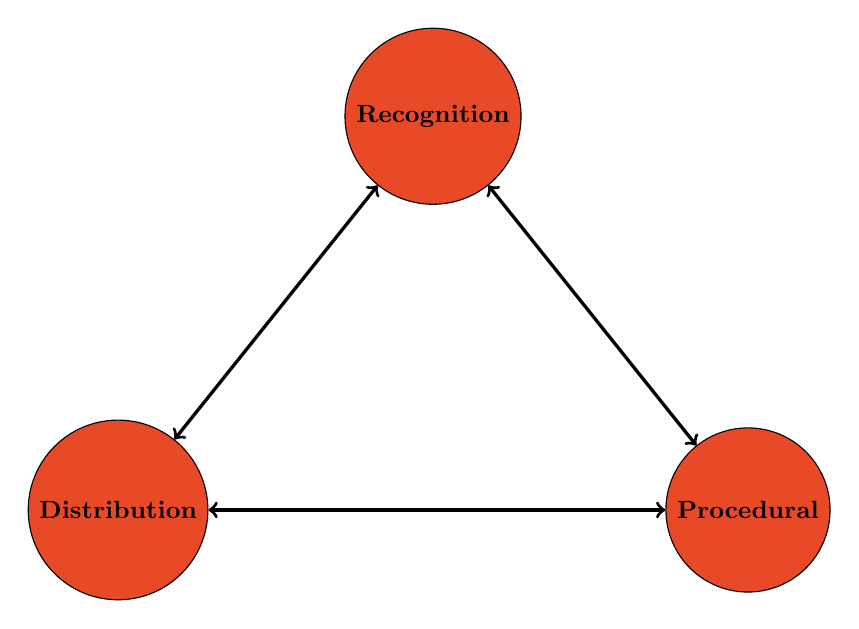
\begin{tikzpicture}[nodes={text depth=0.25ex,text height=1.25ex distance=1.7cm}]
                \tikzstyle{every node}=[font=\small]
                \tikzstyle{vertex} = [circle, draw=black, fill=trueilliniorange]
                \tikzstyle{hidden} = [draw=none]
                \tikzstyle{edge} = [<->, very thick]
                
                \node[vertex](v1) at (0,5) {\textbf{Recognition}};
                \node[vertex](v2) at (4,0) {\textbf{Procedural}};
                \node[vertex](v3) at (-4,0) {\textbf{Distribution}};
    
                \draw[edge] (v1) -- (v2);
                \draw[edge] (v2) -- (v3);
                \draw[edge] (v1) -- (v3);
    
        \end{tikzpicture}
        }
        \caption{Three aspects of justice \cite{schlosberg_1_2007}.}
        \label{fig:justice-framework}
    \end{figure}
\end{frame}


\begin{frame}
    \frametitle{Distributional}
    \begin{columns}
        \column[t]{3cm}
        \begin{figure}
            \centering
            \resizebox{0.7\columnwidth}{!}{
                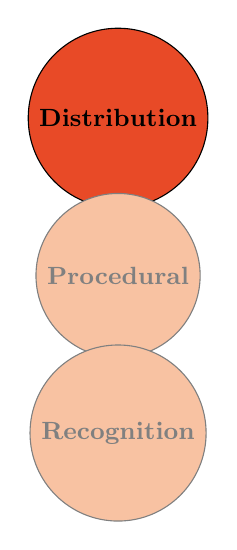
\begin{tikzpicture}[nodes={text depth=0.25ex,text height=1.25ex distance=1.7cm}]
                    \tikzstyle{every node}=[font=\small]
                    \tikzstyle{vertex} = [circle, draw=black, fill=trueilliniorange]
                    \tikzstyle{unfocus} = [circle, draw=gray, fill=illiniorange]
                    \tikzstyle{hidden} = [draw=none]
                    \tikzstyle{edge} = [<->, very thick]
                    
                    \node[vertex](v3) at (0,2) {\textcolor{black}{\textbf{Distribution}}};
                    \node[unfocus](v2) at (0,0) {\textcolor{gray}{\textbf{Procedural}}};
                    \node[unfocus](v1) at (0,-2) {\textcolor{gray}{\textbf{Recognition}}};
        
            \end{tikzpicture}}
        \end{figure}
        \column[t]{7cm}
        \begin{block}{Distributional Justice}
            Related to the distribution of burdens and benefits.
        \end{block}
        \begin{block}{Normative Question}
            What is the fairest way to distribute benefits and burdens?
        \end{block}
        \begin{block}{Examples of injustice}
            \begin{itemize}
                \item Dispossession of land and benefits \cite{yenneti_spatial_2016,sovacool_dispossessed_2021}. 
                \item Poorer air quality around fossil fuel plants --- primarily located in poorer communities \cite{mohai_which_2015}.
                \item Solar panel subsidies and installations benefitting wealthier communities \cite{reames_distributional_2020}.
            \end{itemize}
        \end{block}
    \end{columns}
    
\end{frame}

\begin{frame}
    \frametitle{Procedural}
    \begin{columns}
        \column[t]{3cm}
        \begin{figure}
            \centering
            \resizebox{0.7\columnwidth}{!}{
                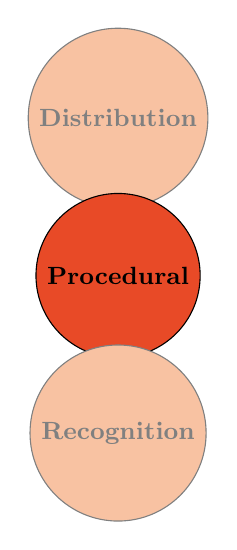
\begin{tikzpicture}[nodes={text depth=0.25ex,text height=1.25ex distance=1.7cm}]
                    \tikzstyle{every node}=[font=\small]
                    \tikzstyle{vertex} = [circle, draw=black, fill=trueilliniorange]
                    \tikzstyle{unfocus} = [circle, draw=gray, fill=illiniorange]
                    \tikzstyle{hidden} = [draw=none]
                    \tikzstyle{edge} = [<->, very thick]
                    
                    \node[unfocus](v3) at (0,2) {\textcolor{gray}{\textbf{Distribution}}};
                    \node[vertex](v2) at (0,0) {\textcolor{black}{\textbf{Procedural}}};
                    \node[unfocus](v1) at (0,-2) {\textcolor{gray}{\textbf{Recognition}}};
        
            \end{tikzpicture}}
        \end{figure}
        \column[t]{7cm}
        \begin{block}{Procedural Justice}
            Related to decision-making processes --- method and inclusion.
        \end{block}
        \begin{block}{Normative Question}
            What is the fairest way to make decisions affecting specific groups of people?
        \end{block}
        \begin{block}{Examples of injustice}
            \begin{itemize}
                \item Dismissal of testimony for its lack of technical expertise \cite{johnson_dakota_2021}. 
                \item Lack of transparency in decision making (do energy system models make this more transparent or less?).
            \end{itemize}
        \end{block}
    \end{columns}
    
\end{frame}

\begin{frame}
    \frametitle{Recognitional}
    \begin{columns}
        \column[t]{3cm}
        \begin{figure}
            \centering
            \resizebox{0.7\columnwidth}{!}{
                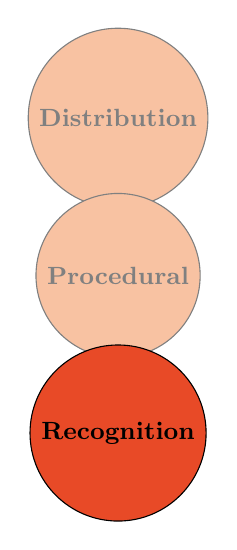
\begin{tikzpicture}[nodes={text depth=0.25ex,text height=1.25ex distance=1.7cm}]
                    \tikzstyle{every node}=[font=\small]
                    \tikzstyle{vertex} = [circle, draw=black, fill=trueilliniorange]
                    \tikzstyle{unfocus} = [circle, draw=gray, fill=illiniorange]
                    \tikzstyle{hidden} = [draw=none]
                    \tikzstyle{edge} = [<->, very thick]
                    
                    \node[unfocus](v3) at (0,2) {\textcolor{gray}{\textbf{Distribution}}};
                    \node[unfocus](v2) at (0,0) {\textcolor{gray}{\textbf{Procedural}}};
                    \node[vertex](v1) at (0,-2) {\textcolor{black}{\textbf{Recognition}}};
        
            \end{tikzpicture}}
        \end{figure}
        \column[t]{7cm}
        \begin{block}{Recognitional Justice}
            Related to social value of people or groups derived from relationships, laws, and cultural standing.
        \end{block}
        \begin{block}{Normative Question}
            How much and in what ways should a person or group of people be valued?
        \end{block}
        \begin{block}{Examples of injustice}
            \begin{itemize}
                \item Energy policies that interfere with loving relationships (e.g., stress from energy insecurity).\cite{van_uffelen_revisiting_2022}
                \item Lack of labor protections for workers.\cite{van_uffelen_revisiting_2022}
                \item Exclusion from a policy process (how inclusive is energy modeling?).\cite{van_uffelen_revisiting_2022}
            \end{itemize}
        \end{block}
    \end{columns}
    
\end{frame}

% \begin{frame}
%     \frametitle{What drives opposition? It's not NIMBY}

%     \begin{enumerate}
%         \item NIMBY is popularly understood to drive opposition.
%         \item However, several case studies and larger surveys have demonstrated
%         that this is not the case \cite{konisky_proximity_2021,aitken_why_2010}.
%         \item Instead, perceptions of legitimacy in decision-making processes
%         motivates this opposition
%         \cite{firestone_public_2012-1,stokes_prevalence_2023,
%         aitken_why_2010,walker_procedural_2017,liu_effects_2020}.
%         \item Public testimony may be dismissed for being nontechnical casting
%         doubt on legitimacy \cite{johnson_dakota_2021}.
%     \end{enumerate}

% \end{frame}

\begin{frame}
    \frametitle{How does modeling contribute to justice issues?}

    \begin{block}{Question 2}
        How does energy modeling contribute to this problem [of public opposition to energy projects]?    
    \end{block}
\end{frame}

\begin{frame}
    \frametitle{How does modeling contribute to justice issues?}

    \begin{block}{Question 2}
        How does energy modeling contribute to \st{this problem [of public opposition to energy projects]}?
        \hspace{2.5cm} violations of procedural/recognition justice?    
    \end{block}
\end{frame}


% talk about how esoms currently work
\subsection{Background: Energy system models}
\begin{frame}
    \frametitle{Energy System Optimization Models (ESOMs)}
    
    \begin{block}{Formulation}
        ESOMs consist of:
        \begin{itemize}
            \item A set of decision variables
            \item ``An economic objective'' \cite{hobbs_optimization_1995}
            \item A set of constraints
        \end{itemize}
    \end{block}
    \begin{block}{Solution method}
        Linear programming (LP) / mixed-integer linear programming (MILP)
    \end{block}

\end{frame}

\begin{frame}
    \frametitle{Simple Example Linear Program}
    
    \begin{columns}
        \column[t]{4cm}
        \begin{block}{Decision variables}
            Determine the mix of energy sources...
            \begin{align}
                \mathbf{X} = {\mathrm{x}_1, \mathrm{x}_2 \mid \mathrm{x} \in \mathbf{R}+}
            \end{align}
        \end{block}
        \begin{block}{Objective}
            ...that minimizes total cost...
            \begin{align}
                \mathrm{min}\left(\mathrm{c}_1\mathrm{x}_1 + \mathrm{c}_2\mathrm{x}_2\right)
            \end{align}
        \end{block}
        \begin{block}{Constraint}
            ...such that energy demand is always met.
            \begin{align}
                \mathrm{x}_1 + \mathrm{x}_2 = 1
            \end{align}
        \end{block}
        \column[t]{6cm}
        \begin{figure}
            \centering
            \resizebox{\columnwidth}{!}{%% Creator: Matplotlib, PGF backend
%%
%% To include the figure in your LaTeX document, write
%%   \input{<filename>.pgf}
%%
%% Make sure the required packages are loaded in your preamble
%%   \usepackage{pgf}
%%
%% Also ensure that all the required font packages are loaded; for instance,
%% the lmodern package is sometimes necessary when using math font.
%%   \usepackage{lmodern}
%%
%% Figures using additional raster images can only be included by \input if
%% they are in the same directory as the main LaTeX file. For loading figures
%% from other directories you can use the `import` package
%%   \usepackage{import}
%%
%% and then include the figures with
%%   \import{<path to file>}{<filename>.pgf}
%%
%% Matplotlib used the following preamble
%%   \def\mathdefault#1{#1}
%%   \everymath=\expandafter{\the\everymath\displaystyle}
%%   
%%   \makeatletter\@ifpackageloaded{underscore}{}{\usepackage[strings]{underscore}}\makeatother
%%
\begingroup%
\makeatletter%
\begin{pgfpicture}%
\pgfpathrectangle{\pgfpointorigin}{\pgfqpoint{7.900000in}{5.930000in}}%
\pgfusepath{use as bounding box, clip}%
\begin{pgfscope}%
\pgfsetbuttcap%
\pgfsetmiterjoin%
\definecolor{currentfill}{rgb}{0.827451,0.827451,0.827451}%
\pgfsetfillcolor{currentfill}%
\pgfsetlinewidth{0.000000pt}%
\definecolor{currentstroke}{rgb}{0.000000,0.000000,0.000000}%
\pgfsetstrokecolor{currentstroke}%
\pgfsetdash{}{0pt}%
\pgfpathmoveto{\pgfqpoint{0.000000in}{0.000000in}}%
\pgfpathlineto{\pgfqpoint{7.900000in}{0.000000in}}%
\pgfpathlineto{\pgfqpoint{7.900000in}{5.930000in}}%
\pgfpathlineto{\pgfqpoint{0.000000in}{5.930000in}}%
\pgfpathlineto{\pgfqpoint{0.000000in}{0.000000in}}%
\pgfpathclose%
\pgfusepath{fill}%
\end{pgfscope}%
\begin{pgfscope}%
\pgfsetbuttcap%
\pgfsetmiterjoin%
\definecolor{currentfill}{rgb}{1.000000,1.000000,1.000000}%
\pgfsetfillcolor{currentfill}%
\pgfsetlinewidth{0.000000pt}%
\definecolor{currentstroke}{rgb}{0.000000,0.000000,0.000000}%
\pgfsetstrokecolor{currentstroke}%
\pgfsetstrokeopacity{0.000000}%
\pgfsetdash{}{0pt}%
\pgfpathmoveto{\pgfqpoint{0.759074in}{0.686623in}}%
\pgfpathlineto{\pgfqpoint{7.800000in}{0.686623in}}%
\pgfpathlineto{\pgfqpoint{7.800000in}{5.059445in}}%
\pgfpathlineto{\pgfqpoint{0.759074in}{5.059445in}}%
\pgfpathlineto{\pgfqpoint{0.759074in}{0.686623in}}%
\pgfpathclose%
\pgfusepath{fill}%
\end{pgfscope}%
\begin{pgfscope}%
\pgfpathrectangle{\pgfqpoint{0.759074in}{0.686623in}}{\pgfqpoint{7.040926in}{4.372823in}}%
\pgfusepath{clip}%
\pgfsetbuttcap%
\pgfsetroundjoin%
\definecolor{currentfill}{rgb}{1.000000,1.000000,1.000000}%
\pgfsetfillcolor{currentfill}%
\pgfsetlinewidth{1.003750pt}%
\definecolor{currentstroke}{rgb}{0.000000,0.000000,0.000000}%
\pgfsetstrokecolor{currentstroke}%
\pgfsetdash{}{0pt}%
\pgfsys@defobject{currentmarker}{\pgfqpoint{-0.065881in}{-0.065881in}}{\pgfqpoint{0.065881in}{0.065881in}}{%
\pgfpathmoveto{\pgfqpoint{0.000000in}{-0.065881in}}%
\pgfpathcurveto{\pgfqpoint{0.017472in}{-0.065881in}}{\pgfqpoint{0.034230in}{-0.058939in}}{\pgfqpoint{0.046585in}{-0.046585in}}%
\pgfpathcurveto{\pgfqpoint{0.058939in}{-0.034230in}}{\pgfqpoint{0.065881in}{-0.017472in}}{\pgfqpoint{0.065881in}{0.000000in}}%
\pgfpathcurveto{\pgfqpoint{0.065881in}{0.017472in}}{\pgfqpoint{0.058939in}{0.034230in}}{\pgfqpoint{0.046585in}{0.046585in}}%
\pgfpathcurveto{\pgfqpoint{0.034230in}{0.058939in}}{\pgfqpoint{0.017472in}{0.065881in}}{\pgfqpoint{0.000000in}{0.065881in}}%
\pgfpathcurveto{\pgfqpoint{-0.017472in}{0.065881in}}{\pgfqpoint{-0.034230in}{0.058939in}}{\pgfqpoint{-0.046585in}{0.046585in}}%
\pgfpathcurveto{\pgfqpoint{-0.058939in}{0.034230in}}{\pgfqpoint{-0.065881in}{0.017472in}}{\pgfqpoint{-0.065881in}{0.000000in}}%
\pgfpathcurveto{\pgfqpoint{-0.065881in}{-0.017472in}}{\pgfqpoint{-0.058939in}{-0.034230in}}{\pgfqpoint{-0.046585in}{-0.046585in}}%
\pgfpathcurveto{\pgfqpoint{-0.034230in}{-0.058939in}}{\pgfqpoint{-0.017472in}{-0.065881in}}{\pgfqpoint{0.000000in}{-0.065881in}}%
\pgfpathlineto{\pgfqpoint{0.000000in}{-0.065881in}}%
\pgfpathclose%
\pgfusepath{stroke,fill}%
}%
\begin{pgfscope}%
\pgfsys@transformshift{7.159916in}{0.686623in}%
\pgfsys@useobject{currentmarker}{}%
\end{pgfscope}%
\end{pgfscope}%
\begin{pgfscope}%
\pgfpathrectangle{\pgfqpoint{0.759074in}{0.686623in}}{\pgfqpoint{7.040926in}{4.372823in}}%
\pgfusepath{clip}%
\pgfsetrectcap%
\pgfsetroundjoin%
\pgfsetlinewidth{0.803000pt}%
\definecolor{currentstroke}{rgb}{0.501961,0.501961,0.501961}%
\pgfsetstrokecolor{currentstroke}%
\pgfsetstrokeopacity{0.300000}%
\pgfsetdash{}{0pt}%
\pgfpathmoveto{\pgfqpoint{0.759074in}{0.686623in}}%
\pgfpathlineto{\pgfqpoint{0.759074in}{5.059445in}}%
\pgfusepath{stroke}%
\end{pgfscope}%
\begin{pgfscope}%
\pgfsetbuttcap%
\pgfsetroundjoin%
\definecolor{currentfill}{rgb}{0.000000,0.000000,0.000000}%
\pgfsetfillcolor{currentfill}%
\pgfsetlinewidth{0.803000pt}%
\definecolor{currentstroke}{rgb}{0.000000,0.000000,0.000000}%
\pgfsetstrokecolor{currentstroke}%
\pgfsetdash{}{0pt}%
\pgfsys@defobject{currentmarker}{\pgfqpoint{0.000000in}{-0.048611in}}{\pgfqpoint{0.000000in}{0.000000in}}{%
\pgfpathmoveto{\pgfqpoint{0.000000in}{0.000000in}}%
\pgfpathlineto{\pgfqpoint{0.000000in}{-0.048611in}}%
\pgfusepath{stroke,fill}%
}%
\begin{pgfscope}%
\pgfsys@transformshift{0.759074in}{0.686623in}%
\pgfsys@useobject{currentmarker}{}%
\end{pgfscope}%
\end{pgfscope}%
\begin{pgfscope}%
\definecolor{textcolor}{rgb}{0.000000,0.000000,0.000000}%
\pgfsetstrokecolor{textcolor}%
\pgfsetfillcolor{textcolor}%
\pgftext[x=0.759074in,y=0.589401in,,top]{\color{textcolor}{\rmfamily\fontsize{14.000000}{16.800000}\selectfont\catcode`\^=\active\def^{\ifmmode\sp\else\^{}\fi}\catcode`\%=\active\def%{\%}$\mathdefault{0.0}$}}%
\end{pgfscope}%
\begin{pgfscope}%
\pgfpathrectangle{\pgfqpoint{0.759074in}{0.686623in}}{\pgfqpoint{7.040926in}{4.372823in}}%
\pgfusepath{clip}%
\pgfsetrectcap%
\pgfsetroundjoin%
\pgfsetlinewidth{0.803000pt}%
\definecolor{currentstroke}{rgb}{0.501961,0.501961,0.501961}%
\pgfsetstrokecolor{currentstroke}%
\pgfsetstrokeopacity{0.300000}%
\pgfsetdash{}{0pt}%
\pgfpathmoveto{\pgfqpoint{2.039242in}{0.686623in}}%
\pgfpathlineto{\pgfqpoint{2.039242in}{5.059445in}}%
\pgfusepath{stroke}%
\end{pgfscope}%
\begin{pgfscope}%
\pgfsetbuttcap%
\pgfsetroundjoin%
\definecolor{currentfill}{rgb}{0.000000,0.000000,0.000000}%
\pgfsetfillcolor{currentfill}%
\pgfsetlinewidth{0.803000pt}%
\definecolor{currentstroke}{rgb}{0.000000,0.000000,0.000000}%
\pgfsetstrokecolor{currentstroke}%
\pgfsetdash{}{0pt}%
\pgfsys@defobject{currentmarker}{\pgfqpoint{0.000000in}{-0.048611in}}{\pgfqpoint{0.000000in}{0.000000in}}{%
\pgfpathmoveto{\pgfqpoint{0.000000in}{0.000000in}}%
\pgfpathlineto{\pgfqpoint{0.000000in}{-0.048611in}}%
\pgfusepath{stroke,fill}%
}%
\begin{pgfscope}%
\pgfsys@transformshift{2.039242in}{0.686623in}%
\pgfsys@useobject{currentmarker}{}%
\end{pgfscope}%
\end{pgfscope}%
\begin{pgfscope}%
\definecolor{textcolor}{rgb}{0.000000,0.000000,0.000000}%
\pgfsetstrokecolor{textcolor}%
\pgfsetfillcolor{textcolor}%
\pgftext[x=2.039242in,y=0.589401in,,top]{\color{textcolor}{\rmfamily\fontsize{14.000000}{16.800000}\selectfont\catcode`\^=\active\def^{\ifmmode\sp\else\^{}\fi}\catcode`\%=\active\def%{\%}$\mathdefault{0.2}$}}%
\end{pgfscope}%
\begin{pgfscope}%
\pgfpathrectangle{\pgfqpoint{0.759074in}{0.686623in}}{\pgfqpoint{7.040926in}{4.372823in}}%
\pgfusepath{clip}%
\pgfsetrectcap%
\pgfsetroundjoin%
\pgfsetlinewidth{0.803000pt}%
\definecolor{currentstroke}{rgb}{0.501961,0.501961,0.501961}%
\pgfsetstrokecolor{currentstroke}%
\pgfsetstrokeopacity{0.300000}%
\pgfsetdash{}{0pt}%
\pgfpathmoveto{\pgfqpoint{3.319410in}{0.686623in}}%
\pgfpathlineto{\pgfqpoint{3.319410in}{5.059445in}}%
\pgfusepath{stroke}%
\end{pgfscope}%
\begin{pgfscope}%
\pgfsetbuttcap%
\pgfsetroundjoin%
\definecolor{currentfill}{rgb}{0.000000,0.000000,0.000000}%
\pgfsetfillcolor{currentfill}%
\pgfsetlinewidth{0.803000pt}%
\definecolor{currentstroke}{rgb}{0.000000,0.000000,0.000000}%
\pgfsetstrokecolor{currentstroke}%
\pgfsetdash{}{0pt}%
\pgfsys@defobject{currentmarker}{\pgfqpoint{0.000000in}{-0.048611in}}{\pgfqpoint{0.000000in}{0.000000in}}{%
\pgfpathmoveto{\pgfqpoint{0.000000in}{0.000000in}}%
\pgfpathlineto{\pgfqpoint{0.000000in}{-0.048611in}}%
\pgfusepath{stroke,fill}%
}%
\begin{pgfscope}%
\pgfsys@transformshift{3.319410in}{0.686623in}%
\pgfsys@useobject{currentmarker}{}%
\end{pgfscope}%
\end{pgfscope}%
\begin{pgfscope}%
\definecolor{textcolor}{rgb}{0.000000,0.000000,0.000000}%
\pgfsetstrokecolor{textcolor}%
\pgfsetfillcolor{textcolor}%
\pgftext[x=3.319410in,y=0.589401in,,top]{\color{textcolor}{\rmfamily\fontsize{14.000000}{16.800000}\selectfont\catcode`\^=\active\def^{\ifmmode\sp\else\^{}\fi}\catcode`\%=\active\def%{\%}$\mathdefault{0.4}$}}%
\end{pgfscope}%
\begin{pgfscope}%
\pgfpathrectangle{\pgfqpoint{0.759074in}{0.686623in}}{\pgfqpoint{7.040926in}{4.372823in}}%
\pgfusepath{clip}%
\pgfsetrectcap%
\pgfsetroundjoin%
\pgfsetlinewidth{0.803000pt}%
\definecolor{currentstroke}{rgb}{0.501961,0.501961,0.501961}%
\pgfsetstrokecolor{currentstroke}%
\pgfsetstrokeopacity{0.300000}%
\pgfsetdash{}{0pt}%
\pgfpathmoveto{\pgfqpoint{4.599579in}{0.686623in}}%
\pgfpathlineto{\pgfqpoint{4.599579in}{5.059445in}}%
\pgfusepath{stroke}%
\end{pgfscope}%
\begin{pgfscope}%
\pgfsetbuttcap%
\pgfsetroundjoin%
\definecolor{currentfill}{rgb}{0.000000,0.000000,0.000000}%
\pgfsetfillcolor{currentfill}%
\pgfsetlinewidth{0.803000pt}%
\definecolor{currentstroke}{rgb}{0.000000,0.000000,0.000000}%
\pgfsetstrokecolor{currentstroke}%
\pgfsetdash{}{0pt}%
\pgfsys@defobject{currentmarker}{\pgfqpoint{0.000000in}{-0.048611in}}{\pgfqpoint{0.000000in}{0.000000in}}{%
\pgfpathmoveto{\pgfqpoint{0.000000in}{0.000000in}}%
\pgfpathlineto{\pgfqpoint{0.000000in}{-0.048611in}}%
\pgfusepath{stroke,fill}%
}%
\begin{pgfscope}%
\pgfsys@transformshift{4.599579in}{0.686623in}%
\pgfsys@useobject{currentmarker}{}%
\end{pgfscope}%
\end{pgfscope}%
\begin{pgfscope}%
\definecolor{textcolor}{rgb}{0.000000,0.000000,0.000000}%
\pgfsetstrokecolor{textcolor}%
\pgfsetfillcolor{textcolor}%
\pgftext[x=4.599579in,y=0.589401in,,top]{\color{textcolor}{\rmfamily\fontsize{14.000000}{16.800000}\selectfont\catcode`\^=\active\def^{\ifmmode\sp\else\^{}\fi}\catcode`\%=\active\def%{\%}$\mathdefault{0.6}$}}%
\end{pgfscope}%
\begin{pgfscope}%
\pgfpathrectangle{\pgfqpoint{0.759074in}{0.686623in}}{\pgfqpoint{7.040926in}{4.372823in}}%
\pgfusepath{clip}%
\pgfsetrectcap%
\pgfsetroundjoin%
\pgfsetlinewidth{0.803000pt}%
\definecolor{currentstroke}{rgb}{0.501961,0.501961,0.501961}%
\pgfsetstrokecolor{currentstroke}%
\pgfsetstrokeopacity{0.300000}%
\pgfsetdash{}{0pt}%
\pgfpathmoveto{\pgfqpoint{5.879747in}{0.686623in}}%
\pgfpathlineto{\pgfqpoint{5.879747in}{5.059445in}}%
\pgfusepath{stroke}%
\end{pgfscope}%
\begin{pgfscope}%
\pgfsetbuttcap%
\pgfsetroundjoin%
\definecolor{currentfill}{rgb}{0.000000,0.000000,0.000000}%
\pgfsetfillcolor{currentfill}%
\pgfsetlinewidth{0.803000pt}%
\definecolor{currentstroke}{rgb}{0.000000,0.000000,0.000000}%
\pgfsetstrokecolor{currentstroke}%
\pgfsetdash{}{0pt}%
\pgfsys@defobject{currentmarker}{\pgfqpoint{0.000000in}{-0.048611in}}{\pgfqpoint{0.000000in}{0.000000in}}{%
\pgfpathmoveto{\pgfqpoint{0.000000in}{0.000000in}}%
\pgfpathlineto{\pgfqpoint{0.000000in}{-0.048611in}}%
\pgfusepath{stroke,fill}%
}%
\begin{pgfscope}%
\pgfsys@transformshift{5.879747in}{0.686623in}%
\pgfsys@useobject{currentmarker}{}%
\end{pgfscope}%
\end{pgfscope}%
\begin{pgfscope}%
\definecolor{textcolor}{rgb}{0.000000,0.000000,0.000000}%
\pgfsetstrokecolor{textcolor}%
\pgfsetfillcolor{textcolor}%
\pgftext[x=5.879747in,y=0.589401in,,top]{\color{textcolor}{\rmfamily\fontsize{14.000000}{16.800000}\selectfont\catcode`\^=\active\def^{\ifmmode\sp\else\^{}\fi}\catcode`\%=\active\def%{\%}$\mathdefault{0.8}$}}%
\end{pgfscope}%
\begin{pgfscope}%
\pgfpathrectangle{\pgfqpoint{0.759074in}{0.686623in}}{\pgfqpoint{7.040926in}{4.372823in}}%
\pgfusepath{clip}%
\pgfsetrectcap%
\pgfsetroundjoin%
\pgfsetlinewidth{0.803000pt}%
\definecolor{currentstroke}{rgb}{0.501961,0.501961,0.501961}%
\pgfsetstrokecolor{currentstroke}%
\pgfsetstrokeopacity{0.300000}%
\pgfsetdash{}{0pt}%
\pgfpathmoveto{\pgfqpoint{7.159916in}{0.686623in}}%
\pgfpathlineto{\pgfqpoint{7.159916in}{5.059445in}}%
\pgfusepath{stroke}%
\end{pgfscope}%
\begin{pgfscope}%
\pgfsetbuttcap%
\pgfsetroundjoin%
\definecolor{currentfill}{rgb}{0.000000,0.000000,0.000000}%
\pgfsetfillcolor{currentfill}%
\pgfsetlinewidth{0.803000pt}%
\definecolor{currentstroke}{rgb}{0.000000,0.000000,0.000000}%
\pgfsetstrokecolor{currentstroke}%
\pgfsetdash{}{0pt}%
\pgfsys@defobject{currentmarker}{\pgfqpoint{0.000000in}{-0.048611in}}{\pgfqpoint{0.000000in}{0.000000in}}{%
\pgfpathmoveto{\pgfqpoint{0.000000in}{0.000000in}}%
\pgfpathlineto{\pgfqpoint{0.000000in}{-0.048611in}}%
\pgfusepath{stroke,fill}%
}%
\begin{pgfscope}%
\pgfsys@transformshift{7.159916in}{0.686623in}%
\pgfsys@useobject{currentmarker}{}%
\end{pgfscope}%
\end{pgfscope}%
\begin{pgfscope}%
\definecolor{textcolor}{rgb}{0.000000,0.000000,0.000000}%
\pgfsetstrokecolor{textcolor}%
\pgfsetfillcolor{textcolor}%
\pgftext[x=7.159916in,y=0.589401in,,top]{\color{textcolor}{\rmfamily\fontsize{14.000000}{16.800000}\selectfont\catcode`\^=\active\def^{\ifmmode\sp\else\^{}\fi}\catcode`\%=\active\def%{\%}$\mathdefault{1.0}$}}%
\end{pgfscope}%
\begin{pgfscope}%
\definecolor{textcolor}{rgb}{0.000000,0.000000,0.000000}%
\pgfsetstrokecolor{textcolor}%
\pgfsetfillcolor{textcolor}%
\pgftext[x=4.279537in,y=0.356068in,,top]{\color{textcolor}{\rmfamily\fontsize{20.000000}{24.000000}\selectfont\catcode`\^=\active\def^{\ifmmode\sp\else\^{}\fi}\catcode`\%=\active\def%{\%}x$_1$}}%
\end{pgfscope}%
\begin{pgfscope}%
\pgfpathrectangle{\pgfqpoint{0.759074in}{0.686623in}}{\pgfqpoint{7.040926in}{4.372823in}}%
\pgfusepath{clip}%
\pgfsetrectcap%
\pgfsetroundjoin%
\pgfsetlinewidth{0.803000pt}%
\definecolor{currentstroke}{rgb}{0.501961,0.501961,0.501961}%
\pgfsetstrokecolor{currentstroke}%
\pgfsetstrokeopacity{0.300000}%
\pgfsetdash{}{0pt}%
\pgfpathmoveto{\pgfqpoint{0.759074in}{0.686623in}}%
\pgfpathlineto{\pgfqpoint{7.800000in}{0.686623in}}%
\pgfusepath{stroke}%
\end{pgfscope}%
\begin{pgfscope}%
\pgfsetbuttcap%
\pgfsetroundjoin%
\definecolor{currentfill}{rgb}{0.000000,0.000000,0.000000}%
\pgfsetfillcolor{currentfill}%
\pgfsetlinewidth{0.803000pt}%
\definecolor{currentstroke}{rgb}{0.000000,0.000000,0.000000}%
\pgfsetstrokecolor{currentstroke}%
\pgfsetdash{}{0pt}%
\pgfsys@defobject{currentmarker}{\pgfqpoint{-0.048611in}{0.000000in}}{\pgfqpoint{-0.000000in}{0.000000in}}{%
\pgfpathmoveto{\pgfqpoint{-0.000000in}{0.000000in}}%
\pgfpathlineto{\pgfqpoint{-0.048611in}{0.000000in}}%
\pgfusepath{stroke,fill}%
}%
\begin{pgfscope}%
\pgfsys@transformshift{0.759074in}{0.686623in}%
\pgfsys@useobject{currentmarker}{}%
\end{pgfscope}%
\end{pgfscope}%
\begin{pgfscope}%
\definecolor{textcolor}{rgb}{0.000000,0.000000,0.000000}%
\pgfsetstrokecolor{textcolor}%
\pgfsetfillcolor{textcolor}%
\pgftext[x=0.411623in, y=0.617178in, left, base]{\color{textcolor}{\rmfamily\fontsize{14.000000}{16.800000}\selectfont\catcode`\^=\active\def^{\ifmmode\sp\else\^{}\fi}\catcode`\%=\active\def%{\%}$\mathdefault{0.0}$}}%
\end{pgfscope}%
\begin{pgfscope}%
\pgfpathrectangle{\pgfqpoint{0.759074in}{0.686623in}}{\pgfqpoint{7.040926in}{4.372823in}}%
\pgfusepath{clip}%
\pgfsetrectcap%
\pgfsetroundjoin%
\pgfsetlinewidth{0.803000pt}%
\definecolor{currentstroke}{rgb}{0.501961,0.501961,0.501961}%
\pgfsetstrokecolor{currentstroke}%
\pgfsetstrokeopacity{0.300000}%
\pgfsetdash{}{0pt}%
\pgfpathmoveto{\pgfqpoint{0.759074in}{1.481681in}}%
\pgfpathlineto{\pgfqpoint{7.800000in}{1.481681in}}%
\pgfusepath{stroke}%
\end{pgfscope}%
\begin{pgfscope}%
\pgfsetbuttcap%
\pgfsetroundjoin%
\definecolor{currentfill}{rgb}{0.000000,0.000000,0.000000}%
\pgfsetfillcolor{currentfill}%
\pgfsetlinewidth{0.803000pt}%
\definecolor{currentstroke}{rgb}{0.000000,0.000000,0.000000}%
\pgfsetstrokecolor{currentstroke}%
\pgfsetdash{}{0pt}%
\pgfsys@defobject{currentmarker}{\pgfqpoint{-0.048611in}{0.000000in}}{\pgfqpoint{-0.000000in}{0.000000in}}{%
\pgfpathmoveto{\pgfqpoint{-0.000000in}{0.000000in}}%
\pgfpathlineto{\pgfqpoint{-0.048611in}{0.000000in}}%
\pgfusepath{stroke,fill}%
}%
\begin{pgfscope}%
\pgfsys@transformshift{0.759074in}{1.481681in}%
\pgfsys@useobject{currentmarker}{}%
\end{pgfscope}%
\end{pgfscope}%
\begin{pgfscope}%
\definecolor{textcolor}{rgb}{0.000000,0.000000,0.000000}%
\pgfsetstrokecolor{textcolor}%
\pgfsetfillcolor{textcolor}%
\pgftext[x=0.411623in, y=1.412237in, left, base]{\color{textcolor}{\rmfamily\fontsize{14.000000}{16.800000}\selectfont\catcode`\^=\active\def^{\ifmmode\sp\else\^{}\fi}\catcode`\%=\active\def%{\%}$\mathdefault{0.2}$}}%
\end{pgfscope}%
\begin{pgfscope}%
\pgfpathrectangle{\pgfqpoint{0.759074in}{0.686623in}}{\pgfqpoint{7.040926in}{4.372823in}}%
\pgfusepath{clip}%
\pgfsetrectcap%
\pgfsetroundjoin%
\pgfsetlinewidth{0.803000pt}%
\definecolor{currentstroke}{rgb}{0.501961,0.501961,0.501961}%
\pgfsetstrokecolor{currentstroke}%
\pgfsetstrokeopacity{0.300000}%
\pgfsetdash{}{0pt}%
\pgfpathmoveto{\pgfqpoint{0.759074in}{2.276740in}}%
\pgfpathlineto{\pgfqpoint{7.800000in}{2.276740in}}%
\pgfusepath{stroke}%
\end{pgfscope}%
\begin{pgfscope}%
\pgfsetbuttcap%
\pgfsetroundjoin%
\definecolor{currentfill}{rgb}{0.000000,0.000000,0.000000}%
\pgfsetfillcolor{currentfill}%
\pgfsetlinewidth{0.803000pt}%
\definecolor{currentstroke}{rgb}{0.000000,0.000000,0.000000}%
\pgfsetstrokecolor{currentstroke}%
\pgfsetdash{}{0pt}%
\pgfsys@defobject{currentmarker}{\pgfqpoint{-0.048611in}{0.000000in}}{\pgfqpoint{-0.000000in}{0.000000in}}{%
\pgfpathmoveto{\pgfqpoint{-0.000000in}{0.000000in}}%
\pgfpathlineto{\pgfqpoint{-0.048611in}{0.000000in}}%
\pgfusepath{stroke,fill}%
}%
\begin{pgfscope}%
\pgfsys@transformshift{0.759074in}{2.276740in}%
\pgfsys@useobject{currentmarker}{}%
\end{pgfscope}%
\end{pgfscope}%
\begin{pgfscope}%
\definecolor{textcolor}{rgb}{0.000000,0.000000,0.000000}%
\pgfsetstrokecolor{textcolor}%
\pgfsetfillcolor{textcolor}%
\pgftext[x=0.411623in, y=2.207296in, left, base]{\color{textcolor}{\rmfamily\fontsize{14.000000}{16.800000}\selectfont\catcode`\^=\active\def^{\ifmmode\sp\else\^{}\fi}\catcode`\%=\active\def%{\%}$\mathdefault{0.4}$}}%
\end{pgfscope}%
\begin{pgfscope}%
\pgfpathrectangle{\pgfqpoint{0.759074in}{0.686623in}}{\pgfqpoint{7.040926in}{4.372823in}}%
\pgfusepath{clip}%
\pgfsetrectcap%
\pgfsetroundjoin%
\pgfsetlinewidth{0.803000pt}%
\definecolor{currentstroke}{rgb}{0.501961,0.501961,0.501961}%
\pgfsetstrokecolor{currentstroke}%
\pgfsetstrokeopacity{0.300000}%
\pgfsetdash{}{0pt}%
\pgfpathmoveto{\pgfqpoint{0.759074in}{3.071799in}}%
\pgfpathlineto{\pgfqpoint{7.800000in}{3.071799in}}%
\pgfusepath{stroke}%
\end{pgfscope}%
\begin{pgfscope}%
\pgfsetbuttcap%
\pgfsetroundjoin%
\definecolor{currentfill}{rgb}{0.000000,0.000000,0.000000}%
\pgfsetfillcolor{currentfill}%
\pgfsetlinewidth{0.803000pt}%
\definecolor{currentstroke}{rgb}{0.000000,0.000000,0.000000}%
\pgfsetstrokecolor{currentstroke}%
\pgfsetdash{}{0pt}%
\pgfsys@defobject{currentmarker}{\pgfqpoint{-0.048611in}{0.000000in}}{\pgfqpoint{-0.000000in}{0.000000in}}{%
\pgfpathmoveto{\pgfqpoint{-0.000000in}{0.000000in}}%
\pgfpathlineto{\pgfqpoint{-0.048611in}{0.000000in}}%
\pgfusepath{stroke,fill}%
}%
\begin{pgfscope}%
\pgfsys@transformshift{0.759074in}{3.071799in}%
\pgfsys@useobject{currentmarker}{}%
\end{pgfscope}%
\end{pgfscope}%
\begin{pgfscope}%
\definecolor{textcolor}{rgb}{0.000000,0.000000,0.000000}%
\pgfsetstrokecolor{textcolor}%
\pgfsetfillcolor{textcolor}%
\pgftext[x=0.411623in, y=3.002354in, left, base]{\color{textcolor}{\rmfamily\fontsize{14.000000}{16.800000}\selectfont\catcode`\^=\active\def^{\ifmmode\sp\else\^{}\fi}\catcode`\%=\active\def%{\%}$\mathdefault{0.6}$}}%
\end{pgfscope}%
\begin{pgfscope}%
\pgfpathrectangle{\pgfqpoint{0.759074in}{0.686623in}}{\pgfqpoint{7.040926in}{4.372823in}}%
\pgfusepath{clip}%
\pgfsetrectcap%
\pgfsetroundjoin%
\pgfsetlinewidth{0.803000pt}%
\definecolor{currentstroke}{rgb}{0.501961,0.501961,0.501961}%
\pgfsetstrokecolor{currentstroke}%
\pgfsetstrokeopacity{0.300000}%
\pgfsetdash{}{0pt}%
\pgfpathmoveto{\pgfqpoint{0.759074in}{3.866857in}}%
\pgfpathlineto{\pgfqpoint{7.800000in}{3.866857in}}%
\pgfusepath{stroke}%
\end{pgfscope}%
\begin{pgfscope}%
\pgfsetbuttcap%
\pgfsetroundjoin%
\definecolor{currentfill}{rgb}{0.000000,0.000000,0.000000}%
\pgfsetfillcolor{currentfill}%
\pgfsetlinewidth{0.803000pt}%
\definecolor{currentstroke}{rgb}{0.000000,0.000000,0.000000}%
\pgfsetstrokecolor{currentstroke}%
\pgfsetdash{}{0pt}%
\pgfsys@defobject{currentmarker}{\pgfqpoint{-0.048611in}{0.000000in}}{\pgfqpoint{-0.000000in}{0.000000in}}{%
\pgfpathmoveto{\pgfqpoint{-0.000000in}{0.000000in}}%
\pgfpathlineto{\pgfqpoint{-0.048611in}{0.000000in}}%
\pgfusepath{stroke,fill}%
}%
\begin{pgfscope}%
\pgfsys@transformshift{0.759074in}{3.866857in}%
\pgfsys@useobject{currentmarker}{}%
\end{pgfscope}%
\end{pgfscope}%
\begin{pgfscope}%
\definecolor{textcolor}{rgb}{0.000000,0.000000,0.000000}%
\pgfsetstrokecolor{textcolor}%
\pgfsetfillcolor{textcolor}%
\pgftext[x=0.411623in, y=3.797413in, left, base]{\color{textcolor}{\rmfamily\fontsize{14.000000}{16.800000}\selectfont\catcode`\^=\active\def^{\ifmmode\sp\else\^{}\fi}\catcode`\%=\active\def%{\%}$\mathdefault{0.8}$}}%
\end{pgfscope}%
\begin{pgfscope}%
\pgfpathrectangle{\pgfqpoint{0.759074in}{0.686623in}}{\pgfqpoint{7.040926in}{4.372823in}}%
\pgfusepath{clip}%
\pgfsetrectcap%
\pgfsetroundjoin%
\pgfsetlinewidth{0.803000pt}%
\definecolor{currentstroke}{rgb}{0.501961,0.501961,0.501961}%
\pgfsetstrokecolor{currentstroke}%
\pgfsetstrokeopacity{0.300000}%
\pgfsetdash{}{0pt}%
\pgfpathmoveto{\pgfqpoint{0.759074in}{4.661916in}}%
\pgfpathlineto{\pgfqpoint{7.800000in}{4.661916in}}%
\pgfusepath{stroke}%
\end{pgfscope}%
\begin{pgfscope}%
\pgfsetbuttcap%
\pgfsetroundjoin%
\definecolor{currentfill}{rgb}{0.000000,0.000000,0.000000}%
\pgfsetfillcolor{currentfill}%
\pgfsetlinewidth{0.803000pt}%
\definecolor{currentstroke}{rgb}{0.000000,0.000000,0.000000}%
\pgfsetstrokecolor{currentstroke}%
\pgfsetdash{}{0pt}%
\pgfsys@defobject{currentmarker}{\pgfqpoint{-0.048611in}{0.000000in}}{\pgfqpoint{-0.000000in}{0.000000in}}{%
\pgfpathmoveto{\pgfqpoint{-0.000000in}{0.000000in}}%
\pgfpathlineto{\pgfqpoint{-0.048611in}{0.000000in}}%
\pgfusepath{stroke,fill}%
}%
\begin{pgfscope}%
\pgfsys@transformshift{0.759074in}{4.661916in}%
\pgfsys@useobject{currentmarker}{}%
\end{pgfscope}%
\end{pgfscope}%
\begin{pgfscope}%
\definecolor{textcolor}{rgb}{0.000000,0.000000,0.000000}%
\pgfsetstrokecolor{textcolor}%
\pgfsetfillcolor{textcolor}%
\pgftext[x=0.411623in, y=4.592472in, left, base]{\color{textcolor}{\rmfamily\fontsize{14.000000}{16.800000}\selectfont\catcode`\^=\active\def^{\ifmmode\sp\else\^{}\fi}\catcode`\%=\active\def%{\%}$\mathdefault{1.0}$}}%
\end{pgfscope}%
\begin{pgfscope}%
\definecolor{textcolor}{rgb}{0.000000,0.000000,0.000000}%
\pgfsetstrokecolor{textcolor}%
\pgfsetfillcolor{textcolor}%
\pgftext[x=0.356068in,y=2.873034in,,bottom,rotate=90.000000]{\color{textcolor}{\rmfamily\fontsize{20.000000}{24.000000}\selectfont\catcode`\^=\active\def^{\ifmmode\sp\else\^{}\fi}\catcode`\%=\active\def%{\%}x$_2$}}%
\end{pgfscope}%
\begin{pgfscope}%
\pgfpathrectangle{\pgfqpoint{0.759074in}{0.686623in}}{\pgfqpoint{7.040926in}{4.372823in}}%
\pgfusepath{clip}%
\pgfsetrectcap%
\pgfsetroundjoin%
\pgfsetlinewidth{1.505625pt}%
\definecolor{currentstroke}{rgb}{0.000000,0.000000,0.000000}%
\pgfsetstrokecolor{currentstroke}%
\pgfsetdash{}{0pt}%
\pgfpathmoveto{\pgfqpoint{7.159916in}{0.686623in}}%
\pgfpathlineto{\pgfqpoint{0.759074in}{4.661916in}}%
\pgfusepath{stroke}%
\end{pgfscope}%
\begin{pgfscope}%
\pgfpathrectangle{\pgfqpoint{0.759074in}{0.686623in}}{\pgfqpoint{7.040926in}{4.372823in}}%
\pgfusepath{clip}%
\pgfsetrectcap%
\pgfsetroundjoin%
\pgfsetlinewidth{1.505625pt}%
\definecolor{currentstroke}{rgb}{0.501961,0.501961,0.501961}%
\pgfsetstrokecolor{currentstroke}%
\pgfsetdash{}{0pt}%
\pgfpathmoveto{\pgfqpoint{7.159916in}{0.686623in}}%
\pgfpathlineto{\pgfqpoint{0.759074in}{3.866857in}}%
\pgfusepath{stroke}%
\end{pgfscope}%
\begin{pgfscope}%
\pgfsetrectcap%
\pgfsetmiterjoin%
\pgfsetlinewidth{0.803000pt}%
\definecolor{currentstroke}{rgb}{0.000000,0.000000,0.000000}%
\pgfsetstrokecolor{currentstroke}%
\pgfsetdash{}{0pt}%
\pgfpathmoveto{\pgfqpoint{0.759074in}{0.686623in}}%
\pgfpathlineto{\pgfqpoint{0.759074in}{5.059445in}}%
\pgfusepath{stroke}%
\end{pgfscope}%
\begin{pgfscope}%
\pgfsetrectcap%
\pgfsetmiterjoin%
\pgfsetlinewidth{0.803000pt}%
\definecolor{currentstroke}{rgb}{0.000000,0.000000,0.000000}%
\pgfsetstrokecolor{currentstroke}%
\pgfsetdash{}{0pt}%
\pgfpathmoveto{\pgfqpoint{7.800000in}{0.686623in}}%
\pgfpathlineto{\pgfqpoint{7.800000in}{5.059445in}}%
\pgfusepath{stroke}%
\end{pgfscope}%
\begin{pgfscope}%
\pgfsetrectcap%
\pgfsetmiterjoin%
\pgfsetlinewidth{0.803000pt}%
\definecolor{currentstroke}{rgb}{0.000000,0.000000,0.000000}%
\pgfsetstrokecolor{currentstroke}%
\pgfsetdash{}{0pt}%
\pgfpathmoveto{\pgfqpoint{0.759074in}{0.686623in}}%
\pgfpathlineto{\pgfqpoint{7.800000in}{0.686623in}}%
\pgfusepath{stroke}%
\end{pgfscope}%
\begin{pgfscope}%
\pgfsetrectcap%
\pgfsetmiterjoin%
\pgfsetlinewidth{0.803000pt}%
\definecolor{currentstroke}{rgb}{0.000000,0.000000,0.000000}%
\pgfsetstrokecolor{currentstroke}%
\pgfsetdash{}{0pt}%
\pgfpathmoveto{\pgfqpoint{0.759074in}{5.059445in}}%
\pgfpathlineto{\pgfqpoint{7.800000in}{5.059445in}}%
\pgfusepath{stroke}%
\end{pgfscope}%
\begin{pgfscope}%
\pgfsetroundcap%
\pgfsetroundjoin%
\pgfsetlinewidth{1.003750pt}%
\definecolor{currentstroke}{rgb}{0.000000,0.000000,0.000000}%
\pgfsetstrokecolor{currentstroke}%
\pgfsetdash{}{0pt}%
\pgfpathmoveto{\pgfqpoint{5.411705in}{1.001450in}}%
\pgfpathquadraticcurveto{\pgfqpoint{6.272143in}{0.846498in}}{\pgfqpoint{7.122201in}{0.693415in}}%
\pgfusepath{stroke}%
\end{pgfscope}%
\begin{pgfscope}%
\pgfsetroundcap%
\pgfsetroundjoin%
\pgfsetlinewidth{1.003750pt}%
\definecolor{currentstroke}{rgb}{0.000000,0.000000,0.000000}%
\pgfsetstrokecolor{currentstroke}%
\pgfsetdash{}{0pt}%
\pgfpathmoveto{\pgfqpoint{7.057717in}{0.774178in}}%
\pgfpathlineto{\pgfqpoint{7.122201in}{0.693415in}}%
\pgfpathlineto{\pgfqpoint{7.033593in}{0.640221in}}%
\pgfusepath{stroke}%
\end{pgfscope}%
\begin{pgfscope}%
\definecolor{textcolor}{rgb}{0.000000,0.000000,0.000000}%
\pgfsetstrokecolor{textcolor}%
\pgfsetfillcolor{textcolor}%
\pgftext[x=3.959495in,y=1.084152in,left,base]{\color{textcolor}{\rmfamily\fontsize{14.000000}{16.800000}\selectfont\catcode`\^=\active\def^{\ifmmode\sp\else\^{}\fi}\catcode`\%=\active\def%{\%}Optimum: (1, 0)}}%
\end{pgfscope}%
\begin{pgfscope}%
\definecolor{textcolor}{rgb}{0.000000,0.000000,0.000000}%
\pgfsetstrokecolor{textcolor}%
\pgfsetfillcolor{textcolor}%
\pgftext[x=4.279537in,y=5.142779in,,base]{\color{textcolor}{\rmfamily\fontsize{20.000000}{24.000000}\selectfont\catcode`\^=\active\def^{\ifmmode\sp\else\^{}\fi}\catcode`\%=\active\def%{\%}Design Space}}%
\end{pgfscope}%
\begin{pgfscope}%
\pgfsetbuttcap%
\pgfsetmiterjoin%
\definecolor{currentfill}{rgb}{0.300000,0.300000,0.300000}%
\pgfsetfillcolor{currentfill}%
\pgfsetfillopacity{0.500000}%
\pgfsetlinewidth{1.003750pt}%
\definecolor{currentstroke}{rgb}{0.300000,0.300000,0.300000}%
\pgfsetstrokecolor{currentstroke}%
\pgfsetstrokeopacity{0.500000}%
\pgfsetdash{}{0pt}%
\pgfpathmoveto{\pgfqpoint{5.345962in}{4.178736in}}%
\pgfpathlineto{\pgfqpoint{7.672222in}{4.178736in}}%
\pgfpathquadraticcurveto{\pgfqpoint{7.716667in}{4.178736in}}{\pgfqpoint{7.716667in}{4.223181in}}%
\pgfpathlineto{\pgfqpoint{7.716667in}{4.876112in}}%
\pgfpathquadraticcurveto{\pgfqpoint{7.716667in}{4.920557in}}{\pgfqpoint{7.672222in}{4.920557in}}%
\pgfpathlineto{\pgfqpoint{5.345962in}{4.920557in}}%
\pgfpathquadraticcurveto{\pgfqpoint{5.301518in}{4.920557in}}{\pgfqpoint{5.301518in}{4.876112in}}%
\pgfpathlineto{\pgfqpoint{5.301518in}{4.223181in}}%
\pgfpathquadraticcurveto{\pgfqpoint{5.301518in}{4.178736in}}{\pgfqpoint{5.345962in}{4.178736in}}%
\pgfpathlineto{\pgfqpoint{5.345962in}{4.178736in}}%
\pgfpathclose%
\pgfusepath{stroke,fill}%
\end{pgfscope}%
\begin{pgfscope}%
\pgfsetbuttcap%
\pgfsetmiterjoin%
\definecolor{currentfill}{rgb}{1.000000,1.000000,1.000000}%
\pgfsetfillcolor{currentfill}%
\pgfsetlinewidth{1.003750pt}%
\definecolor{currentstroke}{rgb}{0.800000,0.800000,0.800000}%
\pgfsetstrokecolor{currentstroke}%
\pgfsetdash{}{0pt}%
\pgfpathmoveto{\pgfqpoint{5.318184in}{4.206514in}}%
\pgfpathlineto{\pgfqpoint{7.644444in}{4.206514in}}%
\pgfpathquadraticcurveto{\pgfqpoint{7.688889in}{4.206514in}}{\pgfqpoint{7.688889in}{4.250958in}}%
\pgfpathlineto{\pgfqpoint{7.688889in}{4.903890in}}%
\pgfpathquadraticcurveto{\pgfqpoint{7.688889in}{4.948334in}}{\pgfqpoint{7.644444in}{4.948334in}}%
\pgfpathlineto{\pgfqpoint{5.318184in}{4.948334in}}%
\pgfpathquadraticcurveto{\pgfqpoint{5.273740in}{4.948334in}}{\pgfqpoint{5.273740in}{4.903890in}}%
\pgfpathlineto{\pgfqpoint{5.273740in}{4.250958in}}%
\pgfpathquadraticcurveto{\pgfqpoint{5.273740in}{4.206514in}}{\pgfqpoint{5.318184in}{4.206514in}}%
\pgfpathlineto{\pgfqpoint{5.318184in}{4.206514in}}%
\pgfpathclose%
\pgfusepath{stroke,fill}%
\end{pgfscope}%
\begin{pgfscope}%
\pgfsetrectcap%
\pgfsetroundjoin%
\pgfsetlinewidth{1.505625pt}%
\definecolor{currentstroke}{rgb}{0.000000,0.000000,0.000000}%
\pgfsetstrokecolor{currentstroke}%
\pgfsetdash{}{0pt}%
\pgfpathmoveto{\pgfqpoint{5.362629in}{4.770557in}}%
\pgfpathlineto{\pgfqpoint{5.584851in}{4.770557in}}%
\pgfpathlineto{\pgfqpoint{5.807073in}{4.770557in}}%
\pgfusepath{stroke}%
\end{pgfscope}%
\begin{pgfscope}%
\definecolor{textcolor}{rgb}{0.000000,0.000000,0.000000}%
\pgfsetstrokecolor{textcolor}%
\pgfsetfillcolor{textcolor}%
\pgftext[x=5.984851in,y=4.692779in,left,base]{\color{textcolor}{\rmfamily\fontsize{16.000000}{19.200000}\selectfont\catcode`\^=\active\def^{\ifmmode\sp\else\^{}\fi}\catcode`\%=\active\def%{\%}x$_1$ + x$_2$ = 1}}%
\end{pgfscope}%
\begin{pgfscope}%
\pgfsetrectcap%
\pgfsetroundjoin%
\pgfsetlinewidth{1.505625pt}%
\definecolor{currentstroke}{rgb}{0.501961,0.501961,0.501961}%
\pgfsetstrokecolor{currentstroke}%
\pgfsetdash{}{0pt}%
\pgfpathmoveto{\pgfqpoint{5.362629in}{4.432980in}}%
\pgfpathlineto{\pgfqpoint{5.584851in}{4.432980in}}%
\pgfpathlineto{\pgfqpoint{5.807073in}{4.432980in}}%
\pgfusepath{stroke}%
\end{pgfscope}%
\begin{pgfscope}%
\definecolor{textcolor}{rgb}{0.000000,0.000000,0.000000}%
\pgfsetstrokecolor{textcolor}%
\pgfsetfillcolor{textcolor}%
\pgftext[x=5.984851in,y=4.355202in,left,base]{\color{textcolor}{\rmfamily\fontsize{16.000000}{19.200000}\selectfont\catcode`\^=\active\def^{\ifmmode\sp\else\^{}\fi}\catcode`\%=\active\def%{\%}min(c$_1$x$_1$ + c$_2$x$_2$)}}%
\end{pgfscope}%
\begin{pgfscope}%
\definecolor{textcolor}{rgb}{0.000000,0.000000,0.000000}%
\pgfsetstrokecolor{textcolor}%
\pgfsetfillcolor{textcolor}%
\pgftext[x=3.950000in,y=5.830000in,,top]{\color{textcolor}{\rmfamily\fontsize{24.000000}{28.800000}\selectfont\catcode`\^=\active\def^{\ifmmode\sp\else\^{}\fi}\catcode`\%=\active\def%{\%}Linear Programming Example}}%
\end{pgfscope}%
\end{pgfpicture}%
\makeatother%
\endgroup%
}
            \caption{Solving a simple linear program by inspection.}
            \label{fig:simple-lp}
        \end{figure}

    \end{columns}

\end{frame}

\begin{frame}
    \frametitle{Parametric Uncertainty}
    \begin{columns}
        \column[t]{4cm}
        \begin{figure}
            \centering
            \resizebox{\columnwidth}{!}{
            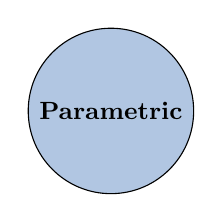
\begin{tikzpicture}[nodes={text depth=0.25ex,text height=1.25ex distance=1.7cm}]
                    \tikzstyle{every node}=[font=\small] \tikzstyle{vertex} =
                    [circle, draw=black, fill=illiniblue] \tikzstyle{hidden} =
                    [draw=none] \tikzstyle{edge} = [<->, very thick]

                    \node[vertex](v3) at (-4,0) {\textbf{Parametric}};
        
            \end{tikzpicture}
            }
            % \caption{Parametric Uncertainty} \label{fig:triarchic-uncertainty}
        \end{figure}

        \column[t]{6cm}
        \begin{block}{Parametric Uncertainty}
            Related to uncertainty in model inputs (empirical values). The most
            commonly addressed type of uncertainty in science and engineering
            \cite{yue_review_2018,decarolis_using_2011,morgan_uncertainty_1990}.    
        \end{block}
        
        % May be classified as either \boldorange{aleatory} or
        % \boldorange{epistemic}
        % \cite{pfenninger_energy_2014,kiureghian_aleatory_2009}. 
    \end{columns}

\end{frame}

\begin{frame}
    \frametitle{Examples of Parametric Uncertainty}

    \begin{columns}
        \column[t]{5cm}
        \begin{figure}
            \centering
            \resizebox{\columnwidth}{!}{
                \input{../docs/figures/multiple-distributions.pgf}
            }
            \caption{Possible distributions of several parameters.}
            \label{fig:multi-distributions}
        \end{figure}

        \column[t]{5cm}

        \begin{itemize}
            \item \textcolor{black}{Rates (e.g., interest, learning, growth),}
            \item \textcolor{black}{costs (e.g., fuel, capital, O\&M),}
            \item \textcolor{black}{aggregated energy demand,}
            \item \textcolor{black}{spent fuel burnup
            \cite{feng_sensitivity_2020},}
            \item \textcolor{black}{nuclear cross-section data
            \cite{eades_influence_2016,radaideh_combining_2019},}
            \item \textcolor{black}{likelihood and magnitude of consequences
            (i.e., probabilistic risk assessment).}
        \end{itemize}

        % Note: \textbf{\textcolor{illiniblue}{aleatory}} and
        % \textbf{\textcolor{illiniorange}{epistemic}}
    \end{columns}

\end{frame}

% \begin{frame}
%     \frametitle{Consequences of not addressing parametric uncertainty}

%     A majority of ESOM articles use \textit{scenario analysis} to weakly ddress
%     parametric uncertainty \cite{yue_review_2018}. \\~\\

%     Leading to: 
%     \begin{enumerate}
%         \item Overconfidence in results
%         \item Cognitive myopia
%         \item Implicit normative biases
%     \end{enumerate}


% \end{frame}

% \begin{frame}
%     \frametitle{Addressing parametric uncertainty}

%     \begin{columns}
%         \column[t]{5cm}
%         \begin{figure}
%             \centering
%             \resizebox{\columnwidth}{!}{
%                 \input{../pres/images/confidence-int.pgf}
%             }
%             \caption{Systematically addressing parametric uncertainty produces confidence intervals.}
%             \label{fig:confidence-intervals}
%         \end{figure}

%         \column[t]{5cm}
%         \boldblue{Idea}: Rerun a simulation until you reach a large enough
%         sample size to do statistics.\\~\\
%         Formal methods to address parametric uncertainty$^*$:
%         \begin{itemize}
%             \item ``Monte Carlo'' (i.e., statistical sampling)
%             \item Sensitivity analysis (specific or global)
%             \item Stochastic optimization
%         \end{itemize}


%         % \small{$^*$These methods are appropriate for \boldorange{aleatory}
%         % uncertainties.}
%     \end{columns}

% \end{frame}


\begin{frame}
    \frametitle{Considering Parametric Uncertainty in a Linear Program}
    \begin{columns}
        \column[t]{10cm}
        \begin{figure}
            \centering
            \resizebox{0.75\columnwidth}{!}{%% Creator: Matplotlib, PGF backend
%%
%% To include the figure in your LaTeX document, write
%%   \input{<filename>.pgf}
%%
%% Make sure the required packages are loaded in your preamble
%%   \usepackage{pgf}
%%
%% Also ensure that all the required font packages are loaded; for instance,
%% the lmodern package is sometimes necessary when using math font.
%%   \usepackage{lmodern}
%%
%% Figures using additional raster images can only be included by \input if
%% they are in the same directory as the main LaTeX file. For loading figures
%% from other directories you can use the `import` package
%%   \usepackage{import}
%%
%% and then include the figures with
%%   \import{<path to file>}{<filename>.pgf}
%%
%% Matplotlib used the following preamble
%%   \def\mathdefault#1{#1}
%%   \everymath=\expandafter{\the\everymath\displaystyle}
%%   
%%   \makeatletter\@ifpackageloaded{underscore}{}{\usepackage[strings]{underscore}}\makeatother
%%
\begingroup%
\makeatletter%
\begin{pgfpicture}%
\pgfpathrectangle{\pgfpointorigin}{\pgfqpoint{7.900000in}{5.930000in}}%
\pgfusepath{use as bounding box, clip}%
\begin{pgfscope}%
\pgfsetbuttcap%
\pgfsetmiterjoin%
\definecolor{currentfill}{rgb}{0.827451,0.827451,0.827451}%
\pgfsetfillcolor{currentfill}%
\pgfsetlinewidth{0.000000pt}%
\definecolor{currentstroke}{rgb}{0.000000,0.000000,0.000000}%
\pgfsetstrokecolor{currentstroke}%
\pgfsetdash{}{0pt}%
\pgfpathmoveto{\pgfqpoint{0.000000in}{0.000000in}}%
\pgfpathlineto{\pgfqpoint{7.900000in}{0.000000in}}%
\pgfpathlineto{\pgfqpoint{7.900000in}{5.930000in}}%
\pgfpathlineto{\pgfqpoint{0.000000in}{5.930000in}}%
\pgfpathlineto{\pgfqpoint{0.000000in}{0.000000in}}%
\pgfpathclose%
\pgfusepath{fill}%
\end{pgfscope}%
\begin{pgfscope}%
\pgfsetbuttcap%
\pgfsetmiterjoin%
\definecolor{currentfill}{rgb}{1.000000,1.000000,1.000000}%
\pgfsetfillcolor{currentfill}%
\pgfsetlinewidth{0.000000pt}%
\definecolor{currentstroke}{rgb}{0.000000,0.000000,0.000000}%
\pgfsetstrokecolor{currentstroke}%
\pgfsetstrokeopacity{0.000000}%
\pgfsetdash{}{0pt}%
\pgfpathmoveto{\pgfqpoint{0.759074in}{0.686623in}}%
\pgfpathlineto{\pgfqpoint{7.800000in}{0.686623in}}%
\pgfpathlineto{\pgfqpoint{7.800000in}{5.059445in}}%
\pgfpathlineto{\pgfqpoint{0.759074in}{5.059445in}}%
\pgfpathlineto{\pgfqpoint{0.759074in}{0.686623in}}%
\pgfpathclose%
\pgfusepath{fill}%
\end{pgfscope}%
\begin{pgfscope}%
\pgfpathrectangle{\pgfqpoint{0.759074in}{0.686623in}}{\pgfqpoint{7.040926in}{4.372823in}}%
\pgfusepath{clip}%
\pgfsetbuttcap%
\pgfsetroundjoin%
\definecolor{currentfill}{rgb}{0.000000,0.000000,0.000000}%
\pgfsetfillcolor{currentfill}%
\pgfsetfillopacity{0.100000}%
\pgfsetlinewidth{1.003750pt}%
\definecolor{currentstroke}{rgb}{0.000000,0.000000,0.000000}%
\pgfsetstrokecolor{currentstroke}%
\pgfsetstrokeopacity{0.100000}%
\pgfsetdash{}{0pt}%
\pgfsys@defobject{currentmarker}{\pgfqpoint{0.759074in}{0.686623in}}{\pgfqpoint{7.800000in}{5.059445in}}{%
\pgfpathmoveto{\pgfqpoint{0.759074in}{5.059445in}}%
\pgfpathlineto{\pgfqpoint{0.759074in}{4.723204in}}%
\pgfpathlineto{\pgfqpoint{0.759074in}{4.723204in}}%
\pgfpathlineto{\pgfqpoint{0.765580in}{4.719163in}}%
\pgfpathlineto{\pgfqpoint{0.766122in}{4.718827in}}%
\pgfpathlineto{\pgfqpoint{0.772086in}{4.715123in}}%
\pgfpathlineto{\pgfqpoint{0.773170in}{4.714449in}}%
\pgfpathlineto{\pgfqpoint{0.778592in}{4.711082in}}%
\pgfpathlineto{\pgfqpoint{0.780218in}{4.710072in}}%
\pgfpathlineto{\pgfqpoint{0.785098in}{4.707041in}}%
\pgfpathlineto{\pgfqpoint{0.787266in}{4.705695in}}%
\pgfpathlineto{\pgfqpoint{0.791604in}{4.703001in}}%
\pgfpathlineto{\pgfqpoint{0.794313in}{4.701318in}}%
\pgfpathlineto{\pgfqpoint{0.798110in}{4.698960in}}%
\pgfpathlineto{\pgfqpoint{0.801361in}{4.696941in}}%
\pgfpathlineto{\pgfqpoint{0.804616in}{4.694919in}}%
\pgfpathlineto{\pgfqpoint{0.808409in}{4.692563in}}%
\pgfpathlineto{\pgfqpoint{0.811122in}{4.690879in}}%
\pgfpathlineto{\pgfqpoint{0.815457in}{4.688186in}}%
\pgfpathlineto{\pgfqpoint{0.817628in}{4.686838in}}%
\pgfpathlineto{\pgfqpoint{0.822505in}{4.683809in}}%
\pgfpathlineto{\pgfqpoint{0.824134in}{4.682798in}}%
\pgfpathlineto{\pgfqpoint{0.829553in}{4.679432in}}%
\pgfpathlineto{\pgfqpoint{0.830640in}{4.678757in}}%
\pgfpathlineto{\pgfqpoint{0.836601in}{4.675055in}}%
\pgfpathlineto{\pgfqpoint{0.837146in}{4.674716in}}%
\pgfpathlineto{\pgfqpoint{0.843649in}{4.670677in}}%
\pgfpathlineto{\pgfqpoint{0.843652in}{4.670676in}}%
\pgfpathlineto{\pgfqpoint{0.850158in}{4.666635in}}%
\pgfpathlineto{\pgfqpoint{0.850697in}{4.666300in}}%
\pgfpathlineto{\pgfqpoint{0.856664in}{4.662594in}}%
\pgfpathlineto{\pgfqpoint{0.857745in}{4.661923in}}%
\pgfpathlineto{\pgfqpoint{0.863170in}{4.658554in}}%
\pgfpathlineto{\pgfqpoint{0.864793in}{4.657546in}}%
\pgfpathlineto{\pgfqpoint{0.869676in}{4.654513in}}%
\pgfpathlineto{\pgfqpoint{0.871841in}{4.653169in}}%
\pgfpathlineto{\pgfqpoint{0.876182in}{4.650473in}}%
\pgfpathlineto{\pgfqpoint{0.878889in}{4.648791in}}%
\pgfpathlineto{\pgfqpoint{0.882688in}{4.646432in}}%
\pgfpathlineto{\pgfqpoint{0.885937in}{4.644414in}}%
\pgfpathlineto{\pgfqpoint{0.889194in}{4.642391in}}%
\pgfpathlineto{\pgfqpoint{0.892985in}{4.640037in}}%
\pgfpathlineto{\pgfqpoint{0.895700in}{4.638351in}}%
\pgfpathlineto{\pgfqpoint{0.900033in}{4.635660in}}%
\pgfpathlineto{\pgfqpoint{0.902206in}{4.634310in}}%
\pgfpathlineto{\pgfqpoint{0.907081in}{4.631283in}}%
\pgfpathlineto{\pgfqpoint{0.908712in}{4.630269in}}%
\pgfpathlineto{\pgfqpoint{0.914129in}{4.626905in}}%
\pgfpathlineto{\pgfqpoint{0.915218in}{4.626229in}}%
\pgfpathlineto{\pgfqpoint{0.921177in}{4.622528in}}%
\pgfpathlineto{\pgfqpoint{0.921724in}{4.622188in}}%
\pgfpathlineto{\pgfqpoint{0.928225in}{4.618151in}}%
\pgfpathlineto{\pgfqpoint{0.928230in}{4.618148in}}%
\pgfpathlineto{\pgfqpoint{0.934736in}{4.614107in}}%
\pgfpathlineto{\pgfqpoint{0.935273in}{4.613774in}}%
\pgfpathlineto{\pgfqpoint{0.941242in}{4.610066in}}%
\pgfpathlineto{\pgfqpoint{0.942321in}{4.609397in}}%
\pgfpathlineto{\pgfqpoint{0.947749in}{4.606026in}}%
\pgfpathlineto{\pgfqpoint{0.949369in}{4.605019in}}%
\pgfpathlineto{\pgfqpoint{0.954255in}{4.601985in}}%
\pgfpathlineto{\pgfqpoint{0.956417in}{4.600642in}}%
\pgfpathlineto{\pgfqpoint{0.960761in}{4.597944in}}%
\pgfpathlineto{\pgfqpoint{0.963465in}{4.596265in}}%
\pgfpathlineto{\pgfqpoint{0.967267in}{4.593904in}}%
\pgfpathlineto{\pgfqpoint{0.970513in}{4.591888in}}%
\pgfpathlineto{\pgfqpoint{0.973773in}{4.589863in}}%
\pgfpathlineto{\pgfqpoint{0.977561in}{4.587511in}}%
\pgfpathlineto{\pgfqpoint{0.980279in}{4.585823in}}%
\pgfpathlineto{\pgfqpoint{0.984609in}{4.583133in}}%
\pgfpathlineto{\pgfqpoint{0.986785in}{4.581782in}}%
\pgfpathlineto{\pgfqpoint{0.991657in}{4.578756in}}%
\pgfpathlineto{\pgfqpoint{0.993291in}{4.577741in}}%
\pgfpathlineto{\pgfqpoint{0.998705in}{4.574379in}}%
\pgfpathlineto{\pgfqpoint{0.999797in}{4.573701in}}%
\pgfpathlineto{\pgfqpoint{1.005753in}{4.570002in}}%
\pgfpathlineto{\pgfqpoint{1.006303in}{4.569660in}}%
\pgfpathlineto{\pgfqpoint{1.012801in}{4.565625in}}%
\pgfpathlineto{\pgfqpoint{1.012809in}{4.565620in}}%
\pgfpathlineto{\pgfqpoint{1.019315in}{4.561579in}}%
\pgfpathlineto{\pgfqpoint{1.019849in}{4.561247in}}%
\pgfpathlineto{\pgfqpoint{1.025821in}{4.557538in}}%
\pgfpathlineto{\pgfqpoint{1.026897in}{4.556870in}}%
\pgfpathlineto{\pgfqpoint{1.032327in}{4.553498in}}%
\pgfpathlineto{\pgfqpoint{1.033945in}{4.552493in}}%
\pgfpathlineto{\pgfqpoint{1.038833in}{4.549457in}}%
\pgfpathlineto{\pgfqpoint{1.040993in}{4.548116in}}%
\pgfpathlineto{\pgfqpoint{1.045339in}{4.545416in}}%
\pgfpathlineto{\pgfqpoint{1.048041in}{4.543739in}}%
\pgfpathlineto{\pgfqpoint{1.051845in}{4.541376in}}%
\pgfpathlineto{\pgfqpoint{1.055089in}{4.539361in}}%
\pgfpathlineto{\pgfqpoint{1.058351in}{4.537335in}}%
\pgfpathlineto{\pgfqpoint{1.062137in}{4.534984in}}%
\pgfpathlineto{\pgfqpoint{1.064857in}{4.533295in}}%
\pgfpathlineto{\pgfqpoint{1.069184in}{4.530607in}}%
\pgfpathlineto{\pgfqpoint{1.071363in}{4.529254in}}%
\pgfpathlineto{\pgfqpoint{1.076232in}{4.526230in}}%
\pgfpathlineto{\pgfqpoint{1.077869in}{4.525213in}}%
\pgfpathlineto{\pgfqpoint{1.083280in}{4.521853in}}%
\pgfpathlineto{\pgfqpoint{1.084375in}{4.521173in}}%
\pgfpathlineto{\pgfqpoint{1.090328in}{4.517475in}}%
\pgfpathlineto{\pgfqpoint{1.090881in}{4.517132in}}%
\pgfpathlineto{\pgfqpoint{1.097376in}{4.513098in}}%
\pgfpathlineto{\pgfqpoint{1.097387in}{4.513091in}}%
\pgfpathlineto{\pgfqpoint{1.103893in}{4.509051in}}%
\pgfpathlineto{\pgfqpoint{1.104424in}{4.508721in}}%
\pgfpathlineto{\pgfqpoint{1.110399in}{4.505010in}}%
\pgfpathlineto{\pgfqpoint{1.111472in}{4.504344in}}%
\pgfpathlineto{\pgfqpoint{1.116905in}{4.500970in}}%
\pgfpathlineto{\pgfqpoint{1.118520in}{4.499967in}}%
\pgfpathlineto{\pgfqpoint{1.123411in}{4.496929in}}%
\pgfpathlineto{\pgfqpoint{1.125568in}{4.495589in}}%
\pgfpathlineto{\pgfqpoint{1.129917in}{4.492888in}}%
\pgfpathlineto{\pgfqpoint{1.132616in}{4.491212in}}%
\pgfpathlineto{\pgfqpoint{1.136423in}{4.488848in}}%
\pgfpathlineto{\pgfqpoint{1.139664in}{4.486835in}}%
\pgfpathlineto{\pgfqpoint{1.142929in}{4.484807in}}%
\pgfpathlineto{\pgfqpoint{1.146712in}{4.482458in}}%
\pgfpathlineto{\pgfqpoint{1.149435in}{4.480766in}}%
\pgfpathlineto{\pgfqpoint{1.153760in}{4.478081in}}%
\pgfpathlineto{\pgfqpoint{1.155941in}{4.476726in}}%
\pgfpathlineto{\pgfqpoint{1.160808in}{4.473703in}}%
\pgfpathlineto{\pgfqpoint{1.162448in}{4.472685in}}%
\pgfpathlineto{\pgfqpoint{1.167856in}{4.469326in}}%
\pgfpathlineto{\pgfqpoint{1.168954in}{4.468645in}}%
\pgfpathlineto{\pgfqpoint{1.174904in}{4.464949in}}%
\pgfpathlineto{\pgfqpoint{1.175460in}{4.464604in}}%
\pgfpathlineto{\pgfqpoint{1.181952in}{4.460572in}}%
\pgfpathlineto{\pgfqpoint{1.181966in}{4.460563in}}%
\pgfpathlineto{\pgfqpoint{1.188472in}{4.456523in}}%
\pgfpathlineto{\pgfqpoint{1.189000in}{4.456195in}}%
\pgfpathlineto{\pgfqpoint{1.194978in}{4.452482in}}%
\pgfpathlineto{\pgfqpoint{1.196048in}{4.451817in}}%
\pgfpathlineto{\pgfqpoint{1.201484in}{4.448441in}}%
\pgfpathlineto{\pgfqpoint{1.203096in}{4.447440in}}%
\pgfpathlineto{\pgfqpoint{1.207990in}{4.444401in}}%
\pgfpathlineto{\pgfqpoint{1.210144in}{4.443063in}}%
\pgfpathlineto{\pgfqpoint{1.214496in}{4.440360in}}%
\pgfpathlineto{\pgfqpoint{1.217192in}{4.438686in}}%
\pgfpathlineto{\pgfqpoint{1.221002in}{4.436320in}}%
\pgfpathlineto{\pgfqpoint{1.224240in}{4.434309in}}%
\pgfpathlineto{\pgfqpoint{1.227508in}{4.432279in}}%
\pgfpathlineto{\pgfqpoint{1.231288in}{4.429931in}}%
\pgfpathlineto{\pgfqpoint{1.234014in}{4.428238in}}%
\pgfpathlineto{\pgfqpoint{1.238336in}{4.425554in}}%
\pgfpathlineto{\pgfqpoint{1.240520in}{4.424198in}}%
\pgfpathlineto{\pgfqpoint{1.245384in}{4.421177in}}%
\pgfpathlineto{\pgfqpoint{1.247026in}{4.420157in}}%
\pgfpathlineto{\pgfqpoint{1.252432in}{4.416800in}}%
\pgfpathlineto{\pgfqpoint{1.253532in}{4.416117in}}%
\pgfpathlineto{\pgfqpoint{1.259480in}{4.412423in}}%
\pgfpathlineto{\pgfqpoint{1.260038in}{4.412076in}}%
\pgfpathlineto{\pgfqpoint{1.266528in}{4.408045in}}%
\pgfpathlineto{\pgfqpoint{1.266544in}{4.408035in}}%
\pgfpathlineto{\pgfqpoint{1.273050in}{4.403995in}}%
\pgfpathlineto{\pgfqpoint{1.273576in}{4.403668in}}%
\pgfpathlineto{\pgfqpoint{1.279556in}{4.399954in}}%
\pgfpathlineto{\pgfqpoint{1.280624in}{4.399291in}}%
\pgfpathlineto{\pgfqpoint{1.286062in}{4.395913in}}%
\pgfpathlineto{\pgfqpoint{1.287672in}{4.394914in}}%
\pgfpathlineto{\pgfqpoint{1.292568in}{4.391873in}}%
\pgfpathlineto{\pgfqpoint{1.294720in}{4.390537in}}%
\pgfpathlineto{\pgfqpoint{1.299074in}{4.387832in}}%
\pgfpathlineto{\pgfqpoint{1.301768in}{4.386159in}}%
\pgfpathlineto{\pgfqpoint{1.305580in}{4.383792in}}%
\pgfpathlineto{\pgfqpoint{1.308816in}{4.381782in}}%
\pgfpathlineto{\pgfqpoint{1.312086in}{4.379751in}}%
\pgfpathlineto{\pgfqpoint{1.315864in}{4.377405in}}%
\pgfpathlineto{\pgfqpoint{1.318592in}{4.375710in}}%
\pgfpathlineto{\pgfqpoint{1.322912in}{4.373028in}}%
\pgfpathlineto{\pgfqpoint{1.325098in}{4.371670in}}%
\pgfpathlineto{\pgfqpoint{1.329960in}{4.368651in}}%
\pgfpathlineto{\pgfqpoint{1.331604in}{4.367629in}}%
\pgfpathlineto{\pgfqpoint{1.337008in}{4.364273in}}%
\pgfpathlineto{\pgfqpoint{1.338110in}{4.363588in}}%
\pgfpathlineto{\pgfqpoint{1.344055in}{4.359896in}}%
\pgfpathlineto{\pgfqpoint{1.344616in}{4.359548in}}%
\pgfpathlineto{\pgfqpoint{1.351103in}{4.355519in}}%
\pgfpathlineto{\pgfqpoint{1.351122in}{4.355507in}}%
\pgfpathlineto{\pgfqpoint{1.357628in}{4.351467in}}%
\pgfpathlineto{\pgfqpoint{1.358151in}{4.351142in}}%
\pgfpathlineto{\pgfqpoint{1.364134in}{4.347426in}}%
\pgfpathlineto{\pgfqpoint{1.365199in}{4.346765in}}%
\pgfpathlineto{\pgfqpoint{1.370641in}{4.343385in}}%
\pgfpathlineto{\pgfqpoint{1.372247in}{4.342387in}}%
\pgfpathlineto{\pgfqpoint{1.377147in}{4.339345in}}%
\pgfpathlineto{\pgfqpoint{1.379295in}{4.338010in}}%
\pgfpathlineto{\pgfqpoint{1.383653in}{4.335304in}}%
\pgfpathlineto{\pgfqpoint{1.386343in}{4.333633in}}%
\pgfpathlineto{\pgfqpoint{1.390159in}{4.331263in}}%
\pgfpathlineto{\pgfqpoint{1.393391in}{4.329256in}}%
\pgfpathlineto{\pgfqpoint{1.396665in}{4.327223in}}%
\pgfpathlineto{\pgfqpoint{1.400439in}{4.324879in}}%
\pgfpathlineto{\pgfqpoint{1.403171in}{4.323182in}}%
\pgfpathlineto{\pgfqpoint{1.407487in}{4.320501in}}%
\pgfpathlineto{\pgfqpoint{1.409677in}{4.319142in}}%
\pgfpathlineto{\pgfqpoint{1.414535in}{4.316124in}}%
\pgfpathlineto{\pgfqpoint{1.416183in}{4.315101in}}%
\pgfpathlineto{\pgfqpoint{1.421583in}{4.311747in}}%
\pgfpathlineto{\pgfqpoint{1.422689in}{4.311060in}}%
\pgfpathlineto{\pgfqpoint{1.428631in}{4.307370in}}%
\pgfpathlineto{\pgfqpoint{1.429195in}{4.307020in}}%
\pgfpathlineto{\pgfqpoint{1.435679in}{4.302993in}}%
\pgfpathlineto{\pgfqpoint{1.435701in}{4.302979in}}%
\pgfpathlineto{\pgfqpoint{1.442207in}{4.298938in}}%
\pgfpathlineto{\pgfqpoint{1.442727in}{4.298615in}}%
\pgfpathlineto{\pgfqpoint{1.448713in}{4.294898in}}%
\pgfpathlineto{\pgfqpoint{1.449775in}{4.294238in}}%
\pgfpathlineto{\pgfqpoint{1.455219in}{4.290857in}}%
\pgfpathlineto{\pgfqpoint{1.456823in}{4.289861in}}%
\pgfpathlineto{\pgfqpoint{1.461725in}{4.286817in}}%
\pgfpathlineto{\pgfqpoint{1.463871in}{4.285484in}}%
\pgfpathlineto{\pgfqpoint{1.468231in}{4.282776in}}%
\pgfpathlineto{\pgfqpoint{1.470919in}{4.281107in}}%
\pgfpathlineto{\pgfqpoint{1.474737in}{4.278735in}}%
\pgfpathlineto{\pgfqpoint{1.477967in}{4.276729in}}%
\pgfpathlineto{\pgfqpoint{1.481243in}{4.274695in}}%
\pgfpathlineto{\pgfqpoint{1.485015in}{4.272352in}}%
\pgfpathlineto{\pgfqpoint{1.487749in}{4.270654in}}%
\pgfpathlineto{\pgfqpoint{1.492063in}{4.267975in}}%
\pgfpathlineto{\pgfqpoint{1.494255in}{4.266614in}}%
\pgfpathlineto{\pgfqpoint{1.499111in}{4.263598in}}%
\pgfpathlineto{\pgfqpoint{1.500761in}{4.262573in}}%
\pgfpathlineto{\pgfqpoint{1.506159in}{4.259221in}}%
\pgfpathlineto{\pgfqpoint{1.507267in}{4.258532in}}%
\pgfpathlineto{\pgfqpoint{1.513207in}{4.254843in}}%
\pgfpathlineto{\pgfqpoint{1.513773in}{4.254492in}}%
\pgfpathlineto{\pgfqpoint{1.520255in}{4.250466in}}%
\pgfpathlineto{\pgfqpoint{1.520279in}{4.250451in}}%
\pgfpathlineto{\pgfqpoint{1.526785in}{4.246410in}}%
\pgfpathlineto{\pgfqpoint{1.527303in}{4.246089in}}%
\pgfpathlineto{\pgfqpoint{1.533291in}{4.242370in}}%
\pgfpathlineto{\pgfqpoint{1.534351in}{4.241712in}}%
\pgfpathlineto{\pgfqpoint{1.539797in}{4.238329in}}%
\pgfpathlineto{\pgfqpoint{1.541399in}{4.237335in}}%
\pgfpathlineto{\pgfqpoint{1.546303in}{4.234289in}}%
\pgfpathlineto{\pgfqpoint{1.548447in}{4.232957in}}%
\pgfpathlineto{\pgfqpoint{1.552809in}{4.230248in}}%
\pgfpathlineto{\pgfqpoint{1.555495in}{4.228580in}}%
\pgfpathlineto{\pgfqpoint{1.559315in}{4.226207in}}%
\pgfpathlineto{\pgfqpoint{1.562543in}{4.224203in}}%
\pgfpathlineto{\pgfqpoint{1.565821in}{4.222167in}}%
\pgfpathlineto{\pgfqpoint{1.569591in}{4.219826in}}%
\pgfpathlineto{\pgfqpoint{1.572327in}{4.218126in}}%
\pgfpathlineto{\pgfqpoint{1.576639in}{4.215449in}}%
\pgfpathlineto{\pgfqpoint{1.578834in}{4.214085in}}%
\pgfpathlineto{\pgfqpoint{1.583687in}{4.211071in}}%
\pgfpathlineto{\pgfqpoint{1.585340in}{4.210045in}}%
\pgfpathlineto{\pgfqpoint{1.590735in}{4.206694in}}%
\pgfpathlineto{\pgfqpoint{1.591846in}{4.206004in}}%
\pgfpathlineto{\pgfqpoint{1.597783in}{4.202317in}}%
\pgfpathlineto{\pgfqpoint{1.598352in}{4.201964in}}%
\pgfpathlineto{\pgfqpoint{1.604831in}{4.197940in}}%
\pgfpathlineto{\pgfqpoint{1.604858in}{4.197923in}}%
\pgfpathlineto{\pgfqpoint{1.611364in}{4.193882in}}%
\pgfpathlineto{\pgfqpoint{1.611879in}{4.193563in}}%
\pgfpathlineto{\pgfqpoint{1.617870in}{4.189842in}}%
\pgfpathlineto{\pgfqpoint{1.618926in}{4.189185in}}%
\pgfpathlineto{\pgfqpoint{1.624376in}{4.185801in}}%
\pgfpathlineto{\pgfqpoint{1.625974in}{4.184808in}}%
\pgfpathlineto{\pgfqpoint{1.630882in}{4.181760in}}%
\pgfpathlineto{\pgfqpoint{1.633022in}{4.180431in}}%
\pgfpathlineto{\pgfqpoint{1.637388in}{4.177720in}}%
\pgfpathlineto{\pgfqpoint{1.640070in}{4.176054in}}%
\pgfpathlineto{\pgfqpoint{1.643894in}{4.173679in}}%
\pgfpathlineto{\pgfqpoint{1.647118in}{4.171677in}}%
\pgfpathlineto{\pgfqpoint{1.650400in}{4.169639in}}%
\pgfpathlineto{\pgfqpoint{1.654166in}{4.167299in}}%
\pgfpathlineto{\pgfqpoint{1.656906in}{4.165598in}}%
\pgfpathlineto{\pgfqpoint{1.661214in}{4.162922in}}%
\pgfpathlineto{\pgfqpoint{1.663412in}{4.161557in}}%
\pgfpathlineto{\pgfqpoint{1.668262in}{4.158545in}}%
\pgfpathlineto{\pgfqpoint{1.669918in}{4.157517in}}%
\pgfpathlineto{\pgfqpoint{1.675310in}{4.154168in}}%
\pgfpathlineto{\pgfqpoint{1.676424in}{4.153476in}}%
\pgfpathlineto{\pgfqpoint{1.682358in}{4.149791in}}%
\pgfpathlineto{\pgfqpoint{1.682930in}{4.149435in}}%
\pgfpathlineto{\pgfqpoint{1.689406in}{4.145413in}}%
\pgfpathlineto{\pgfqpoint{1.689436in}{4.145395in}}%
\pgfpathlineto{\pgfqpoint{1.695942in}{4.141354in}}%
\pgfpathlineto{\pgfqpoint{1.696454in}{4.141036in}}%
\pgfpathlineto{\pgfqpoint{1.702448in}{4.137314in}}%
\pgfpathlineto{\pgfqpoint{1.703502in}{4.136659in}}%
\pgfpathlineto{\pgfqpoint{1.708954in}{4.133273in}}%
\pgfpathlineto{\pgfqpoint{1.710550in}{4.132282in}}%
\pgfpathlineto{\pgfqpoint{1.715460in}{4.129232in}}%
\pgfpathlineto{\pgfqpoint{1.717598in}{4.127905in}}%
\pgfpathlineto{\pgfqpoint{1.721966in}{4.125192in}}%
\pgfpathlineto{\pgfqpoint{1.724646in}{4.123527in}}%
\pgfpathlineto{\pgfqpoint{1.728472in}{4.121151in}}%
\pgfpathlineto{\pgfqpoint{1.731694in}{4.119150in}}%
\pgfpathlineto{\pgfqpoint{1.734978in}{4.117111in}}%
\pgfpathlineto{\pgfqpoint{1.738742in}{4.114773in}}%
\pgfpathlineto{\pgfqpoint{1.741484in}{4.113070in}}%
\pgfpathlineto{\pgfqpoint{1.745790in}{4.110396in}}%
\pgfpathlineto{\pgfqpoint{1.747990in}{4.109029in}}%
\pgfpathlineto{\pgfqpoint{1.752838in}{4.106019in}}%
\pgfpathlineto{\pgfqpoint{1.754496in}{4.104989in}}%
\pgfpathlineto{\pgfqpoint{1.759886in}{4.101641in}}%
\pgfpathlineto{\pgfqpoint{1.761002in}{4.100948in}}%
\pgfpathlineto{\pgfqpoint{1.766934in}{4.097264in}}%
\pgfpathlineto{\pgfqpoint{1.767508in}{4.096907in}}%
\pgfpathlineto{\pgfqpoint{1.773982in}{4.092887in}}%
\pgfpathlineto{\pgfqpoint{1.774014in}{4.092867in}}%
\pgfpathlineto{\pgfqpoint{1.780520in}{4.088826in}}%
\pgfpathlineto{\pgfqpoint{1.781030in}{4.088510in}}%
\pgfpathlineto{\pgfqpoint{1.787026in}{4.084786in}}%
\pgfpathlineto{\pgfqpoint{1.788078in}{4.084133in}}%
\pgfpathlineto{\pgfqpoint{1.793533in}{4.080745in}}%
\pgfpathlineto{\pgfqpoint{1.795126in}{4.079755in}}%
\pgfpathlineto{\pgfqpoint{1.800039in}{4.076704in}}%
\pgfpathlineto{\pgfqpoint{1.802174in}{4.075378in}}%
\pgfpathlineto{\pgfqpoint{1.806545in}{4.072664in}}%
\pgfpathlineto{\pgfqpoint{1.809222in}{4.071001in}}%
\pgfpathlineto{\pgfqpoint{1.813051in}{4.068623in}}%
\pgfpathlineto{\pgfqpoint{1.816270in}{4.066624in}}%
\pgfpathlineto{\pgfqpoint{1.819557in}{4.064582in}}%
\pgfpathlineto{\pgfqpoint{1.823318in}{4.062247in}}%
\pgfpathlineto{\pgfqpoint{1.826063in}{4.060542in}}%
\pgfpathlineto{\pgfqpoint{1.830366in}{4.057869in}}%
\pgfpathlineto{\pgfqpoint{1.832569in}{4.056501in}}%
\pgfpathlineto{\pgfqpoint{1.837414in}{4.053492in}}%
\pgfpathlineto{\pgfqpoint{1.839075in}{4.052461in}}%
\pgfpathlineto{\pgfqpoint{1.844462in}{4.049115in}}%
\pgfpathlineto{\pgfqpoint{1.845581in}{4.048420in}}%
\pgfpathlineto{\pgfqpoint{1.851510in}{4.044738in}}%
\pgfpathlineto{\pgfqpoint{1.852087in}{4.044379in}}%
\pgfpathlineto{\pgfqpoint{1.858558in}{4.040361in}}%
\pgfpathlineto{\pgfqpoint{1.858593in}{4.040339in}}%
\pgfpathlineto{\pgfqpoint{1.865099in}{4.036298in}}%
\pgfpathlineto{\pgfqpoint{1.865606in}{4.035983in}}%
\pgfpathlineto{\pgfqpoint{1.871605in}{4.032257in}}%
\pgfpathlineto{\pgfqpoint{1.872654in}{4.031606in}}%
\pgfpathlineto{\pgfqpoint{1.878111in}{4.028217in}}%
\pgfpathlineto{\pgfqpoint{1.879702in}{4.027229in}}%
\pgfpathlineto{\pgfqpoint{1.884617in}{4.024176in}}%
\pgfpathlineto{\pgfqpoint{1.886750in}{4.022852in}}%
\pgfpathlineto{\pgfqpoint{1.891123in}{4.020136in}}%
\pgfpathlineto{\pgfqpoint{1.893797in}{4.018475in}}%
\pgfpathlineto{\pgfqpoint{1.897629in}{4.016095in}}%
\pgfpathlineto{\pgfqpoint{1.900845in}{4.014097in}}%
\pgfpathlineto{\pgfqpoint{1.904135in}{4.012054in}}%
\pgfpathlineto{\pgfqpoint{1.907893in}{4.009720in}}%
\pgfpathlineto{\pgfqpoint{1.910641in}{4.008014in}}%
\pgfpathlineto{\pgfqpoint{1.914941in}{4.005343in}}%
\pgfpathlineto{\pgfqpoint{1.917147in}{4.003973in}}%
\pgfpathlineto{\pgfqpoint{1.921989in}{4.000966in}}%
\pgfpathlineto{\pgfqpoint{1.923653in}{3.999932in}}%
\pgfpathlineto{\pgfqpoint{1.929037in}{3.996589in}}%
\pgfpathlineto{\pgfqpoint{1.930159in}{3.995892in}}%
\pgfpathlineto{\pgfqpoint{1.936085in}{3.992211in}}%
\pgfpathlineto{\pgfqpoint{1.936665in}{3.991851in}}%
\pgfpathlineto{\pgfqpoint{1.943133in}{3.987834in}}%
\pgfpathlineto{\pgfqpoint{1.943171in}{3.987811in}}%
\pgfpathlineto{\pgfqpoint{1.949677in}{3.983770in}}%
\pgfpathlineto{\pgfqpoint{1.950181in}{3.983457in}}%
\pgfpathlineto{\pgfqpoint{1.956183in}{3.979729in}}%
\pgfpathlineto{\pgfqpoint{1.957229in}{3.979080in}}%
\pgfpathlineto{\pgfqpoint{1.962689in}{3.975689in}}%
\pgfpathlineto{\pgfqpoint{1.964277in}{3.974703in}}%
\pgfpathlineto{\pgfqpoint{1.969195in}{3.971648in}}%
\pgfpathlineto{\pgfqpoint{1.971325in}{3.970325in}}%
\pgfpathlineto{\pgfqpoint{1.975701in}{3.967608in}}%
\pgfpathlineto{\pgfqpoint{1.978373in}{3.965948in}}%
\pgfpathlineto{\pgfqpoint{1.982207in}{3.963567in}}%
\pgfpathlineto{\pgfqpoint{1.985421in}{3.961571in}}%
\pgfpathlineto{\pgfqpoint{1.988713in}{3.959526in}}%
\pgfpathlineto{\pgfqpoint{1.992469in}{3.957194in}}%
\pgfpathlineto{\pgfqpoint{1.995219in}{3.955486in}}%
\pgfpathlineto{\pgfqpoint{1.999517in}{3.952817in}}%
\pgfpathlineto{\pgfqpoint{2.001726in}{3.951445in}}%
\pgfpathlineto{\pgfqpoint{2.006565in}{3.948439in}}%
\pgfpathlineto{\pgfqpoint{2.008232in}{3.947404in}}%
\pgfpathlineto{\pgfqpoint{2.013613in}{3.944062in}}%
\pgfpathlineto{\pgfqpoint{2.014738in}{3.943364in}}%
\pgfpathlineto{\pgfqpoint{2.020661in}{3.939685in}}%
\pgfpathlineto{\pgfqpoint{2.021244in}{3.939323in}}%
\pgfpathlineto{\pgfqpoint{2.027709in}{3.935308in}}%
\pgfpathlineto{\pgfqpoint{2.027750in}{3.935283in}}%
\pgfpathlineto{\pgfqpoint{2.034256in}{3.931242in}}%
\pgfpathlineto{\pgfqpoint{2.034757in}{3.930931in}}%
\pgfpathlineto{\pgfqpoint{2.040762in}{3.927201in}}%
\pgfpathlineto{\pgfqpoint{2.041805in}{3.926553in}}%
\pgfpathlineto{\pgfqpoint{2.047268in}{3.923161in}}%
\pgfpathlineto{\pgfqpoint{2.048853in}{3.922176in}}%
\pgfpathlineto{\pgfqpoint{2.053774in}{3.919120in}}%
\pgfpathlineto{\pgfqpoint{2.055901in}{3.917799in}}%
\pgfpathlineto{\pgfqpoint{2.060280in}{3.915079in}}%
\pgfpathlineto{\pgfqpoint{2.062949in}{3.913422in}}%
\pgfpathlineto{\pgfqpoint{2.066786in}{3.911039in}}%
\pgfpathlineto{\pgfqpoint{2.069997in}{3.909045in}}%
\pgfpathlineto{\pgfqpoint{2.073292in}{3.906998in}}%
\pgfpathlineto{\pgfqpoint{2.077045in}{3.904667in}}%
\pgfpathlineto{\pgfqpoint{2.079798in}{3.902958in}}%
\pgfpathlineto{\pgfqpoint{2.084093in}{3.900290in}}%
\pgfpathlineto{\pgfqpoint{2.086304in}{3.898917in}}%
\pgfpathlineto{\pgfqpoint{2.091141in}{3.895913in}}%
\pgfpathlineto{\pgfqpoint{2.092810in}{3.894876in}}%
\pgfpathlineto{\pgfqpoint{2.098189in}{3.891536in}}%
\pgfpathlineto{\pgfqpoint{2.099316in}{3.890836in}}%
\pgfpathlineto{\pgfqpoint{2.105237in}{3.887159in}}%
\pgfpathlineto{\pgfqpoint{2.105822in}{3.886795in}}%
\pgfpathlineto{\pgfqpoint{2.112285in}{3.882781in}}%
\pgfpathlineto{\pgfqpoint{2.112328in}{3.882754in}}%
\pgfpathlineto{\pgfqpoint{2.118834in}{3.878714in}}%
\pgfpathlineto{\pgfqpoint{2.119333in}{3.878404in}}%
\pgfpathlineto{\pgfqpoint{2.125340in}{3.874673in}}%
\pgfpathlineto{\pgfqpoint{2.126381in}{3.874027in}}%
\pgfpathlineto{\pgfqpoint{2.131846in}{3.870633in}}%
\pgfpathlineto{\pgfqpoint{2.133429in}{3.869650in}}%
\pgfpathlineto{\pgfqpoint{2.138352in}{3.866592in}}%
\pgfpathlineto{\pgfqpoint{2.140477in}{3.865273in}}%
\pgfpathlineto{\pgfqpoint{2.144858in}{3.862551in}}%
\pgfpathlineto{\pgfqpoint{2.147525in}{3.860895in}}%
\pgfpathlineto{\pgfqpoint{2.151364in}{3.858511in}}%
\pgfpathlineto{\pgfqpoint{2.154573in}{3.856518in}}%
\pgfpathlineto{\pgfqpoint{2.157870in}{3.854470in}}%
\pgfpathlineto{\pgfqpoint{2.161621in}{3.852141in}}%
\pgfpathlineto{\pgfqpoint{2.164376in}{3.850429in}}%
\pgfpathlineto{\pgfqpoint{2.168668in}{3.847764in}}%
\pgfpathlineto{\pgfqpoint{2.170882in}{3.846389in}}%
\pgfpathlineto{\pgfqpoint{2.175716in}{3.843387in}}%
\pgfpathlineto{\pgfqpoint{2.177388in}{3.842348in}}%
\pgfpathlineto{\pgfqpoint{2.182764in}{3.839009in}}%
\pgfpathlineto{\pgfqpoint{2.183894in}{3.838308in}}%
\pgfpathlineto{\pgfqpoint{2.189812in}{3.834632in}}%
\pgfpathlineto{\pgfqpoint{2.190400in}{3.834267in}}%
\pgfpathlineto{\pgfqpoint{2.196860in}{3.830255in}}%
\pgfpathlineto{\pgfqpoint{2.196906in}{3.830226in}}%
\pgfpathlineto{\pgfqpoint{2.203412in}{3.826186in}}%
\pgfpathlineto{\pgfqpoint{2.203908in}{3.825878in}}%
\pgfpathlineto{\pgfqpoint{2.209919in}{3.822145in}}%
\pgfpathlineto{\pgfqpoint{2.210956in}{3.821501in}}%
\pgfpathlineto{\pgfqpoint{2.216425in}{3.818105in}}%
\pgfpathlineto{\pgfqpoint{2.218004in}{3.817123in}}%
\pgfpathlineto{\pgfqpoint{2.222931in}{3.814064in}}%
\pgfpathlineto{\pgfqpoint{2.225052in}{3.812746in}}%
\pgfpathlineto{\pgfqpoint{2.229437in}{3.810023in}}%
\pgfpathlineto{\pgfqpoint{2.232100in}{3.808369in}}%
\pgfpathlineto{\pgfqpoint{2.235943in}{3.805983in}}%
\pgfpathlineto{\pgfqpoint{2.239148in}{3.803992in}}%
\pgfpathlineto{\pgfqpoint{2.242449in}{3.801942in}}%
\pgfpathlineto{\pgfqpoint{2.246196in}{3.799615in}}%
\pgfpathlineto{\pgfqpoint{2.248955in}{3.797901in}}%
\pgfpathlineto{\pgfqpoint{2.253244in}{3.795237in}}%
\pgfpathlineto{\pgfqpoint{2.255461in}{3.793861in}}%
\pgfpathlineto{\pgfqpoint{2.260292in}{3.790860in}}%
\pgfpathlineto{\pgfqpoint{2.261967in}{3.789820in}}%
\pgfpathlineto{\pgfqpoint{2.267340in}{3.786483in}}%
\pgfpathlineto{\pgfqpoint{2.268473in}{3.785780in}}%
\pgfpathlineto{\pgfqpoint{2.274388in}{3.782106in}}%
\pgfpathlineto{\pgfqpoint{2.274979in}{3.781739in}}%
\pgfpathlineto{\pgfqpoint{2.281436in}{3.777729in}}%
\pgfpathlineto{\pgfqpoint{2.281485in}{3.777698in}}%
\pgfpathlineto{\pgfqpoint{2.287991in}{3.773658in}}%
\pgfpathlineto{\pgfqpoint{2.288484in}{3.773351in}}%
\pgfpathlineto{\pgfqpoint{2.294497in}{3.769617in}}%
\pgfpathlineto{\pgfqpoint{2.295532in}{3.768974in}}%
\pgfpathlineto{\pgfqpoint{2.301003in}{3.765576in}}%
\pgfpathlineto{\pgfqpoint{2.302580in}{3.764597in}}%
\pgfpathlineto{\pgfqpoint{2.307509in}{3.761536in}}%
\pgfpathlineto{\pgfqpoint{2.309628in}{3.760220in}}%
\pgfpathlineto{\pgfqpoint{2.314015in}{3.757495in}}%
\pgfpathlineto{\pgfqpoint{2.316676in}{3.755843in}}%
\pgfpathlineto{\pgfqpoint{2.320521in}{3.753455in}}%
\pgfpathlineto{\pgfqpoint{2.323724in}{3.751465in}}%
\pgfpathlineto{\pgfqpoint{2.327027in}{3.749414in}}%
\pgfpathlineto{\pgfqpoint{2.330772in}{3.747088in}}%
\pgfpathlineto{\pgfqpoint{2.333533in}{3.745373in}}%
\pgfpathlineto{\pgfqpoint{2.337820in}{3.742711in}}%
\pgfpathlineto{\pgfqpoint{2.340039in}{3.741333in}}%
\pgfpathlineto{\pgfqpoint{2.344868in}{3.738334in}}%
\pgfpathlineto{\pgfqpoint{2.346545in}{3.737292in}}%
\pgfpathlineto{\pgfqpoint{2.351916in}{3.733957in}}%
\pgfpathlineto{\pgfqpoint{2.353051in}{3.733251in}}%
\pgfpathlineto{\pgfqpoint{2.358964in}{3.729579in}}%
\pgfpathlineto{\pgfqpoint{2.359557in}{3.729211in}}%
\pgfpathlineto{\pgfqpoint{2.366012in}{3.725202in}}%
\pgfpathlineto{\pgfqpoint{2.366063in}{3.725170in}}%
\pgfpathlineto{\pgfqpoint{2.372569in}{3.721130in}}%
\pgfpathlineto{\pgfqpoint{2.373060in}{3.720825in}}%
\pgfpathlineto{\pgfqpoint{2.379075in}{3.717089in}}%
\pgfpathlineto{\pgfqpoint{2.380108in}{3.716448in}}%
\pgfpathlineto{\pgfqpoint{2.385581in}{3.713048in}}%
\pgfpathlineto{\pgfqpoint{2.387156in}{3.712071in}}%
\pgfpathlineto{\pgfqpoint{2.392087in}{3.709008in}}%
\pgfpathlineto{\pgfqpoint{2.394204in}{3.707693in}}%
\pgfpathlineto{\pgfqpoint{2.398593in}{3.704967in}}%
\pgfpathlineto{\pgfqpoint{2.401252in}{3.703316in}}%
\pgfpathlineto{\pgfqpoint{2.405099in}{3.700927in}}%
\pgfpathlineto{\pgfqpoint{2.408300in}{3.698939in}}%
\pgfpathlineto{\pgfqpoint{2.411605in}{3.696886in}}%
\pgfpathlineto{\pgfqpoint{2.415348in}{3.694562in}}%
\pgfpathlineto{\pgfqpoint{2.418111in}{3.692845in}}%
\pgfpathlineto{\pgfqpoint{2.422396in}{3.690185in}}%
\pgfpathlineto{\pgfqpoint{2.424618in}{3.688805in}}%
\pgfpathlineto{\pgfqpoint{2.429444in}{3.685807in}}%
\pgfpathlineto{\pgfqpoint{2.431124in}{3.684764in}}%
\pgfpathlineto{\pgfqpoint{2.436492in}{3.681430in}}%
\pgfpathlineto{\pgfqpoint{2.437630in}{3.680723in}}%
\pgfpathlineto{\pgfqpoint{2.443539in}{3.677053in}}%
\pgfpathlineto{\pgfqpoint{2.444136in}{3.676683in}}%
\pgfpathlineto{\pgfqpoint{2.450587in}{3.672676in}}%
\pgfpathlineto{\pgfqpoint{2.450642in}{3.672642in}}%
\pgfpathlineto{\pgfqpoint{2.457148in}{3.668602in}}%
\pgfpathlineto{\pgfqpoint{2.457635in}{3.668299in}}%
\pgfpathlineto{\pgfqpoint{2.463654in}{3.664561in}}%
\pgfpathlineto{\pgfqpoint{2.464683in}{3.663921in}}%
\pgfpathlineto{\pgfqpoint{2.470160in}{3.660520in}}%
\pgfpathlineto{\pgfqpoint{2.471731in}{3.659544in}}%
\pgfpathlineto{\pgfqpoint{2.476666in}{3.656480in}}%
\pgfpathlineto{\pgfqpoint{2.478779in}{3.655167in}}%
\pgfpathlineto{\pgfqpoint{2.483172in}{3.652439in}}%
\pgfpathlineto{\pgfqpoint{2.485827in}{3.650790in}}%
\pgfpathlineto{\pgfqpoint{2.489678in}{3.648398in}}%
\pgfpathlineto{\pgfqpoint{2.492875in}{3.646413in}}%
\pgfpathlineto{\pgfqpoint{2.496184in}{3.644358in}}%
\pgfpathlineto{\pgfqpoint{2.499923in}{3.642035in}}%
\pgfpathlineto{\pgfqpoint{2.502690in}{3.640317in}}%
\pgfpathlineto{\pgfqpoint{2.506971in}{3.637658in}}%
\pgfpathlineto{\pgfqpoint{2.509196in}{3.636277in}}%
\pgfpathlineto{\pgfqpoint{2.514019in}{3.633281in}}%
\pgfpathlineto{\pgfqpoint{2.515702in}{3.632236in}}%
\pgfpathlineto{\pgfqpoint{2.521067in}{3.628904in}}%
\pgfpathlineto{\pgfqpoint{2.522208in}{3.628195in}}%
\pgfpathlineto{\pgfqpoint{2.528115in}{3.624527in}}%
\pgfpathlineto{\pgfqpoint{2.528714in}{3.624155in}}%
\pgfpathlineto{\pgfqpoint{2.535163in}{3.620149in}}%
\pgfpathlineto{\pgfqpoint{2.535220in}{3.620114in}}%
\pgfpathlineto{\pgfqpoint{2.541726in}{3.616073in}}%
\pgfpathlineto{\pgfqpoint{2.542211in}{3.615772in}}%
\pgfpathlineto{\pgfqpoint{2.548232in}{3.612033in}}%
\pgfpathlineto{\pgfqpoint{2.549259in}{3.611395in}}%
\pgfpathlineto{\pgfqpoint{2.554738in}{3.607992in}}%
\pgfpathlineto{\pgfqpoint{2.556307in}{3.607018in}}%
\pgfpathlineto{\pgfqpoint{2.561244in}{3.603952in}}%
\pgfpathlineto{\pgfqpoint{2.563355in}{3.602641in}}%
\pgfpathlineto{\pgfqpoint{2.567750in}{3.599911in}}%
\pgfpathlineto{\pgfqpoint{2.570403in}{3.598263in}}%
\pgfpathlineto{\pgfqpoint{2.574256in}{3.595870in}}%
\pgfpathlineto{\pgfqpoint{2.577451in}{3.593886in}}%
\pgfpathlineto{\pgfqpoint{2.580762in}{3.591830in}}%
\pgfpathlineto{\pgfqpoint{2.584499in}{3.589509in}}%
\pgfpathlineto{\pgfqpoint{2.587268in}{3.587789in}}%
\pgfpathlineto{\pgfqpoint{2.591547in}{3.585132in}}%
\pgfpathlineto{\pgfqpoint{2.593774in}{3.583748in}}%
\pgfpathlineto{\pgfqpoint{2.598595in}{3.580755in}}%
\pgfpathlineto{\pgfqpoint{2.600280in}{3.579708in}}%
\pgfpathlineto{\pgfqpoint{2.605643in}{3.576377in}}%
\pgfpathlineto{\pgfqpoint{2.606786in}{3.575667in}}%
\pgfpathlineto{\pgfqpoint{2.612691in}{3.572000in}}%
\pgfpathlineto{\pgfqpoint{2.613292in}{3.571627in}}%
\pgfpathlineto{\pgfqpoint{2.619739in}{3.567623in}}%
\pgfpathlineto{\pgfqpoint{2.619798in}{3.567586in}}%
\pgfpathlineto{\pgfqpoint{2.626304in}{3.563545in}}%
\pgfpathlineto{\pgfqpoint{2.626787in}{3.563246in}}%
\pgfpathlineto{\pgfqpoint{2.632811in}{3.559505in}}%
\pgfpathlineto{\pgfqpoint{2.633835in}{3.558869in}}%
\pgfpathlineto{\pgfqpoint{2.639317in}{3.555464in}}%
\pgfpathlineto{\pgfqpoint{2.640883in}{3.554491in}}%
\pgfpathlineto{\pgfqpoint{2.645823in}{3.551424in}}%
\pgfpathlineto{\pgfqpoint{2.647931in}{3.550114in}}%
\pgfpathlineto{\pgfqpoint{2.652329in}{3.547383in}}%
\pgfpathlineto{\pgfqpoint{2.654979in}{3.545737in}}%
\pgfpathlineto{\pgfqpoint{2.658835in}{3.543342in}}%
\pgfpathlineto{\pgfqpoint{2.662027in}{3.541360in}}%
\pgfpathlineto{\pgfqpoint{2.665341in}{3.539302in}}%
\pgfpathlineto{\pgfqpoint{2.669075in}{3.536983in}}%
\pgfpathlineto{\pgfqpoint{2.671847in}{3.535261in}}%
\pgfpathlineto{\pgfqpoint{2.676123in}{3.532605in}}%
\pgfpathlineto{\pgfqpoint{2.678353in}{3.531220in}}%
\pgfpathlineto{\pgfqpoint{2.683171in}{3.528228in}}%
\pgfpathlineto{\pgfqpoint{2.684859in}{3.527180in}}%
\pgfpathlineto{\pgfqpoint{2.690219in}{3.523851in}}%
\pgfpathlineto{\pgfqpoint{2.691365in}{3.523139in}}%
\pgfpathlineto{\pgfqpoint{2.697267in}{3.519474in}}%
\pgfpathlineto{\pgfqpoint{2.697871in}{3.519099in}}%
\pgfpathlineto{\pgfqpoint{2.704315in}{3.515097in}}%
\pgfpathlineto{\pgfqpoint{2.704377in}{3.515058in}}%
\pgfpathlineto{\pgfqpoint{2.710883in}{3.511017in}}%
\pgfpathlineto{\pgfqpoint{2.711363in}{3.510719in}}%
\pgfpathlineto{\pgfqpoint{2.717389in}{3.506977in}}%
\pgfpathlineto{\pgfqpoint{2.718410in}{3.506342in}}%
\pgfpathlineto{\pgfqpoint{2.723895in}{3.502936in}}%
\pgfpathlineto{\pgfqpoint{2.725458in}{3.501965in}}%
\pgfpathlineto{\pgfqpoint{2.730401in}{3.498895in}}%
\pgfpathlineto{\pgfqpoint{2.732506in}{3.497588in}}%
\pgfpathlineto{\pgfqpoint{2.736907in}{3.494855in}}%
\pgfpathlineto{\pgfqpoint{2.739554in}{3.493211in}}%
\pgfpathlineto{\pgfqpoint{2.743413in}{3.490814in}}%
\pgfpathlineto{\pgfqpoint{2.746602in}{3.488833in}}%
\pgfpathlineto{\pgfqpoint{2.749919in}{3.486774in}}%
\pgfpathlineto{\pgfqpoint{2.753650in}{3.484456in}}%
\pgfpathlineto{\pgfqpoint{2.756425in}{3.482733in}}%
\pgfpathlineto{\pgfqpoint{2.760698in}{3.480079in}}%
\pgfpathlineto{\pgfqpoint{2.762931in}{3.478692in}}%
\pgfpathlineto{\pgfqpoint{2.767746in}{3.475702in}}%
\pgfpathlineto{\pgfqpoint{2.769437in}{3.474652in}}%
\pgfpathlineto{\pgfqpoint{2.774794in}{3.471325in}}%
\pgfpathlineto{\pgfqpoint{2.775943in}{3.470611in}}%
\pgfpathlineto{\pgfqpoint{2.781842in}{3.466947in}}%
\pgfpathlineto{\pgfqpoint{2.782449in}{3.466570in}}%
\pgfpathlineto{\pgfqpoint{2.788890in}{3.462570in}}%
\pgfpathlineto{\pgfqpoint{2.788955in}{3.462530in}}%
\pgfpathlineto{\pgfqpoint{2.795461in}{3.458489in}}%
\pgfpathlineto{\pgfqpoint{2.795938in}{3.458193in}}%
\pgfpathlineto{\pgfqpoint{2.801967in}{3.454449in}}%
\pgfpathlineto{\pgfqpoint{2.802986in}{3.453816in}}%
\pgfpathlineto{\pgfqpoint{2.808473in}{3.450408in}}%
\pgfpathlineto{\pgfqpoint{2.810034in}{3.449439in}}%
\pgfpathlineto{\pgfqpoint{2.814979in}{3.446367in}}%
\pgfpathlineto{\pgfqpoint{2.817082in}{3.445061in}}%
\pgfpathlineto{\pgfqpoint{2.821485in}{3.442327in}}%
\pgfpathlineto{\pgfqpoint{2.824130in}{3.440684in}}%
\pgfpathlineto{\pgfqpoint{2.827991in}{3.438286in}}%
\pgfpathlineto{\pgfqpoint{2.831178in}{3.436307in}}%
\pgfpathlineto{\pgfqpoint{2.834497in}{3.434245in}}%
\pgfpathlineto{\pgfqpoint{2.838226in}{3.431930in}}%
\pgfpathlineto{\pgfqpoint{2.841004in}{3.430205in}}%
\pgfpathlineto{\pgfqpoint{2.845274in}{3.427553in}}%
\pgfpathlineto{\pgfqpoint{2.847510in}{3.426164in}}%
\pgfpathlineto{\pgfqpoint{2.852322in}{3.423175in}}%
\pgfpathlineto{\pgfqpoint{2.854016in}{3.422124in}}%
\pgfpathlineto{\pgfqpoint{2.859370in}{3.418798in}}%
\pgfpathlineto{\pgfqpoint{2.860522in}{3.418083in}}%
\pgfpathlineto{\pgfqpoint{2.866418in}{3.414421in}}%
\pgfpathlineto{\pgfqpoint{2.867028in}{3.414042in}}%
\pgfpathlineto{\pgfqpoint{2.873466in}{3.410044in}}%
\pgfpathlineto{\pgfqpoint{2.873534in}{3.410002in}}%
\pgfpathlineto{\pgfqpoint{2.880040in}{3.405961in}}%
\pgfpathlineto{\pgfqpoint{2.880514in}{3.405667in}}%
\pgfpathlineto{\pgfqpoint{2.886546in}{3.401921in}}%
\pgfpathlineto{\pgfqpoint{2.887562in}{3.401289in}}%
\pgfpathlineto{\pgfqpoint{2.893052in}{3.397880in}}%
\pgfpathlineto{\pgfqpoint{2.894610in}{3.396912in}}%
\pgfpathlineto{\pgfqpoint{2.899558in}{3.393839in}}%
\pgfpathlineto{\pgfqpoint{2.901658in}{3.392535in}}%
\pgfpathlineto{\pgfqpoint{2.906064in}{3.389799in}}%
\pgfpathlineto{\pgfqpoint{2.908706in}{3.388158in}}%
\pgfpathlineto{\pgfqpoint{2.912570in}{3.385758in}}%
\pgfpathlineto{\pgfqpoint{2.915754in}{3.383781in}}%
\pgfpathlineto{\pgfqpoint{2.919076in}{3.381717in}}%
\pgfpathlineto{\pgfqpoint{2.922802in}{3.379403in}}%
\pgfpathlineto{\pgfqpoint{2.925582in}{3.377677in}}%
\pgfpathlineto{\pgfqpoint{2.929850in}{3.375026in}}%
\pgfpathlineto{\pgfqpoint{2.932088in}{3.373636in}}%
\pgfpathlineto{\pgfqpoint{2.936898in}{3.370649in}}%
\pgfpathlineto{\pgfqpoint{2.938594in}{3.369596in}}%
\pgfpathlineto{\pgfqpoint{2.943946in}{3.366272in}}%
\pgfpathlineto{\pgfqpoint{2.945100in}{3.365555in}}%
\pgfpathlineto{\pgfqpoint{2.950994in}{3.361895in}}%
\pgfpathlineto{\pgfqpoint{2.951606in}{3.361514in}}%
\pgfpathlineto{\pgfqpoint{2.958042in}{3.357517in}}%
\pgfpathlineto{\pgfqpoint{2.958112in}{3.357474in}}%
\pgfpathlineto{\pgfqpoint{2.964618in}{3.353433in}}%
\pgfpathlineto{\pgfqpoint{2.965090in}{3.353140in}}%
\pgfpathlineto{\pgfqpoint{2.971124in}{3.349392in}}%
\pgfpathlineto{\pgfqpoint{2.972138in}{3.348763in}}%
\pgfpathlineto{\pgfqpoint{2.977630in}{3.345352in}}%
\pgfpathlineto{\pgfqpoint{2.979186in}{3.344386in}}%
\pgfpathlineto{\pgfqpoint{2.984136in}{3.341311in}}%
\pgfpathlineto{\pgfqpoint{2.986234in}{3.340009in}}%
\pgfpathlineto{\pgfqpoint{2.990642in}{3.337271in}}%
\pgfpathlineto{\pgfqpoint{2.993281in}{3.335631in}}%
\pgfpathlineto{\pgfqpoint{2.997148in}{3.333230in}}%
\pgfpathlineto{\pgfqpoint{3.000329in}{3.331254in}}%
\pgfpathlineto{\pgfqpoint{3.003654in}{3.329189in}}%
\pgfpathlineto{\pgfqpoint{3.007377in}{3.326877in}}%
\pgfpathlineto{\pgfqpoint{3.010160in}{3.325149in}}%
\pgfpathlineto{\pgfqpoint{3.014425in}{3.322500in}}%
\pgfpathlineto{\pgfqpoint{3.016666in}{3.321108in}}%
\pgfpathlineto{\pgfqpoint{3.021473in}{3.318123in}}%
\pgfpathlineto{\pgfqpoint{3.023172in}{3.317067in}}%
\pgfpathlineto{\pgfqpoint{3.028521in}{3.313745in}}%
\pgfpathlineto{\pgfqpoint{3.029678in}{3.313027in}}%
\pgfpathlineto{\pgfqpoint{3.035569in}{3.309368in}}%
\pgfpathlineto{\pgfqpoint{3.036184in}{3.308986in}}%
\pgfpathlineto{\pgfqpoint{3.042617in}{3.304991in}}%
\pgfpathlineto{\pgfqpoint{3.042690in}{3.304946in}}%
\pgfpathlineto{\pgfqpoint{3.049196in}{3.300905in}}%
\pgfpathlineto{\pgfqpoint{3.049665in}{3.300614in}}%
\pgfpathlineto{\pgfqpoint{3.055703in}{3.296864in}}%
\pgfpathlineto{\pgfqpoint{3.056713in}{3.296237in}}%
\pgfpathlineto{\pgfqpoint{3.062209in}{3.292824in}}%
\pgfpathlineto{\pgfqpoint{3.063761in}{3.291859in}}%
\pgfpathlineto{\pgfqpoint{3.068715in}{3.288783in}}%
\pgfpathlineto{\pgfqpoint{3.070809in}{3.287482in}}%
\pgfpathlineto{\pgfqpoint{3.075221in}{3.284742in}}%
\pgfpathlineto{\pgfqpoint{3.077857in}{3.283105in}}%
\pgfpathlineto{\pgfqpoint{3.081727in}{3.280702in}}%
\pgfpathlineto{\pgfqpoint{3.084905in}{3.278728in}}%
\pgfpathlineto{\pgfqpoint{3.088233in}{3.276661in}}%
\pgfpathlineto{\pgfqpoint{3.091953in}{3.274351in}}%
\pgfpathlineto{\pgfqpoint{3.094739in}{3.272621in}}%
\pgfpathlineto{\pgfqpoint{3.099001in}{3.269973in}}%
\pgfpathlineto{\pgfqpoint{3.101245in}{3.268580in}}%
\pgfpathlineto{\pgfqpoint{3.106049in}{3.265596in}}%
\pgfpathlineto{\pgfqpoint{3.107751in}{3.264539in}}%
\pgfpathlineto{\pgfqpoint{3.113097in}{3.261219in}}%
\pgfpathlineto{\pgfqpoint{3.114257in}{3.260499in}}%
\pgfpathlineto{\pgfqpoint{3.120145in}{3.256842in}}%
\pgfpathlineto{\pgfqpoint{3.120763in}{3.256458in}}%
\pgfpathlineto{\pgfqpoint{3.127193in}{3.252465in}}%
\pgfpathlineto{\pgfqpoint{3.127269in}{3.252418in}}%
\pgfpathlineto{\pgfqpoint{3.133775in}{3.248377in}}%
\pgfpathlineto{\pgfqpoint{3.134241in}{3.248087in}}%
\pgfpathlineto{\pgfqpoint{3.140281in}{3.244336in}}%
\pgfpathlineto{\pgfqpoint{3.141289in}{3.243710in}}%
\pgfpathlineto{\pgfqpoint{3.146787in}{3.240296in}}%
\pgfpathlineto{\pgfqpoint{3.148337in}{3.239333in}}%
\pgfpathlineto{\pgfqpoint{3.153293in}{3.236255in}}%
\pgfpathlineto{\pgfqpoint{3.155385in}{3.234956in}}%
\pgfpathlineto{\pgfqpoint{3.159799in}{3.232214in}}%
\pgfpathlineto{\pgfqpoint{3.162433in}{3.230579in}}%
\pgfpathlineto{\pgfqpoint{3.166305in}{3.228174in}}%
\pgfpathlineto{\pgfqpoint{3.169481in}{3.226201in}}%
\pgfpathlineto{\pgfqpoint{3.172811in}{3.224133in}}%
\pgfpathlineto{\pgfqpoint{3.176529in}{3.221824in}}%
\pgfpathlineto{\pgfqpoint{3.179317in}{3.220093in}}%
\pgfpathlineto{\pgfqpoint{3.183577in}{3.217447in}}%
\pgfpathlineto{\pgfqpoint{3.185823in}{3.216052in}}%
\pgfpathlineto{\pgfqpoint{3.190625in}{3.213070in}}%
\pgfpathlineto{\pgfqpoint{3.192329in}{3.212011in}}%
\pgfpathlineto{\pgfqpoint{3.197673in}{3.208693in}}%
\pgfpathlineto{\pgfqpoint{3.198835in}{3.207971in}}%
\pgfpathlineto{\pgfqpoint{3.204721in}{3.204315in}}%
\pgfpathlineto{\pgfqpoint{3.205341in}{3.203930in}}%
\pgfpathlineto{\pgfqpoint{3.211769in}{3.199938in}}%
\pgfpathlineto{\pgfqpoint{3.211847in}{3.199889in}}%
\pgfpathlineto{\pgfqpoint{3.218353in}{3.195849in}}%
\pgfpathlineto{\pgfqpoint{3.218817in}{3.195561in}}%
\pgfpathlineto{\pgfqpoint{3.224859in}{3.191808in}}%
\pgfpathlineto{\pgfqpoint{3.225865in}{3.191184in}}%
\pgfpathlineto{\pgfqpoint{3.231365in}{3.187768in}}%
\pgfpathlineto{\pgfqpoint{3.232913in}{3.186807in}}%
\pgfpathlineto{\pgfqpoint{3.237871in}{3.183727in}}%
\pgfpathlineto{\pgfqpoint{3.239961in}{3.182429in}}%
\pgfpathlineto{\pgfqpoint{3.244377in}{3.179686in}}%
\pgfpathlineto{\pgfqpoint{3.247009in}{3.178052in}}%
\pgfpathlineto{\pgfqpoint{3.250883in}{3.175646in}}%
\pgfpathlineto{\pgfqpoint{3.254057in}{3.173675in}}%
\pgfpathlineto{\pgfqpoint{3.257389in}{3.171605in}}%
\pgfpathlineto{\pgfqpoint{3.261105in}{3.169298in}}%
\pgfpathlineto{\pgfqpoint{3.263896in}{3.167564in}}%
\pgfpathlineto{\pgfqpoint{3.268152in}{3.164921in}}%
\pgfpathlineto{\pgfqpoint{3.270402in}{3.163524in}}%
\pgfpathlineto{\pgfqpoint{3.275200in}{3.160543in}}%
\pgfpathlineto{\pgfqpoint{3.276908in}{3.159483in}}%
\pgfpathlineto{\pgfqpoint{3.282248in}{3.156166in}}%
\pgfpathlineto{\pgfqpoint{3.283414in}{3.155443in}}%
\pgfpathlineto{\pgfqpoint{3.289296in}{3.151789in}}%
\pgfpathlineto{\pgfqpoint{3.289920in}{3.151402in}}%
\pgfpathlineto{\pgfqpoint{3.296344in}{3.147412in}}%
\pgfpathlineto{\pgfqpoint{3.296426in}{3.147361in}}%
\pgfpathlineto{\pgfqpoint{3.302932in}{3.143321in}}%
\pgfpathlineto{\pgfqpoint{3.303392in}{3.143035in}}%
\pgfpathlineto{\pgfqpoint{3.309438in}{3.139280in}}%
\pgfpathlineto{\pgfqpoint{3.310440in}{3.138657in}}%
\pgfpathlineto{\pgfqpoint{3.315944in}{3.135239in}}%
\pgfpathlineto{\pgfqpoint{3.317488in}{3.134280in}}%
\pgfpathlineto{\pgfqpoint{3.322450in}{3.131199in}}%
\pgfpathlineto{\pgfqpoint{3.324536in}{3.129903in}}%
\pgfpathlineto{\pgfqpoint{3.328956in}{3.127158in}}%
\pgfpathlineto{\pgfqpoint{3.331584in}{3.125526in}}%
\pgfpathlineto{\pgfqpoint{3.335462in}{3.123118in}}%
\pgfpathlineto{\pgfqpoint{3.338632in}{3.121149in}}%
\pgfpathlineto{\pgfqpoint{3.341968in}{3.119077in}}%
\pgfpathlineto{\pgfqpoint{3.345680in}{3.116771in}}%
\pgfpathlineto{\pgfqpoint{3.348474in}{3.115036in}}%
\pgfpathlineto{\pgfqpoint{3.352728in}{3.112394in}}%
\pgfpathlineto{\pgfqpoint{3.354980in}{3.110996in}}%
\pgfpathlineto{\pgfqpoint{3.359776in}{3.108017in}}%
\pgfpathlineto{\pgfqpoint{3.361486in}{3.106955in}}%
\pgfpathlineto{\pgfqpoint{3.366824in}{3.103640in}}%
\pgfpathlineto{\pgfqpoint{3.367992in}{3.102915in}}%
\pgfpathlineto{\pgfqpoint{3.373872in}{3.099263in}}%
\pgfpathlineto{\pgfqpoint{3.374498in}{3.098874in}}%
\pgfpathlineto{\pgfqpoint{3.380920in}{3.094885in}}%
\pgfpathlineto{\pgfqpoint{3.381004in}{3.094833in}}%
\pgfpathlineto{\pgfqpoint{3.387510in}{3.090793in}}%
\pgfpathlineto{\pgfqpoint{3.387968in}{3.090508in}}%
\pgfpathlineto{\pgfqpoint{3.394016in}{3.086752in}}%
\pgfpathlineto{\pgfqpoint{3.395016in}{3.086131in}}%
\pgfpathlineto{\pgfqpoint{3.400522in}{3.082711in}}%
\pgfpathlineto{\pgfqpoint{3.402064in}{3.081754in}}%
\pgfpathlineto{\pgfqpoint{3.407028in}{3.078671in}}%
\pgfpathlineto{\pgfqpoint{3.409112in}{3.077377in}}%
\pgfpathlineto{\pgfqpoint{3.413534in}{3.074630in}}%
\pgfpathlineto{\pgfqpoint{3.416160in}{3.072999in}}%
\pgfpathlineto{\pgfqpoint{3.420040in}{3.070590in}}%
\pgfpathlineto{\pgfqpoint{3.423208in}{3.068622in}}%
\pgfpathlineto{\pgfqpoint{3.426546in}{3.066549in}}%
\pgfpathlineto{\pgfqpoint{3.430256in}{3.064245in}}%
\pgfpathlineto{\pgfqpoint{3.433052in}{3.062508in}}%
\pgfpathlineto{\pgfqpoint{3.437304in}{3.059868in}}%
\pgfpathlineto{\pgfqpoint{3.439558in}{3.058468in}}%
\pgfpathlineto{\pgfqpoint{3.444352in}{3.055491in}}%
\pgfpathlineto{\pgfqpoint{3.446064in}{3.054427in}}%
\pgfpathlineto{\pgfqpoint{3.451400in}{3.051113in}}%
\pgfpathlineto{\pgfqpoint{3.452570in}{3.050386in}}%
\pgfpathlineto{\pgfqpoint{3.458448in}{3.046736in}}%
\pgfpathlineto{\pgfqpoint{3.459076in}{3.046346in}}%
\pgfpathlineto{\pgfqpoint{3.465496in}{3.042359in}}%
\pgfpathlineto{\pgfqpoint{3.465582in}{3.042305in}}%
\pgfpathlineto{\pgfqpoint{3.472089in}{3.038265in}}%
\pgfpathlineto{\pgfqpoint{3.472544in}{3.037982in}}%
\pgfpathlineto{\pgfqpoint{3.478595in}{3.034224in}}%
\pgfpathlineto{\pgfqpoint{3.479592in}{3.033605in}}%
\pgfpathlineto{\pgfqpoint{3.485101in}{3.030183in}}%
\pgfpathlineto{\pgfqpoint{3.486640in}{3.029227in}}%
\pgfpathlineto{\pgfqpoint{3.491607in}{3.026143in}}%
\pgfpathlineto{\pgfqpoint{3.493688in}{3.024850in}}%
\pgfpathlineto{\pgfqpoint{3.498113in}{3.022102in}}%
\pgfpathlineto{\pgfqpoint{3.500736in}{3.020473in}}%
\pgfpathlineto{\pgfqpoint{3.504619in}{3.018061in}}%
\pgfpathlineto{\pgfqpoint{3.507784in}{3.016096in}}%
\pgfpathlineto{\pgfqpoint{3.511125in}{3.014021in}}%
\pgfpathlineto{\pgfqpoint{3.514832in}{3.011719in}}%
\pgfpathlineto{\pgfqpoint{3.517631in}{3.009980in}}%
\pgfpathlineto{\pgfqpoint{3.521880in}{3.007341in}}%
\pgfpathlineto{\pgfqpoint{3.524137in}{3.005940in}}%
\pgfpathlineto{\pgfqpoint{3.528928in}{3.002964in}}%
\pgfpathlineto{\pgfqpoint{3.530643in}{3.001899in}}%
\pgfpathlineto{\pgfqpoint{3.535976in}{2.998587in}}%
\pgfpathlineto{\pgfqpoint{3.537149in}{2.997858in}}%
\pgfpathlineto{\pgfqpoint{3.543023in}{2.994210in}}%
\pgfpathlineto{\pgfqpoint{3.543655in}{2.993818in}}%
\pgfpathlineto{\pgfqpoint{3.550071in}{2.989833in}}%
\pgfpathlineto{\pgfqpoint{3.550161in}{2.989777in}}%
\pgfpathlineto{\pgfqpoint{3.556667in}{2.985736in}}%
\pgfpathlineto{\pgfqpoint{3.557119in}{2.985455in}}%
\pgfpathlineto{\pgfqpoint{3.563173in}{2.981696in}}%
\pgfpathlineto{\pgfqpoint{3.564167in}{2.981078in}}%
\pgfpathlineto{\pgfqpoint{3.569679in}{2.977655in}}%
\pgfpathlineto{\pgfqpoint{3.571215in}{2.976701in}}%
\pgfpathlineto{\pgfqpoint{3.576185in}{2.973615in}}%
\pgfpathlineto{\pgfqpoint{3.578263in}{2.972324in}}%
\pgfpathlineto{\pgfqpoint{3.582691in}{2.969574in}}%
\pgfpathlineto{\pgfqpoint{3.585311in}{2.967947in}}%
\pgfpathlineto{\pgfqpoint{3.589197in}{2.965533in}}%
\pgfpathlineto{\pgfqpoint{3.592359in}{2.963569in}}%
\pgfpathlineto{\pgfqpoint{3.595703in}{2.961493in}}%
\pgfpathlineto{\pgfqpoint{3.599407in}{2.959192in}}%
\pgfpathlineto{\pgfqpoint{3.602209in}{2.957452in}}%
\pgfpathlineto{\pgfqpoint{3.606455in}{2.954815in}}%
\pgfpathlineto{\pgfqpoint{3.608715in}{2.953412in}}%
\pgfpathlineto{\pgfqpoint{3.613503in}{2.950438in}}%
\pgfpathlineto{\pgfqpoint{3.615221in}{2.949371in}}%
\pgfpathlineto{\pgfqpoint{3.620551in}{2.946061in}}%
\pgfpathlineto{\pgfqpoint{3.621727in}{2.945330in}}%
\pgfpathlineto{\pgfqpoint{3.627599in}{2.941683in}}%
\pgfpathlineto{\pgfqpoint{3.628233in}{2.941290in}}%
\pgfpathlineto{\pgfqpoint{3.634647in}{2.937306in}}%
\pgfpathlineto{\pgfqpoint{3.634739in}{2.937249in}}%
\pgfpathlineto{\pgfqpoint{3.641245in}{2.933208in}}%
\pgfpathlineto{\pgfqpoint{3.641695in}{2.932929in}}%
\pgfpathlineto{\pgfqpoint{3.647751in}{2.929168in}}%
\pgfpathlineto{\pgfqpoint{3.648743in}{2.928552in}}%
\pgfpathlineto{\pgfqpoint{3.654257in}{2.925127in}}%
\pgfpathlineto{\pgfqpoint{3.655791in}{2.924175in}}%
\pgfpathlineto{\pgfqpoint{3.660763in}{2.921087in}}%
\pgfpathlineto{\pgfqpoint{3.662839in}{2.919797in}}%
\pgfpathlineto{\pgfqpoint{3.667269in}{2.917046in}}%
\pgfpathlineto{\pgfqpoint{3.669887in}{2.915420in}}%
\pgfpathlineto{\pgfqpoint{3.673775in}{2.913005in}}%
\pgfpathlineto{\pgfqpoint{3.676935in}{2.911043in}}%
\pgfpathlineto{\pgfqpoint{3.680281in}{2.908965in}}%
\pgfpathlineto{\pgfqpoint{3.683983in}{2.906666in}}%
\pgfpathlineto{\pgfqpoint{3.686788in}{2.904924in}}%
\pgfpathlineto{\pgfqpoint{3.691031in}{2.902289in}}%
\pgfpathlineto{\pgfqpoint{3.693294in}{2.900883in}}%
\pgfpathlineto{\pgfqpoint{3.698079in}{2.897911in}}%
\pgfpathlineto{\pgfqpoint{3.699800in}{2.896843in}}%
\pgfpathlineto{\pgfqpoint{3.705127in}{2.893534in}}%
\pgfpathlineto{\pgfqpoint{3.706306in}{2.892802in}}%
\pgfpathlineto{\pgfqpoint{3.712175in}{2.889157in}}%
\pgfpathlineto{\pgfqpoint{3.712812in}{2.888762in}}%
\pgfpathlineto{\pgfqpoint{3.719223in}{2.884780in}}%
\pgfpathlineto{\pgfqpoint{3.719318in}{2.884721in}}%
\pgfpathlineto{\pgfqpoint{3.725824in}{2.880680in}}%
\pgfpathlineto{\pgfqpoint{3.726271in}{2.880403in}}%
\pgfpathlineto{\pgfqpoint{3.732330in}{2.876640in}}%
\pgfpathlineto{\pgfqpoint{3.733319in}{2.876025in}}%
\pgfpathlineto{\pgfqpoint{3.738836in}{2.872599in}}%
\pgfpathlineto{\pgfqpoint{3.740367in}{2.871648in}}%
\pgfpathlineto{\pgfqpoint{3.745342in}{2.868558in}}%
\pgfpathlineto{\pgfqpoint{3.747415in}{2.867271in}}%
\pgfpathlineto{\pgfqpoint{3.751848in}{2.864518in}}%
\pgfpathlineto{\pgfqpoint{3.754463in}{2.862894in}}%
\pgfpathlineto{\pgfqpoint{3.758354in}{2.860477in}}%
\pgfpathlineto{\pgfqpoint{3.761511in}{2.858517in}}%
\pgfpathlineto{\pgfqpoint{3.764860in}{2.856437in}}%
\pgfpathlineto{\pgfqpoint{3.768559in}{2.854139in}}%
\pgfpathlineto{\pgfqpoint{3.771366in}{2.852396in}}%
\pgfpathlineto{\pgfqpoint{3.775607in}{2.849762in}}%
\pgfpathlineto{\pgfqpoint{3.777872in}{2.848355in}}%
\pgfpathlineto{\pgfqpoint{3.782655in}{2.845385in}}%
\pgfpathlineto{\pgfqpoint{3.784378in}{2.844315in}}%
\pgfpathlineto{\pgfqpoint{3.789703in}{2.841008in}}%
\pgfpathlineto{\pgfqpoint{3.790884in}{2.840274in}}%
\pgfpathlineto{\pgfqpoint{3.796751in}{2.836631in}}%
\pgfpathlineto{\pgfqpoint{3.797390in}{2.836233in}}%
\pgfpathlineto{\pgfqpoint{3.803799in}{2.832253in}}%
\pgfpathlineto{\pgfqpoint{3.803896in}{2.832193in}}%
\pgfpathlineto{\pgfqpoint{3.810402in}{2.828152in}}%
\pgfpathlineto{\pgfqpoint{3.810847in}{2.827876in}}%
\pgfpathlineto{\pgfqpoint{3.816908in}{2.824112in}}%
\pgfpathlineto{\pgfqpoint{3.817894in}{2.823499in}}%
\pgfpathlineto{\pgfqpoint{3.823414in}{2.820071in}}%
\pgfpathlineto{\pgfqpoint{3.824942in}{2.819122in}}%
\pgfpathlineto{\pgfqpoint{3.829920in}{2.816030in}}%
\pgfpathlineto{\pgfqpoint{3.831990in}{2.814745in}}%
\pgfpathlineto{\pgfqpoint{3.836426in}{2.811990in}}%
\pgfpathlineto{\pgfqpoint{3.839038in}{2.810367in}}%
\pgfpathlineto{\pgfqpoint{3.842932in}{2.807949in}}%
\pgfpathlineto{\pgfqpoint{3.846086in}{2.805990in}}%
\pgfpathlineto{\pgfqpoint{3.849438in}{2.803909in}}%
\pgfpathlineto{\pgfqpoint{3.853134in}{2.801613in}}%
\pgfpathlineto{\pgfqpoint{3.855944in}{2.799868in}}%
\pgfpathlineto{\pgfqpoint{3.860182in}{2.797236in}}%
\pgfpathlineto{\pgfqpoint{3.862450in}{2.795827in}}%
\pgfpathlineto{\pgfqpoint{3.867230in}{2.792859in}}%
\pgfpathlineto{\pgfqpoint{3.868956in}{2.791787in}}%
\pgfpathlineto{\pgfqpoint{3.874278in}{2.788481in}}%
\pgfpathlineto{\pgfqpoint{3.875462in}{2.787746in}}%
\pgfpathlineto{\pgfqpoint{3.881326in}{2.784104in}}%
\pgfpathlineto{\pgfqpoint{3.881968in}{2.783705in}}%
\pgfpathlineto{\pgfqpoint{3.888374in}{2.779727in}}%
\pgfpathlineto{\pgfqpoint{3.888474in}{2.779665in}}%
\pgfpathlineto{\pgfqpoint{3.894981in}{2.775624in}}%
\pgfpathlineto{\pgfqpoint{3.895422in}{2.775350in}}%
\pgfpathlineto{\pgfqpoint{3.901487in}{2.771584in}}%
\pgfpathlineto{\pgfqpoint{3.902470in}{2.770973in}}%
\pgfpathlineto{\pgfqpoint{3.907993in}{2.767543in}}%
\pgfpathlineto{\pgfqpoint{3.909518in}{2.766595in}}%
\pgfpathlineto{\pgfqpoint{3.914499in}{2.763502in}}%
\pgfpathlineto{\pgfqpoint{3.916566in}{2.762218in}}%
\pgfpathlineto{\pgfqpoint{3.921005in}{2.759462in}}%
\pgfpathlineto{\pgfqpoint{3.923614in}{2.757841in}}%
\pgfpathlineto{\pgfqpoint{3.927511in}{2.755421in}}%
\pgfpathlineto{\pgfqpoint{3.930662in}{2.753464in}}%
\pgfpathlineto{\pgfqpoint{3.934017in}{2.751380in}}%
\pgfpathlineto{\pgfqpoint{3.937710in}{2.749087in}}%
\pgfpathlineto{\pgfqpoint{3.940523in}{2.747340in}}%
\pgfpathlineto{\pgfqpoint{3.944758in}{2.744709in}}%
\pgfpathlineto{\pgfqpoint{3.947029in}{2.743299in}}%
\pgfpathlineto{\pgfqpoint{3.951806in}{2.740332in}}%
\pgfpathlineto{\pgfqpoint{3.953535in}{2.739259in}}%
\pgfpathlineto{\pgfqpoint{3.958854in}{2.735955in}}%
\pgfpathlineto{\pgfqpoint{3.960041in}{2.735218in}}%
\pgfpathlineto{\pgfqpoint{3.965902in}{2.731578in}}%
\pgfpathlineto{\pgfqpoint{3.966547in}{2.731177in}}%
\pgfpathlineto{\pgfqpoint{3.972950in}{2.727201in}}%
\pgfpathlineto{\pgfqpoint{3.973053in}{2.727137in}}%
\pgfpathlineto{\pgfqpoint{3.979559in}{2.723096in}}%
\pgfpathlineto{\pgfqpoint{3.979998in}{2.722823in}}%
\pgfpathlineto{\pgfqpoint{3.986065in}{2.719055in}}%
\pgfpathlineto{\pgfqpoint{3.987046in}{2.718446in}}%
\pgfpathlineto{\pgfqpoint{3.992571in}{2.715015in}}%
\pgfpathlineto{\pgfqpoint{3.994094in}{2.714069in}}%
\pgfpathlineto{\pgfqpoint{3.999077in}{2.710974in}}%
\pgfpathlineto{\pgfqpoint{4.001142in}{2.709692in}}%
\pgfpathlineto{\pgfqpoint{4.005583in}{2.706934in}}%
\pgfpathlineto{\pgfqpoint{4.008190in}{2.705315in}}%
\pgfpathlineto{\pgfqpoint{4.012089in}{2.702893in}}%
\pgfpathlineto{\pgfqpoint{4.015238in}{2.700937in}}%
\pgfpathlineto{\pgfqpoint{4.018595in}{2.698852in}}%
\pgfpathlineto{\pgfqpoint{4.022286in}{2.696560in}}%
\pgfpathlineto{\pgfqpoint{4.025101in}{2.694812in}}%
\pgfpathlineto{\pgfqpoint{4.029334in}{2.692183in}}%
\pgfpathlineto{\pgfqpoint{4.031607in}{2.690771in}}%
\pgfpathlineto{\pgfqpoint{4.036382in}{2.687806in}}%
\pgfpathlineto{\pgfqpoint{4.038113in}{2.686730in}}%
\pgfpathlineto{\pgfqpoint{4.043430in}{2.683429in}}%
\pgfpathlineto{\pgfqpoint{4.044619in}{2.682690in}}%
\pgfpathlineto{\pgfqpoint{4.050478in}{2.679051in}}%
\pgfpathlineto{\pgfqpoint{4.051125in}{2.678649in}}%
\pgfpathlineto{\pgfqpoint{4.057526in}{2.674674in}}%
\pgfpathlineto{\pgfqpoint{4.057631in}{2.674609in}}%
\pgfpathlineto{\pgfqpoint{4.064137in}{2.670568in}}%
\pgfpathlineto{\pgfqpoint{4.064574in}{2.670297in}}%
\pgfpathlineto{\pgfqpoint{4.070643in}{2.666527in}}%
\pgfpathlineto{\pgfqpoint{4.071622in}{2.665920in}}%
\pgfpathlineto{\pgfqpoint{4.077149in}{2.662487in}}%
\pgfpathlineto{\pgfqpoint{4.078670in}{2.661543in}}%
\pgfpathlineto{\pgfqpoint{4.083655in}{2.658446in}}%
\pgfpathlineto{\pgfqpoint{4.085718in}{2.657165in}}%
\pgfpathlineto{\pgfqpoint{4.090161in}{2.654406in}}%
\pgfpathlineto{\pgfqpoint{4.092765in}{2.652788in}}%
\pgfpathlineto{\pgfqpoint{4.096667in}{2.650365in}}%
\pgfpathlineto{\pgfqpoint{4.099813in}{2.648411in}}%
\pgfpathlineto{\pgfqpoint{4.103174in}{2.646324in}}%
\pgfpathlineto{\pgfqpoint{4.106861in}{2.644034in}}%
\pgfpathlineto{\pgfqpoint{4.109680in}{2.642284in}}%
\pgfpathlineto{\pgfqpoint{4.113909in}{2.639657in}}%
\pgfpathlineto{\pgfqpoint{4.116186in}{2.638243in}}%
\pgfpathlineto{\pgfqpoint{4.120957in}{2.635279in}}%
\pgfpathlineto{\pgfqpoint{4.122692in}{2.634202in}}%
\pgfpathlineto{\pgfqpoint{4.128005in}{2.630902in}}%
\pgfpathlineto{\pgfqpoint{4.129198in}{2.630162in}}%
\pgfpathlineto{\pgfqpoint{4.135053in}{2.626525in}}%
\pgfpathlineto{\pgfqpoint{4.135704in}{2.626121in}}%
\pgfpathlineto{\pgfqpoint{4.142101in}{2.622148in}}%
\pgfpathlineto{\pgfqpoint{4.142210in}{2.622081in}}%
\pgfpathlineto{\pgfqpoint{4.148716in}{2.618040in}}%
\pgfpathlineto{\pgfqpoint{4.149149in}{2.617771in}}%
\pgfpathlineto{\pgfqpoint{4.155222in}{2.613999in}}%
\pgfpathlineto{\pgfqpoint{4.156197in}{2.613393in}}%
\pgfpathlineto{\pgfqpoint{4.161728in}{2.609959in}}%
\pgfpathlineto{\pgfqpoint{4.163245in}{2.609016in}}%
\pgfpathlineto{\pgfqpoint{4.168234in}{2.605918in}}%
\pgfpathlineto{\pgfqpoint{4.170293in}{2.604639in}}%
\pgfpathlineto{\pgfqpoint{4.174740in}{2.601877in}}%
\pgfpathlineto{\pgfqpoint{4.177341in}{2.600262in}}%
\pgfpathlineto{\pgfqpoint{4.181246in}{2.597837in}}%
\pgfpathlineto{\pgfqpoint{4.184389in}{2.595885in}}%
\pgfpathlineto{\pgfqpoint{4.187752in}{2.593796in}}%
\pgfpathlineto{\pgfqpoint{4.191437in}{2.591507in}}%
\pgfpathlineto{\pgfqpoint{4.194258in}{2.589756in}}%
\pgfpathlineto{\pgfqpoint{4.198485in}{2.587130in}}%
\pgfpathlineto{\pgfqpoint{4.200764in}{2.585715in}}%
\pgfpathlineto{\pgfqpoint{4.205533in}{2.582753in}}%
\pgfpathlineto{\pgfqpoint{4.207270in}{2.581674in}}%
\pgfpathlineto{\pgfqpoint{4.212581in}{2.578376in}}%
\pgfpathlineto{\pgfqpoint{4.213776in}{2.577634in}}%
\pgfpathlineto{\pgfqpoint{4.219629in}{2.573999in}}%
\pgfpathlineto{\pgfqpoint{4.220282in}{2.573593in}}%
\pgfpathlineto{\pgfqpoint{4.226677in}{2.569621in}}%
\pgfpathlineto{\pgfqpoint{4.226788in}{2.569552in}}%
\pgfpathlineto{\pgfqpoint{4.233294in}{2.565512in}}%
\pgfpathlineto{\pgfqpoint{4.233725in}{2.565244in}}%
\pgfpathlineto{\pgfqpoint{4.239800in}{2.561471in}}%
\pgfpathlineto{\pgfqpoint{4.240773in}{2.560867in}}%
\pgfpathlineto{\pgfqpoint{4.246306in}{2.557431in}}%
\pgfpathlineto{\pgfqpoint{4.247821in}{2.556490in}}%
\pgfpathlineto{\pgfqpoint{4.252812in}{2.553390in}}%
\pgfpathlineto{\pgfqpoint{4.254869in}{2.552113in}}%
\pgfpathlineto{\pgfqpoint{4.259318in}{2.549349in}}%
\pgfpathlineto{\pgfqpoint{4.261917in}{2.547735in}}%
\pgfpathlineto{\pgfqpoint{4.265824in}{2.545309in}}%
\pgfpathlineto{\pgfqpoint{4.268965in}{2.543358in}}%
\pgfpathlineto{\pgfqpoint{4.272330in}{2.541268in}}%
\pgfpathlineto{\pgfqpoint{4.276013in}{2.538981in}}%
\pgfpathlineto{\pgfqpoint{4.278836in}{2.537227in}}%
\pgfpathlineto{\pgfqpoint{4.283061in}{2.534604in}}%
\pgfpathlineto{\pgfqpoint{4.285342in}{2.533187in}}%
\pgfpathlineto{\pgfqpoint{4.290109in}{2.530227in}}%
\pgfpathlineto{\pgfqpoint{4.291848in}{2.529146in}}%
\pgfpathlineto{\pgfqpoint{4.297157in}{2.525849in}}%
\pgfpathlineto{\pgfqpoint{4.298354in}{2.525106in}}%
\pgfpathlineto{\pgfqpoint{4.304205in}{2.521472in}}%
\pgfpathlineto{\pgfqpoint{4.304860in}{2.521065in}}%
\pgfpathlineto{\pgfqpoint{4.311253in}{2.517095in}}%
\pgfpathlineto{\pgfqpoint{4.311366in}{2.517024in}}%
\pgfpathlineto{\pgfqpoint{4.317873in}{2.512984in}}%
\pgfpathlineto{\pgfqpoint{4.318301in}{2.512718in}}%
\pgfpathlineto{\pgfqpoint{4.324379in}{2.508943in}}%
\pgfpathlineto{\pgfqpoint{4.325349in}{2.508341in}}%
\pgfpathlineto{\pgfqpoint{4.330885in}{2.504903in}}%
\pgfpathlineto{\pgfqpoint{4.332397in}{2.503963in}}%
\pgfpathlineto{\pgfqpoint{4.337391in}{2.500862in}}%
\pgfpathlineto{\pgfqpoint{4.339445in}{2.499586in}}%
\pgfpathlineto{\pgfqpoint{4.343897in}{2.496821in}}%
\pgfpathlineto{\pgfqpoint{4.346493in}{2.495209in}}%
\pgfpathlineto{\pgfqpoint{4.350403in}{2.492781in}}%
\pgfpathlineto{\pgfqpoint{4.353541in}{2.490832in}}%
\pgfpathlineto{\pgfqpoint{4.356909in}{2.488740in}}%
\pgfpathlineto{\pgfqpoint{4.360589in}{2.486455in}}%
\pgfpathlineto{\pgfqpoint{4.363415in}{2.484699in}}%
\pgfpathlineto{\pgfqpoint{4.367636in}{2.482077in}}%
\pgfpathlineto{\pgfqpoint{4.369921in}{2.480659in}}%
\pgfpathlineto{\pgfqpoint{4.374684in}{2.477700in}}%
\pgfpathlineto{\pgfqpoint{4.376427in}{2.476618in}}%
\pgfpathlineto{\pgfqpoint{4.381732in}{2.473323in}}%
\pgfpathlineto{\pgfqpoint{4.382933in}{2.472578in}}%
\pgfpathlineto{\pgfqpoint{4.388780in}{2.468946in}}%
\pgfpathlineto{\pgfqpoint{4.389439in}{2.468537in}}%
\pgfpathlineto{\pgfqpoint{4.395828in}{2.464569in}}%
\pgfpathlineto{\pgfqpoint{4.395945in}{2.464496in}}%
\pgfpathlineto{\pgfqpoint{4.402451in}{2.460456in}}%
\pgfpathlineto{\pgfqpoint{4.402876in}{2.460191in}}%
\pgfpathlineto{\pgfqpoint{4.408957in}{2.456415in}}%
\pgfpathlineto{\pgfqpoint{4.409924in}{2.455814in}}%
\pgfpathlineto{\pgfqpoint{4.415463in}{2.452374in}}%
\pgfpathlineto{\pgfqpoint{4.416972in}{2.451437in}}%
\pgfpathlineto{\pgfqpoint{4.421969in}{2.448334in}}%
\pgfpathlineto{\pgfqpoint{4.424020in}{2.447060in}}%
\pgfpathlineto{\pgfqpoint{4.428475in}{2.444293in}}%
\pgfpathlineto{\pgfqpoint{4.431068in}{2.442683in}}%
\pgfpathlineto{\pgfqpoint{4.434981in}{2.440253in}}%
\pgfpathlineto{\pgfqpoint{4.438116in}{2.438305in}}%
\pgfpathlineto{\pgfqpoint{4.441487in}{2.436212in}}%
\pgfpathlineto{\pgfqpoint{4.445164in}{2.433928in}}%
\pgfpathlineto{\pgfqpoint{4.447993in}{2.432171in}}%
\pgfpathlineto{\pgfqpoint{4.452212in}{2.429551in}}%
\pgfpathlineto{\pgfqpoint{4.454499in}{2.428131in}}%
\pgfpathlineto{\pgfqpoint{4.459260in}{2.425174in}}%
\pgfpathlineto{\pgfqpoint{4.461005in}{2.424090in}}%
\pgfpathlineto{\pgfqpoint{4.466308in}{2.420797in}}%
\pgfpathlineto{\pgfqpoint{4.467511in}{2.420049in}}%
\pgfpathlineto{\pgfqpoint{4.473356in}{2.416419in}}%
\pgfpathlineto{\pgfqpoint{4.474017in}{2.416009in}}%
\pgfpathlineto{\pgfqpoint{4.480404in}{2.412042in}}%
\pgfpathlineto{\pgfqpoint{4.480523in}{2.411968in}}%
\pgfpathlineto{\pgfqpoint{4.487029in}{2.407928in}}%
\pgfpathlineto{\pgfqpoint{4.487452in}{2.407665in}}%
\pgfpathlineto{\pgfqpoint{4.493535in}{2.403887in}}%
\pgfpathlineto{\pgfqpoint{4.494500in}{2.403288in}}%
\pgfpathlineto{\pgfqpoint{4.500041in}{2.399846in}}%
\pgfpathlineto{\pgfqpoint{4.501548in}{2.398911in}}%
\pgfpathlineto{\pgfqpoint{4.506547in}{2.395806in}}%
\pgfpathlineto{\pgfqpoint{4.508596in}{2.394533in}}%
\pgfpathlineto{\pgfqpoint{4.513053in}{2.391765in}}%
\pgfpathlineto{\pgfqpoint{4.515644in}{2.390156in}}%
\pgfpathlineto{\pgfqpoint{4.519559in}{2.387724in}}%
\pgfpathlineto{\pgfqpoint{4.522692in}{2.385779in}}%
\pgfpathlineto{\pgfqpoint{4.526066in}{2.383684in}}%
\pgfpathlineto{\pgfqpoint{4.529740in}{2.381402in}}%
\pgfpathlineto{\pgfqpoint{4.532572in}{2.379643in}}%
\pgfpathlineto{\pgfqpoint{4.536788in}{2.377025in}}%
\pgfpathlineto{\pgfqpoint{4.539078in}{2.375603in}}%
\pgfpathlineto{\pgfqpoint{4.543836in}{2.372647in}}%
\pgfpathlineto{\pgfqpoint{4.545584in}{2.371562in}}%
\pgfpathlineto{\pgfqpoint{4.550884in}{2.368270in}}%
\pgfpathlineto{\pgfqpoint{4.552090in}{2.367521in}}%
\pgfpathlineto{\pgfqpoint{4.557932in}{2.363893in}}%
\pgfpathlineto{\pgfqpoint{4.558596in}{2.363481in}}%
\pgfpathlineto{\pgfqpoint{4.564980in}{2.359516in}}%
\pgfpathlineto{\pgfqpoint{4.565102in}{2.359440in}}%
\pgfpathlineto{\pgfqpoint{4.571608in}{2.355400in}}%
\pgfpathlineto{\pgfqpoint{4.572028in}{2.355139in}}%
\pgfpathlineto{\pgfqpoint{4.578114in}{2.351359in}}%
\pgfpathlineto{\pgfqpoint{4.579076in}{2.350761in}}%
\pgfpathlineto{\pgfqpoint{4.584620in}{2.347318in}}%
\pgfpathlineto{\pgfqpoint{4.586124in}{2.346384in}}%
\pgfpathlineto{\pgfqpoint{4.591126in}{2.343278in}}%
\pgfpathlineto{\pgfqpoint{4.593172in}{2.342007in}}%
\pgfpathlineto{\pgfqpoint{4.597632in}{2.339237in}}%
\pgfpathlineto{\pgfqpoint{4.600220in}{2.337630in}}%
\pgfpathlineto{\pgfqpoint{4.604138in}{2.335196in}}%
\pgfpathlineto{\pgfqpoint{4.607268in}{2.333253in}}%
\pgfpathlineto{\pgfqpoint{4.610644in}{2.331156in}}%
\pgfpathlineto{\pgfqpoint{4.614316in}{2.328875in}}%
\pgfpathlineto{\pgfqpoint{4.617150in}{2.327115in}}%
\pgfpathlineto{\pgfqpoint{4.621364in}{2.324498in}}%
\pgfpathlineto{\pgfqpoint{4.623656in}{2.323075in}}%
\pgfpathlineto{\pgfqpoint{4.628412in}{2.320121in}}%
\pgfpathlineto{\pgfqpoint{4.630162in}{2.319034in}}%
\pgfpathlineto{\pgfqpoint{4.635460in}{2.315744in}}%
\pgfpathlineto{\pgfqpoint{4.636668in}{2.314993in}}%
\pgfpathlineto{\pgfqpoint{4.642507in}{2.311367in}}%
\pgfpathlineto{\pgfqpoint{4.643174in}{2.310953in}}%
\pgfpathlineto{\pgfqpoint{4.649555in}{2.306989in}}%
\pgfpathlineto{\pgfqpoint{4.649680in}{2.306912in}}%
\pgfpathlineto{\pgfqpoint{4.656186in}{2.302871in}}%
\pgfpathlineto{\pgfqpoint{4.656603in}{2.302612in}}%
\pgfpathlineto{\pgfqpoint{4.662692in}{2.298831in}}%
\pgfpathlineto{\pgfqpoint{4.663651in}{2.298235in}}%
\pgfpathlineto{\pgfqpoint{4.669198in}{2.294790in}}%
\pgfpathlineto{\pgfqpoint{4.670699in}{2.293858in}}%
\pgfpathlineto{\pgfqpoint{4.675704in}{2.290750in}}%
\pgfpathlineto{\pgfqpoint{4.677747in}{2.289481in}}%
\pgfpathlineto{\pgfqpoint{4.682210in}{2.286709in}}%
\pgfpathlineto{\pgfqpoint{4.684795in}{2.285103in}}%
\pgfpathlineto{\pgfqpoint{4.688716in}{2.282668in}}%
\pgfpathlineto{\pgfqpoint{4.691843in}{2.280726in}}%
\pgfpathlineto{\pgfqpoint{4.695222in}{2.278628in}}%
\pgfpathlineto{\pgfqpoint{4.698891in}{2.276349in}}%
\pgfpathlineto{\pgfqpoint{4.701728in}{2.274587in}}%
\pgfpathlineto{\pgfqpoint{4.705939in}{2.271972in}}%
\pgfpathlineto{\pgfqpoint{4.708234in}{2.270546in}}%
\pgfpathlineto{\pgfqpoint{4.712987in}{2.267595in}}%
\pgfpathlineto{\pgfqpoint{4.714740in}{2.266506in}}%
\pgfpathlineto{\pgfqpoint{4.720035in}{2.263217in}}%
\pgfpathlineto{\pgfqpoint{4.721246in}{2.262465in}}%
\pgfpathlineto{\pgfqpoint{4.727083in}{2.258840in}}%
\pgfpathlineto{\pgfqpoint{4.727752in}{2.258425in}}%
\pgfpathlineto{\pgfqpoint{4.734131in}{2.254463in}}%
\pgfpathlineto{\pgfqpoint{4.734259in}{2.254384in}}%
\pgfpathlineto{\pgfqpoint{4.740765in}{2.250343in}}%
\pgfpathlineto{\pgfqpoint{4.741179in}{2.250086in}}%
\pgfpathlineto{\pgfqpoint{4.747271in}{2.246303in}}%
\pgfpathlineto{\pgfqpoint{4.748227in}{2.245709in}}%
\pgfpathlineto{\pgfqpoint{4.753777in}{2.242262in}}%
\pgfpathlineto{\pgfqpoint{4.755275in}{2.241331in}}%
\pgfpathlineto{\pgfqpoint{4.760283in}{2.238221in}}%
\pgfpathlineto{\pgfqpoint{4.762323in}{2.236954in}}%
\pgfpathlineto{\pgfqpoint{4.766789in}{2.234181in}}%
\pgfpathlineto{\pgfqpoint{4.769371in}{2.232577in}}%
\pgfpathlineto{\pgfqpoint{4.773295in}{2.230140in}}%
\pgfpathlineto{\pgfqpoint{4.776419in}{2.228200in}}%
\pgfpathlineto{\pgfqpoint{4.779801in}{2.226100in}}%
\pgfpathlineto{\pgfqpoint{4.783467in}{2.223823in}}%
\pgfpathlineto{\pgfqpoint{4.786307in}{2.222059in}}%
\pgfpathlineto{\pgfqpoint{4.790515in}{2.219445in}}%
\pgfpathlineto{\pgfqpoint{4.792813in}{2.218018in}}%
\pgfpathlineto{\pgfqpoint{4.797563in}{2.215068in}}%
\pgfpathlineto{\pgfqpoint{4.799319in}{2.213978in}}%
\pgfpathlineto{\pgfqpoint{4.804611in}{2.210691in}}%
\pgfpathlineto{\pgfqpoint{4.805825in}{2.209937in}}%
\pgfpathlineto{\pgfqpoint{4.811659in}{2.206314in}}%
\pgfpathlineto{\pgfqpoint{4.812331in}{2.205897in}}%
\pgfpathlineto{\pgfqpoint{4.818707in}{2.201937in}}%
\pgfpathlineto{\pgfqpoint{4.818837in}{2.201856in}}%
\pgfpathlineto{\pgfqpoint{4.825343in}{2.197815in}}%
\pgfpathlineto{\pgfqpoint{4.825755in}{2.197559in}}%
\pgfpathlineto{\pgfqpoint{4.831849in}{2.193775in}}%
\pgfpathlineto{\pgfqpoint{4.832803in}{2.193182in}}%
\pgfpathlineto{\pgfqpoint{4.838355in}{2.189734in}}%
\pgfpathlineto{\pgfqpoint{4.839851in}{2.188805in}}%
\pgfpathlineto{\pgfqpoint{4.844861in}{2.185693in}}%
\pgfpathlineto{\pgfqpoint{4.846899in}{2.184428in}}%
\pgfpathlineto{\pgfqpoint{4.851367in}{2.181653in}}%
\pgfpathlineto{\pgfqpoint{4.853947in}{2.180051in}}%
\pgfpathlineto{\pgfqpoint{4.857873in}{2.177612in}}%
\pgfpathlineto{\pgfqpoint{4.860995in}{2.175673in}}%
\pgfpathlineto{\pgfqpoint{4.864379in}{2.173572in}}%
\pgfpathlineto{\pgfqpoint{4.868043in}{2.171296in}}%
\pgfpathlineto{\pgfqpoint{4.870885in}{2.169531in}}%
\pgfpathlineto{\pgfqpoint{4.875091in}{2.166919in}}%
\pgfpathlineto{\pgfqpoint{4.877391in}{2.165490in}}%
\pgfpathlineto{\pgfqpoint{4.882139in}{2.162542in}}%
\pgfpathlineto{\pgfqpoint{4.883897in}{2.161450in}}%
\pgfpathlineto{\pgfqpoint{4.889187in}{2.158165in}}%
\pgfpathlineto{\pgfqpoint{4.890403in}{2.157409in}}%
\pgfpathlineto{\pgfqpoint{4.896235in}{2.153787in}}%
\pgfpathlineto{\pgfqpoint{4.896909in}{2.153368in}}%
\pgfpathlineto{\pgfqpoint{4.903283in}{2.149410in}}%
\pgfpathlineto{\pgfqpoint{4.903415in}{2.149328in}}%
\pgfpathlineto{\pgfqpoint{4.909921in}{2.145287in}}%
\pgfpathlineto{\pgfqpoint{4.910331in}{2.145033in}}%
\pgfpathlineto{\pgfqpoint{4.916427in}{2.141247in}}%
\pgfpathlineto{\pgfqpoint{4.917378in}{2.140656in}}%
\pgfpathlineto{\pgfqpoint{4.922933in}{2.137206in}}%
\pgfpathlineto{\pgfqpoint{4.924426in}{2.136279in}}%
\pgfpathlineto{\pgfqpoint{4.929439in}{2.133165in}}%
\pgfpathlineto{\pgfqpoint{4.931474in}{2.131901in}}%
\pgfpathlineto{\pgfqpoint{4.935945in}{2.129125in}}%
\pgfpathlineto{\pgfqpoint{4.938522in}{2.127524in}}%
\pgfpathlineto{\pgfqpoint{4.942451in}{2.125084in}}%
\pgfpathlineto{\pgfqpoint{4.945570in}{2.123147in}}%
\pgfpathlineto{\pgfqpoint{4.948958in}{2.121043in}}%
\pgfpathlineto{\pgfqpoint{4.952618in}{2.118770in}}%
\pgfpathlineto{\pgfqpoint{4.955464in}{2.117003in}}%
\pgfpathlineto{\pgfqpoint{4.959666in}{2.114393in}}%
\pgfpathlineto{\pgfqpoint{4.961970in}{2.112962in}}%
\pgfpathlineto{\pgfqpoint{4.966714in}{2.110015in}}%
\pgfpathlineto{\pgfqpoint{4.968476in}{2.108922in}}%
\pgfpathlineto{\pgfqpoint{4.973762in}{2.105638in}}%
\pgfpathlineto{\pgfqpoint{4.974982in}{2.104881in}}%
\pgfpathlineto{\pgfqpoint{4.980810in}{2.101261in}}%
\pgfpathlineto{\pgfqpoint{4.981488in}{2.100840in}}%
\pgfpathlineto{\pgfqpoint{4.987858in}{2.096884in}}%
\pgfpathlineto{\pgfqpoint{4.987994in}{2.096800in}}%
\pgfpathlineto{\pgfqpoint{4.994500in}{2.092759in}}%
\pgfpathlineto{\pgfqpoint{4.994906in}{2.092507in}}%
\pgfpathlineto{\pgfqpoint{5.001006in}{2.088718in}}%
\pgfpathlineto{\pgfqpoint{5.001954in}{2.088129in}}%
\pgfpathlineto{\pgfqpoint{5.007512in}{2.084678in}}%
\pgfpathlineto{\pgfqpoint{5.009002in}{2.083752in}}%
\pgfpathlineto{\pgfqpoint{5.014018in}{2.080637in}}%
\pgfpathlineto{\pgfqpoint{5.016050in}{2.079375in}}%
\pgfpathlineto{\pgfqpoint{5.020524in}{2.076597in}}%
\pgfpathlineto{\pgfqpoint{5.023098in}{2.074998in}}%
\pgfpathlineto{\pgfqpoint{5.027030in}{2.072556in}}%
\pgfpathlineto{\pgfqpoint{5.030146in}{2.070621in}}%
\pgfpathlineto{\pgfqpoint{5.033536in}{2.068515in}}%
\pgfpathlineto{\pgfqpoint{5.037194in}{2.066243in}}%
\pgfpathlineto{\pgfqpoint{5.040042in}{2.064475in}}%
\pgfpathlineto{\pgfqpoint{5.044242in}{2.061866in}}%
\pgfpathlineto{\pgfqpoint{5.046548in}{2.060434in}}%
\pgfpathlineto{\pgfqpoint{5.051290in}{2.057489in}}%
\pgfpathlineto{\pgfqpoint{5.053054in}{2.056394in}}%
\pgfpathlineto{\pgfqpoint{5.058338in}{2.053112in}}%
\pgfpathlineto{\pgfqpoint{5.059560in}{2.052353in}}%
\pgfpathlineto{\pgfqpoint{5.065386in}{2.048735in}}%
\pgfpathlineto{\pgfqpoint{5.066066in}{2.048312in}}%
\pgfpathlineto{\pgfqpoint{5.072434in}{2.044357in}}%
\pgfpathlineto{\pgfqpoint{5.072572in}{2.044272in}}%
\pgfpathlineto{\pgfqpoint{5.079078in}{2.040231in}}%
\pgfpathlineto{\pgfqpoint{5.079482in}{2.039980in}}%
\pgfpathlineto{\pgfqpoint{5.085584in}{2.036190in}}%
\pgfpathlineto{\pgfqpoint{5.086530in}{2.035603in}}%
\pgfpathlineto{\pgfqpoint{5.092090in}{2.032150in}}%
\pgfpathlineto{\pgfqpoint{5.093578in}{2.031226in}}%
\pgfpathlineto{\pgfqpoint{5.098596in}{2.028109in}}%
\pgfpathlineto{\pgfqpoint{5.100626in}{2.026849in}}%
\pgfpathlineto{\pgfqpoint{5.105102in}{2.024069in}}%
\pgfpathlineto{\pgfqpoint{5.107674in}{2.022471in}}%
\pgfpathlineto{\pgfqpoint{5.111608in}{2.020028in}}%
\pgfpathlineto{\pgfqpoint{5.114722in}{2.018094in}}%
\pgfpathlineto{\pgfqpoint{5.118114in}{2.015987in}}%
\pgfpathlineto{\pgfqpoint{5.121770in}{2.013717in}}%
\pgfpathlineto{\pgfqpoint{5.124620in}{2.011947in}}%
\pgfpathlineto{\pgfqpoint{5.128818in}{2.009340in}}%
\pgfpathlineto{\pgfqpoint{5.131126in}{2.007906in}}%
\pgfpathlineto{\pgfqpoint{5.135866in}{2.004963in}}%
\pgfpathlineto{\pgfqpoint{5.137632in}{2.003865in}}%
\pgfpathlineto{\pgfqpoint{5.142914in}{2.000585in}}%
\pgfpathlineto{\pgfqpoint{5.144138in}{1.999825in}}%
\pgfpathlineto{\pgfqpoint{5.149962in}{1.996208in}}%
\pgfpathlineto{\pgfqpoint{5.150644in}{1.995784in}}%
\pgfpathlineto{\pgfqpoint{5.157010in}{1.991831in}}%
\pgfpathlineto{\pgfqpoint{5.157151in}{1.991744in}}%
\pgfpathlineto{\pgfqpoint{5.163657in}{1.987703in}}%
\pgfpathlineto{\pgfqpoint{5.164058in}{1.987454in}}%
\pgfpathlineto{\pgfqpoint{5.170163in}{1.983662in}}%
\pgfpathlineto{\pgfqpoint{5.171106in}{1.983077in}}%
\pgfpathlineto{\pgfqpoint{5.176669in}{1.979622in}}%
\pgfpathlineto{\pgfqpoint{5.178154in}{1.978699in}}%
\pgfpathlineto{\pgfqpoint{5.183175in}{1.975581in}}%
\pgfpathlineto{\pgfqpoint{5.185202in}{1.974322in}}%
\pgfpathlineto{\pgfqpoint{5.189681in}{1.971540in}}%
\pgfpathlineto{\pgfqpoint{5.192249in}{1.969945in}}%
\pgfpathlineto{\pgfqpoint{5.196187in}{1.967500in}}%
\pgfpathlineto{\pgfqpoint{5.199297in}{1.965568in}}%
\pgfpathlineto{\pgfqpoint{5.202693in}{1.963459in}}%
\pgfpathlineto{\pgfqpoint{5.206345in}{1.961191in}}%
\pgfpathlineto{\pgfqpoint{5.209199in}{1.959419in}}%
\pgfpathlineto{\pgfqpoint{5.213393in}{1.956813in}}%
\pgfpathlineto{\pgfqpoint{5.215705in}{1.955378in}}%
\pgfpathlineto{\pgfqpoint{5.220441in}{1.952436in}}%
\pgfpathlineto{\pgfqpoint{5.222211in}{1.951337in}}%
\pgfpathlineto{\pgfqpoint{5.227489in}{1.948059in}}%
\pgfpathlineto{\pgfqpoint{5.228717in}{1.947297in}}%
\pgfpathlineto{\pgfqpoint{5.234537in}{1.943682in}}%
\pgfpathlineto{\pgfqpoint{5.235223in}{1.943256in}}%
\pgfpathlineto{\pgfqpoint{5.241585in}{1.939305in}}%
\pgfpathlineto{\pgfqpoint{5.241729in}{1.939215in}}%
\pgfpathlineto{\pgfqpoint{5.248235in}{1.935175in}}%
\pgfpathlineto{\pgfqpoint{5.248633in}{1.934927in}}%
\pgfpathlineto{\pgfqpoint{5.254741in}{1.931134in}}%
\pgfpathlineto{\pgfqpoint{5.255681in}{1.930550in}}%
\pgfpathlineto{\pgfqpoint{5.261247in}{1.927094in}}%
\pgfpathlineto{\pgfqpoint{5.262729in}{1.926173in}}%
\pgfpathlineto{\pgfqpoint{5.267753in}{1.923053in}}%
\pgfpathlineto{\pgfqpoint{5.269777in}{1.921796in}}%
\pgfpathlineto{\pgfqpoint{5.274259in}{1.919012in}}%
\pgfpathlineto{\pgfqpoint{5.276825in}{1.917419in}}%
\pgfpathlineto{\pgfqpoint{5.280765in}{1.914972in}}%
\pgfpathlineto{\pgfqpoint{5.283873in}{1.913041in}}%
\pgfpathlineto{\pgfqpoint{5.287271in}{1.910931in}}%
\pgfpathlineto{\pgfqpoint{5.290921in}{1.908664in}}%
\pgfpathlineto{\pgfqpoint{5.293777in}{1.906891in}}%
\pgfpathlineto{\pgfqpoint{5.297969in}{1.904287in}}%
\pgfpathlineto{\pgfqpoint{5.300283in}{1.902850in}}%
\pgfpathlineto{\pgfqpoint{5.305017in}{1.899910in}}%
\pgfpathlineto{\pgfqpoint{5.306789in}{1.898809in}}%
\pgfpathlineto{\pgfqpoint{5.312065in}{1.895533in}}%
\pgfpathlineto{\pgfqpoint{5.313295in}{1.894769in}}%
\pgfpathlineto{\pgfqpoint{5.319113in}{1.891155in}}%
\pgfpathlineto{\pgfqpoint{5.319801in}{1.890728in}}%
\pgfpathlineto{\pgfqpoint{5.326161in}{1.886778in}}%
\pgfpathlineto{\pgfqpoint{5.326307in}{1.886687in}}%
\pgfpathlineto{\pgfqpoint{5.332813in}{1.882647in}}%
\pgfpathlineto{\pgfqpoint{5.333209in}{1.882401in}}%
\pgfpathlineto{\pgfqpoint{5.339319in}{1.878606in}}%
\pgfpathlineto{\pgfqpoint{5.340257in}{1.878024in}}%
\pgfpathlineto{\pgfqpoint{5.345825in}{1.874566in}}%
\pgfpathlineto{\pgfqpoint{5.347305in}{1.873647in}}%
\pgfpathlineto{\pgfqpoint{5.352331in}{1.870525in}}%
\pgfpathlineto{\pgfqpoint{5.354353in}{1.869269in}}%
\pgfpathlineto{\pgfqpoint{5.358837in}{1.866484in}}%
\pgfpathlineto{\pgfqpoint{5.361401in}{1.864892in}}%
\pgfpathlineto{\pgfqpoint{5.365344in}{1.862444in}}%
\pgfpathlineto{\pgfqpoint{5.368449in}{1.860515in}}%
\pgfpathlineto{\pgfqpoint{5.371850in}{1.858403in}}%
\pgfpathlineto{\pgfqpoint{5.375497in}{1.856138in}}%
\pgfpathlineto{\pgfqpoint{5.378356in}{1.854362in}}%
\pgfpathlineto{\pgfqpoint{5.382545in}{1.851761in}}%
\pgfpathlineto{\pgfqpoint{5.384862in}{1.850322in}}%
\pgfpathlineto{\pgfqpoint{5.389593in}{1.847383in}}%
\pgfpathlineto{\pgfqpoint{5.391368in}{1.846281in}}%
\pgfpathlineto{\pgfqpoint{5.396641in}{1.843006in}}%
\pgfpathlineto{\pgfqpoint{5.397874in}{1.842241in}}%
\pgfpathlineto{\pgfqpoint{5.403689in}{1.838629in}}%
\pgfpathlineto{\pgfqpoint{5.404380in}{1.838200in}}%
\pgfpathlineto{\pgfqpoint{5.410737in}{1.834252in}}%
\pgfpathlineto{\pgfqpoint{5.410886in}{1.834159in}}%
\pgfpathlineto{\pgfqpoint{5.417392in}{1.830119in}}%
\pgfpathlineto{\pgfqpoint{5.417785in}{1.829875in}}%
\pgfpathlineto{\pgfqpoint{5.423898in}{1.826078in}}%
\pgfpathlineto{\pgfqpoint{5.424833in}{1.825497in}}%
\pgfpathlineto{\pgfqpoint{5.430404in}{1.822037in}}%
\pgfpathlineto{\pgfqpoint{5.431881in}{1.821120in}}%
\pgfpathlineto{\pgfqpoint{5.436910in}{1.817997in}}%
\pgfpathlineto{\pgfqpoint{5.438929in}{1.816743in}}%
\pgfpathlineto{\pgfqpoint{5.443416in}{1.813956in}}%
\pgfpathlineto{\pgfqpoint{5.445977in}{1.812366in}}%
\pgfpathlineto{\pgfqpoint{5.449922in}{1.809916in}}%
\pgfpathlineto{\pgfqpoint{5.453025in}{1.807989in}}%
\pgfpathlineto{\pgfqpoint{5.456428in}{1.805875in}}%
\pgfpathlineto{\pgfqpoint{5.460073in}{1.803611in}}%
\pgfpathlineto{\pgfqpoint{5.462934in}{1.801834in}}%
\pgfpathlineto{\pgfqpoint{5.467120in}{1.799234in}}%
\pgfpathlineto{\pgfqpoint{5.469440in}{1.797794in}}%
\pgfpathlineto{\pgfqpoint{5.474168in}{1.794857in}}%
\pgfpathlineto{\pgfqpoint{5.475946in}{1.793753in}}%
\pgfpathlineto{\pgfqpoint{5.481216in}{1.790480in}}%
\pgfpathlineto{\pgfqpoint{5.482452in}{1.789712in}}%
\pgfpathlineto{\pgfqpoint{5.488264in}{1.786103in}}%
\pgfpathlineto{\pgfqpoint{5.488958in}{1.785672in}}%
\pgfpathlineto{\pgfqpoint{5.495312in}{1.781725in}}%
\pgfpathlineto{\pgfqpoint{5.495464in}{1.781631in}}%
\pgfpathlineto{\pgfqpoint{5.501970in}{1.777591in}}%
\pgfpathlineto{\pgfqpoint{5.502360in}{1.777348in}}%
\pgfpathlineto{\pgfqpoint{5.508476in}{1.773550in}}%
\pgfpathlineto{\pgfqpoint{5.509408in}{1.772971in}}%
\pgfpathlineto{\pgfqpoint{5.514982in}{1.769509in}}%
\pgfpathlineto{\pgfqpoint{5.516456in}{1.768594in}}%
\pgfpathlineto{\pgfqpoint{5.521488in}{1.765469in}}%
\pgfpathlineto{\pgfqpoint{5.523504in}{1.764217in}}%
\pgfpathlineto{\pgfqpoint{5.527994in}{1.761428in}}%
\pgfpathlineto{\pgfqpoint{5.530552in}{1.759839in}}%
\pgfpathlineto{\pgfqpoint{5.534500in}{1.757388in}}%
\pgfpathlineto{\pgfqpoint{5.537600in}{1.755462in}}%
\pgfpathlineto{\pgfqpoint{5.541006in}{1.753347in}}%
\pgfpathlineto{\pgfqpoint{5.544648in}{1.751085in}}%
\pgfpathlineto{\pgfqpoint{5.547512in}{1.749306in}}%
\pgfpathlineto{\pgfqpoint{5.551696in}{1.746708in}}%
\pgfpathlineto{\pgfqpoint{5.554018in}{1.745266in}}%
\pgfpathlineto{\pgfqpoint{5.558744in}{1.742331in}}%
\pgfpathlineto{\pgfqpoint{5.560524in}{1.741225in}}%
\pgfpathlineto{\pgfqpoint{5.565792in}{1.737953in}}%
\pgfpathlineto{\pgfqpoint{5.567030in}{1.737184in}}%
\pgfpathlineto{\pgfqpoint{5.572840in}{1.733576in}}%
\pgfpathlineto{\pgfqpoint{5.573536in}{1.733144in}}%
\pgfpathlineto{\pgfqpoint{5.579888in}{1.729199in}}%
\pgfpathlineto{\pgfqpoint{5.580043in}{1.729103in}}%
\pgfpathlineto{\pgfqpoint{5.586549in}{1.725063in}}%
\pgfpathlineto{\pgfqpoint{5.586936in}{1.724822in}}%
\pgfpathlineto{\pgfqpoint{5.593055in}{1.721022in}}%
\pgfpathlineto{\pgfqpoint{5.593984in}{1.720445in}}%
\pgfpathlineto{\pgfqpoint{5.599561in}{1.716981in}}%
\pgfpathlineto{\pgfqpoint{5.601032in}{1.716067in}}%
\pgfpathlineto{\pgfqpoint{5.606067in}{1.712941in}}%
\pgfpathlineto{\pgfqpoint{5.608080in}{1.711690in}}%
\pgfpathlineto{\pgfqpoint{5.612573in}{1.708900in}}%
\pgfpathlineto{\pgfqpoint{5.615128in}{1.707313in}}%
\pgfpathlineto{\pgfqpoint{5.619079in}{1.704859in}}%
\pgfpathlineto{\pgfqpoint{5.622176in}{1.702936in}}%
\pgfpathlineto{\pgfqpoint{5.625585in}{1.700819in}}%
\pgfpathlineto{\pgfqpoint{5.629224in}{1.698559in}}%
\pgfpathlineto{\pgfqpoint{5.632091in}{1.696778in}}%
\pgfpathlineto{\pgfqpoint{5.636272in}{1.694181in}}%
\pgfpathlineto{\pgfqpoint{5.638597in}{1.692738in}}%
\pgfpathlineto{\pgfqpoint{5.643320in}{1.689804in}}%
\pgfpathlineto{\pgfqpoint{5.645103in}{1.688697in}}%
\pgfpathlineto{\pgfqpoint{5.650368in}{1.685427in}}%
\pgfpathlineto{\pgfqpoint{5.651609in}{1.684656in}}%
\pgfpathlineto{\pgfqpoint{5.657416in}{1.681050in}}%
\pgfpathlineto{\pgfqpoint{5.658115in}{1.680616in}}%
\pgfpathlineto{\pgfqpoint{5.664464in}{1.676673in}}%
\pgfpathlineto{\pgfqpoint{5.664621in}{1.676575in}}%
\pgfpathlineto{\pgfqpoint{5.671127in}{1.672534in}}%
\pgfpathlineto{\pgfqpoint{5.671512in}{1.672295in}}%
\pgfpathlineto{\pgfqpoint{5.677633in}{1.668494in}}%
\pgfpathlineto{\pgfqpoint{5.678560in}{1.667918in}}%
\pgfpathlineto{\pgfqpoint{5.684139in}{1.664453in}}%
\pgfpathlineto{\pgfqpoint{5.685608in}{1.663541in}}%
\pgfpathlineto{\pgfqpoint{5.690645in}{1.660413in}}%
\pgfpathlineto{\pgfqpoint{5.692656in}{1.659164in}}%
\pgfpathlineto{\pgfqpoint{5.697151in}{1.656372in}}%
\pgfpathlineto{\pgfqpoint{5.699704in}{1.654787in}}%
\pgfpathlineto{\pgfqpoint{5.703657in}{1.652331in}}%
\pgfpathlineto{\pgfqpoint{5.706752in}{1.650409in}}%
\pgfpathlineto{\pgfqpoint{5.710163in}{1.648291in}}%
\pgfpathlineto{\pgfqpoint{5.713800in}{1.646032in}}%
\pgfpathlineto{\pgfqpoint{5.716669in}{1.644250in}}%
\pgfpathlineto{\pgfqpoint{5.720848in}{1.641655in}}%
\pgfpathlineto{\pgfqpoint{5.723175in}{1.640209in}}%
\pgfpathlineto{\pgfqpoint{5.727896in}{1.637278in}}%
\pgfpathlineto{\pgfqpoint{5.729681in}{1.636169in}}%
\pgfpathlineto{\pgfqpoint{5.734944in}{1.632901in}}%
\pgfpathlineto{\pgfqpoint{5.736187in}{1.632128in}}%
\pgfpathlineto{\pgfqpoint{5.741991in}{1.628523in}}%
\pgfpathlineto{\pgfqpoint{5.742693in}{1.628088in}}%
\pgfpathlineto{\pgfqpoint{5.749039in}{1.624146in}}%
\pgfpathlineto{\pgfqpoint{5.749199in}{1.624047in}}%
\pgfpathlineto{\pgfqpoint{5.755705in}{1.620006in}}%
\pgfpathlineto{\pgfqpoint{5.756087in}{1.619769in}}%
\pgfpathlineto{\pgfqpoint{5.762211in}{1.615966in}}%
\pgfpathlineto{\pgfqpoint{5.763135in}{1.615392in}}%
\pgfpathlineto{\pgfqpoint{5.768717in}{1.611925in}}%
\pgfpathlineto{\pgfqpoint{5.770183in}{1.611015in}}%
\pgfpathlineto{\pgfqpoint{5.775223in}{1.607885in}}%
\pgfpathlineto{\pgfqpoint{5.777231in}{1.606637in}}%
\pgfpathlineto{\pgfqpoint{5.781729in}{1.603844in}}%
\pgfpathlineto{\pgfqpoint{5.784279in}{1.602260in}}%
\pgfpathlineto{\pgfqpoint{5.788236in}{1.599803in}}%
\pgfpathlineto{\pgfqpoint{5.791327in}{1.597883in}}%
\pgfpathlineto{\pgfqpoint{5.794742in}{1.595763in}}%
\pgfpathlineto{\pgfqpoint{5.798375in}{1.593506in}}%
\pgfpathlineto{\pgfqpoint{5.801248in}{1.591722in}}%
\pgfpathlineto{\pgfqpoint{5.805423in}{1.589129in}}%
\pgfpathlineto{\pgfqpoint{5.807754in}{1.587681in}}%
\pgfpathlineto{\pgfqpoint{5.812471in}{1.584751in}}%
\pgfpathlineto{\pgfqpoint{5.814260in}{1.583641in}}%
\pgfpathlineto{\pgfqpoint{5.819519in}{1.580374in}}%
\pgfpathlineto{\pgfqpoint{5.820766in}{1.579600in}}%
\pgfpathlineto{\pgfqpoint{5.826567in}{1.575997in}}%
\pgfpathlineto{\pgfqpoint{5.827272in}{1.575560in}}%
\pgfpathlineto{\pgfqpoint{5.833615in}{1.571620in}}%
\pgfpathlineto{\pgfqpoint{5.833778in}{1.571519in}}%
\pgfpathlineto{\pgfqpoint{5.840284in}{1.567478in}}%
\pgfpathlineto{\pgfqpoint{5.840663in}{1.567243in}}%
\pgfpathlineto{\pgfqpoint{5.846790in}{1.563438in}}%
\pgfpathlineto{\pgfqpoint{5.847711in}{1.562865in}}%
\pgfpathlineto{\pgfqpoint{5.853296in}{1.559397in}}%
\pgfpathlineto{\pgfqpoint{5.854759in}{1.558488in}}%
\pgfpathlineto{\pgfqpoint{5.859802in}{1.555356in}}%
\pgfpathlineto{\pgfqpoint{5.861807in}{1.554111in}}%
\pgfpathlineto{\pgfqpoint{5.866308in}{1.551316in}}%
\pgfpathlineto{\pgfqpoint{5.868855in}{1.549734in}}%
\pgfpathlineto{\pgfqpoint{5.872814in}{1.547275in}}%
\pgfpathlineto{\pgfqpoint{5.875903in}{1.545357in}}%
\pgfpathlineto{\pgfqpoint{5.879320in}{1.543235in}}%
\pgfpathlineto{\pgfqpoint{5.882951in}{1.540979in}}%
\pgfpathlineto{\pgfqpoint{5.885826in}{1.539194in}}%
\pgfpathlineto{\pgfqpoint{5.889999in}{1.536602in}}%
\pgfpathlineto{\pgfqpoint{5.892332in}{1.535153in}}%
\pgfpathlineto{\pgfqpoint{5.897047in}{1.532225in}}%
\pgfpathlineto{\pgfqpoint{5.898838in}{1.531113in}}%
\pgfpathlineto{\pgfqpoint{5.904095in}{1.527848in}}%
\pgfpathlineto{\pgfqpoint{5.905344in}{1.527072in}}%
\pgfpathlineto{\pgfqpoint{5.911143in}{1.523471in}}%
\pgfpathlineto{\pgfqpoint{5.911850in}{1.523031in}}%
\pgfpathlineto{\pgfqpoint{5.918191in}{1.519093in}}%
\pgfpathlineto{\pgfqpoint{5.918356in}{1.518991in}}%
\pgfpathlineto{\pgfqpoint{5.924862in}{1.514950in}}%
\pgfpathlineto{\pgfqpoint{5.925239in}{1.514716in}}%
\pgfpathlineto{\pgfqpoint{5.931368in}{1.510910in}}%
\pgfpathlineto{\pgfqpoint{5.932287in}{1.510339in}}%
\pgfpathlineto{\pgfqpoint{5.937874in}{1.506869in}}%
\pgfpathlineto{\pgfqpoint{5.939335in}{1.505962in}}%
\pgfpathlineto{\pgfqpoint{5.944380in}{1.502828in}}%
\pgfpathlineto{\pgfqpoint{5.946383in}{1.501585in}}%
\pgfpathlineto{\pgfqpoint{5.950886in}{1.498788in}}%
\pgfpathlineto{\pgfqpoint{5.953431in}{1.497207in}}%
\pgfpathlineto{\pgfqpoint{5.957392in}{1.494747in}}%
\pgfpathlineto{\pgfqpoint{5.960479in}{1.492830in}}%
\pgfpathlineto{\pgfqpoint{5.963898in}{1.490706in}}%
\pgfpathlineto{\pgfqpoint{5.967527in}{1.488453in}}%
\pgfpathlineto{\pgfqpoint{5.970404in}{1.486666in}}%
\pgfpathlineto{\pgfqpoint{5.974575in}{1.484076in}}%
\pgfpathlineto{\pgfqpoint{5.976910in}{1.482625in}}%
\pgfpathlineto{\pgfqpoint{5.981623in}{1.479699in}}%
\pgfpathlineto{\pgfqpoint{5.983416in}{1.478585in}}%
\pgfpathlineto{\pgfqpoint{5.988671in}{1.475321in}}%
\pgfpathlineto{\pgfqpoint{5.989922in}{1.474544in}}%
\pgfpathlineto{\pgfqpoint{5.995719in}{1.470944in}}%
\pgfpathlineto{\pgfqpoint{5.996429in}{1.470503in}}%
\pgfpathlineto{\pgfqpoint{6.002767in}{1.466567in}}%
\pgfpathlineto{\pgfqpoint{6.002935in}{1.466463in}}%
\pgfpathlineto{\pgfqpoint{6.009441in}{1.462422in}}%
\pgfpathlineto{\pgfqpoint{6.009815in}{1.462190in}}%
\pgfpathlineto{\pgfqpoint{6.015947in}{1.458382in}}%
\pgfpathlineto{\pgfqpoint{6.016862in}{1.457813in}}%
\pgfpathlineto{\pgfqpoint{6.022453in}{1.454341in}}%
\pgfpathlineto{\pgfqpoint{6.023910in}{1.453435in}}%
\pgfpathlineto{\pgfqpoint{6.028959in}{1.450300in}}%
\pgfpathlineto{\pgfqpoint{6.030958in}{1.449058in}}%
\pgfpathlineto{\pgfqpoint{6.035465in}{1.446260in}}%
\pgfpathlineto{\pgfqpoint{6.038006in}{1.444681in}}%
\pgfpathlineto{\pgfqpoint{6.041971in}{1.442219in}}%
\pgfpathlineto{\pgfqpoint{6.045054in}{1.440304in}}%
\pgfpathlineto{\pgfqpoint{6.048477in}{1.438178in}}%
\pgfpathlineto{\pgfqpoint{6.052102in}{1.435927in}}%
\pgfpathlineto{\pgfqpoint{6.054983in}{1.434138in}}%
\pgfpathlineto{\pgfqpoint{6.059150in}{1.431549in}}%
\pgfpathlineto{\pgfqpoint{6.061489in}{1.430097in}}%
\pgfpathlineto{\pgfqpoint{6.066198in}{1.427172in}}%
\pgfpathlineto{\pgfqpoint{6.067995in}{1.426057in}}%
\pgfpathlineto{\pgfqpoint{6.073246in}{1.422795in}}%
\pgfpathlineto{\pgfqpoint{6.074501in}{1.422016in}}%
\pgfpathlineto{\pgfqpoint{6.080294in}{1.418418in}}%
\pgfpathlineto{\pgfqpoint{6.081007in}{1.417975in}}%
\pgfpathlineto{\pgfqpoint{6.087342in}{1.414041in}}%
\pgfpathlineto{\pgfqpoint{6.087513in}{1.413935in}}%
\pgfpathlineto{\pgfqpoint{6.094019in}{1.409894in}}%
\pgfpathlineto{\pgfqpoint{6.094390in}{1.409663in}}%
\pgfpathlineto{\pgfqpoint{6.100525in}{1.405853in}}%
\pgfpathlineto{\pgfqpoint{6.101438in}{1.405286in}}%
\pgfpathlineto{\pgfqpoint{6.107031in}{1.401813in}}%
\pgfpathlineto{\pgfqpoint{6.108486in}{1.400909in}}%
\pgfpathlineto{\pgfqpoint{6.113537in}{1.397772in}}%
\pgfpathlineto{\pgfqpoint{6.115534in}{1.396532in}}%
\pgfpathlineto{\pgfqpoint{6.120043in}{1.393732in}}%
\pgfpathlineto{\pgfqpoint{6.122582in}{1.392155in}}%
\pgfpathlineto{\pgfqpoint{6.126549in}{1.389691in}}%
\pgfpathlineto{\pgfqpoint{6.129630in}{1.387777in}}%
\pgfpathlineto{\pgfqpoint{6.133055in}{1.385650in}}%
\pgfpathlineto{\pgfqpoint{6.136678in}{1.383400in}}%
\pgfpathlineto{\pgfqpoint{6.139561in}{1.381610in}}%
\pgfpathlineto{\pgfqpoint{6.143726in}{1.379023in}}%
\pgfpathlineto{\pgfqpoint{6.146067in}{1.377569in}}%
\pgfpathlineto{\pgfqpoint{6.150774in}{1.374646in}}%
\pgfpathlineto{\pgfqpoint{6.152573in}{1.373528in}}%
\pgfpathlineto{\pgfqpoint{6.157822in}{1.370269in}}%
\pgfpathlineto{\pgfqpoint{6.159079in}{1.369488in}}%
\pgfpathlineto{\pgfqpoint{6.164870in}{1.365891in}}%
\pgfpathlineto{\pgfqpoint{6.165585in}{1.365447in}}%
\pgfpathlineto{\pgfqpoint{6.171918in}{1.361514in}}%
\pgfpathlineto{\pgfqpoint{6.172091in}{1.361407in}}%
\pgfpathlineto{\pgfqpoint{6.178597in}{1.357366in}}%
\pgfpathlineto{\pgfqpoint{6.178966in}{1.357137in}}%
\pgfpathlineto{\pgfqpoint{6.185103in}{1.353325in}}%
\pgfpathlineto{\pgfqpoint{6.186014in}{1.352760in}}%
\pgfpathlineto{\pgfqpoint{6.191609in}{1.349285in}}%
\pgfpathlineto{\pgfqpoint{6.193062in}{1.348383in}}%
\pgfpathlineto{\pgfqpoint{6.198115in}{1.345244in}}%
\pgfpathlineto{\pgfqpoint{6.200110in}{1.344005in}}%
\pgfpathlineto{\pgfqpoint{6.204621in}{1.341203in}}%
\pgfpathlineto{\pgfqpoint{6.207158in}{1.339628in}}%
\pgfpathlineto{\pgfqpoint{6.211128in}{1.337163in}}%
\pgfpathlineto{\pgfqpoint{6.214206in}{1.335251in}}%
\pgfpathlineto{\pgfqpoint{6.217634in}{1.333122in}}%
\pgfpathlineto{\pgfqpoint{6.221254in}{1.330874in}}%
\pgfpathlineto{\pgfqpoint{6.224140in}{1.329082in}}%
\pgfpathlineto{\pgfqpoint{6.228302in}{1.326497in}}%
\pgfpathlineto{\pgfqpoint{6.230646in}{1.325041in}}%
\pgfpathlineto{\pgfqpoint{6.235350in}{1.322119in}}%
\pgfpathlineto{\pgfqpoint{6.237152in}{1.321000in}}%
\pgfpathlineto{\pgfqpoint{6.242398in}{1.317742in}}%
\pgfpathlineto{\pgfqpoint{6.243658in}{1.316960in}}%
\pgfpathlineto{\pgfqpoint{6.249446in}{1.313365in}}%
\pgfpathlineto{\pgfqpoint{6.250164in}{1.312919in}}%
\pgfpathlineto{\pgfqpoint{6.256494in}{1.308988in}}%
\pgfpathlineto{\pgfqpoint{6.256670in}{1.308879in}}%
\pgfpathlineto{\pgfqpoint{6.263176in}{1.304838in}}%
\pgfpathlineto{\pgfqpoint{6.263542in}{1.304611in}}%
\pgfpathlineto{\pgfqpoint{6.269682in}{1.300797in}}%
\pgfpathlineto{\pgfqpoint{6.270590in}{1.300233in}}%
\pgfpathlineto{\pgfqpoint{6.276188in}{1.296757in}}%
\pgfpathlineto{\pgfqpoint{6.277638in}{1.295856in}}%
\pgfpathlineto{\pgfqpoint{6.282694in}{1.292716in}}%
\pgfpathlineto{\pgfqpoint{6.284686in}{1.291479in}}%
\pgfpathlineto{\pgfqpoint{6.289200in}{1.288675in}}%
\pgfpathlineto{\pgfqpoint{6.291733in}{1.287102in}}%
\pgfpathlineto{\pgfqpoint{6.295706in}{1.284635in}}%
\pgfpathlineto{\pgfqpoint{6.298781in}{1.282725in}}%
\pgfpathlineto{\pgfqpoint{6.302212in}{1.280594in}}%
\pgfpathlineto{\pgfqpoint{6.305829in}{1.278347in}}%
\pgfpathlineto{\pgfqpoint{6.308718in}{1.276554in}}%
\pgfpathlineto{\pgfqpoint{6.312877in}{1.273970in}}%
\pgfpathlineto{\pgfqpoint{6.315224in}{1.272513in}}%
\pgfpathlineto{\pgfqpoint{6.319925in}{1.269593in}}%
\pgfpathlineto{\pgfqpoint{6.321730in}{1.268472in}}%
\pgfpathlineto{\pgfqpoint{6.326973in}{1.265216in}}%
\pgfpathlineto{\pgfqpoint{6.328236in}{1.264432in}}%
\pgfpathlineto{\pgfqpoint{6.334021in}{1.260839in}}%
\pgfpathlineto{\pgfqpoint{6.334742in}{1.260391in}}%
\pgfpathlineto{\pgfqpoint{6.341069in}{1.256461in}}%
\pgfpathlineto{\pgfqpoint{6.341248in}{1.256350in}}%
\pgfpathlineto{\pgfqpoint{6.347754in}{1.252310in}}%
\pgfpathlineto{\pgfqpoint{6.348117in}{1.252084in}}%
\pgfpathlineto{\pgfqpoint{6.354260in}{1.248269in}}%
\pgfpathlineto{\pgfqpoint{6.355165in}{1.247707in}}%
\pgfpathlineto{\pgfqpoint{6.360766in}{1.244229in}}%
\pgfpathlineto{\pgfqpoint{6.362213in}{1.243330in}}%
\pgfpathlineto{\pgfqpoint{6.367272in}{1.240188in}}%
\pgfpathlineto{\pgfqpoint{6.369261in}{1.238953in}}%
\pgfpathlineto{\pgfqpoint{6.373778in}{1.236147in}}%
\pgfpathlineto{\pgfqpoint{6.376309in}{1.234575in}}%
\pgfpathlineto{\pgfqpoint{6.380284in}{1.232107in}}%
\pgfpathlineto{\pgfqpoint{6.383357in}{1.230198in}}%
\pgfpathlineto{\pgfqpoint{6.386790in}{1.228066in}}%
\pgfpathlineto{\pgfqpoint{6.390405in}{1.225821in}}%
\pgfpathlineto{\pgfqpoint{6.393296in}{1.224025in}}%
\pgfpathlineto{\pgfqpoint{6.397453in}{1.221444in}}%
\pgfpathlineto{\pgfqpoint{6.399802in}{1.219985in}}%
\pgfpathlineto{\pgfqpoint{6.404501in}{1.217067in}}%
\pgfpathlineto{\pgfqpoint{6.406308in}{1.215944in}}%
\pgfpathlineto{\pgfqpoint{6.411549in}{1.212689in}}%
\pgfpathlineto{\pgfqpoint{6.412814in}{1.211904in}}%
\pgfpathlineto{\pgfqpoint{6.418597in}{1.208312in}}%
\pgfpathlineto{\pgfqpoint{6.419321in}{1.207863in}}%
\pgfpathlineto{\pgfqpoint{6.425645in}{1.203935in}}%
\pgfpathlineto{\pgfqpoint{6.425827in}{1.203822in}}%
\pgfpathlineto{\pgfqpoint{6.432333in}{1.199782in}}%
\pgfpathlineto{\pgfqpoint{6.432693in}{1.199558in}}%
\pgfpathlineto{\pgfqpoint{6.438839in}{1.195741in}}%
\pgfpathlineto{\pgfqpoint{6.439741in}{1.195181in}}%
\pgfpathlineto{\pgfqpoint{6.445345in}{1.191700in}}%
\pgfpathlineto{\pgfqpoint{6.446789in}{1.190803in}}%
\pgfpathlineto{\pgfqpoint{6.451851in}{1.187660in}}%
\pgfpathlineto{\pgfqpoint{6.453837in}{1.186426in}}%
\pgfpathlineto{\pgfqpoint{6.458357in}{1.183619in}}%
\pgfpathlineto{\pgfqpoint{6.460885in}{1.182049in}}%
\pgfpathlineto{\pgfqpoint{6.464863in}{1.179579in}}%
\pgfpathlineto{\pgfqpoint{6.467933in}{1.177672in}}%
\pgfpathlineto{\pgfqpoint{6.471369in}{1.175538in}}%
\pgfpathlineto{\pgfqpoint{6.474981in}{1.173295in}}%
\pgfpathlineto{\pgfqpoint{6.477875in}{1.171497in}}%
\pgfpathlineto{\pgfqpoint{6.482029in}{1.168917in}}%
\pgfpathlineto{\pgfqpoint{6.484381in}{1.167457in}}%
\pgfpathlineto{\pgfqpoint{6.489077in}{1.164540in}}%
\pgfpathlineto{\pgfqpoint{6.490887in}{1.163416in}}%
\pgfpathlineto{\pgfqpoint{6.496125in}{1.160163in}}%
\pgfpathlineto{\pgfqpoint{6.497393in}{1.159376in}}%
\pgfpathlineto{\pgfqpoint{6.503173in}{1.155786in}}%
\pgfpathlineto{\pgfqpoint{6.503899in}{1.155335in}}%
\pgfpathlineto{\pgfqpoint{6.510221in}{1.151409in}}%
\pgfpathlineto{\pgfqpoint{6.510405in}{1.151294in}}%
\pgfpathlineto{\pgfqpoint{6.516911in}{1.147254in}}%
\pgfpathlineto{\pgfqpoint{6.517269in}{1.147031in}}%
\pgfpathlineto{\pgfqpoint{6.523417in}{1.143213in}}%
\pgfpathlineto{\pgfqpoint{6.524317in}{1.142654in}}%
\pgfpathlineto{\pgfqpoint{6.529923in}{1.139172in}}%
\pgfpathlineto{\pgfqpoint{6.531365in}{1.138277in}}%
\pgfpathlineto{\pgfqpoint{6.536429in}{1.135132in}}%
\pgfpathlineto{\pgfqpoint{6.538413in}{1.133900in}}%
\pgfpathlineto{\pgfqpoint{6.542935in}{1.131091in}}%
\pgfpathlineto{\pgfqpoint{6.545461in}{1.129523in}}%
\pgfpathlineto{\pgfqpoint{6.549441in}{1.127051in}}%
\pgfpathlineto{\pgfqpoint{6.552509in}{1.125146in}}%
\pgfpathlineto{\pgfqpoint{6.555947in}{1.123010in}}%
\pgfpathlineto{\pgfqpoint{6.559557in}{1.120768in}}%
\pgfpathlineto{\pgfqpoint{6.562453in}{1.118969in}}%
\pgfpathlineto{\pgfqpoint{6.566604in}{1.116391in}}%
\pgfpathlineto{\pgfqpoint{6.568959in}{1.114929in}}%
\pgfpathlineto{\pgfqpoint{6.573652in}{1.112014in}}%
\pgfpathlineto{\pgfqpoint{6.575465in}{1.110888in}}%
\pgfpathlineto{\pgfqpoint{6.580700in}{1.107637in}}%
\pgfpathlineto{\pgfqpoint{6.581971in}{1.106847in}}%
\pgfpathlineto{\pgfqpoint{6.587748in}{1.103260in}}%
\pgfpathlineto{\pgfqpoint{6.588477in}{1.102807in}}%
\pgfpathlineto{\pgfqpoint{6.594796in}{1.098882in}}%
\pgfpathlineto{\pgfqpoint{6.594983in}{1.098766in}}%
\pgfpathlineto{\pgfqpoint{6.601489in}{1.094726in}}%
\pgfpathlineto{\pgfqpoint{6.601844in}{1.094505in}}%
\pgfpathlineto{\pgfqpoint{6.607995in}{1.090685in}}%
\pgfpathlineto{\pgfqpoint{6.608892in}{1.090128in}}%
\pgfpathlineto{\pgfqpoint{6.614501in}{1.086644in}}%
\pgfpathlineto{\pgfqpoint{6.615940in}{1.085751in}}%
\pgfpathlineto{\pgfqpoint{6.621007in}{1.082604in}}%
\pgfpathlineto{\pgfqpoint{6.622988in}{1.081374in}}%
\pgfpathlineto{\pgfqpoint{6.627514in}{1.078563in}}%
\pgfpathlineto{\pgfqpoint{6.630036in}{1.076996in}}%
\pgfpathlineto{\pgfqpoint{6.634020in}{1.074522in}}%
\pgfpathlineto{\pgfqpoint{6.637084in}{1.072619in}}%
\pgfpathlineto{\pgfqpoint{6.640526in}{1.070482in}}%
\pgfpathlineto{\pgfqpoint{6.644132in}{1.068242in}}%
\pgfpathlineto{\pgfqpoint{6.647032in}{1.066441in}}%
\pgfpathlineto{\pgfqpoint{6.651180in}{1.063865in}}%
\pgfpathlineto{\pgfqpoint{6.653538in}{1.062401in}}%
\pgfpathlineto{\pgfqpoint{6.658228in}{1.059488in}}%
\pgfpathlineto{\pgfqpoint{6.660044in}{1.058360in}}%
\pgfpathlineto{\pgfqpoint{6.665276in}{1.055110in}}%
\pgfpathlineto{\pgfqpoint{6.666550in}{1.054319in}}%
\pgfpathlineto{\pgfqpoint{6.672324in}{1.050733in}}%
\pgfpathlineto{\pgfqpoint{6.673056in}{1.050279in}}%
\pgfpathlineto{\pgfqpoint{6.679372in}{1.046356in}}%
\pgfpathlineto{\pgfqpoint{6.679562in}{1.046238in}}%
\pgfpathlineto{\pgfqpoint{6.686068in}{1.042197in}}%
\pgfpathlineto{\pgfqpoint{6.686420in}{1.041979in}}%
\pgfpathlineto{\pgfqpoint{6.692574in}{1.038157in}}%
\pgfpathlineto{\pgfqpoint{6.693468in}{1.037602in}}%
\pgfpathlineto{\pgfqpoint{6.699080in}{1.034116in}}%
\pgfpathlineto{\pgfqpoint{6.700516in}{1.033224in}}%
\pgfpathlineto{\pgfqpoint{6.705586in}{1.030076in}}%
\pgfpathlineto{\pgfqpoint{6.707564in}{1.028847in}}%
\pgfpathlineto{\pgfqpoint{6.712092in}{1.026035in}}%
\pgfpathlineto{\pgfqpoint{6.714612in}{1.024470in}}%
\pgfpathlineto{\pgfqpoint{6.718598in}{1.021994in}}%
\pgfpathlineto{\pgfqpoint{6.721660in}{1.020093in}}%
\pgfpathlineto{\pgfqpoint{6.725104in}{1.017954in}}%
\pgfpathlineto{\pgfqpoint{6.728708in}{1.015716in}}%
\pgfpathlineto{\pgfqpoint{6.731610in}{1.013913in}}%
\pgfpathlineto{\pgfqpoint{6.735756in}{1.011338in}}%
\pgfpathlineto{\pgfqpoint{6.738116in}{1.009873in}}%
\pgfpathlineto{\pgfqpoint{6.742804in}{1.006961in}}%
\pgfpathlineto{\pgfqpoint{6.744622in}{1.005832in}}%
\pgfpathlineto{\pgfqpoint{6.749852in}{1.002584in}}%
\pgfpathlineto{\pgfqpoint{6.751128in}{1.001791in}}%
\pgfpathlineto{\pgfqpoint{6.756900in}{0.998207in}}%
\pgfpathlineto{\pgfqpoint{6.757634in}{0.997751in}}%
\pgfpathlineto{\pgfqpoint{6.763948in}{0.993830in}}%
\pgfpathlineto{\pgfqpoint{6.764140in}{0.993710in}}%
\pgfpathlineto{\pgfqpoint{6.770646in}{0.989669in}}%
\pgfpathlineto{\pgfqpoint{6.770996in}{0.989452in}}%
\pgfpathlineto{\pgfqpoint{6.777152in}{0.985629in}}%
\pgfpathlineto{\pgfqpoint{6.778044in}{0.985075in}}%
\pgfpathlineto{\pgfqpoint{6.783658in}{0.981588in}}%
\pgfpathlineto{\pgfqpoint{6.785092in}{0.980698in}}%
\pgfpathlineto{\pgfqpoint{6.790164in}{0.977548in}}%
\pgfpathlineto{\pgfqpoint{6.792140in}{0.976321in}}%
\pgfpathlineto{\pgfqpoint{6.796670in}{0.973507in}}%
\pgfpathlineto{\pgfqpoint{6.799188in}{0.971944in}}%
\pgfpathlineto{\pgfqpoint{6.803176in}{0.969466in}}%
\pgfpathlineto{\pgfqpoint{6.806236in}{0.967566in}}%
\pgfpathlineto{\pgfqpoint{6.809682in}{0.965426in}}%
\pgfpathlineto{\pgfqpoint{6.813284in}{0.963189in}}%
\pgfpathlineto{\pgfqpoint{6.816188in}{0.961385in}}%
\pgfpathlineto{\pgfqpoint{6.820332in}{0.958812in}}%
\pgfpathlineto{\pgfqpoint{6.822694in}{0.957344in}}%
\pgfpathlineto{\pgfqpoint{6.827380in}{0.954435in}}%
\pgfpathlineto{\pgfqpoint{6.829200in}{0.953304in}}%
\pgfpathlineto{\pgfqpoint{6.834428in}{0.950058in}}%
\pgfpathlineto{\pgfqpoint{6.835706in}{0.949263in}}%
\pgfpathlineto{\pgfqpoint{6.841475in}{0.945680in}}%
\pgfpathlineto{\pgfqpoint{6.842213in}{0.945223in}}%
\pgfpathlineto{\pgfqpoint{6.848523in}{0.941303in}}%
\pgfpathlineto{\pgfqpoint{6.848719in}{0.941182in}}%
\pgfpathlineto{\pgfqpoint{6.855225in}{0.937141in}}%
\pgfpathlineto{\pgfqpoint{6.855571in}{0.936926in}}%
\pgfpathlineto{\pgfqpoint{6.861731in}{0.933101in}}%
\pgfpathlineto{\pgfqpoint{6.862619in}{0.932549in}}%
\pgfpathlineto{\pgfqpoint{6.868237in}{0.929060in}}%
\pgfpathlineto{\pgfqpoint{6.869667in}{0.928172in}}%
\pgfpathlineto{\pgfqpoint{6.874743in}{0.925019in}}%
\pgfpathlineto{\pgfqpoint{6.876715in}{0.923794in}}%
\pgfpathlineto{\pgfqpoint{6.881249in}{0.920979in}}%
\pgfpathlineto{\pgfqpoint{6.883763in}{0.919417in}}%
\pgfpathlineto{\pgfqpoint{6.887755in}{0.916938in}}%
\pgfpathlineto{\pgfqpoint{6.890811in}{0.915040in}}%
\pgfpathlineto{\pgfqpoint{6.894261in}{0.912898in}}%
\pgfpathlineto{\pgfqpoint{6.897859in}{0.910663in}}%
\pgfpathlineto{\pgfqpoint{6.900767in}{0.908857in}}%
\pgfpathlineto{\pgfqpoint{6.904907in}{0.906286in}}%
\pgfpathlineto{\pgfqpoint{6.907273in}{0.904816in}}%
\pgfpathlineto{\pgfqpoint{6.911955in}{0.901908in}}%
\pgfpathlineto{\pgfqpoint{6.913779in}{0.900776in}}%
\pgfpathlineto{\pgfqpoint{6.919003in}{0.897531in}}%
\pgfpathlineto{\pgfqpoint{6.920285in}{0.896735in}}%
\pgfpathlineto{\pgfqpoint{6.926051in}{0.893154in}}%
\pgfpathlineto{\pgfqpoint{6.926791in}{0.892694in}}%
\pgfpathlineto{\pgfqpoint{6.933099in}{0.888777in}}%
\pgfpathlineto{\pgfqpoint{6.933297in}{0.888654in}}%
\pgfpathlineto{\pgfqpoint{6.939803in}{0.884613in}}%
\pgfpathlineto{\pgfqpoint{6.940147in}{0.884400in}}%
\pgfpathlineto{\pgfqpoint{6.946309in}{0.880573in}}%
\pgfpathlineto{\pgfqpoint{6.947195in}{0.880022in}}%
\pgfpathlineto{\pgfqpoint{6.952815in}{0.876532in}}%
\pgfpathlineto{\pgfqpoint{6.954243in}{0.875645in}}%
\pgfpathlineto{\pgfqpoint{6.959321in}{0.872491in}}%
\pgfpathlineto{\pgfqpoint{6.961291in}{0.871268in}}%
\pgfpathlineto{\pgfqpoint{6.965827in}{0.868451in}}%
\pgfpathlineto{\pgfqpoint{6.968339in}{0.866891in}}%
\pgfpathlineto{\pgfqpoint{6.972333in}{0.864410in}}%
\pgfpathlineto{\pgfqpoint{6.975387in}{0.862514in}}%
\pgfpathlineto{\pgfqpoint{6.978839in}{0.860370in}}%
\pgfpathlineto{\pgfqpoint{6.982435in}{0.858136in}}%
\pgfpathlineto{\pgfqpoint{6.985345in}{0.856329in}}%
\pgfpathlineto{\pgfqpoint{6.989483in}{0.853759in}}%
\pgfpathlineto{\pgfqpoint{6.991851in}{0.852288in}}%
\pgfpathlineto{\pgfqpoint{6.996531in}{0.849382in}}%
\pgfpathlineto{\pgfqpoint{6.998357in}{0.848248in}}%
\pgfpathlineto{\pgfqpoint{7.003579in}{0.845005in}}%
\pgfpathlineto{\pgfqpoint{7.004863in}{0.844207in}}%
\pgfpathlineto{\pgfqpoint{7.010627in}{0.840628in}}%
\pgfpathlineto{\pgfqpoint{7.011369in}{0.840166in}}%
\pgfpathlineto{\pgfqpoint{7.017675in}{0.836250in}}%
\pgfpathlineto{\pgfqpoint{7.017875in}{0.836126in}}%
\pgfpathlineto{\pgfqpoint{7.024381in}{0.832085in}}%
\pgfpathlineto{\pgfqpoint{7.024723in}{0.831873in}}%
\pgfpathlineto{\pgfqpoint{7.030887in}{0.828045in}}%
\pgfpathlineto{\pgfqpoint{7.031771in}{0.827496in}}%
\pgfpathlineto{\pgfqpoint{7.037393in}{0.824004in}}%
\pgfpathlineto{\pgfqpoint{7.038819in}{0.823119in}}%
\pgfpathlineto{\pgfqpoint{7.043899in}{0.819963in}}%
\pgfpathlineto{\pgfqpoint{7.045867in}{0.818742in}}%
\pgfpathlineto{\pgfqpoint{7.050406in}{0.815923in}}%
\pgfpathlineto{\pgfqpoint{7.052915in}{0.814364in}}%
\pgfpathlineto{\pgfqpoint{7.056912in}{0.811882in}}%
\pgfpathlineto{\pgfqpoint{7.059963in}{0.809987in}}%
\pgfpathlineto{\pgfqpoint{7.063418in}{0.807841in}}%
\pgfpathlineto{\pgfqpoint{7.067011in}{0.805610in}}%
\pgfpathlineto{\pgfqpoint{7.069924in}{0.803801in}}%
\pgfpathlineto{\pgfqpoint{7.074059in}{0.801233in}}%
\pgfpathlineto{\pgfqpoint{7.076430in}{0.799760in}}%
\pgfpathlineto{\pgfqpoint{7.081107in}{0.796856in}}%
\pgfpathlineto{\pgfqpoint{7.082936in}{0.795720in}}%
\pgfpathlineto{\pgfqpoint{7.088155in}{0.792478in}}%
\pgfpathlineto{\pgfqpoint{7.089442in}{0.791679in}}%
\pgfpathlineto{\pgfqpoint{7.095203in}{0.788101in}}%
\pgfpathlineto{\pgfqpoint{7.095948in}{0.787638in}}%
\pgfpathlineto{\pgfqpoint{7.102251in}{0.783724in}}%
\pgfpathlineto{\pgfqpoint{7.102454in}{0.783598in}}%
\pgfpathlineto{\pgfqpoint{7.108960in}{0.779557in}}%
\pgfpathlineto{\pgfqpoint{7.109299in}{0.779347in}}%
\pgfpathlineto{\pgfqpoint{7.115466in}{0.775516in}}%
\pgfpathlineto{\pgfqpoint{7.116346in}{0.774970in}}%
\pgfpathlineto{\pgfqpoint{7.121972in}{0.771476in}}%
\pgfpathlineto{\pgfqpoint{7.123394in}{0.770592in}}%
\pgfpathlineto{\pgfqpoint{7.128478in}{0.767435in}}%
\pgfpathlineto{\pgfqpoint{7.130442in}{0.766215in}}%
\pgfpathlineto{\pgfqpoint{7.134984in}{0.763395in}}%
\pgfpathlineto{\pgfqpoint{7.137490in}{0.761838in}}%
\pgfpathlineto{\pgfqpoint{7.141490in}{0.759354in}}%
\pgfpathlineto{\pgfqpoint{7.144538in}{0.757461in}}%
\pgfpathlineto{\pgfqpoint{7.147996in}{0.755313in}}%
\pgfpathlineto{\pgfqpoint{7.151586in}{0.753084in}}%
\pgfpathlineto{\pgfqpoint{7.154502in}{0.751273in}}%
\pgfpathlineto{\pgfqpoint{7.158634in}{0.748706in}}%
\pgfpathlineto{\pgfqpoint{7.161008in}{0.747232in}}%
\pgfpathlineto{\pgfqpoint{7.165682in}{0.744329in}}%
\pgfpathlineto{\pgfqpoint{7.167514in}{0.743191in}}%
\pgfpathlineto{\pgfqpoint{7.172730in}{0.739952in}}%
\pgfpathlineto{\pgfqpoint{7.174020in}{0.739151in}}%
\pgfpathlineto{\pgfqpoint{7.179778in}{0.735575in}}%
\pgfpathlineto{\pgfqpoint{7.180526in}{0.735110in}}%
\pgfpathlineto{\pgfqpoint{7.186826in}{0.731198in}}%
\pgfpathlineto{\pgfqpoint{7.187032in}{0.731070in}}%
\pgfpathlineto{\pgfqpoint{7.193538in}{0.727029in}}%
\pgfpathlineto{\pgfqpoint{7.193874in}{0.726820in}}%
\pgfpathlineto{\pgfqpoint{7.200044in}{0.722988in}}%
\pgfpathlineto{\pgfqpoint{7.200922in}{0.722443in}}%
\pgfpathlineto{\pgfqpoint{7.206550in}{0.718948in}}%
\pgfpathlineto{\pgfqpoint{7.207970in}{0.718066in}}%
\pgfpathlineto{\pgfqpoint{7.213056in}{0.714907in}}%
\pgfpathlineto{\pgfqpoint{7.215018in}{0.713689in}}%
\pgfpathlineto{\pgfqpoint{7.219562in}{0.710867in}}%
\pgfpathlineto{\pgfqpoint{7.222066in}{0.709312in}}%
\pgfpathlineto{\pgfqpoint{7.226068in}{0.706826in}}%
\pgfpathlineto{\pgfqpoint{7.229114in}{0.704934in}}%
\pgfpathlineto{\pgfqpoint{7.232574in}{0.702785in}}%
\pgfpathlineto{\pgfqpoint{7.236162in}{0.700557in}}%
\pgfpathlineto{\pgfqpoint{7.239080in}{0.698745in}}%
\pgfpathlineto{\pgfqpoint{7.243210in}{0.696180in}}%
\pgfpathlineto{\pgfqpoint{7.245586in}{0.694704in}}%
\pgfpathlineto{\pgfqpoint{7.250258in}{0.691803in}}%
\pgfpathlineto{\pgfqpoint{7.252092in}{0.690663in}}%
\pgfpathlineto{\pgfqpoint{7.257306in}{0.687426in}}%
\pgfpathlineto{\pgfqpoint{7.258599in}{0.686623in}}%
\pgfpathlineto{\pgfqpoint{7.264354in}{0.686623in}}%
\pgfpathlineto{\pgfqpoint{7.271402in}{0.686623in}}%
\pgfpathlineto{\pgfqpoint{7.278450in}{0.686623in}}%
\pgfpathlineto{\pgfqpoint{7.285498in}{0.686623in}}%
\pgfpathlineto{\pgfqpoint{7.292546in}{0.686623in}}%
\pgfpathlineto{\pgfqpoint{7.299594in}{0.686623in}}%
\pgfpathlineto{\pgfqpoint{7.306642in}{0.686623in}}%
\pgfpathlineto{\pgfqpoint{7.313690in}{0.686623in}}%
\pgfpathlineto{\pgfqpoint{7.320738in}{0.686623in}}%
\pgfpathlineto{\pgfqpoint{7.327786in}{0.686623in}}%
\pgfpathlineto{\pgfqpoint{7.334834in}{0.686623in}}%
\pgfpathlineto{\pgfqpoint{7.341882in}{0.686623in}}%
\pgfpathlineto{\pgfqpoint{7.348930in}{0.686623in}}%
\pgfpathlineto{\pgfqpoint{7.355978in}{0.686623in}}%
\pgfpathlineto{\pgfqpoint{7.363026in}{0.686623in}}%
\pgfpathlineto{\pgfqpoint{7.370074in}{0.686623in}}%
\pgfpathlineto{\pgfqpoint{7.377122in}{0.686623in}}%
\pgfpathlineto{\pgfqpoint{7.384170in}{0.686623in}}%
\pgfpathlineto{\pgfqpoint{7.391217in}{0.686623in}}%
\pgfpathlineto{\pgfqpoint{7.398265in}{0.686623in}}%
\pgfpathlineto{\pgfqpoint{7.405313in}{0.686623in}}%
\pgfpathlineto{\pgfqpoint{7.412361in}{0.686623in}}%
\pgfpathlineto{\pgfqpoint{7.419409in}{0.686623in}}%
\pgfpathlineto{\pgfqpoint{7.426457in}{0.686623in}}%
\pgfpathlineto{\pgfqpoint{7.433505in}{0.686623in}}%
\pgfpathlineto{\pgfqpoint{7.440553in}{0.686623in}}%
\pgfpathlineto{\pgfqpoint{7.447601in}{0.686623in}}%
\pgfpathlineto{\pgfqpoint{7.454649in}{0.686623in}}%
\pgfpathlineto{\pgfqpoint{7.461697in}{0.686623in}}%
\pgfpathlineto{\pgfqpoint{7.468745in}{0.686623in}}%
\pgfpathlineto{\pgfqpoint{7.475793in}{0.686623in}}%
\pgfpathlineto{\pgfqpoint{7.482841in}{0.686623in}}%
\pgfpathlineto{\pgfqpoint{7.489889in}{0.686623in}}%
\pgfpathlineto{\pgfqpoint{7.496937in}{0.686623in}}%
\pgfpathlineto{\pgfqpoint{7.503985in}{0.686623in}}%
\pgfpathlineto{\pgfqpoint{7.511033in}{0.686623in}}%
\pgfpathlineto{\pgfqpoint{7.518081in}{0.686623in}}%
\pgfpathlineto{\pgfqpoint{7.525129in}{0.686623in}}%
\pgfpathlineto{\pgfqpoint{7.532177in}{0.686623in}}%
\pgfpathlineto{\pgfqpoint{7.539225in}{0.686623in}}%
\pgfpathlineto{\pgfqpoint{7.546273in}{0.686623in}}%
\pgfpathlineto{\pgfqpoint{7.553321in}{0.686623in}}%
\pgfpathlineto{\pgfqpoint{7.560369in}{0.686623in}}%
\pgfpathlineto{\pgfqpoint{7.567417in}{0.686623in}}%
\pgfpathlineto{\pgfqpoint{7.574465in}{0.686623in}}%
\pgfpathlineto{\pgfqpoint{7.581513in}{0.686623in}}%
\pgfpathlineto{\pgfqpoint{7.588561in}{0.686623in}}%
\pgfpathlineto{\pgfqpoint{7.595609in}{0.686623in}}%
\pgfpathlineto{\pgfqpoint{7.602657in}{0.686623in}}%
\pgfpathlineto{\pgfqpoint{7.609705in}{0.686623in}}%
\pgfpathlineto{\pgfqpoint{7.616753in}{0.686623in}}%
\pgfpathlineto{\pgfqpoint{7.623801in}{0.686623in}}%
\pgfpathlineto{\pgfqpoint{7.630849in}{0.686623in}}%
\pgfpathlineto{\pgfqpoint{7.637897in}{0.686623in}}%
\pgfpathlineto{\pgfqpoint{7.644945in}{0.686623in}}%
\pgfpathlineto{\pgfqpoint{7.651993in}{0.686623in}}%
\pgfpathlineto{\pgfqpoint{7.659041in}{0.686623in}}%
\pgfpathlineto{\pgfqpoint{7.666088in}{0.686623in}}%
\pgfpathlineto{\pgfqpoint{7.673136in}{0.686623in}}%
\pgfpathlineto{\pgfqpoint{7.680184in}{0.686623in}}%
\pgfpathlineto{\pgfqpoint{7.687232in}{0.686623in}}%
\pgfpathlineto{\pgfqpoint{7.694280in}{0.686623in}}%
\pgfpathlineto{\pgfqpoint{7.701328in}{0.686623in}}%
\pgfpathlineto{\pgfqpoint{7.708376in}{0.686623in}}%
\pgfpathlineto{\pgfqpoint{7.715424in}{0.686623in}}%
\pgfpathlineto{\pgfqpoint{7.722472in}{0.686623in}}%
\pgfpathlineto{\pgfqpoint{7.729520in}{0.686623in}}%
\pgfpathlineto{\pgfqpoint{7.736568in}{0.686623in}}%
\pgfpathlineto{\pgfqpoint{7.743616in}{0.686623in}}%
\pgfpathlineto{\pgfqpoint{7.750664in}{0.686623in}}%
\pgfpathlineto{\pgfqpoint{7.757712in}{0.686623in}}%
\pgfpathlineto{\pgfqpoint{7.764760in}{0.686623in}}%
\pgfpathlineto{\pgfqpoint{7.771808in}{0.686623in}}%
\pgfpathlineto{\pgfqpoint{7.778856in}{0.686623in}}%
\pgfpathlineto{\pgfqpoint{7.785904in}{0.686623in}}%
\pgfpathlineto{\pgfqpoint{7.792952in}{0.686623in}}%
\pgfpathlineto{\pgfqpoint{7.800000in}{0.686623in}}%
\pgfpathlineto{\pgfqpoint{7.800000in}{0.686623in}}%
\pgfpathlineto{\pgfqpoint{7.800000in}{0.686623in}}%
\pgfpathlineto{\pgfqpoint{7.792952in}{0.691000in}}%
\pgfpathlineto{\pgfqpoint{7.785904in}{0.695377in}}%
\pgfpathlineto{\pgfqpoint{7.778856in}{0.699754in}}%
\pgfpathlineto{\pgfqpoint{7.771808in}{0.704132in}}%
\pgfpathlineto{\pgfqpoint{7.764760in}{0.708509in}}%
\pgfpathlineto{\pgfqpoint{7.757712in}{0.712886in}}%
\pgfpathlineto{\pgfqpoint{7.750664in}{0.717263in}}%
\pgfpathlineto{\pgfqpoint{7.743616in}{0.721640in}}%
\pgfpathlineto{\pgfqpoint{7.736568in}{0.726018in}}%
\pgfpathlineto{\pgfqpoint{7.729520in}{0.730395in}}%
\pgfpathlineto{\pgfqpoint{7.722472in}{0.734772in}}%
\pgfpathlineto{\pgfqpoint{7.715424in}{0.739149in}}%
\pgfpathlineto{\pgfqpoint{7.708376in}{0.743526in}}%
\pgfpathlineto{\pgfqpoint{7.701328in}{0.747904in}}%
\pgfpathlineto{\pgfqpoint{7.694280in}{0.752281in}}%
\pgfpathlineto{\pgfqpoint{7.687232in}{0.756658in}}%
\pgfpathlineto{\pgfqpoint{7.680184in}{0.761035in}}%
\pgfpathlineto{\pgfqpoint{7.673136in}{0.765412in}}%
\pgfpathlineto{\pgfqpoint{7.666088in}{0.769790in}}%
\pgfpathlineto{\pgfqpoint{7.659041in}{0.774167in}}%
\pgfpathlineto{\pgfqpoint{7.651993in}{0.778544in}}%
\pgfpathlineto{\pgfqpoint{7.644945in}{0.782921in}}%
\pgfpathlineto{\pgfqpoint{7.637897in}{0.787298in}}%
\pgfpathlineto{\pgfqpoint{7.630849in}{0.791676in}}%
\pgfpathlineto{\pgfqpoint{7.623801in}{0.796053in}}%
\pgfpathlineto{\pgfqpoint{7.616753in}{0.800430in}}%
\pgfpathlineto{\pgfqpoint{7.609705in}{0.804807in}}%
\pgfpathlineto{\pgfqpoint{7.602657in}{0.809184in}}%
\pgfpathlineto{\pgfqpoint{7.595609in}{0.813562in}}%
\pgfpathlineto{\pgfqpoint{7.588561in}{0.817939in}}%
\pgfpathlineto{\pgfqpoint{7.581513in}{0.822316in}}%
\pgfpathlineto{\pgfqpoint{7.574465in}{0.826693in}}%
\pgfpathlineto{\pgfqpoint{7.567417in}{0.831070in}}%
\pgfpathlineto{\pgfqpoint{7.560369in}{0.835448in}}%
\pgfpathlineto{\pgfqpoint{7.553321in}{0.839825in}}%
\pgfpathlineto{\pgfqpoint{7.546273in}{0.844202in}}%
\pgfpathlineto{\pgfqpoint{7.539225in}{0.848579in}}%
\pgfpathlineto{\pgfqpoint{7.532177in}{0.852956in}}%
\pgfpathlineto{\pgfqpoint{7.525129in}{0.857334in}}%
\pgfpathlineto{\pgfqpoint{7.518081in}{0.861711in}}%
\pgfpathlineto{\pgfqpoint{7.511033in}{0.866088in}}%
\pgfpathlineto{\pgfqpoint{7.503985in}{0.870465in}}%
\pgfpathlineto{\pgfqpoint{7.496937in}{0.874842in}}%
\pgfpathlineto{\pgfqpoint{7.489889in}{0.879220in}}%
\pgfpathlineto{\pgfqpoint{7.482841in}{0.883597in}}%
\pgfpathlineto{\pgfqpoint{7.475793in}{0.887974in}}%
\pgfpathlineto{\pgfqpoint{7.468745in}{0.892351in}}%
\pgfpathlineto{\pgfqpoint{7.461697in}{0.896728in}}%
\pgfpathlineto{\pgfqpoint{7.454649in}{0.901106in}}%
\pgfpathlineto{\pgfqpoint{7.447601in}{0.905483in}}%
\pgfpathlineto{\pgfqpoint{7.440553in}{0.909860in}}%
\pgfpathlineto{\pgfqpoint{7.433505in}{0.914237in}}%
\pgfpathlineto{\pgfqpoint{7.426457in}{0.918614in}}%
\pgfpathlineto{\pgfqpoint{7.419409in}{0.922992in}}%
\pgfpathlineto{\pgfqpoint{7.412361in}{0.927369in}}%
\pgfpathlineto{\pgfqpoint{7.405313in}{0.931746in}}%
\pgfpathlineto{\pgfqpoint{7.398265in}{0.936123in}}%
\pgfpathlineto{\pgfqpoint{7.391217in}{0.940500in}}%
\pgfpathlineto{\pgfqpoint{7.384170in}{0.944878in}}%
\pgfpathlineto{\pgfqpoint{7.377122in}{0.949255in}}%
\pgfpathlineto{\pgfqpoint{7.370074in}{0.953632in}}%
\pgfpathlineto{\pgfqpoint{7.363026in}{0.958009in}}%
\pgfpathlineto{\pgfqpoint{7.355978in}{0.962386in}}%
\pgfpathlineto{\pgfqpoint{7.348930in}{0.966764in}}%
\pgfpathlineto{\pgfqpoint{7.341882in}{0.971141in}}%
\pgfpathlineto{\pgfqpoint{7.334834in}{0.975518in}}%
\pgfpathlineto{\pgfqpoint{7.327786in}{0.979895in}}%
\pgfpathlineto{\pgfqpoint{7.320738in}{0.984272in}}%
\pgfpathlineto{\pgfqpoint{7.313690in}{0.988650in}}%
\pgfpathlineto{\pgfqpoint{7.306642in}{0.993027in}}%
\pgfpathlineto{\pgfqpoint{7.299594in}{0.997404in}}%
\pgfpathlineto{\pgfqpoint{7.292546in}{1.001781in}}%
\pgfpathlineto{\pgfqpoint{7.285498in}{1.006158in}}%
\pgfpathlineto{\pgfqpoint{7.278450in}{1.010536in}}%
\pgfpathlineto{\pgfqpoint{7.271402in}{1.014913in}}%
\pgfpathlineto{\pgfqpoint{7.264354in}{1.019290in}}%
\pgfpathlineto{\pgfqpoint{7.258599in}{1.022864in}}%
\pgfpathlineto{\pgfqpoint{7.257306in}{1.023667in}}%
\pgfpathlineto{\pgfqpoint{7.252092in}{1.026905in}}%
\pgfpathlineto{\pgfqpoint{7.250258in}{1.028044in}}%
\pgfpathlineto{\pgfqpoint{7.245586in}{1.030946in}}%
\pgfpathlineto{\pgfqpoint{7.243210in}{1.032422in}}%
\pgfpathlineto{\pgfqpoint{7.239080in}{1.034986in}}%
\pgfpathlineto{\pgfqpoint{7.236162in}{1.036799in}}%
\pgfpathlineto{\pgfqpoint{7.232574in}{1.039027in}}%
\pgfpathlineto{\pgfqpoint{7.229114in}{1.041176in}}%
\pgfpathlineto{\pgfqpoint{7.226068in}{1.043068in}}%
\pgfpathlineto{\pgfqpoint{7.222066in}{1.045553in}}%
\pgfpathlineto{\pgfqpoint{7.219562in}{1.047108in}}%
\pgfpathlineto{\pgfqpoint{7.215018in}{1.049930in}}%
\pgfpathlineto{\pgfqpoint{7.213056in}{1.051149in}}%
\pgfpathlineto{\pgfqpoint{7.207970in}{1.054308in}}%
\pgfpathlineto{\pgfqpoint{7.206550in}{1.055189in}}%
\pgfpathlineto{\pgfqpoint{7.200922in}{1.058685in}}%
\pgfpathlineto{\pgfqpoint{7.200044in}{1.059230in}}%
\pgfpathlineto{\pgfqpoint{7.193874in}{1.063062in}}%
\pgfpathlineto{\pgfqpoint{7.193538in}{1.063271in}}%
\pgfpathlineto{\pgfqpoint{7.187032in}{1.067311in}}%
\pgfpathlineto{\pgfqpoint{7.186826in}{1.067439in}}%
\pgfpathlineto{\pgfqpoint{7.180526in}{1.071352in}}%
\pgfpathlineto{\pgfqpoint{7.179778in}{1.071816in}}%
\pgfpathlineto{\pgfqpoint{7.174020in}{1.075393in}}%
\pgfpathlineto{\pgfqpoint{7.172730in}{1.076194in}}%
\pgfpathlineto{\pgfqpoint{7.167514in}{1.079433in}}%
\pgfpathlineto{\pgfqpoint{7.165682in}{1.080571in}}%
\pgfpathlineto{\pgfqpoint{7.161008in}{1.083474in}}%
\pgfpathlineto{\pgfqpoint{7.158634in}{1.084948in}}%
\pgfpathlineto{\pgfqpoint{7.154502in}{1.087514in}}%
\pgfpathlineto{\pgfqpoint{7.151586in}{1.089325in}}%
\pgfpathlineto{\pgfqpoint{7.147996in}{1.091555in}}%
\pgfpathlineto{\pgfqpoint{7.144538in}{1.093702in}}%
\pgfpathlineto{\pgfqpoint{7.141490in}{1.095596in}}%
\pgfpathlineto{\pgfqpoint{7.137490in}{1.098080in}}%
\pgfpathlineto{\pgfqpoint{7.134984in}{1.099636in}}%
\pgfpathlineto{\pgfqpoint{7.130442in}{1.102457in}}%
\pgfpathlineto{\pgfqpoint{7.128478in}{1.103677in}}%
\pgfpathlineto{\pgfqpoint{7.123394in}{1.106834in}}%
\pgfpathlineto{\pgfqpoint{7.121972in}{1.107717in}}%
\pgfpathlineto{\pgfqpoint{7.116346in}{1.111211in}}%
\pgfpathlineto{\pgfqpoint{7.115466in}{1.111758in}}%
\pgfpathlineto{\pgfqpoint{7.109299in}{1.115588in}}%
\pgfpathlineto{\pgfqpoint{7.108960in}{1.115799in}}%
\pgfpathlineto{\pgfqpoint{7.102454in}{1.119839in}}%
\pgfpathlineto{\pgfqpoint{7.102251in}{1.119966in}}%
\pgfpathlineto{\pgfqpoint{7.095948in}{1.123880in}}%
\pgfpathlineto{\pgfqpoint{7.095203in}{1.124343in}}%
\pgfpathlineto{\pgfqpoint{7.089442in}{1.127921in}}%
\pgfpathlineto{\pgfqpoint{7.088155in}{1.128720in}}%
\pgfpathlineto{\pgfqpoint{7.082936in}{1.131961in}}%
\pgfpathlineto{\pgfqpoint{7.081107in}{1.133097in}}%
\pgfpathlineto{\pgfqpoint{7.076430in}{1.136002in}}%
\pgfpathlineto{\pgfqpoint{7.074059in}{1.137474in}}%
\pgfpathlineto{\pgfqpoint{7.069924in}{1.140042in}}%
\pgfpathlineto{\pgfqpoint{7.067011in}{1.141852in}}%
\pgfpathlineto{\pgfqpoint{7.063418in}{1.144083in}}%
\pgfpathlineto{\pgfqpoint{7.059963in}{1.146229in}}%
\pgfpathlineto{\pgfqpoint{7.056912in}{1.148124in}}%
\pgfpathlineto{\pgfqpoint{7.052915in}{1.150606in}}%
\pgfpathlineto{\pgfqpoint{7.050406in}{1.152164in}}%
\pgfpathlineto{\pgfqpoint{7.045867in}{1.154983in}}%
\pgfpathlineto{\pgfqpoint{7.043899in}{1.156205in}}%
\pgfpathlineto{\pgfqpoint{7.038819in}{1.159360in}}%
\pgfpathlineto{\pgfqpoint{7.037393in}{1.160246in}}%
\pgfpathlineto{\pgfqpoint{7.031771in}{1.163738in}}%
\pgfpathlineto{\pgfqpoint{7.030887in}{1.164286in}}%
\pgfpathlineto{\pgfqpoint{7.024723in}{1.168115in}}%
\pgfpathlineto{\pgfqpoint{7.024381in}{1.168327in}}%
\pgfpathlineto{\pgfqpoint{7.017875in}{1.172367in}}%
\pgfpathlineto{\pgfqpoint{7.017675in}{1.172492in}}%
\pgfpathlineto{\pgfqpoint{7.011369in}{1.176408in}}%
\pgfpathlineto{\pgfqpoint{7.010627in}{1.176869in}}%
\pgfpathlineto{\pgfqpoint{7.004863in}{1.180449in}}%
\pgfpathlineto{\pgfqpoint{7.003579in}{1.181246in}}%
\pgfpathlineto{\pgfqpoint{6.998357in}{1.184489in}}%
\pgfpathlineto{\pgfqpoint{6.996531in}{1.185624in}}%
\pgfpathlineto{\pgfqpoint{6.991851in}{1.188530in}}%
\pgfpathlineto{\pgfqpoint{6.989483in}{1.190001in}}%
\pgfpathlineto{\pgfqpoint{6.985345in}{1.192571in}}%
\pgfpathlineto{\pgfqpoint{6.982435in}{1.194378in}}%
\pgfpathlineto{\pgfqpoint{6.978839in}{1.196611in}}%
\pgfpathlineto{\pgfqpoint{6.975387in}{1.198755in}}%
\pgfpathlineto{\pgfqpoint{6.972333in}{1.200652in}}%
\pgfpathlineto{\pgfqpoint{6.968339in}{1.203132in}}%
\pgfpathlineto{\pgfqpoint{6.965827in}{1.204692in}}%
\pgfpathlineto{\pgfqpoint{6.961291in}{1.207510in}}%
\pgfpathlineto{\pgfqpoint{6.959321in}{1.208733in}}%
\pgfpathlineto{\pgfqpoint{6.954243in}{1.211887in}}%
\pgfpathlineto{\pgfqpoint{6.952815in}{1.212774in}}%
\pgfpathlineto{\pgfqpoint{6.947195in}{1.216264in}}%
\pgfpathlineto{\pgfqpoint{6.946309in}{1.216814in}}%
\pgfpathlineto{\pgfqpoint{6.940147in}{1.220641in}}%
\pgfpathlineto{\pgfqpoint{6.939803in}{1.220855in}}%
\pgfpathlineto{\pgfqpoint{6.933297in}{1.224896in}}%
\pgfpathlineto{\pgfqpoint{6.933099in}{1.225018in}}%
\pgfpathlineto{\pgfqpoint{6.926791in}{1.228936in}}%
\pgfpathlineto{\pgfqpoint{6.926051in}{1.229396in}}%
\pgfpathlineto{\pgfqpoint{6.920285in}{1.232977in}}%
\pgfpathlineto{\pgfqpoint{6.919003in}{1.233773in}}%
\pgfpathlineto{\pgfqpoint{6.913779in}{1.237017in}}%
\pgfpathlineto{\pgfqpoint{6.911955in}{1.238150in}}%
\pgfpathlineto{\pgfqpoint{6.907273in}{1.241058in}}%
\pgfpathlineto{\pgfqpoint{6.904907in}{1.242527in}}%
\pgfpathlineto{\pgfqpoint{6.900767in}{1.245099in}}%
\pgfpathlineto{\pgfqpoint{6.897859in}{1.246904in}}%
\pgfpathlineto{\pgfqpoint{6.894261in}{1.249139in}}%
\pgfpathlineto{\pgfqpoint{6.890811in}{1.251282in}}%
\pgfpathlineto{\pgfqpoint{6.887755in}{1.253180in}}%
\pgfpathlineto{\pgfqpoint{6.883763in}{1.255659in}}%
\pgfpathlineto{\pgfqpoint{6.881249in}{1.257220in}}%
\pgfpathlineto{\pgfqpoint{6.876715in}{1.260036in}}%
\pgfpathlineto{\pgfqpoint{6.874743in}{1.261261in}}%
\pgfpathlineto{\pgfqpoint{6.869667in}{1.264413in}}%
\pgfpathlineto{\pgfqpoint{6.868237in}{1.265302in}}%
\pgfpathlineto{\pgfqpoint{6.862619in}{1.268790in}}%
\pgfpathlineto{\pgfqpoint{6.861731in}{1.269342in}}%
\pgfpathlineto{\pgfqpoint{6.855571in}{1.273168in}}%
\pgfpathlineto{\pgfqpoint{6.855225in}{1.273383in}}%
\pgfpathlineto{\pgfqpoint{6.848719in}{1.277424in}}%
\pgfpathlineto{\pgfqpoint{6.848523in}{1.277545in}}%
\pgfpathlineto{\pgfqpoint{6.842213in}{1.281464in}}%
\pgfpathlineto{\pgfqpoint{6.841475in}{1.281922in}}%
\pgfpathlineto{\pgfqpoint{6.835706in}{1.285505in}}%
\pgfpathlineto{\pgfqpoint{6.834428in}{1.286299in}}%
\pgfpathlineto{\pgfqpoint{6.829200in}{1.289545in}}%
\pgfpathlineto{\pgfqpoint{6.827380in}{1.290676in}}%
\pgfpathlineto{\pgfqpoint{6.822694in}{1.293586in}}%
\pgfpathlineto{\pgfqpoint{6.820332in}{1.295054in}}%
\pgfpathlineto{\pgfqpoint{6.816188in}{1.297627in}}%
\pgfpathlineto{\pgfqpoint{6.813284in}{1.299431in}}%
\pgfpathlineto{\pgfqpoint{6.809682in}{1.301667in}}%
\pgfpathlineto{\pgfqpoint{6.806236in}{1.303808in}}%
\pgfpathlineto{\pgfqpoint{6.803176in}{1.305708in}}%
\pgfpathlineto{\pgfqpoint{6.799188in}{1.308185in}}%
\pgfpathlineto{\pgfqpoint{6.796670in}{1.309749in}}%
\pgfpathlineto{\pgfqpoint{6.792140in}{1.312562in}}%
\pgfpathlineto{\pgfqpoint{6.790164in}{1.313789in}}%
\pgfpathlineto{\pgfqpoint{6.785092in}{1.316940in}}%
\pgfpathlineto{\pgfqpoint{6.783658in}{1.317830in}}%
\pgfpathlineto{\pgfqpoint{6.778044in}{1.321317in}}%
\pgfpathlineto{\pgfqpoint{6.777152in}{1.321870in}}%
\pgfpathlineto{\pgfqpoint{6.770996in}{1.325694in}}%
\pgfpathlineto{\pgfqpoint{6.770646in}{1.325911in}}%
\pgfpathlineto{\pgfqpoint{6.764140in}{1.329952in}}%
\pgfpathlineto{\pgfqpoint{6.763948in}{1.330071in}}%
\pgfpathlineto{\pgfqpoint{6.757634in}{1.333992in}}%
\pgfpathlineto{\pgfqpoint{6.756900in}{1.334448in}}%
\pgfpathlineto{\pgfqpoint{6.751128in}{1.338033in}}%
\pgfpathlineto{\pgfqpoint{6.749852in}{1.338826in}}%
\pgfpathlineto{\pgfqpoint{6.744622in}{1.342074in}}%
\pgfpathlineto{\pgfqpoint{6.742804in}{1.343203in}}%
\pgfpathlineto{\pgfqpoint{6.738116in}{1.346114in}}%
\pgfpathlineto{\pgfqpoint{6.735756in}{1.347580in}}%
\pgfpathlineto{\pgfqpoint{6.731610in}{1.350155in}}%
\pgfpathlineto{\pgfqpoint{6.728708in}{1.351957in}}%
\pgfpathlineto{\pgfqpoint{6.725104in}{1.354195in}}%
\pgfpathlineto{\pgfqpoint{6.721660in}{1.356334in}}%
\pgfpathlineto{\pgfqpoint{6.718598in}{1.358236in}}%
\pgfpathlineto{\pgfqpoint{6.714612in}{1.360712in}}%
\pgfpathlineto{\pgfqpoint{6.712092in}{1.362277in}}%
\pgfpathlineto{\pgfqpoint{6.707564in}{1.365089in}}%
\pgfpathlineto{\pgfqpoint{6.705586in}{1.366317in}}%
\pgfpathlineto{\pgfqpoint{6.700516in}{1.369466in}}%
\pgfpathlineto{\pgfqpoint{6.699080in}{1.370358in}}%
\pgfpathlineto{\pgfqpoint{6.693468in}{1.373843in}}%
\pgfpathlineto{\pgfqpoint{6.692574in}{1.374399in}}%
\pgfpathlineto{\pgfqpoint{6.686420in}{1.378220in}}%
\pgfpathlineto{\pgfqpoint{6.686068in}{1.378439in}}%
\pgfpathlineto{\pgfqpoint{6.679562in}{1.382480in}}%
\pgfpathlineto{\pgfqpoint{6.679372in}{1.382598in}}%
\pgfpathlineto{\pgfqpoint{6.673056in}{1.386520in}}%
\pgfpathlineto{\pgfqpoint{6.672324in}{1.386975in}}%
\pgfpathlineto{\pgfqpoint{6.666550in}{1.390561in}}%
\pgfpathlineto{\pgfqpoint{6.665276in}{1.391352in}}%
\pgfpathlineto{\pgfqpoint{6.660044in}{1.394602in}}%
\pgfpathlineto{\pgfqpoint{6.658228in}{1.395729in}}%
\pgfpathlineto{\pgfqpoint{6.653538in}{1.398642in}}%
\pgfpathlineto{\pgfqpoint{6.651180in}{1.400106in}}%
\pgfpathlineto{\pgfqpoint{6.647032in}{1.402683in}}%
\pgfpathlineto{\pgfqpoint{6.644132in}{1.404484in}}%
\pgfpathlineto{\pgfqpoint{6.640526in}{1.406723in}}%
\pgfpathlineto{\pgfqpoint{6.637084in}{1.408861in}}%
\pgfpathlineto{\pgfqpoint{6.634020in}{1.410764in}}%
\pgfpathlineto{\pgfqpoint{6.630036in}{1.413238in}}%
\pgfpathlineto{\pgfqpoint{6.627514in}{1.414805in}}%
\pgfpathlineto{\pgfqpoint{6.622988in}{1.417615in}}%
\pgfpathlineto{\pgfqpoint{6.621007in}{1.418845in}}%
\pgfpathlineto{\pgfqpoint{6.615940in}{1.421992in}}%
\pgfpathlineto{\pgfqpoint{6.614501in}{1.422886in}}%
\pgfpathlineto{\pgfqpoint{6.608892in}{1.426370in}}%
\pgfpathlineto{\pgfqpoint{6.607995in}{1.426927in}}%
\pgfpathlineto{\pgfqpoint{6.601844in}{1.430747in}}%
\pgfpathlineto{\pgfqpoint{6.601489in}{1.430967in}}%
\pgfpathlineto{\pgfqpoint{6.594983in}{1.435008in}}%
\pgfpathlineto{\pgfqpoint{6.594796in}{1.435124in}}%
\pgfpathlineto{\pgfqpoint{6.588477in}{1.439048in}}%
\pgfpathlineto{\pgfqpoint{6.587748in}{1.439501in}}%
\pgfpathlineto{\pgfqpoint{6.581971in}{1.443089in}}%
\pgfpathlineto{\pgfqpoint{6.580700in}{1.443878in}}%
\pgfpathlineto{\pgfqpoint{6.575465in}{1.447130in}}%
\pgfpathlineto{\pgfqpoint{6.573652in}{1.448256in}}%
\pgfpathlineto{\pgfqpoint{6.568959in}{1.451170in}}%
\pgfpathlineto{\pgfqpoint{6.566604in}{1.452633in}}%
\pgfpathlineto{\pgfqpoint{6.562453in}{1.455211in}}%
\pgfpathlineto{\pgfqpoint{6.559557in}{1.457010in}}%
\pgfpathlineto{\pgfqpoint{6.555947in}{1.459252in}}%
\pgfpathlineto{\pgfqpoint{6.552509in}{1.461387in}}%
\pgfpathlineto{\pgfqpoint{6.549441in}{1.463292in}}%
\pgfpathlineto{\pgfqpoint{6.545461in}{1.465764in}}%
\pgfpathlineto{\pgfqpoint{6.542935in}{1.467333in}}%
\pgfpathlineto{\pgfqpoint{6.538413in}{1.470142in}}%
\pgfpathlineto{\pgfqpoint{6.536429in}{1.471373in}}%
\pgfpathlineto{\pgfqpoint{6.531365in}{1.474519in}}%
\pgfpathlineto{\pgfqpoint{6.529923in}{1.475414in}}%
\pgfpathlineto{\pgfqpoint{6.524317in}{1.478896in}}%
\pgfpathlineto{\pgfqpoint{6.523417in}{1.479455in}}%
\pgfpathlineto{\pgfqpoint{6.517269in}{1.483273in}}%
\pgfpathlineto{\pgfqpoint{6.516911in}{1.483495in}}%
\pgfpathlineto{\pgfqpoint{6.510405in}{1.487536in}}%
\pgfpathlineto{\pgfqpoint{6.510221in}{1.487650in}}%
\pgfpathlineto{\pgfqpoint{6.503899in}{1.491577in}}%
\pgfpathlineto{\pgfqpoint{6.503173in}{1.492028in}}%
\pgfpathlineto{\pgfqpoint{6.497393in}{1.495617in}}%
\pgfpathlineto{\pgfqpoint{6.496125in}{1.496405in}}%
\pgfpathlineto{\pgfqpoint{6.490887in}{1.499658in}}%
\pgfpathlineto{\pgfqpoint{6.489077in}{1.500782in}}%
\pgfpathlineto{\pgfqpoint{6.484381in}{1.503698in}}%
\pgfpathlineto{\pgfqpoint{6.482029in}{1.505159in}}%
\pgfpathlineto{\pgfqpoint{6.477875in}{1.507739in}}%
\pgfpathlineto{\pgfqpoint{6.474981in}{1.509536in}}%
\pgfpathlineto{\pgfqpoint{6.471369in}{1.511780in}}%
\pgfpathlineto{\pgfqpoint{6.467933in}{1.513914in}}%
\pgfpathlineto{\pgfqpoint{6.464863in}{1.515820in}}%
\pgfpathlineto{\pgfqpoint{6.460885in}{1.518291in}}%
\pgfpathlineto{\pgfqpoint{6.458357in}{1.519861in}}%
\pgfpathlineto{\pgfqpoint{6.453837in}{1.522668in}}%
\pgfpathlineto{\pgfqpoint{6.451851in}{1.523902in}}%
\pgfpathlineto{\pgfqpoint{6.446789in}{1.527045in}}%
\pgfpathlineto{\pgfqpoint{6.445345in}{1.527942in}}%
\pgfpathlineto{\pgfqpoint{6.439741in}{1.531422in}}%
\pgfpathlineto{\pgfqpoint{6.438839in}{1.531983in}}%
\pgfpathlineto{\pgfqpoint{6.432693in}{1.535800in}}%
\pgfpathlineto{\pgfqpoint{6.432333in}{1.536023in}}%
\pgfpathlineto{\pgfqpoint{6.425827in}{1.540064in}}%
\pgfpathlineto{\pgfqpoint{6.425645in}{1.540177in}}%
\pgfpathlineto{\pgfqpoint{6.419321in}{1.544105in}}%
\pgfpathlineto{\pgfqpoint{6.418597in}{1.544554in}}%
\pgfpathlineto{\pgfqpoint{6.412814in}{1.548145in}}%
\pgfpathlineto{\pgfqpoint{6.411549in}{1.548931in}}%
\pgfpathlineto{\pgfqpoint{6.406308in}{1.552186in}}%
\pgfpathlineto{\pgfqpoint{6.404501in}{1.553308in}}%
\pgfpathlineto{\pgfqpoint{6.399802in}{1.556226in}}%
\pgfpathlineto{\pgfqpoint{6.397453in}{1.557686in}}%
\pgfpathlineto{\pgfqpoint{6.393296in}{1.560267in}}%
\pgfpathlineto{\pgfqpoint{6.390405in}{1.562063in}}%
\pgfpathlineto{\pgfqpoint{6.386790in}{1.564308in}}%
\pgfpathlineto{\pgfqpoint{6.383357in}{1.566440in}}%
\pgfpathlineto{\pgfqpoint{6.380284in}{1.568348in}}%
\pgfpathlineto{\pgfqpoint{6.376309in}{1.570817in}}%
\pgfpathlineto{\pgfqpoint{6.373778in}{1.572389in}}%
\pgfpathlineto{\pgfqpoint{6.369261in}{1.575194in}}%
\pgfpathlineto{\pgfqpoint{6.367272in}{1.576430in}}%
\pgfpathlineto{\pgfqpoint{6.362213in}{1.579572in}}%
\pgfpathlineto{\pgfqpoint{6.360766in}{1.580470in}}%
\pgfpathlineto{\pgfqpoint{6.355165in}{1.583949in}}%
\pgfpathlineto{\pgfqpoint{6.354260in}{1.584511in}}%
\pgfpathlineto{\pgfqpoint{6.348117in}{1.588326in}}%
\pgfpathlineto{\pgfqpoint{6.347754in}{1.588551in}}%
\pgfpathlineto{\pgfqpoint{6.341248in}{1.592592in}}%
\pgfpathlineto{\pgfqpoint{6.341069in}{1.592703in}}%
\pgfpathlineto{\pgfqpoint{6.334742in}{1.596633in}}%
\pgfpathlineto{\pgfqpoint{6.334021in}{1.597080in}}%
\pgfpathlineto{\pgfqpoint{6.328236in}{1.600673in}}%
\pgfpathlineto{\pgfqpoint{6.326973in}{1.601458in}}%
\pgfpathlineto{\pgfqpoint{6.321730in}{1.604714in}}%
\pgfpathlineto{\pgfqpoint{6.319925in}{1.605835in}}%
\pgfpathlineto{\pgfqpoint{6.315224in}{1.608755in}}%
\pgfpathlineto{\pgfqpoint{6.312877in}{1.610212in}}%
\pgfpathlineto{\pgfqpoint{6.308718in}{1.612795in}}%
\pgfpathlineto{\pgfqpoint{6.305829in}{1.614589in}}%
\pgfpathlineto{\pgfqpoint{6.302212in}{1.616836in}}%
\pgfpathlineto{\pgfqpoint{6.298781in}{1.618966in}}%
\pgfpathlineto{\pgfqpoint{6.295706in}{1.620876in}}%
\pgfpathlineto{\pgfqpoint{6.291733in}{1.623344in}}%
\pgfpathlineto{\pgfqpoint{6.289200in}{1.624917in}}%
\pgfpathlineto{\pgfqpoint{6.284686in}{1.627721in}}%
\pgfpathlineto{\pgfqpoint{6.282694in}{1.628958in}}%
\pgfpathlineto{\pgfqpoint{6.277638in}{1.632098in}}%
\pgfpathlineto{\pgfqpoint{6.276188in}{1.632998in}}%
\pgfpathlineto{\pgfqpoint{6.270590in}{1.636475in}}%
\pgfpathlineto{\pgfqpoint{6.269682in}{1.637039in}}%
\pgfpathlineto{\pgfqpoint{6.263542in}{1.640852in}}%
\pgfpathlineto{\pgfqpoint{6.263176in}{1.641080in}}%
\pgfpathlineto{\pgfqpoint{6.256670in}{1.645120in}}%
\pgfpathlineto{\pgfqpoint{6.256494in}{1.645230in}}%
\pgfpathlineto{\pgfqpoint{6.250164in}{1.649161in}}%
\pgfpathlineto{\pgfqpoint{6.249446in}{1.649607in}}%
\pgfpathlineto{\pgfqpoint{6.243658in}{1.653201in}}%
\pgfpathlineto{\pgfqpoint{6.242398in}{1.653984in}}%
\pgfpathlineto{\pgfqpoint{6.237152in}{1.657242in}}%
\pgfpathlineto{\pgfqpoint{6.235350in}{1.658361in}}%
\pgfpathlineto{\pgfqpoint{6.230646in}{1.661283in}}%
\pgfpathlineto{\pgfqpoint{6.228302in}{1.662738in}}%
\pgfpathlineto{\pgfqpoint{6.224140in}{1.665323in}}%
\pgfpathlineto{\pgfqpoint{6.221254in}{1.667116in}}%
\pgfpathlineto{\pgfqpoint{6.217634in}{1.669364in}}%
\pgfpathlineto{\pgfqpoint{6.214206in}{1.671493in}}%
\pgfpathlineto{\pgfqpoint{6.211128in}{1.673405in}}%
\pgfpathlineto{\pgfqpoint{6.207158in}{1.675870in}}%
\pgfpathlineto{\pgfqpoint{6.204621in}{1.677445in}}%
\pgfpathlineto{\pgfqpoint{6.200110in}{1.680247in}}%
\pgfpathlineto{\pgfqpoint{6.198115in}{1.681486in}}%
\pgfpathlineto{\pgfqpoint{6.193062in}{1.684624in}}%
\pgfpathlineto{\pgfqpoint{6.191609in}{1.685526in}}%
\pgfpathlineto{\pgfqpoint{6.186014in}{1.689002in}}%
\pgfpathlineto{\pgfqpoint{6.185103in}{1.689567in}}%
\pgfpathlineto{\pgfqpoint{6.178966in}{1.693379in}}%
\pgfpathlineto{\pgfqpoint{6.178597in}{1.693608in}}%
\pgfpathlineto{\pgfqpoint{6.172091in}{1.697648in}}%
\pgfpathlineto{\pgfqpoint{6.171918in}{1.697756in}}%
\pgfpathlineto{\pgfqpoint{6.165585in}{1.701689in}}%
\pgfpathlineto{\pgfqpoint{6.164870in}{1.702133in}}%
\pgfpathlineto{\pgfqpoint{6.159079in}{1.705729in}}%
\pgfpathlineto{\pgfqpoint{6.157822in}{1.706510in}}%
\pgfpathlineto{\pgfqpoint{6.152573in}{1.709770in}}%
\pgfpathlineto{\pgfqpoint{6.150774in}{1.710888in}}%
\pgfpathlineto{\pgfqpoint{6.146067in}{1.713811in}}%
\pgfpathlineto{\pgfqpoint{6.143726in}{1.715265in}}%
\pgfpathlineto{\pgfqpoint{6.139561in}{1.717851in}}%
\pgfpathlineto{\pgfqpoint{6.136678in}{1.719642in}}%
\pgfpathlineto{\pgfqpoint{6.133055in}{1.721892in}}%
\pgfpathlineto{\pgfqpoint{6.129630in}{1.724019in}}%
\pgfpathlineto{\pgfqpoint{6.126549in}{1.725933in}}%
\pgfpathlineto{\pgfqpoint{6.122582in}{1.728396in}}%
\pgfpathlineto{\pgfqpoint{6.120043in}{1.729973in}}%
\pgfpathlineto{\pgfqpoint{6.115534in}{1.732774in}}%
\pgfpathlineto{\pgfqpoint{6.113537in}{1.734014in}}%
\pgfpathlineto{\pgfqpoint{6.108486in}{1.737151in}}%
\pgfpathlineto{\pgfqpoint{6.107031in}{1.738054in}}%
\pgfpathlineto{\pgfqpoint{6.101438in}{1.741528in}}%
\pgfpathlineto{\pgfqpoint{6.100525in}{1.742095in}}%
\pgfpathlineto{\pgfqpoint{6.094390in}{1.745905in}}%
\pgfpathlineto{\pgfqpoint{6.094019in}{1.746136in}}%
\pgfpathlineto{\pgfqpoint{6.087513in}{1.750176in}}%
\pgfpathlineto{\pgfqpoint{6.087342in}{1.750282in}}%
\pgfpathlineto{\pgfqpoint{6.081007in}{1.754217in}}%
\pgfpathlineto{\pgfqpoint{6.080294in}{1.754660in}}%
\pgfpathlineto{\pgfqpoint{6.074501in}{1.758258in}}%
\pgfpathlineto{\pgfqpoint{6.073246in}{1.759037in}}%
\pgfpathlineto{\pgfqpoint{6.067995in}{1.762298in}}%
\pgfpathlineto{\pgfqpoint{6.066198in}{1.763414in}}%
\pgfpathlineto{\pgfqpoint{6.061489in}{1.766339in}}%
\pgfpathlineto{\pgfqpoint{6.059150in}{1.767791in}}%
\pgfpathlineto{\pgfqpoint{6.054983in}{1.770379in}}%
\pgfpathlineto{\pgfqpoint{6.052102in}{1.772168in}}%
\pgfpathlineto{\pgfqpoint{6.048477in}{1.774420in}}%
\pgfpathlineto{\pgfqpoint{6.045054in}{1.776546in}}%
\pgfpathlineto{\pgfqpoint{6.041971in}{1.778461in}}%
\pgfpathlineto{\pgfqpoint{6.038006in}{1.780923in}}%
\pgfpathlineto{\pgfqpoint{6.035465in}{1.782501in}}%
\pgfpathlineto{\pgfqpoint{6.030958in}{1.785300in}}%
\pgfpathlineto{\pgfqpoint{6.028959in}{1.786542in}}%
\pgfpathlineto{\pgfqpoint{6.023910in}{1.789677in}}%
\pgfpathlineto{\pgfqpoint{6.022453in}{1.790583in}}%
\pgfpathlineto{\pgfqpoint{6.016862in}{1.794054in}}%
\pgfpathlineto{\pgfqpoint{6.015947in}{1.794623in}}%
\pgfpathlineto{\pgfqpoint{6.009815in}{1.798432in}}%
\pgfpathlineto{\pgfqpoint{6.009441in}{1.798664in}}%
\pgfpathlineto{\pgfqpoint{6.002935in}{1.802704in}}%
\pgfpathlineto{\pgfqpoint{6.002767in}{1.802809in}}%
\pgfpathlineto{\pgfqpoint{5.996429in}{1.806745in}}%
\pgfpathlineto{\pgfqpoint{5.995719in}{1.807186in}}%
\pgfpathlineto{\pgfqpoint{5.989922in}{1.810786in}}%
\pgfpathlineto{\pgfqpoint{5.988671in}{1.811563in}}%
\pgfpathlineto{\pgfqpoint{5.983416in}{1.814826in}}%
\pgfpathlineto{\pgfqpoint{5.981623in}{1.815940in}}%
\pgfpathlineto{\pgfqpoint{5.976910in}{1.818867in}}%
\pgfpathlineto{\pgfqpoint{5.974575in}{1.820318in}}%
\pgfpathlineto{\pgfqpoint{5.970404in}{1.822908in}}%
\pgfpathlineto{\pgfqpoint{5.967527in}{1.824695in}}%
\pgfpathlineto{\pgfqpoint{5.963898in}{1.826948in}}%
\pgfpathlineto{\pgfqpoint{5.960479in}{1.829072in}}%
\pgfpathlineto{\pgfqpoint{5.957392in}{1.830989in}}%
\pgfpathlineto{\pgfqpoint{5.953431in}{1.833449in}}%
\pgfpathlineto{\pgfqpoint{5.950886in}{1.835029in}}%
\pgfpathlineto{\pgfqpoint{5.946383in}{1.837826in}}%
\pgfpathlineto{\pgfqpoint{5.944380in}{1.839070in}}%
\pgfpathlineto{\pgfqpoint{5.939335in}{1.842204in}}%
\pgfpathlineto{\pgfqpoint{5.937874in}{1.843111in}}%
\pgfpathlineto{\pgfqpoint{5.932287in}{1.846581in}}%
\pgfpathlineto{\pgfqpoint{5.931368in}{1.847151in}}%
\pgfpathlineto{\pgfqpoint{5.925239in}{1.850958in}}%
\pgfpathlineto{\pgfqpoint{5.924862in}{1.851192in}}%
\pgfpathlineto{\pgfqpoint{5.918356in}{1.855232in}}%
\pgfpathlineto{\pgfqpoint{5.918191in}{1.855335in}}%
\pgfpathlineto{\pgfqpoint{5.911850in}{1.859273in}}%
\pgfpathlineto{\pgfqpoint{5.911143in}{1.859712in}}%
\pgfpathlineto{\pgfqpoint{5.905344in}{1.863314in}}%
\pgfpathlineto{\pgfqpoint{5.904095in}{1.864090in}}%
\pgfpathlineto{\pgfqpoint{5.898838in}{1.867354in}}%
\pgfpathlineto{\pgfqpoint{5.897047in}{1.868467in}}%
\pgfpathlineto{\pgfqpoint{5.892332in}{1.871395in}}%
\pgfpathlineto{\pgfqpoint{5.889999in}{1.872844in}}%
\pgfpathlineto{\pgfqpoint{5.885826in}{1.875436in}}%
\pgfpathlineto{\pgfqpoint{5.882951in}{1.877221in}}%
\pgfpathlineto{\pgfqpoint{5.879320in}{1.879476in}}%
\pgfpathlineto{\pgfqpoint{5.875903in}{1.881598in}}%
\pgfpathlineto{\pgfqpoint{5.872814in}{1.883517in}}%
\pgfpathlineto{\pgfqpoint{5.868855in}{1.885976in}}%
\pgfpathlineto{\pgfqpoint{5.866308in}{1.887557in}}%
\pgfpathlineto{\pgfqpoint{5.861807in}{1.890353in}}%
\pgfpathlineto{\pgfqpoint{5.859802in}{1.891598in}}%
\pgfpathlineto{\pgfqpoint{5.854759in}{1.894730in}}%
\pgfpathlineto{\pgfqpoint{5.853296in}{1.895639in}}%
\pgfpathlineto{\pgfqpoint{5.847711in}{1.899107in}}%
\pgfpathlineto{\pgfqpoint{5.846790in}{1.899679in}}%
\pgfpathlineto{\pgfqpoint{5.840663in}{1.903484in}}%
\pgfpathlineto{\pgfqpoint{5.840284in}{1.903720in}}%
\pgfpathlineto{\pgfqpoint{5.833778in}{1.907761in}}%
\pgfpathlineto{\pgfqpoint{5.833615in}{1.907862in}}%
\pgfpathlineto{\pgfqpoint{5.827272in}{1.911801in}}%
\pgfpathlineto{\pgfqpoint{5.826567in}{1.912239in}}%
\pgfpathlineto{\pgfqpoint{5.820766in}{1.915842in}}%
\pgfpathlineto{\pgfqpoint{5.819519in}{1.916616in}}%
\pgfpathlineto{\pgfqpoint{5.814260in}{1.919882in}}%
\pgfpathlineto{\pgfqpoint{5.812471in}{1.920993in}}%
\pgfpathlineto{\pgfqpoint{5.807754in}{1.923923in}}%
\pgfpathlineto{\pgfqpoint{5.805423in}{1.925370in}}%
\pgfpathlineto{\pgfqpoint{5.801248in}{1.927964in}}%
\pgfpathlineto{\pgfqpoint{5.798375in}{1.929748in}}%
\pgfpathlineto{\pgfqpoint{5.794742in}{1.932004in}}%
\pgfpathlineto{\pgfqpoint{5.791327in}{1.934125in}}%
\pgfpathlineto{\pgfqpoint{5.788236in}{1.936045in}}%
\pgfpathlineto{\pgfqpoint{5.784279in}{1.938502in}}%
\pgfpathlineto{\pgfqpoint{5.781729in}{1.940086in}}%
\pgfpathlineto{\pgfqpoint{5.777231in}{1.942879in}}%
\pgfpathlineto{\pgfqpoint{5.775223in}{1.944126in}}%
\pgfpathlineto{\pgfqpoint{5.770183in}{1.947256in}}%
\pgfpathlineto{\pgfqpoint{5.768717in}{1.948167in}}%
\pgfpathlineto{\pgfqpoint{5.763135in}{1.951634in}}%
\pgfpathlineto{\pgfqpoint{5.762211in}{1.952207in}}%
\pgfpathlineto{\pgfqpoint{5.756087in}{1.956011in}}%
\pgfpathlineto{\pgfqpoint{5.755705in}{1.956248in}}%
\pgfpathlineto{\pgfqpoint{5.749199in}{1.960289in}}%
\pgfpathlineto{\pgfqpoint{5.749039in}{1.960388in}}%
\pgfpathlineto{\pgfqpoint{5.742693in}{1.964329in}}%
\pgfpathlineto{\pgfqpoint{5.741991in}{1.964765in}}%
\pgfpathlineto{\pgfqpoint{5.736187in}{1.968370in}}%
\pgfpathlineto{\pgfqpoint{5.734944in}{1.969142in}}%
\pgfpathlineto{\pgfqpoint{5.729681in}{1.972411in}}%
\pgfpathlineto{\pgfqpoint{5.727896in}{1.973520in}}%
\pgfpathlineto{\pgfqpoint{5.723175in}{1.976451in}}%
\pgfpathlineto{\pgfqpoint{5.720848in}{1.977897in}}%
\pgfpathlineto{\pgfqpoint{5.716669in}{1.980492in}}%
\pgfpathlineto{\pgfqpoint{5.713800in}{1.982274in}}%
\pgfpathlineto{\pgfqpoint{5.710163in}{1.984532in}}%
\pgfpathlineto{\pgfqpoint{5.706752in}{1.986651in}}%
\pgfpathlineto{\pgfqpoint{5.703657in}{1.988573in}}%
\pgfpathlineto{\pgfqpoint{5.699704in}{1.991028in}}%
\pgfpathlineto{\pgfqpoint{5.697151in}{1.992614in}}%
\pgfpathlineto{\pgfqpoint{5.692656in}{1.995406in}}%
\pgfpathlineto{\pgfqpoint{5.690645in}{1.996654in}}%
\pgfpathlineto{\pgfqpoint{5.685608in}{1.999783in}}%
\pgfpathlineto{\pgfqpoint{5.684139in}{2.000695in}}%
\pgfpathlineto{\pgfqpoint{5.678560in}{2.004160in}}%
\pgfpathlineto{\pgfqpoint{5.677633in}{2.004735in}}%
\pgfpathlineto{\pgfqpoint{5.671512in}{2.008537in}}%
\pgfpathlineto{\pgfqpoint{5.671127in}{2.008776in}}%
\pgfpathlineto{\pgfqpoint{5.664621in}{2.012817in}}%
\pgfpathlineto{\pgfqpoint{5.664464in}{2.012914in}}%
\pgfpathlineto{\pgfqpoint{5.658115in}{2.016857in}}%
\pgfpathlineto{\pgfqpoint{5.657416in}{2.017292in}}%
\pgfpathlineto{\pgfqpoint{5.651609in}{2.020898in}}%
\pgfpathlineto{\pgfqpoint{5.650368in}{2.021669in}}%
\pgfpathlineto{\pgfqpoint{5.645103in}{2.024939in}}%
\pgfpathlineto{\pgfqpoint{5.643320in}{2.026046in}}%
\pgfpathlineto{\pgfqpoint{5.638597in}{2.028979in}}%
\pgfpathlineto{\pgfqpoint{5.636272in}{2.030423in}}%
\pgfpathlineto{\pgfqpoint{5.632091in}{2.033020in}}%
\pgfpathlineto{\pgfqpoint{5.629224in}{2.034800in}}%
\pgfpathlineto{\pgfqpoint{5.625585in}{2.037060in}}%
\pgfpathlineto{\pgfqpoint{5.622176in}{2.039178in}}%
\pgfpathlineto{\pgfqpoint{5.619079in}{2.041101in}}%
\pgfpathlineto{\pgfqpoint{5.615128in}{2.043555in}}%
\pgfpathlineto{\pgfqpoint{5.612573in}{2.045142in}}%
\pgfpathlineto{\pgfqpoint{5.608080in}{2.047932in}}%
\pgfpathlineto{\pgfqpoint{5.606067in}{2.049182in}}%
\pgfpathlineto{\pgfqpoint{5.601032in}{2.052309in}}%
\pgfpathlineto{\pgfqpoint{5.599561in}{2.053223in}}%
\pgfpathlineto{\pgfqpoint{5.593984in}{2.056686in}}%
\pgfpathlineto{\pgfqpoint{5.593055in}{2.057264in}}%
\pgfpathlineto{\pgfqpoint{5.586936in}{2.061064in}}%
\pgfpathlineto{\pgfqpoint{5.586549in}{2.061304in}}%
\pgfpathlineto{\pgfqpoint{5.580043in}{2.065345in}}%
\pgfpathlineto{\pgfqpoint{5.579888in}{2.065441in}}%
\pgfpathlineto{\pgfqpoint{5.573536in}{2.069385in}}%
\pgfpathlineto{\pgfqpoint{5.572840in}{2.069818in}}%
\pgfpathlineto{\pgfqpoint{5.567030in}{2.073426in}}%
\pgfpathlineto{\pgfqpoint{5.565792in}{2.074195in}}%
\pgfpathlineto{\pgfqpoint{5.560524in}{2.077467in}}%
\pgfpathlineto{\pgfqpoint{5.558744in}{2.078572in}}%
\pgfpathlineto{\pgfqpoint{5.554018in}{2.081507in}}%
\pgfpathlineto{\pgfqpoint{5.551696in}{2.082950in}}%
\pgfpathlineto{\pgfqpoint{5.547512in}{2.085548in}}%
\pgfpathlineto{\pgfqpoint{5.544648in}{2.087327in}}%
\pgfpathlineto{\pgfqpoint{5.541006in}{2.089589in}}%
\pgfpathlineto{\pgfqpoint{5.537600in}{2.091704in}}%
\pgfpathlineto{\pgfqpoint{5.534500in}{2.093629in}}%
\pgfpathlineto{\pgfqpoint{5.530552in}{2.096081in}}%
\pgfpathlineto{\pgfqpoint{5.527994in}{2.097670in}}%
\pgfpathlineto{\pgfqpoint{5.523504in}{2.100458in}}%
\pgfpathlineto{\pgfqpoint{5.521488in}{2.101710in}}%
\pgfpathlineto{\pgfqpoint{5.516456in}{2.104836in}}%
\pgfpathlineto{\pgfqpoint{5.514982in}{2.105751in}}%
\pgfpathlineto{\pgfqpoint{5.509408in}{2.109213in}}%
\pgfpathlineto{\pgfqpoint{5.508476in}{2.109792in}}%
\pgfpathlineto{\pgfqpoint{5.502360in}{2.113590in}}%
\pgfpathlineto{\pgfqpoint{5.501970in}{2.113832in}}%
\pgfpathlineto{\pgfqpoint{5.495464in}{2.117873in}}%
\pgfpathlineto{\pgfqpoint{5.495312in}{2.117967in}}%
\pgfpathlineto{\pgfqpoint{5.488958in}{2.121914in}}%
\pgfpathlineto{\pgfqpoint{5.488264in}{2.122344in}}%
\pgfpathlineto{\pgfqpoint{5.482452in}{2.125954in}}%
\pgfpathlineto{\pgfqpoint{5.481216in}{2.126722in}}%
\pgfpathlineto{\pgfqpoint{5.475946in}{2.129995in}}%
\pgfpathlineto{\pgfqpoint{5.474168in}{2.131099in}}%
\pgfpathlineto{\pgfqpoint{5.469440in}{2.134035in}}%
\pgfpathlineto{\pgfqpoint{5.467120in}{2.135476in}}%
\pgfpathlineto{\pgfqpoint{5.462934in}{2.138076in}}%
\pgfpathlineto{\pgfqpoint{5.460073in}{2.139853in}}%
\pgfpathlineto{\pgfqpoint{5.456428in}{2.142117in}}%
\pgfpathlineto{\pgfqpoint{5.453025in}{2.144230in}}%
\pgfpathlineto{\pgfqpoint{5.449922in}{2.146157in}}%
\pgfpathlineto{\pgfqpoint{5.445977in}{2.148608in}}%
\pgfpathlineto{\pgfqpoint{5.443416in}{2.150198in}}%
\pgfpathlineto{\pgfqpoint{5.438929in}{2.152985in}}%
\pgfpathlineto{\pgfqpoint{5.436910in}{2.154238in}}%
\pgfpathlineto{\pgfqpoint{5.431881in}{2.157362in}}%
\pgfpathlineto{\pgfqpoint{5.430404in}{2.158279in}}%
\pgfpathlineto{\pgfqpoint{5.424833in}{2.161739in}}%
\pgfpathlineto{\pgfqpoint{5.423898in}{2.162320in}}%
\pgfpathlineto{\pgfqpoint{5.417785in}{2.166116in}}%
\pgfpathlineto{\pgfqpoint{5.417392in}{2.166360in}}%
\pgfpathlineto{\pgfqpoint{5.410886in}{2.170401in}}%
\pgfpathlineto{\pgfqpoint{5.410737in}{2.170494in}}%
\pgfpathlineto{\pgfqpoint{5.404380in}{2.174442in}}%
\pgfpathlineto{\pgfqpoint{5.403689in}{2.174871in}}%
\pgfpathlineto{\pgfqpoint{5.397874in}{2.178482in}}%
\pgfpathlineto{\pgfqpoint{5.396641in}{2.179248in}}%
\pgfpathlineto{\pgfqpoint{5.391368in}{2.182523in}}%
\pgfpathlineto{\pgfqpoint{5.389593in}{2.183625in}}%
\pgfpathlineto{\pgfqpoint{5.384862in}{2.186563in}}%
\pgfpathlineto{\pgfqpoint{5.382545in}{2.188002in}}%
\pgfpathlineto{\pgfqpoint{5.378356in}{2.190604in}}%
\pgfpathlineto{\pgfqpoint{5.375497in}{2.192380in}}%
\pgfpathlineto{\pgfqpoint{5.371850in}{2.194645in}}%
\pgfpathlineto{\pgfqpoint{5.368449in}{2.196757in}}%
\pgfpathlineto{\pgfqpoint{5.365344in}{2.198685in}}%
\pgfpathlineto{\pgfqpoint{5.361401in}{2.201134in}}%
\pgfpathlineto{\pgfqpoint{5.358837in}{2.202726in}}%
\pgfpathlineto{\pgfqpoint{5.354353in}{2.205511in}}%
\pgfpathlineto{\pgfqpoint{5.352331in}{2.206767in}}%
\pgfpathlineto{\pgfqpoint{5.347305in}{2.209888in}}%
\pgfpathlineto{\pgfqpoint{5.345825in}{2.210807in}}%
\pgfpathlineto{\pgfqpoint{5.340257in}{2.214266in}}%
\pgfpathlineto{\pgfqpoint{5.339319in}{2.214848in}}%
\pgfpathlineto{\pgfqpoint{5.333209in}{2.218643in}}%
\pgfpathlineto{\pgfqpoint{5.332813in}{2.218888in}}%
\pgfpathlineto{\pgfqpoint{5.326307in}{2.222929in}}%
\pgfpathlineto{\pgfqpoint{5.326161in}{2.223020in}}%
\pgfpathlineto{\pgfqpoint{5.319801in}{2.226970in}}%
\pgfpathlineto{\pgfqpoint{5.319113in}{2.227397in}}%
\pgfpathlineto{\pgfqpoint{5.313295in}{2.231010in}}%
\pgfpathlineto{\pgfqpoint{5.312065in}{2.231774in}}%
\pgfpathlineto{\pgfqpoint{5.306789in}{2.235051in}}%
\pgfpathlineto{\pgfqpoint{5.305017in}{2.236152in}}%
\pgfpathlineto{\pgfqpoint{5.300283in}{2.239092in}}%
\pgfpathlineto{\pgfqpoint{5.297969in}{2.240529in}}%
\pgfpathlineto{\pgfqpoint{5.293777in}{2.243132in}}%
\pgfpathlineto{\pgfqpoint{5.290921in}{2.244906in}}%
\pgfpathlineto{\pgfqpoint{5.287271in}{2.247173in}}%
\pgfpathlineto{\pgfqpoint{5.283873in}{2.249283in}}%
\pgfpathlineto{\pgfqpoint{5.280765in}{2.251213in}}%
\pgfpathlineto{\pgfqpoint{5.276825in}{2.253660in}}%
\pgfpathlineto{\pgfqpoint{5.274259in}{2.255254in}}%
\pgfpathlineto{\pgfqpoint{5.269777in}{2.258038in}}%
\pgfpathlineto{\pgfqpoint{5.267753in}{2.259295in}}%
\pgfpathlineto{\pgfqpoint{5.262729in}{2.262415in}}%
\pgfpathlineto{\pgfqpoint{5.261247in}{2.263335in}}%
\pgfpathlineto{\pgfqpoint{5.255681in}{2.266792in}}%
\pgfpathlineto{\pgfqpoint{5.254741in}{2.267376in}}%
\pgfpathlineto{\pgfqpoint{5.248633in}{2.271169in}}%
\pgfpathlineto{\pgfqpoint{5.248235in}{2.271417in}}%
\pgfpathlineto{\pgfqpoint{5.241729in}{2.275457in}}%
\pgfpathlineto{\pgfqpoint{5.241585in}{2.275546in}}%
\pgfpathlineto{\pgfqpoint{5.235223in}{2.279498in}}%
\pgfpathlineto{\pgfqpoint{5.234537in}{2.279924in}}%
\pgfpathlineto{\pgfqpoint{5.228717in}{2.283538in}}%
\pgfpathlineto{\pgfqpoint{5.227489in}{2.284301in}}%
\pgfpathlineto{\pgfqpoint{5.222211in}{2.287579in}}%
\pgfpathlineto{\pgfqpoint{5.220441in}{2.288678in}}%
\pgfpathlineto{\pgfqpoint{5.215705in}{2.291620in}}%
\pgfpathlineto{\pgfqpoint{5.213393in}{2.293055in}}%
\pgfpathlineto{\pgfqpoint{5.209199in}{2.295660in}}%
\pgfpathlineto{\pgfqpoint{5.206345in}{2.297432in}}%
\pgfpathlineto{\pgfqpoint{5.202693in}{2.299701in}}%
\pgfpathlineto{\pgfqpoint{5.199297in}{2.301810in}}%
\pgfpathlineto{\pgfqpoint{5.196187in}{2.303741in}}%
\pgfpathlineto{\pgfqpoint{5.192249in}{2.306187in}}%
\pgfpathlineto{\pgfqpoint{5.189681in}{2.307782in}}%
\pgfpathlineto{\pgfqpoint{5.185202in}{2.310564in}}%
\pgfpathlineto{\pgfqpoint{5.183175in}{2.311823in}}%
\pgfpathlineto{\pgfqpoint{5.178154in}{2.314941in}}%
\pgfpathlineto{\pgfqpoint{5.176669in}{2.315863in}}%
\pgfpathlineto{\pgfqpoint{5.171106in}{2.319318in}}%
\pgfpathlineto{\pgfqpoint{5.170163in}{2.319904in}}%
\pgfpathlineto{\pgfqpoint{5.164058in}{2.323696in}}%
\pgfpathlineto{\pgfqpoint{5.163657in}{2.323945in}}%
\pgfpathlineto{\pgfqpoint{5.157151in}{2.327985in}}%
\pgfpathlineto{\pgfqpoint{5.157010in}{2.328073in}}%
\pgfpathlineto{\pgfqpoint{5.150644in}{2.332026in}}%
\pgfpathlineto{\pgfqpoint{5.149962in}{2.332450in}}%
\pgfpathlineto{\pgfqpoint{5.144138in}{2.336066in}}%
\pgfpathlineto{\pgfqpoint{5.142914in}{2.336827in}}%
\pgfpathlineto{\pgfqpoint{5.137632in}{2.340107in}}%
\pgfpathlineto{\pgfqpoint{5.135866in}{2.341204in}}%
\pgfpathlineto{\pgfqpoint{5.131126in}{2.344148in}}%
\pgfpathlineto{\pgfqpoint{5.128818in}{2.345582in}}%
\pgfpathlineto{\pgfqpoint{5.124620in}{2.348188in}}%
\pgfpathlineto{\pgfqpoint{5.121770in}{2.349959in}}%
\pgfpathlineto{\pgfqpoint{5.118114in}{2.352229in}}%
\pgfpathlineto{\pgfqpoint{5.114722in}{2.354336in}}%
\pgfpathlineto{\pgfqpoint{5.111608in}{2.356270in}}%
\pgfpathlineto{\pgfqpoint{5.107674in}{2.358713in}}%
\pgfpathlineto{\pgfqpoint{5.105102in}{2.360310in}}%
\pgfpathlineto{\pgfqpoint{5.100626in}{2.363090in}}%
\pgfpathlineto{\pgfqpoint{5.098596in}{2.364351in}}%
\pgfpathlineto{\pgfqpoint{5.093578in}{2.367468in}}%
\pgfpathlineto{\pgfqpoint{5.092090in}{2.368391in}}%
\pgfpathlineto{\pgfqpoint{5.086530in}{2.371845in}}%
\pgfpathlineto{\pgfqpoint{5.085584in}{2.372432in}}%
\pgfpathlineto{\pgfqpoint{5.079482in}{2.376222in}}%
\pgfpathlineto{\pgfqpoint{5.079078in}{2.376473in}}%
\pgfpathlineto{\pgfqpoint{5.072572in}{2.380513in}}%
\pgfpathlineto{\pgfqpoint{5.072434in}{2.380599in}}%
\pgfpathlineto{\pgfqpoint{5.066066in}{2.384554in}}%
\pgfpathlineto{\pgfqpoint{5.065386in}{2.384976in}}%
\pgfpathlineto{\pgfqpoint{5.059560in}{2.388595in}}%
\pgfpathlineto{\pgfqpoint{5.058338in}{2.389354in}}%
\pgfpathlineto{\pgfqpoint{5.053054in}{2.392635in}}%
\pgfpathlineto{\pgfqpoint{5.051290in}{2.393731in}}%
\pgfpathlineto{\pgfqpoint{5.046548in}{2.396676in}}%
\pgfpathlineto{\pgfqpoint{5.044242in}{2.398108in}}%
\pgfpathlineto{\pgfqpoint{5.040042in}{2.400716in}}%
\pgfpathlineto{\pgfqpoint{5.037194in}{2.402485in}}%
\pgfpathlineto{\pgfqpoint{5.033536in}{2.404757in}}%
\pgfpathlineto{\pgfqpoint{5.030146in}{2.406862in}}%
\pgfpathlineto{\pgfqpoint{5.027030in}{2.408798in}}%
\pgfpathlineto{\pgfqpoint{5.023098in}{2.411240in}}%
\pgfpathlineto{\pgfqpoint{5.020524in}{2.412838in}}%
\pgfpathlineto{\pgfqpoint{5.016050in}{2.415617in}}%
\pgfpathlineto{\pgfqpoint{5.014018in}{2.416879in}}%
\pgfpathlineto{\pgfqpoint{5.009002in}{2.419994in}}%
\pgfpathlineto{\pgfqpoint{5.007512in}{2.420920in}}%
\pgfpathlineto{\pgfqpoint{5.001954in}{2.424371in}}%
\pgfpathlineto{\pgfqpoint{5.001006in}{2.424960in}}%
\pgfpathlineto{\pgfqpoint{4.994906in}{2.428748in}}%
\pgfpathlineto{\pgfqpoint{4.994500in}{2.429001in}}%
\pgfpathlineto{\pgfqpoint{4.987994in}{2.433041in}}%
\pgfpathlineto{\pgfqpoint{4.987858in}{2.433126in}}%
\pgfpathlineto{\pgfqpoint{4.981488in}{2.437082in}}%
\pgfpathlineto{\pgfqpoint{4.980810in}{2.437503in}}%
\pgfpathlineto{\pgfqpoint{4.974982in}{2.441123in}}%
\pgfpathlineto{\pgfqpoint{4.973762in}{2.441880in}}%
\pgfpathlineto{\pgfqpoint{4.968476in}{2.445163in}}%
\pgfpathlineto{\pgfqpoint{4.966714in}{2.446257in}}%
\pgfpathlineto{\pgfqpoint{4.961970in}{2.449204in}}%
\pgfpathlineto{\pgfqpoint{4.959666in}{2.450634in}}%
\pgfpathlineto{\pgfqpoint{4.955464in}{2.453244in}}%
\pgfpathlineto{\pgfqpoint{4.952618in}{2.455012in}}%
\pgfpathlineto{\pgfqpoint{4.948958in}{2.457285in}}%
\pgfpathlineto{\pgfqpoint{4.945570in}{2.459389in}}%
\pgfpathlineto{\pgfqpoint{4.942451in}{2.461326in}}%
\pgfpathlineto{\pgfqpoint{4.938522in}{2.463766in}}%
\pgfpathlineto{\pgfqpoint{4.935945in}{2.465366in}}%
\pgfpathlineto{\pgfqpoint{4.931474in}{2.468143in}}%
\pgfpathlineto{\pgfqpoint{4.929439in}{2.469407in}}%
\pgfpathlineto{\pgfqpoint{4.924426in}{2.472520in}}%
\pgfpathlineto{\pgfqpoint{4.922933in}{2.473448in}}%
\pgfpathlineto{\pgfqpoint{4.917378in}{2.476898in}}%
\pgfpathlineto{\pgfqpoint{4.916427in}{2.477488in}}%
\pgfpathlineto{\pgfqpoint{4.910331in}{2.481275in}}%
\pgfpathlineto{\pgfqpoint{4.909921in}{2.481529in}}%
\pgfpathlineto{\pgfqpoint{4.903415in}{2.485569in}}%
\pgfpathlineto{\pgfqpoint{4.903283in}{2.485652in}}%
\pgfpathlineto{\pgfqpoint{4.896909in}{2.489610in}}%
\pgfpathlineto{\pgfqpoint{4.896235in}{2.490029in}}%
\pgfpathlineto{\pgfqpoint{4.890403in}{2.493651in}}%
\pgfpathlineto{\pgfqpoint{4.889187in}{2.494406in}}%
\pgfpathlineto{\pgfqpoint{4.883897in}{2.497691in}}%
\pgfpathlineto{\pgfqpoint{4.882139in}{2.498784in}}%
\pgfpathlineto{\pgfqpoint{4.877391in}{2.501732in}}%
\pgfpathlineto{\pgfqpoint{4.875091in}{2.503161in}}%
\pgfpathlineto{\pgfqpoint{4.870885in}{2.505773in}}%
\pgfpathlineto{\pgfqpoint{4.868043in}{2.507538in}}%
\pgfpathlineto{\pgfqpoint{4.864379in}{2.509813in}}%
\pgfpathlineto{\pgfqpoint{4.860995in}{2.511915in}}%
\pgfpathlineto{\pgfqpoint{4.857873in}{2.513854in}}%
\pgfpathlineto{\pgfqpoint{4.853947in}{2.516292in}}%
\pgfpathlineto{\pgfqpoint{4.851367in}{2.517894in}}%
\pgfpathlineto{\pgfqpoint{4.846899in}{2.520670in}}%
\pgfpathlineto{\pgfqpoint{4.844861in}{2.521935in}}%
\pgfpathlineto{\pgfqpoint{4.839851in}{2.525047in}}%
\pgfpathlineto{\pgfqpoint{4.838355in}{2.525976in}}%
\pgfpathlineto{\pgfqpoint{4.832803in}{2.529424in}}%
\pgfpathlineto{\pgfqpoint{4.831849in}{2.530016in}}%
\pgfpathlineto{\pgfqpoint{4.825755in}{2.533801in}}%
\pgfpathlineto{\pgfqpoint{4.825343in}{2.534057in}}%
\pgfpathlineto{\pgfqpoint{4.818837in}{2.538098in}}%
\pgfpathlineto{\pgfqpoint{4.818707in}{2.538178in}}%
\pgfpathlineto{\pgfqpoint{4.812331in}{2.542138in}}%
\pgfpathlineto{\pgfqpoint{4.811659in}{2.542556in}}%
\pgfpathlineto{\pgfqpoint{4.805825in}{2.546179in}}%
\pgfpathlineto{\pgfqpoint{4.804611in}{2.546933in}}%
\pgfpathlineto{\pgfqpoint{4.799319in}{2.550219in}}%
\pgfpathlineto{\pgfqpoint{4.797563in}{2.551310in}}%
\pgfpathlineto{\pgfqpoint{4.792813in}{2.554260in}}%
\pgfpathlineto{\pgfqpoint{4.790515in}{2.555687in}}%
\pgfpathlineto{\pgfqpoint{4.786307in}{2.558301in}}%
\pgfpathlineto{\pgfqpoint{4.783467in}{2.560064in}}%
\pgfpathlineto{\pgfqpoint{4.779801in}{2.562341in}}%
\pgfpathlineto{\pgfqpoint{4.776419in}{2.564442in}}%
\pgfpathlineto{\pgfqpoint{4.773295in}{2.566382in}}%
\pgfpathlineto{\pgfqpoint{4.769371in}{2.568819in}}%
\pgfpathlineto{\pgfqpoint{4.766789in}{2.570423in}}%
\pgfpathlineto{\pgfqpoint{4.762323in}{2.573196in}}%
\pgfpathlineto{\pgfqpoint{4.760283in}{2.574463in}}%
\pgfpathlineto{\pgfqpoint{4.755275in}{2.577573in}}%
\pgfpathlineto{\pgfqpoint{4.753777in}{2.578504in}}%
\pgfpathlineto{\pgfqpoint{4.748227in}{2.581950in}}%
\pgfpathlineto{\pgfqpoint{4.747271in}{2.582544in}}%
\pgfpathlineto{\pgfqpoint{4.741179in}{2.586328in}}%
\pgfpathlineto{\pgfqpoint{4.740765in}{2.586585in}}%
\pgfpathlineto{\pgfqpoint{4.734259in}{2.590626in}}%
\pgfpathlineto{\pgfqpoint{4.734131in}{2.590705in}}%
\pgfpathlineto{\pgfqpoint{4.727752in}{2.594666in}}%
\pgfpathlineto{\pgfqpoint{4.727083in}{2.595082in}}%
\pgfpathlineto{\pgfqpoint{4.721246in}{2.598707in}}%
\pgfpathlineto{\pgfqpoint{4.720035in}{2.599459in}}%
\pgfpathlineto{\pgfqpoint{4.714740in}{2.602747in}}%
\pgfpathlineto{\pgfqpoint{4.712987in}{2.603836in}}%
\pgfpathlineto{\pgfqpoint{4.708234in}{2.606788in}}%
\pgfpathlineto{\pgfqpoint{4.705939in}{2.608214in}}%
\pgfpathlineto{\pgfqpoint{4.701728in}{2.610829in}}%
\pgfpathlineto{\pgfqpoint{4.698891in}{2.612591in}}%
\pgfpathlineto{\pgfqpoint{4.695222in}{2.614869in}}%
\pgfpathlineto{\pgfqpoint{4.691843in}{2.616968in}}%
\pgfpathlineto{\pgfqpoint{4.688716in}{2.618910in}}%
\pgfpathlineto{\pgfqpoint{4.684795in}{2.621345in}}%
\pgfpathlineto{\pgfqpoint{4.682210in}{2.622951in}}%
\pgfpathlineto{\pgfqpoint{4.677747in}{2.625722in}}%
\pgfpathlineto{\pgfqpoint{4.675704in}{2.626991in}}%
\pgfpathlineto{\pgfqpoint{4.670699in}{2.630100in}}%
\pgfpathlineto{\pgfqpoint{4.669198in}{2.631032in}}%
\pgfpathlineto{\pgfqpoint{4.663651in}{2.634477in}}%
\pgfpathlineto{\pgfqpoint{4.662692in}{2.635072in}}%
\pgfpathlineto{\pgfqpoint{4.656603in}{2.638854in}}%
\pgfpathlineto{\pgfqpoint{4.656186in}{2.639113in}}%
\pgfpathlineto{\pgfqpoint{4.649680in}{2.643154in}}%
\pgfpathlineto{\pgfqpoint{4.649555in}{2.643231in}}%
\pgfpathlineto{\pgfqpoint{4.643174in}{2.647194in}}%
\pgfpathlineto{\pgfqpoint{4.642507in}{2.647608in}}%
\pgfpathlineto{\pgfqpoint{4.636668in}{2.651235in}}%
\pgfpathlineto{\pgfqpoint{4.635460in}{2.651986in}}%
\pgfpathlineto{\pgfqpoint{4.630162in}{2.655276in}}%
\pgfpathlineto{\pgfqpoint{4.628412in}{2.656363in}}%
\pgfpathlineto{\pgfqpoint{4.623656in}{2.659316in}}%
\pgfpathlineto{\pgfqpoint{4.621364in}{2.660740in}}%
\pgfpathlineto{\pgfqpoint{4.617150in}{2.663357in}}%
\pgfpathlineto{\pgfqpoint{4.614316in}{2.665117in}}%
\pgfpathlineto{\pgfqpoint{4.610644in}{2.667397in}}%
\pgfpathlineto{\pgfqpoint{4.607268in}{2.669494in}}%
\pgfpathlineto{\pgfqpoint{4.604138in}{2.671438in}}%
\pgfpathlineto{\pgfqpoint{4.600220in}{2.673872in}}%
\pgfpathlineto{\pgfqpoint{4.597632in}{2.675479in}}%
\pgfpathlineto{\pgfqpoint{4.593172in}{2.678249in}}%
\pgfpathlineto{\pgfqpoint{4.591126in}{2.679519in}}%
\pgfpathlineto{\pgfqpoint{4.586124in}{2.682626in}}%
\pgfpathlineto{\pgfqpoint{4.584620in}{2.683560in}}%
\pgfpathlineto{\pgfqpoint{4.579076in}{2.687003in}}%
\pgfpathlineto{\pgfqpoint{4.578114in}{2.687601in}}%
\pgfpathlineto{\pgfqpoint{4.572028in}{2.691380in}}%
\pgfpathlineto{\pgfqpoint{4.571608in}{2.691641in}}%
\pgfpathlineto{\pgfqpoint{4.565102in}{2.695682in}}%
\pgfpathlineto{\pgfqpoint{4.564980in}{2.695758in}}%
\pgfpathlineto{\pgfqpoint{4.558596in}{2.699722in}}%
\pgfpathlineto{\pgfqpoint{4.557932in}{2.700135in}}%
\pgfpathlineto{\pgfqpoint{4.552090in}{2.703763in}}%
\pgfpathlineto{\pgfqpoint{4.550884in}{2.704512in}}%
\pgfpathlineto{\pgfqpoint{4.545584in}{2.707804in}}%
\pgfpathlineto{\pgfqpoint{4.543836in}{2.708889in}}%
\pgfpathlineto{\pgfqpoint{4.539078in}{2.711844in}}%
\pgfpathlineto{\pgfqpoint{4.536788in}{2.713266in}}%
\pgfpathlineto{\pgfqpoint{4.532572in}{2.715885in}}%
\pgfpathlineto{\pgfqpoint{4.529740in}{2.717644in}}%
\pgfpathlineto{\pgfqpoint{4.526066in}{2.719926in}}%
\pgfpathlineto{\pgfqpoint{4.522692in}{2.722021in}}%
\pgfpathlineto{\pgfqpoint{4.519559in}{2.723966in}}%
\pgfpathlineto{\pgfqpoint{4.515644in}{2.726398in}}%
\pgfpathlineto{\pgfqpoint{4.513053in}{2.728007in}}%
\pgfpathlineto{\pgfqpoint{4.508596in}{2.730775in}}%
\pgfpathlineto{\pgfqpoint{4.506547in}{2.732047in}}%
\pgfpathlineto{\pgfqpoint{4.501548in}{2.735152in}}%
\pgfpathlineto{\pgfqpoint{4.500041in}{2.736088in}}%
\pgfpathlineto{\pgfqpoint{4.494500in}{2.739530in}}%
\pgfpathlineto{\pgfqpoint{4.493535in}{2.740129in}}%
\pgfpathlineto{\pgfqpoint{4.487452in}{2.743907in}}%
\pgfpathlineto{\pgfqpoint{4.487029in}{2.744169in}}%
\pgfpathlineto{\pgfqpoint{4.480523in}{2.748210in}}%
\pgfpathlineto{\pgfqpoint{4.480404in}{2.748284in}}%
\pgfpathlineto{\pgfqpoint{4.474017in}{2.752250in}}%
\pgfpathlineto{\pgfqpoint{4.473356in}{2.752661in}}%
\pgfpathlineto{\pgfqpoint{4.467511in}{2.756291in}}%
\pgfpathlineto{\pgfqpoint{4.466308in}{2.757038in}}%
\pgfpathlineto{\pgfqpoint{4.461005in}{2.760332in}}%
\pgfpathlineto{\pgfqpoint{4.459260in}{2.761416in}}%
\pgfpathlineto{\pgfqpoint{4.454499in}{2.764372in}}%
\pgfpathlineto{\pgfqpoint{4.452212in}{2.765793in}}%
\pgfpathlineto{\pgfqpoint{4.447993in}{2.768413in}}%
\pgfpathlineto{\pgfqpoint{4.445164in}{2.770170in}}%
\pgfpathlineto{\pgfqpoint{4.441487in}{2.772454in}}%
\pgfpathlineto{\pgfqpoint{4.438116in}{2.774547in}}%
\pgfpathlineto{\pgfqpoint{4.434981in}{2.776494in}}%
\pgfpathlineto{\pgfqpoint{4.431068in}{2.778924in}}%
\pgfpathlineto{\pgfqpoint{4.428475in}{2.780535in}}%
\pgfpathlineto{\pgfqpoint{4.424020in}{2.783302in}}%
\pgfpathlineto{\pgfqpoint{4.421969in}{2.784575in}}%
\pgfpathlineto{\pgfqpoint{4.416972in}{2.787679in}}%
\pgfpathlineto{\pgfqpoint{4.415463in}{2.788616in}}%
\pgfpathlineto{\pgfqpoint{4.409924in}{2.792056in}}%
\pgfpathlineto{\pgfqpoint{4.408957in}{2.792657in}}%
\pgfpathlineto{\pgfqpoint{4.402876in}{2.796433in}}%
\pgfpathlineto{\pgfqpoint{4.402451in}{2.796697in}}%
\pgfpathlineto{\pgfqpoint{4.395945in}{2.800738in}}%
\pgfpathlineto{\pgfqpoint{4.395828in}{2.800810in}}%
\pgfpathlineto{\pgfqpoint{4.389439in}{2.804779in}}%
\pgfpathlineto{\pgfqpoint{4.388780in}{2.805187in}}%
\pgfpathlineto{\pgfqpoint{4.382933in}{2.808819in}}%
\pgfpathlineto{\pgfqpoint{4.381732in}{2.809565in}}%
\pgfpathlineto{\pgfqpoint{4.376427in}{2.812860in}}%
\pgfpathlineto{\pgfqpoint{4.374684in}{2.813942in}}%
\pgfpathlineto{\pgfqpoint{4.369921in}{2.816900in}}%
\pgfpathlineto{\pgfqpoint{4.367636in}{2.818319in}}%
\pgfpathlineto{\pgfqpoint{4.363415in}{2.820941in}}%
\pgfpathlineto{\pgfqpoint{4.360589in}{2.822696in}}%
\pgfpathlineto{\pgfqpoint{4.356909in}{2.824982in}}%
\pgfpathlineto{\pgfqpoint{4.353541in}{2.827073in}}%
\pgfpathlineto{\pgfqpoint{4.350403in}{2.829022in}}%
\pgfpathlineto{\pgfqpoint{4.346493in}{2.831451in}}%
\pgfpathlineto{\pgfqpoint{4.343897in}{2.833063in}}%
\pgfpathlineto{\pgfqpoint{4.339445in}{2.835828in}}%
\pgfpathlineto{\pgfqpoint{4.337391in}{2.837104in}}%
\pgfpathlineto{\pgfqpoint{4.332397in}{2.840205in}}%
\pgfpathlineto{\pgfqpoint{4.330885in}{2.841144in}}%
\pgfpathlineto{\pgfqpoint{4.325349in}{2.844582in}}%
\pgfpathlineto{\pgfqpoint{4.324379in}{2.845185in}}%
\pgfpathlineto{\pgfqpoint{4.318301in}{2.848959in}}%
\pgfpathlineto{\pgfqpoint{4.317873in}{2.849225in}}%
\pgfpathlineto{\pgfqpoint{4.311366in}{2.853266in}}%
\pgfpathlineto{\pgfqpoint{4.311253in}{2.853337in}}%
\pgfpathlineto{\pgfqpoint{4.304860in}{2.857307in}}%
\pgfpathlineto{\pgfqpoint{4.304205in}{2.857714in}}%
\pgfpathlineto{\pgfqpoint{4.298354in}{2.861347in}}%
\pgfpathlineto{\pgfqpoint{4.297157in}{2.862091in}}%
\pgfpathlineto{\pgfqpoint{4.291848in}{2.865388in}}%
\pgfpathlineto{\pgfqpoint{4.290109in}{2.866468in}}%
\pgfpathlineto{\pgfqpoint{4.285342in}{2.869429in}}%
\pgfpathlineto{\pgfqpoint{4.283061in}{2.870845in}}%
\pgfpathlineto{\pgfqpoint{4.278836in}{2.873469in}}%
\pgfpathlineto{\pgfqpoint{4.276013in}{2.875223in}}%
\pgfpathlineto{\pgfqpoint{4.272330in}{2.877510in}}%
\pgfpathlineto{\pgfqpoint{4.268965in}{2.879600in}}%
\pgfpathlineto{\pgfqpoint{4.265824in}{2.881550in}}%
\pgfpathlineto{\pgfqpoint{4.261917in}{2.883977in}}%
\pgfpathlineto{\pgfqpoint{4.259318in}{2.885591in}}%
\pgfpathlineto{\pgfqpoint{4.254869in}{2.888354in}}%
\pgfpathlineto{\pgfqpoint{4.252812in}{2.889632in}}%
\pgfpathlineto{\pgfqpoint{4.247821in}{2.892731in}}%
\pgfpathlineto{\pgfqpoint{4.246306in}{2.893672in}}%
\pgfpathlineto{\pgfqpoint{4.240773in}{2.897109in}}%
\pgfpathlineto{\pgfqpoint{4.239800in}{2.897713in}}%
\pgfpathlineto{\pgfqpoint{4.233725in}{2.901486in}}%
\pgfpathlineto{\pgfqpoint{4.233294in}{2.901753in}}%
\pgfpathlineto{\pgfqpoint{4.226788in}{2.905794in}}%
\pgfpathlineto{\pgfqpoint{4.226677in}{2.905863in}}%
\pgfpathlineto{\pgfqpoint{4.220282in}{2.909835in}}%
\pgfpathlineto{\pgfqpoint{4.219629in}{2.910240in}}%
\pgfpathlineto{\pgfqpoint{4.213776in}{2.913875in}}%
\pgfpathlineto{\pgfqpoint{4.212581in}{2.914617in}}%
\pgfpathlineto{\pgfqpoint{4.207270in}{2.917916in}}%
\pgfpathlineto{\pgfqpoint{4.205533in}{2.918995in}}%
\pgfpathlineto{\pgfqpoint{4.200764in}{2.921957in}}%
\pgfpathlineto{\pgfqpoint{4.198485in}{2.923372in}}%
\pgfpathlineto{\pgfqpoint{4.194258in}{2.925997in}}%
\pgfpathlineto{\pgfqpoint{4.191437in}{2.927749in}}%
\pgfpathlineto{\pgfqpoint{4.187752in}{2.930038in}}%
\pgfpathlineto{\pgfqpoint{4.184389in}{2.932126in}}%
\pgfpathlineto{\pgfqpoint{4.181246in}{2.934078in}}%
\pgfpathlineto{\pgfqpoint{4.177341in}{2.936503in}}%
\pgfpathlineto{\pgfqpoint{4.174740in}{2.938119in}}%
\pgfpathlineto{\pgfqpoint{4.170293in}{2.940881in}}%
\pgfpathlineto{\pgfqpoint{4.168234in}{2.942160in}}%
\pgfpathlineto{\pgfqpoint{4.163245in}{2.945258in}}%
\pgfpathlineto{\pgfqpoint{4.161728in}{2.946200in}}%
\pgfpathlineto{\pgfqpoint{4.156197in}{2.949635in}}%
\pgfpathlineto{\pgfqpoint{4.155222in}{2.950241in}}%
\pgfpathlineto{\pgfqpoint{4.149149in}{2.954012in}}%
\pgfpathlineto{\pgfqpoint{4.148716in}{2.954282in}}%
\pgfpathlineto{\pgfqpoint{4.142210in}{2.958322in}}%
\pgfpathlineto{\pgfqpoint{4.142101in}{2.958389in}}%
\pgfpathlineto{\pgfqpoint{4.135704in}{2.962363in}}%
\pgfpathlineto{\pgfqpoint{4.135053in}{2.962767in}}%
\pgfpathlineto{\pgfqpoint{4.129198in}{2.966403in}}%
\pgfpathlineto{\pgfqpoint{4.128005in}{2.967144in}}%
\pgfpathlineto{\pgfqpoint{4.122692in}{2.970444in}}%
\pgfpathlineto{\pgfqpoint{4.120957in}{2.971521in}}%
\pgfpathlineto{\pgfqpoint{4.116186in}{2.974485in}}%
\pgfpathlineto{\pgfqpoint{4.113909in}{2.975898in}}%
\pgfpathlineto{\pgfqpoint{4.109680in}{2.978525in}}%
\pgfpathlineto{\pgfqpoint{4.106861in}{2.980275in}}%
\pgfpathlineto{\pgfqpoint{4.103174in}{2.982566in}}%
\pgfpathlineto{\pgfqpoint{4.099813in}{2.984653in}}%
\pgfpathlineto{\pgfqpoint{4.096667in}{2.986607in}}%
\pgfpathlineto{\pgfqpoint{4.092765in}{2.989030in}}%
\pgfpathlineto{\pgfqpoint{4.090161in}{2.990647in}}%
\pgfpathlineto{\pgfqpoint{4.085718in}{2.993407in}}%
\pgfpathlineto{\pgfqpoint{4.083655in}{2.994688in}}%
\pgfpathlineto{\pgfqpoint{4.078670in}{2.997784in}}%
\pgfpathlineto{\pgfqpoint{4.077149in}{2.998728in}}%
\pgfpathlineto{\pgfqpoint{4.071622in}{3.002161in}}%
\pgfpathlineto{\pgfqpoint{4.070643in}{3.002769in}}%
\pgfpathlineto{\pgfqpoint{4.064574in}{3.006539in}}%
\pgfpathlineto{\pgfqpoint{4.064137in}{3.006810in}}%
\pgfpathlineto{\pgfqpoint{4.057631in}{3.010850in}}%
\pgfpathlineto{\pgfqpoint{4.057526in}{3.010916in}}%
\pgfpathlineto{\pgfqpoint{4.051125in}{3.014891in}}%
\pgfpathlineto{\pgfqpoint{4.050478in}{3.015293in}}%
\pgfpathlineto{\pgfqpoint{4.044619in}{3.018932in}}%
\pgfpathlineto{\pgfqpoint{4.043430in}{3.019670in}}%
\pgfpathlineto{\pgfqpoint{4.038113in}{3.022972in}}%
\pgfpathlineto{\pgfqpoint{4.036382in}{3.024047in}}%
\pgfpathlineto{\pgfqpoint{4.031607in}{3.027013in}}%
\pgfpathlineto{\pgfqpoint{4.029334in}{3.028425in}}%
\pgfpathlineto{\pgfqpoint{4.025101in}{3.031053in}}%
\pgfpathlineto{\pgfqpoint{4.022286in}{3.032802in}}%
\pgfpathlineto{\pgfqpoint{4.018595in}{3.035094in}}%
\pgfpathlineto{\pgfqpoint{4.015238in}{3.037179in}}%
\pgfpathlineto{\pgfqpoint{4.012089in}{3.039135in}}%
\pgfpathlineto{\pgfqpoint{4.008190in}{3.041556in}}%
\pgfpathlineto{\pgfqpoint{4.005583in}{3.043175in}}%
\pgfpathlineto{\pgfqpoint{4.001142in}{3.045933in}}%
\pgfpathlineto{\pgfqpoint{3.999077in}{3.047216in}}%
\pgfpathlineto{\pgfqpoint{3.994094in}{3.050311in}}%
\pgfpathlineto{\pgfqpoint{3.992571in}{3.051256in}}%
\pgfpathlineto{\pgfqpoint{3.987046in}{3.054688in}}%
\pgfpathlineto{\pgfqpoint{3.986065in}{3.055297in}}%
\pgfpathlineto{\pgfqpoint{3.979998in}{3.059065in}}%
\pgfpathlineto{\pgfqpoint{3.979559in}{3.059338in}}%
\pgfpathlineto{\pgfqpoint{3.973053in}{3.063378in}}%
\pgfpathlineto{\pgfqpoint{3.972950in}{3.063442in}}%
\pgfpathlineto{\pgfqpoint{3.966547in}{3.067419in}}%
\pgfpathlineto{\pgfqpoint{3.965902in}{3.067819in}}%
\pgfpathlineto{\pgfqpoint{3.960041in}{3.071460in}}%
\pgfpathlineto{\pgfqpoint{3.958854in}{3.072197in}}%
\pgfpathlineto{\pgfqpoint{3.953535in}{3.075500in}}%
\pgfpathlineto{\pgfqpoint{3.951806in}{3.076574in}}%
\pgfpathlineto{\pgfqpoint{3.947029in}{3.079541in}}%
\pgfpathlineto{\pgfqpoint{3.944758in}{3.080951in}}%
\pgfpathlineto{\pgfqpoint{3.940523in}{3.083581in}}%
\pgfpathlineto{\pgfqpoint{3.937710in}{3.085328in}}%
\pgfpathlineto{\pgfqpoint{3.934017in}{3.087622in}}%
\pgfpathlineto{\pgfqpoint{3.930662in}{3.089705in}}%
\pgfpathlineto{\pgfqpoint{3.927511in}{3.091663in}}%
\pgfpathlineto{\pgfqpoint{3.923614in}{3.094083in}}%
\pgfpathlineto{\pgfqpoint{3.921005in}{3.095703in}}%
\pgfpathlineto{\pgfqpoint{3.916566in}{3.098460in}}%
\pgfpathlineto{\pgfqpoint{3.914499in}{3.099744in}}%
\pgfpathlineto{\pgfqpoint{3.909518in}{3.102837in}}%
\pgfpathlineto{\pgfqpoint{3.907993in}{3.103785in}}%
\pgfpathlineto{\pgfqpoint{3.902470in}{3.107214in}}%
\pgfpathlineto{\pgfqpoint{3.901487in}{3.107825in}}%
\pgfpathlineto{\pgfqpoint{3.895422in}{3.111591in}}%
\pgfpathlineto{\pgfqpoint{3.894981in}{3.111866in}}%
\pgfpathlineto{\pgfqpoint{3.888474in}{3.115906in}}%
\pgfpathlineto{\pgfqpoint{3.888374in}{3.115969in}}%
\pgfpathlineto{\pgfqpoint{3.881968in}{3.119947in}}%
\pgfpathlineto{\pgfqpoint{3.881326in}{3.120346in}}%
\pgfpathlineto{\pgfqpoint{3.875462in}{3.123988in}}%
\pgfpathlineto{\pgfqpoint{3.874278in}{3.124723in}}%
\pgfpathlineto{\pgfqpoint{3.868956in}{3.128028in}}%
\pgfpathlineto{\pgfqpoint{3.867230in}{3.129100in}}%
\pgfpathlineto{\pgfqpoint{3.862450in}{3.132069in}}%
\pgfpathlineto{\pgfqpoint{3.860182in}{3.133477in}}%
\pgfpathlineto{\pgfqpoint{3.855944in}{3.136110in}}%
\pgfpathlineto{\pgfqpoint{3.853134in}{3.137855in}}%
\pgfpathlineto{\pgfqpoint{3.849438in}{3.140150in}}%
\pgfpathlineto{\pgfqpoint{3.846086in}{3.142232in}}%
\pgfpathlineto{\pgfqpoint{3.842932in}{3.144191in}}%
\pgfpathlineto{\pgfqpoint{3.839038in}{3.146609in}}%
\pgfpathlineto{\pgfqpoint{3.836426in}{3.148231in}}%
\pgfpathlineto{\pgfqpoint{3.831990in}{3.150986in}}%
\pgfpathlineto{\pgfqpoint{3.829920in}{3.152272in}}%
\pgfpathlineto{\pgfqpoint{3.824942in}{3.155363in}}%
\pgfpathlineto{\pgfqpoint{3.823414in}{3.156313in}}%
\pgfpathlineto{\pgfqpoint{3.817894in}{3.159741in}}%
\pgfpathlineto{\pgfqpoint{3.816908in}{3.160353in}}%
\pgfpathlineto{\pgfqpoint{3.810847in}{3.164118in}}%
\pgfpathlineto{\pgfqpoint{3.810402in}{3.164394in}}%
\pgfpathlineto{\pgfqpoint{3.803896in}{3.168435in}}%
\pgfpathlineto{\pgfqpoint{3.803799in}{3.168495in}}%
\pgfpathlineto{\pgfqpoint{3.797390in}{3.172475in}}%
\pgfpathlineto{\pgfqpoint{3.796751in}{3.172872in}}%
\pgfpathlineto{\pgfqpoint{3.790884in}{3.176516in}}%
\pgfpathlineto{\pgfqpoint{3.789703in}{3.177249in}}%
\pgfpathlineto{\pgfqpoint{3.784378in}{3.180556in}}%
\pgfpathlineto{\pgfqpoint{3.782655in}{3.181627in}}%
\pgfpathlineto{\pgfqpoint{3.777872in}{3.184597in}}%
\pgfpathlineto{\pgfqpoint{3.775607in}{3.186004in}}%
\pgfpathlineto{\pgfqpoint{3.771366in}{3.188638in}}%
\pgfpathlineto{\pgfqpoint{3.768559in}{3.190381in}}%
\pgfpathlineto{\pgfqpoint{3.764860in}{3.192678in}}%
\pgfpathlineto{\pgfqpoint{3.761511in}{3.194758in}}%
\pgfpathlineto{\pgfqpoint{3.758354in}{3.196719in}}%
\pgfpathlineto{\pgfqpoint{3.754463in}{3.199135in}}%
\pgfpathlineto{\pgfqpoint{3.751848in}{3.200759in}}%
\pgfpathlineto{\pgfqpoint{3.747415in}{3.203513in}}%
\pgfpathlineto{\pgfqpoint{3.745342in}{3.204800in}}%
\pgfpathlineto{\pgfqpoint{3.740367in}{3.207890in}}%
\pgfpathlineto{\pgfqpoint{3.738836in}{3.208841in}}%
\pgfpathlineto{\pgfqpoint{3.733319in}{3.212267in}}%
\pgfpathlineto{\pgfqpoint{3.732330in}{3.212881in}}%
\pgfpathlineto{\pgfqpoint{3.726271in}{3.216644in}}%
\pgfpathlineto{\pgfqpoint{3.725824in}{3.216922in}}%
\pgfpathlineto{\pgfqpoint{3.719318in}{3.220963in}}%
\pgfpathlineto{\pgfqpoint{3.719223in}{3.221021in}}%
\pgfpathlineto{\pgfqpoint{3.712812in}{3.225003in}}%
\pgfpathlineto{\pgfqpoint{3.712175in}{3.225399in}}%
\pgfpathlineto{\pgfqpoint{3.706306in}{3.229044in}}%
\pgfpathlineto{\pgfqpoint{3.705127in}{3.229776in}}%
\pgfpathlineto{\pgfqpoint{3.699800in}{3.233084in}}%
\pgfpathlineto{\pgfqpoint{3.698079in}{3.234153in}}%
\pgfpathlineto{\pgfqpoint{3.693294in}{3.237125in}}%
\pgfpathlineto{\pgfqpoint{3.691031in}{3.238530in}}%
\pgfpathlineto{\pgfqpoint{3.686788in}{3.241166in}}%
\pgfpathlineto{\pgfqpoint{3.683983in}{3.242907in}}%
\pgfpathlineto{\pgfqpoint{3.680281in}{3.245206in}}%
\pgfpathlineto{\pgfqpoint{3.676935in}{3.247285in}}%
\pgfpathlineto{\pgfqpoint{3.673775in}{3.249247in}}%
\pgfpathlineto{\pgfqpoint{3.669887in}{3.251662in}}%
\pgfpathlineto{\pgfqpoint{3.667269in}{3.253288in}}%
\pgfpathlineto{\pgfqpoint{3.662839in}{3.256039in}}%
\pgfpathlineto{\pgfqpoint{3.660763in}{3.257328in}}%
\pgfpathlineto{\pgfqpoint{3.655791in}{3.260416in}}%
\pgfpathlineto{\pgfqpoint{3.654257in}{3.261369in}}%
\pgfpathlineto{\pgfqpoint{3.648743in}{3.264793in}}%
\pgfpathlineto{\pgfqpoint{3.647751in}{3.265409in}}%
\pgfpathlineto{\pgfqpoint{3.641695in}{3.269171in}}%
\pgfpathlineto{\pgfqpoint{3.641245in}{3.269450in}}%
\pgfpathlineto{\pgfqpoint{3.634739in}{3.273491in}}%
\pgfpathlineto{\pgfqpoint{3.634647in}{3.273548in}}%
\pgfpathlineto{\pgfqpoint{3.628233in}{3.277531in}}%
\pgfpathlineto{\pgfqpoint{3.627599in}{3.277925in}}%
\pgfpathlineto{\pgfqpoint{3.621727in}{3.281572in}}%
\pgfpathlineto{\pgfqpoint{3.620551in}{3.282302in}}%
\pgfpathlineto{\pgfqpoint{3.615221in}{3.285613in}}%
\pgfpathlineto{\pgfqpoint{3.613503in}{3.286679in}}%
\pgfpathlineto{\pgfqpoint{3.608715in}{3.289653in}}%
\pgfpathlineto{\pgfqpoint{3.606455in}{3.291057in}}%
\pgfpathlineto{\pgfqpoint{3.602209in}{3.293694in}}%
\pgfpathlineto{\pgfqpoint{3.599407in}{3.295434in}}%
\pgfpathlineto{\pgfqpoint{3.595703in}{3.297734in}}%
\pgfpathlineto{\pgfqpoint{3.592359in}{3.299811in}}%
\pgfpathlineto{\pgfqpoint{3.589197in}{3.301775in}}%
\pgfpathlineto{\pgfqpoint{3.585311in}{3.304188in}}%
\pgfpathlineto{\pgfqpoint{3.582691in}{3.305816in}}%
\pgfpathlineto{\pgfqpoint{3.578263in}{3.308565in}}%
\pgfpathlineto{\pgfqpoint{3.576185in}{3.309856in}}%
\pgfpathlineto{\pgfqpoint{3.571215in}{3.312943in}}%
\pgfpathlineto{\pgfqpoint{3.569679in}{3.313897in}}%
\pgfpathlineto{\pgfqpoint{3.564167in}{3.317320in}}%
\pgfpathlineto{\pgfqpoint{3.563173in}{3.317938in}}%
\pgfpathlineto{\pgfqpoint{3.557119in}{3.321697in}}%
\pgfpathlineto{\pgfqpoint{3.556667in}{3.321978in}}%
\pgfpathlineto{\pgfqpoint{3.550161in}{3.326019in}}%
\pgfpathlineto{\pgfqpoint{3.550071in}{3.326074in}}%
\pgfpathlineto{\pgfqpoint{3.543655in}{3.330059in}}%
\pgfpathlineto{\pgfqpoint{3.543023in}{3.330451in}}%
\pgfpathlineto{\pgfqpoint{3.537149in}{3.334100in}}%
\pgfpathlineto{\pgfqpoint{3.535976in}{3.334829in}}%
\pgfpathlineto{\pgfqpoint{3.530643in}{3.338141in}}%
\pgfpathlineto{\pgfqpoint{3.528928in}{3.339206in}}%
\pgfpathlineto{\pgfqpoint{3.524137in}{3.342181in}}%
\pgfpathlineto{\pgfqpoint{3.521880in}{3.343583in}}%
\pgfpathlineto{\pgfqpoint{3.517631in}{3.346222in}}%
\pgfpathlineto{\pgfqpoint{3.514832in}{3.347960in}}%
\pgfpathlineto{\pgfqpoint{3.511125in}{3.350262in}}%
\pgfpathlineto{\pgfqpoint{3.507784in}{3.352337in}}%
\pgfpathlineto{\pgfqpoint{3.504619in}{3.354303in}}%
\pgfpathlineto{\pgfqpoint{3.500736in}{3.356715in}}%
\pgfpathlineto{\pgfqpoint{3.498113in}{3.358344in}}%
\pgfpathlineto{\pgfqpoint{3.493688in}{3.361092in}}%
\pgfpathlineto{\pgfqpoint{3.491607in}{3.362384in}}%
\pgfpathlineto{\pgfqpoint{3.486640in}{3.365469in}}%
\pgfpathlineto{\pgfqpoint{3.485101in}{3.366425in}}%
\pgfpathlineto{\pgfqpoint{3.479592in}{3.369846in}}%
\pgfpathlineto{\pgfqpoint{3.478595in}{3.370466in}}%
\pgfpathlineto{\pgfqpoint{3.472544in}{3.374223in}}%
\pgfpathlineto{\pgfqpoint{3.472089in}{3.374506in}}%
\pgfpathlineto{\pgfqpoint{3.465582in}{3.378547in}}%
\pgfpathlineto{\pgfqpoint{3.465496in}{3.378601in}}%
\pgfpathlineto{\pgfqpoint{3.459076in}{3.382587in}}%
\pgfpathlineto{\pgfqpoint{3.458448in}{3.382978in}}%
\pgfpathlineto{\pgfqpoint{3.452570in}{3.386628in}}%
\pgfpathlineto{\pgfqpoint{3.451400in}{3.387355in}}%
\pgfpathlineto{\pgfqpoint{3.446064in}{3.390669in}}%
\pgfpathlineto{\pgfqpoint{3.444352in}{3.391732in}}%
\pgfpathlineto{\pgfqpoint{3.439558in}{3.394709in}}%
\pgfpathlineto{\pgfqpoint{3.437304in}{3.396109in}}%
\pgfpathlineto{\pgfqpoint{3.433052in}{3.398750in}}%
\pgfpathlineto{\pgfqpoint{3.430256in}{3.400487in}}%
\pgfpathlineto{\pgfqpoint{3.426546in}{3.402791in}}%
\pgfpathlineto{\pgfqpoint{3.423208in}{3.404864in}}%
\pgfpathlineto{\pgfqpoint{3.420040in}{3.406831in}}%
\pgfpathlineto{\pgfqpoint{3.416160in}{3.409241in}}%
\pgfpathlineto{\pgfqpoint{3.413534in}{3.410872in}}%
\pgfpathlineto{\pgfqpoint{3.409112in}{3.413618in}}%
\pgfpathlineto{\pgfqpoint{3.407028in}{3.414912in}}%
\pgfpathlineto{\pgfqpoint{3.402064in}{3.417995in}}%
\pgfpathlineto{\pgfqpoint{3.400522in}{3.418953in}}%
\pgfpathlineto{\pgfqpoint{3.395016in}{3.422373in}}%
\pgfpathlineto{\pgfqpoint{3.394016in}{3.422994in}}%
\pgfpathlineto{\pgfqpoint{3.387968in}{3.426750in}}%
\pgfpathlineto{\pgfqpoint{3.387510in}{3.427034in}}%
\pgfpathlineto{\pgfqpoint{3.381004in}{3.431075in}}%
\pgfpathlineto{\pgfqpoint{3.380920in}{3.431127in}}%
\pgfpathlineto{\pgfqpoint{3.374498in}{3.435116in}}%
\pgfpathlineto{\pgfqpoint{3.373872in}{3.435504in}}%
\pgfpathlineto{\pgfqpoint{3.367992in}{3.439156in}}%
\pgfpathlineto{\pgfqpoint{3.366824in}{3.439881in}}%
\pgfpathlineto{\pgfqpoint{3.361486in}{3.443197in}}%
\pgfpathlineto{\pgfqpoint{3.359776in}{3.444259in}}%
\pgfpathlineto{\pgfqpoint{3.354980in}{3.447237in}}%
\pgfpathlineto{\pgfqpoint{3.352728in}{3.448636in}}%
\pgfpathlineto{\pgfqpoint{3.348474in}{3.451278in}}%
\pgfpathlineto{\pgfqpoint{3.345680in}{3.453013in}}%
\pgfpathlineto{\pgfqpoint{3.341968in}{3.455319in}}%
\pgfpathlineto{\pgfqpoint{3.338632in}{3.457390in}}%
\pgfpathlineto{\pgfqpoint{3.335462in}{3.459359in}}%
\pgfpathlineto{\pgfqpoint{3.331584in}{3.461767in}}%
\pgfpathlineto{\pgfqpoint{3.328956in}{3.463400in}}%
\pgfpathlineto{\pgfqpoint{3.324536in}{3.466145in}}%
\pgfpathlineto{\pgfqpoint{3.322450in}{3.467441in}}%
\pgfpathlineto{\pgfqpoint{3.317488in}{3.470522in}}%
\pgfpathlineto{\pgfqpoint{3.315944in}{3.471481in}}%
\pgfpathlineto{\pgfqpoint{3.310440in}{3.474899in}}%
\pgfpathlineto{\pgfqpoint{3.309438in}{3.475522in}}%
\pgfpathlineto{\pgfqpoint{3.303392in}{3.479276in}}%
\pgfpathlineto{\pgfqpoint{3.302932in}{3.479562in}}%
\pgfpathlineto{\pgfqpoint{3.296426in}{3.483603in}}%
\pgfpathlineto{\pgfqpoint{3.296344in}{3.483653in}}%
\pgfpathlineto{\pgfqpoint{3.289920in}{3.487644in}}%
\pgfpathlineto{\pgfqpoint{3.289296in}{3.488031in}}%
\pgfpathlineto{\pgfqpoint{3.283414in}{3.491684in}}%
\pgfpathlineto{\pgfqpoint{3.282248in}{3.492408in}}%
\pgfpathlineto{\pgfqpoint{3.276908in}{3.495725in}}%
\pgfpathlineto{\pgfqpoint{3.275200in}{3.496785in}}%
\pgfpathlineto{\pgfqpoint{3.270402in}{3.499765in}}%
\pgfpathlineto{\pgfqpoint{3.268152in}{3.501162in}}%
\pgfpathlineto{\pgfqpoint{3.263896in}{3.503806in}}%
\pgfpathlineto{\pgfqpoint{3.261105in}{3.505539in}}%
\pgfpathlineto{\pgfqpoint{3.257389in}{3.507847in}}%
\pgfpathlineto{\pgfqpoint{3.254057in}{3.509917in}}%
\pgfpathlineto{\pgfqpoint{3.250883in}{3.511887in}}%
\pgfpathlineto{\pgfqpoint{3.247009in}{3.514294in}}%
\pgfpathlineto{\pgfqpoint{3.244377in}{3.515928in}}%
\pgfpathlineto{\pgfqpoint{3.239961in}{3.518671in}}%
\pgfpathlineto{\pgfqpoint{3.237871in}{3.519969in}}%
\pgfpathlineto{\pgfqpoint{3.232913in}{3.523048in}}%
\pgfpathlineto{\pgfqpoint{3.231365in}{3.524009in}}%
\pgfpathlineto{\pgfqpoint{3.225865in}{3.527425in}}%
\pgfpathlineto{\pgfqpoint{3.224859in}{3.528050in}}%
\pgfpathlineto{\pgfqpoint{3.218817in}{3.531803in}}%
\pgfpathlineto{\pgfqpoint{3.218353in}{3.532090in}}%
\pgfpathlineto{\pgfqpoint{3.211847in}{3.536131in}}%
\pgfpathlineto{\pgfqpoint{3.211769in}{3.536180in}}%
\pgfpathlineto{\pgfqpoint{3.205341in}{3.540172in}}%
\pgfpathlineto{\pgfqpoint{3.204721in}{3.540557in}}%
\pgfpathlineto{\pgfqpoint{3.198835in}{3.544212in}}%
\pgfpathlineto{\pgfqpoint{3.197673in}{3.544934in}}%
\pgfpathlineto{\pgfqpoint{3.192329in}{3.548253in}}%
\pgfpathlineto{\pgfqpoint{3.190625in}{3.549311in}}%
\pgfpathlineto{\pgfqpoint{3.185823in}{3.552294in}}%
\pgfpathlineto{\pgfqpoint{3.183577in}{3.553689in}}%
\pgfpathlineto{\pgfqpoint{3.179317in}{3.556334in}}%
\pgfpathlineto{\pgfqpoint{3.176529in}{3.558066in}}%
\pgfpathlineto{\pgfqpoint{3.172811in}{3.560375in}}%
\pgfpathlineto{\pgfqpoint{3.169481in}{3.562443in}}%
\pgfpathlineto{\pgfqpoint{3.166305in}{3.564415in}}%
\pgfpathlineto{\pgfqpoint{3.162433in}{3.566820in}}%
\pgfpathlineto{\pgfqpoint{3.159799in}{3.568456in}}%
\pgfpathlineto{\pgfqpoint{3.155385in}{3.571197in}}%
\pgfpathlineto{\pgfqpoint{3.153293in}{3.572497in}}%
\pgfpathlineto{\pgfqpoint{3.148337in}{3.575575in}}%
\pgfpathlineto{\pgfqpoint{3.146787in}{3.576537in}}%
\pgfpathlineto{\pgfqpoint{3.141289in}{3.579952in}}%
\pgfpathlineto{\pgfqpoint{3.140281in}{3.580578in}}%
\pgfpathlineto{\pgfqpoint{3.134241in}{3.584329in}}%
\pgfpathlineto{\pgfqpoint{3.133775in}{3.584619in}}%
\pgfpathlineto{\pgfqpoint{3.127269in}{3.588659in}}%
\pgfpathlineto{\pgfqpoint{3.127193in}{3.588706in}}%
\pgfpathlineto{\pgfqpoint{3.120763in}{3.592700in}}%
\pgfpathlineto{\pgfqpoint{3.120145in}{3.593083in}}%
\pgfpathlineto{\pgfqpoint{3.114257in}{3.596740in}}%
\pgfpathlineto{\pgfqpoint{3.113097in}{3.597461in}}%
\pgfpathlineto{\pgfqpoint{3.107751in}{3.600781in}}%
\pgfpathlineto{\pgfqpoint{3.106049in}{3.601838in}}%
\pgfpathlineto{\pgfqpoint{3.101245in}{3.604822in}}%
\pgfpathlineto{\pgfqpoint{3.099001in}{3.606215in}}%
\pgfpathlineto{\pgfqpoint{3.094739in}{3.608862in}}%
\pgfpathlineto{\pgfqpoint{3.091953in}{3.610592in}}%
\pgfpathlineto{\pgfqpoint{3.088233in}{3.612903in}}%
\pgfpathlineto{\pgfqpoint{3.084905in}{3.614969in}}%
\pgfpathlineto{\pgfqpoint{3.081727in}{3.616944in}}%
\pgfpathlineto{\pgfqpoint{3.077857in}{3.619347in}}%
\pgfpathlineto{\pgfqpoint{3.075221in}{3.620984in}}%
\pgfpathlineto{\pgfqpoint{3.070809in}{3.623724in}}%
\pgfpathlineto{\pgfqpoint{3.068715in}{3.625025in}}%
\pgfpathlineto{\pgfqpoint{3.063761in}{3.628101in}}%
\pgfpathlineto{\pgfqpoint{3.062209in}{3.629065in}}%
\pgfpathlineto{\pgfqpoint{3.056713in}{3.632478in}}%
\pgfpathlineto{\pgfqpoint{3.055703in}{3.633106in}}%
\pgfpathlineto{\pgfqpoint{3.049665in}{3.636855in}}%
\pgfpathlineto{\pgfqpoint{3.049196in}{3.637147in}}%
\pgfpathlineto{\pgfqpoint{3.042690in}{3.641187in}}%
\pgfpathlineto{\pgfqpoint{3.042617in}{3.641233in}}%
\pgfpathlineto{\pgfqpoint{3.036184in}{3.645228in}}%
\pgfpathlineto{\pgfqpoint{3.035569in}{3.645610in}}%
\pgfpathlineto{\pgfqpoint{3.029678in}{3.649268in}}%
\pgfpathlineto{\pgfqpoint{3.028521in}{3.649987in}}%
\pgfpathlineto{\pgfqpoint{3.023172in}{3.653309in}}%
\pgfpathlineto{\pgfqpoint{3.021473in}{3.654364in}}%
\pgfpathlineto{\pgfqpoint{3.016666in}{3.657350in}}%
\pgfpathlineto{\pgfqpoint{3.014425in}{3.658741in}}%
\pgfpathlineto{\pgfqpoint{3.010160in}{3.661390in}}%
\pgfpathlineto{\pgfqpoint{3.007377in}{3.663119in}}%
\pgfpathlineto{\pgfqpoint{3.003654in}{3.665431in}}%
\pgfpathlineto{\pgfqpoint{3.000329in}{3.667496in}}%
\pgfpathlineto{\pgfqpoint{2.997148in}{3.669472in}}%
\pgfpathlineto{\pgfqpoint{2.993281in}{3.671873in}}%
\pgfpathlineto{\pgfqpoint{2.990642in}{3.673512in}}%
\pgfpathlineto{\pgfqpoint{2.986234in}{3.676250in}}%
\pgfpathlineto{\pgfqpoint{2.984136in}{3.677553in}}%
\pgfpathlineto{\pgfqpoint{2.979186in}{3.680627in}}%
\pgfpathlineto{\pgfqpoint{2.977630in}{3.681593in}}%
\pgfpathlineto{\pgfqpoint{2.972138in}{3.685005in}}%
\pgfpathlineto{\pgfqpoint{2.971124in}{3.685634in}}%
\pgfpathlineto{\pgfqpoint{2.965090in}{3.689382in}}%
\pgfpathlineto{\pgfqpoint{2.964618in}{3.689675in}}%
\pgfpathlineto{\pgfqpoint{2.958112in}{3.693715in}}%
\pgfpathlineto{\pgfqpoint{2.958042in}{3.693759in}}%
\pgfpathlineto{\pgfqpoint{2.951606in}{3.697756in}}%
\pgfpathlineto{\pgfqpoint{2.950994in}{3.698136in}}%
\pgfpathlineto{\pgfqpoint{2.945100in}{3.701797in}}%
\pgfpathlineto{\pgfqpoint{2.943946in}{3.702513in}}%
\pgfpathlineto{\pgfqpoint{2.938594in}{3.705837in}}%
\pgfpathlineto{\pgfqpoint{2.936898in}{3.706891in}}%
\pgfpathlineto{\pgfqpoint{2.932088in}{3.709878in}}%
\pgfpathlineto{\pgfqpoint{2.929850in}{3.711268in}}%
\pgfpathlineto{\pgfqpoint{2.925582in}{3.713918in}}%
\pgfpathlineto{\pgfqpoint{2.922802in}{3.715645in}}%
\pgfpathlineto{\pgfqpoint{2.919076in}{3.717959in}}%
\pgfpathlineto{\pgfqpoint{2.915754in}{3.720022in}}%
\pgfpathlineto{\pgfqpoint{2.912570in}{3.722000in}}%
\pgfpathlineto{\pgfqpoint{2.908706in}{3.724399in}}%
\pgfpathlineto{\pgfqpoint{2.906064in}{3.726040in}}%
\pgfpathlineto{\pgfqpoint{2.901658in}{3.728777in}}%
\pgfpathlineto{\pgfqpoint{2.899558in}{3.730081in}}%
\pgfpathlineto{\pgfqpoint{2.894610in}{3.733154in}}%
\pgfpathlineto{\pgfqpoint{2.893052in}{3.734122in}}%
\pgfpathlineto{\pgfqpoint{2.887562in}{3.737531in}}%
\pgfpathlineto{\pgfqpoint{2.886546in}{3.738162in}}%
\pgfpathlineto{\pgfqpoint{2.880514in}{3.741908in}}%
\pgfpathlineto{\pgfqpoint{2.880040in}{3.742203in}}%
\pgfpathlineto{\pgfqpoint{2.873534in}{3.746243in}}%
\pgfpathlineto{\pgfqpoint{2.873466in}{3.746285in}}%
\pgfpathlineto{\pgfqpoint{2.867028in}{3.750284in}}%
\pgfpathlineto{\pgfqpoint{2.866418in}{3.750663in}}%
\pgfpathlineto{\pgfqpoint{2.860522in}{3.754325in}}%
\pgfpathlineto{\pgfqpoint{2.859370in}{3.755040in}}%
\pgfpathlineto{\pgfqpoint{2.854016in}{3.758365in}}%
\pgfpathlineto{\pgfqpoint{2.852322in}{3.759417in}}%
\pgfpathlineto{\pgfqpoint{2.847510in}{3.762406in}}%
\pgfpathlineto{\pgfqpoint{2.845274in}{3.763794in}}%
\pgfpathlineto{\pgfqpoint{2.841004in}{3.766447in}}%
\pgfpathlineto{\pgfqpoint{2.838226in}{3.768171in}}%
\pgfpathlineto{\pgfqpoint{2.834497in}{3.770487in}}%
\pgfpathlineto{\pgfqpoint{2.831178in}{3.772549in}}%
\pgfpathlineto{\pgfqpoint{2.827991in}{3.774528in}}%
\pgfpathlineto{\pgfqpoint{2.824130in}{3.776926in}}%
\pgfpathlineto{\pgfqpoint{2.821485in}{3.778568in}}%
\pgfpathlineto{\pgfqpoint{2.817082in}{3.781303in}}%
\pgfpathlineto{\pgfqpoint{2.814979in}{3.782609in}}%
\pgfpathlineto{\pgfqpoint{2.810034in}{3.785680in}}%
\pgfpathlineto{\pgfqpoint{2.808473in}{3.786650in}}%
\pgfpathlineto{\pgfqpoint{2.802986in}{3.790057in}}%
\pgfpathlineto{\pgfqpoint{2.801967in}{3.790690in}}%
\pgfpathlineto{\pgfqpoint{2.795938in}{3.794435in}}%
\pgfpathlineto{\pgfqpoint{2.795461in}{3.794731in}}%
\pgfpathlineto{\pgfqpoint{2.788955in}{3.798771in}}%
\pgfpathlineto{\pgfqpoint{2.788890in}{3.798812in}}%
\pgfpathlineto{\pgfqpoint{2.782449in}{3.802812in}}%
\pgfpathlineto{\pgfqpoint{2.781842in}{3.803189in}}%
\pgfpathlineto{\pgfqpoint{2.775943in}{3.806853in}}%
\pgfpathlineto{\pgfqpoint{2.774794in}{3.807566in}}%
\pgfpathlineto{\pgfqpoint{2.769437in}{3.810893in}}%
\pgfpathlineto{\pgfqpoint{2.767746in}{3.811943in}}%
\pgfpathlineto{\pgfqpoint{2.762931in}{3.814934in}}%
\pgfpathlineto{\pgfqpoint{2.760698in}{3.816321in}}%
\pgfpathlineto{\pgfqpoint{2.756425in}{3.818975in}}%
\pgfpathlineto{\pgfqpoint{2.753650in}{3.820698in}}%
\pgfpathlineto{\pgfqpoint{2.749919in}{3.823015in}}%
\pgfpathlineto{\pgfqpoint{2.746602in}{3.825075in}}%
\pgfpathlineto{\pgfqpoint{2.743413in}{3.827056in}}%
\pgfpathlineto{\pgfqpoint{2.739554in}{3.829452in}}%
\pgfpathlineto{\pgfqpoint{2.736907in}{3.831096in}}%
\pgfpathlineto{\pgfqpoint{2.732506in}{3.833829in}}%
\pgfpathlineto{\pgfqpoint{2.730401in}{3.835137in}}%
\pgfpathlineto{\pgfqpoint{2.725458in}{3.838207in}}%
\pgfpathlineto{\pgfqpoint{2.723895in}{3.839178in}}%
\pgfpathlineto{\pgfqpoint{2.718410in}{3.842584in}}%
\pgfpathlineto{\pgfqpoint{2.717389in}{3.843218in}}%
\pgfpathlineto{\pgfqpoint{2.711363in}{3.846961in}}%
\pgfpathlineto{\pgfqpoint{2.710883in}{3.847259in}}%
\pgfpathlineto{\pgfqpoint{2.704377in}{3.851300in}}%
\pgfpathlineto{\pgfqpoint{2.704315in}{3.851338in}}%
\pgfpathlineto{\pgfqpoint{2.697871in}{3.855340in}}%
\pgfpathlineto{\pgfqpoint{2.697267in}{3.855715in}}%
\pgfpathlineto{\pgfqpoint{2.691365in}{3.859381in}}%
\pgfpathlineto{\pgfqpoint{2.690219in}{3.860093in}}%
\pgfpathlineto{\pgfqpoint{2.684859in}{3.863421in}}%
\pgfpathlineto{\pgfqpoint{2.683171in}{3.864470in}}%
\pgfpathlineto{\pgfqpoint{2.678353in}{3.867462in}}%
\pgfpathlineto{\pgfqpoint{2.676123in}{3.868847in}}%
\pgfpathlineto{\pgfqpoint{2.671847in}{3.871503in}}%
\pgfpathlineto{\pgfqpoint{2.669075in}{3.873224in}}%
\pgfpathlineto{\pgfqpoint{2.665341in}{3.875543in}}%
\pgfpathlineto{\pgfqpoint{2.662027in}{3.877601in}}%
\pgfpathlineto{\pgfqpoint{2.658835in}{3.879584in}}%
\pgfpathlineto{\pgfqpoint{2.654979in}{3.881979in}}%
\pgfpathlineto{\pgfqpoint{2.652329in}{3.883625in}}%
\pgfpathlineto{\pgfqpoint{2.647931in}{3.886356in}}%
\pgfpathlineto{\pgfqpoint{2.645823in}{3.887665in}}%
\pgfpathlineto{\pgfqpoint{2.640883in}{3.890733in}}%
\pgfpathlineto{\pgfqpoint{2.639317in}{3.891706in}}%
\pgfpathlineto{\pgfqpoint{2.633835in}{3.895110in}}%
\pgfpathlineto{\pgfqpoint{2.632811in}{3.895746in}}%
\pgfpathlineto{\pgfqpoint{2.626787in}{3.899487in}}%
\pgfpathlineto{\pgfqpoint{2.626304in}{3.899787in}}%
\pgfpathlineto{\pgfqpoint{2.619798in}{3.903828in}}%
\pgfpathlineto{\pgfqpoint{2.619739in}{3.903865in}}%
\pgfpathlineto{\pgfqpoint{2.613292in}{3.907868in}}%
\pgfpathlineto{\pgfqpoint{2.612691in}{3.908242in}}%
\pgfpathlineto{\pgfqpoint{2.606786in}{3.911909in}}%
\pgfpathlineto{\pgfqpoint{2.605643in}{3.912619in}}%
\pgfpathlineto{\pgfqpoint{2.600280in}{3.915950in}}%
\pgfpathlineto{\pgfqpoint{2.598595in}{3.916996in}}%
\pgfpathlineto{\pgfqpoint{2.593774in}{3.919990in}}%
\pgfpathlineto{\pgfqpoint{2.591547in}{3.921373in}}%
\pgfpathlineto{\pgfqpoint{2.587268in}{3.924031in}}%
\pgfpathlineto{\pgfqpoint{2.584499in}{3.925751in}}%
\pgfpathlineto{\pgfqpoint{2.580762in}{3.928071in}}%
\pgfpathlineto{\pgfqpoint{2.577451in}{3.930128in}}%
\pgfpathlineto{\pgfqpoint{2.574256in}{3.932112in}}%
\pgfpathlineto{\pgfqpoint{2.570403in}{3.934505in}}%
\pgfpathlineto{\pgfqpoint{2.567750in}{3.936153in}}%
\pgfpathlineto{\pgfqpoint{2.563355in}{3.938882in}}%
\pgfpathlineto{\pgfqpoint{2.561244in}{3.940193in}}%
\pgfpathlineto{\pgfqpoint{2.556307in}{3.943259in}}%
\pgfpathlineto{\pgfqpoint{2.554738in}{3.944234in}}%
\pgfpathlineto{\pgfqpoint{2.549259in}{3.947637in}}%
\pgfpathlineto{\pgfqpoint{2.548232in}{3.948274in}}%
\pgfpathlineto{\pgfqpoint{2.542211in}{3.952014in}}%
\pgfpathlineto{\pgfqpoint{2.541726in}{3.952315in}}%
\pgfpathlineto{\pgfqpoint{2.535220in}{3.956356in}}%
\pgfpathlineto{\pgfqpoint{2.535163in}{3.956391in}}%
\pgfpathlineto{\pgfqpoint{2.528714in}{3.960396in}}%
\pgfpathlineto{\pgfqpoint{2.528115in}{3.960768in}}%
\pgfpathlineto{\pgfqpoint{2.522208in}{3.964437in}}%
\pgfpathlineto{\pgfqpoint{2.521067in}{3.965145in}}%
\pgfpathlineto{\pgfqpoint{2.515702in}{3.968478in}}%
\pgfpathlineto{\pgfqpoint{2.514019in}{3.969523in}}%
\pgfpathlineto{\pgfqpoint{2.509196in}{3.972518in}}%
\pgfpathlineto{\pgfqpoint{2.506971in}{3.973900in}}%
\pgfpathlineto{\pgfqpoint{2.502690in}{3.976559in}}%
\pgfpathlineto{\pgfqpoint{2.499923in}{3.978277in}}%
\pgfpathlineto{\pgfqpoint{2.496184in}{3.980599in}}%
\pgfpathlineto{\pgfqpoint{2.492875in}{3.982654in}}%
\pgfpathlineto{\pgfqpoint{2.489678in}{3.984640in}}%
\pgfpathlineto{\pgfqpoint{2.485827in}{3.987031in}}%
\pgfpathlineto{\pgfqpoint{2.483172in}{3.988681in}}%
\pgfpathlineto{\pgfqpoint{2.478779in}{3.991409in}}%
\pgfpathlineto{\pgfqpoint{2.476666in}{3.992721in}}%
\pgfpathlineto{\pgfqpoint{2.471731in}{3.995786in}}%
\pgfpathlineto{\pgfqpoint{2.470160in}{3.996762in}}%
\pgfpathlineto{\pgfqpoint{2.464683in}{4.000163in}}%
\pgfpathlineto{\pgfqpoint{2.463654in}{4.000803in}}%
\pgfpathlineto{\pgfqpoint{2.457635in}{4.004540in}}%
\pgfpathlineto{\pgfqpoint{2.457148in}{4.004843in}}%
\pgfpathlineto{\pgfqpoint{2.450642in}{4.008884in}}%
\pgfpathlineto{\pgfqpoint{2.450587in}{4.008917in}}%
\pgfpathlineto{\pgfqpoint{2.444136in}{4.012924in}}%
\pgfpathlineto{\pgfqpoint{2.443539in}{4.013295in}}%
\pgfpathlineto{\pgfqpoint{2.437630in}{4.016965in}}%
\pgfpathlineto{\pgfqpoint{2.436492in}{4.017672in}}%
\pgfpathlineto{\pgfqpoint{2.431124in}{4.021006in}}%
\pgfpathlineto{\pgfqpoint{2.429444in}{4.022049in}}%
\pgfpathlineto{\pgfqpoint{2.424618in}{4.025046in}}%
\pgfpathlineto{\pgfqpoint{2.422396in}{4.026426in}}%
\pgfpathlineto{\pgfqpoint{2.418111in}{4.029087in}}%
\pgfpathlineto{\pgfqpoint{2.415348in}{4.030803in}}%
\pgfpathlineto{\pgfqpoint{2.411605in}{4.033128in}}%
\pgfpathlineto{\pgfqpoint{2.408300in}{4.035181in}}%
\pgfpathlineto{\pgfqpoint{2.405099in}{4.037168in}}%
\pgfpathlineto{\pgfqpoint{2.401252in}{4.039558in}}%
\pgfpathlineto{\pgfqpoint{2.398593in}{4.041209in}}%
\pgfpathlineto{\pgfqpoint{2.394204in}{4.043935in}}%
\pgfpathlineto{\pgfqpoint{2.392087in}{4.045249in}}%
\pgfpathlineto{\pgfqpoint{2.387156in}{4.048312in}}%
\pgfpathlineto{\pgfqpoint{2.385581in}{4.049290in}}%
\pgfpathlineto{\pgfqpoint{2.380108in}{4.052689in}}%
\pgfpathlineto{\pgfqpoint{2.379075in}{4.053331in}}%
\pgfpathlineto{\pgfqpoint{2.373060in}{4.057067in}}%
\pgfpathlineto{\pgfqpoint{2.372569in}{4.057371in}}%
\pgfpathlineto{\pgfqpoint{2.366063in}{4.061412in}}%
\pgfpathlineto{\pgfqpoint{2.366012in}{4.061444in}}%
\pgfpathlineto{\pgfqpoint{2.359557in}{4.065453in}}%
\pgfpathlineto{\pgfqpoint{2.358964in}{4.065821in}}%
\pgfpathlineto{\pgfqpoint{2.353051in}{4.069493in}}%
\pgfpathlineto{\pgfqpoint{2.351916in}{4.070198in}}%
\pgfpathlineto{\pgfqpoint{2.346545in}{4.073534in}}%
\pgfpathlineto{\pgfqpoint{2.344868in}{4.074575in}}%
\pgfpathlineto{\pgfqpoint{2.340039in}{4.077574in}}%
\pgfpathlineto{\pgfqpoint{2.337820in}{4.078953in}}%
\pgfpathlineto{\pgfqpoint{2.333533in}{4.081615in}}%
\pgfpathlineto{\pgfqpoint{2.330772in}{4.083330in}}%
\pgfpathlineto{\pgfqpoint{2.327027in}{4.085656in}}%
\pgfpathlineto{\pgfqpoint{2.323724in}{4.087707in}}%
\pgfpathlineto{\pgfqpoint{2.320521in}{4.089696in}}%
\pgfpathlineto{\pgfqpoint{2.316676in}{4.092084in}}%
\pgfpathlineto{\pgfqpoint{2.314015in}{4.093737in}}%
\pgfpathlineto{\pgfqpoint{2.309628in}{4.096461in}}%
\pgfpathlineto{\pgfqpoint{2.307509in}{4.097777in}}%
\pgfpathlineto{\pgfqpoint{2.302580in}{4.100839in}}%
\pgfpathlineto{\pgfqpoint{2.301003in}{4.101818in}}%
\pgfpathlineto{\pgfqpoint{2.295532in}{4.105216in}}%
\pgfpathlineto{\pgfqpoint{2.294497in}{4.105859in}}%
\pgfpathlineto{\pgfqpoint{2.288484in}{4.109593in}}%
\pgfpathlineto{\pgfqpoint{2.287991in}{4.109899in}}%
\pgfpathlineto{\pgfqpoint{2.281485in}{4.113940in}}%
\pgfpathlineto{\pgfqpoint{2.281436in}{4.113970in}}%
\pgfpathlineto{\pgfqpoint{2.274979in}{4.117981in}}%
\pgfpathlineto{\pgfqpoint{2.274388in}{4.118347in}}%
\pgfpathlineto{\pgfqpoint{2.268473in}{4.122021in}}%
\pgfpathlineto{\pgfqpoint{2.267340in}{4.122725in}}%
\pgfpathlineto{\pgfqpoint{2.261967in}{4.126062in}}%
\pgfpathlineto{\pgfqpoint{2.260292in}{4.127102in}}%
\pgfpathlineto{\pgfqpoint{2.255461in}{4.130102in}}%
\pgfpathlineto{\pgfqpoint{2.253244in}{4.131479in}}%
\pgfpathlineto{\pgfqpoint{2.248955in}{4.134143in}}%
\pgfpathlineto{\pgfqpoint{2.246196in}{4.135856in}}%
\pgfpathlineto{\pgfqpoint{2.242449in}{4.138184in}}%
\pgfpathlineto{\pgfqpoint{2.239148in}{4.140233in}}%
\pgfpathlineto{\pgfqpoint{2.235943in}{4.142224in}}%
\pgfpathlineto{\pgfqpoint{2.232100in}{4.144611in}}%
\pgfpathlineto{\pgfqpoint{2.229437in}{4.146265in}}%
\pgfpathlineto{\pgfqpoint{2.225052in}{4.148988in}}%
\pgfpathlineto{\pgfqpoint{2.222931in}{4.150306in}}%
\pgfpathlineto{\pgfqpoint{2.218004in}{4.153365in}}%
\pgfpathlineto{\pgfqpoint{2.216425in}{4.154346in}}%
\pgfpathlineto{\pgfqpoint{2.210956in}{4.157742in}}%
\pgfpathlineto{\pgfqpoint{2.209919in}{4.158387in}}%
\pgfpathlineto{\pgfqpoint{2.203908in}{4.162119in}}%
\pgfpathlineto{\pgfqpoint{2.203412in}{4.162427in}}%
\pgfpathlineto{\pgfqpoint{2.196906in}{4.166468in}}%
\pgfpathlineto{\pgfqpoint{2.196860in}{4.166497in}}%
\pgfpathlineto{\pgfqpoint{2.190400in}{4.170509in}}%
\pgfpathlineto{\pgfqpoint{2.189812in}{4.170874in}}%
\pgfpathlineto{\pgfqpoint{2.183894in}{4.174549in}}%
\pgfpathlineto{\pgfqpoint{2.182764in}{4.175251in}}%
\pgfpathlineto{\pgfqpoint{2.177388in}{4.178590in}}%
\pgfpathlineto{\pgfqpoint{2.175716in}{4.179628in}}%
\pgfpathlineto{\pgfqpoint{2.170882in}{4.182631in}}%
\pgfpathlineto{\pgfqpoint{2.168668in}{4.184005in}}%
\pgfpathlineto{\pgfqpoint{2.164376in}{4.186671in}}%
\pgfpathlineto{\pgfqpoint{2.161621in}{4.188383in}}%
\pgfpathlineto{\pgfqpoint{2.157870in}{4.190712in}}%
\pgfpathlineto{\pgfqpoint{2.154573in}{4.192760in}}%
\pgfpathlineto{\pgfqpoint{2.151364in}{4.194752in}}%
\pgfpathlineto{\pgfqpoint{2.147525in}{4.197137in}}%
\pgfpathlineto{\pgfqpoint{2.144858in}{4.198793in}}%
\pgfpathlineto{\pgfqpoint{2.140477in}{4.201514in}}%
\pgfpathlineto{\pgfqpoint{2.138352in}{4.202834in}}%
\pgfpathlineto{\pgfqpoint{2.133429in}{4.205891in}}%
\pgfpathlineto{\pgfqpoint{2.131846in}{4.206874in}}%
\pgfpathlineto{\pgfqpoint{2.126381in}{4.210269in}}%
\pgfpathlineto{\pgfqpoint{2.125340in}{4.210915in}}%
\pgfpathlineto{\pgfqpoint{2.119333in}{4.214646in}}%
\pgfpathlineto{\pgfqpoint{2.118834in}{4.214955in}}%
\pgfpathlineto{\pgfqpoint{2.112328in}{4.218996in}}%
\pgfpathlineto{\pgfqpoint{2.112285in}{4.219023in}}%
\pgfpathlineto{\pgfqpoint{2.105822in}{4.223037in}}%
\pgfpathlineto{\pgfqpoint{2.105237in}{4.223400in}}%
\pgfpathlineto{\pgfqpoint{2.099316in}{4.227077in}}%
\pgfpathlineto{\pgfqpoint{2.098189in}{4.227777in}}%
\pgfpathlineto{\pgfqpoint{2.092810in}{4.231118in}}%
\pgfpathlineto{\pgfqpoint{2.091141in}{4.232155in}}%
\pgfpathlineto{\pgfqpoint{2.086304in}{4.235159in}}%
\pgfpathlineto{\pgfqpoint{2.084093in}{4.236532in}}%
\pgfpathlineto{\pgfqpoint{2.079798in}{4.239199in}}%
\pgfpathlineto{\pgfqpoint{2.077045in}{4.240909in}}%
\pgfpathlineto{\pgfqpoint{2.073292in}{4.243240in}}%
\pgfpathlineto{\pgfqpoint{2.069997in}{4.245286in}}%
\pgfpathlineto{\pgfqpoint{2.066786in}{4.247280in}}%
\pgfpathlineto{\pgfqpoint{2.062949in}{4.249663in}}%
\pgfpathlineto{\pgfqpoint{2.060280in}{4.251321in}}%
\pgfpathlineto{\pgfqpoint{2.055901in}{4.254041in}}%
\pgfpathlineto{\pgfqpoint{2.053774in}{4.255362in}}%
\pgfpathlineto{\pgfqpoint{2.048853in}{4.258418in}}%
\pgfpathlineto{\pgfqpoint{2.047268in}{4.259402in}}%
\pgfpathlineto{\pgfqpoint{2.041805in}{4.262795in}}%
\pgfpathlineto{\pgfqpoint{2.040762in}{4.263443in}}%
\pgfpathlineto{\pgfqpoint{2.034757in}{4.267172in}}%
\pgfpathlineto{\pgfqpoint{2.034256in}{4.267484in}}%
\pgfpathlineto{\pgfqpoint{2.027750in}{4.271524in}}%
\pgfpathlineto{\pgfqpoint{2.027709in}{4.271549in}}%
\pgfpathlineto{\pgfqpoint{2.021244in}{4.275565in}}%
\pgfpathlineto{\pgfqpoint{2.020661in}{4.275927in}}%
\pgfpathlineto{\pgfqpoint{2.014738in}{4.279605in}}%
\pgfpathlineto{\pgfqpoint{2.013613in}{4.280304in}}%
\pgfpathlineto{\pgfqpoint{2.008232in}{4.283646in}}%
\pgfpathlineto{\pgfqpoint{2.006565in}{4.284681in}}%
\pgfpathlineto{\pgfqpoint{2.001726in}{4.287687in}}%
\pgfpathlineto{\pgfqpoint{1.999517in}{4.289058in}}%
\pgfpathlineto{\pgfqpoint{1.995219in}{4.291727in}}%
\pgfpathlineto{\pgfqpoint{1.992469in}{4.293435in}}%
\pgfpathlineto{\pgfqpoint{1.988713in}{4.295768in}}%
\pgfpathlineto{\pgfqpoint{1.985421in}{4.297813in}}%
\pgfpathlineto{\pgfqpoint{1.982207in}{4.299809in}}%
\pgfpathlineto{\pgfqpoint{1.978373in}{4.302190in}}%
\pgfpathlineto{\pgfqpoint{1.975701in}{4.303849in}}%
\pgfpathlineto{\pgfqpoint{1.971325in}{4.306567in}}%
\pgfpathlineto{\pgfqpoint{1.969195in}{4.307890in}}%
\pgfpathlineto{\pgfqpoint{1.964277in}{4.310944in}}%
\pgfpathlineto{\pgfqpoint{1.962689in}{4.311930in}}%
\pgfpathlineto{\pgfqpoint{1.957229in}{4.315321in}}%
\pgfpathlineto{\pgfqpoint{1.956183in}{4.315971in}}%
\pgfpathlineto{\pgfqpoint{1.950181in}{4.319699in}}%
\pgfpathlineto{\pgfqpoint{1.949677in}{4.320012in}}%
\pgfpathlineto{\pgfqpoint{1.943171in}{4.324052in}}%
\pgfpathlineto{\pgfqpoint{1.943133in}{4.324076in}}%
\pgfpathlineto{\pgfqpoint{1.936665in}{4.328093in}}%
\pgfpathlineto{\pgfqpoint{1.936085in}{4.328453in}}%
\pgfpathlineto{\pgfqpoint{1.930159in}{4.332134in}}%
\pgfpathlineto{\pgfqpoint{1.929037in}{4.332830in}}%
\pgfpathlineto{\pgfqpoint{1.923653in}{4.336174in}}%
\pgfpathlineto{\pgfqpoint{1.921989in}{4.337207in}}%
\pgfpathlineto{\pgfqpoint{1.917147in}{4.340215in}}%
\pgfpathlineto{\pgfqpoint{1.914941in}{4.341585in}}%
\pgfpathlineto{\pgfqpoint{1.910641in}{4.344255in}}%
\pgfpathlineto{\pgfqpoint{1.907893in}{4.345962in}}%
\pgfpathlineto{\pgfqpoint{1.904135in}{4.348296in}}%
\pgfpathlineto{\pgfqpoint{1.900845in}{4.350339in}}%
\pgfpathlineto{\pgfqpoint{1.897629in}{4.352337in}}%
\pgfpathlineto{\pgfqpoint{1.893797in}{4.354716in}}%
\pgfpathlineto{\pgfqpoint{1.891123in}{4.356377in}}%
\pgfpathlineto{\pgfqpoint{1.886750in}{4.359093in}}%
\pgfpathlineto{\pgfqpoint{1.884617in}{4.360418in}}%
\pgfpathlineto{\pgfqpoint{1.879702in}{4.363471in}}%
\pgfpathlineto{\pgfqpoint{1.878111in}{4.364458in}}%
\pgfpathlineto{\pgfqpoint{1.872654in}{4.367848in}}%
\pgfpathlineto{\pgfqpoint{1.871605in}{4.368499in}}%
\pgfpathlineto{\pgfqpoint{1.865606in}{4.372225in}}%
\pgfpathlineto{\pgfqpoint{1.865099in}{4.372540in}}%
\pgfpathlineto{\pgfqpoint{1.858593in}{4.376580in}}%
\pgfpathlineto{\pgfqpoint{1.858558in}{4.376602in}}%
\pgfpathlineto{\pgfqpoint{1.852087in}{4.380621in}}%
\pgfpathlineto{\pgfqpoint{1.851510in}{4.380979in}}%
\pgfpathlineto{\pgfqpoint{1.845581in}{4.384662in}}%
\pgfpathlineto{\pgfqpoint{1.844462in}{4.385357in}}%
\pgfpathlineto{\pgfqpoint{1.839075in}{4.388702in}}%
\pgfpathlineto{\pgfqpoint{1.837414in}{4.389734in}}%
\pgfpathlineto{\pgfqpoint{1.832569in}{4.392743in}}%
\pgfpathlineto{\pgfqpoint{1.830366in}{4.394111in}}%
\pgfpathlineto{\pgfqpoint{1.826063in}{4.396783in}}%
\pgfpathlineto{\pgfqpoint{1.823318in}{4.398488in}}%
\pgfpathlineto{\pgfqpoint{1.819557in}{4.400824in}}%
\pgfpathlineto{\pgfqpoint{1.816270in}{4.402865in}}%
\pgfpathlineto{\pgfqpoint{1.813051in}{4.404865in}}%
\pgfpathlineto{\pgfqpoint{1.809222in}{4.407243in}}%
\pgfpathlineto{\pgfqpoint{1.806545in}{4.408905in}}%
\pgfpathlineto{\pgfqpoint{1.802174in}{4.411620in}}%
\pgfpathlineto{\pgfqpoint{1.800039in}{4.412946in}}%
\pgfpathlineto{\pgfqpoint{1.795126in}{4.415997in}}%
\pgfpathlineto{\pgfqpoint{1.793533in}{4.416987in}}%
\pgfpathlineto{\pgfqpoint{1.788078in}{4.420374in}}%
\pgfpathlineto{\pgfqpoint{1.787026in}{4.421027in}}%
\pgfpathlineto{\pgfqpoint{1.781030in}{4.424751in}}%
\pgfpathlineto{\pgfqpoint{1.780520in}{4.425068in}}%
\pgfpathlineto{\pgfqpoint{1.774014in}{4.429108in}}%
\pgfpathlineto{\pgfqpoint{1.773982in}{4.429129in}}%
\pgfpathlineto{\pgfqpoint{1.767508in}{4.433149in}}%
\pgfpathlineto{\pgfqpoint{1.766934in}{4.433506in}}%
\pgfpathlineto{\pgfqpoint{1.761002in}{4.437190in}}%
\pgfpathlineto{\pgfqpoint{1.759886in}{4.437883in}}%
\pgfpathlineto{\pgfqpoint{1.754496in}{4.441230in}}%
\pgfpathlineto{\pgfqpoint{1.752838in}{4.442260in}}%
\pgfpathlineto{\pgfqpoint{1.747990in}{4.445271in}}%
\pgfpathlineto{\pgfqpoint{1.745790in}{4.446637in}}%
\pgfpathlineto{\pgfqpoint{1.741484in}{4.449312in}}%
\pgfpathlineto{\pgfqpoint{1.738742in}{4.451015in}}%
\pgfpathlineto{\pgfqpoint{1.734978in}{4.453352in}}%
\pgfpathlineto{\pgfqpoint{1.731694in}{4.455392in}}%
\pgfpathlineto{\pgfqpoint{1.728472in}{4.457393in}}%
\pgfpathlineto{\pgfqpoint{1.724646in}{4.459769in}}%
\pgfpathlineto{\pgfqpoint{1.721966in}{4.461433in}}%
\pgfpathlineto{\pgfqpoint{1.717598in}{4.464146in}}%
\pgfpathlineto{\pgfqpoint{1.715460in}{4.465474in}}%
\pgfpathlineto{\pgfqpoint{1.710550in}{4.468523in}}%
\pgfpathlineto{\pgfqpoint{1.708954in}{4.469515in}}%
\pgfpathlineto{\pgfqpoint{1.703502in}{4.472901in}}%
\pgfpathlineto{\pgfqpoint{1.702448in}{4.473555in}}%
\pgfpathlineto{\pgfqpoint{1.696454in}{4.477278in}}%
\pgfpathlineto{\pgfqpoint{1.695942in}{4.477596in}}%
\pgfpathlineto{\pgfqpoint{1.689436in}{4.481637in}}%
\pgfpathlineto{\pgfqpoint{1.689406in}{4.481655in}}%
\pgfpathlineto{\pgfqpoint{1.682930in}{4.485677in}}%
\pgfpathlineto{\pgfqpoint{1.682358in}{4.486032in}}%
\pgfpathlineto{\pgfqpoint{1.676424in}{4.489718in}}%
\pgfpathlineto{\pgfqpoint{1.675310in}{4.490409in}}%
\pgfpathlineto{\pgfqpoint{1.669918in}{4.493758in}}%
\pgfpathlineto{\pgfqpoint{1.668262in}{4.494787in}}%
\pgfpathlineto{\pgfqpoint{1.663412in}{4.497799in}}%
\pgfpathlineto{\pgfqpoint{1.661214in}{4.499164in}}%
\pgfpathlineto{\pgfqpoint{1.656906in}{4.501840in}}%
\pgfpathlineto{\pgfqpoint{1.654166in}{4.503541in}}%
\pgfpathlineto{\pgfqpoint{1.650400in}{4.505880in}}%
\pgfpathlineto{\pgfqpoint{1.647118in}{4.507918in}}%
\pgfpathlineto{\pgfqpoint{1.643894in}{4.509921in}}%
\pgfpathlineto{\pgfqpoint{1.640070in}{4.512295in}}%
\pgfpathlineto{\pgfqpoint{1.637388in}{4.513961in}}%
\pgfpathlineto{\pgfqpoint{1.633022in}{4.516673in}}%
\pgfpathlineto{\pgfqpoint{1.630882in}{4.518002in}}%
\pgfpathlineto{\pgfqpoint{1.625974in}{4.521050in}}%
\pgfpathlineto{\pgfqpoint{1.624376in}{4.522043in}}%
\pgfpathlineto{\pgfqpoint{1.618926in}{4.525427in}}%
\pgfpathlineto{\pgfqpoint{1.617870in}{4.526083in}}%
\pgfpathlineto{\pgfqpoint{1.611879in}{4.529804in}}%
\pgfpathlineto{\pgfqpoint{1.611364in}{4.530124in}}%
\pgfpathlineto{\pgfqpoint{1.604858in}{4.534165in}}%
\pgfpathlineto{\pgfqpoint{1.604831in}{4.534181in}}%
\pgfpathlineto{\pgfqpoint{1.598352in}{4.538205in}}%
\pgfpathlineto{\pgfqpoint{1.597783in}{4.538559in}}%
\pgfpathlineto{\pgfqpoint{1.591846in}{4.542246in}}%
\pgfpathlineto{\pgfqpoint{1.590735in}{4.542936in}}%
\pgfpathlineto{\pgfqpoint{1.585340in}{4.546286in}}%
\pgfpathlineto{\pgfqpoint{1.583687in}{4.547313in}}%
\pgfpathlineto{\pgfqpoint{1.578834in}{4.550327in}}%
\pgfpathlineto{\pgfqpoint{1.576639in}{4.551690in}}%
\pgfpathlineto{\pgfqpoint{1.572327in}{4.554368in}}%
\pgfpathlineto{\pgfqpoint{1.569591in}{4.556067in}}%
\pgfpathlineto{\pgfqpoint{1.565821in}{4.558408in}}%
\pgfpathlineto{\pgfqpoint{1.562543in}{4.560445in}}%
\pgfpathlineto{\pgfqpoint{1.559315in}{4.562449in}}%
\pgfpathlineto{\pgfqpoint{1.555495in}{4.564822in}}%
\pgfpathlineto{\pgfqpoint{1.552809in}{4.566490in}}%
\pgfpathlineto{\pgfqpoint{1.548447in}{4.569199in}}%
\pgfpathlineto{\pgfqpoint{1.546303in}{4.570530in}}%
\pgfpathlineto{\pgfqpoint{1.541399in}{4.573576in}}%
\pgfpathlineto{\pgfqpoint{1.539797in}{4.574571in}}%
\pgfpathlineto{\pgfqpoint{1.534351in}{4.577953in}}%
\pgfpathlineto{\pgfqpoint{1.533291in}{4.578611in}}%
\pgfpathlineto{\pgfqpoint{1.527303in}{4.582331in}}%
\pgfpathlineto{\pgfqpoint{1.526785in}{4.582652in}}%
\pgfpathlineto{\pgfqpoint{1.520279in}{4.586693in}}%
\pgfpathlineto{\pgfqpoint{1.520255in}{4.586708in}}%
\pgfpathlineto{\pgfqpoint{1.513773in}{4.590733in}}%
\pgfpathlineto{\pgfqpoint{1.513207in}{4.591085in}}%
\pgfpathlineto{\pgfqpoint{1.507267in}{4.594774in}}%
\pgfpathlineto{\pgfqpoint{1.506159in}{4.595462in}}%
\pgfpathlineto{\pgfqpoint{1.500761in}{4.598815in}}%
\pgfpathlineto{\pgfqpoint{1.499111in}{4.599839in}}%
\pgfpathlineto{\pgfqpoint{1.494255in}{4.602855in}}%
\pgfpathlineto{\pgfqpoint{1.492063in}{4.604217in}}%
\pgfpathlineto{\pgfqpoint{1.487749in}{4.606896in}}%
\pgfpathlineto{\pgfqpoint{1.485015in}{4.608594in}}%
\pgfpathlineto{\pgfqpoint{1.481243in}{4.610936in}}%
\pgfpathlineto{\pgfqpoint{1.477967in}{4.612971in}}%
\pgfpathlineto{\pgfqpoint{1.474737in}{4.614977in}}%
\pgfpathlineto{\pgfqpoint{1.470919in}{4.617348in}}%
\pgfpathlineto{\pgfqpoint{1.468231in}{4.619018in}}%
\pgfpathlineto{\pgfqpoint{1.463871in}{4.621725in}}%
\pgfpathlineto{\pgfqpoint{1.461725in}{4.623058in}}%
\pgfpathlineto{\pgfqpoint{1.456823in}{4.626103in}}%
\pgfpathlineto{\pgfqpoint{1.455219in}{4.627099in}}%
\pgfpathlineto{\pgfqpoint{1.449775in}{4.630480in}}%
\pgfpathlineto{\pgfqpoint{1.448713in}{4.631140in}}%
\pgfpathlineto{\pgfqpoint{1.442727in}{4.634857in}}%
\pgfpathlineto{\pgfqpoint{1.442207in}{4.635180in}}%
\pgfpathlineto{\pgfqpoint{1.435701in}{4.639221in}}%
\pgfpathlineto{\pgfqpoint{1.435679in}{4.639234in}}%
\pgfpathlineto{\pgfqpoint{1.429195in}{4.643261in}}%
\pgfpathlineto{\pgfqpoint{1.428631in}{4.643611in}}%
\pgfpathlineto{\pgfqpoint{1.422689in}{4.647302in}}%
\pgfpathlineto{\pgfqpoint{1.421583in}{4.647989in}}%
\pgfpathlineto{\pgfqpoint{1.416183in}{4.651343in}}%
\pgfpathlineto{\pgfqpoint{1.414535in}{4.652366in}}%
\pgfpathlineto{\pgfqpoint{1.409677in}{4.655383in}}%
\pgfpathlineto{\pgfqpoint{1.407487in}{4.656743in}}%
\pgfpathlineto{\pgfqpoint{1.403171in}{4.659424in}}%
\pgfpathlineto{\pgfqpoint{1.400439in}{4.661120in}}%
\pgfpathlineto{\pgfqpoint{1.396665in}{4.663464in}}%
\pgfpathlineto{\pgfqpoint{1.393391in}{4.665497in}}%
\pgfpathlineto{\pgfqpoint{1.390159in}{4.667505in}}%
\pgfpathlineto{\pgfqpoint{1.386343in}{4.669875in}}%
\pgfpathlineto{\pgfqpoint{1.383653in}{4.671546in}}%
\pgfpathlineto{\pgfqpoint{1.379295in}{4.674252in}}%
\pgfpathlineto{\pgfqpoint{1.377147in}{4.675586in}}%
\pgfpathlineto{\pgfqpoint{1.372247in}{4.678629in}}%
\pgfpathlineto{\pgfqpoint{1.370641in}{4.679627in}}%
\pgfpathlineto{\pgfqpoint{1.365199in}{4.683006in}}%
\pgfpathlineto{\pgfqpoint{1.364134in}{4.683668in}}%
\pgfpathlineto{\pgfqpoint{1.358151in}{4.687383in}}%
\pgfpathlineto{\pgfqpoint{1.357628in}{4.687708in}}%
\pgfpathlineto{\pgfqpoint{1.351122in}{4.691749in}}%
\pgfpathlineto{\pgfqpoint{1.351103in}{4.691761in}}%
\pgfpathlineto{\pgfqpoint{1.344616in}{4.695789in}}%
\pgfpathlineto{\pgfqpoint{1.344055in}{4.696138in}}%
\pgfpathlineto{\pgfqpoint{1.338110in}{4.699830in}}%
\pgfpathlineto{\pgfqpoint{1.337008in}{4.700515in}}%
\pgfpathlineto{\pgfqpoint{1.331604in}{4.703871in}}%
\pgfpathlineto{\pgfqpoint{1.329960in}{4.704892in}}%
\pgfpathlineto{\pgfqpoint{1.325098in}{4.707911in}}%
\pgfpathlineto{\pgfqpoint{1.322912in}{4.709269in}}%
\pgfpathlineto{\pgfqpoint{1.318592in}{4.711952in}}%
\pgfpathlineto{\pgfqpoint{1.315864in}{4.713647in}}%
\pgfpathlineto{\pgfqpoint{1.312086in}{4.715993in}}%
\pgfpathlineto{\pgfqpoint{1.308816in}{4.718024in}}%
\pgfpathlineto{\pgfqpoint{1.305580in}{4.720033in}}%
\pgfpathlineto{\pgfqpoint{1.301768in}{4.722401in}}%
\pgfpathlineto{\pgfqpoint{1.299074in}{4.724074in}}%
\pgfpathlineto{\pgfqpoint{1.294720in}{4.726778in}}%
\pgfpathlineto{\pgfqpoint{1.292568in}{4.728114in}}%
\pgfpathlineto{\pgfqpoint{1.287672in}{4.731155in}}%
\pgfpathlineto{\pgfqpoint{1.286062in}{4.732155in}}%
\pgfpathlineto{\pgfqpoint{1.280624in}{4.735533in}}%
\pgfpathlineto{\pgfqpoint{1.279556in}{4.736196in}}%
\pgfpathlineto{\pgfqpoint{1.273576in}{4.739910in}}%
\pgfpathlineto{\pgfqpoint{1.273050in}{4.740236in}}%
\pgfpathlineto{\pgfqpoint{1.266544in}{4.744277in}}%
\pgfpathlineto{\pgfqpoint{1.266528in}{4.744287in}}%
\pgfpathlineto{\pgfqpoint{1.260038in}{4.748318in}}%
\pgfpathlineto{\pgfqpoint{1.259480in}{4.748664in}}%
\pgfpathlineto{\pgfqpoint{1.253532in}{4.752358in}}%
\pgfpathlineto{\pgfqpoint{1.252432in}{4.753041in}}%
\pgfpathlineto{\pgfqpoint{1.247026in}{4.756399in}}%
\pgfpathlineto{\pgfqpoint{1.245384in}{4.757419in}}%
\pgfpathlineto{\pgfqpoint{1.240520in}{4.760439in}}%
\pgfpathlineto{\pgfqpoint{1.238336in}{4.761796in}}%
\pgfpathlineto{\pgfqpoint{1.234014in}{4.764480in}}%
\pgfpathlineto{\pgfqpoint{1.231288in}{4.766173in}}%
\pgfpathlineto{\pgfqpoint{1.227508in}{4.768521in}}%
\pgfpathlineto{\pgfqpoint{1.224240in}{4.770550in}}%
\pgfpathlineto{\pgfqpoint{1.221002in}{4.772561in}}%
\pgfpathlineto{\pgfqpoint{1.217192in}{4.774927in}}%
\pgfpathlineto{\pgfqpoint{1.214496in}{4.776602in}}%
\pgfpathlineto{\pgfqpoint{1.210144in}{4.779305in}}%
\pgfpathlineto{\pgfqpoint{1.207990in}{4.780643in}}%
\pgfpathlineto{\pgfqpoint{1.203096in}{4.783682in}}%
\pgfpathlineto{\pgfqpoint{1.201484in}{4.784683in}}%
\pgfpathlineto{\pgfqpoint{1.196048in}{4.788059in}}%
\pgfpathlineto{\pgfqpoint{1.194978in}{4.788724in}}%
\pgfpathlineto{\pgfqpoint{1.189000in}{4.792436in}}%
\pgfpathlineto{\pgfqpoint{1.188472in}{4.792764in}}%
\pgfpathlineto{\pgfqpoint{1.181966in}{4.796805in}}%
\pgfpathlineto{\pgfqpoint{1.181952in}{4.796813in}}%
\pgfpathlineto{\pgfqpoint{1.175460in}{4.800846in}}%
\pgfpathlineto{\pgfqpoint{1.174904in}{4.801191in}}%
\pgfpathlineto{\pgfqpoint{1.168954in}{4.804886in}}%
\pgfpathlineto{\pgfqpoint{1.167856in}{4.805568in}}%
\pgfpathlineto{\pgfqpoint{1.162448in}{4.808927in}}%
\pgfpathlineto{\pgfqpoint{1.160808in}{4.809945in}}%
\pgfpathlineto{\pgfqpoint{1.155941in}{4.812967in}}%
\pgfpathlineto{\pgfqpoint{1.153760in}{4.814322in}}%
\pgfpathlineto{\pgfqpoint{1.149435in}{4.817008in}}%
\pgfpathlineto{\pgfqpoint{1.146712in}{4.818699in}}%
\pgfpathlineto{\pgfqpoint{1.142929in}{4.821049in}}%
\pgfpathlineto{\pgfqpoint{1.139664in}{4.823077in}}%
\pgfpathlineto{\pgfqpoint{1.136423in}{4.825089in}}%
\pgfpathlineto{\pgfqpoint{1.132616in}{4.827454in}}%
\pgfpathlineto{\pgfqpoint{1.129917in}{4.829130in}}%
\pgfpathlineto{\pgfqpoint{1.125568in}{4.831831in}}%
\pgfpathlineto{\pgfqpoint{1.123411in}{4.833171in}}%
\pgfpathlineto{\pgfqpoint{1.118520in}{4.836208in}}%
\pgfpathlineto{\pgfqpoint{1.116905in}{4.837211in}}%
\pgfpathlineto{\pgfqpoint{1.111472in}{4.840585in}}%
\pgfpathlineto{\pgfqpoint{1.110399in}{4.841252in}}%
\pgfpathlineto{\pgfqpoint{1.104424in}{4.844963in}}%
\pgfpathlineto{\pgfqpoint{1.103893in}{4.845292in}}%
\pgfpathlineto{\pgfqpoint{1.097387in}{4.849333in}}%
\pgfpathlineto{\pgfqpoint{1.097376in}{4.849340in}}%
\pgfpathlineto{\pgfqpoint{1.090881in}{4.853374in}}%
\pgfpathlineto{\pgfqpoint{1.090328in}{4.853717in}}%
\pgfpathlineto{\pgfqpoint{1.084375in}{4.857414in}}%
\pgfpathlineto{\pgfqpoint{1.083280in}{4.858094in}}%
\pgfpathlineto{\pgfqpoint{1.077869in}{4.861455in}}%
\pgfpathlineto{\pgfqpoint{1.076232in}{4.862471in}}%
\pgfpathlineto{\pgfqpoint{1.071363in}{4.865496in}}%
\pgfpathlineto{\pgfqpoint{1.069184in}{4.866849in}}%
\pgfpathlineto{\pgfqpoint{1.064857in}{4.869536in}}%
\pgfpathlineto{\pgfqpoint{1.062137in}{4.871226in}}%
\pgfpathlineto{\pgfqpoint{1.058351in}{4.873577in}}%
\pgfpathlineto{\pgfqpoint{1.055089in}{4.875603in}}%
\pgfpathlineto{\pgfqpoint{1.051845in}{4.877617in}}%
\pgfpathlineto{\pgfqpoint{1.048041in}{4.879980in}}%
\pgfpathlineto{\pgfqpoint{1.045339in}{4.881658in}}%
\pgfpathlineto{\pgfqpoint{1.040993in}{4.884357in}}%
\pgfpathlineto{\pgfqpoint{1.038833in}{4.885699in}}%
\pgfpathlineto{\pgfqpoint{1.033945in}{4.888735in}}%
\pgfpathlineto{\pgfqpoint{1.032327in}{4.889739in}}%
\pgfpathlineto{\pgfqpoint{1.026897in}{4.893112in}}%
\pgfpathlineto{\pgfqpoint{1.025821in}{4.893780in}}%
\pgfpathlineto{\pgfqpoint{1.019849in}{4.897489in}}%
\pgfpathlineto{\pgfqpoint{1.019315in}{4.897821in}}%
\pgfpathlineto{\pgfqpoint{1.012809in}{4.901861in}}%
\pgfpathlineto{\pgfqpoint{1.012801in}{4.901866in}}%
\pgfpathlineto{\pgfqpoint{1.006303in}{4.905902in}}%
\pgfpathlineto{\pgfqpoint{1.005753in}{4.906243in}}%
\pgfpathlineto{\pgfqpoint{0.999797in}{4.909942in}}%
\pgfpathlineto{\pgfqpoint{0.998705in}{4.910621in}}%
\pgfpathlineto{\pgfqpoint{0.993291in}{4.913983in}}%
\pgfpathlineto{\pgfqpoint{0.991657in}{4.914998in}}%
\pgfpathlineto{\pgfqpoint{0.986785in}{4.918024in}}%
\pgfpathlineto{\pgfqpoint{0.984609in}{4.919375in}}%
\pgfpathlineto{\pgfqpoint{0.980279in}{4.922064in}}%
\pgfpathlineto{\pgfqpoint{0.977561in}{4.923752in}}%
\pgfpathlineto{\pgfqpoint{0.973773in}{4.926105in}}%
\pgfpathlineto{\pgfqpoint{0.970513in}{4.928129in}}%
\pgfpathlineto{\pgfqpoint{0.967267in}{4.930146in}}%
\pgfpathlineto{\pgfqpoint{0.963465in}{4.932507in}}%
\pgfpathlineto{\pgfqpoint{0.960761in}{4.934186in}}%
\pgfpathlineto{\pgfqpoint{0.956417in}{4.936884in}}%
\pgfpathlineto{\pgfqpoint{0.954255in}{4.938227in}}%
\pgfpathlineto{\pgfqpoint{0.949369in}{4.941261in}}%
\pgfpathlineto{\pgfqpoint{0.947749in}{4.942267in}}%
\pgfpathlineto{\pgfqpoint{0.942321in}{4.945638in}}%
\pgfpathlineto{\pgfqpoint{0.941242in}{4.946308in}}%
\pgfpathlineto{\pgfqpoint{0.935273in}{4.950015in}}%
\pgfpathlineto{\pgfqpoint{0.934736in}{4.950349in}}%
\pgfpathlineto{\pgfqpoint{0.928230in}{4.954389in}}%
\pgfpathlineto{\pgfqpoint{0.928225in}{4.954393in}}%
\pgfpathlineto{\pgfqpoint{0.921724in}{4.958430in}}%
\pgfpathlineto{\pgfqpoint{0.921177in}{4.958770in}}%
\pgfpathlineto{\pgfqpoint{0.915218in}{4.962470in}}%
\pgfpathlineto{\pgfqpoint{0.914129in}{4.963147in}}%
\pgfpathlineto{\pgfqpoint{0.908712in}{4.966511in}}%
\pgfpathlineto{\pgfqpoint{0.907081in}{4.967524in}}%
\pgfpathlineto{\pgfqpoint{0.902206in}{4.970552in}}%
\pgfpathlineto{\pgfqpoint{0.900033in}{4.971901in}}%
\pgfpathlineto{\pgfqpoint{0.895700in}{4.974592in}}%
\pgfpathlineto{\pgfqpoint{0.892985in}{4.976279in}}%
\pgfpathlineto{\pgfqpoint{0.889194in}{4.978633in}}%
\pgfpathlineto{\pgfqpoint{0.885937in}{4.980656in}}%
\pgfpathlineto{\pgfqpoint{0.882688in}{4.982674in}}%
\pgfpathlineto{\pgfqpoint{0.878889in}{4.985033in}}%
\pgfpathlineto{\pgfqpoint{0.876182in}{4.986714in}}%
\pgfpathlineto{\pgfqpoint{0.871841in}{4.989410in}}%
\pgfpathlineto{\pgfqpoint{0.869676in}{4.990755in}}%
\pgfpathlineto{\pgfqpoint{0.864793in}{4.993787in}}%
\pgfpathlineto{\pgfqpoint{0.863170in}{4.994795in}}%
\pgfpathlineto{\pgfqpoint{0.857745in}{4.998165in}}%
\pgfpathlineto{\pgfqpoint{0.856664in}{4.998836in}}%
\pgfpathlineto{\pgfqpoint{0.850697in}{5.002542in}}%
\pgfpathlineto{\pgfqpoint{0.850158in}{5.002877in}}%
\pgfpathlineto{\pgfqpoint{0.843652in}{5.006917in}}%
\pgfpathlineto{\pgfqpoint{0.843649in}{5.006919in}}%
\pgfpathlineto{\pgfqpoint{0.837146in}{5.010958in}}%
\pgfpathlineto{\pgfqpoint{0.836601in}{5.011296in}}%
\pgfpathlineto{\pgfqpoint{0.830640in}{5.014999in}}%
\pgfpathlineto{\pgfqpoint{0.829553in}{5.015673in}}%
\pgfpathlineto{\pgfqpoint{0.824134in}{5.019039in}}%
\pgfpathlineto{\pgfqpoint{0.822505in}{5.020051in}}%
\pgfpathlineto{\pgfqpoint{0.817628in}{5.023080in}}%
\pgfpathlineto{\pgfqpoint{0.815457in}{5.024428in}}%
\pgfpathlineto{\pgfqpoint{0.811122in}{5.027120in}}%
\pgfpathlineto{\pgfqpoint{0.808409in}{5.028805in}}%
\pgfpathlineto{\pgfqpoint{0.804616in}{5.031161in}}%
\pgfpathlineto{\pgfqpoint{0.801361in}{5.033182in}}%
\pgfpathlineto{\pgfqpoint{0.798110in}{5.035202in}}%
\pgfpathlineto{\pgfqpoint{0.794313in}{5.037559in}}%
\pgfpathlineto{\pgfqpoint{0.791604in}{5.039242in}}%
\pgfpathlineto{\pgfqpoint{0.787266in}{5.041937in}}%
\pgfpathlineto{\pgfqpoint{0.785098in}{5.043283in}}%
\pgfpathlineto{\pgfqpoint{0.780218in}{5.046314in}}%
\pgfpathlineto{\pgfqpoint{0.778592in}{5.047324in}}%
\pgfpathlineto{\pgfqpoint{0.773170in}{5.050691in}}%
\pgfpathlineto{\pgfqpoint{0.772086in}{5.051364in}}%
\pgfpathlineto{\pgfqpoint{0.766122in}{5.055068in}}%
\pgfpathlineto{\pgfqpoint{0.765580in}{5.055405in}}%
\pgfpathlineto{\pgfqpoint{0.759074in}{5.059445in}}%
\pgfpathlineto{\pgfqpoint{0.759074in}{5.059445in}}%
\pgfpathlineto{\pgfqpoint{0.759074in}{5.059445in}}%
\pgfpathclose%
\pgfusepath{stroke,fill}%
}%
\begin{pgfscope}%
\pgfsys@transformshift{0.000000in}{0.000000in}%
\pgfsys@useobject{currentmarker}{}%
\end{pgfscope}%
\end{pgfscope}%
\begin{pgfscope}%
\pgfpathrectangle{\pgfqpoint{0.759074in}{0.686623in}}{\pgfqpoint{7.040926in}{4.372823in}}%
\pgfusepath{clip}%
\pgfsetrectcap%
\pgfsetroundjoin%
\pgfsetlinewidth{0.803000pt}%
\definecolor{currentstroke}{rgb}{0.501961,0.501961,0.501961}%
\pgfsetstrokecolor{currentstroke}%
\pgfsetstrokeopacity{0.300000}%
\pgfsetdash{}{0pt}%
\pgfpathmoveto{\pgfqpoint{0.759074in}{0.686623in}}%
\pgfpathlineto{\pgfqpoint{0.759074in}{5.059445in}}%
\pgfusepath{stroke}%
\end{pgfscope}%
\begin{pgfscope}%
\pgfsetbuttcap%
\pgfsetroundjoin%
\definecolor{currentfill}{rgb}{0.000000,0.000000,0.000000}%
\pgfsetfillcolor{currentfill}%
\pgfsetlinewidth{0.803000pt}%
\definecolor{currentstroke}{rgb}{0.000000,0.000000,0.000000}%
\pgfsetstrokecolor{currentstroke}%
\pgfsetdash{}{0pt}%
\pgfsys@defobject{currentmarker}{\pgfqpoint{0.000000in}{-0.048611in}}{\pgfqpoint{0.000000in}{0.000000in}}{%
\pgfpathmoveto{\pgfqpoint{0.000000in}{0.000000in}}%
\pgfpathlineto{\pgfqpoint{0.000000in}{-0.048611in}}%
\pgfusepath{stroke,fill}%
}%
\begin{pgfscope}%
\pgfsys@transformshift{0.759074in}{0.686623in}%
\pgfsys@useobject{currentmarker}{}%
\end{pgfscope}%
\end{pgfscope}%
\begin{pgfscope}%
\definecolor{textcolor}{rgb}{0.000000,0.000000,0.000000}%
\pgfsetstrokecolor{textcolor}%
\pgfsetfillcolor{textcolor}%
\pgftext[x=0.759074in,y=0.589401in,,top]{\color{textcolor}{\rmfamily\fontsize{14.000000}{16.800000}\selectfont\catcode`\^=\active\def^{\ifmmode\sp\else\^{}\fi}\catcode`\%=\active\def%{\%}$\mathdefault{0.0}$}}%
\end{pgfscope}%
\begin{pgfscope}%
\pgfpathrectangle{\pgfqpoint{0.759074in}{0.686623in}}{\pgfqpoint{7.040926in}{4.372823in}}%
\pgfusepath{clip}%
\pgfsetrectcap%
\pgfsetroundjoin%
\pgfsetlinewidth{0.803000pt}%
\definecolor{currentstroke}{rgb}{0.501961,0.501961,0.501961}%
\pgfsetstrokecolor{currentstroke}%
\pgfsetstrokeopacity{0.300000}%
\pgfsetdash{}{0pt}%
\pgfpathmoveto{\pgfqpoint{2.112036in}{0.686623in}}%
\pgfpathlineto{\pgfqpoint{2.112036in}{5.059445in}}%
\pgfusepath{stroke}%
\end{pgfscope}%
\begin{pgfscope}%
\pgfsetbuttcap%
\pgfsetroundjoin%
\definecolor{currentfill}{rgb}{0.000000,0.000000,0.000000}%
\pgfsetfillcolor{currentfill}%
\pgfsetlinewidth{0.803000pt}%
\definecolor{currentstroke}{rgb}{0.000000,0.000000,0.000000}%
\pgfsetstrokecolor{currentstroke}%
\pgfsetdash{}{0pt}%
\pgfsys@defobject{currentmarker}{\pgfqpoint{0.000000in}{-0.048611in}}{\pgfqpoint{0.000000in}{0.000000in}}{%
\pgfpathmoveto{\pgfqpoint{0.000000in}{0.000000in}}%
\pgfpathlineto{\pgfqpoint{0.000000in}{-0.048611in}}%
\pgfusepath{stroke,fill}%
}%
\begin{pgfscope}%
\pgfsys@transformshift{2.112036in}{0.686623in}%
\pgfsys@useobject{currentmarker}{}%
\end{pgfscope}%
\end{pgfscope}%
\begin{pgfscope}%
\definecolor{textcolor}{rgb}{0.000000,0.000000,0.000000}%
\pgfsetstrokecolor{textcolor}%
\pgfsetfillcolor{textcolor}%
\pgftext[x=2.112036in,y=0.589401in,,top]{\color{textcolor}{\rmfamily\fontsize{14.000000}{16.800000}\selectfont\catcode`\^=\active\def^{\ifmmode\sp\else\^{}\fi}\catcode`\%=\active\def%{\%}$\mathdefault{0.2}$}}%
\end{pgfscope}%
\begin{pgfscope}%
\pgfpathrectangle{\pgfqpoint{0.759074in}{0.686623in}}{\pgfqpoint{7.040926in}{4.372823in}}%
\pgfusepath{clip}%
\pgfsetrectcap%
\pgfsetroundjoin%
\pgfsetlinewidth{0.803000pt}%
\definecolor{currentstroke}{rgb}{0.501961,0.501961,0.501961}%
\pgfsetstrokecolor{currentstroke}%
\pgfsetstrokeopacity{0.300000}%
\pgfsetdash{}{0pt}%
\pgfpathmoveto{\pgfqpoint{3.464998in}{0.686623in}}%
\pgfpathlineto{\pgfqpoint{3.464998in}{5.059445in}}%
\pgfusepath{stroke}%
\end{pgfscope}%
\begin{pgfscope}%
\pgfsetbuttcap%
\pgfsetroundjoin%
\definecolor{currentfill}{rgb}{0.000000,0.000000,0.000000}%
\pgfsetfillcolor{currentfill}%
\pgfsetlinewidth{0.803000pt}%
\definecolor{currentstroke}{rgb}{0.000000,0.000000,0.000000}%
\pgfsetstrokecolor{currentstroke}%
\pgfsetdash{}{0pt}%
\pgfsys@defobject{currentmarker}{\pgfqpoint{0.000000in}{-0.048611in}}{\pgfqpoint{0.000000in}{0.000000in}}{%
\pgfpathmoveto{\pgfqpoint{0.000000in}{0.000000in}}%
\pgfpathlineto{\pgfqpoint{0.000000in}{-0.048611in}}%
\pgfusepath{stroke,fill}%
}%
\begin{pgfscope}%
\pgfsys@transformshift{3.464998in}{0.686623in}%
\pgfsys@useobject{currentmarker}{}%
\end{pgfscope}%
\end{pgfscope}%
\begin{pgfscope}%
\definecolor{textcolor}{rgb}{0.000000,0.000000,0.000000}%
\pgfsetstrokecolor{textcolor}%
\pgfsetfillcolor{textcolor}%
\pgftext[x=3.464998in,y=0.589401in,,top]{\color{textcolor}{\rmfamily\fontsize{14.000000}{16.800000}\selectfont\catcode`\^=\active\def^{\ifmmode\sp\else\^{}\fi}\catcode`\%=\active\def%{\%}$\mathdefault{0.4}$}}%
\end{pgfscope}%
\begin{pgfscope}%
\pgfpathrectangle{\pgfqpoint{0.759074in}{0.686623in}}{\pgfqpoint{7.040926in}{4.372823in}}%
\pgfusepath{clip}%
\pgfsetrectcap%
\pgfsetroundjoin%
\pgfsetlinewidth{0.803000pt}%
\definecolor{currentstroke}{rgb}{0.501961,0.501961,0.501961}%
\pgfsetstrokecolor{currentstroke}%
\pgfsetstrokeopacity{0.300000}%
\pgfsetdash{}{0pt}%
\pgfpathmoveto{\pgfqpoint{4.817961in}{0.686623in}}%
\pgfpathlineto{\pgfqpoint{4.817961in}{5.059445in}}%
\pgfusepath{stroke}%
\end{pgfscope}%
\begin{pgfscope}%
\pgfsetbuttcap%
\pgfsetroundjoin%
\definecolor{currentfill}{rgb}{0.000000,0.000000,0.000000}%
\pgfsetfillcolor{currentfill}%
\pgfsetlinewidth{0.803000pt}%
\definecolor{currentstroke}{rgb}{0.000000,0.000000,0.000000}%
\pgfsetstrokecolor{currentstroke}%
\pgfsetdash{}{0pt}%
\pgfsys@defobject{currentmarker}{\pgfqpoint{0.000000in}{-0.048611in}}{\pgfqpoint{0.000000in}{0.000000in}}{%
\pgfpathmoveto{\pgfqpoint{0.000000in}{0.000000in}}%
\pgfpathlineto{\pgfqpoint{0.000000in}{-0.048611in}}%
\pgfusepath{stroke,fill}%
}%
\begin{pgfscope}%
\pgfsys@transformshift{4.817961in}{0.686623in}%
\pgfsys@useobject{currentmarker}{}%
\end{pgfscope}%
\end{pgfscope}%
\begin{pgfscope}%
\definecolor{textcolor}{rgb}{0.000000,0.000000,0.000000}%
\pgfsetstrokecolor{textcolor}%
\pgfsetfillcolor{textcolor}%
\pgftext[x=4.817961in,y=0.589401in,,top]{\color{textcolor}{\rmfamily\fontsize{14.000000}{16.800000}\selectfont\catcode`\^=\active\def^{\ifmmode\sp\else\^{}\fi}\catcode`\%=\active\def%{\%}$\mathdefault{0.6}$}}%
\end{pgfscope}%
\begin{pgfscope}%
\pgfpathrectangle{\pgfqpoint{0.759074in}{0.686623in}}{\pgfqpoint{7.040926in}{4.372823in}}%
\pgfusepath{clip}%
\pgfsetrectcap%
\pgfsetroundjoin%
\pgfsetlinewidth{0.803000pt}%
\definecolor{currentstroke}{rgb}{0.501961,0.501961,0.501961}%
\pgfsetstrokecolor{currentstroke}%
\pgfsetstrokeopacity{0.300000}%
\pgfsetdash{}{0pt}%
\pgfpathmoveto{\pgfqpoint{6.170923in}{0.686623in}}%
\pgfpathlineto{\pgfqpoint{6.170923in}{5.059445in}}%
\pgfusepath{stroke}%
\end{pgfscope}%
\begin{pgfscope}%
\pgfsetbuttcap%
\pgfsetroundjoin%
\definecolor{currentfill}{rgb}{0.000000,0.000000,0.000000}%
\pgfsetfillcolor{currentfill}%
\pgfsetlinewidth{0.803000pt}%
\definecolor{currentstroke}{rgb}{0.000000,0.000000,0.000000}%
\pgfsetstrokecolor{currentstroke}%
\pgfsetdash{}{0pt}%
\pgfsys@defobject{currentmarker}{\pgfqpoint{0.000000in}{-0.048611in}}{\pgfqpoint{0.000000in}{0.000000in}}{%
\pgfpathmoveto{\pgfqpoint{0.000000in}{0.000000in}}%
\pgfpathlineto{\pgfqpoint{0.000000in}{-0.048611in}}%
\pgfusepath{stroke,fill}%
}%
\begin{pgfscope}%
\pgfsys@transformshift{6.170923in}{0.686623in}%
\pgfsys@useobject{currentmarker}{}%
\end{pgfscope}%
\end{pgfscope}%
\begin{pgfscope}%
\definecolor{textcolor}{rgb}{0.000000,0.000000,0.000000}%
\pgfsetstrokecolor{textcolor}%
\pgfsetfillcolor{textcolor}%
\pgftext[x=6.170923in,y=0.589401in,,top]{\color{textcolor}{\rmfamily\fontsize{14.000000}{16.800000}\selectfont\catcode`\^=\active\def^{\ifmmode\sp\else\^{}\fi}\catcode`\%=\active\def%{\%}$\mathdefault{0.8}$}}%
\end{pgfscope}%
\begin{pgfscope}%
\pgfpathrectangle{\pgfqpoint{0.759074in}{0.686623in}}{\pgfqpoint{7.040926in}{4.372823in}}%
\pgfusepath{clip}%
\pgfsetrectcap%
\pgfsetroundjoin%
\pgfsetlinewidth{0.803000pt}%
\definecolor{currentstroke}{rgb}{0.501961,0.501961,0.501961}%
\pgfsetstrokecolor{currentstroke}%
\pgfsetstrokeopacity{0.300000}%
\pgfsetdash{}{0pt}%
\pgfpathmoveto{\pgfqpoint{7.523885in}{0.686623in}}%
\pgfpathlineto{\pgfqpoint{7.523885in}{5.059445in}}%
\pgfusepath{stroke}%
\end{pgfscope}%
\begin{pgfscope}%
\pgfsetbuttcap%
\pgfsetroundjoin%
\definecolor{currentfill}{rgb}{0.000000,0.000000,0.000000}%
\pgfsetfillcolor{currentfill}%
\pgfsetlinewidth{0.803000pt}%
\definecolor{currentstroke}{rgb}{0.000000,0.000000,0.000000}%
\pgfsetstrokecolor{currentstroke}%
\pgfsetdash{}{0pt}%
\pgfsys@defobject{currentmarker}{\pgfqpoint{0.000000in}{-0.048611in}}{\pgfqpoint{0.000000in}{0.000000in}}{%
\pgfpathmoveto{\pgfqpoint{0.000000in}{0.000000in}}%
\pgfpathlineto{\pgfqpoint{0.000000in}{-0.048611in}}%
\pgfusepath{stroke,fill}%
}%
\begin{pgfscope}%
\pgfsys@transformshift{7.523885in}{0.686623in}%
\pgfsys@useobject{currentmarker}{}%
\end{pgfscope}%
\end{pgfscope}%
\begin{pgfscope}%
\definecolor{textcolor}{rgb}{0.000000,0.000000,0.000000}%
\pgfsetstrokecolor{textcolor}%
\pgfsetfillcolor{textcolor}%
\pgftext[x=7.523885in,y=0.589401in,,top]{\color{textcolor}{\rmfamily\fontsize{14.000000}{16.800000}\selectfont\catcode`\^=\active\def^{\ifmmode\sp\else\^{}\fi}\catcode`\%=\active\def%{\%}$\mathdefault{1.0}$}}%
\end{pgfscope}%
\begin{pgfscope}%
\definecolor{textcolor}{rgb}{0.000000,0.000000,0.000000}%
\pgfsetstrokecolor{textcolor}%
\pgfsetfillcolor{textcolor}%
\pgftext[x=4.279537in,y=0.356068in,,top]{\color{textcolor}{\rmfamily\fontsize{20.000000}{24.000000}\selectfont\catcode`\^=\active\def^{\ifmmode\sp\else\^{}\fi}\catcode`\%=\active\def%{\%}x$_1$}}%
\end{pgfscope}%
\begin{pgfscope}%
\pgfpathrectangle{\pgfqpoint{0.759074in}{0.686623in}}{\pgfqpoint{7.040926in}{4.372823in}}%
\pgfusepath{clip}%
\pgfsetrectcap%
\pgfsetroundjoin%
\pgfsetlinewidth{0.803000pt}%
\definecolor{currentstroke}{rgb}{0.501961,0.501961,0.501961}%
\pgfsetstrokecolor{currentstroke}%
\pgfsetstrokeopacity{0.300000}%
\pgfsetdash{}{0pt}%
\pgfpathmoveto{\pgfqpoint{0.759074in}{0.686623in}}%
\pgfpathlineto{\pgfqpoint{7.800000in}{0.686623in}}%
\pgfusepath{stroke}%
\end{pgfscope}%
\begin{pgfscope}%
\pgfsetbuttcap%
\pgfsetroundjoin%
\definecolor{currentfill}{rgb}{0.000000,0.000000,0.000000}%
\pgfsetfillcolor{currentfill}%
\pgfsetlinewidth{0.803000pt}%
\definecolor{currentstroke}{rgb}{0.000000,0.000000,0.000000}%
\pgfsetstrokecolor{currentstroke}%
\pgfsetdash{}{0pt}%
\pgfsys@defobject{currentmarker}{\pgfqpoint{-0.048611in}{0.000000in}}{\pgfqpoint{-0.000000in}{0.000000in}}{%
\pgfpathmoveto{\pgfqpoint{-0.000000in}{0.000000in}}%
\pgfpathlineto{\pgfqpoint{-0.048611in}{0.000000in}}%
\pgfusepath{stroke,fill}%
}%
\begin{pgfscope}%
\pgfsys@transformshift{0.759074in}{0.686623in}%
\pgfsys@useobject{currentmarker}{}%
\end{pgfscope}%
\end{pgfscope}%
\begin{pgfscope}%
\definecolor{textcolor}{rgb}{0.000000,0.000000,0.000000}%
\pgfsetstrokecolor{textcolor}%
\pgfsetfillcolor{textcolor}%
\pgftext[x=0.411623in, y=0.617178in, left, base]{\color{textcolor}{\rmfamily\fontsize{14.000000}{16.800000}\selectfont\catcode`\^=\active\def^{\ifmmode\sp\else\^{}\fi}\catcode`\%=\active\def%{\%}$\mathdefault{0.0}$}}%
\end{pgfscope}%
\begin{pgfscope}%
\pgfpathrectangle{\pgfqpoint{0.759074in}{0.686623in}}{\pgfqpoint{7.040926in}{4.372823in}}%
\pgfusepath{clip}%
\pgfsetrectcap%
\pgfsetroundjoin%
\pgfsetlinewidth{0.803000pt}%
\definecolor{currentstroke}{rgb}{0.501961,0.501961,0.501961}%
\pgfsetstrokecolor{currentstroke}%
\pgfsetstrokeopacity{0.300000}%
\pgfsetdash{}{0pt}%
\pgfpathmoveto{\pgfqpoint{0.759074in}{1.526891in}}%
\pgfpathlineto{\pgfqpoint{7.800000in}{1.526891in}}%
\pgfusepath{stroke}%
\end{pgfscope}%
\begin{pgfscope}%
\pgfsetbuttcap%
\pgfsetroundjoin%
\definecolor{currentfill}{rgb}{0.000000,0.000000,0.000000}%
\pgfsetfillcolor{currentfill}%
\pgfsetlinewidth{0.803000pt}%
\definecolor{currentstroke}{rgb}{0.000000,0.000000,0.000000}%
\pgfsetstrokecolor{currentstroke}%
\pgfsetdash{}{0pt}%
\pgfsys@defobject{currentmarker}{\pgfqpoint{-0.048611in}{0.000000in}}{\pgfqpoint{-0.000000in}{0.000000in}}{%
\pgfpathmoveto{\pgfqpoint{-0.000000in}{0.000000in}}%
\pgfpathlineto{\pgfqpoint{-0.048611in}{0.000000in}}%
\pgfusepath{stroke,fill}%
}%
\begin{pgfscope}%
\pgfsys@transformshift{0.759074in}{1.526891in}%
\pgfsys@useobject{currentmarker}{}%
\end{pgfscope}%
\end{pgfscope}%
\begin{pgfscope}%
\definecolor{textcolor}{rgb}{0.000000,0.000000,0.000000}%
\pgfsetstrokecolor{textcolor}%
\pgfsetfillcolor{textcolor}%
\pgftext[x=0.411623in, y=1.457446in, left, base]{\color{textcolor}{\rmfamily\fontsize{14.000000}{16.800000}\selectfont\catcode`\^=\active\def^{\ifmmode\sp\else\^{}\fi}\catcode`\%=\active\def%{\%}$\mathdefault{0.2}$}}%
\end{pgfscope}%
\begin{pgfscope}%
\pgfpathrectangle{\pgfqpoint{0.759074in}{0.686623in}}{\pgfqpoint{7.040926in}{4.372823in}}%
\pgfusepath{clip}%
\pgfsetrectcap%
\pgfsetroundjoin%
\pgfsetlinewidth{0.803000pt}%
\definecolor{currentstroke}{rgb}{0.501961,0.501961,0.501961}%
\pgfsetstrokecolor{currentstroke}%
\pgfsetstrokeopacity{0.300000}%
\pgfsetdash{}{0pt}%
\pgfpathmoveto{\pgfqpoint{0.759074in}{2.367159in}}%
\pgfpathlineto{\pgfqpoint{7.800000in}{2.367159in}}%
\pgfusepath{stroke}%
\end{pgfscope}%
\begin{pgfscope}%
\pgfsetbuttcap%
\pgfsetroundjoin%
\definecolor{currentfill}{rgb}{0.000000,0.000000,0.000000}%
\pgfsetfillcolor{currentfill}%
\pgfsetlinewidth{0.803000pt}%
\definecolor{currentstroke}{rgb}{0.000000,0.000000,0.000000}%
\pgfsetstrokecolor{currentstroke}%
\pgfsetdash{}{0pt}%
\pgfsys@defobject{currentmarker}{\pgfqpoint{-0.048611in}{0.000000in}}{\pgfqpoint{-0.000000in}{0.000000in}}{%
\pgfpathmoveto{\pgfqpoint{-0.000000in}{0.000000in}}%
\pgfpathlineto{\pgfqpoint{-0.048611in}{0.000000in}}%
\pgfusepath{stroke,fill}%
}%
\begin{pgfscope}%
\pgfsys@transformshift{0.759074in}{2.367159in}%
\pgfsys@useobject{currentmarker}{}%
\end{pgfscope}%
\end{pgfscope}%
\begin{pgfscope}%
\definecolor{textcolor}{rgb}{0.000000,0.000000,0.000000}%
\pgfsetstrokecolor{textcolor}%
\pgfsetfillcolor{textcolor}%
\pgftext[x=0.411623in, y=2.297714in, left, base]{\color{textcolor}{\rmfamily\fontsize{14.000000}{16.800000}\selectfont\catcode`\^=\active\def^{\ifmmode\sp\else\^{}\fi}\catcode`\%=\active\def%{\%}$\mathdefault{0.4}$}}%
\end{pgfscope}%
\begin{pgfscope}%
\pgfpathrectangle{\pgfqpoint{0.759074in}{0.686623in}}{\pgfqpoint{7.040926in}{4.372823in}}%
\pgfusepath{clip}%
\pgfsetrectcap%
\pgfsetroundjoin%
\pgfsetlinewidth{0.803000pt}%
\definecolor{currentstroke}{rgb}{0.501961,0.501961,0.501961}%
\pgfsetstrokecolor{currentstroke}%
\pgfsetstrokeopacity{0.300000}%
\pgfsetdash{}{0pt}%
\pgfpathmoveto{\pgfqpoint{0.759074in}{3.207426in}}%
\pgfpathlineto{\pgfqpoint{7.800000in}{3.207426in}}%
\pgfusepath{stroke}%
\end{pgfscope}%
\begin{pgfscope}%
\pgfsetbuttcap%
\pgfsetroundjoin%
\definecolor{currentfill}{rgb}{0.000000,0.000000,0.000000}%
\pgfsetfillcolor{currentfill}%
\pgfsetlinewidth{0.803000pt}%
\definecolor{currentstroke}{rgb}{0.000000,0.000000,0.000000}%
\pgfsetstrokecolor{currentstroke}%
\pgfsetdash{}{0pt}%
\pgfsys@defobject{currentmarker}{\pgfqpoint{-0.048611in}{0.000000in}}{\pgfqpoint{-0.000000in}{0.000000in}}{%
\pgfpathmoveto{\pgfqpoint{-0.000000in}{0.000000in}}%
\pgfpathlineto{\pgfqpoint{-0.048611in}{0.000000in}}%
\pgfusepath{stroke,fill}%
}%
\begin{pgfscope}%
\pgfsys@transformshift{0.759074in}{3.207426in}%
\pgfsys@useobject{currentmarker}{}%
\end{pgfscope}%
\end{pgfscope}%
\begin{pgfscope}%
\definecolor{textcolor}{rgb}{0.000000,0.000000,0.000000}%
\pgfsetstrokecolor{textcolor}%
\pgfsetfillcolor{textcolor}%
\pgftext[x=0.411623in, y=3.137982in, left, base]{\color{textcolor}{\rmfamily\fontsize{14.000000}{16.800000}\selectfont\catcode`\^=\active\def^{\ifmmode\sp\else\^{}\fi}\catcode`\%=\active\def%{\%}$\mathdefault{0.6}$}}%
\end{pgfscope}%
\begin{pgfscope}%
\pgfpathrectangle{\pgfqpoint{0.759074in}{0.686623in}}{\pgfqpoint{7.040926in}{4.372823in}}%
\pgfusepath{clip}%
\pgfsetrectcap%
\pgfsetroundjoin%
\pgfsetlinewidth{0.803000pt}%
\definecolor{currentstroke}{rgb}{0.501961,0.501961,0.501961}%
\pgfsetstrokecolor{currentstroke}%
\pgfsetstrokeopacity{0.300000}%
\pgfsetdash{}{0pt}%
\pgfpathmoveto{\pgfqpoint{0.759074in}{4.047694in}}%
\pgfpathlineto{\pgfqpoint{7.800000in}{4.047694in}}%
\pgfusepath{stroke}%
\end{pgfscope}%
\begin{pgfscope}%
\pgfsetbuttcap%
\pgfsetroundjoin%
\definecolor{currentfill}{rgb}{0.000000,0.000000,0.000000}%
\pgfsetfillcolor{currentfill}%
\pgfsetlinewidth{0.803000pt}%
\definecolor{currentstroke}{rgb}{0.000000,0.000000,0.000000}%
\pgfsetstrokecolor{currentstroke}%
\pgfsetdash{}{0pt}%
\pgfsys@defobject{currentmarker}{\pgfqpoint{-0.048611in}{0.000000in}}{\pgfqpoint{-0.000000in}{0.000000in}}{%
\pgfpathmoveto{\pgfqpoint{-0.000000in}{0.000000in}}%
\pgfpathlineto{\pgfqpoint{-0.048611in}{0.000000in}}%
\pgfusepath{stroke,fill}%
}%
\begin{pgfscope}%
\pgfsys@transformshift{0.759074in}{4.047694in}%
\pgfsys@useobject{currentmarker}{}%
\end{pgfscope}%
\end{pgfscope}%
\begin{pgfscope}%
\definecolor{textcolor}{rgb}{0.000000,0.000000,0.000000}%
\pgfsetstrokecolor{textcolor}%
\pgfsetfillcolor{textcolor}%
\pgftext[x=0.411623in, y=3.978250in, left, base]{\color{textcolor}{\rmfamily\fontsize{14.000000}{16.800000}\selectfont\catcode`\^=\active\def^{\ifmmode\sp\else\^{}\fi}\catcode`\%=\active\def%{\%}$\mathdefault{0.8}$}}%
\end{pgfscope}%
\begin{pgfscope}%
\pgfpathrectangle{\pgfqpoint{0.759074in}{0.686623in}}{\pgfqpoint{7.040926in}{4.372823in}}%
\pgfusepath{clip}%
\pgfsetrectcap%
\pgfsetroundjoin%
\pgfsetlinewidth{0.803000pt}%
\definecolor{currentstroke}{rgb}{0.501961,0.501961,0.501961}%
\pgfsetstrokecolor{currentstroke}%
\pgfsetstrokeopacity{0.300000}%
\pgfsetdash{}{0pt}%
\pgfpathmoveto{\pgfqpoint{0.759074in}{4.887962in}}%
\pgfpathlineto{\pgfqpoint{7.800000in}{4.887962in}}%
\pgfusepath{stroke}%
\end{pgfscope}%
\begin{pgfscope}%
\pgfsetbuttcap%
\pgfsetroundjoin%
\definecolor{currentfill}{rgb}{0.000000,0.000000,0.000000}%
\pgfsetfillcolor{currentfill}%
\pgfsetlinewidth{0.803000pt}%
\definecolor{currentstroke}{rgb}{0.000000,0.000000,0.000000}%
\pgfsetstrokecolor{currentstroke}%
\pgfsetdash{}{0pt}%
\pgfsys@defobject{currentmarker}{\pgfqpoint{-0.048611in}{0.000000in}}{\pgfqpoint{-0.000000in}{0.000000in}}{%
\pgfpathmoveto{\pgfqpoint{-0.000000in}{0.000000in}}%
\pgfpathlineto{\pgfqpoint{-0.048611in}{0.000000in}}%
\pgfusepath{stroke,fill}%
}%
\begin{pgfscope}%
\pgfsys@transformshift{0.759074in}{4.887962in}%
\pgfsys@useobject{currentmarker}{}%
\end{pgfscope}%
\end{pgfscope}%
\begin{pgfscope}%
\definecolor{textcolor}{rgb}{0.000000,0.000000,0.000000}%
\pgfsetstrokecolor{textcolor}%
\pgfsetfillcolor{textcolor}%
\pgftext[x=0.411623in, y=4.818518in, left, base]{\color{textcolor}{\rmfamily\fontsize{14.000000}{16.800000}\selectfont\catcode`\^=\active\def^{\ifmmode\sp\else\^{}\fi}\catcode`\%=\active\def%{\%}$\mathdefault{1.0}$}}%
\end{pgfscope}%
\begin{pgfscope}%
\definecolor{textcolor}{rgb}{0.000000,0.000000,0.000000}%
\pgfsetstrokecolor{textcolor}%
\pgfsetfillcolor{textcolor}%
\pgftext[x=0.356068in,y=2.873034in,,bottom,rotate=90.000000]{\color{textcolor}{\rmfamily\fontsize{20.000000}{24.000000}\selectfont\catcode`\^=\active\def^{\ifmmode\sp\else\^{}\fi}\catcode`\%=\active\def%{\%}x$_2$}}%
\end{pgfscope}%
\begin{pgfscope}%
\pgfpathrectangle{\pgfqpoint{0.759074in}{0.686623in}}{\pgfqpoint{7.040926in}{4.372823in}}%
\pgfusepath{clip}%
\pgfsetrectcap%
\pgfsetroundjoin%
\pgfsetlinewidth{1.505625pt}%
\definecolor{currentstroke}{rgb}{0.000000,0.000000,0.000000}%
\pgfsetstrokecolor{currentstroke}%
\pgfsetdash{}{0pt}%
\pgfpathmoveto{\pgfqpoint{0.759074in}{4.887962in}}%
\pgfpathlineto{\pgfqpoint{7.523885in}{0.686623in}}%
\pgfpathlineto{\pgfqpoint{7.523885in}{0.686623in}}%
\pgfusepath{stroke}%
\end{pgfscope}%
\begin{pgfscope}%
\pgfpathrectangle{\pgfqpoint{0.759074in}{0.686623in}}{\pgfqpoint{7.040926in}{4.372823in}}%
\pgfusepath{clip}%
\pgfsetbuttcap%
\pgfsetroundjoin%
\pgfsetlinewidth{1.505625pt}%
\definecolor{currentstroke}{rgb}{0.827451,0.827451,0.827451}%
\pgfsetstrokecolor{currentstroke}%
\pgfsetdash{{5.550000pt}{2.400000pt}}{0.000000pt}%
\pgfpathmoveto{\pgfqpoint{0.759074in}{4.723204in}}%
\pgfpathlineto{\pgfqpoint{7.258599in}{0.686623in}}%
\pgfpathlineto{\pgfqpoint{7.258599in}{0.686623in}}%
\pgfusepath{stroke}%
\end{pgfscope}%
\begin{pgfscope}%
\pgfpathrectangle{\pgfqpoint{0.759074in}{0.686623in}}{\pgfqpoint{7.040926in}{4.372823in}}%
\pgfusepath{clip}%
\pgfsetbuttcap%
\pgfsetroundjoin%
\pgfsetlinewidth{1.505625pt}%
\definecolor{currentstroke}{rgb}{0.827451,0.827451,0.827451}%
\pgfsetstrokecolor{currentstroke}%
\pgfsetdash{{5.550000pt}{2.400000pt}}{0.000000pt}%
\pgfpathmoveto{\pgfqpoint{0.759074in}{5.059445in}}%
\pgfpathlineto{\pgfqpoint{7.800000in}{0.686623in}}%
\pgfpathlineto{\pgfqpoint{7.800000in}{0.686623in}}%
\pgfusepath{stroke}%
\end{pgfscope}%
\begin{pgfscope}%
\pgfpathrectangle{\pgfqpoint{0.759074in}{0.686623in}}{\pgfqpoint{7.040926in}{4.372823in}}%
\pgfusepath{clip}%
\pgfsetrectcap%
\pgfsetroundjoin%
\pgfsetlinewidth{1.505625pt}%
\definecolor{currentstroke}{rgb}{0.501961,0.501961,0.501961}%
\pgfsetstrokecolor{currentstroke}%
\pgfsetdash{}{0pt}%
\pgfpathmoveto{\pgfqpoint{0.759074in}{4.047694in}}%
\pgfpathlineto{\pgfqpoint{7.523885in}{0.686623in}}%
\pgfpathlineto{\pgfqpoint{7.523885in}{0.686623in}}%
\pgfusepath{stroke}%
\end{pgfscope}%
\begin{pgfscope}%
\pgfpathrectangle{\pgfqpoint{0.759074in}{0.686623in}}{\pgfqpoint{7.040926in}{4.372823in}}%
\pgfusepath{clip}%
\pgfsetrectcap%
\pgfsetroundjoin%
\pgfsetlinewidth{1.505625pt}%
\definecolor{currentstroke}{rgb}{1.000000,0.000000,0.000000}%
\pgfsetstrokecolor{currentstroke}%
\pgfsetdash{}{0pt}%
\pgfpathmoveto{\pgfqpoint{6.170923in}{1.358837in}}%
\pgfpathlineto{\pgfqpoint{7.523885in}{0.686623in}}%
\pgfusepath{stroke}%
\end{pgfscope}%
\begin{pgfscope}%
\pgfpathrectangle{\pgfqpoint{0.759074in}{0.686623in}}{\pgfqpoint{7.040926in}{4.372823in}}%
\pgfusepath{clip}%
\pgfsetbuttcap%
\pgfsetroundjoin%
\definecolor{currentfill}{rgb}{1.000000,1.000000,1.000000}%
\pgfsetfillcolor{currentfill}%
\pgfsetlinewidth{1.003750pt}%
\definecolor{currentstroke}{rgb}{1.000000,0.000000,0.000000}%
\pgfsetstrokecolor{currentstroke}%
\pgfsetdash{}{0pt}%
\pgfsys@defobject{currentmarker}{\pgfqpoint{-0.062500in}{-0.062500in}}{\pgfqpoint{0.062500in}{0.062500in}}{%
\pgfpathmoveto{\pgfqpoint{0.000000in}{-0.062500in}}%
\pgfpathcurveto{\pgfqpoint{0.016575in}{-0.062500in}}{\pgfqpoint{0.032474in}{-0.055915in}}{\pgfqpoint{0.044194in}{-0.044194in}}%
\pgfpathcurveto{\pgfqpoint{0.055915in}{-0.032474in}}{\pgfqpoint{0.062500in}{-0.016575in}}{\pgfqpoint{0.062500in}{0.000000in}}%
\pgfpathcurveto{\pgfqpoint{0.062500in}{0.016575in}}{\pgfqpoint{0.055915in}{0.032474in}}{\pgfqpoint{0.044194in}{0.044194in}}%
\pgfpathcurveto{\pgfqpoint{0.032474in}{0.055915in}}{\pgfqpoint{0.016575in}{0.062500in}}{\pgfqpoint{0.000000in}{0.062500in}}%
\pgfpathcurveto{\pgfqpoint{-0.016575in}{0.062500in}}{\pgfqpoint{-0.032474in}{0.055915in}}{\pgfqpoint{-0.044194in}{0.044194in}}%
\pgfpathcurveto{\pgfqpoint{-0.055915in}{0.032474in}}{\pgfqpoint{-0.062500in}{0.016575in}}{\pgfqpoint{-0.062500in}{0.000000in}}%
\pgfpathcurveto{\pgfqpoint{-0.062500in}{-0.016575in}}{\pgfqpoint{-0.055915in}{-0.032474in}}{\pgfqpoint{-0.044194in}{-0.044194in}}%
\pgfpathcurveto{\pgfqpoint{-0.032474in}{-0.055915in}}{\pgfqpoint{-0.016575in}{-0.062500in}}{\pgfqpoint{0.000000in}{-0.062500in}}%
\pgfpathlineto{\pgfqpoint{0.000000in}{-0.062500in}}%
\pgfpathclose%
\pgfusepath{stroke,fill}%
}%
\begin{pgfscope}%
\pgfsys@transformshift{6.170923in}{1.358837in}%
\pgfsys@useobject{currentmarker}{}%
\end{pgfscope}%
\begin{pgfscope}%
\pgfsys@transformshift{7.523885in}{0.686623in}%
\pgfsys@useobject{currentmarker}{}%
\end{pgfscope}%
\end{pgfscope}%
\begin{pgfscope}%
\pgfsetrectcap%
\pgfsetmiterjoin%
\pgfsetlinewidth{0.803000pt}%
\definecolor{currentstroke}{rgb}{0.000000,0.000000,0.000000}%
\pgfsetstrokecolor{currentstroke}%
\pgfsetdash{}{0pt}%
\pgfpathmoveto{\pgfqpoint{0.759074in}{0.686623in}}%
\pgfpathlineto{\pgfqpoint{0.759074in}{5.059445in}}%
\pgfusepath{stroke}%
\end{pgfscope}%
\begin{pgfscope}%
\pgfsetrectcap%
\pgfsetmiterjoin%
\pgfsetlinewidth{0.803000pt}%
\definecolor{currentstroke}{rgb}{0.000000,0.000000,0.000000}%
\pgfsetstrokecolor{currentstroke}%
\pgfsetdash{}{0pt}%
\pgfpathmoveto{\pgfqpoint{7.800000in}{0.686623in}}%
\pgfpathlineto{\pgfqpoint{7.800000in}{5.059445in}}%
\pgfusepath{stroke}%
\end{pgfscope}%
\begin{pgfscope}%
\pgfsetrectcap%
\pgfsetmiterjoin%
\pgfsetlinewidth{0.803000pt}%
\definecolor{currentstroke}{rgb}{0.000000,0.000000,0.000000}%
\pgfsetstrokecolor{currentstroke}%
\pgfsetdash{}{0pt}%
\pgfpathmoveto{\pgfqpoint{0.759074in}{0.686623in}}%
\pgfpathlineto{\pgfqpoint{7.800000in}{0.686623in}}%
\pgfusepath{stroke}%
\end{pgfscope}%
\begin{pgfscope}%
\pgfsetrectcap%
\pgfsetmiterjoin%
\pgfsetlinewidth{0.803000pt}%
\definecolor{currentstroke}{rgb}{0.000000,0.000000,0.000000}%
\pgfsetstrokecolor{currentstroke}%
\pgfsetdash{}{0pt}%
\pgfpathmoveto{\pgfqpoint{0.759074in}{5.059445in}}%
\pgfpathlineto{\pgfqpoint{7.800000in}{5.059445in}}%
\pgfusepath{stroke}%
\end{pgfscope}%
\begin{pgfscope}%
\definecolor{textcolor}{rgb}{0.000000,0.000000,0.000000}%
\pgfsetstrokecolor{textcolor}%
\pgfsetfillcolor{textcolor}%
\pgftext[x=4.279537in,y=5.142779in,,base]{\color{textcolor}{\rmfamily\fontsize{20.000000}{24.000000}\selectfont\catcode`\^=\active\def^{\ifmmode\sp\else\^{}\fi}\catcode`\%=\active\def%{\%}Design Space}}%
\end{pgfscope}%
\begin{pgfscope}%
\pgfsetbuttcap%
\pgfsetmiterjoin%
\definecolor{currentfill}{rgb}{0.300000,0.300000,0.300000}%
\pgfsetfillcolor{currentfill}%
\pgfsetfillopacity{0.500000}%
\pgfsetlinewidth{1.003750pt}%
\definecolor{currentstroke}{rgb}{0.300000,0.300000,0.300000}%
\pgfsetstrokecolor{currentstroke}%
\pgfsetstrokeopacity{0.500000}%
\pgfsetdash{}{0pt}%
\pgfpathmoveto{\pgfqpoint{4.929609in}{3.503582in}}%
\pgfpathlineto{\pgfqpoint{7.672222in}{3.503582in}}%
\pgfpathquadraticcurveto{\pgfqpoint{7.716667in}{3.503582in}}{\pgfqpoint{7.716667in}{3.548027in}}%
\pgfpathlineto{\pgfqpoint{7.716667in}{4.876112in}}%
\pgfpathquadraticcurveto{\pgfqpoint{7.716667in}{4.920557in}}{\pgfqpoint{7.672222in}{4.920557in}}%
\pgfpathlineto{\pgfqpoint{4.929609in}{4.920557in}}%
\pgfpathquadraticcurveto{\pgfqpoint{4.885165in}{4.920557in}}{\pgfqpoint{4.885165in}{4.876112in}}%
\pgfpathlineto{\pgfqpoint{4.885165in}{3.548027in}}%
\pgfpathquadraticcurveto{\pgfqpoint{4.885165in}{3.503582in}}{\pgfqpoint{4.929609in}{3.503582in}}%
\pgfpathlineto{\pgfqpoint{4.929609in}{3.503582in}}%
\pgfpathclose%
\pgfusepath{stroke,fill}%
\end{pgfscope}%
\begin{pgfscope}%
\pgfsetbuttcap%
\pgfsetmiterjoin%
\definecolor{currentfill}{rgb}{1.000000,1.000000,1.000000}%
\pgfsetfillcolor{currentfill}%
\pgfsetlinewidth{1.003750pt}%
\definecolor{currentstroke}{rgb}{0.800000,0.800000,0.800000}%
\pgfsetstrokecolor{currentstroke}%
\pgfsetdash{}{0pt}%
\pgfpathmoveto{\pgfqpoint{4.901832in}{3.531360in}}%
\pgfpathlineto{\pgfqpoint{7.644444in}{3.531360in}}%
\pgfpathquadraticcurveto{\pgfqpoint{7.688889in}{3.531360in}}{\pgfqpoint{7.688889in}{3.575805in}}%
\pgfpathlineto{\pgfqpoint{7.688889in}{4.903890in}}%
\pgfpathquadraticcurveto{\pgfqpoint{7.688889in}{4.948334in}}{\pgfqpoint{7.644444in}{4.948334in}}%
\pgfpathlineto{\pgfqpoint{4.901832in}{4.948334in}}%
\pgfpathquadraticcurveto{\pgfqpoint{4.857387in}{4.948334in}}{\pgfqpoint{4.857387in}{4.903890in}}%
\pgfpathlineto{\pgfqpoint{4.857387in}{3.575805in}}%
\pgfpathquadraticcurveto{\pgfqpoint{4.857387in}{3.531360in}}{\pgfqpoint{4.901832in}{3.531360in}}%
\pgfpathlineto{\pgfqpoint{4.901832in}{3.531360in}}%
\pgfpathclose%
\pgfusepath{stroke,fill}%
\end{pgfscope}%
\begin{pgfscope}%
\pgfsetrectcap%
\pgfsetroundjoin%
\pgfsetlinewidth{1.505625pt}%
\definecolor{currentstroke}{rgb}{0.000000,0.000000,0.000000}%
\pgfsetstrokecolor{currentstroke}%
\pgfsetdash{}{0pt}%
\pgfpathmoveto{\pgfqpoint{4.946276in}{4.770557in}}%
\pgfpathlineto{\pgfqpoint{5.168498in}{4.770557in}}%
\pgfpathlineto{\pgfqpoint{5.390720in}{4.770557in}}%
\pgfusepath{stroke}%
\end{pgfscope}%
\begin{pgfscope}%
\definecolor{textcolor}{rgb}{0.000000,0.000000,0.000000}%
\pgfsetstrokecolor{textcolor}%
\pgfsetfillcolor{textcolor}%
\pgftext[x=5.568498in,y=4.692779in,left,base]{\color{textcolor}{\rmfamily\fontsize{16.000000}{19.200000}\selectfont\catcode`\^=\active\def^{\ifmmode\sp\else\^{}\fi}\catcode`\%=\active\def%{\%}x$_1$ + x$_2$ = 1}}%
\end{pgfscope}%
\begin{pgfscope}%
\pgfsetrectcap%
\pgfsetroundjoin%
\pgfsetlinewidth{1.505625pt}%
\definecolor{currentstroke}{rgb}{0.501961,0.501961,0.501961}%
\pgfsetstrokecolor{currentstroke}%
\pgfsetdash{}{0pt}%
\pgfpathmoveto{\pgfqpoint{4.946276in}{4.432980in}}%
\pgfpathlineto{\pgfqpoint{5.168498in}{4.432980in}}%
\pgfpathlineto{\pgfqpoint{5.390720in}{4.432980in}}%
\pgfusepath{stroke}%
\end{pgfscope}%
\begin{pgfscope}%
\definecolor{textcolor}{rgb}{0.000000,0.000000,0.000000}%
\pgfsetstrokecolor{textcolor}%
\pgfsetfillcolor{textcolor}%
\pgftext[x=5.568498in,y=4.355202in,left,base]{\color{textcolor}{\rmfamily\fontsize{16.000000}{19.200000}\selectfont\catcode`\^=\active\def^{\ifmmode\sp\else\^{}\fi}\catcode`\%=\active\def%{\%}min(c$_1$x$_1$ + c$_2$x$_2$)}}%
\end{pgfscope}%
\begin{pgfscope}%
\pgfsetbuttcap%
\pgfsetmiterjoin%
\definecolor{currentfill}{rgb}{0.000000,0.000000,0.000000}%
\pgfsetfillcolor{currentfill}%
\pgfsetfillopacity{0.100000}%
\pgfsetlinewidth{1.003750pt}%
\definecolor{currentstroke}{rgb}{0.000000,0.000000,0.000000}%
\pgfsetstrokecolor{currentstroke}%
\pgfsetstrokeopacity{0.100000}%
\pgfsetdash{}{0pt}%
\pgfpathmoveto{\pgfqpoint{4.946276in}{4.004508in}}%
\pgfpathlineto{\pgfqpoint{5.390720in}{4.004508in}}%
\pgfpathlineto{\pgfqpoint{5.390720in}{4.160063in}}%
\pgfpathlineto{\pgfqpoint{4.946276in}{4.160063in}}%
\pgfpathlineto{\pgfqpoint{4.946276in}{4.004508in}}%
\pgfpathclose%
\pgfusepath{stroke,fill}%
\end{pgfscope}%
\begin{pgfscope}%
\definecolor{textcolor}{rgb}{0.000000,0.000000,0.000000}%
\pgfsetstrokecolor{textcolor}%
\pgfsetfillcolor{textcolor}%
\pgftext[x=5.568498in,y=4.004508in,left,base]{\color{textcolor}{\rmfamily\fontsize{16.000000}{19.200000}\selectfont\catcode`\^=\active\def^{\ifmmode\sp\else\^{}\fi}\catcode`\%=\active\def%{\%}x$_1$ + x$_2$ $\in [0.96, 1.04]$}}%
\end{pgfscope}%
\begin{pgfscope}%
\pgfsetrectcap%
\pgfsetroundjoin%
\pgfsetlinewidth{1.505625pt}%
\definecolor{currentstroke}{rgb}{1.000000,0.000000,0.000000}%
\pgfsetstrokecolor{currentstroke}%
\pgfsetdash{}{0pt}%
\pgfpathmoveto{\pgfqpoint{4.946276in}{3.744709in}}%
\pgfpathlineto{\pgfqpoint{5.168498in}{3.744709in}}%
\pgfpathlineto{\pgfqpoint{5.390720in}{3.744709in}}%
\pgfusepath{stroke}%
\end{pgfscope}%
\begin{pgfscope}%
\pgfsetbuttcap%
\pgfsetroundjoin%
\definecolor{currentfill}{rgb}{1.000000,1.000000,1.000000}%
\pgfsetfillcolor{currentfill}%
\pgfsetlinewidth{1.003750pt}%
\definecolor{currentstroke}{rgb}{1.000000,0.000000,0.000000}%
\pgfsetstrokecolor{currentstroke}%
\pgfsetdash{}{0pt}%
\pgfsys@defobject{currentmarker}{\pgfqpoint{-0.062500in}{-0.062500in}}{\pgfqpoint{0.062500in}{0.062500in}}{%
\pgfpathmoveto{\pgfqpoint{0.000000in}{-0.062500in}}%
\pgfpathcurveto{\pgfqpoint{0.016575in}{-0.062500in}}{\pgfqpoint{0.032474in}{-0.055915in}}{\pgfqpoint{0.044194in}{-0.044194in}}%
\pgfpathcurveto{\pgfqpoint{0.055915in}{-0.032474in}}{\pgfqpoint{0.062500in}{-0.016575in}}{\pgfqpoint{0.062500in}{0.000000in}}%
\pgfpathcurveto{\pgfqpoint{0.062500in}{0.016575in}}{\pgfqpoint{0.055915in}{0.032474in}}{\pgfqpoint{0.044194in}{0.044194in}}%
\pgfpathcurveto{\pgfqpoint{0.032474in}{0.055915in}}{\pgfqpoint{0.016575in}{0.062500in}}{\pgfqpoint{0.000000in}{0.062500in}}%
\pgfpathcurveto{\pgfqpoint{-0.016575in}{0.062500in}}{\pgfqpoint{-0.032474in}{0.055915in}}{\pgfqpoint{-0.044194in}{0.044194in}}%
\pgfpathcurveto{\pgfqpoint{-0.055915in}{0.032474in}}{\pgfqpoint{-0.062500in}{0.016575in}}{\pgfqpoint{-0.062500in}{0.000000in}}%
\pgfpathcurveto{\pgfqpoint{-0.062500in}{-0.016575in}}{\pgfqpoint{-0.055915in}{-0.032474in}}{\pgfqpoint{-0.044194in}{-0.044194in}}%
\pgfpathcurveto{\pgfqpoint{-0.032474in}{-0.055915in}}{\pgfqpoint{-0.016575in}{-0.062500in}}{\pgfqpoint{0.000000in}{-0.062500in}}%
\pgfpathlineto{\pgfqpoint{0.000000in}{-0.062500in}}%
\pgfpathclose%
\pgfusepath{stroke,fill}%
}%
\begin{pgfscope}%
\pgfsys@transformshift{5.168498in}{3.744709in}%
\pgfsys@useobject{currentmarker}{}%
\end{pgfscope}%
\end{pgfscope}%
\begin{pgfscope}%
\definecolor{textcolor}{rgb}{0.000000,0.000000,0.000000}%
\pgfsetstrokecolor{textcolor}%
\pgfsetfillcolor{textcolor}%
\pgftext[x=5.568498in,y=3.666931in,left,base]{\color{textcolor}{\rmfamily\fontsize{16.000000}{19.200000}\selectfont\catcode`\^=\active\def^{\ifmmode\sp\else\^{}\fi}\catcode`\%=\active\def%{\%}Solution range}}%
\end{pgfscope}%
\begin{pgfscope}%
\definecolor{textcolor}{rgb}{0.000000,0.000000,0.000000}%
\pgfsetstrokecolor{textcolor}%
\pgfsetfillcolor{textcolor}%
\pgftext[x=3.950000in,y=5.830000in,,top]{\color{textcolor}{\rmfamily\fontsize{24.000000}{28.800000}\selectfont\catcode`\^=\active\def^{\ifmmode\sp\else\^{}\fi}\catcode`\%=\active\def%{\%}Parametric Uncertainty in ESOMs}}%
\end{pgfscope}%
\end{pgfpicture}%
\makeatother%
\endgroup%
}
            \caption{Solving a simple linear program by inspection.}
            \label{fig:param-uc}
        \end{figure}
    \end{columns}
\end{frame}

\begin{frame}
    \frametitle{Structural Uncertainty}

    \begin{columns}
        \column[t]{4cm}
        \begin{figure}
            \centering
            \resizebox{\columnwidth}{!}{
            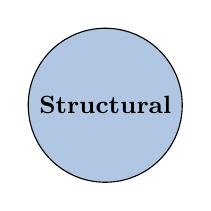
\begin{tikzpicture}[nodes={text depth=0.25ex,text height=1.25ex distance=1.7cm}]
                    \tikzstyle{every node}=[font=\small]
                    \tikzstyle{vertex} = [circle, draw=black, fill=illiniblue]
                    \tikzstyle{hidden} = [draw=none]
                    \tikzstyle{edge} = [<->, very thick]
                    
                    % \node[vertex](v1) at (0,5) {\textbf{Normative}};
                    \node[vertex](v2) at (4,0) {\textbf{Structural}};

        
            \end{tikzpicture}
            }
            % \caption{Parametric Uncertainty}
            % \label{fig:triarchic-uncertainty}
        \end{figure}

        \column[t]{6cm}
        \begin{definition}[Structural Uncertainty]
            [R]efers to the imperfect and incomplete nature of the equations describing the system \cite{decarolis_using_2011}.
        \end{definition}
        
        This type of uncertainty will \textit{always} persist.
    \end{columns}

\end{frame}

\begin{frame}
    \frametitle{Examples of Structural Uncertainty}

    \begin{itemize}
        \item Objective functions (most typical)\pause
        \item Spatiotemporal resolution\pause
        \item Physics fidelity\pause
        \item Solution method
    \end{itemize}

\end{frame}

\begin{frame}
    \frametitle{Addressing Structural Uncertainty}

    

\end{frame}

% \begin{frame}
%     \frametitle{Gap \#2: Challenges with current ESOM practices}

%     \begin{enumerate}
%         \item Structural Uncertainty
%         \begin{itemize}
%             \item $\sim$100\% of ESOM frameworks optimize cost.
%             \item Stanard MGA procedures anchor alternatives to cost --- no true
%             tradeoff analysis.
%         \end{itemize}
%         \item Normative Uncertainty: Most ESOM analyses are prescriptive, few if
%         any articulate a normative premise to justify their conclusions.
%         \begin{itemize}
%             \item ``Pathway to 100\% Renewable Energy...'' --- a commonly
%             unjustified normative conclusion, right in the title!
%             \item Why should non-renewable sources be excluded? Renewable energy
%             is not guaranteed to be democratic \cite{winner_artifacts_1980}, nor
%             sustainable \cite{bell_toward_2020}.
%         \end{itemize}
%     \end{enumerate}

% \end{frame}

\begin{frame}
    \frametitle{Gap 1: Challenges with current ESOM practices}
    \begin{block}{Technical Gap}
        \begin{enumerate}
            \item Exclusive optimization over system cost misrecognizes the plurality of 
            preferences and priorities. Tradeoff analysis is impossible.
            \item Even with open source code and transparent data sources, energy system
            models remain opaque --- decision making black boxes.
        \end{enumerate}
    \end{block}
    \begin{block}{Proposed Work Component I: Multi-objective optimization}
        \begin{itemize}
            \item Partially address procedural/recognition justice by facilitating tradeoff analysis 
            through multi-objective optimization with evolutionary
            algorithms.
            \item Develop an MGA algorithm for high dimensional space.
        \end{itemize}
        
    \end{block}
    \begin{block}{Stretch Goal}
        Further enhance the transparency component of procedural justice by developing this
        tool in a way that provides the \textit{capability} for anyone interested to 
        verify model results. I.e., make accessibility a design priority. 
    \end{block}
\end{frame}

% \section{Methodology}
% \begin{frame}
%     \frametitle{Proposal \#2: Building a flexible ESOM}

%     \begin{enumerate}
%         \item Create an open-source multi-objective energy system model (\texttt{osier}) that can allow modelers to address
%         \begin{itemize}
%             \item parametric,
%             \item structural,
%             \item and normative uncertainties.
%         \end{itemize}
%         \item Develop an MGA algorithm for use with genetic algorithms in higher dimensional spaces.
%     \end{enumerate}

% \end{frame}
\section{Component 1: Preliminary Results with \texttt{Osier}}
\begin{frame}
    \frametitle{Open source multi-objective energy system framework (\texttt{Osier})}
    \begin{itemize}
        \item Hybrid methods: linear programming \& evolutionary algorithms
        \item Novel algorithm for high dimensional MGA
    \end{itemize}
    \begin{figure}
        \centering
        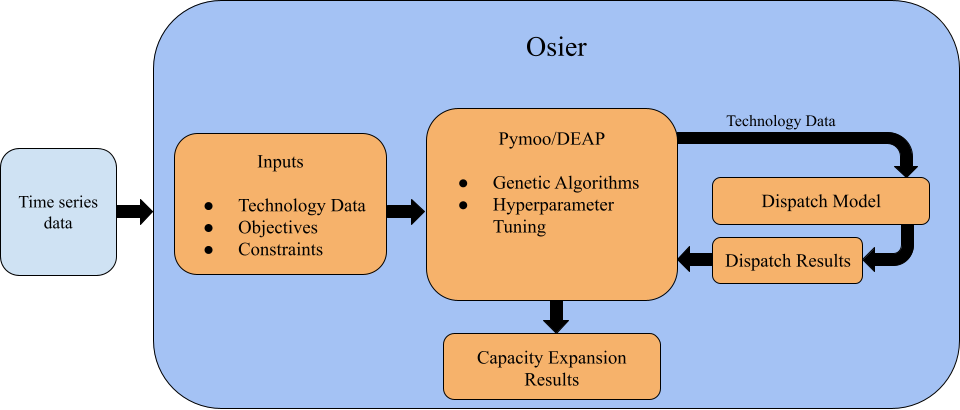
\includegraphics[width=\columnwidth]{../docs/figures/osier_flow.png}
        \caption{Flow of data through \texttt{Osier}.}
        \label{fig:osier-flow}
    \end{figure}

\end{frame}

\subsection{Methodology}
\begin{frame}
    \frametitle{Multi-objective Solutions}
    \begin{columns}
        \column[t]{4cm}
        \begin{block}{}
            Another way to generate alternatives...
        \end{block}
        \begin{block}{Pareto Front}
            Creates a \boldorange{set of solutions} rather than a single optimum.
        \end{block}
        \column[t]{6cm}
        \begin{figure}
            \centering
            \resizebox{\columnwidth}{!}{\input{../docs/figures/truss2d_pareto.pgf}}
            \caption{Pareto front example.}
            \label{fig:pareto-front}
        \end{figure}
    
    \end{columns}
    
\end{frame}

\begin{frame}
    \frametitle{Evolutionary Algorithms}

    \begin{block}{Evolutionary Algorithms for Energy System Optimization}
        \begin{columns}
            \column[t]{6cm}
            \begin{itemize}
            \item Inspired by natural selection
            \item Parallelizable
            \item Superior to pure linear programming methods for
                \begin{itemize}
                    \item independence from problem convexity
                    \item good sampling/spacing of points along solution set.
                \end{itemize}
            \end{itemize}
            
            Right: Evolutionary algorithm flow \cite{deb_evolutionary_2014}.
            \column[t]{4cm}
            \centering
            \begin{figure}
            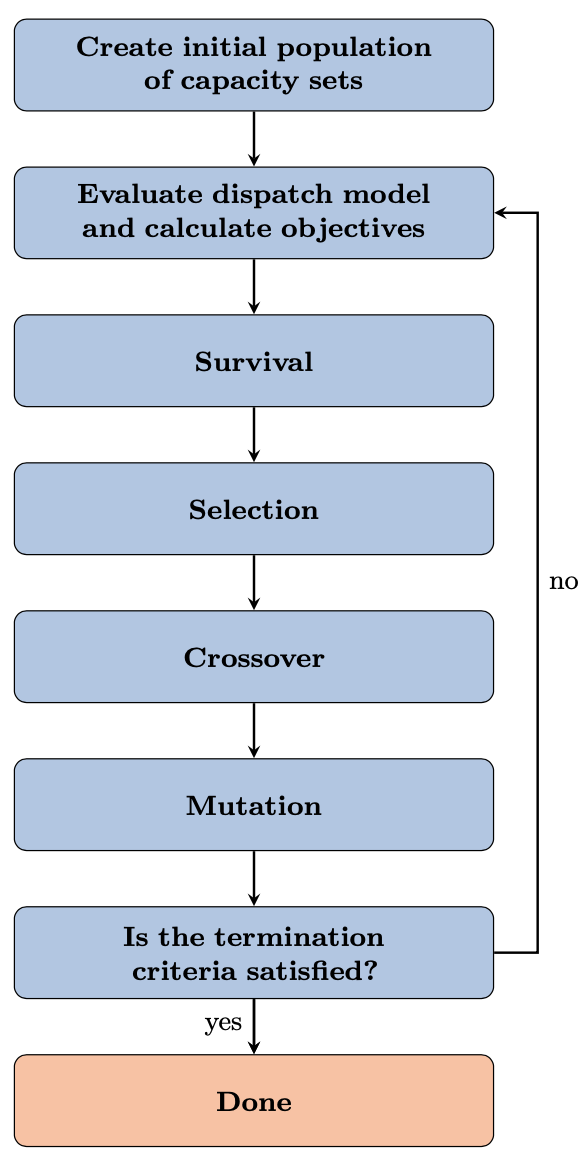
\includegraphics[width=0.75\linewidth]{images/ea-flow.png}  
            \end{figure}
        \end{columns}
    \end{block}
\end{frame}

\begin{frame}
    \frametitle{How \texttt{Osier} handles structural uncertainty}

        \begin{figure}
            \centering
            \resizebox{0.75\columnwidth}{!}{\input{images/near-optimal-pareto-pres.pgf}}
            \caption{Near optimal space for a multi-objective problem.}
            \label{fig:near-opt}
        \end{figure}
    % \end{columns}
\end{frame}

\begin{frame}<0>
    \frametitle{How \texttt{Osier} handles structural uncertainty}
        \begin{figure}
            \centering
            \resizebox{0.75\columnwidth}{!}{\input{images/near-optimal-pareto-mga-pres.pgf}}
            \caption{Near optimal space for mono- and multi-objective problems. The light blue area shows
            a vertically truncated near-optimal space around the f1 objective.}
            \label{fig:near-opt-mga}
        \end{figure}
    % \end{columns}

\end{frame}

\begin{frame}<0>
    \frametitle{How \texttt{Osier} handles structural uncertainty}
        \begin{figure}
            \centering
            \resizebox{0.75\columnwidth}{!}{\input{images/nd-mga-paretofront-pres.pgf}}
            \caption{Alternative solutions identified in the near optimal space.}
            \label{fig:nd-alt-points}
        \end{figure}
    % \end{columns}

\end{frame}


\subsection{Preliminary Results}
\begin{frame}
    \frametitle{Validating \texttt{Osier}}

    \begin{figure}
        \centering 
        % \resizebox{0.75\columnwidth}{!}{\input{../docs/figures/results/temoa_osier_benchmark_01.pgf}}
        \resizebox{0.75\columnwidth}{!}{\input{../docs/figures/temoa_osier_benchmark_01.pgf}}
        \caption{Comparing the results from \texttt{Osier} with another ESOM, \texttt{Temoa}.}
        \label{fig:osier-temoa-benchmark-2}
    \end{figure}

\end{frame}



\begin{frame}
    \frametitle{Optimizing four objectives}

    \begin{figure}
        \centering 
        % \resizebox{0.75\columnwidth}{!}{\input{../docs/figures/results/temoa_osier_benchmark_01.pgf}}
        \resizebox{0.9\columnwidth}{!}{\input{../docs/figures/4_obj_objective_space_MGA.pgf}}
        \caption{Pareto front and near-optimal solutions for the same problem with 4 objectives.}
        \label{fig:4-obj-objective-space}
    \end{figure}

\end{frame}

\begin{frame}
    \frametitle{Optimizing four objectives}

    \begin{figure}
        \centering 
        % \resizebox{0.75\columnwidth}{!}{\input{../docs/figures/results/temoa_osier_benchmark_01.pgf}}
        \resizebox{0.9\columnwidth}{!}{\input{../docs/figures/4_obj_design_space_MGA.pgf}}
        \caption{Design space for the 4-objective problem with near-optimal solutions.}
        \label{fig:4-obj-design-space}
    \end{figure}

\end{frame}

\begin{frame}
    \frametitle{How \texttt{Osier} improves on ESOMs --- and its limits}

    \begin{figure}
        \centering
        \resizebox{0.8\columnwidth}{!}{
            \begin{tikzpicture}[nodes={text depth=0.25ex,text height=1.25ex distance=1.7cm}]
                \tikzstyle{every node}=[font=\small]
                \tikzstyle{vertex} = [circle, draw=black]
                \tikzstyle{hidden} = [draw=none]
                \tikzstyle{edge} = [<->, very thick]
                
                \node[vertex, fill=illiniblue](v1) at (0,5) {\textbf{Normative}};
                \node[vertex, fill=blue2](v2) at (4,0) {\textbf{Structural}};
                \node[vertex, fill=blue6](v3) at (-4,0) {\textbf{Parametric}};
    
                \draw[edge] (v1) -- (v2);
                \draw[edge] (v2) -- (v3);
                \draw[edge] (v1) -- (v3);
    
                % hidden nodes for v1
                \node[hidden](h1) at (-0.75, 5) {};
                \node[hidden](h2) at (0.75, 5) {};
    
                % hidden nodes for v2
                \node[hidden](h3) at (4, 0.75) {};
                \node[hidden](h4) at (4, -0.7) {};
    
                % hidden nodes for v3
                \node[hidden](h5) at (-4, -0.7) {};
                \node[hidden](h6) at (-4, 0.75) {};
    
                \draw[draw=none] (h4) -- (h5) node[anchor=mid, midway, sloped]{\textbf{Descriptive}};
                \draw[draw=none] (h6) -- (h1) node[anchor=mid, midway, sloped]{\textbf{Pre-descriptive}};
                \draw[draw=none] (h2) -- (h3) node[anchor=mid, midway, sloped]{\textbf{Prescriptive}};

                % objectivity scale
                \node[hidden](u1) at (-6,5) {\textbf{Epistemic}};
                \node[hidden](u2) at (-6,0) {\textbf{Aleatory}};
                \draw[edge] (u1) -- (u2);


                % objectivity scale
                \node[hidden](u1) at (6,5) {\textbf{Subjective}};
                \node[hidden](u2) at (6,0) {\textbf{Objective}}; \draw[edge]
                (u1) -- (u2);
    
    
        \end{tikzpicture}
        }
        \caption{A summary of three uncertainties and their interactions.}
        \label{fig:triarchic-uncertainty}
    \end{figure}

\end{frame}

\begin{frame}
    \frametitle{Future Work for \texttt{Osier}}

    \begin{block}{Improvement 1}
        Improve the MGA procedure to identify \textit{maximally different} solutions in the design space.
        I.e., more efficient search.
    \end{block}
    \begin{block}{Avenue 2}
        This improvement could be unlocked with a greedy, farthest-first-traversal algorithm.
    \end{block}
    \begin{block}{Improvement 2}
        Take advantage of evolutionary algorithms' parralelizability.
    \end{block}
    \begin{block}{Avenue 2}
        Consider a method besides linear programming for energy dispatch (e.g., hierarchical dispatch) \cite{prina_multi-objective_2020}.
    \end{block}

\end{frame}

%
\section{Motivation and Background II}
\subsection{New Questions}
\begin{frame}
    \frametitle{New Questions}

    \begin{block}{Question 3}
        If structural uncertainty is addressed by presenting mutliple solutions,
        how should society choose among those alternatives?
    \end{block}

    \begin{block}{Question 4}
        How can members of the lay public adequately deliberate on issues
        perceived by experts as highly technical?
    \end{block}

\end{frame}

\subsection{Cognitive Myopia}
\begin{frame}
    \frametitle{What's still missing?}

    Despite awareness of structural and parametric uncertainties modelers still don't address
    \begin{itemize}
        \item How parameter distributions are chosen?
        \item Why are certain objectives chosen (why should an economic objective be \textit{assumed})?
        \item What motivated the specified set of decision variables (why are technologies included/excluded)?
        \item Why is the recommended solution preferred to nearby alternatives?
    \end{itemize}

    This alludes to another kind of uncertainty... 
\end{frame}

\begin{frame}
    \frametitle{Normative Uncertainty}

    Stating your assumptions is a necessary but insufficient condition for addressing normative uncertainty.

    \begin{columns}
        \column[t]{4cm}
        \begin{figure}
            \centering
            \resizebox{\columnwidth}{!}{
            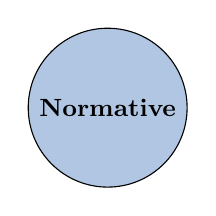
\begin{tikzpicture}[nodes={text depth=0.25ex,text height=1.25ex distance=1.7cm}]
                    \tikzstyle{every node}=[font=\small]
                    \tikzstyle{vertex} = [circle, draw=black, fill=illiniblue]
                    \tikzstyle{hidden} = [draw=none]
                    \tikzstyle{edge} = [<->, very thick]
                    
                    \node[vertex](v1) at (0,5) {\textbf{Normative}};

        
            \end{tikzpicture}
            }
            % \caption{Parametric Uncertainty}
            % \label{fig:triarchic-uncertainty}
        \end{figure}

        \column[t]{6cm}
        Answers the question ``what is acceptable and why?''

        \begin{itemize}
            \item Climate change is happening!
        \end{itemize}

        
    \end{columns}

\end{frame}

\subsection{Proposal}
% \begin{frame}
%     \frametitle{Gap \#3: Overcoming Arrow's Theorem}

%     \begin{enumerate}
%         \item Deciding among alternative solutions is challenging without a normative premise.
%         \item Without direct consultation of stakeholders, it's impossible know how they would understand tradeoffs.
%         \item Capturing the ``human dimension'' requires incorporating formal methods from social science: case studies,
%         interviews, focus groups, surveys, etc. The ESOM literature struggles to do this.
%     \end{enumerate}

% \end{frame}
\begin{frame}
    \frametitle{Gap 2: Normative Uncertainty \& Deliberative Processes}
    \begin{block}{Technical Gap}
        \begin{enumerate}
            \item Deciding among alternative solutions is challenging without a normative premise.
            \item Without direct consultation of stakeholders, it's impossible know how they would understand tradeoffs.
            \item Capturing the ``human dimension'' requires incorporating formal methods from social science: case studies,
            interviews, focus groups, surveys, etc. The ESOM literature struggles to do this \cite{pfenninger_energy_2014}.
        \end{enumerate}
    \end{block}
    \begin{block}{Proposed Work Component II: Integrative theory of uncertainties}
        Further develop the unifying theory of model development through the lens of 
        addressing triple uncertainties.
    \end{block}
    \begin{block}{Proposed Work Component III: Case study of Champaign-Urbana}
        Case study of energy planning processes in the Champaign-Urbana region to validate
        the usefulness of \texttt{Osier} and test the salience of various uncertainties in
        these planning processes.
    \end{block}
    
\end{frame}

\section{Components II+III: Details}
\subsection{Component II: How engineering relates to energy justice}
    \begin{figure}
        \centering
        \resizebox{0.8\columnwidth}{!}{
            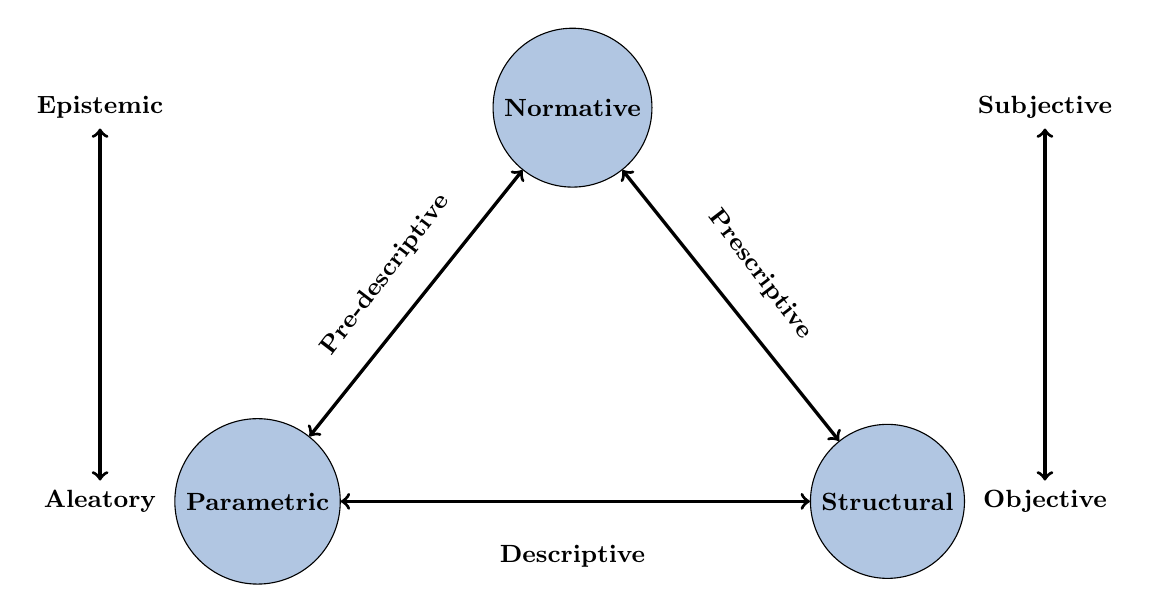
\begin{tikzpicture}[nodes={text depth=0.25ex,text height=1.25ex distance=1.7cm}]
                \tikzstyle{every node}=[font=\small]
                \tikzstyle{vertex} = [circle, draw=black, fill=illiniblue]
                \tikzstyle{vertex1} = [circle, draw=black, fill=blue4]
                \tikzstyle{vertex2} = [circle, draw=black, fill=blue6]
                \tikzstyle{vertex3} = [circle, draw=black, fill=blue2]
                \tikzstyle{hidden} = [draw=none]
                \tikzstyle{edge} = [<->, very thick]
                
                \node[vertex](v1) at (0,5) {\textbf{Normative}};
                \node[vertex](v2) at (4,0) {\textbf{Structural}};
                \node[vertex](v3) at (-4,0) {\textbf{Parametric}};
    
                \draw[edge] (v1) -- (v2);
                \draw[edge] (v2) -- (v3);
                \draw[edge] (v1) -- (v3);
    
                % hidden nodes for v1
                \node[hidden](h1) at (-0.75, 5) {};
                \node[hidden](h2) at (0.75, 5) {};
    
                % hidden nodes for v2
                \node[hidden](h3) at (4, 0.75) {};
                \node[hidden](h4) at (4, -0.7) {};
    
                % hidden nodes for v3
                \node[hidden](h5) at (-4, -0.7) {};
                \node[hidden](h6) at (-4, 0.75) {};
    
                \draw[draw=none] (h4) -- (h5) node[anchor=mid, midway, sloped]{\textbf{Descriptive}};
                \draw[draw=none] (h6) -- (h1) node[anchor=mid, midway, sloped]{\textbf{Pre-descriptive}};
                \draw[draw=none] (h2) -- (h3) node[anchor=mid, midway, sloped]{\textbf{Prescriptive}};

                % objectivity scale
                \node[hidden](u1) at (-6,5) {\textbf{Epistemic}};
                \node[hidden](u2) at (-6,0) {\textbf{Aleatory}};
                \draw[edge] (u1) -- (u2);


                % objectivity scale
                \node[hidden](u1) at (6,5) {\textbf{Subjective}};
                \node[hidden](u2) at (6,0) {\textbf{Objective}}; \draw[edge]
                (u1) -- (u2);
    
    
        \end{tikzpicture}
        }
        \caption{A summary of three uncertainties and their interactions.}
    \end{figure}
\subsection{Component III: Regional Case Study}
\begin{frame}
    \frametitle{Regional Case Study}

    \textit{Someday, details will go here!}

\end{frame}

% \begin{itemize}
%     \item Provides an illusion of objectivity that can be used to dismiss non-technical concerns.
%     \item Even ``transparent'' models are opaque to public scrutiny.
% \end{itemize}


% \begin{frame} \frametitle{Enhanced Participation?}

%     \begin{enumerate} \item Although public hearings exist during licensing
%         procedures for many types of energy projects these hearings
%         \textit{close down} rather than \textit{open up} debate
%         \cite{wilsdon_see-through_2004,stirling_opening_2008}. \item This is
%         because public testimony can be dismissed as ``untechnical,'' such as
%         testimonies raising concerns about the Dakota Access Pipeline (DAPL)
%         running through Illinois \cite{johnson_dakota_2021}. \item Opposition
%         does not always stop but it can delay progress towards adopting clean
%         energy technologies, and the lack of participatory options does not
%         improve public trust in a technology, regardless. \item Does the
%         public even know what their preferences are? \item The issue
%         transforms into the following: how can we bridge the communication gap
%         between the lay public and engineers in a way that maintains technical
%         rigor but also directly incorporates public preferences?

%     \end{enumerate}

% \end{frame}

% \begin{frame} \frametitle{Energy Systems as a Social Experiment}

%     \begin{enumerate} \item Multi-objective methods are useful for
%         articulating preferences and identifying tradeoffs in an iterative
%         process. \item This iterative process is useful for highlighting the
%         priorities of the public. Especially in the sense of energy systems as
%         ``social experiments'' \cite{van_de_poel_nuclear_2011} the
%         consequences of which may not always be known in advance. But they
%         must always be considered in the context of alternatives, because
%         maintaining the status quo is also a social experiment which in our
%         present circumstances produces deleterious consequences for the
%         environment and human thriving. \end{enumerate}

% \end{frame}
% \section{Technical Gap \#1}
\begin{frame}
    \frametitle{Gap \#1: Incomplete understanding of uncertainty}
    % normative uncertainty is not a subset of structural uncertainty because there can be purely pragmatic structural
    % uncertainties. For example, neglecting electrical resistance.

    Climate change is a ``wicked problem'' with many uncertainties \cite{grundmann_ozone_2018}. 
    
    Policies derived from theory or modeling practices ignorant of these uncertainties is partially
    responsible for the paradox identified previously.
    
    A more comprehensive understanding of these uncertainties will inform better modeling practices and 
    more just solutions. 

\end{frame}
% \section{Proposal \#1}
\begin{frame}
    \frametitle{Proposal \#1: Understanding Uncertainty}

    \begin{enumerate}
        \item Develop a theoretical framework to conceptualize different
        uncertainties and their interrelationships.
        \item Connect this framework to \textit{justice}, specifically
        Schlosberg's three-tenet paradigm 
        \cite{schlosberg_reconceiving_2004}.
    \end{enumerate}

\end{frame}
\section{Tale of Three Uncertainties}
\subsection{Triarchic Uncertainty}
    \begin{figure}
        \centering
        \resizebox{0.8\columnwidth}{!}{
            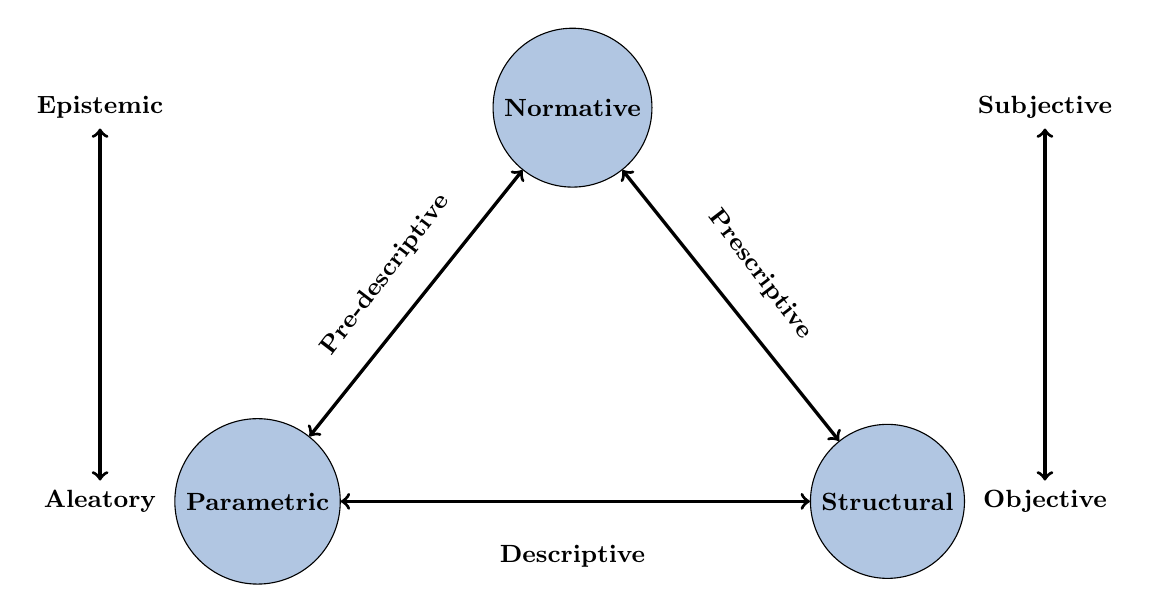
\begin{tikzpicture}[nodes={text depth=0.25ex,text height=1.25ex distance=1.7cm}]
                \tikzstyle{every node}=[font=\small]
                \tikzstyle{vertex} = [circle, draw=black, fill=illiniblue]
                \tikzstyle{vertex1} = [circle, draw=black, fill=blue4]
                \tikzstyle{vertex2} = [circle, draw=black, fill=blue6]
                \tikzstyle{vertex3} = [circle, draw=black, fill=blue2]
                \tikzstyle{hidden} = [draw=none]
                \tikzstyle{edge} = [<->, very thick]
                
                \node[vertex](v1) at (0,5) {\textbf{Normative}};
                \node[vertex](v2) at (4,0) {\textbf{Structural}};
                \node[vertex](v3) at (-4,0) {\textbf{Parametric}};
    
                \draw[edge] (v1) -- (v2);
                \draw[edge] (v2) -- (v3);
                \draw[edge] (v1) -- (v3);
    
                % hidden nodes for v1
                \node[hidden](h1) at (-0.75, 5) {};
                \node[hidden](h2) at (0.75, 5) {};
    
                % hidden nodes for v2
                \node[hidden](h3) at (4, 0.75) {};
                \node[hidden](h4) at (4, -0.7) {};
    
                % hidden nodes for v3
                \node[hidden](h5) at (-4, -0.7) {};
                \node[hidden](h6) at (-4, 0.75) {};
    
                \draw[draw=none] (h4) -- (h5) node[anchor=mid, midway, sloped]{\textbf{Descriptive}};
                \draw[draw=none] (h6) -- (h1) node[anchor=mid, midway, sloped]{\textbf{Pre-descriptive}};
                \draw[draw=none] (h2) -- (h3) node[anchor=mid, midway, sloped]{\textbf{Prescriptive}};

                % objectivity scale
                \node[hidden](u1) at (-6,5) {\textbf{Epistemic}};
                \node[hidden](u2) at (-6,0) {\textbf{Aleatory}};
                \draw[edge] (u1) -- (u2);


                % objectivity scale
                \node[hidden](u1) at (6,5) {\textbf{Subjective}};
                \node[hidden](u2) at (6,0) {\textbf{Objective}}; \draw[edge]
                (u1) -- (u2);
    
    
        \end{tikzpicture}
        }
        \caption{A summary of three uncertainties and their interactions.}
    \end{figure}
% let's begin with a familiar form of uncertainty -- parametric
\subsection{Parametric Uncertainty}
\begin{frame}
    \frametitle{Parametric Uncertainty}
    \begin{columns}
        \column[t]{4cm}
        \begin{figure}
            \centering
            \resizebox{\columnwidth}{!}{
            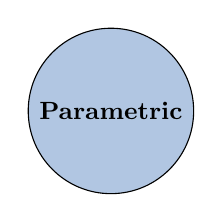
\begin{tikzpicture}[nodes={text depth=0.25ex,text height=1.25ex distance=1.7cm}]
                    \tikzstyle{every node}=[font=\small] \tikzstyle{vertex} =
                    [circle, draw=black, fill=illiniblue] \tikzstyle{hidden} =
                    [draw=none] \tikzstyle{edge} = [<->, very thick]

                    \node[vertex](v3) at (-4,0) {\textbf{Parametric}};
        
            \end{tikzpicture}
            }
            % \caption{Parametric Uncertainty} \label{fig:triarchic-uncertainty}
        \end{figure}

        \column[t]{6cm}
        \begin{block}{Parametric Uncertainty}
            Related to uncertainty in model inputs (empirical values). The most
            commonly addressed type of uncertainty in science and engineering
            \cite{yue_review_2018,decarolis_using_2011,morgan_uncertainty_1990}.    
        \end{block}
        
        % May be classified as either \boldorange{aleatory} or
        % \boldorange{epistemic}
        % \cite{pfenninger_energy_2014,kiureghian_aleatory_2009}. 
    \end{columns}

\end{frame}

\begin{frame}
    \frametitle{Examples of Parametric Uncertainty}

    \begin{columns}
        \column[t]{5cm}
        \begin{figure}
            \centering
            \resizebox{\columnwidth}{!}{
                %% Creator: Matplotlib, PGF backend
%%
%% To include the figure in your LaTeX document, write
%%   \input{<filename>.pgf}
%%
%% Make sure the required packages are loaded in your preamble
%%   \usepackage{pgf}
%%
%% Also ensure that all the required font packages are loaded; for instance,
%% the lmodern package is sometimes necessary when using math font.
%%   \usepackage{lmodern}
%%
%% Figures using additional raster images can only be included by \input if
%% they are in the same directory as the main LaTeX file. For loading figures
%% from other directories you can use the `import` package
%%   \usepackage{import}
%%
%% and then include the figures with
%%   \import{<path to file>}{<filename>.pgf}
%%
%% Matplotlib used the following preamble
%%   
%%   \makeatletter\@ifpackageloaded{underscore}{}{\usepackage[strings]{underscore}}\makeatother
%%
\begingroup%
\makeatletter%
\begin{pgfpicture}%
\pgfpathrectangle{\pgfpointorigin}{\pgfqpoint{8.900000in}{6.900000in}}%
\pgfusepath{use as bounding box, clip}%
\begin{pgfscope}%
\pgfsetbuttcap%
\pgfsetmiterjoin%
\definecolor{currentfill}{rgb}{0.827451,0.827451,0.827451}%
\pgfsetfillcolor{currentfill}%
\pgfsetlinewidth{0.000000pt}%
\definecolor{currentstroke}{rgb}{0.000000,0.000000,0.000000}%
\pgfsetstrokecolor{currentstroke}%
\pgfsetdash{}{0pt}%
\pgfpathmoveto{\pgfqpoint{0.000000in}{0.000000in}}%
\pgfpathlineto{\pgfqpoint{8.900000in}{0.000000in}}%
\pgfpathlineto{\pgfqpoint{8.900000in}{6.900000in}}%
\pgfpathlineto{\pgfqpoint{0.000000in}{6.900000in}}%
\pgfpathlineto{\pgfqpoint{0.000000in}{0.000000in}}%
\pgfpathclose%
\pgfusepath{fill}%
\end{pgfscope}%
\begin{pgfscope}%
\pgfsetbuttcap%
\pgfsetmiterjoin%
\definecolor{currentfill}{rgb}{1.000000,1.000000,1.000000}%
\pgfsetfillcolor{currentfill}%
\pgfsetlinewidth{0.000000pt}%
\definecolor{currentstroke}{rgb}{0.000000,0.000000,0.000000}%
\pgfsetstrokecolor{currentstroke}%
\pgfsetstrokeopacity{0.000000}%
\pgfsetdash{}{0pt}%
\pgfpathmoveto{\pgfqpoint{0.955442in}{0.230015in}}%
\pgfpathlineto{\pgfqpoint{8.800000in}{0.230015in}}%
\pgfpathlineto{\pgfqpoint{8.800000in}{6.800000in}}%
\pgfpathlineto{\pgfqpoint{0.955442in}{6.800000in}}%
\pgfpathlineto{\pgfqpoint{0.955442in}{0.230015in}}%
\pgfpathclose%
\pgfusepath{fill}%
\end{pgfscope}%
\begin{pgfscope}%
\pgfpathrectangle{\pgfqpoint{0.955442in}{0.230015in}}{\pgfqpoint{7.844558in}{6.569985in}}%
\pgfusepath{clip}%
\pgfsetbuttcap%
\pgfsetroundjoin%
\definecolor{currentfill}{rgb}{0.839216,0.152941,0.156863}%
\pgfsetfillcolor{currentfill}%
\pgfsetfillopacity{0.500000}%
\pgfsetlinewidth{1.003750pt}%
\definecolor{currentstroke}{rgb}{0.839216,0.152941,0.156863}%
\pgfsetstrokecolor{currentstroke}%
\pgfsetdash{}{0pt}%
\pgfsys@defobject{currentmarker}{\pgfqpoint{1.461125in}{0.230015in}}{\pgfqpoint{4.432890in}{3.311620in}}{%
\pgfpathmoveto{\pgfqpoint{1.461125in}{0.240185in}}%
\pgfpathlineto{\pgfqpoint{1.461125in}{0.230015in}}%
\pgfpathlineto{\pgfqpoint{1.476059in}{0.230015in}}%
\pgfpathlineto{\pgfqpoint{1.490992in}{0.230015in}}%
\pgfpathlineto{\pgfqpoint{1.505926in}{0.230015in}}%
\pgfpathlineto{\pgfqpoint{1.520859in}{0.230015in}}%
\pgfpathlineto{\pgfqpoint{1.535793in}{0.230015in}}%
\pgfpathlineto{\pgfqpoint{1.550726in}{0.230015in}}%
\pgfpathlineto{\pgfqpoint{1.565660in}{0.230015in}}%
\pgfpathlineto{\pgfqpoint{1.580593in}{0.230015in}}%
\pgfpathlineto{\pgfqpoint{1.595527in}{0.230015in}}%
\pgfpathlineto{\pgfqpoint{1.610460in}{0.230015in}}%
\pgfpathlineto{\pgfqpoint{1.625394in}{0.230015in}}%
\pgfpathlineto{\pgfqpoint{1.640327in}{0.230015in}}%
\pgfpathlineto{\pgfqpoint{1.655260in}{0.230015in}}%
\pgfpathlineto{\pgfqpoint{1.670194in}{0.230015in}}%
\pgfpathlineto{\pgfqpoint{1.685127in}{0.230015in}}%
\pgfpathlineto{\pgfqpoint{1.700061in}{0.230015in}}%
\pgfpathlineto{\pgfqpoint{1.714994in}{0.230015in}}%
\pgfpathlineto{\pgfqpoint{1.729928in}{0.230015in}}%
\pgfpathlineto{\pgfqpoint{1.744861in}{0.230015in}}%
\pgfpathlineto{\pgfqpoint{1.759795in}{0.230015in}}%
\pgfpathlineto{\pgfqpoint{1.774728in}{0.230015in}}%
\pgfpathlineto{\pgfqpoint{1.789662in}{0.230015in}}%
\pgfpathlineto{\pgfqpoint{1.804595in}{0.230015in}}%
\pgfpathlineto{\pgfqpoint{1.819529in}{0.230015in}}%
\pgfpathlineto{\pgfqpoint{1.834462in}{0.230015in}}%
\pgfpathlineto{\pgfqpoint{1.849396in}{0.230015in}}%
\pgfpathlineto{\pgfqpoint{1.864329in}{0.230015in}}%
\pgfpathlineto{\pgfqpoint{1.879263in}{0.230015in}}%
\pgfpathlineto{\pgfqpoint{1.894196in}{0.230015in}}%
\pgfpathlineto{\pgfqpoint{1.909130in}{0.230015in}}%
\pgfpathlineto{\pgfqpoint{1.924063in}{0.230015in}}%
\pgfpathlineto{\pgfqpoint{1.938997in}{0.230015in}}%
\pgfpathlineto{\pgfqpoint{1.953930in}{0.230015in}}%
\pgfpathlineto{\pgfqpoint{1.968864in}{0.230015in}}%
\pgfpathlineto{\pgfqpoint{1.983797in}{0.230015in}}%
\pgfpathlineto{\pgfqpoint{1.998731in}{0.230015in}}%
\pgfpathlineto{\pgfqpoint{2.013664in}{0.230015in}}%
\pgfpathlineto{\pgfqpoint{2.028598in}{0.230015in}}%
\pgfpathlineto{\pgfqpoint{2.043531in}{0.230015in}}%
\pgfpathlineto{\pgfqpoint{2.058465in}{0.230015in}}%
\pgfpathlineto{\pgfqpoint{2.073398in}{0.230015in}}%
\pgfpathlineto{\pgfqpoint{2.088332in}{0.230015in}}%
\pgfpathlineto{\pgfqpoint{2.103265in}{0.230015in}}%
\pgfpathlineto{\pgfqpoint{2.118199in}{0.230015in}}%
\pgfpathlineto{\pgfqpoint{2.133132in}{0.230015in}}%
\pgfpathlineto{\pgfqpoint{2.148066in}{0.230015in}}%
\pgfpathlineto{\pgfqpoint{2.162999in}{0.230015in}}%
\pgfpathlineto{\pgfqpoint{2.177933in}{0.230015in}}%
\pgfpathlineto{\pgfqpoint{2.192866in}{0.230015in}}%
\pgfpathlineto{\pgfqpoint{2.207800in}{0.230015in}}%
\pgfpathlineto{\pgfqpoint{2.222733in}{0.230015in}}%
\pgfpathlineto{\pgfqpoint{2.237667in}{0.230015in}}%
\pgfpathlineto{\pgfqpoint{2.252600in}{0.230015in}}%
\pgfpathlineto{\pgfqpoint{2.267534in}{0.230015in}}%
\pgfpathlineto{\pgfqpoint{2.282467in}{0.230015in}}%
\pgfpathlineto{\pgfqpoint{2.297401in}{0.230015in}}%
\pgfpathlineto{\pgfqpoint{2.312334in}{0.230015in}}%
\pgfpathlineto{\pgfqpoint{2.327268in}{0.230015in}}%
\pgfpathlineto{\pgfqpoint{2.342201in}{0.230015in}}%
\pgfpathlineto{\pgfqpoint{2.357135in}{0.230015in}}%
\pgfpathlineto{\pgfqpoint{2.372068in}{0.230015in}}%
\pgfpathlineto{\pgfqpoint{2.387002in}{0.230015in}}%
\pgfpathlineto{\pgfqpoint{2.401935in}{0.230015in}}%
\pgfpathlineto{\pgfqpoint{2.416869in}{0.230015in}}%
\pgfpathlineto{\pgfqpoint{2.431802in}{0.230015in}}%
\pgfpathlineto{\pgfqpoint{2.446736in}{0.230015in}}%
\pgfpathlineto{\pgfqpoint{2.461669in}{0.230015in}}%
\pgfpathlineto{\pgfqpoint{2.476603in}{0.230015in}}%
\pgfpathlineto{\pgfqpoint{2.491536in}{0.230015in}}%
\pgfpathlineto{\pgfqpoint{2.506470in}{0.230015in}}%
\pgfpathlineto{\pgfqpoint{2.521403in}{0.230015in}}%
\pgfpathlineto{\pgfqpoint{2.536336in}{0.230015in}}%
\pgfpathlineto{\pgfqpoint{2.551270in}{0.230015in}}%
\pgfpathlineto{\pgfqpoint{2.566203in}{0.230015in}}%
\pgfpathlineto{\pgfqpoint{2.581137in}{0.230015in}}%
\pgfpathlineto{\pgfqpoint{2.596070in}{0.230015in}}%
\pgfpathlineto{\pgfqpoint{2.611004in}{0.230015in}}%
\pgfpathlineto{\pgfqpoint{2.625937in}{0.230015in}}%
\pgfpathlineto{\pgfqpoint{2.640871in}{0.230015in}}%
\pgfpathlineto{\pgfqpoint{2.655804in}{0.230015in}}%
\pgfpathlineto{\pgfqpoint{2.670738in}{0.230015in}}%
\pgfpathlineto{\pgfqpoint{2.685671in}{0.230015in}}%
\pgfpathlineto{\pgfqpoint{2.700605in}{0.230015in}}%
\pgfpathlineto{\pgfqpoint{2.715538in}{0.230015in}}%
\pgfpathlineto{\pgfqpoint{2.730472in}{0.230015in}}%
\pgfpathlineto{\pgfqpoint{2.745405in}{0.230015in}}%
\pgfpathlineto{\pgfqpoint{2.760339in}{0.230015in}}%
\pgfpathlineto{\pgfqpoint{2.775272in}{0.230015in}}%
\pgfpathlineto{\pgfqpoint{2.790206in}{0.230015in}}%
\pgfpathlineto{\pgfqpoint{2.805139in}{0.230015in}}%
\pgfpathlineto{\pgfqpoint{2.820073in}{0.230015in}}%
\pgfpathlineto{\pgfqpoint{2.835006in}{0.230015in}}%
\pgfpathlineto{\pgfqpoint{2.849940in}{0.230015in}}%
\pgfpathlineto{\pgfqpoint{2.864873in}{0.230015in}}%
\pgfpathlineto{\pgfqpoint{2.879807in}{0.230015in}}%
\pgfpathlineto{\pgfqpoint{2.894740in}{0.230015in}}%
\pgfpathlineto{\pgfqpoint{2.909674in}{0.230015in}}%
\pgfpathlineto{\pgfqpoint{2.924607in}{0.230015in}}%
\pgfpathlineto{\pgfqpoint{2.939541in}{0.230015in}}%
\pgfpathlineto{\pgfqpoint{2.954474in}{0.230015in}}%
\pgfpathlineto{\pgfqpoint{2.969408in}{0.230015in}}%
\pgfpathlineto{\pgfqpoint{2.984341in}{0.230015in}}%
\pgfpathlineto{\pgfqpoint{2.999275in}{0.230015in}}%
\pgfpathlineto{\pgfqpoint{3.014208in}{0.230015in}}%
\pgfpathlineto{\pgfqpoint{3.029142in}{0.230015in}}%
\pgfpathlineto{\pgfqpoint{3.044075in}{0.230015in}}%
\pgfpathlineto{\pgfqpoint{3.059009in}{0.230015in}}%
\pgfpathlineto{\pgfqpoint{3.073942in}{0.230015in}}%
\pgfpathlineto{\pgfqpoint{3.088876in}{0.230015in}}%
\pgfpathlineto{\pgfqpoint{3.103809in}{0.230015in}}%
\pgfpathlineto{\pgfqpoint{3.118743in}{0.230015in}}%
\pgfpathlineto{\pgfqpoint{3.133676in}{0.230015in}}%
\pgfpathlineto{\pgfqpoint{3.148610in}{0.230015in}}%
\pgfpathlineto{\pgfqpoint{3.163543in}{0.230015in}}%
\pgfpathlineto{\pgfqpoint{3.178477in}{0.230015in}}%
\pgfpathlineto{\pgfqpoint{3.193410in}{0.230015in}}%
\pgfpathlineto{\pgfqpoint{3.208344in}{0.230015in}}%
\pgfpathlineto{\pgfqpoint{3.223277in}{0.230015in}}%
\pgfpathlineto{\pgfqpoint{3.238211in}{0.230015in}}%
\pgfpathlineto{\pgfqpoint{3.253144in}{0.230015in}}%
\pgfpathlineto{\pgfqpoint{3.268078in}{0.230015in}}%
\pgfpathlineto{\pgfqpoint{3.283011in}{0.230015in}}%
\pgfpathlineto{\pgfqpoint{3.297945in}{0.230015in}}%
\pgfpathlineto{\pgfqpoint{3.312878in}{0.230015in}}%
\pgfpathlineto{\pgfqpoint{3.327812in}{0.230015in}}%
\pgfpathlineto{\pgfqpoint{3.342745in}{0.230015in}}%
\pgfpathlineto{\pgfqpoint{3.357679in}{0.230015in}}%
\pgfpathlineto{\pgfqpoint{3.372612in}{0.230015in}}%
\pgfpathlineto{\pgfqpoint{3.387546in}{0.230015in}}%
\pgfpathlineto{\pgfqpoint{3.402479in}{0.230015in}}%
\pgfpathlineto{\pgfqpoint{3.417413in}{0.230015in}}%
\pgfpathlineto{\pgfqpoint{3.432346in}{0.230015in}}%
\pgfpathlineto{\pgfqpoint{3.447279in}{0.230015in}}%
\pgfpathlineto{\pgfqpoint{3.462213in}{0.230015in}}%
\pgfpathlineto{\pgfqpoint{3.477146in}{0.230015in}}%
\pgfpathlineto{\pgfqpoint{3.492080in}{0.230015in}}%
\pgfpathlineto{\pgfqpoint{3.507013in}{0.230015in}}%
\pgfpathlineto{\pgfqpoint{3.521947in}{0.230015in}}%
\pgfpathlineto{\pgfqpoint{3.536880in}{0.230015in}}%
\pgfpathlineto{\pgfqpoint{3.551814in}{0.230015in}}%
\pgfpathlineto{\pgfqpoint{3.566747in}{0.230015in}}%
\pgfpathlineto{\pgfqpoint{3.581681in}{0.230015in}}%
\pgfpathlineto{\pgfqpoint{3.596614in}{0.230015in}}%
\pgfpathlineto{\pgfqpoint{3.611548in}{0.230015in}}%
\pgfpathlineto{\pgfqpoint{3.626481in}{0.230015in}}%
\pgfpathlineto{\pgfqpoint{3.641415in}{0.230015in}}%
\pgfpathlineto{\pgfqpoint{3.656348in}{0.230015in}}%
\pgfpathlineto{\pgfqpoint{3.671282in}{0.230015in}}%
\pgfpathlineto{\pgfqpoint{3.686215in}{0.230015in}}%
\pgfpathlineto{\pgfqpoint{3.701149in}{0.230015in}}%
\pgfpathlineto{\pgfqpoint{3.716082in}{0.230015in}}%
\pgfpathlineto{\pgfqpoint{3.731016in}{0.230015in}}%
\pgfpathlineto{\pgfqpoint{3.745949in}{0.230015in}}%
\pgfpathlineto{\pgfqpoint{3.760883in}{0.230015in}}%
\pgfpathlineto{\pgfqpoint{3.775816in}{0.230015in}}%
\pgfpathlineto{\pgfqpoint{3.790750in}{0.230015in}}%
\pgfpathlineto{\pgfqpoint{3.805683in}{0.230015in}}%
\pgfpathlineto{\pgfqpoint{3.820617in}{0.230015in}}%
\pgfpathlineto{\pgfqpoint{3.835550in}{0.230015in}}%
\pgfpathlineto{\pgfqpoint{3.850484in}{0.230015in}}%
\pgfpathlineto{\pgfqpoint{3.865417in}{0.230015in}}%
\pgfpathlineto{\pgfqpoint{3.880351in}{0.230015in}}%
\pgfpathlineto{\pgfqpoint{3.895284in}{0.230015in}}%
\pgfpathlineto{\pgfqpoint{3.910218in}{0.230015in}}%
\pgfpathlineto{\pgfqpoint{3.925151in}{0.230015in}}%
\pgfpathlineto{\pgfqpoint{3.940085in}{0.230015in}}%
\pgfpathlineto{\pgfqpoint{3.955018in}{0.230015in}}%
\pgfpathlineto{\pgfqpoint{3.969952in}{0.230015in}}%
\pgfpathlineto{\pgfqpoint{3.984885in}{0.230015in}}%
\pgfpathlineto{\pgfqpoint{3.999819in}{0.230015in}}%
\pgfpathlineto{\pgfqpoint{4.014752in}{0.230015in}}%
\pgfpathlineto{\pgfqpoint{4.029686in}{0.230015in}}%
\pgfpathlineto{\pgfqpoint{4.044619in}{0.230015in}}%
\pgfpathlineto{\pgfqpoint{4.059553in}{0.230015in}}%
\pgfpathlineto{\pgfqpoint{4.074486in}{0.230015in}}%
\pgfpathlineto{\pgfqpoint{4.089420in}{0.230015in}}%
\pgfpathlineto{\pgfqpoint{4.104353in}{0.230015in}}%
\pgfpathlineto{\pgfqpoint{4.119287in}{0.230015in}}%
\pgfpathlineto{\pgfqpoint{4.134220in}{0.230015in}}%
\pgfpathlineto{\pgfqpoint{4.149154in}{0.230015in}}%
\pgfpathlineto{\pgfqpoint{4.164087in}{0.230015in}}%
\pgfpathlineto{\pgfqpoint{4.179021in}{0.230015in}}%
\pgfpathlineto{\pgfqpoint{4.193954in}{0.230015in}}%
\pgfpathlineto{\pgfqpoint{4.208888in}{0.230015in}}%
\pgfpathlineto{\pgfqpoint{4.223821in}{0.230015in}}%
\pgfpathlineto{\pgfqpoint{4.238755in}{0.230015in}}%
\pgfpathlineto{\pgfqpoint{4.253688in}{0.230015in}}%
\pgfpathlineto{\pgfqpoint{4.268622in}{0.230015in}}%
\pgfpathlineto{\pgfqpoint{4.283555in}{0.230015in}}%
\pgfpathlineto{\pgfqpoint{4.298489in}{0.230015in}}%
\pgfpathlineto{\pgfqpoint{4.313422in}{0.230015in}}%
\pgfpathlineto{\pgfqpoint{4.328355in}{0.230015in}}%
\pgfpathlineto{\pgfqpoint{4.343289in}{0.230015in}}%
\pgfpathlineto{\pgfqpoint{4.358222in}{0.230015in}}%
\pgfpathlineto{\pgfqpoint{4.373156in}{0.230015in}}%
\pgfpathlineto{\pgfqpoint{4.388089in}{0.230015in}}%
\pgfpathlineto{\pgfqpoint{4.403023in}{0.230015in}}%
\pgfpathlineto{\pgfqpoint{4.417956in}{0.230015in}}%
\pgfpathlineto{\pgfqpoint{4.432890in}{0.230015in}}%
\pgfpathlineto{\pgfqpoint{4.432890in}{0.233241in}}%
\pgfpathlineto{\pgfqpoint{4.432890in}{0.233241in}}%
\pgfpathlineto{\pgfqpoint{4.417956in}{0.234086in}}%
\pgfpathlineto{\pgfqpoint{4.403023in}{0.235126in}}%
\pgfpathlineto{\pgfqpoint{4.388089in}{0.236401in}}%
\pgfpathlineto{\pgfqpoint{4.373156in}{0.237957in}}%
\pgfpathlineto{\pgfqpoint{4.358222in}{0.239844in}}%
\pgfpathlineto{\pgfqpoint{4.343289in}{0.242122in}}%
\pgfpathlineto{\pgfqpoint{4.328355in}{0.244857in}}%
\pgfpathlineto{\pgfqpoint{4.313422in}{0.248124in}}%
\pgfpathlineto{\pgfqpoint{4.298489in}{0.252006in}}%
\pgfpathlineto{\pgfqpoint{4.283555in}{0.256595in}}%
\pgfpathlineto{\pgfqpoint{4.268622in}{0.261993in}}%
\pgfpathlineto{\pgfqpoint{4.253688in}{0.268309in}}%
\pgfpathlineto{\pgfqpoint{4.238755in}{0.275662in}}%
\pgfpathlineto{\pgfqpoint{4.223821in}{0.284177in}}%
\pgfpathlineto{\pgfqpoint{4.208888in}{0.293987in}}%
\pgfpathlineto{\pgfqpoint{4.193954in}{0.305232in}}%
\pgfpathlineto{\pgfqpoint{4.179021in}{0.318056in}}%
\pgfpathlineto{\pgfqpoint{4.164087in}{0.332607in}}%
\pgfpathlineto{\pgfqpoint{4.149154in}{0.349031in}}%
\pgfpathlineto{\pgfqpoint{4.134220in}{0.367477in}}%
\pgfpathlineto{\pgfqpoint{4.119287in}{0.388087in}}%
\pgfpathlineto{\pgfqpoint{4.104353in}{0.410999in}}%
\pgfpathlineto{\pgfqpoint{4.089420in}{0.436341in}}%
\pgfpathlineto{\pgfqpoint{4.074486in}{0.464230in}}%
\pgfpathlineto{\pgfqpoint{4.059553in}{0.494767in}}%
\pgfpathlineto{\pgfqpoint{4.044619in}{0.528035in}}%
\pgfpathlineto{\pgfqpoint{4.029686in}{0.564097in}}%
\pgfpathlineto{\pgfqpoint{4.014752in}{0.602993in}}%
\pgfpathlineto{\pgfqpoint{3.999819in}{0.644737in}}%
\pgfpathlineto{\pgfqpoint{3.984885in}{0.689317in}}%
\pgfpathlineto{\pgfqpoint{3.969952in}{0.736691in}}%
\pgfpathlineto{\pgfqpoint{3.955018in}{0.786788in}}%
\pgfpathlineto{\pgfqpoint{3.940085in}{0.839506in}}%
\pgfpathlineto{\pgfqpoint{3.925151in}{0.894717in}}%
\pgfpathlineto{\pgfqpoint{3.910218in}{0.952260in}}%
\pgfpathlineto{\pgfqpoint{3.895284in}{1.011953in}}%
\pgfpathlineto{\pgfqpoint{3.880351in}{1.073584in}}%
\pgfpathlineto{\pgfqpoint{3.865417in}{1.136923in}}%
\pgfpathlineto{\pgfqpoint{3.850484in}{1.201722in}}%
\pgfpathlineto{\pgfqpoint{3.835550in}{1.267716in}}%
\pgfpathlineto{\pgfqpoint{3.820617in}{1.334634in}}%
\pgfpathlineto{\pgfqpoint{3.805683in}{1.402195in}}%
\pgfpathlineto{\pgfqpoint{3.790750in}{1.470119in}}%
\pgfpathlineto{\pgfqpoint{3.775816in}{1.538130in}}%
\pgfpathlineto{\pgfqpoint{3.760883in}{1.605957in}}%
\pgfpathlineto{\pgfqpoint{3.745949in}{1.673341in}}%
\pgfpathlineto{\pgfqpoint{3.731016in}{1.740039in}}%
\pgfpathlineto{\pgfqpoint{3.716082in}{1.805825in}}%
\pgfpathlineto{\pgfqpoint{3.701149in}{1.870493in}}%
\pgfpathlineto{\pgfqpoint{3.686215in}{1.933860in}}%
\pgfpathlineto{\pgfqpoint{3.671282in}{1.995769in}}%
\pgfpathlineto{\pgfqpoint{3.656348in}{2.056085in}}%
\pgfpathlineto{\pgfqpoint{3.641415in}{2.114701in}}%
\pgfpathlineto{\pgfqpoint{3.626481in}{2.171532in}}%
\pgfpathlineto{\pgfqpoint{3.611548in}{2.226522in}}%
\pgfpathlineto{\pgfqpoint{3.596614in}{2.279635in}}%
\pgfpathlineto{\pgfqpoint{3.581681in}{2.330860in}}%
\pgfpathlineto{\pgfqpoint{3.566747in}{2.380204in}}%
\pgfpathlineto{\pgfqpoint{3.551814in}{2.427697in}}%
\pgfpathlineto{\pgfqpoint{3.536880in}{2.473384in}}%
\pgfpathlineto{\pgfqpoint{3.521947in}{2.517327in}}%
\pgfpathlineto{\pgfqpoint{3.507013in}{2.559602in}}%
\pgfpathlineto{\pgfqpoint{3.492080in}{2.600296in}}%
\pgfpathlineto{\pgfqpoint{3.477146in}{2.639508in}}%
\pgfpathlineto{\pgfqpoint{3.462213in}{2.677343in}}%
\pgfpathlineto{\pgfqpoint{3.447279in}{2.713913in}}%
\pgfpathlineto{\pgfqpoint{3.432346in}{2.749333in}}%
\pgfpathlineto{\pgfqpoint{3.417413in}{2.783720in}}%
\pgfpathlineto{\pgfqpoint{3.402479in}{2.817188in}}%
\pgfpathlineto{\pgfqpoint{3.387546in}{2.849846in}}%
\pgfpathlineto{\pgfqpoint{3.372612in}{2.881796in}}%
\pgfpathlineto{\pgfqpoint{3.357679in}{2.913126in}}%
\pgfpathlineto{\pgfqpoint{3.342745in}{2.943909in}}%
\pgfpathlineto{\pgfqpoint{3.327812in}{2.974199in}}%
\pgfpathlineto{\pgfqpoint{3.312878in}{3.004023in}}%
\pgfpathlineto{\pgfqpoint{3.297945in}{3.033382in}}%
\pgfpathlineto{\pgfqpoint{3.283011in}{3.062248in}}%
\pgfpathlineto{\pgfqpoint{3.268078in}{3.090553in}}%
\pgfpathlineto{\pgfqpoint{3.253144in}{3.118195in}}%
\pgfpathlineto{\pgfqpoint{3.238211in}{3.145031in}}%
\pgfpathlineto{\pgfqpoint{3.223277in}{3.170880in}}%
\pgfpathlineto{\pgfqpoint{3.208344in}{3.195520in}}%
\pgfpathlineto{\pgfqpoint{3.193410in}{3.218690in}}%
\pgfpathlineto{\pgfqpoint{3.178477in}{3.240093in}}%
\pgfpathlineto{\pgfqpoint{3.163543in}{3.259403in}}%
\pgfpathlineto{\pgfqpoint{3.148610in}{3.276264in}}%
\pgfpathlineto{\pgfqpoint{3.133676in}{3.290304in}}%
\pgfpathlineto{\pgfqpoint{3.118743in}{3.301136in}}%
\pgfpathlineto{\pgfqpoint{3.103809in}{3.308369in}}%
\pgfpathlineto{\pgfqpoint{3.088876in}{3.311620in}}%
\pgfpathlineto{\pgfqpoint{3.073942in}{3.310518in}}%
\pgfpathlineto{\pgfqpoint{3.059009in}{3.304716in}}%
\pgfpathlineto{\pgfqpoint{3.044075in}{3.293902in}}%
\pgfpathlineto{\pgfqpoint{3.029142in}{3.277806in}}%
\pgfpathlineto{\pgfqpoint{3.014208in}{3.256209in}}%
\pgfpathlineto{\pgfqpoint{2.999275in}{3.228951in}}%
\pgfpathlineto{\pgfqpoint{2.984341in}{3.195935in}}%
\pgfpathlineto{\pgfqpoint{2.969408in}{3.157136in}}%
\pgfpathlineto{\pgfqpoint{2.954474in}{3.112601in}}%
\pgfpathlineto{\pgfqpoint{2.939541in}{3.062454in}}%
\pgfpathlineto{\pgfqpoint{2.924607in}{3.006893in}}%
\pgfpathlineto{\pgfqpoint{2.909674in}{2.946196in}}%
\pgfpathlineto{\pgfqpoint{2.894740in}{2.880712in}}%
\pgfpathlineto{\pgfqpoint{2.879807in}{2.810862in}}%
\pgfpathlineto{\pgfqpoint{2.864873in}{2.737136in}}%
\pgfpathlineto{\pgfqpoint{2.849940in}{2.660083in}}%
\pgfpathlineto{\pgfqpoint{2.835006in}{2.580311in}}%
\pgfpathlineto{\pgfqpoint{2.820073in}{2.498476in}}%
\pgfpathlineto{\pgfqpoint{2.805139in}{2.415280in}}%
\pgfpathlineto{\pgfqpoint{2.790206in}{2.331457in}}%
\pgfpathlineto{\pgfqpoint{2.775272in}{2.247772in}}%
\pgfpathlineto{\pgfqpoint{2.760339in}{2.165010in}}%
\pgfpathlineto{\pgfqpoint{2.745405in}{2.083972in}}%
\pgfpathlineto{\pgfqpoint{2.730472in}{2.005460in}}%
\pgfpathlineto{\pgfqpoint{2.715538in}{1.930277in}}%
\pgfpathlineto{\pgfqpoint{2.700605in}{1.859216in}}%
\pgfpathlineto{\pgfqpoint{2.685671in}{1.793048in}}%
\pgfpathlineto{\pgfqpoint{2.670738in}{1.732522in}}%
\pgfpathlineto{\pgfqpoint{2.655804in}{1.678350in}}%
\pgfpathlineto{\pgfqpoint{2.640871in}{1.631201in}}%
\pgfpathlineto{\pgfqpoint{2.625937in}{1.591689in}}%
\pgfpathlineto{\pgfqpoint{2.611004in}{1.560371in}}%
\pgfpathlineto{\pgfqpoint{2.596070in}{1.537731in}}%
\pgfpathlineto{\pgfqpoint{2.581137in}{1.524172in}}%
\pgfpathlineto{\pgfqpoint{2.566203in}{1.520010in}}%
\pgfpathlineto{\pgfqpoint{2.551270in}{1.525461in}}%
\pgfpathlineto{\pgfqpoint{2.536336in}{1.540635in}}%
\pgfpathlineto{\pgfqpoint{2.521403in}{1.565528in}}%
\pgfpathlineto{\pgfqpoint{2.506470in}{1.600012in}}%
\pgfpathlineto{\pgfqpoint{2.491536in}{1.643833in}}%
\pgfpathlineto{\pgfqpoint{2.476603in}{1.696603in}}%
\pgfpathlineto{\pgfqpoint{2.461669in}{1.757801in}}%
\pgfpathlineto{\pgfqpoint{2.446736in}{1.826770in}}%
\pgfpathlineto{\pgfqpoint{2.431802in}{1.902720in}}%
\pgfpathlineto{\pgfqpoint{2.416869in}{1.984730in}}%
\pgfpathlineto{\pgfqpoint{2.401935in}{2.071762in}}%
\pgfpathlineto{\pgfqpoint{2.387002in}{2.162662in}}%
\pgfpathlineto{\pgfqpoint{2.372068in}{2.256183in}}%
\pgfpathlineto{\pgfqpoint{2.357135in}{2.350992in}}%
\pgfpathlineto{\pgfqpoint{2.342201in}{2.445697in}}%
\pgfpathlineto{\pgfqpoint{2.327268in}{2.538862in}}%
\pgfpathlineto{\pgfqpoint{2.312334in}{2.629035in}}%
\pgfpathlineto{\pgfqpoint{2.297401in}{2.714771in}}%
\pgfpathlineto{\pgfqpoint{2.282467in}{2.794658in}}%
\pgfpathlineto{\pgfqpoint{2.267534in}{2.867344in}}%
\pgfpathlineto{\pgfqpoint{2.252600in}{2.931565in}}%
\pgfpathlineto{\pgfqpoint{2.237667in}{2.986168in}}%
\pgfpathlineto{\pgfqpoint{2.222733in}{3.030134in}}%
\pgfpathlineto{\pgfqpoint{2.207800in}{3.062603in}}%
\pgfpathlineto{\pgfqpoint{2.192866in}{3.082889in}}%
\pgfpathlineto{\pgfqpoint{2.177933in}{3.090493in}}%
\pgfpathlineto{\pgfqpoint{2.162999in}{3.085117in}}%
\pgfpathlineto{\pgfqpoint{2.148066in}{3.066668in}}%
\pgfpathlineto{\pgfqpoint{2.133132in}{3.035257in}}%
\pgfpathlineto{\pgfqpoint{2.118199in}{2.991197in}}%
\pgfpathlineto{\pgfqpoint{2.103265in}{2.934994in}}%
\pgfpathlineto{\pgfqpoint{2.088332in}{2.867332in}}%
\pgfpathlineto{\pgfqpoint{2.073398in}{2.789058in}}%
\pgfpathlineto{\pgfqpoint{2.058465in}{2.701163in}}%
\pgfpathlineto{\pgfqpoint{2.043531in}{2.604751in}}%
\pgfpathlineto{\pgfqpoint{2.028598in}{2.501022in}}%
\pgfpathlineto{\pgfqpoint{2.013664in}{2.391241in}}%
\pgfpathlineto{\pgfqpoint{1.998731in}{2.276708in}}%
\pgfpathlineto{\pgfqpoint{1.983797in}{2.158736in}}%
\pgfpathlineto{\pgfqpoint{1.968864in}{2.038621in}}%
\pgfpathlineto{\pgfqpoint{1.953930in}{1.917620in}}%
\pgfpathlineto{\pgfqpoint{1.938997in}{1.796927in}}%
\pgfpathlineto{\pgfqpoint{1.924063in}{1.677654in}}%
\pgfpathlineto{\pgfqpoint{1.909130in}{1.560816in}}%
\pgfpathlineto{\pgfqpoint{1.894196in}{1.447319in}}%
\pgfpathlineto{\pgfqpoint{1.879263in}{1.337949in}}%
\pgfpathlineto{\pgfqpoint{1.864329in}{1.233368in}}%
\pgfpathlineto{\pgfqpoint{1.849396in}{1.134112in}}%
\pgfpathlineto{\pgfqpoint{1.834462in}{1.040593in}}%
\pgfpathlineto{\pgfqpoint{1.819529in}{0.953100in}}%
\pgfpathlineto{\pgfqpoint{1.804595in}{0.871810in}}%
\pgfpathlineto{\pgfqpoint{1.789662in}{0.796791in}}%
\pgfpathlineto{\pgfqpoint{1.774728in}{0.728020in}}%
\pgfpathlineto{\pgfqpoint{1.759795in}{0.665387in}}%
\pgfpathlineto{\pgfqpoint{1.744861in}{0.608709in}}%
\pgfpathlineto{\pgfqpoint{1.729928in}{0.557744in}}%
\pgfpathlineto{\pgfqpoint{1.714994in}{0.512204in}}%
\pgfpathlineto{\pgfqpoint{1.700061in}{0.471761in}}%
\pgfpathlineto{\pgfqpoint{1.685127in}{0.436065in}}%
\pgfpathlineto{\pgfqpoint{1.670194in}{0.404748in}}%
\pgfpathlineto{\pgfqpoint{1.655260in}{0.377440in}}%
\pgfpathlineto{\pgfqpoint{1.640327in}{0.353767in}}%
\pgfpathlineto{\pgfqpoint{1.625394in}{0.333367in}}%
\pgfpathlineto{\pgfqpoint{1.610460in}{0.315891in}}%
\pgfpathlineto{\pgfqpoint{1.595527in}{0.301007in}}%
\pgfpathlineto{\pgfqpoint{1.580593in}{0.288404in}}%
\pgfpathlineto{\pgfqpoint{1.565660in}{0.277793in}}%
\pgfpathlineto{\pgfqpoint{1.550726in}{0.268912in}}%
\pgfpathlineto{\pgfqpoint{1.535793in}{0.261519in}}%
\pgfpathlineto{\pgfqpoint{1.520859in}{0.255402in}}%
\pgfpathlineto{\pgfqpoint{1.505926in}{0.250368in}}%
\pgfpathlineto{\pgfqpoint{1.490992in}{0.246249in}}%
\pgfpathlineto{\pgfqpoint{1.476059in}{0.242897in}}%
\pgfpathlineto{\pgfqpoint{1.461125in}{0.240185in}}%
\pgfpathlineto{\pgfqpoint{1.461125in}{0.240185in}}%
\pgfpathclose%
\pgfusepath{stroke,fill}%
}%
\begin{pgfscope}%
\pgfsys@transformshift{0.000000in}{0.000000in}%
\pgfsys@useobject{currentmarker}{}%
\end{pgfscope}%
\end{pgfscope}%
\begin{pgfscope}%
\pgfpathrectangle{\pgfqpoint{0.955442in}{0.230015in}}{\pgfqpoint{7.844558in}{6.569985in}}%
\pgfusepath{clip}%
\pgfsetbuttcap%
\pgfsetroundjoin%
\definecolor{currentfill}{rgb}{0.172549,0.627451,0.172549}%
\pgfsetfillcolor{currentfill}%
\pgfsetfillopacity{0.500000}%
\pgfsetlinewidth{1.003750pt}%
\definecolor{currentstroke}{rgb}{0.172549,0.627451,0.172549}%
\pgfsetstrokecolor{currentstroke}%
\pgfsetdash{}{0pt}%
\pgfsys@defobject{currentmarker}{\pgfqpoint{1.312013in}{0.230015in}}{\pgfqpoint{8.443429in}{1.825903in}}{%
\pgfpathmoveto{\pgfqpoint{1.312013in}{0.232040in}}%
\pgfpathlineto{\pgfqpoint{1.312013in}{0.230015in}}%
\pgfpathlineto{\pgfqpoint{1.347849in}{0.230015in}}%
\pgfpathlineto{\pgfqpoint{1.383685in}{0.230015in}}%
\pgfpathlineto{\pgfqpoint{1.419522in}{0.230015in}}%
\pgfpathlineto{\pgfqpoint{1.455358in}{0.230015in}}%
\pgfpathlineto{\pgfqpoint{1.491194in}{0.230015in}}%
\pgfpathlineto{\pgfqpoint{1.527030in}{0.230015in}}%
\pgfpathlineto{\pgfqpoint{1.562867in}{0.230015in}}%
\pgfpathlineto{\pgfqpoint{1.598703in}{0.230015in}}%
\pgfpathlineto{\pgfqpoint{1.634539in}{0.230015in}}%
\pgfpathlineto{\pgfqpoint{1.670376in}{0.230015in}}%
\pgfpathlineto{\pgfqpoint{1.706212in}{0.230015in}}%
\pgfpathlineto{\pgfqpoint{1.742048in}{0.230015in}}%
\pgfpathlineto{\pgfqpoint{1.777884in}{0.230015in}}%
\pgfpathlineto{\pgfqpoint{1.813721in}{0.230015in}}%
\pgfpathlineto{\pgfqpoint{1.849557in}{0.230015in}}%
\pgfpathlineto{\pgfqpoint{1.885393in}{0.230015in}}%
\pgfpathlineto{\pgfqpoint{1.921229in}{0.230015in}}%
\pgfpathlineto{\pgfqpoint{1.957066in}{0.230015in}}%
\pgfpathlineto{\pgfqpoint{1.992902in}{0.230015in}}%
\pgfpathlineto{\pgfqpoint{2.028738in}{0.230015in}}%
\pgfpathlineto{\pgfqpoint{2.064574in}{0.230015in}}%
\pgfpathlineto{\pgfqpoint{2.100411in}{0.230015in}}%
\pgfpathlineto{\pgfqpoint{2.136247in}{0.230015in}}%
\pgfpathlineto{\pgfqpoint{2.172083in}{0.230015in}}%
\pgfpathlineto{\pgfqpoint{2.207919in}{0.230015in}}%
\pgfpathlineto{\pgfqpoint{2.243756in}{0.230015in}}%
\pgfpathlineto{\pgfqpoint{2.279592in}{0.230015in}}%
\pgfpathlineto{\pgfqpoint{2.315428in}{0.230015in}}%
\pgfpathlineto{\pgfqpoint{2.351265in}{0.230015in}}%
\pgfpathlineto{\pgfqpoint{2.387101in}{0.230015in}}%
\pgfpathlineto{\pgfqpoint{2.422937in}{0.230015in}}%
\pgfpathlineto{\pgfqpoint{2.458773in}{0.230015in}}%
\pgfpathlineto{\pgfqpoint{2.494610in}{0.230015in}}%
\pgfpathlineto{\pgfqpoint{2.530446in}{0.230015in}}%
\pgfpathlineto{\pgfqpoint{2.566282in}{0.230015in}}%
\pgfpathlineto{\pgfqpoint{2.602118in}{0.230015in}}%
\pgfpathlineto{\pgfqpoint{2.637955in}{0.230015in}}%
\pgfpathlineto{\pgfqpoint{2.673791in}{0.230015in}}%
\pgfpathlineto{\pgfqpoint{2.709627in}{0.230015in}}%
\pgfpathlineto{\pgfqpoint{2.745463in}{0.230015in}}%
\pgfpathlineto{\pgfqpoint{2.781300in}{0.230015in}}%
\pgfpathlineto{\pgfqpoint{2.817136in}{0.230015in}}%
\pgfpathlineto{\pgfqpoint{2.852972in}{0.230015in}}%
\pgfpathlineto{\pgfqpoint{2.888808in}{0.230015in}}%
\pgfpathlineto{\pgfqpoint{2.924645in}{0.230015in}}%
\pgfpathlineto{\pgfqpoint{2.960481in}{0.230015in}}%
\pgfpathlineto{\pgfqpoint{2.996317in}{0.230015in}}%
\pgfpathlineto{\pgfqpoint{3.032154in}{0.230015in}}%
\pgfpathlineto{\pgfqpoint{3.067990in}{0.230015in}}%
\pgfpathlineto{\pgfqpoint{3.103826in}{0.230015in}}%
\pgfpathlineto{\pgfqpoint{3.139662in}{0.230015in}}%
\pgfpathlineto{\pgfqpoint{3.175499in}{0.230015in}}%
\pgfpathlineto{\pgfqpoint{3.211335in}{0.230015in}}%
\pgfpathlineto{\pgfqpoint{3.247171in}{0.230015in}}%
\pgfpathlineto{\pgfqpoint{3.283007in}{0.230015in}}%
\pgfpathlineto{\pgfqpoint{3.318844in}{0.230015in}}%
\pgfpathlineto{\pgfqpoint{3.354680in}{0.230015in}}%
\pgfpathlineto{\pgfqpoint{3.390516in}{0.230015in}}%
\pgfpathlineto{\pgfqpoint{3.426352in}{0.230015in}}%
\pgfpathlineto{\pgfqpoint{3.462189in}{0.230015in}}%
\pgfpathlineto{\pgfqpoint{3.498025in}{0.230015in}}%
\pgfpathlineto{\pgfqpoint{3.533861in}{0.230015in}}%
\pgfpathlineto{\pgfqpoint{3.569697in}{0.230015in}}%
\pgfpathlineto{\pgfqpoint{3.605534in}{0.230015in}}%
\pgfpathlineto{\pgfqpoint{3.641370in}{0.230015in}}%
\pgfpathlineto{\pgfqpoint{3.677206in}{0.230015in}}%
\pgfpathlineto{\pgfqpoint{3.713043in}{0.230015in}}%
\pgfpathlineto{\pgfqpoint{3.748879in}{0.230015in}}%
\pgfpathlineto{\pgfqpoint{3.784715in}{0.230015in}}%
\pgfpathlineto{\pgfqpoint{3.820551in}{0.230015in}}%
\pgfpathlineto{\pgfqpoint{3.856388in}{0.230015in}}%
\pgfpathlineto{\pgfqpoint{3.892224in}{0.230015in}}%
\pgfpathlineto{\pgfqpoint{3.928060in}{0.230015in}}%
\pgfpathlineto{\pgfqpoint{3.963896in}{0.230015in}}%
\pgfpathlineto{\pgfqpoint{3.999733in}{0.230015in}}%
\pgfpathlineto{\pgfqpoint{4.035569in}{0.230015in}}%
\pgfpathlineto{\pgfqpoint{4.071405in}{0.230015in}}%
\pgfpathlineto{\pgfqpoint{4.107241in}{0.230015in}}%
\pgfpathlineto{\pgfqpoint{4.143078in}{0.230015in}}%
\pgfpathlineto{\pgfqpoint{4.178914in}{0.230015in}}%
\pgfpathlineto{\pgfqpoint{4.214750in}{0.230015in}}%
\pgfpathlineto{\pgfqpoint{4.250586in}{0.230015in}}%
\pgfpathlineto{\pgfqpoint{4.286423in}{0.230015in}}%
\pgfpathlineto{\pgfqpoint{4.322259in}{0.230015in}}%
\pgfpathlineto{\pgfqpoint{4.358095in}{0.230015in}}%
\pgfpathlineto{\pgfqpoint{4.393931in}{0.230015in}}%
\pgfpathlineto{\pgfqpoint{4.429768in}{0.230015in}}%
\pgfpathlineto{\pgfqpoint{4.465604in}{0.230015in}}%
\pgfpathlineto{\pgfqpoint{4.501440in}{0.230015in}}%
\pgfpathlineto{\pgfqpoint{4.537277in}{0.230015in}}%
\pgfpathlineto{\pgfqpoint{4.573113in}{0.230015in}}%
\pgfpathlineto{\pgfqpoint{4.608949in}{0.230015in}}%
\pgfpathlineto{\pgfqpoint{4.644785in}{0.230015in}}%
\pgfpathlineto{\pgfqpoint{4.680622in}{0.230015in}}%
\pgfpathlineto{\pgfqpoint{4.716458in}{0.230015in}}%
\pgfpathlineto{\pgfqpoint{4.752294in}{0.230015in}}%
\pgfpathlineto{\pgfqpoint{4.788130in}{0.230015in}}%
\pgfpathlineto{\pgfqpoint{4.823967in}{0.230015in}}%
\pgfpathlineto{\pgfqpoint{4.859803in}{0.230015in}}%
\pgfpathlineto{\pgfqpoint{4.895639in}{0.230015in}}%
\pgfpathlineto{\pgfqpoint{4.931475in}{0.230015in}}%
\pgfpathlineto{\pgfqpoint{4.967312in}{0.230015in}}%
\pgfpathlineto{\pgfqpoint{5.003148in}{0.230015in}}%
\pgfpathlineto{\pgfqpoint{5.038984in}{0.230015in}}%
\pgfpathlineto{\pgfqpoint{5.074820in}{0.230015in}}%
\pgfpathlineto{\pgfqpoint{5.110657in}{0.230015in}}%
\pgfpathlineto{\pgfqpoint{5.146493in}{0.230015in}}%
\pgfpathlineto{\pgfqpoint{5.182329in}{0.230015in}}%
\pgfpathlineto{\pgfqpoint{5.218166in}{0.230015in}}%
\pgfpathlineto{\pgfqpoint{5.254002in}{0.230015in}}%
\pgfpathlineto{\pgfqpoint{5.289838in}{0.230015in}}%
\pgfpathlineto{\pgfqpoint{5.325674in}{0.230015in}}%
\pgfpathlineto{\pgfqpoint{5.361511in}{0.230015in}}%
\pgfpathlineto{\pgfqpoint{5.397347in}{0.230015in}}%
\pgfpathlineto{\pgfqpoint{5.433183in}{0.230015in}}%
\pgfpathlineto{\pgfqpoint{5.469019in}{0.230015in}}%
\pgfpathlineto{\pgfqpoint{5.504856in}{0.230015in}}%
\pgfpathlineto{\pgfqpoint{5.540692in}{0.230015in}}%
\pgfpathlineto{\pgfqpoint{5.576528in}{0.230015in}}%
\pgfpathlineto{\pgfqpoint{5.612364in}{0.230015in}}%
\pgfpathlineto{\pgfqpoint{5.648201in}{0.230015in}}%
\pgfpathlineto{\pgfqpoint{5.684037in}{0.230015in}}%
\pgfpathlineto{\pgfqpoint{5.719873in}{0.230015in}}%
\pgfpathlineto{\pgfqpoint{5.755709in}{0.230015in}}%
\pgfpathlineto{\pgfqpoint{5.791546in}{0.230015in}}%
\pgfpathlineto{\pgfqpoint{5.827382in}{0.230015in}}%
\pgfpathlineto{\pgfqpoint{5.863218in}{0.230015in}}%
\pgfpathlineto{\pgfqpoint{5.899055in}{0.230015in}}%
\pgfpathlineto{\pgfqpoint{5.934891in}{0.230015in}}%
\pgfpathlineto{\pgfqpoint{5.970727in}{0.230015in}}%
\pgfpathlineto{\pgfqpoint{6.006563in}{0.230015in}}%
\pgfpathlineto{\pgfqpoint{6.042400in}{0.230015in}}%
\pgfpathlineto{\pgfqpoint{6.078236in}{0.230015in}}%
\pgfpathlineto{\pgfqpoint{6.114072in}{0.230015in}}%
\pgfpathlineto{\pgfqpoint{6.149908in}{0.230015in}}%
\pgfpathlineto{\pgfqpoint{6.185745in}{0.230015in}}%
\pgfpathlineto{\pgfqpoint{6.221581in}{0.230015in}}%
\pgfpathlineto{\pgfqpoint{6.257417in}{0.230015in}}%
\pgfpathlineto{\pgfqpoint{6.293253in}{0.230015in}}%
\pgfpathlineto{\pgfqpoint{6.329090in}{0.230015in}}%
\pgfpathlineto{\pgfqpoint{6.364926in}{0.230015in}}%
\pgfpathlineto{\pgfqpoint{6.400762in}{0.230015in}}%
\pgfpathlineto{\pgfqpoint{6.436598in}{0.230015in}}%
\pgfpathlineto{\pgfqpoint{6.472435in}{0.230015in}}%
\pgfpathlineto{\pgfqpoint{6.508271in}{0.230015in}}%
\pgfpathlineto{\pgfqpoint{6.544107in}{0.230015in}}%
\pgfpathlineto{\pgfqpoint{6.579944in}{0.230015in}}%
\pgfpathlineto{\pgfqpoint{6.615780in}{0.230015in}}%
\pgfpathlineto{\pgfqpoint{6.651616in}{0.230015in}}%
\pgfpathlineto{\pgfqpoint{6.687452in}{0.230015in}}%
\pgfpathlineto{\pgfqpoint{6.723289in}{0.230015in}}%
\pgfpathlineto{\pgfqpoint{6.759125in}{0.230015in}}%
\pgfpathlineto{\pgfqpoint{6.794961in}{0.230015in}}%
\pgfpathlineto{\pgfqpoint{6.830797in}{0.230015in}}%
\pgfpathlineto{\pgfqpoint{6.866634in}{0.230015in}}%
\pgfpathlineto{\pgfqpoint{6.902470in}{0.230015in}}%
\pgfpathlineto{\pgfqpoint{6.938306in}{0.230015in}}%
\pgfpathlineto{\pgfqpoint{6.974142in}{0.230015in}}%
\pgfpathlineto{\pgfqpoint{7.009979in}{0.230015in}}%
\pgfpathlineto{\pgfqpoint{7.045815in}{0.230015in}}%
\pgfpathlineto{\pgfqpoint{7.081651in}{0.230015in}}%
\pgfpathlineto{\pgfqpoint{7.117487in}{0.230015in}}%
\pgfpathlineto{\pgfqpoint{7.153324in}{0.230015in}}%
\pgfpathlineto{\pgfqpoint{7.189160in}{0.230015in}}%
\pgfpathlineto{\pgfqpoint{7.224996in}{0.230015in}}%
\pgfpathlineto{\pgfqpoint{7.260833in}{0.230015in}}%
\pgfpathlineto{\pgfqpoint{7.296669in}{0.230015in}}%
\pgfpathlineto{\pgfqpoint{7.332505in}{0.230015in}}%
\pgfpathlineto{\pgfqpoint{7.368341in}{0.230015in}}%
\pgfpathlineto{\pgfqpoint{7.404178in}{0.230015in}}%
\pgfpathlineto{\pgfqpoint{7.440014in}{0.230015in}}%
\pgfpathlineto{\pgfqpoint{7.475850in}{0.230015in}}%
\pgfpathlineto{\pgfqpoint{7.511686in}{0.230015in}}%
\pgfpathlineto{\pgfqpoint{7.547523in}{0.230015in}}%
\pgfpathlineto{\pgfqpoint{7.583359in}{0.230015in}}%
\pgfpathlineto{\pgfqpoint{7.619195in}{0.230015in}}%
\pgfpathlineto{\pgfqpoint{7.655031in}{0.230015in}}%
\pgfpathlineto{\pgfqpoint{7.690868in}{0.230015in}}%
\pgfpathlineto{\pgfqpoint{7.726704in}{0.230015in}}%
\pgfpathlineto{\pgfqpoint{7.762540in}{0.230015in}}%
\pgfpathlineto{\pgfqpoint{7.798376in}{0.230015in}}%
\pgfpathlineto{\pgfqpoint{7.834213in}{0.230015in}}%
\pgfpathlineto{\pgfqpoint{7.870049in}{0.230015in}}%
\pgfpathlineto{\pgfqpoint{7.905885in}{0.230015in}}%
\pgfpathlineto{\pgfqpoint{7.941722in}{0.230015in}}%
\pgfpathlineto{\pgfqpoint{7.977558in}{0.230015in}}%
\pgfpathlineto{\pgfqpoint{8.013394in}{0.230015in}}%
\pgfpathlineto{\pgfqpoint{8.049230in}{0.230015in}}%
\pgfpathlineto{\pgfqpoint{8.085067in}{0.230015in}}%
\pgfpathlineto{\pgfqpoint{8.120903in}{0.230015in}}%
\pgfpathlineto{\pgfqpoint{8.156739in}{0.230015in}}%
\pgfpathlineto{\pgfqpoint{8.192575in}{0.230015in}}%
\pgfpathlineto{\pgfqpoint{8.228412in}{0.230015in}}%
\pgfpathlineto{\pgfqpoint{8.264248in}{0.230015in}}%
\pgfpathlineto{\pgfqpoint{8.300084in}{0.230015in}}%
\pgfpathlineto{\pgfqpoint{8.335920in}{0.230015in}}%
\pgfpathlineto{\pgfqpoint{8.371757in}{0.230015in}}%
\pgfpathlineto{\pgfqpoint{8.407593in}{0.230015in}}%
\pgfpathlineto{\pgfqpoint{8.443429in}{0.230015in}}%
\pgfpathlineto{\pgfqpoint{8.443429in}{0.230641in}}%
\pgfpathlineto{\pgfqpoint{8.443429in}{0.230641in}}%
\pgfpathlineto{\pgfqpoint{8.407593in}{0.230814in}}%
\pgfpathlineto{\pgfqpoint{8.371757in}{0.231029in}}%
\pgfpathlineto{\pgfqpoint{8.335920in}{0.231294in}}%
\pgfpathlineto{\pgfqpoint{8.300084in}{0.231621in}}%
\pgfpathlineto{\pgfqpoint{8.264248in}{0.232022in}}%
\pgfpathlineto{\pgfqpoint{8.228412in}{0.232509in}}%
\pgfpathlineto{\pgfqpoint{8.192575in}{0.233099in}}%
\pgfpathlineto{\pgfqpoint{8.156739in}{0.233810in}}%
\pgfpathlineto{\pgfqpoint{8.120903in}{0.234661in}}%
\pgfpathlineto{\pgfqpoint{8.085067in}{0.235676in}}%
\pgfpathlineto{\pgfqpoint{8.049230in}{0.236878in}}%
\pgfpathlineto{\pgfqpoint{8.013394in}{0.238295in}}%
\pgfpathlineto{\pgfqpoint{7.977558in}{0.239957in}}%
\pgfpathlineto{\pgfqpoint{7.941722in}{0.241896in}}%
\pgfpathlineto{\pgfqpoint{7.905885in}{0.244146in}}%
\pgfpathlineto{\pgfqpoint{7.870049in}{0.246746in}}%
\pgfpathlineto{\pgfqpoint{7.834213in}{0.249733in}}%
\pgfpathlineto{\pgfqpoint{7.798376in}{0.253150in}}%
\pgfpathlineto{\pgfqpoint{7.762540in}{0.257038in}}%
\pgfpathlineto{\pgfqpoint{7.726704in}{0.261443in}}%
\pgfpathlineto{\pgfqpoint{7.690868in}{0.266411in}}%
\pgfpathlineto{\pgfqpoint{7.655031in}{0.271988in}}%
\pgfpathlineto{\pgfqpoint{7.619195in}{0.278221in}}%
\pgfpathlineto{\pgfqpoint{7.583359in}{0.285158in}}%
\pgfpathlineto{\pgfqpoint{7.547523in}{0.292846in}}%
\pgfpathlineto{\pgfqpoint{7.511686in}{0.301333in}}%
\pgfpathlineto{\pgfqpoint{7.475850in}{0.310666in}}%
\pgfpathlineto{\pgfqpoint{7.440014in}{0.320889in}}%
\pgfpathlineto{\pgfqpoint{7.404178in}{0.332047in}}%
\pgfpathlineto{\pgfqpoint{7.368341in}{0.344184in}}%
\pgfpathlineto{\pgfqpoint{7.332505in}{0.357340in}}%
\pgfpathlineto{\pgfqpoint{7.296669in}{0.371556in}}%
\pgfpathlineto{\pgfqpoint{7.260833in}{0.386870in}}%
\pgfpathlineto{\pgfqpoint{7.224996in}{0.403316in}}%
\pgfpathlineto{\pgfqpoint{7.189160in}{0.420929in}}%
\pgfpathlineto{\pgfqpoint{7.153324in}{0.439737in}}%
\pgfpathlineto{\pgfqpoint{7.117487in}{0.459770in}}%
\pgfpathlineto{\pgfqpoint{7.081651in}{0.481050in}}%
\pgfpathlineto{\pgfqpoint{7.045815in}{0.503599in}}%
\pgfpathlineto{\pgfqpoint{7.009979in}{0.527432in}}%
\pgfpathlineto{\pgfqpoint{6.974142in}{0.552561in}}%
\pgfpathlineto{\pgfqpoint{6.938306in}{0.578990in}}%
\pgfpathlineto{\pgfqpoint{6.902470in}{0.606722in}}%
\pgfpathlineto{\pgfqpoint{6.866634in}{0.635747in}}%
\pgfpathlineto{\pgfqpoint{6.830797in}{0.666054in}}%
\pgfpathlineto{\pgfqpoint{6.794961in}{0.697618in}}%
\pgfpathlineto{\pgfqpoint{6.759125in}{0.730409in}}%
\pgfpathlineto{\pgfqpoint{6.723289in}{0.764388in}}%
\pgfpathlineto{\pgfqpoint{6.687452in}{0.799506in}}%
\pgfpathlineto{\pgfqpoint{6.651616in}{0.835703in}}%
\pgfpathlineto{\pgfqpoint{6.615780in}{0.872909in}}%
\pgfpathlineto{\pgfqpoint{6.579944in}{0.911047in}}%
\pgfpathlineto{\pgfqpoint{6.544107in}{0.950027in}}%
\pgfpathlineto{\pgfqpoint{6.508271in}{0.989751in}}%
\pgfpathlineto{\pgfqpoint{6.472435in}{1.030112in}}%
\pgfpathlineto{\pgfqpoint{6.436598in}{1.070993in}}%
\pgfpathlineto{\pgfqpoint{6.400762in}{1.112270in}}%
\pgfpathlineto{\pgfqpoint{6.364926in}{1.153812in}}%
\pgfpathlineto{\pgfqpoint{6.329090in}{1.195482in}}%
\pgfpathlineto{\pgfqpoint{6.293253in}{1.237136in}}%
\pgfpathlineto{\pgfqpoint{6.257417in}{1.278625in}}%
\pgfpathlineto{\pgfqpoint{6.221581in}{1.319796in}}%
\pgfpathlineto{\pgfqpoint{6.185745in}{1.360493in}}%
\pgfpathlineto{\pgfqpoint{6.149908in}{1.400555in}}%
\pgfpathlineto{\pgfqpoint{6.114072in}{1.439820in}}%
\pgfpathlineto{\pgfqpoint{6.078236in}{1.478122in}}%
\pgfpathlineto{\pgfqpoint{6.042400in}{1.515295in}}%
\pgfpathlineto{\pgfqpoint{6.006563in}{1.551171in}}%
\pgfpathlineto{\pgfqpoint{5.970727in}{1.585580in}}%
\pgfpathlineto{\pgfqpoint{5.934891in}{1.618354in}}%
\pgfpathlineto{\pgfqpoint{5.899055in}{1.649322in}}%
\pgfpathlineto{\pgfqpoint{5.863218in}{1.678317in}}%
\pgfpathlineto{\pgfqpoint{5.827382in}{1.705172in}}%
\pgfpathlineto{\pgfqpoint{5.791546in}{1.729725in}}%
\pgfpathlineto{\pgfqpoint{5.755709in}{1.751817in}}%
\pgfpathlineto{\pgfqpoint{5.719873in}{1.771295in}}%
\pgfpathlineto{\pgfqpoint{5.684037in}{1.788013in}}%
\pgfpathlineto{\pgfqpoint{5.648201in}{1.801836in}}%
\pgfpathlineto{\pgfqpoint{5.612364in}{1.812640in}}%
\pgfpathlineto{\pgfqpoint{5.576528in}{1.820314in}}%
\pgfpathlineto{\pgfqpoint{5.540692in}{1.824760in}}%
\pgfpathlineto{\pgfqpoint{5.504856in}{1.825903in}}%
\pgfpathlineto{\pgfqpoint{5.469019in}{1.823681in}}%
\pgfpathlineto{\pgfqpoint{5.433183in}{1.818057in}}%
\pgfpathlineto{\pgfqpoint{5.397347in}{1.809015in}}%
\pgfpathlineto{\pgfqpoint{5.361511in}{1.796564in}}%
\pgfpathlineto{\pgfqpoint{5.325674in}{1.780735in}}%
\pgfpathlineto{\pgfqpoint{5.289838in}{1.761588in}}%
\pgfpathlineto{\pgfqpoint{5.254002in}{1.739206in}}%
\pgfpathlineto{\pgfqpoint{5.218166in}{1.713697in}}%
\pgfpathlineto{\pgfqpoint{5.182329in}{1.685195in}}%
\pgfpathlineto{\pgfqpoint{5.146493in}{1.653856in}}%
\pgfpathlineto{\pgfqpoint{5.110657in}{1.619860in}}%
\pgfpathlineto{\pgfqpoint{5.074820in}{1.583407in}}%
\pgfpathlineto{\pgfqpoint{5.038984in}{1.544716in}}%
\pgfpathlineto{\pgfqpoint{5.003148in}{1.504020in}}%
\pgfpathlineto{\pgfqpoint{4.967312in}{1.461570in}}%
\pgfpathlineto{\pgfqpoint{4.931475in}{1.417626in}}%
\pgfpathlineto{\pgfqpoint{4.895639in}{1.372458in}}%
\pgfpathlineto{\pgfqpoint{4.859803in}{1.326341in}}%
\pgfpathlineto{\pgfqpoint{4.823967in}{1.279557in}}%
\pgfpathlineto{\pgfqpoint{4.788130in}{1.232388in}}%
\pgfpathlineto{\pgfqpoint{4.752294in}{1.185115in}}%
\pgfpathlineto{\pgfqpoint{4.716458in}{1.138020in}}%
\pgfpathlineto{\pgfqpoint{4.680622in}{1.091380in}}%
\pgfpathlineto{\pgfqpoint{4.644785in}{1.045466in}}%
\pgfpathlineto{\pgfqpoint{4.608949in}{1.000545in}}%
\pgfpathlineto{\pgfqpoint{4.573113in}{0.956879in}}%
\pgfpathlineto{\pgfqpoint{4.537277in}{0.914721in}}%
\pgfpathlineto{\pgfqpoint{4.501440in}{0.874318in}}%
\pgfpathlineto{\pgfqpoint{4.465604in}{0.835913in}}%
\pgfpathlineto{\pgfqpoint{4.429768in}{0.799741in}}%
\pgfpathlineto{\pgfqpoint{4.393931in}{0.766031in}}%
\pgfpathlineto{\pgfqpoint{4.358095in}{0.735006in}}%
\pgfpathlineto{\pgfqpoint{4.322259in}{0.706884in}}%
\pgfpathlineto{\pgfqpoint{4.286423in}{0.681878in}}%
\pgfpathlineto{\pgfqpoint{4.250586in}{0.660192in}}%
\pgfpathlineto{\pgfqpoint{4.214750in}{0.642023in}}%
\pgfpathlineto{\pgfqpoint{4.178914in}{0.627561in}}%
\pgfpathlineto{\pgfqpoint{4.143078in}{0.616981in}}%
\pgfpathlineto{\pgfqpoint{4.107241in}{0.610444in}}%
\pgfpathlineto{\pgfqpoint{4.071405in}{0.608096in}}%
\pgfpathlineto{\pgfqpoint{4.035569in}{0.610056in}}%
\pgfpathlineto{\pgfqpoint{3.999733in}{0.616419in}}%
\pgfpathlineto{\pgfqpoint{3.963896in}{0.627247in}}%
\pgfpathlineto{\pgfqpoint{3.928060in}{0.642563in}}%
\pgfpathlineto{\pgfqpoint{3.892224in}{0.662349in}}%
\pgfpathlineto{\pgfqpoint{3.856388in}{0.686535in}}%
\pgfpathlineto{\pgfqpoint{3.820551in}{0.714998in}}%
\pgfpathlineto{\pgfqpoint{3.784715in}{0.747555in}}%
\pgfpathlineto{\pgfqpoint{3.748879in}{0.783961in}}%
\pgfpathlineto{\pgfqpoint{3.713043in}{0.823906in}}%
\pgfpathlineto{\pgfqpoint{3.677206in}{0.867010in}}%
\pgfpathlineto{\pgfqpoint{3.641370in}{0.912829in}}%
\pgfpathlineto{\pgfqpoint{3.605534in}{0.960855in}}%
\pgfpathlineto{\pgfqpoint{3.569697in}{1.010516in}}%
\pgfpathlineto{\pgfqpoint{3.533861in}{1.061189in}}%
\pgfpathlineto{\pgfqpoint{3.498025in}{1.112204in}}%
\pgfpathlineto{\pgfqpoint{3.462189in}{1.162854in}}%
\pgfpathlineto{\pgfqpoint{3.426352in}{1.212408in}}%
\pgfpathlineto{\pgfqpoint{3.390516in}{1.260124in}}%
\pgfpathlineto{\pgfqpoint{3.354680in}{1.305264in}}%
\pgfpathlineto{\pgfqpoint{3.318844in}{1.347108in}}%
\pgfpathlineto{\pgfqpoint{3.283007in}{1.384969in}}%
\pgfpathlineto{\pgfqpoint{3.247171in}{1.418213in}}%
\pgfpathlineto{\pgfqpoint{3.211335in}{1.446267in}}%
\pgfpathlineto{\pgfqpoint{3.175499in}{1.468636in}}%
\pgfpathlineto{\pgfqpoint{3.139662in}{1.484916in}}%
\pgfpathlineto{\pgfqpoint{3.103826in}{1.494801in}}%
\pgfpathlineto{\pgfqpoint{3.067990in}{1.498093in}}%
\pgfpathlineto{\pgfqpoint{3.032154in}{1.494702in}}%
\pgfpathlineto{\pgfqpoint{2.996317in}{1.484654in}}%
\pgfpathlineto{\pgfqpoint{2.960481in}{1.468083in}}%
\pgfpathlineto{\pgfqpoint{2.924645in}{1.445233in}}%
\pgfpathlineto{\pgfqpoint{2.888808in}{1.416446in}}%
\pgfpathlineto{\pgfqpoint{2.852972in}{1.382154in}}%
\pgfpathlineto{\pgfqpoint{2.817136in}{1.342870in}}%
\pgfpathlineto{\pgfqpoint{2.781300in}{1.299170in}}%
\pgfpathlineto{\pgfqpoint{2.745463in}{1.251681in}}%
\pgfpathlineto{\pgfqpoint{2.709627in}{1.201065in}}%
\pgfpathlineto{\pgfqpoint{2.673791in}{1.148005in}}%
\pgfpathlineto{\pgfqpoint{2.637955in}{1.093187in}}%
\pgfpathlineto{\pgfqpoint{2.602118in}{1.037284in}}%
\pgfpathlineto{\pgfqpoint{2.566282in}{0.980947in}}%
\pgfpathlineto{\pgfqpoint{2.530446in}{0.924790in}}%
\pgfpathlineto{\pgfqpoint{2.494610in}{0.869380in}}%
\pgfpathlineto{\pgfqpoint{2.458773in}{0.815230in}}%
\pgfpathlineto{\pgfqpoint{2.422937in}{0.762789in}}%
\pgfpathlineto{\pgfqpoint{2.387101in}{0.712443in}}%
\pgfpathlineto{\pgfqpoint{2.351265in}{0.664509in}}%
\pgfpathlineto{\pgfqpoint{2.315428in}{0.619238in}}%
\pgfpathlineto{\pgfqpoint{2.279592in}{0.576812in}}%
\pgfpathlineto{\pgfqpoint{2.243756in}{0.537353in}}%
\pgfpathlineto{\pgfqpoint{2.207919in}{0.500923in}}%
\pgfpathlineto{\pgfqpoint{2.172083in}{0.467531in}}%
\pgfpathlineto{\pgfqpoint{2.136247in}{0.437139in}}%
\pgfpathlineto{\pgfqpoint{2.100411in}{0.409667in}}%
\pgfpathlineto{\pgfqpoint{2.064574in}{0.385005in}}%
\pgfpathlineto{\pgfqpoint{2.028738in}{0.363013in}}%
\pgfpathlineto{\pgfqpoint{1.992902in}{0.343530in}}%
\pgfpathlineto{\pgfqpoint{1.957066in}{0.326383in}}%
\pgfpathlineto{\pgfqpoint{1.921229in}{0.311388in}}%
\pgfpathlineto{\pgfqpoint{1.885393in}{0.298360in}}%
\pgfpathlineto{\pgfqpoint{1.849557in}{0.287110in}}%
\pgfpathlineto{\pgfqpoint{1.813721in}{0.277458in}}%
\pgfpathlineto{\pgfqpoint{1.777884in}{0.269227in}}%
\pgfpathlineto{\pgfqpoint{1.742048in}{0.262251in}}%
\pgfpathlineto{\pgfqpoint{1.706212in}{0.256374in}}%
\pgfpathlineto{\pgfqpoint{1.670376in}{0.251454in}}%
\pgfpathlineto{\pgfqpoint{1.634539in}{0.247360in}}%
\pgfpathlineto{\pgfqpoint{1.598703in}{0.243972in}}%
\pgfpathlineto{\pgfqpoint{1.562867in}{0.241187in}}%
\pgfpathlineto{\pgfqpoint{1.527030in}{0.238909in}}%
\pgfpathlineto{\pgfqpoint{1.491194in}{0.237059in}}%
\pgfpathlineto{\pgfqpoint{1.455358in}{0.235563in}}%
\pgfpathlineto{\pgfqpoint{1.419522in}{0.234362in}}%
\pgfpathlineto{\pgfqpoint{1.383685in}{0.233403in}}%
\pgfpathlineto{\pgfqpoint{1.347849in}{0.232642in}}%
\pgfpathlineto{\pgfqpoint{1.312013in}{0.232040in}}%
\pgfpathlineto{\pgfqpoint{1.312013in}{0.232040in}}%
\pgfpathclose%
\pgfusepath{stroke,fill}%
}%
\begin{pgfscope}%
\pgfsys@transformshift{0.000000in}{0.000000in}%
\pgfsys@useobject{currentmarker}{}%
\end{pgfscope}%
\end{pgfscope}%
\begin{pgfscope}%
\pgfpathrectangle{\pgfqpoint{0.955442in}{0.230015in}}{\pgfqpoint{7.844558in}{6.569985in}}%
\pgfusepath{clip}%
\pgfsetbuttcap%
\pgfsetroundjoin%
\definecolor{currentfill}{rgb}{1.000000,0.498039,0.054902}%
\pgfsetfillcolor{currentfill}%
\pgfsetfillopacity{0.500000}%
\pgfsetlinewidth{1.003750pt}%
\definecolor{currentstroke}{rgb}{1.000000,0.498039,0.054902}%
\pgfsetstrokecolor{currentstroke}%
\pgfsetdash{}{0pt}%
\pgfsys@defobject{currentmarker}{\pgfqpoint{3.107281in}{0.230015in}}{\pgfqpoint{5.555304in}{6.487144in}}{%
\pgfpathmoveto{\pgfqpoint{3.107281in}{0.231233in}}%
\pgfpathlineto{\pgfqpoint{3.107281in}{0.230015in}}%
\pgfpathlineto{\pgfqpoint{3.119583in}{0.230015in}}%
\pgfpathlineto{\pgfqpoint{3.131884in}{0.230015in}}%
\pgfpathlineto{\pgfqpoint{3.144186in}{0.230015in}}%
\pgfpathlineto{\pgfqpoint{3.156488in}{0.230015in}}%
\pgfpathlineto{\pgfqpoint{3.168789in}{0.230015in}}%
\pgfpathlineto{\pgfqpoint{3.181091in}{0.230015in}}%
\pgfpathlineto{\pgfqpoint{3.193392in}{0.230015in}}%
\pgfpathlineto{\pgfqpoint{3.205694in}{0.230015in}}%
\pgfpathlineto{\pgfqpoint{3.217996in}{0.230015in}}%
\pgfpathlineto{\pgfqpoint{3.230297in}{0.230015in}}%
\pgfpathlineto{\pgfqpoint{3.242599in}{0.230015in}}%
\pgfpathlineto{\pgfqpoint{3.254901in}{0.230015in}}%
\pgfpathlineto{\pgfqpoint{3.267202in}{0.230015in}}%
\pgfpathlineto{\pgfqpoint{3.279504in}{0.230015in}}%
\pgfpathlineto{\pgfqpoint{3.291805in}{0.230015in}}%
\pgfpathlineto{\pgfqpoint{3.304107in}{0.230015in}}%
\pgfpathlineto{\pgfqpoint{3.316409in}{0.230015in}}%
\pgfpathlineto{\pgfqpoint{3.328710in}{0.230015in}}%
\pgfpathlineto{\pgfqpoint{3.341012in}{0.230015in}}%
\pgfpathlineto{\pgfqpoint{3.353314in}{0.230015in}}%
\pgfpathlineto{\pgfqpoint{3.365615in}{0.230015in}}%
\pgfpathlineto{\pgfqpoint{3.377917in}{0.230015in}}%
\pgfpathlineto{\pgfqpoint{3.390218in}{0.230015in}}%
\pgfpathlineto{\pgfqpoint{3.402520in}{0.230015in}}%
\pgfpathlineto{\pgfqpoint{3.414822in}{0.230015in}}%
\pgfpathlineto{\pgfqpoint{3.427123in}{0.230015in}}%
\pgfpathlineto{\pgfqpoint{3.439425in}{0.230015in}}%
\pgfpathlineto{\pgfqpoint{3.451727in}{0.230015in}}%
\pgfpathlineto{\pgfqpoint{3.464028in}{0.230015in}}%
\pgfpathlineto{\pgfqpoint{3.476330in}{0.230015in}}%
\pgfpathlineto{\pgfqpoint{3.488631in}{0.230015in}}%
\pgfpathlineto{\pgfqpoint{3.500933in}{0.230015in}}%
\pgfpathlineto{\pgfqpoint{3.513235in}{0.230015in}}%
\pgfpathlineto{\pgfqpoint{3.525536in}{0.230015in}}%
\pgfpathlineto{\pgfqpoint{3.537838in}{0.230015in}}%
\pgfpathlineto{\pgfqpoint{3.550140in}{0.230015in}}%
\pgfpathlineto{\pgfqpoint{3.562441in}{0.230015in}}%
\pgfpathlineto{\pgfqpoint{3.574743in}{0.230015in}}%
\pgfpathlineto{\pgfqpoint{3.587044in}{0.230015in}}%
\pgfpathlineto{\pgfqpoint{3.599346in}{0.230015in}}%
\pgfpathlineto{\pgfqpoint{3.611648in}{0.230015in}}%
\pgfpathlineto{\pgfqpoint{3.623949in}{0.230015in}}%
\pgfpathlineto{\pgfqpoint{3.636251in}{0.230015in}}%
\pgfpathlineto{\pgfqpoint{3.648553in}{0.230015in}}%
\pgfpathlineto{\pgfqpoint{3.660854in}{0.230015in}}%
\pgfpathlineto{\pgfqpoint{3.673156in}{0.230015in}}%
\pgfpathlineto{\pgfqpoint{3.685457in}{0.230015in}}%
\pgfpathlineto{\pgfqpoint{3.697759in}{0.230015in}}%
\pgfpathlineto{\pgfqpoint{3.710061in}{0.230015in}}%
\pgfpathlineto{\pgfqpoint{3.722362in}{0.230015in}}%
\pgfpathlineto{\pgfqpoint{3.734664in}{0.230015in}}%
\pgfpathlineto{\pgfqpoint{3.746966in}{0.230015in}}%
\pgfpathlineto{\pgfqpoint{3.759267in}{0.230015in}}%
\pgfpathlineto{\pgfqpoint{3.771569in}{0.230015in}}%
\pgfpathlineto{\pgfqpoint{3.783870in}{0.230015in}}%
\pgfpathlineto{\pgfqpoint{3.796172in}{0.230015in}}%
\pgfpathlineto{\pgfqpoint{3.808474in}{0.230015in}}%
\pgfpathlineto{\pgfqpoint{3.820775in}{0.230015in}}%
\pgfpathlineto{\pgfqpoint{3.833077in}{0.230015in}}%
\pgfpathlineto{\pgfqpoint{3.845379in}{0.230015in}}%
\pgfpathlineto{\pgfqpoint{3.857680in}{0.230015in}}%
\pgfpathlineto{\pgfqpoint{3.869982in}{0.230015in}}%
\pgfpathlineto{\pgfqpoint{3.882283in}{0.230015in}}%
\pgfpathlineto{\pgfqpoint{3.894585in}{0.230015in}}%
\pgfpathlineto{\pgfqpoint{3.906887in}{0.230015in}}%
\pgfpathlineto{\pgfqpoint{3.919188in}{0.230015in}}%
\pgfpathlineto{\pgfqpoint{3.931490in}{0.230015in}}%
\pgfpathlineto{\pgfqpoint{3.943792in}{0.230015in}}%
\pgfpathlineto{\pgfqpoint{3.956093in}{0.230015in}}%
\pgfpathlineto{\pgfqpoint{3.968395in}{0.230015in}}%
\pgfpathlineto{\pgfqpoint{3.980696in}{0.230015in}}%
\pgfpathlineto{\pgfqpoint{3.992998in}{0.230015in}}%
\pgfpathlineto{\pgfqpoint{4.005300in}{0.230015in}}%
\pgfpathlineto{\pgfqpoint{4.017601in}{0.230015in}}%
\pgfpathlineto{\pgfqpoint{4.029903in}{0.230015in}}%
\pgfpathlineto{\pgfqpoint{4.042205in}{0.230015in}}%
\pgfpathlineto{\pgfqpoint{4.054506in}{0.230015in}}%
\pgfpathlineto{\pgfqpoint{4.066808in}{0.230015in}}%
\pgfpathlineto{\pgfqpoint{4.079109in}{0.230015in}}%
\pgfpathlineto{\pgfqpoint{4.091411in}{0.230015in}}%
\pgfpathlineto{\pgfqpoint{4.103713in}{0.230015in}}%
\pgfpathlineto{\pgfqpoint{4.116014in}{0.230015in}}%
\pgfpathlineto{\pgfqpoint{4.128316in}{0.230015in}}%
\pgfpathlineto{\pgfqpoint{4.140618in}{0.230015in}}%
\pgfpathlineto{\pgfqpoint{4.152919in}{0.230015in}}%
\pgfpathlineto{\pgfqpoint{4.165221in}{0.230015in}}%
\pgfpathlineto{\pgfqpoint{4.177522in}{0.230015in}}%
\pgfpathlineto{\pgfqpoint{4.189824in}{0.230015in}}%
\pgfpathlineto{\pgfqpoint{4.202126in}{0.230015in}}%
\pgfpathlineto{\pgfqpoint{4.214427in}{0.230015in}}%
\pgfpathlineto{\pgfqpoint{4.226729in}{0.230015in}}%
\pgfpathlineto{\pgfqpoint{4.239031in}{0.230015in}}%
\pgfpathlineto{\pgfqpoint{4.251332in}{0.230015in}}%
\pgfpathlineto{\pgfqpoint{4.263634in}{0.230015in}}%
\pgfpathlineto{\pgfqpoint{4.275935in}{0.230015in}}%
\pgfpathlineto{\pgfqpoint{4.288237in}{0.230015in}}%
\pgfpathlineto{\pgfqpoint{4.300539in}{0.230015in}}%
\pgfpathlineto{\pgfqpoint{4.312840in}{0.230015in}}%
\pgfpathlineto{\pgfqpoint{4.325142in}{0.230015in}}%
\pgfpathlineto{\pgfqpoint{4.337443in}{0.230015in}}%
\pgfpathlineto{\pgfqpoint{4.349745in}{0.230015in}}%
\pgfpathlineto{\pgfqpoint{4.362047in}{0.230015in}}%
\pgfpathlineto{\pgfqpoint{4.374348in}{0.230015in}}%
\pgfpathlineto{\pgfqpoint{4.386650in}{0.230015in}}%
\pgfpathlineto{\pgfqpoint{4.398952in}{0.230015in}}%
\pgfpathlineto{\pgfqpoint{4.411253in}{0.230015in}}%
\pgfpathlineto{\pgfqpoint{4.423555in}{0.230015in}}%
\pgfpathlineto{\pgfqpoint{4.435856in}{0.230015in}}%
\pgfpathlineto{\pgfqpoint{4.448158in}{0.230015in}}%
\pgfpathlineto{\pgfqpoint{4.460460in}{0.230015in}}%
\pgfpathlineto{\pgfqpoint{4.472761in}{0.230015in}}%
\pgfpathlineto{\pgfqpoint{4.485063in}{0.230015in}}%
\pgfpathlineto{\pgfqpoint{4.497365in}{0.230015in}}%
\pgfpathlineto{\pgfqpoint{4.509666in}{0.230015in}}%
\pgfpathlineto{\pgfqpoint{4.521968in}{0.230015in}}%
\pgfpathlineto{\pgfqpoint{4.534269in}{0.230015in}}%
\pgfpathlineto{\pgfqpoint{4.546571in}{0.230015in}}%
\pgfpathlineto{\pgfqpoint{4.558873in}{0.230015in}}%
\pgfpathlineto{\pgfqpoint{4.571174in}{0.230015in}}%
\pgfpathlineto{\pgfqpoint{4.583476in}{0.230015in}}%
\pgfpathlineto{\pgfqpoint{4.595778in}{0.230015in}}%
\pgfpathlineto{\pgfqpoint{4.608079in}{0.230015in}}%
\pgfpathlineto{\pgfqpoint{4.620381in}{0.230015in}}%
\pgfpathlineto{\pgfqpoint{4.632682in}{0.230015in}}%
\pgfpathlineto{\pgfqpoint{4.644984in}{0.230015in}}%
\pgfpathlineto{\pgfqpoint{4.657286in}{0.230015in}}%
\pgfpathlineto{\pgfqpoint{4.669587in}{0.230015in}}%
\pgfpathlineto{\pgfqpoint{4.681889in}{0.230015in}}%
\pgfpathlineto{\pgfqpoint{4.694191in}{0.230015in}}%
\pgfpathlineto{\pgfqpoint{4.706492in}{0.230015in}}%
\pgfpathlineto{\pgfqpoint{4.718794in}{0.230015in}}%
\pgfpathlineto{\pgfqpoint{4.731095in}{0.230015in}}%
\pgfpathlineto{\pgfqpoint{4.743397in}{0.230015in}}%
\pgfpathlineto{\pgfqpoint{4.755699in}{0.230015in}}%
\pgfpathlineto{\pgfqpoint{4.768000in}{0.230015in}}%
\pgfpathlineto{\pgfqpoint{4.780302in}{0.230015in}}%
\pgfpathlineto{\pgfqpoint{4.792604in}{0.230015in}}%
\pgfpathlineto{\pgfqpoint{4.804905in}{0.230015in}}%
\pgfpathlineto{\pgfqpoint{4.817207in}{0.230015in}}%
\pgfpathlineto{\pgfqpoint{4.829508in}{0.230015in}}%
\pgfpathlineto{\pgfqpoint{4.841810in}{0.230015in}}%
\pgfpathlineto{\pgfqpoint{4.854112in}{0.230015in}}%
\pgfpathlineto{\pgfqpoint{4.866413in}{0.230015in}}%
\pgfpathlineto{\pgfqpoint{4.878715in}{0.230015in}}%
\pgfpathlineto{\pgfqpoint{4.891017in}{0.230015in}}%
\pgfpathlineto{\pgfqpoint{4.903318in}{0.230015in}}%
\pgfpathlineto{\pgfqpoint{4.915620in}{0.230015in}}%
\pgfpathlineto{\pgfqpoint{4.927921in}{0.230015in}}%
\pgfpathlineto{\pgfqpoint{4.940223in}{0.230015in}}%
\pgfpathlineto{\pgfqpoint{4.952525in}{0.230015in}}%
\pgfpathlineto{\pgfqpoint{4.964826in}{0.230015in}}%
\pgfpathlineto{\pgfqpoint{4.977128in}{0.230015in}}%
\pgfpathlineto{\pgfqpoint{4.989430in}{0.230015in}}%
\pgfpathlineto{\pgfqpoint{5.001731in}{0.230015in}}%
\pgfpathlineto{\pgfqpoint{5.014033in}{0.230015in}}%
\pgfpathlineto{\pgfqpoint{5.026334in}{0.230015in}}%
\pgfpathlineto{\pgfqpoint{5.038636in}{0.230015in}}%
\pgfpathlineto{\pgfqpoint{5.050938in}{0.230015in}}%
\pgfpathlineto{\pgfqpoint{5.063239in}{0.230015in}}%
\pgfpathlineto{\pgfqpoint{5.075541in}{0.230015in}}%
\pgfpathlineto{\pgfqpoint{5.087843in}{0.230015in}}%
\pgfpathlineto{\pgfqpoint{5.100144in}{0.230015in}}%
\pgfpathlineto{\pgfqpoint{5.112446in}{0.230015in}}%
\pgfpathlineto{\pgfqpoint{5.124747in}{0.230015in}}%
\pgfpathlineto{\pgfqpoint{5.137049in}{0.230015in}}%
\pgfpathlineto{\pgfqpoint{5.149351in}{0.230015in}}%
\pgfpathlineto{\pgfqpoint{5.161652in}{0.230015in}}%
\pgfpathlineto{\pgfqpoint{5.173954in}{0.230015in}}%
\pgfpathlineto{\pgfqpoint{5.186256in}{0.230015in}}%
\pgfpathlineto{\pgfqpoint{5.198557in}{0.230015in}}%
\pgfpathlineto{\pgfqpoint{5.210859in}{0.230015in}}%
\pgfpathlineto{\pgfqpoint{5.223160in}{0.230015in}}%
\pgfpathlineto{\pgfqpoint{5.235462in}{0.230015in}}%
\pgfpathlineto{\pgfqpoint{5.247764in}{0.230015in}}%
\pgfpathlineto{\pgfqpoint{5.260065in}{0.230015in}}%
\pgfpathlineto{\pgfqpoint{5.272367in}{0.230015in}}%
\pgfpathlineto{\pgfqpoint{5.284669in}{0.230015in}}%
\pgfpathlineto{\pgfqpoint{5.296970in}{0.230015in}}%
\pgfpathlineto{\pgfqpoint{5.309272in}{0.230015in}}%
\pgfpathlineto{\pgfqpoint{5.321573in}{0.230015in}}%
\pgfpathlineto{\pgfqpoint{5.333875in}{0.230015in}}%
\pgfpathlineto{\pgfqpoint{5.346177in}{0.230015in}}%
\pgfpathlineto{\pgfqpoint{5.358478in}{0.230015in}}%
\pgfpathlineto{\pgfqpoint{5.370780in}{0.230015in}}%
\pgfpathlineto{\pgfqpoint{5.383082in}{0.230015in}}%
\pgfpathlineto{\pgfqpoint{5.395383in}{0.230015in}}%
\pgfpathlineto{\pgfqpoint{5.407685in}{0.230015in}}%
\pgfpathlineto{\pgfqpoint{5.419986in}{0.230015in}}%
\pgfpathlineto{\pgfqpoint{5.432288in}{0.230015in}}%
\pgfpathlineto{\pgfqpoint{5.444590in}{0.230015in}}%
\pgfpathlineto{\pgfqpoint{5.456891in}{0.230015in}}%
\pgfpathlineto{\pgfqpoint{5.469193in}{0.230015in}}%
\pgfpathlineto{\pgfqpoint{5.481495in}{0.230015in}}%
\pgfpathlineto{\pgfqpoint{5.493796in}{0.230015in}}%
\pgfpathlineto{\pgfqpoint{5.506098in}{0.230015in}}%
\pgfpathlineto{\pgfqpoint{5.518399in}{0.230015in}}%
\pgfpathlineto{\pgfqpoint{5.530701in}{0.230015in}}%
\pgfpathlineto{\pgfqpoint{5.543003in}{0.230015in}}%
\pgfpathlineto{\pgfqpoint{5.555304in}{0.230015in}}%
\pgfpathlineto{\pgfqpoint{5.555304in}{0.231206in}}%
\pgfpathlineto{\pgfqpoint{5.555304in}{0.231206in}}%
\pgfpathlineto{\pgfqpoint{5.543003in}{0.231643in}}%
\pgfpathlineto{\pgfqpoint{5.530701in}{0.232216in}}%
\pgfpathlineto{\pgfqpoint{5.518399in}{0.232959in}}%
\pgfpathlineto{\pgfqpoint{5.506098in}{0.233910in}}%
\pgfpathlineto{\pgfqpoint{5.493796in}{0.235114in}}%
\pgfpathlineto{\pgfqpoint{5.481495in}{0.236618in}}%
\pgfpathlineto{\pgfqpoint{5.469193in}{0.238476in}}%
\pgfpathlineto{\pgfqpoint{5.456891in}{0.240743in}}%
\pgfpathlineto{\pgfqpoint{5.444590in}{0.243474in}}%
\pgfpathlineto{\pgfqpoint{5.432288in}{0.246726in}}%
\pgfpathlineto{\pgfqpoint{5.419986in}{0.250551in}}%
\pgfpathlineto{\pgfqpoint{5.407685in}{0.254996in}}%
\pgfpathlineto{\pgfqpoint{5.395383in}{0.260099in}}%
\pgfpathlineto{\pgfqpoint{5.383082in}{0.265889in}}%
\pgfpathlineto{\pgfqpoint{5.370780in}{0.272380in}}%
\pgfpathlineto{\pgfqpoint{5.358478in}{0.279572in}}%
\pgfpathlineto{\pgfqpoint{5.346177in}{0.287450in}}%
\pgfpathlineto{\pgfqpoint{5.333875in}{0.295984in}}%
\pgfpathlineto{\pgfqpoint{5.321573in}{0.305130in}}%
\pgfpathlineto{\pgfqpoint{5.309272in}{0.314828in}}%
\pgfpathlineto{\pgfqpoint{5.296970in}{0.325015in}}%
\pgfpathlineto{\pgfqpoint{5.284669in}{0.335617in}}%
\pgfpathlineto{\pgfqpoint{5.272367in}{0.346562in}}%
\pgfpathlineto{\pgfqpoint{5.260065in}{0.357783in}}%
\pgfpathlineto{\pgfqpoint{5.247764in}{0.369219in}}%
\pgfpathlineto{\pgfqpoint{5.235462in}{0.380824in}}%
\pgfpathlineto{\pgfqpoint{5.223160in}{0.392569in}}%
\pgfpathlineto{\pgfqpoint{5.210859in}{0.404444in}}%
\pgfpathlineto{\pgfqpoint{5.198557in}{0.416460in}}%
\pgfpathlineto{\pgfqpoint{5.186256in}{0.428652in}}%
\pgfpathlineto{\pgfqpoint{5.173954in}{0.441074in}}%
\pgfpathlineto{\pgfqpoint{5.161652in}{0.453802in}}%
\pgfpathlineto{\pgfqpoint{5.149351in}{0.466934in}}%
\pgfpathlineto{\pgfqpoint{5.137049in}{0.480582in}}%
\pgfpathlineto{\pgfqpoint{5.124747in}{0.494877in}}%
\pgfpathlineto{\pgfqpoint{5.112446in}{0.509963in}}%
\pgfpathlineto{\pgfqpoint{5.100144in}{0.526002in}}%
\pgfpathlineto{\pgfqpoint{5.087843in}{0.543168in}}%
\pgfpathlineto{\pgfqpoint{5.075541in}{0.561649in}}%
\pgfpathlineto{\pgfqpoint{5.063239in}{0.581647in}}%
\pgfpathlineto{\pgfqpoint{5.050938in}{0.603379in}}%
\pgfpathlineto{\pgfqpoint{5.038636in}{0.627068in}}%
\pgfpathlineto{\pgfqpoint{5.026334in}{0.652946in}}%
\pgfpathlineto{\pgfqpoint{5.014033in}{0.681245in}}%
\pgfpathlineto{\pgfqpoint{5.001731in}{0.712188in}}%
\pgfpathlineto{\pgfqpoint{4.989430in}{0.745981in}}%
\pgfpathlineto{\pgfqpoint{4.977128in}{0.782797in}}%
\pgfpathlineto{\pgfqpoint{4.964826in}{0.822768in}}%
\pgfpathlineto{\pgfqpoint{4.952525in}{0.865967in}}%
\pgfpathlineto{\pgfqpoint{4.940223in}{0.912397in}}%
\pgfpathlineto{\pgfqpoint{4.927921in}{0.961983in}}%
\pgfpathlineto{\pgfqpoint{4.915620in}{1.014560in}}%
\pgfpathlineto{\pgfqpoint{4.903318in}{1.069879in}}%
\pgfpathlineto{\pgfqpoint{4.891017in}{1.127605in}}%
\pgfpathlineto{\pgfqpoint{4.878715in}{1.187329in}}%
\pgfpathlineto{\pgfqpoint{4.866413in}{1.248587in}}%
\pgfpathlineto{\pgfqpoint{4.854112in}{1.310880in}}%
\pgfpathlineto{\pgfqpoint{4.841810in}{1.373705in}}%
\pgfpathlineto{\pgfqpoint{4.829508in}{1.436582in}}%
\pgfpathlineto{\pgfqpoint{4.817207in}{1.499091in}}%
\pgfpathlineto{\pgfqpoint{4.804905in}{1.560899in}}%
\pgfpathlineto{\pgfqpoint{4.792604in}{1.621790in}}%
\pgfpathlineto{\pgfqpoint{4.780302in}{1.681686in}}%
\pgfpathlineto{\pgfqpoint{4.768000in}{1.740661in}}%
\pgfpathlineto{\pgfqpoint{4.755699in}{1.798942in}}%
\pgfpathlineto{\pgfqpoint{4.743397in}{1.856909in}}%
\pgfpathlineto{\pgfqpoint{4.731095in}{1.915069in}}%
\pgfpathlineto{\pgfqpoint{4.718794in}{1.974037in}}%
\pgfpathlineto{\pgfqpoint{4.706492in}{2.034496in}}%
\pgfpathlineto{\pgfqpoint{4.694191in}{2.097155in}}%
\pgfpathlineto{\pgfqpoint{4.681889in}{2.162709in}}%
\pgfpathlineto{\pgfqpoint{4.669587in}{2.231789in}}%
\pgfpathlineto{\pgfqpoint{4.657286in}{2.304924in}}%
\pgfpathlineto{\pgfqpoint{4.644984in}{2.382505in}}%
\pgfpathlineto{\pgfqpoint{4.632682in}{2.464762in}}%
\pgfpathlineto{\pgfqpoint{4.620381in}{2.551747in}}%
\pgfpathlineto{\pgfqpoint{4.608079in}{2.643336in}}%
\pgfpathlineto{\pgfqpoint{4.595778in}{2.739242in}}%
\pgfpathlineto{\pgfqpoint{4.583476in}{2.839037in}}%
\pgfpathlineto{\pgfqpoint{4.571174in}{2.942189in}}%
\pgfpathlineto{\pgfqpoint{4.558873in}{3.048109in}}%
\pgfpathlineto{\pgfqpoint{4.546571in}{3.156195in}}%
\pgfpathlineto{\pgfqpoint{4.534269in}{3.265887in}}%
\pgfpathlineto{\pgfqpoint{4.521968in}{3.376713in}}%
\pgfpathlineto{\pgfqpoint{4.509666in}{3.488328in}}%
\pgfpathlineto{\pgfqpoint{4.497365in}{3.600544in}}%
\pgfpathlineto{\pgfqpoint{4.485063in}{3.713352in}}%
\pgfpathlineto{\pgfqpoint{4.472761in}{3.826917in}}%
\pgfpathlineto{\pgfqpoint{4.460460in}{3.941570in}}%
\pgfpathlineto{\pgfqpoint{4.448158in}{4.057774in}}%
\pgfpathlineto{\pgfqpoint{4.435856in}{4.176084in}}%
\pgfpathlineto{\pgfqpoint{4.423555in}{4.297086in}}%
\pgfpathlineto{\pgfqpoint{4.411253in}{4.421338in}}%
\pgfpathlineto{\pgfqpoint{4.398952in}{4.549298in}}%
\pgfpathlineto{\pgfqpoint{4.386650in}{4.681257in}}%
\pgfpathlineto{\pgfqpoint{4.374348in}{4.817273in}}%
\pgfpathlineto{\pgfqpoint{4.362047in}{4.957117in}}%
\pgfpathlineto{\pgfqpoint{4.349745in}{5.100232in}}%
\pgfpathlineto{\pgfqpoint{4.337443in}{5.245704in}}%
\pgfpathlineto{\pgfqpoint{4.325142in}{5.392262in}}%
\pgfpathlineto{\pgfqpoint{4.312840in}{5.538287in}}%
\pgfpathlineto{\pgfqpoint{4.300539in}{5.681851in}}%
\pgfpathlineto{\pgfqpoint{4.288237in}{5.820774in}}%
\pgfpathlineto{\pgfqpoint{4.275935in}{5.952693in}}%
\pgfpathlineto{\pgfqpoint{4.263634in}{6.075156in}}%
\pgfpathlineto{\pgfqpoint{4.251332in}{6.185714in}}%
\pgfpathlineto{\pgfqpoint{4.239031in}{6.282029in}}%
\pgfpathlineto{\pgfqpoint{4.226729in}{6.361964in}}%
\pgfpathlineto{\pgfqpoint{4.214427in}{6.423685in}}%
\pgfpathlineto{\pgfqpoint{4.202126in}{6.465729in}}%
\pgfpathlineto{\pgfqpoint{4.189824in}{6.487068in}}%
\pgfpathlineto{\pgfqpoint{4.177522in}{6.487144in}}%
\pgfpathlineto{\pgfqpoint{4.165221in}{6.465881in}}%
\pgfpathlineto{\pgfqpoint{4.152919in}{6.423679in}}%
\pgfpathlineto{\pgfqpoint{4.140618in}{6.361374in}}%
\pgfpathlineto{\pgfqpoint{4.128316in}{6.280192in}}%
\pgfpathlineto{\pgfqpoint{4.116014in}{6.181680in}}%
\pgfpathlineto{\pgfqpoint{4.103713in}{6.067635in}}%
\pgfpathlineto{\pgfqpoint{4.091411in}{5.940020in}}%
\pgfpathlineto{\pgfqpoint{4.079109in}{5.800896in}}%
\pgfpathlineto{\pgfqpoint{4.066808in}{5.652342in}}%
\pgfpathlineto{\pgfqpoint{4.054506in}{5.496401in}}%
\pgfpathlineto{\pgfqpoint{4.042205in}{5.335027in}}%
\pgfpathlineto{\pgfqpoint{4.029903in}{5.170049in}}%
\pgfpathlineto{\pgfqpoint{4.017601in}{5.003140in}}%
\pgfpathlineto{\pgfqpoint{4.005300in}{4.835805in}}%
\pgfpathlineto{\pgfqpoint{3.992998in}{4.669369in}}%
\pgfpathlineto{\pgfqpoint{3.980696in}{4.504976in}}%
\pgfpathlineto{\pgfqpoint{3.968395in}{4.343593in}}%
\pgfpathlineto{\pgfqpoint{3.956093in}{4.186009in}}%
\pgfpathlineto{\pgfqpoint{3.943792in}{4.032847in}}%
\pgfpathlineto{\pgfqpoint{3.931490in}{3.884569in}}%
\pgfpathlineto{\pgfqpoint{3.919188in}{3.741484in}}%
\pgfpathlineto{\pgfqpoint{3.906887in}{3.603763in}}%
\pgfpathlineto{\pgfqpoint{3.894585in}{3.471444in}}%
\pgfpathlineto{\pgfqpoint{3.882283in}{3.344453in}}%
\pgfpathlineto{\pgfqpoint{3.869982in}{3.222618in}}%
\pgfpathlineto{\pgfqpoint{3.857680in}{3.105686in}}%
\pgfpathlineto{\pgfqpoint{3.845379in}{2.993342in}}%
\pgfpathlineto{\pgfqpoint{3.833077in}{2.885232in}}%
\pgfpathlineto{\pgfqpoint{3.820775in}{2.780977in}}%
\pgfpathlineto{\pgfqpoint{3.808474in}{2.680194in}}%
\pgfpathlineto{\pgfqpoint{3.796172in}{2.582506in}}%
\pgfpathlineto{\pgfqpoint{3.783870in}{2.487557in}}%
\pgfpathlineto{\pgfqpoint{3.771569in}{2.395016in}}%
\pgfpathlineto{\pgfqpoint{3.759267in}{2.304585in}}%
\pgfpathlineto{\pgfqpoint{3.746966in}{2.216000in}}%
\pgfpathlineto{\pgfqpoint{3.734664in}{2.129029in}}%
\pgfpathlineto{\pgfqpoint{3.722362in}{2.043478in}}%
\pgfpathlineto{\pgfqpoint{3.710061in}{1.959183in}}%
\pgfpathlineto{\pgfqpoint{3.697759in}{1.876015in}}%
\pgfpathlineto{\pgfqpoint{3.685457in}{1.793881in}}%
\pgfpathlineto{\pgfqpoint{3.673156in}{1.712723in}}%
\pgfpathlineto{\pgfqpoint{3.660854in}{1.632525in}}%
\pgfpathlineto{\pgfqpoint{3.648553in}{1.553312in}}%
\pgfpathlineto{\pgfqpoint{3.636251in}{1.475152in}}%
\pgfpathlineto{\pgfqpoint{3.623949in}{1.398160in}}%
\pgfpathlineto{\pgfqpoint{3.611648in}{1.322492in}}%
\pgfpathlineto{\pgfqpoint{3.599346in}{1.248342in}}%
\pgfpathlineto{\pgfqpoint{3.587044in}{1.175939in}}%
\pgfpathlineto{\pgfqpoint{3.574743in}{1.105530in}}%
\pgfpathlineto{\pgfqpoint{3.562441in}{1.037374in}}%
\pgfpathlineto{\pgfqpoint{3.550140in}{0.971731in}}%
\pgfpathlineto{\pgfqpoint{3.537838in}{0.908844in}}%
\pgfpathlineto{\pgfqpoint{3.525536in}{0.848929in}}%
\pgfpathlineto{\pgfqpoint{3.513235in}{0.792169in}}%
\pgfpathlineto{\pgfqpoint{3.500933in}{0.738699in}}%
\pgfpathlineto{\pgfqpoint{3.488631in}{0.688610in}}%
\pgfpathlineto{\pgfqpoint{3.476330in}{0.641938in}}%
\pgfpathlineto{\pgfqpoint{3.464028in}{0.598674in}}%
\pgfpathlineto{\pgfqpoint{3.451727in}{0.558761in}}%
\pgfpathlineto{\pgfqpoint{3.439425in}{0.522106in}}%
\pgfpathlineto{\pgfqpoint{3.427123in}{0.488582in}}%
\pgfpathlineto{\pgfqpoint{3.414822in}{0.458041in}}%
\pgfpathlineto{\pgfqpoint{3.402520in}{0.430319in}}%
\pgfpathlineto{\pgfqpoint{3.390218in}{0.405243in}}%
\pgfpathlineto{\pgfqpoint{3.377917in}{0.382637in}}%
\pgfpathlineto{\pgfqpoint{3.365615in}{0.362330in}}%
\pgfpathlineto{\pgfqpoint{3.353314in}{0.344155in}}%
\pgfpathlineto{\pgfqpoint{3.341012in}{0.327952in}}%
\pgfpathlineto{\pgfqpoint{3.328710in}{0.313570in}}%
\pgfpathlineto{\pgfqpoint{3.316409in}{0.300866in}}%
\pgfpathlineto{\pgfqpoint{3.304107in}{0.289703in}}%
\pgfpathlineto{\pgfqpoint{3.291805in}{0.279954in}}%
\pgfpathlineto{\pgfqpoint{3.279504in}{0.271494in}}%
\pgfpathlineto{\pgfqpoint{3.267202in}{0.264205in}}%
\pgfpathlineto{\pgfqpoint{3.254901in}{0.257972in}}%
\pgfpathlineto{\pgfqpoint{3.242599in}{0.252686in}}%
\pgfpathlineto{\pgfqpoint{3.230297in}{0.248242in}}%
\pgfpathlineto{\pgfqpoint{3.217996in}{0.244539in}}%
\pgfpathlineto{\pgfqpoint{3.205694in}{0.241483in}}%
\pgfpathlineto{\pgfqpoint{3.193392in}{0.238986in}}%
\pgfpathlineto{\pgfqpoint{3.181091in}{0.236965in}}%
\pgfpathlineto{\pgfqpoint{3.168789in}{0.235347in}}%
\pgfpathlineto{\pgfqpoint{3.156488in}{0.234066in}}%
\pgfpathlineto{\pgfqpoint{3.144186in}{0.233061in}}%
\pgfpathlineto{\pgfqpoint{3.131884in}{0.232283in}}%
\pgfpathlineto{\pgfqpoint{3.119583in}{0.231686in}}%
\pgfpathlineto{\pgfqpoint{3.107281in}{0.231233in}}%
\pgfpathlineto{\pgfqpoint{3.107281in}{0.231233in}}%
\pgfpathclose%
\pgfusepath{stroke,fill}%
}%
\begin{pgfscope}%
\pgfsys@transformshift{0.000000in}{0.000000in}%
\pgfsys@useobject{currentmarker}{}%
\end{pgfscope}%
\end{pgfscope}%
\begin{pgfscope}%
\pgfpathrectangle{\pgfqpoint{0.955442in}{0.230015in}}{\pgfqpoint{7.844558in}{6.569985in}}%
\pgfusepath{clip}%
\pgfsetbuttcap%
\pgfsetroundjoin%
\definecolor{currentfill}{rgb}{0.121569,0.466667,0.705882}%
\pgfsetfillcolor{currentfill}%
\pgfsetfillopacity{0.500000}%
\pgfsetlinewidth{1.003750pt}%
\definecolor{currentstroke}{rgb}{0.121569,0.466667,0.705882}%
\pgfsetstrokecolor{currentstroke}%
\pgfsetdash{}{0pt}%
\pgfsys@defobject{currentmarker}{\pgfqpoint{4.468305in}{0.230015in}}{\pgfqpoint{8.419993in}{2.741803in}}{%
\pgfpathmoveto{\pgfqpoint{4.468305in}{0.231457in}}%
\pgfpathlineto{\pgfqpoint{4.468305in}{0.230015in}}%
\pgfpathlineto{\pgfqpoint{4.488163in}{0.230015in}}%
\pgfpathlineto{\pgfqpoint{4.508021in}{0.230015in}}%
\pgfpathlineto{\pgfqpoint{4.527878in}{0.230015in}}%
\pgfpathlineto{\pgfqpoint{4.547736in}{0.230015in}}%
\pgfpathlineto{\pgfqpoint{4.567594in}{0.230015in}}%
\pgfpathlineto{\pgfqpoint{4.587451in}{0.230015in}}%
\pgfpathlineto{\pgfqpoint{4.607309in}{0.230015in}}%
\pgfpathlineto{\pgfqpoint{4.627167in}{0.230015in}}%
\pgfpathlineto{\pgfqpoint{4.647025in}{0.230015in}}%
\pgfpathlineto{\pgfqpoint{4.666882in}{0.230015in}}%
\pgfpathlineto{\pgfqpoint{4.686740in}{0.230015in}}%
\pgfpathlineto{\pgfqpoint{4.706598in}{0.230015in}}%
\pgfpathlineto{\pgfqpoint{4.726456in}{0.230015in}}%
\pgfpathlineto{\pgfqpoint{4.746313in}{0.230015in}}%
\pgfpathlineto{\pgfqpoint{4.766171in}{0.230015in}}%
\pgfpathlineto{\pgfqpoint{4.786029in}{0.230015in}}%
\pgfpathlineto{\pgfqpoint{4.805886in}{0.230015in}}%
\pgfpathlineto{\pgfqpoint{4.825744in}{0.230015in}}%
\pgfpathlineto{\pgfqpoint{4.845602in}{0.230015in}}%
\pgfpathlineto{\pgfqpoint{4.865460in}{0.230015in}}%
\pgfpathlineto{\pgfqpoint{4.885317in}{0.230015in}}%
\pgfpathlineto{\pgfqpoint{4.905175in}{0.230015in}}%
\pgfpathlineto{\pgfqpoint{4.925033in}{0.230015in}}%
\pgfpathlineto{\pgfqpoint{4.944891in}{0.230015in}}%
\pgfpathlineto{\pgfqpoint{4.964748in}{0.230015in}}%
\pgfpathlineto{\pgfqpoint{4.984606in}{0.230015in}}%
\pgfpathlineto{\pgfqpoint{5.004464in}{0.230015in}}%
\pgfpathlineto{\pgfqpoint{5.024321in}{0.230015in}}%
\pgfpathlineto{\pgfqpoint{5.044179in}{0.230015in}}%
\pgfpathlineto{\pgfqpoint{5.064037in}{0.230015in}}%
\pgfpathlineto{\pgfqpoint{5.083895in}{0.230015in}}%
\pgfpathlineto{\pgfqpoint{5.103752in}{0.230015in}}%
\pgfpathlineto{\pgfqpoint{5.123610in}{0.230015in}}%
\pgfpathlineto{\pgfqpoint{5.143468in}{0.230015in}}%
\pgfpathlineto{\pgfqpoint{5.163326in}{0.230015in}}%
\pgfpathlineto{\pgfqpoint{5.183183in}{0.230015in}}%
\pgfpathlineto{\pgfqpoint{5.203041in}{0.230015in}}%
\pgfpathlineto{\pgfqpoint{5.222899in}{0.230015in}}%
\pgfpathlineto{\pgfqpoint{5.242756in}{0.230015in}}%
\pgfpathlineto{\pgfqpoint{5.262614in}{0.230015in}}%
\pgfpathlineto{\pgfqpoint{5.282472in}{0.230015in}}%
\pgfpathlineto{\pgfqpoint{5.302330in}{0.230015in}}%
\pgfpathlineto{\pgfqpoint{5.322187in}{0.230015in}}%
\pgfpathlineto{\pgfqpoint{5.342045in}{0.230015in}}%
\pgfpathlineto{\pgfqpoint{5.361903in}{0.230015in}}%
\pgfpathlineto{\pgfqpoint{5.381761in}{0.230015in}}%
\pgfpathlineto{\pgfqpoint{5.401618in}{0.230015in}}%
\pgfpathlineto{\pgfqpoint{5.421476in}{0.230015in}}%
\pgfpathlineto{\pgfqpoint{5.441334in}{0.230015in}}%
\pgfpathlineto{\pgfqpoint{5.461191in}{0.230015in}}%
\pgfpathlineto{\pgfqpoint{5.481049in}{0.230015in}}%
\pgfpathlineto{\pgfqpoint{5.500907in}{0.230015in}}%
\pgfpathlineto{\pgfqpoint{5.520765in}{0.230015in}}%
\pgfpathlineto{\pgfqpoint{5.540622in}{0.230015in}}%
\pgfpathlineto{\pgfqpoint{5.560480in}{0.230015in}}%
\pgfpathlineto{\pgfqpoint{5.580338in}{0.230015in}}%
\pgfpathlineto{\pgfqpoint{5.600196in}{0.230015in}}%
\pgfpathlineto{\pgfqpoint{5.620053in}{0.230015in}}%
\pgfpathlineto{\pgfqpoint{5.639911in}{0.230015in}}%
\pgfpathlineto{\pgfqpoint{5.659769in}{0.230015in}}%
\pgfpathlineto{\pgfqpoint{5.679626in}{0.230015in}}%
\pgfpathlineto{\pgfqpoint{5.699484in}{0.230015in}}%
\pgfpathlineto{\pgfqpoint{5.719342in}{0.230015in}}%
\pgfpathlineto{\pgfqpoint{5.739200in}{0.230015in}}%
\pgfpathlineto{\pgfqpoint{5.759057in}{0.230015in}}%
\pgfpathlineto{\pgfqpoint{5.778915in}{0.230015in}}%
\pgfpathlineto{\pgfqpoint{5.798773in}{0.230015in}}%
\pgfpathlineto{\pgfqpoint{5.818631in}{0.230015in}}%
\pgfpathlineto{\pgfqpoint{5.838488in}{0.230015in}}%
\pgfpathlineto{\pgfqpoint{5.858346in}{0.230015in}}%
\pgfpathlineto{\pgfqpoint{5.878204in}{0.230015in}}%
\pgfpathlineto{\pgfqpoint{5.898061in}{0.230015in}}%
\pgfpathlineto{\pgfqpoint{5.917919in}{0.230015in}}%
\pgfpathlineto{\pgfqpoint{5.937777in}{0.230015in}}%
\pgfpathlineto{\pgfqpoint{5.957635in}{0.230015in}}%
\pgfpathlineto{\pgfqpoint{5.977492in}{0.230015in}}%
\pgfpathlineto{\pgfqpoint{5.997350in}{0.230015in}}%
\pgfpathlineto{\pgfqpoint{6.017208in}{0.230015in}}%
\pgfpathlineto{\pgfqpoint{6.037066in}{0.230015in}}%
\pgfpathlineto{\pgfqpoint{6.056923in}{0.230015in}}%
\pgfpathlineto{\pgfqpoint{6.076781in}{0.230015in}}%
\pgfpathlineto{\pgfqpoint{6.096639in}{0.230015in}}%
\pgfpathlineto{\pgfqpoint{6.116496in}{0.230015in}}%
\pgfpathlineto{\pgfqpoint{6.136354in}{0.230015in}}%
\pgfpathlineto{\pgfqpoint{6.156212in}{0.230015in}}%
\pgfpathlineto{\pgfqpoint{6.176070in}{0.230015in}}%
\pgfpathlineto{\pgfqpoint{6.195927in}{0.230015in}}%
\pgfpathlineto{\pgfqpoint{6.215785in}{0.230015in}}%
\pgfpathlineto{\pgfqpoint{6.235643in}{0.230015in}}%
\pgfpathlineto{\pgfqpoint{6.255501in}{0.230015in}}%
\pgfpathlineto{\pgfqpoint{6.275358in}{0.230015in}}%
\pgfpathlineto{\pgfqpoint{6.295216in}{0.230015in}}%
\pgfpathlineto{\pgfqpoint{6.315074in}{0.230015in}}%
\pgfpathlineto{\pgfqpoint{6.334931in}{0.230015in}}%
\pgfpathlineto{\pgfqpoint{6.354789in}{0.230015in}}%
\pgfpathlineto{\pgfqpoint{6.374647in}{0.230015in}}%
\pgfpathlineto{\pgfqpoint{6.394505in}{0.230015in}}%
\pgfpathlineto{\pgfqpoint{6.414362in}{0.230015in}}%
\pgfpathlineto{\pgfqpoint{6.434220in}{0.230015in}}%
\pgfpathlineto{\pgfqpoint{6.454078in}{0.230015in}}%
\pgfpathlineto{\pgfqpoint{6.473936in}{0.230015in}}%
\pgfpathlineto{\pgfqpoint{6.493793in}{0.230015in}}%
\pgfpathlineto{\pgfqpoint{6.513651in}{0.230015in}}%
\pgfpathlineto{\pgfqpoint{6.533509in}{0.230015in}}%
\pgfpathlineto{\pgfqpoint{6.553366in}{0.230015in}}%
\pgfpathlineto{\pgfqpoint{6.573224in}{0.230015in}}%
\pgfpathlineto{\pgfqpoint{6.593082in}{0.230015in}}%
\pgfpathlineto{\pgfqpoint{6.612940in}{0.230015in}}%
\pgfpathlineto{\pgfqpoint{6.632797in}{0.230015in}}%
\pgfpathlineto{\pgfqpoint{6.652655in}{0.230015in}}%
\pgfpathlineto{\pgfqpoint{6.672513in}{0.230015in}}%
\pgfpathlineto{\pgfqpoint{6.692371in}{0.230015in}}%
\pgfpathlineto{\pgfqpoint{6.712228in}{0.230015in}}%
\pgfpathlineto{\pgfqpoint{6.732086in}{0.230015in}}%
\pgfpathlineto{\pgfqpoint{6.751944in}{0.230015in}}%
\pgfpathlineto{\pgfqpoint{6.771802in}{0.230015in}}%
\pgfpathlineto{\pgfqpoint{6.791659in}{0.230015in}}%
\pgfpathlineto{\pgfqpoint{6.811517in}{0.230015in}}%
\pgfpathlineto{\pgfqpoint{6.831375in}{0.230015in}}%
\pgfpathlineto{\pgfqpoint{6.851232in}{0.230015in}}%
\pgfpathlineto{\pgfqpoint{6.871090in}{0.230015in}}%
\pgfpathlineto{\pgfqpoint{6.890948in}{0.230015in}}%
\pgfpathlineto{\pgfqpoint{6.910806in}{0.230015in}}%
\pgfpathlineto{\pgfqpoint{6.930663in}{0.230015in}}%
\pgfpathlineto{\pgfqpoint{6.950521in}{0.230015in}}%
\pgfpathlineto{\pgfqpoint{6.970379in}{0.230015in}}%
\pgfpathlineto{\pgfqpoint{6.990237in}{0.230015in}}%
\pgfpathlineto{\pgfqpoint{7.010094in}{0.230015in}}%
\pgfpathlineto{\pgfqpoint{7.029952in}{0.230015in}}%
\pgfpathlineto{\pgfqpoint{7.049810in}{0.230015in}}%
\pgfpathlineto{\pgfqpoint{7.069667in}{0.230015in}}%
\pgfpathlineto{\pgfqpoint{7.089525in}{0.230015in}}%
\pgfpathlineto{\pgfqpoint{7.109383in}{0.230015in}}%
\pgfpathlineto{\pgfqpoint{7.129241in}{0.230015in}}%
\pgfpathlineto{\pgfqpoint{7.149098in}{0.230015in}}%
\pgfpathlineto{\pgfqpoint{7.168956in}{0.230015in}}%
\pgfpathlineto{\pgfqpoint{7.188814in}{0.230015in}}%
\pgfpathlineto{\pgfqpoint{7.208672in}{0.230015in}}%
\pgfpathlineto{\pgfqpoint{7.228529in}{0.230015in}}%
\pgfpathlineto{\pgfqpoint{7.248387in}{0.230015in}}%
\pgfpathlineto{\pgfqpoint{7.268245in}{0.230015in}}%
\pgfpathlineto{\pgfqpoint{7.288102in}{0.230015in}}%
\pgfpathlineto{\pgfqpoint{7.307960in}{0.230015in}}%
\pgfpathlineto{\pgfqpoint{7.327818in}{0.230015in}}%
\pgfpathlineto{\pgfqpoint{7.347676in}{0.230015in}}%
\pgfpathlineto{\pgfqpoint{7.367533in}{0.230015in}}%
\pgfpathlineto{\pgfqpoint{7.387391in}{0.230015in}}%
\pgfpathlineto{\pgfqpoint{7.407249in}{0.230015in}}%
\pgfpathlineto{\pgfqpoint{7.427107in}{0.230015in}}%
\pgfpathlineto{\pgfqpoint{7.446964in}{0.230015in}}%
\pgfpathlineto{\pgfqpoint{7.466822in}{0.230015in}}%
\pgfpathlineto{\pgfqpoint{7.486680in}{0.230015in}}%
\pgfpathlineto{\pgfqpoint{7.506537in}{0.230015in}}%
\pgfpathlineto{\pgfqpoint{7.526395in}{0.230015in}}%
\pgfpathlineto{\pgfqpoint{7.546253in}{0.230015in}}%
\pgfpathlineto{\pgfqpoint{7.566111in}{0.230015in}}%
\pgfpathlineto{\pgfqpoint{7.585968in}{0.230015in}}%
\pgfpathlineto{\pgfqpoint{7.605826in}{0.230015in}}%
\pgfpathlineto{\pgfqpoint{7.625684in}{0.230015in}}%
\pgfpathlineto{\pgfqpoint{7.645542in}{0.230015in}}%
\pgfpathlineto{\pgfqpoint{7.665399in}{0.230015in}}%
\pgfpathlineto{\pgfqpoint{7.685257in}{0.230015in}}%
\pgfpathlineto{\pgfqpoint{7.705115in}{0.230015in}}%
\pgfpathlineto{\pgfqpoint{7.724972in}{0.230015in}}%
\pgfpathlineto{\pgfqpoint{7.744830in}{0.230015in}}%
\pgfpathlineto{\pgfqpoint{7.764688in}{0.230015in}}%
\pgfpathlineto{\pgfqpoint{7.784546in}{0.230015in}}%
\pgfpathlineto{\pgfqpoint{7.804403in}{0.230015in}}%
\pgfpathlineto{\pgfqpoint{7.824261in}{0.230015in}}%
\pgfpathlineto{\pgfqpoint{7.844119in}{0.230015in}}%
\pgfpathlineto{\pgfqpoint{7.863977in}{0.230015in}}%
\pgfpathlineto{\pgfqpoint{7.883834in}{0.230015in}}%
\pgfpathlineto{\pgfqpoint{7.903692in}{0.230015in}}%
\pgfpathlineto{\pgfqpoint{7.923550in}{0.230015in}}%
\pgfpathlineto{\pgfqpoint{7.943407in}{0.230015in}}%
\pgfpathlineto{\pgfqpoint{7.963265in}{0.230015in}}%
\pgfpathlineto{\pgfqpoint{7.983123in}{0.230015in}}%
\pgfpathlineto{\pgfqpoint{8.002981in}{0.230015in}}%
\pgfpathlineto{\pgfqpoint{8.022838in}{0.230015in}}%
\pgfpathlineto{\pgfqpoint{8.042696in}{0.230015in}}%
\pgfpathlineto{\pgfqpoint{8.062554in}{0.230015in}}%
\pgfpathlineto{\pgfqpoint{8.082412in}{0.230015in}}%
\pgfpathlineto{\pgfqpoint{8.102269in}{0.230015in}}%
\pgfpathlineto{\pgfqpoint{8.122127in}{0.230015in}}%
\pgfpathlineto{\pgfqpoint{8.141985in}{0.230015in}}%
\pgfpathlineto{\pgfqpoint{8.161842in}{0.230015in}}%
\pgfpathlineto{\pgfqpoint{8.181700in}{0.230015in}}%
\pgfpathlineto{\pgfqpoint{8.201558in}{0.230015in}}%
\pgfpathlineto{\pgfqpoint{8.221416in}{0.230015in}}%
\pgfpathlineto{\pgfqpoint{8.241273in}{0.230015in}}%
\pgfpathlineto{\pgfqpoint{8.261131in}{0.230015in}}%
\pgfpathlineto{\pgfqpoint{8.280989in}{0.230015in}}%
\pgfpathlineto{\pgfqpoint{8.300847in}{0.230015in}}%
\pgfpathlineto{\pgfqpoint{8.320704in}{0.230015in}}%
\pgfpathlineto{\pgfqpoint{8.340562in}{0.230015in}}%
\pgfpathlineto{\pgfqpoint{8.360420in}{0.230015in}}%
\pgfpathlineto{\pgfqpoint{8.380277in}{0.230015in}}%
\pgfpathlineto{\pgfqpoint{8.400135in}{0.230015in}}%
\pgfpathlineto{\pgfqpoint{8.419993in}{0.230015in}}%
\pgfpathlineto{\pgfqpoint{8.419993in}{0.230933in}}%
\pgfpathlineto{\pgfqpoint{8.419993in}{0.230933in}}%
\pgfpathlineto{\pgfqpoint{8.400135in}{0.231236in}}%
\pgfpathlineto{\pgfqpoint{8.380277in}{0.231628in}}%
\pgfpathlineto{\pgfqpoint{8.360420in}{0.232130in}}%
\pgfpathlineto{\pgfqpoint{8.340562in}{0.232770in}}%
\pgfpathlineto{\pgfqpoint{8.320704in}{0.233576in}}%
\pgfpathlineto{\pgfqpoint{8.300847in}{0.234587in}}%
\pgfpathlineto{\pgfqpoint{8.280989in}{0.235844in}}%
\pgfpathlineto{\pgfqpoint{8.261131in}{0.237393in}}%
\pgfpathlineto{\pgfqpoint{8.241273in}{0.239290in}}%
\pgfpathlineto{\pgfqpoint{8.221416in}{0.241594in}}%
\pgfpathlineto{\pgfqpoint{8.201558in}{0.244369in}}%
\pgfpathlineto{\pgfqpoint{8.181700in}{0.247687in}}%
\pgfpathlineto{\pgfqpoint{8.161842in}{0.251622in}}%
\pgfpathlineto{\pgfqpoint{8.141985in}{0.256251in}}%
\pgfpathlineto{\pgfqpoint{8.122127in}{0.261655in}}%
\pgfpathlineto{\pgfqpoint{8.102269in}{0.267912in}}%
\pgfpathlineto{\pgfqpoint{8.082412in}{0.275099in}}%
\pgfpathlineto{\pgfqpoint{8.062554in}{0.283285in}}%
\pgfpathlineto{\pgfqpoint{8.042696in}{0.292535in}}%
\pgfpathlineto{\pgfqpoint{8.022838in}{0.302898in}}%
\pgfpathlineto{\pgfqpoint{8.002981in}{0.314415in}}%
\pgfpathlineto{\pgfqpoint{7.983123in}{0.327104in}}%
\pgfpathlineto{\pgfqpoint{7.963265in}{0.340967in}}%
\pgfpathlineto{\pgfqpoint{7.943407in}{0.355983in}}%
\pgfpathlineto{\pgfqpoint{7.923550in}{0.372108in}}%
\pgfpathlineto{\pgfqpoint{7.903692in}{0.389275in}}%
\pgfpathlineto{\pgfqpoint{7.883834in}{0.407389in}}%
\pgfpathlineto{\pgfqpoint{7.863977in}{0.426336in}}%
\pgfpathlineto{\pgfqpoint{7.844119in}{0.445979in}}%
\pgfpathlineto{\pgfqpoint{7.824261in}{0.466163in}}%
\pgfpathlineto{\pgfqpoint{7.804403in}{0.486723in}}%
\pgfpathlineto{\pgfqpoint{7.784546in}{0.507481in}}%
\pgfpathlineto{\pgfqpoint{7.764688in}{0.528260in}}%
\pgfpathlineto{\pgfqpoint{7.744830in}{0.548887in}}%
\pgfpathlineto{\pgfqpoint{7.724972in}{0.569199in}}%
\pgfpathlineto{\pgfqpoint{7.705115in}{0.589052in}}%
\pgfpathlineto{\pgfqpoint{7.685257in}{0.608325in}}%
\pgfpathlineto{\pgfqpoint{7.665399in}{0.626930in}}%
\pgfpathlineto{\pgfqpoint{7.645542in}{0.644809in}}%
\pgfpathlineto{\pgfqpoint{7.625684in}{0.661947in}}%
\pgfpathlineto{\pgfqpoint{7.605826in}{0.678366in}}%
\pgfpathlineto{\pgfqpoint{7.585968in}{0.694131in}}%
\pgfpathlineto{\pgfqpoint{7.566111in}{0.709348in}}%
\pgfpathlineto{\pgfqpoint{7.546253in}{0.724158in}}%
\pgfpathlineto{\pgfqpoint{7.526395in}{0.738739in}}%
\pgfpathlineto{\pgfqpoint{7.506537in}{0.753299in}}%
\pgfpathlineto{\pgfqpoint{7.486680in}{0.768069in}}%
\pgfpathlineto{\pgfqpoint{7.466822in}{0.783298in}}%
\pgfpathlineto{\pgfqpoint{7.446964in}{0.799246in}}%
\pgfpathlineto{\pgfqpoint{7.427107in}{0.816178in}}%
\pgfpathlineto{\pgfqpoint{7.407249in}{0.834357in}}%
\pgfpathlineto{\pgfqpoint{7.387391in}{0.854037in}}%
\pgfpathlineto{\pgfqpoint{7.367533in}{0.875459in}}%
\pgfpathlineto{\pgfqpoint{7.347676in}{0.898844in}}%
\pgfpathlineto{\pgfqpoint{7.327818in}{0.924390in}}%
\pgfpathlineto{\pgfqpoint{7.307960in}{0.952267in}}%
\pgfpathlineto{\pgfqpoint{7.288102in}{0.982614in}}%
\pgfpathlineto{\pgfqpoint{7.268245in}{1.015538in}}%
\pgfpathlineto{\pgfqpoint{7.248387in}{1.051112in}}%
\pgfpathlineto{\pgfqpoint{7.228529in}{1.089372in}}%
\pgfpathlineto{\pgfqpoint{7.208672in}{1.130315in}}%
\pgfpathlineto{\pgfqpoint{7.188814in}{1.173904in}}%
\pgfpathlineto{\pgfqpoint{7.168956in}{1.220063in}}%
\pgfpathlineto{\pgfqpoint{7.149098in}{1.268683in}}%
\pgfpathlineto{\pgfqpoint{7.129241in}{1.319619in}}%
\pgfpathlineto{\pgfqpoint{7.109383in}{1.372691in}}%
\pgfpathlineto{\pgfqpoint{7.089525in}{1.427694in}}%
\pgfpathlineto{\pgfqpoint{7.069667in}{1.484393in}}%
\pgfpathlineto{\pgfqpoint{7.049810in}{1.542530in}}%
\pgfpathlineto{\pgfqpoint{7.029952in}{1.601828in}}%
\pgfpathlineto{\pgfqpoint{7.010094in}{1.661993in}}%
\pgfpathlineto{\pgfqpoint{6.990237in}{1.722720in}}%
\pgfpathlineto{\pgfqpoint{6.970379in}{1.783695in}}%
\pgfpathlineto{\pgfqpoint{6.950521in}{1.844601in}}%
\pgfpathlineto{\pgfqpoint{6.930663in}{1.905118in}}%
\pgfpathlineto{\pgfqpoint{6.910806in}{1.964930in}}%
\pgfpathlineto{\pgfqpoint{6.890948in}{2.023728in}}%
\pgfpathlineto{\pgfqpoint{6.871090in}{2.081208in}}%
\pgfpathlineto{\pgfqpoint{6.851232in}{2.137081in}}%
\pgfpathlineto{\pgfqpoint{6.831375in}{2.191068in}}%
\pgfpathlineto{\pgfqpoint{6.811517in}{2.242911in}}%
\pgfpathlineto{\pgfqpoint{6.791659in}{2.292371in}}%
\pgfpathlineto{\pgfqpoint{6.771802in}{2.339231in}}%
\pgfpathlineto{\pgfqpoint{6.751944in}{2.383303in}}%
\pgfpathlineto{\pgfqpoint{6.732086in}{2.424430in}}%
\pgfpathlineto{\pgfqpoint{6.712228in}{2.462491in}}%
\pgfpathlineto{\pgfqpoint{6.692371in}{2.497402in}}%
\pgfpathlineto{\pgfqpoint{6.672513in}{2.529123in}}%
\pgfpathlineto{\pgfqpoint{6.652655in}{2.557660in}}%
\pgfpathlineto{\pgfqpoint{6.632797in}{2.583064in}}%
\pgfpathlineto{\pgfqpoint{6.612940in}{2.605434in}}%
\pgfpathlineto{\pgfqpoint{6.593082in}{2.624914in}}%
\pgfpathlineto{\pgfqpoint{6.573224in}{2.641693in}}%
\pgfpathlineto{\pgfqpoint{6.553366in}{2.655994in}}%
\pgfpathlineto{\pgfqpoint{6.533509in}{2.668074in}}%
\pgfpathlineto{\pgfqpoint{6.513651in}{2.678209in}}%
\pgfpathlineto{\pgfqpoint{6.493793in}{2.686688in}}%
\pgfpathlineto{\pgfqpoint{6.473936in}{2.693804in}}%
\pgfpathlineto{\pgfqpoint{6.454078in}{2.699835in}}%
\pgfpathlineto{\pgfqpoint{6.434220in}{2.705042in}}%
\pgfpathlineto{\pgfqpoint{6.414362in}{2.709653in}}%
\pgfpathlineto{\pgfqpoint{6.394505in}{2.713858in}}%
\pgfpathlineto{\pgfqpoint{6.374647in}{2.717798in}}%
\pgfpathlineto{\pgfqpoint{6.354789in}{2.721566in}}%
\pgfpathlineto{\pgfqpoint{6.334931in}{2.725203in}}%
\pgfpathlineto{\pgfqpoint{6.315074in}{2.728700in}}%
\pgfpathlineto{\pgfqpoint{6.295216in}{2.732003in}}%
\pgfpathlineto{\pgfqpoint{6.275358in}{2.735024in}}%
\pgfpathlineto{\pgfqpoint{6.255501in}{2.737644in}}%
\pgfpathlineto{\pgfqpoint{6.235643in}{2.739734in}}%
\pgfpathlineto{\pgfqpoint{6.215785in}{2.741161in}}%
\pgfpathlineto{\pgfqpoint{6.195927in}{2.741803in}}%
\pgfpathlineto{\pgfqpoint{6.176070in}{2.741564in}}%
\pgfpathlineto{\pgfqpoint{6.156212in}{2.740382in}}%
\pgfpathlineto{\pgfqpoint{6.136354in}{2.738240in}}%
\pgfpathlineto{\pgfqpoint{6.116496in}{2.735169in}}%
\pgfpathlineto{\pgfqpoint{6.096639in}{2.731252in}}%
\pgfpathlineto{\pgfqpoint{6.076781in}{2.726621in}}%
\pgfpathlineto{\pgfqpoint{6.056923in}{2.721451in}}%
\pgfpathlineto{\pgfqpoint{6.037066in}{2.715948in}}%
\pgfpathlineto{\pgfqpoint{6.017208in}{2.710339in}}%
\pgfpathlineto{\pgfqpoint{5.997350in}{2.704853in}}%
\pgfpathlineto{\pgfqpoint{5.977492in}{2.699704in}}%
\pgfpathlineto{\pgfqpoint{5.957635in}{2.695073in}}%
\pgfpathlineto{\pgfqpoint{5.937777in}{2.691090in}}%
\pgfpathlineto{\pgfqpoint{5.917919in}{2.687813in}}%
\pgfpathlineto{\pgfqpoint{5.898061in}{2.685224in}}%
\pgfpathlineto{\pgfqpoint{5.878204in}{2.683208in}}%
\pgfpathlineto{\pgfqpoint{5.858346in}{2.681557in}}%
\pgfpathlineto{\pgfqpoint{5.838488in}{2.679967in}}%
\pgfpathlineto{\pgfqpoint{5.818631in}{2.678040in}}%
\pgfpathlineto{\pgfqpoint{5.798773in}{2.675302in}}%
\pgfpathlineto{\pgfqpoint{5.778915in}{2.671212in}}%
\pgfpathlineto{\pgfqpoint{5.759057in}{2.665186in}}%
\pgfpathlineto{\pgfqpoint{5.739200in}{2.656618in}}%
\pgfpathlineto{\pgfqpoint{5.719342in}{2.644903in}}%
\pgfpathlineto{\pgfqpoint{5.699484in}{2.629468in}}%
\pgfpathlineto{\pgfqpoint{5.679626in}{2.609788in}}%
\pgfpathlineto{\pgfqpoint{5.659769in}{2.585416in}}%
\pgfpathlineto{\pgfqpoint{5.639911in}{2.555994in}}%
\pgfpathlineto{\pgfqpoint{5.620053in}{2.521275in}}%
\pgfpathlineto{\pgfqpoint{5.600196in}{2.481127in}}%
\pgfpathlineto{\pgfqpoint{5.580338in}{2.435542in}}%
\pgfpathlineto{\pgfqpoint{5.560480in}{2.384630in}}%
\pgfpathlineto{\pgfqpoint{5.540622in}{2.328617in}}%
\pgfpathlineto{\pgfqpoint{5.520765in}{2.267834in}}%
\pgfpathlineto{\pgfqpoint{5.500907in}{2.202701in}}%
\pgfpathlineto{\pgfqpoint{5.481049in}{2.133714in}}%
\pgfpathlineto{\pgfqpoint{5.461191in}{2.061423in}}%
\pgfpathlineto{\pgfqpoint{5.441334in}{1.986413in}}%
\pgfpathlineto{\pgfqpoint{5.421476in}{1.909290in}}%
\pgfpathlineto{\pgfqpoint{5.401618in}{1.830657in}}%
\pgfpathlineto{\pgfqpoint{5.381761in}{1.751102in}}%
\pgfpathlineto{\pgfqpoint{5.361903in}{1.671186in}}%
\pgfpathlineto{\pgfqpoint{5.342045in}{1.591431in}}%
\pgfpathlineto{\pgfqpoint{5.322187in}{1.512311in}}%
\pgfpathlineto{\pgfqpoint{5.302330in}{1.434254in}}%
\pgfpathlineto{\pgfqpoint{5.282472in}{1.357632in}}%
\pgfpathlineto{\pgfqpoint{5.262614in}{1.282769in}}%
\pgfpathlineto{\pgfqpoint{5.242756in}{1.209938in}}%
\pgfpathlineto{\pgfqpoint{5.222899in}{1.139370in}}%
\pgfpathlineto{\pgfqpoint{5.203041in}{1.071252in}}%
\pgfpathlineto{\pgfqpoint{5.183183in}{1.005739in}}%
\pgfpathlineto{\pgfqpoint{5.163326in}{0.942954in}}%
\pgfpathlineto{\pgfqpoint{5.143468in}{0.882994in}}%
\pgfpathlineto{\pgfqpoint{5.123610in}{0.825934in}}%
\pgfpathlineto{\pgfqpoint{5.103752in}{0.771829in}}%
\pgfpathlineto{\pgfqpoint{5.083895in}{0.720717in}}%
\pgfpathlineto{\pgfqpoint{5.064037in}{0.672620in}}%
\pgfpathlineto{\pgfqpoint{5.044179in}{0.627546in}}%
\pgfpathlineto{\pgfqpoint{5.024321in}{0.585486in}}%
\pgfpathlineto{\pgfqpoint{5.004464in}{0.546417in}}%
\pgfpathlineto{\pgfqpoint{4.984606in}{0.510300in}}%
\pgfpathlineto{\pgfqpoint{4.964748in}{0.477079in}}%
\pgfpathlineto{\pgfqpoint{4.944891in}{0.446682in}}%
\pgfpathlineto{\pgfqpoint{4.925033in}{0.419024in}}%
\pgfpathlineto{\pgfqpoint{4.905175in}{0.394001in}}%
\pgfpathlineto{\pgfqpoint{4.885317in}{0.371497in}}%
\pgfpathlineto{\pgfqpoint{4.865460in}{0.351382in}}%
\pgfpathlineto{\pgfqpoint{4.845602in}{0.333517in}}%
\pgfpathlineto{\pgfqpoint{4.825744in}{0.317753in}}%
\pgfpathlineto{\pgfqpoint{4.805886in}{0.303935in}}%
\pgfpathlineto{\pgfqpoint{4.786029in}{0.291906in}}%
\pgfpathlineto{\pgfqpoint{4.766171in}{0.281507in}}%
\pgfpathlineto{\pgfqpoint{4.746313in}{0.272579in}}%
\pgfpathlineto{\pgfqpoint{4.726456in}{0.264970in}}%
\pgfpathlineto{\pgfqpoint{4.706598in}{0.258531in}}%
\pgfpathlineto{\pgfqpoint{4.686740in}{0.253123in}}%
\pgfpathlineto{\pgfqpoint{4.666882in}{0.248614in}}%
\pgfpathlineto{\pgfqpoint{4.647025in}{0.244882in}}%
\pgfpathlineto{\pgfqpoint{4.627167in}{0.241818in}}%
\pgfpathlineto{\pgfqpoint{4.607309in}{0.239319in}}%
\pgfpathlineto{\pgfqpoint{4.587451in}{0.237298in}}%
\pgfpathlineto{\pgfqpoint{4.567594in}{0.235676in}}%
\pgfpathlineto{\pgfqpoint{4.547736in}{0.234384in}}%
\pgfpathlineto{\pgfqpoint{4.527878in}{0.233363in}}%
\pgfpathlineto{\pgfqpoint{4.508021in}{0.232562in}}%
\pgfpathlineto{\pgfqpoint{4.488163in}{0.231938in}}%
\pgfpathlineto{\pgfqpoint{4.468305in}{0.231457in}}%
\pgfpathlineto{\pgfqpoint{4.468305in}{0.231457in}}%
\pgfpathclose%
\pgfusepath{stroke,fill}%
}%
\begin{pgfscope}%
\pgfsys@transformshift{0.000000in}{0.000000in}%
\pgfsys@useobject{currentmarker}{}%
\end{pgfscope}%
\end{pgfscope}%
\begin{pgfscope}%
\pgfsetbuttcap%
\pgfsetroundjoin%
\definecolor{currentfill}{rgb}{0.000000,0.000000,0.000000}%
\pgfsetfillcolor{currentfill}%
\pgfsetlinewidth{0.803000pt}%
\definecolor{currentstroke}{rgb}{0.000000,0.000000,0.000000}%
\pgfsetstrokecolor{currentstroke}%
\pgfsetdash{}{0pt}%
\pgfsys@defobject{currentmarker}{\pgfqpoint{0.000000in}{-0.048611in}}{\pgfqpoint{0.000000in}{0.000000in}}{%
\pgfpathmoveto{\pgfqpoint{0.000000in}{0.000000in}}%
\pgfpathlineto{\pgfqpoint{0.000000in}{-0.048611in}}%
\pgfusepath{stroke,fill}%
}%
\begin{pgfscope}%
\pgfsys@transformshift{1.999865in}{0.230015in}%
\pgfsys@useobject{currentmarker}{}%
\end{pgfscope}%
\end{pgfscope}%
\begin{pgfscope}%
\pgfsetbuttcap%
\pgfsetroundjoin%
\definecolor{currentfill}{rgb}{0.000000,0.000000,0.000000}%
\pgfsetfillcolor{currentfill}%
\pgfsetlinewidth{0.803000pt}%
\definecolor{currentstroke}{rgb}{0.000000,0.000000,0.000000}%
\pgfsetstrokecolor{currentstroke}%
\pgfsetdash{}{0pt}%
\pgfsys@defobject{currentmarker}{\pgfqpoint{0.000000in}{-0.048611in}}{\pgfqpoint{0.000000in}{0.000000in}}{%
\pgfpathmoveto{\pgfqpoint{0.000000in}{0.000000in}}%
\pgfpathlineto{\pgfqpoint{0.000000in}{-0.048611in}}%
\pgfusepath{stroke,fill}%
}%
\begin{pgfscope}%
\pgfsys@transformshift{3.457007in}{0.230015in}%
\pgfsys@useobject{currentmarker}{}%
\end{pgfscope}%
\end{pgfscope}%
\begin{pgfscope}%
\pgfsetbuttcap%
\pgfsetroundjoin%
\definecolor{currentfill}{rgb}{0.000000,0.000000,0.000000}%
\pgfsetfillcolor{currentfill}%
\pgfsetlinewidth{0.803000pt}%
\definecolor{currentstroke}{rgb}{0.000000,0.000000,0.000000}%
\pgfsetstrokecolor{currentstroke}%
\pgfsetdash{}{0pt}%
\pgfsys@defobject{currentmarker}{\pgfqpoint{0.000000in}{-0.048611in}}{\pgfqpoint{0.000000in}{0.000000in}}{%
\pgfpathmoveto{\pgfqpoint{0.000000in}{0.000000in}}%
\pgfpathlineto{\pgfqpoint{0.000000in}{-0.048611in}}%
\pgfusepath{stroke,fill}%
}%
\begin{pgfscope}%
\pgfsys@transformshift{4.914150in}{0.230015in}%
\pgfsys@useobject{currentmarker}{}%
\end{pgfscope}%
\end{pgfscope}%
\begin{pgfscope}%
\pgfsetbuttcap%
\pgfsetroundjoin%
\definecolor{currentfill}{rgb}{0.000000,0.000000,0.000000}%
\pgfsetfillcolor{currentfill}%
\pgfsetlinewidth{0.803000pt}%
\definecolor{currentstroke}{rgb}{0.000000,0.000000,0.000000}%
\pgfsetstrokecolor{currentstroke}%
\pgfsetdash{}{0pt}%
\pgfsys@defobject{currentmarker}{\pgfqpoint{0.000000in}{-0.048611in}}{\pgfqpoint{0.000000in}{0.000000in}}{%
\pgfpathmoveto{\pgfqpoint{0.000000in}{0.000000in}}%
\pgfpathlineto{\pgfqpoint{0.000000in}{-0.048611in}}%
\pgfusepath{stroke,fill}%
}%
\begin{pgfscope}%
\pgfsys@transformshift{6.371292in}{0.230015in}%
\pgfsys@useobject{currentmarker}{}%
\end{pgfscope}%
\end{pgfscope}%
\begin{pgfscope}%
\pgfsetbuttcap%
\pgfsetroundjoin%
\definecolor{currentfill}{rgb}{0.000000,0.000000,0.000000}%
\pgfsetfillcolor{currentfill}%
\pgfsetlinewidth{0.803000pt}%
\definecolor{currentstroke}{rgb}{0.000000,0.000000,0.000000}%
\pgfsetstrokecolor{currentstroke}%
\pgfsetdash{}{0pt}%
\pgfsys@defobject{currentmarker}{\pgfqpoint{0.000000in}{-0.048611in}}{\pgfqpoint{0.000000in}{0.000000in}}{%
\pgfpathmoveto{\pgfqpoint{0.000000in}{0.000000in}}%
\pgfpathlineto{\pgfqpoint{0.000000in}{-0.048611in}}%
\pgfusepath{stroke,fill}%
}%
\begin{pgfscope}%
\pgfsys@transformshift{7.828434in}{0.230015in}%
\pgfsys@useobject{currentmarker}{}%
\end{pgfscope}%
\end{pgfscope}%
\begin{pgfscope}%
\pgfsetbuttcap%
\pgfsetroundjoin%
\definecolor{currentfill}{rgb}{0.000000,0.000000,0.000000}%
\pgfsetfillcolor{currentfill}%
\pgfsetlinewidth{0.803000pt}%
\definecolor{currentstroke}{rgb}{0.000000,0.000000,0.000000}%
\pgfsetstrokecolor{currentstroke}%
\pgfsetdash{}{0pt}%
\pgfsys@defobject{currentmarker}{\pgfqpoint{-0.048611in}{0.000000in}}{\pgfqpoint{-0.000000in}{0.000000in}}{%
\pgfpathmoveto{\pgfqpoint{-0.000000in}{0.000000in}}%
\pgfpathlineto{\pgfqpoint{-0.048611in}{0.000000in}}%
\pgfusepath{stroke,fill}%
}%
\begin{pgfscope}%
\pgfsys@transformshift{0.955442in}{0.230015in}%
\pgfsys@useobject{currentmarker}{}%
\end{pgfscope}%
\end{pgfscope}%
\begin{pgfscope}%
\definecolor{textcolor}{rgb}{0.000000,0.000000,0.000000}%
\pgfsetstrokecolor{textcolor}%
\pgfsetfillcolor{textcolor}%
\pgftext[x=0.462738in, y=0.146682in, left, base]{\color{textcolor}\rmfamily\fontsize{16.000000}{19.200000}\selectfont \(\displaystyle {0.00}\)}%
\end{pgfscope}%
\begin{pgfscope}%
\pgfsetbuttcap%
\pgfsetroundjoin%
\definecolor{currentfill}{rgb}{0.000000,0.000000,0.000000}%
\pgfsetfillcolor{currentfill}%
\pgfsetlinewidth{0.803000pt}%
\definecolor{currentstroke}{rgb}{0.000000,0.000000,0.000000}%
\pgfsetstrokecolor{currentstroke}%
\pgfsetdash{}{0pt}%
\pgfsys@defobject{currentmarker}{\pgfqpoint{-0.048611in}{0.000000in}}{\pgfqpoint{-0.000000in}{0.000000in}}{%
\pgfpathmoveto{\pgfqpoint{-0.000000in}{0.000000in}}%
\pgfpathlineto{\pgfqpoint{-0.048611in}{0.000000in}}%
\pgfusepath{stroke,fill}%
}%
\begin{pgfscope}%
\pgfsys@transformshift{0.955442in}{1.504758in}%
\pgfsys@useobject{currentmarker}{}%
\end{pgfscope}%
\end{pgfscope}%
\begin{pgfscope}%
\definecolor{textcolor}{rgb}{0.000000,0.000000,0.000000}%
\pgfsetstrokecolor{textcolor}%
\pgfsetfillcolor{textcolor}%
\pgftext[x=0.462738in, y=1.421425in, left, base]{\color{textcolor}\rmfamily\fontsize{16.000000}{19.200000}\selectfont \(\displaystyle {0.05}\)}%
\end{pgfscope}%
\begin{pgfscope}%
\pgfsetbuttcap%
\pgfsetroundjoin%
\definecolor{currentfill}{rgb}{0.000000,0.000000,0.000000}%
\pgfsetfillcolor{currentfill}%
\pgfsetlinewidth{0.803000pt}%
\definecolor{currentstroke}{rgb}{0.000000,0.000000,0.000000}%
\pgfsetstrokecolor{currentstroke}%
\pgfsetdash{}{0pt}%
\pgfsys@defobject{currentmarker}{\pgfqpoint{-0.048611in}{0.000000in}}{\pgfqpoint{-0.000000in}{0.000000in}}{%
\pgfpathmoveto{\pgfqpoint{-0.000000in}{0.000000in}}%
\pgfpathlineto{\pgfqpoint{-0.048611in}{0.000000in}}%
\pgfusepath{stroke,fill}%
}%
\begin{pgfscope}%
\pgfsys@transformshift{0.955442in}{2.779500in}%
\pgfsys@useobject{currentmarker}{}%
\end{pgfscope}%
\end{pgfscope}%
\begin{pgfscope}%
\definecolor{textcolor}{rgb}{0.000000,0.000000,0.000000}%
\pgfsetstrokecolor{textcolor}%
\pgfsetfillcolor{textcolor}%
\pgftext[x=0.462738in, y=2.696167in, left, base]{\color{textcolor}\rmfamily\fontsize{16.000000}{19.200000}\selectfont \(\displaystyle {0.10}\)}%
\end{pgfscope}%
\begin{pgfscope}%
\pgfsetbuttcap%
\pgfsetroundjoin%
\definecolor{currentfill}{rgb}{0.000000,0.000000,0.000000}%
\pgfsetfillcolor{currentfill}%
\pgfsetlinewidth{0.803000pt}%
\definecolor{currentstroke}{rgb}{0.000000,0.000000,0.000000}%
\pgfsetstrokecolor{currentstroke}%
\pgfsetdash{}{0pt}%
\pgfsys@defobject{currentmarker}{\pgfqpoint{-0.048611in}{0.000000in}}{\pgfqpoint{-0.000000in}{0.000000in}}{%
\pgfpathmoveto{\pgfqpoint{-0.000000in}{0.000000in}}%
\pgfpathlineto{\pgfqpoint{-0.048611in}{0.000000in}}%
\pgfusepath{stroke,fill}%
}%
\begin{pgfscope}%
\pgfsys@transformshift{0.955442in}{4.054243in}%
\pgfsys@useobject{currentmarker}{}%
\end{pgfscope}%
\end{pgfscope}%
\begin{pgfscope}%
\definecolor{textcolor}{rgb}{0.000000,0.000000,0.000000}%
\pgfsetstrokecolor{textcolor}%
\pgfsetfillcolor{textcolor}%
\pgftext[x=0.462738in, y=3.970910in, left, base]{\color{textcolor}\rmfamily\fontsize{16.000000}{19.200000}\selectfont \(\displaystyle {0.15}\)}%
\end{pgfscope}%
\begin{pgfscope}%
\pgfsetbuttcap%
\pgfsetroundjoin%
\definecolor{currentfill}{rgb}{0.000000,0.000000,0.000000}%
\pgfsetfillcolor{currentfill}%
\pgfsetlinewidth{0.803000pt}%
\definecolor{currentstroke}{rgb}{0.000000,0.000000,0.000000}%
\pgfsetstrokecolor{currentstroke}%
\pgfsetdash{}{0pt}%
\pgfsys@defobject{currentmarker}{\pgfqpoint{-0.048611in}{0.000000in}}{\pgfqpoint{-0.000000in}{0.000000in}}{%
\pgfpathmoveto{\pgfqpoint{-0.000000in}{0.000000in}}%
\pgfpathlineto{\pgfqpoint{-0.048611in}{0.000000in}}%
\pgfusepath{stroke,fill}%
}%
\begin{pgfscope}%
\pgfsys@transformshift{0.955442in}{5.328986in}%
\pgfsys@useobject{currentmarker}{}%
\end{pgfscope}%
\end{pgfscope}%
\begin{pgfscope}%
\definecolor{textcolor}{rgb}{0.000000,0.000000,0.000000}%
\pgfsetstrokecolor{textcolor}%
\pgfsetfillcolor{textcolor}%
\pgftext[x=0.462738in, y=5.245652in, left, base]{\color{textcolor}\rmfamily\fontsize{16.000000}{19.200000}\selectfont \(\displaystyle {0.20}\)}%
\end{pgfscope}%
\begin{pgfscope}%
\pgfsetbuttcap%
\pgfsetroundjoin%
\definecolor{currentfill}{rgb}{0.000000,0.000000,0.000000}%
\pgfsetfillcolor{currentfill}%
\pgfsetlinewidth{0.803000pt}%
\definecolor{currentstroke}{rgb}{0.000000,0.000000,0.000000}%
\pgfsetstrokecolor{currentstroke}%
\pgfsetdash{}{0pt}%
\pgfsys@defobject{currentmarker}{\pgfqpoint{-0.048611in}{0.000000in}}{\pgfqpoint{-0.000000in}{0.000000in}}{%
\pgfpathmoveto{\pgfqpoint{-0.000000in}{0.000000in}}%
\pgfpathlineto{\pgfqpoint{-0.048611in}{0.000000in}}%
\pgfusepath{stroke,fill}%
}%
\begin{pgfscope}%
\pgfsys@transformshift{0.955442in}{6.603728in}%
\pgfsys@useobject{currentmarker}{}%
\end{pgfscope}%
\end{pgfscope}%
\begin{pgfscope}%
\definecolor{textcolor}{rgb}{0.000000,0.000000,0.000000}%
\pgfsetstrokecolor{textcolor}%
\pgfsetfillcolor{textcolor}%
\pgftext[x=0.462738in, y=6.520395in, left, base]{\color{textcolor}\rmfamily\fontsize{16.000000}{19.200000}\selectfont \(\displaystyle {0.25}\)}%
\end{pgfscope}%
\begin{pgfscope}%
\definecolor{textcolor}{rgb}{0.000000,0.000000,0.000000}%
\pgfsetstrokecolor{textcolor}%
\pgfsetfillcolor{textcolor}%
\pgftext[x=0.407183in,y=3.515008in,,bottom,rotate=90.000000]{\color{textcolor}\rmfamily\fontsize{24.000000}{28.800000}\selectfont Density}%
\end{pgfscope}%
\begin{pgfscope}%
\pgfsetrectcap%
\pgfsetmiterjoin%
\pgfsetlinewidth{0.803000pt}%
\definecolor{currentstroke}{rgb}{0.000000,0.000000,0.000000}%
\pgfsetstrokecolor{currentstroke}%
\pgfsetdash{}{0pt}%
\pgfpathmoveto{\pgfqpoint{0.955442in}{0.230015in}}%
\pgfpathlineto{\pgfqpoint{0.955442in}{6.800000in}}%
\pgfusepath{stroke}%
\end{pgfscope}%
\begin{pgfscope}%
\pgfsetrectcap%
\pgfsetmiterjoin%
\pgfsetlinewidth{0.803000pt}%
\definecolor{currentstroke}{rgb}{0.000000,0.000000,0.000000}%
\pgfsetstrokecolor{currentstroke}%
\pgfsetdash{}{0pt}%
\pgfpathmoveto{\pgfqpoint{8.800000in}{0.230015in}}%
\pgfpathlineto{\pgfqpoint{8.800000in}{6.800000in}}%
\pgfusepath{stroke}%
\end{pgfscope}%
\begin{pgfscope}%
\pgfsetrectcap%
\pgfsetmiterjoin%
\pgfsetlinewidth{0.803000pt}%
\definecolor{currentstroke}{rgb}{0.000000,0.000000,0.000000}%
\pgfsetstrokecolor{currentstroke}%
\pgfsetdash{}{0pt}%
\pgfpathmoveto{\pgfqpoint{0.955442in}{0.230015in}}%
\pgfpathlineto{\pgfqpoint{8.800000in}{0.230015in}}%
\pgfusepath{stroke}%
\end{pgfscope}%
\begin{pgfscope}%
\pgfsetrectcap%
\pgfsetmiterjoin%
\pgfsetlinewidth{0.803000pt}%
\definecolor{currentstroke}{rgb}{0.000000,0.000000,0.000000}%
\pgfsetstrokecolor{currentstroke}%
\pgfsetdash{}{0pt}%
\pgfpathmoveto{\pgfqpoint{0.955442in}{6.800000in}}%
\pgfpathlineto{\pgfqpoint{8.800000in}{6.800000in}}%
\pgfusepath{stroke}%
\end{pgfscope}%
\end{pgfpicture}%
\makeatother%
\endgroup%

            }
            \caption{Possible distributions of several parameters.}
            \label{fig:multi-distributions}
        \end{figure}

        \column[t]{5cm}

        \begin{itemize}
            \item \textcolor{black}{Rates (e.g., interest, learning, growth),}
            \item \textcolor{black}{costs (e.g., fuel, capital, O\&M),}
            \item \textcolor{black}{aggregated energy demand,}
            \item \textcolor{black}{spent fuel burnup
            \cite{feng_sensitivity_2020},}
            \item \textcolor{black}{nuclear cross-section data
            \cite{eades_influence_2016,radaideh_combining_2019},}
            \item \textcolor{black}{likelihood and magnitude of consequences
            (i.e., probabilistic risk assessment).}
        \end{itemize}

        % Note: \textbf{\textcolor{illiniblue}{aleatory}} and
        % \textbf{\textcolor{illiniorange}{epistemic}}
    \end{columns}

\end{frame}

% \begin{frame}
%     \frametitle{Consequences of not addressing parametric uncertainty}

%     A majority of ESOM articles use \textit{scenario analysis} to weakly ddress
%     parametric uncertainty \cite{yue_review_2018}. \\~\\

%     Leading to: 
%     \begin{enumerate}
%         \item Overconfidence in results
%         \item Cognitive myopia
%         \item Implicit normative biases
%     \end{enumerate}


% \end{frame}

% \begin{frame}
%     \frametitle{Addressing parametric uncertainty}

%     \begin{columns}
%         \column[t]{5cm}
%         \begin{figure}
%             \centering
%             \resizebox{\columnwidth}{!}{
%                 %% Creator: Matplotlib, PGF backend
%%
%% To include the figure in your LaTeX document, write
%%   \input{<filename>.pgf}
%%
%% Make sure the required packages are loaded in your preamble
%%   \usepackage{pgf}
%%
%% Also ensure that all the required font packages are loaded; for instance,
%% the lmodern package is sometimes necessary when using math font.
%%   \usepackage{lmodern}
%%
%% Figures using additional raster images can only be included by \input if
%% they are in the same directory as the main LaTeX file. For loading figures
%% from other directories you can use the `import` package
%%   \usepackage{import}
%%
%% and then include the figures with
%%   \import{<path to file>}{<filename>.pgf}
%%
%% Matplotlib used the following preamble
%%   
%%   \makeatletter\@ifpackageloaded{underscore}{}{\usepackage[strings]{underscore}}\makeatother
%%
\begingroup%
\makeatletter%
\begin{pgfpicture}%
\pgfpathrectangle{\pgfpointorigin}{\pgfqpoint{7.492359in}{5.900571in}}%
\pgfusepath{use as bounding box, clip}%
\begin{pgfscope}%
\pgfsetbuttcap%
\pgfsetmiterjoin%
\definecolor{currentfill}{rgb}{0.827451,0.827451,0.827451}%
\pgfsetfillcolor{currentfill}%
\pgfsetlinewidth{0.000000pt}%
\definecolor{currentstroke}{rgb}{0.000000,0.000000,0.000000}%
\pgfsetstrokecolor{currentstroke}%
\pgfsetdash{}{0pt}%
\pgfpathmoveto{\pgfqpoint{0.000000in}{0.000000in}}%
\pgfpathlineto{\pgfqpoint{7.492359in}{0.000000in}}%
\pgfpathlineto{\pgfqpoint{7.492359in}{5.900571in}}%
\pgfpathlineto{\pgfqpoint{0.000000in}{5.900571in}}%
\pgfpathlineto{\pgfqpoint{0.000000in}{0.000000in}}%
\pgfpathclose%
\pgfusepath{fill}%
\end{pgfscope}%
\begin{pgfscope}%
\pgfsetbuttcap%
\pgfsetmiterjoin%
\definecolor{currentfill}{rgb}{1.000000,1.000000,1.000000}%
\pgfsetfillcolor{currentfill}%
\pgfsetlinewidth{0.000000pt}%
\definecolor{currentstroke}{rgb}{0.000000,0.000000,0.000000}%
\pgfsetstrokecolor{currentstroke}%
\pgfsetstrokeopacity{0.000000}%
\pgfsetdash{}{0pt}%
\pgfpathmoveto{\pgfqpoint{0.417359in}{0.410571in}}%
\pgfpathlineto{\pgfqpoint{7.392359in}{0.410571in}}%
\pgfpathlineto{\pgfqpoint{7.392359in}{5.800571in}}%
\pgfpathlineto{\pgfqpoint{0.417359in}{5.800571in}}%
\pgfpathlineto{\pgfqpoint{0.417359in}{0.410571in}}%
\pgfpathclose%
\pgfusepath{fill}%
\end{pgfscope}%
\begin{pgfscope}%
\pgfpathrectangle{\pgfqpoint{0.417359in}{0.410571in}}{\pgfqpoint{6.975000in}{5.390000in}}%
\pgfusepath{clip}%
\pgfsetbuttcap%
\pgfsetroundjoin%
\definecolor{currentfill}{rgb}{0.501961,0.501961,0.501961}%
\pgfsetfillcolor{currentfill}%
\pgfsetfillopacity{0.400000}%
\pgfsetlinewidth{1.003750pt}%
\definecolor{currentstroke}{rgb}{0.501961,0.501961,0.501961}%
\pgfsetstrokecolor{currentstroke}%
\pgfsetstrokeopacity{0.400000}%
\pgfsetdash{}{0pt}%
\pgfsys@defobject{currentmarker}{\pgfqpoint{0.734404in}{1.296968in}}{\pgfqpoint{7.075313in}{5.160653in}}{%
\pgfpathmoveto{\pgfqpoint{0.734404in}{2.579761in}}%
\pgfpathlineto{\pgfqpoint{0.734404in}{1.296968in}}%
\pgfpathlineto{\pgfqpoint{1.368495in}{2.035436in}}%
\pgfpathlineto{\pgfqpoint{2.002586in}{2.669991in}}%
\pgfpathlineto{\pgfqpoint{2.636677in}{3.190642in}}%
\pgfpathlineto{\pgfqpoint{3.270768in}{3.592433in}}%
\pgfpathlineto{\pgfqpoint{3.904859in}{3.888659in}}%
\pgfpathlineto{\pgfqpoint{4.538950in}{4.102111in}}%
\pgfpathlineto{\pgfqpoint{5.173040in}{4.248955in}}%
\pgfpathlineto{\pgfqpoint{5.807131in}{4.337330in}}%
\pgfpathlineto{\pgfqpoint{6.441222in}{4.370818in}}%
\pgfpathlineto{\pgfqpoint{7.075313in}{4.350541in}}%
\pgfpathlineto{\pgfqpoint{7.075313in}{5.129627in}}%
\pgfpathlineto{\pgfqpoint{7.075313in}{5.129627in}}%
\pgfpathlineto{\pgfqpoint{6.441222in}{5.160653in}}%
\pgfpathlineto{\pgfqpoint{5.807131in}{5.109522in}}%
\pgfpathlineto{\pgfqpoint{5.173040in}{4.977358in}}%
\pgfpathlineto{\pgfqpoint{4.538950in}{4.767740in}}%
\pgfpathlineto{\pgfqpoint{3.904859in}{4.488809in}}%
\pgfpathlineto{\pgfqpoint{3.270768in}{4.156730in}}%
\pgfpathlineto{\pgfqpoint{2.636677in}{3.794295in}}%
\pgfpathlineto{\pgfqpoint{2.002586in}{3.414798in}}%
\pgfpathlineto{\pgfqpoint{1.368495in}{3.013284in}}%
\pgfpathlineto{\pgfqpoint{0.734404in}{2.579761in}}%
\pgfpathlineto{\pgfqpoint{0.734404in}{2.579761in}}%
\pgfpathclose%
\pgfusepath{stroke,fill}%
}%
\begin{pgfscope}%
\pgfsys@transformshift{0.000000in}{0.000000in}%
\pgfsys@useobject{currentmarker}{}%
\end{pgfscope}%
\end{pgfscope}%
\begin{pgfscope}%
\pgfpathrectangle{\pgfqpoint{0.417359in}{0.410571in}}{\pgfqpoint{6.975000in}{5.390000in}}%
\pgfusepath{clip}%
\pgfsetbuttcap%
\pgfsetroundjoin%
\definecolor{currentfill}{rgb}{0.501961,0.501961,0.501961}%
\pgfsetfillcolor{currentfill}%
\pgfsetfillopacity{0.200000}%
\pgfsetlinewidth{1.003750pt}%
\definecolor{currentstroke}{rgb}{0.501961,0.501961,0.501961}%
\pgfsetstrokecolor{currentstroke}%
\pgfsetstrokeopacity{0.200000}%
\pgfsetdash{}{0pt}%
\pgfsys@defobject{currentmarker}{\pgfqpoint{0.734404in}{0.655571in}}{\pgfqpoint{7.075313in}{5.555571in}}{%
\pgfpathmoveto{\pgfqpoint{0.734404in}{3.221158in}}%
\pgfpathlineto{\pgfqpoint{0.734404in}{0.655571in}}%
\pgfpathlineto{\pgfqpoint{1.368495in}{1.546512in}}%
\pgfpathlineto{\pgfqpoint{2.002586in}{2.297588in}}%
\pgfpathlineto{\pgfqpoint{2.636677in}{2.888815in}}%
\pgfpathlineto{\pgfqpoint{3.270768in}{3.310285in}}%
\pgfpathlineto{\pgfqpoint{3.904859in}{3.588584in}}%
\pgfpathlineto{\pgfqpoint{4.538950in}{3.769297in}}%
\pgfpathlineto{\pgfqpoint{5.173040in}{3.884753in}}%
\pgfpathlineto{\pgfqpoint{5.807131in}{3.951234in}}%
\pgfpathlineto{\pgfqpoint{6.441222in}{3.975900in}}%
\pgfpathlineto{\pgfqpoint{7.075313in}{3.960998in}}%
\pgfpathlineto{\pgfqpoint{7.075313in}{5.519170in}}%
\pgfpathlineto{\pgfqpoint{7.075313in}{5.519170in}}%
\pgfpathlineto{\pgfqpoint{6.441222in}{5.555571in}}%
\pgfpathlineto{\pgfqpoint{5.807131in}{5.495618in}}%
\pgfpathlineto{\pgfqpoint{5.173040in}{5.341559in}}%
\pgfpathlineto{\pgfqpoint{4.538950in}{5.100554in}}%
\pgfpathlineto{\pgfqpoint{3.904859in}{4.788883in}}%
\pgfpathlineto{\pgfqpoint{3.270768in}{4.438878in}}%
\pgfpathlineto{\pgfqpoint{2.636677in}{4.096121in}}%
\pgfpathlineto{\pgfqpoint{2.002586in}{3.787201in}}%
\pgfpathlineto{\pgfqpoint{1.368495in}{3.502208in}}%
\pgfpathlineto{\pgfqpoint{0.734404in}{3.221158in}}%
\pgfpathlineto{\pgfqpoint{0.734404in}{3.221158in}}%
\pgfpathclose%
\pgfusepath{stroke,fill}%
}%
\begin{pgfscope}%
\pgfsys@transformshift{0.000000in}{0.000000in}%
\pgfsys@useobject{currentmarker}{}%
\end{pgfscope}%
\end{pgfscope}%
\begin{pgfscope}%
\pgfsetbuttcap%
\pgfsetroundjoin%
\definecolor{currentfill}{rgb}{0.000000,0.000000,0.000000}%
\pgfsetfillcolor{currentfill}%
\pgfsetlinewidth{0.803000pt}%
\definecolor{currentstroke}{rgb}{0.000000,0.000000,0.000000}%
\pgfsetstrokecolor{currentstroke}%
\pgfsetdash{}{0pt}%
\pgfsys@defobject{currentmarker}{\pgfqpoint{0.000000in}{-0.048611in}}{\pgfqpoint{0.000000in}{0.000000in}}{%
\pgfpathmoveto{\pgfqpoint{0.000000in}{0.000000in}}%
\pgfpathlineto{\pgfqpoint{0.000000in}{-0.048611in}}%
\pgfusepath{stroke,fill}%
}%
\begin{pgfscope}%
\pgfsys@transformshift{0.734404in}{0.410571in}%
\pgfsys@useobject{currentmarker}{}%
\end{pgfscope}%
\end{pgfscope}%
\begin{pgfscope}%
\definecolor{textcolor}{rgb}{0.000000,0.000000,0.000000}%
\pgfsetstrokecolor{textcolor}%
\pgfsetfillcolor{textcolor}%
\pgftext[x=0.734404in,y=0.313349in,,top]{\color{textcolor}\rmfamily\fontsize{16.000000}{19.200000}\selectfont \(\displaystyle {0}\)}%
\end{pgfscope}%
\begin{pgfscope}%
\pgfsetbuttcap%
\pgfsetroundjoin%
\definecolor{currentfill}{rgb}{0.000000,0.000000,0.000000}%
\pgfsetfillcolor{currentfill}%
\pgfsetlinewidth{0.803000pt}%
\definecolor{currentstroke}{rgb}{0.000000,0.000000,0.000000}%
\pgfsetstrokecolor{currentstroke}%
\pgfsetdash{}{0pt}%
\pgfsys@defobject{currentmarker}{\pgfqpoint{0.000000in}{-0.048611in}}{\pgfqpoint{0.000000in}{0.000000in}}{%
\pgfpathmoveto{\pgfqpoint{0.000000in}{0.000000in}}%
\pgfpathlineto{\pgfqpoint{0.000000in}{-0.048611in}}%
\pgfusepath{stroke,fill}%
}%
\begin{pgfscope}%
\pgfsys@transformshift{2.002586in}{0.410571in}%
\pgfsys@useobject{currentmarker}{}%
\end{pgfscope}%
\end{pgfscope}%
\begin{pgfscope}%
\definecolor{textcolor}{rgb}{0.000000,0.000000,0.000000}%
\pgfsetstrokecolor{textcolor}%
\pgfsetfillcolor{textcolor}%
\pgftext[x=2.002586in,y=0.313349in,,top]{\color{textcolor}\rmfamily\fontsize{16.000000}{19.200000}\selectfont \(\displaystyle {2}\)}%
\end{pgfscope}%
\begin{pgfscope}%
\pgfsetbuttcap%
\pgfsetroundjoin%
\definecolor{currentfill}{rgb}{0.000000,0.000000,0.000000}%
\pgfsetfillcolor{currentfill}%
\pgfsetlinewidth{0.803000pt}%
\definecolor{currentstroke}{rgb}{0.000000,0.000000,0.000000}%
\pgfsetstrokecolor{currentstroke}%
\pgfsetdash{}{0pt}%
\pgfsys@defobject{currentmarker}{\pgfqpoint{0.000000in}{-0.048611in}}{\pgfqpoint{0.000000in}{0.000000in}}{%
\pgfpathmoveto{\pgfqpoint{0.000000in}{0.000000in}}%
\pgfpathlineto{\pgfqpoint{0.000000in}{-0.048611in}}%
\pgfusepath{stroke,fill}%
}%
\begin{pgfscope}%
\pgfsys@transformshift{3.270768in}{0.410571in}%
\pgfsys@useobject{currentmarker}{}%
\end{pgfscope}%
\end{pgfscope}%
\begin{pgfscope}%
\definecolor{textcolor}{rgb}{0.000000,0.000000,0.000000}%
\pgfsetstrokecolor{textcolor}%
\pgfsetfillcolor{textcolor}%
\pgftext[x=3.270768in,y=0.313349in,,top]{\color{textcolor}\rmfamily\fontsize{16.000000}{19.200000}\selectfont \(\displaystyle {4}\)}%
\end{pgfscope}%
\begin{pgfscope}%
\pgfsetbuttcap%
\pgfsetroundjoin%
\definecolor{currentfill}{rgb}{0.000000,0.000000,0.000000}%
\pgfsetfillcolor{currentfill}%
\pgfsetlinewidth{0.803000pt}%
\definecolor{currentstroke}{rgb}{0.000000,0.000000,0.000000}%
\pgfsetstrokecolor{currentstroke}%
\pgfsetdash{}{0pt}%
\pgfsys@defobject{currentmarker}{\pgfqpoint{0.000000in}{-0.048611in}}{\pgfqpoint{0.000000in}{0.000000in}}{%
\pgfpathmoveto{\pgfqpoint{0.000000in}{0.000000in}}%
\pgfpathlineto{\pgfqpoint{0.000000in}{-0.048611in}}%
\pgfusepath{stroke,fill}%
}%
\begin{pgfscope}%
\pgfsys@transformshift{4.538950in}{0.410571in}%
\pgfsys@useobject{currentmarker}{}%
\end{pgfscope}%
\end{pgfscope}%
\begin{pgfscope}%
\definecolor{textcolor}{rgb}{0.000000,0.000000,0.000000}%
\pgfsetstrokecolor{textcolor}%
\pgfsetfillcolor{textcolor}%
\pgftext[x=4.538950in,y=0.313349in,,top]{\color{textcolor}\rmfamily\fontsize{16.000000}{19.200000}\selectfont \(\displaystyle {6}\)}%
\end{pgfscope}%
\begin{pgfscope}%
\pgfsetbuttcap%
\pgfsetroundjoin%
\definecolor{currentfill}{rgb}{0.000000,0.000000,0.000000}%
\pgfsetfillcolor{currentfill}%
\pgfsetlinewidth{0.803000pt}%
\definecolor{currentstroke}{rgb}{0.000000,0.000000,0.000000}%
\pgfsetstrokecolor{currentstroke}%
\pgfsetdash{}{0pt}%
\pgfsys@defobject{currentmarker}{\pgfqpoint{0.000000in}{-0.048611in}}{\pgfqpoint{0.000000in}{0.000000in}}{%
\pgfpathmoveto{\pgfqpoint{0.000000in}{0.000000in}}%
\pgfpathlineto{\pgfqpoint{0.000000in}{-0.048611in}}%
\pgfusepath{stroke,fill}%
}%
\begin{pgfscope}%
\pgfsys@transformshift{5.807131in}{0.410571in}%
\pgfsys@useobject{currentmarker}{}%
\end{pgfscope}%
\end{pgfscope}%
\begin{pgfscope}%
\definecolor{textcolor}{rgb}{0.000000,0.000000,0.000000}%
\pgfsetstrokecolor{textcolor}%
\pgfsetfillcolor{textcolor}%
\pgftext[x=5.807131in,y=0.313349in,,top]{\color{textcolor}\rmfamily\fontsize{16.000000}{19.200000}\selectfont \(\displaystyle {8}\)}%
\end{pgfscope}%
\begin{pgfscope}%
\pgfsetbuttcap%
\pgfsetroundjoin%
\definecolor{currentfill}{rgb}{0.000000,0.000000,0.000000}%
\pgfsetfillcolor{currentfill}%
\pgfsetlinewidth{0.803000pt}%
\definecolor{currentstroke}{rgb}{0.000000,0.000000,0.000000}%
\pgfsetstrokecolor{currentstroke}%
\pgfsetdash{}{0pt}%
\pgfsys@defobject{currentmarker}{\pgfqpoint{0.000000in}{-0.048611in}}{\pgfqpoint{0.000000in}{0.000000in}}{%
\pgfpathmoveto{\pgfqpoint{0.000000in}{0.000000in}}%
\pgfpathlineto{\pgfqpoint{0.000000in}{-0.048611in}}%
\pgfusepath{stroke,fill}%
}%
\begin{pgfscope}%
\pgfsys@transformshift{7.075313in}{0.410571in}%
\pgfsys@useobject{currentmarker}{}%
\end{pgfscope}%
\end{pgfscope}%
\begin{pgfscope}%
\definecolor{textcolor}{rgb}{0.000000,0.000000,0.000000}%
\pgfsetstrokecolor{textcolor}%
\pgfsetfillcolor{textcolor}%
\pgftext[x=7.075313in,y=0.313349in,,top]{\color{textcolor}\rmfamily\fontsize{16.000000}{19.200000}\selectfont \(\displaystyle {10}\)}%
\end{pgfscope}%
\begin{pgfscope}%
\pgfsetbuttcap%
\pgfsetroundjoin%
\definecolor{currentfill}{rgb}{0.000000,0.000000,0.000000}%
\pgfsetfillcolor{currentfill}%
\pgfsetlinewidth{0.803000pt}%
\definecolor{currentstroke}{rgb}{0.000000,0.000000,0.000000}%
\pgfsetstrokecolor{currentstroke}%
\pgfsetdash{}{0pt}%
\pgfsys@defobject{currentmarker}{\pgfqpoint{-0.048611in}{0.000000in}}{\pgfqpoint{-0.000000in}{0.000000in}}{%
\pgfpathmoveto{\pgfqpoint{-0.000000in}{0.000000in}}%
\pgfpathlineto{\pgfqpoint{-0.048611in}{0.000000in}}%
\pgfusepath{stroke,fill}%
}%
\begin{pgfscope}%
\pgfsys@transformshift{0.417359in}{1.072419in}%
\pgfsys@useobject{currentmarker}{}%
\end{pgfscope}%
\end{pgfscope}%
\begin{pgfscope}%
\definecolor{textcolor}{rgb}{0.000000,0.000000,0.000000}%
\pgfsetstrokecolor{textcolor}%
\pgfsetfillcolor{textcolor}%
\pgftext[x=0.210068in, y=0.989085in, left, base]{\color{textcolor}\rmfamily\fontsize{16.000000}{19.200000}\selectfont \(\displaystyle {4}\)}%
\end{pgfscope}%
\begin{pgfscope}%
\pgfsetbuttcap%
\pgfsetroundjoin%
\definecolor{currentfill}{rgb}{0.000000,0.000000,0.000000}%
\pgfsetfillcolor{currentfill}%
\pgfsetlinewidth{0.803000pt}%
\definecolor{currentstroke}{rgb}{0.000000,0.000000,0.000000}%
\pgfsetstrokecolor{currentstroke}%
\pgfsetdash{}{0pt}%
\pgfsys@defobject{currentmarker}{\pgfqpoint{-0.048611in}{0.000000in}}{\pgfqpoint{-0.000000in}{0.000000in}}{%
\pgfpathmoveto{\pgfqpoint{-0.000000in}{0.000000in}}%
\pgfpathlineto{\pgfqpoint{-0.048611in}{0.000000in}}%
\pgfusepath{stroke,fill}%
}%
\begin{pgfscope}%
\pgfsys@transformshift{0.417359in}{1.864679in}%
\pgfsys@useobject{currentmarker}{}%
\end{pgfscope}%
\end{pgfscope}%
\begin{pgfscope}%
\definecolor{textcolor}{rgb}{0.000000,0.000000,0.000000}%
\pgfsetstrokecolor{textcolor}%
\pgfsetfillcolor{textcolor}%
\pgftext[x=0.210068in, y=1.781345in, left, base]{\color{textcolor}\rmfamily\fontsize{16.000000}{19.200000}\selectfont \(\displaystyle {6}\)}%
\end{pgfscope}%
\begin{pgfscope}%
\pgfsetbuttcap%
\pgfsetroundjoin%
\definecolor{currentfill}{rgb}{0.000000,0.000000,0.000000}%
\pgfsetfillcolor{currentfill}%
\pgfsetlinewidth{0.803000pt}%
\definecolor{currentstroke}{rgb}{0.000000,0.000000,0.000000}%
\pgfsetstrokecolor{currentstroke}%
\pgfsetdash{}{0pt}%
\pgfsys@defobject{currentmarker}{\pgfqpoint{-0.048611in}{0.000000in}}{\pgfqpoint{-0.000000in}{0.000000in}}{%
\pgfpathmoveto{\pgfqpoint{-0.000000in}{0.000000in}}%
\pgfpathlineto{\pgfqpoint{-0.048611in}{0.000000in}}%
\pgfusepath{stroke,fill}%
}%
\begin{pgfscope}%
\pgfsys@transformshift{0.417359in}{2.656939in}%
\pgfsys@useobject{currentmarker}{}%
\end{pgfscope}%
\end{pgfscope}%
\begin{pgfscope}%
\definecolor{textcolor}{rgb}{0.000000,0.000000,0.000000}%
\pgfsetstrokecolor{textcolor}%
\pgfsetfillcolor{textcolor}%
\pgftext[x=0.210068in, y=2.573605in, left, base]{\color{textcolor}\rmfamily\fontsize{16.000000}{19.200000}\selectfont \(\displaystyle {8}\)}%
\end{pgfscope}%
\begin{pgfscope}%
\pgfsetbuttcap%
\pgfsetroundjoin%
\definecolor{currentfill}{rgb}{0.000000,0.000000,0.000000}%
\pgfsetfillcolor{currentfill}%
\pgfsetlinewidth{0.803000pt}%
\definecolor{currentstroke}{rgb}{0.000000,0.000000,0.000000}%
\pgfsetstrokecolor{currentstroke}%
\pgfsetdash{}{0pt}%
\pgfsys@defobject{currentmarker}{\pgfqpoint{-0.048611in}{0.000000in}}{\pgfqpoint{-0.000000in}{0.000000in}}{%
\pgfpathmoveto{\pgfqpoint{-0.000000in}{0.000000in}}%
\pgfpathlineto{\pgfqpoint{-0.048611in}{0.000000in}}%
\pgfusepath{stroke,fill}%
}%
\begin{pgfscope}%
\pgfsys@transformshift{0.417359in}{3.449199in}%
\pgfsys@useobject{currentmarker}{}%
\end{pgfscope}%
\end{pgfscope}%
\begin{pgfscope}%
\definecolor{textcolor}{rgb}{0.000000,0.000000,0.000000}%
\pgfsetstrokecolor{textcolor}%
\pgfsetfillcolor{textcolor}%
\pgftext[x=0.100000in, y=3.365865in, left, base]{\color{textcolor}\rmfamily\fontsize{16.000000}{19.200000}\selectfont \(\displaystyle {10}\)}%
\end{pgfscope}%
\begin{pgfscope}%
\pgfsetbuttcap%
\pgfsetroundjoin%
\definecolor{currentfill}{rgb}{0.000000,0.000000,0.000000}%
\pgfsetfillcolor{currentfill}%
\pgfsetlinewidth{0.803000pt}%
\definecolor{currentstroke}{rgb}{0.000000,0.000000,0.000000}%
\pgfsetstrokecolor{currentstroke}%
\pgfsetdash{}{0pt}%
\pgfsys@defobject{currentmarker}{\pgfqpoint{-0.048611in}{0.000000in}}{\pgfqpoint{-0.000000in}{0.000000in}}{%
\pgfpathmoveto{\pgfqpoint{-0.000000in}{0.000000in}}%
\pgfpathlineto{\pgfqpoint{-0.048611in}{0.000000in}}%
\pgfusepath{stroke,fill}%
}%
\begin{pgfscope}%
\pgfsys@transformshift{0.417359in}{4.241459in}%
\pgfsys@useobject{currentmarker}{}%
\end{pgfscope}%
\end{pgfscope}%
\begin{pgfscope}%
\definecolor{textcolor}{rgb}{0.000000,0.000000,0.000000}%
\pgfsetstrokecolor{textcolor}%
\pgfsetfillcolor{textcolor}%
\pgftext[x=0.100000in, y=4.158125in, left, base]{\color{textcolor}\rmfamily\fontsize{16.000000}{19.200000}\selectfont \(\displaystyle {12}\)}%
\end{pgfscope}%
\begin{pgfscope}%
\pgfsetbuttcap%
\pgfsetroundjoin%
\definecolor{currentfill}{rgb}{0.000000,0.000000,0.000000}%
\pgfsetfillcolor{currentfill}%
\pgfsetlinewidth{0.803000pt}%
\definecolor{currentstroke}{rgb}{0.000000,0.000000,0.000000}%
\pgfsetstrokecolor{currentstroke}%
\pgfsetdash{}{0pt}%
\pgfsys@defobject{currentmarker}{\pgfqpoint{-0.048611in}{0.000000in}}{\pgfqpoint{-0.000000in}{0.000000in}}{%
\pgfpathmoveto{\pgfqpoint{-0.000000in}{0.000000in}}%
\pgfpathlineto{\pgfqpoint{-0.048611in}{0.000000in}}%
\pgfusepath{stroke,fill}%
}%
\begin{pgfscope}%
\pgfsys@transformshift{0.417359in}{5.033719in}%
\pgfsys@useobject{currentmarker}{}%
\end{pgfscope}%
\end{pgfscope}%
\begin{pgfscope}%
\definecolor{textcolor}{rgb}{0.000000,0.000000,0.000000}%
\pgfsetstrokecolor{textcolor}%
\pgfsetfillcolor{textcolor}%
\pgftext[x=0.100000in, y=4.950385in, left, base]{\color{textcolor}\rmfamily\fontsize{16.000000}{19.200000}\selectfont \(\displaystyle {14}\)}%
\end{pgfscope}%
\begin{pgfscope}%
\pgfpathrectangle{\pgfqpoint{0.417359in}{0.410571in}}{\pgfqpoint{6.975000in}{5.390000in}}%
\pgfusepath{clip}%
\pgfsetrectcap%
\pgfsetroundjoin%
\pgfsetlinewidth{1.505625pt}%
\definecolor{currentstroke}{rgb}{0.121569,0.466667,0.705882}%
\pgfsetstrokecolor{currentstroke}%
\pgfsetdash{}{0pt}%
\pgfpathmoveto{\pgfqpoint{0.734404in}{1.938364in}}%
\pgfpathlineto{\pgfqpoint{1.368495in}{2.524360in}}%
\pgfpathlineto{\pgfqpoint{2.002586in}{3.042394in}}%
\pgfpathlineto{\pgfqpoint{2.636677in}{3.492468in}}%
\pgfpathlineto{\pgfqpoint{3.270768in}{3.874581in}}%
\pgfpathlineto{\pgfqpoint{3.904859in}{4.188734in}}%
\pgfpathlineto{\pgfqpoint{4.538950in}{4.434925in}}%
\pgfpathlineto{\pgfqpoint{5.173040in}{4.613156in}}%
\pgfpathlineto{\pgfqpoint{5.807131in}{4.723426in}}%
\pgfpathlineto{\pgfqpoint{6.441222in}{4.765735in}}%
\pgfpathlineto{\pgfqpoint{7.075313in}{4.740084in}}%
\pgfusepath{stroke}%
\end{pgfscope}%
\begin{pgfscope}%
\pgfsetrectcap%
\pgfsetmiterjoin%
\pgfsetlinewidth{0.803000pt}%
\definecolor{currentstroke}{rgb}{0.000000,0.000000,0.000000}%
\pgfsetstrokecolor{currentstroke}%
\pgfsetdash{}{0pt}%
\pgfpathmoveto{\pgfqpoint{0.417359in}{0.410571in}}%
\pgfpathlineto{\pgfqpoint{0.417359in}{5.800571in}}%
\pgfusepath{stroke}%
\end{pgfscope}%
\begin{pgfscope}%
\pgfsetrectcap%
\pgfsetmiterjoin%
\pgfsetlinewidth{0.803000pt}%
\definecolor{currentstroke}{rgb}{0.000000,0.000000,0.000000}%
\pgfsetstrokecolor{currentstroke}%
\pgfsetdash{}{0pt}%
\pgfpathmoveto{\pgfqpoint{7.392359in}{0.410571in}}%
\pgfpathlineto{\pgfqpoint{7.392359in}{5.800571in}}%
\pgfusepath{stroke}%
\end{pgfscope}%
\begin{pgfscope}%
\pgfsetrectcap%
\pgfsetmiterjoin%
\pgfsetlinewidth{0.803000pt}%
\definecolor{currentstroke}{rgb}{0.000000,0.000000,0.000000}%
\pgfsetstrokecolor{currentstroke}%
\pgfsetdash{}{0pt}%
\pgfpathmoveto{\pgfqpoint{0.417359in}{0.410571in}}%
\pgfpathlineto{\pgfqpoint{7.392359in}{0.410571in}}%
\pgfusepath{stroke}%
\end{pgfscope}%
\begin{pgfscope}%
\pgfsetrectcap%
\pgfsetmiterjoin%
\pgfsetlinewidth{0.803000pt}%
\definecolor{currentstroke}{rgb}{0.000000,0.000000,0.000000}%
\pgfsetstrokecolor{currentstroke}%
\pgfsetdash{}{0pt}%
\pgfpathmoveto{\pgfqpoint{0.417359in}{5.800571in}}%
\pgfpathlineto{\pgfqpoint{7.392359in}{5.800571in}}%
\pgfusepath{stroke}%
\end{pgfscope}%
\end{pgfpicture}%
\makeatother%
\endgroup%

%             }
%             \caption{Systematically addressing parametric uncertainty produces confidence intervals.}
%             \label{fig:confidence-intervals}
%         \end{figure}

%         \column[t]{5cm}
%         \boldblue{Idea}: Rerun a simulation until you reach a large enough
%         sample size to do statistics.\\~\\
%         Formal methods to address parametric uncertainty$^*$:
%         \begin{itemize}
%             \item ``Monte Carlo'' (i.e., statistical sampling)
%             \item Sensitivity analysis (specific or global)
%             \item Stochastic optimization
%         \end{itemize}


%         % \small{$^*$These methods are appropriate for \boldorange{aleatory}
%         % uncertainties.}
%     \end{columns}

% \end{frame}

% \begin{frame}
    \frametitle{Parametric Uncertainty}

    \begin{columns}
        \column[t]{5cm}
        \begin{figure}
            \centering
            \resizebox{\columnwidth}{!}{
                %% Creator: Matplotlib, PGF backend
%%
%% To include the figure in your LaTeX document, write
%%   \input{<filename>.pgf}
%%
%% Make sure the required packages are loaded in your preamble
%%   \usepackage{pgf}
%%
%% Also ensure that all the required font packages are loaded; for instance,
%% the lmodern package is sometimes necessary when using math font.
%%   \usepackage{lmodern}
%%
%% Figures using additional raster images can only be included by \input if
%% they are in the same directory as the main LaTeX file. For loading figures
%% from other directories you can use the `import` package
%%   \usepackage{import}
%%
%% and then include the figures with
%%   \import{<path to file>}{<filename>.pgf}
%%
%% Matplotlib used the following preamble
%%   
%%   \makeatletter\@ifpackageloaded{underscore}{}{\usepackage[strings]{underscore}}\makeatother
%%
\begingroup%
\makeatletter%
\begin{pgfpicture}%
\pgfpathrectangle{\pgfpointorigin}{\pgfqpoint{8.900000in}{6.900000in}}%
\pgfusepath{use as bounding box, clip}%
\begin{pgfscope}%
\pgfsetbuttcap%
\pgfsetmiterjoin%
\definecolor{currentfill}{rgb}{0.827451,0.827451,0.827451}%
\pgfsetfillcolor{currentfill}%
\pgfsetlinewidth{0.000000pt}%
\definecolor{currentstroke}{rgb}{0.000000,0.000000,0.000000}%
\pgfsetstrokecolor{currentstroke}%
\pgfsetdash{}{0pt}%
\pgfpathmoveto{\pgfqpoint{0.000000in}{0.000000in}}%
\pgfpathlineto{\pgfqpoint{8.900000in}{0.000000in}}%
\pgfpathlineto{\pgfqpoint{8.900000in}{6.900000in}}%
\pgfpathlineto{\pgfqpoint{0.000000in}{6.900000in}}%
\pgfpathlineto{\pgfqpoint{0.000000in}{0.000000in}}%
\pgfpathclose%
\pgfusepath{fill}%
\end{pgfscope}%
\begin{pgfscope}%
\pgfsetbuttcap%
\pgfsetmiterjoin%
\definecolor{currentfill}{rgb}{1.000000,1.000000,1.000000}%
\pgfsetfillcolor{currentfill}%
\pgfsetlinewidth{0.000000pt}%
\definecolor{currentstroke}{rgb}{0.000000,0.000000,0.000000}%
\pgfsetstrokecolor{currentstroke}%
\pgfsetstrokeopacity{0.000000}%
\pgfsetdash{}{0pt}%
\pgfpathmoveto{\pgfqpoint{0.955442in}{0.230015in}}%
\pgfpathlineto{\pgfqpoint{8.800000in}{0.230015in}}%
\pgfpathlineto{\pgfqpoint{8.800000in}{6.800000in}}%
\pgfpathlineto{\pgfqpoint{0.955442in}{6.800000in}}%
\pgfpathlineto{\pgfqpoint{0.955442in}{0.230015in}}%
\pgfpathclose%
\pgfusepath{fill}%
\end{pgfscope}%
\begin{pgfscope}%
\pgfpathrectangle{\pgfqpoint{0.955442in}{0.230015in}}{\pgfqpoint{7.844558in}{6.569985in}}%
\pgfusepath{clip}%
\pgfsetbuttcap%
\pgfsetroundjoin%
\definecolor{currentfill}{rgb}{0.839216,0.152941,0.156863}%
\pgfsetfillcolor{currentfill}%
\pgfsetfillopacity{0.500000}%
\pgfsetlinewidth{1.003750pt}%
\definecolor{currentstroke}{rgb}{0.839216,0.152941,0.156863}%
\pgfsetstrokecolor{currentstroke}%
\pgfsetdash{}{0pt}%
\pgfsys@defobject{currentmarker}{\pgfqpoint{1.461125in}{0.230015in}}{\pgfqpoint{4.432890in}{3.311620in}}{%
\pgfpathmoveto{\pgfqpoint{1.461125in}{0.240185in}}%
\pgfpathlineto{\pgfqpoint{1.461125in}{0.230015in}}%
\pgfpathlineto{\pgfqpoint{1.476059in}{0.230015in}}%
\pgfpathlineto{\pgfqpoint{1.490992in}{0.230015in}}%
\pgfpathlineto{\pgfqpoint{1.505926in}{0.230015in}}%
\pgfpathlineto{\pgfqpoint{1.520859in}{0.230015in}}%
\pgfpathlineto{\pgfqpoint{1.535793in}{0.230015in}}%
\pgfpathlineto{\pgfqpoint{1.550726in}{0.230015in}}%
\pgfpathlineto{\pgfqpoint{1.565660in}{0.230015in}}%
\pgfpathlineto{\pgfqpoint{1.580593in}{0.230015in}}%
\pgfpathlineto{\pgfqpoint{1.595527in}{0.230015in}}%
\pgfpathlineto{\pgfqpoint{1.610460in}{0.230015in}}%
\pgfpathlineto{\pgfqpoint{1.625394in}{0.230015in}}%
\pgfpathlineto{\pgfqpoint{1.640327in}{0.230015in}}%
\pgfpathlineto{\pgfqpoint{1.655260in}{0.230015in}}%
\pgfpathlineto{\pgfqpoint{1.670194in}{0.230015in}}%
\pgfpathlineto{\pgfqpoint{1.685127in}{0.230015in}}%
\pgfpathlineto{\pgfqpoint{1.700061in}{0.230015in}}%
\pgfpathlineto{\pgfqpoint{1.714994in}{0.230015in}}%
\pgfpathlineto{\pgfqpoint{1.729928in}{0.230015in}}%
\pgfpathlineto{\pgfqpoint{1.744861in}{0.230015in}}%
\pgfpathlineto{\pgfqpoint{1.759795in}{0.230015in}}%
\pgfpathlineto{\pgfqpoint{1.774728in}{0.230015in}}%
\pgfpathlineto{\pgfqpoint{1.789662in}{0.230015in}}%
\pgfpathlineto{\pgfqpoint{1.804595in}{0.230015in}}%
\pgfpathlineto{\pgfqpoint{1.819529in}{0.230015in}}%
\pgfpathlineto{\pgfqpoint{1.834462in}{0.230015in}}%
\pgfpathlineto{\pgfqpoint{1.849396in}{0.230015in}}%
\pgfpathlineto{\pgfqpoint{1.864329in}{0.230015in}}%
\pgfpathlineto{\pgfqpoint{1.879263in}{0.230015in}}%
\pgfpathlineto{\pgfqpoint{1.894196in}{0.230015in}}%
\pgfpathlineto{\pgfqpoint{1.909130in}{0.230015in}}%
\pgfpathlineto{\pgfqpoint{1.924063in}{0.230015in}}%
\pgfpathlineto{\pgfqpoint{1.938997in}{0.230015in}}%
\pgfpathlineto{\pgfqpoint{1.953930in}{0.230015in}}%
\pgfpathlineto{\pgfqpoint{1.968864in}{0.230015in}}%
\pgfpathlineto{\pgfqpoint{1.983797in}{0.230015in}}%
\pgfpathlineto{\pgfqpoint{1.998731in}{0.230015in}}%
\pgfpathlineto{\pgfqpoint{2.013664in}{0.230015in}}%
\pgfpathlineto{\pgfqpoint{2.028598in}{0.230015in}}%
\pgfpathlineto{\pgfqpoint{2.043531in}{0.230015in}}%
\pgfpathlineto{\pgfqpoint{2.058465in}{0.230015in}}%
\pgfpathlineto{\pgfqpoint{2.073398in}{0.230015in}}%
\pgfpathlineto{\pgfqpoint{2.088332in}{0.230015in}}%
\pgfpathlineto{\pgfqpoint{2.103265in}{0.230015in}}%
\pgfpathlineto{\pgfqpoint{2.118199in}{0.230015in}}%
\pgfpathlineto{\pgfqpoint{2.133132in}{0.230015in}}%
\pgfpathlineto{\pgfqpoint{2.148066in}{0.230015in}}%
\pgfpathlineto{\pgfqpoint{2.162999in}{0.230015in}}%
\pgfpathlineto{\pgfqpoint{2.177933in}{0.230015in}}%
\pgfpathlineto{\pgfqpoint{2.192866in}{0.230015in}}%
\pgfpathlineto{\pgfqpoint{2.207800in}{0.230015in}}%
\pgfpathlineto{\pgfqpoint{2.222733in}{0.230015in}}%
\pgfpathlineto{\pgfqpoint{2.237667in}{0.230015in}}%
\pgfpathlineto{\pgfqpoint{2.252600in}{0.230015in}}%
\pgfpathlineto{\pgfqpoint{2.267534in}{0.230015in}}%
\pgfpathlineto{\pgfqpoint{2.282467in}{0.230015in}}%
\pgfpathlineto{\pgfqpoint{2.297401in}{0.230015in}}%
\pgfpathlineto{\pgfqpoint{2.312334in}{0.230015in}}%
\pgfpathlineto{\pgfqpoint{2.327268in}{0.230015in}}%
\pgfpathlineto{\pgfqpoint{2.342201in}{0.230015in}}%
\pgfpathlineto{\pgfqpoint{2.357135in}{0.230015in}}%
\pgfpathlineto{\pgfqpoint{2.372068in}{0.230015in}}%
\pgfpathlineto{\pgfqpoint{2.387002in}{0.230015in}}%
\pgfpathlineto{\pgfqpoint{2.401935in}{0.230015in}}%
\pgfpathlineto{\pgfqpoint{2.416869in}{0.230015in}}%
\pgfpathlineto{\pgfqpoint{2.431802in}{0.230015in}}%
\pgfpathlineto{\pgfqpoint{2.446736in}{0.230015in}}%
\pgfpathlineto{\pgfqpoint{2.461669in}{0.230015in}}%
\pgfpathlineto{\pgfqpoint{2.476603in}{0.230015in}}%
\pgfpathlineto{\pgfqpoint{2.491536in}{0.230015in}}%
\pgfpathlineto{\pgfqpoint{2.506470in}{0.230015in}}%
\pgfpathlineto{\pgfqpoint{2.521403in}{0.230015in}}%
\pgfpathlineto{\pgfqpoint{2.536336in}{0.230015in}}%
\pgfpathlineto{\pgfqpoint{2.551270in}{0.230015in}}%
\pgfpathlineto{\pgfqpoint{2.566203in}{0.230015in}}%
\pgfpathlineto{\pgfqpoint{2.581137in}{0.230015in}}%
\pgfpathlineto{\pgfqpoint{2.596070in}{0.230015in}}%
\pgfpathlineto{\pgfqpoint{2.611004in}{0.230015in}}%
\pgfpathlineto{\pgfqpoint{2.625937in}{0.230015in}}%
\pgfpathlineto{\pgfqpoint{2.640871in}{0.230015in}}%
\pgfpathlineto{\pgfqpoint{2.655804in}{0.230015in}}%
\pgfpathlineto{\pgfqpoint{2.670738in}{0.230015in}}%
\pgfpathlineto{\pgfqpoint{2.685671in}{0.230015in}}%
\pgfpathlineto{\pgfqpoint{2.700605in}{0.230015in}}%
\pgfpathlineto{\pgfqpoint{2.715538in}{0.230015in}}%
\pgfpathlineto{\pgfqpoint{2.730472in}{0.230015in}}%
\pgfpathlineto{\pgfqpoint{2.745405in}{0.230015in}}%
\pgfpathlineto{\pgfqpoint{2.760339in}{0.230015in}}%
\pgfpathlineto{\pgfqpoint{2.775272in}{0.230015in}}%
\pgfpathlineto{\pgfqpoint{2.790206in}{0.230015in}}%
\pgfpathlineto{\pgfqpoint{2.805139in}{0.230015in}}%
\pgfpathlineto{\pgfqpoint{2.820073in}{0.230015in}}%
\pgfpathlineto{\pgfqpoint{2.835006in}{0.230015in}}%
\pgfpathlineto{\pgfqpoint{2.849940in}{0.230015in}}%
\pgfpathlineto{\pgfqpoint{2.864873in}{0.230015in}}%
\pgfpathlineto{\pgfqpoint{2.879807in}{0.230015in}}%
\pgfpathlineto{\pgfqpoint{2.894740in}{0.230015in}}%
\pgfpathlineto{\pgfqpoint{2.909674in}{0.230015in}}%
\pgfpathlineto{\pgfqpoint{2.924607in}{0.230015in}}%
\pgfpathlineto{\pgfqpoint{2.939541in}{0.230015in}}%
\pgfpathlineto{\pgfqpoint{2.954474in}{0.230015in}}%
\pgfpathlineto{\pgfqpoint{2.969408in}{0.230015in}}%
\pgfpathlineto{\pgfqpoint{2.984341in}{0.230015in}}%
\pgfpathlineto{\pgfqpoint{2.999275in}{0.230015in}}%
\pgfpathlineto{\pgfqpoint{3.014208in}{0.230015in}}%
\pgfpathlineto{\pgfqpoint{3.029142in}{0.230015in}}%
\pgfpathlineto{\pgfqpoint{3.044075in}{0.230015in}}%
\pgfpathlineto{\pgfqpoint{3.059009in}{0.230015in}}%
\pgfpathlineto{\pgfqpoint{3.073942in}{0.230015in}}%
\pgfpathlineto{\pgfqpoint{3.088876in}{0.230015in}}%
\pgfpathlineto{\pgfqpoint{3.103809in}{0.230015in}}%
\pgfpathlineto{\pgfqpoint{3.118743in}{0.230015in}}%
\pgfpathlineto{\pgfqpoint{3.133676in}{0.230015in}}%
\pgfpathlineto{\pgfqpoint{3.148610in}{0.230015in}}%
\pgfpathlineto{\pgfqpoint{3.163543in}{0.230015in}}%
\pgfpathlineto{\pgfqpoint{3.178477in}{0.230015in}}%
\pgfpathlineto{\pgfqpoint{3.193410in}{0.230015in}}%
\pgfpathlineto{\pgfqpoint{3.208344in}{0.230015in}}%
\pgfpathlineto{\pgfqpoint{3.223277in}{0.230015in}}%
\pgfpathlineto{\pgfqpoint{3.238211in}{0.230015in}}%
\pgfpathlineto{\pgfqpoint{3.253144in}{0.230015in}}%
\pgfpathlineto{\pgfqpoint{3.268078in}{0.230015in}}%
\pgfpathlineto{\pgfqpoint{3.283011in}{0.230015in}}%
\pgfpathlineto{\pgfqpoint{3.297945in}{0.230015in}}%
\pgfpathlineto{\pgfqpoint{3.312878in}{0.230015in}}%
\pgfpathlineto{\pgfqpoint{3.327812in}{0.230015in}}%
\pgfpathlineto{\pgfqpoint{3.342745in}{0.230015in}}%
\pgfpathlineto{\pgfqpoint{3.357679in}{0.230015in}}%
\pgfpathlineto{\pgfqpoint{3.372612in}{0.230015in}}%
\pgfpathlineto{\pgfqpoint{3.387546in}{0.230015in}}%
\pgfpathlineto{\pgfqpoint{3.402479in}{0.230015in}}%
\pgfpathlineto{\pgfqpoint{3.417413in}{0.230015in}}%
\pgfpathlineto{\pgfqpoint{3.432346in}{0.230015in}}%
\pgfpathlineto{\pgfqpoint{3.447279in}{0.230015in}}%
\pgfpathlineto{\pgfqpoint{3.462213in}{0.230015in}}%
\pgfpathlineto{\pgfqpoint{3.477146in}{0.230015in}}%
\pgfpathlineto{\pgfqpoint{3.492080in}{0.230015in}}%
\pgfpathlineto{\pgfqpoint{3.507013in}{0.230015in}}%
\pgfpathlineto{\pgfqpoint{3.521947in}{0.230015in}}%
\pgfpathlineto{\pgfqpoint{3.536880in}{0.230015in}}%
\pgfpathlineto{\pgfqpoint{3.551814in}{0.230015in}}%
\pgfpathlineto{\pgfqpoint{3.566747in}{0.230015in}}%
\pgfpathlineto{\pgfqpoint{3.581681in}{0.230015in}}%
\pgfpathlineto{\pgfqpoint{3.596614in}{0.230015in}}%
\pgfpathlineto{\pgfqpoint{3.611548in}{0.230015in}}%
\pgfpathlineto{\pgfqpoint{3.626481in}{0.230015in}}%
\pgfpathlineto{\pgfqpoint{3.641415in}{0.230015in}}%
\pgfpathlineto{\pgfqpoint{3.656348in}{0.230015in}}%
\pgfpathlineto{\pgfqpoint{3.671282in}{0.230015in}}%
\pgfpathlineto{\pgfqpoint{3.686215in}{0.230015in}}%
\pgfpathlineto{\pgfqpoint{3.701149in}{0.230015in}}%
\pgfpathlineto{\pgfqpoint{3.716082in}{0.230015in}}%
\pgfpathlineto{\pgfqpoint{3.731016in}{0.230015in}}%
\pgfpathlineto{\pgfqpoint{3.745949in}{0.230015in}}%
\pgfpathlineto{\pgfqpoint{3.760883in}{0.230015in}}%
\pgfpathlineto{\pgfqpoint{3.775816in}{0.230015in}}%
\pgfpathlineto{\pgfqpoint{3.790750in}{0.230015in}}%
\pgfpathlineto{\pgfqpoint{3.805683in}{0.230015in}}%
\pgfpathlineto{\pgfqpoint{3.820617in}{0.230015in}}%
\pgfpathlineto{\pgfqpoint{3.835550in}{0.230015in}}%
\pgfpathlineto{\pgfqpoint{3.850484in}{0.230015in}}%
\pgfpathlineto{\pgfqpoint{3.865417in}{0.230015in}}%
\pgfpathlineto{\pgfqpoint{3.880351in}{0.230015in}}%
\pgfpathlineto{\pgfqpoint{3.895284in}{0.230015in}}%
\pgfpathlineto{\pgfqpoint{3.910218in}{0.230015in}}%
\pgfpathlineto{\pgfqpoint{3.925151in}{0.230015in}}%
\pgfpathlineto{\pgfqpoint{3.940085in}{0.230015in}}%
\pgfpathlineto{\pgfqpoint{3.955018in}{0.230015in}}%
\pgfpathlineto{\pgfqpoint{3.969952in}{0.230015in}}%
\pgfpathlineto{\pgfqpoint{3.984885in}{0.230015in}}%
\pgfpathlineto{\pgfqpoint{3.999819in}{0.230015in}}%
\pgfpathlineto{\pgfqpoint{4.014752in}{0.230015in}}%
\pgfpathlineto{\pgfqpoint{4.029686in}{0.230015in}}%
\pgfpathlineto{\pgfqpoint{4.044619in}{0.230015in}}%
\pgfpathlineto{\pgfqpoint{4.059553in}{0.230015in}}%
\pgfpathlineto{\pgfqpoint{4.074486in}{0.230015in}}%
\pgfpathlineto{\pgfqpoint{4.089420in}{0.230015in}}%
\pgfpathlineto{\pgfqpoint{4.104353in}{0.230015in}}%
\pgfpathlineto{\pgfqpoint{4.119287in}{0.230015in}}%
\pgfpathlineto{\pgfqpoint{4.134220in}{0.230015in}}%
\pgfpathlineto{\pgfqpoint{4.149154in}{0.230015in}}%
\pgfpathlineto{\pgfqpoint{4.164087in}{0.230015in}}%
\pgfpathlineto{\pgfqpoint{4.179021in}{0.230015in}}%
\pgfpathlineto{\pgfqpoint{4.193954in}{0.230015in}}%
\pgfpathlineto{\pgfqpoint{4.208888in}{0.230015in}}%
\pgfpathlineto{\pgfqpoint{4.223821in}{0.230015in}}%
\pgfpathlineto{\pgfqpoint{4.238755in}{0.230015in}}%
\pgfpathlineto{\pgfqpoint{4.253688in}{0.230015in}}%
\pgfpathlineto{\pgfqpoint{4.268622in}{0.230015in}}%
\pgfpathlineto{\pgfqpoint{4.283555in}{0.230015in}}%
\pgfpathlineto{\pgfqpoint{4.298489in}{0.230015in}}%
\pgfpathlineto{\pgfqpoint{4.313422in}{0.230015in}}%
\pgfpathlineto{\pgfqpoint{4.328355in}{0.230015in}}%
\pgfpathlineto{\pgfqpoint{4.343289in}{0.230015in}}%
\pgfpathlineto{\pgfqpoint{4.358222in}{0.230015in}}%
\pgfpathlineto{\pgfqpoint{4.373156in}{0.230015in}}%
\pgfpathlineto{\pgfqpoint{4.388089in}{0.230015in}}%
\pgfpathlineto{\pgfqpoint{4.403023in}{0.230015in}}%
\pgfpathlineto{\pgfqpoint{4.417956in}{0.230015in}}%
\pgfpathlineto{\pgfqpoint{4.432890in}{0.230015in}}%
\pgfpathlineto{\pgfqpoint{4.432890in}{0.233241in}}%
\pgfpathlineto{\pgfqpoint{4.432890in}{0.233241in}}%
\pgfpathlineto{\pgfqpoint{4.417956in}{0.234086in}}%
\pgfpathlineto{\pgfqpoint{4.403023in}{0.235126in}}%
\pgfpathlineto{\pgfqpoint{4.388089in}{0.236401in}}%
\pgfpathlineto{\pgfqpoint{4.373156in}{0.237957in}}%
\pgfpathlineto{\pgfqpoint{4.358222in}{0.239844in}}%
\pgfpathlineto{\pgfqpoint{4.343289in}{0.242122in}}%
\pgfpathlineto{\pgfqpoint{4.328355in}{0.244857in}}%
\pgfpathlineto{\pgfqpoint{4.313422in}{0.248124in}}%
\pgfpathlineto{\pgfqpoint{4.298489in}{0.252006in}}%
\pgfpathlineto{\pgfqpoint{4.283555in}{0.256595in}}%
\pgfpathlineto{\pgfqpoint{4.268622in}{0.261993in}}%
\pgfpathlineto{\pgfqpoint{4.253688in}{0.268309in}}%
\pgfpathlineto{\pgfqpoint{4.238755in}{0.275662in}}%
\pgfpathlineto{\pgfqpoint{4.223821in}{0.284177in}}%
\pgfpathlineto{\pgfqpoint{4.208888in}{0.293987in}}%
\pgfpathlineto{\pgfqpoint{4.193954in}{0.305232in}}%
\pgfpathlineto{\pgfqpoint{4.179021in}{0.318056in}}%
\pgfpathlineto{\pgfqpoint{4.164087in}{0.332607in}}%
\pgfpathlineto{\pgfqpoint{4.149154in}{0.349031in}}%
\pgfpathlineto{\pgfqpoint{4.134220in}{0.367477in}}%
\pgfpathlineto{\pgfqpoint{4.119287in}{0.388087in}}%
\pgfpathlineto{\pgfqpoint{4.104353in}{0.410999in}}%
\pgfpathlineto{\pgfqpoint{4.089420in}{0.436341in}}%
\pgfpathlineto{\pgfqpoint{4.074486in}{0.464230in}}%
\pgfpathlineto{\pgfqpoint{4.059553in}{0.494767in}}%
\pgfpathlineto{\pgfqpoint{4.044619in}{0.528035in}}%
\pgfpathlineto{\pgfqpoint{4.029686in}{0.564097in}}%
\pgfpathlineto{\pgfqpoint{4.014752in}{0.602993in}}%
\pgfpathlineto{\pgfqpoint{3.999819in}{0.644737in}}%
\pgfpathlineto{\pgfqpoint{3.984885in}{0.689317in}}%
\pgfpathlineto{\pgfqpoint{3.969952in}{0.736691in}}%
\pgfpathlineto{\pgfqpoint{3.955018in}{0.786788in}}%
\pgfpathlineto{\pgfqpoint{3.940085in}{0.839506in}}%
\pgfpathlineto{\pgfqpoint{3.925151in}{0.894717in}}%
\pgfpathlineto{\pgfqpoint{3.910218in}{0.952260in}}%
\pgfpathlineto{\pgfqpoint{3.895284in}{1.011953in}}%
\pgfpathlineto{\pgfqpoint{3.880351in}{1.073584in}}%
\pgfpathlineto{\pgfqpoint{3.865417in}{1.136923in}}%
\pgfpathlineto{\pgfqpoint{3.850484in}{1.201722in}}%
\pgfpathlineto{\pgfqpoint{3.835550in}{1.267716in}}%
\pgfpathlineto{\pgfqpoint{3.820617in}{1.334634in}}%
\pgfpathlineto{\pgfqpoint{3.805683in}{1.402195in}}%
\pgfpathlineto{\pgfqpoint{3.790750in}{1.470119in}}%
\pgfpathlineto{\pgfqpoint{3.775816in}{1.538130in}}%
\pgfpathlineto{\pgfqpoint{3.760883in}{1.605957in}}%
\pgfpathlineto{\pgfqpoint{3.745949in}{1.673341in}}%
\pgfpathlineto{\pgfqpoint{3.731016in}{1.740039in}}%
\pgfpathlineto{\pgfqpoint{3.716082in}{1.805825in}}%
\pgfpathlineto{\pgfqpoint{3.701149in}{1.870493in}}%
\pgfpathlineto{\pgfqpoint{3.686215in}{1.933860in}}%
\pgfpathlineto{\pgfqpoint{3.671282in}{1.995769in}}%
\pgfpathlineto{\pgfqpoint{3.656348in}{2.056085in}}%
\pgfpathlineto{\pgfqpoint{3.641415in}{2.114701in}}%
\pgfpathlineto{\pgfqpoint{3.626481in}{2.171532in}}%
\pgfpathlineto{\pgfqpoint{3.611548in}{2.226522in}}%
\pgfpathlineto{\pgfqpoint{3.596614in}{2.279635in}}%
\pgfpathlineto{\pgfqpoint{3.581681in}{2.330860in}}%
\pgfpathlineto{\pgfqpoint{3.566747in}{2.380204in}}%
\pgfpathlineto{\pgfqpoint{3.551814in}{2.427697in}}%
\pgfpathlineto{\pgfqpoint{3.536880in}{2.473384in}}%
\pgfpathlineto{\pgfqpoint{3.521947in}{2.517327in}}%
\pgfpathlineto{\pgfqpoint{3.507013in}{2.559602in}}%
\pgfpathlineto{\pgfqpoint{3.492080in}{2.600296in}}%
\pgfpathlineto{\pgfqpoint{3.477146in}{2.639508in}}%
\pgfpathlineto{\pgfqpoint{3.462213in}{2.677343in}}%
\pgfpathlineto{\pgfqpoint{3.447279in}{2.713913in}}%
\pgfpathlineto{\pgfqpoint{3.432346in}{2.749333in}}%
\pgfpathlineto{\pgfqpoint{3.417413in}{2.783720in}}%
\pgfpathlineto{\pgfqpoint{3.402479in}{2.817188in}}%
\pgfpathlineto{\pgfqpoint{3.387546in}{2.849846in}}%
\pgfpathlineto{\pgfqpoint{3.372612in}{2.881796in}}%
\pgfpathlineto{\pgfqpoint{3.357679in}{2.913126in}}%
\pgfpathlineto{\pgfqpoint{3.342745in}{2.943909in}}%
\pgfpathlineto{\pgfqpoint{3.327812in}{2.974199in}}%
\pgfpathlineto{\pgfqpoint{3.312878in}{3.004023in}}%
\pgfpathlineto{\pgfqpoint{3.297945in}{3.033382in}}%
\pgfpathlineto{\pgfqpoint{3.283011in}{3.062248in}}%
\pgfpathlineto{\pgfqpoint{3.268078in}{3.090553in}}%
\pgfpathlineto{\pgfqpoint{3.253144in}{3.118195in}}%
\pgfpathlineto{\pgfqpoint{3.238211in}{3.145031in}}%
\pgfpathlineto{\pgfqpoint{3.223277in}{3.170880in}}%
\pgfpathlineto{\pgfqpoint{3.208344in}{3.195520in}}%
\pgfpathlineto{\pgfqpoint{3.193410in}{3.218690in}}%
\pgfpathlineto{\pgfqpoint{3.178477in}{3.240093in}}%
\pgfpathlineto{\pgfqpoint{3.163543in}{3.259403in}}%
\pgfpathlineto{\pgfqpoint{3.148610in}{3.276264in}}%
\pgfpathlineto{\pgfqpoint{3.133676in}{3.290304in}}%
\pgfpathlineto{\pgfqpoint{3.118743in}{3.301136in}}%
\pgfpathlineto{\pgfqpoint{3.103809in}{3.308369in}}%
\pgfpathlineto{\pgfqpoint{3.088876in}{3.311620in}}%
\pgfpathlineto{\pgfqpoint{3.073942in}{3.310518in}}%
\pgfpathlineto{\pgfqpoint{3.059009in}{3.304716in}}%
\pgfpathlineto{\pgfqpoint{3.044075in}{3.293902in}}%
\pgfpathlineto{\pgfqpoint{3.029142in}{3.277806in}}%
\pgfpathlineto{\pgfqpoint{3.014208in}{3.256209in}}%
\pgfpathlineto{\pgfqpoint{2.999275in}{3.228951in}}%
\pgfpathlineto{\pgfqpoint{2.984341in}{3.195935in}}%
\pgfpathlineto{\pgfqpoint{2.969408in}{3.157136in}}%
\pgfpathlineto{\pgfqpoint{2.954474in}{3.112601in}}%
\pgfpathlineto{\pgfqpoint{2.939541in}{3.062454in}}%
\pgfpathlineto{\pgfqpoint{2.924607in}{3.006893in}}%
\pgfpathlineto{\pgfqpoint{2.909674in}{2.946196in}}%
\pgfpathlineto{\pgfqpoint{2.894740in}{2.880712in}}%
\pgfpathlineto{\pgfqpoint{2.879807in}{2.810862in}}%
\pgfpathlineto{\pgfqpoint{2.864873in}{2.737136in}}%
\pgfpathlineto{\pgfqpoint{2.849940in}{2.660083in}}%
\pgfpathlineto{\pgfqpoint{2.835006in}{2.580311in}}%
\pgfpathlineto{\pgfqpoint{2.820073in}{2.498476in}}%
\pgfpathlineto{\pgfqpoint{2.805139in}{2.415280in}}%
\pgfpathlineto{\pgfqpoint{2.790206in}{2.331457in}}%
\pgfpathlineto{\pgfqpoint{2.775272in}{2.247772in}}%
\pgfpathlineto{\pgfqpoint{2.760339in}{2.165010in}}%
\pgfpathlineto{\pgfqpoint{2.745405in}{2.083972in}}%
\pgfpathlineto{\pgfqpoint{2.730472in}{2.005460in}}%
\pgfpathlineto{\pgfqpoint{2.715538in}{1.930277in}}%
\pgfpathlineto{\pgfqpoint{2.700605in}{1.859216in}}%
\pgfpathlineto{\pgfqpoint{2.685671in}{1.793048in}}%
\pgfpathlineto{\pgfqpoint{2.670738in}{1.732522in}}%
\pgfpathlineto{\pgfqpoint{2.655804in}{1.678350in}}%
\pgfpathlineto{\pgfqpoint{2.640871in}{1.631201in}}%
\pgfpathlineto{\pgfqpoint{2.625937in}{1.591689in}}%
\pgfpathlineto{\pgfqpoint{2.611004in}{1.560371in}}%
\pgfpathlineto{\pgfqpoint{2.596070in}{1.537731in}}%
\pgfpathlineto{\pgfqpoint{2.581137in}{1.524172in}}%
\pgfpathlineto{\pgfqpoint{2.566203in}{1.520010in}}%
\pgfpathlineto{\pgfqpoint{2.551270in}{1.525461in}}%
\pgfpathlineto{\pgfqpoint{2.536336in}{1.540635in}}%
\pgfpathlineto{\pgfqpoint{2.521403in}{1.565528in}}%
\pgfpathlineto{\pgfqpoint{2.506470in}{1.600012in}}%
\pgfpathlineto{\pgfqpoint{2.491536in}{1.643833in}}%
\pgfpathlineto{\pgfqpoint{2.476603in}{1.696603in}}%
\pgfpathlineto{\pgfqpoint{2.461669in}{1.757801in}}%
\pgfpathlineto{\pgfqpoint{2.446736in}{1.826770in}}%
\pgfpathlineto{\pgfqpoint{2.431802in}{1.902720in}}%
\pgfpathlineto{\pgfqpoint{2.416869in}{1.984730in}}%
\pgfpathlineto{\pgfqpoint{2.401935in}{2.071762in}}%
\pgfpathlineto{\pgfqpoint{2.387002in}{2.162662in}}%
\pgfpathlineto{\pgfqpoint{2.372068in}{2.256183in}}%
\pgfpathlineto{\pgfqpoint{2.357135in}{2.350992in}}%
\pgfpathlineto{\pgfqpoint{2.342201in}{2.445697in}}%
\pgfpathlineto{\pgfqpoint{2.327268in}{2.538862in}}%
\pgfpathlineto{\pgfqpoint{2.312334in}{2.629035in}}%
\pgfpathlineto{\pgfqpoint{2.297401in}{2.714771in}}%
\pgfpathlineto{\pgfqpoint{2.282467in}{2.794658in}}%
\pgfpathlineto{\pgfqpoint{2.267534in}{2.867344in}}%
\pgfpathlineto{\pgfqpoint{2.252600in}{2.931565in}}%
\pgfpathlineto{\pgfqpoint{2.237667in}{2.986168in}}%
\pgfpathlineto{\pgfqpoint{2.222733in}{3.030134in}}%
\pgfpathlineto{\pgfqpoint{2.207800in}{3.062603in}}%
\pgfpathlineto{\pgfqpoint{2.192866in}{3.082889in}}%
\pgfpathlineto{\pgfqpoint{2.177933in}{3.090493in}}%
\pgfpathlineto{\pgfqpoint{2.162999in}{3.085117in}}%
\pgfpathlineto{\pgfqpoint{2.148066in}{3.066668in}}%
\pgfpathlineto{\pgfqpoint{2.133132in}{3.035257in}}%
\pgfpathlineto{\pgfqpoint{2.118199in}{2.991197in}}%
\pgfpathlineto{\pgfqpoint{2.103265in}{2.934994in}}%
\pgfpathlineto{\pgfqpoint{2.088332in}{2.867332in}}%
\pgfpathlineto{\pgfqpoint{2.073398in}{2.789058in}}%
\pgfpathlineto{\pgfqpoint{2.058465in}{2.701163in}}%
\pgfpathlineto{\pgfqpoint{2.043531in}{2.604751in}}%
\pgfpathlineto{\pgfqpoint{2.028598in}{2.501022in}}%
\pgfpathlineto{\pgfqpoint{2.013664in}{2.391241in}}%
\pgfpathlineto{\pgfqpoint{1.998731in}{2.276708in}}%
\pgfpathlineto{\pgfqpoint{1.983797in}{2.158736in}}%
\pgfpathlineto{\pgfqpoint{1.968864in}{2.038621in}}%
\pgfpathlineto{\pgfqpoint{1.953930in}{1.917620in}}%
\pgfpathlineto{\pgfqpoint{1.938997in}{1.796927in}}%
\pgfpathlineto{\pgfqpoint{1.924063in}{1.677654in}}%
\pgfpathlineto{\pgfqpoint{1.909130in}{1.560816in}}%
\pgfpathlineto{\pgfqpoint{1.894196in}{1.447319in}}%
\pgfpathlineto{\pgfqpoint{1.879263in}{1.337949in}}%
\pgfpathlineto{\pgfqpoint{1.864329in}{1.233368in}}%
\pgfpathlineto{\pgfqpoint{1.849396in}{1.134112in}}%
\pgfpathlineto{\pgfqpoint{1.834462in}{1.040593in}}%
\pgfpathlineto{\pgfqpoint{1.819529in}{0.953100in}}%
\pgfpathlineto{\pgfqpoint{1.804595in}{0.871810in}}%
\pgfpathlineto{\pgfqpoint{1.789662in}{0.796791in}}%
\pgfpathlineto{\pgfqpoint{1.774728in}{0.728020in}}%
\pgfpathlineto{\pgfqpoint{1.759795in}{0.665387in}}%
\pgfpathlineto{\pgfqpoint{1.744861in}{0.608709in}}%
\pgfpathlineto{\pgfqpoint{1.729928in}{0.557744in}}%
\pgfpathlineto{\pgfqpoint{1.714994in}{0.512204in}}%
\pgfpathlineto{\pgfqpoint{1.700061in}{0.471761in}}%
\pgfpathlineto{\pgfqpoint{1.685127in}{0.436065in}}%
\pgfpathlineto{\pgfqpoint{1.670194in}{0.404748in}}%
\pgfpathlineto{\pgfqpoint{1.655260in}{0.377440in}}%
\pgfpathlineto{\pgfqpoint{1.640327in}{0.353767in}}%
\pgfpathlineto{\pgfqpoint{1.625394in}{0.333367in}}%
\pgfpathlineto{\pgfqpoint{1.610460in}{0.315891in}}%
\pgfpathlineto{\pgfqpoint{1.595527in}{0.301007in}}%
\pgfpathlineto{\pgfqpoint{1.580593in}{0.288404in}}%
\pgfpathlineto{\pgfqpoint{1.565660in}{0.277793in}}%
\pgfpathlineto{\pgfqpoint{1.550726in}{0.268912in}}%
\pgfpathlineto{\pgfqpoint{1.535793in}{0.261519in}}%
\pgfpathlineto{\pgfqpoint{1.520859in}{0.255402in}}%
\pgfpathlineto{\pgfqpoint{1.505926in}{0.250368in}}%
\pgfpathlineto{\pgfqpoint{1.490992in}{0.246249in}}%
\pgfpathlineto{\pgfqpoint{1.476059in}{0.242897in}}%
\pgfpathlineto{\pgfqpoint{1.461125in}{0.240185in}}%
\pgfpathlineto{\pgfqpoint{1.461125in}{0.240185in}}%
\pgfpathclose%
\pgfusepath{stroke,fill}%
}%
\begin{pgfscope}%
\pgfsys@transformshift{0.000000in}{0.000000in}%
\pgfsys@useobject{currentmarker}{}%
\end{pgfscope}%
\end{pgfscope}%
\begin{pgfscope}%
\pgfpathrectangle{\pgfqpoint{0.955442in}{0.230015in}}{\pgfqpoint{7.844558in}{6.569985in}}%
\pgfusepath{clip}%
\pgfsetbuttcap%
\pgfsetroundjoin%
\definecolor{currentfill}{rgb}{0.172549,0.627451,0.172549}%
\pgfsetfillcolor{currentfill}%
\pgfsetfillopacity{0.500000}%
\pgfsetlinewidth{1.003750pt}%
\definecolor{currentstroke}{rgb}{0.172549,0.627451,0.172549}%
\pgfsetstrokecolor{currentstroke}%
\pgfsetdash{}{0pt}%
\pgfsys@defobject{currentmarker}{\pgfqpoint{1.312013in}{0.230015in}}{\pgfqpoint{8.443429in}{1.825903in}}{%
\pgfpathmoveto{\pgfqpoint{1.312013in}{0.232040in}}%
\pgfpathlineto{\pgfqpoint{1.312013in}{0.230015in}}%
\pgfpathlineto{\pgfqpoint{1.347849in}{0.230015in}}%
\pgfpathlineto{\pgfqpoint{1.383685in}{0.230015in}}%
\pgfpathlineto{\pgfqpoint{1.419522in}{0.230015in}}%
\pgfpathlineto{\pgfqpoint{1.455358in}{0.230015in}}%
\pgfpathlineto{\pgfqpoint{1.491194in}{0.230015in}}%
\pgfpathlineto{\pgfqpoint{1.527030in}{0.230015in}}%
\pgfpathlineto{\pgfqpoint{1.562867in}{0.230015in}}%
\pgfpathlineto{\pgfqpoint{1.598703in}{0.230015in}}%
\pgfpathlineto{\pgfqpoint{1.634539in}{0.230015in}}%
\pgfpathlineto{\pgfqpoint{1.670376in}{0.230015in}}%
\pgfpathlineto{\pgfqpoint{1.706212in}{0.230015in}}%
\pgfpathlineto{\pgfqpoint{1.742048in}{0.230015in}}%
\pgfpathlineto{\pgfqpoint{1.777884in}{0.230015in}}%
\pgfpathlineto{\pgfqpoint{1.813721in}{0.230015in}}%
\pgfpathlineto{\pgfqpoint{1.849557in}{0.230015in}}%
\pgfpathlineto{\pgfqpoint{1.885393in}{0.230015in}}%
\pgfpathlineto{\pgfqpoint{1.921229in}{0.230015in}}%
\pgfpathlineto{\pgfqpoint{1.957066in}{0.230015in}}%
\pgfpathlineto{\pgfqpoint{1.992902in}{0.230015in}}%
\pgfpathlineto{\pgfqpoint{2.028738in}{0.230015in}}%
\pgfpathlineto{\pgfqpoint{2.064574in}{0.230015in}}%
\pgfpathlineto{\pgfqpoint{2.100411in}{0.230015in}}%
\pgfpathlineto{\pgfqpoint{2.136247in}{0.230015in}}%
\pgfpathlineto{\pgfqpoint{2.172083in}{0.230015in}}%
\pgfpathlineto{\pgfqpoint{2.207919in}{0.230015in}}%
\pgfpathlineto{\pgfqpoint{2.243756in}{0.230015in}}%
\pgfpathlineto{\pgfqpoint{2.279592in}{0.230015in}}%
\pgfpathlineto{\pgfqpoint{2.315428in}{0.230015in}}%
\pgfpathlineto{\pgfqpoint{2.351265in}{0.230015in}}%
\pgfpathlineto{\pgfqpoint{2.387101in}{0.230015in}}%
\pgfpathlineto{\pgfqpoint{2.422937in}{0.230015in}}%
\pgfpathlineto{\pgfqpoint{2.458773in}{0.230015in}}%
\pgfpathlineto{\pgfqpoint{2.494610in}{0.230015in}}%
\pgfpathlineto{\pgfqpoint{2.530446in}{0.230015in}}%
\pgfpathlineto{\pgfqpoint{2.566282in}{0.230015in}}%
\pgfpathlineto{\pgfqpoint{2.602118in}{0.230015in}}%
\pgfpathlineto{\pgfqpoint{2.637955in}{0.230015in}}%
\pgfpathlineto{\pgfqpoint{2.673791in}{0.230015in}}%
\pgfpathlineto{\pgfqpoint{2.709627in}{0.230015in}}%
\pgfpathlineto{\pgfqpoint{2.745463in}{0.230015in}}%
\pgfpathlineto{\pgfqpoint{2.781300in}{0.230015in}}%
\pgfpathlineto{\pgfqpoint{2.817136in}{0.230015in}}%
\pgfpathlineto{\pgfqpoint{2.852972in}{0.230015in}}%
\pgfpathlineto{\pgfqpoint{2.888808in}{0.230015in}}%
\pgfpathlineto{\pgfqpoint{2.924645in}{0.230015in}}%
\pgfpathlineto{\pgfqpoint{2.960481in}{0.230015in}}%
\pgfpathlineto{\pgfqpoint{2.996317in}{0.230015in}}%
\pgfpathlineto{\pgfqpoint{3.032154in}{0.230015in}}%
\pgfpathlineto{\pgfqpoint{3.067990in}{0.230015in}}%
\pgfpathlineto{\pgfqpoint{3.103826in}{0.230015in}}%
\pgfpathlineto{\pgfqpoint{3.139662in}{0.230015in}}%
\pgfpathlineto{\pgfqpoint{3.175499in}{0.230015in}}%
\pgfpathlineto{\pgfqpoint{3.211335in}{0.230015in}}%
\pgfpathlineto{\pgfqpoint{3.247171in}{0.230015in}}%
\pgfpathlineto{\pgfqpoint{3.283007in}{0.230015in}}%
\pgfpathlineto{\pgfqpoint{3.318844in}{0.230015in}}%
\pgfpathlineto{\pgfqpoint{3.354680in}{0.230015in}}%
\pgfpathlineto{\pgfqpoint{3.390516in}{0.230015in}}%
\pgfpathlineto{\pgfqpoint{3.426352in}{0.230015in}}%
\pgfpathlineto{\pgfqpoint{3.462189in}{0.230015in}}%
\pgfpathlineto{\pgfqpoint{3.498025in}{0.230015in}}%
\pgfpathlineto{\pgfqpoint{3.533861in}{0.230015in}}%
\pgfpathlineto{\pgfqpoint{3.569697in}{0.230015in}}%
\pgfpathlineto{\pgfqpoint{3.605534in}{0.230015in}}%
\pgfpathlineto{\pgfqpoint{3.641370in}{0.230015in}}%
\pgfpathlineto{\pgfqpoint{3.677206in}{0.230015in}}%
\pgfpathlineto{\pgfqpoint{3.713043in}{0.230015in}}%
\pgfpathlineto{\pgfqpoint{3.748879in}{0.230015in}}%
\pgfpathlineto{\pgfqpoint{3.784715in}{0.230015in}}%
\pgfpathlineto{\pgfqpoint{3.820551in}{0.230015in}}%
\pgfpathlineto{\pgfqpoint{3.856388in}{0.230015in}}%
\pgfpathlineto{\pgfqpoint{3.892224in}{0.230015in}}%
\pgfpathlineto{\pgfqpoint{3.928060in}{0.230015in}}%
\pgfpathlineto{\pgfqpoint{3.963896in}{0.230015in}}%
\pgfpathlineto{\pgfqpoint{3.999733in}{0.230015in}}%
\pgfpathlineto{\pgfqpoint{4.035569in}{0.230015in}}%
\pgfpathlineto{\pgfqpoint{4.071405in}{0.230015in}}%
\pgfpathlineto{\pgfqpoint{4.107241in}{0.230015in}}%
\pgfpathlineto{\pgfqpoint{4.143078in}{0.230015in}}%
\pgfpathlineto{\pgfqpoint{4.178914in}{0.230015in}}%
\pgfpathlineto{\pgfqpoint{4.214750in}{0.230015in}}%
\pgfpathlineto{\pgfqpoint{4.250586in}{0.230015in}}%
\pgfpathlineto{\pgfqpoint{4.286423in}{0.230015in}}%
\pgfpathlineto{\pgfqpoint{4.322259in}{0.230015in}}%
\pgfpathlineto{\pgfqpoint{4.358095in}{0.230015in}}%
\pgfpathlineto{\pgfqpoint{4.393931in}{0.230015in}}%
\pgfpathlineto{\pgfqpoint{4.429768in}{0.230015in}}%
\pgfpathlineto{\pgfqpoint{4.465604in}{0.230015in}}%
\pgfpathlineto{\pgfqpoint{4.501440in}{0.230015in}}%
\pgfpathlineto{\pgfqpoint{4.537277in}{0.230015in}}%
\pgfpathlineto{\pgfqpoint{4.573113in}{0.230015in}}%
\pgfpathlineto{\pgfqpoint{4.608949in}{0.230015in}}%
\pgfpathlineto{\pgfqpoint{4.644785in}{0.230015in}}%
\pgfpathlineto{\pgfqpoint{4.680622in}{0.230015in}}%
\pgfpathlineto{\pgfqpoint{4.716458in}{0.230015in}}%
\pgfpathlineto{\pgfqpoint{4.752294in}{0.230015in}}%
\pgfpathlineto{\pgfqpoint{4.788130in}{0.230015in}}%
\pgfpathlineto{\pgfqpoint{4.823967in}{0.230015in}}%
\pgfpathlineto{\pgfqpoint{4.859803in}{0.230015in}}%
\pgfpathlineto{\pgfqpoint{4.895639in}{0.230015in}}%
\pgfpathlineto{\pgfqpoint{4.931475in}{0.230015in}}%
\pgfpathlineto{\pgfqpoint{4.967312in}{0.230015in}}%
\pgfpathlineto{\pgfqpoint{5.003148in}{0.230015in}}%
\pgfpathlineto{\pgfqpoint{5.038984in}{0.230015in}}%
\pgfpathlineto{\pgfqpoint{5.074820in}{0.230015in}}%
\pgfpathlineto{\pgfqpoint{5.110657in}{0.230015in}}%
\pgfpathlineto{\pgfqpoint{5.146493in}{0.230015in}}%
\pgfpathlineto{\pgfqpoint{5.182329in}{0.230015in}}%
\pgfpathlineto{\pgfqpoint{5.218166in}{0.230015in}}%
\pgfpathlineto{\pgfqpoint{5.254002in}{0.230015in}}%
\pgfpathlineto{\pgfqpoint{5.289838in}{0.230015in}}%
\pgfpathlineto{\pgfqpoint{5.325674in}{0.230015in}}%
\pgfpathlineto{\pgfqpoint{5.361511in}{0.230015in}}%
\pgfpathlineto{\pgfqpoint{5.397347in}{0.230015in}}%
\pgfpathlineto{\pgfqpoint{5.433183in}{0.230015in}}%
\pgfpathlineto{\pgfqpoint{5.469019in}{0.230015in}}%
\pgfpathlineto{\pgfqpoint{5.504856in}{0.230015in}}%
\pgfpathlineto{\pgfqpoint{5.540692in}{0.230015in}}%
\pgfpathlineto{\pgfqpoint{5.576528in}{0.230015in}}%
\pgfpathlineto{\pgfqpoint{5.612364in}{0.230015in}}%
\pgfpathlineto{\pgfqpoint{5.648201in}{0.230015in}}%
\pgfpathlineto{\pgfqpoint{5.684037in}{0.230015in}}%
\pgfpathlineto{\pgfqpoint{5.719873in}{0.230015in}}%
\pgfpathlineto{\pgfqpoint{5.755709in}{0.230015in}}%
\pgfpathlineto{\pgfqpoint{5.791546in}{0.230015in}}%
\pgfpathlineto{\pgfqpoint{5.827382in}{0.230015in}}%
\pgfpathlineto{\pgfqpoint{5.863218in}{0.230015in}}%
\pgfpathlineto{\pgfqpoint{5.899055in}{0.230015in}}%
\pgfpathlineto{\pgfqpoint{5.934891in}{0.230015in}}%
\pgfpathlineto{\pgfqpoint{5.970727in}{0.230015in}}%
\pgfpathlineto{\pgfqpoint{6.006563in}{0.230015in}}%
\pgfpathlineto{\pgfqpoint{6.042400in}{0.230015in}}%
\pgfpathlineto{\pgfqpoint{6.078236in}{0.230015in}}%
\pgfpathlineto{\pgfqpoint{6.114072in}{0.230015in}}%
\pgfpathlineto{\pgfqpoint{6.149908in}{0.230015in}}%
\pgfpathlineto{\pgfqpoint{6.185745in}{0.230015in}}%
\pgfpathlineto{\pgfqpoint{6.221581in}{0.230015in}}%
\pgfpathlineto{\pgfqpoint{6.257417in}{0.230015in}}%
\pgfpathlineto{\pgfqpoint{6.293253in}{0.230015in}}%
\pgfpathlineto{\pgfqpoint{6.329090in}{0.230015in}}%
\pgfpathlineto{\pgfqpoint{6.364926in}{0.230015in}}%
\pgfpathlineto{\pgfqpoint{6.400762in}{0.230015in}}%
\pgfpathlineto{\pgfqpoint{6.436598in}{0.230015in}}%
\pgfpathlineto{\pgfqpoint{6.472435in}{0.230015in}}%
\pgfpathlineto{\pgfqpoint{6.508271in}{0.230015in}}%
\pgfpathlineto{\pgfqpoint{6.544107in}{0.230015in}}%
\pgfpathlineto{\pgfqpoint{6.579944in}{0.230015in}}%
\pgfpathlineto{\pgfqpoint{6.615780in}{0.230015in}}%
\pgfpathlineto{\pgfqpoint{6.651616in}{0.230015in}}%
\pgfpathlineto{\pgfqpoint{6.687452in}{0.230015in}}%
\pgfpathlineto{\pgfqpoint{6.723289in}{0.230015in}}%
\pgfpathlineto{\pgfqpoint{6.759125in}{0.230015in}}%
\pgfpathlineto{\pgfqpoint{6.794961in}{0.230015in}}%
\pgfpathlineto{\pgfqpoint{6.830797in}{0.230015in}}%
\pgfpathlineto{\pgfqpoint{6.866634in}{0.230015in}}%
\pgfpathlineto{\pgfqpoint{6.902470in}{0.230015in}}%
\pgfpathlineto{\pgfqpoint{6.938306in}{0.230015in}}%
\pgfpathlineto{\pgfqpoint{6.974142in}{0.230015in}}%
\pgfpathlineto{\pgfqpoint{7.009979in}{0.230015in}}%
\pgfpathlineto{\pgfqpoint{7.045815in}{0.230015in}}%
\pgfpathlineto{\pgfqpoint{7.081651in}{0.230015in}}%
\pgfpathlineto{\pgfqpoint{7.117487in}{0.230015in}}%
\pgfpathlineto{\pgfqpoint{7.153324in}{0.230015in}}%
\pgfpathlineto{\pgfqpoint{7.189160in}{0.230015in}}%
\pgfpathlineto{\pgfqpoint{7.224996in}{0.230015in}}%
\pgfpathlineto{\pgfqpoint{7.260833in}{0.230015in}}%
\pgfpathlineto{\pgfqpoint{7.296669in}{0.230015in}}%
\pgfpathlineto{\pgfqpoint{7.332505in}{0.230015in}}%
\pgfpathlineto{\pgfqpoint{7.368341in}{0.230015in}}%
\pgfpathlineto{\pgfqpoint{7.404178in}{0.230015in}}%
\pgfpathlineto{\pgfqpoint{7.440014in}{0.230015in}}%
\pgfpathlineto{\pgfqpoint{7.475850in}{0.230015in}}%
\pgfpathlineto{\pgfqpoint{7.511686in}{0.230015in}}%
\pgfpathlineto{\pgfqpoint{7.547523in}{0.230015in}}%
\pgfpathlineto{\pgfqpoint{7.583359in}{0.230015in}}%
\pgfpathlineto{\pgfqpoint{7.619195in}{0.230015in}}%
\pgfpathlineto{\pgfqpoint{7.655031in}{0.230015in}}%
\pgfpathlineto{\pgfqpoint{7.690868in}{0.230015in}}%
\pgfpathlineto{\pgfqpoint{7.726704in}{0.230015in}}%
\pgfpathlineto{\pgfqpoint{7.762540in}{0.230015in}}%
\pgfpathlineto{\pgfqpoint{7.798376in}{0.230015in}}%
\pgfpathlineto{\pgfqpoint{7.834213in}{0.230015in}}%
\pgfpathlineto{\pgfqpoint{7.870049in}{0.230015in}}%
\pgfpathlineto{\pgfqpoint{7.905885in}{0.230015in}}%
\pgfpathlineto{\pgfqpoint{7.941722in}{0.230015in}}%
\pgfpathlineto{\pgfqpoint{7.977558in}{0.230015in}}%
\pgfpathlineto{\pgfqpoint{8.013394in}{0.230015in}}%
\pgfpathlineto{\pgfqpoint{8.049230in}{0.230015in}}%
\pgfpathlineto{\pgfqpoint{8.085067in}{0.230015in}}%
\pgfpathlineto{\pgfqpoint{8.120903in}{0.230015in}}%
\pgfpathlineto{\pgfqpoint{8.156739in}{0.230015in}}%
\pgfpathlineto{\pgfqpoint{8.192575in}{0.230015in}}%
\pgfpathlineto{\pgfqpoint{8.228412in}{0.230015in}}%
\pgfpathlineto{\pgfqpoint{8.264248in}{0.230015in}}%
\pgfpathlineto{\pgfqpoint{8.300084in}{0.230015in}}%
\pgfpathlineto{\pgfqpoint{8.335920in}{0.230015in}}%
\pgfpathlineto{\pgfqpoint{8.371757in}{0.230015in}}%
\pgfpathlineto{\pgfqpoint{8.407593in}{0.230015in}}%
\pgfpathlineto{\pgfqpoint{8.443429in}{0.230015in}}%
\pgfpathlineto{\pgfqpoint{8.443429in}{0.230641in}}%
\pgfpathlineto{\pgfqpoint{8.443429in}{0.230641in}}%
\pgfpathlineto{\pgfqpoint{8.407593in}{0.230814in}}%
\pgfpathlineto{\pgfqpoint{8.371757in}{0.231029in}}%
\pgfpathlineto{\pgfqpoint{8.335920in}{0.231294in}}%
\pgfpathlineto{\pgfqpoint{8.300084in}{0.231621in}}%
\pgfpathlineto{\pgfqpoint{8.264248in}{0.232022in}}%
\pgfpathlineto{\pgfqpoint{8.228412in}{0.232509in}}%
\pgfpathlineto{\pgfqpoint{8.192575in}{0.233099in}}%
\pgfpathlineto{\pgfqpoint{8.156739in}{0.233810in}}%
\pgfpathlineto{\pgfqpoint{8.120903in}{0.234661in}}%
\pgfpathlineto{\pgfqpoint{8.085067in}{0.235676in}}%
\pgfpathlineto{\pgfqpoint{8.049230in}{0.236878in}}%
\pgfpathlineto{\pgfqpoint{8.013394in}{0.238295in}}%
\pgfpathlineto{\pgfqpoint{7.977558in}{0.239957in}}%
\pgfpathlineto{\pgfqpoint{7.941722in}{0.241896in}}%
\pgfpathlineto{\pgfqpoint{7.905885in}{0.244146in}}%
\pgfpathlineto{\pgfqpoint{7.870049in}{0.246746in}}%
\pgfpathlineto{\pgfqpoint{7.834213in}{0.249733in}}%
\pgfpathlineto{\pgfqpoint{7.798376in}{0.253150in}}%
\pgfpathlineto{\pgfqpoint{7.762540in}{0.257038in}}%
\pgfpathlineto{\pgfqpoint{7.726704in}{0.261443in}}%
\pgfpathlineto{\pgfqpoint{7.690868in}{0.266411in}}%
\pgfpathlineto{\pgfqpoint{7.655031in}{0.271988in}}%
\pgfpathlineto{\pgfqpoint{7.619195in}{0.278221in}}%
\pgfpathlineto{\pgfqpoint{7.583359in}{0.285158in}}%
\pgfpathlineto{\pgfqpoint{7.547523in}{0.292846in}}%
\pgfpathlineto{\pgfqpoint{7.511686in}{0.301333in}}%
\pgfpathlineto{\pgfqpoint{7.475850in}{0.310666in}}%
\pgfpathlineto{\pgfqpoint{7.440014in}{0.320889in}}%
\pgfpathlineto{\pgfqpoint{7.404178in}{0.332047in}}%
\pgfpathlineto{\pgfqpoint{7.368341in}{0.344184in}}%
\pgfpathlineto{\pgfqpoint{7.332505in}{0.357340in}}%
\pgfpathlineto{\pgfqpoint{7.296669in}{0.371556in}}%
\pgfpathlineto{\pgfqpoint{7.260833in}{0.386870in}}%
\pgfpathlineto{\pgfqpoint{7.224996in}{0.403316in}}%
\pgfpathlineto{\pgfqpoint{7.189160in}{0.420929in}}%
\pgfpathlineto{\pgfqpoint{7.153324in}{0.439737in}}%
\pgfpathlineto{\pgfqpoint{7.117487in}{0.459770in}}%
\pgfpathlineto{\pgfqpoint{7.081651in}{0.481050in}}%
\pgfpathlineto{\pgfqpoint{7.045815in}{0.503599in}}%
\pgfpathlineto{\pgfqpoint{7.009979in}{0.527432in}}%
\pgfpathlineto{\pgfqpoint{6.974142in}{0.552561in}}%
\pgfpathlineto{\pgfqpoint{6.938306in}{0.578990in}}%
\pgfpathlineto{\pgfqpoint{6.902470in}{0.606722in}}%
\pgfpathlineto{\pgfqpoint{6.866634in}{0.635747in}}%
\pgfpathlineto{\pgfqpoint{6.830797in}{0.666054in}}%
\pgfpathlineto{\pgfqpoint{6.794961in}{0.697618in}}%
\pgfpathlineto{\pgfqpoint{6.759125in}{0.730409in}}%
\pgfpathlineto{\pgfqpoint{6.723289in}{0.764388in}}%
\pgfpathlineto{\pgfqpoint{6.687452in}{0.799506in}}%
\pgfpathlineto{\pgfqpoint{6.651616in}{0.835703in}}%
\pgfpathlineto{\pgfqpoint{6.615780in}{0.872909in}}%
\pgfpathlineto{\pgfqpoint{6.579944in}{0.911047in}}%
\pgfpathlineto{\pgfqpoint{6.544107in}{0.950027in}}%
\pgfpathlineto{\pgfqpoint{6.508271in}{0.989751in}}%
\pgfpathlineto{\pgfqpoint{6.472435in}{1.030112in}}%
\pgfpathlineto{\pgfqpoint{6.436598in}{1.070993in}}%
\pgfpathlineto{\pgfqpoint{6.400762in}{1.112270in}}%
\pgfpathlineto{\pgfqpoint{6.364926in}{1.153812in}}%
\pgfpathlineto{\pgfqpoint{6.329090in}{1.195482in}}%
\pgfpathlineto{\pgfqpoint{6.293253in}{1.237136in}}%
\pgfpathlineto{\pgfqpoint{6.257417in}{1.278625in}}%
\pgfpathlineto{\pgfqpoint{6.221581in}{1.319796in}}%
\pgfpathlineto{\pgfqpoint{6.185745in}{1.360493in}}%
\pgfpathlineto{\pgfqpoint{6.149908in}{1.400555in}}%
\pgfpathlineto{\pgfqpoint{6.114072in}{1.439820in}}%
\pgfpathlineto{\pgfqpoint{6.078236in}{1.478122in}}%
\pgfpathlineto{\pgfqpoint{6.042400in}{1.515295in}}%
\pgfpathlineto{\pgfqpoint{6.006563in}{1.551171in}}%
\pgfpathlineto{\pgfqpoint{5.970727in}{1.585580in}}%
\pgfpathlineto{\pgfqpoint{5.934891in}{1.618354in}}%
\pgfpathlineto{\pgfqpoint{5.899055in}{1.649322in}}%
\pgfpathlineto{\pgfqpoint{5.863218in}{1.678317in}}%
\pgfpathlineto{\pgfqpoint{5.827382in}{1.705172in}}%
\pgfpathlineto{\pgfqpoint{5.791546in}{1.729725in}}%
\pgfpathlineto{\pgfqpoint{5.755709in}{1.751817in}}%
\pgfpathlineto{\pgfqpoint{5.719873in}{1.771295in}}%
\pgfpathlineto{\pgfqpoint{5.684037in}{1.788013in}}%
\pgfpathlineto{\pgfqpoint{5.648201in}{1.801836in}}%
\pgfpathlineto{\pgfqpoint{5.612364in}{1.812640in}}%
\pgfpathlineto{\pgfqpoint{5.576528in}{1.820314in}}%
\pgfpathlineto{\pgfqpoint{5.540692in}{1.824760in}}%
\pgfpathlineto{\pgfqpoint{5.504856in}{1.825903in}}%
\pgfpathlineto{\pgfqpoint{5.469019in}{1.823681in}}%
\pgfpathlineto{\pgfqpoint{5.433183in}{1.818057in}}%
\pgfpathlineto{\pgfqpoint{5.397347in}{1.809015in}}%
\pgfpathlineto{\pgfqpoint{5.361511in}{1.796564in}}%
\pgfpathlineto{\pgfqpoint{5.325674in}{1.780735in}}%
\pgfpathlineto{\pgfqpoint{5.289838in}{1.761588in}}%
\pgfpathlineto{\pgfqpoint{5.254002in}{1.739206in}}%
\pgfpathlineto{\pgfqpoint{5.218166in}{1.713697in}}%
\pgfpathlineto{\pgfqpoint{5.182329in}{1.685195in}}%
\pgfpathlineto{\pgfqpoint{5.146493in}{1.653856in}}%
\pgfpathlineto{\pgfqpoint{5.110657in}{1.619860in}}%
\pgfpathlineto{\pgfqpoint{5.074820in}{1.583407in}}%
\pgfpathlineto{\pgfqpoint{5.038984in}{1.544716in}}%
\pgfpathlineto{\pgfqpoint{5.003148in}{1.504020in}}%
\pgfpathlineto{\pgfqpoint{4.967312in}{1.461570in}}%
\pgfpathlineto{\pgfqpoint{4.931475in}{1.417626in}}%
\pgfpathlineto{\pgfqpoint{4.895639in}{1.372458in}}%
\pgfpathlineto{\pgfqpoint{4.859803in}{1.326341in}}%
\pgfpathlineto{\pgfqpoint{4.823967in}{1.279557in}}%
\pgfpathlineto{\pgfqpoint{4.788130in}{1.232388in}}%
\pgfpathlineto{\pgfqpoint{4.752294in}{1.185115in}}%
\pgfpathlineto{\pgfqpoint{4.716458in}{1.138020in}}%
\pgfpathlineto{\pgfqpoint{4.680622in}{1.091380in}}%
\pgfpathlineto{\pgfqpoint{4.644785in}{1.045466in}}%
\pgfpathlineto{\pgfqpoint{4.608949in}{1.000545in}}%
\pgfpathlineto{\pgfqpoint{4.573113in}{0.956879in}}%
\pgfpathlineto{\pgfqpoint{4.537277in}{0.914721in}}%
\pgfpathlineto{\pgfqpoint{4.501440in}{0.874318in}}%
\pgfpathlineto{\pgfqpoint{4.465604in}{0.835913in}}%
\pgfpathlineto{\pgfqpoint{4.429768in}{0.799741in}}%
\pgfpathlineto{\pgfqpoint{4.393931in}{0.766031in}}%
\pgfpathlineto{\pgfqpoint{4.358095in}{0.735006in}}%
\pgfpathlineto{\pgfqpoint{4.322259in}{0.706884in}}%
\pgfpathlineto{\pgfqpoint{4.286423in}{0.681878in}}%
\pgfpathlineto{\pgfqpoint{4.250586in}{0.660192in}}%
\pgfpathlineto{\pgfqpoint{4.214750in}{0.642023in}}%
\pgfpathlineto{\pgfqpoint{4.178914in}{0.627561in}}%
\pgfpathlineto{\pgfqpoint{4.143078in}{0.616981in}}%
\pgfpathlineto{\pgfqpoint{4.107241in}{0.610444in}}%
\pgfpathlineto{\pgfqpoint{4.071405in}{0.608096in}}%
\pgfpathlineto{\pgfqpoint{4.035569in}{0.610056in}}%
\pgfpathlineto{\pgfqpoint{3.999733in}{0.616419in}}%
\pgfpathlineto{\pgfqpoint{3.963896in}{0.627247in}}%
\pgfpathlineto{\pgfqpoint{3.928060in}{0.642563in}}%
\pgfpathlineto{\pgfqpoint{3.892224in}{0.662349in}}%
\pgfpathlineto{\pgfqpoint{3.856388in}{0.686535in}}%
\pgfpathlineto{\pgfqpoint{3.820551in}{0.714998in}}%
\pgfpathlineto{\pgfqpoint{3.784715in}{0.747555in}}%
\pgfpathlineto{\pgfqpoint{3.748879in}{0.783961in}}%
\pgfpathlineto{\pgfqpoint{3.713043in}{0.823906in}}%
\pgfpathlineto{\pgfqpoint{3.677206in}{0.867010in}}%
\pgfpathlineto{\pgfqpoint{3.641370in}{0.912829in}}%
\pgfpathlineto{\pgfqpoint{3.605534in}{0.960855in}}%
\pgfpathlineto{\pgfqpoint{3.569697in}{1.010516in}}%
\pgfpathlineto{\pgfqpoint{3.533861in}{1.061189in}}%
\pgfpathlineto{\pgfqpoint{3.498025in}{1.112204in}}%
\pgfpathlineto{\pgfqpoint{3.462189in}{1.162854in}}%
\pgfpathlineto{\pgfqpoint{3.426352in}{1.212408in}}%
\pgfpathlineto{\pgfqpoint{3.390516in}{1.260124in}}%
\pgfpathlineto{\pgfqpoint{3.354680in}{1.305264in}}%
\pgfpathlineto{\pgfqpoint{3.318844in}{1.347108in}}%
\pgfpathlineto{\pgfqpoint{3.283007in}{1.384969in}}%
\pgfpathlineto{\pgfqpoint{3.247171in}{1.418213in}}%
\pgfpathlineto{\pgfqpoint{3.211335in}{1.446267in}}%
\pgfpathlineto{\pgfqpoint{3.175499in}{1.468636in}}%
\pgfpathlineto{\pgfqpoint{3.139662in}{1.484916in}}%
\pgfpathlineto{\pgfqpoint{3.103826in}{1.494801in}}%
\pgfpathlineto{\pgfqpoint{3.067990in}{1.498093in}}%
\pgfpathlineto{\pgfqpoint{3.032154in}{1.494702in}}%
\pgfpathlineto{\pgfqpoint{2.996317in}{1.484654in}}%
\pgfpathlineto{\pgfqpoint{2.960481in}{1.468083in}}%
\pgfpathlineto{\pgfqpoint{2.924645in}{1.445233in}}%
\pgfpathlineto{\pgfqpoint{2.888808in}{1.416446in}}%
\pgfpathlineto{\pgfqpoint{2.852972in}{1.382154in}}%
\pgfpathlineto{\pgfqpoint{2.817136in}{1.342870in}}%
\pgfpathlineto{\pgfqpoint{2.781300in}{1.299170in}}%
\pgfpathlineto{\pgfqpoint{2.745463in}{1.251681in}}%
\pgfpathlineto{\pgfqpoint{2.709627in}{1.201065in}}%
\pgfpathlineto{\pgfqpoint{2.673791in}{1.148005in}}%
\pgfpathlineto{\pgfqpoint{2.637955in}{1.093187in}}%
\pgfpathlineto{\pgfqpoint{2.602118in}{1.037284in}}%
\pgfpathlineto{\pgfqpoint{2.566282in}{0.980947in}}%
\pgfpathlineto{\pgfqpoint{2.530446in}{0.924790in}}%
\pgfpathlineto{\pgfqpoint{2.494610in}{0.869380in}}%
\pgfpathlineto{\pgfqpoint{2.458773in}{0.815230in}}%
\pgfpathlineto{\pgfqpoint{2.422937in}{0.762789in}}%
\pgfpathlineto{\pgfqpoint{2.387101in}{0.712443in}}%
\pgfpathlineto{\pgfqpoint{2.351265in}{0.664509in}}%
\pgfpathlineto{\pgfqpoint{2.315428in}{0.619238in}}%
\pgfpathlineto{\pgfqpoint{2.279592in}{0.576812in}}%
\pgfpathlineto{\pgfqpoint{2.243756in}{0.537353in}}%
\pgfpathlineto{\pgfqpoint{2.207919in}{0.500923in}}%
\pgfpathlineto{\pgfqpoint{2.172083in}{0.467531in}}%
\pgfpathlineto{\pgfqpoint{2.136247in}{0.437139in}}%
\pgfpathlineto{\pgfqpoint{2.100411in}{0.409667in}}%
\pgfpathlineto{\pgfqpoint{2.064574in}{0.385005in}}%
\pgfpathlineto{\pgfqpoint{2.028738in}{0.363013in}}%
\pgfpathlineto{\pgfqpoint{1.992902in}{0.343530in}}%
\pgfpathlineto{\pgfqpoint{1.957066in}{0.326383in}}%
\pgfpathlineto{\pgfqpoint{1.921229in}{0.311388in}}%
\pgfpathlineto{\pgfqpoint{1.885393in}{0.298360in}}%
\pgfpathlineto{\pgfqpoint{1.849557in}{0.287110in}}%
\pgfpathlineto{\pgfqpoint{1.813721in}{0.277458in}}%
\pgfpathlineto{\pgfqpoint{1.777884in}{0.269227in}}%
\pgfpathlineto{\pgfqpoint{1.742048in}{0.262251in}}%
\pgfpathlineto{\pgfqpoint{1.706212in}{0.256374in}}%
\pgfpathlineto{\pgfqpoint{1.670376in}{0.251454in}}%
\pgfpathlineto{\pgfqpoint{1.634539in}{0.247360in}}%
\pgfpathlineto{\pgfqpoint{1.598703in}{0.243972in}}%
\pgfpathlineto{\pgfqpoint{1.562867in}{0.241187in}}%
\pgfpathlineto{\pgfqpoint{1.527030in}{0.238909in}}%
\pgfpathlineto{\pgfqpoint{1.491194in}{0.237059in}}%
\pgfpathlineto{\pgfqpoint{1.455358in}{0.235563in}}%
\pgfpathlineto{\pgfqpoint{1.419522in}{0.234362in}}%
\pgfpathlineto{\pgfqpoint{1.383685in}{0.233403in}}%
\pgfpathlineto{\pgfqpoint{1.347849in}{0.232642in}}%
\pgfpathlineto{\pgfqpoint{1.312013in}{0.232040in}}%
\pgfpathlineto{\pgfqpoint{1.312013in}{0.232040in}}%
\pgfpathclose%
\pgfusepath{stroke,fill}%
}%
\begin{pgfscope}%
\pgfsys@transformshift{0.000000in}{0.000000in}%
\pgfsys@useobject{currentmarker}{}%
\end{pgfscope}%
\end{pgfscope}%
\begin{pgfscope}%
\pgfpathrectangle{\pgfqpoint{0.955442in}{0.230015in}}{\pgfqpoint{7.844558in}{6.569985in}}%
\pgfusepath{clip}%
\pgfsetbuttcap%
\pgfsetroundjoin%
\definecolor{currentfill}{rgb}{1.000000,0.498039,0.054902}%
\pgfsetfillcolor{currentfill}%
\pgfsetfillopacity{0.500000}%
\pgfsetlinewidth{1.003750pt}%
\definecolor{currentstroke}{rgb}{1.000000,0.498039,0.054902}%
\pgfsetstrokecolor{currentstroke}%
\pgfsetdash{}{0pt}%
\pgfsys@defobject{currentmarker}{\pgfqpoint{3.107281in}{0.230015in}}{\pgfqpoint{5.555304in}{6.487144in}}{%
\pgfpathmoveto{\pgfqpoint{3.107281in}{0.231233in}}%
\pgfpathlineto{\pgfqpoint{3.107281in}{0.230015in}}%
\pgfpathlineto{\pgfqpoint{3.119583in}{0.230015in}}%
\pgfpathlineto{\pgfqpoint{3.131884in}{0.230015in}}%
\pgfpathlineto{\pgfqpoint{3.144186in}{0.230015in}}%
\pgfpathlineto{\pgfqpoint{3.156488in}{0.230015in}}%
\pgfpathlineto{\pgfqpoint{3.168789in}{0.230015in}}%
\pgfpathlineto{\pgfqpoint{3.181091in}{0.230015in}}%
\pgfpathlineto{\pgfqpoint{3.193392in}{0.230015in}}%
\pgfpathlineto{\pgfqpoint{3.205694in}{0.230015in}}%
\pgfpathlineto{\pgfqpoint{3.217996in}{0.230015in}}%
\pgfpathlineto{\pgfqpoint{3.230297in}{0.230015in}}%
\pgfpathlineto{\pgfqpoint{3.242599in}{0.230015in}}%
\pgfpathlineto{\pgfqpoint{3.254901in}{0.230015in}}%
\pgfpathlineto{\pgfqpoint{3.267202in}{0.230015in}}%
\pgfpathlineto{\pgfqpoint{3.279504in}{0.230015in}}%
\pgfpathlineto{\pgfqpoint{3.291805in}{0.230015in}}%
\pgfpathlineto{\pgfqpoint{3.304107in}{0.230015in}}%
\pgfpathlineto{\pgfqpoint{3.316409in}{0.230015in}}%
\pgfpathlineto{\pgfqpoint{3.328710in}{0.230015in}}%
\pgfpathlineto{\pgfqpoint{3.341012in}{0.230015in}}%
\pgfpathlineto{\pgfqpoint{3.353314in}{0.230015in}}%
\pgfpathlineto{\pgfqpoint{3.365615in}{0.230015in}}%
\pgfpathlineto{\pgfqpoint{3.377917in}{0.230015in}}%
\pgfpathlineto{\pgfqpoint{3.390218in}{0.230015in}}%
\pgfpathlineto{\pgfqpoint{3.402520in}{0.230015in}}%
\pgfpathlineto{\pgfqpoint{3.414822in}{0.230015in}}%
\pgfpathlineto{\pgfqpoint{3.427123in}{0.230015in}}%
\pgfpathlineto{\pgfqpoint{3.439425in}{0.230015in}}%
\pgfpathlineto{\pgfqpoint{3.451727in}{0.230015in}}%
\pgfpathlineto{\pgfqpoint{3.464028in}{0.230015in}}%
\pgfpathlineto{\pgfqpoint{3.476330in}{0.230015in}}%
\pgfpathlineto{\pgfqpoint{3.488631in}{0.230015in}}%
\pgfpathlineto{\pgfqpoint{3.500933in}{0.230015in}}%
\pgfpathlineto{\pgfqpoint{3.513235in}{0.230015in}}%
\pgfpathlineto{\pgfqpoint{3.525536in}{0.230015in}}%
\pgfpathlineto{\pgfqpoint{3.537838in}{0.230015in}}%
\pgfpathlineto{\pgfqpoint{3.550140in}{0.230015in}}%
\pgfpathlineto{\pgfqpoint{3.562441in}{0.230015in}}%
\pgfpathlineto{\pgfqpoint{3.574743in}{0.230015in}}%
\pgfpathlineto{\pgfqpoint{3.587044in}{0.230015in}}%
\pgfpathlineto{\pgfqpoint{3.599346in}{0.230015in}}%
\pgfpathlineto{\pgfqpoint{3.611648in}{0.230015in}}%
\pgfpathlineto{\pgfqpoint{3.623949in}{0.230015in}}%
\pgfpathlineto{\pgfqpoint{3.636251in}{0.230015in}}%
\pgfpathlineto{\pgfqpoint{3.648553in}{0.230015in}}%
\pgfpathlineto{\pgfqpoint{3.660854in}{0.230015in}}%
\pgfpathlineto{\pgfqpoint{3.673156in}{0.230015in}}%
\pgfpathlineto{\pgfqpoint{3.685457in}{0.230015in}}%
\pgfpathlineto{\pgfqpoint{3.697759in}{0.230015in}}%
\pgfpathlineto{\pgfqpoint{3.710061in}{0.230015in}}%
\pgfpathlineto{\pgfqpoint{3.722362in}{0.230015in}}%
\pgfpathlineto{\pgfqpoint{3.734664in}{0.230015in}}%
\pgfpathlineto{\pgfqpoint{3.746966in}{0.230015in}}%
\pgfpathlineto{\pgfqpoint{3.759267in}{0.230015in}}%
\pgfpathlineto{\pgfqpoint{3.771569in}{0.230015in}}%
\pgfpathlineto{\pgfqpoint{3.783870in}{0.230015in}}%
\pgfpathlineto{\pgfqpoint{3.796172in}{0.230015in}}%
\pgfpathlineto{\pgfqpoint{3.808474in}{0.230015in}}%
\pgfpathlineto{\pgfqpoint{3.820775in}{0.230015in}}%
\pgfpathlineto{\pgfqpoint{3.833077in}{0.230015in}}%
\pgfpathlineto{\pgfqpoint{3.845379in}{0.230015in}}%
\pgfpathlineto{\pgfqpoint{3.857680in}{0.230015in}}%
\pgfpathlineto{\pgfqpoint{3.869982in}{0.230015in}}%
\pgfpathlineto{\pgfqpoint{3.882283in}{0.230015in}}%
\pgfpathlineto{\pgfqpoint{3.894585in}{0.230015in}}%
\pgfpathlineto{\pgfqpoint{3.906887in}{0.230015in}}%
\pgfpathlineto{\pgfqpoint{3.919188in}{0.230015in}}%
\pgfpathlineto{\pgfqpoint{3.931490in}{0.230015in}}%
\pgfpathlineto{\pgfqpoint{3.943792in}{0.230015in}}%
\pgfpathlineto{\pgfqpoint{3.956093in}{0.230015in}}%
\pgfpathlineto{\pgfqpoint{3.968395in}{0.230015in}}%
\pgfpathlineto{\pgfqpoint{3.980696in}{0.230015in}}%
\pgfpathlineto{\pgfqpoint{3.992998in}{0.230015in}}%
\pgfpathlineto{\pgfqpoint{4.005300in}{0.230015in}}%
\pgfpathlineto{\pgfqpoint{4.017601in}{0.230015in}}%
\pgfpathlineto{\pgfqpoint{4.029903in}{0.230015in}}%
\pgfpathlineto{\pgfqpoint{4.042205in}{0.230015in}}%
\pgfpathlineto{\pgfqpoint{4.054506in}{0.230015in}}%
\pgfpathlineto{\pgfqpoint{4.066808in}{0.230015in}}%
\pgfpathlineto{\pgfqpoint{4.079109in}{0.230015in}}%
\pgfpathlineto{\pgfqpoint{4.091411in}{0.230015in}}%
\pgfpathlineto{\pgfqpoint{4.103713in}{0.230015in}}%
\pgfpathlineto{\pgfqpoint{4.116014in}{0.230015in}}%
\pgfpathlineto{\pgfqpoint{4.128316in}{0.230015in}}%
\pgfpathlineto{\pgfqpoint{4.140618in}{0.230015in}}%
\pgfpathlineto{\pgfqpoint{4.152919in}{0.230015in}}%
\pgfpathlineto{\pgfqpoint{4.165221in}{0.230015in}}%
\pgfpathlineto{\pgfqpoint{4.177522in}{0.230015in}}%
\pgfpathlineto{\pgfqpoint{4.189824in}{0.230015in}}%
\pgfpathlineto{\pgfqpoint{4.202126in}{0.230015in}}%
\pgfpathlineto{\pgfqpoint{4.214427in}{0.230015in}}%
\pgfpathlineto{\pgfqpoint{4.226729in}{0.230015in}}%
\pgfpathlineto{\pgfqpoint{4.239031in}{0.230015in}}%
\pgfpathlineto{\pgfqpoint{4.251332in}{0.230015in}}%
\pgfpathlineto{\pgfqpoint{4.263634in}{0.230015in}}%
\pgfpathlineto{\pgfqpoint{4.275935in}{0.230015in}}%
\pgfpathlineto{\pgfqpoint{4.288237in}{0.230015in}}%
\pgfpathlineto{\pgfqpoint{4.300539in}{0.230015in}}%
\pgfpathlineto{\pgfqpoint{4.312840in}{0.230015in}}%
\pgfpathlineto{\pgfqpoint{4.325142in}{0.230015in}}%
\pgfpathlineto{\pgfqpoint{4.337443in}{0.230015in}}%
\pgfpathlineto{\pgfqpoint{4.349745in}{0.230015in}}%
\pgfpathlineto{\pgfqpoint{4.362047in}{0.230015in}}%
\pgfpathlineto{\pgfqpoint{4.374348in}{0.230015in}}%
\pgfpathlineto{\pgfqpoint{4.386650in}{0.230015in}}%
\pgfpathlineto{\pgfqpoint{4.398952in}{0.230015in}}%
\pgfpathlineto{\pgfqpoint{4.411253in}{0.230015in}}%
\pgfpathlineto{\pgfqpoint{4.423555in}{0.230015in}}%
\pgfpathlineto{\pgfqpoint{4.435856in}{0.230015in}}%
\pgfpathlineto{\pgfqpoint{4.448158in}{0.230015in}}%
\pgfpathlineto{\pgfqpoint{4.460460in}{0.230015in}}%
\pgfpathlineto{\pgfqpoint{4.472761in}{0.230015in}}%
\pgfpathlineto{\pgfqpoint{4.485063in}{0.230015in}}%
\pgfpathlineto{\pgfqpoint{4.497365in}{0.230015in}}%
\pgfpathlineto{\pgfqpoint{4.509666in}{0.230015in}}%
\pgfpathlineto{\pgfqpoint{4.521968in}{0.230015in}}%
\pgfpathlineto{\pgfqpoint{4.534269in}{0.230015in}}%
\pgfpathlineto{\pgfqpoint{4.546571in}{0.230015in}}%
\pgfpathlineto{\pgfqpoint{4.558873in}{0.230015in}}%
\pgfpathlineto{\pgfqpoint{4.571174in}{0.230015in}}%
\pgfpathlineto{\pgfqpoint{4.583476in}{0.230015in}}%
\pgfpathlineto{\pgfqpoint{4.595778in}{0.230015in}}%
\pgfpathlineto{\pgfqpoint{4.608079in}{0.230015in}}%
\pgfpathlineto{\pgfqpoint{4.620381in}{0.230015in}}%
\pgfpathlineto{\pgfqpoint{4.632682in}{0.230015in}}%
\pgfpathlineto{\pgfqpoint{4.644984in}{0.230015in}}%
\pgfpathlineto{\pgfqpoint{4.657286in}{0.230015in}}%
\pgfpathlineto{\pgfqpoint{4.669587in}{0.230015in}}%
\pgfpathlineto{\pgfqpoint{4.681889in}{0.230015in}}%
\pgfpathlineto{\pgfqpoint{4.694191in}{0.230015in}}%
\pgfpathlineto{\pgfqpoint{4.706492in}{0.230015in}}%
\pgfpathlineto{\pgfqpoint{4.718794in}{0.230015in}}%
\pgfpathlineto{\pgfqpoint{4.731095in}{0.230015in}}%
\pgfpathlineto{\pgfqpoint{4.743397in}{0.230015in}}%
\pgfpathlineto{\pgfqpoint{4.755699in}{0.230015in}}%
\pgfpathlineto{\pgfqpoint{4.768000in}{0.230015in}}%
\pgfpathlineto{\pgfqpoint{4.780302in}{0.230015in}}%
\pgfpathlineto{\pgfqpoint{4.792604in}{0.230015in}}%
\pgfpathlineto{\pgfqpoint{4.804905in}{0.230015in}}%
\pgfpathlineto{\pgfqpoint{4.817207in}{0.230015in}}%
\pgfpathlineto{\pgfqpoint{4.829508in}{0.230015in}}%
\pgfpathlineto{\pgfqpoint{4.841810in}{0.230015in}}%
\pgfpathlineto{\pgfqpoint{4.854112in}{0.230015in}}%
\pgfpathlineto{\pgfqpoint{4.866413in}{0.230015in}}%
\pgfpathlineto{\pgfqpoint{4.878715in}{0.230015in}}%
\pgfpathlineto{\pgfqpoint{4.891017in}{0.230015in}}%
\pgfpathlineto{\pgfqpoint{4.903318in}{0.230015in}}%
\pgfpathlineto{\pgfqpoint{4.915620in}{0.230015in}}%
\pgfpathlineto{\pgfqpoint{4.927921in}{0.230015in}}%
\pgfpathlineto{\pgfqpoint{4.940223in}{0.230015in}}%
\pgfpathlineto{\pgfqpoint{4.952525in}{0.230015in}}%
\pgfpathlineto{\pgfqpoint{4.964826in}{0.230015in}}%
\pgfpathlineto{\pgfqpoint{4.977128in}{0.230015in}}%
\pgfpathlineto{\pgfqpoint{4.989430in}{0.230015in}}%
\pgfpathlineto{\pgfqpoint{5.001731in}{0.230015in}}%
\pgfpathlineto{\pgfqpoint{5.014033in}{0.230015in}}%
\pgfpathlineto{\pgfqpoint{5.026334in}{0.230015in}}%
\pgfpathlineto{\pgfqpoint{5.038636in}{0.230015in}}%
\pgfpathlineto{\pgfqpoint{5.050938in}{0.230015in}}%
\pgfpathlineto{\pgfqpoint{5.063239in}{0.230015in}}%
\pgfpathlineto{\pgfqpoint{5.075541in}{0.230015in}}%
\pgfpathlineto{\pgfqpoint{5.087843in}{0.230015in}}%
\pgfpathlineto{\pgfqpoint{5.100144in}{0.230015in}}%
\pgfpathlineto{\pgfqpoint{5.112446in}{0.230015in}}%
\pgfpathlineto{\pgfqpoint{5.124747in}{0.230015in}}%
\pgfpathlineto{\pgfqpoint{5.137049in}{0.230015in}}%
\pgfpathlineto{\pgfqpoint{5.149351in}{0.230015in}}%
\pgfpathlineto{\pgfqpoint{5.161652in}{0.230015in}}%
\pgfpathlineto{\pgfqpoint{5.173954in}{0.230015in}}%
\pgfpathlineto{\pgfqpoint{5.186256in}{0.230015in}}%
\pgfpathlineto{\pgfqpoint{5.198557in}{0.230015in}}%
\pgfpathlineto{\pgfqpoint{5.210859in}{0.230015in}}%
\pgfpathlineto{\pgfqpoint{5.223160in}{0.230015in}}%
\pgfpathlineto{\pgfqpoint{5.235462in}{0.230015in}}%
\pgfpathlineto{\pgfqpoint{5.247764in}{0.230015in}}%
\pgfpathlineto{\pgfqpoint{5.260065in}{0.230015in}}%
\pgfpathlineto{\pgfqpoint{5.272367in}{0.230015in}}%
\pgfpathlineto{\pgfqpoint{5.284669in}{0.230015in}}%
\pgfpathlineto{\pgfqpoint{5.296970in}{0.230015in}}%
\pgfpathlineto{\pgfqpoint{5.309272in}{0.230015in}}%
\pgfpathlineto{\pgfqpoint{5.321573in}{0.230015in}}%
\pgfpathlineto{\pgfqpoint{5.333875in}{0.230015in}}%
\pgfpathlineto{\pgfqpoint{5.346177in}{0.230015in}}%
\pgfpathlineto{\pgfqpoint{5.358478in}{0.230015in}}%
\pgfpathlineto{\pgfqpoint{5.370780in}{0.230015in}}%
\pgfpathlineto{\pgfqpoint{5.383082in}{0.230015in}}%
\pgfpathlineto{\pgfqpoint{5.395383in}{0.230015in}}%
\pgfpathlineto{\pgfqpoint{5.407685in}{0.230015in}}%
\pgfpathlineto{\pgfqpoint{5.419986in}{0.230015in}}%
\pgfpathlineto{\pgfqpoint{5.432288in}{0.230015in}}%
\pgfpathlineto{\pgfqpoint{5.444590in}{0.230015in}}%
\pgfpathlineto{\pgfqpoint{5.456891in}{0.230015in}}%
\pgfpathlineto{\pgfqpoint{5.469193in}{0.230015in}}%
\pgfpathlineto{\pgfqpoint{5.481495in}{0.230015in}}%
\pgfpathlineto{\pgfqpoint{5.493796in}{0.230015in}}%
\pgfpathlineto{\pgfqpoint{5.506098in}{0.230015in}}%
\pgfpathlineto{\pgfqpoint{5.518399in}{0.230015in}}%
\pgfpathlineto{\pgfqpoint{5.530701in}{0.230015in}}%
\pgfpathlineto{\pgfqpoint{5.543003in}{0.230015in}}%
\pgfpathlineto{\pgfqpoint{5.555304in}{0.230015in}}%
\pgfpathlineto{\pgfqpoint{5.555304in}{0.231206in}}%
\pgfpathlineto{\pgfqpoint{5.555304in}{0.231206in}}%
\pgfpathlineto{\pgfqpoint{5.543003in}{0.231643in}}%
\pgfpathlineto{\pgfqpoint{5.530701in}{0.232216in}}%
\pgfpathlineto{\pgfqpoint{5.518399in}{0.232959in}}%
\pgfpathlineto{\pgfqpoint{5.506098in}{0.233910in}}%
\pgfpathlineto{\pgfqpoint{5.493796in}{0.235114in}}%
\pgfpathlineto{\pgfqpoint{5.481495in}{0.236618in}}%
\pgfpathlineto{\pgfqpoint{5.469193in}{0.238476in}}%
\pgfpathlineto{\pgfqpoint{5.456891in}{0.240743in}}%
\pgfpathlineto{\pgfqpoint{5.444590in}{0.243474in}}%
\pgfpathlineto{\pgfqpoint{5.432288in}{0.246726in}}%
\pgfpathlineto{\pgfqpoint{5.419986in}{0.250551in}}%
\pgfpathlineto{\pgfqpoint{5.407685in}{0.254996in}}%
\pgfpathlineto{\pgfqpoint{5.395383in}{0.260099in}}%
\pgfpathlineto{\pgfqpoint{5.383082in}{0.265889in}}%
\pgfpathlineto{\pgfqpoint{5.370780in}{0.272380in}}%
\pgfpathlineto{\pgfqpoint{5.358478in}{0.279572in}}%
\pgfpathlineto{\pgfqpoint{5.346177in}{0.287450in}}%
\pgfpathlineto{\pgfqpoint{5.333875in}{0.295984in}}%
\pgfpathlineto{\pgfqpoint{5.321573in}{0.305130in}}%
\pgfpathlineto{\pgfqpoint{5.309272in}{0.314828in}}%
\pgfpathlineto{\pgfqpoint{5.296970in}{0.325015in}}%
\pgfpathlineto{\pgfqpoint{5.284669in}{0.335617in}}%
\pgfpathlineto{\pgfqpoint{5.272367in}{0.346562in}}%
\pgfpathlineto{\pgfqpoint{5.260065in}{0.357783in}}%
\pgfpathlineto{\pgfqpoint{5.247764in}{0.369219in}}%
\pgfpathlineto{\pgfqpoint{5.235462in}{0.380824in}}%
\pgfpathlineto{\pgfqpoint{5.223160in}{0.392569in}}%
\pgfpathlineto{\pgfqpoint{5.210859in}{0.404444in}}%
\pgfpathlineto{\pgfqpoint{5.198557in}{0.416460in}}%
\pgfpathlineto{\pgfqpoint{5.186256in}{0.428652in}}%
\pgfpathlineto{\pgfqpoint{5.173954in}{0.441074in}}%
\pgfpathlineto{\pgfqpoint{5.161652in}{0.453802in}}%
\pgfpathlineto{\pgfqpoint{5.149351in}{0.466934in}}%
\pgfpathlineto{\pgfqpoint{5.137049in}{0.480582in}}%
\pgfpathlineto{\pgfqpoint{5.124747in}{0.494877in}}%
\pgfpathlineto{\pgfqpoint{5.112446in}{0.509963in}}%
\pgfpathlineto{\pgfqpoint{5.100144in}{0.526002in}}%
\pgfpathlineto{\pgfqpoint{5.087843in}{0.543168in}}%
\pgfpathlineto{\pgfqpoint{5.075541in}{0.561649in}}%
\pgfpathlineto{\pgfqpoint{5.063239in}{0.581647in}}%
\pgfpathlineto{\pgfqpoint{5.050938in}{0.603379in}}%
\pgfpathlineto{\pgfqpoint{5.038636in}{0.627068in}}%
\pgfpathlineto{\pgfqpoint{5.026334in}{0.652946in}}%
\pgfpathlineto{\pgfqpoint{5.014033in}{0.681245in}}%
\pgfpathlineto{\pgfqpoint{5.001731in}{0.712188in}}%
\pgfpathlineto{\pgfqpoint{4.989430in}{0.745981in}}%
\pgfpathlineto{\pgfqpoint{4.977128in}{0.782797in}}%
\pgfpathlineto{\pgfqpoint{4.964826in}{0.822768in}}%
\pgfpathlineto{\pgfqpoint{4.952525in}{0.865967in}}%
\pgfpathlineto{\pgfqpoint{4.940223in}{0.912397in}}%
\pgfpathlineto{\pgfqpoint{4.927921in}{0.961983in}}%
\pgfpathlineto{\pgfqpoint{4.915620in}{1.014560in}}%
\pgfpathlineto{\pgfqpoint{4.903318in}{1.069879in}}%
\pgfpathlineto{\pgfqpoint{4.891017in}{1.127605in}}%
\pgfpathlineto{\pgfqpoint{4.878715in}{1.187329in}}%
\pgfpathlineto{\pgfqpoint{4.866413in}{1.248587in}}%
\pgfpathlineto{\pgfqpoint{4.854112in}{1.310880in}}%
\pgfpathlineto{\pgfqpoint{4.841810in}{1.373705in}}%
\pgfpathlineto{\pgfqpoint{4.829508in}{1.436582in}}%
\pgfpathlineto{\pgfqpoint{4.817207in}{1.499091in}}%
\pgfpathlineto{\pgfqpoint{4.804905in}{1.560899in}}%
\pgfpathlineto{\pgfqpoint{4.792604in}{1.621790in}}%
\pgfpathlineto{\pgfqpoint{4.780302in}{1.681686in}}%
\pgfpathlineto{\pgfqpoint{4.768000in}{1.740661in}}%
\pgfpathlineto{\pgfqpoint{4.755699in}{1.798942in}}%
\pgfpathlineto{\pgfqpoint{4.743397in}{1.856909in}}%
\pgfpathlineto{\pgfqpoint{4.731095in}{1.915069in}}%
\pgfpathlineto{\pgfqpoint{4.718794in}{1.974037in}}%
\pgfpathlineto{\pgfqpoint{4.706492in}{2.034496in}}%
\pgfpathlineto{\pgfqpoint{4.694191in}{2.097155in}}%
\pgfpathlineto{\pgfqpoint{4.681889in}{2.162709in}}%
\pgfpathlineto{\pgfqpoint{4.669587in}{2.231789in}}%
\pgfpathlineto{\pgfqpoint{4.657286in}{2.304924in}}%
\pgfpathlineto{\pgfqpoint{4.644984in}{2.382505in}}%
\pgfpathlineto{\pgfqpoint{4.632682in}{2.464762in}}%
\pgfpathlineto{\pgfqpoint{4.620381in}{2.551747in}}%
\pgfpathlineto{\pgfqpoint{4.608079in}{2.643336in}}%
\pgfpathlineto{\pgfqpoint{4.595778in}{2.739242in}}%
\pgfpathlineto{\pgfqpoint{4.583476in}{2.839037in}}%
\pgfpathlineto{\pgfqpoint{4.571174in}{2.942189in}}%
\pgfpathlineto{\pgfqpoint{4.558873in}{3.048109in}}%
\pgfpathlineto{\pgfqpoint{4.546571in}{3.156195in}}%
\pgfpathlineto{\pgfqpoint{4.534269in}{3.265887in}}%
\pgfpathlineto{\pgfqpoint{4.521968in}{3.376713in}}%
\pgfpathlineto{\pgfqpoint{4.509666in}{3.488328in}}%
\pgfpathlineto{\pgfqpoint{4.497365in}{3.600544in}}%
\pgfpathlineto{\pgfqpoint{4.485063in}{3.713352in}}%
\pgfpathlineto{\pgfqpoint{4.472761in}{3.826917in}}%
\pgfpathlineto{\pgfqpoint{4.460460in}{3.941570in}}%
\pgfpathlineto{\pgfqpoint{4.448158in}{4.057774in}}%
\pgfpathlineto{\pgfqpoint{4.435856in}{4.176084in}}%
\pgfpathlineto{\pgfqpoint{4.423555in}{4.297086in}}%
\pgfpathlineto{\pgfqpoint{4.411253in}{4.421338in}}%
\pgfpathlineto{\pgfqpoint{4.398952in}{4.549298in}}%
\pgfpathlineto{\pgfqpoint{4.386650in}{4.681257in}}%
\pgfpathlineto{\pgfqpoint{4.374348in}{4.817273in}}%
\pgfpathlineto{\pgfqpoint{4.362047in}{4.957117in}}%
\pgfpathlineto{\pgfqpoint{4.349745in}{5.100232in}}%
\pgfpathlineto{\pgfqpoint{4.337443in}{5.245704in}}%
\pgfpathlineto{\pgfqpoint{4.325142in}{5.392262in}}%
\pgfpathlineto{\pgfqpoint{4.312840in}{5.538287in}}%
\pgfpathlineto{\pgfqpoint{4.300539in}{5.681851in}}%
\pgfpathlineto{\pgfqpoint{4.288237in}{5.820774in}}%
\pgfpathlineto{\pgfqpoint{4.275935in}{5.952693in}}%
\pgfpathlineto{\pgfqpoint{4.263634in}{6.075156in}}%
\pgfpathlineto{\pgfqpoint{4.251332in}{6.185714in}}%
\pgfpathlineto{\pgfqpoint{4.239031in}{6.282029in}}%
\pgfpathlineto{\pgfqpoint{4.226729in}{6.361964in}}%
\pgfpathlineto{\pgfqpoint{4.214427in}{6.423685in}}%
\pgfpathlineto{\pgfqpoint{4.202126in}{6.465729in}}%
\pgfpathlineto{\pgfqpoint{4.189824in}{6.487068in}}%
\pgfpathlineto{\pgfqpoint{4.177522in}{6.487144in}}%
\pgfpathlineto{\pgfqpoint{4.165221in}{6.465881in}}%
\pgfpathlineto{\pgfqpoint{4.152919in}{6.423679in}}%
\pgfpathlineto{\pgfqpoint{4.140618in}{6.361374in}}%
\pgfpathlineto{\pgfqpoint{4.128316in}{6.280192in}}%
\pgfpathlineto{\pgfqpoint{4.116014in}{6.181680in}}%
\pgfpathlineto{\pgfqpoint{4.103713in}{6.067635in}}%
\pgfpathlineto{\pgfqpoint{4.091411in}{5.940020in}}%
\pgfpathlineto{\pgfqpoint{4.079109in}{5.800896in}}%
\pgfpathlineto{\pgfqpoint{4.066808in}{5.652342in}}%
\pgfpathlineto{\pgfqpoint{4.054506in}{5.496401in}}%
\pgfpathlineto{\pgfqpoint{4.042205in}{5.335027in}}%
\pgfpathlineto{\pgfqpoint{4.029903in}{5.170049in}}%
\pgfpathlineto{\pgfqpoint{4.017601in}{5.003140in}}%
\pgfpathlineto{\pgfqpoint{4.005300in}{4.835805in}}%
\pgfpathlineto{\pgfqpoint{3.992998in}{4.669369in}}%
\pgfpathlineto{\pgfqpoint{3.980696in}{4.504976in}}%
\pgfpathlineto{\pgfqpoint{3.968395in}{4.343593in}}%
\pgfpathlineto{\pgfqpoint{3.956093in}{4.186009in}}%
\pgfpathlineto{\pgfqpoint{3.943792in}{4.032847in}}%
\pgfpathlineto{\pgfqpoint{3.931490in}{3.884569in}}%
\pgfpathlineto{\pgfqpoint{3.919188in}{3.741484in}}%
\pgfpathlineto{\pgfqpoint{3.906887in}{3.603763in}}%
\pgfpathlineto{\pgfqpoint{3.894585in}{3.471444in}}%
\pgfpathlineto{\pgfqpoint{3.882283in}{3.344453in}}%
\pgfpathlineto{\pgfqpoint{3.869982in}{3.222618in}}%
\pgfpathlineto{\pgfqpoint{3.857680in}{3.105686in}}%
\pgfpathlineto{\pgfqpoint{3.845379in}{2.993342in}}%
\pgfpathlineto{\pgfqpoint{3.833077in}{2.885232in}}%
\pgfpathlineto{\pgfqpoint{3.820775in}{2.780977in}}%
\pgfpathlineto{\pgfqpoint{3.808474in}{2.680194in}}%
\pgfpathlineto{\pgfqpoint{3.796172in}{2.582506in}}%
\pgfpathlineto{\pgfqpoint{3.783870in}{2.487557in}}%
\pgfpathlineto{\pgfqpoint{3.771569in}{2.395016in}}%
\pgfpathlineto{\pgfqpoint{3.759267in}{2.304585in}}%
\pgfpathlineto{\pgfqpoint{3.746966in}{2.216000in}}%
\pgfpathlineto{\pgfqpoint{3.734664in}{2.129029in}}%
\pgfpathlineto{\pgfqpoint{3.722362in}{2.043478in}}%
\pgfpathlineto{\pgfqpoint{3.710061in}{1.959183in}}%
\pgfpathlineto{\pgfqpoint{3.697759in}{1.876015in}}%
\pgfpathlineto{\pgfqpoint{3.685457in}{1.793881in}}%
\pgfpathlineto{\pgfqpoint{3.673156in}{1.712723in}}%
\pgfpathlineto{\pgfqpoint{3.660854in}{1.632525in}}%
\pgfpathlineto{\pgfqpoint{3.648553in}{1.553312in}}%
\pgfpathlineto{\pgfqpoint{3.636251in}{1.475152in}}%
\pgfpathlineto{\pgfqpoint{3.623949in}{1.398160in}}%
\pgfpathlineto{\pgfqpoint{3.611648in}{1.322492in}}%
\pgfpathlineto{\pgfqpoint{3.599346in}{1.248342in}}%
\pgfpathlineto{\pgfqpoint{3.587044in}{1.175939in}}%
\pgfpathlineto{\pgfqpoint{3.574743in}{1.105530in}}%
\pgfpathlineto{\pgfqpoint{3.562441in}{1.037374in}}%
\pgfpathlineto{\pgfqpoint{3.550140in}{0.971731in}}%
\pgfpathlineto{\pgfqpoint{3.537838in}{0.908844in}}%
\pgfpathlineto{\pgfqpoint{3.525536in}{0.848929in}}%
\pgfpathlineto{\pgfqpoint{3.513235in}{0.792169in}}%
\pgfpathlineto{\pgfqpoint{3.500933in}{0.738699in}}%
\pgfpathlineto{\pgfqpoint{3.488631in}{0.688610in}}%
\pgfpathlineto{\pgfqpoint{3.476330in}{0.641938in}}%
\pgfpathlineto{\pgfqpoint{3.464028in}{0.598674in}}%
\pgfpathlineto{\pgfqpoint{3.451727in}{0.558761in}}%
\pgfpathlineto{\pgfqpoint{3.439425in}{0.522106in}}%
\pgfpathlineto{\pgfqpoint{3.427123in}{0.488582in}}%
\pgfpathlineto{\pgfqpoint{3.414822in}{0.458041in}}%
\pgfpathlineto{\pgfqpoint{3.402520in}{0.430319in}}%
\pgfpathlineto{\pgfqpoint{3.390218in}{0.405243in}}%
\pgfpathlineto{\pgfqpoint{3.377917in}{0.382637in}}%
\pgfpathlineto{\pgfqpoint{3.365615in}{0.362330in}}%
\pgfpathlineto{\pgfqpoint{3.353314in}{0.344155in}}%
\pgfpathlineto{\pgfqpoint{3.341012in}{0.327952in}}%
\pgfpathlineto{\pgfqpoint{3.328710in}{0.313570in}}%
\pgfpathlineto{\pgfqpoint{3.316409in}{0.300866in}}%
\pgfpathlineto{\pgfqpoint{3.304107in}{0.289703in}}%
\pgfpathlineto{\pgfqpoint{3.291805in}{0.279954in}}%
\pgfpathlineto{\pgfqpoint{3.279504in}{0.271494in}}%
\pgfpathlineto{\pgfqpoint{3.267202in}{0.264205in}}%
\pgfpathlineto{\pgfqpoint{3.254901in}{0.257972in}}%
\pgfpathlineto{\pgfqpoint{3.242599in}{0.252686in}}%
\pgfpathlineto{\pgfqpoint{3.230297in}{0.248242in}}%
\pgfpathlineto{\pgfqpoint{3.217996in}{0.244539in}}%
\pgfpathlineto{\pgfqpoint{3.205694in}{0.241483in}}%
\pgfpathlineto{\pgfqpoint{3.193392in}{0.238986in}}%
\pgfpathlineto{\pgfqpoint{3.181091in}{0.236965in}}%
\pgfpathlineto{\pgfqpoint{3.168789in}{0.235347in}}%
\pgfpathlineto{\pgfqpoint{3.156488in}{0.234066in}}%
\pgfpathlineto{\pgfqpoint{3.144186in}{0.233061in}}%
\pgfpathlineto{\pgfqpoint{3.131884in}{0.232283in}}%
\pgfpathlineto{\pgfqpoint{3.119583in}{0.231686in}}%
\pgfpathlineto{\pgfqpoint{3.107281in}{0.231233in}}%
\pgfpathlineto{\pgfqpoint{3.107281in}{0.231233in}}%
\pgfpathclose%
\pgfusepath{stroke,fill}%
}%
\begin{pgfscope}%
\pgfsys@transformshift{0.000000in}{0.000000in}%
\pgfsys@useobject{currentmarker}{}%
\end{pgfscope}%
\end{pgfscope}%
\begin{pgfscope}%
\pgfpathrectangle{\pgfqpoint{0.955442in}{0.230015in}}{\pgfqpoint{7.844558in}{6.569985in}}%
\pgfusepath{clip}%
\pgfsetbuttcap%
\pgfsetroundjoin%
\definecolor{currentfill}{rgb}{0.121569,0.466667,0.705882}%
\pgfsetfillcolor{currentfill}%
\pgfsetfillopacity{0.500000}%
\pgfsetlinewidth{1.003750pt}%
\definecolor{currentstroke}{rgb}{0.121569,0.466667,0.705882}%
\pgfsetstrokecolor{currentstroke}%
\pgfsetdash{}{0pt}%
\pgfsys@defobject{currentmarker}{\pgfqpoint{4.468305in}{0.230015in}}{\pgfqpoint{8.419993in}{2.741803in}}{%
\pgfpathmoveto{\pgfqpoint{4.468305in}{0.231457in}}%
\pgfpathlineto{\pgfqpoint{4.468305in}{0.230015in}}%
\pgfpathlineto{\pgfqpoint{4.488163in}{0.230015in}}%
\pgfpathlineto{\pgfqpoint{4.508021in}{0.230015in}}%
\pgfpathlineto{\pgfqpoint{4.527878in}{0.230015in}}%
\pgfpathlineto{\pgfqpoint{4.547736in}{0.230015in}}%
\pgfpathlineto{\pgfqpoint{4.567594in}{0.230015in}}%
\pgfpathlineto{\pgfqpoint{4.587451in}{0.230015in}}%
\pgfpathlineto{\pgfqpoint{4.607309in}{0.230015in}}%
\pgfpathlineto{\pgfqpoint{4.627167in}{0.230015in}}%
\pgfpathlineto{\pgfqpoint{4.647025in}{0.230015in}}%
\pgfpathlineto{\pgfqpoint{4.666882in}{0.230015in}}%
\pgfpathlineto{\pgfqpoint{4.686740in}{0.230015in}}%
\pgfpathlineto{\pgfqpoint{4.706598in}{0.230015in}}%
\pgfpathlineto{\pgfqpoint{4.726456in}{0.230015in}}%
\pgfpathlineto{\pgfqpoint{4.746313in}{0.230015in}}%
\pgfpathlineto{\pgfqpoint{4.766171in}{0.230015in}}%
\pgfpathlineto{\pgfqpoint{4.786029in}{0.230015in}}%
\pgfpathlineto{\pgfqpoint{4.805886in}{0.230015in}}%
\pgfpathlineto{\pgfqpoint{4.825744in}{0.230015in}}%
\pgfpathlineto{\pgfqpoint{4.845602in}{0.230015in}}%
\pgfpathlineto{\pgfqpoint{4.865460in}{0.230015in}}%
\pgfpathlineto{\pgfqpoint{4.885317in}{0.230015in}}%
\pgfpathlineto{\pgfqpoint{4.905175in}{0.230015in}}%
\pgfpathlineto{\pgfqpoint{4.925033in}{0.230015in}}%
\pgfpathlineto{\pgfqpoint{4.944891in}{0.230015in}}%
\pgfpathlineto{\pgfqpoint{4.964748in}{0.230015in}}%
\pgfpathlineto{\pgfqpoint{4.984606in}{0.230015in}}%
\pgfpathlineto{\pgfqpoint{5.004464in}{0.230015in}}%
\pgfpathlineto{\pgfqpoint{5.024321in}{0.230015in}}%
\pgfpathlineto{\pgfqpoint{5.044179in}{0.230015in}}%
\pgfpathlineto{\pgfqpoint{5.064037in}{0.230015in}}%
\pgfpathlineto{\pgfqpoint{5.083895in}{0.230015in}}%
\pgfpathlineto{\pgfqpoint{5.103752in}{0.230015in}}%
\pgfpathlineto{\pgfqpoint{5.123610in}{0.230015in}}%
\pgfpathlineto{\pgfqpoint{5.143468in}{0.230015in}}%
\pgfpathlineto{\pgfqpoint{5.163326in}{0.230015in}}%
\pgfpathlineto{\pgfqpoint{5.183183in}{0.230015in}}%
\pgfpathlineto{\pgfqpoint{5.203041in}{0.230015in}}%
\pgfpathlineto{\pgfqpoint{5.222899in}{0.230015in}}%
\pgfpathlineto{\pgfqpoint{5.242756in}{0.230015in}}%
\pgfpathlineto{\pgfqpoint{5.262614in}{0.230015in}}%
\pgfpathlineto{\pgfqpoint{5.282472in}{0.230015in}}%
\pgfpathlineto{\pgfqpoint{5.302330in}{0.230015in}}%
\pgfpathlineto{\pgfqpoint{5.322187in}{0.230015in}}%
\pgfpathlineto{\pgfqpoint{5.342045in}{0.230015in}}%
\pgfpathlineto{\pgfqpoint{5.361903in}{0.230015in}}%
\pgfpathlineto{\pgfqpoint{5.381761in}{0.230015in}}%
\pgfpathlineto{\pgfqpoint{5.401618in}{0.230015in}}%
\pgfpathlineto{\pgfqpoint{5.421476in}{0.230015in}}%
\pgfpathlineto{\pgfqpoint{5.441334in}{0.230015in}}%
\pgfpathlineto{\pgfqpoint{5.461191in}{0.230015in}}%
\pgfpathlineto{\pgfqpoint{5.481049in}{0.230015in}}%
\pgfpathlineto{\pgfqpoint{5.500907in}{0.230015in}}%
\pgfpathlineto{\pgfqpoint{5.520765in}{0.230015in}}%
\pgfpathlineto{\pgfqpoint{5.540622in}{0.230015in}}%
\pgfpathlineto{\pgfqpoint{5.560480in}{0.230015in}}%
\pgfpathlineto{\pgfqpoint{5.580338in}{0.230015in}}%
\pgfpathlineto{\pgfqpoint{5.600196in}{0.230015in}}%
\pgfpathlineto{\pgfqpoint{5.620053in}{0.230015in}}%
\pgfpathlineto{\pgfqpoint{5.639911in}{0.230015in}}%
\pgfpathlineto{\pgfqpoint{5.659769in}{0.230015in}}%
\pgfpathlineto{\pgfqpoint{5.679626in}{0.230015in}}%
\pgfpathlineto{\pgfqpoint{5.699484in}{0.230015in}}%
\pgfpathlineto{\pgfqpoint{5.719342in}{0.230015in}}%
\pgfpathlineto{\pgfqpoint{5.739200in}{0.230015in}}%
\pgfpathlineto{\pgfqpoint{5.759057in}{0.230015in}}%
\pgfpathlineto{\pgfqpoint{5.778915in}{0.230015in}}%
\pgfpathlineto{\pgfqpoint{5.798773in}{0.230015in}}%
\pgfpathlineto{\pgfqpoint{5.818631in}{0.230015in}}%
\pgfpathlineto{\pgfqpoint{5.838488in}{0.230015in}}%
\pgfpathlineto{\pgfqpoint{5.858346in}{0.230015in}}%
\pgfpathlineto{\pgfqpoint{5.878204in}{0.230015in}}%
\pgfpathlineto{\pgfqpoint{5.898061in}{0.230015in}}%
\pgfpathlineto{\pgfqpoint{5.917919in}{0.230015in}}%
\pgfpathlineto{\pgfqpoint{5.937777in}{0.230015in}}%
\pgfpathlineto{\pgfqpoint{5.957635in}{0.230015in}}%
\pgfpathlineto{\pgfqpoint{5.977492in}{0.230015in}}%
\pgfpathlineto{\pgfqpoint{5.997350in}{0.230015in}}%
\pgfpathlineto{\pgfqpoint{6.017208in}{0.230015in}}%
\pgfpathlineto{\pgfqpoint{6.037066in}{0.230015in}}%
\pgfpathlineto{\pgfqpoint{6.056923in}{0.230015in}}%
\pgfpathlineto{\pgfqpoint{6.076781in}{0.230015in}}%
\pgfpathlineto{\pgfqpoint{6.096639in}{0.230015in}}%
\pgfpathlineto{\pgfqpoint{6.116496in}{0.230015in}}%
\pgfpathlineto{\pgfqpoint{6.136354in}{0.230015in}}%
\pgfpathlineto{\pgfqpoint{6.156212in}{0.230015in}}%
\pgfpathlineto{\pgfqpoint{6.176070in}{0.230015in}}%
\pgfpathlineto{\pgfqpoint{6.195927in}{0.230015in}}%
\pgfpathlineto{\pgfqpoint{6.215785in}{0.230015in}}%
\pgfpathlineto{\pgfqpoint{6.235643in}{0.230015in}}%
\pgfpathlineto{\pgfqpoint{6.255501in}{0.230015in}}%
\pgfpathlineto{\pgfqpoint{6.275358in}{0.230015in}}%
\pgfpathlineto{\pgfqpoint{6.295216in}{0.230015in}}%
\pgfpathlineto{\pgfqpoint{6.315074in}{0.230015in}}%
\pgfpathlineto{\pgfqpoint{6.334931in}{0.230015in}}%
\pgfpathlineto{\pgfqpoint{6.354789in}{0.230015in}}%
\pgfpathlineto{\pgfqpoint{6.374647in}{0.230015in}}%
\pgfpathlineto{\pgfqpoint{6.394505in}{0.230015in}}%
\pgfpathlineto{\pgfqpoint{6.414362in}{0.230015in}}%
\pgfpathlineto{\pgfqpoint{6.434220in}{0.230015in}}%
\pgfpathlineto{\pgfqpoint{6.454078in}{0.230015in}}%
\pgfpathlineto{\pgfqpoint{6.473936in}{0.230015in}}%
\pgfpathlineto{\pgfqpoint{6.493793in}{0.230015in}}%
\pgfpathlineto{\pgfqpoint{6.513651in}{0.230015in}}%
\pgfpathlineto{\pgfqpoint{6.533509in}{0.230015in}}%
\pgfpathlineto{\pgfqpoint{6.553366in}{0.230015in}}%
\pgfpathlineto{\pgfqpoint{6.573224in}{0.230015in}}%
\pgfpathlineto{\pgfqpoint{6.593082in}{0.230015in}}%
\pgfpathlineto{\pgfqpoint{6.612940in}{0.230015in}}%
\pgfpathlineto{\pgfqpoint{6.632797in}{0.230015in}}%
\pgfpathlineto{\pgfqpoint{6.652655in}{0.230015in}}%
\pgfpathlineto{\pgfqpoint{6.672513in}{0.230015in}}%
\pgfpathlineto{\pgfqpoint{6.692371in}{0.230015in}}%
\pgfpathlineto{\pgfqpoint{6.712228in}{0.230015in}}%
\pgfpathlineto{\pgfqpoint{6.732086in}{0.230015in}}%
\pgfpathlineto{\pgfqpoint{6.751944in}{0.230015in}}%
\pgfpathlineto{\pgfqpoint{6.771802in}{0.230015in}}%
\pgfpathlineto{\pgfqpoint{6.791659in}{0.230015in}}%
\pgfpathlineto{\pgfqpoint{6.811517in}{0.230015in}}%
\pgfpathlineto{\pgfqpoint{6.831375in}{0.230015in}}%
\pgfpathlineto{\pgfqpoint{6.851232in}{0.230015in}}%
\pgfpathlineto{\pgfqpoint{6.871090in}{0.230015in}}%
\pgfpathlineto{\pgfqpoint{6.890948in}{0.230015in}}%
\pgfpathlineto{\pgfqpoint{6.910806in}{0.230015in}}%
\pgfpathlineto{\pgfqpoint{6.930663in}{0.230015in}}%
\pgfpathlineto{\pgfqpoint{6.950521in}{0.230015in}}%
\pgfpathlineto{\pgfqpoint{6.970379in}{0.230015in}}%
\pgfpathlineto{\pgfqpoint{6.990237in}{0.230015in}}%
\pgfpathlineto{\pgfqpoint{7.010094in}{0.230015in}}%
\pgfpathlineto{\pgfqpoint{7.029952in}{0.230015in}}%
\pgfpathlineto{\pgfqpoint{7.049810in}{0.230015in}}%
\pgfpathlineto{\pgfqpoint{7.069667in}{0.230015in}}%
\pgfpathlineto{\pgfqpoint{7.089525in}{0.230015in}}%
\pgfpathlineto{\pgfqpoint{7.109383in}{0.230015in}}%
\pgfpathlineto{\pgfqpoint{7.129241in}{0.230015in}}%
\pgfpathlineto{\pgfqpoint{7.149098in}{0.230015in}}%
\pgfpathlineto{\pgfqpoint{7.168956in}{0.230015in}}%
\pgfpathlineto{\pgfqpoint{7.188814in}{0.230015in}}%
\pgfpathlineto{\pgfqpoint{7.208672in}{0.230015in}}%
\pgfpathlineto{\pgfqpoint{7.228529in}{0.230015in}}%
\pgfpathlineto{\pgfqpoint{7.248387in}{0.230015in}}%
\pgfpathlineto{\pgfqpoint{7.268245in}{0.230015in}}%
\pgfpathlineto{\pgfqpoint{7.288102in}{0.230015in}}%
\pgfpathlineto{\pgfqpoint{7.307960in}{0.230015in}}%
\pgfpathlineto{\pgfqpoint{7.327818in}{0.230015in}}%
\pgfpathlineto{\pgfqpoint{7.347676in}{0.230015in}}%
\pgfpathlineto{\pgfqpoint{7.367533in}{0.230015in}}%
\pgfpathlineto{\pgfqpoint{7.387391in}{0.230015in}}%
\pgfpathlineto{\pgfqpoint{7.407249in}{0.230015in}}%
\pgfpathlineto{\pgfqpoint{7.427107in}{0.230015in}}%
\pgfpathlineto{\pgfqpoint{7.446964in}{0.230015in}}%
\pgfpathlineto{\pgfqpoint{7.466822in}{0.230015in}}%
\pgfpathlineto{\pgfqpoint{7.486680in}{0.230015in}}%
\pgfpathlineto{\pgfqpoint{7.506537in}{0.230015in}}%
\pgfpathlineto{\pgfqpoint{7.526395in}{0.230015in}}%
\pgfpathlineto{\pgfqpoint{7.546253in}{0.230015in}}%
\pgfpathlineto{\pgfqpoint{7.566111in}{0.230015in}}%
\pgfpathlineto{\pgfqpoint{7.585968in}{0.230015in}}%
\pgfpathlineto{\pgfqpoint{7.605826in}{0.230015in}}%
\pgfpathlineto{\pgfqpoint{7.625684in}{0.230015in}}%
\pgfpathlineto{\pgfqpoint{7.645542in}{0.230015in}}%
\pgfpathlineto{\pgfqpoint{7.665399in}{0.230015in}}%
\pgfpathlineto{\pgfqpoint{7.685257in}{0.230015in}}%
\pgfpathlineto{\pgfqpoint{7.705115in}{0.230015in}}%
\pgfpathlineto{\pgfqpoint{7.724972in}{0.230015in}}%
\pgfpathlineto{\pgfqpoint{7.744830in}{0.230015in}}%
\pgfpathlineto{\pgfqpoint{7.764688in}{0.230015in}}%
\pgfpathlineto{\pgfqpoint{7.784546in}{0.230015in}}%
\pgfpathlineto{\pgfqpoint{7.804403in}{0.230015in}}%
\pgfpathlineto{\pgfqpoint{7.824261in}{0.230015in}}%
\pgfpathlineto{\pgfqpoint{7.844119in}{0.230015in}}%
\pgfpathlineto{\pgfqpoint{7.863977in}{0.230015in}}%
\pgfpathlineto{\pgfqpoint{7.883834in}{0.230015in}}%
\pgfpathlineto{\pgfqpoint{7.903692in}{0.230015in}}%
\pgfpathlineto{\pgfqpoint{7.923550in}{0.230015in}}%
\pgfpathlineto{\pgfqpoint{7.943407in}{0.230015in}}%
\pgfpathlineto{\pgfqpoint{7.963265in}{0.230015in}}%
\pgfpathlineto{\pgfqpoint{7.983123in}{0.230015in}}%
\pgfpathlineto{\pgfqpoint{8.002981in}{0.230015in}}%
\pgfpathlineto{\pgfqpoint{8.022838in}{0.230015in}}%
\pgfpathlineto{\pgfqpoint{8.042696in}{0.230015in}}%
\pgfpathlineto{\pgfqpoint{8.062554in}{0.230015in}}%
\pgfpathlineto{\pgfqpoint{8.082412in}{0.230015in}}%
\pgfpathlineto{\pgfqpoint{8.102269in}{0.230015in}}%
\pgfpathlineto{\pgfqpoint{8.122127in}{0.230015in}}%
\pgfpathlineto{\pgfqpoint{8.141985in}{0.230015in}}%
\pgfpathlineto{\pgfqpoint{8.161842in}{0.230015in}}%
\pgfpathlineto{\pgfqpoint{8.181700in}{0.230015in}}%
\pgfpathlineto{\pgfqpoint{8.201558in}{0.230015in}}%
\pgfpathlineto{\pgfqpoint{8.221416in}{0.230015in}}%
\pgfpathlineto{\pgfqpoint{8.241273in}{0.230015in}}%
\pgfpathlineto{\pgfqpoint{8.261131in}{0.230015in}}%
\pgfpathlineto{\pgfqpoint{8.280989in}{0.230015in}}%
\pgfpathlineto{\pgfqpoint{8.300847in}{0.230015in}}%
\pgfpathlineto{\pgfqpoint{8.320704in}{0.230015in}}%
\pgfpathlineto{\pgfqpoint{8.340562in}{0.230015in}}%
\pgfpathlineto{\pgfqpoint{8.360420in}{0.230015in}}%
\pgfpathlineto{\pgfqpoint{8.380277in}{0.230015in}}%
\pgfpathlineto{\pgfqpoint{8.400135in}{0.230015in}}%
\pgfpathlineto{\pgfqpoint{8.419993in}{0.230015in}}%
\pgfpathlineto{\pgfqpoint{8.419993in}{0.230933in}}%
\pgfpathlineto{\pgfqpoint{8.419993in}{0.230933in}}%
\pgfpathlineto{\pgfqpoint{8.400135in}{0.231236in}}%
\pgfpathlineto{\pgfqpoint{8.380277in}{0.231628in}}%
\pgfpathlineto{\pgfqpoint{8.360420in}{0.232130in}}%
\pgfpathlineto{\pgfqpoint{8.340562in}{0.232770in}}%
\pgfpathlineto{\pgfqpoint{8.320704in}{0.233576in}}%
\pgfpathlineto{\pgfqpoint{8.300847in}{0.234587in}}%
\pgfpathlineto{\pgfqpoint{8.280989in}{0.235844in}}%
\pgfpathlineto{\pgfqpoint{8.261131in}{0.237393in}}%
\pgfpathlineto{\pgfqpoint{8.241273in}{0.239290in}}%
\pgfpathlineto{\pgfqpoint{8.221416in}{0.241594in}}%
\pgfpathlineto{\pgfqpoint{8.201558in}{0.244369in}}%
\pgfpathlineto{\pgfqpoint{8.181700in}{0.247687in}}%
\pgfpathlineto{\pgfqpoint{8.161842in}{0.251622in}}%
\pgfpathlineto{\pgfqpoint{8.141985in}{0.256251in}}%
\pgfpathlineto{\pgfqpoint{8.122127in}{0.261655in}}%
\pgfpathlineto{\pgfqpoint{8.102269in}{0.267912in}}%
\pgfpathlineto{\pgfqpoint{8.082412in}{0.275099in}}%
\pgfpathlineto{\pgfqpoint{8.062554in}{0.283285in}}%
\pgfpathlineto{\pgfqpoint{8.042696in}{0.292535in}}%
\pgfpathlineto{\pgfqpoint{8.022838in}{0.302898in}}%
\pgfpathlineto{\pgfqpoint{8.002981in}{0.314415in}}%
\pgfpathlineto{\pgfqpoint{7.983123in}{0.327104in}}%
\pgfpathlineto{\pgfqpoint{7.963265in}{0.340967in}}%
\pgfpathlineto{\pgfqpoint{7.943407in}{0.355983in}}%
\pgfpathlineto{\pgfqpoint{7.923550in}{0.372108in}}%
\pgfpathlineto{\pgfqpoint{7.903692in}{0.389275in}}%
\pgfpathlineto{\pgfqpoint{7.883834in}{0.407389in}}%
\pgfpathlineto{\pgfqpoint{7.863977in}{0.426336in}}%
\pgfpathlineto{\pgfqpoint{7.844119in}{0.445979in}}%
\pgfpathlineto{\pgfqpoint{7.824261in}{0.466163in}}%
\pgfpathlineto{\pgfqpoint{7.804403in}{0.486723in}}%
\pgfpathlineto{\pgfqpoint{7.784546in}{0.507481in}}%
\pgfpathlineto{\pgfqpoint{7.764688in}{0.528260in}}%
\pgfpathlineto{\pgfqpoint{7.744830in}{0.548887in}}%
\pgfpathlineto{\pgfqpoint{7.724972in}{0.569199in}}%
\pgfpathlineto{\pgfqpoint{7.705115in}{0.589052in}}%
\pgfpathlineto{\pgfqpoint{7.685257in}{0.608325in}}%
\pgfpathlineto{\pgfqpoint{7.665399in}{0.626930in}}%
\pgfpathlineto{\pgfqpoint{7.645542in}{0.644809in}}%
\pgfpathlineto{\pgfqpoint{7.625684in}{0.661947in}}%
\pgfpathlineto{\pgfqpoint{7.605826in}{0.678366in}}%
\pgfpathlineto{\pgfqpoint{7.585968in}{0.694131in}}%
\pgfpathlineto{\pgfqpoint{7.566111in}{0.709348in}}%
\pgfpathlineto{\pgfqpoint{7.546253in}{0.724158in}}%
\pgfpathlineto{\pgfqpoint{7.526395in}{0.738739in}}%
\pgfpathlineto{\pgfqpoint{7.506537in}{0.753299in}}%
\pgfpathlineto{\pgfqpoint{7.486680in}{0.768069in}}%
\pgfpathlineto{\pgfqpoint{7.466822in}{0.783298in}}%
\pgfpathlineto{\pgfqpoint{7.446964in}{0.799246in}}%
\pgfpathlineto{\pgfqpoint{7.427107in}{0.816178in}}%
\pgfpathlineto{\pgfqpoint{7.407249in}{0.834357in}}%
\pgfpathlineto{\pgfqpoint{7.387391in}{0.854037in}}%
\pgfpathlineto{\pgfqpoint{7.367533in}{0.875459in}}%
\pgfpathlineto{\pgfqpoint{7.347676in}{0.898844in}}%
\pgfpathlineto{\pgfqpoint{7.327818in}{0.924390in}}%
\pgfpathlineto{\pgfqpoint{7.307960in}{0.952267in}}%
\pgfpathlineto{\pgfqpoint{7.288102in}{0.982614in}}%
\pgfpathlineto{\pgfqpoint{7.268245in}{1.015538in}}%
\pgfpathlineto{\pgfqpoint{7.248387in}{1.051112in}}%
\pgfpathlineto{\pgfqpoint{7.228529in}{1.089372in}}%
\pgfpathlineto{\pgfqpoint{7.208672in}{1.130315in}}%
\pgfpathlineto{\pgfqpoint{7.188814in}{1.173904in}}%
\pgfpathlineto{\pgfqpoint{7.168956in}{1.220063in}}%
\pgfpathlineto{\pgfqpoint{7.149098in}{1.268683in}}%
\pgfpathlineto{\pgfqpoint{7.129241in}{1.319619in}}%
\pgfpathlineto{\pgfqpoint{7.109383in}{1.372691in}}%
\pgfpathlineto{\pgfqpoint{7.089525in}{1.427694in}}%
\pgfpathlineto{\pgfqpoint{7.069667in}{1.484393in}}%
\pgfpathlineto{\pgfqpoint{7.049810in}{1.542530in}}%
\pgfpathlineto{\pgfqpoint{7.029952in}{1.601828in}}%
\pgfpathlineto{\pgfqpoint{7.010094in}{1.661993in}}%
\pgfpathlineto{\pgfqpoint{6.990237in}{1.722720in}}%
\pgfpathlineto{\pgfqpoint{6.970379in}{1.783695in}}%
\pgfpathlineto{\pgfqpoint{6.950521in}{1.844601in}}%
\pgfpathlineto{\pgfqpoint{6.930663in}{1.905118in}}%
\pgfpathlineto{\pgfqpoint{6.910806in}{1.964930in}}%
\pgfpathlineto{\pgfqpoint{6.890948in}{2.023728in}}%
\pgfpathlineto{\pgfqpoint{6.871090in}{2.081208in}}%
\pgfpathlineto{\pgfqpoint{6.851232in}{2.137081in}}%
\pgfpathlineto{\pgfqpoint{6.831375in}{2.191068in}}%
\pgfpathlineto{\pgfqpoint{6.811517in}{2.242911in}}%
\pgfpathlineto{\pgfqpoint{6.791659in}{2.292371in}}%
\pgfpathlineto{\pgfqpoint{6.771802in}{2.339231in}}%
\pgfpathlineto{\pgfqpoint{6.751944in}{2.383303in}}%
\pgfpathlineto{\pgfqpoint{6.732086in}{2.424430in}}%
\pgfpathlineto{\pgfqpoint{6.712228in}{2.462491in}}%
\pgfpathlineto{\pgfqpoint{6.692371in}{2.497402in}}%
\pgfpathlineto{\pgfqpoint{6.672513in}{2.529123in}}%
\pgfpathlineto{\pgfqpoint{6.652655in}{2.557660in}}%
\pgfpathlineto{\pgfqpoint{6.632797in}{2.583064in}}%
\pgfpathlineto{\pgfqpoint{6.612940in}{2.605434in}}%
\pgfpathlineto{\pgfqpoint{6.593082in}{2.624914in}}%
\pgfpathlineto{\pgfqpoint{6.573224in}{2.641693in}}%
\pgfpathlineto{\pgfqpoint{6.553366in}{2.655994in}}%
\pgfpathlineto{\pgfqpoint{6.533509in}{2.668074in}}%
\pgfpathlineto{\pgfqpoint{6.513651in}{2.678209in}}%
\pgfpathlineto{\pgfqpoint{6.493793in}{2.686688in}}%
\pgfpathlineto{\pgfqpoint{6.473936in}{2.693804in}}%
\pgfpathlineto{\pgfqpoint{6.454078in}{2.699835in}}%
\pgfpathlineto{\pgfqpoint{6.434220in}{2.705042in}}%
\pgfpathlineto{\pgfqpoint{6.414362in}{2.709653in}}%
\pgfpathlineto{\pgfqpoint{6.394505in}{2.713858in}}%
\pgfpathlineto{\pgfqpoint{6.374647in}{2.717798in}}%
\pgfpathlineto{\pgfqpoint{6.354789in}{2.721566in}}%
\pgfpathlineto{\pgfqpoint{6.334931in}{2.725203in}}%
\pgfpathlineto{\pgfqpoint{6.315074in}{2.728700in}}%
\pgfpathlineto{\pgfqpoint{6.295216in}{2.732003in}}%
\pgfpathlineto{\pgfqpoint{6.275358in}{2.735024in}}%
\pgfpathlineto{\pgfqpoint{6.255501in}{2.737644in}}%
\pgfpathlineto{\pgfqpoint{6.235643in}{2.739734in}}%
\pgfpathlineto{\pgfqpoint{6.215785in}{2.741161in}}%
\pgfpathlineto{\pgfqpoint{6.195927in}{2.741803in}}%
\pgfpathlineto{\pgfqpoint{6.176070in}{2.741564in}}%
\pgfpathlineto{\pgfqpoint{6.156212in}{2.740382in}}%
\pgfpathlineto{\pgfqpoint{6.136354in}{2.738240in}}%
\pgfpathlineto{\pgfqpoint{6.116496in}{2.735169in}}%
\pgfpathlineto{\pgfqpoint{6.096639in}{2.731252in}}%
\pgfpathlineto{\pgfqpoint{6.076781in}{2.726621in}}%
\pgfpathlineto{\pgfqpoint{6.056923in}{2.721451in}}%
\pgfpathlineto{\pgfqpoint{6.037066in}{2.715948in}}%
\pgfpathlineto{\pgfqpoint{6.017208in}{2.710339in}}%
\pgfpathlineto{\pgfqpoint{5.997350in}{2.704853in}}%
\pgfpathlineto{\pgfqpoint{5.977492in}{2.699704in}}%
\pgfpathlineto{\pgfqpoint{5.957635in}{2.695073in}}%
\pgfpathlineto{\pgfqpoint{5.937777in}{2.691090in}}%
\pgfpathlineto{\pgfqpoint{5.917919in}{2.687813in}}%
\pgfpathlineto{\pgfqpoint{5.898061in}{2.685224in}}%
\pgfpathlineto{\pgfqpoint{5.878204in}{2.683208in}}%
\pgfpathlineto{\pgfqpoint{5.858346in}{2.681557in}}%
\pgfpathlineto{\pgfqpoint{5.838488in}{2.679967in}}%
\pgfpathlineto{\pgfqpoint{5.818631in}{2.678040in}}%
\pgfpathlineto{\pgfqpoint{5.798773in}{2.675302in}}%
\pgfpathlineto{\pgfqpoint{5.778915in}{2.671212in}}%
\pgfpathlineto{\pgfqpoint{5.759057in}{2.665186in}}%
\pgfpathlineto{\pgfqpoint{5.739200in}{2.656618in}}%
\pgfpathlineto{\pgfqpoint{5.719342in}{2.644903in}}%
\pgfpathlineto{\pgfqpoint{5.699484in}{2.629468in}}%
\pgfpathlineto{\pgfqpoint{5.679626in}{2.609788in}}%
\pgfpathlineto{\pgfqpoint{5.659769in}{2.585416in}}%
\pgfpathlineto{\pgfqpoint{5.639911in}{2.555994in}}%
\pgfpathlineto{\pgfqpoint{5.620053in}{2.521275in}}%
\pgfpathlineto{\pgfqpoint{5.600196in}{2.481127in}}%
\pgfpathlineto{\pgfqpoint{5.580338in}{2.435542in}}%
\pgfpathlineto{\pgfqpoint{5.560480in}{2.384630in}}%
\pgfpathlineto{\pgfqpoint{5.540622in}{2.328617in}}%
\pgfpathlineto{\pgfqpoint{5.520765in}{2.267834in}}%
\pgfpathlineto{\pgfqpoint{5.500907in}{2.202701in}}%
\pgfpathlineto{\pgfqpoint{5.481049in}{2.133714in}}%
\pgfpathlineto{\pgfqpoint{5.461191in}{2.061423in}}%
\pgfpathlineto{\pgfqpoint{5.441334in}{1.986413in}}%
\pgfpathlineto{\pgfqpoint{5.421476in}{1.909290in}}%
\pgfpathlineto{\pgfqpoint{5.401618in}{1.830657in}}%
\pgfpathlineto{\pgfqpoint{5.381761in}{1.751102in}}%
\pgfpathlineto{\pgfqpoint{5.361903in}{1.671186in}}%
\pgfpathlineto{\pgfqpoint{5.342045in}{1.591431in}}%
\pgfpathlineto{\pgfqpoint{5.322187in}{1.512311in}}%
\pgfpathlineto{\pgfqpoint{5.302330in}{1.434254in}}%
\pgfpathlineto{\pgfqpoint{5.282472in}{1.357632in}}%
\pgfpathlineto{\pgfqpoint{5.262614in}{1.282769in}}%
\pgfpathlineto{\pgfqpoint{5.242756in}{1.209938in}}%
\pgfpathlineto{\pgfqpoint{5.222899in}{1.139370in}}%
\pgfpathlineto{\pgfqpoint{5.203041in}{1.071252in}}%
\pgfpathlineto{\pgfqpoint{5.183183in}{1.005739in}}%
\pgfpathlineto{\pgfqpoint{5.163326in}{0.942954in}}%
\pgfpathlineto{\pgfqpoint{5.143468in}{0.882994in}}%
\pgfpathlineto{\pgfqpoint{5.123610in}{0.825934in}}%
\pgfpathlineto{\pgfqpoint{5.103752in}{0.771829in}}%
\pgfpathlineto{\pgfqpoint{5.083895in}{0.720717in}}%
\pgfpathlineto{\pgfqpoint{5.064037in}{0.672620in}}%
\pgfpathlineto{\pgfqpoint{5.044179in}{0.627546in}}%
\pgfpathlineto{\pgfqpoint{5.024321in}{0.585486in}}%
\pgfpathlineto{\pgfqpoint{5.004464in}{0.546417in}}%
\pgfpathlineto{\pgfqpoint{4.984606in}{0.510300in}}%
\pgfpathlineto{\pgfqpoint{4.964748in}{0.477079in}}%
\pgfpathlineto{\pgfqpoint{4.944891in}{0.446682in}}%
\pgfpathlineto{\pgfqpoint{4.925033in}{0.419024in}}%
\pgfpathlineto{\pgfqpoint{4.905175in}{0.394001in}}%
\pgfpathlineto{\pgfqpoint{4.885317in}{0.371497in}}%
\pgfpathlineto{\pgfqpoint{4.865460in}{0.351382in}}%
\pgfpathlineto{\pgfqpoint{4.845602in}{0.333517in}}%
\pgfpathlineto{\pgfqpoint{4.825744in}{0.317753in}}%
\pgfpathlineto{\pgfqpoint{4.805886in}{0.303935in}}%
\pgfpathlineto{\pgfqpoint{4.786029in}{0.291906in}}%
\pgfpathlineto{\pgfqpoint{4.766171in}{0.281507in}}%
\pgfpathlineto{\pgfqpoint{4.746313in}{0.272579in}}%
\pgfpathlineto{\pgfqpoint{4.726456in}{0.264970in}}%
\pgfpathlineto{\pgfqpoint{4.706598in}{0.258531in}}%
\pgfpathlineto{\pgfqpoint{4.686740in}{0.253123in}}%
\pgfpathlineto{\pgfqpoint{4.666882in}{0.248614in}}%
\pgfpathlineto{\pgfqpoint{4.647025in}{0.244882in}}%
\pgfpathlineto{\pgfqpoint{4.627167in}{0.241818in}}%
\pgfpathlineto{\pgfqpoint{4.607309in}{0.239319in}}%
\pgfpathlineto{\pgfqpoint{4.587451in}{0.237298in}}%
\pgfpathlineto{\pgfqpoint{4.567594in}{0.235676in}}%
\pgfpathlineto{\pgfqpoint{4.547736in}{0.234384in}}%
\pgfpathlineto{\pgfqpoint{4.527878in}{0.233363in}}%
\pgfpathlineto{\pgfqpoint{4.508021in}{0.232562in}}%
\pgfpathlineto{\pgfqpoint{4.488163in}{0.231938in}}%
\pgfpathlineto{\pgfqpoint{4.468305in}{0.231457in}}%
\pgfpathlineto{\pgfqpoint{4.468305in}{0.231457in}}%
\pgfpathclose%
\pgfusepath{stroke,fill}%
}%
\begin{pgfscope}%
\pgfsys@transformshift{0.000000in}{0.000000in}%
\pgfsys@useobject{currentmarker}{}%
\end{pgfscope}%
\end{pgfscope}%
\begin{pgfscope}%
\pgfsetbuttcap%
\pgfsetroundjoin%
\definecolor{currentfill}{rgb}{0.000000,0.000000,0.000000}%
\pgfsetfillcolor{currentfill}%
\pgfsetlinewidth{0.803000pt}%
\definecolor{currentstroke}{rgb}{0.000000,0.000000,0.000000}%
\pgfsetstrokecolor{currentstroke}%
\pgfsetdash{}{0pt}%
\pgfsys@defobject{currentmarker}{\pgfqpoint{0.000000in}{-0.048611in}}{\pgfqpoint{0.000000in}{0.000000in}}{%
\pgfpathmoveto{\pgfqpoint{0.000000in}{0.000000in}}%
\pgfpathlineto{\pgfqpoint{0.000000in}{-0.048611in}}%
\pgfusepath{stroke,fill}%
}%
\begin{pgfscope}%
\pgfsys@transformshift{1.999865in}{0.230015in}%
\pgfsys@useobject{currentmarker}{}%
\end{pgfscope}%
\end{pgfscope}%
\begin{pgfscope}%
\pgfsetbuttcap%
\pgfsetroundjoin%
\definecolor{currentfill}{rgb}{0.000000,0.000000,0.000000}%
\pgfsetfillcolor{currentfill}%
\pgfsetlinewidth{0.803000pt}%
\definecolor{currentstroke}{rgb}{0.000000,0.000000,0.000000}%
\pgfsetstrokecolor{currentstroke}%
\pgfsetdash{}{0pt}%
\pgfsys@defobject{currentmarker}{\pgfqpoint{0.000000in}{-0.048611in}}{\pgfqpoint{0.000000in}{0.000000in}}{%
\pgfpathmoveto{\pgfqpoint{0.000000in}{0.000000in}}%
\pgfpathlineto{\pgfqpoint{0.000000in}{-0.048611in}}%
\pgfusepath{stroke,fill}%
}%
\begin{pgfscope}%
\pgfsys@transformshift{3.457007in}{0.230015in}%
\pgfsys@useobject{currentmarker}{}%
\end{pgfscope}%
\end{pgfscope}%
\begin{pgfscope}%
\pgfsetbuttcap%
\pgfsetroundjoin%
\definecolor{currentfill}{rgb}{0.000000,0.000000,0.000000}%
\pgfsetfillcolor{currentfill}%
\pgfsetlinewidth{0.803000pt}%
\definecolor{currentstroke}{rgb}{0.000000,0.000000,0.000000}%
\pgfsetstrokecolor{currentstroke}%
\pgfsetdash{}{0pt}%
\pgfsys@defobject{currentmarker}{\pgfqpoint{0.000000in}{-0.048611in}}{\pgfqpoint{0.000000in}{0.000000in}}{%
\pgfpathmoveto{\pgfqpoint{0.000000in}{0.000000in}}%
\pgfpathlineto{\pgfqpoint{0.000000in}{-0.048611in}}%
\pgfusepath{stroke,fill}%
}%
\begin{pgfscope}%
\pgfsys@transformshift{4.914150in}{0.230015in}%
\pgfsys@useobject{currentmarker}{}%
\end{pgfscope}%
\end{pgfscope}%
\begin{pgfscope}%
\pgfsetbuttcap%
\pgfsetroundjoin%
\definecolor{currentfill}{rgb}{0.000000,0.000000,0.000000}%
\pgfsetfillcolor{currentfill}%
\pgfsetlinewidth{0.803000pt}%
\definecolor{currentstroke}{rgb}{0.000000,0.000000,0.000000}%
\pgfsetstrokecolor{currentstroke}%
\pgfsetdash{}{0pt}%
\pgfsys@defobject{currentmarker}{\pgfqpoint{0.000000in}{-0.048611in}}{\pgfqpoint{0.000000in}{0.000000in}}{%
\pgfpathmoveto{\pgfqpoint{0.000000in}{0.000000in}}%
\pgfpathlineto{\pgfqpoint{0.000000in}{-0.048611in}}%
\pgfusepath{stroke,fill}%
}%
\begin{pgfscope}%
\pgfsys@transformshift{6.371292in}{0.230015in}%
\pgfsys@useobject{currentmarker}{}%
\end{pgfscope}%
\end{pgfscope}%
\begin{pgfscope}%
\pgfsetbuttcap%
\pgfsetroundjoin%
\definecolor{currentfill}{rgb}{0.000000,0.000000,0.000000}%
\pgfsetfillcolor{currentfill}%
\pgfsetlinewidth{0.803000pt}%
\definecolor{currentstroke}{rgb}{0.000000,0.000000,0.000000}%
\pgfsetstrokecolor{currentstroke}%
\pgfsetdash{}{0pt}%
\pgfsys@defobject{currentmarker}{\pgfqpoint{0.000000in}{-0.048611in}}{\pgfqpoint{0.000000in}{0.000000in}}{%
\pgfpathmoveto{\pgfqpoint{0.000000in}{0.000000in}}%
\pgfpathlineto{\pgfqpoint{0.000000in}{-0.048611in}}%
\pgfusepath{stroke,fill}%
}%
\begin{pgfscope}%
\pgfsys@transformshift{7.828434in}{0.230015in}%
\pgfsys@useobject{currentmarker}{}%
\end{pgfscope}%
\end{pgfscope}%
\begin{pgfscope}%
\pgfsetbuttcap%
\pgfsetroundjoin%
\definecolor{currentfill}{rgb}{0.000000,0.000000,0.000000}%
\pgfsetfillcolor{currentfill}%
\pgfsetlinewidth{0.803000pt}%
\definecolor{currentstroke}{rgb}{0.000000,0.000000,0.000000}%
\pgfsetstrokecolor{currentstroke}%
\pgfsetdash{}{0pt}%
\pgfsys@defobject{currentmarker}{\pgfqpoint{-0.048611in}{0.000000in}}{\pgfqpoint{-0.000000in}{0.000000in}}{%
\pgfpathmoveto{\pgfqpoint{-0.000000in}{0.000000in}}%
\pgfpathlineto{\pgfqpoint{-0.048611in}{0.000000in}}%
\pgfusepath{stroke,fill}%
}%
\begin{pgfscope}%
\pgfsys@transformshift{0.955442in}{0.230015in}%
\pgfsys@useobject{currentmarker}{}%
\end{pgfscope}%
\end{pgfscope}%
\begin{pgfscope}%
\definecolor{textcolor}{rgb}{0.000000,0.000000,0.000000}%
\pgfsetstrokecolor{textcolor}%
\pgfsetfillcolor{textcolor}%
\pgftext[x=0.462738in, y=0.146682in, left, base]{\color{textcolor}\rmfamily\fontsize{16.000000}{19.200000}\selectfont \(\displaystyle {0.00}\)}%
\end{pgfscope}%
\begin{pgfscope}%
\pgfsetbuttcap%
\pgfsetroundjoin%
\definecolor{currentfill}{rgb}{0.000000,0.000000,0.000000}%
\pgfsetfillcolor{currentfill}%
\pgfsetlinewidth{0.803000pt}%
\definecolor{currentstroke}{rgb}{0.000000,0.000000,0.000000}%
\pgfsetstrokecolor{currentstroke}%
\pgfsetdash{}{0pt}%
\pgfsys@defobject{currentmarker}{\pgfqpoint{-0.048611in}{0.000000in}}{\pgfqpoint{-0.000000in}{0.000000in}}{%
\pgfpathmoveto{\pgfqpoint{-0.000000in}{0.000000in}}%
\pgfpathlineto{\pgfqpoint{-0.048611in}{0.000000in}}%
\pgfusepath{stroke,fill}%
}%
\begin{pgfscope}%
\pgfsys@transformshift{0.955442in}{1.504758in}%
\pgfsys@useobject{currentmarker}{}%
\end{pgfscope}%
\end{pgfscope}%
\begin{pgfscope}%
\definecolor{textcolor}{rgb}{0.000000,0.000000,0.000000}%
\pgfsetstrokecolor{textcolor}%
\pgfsetfillcolor{textcolor}%
\pgftext[x=0.462738in, y=1.421425in, left, base]{\color{textcolor}\rmfamily\fontsize{16.000000}{19.200000}\selectfont \(\displaystyle {0.05}\)}%
\end{pgfscope}%
\begin{pgfscope}%
\pgfsetbuttcap%
\pgfsetroundjoin%
\definecolor{currentfill}{rgb}{0.000000,0.000000,0.000000}%
\pgfsetfillcolor{currentfill}%
\pgfsetlinewidth{0.803000pt}%
\definecolor{currentstroke}{rgb}{0.000000,0.000000,0.000000}%
\pgfsetstrokecolor{currentstroke}%
\pgfsetdash{}{0pt}%
\pgfsys@defobject{currentmarker}{\pgfqpoint{-0.048611in}{0.000000in}}{\pgfqpoint{-0.000000in}{0.000000in}}{%
\pgfpathmoveto{\pgfqpoint{-0.000000in}{0.000000in}}%
\pgfpathlineto{\pgfqpoint{-0.048611in}{0.000000in}}%
\pgfusepath{stroke,fill}%
}%
\begin{pgfscope}%
\pgfsys@transformshift{0.955442in}{2.779500in}%
\pgfsys@useobject{currentmarker}{}%
\end{pgfscope}%
\end{pgfscope}%
\begin{pgfscope}%
\definecolor{textcolor}{rgb}{0.000000,0.000000,0.000000}%
\pgfsetstrokecolor{textcolor}%
\pgfsetfillcolor{textcolor}%
\pgftext[x=0.462738in, y=2.696167in, left, base]{\color{textcolor}\rmfamily\fontsize{16.000000}{19.200000}\selectfont \(\displaystyle {0.10}\)}%
\end{pgfscope}%
\begin{pgfscope}%
\pgfsetbuttcap%
\pgfsetroundjoin%
\definecolor{currentfill}{rgb}{0.000000,0.000000,0.000000}%
\pgfsetfillcolor{currentfill}%
\pgfsetlinewidth{0.803000pt}%
\definecolor{currentstroke}{rgb}{0.000000,0.000000,0.000000}%
\pgfsetstrokecolor{currentstroke}%
\pgfsetdash{}{0pt}%
\pgfsys@defobject{currentmarker}{\pgfqpoint{-0.048611in}{0.000000in}}{\pgfqpoint{-0.000000in}{0.000000in}}{%
\pgfpathmoveto{\pgfqpoint{-0.000000in}{0.000000in}}%
\pgfpathlineto{\pgfqpoint{-0.048611in}{0.000000in}}%
\pgfusepath{stroke,fill}%
}%
\begin{pgfscope}%
\pgfsys@transformshift{0.955442in}{4.054243in}%
\pgfsys@useobject{currentmarker}{}%
\end{pgfscope}%
\end{pgfscope}%
\begin{pgfscope}%
\definecolor{textcolor}{rgb}{0.000000,0.000000,0.000000}%
\pgfsetstrokecolor{textcolor}%
\pgfsetfillcolor{textcolor}%
\pgftext[x=0.462738in, y=3.970910in, left, base]{\color{textcolor}\rmfamily\fontsize{16.000000}{19.200000}\selectfont \(\displaystyle {0.15}\)}%
\end{pgfscope}%
\begin{pgfscope}%
\pgfsetbuttcap%
\pgfsetroundjoin%
\definecolor{currentfill}{rgb}{0.000000,0.000000,0.000000}%
\pgfsetfillcolor{currentfill}%
\pgfsetlinewidth{0.803000pt}%
\definecolor{currentstroke}{rgb}{0.000000,0.000000,0.000000}%
\pgfsetstrokecolor{currentstroke}%
\pgfsetdash{}{0pt}%
\pgfsys@defobject{currentmarker}{\pgfqpoint{-0.048611in}{0.000000in}}{\pgfqpoint{-0.000000in}{0.000000in}}{%
\pgfpathmoveto{\pgfqpoint{-0.000000in}{0.000000in}}%
\pgfpathlineto{\pgfqpoint{-0.048611in}{0.000000in}}%
\pgfusepath{stroke,fill}%
}%
\begin{pgfscope}%
\pgfsys@transformshift{0.955442in}{5.328986in}%
\pgfsys@useobject{currentmarker}{}%
\end{pgfscope}%
\end{pgfscope}%
\begin{pgfscope}%
\definecolor{textcolor}{rgb}{0.000000,0.000000,0.000000}%
\pgfsetstrokecolor{textcolor}%
\pgfsetfillcolor{textcolor}%
\pgftext[x=0.462738in, y=5.245652in, left, base]{\color{textcolor}\rmfamily\fontsize{16.000000}{19.200000}\selectfont \(\displaystyle {0.20}\)}%
\end{pgfscope}%
\begin{pgfscope}%
\pgfsetbuttcap%
\pgfsetroundjoin%
\definecolor{currentfill}{rgb}{0.000000,0.000000,0.000000}%
\pgfsetfillcolor{currentfill}%
\pgfsetlinewidth{0.803000pt}%
\definecolor{currentstroke}{rgb}{0.000000,0.000000,0.000000}%
\pgfsetstrokecolor{currentstroke}%
\pgfsetdash{}{0pt}%
\pgfsys@defobject{currentmarker}{\pgfqpoint{-0.048611in}{0.000000in}}{\pgfqpoint{-0.000000in}{0.000000in}}{%
\pgfpathmoveto{\pgfqpoint{-0.000000in}{0.000000in}}%
\pgfpathlineto{\pgfqpoint{-0.048611in}{0.000000in}}%
\pgfusepath{stroke,fill}%
}%
\begin{pgfscope}%
\pgfsys@transformshift{0.955442in}{6.603728in}%
\pgfsys@useobject{currentmarker}{}%
\end{pgfscope}%
\end{pgfscope}%
\begin{pgfscope}%
\definecolor{textcolor}{rgb}{0.000000,0.000000,0.000000}%
\pgfsetstrokecolor{textcolor}%
\pgfsetfillcolor{textcolor}%
\pgftext[x=0.462738in, y=6.520395in, left, base]{\color{textcolor}\rmfamily\fontsize{16.000000}{19.200000}\selectfont \(\displaystyle {0.25}\)}%
\end{pgfscope}%
\begin{pgfscope}%
\definecolor{textcolor}{rgb}{0.000000,0.000000,0.000000}%
\pgfsetstrokecolor{textcolor}%
\pgfsetfillcolor{textcolor}%
\pgftext[x=0.407183in,y=3.515008in,,bottom,rotate=90.000000]{\color{textcolor}\rmfamily\fontsize{24.000000}{28.800000}\selectfont Density}%
\end{pgfscope}%
\begin{pgfscope}%
\pgfsetrectcap%
\pgfsetmiterjoin%
\pgfsetlinewidth{0.803000pt}%
\definecolor{currentstroke}{rgb}{0.000000,0.000000,0.000000}%
\pgfsetstrokecolor{currentstroke}%
\pgfsetdash{}{0pt}%
\pgfpathmoveto{\pgfqpoint{0.955442in}{0.230015in}}%
\pgfpathlineto{\pgfqpoint{0.955442in}{6.800000in}}%
\pgfusepath{stroke}%
\end{pgfscope}%
\begin{pgfscope}%
\pgfsetrectcap%
\pgfsetmiterjoin%
\pgfsetlinewidth{0.803000pt}%
\definecolor{currentstroke}{rgb}{0.000000,0.000000,0.000000}%
\pgfsetstrokecolor{currentstroke}%
\pgfsetdash{}{0pt}%
\pgfpathmoveto{\pgfqpoint{8.800000in}{0.230015in}}%
\pgfpathlineto{\pgfqpoint{8.800000in}{6.800000in}}%
\pgfusepath{stroke}%
\end{pgfscope}%
\begin{pgfscope}%
\pgfsetrectcap%
\pgfsetmiterjoin%
\pgfsetlinewidth{0.803000pt}%
\definecolor{currentstroke}{rgb}{0.000000,0.000000,0.000000}%
\pgfsetstrokecolor{currentstroke}%
\pgfsetdash{}{0pt}%
\pgfpathmoveto{\pgfqpoint{0.955442in}{0.230015in}}%
\pgfpathlineto{\pgfqpoint{8.800000in}{0.230015in}}%
\pgfusepath{stroke}%
\end{pgfscope}%
\begin{pgfscope}%
\pgfsetrectcap%
\pgfsetmiterjoin%
\pgfsetlinewidth{0.803000pt}%
\definecolor{currentstroke}{rgb}{0.000000,0.000000,0.000000}%
\pgfsetstrokecolor{currentstroke}%
\pgfsetdash{}{0pt}%
\pgfpathmoveto{\pgfqpoint{0.955442in}{6.800000in}}%
\pgfpathlineto{\pgfqpoint{8.800000in}{6.800000in}}%
\pgfusepath{stroke}%
\end{pgfscope}%
\end{pgfpicture}%
\makeatother%
\endgroup%

            }
            \caption{Parametric Uncertainty}
            \label{fig:multi-distributions}
        \end{figure}

        \column[t]{5cm}
        Deals with empirical values

        \begin{itemize}
            \item Climate change is happening!
            \item ESOM modeling struggles with the human dimension \cite{pfenninger_energy_2014} because
            unlike parametric and structural uncertainties, there are no ``formal'' methods for addressing
            normative uncertainties. Unlike engineering, however, social science is equipped to handle 
            normative uncertainties with formal methods using human subjects, such as case studies, surveys,
            interviews, and mixed-methods.
        \end{itemize}

        
    \end{columns}

\end{frame}
\subsection{Structural Uncertainty}
\begin{frame}
    \frametitle{Structural Uncertainty}

    \begin{columns}
        \column[t]{4cm}
        \begin{figure}
            \centering
            \resizebox{\columnwidth}{!}{
            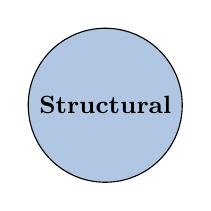
\begin{tikzpicture}[nodes={text depth=0.25ex,text height=1.25ex distance=1.7cm}]
                    \tikzstyle{every node}=[font=\small]
                    \tikzstyle{vertex} = [circle, draw=black, fill=illiniblue]
                    \tikzstyle{hidden} = [draw=none]
                    \tikzstyle{edge} = [<->, very thick]
                    
                    % \node[vertex](v1) at (0,5) {\textbf{Normative}};
                    \node[vertex](v2) at (4,0) {\textbf{Structural}};

        
            \end{tikzpicture}
            }
            % \caption{Parametric Uncertainty}
            % \label{fig:triarchic-uncertainty}
        \end{figure}

        \column[t]{6cm}
        \begin{definition}[Structural Uncertainty]
            [R]efers to the imperfect and incomplete nature of the equations describing the system \cite{decarolis_using_2011}.
        \end{definition}
        
        This type of uncertainty will \textit{always} persist.
    \end{columns}

\end{frame}

\begin{frame}
    \frametitle{Examples of Structural Uncertainty}

    \begin{itemize}
        \item Objective functions (most typical)\pause
        \item Spatiotemporal resolution\pause
        \item Physics fidelity\pause
        \item Solution method
    \end{itemize}

\end{frame}

\begin{frame}
    \frametitle{Addressing Structural Uncertainty}

    

\end{frame}
\subsection{Normative Uncertainty}
\begin{frame}
    \frametitle{Normative Uncertainty}

    Stating your assumptions is a necessary but insufficient condition for addressing normative uncertainty.

    \begin{columns}
        \column[t]{4cm}
        \begin{figure}
            \centering
            \resizebox{\columnwidth}{!}{
            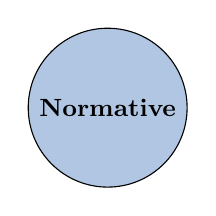
\begin{tikzpicture}[nodes={text depth=0.25ex,text height=1.25ex distance=1.7cm}]
                    \tikzstyle{every node}=[font=\small]
                    \tikzstyle{vertex} = [circle, draw=black, fill=illiniblue]
                    \tikzstyle{hidden} = [draw=none]
                    \tikzstyle{edge} = [<->, very thick]
                    
                    \node[vertex](v1) at (0,5) {\textbf{Normative}};

        
            \end{tikzpicture}
            }
            % \caption{Parametric Uncertainty}
            % \label{fig:triarchic-uncertainty}
        \end{figure}

        \column[t]{6cm}
        Answers the question ``what is acceptable and why?''

        \begin{itemize}
            \item Climate change is happening!
        \end{itemize}

        
    \end{columns}

\end{frame}

% \section{Technical Gap \#2}
% \begin{frame}
%     \frametitle{Gap \#2: Challenges with current ESOM practices}

%     \begin{enumerate}
%         \item Structural Uncertainty
%         \begin{itemize}
%             \item $\sim$100\% of ESOM frameworks optimize cost.
%             \item Stanard MGA procedures anchor alternatives to cost --- no true
%             tradeoff analysis.
%         \end{itemize}
%         \item Normative Uncertainty: Most ESOM analyses are prescriptive, few if
%         any articulate a normative premise to justify their conclusions.
%         \begin{itemize}
%             \item ``Pathway to 100\% Renewable Energy...'' --- a commonly
%             unjustified normative conclusion, right in the title!
%             \item Why should non-renewable sources be excluded? Renewable energy
%             is not guaranteed to be democratic \cite{winner_artifacts_1980}, nor
%             sustainable \cite{bell_toward_2020}.
%         \end{itemize}
%     \end{enumerate}

% \end{frame}

\begin{frame}
    \frametitle{Gap 1: Challenges with current ESOM practices}
    \begin{block}{Technical Gap}
        \begin{enumerate}
            \item Exclusive optimization over system cost misrecognizes the plurality of 
            preferences and priorities. Tradeoff analysis is impossible.
            \item Even with open source code and transparent data sources, energy system
            models remain opaque --- decision making black boxes.
        \end{enumerate}
    \end{block}
    \begin{block}{Proposed Work Component I: Multi-objective optimization}
        \begin{itemize}
            \item Partially address procedural/recognition justice by facilitating tradeoff analysis 
            through multi-objective optimization with evolutionary
            algorithms.
            \item Develop an MGA algorithm for high dimensional space.
        \end{itemize}
        
    \end{block}
    \begin{block}{Stretch Goal}
        Further enhance the transparency component of procedural justice by developing this
        tool in a way that provides the \textit{capability} for anyone interested to 
        verify model results. I.e., make accessibility a design priority. 
    \end{block}
\end{frame}

% \section{Proposal \#2}
% \begin{frame}
%     \frametitle{Proposal \#2: Building a flexible ESOM}

%     \begin{enumerate}
%         \item Create an open-source multi-objective energy system model (\texttt{osier}) that can allow modelers to address
%         \begin{itemize}
%             \item parametric,
%             \item structural,
%             \item and normative uncertainties.
%         \end{itemize}
%         \item Develop an MGA algorithm for use with genetic algorithms in higher dimensional spaces.
%     \end{enumerate}

% \end{frame}
\section{Component 1: Preliminary Results with \texttt{Osier}}
\begin{frame}
    \frametitle{Open source multi-objective energy system framework (\texttt{Osier})}
    \begin{itemize}
        \item Hybrid methods: linear programming \& evolutionary algorithms
        \item Novel algorithm for high dimensional MGA
    \end{itemize}
    \begin{figure}
        \centering
        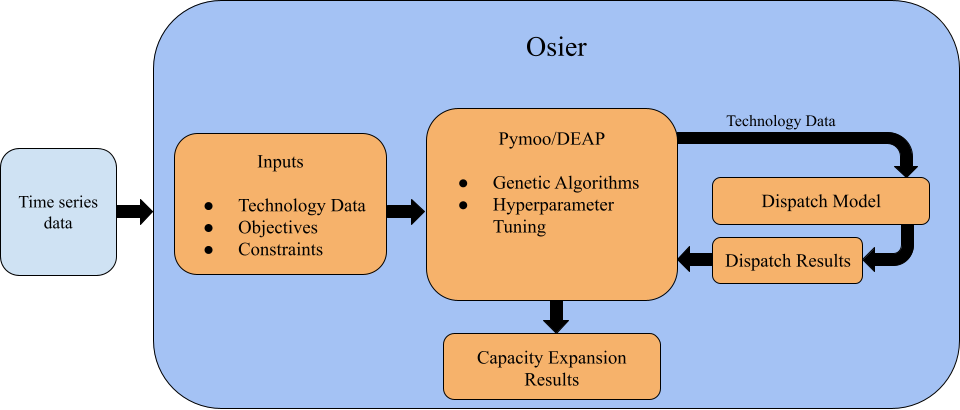
\includegraphics[width=\columnwidth]{../docs/figures/osier_flow.png}
        \caption{Flow of data through \texttt{Osier}.}
        \label{fig:osier-flow}
    \end{figure}

\end{frame}

\subsection{Methodology}
\begin{frame}
    \frametitle{Multi-objective Solutions}
    \begin{columns}
        \column[t]{4cm}
        \begin{block}{}
            Another way to generate alternatives...
        \end{block}
        \begin{block}{Pareto Front}
            Creates a \boldorange{set of solutions} rather than a single optimum.
        \end{block}
        \column[t]{6cm}
        \begin{figure}
            \centering
            \resizebox{\columnwidth}{!}{%% Creator: Matplotlib, PGF backend
%%
%% To include the figure in your LaTeX document, write
%%   \input{<filename>.pgf}
%%
%% Make sure the required packages are loaded in your preamble
%%   \usepackage{pgf}
%%
%% Also ensure that all the required font packages are loaded; for instance,
%% the lmodern package is sometimes necessary when using math font.
%%   \usepackage{lmodern}
%%
%% Figures using additional raster images can only be included by \input if
%% they are in the same directory as the main LaTeX file. For loading figures
%% from other directories you can use the `import` package
%%   \usepackage{import}
%%
%% and then include the figures with
%%   \import{<path to file>}{<filename>.pgf}
%%
%% Matplotlib used the following preamble
%%
\begingroup%
\makeatletter%
\begin{pgfpicture}%
\pgfpathrectangle{\pgfpointorigin}{\pgfqpoint{7.147223in}{5.232237in}}%
\pgfusepath{use as bounding box, clip}%
\begin{pgfscope}%
\pgfsetbuttcap%
\pgfsetmiterjoin%
\definecolor{currentfill}{rgb}{1.000000,1.000000,1.000000}%
\pgfsetfillcolor{currentfill}%
\pgfsetlinewidth{0.000000pt}%
\definecolor{currentstroke}{rgb}{0.000000,0.000000,0.000000}%
\pgfsetstrokecolor{currentstroke}%
\pgfsetdash{}{0pt}%
\pgfpathmoveto{\pgfqpoint{0.000000in}{0.000000in}}%
\pgfpathlineto{\pgfqpoint{7.147223in}{0.000000in}}%
\pgfpathlineto{\pgfqpoint{7.147223in}{5.232237in}}%
\pgfpathlineto{\pgfqpoint{0.000000in}{5.232237in}}%
\pgfpathlineto{\pgfqpoint{0.000000in}{0.000000in}}%
\pgfpathclose%
\pgfusepath{fill}%
\end{pgfscope}%
\begin{pgfscope}%
\pgfsetbuttcap%
\pgfsetmiterjoin%
\definecolor{currentfill}{rgb}{1.000000,1.000000,1.000000}%
\pgfsetfillcolor{currentfill}%
\pgfsetlinewidth{0.000000pt}%
\definecolor{currentstroke}{rgb}{0.000000,0.000000,0.000000}%
\pgfsetstrokecolor{currentstroke}%
\pgfsetstrokeopacity{0.000000}%
\pgfsetdash{}{0pt}%
\pgfpathmoveto{\pgfqpoint{0.847223in}{0.554012in}}%
\pgfpathlineto{\pgfqpoint{7.047223in}{0.554012in}}%
\pgfpathlineto{\pgfqpoint{7.047223in}{5.084012in}}%
\pgfpathlineto{\pgfqpoint{0.847223in}{5.084012in}}%
\pgfpathlineto{\pgfqpoint{0.847223in}{0.554012in}}%
\pgfpathclose%
\pgfusepath{fill}%
\end{pgfscope}%
\begin{pgfscope}%
\pgfpathrectangle{\pgfqpoint{0.847223in}{0.554012in}}{\pgfqpoint{6.200000in}{4.530000in}}%
\pgfusepath{clip}%
\pgfsetbuttcap%
\pgfsetroundjoin%
\pgfsetlinewidth{1.003750pt}%
\definecolor{currentstroke}{rgb}{1.000000,0.000000,0.000000}%
\pgfsetstrokecolor{currentstroke}%
\pgfsetdash{}{0pt}%
\pgfpathmoveto{\pgfqpoint{0.847223in}{5.042345in}}%
\pgfpathcurveto{\pgfqpoint{0.858273in}{5.042345in}}{\pgfqpoint{0.868872in}{5.046735in}}{\pgfqpoint{0.876686in}{5.054549in}}%
\pgfpathcurveto{\pgfqpoint{0.884499in}{5.062363in}}{\pgfqpoint{0.888890in}{5.072962in}}{\pgfqpoint{0.888890in}{5.084012in}}%
\pgfpathcurveto{\pgfqpoint{0.888890in}{5.095062in}}{\pgfqpoint{0.884499in}{5.105661in}}{\pgfqpoint{0.876686in}{5.113475in}}%
\pgfpathcurveto{\pgfqpoint{0.868872in}{5.121288in}}{\pgfqpoint{0.858273in}{5.125678in}}{\pgfqpoint{0.847223in}{5.125678in}}%
\pgfpathcurveto{\pgfqpoint{0.836173in}{5.125678in}}{\pgfqpoint{0.825574in}{5.121288in}}{\pgfqpoint{0.817760in}{5.113475in}}%
\pgfpathcurveto{\pgfqpoint{0.809947in}{5.105661in}}{\pgfqpoint{0.805556in}{5.095062in}}{\pgfqpoint{0.805556in}{5.084012in}}%
\pgfpathcurveto{\pgfqpoint{0.805556in}{5.072962in}}{\pgfqpoint{0.809947in}{5.062363in}}{\pgfqpoint{0.817760in}{5.054549in}}%
\pgfpathcurveto{\pgfqpoint{0.825574in}{5.046735in}}{\pgfqpoint{0.836173in}{5.042345in}}{\pgfqpoint{0.847223in}{5.042345in}}%
\pgfpathlineto{\pgfqpoint{0.847223in}{5.042345in}}%
\pgfpathclose%
\pgfusepath{stroke}%
\end{pgfscope}%
\begin{pgfscope}%
\pgfpathrectangle{\pgfqpoint{0.847223in}{0.554012in}}{\pgfqpoint{6.200000in}{4.530000in}}%
\pgfusepath{clip}%
\pgfsetbuttcap%
\pgfsetroundjoin%
\pgfsetlinewidth{1.003750pt}%
\definecolor{currentstroke}{rgb}{1.000000,0.000000,0.000000}%
\pgfsetstrokecolor{currentstroke}%
\pgfsetdash{}{0pt}%
\pgfpathmoveto{\pgfqpoint{0.852556in}{4.992439in}}%
\pgfpathcurveto{\pgfqpoint{0.863606in}{4.992439in}}{\pgfqpoint{0.874205in}{4.996830in}}{\pgfqpoint{0.882019in}{5.004643in}}%
\pgfpathcurveto{\pgfqpoint{0.889833in}{5.012457in}}{\pgfqpoint{0.894223in}{5.023056in}}{\pgfqpoint{0.894223in}{5.034106in}}%
\pgfpathcurveto{\pgfqpoint{0.894223in}{5.045156in}}{\pgfqpoint{0.889833in}{5.055755in}}{\pgfqpoint{0.882019in}{5.063569in}}%
\pgfpathcurveto{\pgfqpoint{0.874205in}{5.071382in}}{\pgfqpoint{0.863606in}{5.075773in}}{\pgfqpoint{0.852556in}{5.075773in}}%
\pgfpathcurveto{\pgfqpoint{0.841506in}{5.075773in}}{\pgfqpoint{0.830907in}{5.071382in}}{\pgfqpoint{0.823093in}{5.063569in}}%
\pgfpathcurveto{\pgfqpoint{0.815280in}{5.055755in}}{\pgfqpoint{0.810890in}{5.045156in}}{\pgfqpoint{0.810890in}{5.034106in}}%
\pgfpathcurveto{\pgfqpoint{0.810890in}{5.023056in}}{\pgfqpoint{0.815280in}{5.012457in}}{\pgfqpoint{0.823093in}{5.004643in}}%
\pgfpathcurveto{\pgfqpoint{0.830907in}{4.996830in}}{\pgfqpoint{0.841506in}{4.992439in}}{\pgfqpoint{0.852556in}{4.992439in}}%
\pgfpathlineto{\pgfqpoint{0.852556in}{4.992439in}}%
\pgfpathclose%
\pgfusepath{stroke}%
\end{pgfscope}%
\begin{pgfscope}%
\pgfpathrectangle{\pgfqpoint{0.847223in}{0.554012in}}{\pgfqpoint{6.200000in}{4.530000in}}%
\pgfusepath{clip}%
\pgfsetbuttcap%
\pgfsetroundjoin%
\pgfsetlinewidth{1.003750pt}%
\definecolor{currentstroke}{rgb}{1.000000,0.000000,0.000000}%
\pgfsetstrokecolor{currentstroke}%
\pgfsetdash{}{0pt}%
\pgfpathmoveto{\pgfqpoint{0.857889in}{4.943530in}}%
\pgfpathcurveto{\pgfqpoint{0.868940in}{4.943530in}}{\pgfqpoint{0.879539in}{4.947921in}}{\pgfqpoint{0.887352in}{4.955734in}}%
\pgfpathcurveto{\pgfqpoint{0.895166in}{4.963548in}}{\pgfqpoint{0.899556in}{4.974147in}}{\pgfqpoint{0.899556in}{4.985197in}}%
\pgfpathcurveto{\pgfqpoint{0.899556in}{4.996247in}}{\pgfqpoint{0.895166in}{5.006846in}}{\pgfqpoint{0.887352in}{5.014660in}}%
\pgfpathcurveto{\pgfqpoint{0.879539in}{5.022473in}}{\pgfqpoint{0.868940in}{5.026864in}}{\pgfqpoint{0.857889in}{5.026864in}}%
\pgfpathcurveto{\pgfqpoint{0.846839in}{5.026864in}}{\pgfqpoint{0.836240in}{5.022473in}}{\pgfqpoint{0.828427in}{5.014660in}}%
\pgfpathcurveto{\pgfqpoint{0.820613in}{5.006846in}}{\pgfqpoint{0.816223in}{4.996247in}}{\pgfqpoint{0.816223in}{4.985197in}}%
\pgfpathcurveto{\pgfqpoint{0.816223in}{4.974147in}}{\pgfqpoint{0.820613in}{4.963548in}}{\pgfqpoint{0.828427in}{4.955734in}}%
\pgfpathcurveto{\pgfqpoint{0.836240in}{4.947921in}}{\pgfqpoint{0.846839in}{4.943530in}}{\pgfqpoint{0.857889in}{4.943530in}}%
\pgfpathlineto{\pgfqpoint{0.857889in}{4.943530in}}%
\pgfpathclose%
\pgfusepath{stroke}%
\end{pgfscope}%
\begin{pgfscope}%
\pgfpathrectangle{\pgfqpoint{0.847223in}{0.554012in}}{\pgfqpoint{6.200000in}{4.530000in}}%
\pgfusepath{clip}%
\pgfsetbuttcap%
\pgfsetroundjoin%
\pgfsetlinewidth{1.003750pt}%
\definecolor{currentstroke}{rgb}{1.000000,0.000000,0.000000}%
\pgfsetstrokecolor{currentstroke}%
\pgfsetdash{}{0pt}%
\pgfpathmoveto{\pgfqpoint{0.863223in}{4.895588in}}%
\pgfpathcurveto{\pgfqpoint{0.874273in}{4.895588in}}{\pgfqpoint{0.884872in}{4.899979in}}{\pgfqpoint{0.892685in}{4.907792in}}%
\pgfpathcurveto{\pgfqpoint{0.900499in}{4.915606in}}{\pgfqpoint{0.904889in}{4.926205in}}{\pgfqpoint{0.904889in}{4.937255in}}%
\pgfpathcurveto{\pgfqpoint{0.904889in}{4.948305in}}{\pgfqpoint{0.900499in}{4.958904in}}{\pgfqpoint{0.892685in}{4.966718in}}%
\pgfpathcurveto{\pgfqpoint{0.884872in}{4.974532in}}{\pgfqpoint{0.874273in}{4.978922in}}{\pgfqpoint{0.863223in}{4.978922in}}%
\pgfpathcurveto{\pgfqpoint{0.852173in}{4.978922in}}{\pgfqpoint{0.841574in}{4.974532in}}{\pgfqpoint{0.833760in}{4.966718in}}%
\pgfpathcurveto{\pgfqpoint{0.825946in}{4.958904in}}{\pgfqpoint{0.821556in}{4.948305in}}{\pgfqpoint{0.821556in}{4.937255in}}%
\pgfpathcurveto{\pgfqpoint{0.821556in}{4.926205in}}{\pgfqpoint{0.825946in}{4.915606in}}{\pgfqpoint{0.833760in}{4.907792in}}%
\pgfpathcurveto{\pgfqpoint{0.841574in}{4.899979in}}{\pgfqpoint{0.852173in}{4.895588in}}{\pgfqpoint{0.863223in}{4.895588in}}%
\pgfpathlineto{\pgfqpoint{0.863223in}{4.895588in}}%
\pgfpathclose%
\pgfusepath{stroke}%
\end{pgfscope}%
\begin{pgfscope}%
\pgfpathrectangle{\pgfqpoint{0.847223in}{0.554012in}}{\pgfqpoint{6.200000in}{4.530000in}}%
\pgfusepath{clip}%
\pgfsetbuttcap%
\pgfsetroundjoin%
\pgfsetlinewidth{1.003750pt}%
\definecolor{currentstroke}{rgb}{1.000000,0.000000,0.000000}%
\pgfsetstrokecolor{currentstroke}%
\pgfsetdash{}{0pt}%
\pgfpathmoveto{\pgfqpoint{0.868556in}{4.848586in}}%
\pgfpathcurveto{\pgfqpoint{0.879606in}{4.848586in}}{\pgfqpoint{0.890205in}{4.852976in}}{\pgfqpoint{0.898019in}{4.860789in}}%
\pgfpathcurveto{\pgfqpoint{0.905832in}{4.868603in}}{\pgfqpoint{0.910223in}{4.879202in}}{\pgfqpoint{0.910223in}{4.890252in}}%
\pgfpathcurveto{\pgfqpoint{0.910223in}{4.901302in}}{\pgfqpoint{0.905832in}{4.911901in}}{\pgfqpoint{0.898019in}{4.919715in}}%
\pgfpathcurveto{\pgfqpoint{0.890205in}{4.927529in}}{\pgfqpoint{0.879606in}{4.931919in}}{\pgfqpoint{0.868556in}{4.931919in}}%
\pgfpathcurveto{\pgfqpoint{0.857506in}{4.931919in}}{\pgfqpoint{0.846907in}{4.927529in}}{\pgfqpoint{0.839093in}{4.919715in}}%
\pgfpathcurveto{\pgfqpoint{0.831280in}{4.911901in}}{\pgfqpoint{0.826889in}{4.901302in}}{\pgfqpoint{0.826889in}{4.890252in}}%
\pgfpathcurveto{\pgfqpoint{0.826889in}{4.879202in}}{\pgfqpoint{0.831280in}{4.868603in}}{\pgfqpoint{0.839093in}{4.860789in}}%
\pgfpathcurveto{\pgfqpoint{0.846907in}{4.852976in}}{\pgfqpoint{0.857506in}{4.848586in}}{\pgfqpoint{0.868556in}{4.848586in}}%
\pgfpathlineto{\pgfqpoint{0.868556in}{4.848586in}}%
\pgfpathclose%
\pgfusepath{stroke}%
\end{pgfscope}%
\begin{pgfscope}%
\pgfpathrectangle{\pgfqpoint{0.847223in}{0.554012in}}{\pgfqpoint{6.200000in}{4.530000in}}%
\pgfusepath{clip}%
\pgfsetbuttcap%
\pgfsetroundjoin%
\pgfsetlinewidth{1.003750pt}%
\definecolor{currentstroke}{rgb}{1.000000,0.000000,0.000000}%
\pgfsetstrokecolor{currentstroke}%
\pgfsetdash{}{0pt}%
\pgfpathmoveto{\pgfqpoint{0.873889in}{4.802494in}}%
\pgfpathcurveto{\pgfqpoint{0.884939in}{4.802494in}}{\pgfqpoint{0.895538in}{4.806884in}}{\pgfqpoint{0.903352in}{4.814698in}}%
\pgfpathcurveto{\pgfqpoint{0.911166in}{4.822512in}}{\pgfqpoint{0.915556in}{4.833111in}}{\pgfqpoint{0.915556in}{4.844161in}}%
\pgfpathcurveto{\pgfqpoint{0.915556in}{4.855211in}}{\pgfqpoint{0.911166in}{4.865810in}}{\pgfqpoint{0.903352in}{4.873624in}}%
\pgfpathcurveto{\pgfqpoint{0.895538in}{4.881437in}}{\pgfqpoint{0.884939in}{4.885827in}}{\pgfqpoint{0.873889in}{4.885827in}}%
\pgfpathcurveto{\pgfqpoint{0.862839in}{4.885827in}}{\pgfqpoint{0.852240in}{4.881437in}}{\pgfqpoint{0.844426in}{4.873624in}}%
\pgfpathcurveto{\pgfqpoint{0.836613in}{4.865810in}}{\pgfqpoint{0.832222in}{4.855211in}}{\pgfqpoint{0.832222in}{4.844161in}}%
\pgfpathcurveto{\pgfqpoint{0.832222in}{4.833111in}}{\pgfqpoint{0.836613in}{4.822512in}}{\pgfqpoint{0.844426in}{4.814698in}}%
\pgfpathcurveto{\pgfqpoint{0.852240in}{4.806884in}}{\pgfqpoint{0.862839in}{4.802494in}}{\pgfqpoint{0.873889in}{4.802494in}}%
\pgfpathlineto{\pgfqpoint{0.873889in}{4.802494in}}%
\pgfpathclose%
\pgfusepath{stroke}%
\end{pgfscope}%
\begin{pgfscope}%
\pgfpathrectangle{\pgfqpoint{0.847223in}{0.554012in}}{\pgfqpoint{6.200000in}{4.530000in}}%
\pgfusepath{clip}%
\pgfsetbuttcap%
\pgfsetroundjoin%
\pgfsetlinewidth{1.003750pt}%
\definecolor{currentstroke}{rgb}{1.000000,0.000000,0.000000}%
\pgfsetstrokecolor{currentstroke}%
\pgfsetdash{}{0pt}%
\pgfpathmoveto{\pgfqpoint{0.879222in}{4.757288in}}%
\pgfpathcurveto{\pgfqpoint{0.890272in}{4.757288in}}{\pgfqpoint{0.900872in}{4.761678in}}{\pgfqpoint{0.908685in}{4.769492in}}%
\pgfpathcurveto{\pgfqpoint{0.916499in}{4.777305in}}{\pgfqpoint{0.920889in}{4.787904in}}{\pgfqpoint{0.920889in}{4.798955in}}%
\pgfpathcurveto{\pgfqpoint{0.920889in}{4.810005in}}{\pgfqpoint{0.916499in}{4.820604in}}{\pgfqpoint{0.908685in}{4.828417in}}%
\pgfpathcurveto{\pgfqpoint{0.900872in}{4.836231in}}{\pgfqpoint{0.890272in}{4.840621in}}{\pgfqpoint{0.879222in}{4.840621in}}%
\pgfpathcurveto{\pgfqpoint{0.868172in}{4.840621in}}{\pgfqpoint{0.857573in}{4.836231in}}{\pgfqpoint{0.849760in}{4.828417in}}%
\pgfpathcurveto{\pgfqpoint{0.841946in}{4.820604in}}{\pgfqpoint{0.837556in}{4.810005in}}{\pgfqpoint{0.837556in}{4.798955in}}%
\pgfpathcurveto{\pgfqpoint{0.837556in}{4.787904in}}{\pgfqpoint{0.841946in}{4.777305in}}{\pgfqpoint{0.849760in}{4.769492in}}%
\pgfpathcurveto{\pgfqpoint{0.857573in}{4.761678in}}{\pgfqpoint{0.868172in}{4.757288in}}{\pgfqpoint{0.879222in}{4.757288in}}%
\pgfpathlineto{\pgfqpoint{0.879222in}{4.757288in}}%
\pgfpathclose%
\pgfusepath{stroke}%
\end{pgfscope}%
\begin{pgfscope}%
\pgfpathrectangle{\pgfqpoint{0.847223in}{0.554012in}}{\pgfqpoint{6.200000in}{4.530000in}}%
\pgfusepath{clip}%
\pgfsetbuttcap%
\pgfsetroundjoin%
\pgfsetlinewidth{1.003750pt}%
\definecolor{currentstroke}{rgb}{1.000000,0.000000,0.000000}%
\pgfsetstrokecolor{currentstroke}%
\pgfsetdash{}{0pt}%
\pgfpathmoveto{\pgfqpoint{0.884556in}{4.712942in}}%
\pgfpathcurveto{\pgfqpoint{0.895606in}{4.712942in}}{\pgfqpoint{0.906205in}{4.717332in}}{\pgfqpoint{0.914018in}{4.725146in}}%
\pgfpathcurveto{\pgfqpoint{0.921832in}{4.732959in}}{\pgfqpoint{0.926222in}{4.743558in}}{\pgfqpoint{0.926222in}{4.754608in}}%
\pgfpathcurveto{\pgfqpoint{0.926222in}{4.765659in}}{\pgfqpoint{0.921832in}{4.776258in}}{\pgfqpoint{0.914018in}{4.784071in}}%
\pgfpathcurveto{\pgfqpoint{0.906205in}{4.791885in}}{\pgfqpoint{0.895606in}{4.796275in}}{\pgfqpoint{0.884556in}{4.796275in}}%
\pgfpathcurveto{\pgfqpoint{0.873505in}{4.796275in}}{\pgfqpoint{0.862906in}{4.791885in}}{\pgfqpoint{0.855093in}{4.784071in}}%
\pgfpathcurveto{\pgfqpoint{0.847279in}{4.776258in}}{\pgfqpoint{0.842889in}{4.765659in}}{\pgfqpoint{0.842889in}{4.754608in}}%
\pgfpathcurveto{\pgfqpoint{0.842889in}{4.743558in}}{\pgfqpoint{0.847279in}{4.732959in}}{\pgfqpoint{0.855093in}{4.725146in}}%
\pgfpathcurveto{\pgfqpoint{0.862906in}{4.717332in}}{\pgfqpoint{0.873505in}{4.712942in}}{\pgfqpoint{0.884556in}{4.712942in}}%
\pgfpathlineto{\pgfqpoint{0.884556in}{4.712942in}}%
\pgfpathclose%
\pgfusepath{stroke}%
\end{pgfscope}%
\begin{pgfscope}%
\pgfpathrectangle{\pgfqpoint{0.847223in}{0.554012in}}{\pgfqpoint{6.200000in}{4.530000in}}%
\pgfusepath{clip}%
\pgfsetbuttcap%
\pgfsetroundjoin%
\pgfsetlinewidth{1.003750pt}%
\definecolor{currentstroke}{rgb}{1.000000,0.000000,0.000000}%
\pgfsetstrokecolor{currentstroke}%
\pgfsetdash{}{0pt}%
\pgfpathmoveto{\pgfqpoint{0.889889in}{4.669431in}}%
\pgfpathcurveto{\pgfqpoint{0.900939in}{4.669431in}}{\pgfqpoint{0.911538in}{4.673822in}}{\pgfqpoint{0.919352in}{4.681635in}}%
\pgfpathcurveto{\pgfqpoint{0.927165in}{4.689449in}}{\pgfqpoint{0.931555in}{4.700048in}}{\pgfqpoint{0.931555in}{4.711098in}}%
\pgfpathcurveto{\pgfqpoint{0.931555in}{4.722148in}}{\pgfqpoint{0.927165in}{4.732747in}}{\pgfqpoint{0.919352in}{4.740561in}}%
\pgfpathcurveto{\pgfqpoint{0.911538in}{4.748374in}}{\pgfqpoint{0.900939in}{4.752765in}}{\pgfqpoint{0.889889in}{4.752765in}}%
\pgfpathcurveto{\pgfqpoint{0.878839in}{4.752765in}}{\pgfqpoint{0.868240in}{4.748374in}}{\pgfqpoint{0.860426in}{4.740561in}}%
\pgfpathcurveto{\pgfqpoint{0.852612in}{4.732747in}}{\pgfqpoint{0.848222in}{4.722148in}}{\pgfqpoint{0.848222in}{4.711098in}}%
\pgfpathcurveto{\pgfqpoint{0.848222in}{4.700048in}}{\pgfqpoint{0.852612in}{4.689449in}}{\pgfqpoint{0.860426in}{4.681635in}}%
\pgfpathcurveto{\pgfqpoint{0.868240in}{4.673822in}}{\pgfqpoint{0.878839in}{4.669431in}}{\pgfqpoint{0.889889in}{4.669431in}}%
\pgfpathlineto{\pgfqpoint{0.889889in}{4.669431in}}%
\pgfpathclose%
\pgfusepath{stroke}%
\end{pgfscope}%
\begin{pgfscope}%
\pgfpathrectangle{\pgfqpoint{0.847223in}{0.554012in}}{\pgfqpoint{6.200000in}{4.530000in}}%
\pgfusepath{clip}%
\pgfsetbuttcap%
\pgfsetroundjoin%
\pgfsetlinewidth{1.003750pt}%
\definecolor{currentstroke}{rgb}{1.000000,0.000000,0.000000}%
\pgfsetstrokecolor{currentstroke}%
\pgfsetdash{}{0pt}%
\pgfpathmoveto{\pgfqpoint{0.895222in}{4.626733in}}%
\pgfpathcurveto{\pgfqpoint{0.906272in}{4.626733in}}{\pgfqpoint{0.916871in}{4.631123in}}{\pgfqpoint{0.924685in}{4.638937in}}%
\pgfpathcurveto{\pgfqpoint{0.932498in}{4.646751in}}{\pgfqpoint{0.936889in}{4.657350in}}{\pgfqpoint{0.936889in}{4.668400in}}%
\pgfpathcurveto{\pgfqpoint{0.936889in}{4.679450in}}{\pgfqpoint{0.932498in}{4.690049in}}{\pgfqpoint{0.924685in}{4.697863in}}%
\pgfpathcurveto{\pgfqpoint{0.916871in}{4.705676in}}{\pgfqpoint{0.906272in}{4.710066in}}{\pgfqpoint{0.895222in}{4.710066in}}%
\pgfpathcurveto{\pgfqpoint{0.884172in}{4.710066in}}{\pgfqpoint{0.873573in}{4.705676in}}{\pgfqpoint{0.865759in}{4.697863in}}%
\pgfpathcurveto{\pgfqpoint{0.857946in}{4.690049in}}{\pgfqpoint{0.853555in}{4.679450in}}{\pgfqpoint{0.853555in}{4.668400in}}%
\pgfpathcurveto{\pgfqpoint{0.853555in}{4.657350in}}{\pgfqpoint{0.857946in}{4.646751in}}{\pgfqpoint{0.865759in}{4.638937in}}%
\pgfpathcurveto{\pgfqpoint{0.873573in}{4.631123in}}{\pgfqpoint{0.884172in}{4.626733in}}{\pgfqpoint{0.895222in}{4.626733in}}%
\pgfpathlineto{\pgfqpoint{0.895222in}{4.626733in}}%
\pgfpathclose%
\pgfusepath{stroke}%
\end{pgfscope}%
\begin{pgfscope}%
\pgfpathrectangle{\pgfqpoint{0.847223in}{0.554012in}}{\pgfqpoint{6.200000in}{4.530000in}}%
\pgfusepath{clip}%
\pgfsetbuttcap%
\pgfsetroundjoin%
\pgfsetlinewidth{1.003750pt}%
\definecolor{currentstroke}{rgb}{1.000000,0.000000,0.000000}%
\pgfsetstrokecolor{currentstroke}%
\pgfsetdash{}{0pt}%
\pgfpathmoveto{\pgfqpoint{0.900555in}{4.584825in}}%
\pgfpathcurveto{\pgfqpoint{0.911605in}{4.584825in}}{\pgfqpoint{0.922204in}{4.589215in}}{\pgfqpoint{0.930018in}{4.597029in}}%
\pgfpathcurveto{\pgfqpoint{0.937832in}{4.604842in}}{\pgfqpoint{0.942222in}{4.615441in}}{\pgfqpoint{0.942222in}{4.626491in}}%
\pgfpathcurveto{\pgfqpoint{0.942222in}{4.637541in}}{\pgfqpoint{0.937832in}{4.648141in}}{\pgfqpoint{0.930018in}{4.655954in}}%
\pgfpathcurveto{\pgfqpoint{0.922204in}{4.663768in}}{\pgfqpoint{0.911605in}{4.668158in}}{\pgfqpoint{0.900555in}{4.668158in}}%
\pgfpathcurveto{\pgfqpoint{0.889505in}{4.668158in}}{\pgfqpoint{0.878906in}{4.663768in}}{\pgfqpoint{0.871092in}{4.655954in}}%
\pgfpathcurveto{\pgfqpoint{0.863279in}{4.648141in}}{\pgfqpoint{0.858889in}{4.637541in}}{\pgfqpoint{0.858889in}{4.626491in}}%
\pgfpathcurveto{\pgfqpoint{0.858889in}{4.615441in}}{\pgfqpoint{0.863279in}{4.604842in}}{\pgfqpoint{0.871092in}{4.597029in}}%
\pgfpathcurveto{\pgfqpoint{0.878906in}{4.589215in}}{\pgfqpoint{0.889505in}{4.584825in}}{\pgfqpoint{0.900555in}{4.584825in}}%
\pgfpathlineto{\pgfqpoint{0.900555in}{4.584825in}}%
\pgfpathclose%
\pgfusepath{stroke}%
\end{pgfscope}%
\begin{pgfscope}%
\pgfpathrectangle{\pgfqpoint{0.847223in}{0.554012in}}{\pgfqpoint{6.200000in}{4.530000in}}%
\pgfusepath{clip}%
\pgfsetbuttcap%
\pgfsetroundjoin%
\pgfsetlinewidth{1.003750pt}%
\definecolor{currentstroke}{rgb}{1.000000,0.000000,0.000000}%
\pgfsetstrokecolor{currentstroke}%
\pgfsetdash{}{0pt}%
\pgfpathmoveto{\pgfqpoint{0.905888in}{4.543684in}}%
\pgfpathcurveto{\pgfqpoint{0.916939in}{4.543684in}}{\pgfqpoint{0.927538in}{4.548075in}}{\pgfqpoint{0.935351in}{4.555888in}}%
\pgfpathcurveto{\pgfqpoint{0.943165in}{4.563702in}}{\pgfqpoint{0.947555in}{4.574301in}}{\pgfqpoint{0.947555in}{4.585351in}}%
\pgfpathcurveto{\pgfqpoint{0.947555in}{4.596401in}}{\pgfqpoint{0.943165in}{4.607000in}}{\pgfqpoint{0.935351in}{4.614814in}}%
\pgfpathcurveto{\pgfqpoint{0.927538in}{4.622627in}}{\pgfqpoint{0.916939in}{4.627018in}}{\pgfqpoint{0.905888in}{4.627018in}}%
\pgfpathcurveto{\pgfqpoint{0.894838in}{4.627018in}}{\pgfqpoint{0.884239in}{4.622627in}}{\pgfqpoint{0.876426in}{4.614814in}}%
\pgfpathcurveto{\pgfqpoint{0.868612in}{4.607000in}}{\pgfqpoint{0.864222in}{4.596401in}}{\pgfqpoint{0.864222in}{4.585351in}}%
\pgfpathcurveto{\pgfqpoint{0.864222in}{4.574301in}}{\pgfqpoint{0.868612in}{4.563702in}}{\pgfqpoint{0.876426in}{4.555888in}}%
\pgfpathcurveto{\pgfqpoint{0.884239in}{4.548075in}}{\pgfqpoint{0.894838in}{4.543684in}}{\pgfqpoint{0.905888in}{4.543684in}}%
\pgfpathlineto{\pgfqpoint{0.905888in}{4.543684in}}%
\pgfpathclose%
\pgfusepath{stroke}%
\end{pgfscope}%
\begin{pgfscope}%
\pgfpathrectangle{\pgfqpoint{0.847223in}{0.554012in}}{\pgfqpoint{6.200000in}{4.530000in}}%
\pgfusepath{clip}%
\pgfsetbuttcap%
\pgfsetroundjoin%
\pgfsetlinewidth{1.003750pt}%
\definecolor{currentstroke}{rgb}{1.000000,0.000000,0.000000}%
\pgfsetstrokecolor{currentstroke}%
\pgfsetdash{}{0pt}%
\pgfpathmoveto{\pgfqpoint{0.911222in}{4.503291in}}%
\pgfpathcurveto{\pgfqpoint{0.922272in}{4.503291in}}{\pgfqpoint{0.932871in}{4.507681in}}{\pgfqpoint{0.940684in}{4.515495in}}%
\pgfpathcurveto{\pgfqpoint{0.948498in}{4.523309in}}{\pgfqpoint{0.952888in}{4.533908in}}{\pgfqpoint{0.952888in}{4.544958in}}%
\pgfpathcurveto{\pgfqpoint{0.952888in}{4.556008in}}{\pgfqpoint{0.948498in}{4.566607in}}{\pgfqpoint{0.940684in}{4.574421in}}%
\pgfpathcurveto{\pgfqpoint{0.932871in}{4.582234in}}{\pgfqpoint{0.922272in}{4.586624in}}{\pgfqpoint{0.911222in}{4.586624in}}%
\pgfpathcurveto{\pgfqpoint{0.900172in}{4.586624in}}{\pgfqpoint{0.889572in}{4.582234in}}{\pgfqpoint{0.881759in}{4.574421in}}%
\pgfpathcurveto{\pgfqpoint{0.873945in}{4.566607in}}{\pgfqpoint{0.869555in}{4.556008in}}{\pgfqpoint{0.869555in}{4.544958in}}%
\pgfpathcurveto{\pgfqpoint{0.869555in}{4.533908in}}{\pgfqpoint{0.873945in}{4.523309in}}{\pgfqpoint{0.881759in}{4.515495in}}%
\pgfpathcurveto{\pgfqpoint{0.889572in}{4.507681in}}{\pgfqpoint{0.900172in}{4.503291in}}{\pgfqpoint{0.911222in}{4.503291in}}%
\pgfpathlineto{\pgfqpoint{0.911222in}{4.503291in}}%
\pgfpathclose%
\pgfusepath{stroke}%
\end{pgfscope}%
\begin{pgfscope}%
\pgfpathrectangle{\pgfqpoint{0.847223in}{0.554012in}}{\pgfqpoint{6.200000in}{4.530000in}}%
\pgfusepath{clip}%
\pgfsetbuttcap%
\pgfsetroundjoin%
\pgfsetlinewidth{1.003750pt}%
\definecolor{currentstroke}{rgb}{1.000000,0.000000,0.000000}%
\pgfsetstrokecolor{currentstroke}%
\pgfsetdash{}{0pt}%
\pgfpathmoveto{\pgfqpoint{0.916555in}{4.463625in}}%
\pgfpathcurveto{\pgfqpoint{0.927605in}{4.463625in}}{\pgfqpoint{0.938204in}{4.468015in}}{\pgfqpoint{0.946018in}{4.475829in}}%
\pgfpathcurveto{\pgfqpoint{0.953831in}{4.483642in}}{\pgfqpoint{0.958222in}{4.494241in}}{\pgfqpoint{0.958222in}{4.505291in}}%
\pgfpathcurveto{\pgfqpoint{0.958222in}{4.516342in}}{\pgfqpoint{0.953831in}{4.526941in}}{\pgfqpoint{0.946018in}{4.534754in}}%
\pgfpathcurveto{\pgfqpoint{0.938204in}{4.542568in}}{\pgfqpoint{0.927605in}{4.546958in}}{\pgfqpoint{0.916555in}{4.546958in}}%
\pgfpathcurveto{\pgfqpoint{0.905505in}{4.546958in}}{\pgfqpoint{0.894906in}{4.542568in}}{\pgfqpoint{0.887092in}{4.534754in}}%
\pgfpathcurveto{\pgfqpoint{0.879278in}{4.526941in}}{\pgfqpoint{0.874888in}{4.516342in}}{\pgfqpoint{0.874888in}{4.505291in}}%
\pgfpathcurveto{\pgfqpoint{0.874888in}{4.494241in}}{\pgfqpoint{0.879278in}{4.483642in}}{\pgfqpoint{0.887092in}{4.475829in}}%
\pgfpathcurveto{\pgfqpoint{0.894906in}{4.468015in}}{\pgfqpoint{0.905505in}{4.463625in}}{\pgfqpoint{0.916555in}{4.463625in}}%
\pgfpathlineto{\pgfqpoint{0.916555in}{4.463625in}}%
\pgfpathclose%
\pgfusepath{stroke}%
\end{pgfscope}%
\begin{pgfscope}%
\pgfpathrectangle{\pgfqpoint{0.847223in}{0.554012in}}{\pgfqpoint{6.200000in}{4.530000in}}%
\pgfusepath{clip}%
\pgfsetbuttcap%
\pgfsetroundjoin%
\pgfsetlinewidth{1.003750pt}%
\definecolor{currentstroke}{rgb}{1.000000,0.000000,0.000000}%
\pgfsetstrokecolor{currentstroke}%
\pgfsetdash{}{0pt}%
\pgfpathmoveto{\pgfqpoint{0.921888in}{4.424666in}}%
\pgfpathcurveto{\pgfqpoint{0.932938in}{4.424666in}}{\pgfqpoint{0.943537in}{4.429056in}}{\pgfqpoint{0.951351in}{4.436870in}}%
\pgfpathcurveto{\pgfqpoint{0.959164in}{4.444683in}}{\pgfqpoint{0.963555in}{4.455282in}}{\pgfqpoint{0.963555in}{4.466333in}}%
\pgfpathcurveto{\pgfqpoint{0.963555in}{4.477383in}}{\pgfqpoint{0.959164in}{4.487982in}}{\pgfqpoint{0.951351in}{4.495795in}}%
\pgfpathcurveto{\pgfqpoint{0.943537in}{4.503609in}}{\pgfqpoint{0.932938in}{4.507999in}}{\pgfqpoint{0.921888in}{4.507999in}}%
\pgfpathcurveto{\pgfqpoint{0.910838in}{4.507999in}}{\pgfqpoint{0.900239in}{4.503609in}}{\pgfqpoint{0.892425in}{4.495795in}}%
\pgfpathcurveto{\pgfqpoint{0.884612in}{4.487982in}}{\pgfqpoint{0.880221in}{4.477383in}}{\pgfqpoint{0.880221in}{4.466333in}}%
\pgfpathcurveto{\pgfqpoint{0.880221in}{4.455282in}}{\pgfqpoint{0.884612in}{4.444683in}}{\pgfqpoint{0.892425in}{4.436870in}}%
\pgfpathcurveto{\pgfqpoint{0.900239in}{4.429056in}}{\pgfqpoint{0.910838in}{4.424666in}}{\pgfqpoint{0.921888in}{4.424666in}}%
\pgfpathlineto{\pgfqpoint{0.921888in}{4.424666in}}%
\pgfpathclose%
\pgfusepath{stroke}%
\end{pgfscope}%
\begin{pgfscope}%
\pgfpathrectangle{\pgfqpoint{0.847223in}{0.554012in}}{\pgfqpoint{6.200000in}{4.530000in}}%
\pgfusepath{clip}%
\pgfsetbuttcap%
\pgfsetroundjoin%
\pgfsetlinewidth{1.003750pt}%
\definecolor{currentstroke}{rgb}{1.000000,0.000000,0.000000}%
\pgfsetstrokecolor{currentstroke}%
\pgfsetdash{}{0pt}%
\pgfpathmoveto{\pgfqpoint{0.927221in}{4.386396in}}%
\pgfpathcurveto{\pgfqpoint{0.938271in}{4.386396in}}{\pgfqpoint{0.948870in}{4.390786in}}{\pgfqpoint{0.956684in}{4.398600in}}%
\pgfpathcurveto{\pgfqpoint{0.964498in}{4.406413in}}{\pgfqpoint{0.968888in}{4.417012in}}{\pgfqpoint{0.968888in}{4.428063in}}%
\pgfpathcurveto{\pgfqpoint{0.968888in}{4.439113in}}{\pgfqpoint{0.964498in}{4.449712in}}{\pgfqpoint{0.956684in}{4.457525in}}%
\pgfpathcurveto{\pgfqpoint{0.948870in}{4.465339in}}{\pgfqpoint{0.938271in}{4.469729in}}{\pgfqpoint{0.927221in}{4.469729in}}%
\pgfpathcurveto{\pgfqpoint{0.916171in}{4.469729in}}{\pgfqpoint{0.905572in}{4.465339in}}{\pgfqpoint{0.897759in}{4.457525in}}%
\pgfpathcurveto{\pgfqpoint{0.889945in}{4.449712in}}{\pgfqpoint{0.885555in}{4.439113in}}{\pgfqpoint{0.885555in}{4.428063in}}%
\pgfpathcurveto{\pgfqpoint{0.885555in}{4.417012in}}{\pgfqpoint{0.889945in}{4.406413in}}{\pgfqpoint{0.897759in}{4.398600in}}%
\pgfpathcurveto{\pgfqpoint{0.905572in}{4.390786in}}{\pgfqpoint{0.916171in}{4.386396in}}{\pgfqpoint{0.927221in}{4.386396in}}%
\pgfpathlineto{\pgfqpoint{0.927221in}{4.386396in}}%
\pgfpathclose%
\pgfusepath{stroke}%
\end{pgfscope}%
\begin{pgfscope}%
\pgfpathrectangle{\pgfqpoint{0.847223in}{0.554012in}}{\pgfqpoint{6.200000in}{4.530000in}}%
\pgfusepath{clip}%
\pgfsetbuttcap%
\pgfsetroundjoin%
\pgfsetlinewidth{1.003750pt}%
\definecolor{currentstroke}{rgb}{1.000000,0.000000,0.000000}%
\pgfsetstrokecolor{currentstroke}%
\pgfsetdash{}{0pt}%
\pgfpathmoveto{\pgfqpoint{0.932555in}{4.348796in}}%
\pgfpathcurveto{\pgfqpoint{0.943605in}{4.348796in}}{\pgfqpoint{0.954204in}{4.353187in}}{\pgfqpoint{0.962017in}{4.361000in}}%
\pgfpathcurveto{\pgfqpoint{0.969831in}{4.368814in}}{\pgfqpoint{0.974221in}{4.379413in}}{\pgfqpoint{0.974221in}{4.390463in}}%
\pgfpathcurveto{\pgfqpoint{0.974221in}{4.401513in}}{\pgfqpoint{0.969831in}{4.412112in}}{\pgfqpoint{0.962017in}{4.419926in}}%
\pgfpathcurveto{\pgfqpoint{0.954204in}{4.427740in}}{\pgfqpoint{0.943605in}{4.432130in}}{\pgfqpoint{0.932555in}{4.432130in}}%
\pgfpathcurveto{\pgfqpoint{0.921504in}{4.432130in}}{\pgfqpoint{0.910905in}{4.427740in}}{\pgfqpoint{0.903092in}{4.419926in}}%
\pgfpathcurveto{\pgfqpoint{0.895278in}{4.412112in}}{\pgfqpoint{0.890888in}{4.401513in}}{\pgfqpoint{0.890888in}{4.390463in}}%
\pgfpathcurveto{\pgfqpoint{0.890888in}{4.379413in}}{\pgfqpoint{0.895278in}{4.368814in}}{\pgfqpoint{0.903092in}{4.361000in}}%
\pgfpathcurveto{\pgfqpoint{0.910905in}{4.353187in}}{\pgfqpoint{0.921504in}{4.348796in}}{\pgfqpoint{0.932555in}{4.348796in}}%
\pgfpathlineto{\pgfqpoint{0.932555in}{4.348796in}}%
\pgfpathclose%
\pgfusepath{stroke}%
\end{pgfscope}%
\begin{pgfscope}%
\pgfpathrectangle{\pgfqpoint{0.847223in}{0.554012in}}{\pgfqpoint{6.200000in}{4.530000in}}%
\pgfusepath{clip}%
\pgfsetbuttcap%
\pgfsetroundjoin%
\pgfsetlinewidth{1.003750pt}%
\definecolor{currentstroke}{rgb}{1.000000,0.000000,0.000000}%
\pgfsetstrokecolor{currentstroke}%
\pgfsetdash{}{0pt}%
\pgfpathmoveto{\pgfqpoint{0.937888in}{4.311850in}}%
\pgfpathcurveto{\pgfqpoint{0.948938in}{4.311850in}}{\pgfqpoint{0.959537in}{4.316240in}}{\pgfqpoint{0.967351in}{4.324054in}}%
\pgfpathcurveto{\pgfqpoint{0.975164in}{4.331868in}}{\pgfqpoint{0.979554in}{4.342467in}}{\pgfqpoint{0.979554in}{4.353517in}}%
\pgfpathcurveto{\pgfqpoint{0.979554in}{4.364567in}}{\pgfqpoint{0.975164in}{4.375166in}}{\pgfqpoint{0.967351in}{4.382980in}}%
\pgfpathcurveto{\pgfqpoint{0.959537in}{4.390793in}}{\pgfqpoint{0.948938in}{4.395184in}}{\pgfqpoint{0.937888in}{4.395184in}}%
\pgfpathcurveto{\pgfqpoint{0.926838in}{4.395184in}}{\pgfqpoint{0.916239in}{4.390793in}}{\pgfqpoint{0.908425in}{4.382980in}}%
\pgfpathcurveto{\pgfqpoint{0.900611in}{4.375166in}}{\pgfqpoint{0.896221in}{4.364567in}}{\pgfqpoint{0.896221in}{4.353517in}}%
\pgfpathcurveto{\pgfqpoint{0.896221in}{4.342467in}}{\pgfqpoint{0.900611in}{4.331868in}}{\pgfqpoint{0.908425in}{4.324054in}}%
\pgfpathcurveto{\pgfqpoint{0.916239in}{4.316240in}}{\pgfqpoint{0.926838in}{4.311850in}}{\pgfqpoint{0.937888in}{4.311850in}}%
\pgfpathlineto{\pgfqpoint{0.937888in}{4.311850in}}%
\pgfpathclose%
\pgfusepath{stroke}%
\end{pgfscope}%
\begin{pgfscope}%
\pgfpathrectangle{\pgfqpoint{0.847223in}{0.554012in}}{\pgfqpoint{6.200000in}{4.530000in}}%
\pgfusepath{clip}%
\pgfsetbuttcap%
\pgfsetroundjoin%
\pgfsetlinewidth{1.003750pt}%
\definecolor{currentstroke}{rgb}{1.000000,0.000000,0.000000}%
\pgfsetstrokecolor{currentstroke}%
\pgfsetdash{}{0pt}%
\pgfpathmoveto{\pgfqpoint{0.943221in}{4.275540in}}%
\pgfpathcurveto{\pgfqpoint{0.954271in}{4.275540in}}{\pgfqpoint{0.964870in}{4.279931in}}{\pgfqpoint{0.972684in}{4.287744in}}%
\pgfpathcurveto{\pgfqpoint{0.980497in}{4.295558in}}{\pgfqpoint{0.984888in}{4.306157in}}{\pgfqpoint{0.984888in}{4.317207in}}%
\pgfpathcurveto{\pgfqpoint{0.984888in}{4.328257in}}{\pgfqpoint{0.980497in}{4.338856in}}{\pgfqpoint{0.972684in}{4.346670in}}%
\pgfpathcurveto{\pgfqpoint{0.964870in}{4.354483in}}{\pgfqpoint{0.954271in}{4.358874in}}{\pgfqpoint{0.943221in}{4.358874in}}%
\pgfpathcurveto{\pgfqpoint{0.932171in}{4.358874in}}{\pgfqpoint{0.921572in}{4.354483in}}{\pgfqpoint{0.913758in}{4.346670in}}%
\pgfpathcurveto{\pgfqpoint{0.905945in}{4.338856in}}{\pgfqpoint{0.901554in}{4.328257in}}{\pgfqpoint{0.901554in}{4.317207in}}%
\pgfpathcurveto{\pgfqpoint{0.901554in}{4.306157in}}{\pgfqpoint{0.905945in}{4.295558in}}{\pgfqpoint{0.913758in}{4.287744in}}%
\pgfpathcurveto{\pgfqpoint{0.921572in}{4.279931in}}{\pgfqpoint{0.932171in}{4.275540in}}{\pgfqpoint{0.943221in}{4.275540in}}%
\pgfpathlineto{\pgfqpoint{0.943221in}{4.275540in}}%
\pgfpathclose%
\pgfusepath{stroke}%
\end{pgfscope}%
\begin{pgfscope}%
\pgfpathrectangle{\pgfqpoint{0.847223in}{0.554012in}}{\pgfqpoint{6.200000in}{4.530000in}}%
\pgfusepath{clip}%
\pgfsetbuttcap%
\pgfsetroundjoin%
\pgfsetlinewidth{1.003750pt}%
\definecolor{currentstroke}{rgb}{1.000000,0.000000,0.000000}%
\pgfsetstrokecolor{currentstroke}%
\pgfsetdash{}{0pt}%
\pgfpathmoveto{\pgfqpoint{0.948554in}{4.239850in}}%
\pgfpathcurveto{\pgfqpoint{0.959604in}{4.239850in}}{\pgfqpoint{0.970203in}{4.244241in}}{\pgfqpoint{0.978017in}{4.252054in}}%
\pgfpathcurveto{\pgfqpoint{0.985831in}{4.259868in}}{\pgfqpoint{0.990221in}{4.270467in}}{\pgfqpoint{0.990221in}{4.281517in}}%
\pgfpathcurveto{\pgfqpoint{0.990221in}{4.292567in}}{\pgfqpoint{0.985831in}{4.303166in}}{\pgfqpoint{0.978017in}{4.310980in}}%
\pgfpathcurveto{\pgfqpoint{0.970203in}{4.318793in}}{\pgfqpoint{0.959604in}{4.323184in}}{\pgfqpoint{0.948554in}{4.323184in}}%
\pgfpathcurveto{\pgfqpoint{0.937504in}{4.323184in}}{\pgfqpoint{0.926905in}{4.318793in}}{\pgfqpoint{0.919091in}{4.310980in}}%
\pgfpathcurveto{\pgfqpoint{0.911278in}{4.303166in}}{\pgfqpoint{0.906887in}{4.292567in}}{\pgfqpoint{0.906887in}{4.281517in}}%
\pgfpathcurveto{\pgfqpoint{0.906887in}{4.270467in}}{\pgfqpoint{0.911278in}{4.259868in}}{\pgfqpoint{0.919091in}{4.252054in}}%
\pgfpathcurveto{\pgfqpoint{0.926905in}{4.244241in}}{\pgfqpoint{0.937504in}{4.239850in}}{\pgfqpoint{0.948554in}{4.239850in}}%
\pgfpathlineto{\pgfqpoint{0.948554in}{4.239850in}}%
\pgfpathclose%
\pgfusepath{stroke}%
\end{pgfscope}%
\begin{pgfscope}%
\pgfpathrectangle{\pgfqpoint{0.847223in}{0.554012in}}{\pgfqpoint{6.200000in}{4.530000in}}%
\pgfusepath{clip}%
\pgfsetbuttcap%
\pgfsetroundjoin%
\pgfsetlinewidth{1.003750pt}%
\definecolor{currentstroke}{rgb}{1.000000,0.000000,0.000000}%
\pgfsetstrokecolor{currentstroke}%
\pgfsetdash{}{0pt}%
\pgfpathmoveto{\pgfqpoint{0.953887in}{4.204765in}}%
\pgfpathcurveto{\pgfqpoint{0.964937in}{4.204765in}}{\pgfqpoint{0.975537in}{4.209155in}}{\pgfqpoint{0.983350in}{4.216968in}}%
\pgfpathcurveto{\pgfqpoint{0.991164in}{4.224782in}}{\pgfqpoint{0.995554in}{4.235381in}}{\pgfqpoint{0.995554in}{4.246431in}}%
\pgfpathcurveto{\pgfqpoint{0.995554in}{4.257481in}}{\pgfqpoint{0.991164in}{4.268080in}}{\pgfqpoint{0.983350in}{4.275894in}}%
\pgfpathcurveto{\pgfqpoint{0.975537in}{4.283708in}}{\pgfqpoint{0.964937in}{4.288098in}}{\pgfqpoint{0.953887in}{4.288098in}}%
\pgfpathcurveto{\pgfqpoint{0.942837in}{4.288098in}}{\pgfqpoint{0.932238in}{4.283708in}}{\pgfqpoint{0.924425in}{4.275894in}}%
\pgfpathcurveto{\pgfqpoint{0.916611in}{4.268080in}}{\pgfqpoint{0.912221in}{4.257481in}}{\pgfqpoint{0.912221in}{4.246431in}}%
\pgfpathcurveto{\pgfqpoint{0.912221in}{4.235381in}}{\pgfqpoint{0.916611in}{4.224782in}}{\pgfqpoint{0.924425in}{4.216968in}}%
\pgfpathcurveto{\pgfqpoint{0.932238in}{4.209155in}}{\pgfqpoint{0.942837in}{4.204765in}}{\pgfqpoint{0.953887in}{4.204765in}}%
\pgfpathlineto{\pgfqpoint{0.953887in}{4.204765in}}%
\pgfpathclose%
\pgfusepath{stroke}%
\end{pgfscope}%
\begin{pgfscope}%
\pgfpathrectangle{\pgfqpoint{0.847223in}{0.554012in}}{\pgfqpoint{6.200000in}{4.530000in}}%
\pgfusepath{clip}%
\pgfsetbuttcap%
\pgfsetroundjoin%
\pgfsetlinewidth{1.003750pt}%
\definecolor{currentstroke}{rgb}{1.000000,0.000000,0.000000}%
\pgfsetstrokecolor{currentstroke}%
\pgfsetdash{}{0pt}%
\pgfpathmoveto{\pgfqpoint{0.959221in}{4.170268in}}%
\pgfpathcurveto{\pgfqpoint{0.970271in}{4.170268in}}{\pgfqpoint{0.980870in}{4.174658in}}{\pgfqpoint{0.988683in}{4.182472in}}%
\pgfpathcurveto{\pgfqpoint{0.996497in}{4.190285in}}{\pgfqpoint{1.000887in}{4.200884in}}{\pgfqpoint{1.000887in}{4.211935in}}%
\pgfpathcurveto{\pgfqpoint{1.000887in}{4.222985in}}{\pgfqpoint{0.996497in}{4.233584in}}{\pgfqpoint{0.988683in}{4.241397in}}%
\pgfpathcurveto{\pgfqpoint{0.980870in}{4.249211in}}{\pgfqpoint{0.970271in}{4.253601in}}{\pgfqpoint{0.959221in}{4.253601in}}%
\pgfpathcurveto{\pgfqpoint{0.948170in}{4.253601in}}{\pgfqpoint{0.937571in}{4.249211in}}{\pgfqpoint{0.929758in}{4.241397in}}%
\pgfpathcurveto{\pgfqpoint{0.921944in}{4.233584in}}{\pgfqpoint{0.917554in}{4.222985in}}{\pgfqpoint{0.917554in}{4.211935in}}%
\pgfpathcurveto{\pgfqpoint{0.917554in}{4.200884in}}{\pgfqpoint{0.921944in}{4.190285in}}{\pgfqpoint{0.929758in}{4.182472in}}%
\pgfpathcurveto{\pgfqpoint{0.937571in}{4.174658in}}{\pgfqpoint{0.948170in}{4.170268in}}{\pgfqpoint{0.959221in}{4.170268in}}%
\pgfpathlineto{\pgfqpoint{0.959221in}{4.170268in}}%
\pgfpathclose%
\pgfusepath{stroke}%
\end{pgfscope}%
\begin{pgfscope}%
\pgfpathrectangle{\pgfqpoint{0.847223in}{0.554012in}}{\pgfqpoint{6.200000in}{4.530000in}}%
\pgfusepath{clip}%
\pgfsetbuttcap%
\pgfsetroundjoin%
\pgfsetlinewidth{1.003750pt}%
\definecolor{currentstroke}{rgb}{1.000000,0.000000,0.000000}%
\pgfsetstrokecolor{currentstroke}%
\pgfsetdash{}{0pt}%
\pgfpathmoveto{\pgfqpoint{0.964554in}{4.136345in}}%
\pgfpathcurveto{\pgfqpoint{0.975604in}{4.136345in}}{\pgfqpoint{0.986203in}{4.140736in}}{\pgfqpoint{0.994017in}{4.148549in}}%
\pgfpathcurveto{\pgfqpoint{1.001830in}{4.156363in}}{\pgfqpoint{1.006220in}{4.166962in}}{\pgfqpoint{1.006220in}{4.178012in}}%
\pgfpathcurveto{\pgfqpoint{1.006220in}{4.189062in}}{\pgfqpoint{1.001830in}{4.199661in}}{\pgfqpoint{0.994017in}{4.207475in}}%
\pgfpathcurveto{\pgfqpoint{0.986203in}{4.215289in}}{\pgfqpoint{0.975604in}{4.219679in}}{\pgfqpoint{0.964554in}{4.219679in}}%
\pgfpathcurveto{\pgfqpoint{0.953504in}{4.219679in}}{\pgfqpoint{0.942905in}{4.215289in}}{\pgfqpoint{0.935091in}{4.207475in}}%
\pgfpathcurveto{\pgfqpoint{0.927277in}{4.199661in}}{\pgfqpoint{0.922887in}{4.189062in}}{\pgfqpoint{0.922887in}{4.178012in}}%
\pgfpathcurveto{\pgfqpoint{0.922887in}{4.166962in}}{\pgfqpoint{0.927277in}{4.156363in}}{\pgfqpoint{0.935091in}{4.148549in}}%
\pgfpathcurveto{\pgfqpoint{0.942905in}{4.140736in}}{\pgfqpoint{0.953504in}{4.136345in}}{\pgfqpoint{0.964554in}{4.136345in}}%
\pgfpathlineto{\pgfqpoint{0.964554in}{4.136345in}}%
\pgfpathclose%
\pgfusepath{stroke}%
\end{pgfscope}%
\begin{pgfscope}%
\pgfpathrectangle{\pgfqpoint{0.847223in}{0.554012in}}{\pgfqpoint{6.200000in}{4.530000in}}%
\pgfusepath{clip}%
\pgfsetbuttcap%
\pgfsetroundjoin%
\pgfsetlinewidth{1.003750pt}%
\definecolor{currentstroke}{rgb}{1.000000,0.000000,0.000000}%
\pgfsetstrokecolor{currentstroke}%
\pgfsetdash{}{0pt}%
\pgfpathmoveto{\pgfqpoint{0.969887in}{4.102983in}}%
\pgfpathcurveto{\pgfqpoint{0.980937in}{4.102983in}}{\pgfqpoint{0.991536in}{4.107373in}}{\pgfqpoint{0.999350in}{4.115187in}}%
\pgfpathcurveto{\pgfqpoint{1.007163in}{4.123001in}}{\pgfqpoint{1.011554in}{4.133600in}}{\pgfqpoint{1.011554in}{4.144650in}}%
\pgfpathcurveto{\pgfqpoint{1.011554in}{4.155700in}}{\pgfqpoint{1.007163in}{4.166299in}}{\pgfqpoint{0.999350in}{4.174113in}}%
\pgfpathcurveto{\pgfqpoint{0.991536in}{4.181926in}}{\pgfqpoint{0.980937in}{4.186317in}}{\pgfqpoint{0.969887in}{4.186317in}}%
\pgfpathcurveto{\pgfqpoint{0.958837in}{4.186317in}}{\pgfqpoint{0.948238in}{4.181926in}}{\pgfqpoint{0.940424in}{4.174113in}}%
\pgfpathcurveto{\pgfqpoint{0.932611in}{4.166299in}}{\pgfqpoint{0.928220in}{4.155700in}}{\pgfqpoint{0.928220in}{4.144650in}}%
\pgfpathcurveto{\pgfqpoint{0.928220in}{4.133600in}}{\pgfqpoint{0.932611in}{4.123001in}}{\pgfqpoint{0.940424in}{4.115187in}}%
\pgfpathcurveto{\pgfqpoint{0.948238in}{4.107373in}}{\pgfqpoint{0.958837in}{4.102983in}}{\pgfqpoint{0.969887in}{4.102983in}}%
\pgfpathlineto{\pgfqpoint{0.969887in}{4.102983in}}%
\pgfpathclose%
\pgfusepath{stroke}%
\end{pgfscope}%
\begin{pgfscope}%
\pgfpathrectangle{\pgfqpoint{0.847223in}{0.554012in}}{\pgfqpoint{6.200000in}{4.530000in}}%
\pgfusepath{clip}%
\pgfsetbuttcap%
\pgfsetroundjoin%
\pgfsetlinewidth{1.003750pt}%
\definecolor{currentstroke}{rgb}{1.000000,0.000000,0.000000}%
\pgfsetstrokecolor{currentstroke}%
\pgfsetdash{}{0pt}%
\pgfpathmoveto{\pgfqpoint{0.975220in}{4.070167in}}%
\pgfpathcurveto{\pgfqpoint{0.986270in}{4.070167in}}{\pgfqpoint{0.996869in}{4.074558in}}{\pgfqpoint{1.004683in}{4.082371in}}%
\pgfpathcurveto{\pgfqpoint{1.012497in}{4.090185in}}{\pgfqpoint{1.016887in}{4.100784in}}{\pgfqpoint{1.016887in}{4.111834in}}%
\pgfpathcurveto{\pgfqpoint{1.016887in}{4.122884in}}{\pgfqpoint{1.012497in}{4.133483in}}{\pgfqpoint{1.004683in}{4.141297in}}%
\pgfpathcurveto{\pgfqpoint{0.996869in}{4.149110in}}{\pgfqpoint{0.986270in}{4.153501in}}{\pgfqpoint{0.975220in}{4.153501in}}%
\pgfpathcurveto{\pgfqpoint{0.964170in}{4.153501in}}{\pgfqpoint{0.953571in}{4.149110in}}{\pgfqpoint{0.945757in}{4.141297in}}%
\pgfpathcurveto{\pgfqpoint{0.937944in}{4.133483in}}{\pgfqpoint{0.933554in}{4.122884in}}{\pgfqpoint{0.933554in}{4.111834in}}%
\pgfpathcurveto{\pgfqpoint{0.933554in}{4.100784in}}{\pgfqpoint{0.937944in}{4.090185in}}{\pgfqpoint{0.945757in}{4.082371in}}%
\pgfpathcurveto{\pgfqpoint{0.953571in}{4.074558in}}{\pgfqpoint{0.964170in}{4.070167in}}{\pgfqpoint{0.975220in}{4.070167in}}%
\pgfpathlineto{\pgfqpoint{0.975220in}{4.070167in}}%
\pgfpathclose%
\pgfusepath{stroke}%
\end{pgfscope}%
\begin{pgfscope}%
\pgfpathrectangle{\pgfqpoint{0.847223in}{0.554012in}}{\pgfqpoint{6.200000in}{4.530000in}}%
\pgfusepath{clip}%
\pgfsetbuttcap%
\pgfsetroundjoin%
\pgfsetlinewidth{1.003750pt}%
\definecolor{currentstroke}{rgb}{1.000000,0.000000,0.000000}%
\pgfsetstrokecolor{currentstroke}%
\pgfsetdash{}{0pt}%
\pgfpathmoveto{\pgfqpoint{0.980553in}{4.037884in}}%
\pgfpathcurveto{\pgfqpoint{0.991604in}{4.037884in}}{\pgfqpoint{1.002203in}{4.042275in}}{\pgfqpoint{1.010016in}{4.050088in}}%
\pgfpathcurveto{\pgfqpoint{1.017830in}{4.057902in}}{\pgfqpoint{1.022220in}{4.068501in}}{\pgfqpoint{1.022220in}{4.079551in}}%
\pgfpathcurveto{\pgfqpoint{1.022220in}{4.090601in}}{\pgfqpoint{1.017830in}{4.101200in}}{\pgfqpoint{1.010016in}{4.109014in}}%
\pgfpathcurveto{\pgfqpoint{1.002203in}{4.116827in}}{\pgfqpoint{0.991604in}{4.121218in}}{\pgfqpoint{0.980553in}{4.121218in}}%
\pgfpathcurveto{\pgfqpoint{0.969503in}{4.121218in}}{\pgfqpoint{0.958904in}{4.116827in}}{\pgfqpoint{0.951091in}{4.109014in}}%
\pgfpathcurveto{\pgfqpoint{0.943277in}{4.101200in}}{\pgfqpoint{0.938887in}{4.090601in}}{\pgfqpoint{0.938887in}{4.079551in}}%
\pgfpathcurveto{\pgfqpoint{0.938887in}{4.068501in}}{\pgfqpoint{0.943277in}{4.057902in}}{\pgfqpoint{0.951091in}{4.050088in}}%
\pgfpathcurveto{\pgfqpoint{0.958904in}{4.042275in}}{\pgfqpoint{0.969503in}{4.037884in}}{\pgfqpoint{0.980553in}{4.037884in}}%
\pgfpathlineto{\pgfqpoint{0.980553in}{4.037884in}}%
\pgfpathclose%
\pgfusepath{stroke}%
\end{pgfscope}%
\begin{pgfscope}%
\pgfpathrectangle{\pgfqpoint{0.847223in}{0.554012in}}{\pgfqpoint{6.200000in}{4.530000in}}%
\pgfusepath{clip}%
\pgfsetbuttcap%
\pgfsetroundjoin%
\pgfsetlinewidth{1.003750pt}%
\definecolor{currentstroke}{rgb}{1.000000,0.000000,0.000000}%
\pgfsetstrokecolor{currentstroke}%
\pgfsetdash{}{0pt}%
\pgfpathmoveto{\pgfqpoint{0.985887in}{4.006122in}}%
\pgfpathcurveto{\pgfqpoint{0.996937in}{4.006122in}}{\pgfqpoint{1.007536in}{4.010512in}}{\pgfqpoint{1.015349in}{4.018325in}}%
\pgfpathcurveto{\pgfqpoint{1.023163in}{4.026139in}}{\pgfqpoint{1.027553in}{4.036738in}}{\pgfqpoint{1.027553in}{4.047788in}}%
\pgfpathcurveto{\pgfqpoint{1.027553in}{4.058838in}}{\pgfqpoint{1.023163in}{4.069437in}}{\pgfqpoint{1.015349in}{4.077251in}}%
\pgfpathcurveto{\pgfqpoint{1.007536in}{4.085065in}}{\pgfqpoint{0.996937in}{4.089455in}}{\pgfqpoint{0.985887in}{4.089455in}}%
\pgfpathcurveto{\pgfqpoint{0.974837in}{4.089455in}}{\pgfqpoint{0.964238in}{4.085065in}}{\pgfqpoint{0.956424in}{4.077251in}}%
\pgfpathcurveto{\pgfqpoint{0.948610in}{4.069437in}}{\pgfqpoint{0.944220in}{4.058838in}}{\pgfqpoint{0.944220in}{4.047788in}}%
\pgfpathcurveto{\pgfqpoint{0.944220in}{4.036738in}}{\pgfqpoint{0.948610in}{4.026139in}}{\pgfqpoint{0.956424in}{4.018325in}}%
\pgfpathcurveto{\pgfqpoint{0.964238in}{4.010512in}}{\pgfqpoint{0.974837in}{4.006122in}}{\pgfqpoint{0.985887in}{4.006122in}}%
\pgfpathlineto{\pgfqpoint{0.985887in}{4.006122in}}%
\pgfpathclose%
\pgfusepath{stroke}%
\end{pgfscope}%
\begin{pgfscope}%
\pgfpathrectangle{\pgfqpoint{0.847223in}{0.554012in}}{\pgfqpoint{6.200000in}{4.530000in}}%
\pgfusepath{clip}%
\pgfsetbuttcap%
\pgfsetroundjoin%
\pgfsetlinewidth{1.003750pt}%
\definecolor{currentstroke}{rgb}{1.000000,0.000000,0.000000}%
\pgfsetstrokecolor{currentstroke}%
\pgfsetdash{}{0pt}%
\pgfpathmoveto{\pgfqpoint{0.991220in}{3.974866in}}%
\pgfpathcurveto{\pgfqpoint{1.002270in}{3.974866in}}{\pgfqpoint{1.012869in}{3.979257in}}{\pgfqpoint{1.020683in}{3.987070in}}%
\pgfpathcurveto{\pgfqpoint{1.028496in}{3.994884in}}{\pgfqpoint{1.032887in}{4.005483in}}{\pgfqpoint{1.032887in}{4.016533in}}%
\pgfpathcurveto{\pgfqpoint{1.032887in}{4.027583in}}{\pgfqpoint{1.028496in}{4.038182in}}{\pgfqpoint{1.020683in}{4.045996in}}%
\pgfpathcurveto{\pgfqpoint{1.012869in}{4.053810in}}{\pgfqpoint{1.002270in}{4.058200in}}{\pgfqpoint{0.991220in}{4.058200in}}%
\pgfpathcurveto{\pgfqpoint{0.980170in}{4.058200in}}{\pgfqpoint{0.969571in}{4.053810in}}{\pgfqpoint{0.961757in}{4.045996in}}%
\pgfpathcurveto{\pgfqpoint{0.953943in}{4.038182in}}{\pgfqpoint{0.949553in}{4.027583in}}{\pgfqpoint{0.949553in}{4.016533in}}%
\pgfpathcurveto{\pgfqpoint{0.949553in}{4.005483in}}{\pgfqpoint{0.953943in}{3.994884in}}{\pgfqpoint{0.961757in}{3.987070in}}%
\pgfpathcurveto{\pgfqpoint{0.969571in}{3.979257in}}{\pgfqpoint{0.980170in}{3.974866in}}{\pgfqpoint{0.991220in}{3.974866in}}%
\pgfpathlineto{\pgfqpoint{0.991220in}{3.974866in}}%
\pgfpathclose%
\pgfusepath{stroke}%
\end{pgfscope}%
\begin{pgfscope}%
\pgfpathrectangle{\pgfqpoint{0.847223in}{0.554012in}}{\pgfqpoint{6.200000in}{4.530000in}}%
\pgfusepath{clip}%
\pgfsetbuttcap%
\pgfsetroundjoin%
\pgfsetlinewidth{1.003750pt}%
\definecolor{currentstroke}{rgb}{1.000000,0.000000,0.000000}%
\pgfsetstrokecolor{currentstroke}%
\pgfsetdash{}{0pt}%
\pgfpathmoveto{\pgfqpoint{0.996553in}{3.944107in}}%
\pgfpathcurveto{\pgfqpoint{1.007603in}{3.944107in}}{\pgfqpoint{1.018202in}{3.948497in}}{\pgfqpoint{1.026016in}{3.956311in}}%
\pgfpathcurveto{\pgfqpoint{1.033829in}{3.964125in}}{\pgfqpoint{1.038220in}{3.974724in}}{\pgfqpoint{1.038220in}{3.985774in}}%
\pgfpathcurveto{\pgfqpoint{1.038220in}{3.996824in}}{\pgfqpoint{1.033829in}{4.007423in}}{\pgfqpoint{1.026016in}{4.015236in}}%
\pgfpathcurveto{\pgfqpoint{1.018202in}{4.023050in}}{\pgfqpoint{1.007603in}{4.027440in}}{\pgfqpoint{0.996553in}{4.027440in}}%
\pgfpathcurveto{\pgfqpoint{0.985503in}{4.027440in}}{\pgfqpoint{0.974904in}{4.023050in}}{\pgfqpoint{0.967090in}{4.015236in}}%
\pgfpathcurveto{\pgfqpoint{0.959277in}{4.007423in}}{\pgfqpoint{0.954886in}{3.996824in}}{\pgfqpoint{0.954886in}{3.985774in}}%
\pgfpathcurveto{\pgfqpoint{0.954886in}{3.974724in}}{\pgfqpoint{0.959277in}{3.964125in}}{\pgfqpoint{0.967090in}{3.956311in}}%
\pgfpathcurveto{\pgfqpoint{0.974904in}{3.948497in}}{\pgfqpoint{0.985503in}{3.944107in}}{\pgfqpoint{0.996553in}{3.944107in}}%
\pgfpathlineto{\pgfqpoint{0.996553in}{3.944107in}}%
\pgfpathclose%
\pgfusepath{stroke}%
\end{pgfscope}%
\begin{pgfscope}%
\pgfpathrectangle{\pgfqpoint{0.847223in}{0.554012in}}{\pgfqpoint{6.200000in}{4.530000in}}%
\pgfusepath{clip}%
\pgfsetbuttcap%
\pgfsetroundjoin%
\pgfsetlinewidth{1.003750pt}%
\definecolor{currentstroke}{rgb}{1.000000,0.000000,0.000000}%
\pgfsetstrokecolor{currentstroke}%
\pgfsetdash{}{0pt}%
\pgfpathmoveto{\pgfqpoint{1.001886in}{3.913831in}}%
\pgfpathcurveto{\pgfqpoint{1.012936in}{3.913831in}}{\pgfqpoint{1.023535in}{3.918222in}}{\pgfqpoint{1.031349in}{3.926035in}}%
\pgfpathcurveto{\pgfqpoint{1.039163in}{3.933849in}}{\pgfqpoint{1.043553in}{3.944448in}}{\pgfqpoint{1.043553in}{3.955498in}}%
\pgfpathcurveto{\pgfqpoint{1.043553in}{3.966548in}}{\pgfqpoint{1.039163in}{3.977147in}}{\pgfqpoint{1.031349in}{3.984961in}}%
\pgfpathcurveto{\pgfqpoint{1.023535in}{3.992774in}}{\pgfqpoint{1.012936in}{3.997165in}}{\pgfqpoint{1.001886in}{3.997165in}}%
\pgfpathcurveto{\pgfqpoint{0.990836in}{3.997165in}}{\pgfqpoint{0.980237in}{3.992774in}}{\pgfqpoint{0.972424in}{3.984961in}}%
\pgfpathcurveto{\pgfqpoint{0.964610in}{3.977147in}}{\pgfqpoint{0.960220in}{3.966548in}}{\pgfqpoint{0.960220in}{3.955498in}}%
\pgfpathcurveto{\pgfqpoint{0.960220in}{3.944448in}}{\pgfqpoint{0.964610in}{3.933849in}}{\pgfqpoint{0.972424in}{3.926035in}}%
\pgfpathcurveto{\pgfqpoint{0.980237in}{3.918222in}}{\pgfqpoint{0.990836in}{3.913831in}}{\pgfqpoint{1.001886in}{3.913831in}}%
\pgfpathlineto{\pgfqpoint{1.001886in}{3.913831in}}%
\pgfpathclose%
\pgfusepath{stroke}%
\end{pgfscope}%
\begin{pgfscope}%
\pgfpathrectangle{\pgfqpoint{0.847223in}{0.554012in}}{\pgfqpoint{6.200000in}{4.530000in}}%
\pgfusepath{clip}%
\pgfsetbuttcap%
\pgfsetroundjoin%
\pgfsetlinewidth{1.003750pt}%
\definecolor{currentstroke}{rgb}{1.000000,0.000000,0.000000}%
\pgfsetstrokecolor{currentstroke}%
\pgfsetdash{}{0pt}%
\pgfpathmoveto{\pgfqpoint{1.007220in}{3.884028in}}%
\pgfpathcurveto{\pgfqpoint{1.018270in}{3.884028in}}{\pgfqpoint{1.028869in}{3.888419in}}{\pgfqpoint{1.036682in}{3.896232in}}%
\pgfpathcurveto{\pgfqpoint{1.044496in}{3.904046in}}{\pgfqpoint{1.048886in}{3.914645in}}{\pgfqpoint{1.048886in}{3.925695in}}%
\pgfpathcurveto{\pgfqpoint{1.048886in}{3.936745in}}{\pgfqpoint{1.044496in}{3.947344in}}{\pgfqpoint{1.036682in}{3.955158in}}%
\pgfpathcurveto{\pgfqpoint{1.028869in}{3.962971in}}{\pgfqpoint{1.018270in}{3.967362in}}{\pgfqpoint{1.007220in}{3.967362in}}%
\pgfpathcurveto{\pgfqpoint{0.996169in}{3.967362in}}{\pgfqpoint{0.985570in}{3.962971in}}{\pgfqpoint{0.977757in}{3.955158in}}%
\pgfpathcurveto{\pgfqpoint{0.969943in}{3.947344in}}{\pgfqpoint{0.965553in}{3.936745in}}{\pgfqpoint{0.965553in}{3.925695in}}%
\pgfpathcurveto{\pgfqpoint{0.965553in}{3.914645in}}{\pgfqpoint{0.969943in}{3.904046in}}{\pgfqpoint{0.977757in}{3.896232in}}%
\pgfpathcurveto{\pgfqpoint{0.985570in}{3.888419in}}{\pgfqpoint{0.996169in}{3.884028in}}{\pgfqpoint{1.007220in}{3.884028in}}%
\pgfpathlineto{\pgfqpoint{1.007220in}{3.884028in}}%
\pgfpathclose%
\pgfusepath{stroke}%
\end{pgfscope}%
\begin{pgfscope}%
\pgfpathrectangle{\pgfqpoint{0.847223in}{0.554012in}}{\pgfqpoint{6.200000in}{4.530000in}}%
\pgfusepath{clip}%
\pgfsetbuttcap%
\pgfsetroundjoin%
\pgfsetlinewidth{1.003750pt}%
\definecolor{currentstroke}{rgb}{1.000000,0.000000,0.000000}%
\pgfsetstrokecolor{currentstroke}%
\pgfsetdash{}{0pt}%
\pgfpathmoveto{\pgfqpoint{1.012553in}{3.854687in}}%
\pgfpathcurveto{\pgfqpoint{1.023603in}{3.854687in}}{\pgfqpoint{1.034202in}{3.859077in}}{\pgfqpoint{1.042016in}{3.866891in}}%
\pgfpathcurveto{\pgfqpoint{1.049829in}{3.874704in}}{\pgfqpoint{1.054219in}{3.885304in}}{\pgfqpoint{1.054219in}{3.896354in}}%
\pgfpathcurveto{\pgfqpoint{1.054219in}{3.907404in}}{\pgfqpoint{1.049829in}{3.918003in}}{\pgfqpoint{1.042016in}{3.925816in}}%
\pgfpathcurveto{\pgfqpoint{1.034202in}{3.933630in}}{\pgfqpoint{1.023603in}{3.938020in}}{\pgfqpoint{1.012553in}{3.938020in}}%
\pgfpathcurveto{\pgfqpoint{1.001503in}{3.938020in}}{\pgfqpoint{0.990904in}{3.933630in}}{\pgfqpoint{0.983090in}{3.925816in}}%
\pgfpathcurveto{\pgfqpoint{0.975276in}{3.918003in}}{\pgfqpoint{0.970886in}{3.907404in}}{\pgfqpoint{0.970886in}{3.896354in}}%
\pgfpathcurveto{\pgfqpoint{0.970886in}{3.885304in}}{\pgfqpoint{0.975276in}{3.874704in}}{\pgfqpoint{0.983090in}{3.866891in}}%
\pgfpathcurveto{\pgfqpoint{0.990904in}{3.859077in}}{\pgfqpoint{1.001503in}{3.854687in}}{\pgfqpoint{1.012553in}{3.854687in}}%
\pgfpathlineto{\pgfqpoint{1.012553in}{3.854687in}}%
\pgfpathclose%
\pgfusepath{stroke}%
\end{pgfscope}%
\begin{pgfscope}%
\pgfpathrectangle{\pgfqpoint{0.847223in}{0.554012in}}{\pgfqpoint{6.200000in}{4.530000in}}%
\pgfusepath{clip}%
\pgfsetbuttcap%
\pgfsetroundjoin%
\pgfsetlinewidth{1.003750pt}%
\definecolor{currentstroke}{rgb}{1.000000,0.000000,0.000000}%
\pgfsetstrokecolor{currentstroke}%
\pgfsetdash{}{0pt}%
\pgfpathmoveto{\pgfqpoint{1.017886in}{3.825797in}}%
\pgfpathcurveto{\pgfqpoint{1.028936in}{3.825797in}}{\pgfqpoint{1.039535in}{3.830187in}}{\pgfqpoint{1.047349in}{3.838000in}}%
\pgfpathcurveto{\pgfqpoint{1.055162in}{3.845814in}}{\pgfqpoint{1.059553in}{3.856413in}}{\pgfqpoint{1.059553in}{3.867463in}}%
\pgfpathcurveto{\pgfqpoint{1.059553in}{3.878513in}}{\pgfqpoint{1.055162in}{3.889112in}}{\pgfqpoint{1.047349in}{3.896926in}}%
\pgfpathcurveto{\pgfqpoint{1.039535in}{3.904740in}}{\pgfqpoint{1.028936in}{3.909130in}}{\pgfqpoint{1.017886in}{3.909130in}}%
\pgfpathcurveto{\pgfqpoint{1.006836in}{3.909130in}}{\pgfqpoint{0.996237in}{3.904740in}}{\pgfqpoint{0.988423in}{3.896926in}}%
\pgfpathcurveto{\pgfqpoint{0.980610in}{3.889112in}}{\pgfqpoint{0.976219in}{3.878513in}}{\pgfqpoint{0.976219in}{3.867463in}}%
\pgfpathcurveto{\pgfqpoint{0.976219in}{3.856413in}}{\pgfqpoint{0.980610in}{3.845814in}}{\pgfqpoint{0.988423in}{3.838000in}}%
\pgfpathcurveto{\pgfqpoint{0.996237in}{3.830187in}}{\pgfqpoint{1.006836in}{3.825797in}}{\pgfqpoint{1.017886in}{3.825797in}}%
\pgfpathlineto{\pgfqpoint{1.017886in}{3.825797in}}%
\pgfpathclose%
\pgfusepath{stroke}%
\end{pgfscope}%
\begin{pgfscope}%
\pgfpathrectangle{\pgfqpoint{0.847223in}{0.554012in}}{\pgfqpoint{6.200000in}{4.530000in}}%
\pgfusepath{clip}%
\pgfsetbuttcap%
\pgfsetroundjoin%
\pgfsetlinewidth{1.003750pt}%
\definecolor{currentstroke}{rgb}{1.000000,0.000000,0.000000}%
\pgfsetstrokecolor{currentstroke}%
\pgfsetdash{}{0pt}%
\pgfpathmoveto{\pgfqpoint{1.023219in}{3.797347in}}%
\pgfpathcurveto{\pgfqpoint{1.034269in}{3.797347in}}{\pgfqpoint{1.044868in}{3.801737in}}{\pgfqpoint{1.052682in}{3.809551in}}%
\pgfpathcurveto{\pgfqpoint{1.060496in}{3.817364in}}{\pgfqpoint{1.064886in}{3.827963in}}{\pgfqpoint{1.064886in}{3.839013in}}%
\pgfpathcurveto{\pgfqpoint{1.064886in}{3.850063in}}{\pgfqpoint{1.060496in}{3.860663in}}{\pgfqpoint{1.052682in}{3.868476in}}%
\pgfpathcurveto{\pgfqpoint{1.044868in}{3.876290in}}{\pgfqpoint{1.034269in}{3.880680in}}{\pgfqpoint{1.023219in}{3.880680in}}%
\pgfpathcurveto{\pgfqpoint{1.012169in}{3.880680in}}{\pgfqpoint{1.001570in}{3.876290in}}{\pgfqpoint{0.993756in}{3.868476in}}%
\pgfpathcurveto{\pgfqpoint{0.985943in}{3.860663in}}{\pgfqpoint{0.981553in}{3.850063in}}{\pgfqpoint{0.981553in}{3.839013in}}%
\pgfpathcurveto{\pgfqpoint{0.981553in}{3.827963in}}{\pgfqpoint{0.985943in}{3.817364in}}{\pgfqpoint{0.993756in}{3.809551in}}%
\pgfpathcurveto{\pgfqpoint{1.001570in}{3.801737in}}{\pgfqpoint{1.012169in}{3.797347in}}{\pgfqpoint{1.023219in}{3.797347in}}%
\pgfpathlineto{\pgfqpoint{1.023219in}{3.797347in}}%
\pgfpathclose%
\pgfusepath{stroke}%
\end{pgfscope}%
\begin{pgfscope}%
\pgfpathrectangle{\pgfqpoint{0.847223in}{0.554012in}}{\pgfqpoint{6.200000in}{4.530000in}}%
\pgfusepath{clip}%
\pgfsetbuttcap%
\pgfsetroundjoin%
\pgfsetlinewidth{1.003750pt}%
\definecolor{currentstroke}{rgb}{1.000000,0.000000,0.000000}%
\pgfsetstrokecolor{currentstroke}%
\pgfsetdash{}{0pt}%
\pgfpathmoveto{\pgfqpoint{1.028552in}{3.769328in}}%
\pgfpathcurveto{\pgfqpoint{1.039603in}{3.769328in}}{\pgfqpoint{1.050202in}{3.773718in}}{\pgfqpoint{1.058015in}{3.781531in}}%
\pgfpathcurveto{\pgfqpoint{1.065829in}{3.789345in}}{\pgfqpoint{1.070219in}{3.799944in}}{\pgfqpoint{1.070219in}{3.810994in}}%
\pgfpathcurveto{\pgfqpoint{1.070219in}{3.822044in}}{\pgfqpoint{1.065829in}{3.832643in}}{\pgfqpoint{1.058015in}{3.840457in}}%
\pgfpathcurveto{\pgfqpoint{1.050202in}{3.848271in}}{\pgfqpoint{1.039603in}{3.852661in}}{\pgfqpoint{1.028552in}{3.852661in}}%
\pgfpathcurveto{\pgfqpoint{1.017502in}{3.852661in}}{\pgfqpoint{1.006903in}{3.848271in}}{\pgfqpoint{0.999090in}{3.840457in}}%
\pgfpathcurveto{\pgfqpoint{0.991276in}{3.832643in}}{\pgfqpoint{0.986886in}{3.822044in}}{\pgfqpoint{0.986886in}{3.810994in}}%
\pgfpathcurveto{\pgfqpoint{0.986886in}{3.799944in}}{\pgfqpoint{0.991276in}{3.789345in}}{\pgfqpoint{0.999090in}{3.781531in}}%
\pgfpathcurveto{\pgfqpoint{1.006903in}{3.773718in}}{\pgfqpoint{1.017502in}{3.769328in}}{\pgfqpoint{1.028552in}{3.769328in}}%
\pgfpathlineto{\pgfqpoint{1.028552in}{3.769328in}}%
\pgfpathclose%
\pgfusepath{stroke}%
\end{pgfscope}%
\begin{pgfscope}%
\pgfpathrectangle{\pgfqpoint{0.847223in}{0.554012in}}{\pgfqpoint{6.200000in}{4.530000in}}%
\pgfusepath{clip}%
\pgfsetbuttcap%
\pgfsetroundjoin%
\pgfsetlinewidth{1.003750pt}%
\definecolor{currentstroke}{rgb}{1.000000,0.000000,0.000000}%
\pgfsetstrokecolor{currentstroke}%
\pgfsetdash{}{0pt}%
\pgfpathmoveto{\pgfqpoint{1.033886in}{3.741729in}}%
\pgfpathcurveto{\pgfqpoint{1.044936in}{3.741729in}}{\pgfqpoint{1.055535in}{3.746120in}}{\pgfqpoint{1.063348in}{3.753933in}}%
\pgfpathcurveto{\pgfqpoint{1.071162in}{3.761747in}}{\pgfqpoint{1.075552in}{3.772346in}}{\pgfqpoint{1.075552in}{3.783396in}}%
\pgfpathcurveto{\pgfqpoint{1.075552in}{3.794446in}}{\pgfqpoint{1.071162in}{3.805045in}}{\pgfqpoint{1.063348in}{3.812859in}}%
\pgfpathcurveto{\pgfqpoint{1.055535in}{3.820672in}}{\pgfqpoint{1.044936in}{3.825063in}}{\pgfqpoint{1.033886in}{3.825063in}}%
\pgfpathcurveto{\pgfqpoint{1.022835in}{3.825063in}}{\pgfqpoint{1.012236in}{3.820672in}}{\pgfqpoint{1.004423in}{3.812859in}}%
\pgfpathcurveto{\pgfqpoint{0.996609in}{3.805045in}}{\pgfqpoint{0.992219in}{3.794446in}}{\pgfqpoint{0.992219in}{3.783396in}}%
\pgfpathcurveto{\pgfqpoint{0.992219in}{3.772346in}}{\pgfqpoint{0.996609in}{3.761747in}}{\pgfqpoint{1.004423in}{3.753933in}}%
\pgfpathcurveto{\pgfqpoint{1.012236in}{3.746120in}}{\pgfqpoint{1.022835in}{3.741729in}}{\pgfqpoint{1.033886in}{3.741729in}}%
\pgfpathlineto{\pgfqpoint{1.033886in}{3.741729in}}%
\pgfpathclose%
\pgfusepath{stroke}%
\end{pgfscope}%
\begin{pgfscope}%
\pgfpathrectangle{\pgfqpoint{0.847223in}{0.554012in}}{\pgfqpoint{6.200000in}{4.530000in}}%
\pgfusepath{clip}%
\pgfsetbuttcap%
\pgfsetroundjoin%
\pgfsetlinewidth{1.003750pt}%
\definecolor{currentstroke}{rgb}{1.000000,0.000000,0.000000}%
\pgfsetstrokecolor{currentstroke}%
\pgfsetdash{}{0pt}%
\pgfpathmoveto{\pgfqpoint{1.039219in}{3.714542in}}%
\pgfpathcurveto{\pgfqpoint{1.050269in}{3.714542in}}{\pgfqpoint{1.060868in}{3.718933in}}{\pgfqpoint{1.068682in}{3.726746in}}%
\pgfpathcurveto{\pgfqpoint{1.076495in}{3.734560in}}{\pgfqpoint{1.080885in}{3.745159in}}{\pgfqpoint{1.080885in}{3.756209in}}%
\pgfpathcurveto{\pgfqpoint{1.080885in}{3.767259in}}{\pgfqpoint{1.076495in}{3.777858in}}{\pgfqpoint{1.068682in}{3.785672in}}%
\pgfpathcurveto{\pgfqpoint{1.060868in}{3.793486in}}{\pgfqpoint{1.050269in}{3.797876in}}{\pgfqpoint{1.039219in}{3.797876in}}%
\pgfpathcurveto{\pgfqpoint{1.028169in}{3.797876in}}{\pgfqpoint{1.017570in}{3.793486in}}{\pgfqpoint{1.009756in}{3.785672in}}%
\pgfpathcurveto{\pgfqpoint{1.001942in}{3.777858in}}{\pgfqpoint{0.997552in}{3.767259in}}{\pgfqpoint{0.997552in}{3.756209in}}%
\pgfpathcurveto{\pgfqpoint{0.997552in}{3.745159in}}{\pgfqpoint{1.001942in}{3.734560in}}{\pgfqpoint{1.009756in}{3.726746in}}%
\pgfpathcurveto{\pgfqpoint{1.017570in}{3.718933in}}{\pgfqpoint{1.028169in}{3.714542in}}{\pgfqpoint{1.039219in}{3.714542in}}%
\pgfpathlineto{\pgfqpoint{1.039219in}{3.714542in}}%
\pgfpathclose%
\pgfusepath{stroke}%
\end{pgfscope}%
\begin{pgfscope}%
\pgfpathrectangle{\pgfqpoint{0.847223in}{0.554012in}}{\pgfqpoint{6.200000in}{4.530000in}}%
\pgfusepath{clip}%
\pgfsetbuttcap%
\pgfsetroundjoin%
\pgfsetlinewidth{1.003750pt}%
\definecolor{currentstroke}{rgb}{1.000000,0.000000,0.000000}%
\pgfsetstrokecolor{currentstroke}%
\pgfsetdash{}{0pt}%
\pgfpathmoveto{\pgfqpoint{1.044552in}{3.687758in}}%
\pgfpathcurveto{\pgfqpoint{1.055602in}{3.687758in}}{\pgfqpoint{1.066201in}{3.692148in}}{\pgfqpoint{1.074015in}{3.699962in}}%
\pgfpathcurveto{\pgfqpoint{1.081828in}{3.707776in}}{\pgfqpoint{1.086219in}{3.718375in}}{\pgfqpoint{1.086219in}{3.729425in}}%
\pgfpathcurveto{\pgfqpoint{1.086219in}{3.740475in}}{\pgfqpoint{1.081828in}{3.751074in}}{\pgfqpoint{1.074015in}{3.758888in}}%
\pgfpathcurveto{\pgfqpoint{1.066201in}{3.766701in}}{\pgfqpoint{1.055602in}{3.771091in}}{\pgfqpoint{1.044552in}{3.771091in}}%
\pgfpathcurveto{\pgfqpoint{1.033502in}{3.771091in}}{\pgfqpoint{1.022903in}{3.766701in}}{\pgfqpoint{1.015089in}{3.758888in}}%
\pgfpathcurveto{\pgfqpoint{1.007276in}{3.751074in}}{\pgfqpoint{1.002885in}{3.740475in}}{\pgfqpoint{1.002885in}{3.729425in}}%
\pgfpathcurveto{\pgfqpoint{1.002885in}{3.718375in}}{\pgfqpoint{1.007276in}{3.707776in}}{\pgfqpoint{1.015089in}{3.699962in}}%
\pgfpathcurveto{\pgfqpoint{1.022903in}{3.692148in}}{\pgfqpoint{1.033502in}{3.687758in}}{\pgfqpoint{1.044552in}{3.687758in}}%
\pgfpathlineto{\pgfqpoint{1.044552in}{3.687758in}}%
\pgfpathclose%
\pgfusepath{stroke}%
\end{pgfscope}%
\begin{pgfscope}%
\pgfpathrectangle{\pgfqpoint{0.847223in}{0.554012in}}{\pgfqpoint{6.200000in}{4.530000in}}%
\pgfusepath{clip}%
\pgfsetbuttcap%
\pgfsetroundjoin%
\pgfsetlinewidth{1.003750pt}%
\definecolor{currentstroke}{rgb}{1.000000,0.000000,0.000000}%
\pgfsetstrokecolor{currentstroke}%
\pgfsetdash{}{0pt}%
\pgfpathmoveto{\pgfqpoint{1.049885in}{3.661367in}}%
\pgfpathcurveto{\pgfqpoint{1.060935in}{3.661367in}}{\pgfqpoint{1.071534in}{3.665758in}}{\pgfqpoint{1.079348in}{3.673571in}}%
\pgfpathcurveto{\pgfqpoint{1.087162in}{3.681385in}}{\pgfqpoint{1.091552in}{3.691984in}}{\pgfqpoint{1.091552in}{3.703034in}}%
\pgfpathcurveto{\pgfqpoint{1.091552in}{3.714084in}}{\pgfqpoint{1.087162in}{3.724683in}}{\pgfqpoint{1.079348in}{3.732497in}}%
\pgfpathcurveto{\pgfqpoint{1.071534in}{3.740310in}}{\pgfqpoint{1.060935in}{3.744701in}}{\pgfqpoint{1.049885in}{3.744701in}}%
\pgfpathcurveto{\pgfqpoint{1.038835in}{3.744701in}}{\pgfqpoint{1.028236in}{3.740310in}}{\pgfqpoint{1.020422in}{3.732497in}}%
\pgfpathcurveto{\pgfqpoint{1.012609in}{3.724683in}}{\pgfqpoint{1.008219in}{3.714084in}}{\pgfqpoint{1.008219in}{3.703034in}}%
\pgfpathcurveto{\pgfqpoint{1.008219in}{3.691984in}}{\pgfqpoint{1.012609in}{3.681385in}}{\pgfqpoint{1.020422in}{3.673571in}}%
\pgfpathcurveto{\pgfqpoint{1.028236in}{3.665758in}}{\pgfqpoint{1.038835in}{3.661367in}}{\pgfqpoint{1.049885in}{3.661367in}}%
\pgfpathlineto{\pgfqpoint{1.049885in}{3.661367in}}%
\pgfpathclose%
\pgfusepath{stroke}%
\end{pgfscope}%
\begin{pgfscope}%
\pgfpathrectangle{\pgfqpoint{0.847223in}{0.554012in}}{\pgfqpoint{6.200000in}{4.530000in}}%
\pgfusepath{clip}%
\pgfsetbuttcap%
\pgfsetroundjoin%
\pgfsetlinewidth{1.003750pt}%
\definecolor{currentstroke}{rgb}{1.000000,0.000000,0.000000}%
\pgfsetstrokecolor{currentstroke}%
\pgfsetdash{}{0pt}%
\pgfpathmoveto{\pgfqpoint{1.055218in}{3.635361in}}%
\pgfpathcurveto{\pgfqpoint{1.066269in}{3.635361in}}{\pgfqpoint{1.076868in}{3.639752in}}{\pgfqpoint{1.084681in}{3.647565in}}%
\pgfpathcurveto{\pgfqpoint{1.092495in}{3.655379in}}{\pgfqpoint{1.096885in}{3.665978in}}{\pgfqpoint{1.096885in}{3.677028in}}%
\pgfpathcurveto{\pgfqpoint{1.096885in}{3.688078in}}{\pgfqpoint{1.092495in}{3.698677in}}{\pgfqpoint{1.084681in}{3.706491in}}%
\pgfpathcurveto{\pgfqpoint{1.076868in}{3.714304in}}{\pgfqpoint{1.066269in}{3.718695in}}{\pgfqpoint{1.055218in}{3.718695in}}%
\pgfpathcurveto{\pgfqpoint{1.044168in}{3.718695in}}{\pgfqpoint{1.033569in}{3.714304in}}{\pgfqpoint{1.025756in}{3.706491in}}%
\pgfpathcurveto{\pgfqpoint{1.017942in}{3.698677in}}{\pgfqpoint{1.013552in}{3.688078in}}{\pgfqpoint{1.013552in}{3.677028in}}%
\pgfpathcurveto{\pgfqpoint{1.013552in}{3.665978in}}{\pgfqpoint{1.017942in}{3.655379in}}{\pgfqpoint{1.025756in}{3.647565in}}%
\pgfpathcurveto{\pgfqpoint{1.033569in}{3.639752in}}{\pgfqpoint{1.044168in}{3.635361in}}{\pgfqpoint{1.055218in}{3.635361in}}%
\pgfpathlineto{\pgfqpoint{1.055218in}{3.635361in}}%
\pgfpathclose%
\pgfusepath{stroke}%
\end{pgfscope}%
\begin{pgfscope}%
\pgfpathrectangle{\pgfqpoint{0.847223in}{0.554012in}}{\pgfqpoint{6.200000in}{4.530000in}}%
\pgfusepath{clip}%
\pgfsetbuttcap%
\pgfsetroundjoin%
\pgfsetlinewidth{1.003750pt}%
\definecolor{currentstroke}{rgb}{1.000000,0.000000,0.000000}%
\pgfsetstrokecolor{currentstroke}%
\pgfsetdash{}{0pt}%
\pgfpathmoveto{\pgfqpoint{1.060552in}{3.609732in}}%
\pgfpathcurveto{\pgfqpoint{1.071602in}{3.609732in}}{\pgfqpoint{1.082201in}{3.614122in}}{\pgfqpoint{1.090014in}{3.621936in}}%
\pgfpathcurveto{\pgfqpoint{1.097828in}{3.629749in}}{\pgfqpoint{1.102218in}{3.640348in}}{\pgfqpoint{1.102218in}{3.651399in}}%
\pgfpathcurveto{\pgfqpoint{1.102218in}{3.662449in}}{\pgfqpoint{1.097828in}{3.673048in}}{\pgfqpoint{1.090014in}{3.680861in}}%
\pgfpathcurveto{\pgfqpoint{1.082201in}{3.688675in}}{\pgfqpoint{1.071602in}{3.693065in}}{\pgfqpoint{1.060552in}{3.693065in}}%
\pgfpathcurveto{\pgfqpoint{1.049502in}{3.693065in}}{\pgfqpoint{1.038903in}{3.688675in}}{\pgfqpoint{1.031089in}{3.680861in}}%
\pgfpathcurveto{\pgfqpoint{1.023275in}{3.673048in}}{\pgfqpoint{1.018885in}{3.662449in}}{\pgfqpoint{1.018885in}{3.651399in}}%
\pgfpathcurveto{\pgfqpoint{1.018885in}{3.640348in}}{\pgfqpoint{1.023275in}{3.629749in}}{\pgfqpoint{1.031089in}{3.621936in}}%
\pgfpathcurveto{\pgfqpoint{1.038903in}{3.614122in}}{\pgfqpoint{1.049502in}{3.609732in}}{\pgfqpoint{1.060552in}{3.609732in}}%
\pgfpathlineto{\pgfqpoint{1.060552in}{3.609732in}}%
\pgfpathclose%
\pgfusepath{stroke}%
\end{pgfscope}%
\begin{pgfscope}%
\pgfpathrectangle{\pgfqpoint{0.847223in}{0.554012in}}{\pgfqpoint{6.200000in}{4.530000in}}%
\pgfusepath{clip}%
\pgfsetbuttcap%
\pgfsetroundjoin%
\pgfsetlinewidth{1.003750pt}%
\definecolor{currentstroke}{rgb}{1.000000,0.000000,0.000000}%
\pgfsetstrokecolor{currentstroke}%
\pgfsetdash{}{0pt}%
\pgfpathmoveto{\pgfqpoint{1.065885in}{3.584471in}}%
\pgfpathcurveto{\pgfqpoint{1.076935in}{3.584471in}}{\pgfqpoint{1.087534in}{3.588861in}}{\pgfqpoint{1.095348in}{3.596675in}}%
\pgfpathcurveto{\pgfqpoint{1.103161in}{3.604488in}}{\pgfqpoint{1.107552in}{3.615087in}}{\pgfqpoint{1.107552in}{3.626138in}}%
\pgfpathcurveto{\pgfqpoint{1.107552in}{3.637188in}}{\pgfqpoint{1.103161in}{3.647787in}}{\pgfqpoint{1.095348in}{3.655600in}}%
\pgfpathcurveto{\pgfqpoint{1.087534in}{3.663414in}}{\pgfqpoint{1.076935in}{3.667804in}}{\pgfqpoint{1.065885in}{3.667804in}}%
\pgfpathcurveto{\pgfqpoint{1.054835in}{3.667804in}}{\pgfqpoint{1.044236in}{3.663414in}}{\pgfqpoint{1.036422in}{3.655600in}}%
\pgfpathcurveto{\pgfqpoint{1.028608in}{3.647787in}}{\pgfqpoint{1.024218in}{3.637188in}}{\pgfqpoint{1.024218in}{3.626138in}}%
\pgfpathcurveto{\pgfqpoint{1.024218in}{3.615087in}}{\pgfqpoint{1.028608in}{3.604488in}}{\pgfqpoint{1.036422in}{3.596675in}}%
\pgfpathcurveto{\pgfqpoint{1.044236in}{3.588861in}}{\pgfqpoint{1.054835in}{3.584471in}}{\pgfqpoint{1.065885in}{3.584471in}}%
\pgfpathlineto{\pgfqpoint{1.065885in}{3.584471in}}%
\pgfpathclose%
\pgfusepath{stroke}%
\end{pgfscope}%
\begin{pgfscope}%
\pgfpathrectangle{\pgfqpoint{0.847223in}{0.554012in}}{\pgfqpoint{6.200000in}{4.530000in}}%
\pgfusepath{clip}%
\pgfsetbuttcap%
\pgfsetroundjoin%
\pgfsetlinewidth{1.003750pt}%
\definecolor{currentstroke}{rgb}{1.000000,0.000000,0.000000}%
\pgfsetstrokecolor{currentstroke}%
\pgfsetdash{}{0pt}%
\pgfpathmoveto{\pgfqpoint{1.071218in}{3.559570in}}%
\pgfpathcurveto{\pgfqpoint{1.082268in}{3.559570in}}{\pgfqpoint{1.092867in}{3.563961in}}{\pgfqpoint{1.100681in}{3.571774in}}%
\pgfpathcurveto{\pgfqpoint{1.108495in}{3.579588in}}{\pgfqpoint{1.112885in}{3.590187in}}{\pgfqpoint{1.112885in}{3.601237in}}%
\pgfpathcurveto{\pgfqpoint{1.112885in}{3.612287in}}{\pgfqpoint{1.108495in}{3.622886in}}{\pgfqpoint{1.100681in}{3.630700in}}%
\pgfpathcurveto{\pgfqpoint{1.092867in}{3.638514in}}{\pgfqpoint{1.082268in}{3.642904in}}{\pgfqpoint{1.071218in}{3.642904in}}%
\pgfpathcurveto{\pgfqpoint{1.060168in}{3.642904in}}{\pgfqpoint{1.049569in}{3.638514in}}{\pgfqpoint{1.041755in}{3.630700in}}%
\pgfpathcurveto{\pgfqpoint{1.033942in}{3.622886in}}{\pgfqpoint{1.029551in}{3.612287in}}{\pgfqpoint{1.029551in}{3.601237in}}%
\pgfpathcurveto{\pgfqpoint{1.029551in}{3.590187in}}{\pgfqpoint{1.033942in}{3.579588in}}{\pgfqpoint{1.041755in}{3.571774in}}%
\pgfpathcurveto{\pgfqpoint{1.049569in}{3.563961in}}{\pgfqpoint{1.060168in}{3.559570in}}{\pgfqpoint{1.071218in}{3.559570in}}%
\pgfpathlineto{\pgfqpoint{1.071218in}{3.559570in}}%
\pgfpathclose%
\pgfusepath{stroke}%
\end{pgfscope}%
\begin{pgfscope}%
\pgfpathrectangle{\pgfqpoint{0.847223in}{0.554012in}}{\pgfqpoint{6.200000in}{4.530000in}}%
\pgfusepath{clip}%
\pgfsetbuttcap%
\pgfsetroundjoin%
\pgfsetlinewidth{1.003750pt}%
\definecolor{currentstroke}{rgb}{1.000000,0.000000,0.000000}%
\pgfsetstrokecolor{currentstroke}%
\pgfsetdash{}{0pt}%
\pgfpathmoveto{\pgfqpoint{1.076551in}{3.535023in}}%
\pgfpathcurveto{\pgfqpoint{1.087601in}{3.535023in}}{\pgfqpoint{1.098200in}{3.539413in}}{\pgfqpoint{1.106014in}{3.547227in}}%
\pgfpathcurveto{\pgfqpoint{1.113828in}{3.555040in}}{\pgfqpoint{1.118218in}{3.565639in}}{\pgfqpoint{1.118218in}{3.576690in}}%
\pgfpathcurveto{\pgfqpoint{1.118218in}{3.587740in}}{\pgfqpoint{1.113828in}{3.598339in}}{\pgfqpoint{1.106014in}{3.606152in}}%
\pgfpathcurveto{\pgfqpoint{1.098200in}{3.613966in}}{\pgfqpoint{1.087601in}{3.618356in}}{\pgfqpoint{1.076551in}{3.618356in}}%
\pgfpathcurveto{\pgfqpoint{1.065501in}{3.618356in}}{\pgfqpoint{1.054902in}{3.613966in}}{\pgfqpoint{1.047089in}{3.606152in}}%
\pgfpathcurveto{\pgfqpoint{1.039275in}{3.598339in}}{\pgfqpoint{1.034885in}{3.587740in}}{\pgfqpoint{1.034885in}{3.576690in}}%
\pgfpathcurveto{\pgfqpoint{1.034885in}{3.565639in}}{\pgfqpoint{1.039275in}{3.555040in}}{\pgfqpoint{1.047089in}{3.547227in}}%
\pgfpathcurveto{\pgfqpoint{1.054902in}{3.539413in}}{\pgfqpoint{1.065501in}{3.535023in}}{\pgfqpoint{1.076551in}{3.535023in}}%
\pgfpathlineto{\pgfqpoint{1.076551in}{3.535023in}}%
\pgfpathclose%
\pgfusepath{stroke}%
\end{pgfscope}%
\begin{pgfscope}%
\pgfpathrectangle{\pgfqpoint{0.847223in}{0.554012in}}{\pgfqpoint{6.200000in}{4.530000in}}%
\pgfusepath{clip}%
\pgfsetbuttcap%
\pgfsetroundjoin%
\pgfsetlinewidth{1.003750pt}%
\definecolor{currentstroke}{rgb}{1.000000,0.000000,0.000000}%
\pgfsetstrokecolor{currentstroke}%
\pgfsetdash{}{0pt}%
\pgfpathmoveto{\pgfqpoint{1.081885in}{3.510821in}}%
\pgfpathcurveto{\pgfqpoint{1.092935in}{3.510821in}}{\pgfqpoint{1.103534in}{3.515211in}}{\pgfqpoint{1.111347in}{3.523025in}}%
\pgfpathcurveto{\pgfqpoint{1.119161in}{3.530838in}}{\pgfqpoint{1.123551in}{3.541437in}}{\pgfqpoint{1.123551in}{3.552487in}}%
\pgfpathcurveto{\pgfqpoint{1.123551in}{3.563537in}}{\pgfqpoint{1.119161in}{3.574137in}}{\pgfqpoint{1.111347in}{3.581950in}}%
\pgfpathcurveto{\pgfqpoint{1.103534in}{3.589764in}}{\pgfqpoint{1.092935in}{3.594154in}}{\pgfqpoint{1.081885in}{3.594154in}}%
\pgfpathcurveto{\pgfqpoint{1.070834in}{3.594154in}}{\pgfqpoint{1.060235in}{3.589764in}}{\pgfqpoint{1.052422in}{3.581950in}}%
\pgfpathcurveto{\pgfqpoint{1.044608in}{3.574137in}}{\pgfqpoint{1.040218in}{3.563537in}}{\pgfqpoint{1.040218in}{3.552487in}}%
\pgfpathcurveto{\pgfqpoint{1.040218in}{3.541437in}}{\pgfqpoint{1.044608in}{3.530838in}}{\pgfqpoint{1.052422in}{3.523025in}}%
\pgfpathcurveto{\pgfqpoint{1.060235in}{3.515211in}}{\pgfqpoint{1.070834in}{3.510821in}}{\pgfqpoint{1.081885in}{3.510821in}}%
\pgfpathlineto{\pgfqpoint{1.081885in}{3.510821in}}%
\pgfpathclose%
\pgfusepath{stroke}%
\end{pgfscope}%
\begin{pgfscope}%
\pgfpathrectangle{\pgfqpoint{0.847223in}{0.554012in}}{\pgfqpoint{6.200000in}{4.530000in}}%
\pgfusepath{clip}%
\pgfsetbuttcap%
\pgfsetroundjoin%
\pgfsetlinewidth{1.003750pt}%
\definecolor{currentstroke}{rgb}{1.000000,0.000000,0.000000}%
\pgfsetstrokecolor{currentstroke}%
\pgfsetdash{}{0pt}%
\pgfpathmoveto{\pgfqpoint{1.087218in}{3.486957in}}%
\pgfpathcurveto{\pgfqpoint{1.098268in}{3.486957in}}{\pgfqpoint{1.108867in}{3.491347in}}{\pgfqpoint{1.116681in}{3.499161in}}%
\pgfpathcurveto{\pgfqpoint{1.124494in}{3.506974in}}{\pgfqpoint{1.128884in}{3.517573in}}{\pgfqpoint{1.128884in}{3.528623in}}%
\pgfpathcurveto{\pgfqpoint{1.128884in}{3.539674in}}{\pgfqpoint{1.124494in}{3.550273in}}{\pgfqpoint{1.116681in}{3.558086in}}%
\pgfpathcurveto{\pgfqpoint{1.108867in}{3.565900in}}{\pgfqpoint{1.098268in}{3.570290in}}{\pgfqpoint{1.087218in}{3.570290in}}%
\pgfpathcurveto{\pgfqpoint{1.076168in}{3.570290in}}{\pgfqpoint{1.065569in}{3.565900in}}{\pgfqpoint{1.057755in}{3.558086in}}%
\pgfpathcurveto{\pgfqpoint{1.049941in}{3.550273in}}{\pgfqpoint{1.045551in}{3.539674in}}{\pgfqpoint{1.045551in}{3.528623in}}%
\pgfpathcurveto{\pgfqpoint{1.045551in}{3.517573in}}{\pgfqpoint{1.049941in}{3.506974in}}{\pgfqpoint{1.057755in}{3.499161in}}%
\pgfpathcurveto{\pgfqpoint{1.065569in}{3.491347in}}{\pgfqpoint{1.076168in}{3.486957in}}{\pgfqpoint{1.087218in}{3.486957in}}%
\pgfpathlineto{\pgfqpoint{1.087218in}{3.486957in}}%
\pgfpathclose%
\pgfusepath{stroke}%
\end{pgfscope}%
\begin{pgfscope}%
\pgfpathrectangle{\pgfqpoint{0.847223in}{0.554012in}}{\pgfqpoint{6.200000in}{4.530000in}}%
\pgfusepath{clip}%
\pgfsetbuttcap%
\pgfsetroundjoin%
\pgfsetlinewidth{1.003750pt}%
\definecolor{currentstroke}{rgb}{1.000000,0.000000,0.000000}%
\pgfsetstrokecolor{currentstroke}%
\pgfsetdash{}{0pt}%
\pgfpathmoveto{\pgfqpoint{1.092551in}{3.463424in}}%
\pgfpathcurveto{\pgfqpoint{1.103601in}{3.463424in}}{\pgfqpoint{1.114200in}{3.467814in}}{\pgfqpoint{1.122014in}{3.475628in}}%
\pgfpathcurveto{\pgfqpoint{1.129827in}{3.483441in}}{\pgfqpoint{1.134218in}{3.494040in}}{\pgfqpoint{1.134218in}{3.505091in}}%
\pgfpathcurveto{\pgfqpoint{1.134218in}{3.516141in}}{\pgfqpoint{1.129827in}{3.526740in}}{\pgfqpoint{1.122014in}{3.534553in}}%
\pgfpathcurveto{\pgfqpoint{1.114200in}{3.542367in}}{\pgfqpoint{1.103601in}{3.546757in}}{\pgfqpoint{1.092551in}{3.546757in}}%
\pgfpathcurveto{\pgfqpoint{1.081501in}{3.546757in}}{\pgfqpoint{1.070902in}{3.542367in}}{\pgfqpoint{1.063088in}{3.534553in}}%
\pgfpathcurveto{\pgfqpoint{1.055275in}{3.526740in}}{\pgfqpoint{1.050884in}{3.516141in}}{\pgfqpoint{1.050884in}{3.505091in}}%
\pgfpathcurveto{\pgfqpoint{1.050884in}{3.494040in}}{\pgfqpoint{1.055275in}{3.483441in}}{\pgfqpoint{1.063088in}{3.475628in}}%
\pgfpathcurveto{\pgfqpoint{1.070902in}{3.467814in}}{\pgfqpoint{1.081501in}{3.463424in}}{\pgfqpoint{1.092551in}{3.463424in}}%
\pgfpathlineto{\pgfqpoint{1.092551in}{3.463424in}}%
\pgfpathclose%
\pgfusepath{stroke}%
\end{pgfscope}%
\begin{pgfscope}%
\pgfpathrectangle{\pgfqpoint{0.847223in}{0.554012in}}{\pgfqpoint{6.200000in}{4.530000in}}%
\pgfusepath{clip}%
\pgfsetbuttcap%
\pgfsetroundjoin%
\pgfsetlinewidth{1.003750pt}%
\definecolor{currentstroke}{rgb}{1.000000,0.000000,0.000000}%
\pgfsetstrokecolor{currentstroke}%
\pgfsetdash{}{0pt}%
\pgfpathmoveto{\pgfqpoint{1.097884in}{3.440215in}}%
\pgfpathcurveto{\pgfqpoint{1.108934in}{3.440215in}}{\pgfqpoint{1.119533in}{3.444606in}}{\pgfqpoint{1.127347in}{3.452419in}}%
\pgfpathcurveto{\pgfqpoint{1.135161in}{3.460233in}}{\pgfqpoint{1.139551in}{3.470832in}}{\pgfqpoint{1.139551in}{3.481882in}}%
\pgfpathcurveto{\pgfqpoint{1.139551in}{3.492932in}}{\pgfqpoint{1.135161in}{3.503531in}}{\pgfqpoint{1.127347in}{3.511345in}}%
\pgfpathcurveto{\pgfqpoint{1.119533in}{3.519158in}}{\pgfqpoint{1.108934in}{3.523549in}}{\pgfqpoint{1.097884in}{3.523549in}}%
\pgfpathcurveto{\pgfqpoint{1.086834in}{3.523549in}}{\pgfqpoint{1.076235in}{3.519158in}}{\pgfqpoint{1.068421in}{3.511345in}}%
\pgfpathcurveto{\pgfqpoint{1.060608in}{3.503531in}}{\pgfqpoint{1.056218in}{3.492932in}}{\pgfqpoint{1.056218in}{3.481882in}}%
\pgfpathcurveto{\pgfqpoint{1.056218in}{3.470832in}}{\pgfqpoint{1.060608in}{3.460233in}}{\pgfqpoint{1.068421in}{3.452419in}}%
\pgfpathcurveto{\pgfqpoint{1.076235in}{3.444606in}}{\pgfqpoint{1.086834in}{3.440215in}}{\pgfqpoint{1.097884in}{3.440215in}}%
\pgfpathlineto{\pgfqpoint{1.097884in}{3.440215in}}%
\pgfpathclose%
\pgfusepath{stroke}%
\end{pgfscope}%
\begin{pgfscope}%
\pgfpathrectangle{\pgfqpoint{0.847223in}{0.554012in}}{\pgfqpoint{6.200000in}{4.530000in}}%
\pgfusepath{clip}%
\pgfsetbuttcap%
\pgfsetroundjoin%
\pgfsetlinewidth{1.003750pt}%
\definecolor{currentstroke}{rgb}{1.000000,0.000000,0.000000}%
\pgfsetstrokecolor{currentstroke}%
\pgfsetdash{}{0pt}%
\pgfpathmoveto{\pgfqpoint{1.103217in}{3.417324in}}%
\pgfpathcurveto{\pgfqpoint{1.114268in}{3.417324in}}{\pgfqpoint{1.124867in}{3.421715in}}{\pgfqpoint{1.132680in}{3.429528in}}%
\pgfpathcurveto{\pgfqpoint{1.140494in}{3.437342in}}{\pgfqpoint{1.144884in}{3.447941in}}{\pgfqpoint{1.144884in}{3.458991in}}%
\pgfpathcurveto{\pgfqpoint{1.144884in}{3.470041in}}{\pgfqpoint{1.140494in}{3.480640in}}{\pgfqpoint{1.132680in}{3.488454in}}%
\pgfpathcurveto{\pgfqpoint{1.124867in}{3.496268in}}{\pgfqpoint{1.114268in}{3.500658in}}{\pgfqpoint{1.103217in}{3.500658in}}%
\pgfpathcurveto{\pgfqpoint{1.092167in}{3.500658in}}{\pgfqpoint{1.081568in}{3.496268in}}{\pgfqpoint{1.073755in}{3.488454in}}%
\pgfpathcurveto{\pgfqpoint{1.065941in}{3.480640in}}{\pgfqpoint{1.061551in}{3.470041in}}{\pgfqpoint{1.061551in}{3.458991in}}%
\pgfpathcurveto{\pgfqpoint{1.061551in}{3.447941in}}{\pgfqpoint{1.065941in}{3.437342in}}{\pgfqpoint{1.073755in}{3.429528in}}%
\pgfpathcurveto{\pgfqpoint{1.081568in}{3.421715in}}{\pgfqpoint{1.092167in}{3.417324in}}{\pgfqpoint{1.103217in}{3.417324in}}%
\pgfpathlineto{\pgfqpoint{1.103217in}{3.417324in}}%
\pgfpathclose%
\pgfusepath{stroke}%
\end{pgfscope}%
\begin{pgfscope}%
\pgfpathrectangle{\pgfqpoint{0.847223in}{0.554012in}}{\pgfqpoint{6.200000in}{4.530000in}}%
\pgfusepath{clip}%
\pgfsetbuttcap%
\pgfsetroundjoin%
\pgfsetlinewidth{1.003750pt}%
\definecolor{currentstroke}{rgb}{1.000000,0.000000,0.000000}%
\pgfsetstrokecolor{currentstroke}%
\pgfsetdash{}{0pt}%
\pgfpathmoveto{\pgfqpoint{1.108551in}{3.394745in}}%
\pgfpathcurveto{\pgfqpoint{1.119601in}{3.394745in}}{\pgfqpoint{1.130200in}{3.399135in}}{\pgfqpoint{1.138013in}{3.406949in}}%
\pgfpathcurveto{\pgfqpoint{1.145827in}{3.414762in}}{\pgfqpoint{1.150217in}{3.425361in}}{\pgfqpoint{1.150217in}{3.436411in}}%
\pgfpathcurveto{\pgfqpoint{1.150217in}{3.447462in}}{\pgfqpoint{1.145827in}{3.458061in}}{\pgfqpoint{1.138013in}{3.465874in}}%
\pgfpathcurveto{\pgfqpoint{1.130200in}{3.473688in}}{\pgfqpoint{1.119601in}{3.478078in}}{\pgfqpoint{1.108551in}{3.478078in}}%
\pgfpathcurveto{\pgfqpoint{1.097500in}{3.478078in}}{\pgfqpoint{1.086901in}{3.473688in}}{\pgfqpoint{1.079088in}{3.465874in}}%
\pgfpathcurveto{\pgfqpoint{1.071274in}{3.458061in}}{\pgfqpoint{1.066884in}{3.447462in}}{\pgfqpoint{1.066884in}{3.436411in}}%
\pgfpathcurveto{\pgfqpoint{1.066884in}{3.425361in}}{\pgfqpoint{1.071274in}{3.414762in}}{\pgfqpoint{1.079088in}{3.406949in}}%
\pgfpathcurveto{\pgfqpoint{1.086901in}{3.399135in}}{\pgfqpoint{1.097500in}{3.394745in}}{\pgfqpoint{1.108551in}{3.394745in}}%
\pgfpathlineto{\pgfqpoint{1.108551in}{3.394745in}}%
\pgfpathclose%
\pgfusepath{stroke}%
\end{pgfscope}%
\begin{pgfscope}%
\pgfpathrectangle{\pgfqpoint{0.847223in}{0.554012in}}{\pgfqpoint{6.200000in}{4.530000in}}%
\pgfusepath{clip}%
\pgfsetbuttcap%
\pgfsetroundjoin%
\pgfsetlinewidth{1.003750pt}%
\definecolor{currentstroke}{rgb}{1.000000,0.000000,0.000000}%
\pgfsetstrokecolor{currentstroke}%
\pgfsetdash{}{0pt}%
\pgfpathmoveto{\pgfqpoint{1.113884in}{3.372470in}}%
\pgfpathcurveto{\pgfqpoint{1.124934in}{3.372470in}}{\pgfqpoint{1.135533in}{3.376860in}}{\pgfqpoint{1.143347in}{3.384674in}}%
\pgfpathcurveto{\pgfqpoint{1.151160in}{3.392487in}}{\pgfqpoint{1.155551in}{3.403086in}}{\pgfqpoint{1.155551in}{3.414137in}}%
\pgfpathcurveto{\pgfqpoint{1.155551in}{3.425187in}}{\pgfqpoint{1.151160in}{3.435786in}}{\pgfqpoint{1.143347in}{3.443599in}}%
\pgfpathcurveto{\pgfqpoint{1.135533in}{3.451413in}}{\pgfqpoint{1.124934in}{3.455803in}}{\pgfqpoint{1.113884in}{3.455803in}}%
\pgfpathcurveto{\pgfqpoint{1.102834in}{3.455803in}}{\pgfqpoint{1.092235in}{3.451413in}}{\pgfqpoint{1.084421in}{3.443599in}}%
\pgfpathcurveto{\pgfqpoint{1.076607in}{3.435786in}}{\pgfqpoint{1.072217in}{3.425187in}}{\pgfqpoint{1.072217in}{3.414137in}}%
\pgfpathcurveto{\pgfqpoint{1.072217in}{3.403086in}}{\pgfqpoint{1.076607in}{3.392487in}}{\pgfqpoint{1.084421in}{3.384674in}}%
\pgfpathcurveto{\pgfqpoint{1.092235in}{3.376860in}}{\pgfqpoint{1.102834in}{3.372470in}}{\pgfqpoint{1.113884in}{3.372470in}}%
\pgfpathlineto{\pgfqpoint{1.113884in}{3.372470in}}%
\pgfpathclose%
\pgfusepath{stroke}%
\end{pgfscope}%
\begin{pgfscope}%
\pgfpathrectangle{\pgfqpoint{0.847223in}{0.554012in}}{\pgfqpoint{6.200000in}{4.530000in}}%
\pgfusepath{clip}%
\pgfsetbuttcap%
\pgfsetroundjoin%
\pgfsetlinewidth{1.003750pt}%
\definecolor{currentstroke}{rgb}{1.000000,0.000000,0.000000}%
\pgfsetstrokecolor{currentstroke}%
\pgfsetdash{}{0pt}%
\pgfpathmoveto{\pgfqpoint{1.119217in}{3.350494in}}%
\pgfpathcurveto{\pgfqpoint{1.130267in}{3.350494in}}{\pgfqpoint{1.140866in}{3.354884in}}{\pgfqpoint{1.148680in}{3.362698in}}%
\pgfpathcurveto{\pgfqpoint{1.156493in}{3.370511in}}{\pgfqpoint{1.160884in}{3.381110in}}{\pgfqpoint{1.160884in}{3.392160in}}%
\pgfpathcurveto{\pgfqpoint{1.160884in}{3.403211in}}{\pgfqpoint{1.156493in}{3.413810in}}{\pgfqpoint{1.148680in}{3.421623in}}%
\pgfpathcurveto{\pgfqpoint{1.140866in}{3.429437in}}{\pgfqpoint{1.130267in}{3.433827in}}{\pgfqpoint{1.119217in}{3.433827in}}%
\pgfpathcurveto{\pgfqpoint{1.108167in}{3.433827in}}{\pgfqpoint{1.097568in}{3.429437in}}{\pgfqpoint{1.089754in}{3.421623in}}%
\pgfpathcurveto{\pgfqpoint{1.081941in}{3.413810in}}{\pgfqpoint{1.077550in}{3.403211in}}{\pgfqpoint{1.077550in}{3.392160in}}%
\pgfpathcurveto{\pgfqpoint{1.077550in}{3.381110in}}{\pgfqpoint{1.081941in}{3.370511in}}{\pgfqpoint{1.089754in}{3.362698in}}%
\pgfpathcurveto{\pgfqpoint{1.097568in}{3.354884in}}{\pgfqpoint{1.108167in}{3.350494in}}{\pgfqpoint{1.119217in}{3.350494in}}%
\pgfpathlineto{\pgfqpoint{1.119217in}{3.350494in}}%
\pgfpathclose%
\pgfusepath{stroke}%
\end{pgfscope}%
\begin{pgfscope}%
\pgfpathrectangle{\pgfqpoint{0.847223in}{0.554012in}}{\pgfqpoint{6.200000in}{4.530000in}}%
\pgfusepath{clip}%
\pgfsetbuttcap%
\pgfsetroundjoin%
\pgfsetlinewidth{1.003750pt}%
\definecolor{currentstroke}{rgb}{1.000000,0.000000,0.000000}%
\pgfsetstrokecolor{currentstroke}%
\pgfsetdash{}{0pt}%
\pgfpathmoveto{\pgfqpoint{1.124550in}{3.328810in}}%
\pgfpathcurveto{\pgfqpoint{1.135600in}{3.328810in}}{\pgfqpoint{1.146199in}{3.333201in}}{\pgfqpoint{1.154013in}{3.341014in}}%
\pgfpathcurveto{\pgfqpoint{1.161827in}{3.348828in}}{\pgfqpoint{1.166217in}{3.359427in}}{\pgfqpoint{1.166217in}{3.370477in}}%
\pgfpathcurveto{\pgfqpoint{1.166217in}{3.381527in}}{\pgfqpoint{1.161827in}{3.392126in}}{\pgfqpoint{1.154013in}{3.399940in}}%
\pgfpathcurveto{\pgfqpoint{1.146199in}{3.407753in}}{\pgfqpoint{1.135600in}{3.412144in}}{\pgfqpoint{1.124550in}{3.412144in}}%
\pgfpathcurveto{\pgfqpoint{1.113500in}{3.412144in}}{\pgfqpoint{1.102901in}{3.407753in}}{\pgfqpoint{1.095087in}{3.399940in}}%
\pgfpathcurveto{\pgfqpoint{1.087274in}{3.392126in}}{\pgfqpoint{1.082884in}{3.381527in}}{\pgfqpoint{1.082884in}{3.370477in}}%
\pgfpathcurveto{\pgfqpoint{1.082884in}{3.359427in}}{\pgfqpoint{1.087274in}{3.348828in}}{\pgfqpoint{1.095087in}{3.341014in}}%
\pgfpathcurveto{\pgfqpoint{1.102901in}{3.333201in}}{\pgfqpoint{1.113500in}{3.328810in}}{\pgfqpoint{1.124550in}{3.328810in}}%
\pgfpathlineto{\pgfqpoint{1.124550in}{3.328810in}}%
\pgfpathclose%
\pgfusepath{stroke}%
\end{pgfscope}%
\begin{pgfscope}%
\pgfpathrectangle{\pgfqpoint{0.847223in}{0.554012in}}{\pgfqpoint{6.200000in}{4.530000in}}%
\pgfusepath{clip}%
\pgfsetbuttcap%
\pgfsetroundjoin%
\pgfsetlinewidth{1.003750pt}%
\definecolor{currentstroke}{rgb}{1.000000,0.000000,0.000000}%
\pgfsetstrokecolor{currentstroke}%
\pgfsetdash{}{0pt}%
\pgfpathmoveto{\pgfqpoint{1.129883in}{3.307414in}}%
\pgfpathcurveto{\pgfqpoint{1.140934in}{3.307414in}}{\pgfqpoint{1.151533in}{3.311804in}}{\pgfqpoint{1.159346in}{3.319618in}}%
\pgfpathcurveto{\pgfqpoint{1.167160in}{3.327431in}}{\pgfqpoint{1.171550in}{3.338030in}}{\pgfqpoint{1.171550in}{3.349081in}}%
\pgfpathcurveto{\pgfqpoint{1.171550in}{3.360131in}}{\pgfqpoint{1.167160in}{3.370730in}}{\pgfqpoint{1.159346in}{3.378543in}}%
\pgfpathcurveto{\pgfqpoint{1.151533in}{3.386357in}}{\pgfqpoint{1.140934in}{3.390747in}}{\pgfqpoint{1.129883in}{3.390747in}}%
\pgfpathcurveto{\pgfqpoint{1.118833in}{3.390747in}}{\pgfqpoint{1.108234in}{3.386357in}}{\pgfqpoint{1.100421in}{3.378543in}}%
\pgfpathcurveto{\pgfqpoint{1.092607in}{3.370730in}}{\pgfqpoint{1.088217in}{3.360131in}}{\pgfqpoint{1.088217in}{3.349081in}}%
\pgfpathcurveto{\pgfqpoint{1.088217in}{3.338030in}}{\pgfqpoint{1.092607in}{3.327431in}}{\pgfqpoint{1.100421in}{3.319618in}}%
\pgfpathcurveto{\pgfqpoint{1.108234in}{3.311804in}}{\pgfqpoint{1.118833in}{3.307414in}}{\pgfqpoint{1.129883in}{3.307414in}}%
\pgfpathlineto{\pgfqpoint{1.129883in}{3.307414in}}%
\pgfpathclose%
\pgfusepath{stroke}%
\end{pgfscope}%
\begin{pgfscope}%
\pgfpathrectangle{\pgfqpoint{0.847223in}{0.554012in}}{\pgfqpoint{6.200000in}{4.530000in}}%
\pgfusepath{clip}%
\pgfsetbuttcap%
\pgfsetroundjoin%
\pgfsetlinewidth{1.003750pt}%
\definecolor{currentstroke}{rgb}{1.000000,0.000000,0.000000}%
\pgfsetstrokecolor{currentstroke}%
\pgfsetdash{}{0pt}%
\pgfpathmoveto{\pgfqpoint{1.135217in}{3.286299in}}%
\pgfpathcurveto{\pgfqpoint{1.146267in}{3.286299in}}{\pgfqpoint{1.156866in}{3.290689in}}{\pgfqpoint{1.164679in}{3.298503in}}%
\pgfpathcurveto{\pgfqpoint{1.172493in}{3.306316in}}{\pgfqpoint{1.176883in}{3.316915in}}{\pgfqpoint{1.176883in}{3.327965in}}%
\pgfpathcurveto{\pgfqpoint{1.176883in}{3.339016in}}{\pgfqpoint{1.172493in}{3.349615in}}{\pgfqpoint{1.164679in}{3.357428in}}%
\pgfpathcurveto{\pgfqpoint{1.156866in}{3.365242in}}{\pgfqpoint{1.146267in}{3.369632in}}{\pgfqpoint{1.135217in}{3.369632in}}%
\pgfpathcurveto{\pgfqpoint{1.124167in}{3.369632in}}{\pgfqpoint{1.113568in}{3.365242in}}{\pgfqpoint{1.105754in}{3.357428in}}%
\pgfpathcurveto{\pgfqpoint{1.097940in}{3.349615in}}{\pgfqpoint{1.093550in}{3.339016in}}{\pgfqpoint{1.093550in}{3.327965in}}%
\pgfpathcurveto{\pgfqpoint{1.093550in}{3.316915in}}{\pgfqpoint{1.097940in}{3.306316in}}{\pgfqpoint{1.105754in}{3.298503in}}%
\pgfpathcurveto{\pgfqpoint{1.113568in}{3.290689in}}{\pgfqpoint{1.124167in}{3.286299in}}{\pgfqpoint{1.135217in}{3.286299in}}%
\pgfpathlineto{\pgfqpoint{1.135217in}{3.286299in}}%
\pgfpathclose%
\pgfusepath{stroke}%
\end{pgfscope}%
\begin{pgfscope}%
\pgfpathrectangle{\pgfqpoint{0.847223in}{0.554012in}}{\pgfqpoint{6.200000in}{4.530000in}}%
\pgfusepath{clip}%
\pgfsetbuttcap%
\pgfsetroundjoin%
\pgfsetlinewidth{1.003750pt}%
\definecolor{currentstroke}{rgb}{1.000000,0.000000,0.000000}%
\pgfsetstrokecolor{currentstroke}%
\pgfsetdash{}{0pt}%
\pgfpathmoveto{\pgfqpoint{1.140550in}{3.265459in}}%
\pgfpathcurveto{\pgfqpoint{1.151600in}{3.265459in}}{\pgfqpoint{1.162199in}{3.269850in}}{\pgfqpoint{1.170013in}{3.277663in}}%
\pgfpathcurveto{\pgfqpoint{1.177826in}{3.285477in}}{\pgfqpoint{1.182217in}{3.296076in}}{\pgfqpoint{1.182217in}{3.307126in}}%
\pgfpathcurveto{\pgfqpoint{1.182217in}{3.318176in}}{\pgfqpoint{1.177826in}{3.328775in}}{\pgfqpoint{1.170013in}{3.336589in}}%
\pgfpathcurveto{\pgfqpoint{1.162199in}{3.344403in}}{\pgfqpoint{1.151600in}{3.348793in}}{\pgfqpoint{1.140550in}{3.348793in}}%
\pgfpathcurveto{\pgfqpoint{1.129500in}{3.348793in}}{\pgfqpoint{1.118901in}{3.344403in}}{\pgfqpoint{1.111087in}{3.336589in}}%
\pgfpathcurveto{\pgfqpoint{1.103274in}{3.328775in}}{\pgfqpoint{1.098883in}{3.318176in}}{\pgfqpoint{1.098883in}{3.307126in}}%
\pgfpathcurveto{\pgfqpoint{1.098883in}{3.296076in}}{\pgfqpoint{1.103274in}{3.285477in}}{\pgfqpoint{1.111087in}{3.277663in}}%
\pgfpathcurveto{\pgfqpoint{1.118901in}{3.269850in}}{\pgfqpoint{1.129500in}{3.265459in}}{\pgfqpoint{1.140550in}{3.265459in}}%
\pgfpathlineto{\pgfqpoint{1.140550in}{3.265459in}}%
\pgfpathclose%
\pgfusepath{stroke}%
\end{pgfscope}%
\begin{pgfscope}%
\pgfpathrectangle{\pgfqpoint{0.847223in}{0.554012in}}{\pgfqpoint{6.200000in}{4.530000in}}%
\pgfusepath{clip}%
\pgfsetbuttcap%
\pgfsetroundjoin%
\pgfsetlinewidth{1.003750pt}%
\definecolor{currentstroke}{rgb}{1.000000,0.000000,0.000000}%
\pgfsetstrokecolor{currentstroke}%
\pgfsetdash{}{0pt}%
\pgfpathmoveto{\pgfqpoint{1.145883in}{3.244891in}}%
\pgfpathcurveto{\pgfqpoint{1.156933in}{3.244891in}}{\pgfqpoint{1.167532in}{3.249281in}}{\pgfqpoint{1.175346in}{3.257094in}}%
\pgfpathcurveto{\pgfqpoint{1.183160in}{3.264908in}}{\pgfqpoint{1.187550in}{3.275507in}}{\pgfqpoint{1.187550in}{3.286557in}}%
\pgfpathcurveto{\pgfqpoint{1.187550in}{3.297607in}}{\pgfqpoint{1.183160in}{3.308206in}}{\pgfqpoint{1.175346in}{3.316020in}}%
\pgfpathcurveto{\pgfqpoint{1.167532in}{3.323834in}}{\pgfqpoint{1.156933in}{3.328224in}}{\pgfqpoint{1.145883in}{3.328224in}}%
\pgfpathcurveto{\pgfqpoint{1.134833in}{3.328224in}}{\pgfqpoint{1.124234in}{3.323834in}}{\pgfqpoint{1.116420in}{3.316020in}}%
\pgfpathcurveto{\pgfqpoint{1.108607in}{3.308206in}}{\pgfqpoint{1.104216in}{3.297607in}}{\pgfqpoint{1.104216in}{3.286557in}}%
\pgfpathcurveto{\pgfqpoint{1.104216in}{3.275507in}}{\pgfqpoint{1.108607in}{3.264908in}}{\pgfqpoint{1.116420in}{3.257094in}}%
\pgfpathcurveto{\pgfqpoint{1.124234in}{3.249281in}}{\pgfqpoint{1.134833in}{3.244891in}}{\pgfqpoint{1.145883in}{3.244891in}}%
\pgfpathlineto{\pgfqpoint{1.145883in}{3.244891in}}%
\pgfpathclose%
\pgfusepath{stroke}%
\end{pgfscope}%
\begin{pgfscope}%
\pgfpathrectangle{\pgfqpoint{0.847223in}{0.554012in}}{\pgfqpoint{6.200000in}{4.530000in}}%
\pgfusepath{clip}%
\pgfsetbuttcap%
\pgfsetroundjoin%
\pgfsetlinewidth{1.003750pt}%
\definecolor{currentstroke}{rgb}{1.000000,0.000000,0.000000}%
\pgfsetstrokecolor{currentstroke}%
\pgfsetdash{}{0pt}%
\pgfpathmoveto{\pgfqpoint{1.151216in}{3.224587in}}%
\pgfpathcurveto{\pgfqpoint{1.162266in}{3.224587in}}{\pgfqpoint{1.172866in}{3.228977in}}{\pgfqpoint{1.180679in}{3.236791in}}%
\pgfpathcurveto{\pgfqpoint{1.188493in}{3.244604in}}{\pgfqpoint{1.192883in}{3.255203in}}{\pgfqpoint{1.192883in}{3.266253in}}%
\pgfpathcurveto{\pgfqpoint{1.192883in}{3.277304in}}{\pgfqpoint{1.188493in}{3.287903in}}{\pgfqpoint{1.180679in}{3.295716in}}%
\pgfpathcurveto{\pgfqpoint{1.172866in}{3.303530in}}{\pgfqpoint{1.162266in}{3.307920in}}{\pgfqpoint{1.151216in}{3.307920in}}%
\pgfpathcurveto{\pgfqpoint{1.140166in}{3.307920in}}{\pgfqpoint{1.129567in}{3.303530in}}{\pgfqpoint{1.121754in}{3.295716in}}%
\pgfpathcurveto{\pgfqpoint{1.113940in}{3.287903in}}{\pgfqpoint{1.109550in}{3.277304in}}{\pgfqpoint{1.109550in}{3.266253in}}%
\pgfpathcurveto{\pgfqpoint{1.109550in}{3.255203in}}{\pgfqpoint{1.113940in}{3.244604in}}{\pgfqpoint{1.121754in}{3.236791in}}%
\pgfpathcurveto{\pgfqpoint{1.129567in}{3.228977in}}{\pgfqpoint{1.140166in}{3.224587in}}{\pgfqpoint{1.151216in}{3.224587in}}%
\pgfpathlineto{\pgfqpoint{1.151216in}{3.224587in}}%
\pgfpathclose%
\pgfusepath{stroke}%
\end{pgfscope}%
\begin{pgfscope}%
\pgfpathrectangle{\pgfqpoint{0.847223in}{0.554012in}}{\pgfqpoint{6.200000in}{4.530000in}}%
\pgfusepath{clip}%
\pgfsetbuttcap%
\pgfsetroundjoin%
\pgfsetlinewidth{1.003750pt}%
\definecolor{currentstroke}{rgb}{1.000000,0.000000,0.000000}%
\pgfsetstrokecolor{currentstroke}%
\pgfsetdash{}{0pt}%
\pgfpathmoveto{\pgfqpoint{1.156550in}{3.204543in}}%
\pgfpathcurveto{\pgfqpoint{1.167600in}{3.204543in}}{\pgfqpoint{1.178199in}{3.208933in}}{\pgfqpoint{1.186012in}{3.216747in}}%
\pgfpathcurveto{\pgfqpoint{1.193826in}{3.224561in}}{\pgfqpoint{1.198216in}{3.235160in}}{\pgfqpoint{1.198216in}{3.246210in}}%
\pgfpathcurveto{\pgfqpoint{1.198216in}{3.257260in}}{\pgfqpoint{1.193826in}{3.267859in}}{\pgfqpoint{1.186012in}{3.275673in}}%
\pgfpathcurveto{\pgfqpoint{1.178199in}{3.283486in}}{\pgfqpoint{1.167600in}{3.287876in}}{\pgfqpoint{1.156550in}{3.287876in}}%
\pgfpathcurveto{\pgfqpoint{1.145499in}{3.287876in}}{\pgfqpoint{1.134900in}{3.283486in}}{\pgfqpoint{1.127087in}{3.275673in}}%
\pgfpathcurveto{\pgfqpoint{1.119273in}{3.267859in}}{\pgfqpoint{1.114883in}{3.257260in}}{\pgfqpoint{1.114883in}{3.246210in}}%
\pgfpathcurveto{\pgfqpoint{1.114883in}{3.235160in}}{\pgfqpoint{1.119273in}{3.224561in}}{\pgfqpoint{1.127087in}{3.216747in}}%
\pgfpathcurveto{\pgfqpoint{1.134900in}{3.208933in}}{\pgfqpoint{1.145499in}{3.204543in}}{\pgfqpoint{1.156550in}{3.204543in}}%
\pgfpathlineto{\pgfqpoint{1.156550in}{3.204543in}}%
\pgfpathclose%
\pgfusepath{stroke}%
\end{pgfscope}%
\begin{pgfscope}%
\pgfpathrectangle{\pgfqpoint{0.847223in}{0.554012in}}{\pgfqpoint{6.200000in}{4.530000in}}%
\pgfusepath{clip}%
\pgfsetbuttcap%
\pgfsetroundjoin%
\pgfsetlinewidth{1.003750pt}%
\definecolor{currentstroke}{rgb}{1.000000,0.000000,0.000000}%
\pgfsetstrokecolor{currentstroke}%
\pgfsetdash{}{0pt}%
\pgfpathmoveto{\pgfqpoint{1.161883in}{3.184755in}}%
\pgfpathcurveto{\pgfqpoint{1.172933in}{3.184755in}}{\pgfqpoint{1.183532in}{3.189145in}}{\pgfqpoint{1.191346in}{3.196958in}}%
\pgfpathcurveto{\pgfqpoint{1.199159in}{3.204772in}}{\pgfqpoint{1.203549in}{3.215371in}}{\pgfqpoint{1.203549in}{3.226421in}}%
\pgfpathcurveto{\pgfqpoint{1.203549in}{3.237471in}}{\pgfqpoint{1.199159in}{3.248070in}}{\pgfqpoint{1.191346in}{3.255884in}}%
\pgfpathcurveto{\pgfqpoint{1.183532in}{3.263698in}}{\pgfqpoint{1.172933in}{3.268088in}}{\pgfqpoint{1.161883in}{3.268088in}}%
\pgfpathcurveto{\pgfqpoint{1.150833in}{3.268088in}}{\pgfqpoint{1.140234in}{3.263698in}}{\pgfqpoint{1.132420in}{3.255884in}}%
\pgfpathcurveto{\pgfqpoint{1.124606in}{3.248070in}}{\pgfqpoint{1.120216in}{3.237471in}}{\pgfqpoint{1.120216in}{3.226421in}}%
\pgfpathcurveto{\pgfqpoint{1.120216in}{3.215371in}}{\pgfqpoint{1.124606in}{3.204772in}}{\pgfqpoint{1.132420in}{3.196958in}}%
\pgfpathcurveto{\pgfqpoint{1.140234in}{3.189145in}}{\pgfqpoint{1.150833in}{3.184755in}}{\pgfqpoint{1.161883in}{3.184755in}}%
\pgfpathlineto{\pgfqpoint{1.161883in}{3.184755in}}%
\pgfpathclose%
\pgfusepath{stroke}%
\end{pgfscope}%
\begin{pgfscope}%
\pgfpathrectangle{\pgfqpoint{0.847223in}{0.554012in}}{\pgfqpoint{6.200000in}{4.530000in}}%
\pgfusepath{clip}%
\pgfsetbuttcap%
\pgfsetroundjoin%
\pgfsetlinewidth{1.003750pt}%
\definecolor{currentstroke}{rgb}{1.000000,0.000000,0.000000}%
\pgfsetstrokecolor{currentstroke}%
\pgfsetdash{}{0pt}%
\pgfpathmoveto{\pgfqpoint{1.167216in}{3.165216in}}%
\pgfpathcurveto{\pgfqpoint{1.178266in}{3.165216in}}{\pgfqpoint{1.188865in}{3.169607in}}{\pgfqpoint{1.196679in}{3.177420in}}%
\pgfpathcurveto{\pgfqpoint{1.204492in}{3.185234in}}{\pgfqpoint{1.208883in}{3.195833in}}{\pgfqpoint{1.208883in}{3.206883in}}%
\pgfpathcurveto{\pgfqpoint{1.208883in}{3.217933in}}{\pgfqpoint{1.204492in}{3.228532in}}{\pgfqpoint{1.196679in}{3.236346in}}%
\pgfpathcurveto{\pgfqpoint{1.188865in}{3.244159in}}{\pgfqpoint{1.178266in}{3.248550in}}{\pgfqpoint{1.167216in}{3.248550in}}%
\pgfpathcurveto{\pgfqpoint{1.156166in}{3.248550in}}{\pgfqpoint{1.145567in}{3.244159in}}{\pgfqpoint{1.137753in}{3.236346in}}%
\pgfpathcurveto{\pgfqpoint{1.129940in}{3.228532in}}{\pgfqpoint{1.125549in}{3.217933in}}{\pgfqpoint{1.125549in}{3.206883in}}%
\pgfpathcurveto{\pgfqpoint{1.125549in}{3.195833in}}{\pgfqpoint{1.129940in}{3.185234in}}{\pgfqpoint{1.137753in}{3.177420in}}%
\pgfpathcurveto{\pgfqpoint{1.145567in}{3.169607in}}{\pgfqpoint{1.156166in}{3.165216in}}{\pgfqpoint{1.167216in}{3.165216in}}%
\pgfpathlineto{\pgfqpoint{1.167216in}{3.165216in}}%
\pgfpathclose%
\pgfusepath{stroke}%
\end{pgfscope}%
\begin{pgfscope}%
\pgfpathrectangle{\pgfqpoint{0.847223in}{0.554012in}}{\pgfqpoint{6.200000in}{4.530000in}}%
\pgfusepath{clip}%
\pgfsetbuttcap%
\pgfsetroundjoin%
\pgfsetlinewidth{1.003750pt}%
\definecolor{currentstroke}{rgb}{1.000000,0.000000,0.000000}%
\pgfsetstrokecolor{currentstroke}%
\pgfsetdash{}{0pt}%
\pgfpathmoveto{\pgfqpoint{1.172549in}{3.145924in}}%
\pgfpathcurveto{\pgfqpoint{1.183599in}{3.145924in}}{\pgfqpoint{1.194198in}{3.150314in}}{\pgfqpoint{1.202012in}{3.158127in}}%
\pgfpathcurveto{\pgfqpoint{1.209826in}{3.165941in}}{\pgfqpoint{1.214216in}{3.176540in}}{\pgfqpoint{1.214216in}{3.187590in}}%
\pgfpathcurveto{\pgfqpoint{1.214216in}{3.198640in}}{\pgfqpoint{1.209826in}{3.209239in}}{\pgfqpoint{1.202012in}{3.217053in}}%
\pgfpathcurveto{\pgfqpoint{1.194198in}{3.224867in}}{\pgfqpoint{1.183599in}{3.229257in}}{\pgfqpoint{1.172549in}{3.229257in}}%
\pgfpathcurveto{\pgfqpoint{1.161499in}{3.229257in}}{\pgfqpoint{1.150900in}{3.224867in}}{\pgfqpoint{1.143086in}{3.217053in}}%
\pgfpathcurveto{\pgfqpoint{1.135273in}{3.209239in}}{\pgfqpoint{1.130883in}{3.198640in}}{\pgfqpoint{1.130883in}{3.187590in}}%
\pgfpathcurveto{\pgfqpoint{1.130883in}{3.176540in}}{\pgfqpoint{1.135273in}{3.165941in}}{\pgfqpoint{1.143086in}{3.158127in}}%
\pgfpathcurveto{\pgfqpoint{1.150900in}{3.150314in}}{\pgfqpoint{1.161499in}{3.145924in}}{\pgfqpoint{1.172549in}{3.145924in}}%
\pgfpathlineto{\pgfqpoint{1.172549in}{3.145924in}}%
\pgfpathclose%
\pgfusepath{stroke}%
\end{pgfscope}%
\begin{pgfscope}%
\pgfpathrectangle{\pgfqpoint{0.847223in}{0.554012in}}{\pgfqpoint{6.200000in}{4.530000in}}%
\pgfusepath{clip}%
\pgfsetbuttcap%
\pgfsetroundjoin%
\pgfsetlinewidth{1.003750pt}%
\definecolor{currentstroke}{rgb}{1.000000,0.000000,0.000000}%
\pgfsetstrokecolor{currentstroke}%
\pgfsetdash{}{0pt}%
\pgfpathmoveto{\pgfqpoint{1.177882in}{3.126872in}}%
\pgfpathcurveto{\pgfqpoint{1.188933in}{3.126872in}}{\pgfqpoint{1.199532in}{3.131262in}}{\pgfqpoint{1.207345in}{3.139076in}}%
\pgfpathcurveto{\pgfqpoint{1.215159in}{3.146889in}}{\pgfqpoint{1.219549in}{3.157488in}}{\pgfqpoint{1.219549in}{3.168538in}}%
\pgfpathcurveto{\pgfqpoint{1.219549in}{3.179589in}}{\pgfqpoint{1.215159in}{3.190188in}}{\pgfqpoint{1.207345in}{3.198001in}}%
\pgfpathcurveto{\pgfqpoint{1.199532in}{3.205815in}}{\pgfqpoint{1.188933in}{3.210205in}}{\pgfqpoint{1.177882in}{3.210205in}}%
\pgfpathcurveto{\pgfqpoint{1.166832in}{3.210205in}}{\pgfqpoint{1.156233in}{3.205815in}}{\pgfqpoint{1.148420in}{3.198001in}}%
\pgfpathcurveto{\pgfqpoint{1.140606in}{3.190188in}}{\pgfqpoint{1.136216in}{3.179589in}}{\pgfqpoint{1.136216in}{3.168538in}}%
\pgfpathcurveto{\pgfqpoint{1.136216in}{3.157488in}}{\pgfqpoint{1.140606in}{3.146889in}}{\pgfqpoint{1.148420in}{3.139076in}}%
\pgfpathcurveto{\pgfqpoint{1.156233in}{3.131262in}}{\pgfqpoint{1.166832in}{3.126872in}}{\pgfqpoint{1.177882in}{3.126872in}}%
\pgfpathlineto{\pgfqpoint{1.177882in}{3.126872in}}%
\pgfpathclose%
\pgfusepath{stroke}%
\end{pgfscope}%
\begin{pgfscope}%
\pgfpathrectangle{\pgfqpoint{0.847223in}{0.554012in}}{\pgfqpoint{6.200000in}{4.530000in}}%
\pgfusepath{clip}%
\pgfsetbuttcap%
\pgfsetroundjoin%
\pgfsetlinewidth{1.003750pt}%
\definecolor{currentstroke}{rgb}{1.000000,0.000000,0.000000}%
\pgfsetstrokecolor{currentstroke}%
\pgfsetdash{}{0pt}%
\pgfpathmoveto{\pgfqpoint{1.183216in}{3.108057in}}%
\pgfpathcurveto{\pgfqpoint{1.194266in}{3.108057in}}{\pgfqpoint{1.204865in}{3.112447in}}{\pgfqpoint{1.212678in}{3.120260in}}%
\pgfpathcurveto{\pgfqpoint{1.220492in}{3.128074in}}{\pgfqpoint{1.224882in}{3.138673in}}{\pgfqpoint{1.224882in}{3.149723in}}%
\pgfpathcurveto{\pgfqpoint{1.224882in}{3.160773in}}{\pgfqpoint{1.220492in}{3.171372in}}{\pgfqpoint{1.212678in}{3.179186in}}%
\pgfpathcurveto{\pgfqpoint{1.204865in}{3.187000in}}{\pgfqpoint{1.194266in}{3.191390in}}{\pgfqpoint{1.183216in}{3.191390in}}%
\pgfpathcurveto{\pgfqpoint{1.172166in}{3.191390in}}{\pgfqpoint{1.161566in}{3.187000in}}{\pgfqpoint{1.153753in}{3.179186in}}%
\pgfpathcurveto{\pgfqpoint{1.145939in}{3.171372in}}{\pgfqpoint{1.141549in}{3.160773in}}{\pgfqpoint{1.141549in}{3.149723in}}%
\pgfpathcurveto{\pgfqpoint{1.141549in}{3.138673in}}{\pgfqpoint{1.145939in}{3.128074in}}{\pgfqpoint{1.153753in}{3.120260in}}%
\pgfpathcurveto{\pgfqpoint{1.161566in}{3.112447in}}{\pgfqpoint{1.172166in}{3.108057in}}{\pgfqpoint{1.183216in}{3.108057in}}%
\pgfpathlineto{\pgfqpoint{1.183216in}{3.108057in}}%
\pgfpathclose%
\pgfusepath{stroke}%
\end{pgfscope}%
\begin{pgfscope}%
\pgfpathrectangle{\pgfqpoint{0.847223in}{0.554012in}}{\pgfqpoint{6.200000in}{4.530000in}}%
\pgfusepath{clip}%
\pgfsetbuttcap%
\pgfsetroundjoin%
\pgfsetlinewidth{1.003750pt}%
\definecolor{currentstroke}{rgb}{1.000000,0.000000,0.000000}%
\pgfsetstrokecolor{currentstroke}%
\pgfsetdash{}{0pt}%
\pgfpathmoveto{\pgfqpoint{1.188549in}{3.089473in}}%
\pgfpathcurveto{\pgfqpoint{1.199599in}{3.089473in}}{\pgfqpoint{1.210198in}{3.093864in}}{\pgfqpoint{1.218012in}{3.101677in}}%
\pgfpathcurveto{\pgfqpoint{1.225825in}{3.109491in}}{\pgfqpoint{1.230216in}{3.120090in}}{\pgfqpoint{1.230216in}{3.131140in}}%
\pgfpathcurveto{\pgfqpoint{1.230216in}{3.142190in}}{\pgfqpoint{1.225825in}{3.152789in}}{\pgfqpoint{1.218012in}{3.160603in}}%
\pgfpathcurveto{\pgfqpoint{1.210198in}{3.168416in}}{\pgfqpoint{1.199599in}{3.172807in}}{\pgfqpoint{1.188549in}{3.172807in}}%
\pgfpathcurveto{\pgfqpoint{1.177499in}{3.172807in}}{\pgfqpoint{1.166900in}{3.168416in}}{\pgfqpoint{1.159086in}{3.160603in}}%
\pgfpathcurveto{\pgfqpoint{1.151272in}{3.152789in}}{\pgfqpoint{1.146882in}{3.142190in}}{\pgfqpoint{1.146882in}{3.131140in}}%
\pgfpathcurveto{\pgfqpoint{1.146882in}{3.120090in}}{\pgfqpoint{1.151272in}{3.109491in}}{\pgfqpoint{1.159086in}{3.101677in}}%
\pgfpathcurveto{\pgfqpoint{1.166900in}{3.093864in}}{\pgfqpoint{1.177499in}{3.089473in}}{\pgfqpoint{1.188549in}{3.089473in}}%
\pgfpathlineto{\pgfqpoint{1.188549in}{3.089473in}}%
\pgfpathclose%
\pgfusepath{stroke}%
\end{pgfscope}%
\begin{pgfscope}%
\pgfpathrectangle{\pgfqpoint{0.847223in}{0.554012in}}{\pgfqpoint{6.200000in}{4.530000in}}%
\pgfusepath{clip}%
\pgfsetbuttcap%
\pgfsetroundjoin%
\pgfsetlinewidth{1.003750pt}%
\definecolor{currentstroke}{rgb}{1.000000,0.000000,0.000000}%
\pgfsetstrokecolor{currentstroke}%
\pgfsetdash{}{0pt}%
\pgfpathmoveto{\pgfqpoint{1.193882in}{3.071118in}}%
\pgfpathcurveto{\pgfqpoint{1.204932in}{3.071118in}}{\pgfqpoint{1.215531in}{3.075508in}}{\pgfqpoint{1.223345in}{3.083322in}}%
\pgfpathcurveto{\pgfqpoint{1.231158in}{3.091136in}}{\pgfqpoint{1.235549in}{3.101735in}}{\pgfqpoint{1.235549in}{3.112785in}}%
\pgfpathcurveto{\pgfqpoint{1.235549in}{3.123835in}}{\pgfqpoint{1.231158in}{3.134434in}}{\pgfqpoint{1.223345in}{3.142248in}}%
\pgfpathcurveto{\pgfqpoint{1.215531in}{3.150061in}}{\pgfqpoint{1.204932in}{3.154451in}}{\pgfqpoint{1.193882in}{3.154451in}}%
\pgfpathcurveto{\pgfqpoint{1.182832in}{3.154451in}}{\pgfqpoint{1.172233in}{3.150061in}}{\pgfqpoint{1.164419in}{3.142248in}}%
\pgfpathcurveto{\pgfqpoint{1.156606in}{3.134434in}}{\pgfqpoint{1.152215in}{3.123835in}}{\pgfqpoint{1.152215in}{3.112785in}}%
\pgfpathcurveto{\pgfqpoint{1.152215in}{3.101735in}}{\pgfqpoint{1.156606in}{3.091136in}}{\pgfqpoint{1.164419in}{3.083322in}}%
\pgfpathcurveto{\pgfqpoint{1.172233in}{3.075508in}}{\pgfqpoint{1.182832in}{3.071118in}}{\pgfqpoint{1.193882in}{3.071118in}}%
\pgfpathlineto{\pgfqpoint{1.193882in}{3.071118in}}%
\pgfpathclose%
\pgfusepath{stroke}%
\end{pgfscope}%
\begin{pgfscope}%
\pgfpathrectangle{\pgfqpoint{0.847223in}{0.554012in}}{\pgfqpoint{6.200000in}{4.530000in}}%
\pgfusepath{clip}%
\pgfsetbuttcap%
\pgfsetroundjoin%
\pgfsetlinewidth{1.003750pt}%
\definecolor{currentstroke}{rgb}{1.000000,0.000000,0.000000}%
\pgfsetstrokecolor{currentstroke}%
\pgfsetdash{}{0pt}%
\pgfpathmoveto{\pgfqpoint{1.199215in}{3.052986in}}%
\pgfpathcurveto{\pgfqpoint{1.210265in}{3.052986in}}{\pgfqpoint{1.220864in}{3.057377in}}{\pgfqpoint{1.228678in}{3.065190in}}%
\pgfpathcurveto{\pgfqpoint{1.236492in}{3.073004in}}{\pgfqpoint{1.240882in}{3.083603in}}{\pgfqpoint{1.240882in}{3.094653in}}%
\pgfpathcurveto{\pgfqpoint{1.240882in}{3.105703in}}{\pgfqpoint{1.236492in}{3.116302in}}{\pgfqpoint{1.228678in}{3.124116in}}%
\pgfpathcurveto{\pgfqpoint{1.220864in}{3.131929in}}{\pgfqpoint{1.210265in}{3.136320in}}{\pgfqpoint{1.199215in}{3.136320in}}%
\pgfpathcurveto{\pgfqpoint{1.188165in}{3.136320in}}{\pgfqpoint{1.177566in}{3.131929in}}{\pgfqpoint{1.169753in}{3.124116in}}%
\pgfpathcurveto{\pgfqpoint{1.161939in}{3.116302in}}{\pgfqpoint{1.157549in}{3.105703in}}{\pgfqpoint{1.157549in}{3.094653in}}%
\pgfpathcurveto{\pgfqpoint{1.157549in}{3.083603in}}{\pgfqpoint{1.161939in}{3.073004in}}{\pgfqpoint{1.169753in}{3.065190in}}%
\pgfpathcurveto{\pgfqpoint{1.177566in}{3.057377in}}{\pgfqpoint{1.188165in}{3.052986in}}{\pgfqpoint{1.199215in}{3.052986in}}%
\pgfpathlineto{\pgfqpoint{1.199215in}{3.052986in}}%
\pgfpathclose%
\pgfusepath{stroke}%
\end{pgfscope}%
\begin{pgfscope}%
\pgfpathrectangle{\pgfqpoint{0.847223in}{0.554012in}}{\pgfqpoint{6.200000in}{4.530000in}}%
\pgfusepath{clip}%
\pgfsetbuttcap%
\pgfsetroundjoin%
\pgfsetlinewidth{1.003750pt}%
\definecolor{currentstroke}{rgb}{1.000000,0.000000,0.000000}%
\pgfsetstrokecolor{currentstroke}%
\pgfsetdash{}{0pt}%
\pgfpathmoveto{\pgfqpoint{1.204549in}{3.035074in}}%
\pgfpathcurveto{\pgfqpoint{1.215599in}{3.035074in}}{\pgfqpoint{1.226198in}{3.039465in}}{\pgfqpoint{1.234011in}{3.047278in}}%
\pgfpathcurveto{\pgfqpoint{1.241825in}{3.055092in}}{\pgfqpoint{1.246215in}{3.065691in}}{\pgfqpoint{1.246215in}{3.076741in}}%
\pgfpathcurveto{\pgfqpoint{1.246215in}{3.087791in}}{\pgfqpoint{1.241825in}{3.098390in}}{\pgfqpoint{1.234011in}{3.106204in}}%
\pgfpathcurveto{\pgfqpoint{1.226198in}{3.114017in}}{\pgfqpoint{1.215599in}{3.118408in}}{\pgfqpoint{1.204549in}{3.118408in}}%
\pgfpathcurveto{\pgfqpoint{1.193498in}{3.118408in}}{\pgfqpoint{1.182899in}{3.114017in}}{\pgfqpoint{1.175086in}{3.106204in}}%
\pgfpathcurveto{\pgfqpoint{1.167272in}{3.098390in}}{\pgfqpoint{1.162882in}{3.087791in}}{\pgfqpoint{1.162882in}{3.076741in}}%
\pgfpathcurveto{\pgfqpoint{1.162882in}{3.065691in}}{\pgfqpoint{1.167272in}{3.055092in}}{\pgfqpoint{1.175086in}{3.047278in}}%
\pgfpathcurveto{\pgfqpoint{1.182899in}{3.039465in}}{\pgfqpoint{1.193498in}{3.035074in}}{\pgfqpoint{1.204549in}{3.035074in}}%
\pgfpathlineto{\pgfqpoint{1.204549in}{3.035074in}}%
\pgfpathclose%
\pgfusepath{stroke}%
\end{pgfscope}%
\begin{pgfscope}%
\pgfpathrectangle{\pgfqpoint{0.847223in}{0.554012in}}{\pgfqpoint{6.200000in}{4.530000in}}%
\pgfusepath{clip}%
\pgfsetbuttcap%
\pgfsetroundjoin%
\pgfsetlinewidth{1.003750pt}%
\definecolor{currentstroke}{rgb}{1.000000,0.000000,0.000000}%
\pgfsetstrokecolor{currentstroke}%
\pgfsetdash{}{0pt}%
\pgfpathmoveto{\pgfqpoint{1.209882in}{3.017378in}}%
\pgfpathcurveto{\pgfqpoint{1.220932in}{3.017378in}}{\pgfqpoint{1.231531in}{3.021768in}}{\pgfqpoint{1.239345in}{3.029582in}}%
\pgfpathcurveto{\pgfqpoint{1.247158in}{3.037395in}}{\pgfqpoint{1.251548in}{3.047994in}}{\pgfqpoint{1.251548in}{3.059045in}}%
\pgfpathcurveto{\pgfqpoint{1.251548in}{3.070095in}}{\pgfqpoint{1.247158in}{3.080694in}}{\pgfqpoint{1.239345in}{3.088507in}}%
\pgfpathcurveto{\pgfqpoint{1.231531in}{3.096321in}}{\pgfqpoint{1.220932in}{3.100711in}}{\pgfqpoint{1.209882in}{3.100711in}}%
\pgfpathcurveto{\pgfqpoint{1.198832in}{3.100711in}}{\pgfqpoint{1.188233in}{3.096321in}}{\pgfqpoint{1.180419in}{3.088507in}}%
\pgfpathcurveto{\pgfqpoint{1.172605in}{3.080694in}}{\pgfqpoint{1.168215in}{3.070095in}}{\pgfqpoint{1.168215in}{3.059045in}}%
\pgfpathcurveto{\pgfqpoint{1.168215in}{3.047994in}}{\pgfqpoint{1.172605in}{3.037395in}}{\pgfqpoint{1.180419in}{3.029582in}}%
\pgfpathcurveto{\pgfqpoint{1.188233in}{3.021768in}}{\pgfqpoint{1.198832in}{3.017378in}}{\pgfqpoint{1.209882in}{3.017378in}}%
\pgfpathlineto{\pgfqpoint{1.209882in}{3.017378in}}%
\pgfpathclose%
\pgfusepath{stroke}%
\end{pgfscope}%
\begin{pgfscope}%
\pgfpathrectangle{\pgfqpoint{0.847223in}{0.554012in}}{\pgfqpoint{6.200000in}{4.530000in}}%
\pgfusepath{clip}%
\pgfsetbuttcap%
\pgfsetroundjoin%
\pgfsetlinewidth{1.003750pt}%
\definecolor{currentstroke}{rgb}{1.000000,0.000000,0.000000}%
\pgfsetstrokecolor{currentstroke}%
\pgfsetdash{}{0pt}%
\pgfpathmoveto{\pgfqpoint{1.215215in}{2.999893in}}%
\pgfpathcurveto{\pgfqpoint{1.226265in}{2.999893in}}{\pgfqpoint{1.236864in}{3.004284in}}{\pgfqpoint{1.244678in}{3.012097in}}%
\pgfpathcurveto{\pgfqpoint{1.252491in}{3.019911in}}{\pgfqpoint{1.256882in}{3.030510in}}{\pgfqpoint{1.256882in}{3.041560in}}%
\pgfpathcurveto{\pgfqpoint{1.256882in}{3.052610in}}{\pgfqpoint{1.252491in}{3.063209in}}{\pgfqpoint{1.244678in}{3.071023in}}%
\pgfpathcurveto{\pgfqpoint{1.236864in}{3.078836in}}{\pgfqpoint{1.226265in}{3.083227in}}{\pgfqpoint{1.215215in}{3.083227in}}%
\pgfpathcurveto{\pgfqpoint{1.204165in}{3.083227in}}{\pgfqpoint{1.193566in}{3.078836in}}{\pgfqpoint{1.185752in}{3.071023in}}%
\pgfpathcurveto{\pgfqpoint{1.177939in}{3.063209in}}{\pgfqpoint{1.173548in}{3.052610in}}{\pgfqpoint{1.173548in}{3.041560in}}%
\pgfpathcurveto{\pgfqpoint{1.173548in}{3.030510in}}{\pgfqpoint{1.177939in}{3.019911in}}{\pgfqpoint{1.185752in}{3.012097in}}%
\pgfpathcurveto{\pgfqpoint{1.193566in}{3.004284in}}{\pgfqpoint{1.204165in}{2.999893in}}{\pgfqpoint{1.215215in}{2.999893in}}%
\pgfpathlineto{\pgfqpoint{1.215215in}{2.999893in}}%
\pgfpathclose%
\pgfusepath{stroke}%
\end{pgfscope}%
\begin{pgfscope}%
\pgfpathrectangle{\pgfqpoint{0.847223in}{0.554012in}}{\pgfqpoint{6.200000in}{4.530000in}}%
\pgfusepath{clip}%
\pgfsetbuttcap%
\pgfsetroundjoin%
\pgfsetlinewidth{1.003750pt}%
\definecolor{currentstroke}{rgb}{1.000000,0.000000,0.000000}%
\pgfsetstrokecolor{currentstroke}%
\pgfsetdash{}{0pt}%
\pgfpathmoveto{\pgfqpoint{1.220548in}{2.982617in}}%
\pgfpathcurveto{\pgfqpoint{1.231598in}{2.982617in}}{\pgfqpoint{1.242197in}{2.987007in}}{\pgfqpoint{1.250011in}{2.994820in}}%
\pgfpathcurveto{\pgfqpoint{1.257825in}{3.002634in}}{\pgfqpoint{1.262215in}{3.013233in}}{\pgfqpoint{1.262215in}{3.024283in}}%
\pgfpathcurveto{\pgfqpoint{1.262215in}{3.035333in}}{\pgfqpoint{1.257825in}{3.045932in}}{\pgfqpoint{1.250011in}{3.053746in}}%
\pgfpathcurveto{\pgfqpoint{1.242197in}{3.061560in}}{\pgfqpoint{1.231598in}{3.065950in}}{\pgfqpoint{1.220548in}{3.065950in}}%
\pgfpathcurveto{\pgfqpoint{1.209498in}{3.065950in}}{\pgfqpoint{1.198899in}{3.061560in}}{\pgfqpoint{1.191085in}{3.053746in}}%
\pgfpathcurveto{\pgfqpoint{1.183272in}{3.045932in}}{\pgfqpoint{1.178881in}{3.035333in}}{\pgfqpoint{1.178881in}{3.024283in}}%
\pgfpathcurveto{\pgfqpoint{1.178881in}{3.013233in}}{\pgfqpoint{1.183272in}{3.002634in}}{\pgfqpoint{1.191085in}{2.994820in}}%
\pgfpathcurveto{\pgfqpoint{1.198899in}{2.987007in}}{\pgfqpoint{1.209498in}{2.982617in}}{\pgfqpoint{1.220548in}{2.982617in}}%
\pgfpathlineto{\pgfqpoint{1.220548in}{2.982617in}}%
\pgfpathclose%
\pgfusepath{stroke}%
\end{pgfscope}%
\begin{pgfscope}%
\pgfpathrectangle{\pgfqpoint{0.847223in}{0.554012in}}{\pgfqpoint{6.200000in}{4.530000in}}%
\pgfusepath{clip}%
\pgfsetbuttcap%
\pgfsetroundjoin%
\pgfsetlinewidth{1.003750pt}%
\definecolor{currentstroke}{rgb}{1.000000,0.000000,0.000000}%
\pgfsetstrokecolor{currentstroke}%
\pgfsetdash{}{0pt}%
\pgfpathmoveto{\pgfqpoint{1.225881in}{2.965544in}}%
\pgfpathcurveto{\pgfqpoint{1.236931in}{2.965544in}}{\pgfqpoint{1.247531in}{2.969934in}}{\pgfqpoint{1.255344in}{2.977748in}}%
\pgfpathcurveto{\pgfqpoint{1.263158in}{2.985562in}}{\pgfqpoint{1.267548in}{2.996161in}}{\pgfqpoint{1.267548in}{3.007211in}}%
\pgfpathcurveto{\pgfqpoint{1.267548in}{3.018261in}}{\pgfqpoint{1.263158in}{3.028860in}}{\pgfqpoint{1.255344in}{3.036674in}}%
\pgfpathcurveto{\pgfqpoint{1.247531in}{3.044487in}}{\pgfqpoint{1.236931in}{3.048878in}}{\pgfqpoint{1.225881in}{3.048878in}}%
\pgfpathcurveto{\pgfqpoint{1.214831in}{3.048878in}}{\pgfqpoint{1.204232in}{3.044487in}}{\pgfqpoint{1.196419in}{3.036674in}}%
\pgfpathcurveto{\pgfqpoint{1.188605in}{3.028860in}}{\pgfqpoint{1.184215in}{3.018261in}}{\pgfqpoint{1.184215in}{3.007211in}}%
\pgfpathcurveto{\pgfqpoint{1.184215in}{2.996161in}}{\pgfqpoint{1.188605in}{2.985562in}}{\pgfqpoint{1.196419in}{2.977748in}}%
\pgfpathcurveto{\pgfqpoint{1.204232in}{2.969934in}}{\pgfqpoint{1.214831in}{2.965544in}}{\pgfqpoint{1.225881in}{2.965544in}}%
\pgfpathlineto{\pgfqpoint{1.225881in}{2.965544in}}%
\pgfpathclose%
\pgfusepath{stroke}%
\end{pgfscope}%
\begin{pgfscope}%
\pgfpathrectangle{\pgfqpoint{0.847223in}{0.554012in}}{\pgfqpoint{6.200000in}{4.530000in}}%
\pgfusepath{clip}%
\pgfsetbuttcap%
\pgfsetroundjoin%
\pgfsetlinewidth{1.003750pt}%
\definecolor{currentstroke}{rgb}{1.000000,0.000000,0.000000}%
\pgfsetstrokecolor{currentstroke}%
\pgfsetdash{}{0pt}%
\pgfpathmoveto{\pgfqpoint{1.231215in}{2.948673in}}%
\pgfpathcurveto{\pgfqpoint{1.242265in}{2.948673in}}{\pgfqpoint{1.252864in}{2.953063in}}{\pgfqpoint{1.260677in}{2.960876in}}%
\pgfpathcurveto{\pgfqpoint{1.268491in}{2.968690in}}{\pgfqpoint{1.272881in}{2.979289in}}{\pgfqpoint{1.272881in}{2.990339in}}%
\pgfpathcurveto{\pgfqpoint{1.272881in}{3.001389in}}{\pgfqpoint{1.268491in}{3.011988in}}{\pgfqpoint{1.260677in}{3.019802in}}%
\pgfpathcurveto{\pgfqpoint{1.252864in}{3.027616in}}{\pgfqpoint{1.242265in}{3.032006in}}{\pgfqpoint{1.231215in}{3.032006in}}%
\pgfpathcurveto{\pgfqpoint{1.220164in}{3.032006in}}{\pgfqpoint{1.209565in}{3.027616in}}{\pgfqpoint{1.201752in}{3.019802in}}%
\pgfpathcurveto{\pgfqpoint{1.193938in}{3.011988in}}{\pgfqpoint{1.189548in}{3.001389in}}{\pgfqpoint{1.189548in}{2.990339in}}%
\pgfpathcurveto{\pgfqpoint{1.189548in}{2.979289in}}{\pgfqpoint{1.193938in}{2.968690in}}{\pgfqpoint{1.201752in}{2.960876in}}%
\pgfpathcurveto{\pgfqpoint{1.209565in}{2.953063in}}{\pgfqpoint{1.220164in}{2.948673in}}{\pgfqpoint{1.231215in}{2.948673in}}%
\pgfpathlineto{\pgfqpoint{1.231215in}{2.948673in}}%
\pgfpathclose%
\pgfusepath{stroke}%
\end{pgfscope}%
\begin{pgfscope}%
\pgfpathrectangle{\pgfqpoint{0.847223in}{0.554012in}}{\pgfqpoint{6.200000in}{4.530000in}}%
\pgfusepath{clip}%
\pgfsetbuttcap%
\pgfsetroundjoin%
\pgfsetlinewidth{1.003750pt}%
\definecolor{currentstroke}{rgb}{1.000000,0.000000,0.000000}%
\pgfsetstrokecolor{currentstroke}%
\pgfsetdash{}{0pt}%
\pgfpathmoveto{\pgfqpoint{1.236548in}{2.931998in}}%
\pgfpathcurveto{\pgfqpoint{1.247598in}{2.931998in}}{\pgfqpoint{1.258197in}{2.936388in}}{\pgfqpoint{1.266011in}{2.944202in}}%
\pgfpathcurveto{\pgfqpoint{1.273824in}{2.952016in}}{\pgfqpoint{1.278214in}{2.962615in}}{\pgfqpoint{1.278214in}{2.973665in}}%
\pgfpathcurveto{\pgfqpoint{1.278214in}{2.984715in}}{\pgfqpoint{1.273824in}{2.995314in}}{\pgfqpoint{1.266011in}{3.003128in}}%
\pgfpathcurveto{\pgfqpoint{1.258197in}{3.010941in}}{\pgfqpoint{1.247598in}{3.015331in}}{\pgfqpoint{1.236548in}{3.015331in}}%
\pgfpathcurveto{\pgfqpoint{1.225498in}{3.015331in}}{\pgfqpoint{1.214899in}{3.010941in}}{\pgfqpoint{1.207085in}{3.003128in}}%
\pgfpathcurveto{\pgfqpoint{1.199271in}{2.995314in}}{\pgfqpoint{1.194881in}{2.984715in}}{\pgfqpoint{1.194881in}{2.973665in}}%
\pgfpathcurveto{\pgfqpoint{1.194881in}{2.962615in}}{\pgfqpoint{1.199271in}{2.952016in}}{\pgfqpoint{1.207085in}{2.944202in}}%
\pgfpathcurveto{\pgfqpoint{1.214899in}{2.936388in}}{\pgfqpoint{1.225498in}{2.931998in}}{\pgfqpoint{1.236548in}{2.931998in}}%
\pgfpathlineto{\pgfqpoint{1.236548in}{2.931998in}}%
\pgfpathclose%
\pgfusepath{stroke}%
\end{pgfscope}%
\begin{pgfscope}%
\pgfpathrectangle{\pgfqpoint{0.847223in}{0.554012in}}{\pgfqpoint{6.200000in}{4.530000in}}%
\pgfusepath{clip}%
\pgfsetbuttcap%
\pgfsetroundjoin%
\pgfsetlinewidth{1.003750pt}%
\definecolor{currentstroke}{rgb}{1.000000,0.000000,0.000000}%
\pgfsetstrokecolor{currentstroke}%
\pgfsetdash{}{0pt}%
\pgfpathmoveto{\pgfqpoint{1.241881in}{2.915517in}}%
\pgfpathcurveto{\pgfqpoint{1.252931in}{2.915517in}}{\pgfqpoint{1.263530in}{2.919908in}}{\pgfqpoint{1.271344in}{2.927721in}}%
\pgfpathcurveto{\pgfqpoint{1.279157in}{2.935535in}}{\pgfqpoint{1.283548in}{2.946134in}}{\pgfqpoint{1.283548in}{2.957184in}}%
\pgfpathcurveto{\pgfqpoint{1.283548in}{2.968234in}}{\pgfqpoint{1.279157in}{2.978833in}}{\pgfqpoint{1.271344in}{2.986647in}}%
\pgfpathcurveto{\pgfqpoint{1.263530in}{2.994460in}}{\pgfqpoint{1.252931in}{2.998851in}}{\pgfqpoint{1.241881in}{2.998851in}}%
\pgfpathcurveto{\pgfqpoint{1.230831in}{2.998851in}}{\pgfqpoint{1.220232in}{2.994460in}}{\pgfqpoint{1.212418in}{2.986647in}}%
\pgfpathcurveto{\pgfqpoint{1.204605in}{2.978833in}}{\pgfqpoint{1.200214in}{2.968234in}}{\pgfqpoint{1.200214in}{2.957184in}}%
\pgfpathcurveto{\pgfqpoint{1.200214in}{2.946134in}}{\pgfqpoint{1.204605in}{2.935535in}}{\pgfqpoint{1.212418in}{2.927721in}}%
\pgfpathcurveto{\pgfqpoint{1.220232in}{2.919908in}}{\pgfqpoint{1.230831in}{2.915517in}}{\pgfqpoint{1.241881in}{2.915517in}}%
\pgfpathlineto{\pgfqpoint{1.241881in}{2.915517in}}%
\pgfpathclose%
\pgfusepath{stroke}%
\end{pgfscope}%
\begin{pgfscope}%
\pgfpathrectangle{\pgfqpoint{0.847223in}{0.554012in}}{\pgfqpoint{6.200000in}{4.530000in}}%
\pgfusepath{clip}%
\pgfsetbuttcap%
\pgfsetroundjoin%
\pgfsetlinewidth{1.003750pt}%
\definecolor{currentstroke}{rgb}{1.000000,0.000000,0.000000}%
\pgfsetstrokecolor{currentstroke}%
\pgfsetdash{}{0pt}%
\pgfpathmoveto{\pgfqpoint{1.247214in}{2.899227in}}%
\pgfpathcurveto{\pgfqpoint{1.258264in}{2.899227in}}{\pgfqpoint{1.268863in}{2.903617in}}{\pgfqpoint{1.276677in}{2.911431in}}%
\pgfpathcurveto{\pgfqpoint{1.284491in}{2.919244in}}{\pgfqpoint{1.288881in}{2.929844in}}{\pgfqpoint{1.288881in}{2.940894in}}%
\pgfpathcurveto{\pgfqpoint{1.288881in}{2.951944in}}{\pgfqpoint{1.284491in}{2.962543in}}{\pgfqpoint{1.276677in}{2.970356in}}%
\pgfpathcurveto{\pgfqpoint{1.268863in}{2.978170in}}{\pgfqpoint{1.258264in}{2.982560in}}{\pgfqpoint{1.247214in}{2.982560in}}%
\pgfpathcurveto{\pgfqpoint{1.236164in}{2.982560in}}{\pgfqpoint{1.225565in}{2.978170in}}{\pgfqpoint{1.217751in}{2.970356in}}%
\pgfpathcurveto{\pgfqpoint{1.209938in}{2.962543in}}{\pgfqpoint{1.205548in}{2.951944in}}{\pgfqpoint{1.205548in}{2.940894in}}%
\pgfpathcurveto{\pgfqpoint{1.205548in}{2.929844in}}{\pgfqpoint{1.209938in}{2.919244in}}{\pgfqpoint{1.217751in}{2.911431in}}%
\pgfpathcurveto{\pgfqpoint{1.225565in}{2.903617in}}{\pgfqpoint{1.236164in}{2.899227in}}{\pgfqpoint{1.247214in}{2.899227in}}%
\pgfpathlineto{\pgfqpoint{1.247214in}{2.899227in}}%
\pgfpathclose%
\pgfusepath{stroke}%
\end{pgfscope}%
\begin{pgfscope}%
\pgfpathrectangle{\pgfqpoint{0.847223in}{0.554012in}}{\pgfqpoint{6.200000in}{4.530000in}}%
\pgfusepath{clip}%
\pgfsetbuttcap%
\pgfsetroundjoin%
\pgfsetlinewidth{1.003750pt}%
\definecolor{currentstroke}{rgb}{1.000000,0.000000,0.000000}%
\pgfsetstrokecolor{currentstroke}%
\pgfsetdash{}{0pt}%
\pgfpathmoveto{\pgfqpoint{1.252547in}{2.883124in}}%
\pgfpathcurveto{\pgfqpoint{1.263598in}{2.883124in}}{\pgfqpoint{1.274197in}{2.887514in}}{\pgfqpoint{1.282010in}{2.895328in}}%
\pgfpathcurveto{\pgfqpoint{1.289824in}{2.903141in}}{\pgfqpoint{1.294214in}{2.913740in}}{\pgfqpoint{1.294214in}{2.924790in}}%
\pgfpathcurveto{\pgfqpoint{1.294214in}{2.935841in}}{\pgfqpoint{1.289824in}{2.946440in}}{\pgfqpoint{1.282010in}{2.954253in}}%
\pgfpathcurveto{\pgfqpoint{1.274197in}{2.962067in}}{\pgfqpoint{1.263598in}{2.966457in}}{\pgfqpoint{1.252547in}{2.966457in}}%
\pgfpathcurveto{\pgfqpoint{1.241497in}{2.966457in}}{\pgfqpoint{1.230898in}{2.962067in}}{\pgfqpoint{1.223085in}{2.954253in}}%
\pgfpathcurveto{\pgfqpoint{1.215271in}{2.946440in}}{\pgfqpoint{1.210881in}{2.935841in}}{\pgfqpoint{1.210881in}{2.924790in}}%
\pgfpathcurveto{\pgfqpoint{1.210881in}{2.913740in}}{\pgfqpoint{1.215271in}{2.903141in}}{\pgfqpoint{1.223085in}{2.895328in}}%
\pgfpathcurveto{\pgfqpoint{1.230898in}{2.887514in}}{\pgfqpoint{1.241497in}{2.883124in}}{\pgfqpoint{1.252547in}{2.883124in}}%
\pgfpathlineto{\pgfqpoint{1.252547in}{2.883124in}}%
\pgfpathclose%
\pgfusepath{stroke}%
\end{pgfscope}%
\begin{pgfscope}%
\pgfpathrectangle{\pgfqpoint{0.847223in}{0.554012in}}{\pgfqpoint{6.200000in}{4.530000in}}%
\pgfusepath{clip}%
\pgfsetbuttcap%
\pgfsetroundjoin%
\pgfsetlinewidth{1.003750pt}%
\definecolor{currentstroke}{rgb}{1.000000,0.000000,0.000000}%
\pgfsetstrokecolor{currentstroke}%
\pgfsetdash{}{0pt}%
\pgfpathmoveto{\pgfqpoint{1.257881in}{2.867204in}}%
\pgfpathcurveto{\pgfqpoint{1.268931in}{2.867204in}}{\pgfqpoint{1.279530in}{2.871595in}}{\pgfqpoint{1.287343in}{2.879408in}}%
\pgfpathcurveto{\pgfqpoint{1.295157in}{2.887222in}}{\pgfqpoint{1.299547in}{2.897821in}}{\pgfqpoint{1.299547in}{2.908871in}}%
\pgfpathcurveto{\pgfqpoint{1.299547in}{2.919921in}}{\pgfqpoint{1.295157in}{2.930520in}}{\pgfqpoint{1.287343in}{2.938334in}}%
\pgfpathcurveto{\pgfqpoint{1.279530in}{2.946147in}}{\pgfqpoint{1.268931in}{2.950538in}}{\pgfqpoint{1.257881in}{2.950538in}}%
\pgfpathcurveto{\pgfqpoint{1.246831in}{2.950538in}}{\pgfqpoint{1.236232in}{2.946147in}}{\pgfqpoint{1.228418in}{2.938334in}}%
\pgfpathcurveto{\pgfqpoint{1.220604in}{2.930520in}}{\pgfqpoint{1.216214in}{2.919921in}}{\pgfqpoint{1.216214in}{2.908871in}}%
\pgfpathcurveto{\pgfqpoint{1.216214in}{2.897821in}}{\pgfqpoint{1.220604in}{2.887222in}}{\pgfqpoint{1.228418in}{2.879408in}}%
\pgfpathcurveto{\pgfqpoint{1.236232in}{2.871595in}}{\pgfqpoint{1.246831in}{2.867204in}}{\pgfqpoint{1.257881in}{2.867204in}}%
\pgfpathlineto{\pgfqpoint{1.257881in}{2.867204in}}%
\pgfpathclose%
\pgfusepath{stroke}%
\end{pgfscope}%
\begin{pgfscope}%
\pgfpathrectangle{\pgfqpoint{0.847223in}{0.554012in}}{\pgfqpoint{6.200000in}{4.530000in}}%
\pgfusepath{clip}%
\pgfsetbuttcap%
\pgfsetroundjoin%
\pgfsetlinewidth{1.003750pt}%
\definecolor{currentstroke}{rgb}{1.000000,0.000000,0.000000}%
\pgfsetstrokecolor{currentstroke}%
\pgfsetdash{}{0pt}%
\pgfpathmoveto{\pgfqpoint{1.263214in}{2.851466in}}%
\pgfpathcurveto{\pgfqpoint{1.274264in}{2.851466in}}{\pgfqpoint{1.284863in}{2.855856in}}{\pgfqpoint{1.292677in}{2.863670in}}%
\pgfpathcurveto{\pgfqpoint{1.300490in}{2.871483in}}{\pgfqpoint{1.304881in}{2.882082in}}{\pgfqpoint{1.304881in}{2.893132in}}%
\pgfpathcurveto{\pgfqpoint{1.304881in}{2.904183in}}{\pgfqpoint{1.300490in}{2.914782in}}{\pgfqpoint{1.292677in}{2.922595in}}%
\pgfpathcurveto{\pgfqpoint{1.284863in}{2.930409in}}{\pgfqpoint{1.274264in}{2.934799in}}{\pgfqpoint{1.263214in}{2.934799in}}%
\pgfpathcurveto{\pgfqpoint{1.252164in}{2.934799in}}{\pgfqpoint{1.241565in}{2.930409in}}{\pgfqpoint{1.233751in}{2.922595in}}%
\pgfpathcurveto{\pgfqpoint{1.225937in}{2.914782in}}{\pgfqpoint{1.221547in}{2.904183in}}{\pgfqpoint{1.221547in}{2.893132in}}%
\pgfpathcurveto{\pgfqpoint{1.221547in}{2.882082in}}{\pgfqpoint{1.225937in}{2.871483in}}{\pgfqpoint{1.233751in}{2.863670in}}%
\pgfpathcurveto{\pgfqpoint{1.241565in}{2.855856in}}{\pgfqpoint{1.252164in}{2.851466in}}{\pgfqpoint{1.263214in}{2.851466in}}%
\pgfpathlineto{\pgfqpoint{1.263214in}{2.851466in}}%
\pgfpathclose%
\pgfusepath{stroke}%
\end{pgfscope}%
\begin{pgfscope}%
\pgfpathrectangle{\pgfqpoint{0.847223in}{0.554012in}}{\pgfqpoint{6.200000in}{4.530000in}}%
\pgfusepath{clip}%
\pgfsetbuttcap%
\pgfsetroundjoin%
\pgfsetlinewidth{1.003750pt}%
\definecolor{currentstroke}{rgb}{1.000000,0.000000,0.000000}%
\pgfsetstrokecolor{currentstroke}%
\pgfsetdash{}{0pt}%
\pgfpathmoveto{\pgfqpoint{1.268547in}{2.835905in}}%
\pgfpathcurveto{\pgfqpoint{1.279597in}{2.835905in}}{\pgfqpoint{1.290196in}{2.840295in}}{\pgfqpoint{1.298010in}{2.848109in}}%
\pgfpathcurveto{\pgfqpoint{1.305823in}{2.855922in}}{\pgfqpoint{1.310214in}{2.866521in}}{\pgfqpoint{1.310214in}{2.877572in}}%
\pgfpathcurveto{\pgfqpoint{1.310214in}{2.888622in}}{\pgfqpoint{1.305823in}{2.899221in}}{\pgfqpoint{1.298010in}{2.907034in}}%
\pgfpathcurveto{\pgfqpoint{1.290196in}{2.914848in}}{\pgfqpoint{1.279597in}{2.919238in}}{\pgfqpoint{1.268547in}{2.919238in}}%
\pgfpathcurveto{\pgfqpoint{1.257497in}{2.919238in}}{\pgfqpoint{1.246898in}{2.914848in}}{\pgfqpoint{1.239084in}{2.907034in}}%
\pgfpathcurveto{\pgfqpoint{1.231271in}{2.899221in}}{\pgfqpoint{1.226880in}{2.888622in}}{\pgfqpoint{1.226880in}{2.877572in}}%
\pgfpathcurveto{\pgfqpoint{1.226880in}{2.866521in}}{\pgfqpoint{1.231271in}{2.855922in}}{\pgfqpoint{1.239084in}{2.848109in}}%
\pgfpathcurveto{\pgfqpoint{1.246898in}{2.840295in}}{\pgfqpoint{1.257497in}{2.835905in}}{\pgfqpoint{1.268547in}{2.835905in}}%
\pgfpathlineto{\pgfqpoint{1.268547in}{2.835905in}}%
\pgfpathclose%
\pgfusepath{stroke}%
\end{pgfscope}%
\begin{pgfscope}%
\pgfpathrectangle{\pgfqpoint{0.847223in}{0.554012in}}{\pgfqpoint{6.200000in}{4.530000in}}%
\pgfusepath{clip}%
\pgfsetbuttcap%
\pgfsetroundjoin%
\pgfsetlinewidth{1.003750pt}%
\definecolor{currentstroke}{rgb}{1.000000,0.000000,0.000000}%
\pgfsetstrokecolor{currentstroke}%
\pgfsetdash{}{0pt}%
\pgfpathmoveto{\pgfqpoint{1.273880in}{2.820519in}}%
\pgfpathcurveto{\pgfqpoint{1.284930in}{2.820519in}}{\pgfqpoint{1.295529in}{2.824909in}}{\pgfqpoint{1.303343in}{2.832723in}}%
\pgfpathcurveto{\pgfqpoint{1.311157in}{2.840536in}}{\pgfqpoint{1.315547in}{2.851135in}}{\pgfqpoint{1.315547in}{2.862185in}}%
\pgfpathcurveto{\pgfqpoint{1.315547in}{2.873236in}}{\pgfqpoint{1.311157in}{2.883835in}}{\pgfqpoint{1.303343in}{2.891648in}}%
\pgfpathcurveto{\pgfqpoint{1.295529in}{2.899462in}}{\pgfqpoint{1.284930in}{2.903852in}}{\pgfqpoint{1.273880in}{2.903852in}}%
\pgfpathcurveto{\pgfqpoint{1.262830in}{2.903852in}}{\pgfqpoint{1.252231in}{2.899462in}}{\pgfqpoint{1.244418in}{2.891648in}}%
\pgfpathcurveto{\pgfqpoint{1.236604in}{2.883835in}}{\pgfqpoint{1.232214in}{2.873236in}}{\pgfqpoint{1.232214in}{2.862185in}}%
\pgfpathcurveto{\pgfqpoint{1.232214in}{2.851135in}}{\pgfqpoint{1.236604in}{2.840536in}}{\pgfqpoint{1.244418in}{2.832723in}}%
\pgfpathcurveto{\pgfqpoint{1.252231in}{2.824909in}}{\pgfqpoint{1.262830in}{2.820519in}}{\pgfqpoint{1.273880in}{2.820519in}}%
\pgfpathlineto{\pgfqpoint{1.273880in}{2.820519in}}%
\pgfpathclose%
\pgfusepath{stroke}%
\end{pgfscope}%
\begin{pgfscope}%
\pgfpathrectangle{\pgfqpoint{0.847223in}{0.554012in}}{\pgfqpoint{6.200000in}{4.530000in}}%
\pgfusepath{clip}%
\pgfsetbuttcap%
\pgfsetroundjoin%
\pgfsetlinewidth{1.003750pt}%
\definecolor{currentstroke}{rgb}{1.000000,0.000000,0.000000}%
\pgfsetstrokecolor{currentstroke}%
\pgfsetdash{}{0pt}%
\pgfpathmoveto{\pgfqpoint{1.279214in}{2.805304in}}%
\pgfpathcurveto{\pgfqpoint{1.290264in}{2.805304in}}{\pgfqpoint{1.300863in}{2.809695in}}{\pgfqpoint{1.308676in}{2.817508in}}%
\pgfpathcurveto{\pgfqpoint{1.316490in}{2.825322in}}{\pgfqpoint{1.320880in}{2.835921in}}{\pgfqpoint{1.320880in}{2.846971in}}%
\pgfpathcurveto{\pgfqpoint{1.320880in}{2.858021in}}{\pgfqpoint{1.316490in}{2.868620in}}{\pgfqpoint{1.308676in}{2.876434in}}%
\pgfpathcurveto{\pgfqpoint{1.300863in}{2.884247in}}{\pgfqpoint{1.290264in}{2.888638in}}{\pgfqpoint{1.279214in}{2.888638in}}%
\pgfpathcurveto{\pgfqpoint{1.268163in}{2.888638in}}{\pgfqpoint{1.257564in}{2.884247in}}{\pgfqpoint{1.249751in}{2.876434in}}%
\pgfpathcurveto{\pgfqpoint{1.241937in}{2.868620in}}{\pgfqpoint{1.237547in}{2.858021in}}{\pgfqpoint{1.237547in}{2.846971in}}%
\pgfpathcurveto{\pgfqpoint{1.237547in}{2.835921in}}{\pgfqpoint{1.241937in}{2.825322in}}{\pgfqpoint{1.249751in}{2.817508in}}%
\pgfpathcurveto{\pgfqpoint{1.257564in}{2.809695in}}{\pgfqpoint{1.268163in}{2.805304in}}{\pgfqpoint{1.279214in}{2.805304in}}%
\pgfpathlineto{\pgfqpoint{1.279214in}{2.805304in}}%
\pgfpathclose%
\pgfusepath{stroke}%
\end{pgfscope}%
\begin{pgfscope}%
\pgfpathrectangle{\pgfqpoint{0.847223in}{0.554012in}}{\pgfqpoint{6.200000in}{4.530000in}}%
\pgfusepath{clip}%
\pgfsetbuttcap%
\pgfsetroundjoin%
\pgfsetlinewidth{1.003750pt}%
\definecolor{currentstroke}{rgb}{1.000000,0.000000,0.000000}%
\pgfsetstrokecolor{currentstroke}%
\pgfsetdash{}{0pt}%
\pgfpathmoveto{\pgfqpoint{1.284547in}{2.790259in}}%
\pgfpathcurveto{\pgfqpoint{1.295597in}{2.790259in}}{\pgfqpoint{1.306196in}{2.794649in}}{\pgfqpoint{1.314010in}{2.802463in}}%
\pgfpathcurveto{\pgfqpoint{1.321823in}{2.810276in}}{\pgfqpoint{1.326213in}{2.820875in}}{\pgfqpoint{1.326213in}{2.831926in}}%
\pgfpathcurveto{\pgfqpoint{1.326213in}{2.842976in}}{\pgfqpoint{1.321823in}{2.853575in}}{\pgfqpoint{1.314010in}{2.861388in}}%
\pgfpathcurveto{\pgfqpoint{1.306196in}{2.869202in}}{\pgfqpoint{1.295597in}{2.873592in}}{\pgfqpoint{1.284547in}{2.873592in}}%
\pgfpathcurveto{\pgfqpoint{1.273497in}{2.873592in}}{\pgfqpoint{1.262898in}{2.869202in}}{\pgfqpoint{1.255084in}{2.861388in}}%
\pgfpathcurveto{\pgfqpoint{1.247270in}{2.853575in}}{\pgfqpoint{1.242880in}{2.842976in}}{\pgfqpoint{1.242880in}{2.831926in}}%
\pgfpathcurveto{\pgfqpoint{1.242880in}{2.820875in}}{\pgfqpoint{1.247270in}{2.810276in}}{\pgfqpoint{1.255084in}{2.802463in}}%
\pgfpathcurveto{\pgfqpoint{1.262898in}{2.794649in}}{\pgfqpoint{1.273497in}{2.790259in}}{\pgfqpoint{1.284547in}{2.790259in}}%
\pgfpathlineto{\pgfqpoint{1.284547in}{2.790259in}}%
\pgfpathclose%
\pgfusepath{stroke}%
\end{pgfscope}%
\begin{pgfscope}%
\pgfpathrectangle{\pgfqpoint{0.847223in}{0.554012in}}{\pgfqpoint{6.200000in}{4.530000in}}%
\pgfusepath{clip}%
\pgfsetbuttcap%
\pgfsetroundjoin%
\pgfsetlinewidth{1.003750pt}%
\definecolor{currentstroke}{rgb}{1.000000,0.000000,0.000000}%
\pgfsetstrokecolor{currentstroke}%
\pgfsetdash{}{0pt}%
\pgfpathmoveto{\pgfqpoint{1.289880in}{2.775380in}}%
\pgfpathcurveto{\pgfqpoint{1.300930in}{2.775380in}}{\pgfqpoint{1.311529in}{2.779770in}}{\pgfqpoint{1.319343in}{2.787583in}}%
\pgfpathcurveto{\pgfqpoint{1.327156in}{2.795397in}}{\pgfqpoint{1.331547in}{2.805996in}}{\pgfqpoint{1.331547in}{2.817046in}}%
\pgfpathcurveto{\pgfqpoint{1.331547in}{2.828096in}}{\pgfqpoint{1.327156in}{2.838695in}}{\pgfqpoint{1.319343in}{2.846509in}}%
\pgfpathcurveto{\pgfqpoint{1.311529in}{2.854323in}}{\pgfqpoint{1.300930in}{2.858713in}}{\pgfqpoint{1.289880in}{2.858713in}}%
\pgfpathcurveto{\pgfqpoint{1.278830in}{2.858713in}}{\pgfqpoint{1.268231in}{2.854323in}}{\pgfqpoint{1.260417in}{2.846509in}}%
\pgfpathcurveto{\pgfqpoint{1.252604in}{2.838695in}}{\pgfqpoint{1.248213in}{2.828096in}}{\pgfqpoint{1.248213in}{2.817046in}}%
\pgfpathcurveto{\pgfqpoint{1.248213in}{2.805996in}}{\pgfqpoint{1.252604in}{2.795397in}}{\pgfqpoint{1.260417in}{2.787583in}}%
\pgfpathcurveto{\pgfqpoint{1.268231in}{2.779770in}}{\pgfqpoint{1.278830in}{2.775380in}}{\pgfqpoint{1.289880in}{2.775380in}}%
\pgfpathlineto{\pgfqpoint{1.289880in}{2.775380in}}%
\pgfpathclose%
\pgfusepath{stroke}%
\end{pgfscope}%
\begin{pgfscope}%
\pgfpathrectangle{\pgfqpoint{0.847223in}{0.554012in}}{\pgfqpoint{6.200000in}{4.530000in}}%
\pgfusepath{clip}%
\pgfsetbuttcap%
\pgfsetroundjoin%
\pgfsetlinewidth{1.003750pt}%
\definecolor{currentstroke}{rgb}{1.000000,0.000000,0.000000}%
\pgfsetstrokecolor{currentstroke}%
\pgfsetdash{}{0pt}%
\pgfpathmoveto{\pgfqpoint{1.295213in}{2.760664in}}%
\pgfpathcurveto{\pgfqpoint{1.306263in}{2.760664in}}{\pgfqpoint{1.316862in}{2.765054in}}{\pgfqpoint{1.324676in}{2.772868in}}%
\pgfpathcurveto{\pgfqpoint{1.332490in}{2.780681in}}{\pgfqpoint{1.336880in}{2.791280in}}{\pgfqpoint{1.336880in}{2.802330in}}%
\pgfpathcurveto{\pgfqpoint{1.336880in}{2.813380in}}{\pgfqpoint{1.332490in}{2.823979in}}{\pgfqpoint{1.324676in}{2.831793in}}%
\pgfpathcurveto{\pgfqpoint{1.316862in}{2.839607in}}{\pgfqpoint{1.306263in}{2.843997in}}{\pgfqpoint{1.295213in}{2.843997in}}%
\pgfpathcurveto{\pgfqpoint{1.284163in}{2.843997in}}{\pgfqpoint{1.273564in}{2.839607in}}{\pgfqpoint{1.265750in}{2.831793in}}%
\pgfpathcurveto{\pgfqpoint{1.257937in}{2.823979in}}{\pgfqpoint{1.253547in}{2.813380in}}{\pgfqpoint{1.253547in}{2.802330in}}%
\pgfpathcurveto{\pgfqpoint{1.253547in}{2.791280in}}{\pgfqpoint{1.257937in}{2.780681in}}{\pgfqpoint{1.265750in}{2.772868in}}%
\pgfpathcurveto{\pgfqpoint{1.273564in}{2.765054in}}{\pgfqpoint{1.284163in}{2.760664in}}{\pgfqpoint{1.295213in}{2.760664in}}%
\pgfpathlineto{\pgfqpoint{1.295213in}{2.760664in}}%
\pgfpathclose%
\pgfusepath{stroke}%
\end{pgfscope}%
\begin{pgfscope}%
\pgfpathrectangle{\pgfqpoint{0.847223in}{0.554012in}}{\pgfqpoint{6.200000in}{4.530000in}}%
\pgfusepath{clip}%
\pgfsetbuttcap%
\pgfsetroundjoin%
\pgfsetlinewidth{1.003750pt}%
\definecolor{currentstroke}{rgb}{1.000000,0.000000,0.000000}%
\pgfsetstrokecolor{currentstroke}%
\pgfsetdash{}{0pt}%
\pgfpathmoveto{\pgfqpoint{1.300546in}{2.746108in}}%
\pgfpathcurveto{\pgfqpoint{1.311597in}{2.746108in}}{\pgfqpoint{1.322196in}{2.750499in}}{\pgfqpoint{1.330009in}{2.758312in}}%
\pgfpathcurveto{\pgfqpoint{1.337823in}{2.766126in}}{\pgfqpoint{1.342213in}{2.776725in}}{\pgfqpoint{1.342213in}{2.787775in}}%
\pgfpathcurveto{\pgfqpoint{1.342213in}{2.798825in}}{\pgfqpoint{1.337823in}{2.809424in}}{\pgfqpoint{1.330009in}{2.817238in}}%
\pgfpathcurveto{\pgfqpoint{1.322196in}{2.825051in}}{\pgfqpoint{1.311597in}{2.829442in}}{\pgfqpoint{1.300546in}{2.829442in}}%
\pgfpathcurveto{\pgfqpoint{1.289496in}{2.829442in}}{\pgfqpoint{1.278897in}{2.825051in}}{\pgfqpoint{1.271084in}{2.817238in}}%
\pgfpathcurveto{\pgfqpoint{1.263270in}{2.809424in}}{\pgfqpoint{1.258880in}{2.798825in}}{\pgfqpoint{1.258880in}{2.787775in}}%
\pgfpathcurveto{\pgfqpoint{1.258880in}{2.776725in}}{\pgfqpoint{1.263270in}{2.766126in}}{\pgfqpoint{1.271084in}{2.758312in}}%
\pgfpathcurveto{\pgfqpoint{1.278897in}{2.750499in}}{\pgfqpoint{1.289496in}{2.746108in}}{\pgfqpoint{1.300546in}{2.746108in}}%
\pgfpathlineto{\pgfqpoint{1.300546in}{2.746108in}}%
\pgfpathclose%
\pgfusepath{stroke}%
\end{pgfscope}%
\begin{pgfscope}%
\pgfpathrectangle{\pgfqpoint{0.847223in}{0.554012in}}{\pgfqpoint{6.200000in}{4.530000in}}%
\pgfusepath{clip}%
\pgfsetbuttcap%
\pgfsetroundjoin%
\pgfsetlinewidth{1.003750pt}%
\definecolor{currentstroke}{rgb}{1.000000,0.000000,0.000000}%
\pgfsetstrokecolor{currentstroke}%
\pgfsetdash{}{0pt}%
\pgfpathmoveto{\pgfqpoint{1.305880in}{2.731711in}}%
\pgfpathcurveto{\pgfqpoint{1.316930in}{2.731711in}}{\pgfqpoint{1.327529in}{2.736102in}}{\pgfqpoint{1.335342in}{2.743915in}}%
\pgfpathcurveto{\pgfqpoint{1.343156in}{2.751729in}}{\pgfqpoint{1.347546in}{2.762328in}}{\pgfqpoint{1.347546in}{2.773378in}}%
\pgfpathcurveto{\pgfqpoint{1.347546in}{2.784428in}}{\pgfqpoint{1.343156in}{2.795027in}}{\pgfqpoint{1.335342in}{2.802841in}}%
\pgfpathcurveto{\pgfqpoint{1.327529in}{2.810654in}}{\pgfqpoint{1.316930in}{2.815045in}}{\pgfqpoint{1.305880in}{2.815045in}}%
\pgfpathcurveto{\pgfqpoint{1.294829in}{2.815045in}}{\pgfqpoint{1.284230in}{2.810654in}}{\pgfqpoint{1.276417in}{2.802841in}}%
\pgfpathcurveto{\pgfqpoint{1.268603in}{2.795027in}}{\pgfqpoint{1.264213in}{2.784428in}}{\pgfqpoint{1.264213in}{2.773378in}}%
\pgfpathcurveto{\pgfqpoint{1.264213in}{2.762328in}}{\pgfqpoint{1.268603in}{2.751729in}}{\pgfqpoint{1.276417in}{2.743915in}}%
\pgfpathcurveto{\pgfqpoint{1.284230in}{2.736102in}}{\pgfqpoint{1.294829in}{2.731711in}}{\pgfqpoint{1.305880in}{2.731711in}}%
\pgfpathlineto{\pgfqpoint{1.305880in}{2.731711in}}%
\pgfpathclose%
\pgfusepath{stroke}%
\end{pgfscope}%
\begin{pgfscope}%
\pgfpathrectangle{\pgfqpoint{0.847223in}{0.554012in}}{\pgfqpoint{6.200000in}{4.530000in}}%
\pgfusepath{clip}%
\pgfsetbuttcap%
\pgfsetroundjoin%
\pgfsetlinewidth{1.003750pt}%
\definecolor{currentstroke}{rgb}{1.000000,0.000000,0.000000}%
\pgfsetstrokecolor{currentstroke}%
\pgfsetdash{}{0pt}%
\pgfpathmoveto{\pgfqpoint{1.311213in}{2.717470in}}%
\pgfpathcurveto{\pgfqpoint{1.322263in}{2.717470in}}{\pgfqpoint{1.332862in}{2.721860in}}{\pgfqpoint{1.340676in}{2.729674in}}%
\pgfpathcurveto{\pgfqpoint{1.348489in}{2.737487in}}{\pgfqpoint{1.352879in}{2.748086in}}{\pgfqpoint{1.352879in}{2.759136in}}%
\pgfpathcurveto{\pgfqpoint{1.352879in}{2.770187in}}{\pgfqpoint{1.348489in}{2.780786in}}{\pgfqpoint{1.340676in}{2.788599in}}%
\pgfpathcurveto{\pgfqpoint{1.332862in}{2.796413in}}{\pgfqpoint{1.322263in}{2.800803in}}{\pgfqpoint{1.311213in}{2.800803in}}%
\pgfpathcurveto{\pgfqpoint{1.300163in}{2.800803in}}{\pgfqpoint{1.289564in}{2.796413in}}{\pgfqpoint{1.281750in}{2.788599in}}%
\pgfpathcurveto{\pgfqpoint{1.273936in}{2.780786in}}{\pgfqpoint{1.269546in}{2.770187in}}{\pgfqpoint{1.269546in}{2.759136in}}%
\pgfpathcurveto{\pgfqpoint{1.269546in}{2.748086in}}{\pgfqpoint{1.273936in}{2.737487in}}{\pgfqpoint{1.281750in}{2.729674in}}%
\pgfpathcurveto{\pgfqpoint{1.289564in}{2.721860in}}{\pgfqpoint{1.300163in}{2.717470in}}{\pgfqpoint{1.311213in}{2.717470in}}%
\pgfpathlineto{\pgfqpoint{1.311213in}{2.717470in}}%
\pgfpathclose%
\pgfusepath{stroke}%
\end{pgfscope}%
\begin{pgfscope}%
\pgfpathrectangle{\pgfqpoint{0.847223in}{0.554012in}}{\pgfqpoint{6.200000in}{4.530000in}}%
\pgfusepath{clip}%
\pgfsetbuttcap%
\pgfsetroundjoin%
\pgfsetlinewidth{1.003750pt}%
\definecolor{currentstroke}{rgb}{1.000000,0.000000,0.000000}%
\pgfsetstrokecolor{currentstroke}%
\pgfsetdash{}{0pt}%
\pgfpathmoveto{\pgfqpoint{1.316546in}{2.703381in}}%
\pgfpathcurveto{\pgfqpoint{1.327596in}{2.703381in}}{\pgfqpoint{1.338195in}{2.707771in}}{\pgfqpoint{1.346009in}{2.715585in}}%
\pgfpathcurveto{\pgfqpoint{1.353822in}{2.723399in}}{\pgfqpoint{1.358213in}{2.733998in}}{\pgfqpoint{1.358213in}{2.745048in}}%
\pgfpathcurveto{\pgfqpoint{1.358213in}{2.756098in}}{\pgfqpoint{1.353822in}{2.766697in}}{\pgfqpoint{1.346009in}{2.774511in}}%
\pgfpathcurveto{\pgfqpoint{1.338195in}{2.782324in}}{\pgfqpoint{1.327596in}{2.786714in}}{\pgfqpoint{1.316546in}{2.786714in}}%
\pgfpathcurveto{\pgfqpoint{1.305496in}{2.786714in}}{\pgfqpoint{1.294897in}{2.782324in}}{\pgfqpoint{1.287083in}{2.774511in}}%
\pgfpathcurveto{\pgfqpoint{1.279270in}{2.766697in}}{\pgfqpoint{1.274879in}{2.756098in}}{\pgfqpoint{1.274879in}{2.745048in}}%
\pgfpathcurveto{\pgfqpoint{1.274879in}{2.733998in}}{\pgfqpoint{1.279270in}{2.723399in}}{\pgfqpoint{1.287083in}{2.715585in}}%
\pgfpathcurveto{\pgfqpoint{1.294897in}{2.707771in}}{\pgfqpoint{1.305496in}{2.703381in}}{\pgfqpoint{1.316546in}{2.703381in}}%
\pgfpathlineto{\pgfqpoint{1.316546in}{2.703381in}}%
\pgfpathclose%
\pgfusepath{stroke}%
\end{pgfscope}%
\begin{pgfscope}%
\pgfpathrectangle{\pgfqpoint{0.847223in}{0.554012in}}{\pgfqpoint{6.200000in}{4.530000in}}%
\pgfusepath{clip}%
\pgfsetbuttcap%
\pgfsetroundjoin%
\pgfsetlinewidth{1.003750pt}%
\definecolor{currentstroke}{rgb}{1.000000,0.000000,0.000000}%
\pgfsetstrokecolor{currentstroke}%
\pgfsetdash{}{0pt}%
\pgfpathmoveto{\pgfqpoint{1.321879in}{2.689443in}}%
\pgfpathcurveto{\pgfqpoint{1.332929in}{2.689443in}}{\pgfqpoint{1.343528in}{2.693833in}}{\pgfqpoint{1.351342in}{2.701647in}}%
\pgfpathcurveto{\pgfqpoint{1.359156in}{2.709461in}}{\pgfqpoint{1.363546in}{2.720060in}}{\pgfqpoint{1.363546in}{2.731110in}}%
\pgfpathcurveto{\pgfqpoint{1.363546in}{2.742160in}}{\pgfqpoint{1.359156in}{2.752759in}}{\pgfqpoint{1.351342in}{2.760573in}}%
\pgfpathcurveto{\pgfqpoint{1.343528in}{2.768386in}}{\pgfqpoint{1.332929in}{2.772776in}}{\pgfqpoint{1.321879in}{2.772776in}}%
\pgfpathcurveto{\pgfqpoint{1.310829in}{2.772776in}}{\pgfqpoint{1.300230in}{2.768386in}}{\pgfqpoint{1.292416in}{2.760573in}}%
\pgfpathcurveto{\pgfqpoint{1.284603in}{2.752759in}}{\pgfqpoint{1.280213in}{2.742160in}}{\pgfqpoint{1.280213in}{2.731110in}}%
\pgfpathcurveto{\pgfqpoint{1.280213in}{2.720060in}}{\pgfqpoint{1.284603in}{2.709461in}}{\pgfqpoint{1.292416in}{2.701647in}}%
\pgfpathcurveto{\pgfqpoint{1.300230in}{2.693833in}}{\pgfqpoint{1.310829in}{2.689443in}}{\pgfqpoint{1.321879in}{2.689443in}}%
\pgfpathlineto{\pgfqpoint{1.321879in}{2.689443in}}%
\pgfpathclose%
\pgfusepath{stroke}%
\end{pgfscope}%
\begin{pgfscope}%
\pgfpathrectangle{\pgfqpoint{0.847223in}{0.554012in}}{\pgfqpoint{6.200000in}{4.530000in}}%
\pgfusepath{clip}%
\pgfsetbuttcap%
\pgfsetroundjoin%
\pgfsetlinewidth{1.003750pt}%
\definecolor{currentstroke}{rgb}{1.000000,0.000000,0.000000}%
\pgfsetstrokecolor{currentstroke}%
\pgfsetdash{}{0pt}%
\pgfpathmoveto{\pgfqpoint{1.327212in}{2.675653in}}%
\pgfpathcurveto{\pgfqpoint{1.338263in}{2.675653in}}{\pgfqpoint{1.348862in}{2.680044in}}{\pgfqpoint{1.356675in}{2.687857in}}%
\pgfpathcurveto{\pgfqpoint{1.364489in}{2.695671in}}{\pgfqpoint{1.368879in}{2.706270in}}{\pgfqpoint{1.368879in}{2.717320in}}%
\pgfpathcurveto{\pgfqpoint{1.368879in}{2.728370in}}{\pgfqpoint{1.364489in}{2.738969in}}{\pgfqpoint{1.356675in}{2.746783in}}%
\pgfpathcurveto{\pgfqpoint{1.348862in}{2.754596in}}{\pgfqpoint{1.338263in}{2.758987in}}{\pgfqpoint{1.327212in}{2.758987in}}%
\pgfpathcurveto{\pgfqpoint{1.316162in}{2.758987in}}{\pgfqpoint{1.305563in}{2.754596in}}{\pgfqpoint{1.297750in}{2.746783in}}%
\pgfpathcurveto{\pgfqpoint{1.289936in}{2.738969in}}{\pgfqpoint{1.285546in}{2.728370in}}{\pgfqpoint{1.285546in}{2.717320in}}%
\pgfpathcurveto{\pgfqpoint{1.285546in}{2.706270in}}{\pgfqpoint{1.289936in}{2.695671in}}{\pgfqpoint{1.297750in}{2.687857in}}%
\pgfpathcurveto{\pgfqpoint{1.305563in}{2.680044in}}{\pgfqpoint{1.316162in}{2.675653in}}{\pgfqpoint{1.327212in}{2.675653in}}%
\pgfpathlineto{\pgfqpoint{1.327212in}{2.675653in}}%
\pgfpathclose%
\pgfusepath{stroke}%
\end{pgfscope}%
\begin{pgfscope}%
\pgfpathrectangle{\pgfqpoint{0.847223in}{0.554012in}}{\pgfqpoint{6.200000in}{4.530000in}}%
\pgfusepath{clip}%
\pgfsetbuttcap%
\pgfsetroundjoin%
\pgfsetlinewidth{1.003750pt}%
\definecolor{currentstroke}{rgb}{1.000000,0.000000,0.000000}%
\pgfsetstrokecolor{currentstroke}%
\pgfsetdash{}{0pt}%
\pgfpathmoveto{\pgfqpoint{1.332546in}{2.662009in}}%
\pgfpathcurveto{\pgfqpoint{1.343596in}{2.662009in}}{\pgfqpoint{1.354195in}{2.666400in}}{\pgfqpoint{1.362008in}{2.674213in}}%
\pgfpathcurveto{\pgfqpoint{1.369822in}{2.682027in}}{\pgfqpoint{1.374212in}{2.692626in}}{\pgfqpoint{1.374212in}{2.703676in}}%
\pgfpathcurveto{\pgfqpoint{1.374212in}{2.714726in}}{\pgfqpoint{1.369822in}{2.725325in}}{\pgfqpoint{1.362008in}{2.733139in}}%
\pgfpathcurveto{\pgfqpoint{1.354195in}{2.740952in}}{\pgfqpoint{1.343596in}{2.745343in}}{\pgfqpoint{1.332546in}{2.745343in}}%
\pgfpathcurveto{\pgfqpoint{1.321496in}{2.745343in}}{\pgfqpoint{1.310897in}{2.740952in}}{\pgfqpoint{1.303083in}{2.733139in}}%
\pgfpathcurveto{\pgfqpoint{1.295269in}{2.725325in}}{\pgfqpoint{1.290879in}{2.714726in}}{\pgfqpoint{1.290879in}{2.703676in}}%
\pgfpathcurveto{\pgfqpoint{1.290879in}{2.692626in}}{\pgfqpoint{1.295269in}{2.682027in}}{\pgfqpoint{1.303083in}{2.674213in}}%
\pgfpathcurveto{\pgfqpoint{1.310897in}{2.666400in}}{\pgfqpoint{1.321496in}{2.662009in}}{\pgfqpoint{1.332546in}{2.662009in}}%
\pgfpathlineto{\pgfqpoint{1.332546in}{2.662009in}}%
\pgfpathclose%
\pgfusepath{stroke}%
\end{pgfscope}%
\begin{pgfscope}%
\pgfpathrectangle{\pgfqpoint{0.847223in}{0.554012in}}{\pgfqpoint{6.200000in}{4.530000in}}%
\pgfusepath{clip}%
\pgfsetbuttcap%
\pgfsetroundjoin%
\pgfsetlinewidth{1.003750pt}%
\definecolor{currentstroke}{rgb}{1.000000,0.000000,0.000000}%
\pgfsetstrokecolor{currentstroke}%
\pgfsetdash{}{0pt}%
\pgfpathmoveto{\pgfqpoint{1.337879in}{2.648509in}}%
\pgfpathcurveto{\pgfqpoint{1.348929in}{2.648509in}}{\pgfqpoint{1.359528in}{2.652899in}}{\pgfqpoint{1.367342in}{2.660713in}}%
\pgfpathcurveto{\pgfqpoint{1.375155in}{2.668526in}}{\pgfqpoint{1.379546in}{2.679125in}}{\pgfqpoint{1.379546in}{2.690176in}}%
\pgfpathcurveto{\pgfqpoint{1.379546in}{2.701226in}}{\pgfqpoint{1.375155in}{2.711825in}}{\pgfqpoint{1.367342in}{2.719638in}}%
\pgfpathcurveto{\pgfqpoint{1.359528in}{2.727452in}}{\pgfqpoint{1.348929in}{2.731842in}}{\pgfqpoint{1.337879in}{2.731842in}}%
\pgfpathcurveto{\pgfqpoint{1.326829in}{2.731842in}}{\pgfqpoint{1.316230in}{2.727452in}}{\pgfqpoint{1.308416in}{2.719638in}}%
\pgfpathcurveto{\pgfqpoint{1.300602in}{2.711825in}}{\pgfqpoint{1.296212in}{2.701226in}}{\pgfqpoint{1.296212in}{2.690176in}}%
\pgfpathcurveto{\pgfqpoint{1.296212in}{2.679125in}}{\pgfqpoint{1.300602in}{2.668526in}}{\pgfqpoint{1.308416in}{2.660713in}}%
\pgfpathcurveto{\pgfqpoint{1.316230in}{2.652899in}}{\pgfqpoint{1.326829in}{2.648509in}}{\pgfqpoint{1.337879in}{2.648509in}}%
\pgfpathlineto{\pgfqpoint{1.337879in}{2.648509in}}%
\pgfpathclose%
\pgfusepath{stroke}%
\end{pgfscope}%
\begin{pgfscope}%
\pgfpathrectangle{\pgfqpoint{0.847223in}{0.554012in}}{\pgfqpoint{6.200000in}{4.530000in}}%
\pgfusepath{clip}%
\pgfsetbuttcap%
\pgfsetroundjoin%
\pgfsetlinewidth{1.003750pt}%
\definecolor{currentstroke}{rgb}{1.000000,0.000000,0.000000}%
\pgfsetstrokecolor{currentstroke}%
\pgfsetdash{}{0pt}%
\pgfpathmoveto{\pgfqpoint{1.343212in}{2.635150in}}%
\pgfpathcurveto{\pgfqpoint{1.354262in}{2.635150in}}{\pgfqpoint{1.364861in}{2.639540in}}{\pgfqpoint{1.372675in}{2.647354in}}%
\pgfpathcurveto{\pgfqpoint{1.380489in}{2.655167in}}{\pgfqpoint{1.384879in}{2.665766in}}{\pgfqpoint{1.384879in}{2.676816in}}%
\pgfpathcurveto{\pgfqpoint{1.384879in}{2.687867in}}{\pgfqpoint{1.380489in}{2.698466in}}{\pgfqpoint{1.372675in}{2.706279in}}%
\pgfpathcurveto{\pgfqpoint{1.364861in}{2.714093in}}{\pgfqpoint{1.354262in}{2.718483in}}{\pgfqpoint{1.343212in}{2.718483in}}%
\pgfpathcurveto{\pgfqpoint{1.332162in}{2.718483in}}{\pgfqpoint{1.321563in}{2.714093in}}{\pgfqpoint{1.313749in}{2.706279in}}%
\pgfpathcurveto{\pgfqpoint{1.305936in}{2.698466in}}{\pgfqpoint{1.301545in}{2.687867in}}{\pgfqpoint{1.301545in}{2.676816in}}%
\pgfpathcurveto{\pgfqpoint{1.301545in}{2.665766in}}{\pgfqpoint{1.305936in}{2.655167in}}{\pgfqpoint{1.313749in}{2.647354in}}%
\pgfpathcurveto{\pgfqpoint{1.321563in}{2.639540in}}{\pgfqpoint{1.332162in}{2.635150in}}{\pgfqpoint{1.343212in}{2.635150in}}%
\pgfpathlineto{\pgfqpoint{1.343212in}{2.635150in}}%
\pgfpathclose%
\pgfusepath{stroke}%
\end{pgfscope}%
\begin{pgfscope}%
\pgfpathrectangle{\pgfqpoint{0.847223in}{0.554012in}}{\pgfqpoint{6.200000in}{4.530000in}}%
\pgfusepath{clip}%
\pgfsetbuttcap%
\pgfsetroundjoin%
\pgfsetlinewidth{1.003750pt}%
\definecolor{currentstroke}{rgb}{1.000000,0.000000,0.000000}%
\pgfsetstrokecolor{currentstroke}%
\pgfsetdash{}{0pt}%
\pgfpathmoveto{\pgfqpoint{1.348545in}{2.621930in}}%
\pgfpathcurveto{\pgfqpoint{1.359595in}{2.621930in}}{\pgfqpoint{1.370194in}{2.626320in}}{\pgfqpoint{1.378008in}{2.634133in}}%
\pgfpathcurveto{\pgfqpoint{1.385822in}{2.641947in}}{\pgfqpoint{1.390212in}{2.652546in}}{\pgfqpoint{1.390212in}{2.663596in}}%
\pgfpathcurveto{\pgfqpoint{1.390212in}{2.674646in}}{\pgfqpoint{1.385822in}{2.685245in}}{\pgfqpoint{1.378008in}{2.693059in}}%
\pgfpathcurveto{\pgfqpoint{1.370194in}{2.700873in}}{\pgfqpoint{1.359595in}{2.705263in}}{\pgfqpoint{1.348545in}{2.705263in}}%
\pgfpathcurveto{\pgfqpoint{1.337495in}{2.705263in}}{\pgfqpoint{1.326896in}{2.700873in}}{\pgfqpoint{1.319083in}{2.693059in}}%
\pgfpathcurveto{\pgfqpoint{1.311269in}{2.685245in}}{\pgfqpoint{1.306879in}{2.674646in}}{\pgfqpoint{1.306879in}{2.663596in}}%
\pgfpathcurveto{\pgfqpoint{1.306879in}{2.652546in}}{\pgfqpoint{1.311269in}{2.641947in}}{\pgfqpoint{1.319083in}{2.634133in}}%
\pgfpathcurveto{\pgfqpoint{1.326896in}{2.626320in}}{\pgfqpoint{1.337495in}{2.621930in}}{\pgfqpoint{1.348545in}{2.621930in}}%
\pgfpathlineto{\pgfqpoint{1.348545in}{2.621930in}}%
\pgfpathclose%
\pgfusepath{stroke}%
\end{pgfscope}%
\begin{pgfscope}%
\pgfpathrectangle{\pgfqpoint{0.847223in}{0.554012in}}{\pgfqpoint{6.200000in}{4.530000in}}%
\pgfusepath{clip}%
\pgfsetbuttcap%
\pgfsetroundjoin%
\pgfsetlinewidth{1.003750pt}%
\definecolor{currentstroke}{rgb}{1.000000,0.000000,0.000000}%
\pgfsetstrokecolor{currentstroke}%
\pgfsetdash{}{0pt}%
\pgfpathmoveto{\pgfqpoint{1.353879in}{2.608846in}}%
\pgfpathcurveto{\pgfqpoint{1.364929in}{2.608846in}}{\pgfqpoint{1.375528in}{2.613237in}}{\pgfqpoint{1.383341in}{2.621050in}}%
\pgfpathcurveto{\pgfqpoint{1.391155in}{2.628864in}}{\pgfqpoint{1.395545in}{2.639463in}}{\pgfqpoint{1.395545in}{2.650513in}}%
\pgfpathcurveto{\pgfqpoint{1.395545in}{2.661563in}}{\pgfqpoint{1.391155in}{2.672162in}}{\pgfqpoint{1.383341in}{2.679976in}}%
\pgfpathcurveto{\pgfqpoint{1.375528in}{2.687789in}}{\pgfqpoint{1.364929in}{2.692180in}}{\pgfqpoint{1.353879in}{2.692180in}}%
\pgfpathcurveto{\pgfqpoint{1.342828in}{2.692180in}}{\pgfqpoint{1.332229in}{2.687789in}}{\pgfqpoint{1.324416in}{2.679976in}}%
\pgfpathcurveto{\pgfqpoint{1.316602in}{2.672162in}}{\pgfqpoint{1.312212in}{2.661563in}}{\pgfqpoint{1.312212in}{2.650513in}}%
\pgfpathcurveto{\pgfqpoint{1.312212in}{2.639463in}}{\pgfqpoint{1.316602in}{2.628864in}}{\pgfqpoint{1.324416in}{2.621050in}}%
\pgfpathcurveto{\pgfqpoint{1.332229in}{2.613237in}}{\pgfqpoint{1.342828in}{2.608846in}}{\pgfqpoint{1.353879in}{2.608846in}}%
\pgfpathlineto{\pgfqpoint{1.353879in}{2.608846in}}%
\pgfpathclose%
\pgfusepath{stroke}%
\end{pgfscope}%
\begin{pgfscope}%
\pgfpathrectangle{\pgfqpoint{0.847223in}{0.554012in}}{\pgfqpoint{6.200000in}{4.530000in}}%
\pgfusepath{clip}%
\pgfsetbuttcap%
\pgfsetroundjoin%
\pgfsetlinewidth{1.003750pt}%
\definecolor{currentstroke}{rgb}{1.000000,0.000000,0.000000}%
\pgfsetstrokecolor{currentstroke}%
\pgfsetdash{}{0pt}%
\pgfpathmoveto{\pgfqpoint{1.359212in}{2.595898in}}%
\pgfpathcurveto{\pgfqpoint{1.370262in}{2.595898in}}{\pgfqpoint{1.380861in}{2.600288in}}{\pgfqpoint{1.388675in}{2.608102in}}%
\pgfpathcurveto{\pgfqpoint{1.396488in}{2.615915in}}{\pgfqpoint{1.400878in}{2.626514in}}{\pgfqpoint{1.400878in}{2.637565in}}%
\pgfpathcurveto{\pgfqpoint{1.400878in}{2.648615in}}{\pgfqpoint{1.396488in}{2.659214in}}{\pgfqpoint{1.388675in}{2.667027in}}%
\pgfpathcurveto{\pgfqpoint{1.380861in}{2.674841in}}{\pgfqpoint{1.370262in}{2.679231in}}{\pgfqpoint{1.359212in}{2.679231in}}%
\pgfpathcurveto{\pgfqpoint{1.348162in}{2.679231in}}{\pgfqpoint{1.337563in}{2.674841in}}{\pgfqpoint{1.329749in}{2.667027in}}%
\pgfpathcurveto{\pgfqpoint{1.321935in}{2.659214in}}{\pgfqpoint{1.317545in}{2.648615in}}{\pgfqpoint{1.317545in}{2.637565in}}%
\pgfpathcurveto{\pgfqpoint{1.317545in}{2.626514in}}{\pgfqpoint{1.321935in}{2.615915in}}{\pgfqpoint{1.329749in}{2.608102in}}%
\pgfpathcurveto{\pgfqpoint{1.337563in}{2.600288in}}{\pgfqpoint{1.348162in}{2.595898in}}{\pgfqpoint{1.359212in}{2.595898in}}%
\pgfpathlineto{\pgfqpoint{1.359212in}{2.595898in}}%
\pgfpathclose%
\pgfusepath{stroke}%
\end{pgfscope}%
\begin{pgfscope}%
\pgfpathrectangle{\pgfqpoint{0.847223in}{0.554012in}}{\pgfqpoint{6.200000in}{4.530000in}}%
\pgfusepath{clip}%
\pgfsetbuttcap%
\pgfsetroundjoin%
\pgfsetlinewidth{1.003750pt}%
\definecolor{currentstroke}{rgb}{1.000000,0.000000,0.000000}%
\pgfsetstrokecolor{currentstroke}%
\pgfsetdash{}{0pt}%
\pgfpathmoveto{\pgfqpoint{1.364545in}{2.583082in}}%
\pgfpathcurveto{\pgfqpoint{1.375595in}{2.583082in}}{\pgfqpoint{1.386194in}{2.587472in}}{\pgfqpoint{1.394008in}{2.595286in}}%
\pgfpathcurveto{\pgfqpoint{1.401821in}{2.603100in}}{\pgfqpoint{1.406212in}{2.613699in}}{\pgfqpoint{1.406212in}{2.624749in}}%
\pgfpathcurveto{\pgfqpoint{1.406212in}{2.635799in}}{\pgfqpoint{1.401821in}{2.646398in}}{\pgfqpoint{1.394008in}{2.654212in}}%
\pgfpathcurveto{\pgfqpoint{1.386194in}{2.662025in}}{\pgfqpoint{1.375595in}{2.666416in}}{\pgfqpoint{1.364545in}{2.666416in}}%
\pgfpathcurveto{\pgfqpoint{1.353495in}{2.666416in}}{\pgfqpoint{1.342896in}{2.662025in}}{\pgfqpoint{1.335082in}{2.654212in}}%
\pgfpathcurveto{\pgfqpoint{1.327269in}{2.646398in}}{\pgfqpoint{1.322878in}{2.635799in}}{\pgfqpoint{1.322878in}{2.624749in}}%
\pgfpathcurveto{\pgfqpoint{1.322878in}{2.613699in}}{\pgfqpoint{1.327269in}{2.603100in}}{\pgfqpoint{1.335082in}{2.595286in}}%
\pgfpathcurveto{\pgfqpoint{1.342896in}{2.587472in}}{\pgfqpoint{1.353495in}{2.583082in}}{\pgfqpoint{1.364545in}{2.583082in}}%
\pgfpathlineto{\pgfqpoint{1.364545in}{2.583082in}}%
\pgfpathclose%
\pgfusepath{stroke}%
\end{pgfscope}%
\begin{pgfscope}%
\pgfpathrectangle{\pgfqpoint{0.847223in}{0.554012in}}{\pgfqpoint{6.200000in}{4.530000in}}%
\pgfusepath{clip}%
\pgfsetbuttcap%
\pgfsetroundjoin%
\pgfsetlinewidth{1.003750pt}%
\definecolor{currentstroke}{rgb}{1.000000,0.000000,0.000000}%
\pgfsetstrokecolor{currentstroke}%
\pgfsetdash{}{0pt}%
\pgfpathmoveto{\pgfqpoint{1.369878in}{2.570397in}}%
\pgfpathcurveto{\pgfqpoint{1.380928in}{2.570397in}}{\pgfqpoint{1.391527in}{2.574787in}}{\pgfqpoint{1.399341in}{2.582601in}}%
\pgfpathcurveto{\pgfqpoint{1.407155in}{2.590415in}}{\pgfqpoint{1.411545in}{2.601014in}}{\pgfqpoint{1.411545in}{2.612064in}}%
\pgfpathcurveto{\pgfqpoint{1.411545in}{2.623114in}}{\pgfqpoint{1.407155in}{2.633713in}}{\pgfqpoint{1.399341in}{2.641527in}}%
\pgfpathcurveto{\pgfqpoint{1.391527in}{2.649340in}}{\pgfqpoint{1.380928in}{2.653730in}}{\pgfqpoint{1.369878in}{2.653730in}}%
\pgfpathcurveto{\pgfqpoint{1.358828in}{2.653730in}}{\pgfqpoint{1.348229in}{2.649340in}}{\pgfqpoint{1.340415in}{2.641527in}}%
\pgfpathcurveto{\pgfqpoint{1.332602in}{2.633713in}}{\pgfqpoint{1.328212in}{2.623114in}}{\pgfqpoint{1.328212in}{2.612064in}}%
\pgfpathcurveto{\pgfqpoint{1.328212in}{2.601014in}}{\pgfqpoint{1.332602in}{2.590415in}}{\pgfqpoint{1.340415in}{2.582601in}}%
\pgfpathcurveto{\pgfqpoint{1.348229in}{2.574787in}}{\pgfqpoint{1.358828in}{2.570397in}}{\pgfqpoint{1.369878in}{2.570397in}}%
\pgfpathlineto{\pgfqpoint{1.369878in}{2.570397in}}%
\pgfpathclose%
\pgfusepath{stroke}%
\end{pgfscope}%
\begin{pgfscope}%
\pgfpathrectangle{\pgfqpoint{0.847223in}{0.554012in}}{\pgfqpoint{6.200000in}{4.530000in}}%
\pgfusepath{clip}%
\pgfsetbuttcap%
\pgfsetroundjoin%
\pgfsetlinewidth{1.003750pt}%
\definecolor{currentstroke}{rgb}{1.000000,0.000000,0.000000}%
\pgfsetstrokecolor{currentstroke}%
\pgfsetdash{}{0pt}%
\pgfpathmoveto{\pgfqpoint{1.375211in}{2.557841in}}%
\pgfpathcurveto{\pgfqpoint{1.386262in}{2.557841in}}{\pgfqpoint{1.396861in}{2.562231in}}{\pgfqpoint{1.404674in}{2.570045in}}%
\pgfpathcurveto{\pgfqpoint{1.412488in}{2.577858in}}{\pgfqpoint{1.416878in}{2.588457in}}{\pgfqpoint{1.416878in}{2.599507in}}%
\pgfpathcurveto{\pgfqpoint{1.416878in}{2.610558in}}{\pgfqpoint{1.412488in}{2.621157in}}{\pgfqpoint{1.404674in}{2.628970in}}%
\pgfpathcurveto{\pgfqpoint{1.396861in}{2.636784in}}{\pgfqpoint{1.386262in}{2.641174in}}{\pgfqpoint{1.375211in}{2.641174in}}%
\pgfpathcurveto{\pgfqpoint{1.364161in}{2.641174in}}{\pgfqpoint{1.353562in}{2.636784in}}{\pgfqpoint{1.345749in}{2.628970in}}%
\pgfpathcurveto{\pgfqpoint{1.337935in}{2.621157in}}{\pgfqpoint{1.333545in}{2.610558in}}{\pgfqpoint{1.333545in}{2.599507in}}%
\pgfpathcurveto{\pgfqpoint{1.333545in}{2.588457in}}{\pgfqpoint{1.337935in}{2.577858in}}{\pgfqpoint{1.345749in}{2.570045in}}%
\pgfpathcurveto{\pgfqpoint{1.353562in}{2.562231in}}{\pgfqpoint{1.364161in}{2.557841in}}{\pgfqpoint{1.375211in}{2.557841in}}%
\pgfpathlineto{\pgfqpoint{1.375211in}{2.557841in}}%
\pgfpathclose%
\pgfusepath{stroke}%
\end{pgfscope}%
\begin{pgfscope}%
\pgfpathrectangle{\pgfqpoint{0.847223in}{0.554012in}}{\pgfqpoint{6.200000in}{4.530000in}}%
\pgfusepath{clip}%
\pgfsetbuttcap%
\pgfsetroundjoin%
\pgfsetlinewidth{1.003750pt}%
\definecolor{currentstroke}{rgb}{1.000000,0.000000,0.000000}%
\pgfsetstrokecolor{currentstroke}%
\pgfsetdash{}{0pt}%
\pgfpathmoveto{\pgfqpoint{1.380545in}{2.545411in}}%
\pgfpathcurveto{\pgfqpoint{1.391595in}{2.545411in}}{\pgfqpoint{1.402194in}{2.549801in}}{\pgfqpoint{1.410007in}{2.557615in}}%
\pgfpathcurveto{\pgfqpoint{1.417821in}{2.565429in}}{\pgfqpoint{1.422211in}{2.576028in}}{\pgfqpoint{1.422211in}{2.587078in}}%
\pgfpathcurveto{\pgfqpoint{1.422211in}{2.598128in}}{\pgfqpoint{1.417821in}{2.608727in}}{\pgfqpoint{1.410007in}{2.616541in}}%
\pgfpathcurveto{\pgfqpoint{1.402194in}{2.624354in}}{\pgfqpoint{1.391595in}{2.628745in}}{\pgfqpoint{1.380545in}{2.628745in}}%
\pgfpathcurveto{\pgfqpoint{1.369494in}{2.628745in}}{\pgfqpoint{1.358895in}{2.624354in}}{\pgfqpoint{1.351082in}{2.616541in}}%
\pgfpathcurveto{\pgfqpoint{1.343268in}{2.608727in}}{\pgfqpoint{1.338878in}{2.598128in}}{\pgfqpoint{1.338878in}{2.587078in}}%
\pgfpathcurveto{\pgfqpoint{1.338878in}{2.576028in}}{\pgfqpoint{1.343268in}{2.565429in}}{\pgfqpoint{1.351082in}{2.557615in}}%
\pgfpathcurveto{\pgfqpoint{1.358895in}{2.549801in}}{\pgfqpoint{1.369494in}{2.545411in}}{\pgfqpoint{1.380545in}{2.545411in}}%
\pgfpathlineto{\pgfqpoint{1.380545in}{2.545411in}}%
\pgfpathclose%
\pgfusepath{stroke}%
\end{pgfscope}%
\begin{pgfscope}%
\pgfpathrectangle{\pgfqpoint{0.847223in}{0.554012in}}{\pgfqpoint{6.200000in}{4.530000in}}%
\pgfusepath{clip}%
\pgfsetbuttcap%
\pgfsetroundjoin%
\pgfsetlinewidth{1.003750pt}%
\definecolor{currentstroke}{rgb}{1.000000,0.000000,0.000000}%
\pgfsetstrokecolor{currentstroke}%
\pgfsetdash{}{0pt}%
\pgfpathmoveto{\pgfqpoint{1.385878in}{2.533106in}}%
\pgfpathcurveto{\pgfqpoint{1.396928in}{2.533106in}}{\pgfqpoint{1.407527in}{2.537497in}}{\pgfqpoint{1.415341in}{2.545310in}}%
\pgfpathcurveto{\pgfqpoint{1.423154in}{2.553124in}}{\pgfqpoint{1.427545in}{2.563723in}}{\pgfqpoint{1.427545in}{2.574773in}}%
\pgfpathcurveto{\pgfqpoint{1.427545in}{2.585823in}}{\pgfqpoint{1.423154in}{2.596422in}}{\pgfqpoint{1.415341in}{2.604236in}}%
\pgfpathcurveto{\pgfqpoint{1.407527in}{2.612050in}}{\pgfqpoint{1.396928in}{2.616440in}}{\pgfqpoint{1.385878in}{2.616440in}}%
\pgfpathcurveto{\pgfqpoint{1.374828in}{2.616440in}}{\pgfqpoint{1.364229in}{2.612050in}}{\pgfqpoint{1.356415in}{2.604236in}}%
\pgfpathcurveto{\pgfqpoint{1.348601in}{2.596422in}}{\pgfqpoint{1.344211in}{2.585823in}}{\pgfqpoint{1.344211in}{2.574773in}}%
\pgfpathcurveto{\pgfqpoint{1.344211in}{2.563723in}}{\pgfqpoint{1.348601in}{2.553124in}}{\pgfqpoint{1.356415in}{2.545310in}}%
\pgfpathcurveto{\pgfqpoint{1.364229in}{2.537497in}}{\pgfqpoint{1.374828in}{2.533106in}}{\pgfqpoint{1.385878in}{2.533106in}}%
\pgfpathlineto{\pgfqpoint{1.385878in}{2.533106in}}%
\pgfpathclose%
\pgfusepath{stroke}%
\end{pgfscope}%
\begin{pgfscope}%
\pgfpathrectangle{\pgfqpoint{0.847223in}{0.554012in}}{\pgfqpoint{6.200000in}{4.530000in}}%
\pgfusepath{clip}%
\pgfsetbuttcap%
\pgfsetroundjoin%
\pgfsetlinewidth{1.003750pt}%
\definecolor{currentstroke}{rgb}{1.000000,0.000000,0.000000}%
\pgfsetstrokecolor{currentstroke}%
\pgfsetdash{}{0pt}%
\pgfpathmoveto{\pgfqpoint{1.391211in}{2.520925in}}%
\pgfpathcurveto{\pgfqpoint{1.402261in}{2.520925in}}{\pgfqpoint{1.412860in}{2.525315in}}{\pgfqpoint{1.420674in}{2.533129in}}%
\pgfpathcurveto{\pgfqpoint{1.428487in}{2.540942in}}{\pgfqpoint{1.432878in}{2.551541in}}{\pgfqpoint{1.432878in}{2.562591in}}%
\pgfpathcurveto{\pgfqpoint{1.432878in}{2.573641in}}{\pgfqpoint{1.428487in}{2.584241in}}{\pgfqpoint{1.420674in}{2.592054in}}%
\pgfpathcurveto{\pgfqpoint{1.412860in}{2.599868in}}{\pgfqpoint{1.402261in}{2.604258in}}{\pgfqpoint{1.391211in}{2.604258in}}%
\pgfpathcurveto{\pgfqpoint{1.380161in}{2.604258in}}{\pgfqpoint{1.369562in}{2.599868in}}{\pgfqpoint{1.361748in}{2.592054in}}%
\pgfpathcurveto{\pgfqpoint{1.353935in}{2.584241in}}{\pgfqpoint{1.349544in}{2.573641in}}{\pgfqpoint{1.349544in}{2.562591in}}%
\pgfpathcurveto{\pgfqpoint{1.349544in}{2.551541in}}{\pgfqpoint{1.353935in}{2.540942in}}{\pgfqpoint{1.361748in}{2.533129in}}%
\pgfpathcurveto{\pgfqpoint{1.369562in}{2.525315in}}{\pgfqpoint{1.380161in}{2.520925in}}{\pgfqpoint{1.391211in}{2.520925in}}%
\pgfpathlineto{\pgfqpoint{1.391211in}{2.520925in}}%
\pgfpathclose%
\pgfusepath{stroke}%
\end{pgfscope}%
\begin{pgfscope}%
\pgfpathrectangle{\pgfqpoint{0.847223in}{0.554012in}}{\pgfqpoint{6.200000in}{4.530000in}}%
\pgfusepath{clip}%
\pgfsetbuttcap%
\pgfsetroundjoin%
\pgfsetlinewidth{1.003750pt}%
\definecolor{currentstroke}{rgb}{1.000000,0.000000,0.000000}%
\pgfsetstrokecolor{currentstroke}%
\pgfsetdash{}{0pt}%
\pgfpathmoveto{\pgfqpoint{1.396544in}{2.508864in}}%
\pgfpathcurveto{\pgfqpoint{1.407594in}{2.508864in}}{\pgfqpoint{1.418193in}{2.513254in}}{\pgfqpoint{1.426007in}{2.521068in}}%
\pgfpathcurveto{\pgfqpoint{1.433821in}{2.528882in}}{\pgfqpoint{1.438211in}{2.539481in}}{\pgfqpoint{1.438211in}{2.550531in}}%
\pgfpathcurveto{\pgfqpoint{1.438211in}{2.561581in}}{\pgfqpoint{1.433821in}{2.572180in}}{\pgfqpoint{1.426007in}{2.579993in}}%
\pgfpathcurveto{\pgfqpoint{1.418193in}{2.587807in}}{\pgfqpoint{1.407594in}{2.592197in}}{\pgfqpoint{1.396544in}{2.592197in}}%
\pgfpathcurveto{\pgfqpoint{1.385494in}{2.592197in}}{\pgfqpoint{1.374895in}{2.587807in}}{\pgfqpoint{1.367081in}{2.579993in}}%
\pgfpathcurveto{\pgfqpoint{1.359268in}{2.572180in}}{\pgfqpoint{1.354878in}{2.561581in}}{\pgfqpoint{1.354878in}{2.550531in}}%
\pgfpathcurveto{\pgfqpoint{1.354878in}{2.539481in}}{\pgfqpoint{1.359268in}{2.528882in}}{\pgfqpoint{1.367081in}{2.521068in}}%
\pgfpathcurveto{\pgfqpoint{1.374895in}{2.513254in}}{\pgfqpoint{1.385494in}{2.508864in}}{\pgfqpoint{1.396544in}{2.508864in}}%
\pgfpathlineto{\pgfqpoint{1.396544in}{2.508864in}}%
\pgfpathclose%
\pgfusepath{stroke}%
\end{pgfscope}%
\begin{pgfscope}%
\pgfpathrectangle{\pgfqpoint{0.847223in}{0.554012in}}{\pgfqpoint{6.200000in}{4.530000in}}%
\pgfusepath{clip}%
\pgfsetbuttcap%
\pgfsetroundjoin%
\pgfsetlinewidth{1.003750pt}%
\definecolor{currentstroke}{rgb}{1.000000,0.000000,0.000000}%
\pgfsetstrokecolor{currentstroke}%
\pgfsetdash{}{0pt}%
\pgfpathmoveto{\pgfqpoint{1.401877in}{2.496923in}}%
\pgfpathcurveto{\pgfqpoint{1.412928in}{2.496923in}}{\pgfqpoint{1.423527in}{2.501313in}}{\pgfqpoint{1.431340in}{2.509127in}}%
\pgfpathcurveto{\pgfqpoint{1.439154in}{2.516940in}}{\pgfqpoint{1.443544in}{2.527539in}}{\pgfqpoint{1.443544in}{2.538589in}}%
\pgfpathcurveto{\pgfqpoint{1.443544in}{2.549640in}}{\pgfqpoint{1.439154in}{2.560239in}}{\pgfqpoint{1.431340in}{2.568052in}}%
\pgfpathcurveto{\pgfqpoint{1.423527in}{2.575866in}}{\pgfqpoint{1.412928in}{2.580256in}}{\pgfqpoint{1.401877in}{2.580256in}}%
\pgfpathcurveto{\pgfqpoint{1.390827in}{2.580256in}}{\pgfqpoint{1.380228in}{2.575866in}}{\pgfqpoint{1.372415in}{2.568052in}}%
\pgfpathcurveto{\pgfqpoint{1.364601in}{2.560239in}}{\pgfqpoint{1.360211in}{2.549640in}}{\pgfqpoint{1.360211in}{2.538589in}}%
\pgfpathcurveto{\pgfqpoint{1.360211in}{2.527539in}}{\pgfqpoint{1.364601in}{2.516940in}}{\pgfqpoint{1.372415in}{2.509127in}}%
\pgfpathcurveto{\pgfqpoint{1.380228in}{2.501313in}}{\pgfqpoint{1.390827in}{2.496923in}}{\pgfqpoint{1.401877in}{2.496923in}}%
\pgfpathlineto{\pgfqpoint{1.401877in}{2.496923in}}%
\pgfpathclose%
\pgfusepath{stroke}%
\end{pgfscope}%
\begin{pgfscope}%
\pgfpathrectangle{\pgfqpoint{0.847223in}{0.554012in}}{\pgfqpoint{6.200000in}{4.530000in}}%
\pgfusepath{clip}%
\pgfsetbuttcap%
\pgfsetroundjoin%
\pgfsetlinewidth{1.003750pt}%
\definecolor{currentstroke}{rgb}{1.000000,0.000000,0.000000}%
\pgfsetstrokecolor{currentstroke}%
\pgfsetdash{}{0pt}%
\pgfpathmoveto{\pgfqpoint{1.407211in}{2.485099in}}%
\pgfpathcurveto{\pgfqpoint{1.418261in}{2.485099in}}{\pgfqpoint{1.428860in}{2.489489in}}{\pgfqpoint{1.436673in}{2.497303in}}%
\pgfpathcurveto{\pgfqpoint{1.444487in}{2.505116in}}{\pgfqpoint{1.448877in}{2.515716in}}{\pgfqpoint{1.448877in}{2.526766in}}%
\pgfpathcurveto{\pgfqpoint{1.448877in}{2.537816in}}{\pgfqpoint{1.444487in}{2.548415in}}{\pgfqpoint{1.436673in}{2.556228in}}%
\pgfpathcurveto{\pgfqpoint{1.428860in}{2.564042in}}{\pgfqpoint{1.418261in}{2.568432in}}{\pgfqpoint{1.407211in}{2.568432in}}%
\pgfpathcurveto{\pgfqpoint{1.396161in}{2.568432in}}{\pgfqpoint{1.385562in}{2.564042in}}{\pgfqpoint{1.377748in}{2.556228in}}%
\pgfpathcurveto{\pgfqpoint{1.369934in}{2.548415in}}{\pgfqpoint{1.365544in}{2.537816in}}{\pgfqpoint{1.365544in}{2.526766in}}%
\pgfpathcurveto{\pgfqpoint{1.365544in}{2.515716in}}{\pgfqpoint{1.369934in}{2.505116in}}{\pgfqpoint{1.377748in}{2.497303in}}%
\pgfpathcurveto{\pgfqpoint{1.385562in}{2.489489in}}{\pgfqpoint{1.396161in}{2.485099in}}{\pgfqpoint{1.407211in}{2.485099in}}%
\pgfpathlineto{\pgfqpoint{1.407211in}{2.485099in}}%
\pgfpathclose%
\pgfusepath{stroke}%
\end{pgfscope}%
\begin{pgfscope}%
\pgfpathrectangle{\pgfqpoint{0.847223in}{0.554012in}}{\pgfqpoint{6.200000in}{4.530000in}}%
\pgfusepath{clip}%
\pgfsetbuttcap%
\pgfsetroundjoin%
\pgfsetlinewidth{1.003750pt}%
\definecolor{currentstroke}{rgb}{1.000000,0.000000,0.000000}%
\pgfsetstrokecolor{currentstroke}%
\pgfsetdash{}{0pt}%
\pgfpathmoveto{\pgfqpoint{1.412544in}{2.473391in}}%
\pgfpathcurveto{\pgfqpoint{1.423594in}{2.473391in}}{\pgfqpoint{1.434193in}{2.477781in}}{\pgfqpoint{1.442007in}{2.485595in}}%
\pgfpathcurveto{\pgfqpoint{1.449820in}{2.493409in}}{\pgfqpoint{1.454211in}{2.504008in}}{\pgfqpoint{1.454211in}{2.515058in}}%
\pgfpathcurveto{\pgfqpoint{1.454211in}{2.526108in}}{\pgfqpoint{1.449820in}{2.536707in}}{\pgfqpoint{1.442007in}{2.544521in}}%
\pgfpathcurveto{\pgfqpoint{1.434193in}{2.552334in}}{\pgfqpoint{1.423594in}{2.556724in}}{\pgfqpoint{1.412544in}{2.556724in}}%
\pgfpathcurveto{\pgfqpoint{1.401494in}{2.556724in}}{\pgfqpoint{1.390895in}{2.552334in}}{\pgfqpoint{1.383081in}{2.544521in}}%
\pgfpathcurveto{\pgfqpoint{1.375268in}{2.536707in}}{\pgfqpoint{1.370877in}{2.526108in}}{\pgfqpoint{1.370877in}{2.515058in}}%
\pgfpathcurveto{\pgfqpoint{1.370877in}{2.504008in}}{\pgfqpoint{1.375268in}{2.493409in}}{\pgfqpoint{1.383081in}{2.485595in}}%
\pgfpathcurveto{\pgfqpoint{1.390895in}{2.477781in}}{\pgfqpoint{1.401494in}{2.473391in}}{\pgfqpoint{1.412544in}{2.473391in}}%
\pgfpathlineto{\pgfqpoint{1.412544in}{2.473391in}}%
\pgfpathclose%
\pgfusepath{stroke}%
\end{pgfscope}%
\begin{pgfscope}%
\pgfpathrectangle{\pgfqpoint{0.847223in}{0.554012in}}{\pgfqpoint{6.200000in}{4.530000in}}%
\pgfusepath{clip}%
\pgfsetbuttcap%
\pgfsetroundjoin%
\pgfsetlinewidth{1.003750pt}%
\definecolor{currentstroke}{rgb}{1.000000,0.000000,0.000000}%
\pgfsetstrokecolor{currentstroke}%
\pgfsetdash{}{0pt}%
\pgfpathmoveto{\pgfqpoint{1.417877in}{2.461797in}}%
\pgfpathcurveto{\pgfqpoint{1.428927in}{2.461797in}}{\pgfqpoint{1.439526in}{2.466188in}}{\pgfqpoint{1.447340in}{2.474001in}}%
\pgfpathcurveto{\pgfqpoint{1.455154in}{2.481815in}}{\pgfqpoint{1.459544in}{2.492414in}}{\pgfqpoint{1.459544in}{2.503464in}}%
\pgfpathcurveto{\pgfqpoint{1.459544in}{2.514514in}}{\pgfqpoint{1.455154in}{2.525113in}}{\pgfqpoint{1.447340in}{2.532927in}}%
\pgfpathcurveto{\pgfqpoint{1.439526in}{2.540740in}}{\pgfqpoint{1.428927in}{2.545131in}}{\pgfqpoint{1.417877in}{2.545131in}}%
\pgfpathcurveto{\pgfqpoint{1.406827in}{2.545131in}}{\pgfqpoint{1.396228in}{2.540740in}}{\pgfqpoint{1.388414in}{2.532927in}}%
\pgfpathcurveto{\pgfqpoint{1.380601in}{2.525113in}}{\pgfqpoint{1.376210in}{2.514514in}}{\pgfqpoint{1.376210in}{2.503464in}}%
\pgfpathcurveto{\pgfqpoint{1.376210in}{2.492414in}}{\pgfqpoint{1.380601in}{2.481815in}}{\pgfqpoint{1.388414in}{2.474001in}}%
\pgfpathcurveto{\pgfqpoint{1.396228in}{2.466188in}}{\pgfqpoint{1.406827in}{2.461797in}}{\pgfqpoint{1.417877in}{2.461797in}}%
\pgfpathlineto{\pgfqpoint{1.417877in}{2.461797in}}%
\pgfpathclose%
\pgfusepath{stroke}%
\end{pgfscope}%
\begin{pgfscope}%
\pgfpathrectangle{\pgfqpoint{0.847223in}{0.554012in}}{\pgfqpoint{6.200000in}{4.530000in}}%
\pgfusepath{clip}%
\pgfsetbuttcap%
\pgfsetroundjoin%
\pgfsetlinewidth{1.003750pt}%
\definecolor{currentstroke}{rgb}{1.000000,0.000000,0.000000}%
\pgfsetstrokecolor{currentstroke}%
\pgfsetdash{}{0pt}%
\pgfpathmoveto{\pgfqpoint{1.423210in}{2.450316in}}%
\pgfpathcurveto{\pgfqpoint{1.434260in}{2.450316in}}{\pgfqpoint{1.444860in}{2.454706in}}{\pgfqpoint{1.452673in}{2.462520in}}%
\pgfpathcurveto{\pgfqpoint{1.460487in}{2.470334in}}{\pgfqpoint{1.464877in}{2.480933in}}{\pgfqpoint{1.464877in}{2.491983in}}%
\pgfpathcurveto{\pgfqpoint{1.464877in}{2.503033in}}{\pgfqpoint{1.460487in}{2.513632in}}{\pgfqpoint{1.452673in}{2.521446in}}%
\pgfpathcurveto{\pgfqpoint{1.444860in}{2.529259in}}{\pgfqpoint{1.434260in}{2.533649in}}{\pgfqpoint{1.423210in}{2.533649in}}%
\pgfpathcurveto{\pgfqpoint{1.412160in}{2.533649in}}{\pgfqpoint{1.401561in}{2.529259in}}{\pgfqpoint{1.393748in}{2.521446in}}%
\pgfpathcurveto{\pgfqpoint{1.385934in}{2.513632in}}{\pgfqpoint{1.381544in}{2.503033in}}{\pgfqpoint{1.381544in}{2.491983in}}%
\pgfpathcurveto{\pgfqpoint{1.381544in}{2.480933in}}{\pgfqpoint{1.385934in}{2.470334in}}{\pgfqpoint{1.393748in}{2.462520in}}%
\pgfpathcurveto{\pgfqpoint{1.401561in}{2.454706in}}{\pgfqpoint{1.412160in}{2.450316in}}{\pgfqpoint{1.423210in}{2.450316in}}%
\pgfpathlineto{\pgfqpoint{1.423210in}{2.450316in}}%
\pgfpathclose%
\pgfusepath{stroke}%
\end{pgfscope}%
\begin{pgfscope}%
\pgfpathrectangle{\pgfqpoint{0.847223in}{0.554012in}}{\pgfqpoint{6.200000in}{4.530000in}}%
\pgfusepath{clip}%
\pgfsetbuttcap%
\pgfsetroundjoin%
\pgfsetlinewidth{1.003750pt}%
\definecolor{currentstroke}{rgb}{1.000000,0.000000,0.000000}%
\pgfsetstrokecolor{currentstroke}%
\pgfsetdash{}{0pt}%
\pgfpathmoveto{\pgfqpoint{1.428544in}{2.438946in}}%
\pgfpathcurveto{\pgfqpoint{1.439594in}{2.438946in}}{\pgfqpoint{1.450193in}{2.443336in}}{\pgfqpoint{1.458006in}{2.451150in}}%
\pgfpathcurveto{\pgfqpoint{1.465820in}{2.458963in}}{\pgfqpoint{1.470210in}{2.469562in}}{\pgfqpoint{1.470210in}{2.480612in}}%
\pgfpathcurveto{\pgfqpoint{1.470210in}{2.491662in}}{\pgfqpoint{1.465820in}{2.502262in}}{\pgfqpoint{1.458006in}{2.510075in}}%
\pgfpathcurveto{\pgfqpoint{1.450193in}{2.517889in}}{\pgfqpoint{1.439594in}{2.522279in}}{\pgfqpoint{1.428544in}{2.522279in}}%
\pgfpathcurveto{\pgfqpoint{1.417493in}{2.522279in}}{\pgfqpoint{1.406894in}{2.517889in}}{\pgfqpoint{1.399081in}{2.510075in}}%
\pgfpathcurveto{\pgfqpoint{1.391267in}{2.502262in}}{\pgfqpoint{1.386877in}{2.491662in}}{\pgfqpoint{1.386877in}{2.480612in}}%
\pgfpathcurveto{\pgfqpoint{1.386877in}{2.469562in}}{\pgfqpoint{1.391267in}{2.458963in}}{\pgfqpoint{1.399081in}{2.451150in}}%
\pgfpathcurveto{\pgfqpoint{1.406894in}{2.443336in}}{\pgfqpoint{1.417493in}{2.438946in}}{\pgfqpoint{1.428544in}{2.438946in}}%
\pgfpathlineto{\pgfqpoint{1.428544in}{2.438946in}}%
\pgfpathclose%
\pgfusepath{stroke}%
\end{pgfscope}%
\begin{pgfscope}%
\pgfpathrectangle{\pgfqpoint{0.847223in}{0.554012in}}{\pgfqpoint{6.200000in}{4.530000in}}%
\pgfusepath{clip}%
\pgfsetbuttcap%
\pgfsetroundjoin%
\pgfsetlinewidth{1.003750pt}%
\definecolor{currentstroke}{rgb}{1.000000,0.000000,0.000000}%
\pgfsetstrokecolor{currentstroke}%
\pgfsetdash{}{0pt}%
\pgfpathmoveto{\pgfqpoint{1.433877in}{2.427685in}}%
\pgfpathcurveto{\pgfqpoint{1.444927in}{2.427685in}}{\pgfqpoint{1.455526in}{2.432075in}}{\pgfqpoint{1.463340in}{2.439888in}}%
\pgfpathcurveto{\pgfqpoint{1.471153in}{2.447702in}}{\pgfqpoint{1.475543in}{2.458301in}}{\pgfqpoint{1.475543in}{2.469351in}}%
\pgfpathcurveto{\pgfqpoint{1.475543in}{2.480401in}}{\pgfqpoint{1.471153in}{2.491000in}}{\pgfqpoint{1.463340in}{2.498814in}}%
\pgfpathcurveto{\pgfqpoint{1.455526in}{2.506628in}}{\pgfqpoint{1.444927in}{2.511018in}}{\pgfqpoint{1.433877in}{2.511018in}}%
\pgfpathcurveto{\pgfqpoint{1.422827in}{2.511018in}}{\pgfqpoint{1.412228in}{2.506628in}}{\pgfqpoint{1.404414in}{2.498814in}}%
\pgfpathcurveto{\pgfqpoint{1.396600in}{2.491000in}}{\pgfqpoint{1.392210in}{2.480401in}}{\pgfqpoint{1.392210in}{2.469351in}}%
\pgfpathcurveto{\pgfqpoint{1.392210in}{2.458301in}}{\pgfqpoint{1.396600in}{2.447702in}}{\pgfqpoint{1.404414in}{2.439888in}}%
\pgfpathcurveto{\pgfqpoint{1.412228in}{2.432075in}}{\pgfqpoint{1.422827in}{2.427685in}}{\pgfqpoint{1.433877in}{2.427685in}}%
\pgfpathlineto{\pgfqpoint{1.433877in}{2.427685in}}%
\pgfpathclose%
\pgfusepath{stroke}%
\end{pgfscope}%
\begin{pgfscope}%
\pgfpathrectangle{\pgfqpoint{0.847223in}{0.554012in}}{\pgfqpoint{6.200000in}{4.530000in}}%
\pgfusepath{clip}%
\pgfsetbuttcap%
\pgfsetroundjoin%
\pgfsetlinewidth{1.003750pt}%
\definecolor{currentstroke}{rgb}{1.000000,0.000000,0.000000}%
\pgfsetstrokecolor{currentstroke}%
\pgfsetdash{}{0pt}%
\pgfpathmoveto{\pgfqpoint{1.439210in}{2.416531in}}%
\pgfpathcurveto{\pgfqpoint{1.450260in}{2.416531in}}{\pgfqpoint{1.460859in}{2.420921in}}{\pgfqpoint{1.468673in}{2.428735in}}%
\pgfpathcurveto{\pgfqpoint{1.476486in}{2.436549in}}{\pgfqpoint{1.480877in}{2.447148in}}{\pgfqpoint{1.480877in}{2.458198in}}%
\pgfpathcurveto{\pgfqpoint{1.480877in}{2.469248in}}{\pgfqpoint{1.476486in}{2.479847in}}{\pgfqpoint{1.468673in}{2.487661in}}%
\pgfpathcurveto{\pgfqpoint{1.460859in}{2.495474in}}{\pgfqpoint{1.450260in}{2.499864in}}{\pgfqpoint{1.439210in}{2.499864in}}%
\pgfpathcurveto{\pgfqpoint{1.428160in}{2.499864in}}{\pgfqpoint{1.417561in}{2.495474in}}{\pgfqpoint{1.409747in}{2.487661in}}%
\pgfpathcurveto{\pgfqpoint{1.401934in}{2.479847in}}{\pgfqpoint{1.397543in}{2.469248in}}{\pgfqpoint{1.397543in}{2.458198in}}%
\pgfpathcurveto{\pgfqpoint{1.397543in}{2.447148in}}{\pgfqpoint{1.401934in}{2.436549in}}{\pgfqpoint{1.409747in}{2.428735in}}%
\pgfpathcurveto{\pgfqpoint{1.417561in}{2.420921in}}{\pgfqpoint{1.428160in}{2.416531in}}{\pgfqpoint{1.439210in}{2.416531in}}%
\pgfpathlineto{\pgfqpoint{1.439210in}{2.416531in}}%
\pgfpathclose%
\pgfusepath{stroke}%
\end{pgfscope}%
\begin{pgfscope}%
\pgfpathrectangle{\pgfqpoint{0.847223in}{0.554012in}}{\pgfqpoint{6.200000in}{4.530000in}}%
\pgfusepath{clip}%
\pgfsetbuttcap%
\pgfsetroundjoin%
\pgfsetlinewidth{1.003750pt}%
\definecolor{currentstroke}{rgb}{1.000000,0.000000,0.000000}%
\pgfsetstrokecolor{currentstroke}%
\pgfsetdash{}{0pt}%
\pgfpathmoveto{\pgfqpoint{1.444543in}{2.405484in}}%
\pgfpathcurveto{\pgfqpoint{1.455593in}{2.405484in}}{\pgfqpoint{1.466192in}{2.409874in}}{\pgfqpoint{1.474006in}{2.417688in}}%
\pgfpathcurveto{\pgfqpoint{1.481820in}{2.425501in}}{\pgfqpoint{1.486210in}{2.436100in}}{\pgfqpoint{1.486210in}{2.447150in}}%
\pgfpathcurveto{\pgfqpoint{1.486210in}{2.458201in}}{\pgfqpoint{1.481820in}{2.468800in}}{\pgfqpoint{1.474006in}{2.476613in}}%
\pgfpathcurveto{\pgfqpoint{1.466192in}{2.484427in}}{\pgfqpoint{1.455593in}{2.488817in}}{\pgfqpoint{1.444543in}{2.488817in}}%
\pgfpathcurveto{\pgfqpoint{1.433493in}{2.488817in}}{\pgfqpoint{1.422894in}{2.484427in}}{\pgfqpoint{1.415080in}{2.476613in}}%
\pgfpathcurveto{\pgfqpoint{1.407267in}{2.468800in}}{\pgfqpoint{1.402877in}{2.458201in}}{\pgfqpoint{1.402877in}{2.447150in}}%
\pgfpathcurveto{\pgfqpoint{1.402877in}{2.436100in}}{\pgfqpoint{1.407267in}{2.425501in}}{\pgfqpoint{1.415080in}{2.417688in}}%
\pgfpathcurveto{\pgfqpoint{1.422894in}{2.409874in}}{\pgfqpoint{1.433493in}{2.405484in}}{\pgfqpoint{1.444543in}{2.405484in}}%
\pgfpathlineto{\pgfqpoint{1.444543in}{2.405484in}}%
\pgfpathclose%
\pgfusepath{stroke}%
\end{pgfscope}%
\begin{pgfscope}%
\pgfpathrectangle{\pgfqpoint{0.847223in}{0.554012in}}{\pgfqpoint{6.200000in}{4.530000in}}%
\pgfusepath{clip}%
\pgfsetbuttcap%
\pgfsetroundjoin%
\pgfsetlinewidth{1.003750pt}%
\definecolor{currentstroke}{rgb}{1.000000,0.000000,0.000000}%
\pgfsetstrokecolor{currentstroke}%
\pgfsetdash{}{0pt}%
\pgfpathmoveto{\pgfqpoint{1.449876in}{2.394541in}}%
\pgfpathcurveto{\pgfqpoint{1.460927in}{2.394541in}}{\pgfqpoint{1.471526in}{2.398931in}}{\pgfqpoint{1.479339in}{2.406745in}}%
\pgfpathcurveto{\pgfqpoint{1.487153in}{2.414559in}}{\pgfqpoint{1.491543in}{2.425158in}}{\pgfqpoint{1.491543in}{2.436208in}}%
\pgfpathcurveto{\pgfqpoint{1.491543in}{2.447258in}}{\pgfqpoint{1.487153in}{2.457857in}}{\pgfqpoint{1.479339in}{2.465671in}}%
\pgfpathcurveto{\pgfqpoint{1.471526in}{2.473484in}}{\pgfqpoint{1.460927in}{2.477875in}}{\pgfqpoint{1.449876in}{2.477875in}}%
\pgfpathcurveto{\pgfqpoint{1.438826in}{2.477875in}}{\pgfqpoint{1.428227in}{2.473484in}}{\pgfqpoint{1.420414in}{2.465671in}}%
\pgfpathcurveto{\pgfqpoint{1.412600in}{2.457857in}}{\pgfqpoint{1.408210in}{2.447258in}}{\pgfqpoint{1.408210in}{2.436208in}}%
\pgfpathcurveto{\pgfqpoint{1.408210in}{2.425158in}}{\pgfqpoint{1.412600in}{2.414559in}}{\pgfqpoint{1.420414in}{2.406745in}}%
\pgfpathcurveto{\pgfqpoint{1.428227in}{2.398931in}}{\pgfqpoint{1.438826in}{2.394541in}}{\pgfqpoint{1.449876in}{2.394541in}}%
\pgfpathlineto{\pgfqpoint{1.449876in}{2.394541in}}%
\pgfpathclose%
\pgfusepath{stroke}%
\end{pgfscope}%
\begin{pgfscope}%
\pgfpathrectangle{\pgfqpoint{0.847223in}{0.554012in}}{\pgfqpoint{6.200000in}{4.530000in}}%
\pgfusepath{clip}%
\pgfsetbuttcap%
\pgfsetroundjoin%
\pgfsetlinewidth{1.003750pt}%
\definecolor{currentstroke}{rgb}{1.000000,0.000000,0.000000}%
\pgfsetstrokecolor{currentstroke}%
\pgfsetdash{}{0pt}%
\pgfpathmoveto{\pgfqpoint{1.455210in}{2.383702in}}%
\pgfpathcurveto{\pgfqpoint{1.466260in}{2.383702in}}{\pgfqpoint{1.476859in}{2.388092in}}{\pgfqpoint{1.484672in}{2.395906in}}%
\pgfpathcurveto{\pgfqpoint{1.492486in}{2.403719in}}{\pgfqpoint{1.496876in}{2.414318in}}{\pgfqpoint{1.496876in}{2.425368in}}%
\pgfpathcurveto{\pgfqpoint{1.496876in}{2.436419in}}{\pgfqpoint{1.492486in}{2.447018in}}{\pgfqpoint{1.484672in}{2.454831in}}%
\pgfpathcurveto{\pgfqpoint{1.476859in}{2.462645in}}{\pgfqpoint{1.466260in}{2.467035in}}{\pgfqpoint{1.455210in}{2.467035in}}%
\pgfpathcurveto{\pgfqpoint{1.444160in}{2.467035in}}{\pgfqpoint{1.433560in}{2.462645in}}{\pgfqpoint{1.425747in}{2.454831in}}%
\pgfpathcurveto{\pgfqpoint{1.417933in}{2.447018in}}{\pgfqpoint{1.413543in}{2.436419in}}{\pgfqpoint{1.413543in}{2.425368in}}%
\pgfpathcurveto{\pgfqpoint{1.413543in}{2.414318in}}{\pgfqpoint{1.417933in}{2.403719in}}{\pgfqpoint{1.425747in}{2.395906in}}%
\pgfpathcurveto{\pgfqpoint{1.433560in}{2.388092in}}{\pgfqpoint{1.444160in}{2.383702in}}{\pgfqpoint{1.455210in}{2.383702in}}%
\pgfpathlineto{\pgfqpoint{1.455210in}{2.383702in}}%
\pgfpathclose%
\pgfusepath{stroke}%
\end{pgfscope}%
\begin{pgfscope}%
\pgfpathrectangle{\pgfqpoint{0.847223in}{0.554012in}}{\pgfqpoint{6.200000in}{4.530000in}}%
\pgfusepath{clip}%
\pgfsetbuttcap%
\pgfsetroundjoin%
\pgfsetlinewidth{1.003750pt}%
\definecolor{currentstroke}{rgb}{1.000000,0.000000,0.000000}%
\pgfsetstrokecolor{currentstroke}%
\pgfsetdash{}{0pt}%
\pgfpathmoveto{\pgfqpoint{1.460543in}{2.372964in}}%
\pgfpathcurveto{\pgfqpoint{1.471593in}{2.372964in}}{\pgfqpoint{1.482192in}{2.377354in}}{\pgfqpoint{1.490006in}{2.385168in}}%
\pgfpathcurveto{\pgfqpoint{1.497819in}{2.392981in}}{\pgfqpoint{1.502210in}{2.403581in}}{\pgfqpoint{1.502210in}{2.414631in}}%
\pgfpathcurveto{\pgfqpoint{1.502210in}{2.425681in}}{\pgfqpoint{1.497819in}{2.436280in}}{\pgfqpoint{1.490006in}{2.444093in}}%
\pgfpathcurveto{\pgfqpoint{1.482192in}{2.451907in}}{\pgfqpoint{1.471593in}{2.456297in}}{\pgfqpoint{1.460543in}{2.456297in}}%
\pgfpathcurveto{\pgfqpoint{1.449493in}{2.456297in}}{\pgfqpoint{1.438894in}{2.451907in}}{\pgfqpoint{1.431080in}{2.444093in}}%
\pgfpathcurveto{\pgfqpoint{1.423266in}{2.436280in}}{\pgfqpoint{1.418876in}{2.425681in}}{\pgfqpoint{1.418876in}{2.414631in}}%
\pgfpathcurveto{\pgfqpoint{1.418876in}{2.403581in}}{\pgfqpoint{1.423266in}{2.392981in}}{\pgfqpoint{1.431080in}{2.385168in}}%
\pgfpathcurveto{\pgfqpoint{1.438894in}{2.377354in}}{\pgfqpoint{1.449493in}{2.372964in}}{\pgfqpoint{1.460543in}{2.372964in}}%
\pgfpathlineto{\pgfqpoint{1.460543in}{2.372964in}}%
\pgfpathclose%
\pgfusepath{stroke}%
\end{pgfscope}%
\begin{pgfscope}%
\pgfpathrectangle{\pgfqpoint{0.847223in}{0.554012in}}{\pgfqpoint{6.200000in}{4.530000in}}%
\pgfusepath{clip}%
\pgfsetbuttcap%
\pgfsetroundjoin%
\pgfsetlinewidth{1.003750pt}%
\definecolor{currentstroke}{rgb}{1.000000,0.000000,0.000000}%
\pgfsetstrokecolor{currentstroke}%
\pgfsetdash{}{0pt}%
\pgfpathmoveto{\pgfqpoint{1.465876in}{2.362327in}}%
\pgfpathcurveto{\pgfqpoint{1.476926in}{2.362327in}}{\pgfqpoint{1.487525in}{2.366717in}}{\pgfqpoint{1.495339in}{2.374530in}}%
\pgfpathcurveto{\pgfqpoint{1.503152in}{2.382344in}}{\pgfqpoint{1.507543in}{2.392943in}}{\pgfqpoint{1.507543in}{2.403993in}}%
\pgfpathcurveto{\pgfqpoint{1.507543in}{2.415043in}}{\pgfqpoint{1.503152in}{2.425642in}}{\pgfqpoint{1.495339in}{2.433456in}}%
\pgfpathcurveto{\pgfqpoint{1.487525in}{2.441270in}}{\pgfqpoint{1.476926in}{2.445660in}}{\pgfqpoint{1.465876in}{2.445660in}}%
\pgfpathcurveto{\pgfqpoint{1.454826in}{2.445660in}}{\pgfqpoint{1.444227in}{2.441270in}}{\pgfqpoint{1.436413in}{2.433456in}}%
\pgfpathcurveto{\pgfqpoint{1.428600in}{2.425642in}}{\pgfqpoint{1.424209in}{2.415043in}}{\pgfqpoint{1.424209in}{2.403993in}}%
\pgfpathcurveto{\pgfqpoint{1.424209in}{2.392943in}}{\pgfqpoint{1.428600in}{2.382344in}}{\pgfqpoint{1.436413in}{2.374530in}}%
\pgfpathcurveto{\pgfqpoint{1.444227in}{2.366717in}}{\pgfqpoint{1.454826in}{2.362327in}}{\pgfqpoint{1.465876in}{2.362327in}}%
\pgfpathlineto{\pgfqpoint{1.465876in}{2.362327in}}%
\pgfpathclose%
\pgfusepath{stroke}%
\end{pgfscope}%
\begin{pgfscope}%
\pgfpathrectangle{\pgfqpoint{0.847223in}{0.554012in}}{\pgfqpoint{6.200000in}{4.530000in}}%
\pgfusepath{clip}%
\pgfsetbuttcap%
\pgfsetroundjoin%
\pgfsetlinewidth{1.003750pt}%
\definecolor{currentstroke}{rgb}{1.000000,0.000000,0.000000}%
\pgfsetstrokecolor{currentstroke}%
\pgfsetdash{}{0pt}%
\pgfpathmoveto{\pgfqpoint{1.471209in}{2.351788in}}%
\pgfpathcurveto{\pgfqpoint{1.482259in}{2.351788in}}{\pgfqpoint{1.492858in}{2.356178in}}{\pgfqpoint{1.500672in}{2.363992in}}%
\pgfpathcurveto{\pgfqpoint{1.508486in}{2.371805in}}{\pgfqpoint{1.512876in}{2.382404in}}{\pgfqpoint{1.512876in}{2.393455in}}%
\pgfpathcurveto{\pgfqpoint{1.512876in}{2.404505in}}{\pgfqpoint{1.508486in}{2.415104in}}{\pgfqpoint{1.500672in}{2.422917in}}%
\pgfpathcurveto{\pgfqpoint{1.492858in}{2.430731in}}{\pgfqpoint{1.482259in}{2.435121in}}{\pgfqpoint{1.471209in}{2.435121in}}%
\pgfpathcurveto{\pgfqpoint{1.460159in}{2.435121in}}{\pgfqpoint{1.449560in}{2.430731in}}{\pgfqpoint{1.441747in}{2.422917in}}%
\pgfpathcurveto{\pgfqpoint{1.433933in}{2.415104in}}{\pgfqpoint{1.429543in}{2.404505in}}{\pgfqpoint{1.429543in}{2.393455in}}%
\pgfpathcurveto{\pgfqpoint{1.429543in}{2.382404in}}{\pgfqpoint{1.433933in}{2.371805in}}{\pgfqpoint{1.441747in}{2.363992in}}%
\pgfpathcurveto{\pgfqpoint{1.449560in}{2.356178in}}{\pgfqpoint{1.460159in}{2.351788in}}{\pgfqpoint{1.471209in}{2.351788in}}%
\pgfpathlineto{\pgfqpoint{1.471209in}{2.351788in}}%
\pgfpathclose%
\pgfusepath{stroke}%
\end{pgfscope}%
\begin{pgfscope}%
\pgfpathrectangle{\pgfqpoint{0.847223in}{0.554012in}}{\pgfqpoint{6.200000in}{4.530000in}}%
\pgfusepath{clip}%
\pgfsetbuttcap%
\pgfsetroundjoin%
\pgfsetlinewidth{1.003750pt}%
\definecolor{currentstroke}{rgb}{1.000000,0.000000,0.000000}%
\pgfsetstrokecolor{currentstroke}%
\pgfsetdash{}{0pt}%
\pgfpathmoveto{\pgfqpoint{1.476543in}{2.341347in}}%
\pgfpathcurveto{\pgfqpoint{1.487593in}{2.341347in}}{\pgfqpoint{1.498192in}{2.345737in}}{\pgfqpoint{1.506005in}{2.353551in}}%
\pgfpathcurveto{\pgfqpoint{1.513819in}{2.361364in}}{\pgfqpoint{1.518209in}{2.371963in}}{\pgfqpoint{1.518209in}{2.383014in}}%
\pgfpathcurveto{\pgfqpoint{1.518209in}{2.394064in}}{\pgfqpoint{1.513819in}{2.404663in}}{\pgfqpoint{1.506005in}{2.412476in}}%
\pgfpathcurveto{\pgfqpoint{1.498192in}{2.420290in}}{\pgfqpoint{1.487593in}{2.424680in}}{\pgfqpoint{1.476543in}{2.424680in}}%
\pgfpathcurveto{\pgfqpoint{1.465492in}{2.424680in}}{\pgfqpoint{1.454893in}{2.420290in}}{\pgfqpoint{1.447080in}{2.412476in}}%
\pgfpathcurveto{\pgfqpoint{1.439266in}{2.404663in}}{\pgfqpoint{1.434876in}{2.394064in}}{\pgfqpoint{1.434876in}{2.383014in}}%
\pgfpathcurveto{\pgfqpoint{1.434876in}{2.371963in}}{\pgfqpoint{1.439266in}{2.361364in}}{\pgfqpoint{1.447080in}{2.353551in}}%
\pgfpathcurveto{\pgfqpoint{1.454893in}{2.345737in}}{\pgfqpoint{1.465492in}{2.341347in}}{\pgfqpoint{1.476543in}{2.341347in}}%
\pgfpathlineto{\pgfqpoint{1.476543in}{2.341347in}}%
\pgfpathclose%
\pgfusepath{stroke}%
\end{pgfscope}%
\begin{pgfscope}%
\pgfpathrectangle{\pgfqpoint{0.847223in}{0.554012in}}{\pgfqpoint{6.200000in}{4.530000in}}%
\pgfusepath{clip}%
\pgfsetbuttcap%
\pgfsetroundjoin%
\pgfsetlinewidth{1.003750pt}%
\definecolor{currentstroke}{rgb}{1.000000,0.000000,0.000000}%
\pgfsetstrokecolor{currentstroke}%
\pgfsetdash{}{0pt}%
\pgfpathmoveto{\pgfqpoint{1.481876in}{2.331002in}}%
\pgfpathcurveto{\pgfqpoint{1.492926in}{2.331002in}}{\pgfqpoint{1.503525in}{2.335392in}}{\pgfqpoint{1.511339in}{2.343206in}}%
\pgfpathcurveto{\pgfqpoint{1.519152in}{2.351020in}}{\pgfqpoint{1.523542in}{2.361619in}}{\pgfqpoint{1.523542in}{2.372669in}}%
\pgfpathcurveto{\pgfqpoint{1.523542in}{2.383719in}}{\pgfqpoint{1.519152in}{2.394318in}}{\pgfqpoint{1.511339in}{2.402131in}}%
\pgfpathcurveto{\pgfqpoint{1.503525in}{2.409945in}}{\pgfqpoint{1.492926in}{2.414335in}}{\pgfqpoint{1.481876in}{2.414335in}}%
\pgfpathcurveto{\pgfqpoint{1.470826in}{2.414335in}}{\pgfqpoint{1.460227in}{2.409945in}}{\pgfqpoint{1.452413in}{2.402131in}}%
\pgfpathcurveto{\pgfqpoint{1.444599in}{2.394318in}}{\pgfqpoint{1.440209in}{2.383719in}}{\pgfqpoint{1.440209in}{2.372669in}}%
\pgfpathcurveto{\pgfqpoint{1.440209in}{2.361619in}}{\pgfqpoint{1.444599in}{2.351020in}}{\pgfqpoint{1.452413in}{2.343206in}}%
\pgfpathcurveto{\pgfqpoint{1.460227in}{2.335392in}}{\pgfqpoint{1.470826in}{2.331002in}}{\pgfqpoint{1.481876in}{2.331002in}}%
\pgfpathlineto{\pgfqpoint{1.481876in}{2.331002in}}%
\pgfpathclose%
\pgfusepath{stroke}%
\end{pgfscope}%
\begin{pgfscope}%
\pgfpathrectangle{\pgfqpoint{0.847223in}{0.554012in}}{\pgfqpoint{6.200000in}{4.530000in}}%
\pgfusepath{clip}%
\pgfsetbuttcap%
\pgfsetroundjoin%
\pgfsetlinewidth{1.003750pt}%
\definecolor{currentstroke}{rgb}{1.000000,0.000000,0.000000}%
\pgfsetstrokecolor{currentstroke}%
\pgfsetdash{}{0pt}%
\pgfpathmoveto{\pgfqpoint{1.487209in}{2.320752in}}%
\pgfpathcurveto{\pgfqpoint{1.498259in}{2.320752in}}{\pgfqpoint{1.508858in}{2.325142in}}{\pgfqpoint{1.516672in}{2.332956in}}%
\pgfpathcurveto{\pgfqpoint{1.524485in}{2.340770in}}{\pgfqpoint{1.528876in}{2.351369in}}{\pgfqpoint{1.528876in}{2.362419in}}%
\pgfpathcurveto{\pgfqpoint{1.528876in}{2.373469in}}{\pgfqpoint{1.524485in}{2.384068in}}{\pgfqpoint{1.516672in}{2.391881in}}%
\pgfpathcurveto{\pgfqpoint{1.508858in}{2.399695in}}{\pgfqpoint{1.498259in}{2.404085in}}{\pgfqpoint{1.487209in}{2.404085in}}%
\pgfpathcurveto{\pgfqpoint{1.476159in}{2.404085in}}{\pgfqpoint{1.465560in}{2.399695in}}{\pgfqpoint{1.457746in}{2.391881in}}%
\pgfpathcurveto{\pgfqpoint{1.449933in}{2.384068in}}{\pgfqpoint{1.445542in}{2.373469in}}{\pgfqpoint{1.445542in}{2.362419in}}%
\pgfpathcurveto{\pgfqpoint{1.445542in}{2.351369in}}{\pgfqpoint{1.449933in}{2.340770in}}{\pgfqpoint{1.457746in}{2.332956in}}%
\pgfpathcurveto{\pgfqpoint{1.465560in}{2.325142in}}{\pgfqpoint{1.476159in}{2.320752in}}{\pgfqpoint{1.487209in}{2.320752in}}%
\pgfpathlineto{\pgfqpoint{1.487209in}{2.320752in}}%
\pgfpathclose%
\pgfusepath{stroke}%
\end{pgfscope}%
\begin{pgfscope}%
\pgfpathrectangle{\pgfqpoint{0.847223in}{0.554012in}}{\pgfqpoint{6.200000in}{4.530000in}}%
\pgfusepath{clip}%
\pgfsetbuttcap%
\pgfsetroundjoin%
\pgfsetlinewidth{1.003750pt}%
\definecolor{currentstroke}{rgb}{1.000000,0.000000,0.000000}%
\pgfsetstrokecolor{currentstroke}%
\pgfsetdash{}{0pt}%
\pgfpathmoveto{\pgfqpoint{1.492542in}{2.310596in}}%
\pgfpathcurveto{\pgfqpoint{1.503592in}{2.310596in}}{\pgfqpoint{1.514191in}{2.314986in}}{\pgfqpoint{1.522005in}{2.322799in}}%
\pgfpathcurveto{\pgfqpoint{1.529819in}{2.330613in}}{\pgfqpoint{1.534209in}{2.341212in}}{\pgfqpoint{1.534209in}{2.352262in}}%
\pgfpathcurveto{\pgfqpoint{1.534209in}{2.363312in}}{\pgfqpoint{1.529819in}{2.373911in}}{\pgfqpoint{1.522005in}{2.381725in}}%
\pgfpathcurveto{\pgfqpoint{1.514191in}{2.389539in}}{\pgfqpoint{1.503592in}{2.393929in}}{\pgfqpoint{1.492542in}{2.393929in}}%
\pgfpathcurveto{\pgfqpoint{1.481492in}{2.393929in}}{\pgfqpoint{1.470893in}{2.389539in}}{\pgfqpoint{1.463079in}{2.381725in}}%
\pgfpathcurveto{\pgfqpoint{1.455266in}{2.373911in}}{\pgfqpoint{1.450875in}{2.363312in}}{\pgfqpoint{1.450875in}{2.352262in}}%
\pgfpathcurveto{\pgfqpoint{1.450875in}{2.341212in}}{\pgfqpoint{1.455266in}{2.330613in}}{\pgfqpoint{1.463079in}{2.322799in}}%
\pgfpathcurveto{\pgfqpoint{1.470893in}{2.314986in}}{\pgfqpoint{1.481492in}{2.310596in}}{\pgfqpoint{1.492542in}{2.310596in}}%
\pgfpathlineto{\pgfqpoint{1.492542in}{2.310596in}}%
\pgfpathclose%
\pgfusepath{stroke}%
\end{pgfscope}%
\begin{pgfscope}%
\pgfpathrectangle{\pgfqpoint{0.847223in}{0.554012in}}{\pgfqpoint{6.200000in}{4.530000in}}%
\pgfusepath{clip}%
\pgfsetbuttcap%
\pgfsetroundjoin%
\pgfsetlinewidth{1.003750pt}%
\definecolor{currentstroke}{rgb}{1.000000,0.000000,0.000000}%
\pgfsetstrokecolor{currentstroke}%
\pgfsetdash{}{0pt}%
\pgfpathmoveto{\pgfqpoint{1.497875in}{2.300531in}}%
\pgfpathcurveto{\pgfqpoint{1.508925in}{2.300531in}}{\pgfqpoint{1.519525in}{2.304922in}}{\pgfqpoint{1.527338in}{2.312735in}}%
\pgfpathcurveto{\pgfqpoint{1.535152in}{2.320549in}}{\pgfqpoint{1.539542in}{2.331148in}}{\pgfqpoint{1.539542in}{2.342198in}}%
\pgfpathcurveto{\pgfqpoint{1.539542in}{2.353248in}}{\pgfqpoint{1.535152in}{2.363847in}}{\pgfqpoint{1.527338in}{2.371661in}}%
\pgfpathcurveto{\pgfqpoint{1.519525in}{2.379474in}}{\pgfqpoint{1.508925in}{2.383865in}}{\pgfqpoint{1.497875in}{2.383865in}}%
\pgfpathcurveto{\pgfqpoint{1.486825in}{2.383865in}}{\pgfqpoint{1.476226in}{2.379474in}}{\pgfqpoint{1.468413in}{2.371661in}}%
\pgfpathcurveto{\pgfqpoint{1.460599in}{2.363847in}}{\pgfqpoint{1.456209in}{2.353248in}}{\pgfqpoint{1.456209in}{2.342198in}}%
\pgfpathcurveto{\pgfqpoint{1.456209in}{2.331148in}}{\pgfqpoint{1.460599in}{2.320549in}}{\pgfqpoint{1.468413in}{2.312735in}}%
\pgfpathcurveto{\pgfqpoint{1.476226in}{2.304922in}}{\pgfqpoint{1.486825in}{2.300531in}}{\pgfqpoint{1.497875in}{2.300531in}}%
\pgfpathlineto{\pgfqpoint{1.497875in}{2.300531in}}%
\pgfpathclose%
\pgfusepath{stroke}%
\end{pgfscope}%
\begin{pgfscope}%
\pgfpathrectangle{\pgfqpoint{0.847223in}{0.554012in}}{\pgfqpoint{6.200000in}{4.530000in}}%
\pgfusepath{clip}%
\pgfsetbuttcap%
\pgfsetroundjoin%
\pgfsetlinewidth{1.003750pt}%
\definecolor{currentstroke}{rgb}{1.000000,0.000000,0.000000}%
\pgfsetstrokecolor{currentstroke}%
\pgfsetdash{}{0pt}%
\pgfpathmoveto{\pgfqpoint{1.503209in}{2.290558in}}%
\pgfpathcurveto{\pgfqpoint{1.514259in}{2.290558in}}{\pgfqpoint{1.524858in}{2.294948in}}{\pgfqpoint{1.532671in}{2.302762in}}%
\pgfpathcurveto{\pgfqpoint{1.540485in}{2.310576in}}{\pgfqpoint{1.544875in}{2.321175in}}{\pgfqpoint{1.544875in}{2.332225in}}%
\pgfpathcurveto{\pgfqpoint{1.544875in}{2.343275in}}{\pgfqpoint{1.540485in}{2.353874in}}{\pgfqpoint{1.532671in}{2.361688in}}%
\pgfpathcurveto{\pgfqpoint{1.524858in}{2.369501in}}{\pgfqpoint{1.514259in}{2.373892in}}{\pgfqpoint{1.503209in}{2.373892in}}%
\pgfpathcurveto{\pgfqpoint{1.492158in}{2.373892in}}{\pgfqpoint{1.481559in}{2.369501in}}{\pgfqpoint{1.473746in}{2.361688in}}%
\pgfpathcurveto{\pgfqpoint{1.465932in}{2.353874in}}{\pgfqpoint{1.461542in}{2.343275in}}{\pgfqpoint{1.461542in}{2.332225in}}%
\pgfpathcurveto{\pgfqpoint{1.461542in}{2.321175in}}{\pgfqpoint{1.465932in}{2.310576in}}{\pgfqpoint{1.473746in}{2.302762in}}%
\pgfpathcurveto{\pgfqpoint{1.481559in}{2.294948in}}{\pgfqpoint{1.492158in}{2.290558in}}{\pgfqpoint{1.503209in}{2.290558in}}%
\pgfpathlineto{\pgfqpoint{1.503209in}{2.290558in}}%
\pgfpathclose%
\pgfusepath{stroke}%
\end{pgfscope}%
\begin{pgfscope}%
\pgfpathrectangle{\pgfqpoint{0.847223in}{0.554012in}}{\pgfqpoint{6.200000in}{4.530000in}}%
\pgfusepath{clip}%
\pgfsetbuttcap%
\pgfsetroundjoin%
\pgfsetlinewidth{1.003750pt}%
\definecolor{currentstroke}{rgb}{1.000000,0.000000,0.000000}%
\pgfsetstrokecolor{currentstroke}%
\pgfsetdash{}{0pt}%
\pgfpathmoveto{\pgfqpoint{1.508542in}{2.280675in}}%
\pgfpathcurveto{\pgfqpoint{1.519592in}{2.280675in}}{\pgfqpoint{1.530191in}{2.285065in}}{\pgfqpoint{1.538005in}{2.292879in}}%
\pgfpathcurveto{\pgfqpoint{1.545818in}{2.300692in}}{\pgfqpoint{1.550208in}{2.311291in}}{\pgfqpoint{1.550208in}{2.322342in}}%
\pgfpathcurveto{\pgfqpoint{1.550208in}{2.333392in}}{\pgfqpoint{1.545818in}{2.343991in}}{\pgfqpoint{1.538005in}{2.351804in}}%
\pgfpathcurveto{\pgfqpoint{1.530191in}{2.359618in}}{\pgfqpoint{1.519592in}{2.364008in}}{\pgfqpoint{1.508542in}{2.364008in}}%
\pgfpathcurveto{\pgfqpoint{1.497492in}{2.364008in}}{\pgfqpoint{1.486893in}{2.359618in}}{\pgfqpoint{1.479079in}{2.351804in}}%
\pgfpathcurveto{\pgfqpoint{1.471265in}{2.343991in}}{\pgfqpoint{1.466875in}{2.333392in}}{\pgfqpoint{1.466875in}{2.322342in}}%
\pgfpathcurveto{\pgfqpoint{1.466875in}{2.311291in}}{\pgfqpoint{1.471265in}{2.300692in}}{\pgfqpoint{1.479079in}{2.292879in}}%
\pgfpathcurveto{\pgfqpoint{1.486893in}{2.285065in}}{\pgfqpoint{1.497492in}{2.280675in}}{\pgfqpoint{1.508542in}{2.280675in}}%
\pgfpathlineto{\pgfqpoint{1.508542in}{2.280675in}}%
\pgfpathclose%
\pgfusepath{stroke}%
\end{pgfscope}%
\begin{pgfscope}%
\pgfpathrectangle{\pgfqpoint{0.847223in}{0.554012in}}{\pgfqpoint{6.200000in}{4.530000in}}%
\pgfusepath{clip}%
\pgfsetbuttcap%
\pgfsetroundjoin%
\pgfsetlinewidth{1.003750pt}%
\definecolor{currentstroke}{rgb}{1.000000,0.000000,0.000000}%
\pgfsetstrokecolor{currentstroke}%
\pgfsetdash{}{0pt}%
\pgfpathmoveto{\pgfqpoint{1.513875in}{2.270880in}}%
\pgfpathcurveto{\pgfqpoint{1.524925in}{2.270880in}}{\pgfqpoint{1.535524in}{2.275270in}}{\pgfqpoint{1.543338in}{2.283084in}}%
\pgfpathcurveto{\pgfqpoint{1.551151in}{2.290898in}}{\pgfqpoint{1.555542in}{2.301497in}}{\pgfqpoint{1.555542in}{2.312547in}}%
\pgfpathcurveto{\pgfqpoint{1.555542in}{2.323597in}}{\pgfqpoint{1.551151in}{2.334196in}}{\pgfqpoint{1.543338in}{2.342010in}}%
\pgfpathcurveto{\pgfqpoint{1.535524in}{2.349823in}}{\pgfqpoint{1.524925in}{2.354213in}}{\pgfqpoint{1.513875in}{2.354213in}}%
\pgfpathcurveto{\pgfqpoint{1.502825in}{2.354213in}}{\pgfqpoint{1.492226in}{2.349823in}}{\pgfqpoint{1.484412in}{2.342010in}}%
\pgfpathcurveto{\pgfqpoint{1.476599in}{2.334196in}}{\pgfqpoint{1.472208in}{2.323597in}}{\pgfqpoint{1.472208in}{2.312547in}}%
\pgfpathcurveto{\pgfqpoint{1.472208in}{2.301497in}}{\pgfqpoint{1.476599in}{2.290898in}}{\pgfqpoint{1.484412in}{2.283084in}}%
\pgfpathcurveto{\pgfqpoint{1.492226in}{2.275270in}}{\pgfqpoint{1.502825in}{2.270880in}}{\pgfqpoint{1.513875in}{2.270880in}}%
\pgfpathlineto{\pgfqpoint{1.513875in}{2.270880in}}%
\pgfpathclose%
\pgfusepath{stroke}%
\end{pgfscope}%
\begin{pgfscope}%
\pgfpathrectangle{\pgfqpoint{0.847223in}{0.554012in}}{\pgfqpoint{6.200000in}{4.530000in}}%
\pgfusepath{clip}%
\pgfsetbuttcap%
\pgfsetroundjoin%
\pgfsetlinewidth{1.003750pt}%
\definecolor{currentstroke}{rgb}{1.000000,0.000000,0.000000}%
\pgfsetstrokecolor{currentstroke}%
\pgfsetdash{}{0pt}%
\pgfpathmoveto{\pgfqpoint{1.519208in}{2.261173in}}%
\pgfpathcurveto{\pgfqpoint{1.530258in}{2.261173in}}{\pgfqpoint{1.540857in}{2.265563in}}{\pgfqpoint{1.548671in}{2.273377in}}%
\pgfpathcurveto{\pgfqpoint{1.556485in}{2.281190in}}{\pgfqpoint{1.560875in}{2.291789in}}{\pgfqpoint{1.560875in}{2.302839in}}%
\pgfpathcurveto{\pgfqpoint{1.560875in}{2.313889in}}{\pgfqpoint{1.556485in}{2.324489in}}{\pgfqpoint{1.548671in}{2.332302in}}%
\pgfpathcurveto{\pgfqpoint{1.540857in}{2.340116in}}{\pgfqpoint{1.530258in}{2.344506in}}{\pgfqpoint{1.519208in}{2.344506in}}%
\pgfpathcurveto{\pgfqpoint{1.508158in}{2.344506in}}{\pgfqpoint{1.497559in}{2.340116in}}{\pgfqpoint{1.489745in}{2.332302in}}%
\pgfpathcurveto{\pgfqpoint{1.481932in}{2.324489in}}{\pgfqpoint{1.477542in}{2.313889in}}{\pgfqpoint{1.477542in}{2.302839in}}%
\pgfpathcurveto{\pgfqpoint{1.477542in}{2.291789in}}{\pgfqpoint{1.481932in}{2.281190in}}{\pgfqpoint{1.489745in}{2.273377in}}%
\pgfpathcurveto{\pgfqpoint{1.497559in}{2.265563in}}{\pgfqpoint{1.508158in}{2.261173in}}{\pgfqpoint{1.519208in}{2.261173in}}%
\pgfpathlineto{\pgfqpoint{1.519208in}{2.261173in}}%
\pgfpathclose%
\pgfusepath{stroke}%
\end{pgfscope}%
\begin{pgfscope}%
\pgfpathrectangle{\pgfqpoint{0.847223in}{0.554012in}}{\pgfqpoint{6.200000in}{4.530000in}}%
\pgfusepath{clip}%
\pgfsetbuttcap%
\pgfsetroundjoin%
\pgfsetlinewidth{1.003750pt}%
\definecolor{currentstroke}{rgb}{1.000000,0.000000,0.000000}%
\pgfsetstrokecolor{currentstroke}%
\pgfsetdash{}{0pt}%
\pgfpathmoveto{\pgfqpoint{1.524541in}{2.251552in}}%
\pgfpathcurveto{\pgfqpoint{1.535592in}{2.251552in}}{\pgfqpoint{1.546191in}{2.255942in}}{\pgfqpoint{1.554004in}{2.263755in}}%
\pgfpathcurveto{\pgfqpoint{1.561818in}{2.271569in}}{\pgfqpoint{1.566208in}{2.282168in}}{\pgfqpoint{1.566208in}{2.293218in}}%
\pgfpathcurveto{\pgfqpoint{1.566208in}{2.304268in}}{\pgfqpoint{1.561818in}{2.314867in}}{\pgfqpoint{1.554004in}{2.322681in}}%
\pgfpathcurveto{\pgfqpoint{1.546191in}{2.330495in}}{\pgfqpoint{1.535592in}{2.334885in}}{\pgfqpoint{1.524541in}{2.334885in}}%
\pgfpathcurveto{\pgfqpoint{1.513491in}{2.334885in}}{\pgfqpoint{1.502892in}{2.330495in}}{\pgfqpoint{1.495079in}{2.322681in}}%
\pgfpathcurveto{\pgfqpoint{1.487265in}{2.314867in}}{\pgfqpoint{1.482875in}{2.304268in}}{\pgfqpoint{1.482875in}{2.293218in}}%
\pgfpathcurveto{\pgfqpoint{1.482875in}{2.282168in}}{\pgfqpoint{1.487265in}{2.271569in}}{\pgfqpoint{1.495079in}{2.263755in}}%
\pgfpathcurveto{\pgfqpoint{1.502892in}{2.255942in}}{\pgfqpoint{1.513491in}{2.251552in}}{\pgfqpoint{1.524541in}{2.251552in}}%
\pgfpathlineto{\pgfqpoint{1.524541in}{2.251552in}}%
\pgfpathclose%
\pgfusepath{stroke}%
\end{pgfscope}%
\begin{pgfscope}%
\pgfpathrectangle{\pgfqpoint{0.847223in}{0.554012in}}{\pgfqpoint{6.200000in}{4.530000in}}%
\pgfusepath{clip}%
\pgfsetbuttcap%
\pgfsetroundjoin%
\pgfsetlinewidth{1.003750pt}%
\definecolor{currentstroke}{rgb}{1.000000,0.000000,0.000000}%
\pgfsetstrokecolor{currentstroke}%
\pgfsetdash{}{0pt}%
\pgfpathmoveto{\pgfqpoint{1.529875in}{2.242015in}}%
\pgfpathcurveto{\pgfqpoint{1.540925in}{2.242015in}}{\pgfqpoint{1.551524in}{2.246406in}}{\pgfqpoint{1.559337in}{2.254219in}}%
\pgfpathcurveto{\pgfqpoint{1.567151in}{2.262033in}}{\pgfqpoint{1.571541in}{2.272632in}}{\pgfqpoint{1.571541in}{2.283682in}}%
\pgfpathcurveto{\pgfqpoint{1.571541in}{2.294732in}}{\pgfqpoint{1.567151in}{2.305331in}}{\pgfqpoint{1.559337in}{2.313145in}}%
\pgfpathcurveto{\pgfqpoint{1.551524in}{2.320959in}}{\pgfqpoint{1.540925in}{2.325349in}}{\pgfqpoint{1.529875in}{2.325349in}}%
\pgfpathcurveto{\pgfqpoint{1.518825in}{2.325349in}}{\pgfqpoint{1.508225in}{2.320959in}}{\pgfqpoint{1.500412in}{2.313145in}}%
\pgfpathcurveto{\pgfqpoint{1.492598in}{2.305331in}}{\pgfqpoint{1.488208in}{2.294732in}}{\pgfqpoint{1.488208in}{2.283682in}}%
\pgfpathcurveto{\pgfqpoint{1.488208in}{2.272632in}}{\pgfqpoint{1.492598in}{2.262033in}}{\pgfqpoint{1.500412in}{2.254219in}}%
\pgfpathcurveto{\pgfqpoint{1.508225in}{2.246406in}}{\pgfqpoint{1.518825in}{2.242015in}}{\pgfqpoint{1.529875in}{2.242015in}}%
\pgfpathlineto{\pgfqpoint{1.529875in}{2.242015in}}%
\pgfpathclose%
\pgfusepath{stroke}%
\end{pgfscope}%
\begin{pgfscope}%
\pgfpathrectangle{\pgfqpoint{0.847223in}{0.554012in}}{\pgfqpoint{6.200000in}{4.530000in}}%
\pgfusepath{clip}%
\pgfsetbuttcap%
\pgfsetroundjoin%
\pgfsetlinewidth{1.003750pt}%
\definecolor{currentstroke}{rgb}{1.000000,0.000000,0.000000}%
\pgfsetstrokecolor{currentstroke}%
\pgfsetdash{}{0pt}%
\pgfpathmoveto{\pgfqpoint{1.535208in}{2.232563in}}%
\pgfpathcurveto{\pgfqpoint{1.546258in}{2.232563in}}{\pgfqpoint{1.556857in}{2.236954in}}{\pgfqpoint{1.564671in}{2.244767in}}%
\pgfpathcurveto{\pgfqpoint{1.572484in}{2.252581in}}{\pgfqpoint{1.576875in}{2.263180in}}{\pgfqpoint{1.576875in}{2.274230in}}%
\pgfpathcurveto{\pgfqpoint{1.576875in}{2.285280in}}{\pgfqpoint{1.572484in}{2.295879in}}{\pgfqpoint{1.564671in}{2.303693in}}%
\pgfpathcurveto{\pgfqpoint{1.556857in}{2.311506in}}{\pgfqpoint{1.546258in}{2.315897in}}{\pgfqpoint{1.535208in}{2.315897in}}%
\pgfpathcurveto{\pgfqpoint{1.524158in}{2.315897in}}{\pgfqpoint{1.513559in}{2.311506in}}{\pgfqpoint{1.505745in}{2.303693in}}%
\pgfpathcurveto{\pgfqpoint{1.497931in}{2.295879in}}{\pgfqpoint{1.493541in}{2.285280in}}{\pgfqpoint{1.493541in}{2.274230in}}%
\pgfpathcurveto{\pgfqpoint{1.493541in}{2.263180in}}{\pgfqpoint{1.497931in}{2.252581in}}{\pgfqpoint{1.505745in}{2.244767in}}%
\pgfpathcurveto{\pgfqpoint{1.513559in}{2.236954in}}{\pgfqpoint{1.524158in}{2.232563in}}{\pgfqpoint{1.535208in}{2.232563in}}%
\pgfpathlineto{\pgfqpoint{1.535208in}{2.232563in}}%
\pgfpathclose%
\pgfusepath{stroke}%
\end{pgfscope}%
\begin{pgfscope}%
\pgfpathrectangle{\pgfqpoint{0.847223in}{0.554012in}}{\pgfqpoint{6.200000in}{4.530000in}}%
\pgfusepath{clip}%
\pgfsetbuttcap%
\pgfsetroundjoin%
\pgfsetlinewidth{1.003750pt}%
\definecolor{currentstroke}{rgb}{1.000000,0.000000,0.000000}%
\pgfsetstrokecolor{currentstroke}%
\pgfsetdash{}{0pt}%
\pgfpathmoveto{\pgfqpoint{1.540541in}{2.223194in}}%
\pgfpathcurveto{\pgfqpoint{1.551591in}{2.223194in}}{\pgfqpoint{1.562190in}{2.227584in}}{\pgfqpoint{1.570004in}{2.235398in}}%
\pgfpathcurveto{\pgfqpoint{1.577817in}{2.243212in}}{\pgfqpoint{1.582208in}{2.253811in}}{\pgfqpoint{1.582208in}{2.264861in}}%
\pgfpathcurveto{\pgfqpoint{1.582208in}{2.275911in}}{\pgfqpoint{1.577817in}{2.286510in}}{\pgfqpoint{1.570004in}{2.294324in}}%
\pgfpathcurveto{\pgfqpoint{1.562190in}{2.302137in}}{\pgfqpoint{1.551591in}{2.306528in}}{\pgfqpoint{1.540541in}{2.306528in}}%
\pgfpathcurveto{\pgfqpoint{1.529491in}{2.306528in}}{\pgfqpoint{1.518892in}{2.302137in}}{\pgfqpoint{1.511078in}{2.294324in}}%
\pgfpathcurveto{\pgfqpoint{1.503265in}{2.286510in}}{\pgfqpoint{1.498874in}{2.275911in}}{\pgfqpoint{1.498874in}{2.264861in}}%
\pgfpathcurveto{\pgfqpoint{1.498874in}{2.253811in}}{\pgfqpoint{1.503265in}{2.243212in}}{\pgfqpoint{1.511078in}{2.235398in}}%
\pgfpathcurveto{\pgfqpoint{1.518892in}{2.227584in}}{\pgfqpoint{1.529491in}{2.223194in}}{\pgfqpoint{1.540541in}{2.223194in}}%
\pgfpathlineto{\pgfqpoint{1.540541in}{2.223194in}}%
\pgfpathclose%
\pgfusepath{stroke}%
\end{pgfscope}%
\begin{pgfscope}%
\pgfpathrectangle{\pgfqpoint{0.847223in}{0.554012in}}{\pgfqpoint{6.200000in}{4.530000in}}%
\pgfusepath{clip}%
\pgfsetbuttcap%
\pgfsetroundjoin%
\pgfsetlinewidth{1.003750pt}%
\definecolor{currentstroke}{rgb}{1.000000,0.000000,0.000000}%
\pgfsetstrokecolor{currentstroke}%
\pgfsetdash{}{0pt}%
\pgfpathmoveto{\pgfqpoint{1.545874in}{2.213907in}}%
\pgfpathcurveto{\pgfqpoint{1.556924in}{2.213907in}}{\pgfqpoint{1.567523in}{2.218297in}}{\pgfqpoint{1.575337in}{2.226111in}}%
\pgfpathcurveto{\pgfqpoint{1.583151in}{2.233924in}}{\pgfqpoint{1.587541in}{2.244523in}}{\pgfqpoint{1.587541in}{2.255573in}}%
\pgfpathcurveto{\pgfqpoint{1.587541in}{2.266624in}}{\pgfqpoint{1.583151in}{2.277223in}}{\pgfqpoint{1.575337in}{2.285036in}}%
\pgfpathcurveto{\pgfqpoint{1.567523in}{2.292850in}}{\pgfqpoint{1.556924in}{2.297240in}}{\pgfqpoint{1.545874in}{2.297240in}}%
\pgfpathcurveto{\pgfqpoint{1.534824in}{2.297240in}}{\pgfqpoint{1.524225in}{2.292850in}}{\pgfqpoint{1.516412in}{2.285036in}}%
\pgfpathcurveto{\pgfqpoint{1.508598in}{2.277223in}}{\pgfqpoint{1.504208in}{2.266624in}}{\pgfqpoint{1.504208in}{2.255573in}}%
\pgfpathcurveto{\pgfqpoint{1.504208in}{2.244523in}}{\pgfqpoint{1.508598in}{2.233924in}}{\pgfqpoint{1.516412in}{2.226111in}}%
\pgfpathcurveto{\pgfqpoint{1.524225in}{2.218297in}}{\pgfqpoint{1.534824in}{2.213907in}}{\pgfqpoint{1.545874in}{2.213907in}}%
\pgfpathlineto{\pgfqpoint{1.545874in}{2.213907in}}%
\pgfpathclose%
\pgfusepath{stroke}%
\end{pgfscope}%
\begin{pgfscope}%
\pgfpathrectangle{\pgfqpoint{0.847223in}{0.554012in}}{\pgfqpoint{6.200000in}{4.530000in}}%
\pgfusepath{clip}%
\pgfsetbuttcap%
\pgfsetroundjoin%
\pgfsetlinewidth{1.003750pt}%
\definecolor{currentstroke}{rgb}{1.000000,0.000000,0.000000}%
\pgfsetstrokecolor{currentstroke}%
\pgfsetdash{}{0pt}%
\pgfpathmoveto{\pgfqpoint{1.551208in}{2.204700in}}%
\pgfpathcurveto{\pgfqpoint{1.562258in}{2.204700in}}{\pgfqpoint{1.572857in}{2.209090in}}{\pgfqpoint{1.580670in}{2.216904in}}%
\pgfpathcurveto{\pgfqpoint{1.588484in}{2.224718in}}{\pgfqpoint{1.592874in}{2.235317in}}{\pgfqpoint{1.592874in}{2.246367in}}%
\pgfpathcurveto{\pgfqpoint{1.592874in}{2.257417in}}{\pgfqpoint{1.588484in}{2.268016in}}{\pgfqpoint{1.580670in}{2.275829in}}%
\pgfpathcurveto{\pgfqpoint{1.572857in}{2.283643in}}{\pgfqpoint{1.562258in}{2.288033in}}{\pgfqpoint{1.551208in}{2.288033in}}%
\pgfpathcurveto{\pgfqpoint{1.540157in}{2.288033in}}{\pgfqpoint{1.529558in}{2.283643in}}{\pgfqpoint{1.521745in}{2.275829in}}%
\pgfpathcurveto{\pgfqpoint{1.513931in}{2.268016in}}{\pgfqpoint{1.509541in}{2.257417in}}{\pgfqpoint{1.509541in}{2.246367in}}%
\pgfpathcurveto{\pgfqpoint{1.509541in}{2.235317in}}{\pgfqpoint{1.513931in}{2.224718in}}{\pgfqpoint{1.521745in}{2.216904in}}%
\pgfpathcurveto{\pgfqpoint{1.529558in}{2.209090in}}{\pgfqpoint{1.540157in}{2.204700in}}{\pgfqpoint{1.551208in}{2.204700in}}%
\pgfpathlineto{\pgfqpoint{1.551208in}{2.204700in}}%
\pgfpathclose%
\pgfusepath{stroke}%
\end{pgfscope}%
\begin{pgfscope}%
\pgfpathrectangle{\pgfqpoint{0.847223in}{0.554012in}}{\pgfqpoint{6.200000in}{4.530000in}}%
\pgfusepath{clip}%
\pgfsetbuttcap%
\pgfsetroundjoin%
\pgfsetlinewidth{1.003750pt}%
\definecolor{currentstroke}{rgb}{1.000000,0.000000,0.000000}%
\pgfsetstrokecolor{currentstroke}%
\pgfsetdash{}{0pt}%
\pgfpathmoveto{\pgfqpoint{1.556541in}{2.195573in}}%
\pgfpathcurveto{\pgfqpoint{1.567591in}{2.195573in}}{\pgfqpoint{1.578190in}{2.199963in}}{\pgfqpoint{1.586004in}{2.207777in}}%
\pgfpathcurveto{\pgfqpoint{1.593817in}{2.215590in}}{\pgfqpoint{1.598207in}{2.226190in}}{\pgfqpoint{1.598207in}{2.237240in}}%
\pgfpathcurveto{\pgfqpoint{1.598207in}{2.248290in}}{\pgfqpoint{1.593817in}{2.258889in}}{\pgfqpoint{1.586004in}{2.266702in}}%
\pgfpathcurveto{\pgfqpoint{1.578190in}{2.274516in}}{\pgfqpoint{1.567591in}{2.278906in}}{\pgfqpoint{1.556541in}{2.278906in}}%
\pgfpathcurveto{\pgfqpoint{1.545491in}{2.278906in}}{\pgfqpoint{1.534892in}{2.274516in}}{\pgfqpoint{1.527078in}{2.266702in}}%
\pgfpathcurveto{\pgfqpoint{1.519264in}{2.258889in}}{\pgfqpoint{1.514874in}{2.248290in}}{\pgfqpoint{1.514874in}{2.237240in}}%
\pgfpathcurveto{\pgfqpoint{1.514874in}{2.226190in}}{\pgfqpoint{1.519264in}{2.215590in}}{\pgfqpoint{1.527078in}{2.207777in}}%
\pgfpathcurveto{\pgfqpoint{1.534892in}{2.199963in}}{\pgfqpoint{1.545491in}{2.195573in}}{\pgfqpoint{1.556541in}{2.195573in}}%
\pgfpathlineto{\pgfqpoint{1.556541in}{2.195573in}}%
\pgfpathclose%
\pgfusepath{stroke}%
\end{pgfscope}%
\begin{pgfscope}%
\pgfpathrectangle{\pgfqpoint{0.847223in}{0.554012in}}{\pgfqpoint{6.200000in}{4.530000in}}%
\pgfusepath{clip}%
\pgfsetbuttcap%
\pgfsetroundjoin%
\pgfsetlinewidth{1.003750pt}%
\definecolor{currentstroke}{rgb}{1.000000,0.000000,0.000000}%
\pgfsetstrokecolor{currentstroke}%
\pgfsetdash{}{0pt}%
\pgfpathmoveto{\pgfqpoint{1.561874in}{2.186525in}}%
\pgfpathcurveto{\pgfqpoint{1.572924in}{2.186525in}}{\pgfqpoint{1.583523in}{2.190915in}}{\pgfqpoint{1.591337in}{2.198728in}}%
\pgfpathcurveto{\pgfqpoint{1.599150in}{2.206542in}}{\pgfqpoint{1.603541in}{2.217141in}}{\pgfqpoint{1.603541in}{2.228191in}}%
\pgfpathcurveto{\pgfqpoint{1.603541in}{2.239241in}}{\pgfqpoint{1.599150in}{2.249840in}}{\pgfqpoint{1.591337in}{2.257654in}}%
\pgfpathcurveto{\pgfqpoint{1.583523in}{2.265468in}}{\pgfqpoint{1.572924in}{2.269858in}}{\pgfqpoint{1.561874in}{2.269858in}}%
\pgfpathcurveto{\pgfqpoint{1.550824in}{2.269858in}}{\pgfqpoint{1.540225in}{2.265468in}}{\pgfqpoint{1.532411in}{2.257654in}}%
\pgfpathcurveto{\pgfqpoint{1.524598in}{2.249840in}}{\pgfqpoint{1.520207in}{2.239241in}}{\pgfqpoint{1.520207in}{2.228191in}}%
\pgfpathcurveto{\pgfqpoint{1.520207in}{2.217141in}}{\pgfqpoint{1.524598in}{2.206542in}}{\pgfqpoint{1.532411in}{2.198728in}}%
\pgfpathcurveto{\pgfqpoint{1.540225in}{2.190915in}}{\pgfqpoint{1.550824in}{2.186525in}}{\pgfqpoint{1.561874in}{2.186525in}}%
\pgfpathlineto{\pgfqpoint{1.561874in}{2.186525in}}%
\pgfpathclose%
\pgfusepath{stroke}%
\end{pgfscope}%
\begin{pgfscope}%
\pgfpathrectangle{\pgfqpoint{0.847223in}{0.554012in}}{\pgfqpoint{6.200000in}{4.530000in}}%
\pgfusepath{clip}%
\pgfsetbuttcap%
\pgfsetroundjoin%
\pgfsetlinewidth{1.003750pt}%
\definecolor{currentstroke}{rgb}{1.000000,0.000000,0.000000}%
\pgfsetstrokecolor{currentstroke}%
\pgfsetdash{}{0pt}%
\pgfpathmoveto{\pgfqpoint{1.567207in}{2.177554in}}%
\pgfpathcurveto{\pgfqpoint{1.578257in}{2.177554in}}{\pgfqpoint{1.588856in}{2.181944in}}{\pgfqpoint{1.596670in}{2.189758in}}%
\pgfpathcurveto{\pgfqpoint{1.604484in}{2.197571in}}{\pgfqpoint{1.608874in}{2.208170in}}{\pgfqpoint{1.608874in}{2.219220in}}%
\pgfpathcurveto{\pgfqpoint{1.608874in}{2.230271in}}{\pgfqpoint{1.604484in}{2.240870in}}{\pgfqpoint{1.596670in}{2.248683in}}%
\pgfpathcurveto{\pgfqpoint{1.588856in}{2.256497in}}{\pgfqpoint{1.578257in}{2.260887in}}{\pgfqpoint{1.567207in}{2.260887in}}%
\pgfpathcurveto{\pgfqpoint{1.556157in}{2.260887in}}{\pgfqpoint{1.545558in}{2.256497in}}{\pgfqpoint{1.537744in}{2.248683in}}%
\pgfpathcurveto{\pgfqpoint{1.529931in}{2.240870in}}{\pgfqpoint{1.525541in}{2.230271in}}{\pgfqpoint{1.525541in}{2.219220in}}%
\pgfpathcurveto{\pgfqpoint{1.525541in}{2.208170in}}{\pgfqpoint{1.529931in}{2.197571in}}{\pgfqpoint{1.537744in}{2.189758in}}%
\pgfpathcurveto{\pgfqpoint{1.545558in}{2.181944in}}{\pgfqpoint{1.556157in}{2.177554in}}{\pgfqpoint{1.567207in}{2.177554in}}%
\pgfpathlineto{\pgfqpoint{1.567207in}{2.177554in}}%
\pgfpathclose%
\pgfusepath{stroke}%
\end{pgfscope}%
\begin{pgfscope}%
\pgfpathrectangle{\pgfqpoint{0.847223in}{0.554012in}}{\pgfqpoint{6.200000in}{4.530000in}}%
\pgfusepath{clip}%
\pgfsetbuttcap%
\pgfsetroundjoin%
\pgfsetlinewidth{1.003750pt}%
\definecolor{currentstroke}{rgb}{1.000000,0.000000,0.000000}%
\pgfsetstrokecolor{currentstroke}%
\pgfsetdash{}{0pt}%
\pgfpathmoveto{\pgfqpoint{1.572540in}{2.168660in}}%
\pgfpathcurveto{\pgfqpoint{1.583591in}{2.168660in}}{\pgfqpoint{1.594190in}{2.173050in}}{\pgfqpoint{1.602003in}{2.180864in}}%
\pgfpathcurveto{\pgfqpoint{1.609817in}{2.188677in}}{\pgfqpoint{1.614207in}{2.199276in}}{\pgfqpoint{1.614207in}{2.210326in}}%
\pgfpathcurveto{\pgfqpoint{1.614207in}{2.221376in}}{\pgfqpoint{1.609817in}{2.231975in}}{\pgfqpoint{1.602003in}{2.239789in}}%
\pgfpathcurveto{\pgfqpoint{1.594190in}{2.247603in}}{\pgfqpoint{1.583591in}{2.251993in}}{\pgfqpoint{1.572540in}{2.251993in}}%
\pgfpathcurveto{\pgfqpoint{1.561490in}{2.251993in}}{\pgfqpoint{1.550891in}{2.247603in}}{\pgfqpoint{1.543078in}{2.239789in}}%
\pgfpathcurveto{\pgfqpoint{1.535264in}{2.231975in}}{\pgfqpoint{1.530874in}{2.221376in}}{\pgfqpoint{1.530874in}{2.210326in}}%
\pgfpathcurveto{\pgfqpoint{1.530874in}{2.199276in}}{\pgfqpoint{1.535264in}{2.188677in}}{\pgfqpoint{1.543078in}{2.180864in}}%
\pgfpathcurveto{\pgfqpoint{1.550891in}{2.173050in}}{\pgfqpoint{1.561490in}{2.168660in}}{\pgfqpoint{1.572540in}{2.168660in}}%
\pgfpathlineto{\pgfqpoint{1.572540in}{2.168660in}}%
\pgfpathclose%
\pgfusepath{stroke}%
\end{pgfscope}%
\begin{pgfscope}%
\pgfpathrectangle{\pgfqpoint{0.847223in}{0.554012in}}{\pgfqpoint{6.200000in}{4.530000in}}%
\pgfusepath{clip}%
\pgfsetbuttcap%
\pgfsetroundjoin%
\pgfsetlinewidth{1.003750pt}%
\definecolor{currentstroke}{rgb}{1.000000,0.000000,0.000000}%
\pgfsetstrokecolor{currentstroke}%
\pgfsetdash{}{0pt}%
\pgfpathmoveto{\pgfqpoint{1.577874in}{2.159841in}}%
\pgfpathcurveto{\pgfqpoint{1.588924in}{2.159841in}}{\pgfqpoint{1.599523in}{2.164231in}}{\pgfqpoint{1.607336in}{2.172045in}}%
\pgfpathcurveto{\pgfqpoint{1.615150in}{2.179859in}}{\pgfqpoint{1.619540in}{2.190458in}}{\pgfqpoint{1.619540in}{2.201508in}}%
\pgfpathcurveto{\pgfqpoint{1.619540in}{2.212558in}}{\pgfqpoint{1.615150in}{2.223157in}}{\pgfqpoint{1.607336in}{2.230971in}}%
\pgfpathcurveto{\pgfqpoint{1.599523in}{2.238784in}}{\pgfqpoint{1.588924in}{2.243174in}}{\pgfqpoint{1.577874in}{2.243174in}}%
\pgfpathcurveto{\pgfqpoint{1.566823in}{2.243174in}}{\pgfqpoint{1.556224in}{2.238784in}}{\pgfqpoint{1.548411in}{2.230971in}}%
\pgfpathcurveto{\pgfqpoint{1.540597in}{2.223157in}}{\pgfqpoint{1.536207in}{2.212558in}}{\pgfqpoint{1.536207in}{2.201508in}}%
\pgfpathcurveto{\pgfqpoint{1.536207in}{2.190458in}}{\pgfqpoint{1.540597in}{2.179859in}}{\pgfqpoint{1.548411in}{2.172045in}}%
\pgfpathcurveto{\pgfqpoint{1.556224in}{2.164231in}}{\pgfqpoint{1.566823in}{2.159841in}}{\pgfqpoint{1.577874in}{2.159841in}}%
\pgfpathlineto{\pgfqpoint{1.577874in}{2.159841in}}%
\pgfpathclose%
\pgfusepath{stroke}%
\end{pgfscope}%
\begin{pgfscope}%
\pgfpathrectangle{\pgfqpoint{0.847223in}{0.554012in}}{\pgfqpoint{6.200000in}{4.530000in}}%
\pgfusepath{clip}%
\pgfsetbuttcap%
\pgfsetroundjoin%
\pgfsetlinewidth{1.003750pt}%
\definecolor{currentstroke}{rgb}{1.000000,0.000000,0.000000}%
\pgfsetstrokecolor{currentstroke}%
\pgfsetdash{}{0pt}%
\pgfpathmoveto{\pgfqpoint{1.583207in}{2.151097in}}%
\pgfpathcurveto{\pgfqpoint{1.594257in}{2.151097in}}{\pgfqpoint{1.604856in}{2.155488in}}{\pgfqpoint{1.612670in}{2.163301in}}%
\pgfpathcurveto{\pgfqpoint{1.620483in}{2.171115in}}{\pgfqpoint{1.624873in}{2.181714in}}{\pgfqpoint{1.624873in}{2.192764in}}%
\pgfpathcurveto{\pgfqpoint{1.624873in}{2.203814in}}{\pgfqpoint{1.620483in}{2.214413in}}{\pgfqpoint{1.612670in}{2.222227in}}%
\pgfpathcurveto{\pgfqpoint{1.604856in}{2.230040in}}{\pgfqpoint{1.594257in}{2.234431in}}{\pgfqpoint{1.583207in}{2.234431in}}%
\pgfpathcurveto{\pgfqpoint{1.572157in}{2.234431in}}{\pgfqpoint{1.561558in}{2.230040in}}{\pgfqpoint{1.553744in}{2.222227in}}%
\pgfpathcurveto{\pgfqpoint{1.545930in}{2.214413in}}{\pgfqpoint{1.541540in}{2.203814in}}{\pgfqpoint{1.541540in}{2.192764in}}%
\pgfpathcurveto{\pgfqpoint{1.541540in}{2.181714in}}{\pgfqpoint{1.545930in}{2.171115in}}{\pgfqpoint{1.553744in}{2.163301in}}%
\pgfpathcurveto{\pgfqpoint{1.561558in}{2.155488in}}{\pgfqpoint{1.572157in}{2.151097in}}{\pgfqpoint{1.583207in}{2.151097in}}%
\pgfpathlineto{\pgfqpoint{1.583207in}{2.151097in}}%
\pgfpathclose%
\pgfusepath{stroke}%
\end{pgfscope}%
\begin{pgfscope}%
\pgfpathrectangle{\pgfqpoint{0.847223in}{0.554012in}}{\pgfqpoint{6.200000in}{4.530000in}}%
\pgfusepath{clip}%
\pgfsetbuttcap%
\pgfsetroundjoin%
\pgfsetlinewidth{1.003750pt}%
\definecolor{currentstroke}{rgb}{1.000000,0.000000,0.000000}%
\pgfsetstrokecolor{currentstroke}%
\pgfsetdash{}{0pt}%
\pgfpathmoveto{\pgfqpoint{1.588540in}{2.142427in}}%
\pgfpathcurveto{\pgfqpoint{1.599590in}{2.142427in}}{\pgfqpoint{1.610189in}{2.146818in}}{\pgfqpoint{1.618003in}{2.154631in}}%
\pgfpathcurveto{\pgfqpoint{1.625816in}{2.162445in}}{\pgfqpoint{1.630207in}{2.173044in}}{\pgfqpoint{1.630207in}{2.184094in}}%
\pgfpathcurveto{\pgfqpoint{1.630207in}{2.195144in}}{\pgfqpoint{1.625816in}{2.205743in}}{\pgfqpoint{1.618003in}{2.213557in}}%
\pgfpathcurveto{\pgfqpoint{1.610189in}{2.221370in}}{\pgfqpoint{1.599590in}{2.225761in}}{\pgfqpoint{1.588540in}{2.225761in}}%
\pgfpathcurveto{\pgfqpoint{1.577490in}{2.225761in}}{\pgfqpoint{1.566891in}{2.221370in}}{\pgfqpoint{1.559077in}{2.213557in}}%
\pgfpathcurveto{\pgfqpoint{1.551264in}{2.205743in}}{\pgfqpoint{1.546873in}{2.195144in}}{\pgfqpoint{1.546873in}{2.184094in}}%
\pgfpathcurveto{\pgfqpoint{1.546873in}{2.173044in}}{\pgfqpoint{1.551264in}{2.162445in}}{\pgfqpoint{1.559077in}{2.154631in}}%
\pgfpathcurveto{\pgfqpoint{1.566891in}{2.146818in}}{\pgfqpoint{1.577490in}{2.142427in}}{\pgfqpoint{1.588540in}{2.142427in}}%
\pgfpathlineto{\pgfqpoint{1.588540in}{2.142427in}}%
\pgfpathclose%
\pgfusepath{stroke}%
\end{pgfscope}%
\begin{pgfscope}%
\pgfpathrectangle{\pgfqpoint{0.847223in}{0.554012in}}{\pgfqpoint{6.200000in}{4.530000in}}%
\pgfusepath{clip}%
\pgfsetbuttcap%
\pgfsetroundjoin%
\pgfsetlinewidth{1.003750pt}%
\definecolor{currentstroke}{rgb}{1.000000,0.000000,0.000000}%
\pgfsetstrokecolor{currentstroke}%
\pgfsetdash{}{0pt}%
\pgfpathmoveto{\pgfqpoint{1.593873in}{2.133830in}}%
\pgfpathcurveto{\pgfqpoint{1.604923in}{2.133830in}}{\pgfqpoint{1.615522in}{2.138220in}}{\pgfqpoint{1.623336in}{2.146034in}}%
\pgfpathcurveto{\pgfqpoint{1.631150in}{2.153848in}}{\pgfqpoint{1.635540in}{2.164447in}}{\pgfqpoint{1.635540in}{2.175497in}}%
\pgfpathcurveto{\pgfqpoint{1.635540in}{2.186547in}}{\pgfqpoint{1.631150in}{2.197146in}}{\pgfqpoint{1.623336in}{2.204959in}}%
\pgfpathcurveto{\pgfqpoint{1.615522in}{2.212773in}}{\pgfqpoint{1.604923in}{2.217163in}}{\pgfqpoint{1.593873in}{2.217163in}}%
\pgfpathcurveto{\pgfqpoint{1.582823in}{2.217163in}}{\pgfqpoint{1.572224in}{2.212773in}}{\pgfqpoint{1.564410in}{2.204959in}}%
\pgfpathcurveto{\pgfqpoint{1.556597in}{2.197146in}}{\pgfqpoint{1.552207in}{2.186547in}}{\pgfqpoint{1.552207in}{2.175497in}}%
\pgfpathcurveto{\pgfqpoint{1.552207in}{2.164447in}}{\pgfqpoint{1.556597in}{2.153848in}}{\pgfqpoint{1.564410in}{2.146034in}}%
\pgfpathcurveto{\pgfqpoint{1.572224in}{2.138220in}}{\pgfqpoint{1.582823in}{2.133830in}}{\pgfqpoint{1.593873in}{2.133830in}}%
\pgfpathlineto{\pgfqpoint{1.593873in}{2.133830in}}%
\pgfpathclose%
\pgfusepath{stroke}%
\end{pgfscope}%
\begin{pgfscope}%
\pgfpathrectangle{\pgfqpoint{0.847223in}{0.554012in}}{\pgfqpoint{6.200000in}{4.530000in}}%
\pgfusepath{clip}%
\pgfsetbuttcap%
\pgfsetroundjoin%
\pgfsetlinewidth{1.003750pt}%
\definecolor{currentstroke}{rgb}{1.000000,0.000000,0.000000}%
\pgfsetstrokecolor{currentstroke}%
\pgfsetdash{}{0pt}%
\pgfpathmoveto{\pgfqpoint{1.599206in}{2.125305in}}%
\pgfpathcurveto{\pgfqpoint{1.610257in}{2.125305in}}{\pgfqpoint{1.620856in}{2.129695in}}{\pgfqpoint{1.628669in}{2.137509in}}%
\pgfpathcurveto{\pgfqpoint{1.636483in}{2.145322in}}{\pgfqpoint{1.640873in}{2.155921in}}{\pgfqpoint{1.640873in}{2.166971in}}%
\pgfpathcurveto{\pgfqpoint{1.640873in}{2.178021in}}{\pgfqpoint{1.636483in}{2.188620in}}{\pgfqpoint{1.628669in}{2.196434in}}%
\pgfpathcurveto{\pgfqpoint{1.620856in}{2.204248in}}{\pgfqpoint{1.610257in}{2.208638in}}{\pgfqpoint{1.599206in}{2.208638in}}%
\pgfpathcurveto{\pgfqpoint{1.588156in}{2.208638in}}{\pgfqpoint{1.577557in}{2.204248in}}{\pgfqpoint{1.569744in}{2.196434in}}%
\pgfpathcurveto{\pgfqpoint{1.561930in}{2.188620in}}{\pgfqpoint{1.557540in}{2.178021in}}{\pgfqpoint{1.557540in}{2.166971in}}%
\pgfpathcurveto{\pgfqpoint{1.557540in}{2.155921in}}{\pgfqpoint{1.561930in}{2.145322in}}{\pgfqpoint{1.569744in}{2.137509in}}%
\pgfpathcurveto{\pgfqpoint{1.577557in}{2.129695in}}{\pgfqpoint{1.588156in}{2.125305in}}{\pgfqpoint{1.599206in}{2.125305in}}%
\pgfpathlineto{\pgfqpoint{1.599206in}{2.125305in}}%
\pgfpathclose%
\pgfusepath{stroke}%
\end{pgfscope}%
\begin{pgfscope}%
\pgfpathrectangle{\pgfqpoint{0.847223in}{0.554012in}}{\pgfqpoint{6.200000in}{4.530000in}}%
\pgfusepath{clip}%
\pgfsetbuttcap%
\pgfsetroundjoin%
\pgfsetlinewidth{1.003750pt}%
\definecolor{currentstroke}{rgb}{1.000000,0.000000,0.000000}%
\pgfsetstrokecolor{currentstroke}%
\pgfsetdash{}{0pt}%
\pgfpathmoveto{\pgfqpoint{1.604540in}{2.116850in}}%
\pgfpathcurveto{\pgfqpoint{1.615590in}{2.116850in}}{\pgfqpoint{1.626189in}{2.121241in}}{\pgfqpoint{1.634002in}{2.129054in}}%
\pgfpathcurveto{\pgfqpoint{1.641816in}{2.136868in}}{\pgfqpoint{1.646206in}{2.147467in}}{\pgfqpoint{1.646206in}{2.158517in}}%
\pgfpathcurveto{\pgfqpoint{1.646206in}{2.169567in}}{\pgfqpoint{1.641816in}{2.180166in}}{\pgfqpoint{1.634002in}{2.187980in}}%
\pgfpathcurveto{\pgfqpoint{1.626189in}{2.195793in}}{\pgfqpoint{1.615590in}{2.200184in}}{\pgfqpoint{1.604540in}{2.200184in}}%
\pgfpathcurveto{\pgfqpoint{1.593490in}{2.200184in}}{\pgfqpoint{1.582891in}{2.195793in}}{\pgfqpoint{1.575077in}{2.187980in}}%
\pgfpathcurveto{\pgfqpoint{1.567263in}{2.180166in}}{\pgfqpoint{1.562873in}{2.169567in}}{\pgfqpoint{1.562873in}{2.158517in}}%
\pgfpathcurveto{\pgfqpoint{1.562873in}{2.147467in}}{\pgfqpoint{1.567263in}{2.136868in}}{\pgfqpoint{1.575077in}{2.129054in}}%
\pgfpathcurveto{\pgfqpoint{1.582891in}{2.121241in}}{\pgfqpoint{1.593490in}{2.116850in}}{\pgfqpoint{1.604540in}{2.116850in}}%
\pgfpathlineto{\pgfqpoint{1.604540in}{2.116850in}}%
\pgfpathclose%
\pgfusepath{stroke}%
\end{pgfscope}%
\begin{pgfscope}%
\pgfpathrectangle{\pgfqpoint{0.847223in}{0.554012in}}{\pgfqpoint{6.200000in}{4.530000in}}%
\pgfusepath{clip}%
\pgfsetbuttcap%
\pgfsetroundjoin%
\pgfsetlinewidth{1.003750pt}%
\definecolor{currentstroke}{rgb}{1.000000,0.000000,0.000000}%
\pgfsetstrokecolor{currentstroke}%
\pgfsetdash{}{0pt}%
\pgfpathmoveto{\pgfqpoint{1.609873in}{2.108466in}}%
\pgfpathcurveto{\pgfqpoint{1.620923in}{2.108466in}}{\pgfqpoint{1.631522in}{2.112856in}}{\pgfqpoint{1.639336in}{2.120670in}}%
\pgfpathcurveto{\pgfqpoint{1.647149in}{2.128484in}}{\pgfqpoint{1.651540in}{2.139083in}}{\pgfqpoint{1.651540in}{2.150133in}}%
\pgfpathcurveto{\pgfqpoint{1.651540in}{2.161183in}}{\pgfqpoint{1.647149in}{2.171782in}}{\pgfqpoint{1.639336in}{2.179596in}}%
\pgfpathcurveto{\pgfqpoint{1.631522in}{2.187409in}}{\pgfqpoint{1.620923in}{2.191799in}}{\pgfqpoint{1.609873in}{2.191799in}}%
\pgfpathcurveto{\pgfqpoint{1.598823in}{2.191799in}}{\pgfqpoint{1.588224in}{2.187409in}}{\pgfqpoint{1.580410in}{2.179596in}}%
\pgfpathcurveto{\pgfqpoint{1.572596in}{2.171782in}}{\pgfqpoint{1.568206in}{2.161183in}}{\pgfqpoint{1.568206in}{2.150133in}}%
\pgfpathcurveto{\pgfqpoint{1.568206in}{2.139083in}}{\pgfqpoint{1.572596in}{2.128484in}}{\pgfqpoint{1.580410in}{2.120670in}}%
\pgfpathcurveto{\pgfqpoint{1.588224in}{2.112856in}}{\pgfqpoint{1.598823in}{2.108466in}}{\pgfqpoint{1.609873in}{2.108466in}}%
\pgfpathlineto{\pgfqpoint{1.609873in}{2.108466in}}%
\pgfpathclose%
\pgfusepath{stroke}%
\end{pgfscope}%
\begin{pgfscope}%
\pgfpathrectangle{\pgfqpoint{0.847223in}{0.554012in}}{\pgfqpoint{6.200000in}{4.530000in}}%
\pgfusepath{clip}%
\pgfsetbuttcap%
\pgfsetroundjoin%
\pgfsetlinewidth{1.003750pt}%
\definecolor{currentstroke}{rgb}{1.000000,0.000000,0.000000}%
\pgfsetstrokecolor{currentstroke}%
\pgfsetdash{}{0pt}%
\pgfpathmoveto{\pgfqpoint{1.615206in}{2.100151in}}%
\pgfpathcurveto{\pgfqpoint{1.626256in}{2.100151in}}{\pgfqpoint{1.636855in}{2.104541in}}{\pgfqpoint{1.644669in}{2.112355in}}%
\pgfpathcurveto{\pgfqpoint{1.652483in}{2.120169in}}{\pgfqpoint{1.656873in}{2.130768in}}{\pgfqpoint{1.656873in}{2.141818in}}%
\pgfpathcurveto{\pgfqpoint{1.656873in}{2.152868in}}{\pgfqpoint{1.652483in}{2.163467in}}{\pgfqpoint{1.644669in}{2.171281in}}%
\pgfpathcurveto{\pgfqpoint{1.636855in}{2.179094in}}{\pgfqpoint{1.626256in}{2.183484in}}{\pgfqpoint{1.615206in}{2.183484in}}%
\pgfpathcurveto{\pgfqpoint{1.604156in}{2.183484in}}{\pgfqpoint{1.593557in}{2.179094in}}{\pgfqpoint{1.585743in}{2.171281in}}%
\pgfpathcurveto{\pgfqpoint{1.577930in}{2.163467in}}{\pgfqpoint{1.573539in}{2.152868in}}{\pgfqpoint{1.573539in}{2.141818in}}%
\pgfpathcurveto{\pgfqpoint{1.573539in}{2.130768in}}{\pgfqpoint{1.577930in}{2.120169in}}{\pgfqpoint{1.585743in}{2.112355in}}%
\pgfpathcurveto{\pgfqpoint{1.593557in}{2.104541in}}{\pgfqpoint{1.604156in}{2.100151in}}{\pgfqpoint{1.615206in}{2.100151in}}%
\pgfpathlineto{\pgfqpoint{1.615206in}{2.100151in}}%
\pgfpathclose%
\pgfusepath{stroke}%
\end{pgfscope}%
\begin{pgfscope}%
\pgfpathrectangle{\pgfqpoint{0.847223in}{0.554012in}}{\pgfqpoint{6.200000in}{4.530000in}}%
\pgfusepath{clip}%
\pgfsetbuttcap%
\pgfsetroundjoin%
\pgfsetlinewidth{1.003750pt}%
\definecolor{currentstroke}{rgb}{1.000000,0.000000,0.000000}%
\pgfsetstrokecolor{currentstroke}%
\pgfsetdash{}{0pt}%
\pgfpathmoveto{\pgfqpoint{1.620539in}{2.091905in}}%
\pgfpathcurveto{\pgfqpoint{1.631589in}{2.091905in}}{\pgfqpoint{1.642188in}{2.096295in}}{\pgfqpoint{1.650002in}{2.104108in}}%
\pgfpathcurveto{\pgfqpoint{1.657816in}{2.111922in}}{\pgfqpoint{1.662206in}{2.122521in}}{\pgfqpoint{1.662206in}{2.133571in}}%
\pgfpathcurveto{\pgfqpoint{1.662206in}{2.144621in}}{\pgfqpoint{1.657816in}{2.155220in}}{\pgfqpoint{1.650002in}{2.163034in}}%
\pgfpathcurveto{\pgfqpoint{1.642188in}{2.170848in}}{\pgfqpoint{1.631589in}{2.175238in}}{\pgfqpoint{1.620539in}{2.175238in}}%
\pgfpathcurveto{\pgfqpoint{1.609489in}{2.175238in}}{\pgfqpoint{1.598890in}{2.170848in}}{\pgfqpoint{1.591077in}{2.163034in}}%
\pgfpathcurveto{\pgfqpoint{1.583263in}{2.155220in}}{\pgfqpoint{1.578873in}{2.144621in}}{\pgfqpoint{1.578873in}{2.133571in}}%
\pgfpathcurveto{\pgfqpoint{1.578873in}{2.122521in}}{\pgfqpoint{1.583263in}{2.111922in}}{\pgfqpoint{1.591077in}{2.104108in}}%
\pgfpathcurveto{\pgfqpoint{1.598890in}{2.096295in}}{\pgfqpoint{1.609489in}{2.091905in}}{\pgfqpoint{1.620539in}{2.091905in}}%
\pgfpathlineto{\pgfqpoint{1.620539in}{2.091905in}}%
\pgfpathclose%
\pgfusepath{stroke}%
\end{pgfscope}%
\begin{pgfscope}%
\pgfpathrectangle{\pgfqpoint{0.847223in}{0.554012in}}{\pgfqpoint{6.200000in}{4.530000in}}%
\pgfusepath{clip}%
\pgfsetbuttcap%
\pgfsetroundjoin%
\pgfsetlinewidth{1.003750pt}%
\definecolor{currentstroke}{rgb}{1.000000,0.000000,0.000000}%
\pgfsetstrokecolor{currentstroke}%
\pgfsetdash{}{0pt}%
\pgfpathmoveto{\pgfqpoint{1.625873in}{2.083726in}}%
\pgfpathcurveto{\pgfqpoint{1.636923in}{2.083726in}}{\pgfqpoint{1.647522in}{2.088116in}}{\pgfqpoint{1.655335in}{2.095929in}}%
\pgfpathcurveto{\pgfqpoint{1.663149in}{2.103743in}}{\pgfqpoint{1.667539in}{2.114342in}}{\pgfqpoint{1.667539in}{2.125392in}}%
\pgfpathcurveto{\pgfqpoint{1.667539in}{2.136442in}}{\pgfqpoint{1.663149in}{2.147041in}}{\pgfqpoint{1.655335in}{2.154855in}}%
\pgfpathcurveto{\pgfqpoint{1.647522in}{2.162669in}}{\pgfqpoint{1.636923in}{2.167059in}}{\pgfqpoint{1.625873in}{2.167059in}}%
\pgfpathcurveto{\pgfqpoint{1.614822in}{2.167059in}}{\pgfqpoint{1.604223in}{2.162669in}}{\pgfqpoint{1.596410in}{2.154855in}}%
\pgfpathcurveto{\pgfqpoint{1.588596in}{2.147041in}}{\pgfqpoint{1.584206in}{2.136442in}}{\pgfqpoint{1.584206in}{2.125392in}}%
\pgfpathcurveto{\pgfqpoint{1.584206in}{2.114342in}}{\pgfqpoint{1.588596in}{2.103743in}}{\pgfqpoint{1.596410in}{2.095929in}}%
\pgfpathcurveto{\pgfqpoint{1.604223in}{2.088116in}}{\pgfqpoint{1.614822in}{2.083726in}}{\pgfqpoint{1.625873in}{2.083726in}}%
\pgfpathlineto{\pgfqpoint{1.625873in}{2.083726in}}%
\pgfpathclose%
\pgfusepath{stroke}%
\end{pgfscope}%
\begin{pgfscope}%
\pgfpathrectangle{\pgfqpoint{0.847223in}{0.554012in}}{\pgfqpoint{6.200000in}{4.530000in}}%
\pgfusepath{clip}%
\pgfsetbuttcap%
\pgfsetroundjoin%
\pgfsetlinewidth{1.003750pt}%
\definecolor{currentstroke}{rgb}{1.000000,0.000000,0.000000}%
\pgfsetstrokecolor{currentstroke}%
\pgfsetdash{}{0pt}%
\pgfpathmoveto{\pgfqpoint{1.631206in}{2.075613in}}%
\pgfpathcurveto{\pgfqpoint{1.642256in}{2.075613in}}{\pgfqpoint{1.652855in}{2.080004in}}{\pgfqpoint{1.660669in}{2.087817in}}%
\pgfpathcurveto{\pgfqpoint{1.668482in}{2.095631in}}{\pgfqpoint{1.672872in}{2.106230in}}{\pgfqpoint{1.672872in}{2.117280in}}%
\pgfpathcurveto{\pgfqpoint{1.672872in}{2.128330in}}{\pgfqpoint{1.668482in}{2.138929in}}{\pgfqpoint{1.660669in}{2.146743in}}%
\pgfpathcurveto{\pgfqpoint{1.652855in}{2.154556in}}{\pgfqpoint{1.642256in}{2.158947in}}{\pgfqpoint{1.631206in}{2.158947in}}%
\pgfpathcurveto{\pgfqpoint{1.620156in}{2.158947in}}{\pgfqpoint{1.609557in}{2.154556in}}{\pgfqpoint{1.601743in}{2.146743in}}%
\pgfpathcurveto{\pgfqpoint{1.593929in}{2.138929in}}{\pgfqpoint{1.589539in}{2.128330in}}{\pgfqpoint{1.589539in}{2.117280in}}%
\pgfpathcurveto{\pgfqpoint{1.589539in}{2.106230in}}{\pgfqpoint{1.593929in}{2.095631in}}{\pgfqpoint{1.601743in}{2.087817in}}%
\pgfpathcurveto{\pgfqpoint{1.609557in}{2.080004in}}{\pgfqpoint{1.620156in}{2.075613in}}{\pgfqpoint{1.631206in}{2.075613in}}%
\pgfpathlineto{\pgfqpoint{1.631206in}{2.075613in}}%
\pgfpathclose%
\pgfusepath{stroke}%
\end{pgfscope}%
\begin{pgfscope}%
\pgfpathrectangle{\pgfqpoint{0.847223in}{0.554012in}}{\pgfqpoint{6.200000in}{4.530000in}}%
\pgfusepath{clip}%
\pgfsetbuttcap%
\pgfsetroundjoin%
\pgfsetlinewidth{1.003750pt}%
\definecolor{currentstroke}{rgb}{1.000000,0.000000,0.000000}%
\pgfsetstrokecolor{currentstroke}%
\pgfsetdash{}{0pt}%
\pgfpathmoveto{\pgfqpoint{1.636539in}{2.067567in}}%
\pgfpathcurveto{\pgfqpoint{1.647589in}{2.067567in}}{\pgfqpoint{1.658188in}{2.071957in}}{\pgfqpoint{1.666002in}{2.079771in}}%
\pgfpathcurveto{\pgfqpoint{1.673815in}{2.087584in}}{\pgfqpoint{1.678206in}{2.098184in}}{\pgfqpoint{1.678206in}{2.109234in}}%
\pgfpathcurveto{\pgfqpoint{1.678206in}{2.120284in}}{\pgfqpoint{1.673815in}{2.130883in}}{\pgfqpoint{1.666002in}{2.138696in}}%
\pgfpathcurveto{\pgfqpoint{1.658188in}{2.146510in}}{\pgfqpoint{1.647589in}{2.150900in}}{\pgfqpoint{1.636539in}{2.150900in}}%
\pgfpathcurveto{\pgfqpoint{1.625489in}{2.150900in}}{\pgfqpoint{1.614890in}{2.146510in}}{\pgfqpoint{1.607076in}{2.138696in}}%
\pgfpathcurveto{\pgfqpoint{1.599263in}{2.130883in}}{\pgfqpoint{1.594872in}{2.120284in}}{\pgfqpoint{1.594872in}{2.109234in}}%
\pgfpathcurveto{\pgfqpoint{1.594872in}{2.098184in}}{\pgfqpoint{1.599263in}{2.087584in}}{\pgfqpoint{1.607076in}{2.079771in}}%
\pgfpathcurveto{\pgfqpoint{1.614890in}{2.071957in}}{\pgfqpoint{1.625489in}{2.067567in}}{\pgfqpoint{1.636539in}{2.067567in}}%
\pgfpathlineto{\pgfqpoint{1.636539in}{2.067567in}}%
\pgfpathclose%
\pgfusepath{stroke}%
\end{pgfscope}%
\begin{pgfscope}%
\pgfpathrectangle{\pgfqpoint{0.847223in}{0.554012in}}{\pgfqpoint{6.200000in}{4.530000in}}%
\pgfusepath{clip}%
\pgfsetbuttcap%
\pgfsetroundjoin%
\pgfsetlinewidth{1.003750pt}%
\definecolor{currentstroke}{rgb}{1.000000,0.000000,0.000000}%
\pgfsetstrokecolor{currentstroke}%
\pgfsetdash{}{0pt}%
\pgfpathmoveto{\pgfqpoint{1.641872in}{2.059586in}}%
\pgfpathcurveto{\pgfqpoint{1.652922in}{2.059586in}}{\pgfqpoint{1.663521in}{2.063976in}}{\pgfqpoint{1.671335in}{2.071790in}}%
\pgfpathcurveto{\pgfqpoint{1.679149in}{2.079603in}}{\pgfqpoint{1.683539in}{2.090202in}}{\pgfqpoint{1.683539in}{2.101252in}}%
\pgfpathcurveto{\pgfqpoint{1.683539in}{2.112303in}}{\pgfqpoint{1.679149in}{2.122902in}}{\pgfqpoint{1.671335in}{2.130715in}}%
\pgfpathcurveto{\pgfqpoint{1.663521in}{2.138529in}}{\pgfqpoint{1.652922in}{2.142919in}}{\pgfqpoint{1.641872in}{2.142919in}}%
\pgfpathcurveto{\pgfqpoint{1.630822in}{2.142919in}}{\pgfqpoint{1.620223in}{2.138529in}}{\pgfqpoint{1.612409in}{2.130715in}}%
\pgfpathcurveto{\pgfqpoint{1.604596in}{2.122902in}}{\pgfqpoint{1.600206in}{2.112303in}}{\pgfqpoint{1.600206in}{2.101252in}}%
\pgfpathcurveto{\pgfqpoint{1.600206in}{2.090202in}}{\pgfqpoint{1.604596in}{2.079603in}}{\pgfqpoint{1.612409in}{2.071790in}}%
\pgfpathcurveto{\pgfqpoint{1.620223in}{2.063976in}}{\pgfqpoint{1.630822in}{2.059586in}}{\pgfqpoint{1.641872in}{2.059586in}}%
\pgfpathlineto{\pgfqpoint{1.641872in}{2.059586in}}%
\pgfpathclose%
\pgfusepath{stroke}%
\end{pgfscope}%
\begin{pgfscope}%
\pgfpathrectangle{\pgfqpoint{0.847223in}{0.554012in}}{\pgfqpoint{6.200000in}{4.530000in}}%
\pgfusepath{clip}%
\pgfsetbuttcap%
\pgfsetroundjoin%
\pgfsetlinewidth{1.003750pt}%
\definecolor{currentstroke}{rgb}{1.000000,0.000000,0.000000}%
\pgfsetstrokecolor{currentstroke}%
\pgfsetdash{}{0pt}%
\pgfpathmoveto{\pgfqpoint{1.647205in}{2.051669in}}%
\pgfpathcurveto{\pgfqpoint{1.658256in}{2.051669in}}{\pgfqpoint{1.668855in}{2.056059in}}{\pgfqpoint{1.676668in}{2.063873in}}%
\pgfpathcurveto{\pgfqpoint{1.684482in}{2.071686in}}{\pgfqpoint{1.688872in}{2.082285in}}{\pgfqpoint{1.688872in}{2.093335in}}%
\pgfpathcurveto{\pgfqpoint{1.688872in}{2.104386in}}{\pgfqpoint{1.684482in}{2.114985in}}{\pgfqpoint{1.676668in}{2.122798in}}%
\pgfpathcurveto{\pgfqpoint{1.668855in}{2.130612in}}{\pgfqpoint{1.658256in}{2.135002in}}{\pgfqpoint{1.647205in}{2.135002in}}%
\pgfpathcurveto{\pgfqpoint{1.636155in}{2.135002in}}{\pgfqpoint{1.625556in}{2.130612in}}{\pgfqpoint{1.617743in}{2.122798in}}%
\pgfpathcurveto{\pgfqpoint{1.609929in}{2.114985in}}{\pgfqpoint{1.605539in}{2.104386in}}{\pgfqpoint{1.605539in}{2.093335in}}%
\pgfpathcurveto{\pgfqpoint{1.605539in}{2.082285in}}{\pgfqpoint{1.609929in}{2.071686in}}{\pgfqpoint{1.617743in}{2.063873in}}%
\pgfpathcurveto{\pgfqpoint{1.625556in}{2.056059in}}{\pgfqpoint{1.636155in}{2.051669in}}{\pgfqpoint{1.647205in}{2.051669in}}%
\pgfpathlineto{\pgfqpoint{1.647205in}{2.051669in}}%
\pgfpathclose%
\pgfusepath{stroke}%
\end{pgfscope}%
\begin{pgfscope}%
\pgfpathrectangle{\pgfqpoint{0.847223in}{0.554012in}}{\pgfqpoint{6.200000in}{4.530000in}}%
\pgfusepath{clip}%
\pgfsetbuttcap%
\pgfsetroundjoin%
\pgfsetlinewidth{1.003750pt}%
\definecolor{currentstroke}{rgb}{1.000000,0.000000,0.000000}%
\pgfsetstrokecolor{currentstroke}%
\pgfsetdash{}{0pt}%
\pgfpathmoveto{\pgfqpoint{1.652539in}{2.043815in}}%
\pgfpathcurveto{\pgfqpoint{1.663589in}{2.043815in}}{\pgfqpoint{1.674188in}{2.048206in}}{\pgfqpoint{1.682001in}{2.056019in}}%
\pgfpathcurveto{\pgfqpoint{1.689815in}{2.063833in}}{\pgfqpoint{1.694205in}{2.074432in}}{\pgfqpoint{1.694205in}{2.085482in}}%
\pgfpathcurveto{\pgfqpoint{1.694205in}{2.096532in}}{\pgfqpoint{1.689815in}{2.107131in}}{\pgfqpoint{1.682001in}{2.114945in}}%
\pgfpathcurveto{\pgfqpoint{1.674188in}{2.122759in}}{\pgfqpoint{1.663589in}{2.127149in}}{\pgfqpoint{1.652539in}{2.127149in}}%
\pgfpathcurveto{\pgfqpoint{1.641488in}{2.127149in}}{\pgfqpoint{1.630889in}{2.122759in}}{\pgfqpoint{1.623076in}{2.114945in}}%
\pgfpathcurveto{\pgfqpoint{1.615262in}{2.107131in}}{\pgfqpoint{1.610872in}{2.096532in}}{\pgfqpoint{1.610872in}{2.085482in}}%
\pgfpathcurveto{\pgfqpoint{1.610872in}{2.074432in}}{\pgfqpoint{1.615262in}{2.063833in}}{\pgfqpoint{1.623076in}{2.056019in}}%
\pgfpathcurveto{\pgfqpoint{1.630889in}{2.048206in}}{\pgfqpoint{1.641488in}{2.043815in}}{\pgfqpoint{1.652539in}{2.043815in}}%
\pgfpathlineto{\pgfqpoint{1.652539in}{2.043815in}}%
\pgfpathclose%
\pgfusepath{stroke}%
\end{pgfscope}%
\begin{pgfscope}%
\pgfpathrectangle{\pgfqpoint{0.847223in}{0.554012in}}{\pgfqpoint{6.200000in}{4.530000in}}%
\pgfusepath{clip}%
\pgfsetbuttcap%
\pgfsetroundjoin%
\pgfsetlinewidth{1.003750pt}%
\definecolor{currentstroke}{rgb}{1.000000,0.000000,0.000000}%
\pgfsetstrokecolor{currentstroke}%
\pgfsetdash{}{0pt}%
\pgfpathmoveto{\pgfqpoint{1.657872in}{2.036025in}}%
\pgfpathcurveto{\pgfqpoint{1.668922in}{2.036025in}}{\pgfqpoint{1.679521in}{2.040415in}}{\pgfqpoint{1.687335in}{2.048229in}}%
\pgfpathcurveto{\pgfqpoint{1.695148in}{2.056042in}}{\pgfqpoint{1.699539in}{2.066641in}}{\pgfqpoint{1.699539in}{2.077692in}}%
\pgfpathcurveto{\pgfqpoint{1.699539in}{2.088742in}}{\pgfqpoint{1.695148in}{2.099341in}}{\pgfqpoint{1.687335in}{2.107154in}}%
\pgfpathcurveto{\pgfqpoint{1.679521in}{2.114968in}}{\pgfqpoint{1.668922in}{2.119358in}}{\pgfqpoint{1.657872in}{2.119358in}}%
\pgfpathcurveto{\pgfqpoint{1.646822in}{2.119358in}}{\pgfqpoint{1.636223in}{2.114968in}}{\pgfqpoint{1.628409in}{2.107154in}}%
\pgfpathcurveto{\pgfqpoint{1.620595in}{2.099341in}}{\pgfqpoint{1.616205in}{2.088742in}}{\pgfqpoint{1.616205in}{2.077692in}}%
\pgfpathcurveto{\pgfqpoint{1.616205in}{2.066641in}}{\pgfqpoint{1.620595in}{2.056042in}}{\pgfqpoint{1.628409in}{2.048229in}}%
\pgfpathcurveto{\pgfqpoint{1.636223in}{2.040415in}}{\pgfqpoint{1.646822in}{2.036025in}}{\pgfqpoint{1.657872in}{2.036025in}}%
\pgfpathlineto{\pgfqpoint{1.657872in}{2.036025in}}%
\pgfpathclose%
\pgfusepath{stroke}%
\end{pgfscope}%
\begin{pgfscope}%
\pgfpathrectangle{\pgfqpoint{0.847223in}{0.554012in}}{\pgfqpoint{6.200000in}{4.530000in}}%
\pgfusepath{clip}%
\pgfsetbuttcap%
\pgfsetroundjoin%
\pgfsetlinewidth{1.003750pt}%
\definecolor{currentstroke}{rgb}{1.000000,0.000000,0.000000}%
\pgfsetstrokecolor{currentstroke}%
\pgfsetdash{}{0pt}%
\pgfpathmoveto{\pgfqpoint{1.663205in}{2.028296in}}%
\pgfpathcurveto{\pgfqpoint{1.674255in}{2.028296in}}{\pgfqpoint{1.684854in}{2.032687in}}{\pgfqpoint{1.692668in}{2.040500in}}%
\pgfpathcurveto{\pgfqpoint{1.700481in}{2.048314in}}{\pgfqpoint{1.704872in}{2.058913in}}{\pgfqpoint{1.704872in}{2.069963in}}%
\pgfpathcurveto{\pgfqpoint{1.704872in}{2.081013in}}{\pgfqpoint{1.700481in}{2.091612in}}{\pgfqpoint{1.692668in}{2.099426in}}%
\pgfpathcurveto{\pgfqpoint{1.684854in}{2.107239in}}{\pgfqpoint{1.674255in}{2.111630in}}{\pgfqpoint{1.663205in}{2.111630in}}%
\pgfpathcurveto{\pgfqpoint{1.652155in}{2.111630in}}{\pgfqpoint{1.641556in}{2.107239in}}{\pgfqpoint{1.633742in}{2.099426in}}%
\pgfpathcurveto{\pgfqpoint{1.625929in}{2.091612in}}{\pgfqpoint{1.621538in}{2.081013in}}{\pgfqpoint{1.621538in}{2.069963in}}%
\pgfpathcurveto{\pgfqpoint{1.621538in}{2.058913in}}{\pgfqpoint{1.625929in}{2.048314in}}{\pgfqpoint{1.633742in}{2.040500in}}%
\pgfpathcurveto{\pgfqpoint{1.641556in}{2.032687in}}{\pgfqpoint{1.652155in}{2.028296in}}{\pgfqpoint{1.663205in}{2.028296in}}%
\pgfpathlineto{\pgfqpoint{1.663205in}{2.028296in}}%
\pgfpathclose%
\pgfusepath{stroke}%
\end{pgfscope}%
\begin{pgfscope}%
\pgfpathrectangle{\pgfqpoint{0.847223in}{0.554012in}}{\pgfqpoint{6.200000in}{4.530000in}}%
\pgfusepath{clip}%
\pgfsetbuttcap%
\pgfsetroundjoin%
\pgfsetlinewidth{1.003750pt}%
\definecolor{currentstroke}{rgb}{1.000000,0.000000,0.000000}%
\pgfsetstrokecolor{currentstroke}%
\pgfsetdash{}{0pt}%
\pgfpathmoveto{\pgfqpoint{1.668538in}{2.020629in}}%
\pgfpathcurveto{\pgfqpoint{1.679588in}{2.020629in}}{\pgfqpoint{1.690187in}{2.025019in}}{\pgfqpoint{1.698001in}{2.032833in}}%
\pgfpathcurveto{\pgfqpoint{1.705815in}{2.040647in}}{\pgfqpoint{1.710205in}{2.051246in}}{\pgfqpoint{1.710205in}{2.062296in}}%
\pgfpathcurveto{\pgfqpoint{1.710205in}{2.073346in}}{\pgfqpoint{1.705815in}{2.083945in}}{\pgfqpoint{1.698001in}{2.091759in}}%
\pgfpathcurveto{\pgfqpoint{1.690187in}{2.099572in}}{\pgfqpoint{1.679588in}{2.103963in}}{\pgfqpoint{1.668538in}{2.103963in}}%
\pgfpathcurveto{\pgfqpoint{1.657488in}{2.103963in}}{\pgfqpoint{1.646889in}{2.099572in}}{\pgfqpoint{1.639075in}{2.091759in}}%
\pgfpathcurveto{\pgfqpoint{1.631262in}{2.083945in}}{\pgfqpoint{1.626872in}{2.073346in}}{\pgfqpoint{1.626872in}{2.062296in}}%
\pgfpathcurveto{\pgfqpoint{1.626872in}{2.051246in}}{\pgfqpoint{1.631262in}{2.040647in}}{\pgfqpoint{1.639075in}{2.032833in}}%
\pgfpathcurveto{\pgfqpoint{1.646889in}{2.025019in}}{\pgfqpoint{1.657488in}{2.020629in}}{\pgfqpoint{1.668538in}{2.020629in}}%
\pgfpathlineto{\pgfqpoint{1.668538in}{2.020629in}}%
\pgfpathclose%
\pgfusepath{stroke}%
\end{pgfscope}%
\begin{pgfscope}%
\pgfpathrectangle{\pgfqpoint{0.847223in}{0.554012in}}{\pgfqpoint{6.200000in}{4.530000in}}%
\pgfusepath{clip}%
\pgfsetbuttcap%
\pgfsetroundjoin%
\pgfsetlinewidth{1.003750pt}%
\definecolor{currentstroke}{rgb}{1.000000,0.000000,0.000000}%
\pgfsetstrokecolor{currentstroke}%
\pgfsetdash{}{0pt}%
\pgfpathmoveto{\pgfqpoint{1.673871in}{2.013023in}}%
\pgfpathcurveto{\pgfqpoint{1.684922in}{2.013023in}}{\pgfqpoint{1.695521in}{2.017413in}}{\pgfqpoint{1.703334in}{2.025226in}}%
\pgfpathcurveto{\pgfqpoint{1.711148in}{2.033040in}}{\pgfqpoint{1.715538in}{2.043639in}}{\pgfqpoint{1.715538in}{2.054689in}}%
\pgfpathcurveto{\pgfqpoint{1.715538in}{2.065739in}}{\pgfqpoint{1.711148in}{2.076338in}}{\pgfqpoint{1.703334in}{2.084152in}}%
\pgfpathcurveto{\pgfqpoint{1.695521in}{2.091966in}}{\pgfqpoint{1.684922in}{2.096356in}}{\pgfqpoint{1.673871in}{2.096356in}}%
\pgfpathcurveto{\pgfqpoint{1.662821in}{2.096356in}}{\pgfqpoint{1.652222in}{2.091966in}}{\pgfqpoint{1.644409in}{2.084152in}}%
\pgfpathcurveto{\pgfqpoint{1.636595in}{2.076338in}}{\pgfqpoint{1.632205in}{2.065739in}}{\pgfqpoint{1.632205in}{2.054689in}}%
\pgfpathcurveto{\pgfqpoint{1.632205in}{2.043639in}}{\pgfqpoint{1.636595in}{2.033040in}}{\pgfqpoint{1.644409in}{2.025226in}}%
\pgfpathcurveto{\pgfqpoint{1.652222in}{2.017413in}}{\pgfqpoint{1.662821in}{2.013023in}}{\pgfqpoint{1.673871in}{2.013023in}}%
\pgfpathlineto{\pgfqpoint{1.673871in}{2.013023in}}%
\pgfpathclose%
\pgfusepath{stroke}%
\end{pgfscope}%
\begin{pgfscope}%
\pgfpathrectangle{\pgfqpoint{0.847223in}{0.554012in}}{\pgfqpoint{6.200000in}{4.530000in}}%
\pgfusepath{clip}%
\pgfsetbuttcap%
\pgfsetroundjoin%
\pgfsetlinewidth{1.003750pt}%
\definecolor{currentstroke}{rgb}{1.000000,0.000000,0.000000}%
\pgfsetstrokecolor{currentstroke}%
\pgfsetdash{}{0pt}%
\pgfpathmoveto{\pgfqpoint{1.679205in}{2.005476in}}%
\pgfpathcurveto{\pgfqpoint{1.690255in}{2.005476in}}{\pgfqpoint{1.700854in}{2.009866in}}{\pgfqpoint{1.708667in}{2.017680in}}%
\pgfpathcurveto{\pgfqpoint{1.716481in}{2.025493in}}{\pgfqpoint{1.720871in}{2.036092in}}{\pgfqpoint{1.720871in}{2.047142in}}%
\pgfpathcurveto{\pgfqpoint{1.720871in}{2.058193in}}{\pgfqpoint{1.716481in}{2.068792in}}{\pgfqpoint{1.708667in}{2.076605in}}%
\pgfpathcurveto{\pgfqpoint{1.700854in}{2.084419in}}{\pgfqpoint{1.690255in}{2.088809in}}{\pgfqpoint{1.679205in}{2.088809in}}%
\pgfpathcurveto{\pgfqpoint{1.668155in}{2.088809in}}{\pgfqpoint{1.657556in}{2.084419in}}{\pgfqpoint{1.649742in}{2.076605in}}%
\pgfpathcurveto{\pgfqpoint{1.641928in}{2.068792in}}{\pgfqpoint{1.637538in}{2.058193in}}{\pgfqpoint{1.637538in}{2.047142in}}%
\pgfpathcurveto{\pgfqpoint{1.637538in}{2.036092in}}{\pgfqpoint{1.641928in}{2.025493in}}{\pgfqpoint{1.649742in}{2.017680in}}%
\pgfpathcurveto{\pgfqpoint{1.657556in}{2.009866in}}{\pgfqpoint{1.668155in}{2.005476in}}{\pgfqpoint{1.679205in}{2.005476in}}%
\pgfpathlineto{\pgfqpoint{1.679205in}{2.005476in}}%
\pgfpathclose%
\pgfusepath{stroke}%
\end{pgfscope}%
\begin{pgfscope}%
\pgfpathrectangle{\pgfqpoint{0.847223in}{0.554012in}}{\pgfqpoint{6.200000in}{4.530000in}}%
\pgfusepath{clip}%
\pgfsetbuttcap%
\pgfsetroundjoin%
\pgfsetlinewidth{1.003750pt}%
\definecolor{currentstroke}{rgb}{1.000000,0.000000,0.000000}%
\pgfsetstrokecolor{currentstroke}%
\pgfsetdash{}{0pt}%
\pgfpathmoveto{\pgfqpoint{1.684538in}{1.997988in}}%
\pgfpathcurveto{\pgfqpoint{1.695588in}{1.997988in}}{\pgfqpoint{1.706187in}{2.002378in}}{\pgfqpoint{1.714001in}{2.010192in}}%
\pgfpathcurveto{\pgfqpoint{1.721814in}{2.018006in}}{\pgfqpoint{1.726205in}{2.028605in}}{\pgfqpoint{1.726205in}{2.039655in}}%
\pgfpathcurveto{\pgfqpoint{1.726205in}{2.050705in}}{\pgfqpoint{1.721814in}{2.061304in}}{\pgfqpoint{1.714001in}{2.069118in}}%
\pgfpathcurveto{\pgfqpoint{1.706187in}{2.076931in}}{\pgfqpoint{1.695588in}{2.081322in}}{\pgfqpoint{1.684538in}{2.081322in}}%
\pgfpathcurveto{\pgfqpoint{1.673488in}{2.081322in}}{\pgfqpoint{1.662889in}{2.076931in}}{\pgfqpoint{1.655075in}{2.069118in}}%
\pgfpathcurveto{\pgfqpoint{1.647262in}{2.061304in}}{\pgfqpoint{1.642871in}{2.050705in}}{\pgfqpoint{1.642871in}{2.039655in}}%
\pgfpathcurveto{\pgfqpoint{1.642871in}{2.028605in}}{\pgfqpoint{1.647262in}{2.018006in}}{\pgfqpoint{1.655075in}{2.010192in}}%
\pgfpathcurveto{\pgfqpoint{1.662889in}{2.002378in}}{\pgfqpoint{1.673488in}{1.997988in}}{\pgfqpoint{1.684538in}{1.997988in}}%
\pgfpathlineto{\pgfqpoint{1.684538in}{1.997988in}}%
\pgfpathclose%
\pgfusepath{stroke}%
\end{pgfscope}%
\begin{pgfscope}%
\pgfpathrectangle{\pgfqpoint{0.847223in}{0.554012in}}{\pgfqpoint{6.200000in}{4.530000in}}%
\pgfusepath{clip}%
\pgfsetbuttcap%
\pgfsetroundjoin%
\pgfsetlinewidth{1.003750pt}%
\definecolor{currentstroke}{rgb}{1.000000,0.000000,0.000000}%
\pgfsetstrokecolor{currentstroke}%
\pgfsetdash{}{0pt}%
\pgfpathmoveto{\pgfqpoint{1.689871in}{1.990559in}}%
\pgfpathcurveto{\pgfqpoint{1.700921in}{1.990559in}}{\pgfqpoint{1.711520in}{1.994949in}}{\pgfqpoint{1.719334in}{2.002763in}}%
\pgfpathcurveto{\pgfqpoint{1.727148in}{2.010577in}}{\pgfqpoint{1.731538in}{2.021176in}}{\pgfqpoint{1.731538in}{2.032226in}}%
\pgfpathcurveto{\pgfqpoint{1.731538in}{2.043276in}}{\pgfqpoint{1.727148in}{2.053875in}}{\pgfqpoint{1.719334in}{2.061689in}}%
\pgfpathcurveto{\pgfqpoint{1.711520in}{2.069502in}}{\pgfqpoint{1.700921in}{2.073892in}}{\pgfqpoint{1.689871in}{2.073892in}}%
\pgfpathcurveto{\pgfqpoint{1.678821in}{2.073892in}}{\pgfqpoint{1.668222in}{2.069502in}}{\pgfqpoint{1.660408in}{2.061689in}}%
\pgfpathcurveto{\pgfqpoint{1.652595in}{2.053875in}}{\pgfqpoint{1.648204in}{2.043276in}}{\pgfqpoint{1.648204in}{2.032226in}}%
\pgfpathcurveto{\pgfqpoint{1.648204in}{2.021176in}}{\pgfqpoint{1.652595in}{2.010577in}}{\pgfqpoint{1.660408in}{2.002763in}}%
\pgfpathcurveto{\pgfqpoint{1.668222in}{1.994949in}}{\pgfqpoint{1.678821in}{1.990559in}}{\pgfqpoint{1.689871in}{1.990559in}}%
\pgfpathlineto{\pgfqpoint{1.689871in}{1.990559in}}%
\pgfpathclose%
\pgfusepath{stroke}%
\end{pgfscope}%
\begin{pgfscope}%
\pgfpathrectangle{\pgfqpoint{0.847223in}{0.554012in}}{\pgfqpoint{6.200000in}{4.530000in}}%
\pgfusepath{clip}%
\pgfsetbuttcap%
\pgfsetroundjoin%
\pgfsetlinewidth{1.003750pt}%
\definecolor{currentstroke}{rgb}{1.000000,0.000000,0.000000}%
\pgfsetstrokecolor{currentstroke}%
\pgfsetdash{}{0pt}%
\pgfpathmoveto{\pgfqpoint{1.695204in}{1.983188in}}%
\pgfpathcurveto{\pgfqpoint{1.706254in}{1.983188in}}{\pgfqpoint{1.716854in}{1.987578in}}{\pgfqpoint{1.724667in}{1.995392in}}%
\pgfpathcurveto{\pgfqpoint{1.732481in}{2.003205in}}{\pgfqpoint{1.736871in}{2.013804in}}{\pgfqpoint{1.736871in}{2.024854in}}%
\pgfpathcurveto{\pgfqpoint{1.736871in}{2.035905in}}{\pgfqpoint{1.732481in}{2.046504in}}{\pgfqpoint{1.724667in}{2.054317in}}%
\pgfpathcurveto{\pgfqpoint{1.716854in}{2.062131in}}{\pgfqpoint{1.706254in}{2.066521in}}{\pgfqpoint{1.695204in}{2.066521in}}%
\pgfpathcurveto{\pgfqpoint{1.684154in}{2.066521in}}{\pgfqpoint{1.673555in}{2.062131in}}{\pgfqpoint{1.665742in}{2.054317in}}%
\pgfpathcurveto{\pgfqpoint{1.657928in}{2.046504in}}{\pgfqpoint{1.653538in}{2.035905in}}{\pgfqpoint{1.653538in}{2.024854in}}%
\pgfpathcurveto{\pgfqpoint{1.653538in}{2.013804in}}{\pgfqpoint{1.657928in}{2.003205in}}{\pgfqpoint{1.665742in}{1.995392in}}%
\pgfpathcurveto{\pgfqpoint{1.673555in}{1.987578in}}{\pgfqpoint{1.684154in}{1.983188in}}{\pgfqpoint{1.695204in}{1.983188in}}%
\pgfpathlineto{\pgfqpoint{1.695204in}{1.983188in}}%
\pgfpathclose%
\pgfusepath{stroke}%
\end{pgfscope}%
\begin{pgfscope}%
\pgfpathrectangle{\pgfqpoint{0.847223in}{0.554012in}}{\pgfqpoint{6.200000in}{4.530000in}}%
\pgfusepath{clip}%
\pgfsetbuttcap%
\pgfsetroundjoin%
\pgfsetlinewidth{1.003750pt}%
\definecolor{currentstroke}{rgb}{1.000000,0.000000,0.000000}%
\pgfsetstrokecolor{currentstroke}%
\pgfsetdash{}{0pt}%
\pgfpathmoveto{\pgfqpoint{1.700538in}{1.975874in}}%
\pgfpathcurveto{\pgfqpoint{1.711588in}{1.975874in}}{\pgfqpoint{1.722187in}{1.980264in}}{\pgfqpoint{1.730000in}{1.988077in}}%
\pgfpathcurveto{\pgfqpoint{1.737814in}{1.995891in}}{\pgfqpoint{1.742204in}{2.006490in}}{\pgfqpoint{1.742204in}{2.017540in}}%
\pgfpathcurveto{\pgfqpoint{1.742204in}{2.028590in}}{\pgfqpoint{1.737814in}{2.039189in}}{\pgfqpoint{1.730000in}{2.047003in}}%
\pgfpathcurveto{\pgfqpoint{1.722187in}{2.054817in}}{\pgfqpoint{1.711588in}{2.059207in}}{\pgfqpoint{1.700538in}{2.059207in}}%
\pgfpathcurveto{\pgfqpoint{1.689487in}{2.059207in}}{\pgfqpoint{1.678888in}{2.054817in}}{\pgfqpoint{1.671075in}{2.047003in}}%
\pgfpathcurveto{\pgfqpoint{1.663261in}{2.039189in}}{\pgfqpoint{1.658871in}{2.028590in}}{\pgfqpoint{1.658871in}{2.017540in}}%
\pgfpathcurveto{\pgfqpoint{1.658871in}{2.006490in}}{\pgfqpoint{1.663261in}{1.995891in}}{\pgfqpoint{1.671075in}{1.988077in}}%
\pgfpathcurveto{\pgfqpoint{1.678888in}{1.980264in}}{\pgfqpoint{1.689487in}{1.975874in}}{\pgfqpoint{1.700538in}{1.975874in}}%
\pgfpathlineto{\pgfqpoint{1.700538in}{1.975874in}}%
\pgfpathclose%
\pgfusepath{stroke}%
\end{pgfscope}%
\begin{pgfscope}%
\pgfpathrectangle{\pgfqpoint{0.847223in}{0.554012in}}{\pgfqpoint{6.200000in}{4.530000in}}%
\pgfusepath{clip}%
\pgfsetbuttcap%
\pgfsetroundjoin%
\pgfsetlinewidth{1.003750pt}%
\definecolor{currentstroke}{rgb}{1.000000,0.000000,0.000000}%
\pgfsetstrokecolor{currentstroke}%
\pgfsetdash{}{0pt}%
\pgfpathmoveto{\pgfqpoint{1.705871in}{1.968616in}}%
\pgfpathcurveto{\pgfqpoint{1.716921in}{1.968616in}}{\pgfqpoint{1.727520in}{1.973006in}}{\pgfqpoint{1.735334in}{1.980820in}}%
\pgfpathcurveto{\pgfqpoint{1.743147in}{1.988633in}}{\pgfqpoint{1.747537in}{1.999232in}}{\pgfqpoint{1.747537in}{2.010282in}}%
\pgfpathcurveto{\pgfqpoint{1.747537in}{2.021333in}}{\pgfqpoint{1.743147in}{2.031932in}}{\pgfqpoint{1.735334in}{2.039745in}}%
\pgfpathcurveto{\pgfqpoint{1.727520in}{2.047559in}}{\pgfqpoint{1.716921in}{2.051949in}}{\pgfqpoint{1.705871in}{2.051949in}}%
\pgfpathcurveto{\pgfqpoint{1.694821in}{2.051949in}}{\pgfqpoint{1.684222in}{2.047559in}}{\pgfqpoint{1.676408in}{2.039745in}}%
\pgfpathcurveto{\pgfqpoint{1.668594in}{2.031932in}}{\pgfqpoint{1.664204in}{2.021333in}}{\pgfqpoint{1.664204in}{2.010282in}}%
\pgfpathcurveto{\pgfqpoint{1.664204in}{1.999232in}}{\pgfqpoint{1.668594in}{1.988633in}}{\pgfqpoint{1.676408in}{1.980820in}}%
\pgfpathcurveto{\pgfqpoint{1.684222in}{1.973006in}}{\pgfqpoint{1.694821in}{1.968616in}}{\pgfqpoint{1.705871in}{1.968616in}}%
\pgfpathlineto{\pgfqpoint{1.705871in}{1.968616in}}%
\pgfpathclose%
\pgfusepath{stroke}%
\end{pgfscope}%
\begin{pgfscope}%
\pgfpathrectangle{\pgfqpoint{0.847223in}{0.554012in}}{\pgfqpoint{6.200000in}{4.530000in}}%
\pgfusepath{clip}%
\pgfsetbuttcap%
\pgfsetroundjoin%
\pgfsetlinewidth{1.003750pt}%
\definecolor{currentstroke}{rgb}{1.000000,0.000000,0.000000}%
\pgfsetstrokecolor{currentstroke}%
\pgfsetdash{}{0pt}%
\pgfpathmoveto{\pgfqpoint{1.711204in}{1.961414in}}%
\pgfpathcurveto{\pgfqpoint{1.722254in}{1.961414in}}{\pgfqpoint{1.732853in}{1.965804in}}{\pgfqpoint{1.740667in}{1.973618in}}%
\pgfpathcurveto{\pgfqpoint{1.748480in}{1.981431in}}{\pgfqpoint{1.752871in}{1.992030in}}{\pgfqpoint{1.752871in}{2.003080in}}%
\pgfpathcurveto{\pgfqpoint{1.752871in}{2.014131in}}{\pgfqpoint{1.748480in}{2.024730in}}{\pgfqpoint{1.740667in}{2.032543in}}%
\pgfpathcurveto{\pgfqpoint{1.732853in}{2.040357in}}{\pgfqpoint{1.722254in}{2.044747in}}{\pgfqpoint{1.711204in}{2.044747in}}%
\pgfpathcurveto{\pgfqpoint{1.700154in}{2.044747in}}{\pgfqpoint{1.689555in}{2.040357in}}{\pgfqpoint{1.681741in}{2.032543in}}%
\pgfpathcurveto{\pgfqpoint{1.673928in}{2.024730in}}{\pgfqpoint{1.669537in}{2.014131in}}{\pgfqpoint{1.669537in}{2.003080in}}%
\pgfpathcurveto{\pgfqpoint{1.669537in}{1.992030in}}{\pgfqpoint{1.673928in}{1.981431in}}{\pgfqpoint{1.681741in}{1.973618in}}%
\pgfpathcurveto{\pgfqpoint{1.689555in}{1.965804in}}{\pgfqpoint{1.700154in}{1.961414in}}{\pgfqpoint{1.711204in}{1.961414in}}%
\pgfpathlineto{\pgfqpoint{1.711204in}{1.961414in}}%
\pgfpathclose%
\pgfusepath{stroke}%
\end{pgfscope}%
\begin{pgfscope}%
\pgfpathrectangle{\pgfqpoint{0.847223in}{0.554012in}}{\pgfqpoint{6.200000in}{4.530000in}}%
\pgfusepath{clip}%
\pgfsetbuttcap%
\pgfsetroundjoin%
\pgfsetlinewidth{1.003750pt}%
\definecolor{currentstroke}{rgb}{1.000000,0.000000,0.000000}%
\pgfsetstrokecolor{currentstroke}%
\pgfsetdash{}{0pt}%
\pgfpathmoveto{\pgfqpoint{1.716537in}{1.954267in}}%
\pgfpathcurveto{\pgfqpoint{1.727587in}{1.954267in}}{\pgfqpoint{1.738186in}{1.958657in}}{\pgfqpoint{1.746000in}{1.966471in}}%
\pgfpathcurveto{\pgfqpoint{1.753814in}{1.974284in}}{\pgfqpoint{1.758204in}{1.984883in}}{\pgfqpoint{1.758204in}{1.995934in}}%
\pgfpathcurveto{\pgfqpoint{1.758204in}{2.006984in}}{\pgfqpoint{1.753814in}{2.017583in}}{\pgfqpoint{1.746000in}{2.025396in}}%
\pgfpathcurveto{\pgfqpoint{1.738186in}{2.033210in}}{\pgfqpoint{1.727587in}{2.037600in}}{\pgfqpoint{1.716537in}{2.037600in}}%
\pgfpathcurveto{\pgfqpoint{1.705487in}{2.037600in}}{\pgfqpoint{1.694888in}{2.033210in}}{\pgfqpoint{1.687074in}{2.025396in}}%
\pgfpathcurveto{\pgfqpoint{1.679261in}{2.017583in}}{\pgfqpoint{1.674871in}{2.006984in}}{\pgfqpoint{1.674871in}{1.995934in}}%
\pgfpathcurveto{\pgfqpoint{1.674871in}{1.984883in}}{\pgfqpoint{1.679261in}{1.974284in}}{\pgfqpoint{1.687074in}{1.966471in}}%
\pgfpathcurveto{\pgfqpoint{1.694888in}{1.958657in}}{\pgfqpoint{1.705487in}{1.954267in}}{\pgfqpoint{1.716537in}{1.954267in}}%
\pgfpathlineto{\pgfqpoint{1.716537in}{1.954267in}}%
\pgfpathclose%
\pgfusepath{stroke}%
\end{pgfscope}%
\begin{pgfscope}%
\pgfpathrectangle{\pgfqpoint{0.847223in}{0.554012in}}{\pgfqpoint{6.200000in}{4.530000in}}%
\pgfusepath{clip}%
\pgfsetbuttcap%
\pgfsetroundjoin%
\pgfsetlinewidth{1.003750pt}%
\definecolor{currentstroke}{rgb}{1.000000,0.000000,0.000000}%
\pgfsetstrokecolor{currentstroke}%
\pgfsetdash{}{0pt}%
\pgfpathmoveto{\pgfqpoint{1.721870in}{1.947175in}}%
\pgfpathcurveto{\pgfqpoint{1.732921in}{1.947175in}}{\pgfqpoint{1.743520in}{1.951565in}}{\pgfqpoint{1.751333in}{1.959379in}}%
\pgfpathcurveto{\pgfqpoint{1.759147in}{1.967192in}}{\pgfqpoint{1.763537in}{1.977791in}}{\pgfqpoint{1.763537in}{1.988841in}}%
\pgfpathcurveto{\pgfqpoint{1.763537in}{1.999891in}}{\pgfqpoint{1.759147in}{2.010490in}}{\pgfqpoint{1.751333in}{2.018304in}}%
\pgfpathcurveto{\pgfqpoint{1.743520in}{2.026118in}}{\pgfqpoint{1.732921in}{2.030508in}}{\pgfqpoint{1.721870in}{2.030508in}}%
\pgfpathcurveto{\pgfqpoint{1.710820in}{2.030508in}}{\pgfqpoint{1.700221in}{2.026118in}}{\pgfqpoint{1.692408in}{2.018304in}}%
\pgfpathcurveto{\pgfqpoint{1.684594in}{2.010490in}}{\pgfqpoint{1.680204in}{1.999891in}}{\pgfqpoint{1.680204in}{1.988841in}}%
\pgfpathcurveto{\pgfqpoint{1.680204in}{1.977791in}}{\pgfqpoint{1.684594in}{1.967192in}}{\pgfqpoint{1.692408in}{1.959379in}}%
\pgfpathcurveto{\pgfqpoint{1.700221in}{1.951565in}}{\pgfqpoint{1.710820in}{1.947175in}}{\pgfqpoint{1.721870in}{1.947175in}}%
\pgfpathlineto{\pgfqpoint{1.721870in}{1.947175in}}%
\pgfpathclose%
\pgfusepath{stroke}%
\end{pgfscope}%
\begin{pgfscope}%
\pgfpathrectangle{\pgfqpoint{0.847223in}{0.554012in}}{\pgfqpoint{6.200000in}{4.530000in}}%
\pgfusepath{clip}%
\pgfsetbuttcap%
\pgfsetroundjoin%
\pgfsetlinewidth{1.003750pt}%
\definecolor{currentstroke}{rgb}{1.000000,0.000000,0.000000}%
\pgfsetstrokecolor{currentstroke}%
\pgfsetdash{}{0pt}%
\pgfpathmoveto{\pgfqpoint{1.727204in}{1.940136in}}%
\pgfpathcurveto{\pgfqpoint{1.738254in}{1.940136in}}{\pgfqpoint{1.748853in}{1.944527in}}{\pgfqpoint{1.756666in}{1.952340in}}%
\pgfpathcurveto{\pgfqpoint{1.764480in}{1.960154in}}{\pgfqpoint{1.768870in}{1.970753in}}{\pgfqpoint{1.768870in}{1.981803in}}%
\pgfpathcurveto{\pgfqpoint{1.768870in}{1.992853in}}{\pgfqpoint{1.764480in}{2.003452in}}{\pgfqpoint{1.756666in}{2.011266in}}%
\pgfpathcurveto{\pgfqpoint{1.748853in}{2.019079in}}{\pgfqpoint{1.738254in}{2.023470in}}{\pgfqpoint{1.727204in}{2.023470in}}%
\pgfpathcurveto{\pgfqpoint{1.716154in}{2.023470in}}{\pgfqpoint{1.705554in}{2.019079in}}{\pgfqpoint{1.697741in}{2.011266in}}%
\pgfpathcurveto{\pgfqpoint{1.689927in}{2.003452in}}{\pgfqpoint{1.685537in}{1.992853in}}{\pgfqpoint{1.685537in}{1.981803in}}%
\pgfpathcurveto{\pgfqpoint{1.685537in}{1.970753in}}{\pgfqpoint{1.689927in}{1.960154in}}{\pgfqpoint{1.697741in}{1.952340in}}%
\pgfpathcurveto{\pgfqpoint{1.705554in}{1.944527in}}{\pgfqpoint{1.716154in}{1.940136in}}{\pgfqpoint{1.727204in}{1.940136in}}%
\pgfpathlineto{\pgfqpoint{1.727204in}{1.940136in}}%
\pgfpathclose%
\pgfusepath{stroke}%
\end{pgfscope}%
\begin{pgfscope}%
\pgfpathrectangle{\pgfqpoint{0.847223in}{0.554012in}}{\pgfqpoint{6.200000in}{4.530000in}}%
\pgfusepath{clip}%
\pgfsetbuttcap%
\pgfsetroundjoin%
\pgfsetlinewidth{1.003750pt}%
\definecolor{currentstroke}{rgb}{1.000000,0.000000,0.000000}%
\pgfsetstrokecolor{currentstroke}%
\pgfsetdash{}{0pt}%
\pgfpathmoveto{\pgfqpoint{1.732537in}{1.933151in}}%
\pgfpathcurveto{\pgfqpoint{1.743587in}{1.933151in}}{\pgfqpoint{1.754186in}{1.937541in}}{\pgfqpoint{1.762000in}{1.945355in}}%
\pgfpathcurveto{\pgfqpoint{1.769813in}{1.953169in}}{\pgfqpoint{1.774204in}{1.963768in}}{\pgfqpoint{1.774204in}{1.974818in}}%
\pgfpathcurveto{\pgfqpoint{1.774204in}{1.985868in}}{\pgfqpoint{1.769813in}{1.996467in}}{\pgfqpoint{1.762000in}{2.004281in}}%
\pgfpathcurveto{\pgfqpoint{1.754186in}{2.012094in}}{\pgfqpoint{1.743587in}{2.016484in}}{\pgfqpoint{1.732537in}{2.016484in}}%
\pgfpathcurveto{\pgfqpoint{1.721487in}{2.016484in}}{\pgfqpoint{1.710888in}{2.012094in}}{\pgfqpoint{1.703074in}{2.004281in}}%
\pgfpathcurveto{\pgfqpoint{1.695260in}{1.996467in}}{\pgfqpoint{1.690870in}{1.985868in}}{\pgfqpoint{1.690870in}{1.974818in}}%
\pgfpathcurveto{\pgfqpoint{1.690870in}{1.963768in}}{\pgfqpoint{1.695260in}{1.953169in}}{\pgfqpoint{1.703074in}{1.945355in}}%
\pgfpathcurveto{\pgfqpoint{1.710888in}{1.937541in}}{\pgfqpoint{1.721487in}{1.933151in}}{\pgfqpoint{1.732537in}{1.933151in}}%
\pgfpathlineto{\pgfqpoint{1.732537in}{1.933151in}}%
\pgfpathclose%
\pgfusepath{stroke}%
\end{pgfscope}%
\begin{pgfscope}%
\pgfpathrectangle{\pgfqpoint{0.847223in}{0.554012in}}{\pgfqpoint{6.200000in}{4.530000in}}%
\pgfusepath{clip}%
\pgfsetbuttcap%
\pgfsetroundjoin%
\pgfsetlinewidth{1.003750pt}%
\definecolor{currentstroke}{rgb}{1.000000,0.000000,0.000000}%
\pgfsetstrokecolor{currentstroke}%
\pgfsetdash{}{0pt}%
\pgfpathmoveto{\pgfqpoint{1.737870in}{1.926219in}}%
\pgfpathcurveto{\pgfqpoint{1.748920in}{1.926219in}}{\pgfqpoint{1.759519in}{1.930609in}}{\pgfqpoint{1.767333in}{1.938423in}}%
\pgfpathcurveto{\pgfqpoint{1.775146in}{1.946236in}}{\pgfqpoint{1.779537in}{1.956835in}}{\pgfqpoint{1.779537in}{1.967885in}}%
\pgfpathcurveto{\pgfqpoint{1.779537in}{1.978936in}}{\pgfqpoint{1.775146in}{1.989535in}}{\pgfqpoint{1.767333in}{1.997348in}}%
\pgfpathcurveto{\pgfqpoint{1.759519in}{2.005162in}}{\pgfqpoint{1.748920in}{2.009552in}}{\pgfqpoint{1.737870in}{2.009552in}}%
\pgfpathcurveto{\pgfqpoint{1.726820in}{2.009552in}}{\pgfqpoint{1.716221in}{2.005162in}}{\pgfqpoint{1.708407in}{1.997348in}}%
\pgfpathcurveto{\pgfqpoint{1.700594in}{1.989535in}}{\pgfqpoint{1.696203in}{1.978936in}}{\pgfqpoint{1.696203in}{1.967885in}}%
\pgfpathcurveto{\pgfqpoint{1.696203in}{1.956835in}}{\pgfqpoint{1.700594in}{1.946236in}}{\pgfqpoint{1.708407in}{1.938423in}}%
\pgfpathcurveto{\pgfqpoint{1.716221in}{1.930609in}}{\pgfqpoint{1.726820in}{1.926219in}}{\pgfqpoint{1.737870in}{1.926219in}}%
\pgfpathlineto{\pgfqpoint{1.737870in}{1.926219in}}%
\pgfpathclose%
\pgfusepath{stroke}%
\end{pgfscope}%
\begin{pgfscope}%
\pgfpathrectangle{\pgfqpoint{0.847223in}{0.554012in}}{\pgfqpoint{6.200000in}{4.530000in}}%
\pgfusepath{clip}%
\pgfsetbuttcap%
\pgfsetroundjoin%
\pgfsetlinewidth{1.003750pt}%
\definecolor{currentstroke}{rgb}{1.000000,0.000000,0.000000}%
\pgfsetstrokecolor{currentstroke}%
\pgfsetdash{}{0pt}%
\pgfpathmoveto{\pgfqpoint{1.743203in}{1.919338in}}%
\pgfpathcurveto{\pgfqpoint{1.754253in}{1.919338in}}{\pgfqpoint{1.764852in}{1.923729in}}{\pgfqpoint{1.772666in}{1.931542in}}%
\pgfpathcurveto{\pgfqpoint{1.780480in}{1.939356in}}{\pgfqpoint{1.784870in}{1.949955in}}{\pgfqpoint{1.784870in}{1.961005in}}%
\pgfpathcurveto{\pgfqpoint{1.784870in}{1.972055in}}{\pgfqpoint{1.780480in}{1.982654in}}{\pgfqpoint{1.772666in}{1.990468in}}%
\pgfpathcurveto{\pgfqpoint{1.764852in}{1.998282in}}{\pgfqpoint{1.754253in}{2.002672in}}{\pgfqpoint{1.743203in}{2.002672in}}%
\pgfpathcurveto{\pgfqpoint{1.732153in}{2.002672in}}{\pgfqpoint{1.721554in}{1.998282in}}{\pgfqpoint{1.713741in}{1.990468in}}%
\pgfpathcurveto{\pgfqpoint{1.705927in}{1.982654in}}{\pgfqpoint{1.701537in}{1.972055in}}{\pgfqpoint{1.701537in}{1.961005in}}%
\pgfpathcurveto{\pgfqpoint{1.701537in}{1.949955in}}{\pgfqpoint{1.705927in}{1.939356in}}{\pgfqpoint{1.713741in}{1.931542in}}%
\pgfpathcurveto{\pgfqpoint{1.721554in}{1.923729in}}{\pgfqpoint{1.732153in}{1.919338in}}{\pgfqpoint{1.743203in}{1.919338in}}%
\pgfpathlineto{\pgfqpoint{1.743203in}{1.919338in}}%
\pgfpathclose%
\pgfusepath{stroke}%
\end{pgfscope}%
\begin{pgfscope}%
\pgfpathrectangle{\pgfqpoint{0.847223in}{0.554012in}}{\pgfqpoint{6.200000in}{4.530000in}}%
\pgfusepath{clip}%
\pgfsetbuttcap%
\pgfsetroundjoin%
\pgfsetlinewidth{1.003750pt}%
\definecolor{currentstroke}{rgb}{1.000000,0.000000,0.000000}%
\pgfsetstrokecolor{currentstroke}%
\pgfsetdash{}{0pt}%
\pgfpathmoveto{\pgfqpoint{1.748537in}{1.912510in}}%
\pgfpathcurveto{\pgfqpoint{1.759587in}{1.912510in}}{\pgfqpoint{1.770186in}{1.916900in}}{\pgfqpoint{1.777999in}{1.924714in}}%
\pgfpathcurveto{\pgfqpoint{1.785813in}{1.932527in}}{\pgfqpoint{1.790203in}{1.943126in}}{\pgfqpoint{1.790203in}{1.954176in}}%
\pgfpathcurveto{\pgfqpoint{1.790203in}{1.965226in}}{\pgfqpoint{1.785813in}{1.975826in}}{\pgfqpoint{1.777999in}{1.983639in}}%
\pgfpathcurveto{\pgfqpoint{1.770186in}{1.991453in}}{\pgfqpoint{1.759587in}{1.995843in}}{\pgfqpoint{1.748537in}{1.995843in}}%
\pgfpathcurveto{\pgfqpoint{1.737486in}{1.995843in}}{\pgfqpoint{1.726887in}{1.991453in}}{\pgfqpoint{1.719074in}{1.983639in}}%
\pgfpathcurveto{\pgfqpoint{1.711260in}{1.975826in}}{\pgfqpoint{1.706870in}{1.965226in}}{\pgfqpoint{1.706870in}{1.954176in}}%
\pgfpathcurveto{\pgfqpoint{1.706870in}{1.943126in}}{\pgfqpoint{1.711260in}{1.932527in}}{\pgfqpoint{1.719074in}{1.924714in}}%
\pgfpathcurveto{\pgfqpoint{1.726887in}{1.916900in}}{\pgfqpoint{1.737486in}{1.912510in}}{\pgfqpoint{1.748537in}{1.912510in}}%
\pgfpathlineto{\pgfqpoint{1.748537in}{1.912510in}}%
\pgfpathclose%
\pgfusepath{stroke}%
\end{pgfscope}%
\begin{pgfscope}%
\pgfpathrectangle{\pgfqpoint{0.847223in}{0.554012in}}{\pgfqpoint{6.200000in}{4.530000in}}%
\pgfusepath{clip}%
\pgfsetbuttcap%
\pgfsetroundjoin%
\pgfsetlinewidth{1.003750pt}%
\definecolor{currentstroke}{rgb}{1.000000,0.000000,0.000000}%
\pgfsetstrokecolor{currentstroke}%
\pgfsetdash{}{0pt}%
\pgfpathmoveto{\pgfqpoint{1.753870in}{1.905732in}}%
\pgfpathcurveto{\pgfqpoint{1.764920in}{1.905732in}}{\pgfqpoint{1.775519in}{1.910122in}}{\pgfqpoint{1.783333in}{1.917936in}}%
\pgfpathcurveto{\pgfqpoint{1.791146in}{1.925749in}}{\pgfqpoint{1.795536in}{1.936348in}}{\pgfqpoint{1.795536in}{1.947398in}}%
\pgfpathcurveto{\pgfqpoint{1.795536in}{1.958449in}}{\pgfqpoint{1.791146in}{1.969048in}}{\pgfqpoint{1.783333in}{1.976861in}}%
\pgfpathcurveto{\pgfqpoint{1.775519in}{1.984675in}}{\pgfqpoint{1.764920in}{1.989065in}}{\pgfqpoint{1.753870in}{1.989065in}}%
\pgfpathcurveto{\pgfqpoint{1.742820in}{1.989065in}}{\pgfqpoint{1.732221in}{1.984675in}}{\pgfqpoint{1.724407in}{1.976861in}}%
\pgfpathcurveto{\pgfqpoint{1.716593in}{1.969048in}}{\pgfqpoint{1.712203in}{1.958449in}}{\pgfqpoint{1.712203in}{1.947398in}}%
\pgfpathcurveto{\pgfqpoint{1.712203in}{1.936348in}}{\pgfqpoint{1.716593in}{1.925749in}}{\pgfqpoint{1.724407in}{1.917936in}}%
\pgfpathcurveto{\pgfqpoint{1.732221in}{1.910122in}}{\pgfqpoint{1.742820in}{1.905732in}}{\pgfqpoint{1.753870in}{1.905732in}}%
\pgfpathlineto{\pgfqpoint{1.753870in}{1.905732in}}%
\pgfpathclose%
\pgfusepath{stroke}%
\end{pgfscope}%
\begin{pgfscope}%
\pgfpathrectangle{\pgfqpoint{0.847223in}{0.554012in}}{\pgfqpoint{6.200000in}{4.530000in}}%
\pgfusepath{clip}%
\pgfsetbuttcap%
\pgfsetroundjoin%
\pgfsetlinewidth{1.003750pt}%
\definecolor{currentstroke}{rgb}{1.000000,0.000000,0.000000}%
\pgfsetstrokecolor{currentstroke}%
\pgfsetdash{}{0pt}%
\pgfpathmoveto{\pgfqpoint{1.759203in}{1.899004in}}%
\pgfpathcurveto{\pgfqpoint{1.770253in}{1.899004in}}{\pgfqpoint{1.780852in}{1.903395in}}{\pgfqpoint{1.788666in}{1.911208in}}%
\pgfpathcurveto{\pgfqpoint{1.796479in}{1.919022in}}{\pgfqpoint{1.800870in}{1.929621in}}{\pgfqpoint{1.800870in}{1.940671in}}%
\pgfpathcurveto{\pgfqpoint{1.800870in}{1.951721in}}{\pgfqpoint{1.796479in}{1.962320in}}{\pgfqpoint{1.788666in}{1.970134in}}%
\pgfpathcurveto{\pgfqpoint{1.780852in}{1.977947in}}{\pgfqpoint{1.770253in}{1.982338in}}{\pgfqpoint{1.759203in}{1.982338in}}%
\pgfpathcurveto{\pgfqpoint{1.748153in}{1.982338in}}{\pgfqpoint{1.737554in}{1.977947in}}{\pgfqpoint{1.729740in}{1.970134in}}%
\pgfpathcurveto{\pgfqpoint{1.721927in}{1.962320in}}{\pgfqpoint{1.717536in}{1.951721in}}{\pgfqpoint{1.717536in}{1.940671in}}%
\pgfpathcurveto{\pgfqpoint{1.717536in}{1.929621in}}{\pgfqpoint{1.721927in}{1.919022in}}{\pgfqpoint{1.729740in}{1.911208in}}%
\pgfpathcurveto{\pgfqpoint{1.737554in}{1.903395in}}{\pgfqpoint{1.748153in}{1.899004in}}{\pgfqpoint{1.759203in}{1.899004in}}%
\pgfpathlineto{\pgfqpoint{1.759203in}{1.899004in}}%
\pgfpathclose%
\pgfusepath{stroke}%
\end{pgfscope}%
\begin{pgfscope}%
\pgfpathrectangle{\pgfqpoint{0.847223in}{0.554012in}}{\pgfqpoint{6.200000in}{4.530000in}}%
\pgfusepath{clip}%
\pgfsetbuttcap%
\pgfsetroundjoin%
\pgfsetlinewidth{1.003750pt}%
\definecolor{currentstroke}{rgb}{1.000000,0.000000,0.000000}%
\pgfsetstrokecolor{currentstroke}%
\pgfsetdash{}{0pt}%
\pgfpathmoveto{\pgfqpoint{1.764536in}{1.892327in}}%
\pgfpathcurveto{\pgfqpoint{1.775586in}{1.892327in}}{\pgfqpoint{1.786185in}{1.896717in}}{\pgfqpoint{1.793999in}{1.904531in}}%
\pgfpathcurveto{\pgfqpoint{1.801813in}{1.912344in}}{\pgfqpoint{1.806203in}{1.922943in}}{\pgfqpoint{1.806203in}{1.933993in}}%
\pgfpathcurveto{\pgfqpoint{1.806203in}{1.945043in}}{\pgfqpoint{1.801813in}{1.955642in}}{\pgfqpoint{1.793999in}{1.963456in}}%
\pgfpathcurveto{\pgfqpoint{1.786185in}{1.971270in}}{\pgfqpoint{1.775586in}{1.975660in}}{\pgfqpoint{1.764536in}{1.975660in}}%
\pgfpathcurveto{\pgfqpoint{1.753486in}{1.975660in}}{\pgfqpoint{1.742887in}{1.971270in}}{\pgfqpoint{1.735073in}{1.963456in}}%
\pgfpathcurveto{\pgfqpoint{1.727260in}{1.955642in}}{\pgfqpoint{1.722869in}{1.945043in}}{\pgfqpoint{1.722869in}{1.933993in}}%
\pgfpathcurveto{\pgfqpoint{1.722869in}{1.922943in}}{\pgfqpoint{1.727260in}{1.912344in}}{\pgfqpoint{1.735073in}{1.904531in}}%
\pgfpathcurveto{\pgfqpoint{1.742887in}{1.896717in}}{\pgfqpoint{1.753486in}{1.892327in}}{\pgfqpoint{1.764536in}{1.892327in}}%
\pgfpathlineto{\pgfqpoint{1.764536in}{1.892327in}}%
\pgfpathclose%
\pgfusepath{stroke}%
\end{pgfscope}%
\begin{pgfscope}%
\pgfpathrectangle{\pgfqpoint{0.847223in}{0.554012in}}{\pgfqpoint{6.200000in}{4.530000in}}%
\pgfusepath{clip}%
\pgfsetbuttcap%
\pgfsetroundjoin%
\pgfsetlinewidth{1.003750pt}%
\definecolor{currentstroke}{rgb}{1.000000,0.000000,0.000000}%
\pgfsetstrokecolor{currentstroke}%
\pgfsetdash{}{0pt}%
\pgfpathmoveto{\pgfqpoint{1.769869in}{1.885698in}}%
\pgfpathcurveto{\pgfqpoint{1.780919in}{1.885698in}}{\pgfqpoint{1.791519in}{1.890089in}}{\pgfqpoint{1.799332in}{1.897902in}}%
\pgfpathcurveto{\pgfqpoint{1.807146in}{1.905716in}}{\pgfqpoint{1.811536in}{1.916315in}}{\pgfqpoint{1.811536in}{1.927365in}}%
\pgfpathcurveto{\pgfqpoint{1.811536in}{1.938415in}}{\pgfqpoint{1.807146in}{1.949014in}}{\pgfqpoint{1.799332in}{1.956828in}}%
\pgfpathcurveto{\pgfqpoint{1.791519in}{1.964641in}}{\pgfqpoint{1.780919in}{1.969032in}}{\pgfqpoint{1.769869in}{1.969032in}}%
\pgfpathcurveto{\pgfqpoint{1.758819in}{1.969032in}}{\pgfqpoint{1.748220in}{1.964641in}}{\pgfqpoint{1.740407in}{1.956828in}}%
\pgfpathcurveto{\pgfqpoint{1.732593in}{1.949014in}}{\pgfqpoint{1.728203in}{1.938415in}}{\pgfqpoint{1.728203in}{1.927365in}}%
\pgfpathcurveto{\pgfqpoint{1.728203in}{1.916315in}}{\pgfqpoint{1.732593in}{1.905716in}}{\pgfqpoint{1.740407in}{1.897902in}}%
\pgfpathcurveto{\pgfqpoint{1.748220in}{1.890089in}}{\pgfqpoint{1.758819in}{1.885698in}}{\pgfqpoint{1.769869in}{1.885698in}}%
\pgfpathlineto{\pgfqpoint{1.769869in}{1.885698in}}%
\pgfpathclose%
\pgfusepath{stroke}%
\end{pgfscope}%
\begin{pgfscope}%
\pgfpathrectangle{\pgfqpoint{0.847223in}{0.554012in}}{\pgfqpoint{6.200000in}{4.530000in}}%
\pgfusepath{clip}%
\pgfsetbuttcap%
\pgfsetroundjoin%
\pgfsetlinewidth{1.003750pt}%
\definecolor{currentstroke}{rgb}{1.000000,0.000000,0.000000}%
\pgfsetstrokecolor{currentstroke}%
\pgfsetdash{}{0pt}%
\pgfpathmoveto{\pgfqpoint{1.775203in}{1.879119in}}%
\pgfpathcurveto{\pgfqpoint{1.786253in}{1.879119in}}{\pgfqpoint{1.796852in}{1.883509in}}{\pgfqpoint{1.804665in}{1.891322in}}%
\pgfpathcurveto{\pgfqpoint{1.812479in}{1.899136in}}{\pgfqpoint{1.816869in}{1.909735in}}{\pgfqpoint{1.816869in}{1.920785in}}%
\pgfpathcurveto{\pgfqpoint{1.816869in}{1.931835in}}{\pgfqpoint{1.812479in}{1.942434in}}{\pgfqpoint{1.804665in}{1.950248in}}%
\pgfpathcurveto{\pgfqpoint{1.796852in}{1.958062in}}{\pgfqpoint{1.786253in}{1.962452in}}{\pgfqpoint{1.775203in}{1.962452in}}%
\pgfpathcurveto{\pgfqpoint{1.764152in}{1.962452in}}{\pgfqpoint{1.753553in}{1.958062in}}{\pgfqpoint{1.745740in}{1.950248in}}%
\pgfpathcurveto{\pgfqpoint{1.737926in}{1.942434in}}{\pgfqpoint{1.733536in}{1.931835in}}{\pgfqpoint{1.733536in}{1.920785in}}%
\pgfpathcurveto{\pgfqpoint{1.733536in}{1.909735in}}{\pgfqpoint{1.737926in}{1.899136in}}{\pgfqpoint{1.745740in}{1.891322in}}%
\pgfpathcurveto{\pgfqpoint{1.753553in}{1.883509in}}{\pgfqpoint{1.764152in}{1.879119in}}{\pgfqpoint{1.775203in}{1.879119in}}%
\pgfpathlineto{\pgfqpoint{1.775203in}{1.879119in}}%
\pgfpathclose%
\pgfusepath{stroke}%
\end{pgfscope}%
\begin{pgfscope}%
\pgfpathrectangle{\pgfqpoint{0.847223in}{0.554012in}}{\pgfqpoint{6.200000in}{4.530000in}}%
\pgfusepath{clip}%
\pgfsetbuttcap%
\pgfsetroundjoin%
\pgfsetlinewidth{1.003750pt}%
\definecolor{currentstroke}{rgb}{1.000000,0.000000,0.000000}%
\pgfsetstrokecolor{currentstroke}%
\pgfsetdash{}{0pt}%
\pgfpathmoveto{\pgfqpoint{1.780536in}{1.872587in}}%
\pgfpathcurveto{\pgfqpoint{1.791586in}{1.872587in}}{\pgfqpoint{1.802185in}{1.876977in}}{\pgfqpoint{1.809999in}{1.884791in}}%
\pgfpathcurveto{\pgfqpoint{1.817812in}{1.892605in}}{\pgfqpoint{1.822202in}{1.903204in}}{\pgfqpoint{1.822202in}{1.914254in}}%
\pgfpathcurveto{\pgfqpoint{1.822202in}{1.925304in}}{\pgfqpoint{1.817812in}{1.935903in}}{\pgfqpoint{1.809999in}{1.943716in}}%
\pgfpathcurveto{\pgfqpoint{1.802185in}{1.951530in}}{\pgfqpoint{1.791586in}{1.955920in}}{\pgfqpoint{1.780536in}{1.955920in}}%
\pgfpathcurveto{\pgfqpoint{1.769486in}{1.955920in}}{\pgfqpoint{1.758887in}{1.951530in}}{\pgfqpoint{1.751073in}{1.943716in}}%
\pgfpathcurveto{\pgfqpoint{1.743259in}{1.935903in}}{\pgfqpoint{1.738869in}{1.925304in}}{\pgfqpoint{1.738869in}{1.914254in}}%
\pgfpathcurveto{\pgfqpoint{1.738869in}{1.903204in}}{\pgfqpoint{1.743259in}{1.892605in}}{\pgfqpoint{1.751073in}{1.884791in}}%
\pgfpathcurveto{\pgfqpoint{1.758887in}{1.876977in}}{\pgfqpoint{1.769486in}{1.872587in}}{\pgfqpoint{1.780536in}{1.872587in}}%
\pgfpathlineto{\pgfqpoint{1.780536in}{1.872587in}}%
\pgfpathclose%
\pgfusepath{stroke}%
\end{pgfscope}%
\begin{pgfscope}%
\pgfpathrectangle{\pgfqpoint{0.847223in}{0.554012in}}{\pgfqpoint{6.200000in}{4.530000in}}%
\pgfusepath{clip}%
\pgfsetbuttcap%
\pgfsetroundjoin%
\pgfsetlinewidth{1.003750pt}%
\definecolor{currentstroke}{rgb}{1.000000,0.000000,0.000000}%
\pgfsetstrokecolor{currentstroke}%
\pgfsetdash{}{0pt}%
\pgfpathmoveto{\pgfqpoint{1.785869in}{1.866103in}}%
\pgfpathcurveto{\pgfqpoint{1.796919in}{1.866103in}}{\pgfqpoint{1.807518in}{1.870493in}}{\pgfqpoint{1.815332in}{1.878307in}}%
\pgfpathcurveto{\pgfqpoint{1.823145in}{1.886121in}}{\pgfqpoint{1.827536in}{1.896720in}}{\pgfqpoint{1.827536in}{1.907770in}}%
\pgfpathcurveto{\pgfqpoint{1.827536in}{1.918820in}}{\pgfqpoint{1.823145in}{1.929419in}}{\pgfqpoint{1.815332in}{1.937233in}}%
\pgfpathcurveto{\pgfqpoint{1.807518in}{1.945046in}}{\pgfqpoint{1.796919in}{1.949436in}}{\pgfqpoint{1.785869in}{1.949436in}}%
\pgfpathcurveto{\pgfqpoint{1.774819in}{1.949436in}}{\pgfqpoint{1.764220in}{1.945046in}}{\pgfqpoint{1.756406in}{1.937233in}}%
\pgfpathcurveto{\pgfqpoint{1.748593in}{1.929419in}}{\pgfqpoint{1.744202in}{1.918820in}}{\pgfqpoint{1.744202in}{1.907770in}}%
\pgfpathcurveto{\pgfqpoint{1.744202in}{1.896720in}}{\pgfqpoint{1.748593in}{1.886121in}}{\pgfqpoint{1.756406in}{1.878307in}}%
\pgfpathcurveto{\pgfqpoint{1.764220in}{1.870493in}}{\pgfqpoint{1.774819in}{1.866103in}}{\pgfqpoint{1.785869in}{1.866103in}}%
\pgfpathlineto{\pgfqpoint{1.785869in}{1.866103in}}%
\pgfpathclose%
\pgfusepath{stroke}%
\end{pgfscope}%
\begin{pgfscope}%
\pgfpathrectangle{\pgfqpoint{0.847223in}{0.554012in}}{\pgfqpoint{6.200000in}{4.530000in}}%
\pgfusepath{clip}%
\pgfsetbuttcap%
\pgfsetroundjoin%
\pgfsetlinewidth{1.003750pt}%
\definecolor{currentstroke}{rgb}{1.000000,0.000000,0.000000}%
\pgfsetstrokecolor{currentstroke}%
\pgfsetdash{}{0pt}%
\pgfpathmoveto{\pgfqpoint{1.791202in}{1.859666in}}%
\pgfpathcurveto{\pgfqpoint{1.802252in}{1.859666in}}{\pgfqpoint{1.812851in}{1.864057in}}{\pgfqpoint{1.820665in}{1.871870in}}%
\pgfpathcurveto{\pgfqpoint{1.828479in}{1.879684in}}{\pgfqpoint{1.832869in}{1.890283in}}{\pgfqpoint{1.832869in}{1.901333in}}%
\pgfpathcurveto{\pgfqpoint{1.832869in}{1.912383in}}{\pgfqpoint{1.828479in}{1.922982in}}{\pgfqpoint{1.820665in}{1.930796in}}%
\pgfpathcurveto{\pgfqpoint{1.812851in}{1.938609in}}{\pgfqpoint{1.802252in}{1.943000in}}{\pgfqpoint{1.791202in}{1.943000in}}%
\pgfpathcurveto{\pgfqpoint{1.780152in}{1.943000in}}{\pgfqpoint{1.769553in}{1.938609in}}{\pgfqpoint{1.761739in}{1.930796in}}%
\pgfpathcurveto{\pgfqpoint{1.753926in}{1.922982in}}{\pgfqpoint{1.749536in}{1.912383in}}{\pgfqpoint{1.749536in}{1.901333in}}%
\pgfpathcurveto{\pgfqpoint{1.749536in}{1.890283in}}{\pgfqpoint{1.753926in}{1.879684in}}{\pgfqpoint{1.761739in}{1.871870in}}%
\pgfpathcurveto{\pgfqpoint{1.769553in}{1.864057in}}{\pgfqpoint{1.780152in}{1.859666in}}{\pgfqpoint{1.791202in}{1.859666in}}%
\pgfpathlineto{\pgfqpoint{1.791202in}{1.859666in}}%
\pgfpathclose%
\pgfusepath{stroke}%
\end{pgfscope}%
\begin{pgfscope}%
\pgfpathrectangle{\pgfqpoint{0.847223in}{0.554012in}}{\pgfqpoint{6.200000in}{4.530000in}}%
\pgfusepath{clip}%
\pgfsetbuttcap%
\pgfsetroundjoin%
\pgfsetlinewidth{1.003750pt}%
\definecolor{currentstroke}{rgb}{1.000000,0.000000,0.000000}%
\pgfsetstrokecolor{currentstroke}%
\pgfsetdash{}{0pt}%
\pgfpathmoveto{\pgfqpoint{1.796535in}{1.853276in}}%
\pgfpathcurveto{\pgfqpoint{1.807586in}{1.853276in}}{\pgfqpoint{1.818185in}{1.857667in}}{\pgfqpoint{1.825998in}{1.865480in}}%
\pgfpathcurveto{\pgfqpoint{1.833812in}{1.873294in}}{\pgfqpoint{1.838202in}{1.883893in}}{\pgfqpoint{1.838202in}{1.894943in}}%
\pgfpathcurveto{\pgfqpoint{1.838202in}{1.905993in}}{\pgfqpoint{1.833812in}{1.916592in}}{\pgfqpoint{1.825998in}{1.924406in}}%
\pgfpathcurveto{\pgfqpoint{1.818185in}{1.932219in}}{\pgfqpoint{1.807586in}{1.936610in}}{\pgfqpoint{1.796535in}{1.936610in}}%
\pgfpathcurveto{\pgfqpoint{1.785485in}{1.936610in}}{\pgfqpoint{1.774886in}{1.932219in}}{\pgfqpoint{1.767073in}{1.924406in}}%
\pgfpathcurveto{\pgfqpoint{1.759259in}{1.916592in}}{\pgfqpoint{1.754869in}{1.905993in}}{\pgfqpoint{1.754869in}{1.894943in}}%
\pgfpathcurveto{\pgfqpoint{1.754869in}{1.883893in}}{\pgfqpoint{1.759259in}{1.873294in}}{\pgfqpoint{1.767073in}{1.865480in}}%
\pgfpathcurveto{\pgfqpoint{1.774886in}{1.857667in}}{\pgfqpoint{1.785485in}{1.853276in}}{\pgfqpoint{1.796535in}{1.853276in}}%
\pgfpathlineto{\pgfqpoint{1.796535in}{1.853276in}}%
\pgfpathclose%
\pgfusepath{stroke}%
\end{pgfscope}%
\begin{pgfscope}%
\pgfpathrectangle{\pgfqpoint{0.847223in}{0.554012in}}{\pgfqpoint{6.200000in}{4.530000in}}%
\pgfusepath{clip}%
\pgfsetbuttcap%
\pgfsetroundjoin%
\pgfsetlinewidth{1.003750pt}%
\definecolor{currentstroke}{rgb}{1.000000,0.000000,0.000000}%
\pgfsetstrokecolor{currentstroke}%
\pgfsetdash{}{0pt}%
\pgfpathmoveto{\pgfqpoint{1.801869in}{1.846932in}}%
\pgfpathcurveto{\pgfqpoint{1.812919in}{1.846932in}}{\pgfqpoint{1.823518in}{1.851323in}}{\pgfqpoint{1.831331in}{1.859136in}}%
\pgfpathcurveto{\pgfqpoint{1.839145in}{1.866950in}}{\pgfqpoint{1.843535in}{1.877549in}}{\pgfqpoint{1.843535in}{1.888599in}}%
\pgfpathcurveto{\pgfqpoint{1.843535in}{1.899649in}}{\pgfqpoint{1.839145in}{1.910248in}}{\pgfqpoint{1.831331in}{1.918062in}}%
\pgfpathcurveto{\pgfqpoint{1.823518in}{1.925875in}}{\pgfqpoint{1.812919in}{1.930266in}}{\pgfqpoint{1.801869in}{1.930266in}}%
\pgfpathcurveto{\pgfqpoint{1.790819in}{1.930266in}}{\pgfqpoint{1.780219in}{1.925875in}}{\pgfqpoint{1.772406in}{1.918062in}}%
\pgfpathcurveto{\pgfqpoint{1.764592in}{1.910248in}}{\pgfqpoint{1.760202in}{1.899649in}}{\pgfqpoint{1.760202in}{1.888599in}}%
\pgfpathcurveto{\pgfqpoint{1.760202in}{1.877549in}}{\pgfqpoint{1.764592in}{1.866950in}}{\pgfqpoint{1.772406in}{1.859136in}}%
\pgfpathcurveto{\pgfqpoint{1.780219in}{1.851323in}}{\pgfqpoint{1.790819in}{1.846932in}}{\pgfqpoint{1.801869in}{1.846932in}}%
\pgfpathlineto{\pgfqpoint{1.801869in}{1.846932in}}%
\pgfpathclose%
\pgfusepath{stroke}%
\end{pgfscope}%
\begin{pgfscope}%
\pgfpathrectangle{\pgfqpoint{0.847223in}{0.554012in}}{\pgfqpoint{6.200000in}{4.530000in}}%
\pgfusepath{clip}%
\pgfsetbuttcap%
\pgfsetroundjoin%
\pgfsetlinewidth{1.003750pt}%
\definecolor{currentstroke}{rgb}{1.000000,0.000000,0.000000}%
\pgfsetstrokecolor{currentstroke}%
\pgfsetdash{}{0pt}%
\pgfpathmoveto{\pgfqpoint{1.807202in}{1.840634in}}%
\pgfpathcurveto{\pgfqpoint{1.818252in}{1.840634in}}{\pgfqpoint{1.828851in}{1.845024in}}{\pgfqpoint{1.836665in}{1.852838in}}%
\pgfpathcurveto{\pgfqpoint{1.844478in}{1.860651in}}{\pgfqpoint{1.848869in}{1.871250in}}{\pgfqpoint{1.848869in}{1.882301in}}%
\pgfpathcurveto{\pgfqpoint{1.848869in}{1.893351in}}{\pgfqpoint{1.844478in}{1.903950in}}{\pgfqpoint{1.836665in}{1.911763in}}%
\pgfpathcurveto{\pgfqpoint{1.828851in}{1.919577in}}{\pgfqpoint{1.818252in}{1.923967in}}{\pgfqpoint{1.807202in}{1.923967in}}%
\pgfpathcurveto{\pgfqpoint{1.796152in}{1.923967in}}{\pgfqpoint{1.785553in}{1.919577in}}{\pgfqpoint{1.777739in}{1.911763in}}%
\pgfpathcurveto{\pgfqpoint{1.769925in}{1.903950in}}{\pgfqpoint{1.765535in}{1.893351in}}{\pgfqpoint{1.765535in}{1.882301in}}%
\pgfpathcurveto{\pgfqpoint{1.765535in}{1.871250in}}{\pgfqpoint{1.769925in}{1.860651in}}{\pgfqpoint{1.777739in}{1.852838in}}%
\pgfpathcurveto{\pgfqpoint{1.785553in}{1.845024in}}{\pgfqpoint{1.796152in}{1.840634in}}{\pgfqpoint{1.807202in}{1.840634in}}%
\pgfpathlineto{\pgfqpoint{1.807202in}{1.840634in}}%
\pgfpathclose%
\pgfusepath{stroke}%
\end{pgfscope}%
\begin{pgfscope}%
\pgfpathrectangle{\pgfqpoint{0.847223in}{0.554012in}}{\pgfqpoint{6.200000in}{4.530000in}}%
\pgfusepath{clip}%
\pgfsetbuttcap%
\pgfsetroundjoin%
\pgfsetlinewidth{1.003750pt}%
\definecolor{currentstroke}{rgb}{1.000000,0.000000,0.000000}%
\pgfsetstrokecolor{currentstroke}%
\pgfsetdash{}{0pt}%
\pgfpathmoveto{\pgfqpoint{1.812535in}{1.834381in}}%
\pgfpathcurveto{\pgfqpoint{1.823585in}{1.834381in}}{\pgfqpoint{1.834184in}{1.838771in}}{\pgfqpoint{1.841998in}{1.846585in}}%
\pgfpathcurveto{\pgfqpoint{1.849811in}{1.854398in}}{\pgfqpoint{1.854202in}{1.864997in}}{\pgfqpoint{1.854202in}{1.876047in}}%
\pgfpathcurveto{\pgfqpoint{1.854202in}{1.887097in}}{\pgfqpoint{1.849811in}{1.897697in}}{\pgfqpoint{1.841998in}{1.905510in}}%
\pgfpathcurveto{\pgfqpoint{1.834184in}{1.913324in}}{\pgfqpoint{1.823585in}{1.917714in}}{\pgfqpoint{1.812535in}{1.917714in}}%
\pgfpathcurveto{\pgfqpoint{1.801485in}{1.917714in}}{\pgfqpoint{1.790886in}{1.913324in}}{\pgfqpoint{1.783072in}{1.905510in}}%
\pgfpathcurveto{\pgfqpoint{1.775259in}{1.897697in}}{\pgfqpoint{1.770868in}{1.887097in}}{\pgfqpoint{1.770868in}{1.876047in}}%
\pgfpathcurveto{\pgfqpoint{1.770868in}{1.864997in}}{\pgfqpoint{1.775259in}{1.854398in}}{\pgfqpoint{1.783072in}{1.846585in}}%
\pgfpathcurveto{\pgfqpoint{1.790886in}{1.838771in}}{\pgfqpoint{1.801485in}{1.834381in}}{\pgfqpoint{1.812535in}{1.834381in}}%
\pgfpathlineto{\pgfqpoint{1.812535in}{1.834381in}}%
\pgfpathclose%
\pgfusepath{stroke}%
\end{pgfscope}%
\begin{pgfscope}%
\pgfpathrectangle{\pgfqpoint{0.847223in}{0.554012in}}{\pgfqpoint{6.200000in}{4.530000in}}%
\pgfusepath{clip}%
\pgfsetbuttcap%
\pgfsetroundjoin%
\pgfsetlinewidth{1.003750pt}%
\definecolor{currentstroke}{rgb}{1.000000,0.000000,0.000000}%
\pgfsetstrokecolor{currentstroke}%
\pgfsetdash{}{0pt}%
\pgfpathmoveto{\pgfqpoint{1.817868in}{1.828172in}}%
\pgfpathcurveto{\pgfqpoint{1.828918in}{1.828172in}}{\pgfqpoint{1.839517in}{1.832562in}}{\pgfqpoint{1.847331in}{1.840376in}}%
\pgfpathcurveto{\pgfqpoint{1.855145in}{1.848190in}}{\pgfqpoint{1.859535in}{1.858789in}}{\pgfqpoint{1.859535in}{1.869839in}}%
\pgfpathcurveto{\pgfqpoint{1.859535in}{1.880889in}}{\pgfqpoint{1.855145in}{1.891488in}}{\pgfqpoint{1.847331in}{1.899302in}}%
\pgfpathcurveto{\pgfqpoint{1.839517in}{1.907115in}}{\pgfqpoint{1.828918in}{1.911505in}}{\pgfqpoint{1.817868in}{1.911505in}}%
\pgfpathcurveto{\pgfqpoint{1.806818in}{1.911505in}}{\pgfqpoint{1.796219in}{1.907115in}}{\pgfqpoint{1.788406in}{1.899302in}}%
\pgfpathcurveto{\pgfqpoint{1.780592in}{1.891488in}}{\pgfqpoint{1.776202in}{1.880889in}}{\pgfqpoint{1.776202in}{1.869839in}}%
\pgfpathcurveto{\pgfqpoint{1.776202in}{1.858789in}}{\pgfqpoint{1.780592in}{1.848190in}}{\pgfqpoint{1.788406in}{1.840376in}}%
\pgfpathcurveto{\pgfqpoint{1.796219in}{1.832562in}}{\pgfqpoint{1.806818in}{1.828172in}}{\pgfqpoint{1.817868in}{1.828172in}}%
\pgfpathlineto{\pgfqpoint{1.817868in}{1.828172in}}%
\pgfpathclose%
\pgfusepath{stroke}%
\end{pgfscope}%
\begin{pgfscope}%
\pgfpathrectangle{\pgfqpoint{0.847223in}{0.554012in}}{\pgfqpoint{6.200000in}{4.530000in}}%
\pgfusepath{clip}%
\pgfsetbuttcap%
\pgfsetroundjoin%
\pgfsetlinewidth{1.003750pt}%
\definecolor{currentstroke}{rgb}{1.000000,0.000000,0.000000}%
\pgfsetstrokecolor{currentstroke}%
\pgfsetdash{}{0pt}%
\pgfpathmoveto{\pgfqpoint{1.823202in}{1.822008in}}%
\pgfpathcurveto{\pgfqpoint{1.834252in}{1.822008in}}{\pgfqpoint{1.844851in}{1.826398in}}{\pgfqpoint{1.852664in}{1.834212in}}%
\pgfpathcurveto{\pgfqpoint{1.860478in}{1.842025in}}{\pgfqpoint{1.864868in}{1.852624in}}{\pgfqpoint{1.864868in}{1.863674in}}%
\pgfpathcurveto{\pgfqpoint{1.864868in}{1.874724in}}{\pgfqpoint{1.860478in}{1.885323in}}{\pgfqpoint{1.852664in}{1.893137in}}%
\pgfpathcurveto{\pgfqpoint{1.844851in}{1.900951in}}{\pgfqpoint{1.834252in}{1.905341in}}{\pgfqpoint{1.823202in}{1.905341in}}%
\pgfpathcurveto{\pgfqpoint{1.812151in}{1.905341in}}{\pgfqpoint{1.801552in}{1.900951in}}{\pgfqpoint{1.793739in}{1.893137in}}%
\pgfpathcurveto{\pgfqpoint{1.785925in}{1.885323in}}{\pgfqpoint{1.781535in}{1.874724in}}{\pgfqpoint{1.781535in}{1.863674in}}%
\pgfpathcurveto{\pgfqpoint{1.781535in}{1.852624in}}{\pgfqpoint{1.785925in}{1.842025in}}{\pgfqpoint{1.793739in}{1.834212in}}%
\pgfpathcurveto{\pgfqpoint{1.801552in}{1.826398in}}{\pgfqpoint{1.812151in}{1.822008in}}{\pgfqpoint{1.823202in}{1.822008in}}%
\pgfpathlineto{\pgfqpoint{1.823202in}{1.822008in}}%
\pgfpathclose%
\pgfusepath{stroke}%
\end{pgfscope}%
\begin{pgfscope}%
\pgfpathrectangle{\pgfqpoint{0.847223in}{0.554012in}}{\pgfqpoint{6.200000in}{4.530000in}}%
\pgfusepath{clip}%
\pgfsetbuttcap%
\pgfsetroundjoin%
\pgfsetlinewidth{1.003750pt}%
\definecolor{currentstroke}{rgb}{1.000000,0.000000,0.000000}%
\pgfsetstrokecolor{currentstroke}%
\pgfsetdash{}{0pt}%
\pgfpathmoveto{\pgfqpoint{1.828535in}{1.815887in}}%
\pgfpathcurveto{\pgfqpoint{1.839585in}{1.815887in}}{\pgfqpoint{1.850184in}{1.820277in}}{\pgfqpoint{1.857998in}{1.828091in}}%
\pgfpathcurveto{\pgfqpoint{1.865811in}{1.835904in}}{\pgfqpoint{1.870201in}{1.846503in}}{\pgfqpoint{1.870201in}{1.857554in}}%
\pgfpathcurveto{\pgfqpoint{1.870201in}{1.868604in}}{\pgfqpoint{1.865811in}{1.879203in}}{\pgfqpoint{1.857998in}{1.887016in}}%
\pgfpathcurveto{\pgfqpoint{1.850184in}{1.894830in}}{\pgfqpoint{1.839585in}{1.899220in}}{\pgfqpoint{1.828535in}{1.899220in}}%
\pgfpathcurveto{\pgfqpoint{1.817485in}{1.899220in}}{\pgfqpoint{1.806886in}{1.894830in}}{\pgfqpoint{1.799072in}{1.887016in}}%
\pgfpathcurveto{\pgfqpoint{1.791258in}{1.879203in}}{\pgfqpoint{1.786868in}{1.868604in}}{\pgfqpoint{1.786868in}{1.857554in}}%
\pgfpathcurveto{\pgfqpoint{1.786868in}{1.846503in}}{\pgfqpoint{1.791258in}{1.835904in}}{\pgfqpoint{1.799072in}{1.828091in}}%
\pgfpathcurveto{\pgfqpoint{1.806886in}{1.820277in}}{\pgfqpoint{1.817485in}{1.815887in}}{\pgfqpoint{1.828535in}{1.815887in}}%
\pgfpathlineto{\pgfqpoint{1.828535in}{1.815887in}}%
\pgfpathclose%
\pgfusepath{stroke}%
\end{pgfscope}%
\begin{pgfscope}%
\pgfpathrectangle{\pgfqpoint{0.847223in}{0.554012in}}{\pgfqpoint{6.200000in}{4.530000in}}%
\pgfusepath{clip}%
\pgfsetbuttcap%
\pgfsetroundjoin%
\pgfsetlinewidth{1.003750pt}%
\definecolor{currentstroke}{rgb}{1.000000,0.000000,0.000000}%
\pgfsetstrokecolor{currentstroke}%
\pgfsetdash{}{0pt}%
\pgfpathmoveto{\pgfqpoint{1.833868in}{1.809809in}}%
\pgfpathcurveto{\pgfqpoint{1.844918in}{1.809809in}}{\pgfqpoint{1.855517in}{1.814200in}}{\pgfqpoint{1.863331in}{1.822013in}}%
\pgfpathcurveto{\pgfqpoint{1.871144in}{1.829827in}}{\pgfqpoint{1.875535in}{1.840426in}}{\pgfqpoint{1.875535in}{1.851476in}}%
\pgfpathcurveto{\pgfqpoint{1.875535in}{1.862526in}}{\pgfqpoint{1.871144in}{1.873125in}}{\pgfqpoint{1.863331in}{1.880939in}}%
\pgfpathcurveto{\pgfqpoint{1.855517in}{1.888752in}}{\pgfqpoint{1.844918in}{1.893143in}}{\pgfqpoint{1.833868in}{1.893143in}}%
\pgfpathcurveto{\pgfqpoint{1.822818in}{1.893143in}}{\pgfqpoint{1.812219in}{1.888752in}}{\pgfqpoint{1.804405in}{1.880939in}}%
\pgfpathcurveto{\pgfqpoint{1.796592in}{1.873125in}}{\pgfqpoint{1.792201in}{1.862526in}}{\pgfqpoint{1.792201in}{1.851476in}}%
\pgfpathcurveto{\pgfqpoint{1.792201in}{1.840426in}}{\pgfqpoint{1.796592in}{1.829827in}}{\pgfqpoint{1.804405in}{1.822013in}}%
\pgfpathcurveto{\pgfqpoint{1.812219in}{1.814200in}}{\pgfqpoint{1.822818in}{1.809809in}}{\pgfqpoint{1.833868in}{1.809809in}}%
\pgfpathlineto{\pgfqpoint{1.833868in}{1.809809in}}%
\pgfpathclose%
\pgfusepath{stroke}%
\end{pgfscope}%
\begin{pgfscope}%
\pgfpathrectangle{\pgfqpoint{0.847223in}{0.554012in}}{\pgfqpoint{6.200000in}{4.530000in}}%
\pgfusepath{clip}%
\pgfsetbuttcap%
\pgfsetroundjoin%
\pgfsetlinewidth{1.003750pt}%
\definecolor{currentstroke}{rgb}{1.000000,0.000000,0.000000}%
\pgfsetstrokecolor{currentstroke}%
\pgfsetdash{}{0pt}%
\pgfpathmoveto{\pgfqpoint{1.839201in}{1.803775in}}%
\pgfpathcurveto{\pgfqpoint{1.850251in}{1.803775in}}{\pgfqpoint{1.860850in}{1.808165in}}{\pgfqpoint{1.868664in}{1.815979in}}%
\pgfpathcurveto{\pgfqpoint{1.876478in}{1.823792in}}{\pgfqpoint{1.880868in}{1.834391in}}{\pgfqpoint{1.880868in}{1.845441in}}%
\pgfpathcurveto{\pgfqpoint{1.880868in}{1.856491in}}{\pgfqpoint{1.876478in}{1.867091in}}{\pgfqpoint{1.868664in}{1.874904in}}%
\pgfpathcurveto{\pgfqpoint{1.860850in}{1.882718in}}{\pgfqpoint{1.850251in}{1.887108in}}{\pgfqpoint{1.839201in}{1.887108in}}%
\pgfpathcurveto{\pgfqpoint{1.828151in}{1.887108in}}{\pgfqpoint{1.817552in}{1.882718in}}{\pgfqpoint{1.809738in}{1.874904in}}%
\pgfpathcurveto{\pgfqpoint{1.801925in}{1.867091in}}{\pgfqpoint{1.797535in}{1.856491in}}{\pgfqpoint{1.797535in}{1.845441in}}%
\pgfpathcurveto{\pgfqpoint{1.797535in}{1.834391in}}{\pgfqpoint{1.801925in}{1.823792in}}{\pgfqpoint{1.809738in}{1.815979in}}%
\pgfpathcurveto{\pgfqpoint{1.817552in}{1.808165in}}{\pgfqpoint{1.828151in}{1.803775in}}{\pgfqpoint{1.839201in}{1.803775in}}%
\pgfpathlineto{\pgfqpoint{1.839201in}{1.803775in}}%
\pgfpathclose%
\pgfusepath{stroke}%
\end{pgfscope}%
\begin{pgfscope}%
\pgfpathrectangle{\pgfqpoint{0.847223in}{0.554012in}}{\pgfqpoint{6.200000in}{4.530000in}}%
\pgfusepath{clip}%
\pgfsetbuttcap%
\pgfsetroundjoin%
\pgfsetlinewidth{1.003750pt}%
\definecolor{currentstroke}{rgb}{1.000000,0.000000,0.000000}%
\pgfsetstrokecolor{currentstroke}%
\pgfsetdash{}{0pt}%
\pgfpathmoveto{\pgfqpoint{1.844534in}{1.797782in}}%
\pgfpathcurveto{\pgfqpoint{1.855585in}{1.797782in}}{\pgfqpoint{1.866184in}{1.802173in}}{\pgfqpoint{1.873997in}{1.809986in}}%
\pgfpathcurveto{\pgfqpoint{1.881811in}{1.817800in}}{\pgfqpoint{1.886201in}{1.828399in}}{\pgfqpoint{1.886201in}{1.839449in}}%
\pgfpathcurveto{\pgfqpoint{1.886201in}{1.850499in}}{\pgfqpoint{1.881811in}{1.861098in}}{\pgfqpoint{1.873997in}{1.868912in}}%
\pgfpathcurveto{\pgfqpoint{1.866184in}{1.876725in}}{\pgfqpoint{1.855585in}{1.881116in}}{\pgfqpoint{1.844534in}{1.881116in}}%
\pgfpathcurveto{\pgfqpoint{1.833484in}{1.881116in}}{\pgfqpoint{1.822885in}{1.876725in}}{\pgfqpoint{1.815072in}{1.868912in}}%
\pgfpathcurveto{\pgfqpoint{1.807258in}{1.861098in}}{\pgfqpoint{1.802868in}{1.850499in}}{\pgfqpoint{1.802868in}{1.839449in}}%
\pgfpathcurveto{\pgfqpoint{1.802868in}{1.828399in}}{\pgfqpoint{1.807258in}{1.817800in}}{\pgfqpoint{1.815072in}{1.809986in}}%
\pgfpathcurveto{\pgfqpoint{1.822885in}{1.802173in}}{\pgfqpoint{1.833484in}{1.797782in}}{\pgfqpoint{1.844534in}{1.797782in}}%
\pgfpathlineto{\pgfqpoint{1.844534in}{1.797782in}}%
\pgfpathclose%
\pgfusepath{stroke}%
\end{pgfscope}%
\begin{pgfscope}%
\pgfpathrectangle{\pgfqpoint{0.847223in}{0.554012in}}{\pgfqpoint{6.200000in}{4.530000in}}%
\pgfusepath{clip}%
\pgfsetbuttcap%
\pgfsetroundjoin%
\pgfsetlinewidth{1.003750pt}%
\definecolor{currentstroke}{rgb}{1.000000,0.000000,0.000000}%
\pgfsetstrokecolor{currentstroke}%
\pgfsetdash{}{0pt}%
\pgfpathmoveto{\pgfqpoint{1.849868in}{1.791832in}}%
\pgfpathcurveto{\pgfqpoint{1.860918in}{1.791832in}}{\pgfqpoint{1.871517in}{1.796222in}}{\pgfqpoint{1.879330in}{1.804036in}}%
\pgfpathcurveto{\pgfqpoint{1.887144in}{1.811849in}}{\pgfqpoint{1.891534in}{1.822448in}}{\pgfqpoint{1.891534in}{1.833498in}}%
\pgfpathcurveto{\pgfqpoint{1.891534in}{1.844549in}}{\pgfqpoint{1.887144in}{1.855148in}}{\pgfqpoint{1.879330in}{1.862961in}}%
\pgfpathcurveto{\pgfqpoint{1.871517in}{1.870775in}}{\pgfqpoint{1.860918in}{1.875165in}}{\pgfqpoint{1.849868in}{1.875165in}}%
\pgfpathcurveto{\pgfqpoint{1.838817in}{1.875165in}}{\pgfqpoint{1.828218in}{1.870775in}}{\pgfqpoint{1.820405in}{1.862961in}}%
\pgfpathcurveto{\pgfqpoint{1.812591in}{1.855148in}}{\pgfqpoint{1.808201in}{1.844549in}}{\pgfqpoint{1.808201in}{1.833498in}}%
\pgfpathcurveto{\pgfqpoint{1.808201in}{1.822448in}}{\pgfqpoint{1.812591in}{1.811849in}}{\pgfqpoint{1.820405in}{1.804036in}}%
\pgfpathcurveto{\pgfqpoint{1.828218in}{1.796222in}}{\pgfqpoint{1.838817in}{1.791832in}}{\pgfqpoint{1.849868in}{1.791832in}}%
\pgfpathlineto{\pgfqpoint{1.849868in}{1.791832in}}%
\pgfpathclose%
\pgfusepath{stroke}%
\end{pgfscope}%
\begin{pgfscope}%
\pgfpathrectangle{\pgfqpoint{0.847223in}{0.554012in}}{\pgfqpoint{6.200000in}{4.530000in}}%
\pgfusepath{clip}%
\pgfsetbuttcap%
\pgfsetroundjoin%
\pgfsetlinewidth{1.003750pt}%
\definecolor{currentstroke}{rgb}{1.000000,0.000000,0.000000}%
\pgfsetstrokecolor{currentstroke}%
\pgfsetdash{}{0pt}%
\pgfpathmoveto{\pgfqpoint{1.855201in}{1.785923in}}%
\pgfpathcurveto{\pgfqpoint{1.866251in}{1.785923in}}{\pgfqpoint{1.876850in}{1.790313in}}{\pgfqpoint{1.884664in}{1.798127in}}%
\pgfpathcurveto{\pgfqpoint{1.892477in}{1.805940in}}{\pgfqpoint{1.896867in}{1.816539in}}{\pgfqpoint{1.896867in}{1.827589in}}%
\pgfpathcurveto{\pgfqpoint{1.896867in}{1.838640in}}{\pgfqpoint{1.892477in}{1.849239in}}{\pgfqpoint{1.884664in}{1.857052in}}%
\pgfpathcurveto{\pgfqpoint{1.876850in}{1.864866in}}{\pgfqpoint{1.866251in}{1.869256in}}{\pgfqpoint{1.855201in}{1.869256in}}%
\pgfpathcurveto{\pgfqpoint{1.844151in}{1.869256in}}{\pgfqpoint{1.833552in}{1.864866in}}{\pgfqpoint{1.825738in}{1.857052in}}%
\pgfpathcurveto{\pgfqpoint{1.817924in}{1.849239in}}{\pgfqpoint{1.813534in}{1.838640in}}{\pgfqpoint{1.813534in}{1.827589in}}%
\pgfpathcurveto{\pgfqpoint{1.813534in}{1.816539in}}{\pgfqpoint{1.817924in}{1.805940in}}{\pgfqpoint{1.825738in}{1.798127in}}%
\pgfpathcurveto{\pgfqpoint{1.833552in}{1.790313in}}{\pgfqpoint{1.844151in}{1.785923in}}{\pgfqpoint{1.855201in}{1.785923in}}%
\pgfpathlineto{\pgfqpoint{1.855201in}{1.785923in}}%
\pgfpathclose%
\pgfusepath{stroke}%
\end{pgfscope}%
\begin{pgfscope}%
\pgfpathrectangle{\pgfqpoint{0.847223in}{0.554012in}}{\pgfqpoint{6.200000in}{4.530000in}}%
\pgfusepath{clip}%
\pgfsetbuttcap%
\pgfsetroundjoin%
\pgfsetlinewidth{1.003750pt}%
\definecolor{currentstroke}{rgb}{1.000000,0.000000,0.000000}%
\pgfsetstrokecolor{currentstroke}%
\pgfsetdash{}{0pt}%
\pgfpathmoveto{\pgfqpoint{1.860534in}{1.780055in}}%
\pgfpathcurveto{\pgfqpoint{1.871584in}{1.780055in}}{\pgfqpoint{1.882183in}{1.784445in}}{\pgfqpoint{1.889997in}{1.792259in}}%
\pgfpathcurveto{\pgfqpoint{1.897810in}{1.800072in}}{\pgfqpoint{1.902201in}{1.810671in}}{\pgfqpoint{1.902201in}{1.821721in}}%
\pgfpathcurveto{\pgfqpoint{1.902201in}{1.832771in}}{\pgfqpoint{1.897810in}{1.843371in}}{\pgfqpoint{1.889997in}{1.851184in}}%
\pgfpathcurveto{\pgfqpoint{1.882183in}{1.858998in}}{\pgfqpoint{1.871584in}{1.863388in}}{\pgfqpoint{1.860534in}{1.863388in}}%
\pgfpathcurveto{\pgfqpoint{1.849484in}{1.863388in}}{\pgfqpoint{1.838885in}{1.858998in}}{\pgfqpoint{1.831071in}{1.851184in}}%
\pgfpathcurveto{\pgfqpoint{1.823258in}{1.843371in}}{\pgfqpoint{1.818867in}{1.832771in}}{\pgfqpoint{1.818867in}{1.821721in}}%
\pgfpathcurveto{\pgfqpoint{1.818867in}{1.810671in}}{\pgfqpoint{1.823258in}{1.800072in}}{\pgfqpoint{1.831071in}{1.792259in}}%
\pgfpathcurveto{\pgfqpoint{1.838885in}{1.784445in}}{\pgfqpoint{1.849484in}{1.780055in}}{\pgfqpoint{1.860534in}{1.780055in}}%
\pgfpathlineto{\pgfqpoint{1.860534in}{1.780055in}}%
\pgfpathclose%
\pgfusepath{stroke}%
\end{pgfscope}%
\begin{pgfscope}%
\pgfpathrectangle{\pgfqpoint{0.847223in}{0.554012in}}{\pgfqpoint{6.200000in}{4.530000in}}%
\pgfusepath{clip}%
\pgfsetbuttcap%
\pgfsetroundjoin%
\pgfsetlinewidth{1.003750pt}%
\definecolor{currentstroke}{rgb}{1.000000,0.000000,0.000000}%
\pgfsetstrokecolor{currentstroke}%
\pgfsetdash{}{0pt}%
\pgfpathmoveto{\pgfqpoint{1.865867in}{1.774227in}}%
\pgfpathcurveto{\pgfqpoint{1.876917in}{1.774227in}}{\pgfqpoint{1.887516in}{1.778617in}}{\pgfqpoint{1.895330in}{1.786431in}}%
\pgfpathcurveto{\pgfqpoint{1.903144in}{1.794245in}}{\pgfqpoint{1.907534in}{1.804844in}}{\pgfqpoint{1.907534in}{1.815894in}}%
\pgfpathcurveto{\pgfqpoint{1.907534in}{1.826944in}}{\pgfqpoint{1.903144in}{1.837543in}}{\pgfqpoint{1.895330in}{1.845357in}}%
\pgfpathcurveto{\pgfqpoint{1.887516in}{1.853170in}}{\pgfqpoint{1.876917in}{1.857561in}}{\pgfqpoint{1.865867in}{1.857561in}}%
\pgfpathcurveto{\pgfqpoint{1.854817in}{1.857561in}}{\pgfqpoint{1.844218in}{1.853170in}}{\pgfqpoint{1.836404in}{1.845357in}}%
\pgfpathcurveto{\pgfqpoint{1.828591in}{1.837543in}}{\pgfqpoint{1.824201in}{1.826944in}}{\pgfqpoint{1.824201in}{1.815894in}}%
\pgfpathcurveto{\pgfqpoint{1.824201in}{1.804844in}}{\pgfqpoint{1.828591in}{1.794245in}}{\pgfqpoint{1.836404in}{1.786431in}}%
\pgfpathcurveto{\pgfqpoint{1.844218in}{1.778617in}}{\pgfqpoint{1.854817in}{1.774227in}}{\pgfqpoint{1.865867in}{1.774227in}}%
\pgfpathlineto{\pgfqpoint{1.865867in}{1.774227in}}%
\pgfpathclose%
\pgfusepath{stroke}%
\end{pgfscope}%
\begin{pgfscope}%
\pgfpathrectangle{\pgfqpoint{0.847223in}{0.554012in}}{\pgfqpoint{6.200000in}{4.530000in}}%
\pgfusepath{clip}%
\pgfsetbuttcap%
\pgfsetroundjoin%
\pgfsetlinewidth{1.003750pt}%
\definecolor{currentstroke}{rgb}{1.000000,0.000000,0.000000}%
\pgfsetstrokecolor{currentstroke}%
\pgfsetdash{}{0pt}%
\pgfpathmoveto{\pgfqpoint{1.871200in}{1.768440in}}%
\pgfpathcurveto{\pgfqpoint{1.882251in}{1.768440in}}{\pgfqpoint{1.892850in}{1.772830in}}{\pgfqpoint{1.900663in}{1.780644in}}%
\pgfpathcurveto{\pgfqpoint{1.908477in}{1.788457in}}{\pgfqpoint{1.912867in}{1.799056in}}{\pgfqpoint{1.912867in}{1.810107in}}%
\pgfpathcurveto{\pgfqpoint{1.912867in}{1.821157in}}{\pgfqpoint{1.908477in}{1.831756in}}{\pgfqpoint{1.900663in}{1.839569in}}%
\pgfpathcurveto{\pgfqpoint{1.892850in}{1.847383in}}{\pgfqpoint{1.882251in}{1.851773in}}{\pgfqpoint{1.871200in}{1.851773in}}%
\pgfpathcurveto{\pgfqpoint{1.860150in}{1.851773in}}{\pgfqpoint{1.849551in}{1.847383in}}{\pgfqpoint{1.841738in}{1.839569in}}%
\pgfpathcurveto{\pgfqpoint{1.833924in}{1.831756in}}{\pgfqpoint{1.829534in}{1.821157in}}{\pgfqpoint{1.829534in}{1.810107in}}%
\pgfpathcurveto{\pgfqpoint{1.829534in}{1.799056in}}{\pgfqpoint{1.833924in}{1.788457in}}{\pgfqpoint{1.841738in}{1.780644in}}%
\pgfpathcurveto{\pgfqpoint{1.849551in}{1.772830in}}{\pgfqpoint{1.860150in}{1.768440in}}{\pgfqpoint{1.871200in}{1.768440in}}%
\pgfpathlineto{\pgfqpoint{1.871200in}{1.768440in}}%
\pgfpathclose%
\pgfusepath{stroke}%
\end{pgfscope}%
\begin{pgfscope}%
\pgfpathrectangle{\pgfqpoint{0.847223in}{0.554012in}}{\pgfqpoint{6.200000in}{4.530000in}}%
\pgfusepath{clip}%
\pgfsetbuttcap%
\pgfsetroundjoin%
\pgfsetlinewidth{1.003750pt}%
\definecolor{currentstroke}{rgb}{1.000000,0.000000,0.000000}%
\pgfsetstrokecolor{currentstroke}%
\pgfsetdash{}{0pt}%
\pgfpathmoveto{\pgfqpoint{1.876534in}{1.762692in}}%
\pgfpathcurveto{\pgfqpoint{1.887584in}{1.762692in}}{\pgfqpoint{1.898183in}{1.767083in}}{\pgfqpoint{1.905996in}{1.774896in}}%
\pgfpathcurveto{\pgfqpoint{1.913810in}{1.782710in}}{\pgfqpoint{1.918200in}{1.793309in}}{\pgfqpoint{1.918200in}{1.804359in}}%
\pgfpathcurveto{\pgfqpoint{1.918200in}{1.815409in}}{\pgfqpoint{1.913810in}{1.826008in}}{\pgfqpoint{1.905996in}{1.833822in}}%
\pgfpathcurveto{\pgfqpoint{1.898183in}{1.841635in}}{\pgfqpoint{1.887584in}{1.846026in}}{\pgfqpoint{1.876534in}{1.846026in}}%
\pgfpathcurveto{\pgfqpoint{1.865484in}{1.846026in}}{\pgfqpoint{1.854885in}{1.841635in}}{\pgfqpoint{1.847071in}{1.833822in}}%
\pgfpathcurveto{\pgfqpoint{1.839257in}{1.826008in}}{\pgfqpoint{1.834867in}{1.815409in}}{\pgfqpoint{1.834867in}{1.804359in}}%
\pgfpathcurveto{\pgfqpoint{1.834867in}{1.793309in}}{\pgfqpoint{1.839257in}{1.782710in}}{\pgfqpoint{1.847071in}{1.774896in}}%
\pgfpathcurveto{\pgfqpoint{1.854885in}{1.767083in}}{\pgfqpoint{1.865484in}{1.762692in}}{\pgfqpoint{1.876534in}{1.762692in}}%
\pgfpathlineto{\pgfqpoint{1.876534in}{1.762692in}}%
\pgfpathclose%
\pgfusepath{stroke}%
\end{pgfscope}%
\begin{pgfscope}%
\pgfpathrectangle{\pgfqpoint{0.847223in}{0.554012in}}{\pgfqpoint{6.200000in}{4.530000in}}%
\pgfusepath{clip}%
\pgfsetbuttcap%
\pgfsetroundjoin%
\pgfsetlinewidth{1.003750pt}%
\definecolor{currentstroke}{rgb}{1.000000,0.000000,0.000000}%
\pgfsetstrokecolor{currentstroke}%
\pgfsetdash{}{0pt}%
\pgfpathmoveto{\pgfqpoint{1.881867in}{1.756984in}}%
\pgfpathcurveto{\pgfqpoint{1.892917in}{1.756984in}}{\pgfqpoint{1.903516in}{1.761375in}}{\pgfqpoint{1.911330in}{1.769188in}}%
\pgfpathcurveto{\pgfqpoint{1.919143in}{1.777002in}}{\pgfqpoint{1.923534in}{1.787601in}}{\pgfqpoint{1.923534in}{1.798651in}}%
\pgfpathcurveto{\pgfqpoint{1.923534in}{1.809701in}}{\pgfqpoint{1.919143in}{1.820300in}}{\pgfqpoint{1.911330in}{1.828114in}}%
\pgfpathcurveto{\pgfqpoint{1.903516in}{1.835927in}}{\pgfqpoint{1.892917in}{1.840318in}}{\pgfqpoint{1.881867in}{1.840318in}}%
\pgfpathcurveto{\pgfqpoint{1.870817in}{1.840318in}}{\pgfqpoint{1.860218in}{1.835927in}}{\pgfqpoint{1.852404in}{1.828114in}}%
\pgfpathcurveto{\pgfqpoint{1.844590in}{1.820300in}}{\pgfqpoint{1.840200in}{1.809701in}}{\pgfqpoint{1.840200in}{1.798651in}}%
\pgfpathcurveto{\pgfqpoint{1.840200in}{1.787601in}}{\pgfqpoint{1.844590in}{1.777002in}}{\pgfqpoint{1.852404in}{1.769188in}}%
\pgfpathcurveto{\pgfqpoint{1.860218in}{1.761375in}}{\pgfqpoint{1.870817in}{1.756984in}}{\pgfqpoint{1.881867in}{1.756984in}}%
\pgfpathlineto{\pgfqpoint{1.881867in}{1.756984in}}%
\pgfpathclose%
\pgfusepath{stroke}%
\end{pgfscope}%
\begin{pgfscope}%
\pgfpathrectangle{\pgfqpoint{0.847223in}{0.554012in}}{\pgfqpoint{6.200000in}{4.530000in}}%
\pgfusepath{clip}%
\pgfsetbuttcap%
\pgfsetroundjoin%
\pgfsetlinewidth{1.003750pt}%
\definecolor{currentstroke}{rgb}{1.000000,0.000000,0.000000}%
\pgfsetstrokecolor{currentstroke}%
\pgfsetdash{}{0pt}%
\pgfpathmoveto{\pgfqpoint{1.887200in}{1.751315in}}%
\pgfpathcurveto{\pgfqpoint{1.898250in}{1.751315in}}{\pgfqpoint{1.908849in}{1.755705in}}{\pgfqpoint{1.916663in}{1.763519in}}%
\pgfpathcurveto{\pgfqpoint{1.924477in}{1.771333in}}{\pgfqpoint{1.928867in}{1.781932in}}{\pgfqpoint{1.928867in}{1.792982in}}%
\pgfpathcurveto{\pgfqpoint{1.928867in}{1.804032in}}{\pgfqpoint{1.924477in}{1.814631in}}{\pgfqpoint{1.916663in}{1.822444in}}%
\pgfpathcurveto{\pgfqpoint{1.908849in}{1.830258in}}{\pgfqpoint{1.898250in}{1.834648in}}{\pgfqpoint{1.887200in}{1.834648in}}%
\pgfpathcurveto{\pgfqpoint{1.876150in}{1.834648in}}{\pgfqpoint{1.865551in}{1.830258in}}{\pgfqpoint{1.857737in}{1.822444in}}%
\pgfpathcurveto{\pgfqpoint{1.849924in}{1.814631in}}{\pgfqpoint{1.845533in}{1.804032in}}{\pgfqpoint{1.845533in}{1.792982in}}%
\pgfpathcurveto{\pgfqpoint{1.845533in}{1.781932in}}{\pgfqpoint{1.849924in}{1.771333in}}{\pgfqpoint{1.857737in}{1.763519in}}%
\pgfpathcurveto{\pgfqpoint{1.865551in}{1.755705in}}{\pgfqpoint{1.876150in}{1.751315in}}{\pgfqpoint{1.887200in}{1.751315in}}%
\pgfpathlineto{\pgfqpoint{1.887200in}{1.751315in}}%
\pgfpathclose%
\pgfusepath{stroke}%
\end{pgfscope}%
\begin{pgfscope}%
\pgfpathrectangle{\pgfqpoint{0.847223in}{0.554012in}}{\pgfqpoint{6.200000in}{4.530000in}}%
\pgfusepath{clip}%
\pgfsetbuttcap%
\pgfsetroundjoin%
\pgfsetlinewidth{1.003750pt}%
\definecolor{currentstroke}{rgb}{1.000000,0.000000,0.000000}%
\pgfsetstrokecolor{currentstroke}%
\pgfsetdash{}{0pt}%
\pgfpathmoveto{\pgfqpoint{1.892533in}{1.745684in}}%
\pgfpathcurveto{\pgfqpoint{1.903583in}{1.745684in}}{\pgfqpoint{1.914182in}{1.750075in}}{\pgfqpoint{1.921996in}{1.757888in}}%
\pgfpathcurveto{\pgfqpoint{1.929810in}{1.765702in}}{\pgfqpoint{1.934200in}{1.776301in}}{\pgfqpoint{1.934200in}{1.787351in}}%
\pgfpathcurveto{\pgfqpoint{1.934200in}{1.798401in}}{\pgfqpoint{1.929810in}{1.809000in}}{\pgfqpoint{1.921996in}{1.816814in}}%
\pgfpathcurveto{\pgfqpoint{1.914182in}{1.824627in}}{\pgfqpoint{1.903583in}{1.829018in}}{\pgfqpoint{1.892533in}{1.829018in}}%
\pgfpathcurveto{\pgfqpoint{1.881483in}{1.829018in}}{\pgfqpoint{1.870884in}{1.824627in}}{\pgfqpoint{1.863071in}{1.816814in}}%
\pgfpathcurveto{\pgfqpoint{1.855257in}{1.809000in}}{\pgfqpoint{1.850867in}{1.798401in}}{\pgfqpoint{1.850867in}{1.787351in}}%
\pgfpathcurveto{\pgfqpoint{1.850867in}{1.776301in}}{\pgfqpoint{1.855257in}{1.765702in}}{\pgfqpoint{1.863071in}{1.757888in}}%
\pgfpathcurveto{\pgfqpoint{1.870884in}{1.750075in}}{\pgfqpoint{1.881483in}{1.745684in}}{\pgfqpoint{1.892533in}{1.745684in}}%
\pgfpathlineto{\pgfqpoint{1.892533in}{1.745684in}}%
\pgfpathclose%
\pgfusepath{stroke}%
\end{pgfscope}%
\begin{pgfscope}%
\pgfpathrectangle{\pgfqpoint{0.847223in}{0.554012in}}{\pgfqpoint{6.200000in}{4.530000in}}%
\pgfusepath{clip}%
\pgfsetbuttcap%
\pgfsetroundjoin%
\pgfsetlinewidth{1.003750pt}%
\definecolor{currentstroke}{rgb}{1.000000,0.000000,0.000000}%
\pgfsetstrokecolor{currentstroke}%
\pgfsetdash{}{0pt}%
\pgfpathmoveto{\pgfqpoint{1.897867in}{1.740092in}}%
\pgfpathcurveto{\pgfqpoint{1.908917in}{1.740092in}}{\pgfqpoint{1.919516in}{1.744482in}}{\pgfqpoint{1.927329in}{1.752296in}}%
\pgfpathcurveto{\pgfqpoint{1.935143in}{1.760109in}}{\pgfqpoint{1.939533in}{1.770708in}}{\pgfqpoint{1.939533in}{1.781758in}}%
\pgfpathcurveto{\pgfqpoint{1.939533in}{1.792809in}}{\pgfqpoint{1.935143in}{1.803408in}}{\pgfqpoint{1.927329in}{1.811221in}}%
\pgfpathcurveto{\pgfqpoint{1.919516in}{1.819035in}}{\pgfqpoint{1.908917in}{1.823425in}}{\pgfqpoint{1.897867in}{1.823425in}}%
\pgfpathcurveto{\pgfqpoint{1.886816in}{1.823425in}}{\pgfqpoint{1.876217in}{1.819035in}}{\pgfqpoint{1.868404in}{1.811221in}}%
\pgfpathcurveto{\pgfqpoint{1.860590in}{1.803408in}}{\pgfqpoint{1.856200in}{1.792809in}}{\pgfqpoint{1.856200in}{1.781758in}}%
\pgfpathcurveto{\pgfqpoint{1.856200in}{1.770708in}}{\pgfqpoint{1.860590in}{1.760109in}}{\pgfqpoint{1.868404in}{1.752296in}}%
\pgfpathcurveto{\pgfqpoint{1.876217in}{1.744482in}}{\pgfqpoint{1.886816in}{1.740092in}}{\pgfqpoint{1.897867in}{1.740092in}}%
\pgfpathlineto{\pgfqpoint{1.897867in}{1.740092in}}%
\pgfpathclose%
\pgfusepath{stroke}%
\end{pgfscope}%
\begin{pgfscope}%
\pgfpathrectangle{\pgfqpoint{0.847223in}{0.554012in}}{\pgfqpoint{6.200000in}{4.530000in}}%
\pgfusepath{clip}%
\pgfsetbuttcap%
\pgfsetroundjoin%
\pgfsetlinewidth{1.003750pt}%
\definecolor{currentstroke}{rgb}{1.000000,0.000000,0.000000}%
\pgfsetstrokecolor{currentstroke}%
\pgfsetdash{}{0pt}%
\pgfpathmoveto{\pgfqpoint{1.903200in}{1.734537in}}%
\pgfpathcurveto{\pgfqpoint{1.914250in}{1.734537in}}{\pgfqpoint{1.924849in}{1.738927in}}{\pgfqpoint{1.932663in}{1.746741in}}%
\pgfpathcurveto{\pgfqpoint{1.940476in}{1.754555in}}{\pgfqpoint{1.944866in}{1.765154in}}{\pgfqpoint{1.944866in}{1.776204in}}%
\pgfpathcurveto{\pgfqpoint{1.944866in}{1.787254in}}{\pgfqpoint{1.940476in}{1.797853in}}{\pgfqpoint{1.932663in}{1.805667in}}%
\pgfpathcurveto{\pgfqpoint{1.924849in}{1.813480in}}{\pgfqpoint{1.914250in}{1.817870in}}{\pgfqpoint{1.903200in}{1.817870in}}%
\pgfpathcurveto{\pgfqpoint{1.892150in}{1.817870in}}{\pgfqpoint{1.881551in}{1.813480in}}{\pgfqpoint{1.873737in}{1.805667in}}%
\pgfpathcurveto{\pgfqpoint{1.865923in}{1.797853in}}{\pgfqpoint{1.861533in}{1.787254in}}{\pgfqpoint{1.861533in}{1.776204in}}%
\pgfpathcurveto{\pgfqpoint{1.861533in}{1.765154in}}{\pgfqpoint{1.865923in}{1.754555in}}{\pgfqpoint{1.873737in}{1.746741in}}%
\pgfpathcurveto{\pgfqpoint{1.881551in}{1.738927in}}{\pgfqpoint{1.892150in}{1.734537in}}{\pgfqpoint{1.903200in}{1.734537in}}%
\pgfpathlineto{\pgfqpoint{1.903200in}{1.734537in}}%
\pgfpathclose%
\pgfusepath{stroke}%
\end{pgfscope}%
\begin{pgfscope}%
\pgfpathrectangle{\pgfqpoint{0.847223in}{0.554012in}}{\pgfqpoint{6.200000in}{4.530000in}}%
\pgfusepath{clip}%
\pgfsetbuttcap%
\pgfsetroundjoin%
\pgfsetlinewidth{1.003750pt}%
\definecolor{currentstroke}{rgb}{1.000000,0.000000,0.000000}%
\pgfsetstrokecolor{currentstroke}%
\pgfsetdash{}{0pt}%
\pgfpathmoveto{\pgfqpoint{1.908533in}{1.729020in}}%
\pgfpathcurveto{\pgfqpoint{1.919583in}{1.729020in}}{\pgfqpoint{1.930182in}{1.733410in}}{\pgfqpoint{1.937996in}{1.741224in}}%
\pgfpathcurveto{\pgfqpoint{1.945809in}{1.749037in}}{\pgfqpoint{1.950200in}{1.759636in}}{\pgfqpoint{1.950200in}{1.770686in}}%
\pgfpathcurveto{\pgfqpoint{1.950200in}{1.781737in}}{\pgfqpoint{1.945809in}{1.792336in}}{\pgfqpoint{1.937996in}{1.800149in}}%
\pgfpathcurveto{\pgfqpoint{1.930182in}{1.807963in}}{\pgfqpoint{1.919583in}{1.812353in}}{\pgfqpoint{1.908533in}{1.812353in}}%
\pgfpathcurveto{\pgfqpoint{1.897483in}{1.812353in}}{\pgfqpoint{1.886884in}{1.807963in}}{\pgfqpoint{1.879070in}{1.800149in}}%
\pgfpathcurveto{\pgfqpoint{1.871257in}{1.792336in}}{\pgfqpoint{1.866866in}{1.781737in}}{\pgfqpoint{1.866866in}{1.770686in}}%
\pgfpathcurveto{\pgfqpoint{1.866866in}{1.759636in}}{\pgfqpoint{1.871257in}{1.749037in}}{\pgfqpoint{1.879070in}{1.741224in}}%
\pgfpathcurveto{\pgfqpoint{1.886884in}{1.733410in}}{\pgfqpoint{1.897483in}{1.729020in}}{\pgfqpoint{1.908533in}{1.729020in}}%
\pgfpathlineto{\pgfqpoint{1.908533in}{1.729020in}}%
\pgfpathclose%
\pgfusepath{stroke}%
\end{pgfscope}%
\begin{pgfscope}%
\pgfpathrectangle{\pgfqpoint{0.847223in}{0.554012in}}{\pgfqpoint{6.200000in}{4.530000in}}%
\pgfusepath{clip}%
\pgfsetbuttcap%
\pgfsetroundjoin%
\pgfsetlinewidth{1.003750pt}%
\definecolor{currentstroke}{rgb}{1.000000,0.000000,0.000000}%
\pgfsetstrokecolor{currentstroke}%
\pgfsetdash{}{0pt}%
\pgfpathmoveto{\pgfqpoint{1.913866in}{1.723539in}}%
\pgfpathcurveto{\pgfqpoint{1.924916in}{1.723539in}}{\pgfqpoint{1.935515in}{1.727930in}}{\pgfqpoint{1.943329in}{1.735743in}}%
\pgfpathcurveto{\pgfqpoint{1.951143in}{1.743557in}}{\pgfqpoint{1.955533in}{1.754156in}}{\pgfqpoint{1.955533in}{1.765206in}}%
\pgfpathcurveto{\pgfqpoint{1.955533in}{1.776256in}}{\pgfqpoint{1.951143in}{1.786855in}}{\pgfqpoint{1.943329in}{1.794669in}}%
\pgfpathcurveto{\pgfqpoint{1.935515in}{1.802482in}}{\pgfqpoint{1.924916in}{1.806873in}}{\pgfqpoint{1.913866in}{1.806873in}}%
\pgfpathcurveto{\pgfqpoint{1.902816in}{1.806873in}}{\pgfqpoint{1.892217in}{1.802482in}}{\pgfqpoint{1.884403in}{1.794669in}}%
\pgfpathcurveto{\pgfqpoint{1.876590in}{1.786855in}}{\pgfqpoint{1.872200in}{1.776256in}}{\pgfqpoint{1.872200in}{1.765206in}}%
\pgfpathcurveto{\pgfqpoint{1.872200in}{1.754156in}}{\pgfqpoint{1.876590in}{1.743557in}}{\pgfqpoint{1.884403in}{1.735743in}}%
\pgfpathcurveto{\pgfqpoint{1.892217in}{1.727930in}}{\pgfqpoint{1.902816in}{1.723539in}}{\pgfqpoint{1.913866in}{1.723539in}}%
\pgfpathlineto{\pgfqpoint{1.913866in}{1.723539in}}%
\pgfpathclose%
\pgfusepath{stroke}%
\end{pgfscope}%
\begin{pgfscope}%
\pgfpathrectangle{\pgfqpoint{0.847223in}{0.554012in}}{\pgfqpoint{6.200000in}{4.530000in}}%
\pgfusepath{clip}%
\pgfsetbuttcap%
\pgfsetroundjoin%
\pgfsetlinewidth{1.003750pt}%
\definecolor{currentstroke}{rgb}{1.000000,0.000000,0.000000}%
\pgfsetstrokecolor{currentstroke}%
\pgfsetdash{}{0pt}%
\pgfpathmoveto{\pgfqpoint{1.919199in}{1.718096in}}%
\pgfpathcurveto{\pgfqpoint{1.930250in}{1.718096in}}{\pgfqpoint{1.940849in}{1.722486in}}{\pgfqpoint{1.948662in}{1.730300in}}%
\pgfpathcurveto{\pgfqpoint{1.956476in}{1.738113in}}{\pgfqpoint{1.960866in}{1.748712in}}{\pgfqpoint{1.960866in}{1.759762in}}%
\pgfpathcurveto{\pgfqpoint{1.960866in}{1.770812in}}{\pgfqpoint{1.956476in}{1.781411in}}{\pgfqpoint{1.948662in}{1.789225in}}%
\pgfpathcurveto{\pgfqpoint{1.940849in}{1.797039in}}{\pgfqpoint{1.930250in}{1.801429in}}{\pgfqpoint{1.919199in}{1.801429in}}%
\pgfpathcurveto{\pgfqpoint{1.908149in}{1.801429in}}{\pgfqpoint{1.897550in}{1.797039in}}{\pgfqpoint{1.889737in}{1.789225in}}%
\pgfpathcurveto{\pgfqpoint{1.881923in}{1.781411in}}{\pgfqpoint{1.877533in}{1.770812in}}{\pgfqpoint{1.877533in}{1.759762in}}%
\pgfpathcurveto{\pgfqpoint{1.877533in}{1.748712in}}{\pgfqpoint{1.881923in}{1.738113in}}{\pgfqpoint{1.889737in}{1.730300in}}%
\pgfpathcurveto{\pgfqpoint{1.897550in}{1.722486in}}{\pgfqpoint{1.908149in}{1.718096in}}{\pgfqpoint{1.919199in}{1.718096in}}%
\pgfpathlineto{\pgfqpoint{1.919199in}{1.718096in}}%
\pgfpathclose%
\pgfusepath{stroke}%
\end{pgfscope}%
\begin{pgfscope}%
\pgfpathrectangle{\pgfqpoint{0.847223in}{0.554012in}}{\pgfqpoint{6.200000in}{4.530000in}}%
\pgfusepath{clip}%
\pgfsetbuttcap%
\pgfsetroundjoin%
\pgfsetlinewidth{1.003750pt}%
\definecolor{currentstroke}{rgb}{1.000000,0.000000,0.000000}%
\pgfsetstrokecolor{currentstroke}%
\pgfsetdash{}{0pt}%
\pgfpathmoveto{\pgfqpoint{1.924533in}{1.712688in}}%
\pgfpathcurveto{\pgfqpoint{1.935583in}{1.712688in}}{\pgfqpoint{1.946182in}{1.717078in}}{\pgfqpoint{1.953995in}{1.724892in}}%
\pgfpathcurveto{\pgfqpoint{1.961809in}{1.732706in}}{\pgfqpoint{1.966199in}{1.743305in}}{\pgfqpoint{1.966199in}{1.754355in}}%
\pgfpathcurveto{\pgfqpoint{1.966199in}{1.765405in}}{\pgfqpoint{1.961809in}{1.776004in}}{\pgfqpoint{1.953995in}{1.783818in}}%
\pgfpathcurveto{\pgfqpoint{1.946182in}{1.791631in}}{\pgfqpoint{1.935583in}{1.796022in}}{\pgfqpoint{1.924533in}{1.796022in}}%
\pgfpathcurveto{\pgfqpoint{1.913482in}{1.796022in}}{\pgfqpoint{1.902883in}{1.791631in}}{\pgfqpoint{1.895070in}{1.783818in}}%
\pgfpathcurveto{\pgfqpoint{1.887256in}{1.776004in}}{\pgfqpoint{1.882866in}{1.765405in}}{\pgfqpoint{1.882866in}{1.754355in}}%
\pgfpathcurveto{\pgfqpoint{1.882866in}{1.743305in}}{\pgfqpoint{1.887256in}{1.732706in}}{\pgfqpoint{1.895070in}{1.724892in}}%
\pgfpathcurveto{\pgfqpoint{1.902883in}{1.717078in}}{\pgfqpoint{1.913482in}{1.712688in}}{\pgfqpoint{1.924533in}{1.712688in}}%
\pgfpathlineto{\pgfqpoint{1.924533in}{1.712688in}}%
\pgfpathclose%
\pgfusepath{stroke}%
\end{pgfscope}%
\begin{pgfscope}%
\pgfpathrectangle{\pgfqpoint{0.847223in}{0.554012in}}{\pgfqpoint{6.200000in}{4.530000in}}%
\pgfusepath{clip}%
\pgfsetbuttcap%
\pgfsetroundjoin%
\pgfsetlinewidth{1.003750pt}%
\definecolor{currentstroke}{rgb}{1.000000,0.000000,0.000000}%
\pgfsetstrokecolor{currentstroke}%
\pgfsetdash{}{0pt}%
\pgfpathmoveto{\pgfqpoint{1.929866in}{1.707317in}}%
\pgfpathcurveto{\pgfqpoint{1.940916in}{1.707317in}}{\pgfqpoint{1.951515in}{1.711707in}}{\pgfqpoint{1.959329in}{1.719521in}}%
\pgfpathcurveto{\pgfqpoint{1.967142in}{1.727334in}}{\pgfqpoint{1.971533in}{1.737933in}}{\pgfqpoint{1.971533in}{1.748983in}}%
\pgfpathcurveto{\pgfqpoint{1.971533in}{1.760034in}}{\pgfqpoint{1.967142in}{1.770633in}}{\pgfqpoint{1.959329in}{1.778446in}}%
\pgfpathcurveto{\pgfqpoint{1.951515in}{1.786260in}}{\pgfqpoint{1.940916in}{1.790650in}}{\pgfqpoint{1.929866in}{1.790650in}}%
\pgfpathcurveto{\pgfqpoint{1.918816in}{1.790650in}}{\pgfqpoint{1.908217in}{1.786260in}}{\pgfqpoint{1.900403in}{1.778446in}}%
\pgfpathcurveto{\pgfqpoint{1.892589in}{1.770633in}}{\pgfqpoint{1.888199in}{1.760034in}}{\pgfqpoint{1.888199in}{1.748983in}}%
\pgfpathcurveto{\pgfqpoint{1.888199in}{1.737933in}}{\pgfqpoint{1.892589in}{1.727334in}}{\pgfqpoint{1.900403in}{1.719521in}}%
\pgfpathcurveto{\pgfqpoint{1.908217in}{1.711707in}}{\pgfqpoint{1.918816in}{1.707317in}}{\pgfqpoint{1.929866in}{1.707317in}}%
\pgfpathlineto{\pgfqpoint{1.929866in}{1.707317in}}%
\pgfpathclose%
\pgfusepath{stroke}%
\end{pgfscope}%
\begin{pgfscope}%
\pgfpathrectangle{\pgfqpoint{0.847223in}{0.554012in}}{\pgfqpoint{6.200000in}{4.530000in}}%
\pgfusepath{clip}%
\pgfsetbuttcap%
\pgfsetroundjoin%
\pgfsetlinewidth{1.003750pt}%
\definecolor{currentstroke}{rgb}{1.000000,0.000000,0.000000}%
\pgfsetstrokecolor{currentstroke}%
\pgfsetdash{}{0pt}%
\pgfpathmoveto{\pgfqpoint{1.935199in}{1.701981in}}%
\pgfpathcurveto{\pgfqpoint{1.946249in}{1.701981in}}{\pgfqpoint{1.956848in}{1.706371in}}{\pgfqpoint{1.964662in}{1.714185in}}%
\pgfpathcurveto{\pgfqpoint{1.972475in}{1.721998in}}{\pgfqpoint{1.976866in}{1.732597in}}{\pgfqpoint{1.976866in}{1.743647in}}%
\pgfpathcurveto{\pgfqpoint{1.976866in}{1.754698in}}{\pgfqpoint{1.972475in}{1.765297in}}{\pgfqpoint{1.964662in}{1.773110in}}%
\pgfpathcurveto{\pgfqpoint{1.956848in}{1.780924in}}{\pgfqpoint{1.946249in}{1.785314in}}{\pgfqpoint{1.935199in}{1.785314in}}%
\pgfpathcurveto{\pgfqpoint{1.924149in}{1.785314in}}{\pgfqpoint{1.913550in}{1.780924in}}{\pgfqpoint{1.905736in}{1.773110in}}%
\pgfpathcurveto{\pgfqpoint{1.897923in}{1.765297in}}{\pgfqpoint{1.893532in}{1.754698in}}{\pgfqpoint{1.893532in}{1.743647in}}%
\pgfpathcurveto{\pgfqpoint{1.893532in}{1.732597in}}{\pgfqpoint{1.897923in}{1.721998in}}{\pgfqpoint{1.905736in}{1.714185in}}%
\pgfpathcurveto{\pgfqpoint{1.913550in}{1.706371in}}{\pgfqpoint{1.924149in}{1.701981in}}{\pgfqpoint{1.935199in}{1.701981in}}%
\pgfpathlineto{\pgfqpoint{1.935199in}{1.701981in}}%
\pgfpathclose%
\pgfusepath{stroke}%
\end{pgfscope}%
\begin{pgfscope}%
\pgfpathrectangle{\pgfqpoint{0.847223in}{0.554012in}}{\pgfqpoint{6.200000in}{4.530000in}}%
\pgfusepath{clip}%
\pgfsetbuttcap%
\pgfsetroundjoin%
\pgfsetlinewidth{1.003750pt}%
\definecolor{currentstroke}{rgb}{1.000000,0.000000,0.000000}%
\pgfsetstrokecolor{currentstroke}%
\pgfsetdash{}{0pt}%
\pgfpathmoveto{\pgfqpoint{1.940532in}{1.696680in}}%
\pgfpathcurveto{\pgfqpoint{1.951582in}{1.696680in}}{\pgfqpoint{1.962181in}{1.701070in}}{\pgfqpoint{1.969995in}{1.708884in}}%
\pgfpathcurveto{\pgfqpoint{1.977809in}{1.716698in}}{\pgfqpoint{1.982199in}{1.727297in}}{\pgfqpoint{1.982199in}{1.738347in}}%
\pgfpathcurveto{\pgfqpoint{1.982199in}{1.749397in}}{\pgfqpoint{1.977809in}{1.759996in}}{\pgfqpoint{1.969995in}{1.767809in}}%
\pgfpathcurveto{\pgfqpoint{1.962181in}{1.775623in}}{\pgfqpoint{1.951582in}{1.780013in}}{\pgfqpoint{1.940532in}{1.780013in}}%
\pgfpathcurveto{\pgfqpoint{1.929482in}{1.780013in}}{\pgfqpoint{1.918883in}{1.775623in}}{\pgfqpoint{1.911069in}{1.767809in}}%
\pgfpathcurveto{\pgfqpoint{1.903256in}{1.759996in}}{\pgfqpoint{1.898866in}{1.749397in}}{\pgfqpoint{1.898866in}{1.738347in}}%
\pgfpathcurveto{\pgfqpoint{1.898866in}{1.727297in}}{\pgfqpoint{1.903256in}{1.716698in}}{\pgfqpoint{1.911069in}{1.708884in}}%
\pgfpathcurveto{\pgfqpoint{1.918883in}{1.701070in}}{\pgfqpoint{1.929482in}{1.696680in}}{\pgfqpoint{1.940532in}{1.696680in}}%
\pgfpathlineto{\pgfqpoint{1.940532in}{1.696680in}}%
\pgfpathclose%
\pgfusepath{stroke}%
\end{pgfscope}%
\begin{pgfscope}%
\pgfpathrectangle{\pgfqpoint{0.847223in}{0.554012in}}{\pgfqpoint{6.200000in}{4.530000in}}%
\pgfusepath{clip}%
\pgfsetbuttcap%
\pgfsetroundjoin%
\pgfsetlinewidth{1.003750pt}%
\definecolor{currentstroke}{rgb}{1.000000,0.000000,0.000000}%
\pgfsetstrokecolor{currentstroke}%
\pgfsetdash{}{0pt}%
\pgfpathmoveto{\pgfqpoint{1.945865in}{1.691414in}}%
\pgfpathcurveto{\pgfqpoint{1.956916in}{1.691414in}}{\pgfqpoint{1.967515in}{1.695804in}}{\pgfqpoint{1.975328in}{1.703618in}}%
\pgfpathcurveto{\pgfqpoint{1.983142in}{1.711432in}}{\pgfqpoint{1.987532in}{1.722031in}}{\pgfqpoint{1.987532in}{1.733081in}}%
\pgfpathcurveto{\pgfqpoint{1.987532in}{1.744131in}}{\pgfqpoint{1.983142in}{1.754730in}}{\pgfqpoint{1.975328in}{1.762544in}}%
\pgfpathcurveto{\pgfqpoint{1.967515in}{1.770357in}}{\pgfqpoint{1.956916in}{1.774747in}}{\pgfqpoint{1.945865in}{1.774747in}}%
\pgfpathcurveto{\pgfqpoint{1.934815in}{1.774747in}}{\pgfqpoint{1.924216in}{1.770357in}}{\pgfqpoint{1.916403in}{1.762544in}}%
\pgfpathcurveto{\pgfqpoint{1.908589in}{1.754730in}}{\pgfqpoint{1.904199in}{1.744131in}}{\pgfqpoint{1.904199in}{1.733081in}}%
\pgfpathcurveto{\pgfqpoint{1.904199in}{1.722031in}}{\pgfqpoint{1.908589in}{1.711432in}}{\pgfqpoint{1.916403in}{1.703618in}}%
\pgfpathcurveto{\pgfqpoint{1.924216in}{1.695804in}}{\pgfqpoint{1.934815in}{1.691414in}}{\pgfqpoint{1.945865in}{1.691414in}}%
\pgfpathlineto{\pgfqpoint{1.945865in}{1.691414in}}%
\pgfpathclose%
\pgfusepath{stroke}%
\end{pgfscope}%
\begin{pgfscope}%
\pgfpathrectangle{\pgfqpoint{0.847223in}{0.554012in}}{\pgfqpoint{6.200000in}{4.530000in}}%
\pgfusepath{clip}%
\pgfsetbuttcap%
\pgfsetroundjoin%
\pgfsetlinewidth{1.003750pt}%
\definecolor{currentstroke}{rgb}{1.000000,0.000000,0.000000}%
\pgfsetstrokecolor{currentstroke}%
\pgfsetdash{}{0pt}%
\pgfpathmoveto{\pgfqpoint{1.951199in}{1.686183in}}%
\pgfpathcurveto{\pgfqpoint{1.962249in}{1.686183in}}{\pgfqpoint{1.972848in}{1.690573in}}{\pgfqpoint{1.980661in}{1.698387in}}%
\pgfpathcurveto{\pgfqpoint{1.988475in}{1.706200in}}{\pgfqpoint{1.992865in}{1.716799in}}{\pgfqpoint{1.992865in}{1.727849in}}%
\pgfpathcurveto{\pgfqpoint{1.992865in}{1.738900in}}{\pgfqpoint{1.988475in}{1.749499in}}{\pgfqpoint{1.980661in}{1.757312in}}%
\pgfpathcurveto{\pgfqpoint{1.972848in}{1.765126in}}{\pgfqpoint{1.962249in}{1.769516in}}{\pgfqpoint{1.951199in}{1.769516in}}%
\pgfpathcurveto{\pgfqpoint{1.940149in}{1.769516in}}{\pgfqpoint{1.929550in}{1.765126in}}{\pgfqpoint{1.921736in}{1.757312in}}%
\pgfpathcurveto{\pgfqpoint{1.913922in}{1.749499in}}{\pgfqpoint{1.909532in}{1.738900in}}{\pgfqpoint{1.909532in}{1.727849in}}%
\pgfpathcurveto{\pgfqpoint{1.909532in}{1.716799in}}{\pgfqpoint{1.913922in}{1.706200in}}{\pgfqpoint{1.921736in}{1.698387in}}%
\pgfpathcurveto{\pgfqpoint{1.929550in}{1.690573in}}{\pgfqpoint{1.940149in}{1.686183in}}{\pgfqpoint{1.951199in}{1.686183in}}%
\pgfpathlineto{\pgfqpoint{1.951199in}{1.686183in}}%
\pgfpathclose%
\pgfusepath{stroke}%
\end{pgfscope}%
\begin{pgfscope}%
\pgfpathrectangle{\pgfqpoint{0.847223in}{0.554012in}}{\pgfqpoint{6.200000in}{4.530000in}}%
\pgfusepath{clip}%
\pgfsetbuttcap%
\pgfsetroundjoin%
\pgfsetlinewidth{1.003750pt}%
\definecolor{currentstroke}{rgb}{1.000000,0.000000,0.000000}%
\pgfsetstrokecolor{currentstroke}%
\pgfsetdash{}{0pt}%
\pgfpathmoveto{\pgfqpoint{1.956532in}{1.680986in}}%
\pgfpathcurveto{\pgfqpoint{1.967582in}{1.680986in}}{\pgfqpoint{1.978181in}{1.685376in}}{\pgfqpoint{1.985995in}{1.693189in}}%
\pgfpathcurveto{\pgfqpoint{1.993808in}{1.701003in}}{\pgfqpoint{1.998199in}{1.711602in}}{\pgfqpoint{1.998199in}{1.722652in}}%
\pgfpathcurveto{\pgfqpoint{1.998199in}{1.733702in}}{\pgfqpoint{1.993808in}{1.744301in}}{\pgfqpoint{1.985995in}{1.752115in}}%
\pgfpathcurveto{\pgfqpoint{1.978181in}{1.759929in}}{\pgfqpoint{1.967582in}{1.764319in}}{\pgfqpoint{1.956532in}{1.764319in}}%
\pgfpathcurveto{\pgfqpoint{1.945482in}{1.764319in}}{\pgfqpoint{1.934883in}{1.759929in}}{\pgfqpoint{1.927069in}{1.752115in}}%
\pgfpathcurveto{\pgfqpoint{1.919256in}{1.744301in}}{\pgfqpoint{1.914865in}{1.733702in}}{\pgfqpoint{1.914865in}{1.722652in}}%
\pgfpathcurveto{\pgfqpoint{1.914865in}{1.711602in}}{\pgfqpoint{1.919256in}{1.701003in}}{\pgfqpoint{1.927069in}{1.693189in}}%
\pgfpathcurveto{\pgfqpoint{1.934883in}{1.685376in}}{\pgfqpoint{1.945482in}{1.680986in}}{\pgfqpoint{1.956532in}{1.680986in}}%
\pgfpathlineto{\pgfqpoint{1.956532in}{1.680986in}}%
\pgfpathclose%
\pgfusepath{stroke}%
\end{pgfscope}%
\begin{pgfscope}%
\pgfpathrectangle{\pgfqpoint{0.847223in}{0.554012in}}{\pgfqpoint{6.200000in}{4.530000in}}%
\pgfusepath{clip}%
\pgfsetbuttcap%
\pgfsetroundjoin%
\pgfsetlinewidth{1.003750pt}%
\definecolor{currentstroke}{rgb}{1.000000,0.000000,0.000000}%
\pgfsetstrokecolor{currentstroke}%
\pgfsetdash{}{0pt}%
\pgfpathmoveto{\pgfqpoint{1.961865in}{1.675822in}}%
\pgfpathcurveto{\pgfqpoint{1.972915in}{1.675822in}}{\pgfqpoint{1.983514in}{1.680212in}}{\pgfqpoint{1.991328in}{1.688026in}}%
\pgfpathcurveto{\pgfqpoint{1.999142in}{1.695840in}}{\pgfqpoint{2.003532in}{1.706439in}}{\pgfqpoint{2.003532in}{1.717489in}}%
\pgfpathcurveto{\pgfqpoint{2.003532in}{1.728539in}}{\pgfqpoint{1.999142in}{1.739138in}}{\pgfqpoint{1.991328in}{1.746952in}}%
\pgfpathcurveto{\pgfqpoint{1.983514in}{1.754765in}}{\pgfqpoint{1.972915in}{1.759156in}}{\pgfqpoint{1.961865in}{1.759156in}}%
\pgfpathcurveto{\pgfqpoint{1.950815in}{1.759156in}}{\pgfqpoint{1.940216in}{1.754765in}}{\pgfqpoint{1.932402in}{1.746952in}}%
\pgfpathcurveto{\pgfqpoint{1.924589in}{1.739138in}}{\pgfqpoint{1.920198in}{1.728539in}}{\pgfqpoint{1.920198in}{1.717489in}}%
\pgfpathcurveto{\pgfqpoint{1.920198in}{1.706439in}}{\pgfqpoint{1.924589in}{1.695840in}}{\pgfqpoint{1.932402in}{1.688026in}}%
\pgfpathcurveto{\pgfqpoint{1.940216in}{1.680212in}}{\pgfqpoint{1.950815in}{1.675822in}}{\pgfqpoint{1.961865in}{1.675822in}}%
\pgfpathlineto{\pgfqpoint{1.961865in}{1.675822in}}%
\pgfpathclose%
\pgfusepath{stroke}%
\end{pgfscope}%
\begin{pgfscope}%
\pgfpathrectangle{\pgfqpoint{0.847223in}{0.554012in}}{\pgfqpoint{6.200000in}{4.530000in}}%
\pgfusepath{clip}%
\pgfsetbuttcap%
\pgfsetroundjoin%
\pgfsetlinewidth{1.003750pt}%
\definecolor{currentstroke}{rgb}{1.000000,0.000000,0.000000}%
\pgfsetstrokecolor{currentstroke}%
\pgfsetdash{}{0pt}%
\pgfpathmoveto{\pgfqpoint{1.967198in}{1.670692in}}%
\pgfpathcurveto{\pgfqpoint{1.978248in}{1.670692in}}{\pgfqpoint{1.988848in}{1.675083in}}{\pgfqpoint{1.996661in}{1.682896in}}%
\pgfpathcurveto{\pgfqpoint{2.004475in}{1.690710in}}{\pgfqpoint{2.008865in}{1.701309in}}{\pgfqpoint{2.008865in}{1.712359in}}%
\pgfpathcurveto{\pgfqpoint{2.008865in}{1.723409in}}{\pgfqpoint{2.004475in}{1.734008in}}{\pgfqpoint{1.996661in}{1.741822in}}%
\pgfpathcurveto{\pgfqpoint{1.988848in}{1.749635in}}{\pgfqpoint{1.978248in}{1.754026in}}{\pgfqpoint{1.967198in}{1.754026in}}%
\pgfpathcurveto{\pgfqpoint{1.956148in}{1.754026in}}{\pgfqpoint{1.945549in}{1.749635in}}{\pgfqpoint{1.937736in}{1.741822in}}%
\pgfpathcurveto{\pgfqpoint{1.929922in}{1.734008in}}{\pgfqpoint{1.925532in}{1.723409in}}{\pgfqpoint{1.925532in}{1.712359in}}%
\pgfpathcurveto{\pgfqpoint{1.925532in}{1.701309in}}{\pgfqpoint{1.929922in}{1.690710in}}{\pgfqpoint{1.937736in}{1.682896in}}%
\pgfpathcurveto{\pgfqpoint{1.945549in}{1.675083in}}{\pgfqpoint{1.956148in}{1.670692in}}{\pgfqpoint{1.967198in}{1.670692in}}%
\pgfpathlineto{\pgfqpoint{1.967198in}{1.670692in}}%
\pgfpathclose%
\pgfusepath{stroke}%
\end{pgfscope}%
\begin{pgfscope}%
\pgfpathrectangle{\pgfqpoint{0.847223in}{0.554012in}}{\pgfqpoint{6.200000in}{4.530000in}}%
\pgfusepath{clip}%
\pgfsetbuttcap%
\pgfsetroundjoin%
\pgfsetlinewidth{1.003750pt}%
\definecolor{currentstroke}{rgb}{1.000000,0.000000,0.000000}%
\pgfsetstrokecolor{currentstroke}%
\pgfsetdash{}{0pt}%
\pgfpathmoveto{\pgfqpoint{1.972532in}{1.665596in}}%
\pgfpathcurveto{\pgfqpoint{1.983582in}{1.665596in}}{\pgfqpoint{1.994181in}{1.669986in}}{\pgfqpoint{2.001994in}{1.677800in}}%
\pgfpathcurveto{\pgfqpoint{2.009808in}{1.685613in}}{\pgfqpoint{2.014198in}{1.696212in}}{\pgfqpoint{2.014198in}{1.707262in}}%
\pgfpathcurveto{\pgfqpoint{2.014198in}{1.718312in}}{\pgfqpoint{2.009808in}{1.728912in}}{\pgfqpoint{2.001994in}{1.736725in}}%
\pgfpathcurveto{\pgfqpoint{1.994181in}{1.744539in}}{\pgfqpoint{1.983582in}{1.748929in}}{\pgfqpoint{1.972532in}{1.748929in}}%
\pgfpathcurveto{\pgfqpoint{1.961481in}{1.748929in}}{\pgfqpoint{1.950882in}{1.744539in}}{\pgfqpoint{1.943069in}{1.736725in}}%
\pgfpathcurveto{\pgfqpoint{1.935255in}{1.728912in}}{\pgfqpoint{1.930865in}{1.718312in}}{\pgfqpoint{1.930865in}{1.707262in}}%
\pgfpathcurveto{\pgfqpoint{1.930865in}{1.696212in}}{\pgfqpoint{1.935255in}{1.685613in}}{\pgfqpoint{1.943069in}{1.677800in}}%
\pgfpathcurveto{\pgfqpoint{1.950882in}{1.669986in}}{\pgfqpoint{1.961481in}{1.665596in}}{\pgfqpoint{1.972532in}{1.665596in}}%
\pgfpathlineto{\pgfqpoint{1.972532in}{1.665596in}}%
\pgfpathclose%
\pgfusepath{stroke}%
\end{pgfscope}%
\begin{pgfscope}%
\pgfpathrectangle{\pgfqpoint{0.847223in}{0.554012in}}{\pgfqpoint{6.200000in}{4.530000in}}%
\pgfusepath{clip}%
\pgfsetbuttcap%
\pgfsetroundjoin%
\pgfsetlinewidth{1.003750pt}%
\definecolor{currentstroke}{rgb}{1.000000,0.000000,0.000000}%
\pgfsetstrokecolor{currentstroke}%
\pgfsetdash{}{0pt}%
\pgfpathmoveto{\pgfqpoint{1.977865in}{1.660532in}}%
\pgfpathcurveto{\pgfqpoint{1.988915in}{1.660532in}}{\pgfqpoint{1.999514in}{1.664922in}}{\pgfqpoint{2.007328in}{1.672736in}}%
\pgfpathcurveto{\pgfqpoint{2.015141in}{1.680549in}}{\pgfqpoint{2.019531in}{1.691148in}}{\pgfqpoint{2.019531in}{1.702199in}}%
\pgfpathcurveto{\pgfqpoint{2.019531in}{1.713249in}}{\pgfqpoint{2.015141in}{1.723848in}}{\pgfqpoint{2.007328in}{1.731661in}}%
\pgfpathcurveto{\pgfqpoint{1.999514in}{1.739475in}}{\pgfqpoint{1.988915in}{1.743865in}}{\pgfqpoint{1.977865in}{1.743865in}}%
\pgfpathcurveto{\pgfqpoint{1.966815in}{1.743865in}}{\pgfqpoint{1.956216in}{1.739475in}}{\pgfqpoint{1.948402in}{1.731661in}}%
\pgfpathcurveto{\pgfqpoint{1.940588in}{1.723848in}}{\pgfqpoint{1.936198in}{1.713249in}}{\pgfqpoint{1.936198in}{1.702199in}}%
\pgfpathcurveto{\pgfqpoint{1.936198in}{1.691148in}}{\pgfqpoint{1.940588in}{1.680549in}}{\pgfqpoint{1.948402in}{1.672736in}}%
\pgfpathcurveto{\pgfqpoint{1.956216in}{1.664922in}}{\pgfqpoint{1.966815in}{1.660532in}}{\pgfqpoint{1.977865in}{1.660532in}}%
\pgfpathlineto{\pgfqpoint{1.977865in}{1.660532in}}%
\pgfpathclose%
\pgfusepath{stroke}%
\end{pgfscope}%
\begin{pgfscope}%
\pgfpathrectangle{\pgfqpoint{0.847223in}{0.554012in}}{\pgfqpoint{6.200000in}{4.530000in}}%
\pgfusepath{clip}%
\pgfsetbuttcap%
\pgfsetroundjoin%
\pgfsetlinewidth{1.003750pt}%
\definecolor{currentstroke}{rgb}{1.000000,0.000000,0.000000}%
\pgfsetstrokecolor{currentstroke}%
\pgfsetdash{}{0pt}%
\pgfpathmoveto{\pgfqpoint{1.983198in}{1.655501in}}%
\pgfpathcurveto{\pgfqpoint{1.994248in}{1.655501in}}{\pgfqpoint{2.004847in}{1.659891in}}{\pgfqpoint{2.012661in}{1.667705in}}%
\pgfpathcurveto{\pgfqpoint{2.020474in}{1.675518in}}{\pgfqpoint{2.024865in}{1.686117in}}{\pgfqpoint{2.024865in}{1.697167in}}%
\pgfpathcurveto{\pgfqpoint{2.024865in}{1.708217in}}{\pgfqpoint{2.020474in}{1.718816in}}{\pgfqpoint{2.012661in}{1.726630in}}%
\pgfpathcurveto{\pgfqpoint{2.004847in}{1.734444in}}{\pgfqpoint{1.994248in}{1.738834in}}{\pgfqpoint{1.983198in}{1.738834in}}%
\pgfpathcurveto{\pgfqpoint{1.972148in}{1.738834in}}{\pgfqpoint{1.961549in}{1.734444in}}{\pgfqpoint{1.953735in}{1.726630in}}%
\pgfpathcurveto{\pgfqpoint{1.945922in}{1.718816in}}{\pgfqpoint{1.941531in}{1.708217in}}{\pgfqpoint{1.941531in}{1.697167in}}%
\pgfpathcurveto{\pgfqpoint{1.941531in}{1.686117in}}{\pgfqpoint{1.945922in}{1.675518in}}{\pgfqpoint{1.953735in}{1.667705in}}%
\pgfpathcurveto{\pgfqpoint{1.961549in}{1.659891in}}{\pgfqpoint{1.972148in}{1.655501in}}{\pgfqpoint{1.983198in}{1.655501in}}%
\pgfpathlineto{\pgfqpoint{1.983198in}{1.655501in}}%
\pgfpathclose%
\pgfusepath{stroke}%
\end{pgfscope}%
\begin{pgfscope}%
\pgfpathrectangle{\pgfqpoint{0.847223in}{0.554012in}}{\pgfqpoint{6.200000in}{4.530000in}}%
\pgfusepath{clip}%
\pgfsetbuttcap%
\pgfsetroundjoin%
\pgfsetlinewidth{1.003750pt}%
\definecolor{currentstroke}{rgb}{1.000000,0.000000,0.000000}%
\pgfsetstrokecolor{currentstroke}%
\pgfsetdash{}{0pt}%
\pgfpathmoveto{\pgfqpoint{1.988531in}{1.650502in}}%
\pgfpathcurveto{\pgfqpoint{1.999581in}{1.650502in}}{\pgfqpoint{2.010180in}{1.654892in}}{\pgfqpoint{2.017994in}{1.662706in}}%
\pgfpathcurveto{\pgfqpoint{2.025808in}{1.670519in}}{\pgfqpoint{2.030198in}{1.681118in}}{\pgfqpoint{2.030198in}{1.692168in}}%
\pgfpathcurveto{\pgfqpoint{2.030198in}{1.703218in}}{\pgfqpoint{2.025808in}{1.713817in}}{\pgfqpoint{2.017994in}{1.721631in}}%
\pgfpathcurveto{\pgfqpoint{2.010180in}{1.729445in}}{\pgfqpoint{1.999581in}{1.733835in}}{\pgfqpoint{1.988531in}{1.733835in}}%
\pgfpathcurveto{\pgfqpoint{1.977481in}{1.733835in}}{\pgfqpoint{1.966882in}{1.729445in}}{\pgfqpoint{1.959068in}{1.721631in}}%
\pgfpathcurveto{\pgfqpoint{1.951255in}{1.713817in}}{\pgfqpoint{1.946865in}{1.703218in}}{\pgfqpoint{1.946865in}{1.692168in}}%
\pgfpathcurveto{\pgfqpoint{1.946865in}{1.681118in}}{\pgfqpoint{1.951255in}{1.670519in}}{\pgfqpoint{1.959068in}{1.662706in}}%
\pgfpathcurveto{\pgfqpoint{1.966882in}{1.654892in}}{\pgfqpoint{1.977481in}{1.650502in}}{\pgfqpoint{1.988531in}{1.650502in}}%
\pgfpathlineto{\pgfqpoint{1.988531in}{1.650502in}}%
\pgfpathclose%
\pgfusepath{stroke}%
\end{pgfscope}%
\begin{pgfscope}%
\pgfpathrectangle{\pgfqpoint{0.847223in}{0.554012in}}{\pgfqpoint{6.200000in}{4.530000in}}%
\pgfusepath{clip}%
\pgfsetbuttcap%
\pgfsetroundjoin%
\pgfsetlinewidth{1.003750pt}%
\definecolor{currentstroke}{rgb}{1.000000,0.000000,0.000000}%
\pgfsetstrokecolor{currentstroke}%
\pgfsetdash{}{0pt}%
\pgfpathmoveto{\pgfqpoint{1.993864in}{1.645535in}}%
\pgfpathcurveto{\pgfqpoint{2.004915in}{1.645535in}}{\pgfqpoint{2.015514in}{1.649925in}}{\pgfqpoint{2.023327in}{1.657738in}}%
\pgfpathcurveto{\pgfqpoint{2.031141in}{1.665552in}}{\pgfqpoint{2.035531in}{1.676151in}}{\pgfqpoint{2.035531in}{1.687201in}}%
\pgfpathcurveto{\pgfqpoint{2.035531in}{1.698251in}}{\pgfqpoint{2.031141in}{1.708850in}}{\pgfqpoint{2.023327in}{1.716664in}}%
\pgfpathcurveto{\pgfqpoint{2.015514in}{1.724478in}}{\pgfqpoint{2.004915in}{1.728868in}}{\pgfqpoint{1.993864in}{1.728868in}}%
\pgfpathcurveto{\pgfqpoint{1.982814in}{1.728868in}}{\pgfqpoint{1.972215in}{1.724478in}}{\pgfqpoint{1.964402in}{1.716664in}}%
\pgfpathcurveto{\pgfqpoint{1.956588in}{1.708850in}}{\pgfqpoint{1.952198in}{1.698251in}}{\pgfqpoint{1.952198in}{1.687201in}}%
\pgfpathcurveto{\pgfqpoint{1.952198in}{1.676151in}}{\pgfqpoint{1.956588in}{1.665552in}}{\pgfqpoint{1.964402in}{1.657738in}}%
\pgfpathcurveto{\pgfqpoint{1.972215in}{1.649925in}}{\pgfqpoint{1.982814in}{1.645535in}}{\pgfqpoint{1.993864in}{1.645535in}}%
\pgfpathlineto{\pgfqpoint{1.993864in}{1.645535in}}%
\pgfpathclose%
\pgfusepath{stroke}%
\end{pgfscope}%
\begin{pgfscope}%
\pgfpathrectangle{\pgfqpoint{0.847223in}{0.554012in}}{\pgfqpoint{6.200000in}{4.530000in}}%
\pgfusepath{clip}%
\pgfsetbuttcap%
\pgfsetroundjoin%
\pgfsetlinewidth{1.003750pt}%
\definecolor{currentstroke}{rgb}{1.000000,0.000000,0.000000}%
\pgfsetstrokecolor{currentstroke}%
\pgfsetdash{}{0pt}%
\pgfpathmoveto{\pgfqpoint{1.999198in}{1.640599in}}%
\pgfpathcurveto{\pgfqpoint{2.010248in}{1.640599in}}{\pgfqpoint{2.020847in}{1.644989in}}{\pgfqpoint{2.028660in}{1.652803in}}%
\pgfpathcurveto{\pgfqpoint{2.036474in}{1.660617in}}{\pgfqpoint{2.040864in}{1.671216in}}{\pgfqpoint{2.040864in}{1.682266in}}%
\pgfpathcurveto{\pgfqpoint{2.040864in}{1.693316in}}{\pgfqpoint{2.036474in}{1.703915in}}{\pgfqpoint{2.028660in}{1.711729in}}%
\pgfpathcurveto{\pgfqpoint{2.020847in}{1.719542in}}{\pgfqpoint{2.010248in}{1.723932in}}{\pgfqpoint{1.999198in}{1.723932in}}%
\pgfpathcurveto{\pgfqpoint{1.988148in}{1.723932in}}{\pgfqpoint{1.977548in}{1.719542in}}{\pgfqpoint{1.969735in}{1.711729in}}%
\pgfpathcurveto{\pgfqpoint{1.961921in}{1.703915in}}{\pgfqpoint{1.957531in}{1.693316in}}{\pgfqpoint{1.957531in}{1.682266in}}%
\pgfpathcurveto{\pgfqpoint{1.957531in}{1.671216in}}{\pgfqpoint{1.961921in}{1.660617in}}{\pgfqpoint{1.969735in}{1.652803in}}%
\pgfpathcurveto{\pgfqpoint{1.977548in}{1.644989in}}{\pgfqpoint{1.988148in}{1.640599in}}{\pgfqpoint{1.999198in}{1.640599in}}%
\pgfpathlineto{\pgfqpoint{1.999198in}{1.640599in}}%
\pgfpathclose%
\pgfusepath{stroke}%
\end{pgfscope}%
\begin{pgfscope}%
\pgfpathrectangle{\pgfqpoint{0.847223in}{0.554012in}}{\pgfqpoint{6.200000in}{4.530000in}}%
\pgfusepath{clip}%
\pgfsetbuttcap%
\pgfsetroundjoin%
\pgfsetlinewidth{1.003750pt}%
\definecolor{currentstroke}{rgb}{1.000000,0.000000,0.000000}%
\pgfsetstrokecolor{currentstroke}%
\pgfsetdash{}{0pt}%
\pgfpathmoveto{\pgfqpoint{2.004531in}{1.635695in}}%
\pgfpathcurveto{\pgfqpoint{2.015581in}{1.635695in}}{\pgfqpoint{2.026180in}{1.640085in}}{\pgfqpoint{2.033994in}{1.647899in}}%
\pgfpathcurveto{\pgfqpoint{2.041807in}{1.655713in}}{\pgfqpoint{2.046198in}{1.666312in}}{\pgfqpoint{2.046198in}{1.677362in}}%
\pgfpathcurveto{\pgfqpoint{2.046198in}{1.688412in}}{\pgfqpoint{2.041807in}{1.699011in}}{\pgfqpoint{2.033994in}{1.706824in}}%
\pgfpathcurveto{\pgfqpoint{2.026180in}{1.714638in}}{\pgfqpoint{2.015581in}{1.719028in}}{\pgfqpoint{2.004531in}{1.719028in}}%
\pgfpathcurveto{\pgfqpoint{1.993481in}{1.719028in}}{\pgfqpoint{1.982882in}{1.714638in}}{\pgfqpoint{1.975068in}{1.706824in}}%
\pgfpathcurveto{\pgfqpoint{1.967254in}{1.699011in}}{\pgfqpoint{1.962864in}{1.688412in}}{\pgfqpoint{1.962864in}{1.677362in}}%
\pgfpathcurveto{\pgfqpoint{1.962864in}{1.666312in}}{\pgfqpoint{1.967254in}{1.655713in}}{\pgfqpoint{1.975068in}{1.647899in}}%
\pgfpathcurveto{\pgfqpoint{1.982882in}{1.640085in}}{\pgfqpoint{1.993481in}{1.635695in}}{\pgfqpoint{2.004531in}{1.635695in}}%
\pgfpathlineto{\pgfqpoint{2.004531in}{1.635695in}}%
\pgfpathclose%
\pgfusepath{stroke}%
\end{pgfscope}%
\begin{pgfscope}%
\pgfpathrectangle{\pgfqpoint{0.847223in}{0.554012in}}{\pgfqpoint{6.200000in}{4.530000in}}%
\pgfusepath{clip}%
\pgfsetbuttcap%
\pgfsetroundjoin%
\pgfsetlinewidth{1.003750pt}%
\definecolor{currentstroke}{rgb}{1.000000,0.000000,0.000000}%
\pgfsetstrokecolor{currentstroke}%
\pgfsetdash{}{0pt}%
\pgfpathmoveto{\pgfqpoint{2.009864in}{1.630822in}}%
\pgfpathcurveto{\pgfqpoint{2.020914in}{1.630822in}}{\pgfqpoint{2.031513in}{1.635212in}}{\pgfqpoint{2.039327in}{1.643026in}}%
\pgfpathcurveto{\pgfqpoint{2.047140in}{1.650839in}}{\pgfqpoint{2.051531in}{1.661438in}}{\pgfqpoint{2.051531in}{1.672489in}}%
\pgfpathcurveto{\pgfqpoint{2.051531in}{1.683539in}}{\pgfqpoint{2.047140in}{1.694138in}}{\pgfqpoint{2.039327in}{1.701951in}}%
\pgfpathcurveto{\pgfqpoint{2.031513in}{1.709765in}}{\pgfqpoint{2.020914in}{1.714155in}}{\pgfqpoint{2.009864in}{1.714155in}}%
\pgfpathcurveto{\pgfqpoint{1.998814in}{1.714155in}}{\pgfqpoint{1.988215in}{1.709765in}}{\pgfqpoint{1.980401in}{1.701951in}}%
\pgfpathcurveto{\pgfqpoint{1.972588in}{1.694138in}}{\pgfqpoint{1.968197in}{1.683539in}}{\pgfqpoint{1.968197in}{1.672489in}}%
\pgfpathcurveto{\pgfqpoint{1.968197in}{1.661438in}}{\pgfqpoint{1.972588in}{1.650839in}}{\pgfqpoint{1.980401in}{1.643026in}}%
\pgfpathcurveto{\pgfqpoint{1.988215in}{1.635212in}}{\pgfqpoint{1.998814in}{1.630822in}}{\pgfqpoint{2.009864in}{1.630822in}}%
\pgfpathlineto{\pgfqpoint{2.009864in}{1.630822in}}%
\pgfpathclose%
\pgfusepath{stroke}%
\end{pgfscope}%
\begin{pgfscope}%
\pgfpathrectangle{\pgfqpoint{0.847223in}{0.554012in}}{\pgfqpoint{6.200000in}{4.530000in}}%
\pgfusepath{clip}%
\pgfsetbuttcap%
\pgfsetroundjoin%
\pgfsetlinewidth{1.003750pt}%
\definecolor{currentstroke}{rgb}{1.000000,0.000000,0.000000}%
\pgfsetstrokecolor{currentstroke}%
\pgfsetdash{}{0pt}%
\pgfpathmoveto{\pgfqpoint{2.015197in}{1.625980in}}%
\pgfpathcurveto{\pgfqpoint{2.026247in}{1.625980in}}{\pgfqpoint{2.036846in}{1.630370in}}{\pgfqpoint{2.044660in}{1.638183in}}%
\pgfpathcurveto{\pgfqpoint{2.052474in}{1.645997in}}{\pgfqpoint{2.056864in}{1.656596in}}{\pgfqpoint{2.056864in}{1.667646in}}%
\pgfpathcurveto{\pgfqpoint{2.056864in}{1.678696in}}{\pgfqpoint{2.052474in}{1.689295in}}{\pgfqpoint{2.044660in}{1.697109in}}%
\pgfpathcurveto{\pgfqpoint{2.036846in}{1.704923in}}{\pgfqpoint{2.026247in}{1.709313in}}{\pgfqpoint{2.015197in}{1.709313in}}%
\pgfpathcurveto{\pgfqpoint{2.004147in}{1.709313in}}{\pgfqpoint{1.993548in}{1.704923in}}{\pgfqpoint{1.985735in}{1.697109in}}%
\pgfpathcurveto{\pgfqpoint{1.977921in}{1.689295in}}{\pgfqpoint{1.973531in}{1.678696in}}{\pgfqpoint{1.973531in}{1.667646in}}%
\pgfpathcurveto{\pgfqpoint{1.973531in}{1.656596in}}{\pgfqpoint{1.977921in}{1.645997in}}{\pgfqpoint{1.985735in}{1.638183in}}%
\pgfpathcurveto{\pgfqpoint{1.993548in}{1.630370in}}{\pgfqpoint{2.004147in}{1.625980in}}{\pgfqpoint{2.015197in}{1.625980in}}%
\pgfpathlineto{\pgfqpoint{2.015197in}{1.625980in}}%
\pgfpathclose%
\pgfusepath{stroke}%
\end{pgfscope}%
\begin{pgfscope}%
\pgfpathrectangle{\pgfqpoint{0.847223in}{0.554012in}}{\pgfqpoint{6.200000in}{4.530000in}}%
\pgfusepath{clip}%
\pgfsetbuttcap%
\pgfsetroundjoin%
\pgfsetlinewidth{1.003750pt}%
\definecolor{currentstroke}{rgb}{1.000000,0.000000,0.000000}%
\pgfsetstrokecolor{currentstroke}%
\pgfsetdash{}{0pt}%
\pgfpathmoveto{\pgfqpoint{2.020531in}{1.621168in}}%
\pgfpathcurveto{\pgfqpoint{2.031581in}{1.621168in}}{\pgfqpoint{2.042180in}{1.625558in}}{\pgfqpoint{2.049993in}{1.633372in}}%
\pgfpathcurveto{\pgfqpoint{2.057807in}{1.641185in}}{\pgfqpoint{2.062197in}{1.651784in}}{\pgfqpoint{2.062197in}{1.662834in}}%
\pgfpathcurveto{\pgfqpoint{2.062197in}{1.673884in}}{\pgfqpoint{2.057807in}{1.684483in}}{\pgfqpoint{2.049993in}{1.692297in}}%
\pgfpathcurveto{\pgfqpoint{2.042180in}{1.700111in}}{\pgfqpoint{2.031581in}{1.704501in}}{\pgfqpoint{2.020531in}{1.704501in}}%
\pgfpathcurveto{\pgfqpoint{2.009480in}{1.704501in}}{\pgfqpoint{1.998881in}{1.700111in}}{\pgfqpoint{1.991068in}{1.692297in}}%
\pgfpathcurveto{\pgfqpoint{1.983254in}{1.684483in}}{\pgfqpoint{1.978864in}{1.673884in}}{\pgfqpoint{1.978864in}{1.662834in}}%
\pgfpathcurveto{\pgfqpoint{1.978864in}{1.651784in}}{\pgfqpoint{1.983254in}{1.641185in}}{\pgfqpoint{1.991068in}{1.633372in}}%
\pgfpathcurveto{\pgfqpoint{1.998881in}{1.625558in}}{\pgfqpoint{2.009480in}{1.621168in}}{\pgfqpoint{2.020531in}{1.621168in}}%
\pgfpathlineto{\pgfqpoint{2.020531in}{1.621168in}}%
\pgfpathclose%
\pgfusepath{stroke}%
\end{pgfscope}%
\begin{pgfscope}%
\pgfpathrectangle{\pgfqpoint{0.847223in}{0.554012in}}{\pgfqpoint{6.200000in}{4.530000in}}%
\pgfusepath{clip}%
\pgfsetbuttcap%
\pgfsetroundjoin%
\pgfsetlinewidth{1.003750pt}%
\definecolor{currentstroke}{rgb}{1.000000,0.000000,0.000000}%
\pgfsetstrokecolor{currentstroke}%
\pgfsetdash{}{0pt}%
\pgfpathmoveto{\pgfqpoint{2.025864in}{1.616386in}}%
\pgfpathcurveto{\pgfqpoint{2.036914in}{1.616386in}}{\pgfqpoint{2.047513in}{1.620776in}}{\pgfqpoint{2.055326in}{1.628590in}}%
\pgfpathcurveto{\pgfqpoint{2.063140in}{1.636403in}}{\pgfqpoint{2.067530in}{1.647002in}}{\pgfqpoint{2.067530in}{1.658053in}}%
\pgfpathcurveto{\pgfqpoint{2.067530in}{1.669103in}}{\pgfqpoint{2.063140in}{1.679702in}}{\pgfqpoint{2.055326in}{1.687515in}}%
\pgfpathcurveto{\pgfqpoint{2.047513in}{1.695329in}}{\pgfqpoint{2.036914in}{1.699719in}}{\pgfqpoint{2.025864in}{1.699719in}}%
\pgfpathcurveto{\pgfqpoint{2.014814in}{1.699719in}}{\pgfqpoint{2.004215in}{1.695329in}}{\pgfqpoint{1.996401in}{1.687515in}}%
\pgfpathcurveto{\pgfqpoint{1.988587in}{1.679702in}}{\pgfqpoint{1.984197in}{1.669103in}}{\pgfqpoint{1.984197in}{1.658053in}}%
\pgfpathcurveto{\pgfqpoint{1.984197in}{1.647002in}}{\pgfqpoint{1.988587in}{1.636403in}}{\pgfqpoint{1.996401in}{1.628590in}}%
\pgfpathcurveto{\pgfqpoint{2.004215in}{1.620776in}}{\pgfqpoint{2.014814in}{1.616386in}}{\pgfqpoint{2.025864in}{1.616386in}}%
\pgfpathlineto{\pgfqpoint{2.025864in}{1.616386in}}%
\pgfpathclose%
\pgfusepath{stroke}%
\end{pgfscope}%
\begin{pgfscope}%
\pgfpathrectangle{\pgfqpoint{0.847223in}{0.554012in}}{\pgfqpoint{6.200000in}{4.530000in}}%
\pgfusepath{clip}%
\pgfsetbuttcap%
\pgfsetroundjoin%
\pgfsetlinewidth{1.003750pt}%
\definecolor{currentstroke}{rgb}{1.000000,0.000000,0.000000}%
\pgfsetstrokecolor{currentstroke}%
\pgfsetdash{}{0pt}%
\pgfpathmoveto{\pgfqpoint{2.031197in}{1.611634in}}%
\pgfpathcurveto{\pgfqpoint{2.042247in}{1.611634in}}{\pgfqpoint{2.052846in}{1.616024in}}{\pgfqpoint{2.060660in}{1.623838in}}%
\pgfpathcurveto{\pgfqpoint{2.068473in}{1.631652in}}{\pgfqpoint{2.072864in}{1.642251in}}{\pgfqpoint{2.072864in}{1.653301in}}%
\pgfpathcurveto{\pgfqpoint{2.072864in}{1.664351in}}{\pgfqpoint{2.068473in}{1.674950in}}{\pgfqpoint{2.060660in}{1.682763in}}%
\pgfpathcurveto{\pgfqpoint{2.052846in}{1.690577in}}{\pgfqpoint{2.042247in}{1.694967in}}{\pgfqpoint{2.031197in}{1.694967in}}%
\pgfpathcurveto{\pgfqpoint{2.020147in}{1.694967in}}{\pgfqpoint{2.009548in}{1.690577in}}{\pgfqpoint{2.001734in}{1.682763in}}%
\pgfpathcurveto{\pgfqpoint{1.993921in}{1.674950in}}{\pgfqpoint{1.989530in}{1.664351in}}{\pgfqpoint{1.989530in}{1.653301in}}%
\pgfpathcurveto{\pgfqpoint{1.989530in}{1.642251in}}{\pgfqpoint{1.993921in}{1.631652in}}{\pgfqpoint{2.001734in}{1.623838in}}%
\pgfpathcurveto{\pgfqpoint{2.009548in}{1.616024in}}{\pgfqpoint{2.020147in}{1.611634in}}{\pgfqpoint{2.031197in}{1.611634in}}%
\pgfpathlineto{\pgfqpoint{2.031197in}{1.611634in}}%
\pgfpathclose%
\pgfusepath{stroke}%
\end{pgfscope}%
\begin{pgfscope}%
\pgfpathrectangle{\pgfqpoint{0.847223in}{0.554012in}}{\pgfqpoint{6.200000in}{4.530000in}}%
\pgfusepath{clip}%
\pgfsetbuttcap%
\pgfsetroundjoin%
\pgfsetlinewidth{1.003750pt}%
\definecolor{currentstroke}{rgb}{1.000000,0.000000,0.000000}%
\pgfsetstrokecolor{currentstroke}%
\pgfsetdash{}{0pt}%
\pgfpathmoveto{\pgfqpoint{2.036530in}{1.606912in}}%
\pgfpathcurveto{\pgfqpoint{2.047580in}{1.606912in}}{\pgfqpoint{2.058179in}{1.611302in}}{\pgfqpoint{2.065993in}{1.619116in}}%
\pgfpathcurveto{\pgfqpoint{2.073807in}{1.626929in}}{\pgfqpoint{2.078197in}{1.637528in}}{\pgfqpoint{2.078197in}{1.648578in}}%
\pgfpathcurveto{\pgfqpoint{2.078197in}{1.659629in}}{\pgfqpoint{2.073807in}{1.670228in}}{\pgfqpoint{2.065993in}{1.678041in}}%
\pgfpathcurveto{\pgfqpoint{2.058179in}{1.685855in}}{\pgfqpoint{2.047580in}{1.690245in}}{\pgfqpoint{2.036530in}{1.690245in}}%
\pgfpathcurveto{\pgfqpoint{2.025480in}{1.690245in}}{\pgfqpoint{2.014881in}{1.685855in}}{\pgfqpoint{2.007067in}{1.678041in}}%
\pgfpathcurveto{\pgfqpoint{1.999254in}{1.670228in}}{\pgfqpoint{1.994863in}{1.659629in}}{\pgfqpoint{1.994863in}{1.648578in}}%
\pgfpathcurveto{\pgfqpoint{1.994863in}{1.637528in}}{\pgfqpoint{1.999254in}{1.626929in}}{\pgfqpoint{2.007067in}{1.619116in}}%
\pgfpathcurveto{\pgfqpoint{2.014881in}{1.611302in}}{\pgfqpoint{2.025480in}{1.606912in}}{\pgfqpoint{2.036530in}{1.606912in}}%
\pgfpathlineto{\pgfqpoint{2.036530in}{1.606912in}}%
\pgfpathclose%
\pgfusepath{stroke}%
\end{pgfscope}%
\begin{pgfscope}%
\pgfpathrectangle{\pgfqpoint{0.847223in}{0.554012in}}{\pgfqpoint{6.200000in}{4.530000in}}%
\pgfusepath{clip}%
\pgfsetbuttcap%
\pgfsetroundjoin%
\pgfsetlinewidth{1.003750pt}%
\definecolor{currentstroke}{rgb}{1.000000,0.000000,0.000000}%
\pgfsetstrokecolor{currentstroke}%
\pgfsetdash{}{0pt}%
\pgfpathmoveto{\pgfqpoint{2.041863in}{1.602219in}}%
\pgfpathcurveto{\pgfqpoint{2.052913in}{1.602219in}}{\pgfqpoint{2.063513in}{1.606609in}}{\pgfqpoint{2.071326in}{1.614423in}}%
\pgfpathcurveto{\pgfqpoint{2.079140in}{1.622236in}}{\pgfqpoint{2.083530in}{1.632835in}}{\pgfqpoint{2.083530in}{1.643885in}}%
\pgfpathcurveto{\pgfqpoint{2.083530in}{1.654936in}}{\pgfqpoint{2.079140in}{1.665535in}}{\pgfqpoint{2.071326in}{1.673348in}}%
\pgfpathcurveto{\pgfqpoint{2.063513in}{1.681162in}}{\pgfqpoint{2.052913in}{1.685552in}}{\pgfqpoint{2.041863in}{1.685552in}}%
\pgfpathcurveto{\pgfqpoint{2.030813in}{1.685552in}}{\pgfqpoint{2.020214in}{1.681162in}}{\pgfqpoint{2.012401in}{1.673348in}}%
\pgfpathcurveto{\pgfqpoint{2.004587in}{1.665535in}}{\pgfqpoint{2.000197in}{1.654936in}}{\pgfqpoint{2.000197in}{1.643885in}}%
\pgfpathcurveto{\pgfqpoint{2.000197in}{1.632835in}}{\pgfqpoint{2.004587in}{1.622236in}}{\pgfqpoint{2.012401in}{1.614423in}}%
\pgfpathcurveto{\pgfqpoint{2.020214in}{1.606609in}}{\pgfqpoint{2.030813in}{1.602219in}}{\pgfqpoint{2.041863in}{1.602219in}}%
\pgfpathlineto{\pgfqpoint{2.041863in}{1.602219in}}%
\pgfpathclose%
\pgfusepath{stroke}%
\end{pgfscope}%
\begin{pgfscope}%
\pgfpathrectangle{\pgfqpoint{0.847223in}{0.554012in}}{\pgfqpoint{6.200000in}{4.530000in}}%
\pgfusepath{clip}%
\pgfsetbuttcap%
\pgfsetroundjoin%
\pgfsetlinewidth{1.003750pt}%
\definecolor{currentstroke}{rgb}{1.000000,0.000000,0.000000}%
\pgfsetstrokecolor{currentstroke}%
\pgfsetdash{}{0pt}%
\pgfpathmoveto{\pgfqpoint{2.047197in}{1.597555in}}%
\pgfpathcurveto{\pgfqpoint{2.058247in}{1.597555in}}{\pgfqpoint{2.068846in}{1.601945in}}{\pgfqpoint{2.076659in}{1.609759in}}%
\pgfpathcurveto{\pgfqpoint{2.084473in}{1.617572in}}{\pgfqpoint{2.088863in}{1.628171in}}{\pgfqpoint{2.088863in}{1.639221in}}%
\pgfpathcurveto{\pgfqpoint{2.088863in}{1.650272in}}{\pgfqpoint{2.084473in}{1.660871in}}{\pgfqpoint{2.076659in}{1.668684in}}%
\pgfpathcurveto{\pgfqpoint{2.068846in}{1.676498in}}{\pgfqpoint{2.058247in}{1.680888in}}{\pgfqpoint{2.047197in}{1.680888in}}%
\pgfpathcurveto{\pgfqpoint{2.036146in}{1.680888in}}{\pgfqpoint{2.025547in}{1.676498in}}{\pgfqpoint{2.017734in}{1.668684in}}%
\pgfpathcurveto{\pgfqpoint{2.009920in}{1.660871in}}{\pgfqpoint{2.005530in}{1.650272in}}{\pgfqpoint{2.005530in}{1.639221in}}%
\pgfpathcurveto{\pgfqpoint{2.005530in}{1.628171in}}{\pgfqpoint{2.009920in}{1.617572in}}{\pgfqpoint{2.017734in}{1.609759in}}%
\pgfpathcurveto{\pgfqpoint{2.025547in}{1.601945in}}{\pgfqpoint{2.036146in}{1.597555in}}{\pgfqpoint{2.047197in}{1.597555in}}%
\pgfpathlineto{\pgfqpoint{2.047197in}{1.597555in}}%
\pgfpathclose%
\pgfusepath{stroke}%
\end{pgfscope}%
\begin{pgfscope}%
\pgfpathrectangle{\pgfqpoint{0.847223in}{0.554012in}}{\pgfqpoint{6.200000in}{4.530000in}}%
\pgfusepath{clip}%
\pgfsetbuttcap%
\pgfsetroundjoin%
\pgfsetlinewidth{1.003750pt}%
\definecolor{currentstroke}{rgb}{1.000000,0.000000,0.000000}%
\pgfsetstrokecolor{currentstroke}%
\pgfsetdash{}{0pt}%
\pgfpathmoveto{\pgfqpoint{2.052530in}{1.592920in}}%
\pgfpathcurveto{\pgfqpoint{2.063580in}{1.592920in}}{\pgfqpoint{2.074179in}{1.597310in}}{\pgfqpoint{2.081993in}{1.605124in}}%
\pgfpathcurveto{\pgfqpoint{2.089806in}{1.612937in}}{\pgfqpoint{2.094196in}{1.623536in}}{\pgfqpoint{2.094196in}{1.634586in}}%
\pgfpathcurveto{\pgfqpoint{2.094196in}{1.645636in}}{\pgfqpoint{2.089806in}{1.656235in}}{\pgfqpoint{2.081993in}{1.664049in}}%
\pgfpathcurveto{\pgfqpoint{2.074179in}{1.671863in}}{\pgfqpoint{2.063580in}{1.676253in}}{\pgfqpoint{2.052530in}{1.676253in}}%
\pgfpathcurveto{\pgfqpoint{2.041480in}{1.676253in}}{\pgfqpoint{2.030881in}{1.671863in}}{\pgfqpoint{2.023067in}{1.664049in}}%
\pgfpathcurveto{\pgfqpoint{2.015253in}{1.656235in}}{\pgfqpoint{2.010863in}{1.645636in}}{\pgfqpoint{2.010863in}{1.634586in}}%
\pgfpathcurveto{\pgfqpoint{2.010863in}{1.623536in}}{\pgfqpoint{2.015253in}{1.612937in}}{\pgfqpoint{2.023067in}{1.605124in}}%
\pgfpathcurveto{\pgfqpoint{2.030881in}{1.597310in}}{\pgfqpoint{2.041480in}{1.592920in}}{\pgfqpoint{2.052530in}{1.592920in}}%
\pgfpathlineto{\pgfqpoint{2.052530in}{1.592920in}}%
\pgfpathclose%
\pgfusepath{stroke}%
\end{pgfscope}%
\begin{pgfscope}%
\pgfpathrectangle{\pgfqpoint{0.847223in}{0.554012in}}{\pgfqpoint{6.200000in}{4.530000in}}%
\pgfusepath{clip}%
\pgfsetbuttcap%
\pgfsetroundjoin%
\pgfsetlinewidth{1.003750pt}%
\definecolor{currentstroke}{rgb}{1.000000,0.000000,0.000000}%
\pgfsetstrokecolor{currentstroke}%
\pgfsetdash{}{0pt}%
\pgfpathmoveto{\pgfqpoint{2.057863in}{1.588313in}}%
\pgfpathcurveto{\pgfqpoint{2.068913in}{1.588313in}}{\pgfqpoint{2.079512in}{1.592703in}}{\pgfqpoint{2.087326in}{1.600517in}}%
\pgfpathcurveto{\pgfqpoint{2.095139in}{1.608331in}}{\pgfqpoint{2.099530in}{1.618930in}}{\pgfqpoint{2.099530in}{1.629980in}}%
\pgfpathcurveto{\pgfqpoint{2.099530in}{1.641030in}}{\pgfqpoint{2.095139in}{1.651629in}}{\pgfqpoint{2.087326in}{1.659442in}}%
\pgfpathcurveto{\pgfqpoint{2.079512in}{1.667256in}}{\pgfqpoint{2.068913in}{1.671646in}}{\pgfqpoint{2.057863in}{1.671646in}}%
\pgfpathcurveto{\pgfqpoint{2.046813in}{1.671646in}}{\pgfqpoint{2.036214in}{1.667256in}}{\pgfqpoint{2.028400in}{1.659442in}}%
\pgfpathcurveto{\pgfqpoint{2.020587in}{1.651629in}}{\pgfqpoint{2.016196in}{1.641030in}}{\pgfqpoint{2.016196in}{1.629980in}}%
\pgfpathcurveto{\pgfqpoint{2.016196in}{1.618930in}}{\pgfqpoint{2.020587in}{1.608331in}}{\pgfqpoint{2.028400in}{1.600517in}}%
\pgfpathcurveto{\pgfqpoint{2.036214in}{1.592703in}}{\pgfqpoint{2.046813in}{1.588313in}}{\pgfqpoint{2.057863in}{1.588313in}}%
\pgfpathlineto{\pgfqpoint{2.057863in}{1.588313in}}%
\pgfpathclose%
\pgfusepath{stroke}%
\end{pgfscope}%
\begin{pgfscope}%
\pgfpathrectangle{\pgfqpoint{0.847223in}{0.554012in}}{\pgfqpoint{6.200000in}{4.530000in}}%
\pgfusepath{clip}%
\pgfsetbuttcap%
\pgfsetroundjoin%
\pgfsetlinewidth{1.003750pt}%
\definecolor{currentstroke}{rgb}{1.000000,0.000000,0.000000}%
\pgfsetstrokecolor{currentstroke}%
\pgfsetdash{}{0pt}%
\pgfpathmoveto{\pgfqpoint{2.063196in}{1.583735in}}%
\pgfpathcurveto{\pgfqpoint{2.074246in}{1.583735in}}{\pgfqpoint{2.084845in}{1.588125in}}{\pgfqpoint{2.092659in}{1.595939in}}%
\pgfpathcurveto{\pgfqpoint{2.100473in}{1.603752in}}{\pgfqpoint{2.104863in}{1.614351in}}{\pgfqpoint{2.104863in}{1.625401in}}%
\pgfpathcurveto{\pgfqpoint{2.104863in}{1.636451in}}{\pgfqpoint{2.100473in}{1.647050in}}{\pgfqpoint{2.092659in}{1.654864in}}%
\pgfpathcurveto{\pgfqpoint{2.084845in}{1.662678in}}{\pgfqpoint{2.074246in}{1.667068in}}{\pgfqpoint{2.063196in}{1.667068in}}%
\pgfpathcurveto{\pgfqpoint{2.052146in}{1.667068in}}{\pgfqpoint{2.041547in}{1.662678in}}{\pgfqpoint{2.033733in}{1.654864in}}%
\pgfpathcurveto{\pgfqpoint{2.025920in}{1.647050in}}{\pgfqpoint{2.021530in}{1.636451in}}{\pgfqpoint{2.021530in}{1.625401in}}%
\pgfpathcurveto{\pgfqpoint{2.021530in}{1.614351in}}{\pgfqpoint{2.025920in}{1.603752in}}{\pgfqpoint{2.033733in}{1.595939in}}%
\pgfpathcurveto{\pgfqpoint{2.041547in}{1.588125in}}{\pgfqpoint{2.052146in}{1.583735in}}{\pgfqpoint{2.063196in}{1.583735in}}%
\pgfpathlineto{\pgfqpoint{2.063196in}{1.583735in}}%
\pgfpathclose%
\pgfusepath{stroke}%
\end{pgfscope}%
\begin{pgfscope}%
\pgfpathrectangle{\pgfqpoint{0.847223in}{0.554012in}}{\pgfqpoint{6.200000in}{4.530000in}}%
\pgfusepath{clip}%
\pgfsetbuttcap%
\pgfsetroundjoin%
\pgfsetlinewidth{1.003750pt}%
\definecolor{currentstroke}{rgb}{1.000000,0.000000,0.000000}%
\pgfsetstrokecolor{currentstroke}%
\pgfsetdash{}{0pt}%
\pgfpathmoveto{\pgfqpoint{2.068529in}{1.579184in}}%
\pgfpathcurveto{\pgfqpoint{2.079580in}{1.579184in}}{\pgfqpoint{2.090179in}{1.583574in}}{\pgfqpoint{2.097992in}{1.591388in}}%
\pgfpathcurveto{\pgfqpoint{2.105806in}{1.599202in}}{\pgfqpoint{2.110196in}{1.609801in}}{\pgfqpoint{2.110196in}{1.620851in}}%
\pgfpathcurveto{\pgfqpoint{2.110196in}{1.631901in}}{\pgfqpoint{2.105806in}{1.642500in}}{\pgfqpoint{2.097992in}{1.650314in}}%
\pgfpathcurveto{\pgfqpoint{2.090179in}{1.658127in}}{\pgfqpoint{2.079580in}{1.662518in}}{\pgfqpoint{2.068529in}{1.662518in}}%
\pgfpathcurveto{\pgfqpoint{2.057479in}{1.662518in}}{\pgfqpoint{2.046880in}{1.658127in}}{\pgfqpoint{2.039067in}{1.650314in}}%
\pgfpathcurveto{\pgfqpoint{2.031253in}{1.642500in}}{\pgfqpoint{2.026863in}{1.631901in}}{\pgfqpoint{2.026863in}{1.620851in}}%
\pgfpathcurveto{\pgfqpoint{2.026863in}{1.609801in}}{\pgfqpoint{2.031253in}{1.599202in}}{\pgfqpoint{2.039067in}{1.591388in}}%
\pgfpathcurveto{\pgfqpoint{2.046880in}{1.583574in}}{\pgfqpoint{2.057479in}{1.579184in}}{\pgfqpoint{2.068529in}{1.579184in}}%
\pgfpathlineto{\pgfqpoint{2.068529in}{1.579184in}}%
\pgfpathclose%
\pgfusepath{stroke}%
\end{pgfscope}%
\begin{pgfscope}%
\pgfpathrectangle{\pgfqpoint{0.847223in}{0.554012in}}{\pgfqpoint{6.200000in}{4.530000in}}%
\pgfusepath{clip}%
\pgfsetbuttcap%
\pgfsetroundjoin%
\pgfsetlinewidth{1.003750pt}%
\definecolor{currentstroke}{rgb}{1.000000,0.000000,0.000000}%
\pgfsetstrokecolor{currentstroke}%
\pgfsetdash{}{0pt}%
\pgfpathmoveto{\pgfqpoint{2.073863in}{1.574662in}}%
\pgfpathcurveto{\pgfqpoint{2.084913in}{1.574662in}}{\pgfqpoint{2.095512in}{1.579052in}}{\pgfqpoint{2.103325in}{1.586865in}}%
\pgfpathcurveto{\pgfqpoint{2.111139in}{1.594679in}}{\pgfqpoint{2.115529in}{1.605278in}}{\pgfqpoint{2.115529in}{1.616328in}}%
\pgfpathcurveto{\pgfqpoint{2.115529in}{1.627378in}}{\pgfqpoint{2.111139in}{1.637977in}}{\pgfqpoint{2.103325in}{1.645791in}}%
\pgfpathcurveto{\pgfqpoint{2.095512in}{1.653605in}}{\pgfqpoint{2.084913in}{1.657995in}}{\pgfqpoint{2.073863in}{1.657995in}}%
\pgfpathcurveto{\pgfqpoint{2.062813in}{1.657995in}}{\pgfqpoint{2.052213in}{1.653605in}}{\pgfqpoint{2.044400in}{1.645791in}}%
\pgfpathcurveto{\pgfqpoint{2.036586in}{1.637977in}}{\pgfqpoint{2.032196in}{1.627378in}}{\pgfqpoint{2.032196in}{1.616328in}}%
\pgfpathcurveto{\pgfqpoint{2.032196in}{1.605278in}}{\pgfqpoint{2.036586in}{1.594679in}}{\pgfqpoint{2.044400in}{1.586865in}}%
\pgfpathcurveto{\pgfqpoint{2.052213in}{1.579052in}}{\pgfqpoint{2.062813in}{1.574662in}}{\pgfqpoint{2.073863in}{1.574662in}}%
\pgfpathlineto{\pgfqpoint{2.073863in}{1.574662in}}%
\pgfpathclose%
\pgfusepath{stroke}%
\end{pgfscope}%
\begin{pgfscope}%
\pgfpathrectangle{\pgfqpoint{0.847223in}{0.554012in}}{\pgfqpoint{6.200000in}{4.530000in}}%
\pgfusepath{clip}%
\pgfsetbuttcap%
\pgfsetroundjoin%
\pgfsetlinewidth{1.003750pt}%
\definecolor{currentstroke}{rgb}{1.000000,0.000000,0.000000}%
\pgfsetstrokecolor{currentstroke}%
\pgfsetdash{}{0pt}%
\pgfpathmoveto{\pgfqpoint{2.079196in}{1.570166in}}%
\pgfpathcurveto{\pgfqpoint{2.090246in}{1.570166in}}{\pgfqpoint{2.100845in}{1.574557in}}{\pgfqpoint{2.108659in}{1.582370in}}%
\pgfpathcurveto{\pgfqpoint{2.116472in}{1.590184in}}{\pgfqpoint{2.120863in}{1.600783in}}{\pgfqpoint{2.120863in}{1.611833in}}%
\pgfpathcurveto{\pgfqpoint{2.120863in}{1.622883in}}{\pgfqpoint{2.116472in}{1.633482in}}{\pgfqpoint{2.108659in}{1.641296in}}%
\pgfpathcurveto{\pgfqpoint{2.100845in}{1.649109in}}{\pgfqpoint{2.090246in}{1.653500in}}{\pgfqpoint{2.079196in}{1.653500in}}%
\pgfpathcurveto{\pgfqpoint{2.068146in}{1.653500in}}{\pgfqpoint{2.057547in}{1.649109in}}{\pgfqpoint{2.049733in}{1.641296in}}%
\pgfpathcurveto{\pgfqpoint{2.041919in}{1.633482in}}{\pgfqpoint{2.037529in}{1.622883in}}{\pgfqpoint{2.037529in}{1.611833in}}%
\pgfpathcurveto{\pgfqpoint{2.037529in}{1.600783in}}{\pgfqpoint{2.041919in}{1.590184in}}{\pgfqpoint{2.049733in}{1.582370in}}%
\pgfpathcurveto{\pgfqpoint{2.057547in}{1.574557in}}{\pgfqpoint{2.068146in}{1.570166in}}{\pgfqpoint{2.079196in}{1.570166in}}%
\pgfpathlineto{\pgfqpoint{2.079196in}{1.570166in}}%
\pgfpathclose%
\pgfusepath{stroke}%
\end{pgfscope}%
\begin{pgfscope}%
\pgfpathrectangle{\pgfqpoint{0.847223in}{0.554012in}}{\pgfqpoint{6.200000in}{4.530000in}}%
\pgfusepath{clip}%
\pgfsetbuttcap%
\pgfsetroundjoin%
\pgfsetlinewidth{1.003750pt}%
\definecolor{currentstroke}{rgb}{1.000000,0.000000,0.000000}%
\pgfsetstrokecolor{currentstroke}%
\pgfsetdash{}{0pt}%
\pgfpathmoveto{\pgfqpoint{2.084529in}{1.565698in}}%
\pgfpathcurveto{\pgfqpoint{2.095579in}{1.565698in}}{\pgfqpoint{2.106178in}{1.570089in}}{\pgfqpoint{2.113992in}{1.577902in}}%
\pgfpathcurveto{\pgfqpoint{2.121805in}{1.585716in}}{\pgfqpoint{2.126196in}{1.596315in}}{\pgfqpoint{2.126196in}{1.607365in}}%
\pgfpathcurveto{\pgfqpoint{2.126196in}{1.618415in}}{\pgfqpoint{2.121805in}{1.629014in}}{\pgfqpoint{2.113992in}{1.636828in}}%
\pgfpathcurveto{\pgfqpoint{2.106178in}{1.644642in}}{\pgfqpoint{2.095579in}{1.649032in}}{\pgfqpoint{2.084529in}{1.649032in}}%
\pgfpathcurveto{\pgfqpoint{2.073479in}{1.649032in}}{\pgfqpoint{2.062880in}{1.644642in}}{\pgfqpoint{2.055066in}{1.636828in}}%
\pgfpathcurveto{\pgfqpoint{2.047253in}{1.629014in}}{\pgfqpoint{2.042862in}{1.618415in}}{\pgfqpoint{2.042862in}{1.607365in}}%
\pgfpathcurveto{\pgfqpoint{2.042862in}{1.596315in}}{\pgfqpoint{2.047253in}{1.585716in}}{\pgfqpoint{2.055066in}{1.577902in}}%
\pgfpathcurveto{\pgfqpoint{2.062880in}{1.570089in}}{\pgfqpoint{2.073479in}{1.565698in}}{\pgfqpoint{2.084529in}{1.565698in}}%
\pgfpathlineto{\pgfqpoint{2.084529in}{1.565698in}}%
\pgfpathclose%
\pgfusepath{stroke}%
\end{pgfscope}%
\begin{pgfscope}%
\pgfpathrectangle{\pgfqpoint{0.847223in}{0.554012in}}{\pgfqpoint{6.200000in}{4.530000in}}%
\pgfusepath{clip}%
\pgfsetbuttcap%
\pgfsetroundjoin%
\pgfsetlinewidth{1.003750pt}%
\definecolor{currentstroke}{rgb}{1.000000,0.000000,0.000000}%
\pgfsetstrokecolor{currentstroke}%
\pgfsetdash{}{0pt}%
\pgfpathmoveto{\pgfqpoint{2.089862in}{1.561257in}}%
\pgfpathcurveto{\pgfqpoint{2.100912in}{1.561257in}}{\pgfqpoint{2.111511in}{1.565648in}}{\pgfqpoint{2.119325in}{1.573461in}}%
\pgfpathcurveto{\pgfqpoint{2.127139in}{1.581275in}}{\pgfqpoint{2.131529in}{1.591874in}}{\pgfqpoint{2.131529in}{1.602924in}}%
\pgfpathcurveto{\pgfqpoint{2.131529in}{1.613974in}}{\pgfqpoint{2.127139in}{1.624573in}}{\pgfqpoint{2.119325in}{1.632387in}}%
\pgfpathcurveto{\pgfqpoint{2.111511in}{1.640201in}}{\pgfqpoint{2.100912in}{1.644591in}}{\pgfqpoint{2.089862in}{1.644591in}}%
\pgfpathcurveto{\pgfqpoint{2.078812in}{1.644591in}}{\pgfqpoint{2.068213in}{1.640201in}}{\pgfqpoint{2.060400in}{1.632387in}}%
\pgfpathcurveto{\pgfqpoint{2.052586in}{1.624573in}}{\pgfqpoint{2.048196in}{1.613974in}}{\pgfqpoint{2.048196in}{1.602924in}}%
\pgfpathcurveto{\pgfqpoint{2.048196in}{1.591874in}}{\pgfqpoint{2.052586in}{1.581275in}}{\pgfqpoint{2.060400in}{1.573461in}}%
\pgfpathcurveto{\pgfqpoint{2.068213in}{1.565648in}}{\pgfqpoint{2.078812in}{1.561257in}}{\pgfqpoint{2.089862in}{1.561257in}}%
\pgfpathlineto{\pgfqpoint{2.089862in}{1.561257in}}%
\pgfpathclose%
\pgfusepath{stroke}%
\end{pgfscope}%
\begin{pgfscope}%
\pgfpathrectangle{\pgfqpoint{0.847223in}{0.554012in}}{\pgfqpoint{6.200000in}{4.530000in}}%
\pgfusepath{clip}%
\pgfsetbuttcap%
\pgfsetroundjoin%
\pgfsetlinewidth{1.003750pt}%
\definecolor{currentstroke}{rgb}{1.000000,0.000000,0.000000}%
\pgfsetstrokecolor{currentstroke}%
\pgfsetdash{}{0pt}%
\pgfpathmoveto{\pgfqpoint{2.095196in}{1.556843in}}%
\pgfpathcurveto{\pgfqpoint{2.106246in}{1.556843in}}{\pgfqpoint{2.116845in}{1.561234in}}{\pgfqpoint{2.124658in}{1.569047in}}%
\pgfpathcurveto{\pgfqpoint{2.132472in}{1.576861in}}{\pgfqpoint{2.136862in}{1.587460in}}{\pgfqpoint{2.136862in}{1.598510in}}%
\pgfpathcurveto{\pgfqpoint{2.136862in}{1.609560in}}{\pgfqpoint{2.132472in}{1.620159in}}{\pgfqpoint{2.124658in}{1.627973in}}%
\pgfpathcurveto{\pgfqpoint{2.116845in}{1.635786in}}{\pgfqpoint{2.106246in}{1.640177in}}{\pgfqpoint{2.095196in}{1.640177in}}%
\pgfpathcurveto{\pgfqpoint{2.084145in}{1.640177in}}{\pgfqpoint{2.073546in}{1.635786in}}{\pgfqpoint{2.065733in}{1.627973in}}%
\pgfpathcurveto{\pgfqpoint{2.057919in}{1.620159in}}{\pgfqpoint{2.053529in}{1.609560in}}{\pgfqpoint{2.053529in}{1.598510in}}%
\pgfpathcurveto{\pgfqpoint{2.053529in}{1.587460in}}{\pgfqpoint{2.057919in}{1.576861in}}{\pgfqpoint{2.065733in}{1.569047in}}%
\pgfpathcurveto{\pgfqpoint{2.073546in}{1.561234in}}{\pgfqpoint{2.084145in}{1.556843in}}{\pgfqpoint{2.095196in}{1.556843in}}%
\pgfpathlineto{\pgfqpoint{2.095196in}{1.556843in}}%
\pgfpathclose%
\pgfusepath{stroke}%
\end{pgfscope}%
\begin{pgfscope}%
\pgfpathrectangle{\pgfqpoint{0.847223in}{0.554012in}}{\pgfqpoint{6.200000in}{4.530000in}}%
\pgfusepath{clip}%
\pgfsetbuttcap%
\pgfsetroundjoin%
\pgfsetlinewidth{1.003750pt}%
\definecolor{currentstroke}{rgb}{1.000000,0.000000,0.000000}%
\pgfsetstrokecolor{currentstroke}%
\pgfsetdash{}{0pt}%
\pgfpathmoveto{\pgfqpoint{2.100529in}{1.552456in}}%
\pgfpathcurveto{\pgfqpoint{2.111579in}{1.552456in}}{\pgfqpoint{2.122178in}{1.556846in}}{\pgfqpoint{2.129992in}{1.564659in}}%
\pgfpathcurveto{\pgfqpoint{2.137805in}{1.572473in}}{\pgfqpoint{2.142195in}{1.583072in}}{\pgfqpoint{2.142195in}{1.594122in}}%
\pgfpathcurveto{\pgfqpoint{2.142195in}{1.605172in}}{\pgfqpoint{2.137805in}{1.615771in}}{\pgfqpoint{2.129992in}{1.623585in}}%
\pgfpathcurveto{\pgfqpoint{2.122178in}{1.631399in}}{\pgfqpoint{2.111579in}{1.635789in}}{\pgfqpoint{2.100529in}{1.635789in}}%
\pgfpathcurveto{\pgfqpoint{2.089479in}{1.635789in}}{\pgfqpoint{2.078880in}{1.631399in}}{\pgfqpoint{2.071066in}{1.623585in}}%
\pgfpathcurveto{\pgfqpoint{2.063252in}{1.615771in}}{\pgfqpoint{2.058862in}{1.605172in}}{\pgfqpoint{2.058862in}{1.594122in}}%
\pgfpathcurveto{\pgfqpoint{2.058862in}{1.583072in}}{\pgfqpoint{2.063252in}{1.572473in}}{\pgfqpoint{2.071066in}{1.564659in}}%
\pgfpathcurveto{\pgfqpoint{2.078880in}{1.556846in}}{\pgfqpoint{2.089479in}{1.552456in}}{\pgfqpoint{2.100529in}{1.552456in}}%
\pgfpathlineto{\pgfqpoint{2.100529in}{1.552456in}}%
\pgfpathclose%
\pgfusepath{stroke}%
\end{pgfscope}%
\begin{pgfscope}%
\pgfpathrectangle{\pgfqpoint{0.847223in}{0.554012in}}{\pgfqpoint{6.200000in}{4.530000in}}%
\pgfusepath{clip}%
\pgfsetbuttcap%
\pgfsetroundjoin%
\pgfsetlinewidth{1.003750pt}%
\definecolor{currentstroke}{rgb}{1.000000,0.000000,0.000000}%
\pgfsetstrokecolor{currentstroke}%
\pgfsetdash{}{0pt}%
\pgfpathmoveto{\pgfqpoint{2.105862in}{1.548094in}}%
\pgfpathcurveto{\pgfqpoint{2.116912in}{1.548094in}}{\pgfqpoint{2.127511in}{1.552484in}}{\pgfqpoint{2.135325in}{1.560298in}}%
\pgfpathcurveto{\pgfqpoint{2.143138in}{1.568112in}}{\pgfqpoint{2.147529in}{1.578711in}}{\pgfqpoint{2.147529in}{1.589761in}}%
\pgfpathcurveto{\pgfqpoint{2.147529in}{1.600811in}}{\pgfqpoint{2.143138in}{1.611410in}}{\pgfqpoint{2.135325in}{1.619224in}}%
\pgfpathcurveto{\pgfqpoint{2.127511in}{1.627037in}}{\pgfqpoint{2.116912in}{1.631427in}}{\pgfqpoint{2.105862in}{1.631427in}}%
\pgfpathcurveto{\pgfqpoint{2.094812in}{1.631427in}}{\pgfqpoint{2.084213in}{1.627037in}}{\pgfqpoint{2.076399in}{1.619224in}}%
\pgfpathcurveto{\pgfqpoint{2.068586in}{1.611410in}}{\pgfqpoint{2.064195in}{1.600811in}}{\pgfqpoint{2.064195in}{1.589761in}}%
\pgfpathcurveto{\pgfqpoint{2.064195in}{1.578711in}}{\pgfqpoint{2.068586in}{1.568112in}}{\pgfqpoint{2.076399in}{1.560298in}}%
\pgfpathcurveto{\pgfqpoint{2.084213in}{1.552484in}}{\pgfqpoint{2.094812in}{1.548094in}}{\pgfqpoint{2.105862in}{1.548094in}}%
\pgfpathlineto{\pgfqpoint{2.105862in}{1.548094in}}%
\pgfpathclose%
\pgfusepath{stroke}%
\end{pgfscope}%
\begin{pgfscope}%
\pgfpathrectangle{\pgfqpoint{0.847223in}{0.554012in}}{\pgfqpoint{6.200000in}{4.530000in}}%
\pgfusepath{clip}%
\pgfsetbuttcap%
\pgfsetroundjoin%
\pgfsetlinewidth{1.003750pt}%
\definecolor{currentstroke}{rgb}{1.000000,0.000000,0.000000}%
\pgfsetstrokecolor{currentstroke}%
\pgfsetdash{}{0pt}%
\pgfpathmoveto{\pgfqpoint{2.111195in}{1.543759in}}%
\pgfpathcurveto{\pgfqpoint{2.122245in}{1.543759in}}{\pgfqpoint{2.132844in}{1.548149in}}{\pgfqpoint{2.140658in}{1.555963in}}%
\pgfpathcurveto{\pgfqpoint{2.148472in}{1.563776in}}{\pgfqpoint{2.152862in}{1.574375in}}{\pgfqpoint{2.152862in}{1.585425in}}%
\pgfpathcurveto{\pgfqpoint{2.152862in}{1.596475in}}{\pgfqpoint{2.148472in}{1.607075in}}{\pgfqpoint{2.140658in}{1.614888in}}%
\pgfpathcurveto{\pgfqpoint{2.132844in}{1.622702in}}{\pgfqpoint{2.122245in}{1.627092in}}{\pgfqpoint{2.111195in}{1.627092in}}%
\pgfpathcurveto{\pgfqpoint{2.100145in}{1.627092in}}{\pgfqpoint{2.089546in}{1.622702in}}{\pgfqpoint{2.081732in}{1.614888in}}%
\pgfpathcurveto{\pgfqpoint{2.073919in}{1.607075in}}{\pgfqpoint{2.069529in}{1.596475in}}{\pgfqpoint{2.069529in}{1.585425in}}%
\pgfpathcurveto{\pgfqpoint{2.069529in}{1.574375in}}{\pgfqpoint{2.073919in}{1.563776in}}{\pgfqpoint{2.081732in}{1.555963in}}%
\pgfpathcurveto{\pgfqpoint{2.089546in}{1.548149in}}{\pgfqpoint{2.100145in}{1.543759in}}{\pgfqpoint{2.111195in}{1.543759in}}%
\pgfpathlineto{\pgfqpoint{2.111195in}{1.543759in}}%
\pgfpathclose%
\pgfusepath{stroke}%
\end{pgfscope}%
\begin{pgfscope}%
\pgfpathrectangle{\pgfqpoint{0.847223in}{0.554012in}}{\pgfqpoint{6.200000in}{4.530000in}}%
\pgfusepath{clip}%
\pgfsetbuttcap%
\pgfsetroundjoin%
\pgfsetlinewidth{1.003750pt}%
\definecolor{currentstroke}{rgb}{1.000000,0.000000,0.000000}%
\pgfsetstrokecolor{currentstroke}%
\pgfsetdash{}{0pt}%
\pgfpathmoveto{\pgfqpoint{2.116528in}{1.539449in}}%
\pgfpathcurveto{\pgfqpoint{2.127579in}{1.539449in}}{\pgfqpoint{2.138178in}{1.543839in}}{\pgfqpoint{2.145991in}{1.551653in}}%
\pgfpathcurveto{\pgfqpoint{2.153805in}{1.559467in}}{\pgfqpoint{2.158195in}{1.570066in}}{\pgfqpoint{2.158195in}{1.581116in}}%
\pgfpathcurveto{\pgfqpoint{2.158195in}{1.592166in}}{\pgfqpoint{2.153805in}{1.602765in}}{\pgfqpoint{2.145991in}{1.610578in}}%
\pgfpathcurveto{\pgfqpoint{2.138178in}{1.618392in}}{\pgfqpoint{2.127579in}{1.622782in}}{\pgfqpoint{2.116528in}{1.622782in}}%
\pgfpathcurveto{\pgfqpoint{2.105478in}{1.622782in}}{\pgfqpoint{2.094879in}{1.618392in}}{\pgfqpoint{2.087066in}{1.610578in}}%
\pgfpathcurveto{\pgfqpoint{2.079252in}{1.602765in}}{\pgfqpoint{2.074862in}{1.592166in}}{\pgfqpoint{2.074862in}{1.581116in}}%
\pgfpathcurveto{\pgfqpoint{2.074862in}{1.570066in}}{\pgfqpoint{2.079252in}{1.559467in}}{\pgfqpoint{2.087066in}{1.551653in}}%
\pgfpathcurveto{\pgfqpoint{2.094879in}{1.543839in}}{\pgfqpoint{2.105478in}{1.539449in}}{\pgfqpoint{2.116528in}{1.539449in}}%
\pgfpathlineto{\pgfqpoint{2.116528in}{1.539449in}}%
\pgfpathclose%
\pgfusepath{stroke}%
\end{pgfscope}%
\begin{pgfscope}%
\pgfpathrectangle{\pgfqpoint{0.847223in}{0.554012in}}{\pgfqpoint{6.200000in}{4.530000in}}%
\pgfusepath{clip}%
\pgfsetbuttcap%
\pgfsetroundjoin%
\pgfsetlinewidth{1.003750pt}%
\definecolor{currentstroke}{rgb}{1.000000,0.000000,0.000000}%
\pgfsetstrokecolor{currentstroke}%
\pgfsetdash{}{0pt}%
\pgfpathmoveto{\pgfqpoint{2.121862in}{1.535165in}}%
\pgfpathcurveto{\pgfqpoint{2.132912in}{1.535165in}}{\pgfqpoint{2.143511in}{1.539555in}}{\pgfqpoint{2.151324in}{1.547369in}}%
\pgfpathcurveto{\pgfqpoint{2.159138in}{1.555182in}}{\pgfqpoint{2.163528in}{1.565782in}}{\pgfqpoint{2.163528in}{1.576832in}}%
\pgfpathcurveto{\pgfqpoint{2.163528in}{1.587882in}}{\pgfqpoint{2.159138in}{1.598481in}}{\pgfqpoint{2.151324in}{1.606294in}}%
\pgfpathcurveto{\pgfqpoint{2.143511in}{1.614108in}}{\pgfqpoint{2.132912in}{1.618498in}}{\pgfqpoint{2.121862in}{1.618498in}}%
\pgfpathcurveto{\pgfqpoint{2.110811in}{1.618498in}}{\pgfqpoint{2.100212in}{1.614108in}}{\pgfqpoint{2.092399in}{1.606294in}}%
\pgfpathcurveto{\pgfqpoint{2.084585in}{1.598481in}}{\pgfqpoint{2.080195in}{1.587882in}}{\pgfqpoint{2.080195in}{1.576832in}}%
\pgfpathcurveto{\pgfqpoint{2.080195in}{1.565782in}}{\pgfqpoint{2.084585in}{1.555182in}}{\pgfqpoint{2.092399in}{1.547369in}}%
\pgfpathcurveto{\pgfqpoint{2.100212in}{1.539555in}}{\pgfqpoint{2.110811in}{1.535165in}}{\pgfqpoint{2.121862in}{1.535165in}}%
\pgfpathlineto{\pgfqpoint{2.121862in}{1.535165in}}%
\pgfpathclose%
\pgfusepath{stroke}%
\end{pgfscope}%
\begin{pgfscope}%
\pgfpathrectangle{\pgfqpoint{0.847223in}{0.554012in}}{\pgfqpoint{6.200000in}{4.530000in}}%
\pgfusepath{clip}%
\pgfsetbuttcap%
\pgfsetroundjoin%
\pgfsetlinewidth{1.003750pt}%
\definecolor{currentstroke}{rgb}{1.000000,0.000000,0.000000}%
\pgfsetstrokecolor{currentstroke}%
\pgfsetdash{}{0pt}%
\pgfpathmoveto{\pgfqpoint{2.127195in}{1.530906in}}%
\pgfpathcurveto{\pgfqpoint{2.138245in}{1.530906in}}{\pgfqpoint{2.148844in}{1.535297in}}{\pgfqpoint{2.156658in}{1.543110in}}%
\pgfpathcurveto{\pgfqpoint{2.164471in}{1.550924in}}{\pgfqpoint{2.168861in}{1.561523in}}{\pgfqpoint{2.168861in}{1.572573in}}%
\pgfpathcurveto{\pgfqpoint{2.168861in}{1.583623in}}{\pgfqpoint{2.164471in}{1.594222in}}{\pgfqpoint{2.156658in}{1.602036in}}%
\pgfpathcurveto{\pgfqpoint{2.148844in}{1.609849in}}{\pgfqpoint{2.138245in}{1.614240in}}{\pgfqpoint{2.127195in}{1.614240in}}%
\pgfpathcurveto{\pgfqpoint{2.116145in}{1.614240in}}{\pgfqpoint{2.105546in}{1.609849in}}{\pgfqpoint{2.097732in}{1.602036in}}%
\pgfpathcurveto{\pgfqpoint{2.089918in}{1.594222in}}{\pgfqpoint{2.085528in}{1.583623in}}{\pgfqpoint{2.085528in}{1.572573in}}%
\pgfpathcurveto{\pgfqpoint{2.085528in}{1.561523in}}{\pgfqpoint{2.089918in}{1.550924in}}{\pgfqpoint{2.097732in}{1.543110in}}%
\pgfpathcurveto{\pgfqpoint{2.105546in}{1.535297in}}{\pgfqpoint{2.116145in}{1.530906in}}{\pgfqpoint{2.127195in}{1.530906in}}%
\pgfpathlineto{\pgfqpoint{2.127195in}{1.530906in}}%
\pgfpathclose%
\pgfusepath{stroke}%
\end{pgfscope}%
\begin{pgfscope}%
\pgfpathrectangle{\pgfqpoint{0.847223in}{0.554012in}}{\pgfqpoint{6.200000in}{4.530000in}}%
\pgfusepath{clip}%
\pgfsetbuttcap%
\pgfsetroundjoin%
\pgfsetlinewidth{1.003750pt}%
\definecolor{currentstroke}{rgb}{1.000000,0.000000,0.000000}%
\pgfsetstrokecolor{currentstroke}%
\pgfsetdash{}{0pt}%
\pgfpathmoveto{\pgfqpoint{2.132528in}{1.526673in}}%
\pgfpathcurveto{\pgfqpoint{2.143578in}{1.526673in}}{\pgfqpoint{2.154177in}{1.531063in}}{\pgfqpoint{2.161991in}{1.538877in}}%
\pgfpathcurveto{\pgfqpoint{2.169804in}{1.546690in}}{\pgfqpoint{2.174195in}{1.557289in}}{\pgfqpoint{2.174195in}{1.568339in}}%
\pgfpathcurveto{\pgfqpoint{2.174195in}{1.579389in}}{\pgfqpoint{2.169804in}{1.589988in}}{\pgfqpoint{2.161991in}{1.597802in}}%
\pgfpathcurveto{\pgfqpoint{2.154177in}{1.605616in}}{\pgfqpoint{2.143578in}{1.610006in}}{\pgfqpoint{2.132528in}{1.610006in}}%
\pgfpathcurveto{\pgfqpoint{2.121478in}{1.610006in}}{\pgfqpoint{2.110879in}{1.605616in}}{\pgfqpoint{2.103065in}{1.597802in}}%
\pgfpathcurveto{\pgfqpoint{2.095252in}{1.589988in}}{\pgfqpoint{2.090861in}{1.579389in}}{\pgfqpoint{2.090861in}{1.568339in}}%
\pgfpathcurveto{\pgfqpoint{2.090861in}{1.557289in}}{\pgfqpoint{2.095252in}{1.546690in}}{\pgfqpoint{2.103065in}{1.538877in}}%
\pgfpathcurveto{\pgfqpoint{2.110879in}{1.531063in}}{\pgfqpoint{2.121478in}{1.526673in}}{\pgfqpoint{2.132528in}{1.526673in}}%
\pgfpathlineto{\pgfqpoint{2.132528in}{1.526673in}}%
\pgfpathclose%
\pgfusepath{stroke}%
\end{pgfscope}%
\begin{pgfscope}%
\pgfpathrectangle{\pgfqpoint{0.847223in}{0.554012in}}{\pgfqpoint{6.200000in}{4.530000in}}%
\pgfusepath{clip}%
\pgfsetbuttcap%
\pgfsetroundjoin%
\pgfsetlinewidth{1.003750pt}%
\definecolor{currentstroke}{rgb}{1.000000,0.000000,0.000000}%
\pgfsetstrokecolor{currentstroke}%
\pgfsetdash{}{0pt}%
\pgfpathmoveto{\pgfqpoint{2.137861in}{1.522464in}}%
\pgfpathcurveto{\pgfqpoint{2.148911in}{1.522464in}}{\pgfqpoint{2.159510in}{1.526854in}}{\pgfqpoint{2.167324in}{1.534668in}}%
\pgfpathcurveto{\pgfqpoint{2.175138in}{1.542481in}}{\pgfqpoint{2.179528in}{1.553080in}}{\pgfqpoint{2.179528in}{1.564131in}}%
\pgfpathcurveto{\pgfqpoint{2.179528in}{1.575181in}}{\pgfqpoint{2.175138in}{1.585780in}}{\pgfqpoint{2.167324in}{1.593593in}}%
\pgfpathcurveto{\pgfqpoint{2.159510in}{1.601407in}}{\pgfqpoint{2.148911in}{1.605797in}}{\pgfqpoint{2.137861in}{1.605797in}}%
\pgfpathcurveto{\pgfqpoint{2.126811in}{1.605797in}}{\pgfqpoint{2.116212in}{1.601407in}}{\pgfqpoint{2.108398in}{1.593593in}}%
\pgfpathcurveto{\pgfqpoint{2.100585in}{1.585780in}}{\pgfqpoint{2.096195in}{1.575181in}}{\pgfqpoint{2.096195in}{1.564131in}}%
\pgfpathcurveto{\pgfqpoint{2.096195in}{1.553080in}}{\pgfqpoint{2.100585in}{1.542481in}}{\pgfqpoint{2.108398in}{1.534668in}}%
\pgfpathcurveto{\pgfqpoint{2.116212in}{1.526854in}}{\pgfqpoint{2.126811in}{1.522464in}}{\pgfqpoint{2.137861in}{1.522464in}}%
\pgfpathlineto{\pgfqpoint{2.137861in}{1.522464in}}%
\pgfpathclose%
\pgfusepath{stroke}%
\end{pgfscope}%
\begin{pgfscope}%
\pgfpathrectangle{\pgfqpoint{0.847223in}{0.554012in}}{\pgfqpoint{6.200000in}{4.530000in}}%
\pgfusepath{clip}%
\pgfsetbuttcap%
\pgfsetroundjoin%
\pgfsetlinewidth{1.003750pt}%
\definecolor{currentstroke}{rgb}{1.000000,0.000000,0.000000}%
\pgfsetstrokecolor{currentstroke}%
\pgfsetdash{}{0pt}%
\pgfpathmoveto{\pgfqpoint{2.143194in}{1.518280in}}%
\pgfpathcurveto{\pgfqpoint{2.154245in}{1.518280in}}{\pgfqpoint{2.164844in}{1.522670in}}{\pgfqpoint{2.172657in}{1.530484in}}%
\pgfpathcurveto{\pgfqpoint{2.180471in}{1.538297in}}{\pgfqpoint{2.184861in}{1.548896in}}{\pgfqpoint{2.184861in}{1.559947in}}%
\pgfpathcurveto{\pgfqpoint{2.184861in}{1.570997in}}{\pgfqpoint{2.180471in}{1.581596in}}{\pgfqpoint{2.172657in}{1.589409in}}%
\pgfpathcurveto{\pgfqpoint{2.164844in}{1.597223in}}{\pgfqpoint{2.154245in}{1.601613in}}{\pgfqpoint{2.143194in}{1.601613in}}%
\pgfpathcurveto{\pgfqpoint{2.132144in}{1.601613in}}{\pgfqpoint{2.121545in}{1.597223in}}{\pgfqpoint{2.113732in}{1.589409in}}%
\pgfpathcurveto{\pgfqpoint{2.105918in}{1.581596in}}{\pgfqpoint{2.101528in}{1.570997in}}{\pgfqpoint{2.101528in}{1.559947in}}%
\pgfpathcurveto{\pgfqpoint{2.101528in}{1.548896in}}{\pgfqpoint{2.105918in}{1.538297in}}{\pgfqpoint{2.113732in}{1.530484in}}%
\pgfpathcurveto{\pgfqpoint{2.121545in}{1.522670in}}{\pgfqpoint{2.132144in}{1.518280in}}{\pgfqpoint{2.143194in}{1.518280in}}%
\pgfpathlineto{\pgfqpoint{2.143194in}{1.518280in}}%
\pgfpathclose%
\pgfusepath{stroke}%
\end{pgfscope}%
\begin{pgfscope}%
\pgfpathrectangle{\pgfqpoint{0.847223in}{0.554012in}}{\pgfqpoint{6.200000in}{4.530000in}}%
\pgfusepath{clip}%
\pgfsetbuttcap%
\pgfsetroundjoin%
\pgfsetlinewidth{1.003750pt}%
\definecolor{currentstroke}{rgb}{1.000000,0.000000,0.000000}%
\pgfsetstrokecolor{currentstroke}%
\pgfsetdash{}{0pt}%
\pgfpathmoveto{\pgfqpoint{2.148528in}{1.514120in}}%
\pgfpathcurveto{\pgfqpoint{2.159578in}{1.514120in}}{\pgfqpoint{2.170177in}{1.518511in}}{\pgfqpoint{2.177990in}{1.526324in}}%
\pgfpathcurveto{\pgfqpoint{2.185804in}{1.534138in}}{\pgfqpoint{2.190194in}{1.544737in}}{\pgfqpoint{2.190194in}{1.555787in}}%
\pgfpathcurveto{\pgfqpoint{2.190194in}{1.566837in}}{\pgfqpoint{2.185804in}{1.577436in}}{\pgfqpoint{2.177990in}{1.585250in}}%
\pgfpathcurveto{\pgfqpoint{2.170177in}{1.593063in}}{\pgfqpoint{2.159578in}{1.597454in}}{\pgfqpoint{2.148528in}{1.597454in}}%
\pgfpathcurveto{\pgfqpoint{2.137478in}{1.597454in}}{\pgfqpoint{2.126879in}{1.593063in}}{\pgfqpoint{2.119065in}{1.585250in}}%
\pgfpathcurveto{\pgfqpoint{2.111251in}{1.577436in}}{\pgfqpoint{2.106861in}{1.566837in}}{\pgfqpoint{2.106861in}{1.555787in}}%
\pgfpathcurveto{\pgfqpoint{2.106861in}{1.544737in}}{\pgfqpoint{2.111251in}{1.534138in}}{\pgfqpoint{2.119065in}{1.526324in}}%
\pgfpathcurveto{\pgfqpoint{2.126879in}{1.518511in}}{\pgfqpoint{2.137478in}{1.514120in}}{\pgfqpoint{2.148528in}{1.514120in}}%
\pgfpathlineto{\pgfqpoint{2.148528in}{1.514120in}}%
\pgfpathclose%
\pgfusepath{stroke}%
\end{pgfscope}%
\begin{pgfscope}%
\pgfpathrectangle{\pgfqpoint{0.847223in}{0.554012in}}{\pgfqpoint{6.200000in}{4.530000in}}%
\pgfusepath{clip}%
\pgfsetbuttcap%
\pgfsetroundjoin%
\pgfsetlinewidth{1.003750pt}%
\definecolor{currentstroke}{rgb}{1.000000,0.000000,0.000000}%
\pgfsetstrokecolor{currentstroke}%
\pgfsetdash{}{0pt}%
\pgfpathmoveto{\pgfqpoint{2.153861in}{1.509985in}}%
\pgfpathcurveto{\pgfqpoint{2.164911in}{1.509985in}}{\pgfqpoint{2.175510in}{1.514375in}}{\pgfqpoint{2.183324in}{1.522189in}}%
\pgfpathcurveto{\pgfqpoint{2.191137in}{1.530003in}}{\pgfqpoint{2.195528in}{1.540602in}}{\pgfqpoint{2.195528in}{1.551652in}}%
\pgfpathcurveto{\pgfqpoint{2.195528in}{1.562702in}}{\pgfqpoint{2.191137in}{1.573301in}}{\pgfqpoint{2.183324in}{1.581114in}}%
\pgfpathcurveto{\pgfqpoint{2.175510in}{1.588928in}}{\pgfqpoint{2.164911in}{1.593318in}}{\pgfqpoint{2.153861in}{1.593318in}}%
\pgfpathcurveto{\pgfqpoint{2.142811in}{1.593318in}}{\pgfqpoint{2.132212in}{1.588928in}}{\pgfqpoint{2.124398in}{1.581114in}}%
\pgfpathcurveto{\pgfqpoint{2.116584in}{1.573301in}}{\pgfqpoint{2.112194in}{1.562702in}}{\pgfqpoint{2.112194in}{1.551652in}}%
\pgfpathcurveto{\pgfqpoint{2.112194in}{1.540602in}}{\pgfqpoint{2.116584in}{1.530003in}}{\pgfqpoint{2.124398in}{1.522189in}}%
\pgfpathcurveto{\pgfqpoint{2.132212in}{1.514375in}}{\pgfqpoint{2.142811in}{1.509985in}}{\pgfqpoint{2.153861in}{1.509985in}}%
\pgfpathlineto{\pgfqpoint{2.153861in}{1.509985in}}%
\pgfpathclose%
\pgfusepath{stroke}%
\end{pgfscope}%
\begin{pgfscope}%
\pgfpathrectangle{\pgfqpoint{0.847223in}{0.554012in}}{\pgfqpoint{6.200000in}{4.530000in}}%
\pgfusepath{clip}%
\pgfsetbuttcap%
\pgfsetroundjoin%
\pgfsetlinewidth{1.003750pt}%
\definecolor{currentstroke}{rgb}{1.000000,0.000000,0.000000}%
\pgfsetstrokecolor{currentstroke}%
\pgfsetdash{}{0pt}%
\pgfpathmoveto{\pgfqpoint{2.159194in}{1.505874in}}%
\pgfpathcurveto{\pgfqpoint{2.170244in}{1.505874in}}{\pgfqpoint{2.180843in}{1.510264in}}{\pgfqpoint{2.188657in}{1.518078in}}%
\pgfpathcurveto{\pgfqpoint{2.196471in}{1.525891in}}{\pgfqpoint{2.200861in}{1.536490in}}{\pgfqpoint{2.200861in}{1.547540in}}%
\pgfpathcurveto{\pgfqpoint{2.200861in}{1.558590in}}{\pgfqpoint{2.196471in}{1.569190in}}{\pgfqpoint{2.188657in}{1.577003in}}%
\pgfpathcurveto{\pgfqpoint{2.180843in}{1.584817in}}{\pgfqpoint{2.170244in}{1.589207in}}{\pgfqpoint{2.159194in}{1.589207in}}%
\pgfpathcurveto{\pgfqpoint{2.148144in}{1.589207in}}{\pgfqpoint{2.137545in}{1.584817in}}{\pgfqpoint{2.129731in}{1.577003in}}%
\pgfpathcurveto{\pgfqpoint{2.121918in}{1.569190in}}{\pgfqpoint{2.117527in}{1.558590in}}{\pgfqpoint{2.117527in}{1.547540in}}%
\pgfpathcurveto{\pgfqpoint{2.117527in}{1.536490in}}{\pgfqpoint{2.121918in}{1.525891in}}{\pgfqpoint{2.129731in}{1.518078in}}%
\pgfpathcurveto{\pgfqpoint{2.137545in}{1.510264in}}{\pgfqpoint{2.148144in}{1.505874in}}{\pgfqpoint{2.159194in}{1.505874in}}%
\pgfpathlineto{\pgfqpoint{2.159194in}{1.505874in}}%
\pgfpathclose%
\pgfusepath{stroke}%
\end{pgfscope}%
\begin{pgfscope}%
\pgfpathrectangle{\pgfqpoint{0.847223in}{0.554012in}}{\pgfqpoint{6.200000in}{4.530000in}}%
\pgfusepath{clip}%
\pgfsetbuttcap%
\pgfsetroundjoin%
\pgfsetlinewidth{1.003750pt}%
\definecolor{currentstroke}{rgb}{1.000000,0.000000,0.000000}%
\pgfsetstrokecolor{currentstroke}%
\pgfsetdash{}{0pt}%
\pgfpathmoveto{\pgfqpoint{2.164527in}{1.501786in}}%
\pgfpathcurveto{\pgfqpoint{2.175577in}{1.501786in}}{\pgfqpoint{2.186176in}{1.506176in}}{\pgfqpoint{2.193990in}{1.513990in}}%
\pgfpathcurveto{\pgfqpoint{2.201804in}{1.521804in}}{\pgfqpoint{2.206194in}{1.532403in}}{\pgfqpoint{2.206194in}{1.543453in}}%
\pgfpathcurveto{\pgfqpoint{2.206194in}{1.554503in}}{\pgfqpoint{2.201804in}{1.565102in}}{\pgfqpoint{2.193990in}{1.572916in}}%
\pgfpathcurveto{\pgfqpoint{2.186176in}{1.580729in}}{\pgfqpoint{2.175577in}{1.585120in}}{\pgfqpoint{2.164527in}{1.585120in}}%
\pgfpathcurveto{\pgfqpoint{2.153477in}{1.585120in}}{\pgfqpoint{2.142878in}{1.580729in}}{\pgfqpoint{2.135065in}{1.572916in}}%
\pgfpathcurveto{\pgfqpoint{2.127251in}{1.565102in}}{\pgfqpoint{2.122861in}{1.554503in}}{\pgfqpoint{2.122861in}{1.543453in}}%
\pgfpathcurveto{\pgfqpoint{2.122861in}{1.532403in}}{\pgfqpoint{2.127251in}{1.521804in}}{\pgfqpoint{2.135065in}{1.513990in}}%
\pgfpathcurveto{\pgfqpoint{2.142878in}{1.506176in}}{\pgfqpoint{2.153477in}{1.501786in}}{\pgfqpoint{2.164527in}{1.501786in}}%
\pgfpathlineto{\pgfqpoint{2.164527in}{1.501786in}}%
\pgfpathclose%
\pgfusepath{stroke}%
\end{pgfscope}%
\begin{pgfscope}%
\pgfpathrectangle{\pgfqpoint{0.847223in}{0.554012in}}{\pgfqpoint{6.200000in}{4.530000in}}%
\pgfusepath{clip}%
\pgfsetbuttcap%
\pgfsetroundjoin%
\pgfsetlinewidth{1.003750pt}%
\definecolor{currentstroke}{rgb}{1.000000,0.000000,0.000000}%
\pgfsetstrokecolor{currentstroke}%
\pgfsetdash{}{0pt}%
\pgfpathmoveto{\pgfqpoint{2.169861in}{1.497722in}}%
\pgfpathcurveto{\pgfqpoint{2.180911in}{1.497722in}}{\pgfqpoint{2.191510in}{1.502113in}}{\pgfqpoint{2.199323in}{1.509926in}}%
\pgfpathcurveto{\pgfqpoint{2.207137in}{1.517740in}}{\pgfqpoint{2.211527in}{1.528339in}}{\pgfqpoint{2.211527in}{1.539389in}}%
\pgfpathcurveto{\pgfqpoint{2.211527in}{1.550439in}}{\pgfqpoint{2.207137in}{1.561038in}}{\pgfqpoint{2.199323in}{1.568852in}}%
\pgfpathcurveto{\pgfqpoint{2.191510in}{1.576665in}}{\pgfqpoint{2.180911in}{1.581056in}}{\pgfqpoint{2.169861in}{1.581056in}}%
\pgfpathcurveto{\pgfqpoint{2.158810in}{1.581056in}}{\pgfqpoint{2.148211in}{1.576665in}}{\pgfqpoint{2.140398in}{1.568852in}}%
\pgfpathcurveto{\pgfqpoint{2.132584in}{1.561038in}}{\pgfqpoint{2.128194in}{1.550439in}}{\pgfqpoint{2.128194in}{1.539389in}}%
\pgfpathcurveto{\pgfqpoint{2.128194in}{1.528339in}}{\pgfqpoint{2.132584in}{1.517740in}}{\pgfqpoint{2.140398in}{1.509926in}}%
\pgfpathcurveto{\pgfqpoint{2.148211in}{1.502113in}}{\pgfqpoint{2.158810in}{1.497722in}}{\pgfqpoint{2.169861in}{1.497722in}}%
\pgfpathlineto{\pgfqpoint{2.169861in}{1.497722in}}%
\pgfpathclose%
\pgfusepath{stroke}%
\end{pgfscope}%
\begin{pgfscope}%
\pgfpathrectangle{\pgfqpoint{0.847223in}{0.554012in}}{\pgfqpoint{6.200000in}{4.530000in}}%
\pgfusepath{clip}%
\pgfsetbuttcap%
\pgfsetroundjoin%
\pgfsetlinewidth{1.003750pt}%
\definecolor{currentstroke}{rgb}{1.000000,0.000000,0.000000}%
\pgfsetstrokecolor{currentstroke}%
\pgfsetdash{}{0pt}%
\pgfpathmoveto{\pgfqpoint{2.175194in}{1.493682in}}%
\pgfpathcurveto{\pgfqpoint{2.186244in}{1.493682in}}{\pgfqpoint{2.196843in}{1.498072in}}{\pgfqpoint{2.204657in}{1.505886in}}%
\pgfpathcurveto{\pgfqpoint{2.212470in}{1.513699in}}{\pgfqpoint{2.216860in}{1.524298in}}{\pgfqpoint{2.216860in}{1.535349in}}%
\pgfpathcurveto{\pgfqpoint{2.216860in}{1.546399in}}{\pgfqpoint{2.212470in}{1.556998in}}{\pgfqpoint{2.204657in}{1.564811in}}%
\pgfpathcurveto{\pgfqpoint{2.196843in}{1.572625in}}{\pgfqpoint{2.186244in}{1.577015in}}{\pgfqpoint{2.175194in}{1.577015in}}%
\pgfpathcurveto{\pgfqpoint{2.164144in}{1.577015in}}{\pgfqpoint{2.153545in}{1.572625in}}{\pgfqpoint{2.145731in}{1.564811in}}%
\pgfpathcurveto{\pgfqpoint{2.137917in}{1.556998in}}{\pgfqpoint{2.133527in}{1.546399in}}{\pgfqpoint{2.133527in}{1.535349in}}%
\pgfpathcurveto{\pgfqpoint{2.133527in}{1.524298in}}{\pgfqpoint{2.137917in}{1.513699in}}{\pgfqpoint{2.145731in}{1.505886in}}%
\pgfpathcurveto{\pgfqpoint{2.153545in}{1.498072in}}{\pgfqpoint{2.164144in}{1.493682in}}{\pgfqpoint{2.175194in}{1.493682in}}%
\pgfpathlineto{\pgfqpoint{2.175194in}{1.493682in}}%
\pgfpathclose%
\pgfusepath{stroke}%
\end{pgfscope}%
\begin{pgfscope}%
\pgfpathrectangle{\pgfqpoint{0.847223in}{0.554012in}}{\pgfqpoint{6.200000in}{4.530000in}}%
\pgfusepath{clip}%
\pgfsetbuttcap%
\pgfsetroundjoin%
\pgfsetlinewidth{1.003750pt}%
\definecolor{currentstroke}{rgb}{1.000000,0.000000,0.000000}%
\pgfsetstrokecolor{currentstroke}%
\pgfsetdash{}{0pt}%
\pgfpathmoveto{\pgfqpoint{2.180527in}{1.489665in}}%
\pgfpathcurveto{\pgfqpoint{2.191577in}{1.489665in}}{\pgfqpoint{2.202176in}{1.494055in}}{\pgfqpoint{2.209990in}{1.501869in}}%
\pgfpathcurveto{\pgfqpoint{2.217803in}{1.509682in}}{\pgfqpoint{2.222194in}{1.520281in}}{\pgfqpoint{2.222194in}{1.531331in}}%
\pgfpathcurveto{\pgfqpoint{2.222194in}{1.542381in}}{\pgfqpoint{2.217803in}{1.552981in}}{\pgfqpoint{2.209990in}{1.560794in}}%
\pgfpathcurveto{\pgfqpoint{2.202176in}{1.568608in}}{\pgfqpoint{2.191577in}{1.572998in}}{\pgfqpoint{2.180527in}{1.572998in}}%
\pgfpathcurveto{\pgfqpoint{2.169477in}{1.572998in}}{\pgfqpoint{2.158878in}{1.568608in}}{\pgfqpoint{2.151064in}{1.560794in}}%
\pgfpathcurveto{\pgfqpoint{2.143251in}{1.552981in}}{\pgfqpoint{2.138860in}{1.542381in}}{\pgfqpoint{2.138860in}{1.531331in}}%
\pgfpathcurveto{\pgfqpoint{2.138860in}{1.520281in}}{\pgfqpoint{2.143251in}{1.509682in}}{\pgfqpoint{2.151064in}{1.501869in}}%
\pgfpathcurveto{\pgfqpoint{2.158878in}{1.494055in}}{\pgfqpoint{2.169477in}{1.489665in}}{\pgfqpoint{2.180527in}{1.489665in}}%
\pgfpathlineto{\pgfqpoint{2.180527in}{1.489665in}}%
\pgfpathclose%
\pgfusepath{stroke}%
\end{pgfscope}%
\begin{pgfscope}%
\pgfpathrectangle{\pgfqpoint{0.847223in}{0.554012in}}{\pgfqpoint{6.200000in}{4.530000in}}%
\pgfusepath{clip}%
\pgfsetbuttcap%
\pgfsetroundjoin%
\pgfsetlinewidth{1.003750pt}%
\definecolor{currentstroke}{rgb}{1.000000,0.000000,0.000000}%
\pgfsetstrokecolor{currentstroke}%
\pgfsetdash{}{0pt}%
\pgfpathmoveto{\pgfqpoint{2.185860in}{1.485670in}}%
\pgfpathcurveto{\pgfqpoint{2.196910in}{1.485670in}}{\pgfqpoint{2.207509in}{1.490061in}}{\pgfqpoint{2.215323in}{1.497874in}}%
\pgfpathcurveto{\pgfqpoint{2.223137in}{1.505688in}}{\pgfqpoint{2.227527in}{1.516287in}}{\pgfqpoint{2.227527in}{1.527337in}}%
\pgfpathcurveto{\pgfqpoint{2.227527in}{1.538387in}}{\pgfqpoint{2.223137in}{1.548986in}}{\pgfqpoint{2.215323in}{1.556800in}}%
\pgfpathcurveto{\pgfqpoint{2.207509in}{1.564614in}}{\pgfqpoint{2.196910in}{1.569004in}}{\pgfqpoint{2.185860in}{1.569004in}}%
\pgfpathcurveto{\pgfqpoint{2.174810in}{1.569004in}}{\pgfqpoint{2.164211in}{1.564614in}}{\pgfqpoint{2.156397in}{1.556800in}}%
\pgfpathcurveto{\pgfqpoint{2.148584in}{1.548986in}}{\pgfqpoint{2.144194in}{1.538387in}}{\pgfqpoint{2.144194in}{1.527337in}}%
\pgfpathcurveto{\pgfqpoint{2.144194in}{1.516287in}}{\pgfqpoint{2.148584in}{1.505688in}}{\pgfqpoint{2.156397in}{1.497874in}}%
\pgfpathcurveto{\pgfqpoint{2.164211in}{1.490061in}}{\pgfqpoint{2.174810in}{1.485670in}}{\pgfqpoint{2.185860in}{1.485670in}}%
\pgfpathlineto{\pgfqpoint{2.185860in}{1.485670in}}%
\pgfpathclose%
\pgfusepath{stroke}%
\end{pgfscope}%
\begin{pgfscope}%
\pgfpathrectangle{\pgfqpoint{0.847223in}{0.554012in}}{\pgfqpoint{6.200000in}{4.530000in}}%
\pgfusepath{clip}%
\pgfsetbuttcap%
\pgfsetroundjoin%
\pgfsetlinewidth{1.003750pt}%
\definecolor{currentstroke}{rgb}{1.000000,0.000000,0.000000}%
\pgfsetstrokecolor{currentstroke}%
\pgfsetdash{}{0pt}%
\pgfpathmoveto{\pgfqpoint{2.191193in}{1.481699in}}%
\pgfpathcurveto{\pgfqpoint{2.202244in}{1.481699in}}{\pgfqpoint{2.212843in}{1.486089in}}{\pgfqpoint{2.220656in}{1.493903in}}%
\pgfpathcurveto{\pgfqpoint{2.228470in}{1.501717in}}{\pgfqpoint{2.232860in}{1.512316in}}{\pgfqpoint{2.232860in}{1.523366in}}%
\pgfpathcurveto{\pgfqpoint{2.232860in}{1.534416in}}{\pgfqpoint{2.228470in}{1.545015in}}{\pgfqpoint{2.220656in}{1.552829in}}%
\pgfpathcurveto{\pgfqpoint{2.212843in}{1.560642in}}{\pgfqpoint{2.202244in}{1.565032in}}{\pgfqpoint{2.191193in}{1.565032in}}%
\pgfpathcurveto{\pgfqpoint{2.180143in}{1.565032in}}{\pgfqpoint{2.169544in}{1.560642in}}{\pgfqpoint{2.161731in}{1.552829in}}%
\pgfpathcurveto{\pgfqpoint{2.153917in}{1.545015in}}{\pgfqpoint{2.149527in}{1.534416in}}{\pgfqpoint{2.149527in}{1.523366in}}%
\pgfpathcurveto{\pgfqpoint{2.149527in}{1.512316in}}{\pgfqpoint{2.153917in}{1.501717in}}{\pgfqpoint{2.161731in}{1.493903in}}%
\pgfpathcurveto{\pgfqpoint{2.169544in}{1.486089in}}{\pgfqpoint{2.180143in}{1.481699in}}{\pgfqpoint{2.191193in}{1.481699in}}%
\pgfpathlineto{\pgfqpoint{2.191193in}{1.481699in}}%
\pgfpathclose%
\pgfusepath{stroke}%
\end{pgfscope}%
\begin{pgfscope}%
\pgfpathrectangle{\pgfqpoint{0.847223in}{0.554012in}}{\pgfqpoint{6.200000in}{4.530000in}}%
\pgfusepath{clip}%
\pgfsetbuttcap%
\pgfsetroundjoin%
\pgfsetlinewidth{1.003750pt}%
\definecolor{currentstroke}{rgb}{1.000000,0.000000,0.000000}%
\pgfsetstrokecolor{currentstroke}%
\pgfsetdash{}{0pt}%
\pgfpathmoveto{\pgfqpoint{2.196527in}{1.477750in}}%
\pgfpathcurveto{\pgfqpoint{2.207577in}{1.477750in}}{\pgfqpoint{2.218176in}{1.482141in}}{\pgfqpoint{2.225989in}{1.489954in}}%
\pgfpathcurveto{\pgfqpoint{2.233803in}{1.497768in}}{\pgfqpoint{2.238193in}{1.508367in}}{\pgfqpoint{2.238193in}{1.519417in}}%
\pgfpathcurveto{\pgfqpoint{2.238193in}{1.530467in}}{\pgfqpoint{2.233803in}{1.541066in}}{\pgfqpoint{2.225989in}{1.548880in}}%
\pgfpathcurveto{\pgfqpoint{2.218176in}{1.556693in}}{\pgfqpoint{2.207577in}{1.561084in}}{\pgfqpoint{2.196527in}{1.561084in}}%
\pgfpathcurveto{\pgfqpoint{2.185476in}{1.561084in}}{\pgfqpoint{2.174877in}{1.556693in}}{\pgfqpoint{2.167064in}{1.548880in}}%
\pgfpathcurveto{\pgfqpoint{2.159250in}{1.541066in}}{\pgfqpoint{2.154860in}{1.530467in}}{\pgfqpoint{2.154860in}{1.519417in}}%
\pgfpathcurveto{\pgfqpoint{2.154860in}{1.508367in}}{\pgfqpoint{2.159250in}{1.497768in}}{\pgfqpoint{2.167064in}{1.489954in}}%
\pgfpathcurveto{\pgfqpoint{2.174877in}{1.482141in}}{\pgfqpoint{2.185476in}{1.477750in}}{\pgfqpoint{2.196527in}{1.477750in}}%
\pgfpathlineto{\pgfqpoint{2.196527in}{1.477750in}}%
\pgfpathclose%
\pgfusepath{stroke}%
\end{pgfscope}%
\begin{pgfscope}%
\pgfpathrectangle{\pgfqpoint{0.847223in}{0.554012in}}{\pgfqpoint{6.200000in}{4.530000in}}%
\pgfusepath{clip}%
\pgfsetbuttcap%
\pgfsetroundjoin%
\pgfsetlinewidth{1.003750pt}%
\definecolor{currentstroke}{rgb}{1.000000,0.000000,0.000000}%
\pgfsetstrokecolor{currentstroke}%
\pgfsetdash{}{0pt}%
\pgfpathmoveto{\pgfqpoint{2.201860in}{1.473824in}}%
\pgfpathcurveto{\pgfqpoint{2.212910in}{1.473824in}}{\pgfqpoint{2.223509in}{1.478214in}}{\pgfqpoint{2.231323in}{1.486028in}}%
\pgfpathcurveto{\pgfqpoint{2.239136in}{1.493841in}}{\pgfqpoint{2.243526in}{1.504440in}}{\pgfqpoint{2.243526in}{1.515491in}}%
\pgfpathcurveto{\pgfqpoint{2.243526in}{1.526541in}}{\pgfqpoint{2.239136in}{1.537140in}}{\pgfqpoint{2.231323in}{1.544953in}}%
\pgfpathcurveto{\pgfqpoint{2.223509in}{1.552767in}}{\pgfqpoint{2.212910in}{1.557157in}}{\pgfqpoint{2.201860in}{1.557157in}}%
\pgfpathcurveto{\pgfqpoint{2.190810in}{1.557157in}}{\pgfqpoint{2.180211in}{1.552767in}}{\pgfqpoint{2.172397in}{1.544953in}}%
\pgfpathcurveto{\pgfqpoint{2.164583in}{1.537140in}}{\pgfqpoint{2.160193in}{1.526541in}}{\pgfqpoint{2.160193in}{1.515491in}}%
\pgfpathcurveto{\pgfqpoint{2.160193in}{1.504440in}}{\pgfqpoint{2.164583in}{1.493841in}}{\pgfqpoint{2.172397in}{1.486028in}}%
\pgfpathcurveto{\pgfqpoint{2.180211in}{1.478214in}}{\pgfqpoint{2.190810in}{1.473824in}}{\pgfqpoint{2.201860in}{1.473824in}}%
\pgfpathlineto{\pgfqpoint{2.201860in}{1.473824in}}%
\pgfpathclose%
\pgfusepath{stroke}%
\end{pgfscope}%
\begin{pgfscope}%
\pgfpathrectangle{\pgfqpoint{0.847223in}{0.554012in}}{\pgfqpoint{6.200000in}{4.530000in}}%
\pgfusepath{clip}%
\pgfsetbuttcap%
\pgfsetroundjoin%
\pgfsetlinewidth{1.003750pt}%
\definecolor{currentstroke}{rgb}{1.000000,0.000000,0.000000}%
\pgfsetstrokecolor{currentstroke}%
\pgfsetdash{}{0pt}%
\pgfpathmoveto{\pgfqpoint{2.207193in}{1.469920in}}%
\pgfpathcurveto{\pgfqpoint{2.218243in}{1.469920in}}{\pgfqpoint{2.228842in}{1.474310in}}{\pgfqpoint{2.236656in}{1.482124in}}%
\pgfpathcurveto{\pgfqpoint{2.244469in}{1.489937in}}{\pgfqpoint{2.248860in}{1.500536in}}{\pgfqpoint{2.248860in}{1.511586in}}%
\pgfpathcurveto{\pgfqpoint{2.248860in}{1.522637in}}{\pgfqpoint{2.244469in}{1.533236in}}{\pgfqpoint{2.236656in}{1.541049in}}%
\pgfpathcurveto{\pgfqpoint{2.228842in}{1.548863in}}{\pgfqpoint{2.218243in}{1.553253in}}{\pgfqpoint{2.207193in}{1.553253in}}%
\pgfpathcurveto{\pgfqpoint{2.196143in}{1.553253in}}{\pgfqpoint{2.185544in}{1.548863in}}{\pgfqpoint{2.177730in}{1.541049in}}%
\pgfpathcurveto{\pgfqpoint{2.169917in}{1.533236in}}{\pgfqpoint{2.165526in}{1.522637in}}{\pgfqpoint{2.165526in}{1.511586in}}%
\pgfpathcurveto{\pgfqpoint{2.165526in}{1.500536in}}{\pgfqpoint{2.169917in}{1.489937in}}{\pgfqpoint{2.177730in}{1.482124in}}%
\pgfpathcurveto{\pgfqpoint{2.185544in}{1.474310in}}{\pgfqpoint{2.196143in}{1.469920in}}{\pgfqpoint{2.207193in}{1.469920in}}%
\pgfpathlineto{\pgfqpoint{2.207193in}{1.469920in}}%
\pgfpathclose%
\pgfusepath{stroke}%
\end{pgfscope}%
\begin{pgfscope}%
\pgfpathrectangle{\pgfqpoint{0.847223in}{0.554012in}}{\pgfqpoint{6.200000in}{4.530000in}}%
\pgfusepath{clip}%
\pgfsetbuttcap%
\pgfsetroundjoin%
\pgfsetlinewidth{1.003750pt}%
\definecolor{currentstroke}{rgb}{1.000000,0.000000,0.000000}%
\pgfsetstrokecolor{currentstroke}%
\pgfsetdash{}{0pt}%
\pgfpathmoveto{\pgfqpoint{2.212526in}{1.466038in}}%
\pgfpathcurveto{\pgfqpoint{2.223576in}{1.466038in}}{\pgfqpoint{2.234175in}{1.470428in}}{\pgfqpoint{2.241989in}{1.478242in}}%
\pgfpathcurveto{\pgfqpoint{2.249803in}{1.486055in}}{\pgfqpoint{2.254193in}{1.496654in}}{\pgfqpoint{2.254193in}{1.507704in}}%
\pgfpathcurveto{\pgfqpoint{2.254193in}{1.518755in}}{\pgfqpoint{2.249803in}{1.529354in}}{\pgfqpoint{2.241989in}{1.537167in}}%
\pgfpathcurveto{\pgfqpoint{2.234175in}{1.544981in}}{\pgfqpoint{2.223576in}{1.549371in}}{\pgfqpoint{2.212526in}{1.549371in}}%
\pgfpathcurveto{\pgfqpoint{2.201476in}{1.549371in}}{\pgfqpoint{2.190877in}{1.544981in}}{\pgfqpoint{2.183063in}{1.537167in}}%
\pgfpathcurveto{\pgfqpoint{2.175250in}{1.529354in}}{\pgfqpoint{2.170860in}{1.518755in}}{\pgfqpoint{2.170860in}{1.507704in}}%
\pgfpathcurveto{\pgfqpoint{2.170860in}{1.496654in}}{\pgfqpoint{2.175250in}{1.486055in}}{\pgfqpoint{2.183063in}{1.478242in}}%
\pgfpathcurveto{\pgfqpoint{2.190877in}{1.470428in}}{\pgfqpoint{2.201476in}{1.466038in}}{\pgfqpoint{2.212526in}{1.466038in}}%
\pgfpathlineto{\pgfqpoint{2.212526in}{1.466038in}}%
\pgfpathclose%
\pgfusepath{stroke}%
\end{pgfscope}%
\begin{pgfscope}%
\pgfpathrectangle{\pgfqpoint{0.847223in}{0.554012in}}{\pgfqpoint{6.200000in}{4.530000in}}%
\pgfusepath{clip}%
\pgfsetbuttcap%
\pgfsetroundjoin%
\pgfsetlinewidth{1.003750pt}%
\definecolor{currentstroke}{rgb}{1.000000,0.000000,0.000000}%
\pgfsetstrokecolor{currentstroke}%
\pgfsetdash{}{0pt}%
\pgfpathmoveto{\pgfqpoint{2.217859in}{1.462178in}}%
\pgfpathcurveto{\pgfqpoint{2.228910in}{1.462178in}}{\pgfqpoint{2.239509in}{1.466568in}}{\pgfqpoint{2.247322in}{1.474381in}}%
\pgfpathcurveto{\pgfqpoint{2.255136in}{1.482195in}}{\pgfqpoint{2.259526in}{1.492794in}}{\pgfqpoint{2.259526in}{1.503844in}}%
\pgfpathcurveto{\pgfqpoint{2.259526in}{1.514894in}}{\pgfqpoint{2.255136in}{1.525493in}}{\pgfqpoint{2.247322in}{1.533307in}}%
\pgfpathcurveto{\pgfqpoint{2.239509in}{1.541121in}}{\pgfqpoint{2.228910in}{1.545511in}}{\pgfqpoint{2.217859in}{1.545511in}}%
\pgfpathcurveto{\pgfqpoint{2.206809in}{1.545511in}}{\pgfqpoint{2.196210in}{1.541121in}}{\pgfqpoint{2.188397in}{1.533307in}}%
\pgfpathcurveto{\pgfqpoint{2.180583in}{1.525493in}}{\pgfqpoint{2.176193in}{1.514894in}}{\pgfqpoint{2.176193in}{1.503844in}}%
\pgfpathcurveto{\pgfqpoint{2.176193in}{1.492794in}}{\pgfqpoint{2.180583in}{1.482195in}}{\pgfqpoint{2.188397in}{1.474381in}}%
\pgfpathcurveto{\pgfqpoint{2.196210in}{1.466568in}}{\pgfqpoint{2.206809in}{1.462178in}}{\pgfqpoint{2.217859in}{1.462178in}}%
\pgfpathlineto{\pgfqpoint{2.217859in}{1.462178in}}%
\pgfpathclose%
\pgfusepath{stroke}%
\end{pgfscope}%
\begin{pgfscope}%
\pgfpathrectangle{\pgfqpoint{0.847223in}{0.554012in}}{\pgfqpoint{6.200000in}{4.530000in}}%
\pgfusepath{clip}%
\pgfsetbuttcap%
\pgfsetroundjoin%
\pgfsetlinewidth{1.003750pt}%
\definecolor{currentstroke}{rgb}{1.000000,0.000000,0.000000}%
\pgfsetstrokecolor{currentstroke}%
\pgfsetdash{}{0pt}%
\pgfpathmoveto{\pgfqpoint{2.223193in}{1.458339in}}%
\pgfpathcurveto{\pgfqpoint{2.234243in}{1.458339in}}{\pgfqpoint{2.244842in}{1.462729in}}{\pgfqpoint{2.252655in}{1.470543in}}%
\pgfpathcurveto{\pgfqpoint{2.260469in}{1.478357in}}{\pgfqpoint{2.264859in}{1.488956in}}{\pgfqpoint{2.264859in}{1.500006in}}%
\pgfpathcurveto{\pgfqpoint{2.264859in}{1.511056in}}{\pgfqpoint{2.260469in}{1.521655in}}{\pgfqpoint{2.252655in}{1.529468in}}%
\pgfpathcurveto{\pgfqpoint{2.244842in}{1.537282in}}{\pgfqpoint{2.234243in}{1.541672in}}{\pgfqpoint{2.223193in}{1.541672in}}%
\pgfpathcurveto{\pgfqpoint{2.212143in}{1.541672in}}{\pgfqpoint{2.201544in}{1.537282in}}{\pgfqpoint{2.193730in}{1.529468in}}%
\pgfpathcurveto{\pgfqpoint{2.185916in}{1.521655in}}{\pgfqpoint{2.181526in}{1.511056in}}{\pgfqpoint{2.181526in}{1.500006in}}%
\pgfpathcurveto{\pgfqpoint{2.181526in}{1.488956in}}{\pgfqpoint{2.185916in}{1.478357in}}{\pgfqpoint{2.193730in}{1.470543in}}%
\pgfpathcurveto{\pgfqpoint{2.201544in}{1.462729in}}{\pgfqpoint{2.212143in}{1.458339in}}{\pgfqpoint{2.223193in}{1.458339in}}%
\pgfpathlineto{\pgfqpoint{2.223193in}{1.458339in}}%
\pgfpathclose%
\pgfusepath{stroke}%
\end{pgfscope}%
\begin{pgfscope}%
\pgfpathrectangle{\pgfqpoint{0.847223in}{0.554012in}}{\pgfqpoint{6.200000in}{4.530000in}}%
\pgfusepath{clip}%
\pgfsetbuttcap%
\pgfsetroundjoin%
\pgfsetlinewidth{1.003750pt}%
\definecolor{currentstroke}{rgb}{1.000000,0.000000,0.000000}%
\pgfsetstrokecolor{currentstroke}%
\pgfsetdash{}{0pt}%
\pgfpathmoveto{\pgfqpoint{2.228526in}{1.454522in}}%
\pgfpathcurveto{\pgfqpoint{2.239576in}{1.454522in}}{\pgfqpoint{2.250175in}{1.458912in}}{\pgfqpoint{2.257989in}{1.466726in}}%
\pgfpathcurveto{\pgfqpoint{2.265802in}{1.474539in}}{\pgfqpoint{2.270193in}{1.485139in}}{\pgfqpoint{2.270193in}{1.496189in}}%
\pgfpathcurveto{\pgfqpoint{2.270193in}{1.507239in}}{\pgfqpoint{2.265802in}{1.517838in}}{\pgfqpoint{2.257989in}{1.525651in}}%
\pgfpathcurveto{\pgfqpoint{2.250175in}{1.533465in}}{\pgfqpoint{2.239576in}{1.537855in}}{\pgfqpoint{2.228526in}{1.537855in}}%
\pgfpathcurveto{\pgfqpoint{2.217476in}{1.537855in}}{\pgfqpoint{2.206877in}{1.533465in}}{\pgfqpoint{2.199063in}{1.525651in}}%
\pgfpathcurveto{\pgfqpoint{2.191250in}{1.517838in}}{\pgfqpoint{2.186859in}{1.507239in}}{\pgfqpoint{2.186859in}{1.496189in}}%
\pgfpathcurveto{\pgfqpoint{2.186859in}{1.485139in}}{\pgfqpoint{2.191250in}{1.474539in}}{\pgfqpoint{2.199063in}{1.466726in}}%
\pgfpathcurveto{\pgfqpoint{2.206877in}{1.458912in}}{\pgfqpoint{2.217476in}{1.454522in}}{\pgfqpoint{2.228526in}{1.454522in}}%
\pgfpathlineto{\pgfqpoint{2.228526in}{1.454522in}}%
\pgfpathclose%
\pgfusepath{stroke}%
\end{pgfscope}%
\begin{pgfscope}%
\pgfpathrectangle{\pgfqpoint{0.847223in}{0.554012in}}{\pgfqpoint{6.200000in}{4.530000in}}%
\pgfusepath{clip}%
\pgfsetbuttcap%
\pgfsetroundjoin%
\pgfsetlinewidth{1.003750pt}%
\definecolor{currentstroke}{rgb}{1.000000,0.000000,0.000000}%
\pgfsetstrokecolor{currentstroke}%
\pgfsetdash{}{0pt}%
\pgfpathmoveto{\pgfqpoint{2.233859in}{1.450726in}}%
\pgfpathcurveto{\pgfqpoint{2.244909in}{1.450726in}}{\pgfqpoint{2.255508in}{1.455117in}}{\pgfqpoint{2.263322in}{1.462930in}}%
\pgfpathcurveto{\pgfqpoint{2.271136in}{1.470744in}}{\pgfqpoint{2.275526in}{1.481343in}}{\pgfqpoint{2.275526in}{1.492393in}}%
\pgfpathcurveto{\pgfqpoint{2.275526in}{1.503443in}}{\pgfqpoint{2.271136in}{1.514042in}}{\pgfqpoint{2.263322in}{1.521856in}}%
\pgfpathcurveto{\pgfqpoint{2.255508in}{1.529669in}}{\pgfqpoint{2.244909in}{1.534060in}}{\pgfqpoint{2.233859in}{1.534060in}}%
\pgfpathcurveto{\pgfqpoint{2.222809in}{1.534060in}}{\pgfqpoint{2.212210in}{1.529669in}}{\pgfqpoint{2.204396in}{1.521856in}}%
\pgfpathcurveto{\pgfqpoint{2.196583in}{1.514042in}}{\pgfqpoint{2.192192in}{1.503443in}}{\pgfqpoint{2.192192in}{1.492393in}}%
\pgfpathcurveto{\pgfqpoint{2.192192in}{1.481343in}}{\pgfqpoint{2.196583in}{1.470744in}}{\pgfqpoint{2.204396in}{1.462930in}}%
\pgfpathcurveto{\pgfqpoint{2.212210in}{1.455117in}}{\pgfqpoint{2.222809in}{1.450726in}}{\pgfqpoint{2.233859in}{1.450726in}}%
\pgfpathlineto{\pgfqpoint{2.233859in}{1.450726in}}%
\pgfpathclose%
\pgfusepath{stroke}%
\end{pgfscope}%
\begin{pgfscope}%
\pgfpathrectangle{\pgfqpoint{0.847223in}{0.554012in}}{\pgfqpoint{6.200000in}{4.530000in}}%
\pgfusepath{clip}%
\pgfsetbuttcap%
\pgfsetroundjoin%
\pgfsetlinewidth{1.003750pt}%
\definecolor{currentstroke}{rgb}{1.000000,0.000000,0.000000}%
\pgfsetstrokecolor{currentstroke}%
\pgfsetdash{}{0pt}%
\pgfpathmoveto{\pgfqpoint{2.239192in}{1.446952in}}%
\pgfpathcurveto{\pgfqpoint{2.250242in}{1.446952in}}{\pgfqpoint{2.260842in}{1.451342in}}{\pgfqpoint{2.268655in}{1.459156in}}%
\pgfpathcurveto{\pgfqpoint{2.276469in}{1.466969in}}{\pgfqpoint{2.280859in}{1.477568in}}{\pgfqpoint{2.280859in}{1.488618in}}%
\pgfpathcurveto{\pgfqpoint{2.280859in}{1.499668in}}{\pgfqpoint{2.276469in}{1.510268in}}{\pgfqpoint{2.268655in}{1.518081in}}%
\pgfpathcurveto{\pgfqpoint{2.260842in}{1.525895in}}{\pgfqpoint{2.250242in}{1.530285in}}{\pgfqpoint{2.239192in}{1.530285in}}%
\pgfpathcurveto{\pgfqpoint{2.228142in}{1.530285in}}{\pgfqpoint{2.217543in}{1.525895in}}{\pgfqpoint{2.209730in}{1.518081in}}%
\pgfpathcurveto{\pgfqpoint{2.201916in}{1.510268in}}{\pgfqpoint{2.197526in}{1.499668in}}{\pgfqpoint{2.197526in}{1.488618in}}%
\pgfpathcurveto{\pgfqpoint{2.197526in}{1.477568in}}{\pgfqpoint{2.201916in}{1.466969in}}{\pgfqpoint{2.209730in}{1.459156in}}%
\pgfpathcurveto{\pgfqpoint{2.217543in}{1.451342in}}{\pgfqpoint{2.228142in}{1.446952in}}{\pgfqpoint{2.239192in}{1.446952in}}%
\pgfpathlineto{\pgfqpoint{2.239192in}{1.446952in}}%
\pgfpathclose%
\pgfusepath{stroke}%
\end{pgfscope}%
\begin{pgfscope}%
\pgfpathrectangle{\pgfqpoint{0.847223in}{0.554012in}}{\pgfqpoint{6.200000in}{4.530000in}}%
\pgfusepath{clip}%
\pgfsetbuttcap%
\pgfsetroundjoin%
\pgfsetlinewidth{1.003750pt}%
\definecolor{currentstroke}{rgb}{1.000000,0.000000,0.000000}%
\pgfsetstrokecolor{currentstroke}%
\pgfsetdash{}{0pt}%
\pgfpathmoveto{\pgfqpoint{2.244526in}{1.443198in}}%
\pgfpathcurveto{\pgfqpoint{2.255576in}{1.443198in}}{\pgfqpoint{2.266175in}{1.447588in}}{\pgfqpoint{2.273988in}{1.455402in}}%
\pgfpathcurveto{\pgfqpoint{2.281802in}{1.463216in}}{\pgfqpoint{2.286192in}{1.473815in}}{\pgfqpoint{2.286192in}{1.484865in}}%
\pgfpathcurveto{\pgfqpoint{2.286192in}{1.495915in}}{\pgfqpoint{2.281802in}{1.506514in}}{\pgfqpoint{2.273988in}{1.514328in}}%
\pgfpathcurveto{\pgfqpoint{2.266175in}{1.522141in}}{\pgfqpoint{2.255576in}{1.526531in}}{\pgfqpoint{2.244526in}{1.526531in}}%
\pgfpathcurveto{\pgfqpoint{2.233475in}{1.526531in}}{\pgfqpoint{2.222876in}{1.522141in}}{\pgfqpoint{2.215063in}{1.514328in}}%
\pgfpathcurveto{\pgfqpoint{2.207249in}{1.506514in}}{\pgfqpoint{2.202859in}{1.495915in}}{\pgfqpoint{2.202859in}{1.484865in}}%
\pgfpathcurveto{\pgfqpoint{2.202859in}{1.473815in}}{\pgfqpoint{2.207249in}{1.463216in}}{\pgfqpoint{2.215063in}{1.455402in}}%
\pgfpathcurveto{\pgfqpoint{2.222876in}{1.447588in}}{\pgfqpoint{2.233475in}{1.443198in}}{\pgfqpoint{2.244526in}{1.443198in}}%
\pgfpathlineto{\pgfqpoint{2.244526in}{1.443198in}}%
\pgfpathclose%
\pgfusepath{stroke}%
\end{pgfscope}%
\begin{pgfscope}%
\pgfpathrectangle{\pgfqpoint{0.847223in}{0.554012in}}{\pgfqpoint{6.200000in}{4.530000in}}%
\pgfusepath{clip}%
\pgfsetbuttcap%
\pgfsetroundjoin%
\pgfsetlinewidth{1.003750pt}%
\definecolor{currentstroke}{rgb}{1.000000,0.000000,0.000000}%
\pgfsetstrokecolor{currentstroke}%
\pgfsetdash{}{0pt}%
\pgfpathmoveto{\pgfqpoint{2.249859in}{1.439465in}}%
\pgfpathcurveto{\pgfqpoint{2.260909in}{1.439465in}}{\pgfqpoint{2.271508in}{1.443856in}}{\pgfqpoint{2.279322in}{1.451669in}}%
\pgfpathcurveto{\pgfqpoint{2.287135in}{1.459483in}}{\pgfqpoint{2.291525in}{1.470082in}}{\pgfqpoint{2.291525in}{1.481132in}}%
\pgfpathcurveto{\pgfqpoint{2.291525in}{1.492182in}}{\pgfqpoint{2.287135in}{1.502781in}}{\pgfqpoint{2.279322in}{1.510595in}}%
\pgfpathcurveto{\pgfqpoint{2.271508in}{1.518408in}}{\pgfqpoint{2.260909in}{1.522799in}}{\pgfqpoint{2.249859in}{1.522799in}}%
\pgfpathcurveto{\pgfqpoint{2.238809in}{1.522799in}}{\pgfqpoint{2.228210in}{1.518408in}}{\pgfqpoint{2.220396in}{1.510595in}}%
\pgfpathcurveto{\pgfqpoint{2.212582in}{1.502781in}}{\pgfqpoint{2.208192in}{1.492182in}}{\pgfqpoint{2.208192in}{1.481132in}}%
\pgfpathcurveto{\pgfqpoint{2.208192in}{1.470082in}}{\pgfqpoint{2.212582in}{1.459483in}}{\pgfqpoint{2.220396in}{1.451669in}}%
\pgfpathcurveto{\pgfqpoint{2.228210in}{1.443856in}}{\pgfqpoint{2.238809in}{1.439465in}}{\pgfqpoint{2.249859in}{1.439465in}}%
\pgfpathlineto{\pgfqpoint{2.249859in}{1.439465in}}%
\pgfpathclose%
\pgfusepath{stroke}%
\end{pgfscope}%
\begin{pgfscope}%
\pgfpathrectangle{\pgfqpoint{0.847223in}{0.554012in}}{\pgfqpoint{6.200000in}{4.530000in}}%
\pgfusepath{clip}%
\pgfsetbuttcap%
\pgfsetroundjoin%
\pgfsetlinewidth{1.003750pt}%
\definecolor{currentstroke}{rgb}{1.000000,0.000000,0.000000}%
\pgfsetstrokecolor{currentstroke}%
\pgfsetdash{}{0pt}%
\pgfpathmoveto{\pgfqpoint{2.255192in}{1.435753in}}%
\pgfpathcurveto{\pgfqpoint{2.266242in}{1.435753in}}{\pgfqpoint{2.276841in}{1.440143in}}{\pgfqpoint{2.284655in}{1.447957in}}%
\pgfpathcurveto{\pgfqpoint{2.292468in}{1.455771in}}{\pgfqpoint{2.296859in}{1.466370in}}{\pgfqpoint{2.296859in}{1.477420in}}%
\pgfpathcurveto{\pgfqpoint{2.296859in}{1.488470in}}{\pgfqpoint{2.292468in}{1.499069in}}{\pgfqpoint{2.284655in}{1.506883in}}%
\pgfpathcurveto{\pgfqpoint{2.276841in}{1.514696in}}{\pgfqpoint{2.266242in}{1.519086in}}{\pgfqpoint{2.255192in}{1.519086in}}%
\pgfpathcurveto{\pgfqpoint{2.244142in}{1.519086in}}{\pgfqpoint{2.233543in}{1.514696in}}{\pgfqpoint{2.225729in}{1.506883in}}%
\pgfpathcurveto{\pgfqpoint{2.217916in}{1.499069in}}{\pgfqpoint{2.213525in}{1.488470in}}{\pgfqpoint{2.213525in}{1.477420in}}%
\pgfpathcurveto{\pgfqpoint{2.213525in}{1.466370in}}{\pgfqpoint{2.217916in}{1.455771in}}{\pgfqpoint{2.225729in}{1.447957in}}%
\pgfpathcurveto{\pgfqpoint{2.233543in}{1.440143in}}{\pgfqpoint{2.244142in}{1.435753in}}{\pgfqpoint{2.255192in}{1.435753in}}%
\pgfpathlineto{\pgfqpoint{2.255192in}{1.435753in}}%
\pgfpathclose%
\pgfusepath{stroke}%
\end{pgfscope}%
\begin{pgfscope}%
\pgfpathrectangle{\pgfqpoint{0.847223in}{0.554012in}}{\pgfqpoint{6.200000in}{4.530000in}}%
\pgfusepath{clip}%
\pgfsetbuttcap%
\pgfsetroundjoin%
\pgfsetlinewidth{1.003750pt}%
\definecolor{currentstroke}{rgb}{1.000000,0.000000,0.000000}%
\pgfsetstrokecolor{currentstroke}%
\pgfsetdash{}{0pt}%
\pgfpathmoveto{\pgfqpoint{2.260525in}{1.432061in}}%
\pgfpathcurveto{\pgfqpoint{2.271575in}{1.432061in}}{\pgfqpoint{2.282174in}{1.436452in}}{\pgfqpoint{2.289988in}{1.444265in}}%
\pgfpathcurveto{\pgfqpoint{2.297802in}{1.452079in}}{\pgfqpoint{2.302192in}{1.462678in}}{\pgfqpoint{2.302192in}{1.473728in}}%
\pgfpathcurveto{\pgfqpoint{2.302192in}{1.484778in}}{\pgfqpoint{2.297802in}{1.495377in}}{\pgfqpoint{2.289988in}{1.503191in}}%
\pgfpathcurveto{\pgfqpoint{2.282174in}{1.511004in}}{\pgfqpoint{2.271575in}{1.515395in}}{\pgfqpoint{2.260525in}{1.515395in}}%
\pgfpathcurveto{\pgfqpoint{2.249475in}{1.515395in}}{\pgfqpoint{2.238876in}{1.511004in}}{\pgfqpoint{2.231062in}{1.503191in}}%
\pgfpathcurveto{\pgfqpoint{2.223249in}{1.495377in}}{\pgfqpoint{2.218859in}{1.484778in}}{\pgfqpoint{2.218859in}{1.473728in}}%
\pgfpathcurveto{\pgfqpoint{2.218859in}{1.462678in}}{\pgfqpoint{2.223249in}{1.452079in}}{\pgfqpoint{2.231062in}{1.444265in}}%
\pgfpathcurveto{\pgfqpoint{2.238876in}{1.436452in}}{\pgfqpoint{2.249475in}{1.432061in}}{\pgfqpoint{2.260525in}{1.432061in}}%
\pgfpathlineto{\pgfqpoint{2.260525in}{1.432061in}}%
\pgfpathclose%
\pgfusepath{stroke}%
\end{pgfscope}%
\begin{pgfscope}%
\pgfpathrectangle{\pgfqpoint{0.847223in}{0.554012in}}{\pgfqpoint{6.200000in}{4.530000in}}%
\pgfusepath{clip}%
\pgfsetbuttcap%
\pgfsetroundjoin%
\pgfsetlinewidth{1.003750pt}%
\definecolor{currentstroke}{rgb}{1.000000,0.000000,0.000000}%
\pgfsetstrokecolor{currentstroke}%
\pgfsetdash{}{0pt}%
\pgfpathmoveto{\pgfqpoint{2.265858in}{1.428390in}}%
\pgfpathcurveto{\pgfqpoint{2.276909in}{1.428390in}}{\pgfqpoint{2.287508in}{1.432780in}}{\pgfqpoint{2.295321in}{1.440594in}}%
\pgfpathcurveto{\pgfqpoint{2.303135in}{1.448407in}}{\pgfqpoint{2.307525in}{1.459006in}}{\pgfqpoint{2.307525in}{1.470056in}}%
\pgfpathcurveto{\pgfqpoint{2.307525in}{1.481107in}}{\pgfqpoint{2.303135in}{1.491706in}}{\pgfqpoint{2.295321in}{1.499519in}}%
\pgfpathcurveto{\pgfqpoint{2.287508in}{1.507333in}}{\pgfqpoint{2.276909in}{1.511723in}}{\pgfqpoint{2.265858in}{1.511723in}}%
\pgfpathcurveto{\pgfqpoint{2.254808in}{1.511723in}}{\pgfqpoint{2.244209in}{1.507333in}}{\pgfqpoint{2.236396in}{1.499519in}}%
\pgfpathcurveto{\pgfqpoint{2.228582in}{1.491706in}}{\pgfqpoint{2.224192in}{1.481107in}}{\pgfqpoint{2.224192in}{1.470056in}}%
\pgfpathcurveto{\pgfqpoint{2.224192in}{1.459006in}}{\pgfqpoint{2.228582in}{1.448407in}}{\pgfqpoint{2.236396in}{1.440594in}}%
\pgfpathcurveto{\pgfqpoint{2.244209in}{1.432780in}}{\pgfqpoint{2.254808in}{1.428390in}}{\pgfqpoint{2.265858in}{1.428390in}}%
\pgfpathlineto{\pgfqpoint{2.265858in}{1.428390in}}%
\pgfpathclose%
\pgfusepath{stroke}%
\end{pgfscope}%
\begin{pgfscope}%
\pgfpathrectangle{\pgfqpoint{0.847223in}{0.554012in}}{\pgfqpoint{6.200000in}{4.530000in}}%
\pgfusepath{clip}%
\pgfsetbuttcap%
\pgfsetroundjoin%
\pgfsetlinewidth{1.003750pt}%
\definecolor{currentstroke}{rgb}{1.000000,0.000000,0.000000}%
\pgfsetstrokecolor{currentstroke}%
\pgfsetdash{}{0pt}%
\pgfpathmoveto{\pgfqpoint{2.271192in}{1.424738in}}%
\pgfpathcurveto{\pgfqpoint{2.282242in}{1.424738in}}{\pgfqpoint{2.292841in}{1.429129in}}{\pgfqpoint{2.300654in}{1.436942in}}%
\pgfpathcurveto{\pgfqpoint{2.308468in}{1.444756in}}{\pgfqpoint{2.312858in}{1.455355in}}{\pgfqpoint{2.312858in}{1.466405in}}%
\pgfpathcurveto{\pgfqpoint{2.312858in}{1.477455in}}{\pgfqpoint{2.308468in}{1.488054in}}{\pgfqpoint{2.300654in}{1.495868in}}%
\pgfpathcurveto{\pgfqpoint{2.292841in}{1.503682in}}{\pgfqpoint{2.282242in}{1.508072in}}{\pgfqpoint{2.271192in}{1.508072in}}%
\pgfpathcurveto{\pgfqpoint{2.260142in}{1.508072in}}{\pgfqpoint{2.249542in}{1.503682in}}{\pgfqpoint{2.241729in}{1.495868in}}%
\pgfpathcurveto{\pgfqpoint{2.233915in}{1.488054in}}{\pgfqpoint{2.229525in}{1.477455in}}{\pgfqpoint{2.229525in}{1.466405in}}%
\pgfpathcurveto{\pgfqpoint{2.229525in}{1.455355in}}{\pgfqpoint{2.233915in}{1.444756in}}{\pgfqpoint{2.241729in}{1.436942in}}%
\pgfpathcurveto{\pgfqpoint{2.249542in}{1.429129in}}{\pgfqpoint{2.260142in}{1.424738in}}{\pgfqpoint{2.271192in}{1.424738in}}%
\pgfpathlineto{\pgfqpoint{2.271192in}{1.424738in}}%
\pgfpathclose%
\pgfusepath{stroke}%
\end{pgfscope}%
\begin{pgfscope}%
\pgfpathrectangle{\pgfqpoint{0.847223in}{0.554012in}}{\pgfqpoint{6.200000in}{4.530000in}}%
\pgfusepath{clip}%
\pgfsetbuttcap%
\pgfsetroundjoin%
\pgfsetlinewidth{1.003750pt}%
\definecolor{currentstroke}{rgb}{1.000000,0.000000,0.000000}%
\pgfsetstrokecolor{currentstroke}%
\pgfsetdash{}{0pt}%
\pgfpathmoveto{\pgfqpoint{2.276525in}{1.421107in}}%
\pgfpathcurveto{\pgfqpoint{2.287575in}{1.421107in}}{\pgfqpoint{2.298174in}{1.425497in}}{\pgfqpoint{2.305988in}{1.433311in}}%
\pgfpathcurveto{\pgfqpoint{2.313801in}{1.441125in}}{\pgfqpoint{2.318192in}{1.451724in}}{\pgfqpoint{2.318192in}{1.462774in}}%
\pgfpathcurveto{\pgfqpoint{2.318192in}{1.473824in}}{\pgfqpoint{2.313801in}{1.484423in}}{\pgfqpoint{2.305988in}{1.492236in}}%
\pgfpathcurveto{\pgfqpoint{2.298174in}{1.500050in}}{\pgfqpoint{2.287575in}{1.504440in}}{\pgfqpoint{2.276525in}{1.504440in}}%
\pgfpathcurveto{\pgfqpoint{2.265475in}{1.504440in}}{\pgfqpoint{2.254876in}{1.500050in}}{\pgfqpoint{2.247062in}{1.492236in}}%
\pgfpathcurveto{\pgfqpoint{2.239248in}{1.484423in}}{\pgfqpoint{2.234858in}{1.473824in}}{\pgfqpoint{2.234858in}{1.462774in}}%
\pgfpathcurveto{\pgfqpoint{2.234858in}{1.451724in}}{\pgfqpoint{2.239248in}{1.441125in}}{\pgfqpoint{2.247062in}{1.433311in}}%
\pgfpathcurveto{\pgfqpoint{2.254876in}{1.425497in}}{\pgfqpoint{2.265475in}{1.421107in}}{\pgfqpoint{2.276525in}{1.421107in}}%
\pgfpathlineto{\pgfqpoint{2.276525in}{1.421107in}}%
\pgfpathclose%
\pgfusepath{stroke}%
\end{pgfscope}%
\begin{pgfscope}%
\pgfpathrectangle{\pgfqpoint{0.847223in}{0.554012in}}{\pgfqpoint{6.200000in}{4.530000in}}%
\pgfusepath{clip}%
\pgfsetbuttcap%
\pgfsetroundjoin%
\pgfsetlinewidth{1.003750pt}%
\definecolor{currentstroke}{rgb}{1.000000,0.000000,0.000000}%
\pgfsetstrokecolor{currentstroke}%
\pgfsetdash{}{0pt}%
\pgfpathmoveto{\pgfqpoint{2.281858in}{1.417495in}}%
\pgfpathcurveto{\pgfqpoint{2.292908in}{1.417495in}}{\pgfqpoint{2.303507in}{1.421886in}}{\pgfqpoint{2.311321in}{1.429699in}}%
\pgfpathcurveto{\pgfqpoint{2.319134in}{1.437513in}}{\pgfqpoint{2.323525in}{1.448112in}}{\pgfqpoint{2.323525in}{1.459162in}}%
\pgfpathcurveto{\pgfqpoint{2.323525in}{1.470212in}}{\pgfqpoint{2.319134in}{1.480811in}}{\pgfqpoint{2.311321in}{1.488625in}}%
\pgfpathcurveto{\pgfqpoint{2.303507in}{1.496438in}}{\pgfqpoint{2.292908in}{1.500829in}}{\pgfqpoint{2.281858in}{1.500829in}}%
\pgfpathcurveto{\pgfqpoint{2.270808in}{1.500829in}}{\pgfqpoint{2.260209in}{1.496438in}}{\pgfqpoint{2.252395in}{1.488625in}}%
\pgfpathcurveto{\pgfqpoint{2.244582in}{1.480811in}}{\pgfqpoint{2.240191in}{1.470212in}}{\pgfqpoint{2.240191in}{1.459162in}}%
\pgfpathcurveto{\pgfqpoint{2.240191in}{1.448112in}}{\pgfqpoint{2.244582in}{1.437513in}}{\pgfqpoint{2.252395in}{1.429699in}}%
\pgfpathcurveto{\pgfqpoint{2.260209in}{1.421886in}}{\pgfqpoint{2.270808in}{1.417495in}}{\pgfqpoint{2.281858in}{1.417495in}}%
\pgfpathlineto{\pgfqpoint{2.281858in}{1.417495in}}%
\pgfpathclose%
\pgfusepath{stroke}%
\end{pgfscope}%
\begin{pgfscope}%
\pgfpathrectangle{\pgfqpoint{0.847223in}{0.554012in}}{\pgfqpoint{6.200000in}{4.530000in}}%
\pgfusepath{clip}%
\pgfsetbuttcap%
\pgfsetroundjoin%
\pgfsetlinewidth{1.003750pt}%
\definecolor{currentstroke}{rgb}{1.000000,0.000000,0.000000}%
\pgfsetstrokecolor{currentstroke}%
\pgfsetdash{}{0pt}%
\pgfpathmoveto{\pgfqpoint{2.287191in}{1.413903in}}%
\pgfpathcurveto{\pgfqpoint{2.298241in}{1.413903in}}{\pgfqpoint{2.308840in}{1.418294in}}{\pgfqpoint{2.316654in}{1.426107in}}%
\pgfpathcurveto{\pgfqpoint{2.324468in}{1.433921in}}{\pgfqpoint{2.328858in}{1.444520in}}{\pgfqpoint{2.328858in}{1.455570in}}%
\pgfpathcurveto{\pgfqpoint{2.328858in}{1.466620in}}{\pgfqpoint{2.324468in}{1.477219in}}{\pgfqpoint{2.316654in}{1.485033in}}%
\pgfpathcurveto{\pgfqpoint{2.308840in}{1.492846in}}{\pgfqpoint{2.298241in}{1.497237in}}{\pgfqpoint{2.287191in}{1.497237in}}%
\pgfpathcurveto{\pgfqpoint{2.276141in}{1.497237in}}{\pgfqpoint{2.265542in}{1.492846in}}{\pgfqpoint{2.257729in}{1.485033in}}%
\pgfpathcurveto{\pgfqpoint{2.249915in}{1.477219in}}{\pgfqpoint{2.245525in}{1.466620in}}{\pgfqpoint{2.245525in}{1.455570in}}%
\pgfpathcurveto{\pgfqpoint{2.245525in}{1.444520in}}{\pgfqpoint{2.249915in}{1.433921in}}{\pgfqpoint{2.257729in}{1.426107in}}%
\pgfpathcurveto{\pgfqpoint{2.265542in}{1.418294in}}{\pgfqpoint{2.276141in}{1.413903in}}{\pgfqpoint{2.287191in}{1.413903in}}%
\pgfpathlineto{\pgfqpoint{2.287191in}{1.413903in}}%
\pgfpathclose%
\pgfusepath{stroke}%
\end{pgfscope}%
\begin{pgfscope}%
\pgfpathrectangle{\pgfqpoint{0.847223in}{0.554012in}}{\pgfqpoint{6.200000in}{4.530000in}}%
\pgfusepath{clip}%
\pgfsetbuttcap%
\pgfsetroundjoin%
\pgfsetlinewidth{1.003750pt}%
\definecolor{currentstroke}{rgb}{1.000000,0.000000,0.000000}%
\pgfsetstrokecolor{currentstroke}%
\pgfsetdash{}{0pt}%
\pgfpathmoveto{\pgfqpoint{2.292524in}{1.410331in}}%
\pgfpathcurveto{\pgfqpoint{2.303575in}{1.410331in}}{\pgfqpoint{2.314174in}{1.414721in}}{\pgfqpoint{2.321987in}{1.422535in}}%
\pgfpathcurveto{\pgfqpoint{2.329801in}{1.430348in}}{\pgfqpoint{2.334191in}{1.440947in}}{\pgfqpoint{2.334191in}{1.451997in}}%
\pgfpathcurveto{\pgfqpoint{2.334191in}{1.463048in}}{\pgfqpoint{2.329801in}{1.473647in}}{\pgfqpoint{2.321987in}{1.481460in}}%
\pgfpathcurveto{\pgfqpoint{2.314174in}{1.489274in}}{\pgfqpoint{2.303575in}{1.493664in}}{\pgfqpoint{2.292524in}{1.493664in}}%
\pgfpathcurveto{\pgfqpoint{2.281474in}{1.493664in}}{\pgfqpoint{2.270875in}{1.489274in}}{\pgfqpoint{2.263062in}{1.481460in}}%
\pgfpathcurveto{\pgfqpoint{2.255248in}{1.473647in}}{\pgfqpoint{2.250858in}{1.463048in}}{\pgfqpoint{2.250858in}{1.451997in}}%
\pgfpathcurveto{\pgfqpoint{2.250858in}{1.440947in}}{\pgfqpoint{2.255248in}{1.430348in}}{\pgfqpoint{2.263062in}{1.422535in}}%
\pgfpathcurveto{\pgfqpoint{2.270875in}{1.414721in}}{\pgfqpoint{2.281474in}{1.410331in}}{\pgfqpoint{2.292524in}{1.410331in}}%
\pgfpathlineto{\pgfqpoint{2.292524in}{1.410331in}}%
\pgfpathclose%
\pgfusepath{stroke}%
\end{pgfscope}%
\begin{pgfscope}%
\pgfpathrectangle{\pgfqpoint{0.847223in}{0.554012in}}{\pgfqpoint{6.200000in}{4.530000in}}%
\pgfusepath{clip}%
\pgfsetbuttcap%
\pgfsetroundjoin%
\pgfsetlinewidth{1.003750pt}%
\definecolor{currentstroke}{rgb}{1.000000,0.000000,0.000000}%
\pgfsetstrokecolor{currentstroke}%
\pgfsetdash{}{0pt}%
\pgfpathmoveto{\pgfqpoint{2.297858in}{1.406778in}}%
\pgfpathcurveto{\pgfqpoint{2.308908in}{1.406778in}}{\pgfqpoint{2.319507in}{1.411168in}}{\pgfqpoint{2.327320in}{1.418981in}}%
\pgfpathcurveto{\pgfqpoint{2.335134in}{1.426795in}}{\pgfqpoint{2.339524in}{1.437394in}}{\pgfqpoint{2.339524in}{1.448444in}}%
\pgfpathcurveto{\pgfqpoint{2.339524in}{1.459494in}}{\pgfqpoint{2.335134in}{1.470093in}}{\pgfqpoint{2.327320in}{1.477907in}}%
\pgfpathcurveto{\pgfqpoint{2.319507in}{1.485721in}}{\pgfqpoint{2.308908in}{1.490111in}}{\pgfqpoint{2.297858in}{1.490111in}}%
\pgfpathcurveto{\pgfqpoint{2.286808in}{1.490111in}}{\pgfqpoint{2.276209in}{1.485721in}}{\pgfqpoint{2.268395in}{1.477907in}}%
\pgfpathcurveto{\pgfqpoint{2.260581in}{1.470093in}}{\pgfqpoint{2.256191in}{1.459494in}}{\pgfqpoint{2.256191in}{1.448444in}}%
\pgfpathcurveto{\pgfqpoint{2.256191in}{1.437394in}}{\pgfqpoint{2.260581in}{1.426795in}}{\pgfqpoint{2.268395in}{1.418981in}}%
\pgfpathcurveto{\pgfqpoint{2.276209in}{1.411168in}}{\pgfqpoint{2.286808in}{1.406778in}}{\pgfqpoint{2.297858in}{1.406778in}}%
\pgfpathlineto{\pgfqpoint{2.297858in}{1.406778in}}%
\pgfpathclose%
\pgfusepath{stroke}%
\end{pgfscope}%
\begin{pgfscope}%
\pgfpathrectangle{\pgfqpoint{0.847223in}{0.554012in}}{\pgfqpoint{6.200000in}{4.530000in}}%
\pgfusepath{clip}%
\pgfsetbuttcap%
\pgfsetroundjoin%
\pgfsetlinewidth{1.003750pt}%
\definecolor{currentstroke}{rgb}{1.000000,0.000000,0.000000}%
\pgfsetstrokecolor{currentstroke}%
\pgfsetdash{}{0pt}%
\pgfpathmoveto{\pgfqpoint{2.303191in}{1.403243in}}%
\pgfpathcurveto{\pgfqpoint{2.314241in}{1.403243in}}{\pgfqpoint{2.324840in}{1.407634in}}{\pgfqpoint{2.332654in}{1.415447in}}%
\pgfpathcurveto{\pgfqpoint{2.340467in}{1.423261in}}{\pgfqpoint{2.344858in}{1.433860in}}{\pgfqpoint{2.344858in}{1.444910in}}%
\pgfpathcurveto{\pgfqpoint{2.344858in}{1.455960in}}{\pgfqpoint{2.340467in}{1.466559in}}{\pgfqpoint{2.332654in}{1.474373in}}%
\pgfpathcurveto{\pgfqpoint{2.324840in}{1.482186in}}{\pgfqpoint{2.314241in}{1.486577in}}{\pgfqpoint{2.303191in}{1.486577in}}%
\pgfpathcurveto{\pgfqpoint{2.292141in}{1.486577in}}{\pgfqpoint{2.281542in}{1.482186in}}{\pgfqpoint{2.273728in}{1.474373in}}%
\pgfpathcurveto{\pgfqpoint{2.265915in}{1.466559in}}{\pgfqpoint{2.261524in}{1.455960in}}{\pgfqpoint{2.261524in}{1.444910in}}%
\pgfpathcurveto{\pgfqpoint{2.261524in}{1.433860in}}{\pgfqpoint{2.265915in}{1.423261in}}{\pgfqpoint{2.273728in}{1.415447in}}%
\pgfpathcurveto{\pgfqpoint{2.281542in}{1.407634in}}{\pgfqpoint{2.292141in}{1.403243in}}{\pgfqpoint{2.303191in}{1.403243in}}%
\pgfpathlineto{\pgfqpoint{2.303191in}{1.403243in}}%
\pgfpathclose%
\pgfusepath{stroke}%
\end{pgfscope}%
\begin{pgfscope}%
\pgfpathrectangle{\pgfqpoint{0.847223in}{0.554012in}}{\pgfqpoint{6.200000in}{4.530000in}}%
\pgfusepath{clip}%
\pgfsetbuttcap%
\pgfsetroundjoin%
\pgfsetlinewidth{1.003750pt}%
\definecolor{currentstroke}{rgb}{1.000000,0.000000,0.000000}%
\pgfsetstrokecolor{currentstroke}%
\pgfsetdash{}{0pt}%
\pgfpathmoveto{\pgfqpoint{2.308524in}{1.399728in}}%
\pgfpathcurveto{\pgfqpoint{2.319574in}{1.399728in}}{\pgfqpoint{2.330173in}{1.404119in}}{\pgfqpoint{2.337987in}{1.411932in}}%
\pgfpathcurveto{\pgfqpoint{2.345801in}{1.419746in}}{\pgfqpoint{2.350191in}{1.430345in}}{\pgfqpoint{2.350191in}{1.441395in}}%
\pgfpathcurveto{\pgfqpoint{2.350191in}{1.452445in}}{\pgfqpoint{2.345801in}{1.463044in}}{\pgfqpoint{2.337987in}{1.470858in}}%
\pgfpathcurveto{\pgfqpoint{2.330173in}{1.478671in}}{\pgfqpoint{2.319574in}{1.483062in}}{\pgfqpoint{2.308524in}{1.483062in}}%
\pgfpathcurveto{\pgfqpoint{2.297474in}{1.483062in}}{\pgfqpoint{2.286875in}{1.478671in}}{\pgfqpoint{2.279061in}{1.470858in}}%
\pgfpathcurveto{\pgfqpoint{2.271248in}{1.463044in}}{\pgfqpoint{2.266857in}{1.452445in}}{\pgfqpoint{2.266857in}{1.441395in}}%
\pgfpathcurveto{\pgfqpoint{2.266857in}{1.430345in}}{\pgfqpoint{2.271248in}{1.419746in}}{\pgfqpoint{2.279061in}{1.411932in}}%
\pgfpathcurveto{\pgfqpoint{2.286875in}{1.404119in}}{\pgfqpoint{2.297474in}{1.399728in}}{\pgfqpoint{2.308524in}{1.399728in}}%
\pgfpathlineto{\pgfqpoint{2.308524in}{1.399728in}}%
\pgfpathclose%
\pgfusepath{stroke}%
\end{pgfscope}%
\begin{pgfscope}%
\pgfpathrectangle{\pgfqpoint{0.847223in}{0.554012in}}{\pgfqpoint{6.200000in}{4.530000in}}%
\pgfusepath{clip}%
\pgfsetbuttcap%
\pgfsetroundjoin%
\pgfsetlinewidth{1.003750pt}%
\definecolor{currentstroke}{rgb}{1.000000,0.000000,0.000000}%
\pgfsetstrokecolor{currentstroke}%
\pgfsetdash{}{0pt}%
\pgfpathmoveto{\pgfqpoint{2.313857in}{1.396232in}}%
\pgfpathcurveto{\pgfqpoint{2.324907in}{1.396232in}}{\pgfqpoint{2.335507in}{1.400622in}}{\pgfqpoint{2.343320in}{1.408436in}}%
\pgfpathcurveto{\pgfqpoint{2.351134in}{1.416250in}}{\pgfqpoint{2.355524in}{1.426849in}}{\pgfqpoint{2.355524in}{1.437899in}}%
\pgfpathcurveto{\pgfqpoint{2.355524in}{1.448949in}}{\pgfqpoint{2.351134in}{1.459548in}}{\pgfqpoint{2.343320in}{1.467361in}}%
\pgfpathcurveto{\pgfqpoint{2.335507in}{1.475175in}}{\pgfqpoint{2.324907in}{1.479565in}}{\pgfqpoint{2.313857in}{1.479565in}}%
\pgfpathcurveto{\pgfqpoint{2.302807in}{1.479565in}}{\pgfqpoint{2.292208in}{1.475175in}}{\pgfqpoint{2.284395in}{1.467361in}}%
\pgfpathcurveto{\pgfqpoint{2.276581in}{1.459548in}}{\pgfqpoint{2.272191in}{1.448949in}}{\pgfqpoint{2.272191in}{1.437899in}}%
\pgfpathcurveto{\pgfqpoint{2.272191in}{1.426849in}}{\pgfqpoint{2.276581in}{1.416250in}}{\pgfqpoint{2.284395in}{1.408436in}}%
\pgfpathcurveto{\pgfqpoint{2.292208in}{1.400622in}}{\pgfqpoint{2.302807in}{1.396232in}}{\pgfqpoint{2.313857in}{1.396232in}}%
\pgfpathlineto{\pgfqpoint{2.313857in}{1.396232in}}%
\pgfpathclose%
\pgfusepath{stroke}%
\end{pgfscope}%
\begin{pgfscope}%
\pgfpathrectangle{\pgfqpoint{0.847223in}{0.554012in}}{\pgfqpoint{6.200000in}{4.530000in}}%
\pgfusepath{clip}%
\pgfsetbuttcap%
\pgfsetroundjoin%
\pgfsetlinewidth{1.003750pt}%
\definecolor{currentstroke}{rgb}{1.000000,0.000000,0.000000}%
\pgfsetstrokecolor{currentstroke}%
\pgfsetdash{}{0pt}%
\pgfpathmoveto{\pgfqpoint{2.319191in}{1.392754in}}%
\pgfpathcurveto{\pgfqpoint{2.330241in}{1.392754in}}{\pgfqpoint{2.340840in}{1.397145in}}{\pgfqpoint{2.348653in}{1.404958in}}%
\pgfpathcurveto{\pgfqpoint{2.356467in}{1.412772in}}{\pgfqpoint{2.360857in}{1.423371in}}{\pgfqpoint{2.360857in}{1.434421in}}%
\pgfpathcurveto{\pgfqpoint{2.360857in}{1.445471in}}{\pgfqpoint{2.356467in}{1.456070in}}{\pgfqpoint{2.348653in}{1.463884in}}%
\pgfpathcurveto{\pgfqpoint{2.340840in}{1.471697in}}{\pgfqpoint{2.330241in}{1.476088in}}{\pgfqpoint{2.319191in}{1.476088in}}%
\pgfpathcurveto{\pgfqpoint{2.308140in}{1.476088in}}{\pgfqpoint{2.297541in}{1.471697in}}{\pgfqpoint{2.289728in}{1.463884in}}%
\pgfpathcurveto{\pgfqpoint{2.281914in}{1.456070in}}{\pgfqpoint{2.277524in}{1.445471in}}{\pgfqpoint{2.277524in}{1.434421in}}%
\pgfpathcurveto{\pgfqpoint{2.277524in}{1.423371in}}{\pgfqpoint{2.281914in}{1.412772in}}{\pgfqpoint{2.289728in}{1.404958in}}%
\pgfpathcurveto{\pgfqpoint{2.297541in}{1.397145in}}{\pgfqpoint{2.308140in}{1.392754in}}{\pgfqpoint{2.319191in}{1.392754in}}%
\pgfpathlineto{\pgfqpoint{2.319191in}{1.392754in}}%
\pgfpathclose%
\pgfusepath{stroke}%
\end{pgfscope}%
\begin{pgfscope}%
\pgfpathrectangle{\pgfqpoint{0.847223in}{0.554012in}}{\pgfqpoint{6.200000in}{4.530000in}}%
\pgfusepath{clip}%
\pgfsetbuttcap%
\pgfsetroundjoin%
\pgfsetlinewidth{1.003750pt}%
\definecolor{currentstroke}{rgb}{1.000000,0.000000,0.000000}%
\pgfsetstrokecolor{currentstroke}%
\pgfsetdash{}{0pt}%
\pgfpathmoveto{\pgfqpoint{2.324524in}{1.389295in}}%
\pgfpathcurveto{\pgfqpoint{2.335574in}{1.389295in}}{\pgfqpoint{2.346173in}{1.393686in}}{\pgfqpoint{2.353987in}{1.401499in}}%
\pgfpathcurveto{\pgfqpoint{2.361800in}{1.409313in}}{\pgfqpoint{2.366190in}{1.419912in}}{\pgfqpoint{2.366190in}{1.430962in}}%
\pgfpathcurveto{\pgfqpoint{2.366190in}{1.442012in}}{\pgfqpoint{2.361800in}{1.452611in}}{\pgfqpoint{2.353987in}{1.460425in}}%
\pgfpathcurveto{\pgfqpoint{2.346173in}{1.468238in}}{\pgfqpoint{2.335574in}{1.472629in}}{\pgfqpoint{2.324524in}{1.472629in}}%
\pgfpathcurveto{\pgfqpoint{2.313474in}{1.472629in}}{\pgfqpoint{2.302875in}{1.468238in}}{\pgfqpoint{2.295061in}{1.460425in}}%
\pgfpathcurveto{\pgfqpoint{2.287247in}{1.452611in}}{\pgfqpoint{2.282857in}{1.442012in}}{\pgfqpoint{2.282857in}{1.430962in}}%
\pgfpathcurveto{\pgfqpoint{2.282857in}{1.419912in}}{\pgfqpoint{2.287247in}{1.409313in}}{\pgfqpoint{2.295061in}{1.401499in}}%
\pgfpathcurveto{\pgfqpoint{2.302875in}{1.393686in}}{\pgfqpoint{2.313474in}{1.389295in}}{\pgfqpoint{2.324524in}{1.389295in}}%
\pgfpathlineto{\pgfqpoint{2.324524in}{1.389295in}}%
\pgfpathclose%
\pgfusepath{stroke}%
\end{pgfscope}%
\begin{pgfscope}%
\pgfpathrectangle{\pgfqpoint{0.847223in}{0.554012in}}{\pgfqpoint{6.200000in}{4.530000in}}%
\pgfusepath{clip}%
\pgfsetbuttcap%
\pgfsetroundjoin%
\pgfsetlinewidth{1.003750pt}%
\definecolor{currentstroke}{rgb}{1.000000,0.000000,0.000000}%
\pgfsetstrokecolor{currentstroke}%
\pgfsetdash{}{0pt}%
\pgfpathmoveto{\pgfqpoint{2.329857in}{1.385855in}}%
\pgfpathcurveto{\pgfqpoint{2.340907in}{1.385855in}}{\pgfqpoint{2.351506in}{1.390245in}}{\pgfqpoint{2.359320in}{1.398059in}}%
\pgfpathcurveto{\pgfqpoint{2.367133in}{1.405872in}}{\pgfqpoint{2.371524in}{1.416471in}}{\pgfqpoint{2.371524in}{1.427521in}}%
\pgfpathcurveto{\pgfqpoint{2.371524in}{1.438572in}}{\pgfqpoint{2.367133in}{1.449171in}}{\pgfqpoint{2.359320in}{1.456984in}}%
\pgfpathcurveto{\pgfqpoint{2.351506in}{1.464798in}}{\pgfqpoint{2.340907in}{1.469188in}}{\pgfqpoint{2.329857in}{1.469188in}}%
\pgfpathcurveto{\pgfqpoint{2.318807in}{1.469188in}}{\pgfqpoint{2.308208in}{1.464798in}}{\pgfqpoint{2.300394in}{1.456984in}}%
\pgfpathcurveto{\pgfqpoint{2.292581in}{1.449171in}}{\pgfqpoint{2.288190in}{1.438572in}}{\pgfqpoint{2.288190in}{1.427521in}}%
\pgfpathcurveto{\pgfqpoint{2.288190in}{1.416471in}}{\pgfqpoint{2.292581in}{1.405872in}}{\pgfqpoint{2.300394in}{1.398059in}}%
\pgfpathcurveto{\pgfqpoint{2.308208in}{1.390245in}}{\pgfqpoint{2.318807in}{1.385855in}}{\pgfqpoint{2.329857in}{1.385855in}}%
\pgfpathlineto{\pgfqpoint{2.329857in}{1.385855in}}%
\pgfpathclose%
\pgfusepath{stroke}%
\end{pgfscope}%
\begin{pgfscope}%
\pgfpathrectangle{\pgfqpoint{0.847223in}{0.554012in}}{\pgfqpoint{6.200000in}{4.530000in}}%
\pgfusepath{clip}%
\pgfsetbuttcap%
\pgfsetroundjoin%
\pgfsetlinewidth{1.003750pt}%
\definecolor{currentstroke}{rgb}{1.000000,0.000000,0.000000}%
\pgfsetstrokecolor{currentstroke}%
\pgfsetdash{}{0pt}%
\pgfpathmoveto{\pgfqpoint{2.335190in}{1.382432in}}%
\pgfpathcurveto{\pgfqpoint{2.346240in}{1.382432in}}{\pgfqpoint{2.356839in}{1.386823in}}{\pgfqpoint{2.364653in}{1.394636in}}%
\pgfpathcurveto{\pgfqpoint{2.372467in}{1.402450in}}{\pgfqpoint{2.376857in}{1.413049in}}{\pgfqpoint{2.376857in}{1.424099in}}%
\pgfpathcurveto{\pgfqpoint{2.376857in}{1.435149in}}{\pgfqpoint{2.372467in}{1.445748in}}{\pgfqpoint{2.364653in}{1.453562in}}%
\pgfpathcurveto{\pgfqpoint{2.356839in}{1.461375in}}{\pgfqpoint{2.346240in}{1.465766in}}{\pgfqpoint{2.335190in}{1.465766in}}%
\pgfpathcurveto{\pgfqpoint{2.324140in}{1.465766in}}{\pgfqpoint{2.313541in}{1.461375in}}{\pgfqpoint{2.305727in}{1.453562in}}%
\pgfpathcurveto{\pgfqpoint{2.297914in}{1.445748in}}{\pgfqpoint{2.293524in}{1.435149in}}{\pgfqpoint{2.293524in}{1.424099in}}%
\pgfpathcurveto{\pgfqpoint{2.293524in}{1.413049in}}{\pgfqpoint{2.297914in}{1.402450in}}{\pgfqpoint{2.305727in}{1.394636in}}%
\pgfpathcurveto{\pgfqpoint{2.313541in}{1.386823in}}{\pgfqpoint{2.324140in}{1.382432in}}{\pgfqpoint{2.335190in}{1.382432in}}%
\pgfpathlineto{\pgfqpoint{2.335190in}{1.382432in}}%
\pgfpathclose%
\pgfusepath{stroke}%
\end{pgfscope}%
\begin{pgfscope}%
\pgfpathrectangle{\pgfqpoint{0.847223in}{0.554012in}}{\pgfqpoint{6.200000in}{4.530000in}}%
\pgfusepath{clip}%
\pgfsetbuttcap%
\pgfsetroundjoin%
\pgfsetlinewidth{1.003750pt}%
\definecolor{currentstroke}{rgb}{1.000000,0.000000,0.000000}%
\pgfsetstrokecolor{currentstroke}%
\pgfsetdash{}{0pt}%
\pgfpathmoveto{\pgfqpoint{2.340523in}{1.379028in}}%
\pgfpathcurveto{\pgfqpoint{2.351574in}{1.379028in}}{\pgfqpoint{2.362173in}{1.383418in}}{\pgfqpoint{2.369986in}{1.391232in}}%
\pgfpathcurveto{\pgfqpoint{2.377800in}{1.399046in}}{\pgfqpoint{2.382190in}{1.409645in}}{\pgfqpoint{2.382190in}{1.420695in}}%
\pgfpathcurveto{\pgfqpoint{2.382190in}{1.431745in}}{\pgfqpoint{2.377800in}{1.442344in}}{\pgfqpoint{2.369986in}{1.450157in}}%
\pgfpathcurveto{\pgfqpoint{2.362173in}{1.457971in}}{\pgfqpoint{2.351574in}{1.462361in}}{\pgfqpoint{2.340523in}{1.462361in}}%
\pgfpathcurveto{\pgfqpoint{2.329473in}{1.462361in}}{\pgfqpoint{2.318874in}{1.457971in}}{\pgfqpoint{2.311061in}{1.450157in}}%
\pgfpathcurveto{\pgfqpoint{2.303247in}{1.442344in}}{\pgfqpoint{2.298857in}{1.431745in}}{\pgfqpoint{2.298857in}{1.420695in}}%
\pgfpathcurveto{\pgfqpoint{2.298857in}{1.409645in}}{\pgfqpoint{2.303247in}{1.399046in}}{\pgfqpoint{2.311061in}{1.391232in}}%
\pgfpathcurveto{\pgfqpoint{2.318874in}{1.383418in}}{\pgfqpoint{2.329473in}{1.379028in}}{\pgfqpoint{2.340523in}{1.379028in}}%
\pgfpathlineto{\pgfqpoint{2.340523in}{1.379028in}}%
\pgfpathclose%
\pgfusepath{stroke}%
\end{pgfscope}%
\begin{pgfscope}%
\pgfpathrectangle{\pgfqpoint{0.847223in}{0.554012in}}{\pgfqpoint{6.200000in}{4.530000in}}%
\pgfusepath{clip}%
\pgfsetbuttcap%
\pgfsetroundjoin%
\pgfsetlinewidth{1.003750pt}%
\definecolor{currentstroke}{rgb}{1.000000,0.000000,0.000000}%
\pgfsetstrokecolor{currentstroke}%
\pgfsetdash{}{0pt}%
\pgfpathmoveto{\pgfqpoint{2.345857in}{1.375642in}}%
\pgfpathcurveto{\pgfqpoint{2.356907in}{1.375642in}}{\pgfqpoint{2.367506in}{1.380032in}}{\pgfqpoint{2.375319in}{1.387846in}}%
\pgfpathcurveto{\pgfqpoint{2.383133in}{1.395659in}}{\pgfqpoint{2.387523in}{1.406258in}}{\pgfqpoint{2.387523in}{1.417308in}}%
\pgfpathcurveto{\pgfqpoint{2.387523in}{1.428358in}}{\pgfqpoint{2.383133in}{1.438958in}}{\pgfqpoint{2.375319in}{1.446771in}}%
\pgfpathcurveto{\pgfqpoint{2.367506in}{1.454585in}}{\pgfqpoint{2.356907in}{1.458975in}}{\pgfqpoint{2.345857in}{1.458975in}}%
\pgfpathcurveto{\pgfqpoint{2.334807in}{1.458975in}}{\pgfqpoint{2.324207in}{1.454585in}}{\pgfqpoint{2.316394in}{1.446771in}}%
\pgfpathcurveto{\pgfqpoint{2.308580in}{1.438958in}}{\pgfqpoint{2.304190in}{1.428358in}}{\pgfqpoint{2.304190in}{1.417308in}}%
\pgfpathcurveto{\pgfqpoint{2.304190in}{1.406258in}}{\pgfqpoint{2.308580in}{1.395659in}}{\pgfqpoint{2.316394in}{1.387846in}}%
\pgfpathcurveto{\pgfqpoint{2.324207in}{1.380032in}}{\pgfqpoint{2.334807in}{1.375642in}}{\pgfqpoint{2.345857in}{1.375642in}}%
\pgfpathlineto{\pgfqpoint{2.345857in}{1.375642in}}%
\pgfpathclose%
\pgfusepath{stroke}%
\end{pgfscope}%
\begin{pgfscope}%
\pgfpathrectangle{\pgfqpoint{0.847223in}{0.554012in}}{\pgfqpoint{6.200000in}{4.530000in}}%
\pgfusepath{clip}%
\pgfsetbuttcap%
\pgfsetroundjoin%
\pgfsetlinewidth{1.003750pt}%
\definecolor{currentstroke}{rgb}{1.000000,0.000000,0.000000}%
\pgfsetstrokecolor{currentstroke}%
\pgfsetdash{}{0pt}%
\pgfpathmoveto{\pgfqpoint{2.351190in}{1.372273in}}%
\pgfpathcurveto{\pgfqpoint{2.362240in}{1.372273in}}{\pgfqpoint{2.372839in}{1.376663in}}{\pgfqpoint{2.380653in}{1.384477in}}%
\pgfpathcurveto{\pgfqpoint{2.388466in}{1.392291in}}{\pgfqpoint{2.392857in}{1.402890in}}{\pgfqpoint{2.392857in}{1.413940in}}%
\pgfpathcurveto{\pgfqpoint{2.392857in}{1.424990in}}{\pgfqpoint{2.388466in}{1.435589in}}{\pgfqpoint{2.380653in}{1.443403in}}%
\pgfpathcurveto{\pgfqpoint{2.372839in}{1.451216in}}{\pgfqpoint{2.362240in}{1.455606in}}{\pgfqpoint{2.351190in}{1.455606in}}%
\pgfpathcurveto{\pgfqpoint{2.340140in}{1.455606in}}{\pgfqpoint{2.329541in}{1.451216in}}{\pgfqpoint{2.321727in}{1.443403in}}%
\pgfpathcurveto{\pgfqpoint{2.313913in}{1.435589in}}{\pgfqpoint{2.309523in}{1.424990in}}{\pgfqpoint{2.309523in}{1.413940in}}%
\pgfpathcurveto{\pgfqpoint{2.309523in}{1.402890in}}{\pgfqpoint{2.313913in}{1.392291in}}{\pgfqpoint{2.321727in}{1.384477in}}%
\pgfpathcurveto{\pgfqpoint{2.329541in}{1.376663in}}{\pgfqpoint{2.340140in}{1.372273in}}{\pgfqpoint{2.351190in}{1.372273in}}%
\pgfpathlineto{\pgfqpoint{2.351190in}{1.372273in}}%
\pgfpathclose%
\pgfusepath{stroke}%
\end{pgfscope}%
\begin{pgfscope}%
\pgfpathrectangle{\pgfqpoint{0.847223in}{0.554012in}}{\pgfqpoint{6.200000in}{4.530000in}}%
\pgfusepath{clip}%
\pgfsetbuttcap%
\pgfsetroundjoin%
\pgfsetlinewidth{1.003750pt}%
\definecolor{currentstroke}{rgb}{1.000000,0.000000,0.000000}%
\pgfsetstrokecolor{currentstroke}%
\pgfsetdash{}{0pt}%
\pgfpathmoveto{\pgfqpoint{2.356523in}{1.368922in}}%
\pgfpathcurveto{\pgfqpoint{2.367573in}{1.368922in}}{\pgfqpoint{2.378172in}{1.373313in}}{\pgfqpoint{2.385986in}{1.381126in}}%
\pgfpathcurveto{\pgfqpoint{2.393799in}{1.388940in}}{\pgfqpoint{2.398190in}{1.399539in}}{\pgfqpoint{2.398190in}{1.410589in}}%
\pgfpathcurveto{\pgfqpoint{2.398190in}{1.421639in}}{\pgfqpoint{2.393799in}{1.432238in}}{\pgfqpoint{2.385986in}{1.440052in}}%
\pgfpathcurveto{\pgfqpoint{2.378172in}{1.447865in}}{\pgfqpoint{2.367573in}{1.452256in}}{\pgfqpoint{2.356523in}{1.452256in}}%
\pgfpathcurveto{\pgfqpoint{2.345473in}{1.452256in}}{\pgfqpoint{2.334874in}{1.447865in}}{\pgfqpoint{2.327060in}{1.440052in}}%
\pgfpathcurveto{\pgfqpoint{2.319247in}{1.432238in}}{\pgfqpoint{2.314856in}{1.421639in}}{\pgfqpoint{2.314856in}{1.410589in}}%
\pgfpathcurveto{\pgfqpoint{2.314856in}{1.399539in}}{\pgfqpoint{2.319247in}{1.388940in}}{\pgfqpoint{2.327060in}{1.381126in}}%
\pgfpathcurveto{\pgfqpoint{2.334874in}{1.373313in}}{\pgfqpoint{2.345473in}{1.368922in}}{\pgfqpoint{2.356523in}{1.368922in}}%
\pgfpathlineto{\pgfqpoint{2.356523in}{1.368922in}}%
\pgfpathclose%
\pgfusepath{stroke}%
\end{pgfscope}%
\begin{pgfscope}%
\pgfpathrectangle{\pgfqpoint{0.847223in}{0.554012in}}{\pgfqpoint{6.200000in}{4.530000in}}%
\pgfusepath{clip}%
\pgfsetbuttcap%
\pgfsetroundjoin%
\pgfsetlinewidth{1.003750pt}%
\definecolor{currentstroke}{rgb}{1.000000,0.000000,0.000000}%
\pgfsetstrokecolor{currentstroke}%
\pgfsetdash{}{0pt}%
\pgfpathmoveto{\pgfqpoint{2.361856in}{1.365589in}}%
\pgfpathcurveto{\pgfqpoint{2.372906in}{1.365589in}}{\pgfqpoint{2.383505in}{1.369979in}}{\pgfqpoint{2.391319in}{1.377793in}}%
\pgfpathcurveto{\pgfqpoint{2.399133in}{1.385606in}}{\pgfqpoint{2.403523in}{1.396206in}}{\pgfqpoint{2.403523in}{1.407256in}}%
\pgfpathcurveto{\pgfqpoint{2.403523in}{1.418306in}}{\pgfqpoint{2.399133in}{1.428905in}}{\pgfqpoint{2.391319in}{1.436718in}}%
\pgfpathcurveto{\pgfqpoint{2.383505in}{1.444532in}}{\pgfqpoint{2.372906in}{1.448922in}}{\pgfqpoint{2.361856in}{1.448922in}}%
\pgfpathcurveto{\pgfqpoint{2.350806in}{1.448922in}}{\pgfqpoint{2.340207in}{1.444532in}}{\pgfqpoint{2.332394in}{1.436718in}}%
\pgfpathcurveto{\pgfqpoint{2.324580in}{1.428905in}}{\pgfqpoint{2.320190in}{1.418306in}}{\pgfqpoint{2.320190in}{1.407256in}}%
\pgfpathcurveto{\pgfqpoint{2.320190in}{1.396206in}}{\pgfqpoint{2.324580in}{1.385606in}}{\pgfqpoint{2.332394in}{1.377793in}}%
\pgfpathcurveto{\pgfqpoint{2.340207in}{1.369979in}}{\pgfqpoint{2.350806in}{1.365589in}}{\pgfqpoint{2.361856in}{1.365589in}}%
\pgfpathlineto{\pgfqpoint{2.361856in}{1.365589in}}%
\pgfpathclose%
\pgfusepath{stroke}%
\end{pgfscope}%
\begin{pgfscope}%
\pgfpathrectangle{\pgfqpoint{0.847223in}{0.554012in}}{\pgfqpoint{6.200000in}{4.530000in}}%
\pgfusepath{clip}%
\pgfsetbuttcap%
\pgfsetroundjoin%
\pgfsetlinewidth{1.003750pt}%
\definecolor{currentstroke}{rgb}{1.000000,0.000000,0.000000}%
\pgfsetstrokecolor{currentstroke}%
\pgfsetdash{}{0pt}%
\pgfpathmoveto{\pgfqpoint{2.367190in}{1.362273in}}%
\pgfpathcurveto{\pgfqpoint{2.378240in}{1.362273in}}{\pgfqpoint{2.388839in}{1.366663in}}{\pgfqpoint{2.396652in}{1.374477in}}%
\pgfpathcurveto{\pgfqpoint{2.404466in}{1.382291in}}{\pgfqpoint{2.408856in}{1.392890in}}{\pgfqpoint{2.408856in}{1.403940in}}%
\pgfpathcurveto{\pgfqpoint{2.408856in}{1.414990in}}{\pgfqpoint{2.404466in}{1.425589in}}{\pgfqpoint{2.396652in}{1.433403in}}%
\pgfpathcurveto{\pgfqpoint{2.388839in}{1.441216in}}{\pgfqpoint{2.378240in}{1.445606in}}{\pgfqpoint{2.367190in}{1.445606in}}%
\pgfpathcurveto{\pgfqpoint{2.356139in}{1.445606in}}{\pgfqpoint{2.345540in}{1.441216in}}{\pgfqpoint{2.337727in}{1.433403in}}%
\pgfpathcurveto{\pgfqpoint{2.329913in}{1.425589in}}{\pgfqpoint{2.325523in}{1.414990in}}{\pgfqpoint{2.325523in}{1.403940in}}%
\pgfpathcurveto{\pgfqpoint{2.325523in}{1.392890in}}{\pgfqpoint{2.329913in}{1.382291in}}{\pgfqpoint{2.337727in}{1.374477in}}%
\pgfpathcurveto{\pgfqpoint{2.345540in}{1.366663in}}{\pgfqpoint{2.356139in}{1.362273in}}{\pgfqpoint{2.367190in}{1.362273in}}%
\pgfpathlineto{\pgfqpoint{2.367190in}{1.362273in}}%
\pgfpathclose%
\pgfusepath{stroke}%
\end{pgfscope}%
\begin{pgfscope}%
\pgfpathrectangle{\pgfqpoint{0.847223in}{0.554012in}}{\pgfqpoint{6.200000in}{4.530000in}}%
\pgfusepath{clip}%
\pgfsetbuttcap%
\pgfsetroundjoin%
\pgfsetlinewidth{1.003750pt}%
\definecolor{currentstroke}{rgb}{1.000000,0.000000,0.000000}%
\pgfsetstrokecolor{currentstroke}%
\pgfsetdash{}{0pt}%
\pgfpathmoveto{\pgfqpoint{2.372523in}{1.358974in}}%
\pgfpathcurveto{\pgfqpoint{2.383573in}{1.358974in}}{\pgfqpoint{2.394172in}{1.363365in}}{\pgfqpoint{2.401986in}{1.371178in}}%
\pgfpathcurveto{\pgfqpoint{2.409799in}{1.378992in}}{\pgfqpoint{2.414189in}{1.389591in}}{\pgfqpoint{2.414189in}{1.400641in}}%
\pgfpathcurveto{\pgfqpoint{2.414189in}{1.411691in}}{\pgfqpoint{2.409799in}{1.422290in}}{\pgfqpoint{2.401986in}{1.430104in}}%
\pgfpathcurveto{\pgfqpoint{2.394172in}{1.437917in}}{\pgfqpoint{2.383573in}{1.442308in}}{\pgfqpoint{2.372523in}{1.442308in}}%
\pgfpathcurveto{\pgfqpoint{2.361473in}{1.442308in}}{\pgfqpoint{2.350874in}{1.437917in}}{\pgfqpoint{2.343060in}{1.430104in}}%
\pgfpathcurveto{\pgfqpoint{2.335246in}{1.422290in}}{\pgfqpoint{2.330856in}{1.411691in}}{\pgfqpoint{2.330856in}{1.400641in}}%
\pgfpathcurveto{\pgfqpoint{2.330856in}{1.389591in}}{\pgfqpoint{2.335246in}{1.378992in}}{\pgfqpoint{2.343060in}{1.371178in}}%
\pgfpathcurveto{\pgfqpoint{2.350874in}{1.363365in}}{\pgfqpoint{2.361473in}{1.358974in}}{\pgfqpoint{2.372523in}{1.358974in}}%
\pgfpathlineto{\pgfqpoint{2.372523in}{1.358974in}}%
\pgfpathclose%
\pgfusepath{stroke}%
\end{pgfscope}%
\begin{pgfscope}%
\pgfpathrectangle{\pgfqpoint{0.847223in}{0.554012in}}{\pgfqpoint{6.200000in}{4.530000in}}%
\pgfusepath{clip}%
\pgfsetbuttcap%
\pgfsetroundjoin%
\pgfsetlinewidth{1.003750pt}%
\definecolor{currentstroke}{rgb}{1.000000,0.000000,0.000000}%
\pgfsetstrokecolor{currentstroke}%
\pgfsetdash{}{0pt}%
\pgfpathmoveto{\pgfqpoint{2.377856in}{1.355693in}}%
\pgfpathcurveto{\pgfqpoint{2.388906in}{1.355693in}}{\pgfqpoint{2.399505in}{1.360083in}}{\pgfqpoint{2.407319in}{1.367897in}}%
\pgfpathcurveto{\pgfqpoint{2.415132in}{1.375710in}}{\pgfqpoint{2.419523in}{1.386309in}}{\pgfqpoint{2.419523in}{1.397360in}}%
\pgfpathcurveto{\pgfqpoint{2.419523in}{1.408410in}}{\pgfqpoint{2.415132in}{1.419009in}}{\pgfqpoint{2.407319in}{1.426822in}}%
\pgfpathcurveto{\pgfqpoint{2.399505in}{1.434636in}}{\pgfqpoint{2.388906in}{1.439026in}}{\pgfqpoint{2.377856in}{1.439026in}}%
\pgfpathcurveto{\pgfqpoint{2.366806in}{1.439026in}}{\pgfqpoint{2.356207in}{1.434636in}}{\pgfqpoint{2.348393in}{1.426822in}}%
\pgfpathcurveto{\pgfqpoint{2.340580in}{1.419009in}}{\pgfqpoint{2.336189in}{1.408410in}}{\pgfqpoint{2.336189in}{1.397360in}}%
\pgfpathcurveto{\pgfqpoint{2.336189in}{1.386309in}}{\pgfqpoint{2.340580in}{1.375710in}}{\pgfqpoint{2.348393in}{1.367897in}}%
\pgfpathcurveto{\pgfqpoint{2.356207in}{1.360083in}}{\pgfqpoint{2.366806in}{1.355693in}}{\pgfqpoint{2.377856in}{1.355693in}}%
\pgfpathlineto{\pgfqpoint{2.377856in}{1.355693in}}%
\pgfpathclose%
\pgfusepath{stroke}%
\end{pgfscope}%
\begin{pgfscope}%
\pgfpathrectangle{\pgfqpoint{0.847223in}{0.554012in}}{\pgfqpoint{6.200000in}{4.530000in}}%
\pgfusepath{clip}%
\pgfsetbuttcap%
\pgfsetroundjoin%
\pgfsetlinewidth{1.003750pt}%
\definecolor{currentstroke}{rgb}{1.000000,0.000000,0.000000}%
\pgfsetstrokecolor{currentstroke}%
\pgfsetdash{}{0pt}%
\pgfpathmoveto{\pgfqpoint{2.383189in}{1.352428in}}%
\pgfpathcurveto{\pgfqpoint{2.394239in}{1.352428in}}{\pgfqpoint{2.404838in}{1.356819in}}{\pgfqpoint{2.412652in}{1.364632in}}%
\pgfpathcurveto{\pgfqpoint{2.420466in}{1.372446in}}{\pgfqpoint{2.424856in}{1.383045in}}{\pgfqpoint{2.424856in}{1.394095in}}%
\pgfpathcurveto{\pgfqpoint{2.424856in}{1.405145in}}{\pgfqpoint{2.420466in}{1.415744in}}{\pgfqpoint{2.412652in}{1.423558in}}%
\pgfpathcurveto{\pgfqpoint{2.404838in}{1.431371in}}{\pgfqpoint{2.394239in}{1.435762in}}{\pgfqpoint{2.383189in}{1.435762in}}%
\pgfpathcurveto{\pgfqpoint{2.372139in}{1.435762in}}{\pgfqpoint{2.361540in}{1.431371in}}{\pgfqpoint{2.353726in}{1.423558in}}%
\pgfpathcurveto{\pgfqpoint{2.345913in}{1.415744in}}{\pgfqpoint{2.341522in}{1.405145in}}{\pgfqpoint{2.341522in}{1.394095in}}%
\pgfpathcurveto{\pgfqpoint{2.341522in}{1.383045in}}{\pgfqpoint{2.345913in}{1.372446in}}{\pgfqpoint{2.353726in}{1.364632in}}%
\pgfpathcurveto{\pgfqpoint{2.361540in}{1.356819in}}{\pgfqpoint{2.372139in}{1.352428in}}{\pgfqpoint{2.383189in}{1.352428in}}%
\pgfpathlineto{\pgfqpoint{2.383189in}{1.352428in}}%
\pgfpathclose%
\pgfusepath{stroke}%
\end{pgfscope}%
\begin{pgfscope}%
\pgfpathrectangle{\pgfqpoint{0.847223in}{0.554012in}}{\pgfqpoint{6.200000in}{4.530000in}}%
\pgfusepath{clip}%
\pgfsetbuttcap%
\pgfsetroundjoin%
\pgfsetlinewidth{1.003750pt}%
\definecolor{currentstroke}{rgb}{1.000000,0.000000,0.000000}%
\pgfsetstrokecolor{currentstroke}%
\pgfsetdash{}{0pt}%
\pgfpathmoveto{\pgfqpoint{2.388522in}{1.349181in}}%
\pgfpathcurveto{\pgfqpoint{2.399573in}{1.349181in}}{\pgfqpoint{2.410172in}{1.353571in}}{\pgfqpoint{2.417985in}{1.361385in}}%
\pgfpathcurveto{\pgfqpoint{2.425799in}{1.369198in}}{\pgfqpoint{2.430189in}{1.379797in}}{\pgfqpoint{2.430189in}{1.390847in}}%
\pgfpathcurveto{\pgfqpoint{2.430189in}{1.401898in}}{\pgfqpoint{2.425799in}{1.412497in}}{\pgfqpoint{2.417985in}{1.420310in}}%
\pgfpathcurveto{\pgfqpoint{2.410172in}{1.428124in}}{\pgfqpoint{2.399573in}{1.432514in}}{\pgfqpoint{2.388522in}{1.432514in}}%
\pgfpathcurveto{\pgfqpoint{2.377472in}{1.432514in}}{\pgfqpoint{2.366873in}{1.428124in}}{\pgfqpoint{2.359060in}{1.420310in}}%
\pgfpathcurveto{\pgfqpoint{2.351246in}{1.412497in}}{\pgfqpoint{2.346856in}{1.401898in}}{\pgfqpoint{2.346856in}{1.390847in}}%
\pgfpathcurveto{\pgfqpoint{2.346856in}{1.379797in}}{\pgfqpoint{2.351246in}{1.369198in}}{\pgfqpoint{2.359060in}{1.361385in}}%
\pgfpathcurveto{\pgfqpoint{2.366873in}{1.353571in}}{\pgfqpoint{2.377472in}{1.349181in}}{\pgfqpoint{2.388522in}{1.349181in}}%
\pgfpathlineto{\pgfqpoint{2.388522in}{1.349181in}}%
\pgfpathclose%
\pgfusepath{stroke}%
\end{pgfscope}%
\begin{pgfscope}%
\pgfpathrectangle{\pgfqpoint{0.847223in}{0.554012in}}{\pgfqpoint{6.200000in}{4.530000in}}%
\pgfusepath{clip}%
\pgfsetbuttcap%
\pgfsetroundjoin%
\pgfsetlinewidth{1.003750pt}%
\definecolor{currentstroke}{rgb}{1.000000,0.000000,0.000000}%
\pgfsetstrokecolor{currentstroke}%
\pgfsetdash{}{0pt}%
\pgfpathmoveto{\pgfqpoint{2.393856in}{1.345950in}}%
\pgfpathcurveto{\pgfqpoint{2.404906in}{1.345950in}}{\pgfqpoint{2.415505in}{1.350340in}}{\pgfqpoint{2.423318in}{1.358154in}}%
\pgfpathcurveto{\pgfqpoint{2.431132in}{1.365967in}}{\pgfqpoint{2.435522in}{1.376566in}}{\pgfqpoint{2.435522in}{1.387616in}}%
\pgfpathcurveto{\pgfqpoint{2.435522in}{1.398667in}}{\pgfqpoint{2.431132in}{1.409266in}}{\pgfqpoint{2.423318in}{1.417079in}}%
\pgfpathcurveto{\pgfqpoint{2.415505in}{1.424893in}}{\pgfqpoint{2.404906in}{1.429283in}}{\pgfqpoint{2.393856in}{1.429283in}}%
\pgfpathcurveto{\pgfqpoint{2.382805in}{1.429283in}}{\pgfqpoint{2.372206in}{1.424893in}}{\pgfqpoint{2.364393in}{1.417079in}}%
\pgfpathcurveto{\pgfqpoint{2.356579in}{1.409266in}}{\pgfqpoint{2.352189in}{1.398667in}}{\pgfqpoint{2.352189in}{1.387616in}}%
\pgfpathcurveto{\pgfqpoint{2.352189in}{1.376566in}}{\pgfqpoint{2.356579in}{1.365967in}}{\pgfqpoint{2.364393in}{1.358154in}}%
\pgfpathcurveto{\pgfqpoint{2.372206in}{1.350340in}}{\pgfqpoint{2.382805in}{1.345950in}}{\pgfqpoint{2.393856in}{1.345950in}}%
\pgfpathlineto{\pgfqpoint{2.393856in}{1.345950in}}%
\pgfpathclose%
\pgfusepath{stroke}%
\end{pgfscope}%
\begin{pgfscope}%
\pgfpathrectangle{\pgfqpoint{0.847223in}{0.554012in}}{\pgfqpoint{6.200000in}{4.530000in}}%
\pgfusepath{clip}%
\pgfsetbuttcap%
\pgfsetroundjoin%
\pgfsetlinewidth{1.003750pt}%
\definecolor{currentstroke}{rgb}{1.000000,0.000000,0.000000}%
\pgfsetstrokecolor{currentstroke}%
\pgfsetdash{}{0pt}%
\pgfpathmoveto{\pgfqpoint{2.399189in}{1.342735in}}%
\pgfpathcurveto{\pgfqpoint{2.410239in}{1.342735in}}{\pgfqpoint{2.420838in}{1.347126in}}{\pgfqpoint{2.428652in}{1.354939in}}%
\pgfpathcurveto{\pgfqpoint{2.436465in}{1.362753in}}{\pgfqpoint{2.440855in}{1.373352in}}{\pgfqpoint{2.440855in}{1.384402in}}%
\pgfpathcurveto{\pgfqpoint{2.440855in}{1.395452in}}{\pgfqpoint{2.436465in}{1.406051in}}{\pgfqpoint{2.428652in}{1.413865in}}%
\pgfpathcurveto{\pgfqpoint{2.420838in}{1.421679in}}{\pgfqpoint{2.410239in}{1.426069in}}{\pgfqpoint{2.399189in}{1.426069in}}%
\pgfpathcurveto{\pgfqpoint{2.388139in}{1.426069in}}{\pgfqpoint{2.377540in}{1.421679in}}{\pgfqpoint{2.369726in}{1.413865in}}%
\pgfpathcurveto{\pgfqpoint{2.361912in}{1.406051in}}{\pgfqpoint{2.357522in}{1.395452in}}{\pgfqpoint{2.357522in}{1.384402in}}%
\pgfpathcurveto{\pgfqpoint{2.357522in}{1.373352in}}{\pgfqpoint{2.361912in}{1.362753in}}{\pgfqpoint{2.369726in}{1.354939in}}%
\pgfpathcurveto{\pgfqpoint{2.377540in}{1.347126in}}{\pgfqpoint{2.388139in}{1.342735in}}{\pgfqpoint{2.399189in}{1.342735in}}%
\pgfpathlineto{\pgfqpoint{2.399189in}{1.342735in}}%
\pgfpathclose%
\pgfusepath{stroke}%
\end{pgfscope}%
\begin{pgfscope}%
\pgfpathrectangle{\pgfqpoint{0.847223in}{0.554012in}}{\pgfqpoint{6.200000in}{4.530000in}}%
\pgfusepath{clip}%
\pgfsetbuttcap%
\pgfsetroundjoin%
\pgfsetlinewidth{1.003750pt}%
\definecolor{currentstroke}{rgb}{1.000000,0.000000,0.000000}%
\pgfsetstrokecolor{currentstroke}%
\pgfsetdash{}{0pt}%
\pgfpathmoveto{\pgfqpoint{2.404522in}{1.339538in}}%
\pgfpathcurveto{\pgfqpoint{2.415572in}{1.339538in}}{\pgfqpoint{2.426171in}{1.343928in}}{\pgfqpoint{2.433985in}{1.351742in}}%
\pgfpathcurveto{\pgfqpoint{2.441798in}{1.359555in}}{\pgfqpoint{2.446189in}{1.370154in}}{\pgfqpoint{2.446189in}{1.381204in}}%
\pgfpathcurveto{\pgfqpoint{2.446189in}{1.392254in}}{\pgfqpoint{2.441798in}{1.402853in}}{\pgfqpoint{2.433985in}{1.410667in}}%
\pgfpathcurveto{\pgfqpoint{2.426171in}{1.418481in}}{\pgfqpoint{2.415572in}{1.422871in}}{\pgfqpoint{2.404522in}{1.422871in}}%
\pgfpathcurveto{\pgfqpoint{2.393472in}{1.422871in}}{\pgfqpoint{2.382873in}{1.418481in}}{\pgfqpoint{2.375059in}{1.410667in}}%
\pgfpathcurveto{\pgfqpoint{2.367246in}{1.402853in}}{\pgfqpoint{2.362855in}{1.392254in}}{\pgfqpoint{2.362855in}{1.381204in}}%
\pgfpathcurveto{\pgfqpoint{2.362855in}{1.370154in}}{\pgfqpoint{2.367246in}{1.359555in}}{\pgfqpoint{2.375059in}{1.351742in}}%
\pgfpathcurveto{\pgfqpoint{2.382873in}{1.343928in}}{\pgfqpoint{2.393472in}{1.339538in}}{\pgfqpoint{2.404522in}{1.339538in}}%
\pgfpathlineto{\pgfqpoint{2.404522in}{1.339538in}}%
\pgfpathclose%
\pgfusepath{stroke}%
\end{pgfscope}%
\begin{pgfscope}%
\pgfpathrectangle{\pgfqpoint{0.847223in}{0.554012in}}{\pgfqpoint{6.200000in}{4.530000in}}%
\pgfusepath{clip}%
\pgfsetbuttcap%
\pgfsetroundjoin%
\pgfsetlinewidth{1.003750pt}%
\definecolor{currentstroke}{rgb}{1.000000,0.000000,0.000000}%
\pgfsetstrokecolor{currentstroke}%
\pgfsetdash{}{0pt}%
\pgfpathmoveto{\pgfqpoint{2.409855in}{1.336356in}}%
\pgfpathcurveto{\pgfqpoint{2.420905in}{1.336356in}}{\pgfqpoint{2.431504in}{1.340746in}}{\pgfqpoint{2.439318in}{1.348560in}}%
\pgfpathcurveto{\pgfqpoint{2.447132in}{1.356374in}}{\pgfqpoint{2.451522in}{1.366973in}}{\pgfqpoint{2.451522in}{1.378023in}}%
\pgfpathcurveto{\pgfqpoint{2.451522in}{1.389073in}}{\pgfqpoint{2.447132in}{1.399672in}}{\pgfqpoint{2.439318in}{1.407486in}}%
\pgfpathcurveto{\pgfqpoint{2.431504in}{1.415299in}}{\pgfqpoint{2.420905in}{1.419689in}}{\pgfqpoint{2.409855in}{1.419689in}}%
\pgfpathcurveto{\pgfqpoint{2.398805in}{1.419689in}}{\pgfqpoint{2.388206in}{1.415299in}}{\pgfqpoint{2.380392in}{1.407486in}}%
\pgfpathcurveto{\pgfqpoint{2.372579in}{1.399672in}}{\pgfqpoint{2.368189in}{1.389073in}}{\pgfqpoint{2.368189in}{1.378023in}}%
\pgfpathcurveto{\pgfqpoint{2.368189in}{1.366973in}}{\pgfqpoint{2.372579in}{1.356374in}}{\pgfqpoint{2.380392in}{1.348560in}}%
\pgfpathcurveto{\pgfqpoint{2.388206in}{1.340746in}}{\pgfqpoint{2.398805in}{1.336356in}}{\pgfqpoint{2.409855in}{1.336356in}}%
\pgfpathlineto{\pgfqpoint{2.409855in}{1.336356in}}%
\pgfpathclose%
\pgfusepath{stroke}%
\end{pgfscope}%
\begin{pgfscope}%
\pgfpathrectangle{\pgfqpoint{0.847223in}{0.554012in}}{\pgfqpoint{6.200000in}{4.530000in}}%
\pgfusepath{clip}%
\pgfsetbuttcap%
\pgfsetroundjoin%
\pgfsetlinewidth{1.003750pt}%
\definecolor{currentstroke}{rgb}{1.000000,0.000000,0.000000}%
\pgfsetstrokecolor{currentstroke}%
\pgfsetdash{}{0pt}%
\pgfpathmoveto{\pgfqpoint{2.415188in}{1.333191in}}%
\pgfpathcurveto{\pgfqpoint{2.426239in}{1.333191in}}{\pgfqpoint{2.436838in}{1.337581in}}{\pgfqpoint{2.444651in}{1.345395in}}%
\pgfpathcurveto{\pgfqpoint{2.452465in}{1.353208in}}{\pgfqpoint{2.456855in}{1.363807in}}{\pgfqpoint{2.456855in}{1.374858in}}%
\pgfpathcurveto{\pgfqpoint{2.456855in}{1.385908in}}{\pgfqpoint{2.452465in}{1.396507in}}{\pgfqpoint{2.444651in}{1.404320in}}%
\pgfpathcurveto{\pgfqpoint{2.436838in}{1.412134in}}{\pgfqpoint{2.426239in}{1.416524in}}{\pgfqpoint{2.415188in}{1.416524in}}%
\pgfpathcurveto{\pgfqpoint{2.404138in}{1.416524in}}{\pgfqpoint{2.393539in}{1.412134in}}{\pgfqpoint{2.385726in}{1.404320in}}%
\pgfpathcurveto{\pgfqpoint{2.377912in}{1.396507in}}{\pgfqpoint{2.373522in}{1.385908in}}{\pgfqpoint{2.373522in}{1.374858in}}%
\pgfpathcurveto{\pgfqpoint{2.373522in}{1.363807in}}{\pgfqpoint{2.377912in}{1.353208in}}{\pgfqpoint{2.385726in}{1.345395in}}%
\pgfpathcurveto{\pgfqpoint{2.393539in}{1.337581in}}{\pgfqpoint{2.404138in}{1.333191in}}{\pgfqpoint{2.415188in}{1.333191in}}%
\pgfpathlineto{\pgfqpoint{2.415188in}{1.333191in}}%
\pgfpathclose%
\pgfusepath{stroke}%
\end{pgfscope}%
\begin{pgfscope}%
\pgfpathrectangle{\pgfqpoint{0.847223in}{0.554012in}}{\pgfqpoint{6.200000in}{4.530000in}}%
\pgfusepath{clip}%
\pgfsetbuttcap%
\pgfsetroundjoin%
\pgfsetlinewidth{1.003750pt}%
\definecolor{currentstroke}{rgb}{1.000000,0.000000,0.000000}%
\pgfsetstrokecolor{currentstroke}%
\pgfsetdash{}{0pt}%
\pgfpathmoveto{\pgfqpoint{2.420522in}{1.330042in}}%
\pgfpathcurveto{\pgfqpoint{2.431572in}{1.330042in}}{\pgfqpoint{2.442171in}{1.334432in}}{\pgfqpoint{2.449984in}{1.342246in}}%
\pgfpathcurveto{\pgfqpoint{2.457798in}{1.350059in}}{\pgfqpoint{2.462188in}{1.360658in}}{\pgfqpoint{2.462188in}{1.371708in}}%
\pgfpathcurveto{\pgfqpoint{2.462188in}{1.382759in}}{\pgfqpoint{2.457798in}{1.393358in}}{\pgfqpoint{2.449984in}{1.401171in}}%
\pgfpathcurveto{\pgfqpoint{2.442171in}{1.408985in}}{\pgfqpoint{2.431572in}{1.413375in}}{\pgfqpoint{2.420522in}{1.413375in}}%
\pgfpathcurveto{\pgfqpoint{2.409472in}{1.413375in}}{\pgfqpoint{2.398873in}{1.408985in}}{\pgfqpoint{2.391059in}{1.401171in}}%
\pgfpathcurveto{\pgfqpoint{2.383245in}{1.393358in}}{\pgfqpoint{2.378855in}{1.382759in}}{\pgfqpoint{2.378855in}{1.371708in}}%
\pgfpathcurveto{\pgfqpoint{2.378855in}{1.360658in}}{\pgfqpoint{2.383245in}{1.350059in}}{\pgfqpoint{2.391059in}{1.342246in}}%
\pgfpathcurveto{\pgfqpoint{2.398873in}{1.334432in}}{\pgfqpoint{2.409472in}{1.330042in}}{\pgfqpoint{2.420522in}{1.330042in}}%
\pgfpathlineto{\pgfqpoint{2.420522in}{1.330042in}}%
\pgfpathclose%
\pgfusepath{stroke}%
\end{pgfscope}%
\begin{pgfscope}%
\pgfpathrectangle{\pgfqpoint{0.847223in}{0.554012in}}{\pgfqpoint{6.200000in}{4.530000in}}%
\pgfusepath{clip}%
\pgfsetbuttcap%
\pgfsetroundjoin%
\pgfsetlinewidth{1.003750pt}%
\definecolor{currentstroke}{rgb}{1.000000,0.000000,0.000000}%
\pgfsetstrokecolor{currentstroke}%
\pgfsetdash{}{0pt}%
\pgfpathmoveto{\pgfqpoint{2.425855in}{1.326909in}}%
\pgfpathcurveto{\pgfqpoint{2.436905in}{1.326909in}}{\pgfqpoint{2.447504in}{1.331299in}}{\pgfqpoint{2.455318in}{1.339112in}}%
\pgfpathcurveto{\pgfqpoint{2.463131in}{1.346926in}}{\pgfqpoint{2.467522in}{1.357525in}}{\pgfqpoint{2.467522in}{1.368575in}}%
\pgfpathcurveto{\pgfqpoint{2.467522in}{1.379625in}}{\pgfqpoint{2.463131in}{1.390224in}}{\pgfqpoint{2.455318in}{1.398038in}}%
\pgfpathcurveto{\pgfqpoint{2.447504in}{1.405852in}}{\pgfqpoint{2.436905in}{1.410242in}}{\pgfqpoint{2.425855in}{1.410242in}}%
\pgfpathcurveto{\pgfqpoint{2.414805in}{1.410242in}}{\pgfqpoint{2.404206in}{1.405852in}}{\pgfqpoint{2.396392in}{1.398038in}}%
\pgfpathcurveto{\pgfqpoint{2.388578in}{1.390224in}}{\pgfqpoint{2.384188in}{1.379625in}}{\pgfqpoint{2.384188in}{1.368575in}}%
\pgfpathcurveto{\pgfqpoint{2.384188in}{1.357525in}}{\pgfqpoint{2.388578in}{1.346926in}}{\pgfqpoint{2.396392in}{1.339112in}}%
\pgfpathcurveto{\pgfqpoint{2.404206in}{1.331299in}}{\pgfqpoint{2.414805in}{1.326909in}}{\pgfqpoint{2.425855in}{1.326909in}}%
\pgfpathlineto{\pgfqpoint{2.425855in}{1.326909in}}%
\pgfpathclose%
\pgfusepath{stroke}%
\end{pgfscope}%
\begin{pgfscope}%
\pgfpathrectangle{\pgfqpoint{0.847223in}{0.554012in}}{\pgfqpoint{6.200000in}{4.530000in}}%
\pgfusepath{clip}%
\pgfsetbuttcap%
\pgfsetroundjoin%
\pgfsetlinewidth{1.003750pt}%
\definecolor{currentstroke}{rgb}{1.000000,0.000000,0.000000}%
\pgfsetstrokecolor{currentstroke}%
\pgfsetdash{}{0pt}%
\pgfpathmoveto{\pgfqpoint{2.431188in}{1.323791in}}%
\pgfpathcurveto{\pgfqpoint{2.442238in}{1.323791in}}{\pgfqpoint{2.452837in}{1.328182in}}{\pgfqpoint{2.460651in}{1.335995in}}%
\pgfpathcurveto{\pgfqpoint{2.468465in}{1.343809in}}{\pgfqpoint{2.472855in}{1.354408in}}{\pgfqpoint{2.472855in}{1.365458in}}%
\pgfpathcurveto{\pgfqpoint{2.472855in}{1.376508in}}{\pgfqpoint{2.468465in}{1.387107in}}{\pgfqpoint{2.460651in}{1.394921in}}%
\pgfpathcurveto{\pgfqpoint{2.452837in}{1.402734in}}{\pgfqpoint{2.442238in}{1.407125in}}{\pgfqpoint{2.431188in}{1.407125in}}%
\pgfpathcurveto{\pgfqpoint{2.420138in}{1.407125in}}{\pgfqpoint{2.409539in}{1.402734in}}{\pgfqpoint{2.401725in}{1.394921in}}%
\pgfpathcurveto{\pgfqpoint{2.393912in}{1.387107in}}{\pgfqpoint{2.389521in}{1.376508in}}{\pgfqpoint{2.389521in}{1.365458in}}%
\pgfpathcurveto{\pgfqpoint{2.389521in}{1.354408in}}{\pgfqpoint{2.393912in}{1.343809in}}{\pgfqpoint{2.401725in}{1.335995in}}%
\pgfpathcurveto{\pgfqpoint{2.409539in}{1.328182in}}{\pgfqpoint{2.420138in}{1.323791in}}{\pgfqpoint{2.431188in}{1.323791in}}%
\pgfpathlineto{\pgfqpoint{2.431188in}{1.323791in}}%
\pgfpathclose%
\pgfusepath{stroke}%
\end{pgfscope}%
\begin{pgfscope}%
\pgfpathrectangle{\pgfqpoint{0.847223in}{0.554012in}}{\pgfqpoint{6.200000in}{4.530000in}}%
\pgfusepath{clip}%
\pgfsetbuttcap%
\pgfsetroundjoin%
\pgfsetlinewidth{1.003750pt}%
\definecolor{currentstroke}{rgb}{1.000000,0.000000,0.000000}%
\pgfsetstrokecolor{currentstroke}%
\pgfsetdash{}{0pt}%
\pgfpathmoveto{\pgfqpoint{2.436521in}{1.320690in}}%
\pgfpathcurveto{\pgfqpoint{2.447571in}{1.320690in}}{\pgfqpoint{2.458170in}{1.325080in}}{\pgfqpoint{2.465984in}{1.332894in}}%
\pgfpathcurveto{\pgfqpoint{2.473798in}{1.340707in}}{\pgfqpoint{2.478188in}{1.351306in}}{\pgfqpoint{2.478188in}{1.362356in}}%
\pgfpathcurveto{\pgfqpoint{2.478188in}{1.373406in}}{\pgfqpoint{2.473798in}{1.384006in}}{\pgfqpoint{2.465984in}{1.391819in}}%
\pgfpathcurveto{\pgfqpoint{2.458170in}{1.399633in}}{\pgfqpoint{2.447571in}{1.404023in}}{\pgfqpoint{2.436521in}{1.404023in}}%
\pgfpathcurveto{\pgfqpoint{2.425471in}{1.404023in}}{\pgfqpoint{2.414872in}{1.399633in}}{\pgfqpoint{2.407059in}{1.391819in}}%
\pgfpathcurveto{\pgfqpoint{2.399245in}{1.384006in}}{\pgfqpoint{2.394855in}{1.373406in}}{\pgfqpoint{2.394855in}{1.362356in}}%
\pgfpathcurveto{\pgfqpoint{2.394855in}{1.351306in}}{\pgfqpoint{2.399245in}{1.340707in}}{\pgfqpoint{2.407059in}{1.332894in}}%
\pgfpathcurveto{\pgfqpoint{2.414872in}{1.325080in}}{\pgfqpoint{2.425471in}{1.320690in}}{\pgfqpoint{2.436521in}{1.320690in}}%
\pgfpathlineto{\pgfqpoint{2.436521in}{1.320690in}}%
\pgfpathclose%
\pgfusepath{stroke}%
\end{pgfscope}%
\begin{pgfscope}%
\pgfpathrectangle{\pgfqpoint{0.847223in}{0.554012in}}{\pgfqpoint{6.200000in}{4.530000in}}%
\pgfusepath{clip}%
\pgfsetbuttcap%
\pgfsetroundjoin%
\pgfsetlinewidth{1.003750pt}%
\definecolor{currentstroke}{rgb}{1.000000,0.000000,0.000000}%
\pgfsetstrokecolor{currentstroke}%
\pgfsetdash{}{0pt}%
\pgfpathmoveto{\pgfqpoint{2.441855in}{1.317604in}}%
\pgfpathcurveto{\pgfqpoint{2.452905in}{1.317604in}}{\pgfqpoint{2.463504in}{1.321994in}}{\pgfqpoint{2.471317in}{1.329808in}}%
\pgfpathcurveto{\pgfqpoint{2.479131in}{1.337621in}}{\pgfqpoint{2.483521in}{1.348220in}}{\pgfqpoint{2.483521in}{1.359270in}}%
\pgfpathcurveto{\pgfqpoint{2.483521in}{1.370321in}}{\pgfqpoint{2.479131in}{1.380920in}}{\pgfqpoint{2.471317in}{1.388733in}}%
\pgfpathcurveto{\pgfqpoint{2.463504in}{1.396547in}}{\pgfqpoint{2.452905in}{1.400937in}}{\pgfqpoint{2.441855in}{1.400937in}}%
\pgfpathcurveto{\pgfqpoint{2.430804in}{1.400937in}}{\pgfqpoint{2.420205in}{1.396547in}}{\pgfqpoint{2.412392in}{1.388733in}}%
\pgfpathcurveto{\pgfqpoint{2.404578in}{1.380920in}}{\pgfqpoint{2.400188in}{1.370321in}}{\pgfqpoint{2.400188in}{1.359270in}}%
\pgfpathcurveto{\pgfqpoint{2.400188in}{1.348220in}}{\pgfqpoint{2.404578in}{1.337621in}}{\pgfqpoint{2.412392in}{1.329808in}}%
\pgfpathcurveto{\pgfqpoint{2.420205in}{1.321994in}}{\pgfqpoint{2.430804in}{1.317604in}}{\pgfqpoint{2.441855in}{1.317604in}}%
\pgfpathlineto{\pgfqpoint{2.441855in}{1.317604in}}%
\pgfpathclose%
\pgfusepath{stroke}%
\end{pgfscope}%
\begin{pgfscope}%
\pgfpathrectangle{\pgfqpoint{0.847223in}{0.554012in}}{\pgfqpoint{6.200000in}{4.530000in}}%
\pgfusepath{clip}%
\pgfsetbuttcap%
\pgfsetroundjoin%
\pgfsetlinewidth{1.003750pt}%
\definecolor{currentstroke}{rgb}{1.000000,0.000000,0.000000}%
\pgfsetstrokecolor{currentstroke}%
\pgfsetdash{}{0pt}%
\pgfpathmoveto{\pgfqpoint{2.447188in}{1.314533in}}%
\pgfpathcurveto{\pgfqpoint{2.458238in}{1.314533in}}{\pgfqpoint{2.468837in}{1.318924in}}{\pgfqpoint{2.476651in}{1.326737in}}%
\pgfpathcurveto{\pgfqpoint{2.484464in}{1.334551in}}{\pgfqpoint{2.488854in}{1.345150in}}{\pgfqpoint{2.488854in}{1.356200in}}%
\pgfpathcurveto{\pgfqpoint{2.488854in}{1.367250in}}{\pgfqpoint{2.484464in}{1.377849in}}{\pgfqpoint{2.476651in}{1.385663in}}%
\pgfpathcurveto{\pgfqpoint{2.468837in}{1.393476in}}{\pgfqpoint{2.458238in}{1.397867in}}{\pgfqpoint{2.447188in}{1.397867in}}%
\pgfpathcurveto{\pgfqpoint{2.436138in}{1.397867in}}{\pgfqpoint{2.425539in}{1.393476in}}{\pgfqpoint{2.417725in}{1.385663in}}%
\pgfpathcurveto{\pgfqpoint{2.409911in}{1.377849in}}{\pgfqpoint{2.405521in}{1.367250in}}{\pgfqpoint{2.405521in}{1.356200in}}%
\pgfpathcurveto{\pgfqpoint{2.405521in}{1.345150in}}{\pgfqpoint{2.409911in}{1.334551in}}{\pgfqpoint{2.417725in}{1.326737in}}%
\pgfpathcurveto{\pgfqpoint{2.425539in}{1.318924in}}{\pgfqpoint{2.436138in}{1.314533in}}{\pgfqpoint{2.447188in}{1.314533in}}%
\pgfpathlineto{\pgfqpoint{2.447188in}{1.314533in}}%
\pgfpathclose%
\pgfusepath{stroke}%
\end{pgfscope}%
\begin{pgfscope}%
\pgfpathrectangle{\pgfqpoint{0.847223in}{0.554012in}}{\pgfqpoint{6.200000in}{4.530000in}}%
\pgfusepath{clip}%
\pgfsetbuttcap%
\pgfsetroundjoin%
\pgfsetlinewidth{1.003750pt}%
\definecolor{currentstroke}{rgb}{1.000000,0.000000,0.000000}%
\pgfsetstrokecolor{currentstroke}%
\pgfsetdash{}{0pt}%
\pgfpathmoveto{\pgfqpoint{2.452521in}{1.311478in}}%
\pgfpathcurveto{\pgfqpoint{2.463571in}{1.311478in}}{\pgfqpoint{2.474170in}{1.315868in}}{\pgfqpoint{2.481984in}{1.323682in}}%
\pgfpathcurveto{\pgfqpoint{2.489797in}{1.331496in}}{\pgfqpoint{2.494188in}{1.342095in}}{\pgfqpoint{2.494188in}{1.353145in}}%
\pgfpathcurveto{\pgfqpoint{2.494188in}{1.364195in}}{\pgfqpoint{2.489797in}{1.374794in}}{\pgfqpoint{2.481984in}{1.382608in}}%
\pgfpathcurveto{\pgfqpoint{2.474170in}{1.390421in}}{\pgfqpoint{2.463571in}{1.394812in}}{\pgfqpoint{2.452521in}{1.394812in}}%
\pgfpathcurveto{\pgfqpoint{2.441471in}{1.394812in}}{\pgfqpoint{2.430872in}{1.390421in}}{\pgfqpoint{2.423058in}{1.382608in}}%
\pgfpathcurveto{\pgfqpoint{2.415245in}{1.374794in}}{\pgfqpoint{2.410854in}{1.364195in}}{\pgfqpoint{2.410854in}{1.353145in}}%
\pgfpathcurveto{\pgfqpoint{2.410854in}{1.342095in}}{\pgfqpoint{2.415245in}{1.331496in}}{\pgfqpoint{2.423058in}{1.323682in}}%
\pgfpathcurveto{\pgfqpoint{2.430872in}{1.315868in}}{\pgfqpoint{2.441471in}{1.311478in}}{\pgfqpoint{2.452521in}{1.311478in}}%
\pgfpathlineto{\pgfqpoint{2.452521in}{1.311478in}}%
\pgfpathclose%
\pgfusepath{stroke}%
\end{pgfscope}%
\begin{pgfscope}%
\pgfpathrectangle{\pgfqpoint{0.847223in}{0.554012in}}{\pgfqpoint{6.200000in}{4.530000in}}%
\pgfusepath{clip}%
\pgfsetbuttcap%
\pgfsetroundjoin%
\pgfsetlinewidth{1.003750pt}%
\definecolor{currentstroke}{rgb}{1.000000,0.000000,0.000000}%
\pgfsetstrokecolor{currentstroke}%
\pgfsetdash{}{0pt}%
\pgfpathmoveto{\pgfqpoint{2.457854in}{1.308438in}}%
\pgfpathcurveto{\pgfqpoint{2.468904in}{1.308438in}}{\pgfqpoint{2.479503in}{1.312829in}}{\pgfqpoint{2.487317in}{1.320642in}}%
\pgfpathcurveto{\pgfqpoint{2.495131in}{1.328456in}}{\pgfqpoint{2.499521in}{1.339055in}}{\pgfqpoint{2.499521in}{1.350105in}}%
\pgfpathcurveto{\pgfqpoint{2.499521in}{1.361155in}}{\pgfqpoint{2.495131in}{1.371754in}}{\pgfqpoint{2.487317in}{1.379568in}}%
\pgfpathcurveto{\pgfqpoint{2.479503in}{1.387381in}}{\pgfqpoint{2.468904in}{1.391772in}}{\pgfqpoint{2.457854in}{1.391772in}}%
\pgfpathcurveto{\pgfqpoint{2.446804in}{1.391772in}}{\pgfqpoint{2.436205in}{1.387381in}}{\pgfqpoint{2.428391in}{1.379568in}}%
\pgfpathcurveto{\pgfqpoint{2.420578in}{1.371754in}}{\pgfqpoint{2.416188in}{1.361155in}}{\pgfqpoint{2.416188in}{1.350105in}}%
\pgfpathcurveto{\pgfqpoint{2.416188in}{1.339055in}}{\pgfqpoint{2.420578in}{1.328456in}}{\pgfqpoint{2.428391in}{1.320642in}}%
\pgfpathcurveto{\pgfqpoint{2.436205in}{1.312829in}}{\pgfqpoint{2.446804in}{1.308438in}}{\pgfqpoint{2.457854in}{1.308438in}}%
\pgfpathlineto{\pgfqpoint{2.457854in}{1.308438in}}%
\pgfpathclose%
\pgfusepath{stroke}%
\end{pgfscope}%
\begin{pgfscope}%
\pgfpathrectangle{\pgfqpoint{0.847223in}{0.554012in}}{\pgfqpoint{6.200000in}{4.530000in}}%
\pgfusepath{clip}%
\pgfsetbuttcap%
\pgfsetroundjoin%
\pgfsetlinewidth{1.003750pt}%
\definecolor{currentstroke}{rgb}{1.000000,0.000000,0.000000}%
\pgfsetstrokecolor{currentstroke}%
\pgfsetdash{}{0pt}%
\pgfpathmoveto{\pgfqpoint{2.463187in}{1.305414in}}%
\pgfpathcurveto{\pgfqpoint{2.474238in}{1.305414in}}{\pgfqpoint{2.484837in}{1.309804in}}{\pgfqpoint{2.492650in}{1.317618in}}%
\pgfpathcurveto{\pgfqpoint{2.500464in}{1.325431in}}{\pgfqpoint{2.504854in}{1.336030in}}{\pgfqpoint{2.504854in}{1.347080in}}%
\pgfpathcurveto{\pgfqpoint{2.504854in}{1.358131in}}{\pgfqpoint{2.500464in}{1.368730in}}{\pgfqpoint{2.492650in}{1.376543in}}%
\pgfpathcurveto{\pgfqpoint{2.484837in}{1.384357in}}{\pgfqpoint{2.474238in}{1.388747in}}{\pgfqpoint{2.463187in}{1.388747in}}%
\pgfpathcurveto{\pgfqpoint{2.452137in}{1.388747in}}{\pgfqpoint{2.441538in}{1.384357in}}{\pgfqpoint{2.433725in}{1.376543in}}%
\pgfpathcurveto{\pgfqpoint{2.425911in}{1.368730in}}{\pgfqpoint{2.421521in}{1.358131in}}{\pgfqpoint{2.421521in}{1.347080in}}%
\pgfpathcurveto{\pgfqpoint{2.421521in}{1.336030in}}{\pgfqpoint{2.425911in}{1.325431in}}{\pgfqpoint{2.433725in}{1.317618in}}%
\pgfpathcurveto{\pgfqpoint{2.441538in}{1.309804in}}{\pgfqpoint{2.452137in}{1.305414in}}{\pgfqpoint{2.463187in}{1.305414in}}%
\pgfpathlineto{\pgfqpoint{2.463187in}{1.305414in}}%
\pgfpathclose%
\pgfusepath{stroke}%
\end{pgfscope}%
\begin{pgfscope}%
\pgfpathrectangle{\pgfqpoint{0.847223in}{0.554012in}}{\pgfqpoint{6.200000in}{4.530000in}}%
\pgfusepath{clip}%
\pgfsetbuttcap%
\pgfsetroundjoin%
\pgfsetlinewidth{1.003750pt}%
\definecolor{currentstroke}{rgb}{1.000000,0.000000,0.000000}%
\pgfsetstrokecolor{currentstroke}%
\pgfsetdash{}{0pt}%
\pgfpathmoveto{\pgfqpoint{2.468521in}{1.302404in}}%
\pgfpathcurveto{\pgfqpoint{2.479571in}{1.302404in}}{\pgfqpoint{2.490170in}{1.306794in}}{\pgfqpoint{2.497983in}{1.314608in}}%
\pgfpathcurveto{\pgfqpoint{2.505797in}{1.322422in}}{\pgfqpoint{2.510187in}{1.333021in}}{\pgfqpoint{2.510187in}{1.344071in}}%
\pgfpathcurveto{\pgfqpoint{2.510187in}{1.355121in}}{\pgfqpoint{2.505797in}{1.365720in}}{\pgfqpoint{2.497983in}{1.373534in}}%
\pgfpathcurveto{\pgfqpoint{2.490170in}{1.381347in}}{\pgfqpoint{2.479571in}{1.385737in}}{\pgfqpoint{2.468521in}{1.385737in}}%
\pgfpathcurveto{\pgfqpoint{2.457470in}{1.385737in}}{\pgfqpoint{2.446871in}{1.381347in}}{\pgfqpoint{2.439058in}{1.373534in}}%
\pgfpathcurveto{\pgfqpoint{2.431244in}{1.365720in}}{\pgfqpoint{2.426854in}{1.355121in}}{\pgfqpoint{2.426854in}{1.344071in}}%
\pgfpathcurveto{\pgfqpoint{2.426854in}{1.333021in}}{\pgfqpoint{2.431244in}{1.322422in}}{\pgfqpoint{2.439058in}{1.314608in}}%
\pgfpathcurveto{\pgfqpoint{2.446871in}{1.306794in}}{\pgfqpoint{2.457470in}{1.302404in}}{\pgfqpoint{2.468521in}{1.302404in}}%
\pgfpathlineto{\pgfqpoint{2.468521in}{1.302404in}}%
\pgfpathclose%
\pgfusepath{stroke}%
\end{pgfscope}%
\begin{pgfscope}%
\pgfpathrectangle{\pgfqpoint{0.847223in}{0.554012in}}{\pgfqpoint{6.200000in}{4.530000in}}%
\pgfusepath{clip}%
\pgfsetbuttcap%
\pgfsetroundjoin%
\pgfsetlinewidth{1.003750pt}%
\definecolor{currentstroke}{rgb}{1.000000,0.000000,0.000000}%
\pgfsetstrokecolor{currentstroke}%
\pgfsetdash{}{0pt}%
\pgfpathmoveto{\pgfqpoint{2.473854in}{1.299409in}}%
\pgfpathcurveto{\pgfqpoint{2.484904in}{1.299409in}}{\pgfqpoint{2.495503in}{1.303800in}}{\pgfqpoint{2.503317in}{1.311613in}}%
\pgfpathcurveto{\pgfqpoint{2.511130in}{1.319427in}}{\pgfqpoint{2.515520in}{1.330026in}}{\pgfqpoint{2.515520in}{1.341076in}}%
\pgfpathcurveto{\pgfqpoint{2.515520in}{1.352126in}}{\pgfqpoint{2.511130in}{1.362725in}}{\pgfqpoint{2.503317in}{1.370539in}}%
\pgfpathcurveto{\pgfqpoint{2.495503in}{1.378353in}}{\pgfqpoint{2.484904in}{1.382743in}}{\pgfqpoint{2.473854in}{1.382743in}}%
\pgfpathcurveto{\pgfqpoint{2.462804in}{1.382743in}}{\pgfqpoint{2.452205in}{1.378353in}}{\pgfqpoint{2.444391in}{1.370539in}}%
\pgfpathcurveto{\pgfqpoint{2.436577in}{1.362725in}}{\pgfqpoint{2.432187in}{1.352126in}}{\pgfqpoint{2.432187in}{1.341076in}}%
\pgfpathcurveto{\pgfqpoint{2.432187in}{1.330026in}}{\pgfqpoint{2.436577in}{1.319427in}}{\pgfqpoint{2.444391in}{1.311613in}}%
\pgfpathcurveto{\pgfqpoint{2.452205in}{1.303800in}}{\pgfqpoint{2.462804in}{1.299409in}}{\pgfqpoint{2.473854in}{1.299409in}}%
\pgfpathlineto{\pgfqpoint{2.473854in}{1.299409in}}%
\pgfpathclose%
\pgfusepath{stroke}%
\end{pgfscope}%
\begin{pgfscope}%
\pgfpathrectangle{\pgfqpoint{0.847223in}{0.554012in}}{\pgfqpoint{6.200000in}{4.530000in}}%
\pgfusepath{clip}%
\pgfsetbuttcap%
\pgfsetroundjoin%
\pgfsetlinewidth{1.003750pt}%
\definecolor{currentstroke}{rgb}{1.000000,0.000000,0.000000}%
\pgfsetstrokecolor{currentstroke}%
\pgfsetdash{}{0pt}%
\pgfpathmoveto{\pgfqpoint{2.479187in}{1.296430in}}%
\pgfpathcurveto{\pgfqpoint{2.490237in}{1.296430in}}{\pgfqpoint{2.500836in}{1.300820in}}{\pgfqpoint{2.508650in}{1.308634in}}%
\pgfpathcurveto{\pgfqpoint{2.516463in}{1.316447in}}{\pgfqpoint{2.520854in}{1.327046in}}{\pgfqpoint{2.520854in}{1.338096in}}%
\pgfpathcurveto{\pgfqpoint{2.520854in}{1.349146in}}{\pgfqpoint{2.516463in}{1.359745in}}{\pgfqpoint{2.508650in}{1.367559in}}%
\pgfpathcurveto{\pgfqpoint{2.500836in}{1.375373in}}{\pgfqpoint{2.490237in}{1.379763in}}{\pgfqpoint{2.479187in}{1.379763in}}%
\pgfpathcurveto{\pgfqpoint{2.468137in}{1.379763in}}{\pgfqpoint{2.457538in}{1.375373in}}{\pgfqpoint{2.449724in}{1.367559in}}%
\pgfpathcurveto{\pgfqpoint{2.441911in}{1.359745in}}{\pgfqpoint{2.437520in}{1.349146in}}{\pgfqpoint{2.437520in}{1.338096in}}%
\pgfpathcurveto{\pgfqpoint{2.437520in}{1.327046in}}{\pgfqpoint{2.441911in}{1.316447in}}{\pgfqpoint{2.449724in}{1.308634in}}%
\pgfpathcurveto{\pgfqpoint{2.457538in}{1.300820in}}{\pgfqpoint{2.468137in}{1.296430in}}{\pgfqpoint{2.479187in}{1.296430in}}%
\pgfpathlineto{\pgfqpoint{2.479187in}{1.296430in}}%
\pgfpathclose%
\pgfusepath{stroke}%
\end{pgfscope}%
\begin{pgfscope}%
\pgfpathrectangle{\pgfqpoint{0.847223in}{0.554012in}}{\pgfqpoint{6.200000in}{4.530000in}}%
\pgfusepath{clip}%
\pgfsetbuttcap%
\pgfsetroundjoin%
\pgfsetlinewidth{1.003750pt}%
\definecolor{currentstroke}{rgb}{1.000000,0.000000,0.000000}%
\pgfsetstrokecolor{currentstroke}%
\pgfsetdash{}{0pt}%
\pgfpathmoveto{\pgfqpoint{2.484520in}{1.293464in}}%
\pgfpathcurveto{\pgfqpoint{2.495570in}{1.293464in}}{\pgfqpoint{2.506169in}{1.297855in}}{\pgfqpoint{2.513983in}{1.305668in}}%
\pgfpathcurveto{\pgfqpoint{2.521797in}{1.313482in}}{\pgfqpoint{2.526187in}{1.324081in}}{\pgfqpoint{2.526187in}{1.335131in}}%
\pgfpathcurveto{\pgfqpoint{2.526187in}{1.346181in}}{\pgfqpoint{2.521797in}{1.356780in}}{\pgfqpoint{2.513983in}{1.364594in}}%
\pgfpathcurveto{\pgfqpoint{2.506169in}{1.372408in}}{\pgfqpoint{2.495570in}{1.376798in}}{\pgfqpoint{2.484520in}{1.376798in}}%
\pgfpathcurveto{\pgfqpoint{2.473470in}{1.376798in}}{\pgfqpoint{2.462871in}{1.372408in}}{\pgfqpoint{2.455057in}{1.364594in}}%
\pgfpathcurveto{\pgfqpoint{2.447244in}{1.356780in}}{\pgfqpoint{2.442854in}{1.346181in}}{\pgfqpoint{2.442854in}{1.335131in}}%
\pgfpathcurveto{\pgfqpoint{2.442854in}{1.324081in}}{\pgfqpoint{2.447244in}{1.313482in}}{\pgfqpoint{2.455057in}{1.305668in}}%
\pgfpathcurveto{\pgfqpoint{2.462871in}{1.297855in}}{\pgfqpoint{2.473470in}{1.293464in}}{\pgfqpoint{2.484520in}{1.293464in}}%
\pgfpathlineto{\pgfqpoint{2.484520in}{1.293464in}}%
\pgfpathclose%
\pgfusepath{stroke}%
\end{pgfscope}%
\begin{pgfscope}%
\pgfpathrectangle{\pgfqpoint{0.847223in}{0.554012in}}{\pgfqpoint{6.200000in}{4.530000in}}%
\pgfusepath{clip}%
\pgfsetbuttcap%
\pgfsetroundjoin%
\pgfsetlinewidth{1.003750pt}%
\definecolor{currentstroke}{rgb}{1.000000,0.000000,0.000000}%
\pgfsetstrokecolor{currentstroke}%
\pgfsetdash{}{0pt}%
\pgfpathmoveto{\pgfqpoint{2.489853in}{1.290514in}}%
\pgfpathcurveto{\pgfqpoint{2.500904in}{1.290514in}}{\pgfqpoint{2.511503in}{1.294904in}}{\pgfqpoint{2.519316in}{1.302718in}}%
\pgfpathcurveto{\pgfqpoint{2.527130in}{1.310531in}}{\pgfqpoint{2.531520in}{1.321130in}}{\pgfqpoint{2.531520in}{1.332181in}}%
\pgfpathcurveto{\pgfqpoint{2.531520in}{1.343231in}}{\pgfqpoint{2.527130in}{1.353830in}}{\pgfqpoint{2.519316in}{1.361643in}}%
\pgfpathcurveto{\pgfqpoint{2.511503in}{1.369457in}}{\pgfqpoint{2.500904in}{1.373847in}}{\pgfqpoint{2.489853in}{1.373847in}}%
\pgfpathcurveto{\pgfqpoint{2.478803in}{1.373847in}}{\pgfqpoint{2.468204in}{1.369457in}}{\pgfqpoint{2.460391in}{1.361643in}}%
\pgfpathcurveto{\pgfqpoint{2.452577in}{1.353830in}}{\pgfqpoint{2.448187in}{1.343231in}}{\pgfqpoint{2.448187in}{1.332181in}}%
\pgfpathcurveto{\pgfqpoint{2.448187in}{1.321130in}}{\pgfqpoint{2.452577in}{1.310531in}}{\pgfqpoint{2.460391in}{1.302718in}}%
\pgfpathcurveto{\pgfqpoint{2.468204in}{1.294904in}}{\pgfqpoint{2.478803in}{1.290514in}}{\pgfqpoint{2.489853in}{1.290514in}}%
\pgfpathlineto{\pgfqpoint{2.489853in}{1.290514in}}%
\pgfpathclose%
\pgfusepath{stroke}%
\end{pgfscope}%
\begin{pgfscope}%
\pgfpathrectangle{\pgfqpoint{0.847223in}{0.554012in}}{\pgfqpoint{6.200000in}{4.530000in}}%
\pgfusepath{clip}%
\pgfsetbuttcap%
\pgfsetroundjoin%
\pgfsetlinewidth{1.003750pt}%
\definecolor{currentstroke}{rgb}{1.000000,0.000000,0.000000}%
\pgfsetstrokecolor{currentstroke}%
\pgfsetdash{}{0pt}%
\pgfpathmoveto{\pgfqpoint{2.495187in}{1.287578in}}%
\pgfpathcurveto{\pgfqpoint{2.506237in}{1.287578in}}{\pgfqpoint{2.516836in}{1.291968in}}{\pgfqpoint{2.524649in}{1.299782in}}%
\pgfpathcurveto{\pgfqpoint{2.532463in}{1.307595in}}{\pgfqpoint{2.536853in}{1.318194in}}{\pgfqpoint{2.536853in}{1.329245in}}%
\pgfpathcurveto{\pgfqpoint{2.536853in}{1.340295in}}{\pgfqpoint{2.532463in}{1.350894in}}{\pgfqpoint{2.524649in}{1.358707in}}%
\pgfpathcurveto{\pgfqpoint{2.516836in}{1.366521in}}{\pgfqpoint{2.506237in}{1.370911in}}{\pgfqpoint{2.495187in}{1.370911in}}%
\pgfpathcurveto{\pgfqpoint{2.484137in}{1.370911in}}{\pgfqpoint{2.473538in}{1.366521in}}{\pgfqpoint{2.465724in}{1.358707in}}%
\pgfpathcurveto{\pgfqpoint{2.457910in}{1.350894in}}{\pgfqpoint{2.453520in}{1.340295in}}{\pgfqpoint{2.453520in}{1.329245in}}%
\pgfpathcurveto{\pgfqpoint{2.453520in}{1.318194in}}{\pgfqpoint{2.457910in}{1.307595in}}{\pgfqpoint{2.465724in}{1.299782in}}%
\pgfpathcurveto{\pgfqpoint{2.473538in}{1.291968in}}{\pgfqpoint{2.484137in}{1.287578in}}{\pgfqpoint{2.495187in}{1.287578in}}%
\pgfpathlineto{\pgfqpoint{2.495187in}{1.287578in}}%
\pgfpathclose%
\pgfusepath{stroke}%
\end{pgfscope}%
\begin{pgfscope}%
\pgfpathrectangle{\pgfqpoint{0.847223in}{0.554012in}}{\pgfqpoint{6.200000in}{4.530000in}}%
\pgfusepath{clip}%
\pgfsetbuttcap%
\pgfsetroundjoin%
\pgfsetlinewidth{1.003750pt}%
\definecolor{currentstroke}{rgb}{1.000000,0.000000,0.000000}%
\pgfsetstrokecolor{currentstroke}%
\pgfsetdash{}{0pt}%
\pgfpathmoveto{\pgfqpoint{2.500520in}{1.284656in}}%
\pgfpathcurveto{\pgfqpoint{2.511570in}{1.284656in}}{\pgfqpoint{2.522169in}{1.289047in}}{\pgfqpoint{2.529983in}{1.296860in}}%
\pgfpathcurveto{\pgfqpoint{2.537796in}{1.304674in}}{\pgfqpoint{2.542187in}{1.315273in}}{\pgfqpoint{2.542187in}{1.326323in}}%
\pgfpathcurveto{\pgfqpoint{2.542187in}{1.337373in}}{\pgfqpoint{2.537796in}{1.347972in}}{\pgfqpoint{2.529983in}{1.355786in}}%
\pgfpathcurveto{\pgfqpoint{2.522169in}{1.363599in}}{\pgfqpoint{2.511570in}{1.367990in}}{\pgfqpoint{2.500520in}{1.367990in}}%
\pgfpathcurveto{\pgfqpoint{2.489470in}{1.367990in}}{\pgfqpoint{2.478871in}{1.363599in}}{\pgfqpoint{2.471057in}{1.355786in}}%
\pgfpathcurveto{\pgfqpoint{2.463244in}{1.347972in}}{\pgfqpoint{2.458853in}{1.337373in}}{\pgfqpoint{2.458853in}{1.326323in}}%
\pgfpathcurveto{\pgfqpoint{2.458853in}{1.315273in}}{\pgfqpoint{2.463244in}{1.304674in}}{\pgfqpoint{2.471057in}{1.296860in}}%
\pgfpathcurveto{\pgfqpoint{2.478871in}{1.289047in}}{\pgfqpoint{2.489470in}{1.284656in}}{\pgfqpoint{2.500520in}{1.284656in}}%
\pgfpathlineto{\pgfqpoint{2.500520in}{1.284656in}}%
\pgfpathclose%
\pgfusepath{stroke}%
\end{pgfscope}%
\begin{pgfscope}%
\pgfpathrectangle{\pgfqpoint{0.847223in}{0.554012in}}{\pgfqpoint{6.200000in}{4.530000in}}%
\pgfusepath{clip}%
\pgfsetbuttcap%
\pgfsetroundjoin%
\pgfsetlinewidth{1.003750pt}%
\definecolor{currentstroke}{rgb}{1.000000,0.000000,0.000000}%
\pgfsetstrokecolor{currentstroke}%
\pgfsetdash{}{0pt}%
\pgfpathmoveto{\pgfqpoint{2.505853in}{1.281749in}}%
\pgfpathcurveto{\pgfqpoint{2.516903in}{1.281749in}}{\pgfqpoint{2.527502in}{1.286139in}}{\pgfqpoint{2.535316in}{1.293953in}}%
\pgfpathcurveto{\pgfqpoint{2.543130in}{1.301766in}}{\pgfqpoint{2.547520in}{1.312365in}}{\pgfqpoint{2.547520in}{1.323416in}}%
\pgfpathcurveto{\pgfqpoint{2.547520in}{1.334466in}}{\pgfqpoint{2.543130in}{1.345065in}}{\pgfqpoint{2.535316in}{1.352878in}}%
\pgfpathcurveto{\pgfqpoint{2.527502in}{1.360692in}}{\pgfqpoint{2.516903in}{1.365082in}}{\pgfqpoint{2.505853in}{1.365082in}}%
\pgfpathcurveto{\pgfqpoint{2.494803in}{1.365082in}}{\pgfqpoint{2.484204in}{1.360692in}}{\pgfqpoint{2.476390in}{1.352878in}}%
\pgfpathcurveto{\pgfqpoint{2.468577in}{1.345065in}}{\pgfqpoint{2.464186in}{1.334466in}}{\pgfqpoint{2.464186in}{1.323416in}}%
\pgfpathcurveto{\pgfqpoint{2.464186in}{1.312365in}}{\pgfqpoint{2.468577in}{1.301766in}}{\pgfqpoint{2.476390in}{1.293953in}}%
\pgfpathcurveto{\pgfqpoint{2.484204in}{1.286139in}}{\pgfqpoint{2.494803in}{1.281749in}}{\pgfqpoint{2.505853in}{1.281749in}}%
\pgfpathlineto{\pgfqpoint{2.505853in}{1.281749in}}%
\pgfpathclose%
\pgfusepath{stroke}%
\end{pgfscope}%
\begin{pgfscope}%
\pgfpathrectangle{\pgfqpoint{0.847223in}{0.554012in}}{\pgfqpoint{6.200000in}{4.530000in}}%
\pgfusepath{clip}%
\pgfsetbuttcap%
\pgfsetroundjoin%
\pgfsetlinewidth{1.003750pt}%
\definecolor{currentstroke}{rgb}{1.000000,0.000000,0.000000}%
\pgfsetstrokecolor{currentstroke}%
\pgfsetdash{}{0pt}%
\pgfpathmoveto{\pgfqpoint{2.511186in}{1.278856in}}%
\pgfpathcurveto{\pgfqpoint{2.522236in}{1.278856in}}{\pgfqpoint{2.532836in}{1.283246in}}{\pgfqpoint{2.540649in}{1.291060in}}%
\pgfpathcurveto{\pgfqpoint{2.548463in}{1.298873in}}{\pgfqpoint{2.552853in}{1.309472in}}{\pgfqpoint{2.552853in}{1.320522in}}%
\pgfpathcurveto{\pgfqpoint{2.552853in}{1.331572in}}{\pgfqpoint{2.548463in}{1.342172in}}{\pgfqpoint{2.540649in}{1.349985in}}%
\pgfpathcurveto{\pgfqpoint{2.532836in}{1.357799in}}{\pgfqpoint{2.522236in}{1.362189in}}{\pgfqpoint{2.511186in}{1.362189in}}%
\pgfpathcurveto{\pgfqpoint{2.500136in}{1.362189in}}{\pgfqpoint{2.489537in}{1.357799in}}{\pgfqpoint{2.481724in}{1.349985in}}%
\pgfpathcurveto{\pgfqpoint{2.473910in}{1.342172in}}{\pgfqpoint{2.469520in}{1.331572in}}{\pgfqpoint{2.469520in}{1.320522in}}%
\pgfpathcurveto{\pgfqpoint{2.469520in}{1.309472in}}{\pgfqpoint{2.473910in}{1.298873in}}{\pgfqpoint{2.481724in}{1.291060in}}%
\pgfpathcurveto{\pgfqpoint{2.489537in}{1.283246in}}{\pgfqpoint{2.500136in}{1.278856in}}{\pgfqpoint{2.511186in}{1.278856in}}%
\pgfpathlineto{\pgfqpoint{2.511186in}{1.278856in}}%
\pgfpathclose%
\pgfusepath{stroke}%
\end{pgfscope}%
\begin{pgfscope}%
\pgfpathrectangle{\pgfqpoint{0.847223in}{0.554012in}}{\pgfqpoint{6.200000in}{4.530000in}}%
\pgfusepath{clip}%
\pgfsetbuttcap%
\pgfsetroundjoin%
\pgfsetlinewidth{1.003750pt}%
\definecolor{currentstroke}{rgb}{1.000000,0.000000,0.000000}%
\pgfsetstrokecolor{currentstroke}%
\pgfsetdash{}{0pt}%
\pgfpathmoveto{\pgfqpoint{2.516520in}{1.275977in}}%
\pgfpathcurveto{\pgfqpoint{2.527570in}{1.275977in}}{\pgfqpoint{2.538169in}{1.280367in}}{\pgfqpoint{2.545982in}{1.288180in}}%
\pgfpathcurveto{\pgfqpoint{2.553796in}{1.295994in}}{\pgfqpoint{2.558186in}{1.306593in}}{\pgfqpoint{2.558186in}{1.317643in}}%
\pgfpathcurveto{\pgfqpoint{2.558186in}{1.328693in}}{\pgfqpoint{2.553796in}{1.339292in}}{\pgfqpoint{2.545982in}{1.347106in}}%
\pgfpathcurveto{\pgfqpoint{2.538169in}{1.354920in}}{\pgfqpoint{2.527570in}{1.359310in}}{\pgfqpoint{2.516520in}{1.359310in}}%
\pgfpathcurveto{\pgfqpoint{2.505469in}{1.359310in}}{\pgfqpoint{2.494870in}{1.354920in}}{\pgfqpoint{2.487057in}{1.347106in}}%
\pgfpathcurveto{\pgfqpoint{2.479243in}{1.339292in}}{\pgfqpoint{2.474853in}{1.328693in}}{\pgfqpoint{2.474853in}{1.317643in}}%
\pgfpathcurveto{\pgfqpoint{2.474853in}{1.306593in}}{\pgfqpoint{2.479243in}{1.295994in}}{\pgfqpoint{2.487057in}{1.288180in}}%
\pgfpathcurveto{\pgfqpoint{2.494870in}{1.280367in}}{\pgfqpoint{2.505469in}{1.275977in}}{\pgfqpoint{2.516520in}{1.275977in}}%
\pgfpathlineto{\pgfqpoint{2.516520in}{1.275977in}}%
\pgfpathclose%
\pgfusepath{stroke}%
\end{pgfscope}%
\begin{pgfscope}%
\pgfpathrectangle{\pgfqpoint{0.847223in}{0.554012in}}{\pgfqpoint{6.200000in}{4.530000in}}%
\pgfusepath{clip}%
\pgfsetbuttcap%
\pgfsetroundjoin%
\pgfsetlinewidth{1.003750pt}%
\definecolor{currentstroke}{rgb}{1.000000,0.000000,0.000000}%
\pgfsetstrokecolor{currentstroke}%
\pgfsetdash{}{0pt}%
\pgfpathmoveto{\pgfqpoint{2.521853in}{1.273111in}}%
\pgfpathcurveto{\pgfqpoint{2.532903in}{1.273111in}}{\pgfqpoint{2.543502in}{1.277502in}}{\pgfqpoint{2.551316in}{1.285315in}}%
\pgfpathcurveto{\pgfqpoint{2.559129in}{1.293129in}}{\pgfqpoint{2.563519in}{1.303728in}}{\pgfqpoint{2.563519in}{1.314778in}}%
\pgfpathcurveto{\pgfqpoint{2.563519in}{1.325828in}}{\pgfqpoint{2.559129in}{1.336427in}}{\pgfqpoint{2.551316in}{1.344241in}}%
\pgfpathcurveto{\pgfqpoint{2.543502in}{1.352054in}}{\pgfqpoint{2.532903in}{1.356445in}}{\pgfqpoint{2.521853in}{1.356445in}}%
\pgfpathcurveto{\pgfqpoint{2.510803in}{1.356445in}}{\pgfqpoint{2.500204in}{1.352054in}}{\pgfqpoint{2.492390in}{1.344241in}}%
\pgfpathcurveto{\pgfqpoint{2.484576in}{1.336427in}}{\pgfqpoint{2.480186in}{1.325828in}}{\pgfqpoint{2.480186in}{1.314778in}}%
\pgfpathcurveto{\pgfqpoint{2.480186in}{1.303728in}}{\pgfqpoint{2.484576in}{1.293129in}}{\pgfqpoint{2.492390in}{1.285315in}}%
\pgfpathcurveto{\pgfqpoint{2.500204in}{1.277502in}}{\pgfqpoint{2.510803in}{1.273111in}}{\pgfqpoint{2.521853in}{1.273111in}}%
\pgfpathlineto{\pgfqpoint{2.521853in}{1.273111in}}%
\pgfpathclose%
\pgfusepath{stroke}%
\end{pgfscope}%
\begin{pgfscope}%
\pgfpathrectangle{\pgfqpoint{0.847223in}{0.554012in}}{\pgfqpoint{6.200000in}{4.530000in}}%
\pgfusepath{clip}%
\pgfsetbuttcap%
\pgfsetroundjoin%
\pgfsetlinewidth{1.003750pt}%
\definecolor{currentstroke}{rgb}{1.000000,0.000000,0.000000}%
\pgfsetstrokecolor{currentstroke}%
\pgfsetdash{}{0pt}%
\pgfpathmoveto{\pgfqpoint{2.527186in}{1.270260in}}%
\pgfpathcurveto{\pgfqpoint{2.538236in}{1.270260in}}{\pgfqpoint{2.548835in}{1.274650in}}{\pgfqpoint{2.556649in}{1.282464in}}%
\pgfpathcurveto{\pgfqpoint{2.564462in}{1.290278in}}{\pgfqpoint{2.568853in}{1.300877in}}{\pgfqpoint{2.568853in}{1.311927in}}%
\pgfpathcurveto{\pgfqpoint{2.568853in}{1.322977in}}{\pgfqpoint{2.564462in}{1.333576in}}{\pgfqpoint{2.556649in}{1.341390in}}%
\pgfpathcurveto{\pgfqpoint{2.548835in}{1.349203in}}{\pgfqpoint{2.538236in}{1.353593in}}{\pgfqpoint{2.527186in}{1.353593in}}%
\pgfpathcurveto{\pgfqpoint{2.516136in}{1.353593in}}{\pgfqpoint{2.505537in}{1.349203in}}{\pgfqpoint{2.497723in}{1.341390in}}%
\pgfpathcurveto{\pgfqpoint{2.489910in}{1.333576in}}{\pgfqpoint{2.485519in}{1.322977in}}{\pgfqpoint{2.485519in}{1.311927in}}%
\pgfpathcurveto{\pgfqpoint{2.485519in}{1.300877in}}{\pgfqpoint{2.489910in}{1.290278in}}{\pgfqpoint{2.497723in}{1.282464in}}%
\pgfpathcurveto{\pgfqpoint{2.505537in}{1.274650in}}{\pgfqpoint{2.516136in}{1.270260in}}{\pgfqpoint{2.527186in}{1.270260in}}%
\pgfpathlineto{\pgfqpoint{2.527186in}{1.270260in}}%
\pgfpathclose%
\pgfusepath{stroke}%
\end{pgfscope}%
\begin{pgfscope}%
\pgfpathrectangle{\pgfqpoint{0.847223in}{0.554012in}}{\pgfqpoint{6.200000in}{4.530000in}}%
\pgfusepath{clip}%
\pgfsetbuttcap%
\pgfsetroundjoin%
\pgfsetlinewidth{1.003750pt}%
\definecolor{currentstroke}{rgb}{1.000000,0.000000,0.000000}%
\pgfsetstrokecolor{currentstroke}%
\pgfsetdash{}{0pt}%
\pgfpathmoveto{\pgfqpoint{2.532519in}{1.267423in}}%
\pgfpathcurveto{\pgfqpoint{2.543569in}{1.267423in}}{\pgfqpoint{2.554168in}{1.271813in}}{\pgfqpoint{2.561982in}{1.279627in}}%
\pgfpathcurveto{\pgfqpoint{2.569796in}{1.287440in}}{\pgfqpoint{2.574186in}{1.298039in}}{\pgfqpoint{2.574186in}{1.309089in}}%
\pgfpathcurveto{\pgfqpoint{2.574186in}{1.320139in}}{\pgfqpoint{2.569796in}{1.330738in}}{\pgfqpoint{2.561982in}{1.338552in}}%
\pgfpathcurveto{\pgfqpoint{2.554168in}{1.346366in}}{\pgfqpoint{2.543569in}{1.350756in}}{\pgfqpoint{2.532519in}{1.350756in}}%
\pgfpathcurveto{\pgfqpoint{2.521469in}{1.350756in}}{\pgfqpoint{2.510870in}{1.346366in}}{\pgfqpoint{2.503056in}{1.338552in}}%
\pgfpathcurveto{\pgfqpoint{2.495243in}{1.330738in}}{\pgfqpoint{2.490853in}{1.320139in}}{\pgfqpoint{2.490853in}{1.309089in}}%
\pgfpathcurveto{\pgfqpoint{2.490853in}{1.298039in}}{\pgfqpoint{2.495243in}{1.287440in}}{\pgfqpoint{2.503056in}{1.279627in}}%
\pgfpathcurveto{\pgfqpoint{2.510870in}{1.271813in}}{\pgfqpoint{2.521469in}{1.267423in}}{\pgfqpoint{2.532519in}{1.267423in}}%
\pgfpathlineto{\pgfqpoint{2.532519in}{1.267423in}}%
\pgfpathclose%
\pgfusepath{stroke}%
\end{pgfscope}%
\begin{pgfscope}%
\pgfpathrectangle{\pgfqpoint{0.847223in}{0.554012in}}{\pgfqpoint{6.200000in}{4.530000in}}%
\pgfusepath{clip}%
\pgfsetbuttcap%
\pgfsetroundjoin%
\pgfsetlinewidth{1.003750pt}%
\definecolor{currentstroke}{rgb}{1.000000,0.000000,0.000000}%
\pgfsetstrokecolor{currentstroke}%
\pgfsetdash{}{0pt}%
\pgfpathmoveto{\pgfqpoint{2.537852in}{1.264599in}}%
\pgfpathcurveto{\pgfqpoint{2.548903in}{1.264599in}}{\pgfqpoint{2.559502in}{1.268989in}}{\pgfqpoint{2.567315in}{1.276803in}}%
\pgfpathcurveto{\pgfqpoint{2.575129in}{1.284616in}}{\pgfqpoint{2.579519in}{1.295215in}}{\pgfqpoint{2.579519in}{1.306265in}}%
\pgfpathcurveto{\pgfqpoint{2.579519in}{1.317316in}}{\pgfqpoint{2.575129in}{1.327915in}}{\pgfqpoint{2.567315in}{1.335728in}}%
\pgfpathcurveto{\pgfqpoint{2.559502in}{1.343542in}}{\pgfqpoint{2.548903in}{1.347932in}}{\pgfqpoint{2.537852in}{1.347932in}}%
\pgfpathcurveto{\pgfqpoint{2.526802in}{1.347932in}}{\pgfqpoint{2.516203in}{1.343542in}}{\pgfqpoint{2.508390in}{1.335728in}}%
\pgfpathcurveto{\pgfqpoint{2.500576in}{1.327915in}}{\pgfqpoint{2.496186in}{1.317316in}}{\pgfqpoint{2.496186in}{1.306265in}}%
\pgfpathcurveto{\pgfqpoint{2.496186in}{1.295215in}}{\pgfqpoint{2.500576in}{1.284616in}}{\pgfqpoint{2.508390in}{1.276803in}}%
\pgfpathcurveto{\pgfqpoint{2.516203in}{1.268989in}}{\pgfqpoint{2.526802in}{1.264599in}}{\pgfqpoint{2.537852in}{1.264599in}}%
\pgfpathlineto{\pgfqpoint{2.537852in}{1.264599in}}%
\pgfpathclose%
\pgfusepath{stroke}%
\end{pgfscope}%
\begin{pgfscope}%
\pgfpathrectangle{\pgfqpoint{0.847223in}{0.554012in}}{\pgfqpoint{6.200000in}{4.530000in}}%
\pgfusepath{clip}%
\pgfsetbuttcap%
\pgfsetroundjoin%
\pgfsetlinewidth{1.003750pt}%
\definecolor{currentstroke}{rgb}{1.000000,0.000000,0.000000}%
\pgfsetstrokecolor{currentstroke}%
\pgfsetdash{}{0pt}%
\pgfpathmoveto{\pgfqpoint{2.543186in}{1.261789in}}%
\pgfpathcurveto{\pgfqpoint{2.554236in}{1.261789in}}{\pgfqpoint{2.564835in}{1.266179in}}{\pgfqpoint{2.572648in}{1.273992in}}%
\pgfpathcurveto{\pgfqpoint{2.580462in}{1.281806in}}{\pgfqpoint{2.584852in}{1.292405in}}{\pgfqpoint{2.584852in}{1.303455in}}%
\pgfpathcurveto{\pgfqpoint{2.584852in}{1.314505in}}{\pgfqpoint{2.580462in}{1.325104in}}{\pgfqpoint{2.572648in}{1.332918in}}%
\pgfpathcurveto{\pgfqpoint{2.564835in}{1.340732in}}{\pgfqpoint{2.554236in}{1.345122in}}{\pgfqpoint{2.543186in}{1.345122in}}%
\pgfpathcurveto{\pgfqpoint{2.532136in}{1.345122in}}{\pgfqpoint{2.521536in}{1.340732in}}{\pgfqpoint{2.513723in}{1.332918in}}%
\pgfpathcurveto{\pgfqpoint{2.505909in}{1.325104in}}{\pgfqpoint{2.501519in}{1.314505in}}{\pgfqpoint{2.501519in}{1.303455in}}%
\pgfpathcurveto{\pgfqpoint{2.501519in}{1.292405in}}{\pgfqpoint{2.505909in}{1.281806in}}{\pgfqpoint{2.513723in}{1.273992in}}%
\pgfpathcurveto{\pgfqpoint{2.521536in}{1.266179in}}{\pgfqpoint{2.532136in}{1.261789in}}{\pgfqpoint{2.543186in}{1.261789in}}%
\pgfpathlineto{\pgfqpoint{2.543186in}{1.261789in}}%
\pgfpathclose%
\pgfusepath{stroke}%
\end{pgfscope}%
\begin{pgfscope}%
\pgfpathrectangle{\pgfqpoint{0.847223in}{0.554012in}}{\pgfqpoint{6.200000in}{4.530000in}}%
\pgfusepath{clip}%
\pgfsetbuttcap%
\pgfsetroundjoin%
\pgfsetlinewidth{1.003750pt}%
\definecolor{currentstroke}{rgb}{1.000000,0.000000,0.000000}%
\pgfsetstrokecolor{currentstroke}%
\pgfsetdash{}{0pt}%
\pgfpathmoveto{\pgfqpoint{2.548519in}{1.258992in}}%
\pgfpathcurveto{\pgfqpoint{2.559569in}{1.258992in}}{\pgfqpoint{2.570168in}{1.263382in}}{\pgfqpoint{2.577982in}{1.271196in}}%
\pgfpathcurveto{\pgfqpoint{2.585795in}{1.279009in}}{\pgfqpoint{2.590186in}{1.289608in}}{\pgfqpoint{2.590186in}{1.300658in}}%
\pgfpathcurveto{\pgfqpoint{2.590186in}{1.311709in}}{\pgfqpoint{2.585795in}{1.322308in}}{\pgfqpoint{2.577982in}{1.330121in}}%
\pgfpathcurveto{\pgfqpoint{2.570168in}{1.337935in}}{\pgfqpoint{2.559569in}{1.342325in}}{\pgfqpoint{2.548519in}{1.342325in}}%
\pgfpathcurveto{\pgfqpoint{2.537469in}{1.342325in}}{\pgfqpoint{2.526870in}{1.337935in}}{\pgfqpoint{2.519056in}{1.330121in}}%
\pgfpathcurveto{\pgfqpoint{2.511242in}{1.322308in}}{\pgfqpoint{2.506852in}{1.311709in}}{\pgfqpoint{2.506852in}{1.300658in}}%
\pgfpathcurveto{\pgfqpoint{2.506852in}{1.289608in}}{\pgfqpoint{2.511242in}{1.279009in}}{\pgfqpoint{2.519056in}{1.271196in}}%
\pgfpathcurveto{\pgfqpoint{2.526870in}{1.263382in}}{\pgfqpoint{2.537469in}{1.258992in}}{\pgfqpoint{2.548519in}{1.258992in}}%
\pgfpathlineto{\pgfqpoint{2.548519in}{1.258992in}}%
\pgfpathclose%
\pgfusepath{stroke}%
\end{pgfscope}%
\begin{pgfscope}%
\pgfpathrectangle{\pgfqpoint{0.847223in}{0.554012in}}{\pgfqpoint{6.200000in}{4.530000in}}%
\pgfusepath{clip}%
\pgfsetbuttcap%
\pgfsetroundjoin%
\pgfsetlinewidth{1.003750pt}%
\definecolor{currentstroke}{rgb}{1.000000,0.000000,0.000000}%
\pgfsetstrokecolor{currentstroke}%
\pgfsetdash{}{0pt}%
\pgfpathmoveto{\pgfqpoint{2.553852in}{1.256208in}}%
\pgfpathcurveto{\pgfqpoint{2.564902in}{1.256208in}}{\pgfqpoint{2.575501in}{1.260599in}}{\pgfqpoint{2.583315in}{1.268412in}}%
\pgfpathcurveto{\pgfqpoint{2.591128in}{1.276226in}}{\pgfqpoint{2.595519in}{1.286825in}}{\pgfqpoint{2.595519in}{1.297875in}}%
\pgfpathcurveto{\pgfqpoint{2.595519in}{1.308925in}}{\pgfqpoint{2.591128in}{1.319524in}}{\pgfqpoint{2.583315in}{1.327338in}}%
\pgfpathcurveto{\pgfqpoint{2.575501in}{1.335151in}}{\pgfqpoint{2.564902in}{1.339542in}}{\pgfqpoint{2.553852in}{1.339542in}}%
\pgfpathcurveto{\pgfqpoint{2.542802in}{1.339542in}}{\pgfqpoint{2.532203in}{1.335151in}}{\pgfqpoint{2.524389in}{1.327338in}}%
\pgfpathcurveto{\pgfqpoint{2.516576in}{1.319524in}}{\pgfqpoint{2.512185in}{1.308925in}}{\pgfqpoint{2.512185in}{1.297875in}}%
\pgfpathcurveto{\pgfqpoint{2.512185in}{1.286825in}}{\pgfqpoint{2.516576in}{1.276226in}}{\pgfqpoint{2.524389in}{1.268412in}}%
\pgfpathcurveto{\pgfqpoint{2.532203in}{1.260599in}}{\pgfqpoint{2.542802in}{1.256208in}}{\pgfqpoint{2.553852in}{1.256208in}}%
\pgfpathlineto{\pgfqpoint{2.553852in}{1.256208in}}%
\pgfpathclose%
\pgfusepath{stroke}%
\end{pgfscope}%
\begin{pgfscope}%
\pgfpathrectangle{\pgfqpoint{0.847223in}{0.554012in}}{\pgfqpoint{6.200000in}{4.530000in}}%
\pgfusepath{clip}%
\pgfsetbuttcap%
\pgfsetroundjoin%
\pgfsetlinewidth{1.003750pt}%
\definecolor{currentstroke}{rgb}{1.000000,0.000000,0.000000}%
\pgfsetstrokecolor{currentstroke}%
\pgfsetdash{}{0pt}%
\pgfpathmoveto{\pgfqpoint{2.559185in}{1.253438in}}%
\pgfpathcurveto{\pgfqpoint{2.570235in}{1.253438in}}{\pgfqpoint{2.580834in}{1.257828in}}{\pgfqpoint{2.588648in}{1.265642in}}%
\pgfpathcurveto{\pgfqpoint{2.596462in}{1.273456in}}{\pgfqpoint{2.600852in}{1.284055in}}{\pgfqpoint{2.600852in}{1.295105in}}%
\pgfpathcurveto{\pgfqpoint{2.600852in}{1.306155in}}{\pgfqpoint{2.596462in}{1.316754in}}{\pgfqpoint{2.588648in}{1.324568in}}%
\pgfpathcurveto{\pgfqpoint{2.580834in}{1.332381in}}{\pgfqpoint{2.570235in}{1.336772in}}{\pgfqpoint{2.559185in}{1.336772in}}%
\pgfpathcurveto{\pgfqpoint{2.548135in}{1.336772in}}{\pgfqpoint{2.537536in}{1.332381in}}{\pgfqpoint{2.529722in}{1.324568in}}%
\pgfpathcurveto{\pgfqpoint{2.521909in}{1.316754in}}{\pgfqpoint{2.517519in}{1.306155in}}{\pgfqpoint{2.517519in}{1.295105in}}%
\pgfpathcurveto{\pgfqpoint{2.517519in}{1.284055in}}{\pgfqpoint{2.521909in}{1.273456in}}{\pgfqpoint{2.529722in}{1.265642in}}%
\pgfpathcurveto{\pgfqpoint{2.537536in}{1.257828in}}{\pgfqpoint{2.548135in}{1.253438in}}{\pgfqpoint{2.559185in}{1.253438in}}%
\pgfpathlineto{\pgfqpoint{2.559185in}{1.253438in}}%
\pgfpathclose%
\pgfusepath{stroke}%
\end{pgfscope}%
\begin{pgfscope}%
\pgfpathrectangle{\pgfqpoint{0.847223in}{0.554012in}}{\pgfqpoint{6.200000in}{4.530000in}}%
\pgfusepath{clip}%
\pgfsetbuttcap%
\pgfsetroundjoin%
\pgfsetlinewidth{1.003750pt}%
\definecolor{currentstroke}{rgb}{1.000000,0.000000,0.000000}%
\pgfsetstrokecolor{currentstroke}%
\pgfsetdash{}{0pt}%
\pgfpathmoveto{\pgfqpoint{2.564518in}{1.250681in}}%
\pgfpathcurveto{\pgfqpoint{2.575569in}{1.250681in}}{\pgfqpoint{2.586168in}{1.255072in}}{\pgfqpoint{2.593981in}{1.262885in}}%
\pgfpathcurveto{\pgfqpoint{2.601795in}{1.270699in}}{\pgfqpoint{2.606185in}{1.281298in}}{\pgfqpoint{2.606185in}{1.292348in}}%
\pgfpathcurveto{\pgfqpoint{2.606185in}{1.303398in}}{\pgfqpoint{2.601795in}{1.313997in}}{\pgfqpoint{2.593981in}{1.321811in}}%
\pgfpathcurveto{\pgfqpoint{2.586168in}{1.329624in}}{\pgfqpoint{2.575569in}{1.334015in}}{\pgfqpoint{2.564518in}{1.334015in}}%
\pgfpathcurveto{\pgfqpoint{2.553468in}{1.334015in}}{\pgfqpoint{2.542869in}{1.329624in}}{\pgfqpoint{2.535056in}{1.321811in}}%
\pgfpathcurveto{\pgfqpoint{2.527242in}{1.313997in}}{\pgfqpoint{2.522852in}{1.303398in}}{\pgfqpoint{2.522852in}{1.292348in}}%
\pgfpathcurveto{\pgfqpoint{2.522852in}{1.281298in}}{\pgfqpoint{2.527242in}{1.270699in}}{\pgfqpoint{2.535056in}{1.262885in}}%
\pgfpathcurveto{\pgfqpoint{2.542869in}{1.255072in}}{\pgfqpoint{2.553468in}{1.250681in}}{\pgfqpoint{2.564518in}{1.250681in}}%
\pgfpathlineto{\pgfqpoint{2.564518in}{1.250681in}}%
\pgfpathclose%
\pgfusepath{stroke}%
\end{pgfscope}%
\begin{pgfscope}%
\pgfpathrectangle{\pgfqpoint{0.847223in}{0.554012in}}{\pgfqpoint{6.200000in}{4.530000in}}%
\pgfusepath{clip}%
\pgfsetbuttcap%
\pgfsetroundjoin%
\pgfsetlinewidth{1.003750pt}%
\definecolor{currentstroke}{rgb}{1.000000,0.000000,0.000000}%
\pgfsetstrokecolor{currentstroke}%
\pgfsetdash{}{0pt}%
\pgfpathmoveto{\pgfqpoint{2.569852in}{1.247937in}}%
\pgfpathcurveto{\pgfqpoint{2.580902in}{1.247937in}}{\pgfqpoint{2.591501in}{1.252328in}}{\pgfqpoint{2.599314in}{1.260141in}}%
\pgfpathcurveto{\pgfqpoint{2.607128in}{1.267955in}}{\pgfqpoint{2.611518in}{1.278554in}}{\pgfqpoint{2.611518in}{1.289604in}}%
\pgfpathcurveto{\pgfqpoint{2.611518in}{1.300654in}}{\pgfqpoint{2.607128in}{1.311253in}}{\pgfqpoint{2.599314in}{1.319067in}}%
\pgfpathcurveto{\pgfqpoint{2.591501in}{1.326880in}}{\pgfqpoint{2.580902in}{1.331271in}}{\pgfqpoint{2.569852in}{1.331271in}}%
\pgfpathcurveto{\pgfqpoint{2.558802in}{1.331271in}}{\pgfqpoint{2.548203in}{1.326880in}}{\pgfqpoint{2.540389in}{1.319067in}}%
\pgfpathcurveto{\pgfqpoint{2.532575in}{1.311253in}}{\pgfqpoint{2.528185in}{1.300654in}}{\pgfqpoint{2.528185in}{1.289604in}}%
\pgfpathcurveto{\pgfqpoint{2.528185in}{1.278554in}}{\pgfqpoint{2.532575in}{1.267955in}}{\pgfqpoint{2.540389in}{1.260141in}}%
\pgfpathcurveto{\pgfqpoint{2.548203in}{1.252328in}}{\pgfqpoint{2.558802in}{1.247937in}}{\pgfqpoint{2.569852in}{1.247937in}}%
\pgfpathlineto{\pgfqpoint{2.569852in}{1.247937in}}%
\pgfpathclose%
\pgfusepath{stroke}%
\end{pgfscope}%
\begin{pgfscope}%
\pgfpathrectangle{\pgfqpoint{0.847223in}{0.554012in}}{\pgfqpoint{6.200000in}{4.530000in}}%
\pgfusepath{clip}%
\pgfsetbuttcap%
\pgfsetroundjoin%
\pgfsetlinewidth{1.003750pt}%
\definecolor{currentstroke}{rgb}{1.000000,0.000000,0.000000}%
\pgfsetstrokecolor{currentstroke}%
\pgfsetdash{}{0pt}%
\pgfpathmoveto{\pgfqpoint{2.575185in}{1.245207in}}%
\pgfpathcurveto{\pgfqpoint{2.586235in}{1.245207in}}{\pgfqpoint{2.596834in}{1.249597in}}{\pgfqpoint{2.604648in}{1.257410in}}%
\pgfpathcurveto{\pgfqpoint{2.612461in}{1.265224in}}{\pgfqpoint{2.616852in}{1.275823in}}{\pgfqpoint{2.616852in}{1.286873in}}%
\pgfpathcurveto{\pgfqpoint{2.616852in}{1.297923in}}{\pgfqpoint{2.612461in}{1.308522in}}{\pgfqpoint{2.604648in}{1.316336in}}%
\pgfpathcurveto{\pgfqpoint{2.596834in}{1.324150in}}{\pgfqpoint{2.586235in}{1.328540in}}{\pgfqpoint{2.575185in}{1.328540in}}%
\pgfpathcurveto{\pgfqpoint{2.564135in}{1.328540in}}{\pgfqpoint{2.553536in}{1.324150in}}{\pgfqpoint{2.545722in}{1.316336in}}%
\pgfpathcurveto{\pgfqpoint{2.537909in}{1.308522in}}{\pgfqpoint{2.533518in}{1.297923in}}{\pgfqpoint{2.533518in}{1.286873in}}%
\pgfpathcurveto{\pgfqpoint{2.533518in}{1.275823in}}{\pgfqpoint{2.537909in}{1.265224in}}{\pgfqpoint{2.545722in}{1.257410in}}%
\pgfpathcurveto{\pgfqpoint{2.553536in}{1.249597in}}{\pgfqpoint{2.564135in}{1.245207in}}{\pgfqpoint{2.575185in}{1.245207in}}%
\pgfpathlineto{\pgfqpoint{2.575185in}{1.245207in}}%
\pgfpathclose%
\pgfusepath{stroke}%
\end{pgfscope}%
\begin{pgfscope}%
\pgfpathrectangle{\pgfqpoint{0.847223in}{0.554012in}}{\pgfqpoint{6.200000in}{4.530000in}}%
\pgfusepath{clip}%
\pgfsetbuttcap%
\pgfsetroundjoin%
\pgfsetlinewidth{1.003750pt}%
\definecolor{currentstroke}{rgb}{1.000000,0.000000,0.000000}%
\pgfsetstrokecolor{currentstroke}%
\pgfsetdash{}{0pt}%
\pgfpathmoveto{\pgfqpoint{2.580518in}{1.242489in}}%
\pgfpathcurveto{\pgfqpoint{2.591568in}{1.242489in}}{\pgfqpoint{2.602167in}{1.246879in}}{\pgfqpoint{2.609981in}{1.254692in}}%
\pgfpathcurveto{\pgfqpoint{2.617795in}{1.262506in}}{\pgfqpoint{2.622185in}{1.273105in}}{\pgfqpoint{2.622185in}{1.284155in}}%
\pgfpathcurveto{\pgfqpoint{2.622185in}{1.295205in}}{\pgfqpoint{2.617795in}{1.305804in}}{\pgfqpoint{2.609981in}{1.313618in}}%
\pgfpathcurveto{\pgfqpoint{2.602167in}{1.321432in}}{\pgfqpoint{2.591568in}{1.325822in}}{\pgfqpoint{2.580518in}{1.325822in}}%
\pgfpathcurveto{\pgfqpoint{2.569468in}{1.325822in}}{\pgfqpoint{2.558869in}{1.321432in}}{\pgfqpoint{2.551055in}{1.313618in}}%
\pgfpathcurveto{\pgfqpoint{2.543242in}{1.305804in}}{\pgfqpoint{2.538851in}{1.295205in}}{\pgfqpoint{2.538851in}{1.284155in}}%
\pgfpathcurveto{\pgfqpoint{2.538851in}{1.273105in}}{\pgfqpoint{2.543242in}{1.262506in}}{\pgfqpoint{2.551055in}{1.254692in}}%
\pgfpathcurveto{\pgfqpoint{2.558869in}{1.246879in}}{\pgfqpoint{2.569468in}{1.242489in}}{\pgfqpoint{2.580518in}{1.242489in}}%
\pgfpathlineto{\pgfqpoint{2.580518in}{1.242489in}}%
\pgfpathclose%
\pgfusepath{stroke}%
\end{pgfscope}%
\begin{pgfscope}%
\pgfpathrectangle{\pgfqpoint{0.847223in}{0.554012in}}{\pgfqpoint{6.200000in}{4.530000in}}%
\pgfusepath{clip}%
\pgfsetbuttcap%
\pgfsetroundjoin%
\pgfsetlinewidth{1.003750pt}%
\definecolor{currentstroke}{rgb}{1.000000,0.000000,0.000000}%
\pgfsetstrokecolor{currentstroke}%
\pgfsetdash{}{0pt}%
\pgfpathmoveto{\pgfqpoint{2.585851in}{1.239783in}}%
\pgfpathcurveto{\pgfqpoint{2.596901in}{1.239783in}}{\pgfqpoint{2.607501in}{1.244174in}}{\pgfqpoint{2.615314in}{1.251987in}}%
\pgfpathcurveto{\pgfqpoint{2.623128in}{1.259801in}}{\pgfqpoint{2.627518in}{1.270400in}}{\pgfqpoint{2.627518in}{1.281450in}}%
\pgfpathcurveto{\pgfqpoint{2.627518in}{1.292500in}}{\pgfqpoint{2.623128in}{1.303099in}}{\pgfqpoint{2.615314in}{1.310913in}}%
\pgfpathcurveto{\pgfqpoint{2.607501in}{1.318727in}}{\pgfqpoint{2.596901in}{1.323117in}}{\pgfqpoint{2.585851in}{1.323117in}}%
\pgfpathcurveto{\pgfqpoint{2.574801in}{1.323117in}}{\pgfqpoint{2.564202in}{1.318727in}}{\pgfqpoint{2.556389in}{1.310913in}}%
\pgfpathcurveto{\pgfqpoint{2.548575in}{1.303099in}}{\pgfqpoint{2.544185in}{1.292500in}}{\pgfqpoint{2.544185in}{1.281450in}}%
\pgfpathcurveto{\pgfqpoint{2.544185in}{1.270400in}}{\pgfqpoint{2.548575in}{1.259801in}}{\pgfqpoint{2.556389in}{1.251987in}}%
\pgfpathcurveto{\pgfqpoint{2.564202in}{1.244174in}}{\pgfqpoint{2.574801in}{1.239783in}}{\pgfqpoint{2.585851in}{1.239783in}}%
\pgfpathlineto{\pgfqpoint{2.585851in}{1.239783in}}%
\pgfpathclose%
\pgfusepath{stroke}%
\end{pgfscope}%
\begin{pgfscope}%
\pgfpathrectangle{\pgfqpoint{0.847223in}{0.554012in}}{\pgfqpoint{6.200000in}{4.530000in}}%
\pgfusepath{clip}%
\pgfsetbuttcap%
\pgfsetroundjoin%
\pgfsetlinewidth{1.003750pt}%
\definecolor{currentstroke}{rgb}{1.000000,0.000000,0.000000}%
\pgfsetstrokecolor{currentstroke}%
\pgfsetdash{}{0pt}%
\pgfpathmoveto{\pgfqpoint{2.591185in}{1.237091in}}%
\pgfpathcurveto{\pgfqpoint{2.602235in}{1.237091in}}{\pgfqpoint{2.612834in}{1.241481in}}{\pgfqpoint{2.620647in}{1.249295in}}%
\pgfpathcurveto{\pgfqpoint{2.628461in}{1.257109in}}{\pgfqpoint{2.632851in}{1.267708in}}{\pgfqpoint{2.632851in}{1.278758in}}%
\pgfpathcurveto{\pgfqpoint{2.632851in}{1.289808in}}{\pgfqpoint{2.628461in}{1.300407in}}{\pgfqpoint{2.620647in}{1.308221in}}%
\pgfpathcurveto{\pgfqpoint{2.612834in}{1.316034in}}{\pgfqpoint{2.602235in}{1.320424in}}{\pgfqpoint{2.591185in}{1.320424in}}%
\pgfpathcurveto{\pgfqpoint{2.580134in}{1.320424in}}{\pgfqpoint{2.569535in}{1.316034in}}{\pgfqpoint{2.561722in}{1.308221in}}%
\pgfpathcurveto{\pgfqpoint{2.553908in}{1.300407in}}{\pgfqpoint{2.549518in}{1.289808in}}{\pgfqpoint{2.549518in}{1.278758in}}%
\pgfpathcurveto{\pgfqpoint{2.549518in}{1.267708in}}{\pgfqpoint{2.553908in}{1.257109in}}{\pgfqpoint{2.561722in}{1.249295in}}%
\pgfpathcurveto{\pgfqpoint{2.569535in}{1.241481in}}{\pgfqpoint{2.580134in}{1.237091in}}{\pgfqpoint{2.591185in}{1.237091in}}%
\pgfpathlineto{\pgfqpoint{2.591185in}{1.237091in}}%
\pgfpathclose%
\pgfusepath{stroke}%
\end{pgfscope}%
\begin{pgfscope}%
\pgfpathrectangle{\pgfqpoint{0.847223in}{0.554012in}}{\pgfqpoint{6.200000in}{4.530000in}}%
\pgfusepath{clip}%
\pgfsetbuttcap%
\pgfsetroundjoin%
\pgfsetlinewidth{1.003750pt}%
\definecolor{currentstroke}{rgb}{1.000000,0.000000,0.000000}%
\pgfsetstrokecolor{currentstroke}%
\pgfsetdash{}{0pt}%
\pgfpathmoveto{\pgfqpoint{2.596518in}{1.234411in}}%
\pgfpathcurveto{\pgfqpoint{2.607568in}{1.234411in}}{\pgfqpoint{2.618167in}{1.238802in}}{\pgfqpoint{2.625981in}{1.246615in}}%
\pgfpathcurveto{\pgfqpoint{2.633794in}{1.254429in}}{\pgfqpoint{2.638184in}{1.265028in}}{\pgfqpoint{2.638184in}{1.276078in}}%
\pgfpathcurveto{\pgfqpoint{2.638184in}{1.287128in}}{\pgfqpoint{2.633794in}{1.297727in}}{\pgfqpoint{2.625981in}{1.305541in}}%
\pgfpathcurveto{\pgfqpoint{2.618167in}{1.313354in}}{\pgfqpoint{2.607568in}{1.317745in}}{\pgfqpoint{2.596518in}{1.317745in}}%
\pgfpathcurveto{\pgfqpoint{2.585468in}{1.317745in}}{\pgfqpoint{2.574869in}{1.313354in}}{\pgfqpoint{2.567055in}{1.305541in}}%
\pgfpathcurveto{\pgfqpoint{2.559241in}{1.297727in}}{\pgfqpoint{2.554851in}{1.287128in}}{\pgfqpoint{2.554851in}{1.276078in}}%
\pgfpathcurveto{\pgfqpoint{2.554851in}{1.265028in}}{\pgfqpoint{2.559241in}{1.254429in}}{\pgfqpoint{2.567055in}{1.246615in}}%
\pgfpathcurveto{\pgfqpoint{2.574869in}{1.238802in}}{\pgfqpoint{2.585468in}{1.234411in}}{\pgfqpoint{2.596518in}{1.234411in}}%
\pgfpathlineto{\pgfqpoint{2.596518in}{1.234411in}}%
\pgfpathclose%
\pgfusepath{stroke}%
\end{pgfscope}%
\begin{pgfscope}%
\pgfpathrectangle{\pgfqpoint{0.847223in}{0.554012in}}{\pgfqpoint{6.200000in}{4.530000in}}%
\pgfusepath{clip}%
\pgfsetbuttcap%
\pgfsetroundjoin%
\pgfsetlinewidth{1.003750pt}%
\definecolor{currentstroke}{rgb}{1.000000,0.000000,0.000000}%
\pgfsetstrokecolor{currentstroke}%
\pgfsetdash{}{0pt}%
\pgfpathmoveto{\pgfqpoint{2.601851in}{1.231744in}}%
\pgfpathcurveto{\pgfqpoint{2.612901in}{1.231744in}}{\pgfqpoint{2.623500in}{1.236134in}}{\pgfqpoint{2.631314in}{1.243948in}}%
\pgfpathcurveto{\pgfqpoint{2.639127in}{1.251762in}}{\pgfqpoint{2.643518in}{1.262361in}}{\pgfqpoint{2.643518in}{1.273411in}}%
\pgfpathcurveto{\pgfqpoint{2.643518in}{1.284461in}}{\pgfqpoint{2.639127in}{1.295060in}}{\pgfqpoint{2.631314in}{1.302874in}}%
\pgfpathcurveto{\pgfqpoint{2.623500in}{1.310687in}}{\pgfqpoint{2.612901in}{1.315077in}}{\pgfqpoint{2.601851in}{1.315077in}}%
\pgfpathcurveto{\pgfqpoint{2.590801in}{1.315077in}}{\pgfqpoint{2.580202in}{1.310687in}}{\pgfqpoint{2.572388in}{1.302874in}}%
\pgfpathcurveto{\pgfqpoint{2.564575in}{1.295060in}}{\pgfqpoint{2.560184in}{1.284461in}}{\pgfqpoint{2.560184in}{1.273411in}}%
\pgfpathcurveto{\pgfqpoint{2.560184in}{1.262361in}}{\pgfqpoint{2.564575in}{1.251762in}}{\pgfqpoint{2.572388in}{1.243948in}}%
\pgfpathcurveto{\pgfqpoint{2.580202in}{1.236134in}}{\pgfqpoint{2.590801in}{1.231744in}}{\pgfqpoint{2.601851in}{1.231744in}}%
\pgfpathlineto{\pgfqpoint{2.601851in}{1.231744in}}%
\pgfpathclose%
\pgfusepath{stroke}%
\end{pgfscope}%
\begin{pgfscope}%
\pgfpathrectangle{\pgfqpoint{0.847223in}{0.554012in}}{\pgfqpoint{6.200000in}{4.530000in}}%
\pgfusepath{clip}%
\pgfsetbuttcap%
\pgfsetroundjoin%
\pgfsetlinewidth{1.003750pt}%
\definecolor{currentstroke}{rgb}{1.000000,0.000000,0.000000}%
\pgfsetstrokecolor{currentstroke}%
\pgfsetdash{}{0pt}%
\pgfpathmoveto{\pgfqpoint{2.607184in}{1.229089in}}%
\pgfpathcurveto{\pgfqpoint{2.618234in}{1.229089in}}{\pgfqpoint{2.628833in}{1.233480in}}{\pgfqpoint{2.636647in}{1.241293in}}%
\pgfpathcurveto{\pgfqpoint{2.644461in}{1.249107in}}{\pgfqpoint{2.648851in}{1.259706in}}{\pgfqpoint{2.648851in}{1.270756in}}%
\pgfpathcurveto{\pgfqpoint{2.648851in}{1.281806in}}{\pgfqpoint{2.644461in}{1.292405in}}{\pgfqpoint{2.636647in}{1.300219in}}%
\pgfpathcurveto{\pgfqpoint{2.628833in}{1.308032in}}{\pgfqpoint{2.618234in}{1.312423in}}{\pgfqpoint{2.607184in}{1.312423in}}%
\pgfpathcurveto{\pgfqpoint{2.596134in}{1.312423in}}{\pgfqpoint{2.585535in}{1.308032in}}{\pgfqpoint{2.577721in}{1.300219in}}%
\pgfpathcurveto{\pgfqpoint{2.569908in}{1.292405in}}{\pgfqpoint{2.565518in}{1.281806in}}{\pgfqpoint{2.565518in}{1.270756in}}%
\pgfpathcurveto{\pgfqpoint{2.565518in}{1.259706in}}{\pgfqpoint{2.569908in}{1.249107in}}{\pgfqpoint{2.577721in}{1.241293in}}%
\pgfpathcurveto{\pgfqpoint{2.585535in}{1.233480in}}{\pgfqpoint{2.596134in}{1.229089in}}{\pgfqpoint{2.607184in}{1.229089in}}%
\pgfpathlineto{\pgfqpoint{2.607184in}{1.229089in}}%
\pgfpathclose%
\pgfusepath{stroke}%
\end{pgfscope}%
\begin{pgfscope}%
\pgfpathrectangle{\pgfqpoint{0.847223in}{0.554012in}}{\pgfqpoint{6.200000in}{4.530000in}}%
\pgfusepath{clip}%
\pgfsetbuttcap%
\pgfsetroundjoin%
\pgfsetlinewidth{1.003750pt}%
\definecolor{currentstroke}{rgb}{1.000000,0.000000,0.000000}%
\pgfsetstrokecolor{currentstroke}%
\pgfsetdash{}{0pt}%
\pgfpathmoveto{\pgfqpoint{2.612517in}{1.226447in}}%
\pgfpathcurveto{\pgfqpoint{2.623568in}{1.226447in}}{\pgfqpoint{2.634167in}{1.230837in}}{\pgfqpoint{2.641980in}{1.238651in}}%
\pgfpathcurveto{\pgfqpoint{2.649794in}{1.246464in}}{\pgfqpoint{2.654184in}{1.257063in}}{\pgfqpoint{2.654184in}{1.268114in}}%
\pgfpathcurveto{\pgfqpoint{2.654184in}{1.279164in}}{\pgfqpoint{2.649794in}{1.289763in}}{\pgfqpoint{2.641980in}{1.297576in}}%
\pgfpathcurveto{\pgfqpoint{2.634167in}{1.305390in}}{\pgfqpoint{2.623568in}{1.309780in}}{\pgfqpoint{2.612517in}{1.309780in}}%
\pgfpathcurveto{\pgfqpoint{2.601467in}{1.309780in}}{\pgfqpoint{2.590868in}{1.305390in}}{\pgfqpoint{2.583055in}{1.297576in}}%
\pgfpathcurveto{\pgfqpoint{2.575241in}{1.289763in}}{\pgfqpoint{2.570851in}{1.279164in}}{\pgfqpoint{2.570851in}{1.268114in}}%
\pgfpathcurveto{\pgfqpoint{2.570851in}{1.257063in}}{\pgfqpoint{2.575241in}{1.246464in}}{\pgfqpoint{2.583055in}{1.238651in}}%
\pgfpathcurveto{\pgfqpoint{2.590868in}{1.230837in}}{\pgfqpoint{2.601467in}{1.226447in}}{\pgfqpoint{2.612517in}{1.226447in}}%
\pgfpathlineto{\pgfqpoint{2.612517in}{1.226447in}}%
\pgfpathclose%
\pgfusepath{stroke}%
\end{pgfscope}%
\begin{pgfscope}%
\pgfpathrectangle{\pgfqpoint{0.847223in}{0.554012in}}{\pgfqpoint{6.200000in}{4.530000in}}%
\pgfusepath{clip}%
\pgfsetbuttcap%
\pgfsetroundjoin%
\pgfsetlinewidth{1.003750pt}%
\definecolor{currentstroke}{rgb}{1.000000,0.000000,0.000000}%
\pgfsetstrokecolor{currentstroke}%
\pgfsetdash{}{0pt}%
\pgfpathmoveto{\pgfqpoint{2.617851in}{1.223817in}}%
\pgfpathcurveto{\pgfqpoint{2.628901in}{1.223817in}}{\pgfqpoint{2.639500in}{1.228207in}}{\pgfqpoint{2.647313in}{1.236021in}}%
\pgfpathcurveto{\pgfqpoint{2.655127in}{1.243834in}}{\pgfqpoint{2.659517in}{1.254433in}}{\pgfqpoint{2.659517in}{1.265484in}}%
\pgfpathcurveto{\pgfqpoint{2.659517in}{1.276534in}}{\pgfqpoint{2.655127in}{1.287133in}}{\pgfqpoint{2.647313in}{1.294946in}}%
\pgfpathcurveto{\pgfqpoint{2.639500in}{1.302760in}}{\pgfqpoint{2.628901in}{1.307150in}}{\pgfqpoint{2.617851in}{1.307150in}}%
\pgfpathcurveto{\pgfqpoint{2.606801in}{1.307150in}}{\pgfqpoint{2.596201in}{1.302760in}}{\pgfqpoint{2.588388in}{1.294946in}}%
\pgfpathcurveto{\pgfqpoint{2.580574in}{1.287133in}}{\pgfqpoint{2.576184in}{1.276534in}}{\pgfqpoint{2.576184in}{1.265484in}}%
\pgfpathcurveto{\pgfqpoint{2.576184in}{1.254433in}}{\pgfqpoint{2.580574in}{1.243834in}}{\pgfqpoint{2.588388in}{1.236021in}}%
\pgfpathcurveto{\pgfqpoint{2.596201in}{1.228207in}}{\pgfqpoint{2.606801in}{1.223817in}}{\pgfqpoint{2.617851in}{1.223817in}}%
\pgfpathlineto{\pgfqpoint{2.617851in}{1.223817in}}%
\pgfpathclose%
\pgfusepath{stroke}%
\end{pgfscope}%
\begin{pgfscope}%
\pgfpathrectangle{\pgfqpoint{0.847223in}{0.554012in}}{\pgfqpoint{6.200000in}{4.530000in}}%
\pgfusepath{clip}%
\pgfsetbuttcap%
\pgfsetroundjoin%
\pgfsetlinewidth{1.003750pt}%
\definecolor{currentstroke}{rgb}{1.000000,0.000000,0.000000}%
\pgfsetstrokecolor{currentstroke}%
\pgfsetdash{}{0pt}%
\pgfpathmoveto{\pgfqpoint{2.623184in}{1.221199in}}%
\pgfpathcurveto{\pgfqpoint{2.634234in}{1.221199in}}{\pgfqpoint{2.644833in}{1.225589in}}{\pgfqpoint{2.652647in}{1.233403in}}%
\pgfpathcurveto{\pgfqpoint{2.660460in}{1.241216in}}{\pgfqpoint{2.664851in}{1.251815in}}{\pgfqpoint{2.664851in}{1.262866in}}%
\pgfpathcurveto{\pgfqpoint{2.664851in}{1.273916in}}{\pgfqpoint{2.660460in}{1.284515in}}{\pgfqpoint{2.652647in}{1.292328in}}%
\pgfpathcurveto{\pgfqpoint{2.644833in}{1.300142in}}{\pgfqpoint{2.634234in}{1.304532in}}{\pgfqpoint{2.623184in}{1.304532in}}%
\pgfpathcurveto{\pgfqpoint{2.612134in}{1.304532in}}{\pgfqpoint{2.601535in}{1.300142in}}{\pgfqpoint{2.593721in}{1.292328in}}%
\pgfpathcurveto{\pgfqpoint{2.585907in}{1.284515in}}{\pgfqpoint{2.581517in}{1.273916in}}{\pgfqpoint{2.581517in}{1.262866in}}%
\pgfpathcurveto{\pgfqpoint{2.581517in}{1.251815in}}{\pgfqpoint{2.585907in}{1.241216in}}{\pgfqpoint{2.593721in}{1.233403in}}%
\pgfpathcurveto{\pgfqpoint{2.601535in}{1.225589in}}{\pgfqpoint{2.612134in}{1.221199in}}{\pgfqpoint{2.623184in}{1.221199in}}%
\pgfpathlineto{\pgfqpoint{2.623184in}{1.221199in}}%
\pgfpathclose%
\pgfusepath{stroke}%
\end{pgfscope}%
\begin{pgfscope}%
\pgfpathrectangle{\pgfqpoint{0.847223in}{0.554012in}}{\pgfqpoint{6.200000in}{4.530000in}}%
\pgfusepath{clip}%
\pgfsetbuttcap%
\pgfsetroundjoin%
\pgfsetlinewidth{1.003750pt}%
\definecolor{currentstroke}{rgb}{1.000000,0.000000,0.000000}%
\pgfsetstrokecolor{currentstroke}%
\pgfsetdash{}{0pt}%
\pgfpathmoveto{\pgfqpoint{2.628517in}{1.218593in}}%
\pgfpathcurveto{\pgfqpoint{2.639567in}{1.218593in}}{\pgfqpoint{2.650166in}{1.222983in}}{\pgfqpoint{2.657980in}{1.230797in}}%
\pgfpathcurveto{\pgfqpoint{2.665793in}{1.238611in}}{\pgfqpoint{2.670184in}{1.249210in}}{\pgfqpoint{2.670184in}{1.260260in}}%
\pgfpathcurveto{\pgfqpoint{2.670184in}{1.271310in}}{\pgfqpoint{2.665793in}{1.281909in}}{\pgfqpoint{2.657980in}{1.289723in}}%
\pgfpathcurveto{\pgfqpoint{2.650166in}{1.297536in}}{\pgfqpoint{2.639567in}{1.301927in}}{\pgfqpoint{2.628517in}{1.301927in}}%
\pgfpathcurveto{\pgfqpoint{2.617467in}{1.301927in}}{\pgfqpoint{2.606868in}{1.297536in}}{\pgfqpoint{2.599054in}{1.289723in}}%
\pgfpathcurveto{\pgfqpoint{2.591241in}{1.281909in}}{\pgfqpoint{2.586850in}{1.271310in}}{\pgfqpoint{2.586850in}{1.260260in}}%
\pgfpathcurveto{\pgfqpoint{2.586850in}{1.249210in}}{\pgfqpoint{2.591241in}{1.238611in}}{\pgfqpoint{2.599054in}{1.230797in}}%
\pgfpathcurveto{\pgfqpoint{2.606868in}{1.222983in}}{\pgfqpoint{2.617467in}{1.218593in}}{\pgfqpoint{2.628517in}{1.218593in}}%
\pgfpathlineto{\pgfqpoint{2.628517in}{1.218593in}}%
\pgfpathclose%
\pgfusepath{stroke}%
\end{pgfscope}%
\begin{pgfscope}%
\pgfpathrectangle{\pgfqpoint{0.847223in}{0.554012in}}{\pgfqpoint{6.200000in}{4.530000in}}%
\pgfusepath{clip}%
\pgfsetbuttcap%
\pgfsetroundjoin%
\pgfsetlinewidth{1.003750pt}%
\definecolor{currentstroke}{rgb}{1.000000,0.000000,0.000000}%
\pgfsetstrokecolor{currentstroke}%
\pgfsetdash{}{0pt}%
\pgfpathmoveto{\pgfqpoint{2.633850in}{1.215999in}}%
\pgfpathcurveto{\pgfqpoint{2.644900in}{1.215999in}}{\pgfqpoint{2.655499in}{1.220390in}}{\pgfqpoint{2.663313in}{1.228203in}}%
\pgfpathcurveto{\pgfqpoint{2.671127in}{1.236017in}}{\pgfqpoint{2.675517in}{1.246616in}}{\pgfqpoint{2.675517in}{1.257666in}}%
\pgfpathcurveto{\pgfqpoint{2.675517in}{1.268716in}}{\pgfqpoint{2.671127in}{1.279315in}}{\pgfqpoint{2.663313in}{1.287129in}}%
\pgfpathcurveto{\pgfqpoint{2.655499in}{1.294942in}}{\pgfqpoint{2.644900in}{1.299333in}}{\pgfqpoint{2.633850in}{1.299333in}}%
\pgfpathcurveto{\pgfqpoint{2.622800in}{1.299333in}}{\pgfqpoint{2.612201in}{1.294942in}}{\pgfqpoint{2.604388in}{1.287129in}}%
\pgfpathcurveto{\pgfqpoint{2.596574in}{1.279315in}}{\pgfqpoint{2.592184in}{1.268716in}}{\pgfqpoint{2.592184in}{1.257666in}}%
\pgfpathcurveto{\pgfqpoint{2.592184in}{1.246616in}}{\pgfqpoint{2.596574in}{1.236017in}}{\pgfqpoint{2.604388in}{1.228203in}}%
\pgfpathcurveto{\pgfqpoint{2.612201in}{1.220390in}}{\pgfqpoint{2.622800in}{1.215999in}}{\pgfqpoint{2.633850in}{1.215999in}}%
\pgfpathlineto{\pgfqpoint{2.633850in}{1.215999in}}%
\pgfpathclose%
\pgfusepath{stroke}%
\end{pgfscope}%
\begin{pgfscope}%
\pgfpathrectangle{\pgfqpoint{0.847223in}{0.554012in}}{\pgfqpoint{6.200000in}{4.530000in}}%
\pgfusepath{clip}%
\pgfsetbuttcap%
\pgfsetroundjoin%
\pgfsetlinewidth{1.003750pt}%
\definecolor{currentstroke}{rgb}{1.000000,0.000000,0.000000}%
\pgfsetstrokecolor{currentstroke}%
\pgfsetdash{}{0pt}%
\pgfpathmoveto{\pgfqpoint{2.639184in}{1.213418in}}%
\pgfpathcurveto{\pgfqpoint{2.650234in}{1.213418in}}{\pgfqpoint{2.660833in}{1.217808in}}{\pgfqpoint{2.668646in}{1.225622in}}%
\pgfpathcurveto{\pgfqpoint{2.676460in}{1.233435in}}{\pgfqpoint{2.680850in}{1.244034in}}{\pgfqpoint{2.680850in}{1.255084in}}%
\pgfpathcurveto{\pgfqpoint{2.680850in}{1.266134in}}{\pgfqpoint{2.676460in}{1.276733in}}{\pgfqpoint{2.668646in}{1.284547in}}%
\pgfpathcurveto{\pgfqpoint{2.660833in}{1.292361in}}{\pgfqpoint{2.650234in}{1.296751in}}{\pgfqpoint{2.639184in}{1.296751in}}%
\pgfpathcurveto{\pgfqpoint{2.628133in}{1.296751in}}{\pgfqpoint{2.617534in}{1.292361in}}{\pgfqpoint{2.609721in}{1.284547in}}%
\pgfpathcurveto{\pgfqpoint{2.601907in}{1.276733in}}{\pgfqpoint{2.597517in}{1.266134in}}{\pgfqpoint{2.597517in}{1.255084in}}%
\pgfpathcurveto{\pgfqpoint{2.597517in}{1.244034in}}{\pgfqpoint{2.601907in}{1.233435in}}{\pgfqpoint{2.609721in}{1.225622in}}%
\pgfpathcurveto{\pgfqpoint{2.617534in}{1.217808in}}{\pgfqpoint{2.628133in}{1.213418in}}{\pgfqpoint{2.639184in}{1.213418in}}%
\pgfpathlineto{\pgfqpoint{2.639184in}{1.213418in}}%
\pgfpathclose%
\pgfusepath{stroke}%
\end{pgfscope}%
\begin{pgfscope}%
\pgfpathrectangle{\pgfqpoint{0.847223in}{0.554012in}}{\pgfqpoint{6.200000in}{4.530000in}}%
\pgfusepath{clip}%
\pgfsetbuttcap%
\pgfsetroundjoin%
\pgfsetlinewidth{1.003750pt}%
\definecolor{currentstroke}{rgb}{1.000000,0.000000,0.000000}%
\pgfsetstrokecolor{currentstroke}%
\pgfsetdash{}{0pt}%
\pgfpathmoveto{\pgfqpoint{2.644517in}{1.210848in}}%
\pgfpathcurveto{\pgfqpoint{2.655567in}{1.210848in}}{\pgfqpoint{2.666166in}{1.215238in}}{\pgfqpoint{2.673980in}{1.223052in}}%
\pgfpathcurveto{\pgfqpoint{2.681793in}{1.230865in}}{\pgfqpoint{2.686183in}{1.241464in}}{\pgfqpoint{2.686183in}{1.252514in}}%
\pgfpathcurveto{\pgfqpoint{2.686183in}{1.263564in}}{\pgfqpoint{2.681793in}{1.274164in}}{\pgfqpoint{2.673980in}{1.281977in}}%
\pgfpathcurveto{\pgfqpoint{2.666166in}{1.289791in}}{\pgfqpoint{2.655567in}{1.294181in}}{\pgfqpoint{2.644517in}{1.294181in}}%
\pgfpathcurveto{\pgfqpoint{2.633467in}{1.294181in}}{\pgfqpoint{2.622868in}{1.289791in}}{\pgfqpoint{2.615054in}{1.281977in}}%
\pgfpathcurveto{\pgfqpoint{2.607240in}{1.274164in}}{\pgfqpoint{2.602850in}{1.263564in}}{\pgfqpoint{2.602850in}{1.252514in}}%
\pgfpathcurveto{\pgfqpoint{2.602850in}{1.241464in}}{\pgfqpoint{2.607240in}{1.230865in}}{\pgfqpoint{2.615054in}{1.223052in}}%
\pgfpathcurveto{\pgfqpoint{2.622868in}{1.215238in}}{\pgfqpoint{2.633467in}{1.210848in}}{\pgfqpoint{2.644517in}{1.210848in}}%
\pgfpathlineto{\pgfqpoint{2.644517in}{1.210848in}}%
\pgfpathclose%
\pgfusepath{stroke}%
\end{pgfscope}%
\begin{pgfscope}%
\pgfpathrectangle{\pgfqpoint{0.847223in}{0.554012in}}{\pgfqpoint{6.200000in}{4.530000in}}%
\pgfusepath{clip}%
\pgfsetbuttcap%
\pgfsetroundjoin%
\pgfsetlinewidth{1.003750pt}%
\definecolor{currentstroke}{rgb}{1.000000,0.000000,0.000000}%
\pgfsetstrokecolor{currentstroke}%
\pgfsetdash{}{0pt}%
\pgfpathmoveto{\pgfqpoint{2.649850in}{1.208290in}}%
\pgfpathcurveto{\pgfqpoint{2.660900in}{1.208290in}}{\pgfqpoint{2.671499in}{1.212680in}}{\pgfqpoint{2.679313in}{1.220493in}}%
\pgfpathcurveto{\pgfqpoint{2.687126in}{1.228307in}}{\pgfqpoint{2.691517in}{1.238906in}}{\pgfqpoint{2.691517in}{1.249956in}}%
\pgfpathcurveto{\pgfqpoint{2.691517in}{1.261006in}}{\pgfqpoint{2.687126in}{1.271605in}}{\pgfqpoint{2.679313in}{1.279419in}}%
\pgfpathcurveto{\pgfqpoint{2.671499in}{1.287233in}}{\pgfqpoint{2.660900in}{1.291623in}}{\pgfqpoint{2.649850in}{1.291623in}}%
\pgfpathcurveto{\pgfqpoint{2.638800in}{1.291623in}}{\pgfqpoint{2.628201in}{1.287233in}}{\pgfqpoint{2.620387in}{1.279419in}}%
\pgfpathcurveto{\pgfqpoint{2.612574in}{1.271605in}}{\pgfqpoint{2.608183in}{1.261006in}}{\pgfqpoint{2.608183in}{1.249956in}}%
\pgfpathcurveto{\pgfqpoint{2.608183in}{1.238906in}}{\pgfqpoint{2.612574in}{1.228307in}}{\pgfqpoint{2.620387in}{1.220493in}}%
\pgfpathcurveto{\pgfqpoint{2.628201in}{1.212680in}}{\pgfqpoint{2.638800in}{1.208290in}}{\pgfqpoint{2.649850in}{1.208290in}}%
\pgfpathlineto{\pgfqpoint{2.649850in}{1.208290in}}%
\pgfpathclose%
\pgfusepath{stroke}%
\end{pgfscope}%
\begin{pgfscope}%
\pgfpathrectangle{\pgfqpoint{0.847223in}{0.554012in}}{\pgfqpoint{6.200000in}{4.530000in}}%
\pgfusepath{clip}%
\pgfsetbuttcap%
\pgfsetroundjoin%
\pgfsetlinewidth{1.003750pt}%
\definecolor{currentstroke}{rgb}{1.000000,0.000000,0.000000}%
\pgfsetstrokecolor{currentstroke}%
\pgfsetdash{}{0pt}%
\pgfpathmoveto{\pgfqpoint{2.655183in}{1.205743in}}%
\pgfpathcurveto{\pgfqpoint{2.666233in}{1.205743in}}{\pgfqpoint{2.676832in}{1.210133in}}{\pgfqpoint{2.684646in}{1.217947in}}%
\pgfpathcurveto{\pgfqpoint{2.692460in}{1.225761in}}{\pgfqpoint{2.696850in}{1.236360in}}{\pgfqpoint{2.696850in}{1.247410in}}%
\pgfpathcurveto{\pgfqpoint{2.696850in}{1.258460in}}{\pgfqpoint{2.692460in}{1.269059in}}{\pgfqpoint{2.684646in}{1.276873in}}%
\pgfpathcurveto{\pgfqpoint{2.676832in}{1.284686in}}{\pgfqpoint{2.666233in}{1.289076in}}{\pgfqpoint{2.655183in}{1.289076in}}%
\pgfpathcurveto{\pgfqpoint{2.644133in}{1.289076in}}{\pgfqpoint{2.633534in}{1.284686in}}{\pgfqpoint{2.625720in}{1.276873in}}%
\pgfpathcurveto{\pgfqpoint{2.617907in}{1.269059in}}{\pgfqpoint{2.613516in}{1.258460in}}{\pgfqpoint{2.613516in}{1.247410in}}%
\pgfpathcurveto{\pgfqpoint{2.613516in}{1.236360in}}{\pgfqpoint{2.617907in}{1.225761in}}{\pgfqpoint{2.625720in}{1.217947in}}%
\pgfpathcurveto{\pgfqpoint{2.633534in}{1.210133in}}{\pgfqpoint{2.644133in}{1.205743in}}{\pgfqpoint{2.655183in}{1.205743in}}%
\pgfpathlineto{\pgfqpoint{2.655183in}{1.205743in}}%
\pgfpathclose%
\pgfusepath{stroke}%
\end{pgfscope}%
\begin{pgfscope}%
\pgfpathrectangle{\pgfqpoint{0.847223in}{0.554012in}}{\pgfqpoint{6.200000in}{4.530000in}}%
\pgfusepath{clip}%
\pgfsetbuttcap%
\pgfsetroundjoin%
\pgfsetlinewidth{1.003750pt}%
\definecolor{currentstroke}{rgb}{1.000000,0.000000,0.000000}%
\pgfsetstrokecolor{currentstroke}%
\pgfsetdash{}{0pt}%
\pgfpathmoveto{\pgfqpoint{2.660516in}{1.203208in}}%
\pgfpathcurveto{\pgfqpoint{2.671567in}{1.203208in}}{\pgfqpoint{2.682166in}{1.207599in}}{\pgfqpoint{2.689979in}{1.215412in}}%
\pgfpathcurveto{\pgfqpoint{2.697793in}{1.223226in}}{\pgfqpoint{2.702183in}{1.233825in}}{\pgfqpoint{2.702183in}{1.244875in}}%
\pgfpathcurveto{\pgfqpoint{2.702183in}{1.255925in}}{\pgfqpoint{2.697793in}{1.266524in}}{\pgfqpoint{2.689979in}{1.274338in}}%
\pgfpathcurveto{\pgfqpoint{2.682166in}{1.282151in}}{\pgfqpoint{2.671567in}{1.286542in}}{\pgfqpoint{2.660516in}{1.286542in}}%
\pgfpathcurveto{\pgfqpoint{2.649466in}{1.286542in}}{\pgfqpoint{2.638867in}{1.282151in}}{\pgfqpoint{2.631054in}{1.274338in}}%
\pgfpathcurveto{\pgfqpoint{2.623240in}{1.266524in}}{\pgfqpoint{2.618850in}{1.255925in}}{\pgfqpoint{2.618850in}{1.244875in}}%
\pgfpathcurveto{\pgfqpoint{2.618850in}{1.233825in}}{\pgfqpoint{2.623240in}{1.223226in}}{\pgfqpoint{2.631054in}{1.215412in}}%
\pgfpathcurveto{\pgfqpoint{2.638867in}{1.207599in}}{\pgfqpoint{2.649466in}{1.203208in}}{\pgfqpoint{2.660516in}{1.203208in}}%
\pgfpathlineto{\pgfqpoint{2.660516in}{1.203208in}}%
\pgfpathclose%
\pgfusepath{stroke}%
\end{pgfscope}%
\begin{pgfscope}%
\pgfpathrectangle{\pgfqpoint{0.847223in}{0.554012in}}{\pgfqpoint{6.200000in}{4.530000in}}%
\pgfusepath{clip}%
\pgfsetbuttcap%
\pgfsetroundjoin%
\pgfsetlinewidth{1.003750pt}%
\definecolor{currentstroke}{rgb}{1.000000,0.000000,0.000000}%
\pgfsetstrokecolor{currentstroke}%
\pgfsetdash{}{0pt}%
\pgfpathmoveto{\pgfqpoint{2.665850in}{1.200685in}}%
\pgfpathcurveto{\pgfqpoint{2.676900in}{1.200685in}}{\pgfqpoint{2.687499in}{1.205075in}}{\pgfqpoint{2.695312in}{1.212889in}}%
\pgfpathcurveto{\pgfqpoint{2.703126in}{1.220703in}}{\pgfqpoint{2.707516in}{1.231302in}}{\pgfqpoint{2.707516in}{1.242352in}}%
\pgfpathcurveto{\pgfqpoint{2.707516in}{1.253402in}}{\pgfqpoint{2.703126in}{1.264001in}}{\pgfqpoint{2.695312in}{1.271814in}}%
\pgfpathcurveto{\pgfqpoint{2.687499in}{1.279628in}}{\pgfqpoint{2.676900in}{1.284018in}}{\pgfqpoint{2.665850in}{1.284018in}}%
\pgfpathcurveto{\pgfqpoint{2.654799in}{1.284018in}}{\pgfqpoint{2.644200in}{1.279628in}}{\pgfqpoint{2.636387in}{1.271814in}}%
\pgfpathcurveto{\pgfqpoint{2.628573in}{1.264001in}}{\pgfqpoint{2.624183in}{1.253402in}}{\pgfqpoint{2.624183in}{1.242352in}}%
\pgfpathcurveto{\pgfqpoint{2.624183in}{1.231302in}}{\pgfqpoint{2.628573in}{1.220703in}}{\pgfqpoint{2.636387in}{1.212889in}}%
\pgfpathcurveto{\pgfqpoint{2.644200in}{1.205075in}}{\pgfqpoint{2.654799in}{1.200685in}}{\pgfqpoint{2.665850in}{1.200685in}}%
\pgfpathlineto{\pgfqpoint{2.665850in}{1.200685in}}%
\pgfpathclose%
\pgfusepath{stroke}%
\end{pgfscope}%
\begin{pgfscope}%
\pgfpathrectangle{\pgfqpoint{0.847223in}{0.554012in}}{\pgfqpoint{6.200000in}{4.530000in}}%
\pgfusepath{clip}%
\pgfsetbuttcap%
\pgfsetroundjoin%
\pgfsetlinewidth{1.003750pt}%
\definecolor{currentstroke}{rgb}{1.000000,0.000000,0.000000}%
\pgfsetstrokecolor{currentstroke}%
\pgfsetdash{}{0pt}%
\pgfpathmoveto{\pgfqpoint{2.671183in}{1.198173in}}%
\pgfpathcurveto{\pgfqpoint{2.682233in}{1.198173in}}{\pgfqpoint{2.692832in}{1.202563in}}{\pgfqpoint{2.700646in}{1.210377in}}%
\pgfpathcurveto{\pgfqpoint{2.708459in}{1.218191in}}{\pgfqpoint{2.712849in}{1.228790in}}{\pgfqpoint{2.712849in}{1.239840in}}%
\pgfpathcurveto{\pgfqpoint{2.712849in}{1.250890in}}{\pgfqpoint{2.708459in}{1.261489in}}{\pgfqpoint{2.700646in}{1.269303in}}%
\pgfpathcurveto{\pgfqpoint{2.692832in}{1.277116in}}{\pgfqpoint{2.682233in}{1.281507in}}{\pgfqpoint{2.671183in}{1.281507in}}%
\pgfpathcurveto{\pgfqpoint{2.660133in}{1.281507in}}{\pgfqpoint{2.649534in}{1.277116in}}{\pgfqpoint{2.641720in}{1.269303in}}%
\pgfpathcurveto{\pgfqpoint{2.633906in}{1.261489in}}{\pgfqpoint{2.629516in}{1.250890in}}{\pgfqpoint{2.629516in}{1.239840in}}%
\pgfpathcurveto{\pgfqpoint{2.629516in}{1.228790in}}{\pgfqpoint{2.633906in}{1.218191in}}{\pgfqpoint{2.641720in}{1.210377in}}%
\pgfpathcurveto{\pgfqpoint{2.649534in}{1.202563in}}{\pgfqpoint{2.660133in}{1.198173in}}{\pgfqpoint{2.671183in}{1.198173in}}%
\pgfpathlineto{\pgfqpoint{2.671183in}{1.198173in}}%
\pgfpathclose%
\pgfusepath{stroke}%
\end{pgfscope}%
\begin{pgfscope}%
\pgfpathrectangle{\pgfqpoint{0.847223in}{0.554012in}}{\pgfqpoint{6.200000in}{4.530000in}}%
\pgfusepath{clip}%
\pgfsetbuttcap%
\pgfsetroundjoin%
\pgfsetlinewidth{1.003750pt}%
\definecolor{currentstroke}{rgb}{1.000000,0.000000,0.000000}%
\pgfsetstrokecolor{currentstroke}%
\pgfsetdash{}{0pt}%
\pgfpathmoveto{\pgfqpoint{2.676516in}{1.195673in}}%
\pgfpathcurveto{\pgfqpoint{2.687566in}{1.195673in}}{\pgfqpoint{2.698165in}{1.200063in}}{\pgfqpoint{2.705979in}{1.207877in}}%
\pgfpathcurveto{\pgfqpoint{2.713792in}{1.215690in}}{\pgfqpoint{2.718183in}{1.226289in}}{\pgfqpoint{2.718183in}{1.237339in}}%
\pgfpathcurveto{\pgfqpoint{2.718183in}{1.248390in}}{\pgfqpoint{2.713792in}{1.258989in}}{\pgfqpoint{2.705979in}{1.266802in}}%
\pgfpathcurveto{\pgfqpoint{2.698165in}{1.274616in}}{\pgfqpoint{2.687566in}{1.279006in}}{\pgfqpoint{2.676516in}{1.279006in}}%
\pgfpathcurveto{\pgfqpoint{2.665466in}{1.279006in}}{\pgfqpoint{2.654867in}{1.274616in}}{\pgfqpoint{2.647053in}{1.266802in}}%
\pgfpathcurveto{\pgfqpoint{2.639240in}{1.258989in}}{\pgfqpoint{2.634849in}{1.248390in}}{\pgfqpoint{2.634849in}{1.237339in}}%
\pgfpathcurveto{\pgfqpoint{2.634849in}{1.226289in}}{\pgfqpoint{2.639240in}{1.215690in}}{\pgfqpoint{2.647053in}{1.207877in}}%
\pgfpathcurveto{\pgfqpoint{2.654867in}{1.200063in}}{\pgfqpoint{2.665466in}{1.195673in}}{\pgfqpoint{2.676516in}{1.195673in}}%
\pgfpathlineto{\pgfqpoint{2.676516in}{1.195673in}}%
\pgfpathclose%
\pgfusepath{stroke}%
\end{pgfscope}%
\begin{pgfscope}%
\pgfpathrectangle{\pgfqpoint{0.847223in}{0.554012in}}{\pgfqpoint{6.200000in}{4.530000in}}%
\pgfusepath{clip}%
\pgfsetbuttcap%
\pgfsetroundjoin%
\pgfsetlinewidth{1.003750pt}%
\definecolor{currentstroke}{rgb}{1.000000,0.000000,0.000000}%
\pgfsetstrokecolor{currentstroke}%
\pgfsetdash{}{0pt}%
\pgfpathmoveto{\pgfqpoint{2.681849in}{1.193184in}}%
\pgfpathcurveto{\pgfqpoint{2.692899in}{1.193184in}}{\pgfqpoint{2.703498in}{1.197574in}}{\pgfqpoint{2.711312in}{1.205388in}}%
\pgfpathcurveto{\pgfqpoint{2.719126in}{1.213201in}}{\pgfqpoint{2.723516in}{1.223800in}}{\pgfqpoint{2.723516in}{1.234850in}}%
\pgfpathcurveto{\pgfqpoint{2.723516in}{1.245900in}}{\pgfqpoint{2.719126in}{1.256499in}}{\pgfqpoint{2.711312in}{1.264313in}}%
\pgfpathcurveto{\pgfqpoint{2.703498in}{1.272127in}}{\pgfqpoint{2.692899in}{1.276517in}}{\pgfqpoint{2.681849in}{1.276517in}}%
\pgfpathcurveto{\pgfqpoint{2.670799in}{1.276517in}}{\pgfqpoint{2.660200in}{1.272127in}}{\pgfqpoint{2.652386in}{1.264313in}}%
\pgfpathcurveto{\pgfqpoint{2.644573in}{1.256499in}}{\pgfqpoint{2.640183in}{1.245900in}}{\pgfqpoint{2.640183in}{1.234850in}}%
\pgfpathcurveto{\pgfqpoint{2.640183in}{1.223800in}}{\pgfqpoint{2.644573in}{1.213201in}}{\pgfqpoint{2.652386in}{1.205388in}}%
\pgfpathcurveto{\pgfqpoint{2.660200in}{1.197574in}}{\pgfqpoint{2.670799in}{1.193184in}}{\pgfqpoint{2.681849in}{1.193184in}}%
\pgfpathlineto{\pgfqpoint{2.681849in}{1.193184in}}%
\pgfpathclose%
\pgfusepath{stroke}%
\end{pgfscope}%
\begin{pgfscope}%
\pgfpathrectangle{\pgfqpoint{0.847223in}{0.554012in}}{\pgfqpoint{6.200000in}{4.530000in}}%
\pgfusepath{clip}%
\pgfsetbuttcap%
\pgfsetroundjoin%
\pgfsetlinewidth{1.003750pt}%
\definecolor{currentstroke}{rgb}{1.000000,0.000000,0.000000}%
\pgfsetstrokecolor{currentstroke}%
\pgfsetdash{}{0pt}%
\pgfpathmoveto{\pgfqpoint{2.687182in}{1.190706in}}%
\pgfpathcurveto{\pgfqpoint{2.698233in}{1.190706in}}{\pgfqpoint{2.708832in}{1.195096in}}{\pgfqpoint{2.716645in}{1.202910in}}%
\pgfpathcurveto{\pgfqpoint{2.724459in}{1.210723in}}{\pgfqpoint{2.728849in}{1.221322in}}{\pgfqpoint{2.728849in}{1.232372in}}%
\pgfpathcurveto{\pgfqpoint{2.728849in}{1.243423in}}{\pgfqpoint{2.724459in}{1.254022in}}{\pgfqpoint{2.716645in}{1.261835in}}%
\pgfpathcurveto{\pgfqpoint{2.708832in}{1.269649in}}{\pgfqpoint{2.698233in}{1.274039in}}{\pgfqpoint{2.687182in}{1.274039in}}%
\pgfpathcurveto{\pgfqpoint{2.676132in}{1.274039in}}{\pgfqpoint{2.665533in}{1.269649in}}{\pgfqpoint{2.657720in}{1.261835in}}%
\pgfpathcurveto{\pgfqpoint{2.649906in}{1.254022in}}{\pgfqpoint{2.645516in}{1.243423in}}{\pgfqpoint{2.645516in}{1.232372in}}%
\pgfpathcurveto{\pgfqpoint{2.645516in}{1.221322in}}{\pgfqpoint{2.649906in}{1.210723in}}{\pgfqpoint{2.657720in}{1.202910in}}%
\pgfpathcurveto{\pgfqpoint{2.665533in}{1.195096in}}{\pgfqpoint{2.676132in}{1.190706in}}{\pgfqpoint{2.687182in}{1.190706in}}%
\pgfpathlineto{\pgfqpoint{2.687182in}{1.190706in}}%
\pgfpathclose%
\pgfusepath{stroke}%
\end{pgfscope}%
\begin{pgfscope}%
\pgfpathrectangle{\pgfqpoint{0.847223in}{0.554012in}}{\pgfqpoint{6.200000in}{4.530000in}}%
\pgfusepath{clip}%
\pgfsetbuttcap%
\pgfsetroundjoin%
\pgfsetlinewidth{1.003750pt}%
\definecolor{currentstroke}{rgb}{1.000000,0.000000,0.000000}%
\pgfsetstrokecolor{currentstroke}%
\pgfsetdash{}{0pt}%
\pgfpathmoveto{\pgfqpoint{2.692516in}{1.188239in}}%
\pgfpathcurveto{\pgfqpoint{2.703566in}{1.188239in}}{\pgfqpoint{2.714165in}{1.192629in}}{\pgfqpoint{2.721978in}{1.200443in}}%
\pgfpathcurveto{\pgfqpoint{2.729792in}{1.208257in}}{\pgfqpoint{2.734182in}{1.218856in}}{\pgfqpoint{2.734182in}{1.229906in}}%
\pgfpathcurveto{\pgfqpoint{2.734182in}{1.240956in}}{\pgfqpoint{2.729792in}{1.251555in}}{\pgfqpoint{2.721978in}{1.259369in}}%
\pgfpathcurveto{\pgfqpoint{2.714165in}{1.267182in}}{\pgfqpoint{2.703566in}{1.271572in}}{\pgfqpoint{2.692516in}{1.271572in}}%
\pgfpathcurveto{\pgfqpoint{2.681466in}{1.271572in}}{\pgfqpoint{2.670867in}{1.267182in}}{\pgfqpoint{2.663053in}{1.259369in}}%
\pgfpathcurveto{\pgfqpoint{2.655239in}{1.251555in}}{\pgfqpoint{2.650849in}{1.240956in}}{\pgfqpoint{2.650849in}{1.229906in}}%
\pgfpathcurveto{\pgfqpoint{2.650849in}{1.218856in}}{\pgfqpoint{2.655239in}{1.208257in}}{\pgfqpoint{2.663053in}{1.200443in}}%
\pgfpathcurveto{\pgfqpoint{2.670867in}{1.192629in}}{\pgfqpoint{2.681466in}{1.188239in}}{\pgfqpoint{2.692516in}{1.188239in}}%
\pgfpathlineto{\pgfqpoint{2.692516in}{1.188239in}}%
\pgfpathclose%
\pgfusepath{stroke}%
\end{pgfscope}%
\begin{pgfscope}%
\pgfpathrectangle{\pgfqpoint{0.847223in}{0.554012in}}{\pgfqpoint{6.200000in}{4.530000in}}%
\pgfusepath{clip}%
\pgfsetbuttcap%
\pgfsetroundjoin%
\pgfsetlinewidth{1.003750pt}%
\definecolor{currentstroke}{rgb}{1.000000,0.000000,0.000000}%
\pgfsetstrokecolor{currentstroke}%
\pgfsetdash{}{0pt}%
\pgfpathmoveto{\pgfqpoint{2.697849in}{1.185783in}}%
\pgfpathcurveto{\pgfqpoint{2.708899in}{1.185783in}}{\pgfqpoint{2.719498in}{1.190174in}}{\pgfqpoint{2.727312in}{1.197987in}}%
\pgfpathcurveto{\pgfqpoint{2.735125in}{1.205801in}}{\pgfqpoint{2.739516in}{1.216400in}}{\pgfqpoint{2.739516in}{1.227450in}}%
\pgfpathcurveto{\pgfqpoint{2.739516in}{1.238500in}}{\pgfqpoint{2.735125in}{1.249099in}}{\pgfqpoint{2.727312in}{1.256913in}}%
\pgfpathcurveto{\pgfqpoint{2.719498in}{1.264727in}}{\pgfqpoint{2.708899in}{1.269117in}}{\pgfqpoint{2.697849in}{1.269117in}}%
\pgfpathcurveto{\pgfqpoint{2.686799in}{1.269117in}}{\pgfqpoint{2.676200in}{1.264727in}}{\pgfqpoint{2.668386in}{1.256913in}}%
\pgfpathcurveto{\pgfqpoint{2.660572in}{1.249099in}}{\pgfqpoint{2.656182in}{1.238500in}}{\pgfqpoint{2.656182in}{1.227450in}}%
\pgfpathcurveto{\pgfqpoint{2.656182in}{1.216400in}}{\pgfqpoint{2.660572in}{1.205801in}}{\pgfqpoint{2.668386in}{1.197987in}}%
\pgfpathcurveto{\pgfqpoint{2.676200in}{1.190174in}}{\pgfqpoint{2.686799in}{1.185783in}}{\pgfqpoint{2.697849in}{1.185783in}}%
\pgfpathlineto{\pgfqpoint{2.697849in}{1.185783in}}%
\pgfpathclose%
\pgfusepath{stroke}%
\end{pgfscope}%
\begin{pgfscope}%
\pgfpathrectangle{\pgfqpoint{0.847223in}{0.554012in}}{\pgfqpoint{6.200000in}{4.530000in}}%
\pgfusepath{clip}%
\pgfsetbuttcap%
\pgfsetroundjoin%
\pgfsetlinewidth{1.003750pt}%
\definecolor{currentstroke}{rgb}{1.000000,0.000000,0.000000}%
\pgfsetstrokecolor{currentstroke}%
\pgfsetdash{}{0pt}%
\pgfpathmoveto{\pgfqpoint{2.703182in}{1.183339in}}%
\pgfpathcurveto{\pgfqpoint{2.714232in}{1.183339in}}{\pgfqpoint{2.724831in}{1.187729in}}{\pgfqpoint{2.732645in}{1.195543in}}%
\pgfpathcurveto{\pgfqpoint{2.740459in}{1.203356in}}{\pgfqpoint{2.744849in}{1.213955in}}{\pgfqpoint{2.744849in}{1.225005in}}%
\pgfpathcurveto{\pgfqpoint{2.744849in}{1.236056in}}{\pgfqpoint{2.740459in}{1.246655in}}{\pgfqpoint{2.732645in}{1.254468in}}%
\pgfpathcurveto{\pgfqpoint{2.724831in}{1.262282in}}{\pgfqpoint{2.714232in}{1.266672in}}{\pgfqpoint{2.703182in}{1.266672in}}%
\pgfpathcurveto{\pgfqpoint{2.692132in}{1.266672in}}{\pgfqpoint{2.681533in}{1.262282in}}{\pgfqpoint{2.673719in}{1.254468in}}%
\pgfpathcurveto{\pgfqpoint{2.665906in}{1.246655in}}{\pgfqpoint{2.661515in}{1.236056in}}{\pgfqpoint{2.661515in}{1.225005in}}%
\pgfpathcurveto{\pgfqpoint{2.661515in}{1.213955in}}{\pgfqpoint{2.665906in}{1.203356in}}{\pgfqpoint{2.673719in}{1.195543in}}%
\pgfpathcurveto{\pgfqpoint{2.681533in}{1.187729in}}{\pgfqpoint{2.692132in}{1.183339in}}{\pgfqpoint{2.703182in}{1.183339in}}%
\pgfpathlineto{\pgfqpoint{2.703182in}{1.183339in}}%
\pgfpathclose%
\pgfusepath{stroke}%
\end{pgfscope}%
\begin{pgfscope}%
\pgfpathrectangle{\pgfqpoint{0.847223in}{0.554012in}}{\pgfqpoint{6.200000in}{4.530000in}}%
\pgfusepath{clip}%
\pgfsetbuttcap%
\pgfsetroundjoin%
\pgfsetlinewidth{1.003750pt}%
\definecolor{currentstroke}{rgb}{1.000000,0.000000,0.000000}%
\pgfsetstrokecolor{currentstroke}%
\pgfsetdash{}{0pt}%
\pgfpathmoveto{\pgfqpoint{2.708515in}{1.180905in}}%
\pgfpathcurveto{\pgfqpoint{2.719565in}{1.180905in}}{\pgfqpoint{2.730164in}{1.185295in}}{\pgfqpoint{2.737978in}{1.193109in}}%
\pgfpathcurveto{\pgfqpoint{2.745792in}{1.200923in}}{\pgfqpoint{2.750182in}{1.211522in}}{\pgfqpoint{2.750182in}{1.222572in}}%
\pgfpathcurveto{\pgfqpoint{2.750182in}{1.233622in}}{\pgfqpoint{2.745792in}{1.244221in}}{\pgfqpoint{2.737978in}{1.252035in}}%
\pgfpathcurveto{\pgfqpoint{2.730164in}{1.259848in}}{\pgfqpoint{2.719565in}{1.264238in}}{\pgfqpoint{2.708515in}{1.264238in}}%
\pgfpathcurveto{\pgfqpoint{2.697465in}{1.264238in}}{\pgfqpoint{2.686866in}{1.259848in}}{\pgfqpoint{2.679053in}{1.252035in}}%
\pgfpathcurveto{\pgfqpoint{2.671239in}{1.244221in}}{\pgfqpoint{2.666849in}{1.233622in}}{\pgfqpoint{2.666849in}{1.222572in}}%
\pgfpathcurveto{\pgfqpoint{2.666849in}{1.211522in}}{\pgfqpoint{2.671239in}{1.200923in}}{\pgfqpoint{2.679053in}{1.193109in}}%
\pgfpathcurveto{\pgfqpoint{2.686866in}{1.185295in}}{\pgfqpoint{2.697465in}{1.180905in}}{\pgfqpoint{2.708515in}{1.180905in}}%
\pgfpathlineto{\pgfqpoint{2.708515in}{1.180905in}}%
\pgfpathclose%
\pgfusepath{stroke}%
\end{pgfscope}%
\begin{pgfscope}%
\pgfpathrectangle{\pgfqpoint{0.847223in}{0.554012in}}{\pgfqpoint{6.200000in}{4.530000in}}%
\pgfusepath{clip}%
\pgfsetbuttcap%
\pgfsetroundjoin%
\pgfsetlinewidth{1.003750pt}%
\definecolor{currentstroke}{rgb}{1.000000,0.000000,0.000000}%
\pgfsetstrokecolor{currentstroke}%
\pgfsetdash{}{0pt}%
\pgfpathmoveto{\pgfqpoint{2.713849in}{1.178482in}}%
\pgfpathcurveto{\pgfqpoint{2.724899in}{1.178482in}}{\pgfqpoint{2.735498in}{1.182873in}}{\pgfqpoint{2.743311in}{1.190686in}}%
\pgfpathcurveto{\pgfqpoint{2.751125in}{1.198500in}}{\pgfqpoint{2.755515in}{1.209099in}}{\pgfqpoint{2.755515in}{1.220149in}}%
\pgfpathcurveto{\pgfqpoint{2.755515in}{1.231199in}}{\pgfqpoint{2.751125in}{1.241798in}}{\pgfqpoint{2.743311in}{1.249612in}}%
\pgfpathcurveto{\pgfqpoint{2.735498in}{1.257425in}}{\pgfqpoint{2.724899in}{1.261816in}}{\pgfqpoint{2.713849in}{1.261816in}}%
\pgfpathcurveto{\pgfqpoint{2.702798in}{1.261816in}}{\pgfqpoint{2.692199in}{1.257425in}}{\pgfqpoint{2.684386in}{1.249612in}}%
\pgfpathcurveto{\pgfqpoint{2.676572in}{1.241798in}}{\pgfqpoint{2.672182in}{1.231199in}}{\pgfqpoint{2.672182in}{1.220149in}}%
\pgfpathcurveto{\pgfqpoint{2.672182in}{1.209099in}}{\pgfqpoint{2.676572in}{1.198500in}}{\pgfqpoint{2.684386in}{1.190686in}}%
\pgfpathcurveto{\pgfqpoint{2.692199in}{1.182873in}}{\pgfqpoint{2.702798in}{1.178482in}}{\pgfqpoint{2.713849in}{1.178482in}}%
\pgfpathlineto{\pgfqpoint{2.713849in}{1.178482in}}%
\pgfpathclose%
\pgfusepath{stroke}%
\end{pgfscope}%
\begin{pgfscope}%
\pgfpathrectangle{\pgfqpoint{0.847223in}{0.554012in}}{\pgfqpoint{6.200000in}{4.530000in}}%
\pgfusepath{clip}%
\pgfsetbuttcap%
\pgfsetroundjoin%
\pgfsetlinewidth{1.003750pt}%
\definecolor{currentstroke}{rgb}{1.000000,0.000000,0.000000}%
\pgfsetstrokecolor{currentstroke}%
\pgfsetdash{}{0pt}%
\pgfpathmoveto{\pgfqpoint{2.719182in}{1.176070in}}%
\pgfpathcurveto{\pgfqpoint{2.730232in}{1.176070in}}{\pgfqpoint{2.740831in}{1.180461in}}{\pgfqpoint{2.748645in}{1.188274in}}%
\pgfpathcurveto{\pgfqpoint{2.756458in}{1.196088in}}{\pgfqpoint{2.760848in}{1.206687in}}{\pgfqpoint{2.760848in}{1.217737in}}%
\pgfpathcurveto{\pgfqpoint{2.760848in}{1.228787in}}{\pgfqpoint{2.756458in}{1.239386in}}{\pgfqpoint{2.748645in}{1.247200in}}%
\pgfpathcurveto{\pgfqpoint{2.740831in}{1.255013in}}{\pgfqpoint{2.730232in}{1.259404in}}{\pgfqpoint{2.719182in}{1.259404in}}%
\pgfpathcurveto{\pgfqpoint{2.708132in}{1.259404in}}{\pgfqpoint{2.697533in}{1.255013in}}{\pgfqpoint{2.689719in}{1.247200in}}%
\pgfpathcurveto{\pgfqpoint{2.681905in}{1.239386in}}{\pgfqpoint{2.677515in}{1.228787in}}{\pgfqpoint{2.677515in}{1.217737in}}%
\pgfpathcurveto{\pgfqpoint{2.677515in}{1.206687in}}{\pgfqpoint{2.681905in}{1.196088in}}{\pgfqpoint{2.689719in}{1.188274in}}%
\pgfpathcurveto{\pgfqpoint{2.697533in}{1.180461in}}{\pgfqpoint{2.708132in}{1.176070in}}{\pgfqpoint{2.719182in}{1.176070in}}%
\pgfpathlineto{\pgfqpoint{2.719182in}{1.176070in}}%
\pgfpathclose%
\pgfusepath{stroke}%
\end{pgfscope}%
\begin{pgfscope}%
\pgfpathrectangle{\pgfqpoint{0.847223in}{0.554012in}}{\pgfqpoint{6.200000in}{4.530000in}}%
\pgfusepath{clip}%
\pgfsetbuttcap%
\pgfsetroundjoin%
\pgfsetlinewidth{1.003750pt}%
\definecolor{currentstroke}{rgb}{1.000000,0.000000,0.000000}%
\pgfsetstrokecolor{currentstroke}%
\pgfsetdash{}{0pt}%
\pgfpathmoveto{\pgfqpoint{2.724515in}{1.173669in}}%
\pgfpathcurveto{\pgfqpoint{2.735565in}{1.173669in}}{\pgfqpoint{2.746164in}{1.178059in}}{\pgfqpoint{2.753978in}{1.185873in}}%
\pgfpathcurveto{\pgfqpoint{2.761791in}{1.193686in}}{\pgfqpoint{2.766182in}{1.204285in}}{\pgfqpoint{2.766182in}{1.215336in}}%
\pgfpathcurveto{\pgfqpoint{2.766182in}{1.226386in}}{\pgfqpoint{2.761791in}{1.236985in}}{\pgfqpoint{2.753978in}{1.244798in}}%
\pgfpathcurveto{\pgfqpoint{2.746164in}{1.252612in}}{\pgfqpoint{2.735565in}{1.257002in}}{\pgfqpoint{2.724515in}{1.257002in}}%
\pgfpathcurveto{\pgfqpoint{2.713465in}{1.257002in}}{\pgfqpoint{2.702866in}{1.252612in}}{\pgfqpoint{2.695052in}{1.244798in}}%
\pgfpathcurveto{\pgfqpoint{2.687239in}{1.236985in}}{\pgfqpoint{2.682848in}{1.226386in}}{\pgfqpoint{2.682848in}{1.215336in}}%
\pgfpathcurveto{\pgfqpoint{2.682848in}{1.204285in}}{\pgfqpoint{2.687239in}{1.193686in}}{\pgfqpoint{2.695052in}{1.185873in}}%
\pgfpathcurveto{\pgfqpoint{2.702866in}{1.178059in}}{\pgfqpoint{2.713465in}{1.173669in}}{\pgfqpoint{2.724515in}{1.173669in}}%
\pgfpathlineto{\pgfqpoint{2.724515in}{1.173669in}}%
\pgfpathclose%
\pgfusepath{stroke}%
\end{pgfscope}%
\begin{pgfscope}%
\pgfpathrectangle{\pgfqpoint{0.847223in}{0.554012in}}{\pgfqpoint{6.200000in}{4.530000in}}%
\pgfusepath{clip}%
\pgfsetbuttcap%
\pgfsetroundjoin%
\pgfsetlinewidth{1.003750pt}%
\definecolor{currentstroke}{rgb}{1.000000,0.000000,0.000000}%
\pgfsetstrokecolor{currentstroke}%
\pgfsetdash{}{0pt}%
\pgfpathmoveto{\pgfqpoint{2.729848in}{1.171278in}}%
\pgfpathcurveto{\pgfqpoint{2.740898in}{1.171278in}}{\pgfqpoint{2.751497in}{1.175669in}}{\pgfqpoint{2.759311in}{1.183482in}}%
\pgfpathcurveto{\pgfqpoint{2.767125in}{1.191296in}}{\pgfqpoint{2.771515in}{1.201895in}}{\pgfqpoint{2.771515in}{1.212945in}}%
\pgfpathcurveto{\pgfqpoint{2.771515in}{1.223995in}}{\pgfqpoint{2.767125in}{1.234594in}}{\pgfqpoint{2.759311in}{1.242408in}}%
\pgfpathcurveto{\pgfqpoint{2.751497in}{1.250221in}}{\pgfqpoint{2.740898in}{1.254612in}}{\pgfqpoint{2.729848in}{1.254612in}}%
\pgfpathcurveto{\pgfqpoint{2.718798in}{1.254612in}}{\pgfqpoint{2.708199in}{1.250221in}}{\pgfqpoint{2.700385in}{1.242408in}}%
\pgfpathcurveto{\pgfqpoint{2.692572in}{1.234594in}}{\pgfqpoint{2.688182in}{1.223995in}}{\pgfqpoint{2.688182in}{1.212945in}}%
\pgfpathcurveto{\pgfqpoint{2.688182in}{1.201895in}}{\pgfqpoint{2.692572in}{1.191296in}}{\pgfqpoint{2.700385in}{1.183482in}}%
\pgfpathcurveto{\pgfqpoint{2.708199in}{1.175669in}}{\pgfqpoint{2.718798in}{1.171278in}}{\pgfqpoint{2.729848in}{1.171278in}}%
\pgfpathlineto{\pgfqpoint{2.729848in}{1.171278in}}%
\pgfpathclose%
\pgfusepath{stroke}%
\end{pgfscope}%
\begin{pgfscope}%
\pgfpathrectangle{\pgfqpoint{0.847223in}{0.554012in}}{\pgfqpoint{6.200000in}{4.530000in}}%
\pgfusepath{clip}%
\pgfsetbuttcap%
\pgfsetroundjoin%
\pgfsetlinewidth{1.003750pt}%
\definecolor{currentstroke}{rgb}{1.000000,0.000000,0.000000}%
\pgfsetstrokecolor{currentstroke}%
\pgfsetdash{}{0pt}%
\pgfpathmoveto{\pgfqpoint{2.735181in}{1.168898in}}%
\pgfpathcurveto{\pgfqpoint{2.746232in}{1.168898in}}{\pgfqpoint{2.756831in}{1.173288in}}{\pgfqpoint{2.764644in}{1.181102in}}%
\pgfpathcurveto{\pgfqpoint{2.772458in}{1.188916in}}{\pgfqpoint{2.776848in}{1.199515in}}{\pgfqpoint{2.776848in}{1.210565in}}%
\pgfpathcurveto{\pgfqpoint{2.776848in}{1.221615in}}{\pgfqpoint{2.772458in}{1.232214in}}{\pgfqpoint{2.764644in}{1.240028in}}%
\pgfpathcurveto{\pgfqpoint{2.756831in}{1.247841in}}{\pgfqpoint{2.746232in}{1.252231in}}{\pgfqpoint{2.735181in}{1.252231in}}%
\pgfpathcurveto{\pgfqpoint{2.724131in}{1.252231in}}{\pgfqpoint{2.713532in}{1.247841in}}{\pgfqpoint{2.705719in}{1.240028in}}%
\pgfpathcurveto{\pgfqpoint{2.697905in}{1.232214in}}{\pgfqpoint{2.693515in}{1.221615in}}{\pgfqpoint{2.693515in}{1.210565in}}%
\pgfpathcurveto{\pgfqpoint{2.693515in}{1.199515in}}{\pgfqpoint{2.697905in}{1.188916in}}{\pgfqpoint{2.705719in}{1.181102in}}%
\pgfpathcurveto{\pgfqpoint{2.713532in}{1.173288in}}{\pgfqpoint{2.724131in}{1.168898in}}{\pgfqpoint{2.735181in}{1.168898in}}%
\pgfpathlineto{\pgfqpoint{2.735181in}{1.168898in}}%
\pgfpathclose%
\pgfusepath{stroke}%
\end{pgfscope}%
\begin{pgfscope}%
\pgfpathrectangle{\pgfqpoint{0.847223in}{0.554012in}}{\pgfqpoint{6.200000in}{4.530000in}}%
\pgfusepath{clip}%
\pgfsetbuttcap%
\pgfsetroundjoin%
\pgfsetlinewidth{1.003750pt}%
\definecolor{currentstroke}{rgb}{1.000000,0.000000,0.000000}%
\pgfsetstrokecolor{currentstroke}%
\pgfsetdash{}{0pt}%
\pgfpathmoveto{\pgfqpoint{2.740515in}{1.166529in}}%
\pgfpathcurveto{\pgfqpoint{2.751565in}{1.166529in}}{\pgfqpoint{2.762164in}{1.170919in}}{\pgfqpoint{2.769977in}{1.178732in}}%
\pgfpathcurveto{\pgfqpoint{2.777791in}{1.186546in}}{\pgfqpoint{2.782181in}{1.197145in}}{\pgfqpoint{2.782181in}{1.208195in}}%
\pgfpathcurveto{\pgfqpoint{2.782181in}{1.219245in}}{\pgfqpoint{2.777791in}{1.229844in}}{\pgfqpoint{2.769977in}{1.237658in}}%
\pgfpathcurveto{\pgfqpoint{2.762164in}{1.245472in}}{\pgfqpoint{2.751565in}{1.249862in}}{\pgfqpoint{2.740515in}{1.249862in}}%
\pgfpathcurveto{\pgfqpoint{2.729464in}{1.249862in}}{\pgfqpoint{2.718865in}{1.245472in}}{\pgfqpoint{2.711052in}{1.237658in}}%
\pgfpathcurveto{\pgfqpoint{2.703238in}{1.229844in}}{\pgfqpoint{2.698848in}{1.219245in}}{\pgfqpoint{2.698848in}{1.208195in}}%
\pgfpathcurveto{\pgfqpoint{2.698848in}{1.197145in}}{\pgfqpoint{2.703238in}{1.186546in}}{\pgfqpoint{2.711052in}{1.178732in}}%
\pgfpathcurveto{\pgfqpoint{2.718865in}{1.170919in}}{\pgfqpoint{2.729464in}{1.166529in}}{\pgfqpoint{2.740515in}{1.166529in}}%
\pgfpathlineto{\pgfqpoint{2.740515in}{1.166529in}}%
\pgfpathclose%
\pgfusepath{stroke}%
\end{pgfscope}%
\begin{pgfscope}%
\pgfpathrectangle{\pgfqpoint{0.847223in}{0.554012in}}{\pgfqpoint{6.200000in}{4.530000in}}%
\pgfusepath{clip}%
\pgfsetbuttcap%
\pgfsetroundjoin%
\pgfsetlinewidth{1.003750pt}%
\definecolor{currentstroke}{rgb}{1.000000,0.000000,0.000000}%
\pgfsetstrokecolor{currentstroke}%
\pgfsetdash{}{0pt}%
\pgfpathmoveto{\pgfqpoint{2.745848in}{1.164169in}}%
\pgfpathcurveto{\pgfqpoint{2.756898in}{1.164169in}}{\pgfqpoint{2.767497in}{1.168560in}}{\pgfqpoint{2.775311in}{1.176373in}}%
\pgfpathcurveto{\pgfqpoint{2.783124in}{1.184187in}}{\pgfqpoint{2.787514in}{1.194786in}}{\pgfqpoint{2.787514in}{1.205836in}}%
\pgfpathcurveto{\pgfqpoint{2.787514in}{1.216886in}}{\pgfqpoint{2.783124in}{1.227485in}}{\pgfqpoint{2.775311in}{1.235299in}}%
\pgfpathcurveto{\pgfqpoint{2.767497in}{1.243112in}}{\pgfqpoint{2.756898in}{1.247503in}}{\pgfqpoint{2.745848in}{1.247503in}}%
\pgfpathcurveto{\pgfqpoint{2.734798in}{1.247503in}}{\pgfqpoint{2.724199in}{1.243112in}}{\pgfqpoint{2.716385in}{1.235299in}}%
\pgfpathcurveto{\pgfqpoint{2.708571in}{1.227485in}}{\pgfqpoint{2.704181in}{1.216886in}}{\pgfqpoint{2.704181in}{1.205836in}}%
\pgfpathcurveto{\pgfqpoint{2.704181in}{1.194786in}}{\pgfqpoint{2.708571in}{1.184187in}}{\pgfqpoint{2.716385in}{1.176373in}}%
\pgfpathcurveto{\pgfqpoint{2.724199in}{1.168560in}}{\pgfqpoint{2.734798in}{1.164169in}}{\pgfqpoint{2.745848in}{1.164169in}}%
\pgfpathlineto{\pgfqpoint{2.745848in}{1.164169in}}%
\pgfpathclose%
\pgfusepath{stroke}%
\end{pgfscope}%
\begin{pgfscope}%
\pgfpathrectangle{\pgfqpoint{0.847223in}{0.554012in}}{\pgfqpoint{6.200000in}{4.530000in}}%
\pgfusepath{clip}%
\pgfsetbuttcap%
\pgfsetroundjoin%
\pgfsetlinewidth{1.003750pt}%
\definecolor{currentstroke}{rgb}{1.000000,0.000000,0.000000}%
\pgfsetstrokecolor{currentstroke}%
\pgfsetdash{}{0pt}%
\pgfpathmoveto{\pgfqpoint{2.751181in}{1.161821in}}%
\pgfpathcurveto{\pgfqpoint{2.762231in}{1.161821in}}{\pgfqpoint{2.772830in}{1.166211in}}{\pgfqpoint{2.780644in}{1.174024in}}%
\pgfpathcurveto{\pgfqpoint{2.788457in}{1.181838in}}{\pgfqpoint{2.792848in}{1.192437in}}{\pgfqpoint{2.792848in}{1.203487in}}%
\pgfpathcurveto{\pgfqpoint{2.792848in}{1.214537in}}{\pgfqpoint{2.788457in}{1.225136in}}{\pgfqpoint{2.780644in}{1.232950in}}%
\pgfpathcurveto{\pgfqpoint{2.772830in}{1.240764in}}{\pgfqpoint{2.762231in}{1.245154in}}{\pgfqpoint{2.751181in}{1.245154in}}%
\pgfpathcurveto{\pgfqpoint{2.740131in}{1.245154in}}{\pgfqpoint{2.729532in}{1.240764in}}{\pgfqpoint{2.721718in}{1.232950in}}%
\pgfpathcurveto{\pgfqpoint{2.713905in}{1.225136in}}{\pgfqpoint{2.709514in}{1.214537in}}{\pgfqpoint{2.709514in}{1.203487in}}%
\pgfpathcurveto{\pgfqpoint{2.709514in}{1.192437in}}{\pgfqpoint{2.713905in}{1.181838in}}{\pgfqpoint{2.721718in}{1.174024in}}%
\pgfpathcurveto{\pgfqpoint{2.729532in}{1.166211in}}{\pgfqpoint{2.740131in}{1.161821in}}{\pgfqpoint{2.751181in}{1.161821in}}%
\pgfpathlineto{\pgfqpoint{2.751181in}{1.161821in}}%
\pgfpathclose%
\pgfusepath{stroke}%
\end{pgfscope}%
\begin{pgfscope}%
\pgfpathrectangle{\pgfqpoint{0.847223in}{0.554012in}}{\pgfqpoint{6.200000in}{4.530000in}}%
\pgfusepath{clip}%
\pgfsetbuttcap%
\pgfsetroundjoin%
\pgfsetlinewidth{1.003750pt}%
\definecolor{currentstroke}{rgb}{1.000000,0.000000,0.000000}%
\pgfsetstrokecolor{currentstroke}%
\pgfsetdash{}{0pt}%
\pgfpathmoveto{\pgfqpoint{2.756514in}{1.159482in}}%
\pgfpathcurveto{\pgfqpoint{2.767564in}{1.159482in}}{\pgfqpoint{2.778163in}{1.163872in}}{\pgfqpoint{2.785977in}{1.171686in}}%
\pgfpathcurveto{\pgfqpoint{2.793791in}{1.179500in}}{\pgfqpoint{2.798181in}{1.190099in}}{\pgfqpoint{2.798181in}{1.201149in}}%
\pgfpathcurveto{\pgfqpoint{2.798181in}{1.212199in}}{\pgfqpoint{2.793791in}{1.222798in}}{\pgfqpoint{2.785977in}{1.230612in}}%
\pgfpathcurveto{\pgfqpoint{2.778163in}{1.238425in}}{\pgfqpoint{2.767564in}{1.242815in}}{\pgfqpoint{2.756514in}{1.242815in}}%
\pgfpathcurveto{\pgfqpoint{2.745464in}{1.242815in}}{\pgfqpoint{2.734865in}{1.238425in}}{\pgfqpoint{2.727051in}{1.230612in}}%
\pgfpathcurveto{\pgfqpoint{2.719238in}{1.222798in}}{\pgfqpoint{2.714848in}{1.212199in}}{\pgfqpoint{2.714848in}{1.201149in}}%
\pgfpathcurveto{\pgfqpoint{2.714848in}{1.190099in}}{\pgfqpoint{2.719238in}{1.179500in}}{\pgfqpoint{2.727051in}{1.171686in}}%
\pgfpathcurveto{\pgfqpoint{2.734865in}{1.163872in}}{\pgfqpoint{2.745464in}{1.159482in}}{\pgfqpoint{2.756514in}{1.159482in}}%
\pgfpathlineto{\pgfqpoint{2.756514in}{1.159482in}}%
\pgfpathclose%
\pgfusepath{stroke}%
\end{pgfscope}%
\begin{pgfscope}%
\pgfpathrectangle{\pgfqpoint{0.847223in}{0.554012in}}{\pgfqpoint{6.200000in}{4.530000in}}%
\pgfusepath{clip}%
\pgfsetbuttcap%
\pgfsetroundjoin%
\pgfsetlinewidth{1.003750pt}%
\definecolor{currentstroke}{rgb}{1.000000,0.000000,0.000000}%
\pgfsetstrokecolor{currentstroke}%
\pgfsetdash{}{0pt}%
\pgfpathmoveto{\pgfqpoint{2.761847in}{1.157154in}}%
\pgfpathcurveto{\pgfqpoint{2.772898in}{1.157154in}}{\pgfqpoint{2.783497in}{1.161544in}}{\pgfqpoint{2.791310in}{1.169358in}}%
\pgfpathcurveto{\pgfqpoint{2.799124in}{1.177171in}}{\pgfqpoint{2.803514in}{1.187770in}}{\pgfqpoint{2.803514in}{1.198821in}}%
\pgfpathcurveto{\pgfqpoint{2.803514in}{1.209871in}}{\pgfqpoint{2.799124in}{1.220470in}}{\pgfqpoint{2.791310in}{1.228283in}}%
\pgfpathcurveto{\pgfqpoint{2.783497in}{1.236097in}}{\pgfqpoint{2.772898in}{1.240487in}}{\pgfqpoint{2.761847in}{1.240487in}}%
\pgfpathcurveto{\pgfqpoint{2.750797in}{1.240487in}}{\pgfqpoint{2.740198in}{1.236097in}}{\pgfqpoint{2.732385in}{1.228283in}}%
\pgfpathcurveto{\pgfqpoint{2.724571in}{1.220470in}}{\pgfqpoint{2.720181in}{1.209871in}}{\pgfqpoint{2.720181in}{1.198821in}}%
\pgfpathcurveto{\pgfqpoint{2.720181in}{1.187770in}}{\pgfqpoint{2.724571in}{1.177171in}}{\pgfqpoint{2.732385in}{1.169358in}}%
\pgfpathcurveto{\pgfqpoint{2.740198in}{1.161544in}}{\pgfqpoint{2.750797in}{1.157154in}}{\pgfqpoint{2.761847in}{1.157154in}}%
\pgfpathlineto{\pgfqpoint{2.761847in}{1.157154in}}%
\pgfpathclose%
\pgfusepath{stroke}%
\end{pgfscope}%
\begin{pgfscope}%
\pgfpathrectangle{\pgfqpoint{0.847223in}{0.554012in}}{\pgfqpoint{6.200000in}{4.530000in}}%
\pgfusepath{clip}%
\pgfsetbuttcap%
\pgfsetroundjoin%
\pgfsetlinewidth{1.003750pt}%
\definecolor{currentstroke}{rgb}{1.000000,0.000000,0.000000}%
\pgfsetstrokecolor{currentstroke}%
\pgfsetdash{}{0pt}%
\pgfpathmoveto{\pgfqpoint{2.767181in}{1.154836in}}%
\pgfpathcurveto{\pgfqpoint{2.778231in}{1.154836in}}{\pgfqpoint{2.788830in}{1.159226in}}{\pgfqpoint{2.796643in}{1.167040in}}%
\pgfpathcurveto{\pgfqpoint{2.804457in}{1.174853in}}{\pgfqpoint{2.808847in}{1.185452in}}{\pgfqpoint{2.808847in}{1.196502in}}%
\pgfpathcurveto{\pgfqpoint{2.808847in}{1.207553in}}{\pgfqpoint{2.804457in}{1.218152in}}{\pgfqpoint{2.796643in}{1.225965in}}%
\pgfpathcurveto{\pgfqpoint{2.788830in}{1.233779in}}{\pgfqpoint{2.778231in}{1.238169in}}{\pgfqpoint{2.767181in}{1.238169in}}%
\pgfpathcurveto{\pgfqpoint{2.756131in}{1.238169in}}{\pgfqpoint{2.745532in}{1.233779in}}{\pgfqpoint{2.737718in}{1.225965in}}%
\pgfpathcurveto{\pgfqpoint{2.729904in}{1.218152in}}{\pgfqpoint{2.725514in}{1.207553in}}{\pgfqpoint{2.725514in}{1.196502in}}%
\pgfpathcurveto{\pgfqpoint{2.725514in}{1.185452in}}{\pgfqpoint{2.729904in}{1.174853in}}{\pgfqpoint{2.737718in}{1.167040in}}%
\pgfpathcurveto{\pgfqpoint{2.745532in}{1.159226in}}{\pgfqpoint{2.756131in}{1.154836in}}{\pgfqpoint{2.767181in}{1.154836in}}%
\pgfpathlineto{\pgfqpoint{2.767181in}{1.154836in}}%
\pgfpathclose%
\pgfusepath{stroke}%
\end{pgfscope}%
\begin{pgfscope}%
\pgfpathrectangle{\pgfqpoint{0.847223in}{0.554012in}}{\pgfqpoint{6.200000in}{4.530000in}}%
\pgfusepath{clip}%
\pgfsetbuttcap%
\pgfsetroundjoin%
\pgfsetlinewidth{1.003750pt}%
\definecolor{currentstroke}{rgb}{1.000000,0.000000,0.000000}%
\pgfsetstrokecolor{currentstroke}%
\pgfsetdash{}{0pt}%
\pgfpathmoveto{\pgfqpoint{2.772514in}{1.152528in}}%
\pgfpathcurveto{\pgfqpoint{2.783564in}{1.152528in}}{\pgfqpoint{2.794163in}{1.156918in}}{\pgfqpoint{2.801977in}{1.164732in}}%
\pgfpathcurveto{\pgfqpoint{2.809790in}{1.172545in}}{\pgfqpoint{2.814181in}{1.183144in}}{\pgfqpoint{2.814181in}{1.194194in}}%
\pgfpathcurveto{\pgfqpoint{2.814181in}{1.205245in}}{\pgfqpoint{2.809790in}{1.215844in}}{\pgfqpoint{2.801977in}{1.223657in}}%
\pgfpathcurveto{\pgfqpoint{2.794163in}{1.231471in}}{\pgfqpoint{2.783564in}{1.235861in}}{\pgfqpoint{2.772514in}{1.235861in}}%
\pgfpathcurveto{\pgfqpoint{2.761464in}{1.235861in}}{\pgfqpoint{2.750865in}{1.231471in}}{\pgfqpoint{2.743051in}{1.223657in}}%
\pgfpathcurveto{\pgfqpoint{2.735238in}{1.215844in}}{\pgfqpoint{2.730847in}{1.205245in}}{\pgfqpoint{2.730847in}{1.194194in}}%
\pgfpathcurveto{\pgfqpoint{2.730847in}{1.183144in}}{\pgfqpoint{2.735238in}{1.172545in}}{\pgfqpoint{2.743051in}{1.164732in}}%
\pgfpathcurveto{\pgfqpoint{2.750865in}{1.156918in}}{\pgfqpoint{2.761464in}{1.152528in}}{\pgfqpoint{2.772514in}{1.152528in}}%
\pgfpathlineto{\pgfqpoint{2.772514in}{1.152528in}}%
\pgfpathclose%
\pgfusepath{stroke}%
\end{pgfscope}%
\begin{pgfscope}%
\pgfpathrectangle{\pgfqpoint{0.847223in}{0.554012in}}{\pgfqpoint{6.200000in}{4.530000in}}%
\pgfusepath{clip}%
\pgfsetbuttcap%
\pgfsetroundjoin%
\pgfsetlinewidth{1.003750pt}%
\definecolor{currentstroke}{rgb}{1.000000,0.000000,0.000000}%
\pgfsetstrokecolor{currentstroke}%
\pgfsetdash{}{0pt}%
\pgfpathmoveto{\pgfqpoint{2.777847in}{1.150230in}}%
\pgfpathcurveto{\pgfqpoint{2.788897in}{1.150230in}}{\pgfqpoint{2.799496in}{1.154620in}}{\pgfqpoint{2.807310in}{1.162434in}}%
\pgfpathcurveto{\pgfqpoint{2.815124in}{1.170247in}}{\pgfqpoint{2.819514in}{1.180846in}}{\pgfqpoint{2.819514in}{1.191896in}}%
\pgfpathcurveto{\pgfqpoint{2.819514in}{1.202947in}}{\pgfqpoint{2.815124in}{1.213546in}}{\pgfqpoint{2.807310in}{1.221359in}}%
\pgfpathcurveto{\pgfqpoint{2.799496in}{1.229173in}}{\pgfqpoint{2.788897in}{1.233563in}}{\pgfqpoint{2.777847in}{1.233563in}}%
\pgfpathcurveto{\pgfqpoint{2.766797in}{1.233563in}}{\pgfqpoint{2.756198in}{1.229173in}}{\pgfqpoint{2.748384in}{1.221359in}}%
\pgfpathcurveto{\pgfqpoint{2.740571in}{1.213546in}}{\pgfqpoint{2.736180in}{1.202947in}}{\pgfqpoint{2.736180in}{1.191896in}}%
\pgfpathcurveto{\pgfqpoint{2.736180in}{1.180846in}}{\pgfqpoint{2.740571in}{1.170247in}}{\pgfqpoint{2.748384in}{1.162434in}}%
\pgfpathcurveto{\pgfqpoint{2.756198in}{1.154620in}}{\pgfqpoint{2.766797in}{1.150230in}}{\pgfqpoint{2.777847in}{1.150230in}}%
\pgfpathlineto{\pgfqpoint{2.777847in}{1.150230in}}%
\pgfpathclose%
\pgfusepath{stroke}%
\end{pgfscope}%
\begin{pgfscope}%
\pgfpathrectangle{\pgfqpoint{0.847223in}{0.554012in}}{\pgfqpoint{6.200000in}{4.530000in}}%
\pgfusepath{clip}%
\pgfsetbuttcap%
\pgfsetroundjoin%
\pgfsetlinewidth{1.003750pt}%
\definecolor{currentstroke}{rgb}{1.000000,0.000000,0.000000}%
\pgfsetstrokecolor{currentstroke}%
\pgfsetdash{}{0pt}%
\pgfpathmoveto{\pgfqpoint{2.783180in}{1.147942in}}%
\pgfpathcurveto{\pgfqpoint{2.794230in}{1.147942in}}{\pgfqpoint{2.804830in}{1.152332in}}{\pgfqpoint{2.812643in}{1.160146in}}%
\pgfpathcurveto{\pgfqpoint{2.820457in}{1.167959in}}{\pgfqpoint{2.824847in}{1.178558in}}{\pgfqpoint{2.824847in}{1.189608in}}%
\pgfpathcurveto{\pgfqpoint{2.824847in}{1.200659in}}{\pgfqpoint{2.820457in}{1.211258in}}{\pgfqpoint{2.812643in}{1.219071in}}%
\pgfpathcurveto{\pgfqpoint{2.804830in}{1.226885in}}{\pgfqpoint{2.794230in}{1.231275in}}{\pgfqpoint{2.783180in}{1.231275in}}%
\pgfpathcurveto{\pgfqpoint{2.772130in}{1.231275in}}{\pgfqpoint{2.761531in}{1.226885in}}{\pgfqpoint{2.753718in}{1.219071in}}%
\pgfpathcurveto{\pgfqpoint{2.745904in}{1.211258in}}{\pgfqpoint{2.741514in}{1.200659in}}{\pgfqpoint{2.741514in}{1.189608in}}%
\pgfpathcurveto{\pgfqpoint{2.741514in}{1.178558in}}{\pgfqpoint{2.745904in}{1.167959in}}{\pgfqpoint{2.753718in}{1.160146in}}%
\pgfpathcurveto{\pgfqpoint{2.761531in}{1.152332in}}{\pgfqpoint{2.772130in}{1.147942in}}{\pgfqpoint{2.783180in}{1.147942in}}%
\pgfpathlineto{\pgfqpoint{2.783180in}{1.147942in}}%
\pgfpathclose%
\pgfusepath{stroke}%
\end{pgfscope}%
\begin{pgfscope}%
\pgfpathrectangle{\pgfqpoint{0.847223in}{0.554012in}}{\pgfqpoint{6.200000in}{4.530000in}}%
\pgfusepath{clip}%
\pgfsetbuttcap%
\pgfsetroundjoin%
\pgfsetlinewidth{1.003750pt}%
\definecolor{currentstroke}{rgb}{1.000000,0.000000,0.000000}%
\pgfsetstrokecolor{currentstroke}%
\pgfsetdash{}{0pt}%
\pgfpathmoveto{\pgfqpoint{2.788514in}{1.145664in}}%
\pgfpathcurveto{\pgfqpoint{2.799564in}{1.145664in}}{\pgfqpoint{2.810163in}{1.150054in}}{\pgfqpoint{2.817976in}{1.157868in}}%
\pgfpathcurveto{\pgfqpoint{2.825790in}{1.165681in}}{\pgfqpoint{2.830180in}{1.176280in}}{\pgfqpoint{2.830180in}{1.187330in}}%
\pgfpathcurveto{\pgfqpoint{2.830180in}{1.198380in}}{\pgfqpoint{2.825790in}{1.208979in}}{\pgfqpoint{2.817976in}{1.216793in}}%
\pgfpathcurveto{\pgfqpoint{2.810163in}{1.224607in}}{\pgfqpoint{2.799564in}{1.228997in}}{\pgfqpoint{2.788514in}{1.228997in}}%
\pgfpathcurveto{\pgfqpoint{2.777463in}{1.228997in}}{\pgfqpoint{2.766864in}{1.224607in}}{\pgfqpoint{2.759051in}{1.216793in}}%
\pgfpathcurveto{\pgfqpoint{2.751237in}{1.208979in}}{\pgfqpoint{2.746847in}{1.198380in}}{\pgfqpoint{2.746847in}{1.187330in}}%
\pgfpathcurveto{\pgfqpoint{2.746847in}{1.176280in}}{\pgfqpoint{2.751237in}{1.165681in}}{\pgfqpoint{2.759051in}{1.157868in}}%
\pgfpathcurveto{\pgfqpoint{2.766864in}{1.150054in}}{\pgfqpoint{2.777463in}{1.145664in}}{\pgfqpoint{2.788514in}{1.145664in}}%
\pgfpathlineto{\pgfqpoint{2.788514in}{1.145664in}}%
\pgfpathclose%
\pgfusepath{stroke}%
\end{pgfscope}%
\begin{pgfscope}%
\pgfpathrectangle{\pgfqpoint{0.847223in}{0.554012in}}{\pgfqpoint{6.200000in}{4.530000in}}%
\pgfusepath{clip}%
\pgfsetbuttcap%
\pgfsetroundjoin%
\pgfsetlinewidth{1.003750pt}%
\definecolor{currentstroke}{rgb}{1.000000,0.000000,0.000000}%
\pgfsetstrokecolor{currentstroke}%
\pgfsetdash{}{0pt}%
\pgfpathmoveto{\pgfqpoint{2.793847in}{1.143395in}}%
\pgfpathcurveto{\pgfqpoint{2.804897in}{1.143395in}}{\pgfqpoint{2.815496in}{1.147786in}}{\pgfqpoint{2.823310in}{1.155599in}}%
\pgfpathcurveto{\pgfqpoint{2.831123in}{1.163413in}}{\pgfqpoint{2.835513in}{1.174012in}}{\pgfqpoint{2.835513in}{1.185062in}}%
\pgfpathcurveto{\pgfqpoint{2.835513in}{1.196112in}}{\pgfqpoint{2.831123in}{1.206711in}}{\pgfqpoint{2.823310in}{1.214525in}}%
\pgfpathcurveto{\pgfqpoint{2.815496in}{1.222338in}}{\pgfqpoint{2.804897in}{1.226729in}}{\pgfqpoint{2.793847in}{1.226729in}}%
\pgfpathcurveto{\pgfqpoint{2.782797in}{1.226729in}}{\pgfqpoint{2.772198in}{1.222338in}}{\pgfqpoint{2.764384in}{1.214525in}}%
\pgfpathcurveto{\pgfqpoint{2.756570in}{1.206711in}}{\pgfqpoint{2.752180in}{1.196112in}}{\pgfqpoint{2.752180in}{1.185062in}}%
\pgfpathcurveto{\pgfqpoint{2.752180in}{1.174012in}}{\pgfqpoint{2.756570in}{1.163413in}}{\pgfqpoint{2.764384in}{1.155599in}}%
\pgfpathcurveto{\pgfqpoint{2.772198in}{1.147786in}}{\pgfqpoint{2.782797in}{1.143395in}}{\pgfqpoint{2.793847in}{1.143395in}}%
\pgfpathlineto{\pgfqpoint{2.793847in}{1.143395in}}%
\pgfpathclose%
\pgfusepath{stroke}%
\end{pgfscope}%
\begin{pgfscope}%
\pgfpathrectangle{\pgfqpoint{0.847223in}{0.554012in}}{\pgfqpoint{6.200000in}{4.530000in}}%
\pgfusepath{clip}%
\pgfsetbuttcap%
\pgfsetroundjoin%
\pgfsetlinewidth{1.003750pt}%
\definecolor{currentstroke}{rgb}{1.000000,0.000000,0.000000}%
\pgfsetstrokecolor{currentstroke}%
\pgfsetdash{}{0pt}%
\pgfpathmoveto{\pgfqpoint{2.799180in}{1.141137in}}%
\pgfpathcurveto{\pgfqpoint{2.810230in}{1.141137in}}{\pgfqpoint{2.820829in}{1.145527in}}{\pgfqpoint{2.828643in}{1.153341in}}%
\pgfpathcurveto{\pgfqpoint{2.836456in}{1.161154in}}{\pgfqpoint{2.840847in}{1.171753in}}{\pgfqpoint{2.840847in}{1.182804in}}%
\pgfpathcurveto{\pgfqpoint{2.840847in}{1.193854in}}{\pgfqpoint{2.836456in}{1.204453in}}{\pgfqpoint{2.828643in}{1.212266in}}%
\pgfpathcurveto{\pgfqpoint{2.820829in}{1.220080in}}{\pgfqpoint{2.810230in}{1.224470in}}{\pgfqpoint{2.799180in}{1.224470in}}%
\pgfpathcurveto{\pgfqpoint{2.788130in}{1.224470in}}{\pgfqpoint{2.777531in}{1.220080in}}{\pgfqpoint{2.769717in}{1.212266in}}%
\pgfpathcurveto{\pgfqpoint{2.761904in}{1.204453in}}{\pgfqpoint{2.757513in}{1.193854in}}{\pgfqpoint{2.757513in}{1.182804in}}%
\pgfpathcurveto{\pgfqpoint{2.757513in}{1.171753in}}{\pgfqpoint{2.761904in}{1.161154in}}{\pgfqpoint{2.769717in}{1.153341in}}%
\pgfpathcurveto{\pgfqpoint{2.777531in}{1.145527in}}{\pgfqpoint{2.788130in}{1.141137in}}{\pgfqpoint{2.799180in}{1.141137in}}%
\pgfpathlineto{\pgfqpoint{2.799180in}{1.141137in}}%
\pgfpathclose%
\pgfusepath{stroke}%
\end{pgfscope}%
\begin{pgfscope}%
\pgfpathrectangle{\pgfqpoint{0.847223in}{0.554012in}}{\pgfqpoint{6.200000in}{4.530000in}}%
\pgfusepath{clip}%
\pgfsetbuttcap%
\pgfsetroundjoin%
\pgfsetlinewidth{1.003750pt}%
\definecolor{currentstroke}{rgb}{1.000000,0.000000,0.000000}%
\pgfsetstrokecolor{currentstroke}%
\pgfsetdash{}{0pt}%
\pgfpathmoveto{\pgfqpoint{2.804513in}{1.138888in}}%
\pgfpathcurveto{\pgfqpoint{2.815563in}{1.138888in}}{\pgfqpoint{2.826162in}{1.143278in}}{\pgfqpoint{2.833976in}{1.151092in}}%
\pgfpathcurveto{\pgfqpoint{2.841790in}{1.158906in}}{\pgfqpoint{2.846180in}{1.169505in}}{\pgfqpoint{2.846180in}{1.180555in}}%
\pgfpathcurveto{\pgfqpoint{2.846180in}{1.191605in}}{\pgfqpoint{2.841790in}{1.202204in}}{\pgfqpoint{2.833976in}{1.210018in}}%
\pgfpathcurveto{\pgfqpoint{2.826162in}{1.217831in}}{\pgfqpoint{2.815563in}{1.222221in}}{\pgfqpoint{2.804513in}{1.222221in}}%
\pgfpathcurveto{\pgfqpoint{2.793463in}{1.222221in}}{\pgfqpoint{2.782864in}{1.217831in}}{\pgfqpoint{2.775050in}{1.210018in}}%
\pgfpathcurveto{\pgfqpoint{2.767237in}{1.202204in}}{\pgfqpoint{2.762847in}{1.191605in}}{\pgfqpoint{2.762847in}{1.180555in}}%
\pgfpathcurveto{\pgfqpoint{2.762847in}{1.169505in}}{\pgfqpoint{2.767237in}{1.158906in}}{\pgfqpoint{2.775050in}{1.151092in}}%
\pgfpathcurveto{\pgfqpoint{2.782864in}{1.143278in}}{\pgfqpoint{2.793463in}{1.138888in}}{\pgfqpoint{2.804513in}{1.138888in}}%
\pgfpathlineto{\pgfqpoint{2.804513in}{1.138888in}}%
\pgfpathclose%
\pgfusepath{stroke}%
\end{pgfscope}%
\begin{pgfscope}%
\pgfpathrectangle{\pgfqpoint{0.847223in}{0.554012in}}{\pgfqpoint{6.200000in}{4.530000in}}%
\pgfusepath{clip}%
\pgfsetbuttcap%
\pgfsetroundjoin%
\pgfsetlinewidth{1.003750pt}%
\definecolor{currentstroke}{rgb}{1.000000,0.000000,0.000000}%
\pgfsetstrokecolor{currentstroke}%
\pgfsetdash{}{0pt}%
\pgfpathmoveto{\pgfqpoint{2.809846in}{1.136649in}}%
\pgfpathcurveto{\pgfqpoint{2.820897in}{1.136649in}}{\pgfqpoint{2.831496in}{1.141039in}}{\pgfqpoint{2.839309in}{1.148853in}}%
\pgfpathcurveto{\pgfqpoint{2.847123in}{1.156667in}}{\pgfqpoint{2.851513in}{1.167266in}}{\pgfqpoint{2.851513in}{1.178316in}}%
\pgfpathcurveto{\pgfqpoint{2.851513in}{1.189366in}}{\pgfqpoint{2.847123in}{1.199965in}}{\pgfqpoint{2.839309in}{1.207778in}}%
\pgfpathcurveto{\pgfqpoint{2.831496in}{1.215592in}}{\pgfqpoint{2.820897in}{1.219982in}}{\pgfqpoint{2.809846in}{1.219982in}}%
\pgfpathcurveto{\pgfqpoint{2.798796in}{1.219982in}}{\pgfqpoint{2.788197in}{1.215592in}}{\pgfqpoint{2.780384in}{1.207778in}}%
\pgfpathcurveto{\pgfqpoint{2.772570in}{1.199965in}}{\pgfqpoint{2.768180in}{1.189366in}}{\pgfqpoint{2.768180in}{1.178316in}}%
\pgfpathcurveto{\pgfqpoint{2.768180in}{1.167266in}}{\pgfqpoint{2.772570in}{1.156667in}}{\pgfqpoint{2.780384in}{1.148853in}}%
\pgfpathcurveto{\pgfqpoint{2.788197in}{1.141039in}}{\pgfqpoint{2.798796in}{1.136649in}}{\pgfqpoint{2.809846in}{1.136649in}}%
\pgfpathlineto{\pgfqpoint{2.809846in}{1.136649in}}%
\pgfpathclose%
\pgfusepath{stroke}%
\end{pgfscope}%
\begin{pgfscope}%
\pgfpathrectangle{\pgfqpoint{0.847223in}{0.554012in}}{\pgfqpoint{6.200000in}{4.530000in}}%
\pgfusepath{clip}%
\pgfsetbuttcap%
\pgfsetroundjoin%
\pgfsetlinewidth{1.003750pt}%
\definecolor{currentstroke}{rgb}{1.000000,0.000000,0.000000}%
\pgfsetstrokecolor{currentstroke}%
\pgfsetdash{}{0pt}%
\pgfpathmoveto{\pgfqpoint{2.815180in}{1.134419in}}%
\pgfpathcurveto{\pgfqpoint{2.826230in}{1.134419in}}{\pgfqpoint{2.836829in}{1.138810in}}{\pgfqpoint{2.844642in}{1.146623in}}%
\pgfpathcurveto{\pgfqpoint{2.852456in}{1.154437in}}{\pgfqpoint{2.856846in}{1.165036in}}{\pgfqpoint{2.856846in}{1.176086in}}%
\pgfpathcurveto{\pgfqpoint{2.856846in}{1.187136in}}{\pgfqpoint{2.852456in}{1.197735in}}{\pgfqpoint{2.844642in}{1.205549in}}%
\pgfpathcurveto{\pgfqpoint{2.836829in}{1.213363in}}{\pgfqpoint{2.826230in}{1.217753in}}{\pgfqpoint{2.815180in}{1.217753in}}%
\pgfpathcurveto{\pgfqpoint{2.804130in}{1.217753in}}{\pgfqpoint{2.793530in}{1.213363in}}{\pgfqpoint{2.785717in}{1.205549in}}%
\pgfpathcurveto{\pgfqpoint{2.777903in}{1.197735in}}{\pgfqpoint{2.773513in}{1.187136in}}{\pgfqpoint{2.773513in}{1.176086in}}%
\pgfpathcurveto{\pgfqpoint{2.773513in}{1.165036in}}{\pgfqpoint{2.777903in}{1.154437in}}{\pgfqpoint{2.785717in}{1.146623in}}%
\pgfpathcurveto{\pgfqpoint{2.793530in}{1.138810in}}{\pgfqpoint{2.804130in}{1.134419in}}{\pgfqpoint{2.815180in}{1.134419in}}%
\pgfpathlineto{\pgfqpoint{2.815180in}{1.134419in}}%
\pgfpathclose%
\pgfusepath{stroke}%
\end{pgfscope}%
\begin{pgfscope}%
\pgfpathrectangle{\pgfqpoint{0.847223in}{0.554012in}}{\pgfqpoint{6.200000in}{4.530000in}}%
\pgfusepath{clip}%
\pgfsetbuttcap%
\pgfsetroundjoin%
\pgfsetlinewidth{1.003750pt}%
\definecolor{currentstroke}{rgb}{1.000000,0.000000,0.000000}%
\pgfsetstrokecolor{currentstroke}%
\pgfsetdash{}{0pt}%
\pgfpathmoveto{\pgfqpoint{2.820513in}{1.132199in}}%
\pgfpathcurveto{\pgfqpoint{2.831563in}{1.132199in}}{\pgfqpoint{2.842162in}{1.136590in}}{\pgfqpoint{2.849976in}{1.144403in}}%
\pgfpathcurveto{\pgfqpoint{2.857789in}{1.152217in}}{\pgfqpoint{2.862180in}{1.162816in}}{\pgfqpoint{2.862180in}{1.173866in}}%
\pgfpathcurveto{\pgfqpoint{2.862180in}{1.184916in}}{\pgfqpoint{2.857789in}{1.195515in}}{\pgfqpoint{2.849976in}{1.203329in}}%
\pgfpathcurveto{\pgfqpoint{2.842162in}{1.211143in}}{\pgfqpoint{2.831563in}{1.215533in}}{\pgfqpoint{2.820513in}{1.215533in}}%
\pgfpathcurveto{\pgfqpoint{2.809463in}{1.215533in}}{\pgfqpoint{2.798864in}{1.211143in}}{\pgfqpoint{2.791050in}{1.203329in}}%
\pgfpathcurveto{\pgfqpoint{2.783236in}{1.195515in}}{\pgfqpoint{2.778846in}{1.184916in}}{\pgfqpoint{2.778846in}{1.173866in}}%
\pgfpathcurveto{\pgfqpoint{2.778846in}{1.162816in}}{\pgfqpoint{2.783236in}{1.152217in}}{\pgfqpoint{2.791050in}{1.144403in}}%
\pgfpathcurveto{\pgfqpoint{2.798864in}{1.136590in}}{\pgfqpoint{2.809463in}{1.132199in}}{\pgfqpoint{2.820513in}{1.132199in}}%
\pgfpathlineto{\pgfqpoint{2.820513in}{1.132199in}}%
\pgfpathclose%
\pgfusepath{stroke}%
\end{pgfscope}%
\begin{pgfscope}%
\pgfpathrectangle{\pgfqpoint{0.847223in}{0.554012in}}{\pgfqpoint{6.200000in}{4.530000in}}%
\pgfusepath{clip}%
\pgfsetbuttcap%
\pgfsetroundjoin%
\pgfsetlinewidth{1.003750pt}%
\definecolor{currentstroke}{rgb}{1.000000,0.000000,0.000000}%
\pgfsetstrokecolor{currentstroke}%
\pgfsetdash{}{0pt}%
\pgfpathmoveto{\pgfqpoint{2.825846in}{1.129989in}}%
\pgfpathcurveto{\pgfqpoint{2.836896in}{1.129989in}}{\pgfqpoint{2.847495in}{1.134379in}}{\pgfqpoint{2.855309in}{1.142193in}}%
\pgfpathcurveto{\pgfqpoint{2.863122in}{1.150006in}}{\pgfqpoint{2.867513in}{1.160605in}}{\pgfqpoint{2.867513in}{1.171656in}}%
\pgfpathcurveto{\pgfqpoint{2.867513in}{1.182706in}}{\pgfqpoint{2.863122in}{1.193305in}}{\pgfqpoint{2.855309in}{1.201118in}}%
\pgfpathcurveto{\pgfqpoint{2.847495in}{1.208932in}}{\pgfqpoint{2.836896in}{1.213322in}}{\pgfqpoint{2.825846in}{1.213322in}}%
\pgfpathcurveto{\pgfqpoint{2.814796in}{1.213322in}}{\pgfqpoint{2.804197in}{1.208932in}}{\pgfqpoint{2.796383in}{1.201118in}}%
\pgfpathcurveto{\pgfqpoint{2.788570in}{1.193305in}}{\pgfqpoint{2.784179in}{1.182706in}}{\pgfqpoint{2.784179in}{1.171656in}}%
\pgfpathcurveto{\pgfqpoint{2.784179in}{1.160605in}}{\pgfqpoint{2.788570in}{1.150006in}}{\pgfqpoint{2.796383in}{1.142193in}}%
\pgfpathcurveto{\pgfqpoint{2.804197in}{1.134379in}}{\pgfqpoint{2.814796in}{1.129989in}}{\pgfqpoint{2.825846in}{1.129989in}}%
\pgfpathlineto{\pgfqpoint{2.825846in}{1.129989in}}%
\pgfpathclose%
\pgfusepath{stroke}%
\end{pgfscope}%
\begin{pgfscope}%
\pgfpathrectangle{\pgfqpoint{0.847223in}{0.554012in}}{\pgfqpoint{6.200000in}{4.530000in}}%
\pgfusepath{clip}%
\pgfsetbuttcap%
\pgfsetroundjoin%
\pgfsetlinewidth{1.003750pt}%
\definecolor{currentstroke}{rgb}{1.000000,0.000000,0.000000}%
\pgfsetstrokecolor{currentstroke}%
\pgfsetdash{}{0pt}%
\pgfpathmoveto{\pgfqpoint{2.831179in}{1.127788in}}%
\pgfpathcurveto{\pgfqpoint{2.842229in}{1.127788in}}{\pgfqpoint{2.852828in}{1.132178in}}{\pgfqpoint{2.860642in}{1.139992in}}%
\pgfpathcurveto{\pgfqpoint{2.868456in}{1.147805in}}{\pgfqpoint{2.872846in}{1.158404in}}{\pgfqpoint{2.872846in}{1.169454in}}%
\pgfpathcurveto{\pgfqpoint{2.872846in}{1.180505in}}{\pgfqpoint{2.868456in}{1.191104in}}{\pgfqpoint{2.860642in}{1.198917in}}%
\pgfpathcurveto{\pgfqpoint{2.852828in}{1.206731in}}{\pgfqpoint{2.842229in}{1.211121in}}{\pgfqpoint{2.831179in}{1.211121in}}%
\pgfpathcurveto{\pgfqpoint{2.820129in}{1.211121in}}{\pgfqpoint{2.809530in}{1.206731in}}{\pgfqpoint{2.801716in}{1.198917in}}%
\pgfpathcurveto{\pgfqpoint{2.793903in}{1.191104in}}{\pgfqpoint{2.789513in}{1.180505in}}{\pgfqpoint{2.789513in}{1.169454in}}%
\pgfpathcurveto{\pgfqpoint{2.789513in}{1.158404in}}{\pgfqpoint{2.793903in}{1.147805in}}{\pgfqpoint{2.801716in}{1.139992in}}%
\pgfpathcurveto{\pgfqpoint{2.809530in}{1.132178in}}{\pgfqpoint{2.820129in}{1.127788in}}{\pgfqpoint{2.831179in}{1.127788in}}%
\pgfpathlineto{\pgfqpoint{2.831179in}{1.127788in}}%
\pgfpathclose%
\pgfusepath{stroke}%
\end{pgfscope}%
\begin{pgfscope}%
\pgfpathrectangle{\pgfqpoint{0.847223in}{0.554012in}}{\pgfqpoint{6.200000in}{4.530000in}}%
\pgfusepath{clip}%
\pgfsetbuttcap%
\pgfsetroundjoin%
\pgfsetlinewidth{1.003750pt}%
\definecolor{currentstroke}{rgb}{1.000000,0.000000,0.000000}%
\pgfsetstrokecolor{currentstroke}%
\pgfsetdash{}{0pt}%
\pgfpathmoveto{\pgfqpoint{2.836512in}{1.125596in}}%
\pgfpathcurveto{\pgfqpoint{2.847563in}{1.125596in}}{\pgfqpoint{2.858162in}{1.129986in}}{\pgfqpoint{2.865975in}{1.137800in}}%
\pgfpathcurveto{\pgfqpoint{2.873789in}{1.145613in}}{\pgfqpoint{2.878179in}{1.156212in}}{\pgfqpoint{2.878179in}{1.167263in}}%
\pgfpathcurveto{\pgfqpoint{2.878179in}{1.178313in}}{\pgfqpoint{2.873789in}{1.188912in}}{\pgfqpoint{2.865975in}{1.196725in}}%
\pgfpathcurveto{\pgfqpoint{2.858162in}{1.204539in}}{\pgfqpoint{2.847563in}{1.208929in}}{\pgfqpoint{2.836512in}{1.208929in}}%
\pgfpathcurveto{\pgfqpoint{2.825462in}{1.208929in}}{\pgfqpoint{2.814863in}{1.204539in}}{\pgfqpoint{2.807050in}{1.196725in}}%
\pgfpathcurveto{\pgfqpoint{2.799236in}{1.188912in}}{\pgfqpoint{2.794846in}{1.178313in}}{\pgfqpoint{2.794846in}{1.167263in}}%
\pgfpathcurveto{\pgfqpoint{2.794846in}{1.156212in}}{\pgfqpoint{2.799236in}{1.145613in}}{\pgfqpoint{2.807050in}{1.137800in}}%
\pgfpathcurveto{\pgfqpoint{2.814863in}{1.129986in}}{\pgfqpoint{2.825462in}{1.125596in}}{\pgfqpoint{2.836512in}{1.125596in}}%
\pgfpathlineto{\pgfqpoint{2.836512in}{1.125596in}}%
\pgfpathclose%
\pgfusepath{stroke}%
\end{pgfscope}%
\begin{pgfscope}%
\pgfpathrectangle{\pgfqpoint{0.847223in}{0.554012in}}{\pgfqpoint{6.200000in}{4.530000in}}%
\pgfusepath{clip}%
\pgfsetbuttcap%
\pgfsetroundjoin%
\pgfsetlinewidth{1.003750pt}%
\definecolor{currentstroke}{rgb}{1.000000,0.000000,0.000000}%
\pgfsetstrokecolor{currentstroke}%
\pgfsetdash{}{0pt}%
\pgfpathmoveto{\pgfqpoint{2.841846in}{1.123413in}}%
\pgfpathcurveto{\pgfqpoint{2.852896in}{1.123413in}}{\pgfqpoint{2.863495in}{1.127804in}}{\pgfqpoint{2.871308in}{1.135617in}}%
\pgfpathcurveto{\pgfqpoint{2.879122in}{1.143431in}}{\pgfqpoint{2.883512in}{1.154030in}}{\pgfqpoint{2.883512in}{1.165080in}}%
\pgfpathcurveto{\pgfqpoint{2.883512in}{1.176130in}}{\pgfqpoint{2.879122in}{1.186729in}}{\pgfqpoint{2.871308in}{1.194543in}}%
\pgfpathcurveto{\pgfqpoint{2.863495in}{1.202356in}}{\pgfqpoint{2.852896in}{1.206747in}}{\pgfqpoint{2.841846in}{1.206747in}}%
\pgfpathcurveto{\pgfqpoint{2.830796in}{1.206747in}}{\pgfqpoint{2.820197in}{1.202356in}}{\pgfqpoint{2.812383in}{1.194543in}}%
\pgfpathcurveto{\pgfqpoint{2.804569in}{1.186729in}}{\pgfqpoint{2.800179in}{1.176130in}}{\pgfqpoint{2.800179in}{1.165080in}}%
\pgfpathcurveto{\pgfqpoint{2.800179in}{1.154030in}}{\pgfqpoint{2.804569in}{1.143431in}}{\pgfqpoint{2.812383in}{1.135617in}}%
\pgfpathcurveto{\pgfqpoint{2.820197in}{1.127804in}}{\pgfqpoint{2.830796in}{1.123413in}}{\pgfqpoint{2.841846in}{1.123413in}}%
\pgfpathlineto{\pgfqpoint{2.841846in}{1.123413in}}%
\pgfpathclose%
\pgfusepath{stroke}%
\end{pgfscope}%
\begin{pgfscope}%
\pgfpathrectangle{\pgfqpoint{0.847223in}{0.554012in}}{\pgfqpoint{6.200000in}{4.530000in}}%
\pgfusepath{clip}%
\pgfsetbuttcap%
\pgfsetroundjoin%
\pgfsetlinewidth{1.003750pt}%
\definecolor{currentstroke}{rgb}{1.000000,0.000000,0.000000}%
\pgfsetstrokecolor{currentstroke}%
\pgfsetdash{}{0pt}%
\pgfpathmoveto{\pgfqpoint{2.847179in}{1.121240in}}%
\pgfpathcurveto{\pgfqpoint{2.858229in}{1.121240in}}{\pgfqpoint{2.868828in}{1.125630in}}{\pgfqpoint{2.876642in}{1.133444in}}%
\pgfpathcurveto{\pgfqpoint{2.884455in}{1.141258in}}{\pgfqpoint{2.888846in}{1.151857in}}{\pgfqpoint{2.888846in}{1.162907in}}%
\pgfpathcurveto{\pgfqpoint{2.888846in}{1.173957in}}{\pgfqpoint{2.884455in}{1.184556in}}{\pgfqpoint{2.876642in}{1.192370in}}%
\pgfpathcurveto{\pgfqpoint{2.868828in}{1.200183in}}{\pgfqpoint{2.858229in}{1.204573in}}{\pgfqpoint{2.847179in}{1.204573in}}%
\pgfpathcurveto{\pgfqpoint{2.836129in}{1.204573in}}{\pgfqpoint{2.825530in}{1.200183in}}{\pgfqpoint{2.817716in}{1.192370in}}%
\pgfpathcurveto{\pgfqpoint{2.809903in}{1.184556in}}{\pgfqpoint{2.805512in}{1.173957in}}{\pgfqpoint{2.805512in}{1.162907in}}%
\pgfpathcurveto{\pgfqpoint{2.805512in}{1.151857in}}{\pgfqpoint{2.809903in}{1.141258in}}{\pgfqpoint{2.817716in}{1.133444in}}%
\pgfpathcurveto{\pgfqpoint{2.825530in}{1.125630in}}{\pgfqpoint{2.836129in}{1.121240in}}{\pgfqpoint{2.847179in}{1.121240in}}%
\pgfpathlineto{\pgfqpoint{2.847179in}{1.121240in}}%
\pgfpathclose%
\pgfusepath{stroke}%
\end{pgfscope}%
\begin{pgfscope}%
\pgfpathrectangle{\pgfqpoint{0.847223in}{0.554012in}}{\pgfqpoint{6.200000in}{4.530000in}}%
\pgfusepath{clip}%
\pgfsetbuttcap%
\pgfsetroundjoin%
\pgfsetlinewidth{1.003750pt}%
\definecolor{currentstroke}{rgb}{1.000000,0.000000,0.000000}%
\pgfsetstrokecolor{currentstroke}%
\pgfsetdash{}{0pt}%
\pgfpathmoveto{\pgfqpoint{2.852512in}{1.119076in}}%
\pgfpathcurveto{\pgfqpoint{2.863562in}{1.119076in}}{\pgfqpoint{2.874161in}{1.123466in}}{\pgfqpoint{2.881975in}{1.131280in}}%
\pgfpathcurveto{\pgfqpoint{2.889789in}{1.139094in}}{\pgfqpoint{2.894179in}{1.149693in}}{\pgfqpoint{2.894179in}{1.160743in}}%
\pgfpathcurveto{\pgfqpoint{2.894179in}{1.171793in}}{\pgfqpoint{2.889789in}{1.182392in}}{\pgfqpoint{2.881975in}{1.190205in}}%
\pgfpathcurveto{\pgfqpoint{2.874161in}{1.198019in}}{\pgfqpoint{2.863562in}{1.202409in}}{\pgfqpoint{2.852512in}{1.202409in}}%
\pgfpathcurveto{\pgfqpoint{2.841462in}{1.202409in}}{\pgfqpoint{2.830863in}{1.198019in}}{\pgfqpoint{2.823049in}{1.190205in}}%
\pgfpathcurveto{\pgfqpoint{2.815236in}{1.182392in}}{\pgfqpoint{2.810845in}{1.171793in}}{\pgfqpoint{2.810845in}{1.160743in}}%
\pgfpathcurveto{\pgfqpoint{2.810845in}{1.149693in}}{\pgfqpoint{2.815236in}{1.139094in}}{\pgfqpoint{2.823049in}{1.131280in}}%
\pgfpathcurveto{\pgfqpoint{2.830863in}{1.123466in}}{\pgfqpoint{2.841462in}{1.119076in}}{\pgfqpoint{2.852512in}{1.119076in}}%
\pgfpathlineto{\pgfqpoint{2.852512in}{1.119076in}}%
\pgfpathclose%
\pgfusepath{stroke}%
\end{pgfscope}%
\begin{pgfscope}%
\pgfpathrectangle{\pgfqpoint{0.847223in}{0.554012in}}{\pgfqpoint{6.200000in}{4.530000in}}%
\pgfusepath{clip}%
\pgfsetbuttcap%
\pgfsetroundjoin%
\pgfsetlinewidth{1.003750pt}%
\definecolor{currentstroke}{rgb}{1.000000,0.000000,0.000000}%
\pgfsetstrokecolor{currentstroke}%
\pgfsetdash{}{0pt}%
\pgfpathmoveto{\pgfqpoint{2.857845in}{1.116921in}}%
\pgfpathcurveto{\pgfqpoint{2.868895in}{1.116921in}}{\pgfqpoint{2.879495in}{1.121311in}}{\pgfqpoint{2.887308in}{1.129125in}}%
\pgfpathcurveto{\pgfqpoint{2.895122in}{1.136938in}}{\pgfqpoint{2.899512in}{1.147538in}}{\pgfqpoint{2.899512in}{1.158588in}}%
\pgfpathcurveto{\pgfqpoint{2.899512in}{1.169638in}}{\pgfqpoint{2.895122in}{1.180237in}}{\pgfqpoint{2.887308in}{1.188050in}}%
\pgfpathcurveto{\pgfqpoint{2.879495in}{1.195864in}}{\pgfqpoint{2.868895in}{1.200254in}}{\pgfqpoint{2.857845in}{1.200254in}}%
\pgfpathcurveto{\pgfqpoint{2.846795in}{1.200254in}}{\pgfqpoint{2.836196in}{1.195864in}}{\pgfqpoint{2.828383in}{1.188050in}}%
\pgfpathcurveto{\pgfqpoint{2.820569in}{1.180237in}}{\pgfqpoint{2.816179in}{1.169638in}}{\pgfqpoint{2.816179in}{1.158588in}}%
\pgfpathcurveto{\pgfqpoint{2.816179in}{1.147538in}}{\pgfqpoint{2.820569in}{1.136938in}}{\pgfqpoint{2.828383in}{1.129125in}}%
\pgfpathcurveto{\pgfqpoint{2.836196in}{1.121311in}}{\pgfqpoint{2.846795in}{1.116921in}}{\pgfqpoint{2.857845in}{1.116921in}}%
\pgfpathlineto{\pgfqpoint{2.857845in}{1.116921in}}%
\pgfpathclose%
\pgfusepath{stroke}%
\end{pgfscope}%
\begin{pgfscope}%
\pgfpathrectangle{\pgfqpoint{0.847223in}{0.554012in}}{\pgfqpoint{6.200000in}{4.530000in}}%
\pgfusepath{clip}%
\pgfsetbuttcap%
\pgfsetroundjoin%
\pgfsetlinewidth{1.003750pt}%
\definecolor{currentstroke}{rgb}{1.000000,0.000000,0.000000}%
\pgfsetstrokecolor{currentstroke}%
\pgfsetdash{}{0pt}%
\pgfpathmoveto{\pgfqpoint{2.863179in}{1.114775in}}%
\pgfpathcurveto{\pgfqpoint{2.874229in}{1.114775in}}{\pgfqpoint{2.884828in}{1.119165in}}{\pgfqpoint{2.892641in}{1.126979in}}%
\pgfpathcurveto{\pgfqpoint{2.900455in}{1.134793in}}{\pgfqpoint{2.904845in}{1.145392in}}{\pgfqpoint{2.904845in}{1.156442in}}%
\pgfpathcurveto{\pgfqpoint{2.904845in}{1.167492in}}{\pgfqpoint{2.900455in}{1.178091in}}{\pgfqpoint{2.892641in}{1.185904in}}%
\pgfpathcurveto{\pgfqpoint{2.884828in}{1.193718in}}{\pgfqpoint{2.874229in}{1.198108in}}{\pgfqpoint{2.863179in}{1.198108in}}%
\pgfpathcurveto{\pgfqpoint{2.852128in}{1.198108in}}{\pgfqpoint{2.841529in}{1.193718in}}{\pgfqpoint{2.833716in}{1.185904in}}%
\pgfpathcurveto{\pgfqpoint{2.825902in}{1.178091in}}{\pgfqpoint{2.821512in}{1.167492in}}{\pgfqpoint{2.821512in}{1.156442in}}%
\pgfpathcurveto{\pgfqpoint{2.821512in}{1.145392in}}{\pgfqpoint{2.825902in}{1.134793in}}{\pgfqpoint{2.833716in}{1.126979in}}%
\pgfpathcurveto{\pgfqpoint{2.841529in}{1.119165in}}{\pgfqpoint{2.852128in}{1.114775in}}{\pgfqpoint{2.863179in}{1.114775in}}%
\pgfpathlineto{\pgfqpoint{2.863179in}{1.114775in}}%
\pgfpathclose%
\pgfusepath{stroke}%
\end{pgfscope}%
\begin{pgfscope}%
\pgfpathrectangle{\pgfqpoint{0.847223in}{0.554012in}}{\pgfqpoint{6.200000in}{4.530000in}}%
\pgfusepath{clip}%
\pgfsetbuttcap%
\pgfsetroundjoin%
\pgfsetlinewidth{1.003750pt}%
\definecolor{currentstroke}{rgb}{1.000000,0.000000,0.000000}%
\pgfsetstrokecolor{currentstroke}%
\pgfsetdash{}{0pt}%
\pgfpathmoveto{\pgfqpoint{2.868512in}{1.112638in}}%
\pgfpathcurveto{\pgfqpoint{2.879562in}{1.112638in}}{\pgfqpoint{2.890161in}{1.117028in}}{\pgfqpoint{2.897975in}{1.124842in}}%
\pgfpathcurveto{\pgfqpoint{2.905788in}{1.132656in}}{\pgfqpoint{2.910178in}{1.143255in}}{\pgfqpoint{2.910178in}{1.154305in}}%
\pgfpathcurveto{\pgfqpoint{2.910178in}{1.165355in}}{\pgfqpoint{2.905788in}{1.175954in}}{\pgfqpoint{2.897975in}{1.183767in}}%
\pgfpathcurveto{\pgfqpoint{2.890161in}{1.191581in}}{\pgfqpoint{2.879562in}{1.195971in}}{\pgfqpoint{2.868512in}{1.195971in}}%
\pgfpathcurveto{\pgfqpoint{2.857462in}{1.195971in}}{\pgfqpoint{2.846863in}{1.191581in}}{\pgfqpoint{2.839049in}{1.183767in}}%
\pgfpathcurveto{\pgfqpoint{2.831235in}{1.175954in}}{\pgfqpoint{2.826845in}{1.165355in}}{\pgfqpoint{2.826845in}{1.154305in}}%
\pgfpathcurveto{\pgfqpoint{2.826845in}{1.143255in}}{\pgfqpoint{2.831235in}{1.132656in}}{\pgfqpoint{2.839049in}{1.124842in}}%
\pgfpathcurveto{\pgfqpoint{2.846863in}{1.117028in}}{\pgfqpoint{2.857462in}{1.112638in}}{\pgfqpoint{2.868512in}{1.112638in}}%
\pgfpathlineto{\pgfqpoint{2.868512in}{1.112638in}}%
\pgfpathclose%
\pgfusepath{stroke}%
\end{pgfscope}%
\begin{pgfscope}%
\pgfpathrectangle{\pgfqpoint{0.847223in}{0.554012in}}{\pgfqpoint{6.200000in}{4.530000in}}%
\pgfusepath{clip}%
\pgfsetbuttcap%
\pgfsetroundjoin%
\pgfsetlinewidth{1.003750pt}%
\definecolor{currentstroke}{rgb}{1.000000,0.000000,0.000000}%
\pgfsetstrokecolor{currentstroke}%
\pgfsetdash{}{0pt}%
\pgfpathmoveto{\pgfqpoint{2.873845in}{1.110510in}}%
\pgfpathcurveto{\pgfqpoint{2.884895in}{1.110510in}}{\pgfqpoint{2.895494in}{1.114900in}}{\pgfqpoint{2.903308in}{1.122714in}}%
\pgfpathcurveto{\pgfqpoint{2.911121in}{1.130528in}}{\pgfqpoint{2.915512in}{1.141127in}}{\pgfqpoint{2.915512in}{1.152177in}}%
\pgfpathcurveto{\pgfqpoint{2.915512in}{1.163227in}}{\pgfqpoint{2.911121in}{1.173826in}}{\pgfqpoint{2.903308in}{1.181639in}}%
\pgfpathcurveto{\pgfqpoint{2.895494in}{1.189453in}}{\pgfqpoint{2.884895in}{1.193843in}}{\pgfqpoint{2.873845in}{1.193843in}}%
\pgfpathcurveto{\pgfqpoint{2.862795in}{1.193843in}}{\pgfqpoint{2.852196in}{1.189453in}}{\pgfqpoint{2.844382in}{1.181639in}}%
\pgfpathcurveto{\pgfqpoint{2.836569in}{1.173826in}}{\pgfqpoint{2.832178in}{1.163227in}}{\pgfqpoint{2.832178in}{1.152177in}}%
\pgfpathcurveto{\pgfqpoint{2.832178in}{1.141127in}}{\pgfqpoint{2.836569in}{1.130528in}}{\pgfqpoint{2.844382in}{1.122714in}}%
\pgfpathcurveto{\pgfqpoint{2.852196in}{1.114900in}}{\pgfqpoint{2.862795in}{1.110510in}}{\pgfqpoint{2.873845in}{1.110510in}}%
\pgfpathlineto{\pgfqpoint{2.873845in}{1.110510in}}%
\pgfpathclose%
\pgfusepath{stroke}%
\end{pgfscope}%
\begin{pgfscope}%
\pgfpathrectangle{\pgfqpoint{0.847223in}{0.554012in}}{\pgfqpoint{6.200000in}{4.530000in}}%
\pgfusepath{clip}%
\pgfsetbuttcap%
\pgfsetroundjoin%
\pgfsetlinewidth{1.003750pt}%
\definecolor{currentstroke}{rgb}{1.000000,0.000000,0.000000}%
\pgfsetstrokecolor{currentstroke}%
\pgfsetdash{}{0pt}%
\pgfpathmoveto{\pgfqpoint{2.879178in}{1.108391in}}%
\pgfpathcurveto{\pgfqpoint{2.890228in}{1.108391in}}{\pgfqpoint{2.900827in}{1.112781in}}{\pgfqpoint{2.908641in}{1.120595in}}%
\pgfpathcurveto{\pgfqpoint{2.916455in}{1.128408in}}{\pgfqpoint{2.920845in}{1.139007in}}{\pgfqpoint{2.920845in}{1.150058in}}%
\pgfpathcurveto{\pgfqpoint{2.920845in}{1.161108in}}{\pgfqpoint{2.916455in}{1.171707in}}{\pgfqpoint{2.908641in}{1.179520in}}%
\pgfpathcurveto{\pgfqpoint{2.900827in}{1.187334in}}{\pgfqpoint{2.890228in}{1.191724in}}{\pgfqpoint{2.879178in}{1.191724in}}%
\pgfpathcurveto{\pgfqpoint{2.868128in}{1.191724in}}{\pgfqpoint{2.857529in}{1.187334in}}{\pgfqpoint{2.849715in}{1.179520in}}%
\pgfpathcurveto{\pgfqpoint{2.841902in}{1.171707in}}{\pgfqpoint{2.837512in}{1.161108in}}{\pgfqpoint{2.837512in}{1.150058in}}%
\pgfpathcurveto{\pgfqpoint{2.837512in}{1.139007in}}{\pgfqpoint{2.841902in}{1.128408in}}{\pgfqpoint{2.849715in}{1.120595in}}%
\pgfpathcurveto{\pgfqpoint{2.857529in}{1.112781in}}{\pgfqpoint{2.868128in}{1.108391in}}{\pgfqpoint{2.879178in}{1.108391in}}%
\pgfpathlineto{\pgfqpoint{2.879178in}{1.108391in}}%
\pgfpathclose%
\pgfusepath{stroke}%
\end{pgfscope}%
\begin{pgfscope}%
\pgfpathrectangle{\pgfqpoint{0.847223in}{0.554012in}}{\pgfqpoint{6.200000in}{4.530000in}}%
\pgfusepath{clip}%
\pgfsetbuttcap%
\pgfsetroundjoin%
\pgfsetlinewidth{1.003750pt}%
\definecolor{currentstroke}{rgb}{1.000000,0.000000,0.000000}%
\pgfsetstrokecolor{currentstroke}%
\pgfsetdash{}{0pt}%
\pgfpathmoveto{\pgfqpoint{2.884511in}{1.106281in}}%
\pgfpathcurveto{\pgfqpoint{2.895562in}{1.106281in}}{\pgfqpoint{2.906161in}{1.110671in}}{\pgfqpoint{2.913974in}{1.118484in}}%
\pgfpathcurveto{\pgfqpoint{2.921788in}{1.126298in}}{\pgfqpoint{2.926178in}{1.136897in}}{\pgfqpoint{2.926178in}{1.147947in}}%
\pgfpathcurveto{\pgfqpoint{2.926178in}{1.158997in}}{\pgfqpoint{2.921788in}{1.169596in}}{\pgfqpoint{2.913974in}{1.177410in}}%
\pgfpathcurveto{\pgfqpoint{2.906161in}{1.185224in}}{\pgfqpoint{2.895562in}{1.189614in}}{\pgfqpoint{2.884511in}{1.189614in}}%
\pgfpathcurveto{\pgfqpoint{2.873461in}{1.189614in}}{\pgfqpoint{2.862862in}{1.185224in}}{\pgfqpoint{2.855049in}{1.177410in}}%
\pgfpathcurveto{\pgfqpoint{2.847235in}{1.169596in}}{\pgfqpoint{2.842845in}{1.158997in}}{\pgfqpoint{2.842845in}{1.147947in}}%
\pgfpathcurveto{\pgfqpoint{2.842845in}{1.136897in}}{\pgfqpoint{2.847235in}{1.126298in}}{\pgfqpoint{2.855049in}{1.118484in}}%
\pgfpathcurveto{\pgfqpoint{2.862862in}{1.110671in}}{\pgfqpoint{2.873461in}{1.106281in}}{\pgfqpoint{2.884511in}{1.106281in}}%
\pgfpathlineto{\pgfqpoint{2.884511in}{1.106281in}}%
\pgfpathclose%
\pgfusepath{stroke}%
\end{pgfscope}%
\begin{pgfscope}%
\pgfpathrectangle{\pgfqpoint{0.847223in}{0.554012in}}{\pgfqpoint{6.200000in}{4.530000in}}%
\pgfusepath{clip}%
\pgfsetbuttcap%
\pgfsetroundjoin%
\pgfsetlinewidth{1.003750pt}%
\definecolor{currentstroke}{rgb}{1.000000,0.000000,0.000000}%
\pgfsetstrokecolor{currentstroke}%
\pgfsetdash{}{0pt}%
\pgfpathmoveto{\pgfqpoint{2.889845in}{1.104179in}}%
\pgfpathcurveto{\pgfqpoint{2.900895in}{1.104179in}}{\pgfqpoint{2.911494in}{1.108569in}}{\pgfqpoint{2.919307in}{1.116383in}}%
\pgfpathcurveto{\pgfqpoint{2.927121in}{1.124197in}}{\pgfqpoint{2.931511in}{1.134796in}}{\pgfqpoint{2.931511in}{1.145846in}}%
\pgfpathcurveto{\pgfqpoint{2.931511in}{1.156896in}}{\pgfqpoint{2.927121in}{1.167495in}}{\pgfqpoint{2.919307in}{1.175308in}}%
\pgfpathcurveto{\pgfqpoint{2.911494in}{1.183122in}}{\pgfqpoint{2.900895in}{1.187512in}}{\pgfqpoint{2.889845in}{1.187512in}}%
\pgfpathcurveto{\pgfqpoint{2.878795in}{1.187512in}}{\pgfqpoint{2.868195in}{1.183122in}}{\pgfqpoint{2.860382in}{1.175308in}}%
\pgfpathcurveto{\pgfqpoint{2.852568in}{1.167495in}}{\pgfqpoint{2.848178in}{1.156896in}}{\pgfqpoint{2.848178in}{1.145846in}}%
\pgfpathcurveto{\pgfqpoint{2.848178in}{1.134796in}}{\pgfqpoint{2.852568in}{1.124197in}}{\pgfqpoint{2.860382in}{1.116383in}}%
\pgfpathcurveto{\pgfqpoint{2.868195in}{1.108569in}}{\pgfqpoint{2.878795in}{1.104179in}}{\pgfqpoint{2.889845in}{1.104179in}}%
\pgfpathlineto{\pgfqpoint{2.889845in}{1.104179in}}%
\pgfpathclose%
\pgfusepath{stroke}%
\end{pgfscope}%
\begin{pgfscope}%
\pgfpathrectangle{\pgfqpoint{0.847223in}{0.554012in}}{\pgfqpoint{6.200000in}{4.530000in}}%
\pgfusepath{clip}%
\pgfsetbuttcap%
\pgfsetroundjoin%
\pgfsetlinewidth{1.003750pt}%
\definecolor{currentstroke}{rgb}{1.000000,0.000000,0.000000}%
\pgfsetstrokecolor{currentstroke}%
\pgfsetdash{}{0pt}%
\pgfpathmoveto{\pgfqpoint{2.895178in}{1.102086in}}%
\pgfpathcurveto{\pgfqpoint{2.906228in}{1.102086in}}{\pgfqpoint{2.916827in}{1.106476in}}{\pgfqpoint{2.924641in}{1.114290in}}%
\pgfpathcurveto{\pgfqpoint{2.932454in}{1.122104in}}{\pgfqpoint{2.936845in}{1.132703in}}{\pgfqpoint{2.936845in}{1.143753in}}%
\pgfpathcurveto{\pgfqpoint{2.936845in}{1.154803in}}{\pgfqpoint{2.932454in}{1.165402in}}{\pgfqpoint{2.924641in}{1.173216in}}%
\pgfpathcurveto{\pgfqpoint{2.916827in}{1.181029in}}{\pgfqpoint{2.906228in}{1.185420in}}{\pgfqpoint{2.895178in}{1.185420in}}%
\pgfpathcurveto{\pgfqpoint{2.884128in}{1.185420in}}{\pgfqpoint{2.873529in}{1.181029in}}{\pgfqpoint{2.865715in}{1.173216in}}%
\pgfpathcurveto{\pgfqpoint{2.857901in}{1.165402in}}{\pgfqpoint{2.853511in}{1.154803in}}{\pgfqpoint{2.853511in}{1.143753in}}%
\pgfpathcurveto{\pgfqpoint{2.853511in}{1.132703in}}{\pgfqpoint{2.857901in}{1.122104in}}{\pgfqpoint{2.865715in}{1.114290in}}%
\pgfpathcurveto{\pgfqpoint{2.873529in}{1.106476in}}{\pgfqpoint{2.884128in}{1.102086in}}{\pgfqpoint{2.895178in}{1.102086in}}%
\pgfpathlineto{\pgfqpoint{2.895178in}{1.102086in}}%
\pgfpathclose%
\pgfusepath{stroke}%
\end{pgfscope}%
\begin{pgfscope}%
\pgfpathrectangle{\pgfqpoint{0.847223in}{0.554012in}}{\pgfqpoint{6.200000in}{4.530000in}}%
\pgfusepath{clip}%
\pgfsetbuttcap%
\pgfsetroundjoin%
\pgfsetlinewidth{1.003750pt}%
\definecolor{currentstroke}{rgb}{1.000000,0.000000,0.000000}%
\pgfsetstrokecolor{currentstroke}%
\pgfsetdash{}{0pt}%
\pgfpathmoveto{\pgfqpoint{2.900511in}{1.100002in}}%
\pgfpathcurveto{\pgfqpoint{2.911561in}{1.100002in}}{\pgfqpoint{2.922160in}{1.104392in}}{\pgfqpoint{2.929974in}{1.112206in}}%
\pgfpathcurveto{\pgfqpoint{2.937787in}{1.120020in}}{\pgfqpoint{2.942178in}{1.130619in}}{\pgfqpoint{2.942178in}{1.141669in}}%
\pgfpathcurveto{\pgfqpoint{2.942178in}{1.152719in}}{\pgfqpoint{2.937787in}{1.163318in}}{\pgfqpoint{2.929974in}{1.171131in}}%
\pgfpathcurveto{\pgfqpoint{2.922160in}{1.178945in}}{\pgfqpoint{2.911561in}{1.183335in}}{\pgfqpoint{2.900511in}{1.183335in}}%
\pgfpathcurveto{\pgfqpoint{2.889461in}{1.183335in}}{\pgfqpoint{2.878862in}{1.178945in}}{\pgfqpoint{2.871048in}{1.171131in}}%
\pgfpathcurveto{\pgfqpoint{2.863235in}{1.163318in}}{\pgfqpoint{2.858844in}{1.152719in}}{\pgfqpoint{2.858844in}{1.141669in}}%
\pgfpathcurveto{\pgfqpoint{2.858844in}{1.130619in}}{\pgfqpoint{2.863235in}{1.120020in}}{\pgfqpoint{2.871048in}{1.112206in}}%
\pgfpathcurveto{\pgfqpoint{2.878862in}{1.104392in}}{\pgfqpoint{2.889461in}{1.100002in}}{\pgfqpoint{2.900511in}{1.100002in}}%
\pgfpathlineto{\pgfqpoint{2.900511in}{1.100002in}}%
\pgfpathclose%
\pgfusepath{stroke}%
\end{pgfscope}%
\begin{pgfscope}%
\pgfpathrectangle{\pgfqpoint{0.847223in}{0.554012in}}{\pgfqpoint{6.200000in}{4.530000in}}%
\pgfusepath{clip}%
\pgfsetbuttcap%
\pgfsetroundjoin%
\pgfsetlinewidth{1.003750pt}%
\definecolor{currentstroke}{rgb}{1.000000,0.000000,0.000000}%
\pgfsetstrokecolor{currentstroke}%
\pgfsetdash{}{0pt}%
\pgfpathmoveto{\pgfqpoint{2.905844in}{1.097926in}}%
\pgfpathcurveto{\pgfqpoint{2.916894in}{1.097926in}}{\pgfqpoint{2.927493in}{1.102317in}}{\pgfqpoint{2.935307in}{1.110130in}}%
\pgfpathcurveto{\pgfqpoint{2.943121in}{1.117944in}}{\pgfqpoint{2.947511in}{1.128543in}}{\pgfqpoint{2.947511in}{1.139593in}}%
\pgfpathcurveto{\pgfqpoint{2.947511in}{1.150643in}}{\pgfqpoint{2.943121in}{1.161242in}}{\pgfqpoint{2.935307in}{1.169056in}}%
\pgfpathcurveto{\pgfqpoint{2.927493in}{1.176870in}}{\pgfqpoint{2.916894in}{1.181260in}}{\pgfqpoint{2.905844in}{1.181260in}}%
\pgfpathcurveto{\pgfqpoint{2.894794in}{1.181260in}}{\pgfqpoint{2.884195in}{1.176870in}}{\pgfqpoint{2.876382in}{1.169056in}}%
\pgfpathcurveto{\pgfqpoint{2.868568in}{1.161242in}}{\pgfqpoint{2.864178in}{1.150643in}}{\pgfqpoint{2.864178in}{1.139593in}}%
\pgfpathcurveto{\pgfqpoint{2.864178in}{1.128543in}}{\pgfqpoint{2.868568in}{1.117944in}}{\pgfqpoint{2.876382in}{1.110130in}}%
\pgfpathcurveto{\pgfqpoint{2.884195in}{1.102317in}}{\pgfqpoint{2.894794in}{1.097926in}}{\pgfqpoint{2.905844in}{1.097926in}}%
\pgfpathlineto{\pgfqpoint{2.905844in}{1.097926in}}%
\pgfpathclose%
\pgfusepath{stroke}%
\end{pgfscope}%
\begin{pgfscope}%
\pgfpathrectangle{\pgfqpoint{0.847223in}{0.554012in}}{\pgfqpoint{6.200000in}{4.530000in}}%
\pgfusepath{clip}%
\pgfsetbuttcap%
\pgfsetroundjoin%
\pgfsetlinewidth{1.003750pt}%
\definecolor{currentstroke}{rgb}{1.000000,0.000000,0.000000}%
\pgfsetstrokecolor{currentstroke}%
\pgfsetdash{}{0pt}%
\pgfpathmoveto{\pgfqpoint{2.911178in}{1.095859in}}%
\pgfpathcurveto{\pgfqpoint{2.922228in}{1.095859in}}{\pgfqpoint{2.932827in}{1.100250in}}{\pgfqpoint{2.940640in}{1.108063in}}%
\pgfpathcurveto{\pgfqpoint{2.948454in}{1.115877in}}{\pgfqpoint{2.952844in}{1.126476in}}{\pgfqpoint{2.952844in}{1.137526in}}%
\pgfpathcurveto{\pgfqpoint{2.952844in}{1.148576in}}{\pgfqpoint{2.948454in}{1.159175in}}{\pgfqpoint{2.940640in}{1.166989in}}%
\pgfpathcurveto{\pgfqpoint{2.932827in}{1.174803in}}{\pgfqpoint{2.922228in}{1.179193in}}{\pgfqpoint{2.911178in}{1.179193in}}%
\pgfpathcurveto{\pgfqpoint{2.900127in}{1.179193in}}{\pgfqpoint{2.889528in}{1.174803in}}{\pgfqpoint{2.881715in}{1.166989in}}%
\pgfpathcurveto{\pgfqpoint{2.873901in}{1.159175in}}{\pgfqpoint{2.869511in}{1.148576in}}{\pgfqpoint{2.869511in}{1.137526in}}%
\pgfpathcurveto{\pgfqpoint{2.869511in}{1.126476in}}{\pgfqpoint{2.873901in}{1.115877in}}{\pgfqpoint{2.881715in}{1.108063in}}%
\pgfpathcurveto{\pgfqpoint{2.889528in}{1.100250in}}{\pgfqpoint{2.900127in}{1.095859in}}{\pgfqpoint{2.911178in}{1.095859in}}%
\pgfpathlineto{\pgfqpoint{2.911178in}{1.095859in}}%
\pgfpathclose%
\pgfusepath{stroke}%
\end{pgfscope}%
\begin{pgfscope}%
\pgfpathrectangle{\pgfqpoint{0.847223in}{0.554012in}}{\pgfqpoint{6.200000in}{4.530000in}}%
\pgfusepath{clip}%
\pgfsetbuttcap%
\pgfsetroundjoin%
\pgfsetlinewidth{1.003750pt}%
\definecolor{currentstroke}{rgb}{1.000000,0.000000,0.000000}%
\pgfsetstrokecolor{currentstroke}%
\pgfsetdash{}{0pt}%
\pgfpathmoveto{\pgfqpoint{2.916511in}{1.093801in}}%
\pgfpathcurveto{\pgfqpoint{2.927561in}{1.093801in}}{\pgfqpoint{2.938160in}{1.098191in}}{\pgfqpoint{2.945974in}{1.106005in}}%
\pgfpathcurveto{\pgfqpoint{2.953787in}{1.113818in}}{\pgfqpoint{2.958177in}{1.124417in}}{\pgfqpoint{2.958177in}{1.135468in}}%
\pgfpathcurveto{\pgfqpoint{2.958177in}{1.146518in}}{\pgfqpoint{2.953787in}{1.157117in}}{\pgfqpoint{2.945974in}{1.164930in}}%
\pgfpathcurveto{\pgfqpoint{2.938160in}{1.172744in}}{\pgfqpoint{2.927561in}{1.177134in}}{\pgfqpoint{2.916511in}{1.177134in}}%
\pgfpathcurveto{\pgfqpoint{2.905461in}{1.177134in}}{\pgfqpoint{2.894862in}{1.172744in}}{\pgfqpoint{2.887048in}{1.164930in}}%
\pgfpathcurveto{\pgfqpoint{2.879234in}{1.157117in}}{\pgfqpoint{2.874844in}{1.146518in}}{\pgfqpoint{2.874844in}{1.135468in}}%
\pgfpathcurveto{\pgfqpoint{2.874844in}{1.124417in}}{\pgfqpoint{2.879234in}{1.113818in}}{\pgfqpoint{2.887048in}{1.106005in}}%
\pgfpathcurveto{\pgfqpoint{2.894862in}{1.098191in}}{\pgfqpoint{2.905461in}{1.093801in}}{\pgfqpoint{2.916511in}{1.093801in}}%
\pgfpathlineto{\pgfqpoint{2.916511in}{1.093801in}}%
\pgfpathclose%
\pgfusepath{stroke}%
\end{pgfscope}%
\begin{pgfscope}%
\pgfpathrectangle{\pgfqpoint{0.847223in}{0.554012in}}{\pgfqpoint{6.200000in}{4.530000in}}%
\pgfusepath{clip}%
\pgfsetbuttcap%
\pgfsetroundjoin%
\pgfsetlinewidth{1.003750pt}%
\definecolor{currentstroke}{rgb}{1.000000,0.000000,0.000000}%
\pgfsetstrokecolor{currentstroke}%
\pgfsetdash{}{0pt}%
\pgfpathmoveto{\pgfqpoint{2.921844in}{1.091751in}}%
\pgfpathcurveto{\pgfqpoint{2.932894in}{1.091751in}}{\pgfqpoint{2.943493in}{1.096141in}}{\pgfqpoint{2.951307in}{1.103955in}}%
\pgfpathcurveto{\pgfqpoint{2.959120in}{1.111768in}}{\pgfqpoint{2.963511in}{1.122367in}}{\pgfqpoint{2.963511in}{1.133418in}}%
\pgfpathcurveto{\pgfqpoint{2.963511in}{1.144468in}}{\pgfqpoint{2.959120in}{1.155067in}}{\pgfqpoint{2.951307in}{1.162880in}}%
\pgfpathcurveto{\pgfqpoint{2.943493in}{1.170694in}}{\pgfqpoint{2.932894in}{1.175084in}}{\pgfqpoint{2.921844in}{1.175084in}}%
\pgfpathcurveto{\pgfqpoint{2.910794in}{1.175084in}}{\pgfqpoint{2.900195in}{1.170694in}}{\pgfqpoint{2.892381in}{1.162880in}}%
\pgfpathcurveto{\pgfqpoint{2.884568in}{1.155067in}}{\pgfqpoint{2.880177in}{1.144468in}}{\pgfqpoint{2.880177in}{1.133418in}}%
\pgfpathcurveto{\pgfqpoint{2.880177in}{1.122367in}}{\pgfqpoint{2.884568in}{1.111768in}}{\pgfqpoint{2.892381in}{1.103955in}}%
\pgfpathcurveto{\pgfqpoint{2.900195in}{1.096141in}}{\pgfqpoint{2.910794in}{1.091751in}}{\pgfqpoint{2.921844in}{1.091751in}}%
\pgfpathlineto{\pgfqpoint{2.921844in}{1.091751in}}%
\pgfpathclose%
\pgfusepath{stroke}%
\end{pgfscope}%
\begin{pgfscope}%
\pgfpathrectangle{\pgfqpoint{0.847223in}{0.554012in}}{\pgfqpoint{6.200000in}{4.530000in}}%
\pgfusepath{clip}%
\pgfsetbuttcap%
\pgfsetroundjoin%
\pgfsetlinewidth{1.003750pt}%
\definecolor{currentstroke}{rgb}{1.000000,0.000000,0.000000}%
\pgfsetstrokecolor{currentstroke}%
\pgfsetdash{}{0pt}%
\pgfpathmoveto{\pgfqpoint{2.927177in}{1.089709in}}%
\pgfpathcurveto{\pgfqpoint{2.938227in}{1.089709in}}{\pgfqpoint{2.948826in}{1.094100in}}{\pgfqpoint{2.956640in}{1.101913in}}%
\pgfpathcurveto{\pgfqpoint{2.964454in}{1.109727in}}{\pgfqpoint{2.968844in}{1.120326in}}{\pgfqpoint{2.968844in}{1.131376in}}%
\pgfpathcurveto{\pgfqpoint{2.968844in}{1.142426in}}{\pgfqpoint{2.964454in}{1.153025in}}{\pgfqpoint{2.956640in}{1.160839in}}%
\pgfpathcurveto{\pgfqpoint{2.948826in}{1.168652in}}{\pgfqpoint{2.938227in}{1.173043in}}{\pgfqpoint{2.927177in}{1.173043in}}%
\pgfpathcurveto{\pgfqpoint{2.916127in}{1.173043in}}{\pgfqpoint{2.905528in}{1.168652in}}{\pgfqpoint{2.897714in}{1.160839in}}%
\pgfpathcurveto{\pgfqpoint{2.889901in}{1.153025in}}{\pgfqpoint{2.885510in}{1.142426in}}{\pgfqpoint{2.885510in}{1.131376in}}%
\pgfpathcurveto{\pgfqpoint{2.885510in}{1.120326in}}{\pgfqpoint{2.889901in}{1.109727in}}{\pgfqpoint{2.897714in}{1.101913in}}%
\pgfpathcurveto{\pgfqpoint{2.905528in}{1.094100in}}{\pgfqpoint{2.916127in}{1.089709in}}{\pgfqpoint{2.927177in}{1.089709in}}%
\pgfpathlineto{\pgfqpoint{2.927177in}{1.089709in}}%
\pgfpathclose%
\pgfusepath{stroke}%
\end{pgfscope}%
\begin{pgfscope}%
\pgfpathrectangle{\pgfqpoint{0.847223in}{0.554012in}}{\pgfqpoint{6.200000in}{4.530000in}}%
\pgfusepath{clip}%
\pgfsetbuttcap%
\pgfsetroundjoin%
\pgfsetlinewidth{1.003750pt}%
\definecolor{currentstroke}{rgb}{1.000000,0.000000,0.000000}%
\pgfsetstrokecolor{currentstroke}%
\pgfsetdash{}{0pt}%
\pgfpathmoveto{\pgfqpoint{2.932510in}{1.087676in}}%
\pgfpathcurveto{\pgfqpoint{2.943561in}{1.087676in}}{\pgfqpoint{2.954160in}{1.092066in}}{\pgfqpoint{2.961973in}{1.099880in}}%
\pgfpathcurveto{\pgfqpoint{2.969787in}{1.107693in}}{\pgfqpoint{2.974177in}{1.118292in}}{\pgfqpoint{2.974177in}{1.129343in}}%
\pgfpathcurveto{\pgfqpoint{2.974177in}{1.140393in}}{\pgfqpoint{2.969787in}{1.150992in}}{\pgfqpoint{2.961973in}{1.158805in}}%
\pgfpathcurveto{\pgfqpoint{2.954160in}{1.166619in}}{\pgfqpoint{2.943561in}{1.171009in}}{\pgfqpoint{2.932510in}{1.171009in}}%
\pgfpathcurveto{\pgfqpoint{2.921460in}{1.171009in}}{\pgfqpoint{2.910861in}{1.166619in}}{\pgfqpoint{2.903048in}{1.158805in}}%
\pgfpathcurveto{\pgfqpoint{2.895234in}{1.150992in}}{\pgfqpoint{2.890844in}{1.140393in}}{\pgfqpoint{2.890844in}{1.129343in}}%
\pgfpathcurveto{\pgfqpoint{2.890844in}{1.118292in}}{\pgfqpoint{2.895234in}{1.107693in}}{\pgfqpoint{2.903048in}{1.099880in}}%
\pgfpathcurveto{\pgfqpoint{2.910861in}{1.092066in}}{\pgfqpoint{2.921460in}{1.087676in}}{\pgfqpoint{2.932510in}{1.087676in}}%
\pgfpathlineto{\pgfqpoint{2.932510in}{1.087676in}}%
\pgfpathclose%
\pgfusepath{stroke}%
\end{pgfscope}%
\begin{pgfscope}%
\pgfpathrectangle{\pgfqpoint{0.847223in}{0.554012in}}{\pgfqpoint{6.200000in}{4.530000in}}%
\pgfusepath{clip}%
\pgfsetbuttcap%
\pgfsetroundjoin%
\pgfsetlinewidth{1.003750pt}%
\definecolor{currentstroke}{rgb}{1.000000,0.000000,0.000000}%
\pgfsetstrokecolor{currentstroke}%
\pgfsetdash{}{0pt}%
\pgfpathmoveto{\pgfqpoint{2.937844in}{1.085651in}}%
\pgfpathcurveto{\pgfqpoint{2.948894in}{1.085651in}}{\pgfqpoint{2.959493in}{1.090041in}}{\pgfqpoint{2.967306in}{1.097855in}}%
\pgfpathcurveto{\pgfqpoint{2.975120in}{1.105668in}}{\pgfqpoint{2.979510in}{1.116267in}}{\pgfqpoint{2.979510in}{1.127318in}}%
\pgfpathcurveto{\pgfqpoint{2.979510in}{1.138368in}}{\pgfqpoint{2.975120in}{1.148967in}}{\pgfqpoint{2.967306in}{1.156780in}}%
\pgfpathcurveto{\pgfqpoint{2.959493in}{1.164594in}}{\pgfqpoint{2.948894in}{1.168984in}}{\pgfqpoint{2.937844in}{1.168984in}}%
\pgfpathcurveto{\pgfqpoint{2.926793in}{1.168984in}}{\pgfqpoint{2.916194in}{1.164594in}}{\pgfqpoint{2.908381in}{1.156780in}}%
\pgfpathcurveto{\pgfqpoint{2.900567in}{1.148967in}}{\pgfqpoint{2.896177in}{1.138368in}}{\pgfqpoint{2.896177in}{1.127318in}}%
\pgfpathcurveto{\pgfqpoint{2.896177in}{1.116267in}}{\pgfqpoint{2.900567in}{1.105668in}}{\pgfqpoint{2.908381in}{1.097855in}}%
\pgfpathcurveto{\pgfqpoint{2.916194in}{1.090041in}}{\pgfqpoint{2.926793in}{1.085651in}}{\pgfqpoint{2.937844in}{1.085651in}}%
\pgfpathlineto{\pgfqpoint{2.937844in}{1.085651in}}%
\pgfpathclose%
\pgfusepath{stroke}%
\end{pgfscope}%
\begin{pgfscope}%
\pgfpathrectangle{\pgfqpoint{0.847223in}{0.554012in}}{\pgfqpoint{6.200000in}{4.530000in}}%
\pgfusepath{clip}%
\pgfsetbuttcap%
\pgfsetroundjoin%
\pgfsetlinewidth{1.003750pt}%
\definecolor{currentstroke}{rgb}{1.000000,0.000000,0.000000}%
\pgfsetstrokecolor{currentstroke}%
\pgfsetdash{}{0pt}%
\pgfpathmoveto{\pgfqpoint{2.943177in}{1.083634in}}%
\pgfpathcurveto{\pgfqpoint{2.954227in}{1.083634in}}{\pgfqpoint{2.964826in}{1.088024in}}{\pgfqpoint{2.972640in}{1.095838in}}%
\pgfpathcurveto{\pgfqpoint{2.980453in}{1.103652in}}{\pgfqpoint{2.984843in}{1.114251in}}{\pgfqpoint{2.984843in}{1.125301in}}%
\pgfpathcurveto{\pgfqpoint{2.984843in}{1.136351in}}{\pgfqpoint{2.980453in}{1.146950in}}{\pgfqpoint{2.972640in}{1.154764in}}%
\pgfpathcurveto{\pgfqpoint{2.964826in}{1.162577in}}{\pgfqpoint{2.954227in}{1.166968in}}{\pgfqpoint{2.943177in}{1.166968in}}%
\pgfpathcurveto{\pgfqpoint{2.932127in}{1.166968in}}{\pgfqpoint{2.921528in}{1.162577in}}{\pgfqpoint{2.913714in}{1.154764in}}%
\pgfpathcurveto{\pgfqpoint{2.905900in}{1.146950in}}{\pgfqpoint{2.901510in}{1.136351in}}{\pgfqpoint{2.901510in}{1.125301in}}%
\pgfpathcurveto{\pgfqpoint{2.901510in}{1.114251in}}{\pgfqpoint{2.905900in}{1.103652in}}{\pgfqpoint{2.913714in}{1.095838in}}%
\pgfpathcurveto{\pgfqpoint{2.921528in}{1.088024in}}{\pgfqpoint{2.932127in}{1.083634in}}{\pgfqpoint{2.943177in}{1.083634in}}%
\pgfpathlineto{\pgfqpoint{2.943177in}{1.083634in}}%
\pgfpathclose%
\pgfusepath{stroke}%
\end{pgfscope}%
\begin{pgfscope}%
\pgfpathrectangle{\pgfqpoint{0.847223in}{0.554012in}}{\pgfqpoint{6.200000in}{4.530000in}}%
\pgfusepath{clip}%
\pgfsetbuttcap%
\pgfsetroundjoin%
\pgfsetlinewidth{1.003750pt}%
\definecolor{currentstroke}{rgb}{1.000000,0.000000,0.000000}%
\pgfsetstrokecolor{currentstroke}%
\pgfsetdash{}{0pt}%
\pgfpathmoveto{\pgfqpoint{2.948510in}{1.081626in}}%
\pgfpathcurveto{\pgfqpoint{2.959560in}{1.081626in}}{\pgfqpoint{2.970159in}{1.086016in}}{\pgfqpoint{2.977973in}{1.093830in}}%
\pgfpathcurveto{\pgfqpoint{2.985786in}{1.101643in}}{\pgfqpoint{2.990177in}{1.112242in}}{\pgfqpoint{2.990177in}{1.123292in}}%
\pgfpathcurveto{\pgfqpoint{2.990177in}{1.134342in}}{\pgfqpoint{2.985786in}{1.144941in}}{\pgfqpoint{2.977973in}{1.152755in}}%
\pgfpathcurveto{\pgfqpoint{2.970159in}{1.160569in}}{\pgfqpoint{2.959560in}{1.164959in}}{\pgfqpoint{2.948510in}{1.164959in}}%
\pgfpathcurveto{\pgfqpoint{2.937460in}{1.164959in}}{\pgfqpoint{2.926861in}{1.160569in}}{\pgfqpoint{2.919047in}{1.152755in}}%
\pgfpathcurveto{\pgfqpoint{2.911234in}{1.144941in}}{\pgfqpoint{2.906843in}{1.134342in}}{\pgfqpoint{2.906843in}{1.123292in}}%
\pgfpathcurveto{\pgfqpoint{2.906843in}{1.112242in}}{\pgfqpoint{2.911234in}{1.101643in}}{\pgfqpoint{2.919047in}{1.093830in}}%
\pgfpathcurveto{\pgfqpoint{2.926861in}{1.086016in}}{\pgfqpoint{2.937460in}{1.081626in}}{\pgfqpoint{2.948510in}{1.081626in}}%
\pgfpathlineto{\pgfqpoint{2.948510in}{1.081626in}}%
\pgfpathclose%
\pgfusepath{stroke}%
\end{pgfscope}%
\begin{pgfscope}%
\pgfpathrectangle{\pgfqpoint{0.847223in}{0.554012in}}{\pgfqpoint{6.200000in}{4.530000in}}%
\pgfusepath{clip}%
\pgfsetbuttcap%
\pgfsetroundjoin%
\pgfsetlinewidth{1.003750pt}%
\definecolor{currentstroke}{rgb}{1.000000,0.000000,0.000000}%
\pgfsetstrokecolor{currentstroke}%
\pgfsetdash{}{0pt}%
\pgfpathmoveto{\pgfqpoint{2.953843in}{1.079625in}}%
\pgfpathcurveto{\pgfqpoint{2.964893in}{1.079625in}}{\pgfqpoint{2.975492in}{1.084016in}}{\pgfqpoint{2.983306in}{1.091829in}}%
\pgfpathcurveto{\pgfqpoint{2.991120in}{1.099643in}}{\pgfqpoint{2.995510in}{1.110242in}}{\pgfqpoint{2.995510in}{1.121292in}}%
\pgfpathcurveto{\pgfqpoint{2.995510in}{1.132342in}}{\pgfqpoint{2.991120in}{1.142941in}}{\pgfqpoint{2.983306in}{1.150755in}}%
\pgfpathcurveto{\pgfqpoint{2.975492in}{1.158568in}}{\pgfqpoint{2.964893in}{1.162959in}}{\pgfqpoint{2.953843in}{1.162959in}}%
\pgfpathcurveto{\pgfqpoint{2.942793in}{1.162959in}}{\pgfqpoint{2.932194in}{1.158568in}}{\pgfqpoint{2.924380in}{1.150755in}}%
\pgfpathcurveto{\pgfqpoint{2.916567in}{1.142941in}}{\pgfqpoint{2.912177in}{1.132342in}}{\pgfqpoint{2.912177in}{1.121292in}}%
\pgfpathcurveto{\pgfqpoint{2.912177in}{1.110242in}}{\pgfqpoint{2.916567in}{1.099643in}}{\pgfqpoint{2.924380in}{1.091829in}}%
\pgfpathcurveto{\pgfqpoint{2.932194in}{1.084016in}}{\pgfqpoint{2.942793in}{1.079625in}}{\pgfqpoint{2.953843in}{1.079625in}}%
\pgfpathlineto{\pgfqpoint{2.953843in}{1.079625in}}%
\pgfpathclose%
\pgfusepath{stroke}%
\end{pgfscope}%
\begin{pgfscope}%
\pgfpathrectangle{\pgfqpoint{0.847223in}{0.554012in}}{\pgfqpoint{6.200000in}{4.530000in}}%
\pgfusepath{clip}%
\pgfsetbuttcap%
\pgfsetroundjoin%
\pgfsetlinewidth{1.003750pt}%
\definecolor{currentstroke}{rgb}{1.000000,0.000000,0.000000}%
\pgfsetstrokecolor{currentstroke}%
\pgfsetdash{}{0pt}%
\pgfpathmoveto{\pgfqpoint{2.959176in}{1.077633in}}%
\pgfpathcurveto{\pgfqpoint{2.970227in}{1.077633in}}{\pgfqpoint{2.980826in}{1.082023in}}{\pgfqpoint{2.988639in}{1.089837in}}%
\pgfpathcurveto{\pgfqpoint{2.996453in}{1.097650in}}{\pgfqpoint{3.000843in}{1.108249in}}{\pgfqpoint{3.000843in}{1.119300in}}%
\pgfpathcurveto{\pgfqpoint{3.000843in}{1.130350in}}{\pgfqpoint{2.996453in}{1.140949in}}{\pgfqpoint{2.988639in}{1.148762in}}%
\pgfpathcurveto{\pgfqpoint{2.980826in}{1.156576in}}{\pgfqpoint{2.970227in}{1.160966in}}{\pgfqpoint{2.959176in}{1.160966in}}%
\pgfpathcurveto{\pgfqpoint{2.948126in}{1.160966in}}{\pgfqpoint{2.937527in}{1.156576in}}{\pgfqpoint{2.929714in}{1.148762in}}%
\pgfpathcurveto{\pgfqpoint{2.921900in}{1.140949in}}{\pgfqpoint{2.917510in}{1.130350in}}{\pgfqpoint{2.917510in}{1.119300in}}%
\pgfpathcurveto{\pgfqpoint{2.917510in}{1.108249in}}{\pgfqpoint{2.921900in}{1.097650in}}{\pgfqpoint{2.929714in}{1.089837in}}%
\pgfpathcurveto{\pgfqpoint{2.937527in}{1.082023in}}{\pgfqpoint{2.948126in}{1.077633in}}{\pgfqpoint{2.959176in}{1.077633in}}%
\pgfpathlineto{\pgfqpoint{2.959176in}{1.077633in}}%
\pgfpathclose%
\pgfusepath{stroke}%
\end{pgfscope}%
\begin{pgfscope}%
\pgfpathrectangle{\pgfqpoint{0.847223in}{0.554012in}}{\pgfqpoint{6.200000in}{4.530000in}}%
\pgfusepath{clip}%
\pgfsetbuttcap%
\pgfsetroundjoin%
\pgfsetlinewidth{1.003750pt}%
\definecolor{currentstroke}{rgb}{1.000000,0.000000,0.000000}%
\pgfsetstrokecolor{currentstroke}%
\pgfsetdash{}{0pt}%
\pgfpathmoveto{\pgfqpoint{2.964510in}{1.075649in}}%
\pgfpathcurveto{\pgfqpoint{2.975560in}{1.075649in}}{\pgfqpoint{2.986159in}{1.080039in}}{\pgfqpoint{2.993972in}{1.087853in}}%
\pgfpathcurveto{\pgfqpoint{3.001786in}{1.095666in}}{\pgfqpoint{3.006176in}{1.106265in}}{\pgfqpoint{3.006176in}{1.117315in}}%
\pgfpathcurveto{\pgfqpoint{3.006176in}{1.128365in}}{\pgfqpoint{3.001786in}{1.138964in}}{\pgfqpoint{2.993972in}{1.146778in}}%
\pgfpathcurveto{\pgfqpoint{2.986159in}{1.154592in}}{\pgfqpoint{2.975560in}{1.158982in}}{\pgfqpoint{2.964510in}{1.158982in}}%
\pgfpathcurveto{\pgfqpoint{2.953460in}{1.158982in}}{\pgfqpoint{2.942861in}{1.154592in}}{\pgfqpoint{2.935047in}{1.146778in}}%
\pgfpathcurveto{\pgfqpoint{2.927233in}{1.138964in}}{\pgfqpoint{2.922843in}{1.128365in}}{\pgfqpoint{2.922843in}{1.117315in}}%
\pgfpathcurveto{\pgfqpoint{2.922843in}{1.106265in}}{\pgfqpoint{2.927233in}{1.095666in}}{\pgfqpoint{2.935047in}{1.087853in}}%
\pgfpathcurveto{\pgfqpoint{2.942861in}{1.080039in}}{\pgfqpoint{2.953460in}{1.075649in}}{\pgfqpoint{2.964510in}{1.075649in}}%
\pgfpathlineto{\pgfqpoint{2.964510in}{1.075649in}}%
\pgfpathclose%
\pgfusepath{stroke}%
\end{pgfscope}%
\begin{pgfscope}%
\pgfpathrectangle{\pgfqpoint{0.847223in}{0.554012in}}{\pgfqpoint{6.200000in}{4.530000in}}%
\pgfusepath{clip}%
\pgfsetbuttcap%
\pgfsetroundjoin%
\pgfsetlinewidth{1.003750pt}%
\definecolor{currentstroke}{rgb}{1.000000,0.000000,0.000000}%
\pgfsetstrokecolor{currentstroke}%
\pgfsetdash{}{0pt}%
\pgfpathmoveto{\pgfqpoint{2.969843in}{1.073672in}}%
\pgfpathcurveto{\pgfqpoint{2.980893in}{1.073672in}}{\pgfqpoint{2.991492in}{1.078063in}}{\pgfqpoint{2.999306in}{1.085876in}}%
\pgfpathcurveto{\pgfqpoint{3.007119in}{1.093690in}}{\pgfqpoint{3.011510in}{1.104289in}}{\pgfqpoint{3.011510in}{1.115339in}}%
\pgfpathcurveto{\pgfqpoint{3.011510in}{1.126389in}}{\pgfqpoint{3.007119in}{1.136988in}}{\pgfqpoint{2.999306in}{1.144802in}}%
\pgfpathcurveto{\pgfqpoint{2.991492in}{1.152615in}}{\pgfqpoint{2.980893in}{1.157006in}}{\pgfqpoint{2.969843in}{1.157006in}}%
\pgfpathcurveto{\pgfqpoint{2.958793in}{1.157006in}}{\pgfqpoint{2.948194in}{1.152615in}}{\pgfqpoint{2.940380in}{1.144802in}}%
\pgfpathcurveto{\pgfqpoint{2.932566in}{1.136988in}}{\pgfqpoint{2.928176in}{1.126389in}}{\pgfqpoint{2.928176in}{1.115339in}}%
\pgfpathcurveto{\pgfqpoint{2.928176in}{1.104289in}}{\pgfqpoint{2.932566in}{1.093690in}}{\pgfqpoint{2.940380in}{1.085876in}}%
\pgfpathcurveto{\pgfqpoint{2.948194in}{1.078063in}}{\pgfqpoint{2.958793in}{1.073672in}}{\pgfqpoint{2.969843in}{1.073672in}}%
\pgfpathlineto{\pgfqpoint{2.969843in}{1.073672in}}%
\pgfpathclose%
\pgfusepath{stroke}%
\end{pgfscope}%
\begin{pgfscope}%
\pgfpathrectangle{\pgfqpoint{0.847223in}{0.554012in}}{\pgfqpoint{6.200000in}{4.530000in}}%
\pgfusepath{clip}%
\pgfsetbuttcap%
\pgfsetroundjoin%
\pgfsetlinewidth{1.003750pt}%
\definecolor{currentstroke}{rgb}{1.000000,0.000000,0.000000}%
\pgfsetstrokecolor{currentstroke}%
\pgfsetdash{}{0pt}%
\pgfpathmoveto{\pgfqpoint{2.975176in}{1.071704in}}%
\pgfpathcurveto{\pgfqpoint{2.986226in}{1.071704in}}{\pgfqpoint{2.996825in}{1.076094in}}{\pgfqpoint{3.004639in}{1.083908in}}%
\pgfpathcurveto{\pgfqpoint{3.012453in}{1.091722in}}{\pgfqpoint{3.016843in}{1.102321in}}{\pgfqpoint{3.016843in}{1.113371in}}%
\pgfpathcurveto{\pgfqpoint{3.016843in}{1.124421in}}{\pgfqpoint{3.012453in}{1.135020in}}{\pgfqpoint{3.004639in}{1.142834in}}%
\pgfpathcurveto{\pgfqpoint{2.996825in}{1.150647in}}{\pgfqpoint{2.986226in}{1.155037in}}{\pgfqpoint{2.975176in}{1.155037in}}%
\pgfpathcurveto{\pgfqpoint{2.964126in}{1.155037in}}{\pgfqpoint{2.953527in}{1.150647in}}{\pgfqpoint{2.945713in}{1.142834in}}%
\pgfpathcurveto{\pgfqpoint{2.937900in}{1.135020in}}{\pgfqpoint{2.933509in}{1.124421in}}{\pgfqpoint{2.933509in}{1.113371in}}%
\pgfpathcurveto{\pgfqpoint{2.933509in}{1.102321in}}{\pgfqpoint{2.937900in}{1.091722in}}{\pgfqpoint{2.945713in}{1.083908in}}%
\pgfpathcurveto{\pgfqpoint{2.953527in}{1.076094in}}{\pgfqpoint{2.964126in}{1.071704in}}{\pgfqpoint{2.975176in}{1.071704in}}%
\pgfpathlineto{\pgfqpoint{2.975176in}{1.071704in}}%
\pgfpathclose%
\pgfusepath{stroke}%
\end{pgfscope}%
\begin{pgfscope}%
\pgfpathrectangle{\pgfqpoint{0.847223in}{0.554012in}}{\pgfqpoint{6.200000in}{4.530000in}}%
\pgfusepath{clip}%
\pgfsetbuttcap%
\pgfsetroundjoin%
\pgfsetlinewidth{1.003750pt}%
\definecolor{currentstroke}{rgb}{1.000000,0.000000,0.000000}%
\pgfsetstrokecolor{currentstroke}%
\pgfsetdash{}{0pt}%
\pgfpathmoveto{\pgfqpoint{2.980509in}{1.069744in}}%
\pgfpathcurveto{\pgfqpoint{2.991559in}{1.069744in}}{\pgfqpoint{3.002158in}{1.074134in}}{\pgfqpoint{3.009972in}{1.081948in}}%
\pgfpathcurveto{\pgfqpoint{3.017786in}{1.089761in}}{\pgfqpoint{3.022176in}{1.100360in}}{\pgfqpoint{3.022176in}{1.111410in}}%
\pgfpathcurveto{\pgfqpoint{3.022176in}{1.122460in}}{\pgfqpoint{3.017786in}{1.133059in}}{\pgfqpoint{3.009972in}{1.140873in}}%
\pgfpathcurveto{\pgfqpoint{3.002158in}{1.148687in}}{\pgfqpoint{2.991559in}{1.153077in}}{\pgfqpoint{2.980509in}{1.153077in}}%
\pgfpathcurveto{\pgfqpoint{2.969459in}{1.153077in}}{\pgfqpoint{2.958860in}{1.148687in}}{\pgfqpoint{2.951047in}{1.140873in}}%
\pgfpathcurveto{\pgfqpoint{2.943233in}{1.133059in}}{\pgfqpoint{2.938843in}{1.122460in}}{\pgfqpoint{2.938843in}{1.111410in}}%
\pgfpathcurveto{\pgfqpoint{2.938843in}{1.100360in}}{\pgfqpoint{2.943233in}{1.089761in}}{\pgfqpoint{2.951047in}{1.081948in}}%
\pgfpathcurveto{\pgfqpoint{2.958860in}{1.074134in}}{\pgfqpoint{2.969459in}{1.069744in}}{\pgfqpoint{2.980509in}{1.069744in}}%
\pgfpathlineto{\pgfqpoint{2.980509in}{1.069744in}}%
\pgfpathclose%
\pgfusepath{stroke}%
\end{pgfscope}%
\begin{pgfscope}%
\pgfpathrectangle{\pgfqpoint{0.847223in}{0.554012in}}{\pgfqpoint{6.200000in}{4.530000in}}%
\pgfusepath{clip}%
\pgfsetbuttcap%
\pgfsetroundjoin%
\pgfsetlinewidth{1.003750pt}%
\definecolor{currentstroke}{rgb}{1.000000,0.000000,0.000000}%
\pgfsetstrokecolor{currentstroke}%
\pgfsetdash{}{0pt}%
\pgfpathmoveto{\pgfqpoint{2.985843in}{1.067791in}}%
\pgfpathcurveto{\pgfqpoint{2.996893in}{1.067791in}}{\pgfqpoint{3.007492in}{1.072181in}}{\pgfqpoint{3.015305in}{1.079995in}}%
\pgfpathcurveto{\pgfqpoint{3.023119in}{1.087809in}}{\pgfqpoint{3.027509in}{1.098408in}}{\pgfqpoint{3.027509in}{1.109458in}}%
\pgfpathcurveto{\pgfqpoint{3.027509in}{1.120508in}}{\pgfqpoint{3.023119in}{1.131107in}}{\pgfqpoint{3.015305in}{1.138921in}}%
\pgfpathcurveto{\pgfqpoint{3.007492in}{1.146734in}}{\pgfqpoint{2.996893in}{1.151124in}}{\pgfqpoint{2.985843in}{1.151124in}}%
\pgfpathcurveto{\pgfqpoint{2.974792in}{1.151124in}}{\pgfqpoint{2.964193in}{1.146734in}}{\pgfqpoint{2.956380in}{1.138921in}}%
\pgfpathcurveto{\pgfqpoint{2.948566in}{1.131107in}}{\pgfqpoint{2.944176in}{1.120508in}}{\pgfqpoint{2.944176in}{1.109458in}}%
\pgfpathcurveto{\pgfqpoint{2.944176in}{1.098408in}}{\pgfqpoint{2.948566in}{1.087809in}}{\pgfqpoint{2.956380in}{1.079995in}}%
\pgfpathcurveto{\pgfqpoint{2.964193in}{1.072181in}}{\pgfqpoint{2.974792in}{1.067791in}}{\pgfqpoint{2.985843in}{1.067791in}}%
\pgfpathlineto{\pgfqpoint{2.985843in}{1.067791in}}%
\pgfpathclose%
\pgfusepath{stroke}%
\end{pgfscope}%
\begin{pgfscope}%
\pgfpathrectangle{\pgfqpoint{0.847223in}{0.554012in}}{\pgfqpoint{6.200000in}{4.530000in}}%
\pgfusepath{clip}%
\pgfsetbuttcap%
\pgfsetroundjoin%
\pgfsetlinewidth{1.003750pt}%
\definecolor{currentstroke}{rgb}{1.000000,0.000000,0.000000}%
\pgfsetstrokecolor{currentstroke}%
\pgfsetdash{}{0pt}%
\pgfpathmoveto{\pgfqpoint{2.991176in}{1.065846in}}%
\pgfpathcurveto{\pgfqpoint{3.002226in}{1.065846in}}{\pgfqpoint{3.012825in}{1.070237in}}{\pgfqpoint{3.020639in}{1.078050in}}%
\pgfpathcurveto{\pgfqpoint{3.028452in}{1.085864in}}{\pgfqpoint{3.032842in}{1.096463in}}{\pgfqpoint{3.032842in}{1.107513in}}%
\pgfpathcurveto{\pgfqpoint{3.032842in}{1.118563in}}{\pgfqpoint{3.028452in}{1.129162in}}{\pgfqpoint{3.020639in}{1.136976in}}%
\pgfpathcurveto{\pgfqpoint{3.012825in}{1.144789in}}{\pgfqpoint{3.002226in}{1.149180in}}{\pgfqpoint{2.991176in}{1.149180in}}%
\pgfpathcurveto{\pgfqpoint{2.980126in}{1.149180in}}{\pgfqpoint{2.969527in}{1.144789in}}{\pgfqpoint{2.961713in}{1.136976in}}%
\pgfpathcurveto{\pgfqpoint{2.953899in}{1.129162in}}{\pgfqpoint{2.949509in}{1.118563in}}{\pgfqpoint{2.949509in}{1.107513in}}%
\pgfpathcurveto{\pgfqpoint{2.949509in}{1.096463in}}{\pgfqpoint{2.953899in}{1.085864in}}{\pgfqpoint{2.961713in}{1.078050in}}%
\pgfpathcurveto{\pgfqpoint{2.969527in}{1.070237in}}{\pgfqpoint{2.980126in}{1.065846in}}{\pgfqpoint{2.991176in}{1.065846in}}%
\pgfpathlineto{\pgfqpoint{2.991176in}{1.065846in}}%
\pgfpathclose%
\pgfusepath{stroke}%
\end{pgfscope}%
\begin{pgfscope}%
\pgfpathrectangle{\pgfqpoint{0.847223in}{0.554012in}}{\pgfqpoint{6.200000in}{4.530000in}}%
\pgfusepath{clip}%
\pgfsetbuttcap%
\pgfsetroundjoin%
\pgfsetlinewidth{1.003750pt}%
\definecolor{currentstroke}{rgb}{1.000000,0.000000,0.000000}%
\pgfsetstrokecolor{currentstroke}%
\pgfsetdash{}{0pt}%
\pgfpathmoveto{\pgfqpoint{2.996509in}{1.063909in}}%
\pgfpathcurveto{\pgfqpoint{3.007559in}{1.063909in}}{\pgfqpoint{3.018158in}{1.068300in}}{\pgfqpoint{3.025972in}{1.076113in}}%
\pgfpathcurveto{\pgfqpoint{3.033785in}{1.083927in}}{\pgfqpoint{3.038176in}{1.094526in}}{\pgfqpoint{3.038176in}{1.105576in}}%
\pgfpathcurveto{\pgfqpoint{3.038176in}{1.116626in}}{\pgfqpoint{3.033785in}{1.127225in}}{\pgfqpoint{3.025972in}{1.135039in}}%
\pgfpathcurveto{\pgfqpoint{3.018158in}{1.142852in}}{\pgfqpoint{3.007559in}{1.147243in}}{\pgfqpoint{2.996509in}{1.147243in}}%
\pgfpathcurveto{\pgfqpoint{2.985459in}{1.147243in}}{\pgfqpoint{2.974860in}{1.142852in}}{\pgfqpoint{2.967046in}{1.135039in}}%
\pgfpathcurveto{\pgfqpoint{2.959233in}{1.127225in}}{\pgfqpoint{2.954842in}{1.116626in}}{\pgfqpoint{2.954842in}{1.105576in}}%
\pgfpathcurveto{\pgfqpoint{2.954842in}{1.094526in}}{\pgfqpoint{2.959233in}{1.083927in}}{\pgfqpoint{2.967046in}{1.076113in}}%
\pgfpathcurveto{\pgfqpoint{2.974860in}{1.068300in}}{\pgfqpoint{2.985459in}{1.063909in}}{\pgfqpoint{2.996509in}{1.063909in}}%
\pgfpathlineto{\pgfqpoint{2.996509in}{1.063909in}}%
\pgfpathclose%
\pgfusepath{stroke}%
\end{pgfscope}%
\begin{pgfscope}%
\pgfpathrectangle{\pgfqpoint{0.847223in}{0.554012in}}{\pgfqpoint{6.200000in}{4.530000in}}%
\pgfusepath{clip}%
\pgfsetbuttcap%
\pgfsetroundjoin%
\pgfsetlinewidth{1.003750pt}%
\definecolor{currentstroke}{rgb}{1.000000,0.000000,0.000000}%
\pgfsetstrokecolor{currentstroke}%
\pgfsetdash{}{0pt}%
\pgfpathmoveto{\pgfqpoint{3.001842in}{1.061980in}}%
\pgfpathcurveto{\pgfqpoint{3.012892in}{1.061980in}}{\pgfqpoint{3.023491in}{1.066370in}}{\pgfqpoint{3.031305in}{1.074184in}}%
\pgfpathcurveto{\pgfqpoint{3.039119in}{1.081998in}}{\pgfqpoint{3.043509in}{1.092597in}}{\pgfqpoint{3.043509in}{1.103647in}}%
\pgfpathcurveto{\pgfqpoint{3.043509in}{1.114697in}}{\pgfqpoint{3.039119in}{1.125296in}}{\pgfqpoint{3.031305in}{1.133110in}}%
\pgfpathcurveto{\pgfqpoint{3.023491in}{1.140923in}}{\pgfqpoint{3.012892in}{1.145313in}}{\pgfqpoint{3.001842in}{1.145313in}}%
\pgfpathcurveto{\pgfqpoint{2.990792in}{1.145313in}}{\pgfqpoint{2.980193in}{1.140923in}}{\pgfqpoint{2.972379in}{1.133110in}}%
\pgfpathcurveto{\pgfqpoint{2.964566in}{1.125296in}}{\pgfqpoint{2.960176in}{1.114697in}}{\pgfqpoint{2.960176in}{1.103647in}}%
\pgfpathcurveto{\pgfqpoint{2.960176in}{1.092597in}}{\pgfqpoint{2.964566in}{1.081998in}}{\pgfqpoint{2.972379in}{1.074184in}}%
\pgfpathcurveto{\pgfqpoint{2.980193in}{1.066370in}}{\pgfqpoint{2.990792in}{1.061980in}}{\pgfqpoint{3.001842in}{1.061980in}}%
\pgfpathlineto{\pgfqpoint{3.001842in}{1.061980in}}%
\pgfpathclose%
\pgfusepath{stroke}%
\end{pgfscope}%
\begin{pgfscope}%
\pgfpathrectangle{\pgfqpoint{0.847223in}{0.554012in}}{\pgfqpoint{6.200000in}{4.530000in}}%
\pgfusepath{clip}%
\pgfsetbuttcap%
\pgfsetroundjoin%
\pgfsetlinewidth{1.003750pt}%
\definecolor{currentstroke}{rgb}{1.000000,0.000000,0.000000}%
\pgfsetstrokecolor{currentstroke}%
\pgfsetdash{}{0pt}%
\pgfpathmoveto{\pgfqpoint{3.007175in}{1.060058in}}%
\pgfpathcurveto{\pgfqpoint{3.018226in}{1.060058in}}{\pgfqpoint{3.028825in}{1.064449in}}{\pgfqpoint{3.036638in}{1.072262in}}%
\pgfpathcurveto{\pgfqpoint{3.044452in}{1.080076in}}{\pgfqpoint{3.048842in}{1.090675in}}{\pgfqpoint{3.048842in}{1.101725in}}%
\pgfpathcurveto{\pgfqpoint{3.048842in}{1.112775in}}{\pgfqpoint{3.044452in}{1.123374in}}{\pgfqpoint{3.036638in}{1.131188in}}%
\pgfpathcurveto{\pgfqpoint{3.028825in}{1.139002in}}{\pgfqpoint{3.018226in}{1.143392in}}{\pgfqpoint{3.007175in}{1.143392in}}%
\pgfpathcurveto{\pgfqpoint{2.996125in}{1.143392in}}{\pgfqpoint{2.985526in}{1.139002in}}{\pgfqpoint{2.977713in}{1.131188in}}%
\pgfpathcurveto{\pgfqpoint{2.969899in}{1.123374in}}{\pgfqpoint{2.965509in}{1.112775in}}{\pgfqpoint{2.965509in}{1.101725in}}%
\pgfpathcurveto{\pgfqpoint{2.965509in}{1.090675in}}{\pgfqpoint{2.969899in}{1.080076in}}{\pgfqpoint{2.977713in}{1.072262in}}%
\pgfpathcurveto{\pgfqpoint{2.985526in}{1.064449in}}{\pgfqpoint{2.996125in}{1.060058in}}{\pgfqpoint{3.007175in}{1.060058in}}%
\pgfpathlineto{\pgfqpoint{3.007175in}{1.060058in}}%
\pgfpathclose%
\pgfusepath{stroke}%
\end{pgfscope}%
\begin{pgfscope}%
\pgfpathrectangle{\pgfqpoint{0.847223in}{0.554012in}}{\pgfqpoint{6.200000in}{4.530000in}}%
\pgfusepath{clip}%
\pgfsetbuttcap%
\pgfsetroundjoin%
\pgfsetlinewidth{1.003750pt}%
\definecolor{currentstroke}{rgb}{1.000000,0.000000,0.000000}%
\pgfsetstrokecolor{currentstroke}%
\pgfsetdash{}{0pt}%
\pgfpathmoveto{\pgfqpoint{3.012509in}{1.058144in}}%
\pgfpathcurveto{\pgfqpoint{3.023559in}{1.058144in}}{\pgfqpoint{3.034158in}{1.062535in}}{\pgfqpoint{3.041971in}{1.070348in}}%
\pgfpathcurveto{\pgfqpoint{3.049785in}{1.078162in}}{\pgfqpoint{3.054175in}{1.088761in}}{\pgfqpoint{3.054175in}{1.099811in}}%
\pgfpathcurveto{\pgfqpoint{3.054175in}{1.110861in}}{\pgfqpoint{3.049785in}{1.121460in}}{\pgfqpoint{3.041971in}{1.129274in}}%
\pgfpathcurveto{\pgfqpoint{3.034158in}{1.137088in}}{\pgfqpoint{3.023559in}{1.141478in}}{\pgfqpoint{3.012509in}{1.141478in}}%
\pgfpathcurveto{\pgfqpoint{3.001458in}{1.141478in}}{\pgfqpoint{2.990859in}{1.137088in}}{\pgfqpoint{2.983046in}{1.129274in}}%
\pgfpathcurveto{\pgfqpoint{2.975232in}{1.121460in}}{\pgfqpoint{2.970842in}{1.110861in}}{\pgfqpoint{2.970842in}{1.099811in}}%
\pgfpathcurveto{\pgfqpoint{2.970842in}{1.088761in}}{\pgfqpoint{2.975232in}{1.078162in}}{\pgfqpoint{2.983046in}{1.070348in}}%
\pgfpathcurveto{\pgfqpoint{2.990859in}{1.062535in}}{\pgfqpoint{3.001458in}{1.058144in}}{\pgfqpoint{3.012509in}{1.058144in}}%
\pgfpathlineto{\pgfqpoint{3.012509in}{1.058144in}}%
\pgfpathclose%
\pgfusepath{stroke}%
\end{pgfscope}%
\begin{pgfscope}%
\pgfpathrectangle{\pgfqpoint{0.847223in}{0.554012in}}{\pgfqpoint{6.200000in}{4.530000in}}%
\pgfusepath{clip}%
\pgfsetbuttcap%
\pgfsetroundjoin%
\pgfsetlinewidth{1.003750pt}%
\definecolor{currentstroke}{rgb}{1.000000,0.000000,0.000000}%
\pgfsetstrokecolor{currentstroke}%
\pgfsetdash{}{0pt}%
\pgfpathmoveto{\pgfqpoint{3.017842in}{1.056238in}}%
\pgfpathcurveto{\pgfqpoint{3.028892in}{1.056238in}}{\pgfqpoint{3.039491in}{1.060628in}}{\pgfqpoint{3.047305in}{1.068442in}}%
\pgfpathcurveto{\pgfqpoint{3.055118in}{1.076256in}}{\pgfqpoint{3.059508in}{1.086855in}}{\pgfqpoint{3.059508in}{1.097905in}}%
\pgfpathcurveto{\pgfqpoint{3.059508in}{1.108955in}}{\pgfqpoint{3.055118in}{1.119554in}}{\pgfqpoint{3.047305in}{1.127368in}}%
\pgfpathcurveto{\pgfqpoint{3.039491in}{1.135181in}}{\pgfqpoint{3.028892in}{1.139571in}}{\pgfqpoint{3.017842in}{1.139571in}}%
\pgfpathcurveto{\pgfqpoint{3.006792in}{1.139571in}}{\pgfqpoint{2.996193in}{1.135181in}}{\pgfqpoint{2.988379in}{1.127368in}}%
\pgfpathcurveto{\pgfqpoint{2.980565in}{1.119554in}}{\pgfqpoint{2.976175in}{1.108955in}}{\pgfqpoint{2.976175in}{1.097905in}}%
\pgfpathcurveto{\pgfqpoint{2.976175in}{1.086855in}}{\pgfqpoint{2.980565in}{1.076256in}}{\pgfqpoint{2.988379in}{1.068442in}}%
\pgfpathcurveto{\pgfqpoint{2.996193in}{1.060628in}}{\pgfqpoint{3.006792in}{1.056238in}}{\pgfqpoint{3.017842in}{1.056238in}}%
\pgfpathlineto{\pgfqpoint{3.017842in}{1.056238in}}%
\pgfpathclose%
\pgfusepath{stroke}%
\end{pgfscope}%
\begin{pgfscope}%
\pgfpathrectangle{\pgfqpoint{0.847223in}{0.554012in}}{\pgfqpoint{6.200000in}{4.530000in}}%
\pgfusepath{clip}%
\pgfsetbuttcap%
\pgfsetroundjoin%
\pgfsetlinewidth{1.003750pt}%
\definecolor{currentstroke}{rgb}{1.000000,0.000000,0.000000}%
\pgfsetstrokecolor{currentstroke}%
\pgfsetdash{}{0pt}%
\pgfpathmoveto{\pgfqpoint{3.023175in}{1.054339in}}%
\pgfpathcurveto{\pgfqpoint{3.034225in}{1.054339in}}{\pgfqpoint{3.044824in}{1.058729in}}{\pgfqpoint{3.052638in}{1.066543in}}%
\pgfpathcurveto{\pgfqpoint{3.060451in}{1.074357in}}{\pgfqpoint{3.064842in}{1.084956in}}{\pgfqpoint{3.064842in}{1.096006in}}%
\pgfpathcurveto{\pgfqpoint{3.064842in}{1.107056in}}{\pgfqpoint{3.060451in}{1.117655in}}{\pgfqpoint{3.052638in}{1.125469in}}%
\pgfpathcurveto{\pgfqpoint{3.044824in}{1.133282in}}{\pgfqpoint{3.034225in}{1.137673in}}{\pgfqpoint{3.023175in}{1.137673in}}%
\pgfpathcurveto{\pgfqpoint{3.012125in}{1.137673in}}{\pgfqpoint{3.001526in}{1.133282in}}{\pgfqpoint{2.993712in}{1.125469in}}%
\pgfpathcurveto{\pgfqpoint{2.985899in}{1.117655in}}{\pgfqpoint{2.981508in}{1.107056in}}{\pgfqpoint{2.981508in}{1.096006in}}%
\pgfpathcurveto{\pgfqpoint{2.981508in}{1.084956in}}{\pgfqpoint{2.985899in}{1.074357in}}{\pgfqpoint{2.993712in}{1.066543in}}%
\pgfpathcurveto{\pgfqpoint{3.001526in}{1.058729in}}{\pgfqpoint{3.012125in}{1.054339in}}{\pgfqpoint{3.023175in}{1.054339in}}%
\pgfpathlineto{\pgfqpoint{3.023175in}{1.054339in}}%
\pgfpathclose%
\pgfusepath{stroke}%
\end{pgfscope}%
\begin{pgfscope}%
\pgfpathrectangle{\pgfqpoint{0.847223in}{0.554012in}}{\pgfqpoint{6.200000in}{4.530000in}}%
\pgfusepath{clip}%
\pgfsetbuttcap%
\pgfsetroundjoin%
\pgfsetlinewidth{1.003750pt}%
\definecolor{currentstroke}{rgb}{1.000000,0.000000,0.000000}%
\pgfsetstrokecolor{currentstroke}%
\pgfsetdash{}{0pt}%
\pgfpathmoveto{\pgfqpoint{3.028508in}{1.052448in}}%
\pgfpathcurveto{\pgfqpoint{3.039558in}{1.052448in}}{\pgfqpoint{3.050157in}{1.056838in}}{\pgfqpoint{3.057971in}{1.064652in}}%
\pgfpathcurveto{\pgfqpoint{3.065785in}{1.072465in}}{\pgfqpoint{3.070175in}{1.083064in}}{\pgfqpoint{3.070175in}{1.094115in}}%
\pgfpathcurveto{\pgfqpoint{3.070175in}{1.105165in}}{\pgfqpoint{3.065785in}{1.115764in}}{\pgfqpoint{3.057971in}{1.123577in}}%
\pgfpathcurveto{\pgfqpoint{3.050157in}{1.131391in}}{\pgfqpoint{3.039558in}{1.135781in}}{\pgfqpoint{3.028508in}{1.135781in}}%
\pgfpathcurveto{\pgfqpoint{3.017458in}{1.135781in}}{\pgfqpoint{3.006859in}{1.131391in}}{\pgfqpoint{2.999045in}{1.123577in}}%
\pgfpathcurveto{\pgfqpoint{2.991232in}{1.115764in}}{\pgfqpoint{2.986842in}{1.105165in}}{\pgfqpoint{2.986842in}{1.094115in}}%
\pgfpathcurveto{\pgfqpoint{2.986842in}{1.083064in}}{\pgfqpoint{2.991232in}{1.072465in}}{\pgfqpoint{2.999045in}{1.064652in}}%
\pgfpathcurveto{\pgfqpoint{3.006859in}{1.056838in}}{\pgfqpoint{3.017458in}{1.052448in}}{\pgfqpoint{3.028508in}{1.052448in}}%
\pgfpathlineto{\pgfqpoint{3.028508in}{1.052448in}}%
\pgfpathclose%
\pgfusepath{stroke}%
\end{pgfscope}%
\begin{pgfscope}%
\pgfpathrectangle{\pgfqpoint{0.847223in}{0.554012in}}{\pgfqpoint{6.200000in}{4.530000in}}%
\pgfusepath{clip}%
\pgfsetbuttcap%
\pgfsetroundjoin%
\pgfsetlinewidth{1.003750pt}%
\definecolor{currentstroke}{rgb}{1.000000,0.000000,0.000000}%
\pgfsetstrokecolor{currentstroke}%
\pgfsetdash{}{0pt}%
\pgfpathmoveto{\pgfqpoint{3.033841in}{1.050564in}}%
\pgfpathcurveto{\pgfqpoint{3.044892in}{1.050564in}}{\pgfqpoint{3.055491in}{1.054954in}}{\pgfqpoint{3.063304in}{1.062768in}}%
\pgfpathcurveto{\pgfqpoint{3.071118in}{1.070581in}}{\pgfqpoint{3.075508in}{1.081180in}}{\pgfqpoint{3.075508in}{1.092231in}}%
\pgfpathcurveto{\pgfqpoint{3.075508in}{1.103281in}}{\pgfqpoint{3.071118in}{1.113880in}}{\pgfqpoint{3.063304in}{1.121693in}}%
\pgfpathcurveto{\pgfqpoint{3.055491in}{1.129507in}}{\pgfqpoint{3.044892in}{1.133897in}}{\pgfqpoint{3.033841in}{1.133897in}}%
\pgfpathcurveto{\pgfqpoint{3.022791in}{1.133897in}}{\pgfqpoint{3.012192in}{1.129507in}}{\pgfqpoint{3.004379in}{1.121693in}}%
\pgfpathcurveto{\pgfqpoint{2.996565in}{1.113880in}}{\pgfqpoint{2.992175in}{1.103281in}}{\pgfqpoint{2.992175in}{1.092231in}}%
\pgfpathcurveto{\pgfqpoint{2.992175in}{1.081180in}}{\pgfqpoint{2.996565in}{1.070581in}}{\pgfqpoint{3.004379in}{1.062768in}}%
\pgfpathcurveto{\pgfqpoint{3.012192in}{1.054954in}}{\pgfqpoint{3.022791in}{1.050564in}}{\pgfqpoint{3.033841in}{1.050564in}}%
\pgfpathlineto{\pgfqpoint{3.033841in}{1.050564in}}%
\pgfpathclose%
\pgfusepath{stroke}%
\end{pgfscope}%
\begin{pgfscope}%
\pgfpathrectangle{\pgfqpoint{0.847223in}{0.554012in}}{\pgfqpoint{6.200000in}{4.530000in}}%
\pgfusepath{clip}%
\pgfsetbuttcap%
\pgfsetroundjoin%
\pgfsetlinewidth{1.003750pt}%
\definecolor{currentstroke}{rgb}{1.000000,0.000000,0.000000}%
\pgfsetstrokecolor{currentstroke}%
\pgfsetdash{}{0pt}%
\pgfpathmoveto{\pgfqpoint{3.039175in}{1.048687in}}%
\pgfpathcurveto{\pgfqpoint{3.050225in}{1.048687in}}{\pgfqpoint{3.060824in}{1.053078in}}{\pgfqpoint{3.068637in}{1.060891in}}%
\pgfpathcurveto{\pgfqpoint{3.076451in}{1.068705in}}{\pgfqpoint{3.080841in}{1.079304in}}{\pgfqpoint{3.080841in}{1.090354in}}%
\pgfpathcurveto{\pgfqpoint{3.080841in}{1.101404in}}{\pgfqpoint{3.076451in}{1.112003in}}{\pgfqpoint{3.068637in}{1.119817in}}%
\pgfpathcurveto{\pgfqpoint{3.060824in}{1.127630in}}{\pgfqpoint{3.050225in}{1.132021in}}{\pgfqpoint{3.039175in}{1.132021in}}%
\pgfpathcurveto{\pgfqpoint{3.028125in}{1.132021in}}{\pgfqpoint{3.017526in}{1.127630in}}{\pgfqpoint{3.009712in}{1.119817in}}%
\pgfpathcurveto{\pgfqpoint{3.001898in}{1.112003in}}{\pgfqpoint{2.997508in}{1.101404in}}{\pgfqpoint{2.997508in}{1.090354in}}%
\pgfpathcurveto{\pgfqpoint{2.997508in}{1.079304in}}{\pgfqpoint{3.001898in}{1.068705in}}{\pgfqpoint{3.009712in}{1.060891in}}%
\pgfpathcurveto{\pgfqpoint{3.017526in}{1.053078in}}{\pgfqpoint{3.028125in}{1.048687in}}{\pgfqpoint{3.039175in}{1.048687in}}%
\pgfpathlineto{\pgfqpoint{3.039175in}{1.048687in}}%
\pgfpathclose%
\pgfusepath{stroke}%
\end{pgfscope}%
\begin{pgfscope}%
\pgfpathrectangle{\pgfqpoint{0.847223in}{0.554012in}}{\pgfqpoint{6.200000in}{4.530000in}}%
\pgfusepath{clip}%
\pgfsetbuttcap%
\pgfsetroundjoin%
\pgfsetlinewidth{1.003750pt}%
\definecolor{currentstroke}{rgb}{1.000000,0.000000,0.000000}%
\pgfsetstrokecolor{currentstroke}%
\pgfsetdash{}{0pt}%
\pgfpathmoveto{\pgfqpoint{3.044508in}{1.046818in}}%
\pgfpathcurveto{\pgfqpoint{3.055558in}{1.046818in}}{\pgfqpoint{3.066157in}{1.051208in}}{\pgfqpoint{3.073971in}{1.059022in}}%
\pgfpathcurveto{\pgfqpoint{3.081784in}{1.066836in}}{\pgfqpoint{3.086175in}{1.077435in}}{\pgfqpoint{3.086175in}{1.088485in}}%
\pgfpathcurveto{\pgfqpoint{3.086175in}{1.099535in}}{\pgfqpoint{3.081784in}{1.110134in}}{\pgfqpoint{3.073971in}{1.117948in}}%
\pgfpathcurveto{\pgfqpoint{3.066157in}{1.125761in}}{\pgfqpoint{3.055558in}{1.130152in}}{\pgfqpoint{3.044508in}{1.130152in}}%
\pgfpathcurveto{\pgfqpoint{3.033458in}{1.130152in}}{\pgfqpoint{3.022859in}{1.125761in}}{\pgfqpoint{3.015045in}{1.117948in}}%
\pgfpathcurveto{\pgfqpoint{3.007232in}{1.110134in}}{\pgfqpoint{3.002841in}{1.099535in}}{\pgfqpoint{3.002841in}{1.088485in}}%
\pgfpathcurveto{\pgfqpoint{3.002841in}{1.077435in}}{\pgfqpoint{3.007232in}{1.066836in}}{\pgfqpoint{3.015045in}{1.059022in}}%
\pgfpathcurveto{\pgfqpoint{3.022859in}{1.051208in}}{\pgfqpoint{3.033458in}{1.046818in}}{\pgfqpoint{3.044508in}{1.046818in}}%
\pgfpathlineto{\pgfqpoint{3.044508in}{1.046818in}}%
\pgfpathclose%
\pgfusepath{stroke}%
\end{pgfscope}%
\begin{pgfscope}%
\pgfpathrectangle{\pgfqpoint{0.847223in}{0.554012in}}{\pgfqpoint{6.200000in}{4.530000in}}%
\pgfusepath{clip}%
\pgfsetbuttcap%
\pgfsetroundjoin%
\pgfsetlinewidth{1.003750pt}%
\definecolor{currentstroke}{rgb}{1.000000,0.000000,0.000000}%
\pgfsetstrokecolor{currentstroke}%
\pgfsetdash{}{0pt}%
\pgfpathmoveto{\pgfqpoint{3.049841in}{1.044956in}}%
\pgfpathcurveto{\pgfqpoint{3.060891in}{1.044956in}}{\pgfqpoint{3.071490in}{1.049347in}}{\pgfqpoint{3.079304in}{1.057160in}}%
\pgfpathcurveto{\pgfqpoint{3.087118in}{1.064974in}}{\pgfqpoint{3.091508in}{1.075573in}}{\pgfqpoint{3.091508in}{1.086623in}}%
\pgfpathcurveto{\pgfqpoint{3.091508in}{1.097673in}}{\pgfqpoint{3.087118in}{1.108272in}}{\pgfqpoint{3.079304in}{1.116086in}}%
\pgfpathcurveto{\pgfqpoint{3.071490in}{1.123899in}}{\pgfqpoint{3.060891in}{1.128290in}}{\pgfqpoint{3.049841in}{1.128290in}}%
\pgfpathcurveto{\pgfqpoint{3.038791in}{1.128290in}}{\pgfqpoint{3.028192in}{1.123899in}}{\pgfqpoint{3.020378in}{1.116086in}}%
\pgfpathcurveto{\pgfqpoint{3.012565in}{1.108272in}}{\pgfqpoint{3.008174in}{1.097673in}}{\pgfqpoint{3.008174in}{1.086623in}}%
\pgfpathcurveto{\pgfqpoint{3.008174in}{1.075573in}}{\pgfqpoint{3.012565in}{1.064974in}}{\pgfqpoint{3.020378in}{1.057160in}}%
\pgfpathcurveto{\pgfqpoint{3.028192in}{1.049347in}}{\pgfqpoint{3.038791in}{1.044956in}}{\pgfqpoint{3.049841in}{1.044956in}}%
\pgfpathlineto{\pgfqpoint{3.049841in}{1.044956in}}%
\pgfpathclose%
\pgfusepath{stroke}%
\end{pgfscope}%
\begin{pgfscope}%
\pgfpathrectangle{\pgfqpoint{0.847223in}{0.554012in}}{\pgfqpoint{6.200000in}{4.530000in}}%
\pgfusepath{clip}%
\pgfsetbuttcap%
\pgfsetroundjoin%
\pgfsetlinewidth{1.003750pt}%
\definecolor{currentstroke}{rgb}{1.000000,0.000000,0.000000}%
\pgfsetstrokecolor{currentstroke}%
\pgfsetdash{}{0pt}%
\pgfpathmoveto{\pgfqpoint{3.055174in}{1.043102in}}%
\pgfpathcurveto{\pgfqpoint{3.066224in}{1.043102in}}{\pgfqpoint{3.076824in}{1.047492in}}{\pgfqpoint{3.084637in}{1.055306in}}%
\pgfpathcurveto{\pgfqpoint{3.092451in}{1.063119in}}{\pgfqpoint{3.096841in}{1.073718in}}{\pgfqpoint{3.096841in}{1.084768in}}%
\pgfpathcurveto{\pgfqpoint{3.096841in}{1.095819in}}{\pgfqpoint{3.092451in}{1.106418in}}{\pgfqpoint{3.084637in}{1.114231in}}%
\pgfpathcurveto{\pgfqpoint{3.076824in}{1.122045in}}{\pgfqpoint{3.066224in}{1.126435in}}{\pgfqpoint{3.055174in}{1.126435in}}%
\pgfpathcurveto{\pgfqpoint{3.044124in}{1.126435in}}{\pgfqpoint{3.033525in}{1.122045in}}{\pgfqpoint{3.025712in}{1.114231in}}%
\pgfpathcurveto{\pgfqpoint{3.017898in}{1.106418in}}{\pgfqpoint{3.013508in}{1.095819in}}{\pgfqpoint{3.013508in}{1.084768in}}%
\pgfpathcurveto{\pgfqpoint{3.013508in}{1.073718in}}{\pgfqpoint{3.017898in}{1.063119in}}{\pgfqpoint{3.025712in}{1.055306in}}%
\pgfpathcurveto{\pgfqpoint{3.033525in}{1.047492in}}{\pgfqpoint{3.044124in}{1.043102in}}{\pgfqpoint{3.055174in}{1.043102in}}%
\pgfpathlineto{\pgfqpoint{3.055174in}{1.043102in}}%
\pgfpathclose%
\pgfusepath{stroke}%
\end{pgfscope}%
\begin{pgfscope}%
\pgfpathrectangle{\pgfqpoint{0.847223in}{0.554012in}}{\pgfqpoint{6.200000in}{4.530000in}}%
\pgfusepath{clip}%
\pgfsetbuttcap%
\pgfsetroundjoin%
\pgfsetlinewidth{1.003750pt}%
\definecolor{currentstroke}{rgb}{1.000000,0.000000,0.000000}%
\pgfsetstrokecolor{currentstroke}%
\pgfsetdash{}{0pt}%
\pgfpathmoveto{\pgfqpoint{3.060508in}{1.041254in}}%
\pgfpathcurveto{\pgfqpoint{3.071558in}{1.041254in}}{\pgfqpoint{3.082157in}{1.045645in}}{\pgfqpoint{3.089970in}{1.053458in}}%
\pgfpathcurveto{\pgfqpoint{3.097784in}{1.061272in}}{\pgfqpoint{3.102174in}{1.071871in}}{\pgfqpoint{3.102174in}{1.082921in}}%
\pgfpathcurveto{\pgfqpoint{3.102174in}{1.093971in}}{\pgfqpoint{3.097784in}{1.104570in}}{\pgfqpoint{3.089970in}{1.112384in}}%
\pgfpathcurveto{\pgfqpoint{3.082157in}{1.120197in}}{\pgfqpoint{3.071558in}{1.124588in}}{\pgfqpoint{3.060508in}{1.124588in}}%
\pgfpathcurveto{\pgfqpoint{3.049457in}{1.124588in}}{\pgfqpoint{3.038858in}{1.120197in}}{\pgfqpoint{3.031045in}{1.112384in}}%
\pgfpathcurveto{\pgfqpoint{3.023231in}{1.104570in}}{\pgfqpoint{3.018841in}{1.093971in}}{\pgfqpoint{3.018841in}{1.082921in}}%
\pgfpathcurveto{\pgfqpoint{3.018841in}{1.071871in}}{\pgfqpoint{3.023231in}{1.061272in}}{\pgfqpoint{3.031045in}{1.053458in}}%
\pgfpathcurveto{\pgfqpoint{3.038858in}{1.045645in}}{\pgfqpoint{3.049457in}{1.041254in}}{\pgfqpoint{3.060508in}{1.041254in}}%
\pgfpathlineto{\pgfqpoint{3.060508in}{1.041254in}}%
\pgfpathclose%
\pgfusepath{stroke}%
\end{pgfscope}%
\begin{pgfscope}%
\pgfpathrectangle{\pgfqpoint{0.847223in}{0.554012in}}{\pgfqpoint{6.200000in}{4.530000in}}%
\pgfusepath{clip}%
\pgfsetbuttcap%
\pgfsetroundjoin%
\pgfsetlinewidth{1.003750pt}%
\definecolor{currentstroke}{rgb}{1.000000,0.000000,0.000000}%
\pgfsetstrokecolor{currentstroke}%
\pgfsetdash{}{0pt}%
\pgfpathmoveto{\pgfqpoint{3.065841in}{1.039414in}}%
\pgfpathcurveto{\pgfqpoint{3.076891in}{1.039414in}}{\pgfqpoint{3.087490in}{1.043804in}}{\pgfqpoint{3.095304in}{1.051618in}}%
\pgfpathcurveto{\pgfqpoint{3.103117in}{1.059432in}}{\pgfqpoint{3.107507in}{1.070031in}}{\pgfqpoint{3.107507in}{1.081081in}}%
\pgfpathcurveto{\pgfqpoint{3.107507in}{1.092131in}}{\pgfqpoint{3.103117in}{1.102730in}}{\pgfqpoint{3.095304in}{1.110544in}}%
\pgfpathcurveto{\pgfqpoint{3.087490in}{1.118357in}}{\pgfqpoint{3.076891in}{1.122748in}}{\pgfqpoint{3.065841in}{1.122748in}}%
\pgfpathcurveto{\pgfqpoint{3.054791in}{1.122748in}}{\pgfqpoint{3.044192in}{1.118357in}}{\pgfqpoint{3.036378in}{1.110544in}}%
\pgfpathcurveto{\pgfqpoint{3.028564in}{1.102730in}}{\pgfqpoint{3.024174in}{1.092131in}}{\pgfqpoint{3.024174in}{1.081081in}}%
\pgfpathcurveto{\pgfqpoint{3.024174in}{1.070031in}}{\pgfqpoint{3.028564in}{1.059432in}}{\pgfqpoint{3.036378in}{1.051618in}}%
\pgfpathcurveto{\pgfqpoint{3.044192in}{1.043804in}}{\pgfqpoint{3.054791in}{1.039414in}}{\pgfqpoint{3.065841in}{1.039414in}}%
\pgfpathlineto{\pgfqpoint{3.065841in}{1.039414in}}%
\pgfpathclose%
\pgfusepath{stroke}%
\end{pgfscope}%
\begin{pgfscope}%
\pgfpathrectangle{\pgfqpoint{0.847223in}{0.554012in}}{\pgfqpoint{6.200000in}{4.530000in}}%
\pgfusepath{clip}%
\pgfsetbuttcap%
\pgfsetroundjoin%
\pgfsetlinewidth{1.003750pt}%
\definecolor{currentstroke}{rgb}{1.000000,0.000000,0.000000}%
\pgfsetstrokecolor{currentstroke}%
\pgfsetdash{}{0pt}%
\pgfpathmoveto{\pgfqpoint{3.071174in}{1.037581in}}%
\pgfpathcurveto{\pgfqpoint{3.082224in}{1.037581in}}{\pgfqpoint{3.092823in}{1.041971in}}{\pgfqpoint{3.100637in}{1.049785in}}%
\pgfpathcurveto{\pgfqpoint{3.108450in}{1.057599in}}{\pgfqpoint{3.112841in}{1.068198in}}{\pgfqpoint{3.112841in}{1.079248in}}%
\pgfpathcurveto{\pgfqpoint{3.112841in}{1.090298in}}{\pgfqpoint{3.108450in}{1.100897in}}{\pgfqpoint{3.100637in}{1.108711in}}%
\pgfpathcurveto{\pgfqpoint{3.092823in}{1.116524in}}{\pgfqpoint{3.082224in}{1.120914in}}{\pgfqpoint{3.071174in}{1.120914in}}%
\pgfpathcurveto{\pgfqpoint{3.060124in}{1.120914in}}{\pgfqpoint{3.049525in}{1.116524in}}{\pgfqpoint{3.041711in}{1.108711in}}%
\pgfpathcurveto{\pgfqpoint{3.033898in}{1.100897in}}{\pgfqpoint{3.029507in}{1.090298in}}{\pgfqpoint{3.029507in}{1.079248in}}%
\pgfpathcurveto{\pgfqpoint{3.029507in}{1.068198in}}{\pgfqpoint{3.033898in}{1.057599in}}{\pgfqpoint{3.041711in}{1.049785in}}%
\pgfpathcurveto{\pgfqpoint{3.049525in}{1.041971in}}{\pgfqpoint{3.060124in}{1.037581in}}{\pgfqpoint{3.071174in}{1.037581in}}%
\pgfpathlineto{\pgfqpoint{3.071174in}{1.037581in}}%
\pgfpathclose%
\pgfusepath{stroke}%
\end{pgfscope}%
\begin{pgfscope}%
\pgfpathrectangle{\pgfqpoint{0.847223in}{0.554012in}}{\pgfqpoint{6.200000in}{4.530000in}}%
\pgfusepath{clip}%
\pgfsetbuttcap%
\pgfsetroundjoin%
\pgfsetlinewidth{1.003750pt}%
\definecolor{currentstroke}{rgb}{1.000000,0.000000,0.000000}%
\pgfsetstrokecolor{currentstroke}%
\pgfsetdash{}{0pt}%
\pgfpathmoveto{\pgfqpoint{3.076507in}{1.035755in}}%
\pgfpathcurveto{\pgfqpoint{3.087557in}{1.035755in}}{\pgfqpoint{3.098156in}{1.040145in}}{\pgfqpoint{3.105970in}{1.047959in}}%
\pgfpathcurveto{\pgfqpoint{3.113784in}{1.055773in}}{\pgfqpoint{3.118174in}{1.066372in}}{\pgfqpoint{3.118174in}{1.077422in}}%
\pgfpathcurveto{\pgfqpoint{3.118174in}{1.088472in}}{\pgfqpoint{3.113784in}{1.099071in}}{\pgfqpoint{3.105970in}{1.106885in}}%
\pgfpathcurveto{\pgfqpoint{3.098156in}{1.114698in}}{\pgfqpoint{3.087557in}{1.119089in}}{\pgfqpoint{3.076507in}{1.119089in}}%
\pgfpathcurveto{\pgfqpoint{3.065457in}{1.119089in}}{\pgfqpoint{3.054858in}{1.114698in}}{\pgfqpoint{3.047044in}{1.106885in}}%
\pgfpathcurveto{\pgfqpoint{3.039231in}{1.099071in}}{\pgfqpoint{3.034841in}{1.088472in}}{\pgfqpoint{3.034841in}{1.077422in}}%
\pgfpathcurveto{\pgfqpoint{3.034841in}{1.066372in}}{\pgfqpoint{3.039231in}{1.055773in}}{\pgfqpoint{3.047044in}{1.047959in}}%
\pgfpathcurveto{\pgfqpoint{3.054858in}{1.040145in}}{\pgfqpoint{3.065457in}{1.035755in}}{\pgfqpoint{3.076507in}{1.035755in}}%
\pgfpathlineto{\pgfqpoint{3.076507in}{1.035755in}}%
\pgfpathclose%
\pgfusepath{stroke}%
\end{pgfscope}%
\begin{pgfscope}%
\pgfpathrectangle{\pgfqpoint{0.847223in}{0.554012in}}{\pgfqpoint{6.200000in}{4.530000in}}%
\pgfusepath{clip}%
\pgfsetbuttcap%
\pgfsetroundjoin%
\pgfsetlinewidth{1.003750pt}%
\definecolor{currentstroke}{rgb}{1.000000,0.000000,0.000000}%
\pgfsetstrokecolor{currentstroke}%
\pgfsetdash{}{0pt}%
\pgfpathmoveto{\pgfqpoint{3.081840in}{1.033936in}}%
\pgfpathcurveto{\pgfqpoint{3.092891in}{1.033936in}}{\pgfqpoint{3.103490in}{1.038327in}}{\pgfqpoint{3.111303in}{1.046140in}}%
\pgfpathcurveto{\pgfqpoint{3.119117in}{1.053954in}}{\pgfqpoint{3.123507in}{1.064553in}}{\pgfqpoint{3.123507in}{1.075603in}}%
\pgfpathcurveto{\pgfqpoint{3.123507in}{1.086653in}}{\pgfqpoint{3.119117in}{1.097252in}}{\pgfqpoint{3.111303in}{1.105066in}}%
\pgfpathcurveto{\pgfqpoint{3.103490in}{1.112879in}}{\pgfqpoint{3.092891in}{1.117270in}}{\pgfqpoint{3.081840in}{1.117270in}}%
\pgfpathcurveto{\pgfqpoint{3.070790in}{1.117270in}}{\pgfqpoint{3.060191in}{1.112879in}}{\pgfqpoint{3.052378in}{1.105066in}}%
\pgfpathcurveto{\pgfqpoint{3.044564in}{1.097252in}}{\pgfqpoint{3.040174in}{1.086653in}}{\pgfqpoint{3.040174in}{1.075603in}}%
\pgfpathcurveto{\pgfqpoint{3.040174in}{1.064553in}}{\pgfqpoint{3.044564in}{1.053954in}}{\pgfqpoint{3.052378in}{1.046140in}}%
\pgfpathcurveto{\pgfqpoint{3.060191in}{1.038327in}}{\pgfqpoint{3.070790in}{1.033936in}}{\pgfqpoint{3.081840in}{1.033936in}}%
\pgfpathlineto{\pgfqpoint{3.081840in}{1.033936in}}%
\pgfpathclose%
\pgfusepath{stroke}%
\end{pgfscope}%
\begin{pgfscope}%
\pgfpathrectangle{\pgfqpoint{0.847223in}{0.554012in}}{\pgfqpoint{6.200000in}{4.530000in}}%
\pgfusepath{clip}%
\pgfsetbuttcap%
\pgfsetroundjoin%
\pgfsetlinewidth{1.003750pt}%
\definecolor{currentstroke}{rgb}{1.000000,0.000000,0.000000}%
\pgfsetstrokecolor{currentstroke}%
\pgfsetdash{}{0pt}%
\pgfpathmoveto{\pgfqpoint{3.087174in}{1.032124in}}%
\pgfpathcurveto{\pgfqpoint{3.098224in}{1.032124in}}{\pgfqpoint{3.108823in}{1.036515in}}{\pgfqpoint{3.116636in}{1.044328in}}%
\pgfpathcurveto{\pgfqpoint{3.124450in}{1.052142in}}{\pgfqpoint{3.128840in}{1.062741in}}{\pgfqpoint{3.128840in}{1.073791in}}%
\pgfpathcurveto{\pgfqpoint{3.128840in}{1.084841in}}{\pgfqpoint{3.124450in}{1.095440in}}{\pgfqpoint{3.116636in}{1.103254in}}%
\pgfpathcurveto{\pgfqpoint{3.108823in}{1.111068in}}{\pgfqpoint{3.098224in}{1.115458in}}{\pgfqpoint{3.087174in}{1.115458in}}%
\pgfpathcurveto{\pgfqpoint{3.076124in}{1.115458in}}{\pgfqpoint{3.065524in}{1.111068in}}{\pgfqpoint{3.057711in}{1.103254in}}%
\pgfpathcurveto{\pgfqpoint{3.049897in}{1.095440in}}{\pgfqpoint{3.045507in}{1.084841in}}{\pgfqpoint{3.045507in}{1.073791in}}%
\pgfpathcurveto{\pgfqpoint{3.045507in}{1.062741in}}{\pgfqpoint{3.049897in}{1.052142in}}{\pgfqpoint{3.057711in}{1.044328in}}%
\pgfpathcurveto{\pgfqpoint{3.065524in}{1.036515in}}{\pgfqpoint{3.076124in}{1.032124in}}{\pgfqpoint{3.087174in}{1.032124in}}%
\pgfpathlineto{\pgfqpoint{3.087174in}{1.032124in}}%
\pgfpathclose%
\pgfusepath{stroke}%
\end{pgfscope}%
\begin{pgfscope}%
\pgfpathrectangle{\pgfqpoint{0.847223in}{0.554012in}}{\pgfqpoint{6.200000in}{4.530000in}}%
\pgfusepath{clip}%
\pgfsetbuttcap%
\pgfsetroundjoin%
\pgfsetlinewidth{1.003750pt}%
\definecolor{currentstroke}{rgb}{1.000000,0.000000,0.000000}%
\pgfsetstrokecolor{currentstroke}%
\pgfsetdash{}{0pt}%
\pgfpathmoveto{\pgfqpoint{3.092507in}{1.030320in}}%
\pgfpathcurveto{\pgfqpoint{3.103557in}{1.030320in}}{\pgfqpoint{3.114156in}{1.034710in}}{\pgfqpoint{3.121970in}{1.042523in}}%
\pgfpathcurveto{\pgfqpoint{3.129783in}{1.050337in}}{\pgfqpoint{3.134174in}{1.060936in}}{\pgfqpoint{3.134174in}{1.071986in}}%
\pgfpathcurveto{\pgfqpoint{3.134174in}{1.083036in}}{\pgfqpoint{3.129783in}{1.093635in}}{\pgfqpoint{3.121970in}{1.101449in}}%
\pgfpathcurveto{\pgfqpoint{3.114156in}{1.109263in}}{\pgfqpoint{3.103557in}{1.113653in}}{\pgfqpoint{3.092507in}{1.113653in}}%
\pgfpathcurveto{\pgfqpoint{3.081457in}{1.113653in}}{\pgfqpoint{3.070858in}{1.109263in}}{\pgfqpoint{3.063044in}{1.101449in}}%
\pgfpathcurveto{\pgfqpoint{3.055230in}{1.093635in}}{\pgfqpoint{3.050840in}{1.083036in}}{\pgfqpoint{3.050840in}{1.071986in}}%
\pgfpathcurveto{\pgfqpoint{3.050840in}{1.060936in}}{\pgfqpoint{3.055230in}{1.050337in}}{\pgfqpoint{3.063044in}{1.042523in}}%
\pgfpathcurveto{\pgfqpoint{3.070858in}{1.034710in}}{\pgfqpoint{3.081457in}{1.030320in}}{\pgfqpoint{3.092507in}{1.030320in}}%
\pgfpathlineto{\pgfqpoint{3.092507in}{1.030320in}}%
\pgfpathclose%
\pgfusepath{stroke}%
\end{pgfscope}%
\begin{pgfscope}%
\pgfpathrectangle{\pgfqpoint{0.847223in}{0.554012in}}{\pgfqpoint{6.200000in}{4.530000in}}%
\pgfusepath{clip}%
\pgfsetbuttcap%
\pgfsetroundjoin%
\pgfsetlinewidth{1.003750pt}%
\definecolor{currentstroke}{rgb}{1.000000,0.000000,0.000000}%
\pgfsetstrokecolor{currentstroke}%
\pgfsetdash{}{0pt}%
\pgfpathmoveto{\pgfqpoint{3.097840in}{1.028522in}}%
\pgfpathcurveto{\pgfqpoint{3.108890in}{1.028522in}}{\pgfqpoint{3.119489in}{1.032912in}}{\pgfqpoint{3.127303in}{1.040726in}}%
\pgfpathcurveto{\pgfqpoint{3.135116in}{1.048539in}}{\pgfqpoint{3.139507in}{1.059138in}}{\pgfqpoint{3.139507in}{1.070188in}}%
\pgfpathcurveto{\pgfqpoint{3.139507in}{1.081238in}}{\pgfqpoint{3.135116in}{1.091838in}}{\pgfqpoint{3.127303in}{1.099651in}}%
\pgfpathcurveto{\pgfqpoint{3.119489in}{1.107465in}}{\pgfqpoint{3.108890in}{1.111855in}}{\pgfqpoint{3.097840in}{1.111855in}}%
\pgfpathcurveto{\pgfqpoint{3.086790in}{1.111855in}}{\pgfqpoint{3.076191in}{1.107465in}}{\pgfqpoint{3.068377in}{1.099651in}}%
\pgfpathcurveto{\pgfqpoint{3.060564in}{1.091838in}}{\pgfqpoint{3.056173in}{1.081238in}}{\pgfqpoint{3.056173in}{1.070188in}}%
\pgfpathcurveto{\pgfqpoint{3.056173in}{1.059138in}}{\pgfqpoint{3.060564in}{1.048539in}}{\pgfqpoint{3.068377in}{1.040726in}}%
\pgfpathcurveto{\pgfqpoint{3.076191in}{1.032912in}}{\pgfqpoint{3.086790in}{1.028522in}}{\pgfqpoint{3.097840in}{1.028522in}}%
\pgfpathlineto{\pgfqpoint{3.097840in}{1.028522in}}%
\pgfpathclose%
\pgfusepath{stroke}%
\end{pgfscope}%
\begin{pgfscope}%
\pgfpathrectangle{\pgfqpoint{0.847223in}{0.554012in}}{\pgfqpoint{6.200000in}{4.530000in}}%
\pgfusepath{clip}%
\pgfsetbuttcap%
\pgfsetroundjoin%
\pgfsetlinewidth{1.003750pt}%
\definecolor{currentstroke}{rgb}{1.000000,0.000000,0.000000}%
\pgfsetstrokecolor{currentstroke}%
\pgfsetdash{}{0pt}%
\pgfpathmoveto{\pgfqpoint{3.103173in}{1.026731in}}%
\pgfpathcurveto{\pgfqpoint{3.114223in}{1.026731in}}{\pgfqpoint{3.124822in}{1.031121in}}{\pgfqpoint{3.132636in}{1.038935in}}%
\pgfpathcurveto{\pgfqpoint{3.140450in}{1.046748in}}{\pgfqpoint{3.144840in}{1.057347in}}{\pgfqpoint{3.144840in}{1.068397in}}%
\pgfpathcurveto{\pgfqpoint{3.144840in}{1.079447in}}{\pgfqpoint{3.140450in}{1.090046in}}{\pgfqpoint{3.132636in}{1.097860in}}%
\pgfpathcurveto{\pgfqpoint{3.124822in}{1.105674in}}{\pgfqpoint{3.114223in}{1.110064in}}{\pgfqpoint{3.103173in}{1.110064in}}%
\pgfpathcurveto{\pgfqpoint{3.092123in}{1.110064in}}{\pgfqpoint{3.081524in}{1.105674in}}{\pgfqpoint{3.073710in}{1.097860in}}%
\pgfpathcurveto{\pgfqpoint{3.065897in}{1.090046in}}{\pgfqpoint{3.061507in}{1.079447in}}{\pgfqpoint{3.061507in}{1.068397in}}%
\pgfpathcurveto{\pgfqpoint{3.061507in}{1.057347in}}{\pgfqpoint{3.065897in}{1.046748in}}{\pgfqpoint{3.073710in}{1.038935in}}%
\pgfpathcurveto{\pgfqpoint{3.081524in}{1.031121in}}{\pgfqpoint{3.092123in}{1.026731in}}{\pgfqpoint{3.103173in}{1.026731in}}%
\pgfpathlineto{\pgfqpoint{3.103173in}{1.026731in}}%
\pgfpathclose%
\pgfusepath{stroke}%
\end{pgfscope}%
\begin{pgfscope}%
\pgfpathrectangle{\pgfqpoint{0.847223in}{0.554012in}}{\pgfqpoint{6.200000in}{4.530000in}}%
\pgfusepath{clip}%
\pgfsetbuttcap%
\pgfsetroundjoin%
\pgfsetlinewidth{1.003750pt}%
\definecolor{currentstroke}{rgb}{1.000000,0.000000,0.000000}%
\pgfsetstrokecolor{currentstroke}%
\pgfsetdash{}{0pt}%
\pgfpathmoveto{\pgfqpoint{3.108506in}{1.024946in}}%
\pgfpathcurveto{\pgfqpoint{3.119557in}{1.024946in}}{\pgfqpoint{3.130156in}{1.029337in}}{\pgfqpoint{3.137969in}{1.037150in}}%
\pgfpathcurveto{\pgfqpoint{3.145783in}{1.044964in}}{\pgfqpoint{3.150173in}{1.055563in}}{\pgfqpoint{3.150173in}{1.066613in}}%
\pgfpathcurveto{\pgfqpoint{3.150173in}{1.077663in}}{\pgfqpoint{3.145783in}{1.088262in}}{\pgfqpoint{3.137969in}{1.096076in}}%
\pgfpathcurveto{\pgfqpoint{3.130156in}{1.103890in}}{\pgfqpoint{3.119557in}{1.108280in}}{\pgfqpoint{3.108506in}{1.108280in}}%
\pgfpathcurveto{\pgfqpoint{3.097456in}{1.108280in}}{\pgfqpoint{3.086857in}{1.103890in}}{\pgfqpoint{3.079044in}{1.096076in}}%
\pgfpathcurveto{\pgfqpoint{3.071230in}{1.088262in}}{\pgfqpoint{3.066840in}{1.077663in}}{\pgfqpoint{3.066840in}{1.066613in}}%
\pgfpathcurveto{\pgfqpoint{3.066840in}{1.055563in}}{\pgfqpoint{3.071230in}{1.044964in}}{\pgfqpoint{3.079044in}{1.037150in}}%
\pgfpathcurveto{\pgfqpoint{3.086857in}{1.029337in}}{\pgfqpoint{3.097456in}{1.024946in}}{\pgfqpoint{3.108506in}{1.024946in}}%
\pgfpathlineto{\pgfqpoint{3.108506in}{1.024946in}}%
\pgfpathclose%
\pgfusepath{stroke}%
\end{pgfscope}%
\begin{pgfscope}%
\pgfpathrectangle{\pgfqpoint{0.847223in}{0.554012in}}{\pgfqpoint{6.200000in}{4.530000in}}%
\pgfusepath{clip}%
\pgfsetbuttcap%
\pgfsetroundjoin%
\pgfsetlinewidth{1.003750pt}%
\definecolor{currentstroke}{rgb}{1.000000,0.000000,0.000000}%
\pgfsetstrokecolor{currentstroke}%
\pgfsetdash{}{0pt}%
\pgfpathmoveto{\pgfqpoint{3.113840in}{1.023169in}}%
\pgfpathcurveto{\pgfqpoint{3.124890in}{1.023169in}}{\pgfqpoint{3.135489in}{1.027559in}}{\pgfqpoint{3.143302in}{1.035373in}}%
\pgfpathcurveto{\pgfqpoint{3.151116in}{1.043187in}}{\pgfqpoint{3.155506in}{1.053786in}}{\pgfqpoint{3.155506in}{1.064836in}}%
\pgfpathcurveto{\pgfqpoint{3.155506in}{1.075886in}}{\pgfqpoint{3.151116in}{1.086485in}}{\pgfqpoint{3.143302in}{1.094299in}}%
\pgfpathcurveto{\pgfqpoint{3.135489in}{1.102112in}}{\pgfqpoint{3.124890in}{1.106502in}}{\pgfqpoint{3.113840in}{1.106502in}}%
\pgfpathcurveto{\pgfqpoint{3.102790in}{1.106502in}}{\pgfqpoint{3.092191in}{1.102112in}}{\pgfqpoint{3.084377in}{1.094299in}}%
\pgfpathcurveto{\pgfqpoint{3.076563in}{1.086485in}}{\pgfqpoint{3.072173in}{1.075886in}}{\pgfqpoint{3.072173in}{1.064836in}}%
\pgfpathcurveto{\pgfqpoint{3.072173in}{1.053786in}}{\pgfqpoint{3.076563in}{1.043187in}}{\pgfqpoint{3.084377in}{1.035373in}}%
\pgfpathcurveto{\pgfqpoint{3.092191in}{1.027559in}}{\pgfqpoint{3.102790in}{1.023169in}}{\pgfqpoint{3.113840in}{1.023169in}}%
\pgfpathlineto{\pgfqpoint{3.113840in}{1.023169in}}%
\pgfpathclose%
\pgfusepath{stroke}%
\end{pgfscope}%
\begin{pgfscope}%
\pgfpathrectangle{\pgfqpoint{0.847223in}{0.554012in}}{\pgfqpoint{6.200000in}{4.530000in}}%
\pgfusepath{clip}%
\pgfsetbuttcap%
\pgfsetroundjoin%
\pgfsetlinewidth{1.003750pt}%
\definecolor{currentstroke}{rgb}{1.000000,0.000000,0.000000}%
\pgfsetstrokecolor{currentstroke}%
\pgfsetdash{}{0pt}%
\pgfpathmoveto{\pgfqpoint{3.119173in}{1.021399in}}%
\pgfpathcurveto{\pgfqpoint{3.130223in}{1.021399in}}{\pgfqpoint{3.140822in}{1.025789in}}{\pgfqpoint{3.148636in}{1.033602in}}%
\pgfpathcurveto{\pgfqpoint{3.156449in}{1.041416in}}{\pgfqpoint{3.160840in}{1.052015in}}{\pgfqpoint{3.160840in}{1.063065in}}%
\pgfpathcurveto{\pgfqpoint{3.160840in}{1.074115in}}{\pgfqpoint{3.156449in}{1.084714in}}{\pgfqpoint{3.148636in}{1.092528in}}%
\pgfpathcurveto{\pgfqpoint{3.140822in}{1.100342in}}{\pgfqpoint{3.130223in}{1.104732in}}{\pgfqpoint{3.119173in}{1.104732in}}%
\pgfpathcurveto{\pgfqpoint{3.108123in}{1.104732in}}{\pgfqpoint{3.097524in}{1.100342in}}{\pgfqpoint{3.089710in}{1.092528in}}%
\pgfpathcurveto{\pgfqpoint{3.081897in}{1.084714in}}{\pgfqpoint{3.077506in}{1.074115in}}{\pgfqpoint{3.077506in}{1.063065in}}%
\pgfpathcurveto{\pgfqpoint{3.077506in}{1.052015in}}{\pgfqpoint{3.081897in}{1.041416in}}{\pgfqpoint{3.089710in}{1.033602in}}%
\pgfpathcurveto{\pgfqpoint{3.097524in}{1.025789in}}{\pgfqpoint{3.108123in}{1.021399in}}{\pgfqpoint{3.119173in}{1.021399in}}%
\pgfpathlineto{\pgfqpoint{3.119173in}{1.021399in}}%
\pgfpathclose%
\pgfusepath{stroke}%
\end{pgfscope}%
\begin{pgfscope}%
\pgfpathrectangle{\pgfqpoint{0.847223in}{0.554012in}}{\pgfqpoint{6.200000in}{4.530000in}}%
\pgfusepath{clip}%
\pgfsetbuttcap%
\pgfsetroundjoin%
\pgfsetlinewidth{1.003750pt}%
\definecolor{currentstroke}{rgb}{1.000000,0.000000,0.000000}%
\pgfsetstrokecolor{currentstroke}%
\pgfsetdash{}{0pt}%
\pgfpathmoveto{\pgfqpoint{3.124506in}{1.019635in}}%
\pgfpathcurveto{\pgfqpoint{3.135556in}{1.019635in}}{\pgfqpoint{3.146155in}{1.024025in}}{\pgfqpoint{3.153969in}{1.031839in}}%
\pgfpathcurveto{\pgfqpoint{3.161783in}{1.039652in}}{\pgfqpoint{3.166173in}{1.050251in}}{\pgfqpoint{3.166173in}{1.061301in}}%
\pgfpathcurveto{\pgfqpoint{3.166173in}{1.072352in}}{\pgfqpoint{3.161783in}{1.082951in}}{\pgfqpoint{3.153969in}{1.090764in}}%
\pgfpathcurveto{\pgfqpoint{3.146155in}{1.098578in}}{\pgfqpoint{3.135556in}{1.102968in}}{\pgfqpoint{3.124506in}{1.102968in}}%
\pgfpathcurveto{\pgfqpoint{3.113456in}{1.102968in}}{\pgfqpoint{3.102857in}{1.098578in}}{\pgfqpoint{3.095043in}{1.090764in}}%
\pgfpathcurveto{\pgfqpoint{3.087230in}{1.082951in}}{\pgfqpoint{3.082839in}{1.072352in}}{\pgfqpoint{3.082839in}{1.061301in}}%
\pgfpathcurveto{\pgfqpoint{3.082839in}{1.050251in}}{\pgfqpoint{3.087230in}{1.039652in}}{\pgfqpoint{3.095043in}{1.031839in}}%
\pgfpathcurveto{\pgfqpoint{3.102857in}{1.024025in}}{\pgfqpoint{3.113456in}{1.019635in}}{\pgfqpoint{3.124506in}{1.019635in}}%
\pgfpathlineto{\pgfqpoint{3.124506in}{1.019635in}}%
\pgfpathclose%
\pgfusepath{stroke}%
\end{pgfscope}%
\begin{pgfscope}%
\pgfpathrectangle{\pgfqpoint{0.847223in}{0.554012in}}{\pgfqpoint{6.200000in}{4.530000in}}%
\pgfusepath{clip}%
\pgfsetbuttcap%
\pgfsetroundjoin%
\pgfsetlinewidth{1.003750pt}%
\definecolor{currentstroke}{rgb}{1.000000,0.000000,0.000000}%
\pgfsetstrokecolor{currentstroke}%
\pgfsetdash{}{0pt}%
\pgfpathmoveto{\pgfqpoint{3.129839in}{1.017878in}}%
\pgfpathcurveto{\pgfqpoint{3.140889in}{1.017878in}}{\pgfqpoint{3.151489in}{1.022268in}}{\pgfqpoint{3.159302in}{1.030082in}}%
\pgfpathcurveto{\pgfqpoint{3.167116in}{1.037895in}}{\pgfqpoint{3.171506in}{1.048494in}}{\pgfqpoint{3.171506in}{1.059544in}}%
\pgfpathcurveto{\pgfqpoint{3.171506in}{1.070594in}}{\pgfqpoint{3.167116in}{1.081193in}}{\pgfqpoint{3.159302in}{1.089007in}}%
\pgfpathcurveto{\pgfqpoint{3.151489in}{1.096821in}}{\pgfqpoint{3.140889in}{1.101211in}}{\pgfqpoint{3.129839in}{1.101211in}}%
\pgfpathcurveto{\pgfqpoint{3.118789in}{1.101211in}}{\pgfqpoint{3.108190in}{1.096821in}}{\pgfqpoint{3.100377in}{1.089007in}}%
\pgfpathcurveto{\pgfqpoint{3.092563in}{1.081193in}}{\pgfqpoint{3.088173in}{1.070594in}}{\pgfqpoint{3.088173in}{1.059544in}}%
\pgfpathcurveto{\pgfqpoint{3.088173in}{1.048494in}}{\pgfqpoint{3.092563in}{1.037895in}}{\pgfqpoint{3.100377in}{1.030082in}}%
\pgfpathcurveto{\pgfqpoint{3.108190in}{1.022268in}}{\pgfqpoint{3.118789in}{1.017878in}}{\pgfqpoint{3.129839in}{1.017878in}}%
\pgfpathlineto{\pgfqpoint{3.129839in}{1.017878in}}%
\pgfpathclose%
\pgfusepath{stroke}%
\end{pgfscope}%
\begin{pgfscope}%
\pgfpathrectangle{\pgfqpoint{0.847223in}{0.554012in}}{\pgfqpoint{6.200000in}{4.530000in}}%
\pgfusepath{clip}%
\pgfsetbuttcap%
\pgfsetroundjoin%
\pgfsetlinewidth{1.003750pt}%
\definecolor{currentstroke}{rgb}{1.000000,0.000000,0.000000}%
\pgfsetstrokecolor{currentstroke}%
\pgfsetdash{}{0pt}%
\pgfpathmoveto{\pgfqpoint{3.135173in}{1.016127in}}%
\pgfpathcurveto{\pgfqpoint{3.146223in}{1.016127in}}{\pgfqpoint{3.156822in}{1.020517in}}{\pgfqpoint{3.164635in}{1.028331in}}%
\pgfpathcurveto{\pgfqpoint{3.172449in}{1.036145in}}{\pgfqpoint{3.176839in}{1.046744in}}{\pgfqpoint{3.176839in}{1.057794in}}%
\pgfpathcurveto{\pgfqpoint{3.176839in}{1.068844in}}{\pgfqpoint{3.172449in}{1.079443in}}{\pgfqpoint{3.164635in}{1.087257in}}%
\pgfpathcurveto{\pgfqpoint{3.156822in}{1.095070in}}{\pgfqpoint{3.146223in}{1.099461in}}{\pgfqpoint{3.135173in}{1.099461in}}%
\pgfpathcurveto{\pgfqpoint{3.124122in}{1.099461in}}{\pgfqpoint{3.113523in}{1.095070in}}{\pgfqpoint{3.105710in}{1.087257in}}%
\pgfpathcurveto{\pgfqpoint{3.097896in}{1.079443in}}{\pgfqpoint{3.093506in}{1.068844in}}{\pgfqpoint{3.093506in}{1.057794in}}%
\pgfpathcurveto{\pgfqpoint{3.093506in}{1.046744in}}{\pgfqpoint{3.097896in}{1.036145in}}{\pgfqpoint{3.105710in}{1.028331in}}%
\pgfpathcurveto{\pgfqpoint{3.113523in}{1.020517in}}{\pgfqpoint{3.124122in}{1.016127in}}{\pgfqpoint{3.135173in}{1.016127in}}%
\pgfpathlineto{\pgfqpoint{3.135173in}{1.016127in}}%
\pgfpathclose%
\pgfusepath{stroke}%
\end{pgfscope}%
\begin{pgfscope}%
\pgfpathrectangle{\pgfqpoint{0.847223in}{0.554012in}}{\pgfqpoint{6.200000in}{4.530000in}}%
\pgfusepath{clip}%
\pgfsetbuttcap%
\pgfsetroundjoin%
\pgfsetlinewidth{1.003750pt}%
\definecolor{currentstroke}{rgb}{1.000000,0.000000,0.000000}%
\pgfsetstrokecolor{currentstroke}%
\pgfsetdash{}{0pt}%
\pgfpathmoveto{\pgfqpoint{3.140506in}{1.014383in}}%
\pgfpathcurveto{\pgfqpoint{3.151556in}{1.014383in}}{\pgfqpoint{3.162155in}{1.018774in}}{\pgfqpoint{3.169969in}{1.026587in}}%
\pgfpathcurveto{\pgfqpoint{3.177782in}{1.034401in}}{\pgfqpoint{3.182172in}{1.045000in}}{\pgfqpoint{3.182172in}{1.056050in}}%
\pgfpathcurveto{\pgfqpoint{3.182172in}{1.067100in}}{\pgfqpoint{3.177782in}{1.077699in}}{\pgfqpoint{3.169969in}{1.085513in}}%
\pgfpathcurveto{\pgfqpoint{3.162155in}{1.093326in}}{\pgfqpoint{3.151556in}{1.097717in}}{\pgfqpoint{3.140506in}{1.097717in}}%
\pgfpathcurveto{\pgfqpoint{3.129456in}{1.097717in}}{\pgfqpoint{3.118857in}{1.093326in}}{\pgfqpoint{3.111043in}{1.085513in}}%
\pgfpathcurveto{\pgfqpoint{3.103229in}{1.077699in}}{\pgfqpoint{3.098839in}{1.067100in}}{\pgfqpoint{3.098839in}{1.056050in}}%
\pgfpathcurveto{\pgfqpoint{3.098839in}{1.045000in}}{\pgfqpoint{3.103229in}{1.034401in}}{\pgfqpoint{3.111043in}{1.026587in}}%
\pgfpathcurveto{\pgfqpoint{3.118857in}{1.018774in}}{\pgfqpoint{3.129456in}{1.014383in}}{\pgfqpoint{3.140506in}{1.014383in}}%
\pgfpathlineto{\pgfqpoint{3.140506in}{1.014383in}}%
\pgfpathclose%
\pgfusepath{stroke}%
\end{pgfscope}%
\begin{pgfscope}%
\pgfpathrectangle{\pgfqpoint{0.847223in}{0.554012in}}{\pgfqpoint{6.200000in}{4.530000in}}%
\pgfusepath{clip}%
\pgfsetbuttcap%
\pgfsetroundjoin%
\pgfsetlinewidth{1.003750pt}%
\definecolor{currentstroke}{rgb}{1.000000,0.000000,0.000000}%
\pgfsetstrokecolor{currentstroke}%
\pgfsetdash{}{0pt}%
\pgfpathmoveto{\pgfqpoint{3.145839in}{1.012646in}}%
\pgfpathcurveto{\pgfqpoint{3.156889in}{1.012646in}}{\pgfqpoint{3.167488in}{1.017036in}}{\pgfqpoint{3.175302in}{1.024850in}}%
\pgfpathcurveto{\pgfqpoint{3.183115in}{1.032664in}}{\pgfqpoint{3.187506in}{1.043263in}}{\pgfqpoint{3.187506in}{1.054313in}}%
\pgfpathcurveto{\pgfqpoint{3.187506in}{1.065363in}}{\pgfqpoint{3.183115in}{1.075962in}}{\pgfqpoint{3.175302in}{1.083776in}}%
\pgfpathcurveto{\pgfqpoint{3.167488in}{1.091589in}}{\pgfqpoint{3.156889in}{1.095979in}}{\pgfqpoint{3.145839in}{1.095979in}}%
\pgfpathcurveto{\pgfqpoint{3.134789in}{1.095979in}}{\pgfqpoint{3.124190in}{1.091589in}}{\pgfqpoint{3.116376in}{1.083776in}}%
\pgfpathcurveto{\pgfqpoint{3.108563in}{1.075962in}}{\pgfqpoint{3.104172in}{1.065363in}}{\pgfqpoint{3.104172in}{1.054313in}}%
\pgfpathcurveto{\pgfqpoint{3.104172in}{1.043263in}}{\pgfqpoint{3.108563in}{1.032664in}}{\pgfqpoint{3.116376in}{1.024850in}}%
\pgfpathcurveto{\pgfqpoint{3.124190in}{1.017036in}}{\pgfqpoint{3.134789in}{1.012646in}}{\pgfqpoint{3.145839in}{1.012646in}}%
\pgfpathlineto{\pgfqpoint{3.145839in}{1.012646in}}%
\pgfpathclose%
\pgfusepath{stroke}%
\end{pgfscope}%
\begin{pgfscope}%
\pgfpathrectangle{\pgfqpoint{0.847223in}{0.554012in}}{\pgfqpoint{6.200000in}{4.530000in}}%
\pgfusepath{clip}%
\pgfsetbuttcap%
\pgfsetroundjoin%
\pgfsetlinewidth{1.003750pt}%
\definecolor{currentstroke}{rgb}{1.000000,0.000000,0.000000}%
\pgfsetstrokecolor{currentstroke}%
\pgfsetdash{}{0pt}%
\pgfpathmoveto{\pgfqpoint{3.151172in}{1.010915in}}%
\pgfpathcurveto{\pgfqpoint{3.162222in}{1.010915in}}{\pgfqpoint{3.172821in}{1.015306in}}{\pgfqpoint{3.180635in}{1.023119in}}%
\pgfpathcurveto{\pgfqpoint{3.188449in}{1.030933in}}{\pgfqpoint{3.192839in}{1.041532in}}{\pgfqpoint{3.192839in}{1.052582in}}%
\pgfpathcurveto{\pgfqpoint{3.192839in}{1.063632in}}{\pgfqpoint{3.188449in}{1.074231in}}{\pgfqpoint{3.180635in}{1.082045in}}%
\pgfpathcurveto{\pgfqpoint{3.172821in}{1.089859in}}{\pgfqpoint{3.162222in}{1.094249in}}{\pgfqpoint{3.151172in}{1.094249in}}%
\pgfpathcurveto{\pgfqpoint{3.140122in}{1.094249in}}{\pgfqpoint{3.129523in}{1.089859in}}{\pgfqpoint{3.121709in}{1.082045in}}%
\pgfpathcurveto{\pgfqpoint{3.113896in}{1.074231in}}{\pgfqpoint{3.109506in}{1.063632in}}{\pgfqpoint{3.109506in}{1.052582in}}%
\pgfpathcurveto{\pgfqpoint{3.109506in}{1.041532in}}{\pgfqpoint{3.113896in}{1.030933in}}{\pgfqpoint{3.121709in}{1.023119in}}%
\pgfpathcurveto{\pgfqpoint{3.129523in}{1.015306in}}{\pgfqpoint{3.140122in}{1.010915in}}{\pgfqpoint{3.151172in}{1.010915in}}%
\pgfpathlineto{\pgfqpoint{3.151172in}{1.010915in}}%
\pgfpathclose%
\pgfusepath{stroke}%
\end{pgfscope}%
\begin{pgfscope}%
\pgfpathrectangle{\pgfqpoint{0.847223in}{0.554012in}}{\pgfqpoint{6.200000in}{4.530000in}}%
\pgfusepath{clip}%
\pgfsetbuttcap%
\pgfsetroundjoin%
\pgfsetlinewidth{1.003750pt}%
\definecolor{currentstroke}{rgb}{1.000000,0.000000,0.000000}%
\pgfsetstrokecolor{currentstroke}%
\pgfsetdash{}{0pt}%
\pgfpathmoveto{\pgfqpoint{3.156505in}{1.009191in}}%
\pgfpathcurveto{\pgfqpoint{3.167556in}{1.009191in}}{\pgfqpoint{3.178155in}{1.013582in}}{\pgfqpoint{3.185968in}{1.021395in}}%
\pgfpathcurveto{\pgfqpoint{3.193782in}{1.029209in}}{\pgfqpoint{3.198172in}{1.039808in}}{\pgfqpoint{3.198172in}{1.050858in}}%
\pgfpathcurveto{\pgfqpoint{3.198172in}{1.061908in}}{\pgfqpoint{3.193782in}{1.072507in}}{\pgfqpoint{3.185968in}{1.080321in}}%
\pgfpathcurveto{\pgfqpoint{3.178155in}{1.088134in}}{\pgfqpoint{3.167556in}{1.092525in}}{\pgfqpoint{3.156505in}{1.092525in}}%
\pgfpathcurveto{\pgfqpoint{3.145455in}{1.092525in}}{\pgfqpoint{3.134856in}{1.088134in}}{\pgfqpoint{3.127043in}{1.080321in}}%
\pgfpathcurveto{\pgfqpoint{3.119229in}{1.072507in}}{\pgfqpoint{3.114839in}{1.061908in}}{\pgfqpoint{3.114839in}{1.050858in}}%
\pgfpathcurveto{\pgfqpoint{3.114839in}{1.039808in}}{\pgfqpoint{3.119229in}{1.029209in}}{\pgfqpoint{3.127043in}{1.021395in}}%
\pgfpathcurveto{\pgfqpoint{3.134856in}{1.013582in}}{\pgfqpoint{3.145455in}{1.009191in}}{\pgfqpoint{3.156505in}{1.009191in}}%
\pgfpathlineto{\pgfqpoint{3.156505in}{1.009191in}}%
\pgfpathclose%
\pgfusepath{stroke}%
\end{pgfscope}%
\begin{pgfscope}%
\pgfpathrectangle{\pgfqpoint{0.847223in}{0.554012in}}{\pgfqpoint{6.200000in}{4.530000in}}%
\pgfusepath{clip}%
\pgfsetbuttcap%
\pgfsetroundjoin%
\pgfsetlinewidth{1.003750pt}%
\definecolor{currentstroke}{rgb}{1.000000,0.000000,0.000000}%
\pgfsetstrokecolor{currentstroke}%
\pgfsetdash{}{0pt}%
\pgfpathmoveto{\pgfqpoint{3.161839in}{1.007474in}}%
\pgfpathcurveto{\pgfqpoint{3.172889in}{1.007474in}}{\pgfqpoint{3.183488in}{1.011864in}}{\pgfqpoint{3.191301in}{1.019678in}}%
\pgfpathcurveto{\pgfqpoint{3.199115in}{1.027491in}}{\pgfqpoint{3.203505in}{1.038090in}}{\pgfqpoint{3.203505in}{1.049140in}}%
\pgfpathcurveto{\pgfqpoint{3.203505in}{1.060190in}}{\pgfqpoint{3.199115in}{1.070789in}}{\pgfqpoint{3.191301in}{1.078603in}}%
\pgfpathcurveto{\pgfqpoint{3.183488in}{1.086417in}}{\pgfqpoint{3.172889in}{1.090807in}}{\pgfqpoint{3.161839in}{1.090807in}}%
\pgfpathcurveto{\pgfqpoint{3.150789in}{1.090807in}}{\pgfqpoint{3.140189in}{1.086417in}}{\pgfqpoint{3.132376in}{1.078603in}}%
\pgfpathcurveto{\pgfqpoint{3.124562in}{1.070789in}}{\pgfqpoint{3.120172in}{1.060190in}}{\pgfqpoint{3.120172in}{1.049140in}}%
\pgfpathcurveto{\pgfqpoint{3.120172in}{1.038090in}}{\pgfqpoint{3.124562in}{1.027491in}}{\pgfqpoint{3.132376in}{1.019678in}}%
\pgfpathcurveto{\pgfqpoint{3.140189in}{1.011864in}}{\pgfqpoint{3.150789in}{1.007474in}}{\pgfqpoint{3.161839in}{1.007474in}}%
\pgfpathlineto{\pgfqpoint{3.161839in}{1.007474in}}%
\pgfpathclose%
\pgfusepath{stroke}%
\end{pgfscope}%
\begin{pgfscope}%
\pgfpathrectangle{\pgfqpoint{0.847223in}{0.554012in}}{\pgfqpoint{6.200000in}{4.530000in}}%
\pgfusepath{clip}%
\pgfsetbuttcap%
\pgfsetroundjoin%
\pgfsetlinewidth{1.003750pt}%
\definecolor{currentstroke}{rgb}{1.000000,0.000000,0.000000}%
\pgfsetstrokecolor{currentstroke}%
\pgfsetdash{}{0pt}%
\pgfpathmoveto{\pgfqpoint{3.167172in}{1.005762in}}%
\pgfpathcurveto{\pgfqpoint{3.178222in}{1.005762in}}{\pgfqpoint{3.188821in}{1.010153in}}{\pgfqpoint{3.196635in}{1.017966in}}%
\pgfpathcurveto{\pgfqpoint{3.204448in}{1.025780in}}{\pgfqpoint{3.208839in}{1.036379in}}{\pgfqpoint{3.208839in}{1.047429in}}%
\pgfpathcurveto{\pgfqpoint{3.208839in}{1.058479in}}{\pgfqpoint{3.204448in}{1.069078in}}{\pgfqpoint{3.196635in}{1.076892in}}%
\pgfpathcurveto{\pgfqpoint{3.188821in}{1.084705in}}{\pgfqpoint{3.178222in}{1.089096in}}{\pgfqpoint{3.167172in}{1.089096in}}%
\pgfpathcurveto{\pgfqpoint{3.156122in}{1.089096in}}{\pgfqpoint{3.145523in}{1.084705in}}{\pgfqpoint{3.137709in}{1.076892in}}%
\pgfpathcurveto{\pgfqpoint{3.129895in}{1.069078in}}{\pgfqpoint{3.125505in}{1.058479in}}{\pgfqpoint{3.125505in}{1.047429in}}%
\pgfpathcurveto{\pgfqpoint{3.125505in}{1.036379in}}{\pgfqpoint{3.129895in}{1.025780in}}{\pgfqpoint{3.137709in}{1.017966in}}%
\pgfpathcurveto{\pgfqpoint{3.145523in}{1.010153in}}{\pgfqpoint{3.156122in}{1.005762in}}{\pgfqpoint{3.167172in}{1.005762in}}%
\pgfpathlineto{\pgfqpoint{3.167172in}{1.005762in}}%
\pgfpathclose%
\pgfusepath{stroke}%
\end{pgfscope}%
\begin{pgfscope}%
\pgfpathrectangle{\pgfqpoint{0.847223in}{0.554012in}}{\pgfqpoint{6.200000in}{4.530000in}}%
\pgfusepath{clip}%
\pgfsetbuttcap%
\pgfsetroundjoin%
\pgfsetlinewidth{1.003750pt}%
\definecolor{currentstroke}{rgb}{1.000000,0.000000,0.000000}%
\pgfsetstrokecolor{currentstroke}%
\pgfsetdash{}{0pt}%
\pgfpathmoveto{\pgfqpoint{3.172505in}{1.004058in}}%
\pgfpathcurveto{\pgfqpoint{3.183555in}{1.004058in}}{\pgfqpoint{3.194154in}{1.008448in}}{\pgfqpoint{3.201968in}{1.016261in}}%
\pgfpathcurveto{\pgfqpoint{3.209781in}{1.024075in}}{\pgfqpoint{3.214172in}{1.034674in}}{\pgfqpoint{3.214172in}{1.045724in}}%
\pgfpathcurveto{\pgfqpoint{3.214172in}{1.056774in}}{\pgfqpoint{3.209781in}{1.067373in}}{\pgfqpoint{3.201968in}{1.075187in}}%
\pgfpathcurveto{\pgfqpoint{3.194154in}{1.083001in}}{\pgfqpoint{3.183555in}{1.087391in}}{\pgfqpoint{3.172505in}{1.087391in}}%
\pgfpathcurveto{\pgfqpoint{3.161455in}{1.087391in}}{\pgfqpoint{3.150856in}{1.083001in}}{\pgfqpoint{3.143042in}{1.075187in}}%
\pgfpathcurveto{\pgfqpoint{3.135229in}{1.067373in}}{\pgfqpoint{3.130838in}{1.056774in}}{\pgfqpoint{3.130838in}{1.045724in}}%
\pgfpathcurveto{\pgfqpoint{3.130838in}{1.034674in}}{\pgfqpoint{3.135229in}{1.024075in}}{\pgfqpoint{3.143042in}{1.016261in}}%
\pgfpathcurveto{\pgfqpoint{3.150856in}{1.008448in}}{\pgfqpoint{3.161455in}{1.004058in}}{\pgfqpoint{3.172505in}{1.004058in}}%
\pgfpathlineto{\pgfqpoint{3.172505in}{1.004058in}}%
\pgfpathclose%
\pgfusepath{stroke}%
\end{pgfscope}%
\begin{pgfscope}%
\pgfpathrectangle{\pgfqpoint{0.847223in}{0.554012in}}{\pgfqpoint{6.200000in}{4.530000in}}%
\pgfusepath{clip}%
\pgfsetbuttcap%
\pgfsetroundjoin%
\pgfsetlinewidth{1.003750pt}%
\definecolor{currentstroke}{rgb}{1.000000,0.000000,0.000000}%
\pgfsetstrokecolor{currentstroke}%
\pgfsetdash{}{0pt}%
\pgfpathmoveto{\pgfqpoint{3.177838in}{1.002359in}}%
\pgfpathcurveto{\pgfqpoint{3.188888in}{1.002359in}}{\pgfqpoint{3.199487in}{1.006749in}}{\pgfqpoint{3.207301in}{1.014563in}}%
\pgfpathcurveto{\pgfqpoint{3.215115in}{1.022377in}}{\pgfqpoint{3.219505in}{1.032976in}}{\pgfqpoint{3.219505in}{1.044026in}}%
\pgfpathcurveto{\pgfqpoint{3.219505in}{1.055076in}}{\pgfqpoint{3.215115in}{1.065675in}}{\pgfqpoint{3.207301in}{1.073489in}}%
\pgfpathcurveto{\pgfqpoint{3.199487in}{1.081302in}}{\pgfqpoint{3.188888in}{1.085692in}}{\pgfqpoint{3.177838in}{1.085692in}}%
\pgfpathcurveto{\pgfqpoint{3.166788in}{1.085692in}}{\pgfqpoint{3.156189in}{1.081302in}}{\pgfqpoint{3.148376in}{1.073489in}}%
\pgfpathcurveto{\pgfqpoint{3.140562in}{1.065675in}}{\pgfqpoint{3.136172in}{1.055076in}}{\pgfqpoint{3.136172in}{1.044026in}}%
\pgfpathcurveto{\pgfqpoint{3.136172in}{1.032976in}}{\pgfqpoint{3.140562in}{1.022377in}}{\pgfqpoint{3.148376in}{1.014563in}}%
\pgfpathcurveto{\pgfqpoint{3.156189in}{1.006749in}}{\pgfqpoint{3.166788in}{1.002359in}}{\pgfqpoint{3.177838in}{1.002359in}}%
\pgfpathlineto{\pgfqpoint{3.177838in}{1.002359in}}%
\pgfpathclose%
\pgfusepath{stroke}%
\end{pgfscope}%
\begin{pgfscope}%
\pgfpathrectangle{\pgfqpoint{0.847223in}{0.554012in}}{\pgfqpoint{6.200000in}{4.530000in}}%
\pgfusepath{clip}%
\pgfsetbuttcap%
\pgfsetroundjoin%
\pgfsetlinewidth{1.003750pt}%
\definecolor{currentstroke}{rgb}{1.000000,0.000000,0.000000}%
\pgfsetstrokecolor{currentstroke}%
\pgfsetdash{}{0pt}%
\pgfpathmoveto{\pgfqpoint{3.183172in}{1.000667in}}%
\pgfpathcurveto{\pgfqpoint{3.194222in}{1.000667in}}{\pgfqpoint{3.204821in}{1.005057in}}{\pgfqpoint{3.212634in}{1.012871in}}%
\pgfpathcurveto{\pgfqpoint{3.220448in}{1.020684in}}{\pgfqpoint{3.224838in}{1.031284in}}{\pgfqpoint{3.224838in}{1.042334in}}%
\pgfpathcurveto{\pgfqpoint{3.224838in}{1.053384in}}{\pgfqpoint{3.220448in}{1.063983in}}{\pgfqpoint{3.212634in}{1.071796in}}%
\pgfpathcurveto{\pgfqpoint{3.204821in}{1.079610in}}{\pgfqpoint{3.194222in}{1.084000in}}{\pgfqpoint{3.183172in}{1.084000in}}%
\pgfpathcurveto{\pgfqpoint{3.172121in}{1.084000in}}{\pgfqpoint{3.161522in}{1.079610in}}{\pgfqpoint{3.153709in}{1.071796in}}%
\pgfpathcurveto{\pgfqpoint{3.145895in}{1.063983in}}{\pgfqpoint{3.141505in}{1.053384in}}{\pgfqpoint{3.141505in}{1.042334in}}%
\pgfpathcurveto{\pgfqpoint{3.141505in}{1.031284in}}{\pgfqpoint{3.145895in}{1.020684in}}{\pgfqpoint{3.153709in}{1.012871in}}%
\pgfpathcurveto{\pgfqpoint{3.161522in}{1.005057in}}{\pgfqpoint{3.172121in}{1.000667in}}{\pgfqpoint{3.183172in}{1.000667in}}%
\pgfpathlineto{\pgfqpoint{3.183172in}{1.000667in}}%
\pgfpathclose%
\pgfusepath{stroke}%
\end{pgfscope}%
\begin{pgfscope}%
\pgfpathrectangle{\pgfqpoint{0.847223in}{0.554012in}}{\pgfqpoint{6.200000in}{4.530000in}}%
\pgfusepath{clip}%
\pgfsetbuttcap%
\pgfsetroundjoin%
\pgfsetlinewidth{1.003750pt}%
\definecolor{currentstroke}{rgb}{1.000000,0.000000,0.000000}%
\pgfsetstrokecolor{currentstroke}%
\pgfsetdash{}{0pt}%
\pgfpathmoveto{\pgfqpoint{3.188505in}{0.998981in}}%
\pgfpathcurveto{\pgfqpoint{3.199555in}{0.998981in}}{\pgfqpoint{3.210154in}{1.003371in}}{\pgfqpoint{3.217968in}{1.011185in}}%
\pgfpathcurveto{\pgfqpoint{3.225781in}{1.018999in}}{\pgfqpoint{3.230171in}{1.029598in}}{\pgfqpoint{3.230171in}{1.040648in}}%
\pgfpathcurveto{\pgfqpoint{3.230171in}{1.051698in}}{\pgfqpoint{3.225781in}{1.062297in}}{\pgfqpoint{3.217968in}{1.070111in}}%
\pgfpathcurveto{\pgfqpoint{3.210154in}{1.077924in}}{\pgfqpoint{3.199555in}{1.082314in}}{\pgfqpoint{3.188505in}{1.082314in}}%
\pgfpathcurveto{\pgfqpoint{3.177455in}{1.082314in}}{\pgfqpoint{3.166856in}{1.077924in}}{\pgfqpoint{3.159042in}{1.070111in}}%
\pgfpathcurveto{\pgfqpoint{3.151228in}{1.062297in}}{\pgfqpoint{3.146838in}{1.051698in}}{\pgfqpoint{3.146838in}{1.040648in}}%
\pgfpathcurveto{\pgfqpoint{3.146838in}{1.029598in}}{\pgfqpoint{3.151228in}{1.018999in}}{\pgfqpoint{3.159042in}{1.011185in}}%
\pgfpathcurveto{\pgfqpoint{3.166856in}{1.003371in}}{\pgfqpoint{3.177455in}{0.998981in}}{\pgfqpoint{3.188505in}{0.998981in}}%
\pgfpathlineto{\pgfqpoint{3.188505in}{0.998981in}}%
\pgfpathclose%
\pgfusepath{stroke}%
\end{pgfscope}%
\begin{pgfscope}%
\pgfpathrectangle{\pgfqpoint{0.847223in}{0.554012in}}{\pgfqpoint{6.200000in}{4.530000in}}%
\pgfusepath{clip}%
\pgfsetbuttcap%
\pgfsetroundjoin%
\pgfsetlinewidth{1.003750pt}%
\definecolor{currentstroke}{rgb}{1.000000,0.000000,0.000000}%
\pgfsetstrokecolor{currentstroke}%
\pgfsetdash{}{0pt}%
\pgfpathmoveto{\pgfqpoint{3.193838in}{0.997302in}}%
\pgfpathcurveto{\pgfqpoint{3.204888in}{0.997302in}}{\pgfqpoint{3.215487in}{1.001692in}}{\pgfqpoint{3.223301in}{1.009505in}}%
\pgfpathcurveto{\pgfqpoint{3.231114in}{1.017319in}}{\pgfqpoint{3.235505in}{1.027918in}}{\pgfqpoint{3.235505in}{1.038968in}}%
\pgfpathcurveto{\pgfqpoint{3.235505in}{1.050018in}}{\pgfqpoint{3.231114in}{1.060617in}}{\pgfqpoint{3.223301in}{1.068431in}}%
\pgfpathcurveto{\pgfqpoint{3.215487in}{1.076245in}}{\pgfqpoint{3.204888in}{1.080635in}}{\pgfqpoint{3.193838in}{1.080635in}}%
\pgfpathcurveto{\pgfqpoint{3.182788in}{1.080635in}}{\pgfqpoint{3.172189in}{1.076245in}}{\pgfqpoint{3.164375in}{1.068431in}}%
\pgfpathcurveto{\pgfqpoint{3.156562in}{1.060617in}}{\pgfqpoint{3.152171in}{1.050018in}}{\pgfqpoint{3.152171in}{1.038968in}}%
\pgfpathcurveto{\pgfqpoint{3.152171in}{1.027918in}}{\pgfqpoint{3.156562in}{1.017319in}}{\pgfqpoint{3.164375in}{1.009505in}}%
\pgfpathcurveto{\pgfqpoint{3.172189in}{1.001692in}}{\pgfqpoint{3.182788in}{0.997302in}}{\pgfqpoint{3.193838in}{0.997302in}}%
\pgfpathlineto{\pgfqpoint{3.193838in}{0.997302in}}%
\pgfpathclose%
\pgfusepath{stroke}%
\end{pgfscope}%
\begin{pgfscope}%
\pgfpathrectangle{\pgfqpoint{0.847223in}{0.554012in}}{\pgfqpoint{6.200000in}{4.530000in}}%
\pgfusepath{clip}%
\pgfsetbuttcap%
\pgfsetroundjoin%
\pgfsetlinewidth{1.003750pt}%
\definecolor{currentstroke}{rgb}{1.000000,0.000000,0.000000}%
\pgfsetstrokecolor{currentstroke}%
\pgfsetdash{}{0pt}%
\pgfpathmoveto{\pgfqpoint{3.199171in}{0.995628in}}%
\pgfpathcurveto{\pgfqpoint{3.210221in}{0.995628in}}{\pgfqpoint{3.220820in}{1.000019in}}{\pgfqpoint{3.228634in}{1.007832in}}%
\pgfpathcurveto{\pgfqpoint{3.236448in}{1.015646in}}{\pgfqpoint{3.240838in}{1.026245in}}{\pgfqpoint{3.240838in}{1.037295in}}%
\pgfpathcurveto{\pgfqpoint{3.240838in}{1.048345in}}{\pgfqpoint{3.236448in}{1.058944in}}{\pgfqpoint{3.228634in}{1.066758in}}%
\pgfpathcurveto{\pgfqpoint{3.220820in}{1.074571in}}{\pgfqpoint{3.210221in}{1.078962in}}{\pgfqpoint{3.199171in}{1.078962in}}%
\pgfpathcurveto{\pgfqpoint{3.188121in}{1.078962in}}{\pgfqpoint{3.177522in}{1.074571in}}{\pgfqpoint{3.169708in}{1.066758in}}%
\pgfpathcurveto{\pgfqpoint{3.161895in}{1.058944in}}{\pgfqpoint{3.157504in}{1.048345in}}{\pgfqpoint{3.157504in}{1.037295in}}%
\pgfpathcurveto{\pgfqpoint{3.157504in}{1.026245in}}{\pgfqpoint{3.161895in}{1.015646in}}{\pgfqpoint{3.169708in}{1.007832in}}%
\pgfpathcurveto{\pgfqpoint{3.177522in}{1.000019in}}{\pgfqpoint{3.188121in}{0.995628in}}{\pgfqpoint{3.199171in}{0.995628in}}%
\pgfpathlineto{\pgfqpoint{3.199171in}{0.995628in}}%
\pgfpathclose%
\pgfusepath{stroke}%
\end{pgfscope}%
\begin{pgfscope}%
\pgfpathrectangle{\pgfqpoint{0.847223in}{0.554012in}}{\pgfqpoint{6.200000in}{4.530000in}}%
\pgfusepath{clip}%
\pgfsetbuttcap%
\pgfsetroundjoin%
\pgfsetlinewidth{1.003750pt}%
\definecolor{currentstroke}{rgb}{1.000000,0.000000,0.000000}%
\pgfsetstrokecolor{currentstroke}%
\pgfsetdash{}{0pt}%
\pgfpathmoveto{\pgfqpoint{3.204504in}{0.993961in}}%
\pgfpathcurveto{\pgfqpoint{3.215555in}{0.993961in}}{\pgfqpoint{3.226154in}{0.998351in}}{\pgfqpoint{3.233967in}{1.006165in}}%
\pgfpathcurveto{\pgfqpoint{3.241781in}{1.013979in}}{\pgfqpoint{3.246171in}{1.024578in}}{\pgfqpoint{3.246171in}{1.035628in}}%
\pgfpathcurveto{\pgfqpoint{3.246171in}{1.046678in}}{\pgfqpoint{3.241781in}{1.057277in}}{\pgfqpoint{3.233967in}{1.065091in}}%
\pgfpathcurveto{\pgfqpoint{3.226154in}{1.072904in}}{\pgfqpoint{3.215555in}{1.077294in}}{\pgfqpoint{3.204504in}{1.077294in}}%
\pgfpathcurveto{\pgfqpoint{3.193454in}{1.077294in}}{\pgfqpoint{3.182855in}{1.072904in}}{\pgfqpoint{3.175042in}{1.065091in}}%
\pgfpathcurveto{\pgfqpoint{3.167228in}{1.057277in}}{\pgfqpoint{3.162838in}{1.046678in}}{\pgfqpoint{3.162838in}{1.035628in}}%
\pgfpathcurveto{\pgfqpoint{3.162838in}{1.024578in}}{\pgfqpoint{3.167228in}{1.013979in}}{\pgfqpoint{3.175042in}{1.006165in}}%
\pgfpathcurveto{\pgfqpoint{3.182855in}{0.998351in}}{\pgfqpoint{3.193454in}{0.993961in}}{\pgfqpoint{3.204504in}{0.993961in}}%
\pgfpathlineto{\pgfqpoint{3.204504in}{0.993961in}}%
\pgfpathclose%
\pgfusepath{stroke}%
\end{pgfscope}%
\begin{pgfscope}%
\pgfpathrectangle{\pgfqpoint{0.847223in}{0.554012in}}{\pgfqpoint{6.200000in}{4.530000in}}%
\pgfusepath{clip}%
\pgfsetbuttcap%
\pgfsetroundjoin%
\pgfsetlinewidth{1.003750pt}%
\definecolor{currentstroke}{rgb}{1.000000,0.000000,0.000000}%
\pgfsetstrokecolor{currentstroke}%
\pgfsetdash{}{0pt}%
\pgfpathmoveto{\pgfqpoint{3.209838in}{0.992300in}}%
\pgfpathcurveto{\pgfqpoint{3.220888in}{0.992300in}}{\pgfqpoint{3.231487in}{0.996690in}}{\pgfqpoint{3.239300in}{1.004504in}}%
\pgfpathcurveto{\pgfqpoint{3.247114in}{1.012318in}}{\pgfqpoint{3.251504in}{1.022917in}}{\pgfqpoint{3.251504in}{1.033967in}}%
\pgfpathcurveto{\pgfqpoint{3.251504in}{1.045017in}}{\pgfqpoint{3.247114in}{1.055616in}}{\pgfqpoint{3.239300in}{1.063430in}}%
\pgfpathcurveto{\pgfqpoint{3.231487in}{1.071243in}}{\pgfqpoint{3.220888in}{1.075634in}}{\pgfqpoint{3.209838in}{1.075634in}}%
\pgfpathcurveto{\pgfqpoint{3.198787in}{1.075634in}}{\pgfqpoint{3.188188in}{1.071243in}}{\pgfqpoint{3.180375in}{1.063430in}}%
\pgfpathcurveto{\pgfqpoint{3.172561in}{1.055616in}}{\pgfqpoint{3.168171in}{1.045017in}}{\pgfqpoint{3.168171in}{1.033967in}}%
\pgfpathcurveto{\pgfqpoint{3.168171in}{1.022917in}}{\pgfqpoint{3.172561in}{1.012318in}}{\pgfqpoint{3.180375in}{1.004504in}}%
\pgfpathcurveto{\pgfqpoint{3.188188in}{0.996690in}}{\pgfqpoint{3.198787in}{0.992300in}}{\pgfqpoint{3.209838in}{0.992300in}}%
\pgfpathlineto{\pgfqpoint{3.209838in}{0.992300in}}%
\pgfpathclose%
\pgfusepath{stroke}%
\end{pgfscope}%
\begin{pgfscope}%
\pgfpathrectangle{\pgfqpoint{0.847223in}{0.554012in}}{\pgfqpoint{6.200000in}{4.530000in}}%
\pgfusepath{clip}%
\pgfsetbuttcap%
\pgfsetroundjoin%
\pgfsetlinewidth{1.003750pt}%
\definecolor{currentstroke}{rgb}{1.000000,0.000000,0.000000}%
\pgfsetstrokecolor{currentstroke}%
\pgfsetdash{}{0pt}%
\pgfpathmoveto{\pgfqpoint{3.215171in}{0.990645in}}%
\pgfpathcurveto{\pgfqpoint{3.226221in}{0.990645in}}{\pgfqpoint{3.236820in}{0.995036in}}{\pgfqpoint{3.244634in}{1.002849in}}%
\pgfpathcurveto{\pgfqpoint{3.252447in}{1.010663in}}{\pgfqpoint{3.256837in}{1.021262in}}{\pgfqpoint{3.256837in}{1.032312in}}%
\pgfpathcurveto{\pgfqpoint{3.256837in}{1.043362in}}{\pgfqpoint{3.252447in}{1.053961in}}{\pgfqpoint{3.244634in}{1.061775in}}%
\pgfpathcurveto{\pgfqpoint{3.236820in}{1.069588in}}{\pgfqpoint{3.226221in}{1.073979in}}{\pgfqpoint{3.215171in}{1.073979in}}%
\pgfpathcurveto{\pgfqpoint{3.204121in}{1.073979in}}{\pgfqpoint{3.193522in}{1.069588in}}{\pgfqpoint{3.185708in}{1.061775in}}%
\pgfpathcurveto{\pgfqpoint{3.177894in}{1.053961in}}{\pgfqpoint{3.173504in}{1.043362in}}{\pgfqpoint{3.173504in}{1.032312in}}%
\pgfpathcurveto{\pgfqpoint{3.173504in}{1.021262in}}{\pgfqpoint{3.177894in}{1.010663in}}{\pgfqpoint{3.185708in}{1.002849in}}%
\pgfpathcurveto{\pgfqpoint{3.193522in}{0.995036in}}{\pgfqpoint{3.204121in}{0.990645in}}{\pgfqpoint{3.215171in}{0.990645in}}%
\pgfpathlineto{\pgfqpoint{3.215171in}{0.990645in}}%
\pgfpathclose%
\pgfusepath{stroke}%
\end{pgfscope}%
\begin{pgfscope}%
\pgfpathrectangle{\pgfqpoint{0.847223in}{0.554012in}}{\pgfqpoint{6.200000in}{4.530000in}}%
\pgfusepath{clip}%
\pgfsetbuttcap%
\pgfsetroundjoin%
\pgfsetlinewidth{1.003750pt}%
\definecolor{currentstroke}{rgb}{1.000000,0.000000,0.000000}%
\pgfsetstrokecolor{currentstroke}%
\pgfsetdash{}{0pt}%
\pgfpathmoveto{\pgfqpoint{3.220504in}{0.988997in}}%
\pgfpathcurveto{\pgfqpoint{3.231554in}{0.988997in}}{\pgfqpoint{3.242153in}{0.993387in}}{\pgfqpoint{3.249967in}{1.001200in}}%
\pgfpathcurveto{\pgfqpoint{3.257780in}{1.009014in}}{\pgfqpoint{3.262171in}{1.019613in}}{\pgfqpoint{3.262171in}{1.030663in}}%
\pgfpathcurveto{\pgfqpoint{3.262171in}{1.041713in}}{\pgfqpoint{3.257780in}{1.052312in}}{\pgfqpoint{3.249967in}{1.060126in}}%
\pgfpathcurveto{\pgfqpoint{3.242153in}{1.067940in}}{\pgfqpoint{3.231554in}{1.072330in}}{\pgfqpoint{3.220504in}{1.072330in}}%
\pgfpathcurveto{\pgfqpoint{3.209454in}{1.072330in}}{\pgfqpoint{3.198855in}{1.067940in}}{\pgfqpoint{3.191041in}{1.060126in}}%
\pgfpathcurveto{\pgfqpoint{3.183228in}{1.052312in}}{\pgfqpoint{3.178837in}{1.041713in}}{\pgfqpoint{3.178837in}{1.030663in}}%
\pgfpathcurveto{\pgfqpoint{3.178837in}{1.019613in}}{\pgfqpoint{3.183228in}{1.009014in}}{\pgfqpoint{3.191041in}{1.001200in}}%
\pgfpathcurveto{\pgfqpoint{3.198855in}{0.993387in}}{\pgfqpoint{3.209454in}{0.988997in}}{\pgfqpoint{3.220504in}{0.988997in}}%
\pgfpathlineto{\pgfqpoint{3.220504in}{0.988997in}}%
\pgfpathclose%
\pgfusepath{stroke}%
\end{pgfscope}%
\begin{pgfscope}%
\pgfpathrectangle{\pgfqpoint{0.847223in}{0.554012in}}{\pgfqpoint{6.200000in}{4.530000in}}%
\pgfusepath{clip}%
\pgfsetbuttcap%
\pgfsetroundjoin%
\pgfsetlinewidth{1.003750pt}%
\definecolor{currentstroke}{rgb}{1.000000,0.000000,0.000000}%
\pgfsetstrokecolor{currentstroke}%
\pgfsetdash{}{0pt}%
\pgfpathmoveto{\pgfqpoint{3.225837in}{0.987354in}}%
\pgfpathcurveto{\pgfqpoint{3.236887in}{0.987354in}}{\pgfqpoint{3.247486in}{0.991744in}}{\pgfqpoint{3.255300in}{0.999558in}}%
\pgfpathcurveto{\pgfqpoint{3.263114in}{1.007371in}}{\pgfqpoint{3.267504in}{1.017970in}}{\pgfqpoint{3.267504in}{1.029021in}}%
\pgfpathcurveto{\pgfqpoint{3.267504in}{1.040071in}}{\pgfqpoint{3.263114in}{1.050670in}}{\pgfqpoint{3.255300in}{1.058483in}}%
\pgfpathcurveto{\pgfqpoint{3.247486in}{1.066297in}}{\pgfqpoint{3.236887in}{1.070687in}}{\pgfqpoint{3.225837in}{1.070687in}}%
\pgfpathcurveto{\pgfqpoint{3.214787in}{1.070687in}}{\pgfqpoint{3.204188in}{1.066297in}}{\pgfqpoint{3.196374in}{1.058483in}}%
\pgfpathcurveto{\pgfqpoint{3.188561in}{1.050670in}}{\pgfqpoint{3.184171in}{1.040071in}}{\pgfqpoint{3.184171in}{1.029021in}}%
\pgfpathcurveto{\pgfqpoint{3.184171in}{1.017970in}}{\pgfqpoint{3.188561in}{1.007371in}}{\pgfqpoint{3.196374in}{0.999558in}}%
\pgfpathcurveto{\pgfqpoint{3.204188in}{0.991744in}}{\pgfqpoint{3.214787in}{0.987354in}}{\pgfqpoint{3.225837in}{0.987354in}}%
\pgfpathlineto{\pgfqpoint{3.225837in}{0.987354in}}%
\pgfpathclose%
\pgfusepath{stroke}%
\end{pgfscope}%
\begin{pgfscope}%
\pgfpathrectangle{\pgfqpoint{0.847223in}{0.554012in}}{\pgfqpoint{6.200000in}{4.530000in}}%
\pgfusepath{clip}%
\pgfsetbuttcap%
\pgfsetroundjoin%
\pgfsetlinewidth{1.003750pt}%
\definecolor{currentstroke}{rgb}{1.000000,0.000000,0.000000}%
\pgfsetstrokecolor{currentstroke}%
\pgfsetdash{}{0pt}%
\pgfpathmoveto{\pgfqpoint{3.231170in}{0.985717in}}%
\pgfpathcurveto{\pgfqpoint{3.242221in}{0.985717in}}{\pgfqpoint{3.252820in}{0.990108in}}{\pgfqpoint{3.260633in}{0.997921in}}%
\pgfpathcurveto{\pgfqpoint{3.268447in}{1.005735in}}{\pgfqpoint{3.272837in}{1.016334in}}{\pgfqpoint{3.272837in}{1.027384in}}%
\pgfpathcurveto{\pgfqpoint{3.272837in}{1.038434in}}{\pgfqpoint{3.268447in}{1.049033in}}{\pgfqpoint{3.260633in}{1.056847in}}%
\pgfpathcurveto{\pgfqpoint{3.252820in}{1.064660in}}{\pgfqpoint{3.242221in}{1.069051in}}{\pgfqpoint{3.231170in}{1.069051in}}%
\pgfpathcurveto{\pgfqpoint{3.220120in}{1.069051in}}{\pgfqpoint{3.209521in}{1.064660in}}{\pgfqpoint{3.201708in}{1.056847in}}%
\pgfpathcurveto{\pgfqpoint{3.193894in}{1.049033in}}{\pgfqpoint{3.189504in}{1.038434in}}{\pgfqpoint{3.189504in}{1.027384in}}%
\pgfpathcurveto{\pgfqpoint{3.189504in}{1.016334in}}{\pgfqpoint{3.193894in}{1.005735in}}{\pgfqpoint{3.201708in}{0.997921in}}%
\pgfpathcurveto{\pgfqpoint{3.209521in}{0.990108in}}{\pgfqpoint{3.220120in}{0.985717in}}{\pgfqpoint{3.231170in}{0.985717in}}%
\pgfpathlineto{\pgfqpoint{3.231170in}{0.985717in}}%
\pgfpathclose%
\pgfusepath{stroke}%
\end{pgfscope}%
\begin{pgfscope}%
\pgfpathrectangle{\pgfqpoint{0.847223in}{0.554012in}}{\pgfqpoint{6.200000in}{4.530000in}}%
\pgfusepath{clip}%
\pgfsetbuttcap%
\pgfsetroundjoin%
\pgfsetlinewidth{1.003750pt}%
\definecolor{currentstroke}{rgb}{1.000000,0.000000,0.000000}%
\pgfsetstrokecolor{currentstroke}%
\pgfsetdash{}{0pt}%
\pgfpathmoveto{\pgfqpoint{3.236504in}{0.984087in}}%
\pgfpathcurveto{\pgfqpoint{3.247554in}{0.984087in}}{\pgfqpoint{3.258153in}{0.988477in}}{\pgfqpoint{3.265966in}{0.996290in}}%
\pgfpathcurveto{\pgfqpoint{3.273780in}{1.004104in}}{\pgfqpoint{3.278170in}{1.014703in}}{\pgfqpoint{3.278170in}{1.025753in}}%
\pgfpathcurveto{\pgfqpoint{3.278170in}{1.036803in}}{\pgfqpoint{3.273780in}{1.047402in}}{\pgfqpoint{3.265966in}{1.055216in}}%
\pgfpathcurveto{\pgfqpoint{3.258153in}{1.063030in}}{\pgfqpoint{3.247554in}{1.067420in}}{\pgfqpoint{3.236504in}{1.067420in}}%
\pgfpathcurveto{\pgfqpoint{3.225454in}{1.067420in}}{\pgfqpoint{3.214855in}{1.063030in}}{\pgfqpoint{3.207041in}{1.055216in}}%
\pgfpathcurveto{\pgfqpoint{3.199227in}{1.047402in}}{\pgfqpoint{3.194837in}{1.036803in}}{\pgfqpoint{3.194837in}{1.025753in}}%
\pgfpathcurveto{\pgfqpoint{3.194837in}{1.014703in}}{\pgfqpoint{3.199227in}{1.004104in}}{\pgfqpoint{3.207041in}{0.996290in}}%
\pgfpathcurveto{\pgfqpoint{3.214855in}{0.988477in}}{\pgfqpoint{3.225454in}{0.984087in}}{\pgfqpoint{3.236504in}{0.984087in}}%
\pgfpathlineto{\pgfqpoint{3.236504in}{0.984087in}}%
\pgfpathclose%
\pgfusepath{stroke}%
\end{pgfscope}%
\begin{pgfscope}%
\pgfpathrectangle{\pgfqpoint{0.847223in}{0.554012in}}{\pgfqpoint{6.200000in}{4.530000in}}%
\pgfusepath{clip}%
\pgfsetbuttcap%
\pgfsetroundjoin%
\pgfsetlinewidth{1.003750pt}%
\definecolor{currentstroke}{rgb}{1.000000,0.000000,0.000000}%
\pgfsetstrokecolor{currentstroke}%
\pgfsetdash{}{0pt}%
\pgfpathmoveto{\pgfqpoint{3.241837in}{0.982462in}}%
\pgfpathcurveto{\pgfqpoint{3.252887in}{0.982462in}}{\pgfqpoint{3.263486in}{0.986852in}}{\pgfqpoint{3.271300in}{0.994666in}}%
\pgfpathcurveto{\pgfqpoint{3.279113in}{1.002479in}}{\pgfqpoint{3.283504in}{1.013078in}}{\pgfqpoint{3.283504in}{1.024129in}}%
\pgfpathcurveto{\pgfqpoint{3.283504in}{1.035179in}}{\pgfqpoint{3.279113in}{1.045778in}}{\pgfqpoint{3.271300in}{1.053591in}}%
\pgfpathcurveto{\pgfqpoint{3.263486in}{1.061405in}}{\pgfqpoint{3.252887in}{1.065795in}}{\pgfqpoint{3.241837in}{1.065795in}}%
\pgfpathcurveto{\pgfqpoint{3.230787in}{1.065795in}}{\pgfqpoint{3.220188in}{1.061405in}}{\pgfqpoint{3.212374in}{1.053591in}}%
\pgfpathcurveto{\pgfqpoint{3.204560in}{1.045778in}}{\pgfqpoint{3.200170in}{1.035179in}}{\pgfqpoint{3.200170in}{1.024129in}}%
\pgfpathcurveto{\pgfqpoint{3.200170in}{1.013078in}}{\pgfqpoint{3.204560in}{1.002479in}}{\pgfqpoint{3.212374in}{0.994666in}}%
\pgfpathcurveto{\pgfqpoint{3.220188in}{0.986852in}}{\pgfqpoint{3.230787in}{0.982462in}}{\pgfqpoint{3.241837in}{0.982462in}}%
\pgfpathlineto{\pgfqpoint{3.241837in}{0.982462in}}%
\pgfpathclose%
\pgfusepath{stroke}%
\end{pgfscope}%
\begin{pgfscope}%
\pgfpathrectangle{\pgfqpoint{0.847223in}{0.554012in}}{\pgfqpoint{6.200000in}{4.530000in}}%
\pgfusepath{clip}%
\pgfsetbuttcap%
\pgfsetroundjoin%
\pgfsetlinewidth{1.003750pt}%
\definecolor{currentstroke}{rgb}{1.000000,0.000000,0.000000}%
\pgfsetstrokecolor{currentstroke}%
\pgfsetdash{}{0pt}%
\pgfpathmoveto{\pgfqpoint{3.247170in}{0.980843in}}%
\pgfpathcurveto{\pgfqpoint{3.258220in}{0.980843in}}{\pgfqpoint{3.268819in}{0.985233in}}{\pgfqpoint{3.276633in}{0.993047in}}%
\pgfpathcurveto{\pgfqpoint{3.284447in}{1.000861in}}{\pgfqpoint{3.288837in}{1.011460in}}{\pgfqpoint{3.288837in}{1.022510in}}%
\pgfpathcurveto{\pgfqpoint{3.288837in}{1.033560in}}{\pgfqpoint{3.284447in}{1.044159in}}{\pgfqpoint{3.276633in}{1.051973in}}%
\pgfpathcurveto{\pgfqpoint{3.268819in}{1.059786in}}{\pgfqpoint{3.258220in}{1.064176in}}{\pgfqpoint{3.247170in}{1.064176in}}%
\pgfpathcurveto{\pgfqpoint{3.236120in}{1.064176in}}{\pgfqpoint{3.225521in}{1.059786in}}{\pgfqpoint{3.217707in}{1.051973in}}%
\pgfpathcurveto{\pgfqpoint{3.209894in}{1.044159in}}{\pgfqpoint{3.205503in}{1.033560in}}{\pgfqpoint{3.205503in}{1.022510in}}%
\pgfpathcurveto{\pgfqpoint{3.205503in}{1.011460in}}{\pgfqpoint{3.209894in}{1.000861in}}{\pgfqpoint{3.217707in}{0.993047in}}%
\pgfpathcurveto{\pgfqpoint{3.225521in}{0.985233in}}{\pgfqpoint{3.236120in}{0.980843in}}{\pgfqpoint{3.247170in}{0.980843in}}%
\pgfpathlineto{\pgfqpoint{3.247170in}{0.980843in}}%
\pgfpathclose%
\pgfusepath{stroke}%
\end{pgfscope}%
\begin{pgfscope}%
\pgfpathrectangle{\pgfqpoint{0.847223in}{0.554012in}}{\pgfqpoint{6.200000in}{4.530000in}}%
\pgfusepath{clip}%
\pgfsetbuttcap%
\pgfsetroundjoin%
\pgfsetlinewidth{1.003750pt}%
\definecolor{currentstroke}{rgb}{1.000000,0.000000,0.000000}%
\pgfsetstrokecolor{currentstroke}%
\pgfsetdash{}{0pt}%
\pgfpathmoveto{\pgfqpoint{3.252503in}{0.979230in}}%
\pgfpathcurveto{\pgfqpoint{3.263553in}{0.979230in}}{\pgfqpoint{3.274152in}{0.983620in}}{\pgfqpoint{3.281966in}{0.991434in}}%
\pgfpathcurveto{\pgfqpoint{3.289780in}{0.999248in}}{\pgfqpoint{3.294170in}{1.009847in}}{\pgfqpoint{3.294170in}{1.020897in}}%
\pgfpathcurveto{\pgfqpoint{3.294170in}{1.031947in}}{\pgfqpoint{3.289780in}{1.042546in}}{\pgfqpoint{3.281966in}{1.050360in}}%
\pgfpathcurveto{\pgfqpoint{3.274152in}{1.058173in}}{\pgfqpoint{3.263553in}{1.062564in}}{\pgfqpoint{3.252503in}{1.062564in}}%
\pgfpathcurveto{\pgfqpoint{3.241453in}{1.062564in}}{\pgfqpoint{3.230854in}{1.058173in}}{\pgfqpoint{3.223041in}{1.050360in}}%
\pgfpathcurveto{\pgfqpoint{3.215227in}{1.042546in}}{\pgfqpoint{3.210837in}{1.031947in}}{\pgfqpoint{3.210837in}{1.020897in}}%
\pgfpathcurveto{\pgfqpoint{3.210837in}{1.009847in}}{\pgfqpoint{3.215227in}{0.999248in}}{\pgfqpoint{3.223041in}{0.991434in}}%
\pgfpathcurveto{\pgfqpoint{3.230854in}{0.983620in}}{\pgfqpoint{3.241453in}{0.979230in}}{\pgfqpoint{3.252503in}{0.979230in}}%
\pgfpathlineto{\pgfqpoint{3.252503in}{0.979230in}}%
\pgfpathclose%
\pgfusepath{stroke}%
\end{pgfscope}%
\begin{pgfscope}%
\pgfpathrectangle{\pgfqpoint{0.847223in}{0.554012in}}{\pgfqpoint{6.200000in}{4.530000in}}%
\pgfusepath{clip}%
\pgfsetbuttcap%
\pgfsetroundjoin%
\pgfsetlinewidth{1.003750pt}%
\definecolor{currentstroke}{rgb}{1.000000,0.000000,0.000000}%
\pgfsetstrokecolor{currentstroke}%
\pgfsetdash{}{0pt}%
\pgfpathmoveto{\pgfqpoint{3.257837in}{0.977623in}}%
\pgfpathcurveto{\pgfqpoint{3.268887in}{0.977623in}}{\pgfqpoint{3.279486in}{0.982013in}}{\pgfqpoint{3.287299in}{0.989827in}}%
\pgfpathcurveto{\pgfqpoint{3.295113in}{0.997641in}}{\pgfqpoint{3.299503in}{1.008240in}}{\pgfqpoint{3.299503in}{1.019290in}}%
\pgfpathcurveto{\pgfqpoint{3.299503in}{1.030340in}}{\pgfqpoint{3.295113in}{1.040939in}}{\pgfqpoint{3.287299in}{1.048753in}}%
\pgfpathcurveto{\pgfqpoint{3.279486in}{1.056566in}}{\pgfqpoint{3.268887in}{1.060957in}}{\pgfqpoint{3.257837in}{1.060957in}}%
\pgfpathcurveto{\pgfqpoint{3.246786in}{1.060957in}}{\pgfqpoint{3.236187in}{1.056566in}}{\pgfqpoint{3.228374in}{1.048753in}}%
\pgfpathcurveto{\pgfqpoint{3.220560in}{1.040939in}}{\pgfqpoint{3.216170in}{1.030340in}}{\pgfqpoint{3.216170in}{1.019290in}}%
\pgfpathcurveto{\pgfqpoint{3.216170in}{1.008240in}}{\pgfqpoint{3.220560in}{0.997641in}}{\pgfqpoint{3.228374in}{0.989827in}}%
\pgfpathcurveto{\pgfqpoint{3.236187in}{0.982013in}}{\pgfqpoint{3.246786in}{0.977623in}}{\pgfqpoint{3.257837in}{0.977623in}}%
\pgfpathlineto{\pgfqpoint{3.257837in}{0.977623in}}%
\pgfpathclose%
\pgfusepath{stroke}%
\end{pgfscope}%
\begin{pgfscope}%
\pgfpathrectangle{\pgfqpoint{0.847223in}{0.554012in}}{\pgfqpoint{6.200000in}{4.530000in}}%
\pgfusepath{clip}%
\pgfsetbuttcap%
\pgfsetroundjoin%
\pgfsetlinewidth{1.003750pt}%
\definecolor{currentstroke}{rgb}{1.000000,0.000000,0.000000}%
\pgfsetstrokecolor{currentstroke}%
\pgfsetdash{}{0pt}%
\pgfpathmoveto{\pgfqpoint{3.263170in}{0.976022in}}%
\pgfpathcurveto{\pgfqpoint{3.274220in}{0.976022in}}{\pgfqpoint{3.284819in}{0.980412in}}{\pgfqpoint{3.292633in}{0.988226in}}%
\pgfpathcurveto{\pgfqpoint{3.300446in}{0.996040in}}{\pgfqpoint{3.304836in}{1.006639in}}{\pgfqpoint{3.304836in}{1.017689in}}%
\pgfpathcurveto{\pgfqpoint{3.304836in}{1.028739in}}{\pgfqpoint{3.300446in}{1.039338in}}{\pgfqpoint{3.292633in}{1.047151in}}%
\pgfpathcurveto{\pgfqpoint{3.284819in}{1.054965in}}{\pgfqpoint{3.274220in}{1.059355in}}{\pgfqpoint{3.263170in}{1.059355in}}%
\pgfpathcurveto{\pgfqpoint{3.252120in}{1.059355in}}{\pgfqpoint{3.241521in}{1.054965in}}{\pgfqpoint{3.233707in}{1.047151in}}%
\pgfpathcurveto{\pgfqpoint{3.225893in}{1.039338in}}{\pgfqpoint{3.221503in}{1.028739in}}{\pgfqpoint{3.221503in}{1.017689in}}%
\pgfpathcurveto{\pgfqpoint{3.221503in}{1.006639in}}{\pgfqpoint{3.225893in}{0.996040in}}{\pgfqpoint{3.233707in}{0.988226in}}%
\pgfpathcurveto{\pgfqpoint{3.241521in}{0.980412in}}{\pgfqpoint{3.252120in}{0.976022in}}{\pgfqpoint{3.263170in}{0.976022in}}%
\pgfpathlineto{\pgfqpoint{3.263170in}{0.976022in}}%
\pgfpathclose%
\pgfusepath{stroke}%
\end{pgfscope}%
\begin{pgfscope}%
\pgfpathrectangle{\pgfqpoint{0.847223in}{0.554012in}}{\pgfqpoint{6.200000in}{4.530000in}}%
\pgfusepath{clip}%
\pgfsetbuttcap%
\pgfsetroundjoin%
\pgfsetlinewidth{1.003750pt}%
\definecolor{currentstroke}{rgb}{1.000000,0.000000,0.000000}%
\pgfsetstrokecolor{currentstroke}%
\pgfsetdash{}{0pt}%
\pgfpathmoveto{\pgfqpoint{3.268503in}{0.974427in}}%
\pgfpathcurveto{\pgfqpoint{3.279553in}{0.974427in}}{\pgfqpoint{3.290152in}{0.978817in}}{\pgfqpoint{3.297966in}{0.986631in}}%
\pgfpathcurveto{\pgfqpoint{3.305779in}{0.994444in}}{\pgfqpoint{3.310170in}{1.005043in}}{\pgfqpoint{3.310170in}{1.016093in}}%
\pgfpathcurveto{\pgfqpoint{3.310170in}{1.027143in}}{\pgfqpoint{3.305779in}{1.037742in}}{\pgfqpoint{3.297966in}{1.045556in}}%
\pgfpathcurveto{\pgfqpoint{3.290152in}{1.053370in}}{\pgfqpoint{3.279553in}{1.057760in}}{\pgfqpoint{3.268503in}{1.057760in}}%
\pgfpathcurveto{\pgfqpoint{3.257453in}{1.057760in}}{\pgfqpoint{3.246854in}{1.053370in}}{\pgfqpoint{3.239040in}{1.045556in}}%
\pgfpathcurveto{\pgfqpoint{3.231227in}{1.037742in}}{\pgfqpoint{3.226836in}{1.027143in}}{\pgfqpoint{3.226836in}{1.016093in}}%
\pgfpathcurveto{\pgfqpoint{3.226836in}{1.005043in}}{\pgfqpoint{3.231227in}{0.994444in}}{\pgfqpoint{3.239040in}{0.986631in}}%
\pgfpathcurveto{\pgfqpoint{3.246854in}{0.978817in}}{\pgfqpoint{3.257453in}{0.974427in}}{\pgfqpoint{3.268503in}{0.974427in}}%
\pgfpathlineto{\pgfqpoint{3.268503in}{0.974427in}}%
\pgfpathclose%
\pgfusepath{stroke}%
\end{pgfscope}%
\begin{pgfscope}%
\pgfpathrectangle{\pgfqpoint{0.847223in}{0.554012in}}{\pgfqpoint{6.200000in}{4.530000in}}%
\pgfusepath{clip}%
\pgfsetbuttcap%
\pgfsetroundjoin%
\pgfsetlinewidth{1.003750pt}%
\definecolor{currentstroke}{rgb}{1.000000,0.000000,0.000000}%
\pgfsetstrokecolor{currentstroke}%
\pgfsetdash{}{0pt}%
\pgfpathmoveto{\pgfqpoint{3.273836in}{0.972837in}}%
\pgfpathcurveto{\pgfqpoint{3.284886in}{0.972837in}}{\pgfqpoint{3.295485in}{0.977227in}}{\pgfqpoint{3.303299in}{0.985041in}}%
\pgfpathcurveto{\pgfqpoint{3.311113in}{0.992855in}}{\pgfqpoint{3.315503in}{1.003454in}}{\pgfqpoint{3.315503in}{1.014504in}}%
\pgfpathcurveto{\pgfqpoint{3.315503in}{1.025554in}}{\pgfqpoint{3.311113in}{1.036153in}}{\pgfqpoint{3.303299in}{1.043966in}}%
\pgfpathcurveto{\pgfqpoint{3.295485in}{1.051780in}}{\pgfqpoint{3.284886in}{1.056170in}}{\pgfqpoint{3.273836in}{1.056170in}}%
\pgfpathcurveto{\pgfqpoint{3.262786in}{1.056170in}}{\pgfqpoint{3.252187in}{1.051780in}}{\pgfqpoint{3.244373in}{1.043966in}}%
\pgfpathcurveto{\pgfqpoint{3.236560in}{1.036153in}}{\pgfqpoint{3.232170in}{1.025554in}}{\pgfqpoint{3.232170in}{1.014504in}}%
\pgfpathcurveto{\pgfqpoint{3.232170in}{1.003454in}}{\pgfqpoint{3.236560in}{0.992855in}}{\pgfqpoint{3.244373in}{0.985041in}}%
\pgfpathcurveto{\pgfqpoint{3.252187in}{0.977227in}}{\pgfqpoint{3.262786in}{0.972837in}}{\pgfqpoint{3.273836in}{0.972837in}}%
\pgfpathlineto{\pgfqpoint{3.273836in}{0.972837in}}%
\pgfpathclose%
\pgfusepath{stroke}%
\end{pgfscope}%
\begin{pgfscope}%
\pgfpathrectangle{\pgfqpoint{0.847223in}{0.554012in}}{\pgfqpoint{6.200000in}{4.530000in}}%
\pgfusepath{clip}%
\pgfsetbuttcap%
\pgfsetroundjoin%
\pgfsetlinewidth{1.003750pt}%
\definecolor{currentstroke}{rgb}{1.000000,0.000000,0.000000}%
\pgfsetstrokecolor{currentstroke}%
\pgfsetdash{}{0pt}%
\pgfpathmoveto{\pgfqpoint{3.279169in}{0.971253in}}%
\pgfpathcurveto{\pgfqpoint{3.290220in}{0.971253in}}{\pgfqpoint{3.300819in}{0.975643in}}{\pgfqpoint{3.308632in}{0.983457in}}%
\pgfpathcurveto{\pgfqpoint{3.316446in}{0.991271in}}{\pgfqpoint{3.320836in}{1.001870in}}{\pgfqpoint{3.320836in}{1.012920in}}%
\pgfpathcurveto{\pgfqpoint{3.320836in}{1.023970in}}{\pgfqpoint{3.316446in}{1.034569in}}{\pgfqpoint{3.308632in}{1.042383in}}%
\pgfpathcurveto{\pgfqpoint{3.300819in}{1.050196in}}{\pgfqpoint{3.290220in}{1.054586in}}{\pgfqpoint{3.279169in}{1.054586in}}%
\pgfpathcurveto{\pgfqpoint{3.268119in}{1.054586in}}{\pgfqpoint{3.257520in}{1.050196in}}{\pgfqpoint{3.249707in}{1.042383in}}%
\pgfpathcurveto{\pgfqpoint{3.241893in}{1.034569in}}{\pgfqpoint{3.237503in}{1.023970in}}{\pgfqpoint{3.237503in}{1.012920in}}%
\pgfpathcurveto{\pgfqpoint{3.237503in}{1.001870in}}{\pgfqpoint{3.241893in}{0.991271in}}{\pgfqpoint{3.249707in}{0.983457in}}%
\pgfpathcurveto{\pgfqpoint{3.257520in}{0.975643in}}{\pgfqpoint{3.268119in}{0.971253in}}{\pgfqpoint{3.279169in}{0.971253in}}%
\pgfpathlineto{\pgfqpoint{3.279169in}{0.971253in}}%
\pgfpathclose%
\pgfusepath{stroke}%
\end{pgfscope}%
\begin{pgfscope}%
\pgfpathrectangle{\pgfqpoint{0.847223in}{0.554012in}}{\pgfqpoint{6.200000in}{4.530000in}}%
\pgfusepath{clip}%
\pgfsetbuttcap%
\pgfsetroundjoin%
\pgfsetlinewidth{1.003750pt}%
\definecolor{currentstroke}{rgb}{1.000000,0.000000,0.000000}%
\pgfsetstrokecolor{currentstroke}%
\pgfsetdash{}{0pt}%
\pgfpathmoveto{\pgfqpoint{3.284503in}{0.969675in}}%
\pgfpathcurveto{\pgfqpoint{3.295553in}{0.969675in}}{\pgfqpoint{3.306152in}{0.974065in}}{\pgfqpoint{3.313965in}{0.981879in}}%
\pgfpathcurveto{\pgfqpoint{3.321779in}{0.989692in}}{\pgfqpoint{3.326169in}{1.000292in}}{\pgfqpoint{3.326169in}{1.011342in}}%
\pgfpathcurveto{\pgfqpoint{3.326169in}{1.022392in}}{\pgfqpoint{3.321779in}{1.032991in}}{\pgfqpoint{3.313965in}{1.040804in}}%
\pgfpathcurveto{\pgfqpoint{3.306152in}{1.048618in}}{\pgfqpoint{3.295553in}{1.053008in}}{\pgfqpoint{3.284503in}{1.053008in}}%
\pgfpathcurveto{\pgfqpoint{3.273452in}{1.053008in}}{\pgfqpoint{3.262853in}{1.048618in}}{\pgfqpoint{3.255040in}{1.040804in}}%
\pgfpathcurveto{\pgfqpoint{3.247226in}{1.032991in}}{\pgfqpoint{3.242836in}{1.022392in}}{\pgfqpoint{3.242836in}{1.011342in}}%
\pgfpathcurveto{\pgfqpoint{3.242836in}{1.000292in}}{\pgfqpoint{3.247226in}{0.989692in}}{\pgfqpoint{3.255040in}{0.981879in}}%
\pgfpathcurveto{\pgfqpoint{3.262853in}{0.974065in}}{\pgfqpoint{3.273452in}{0.969675in}}{\pgfqpoint{3.284503in}{0.969675in}}%
\pgfpathlineto{\pgfqpoint{3.284503in}{0.969675in}}%
\pgfpathclose%
\pgfusepath{stroke}%
\end{pgfscope}%
\begin{pgfscope}%
\pgfpathrectangle{\pgfqpoint{0.847223in}{0.554012in}}{\pgfqpoint{6.200000in}{4.530000in}}%
\pgfusepath{clip}%
\pgfsetbuttcap%
\pgfsetroundjoin%
\pgfsetlinewidth{1.003750pt}%
\definecolor{currentstroke}{rgb}{1.000000,0.000000,0.000000}%
\pgfsetstrokecolor{currentstroke}%
\pgfsetdash{}{0pt}%
\pgfpathmoveto{\pgfqpoint{3.289836in}{0.968102in}}%
\pgfpathcurveto{\pgfqpoint{3.300886in}{0.968102in}}{\pgfqpoint{3.311485in}{0.972493in}}{\pgfqpoint{3.319299in}{0.980306in}}%
\pgfpathcurveto{\pgfqpoint{3.327112in}{0.988120in}}{\pgfqpoint{3.331502in}{0.998719in}}{\pgfqpoint{3.331502in}{1.009769in}}%
\pgfpathcurveto{\pgfqpoint{3.331502in}{1.020819in}}{\pgfqpoint{3.327112in}{1.031418in}}{\pgfqpoint{3.319299in}{1.039232in}}%
\pgfpathcurveto{\pgfqpoint{3.311485in}{1.047046in}}{\pgfqpoint{3.300886in}{1.051436in}}{\pgfqpoint{3.289836in}{1.051436in}}%
\pgfpathcurveto{\pgfqpoint{3.278786in}{1.051436in}}{\pgfqpoint{3.268187in}{1.047046in}}{\pgfqpoint{3.260373in}{1.039232in}}%
\pgfpathcurveto{\pgfqpoint{3.252559in}{1.031418in}}{\pgfqpoint{3.248169in}{1.020819in}}{\pgfqpoint{3.248169in}{1.009769in}}%
\pgfpathcurveto{\pgfqpoint{3.248169in}{0.998719in}}{\pgfqpoint{3.252559in}{0.988120in}}{\pgfqpoint{3.260373in}{0.980306in}}%
\pgfpathcurveto{\pgfqpoint{3.268187in}{0.972493in}}{\pgfqpoint{3.278786in}{0.968102in}}{\pgfqpoint{3.289836in}{0.968102in}}%
\pgfpathlineto{\pgfqpoint{3.289836in}{0.968102in}}%
\pgfpathclose%
\pgfusepath{stroke}%
\end{pgfscope}%
\begin{pgfscope}%
\pgfpathrectangle{\pgfqpoint{0.847223in}{0.554012in}}{\pgfqpoint{6.200000in}{4.530000in}}%
\pgfusepath{clip}%
\pgfsetbuttcap%
\pgfsetroundjoin%
\pgfsetlinewidth{1.003750pt}%
\definecolor{currentstroke}{rgb}{1.000000,0.000000,0.000000}%
\pgfsetstrokecolor{currentstroke}%
\pgfsetdash{}{0pt}%
\pgfpathmoveto{\pgfqpoint{3.295169in}{0.966536in}}%
\pgfpathcurveto{\pgfqpoint{3.306219in}{0.966536in}}{\pgfqpoint{3.316818in}{0.970926in}}{\pgfqpoint{3.324632in}{0.978740in}}%
\pgfpathcurveto{\pgfqpoint{3.332445in}{0.986553in}}{\pgfqpoint{3.336836in}{0.997152in}}{\pgfqpoint{3.336836in}{1.008202in}}%
\pgfpathcurveto{\pgfqpoint{3.336836in}{1.019252in}}{\pgfqpoint{3.332445in}{1.029851in}}{\pgfqpoint{3.324632in}{1.037665in}}%
\pgfpathcurveto{\pgfqpoint{3.316818in}{1.045479in}}{\pgfqpoint{3.306219in}{1.049869in}}{\pgfqpoint{3.295169in}{1.049869in}}%
\pgfpathcurveto{\pgfqpoint{3.284119in}{1.049869in}}{\pgfqpoint{3.273520in}{1.045479in}}{\pgfqpoint{3.265706in}{1.037665in}}%
\pgfpathcurveto{\pgfqpoint{3.257893in}{1.029851in}}{\pgfqpoint{3.253502in}{1.019252in}}{\pgfqpoint{3.253502in}{1.008202in}}%
\pgfpathcurveto{\pgfqpoint{3.253502in}{0.997152in}}{\pgfqpoint{3.257893in}{0.986553in}}{\pgfqpoint{3.265706in}{0.978740in}}%
\pgfpathcurveto{\pgfqpoint{3.273520in}{0.970926in}}{\pgfqpoint{3.284119in}{0.966536in}}{\pgfqpoint{3.295169in}{0.966536in}}%
\pgfpathlineto{\pgfqpoint{3.295169in}{0.966536in}}%
\pgfpathclose%
\pgfusepath{stroke}%
\end{pgfscope}%
\begin{pgfscope}%
\pgfpathrectangle{\pgfqpoint{0.847223in}{0.554012in}}{\pgfqpoint{6.200000in}{4.530000in}}%
\pgfusepath{clip}%
\pgfsetbuttcap%
\pgfsetroundjoin%
\pgfsetlinewidth{1.003750pt}%
\definecolor{currentstroke}{rgb}{1.000000,0.000000,0.000000}%
\pgfsetstrokecolor{currentstroke}%
\pgfsetdash{}{0pt}%
\pgfpathmoveto{\pgfqpoint{3.300502in}{0.964974in}}%
\pgfpathcurveto{\pgfqpoint{3.311552in}{0.964974in}}{\pgfqpoint{3.322151in}{0.969365in}}{\pgfqpoint{3.329965in}{0.977178in}}%
\pgfpathcurveto{\pgfqpoint{3.337779in}{0.984992in}}{\pgfqpoint{3.342169in}{0.995591in}}{\pgfqpoint{3.342169in}{1.006641in}}%
\pgfpathcurveto{\pgfqpoint{3.342169in}{1.017691in}}{\pgfqpoint{3.337779in}{1.028290in}}{\pgfqpoint{3.329965in}{1.036104in}}%
\pgfpathcurveto{\pgfqpoint{3.322151in}{1.043917in}}{\pgfqpoint{3.311552in}{1.048308in}}{\pgfqpoint{3.300502in}{1.048308in}}%
\pgfpathcurveto{\pgfqpoint{3.289452in}{1.048308in}}{\pgfqpoint{3.278853in}{1.043917in}}{\pgfqpoint{3.271039in}{1.036104in}}%
\pgfpathcurveto{\pgfqpoint{3.263226in}{1.028290in}}{\pgfqpoint{3.258836in}{1.017691in}}{\pgfqpoint{3.258836in}{1.006641in}}%
\pgfpathcurveto{\pgfqpoint{3.258836in}{0.995591in}}{\pgfqpoint{3.263226in}{0.984992in}}{\pgfqpoint{3.271039in}{0.977178in}}%
\pgfpathcurveto{\pgfqpoint{3.278853in}{0.969365in}}{\pgfqpoint{3.289452in}{0.964974in}}{\pgfqpoint{3.300502in}{0.964974in}}%
\pgfpathlineto{\pgfqpoint{3.300502in}{0.964974in}}%
\pgfpathclose%
\pgfusepath{stroke}%
\end{pgfscope}%
\begin{pgfscope}%
\pgfpathrectangle{\pgfqpoint{0.847223in}{0.554012in}}{\pgfqpoint{6.200000in}{4.530000in}}%
\pgfusepath{clip}%
\pgfsetbuttcap%
\pgfsetroundjoin%
\pgfsetlinewidth{1.003750pt}%
\definecolor{currentstroke}{rgb}{1.000000,0.000000,0.000000}%
\pgfsetstrokecolor{currentstroke}%
\pgfsetdash{}{0pt}%
\pgfpathmoveto{\pgfqpoint{3.305835in}{0.963419in}}%
\pgfpathcurveto{\pgfqpoint{3.316886in}{0.963419in}}{\pgfqpoint{3.327485in}{0.967809in}}{\pgfqpoint{3.335298in}{0.975623in}}%
\pgfpathcurveto{\pgfqpoint{3.343112in}{0.983436in}}{\pgfqpoint{3.347502in}{0.994035in}}{\pgfqpoint{3.347502in}{1.005085in}}%
\pgfpathcurveto{\pgfqpoint{3.347502in}{1.016136in}}{\pgfqpoint{3.343112in}{1.026735in}}{\pgfqpoint{3.335298in}{1.034548in}}%
\pgfpathcurveto{\pgfqpoint{3.327485in}{1.042362in}}{\pgfqpoint{3.316886in}{1.046752in}}{\pgfqpoint{3.305835in}{1.046752in}}%
\pgfpathcurveto{\pgfqpoint{3.294785in}{1.046752in}}{\pgfqpoint{3.284186in}{1.042362in}}{\pgfqpoint{3.276373in}{1.034548in}}%
\pgfpathcurveto{\pgfqpoint{3.268559in}{1.026735in}}{\pgfqpoint{3.264169in}{1.016136in}}{\pgfqpoint{3.264169in}{1.005085in}}%
\pgfpathcurveto{\pgfqpoint{3.264169in}{0.994035in}}{\pgfqpoint{3.268559in}{0.983436in}}{\pgfqpoint{3.276373in}{0.975623in}}%
\pgfpathcurveto{\pgfqpoint{3.284186in}{0.967809in}}{\pgfqpoint{3.294785in}{0.963419in}}{\pgfqpoint{3.305835in}{0.963419in}}%
\pgfpathlineto{\pgfqpoint{3.305835in}{0.963419in}}%
\pgfpathclose%
\pgfusepath{stroke}%
\end{pgfscope}%
\begin{pgfscope}%
\pgfpathrectangle{\pgfqpoint{0.847223in}{0.554012in}}{\pgfqpoint{6.200000in}{4.530000in}}%
\pgfusepath{clip}%
\pgfsetbuttcap%
\pgfsetroundjoin%
\pgfsetlinewidth{1.003750pt}%
\definecolor{currentstroke}{rgb}{1.000000,0.000000,0.000000}%
\pgfsetstrokecolor{currentstroke}%
\pgfsetdash{}{0pt}%
\pgfpathmoveto{\pgfqpoint{3.311169in}{0.961869in}}%
\pgfpathcurveto{\pgfqpoint{3.322219in}{0.961869in}}{\pgfqpoint{3.332818in}{0.966259in}}{\pgfqpoint{3.340631in}{0.974073in}}%
\pgfpathcurveto{\pgfqpoint{3.348445in}{0.981886in}}{\pgfqpoint{3.352835in}{0.992485in}}{\pgfqpoint{3.352835in}{1.003535in}}%
\pgfpathcurveto{\pgfqpoint{3.352835in}{1.014585in}}{\pgfqpoint{3.348445in}{1.025184in}}{\pgfqpoint{3.340631in}{1.032998in}}%
\pgfpathcurveto{\pgfqpoint{3.332818in}{1.040812in}}{\pgfqpoint{3.322219in}{1.045202in}}{\pgfqpoint{3.311169in}{1.045202in}}%
\pgfpathcurveto{\pgfqpoint{3.300119in}{1.045202in}}{\pgfqpoint{3.289520in}{1.040812in}}{\pgfqpoint{3.281706in}{1.032998in}}%
\pgfpathcurveto{\pgfqpoint{3.273892in}{1.025184in}}{\pgfqpoint{3.269502in}{1.014585in}}{\pgfqpoint{3.269502in}{1.003535in}}%
\pgfpathcurveto{\pgfqpoint{3.269502in}{0.992485in}}{\pgfqpoint{3.273892in}{0.981886in}}{\pgfqpoint{3.281706in}{0.974073in}}%
\pgfpathcurveto{\pgfqpoint{3.289520in}{0.966259in}}{\pgfqpoint{3.300119in}{0.961869in}}{\pgfqpoint{3.311169in}{0.961869in}}%
\pgfpathlineto{\pgfqpoint{3.311169in}{0.961869in}}%
\pgfpathclose%
\pgfusepath{stroke}%
\end{pgfscope}%
\begin{pgfscope}%
\pgfpathrectangle{\pgfqpoint{0.847223in}{0.554012in}}{\pgfqpoint{6.200000in}{4.530000in}}%
\pgfusepath{clip}%
\pgfsetbuttcap%
\pgfsetroundjoin%
\pgfsetlinewidth{1.003750pt}%
\definecolor{currentstroke}{rgb}{1.000000,0.000000,0.000000}%
\pgfsetstrokecolor{currentstroke}%
\pgfsetdash{}{0pt}%
\pgfpathmoveto{\pgfqpoint{3.316502in}{0.960324in}}%
\pgfpathcurveto{\pgfqpoint{3.327552in}{0.960324in}}{\pgfqpoint{3.338151in}{0.964714in}}{\pgfqpoint{3.345965in}{0.972528in}}%
\pgfpathcurveto{\pgfqpoint{3.353778in}{0.980342in}}{\pgfqpoint{3.358169in}{0.990941in}}{\pgfqpoint{3.358169in}{1.001991in}}%
\pgfpathcurveto{\pgfqpoint{3.358169in}{1.013041in}}{\pgfqpoint{3.353778in}{1.023640in}}{\pgfqpoint{3.345965in}{1.031454in}}%
\pgfpathcurveto{\pgfqpoint{3.338151in}{1.039267in}}{\pgfqpoint{3.327552in}{1.043657in}}{\pgfqpoint{3.316502in}{1.043657in}}%
\pgfpathcurveto{\pgfqpoint{3.305452in}{1.043657in}}{\pgfqpoint{3.294853in}{1.039267in}}{\pgfqpoint{3.287039in}{1.031454in}}%
\pgfpathcurveto{\pgfqpoint{3.279226in}{1.023640in}}{\pgfqpoint{3.274835in}{1.013041in}}{\pgfqpoint{3.274835in}{1.001991in}}%
\pgfpathcurveto{\pgfqpoint{3.274835in}{0.990941in}}{\pgfqpoint{3.279226in}{0.980342in}}{\pgfqpoint{3.287039in}{0.972528in}}%
\pgfpathcurveto{\pgfqpoint{3.294853in}{0.964714in}}{\pgfqpoint{3.305452in}{0.960324in}}{\pgfqpoint{3.316502in}{0.960324in}}%
\pgfpathlineto{\pgfqpoint{3.316502in}{0.960324in}}%
\pgfpathclose%
\pgfusepath{stroke}%
\end{pgfscope}%
\begin{pgfscope}%
\pgfpathrectangle{\pgfqpoint{0.847223in}{0.554012in}}{\pgfqpoint{6.200000in}{4.530000in}}%
\pgfusepath{clip}%
\pgfsetbuttcap%
\pgfsetroundjoin%
\pgfsetlinewidth{1.003750pt}%
\definecolor{currentstroke}{rgb}{1.000000,0.000000,0.000000}%
\pgfsetstrokecolor{currentstroke}%
\pgfsetdash{}{0pt}%
\pgfpathmoveto{\pgfqpoint{3.321835in}{0.958785in}}%
\pgfpathcurveto{\pgfqpoint{3.332885in}{0.958785in}}{\pgfqpoint{3.343484in}{0.963175in}}{\pgfqpoint{3.351298in}{0.970989in}}%
\pgfpathcurveto{\pgfqpoint{3.359112in}{0.978803in}}{\pgfqpoint{3.363502in}{0.989402in}}{\pgfqpoint{3.363502in}{1.000452in}}%
\pgfpathcurveto{\pgfqpoint{3.363502in}{1.011502in}}{\pgfqpoint{3.359112in}{1.022101in}}{\pgfqpoint{3.351298in}{1.029914in}}%
\pgfpathcurveto{\pgfqpoint{3.343484in}{1.037728in}}{\pgfqpoint{3.332885in}{1.042118in}}{\pgfqpoint{3.321835in}{1.042118in}}%
\pgfpathcurveto{\pgfqpoint{3.310785in}{1.042118in}}{\pgfqpoint{3.300186in}{1.037728in}}{\pgfqpoint{3.292372in}{1.029914in}}%
\pgfpathcurveto{\pgfqpoint{3.284559in}{1.022101in}}{\pgfqpoint{3.280168in}{1.011502in}}{\pgfqpoint{3.280168in}{1.000452in}}%
\pgfpathcurveto{\pgfqpoint{3.280168in}{0.989402in}}{\pgfqpoint{3.284559in}{0.978803in}}{\pgfqpoint{3.292372in}{0.970989in}}%
\pgfpathcurveto{\pgfqpoint{3.300186in}{0.963175in}}{\pgfqpoint{3.310785in}{0.958785in}}{\pgfqpoint{3.321835in}{0.958785in}}%
\pgfpathlineto{\pgfqpoint{3.321835in}{0.958785in}}%
\pgfpathclose%
\pgfusepath{stroke}%
\end{pgfscope}%
\begin{pgfscope}%
\pgfpathrectangle{\pgfqpoint{0.847223in}{0.554012in}}{\pgfqpoint{6.200000in}{4.530000in}}%
\pgfusepath{clip}%
\pgfsetbuttcap%
\pgfsetroundjoin%
\pgfsetlinewidth{1.003750pt}%
\definecolor{currentstroke}{rgb}{1.000000,0.000000,0.000000}%
\pgfsetstrokecolor{currentstroke}%
\pgfsetdash{}{0pt}%
\pgfpathmoveto{\pgfqpoint{3.327168in}{0.957251in}}%
\pgfpathcurveto{\pgfqpoint{3.338218in}{0.957251in}}{\pgfqpoint{3.348817in}{0.961642in}}{\pgfqpoint{3.356631in}{0.969455in}}%
\pgfpathcurveto{\pgfqpoint{3.364445in}{0.977269in}}{\pgfqpoint{3.368835in}{0.987868in}}{\pgfqpoint{3.368835in}{0.998918in}}%
\pgfpathcurveto{\pgfqpoint{3.368835in}{1.009968in}}{\pgfqpoint{3.364445in}{1.020567in}}{\pgfqpoint{3.356631in}{1.028381in}}%
\pgfpathcurveto{\pgfqpoint{3.348817in}{1.036194in}}{\pgfqpoint{3.338218in}{1.040585in}}{\pgfqpoint{3.327168in}{1.040585in}}%
\pgfpathcurveto{\pgfqpoint{3.316118in}{1.040585in}}{\pgfqpoint{3.305519in}{1.036194in}}{\pgfqpoint{3.297706in}{1.028381in}}%
\pgfpathcurveto{\pgfqpoint{3.289892in}{1.020567in}}{\pgfqpoint{3.285502in}{1.009968in}}{\pgfqpoint{3.285502in}{0.998918in}}%
\pgfpathcurveto{\pgfqpoint{3.285502in}{0.987868in}}{\pgfqpoint{3.289892in}{0.977269in}}{\pgfqpoint{3.297706in}{0.969455in}}%
\pgfpathcurveto{\pgfqpoint{3.305519in}{0.961642in}}{\pgfqpoint{3.316118in}{0.957251in}}{\pgfqpoint{3.327168in}{0.957251in}}%
\pgfpathlineto{\pgfqpoint{3.327168in}{0.957251in}}%
\pgfpathclose%
\pgfusepath{stroke}%
\end{pgfscope}%
\begin{pgfscope}%
\pgfpathrectangle{\pgfqpoint{0.847223in}{0.554012in}}{\pgfqpoint{6.200000in}{4.530000in}}%
\pgfusepath{clip}%
\pgfsetbuttcap%
\pgfsetroundjoin%
\pgfsetlinewidth{1.003750pt}%
\definecolor{currentstroke}{rgb}{1.000000,0.000000,0.000000}%
\pgfsetstrokecolor{currentstroke}%
\pgfsetdash{}{0pt}%
\pgfpathmoveto{\pgfqpoint{3.332502in}{0.955723in}}%
\pgfpathcurveto{\pgfqpoint{3.343552in}{0.955723in}}{\pgfqpoint{3.354151in}{0.960113in}}{\pgfqpoint{3.361964in}{0.967927in}}%
\pgfpathcurveto{\pgfqpoint{3.369778in}{0.975741in}}{\pgfqpoint{3.374168in}{0.986340in}}{\pgfqpoint{3.374168in}{0.997390in}}%
\pgfpathcurveto{\pgfqpoint{3.374168in}{1.008440in}}{\pgfqpoint{3.369778in}{1.019039in}}{\pgfqpoint{3.361964in}{1.026853in}}%
\pgfpathcurveto{\pgfqpoint{3.354151in}{1.034666in}}{\pgfqpoint{3.343552in}{1.039057in}}{\pgfqpoint{3.332502in}{1.039057in}}%
\pgfpathcurveto{\pgfqpoint{3.321451in}{1.039057in}}{\pgfqpoint{3.310852in}{1.034666in}}{\pgfqpoint{3.303039in}{1.026853in}}%
\pgfpathcurveto{\pgfqpoint{3.295225in}{1.019039in}}{\pgfqpoint{3.290835in}{1.008440in}}{\pgfqpoint{3.290835in}{0.997390in}}%
\pgfpathcurveto{\pgfqpoint{3.290835in}{0.986340in}}{\pgfqpoint{3.295225in}{0.975741in}}{\pgfqpoint{3.303039in}{0.967927in}}%
\pgfpathcurveto{\pgfqpoint{3.310852in}{0.960113in}}{\pgfqpoint{3.321451in}{0.955723in}}{\pgfqpoint{3.332502in}{0.955723in}}%
\pgfpathlineto{\pgfqpoint{3.332502in}{0.955723in}}%
\pgfpathclose%
\pgfusepath{stroke}%
\end{pgfscope}%
\begin{pgfscope}%
\pgfpathrectangle{\pgfqpoint{0.847223in}{0.554012in}}{\pgfqpoint{6.200000in}{4.530000in}}%
\pgfusepath{clip}%
\pgfsetbuttcap%
\pgfsetroundjoin%
\pgfsetlinewidth{1.003750pt}%
\definecolor{currentstroke}{rgb}{1.000000,0.000000,0.000000}%
\pgfsetstrokecolor{currentstroke}%
\pgfsetdash{}{0pt}%
\pgfpathmoveto{\pgfqpoint{3.337835in}{0.954200in}}%
\pgfpathcurveto{\pgfqpoint{3.348885in}{0.954200in}}{\pgfqpoint{3.359484in}{0.958591in}}{\pgfqpoint{3.367298in}{0.966404in}}%
\pgfpathcurveto{\pgfqpoint{3.375111in}{0.974218in}}{\pgfqpoint{3.379501in}{0.984817in}}{\pgfqpoint{3.379501in}{0.995867in}}%
\pgfpathcurveto{\pgfqpoint{3.379501in}{1.006917in}}{\pgfqpoint{3.375111in}{1.017516in}}{\pgfqpoint{3.367298in}{1.025330in}}%
\pgfpathcurveto{\pgfqpoint{3.359484in}{1.033144in}}{\pgfqpoint{3.348885in}{1.037534in}}{\pgfqpoint{3.337835in}{1.037534in}}%
\pgfpathcurveto{\pgfqpoint{3.326785in}{1.037534in}}{\pgfqpoint{3.316186in}{1.033144in}}{\pgfqpoint{3.308372in}{1.025330in}}%
\pgfpathcurveto{\pgfqpoint{3.300558in}{1.017516in}}{\pgfqpoint{3.296168in}{1.006917in}}{\pgfqpoint{3.296168in}{0.995867in}}%
\pgfpathcurveto{\pgfqpoint{3.296168in}{0.984817in}}{\pgfqpoint{3.300558in}{0.974218in}}{\pgfqpoint{3.308372in}{0.966404in}}%
\pgfpathcurveto{\pgfqpoint{3.316186in}{0.958591in}}{\pgfqpoint{3.326785in}{0.954200in}}{\pgfqpoint{3.337835in}{0.954200in}}%
\pgfpathlineto{\pgfqpoint{3.337835in}{0.954200in}}%
\pgfpathclose%
\pgfusepath{stroke}%
\end{pgfscope}%
\begin{pgfscope}%
\pgfpathrectangle{\pgfqpoint{0.847223in}{0.554012in}}{\pgfqpoint{6.200000in}{4.530000in}}%
\pgfusepath{clip}%
\pgfsetbuttcap%
\pgfsetroundjoin%
\pgfsetlinewidth{1.003750pt}%
\definecolor{currentstroke}{rgb}{1.000000,0.000000,0.000000}%
\pgfsetstrokecolor{currentstroke}%
\pgfsetdash{}{0pt}%
\pgfpathmoveto{\pgfqpoint{3.343168in}{0.952683in}}%
\pgfpathcurveto{\pgfqpoint{3.354218in}{0.952683in}}{\pgfqpoint{3.364817in}{0.957073in}}{\pgfqpoint{3.372631in}{0.964887in}}%
\pgfpathcurveto{\pgfqpoint{3.380444in}{0.972701in}}{\pgfqpoint{3.384835in}{0.983300in}}{\pgfqpoint{3.384835in}{0.994350in}}%
\pgfpathcurveto{\pgfqpoint{3.384835in}{1.005400in}}{\pgfqpoint{3.380444in}{1.015999in}}{\pgfqpoint{3.372631in}{1.023813in}}%
\pgfpathcurveto{\pgfqpoint{3.364817in}{1.031626in}}{\pgfqpoint{3.354218in}{1.036016in}}{\pgfqpoint{3.343168in}{1.036016in}}%
\pgfpathcurveto{\pgfqpoint{3.332118in}{1.036016in}}{\pgfqpoint{3.321519in}{1.031626in}}{\pgfqpoint{3.313705in}{1.023813in}}%
\pgfpathcurveto{\pgfqpoint{3.305892in}{1.015999in}}{\pgfqpoint{3.301501in}{1.005400in}}{\pgfqpoint{3.301501in}{0.994350in}}%
\pgfpathcurveto{\pgfqpoint{3.301501in}{0.983300in}}{\pgfqpoint{3.305892in}{0.972701in}}{\pgfqpoint{3.313705in}{0.964887in}}%
\pgfpathcurveto{\pgfqpoint{3.321519in}{0.957073in}}{\pgfqpoint{3.332118in}{0.952683in}}{\pgfqpoint{3.343168in}{0.952683in}}%
\pgfpathlineto{\pgfqpoint{3.343168in}{0.952683in}}%
\pgfpathclose%
\pgfusepath{stroke}%
\end{pgfscope}%
\begin{pgfscope}%
\pgfpathrectangle{\pgfqpoint{0.847223in}{0.554012in}}{\pgfqpoint{6.200000in}{4.530000in}}%
\pgfusepath{clip}%
\pgfsetbuttcap%
\pgfsetroundjoin%
\pgfsetlinewidth{1.003750pt}%
\definecolor{currentstroke}{rgb}{1.000000,0.000000,0.000000}%
\pgfsetstrokecolor{currentstroke}%
\pgfsetdash{}{0pt}%
\pgfpathmoveto{\pgfqpoint{3.348501in}{0.951171in}}%
\pgfpathcurveto{\pgfqpoint{3.359551in}{0.951171in}}{\pgfqpoint{3.370150in}{0.955561in}}{\pgfqpoint{3.377964in}{0.963375in}}%
\pgfpathcurveto{\pgfqpoint{3.385778in}{0.971189in}}{\pgfqpoint{3.390168in}{0.981788in}}{\pgfqpoint{3.390168in}{0.992838in}}%
\pgfpathcurveto{\pgfqpoint{3.390168in}{1.003888in}}{\pgfqpoint{3.385778in}{1.014487in}}{\pgfqpoint{3.377964in}{1.022300in}}%
\pgfpathcurveto{\pgfqpoint{3.370150in}{1.030114in}}{\pgfqpoint{3.359551in}{1.034504in}}{\pgfqpoint{3.348501in}{1.034504in}}%
\pgfpathcurveto{\pgfqpoint{3.337451in}{1.034504in}}{\pgfqpoint{3.326852in}{1.030114in}}{\pgfqpoint{3.319038in}{1.022300in}}%
\pgfpathcurveto{\pgfqpoint{3.311225in}{1.014487in}}{\pgfqpoint{3.306835in}{1.003888in}}{\pgfqpoint{3.306835in}{0.992838in}}%
\pgfpathcurveto{\pgfqpoint{3.306835in}{0.981788in}}{\pgfqpoint{3.311225in}{0.971189in}}{\pgfqpoint{3.319038in}{0.963375in}}%
\pgfpathcurveto{\pgfqpoint{3.326852in}{0.955561in}}{\pgfqpoint{3.337451in}{0.951171in}}{\pgfqpoint{3.348501in}{0.951171in}}%
\pgfpathlineto{\pgfqpoint{3.348501in}{0.951171in}}%
\pgfpathclose%
\pgfusepath{stroke}%
\end{pgfscope}%
\begin{pgfscope}%
\pgfpathrectangle{\pgfqpoint{0.847223in}{0.554012in}}{\pgfqpoint{6.200000in}{4.530000in}}%
\pgfusepath{clip}%
\pgfsetbuttcap%
\pgfsetroundjoin%
\pgfsetlinewidth{1.003750pt}%
\definecolor{currentstroke}{rgb}{1.000000,0.000000,0.000000}%
\pgfsetstrokecolor{currentstroke}%
\pgfsetdash{}{0pt}%
\pgfpathmoveto{\pgfqpoint{3.353834in}{0.949664in}}%
\pgfpathcurveto{\pgfqpoint{3.364885in}{0.949664in}}{\pgfqpoint{3.375484in}{0.954055in}}{\pgfqpoint{3.383297in}{0.961868in}}%
\pgfpathcurveto{\pgfqpoint{3.391111in}{0.969682in}}{\pgfqpoint{3.395501in}{0.980281in}}{\pgfqpoint{3.395501in}{0.991331in}}%
\pgfpathcurveto{\pgfqpoint{3.395501in}{1.002381in}}{\pgfqpoint{3.391111in}{1.012980in}}{\pgfqpoint{3.383297in}{1.020794in}}%
\pgfpathcurveto{\pgfqpoint{3.375484in}{1.028607in}}{\pgfqpoint{3.364885in}{1.032998in}}{\pgfqpoint{3.353834in}{1.032998in}}%
\pgfpathcurveto{\pgfqpoint{3.342784in}{1.032998in}}{\pgfqpoint{3.332185in}{1.028607in}}{\pgfqpoint{3.324372in}{1.020794in}}%
\pgfpathcurveto{\pgfqpoint{3.316558in}{1.012980in}}{\pgfqpoint{3.312168in}{1.002381in}}{\pgfqpoint{3.312168in}{0.991331in}}%
\pgfpathcurveto{\pgfqpoint{3.312168in}{0.980281in}}{\pgfqpoint{3.316558in}{0.969682in}}{\pgfqpoint{3.324372in}{0.961868in}}%
\pgfpathcurveto{\pgfqpoint{3.332185in}{0.954055in}}{\pgfqpoint{3.342784in}{0.949664in}}{\pgfqpoint{3.353834in}{0.949664in}}%
\pgfpathlineto{\pgfqpoint{3.353834in}{0.949664in}}%
\pgfpathclose%
\pgfusepath{stroke}%
\end{pgfscope}%
\begin{pgfscope}%
\pgfpathrectangle{\pgfqpoint{0.847223in}{0.554012in}}{\pgfqpoint{6.200000in}{4.530000in}}%
\pgfusepath{clip}%
\pgfsetbuttcap%
\pgfsetroundjoin%
\pgfsetlinewidth{1.003750pt}%
\definecolor{currentstroke}{rgb}{1.000000,0.000000,0.000000}%
\pgfsetstrokecolor{currentstroke}%
\pgfsetdash{}{0pt}%
\pgfpathmoveto{\pgfqpoint{3.359168in}{0.948163in}}%
\pgfpathcurveto{\pgfqpoint{3.370218in}{0.948163in}}{\pgfqpoint{3.380817in}{0.952553in}}{\pgfqpoint{3.388630in}{0.960367in}}%
\pgfpathcurveto{\pgfqpoint{3.396444in}{0.968180in}}{\pgfqpoint{3.400834in}{0.978779in}}{\pgfqpoint{3.400834in}{0.989830in}}%
\pgfpathcurveto{\pgfqpoint{3.400834in}{1.000880in}}{\pgfqpoint{3.396444in}{1.011479in}}{\pgfqpoint{3.388630in}{1.019292in}}%
\pgfpathcurveto{\pgfqpoint{3.380817in}{1.027106in}}{\pgfqpoint{3.370218in}{1.031496in}}{\pgfqpoint{3.359168in}{1.031496in}}%
\pgfpathcurveto{\pgfqpoint{3.348118in}{1.031496in}}{\pgfqpoint{3.337518in}{1.027106in}}{\pgfqpoint{3.329705in}{1.019292in}}%
\pgfpathcurveto{\pgfqpoint{3.321891in}{1.011479in}}{\pgfqpoint{3.317501in}{1.000880in}}{\pgfqpoint{3.317501in}{0.989830in}}%
\pgfpathcurveto{\pgfqpoint{3.317501in}{0.978779in}}{\pgfqpoint{3.321891in}{0.968180in}}{\pgfqpoint{3.329705in}{0.960367in}}%
\pgfpathcurveto{\pgfqpoint{3.337518in}{0.952553in}}{\pgfqpoint{3.348118in}{0.948163in}}{\pgfqpoint{3.359168in}{0.948163in}}%
\pgfpathlineto{\pgfqpoint{3.359168in}{0.948163in}}%
\pgfpathclose%
\pgfusepath{stroke}%
\end{pgfscope}%
\begin{pgfscope}%
\pgfpathrectangle{\pgfqpoint{0.847223in}{0.554012in}}{\pgfqpoint{6.200000in}{4.530000in}}%
\pgfusepath{clip}%
\pgfsetbuttcap%
\pgfsetroundjoin%
\pgfsetlinewidth{1.003750pt}%
\definecolor{currentstroke}{rgb}{1.000000,0.000000,0.000000}%
\pgfsetstrokecolor{currentstroke}%
\pgfsetdash{}{0pt}%
\pgfpathmoveto{\pgfqpoint{3.364501in}{0.946667in}}%
\pgfpathcurveto{\pgfqpoint{3.375551in}{0.946667in}}{\pgfqpoint{3.386150in}{0.951057in}}{\pgfqpoint{3.393964in}{0.958871in}}%
\pgfpathcurveto{\pgfqpoint{3.401777in}{0.966684in}}{\pgfqpoint{3.406168in}{0.977283in}}{\pgfqpoint{3.406168in}{0.988333in}}%
\pgfpathcurveto{\pgfqpoint{3.406168in}{0.999384in}}{\pgfqpoint{3.401777in}{1.009983in}}{\pgfqpoint{3.393964in}{1.017796in}}%
\pgfpathcurveto{\pgfqpoint{3.386150in}{1.025610in}}{\pgfqpoint{3.375551in}{1.030000in}}{\pgfqpoint{3.364501in}{1.030000in}}%
\pgfpathcurveto{\pgfqpoint{3.353451in}{1.030000in}}{\pgfqpoint{3.342852in}{1.025610in}}{\pgfqpoint{3.335038in}{1.017796in}}%
\pgfpathcurveto{\pgfqpoint{3.327224in}{1.009983in}}{\pgfqpoint{3.322834in}{0.999384in}}{\pgfqpoint{3.322834in}{0.988333in}}%
\pgfpathcurveto{\pgfqpoint{3.322834in}{0.977283in}}{\pgfqpoint{3.327224in}{0.966684in}}{\pgfqpoint{3.335038in}{0.958871in}}%
\pgfpathcurveto{\pgfqpoint{3.342852in}{0.951057in}}{\pgfqpoint{3.353451in}{0.946667in}}{\pgfqpoint{3.364501in}{0.946667in}}%
\pgfpathlineto{\pgfqpoint{3.364501in}{0.946667in}}%
\pgfpathclose%
\pgfusepath{stroke}%
\end{pgfscope}%
\begin{pgfscope}%
\pgfpathrectangle{\pgfqpoint{0.847223in}{0.554012in}}{\pgfqpoint{6.200000in}{4.530000in}}%
\pgfusepath{clip}%
\pgfsetbuttcap%
\pgfsetroundjoin%
\pgfsetlinewidth{1.003750pt}%
\definecolor{currentstroke}{rgb}{1.000000,0.000000,0.000000}%
\pgfsetstrokecolor{currentstroke}%
\pgfsetdash{}{0pt}%
\pgfpathmoveto{\pgfqpoint{3.369834in}{0.945176in}}%
\pgfpathcurveto{\pgfqpoint{3.380884in}{0.945176in}}{\pgfqpoint{3.391483in}{0.949566in}}{\pgfqpoint{3.399297in}{0.957380in}}%
\pgfpathcurveto{\pgfqpoint{3.407110in}{0.965193in}}{\pgfqpoint{3.411501in}{0.975792in}}{\pgfqpoint{3.411501in}{0.986843in}}%
\pgfpathcurveto{\pgfqpoint{3.411501in}{0.997893in}}{\pgfqpoint{3.407110in}{1.008492in}}{\pgfqpoint{3.399297in}{1.016305in}}%
\pgfpathcurveto{\pgfqpoint{3.391483in}{1.024119in}}{\pgfqpoint{3.380884in}{1.028509in}}{\pgfqpoint{3.369834in}{1.028509in}}%
\pgfpathcurveto{\pgfqpoint{3.358784in}{1.028509in}}{\pgfqpoint{3.348185in}{1.024119in}}{\pgfqpoint{3.340371in}{1.016305in}}%
\pgfpathcurveto{\pgfqpoint{3.332558in}{1.008492in}}{\pgfqpoint{3.328167in}{0.997893in}}{\pgfqpoint{3.328167in}{0.986843in}}%
\pgfpathcurveto{\pgfqpoint{3.328167in}{0.975792in}}{\pgfqpoint{3.332558in}{0.965193in}}{\pgfqpoint{3.340371in}{0.957380in}}%
\pgfpathcurveto{\pgfqpoint{3.348185in}{0.949566in}}{\pgfqpoint{3.358784in}{0.945176in}}{\pgfqpoint{3.369834in}{0.945176in}}%
\pgfpathlineto{\pgfqpoint{3.369834in}{0.945176in}}%
\pgfpathclose%
\pgfusepath{stroke}%
\end{pgfscope}%
\begin{pgfscope}%
\pgfpathrectangle{\pgfqpoint{0.847223in}{0.554012in}}{\pgfqpoint{6.200000in}{4.530000in}}%
\pgfusepath{clip}%
\pgfsetbuttcap%
\pgfsetroundjoin%
\pgfsetlinewidth{1.003750pt}%
\definecolor{currentstroke}{rgb}{1.000000,0.000000,0.000000}%
\pgfsetstrokecolor{currentstroke}%
\pgfsetdash{}{0pt}%
\pgfpathmoveto{\pgfqpoint{3.375167in}{0.943690in}}%
\pgfpathcurveto{\pgfqpoint{3.386217in}{0.943690in}}{\pgfqpoint{3.396816in}{0.948080in}}{\pgfqpoint{3.404630in}{0.955894in}}%
\pgfpathcurveto{\pgfqpoint{3.412444in}{0.963708in}}{\pgfqpoint{3.416834in}{0.974307in}}{\pgfqpoint{3.416834in}{0.985357in}}%
\pgfpathcurveto{\pgfqpoint{3.416834in}{0.996407in}}{\pgfqpoint{3.412444in}{1.007006in}}{\pgfqpoint{3.404630in}{1.014820in}}%
\pgfpathcurveto{\pgfqpoint{3.396816in}{1.022633in}}{\pgfqpoint{3.386217in}{1.027023in}}{\pgfqpoint{3.375167in}{1.027023in}}%
\pgfpathcurveto{\pgfqpoint{3.364117in}{1.027023in}}{\pgfqpoint{3.353518in}{1.022633in}}{\pgfqpoint{3.345704in}{1.014820in}}%
\pgfpathcurveto{\pgfqpoint{3.337891in}{1.007006in}}{\pgfqpoint{3.333501in}{0.996407in}}{\pgfqpoint{3.333501in}{0.985357in}}%
\pgfpathcurveto{\pgfqpoint{3.333501in}{0.974307in}}{\pgfqpoint{3.337891in}{0.963708in}}{\pgfqpoint{3.345704in}{0.955894in}}%
\pgfpathcurveto{\pgfqpoint{3.353518in}{0.948080in}}{\pgfqpoint{3.364117in}{0.943690in}}{\pgfqpoint{3.375167in}{0.943690in}}%
\pgfpathlineto{\pgfqpoint{3.375167in}{0.943690in}}%
\pgfpathclose%
\pgfusepath{stroke}%
\end{pgfscope}%
\begin{pgfscope}%
\pgfpathrectangle{\pgfqpoint{0.847223in}{0.554012in}}{\pgfqpoint{6.200000in}{4.530000in}}%
\pgfusepath{clip}%
\pgfsetbuttcap%
\pgfsetroundjoin%
\pgfsetlinewidth{1.003750pt}%
\definecolor{currentstroke}{rgb}{1.000000,0.000000,0.000000}%
\pgfsetstrokecolor{currentstroke}%
\pgfsetdash{}{0pt}%
\pgfpathmoveto{\pgfqpoint{3.380500in}{0.942210in}}%
\pgfpathcurveto{\pgfqpoint{3.391551in}{0.942210in}}{\pgfqpoint{3.402150in}{0.946600in}}{\pgfqpoint{3.409963in}{0.954414in}}%
\pgfpathcurveto{\pgfqpoint{3.417777in}{0.962227in}}{\pgfqpoint{3.422167in}{0.972826in}}{\pgfqpoint{3.422167in}{0.983876in}}%
\pgfpathcurveto{\pgfqpoint{3.422167in}{0.994926in}}{\pgfqpoint{3.417777in}{1.005525in}}{\pgfqpoint{3.409963in}{1.013339in}}%
\pgfpathcurveto{\pgfqpoint{3.402150in}{1.021153in}}{\pgfqpoint{3.391551in}{1.025543in}}{\pgfqpoint{3.380500in}{1.025543in}}%
\pgfpathcurveto{\pgfqpoint{3.369450in}{1.025543in}}{\pgfqpoint{3.358851in}{1.021153in}}{\pgfqpoint{3.351038in}{1.013339in}}%
\pgfpathcurveto{\pgfqpoint{3.343224in}{1.005525in}}{\pgfqpoint{3.338834in}{0.994926in}}{\pgfqpoint{3.338834in}{0.983876in}}%
\pgfpathcurveto{\pgfqpoint{3.338834in}{0.972826in}}{\pgfqpoint{3.343224in}{0.962227in}}{\pgfqpoint{3.351038in}{0.954414in}}%
\pgfpathcurveto{\pgfqpoint{3.358851in}{0.946600in}}{\pgfqpoint{3.369450in}{0.942210in}}{\pgfqpoint{3.380500in}{0.942210in}}%
\pgfpathlineto{\pgfqpoint{3.380500in}{0.942210in}}%
\pgfpathclose%
\pgfusepath{stroke}%
\end{pgfscope}%
\begin{pgfscope}%
\pgfpathrectangle{\pgfqpoint{0.847223in}{0.554012in}}{\pgfqpoint{6.200000in}{4.530000in}}%
\pgfusepath{clip}%
\pgfsetbuttcap%
\pgfsetroundjoin%
\pgfsetlinewidth{1.003750pt}%
\definecolor{currentstroke}{rgb}{1.000000,0.000000,0.000000}%
\pgfsetstrokecolor{currentstroke}%
\pgfsetdash{}{0pt}%
\pgfpathmoveto{\pgfqpoint{3.385834in}{0.940734in}}%
\pgfpathcurveto{\pgfqpoint{3.396884in}{0.940734in}}{\pgfqpoint{3.407483in}{0.945125in}}{\pgfqpoint{3.415296in}{0.952938in}}%
\pgfpathcurveto{\pgfqpoint{3.423110in}{0.960752in}}{\pgfqpoint{3.427500in}{0.971351in}}{\pgfqpoint{3.427500in}{0.982401in}}%
\pgfpathcurveto{\pgfqpoint{3.427500in}{0.993451in}}{\pgfqpoint{3.423110in}{1.004050in}}{\pgfqpoint{3.415296in}{1.011864in}}%
\pgfpathcurveto{\pgfqpoint{3.407483in}{1.019677in}}{\pgfqpoint{3.396884in}{1.024068in}}{\pgfqpoint{3.385834in}{1.024068in}}%
\pgfpathcurveto{\pgfqpoint{3.374784in}{1.024068in}}{\pgfqpoint{3.364185in}{1.019677in}}{\pgfqpoint{3.356371in}{1.011864in}}%
\pgfpathcurveto{\pgfqpoint{3.348557in}{1.004050in}}{\pgfqpoint{3.344167in}{0.993451in}}{\pgfqpoint{3.344167in}{0.982401in}}%
\pgfpathcurveto{\pgfqpoint{3.344167in}{0.971351in}}{\pgfqpoint{3.348557in}{0.960752in}}{\pgfqpoint{3.356371in}{0.952938in}}%
\pgfpathcurveto{\pgfqpoint{3.364185in}{0.945125in}}{\pgfqpoint{3.374784in}{0.940734in}}{\pgfqpoint{3.385834in}{0.940734in}}%
\pgfpathlineto{\pgfqpoint{3.385834in}{0.940734in}}%
\pgfpathclose%
\pgfusepath{stroke}%
\end{pgfscope}%
\begin{pgfscope}%
\pgfpathrectangle{\pgfqpoint{0.847223in}{0.554012in}}{\pgfqpoint{6.200000in}{4.530000in}}%
\pgfusepath{clip}%
\pgfsetbuttcap%
\pgfsetroundjoin%
\pgfsetlinewidth{1.003750pt}%
\definecolor{currentstroke}{rgb}{1.000000,0.000000,0.000000}%
\pgfsetstrokecolor{currentstroke}%
\pgfsetdash{}{0pt}%
\pgfpathmoveto{\pgfqpoint{3.391167in}{0.939264in}}%
\pgfpathcurveto{\pgfqpoint{3.402217in}{0.939264in}}{\pgfqpoint{3.412816in}{0.943654in}}{\pgfqpoint{3.420630in}{0.951468in}}%
\pgfpathcurveto{\pgfqpoint{3.428443in}{0.959282in}}{\pgfqpoint{3.432834in}{0.969881in}}{\pgfqpoint{3.432834in}{0.980931in}}%
\pgfpathcurveto{\pgfqpoint{3.432834in}{0.991981in}}{\pgfqpoint{3.428443in}{1.002580in}}{\pgfqpoint{3.420630in}{1.010393in}}%
\pgfpathcurveto{\pgfqpoint{3.412816in}{1.018207in}}{\pgfqpoint{3.402217in}{1.022597in}}{\pgfqpoint{3.391167in}{1.022597in}}%
\pgfpathcurveto{\pgfqpoint{3.380117in}{1.022597in}}{\pgfqpoint{3.369518in}{1.018207in}}{\pgfqpoint{3.361704in}{1.010393in}}%
\pgfpathcurveto{\pgfqpoint{3.353891in}{1.002580in}}{\pgfqpoint{3.349500in}{0.991981in}}{\pgfqpoint{3.349500in}{0.980931in}}%
\pgfpathcurveto{\pgfqpoint{3.349500in}{0.969881in}}{\pgfqpoint{3.353891in}{0.959282in}}{\pgfqpoint{3.361704in}{0.951468in}}%
\pgfpathcurveto{\pgfqpoint{3.369518in}{0.943654in}}{\pgfqpoint{3.380117in}{0.939264in}}{\pgfqpoint{3.391167in}{0.939264in}}%
\pgfpathlineto{\pgfqpoint{3.391167in}{0.939264in}}%
\pgfpathclose%
\pgfusepath{stroke}%
\end{pgfscope}%
\begin{pgfscope}%
\pgfpathrectangle{\pgfqpoint{0.847223in}{0.554012in}}{\pgfqpoint{6.200000in}{4.530000in}}%
\pgfusepath{clip}%
\pgfsetbuttcap%
\pgfsetroundjoin%
\pgfsetlinewidth{1.003750pt}%
\definecolor{currentstroke}{rgb}{1.000000,0.000000,0.000000}%
\pgfsetstrokecolor{currentstroke}%
\pgfsetdash{}{0pt}%
\pgfpathmoveto{\pgfqpoint{3.396500in}{0.937799in}}%
\pgfpathcurveto{\pgfqpoint{3.407550in}{0.937799in}}{\pgfqpoint{3.418149in}{0.942189in}}{\pgfqpoint{3.425963in}{0.950003in}}%
\pgfpathcurveto{\pgfqpoint{3.433777in}{0.957816in}}{\pgfqpoint{3.438167in}{0.968415in}}{\pgfqpoint{3.438167in}{0.979466in}}%
\pgfpathcurveto{\pgfqpoint{3.438167in}{0.990516in}}{\pgfqpoint{3.433777in}{1.001115in}}{\pgfqpoint{3.425963in}{1.008928in}}%
\pgfpathcurveto{\pgfqpoint{3.418149in}{1.016742in}}{\pgfqpoint{3.407550in}{1.021132in}}{\pgfqpoint{3.396500in}{1.021132in}}%
\pgfpathcurveto{\pgfqpoint{3.385450in}{1.021132in}}{\pgfqpoint{3.374851in}{1.016742in}}{\pgfqpoint{3.367037in}{1.008928in}}%
\pgfpathcurveto{\pgfqpoint{3.359224in}{1.001115in}}{\pgfqpoint{3.354833in}{0.990516in}}{\pgfqpoint{3.354833in}{0.979466in}}%
\pgfpathcurveto{\pgfqpoint{3.354833in}{0.968415in}}{\pgfqpoint{3.359224in}{0.957816in}}{\pgfqpoint{3.367037in}{0.950003in}}%
\pgfpathcurveto{\pgfqpoint{3.374851in}{0.942189in}}{\pgfqpoint{3.385450in}{0.937799in}}{\pgfqpoint{3.396500in}{0.937799in}}%
\pgfpathlineto{\pgfqpoint{3.396500in}{0.937799in}}%
\pgfpathclose%
\pgfusepath{stroke}%
\end{pgfscope}%
\begin{pgfscope}%
\pgfpathrectangle{\pgfqpoint{0.847223in}{0.554012in}}{\pgfqpoint{6.200000in}{4.530000in}}%
\pgfusepath{clip}%
\pgfsetbuttcap%
\pgfsetroundjoin%
\pgfsetlinewidth{1.003750pt}%
\definecolor{currentstroke}{rgb}{1.000000,0.000000,0.000000}%
\pgfsetstrokecolor{currentstroke}%
\pgfsetdash{}{0pt}%
\pgfpathmoveto{\pgfqpoint{3.401833in}{0.936339in}}%
\pgfpathcurveto{\pgfqpoint{3.412883in}{0.936339in}}{\pgfqpoint{3.423483in}{0.940729in}}{\pgfqpoint{3.431296in}{0.948543in}}%
\pgfpathcurveto{\pgfqpoint{3.439110in}{0.956356in}}{\pgfqpoint{3.443500in}{0.966955in}}{\pgfqpoint{3.443500in}{0.978006in}}%
\pgfpathcurveto{\pgfqpoint{3.443500in}{0.989056in}}{\pgfqpoint{3.439110in}{0.999655in}}{\pgfqpoint{3.431296in}{1.007468in}}%
\pgfpathcurveto{\pgfqpoint{3.423483in}{1.015282in}}{\pgfqpoint{3.412883in}{1.019672in}}{\pgfqpoint{3.401833in}{1.019672in}}%
\pgfpathcurveto{\pgfqpoint{3.390783in}{1.019672in}}{\pgfqpoint{3.380184in}{1.015282in}}{\pgfqpoint{3.372371in}{1.007468in}}%
\pgfpathcurveto{\pgfqpoint{3.364557in}{0.999655in}}{\pgfqpoint{3.360167in}{0.989056in}}{\pgfqpoint{3.360167in}{0.978006in}}%
\pgfpathcurveto{\pgfqpoint{3.360167in}{0.966955in}}{\pgfqpoint{3.364557in}{0.956356in}}{\pgfqpoint{3.372371in}{0.948543in}}%
\pgfpathcurveto{\pgfqpoint{3.380184in}{0.940729in}}{\pgfqpoint{3.390783in}{0.936339in}}{\pgfqpoint{3.401833in}{0.936339in}}%
\pgfpathlineto{\pgfqpoint{3.401833in}{0.936339in}}%
\pgfpathclose%
\pgfusepath{stroke}%
\end{pgfscope}%
\begin{pgfscope}%
\pgfpathrectangle{\pgfqpoint{0.847223in}{0.554012in}}{\pgfqpoint{6.200000in}{4.530000in}}%
\pgfusepath{clip}%
\pgfsetbuttcap%
\pgfsetroundjoin%
\pgfsetlinewidth{1.003750pt}%
\definecolor{currentstroke}{rgb}{1.000000,0.000000,0.000000}%
\pgfsetstrokecolor{currentstroke}%
\pgfsetdash{}{0pt}%
\pgfpathmoveto{\pgfqpoint{3.407167in}{0.934884in}}%
\pgfpathcurveto{\pgfqpoint{3.418217in}{0.934884in}}{\pgfqpoint{3.428816in}{0.939274in}}{\pgfqpoint{3.436629in}{0.947088in}}%
\pgfpathcurveto{\pgfqpoint{3.444443in}{0.954901in}}{\pgfqpoint{3.448833in}{0.965500in}}{\pgfqpoint{3.448833in}{0.976551in}}%
\pgfpathcurveto{\pgfqpoint{3.448833in}{0.987601in}}{\pgfqpoint{3.444443in}{0.998200in}}{\pgfqpoint{3.436629in}{1.006013in}}%
\pgfpathcurveto{\pgfqpoint{3.428816in}{1.013827in}}{\pgfqpoint{3.418217in}{1.018217in}}{\pgfqpoint{3.407167in}{1.018217in}}%
\pgfpathcurveto{\pgfqpoint{3.396116in}{1.018217in}}{\pgfqpoint{3.385517in}{1.013827in}}{\pgfqpoint{3.377704in}{1.006013in}}%
\pgfpathcurveto{\pgfqpoint{3.369890in}{0.998200in}}{\pgfqpoint{3.365500in}{0.987601in}}{\pgfqpoint{3.365500in}{0.976551in}}%
\pgfpathcurveto{\pgfqpoint{3.365500in}{0.965500in}}{\pgfqpoint{3.369890in}{0.954901in}}{\pgfqpoint{3.377704in}{0.947088in}}%
\pgfpathcurveto{\pgfqpoint{3.385517in}{0.939274in}}{\pgfqpoint{3.396116in}{0.934884in}}{\pgfqpoint{3.407167in}{0.934884in}}%
\pgfpathlineto{\pgfqpoint{3.407167in}{0.934884in}}%
\pgfpathclose%
\pgfusepath{stroke}%
\end{pgfscope}%
\begin{pgfscope}%
\pgfpathrectangle{\pgfqpoint{0.847223in}{0.554012in}}{\pgfqpoint{6.200000in}{4.530000in}}%
\pgfusepath{clip}%
\pgfsetbuttcap%
\pgfsetroundjoin%
\pgfsetlinewidth{1.003750pt}%
\definecolor{currentstroke}{rgb}{1.000000,0.000000,0.000000}%
\pgfsetstrokecolor{currentstroke}%
\pgfsetdash{}{0pt}%
\pgfpathmoveto{\pgfqpoint{3.412500in}{0.933434in}}%
\pgfpathcurveto{\pgfqpoint{3.423550in}{0.933434in}}{\pgfqpoint{3.434149in}{0.937824in}}{\pgfqpoint{3.441963in}{0.945638in}}%
\pgfpathcurveto{\pgfqpoint{3.449776in}{0.953451in}}{\pgfqpoint{3.454166in}{0.964050in}}{\pgfqpoint{3.454166in}{0.975101in}}%
\pgfpathcurveto{\pgfqpoint{3.454166in}{0.986151in}}{\pgfqpoint{3.449776in}{0.996750in}}{\pgfqpoint{3.441963in}{1.004563in}}%
\pgfpathcurveto{\pgfqpoint{3.434149in}{1.012377in}}{\pgfqpoint{3.423550in}{1.016767in}}{\pgfqpoint{3.412500in}{1.016767in}}%
\pgfpathcurveto{\pgfqpoint{3.401450in}{1.016767in}}{\pgfqpoint{3.390851in}{1.012377in}}{\pgfqpoint{3.383037in}{1.004563in}}%
\pgfpathcurveto{\pgfqpoint{3.375223in}{0.996750in}}{\pgfqpoint{3.370833in}{0.986151in}}{\pgfqpoint{3.370833in}{0.975101in}}%
\pgfpathcurveto{\pgfqpoint{3.370833in}{0.964050in}}{\pgfqpoint{3.375223in}{0.953451in}}{\pgfqpoint{3.383037in}{0.945638in}}%
\pgfpathcurveto{\pgfqpoint{3.390851in}{0.937824in}}{\pgfqpoint{3.401450in}{0.933434in}}{\pgfqpoint{3.412500in}{0.933434in}}%
\pgfpathlineto{\pgfqpoint{3.412500in}{0.933434in}}%
\pgfpathclose%
\pgfusepath{stroke}%
\end{pgfscope}%
\begin{pgfscope}%
\pgfpathrectangle{\pgfqpoint{0.847223in}{0.554012in}}{\pgfqpoint{6.200000in}{4.530000in}}%
\pgfusepath{clip}%
\pgfsetbuttcap%
\pgfsetroundjoin%
\pgfsetlinewidth{1.003750pt}%
\definecolor{currentstroke}{rgb}{1.000000,0.000000,0.000000}%
\pgfsetstrokecolor{currentstroke}%
\pgfsetdash{}{0pt}%
\pgfpathmoveto{\pgfqpoint{3.417833in}{0.931989in}}%
\pgfpathcurveto{\pgfqpoint{3.428883in}{0.931989in}}{\pgfqpoint{3.439482in}{0.936379in}}{\pgfqpoint{3.447296in}{0.944193in}}%
\pgfpathcurveto{\pgfqpoint{3.455109in}{0.952006in}}{\pgfqpoint{3.459500in}{0.962605in}}{\pgfqpoint{3.459500in}{0.973656in}}%
\pgfpathcurveto{\pgfqpoint{3.459500in}{0.984706in}}{\pgfqpoint{3.455109in}{0.995305in}}{\pgfqpoint{3.447296in}{1.003118in}}%
\pgfpathcurveto{\pgfqpoint{3.439482in}{1.010932in}}{\pgfqpoint{3.428883in}{1.015322in}}{\pgfqpoint{3.417833in}{1.015322in}}%
\pgfpathcurveto{\pgfqpoint{3.406783in}{1.015322in}}{\pgfqpoint{3.396184in}{1.010932in}}{\pgfqpoint{3.388370in}{1.003118in}}%
\pgfpathcurveto{\pgfqpoint{3.380557in}{0.995305in}}{\pgfqpoint{3.376166in}{0.984706in}}{\pgfqpoint{3.376166in}{0.973656in}}%
\pgfpathcurveto{\pgfqpoint{3.376166in}{0.962605in}}{\pgfqpoint{3.380557in}{0.952006in}}{\pgfqpoint{3.388370in}{0.944193in}}%
\pgfpathcurveto{\pgfqpoint{3.396184in}{0.936379in}}{\pgfqpoint{3.406783in}{0.931989in}}{\pgfqpoint{3.417833in}{0.931989in}}%
\pgfpathlineto{\pgfqpoint{3.417833in}{0.931989in}}%
\pgfpathclose%
\pgfusepath{stroke}%
\end{pgfscope}%
\begin{pgfscope}%
\pgfpathrectangle{\pgfqpoint{0.847223in}{0.554012in}}{\pgfqpoint{6.200000in}{4.530000in}}%
\pgfusepath{clip}%
\pgfsetbuttcap%
\pgfsetroundjoin%
\pgfsetlinewidth{1.003750pt}%
\definecolor{currentstroke}{rgb}{1.000000,0.000000,0.000000}%
\pgfsetstrokecolor{currentstroke}%
\pgfsetdash{}{0pt}%
\pgfpathmoveto{\pgfqpoint{3.423166in}{0.930549in}}%
\pgfpathcurveto{\pgfqpoint{3.434216in}{0.930549in}}{\pgfqpoint{3.444815in}{0.934939in}}{\pgfqpoint{3.452629in}{0.942753in}}%
\pgfpathcurveto{\pgfqpoint{3.460443in}{0.950566in}}{\pgfqpoint{3.464833in}{0.961165in}}{\pgfqpoint{3.464833in}{0.972216in}}%
\pgfpathcurveto{\pgfqpoint{3.464833in}{0.983266in}}{\pgfqpoint{3.460443in}{0.993865in}}{\pgfqpoint{3.452629in}{1.001678in}}%
\pgfpathcurveto{\pgfqpoint{3.444815in}{1.009492in}}{\pgfqpoint{3.434216in}{1.013882in}}{\pgfqpoint{3.423166in}{1.013882in}}%
\pgfpathcurveto{\pgfqpoint{3.412116in}{1.013882in}}{\pgfqpoint{3.401517in}{1.009492in}}{\pgfqpoint{3.393703in}{1.001678in}}%
\pgfpathcurveto{\pgfqpoint{3.385890in}{0.993865in}}{\pgfqpoint{3.381500in}{0.983266in}}{\pgfqpoint{3.381500in}{0.972216in}}%
\pgfpathcurveto{\pgfqpoint{3.381500in}{0.961165in}}{\pgfqpoint{3.385890in}{0.950566in}}{\pgfqpoint{3.393703in}{0.942753in}}%
\pgfpathcurveto{\pgfqpoint{3.401517in}{0.934939in}}{\pgfqpoint{3.412116in}{0.930549in}}{\pgfqpoint{3.423166in}{0.930549in}}%
\pgfpathlineto{\pgfqpoint{3.423166in}{0.930549in}}%
\pgfpathclose%
\pgfusepath{stroke}%
\end{pgfscope}%
\begin{pgfscope}%
\pgfpathrectangle{\pgfqpoint{0.847223in}{0.554012in}}{\pgfqpoint{6.200000in}{4.530000in}}%
\pgfusepath{clip}%
\pgfsetbuttcap%
\pgfsetroundjoin%
\pgfsetlinewidth{1.003750pt}%
\definecolor{currentstroke}{rgb}{1.000000,0.000000,0.000000}%
\pgfsetstrokecolor{currentstroke}%
\pgfsetdash{}{0pt}%
\pgfpathmoveto{\pgfqpoint{3.428499in}{0.929114in}}%
\pgfpathcurveto{\pgfqpoint{3.439550in}{0.929114in}}{\pgfqpoint{3.450149in}{0.933504in}}{\pgfqpoint{3.457962in}{0.941318in}}%
\pgfpathcurveto{\pgfqpoint{3.465776in}{0.949131in}}{\pgfqpoint{3.470166in}{0.959730in}}{\pgfqpoint{3.470166in}{0.970781in}}%
\pgfpathcurveto{\pgfqpoint{3.470166in}{0.981831in}}{\pgfqpoint{3.465776in}{0.992430in}}{\pgfqpoint{3.457962in}{1.000243in}}%
\pgfpathcurveto{\pgfqpoint{3.450149in}{1.008057in}}{\pgfqpoint{3.439550in}{1.012447in}}{\pgfqpoint{3.428499in}{1.012447in}}%
\pgfpathcurveto{\pgfqpoint{3.417449in}{1.012447in}}{\pgfqpoint{3.406850in}{1.008057in}}{\pgfqpoint{3.399037in}{1.000243in}}%
\pgfpathcurveto{\pgfqpoint{3.391223in}{0.992430in}}{\pgfqpoint{3.386833in}{0.981831in}}{\pgfqpoint{3.386833in}{0.970781in}}%
\pgfpathcurveto{\pgfqpoint{3.386833in}{0.959730in}}{\pgfqpoint{3.391223in}{0.949131in}}{\pgfqpoint{3.399037in}{0.941318in}}%
\pgfpathcurveto{\pgfqpoint{3.406850in}{0.933504in}}{\pgfqpoint{3.417449in}{0.929114in}}{\pgfqpoint{3.428499in}{0.929114in}}%
\pgfpathlineto{\pgfqpoint{3.428499in}{0.929114in}}%
\pgfpathclose%
\pgfusepath{stroke}%
\end{pgfscope}%
\begin{pgfscope}%
\pgfpathrectangle{\pgfqpoint{0.847223in}{0.554012in}}{\pgfqpoint{6.200000in}{4.530000in}}%
\pgfusepath{clip}%
\pgfsetbuttcap%
\pgfsetroundjoin%
\pgfsetlinewidth{1.003750pt}%
\definecolor{currentstroke}{rgb}{1.000000,0.000000,0.000000}%
\pgfsetstrokecolor{currentstroke}%
\pgfsetdash{}{0pt}%
\pgfpathmoveto{\pgfqpoint{3.433833in}{0.927684in}}%
\pgfpathcurveto{\pgfqpoint{3.444883in}{0.927684in}}{\pgfqpoint{3.455482in}{0.932074in}}{\pgfqpoint{3.463295in}{0.939888in}}%
\pgfpathcurveto{\pgfqpoint{3.471109in}{0.947701in}}{\pgfqpoint{3.475499in}{0.958300in}}{\pgfqpoint{3.475499in}{0.969350in}}%
\pgfpathcurveto{\pgfqpoint{3.475499in}{0.980401in}}{\pgfqpoint{3.471109in}{0.991000in}}{\pgfqpoint{3.463295in}{0.998813in}}%
\pgfpathcurveto{\pgfqpoint{3.455482in}{1.006627in}}{\pgfqpoint{3.444883in}{1.011017in}}{\pgfqpoint{3.433833in}{1.011017in}}%
\pgfpathcurveto{\pgfqpoint{3.422783in}{1.011017in}}{\pgfqpoint{3.412183in}{1.006627in}}{\pgfqpoint{3.404370in}{0.998813in}}%
\pgfpathcurveto{\pgfqpoint{3.396556in}{0.991000in}}{\pgfqpoint{3.392166in}{0.980401in}}{\pgfqpoint{3.392166in}{0.969350in}}%
\pgfpathcurveto{\pgfqpoint{3.392166in}{0.958300in}}{\pgfqpoint{3.396556in}{0.947701in}}{\pgfqpoint{3.404370in}{0.939888in}}%
\pgfpathcurveto{\pgfqpoint{3.412183in}{0.932074in}}{\pgfqpoint{3.422783in}{0.927684in}}{\pgfqpoint{3.433833in}{0.927684in}}%
\pgfpathlineto{\pgfqpoint{3.433833in}{0.927684in}}%
\pgfpathclose%
\pgfusepath{stroke}%
\end{pgfscope}%
\begin{pgfscope}%
\pgfpathrectangle{\pgfqpoint{0.847223in}{0.554012in}}{\pgfqpoint{6.200000in}{4.530000in}}%
\pgfusepath{clip}%
\pgfsetbuttcap%
\pgfsetroundjoin%
\pgfsetlinewidth{1.003750pt}%
\definecolor{currentstroke}{rgb}{1.000000,0.000000,0.000000}%
\pgfsetstrokecolor{currentstroke}%
\pgfsetdash{}{0pt}%
\pgfpathmoveto{\pgfqpoint{3.439166in}{0.926259in}}%
\pgfpathcurveto{\pgfqpoint{3.450216in}{0.926259in}}{\pgfqpoint{3.460815in}{0.930649in}}{\pgfqpoint{3.468629in}{0.938462in}}%
\pgfpathcurveto{\pgfqpoint{3.476442in}{0.946276in}}{\pgfqpoint{3.480833in}{0.956875in}}{\pgfqpoint{3.480833in}{0.967925in}}%
\pgfpathcurveto{\pgfqpoint{3.480833in}{0.978975in}}{\pgfqpoint{3.476442in}{0.989574in}}{\pgfqpoint{3.468629in}{0.997388in}}%
\pgfpathcurveto{\pgfqpoint{3.460815in}{1.005202in}}{\pgfqpoint{3.450216in}{1.009592in}}{\pgfqpoint{3.439166in}{1.009592in}}%
\pgfpathcurveto{\pgfqpoint{3.428116in}{1.009592in}}{\pgfqpoint{3.417517in}{1.005202in}}{\pgfqpoint{3.409703in}{0.997388in}}%
\pgfpathcurveto{\pgfqpoint{3.401889in}{0.989574in}}{\pgfqpoint{3.397499in}{0.978975in}}{\pgfqpoint{3.397499in}{0.967925in}}%
\pgfpathcurveto{\pgfqpoint{3.397499in}{0.956875in}}{\pgfqpoint{3.401889in}{0.946276in}}{\pgfqpoint{3.409703in}{0.938462in}}%
\pgfpathcurveto{\pgfqpoint{3.417517in}{0.930649in}}{\pgfqpoint{3.428116in}{0.926259in}}{\pgfqpoint{3.439166in}{0.926259in}}%
\pgfpathlineto{\pgfqpoint{3.439166in}{0.926259in}}%
\pgfpathclose%
\pgfusepath{stroke}%
\end{pgfscope}%
\begin{pgfscope}%
\pgfpathrectangle{\pgfqpoint{0.847223in}{0.554012in}}{\pgfqpoint{6.200000in}{4.530000in}}%
\pgfusepath{clip}%
\pgfsetbuttcap%
\pgfsetroundjoin%
\pgfsetlinewidth{1.003750pt}%
\definecolor{currentstroke}{rgb}{1.000000,0.000000,0.000000}%
\pgfsetstrokecolor{currentstroke}%
\pgfsetdash{}{0pt}%
\pgfpathmoveto{\pgfqpoint{3.444499in}{0.924838in}}%
\pgfpathcurveto{\pgfqpoint{3.455549in}{0.924838in}}{\pgfqpoint{3.466148in}{0.929228in}}{\pgfqpoint{3.473962in}{0.937042in}}%
\pgfpathcurveto{\pgfqpoint{3.481775in}{0.944856in}}{\pgfqpoint{3.486166in}{0.955455in}}{\pgfqpoint{3.486166in}{0.966505in}}%
\pgfpathcurveto{\pgfqpoint{3.486166in}{0.977555in}}{\pgfqpoint{3.481775in}{0.988154in}}{\pgfqpoint{3.473962in}{0.995968in}}%
\pgfpathcurveto{\pgfqpoint{3.466148in}{1.003781in}}{\pgfqpoint{3.455549in}{1.008171in}}{\pgfqpoint{3.444499in}{1.008171in}}%
\pgfpathcurveto{\pgfqpoint{3.433449in}{1.008171in}}{\pgfqpoint{3.422850in}{1.003781in}}{\pgfqpoint{3.415036in}{0.995968in}}%
\pgfpathcurveto{\pgfqpoint{3.407223in}{0.988154in}}{\pgfqpoint{3.402832in}{0.977555in}}{\pgfqpoint{3.402832in}{0.966505in}}%
\pgfpathcurveto{\pgfqpoint{3.402832in}{0.955455in}}{\pgfqpoint{3.407223in}{0.944856in}}{\pgfqpoint{3.415036in}{0.937042in}}%
\pgfpathcurveto{\pgfqpoint{3.422850in}{0.929228in}}{\pgfqpoint{3.433449in}{0.924838in}}{\pgfqpoint{3.444499in}{0.924838in}}%
\pgfpathlineto{\pgfqpoint{3.444499in}{0.924838in}}%
\pgfpathclose%
\pgfusepath{stroke}%
\end{pgfscope}%
\begin{pgfscope}%
\pgfpathrectangle{\pgfqpoint{0.847223in}{0.554012in}}{\pgfqpoint{6.200000in}{4.530000in}}%
\pgfusepath{clip}%
\pgfsetbuttcap%
\pgfsetroundjoin%
\pgfsetlinewidth{1.003750pt}%
\definecolor{currentstroke}{rgb}{1.000000,0.000000,0.000000}%
\pgfsetstrokecolor{currentstroke}%
\pgfsetdash{}{0pt}%
\pgfpathmoveto{\pgfqpoint{3.449832in}{0.923423in}}%
\pgfpathcurveto{\pgfqpoint{3.460882in}{0.923423in}}{\pgfqpoint{3.471481in}{0.927813in}}{\pgfqpoint{3.479295in}{0.935627in}}%
\pgfpathcurveto{\pgfqpoint{3.487109in}{0.943440in}}{\pgfqpoint{3.491499in}{0.954039in}}{\pgfqpoint{3.491499in}{0.965089in}}%
\pgfpathcurveto{\pgfqpoint{3.491499in}{0.976139in}}{\pgfqpoint{3.487109in}{0.986738in}}{\pgfqpoint{3.479295in}{0.994552in}}%
\pgfpathcurveto{\pgfqpoint{3.471481in}{1.002366in}}{\pgfqpoint{3.460882in}{1.006756in}}{\pgfqpoint{3.449832in}{1.006756in}}%
\pgfpathcurveto{\pgfqpoint{3.438782in}{1.006756in}}{\pgfqpoint{3.428183in}{1.002366in}}{\pgfqpoint{3.420370in}{0.994552in}}%
\pgfpathcurveto{\pgfqpoint{3.412556in}{0.986738in}}{\pgfqpoint{3.408166in}{0.976139in}}{\pgfqpoint{3.408166in}{0.965089in}}%
\pgfpathcurveto{\pgfqpoint{3.408166in}{0.954039in}}{\pgfqpoint{3.412556in}{0.943440in}}{\pgfqpoint{3.420370in}{0.935627in}}%
\pgfpathcurveto{\pgfqpoint{3.428183in}{0.927813in}}{\pgfqpoint{3.438782in}{0.923423in}}{\pgfqpoint{3.449832in}{0.923423in}}%
\pgfpathlineto{\pgfqpoint{3.449832in}{0.923423in}}%
\pgfpathclose%
\pgfusepath{stroke}%
\end{pgfscope}%
\begin{pgfscope}%
\pgfpathrectangle{\pgfqpoint{0.847223in}{0.554012in}}{\pgfqpoint{6.200000in}{4.530000in}}%
\pgfusepath{clip}%
\pgfsetbuttcap%
\pgfsetroundjoin%
\pgfsetlinewidth{1.003750pt}%
\definecolor{currentstroke}{rgb}{1.000000,0.000000,0.000000}%
\pgfsetstrokecolor{currentstroke}%
\pgfsetdash{}{0pt}%
\pgfpathmoveto{\pgfqpoint{3.455166in}{0.922012in}}%
\pgfpathcurveto{\pgfqpoint{3.466216in}{0.922012in}}{\pgfqpoint{3.476815in}{0.926402in}}{\pgfqpoint{3.484628in}{0.934216in}}%
\pgfpathcurveto{\pgfqpoint{3.492442in}{0.942029in}}{\pgfqpoint{3.496832in}{0.952628in}}{\pgfqpoint{3.496832in}{0.963679in}}%
\pgfpathcurveto{\pgfqpoint{3.496832in}{0.974729in}}{\pgfqpoint{3.492442in}{0.985328in}}{\pgfqpoint{3.484628in}{0.993141in}}%
\pgfpathcurveto{\pgfqpoint{3.476815in}{1.000955in}}{\pgfqpoint{3.466216in}{1.005345in}}{\pgfqpoint{3.455166in}{1.005345in}}%
\pgfpathcurveto{\pgfqpoint{3.444115in}{1.005345in}}{\pgfqpoint{3.433516in}{1.000955in}}{\pgfqpoint{3.425703in}{0.993141in}}%
\pgfpathcurveto{\pgfqpoint{3.417889in}{0.985328in}}{\pgfqpoint{3.413499in}{0.974729in}}{\pgfqpoint{3.413499in}{0.963679in}}%
\pgfpathcurveto{\pgfqpoint{3.413499in}{0.952628in}}{\pgfqpoint{3.417889in}{0.942029in}}{\pgfqpoint{3.425703in}{0.934216in}}%
\pgfpathcurveto{\pgfqpoint{3.433516in}{0.926402in}}{\pgfqpoint{3.444115in}{0.922012in}}{\pgfqpoint{3.455166in}{0.922012in}}%
\pgfpathlineto{\pgfqpoint{3.455166in}{0.922012in}}%
\pgfpathclose%
\pgfusepath{stroke}%
\end{pgfscope}%
\begin{pgfscope}%
\pgfpathrectangle{\pgfqpoint{0.847223in}{0.554012in}}{\pgfqpoint{6.200000in}{4.530000in}}%
\pgfusepath{clip}%
\pgfsetbuttcap%
\pgfsetroundjoin%
\pgfsetlinewidth{1.003750pt}%
\definecolor{currentstroke}{rgb}{1.000000,0.000000,0.000000}%
\pgfsetstrokecolor{currentstroke}%
\pgfsetdash{}{0pt}%
\pgfpathmoveto{\pgfqpoint{3.460499in}{0.920606in}}%
\pgfpathcurveto{\pgfqpoint{3.471549in}{0.920606in}}{\pgfqpoint{3.482148in}{0.924996in}}{\pgfqpoint{3.489962in}{0.932810in}}%
\pgfpathcurveto{\pgfqpoint{3.497775in}{0.940624in}}{\pgfqpoint{3.502165in}{0.951223in}}{\pgfqpoint{3.502165in}{0.962273in}}%
\pgfpathcurveto{\pgfqpoint{3.502165in}{0.973323in}}{\pgfqpoint{3.497775in}{0.983922in}}{\pgfqpoint{3.489962in}{0.991736in}}%
\pgfpathcurveto{\pgfqpoint{3.482148in}{0.999549in}}{\pgfqpoint{3.471549in}{1.003939in}}{\pgfqpoint{3.460499in}{1.003939in}}%
\pgfpathcurveto{\pgfqpoint{3.449449in}{1.003939in}}{\pgfqpoint{3.438850in}{0.999549in}}{\pgfqpoint{3.431036in}{0.991736in}}%
\pgfpathcurveto{\pgfqpoint{3.423222in}{0.983922in}}{\pgfqpoint{3.418832in}{0.973323in}}{\pgfqpoint{3.418832in}{0.962273in}}%
\pgfpathcurveto{\pgfqpoint{3.418832in}{0.951223in}}{\pgfqpoint{3.423222in}{0.940624in}}{\pgfqpoint{3.431036in}{0.932810in}}%
\pgfpathcurveto{\pgfqpoint{3.438850in}{0.924996in}}{\pgfqpoint{3.449449in}{0.920606in}}{\pgfqpoint{3.460499in}{0.920606in}}%
\pgfpathlineto{\pgfqpoint{3.460499in}{0.920606in}}%
\pgfpathclose%
\pgfusepath{stroke}%
\end{pgfscope}%
\begin{pgfscope}%
\pgfpathrectangle{\pgfqpoint{0.847223in}{0.554012in}}{\pgfqpoint{6.200000in}{4.530000in}}%
\pgfusepath{clip}%
\pgfsetbuttcap%
\pgfsetroundjoin%
\pgfsetlinewidth{1.003750pt}%
\definecolor{currentstroke}{rgb}{1.000000,0.000000,0.000000}%
\pgfsetstrokecolor{currentstroke}%
\pgfsetdash{}{0pt}%
\pgfpathmoveto{\pgfqpoint{3.465832in}{0.919205in}}%
\pgfpathcurveto{\pgfqpoint{3.476882in}{0.919205in}}{\pgfqpoint{3.487481in}{0.923595in}}{\pgfqpoint{3.495295in}{0.931409in}}%
\pgfpathcurveto{\pgfqpoint{3.503108in}{0.939222in}}{\pgfqpoint{3.507499in}{0.949821in}}{\pgfqpoint{3.507499in}{0.960872in}}%
\pgfpathcurveto{\pgfqpoint{3.507499in}{0.971922in}}{\pgfqpoint{3.503108in}{0.982521in}}{\pgfqpoint{3.495295in}{0.990334in}}%
\pgfpathcurveto{\pgfqpoint{3.487481in}{0.998148in}}{\pgfqpoint{3.476882in}{1.002538in}}{\pgfqpoint{3.465832in}{1.002538in}}%
\pgfpathcurveto{\pgfqpoint{3.454782in}{1.002538in}}{\pgfqpoint{3.444183in}{0.998148in}}{\pgfqpoint{3.436369in}{0.990334in}}%
\pgfpathcurveto{\pgfqpoint{3.428556in}{0.982521in}}{\pgfqpoint{3.424165in}{0.971922in}}{\pgfqpoint{3.424165in}{0.960872in}}%
\pgfpathcurveto{\pgfqpoint{3.424165in}{0.949821in}}{\pgfqpoint{3.428556in}{0.939222in}}{\pgfqpoint{3.436369in}{0.931409in}}%
\pgfpathcurveto{\pgfqpoint{3.444183in}{0.923595in}}{\pgfqpoint{3.454782in}{0.919205in}}{\pgfqpoint{3.465832in}{0.919205in}}%
\pgfpathlineto{\pgfqpoint{3.465832in}{0.919205in}}%
\pgfpathclose%
\pgfusepath{stroke}%
\end{pgfscope}%
\begin{pgfscope}%
\pgfpathrectangle{\pgfqpoint{0.847223in}{0.554012in}}{\pgfqpoint{6.200000in}{4.530000in}}%
\pgfusepath{clip}%
\pgfsetbuttcap%
\pgfsetroundjoin%
\pgfsetlinewidth{1.003750pt}%
\definecolor{currentstroke}{rgb}{1.000000,0.000000,0.000000}%
\pgfsetstrokecolor{currentstroke}%
\pgfsetdash{}{0pt}%
\pgfpathmoveto{\pgfqpoint{3.471165in}{0.917809in}}%
\pgfpathcurveto{\pgfqpoint{3.482215in}{0.917809in}}{\pgfqpoint{3.492814in}{0.922199in}}{\pgfqpoint{3.500628in}{0.930012in}}%
\pgfpathcurveto{\pgfqpoint{3.508442in}{0.937826in}}{\pgfqpoint{3.512832in}{0.948425in}}{\pgfqpoint{3.512832in}{0.959475in}}%
\pgfpathcurveto{\pgfqpoint{3.512832in}{0.970525in}}{\pgfqpoint{3.508442in}{0.981124in}}{\pgfqpoint{3.500628in}{0.988938in}}%
\pgfpathcurveto{\pgfqpoint{3.492814in}{0.996752in}}{\pgfqpoint{3.482215in}{1.001142in}}{\pgfqpoint{3.471165in}{1.001142in}}%
\pgfpathcurveto{\pgfqpoint{3.460115in}{1.001142in}}{\pgfqpoint{3.449516in}{0.996752in}}{\pgfqpoint{3.441702in}{0.988938in}}%
\pgfpathcurveto{\pgfqpoint{3.433889in}{0.981124in}}{\pgfqpoint{3.429498in}{0.970525in}}{\pgfqpoint{3.429498in}{0.959475in}}%
\pgfpathcurveto{\pgfqpoint{3.429498in}{0.948425in}}{\pgfqpoint{3.433889in}{0.937826in}}{\pgfqpoint{3.441702in}{0.930012in}}%
\pgfpathcurveto{\pgfqpoint{3.449516in}{0.922199in}}{\pgfqpoint{3.460115in}{0.917809in}}{\pgfqpoint{3.471165in}{0.917809in}}%
\pgfpathlineto{\pgfqpoint{3.471165in}{0.917809in}}%
\pgfpathclose%
\pgfusepath{stroke}%
\end{pgfscope}%
\begin{pgfscope}%
\pgfpathrectangle{\pgfqpoint{0.847223in}{0.554012in}}{\pgfqpoint{6.200000in}{4.530000in}}%
\pgfusepath{clip}%
\pgfsetbuttcap%
\pgfsetroundjoin%
\pgfsetlinewidth{1.003750pt}%
\definecolor{currentstroke}{rgb}{1.000000,0.000000,0.000000}%
\pgfsetstrokecolor{currentstroke}%
\pgfsetdash{}{0pt}%
\pgfpathmoveto{\pgfqpoint{3.476498in}{0.916417in}}%
\pgfpathcurveto{\pgfqpoint{3.487549in}{0.916417in}}{\pgfqpoint{3.498148in}{0.920807in}}{\pgfqpoint{3.505961in}{0.928621in}}%
\pgfpathcurveto{\pgfqpoint{3.513775in}{0.936434in}}{\pgfqpoint{3.518165in}{0.947033in}}{\pgfqpoint{3.518165in}{0.958084in}}%
\pgfpathcurveto{\pgfqpoint{3.518165in}{0.969134in}}{\pgfqpoint{3.513775in}{0.979733in}}{\pgfqpoint{3.505961in}{0.987546in}}%
\pgfpathcurveto{\pgfqpoint{3.498148in}{0.995360in}}{\pgfqpoint{3.487549in}{0.999750in}}{\pgfqpoint{3.476498in}{0.999750in}}%
\pgfpathcurveto{\pgfqpoint{3.465448in}{0.999750in}}{\pgfqpoint{3.454849in}{0.995360in}}{\pgfqpoint{3.447036in}{0.987546in}}%
\pgfpathcurveto{\pgfqpoint{3.439222in}{0.979733in}}{\pgfqpoint{3.434832in}{0.969134in}}{\pgfqpoint{3.434832in}{0.958084in}}%
\pgfpathcurveto{\pgfqpoint{3.434832in}{0.947033in}}{\pgfqpoint{3.439222in}{0.936434in}}{\pgfqpoint{3.447036in}{0.928621in}}%
\pgfpathcurveto{\pgfqpoint{3.454849in}{0.920807in}}{\pgfqpoint{3.465448in}{0.916417in}}{\pgfqpoint{3.476498in}{0.916417in}}%
\pgfpathlineto{\pgfqpoint{3.476498in}{0.916417in}}%
\pgfpathclose%
\pgfusepath{stroke}%
\end{pgfscope}%
\begin{pgfscope}%
\pgfpathrectangle{\pgfqpoint{0.847223in}{0.554012in}}{\pgfqpoint{6.200000in}{4.530000in}}%
\pgfusepath{clip}%
\pgfsetbuttcap%
\pgfsetroundjoin%
\pgfsetlinewidth{1.003750pt}%
\definecolor{currentstroke}{rgb}{1.000000,0.000000,0.000000}%
\pgfsetstrokecolor{currentstroke}%
\pgfsetdash{}{0pt}%
\pgfpathmoveto{\pgfqpoint{3.481832in}{0.915030in}}%
\pgfpathcurveto{\pgfqpoint{3.492882in}{0.915030in}}{\pgfqpoint{3.503481in}{0.919420in}}{\pgfqpoint{3.511294in}{0.927234in}}%
\pgfpathcurveto{\pgfqpoint{3.519108in}{0.935047in}}{\pgfqpoint{3.523498in}{0.945646in}}{\pgfqpoint{3.523498in}{0.956697in}}%
\pgfpathcurveto{\pgfqpoint{3.523498in}{0.967747in}}{\pgfqpoint{3.519108in}{0.978346in}}{\pgfqpoint{3.511294in}{0.986159in}}%
\pgfpathcurveto{\pgfqpoint{3.503481in}{0.993973in}}{\pgfqpoint{3.492882in}{0.998363in}}{\pgfqpoint{3.481832in}{0.998363in}}%
\pgfpathcurveto{\pgfqpoint{3.470781in}{0.998363in}}{\pgfqpoint{3.460182in}{0.993973in}}{\pgfqpoint{3.452369in}{0.986159in}}%
\pgfpathcurveto{\pgfqpoint{3.444555in}{0.978346in}}{\pgfqpoint{3.440165in}{0.967747in}}{\pgfqpoint{3.440165in}{0.956697in}}%
\pgfpathcurveto{\pgfqpoint{3.440165in}{0.945646in}}{\pgfqpoint{3.444555in}{0.935047in}}{\pgfqpoint{3.452369in}{0.927234in}}%
\pgfpathcurveto{\pgfqpoint{3.460182in}{0.919420in}}{\pgfqpoint{3.470781in}{0.915030in}}{\pgfqpoint{3.481832in}{0.915030in}}%
\pgfpathlineto{\pgfqpoint{3.481832in}{0.915030in}}%
\pgfpathclose%
\pgfusepath{stroke}%
\end{pgfscope}%
\begin{pgfscope}%
\pgfpathrectangle{\pgfqpoint{0.847223in}{0.554012in}}{\pgfqpoint{6.200000in}{4.530000in}}%
\pgfusepath{clip}%
\pgfsetbuttcap%
\pgfsetroundjoin%
\pgfsetlinewidth{1.003750pt}%
\definecolor{currentstroke}{rgb}{1.000000,0.000000,0.000000}%
\pgfsetstrokecolor{currentstroke}%
\pgfsetdash{}{0pt}%
\pgfpathmoveto{\pgfqpoint{3.487165in}{0.913648in}}%
\pgfpathcurveto{\pgfqpoint{3.498215in}{0.913648in}}{\pgfqpoint{3.508814in}{0.918038in}}{\pgfqpoint{3.516628in}{0.925852in}}%
\pgfpathcurveto{\pgfqpoint{3.524441in}{0.933665in}}{\pgfqpoint{3.528831in}{0.944264in}}{\pgfqpoint{3.528831in}{0.955314in}}%
\pgfpathcurveto{\pgfqpoint{3.528831in}{0.966364in}}{\pgfqpoint{3.524441in}{0.976964in}}{\pgfqpoint{3.516628in}{0.984777in}}%
\pgfpathcurveto{\pgfqpoint{3.508814in}{0.992591in}}{\pgfqpoint{3.498215in}{0.996981in}}{\pgfqpoint{3.487165in}{0.996981in}}%
\pgfpathcurveto{\pgfqpoint{3.476115in}{0.996981in}}{\pgfqpoint{3.465516in}{0.992591in}}{\pgfqpoint{3.457702in}{0.984777in}}%
\pgfpathcurveto{\pgfqpoint{3.449888in}{0.976964in}}{\pgfqpoint{3.445498in}{0.966364in}}{\pgfqpoint{3.445498in}{0.955314in}}%
\pgfpathcurveto{\pgfqpoint{3.445498in}{0.944264in}}{\pgfqpoint{3.449888in}{0.933665in}}{\pgfqpoint{3.457702in}{0.925852in}}%
\pgfpathcurveto{\pgfqpoint{3.465516in}{0.918038in}}{\pgfqpoint{3.476115in}{0.913648in}}{\pgfqpoint{3.487165in}{0.913648in}}%
\pgfpathlineto{\pgfqpoint{3.487165in}{0.913648in}}%
\pgfpathclose%
\pgfusepath{stroke}%
\end{pgfscope}%
\begin{pgfscope}%
\pgfpathrectangle{\pgfqpoint{0.847223in}{0.554012in}}{\pgfqpoint{6.200000in}{4.530000in}}%
\pgfusepath{clip}%
\pgfsetbuttcap%
\pgfsetroundjoin%
\pgfsetlinewidth{1.003750pt}%
\definecolor{currentstroke}{rgb}{1.000000,0.000000,0.000000}%
\pgfsetstrokecolor{currentstroke}%
\pgfsetdash{}{0pt}%
\pgfpathmoveto{\pgfqpoint{3.492498in}{0.912270in}}%
\pgfpathcurveto{\pgfqpoint{3.503548in}{0.912270in}}{\pgfqpoint{3.514147in}{0.916660in}}{\pgfqpoint{3.521961in}{0.924474in}}%
\pgfpathcurveto{\pgfqpoint{3.529774in}{0.932288in}}{\pgfqpoint{3.534165in}{0.942887in}}{\pgfqpoint{3.534165in}{0.953937in}}%
\pgfpathcurveto{\pgfqpoint{3.534165in}{0.964987in}}{\pgfqpoint{3.529774in}{0.975586in}}{\pgfqpoint{3.521961in}{0.983400in}}%
\pgfpathcurveto{\pgfqpoint{3.514147in}{0.991213in}}{\pgfqpoint{3.503548in}{0.995603in}}{\pgfqpoint{3.492498in}{0.995603in}}%
\pgfpathcurveto{\pgfqpoint{3.481448in}{0.995603in}}{\pgfqpoint{3.470849in}{0.991213in}}{\pgfqpoint{3.463035in}{0.983400in}}%
\pgfpathcurveto{\pgfqpoint{3.455222in}{0.975586in}}{\pgfqpoint{3.450831in}{0.964987in}}{\pgfqpoint{3.450831in}{0.953937in}}%
\pgfpathcurveto{\pgfqpoint{3.450831in}{0.942887in}}{\pgfqpoint{3.455222in}{0.932288in}}{\pgfqpoint{3.463035in}{0.924474in}}%
\pgfpathcurveto{\pgfqpoint{3.470849in}{0.916660in}}{\pgfqpoint{3.481448in}{0.912270in}}{\pgfqpoint{3.492498in}{0.912270in}}%
\pgfpathlineto{\pgfqpoint{3.492498in}{0.912270in}}%
\pgfpathclose%
\pgfusepath{stroke}%
\end{pgfscope}%
\begin{pgfscope}%
\pgfpathrectangle{\pgfqpoint{0.847223in}{0.554012in}}{\pgfqpoint{6.200000in}{4.530000in}}%
\pgfusepath{clip}%
\pgfsetbuttcap%
\pgfsetroundjoin%
\pgfsetlinewidth{1.003750pt}%
\definecolor{currentstroke}{rgb}{1.000000,0.000000,0.000000}%
\pgfsetstrokecolor{currentstroke}%
\pgfsetdash{}{0pt}%
\pgfpathmoveto{\pgfqpoint{3.497831in}{0.910897in}}%
\pgfpathcurveto{\pgfqpoint{3.508881in}{0.910897in}}{\pgfqpoint{3.519480in}{0.915287in}}{\pgfqpoint{3.527294in}{0.923101in}}%
\pgfpathcurveto{\pgfqpoint{3.535108in}{0.930915in}}{\pgfqpoint{3.539498in}{0.941514in}}{\pgfqpoint{3.539498in}{0.952564in}}%
\pgfpathcurveto{\pgfqpoint{3.539498in}{0.963614in}}{\pgfqpoint{3.535108in}{0.974213in}}{\pgfqpoint{3.527294in}{0.982027in}}%
\pgfpathcurveto{\pgfqpoint{3.519480in}{0.989840in}}{\pgfqpoint{3.508881in}{0.994230in}}{\pgfqpoint{3.497831in}{0.994230in}}%
\pgfpathcurveto{\pgfqpoint{3.486781in}{0.994230in}}{\pgfqpoint{3.476182in}{0.989840in}}{\pgfqpoint{3.468368in}{0.982027in}}%
\pgfpathcurveto{\pgfqpoint{3.460555in}{0.974213in}}{\pgfqpoint{3.456165in}{0.963614in}}{\pgfqpoint{3.456165in}{0.952564in}}%
\pgfpathcurveto{\pgfqpoint{3.456165in}{0.941514in}}{\pgfqpoint{3.460555in}{0.930915in}}{\pgfqpoint{3.468368in}{0.923101in}}%
\pgfpathcurveto{\pgfqpoint{3.476182in}{0.915287in}}{\pgfqpoint{3.486781in}{0.910897in}}{\pgfqpoint{3.497831in}{0.910897in}}%
\pgfpathlineto{\pgfqpoint{3.497831in}{0.910897in}}%
\pgfpathclose%
\pgfusepath{stroke}%
\end{pgfscope}%
\begin{pgfscope}%
\pgfpathrectangle{\pgfqpoint{0.847223in}{0.554012in}}{\pgfqpoint{6.200000in}{4.530000in}}%
\pgfusepath{clip}%
\pgfsetbuttcap%
\pgfsetroundjoin%
\pgfsetlinewidth{1.003750pt}%
\definecolor{currentstroke}{rgb}{1.000000,0.000000,0.000000}%
\pgfsetstrokecolor{currentstroke}%
\pgfsetdash{}{0pt}%
\pgfpathmoveto{\pgfqpoint{3.503164in}{0.909529in}}%
\pgfpathcurveto{\pgfqpoint{3.514215in}{0.909529in}}{\pgfqpoint{3.524814in}{0.913919in}}{\pgfqpoint{3.532627in}{0.921733in}}%
\pgfpathcurveto{\pgfqpoint{3.540441in}{0.929546in}}{\pgfqpoint{3.544831in}{0.940145in}}{\pgfqpoint{3.544831in}{0.951195in}}%
\pgfpathcurveto{\pgfqpoint{3.544831in}{0.962245in}}{\pgfqpoint{3.540441in}{0.972845in}}{\pgfqpoint{3.532627in}{0.980658in}}%
\pgfpathcurveto{\pgfqpoint{3.524814in}{0.988472in}}{\pgfqpoint{3.514215in}{0.992862in}}{\pgfqpoint{3.503164in}{0.992862in}}%
\pgfpathcurveto{\pgfqpoint{3.492114in}{0.992862in}}{\pgfqpoint{3.481515in}{0.988472in}}{\pgfqpoint{3.473702in}{0.980658in}}%
\pgfpathcurveto{\pgfqpoint{3.465888in}{0.972845in}}{\pgfqpoint{3.461498in}{0.962245in}}{\pgfqpoint{3.461498in}{0.951195in}}%
\pgfpathcurveto{\pgfqpoint{3.461498in}{0.940145in}}{\pgfqpoint{3.465888in}{0.929546in}}{\pgfqpoint{3.473702in}{0.921733in}}%
\pgfpathcurveto{\pgfqpoint{3.481515in}{0.913919in}}{\pgfqpoint{3.492114in}{0.909529in}}{\pgfqpoint{3.503164in}{0.909529in}}%
\pgfpathlineto{\pgfqpoint{3.503164in}{0.909529in}}%
\pgfpathclose%
\pgfusepath{stroke}%
\end{pgfscope}%
\begin{pgfscope}%
\pgfpathrectangle{\pgfqpoint{0.847223in}{0.554012in}}{\pgfqpoint{6.200000in}{4.530000in}}%
\pgfusepath{clip}%
\pgfsetbuttcap%
\pgfsetroundjoin%
\pgfsetlinewidth{1.003750pt}%
\definecolor{currentstroke}{rgb}{1.000000,0.000000,0.000000}%
\pgfsetstrokecolor{currentstroke}%
\pgfsetdash{}{0pt}%
\pgfpathmoveto{\pgfqpoint{3.508498in}{0.908165in}}%
\pgfpathcurveto{\pgfqpoint{3.519548in}{0.908165in}}{\pgfqpoint{3.530147in}{0.912555in}}{\pgfqpoint{3.537960in}{0.920369in}}%
\pgfpathcurveto{\pgfqpoint{3.545774in}{0.928182in}}{\pgfqpoint{3.550164in}{0.938781in}}{\pgfqpoint{3.550164in}{0.949832in}}%
\pgfpathcurveto{\pgfqpoint{3.550164in}{0.960882in}}{\pgfqpoint{3.545774in}{0.971481in}}{\pgfqpoint{3.537960in}{0.979294in}}%
\pgfpathcurveto{\pgfqpoint{3.530147in}{0.987108in}}{\pgfqpoint{3.519548in}{0.991498in}}{\pgfqpoint{3.508498in}{0.991498in}}%
\pgfpathcurveto{\pgfqpoint{3.497448in}{0.991498in}}{\pgfqpoint{3.486849in}{0.987108in}}{\pgfqpoint{3.479035in}{0.979294in}}%
\pgfpathcurveto{\pgfqpoint{3.471221in}{0.971481in}}{\pgfqpoint{3.466831in}{0.960882in}}{\pgfqpoint{3.466831in}{0.949832in}}%
\pgfpathcurveto{\pgfqpoint{3.466831in}{0.938781in}}{\pgfqpoint{3.471221in}{0.928182in}}{\pgfqpoint{3.479035in}{0.920369in}}%
\pgfpathcurveto{\pgfqpoint{3.486849in}{0.912555in}}{\pgfqpoint{3.497448in}{0.908165in}}{\pgfqpoint{3.508498in}{0.908165in}}%
\pgfpathlineto{\pgfqpoint{3.508498in}{0.908165in}}%
\pgfpathclose%
\pgfusepath{stroke}%
\end{pgfscope}%
\begin{pgfscope}%
\pgfpathrectangle{\pgfqpoint{0.847223in}{0.554012in}}{\pgfqpoint{6.200000in}{4.530000in}}%
\pgfusepath{clip}%
\pgfsetbuttcap%
\pgfsetroundjoin%
\pgfsetlinewidth{1.003750pt}%
\definecolor{currentstroke}{rgb}{1.000000,0.000000,0.000000}%
\pgfsetstrokecolor{currentstroke}%
\pgfsetdash{}{0pt}%
\pgfpathmoveto{\pgfqpoint{3.513831in}{0.906806in}}%
\pgfpathcurveto{\pgfqpoint{3.524881in}{0.906806in}}{\pgfqpoint{3.535480in}{0.911196in}}{\pgfqpoint{3.543294in}{0.919010in}}%
\pgfpathcurveto{\pgfqpoint{3.551107in}{0.926823in}}{\pgfqpoint{3.555498in}{0.937422in}}{\pgfqpoint{3.555498in}{0.948472in}}%
\pgfpathcurveto{\pgfqpoint{3.555498in}{0.959522in}}{\pgfqpoint{3.551107in}{0.970121in}}{\pgfqpoint{3.543294in}{0.977935in}}%
\pgfpathcurveto{\pgfqpoint{3.535480in}{0.985749in}}{\pgfqpoint{3.524881in}{0.990139in}}{\pgfqpoint{3.513831in}{0.990139in}}%
\pgfpathcurveto{\pgfqpoint{3.502781in}{0.990139in}}{\pgfqpoint{3.492182in}{0.985749in}}{\pgfqpoint{3.484368in}{0.977935in}}%
\pgfpathcurveto{\pgfqpoint{3.476554in}{0.970121in}}{\pgfqpoint{3.472164in}{0.959522in}}{\pgfqpoint{3.472164in}{0.948472in}}%
\pgfpathcurveto{\pgfqpoint{3.472164in}{0.937422in}}{\pgfqpoint{3.476554in}{0.926823in}}{\pgfqpoint{3.484368in}{0.919010in}}%
\pgfpathcurveto{\pgfqpoint{3.492182in}{0.911196in}}{\pgfqpoint{3.502781in}{0.906806in}}{\pgfqpoint{3.513831in}{0.906806in}}%
\pgfpathlineto{\pgfqpoint{3.513831in}{0.906806in}}%
\pgfpathclose%
\pgfusepath{stroke}%
\end{pgfscope}%
\begin{pgfscope}%
\pgfpathrectangle{\pgfqpoint{0.847223in}{0.554012in}}{\pgfqpoint{6.200000in}{4.530000in}}%
\pgfusepath{clip}%
\pgfsetbuttcap%
\pgfsetroundjoin%
\pgfsetlinewidth{1.003750pt}%
\definecolor{currentstroke}{rgb}{1.000000,0.000000,0.000000}%
\pgfsetstrokecolor{currentstroke}%
\pgfsetdash{}{0pt}%
\pgfpathmoveto{\pgfqpoint{3.519164in}{0.905451in}}%
\pgfpathcurveto{\pgfqpoint{3.530214in}{0.905451in}}{\pgfqpoint{3.540813in}{0.909841in}}{\pgfqpoint{3.548627in}{0.917655in}}%
\pgfpathcurveto{\pgfqpoint{3.556441in}{0.925468in}}{\pgfqpoint{3.560831in}{0.936067in}}{\pgfqpoint{3.560831in}{0.947118in}}%
\pgfpathcurveto{\pgfqpoint{3.560831in}{0.958168in}}{\pgfqpoint{3.556441in}{0.968767in}}{\pgfqpoint{3.548627in}{0.976580in}}%
\pgfpathcurveto{\pgfqpoint{3.540813in}{0.984394in}}{\pgfqpoint{3.530214in}{0.988784in}}{\pgfqpoint{3.519164in}{0.988784in}}%
\pgfpathcurveto{\pgfqpoint{3.508114in}{0.988784in}}{\pgfqpoint{3.497515in}{0.984394in}}{\pgfqpoint{3.489701in}{0.976580in}}%
\pgfpathcurveto{\pgfqpoint{3.481888in}{0.968767in}}{\pgfqpoint{3.477497in}{0.958168in}}{\pgfqpoint{3.477497in}{0.947118in}}%
\pgfpathcurveto{\pgfqpoint{3.477497in}{0.936067in}}{\pgfqpoint{3.481888in}{0.925468in}}{\pgfqpoint{3.489701in}{0.917655in}}%
\pgfpathcurveto{\pgfqpoint{3.497515in}{0.909841in}}{\pgfqpoint{3.508114in}{0.905451in}}{\pgfqpoint{3.519164in}{0.905451in}}%
\pgfpathlineto{\pgfqpoint{3.519164in}{0.905451in}}%
\pgfpathclose%
\pgfusepath{stroke}%
\end{pgfscope}%
\begin{pgfscope}%
\pgfpathrectangle{\pgfqpoint{0.847223in}{0.554012in}}{\pgfqpoint{6.200000in}{4.530000in}}%
\pgfusepath{clip}%
\pgfsetbuttcap%
\pgfsetroundjoin%
\pgfsetlinewidth{1.003750pt}%
\definecolor{currentstroke}{rgb}{1.000000,0.000000,0.000000}%
\pgfsetstrokecolor{currentstroke}%
\pgfsetdash{}{0pt}%
\pgfpathmoveto{\pgfqpoint{3.524497in}{0.904101in}}%
\pgfpathcurveto{\pgfqpoint{3.535547in}{0.904101in}}{\pgfqpoint{3.546146in}{0.908491in}}{\pgfqpoint{3.553960in}{0.916305in}}%
\pgfpathcurveto{\pgfqpoint{3.561774in}{0.924118in}}{\pgfqpoint{3.566164in}{0.934717in}}{\pgfqpoint{3.566164in}{0.945767in}}%
\pgfpathcurveto{\pgfqpoint{3.566164in}{0.956818in}}{\pgfqpoint{3.561774in}{0.967417in}}{\pgfqpoint{3.553960in}{0.975230in}}%
\pgfpathcurveto{\pgfqpoint{3.546146in}{0.983044in}}{\pgfqpoint{3.535547in}{0.987434in}}{\pgfqpoint{3.524497in}{0.987434in}}%
\pgfpathcurveto{\pgfqpoint{3.513447in}{0.987434in}}{\pgfqpoint{3.502848in}{0.983044in}}{\pgfqpoint{3.495035in}{0.975230in}}%
\pgfpathcurveto{\pgfqpoint{3.487221in}{0.967417in}}{\pgfqpoint{3.482831in}{0.956818in}}{\pgfqpoint{3.482831in}{0.945767in}}%
\pgfpathcurveto{\pgfqpoint{3.482831in}{0.934717in}}{\pgfqpoint{3.487221in}{0.924118in}}{\pgfqpoint{3.495035in}{0.916305in}}%
\pgfpathcurveto{\pgfqpoint{3.502848in}{0.908491in}}{\pgfqpoint{3.513447in}{0.904101in}}{\pgfqpoint{3.524497in}{0.904101in}}%
\pgfpathlineto{\pgfqpoint{3.524497in}{0.904101in}}%
\pgfpathclose%
\pgfusepath{stroke}%
\end{pgfscope}%
\begin{pgfscope}%
\pgfpathrectangle{\pgfqpoint{0.847223in}{0.554012in}}{\pgfqpoint{6.200000in}{4.530000in}}%
\pgfusepath{clip}%
\pgfsetbuttcap%
\pgfsetroundjoin%
\pgfsetlinewidth{1.003750pt}%
\definecolor{currentstroke}{rgb}{1.000000,0.000000,0.000000}%
\pgfsetstrokecolor{currentstroke}%
\pgfsetdash{}{0pt}%
\pgfpathmoveto{\pgfqpoint{3.529831in}{0.902755in}}%
\pgfpathcurveto{\pgfqpoint{3.540881in}{0.902755in}}{\pgfqpoint{3.551480in}{0.907145in}}{\pgfqpoint{3.559293in}{0.914959in}}%
\pgfpathcurveto{\pgfqpoint{3.567107in}{0.922773in}}{\pgfqpoint{3.571497in}{0.933372in}}{\pgfqpoint{3.571497in}{0.944422in}}%
\pgfpathcurveto{\pgfqpoint{3.571497in}{0.955472in}}{\pgfqpoint{3.567107in}{0.966071in}}{\pgfqpoint{3.559293in}{0.973885in}}%
\pgfpathcurveto{\pgfqpoint{3.551480in}{0.981698in}}{\pgfqpoint{3.540881in}{0.986088in}}{\pgfqpoint{3.529831in}{0.986088in}}%
\pgfpathcurveto{\pgfqpoint{3.518780in}{0.986088in}}{\pgfqpoint{3.508181in}{0.981698in}}{\pgfqpoint{3.500368in}{0.973885in}}%
\pgfpathcurveto{\pgfqpoint{3.492554in}{0.966071in}}{\pgfqpoint{3.488164in}{0.955472in}}{\pgfqpoint{3.488164in}{0.944422in}}%
\pgfpathcurveto{\pgfqpoint{3.488164in}{0.933372in}}{\pgfqpoint{3.492554in}{0.922773in}}{\pgfqpoint{3.500368in}{0.914959in}}%
\pgfpathcurveto{\pgfqpoint{3.508181in}{0.907145in}}{\pgfqpoint{3.518780in}{0.902755in}}{\pgfqpoint{3.529831in}{0.902755in}}%
\pgfpathlineto{\pgfqpoint{3.529831in}{0.902755in}}%
\pgfpathclose%
\pgfusepath{stroke}%
\end{pgfscope}%
\begin{pgfscope}%
\pgfpathrectangle{\pgfqpoint{0.847223in}{0.554012in}}{\pgfqpoint{6.200000in}{4.530000in}}%
\pgfusepath{clip}%
\pgfsetbuttcap%
\pgfsetroundjoin%
\pgfsetlinewidth{1.003750pt}%
\definecolor{currentstroke}{rgb}{1.000000,0.000000,0.000000}%
\pgfsetstrokecolor{currentstroke}%
\pgfsetdash{}{0pt}%
\pgfpathmoveto{\pgfqpoint{3.535164in}{0.901414in}}%
\pgfpathcurveto{\pgfqpoint{3.546214in}{0.901414in}}{\pgfqpoint{3.556813in}{0.905804in}}{\pgfqpoint{3.564627in}{0.913618in}}%
\pgfpathcurveto{\pgfqpoint{3.572440in}{0.921431in}}{\pgfqpoint{3.576830in}{0.932030in}}{\pgfqpoint{3.576830in}{0.943081in}}%
\pgfpathcurveto{\pgfqpoint{3.576830in}{0.954131in}}{\pgfqpoint{3.572440in}{0.964730in}}{\pgfqpoint{3.564627in}{0.972543in}}%
\pgfpathcurveto{\pgfqpoint{3.556813in}{0.980357in}}{\pgfqpoint{3.546214in}{0.984747in}}{\pgfqpoint{3.535164in}{0.984747in}}%
\pgfpathcurveto{\pgfqpoint{3.524114in}{0.984747in}}{\pgfqpoint{3.513515in}{0.980357in}}{\pgfqpoint{3.505701in}{0.972543in}}%
\pgfpathcurveto{\pgfqpoint{3.497887in}{0.964730in}}{\pgfqpoint{3.493497in}{0.954131in}}{\pgfqpoint{3.493497in}{0.943081in}}%
\pgfpathcurveto{\pgfqpoint{3.493497in}{0.932030in}}{\pgfqpoint{3.497887in}{0.921431in}}{\pgfqpoint{3.505701in}{0.913618in}}%
\pgfpathcurveto{\pgfqpoint{3.513515in}{0.905804in}}{\pgfqpoint{3.524114in}{0.901414in}}{\pgfqpoint{3.535164in}{0.901414in}}%
\pgfpathlineto{\pgfqpoint{3.535164in}{0.901414in}}%
\pgfpathclose%
\pgfusepath{stroke}%
\end{pgfscope}%
\begin{pgfscope}%
\pgfpathrectangle{\pgfqpoint{0.847223in}{0.554012in}}{\pgfqpoint{6.200000in}{4.530000in}}%
\pgfusepath{clip}%
\pgfsetbuttcap%
\pgfsetroundjoin%
\pgfsetlinewidth{1.003750pt}%
\definecolor{currentstroke}{rgb}{1.000000,0.000000,0.000000}%
\pgfsetstrokecolor{currentstroke}%
\pgfsetdash{}{0pt}%
\pgfpathmoveto{\pgfqpoint{3.540497in}{0.900077in}}%
\pgfpathcurveto{\pgfqpoint{3.551547in}{0.900077in}}{\pgfqpoint{3.562146in}{0.904467in}}{\pgfqpoint{3.569960in}{0.912281in}}%
\pgfpathcurveto{\pgfqpoint{3.577773in}{0.920095in}}{\pgfqpoint{3.582164in}{0.930694in}}{\pgfqpoint{3.582164in}{0.941744in}}%
\pgfpathcurveto{\pgfqpoint{3.582164in}{0.952794in}}{\pgfqpoint{3.577773in}{0.963393in}}{\pgfqpoint{3.569960in}{0.971207in}}%
\pgfpathcurveto{\pgfqpoint{3.562146in}{0.979020in}}{\pgfqpoint{3.551547in}{0.983410in}}{\pgfqpoint{3.540497in}{0.983410in}}%
\pgfpathcurveto{\pgfqpoint{3.529447in}{0.983410in}}{\pgfqpoint{3.518848in}{0.979020in}}{\pgfqpoint{3.511034in}{0.971207in}}%
\pgfpathcurveto{\pgfqpoint{3.503221in}{0.963393in}}{\pgfqpoint{3.498830in}{0.952794in}}{\pgfqpoint{3.498830in}{0.941744in}}%
\pgfpathcurveto{\pgfqpoint{3.498830in}{0.930694in}}{\pgfqpoint{3.503221in}{0.920095in}}{\pgfqpoint{3.511034in}{0.912281in}}%
\pgfpathcurveto{\pgfqpoint{3.518848in}{0.904467in}}{\pgfqpoint{3.529447in}{0.900077in}}{\pgfqpoint{3.540497in}{0.900077in}}%
\pgfpathlineto{\pgfqpoint{3.540497in}{0.900077in}}%
\pgfpathclose%
\pgfusepath{stroke}%
\end{pgfscope}%
\begin{pgfscope}%
\pgfpathrectangle{\pgfqpoint{0.847223in}{0.554012in}}{\pgfqpoint{6.200000in}{4.530000in}}%
\pgfusepath{clip}%
\pgfsetbuttcap%
\pgfsetroundjoin%
\pgfsetlinewidth{1.003750pt}%
\definecolor{currentstroke}{rgb}{1.000000,0.000000,0.000000}%
\pgfsetstrokecolor{currentstroke}%
\pgfsetdash{}{0pt}%
\pgfpathmoveto{\pgfqpoint{3.545830in}{0.898745in}}%
\pgfpathcurveto{\pgfqpoint{3.556880in}{0.898745in}}{\pgfqpoint{3.567479in}{0.903135in}}{\pgfqpoint{3.575293in}{0.910949in}}%
\pgfpathcurveto{\pgfqpoint{3.583107in}{0.918762in}}{\pgfqpoint{3.587497in}{0.929361in}}{\pgfqpoint{3.587497in}{0.940411in}}%
\pgfpathcurveto{\pgfqpoint{3.587497in}{0.951461in}}{\pgfqpoint{3.583107in}{0.962061in}}{\pgfqpoint{3.575293in}{0.969874in}}%
\pgfpathcurveto{\pgfqpoint{3.567479in}{0.977688in}}{\pgfqpoint{3.556880in}{0.982078in}}{\pgfqpoint{3.545830in}{0.982078in}}%
\pgfpathcurveto{\pgfqpoint{3.534780in}{0.982078in}}{\pgfqpoint{3.524181in}{0.977688in}}{\pgfqpoint{3.516367in}{0.969874in}}%
\pgfpathcurveto{\pgfqpoint{3.508554in}{0.962061in}}{\pgfqpoint{3.504164in}{0.951461in}}{\pgfqpoint{3.504164in}{0.940411in}}%
\pgfpathcurveto{\pgfqpoint{3.504164in}{0.929361in}}{\pgfqpoint{3.508554in}{0.918762in}}{\pgfqpoint{3.516367in}{0.910949in}}%
\pgfpathcurveto{\pgfqpoint{3.524181in}{0.903135in}}{\pgfqpoint{3.534780in}{0.898745in}}{\pgfqpoint{3.545830in}{0.898745in}}%
\pgfpathlineto{\pgfqpoint{3.545830in}{0.898745in}}%
\pgfpathclose%
\pgfusepath{stroke}%
\end{pgfscope}%
\begin{pgfscope}%
\pgfpathrectangle{\pgfqpoint{0.847223in}{0.554012in}}{\pgfqpoint{6.200000in}{4.530000in}}%
\pgfusepath{clip}%
\pgfsetbuttcap%
\pgfsetroundjoin%
\pgfsetlinewidth{1.003750pt}%
\definecolor{currentstroke}{rgb}{1.000000,0.000000,0.000000}%
\pgfsetstrokecolor{currentstroke}%
\pgfsetdash{}{0pt}%
\pgfpathmoveto{\pgfqpoint{3.551163in}{0.897417in}}%
\pgfpathcurveto{\pgfqpoint{3.562214in}{0.897417in}}{\pgfqpoint{3.572813in}{0.901807in}}{\pgfqpoint{3.580626in}{0.909621in}}%
\pgfpathcurveto{\pgfqpoint{3.588440in}{0.917434in}}{\pgfqpoint{3.592830in}{0.928033in}}{\pgfqpoint{3.592830in}{0.939083in}}%
\pgfpathcurveto{\pgfqpoint{3.592830in}{0.950134in}}{\pgfqpoint{3.588440in}{0.960733in}}{\pgfqpoint{3.580626in}{0.968546in}}%
\pgfpathcurveto{\pgfqpoint{3.572813in}{0.976360in}}{\pgfqpoint{3.562214in}{0.980750in}}{\pgfqpoint{3.551163in}{0.980750in}}%
\pgfpathcurveto{\pgfqpoint{3.540113in}{0.980750in}}{\pgfqpoint{3.529514in}{0.976360in}}{\pgfqpoint{3.521701in}{0.968546in}}%
\pgfpathcurveto{\pgfqpoint{3.513887in}{0.960733in}}{\pgfqpoint{3.509497in}{0.950134in}}{\pgfqpoint{3.509497in}{0.939083in}}%
\pgfpathcurveto{\pgfqpoint{3.509497in}{0.928033in}}{\pgfqpoint{3.513887in}{0.917434in}}{\pgfqpoint{3.521701in}{0.909621in}}%
\pgfpathcurveto{\pgfqpoint{3.529514in}{0.901807in}}{\pgfqpoint{3.540113in}{0.897417in}}{\pgfqpoint{3.551163in}{0.897417in}}%
\pgfpathlineto{\pgfqpoint{3.551163in}{0.897417in}}%
\pgfpathclose%
\pgfusepath{stroke}%
\end{pgfscope}%
\begin{pgfscope}%
\pgfpathrectangle{\pgfqpoint{0.847223in}{0.554012in}}{\pgfqpoint{6.200000in}{4.530000in}}%
\pgfusepath{clip}%
\pgfsetbuttcap%
\pgfsetroundjoin%
\pgfsetlinewidth{1.003750pt}%
\definecolor{currentstroke}{rgb}{1.000000,0.000000,0.000000}%
\pgfsetstrokecolor{currentstroke}%
\pgfsetdash{}{0pt}%
\pgfpathmoveto{\pgfqpoint{3.556497in}{0.896093in}}%
\pgfpathcurveto{\pgfqpoint{3.567547in}{0.896093in}}{\pgfqpoint{3.578146in}{0.900483in}}{\pgfqpoint{3.585959in}{0.908297in}}%
\pgfpathcurveto{\pgfqpoint{3.593773in}{0.916111in}}{\pgfqpoint{3.598163in}{0.926710in}}{\pgfqpoint{3.598163in}{0.937760in}}%
\pgfpathcurveto{\pgfqpoint{3.598163in}{0.948810in}}{\pgfqpoint{3.593773in}{0.959409in}}{\pgfqpoint{3.585959in}{0.967223in}}%
\pgfpathcurveto{\pgfqpoint{3.578146in}{0.975036in}}{\pgfqpoint{3.567547in}{0.979427in}}{\pgfqpoint{3.556497in}{0.979427in}}%
\pgfpathcurveto{\pgfqpoint{3.545446in}{0.979427in}}{\pgfqpoint{3.534847in}{0.975036in}}{\pgfqpoint{3.527034in}{0.967223in}}%
\pgfpathcurveto{\pgfqpoint{3.519220in}{0.959409in}}{\pgfqpoint{3.514830in}{0.948810in}}{\pgfqpoint{3.514830in}{0.937760in}}%
\pgfpathcurveto{\pgfqpoint{3.514830in}{0.926710in}}{\pgfqpoint{3.519220in}{0.916111in}}{\pgfqpoint{3.527034in}{0.908297in}}%
\pgfpathcurveto{\pgfqpoint{3.534847in}{0.900483in}}{\pgfqpoint{3.545446in}{0.896093in}}{\pgfqpoint{3.556497in}{0.896093in}}%
\pgfpathlineto{\pgfqpoint{3.556497in}{0.896093in}}%
\pgfpathclose%
\pgfusepath{stroke}%
\end{pgfscope}%
\begin{pgfscope}%
\pgfpathrectangle{\pgfqpoint{0.847223in}{0.554012in}}{\pgfqpoint{6.200000in}{4.530000in}}%
\pgfusepath{clip}%
\pgfsetbuttcap%
\pgfsetroundjoin%
\pgfsetlinewidth{1.003750pt}%
\definecolor{currentstroke}{rgb}{1.000000,0.000000,0.000000}%
\pgfsetstrokecolor{currentstroke}%
\pgfsetdash{}{0pt}%
\pgfpathmoveto{\pgfqpoint{3.561830in}{0.894774in}}%
\pgfpathcurveto{\pgfqpoint{3.572880in}{0.894774in}}{\pgfqpoint{3.583479in}{0.899164in}}{\pgfqpoint{3.591293in}{0.906978in}}%
\pgfpathcurveto{\pgfqpoint{3.599106in}{0.914791in}}{\pgfqpoint{3.603496in}{0.925391in}}{\pgfqpoint{3.603496in}{0.936441in}}%
\pgfpathcurveto{\pgfqpoint{3.603496in}{0.947491in}}{\pgfqpoint{3.599106in}{0.958090in}}{\pgfqpoint{3.591293in}{0.965903in}}%
\pgfpathcurveto{\pgfqpoint{3.583479in}{0.973717in}}{\pgfqpoint{3.572880in}{0.978107in}}{\pgfqpoint{3.561830in}{0.978107in}}%
\pgfpathcurveto{\pgfqpoint{3.550780in}{0.978107in}}{\pgfqpoint{3.540181in}{0.973717in}}{\pgfqpoint{3.532367in}{0.965903in}}%
\pgfpathcurveto{\pgfqpoint{3.524553in}{0.958090in}}{\pgfqpoint{3.520163in}{0.947491in}}{\pgfqpoint{3.520163in}{0.936441in}}%
\pgfpathcurveto{\pgfqpoint{3.520163in}{0.925391in}}{\pgfqpoint{3.524553in}{0.914791in}}{\pgfqpoint{3.532367in}{0.906978in}}%
\pgfpathcurveto{\pgfqpoint{3.540181in}{0.899164in}}{\pgfqpoint{3.550780in}{0.894774in}}{\pgfqpoint{3.561830in}{0.894774in}}%
\pgfpathlineto{\pgfqpoint{3.561830in}{0.894774in}}%
\pgfpathclose%
\pgfusepath{stroke}%
\end{pgfscope}%
\begin{pgfscope}%
\pgfpathrectangle{\pgfqpoint{0.847223in}{0.554012in}}{\pgfqpoint{6.200000in}{4.530000in}}%
\pgfusepath{clip}%
\pgfsetbuttcap%
\pgfsetroundjoin%
\pgfsetlinewidth{1.003750pt}%
\definecolor{currentstroke}{rgb}{1.000000,0.000000,0.000000}%
\pgfsetstrokecolor{currentstroke}%
\pgfsetdash{}{0pt}%
\pgfpathmoveto{\pgfqpoint{3.567163in}{0.893459in}}%
\pgfpathcurveto{\pgfqpoint{3.578213in}{0.893459in}}{\pgfqpoint{3.588812in}{0.897849in}}{\pgfqpoint{3.596626in}{0.905663in}}%
\pgfpathcurveto{\pgfqpoint{3.604439in}{0.913477in}}{\pgfqpoint{3.608830in}{0.924076in}}{\pgfqpoint{3.608830in}{0.935126in}}%
\pgfpathcurveto{\pgfqpoint{3.608830in}{0.946176in}}{\pgfqpoint{3.604439in}{0.956775in}}{\pgfqpoint{3.596626in}{0.964589in}}%
\pgfpathcurveto{\pgfqpoint{3.588812in}{0.972402in}}{\pgfqpoint{3.578213in}{0.976792in}}{\pgfqpoint{3.567163in}{0.976792in}}%
\pgfpathcurveto{\pgfqpoint{3.556113in}{0.976792in}}{\pgfqpoint{3.545514in}{0.972402in}}{\pgfqpoint{3.537700in}{0.964589in}}%
\pgfpathcurveto{\pgfqpoint{3.529887in}{0.956775in}}{\pgfqpoint{3.525496in}{0.946176in}}{\pgfqpoint{3.525496in}{0.935126in}}%
\pgfpathcurveto{\pgfqpoint{3.525496in}{0.924076in}}{\pgfqpoint{3.529887in}{0.913477in}}{\pgfqpoint{3.537700in}{0.905663in}}%
\pgfpathcurveto{\pgfqpoint{3.545514in}{0.897849in}}{\pgfqpoint{3.556113in}{0.893459in}}{\pgfqpoint{3.567163in}{0.893459in}}%
\pgfpathlineto{\pgfqpoint{3.567163in}{0.893459in}}%
\pgfpathclose%
\pgfusepath{stroke}%
\end{pgfscope}%
\begin{pgfscope}%
\pgfpathrectangle{\pgfqpoint{0.847223in}{0.554012in}}{\pgfqpoint{6.200000in}{4.530000in}}%
\pgfusepath{clip}%
\pgfsetbuttcap%
\pgfsetroundjoin%
\pgfsetlinewidth{1.003750pt}%
\definecolor{currentstroke}{rgb}{1.000000,0.000000,0.000000}%
\pgfsetstrokecolor{currentstroke}%
\pgfsetdash{}{0pt}%
\pgfpathmoveto{\pgfqpoint{3.572496in}{0.892149in}}%
\pgfpathcurveto{\pgfqpoint{3.583546in}{0.892149in}}{\pgfqpoint{3.594145in}{0.896539in}}{\pgfqpoint{3.601959in}{0.904352in}}%
\pgfpathcurveto{\pgfqpoint{3.609773in}{0.912166in}}{\pgfqpoint{3.614163in}{0.922765in}}{\pgfqpoint{3.614163in}{0.933815in}}%
\pgfpathcurveto{\pgfqpoint{3.614163in}{0.944865in}}{\pgfqpoint{3.609773in}{0.955464in}}{\pgfqpoint{3.601959in}{0.963278in}}%
\pgfpathcurveto{\pgfqpoint{3.594145in}{0.971092in}}{\pgfqpoint{3.583546in}{0.975482in}}{\pgfqpoint{3.572496in}{0.975482in}}%
\pgfpathcurveto{\pgfqpoint{3.561446in}{0.975482in}}{\pgfqpoint{3.550847in}{0.971092in}}{\pgfqpoint{3.543033in}{0.963278in}}%
\pgfpathcurveto{\pgfqpoint{3.535220in}{0.955464in}}{\pgfqpoint{3.530830in}{0.944865in}}{\pgfqpoint{3.530830in}{0.933815in}}%
\pgfpathcurveto{\pgfqpoint{3.530830in}{0.922765in}}{\pgfqpoint{3.535220in}{0.912166in}}{\pgfqpoint{3.543033in}{0.904352in}}%
\pgfpathcurveto{\pgfqpoint{3.550847in}{0.896539in}}{\pgfqpoint{3.561446in}{0.892149in}}{\pgfqpoint{3.572496in}{0.892149in}}%
\pgfpathlineto{\pgfqpoint{3.572496in}{0.892149in}}%
\pgfpathclose%
\pgfusepath{stroke}%
\end{pgfscope}%
\begin{pgfscope}%
\pgfpathrectangle{\pgfqpoint{0.847223in}{0.554012in}}{\pgfqpoint{6.200000in}{4.530000in}}%
\pgfusepath{clip}%
\pgfsetbuttcap%
\pgfsetroundjoin%
\pgfsetlinewidth{1.003750pt}%
\definecolor{currentstroke}{rgb}{1.000000,0.000000,0.000000}%
\pgfsetstrokecolor{currentstroke}%
\pgfsetdash{}{0pt}%
\pgfpathmoveto{\pgfqpoint{3.577829in}{0.890842in}}%
\pgfpathcurveto{\pgfqpoint{3.588880in}{0.890842in}}{\pgfqpoint{3.599479in}{0.895233in}}{\pgfqpoint{3.607292in}{0.903046in}}%
\pgfpathcurveto{\pgfqpoint{3.615106in}{0.910860in}}{\pgfqpoint{3.619496in}{0.921459in}}{\pgfqpoint{3.619496in}{0.932509in}}%
\pgfpathcurveto{\pgfqpoint{3.619496in}{0.943559in}}{\pgfqpoint{3.615106in}{0.954158in}}{\pgfqpoint{3.607292in}{0.961972in}}%
\pgfpathcurveto{\pgfqpoint{3.599479in}{0.969785in}}{\pgfqpoint{3.588880in}{0.974176in}}{\pgfqpoint{3.577829in}{0.974176in}}%
\pgfpathcurveto{\pgfqpoint{3.566779in}{0.974176in}}{\pgfqpoint{3.556180in}{0.969785in}}{\pgfqpoint{3.548367in}{0.961972in}}%
\pgfpathcurveto{\pgfqpoint{3.540553in}{0.954158in}}{\pgfqpoint{3.536163in}{0.943559in}}{\pgfqpoint{3.536163in}{0.932509in}}%
\pgfpathcurveto{\pgfqpoint{3.536163in}{0.921459in}}{\pgfqpoint{3.540553in}{0.910860in}}{\pgfqpoint{3.548367in}{0.903046in}}%
\pgfpathcurveto{\pgfqpoint{3.556180in}{0.895233in}}{\pgfqpoint{3.566779in}{0.890842in}}{\pgfqpoint{3.577829in}{0.890842in}}%
\pgfpathlineto{\pgfqpoint{3.577829in}{0.890842in}}%
\pgfpathclose%
\pgfusepath{stroke}%
\end{pgfscope}%
\begin{pgfscope}%
\pgfpathrectangle{\pgfqpoint{0.847223in}{0.554012in}}{\pgfqpoint{6.200000in}{4.530000in}}%
\pgfusepath{clip}%
\pgfsetbuttcap%
\pgfsetroundjoin%
\pgfsetlinewidth{1.003750pt}%
\definecolor{currentstroke}{rgb}{1.000000,0.000000,0.000000}%
\pgfsetstrokecolor{currentstroke}%
\pgfsetdash{}{0pt}%
\pgfpathmoveto{\pgfqpoint{3.583163in}{0.889540in}}%
\pgfpathcurveto{\pgfqpoint{3.594213in}{0.889540in}}{\pgfqpoint{3.604812in}{0.893931in}}{\pgfqpoint{3.612625in}{0.901744in}}%
\pgfpathcurveto{\pgfqpoint{3.620439in}{0.909558in}}{\pgfqpoint{3.624829in}{0.920157in}}{\pgfqpoint{3.624829in}{0.931207in}}%
\pgfpathcurveto{\pgfqpoint{3.624829in}{0.942257in}}{\pgfqpoint{3.620439in}{0.952856in}}{\pgfqpoint{3.612625in}{0.960670in}}%
\pgfpathcurveto{\pgfqpoint{3.604812in}{0.968483in}}{\pgfqpoint{3.594213in}{0.972874in}}{\pgfqpoint{3.583163in}{0.972874in}}%
\pgfpathcurveto{\pgfqpoint{3.572113in}{0.972874in}}{\pgfqpoint{3.561514in}{0.968483in}}{\pgfqpoint{3.553700in}{0.960670in}}%
\pgfpathcurveto{\pgfqpoint{3.545886in}{0.952856in}}{\pgfqpoint{3.541496in}{0.942257in}}{\pgfqpoint{3.541496in}{0.931207in}}%
\pgfpathcurveto{\pgfqpoint{3.541496in}{0.920157in}}{\pgfqpoint{3.545886in}{0.909558in}}{\pgfqpoint{3.553700in}{0.901744in}}%
\pgfpathcurveto{\pgfqpoint{3.561514in}{0.893931in}}{\pgfqpoint{3.572113in}{0.889540in}}{\pgfqpoint{3.583163in}{0.889540in}}%
\pgfpathlineto{\pgfqpoint{3.583163in}{0.889540in}}%
\pgfpathclose%
\pgfusepath{stroke}%
\end{pgfscope}%
\begin{pgfscope}%
\pgfpathrectangle{\pgfqpoint{0.847223in}{0.554012in}}{\pgfqpoint{6.200000in}{4.530000in}}%
\pgfusepath{clip}%
\pgfsetbuttcap%
\pgfsetroundjoin%
\pgfsetlinewidth{1.003750pt}%
\definecolor{currentstroke}{rgb}{1.000000,0.000000,0.000000}%
\pgfsetstrokecolor{currentstroke}%
\pgfsetdash{}{0pt}%
\pgfpathmoveto{\pgfqpoint{3.588496in}{0.888243in}}%
\pgfpathcurveto{\pgfqpoint{3.599546in}{0.888243in}}{\pgfqpoint{3.610145in}{0.892633in}}{\pgfqpoint{3.617959in}{0.900446in}}%
\pgfpathcurveto{\pgfqpoint{3.625772in}{0.908260in}}{\pgfqpoint{3.630163in}{0.918859in}}{\pgfqpoint{3.630163in}{0.929909in}}%
\pgfpathcurveto{\pgfqpoint{3.630163in}{0.940959in}}{\pgfqpoint{3.625772in}{0.951558in}}{\pgfqpoint{3.617959in}{0.959372in}}%
\pgfpathcurveto{\pgfqpoint{3.610145in}{0.967186in}}{\pgfqpoint{3.599546in}{0.971576in}}{\pgfqpoint{3.588496in}{0.971576in}}%
\pgfpathcurveto{\pgfqpoint{3.577446in}{0.971576in}}{\pgfqpoint{3.566847in}{0.967186in}}{\pgfqpoint{3.559033in}{0.959372in}}%
\pgfpathcurveto{\pgfqpoint{3.551220in}{0.951558in}}{\pgfqpoint{3.546829in}{0.940959in}}{\pgfqpoint{3.546829in}{0.929909in}}%
\pgfpathcurveto{\pgfqpoint{3.546829in}{0.918859in}}{\pgfqpoint{3.551220in}{0.908260in}}{\pgfqpoint{3.559033in}{0.900446in}}%
\pgfpathcurveto{\pgfqpoint{3.566847in}{0.892633in}}{\pgfqpoint{3.577446in}{0.888243in}}{\pgfqpoint{3.588496in}{0.888243in}}%
\pgfpathlineto{\pgfqpoint{3.588496in}{0.888243in}}%
\pgfpathclose%
\pgfusepath{stroke}%
\end{pgfscope}%
\begin{pgfscope}%
\pgfpathrectangle{\pgfqpoint{0.847223in}{0.554012in}}{\pgfqpoint{6.200000in}{4.530000in}}%
\pgfusepath{clip}%
\pgfsetbuttcap%
\pgfsetroundjoin%
\pgfsetlinewidth{1.003750pt}%
\definecolor{currentstroke}{rgb}{1.000000,0.000000,0.000000}%
\pgfsetstrokecolor{currentstroke}%
\pgfsetdash{}{0pt}%
\pgfpathmoveto{\pgfqpoint{3.593829in}{0.886949in}}%
\pgfpathcurveto{\pgfqpoint{3.604879in}{0.886949in}}{\pgfqpoint{3.615478in}{0.891339in}}{\pgfqpoint{3.623292in}{0.899153in}}%
\pgfpathcurveto{\pgfqpoint{3.631106in}{0.906967in}}{\pgfqpoint{3.635496in}{0.917566in}}{\pgfqpoint{3.635496in}{0.928616in}}%
\pgfpathcurveto{\pgfqpoint{3.635496in}{0.939666in}}{\pgfqpoint{3.631106in}{0.950265in}}{\pgfqpoint{3.623292in}{0.958079in}}%
\pgfpathcurveto{\pgfqpoint{3.615478in}{0.965892in}}{\pgfqpoint{3.604879in}{0.970282in}}{\pgfqpoint{3.593829in}{0.970282in}}%
\pgfpathcurveto{\pgfqpoint{3.582779in}{0.970282in}}{\pgfqpoint{3.572180in}{0.965892in}}{\pgfqpoint{3.564366in}{0.958079in}}%
\pgfpathcurveto{\pgfqpoint{3.556553in}{0.950265in}}{\pgfqpoint{3.552162in}{0.939666in}}{\pgfqpoint{3.552162in}{0.928616in}}%
\pgfpathcurveto{\pgfqpoint{3.552162in}{0.917566in}}{\pgfqpoint{3.556553in}{0.906967in}}{\pgfqpoint{3.564366in}{0.899153in}}%
\pgfpathcurveto{\pgfqpoint{3.572180in}{0.891339in}}{\pgfqpoint{3.582779in}{0.886949in}}{\pgfqpoint{3.593829in}{0.886949in}}%
\pgfpathlineto{\pgfqpoint{3.593829in}{0.886949in}}%
\pgfpathclose%
\pgfusepath{stroke}%
\end{pgfscope}%
\begin{pgfscope}%
\pgfpathrectangle{\pgfqpoint{0.847223in}{0.554012in}}{\pgfqpoint{6.200000in}{4.530000in}}%
\pgfusepath{clip}%
\pgfsetbuttcap%
\pgfsetroundjoin%
\pgfsetlinewidth{1.003750pt}%
\definecolor{currentstroke}{rgb}{1.000000,0.000000,0.000000}%
\pgfsetstrokecolor{currentstroke}%
\pgfsetdash{}{0pt}%
\pgfpathmoveto{\pgfqpoint{3.599162in}{0.885660in}}%
\pgfpathcurveto{\pgfqpoint{3.610212in}{0.885660in}}{\pgfqpoint{3.620811in}{0.890050in}}{\pgfqpoint{3.628625in}{0.897864in}}%
\pgfpathcurveto{\pgfqpoint{3.636439in}{0.905677in}}{\pgfqpoint{3.640829in}{0.916276in}}{\pgfqpoint{3.640829in}{0.927326in}}%
\pgfpathcurveto{\pgfqpoint{3.640829in}{0.938377in}}{\pgfqpoint{3.636439in}{0.948976in}}{\pgfqpoint{3.628625in}{0.956789in}}%
\pgfpathcurveto{\pgfqpoint{3.620811in}{0.964603in}}{\pgfqpoint{3.610212in}{0.968993in}}{\pgfqpoint{3.599162in}{0.968993in}}%
\pgfpathcurveto{\pgfqpoint{3.588112in}{0.968993in}}{\pgfqpoint{3.577513in}{0.964603in}}{\pgfqpoint{3.569700in}{0.956789in}}%
\pgfpathcurveto{\pgfqpoint{3.561886in}{0.948976in}}{\pgfqpoint{3.557496in}{0.938377in}}{\pgfqpoint{3.557496in}{0.927326in}}%
\pgfpathcurveto{\pgfqpoint{3.557496in}{0.916276in}}{\pgfqpoint{3.561886in}{0.905677in}}{\pgfqpoint{3.569700in}{0.897864in}}%
\pgfpathcurveto{\pgfqpoint{3.577513in}{0.890050in}}{\pgfqpoint{3.588112in}{0.885660in}}{\pgfqpoint{3.599162in}{0.885660in}}%
\pgfpathlineto{\pgfqpoint{3.599162in}{0.885660in}}%
\pgfpathclose%
\pgfusepath{stroke}%
\end{pgfscope}%
\begin{pgfscope}%
\pgfpathrectangle{\pgfqpoint{0.847223in}{0.554012in}}{\pgfqpoint{6.200000in}{4.530000in}}%
\pgfusepath{clip}%
\pgfsetbuttcap%
\pgfsetroundjoin%
\pgfsetlinewidth{1.003750pt}%
\definecolor{currentstroke}{rgb}{1.000000,0.000000,0.000000}%
\pgfsetstrokecolor{currentstroke}%
\pgfsetdash{}{0pt}%
\pgfpathmoveto{\pgfqpoint{3.604496in}{0.884375in}}%
\pgfpathcurveto{\pgfqpoint{3.615546in}{0.884375in}}{\pgfqpoint{3.626145in}{0.888765in}}{\pgfqpoint{3.633958in}{0.896579in}}%
\pgfpathcurveto{\pgfqpoint{3.641772in}{0.904392in}}{\pgfqpoint{3.646162in}{0.914991in}}{\pgfqpoint{3.646162in}{0.926041in}}%
\pgfpathcurveto{\pgfqpoint{3.646162in}{0.937092in}}{\pgfqpoint{3.641772in}{0.947691in}}{\pgfqpoint{3.633958in}{0.955504in}}%
\pgfpathcurveto{\pgfqpoint{3.626145in}{0.963318in}}{\pgfqpoint{3.615546in}{0.967708in}}{\pgfqpoint{3.604496in}{0.967708in}}%
\pgfpathcurveto{\pgfqpoint{3.593445in}{0.967708in}}{\pgfqpoint{3.582846in}{0.963318in}}{\pgfqpoint{3.575033in}{0.955504in}}%
\pgfpathcurveto{\pgfqpoint{3.567219in}{0.947691in}}{\pgfqpoint{3.562829in}{0.937092in}}{\pgfqpoint{3.562829in}{0.926041in}}%
\pgfpathcurveto{\pgfqpoint{3.562829in}{0.914991in}}{\pgfqpoint{3.567219in}{0.904392in}}{\pgfqpoint{3.575033in}{0.896579in}}%
\pgfpathcurveto{\pgfqpoint{3.582846in}{0.888765in}}{\pgfqpoint{3.593445in}{0.884375in}}{\pgfqpoint{3.604496in}{0.884375in}}%
\pgfpathlineto{\pgfqpoint{3.604496in}{0.884375in}}%
\pgfpathclose%
\pgfusepath{stroke}%
\end{pgfscope}%
\begin{pgfscope}%
\pgfpathrectangle{\pgfqpoint{0.847223in}{0.554012in}}{\pgfqpoint{6.200000in}{4.530000in}}%
\pgfusepath{clip}%
\pgfsetbuttcap%
\pgfsetroundjoin%
\pgfsetlinewidth{1.003750pt}%
\definecolor{currentstroke}{rgb}{1.000000,0.000000,0.000000}%
\pgfsetstrokecolor{currentstroke}%
\pgfsetdash{}{0pt}%
\pgfpathmoveto{\pgfqpoint{3.609829in}{0.883094in}}%
\pgfpathcurveto{\pgfqpoint{3.620879in}{0.883094in}}{\pgfqpoint{3.631478in}{0.887484in}}{\pgfqpoint{3.639292in}{0.895298in}}%
\pgfpathcurveto{\pgfqpoint{3.647105in}{0.903111in}}{\pgfqpoint{3.651495in}{0.913710in}}{\pgfqpoint{3.651495in}{0.924760in}}%
\pgfpathcurveto{\pgfqpoint{3.651495in}{0.935811in}}{\pgfqpoint{3.647105in}{0.946410in}}{\pgfqpoint{3.639292in}{0.954223in}}%
\pgfpathcurveto{\pgfqpoint{3.631478in}{0.962037in}}{\pgfqpoint{3.620879in}{0.966427in}}{\pgfqpoint{3.609829in}{0.966427in}}%
\pgfpathcurveto{\pgfqpoint{3.598779in}{0.966427in}}{\pgfqpoint{3.588180in}{0.962037in}}{\pgfqpoint{3.580366in}{0.954223in}}%
\pgfpathcurveto{\pgfqpoint{3.572552in}{0.946410in}}{\pgfqpoint{3.568162in}{0.935811in}}{\pgfqpoint{3.568162in}{0.924760in}}%
\pgfpathcurveto{\pgfqpoint{3.568162in}{0.913710in}}{\pgfqpoint{3.572552in}{0.903111in}}{\pgfqpoint{3.580366in}{0.895298in}}%
\pgfpathcurveto{\pgfqpoint{3.588180in}{0.887484in}}{\pgfqpoint{3.598779in}{0.883094in}}{\pgfqpoint{3.609829in}{0.883094in}}%
\pgfpathlineto{\pgfqpoint{3.609829in}{0.883094in}}%
\pgfpathclose%
\pgfusepath{stroke}%
\end{pgfscope}%
\begin{pgfscope}%
\pgfpathrectangle{\pgfqpoint{0.847223in}{0.554012in}}{\pgfqpoint{6.200000in}{4.530000in}}%
\pgfusepath{clip}%
\pgfsetbuttcap%
\pgfsetroundjoin%
\pgfsetlinewidth{1.003750pt}%
\definecolor{currentstroke}{rgb}{1.000000,0.000000,0.000000}%
\pgfsetstrokecolor{currentstroke}%
\pgfsetdash{}{0pt}%
\pgfpathmoveto{\pgfqpoint{3.615162in}{0.881817in}}%
\pgfpathcurveto{\pgfqpoint{3.626212in}{0.881817in}}{\pgfqpoint{3.636811in}{0.886207in}}{\pgfqpoint{3.644625in}{0.894021in}}%
\pgfpathcurveto{\pgfqpoint{3.652438in}{0.901835in}}{\pgfqpoint{3.656829in}{0.912434in}}{\pgfqpoint{3.656829in}{0.923484in}}%
\pgfpathcurveto{\pgfqpoint{3.656829in}{0.934534in}}{\pgfqpoint{3.652438in}{0.945133in}}{\pgfqpoint{3.644625in}{0.952946in}}%
\pgfpathcurveto{\pgfqpoint{3.636811in}{0.960760in}}{\pgfqpoint{3.626212in}{0.965150in}}{\pgfqpoint{3.615162in}{0.965150in}}%
\pgfpathcurveto{\pgfqpoint{3.604112in}{0.965150in}}{\pgfqpoint{3.593513in}{0.960760in}}{\pgfqpoint{3.585699in}{0.952946in}}%
\pgfpathcurveto{\pgfqpoint{3.577886in}{0.945133in}}{\pgfqpoint{3.573495in}{0.934534in}}{\pgfqpoint{3.573495in}{0.923484in}}%
\pgfpathcurveto{\pgfqpoint{3.573495in}{0.912434in}}{\pgfqpoint{3.577886in}{0.901835in}}{\pgfqpoint{3.585699in}{0.894021in}}%
\pgfpathcurveto{\pgfqpoint{3.593513in}{0.886207in}}{\pgfqpoint{3.604112in}{0.881817in}}{\pgfqpoint{3.615162in}{0.881817in}}%
\pgfpathlineto{\pgfqpoint{3.615162in}{0.881817in}}%
\pgfpathclose%
\pgfusepath{stroke}%
\end{pgfscope}%
\begin{pgfscope}%
\pgfpathrectangle{\pgfqpoint{0.847223in}{0.554012in}}{\pgfqpoint{6.200000in}{4.530000in}}%
\pgfusepath{clip}%
\pgfsetbuttcap%
\pgfsetroundjoin%
\pgfsetlinewidth{1.003750pt}%
\definecolor{currentstroke}{rgb}{1.000000,0.000000,0.000000}%
\pgfsetstrokecolor{currentstroke}%
\pgfsetdash{}{0pt}%
\pgfpathmoveto{\pgfqpoint{3.620495in}{0.880544in}}%
\pgfpathcurveto{\pgfqpoint{3.631545in}{0.880544in}}{\pgfqpoint{3.642144in}{0.884935in}}{\pgfqpoint{3.649958in}{0.892748in}}%
\pgfpathcurveto{\pgfqpoint{3.657772in}{0.900562in}}{\pgfqpoint{3.662162in}{0.911161in}}{\pgfqpoint{3.662162in}{0.922211in}}%
\pgfpathcurveto{\pgfqpoint{3.662162in}{0.933261in}}{\pgfqpoint{3.657772in}{0.943860in}}{\pgfqpoint{3.649958in}{0.951674in}}%
\pgfpathcurveto{\pgfqpoint{3.642144in}{0.959487in}}{\pgfqpoint{3.631545in}{0.963878in}}{\pgfqpoint{3.620495in}{0.963878in}}%
\pgfpathcurveto{\pgfqpoint{3.609445in}{0.963878in}}{\pgfqpoint{3.598846in}{0.959487in}}{\pgfqpoint{3.591032in}{0.951674in}}%
\pgfpathcurveto{\pgfqpoint{3.583219in}{0.943860in}}{\pgfqpoint{3.578829in}{0.933261in}}{\pgfqpoint{3.578829in}{0.922211in}}%
\pgfpathcurveto{\pgfqpoint{3.578829in}{0.911161in}}{\pgfqpoint{3.583219in}{0.900562in}}{\pgfqpoint{3.591032in}{0.892748in}}%
\pgfpathcurveto{\pgfqpoint{3.598846in}{0.884935in}}{\pgfqpoint{3.609445in}{0.880544in}}{\pgfqpoint{3.620495in}{0.880544in}}%
\pgfpathlineto{\pgfqpoint{3.620495in}{0.880544in}}%
\pgfpathclose%
\pgfusepath{stroke}%
\end{pgfscope}%
\begin{pgfscope}%
\pgfpathrectangle{\pgfqpoint{0.847223in}{0.554012in}}{\pgfqpoint{6.200000in}{4.530000in}}%
\pgfusepath{clip}%
\pgfsetbuttcap%
\pgfsetroundjoin%
\pgfsetlinewidth{1.003750pt}%
\definecolor{currentstroke}{rgb}{1.000000,0.000000,0.000000}%
\pgfsetstrokecolor{currentstroke}%
\pgfsetdash{}{0pt}%
\pgfpathmoveto{\pgfqpoint{3.625828in}{0.879276in}}%
\pgfpathcurveto{\pgfqpoint{3.636879in}{0.879276in}}{\pgfqpoint{3.647478in}{0.883666in}}{\pgfqpoint{3.655291in}{0.891480in}}%
\pgfpathcurveto{\pgfqpoint{3.663105in}{0.899293in}}{\pgfqpoint{3.667495in}{0.909892in}}{\pgfqpoint{3.667495in}{0.920943in}}%
\pgfpathcurveto{\pgfqpoint{3.667495in}{0.931993in}}{\pgfqpoint{3.663105in}{0.942592in}}{\pgfqpoint{3.655291in}{0.950405in}}%
\pgfpathcurveto{\pgfqpoint{3.647478in}{0.958219in}}{\pgfqpoint{3.636879in}{0.962609in}}{\pgfqpoint{3.625828in}{0.962609in}}%
\pgfpathcurveto{\pgfqpoint{3.614778in}{0.962609in}}{\pgfqpoint{3.604179in}{0.958219in}}{\pgfqpoint{3.596366in}{0.950405in}}%
\pgfpathcurveto{\pgfqpoint{3.588552in}{0.942592in}}{\pgfqpoint{3.584162in}{0.931993in}}{\pgfqpoint{3.584162in}{0.920943in}}%
\pgfpathcurveto{\pgfqpoint{3.584162in}{0.909892in}}{\pgfqpoint{3.588552in}{0.899293in}}{\pgfqpoint{3.596366in}{0.891480in}}%
\pgfpathcurveto{\pgfqpoint{3.604179in}{0.883666in}}{\pgfqpoint{3.614778in}{0.879276in}}{\pgfqpoint{3.625828in}{0.879276in}}%
\pgfpathlineto{\pgfqpoint{3.625828in}{0.879276in}}%
\pgfpathclose%
\pgfusepath{stroke}%
\end{pgfscope}%
\begin{pgfscope}%
\pgfpathrectangle{\pgfqpoint{0.847223in}{0.554012in}}{\pgfqpoint{6.200000in}{4.530000in}}%
\pgfusepath{clip}%
\pgfsetbuttcap%
\pgfsetroundjoin%
\pgfsetlinewidth{1.003750pt}%
\definecolor{currentstroke}{rgb}{1.000000,0.000000,0.000000}%
\pgfsetstrokecolor{currentstroke}%
\pgfsetdash{}{0pt}%
\pgfpathmoveto{\pgfqpoint{3.631162in}{0.878011in}}%
\pgfpathcurveto{\pgfqpoint{3.642212in}{0.878011in}}{\pgfqpoint{3.652811in}{0.882402in}}{\pgfqpoint{3.660624in}{0.890215in}}%
\pgfpathcurveto{\pgfqpoint{3.668438in}{0.898029in}}{\pgfqpoint{3.672828in}{0.908628in}}{\pgfqpoint{3.672828in}{0.919678in}}%
\pgfpathcurveto{\pgfqpoint{3.672828in}{0.930728in}}{\pgfqpoint{3.668438in}{0.941327in}}{\pgfqpoint{3.660624in}{0.949141in}}%
\pgfpathcurveto{\pgfqpoint{3.652811in}{0.956955in}}{\pgfqpoint{3.642212in}{0.961345in}}{\pgfqpoint{3.631162in}{0.961345in}}%
\pgfpathcurveto{\pgfqpoint{3.620112in}{0.961345in}}{\pgfqpoint{3.609512in}{0.956955in}}{\pgfqpoint{3.601699in}{0.949141in}}%
\pgfpathcurveto{\pgfqpoint{3.593885in}{0.941327in}}{\pgfqpoint{3.589495in}{0.930728in}}{\pgfqpoint{3.589495in}{0.919678in}}%
\pgfpathcurveto{\pgfqpoint{3.589495in}{0.908628in}}{\pgfqpoint{3.593885in}{0.898029in}}{\pgfqpoint{3.601699in}{0.890215in}}%
\pgfpathcurveto{\pgfqpoint{3.609512in}{0.882402in}}{\pgfqpoint{3.620112in}{0.878011in}}{\pgfqpoint{3.631162in}{0.878011in}}%
\pgfpathlineto{\pgfqpoint{3.631162in}{0.878011in}}%
\pgfpathclose%
\pgfusepath{stroke}%
\end{pgfscope}%
\begin{pgfscope}%
\pgfpathrectangle{\pgfqpoint{0.847223in}{0.554012in}}{\pgfqpoint{6.200000in}{4.530000in}}%
\pgfusepath{clip}%
\pgfsetbuttcap%
\pgfsetroundjoin%
\pgfsetlinewidth{1.003750pt}%
\definecolor{currentstroke}{rgb}{1.000000,0.000000,0.000000}%
\pgfsetstrokecolor{currentstroke}%
\pgfsetdash{}{0pt}%
\pgfpathmoveto{\pgfqpoint{3.636495in}{0.876751in}}%
\pgfpathcurveto{\pgfqpoint{3.647545in}{0.876751in}}{\pgfqpoint{3.658144in}{0.881141in}}{\pgfqpoint{3.665958in}{0.888955in}}%
\pgfpathcurveto{\pgfqpoint{3.673771in}{0.896769in}}{\pgfqpoint{3.678162in}{0.907368in}}{\pgfqpoint{3.678162in}{0.918418in}}%
\pgfpathcurveto{\pgfqpoint{3.678162in}{0.929468in}}{\pgfqpoint{3.673771in}{0.940067in}}{\pgfqpoint{3.665958in}{0.947881in}}%
\pgfpathcurveto{\pgfqpoint{3.658144in}{0.955694in}}{\pgfqpoint{3.647545in}{0.960084in}}{\pgfqpoint{3.636495in}{0.960084in}}%
\pgfpathcurveto{\pgfqpoint{3.625445in}{0.960084in}}{\pgfqpoint{3.614846in}{0.955694in}}{\pgfqpoint{3.607032in}{0.947881in}}%
\pgfpathcurveto{\pgfqpoint{3.599218in}{0.940067in}}{\pgfqpoint{3.594828in}{0.929468in}}{\pgfqpoint{3.594828in}{0.918418in}}%
\pgfpathcurveto{\pgfqpoint{3.594828in}{0.907368in}}{\pgfqpoint{3.599218in}{0.896769in}}{\pgfqpoint{3.607032in}{0.888955in}}%
\pgfpathcurveto{\pgfqpoint{3.614846in}{0.881141in}}{\pgfqpoint{3.625445in}{0.876751in}}{\pgfqpoint{3.636495in}{0.876751in}}%
\pgfpathlineto{\pgfqpoint{3.636495in}{0.876751in}}%
\pgfpathclose%
\pgfusepath{stroke}%
\end{pgfscope}%
\begin{pgfscope}%
\pgfpathrectangle{\pgfqpoint{0.847223in}{0.554012in}}{\pgfqpoint{6.200000in}{4.530000in}}%
\pgfusepath{clip}%
\pgfsetbuttcap%
\pgfsetroundjoin%
\pgfsetlinewidth{1.003750pt}%
\definecolor{currentstroke}{rgb}{1.000000,0.000000,0.000000}%
\pgfsetstrokecolor{currentstroke}%
\pgfsetdash{}{0pt}%
\pgfpathmoveto{\pgfqpoint{3.641828in}{0.875495in}}%
\pgfpathcurveto{\pgfqpoint{3.652878in}{0.875495in}}{\pgfqpoint{3.663477in}{0.879885in}}{\pgfqpoint{3.671291in}{0.887699in}}%
\pgfpathcurveto{\pgfqpoint{3.679104in}{0.895512in}}{\pgfqpoint{3.683495in}{0.906111in}}{\pgfqpoint{3.683495in}{0.917161in}}%
\pgfpathcurveto{\pgfqpoint{3.683495in}{0.928212in}}{\pgfqpoint{3.679104in}{0.938811in}}{\pgfqpoint{3.671291in}{0.946624in}}%
\pgfpathcurveto{\pgfqpoint{3.663477in}{0.954438in}}{\pgfqpoint{3.652878in}{0.958828in}}{\pgfqpoint{3.641828in}{0.958828in}}%
\pgfpathcurveto{\pgfqpoint{3.630778in}{0.958828in}}{\pgfqpoint{3.620179in}{0.954438in}}{\pgfqpoint{3.612365in}{0.946624in}}%
\pgfpathcurveto{\pgfqpoint{3.604552in}{0.938811in}}{\pgfqpoint{3.600161in}{0.928212in}}{\pgfqpoint{3.600161in}{0.917161in}}%
\pgfpathcurveto{\pgfqpoint{3.600161in}{0.906111in}}{\pgfqpoint{3.604552in}{0.895512in}}{\pgfqpoint{3.612365in}{0.887699in}}%
\pgfpathcurveto{\pgfqpoint{3.620179in}{0.879885in}}{\pgfqpoint{3.630778in}{0.875495in}}{\pgfqpoint{3.641828in}{0.875495in}}%
\pgfpathlineto{\pgfqpoint{3.641828in}{0.875495in}}%
\pgfpathclose%
\pgfusepath{stroke}%
\end{pgfscope}%
\begin{pgfscope}%
\pgfpathrectangle{\pgfqpoint{0.847223in}{0.554012in}}{\pgfqpoint{6.200000in}{4.530000in}}%
\pgfusepath{clip}%
\pgfsetbuttcap%
\pgfsetroundjoin%
\pgfsetlinewidth{1.003750pt}%
\definecolor{currentstroke}{rgb}{1.000000,0.000000,0.000000}%
\pgfsetstrokecolor{currentstroke}%
\pgfsetdash{}{0pt}%
\pgfpathmoveto{\pgfqpoint{3.647161in}{0.874242in}}%
\pgfpathcurveto{\pgfqpoint{3.658211in}{0.874242in}}{\pgfqpoint{3.668810in}{0.878633in}}{\pgfqpoint{3.676624in}{0.886446in}}%
\pgfpathcurveto{\pgfqpoint{3.684438in}{0.894260in}}{\pgfqpoint{3.688828in}{0.904859in}}{\pgfqpoint{3.688828in}{0.915909in}}%
\pgfpathcurveto{\pgfqpoint{3.688828in}{0.926959in}}{\pgfqpoint{3.684438in}{0.937558in}}{\pgfqpoint{3.676624in}{0.945372in}}%
\pgfpathcurveto{\pgfqpoint{3.668810in}{0.953186in}}{\pgfqpoint{3.658211in}{0.957576in}}{\pgfqpoint{3.647161in}{0.957576in}}%
\pgfpathcurveto{\pgfqpoint{3.636111in}{0.957576in}}{\pgfqpoint{3.625512in}{0.953186in}}{\pgfqpoint{3.617698in}{0.945372in}}%
\pgfpathcurveto{\pgfqpoint{3.609885in}{0.937558in}}{\pgfqpoint{3.605495in}{0.926959in}}{\pgfqpoint{3.605495in}{0.915909in}}%
\pgfpathcurveto{\pgfqpoint{3.605495in}{0.904859in}}{\pgfqpoint{3.609885in}{0.894260in}}{\pgfqpoint{3.617698in}{0.886446in}}%
\pgfpathcurveto{\pgfqpoint{3.625512in}{0.878633in}}{\pgfqpoint{3.636111in}{0.874242in}}{\pgfqpoint{3.647161in}{0.874242in}}%
\pgfpathlineto{\pgfqpoint{3.647161in}{0.874242in}}%
\pgfpathclose%
\pgfusepath{stroke}%
\end{pgfscope}%
\begin{pgfscope}%
\pgfpathrectangle{\pgfqpoint{0.847223in}{0.554012in}}{\pgfqpoint{6.200000in}{4.530000in}}%
\pgfusepath{clip}%
\pgfsetbuttcap%
\pgfsetroundjoin%
\pgfsetlinewidth{1.003750pt}%
\definecolor{currentstroke}{rgb}{1.000000,0.000000,0.000000}%
\pgfsetstrokecolor{currentstroke}%
\pgfsetdash{}{0pt}%
\pgfpathmoveto{\pgfqpoint{3.652494in}{0.872994in}}%
\pgfpathcurveto{\pgfqpoint{3.663545in}{0.872994in}}{\pgfqpoint{3.674144in}{0.877384in}}{\pgfqpoint{3.681957in}{0.885198in}}%
\pgfpathcurveto{\pgfqpoint{3.689771in}{0.893012in}}{\pgfqpoint{3.694161in}{0.903611in}}{\pgfqpoint{3.694161in}{0.914661in}}%
\pgfpathcurveto{\pgfqpoint{3.694161in}{0.925711in}}{\pgfqpoint{3.689771in}{0.936310in}}{\pgfqpoint{3.681957in}{0.944124in}}%
\pgfpathcurveto{\pgfqpoint{3.674144in}{0.951937in}}{\pgfqpoint{3.663545in}{0.956328in}}{\pgfqpoint{3.652494in}{0.956328in}}%
\pgfpathcurveto{\pgfqpoint{3.641444in}{0.956328in}}{\pgfqpoint{3.630845in}{0.951937in}}{\pgfqpoint{3.623032in}{0.944124in}}%
\pgfpathcurveto{\pgfqpoint{3.615218in}{0.936310in}}{\pgfqpoint{3.610828in}{0.925711in}}{\pgfqpoint{3.610828in}{0.914661in}}%
\pgfpathcurveto{\pgfqpoint{3.610828in}{0.903611in}}{\pgfqpoint{3.615218in}{0.893012in}}{\pgfqpoint{3.623032in}{0.885198in}}%
\pgfpathcurveto{\pgfqpoint{3.630845in}{0.877384in}}{\pgfqpoint{3.641444in}{0.872994in}}{\pgfqpoint{3.652494in}{0.872994in}}%
\pgfpathlineto{\pgfqpoint{3.652494in}{0.872994in}}%
\pgfpathclose%
\pgfusepath{stroke}%
\end{pgfscope}%
\begin{pgfscope}%
\pgfpathrectangle{\pgfqpoint{0.847223in}{0.554012in}}{\pgfqpoint{6.200000in}{4.530000in}}%
\pgfusepath{clip}%
\pgfsetbuttcap%
\pgfsetroundjoin%
\pgfsetlinewidth{1.003750pt}%
\definecolor{currentstroke}{rgb}{1.000000,0.000000,0.000000}%
\pgfsetstrokecolor{currentstroke}%
\pgfsetdash{}{0pt}%
\pgfpathmoveto{\pgfqpoint{3.657828in}{0.871750in}}%
\pgfpathcurveto{\pgfqpoint{3.668878in}{0.871750in}}{\pgfqpoint{3.679477in}{0.876140in}}{\pgfqpoint{3.687290in}{0.883954in}}%
\pgfpathcurveto{\pgfqpoint{3.695104in}{0.891767in}}{\pgfqpoint{3.699494in}{0.902366in}}{\pgfqpoint{3.699494in}{0.913417in}}%
\pgfpathcurveto{\pgfqpoint{3.699494in}{0.924467in}}{\pgfqpoint{3.695104in}{0.935066in}}{\pgfqpoint{3.687290in}{0.942879in}}%
\pgfpathcurveto{\pgfqpoint{3.679477in}{0.950693in}}{\pgfqpoint{3.668878in}{0.955083in}}{\pgfqpoint{3.657828in}{0.955083in}}%
\pgfpathcurveto{\pgfqpoint{3.646778in}{0.955083in}}{\pgfqpoint{3.636179in}{0.950693in}}{\pgfqpoint{3.628365in}{0.942879in}}%
\pgfpathcurveto{\pgfqpoint{3.620551in}{0.935066in}}{\pgfqpoint{3.616161in}{0.924467in}}{\pgfqpoint{3.616161in}{0.913417in}}%
\pgfpathcurveto{\pgfqpoint{3.616161in}{0.902366in}}{\pgfqpoint{3.620551in}{0.891767in}}{\pgfqpoint{3.628365in}{0.883954in}}%
\pgfpathcurveto{\pgfqpoint{3.636179in}{0.876140in}}{\pgfqpoint{3.646778in}{0.871750in}}{\pgfqpoint{3.657828in}{0.871750in}}%
\pgfpathlineto{\pgfqpoint{3.657828in}{0.871750in}}%
\pgfpathclose%
\pgfusepath{stroke}%
\end{pgfscope}%
\begin{pgfscope}%
\pgfpathrectangle{\pgfqpoint{0.847223in}{0.554012in}}{\pgfqpoint{6.200000in}{4.530000in}}%
\pgfusepath{clip}%
\pgfsetbuttcap%
\pgfsetroundjoin%
\pgfsetlinewidth{1.003750pt}%
\definecolor{currentstroke}{rgb}{1.000000,0.000000,0.000000}%
\pgfsetstrokecolor{currentstroke}%
\pgfsetdash{}{0pt}%
\pgfpathmoveto{\pgfqpoint{3.663161in}{0.870510in}}%
\pgfpathcurveto{\pgfqpoint{3.674211in}{0.870510in}}{\pgfqpoint{3.684810in}{0.874900in}}{\pgfqpoint{3.692624in}{0.882714in}}%
\pgfpathcurveto{\pgfqpoint{3.700437in}{0.890527in}}{\pgfqpoint{3.704828in}{0.901126in}}{\pgfqpoint{3.704828in}{0.912176in}}%
\pgfpathcurveto{\pgfqpoint{3.704828in}{0.923226in}}{\pgfqpoint{3.700437in}{0.933825in}}{\pgfqpoint{3.692624in}{0.941639in}}%
\pgfpathcurveto{\pgfqpoint{3.684810in}{0.949453in}}{\pgfqpoint{3.674211in}{0.953843in}}{\pgfqpoint{3.663161in}{0.953843in}}%
\pgfpathcurveto{\pgfqpoint{3.652111in}{0.953843in}}{\pgfqpoint{3.641512in}{0.949453in}}{\pgfqpoint{3.633698in}{0.941639in}}%
\pgfpathcurveto{\pgfqpoint{3.625885in}{0.933825in}}{\pgfqpoint{3.621494in}{0.923226in}}{\pgfqpoint{3.621494in}{0.912176in}}%
\pgfpathcurveto{\pgfqpoint{3.621494in}{0.901126in}}{\pgfqpoint{3.625885in}{0.890527in}}{\pgfqpoint{3.633698in}{0.882714in}}%
\pgfpathcurveto{\pgfqpoint{3.641512in}{0.874900in}}{\pgfqpoint{3.652111in}{0.870510in}}{\pgfqpoint{3.663161in}{0.870510in}}%
\pgfpathlineto{\pgfqpoint{3.663161in}{0.870510in}}%
\pgfpathclose%
\pgfusepath{stroke}%
\end{pgfscope}%
\begin{pgfscope}%
\pgfpathrectangle{\pgfqpoint{0.847223in}{0.554012in}}{\pgfqpoint{6.200000in}{4.530000in}}%
\pgfusepath{clip}%
\pgfsetbuttcap%
\pgfsetroundjoin%
\pgfsetlinewidth{1.003750pt}%
\definecolor{currentstroke}{rgb}{1.000000,0.000000,0.000000}%
\pgfsetstrokecolor{currentstroke}%
\pgfsetdash{}{0pt}%
\pgfpathmoveto{\pgfqpoint{3.668494in}{0.869273in}}%
\pgfpathcurveto{\pgfqpoint{3.679544in}{0.869273in}}{\pgfqpoint{3.690143in}{0.873664in}}{\pgfqpoint{3.697957in}{0.881477in}}%
\pgfpathcurveto{\pgfqpoint{3.705771in}{0.889291in}}{\pgfqpoint{3.710161in}{0.899890in}}{\pgfqpoint{3.710161in}{0.910940in}}%
\pgfpathcurveto{\pgfqpoint{3.710161in}{0.921990in}}{\pgfqpoint{3.705771in}{0.932589in}}{\pgfqpoint{3.697957in}{0.940403in}}%
\pgfpathcurveto{\pgfqpoint{3.690143in}{0.948216in}}{\pgfqpoint{3.679544in}{0.952607in}}{\pgfqpoint{3.668494in}{0.952607in}}%
\pgfpathcurveto{\pgfqpoint{3.657444in}{0.952607in}}{\pgfqpoint{3.646845in}{0.948216in}}{\pgfqpoint{3.639031in}{0.940403in}}%
\pgfpathcurveto{\pgfqpoint{3.631218in}{0.932589in}}{\pgfqpoint{3.626827in}{0.921990in}}{\pgfqpoint{3.626827in}{0.910940in}}%
\pgfpathcurveto{\pgfqpoint{3.626827in}{0.899890in}}{\pgfqpoint{3.631218in}{0.889291in}}{\pgfqpoint{3.639031in}{0.881477in}}%
\pgfpathcurveto{\pgfqpoint{3.646845in}{0.873664in}}{\pgfqpoint{3.657444in}{0.869273in}}{\pgfqpoint{3.668494in}{0.869273in}}%
\pgfpathlineto{\pgfqpoint{3.668494in}{0.869273in}}%
\pgfpathclose%
\pgfusepath{stroke}%
\end{pgfscope}%
\begin{pgfscope}%
\pgfpathrectangle{\pgfqpoint{0.847223in}{0.554012in}}{\pgfqpoint{6.200000in}{4.530000in}}%
\pgfusepath{clip}%
\pgfsetbuttcap%
\pgfsetroundjoin%
\pgfsetlinewidth{1.003750pt}%
\definecolor{currentstroke}{rgb}{1.000000,0.000000,0.000000}%
\pgfsetstrokecolor{currentstroke}%
\pgfsetdash{}{0pt}%
\pgfpathmoveto{\pgfqpoint{3.673827in}{0.868041in}}%
\pgfpathcurveto{\pgfqpoint{3.684877in}{0.868041in}}{\pgfqpoint{3.695477in}{0.872431in}}{\pgfqpoint{3.703290in}{0.880245in}}%
\pgfpathcurveto{\pgfqpoint{3.711104in}{0.888058in}}{\pgfqpoint{3.715494in}{0.898657in}}{\pgfqpoint{3.715494in}{0.909708in}}%
\pgfpathcurveto{\pgfqpoint{3.715494in}{0.920758in}}{\pgfqpoint{3.711104in}{0.931357in}}{\pgfqpoint{3.703290in}{0.939170in}}%
\pgfpathcurveto{\pgfqpoint{3.695477in}{0.946984in}}{\pgfqpoint{3.684877in}{0.951374in}}{\pgfqpoint{3.673827in}{0.951374in}}%
\pgfpathcurveto{\pgfqpoint{3.662777in}{0.951374in}}{\pgfqpoint{3.652178in}{0.946984in}}{\pgfqpoint{3.644365in}{0.939170in}}%
\pgfpathcurveto{\pgfqpoint{3.636551in}{0.931357in}}{\pgfqpoint{3.632161in}{0.920758in}}{\pgfqpoint{3.632161in}{0.909708in}}%
\pgfpathcurveto{\pgfqpoint{3.632161in}{0.898657in}}{\pgfqpoint{3.636551in}{0.888058in}}{\pgfqpoint{3.644365in}{0.880245in}}%
\pgfpathcurveto{\pgfqpoint{3.652178in}{0.872431in}}{\pgfqpoint{3.662777in}{0.868041in}}{\pgfqpoint{3.673827in}{0.868041in}}%
\pgfpathlineto{\pgfqpoint{3.673827in}{0.868041in}}%
\pgfpathclose%
\pgfusepath{stroke}%
\end{pgfscope}%
\begin{pgfscope}%
\pgfpathrectangle{\pgfqpoint{0.847223in}{0.554012in}}{\pgfqpoint{6.200000in}{4.530000in}}%
\pgfusepath{clip}%
\pgfsetbuttcap%
\pgfsetroundjoin%
\pgfsetlinewidth{1.003750pt}%
\definecolor{currentstroke}{rgb}{1.000000,0.000000,0.000000}%
\pgfsetstrokecolor{currentstroke}%
\pgfsetdash{}{0pt}%
\pgfpathmoveto{\pgfqpoint{3.679161in}{0.866812in}}%
\pgfpathcurveto{\pgfqpoint{3.690211in}{0.866812in}}{\pgfqpoint{3.700810in}{0.871203in}}{\pgfqpoint{3.708623in}{0.879016in}}%
\pgfpathcurveto{\pgfqpoint{3.716437in}{0.886830in}}{\pgfqpoint{3.720827in}{0.897429in}}{\pgfqpoint{3.720827in}{0.908479in}}%
\pgfpathcurveto{\pgfqpoint{3.720827in}{0.919529in}}{\pgfqpoint{3.716437in}{0.930128in}}{\pgfqpoint{3.708623in}{0.937942in}}%
\pgfpathcurveto{\pgfqpoint{3.700810in}{0.945755in}}{\pgfqpoint{3.690211in}{0.950146in}}{\pgfqpoint{3.679161in}{0.950146in}}%
\pgfpathcurveto{\pgfqpoint{3.668110in}{0.950146in}}{\pgfqpoint{3.657511in}{0.945755in}}{\pgfqpoint{3.649698in}{0.937942in}}%
\pgfpathcurveto{\pgfqpoint{3.641884in}{0.930128in}}{\pgfqpoint{3.637494in}{0.919529in}}{\pgfqpoint{3.637494in}{0.908479in}}%
\pgfpathcurveto{\pgfqpoint{3.637494in}{0.897429in}}{\pgfqpoint{3.641884in}{0.886830in}}{\pgfqpoint{3.649698in}{0.879016in}}%
\pgfpathcurveto{\pgfqpoint{3.657511in}{0.871203in}}{\pgfqpoint{3.668110in}{0.866812in}}{\pgfqpoint{3.679161in}{0.866812in}}%
\pgfpathlineto{\pgfqpoint{3.679161in}{0.866812in}}%
\pgfpathclose%
\pgfusepath{stroke}%
\end{pgfscope}%
\begin{pgfscope}%
\pgfpathrectangle{\pgfqpoint{0.847223in}{0.554012in}}{\pgfqpoint{6.200000in}{4.530000in}}%
\pgfusepath{clip}%
\pgfsetbuttcap%
\pgfsetroundjoin%
\pgfsetlinewidth{1.003750pt}%
\definecolor{currentstroke}{rgb}{1.000000,0.000000,0.000000}%
\pgfsetstrokecolor{currentstroke}%
\pgfsetdash{}{0pt}%
\pgfpathmoveto{\pgfqpoint{3.684494in}{0.865588in}}%
\pgfpathcurveto{\pgfqpoint{3.695544in}{0.865588in}}{\pgfqpoint{3.706143in}{0.869978in}}{\pgfqpoint{3.713957in}{0.877792in}}%
\pgfpathcurveto{\pgfqpoint{3.721770in}{0.885605in}}{\pgfqpoint{3.726160in}{0.896204in}}{\pgfqpoint{3.726160in}{0.907254in}}%
\pgfpathcurveto{\pgfqpoint{3.726160in}{0.918305in}}{\pgfqpoint{3.721770in}{0.928904in}}{\pgfqpoint{3.713957in}{0.936717in}}%
\pgfpathcurveto{\pgfqpoint{3.706143in}{0.944531in}}{\pgfqpoint{3.695544in}{0.948921in}}{\pgfqpoint{3.684494in}{0.948921in}}%
\pgfpathcurveto{\pgfqpoint{3.673444in}{0.948921in}}{\pgfqpoint{3.662845in}{0.944531in}}{\pgfqpoint{3.655031in}{0.936717in}}%
\pgfpathcurveto{\pgfqpoint{3.647217in}{0.928904in}}{\pgfqpoint{3.642827in}{0.918305in}}{\pgfqpoint{3.642827in}{0.907254in}}%
\pgfpathcurveto{\pgfqpoint{3.642827in}{0.896204in}}{\pgfqpoint{3.647217in}{0.885605in}}{\pgfqpoint{3.655031in}{0.877792in}}%
\pgfpathcurveto{\pgfqpoint{3.662845in}{0.869978in}}{\pgfqpoint{3.673444in}{0.865588in}}{\pgfqpoint{3.684494in}{0.865588in}}%
\pgfpathlineto{\pgfqpoint{3.684494in}{0.865588in}}%
\pgfpathclose%
\pgfusepath{stroke}%
\end{pgfscope}%
\begin{pgfscope}%
\pgfpathrectangle{\pgfqpoint{0.847223in}{0.554012in}}{\pgfqpoint{6.200000in}{4.530000in}}%
\pgfusepath{clip}%
\pgfsetbuttcap%
\pgfsetroundjoin%
\pgfsetlinewidth{1.003750pt}%
\definecolor{currentstroke}{rgb}{1.000000,0.000000,0.000000}%
\pgfsetstrokecolor{currentstroke}%
\pgfsetdash{}{0pt}%
\pgfpathmoveto{\pgfqpoint{3.689827in}{0.864367in}}%
\pgfpathcurveto{\pgfqpoint{3.700877in}{0.864367in}}{\pgfqpoint{3.711476in}{0.868757in}}{\pgfqpoint{3.719290in}{0.876571in}}%
\pgfpathcurveto{\pgfqpoint{3.727103in}{0.884385in}}{\pgfqpoint{3.731494in}{0.894984in}}{\pgfqpoint{3.731494in}{0.906034in}}%
\pgfpathcurveto{\pgfqpoint{3.731494in}{0.917084in}}{\pgfqpoint{3.727103in}{0.927683in}}{\pgfqpoint{3.719290in}{0.935497in}}%
\pgfpathcurveto{\pgfqpoint{3.711476in}{0.943310in}}{\pgfqpoint{3.700877in}{0.947700in}}{\pgfqpoint{3.689827in}{0.947700in}}%
\pgfpathcurveto{\pgfqpoint{3.678777in}{0.947700in}}{\pgfqpoint{3.668178in}{0.943310in}}{\pgfqpoint{3.660364in}{0.935497in}}%
\pgfpathcurveto{\pgfqpoint{3.652551in}{0.927683in}}{\pgfqpoint{3.648160in}{0.917084in}}{\pgfqpoint{3.648160in}{0.906034in}}%
\pgfpathcurveto{\pgfqpoint{3.648160in}{0.894984in}}{\pgfqpoint{3.652551in}{0.884385in}}{\pgfqpoint{3.660364in}{0.876571in}}%
\pgfpathcurveto{\pgfqpoint{3.668178in}{0.868757in}}{\pgfqpoint{3.678777in}{0.864367in}}{\pgfqpoint{3.689827in}{0.864367in}}%
\pgfpathlineto{\pgfqpoint{3.689827in}{0.864367in}}%
\pgfpathclose%
\pgfusepath{stroke}%
\end{pgfscope}%
\begin{pgfscope}%
\pgfpathrectangle{\pgfqpoint{0.847223in}{0.554012in}}{\pgfqpoint{6.200000in}{4.530000in}}%
\pgfusepath{clip}%
\pgfsetbuttcap%
\pgfsetroundjoin%
\pgfsetlinewidth{1.003750pt}%
\definecolor{currentstroke}{rgb}{1.000000,0.000000,0.000000}%
\pgfsetstrokecolor{currentstroke}%
\pgfsetdash{}{0pt}%
\pgfpathmoveto{\pgfqpoint{3.695160in}{0.863150in}}%
\pgfpathcurveto{\pgfqpoint{3.706210in}{0.863150in}}{\pgfqpoint{3.716809in}{0.867541in}}{\pgfqpoint{3.724623in}{0.875354in}}%
\pgfpathcurveto{\pgfqpoint{3.732437in}{0.883168in}}{\pgfqpoint{3.736827in}{0.893767in}}{\pgfqpoint{3.736827in}{0.904817in}}%
\pgfpathcurveto{\pgfqpoint{3.736827in}{0.915867in}}{\pgfqpoint{3.732437in}{0.926466in}}{\pgfqpoint{3.724623in}{0.934280in}}%
\pgfpathcurveto{\pgfqpoint{3.716809in}{0.942093in}}{\pgfqpoint{3.706210in}{0.946484in}}{\pgfqpoint{3.695160in}{0.946484in}}%
\pgfpathcurveto{\pgfqpoint{3.684110in}{0.946484in}}{\pgfqpoint{3.673511in}{0.942093in}}{\pgfqpoint{3.665697in}{0.934280in}}%
\pgfpathcurveto{\pgfqpoint{3.657884in}{0.926466in}}{\pgfqpoint{3.653494in}{0.915867in}}{\pgfqpoint{3.653494in}{0.904817in}}%
\pgfpathcurveto{\pgfqpoint{3.653494in}{0.893767in}}{\pgfqpoint{3.657884in}{0.883168in}}{\pgfqpoint{3.665697in}{0.875354in}}%
\pgfpathcurveto{\pgfqpoint{3.673511in}{0.867541in}}{\pgfqpoint{3.684110in}{0.863150in}}{\pgfqpoint{3.695160in}{0.863150in}}%
\pgfpathlineto{\pgfqpoint{3.695160in}{0.863150in}}%
\pgfpathclose%
\pgfusepath{stroke}%
\end{pgfscope}%
\begin{pgfscope}%
\pgfpathrectangle{\pgfqpoint{0.847223in}{0.554012in}}{\pgfqpoint{6.200000in}{4.530000in}}%
\pgfusepath{clip}%
\pgfsetbuttcap%
\pgfsetroundjoin%
\pgfsetlinewidth{1.003750pt}%
\definecolor{currentstroke}{rgb}{1.000000,0.000000,0.000000}%
\pgfsetstrokecolor{currentstroke}%
\pgfsetdash{}{0pt}%
\pgfpathmoveto{\pgfqpoint{3.700493in}{0.861937in}}%
\pgfpathcurveto{\pgfqpoint{3.711544in}{0.861937in}}{\pgfqpoint{3.722143in}{0.866328in}}{\pgfqpoint{3.729956in}{0.874141in}}%
\pgfpathcurveto{\pgfqpoint{3.737770in}{0.881955in}}{\pgfqpoint{3.742160in}{0.892554in}}{\pgfqpoint{3.742160in}{0.903604in}}%
\pgfpathcurveto{\pgfqpoint{3.742160in}{0.914654in}}{\pgfqpoint{3.737770in}{0.925253in}}{\pgfqpoint{3.729956in}{0.933067in}}%
\pgfpathcurveto{\pgfqpoint{3.722143in}{0.940880in}}{\pgfqpoint{3.711544in}{0.945271in}}{\pgfqpoint{3.700493in}{0.945271in}}%
\pgfpathcurveto{\pgfqpoint{3.689443in}{0.945271in}}{\pgfqpoint{3.678844in}{0.940880in}}{\pgfqpoint{3.671031in}{0.933067in}}%
\pgfpathcurveto{\pgfqpoint{3.663217in}{0.925253in}}{\pgfqpoint{3.658827in}{0.914654in}}{\pgfqpoint{3.658827in}{0.903604in}}%
\pgfpathcurveto{\pgfqpoint{3.658827in}{0.892554in}}{\pgfqpoint{3.663217in}{0.881955in}}{\pgfqpoint{3.671031in}{0.874141in}}%
\pgfpathcurveto{\pgfqpoint{3.678844in}{0.866328in}}{\pgfqpoint{3.689443in}{0.861937in}}{\pgfqpoint{3.700493in}{0.861937in}}%
\pgfpathlineto{\pgfqpoint{3.700493in}{0.861937in}}%
\pgfpathclose%
\pgfusepath{stroke}%
\end{pgfscope}%
\begin{pgfscope}%
\pgfpathrectangle{\pgfqpoint{0.847223in}{0.554012in}}{\pgfqpoint{6.200000in}{4.530000in}}%
\pgfusepath{clip}%
\pgfsetbuttcap%
\pgfsetroundjoin%
\pgfsetlinewidth{1.003750pt}%
\definecolor{currentstroke}{rgb}{1.000000,0.000000,0.000000}%
\pgfsetstrokecolor{currentstroke}%
\pgfsetdash{}{0pt}%
\pgfpathmoveto{\pgfqpoint{3.705827in}{0.860728in}}%
\pgfpathcurveto{\pgfqpoint{3.716877in}{0.860728in}}{\pgfqpoint{3.727476in}{0.865118in}}{\pgfqpoint{3.735289in}{0.872932in}}%
\pgfpathcurveto{\pgfqpoint{3.743103in}{0.880746in}}{\pgfqpoint{3.747493in}{0.891345in}}{\pgfqpoint{3.747493in}{0.902395in}}%
\pgfpathcurveto{\pgfqpoint{3.747493in}{0.913445in}}{\pgfqpoint{3.743103in}{0.924044in}}{\pgfqpoint{3.735289in}{0.931858in}}%
\pgfpathcurveto{\pgfqpoint{3.727476in}{0.939671in}}{\pgfqpoint{3.716877in}{0.944061in}}{\pgfqpoint{3.705827in}{0.944061in}}%
\pgfpathcurveto{\pgfqpoint{3.694777in}{0.944061in}}{\pgfqpoint{3.684177in}{0.939671in}}{\pgfqpoint{3.676364in}{0.931858in}}%
\pgfpathcurveto{\pgfqpoint{3.668550in}{0.924044in}}{\pgfqpoint{3.664160in}{0.913445in}}{\pgfqpoint{3.664160in}{0.902395in}}%
\pgfpathcurveto{\pgfqpoint{3.664160in}{0.891345in}}{\pgfqpoint{3.668550in}{0.880746in}}{\pgfqpoint{3.676364in}{0.872932in}}%
\pgfpathcurveto{\pgfqpoint{3.684177in}{0.865118in}}{\pgfqpoint{3.694777in}{0.860728in}}{\pgfqpoint{3.705827in}{0.860728in}}%
\pgfpathlineto{\pgfqpoint{3.705827in}{0.860728in}}%
\pgfpathclose%
\pgfusepath{stroke}%
\end{pgfscope}%
\begin{pgfscope}%
\pgfpathrectangle{\pgfqpoint{0.847223in}{0.554012in}}{\pgfqpoint{6.200000in}{4.530000in}}%
\pgfusepath{clip}%
\pgfsetbuttcap%
\pgfsetroundjoin%
\pgfsetlinewidth{1.003750pt}%
\definecolor{currentstroke}{rgb}{1.000000,0.000000,0.000000}%
\pgfsetstrokecolor{currentstroke}%
\pgfsetdash{}{0pt}%
\pgfpathmoveto{\pgfqpoint{3.711160in}{0.859523in}}%
\pgfpathcurveto{\pgfqpoint{3.722210in}{0.859523in}}{\pgfqpoint{3.732809in}{0.863913in}}{\pgfqpoint{3.740623in}{0.871727in}}%
\pgfpathcurveto{\pgfqpoint{3.748436in}{0.879540in}}{\pgfqpoint{3.752827in}{0.890139in}}{\pgfqpoint{3.752827in}{0.901189in}}%
\pgfpathcurveto{\pgfqpoint{3.752827in}{0.912240in}}{\pgfqpoint{3.748436in}{0.922839in}}{\pgfqpoint{3.740623in}{0.930652in}}%
\pgfpathcurveto{\pgfqpoint{3.732809in}{0.938466in}}{\pgfqpoint{3.722210in}{0.942856in}}{\pgfqpoint{3.711160in}{0.942856in}}%
\pgfpathcurveto{\pgfqpoint{3.700110in}{0.942856in}}{\pgfqpoint{3.689511in}{0.938466in}}{\pgfqpoint{3.681697in}{0.930652in}}%
\pgfpathcurveto{\pgfqpoint{3.673883in}{0.922839in}}{\pgfqpoint{3.669493in}{0.912240in}}{\pgfqpoint{3.669493in}{0.901189in}}%
\pgfpathcurveto{\pgfqpoint{3.669493in}{0.890139in}}{\pgfqpoint{3.673883in}{0.879540in}}{\pgfqpoint{3.681697in}{0.871727in}}%
\pgfpathcurveto{\pgfqpoint{3.689511in}{0.863913in}}{\pgfqpoint{3.700110in}{0.859523in}}{\pgfqpoint{3.711160in}{0.859523in}}%
\pgfpathlineto{\pgfqpoint{3.711160in}{0.859523in}}%
\pgfpathclose%
\pgfusepath{stroke}%
\end{pgfscope}%
\begin{pgfscope}%
\pgfpathrectangle{\pgfqpoint{0.847223in}{0.554012in}}{\pgfqpoint{6.200000in}{4.530000in}}%
\pgfusepath{clip}%
\pgfsetbuttcap%
\pgfsetroundjoin%
\pgfsetlinewidth{1.003750pt}%
\definecolor{currentstroke}{rgb}{1.000000,0.000000,0.000000}%
\pgfsetstrokecolor{currentstroke}%
\pgfsetdash{}{0pt}%
\pgfpathmoveto{\pgfqpoint{3.716493in}{0.858321in}}%
\pgfpathcurveto{\pgfqpoint{3.727543in}{0.858321in}}{\pgfqpoint{3.738142in}{0.862711in}}{\pgfqpoint{3.745956in}{0.870525in}}%
\pgfpathcurveto{\pgfqpoint{3.753769in}{0.878339in}}{\pgfqpoint{3.758160in}{0.888938in}}{\pgfqpoint{3.758160in}{0.899988in}}%
\pgfpathcurveto{\pgfqpoint{3.758160in}{0.911038in}}{\pgfqpoint{3.753769in}{0.921637in}}{\pgfqpoint{3.745956in}{0.929451in}}%
\pgfpathcurveto{\pgfqpoint{3.738142in}{0.937264in}}{\pgfqpoint{3.727543in}{0.941654in}}{\pgfqpoint{3.716493in}{0.941654in}}%
\pgfpathcurveto{\pgfqpoint{3.705443in}{0.941654in}}{\pgfqpoint{3.694844in}{0.937264in}}{\pgfqpoint{3.687030in}{0.929451in}}%
\pgfpathcurveto{\pgfqpoint{3.679217in}{0.921637in}}{\pgfqpoint{3.674826in}{0.911038in}}{\pgfqpoint{3.674826in}{0.899988in}}%
\pgfpathcurveto{\pgfqpoint{3.674826in}{0.888938in}}{\pgfqpoint{3.679217in}{0.878339in}}{\pgfqpoint{3.687030in}{0.870525in}}%
\pgfpathcurveto{\pgfqpoint{3.694844in}{0.862711in}}{\pgfqpoint{3.705443in}{0.858321in}}{\pgfqpoint{3.716493in}{0.858321in}}%
\pgfpathlineto{\pgfqpoint{3.716493in}{0.858321in}}%
\pgfpathclose%
\pgfusepath{stroke}%
\end{pgfscope}%
\begin{pgfscope}%
\pgfpathrectangle{\pgfqpoint{0.847223in}{0.554012in}}{\pgfqpoint{6.200000in}{4.530000in}}%
\pgfusepath{clip}%
\pgfsetbuttcap%
\pgfsetroundjoin%
\pgfsetlinewidth{1.003750pt}%
\definecolor{currentstroke}{rgb}{1.000000,0.000000,0.000000}%
\pgfsetstrokecolor{currentstroke}%
\pgfsetdash{}{0pt}%
\pgfpathmoveto{\pgfqpoint{3.721826in}{0.857123in}}%
\pgfpathcurveto{\pgfqpoint{3.732876in}{0.857123in}}{\pgfqpoint{3.743475in}{0.861514in}}{\pgfqpoint{3.751289in}{0.869327in}}%
\pgfpathcurveto{\pgfqpoint{3.759103in}{0.877141in}}{\pgfqpoint{3.763493in}{0.887740in}}{\pgfqpoint{3.763493in}{0.898790in}}%
\pgfpathcurveto{\pgfqpoint{3.763493in}{0.909840in}}{\pgfqpoint{3.759103in}{0.920439in}}{\pgfqpoint{3.751289in}{0.928253in}}%
\pgfpathcurveto{\pgfqpoint{3.743475in}{0.936066in}}{\pgfqpoint{3.732876in}{0.940457in}}{\pgfqpoint{3.721826in}{0.940457in}}%
\pgfpathcurveto{\pgfqpoint{3.710776in}{0.940457in}}{\pgfqpoint{3.700177in}{0.936066in}}{\pgfqpoint{3.692364in}{0.928253in}}%
\pgfpathcurveto{\pgfqpoint{3.684550in}{0.920439in}}{\pgfqpoint{3.680160in}{0.909840in}}{\pgfqpoint{3.680160in}{0.898790in}}%
\pgfpathcurveto{\pgfqpoint{3.680160in}{0.887740in}}{\pgfqpoint{3.684550in}{0.877141in}}{\pgfqpoint{3.692364in}{0.869327in}}%
\pgfpathcurveto{\pgfqpoint{3.700177in}{0.861514in}}{\pgfqpoint{3.710776in}{0.857123in}}{\pgfqpoint{3.721826in}{0.857123in}}%
\pgfpathlineto{\pgfqpoint{3.721826in}{0.857123in}}%
\pgfpathclose%
\pgfusepath{stroke}%
\end{pgfscope}%
\begin{pgfscope}%
\pgfpathrectangle{\pgfqpoint{0.847223in}{0.554012in}}{\pgfqpoint{6.200000in}{4.530000in}}%
\pgfusepath{clip}%
\pgfsetbuttcap%
\pgfsetroundjoin%
\pgfsetlinewidth{1.003750pt}%
\definecolor{currentstroke}{rgb}{1.000000,0.000000,0.000000}%
\pgfsetstrokecolor{currentstroke}%
\pgfsetdash{}{0pt}%
\pgfpathmoveto{\pgfqpoint{3.727160in}{0.855929in}}%
\pgfpathcurveto{\pgfqpoint{3.738210in}{0.855929in}}{\pgfqpoint{3.748809in}{0.860320in}}{\pgfqpoint{3.756622in}{0.868133in}}%
\pgfpathcurveto{\pgfqpoint{3.764436in}{0.875947in}}{\pgfqpoint{3.768826in}{0.886546in}}{\pgfqpoint{3.768826in}{0.897596in}}%
\pgfpathcurveto{\pgfqpoint{3.768826in}{0.908646in}}{\pgfqpoint{3.764436in}{0.919245in}}{\pgfqpoint{3.756622in}{0.927059in}}%
\pgfpathcurveto{\pgfqpoint{3.748809in}{0.934872in}}{\pgfqpoint{3.738210in}{0.939263in}}{\pgfqpoint{3.727160in}{0.939263in}}%
\pgfpathcurveto{\pgfqpoint{3.716109in}{0.939263in}}{\pgfqpoint{3.705510in}{0.934872in}}{\pgfqpoint{3.697697in}{0.927059in}}%
\pgfpathcurveto{\pgfqpoint{3.689883in}{0.919245in}}{\pgfqpoint{3.685493in}{0.908646in}}{\pgfqpoint{3.685493in}{0.897596in}}%
\pgfpathcurveto{\pgfqpoint{3.685493in}{0.886546in}}{\pgfqpoint{3.689883in}{0.875947in}}{\pgfqpoint{3.697697in}{0.868133in}}%
\pgfpathcurveto{\pgfqpoint{3.705510in}{0.860320in}}{\pgfqpoint{3.716109in}{0.855929in}}{\pgfqpoint{3.727160in}{0.855929in}}%
\pgfpathlineto{\pgfqpoint{3.727160in}{0.855929in}}%
\pgfpathclose%
\pgfusepath{stroke}%
\end{pgfscope}%
\begin{pgfscope}%
\pgfpathrectangle{\pgfqpoint{0.847223in}{0.554012in}}{\pgfqpoint{6.200000in}{4.530000in}}%
\pgfusepath{clip}%
\pgfsetbuttcap%
\pgfsetroundjoin%
\pgfsetlinewidth{1.003750pt}%
\definecolor{currentstroke}{rgb}{1.000000,0.000000,0.000000}%
\pgfsetstrokecolor{currentstroke}%
\pgfsetdash{}{0pt}%
\pgfpathmoveto{\pgfqpoint{3.732493in}{0.854739in}}%
\pgfpathcurveto{\pgfqpoint{3.743543in}{0.854739in}}{\pgfqpoint{3.754142in}{0.859129in}}{\pgfqpoint{3.761956in}{0.866943in}}%
\pgfpathcurveto{\pgfqpoint{3.769769in}{0.874756in}}{\pgfqpoint{3.774159in}{0.885356in}}{\pgfqpoint{3.774159in}{0.896406in}}%
\pgfpathcurveto{\pgfqpoint{3.774159in}{0.907456in}}{\pgfqpoint{3.769769in}{0.918055in}}{\pgfqpoint{3.761956in}{0.925868in}}%
\pgfpathcurveto{\pgfqpoint{3.754142in}{0.933682in}}{\pgfqpoint{3.743543in}{0.938072in}}{\pgfqpoint{3.732493in}{0.938072in}}%
\pgfpathcurveto{\pgfqpoint{3.721443in}{0.938072in}}{\pgfqpoint{3.710844in}{0.933682in}}{\pgfqpoint{3.703030in}{0.925868in}}%
\pgfpathcurveto{\pgfqpoint{3.695216in}{0.918055in}}{\pgfqpoint{3.690826in}{0.907456in}}{\pgfqpoint{3.690826in}{0.896406in}}%
\pgfpathcurveto{\pgfqpoint{3.690826in}{0.885356in}}{\pgfqpoint{3.695216in}{0.874756in}}{\pgfqpoint{3.703030in}{0.866943in}}%
\pgfpathcurveto{\pgfqpoint{3.710844in}{0.859129in}}{\pgfqpoint{3.721443in}{0.854739in}}{\pgfqpoint{3.732493in}{0.854739in}}%
\pgfpathlineto{\pgfqpoint{3.732493in}{0.854739in}}%
\pgfpathclose%
\pgfusepath{stroke}%
\end{pgfscope}%
\begin{pgfscope}%
\pgfpathrectangle{\pgfqpoint{0.847223in}{0.554012in}}{\pgfqpoint{6.200000in}{4.530000in}}%
\pgfusepath{clip}%
\pgfsetbuttcap%
\pgfsetroundjoin%
\pgfsetlinewidth{1.003750pt}%
\definecolor{currentstroke}{rgb}{1.000000,0.000000,0.000000}%
\pgfsetstrokecolor{currentstroke}%
\pgfsetdash{}{0pt}%
\pgfpathmoveto{\pgfqpoint{3.737826in}{0.853552in}}%
\pgfpathcurveto{\pgfqpoint{3.748876in}{0.853552in}}{\pgfqpoint{3.759475in}{0.857943in}}{\pgfqpoint{3.767289in}{0.865756in}}%
\pgfpathcurveto{\pgfqpoint{3.775102in}{0.873570in}}{\pgfqpoint{3.779493in}{0.884169in}}{\pgfqpoint{3.779493in}{0.895219in}}%
\pgfpathcurveto{\pgfqpoint{3.779493in}{0.906269in}}{\pgfqpoint{3.775102in}{0.916868in}}{\pgfqpoint{3.767289in}{0.924682in}}%
\pgfpathcurveto{\pgfqpoint{3.759475in}{0.932495in}}{\pgfqpoint{3.748876in}{0.936886in}}{\pgfqpoint{3.737826in}{0.936886in}}%
\pgfpathcurveto{\pgfqpoint{3.726776in}{0.936886in}}{\pgfqpoint{3.716177in}{0.932495in}}{\pgfqpoint{3.708363in}{0.924682in}}%
\pgfpathcurveto{\pgfqpoint{3.700550in}{0.916868in}}{\pgfqpoint{3.696159in}{0.906269in}}{\pgfqpoint{3.696159in}{0.895219in}}%
\pgfpathcurveto{\pgfqpoint{3.696159in}{0.884169in}}{\pgfqpoint{3.700550in}{0.873570in}}{\pgfqpoint{3.708363in}{0.865756in}}%
\pgfpathcurveto{\pgfqpoint{3.716177in}{0.857943in}}{\pgfqpoint{3.726776in}{0.853552in}}{\pgfqpoint{3.737826in}{0.853552in}}%
\pgfpathlineto{\pgfqpoint{3.737826in}{0.853552in}}%
\pgfpathclose%
\pgfusepath{stroke}%
\end{pgfscope}%
\begin{pgfscope}%
\pgfpathrectangle{\pgfqpoint{0.847223in}{0.554012in}}{\pgfqpoint{6.200000in}{4.530000in}}%
\pgfusepath{clip}%
\pgfsetbuttcap%
\pgfsetroundjoin%
\pgfsetlinewidth{1.003750pt}%
\definecolor{currentstroke}{rgb}{1.000000,0.000000,0.000000}%
\pgfsetstrokecolor{currentstroke}%
\pgfsetdash{}{0pt}%
\pgfpathmoveto{\pgfqpoint{3.743159in}{0.852369in}}%
\pgfpathcurveto{\pgfqpoint{3.754209in}{0.852369in}}{\pgfqpoint{3.764808in}{0.856760in}}{\pgfqpoint{3.772622in}{0.864573in}}%
\pgfpathcurveto{\pgfqpoint{3.780436in}{0.872387in}}{\pgfqpoint{3.784826in}{0.882986in}}{\pgfqpoint{3.784826in}{0.894036in}}%
\pgfpathcurveto{\pgfqpoint{3.784826in}{0.905086in}}{\pgfqpoint{3.780436in}{0.915685in}}{\pgfqpoint{3.772622in}{0.923499in}}%
\pgfpathcurveto{\pgfqpoint{3.764808in}{0.931313in}}{\pgfqpoint{3.754209in}{0.935703in}}{\pgfqpoint{3.743159in}{0.935703in}}%
\pgfpathcurveto{\pgfqpoint{3.732109in}{0.935703in}}{\pgfqpoint{3.721510in}{0.931313in}}{\pgfqpoint{3.713696in}{0.923499in}}%
\pgfpathcurveto{\pgfqpoint{3.705883in}{0.915685in}}{\pgfqpoint{3.701492in}{0.905086in}}{\pgfqpoint{3.701492in}{0.894036in}}%
\pgfpathcurveto{\pgfqpoint{3.701492in}{0.882986in}}{\pgfqpoint{3.705883in}{0.872387in}}{\pgfqpoint{3.713696in}{0.864573in}}%
\pgfpathcurveto{\pgfqpoint{3.721510in}{0.856760in}}{\pgfqpoint{3.732109in}{0.852369in}}{\pgfqpoint{3.743159in}{0.852369in}}%
\pgfpathlineto{\pgfqpoint{3.743159in}{0.852369in}}%
\pgfpathclose%
\pgfusepath{stroke}%
\end{pgfscope}%
\begin{pgfscope}%
\pgfpathrectangle{\pgfqpoint{0.847223in}{0.554012in}}{\pgfqpoint{6.200000in}{4.530000in}}%
\pgfusepath{clip}%
\pgfsetbuttcap%
\pgfsetroundjoin%
\pgfsetlinewidth{1.003750pt}%
\definecolor{currentstroke}{rgb}{1.000000,0.000000,0.000000}%
\pgfsetstrokecolor{currentstroke}%
\pgfsetdash{}{0pt}%
\pgfpathmoveto{\pgfqpoint{3.748492in}{0.851190in}}%
\pgfpathcurveto{\pgfqpoint{3.759543in}{0.851190in}}{\pgfqpoint{3.770142in}{0.855581in}}{\pgfqpoint{3.777955in}{0.863394in}}%
\pgfpathcurveto{\pgfqpoint{3.785769in}{0.871208in}}{\pgfqpoint{3.790159in}{0.881807in}}{\pgfqpoint{3.790159in}{0.892857in}}%
\pgfpathcurveto{\pgfqpoint{3.790159in}{0.903907in}}{\pgfqpoint{3.785769in}{0.914506in}}{\pgfqpoint{3.777955in}{0.922320in}}%
\pgfpathcurveto{\pgfqpoint{3.770142in}{0.930133in}}{\pgfqpoint{3.759543in}{0.934524in}}{\pgfqpoint{3.748492in}{0.934524in}}%
\pgfpathcurveto{\pgfqpoint{3.737442in}{0.934524in}}{\pgfqpoint{3.726843in}{0.930133in}}{\pgfqpoint{3.719030in}{0.922320in}}%
\pgfpathcurveto{\pgfqpoint{3.711216in}{0.914506in}}{\pgfqpoint{3.706826in}{0.903907in}}{\pgfqpoint{3.706826in}{0.892857in}}%
\pgfpathcurveto{\pgfqpoint{3.706826in}{0.881807in}}{\pgfqpoint{3.711216in}{0.871208in}}{\pgfqpoint{3.719030in}{0.863394in}}%
\pgfpathcurveto{\pgfqpoint{3.726843in}{0.855581in}}{\pgfqpoint{3.737442in}{0.851190in}}{\pgfqpoint{3.748492in}{0.851190in}}%
\pgfpathlineto{\pgfqpoint{3.748492in}{0.851190in}}%
\pgfpathclose%
\pgfusepath{stroke}%
\end{pgfscope}%
\begin{pgfscope}%
\pgfpathrectangle{\pgfqpoint{0.847223in}{0.554012in}}{\pgfqpoint{6.200000in}{4.530000in}}%
\pgfusepath{clip}%
\pgfsetbuttcap%
\pgfsetroundjoin%
\pgfsetlinewidth{1.003750pt}%
\definecolor{currentstroke}{rgb}{1.000000,0.000000,0.000000}%
\pgfsetstrokecolor{currentstroke}%
\pgfsetdash{}{0pt}%
\pgfpathmoveto{\pgfqpoint{3.753826in}{0.850015in}}%
\pgfpathcurveto{\pgfqpoint{3.764876in}{0.850015in}}{\pgfqpoint{3.775475in}{0.854405in}}{\pgfqpoint{3.783288in}{0.862219in}}%
\pgfpathcurveto{\pgfqpoint{3.791102in}{0.870032in}}{\pgfqpoint{3.795492in}{0.880631in}}{\pgfqpoint{3.795492in}{0.891681in}}%
\pgfpathcurveto{\pgfqpoint{3.795492in}{0.902732in}}{\pgfqpoint{3.791102in}{0.913331in}}{\pgfqpoint{3.783288in}{0.921144in}}%
\pgfpathcurveto{\pgfqpoint{3.775475in}{0.928958in}}{\pgfqpoint{3.764876in}{0.933348in}}{\pgfqpoint{3.753826in}{0.933348in}}%
\pgfpathcurveto{\pgfqpoint{3.742775in}{0.933348in}}{\pgfqpoint{3.732176in}{0.928958in}}{\pgfqpoint{3.724363in}{0.921144in}}%
\pgfpathcurveto{\pgfqpoint{3.716549in}{0.913331in}}{\pgfqpoint{3.712159in}{0.902732in}}{\pgfqpoint{3.712159in}{0.891681in}}%
\pgfpathcurveto{\pgfqpoint{3.712159in}{0.880631in}}{\pgfqpoint{3.716549in}{0.870032in}}{\pgfqpoint{3.724363in}{0.862219in}}%
\pgfpathcurveto{\pgfqpoint{3.732176in}{0.854405in}}{\pgfqpoint{3.742775in}{0.850015in}}{\pgfqpoint{3.753826in}{0.850015in}}%
\pgfpathlineto{\pgfqpoint{3.753826in}{0.850015in}}%
\pgfpathclose%
\pgfusepath{stroke}%
\end{pgfscope}%
\begin{pgfscope}%
\pgfpathrectangle{\pgfqpoint{0.847223in}{0.554012in}}{\pgfqpoint{6.200000in}{4.530000in}}%
\pgfusepath{clip}%
\pgfsetbuttcap%
\pgfsetroundjoin%
\pgfsetlinewidth{1.003750pt}%
\definecolor{currentstroke}{rgb}{1.000000,0.000000,0.000000}%
\pgfsetstrokecolor{currentstroke}%
\pgfsetdash{}{0pt}%
\pgfpathmoveto{\pgfqpoint{3.759159in}{0.848843in}}%
\pgfpathcurveto{\pgfqpoint{3.770209in}{0.848843in}}{\pgfqpoint{3.780808in}{0.853233in}}{\pgfqpoint{3.788622in}{0.861047in}}%
\pgfpathcurveto{\pgfqpoint{3.796435in}{0.868860in}}{\pgfqpoint{3.800825in}{0.879459in}}{\pgfqpoint{3.800825in}{0.890509in}}%
\pgfpathcurveto{\pgfqpoint{3.800825in}{0.901560in}}{\pgfqpoint{3.796435in}{0.912159in}}{\pgfqpoint{3.788622in}{0.919972in}}%
\pgfpathcurveto{\pgfqpoint{3.780808in}{0.927786in}}{\pgfqpoint{3.770209in}{0.932176in}}{\pgfqpoint{3.759159in}{0.932176in}}%
\pgfpathcurveto{\pgfqpoint{3.748109in}{0.932176in}}{\pgfqpoint{3.737510in}{0.927786in}}{\pgfqpoint{3.729696in}{0.919972in}}%
\pgfpathcurveto{\pgfqpoint{3.721882in}{0.912159in}}{\pgfqpoint{3.717492in}{0.901560in}}{\pgfqpoint{3.717492in}{0.890509in}}%
\pgfpathcurveto{\pgfqpoint{3.717492in}{0.879459in}}{\pgfqpoint{3.721882in}{0.868860in}}{\pgfqpoint{3.729696in}{0.861047in}}%
\pgfpathcurveto{\pgfqpoint{3.737510in}{0.853233in}}{\pgfqpoint{3.748109in}{0.848843in}}{\pgfqpoint{3.759159in}{0.848843in}}%
\pgfpathlineto{\pgfqpoint{3.759159in}{0.848843in}}%
\pgfpathclose%
\pgfusepath{stroke}%
\end{pgfscope}%
\begin{pgfscope}%
\pgfpathrectangle{\pgfqpoint{0.847223in}{0.554012in}}{\pgfqpoint{6.200000in}{4.530000in}}%
\pgfusepath{clip}%
\pgfsetbuttcap%
\pgfsetroundjoin%
\pgfsetlinewidth{1.003750pt}%
\definecolor{currentstroke}{rgb}{1.000000,0.000000,0.000000}%
\pgfsetstrokecolor{currentstroke}%
\pgfsetdash{}{0pt}%
\pgfpathmoveto{\pgfqpoint{3.764492in}{0.847675in}}%
\pgfpathcurveto{\pgfqpoint{3.775542in}{0.847675in}}{\pgfqpoint{3.786141in}{0.852065in}}{\pgfqpoint{3.793955in}{0.859878in}}%
\pgfpathcurveto{\pgfqpoint{3.801768in}{0.867692in}}{\pgfqpoint{3.806159in}{0.878291in}}{\pgfqpoint{3.806159in}{0.889341in}}%
\pgfpathcurveto{\pgfqpoint{3.806159in}{0.900391in}}{\pgfqpoint{3.801768in}{0.910990in}}{\pgfqpoint{3.793955in}{0.918804in}}%
\pgfpathcurveto{\pgfqpoint{3.786141in}{0.926618in}}{\pgfqpoint{3.775542in}{0.931008in}}{\pgfqpoint{3.764492in}{0.931008in}}%
\pgfpathcurveto{\pgfqpoint{3.753442in}{0.931008in}}{\pgfqpoint{3.742843in}{0.926618in}}{\pgfqpoint{3.735029in}{0.918804in}}%
\pgfpathcurveto{\pgfqpoint{3.727216in}{0.910990in}}{\pgfqpoint{3.722825in}{0.900391in}}{\pgfqpoint{3.722825in}{0.889341in}}%
\pgfpathcurveto{\pgfqpoint{3.722825in}{0.878291in}}{\pgfqpoint{3.727216in}{0.867692in}}{\pgfqpoint{3.735029in}{0.859878in}}%
\pgfpathcurveto{\pgfqpoint{3.742843in}{0.852065in}}{\pgfqpoint{3.753442in}{0.847675in}}{\pgfqpoint{3.764492in}{0.847675in}}%
\pgfpathlineto{\pgfqpoint{3.764492in}{0.847675in}}%
\pgfpathclose%
\pgfusepath{stroke}%
\end{pgfscope}%
\begin{pgfscope}%
\pgfpathrectangle{\pgfqpoint{0.847223in}{0.554012in}}{\pgfqpoint{6.200000in}{4.530000in}}%
\pgfusepath{clip}%
\pgfsetbuttcap%
\pgfsetroundjoin%
\pgfsetlinewidth{1.003750pt}%
\definecolor{currentstroke}{rgb}{1.000000,0.000000,0.000000}%
\pgfsetstrokecolor{currentstroke}%
\pgfsetdash{}{0pt}%
\pgfpathmoveto{\pgfqpoint{3.769825in}{0.846510in}}%
\pgfpathcurveto{\pgfqpoint{3.780875in}{0.846510in}}{\pgfqpoint{3.791474in}{0.850900in}}{\pgfqpoint{3.799288in}{0.858714in}}%
\pgfpathcurveto{\pgfqpoint{3.807102in}{0.866527in}}{\pgfqpoint{3.811492in}{0.877126in}}{\pgfqpoint{3.811492in}{0.888177in}}%
\pgfpathcurveto{\pgfqpoint{3.811492in}{0.899227in}}{\pgfqpoint{3.807102in}{0.909826in}}{\pgfqpoint{3.799288in}{0.917639in}}%
\pgfpathcurveto{\pgfqpoint{3.791474in}{0.925453in}}{\pgfqpoint{3.780875in}{0.929843in}}{\pgfqpoint{3.769825in}{0.929843in}}%
\pgfpathcurveto{\pgfqpoint{3.758775in}{0.929843in}}{\pgfqpoint{3.748176in}{0.925453in}}{\pgfqpoint{3.740362in}{0.917639in}}%
\pgfpathcurveto{\pgfqpoint{3.732549in}{0.909826in}}{\pgfqpoint{3.728159in}{0.899227in}}{\pgfqpoint{3.728159in}{0.888177in}}%
\pgfpathcurveto{\pgfqpoint{3.728159in}{0.877126in}}{\pgfqpoint{3.732549in}{0.866527in}}{\pgfqpoint{3.740362in}{0.858714in}}%
\pgfpathcurveto{\pgfqpoint{3.748176in}{0.850900in}}{\pgfqpoint{3.758775in}{0.846510in}}{\pgfqpoint{3.769825in}{0.846510in}}%
\pgfpathlineto{\pgfqpoint{3.769825in}{0.846510in}}%
\pgfpathclose%
\pgfusepath{stroke}%
\end{pgfscope}%
\begin{pgfscope}%
\pgfpathrectangle{\pgfqpoint{0.847223in}{0.554012in}}{\pgfqpoint{6.200000in}{4.530000in}}%
\pgfusepath{clip}%
\pgfsetbuttcap%
\pgfsetroundjoin%
\pgfsetlinewidth{1.003750pt}%
\definecolor{currentstroke}{rgb}{1.000000,0.000000,0.000000}%
\pgfsetstrokecolor{currentstroke}%
\pgfsetdash{}{0pt}%
\pgfpathmoveto{\pgfqpoint{3.775158in}{0.845349in}}%
\pgfpathcurveto{\pgfqpoint{3.786209in}{0.845349in}}{\pgfqpoint{3.796808in}{0.849739in}}{\pgfqpoint{3.804621in}{0.857553in}}%
\pgfpathcurveto{\pgfqpoint{3.812435in}{0.865366in}}{\pgfqpoint{3.816825in}{0.875965in}}{\pgfqpoint{3.816825in}{0.887016in}}%
\pgfpathcurveto{\pgfqpoint{3.816825in}{0.898066in}}{\pgfqpoint{3.812435in}{0.908665in}}{\pgfqpoint{3.804621in}{0.916478in}}%
\pgfpathcurveto{\pgfqpoint{3.796808in}{0.924292in}}{\pgfqpoint{3.786209in}{0.928682in}}{\pgfqpoint{3.775158in}{0.928682in}}%
\pgfpathcurveto{\pgfqpoint{3.764108in}{0.928682in}}{\pgfqpoint{3.753509in}{0.924292in}}{\pgfqpoint{3.745696in}{0.916478in}}%
\pgfpathcurveto{\pgfqpoint{3.737882in}{0.908665in}}{\pgfqpoint{3.733492in}{0.898066in}}{\pgfqpoint{3.733492in}{0.887016in}}%
\pgfpathcurveto{\pgfqpoint{3.733492in}{0.875965in}}{\pgfqpoint{3.737882in}{0.865366in}}{\pgfqpoint{3.745696in}{0.857553in}}%
\pgfpathcurveto{\pgfqpoint{3.753509in}{0.849739in}}{\pgfqpoint{3.764108in}{0.845349in}}{\pgfqpoint{3.775158in}{0.845349in}}%
\pgfpathlineto{\pgfqpoint{3.775158in}{0.845349in}}%
\pgfpathclose%
\pgfusepath{stroke}%
\end{pgfscope}%
\begin{pgfscope}%
\pgfpathrectangle{\pgfqpoint{0.847223in}{0.554012in}}{\pgfqpoint{6.200000in}{4.530000in}}%
\pgfusepath{clip}%
\pgfsetbuttcap%
\pgfsetroundjoin%
\pgfsetlinewidth{1.003750pt}%
\definecolor{currentstroke}{rgb}{1.000000,0.000000,0.000000}%
\pgfsetstrokecolor{currentstroke}%
\pgfsetdash{}{0pt}%
\pgfpathmoveto{\pgfqpoint{3.780492in}{0.844191in}}%
\pgfpathcurveto{\pgfqpoint{3.791542in}{0.844191in}}{\pgfqpoint{3.802141in}{0.848582in}}{\pgfqpoint{3.809954in}{0.856395in}}%
\pgfpathcurveto{\pgfqpoint{3.817768in}{0.864209in}}{\pgfqpoint{3.822158in}{0.874808in}}{\pgfqpoint{3.822158in}{0.885858in}}%
\pgfpathcurveto{\pgfqpoint{3.822158in}{0.896908in}}{\pgfqpoint{3.817768in}{0.907507in}}{\pgfqpoint{3.809954in}{0.915321in}}%
\pgfpathcurveto{\pgfqpoint{3.802141in}{0.923134in}}{\pgfqpoint{3.791542in}{0.927525in}}{\pgfqpoint{3.780492in}{0.927525in}}%
\pgfpathcurveto{\pgfqpoint{3.769442in}{0.927525in}}{\pgfqpoint{3.758843in}{0.923134in}}{\pgfqpoint{3.751029in}{0.915321in}}%
\pgfpathcurveto{\pgfqpoint{3.743215in}{0.907507in}}{\pgfqpoint{3.738825in}{0.896908in}}{\pgfqpoint{3.738825in}{0.885858in}}%
\pgfpathcurveto{\pgfqpoint{3.738825in}{0.874808in}}{\pgfqpoint{3.743215in}{0.864209in}}{\pgfqpoint{3.751029in}{0.856395in}}%
\pgfpathcurveto{\pgfqpoint{3.758843in}{0.848582in}}{\pgfqpoint{3.769442in}{0.844191in}}{\pgfqpoint{3.780492in}{0.844191in}}%
\pgfpathlineto{\pgfqpoint{3.780492in}{0.844191in}}%
\pgfpathclose%
\pgfusepath{stroke}%
\end{pgfscope}%
\begin{pgfscope}%
\pgfpathrectangle{\pgfqpoint{0.847223in}{0.554012in}}{\pgfqpoint{6.200000in}{4.530000in}}%
\pgfusepath{clip}%
\pgfsetbuttcap%
\pgfsetroundjoin%
\pgfsetlinewidth{1.003750pt}%
\definecolor{currentstroke}{rgb}{1.000000,0.000000,0.000000}%
\pgfsetstrokecolor{currentstroke}%
\pgfsetdash{}{0pt}%
\pgfpathmoveto{\pgfqpoint{3.785825in}{0.843038in}}%
\pgfpathcurveto{\pgfqpoint{3.796875in}{0.843038in}}{\pgfqpoint{3.807474in}{0.847428in}}{\pgfqpoint{3.815288in}{0.855241in}}%
\pgfpathcurveto{\pgfqpoint{3.823101in}{0.863055in}}{\pgfqpoint{3.827492in}{0.873654in}}{\pgfqpoint{3.827492in}{0.884704in}}%
\pgfpathcurveto{\pgfqpoint{3.827492in}{0.895754in}}{\pgfqpoint{3.823101in}{0.906353in}}{\pgfqpoint{3.815288in}{0.914167in}}%
\pgfpathcurveto{\pgfqpoint{3.807474in}{0.921981in}}{\pgfqpoint{3.796875in}{0.926371in}}{\pgfqpoint{3.785825in}{0.926371in}}%
\pgfpathcurveto{\pgfqpoint{3.774775in}{0.926371in}}{\pgfqpoint{3.764176in}{0.921981in}}{\pgfqpoint{3.756362in}{0.914167in}}%
\pgfpathcurveto{\pgfqpoint{3.748548in}{0.906353in}}{\pgfqpoint{3.744158in}{0.895754in}}{\pgfqpoint{3.744158in}{0.884704in}}%
\pgfpathcurveto{\pgfqpoint{3.744158in}{0.873654in}}{\pgfqpoint{3.748548in}{0.863055in}}{\pgfqpoint{3.756362in}{0.855241in}}%
\pgfpathcurveto{\pgfqpoint{3.764176in}{0.847428in}}{\pgfqpoint{3.774775in}{0.843038in}}{\pgfqpoint{3.785825in}{0.843038in}}%
\pgfpathlineto{\pgfqpoint{3.785825in}{0.843038in}}%
\pgfpathclose%
\pgfusepath{stroke}%
\end{pgfscope}%
\begin{pgfscope}%
\pgfpathrectangle{\pgfqpoint{0.847223in}{0.554012in}}{\pgfqpoint{6.200000in}{4.530000in}}%
\pgfusepath{clip}%
\pgfsetbuttcap%
\pgfsetroundjoin%
\pgfsetlinewidth{1.003750pt}%
\definecolor{currentstroke}{rgb}{1.000000,0.000000,0.000000}%
\pgfsetstrokecolor{currentstroke}%
\pgfsetdash{}{0pt}%
\pgfpathmoveto{\pgfqpoint{3.791158in}{0.841887in}}%
\pgfpathcurveto{\pgfqpoint{3.802208in}{0.841887in}}{\pgfqpoint{3.812807in}{0.846277in}}{\pgfqpoint{3.820621in}{0.854091in}}%
\pgfpathcurveto{\pgfqpoint{3.828435in}{0.861905in}}{\pgfqpoint{3.832825in}{0.872504in}}{\pgfqpoint{3.832825in}{0.883554in}}%
\pgfpathcurveto{\pgfqpoint{3.832825in}{0.894604in}}{\pgfqpoint{3.828435in}{0.905203in}}{\pgfqpoint{3.820621in}{0.913017in}}%
\pgfpathcurveto{\pgfqpoint{3.812807in}{0.920830in}}{\pgfqpoint{3.802208in}{0.925221in}}{\pgfqpoint{3.791158in}{0.925221in}}%
\pgfpathcurveto{\pgfqpoint{3.780108in}{0.925221in}}{\pgfqpoint{3.769509in}{0.920830in}}{\pgfqpoint{3.761695in}{0.913017in}}%
\pgfpathcurveto{\pgfqpoint{3.753882in}{0.905203in}}{\pgfqpoint{3.749491in}{0.894604in}}{\pgfqpoint{3.749491in}{0.883554in}}%
\pgfpathcurveto{\pgfqpoint{3.749491in}{0.872504in}}{\pgfqpoint{3.753882in}{0.861905in}}{\pgfqpoint{3.761695in}{0.854091in}}%
\pgfpathcurveto{\pgfqpoint{3.769509in}{0.846277in}}{\pgfqpoint{3.780108in}{0.841887in}}{\pgfqpoint{3.791158in}{0.841887in}}%
\pgfpathlineto{\pgfqpoint{3.791158in}{0.841887in}}%
\pgfpathclose%
\pgfusepath{stroke}%
\end{pgfscope}%
\begin{pgfscope}%
\pgfpathrectangle{\pgfqpoint{0.847223in}{0.554012in}}{\pgfqpoint{6.200000in}{4.530000in}}%
\pgfusepath{clip}%
\pgfsetbuttcap%
\pgfsetroundjoin%
\pgfsetlinewidth{1.003750pt}%
\definecolor{currentstroke}{rgb}{1.000000,0.000000,0.000000}%
\pgfsetstrokecolor{currentstroke}%
\pgfsetdash{}{0pt}%
\pgfpathmoveto{\pgfqpoint{3.796491in}{0.840740in}}%
\pgfpathcurveto{\pgfqpoint{3.807541in}{0.840740in}}{\pgfqpoint{3.818140in}{0.845131in}}{\pgfqpoint{3.825954in}{0.852944in}}%
\pgfpathcurveto{\pgfqpoint{3.833768in}{0.860758in}}{\pgfqpoint{3.838158in}{0.871357in}}{\pgfqpoint{3.838158in}{0.882407in}}%
\pgfpathcurveto{\pgfqpoint{3.838158in}{0.893457in}}{\pgfqpoint{3.833768in}{0.904056in}}{\pgfqpoint{3.825954in}{0.911870in}}%
\pgfpathcurveto{\pgfqpoint{3.818140in}{0.919683in}}{\pgfqpoint{3.807541in}{0.924074in}}{\pgfqpoint{3.796491in}{0.924074in}}%
\pgfpathcurveto{\pgfqpoint{3.785441in}{0.924074in}}{\pgfqpoint{3.774842in}{0.919683in}}{\pgfqpoint{3.767029in}{0.911870in}}%
\pgfpathcurveto{\pgfqpoint{3.759215in}{0.904056in}}{\pgfqpoint{3.754825in}{0.893457in}}{\pgfqpoint{3.754825in}{0.882407in}}%
\pgfpathcurveto{\pgfqpoint{3.754825in}{0.871357in}}{\pgfqpoint{3.759215in}{0.860758in}}{\pgfqpoint{3.767029in}{0.852944in}}%
\pgfpathcurveto{\pgfqpoint{3.774842in}{0.845131in}}{\pgfqpoint{3.785441in}{0.840740in}}{\pgfqpoint{3.796491in}{0.840740in}}%
\pgfpathlineto{\pgfqpoint{3.796491in}{0.840740in}}%
\pgfpathclose%
\pgfusepath{stroke}%
\end{pgfscope}%
\begin{pgfscope}%
\pgfpathrectangle{\pgfqpoint{0.847223in}{0.554012in}}{\pgfqpoint{6.200000in}{4.530000in}}%
\pgfusepath{clip}%
\pgfsetbuttcap%
\pgfsetroundjoin%
\pgfsetlinewidth{1.003750pt}%
\definecolor{currentstroke}{rgb}{1.000000,0.000000,0.000000}%
\pgfsetstrokecolor{currentstroke}%
\pgfsetdash{}{0pt}%
\pgfpathmoveto{\pgfqpoint{3.801825in}{0.839597in}}%
\pgfpathcurveto{\pgfqpoint{3.812875in}{0.839597in}}{\pgfqpoint{3.823474in}{0.843987in}}{\pgfqpoint{3.831287in}{0.851801in}}%
\pgfpathcurveto{\pgfqpoint{3.839101in}{0.859615in}}{\pgfqpoint{3.843491in}{0.870214in}}{\pgfqpoint{3.843491in}{0.881264in}}%
\pgfpathcurveto{\pgfqpoint{3.843491in}{0.892314in}}{\pgfqpoint{3.839101in}{0.902913in}}{\pgfqpoint{3.831287in}{0.910727in}}%
\pgfpathcurveto{\pgfqpoint{3.823474in}{0.918540in}}{\pgfqpoint{3.812875in}{0.922930in}}{\pgfqpoint{3.801825in}{0.922930in}}%
\pgfpathcurveto{\pgfqpoint{3.790774in}{0.922930in}}{\pgfqpoint{3.780175in}{0.918540in}}{\pgfqpoint{3.772362in}{0.910727in}}%
\pgfpathcurveto{\pgfqpoint{3.764548in}{0.902913in}}{\pgfqpoint{3.760158in}{0.892314in}}{\pgfqpoint{3.760158in}{0.881264in}}%
\pgfpathcurveto{\pgfqpoint{3.760158in}{0.870214in}}{\pgfqpoint{3.764548in}{0.859615in}}{\pgfqpoint{3.772362in}{0.851801in}}%
\pgfpathcurveto{\pgfqpoint{3.780175in}{0.843987in}}{\pgfqpoint{3.790774in}{0.839597in}}{\pgfqpoint{3.801825in}{0.839597in}}%
\pgfpathlineto{\pgfqpoint{3.801825in}{0.839597in}}%
\pgfpathclose%
\pgfusepath{stroke}%
\end{pgfscope}%
\begin{pgfscope}%
\pgfpathrectangle{\pgfqpoint{0.847223in}{0.554012in}}{\pgfqpoint{6.200000in}{4.530000in}}%
\pgfusepath{clip}%
\pgfsetbuttcap%
\pgfsetroundjoin%
\pgfsetlinewidth{1.003750pt}%
\definecolor{currentstroke}{rgb}{1.000000,0.000000,0.000000}%
\pgfsetstrokecolor{currentstroke}%
\pgfsetdash{}{0pt}%
\pgfpathmoveto{\pgfqpoint{3.807158in}{0.838457in}}%
\pgfpathcurveto{\pgfqpoint{3.818208in}{0.838457in}}{\pgfqpoint{3.828807in}{0.842848in}}{\pgfqpoint{3.836621in}{0.850661in}}%
\pgfpathcurveto{\pgfqpoint{3.844434in}{0.858475in}}{\pgfqpoint{3.848824in}{0.869074in}}{\pgfqpoint{3.848824in}{0.880124in}}%
\pgfpathcurveto{\pgfqpoint{3.848824in}{0.891174in}}{\pgfqpoint{3.844434in}{0.901773in}}{\pgfqpoint{3.836621in}{0.909587in}}%
\pgfpathcurveto{\pgfqpoint{3.828807in}{0.917400in}}{\pgfqpoint{3.818208in}{0.921791in}}{\pgfqpoint{3.807158in}{0.921791in}}%
\pgfpathcurveto{\pgfqpoint{3.796108in}{0.921791in}}{\pgfqpoint{3.785509in}{0.917400in}}{\pgfqpoint{3.777695in}{0.909587in}}%
\pgfpathcurveto{\pgfqpoint{3.769881in}{0.901773in}}{\pgfqpoint{3.765491in}{0.891174in}}{\pgfqpoint{3.765491in}{0.880124in}}%
\pgfpathcurveto{\pgfqpoint{3.765491in}{0.869074in}}{\pgfqpoint{3.769881in}{0.858475in}}{\pgfqpoint{3.777695in}{0.850661in}}%
\pgfpathcurveto{\pgfqpoint{3.785509in}{0.842848in}}{\pgfqpoint{3.796108in}{0.838457in}}{\pgfqpoint{3.807158in}{0.838457in}}%
\pgfpathlineto{\pgfqpoint{3.807158in}{0.838457in}}%
\pgfpathclose%
\pgfusepath{stroke}%
\end{pgfscope}%
\begin{pgfscope}%
\pgfpathrectangle{\pgfqpoint{0.847223in}{0.554012in}}{\pgfqpoint{6.200000in}{4.530000in}}%
\pgfusepath{clip}%
\pgfsetbuttcap%
\pgfsetroundjoin%
\pgfsetlinewidth{1.003750pt}%
\definecolor{currentstroke}{rgb}{1.000000,0.000000,0.000000}%
\pgfsetstrokecolor{currentstroke}%
\pgfsetdash{}{0pt}%
\pgfpathmoveto{\pgfqpoint{3.812491in}{0.837321in}}%
\pgfpathcurveto{\pgfqpoint{3.823541in}{0.837321in}}{\pgfqpoint{3.834140in}{0.841711in}}{\pgfqpoint{3.841954in}{0.849525in}}%
\pgfpathcurveto{\pgfqpoint{3.849767in}{0.857338in}}{\pgfqpoint{3.854158in}{0.867937in}}{\pgfqpoint{3.854158in}{0.878988in}}%
\pgfpathcurveto{\pgfqpoint{3.854158in}{0.890038in}}{\pgfqpoint{3.849767in}{0.900637in}}{\pgfqpoint{3.841954in}{0.908450in}}%
\pgfpathcurveto{\pgfqpoint{3.834140in}{0.916264in}}{\pgfqpoint{3.823541in}{0.920654in}}{\pgfqpoint{3.812491in}{0.920654in}}%
\pgfpathcurveto{\pgfqpoint{3.801441in}{0.920654in}}{\pgfqpoint{3.790842in}{0.916264in}}{\pgfqpoint{3.783028in}{0.908450in}}%
\pgfpathcurveto{\pgfqpoint{3.775215in}{0.900637in}}{\pgfqpoint{3.770824in}{0.890038in}}{\pgfqpoint{3.770824in}{0.878988in}}%
\pgfpathcurveto{\pgfqpoint{3.770824in}{0.867937in}}{\pgfqpoint{3.775215in}{0.857338in}}{\pgfqpoint{3.783028in}{0.849525in}}%
\pgfpathcurveto{\pgfqpoint{3.790842in}{0.841711in}}{\pgfqpoint{3.801441in}{0.837321in}}{\pgfqpoint{3.812491in}{0.837321in}}%
\pgfpathlineto{\pgfqpoint{3.812491in}{0.837321in}}%
\pgfpathclose%
\pgfusepath{stroke}%
\end{pgfscope}%
\begin{pgfscope}%
\pgfpathrectangle{\pgfqpoint{0.847223in}{0.554012in}}{\pgfqpoint{6.200000in}{4.530000in}}%
\pgfusepath{clip}%
\pgfsetbuttcap%
\pgfsetroundjoin%
\pgfsetlinewidth{1.003750pt}%
\definecolor{currentstroke}{rgb}{1.000000,0.000000,0.000000}%
\pgfsetstrokecolor{currentstroke}%
\pgfsetdash{}{0pt}%
\pgfpathmoveto{\pgfqpoint{3.817824in}{0.836188in}}%
\pgfpathcurveto{\pgfqpoint{3.828874in}{0.836188in}}{\pgfqpoint{3.839473in}{0.840578in}}{\pgfqpoint{3.847287in}{0.848392in}}%
\pgfpathcurveto{\pgfqpoint{3.855101in}{0.856206in}}{\pgfqpoint{3.859491in}{0.866805in}}{\pgfqpoint{3.859491in}{0.877855in}}%
\pgfpathcurveto{\pgfqpoint{3.859491in}{0.888905in}}{\pgfqpoint{3.855101in}{0.899504in}}{\pgfqpoint{3.847287in}{0.907318in}}%
\pgfpathcurveto{\pgfqpoint{3.839473in}{0.915131in}}{\pgfqpoint{3.828874in}{0.919521in}}{\pgfqpoint{3.817824in}{0.919521in}}%
\pgfpathcurveto{\pgfqpoint{3.806774in}{0.919521in}}{\pgfqpoint{3.796175in}{0.915131in}}{\pgfqpoint{3.788361in}{0.907318in}}%
\pgfpathcurveto{\pgfqpoint{3.780548in}{0.899504in}}{\pgfqpoint{3.776158in}{0.888905in}}{\pgfqpoint{3.776158in}{0.877855in}}%
\pgfpathcurveto{\pgfqpoint{3.776158in}{0.866805in}}{\pgfqpoint{3.780548in}{0.856206in}}{\pgfqpoint{3.788361in}{0.848392in}}%
\pgfpathcurveto{\pgfqpoint{3.796175in}{0.840578in}}{\pgfqpoint{3.806774in}{0.836188in}}{\pgfqpoint{3.817824in}{0.836188in}}%
\pgfpathlineto{\pgfqpoint{3.817824in}{0.836188in}}%
\pgfpathclose%
\pgfusepath{stroke}%
\end{pgfscope}%
\begin{pgfscope}%
\pgfpathrectangle{\pgfqpoint{0.847223in}{0.554012in}}{\pgfqpoint{6.200000in}{4.530000in}}%
\pgfusepath{clip}%
\pgfsetbuttcap%
\pgfsetroundjoin%
\pgfsetlinewidth{1.003750pt}%
\definecolor{currentstroke}{rgb}{1.000000,0.000000,0.000000}%
\pgfsetstrokecolor{currentstroke}%
\pgfsetdash{}{0pt}%
\pgfpathmoveto{\pgfqpoint{3.823157in}{0.835059in}}%
\pgfpathcurveto{\pgfqpoint{3.834208in}{0.835059in}}{\pgfqpoint{3.844807in}{0.839449in}}{\pgfqpoint{3.852620in}{0.847263in}}%
\pgfpathcurveto{\pgfqpoint{3.860434in}{0.855076in}}{\pgfqpoint{3.864824in}{0.865675in}}{\pgfqpoint{3.864824in}{0.876725in}}%
\pgfpathcurveto{\pgfqpoint{3.864824in}{0.887776in}}{\pgfqpoint{3.860434in}{0.898375in}}{\pgfqpoint{3.852620in}{0.906188in}}%
\pgfpathcurveto{\pgfqpoint{3.844807in}{0.914002in}}{\pgfqpoint{3.834208in}{0.918392in}}{\pgfqpoint{3.823157in}{0.918392in}}%
\pgfpathcurveto{\pgfqpoint{3.812107in}{0.918392in}}{\pgfqpoint{3.801508in}{0.914002in}}{\pgfqpoint{3.793695in}{0.906188in}}%
\pgfpathcurveto{\pgfqpoint{3.785881in}{0.898375in}}{\pgfqpoint{3.781491in}{0.887776in}}{\pgfqpoint{3.781491in}{0.876725in}}%
\pgfpathcurveto{\pgfqpoint{3.781491in}{0.865675in}}{\pgfqpoint{3.785881in}{0.855076in}}{\pgfqpoint{3.793695in}{0.847263in}}%
\pgfpathcurveto{\pgfqpoint{3.801508in}{0.839449in}}{\pgfqpoint{3.812107in}{0.835059in}}{\pgfqpoint{3.823157in}{0.835059in}}%
\pgfpathlineto{\pgfqpoint{3.823157in}{0.835059in}}%
\pgfpathclose%
\pgfusepath{stroke}%
\end{pgfscope}%
\begin{pgfscope}%
\pgfpathrectangle{\pgfqpoint{0.847223in}{0.554012in}}{\pgfqpoint{6.200000in}{4.530000in}}%
\pgfusepath{clip}%
\pgfsetbuttcap%
\pgfsetroundjoin%
\pgfsetlinewidth{1.003750pt}%
\definecolor{currentstroke}{rgb}{1.000000,0.000000,0.000000}%
\pgfsetstrokecolor{currentstroke}%
\pgfsetdash{}{0pt}%
\pgfpathmoveto{\pgfqpoint{3.828491in}{0.833933in}}%
\pgfpathcurveto{\pgfqpoint{3.839541in}{0.833933in}}{\pgfqpoint{3.850140in}{0.838323in}}{\pgfqpoint{3.857953in}{0.846137in}}%
\pgfpathcurveto{\pgfqpoint{3.865767in}{0.853950in}}{\pgfqpoint{3.870157in}{0.864549in}}{\pgfqpoint{3.870157in}{0.875599in}}%
\pgfpathcurveto{\pgfqpoint{3.870157in}{0.886650in}}{\pgfqpoint{3.865767in}{0.897249in}}{\pgfqpoint{3.857953in}{0.905062in}}%
\pgfpathcurveto{\pgfqpoint{3.850140in}{0.912876in}}{\pgfqpoint{3.839541in}{0.917266in}}{\pgfqpoint{3.828491in}{0.917266in}}%
\pgfpathcurveto{\pgfqpoint{3.817440in}{0.917266in}}{\pgfqpoint{3.806841in}{0.912876in}}{\pgfqpoint{3.799028in}{0.905062in}}%
\pgfpathcurveto{\pgfqpoint{3.791214in}{0.897249in}}{\pgfqpoint{3.786824in}{0.886650in}}{\pgfqpoint{3.786824in}{0.875599in}}%
\pgfpathcurveto{\pgfqpoint{3.786824in}{0.864549in}}{\pgfqpoint{3.791214in}{0.853950in}}{\pgfqpoint{3.799028in}{0.846137in}}%
\pgfpathcurveto{\pgfqpoint{3.806841in}{0.838323in}}{\pgfqpoint{3.817440in}{0.833933in}}{\pgfqpoint{3.828491in}{0.833933in}}%
\pgfpathlineto{\pgfqpoint{3.828491in}{0.833933in}}%
\pgfpathclose%
\pgfusepath{stroke}%
\end{pgfscope}%
\begin{pgfscope}%
\pgfpathrectangle{\pgfqpoint{0.847223in}{0.554012in}}{\pgfqpoint{6.200000in}{4.530000in}}%
\pgfusepath{clip}%
\pgfsetbuttcap%
\pgfsetroundjoin%
\pgfsetlinewidth{1.003750pt}%
\definecolor{currentstroke}{rgb}{1.000000,0.000000,0.000000}%
\pgfsetstrokecolor{currentstroke}%
\pgfsetdash{}{0pt}%
\pgfpathmoveto{\pgfqpoint{3.833824in}{0.832810in}}%
\pgfpathcurveto{\pgfqpoint{3.844874in}{0.832810in}}{\pgfqpoint{3.855473in}{0.837201in}}{\pgfqpoint{3.863287in}{0.845014in}}%
\pgfpathcurveto{\pgfqpoint{3.871100in}{0.852828in}}{\pgfqpoint{3.875490in}{0.863427in}}{\pgfqpoint{3.875490in}{0.874477in}}%
\pgfpathcurveto{\pgfqpoint{3.875490in}{0.885527in}}{\pgfqpoint{3.871100in}{0.896126in}}{\pgfqpoint{3.863287in}{0.903940in}}%
\pgfpathcurveto{\pgfqpoint{3.855473in}{0.911753in}}{\pgfqpoint{3.844874in}{0.916144in}}{\pgfqpoint{3.833824in}{0.916144in}}%
\pgfpathcurveto{\pgfqpoint{3.822774in}{0.916144in}}{\pgfqpoint{3.812175in}{0.911753in}}{\pgfqpoint{3.804361in}{0.903940in}}%
\pgfpathcurveto{\pgfqpoint{3.796547in}{0.896126in}}{\pgfqpoint{3.792157in}{0.885527in}}{\pgfqpoint{3.792157in}{0.874477in}}%
\pgfpathcurveto{\pgfqpoint{3.792157in}{0.863427in}}{\pgfqpoint{3.796547in}{0.852828in}}{\pgfqpoint{3.804361in}{0.845014in}}%
\pgfpathcurveto{\pgfqpoint{3.812175in}{0.837201in}}{\pgfqpoint{3.822774in}{0.832810in}}{\pgfqpoint{3.833824in}{0.832810in}}%
\pgfpathlineto{\pgfqpoint{3.833824in}{0.832810in}}%
\pgfpathclose%
\pgfusepath{stroke}%
\end{pgfscope}%
\begin{pgfscope}%
\pgfpathrectangle{\pgfqpoint{0.847223in}{0.554012in}}{\pgfqpoint{6.200000in}{4.530000in}}%
\pgfusepath{clip}%
\pgfsetbuttcap%
\pgfsetroundjoin%
\pgfsetlinewidth{1.003750pt}%
\definecolor{currentstroke}{rgb}{1.000000,0.000000,0.000000}%
\pgfsetstrokecolor{currentstroke}%
\pgfsetdash{}{0pt}%
\pgfpathmoveto{\pgfqpoint{3.839157in}{0.831691in}}%
\pgfpathcurveto{\pgfqpoint{3.850207in}{0.831691in}}{\pgfqpoint{3.860806in}{0.836081in}}{\pgfqpoint{3.868620in}{0.843895in}}%
\pgfpathcurveto{\pgfqpoint{3.876433in}{0.851709in}}{\pgfqpoint{3.880824in}{0.862308in}}{\pgfqpoint{3.880824in}{0.873358in}}%
\pgfpathcurveto{\pgfqpoint{3.880824in}{0.884408in}}{\pgfqpoint{3.876433in}{0.895007in}}{\pgfqpoint{3.868620in}{0.902821in}}%
\pgfpathcurveto{\pgfqpoint{3.860806in}{0.910634in}}{\pgfqpoint{3.850207in}{0.915024in}}{\pgfqpoint{3.839157in}{0.915024in}}%
\pgfpathcurveto{\pgfqpoint{3.828107in}{0.915024in}}{\pgfqpoint{3.817508in}{0.910634in}}{\pgfqpoint{3.809694in}{0.902821in}}%
\pgfpathcurveto{\pgfqpoint{3.801881in}{0.895007in}}{\pgfqpoint{3.797490in}{0.884408in}}{\pgfqpoint{3.797490in}{0.873358in}}%
\pgfpathcurveto{\pgfqpoint{3.797490in}{0.862308in}}{\pgfqpoint{3.801881in}{0.851709in}}{\pgfqpoint{3.809694in}{0.843895in}}%
\pgfpathcurveto{\pgfqpoint{3.817508in}{0.836081in}}{\pgfqpoint{3.828107in}{0.831691in}}{\pgfqpoint{3.839157in}{0.831691in}}%
\pgfpathlineto{\pgfqpoint{3.839157in}{0.831691in}}%
\pgfpathclose%
\pgfusepath{stroke}%
\end{pgfscope}%
\begin{pgfscope}%
\pgfpathrectangle{\pgfqpoint{0.847223in}{0.554012in}}{\pgfqpoint{6.200000in}{4.530000in}}%
\pgfusepath{clip}%
\pgfsetbuttcap%
\pgfsetroundjoin%
\pgfsetlinewidth{1.003750pt}%
\definecolor{currentstroke}{rgb}{1.000000,0.000000,0.000000}%
\pgfsetstrokecolor{currentstroke}%
\pgfsetdash{}{0pt}%
\pgfpathmoveto{\pgfqpoint{3.844490in}{0.830575in}}%
\pgfpathcurveto{\pgfqpoint{3.855540in}{0.830575in}}{\pgfqpoint{3.866139in}{0.834966in}}{\pgfqpoint{3.873953in}{0.842779in}}%
\pgfpathcurveto{\pgfqpoint{3.881767in}{0.850593in}}{\pgfqpoint{3.886157in}{0.861192in}}{\pgfqpoint{3.886157in}{0.872242in}}%
\pgfpathcurveto{\pgfqpoint{3.886157in}{0.883292in}}{\pgfqpoint{3.881767in}{0.893891in}}{\pgfqpoint{3.873953in}{0.901705in}}%
\pgfpathcurveto{\pgfqpoint{3.866139in}{0.909518in}}{\pgfqpoint{3.855540in}{0.913909in}}{\pgfqpoint{3.844490in}{0.913909in}}%
\pgfpathcurveto{\pgfqpoint{3.833440in}{0.913909in}}{\pgfqpoint{3.822841in}{0.909518in}}{\pgfqpoint{3.815027in}{0.901705in}}%
\pgfpathcurveto{\pgfqpoint{3.807214in}{0.893891in}}{\pgfqpoint{3.802824in}{0.883292in}}{\pgfqpoint{3.802824in}{0.872242in}}%
\pgfpathcurveto{\pgfqpoint{3.802824in}{0.861192in}}{\pgfqpoint{3.807214in}{0.850593in}}{\pgfqpoint{3.815027in}{0.842779in}}%
\pgfpathcurveto{\pgfqpoint{3.822841in}{0.834966in}}{\pgfqpoint{3.833440in}{0.830575in}}{\pgfqpoint{3.844490in}{0.830575in}}%
\pgfpathlineto{\pgfqpoint{3.844490in}{0.830575in}}%
\pgfpathclose%
\pgfusepath{stroke}%
\end{pgfscope}%
\begin{pgfscope}%
\pgfpathrectangle{\pgfqpoint{0.847223in}{0.554012in}}{\pgfqpoint{6.200000in}{4.530000in}}%
\pgfusepath{clip}%
\pgfsetbuttcap%
\pgfsetroundjoin%
\pgfsetlinewidth{1.003750pt}%
\definecolor{currentstroke}{rgb}{1.000000,0.000000,0.000000}%
\pgfsetstrokecolor{currentstroke}%
\pgfsetdash{}{0pt}%
\pgfpathmoveto{\pgfqpoint{3.849823in}{0.829463in}}%
\pgfpathcurveto{\pgfqpoint{3.860874in}{0.829463in}}{\pgfqpoint{3.871473in}{0.833853in}}{\pgfqpoint{3.879286in}{0.841667in}}%
\pgfpathcurveto{\pgfqpoint{3.887100in}{0.849481in}}{\pgfqpoint{3.891490in}{0.860080in}}{\pgfqpoint{3.891490in}{0.871130in}}%
\pgfpathcurveto{\pgfqpoint{3.891490in}{0.882180in}}{\pgfqpoint{3.887100in}{0.892779in}}{\pgfqpoint{3.879286in}{0.900592in}}%
\pgfpathcurveto{\pgfqpoint{3.871473in}{0.908406in}}{\pgfqpoint{3.860874in}{0.912796in}}{\pgfqpoint{3.849823in}{0.912796in}}%
\pgfpathcurveto{\pgfqpoint{3.838773in}{0.912796in}}{\pgfqpoint{3.828174in}{0.908406in}}{\pgfqpoint{3.820361in}{0.900592in}}%
\pgfpathcurveto{\pgfqpoint{3.812547in}{0.892779in}}{\pgfqpoint{3.808157in}{0.882180in}}{\pgfqpoint{3.808157in}{0.871130in}}%
\pgfpathcurveto{\pgfqpoint{3.808157in}{0.860080in}}{\pgfqpoint{3.812547in}{0.849481in}}{\pgfqpoint{3.820361in}{0.841667in}}%
\pgfpathcurveto{\pgfqpoint{3.828174in}{0.833853in}}{\pgfqpoint{3.838773in}{0.829463in}}{\pgfqpoint{3.849823in}{0.829463in}}%
\pgfpathlineto{\pgfqpoint{3.849823in}{0.829463in}}%
\pgfpathclose%
\pgfusepath{stroke}%
\end{pgfscope}%
\begin{pgfscope}%
\pgfpathrectangle{\pgfqpoint{0.847223in}{0.554012in}}{\pgfqpoint{6.200000in}{4.530000in}}%
\pgfusepath{clip}%
\pgfsetbuttcap%
\pgfsetroundjoin%
\pgfsetlinewidth{1.003750pt}%
\definecolor{currentstroke}{rgb}{1.000000,0.000000,0.000000}%
\pgfsetstrokecolor{currentstroke}%
\pgfsetdash{}{0pt}%
\pgfpathmoveto{\pgfqpoint{3.855157in}{0.828354in}}%
\pgfpathcurveto{\pgfqpoint{3.866207in}{0.828354in}}{\pgfqpoint{3.876806in}{0.832744in}}{\pgfqpoint{3.884619in}{0.840558in}}%
\pgfpathcurveto{\pgfqpoint{3.892433in}{0.848372in}}{\pgfqpoint{3.896823in}{0.858971in}}{\pgfqpoint{3.896823in}{0.870021in}}%
\pgfpathcurveto{\pgfqpoint{3.896823in}{0.881071in}}{\pgfqpoint{3.892433in}{0.891670in}}{\pgfqpoint{3.884619in}{0.899483in}}%
\pgfpathcurveto{\pgfqpoint{3.876806in}{0.907297in}}{\pgfqpoint{3.866207in}{0.911687in}}{\pgfqpoint{3.855157in}{0.911687in}}%
\pgfpathcurveto{\pgfqpoint{3.844107in}{0.911687in}}{\pgfqpoint{3.833508in}{0.907297in}}{\pgfqpoint{3.825694in}{0.899483in}}%
\pgfpathcurveto{\pgfqpoint{3.817880in}{0.891670in}}{\pgfqpoint{3.813490in}{0.881071in}}{\pgfqpoint{3.813490in}{0.870021in}}%
\pgfpathcurveto{\pgfqpoint{3.813490in}{0.858971in}}{\pgfqpoint{3.817880in}{0.848372in}}{\pgfqpoint{3.825694in}{0.840558in}}%
\pgfpathcurveto{\pgfqpoint{3.833508in}{0.832744in}}{\pgfqpoint{3.844107in}{0.828354in}}{\pgfqpoint{3.855157in}{0.828354in}}%
\pgfpathlineto{\pgfqpoint{3.855157in}{0.828354in}}%
\pgfpathclose%
\pgfusepath{stroke}%
\end{pgfscope}%
\begin{pgfscope}%
\pgfpathrectangle{\pgfqpoint{0.847223in}{0.554012in}}{\pgfqpoint{6.200000in}{4.530000in}}%
\pgfusepath{clip}%
\pgfsetbuttcap%
\pgfsetroundjoin%
\pgfsetlinewidth{1.003750pt}%
\definecolor{currentstroke}{rgb}{1.000000,0.000000,0.000000}%
\pgfsetstrokecolor{currentstroke}%
\pgfsetdash{}{0pt}%
\pgfpathmoveto{\pgfqpoint{3.860490in}{0.827248in}}%
\pgfpathcurveto{\pgfqpoint{3.871540in}{0.827248in}}{\pgfqpoint{3.882139in}{0.831639in}}{\pgfqpoint{3.889953in}{0.839452in}}%
\pgfpathcurveto{\pgfqpoint{3.897766in}{0.847266in}}{\pgfqpoint{3.902157in}{0.857865in}}{\pgfqpoint{3.902157in}{0.868915in}}%
\pgfpathcurveto{\pgfqpoint{3.902157in}{0.879965in}}{\pgfqpoint{3.897766in}{0.890564in}}{\pgfqpoint{3.889953in}{0.898378in}}%
\pgfpathcurveto{\pgfqpoint{3.882139in}{0.906191in}}{\pgfqpoint{3.871540in}{0.910582in}}{\pgfqpoint{3.860490in}{0.910582in}}%
\pgfpathcurveto{\pgfqpoint{3.849440in}{0.910582in}}{\pgfqpoint{3.838841in}{0.906191in}}{\pgfqpoint{3.831027in}{0.898378in}}%
\pgfpathcurveto{\pgfqpoint{3.823213in}{0.890564in}}{\pgfqpoint{3.818823in}{0.879965in}}{\pgfqpoint{3.818823in}{0.868915in}}%
\pgfpathcurveto{\pgfqpoint{3.818823in}{0.857865in}}{\pgfqpoint{3.823213in}{0.847266in}}{\pgfqpoint{3.831027in}{0.839452in}}%
\pgfpathcurveto{\pgfqpoint{3.838841in}{0.831639in}}{\pgfqpoint{3.849440in}{0.827248in}}{\pgfqpoint{3.860490in}{0.827248in}}%
\pgfpathlineto{\pgfqpoint{3.860490in}{0.827248in}}%
\pgfpathclose%
\pgfusepath{stroke}%
\end{pgfscope}%
\begin{pgfscope}%
\pgfpathrectangle{\pgfqpoint{0.847223in}{0.554012in}}{\pgfqpoint{6.200000in}{4.530000in}}%
\pgfusepath{clip}%
\pgfsetbuttcap%
\pgfsetroundjoin%
\pgfsetlinewidth{1.003750pt}%
\definecolor{currentstroke}{rgb}{1.000000,0.000000,0.000000}%
\pgfsetstrokecolor{currentstroke}%
\pgfsetdash{}{0pt}%
\pgfpathmoveto{\pgfqpoint{3.865823in}{0.826146in}}%
\pgfpathcurveto{\pgfqpoint{3.876873in}{0.826146in}}{\pgfqpoint{3.887472in}{0.830536in}}{\pgfqpoint{3.895286in}{0.838350in}}%
\pgfpathcurveto{\pgfqpoint{3.903100in}{0.846164in}}{\pgfqpoint{3.907490in}{0.856763in}}{\pgfqpoint{3.907490in}{0.867813in}}%
\pgfpathcurveto{\pgfqpoint{3.907490in}{0.878863in}}{\pgfqpoint{3.903100in}{0.889462in}}{\pgfqpoint{3.895286in}{0.897276in}}%
\pgfpathcurveto{\pgfqpoint{3.887472in}{0.905089in}}{\pgfqpoint{3.876873in}{0.909479in}}{\pgfqpoint{3.865823in}{0.909479in}}%
\pgfpathcurveto{\pgfqpoint{3.854773in}{0.909479in}}{\pgfqpoint{3.844174in}{0.905089in}}{\pgfqpoint{3.836360in}{0.897276in}}%
\pgfpathcurveto{\pgfqpoint{3.828547in}{0.889462in}}{\pgfqpoint{3.824156in}{0.878863in}}{\pgfqpoint{3.824156in}{0.867813in}}%
\pgfpathcurveto{\pgfqpoint{3.824156in}{0.856763in}}{\pgfqpoint{3.828547in}{0.846164in}}{\pgfqpoint{3.836360in}{0.838350in}}%
\pgfpathcurveto{\pgfqpoint{3.844174in}{0.830536in}}{\pgfqpoint{3.854773in}{0.826146in}}{\pgfqpoint{3.865823in}{0.826146in}}%
\pgfpathlineto{\pgfqpoint{3.865823in}{0.826146in}}%
\pgfpathclose%
\pgfusepath{stroke}%
\end{pgfscope}%
\begin{pgfscope}%
\pgfpathrectangle{\pgfqpoint{0.847223in}{0.554012in}}{\pgfqpoint{6.200000in}{4.530000in}}%
\pgfusepath{clip}%
\pgfsetbuttcap%
\pgfsetroundjoin%
\pgfsetlinewidth{1.003750pt}%
\definecolor{currentstroke}{rgb}{1.000000,0.000000,0.000000}%
\pgfsetstrokecolor{currentstroke}%
\pgfsetdash{}{0pt}%
\pgfpathmoveto{\pgfqpoint{3.871156in}{0.825047in}}%
\pgfpathcurveto{\pgfqpoint{3.882206in}{0.825047in}}{\pgfqpoint{3.892805in}{0.829437in}}{\pgfqpoint{3.900619in}{0.837251in}}%
\pgfpathcurveto{\pgfqpoint{3.908433in}{0.845065in}}{\pgfqpoint{3.912823in}{0.855664in}}{\pgfqpoint{3.912823in}{0.866714in}}%
\pgfpathcurveto{\pgfqpoint{3.912823in}{0.877764in}}{\pgfqpoint{3.908433in}{0.888363in}}{\pgfqpoint{3.900619in}{0.896176in}}%
\pgfpathcurveto{\pgfqpoint{3.892805in}{0.903990in}}{\pgfqpoint{3.882206in}{0.908380in}}{\pgfqpoint{3.871156in}{0.908380in}}%
\pgfpathcurveto{\pgfqpoint{3.860106in}{0.908380in}}{\pgfqpoint{3.849507in}{0.903990in}}{\pgfqpoint{3.841694in}{0.896176in}}%
\pgfpathcurveto{\pgfqpoint{3.833880in}{0.888363in}}{\pgfqpoint{3.829490in}{0.877764in}}{\pgfqpoint{3.829490in}{0.866714in}}%
\pgfpathcurveto{\pgfqpoint{3.829490in}{0.855664in}}{\pgfqpoint{3.833880in}{0.845065in}}{\pgfqpoint{3.841694in}{0.837251in}}%
\pgfpathcurveto{\pgfqpoint{3.849507in}{0.829437in}}{\pgfqpoint{3.860106in}{0.825047in}}{\pgfqpoint{3.871156in}{0.825047in}}%
\pgfpathlineto{\pgfqpoint{3.871156in}{0.825047in}}%
\pgfpathclose%
\pgfusepath{stroke}%
\end{pgfscope}%
\begin{pgfscope}%
\pgfpathrectangle{\pgfqpoint{0.847223in}{0.554012in}}{\pgfqpoint{6.200000in}{4.530000in}}%
\pgfusepath{clip}%
\pgfsetbuttcap%
\pgfsetroundjoin%
\pgfsetlinewidth{1.003750pt}%
\definecolor{currentstroke}{rgb}{1.000000,0.000000,0.000000}%
\pgfsetstrokecolor{currentstroke}%
\pgfsetdash{}{0pt}%
\pgfpathmoveto{\pgfqpoint{3.876490in}{0.823951in}}%
\pgfpathcurveto{\pgfqpoint{3.887540in}{0.823951in}}{\pgfqpoint{3.898139in}{0.828342in}}{\pgfqpoint{3.905952in}{0.836155in}}%
\pgfpathcurveto{\pgfqpoint{3.913766in}{0.843969in}}{\pgfqpoint{3.918156in}{0.854568in}}{\pgfqpoint{3.918156in}{0.865618in}}%
\pgfpathcurveto{\pgfqpoint{3.918156in}{0.876668in}}{\pgfqpoint{3.913766in}{0.887267in}}{\pgfqpoint{3.905952in}{0.895081in}}%
\pgfpathcurveto{\pgfqpoint{3.898139in}{0.902894in}}{\pgfqpoint{3.887540in}{0.907285in}}{\pgfqpoint{3.876490in}{0.907285in}}%
\pgfpathcurveto{\pgfqpoint{3.865439in}{0.907285in}}{\pgfqpoint{3.854840in}{0.902894in}}{\pgfqpoint{3.847027in}{0.895081in}}%
\pgfpathcurveto{\pgfqpoint{3.839213in}{0.887267in}}{\pgfqpoint{3.834823in}{0.876668in}}{\pgfqpoint{3.834823in}{0.865618in}}%
\pgfpathcurveto{\pgfqpoint{3.834823in}{0.854568in}}{\pgfqpoint{3.839213in}{0.843969in}}{\pgfqpoint{3.847027in}{0.836155in}}%
\pgfpathcurveto{\pgfqpoint{3.854840in}{0.828342in}}{\pgfqpoint{3.865439in}{0.823951in}}{\pgfqpoint{3.876490in}{0.823951in}}%
\pgfpathlineto{\pgfqpoint{3.876490in}{0.823951in}}%
\pgfpathclose%
\pgfusepath{stroke}%
\end{pgfscope}%
\begin{pgfscope}%
\pgfpathrectangle{\pgfqpoint{0.847223in}{0.554012in}}{\pgfqpoint{6.200000in}{4.530000in}}%
\pgfusepath{clip}%
\pgfsetbuttcap%
\pgfsetroundjoin%
\pgfsetlinewidth{1.003750pt}%
\definecolor{currentstroke}{rgb}{1.000000,0.000000,0.000000}%
\pgfsetstrokecolor{currentstroke}%
\pgfsetdash{}{0pt}%
\pgfpathmoveto{\pgfqpoint{3.881823in}{0.822859in}}%
\pgfpathcurveto{\pgfqpoint{3.892873in}{0.822859in}}{\pgfqpoint{3.903472in}{0.827249in}}{\pgfqpoint{3.911286in}{0.835063in}}%
\pgfpathcurveto{\pgfqpoint{3.919099in}{0.842876in}}{\pgfqpoint{3.923489in}{0.853475in}}{\pgfqpoint{3.923489in}{0.864526in}}%
\pgfpathcurveto{\pgfqpoint{3.923489in}{0.875576in}}{\pgfqpoint{3.919099in}{0.886175in}}{\pgfqpoint{3.911286in}{0.893988in}}%
\pgfpathcurveto{\pgfqpoint{3.903472in}{0.901802in}}{\pgfqpoint{3.892873in}{0.906192in}}{\pgfqpoint{3.881823in}{0.906192in}}%
\pgfpathcurveto{\pgfqpoint{3.870773in}{0.906192in}}{\pgfqpoint{3.860174in}{0.901802in}}{\pgfqpoint{3.852360in}{0.893988in}}%
\pgfpathcurveto{\pgfqpoint{3.844546in}{0.886175in}}{\pgfqpoint{3.840156in}{0.875576in}}{\pgfqpoint{3.840156in}{0.864526in}}%
\pgfpathcurveto{\pgfqpoint{3.840156in}{0.853475in}}{\pgfqpoint{3.844546in}{0.842876in}}{\pgfqpoint{3.852360in}{0.835063in}}%
\pgfpathcurveto{\pgfqpoint{3.860174in}{0.827249in}}{\pgfqpoint{3.870773in}{0.822859in}}{\pgfqpoint{3.881823in}{0.822859in}}%
\pgfpathlineto{\pgfqpoint{3.881823in}{0.822859in}}%
\pgfpathclose%
\pgfusepath{stroke}%
\end{pgfscope}%
\begin{pgfscope}%
\pgfpathrectangle{\pgfqpoint{0.847223in}{0.554012in}}{\pgfqpoint{6.200000in}{4.530000in}}%
\pgfusepath{clip}%
\pgfsetbuttcap%
\pgfsetroundjoin%
\pgfsetlinewidth{1.003750pt}%
\definecolor{currentstroke}{rgb}{1.000000,0.000000,0.000000}%
\pgfsetstrokecolor{currentstroke}%
\pgfsetdash{}{0pt}%
\pgfpathmoveto{\pgfqpoint{3.887156in}{0.821770in}}%
\pgfpathcurveto{\pgfqpoint{3.898206in}{0.821770in}}{\pgfqpoint{3.908805in}{0.826160in}}{\pgfqpoint{3.916619in}{0.833974in}}%
\pgfpathcurveto{\pgfqpoint{3.924432in}{0.841787in}}{\pgfqpoint{3.928823in}{0.852386in}}{\pgfqpoint{3.928823in}{0.863436in}}%
\pgfpathcurveto{\pgfqpoint{3.928823in}{0.874487in}}{\pgfqpoint{3.924432in}{0.885086in}}{\pgfqpoint{3.916619in}{0.892899in}}%
\pgfpathcurveto{\pgfqpoint{3.908805in}{0.900713in}}{\pgfqpoint{3.898206in}{0.905103in}}{\pgfqpoint{3.887156in}{0.905103in}}%
\pgfpathcurveto{\pgfqpoint{3.876106in}{0.905103in}}{\pgfqpoint{3.865507in}{0.900713in}}{\pgfqpoint{3.857693in}{0.892899in}}%
\pgfpathcurveto{\pgfqpoint{3.849880in}{0.885086in}}{\pgfqpoint{3.845489in}{0.874487in}}{\pgfqpoint{3.845489in}{0.863436in}}%
\pgfpathcurveto{\pgfqpoint{3.845489in}{0.852386in}}{\pgfqpoint{3.849880in}{0.841787in}}{\pgfqpoint{3.857693in}{0.833974in}}%
\pgfpathcurveto{\pgfqpoint{3.865507in}{0.826160in}}{\pgfqpoint{3.876106in}{0.821770in}}{\pgfqpoint{3.887156in}{0.821770in}}%
\pgfpathlineto{\pgfqpoint{3.887156in}{0.821770in}}%
\pgfpathclose%
\pgfusepath{stroke}%
\end{pgfscope}%
\begin{pgfscope}%
\pgfpathrectangle{\pgfqpoint{0.847223in}{0.554012in}}{\pgfqpoint{6.200000in}{4.530000in}}%
\pgfusepath{clip}%
\pgfsetbuttcap%
\pgfsetroundjoin%
\pgfsetlinewidth{1.003750pt}%
\definecolor{currentstroke}{rgb}{1.000000,0.000000,0.000000}%
\pgfsetstrokecolor{currentstroke}%
\pgfsetdash{}{0pt}%
\pgfpathmoveto{\pgfqpoint{3.892489in}{0.820684in}}%
\pgfpathcurveto{\pgfqpoint{3.903539in}{0.820684in}}{\pgfqpoint{3.914138in}{0.825074in}}{\pgfqpoint{3.921952in}{0.832888in}}%
\pgfpathcurveto{\pgfqpoint{3.929766in}{0.840701in}}{\pgfqpoint{3.934156in}{0.851300in}}{\pgfqpoint{3.934156in}{0.862351in}}%
\pgfpathcurveto{\pgfqpoint{3.934156in}{0.873401in}}{\pgfqpoint{3.929766in}{0.884000in}}{\pgfqpoint{3.921952in}{0.891813in}}%
\pgfpathcurveto{\pgfqpoint{3.914138in}{0.899627in}}{\pgfqpoint{3.903539in}{0.904017in}}{\pgfqpoint{3.892489in}{0.904017in}}%
\pgfpathcurveto{\pgfqpoint{3.881439in}{0.904017in}}{\pgfqpoint{3.870840in}{0.899627in}}{\pgfqpoint{3.863026in}{0.891813in}}%
\pgfpathcurveto{\pgfqpoint{3.855213in}{0.884000in}}{\pgfqpoint{3.850823in}{0.873401in}}{\pgfqpoint{3.850823in}{0.862351in}}%
\pgfpathcurveto{\pgfqpoint{3.850823in}{0.851300in}}{\pgfqpoint{3.855213in}{0.840701in}}{\pgfqpoint{3.863026in}{0.832888in}}%
\pgfpathcurveto{\pgfqpoint{3.870840in}{0.825074in}}{\pgfqpoint{3.881439in}{0.820684in}}{\pgfqpoint{3.892489in}{0.820684in}}%
\pgfpathlineto{\pgfqpoint{3.892489in}{0.820684in}}%
\pgfpathclose%
\pgfusepath{stroke}%
\end{pgfscope}%
\begin{pgfscope}%
\pgfpathrectangle{\pgfqpoint{0.847223in}{0.554012in}}{\pgfqpoint{6.200000in}{4.530000in}}%
\pgfusepath{clip}%
\pgfsetbuttcap%
\pgfsetroundjoin%
\pgfsetlinewidth{1.003750pt}%
\definecolor{currentstroke}{rgb}{1.000000,0.000000,0.000000}%
\pgfsetstrokecolor{currentstroke}%
\pgfsetdash{}{0pt}%
\pgfpathmoveto{\pgfqpoint{3.897822in}{0.819601in}}%
\pgfpathcurveto{\pgfqpoint{3.908873in}{0.819601in}}{\pgfqpoint{3.919472in}{0.823991in}}{\pgfqpoint{3.927285in}{0.831805in}}%
\pgfpathcurveto{\pgfqpoint{3.935099in}{0.839619in}}{\pgfqpoint{3.939489in}{0.850218in}}{\pgfqpoint{3.939489in}{0.861268in}}%
\pgfpathcurveto{\pgfqpoint{3.939489in}{0.872318in}}{\pgfqpoint{3.935099in}{0.882917in}}{\pgfqpoint{3.927285in}{0.890731in}}%
\pgfpathcurveto{\pgfqpoint{3.919472in}{0.898544in}}{\pgfqpoint{3.908873in}{0.902935in}}{\pgfqpoint{3.897822in}{0.902935in}}%
\pgfpathcurveto{\pgfqpoint{3.886772in}{0.902935in}}{\pgfqpoint{3.876173in}{0.898544in}}{\pgfqpoint{3.868360in}{0.890731in}}%
\pgfpathcurveto{\pgfqpoint{3.860546in}{0.882917in}}{\pgfqpoint{3.856156in}{0.872318in}}{\pgfqpoint{3.856156in}{0.861268in}}%
\pgfpathcurveto{\pgfqpoint{3.856156in}{0.850218in}}{\pgfqpoint{3.860546in}{0.839619in}}{\pgfqpoint{3.868360in}{0.831805in}}%
\pgfpathcurveto{\pgfqpoint{3.876173in}{0.823991in}}{\pgfqpoint{3.886772in}{0.819601in}}{\pgfqpoint{3.897822in}{0.819601in}}%
\pgfpathlineto{\pgfqpoint{3.897822in}{0.819601in}}%
\pgfpathclose%
\pgfusepath{stroke}%
\end{pgfscope}%
\begin{pgfscope}%
\pgfpathrectangle{\pgfqpoint{0.847223in}{0.554012in}}{\pgfqpoint{6.200000in}{4.530000in}}%
\pgfusepath{clip}%
\pgfsetbuttcap%
\pgfsetroundjoin%
\pgfsetlinewidth{1.003750pt}%
\definecolor{currentstroke}{rgb}{1.000000,0.000000,0.000000}%
\pgfsetstrokecolor{currentstroke}%
\pgfsetdash{}{0pt}%
\pgfpathmoveto{\pgfqpoint{3.903156in}{0.818522in}}%
\pgfpathcurveto{\pgfqpoint{3.914206in}{0.818522in}}{\pgfqpoint{3.924805in}{0.822912in}}{\pgfqpoint{3.932618in}{0.830726in}}%
\pgfpathcurveto{\pgfqpoint{3.940432in}{0.838539in}}{\pgfqpoint{3.944822in}{0.849138in}}{\pgfqpoint{3.944822in}{0.860188in}}%
\pgfpathcurveto{\pgfqpoint{3.944822in}{0.871239in}}{\pgfqpoint{3.940432in}{0.881838in}}{\pgfqpoint{3.932618in}{0.889651in}}%
\pgfpathcurveto{\pgfqpoint{3.924805in}{0.897465in}}{\pgfqpoint{3.914206in}{0.901855in}}{\pgfqpoint{3.903156in}{0.901855in}}%
\pgfpathcurveto{\pgfqpoint{3.892105in}{0.901855in}}{\pgfqpoint{3.881506in}{0.897465in}}{\pgfqpoint{3.873693in}{0.889651in}}%
\pgfpathcurveto{\pgfqpoint{3.865879in}{0.881838in}}{\pgfqpoint{3.861489in}{0.871239in}}{\pgfqpoint{3.861489in}{0.860188in}}%
\pgfpathcurveto{\pgfqpoint{3.861489in}{0.849138in}}{\pgfqpoint{3.865879in}{0.838539in}}{\pgfqpoint{3.873693in}{0.830726in}}%
\pgfpathcurveto{\pgfqpoint{3.881506in}{0.822912in}}{\pgfqpoint{3.892105in}{0.818522in}}{\pgfqpoint{3.903156in}{0.818522in}}%
\pgfpathlineto{\pgfqpoint{3.903156in}{0.818522in}}%
\pgfpathclose%
\pgfusepath{stroke}%
\end{pgfscope}%
\begin{pgfscope}%
\pgfpathrectangle{\pgfqpoint{0.847223in}{0.554012in}}{\pgfqpoint{6.200000in}{4.530000in}}%
\pgfusepath{clip}%
\pgfsetbuttcap%
\pgfsetroundjoin%
\pgfsetlinewidth{1.003750pt}%
\definecolor{currentstroke}{rgb}{1.000000,0.000000,0.000000}%
\pgfsetstrokecolor{currentstroke}%
\pgfsetdash{}{0pt}%
\pgfpathmoveto{\pgfqpoint{3.908489in}{0.817446in}}%
\pgfpathcurveto{\pgfqpoint{3.919539in}{0.817446in}}{\pgfqpoint{3.930138in}{0.821836in}}{\pgfqpoint{3.937952in}{0.829649in}}%
\pgfpathcurveto{\pgfqpoint{3.945765in}{0.837463in}}{\pgfqpoint{3.950156in}{0.848062in}}{\pgfqpoint{3.950156in}{0.859112in}}%
\pgfpathcurveto{\pgfqpoint{3.950156in}{0.870162in}}{\pgfqpoint{3.945765in}{0.880761in}}{\pgfqpoint{3.937952in}{0.888575in}}%
\pgfpathcurveto{\pgfqpoint{3.930138in}{0.896389in}}{\pgfqpoint{3.919539in}{0.900779in}}{\pgfqpoint{3.908489in}{0.900779in}}%
\pgfpathcurveto{\pgfqpoint{3.897439in}{0.900779in}}{\pgfqpoint{3.886840in}{0.896389in}}{\pgfqpoint{3.879026in}{0.888575in}}%
\pgfpathcurveto{\pgfqpoint{3.871212in}{0.880761in}}{\pgfqpoint{3.866822in}{0.870162in}}{\pgfqpoint{3.866822in}{0.859112in}}%
\pgfpathcurveto{\pgfqpoint{3.866822in}{0.848062in}}{\pgfqpoint{3.871212in}{0.837463in}}{\pgfqpoint{3.879026in}{0.829649in}}%
\pgfpathcurveto{\pgfqpoint{3.886840in}{0.821836in}}{\pgfqpoint{3.897439in}{0.817446in}}{\pgfqpoint{3.908489in}{0.817446in}}%
\pgfpathlineto{\pgfqpoint{3.908489in}{0.817446in}}%
\pgfpathclose%
\pgfusepath{stroke}%
\end{pgfscope}%
\begin{pgfscope}%
\pgfpathrectangle{\pgfqpoint{0.847223in}{0.554012in}}{\pgfqpoint{6.200000in}{4.530000in}}%
\pgfusepath{clip}%
\pgfsetbuttcap%
\pgfsetroundjoin%
\pgfsetlinewidth{1.003750pt}%
\definecolor{currentstroke}{rgb}{1.000000,0.000000,0.000000}%
\pgfsetstrokecolor{currentstroke}%
\pgfsetdash{}{0pt}%
\pgfpathmoveto{\pgfqpoint{3.913822in}{0.816373in}}%
\pgfpathcurveto{\pgfqpoint{3.924872in}{0.816373in}}{\pgfqpoint{3.935471in}{0.820763in}}{\pgfqpoint{3.943285in}{0.828576in}}%
\pgfpathcurveto{\pgfqpoint{3.951098in}{0.836390in}}{\pgfqpoint{3.955489in}{0.846989in}}{\pgfqpoint{3.955489in}{0.858039in}}%
\pgfpathcurveto{\pgfqpoint{3.955489in}{0.869089in}}{\pgfqpoint{3.951098in}{0.879688in}}{\pgfqpoint{3.943285in}{0.887502in}}%
\pgfpathcurveto{\pgfqpoint{3.935471in}{0.895316in}}{\pgfqpoint{3.924872in}{0.899706in}}{\pgfqpoint{3.913822in}{0.899706in}}%
\pgfpathcurveto{\pgfqpoint{3.902772in}{0.899706in}}{\pgfqpoint{3.892173in}{0.895316in}}{\pgfqpoint{3.884359in}{0.887502in}}%
\pgfpathcurveto{\pgfqpoint{3.876546in}{0.879688in}}{\pgfqpoint{3.872155in}{0.869089in}}{\pgfqpoint{3.872155in}{0.858039in}}%
\pgfpathcurveto{\pgfqpoint{3.872155in}{0.846989in}}{\pgfqpoint{3.876546in}{0.836390in}}{\pgfqpoint{3.884359in}{0.828576in}}%
\pgfpathcurveto{\pgfqpoint{3.892173in}{0.820763in}}{\pgfqpoint{3.902772in}{0.816373in}}{\pgfqpoint{3.913822in}{0.816373in}}%
\pgfpathlineto{\pgfqpoint{3.913822in}{0.816373in}}%
\pgfpathclose%
\pgfusepath{stroke}%
\end{pgfscope}%
\begin{pgfscope}%
\pgfpathrectangle{\pgfqpoint{0.847223in}{0.554012in}}{\pgfqpoint{6.200000in}{4.530000in}}%
\pgfusepath{clip}%
\pgfsetbuttcap%
\pgfsetroundjoin%
\pgfsetlinewidth{1.003750pt}%
\definecolor{currentstroke}{rgb}{1.000000,0.000000,0.000000}%
\pgfsetstrokecolor{currentstroke}%
\pgfsetdash{}{0pt}%
\pgfpathmoveto{\pgfqpoint{3.919155in}{0.815303in}}%
\pgfpathcurveto{\pgfqpoint{3.930205in}{0.815303in}}{\pgfqpoint{3.940804in}{0.819693in}}{\pgfqpoint{3.948618in}{0.827507in}}%
\pgfpathcurveto{\pgfqpoint{3.956432in}{0.835320in}}{\pgfqpoint{3.960822in}{0.845919in}}{\pgfqpoint{3.960822in}{0.856969in}}%
\pgfpathcurveto{\pgfqpoint{3.960822in}{0.868019in}}{\pgfqpoint{3.956432in}{0.878619in}}{\pgfqpoint{3.948618in}{0.886432in}}%
\pgfpathcurveto{\pgfqpoint{3.940804in}{0.894246in}}{\pgfqpoint{3.930205in}{0.898636in}}{\pgfqpoint{3.919155in}{0.898636in}}%
\pgfpathcurveto{\pgfqpoint{3.908105in}{0.898636in}}{\pgfqpoint{3.897506in}{0.894246in}}{\pgfqpoint{3.889692in}{0.886432in}}%
\pgfpathcurveto{\pgfqpoint{3.881879in}{0.878619in}}{\pgfqpoint{3.877489in}{0.868019in}}{\pgfqpoint{3.877489in}{0.856969in}}%
\pgfpathcurveto{\pgfqpoint{3.877489in}{0.845919in}}{\pgfqpoint{3.881879in}{0.835320in}}{\pgfqpoint{3.889692in}{0.827507in}}%
\pgfpathcurveto{\pgfqpoint{3.897506in}{0.819693in}}{\pgfqpoint{3.908105in}{0.815303in}}{\pgfqpoint{3.919155in}{0.815303in}}%
\pgfpathlineto{\pgfqpoint{3.919155in}{0.815303in}}%
\pgfpathclose%
\pgfusepath{stroke}%
\end{pgfscope}%
\begin{pgfscope}%
\pgfpathrectangle{\pgfqpoint{0.847223in}{0.554012in}}{\pgfqpoint{6.200000in}{4.530000in}}%
\pgfusepath{clip}%
\pgfsetbuttcap%
\pgfsetroundjoin%
\pgfsetlinewidth{1.003750pt}%
\definecolor{currentstroke}{rgb}{1.000000,0.000000,0.000000}%
\pgfsetstrokecolor{currentstroke}%
\pgfsetdash{}{0pt}%
\pgfpathmoveto{\pgfqpoint{3.924488in}{0.814236in}}%
\pgfpathcurveto{\pgfqpoint{3.935539in}{0.814236in}}{\pgfqpoint{3.946138in}{0.818626in}}{\pgfqpoint{3.953951in}{0.826440in}}%
\pgfpathcurveto{\pgfqpoint{3.961765in}{0.834254in}}{\pgfqpoint{3.966155in}{0.844853in}}{\pgfqpoint{3.966155in}{0.855903in}}%
\pgfpathcurveto{\pgfqpoint{3.966155in}{0.866953in}}{\pgfqpoint{3.961765in}{0.877552in}}{\pgfqpoint{3.953951in}{0.885365in}}%
\pgfpathcurveto{\pgfqpoint{3.946138in}{0.893179in}}{\pgfqpoint{3.935539in}{0.897569in}}{\pgfqpoint{3.924488in}{0.897569in}}%
\pgfpathcurveto{\pgfqpoint{3.913438in}{0.897569in}}{\pgfqpoint{3.902839in}{0.893179in}}{\pgfqpoint{3.895026in}{0.885365in}}%
\pgfpathcurveto{\pgfqpoint{3.887212in}{0.877552in}}{\pgfqpoint{3.882822in}{0.866953in}}{\pgfqpoint{3.882822in}{0.855903in}}%
\pgfpathcurveto{\pgfqpoint{3.882822in}{0.844853in}}{\pgfqpoint{3.887212in}{0.834254in}}{\pgfqpoint{3.895026in}{0.826440in}}%
\pgfpathcurveto{\pgfqpoint{3.902839in}{0.818626in}}{\pgfqpoint{3.913438in}{0.814236in}}{\pgfqpoint{3.924488in}{0.814236in}}%
\pgfpathlineto{\pgfqpoint{3.924488in}{0.814236in}}%
\pgfpathclose%
\pgfusepath{stroke}%
\end{pgfscope}%
\begin{pgfscope}%
\pgfpathrectangle{\pgfqpoint{0.847223in}{0.554012in}}{\pgfqpoint{6.200000in}{4.530000in}}%
\pgfusepath{clip}%
\pgfsetbuttcap%
\pgfsetroundjoin%
\pgfsetlinewidth{1.003750pt}%
\definecolor{currentstroke}{rgb}{1.000000,0.000000,0.000000}%
\pgfsetstrokecolor{currentstroke}%
\pgfsetdash{}{0pt}%
\pgfpathmoveto{\pgfqpoint{3.929822in}{0.813173in}}%
\pgfpathcurveto{\pgfqpoint{3.940872in}{0.813173in}}{\pgfqpoint{3.951471in}{0.817563in}}{\pgfqpoint{3.959284in}{0.825376in}}%
\pgfpathcurveto{\pgfqpoint{3.967098in}{0.833190in}}{\pgfqpoint{3.971488in}{0.843789in}}{\pgfqpoint{3.971488in}{0.854839in}}%
\pgfpathcurveto{\pgfqpoint{3.971488in}{0.865889in}}{\pgfqpoint{3.967098in}{0.876488in}}{\pgfqpoint{3.959284in}{0.884302in}}%
\pgfpathcurveto{\pgfqpoint{3.951471in}{0.892116in}}{\pgfqpoint{3.940872in}{0.896506in}}{\pgfqpoint{3.929822in}{0.896506in}}%
\pgfpathcurveto{\pgfqpoint{3.918772in}{0.896506in}}{\pgfqpoint{3.908173in}{0.892116in}}{\pgfqpoint{3.900359in}{0.884302in}}%
\pgfpathcurveto{\pgfqpoint{3.892545in}{0.876488in}}{\pgfqpoint{3.888155in}{0.865889in}}{\pgfqpoint{3.888155in}{0.854839in}}%
\pgfpathcurveto{\pgfqpoint{3.888155in}{0.843789in}}{\pgfqpoint{3.892545in}{0.833190in}}{\pgfqpoint{3.900359in}{0.825376in}}%
\pgfpathcurveto{\pgfqpoint{3.908173in}{0.817563in}}{\pgfqpoint{3.918772in}{0.813173in}}{\pgfqpoint{3.929822in}{0.813173in}}%
\pgfpathlineto{\pgfqpoint{3.929822in}{0.813173in}}%
\pgfpathclose%
\pgfusepath{stroke}%
\end{pgfscope}%
\begin{pgfscope}%
\pgfpathrectangle{\pgfqpoint{0.847223in}{0.554012in}}{\pgfqpoint{6.200000in}{4.530000in}}%
\pgfusepath{clip}%
\pgfsetbuttcap%
\pgfsetroundjoin%
\pgfsetlinewidth{1.003750pt}%
\definecolor{currentstroke}{rgb}{1.000000,0.000000,0.000000}%
\pgfsetstrokecolor{currentstroke}%
\pgfsetdash{}{0pt}%
\pgfpathmoveto{\pgfqpoint{3.935155in}{0.812112in}}%
\pgfpathcurveto{\pgfqpoint{3.946205in}{0.812112in}}{\pgfqpoint{3.956804in}{0.816502in}}{\pgfqpoint{3.964618in}{0.824316in}}%
\pgfpathcurveto{\pgfqpoint{3.972431in}{0.832130in}}{\pgfqpoint{3.976822in}{0.842729in}}{\pgfqpoint{3.976822in}{0.853779in}}%
\pgfpathcurveto{\pgfqpoint{3.976822in}{0.864829in}}{\pgfqpoint{3.972431in}{0.875428in}}{\pgfqpoint{3.964618in}{0.883242in}}%
\pgfpathcurveto{\pgfqpoint{3.956804in}{0.891055in}}{\pgfqpoint{3.946205in}{0.895445in}}{\pgfqpoint{3.935155in}{0.895445in}}%
\pgfpathcurveto{\pgfqpoint{3.924105in}{0.895445in}}{\pgfqpoint{3.913506in}{0.891055in}}{\pgfqpoint{3.905692in}{0.883242in}}%
\pgfpathcurveto{\pgfqpoint{3.897879in}{0.875428in}}{\pgfqpoint{3.893488in}{0.864829in}}{\pgfqpoint{3.893488in}{0.853779in}}%
\pgfpathcurveto{\pgfqpoint{3.893488in}{0.842729in}}{\pgfqpoint{3.897879in}{0.832130in}}{\pgfqpoint{3.905692in}{0.824316in}}%
\pgfpathcurveto{\pgfqpoint{3.913506in}{0.816502in}}{\pgfqpoint{3.924105in}{0.812112in}}{\pgfqpoint{3.935155in}{0.812112in}}%
\pgfpathlineto{\pgfqpoint{3.935155in}{0.812112in}}%
\pgfpathclose%
\pgfusepath{stroke}%
\end{pgfscope}%
\begin{pgfscope}%
\pgfpathrectangle{\pgfqpoint{0.847223in}{0.554012in}}{\pgfqpoint{6.200000in}{4.530000in}}%
\pgfusepath{clip}%
\pgfsetbuttcap%
\pgfsetroundjoin%
\pgfsetlinewidth{1.003750pt}%
\definecolor{currentstroke}{rgb}{1.000000,0.000000,0.000000}%
\pgfsetstrokecolor{currentstroke}%
\pgfsetdash{}{0pt}%
\pgfpathmoveto{\pgfqpoint{3.940488in}{0.811055in}}%
\pgfpathcurveto{\pgfqpoint{3.951538in}{0.811055in}}{\pgfqpoint{3.962137in}{0.815445in}}{\pgfqpoint{3.969951in}{0.823259in}}%
\pgfpathcurveto{\pgfqpoint{3.977765in}{0.831072in}}{\pgfqpoint{3.982155in}{0.841671in}}{\pgfqpoint{3.982155in}{0.852722in}}%
\pgfpathcurveto{\pgfqpoint{3.982155in}{0.863772in}}{\pgfqpoint{3.977765in}{0.874371in}}{\pgfqpoint{3.969951in}{0.882184in}}%
\pgfpathcurveto{\pgfqpoint{3.962137in}{0.889998in}}{\pgfqpoint{3.951538in}{0.894388in}}{\pgfqpoint{3.940488in}{0.894388in}}%
\pgfpathcurveto{\pgfqpoint{3.929438in}{0.894388in}}{\pgfqpoint{3.918839in}{0.889998in}}{\pgfqpoint{3.911025in}{0.882184in}}%
\pgfpathcurveto{\pgfqpoint{3.903212in}{0.874371in}}{\pgfqpoint{3.898821in}{0.863772in}}{\pgfqpoint{3.898821in}{0.852722in}}%
\pgfpathcurveto{\pgfqpoint{3.898821in}{0.841671in}}{\pgfqpoint{3.903212in}{0.831072in}}{\pgfqpoint{3.911025in}{0.823259in}}%
\pgfpathcurveto{\pgfqpoint{3.918839in}{0.815445in}}{\pgfqpoint{3.929438in}{0.811055in}}{\pgfqpoint{3.940488in}{0.811055in}}%
\pgfpathlineto{\pgfqpoint{3.940488in}{0.811055in}}%
\pgfpathclose%
\pgfusepath{stroke}%
\end{pgfscope}%
\begin{pgfscope}%
\pgfpathrectangle{\pgfqpoint{0.847223in}{0.554012in}}{\pgfqpoint{6.200000in}{4.530000in}}%
\pgfusepath{clip}%
\pgfsetbuttcap%
\pgfsetroundjoin%
\pgfsetlinewidth{1.003750pt}%
\definecolor{currentstroke}{rgb}{1.000000,0.000000,0.000000}%
\pgfsetstrokecolor{currentstroke}%
\pgfsetdash{}{0pt}%
\pgfpathmoveto{\pgfqpoint{3.945821in}{0.810001in}}%
\pgfpathcurveto{\pgfqpoint{3.956871in}{0.810001in}}{\pgfqpoint{3.967471in}{0.814391in}}{\pgfqpoint{3.975284in}{0.822205in}}%
\pgfpathcurveto{\pgfqpoint{3.983098in}{0.830018in}}{\pgfqpoint{3.987488in}{0.840617in}}{\pgfqpoint{3.987488in}{0.851667in}}%
\pgfpathcurveto{\pgfqpoint{3.987488in}{0.862718in}}{\pgfqpoint{3.983098in}{0.873317in}}{\pgfqpoint{3.975284in}{0.881130in}}%
\pgfpathcurveto{\pgfqpoint{3.967471in}{0.888944in}}{\pgfqpoint{3.956871in}{0.893334in}}{\pgfqpoint{3.945821in}{0.893334in}}%
\pgfpathcurveto{\pgfqpoint{3.934771in}{0.893334in}}{\pgfqpoint{3.924172in}{0.888944in}}{\pgfqpoint{3.916359in}{0.881130in}}%
\pgfpathcurveto{\pgfqpoint{3.908545in}{0.873317in}}{\pgfqpoint{3.904155in}{0.862718in}}{\pgfqpoint{3.904155in}{0.851667in}}%
\pgfpathcurveto{\pgfqpoint{3.904155in}{0.840617in}}{\pgfqpoint{3.908545in}{0.830018in}}{\pgfqpoint{3.916359in}{0.822205in}}%
\pgfpathcurveto{\pgfqpoint{3.924172in}{0.814391in}}{\pgfqpoint{3.934771in}{0.810001in}}{\pgfqpoint{3.945821in}{0.810001in}}%
\pgfpathlineto{\pgfqpoint{3.945821in}{0.810001in}}%
\pgfpathclose%
\pgfusepath{stroke}%
\end{pgfscope}%
\begin{pgfscope}%
\pgfpathrectangle{\pgfqpoint{0.847223in}{0.554012in}}{\pgfqpoint{6.200000in}{4.530000in}}%
\pgfusepath{clip}%
\pgfsetbuttcap%
\pgfsetroundjoin%
\pgfsetlinewidth{1.003750pt}%
\definecolor{currentstroke}{rgb}{1.000000,0.000000,0.000000}%
\pgfsetstrokecolor{currentstroke}%
\pgfsetdash{}{0pt}%
\pgfpathmoveto{\pgfqpoint{3.951155in}{0.808950in}}%
\pgfpathcurveto{\pgfqpoint{3.962205in}{0.808950in}}{\pgfqpoint{3.972804in}{0.813340in}}{\pgfqpoint{3.980617in}{0.821154in}}%
\pgfpathcurveto{\pgfqpoint{3.988431in}{0.828967in}}{\pgfqpoint{3.992821in}{0.839566in}}{\pgfqpoint{3.992821in}{0.850616in}}%
\pgfpathcurveto{\pgfqpoint{3.992821in}{0.861667in}}{\pgfqpoint{3.988431in}{0.872266in}}{\pgfqpoint{3.980617in}{0.880079in}}%
\pgfpathcurveto{\pgfqpoint{3.972804in}{0.887893in}}{\pgfqpoint{3.962205in}{0.892283in}}{\pgfqpoint{3.951155in}{0.892283in}}%
\pgfpathcurveto{\pgfqpoint{3.940104in}{0.892283in}}{\pgfqpoint{3.929505in}{0.887893in}}{\pgfqpoint{3.921692in}{0.880079in}}%
\pgfpathcurveto{\pgfqpoint{3.913878in}{0.872266in}}{\pgfqpoint{3.909488in}{0.861667in}}{\pgfqpoint{3.909488in}{0.850616in}}%
\pgfpathcurveto{\pgfqpoint{3.909488in}{0.839566in}}{\pgfqpoint{3.913878in}{0.828967in}}{\pgfqpoint{3.921692in}{0.821154in}}%
\pgfpathcurveto{\pgfqpoint{3.929505in}{0.813340in}}{\pgfqpoint{3.940104in}{0.808950in}}{\pgfqpoint{3.951155in}{0.808950in}}%
\pgfpathlineto{\pgfqpoint{3.951155in}{0.808950in}}%
\pgfpathclose%
\pgfusepath{stroke}%
\end{pgfscope}%
\begin{pgfscope}%
\pgfpathrectangle{\pgfqpoint{0.847223in}{0.554012in}}{\pgfqpoint{6.200000in}{4.530000in}}%
\pgfusepath{clip}%
\pgfsetbuttcap%
\pgfsetroundjoin%
\pgfsetlinewidth{1.003750pt}%
\definecolor{currentstroke}{rgb}{1.000000,0.000000,0.000000}%
\pgfsetstrokecolor{currentstroke}%
\pgfsetdash{}{0pt}%
\pgfpathmoveto{\pgfqpoint{3.956488in}{0.807902in}}%
\pgfpathcurveto{\pgfqpoint{3.967538in}{0.807902in}}{\pgfqpoint{3.978137in}{0.812292in}}{\pgfqpoint{3.985951in}{0.820106in}}%
\pgfpathcurveto{\pgfqpoint{3.993764in}{0.827919in}}{\pgfqpoint{3.998154in}{0.838518in}}{\pgfqpoint{3.998154in}{0.849568in}}%
\pgfpathcurveto{\pgfqpoint{3.998154in}{0.860619in}}{\pgfqpoint{3.993764in}{0.871218in}}{\pgfqpoint{3.985951in}{0.879031in}}%
\pgfpathcurveto{\pgfqpoint{3.978137in}{0.886845in}}{\pgfqpoint{3.967538in}{0.891235in}}{\pgfqpoint{3.956488in}{0.891235in}}%
\pgfpathcurveto{\pgfqpoint{3.945438in}{0.891235in}}{\pgfqpoint{3.934839in}{0.886845in}}{\pgfqpoint{3.927025in}{0.879031in}}%
\pgfpathcurveto{\pgfqpoint{3.919211in}{0.871218in}}{\pgfqpoint{3.914821in}{0.860619in}}{\pgfqpoint{3.914821in}{0.849568in}}%
\pgfpathcurveto{\pgfqpoint{3.914821in}{0.838518in}}{\pgfqpoint{3.919211in}{0.827919in}}{\pgfqpoint{3.927025in}{0.820106in}}%
\pgfpathcurveto{\pgfqpoint{3.934839in}{0.812292in}}{\pgfqpoint{3.945438in}{0.807902in}}{\pgfqpoint{3.956488in}{0.807902in}}%
\pgfpathlineto{\pgfqpoint{3.956488in}{0.807902in}}%
\pgfpathclose%
\pgfusepath{stroke}%
\end{pgfscope}%
\begin{pgfscope}%
\pgfpathrectangle{\pgfqpoint{0.847223in}{0.554012in}}{\pgfqpoint{6.200000in}{4.530000in}}%
\pgfusepath{clip}%
\pgfsetbuttcap%
\pgfsetroundjoin%
\pgfsetlinewidth{1.003750pt}%
\definecolor{currentstroke}{rgb}{1.000000,0.000000,0.000000}%
\pgfsetstrokecolor{currentstroke}%
\pgfsetdash{}{0pt}%
\pgfpathmoveto{\pgfqpoint{3.961821in}{0.806857in}}%
\pgfpathcurveto{\pgfqpoint{3.972871in}{0.806857in}}{\pgfqpoint{3.983470in}{0.811247in}}{\pgfqpoint{3.991284in}{0.819061in}}%
\pgfpathcurveto{\pgfqpoint{3.999097in}{0.826874in}}{\pgfqpoint{4.003488in}{0.837473in}}{\pgfqpoint{4.003488in}{0.848524in}}%
\pgfpathcurveto{\pgfqpoint{4.003488in}{0.859574in}}{\pgfqpoint{3.999097in}{0.870173in}}{\pgfqpoint{3.991284in}{0.877986in}}%
\pgfpathcurveto{\pgfqpoint{3.983470in}{0.885800in}}{\pgfqpoint{3.972871in}{0.890190in}}{\pgfqpoint{3.961821in}{0.890190in}}%
\pgfpathcurveto{\pgfqpoint{3.950771in}{0.890190in}}{\pgfqpoint{3.940172in}{0.885800in}}{\pgfqpoint{3.932358in}{0.877986in}}%
\pgfpathcurveto{\pgfqpoint{3.924545in}{0.870173in}}{\pgfqpoint{3.920154in}{0.859574in}}{\pgfqpoint{3.920154in}{0.848524in}}%
\pgfpathcurveto{\pgfqpoint{3.920154in}{0.837473in}}{\pgfqpoint{3.924545in}{0.826874in}}{\pgfqpoint{3.932358in}{0.819061in}}%
\pgfpathcurveto{\pgfqpoint{3.940172in}{0.811247in}}{\pgfqpoint{3.950771in}{0.806857in}}{\pgfqpoint{3.961821in}{0.806857in}}%
\pgfpathlineto{\pgfqpoint{3.961821in}{0.806857in}}%
\pgfpathclose%
\pgfusepath{stroke}%
\end{pgfscope}%
\begin{pgfscope}%
\pgfpathrectangle{\pgfqpoint{0.847223in}{0.554012in}}{\pgfqpoint{6.200000in}{4.530000in}}%
\pgfusepath{clip}%
\pgfsetbuttcap%
\pgfsetroundjoin%
\pgfsetlinewidth{1.003750pt}%
\definecolor{currentstroke}{rgb}{1.000000,0.000000,0.000000}%
\pgfsetstrokecolor{currentstroke}%
\pgfsetdash{}{0pt}%
\pgfpathmoveto{\pgfqpoint{3.967154in}{0.805815in}}%
\pgfpathcurveto{\pgfqpoint{3.978204in}{0.805815in}}{\pgfqpoint{3.988803in}{0.810205in}}{\pgfqpoint{3.996617in}{0.818019in}}%
\pgfpathcurveto{\pgfqpoint{4.004431in}{0.825833in}}{\pgfqpoint{4.008821in}{0.836432in}}{\pgfqpoint{4.008821in}{0.847482in}}%
\pgfpathcurveto{\pgfqpoint{4.008821in}{0.858532in}}{\pgfqpoint{4.004431in}{0.869131in}}{\pgfqpoint{3.996617in}{0.876945in}}%
\pgfpathcurveto{\pgfqpoint{3.988803in}{0.884758in}}{\pgfqpoint{3.978204in}{0.889148in}}{\pgfqpoint{3.967154in}{0.889148in}}%
\pgfpathcurveto{\pgfqpoint{3.956104in}{0.889148in}}{\pgfqpoint{3.945505in}{0.884758in}}{\pgfqpoint{3.937691in}{0.876945in}}%
\pgfpathcurveto{\pgfqpoint{3.929878in}{0.869131in}}{\pgfqpoint{3.925488in}{0.858532in}}{\pgfqpoint{3.925488in}{0.847482in}}%
\pgfpathcurveto{\pgfqpoint{3.925488in}{0.836432in}}{\pgfqpoint{3.929878in}{0.825833in}}{\pgfqpoint{3.937691in}{0.818019in}}%
\pgfpathcurveto{\pgfqpoint{3.945505in}{0.810205in}}{\pgfqpoint{3.956104in}{0.805815in}}{\pgfqpoint{3.967154in}{0.805815in}}%
\pgfpathlineto{\pgfqpoint{3.967154in}{0.805815in}}%
\pgfpathclose%
\pgfusepath{stroke}%
\end{pgfscope}%
\begin{pgfscope}%
\pgfpathrectangle{\pgfqpoint{0.847223in}{0.554012in}}{\pgfqpoint{6.200000in}{4.530000in}}%
\pgfusepath{clip}%
\pgfsetbuttcap%
\pgfsetroundjoin%
\pgfsetlinewidth{1.003750pt}%
\definecolor{currentstroke}{rgb}{1.000000,0.000000,0.000000}%
\pgfsetstrokecolor{currentstroke}%
\pgfsetdash{}{0pt}%
\pgfpathmoveto{\pgfqpoint{3.972487in}{0.804776in}}%
\pgfpathcurveto{\pgfqpoint{3.983538in}{0.804776in}}{\pgfqpoint{3.994137in}{0.809167in}}{\pgfqpoint{4.001950in}{0.816980in}}%
\pgfpathcurveto{\pgfqpoint{4.009764in}{0.824794in}}{\pgfqpoint{4.014154in}{0.835393in}}{\pgfqpoint{4.014154in}{0.846443in}}%
\pgfpathcurveto{\pgfqpoint{4.014154in}{0.857493in}}{\pgfqpoint{4.009764in}{0.868092in}}{\pgfqpoint{4.001950in}{0.875906in}}%
\pgfpathcurveto{\pgfqpoint{3.994137in}{0.883719in}}{\pgfqpoint{3.983538in}{0.888110in}}{\pgfqpoint{3.972487in}{0.888110in}}%
\pgfpathcurveto{\pgfqpoint{3.961437in}{0.888110in}}{\pgfqpoint{3.950838in}{0.883719in}}{\pgfqpoint{3.943025in}{0.875906in}}%
\pgfpathcurveto{\pgfqpoint{3.935211in}{0.868092in}}{\pgfqpoint{3.930821in}{0.857493in}}{\pgfqpoint{3.930821in}{0.846443in}}%
\pgfpathcurveto{\pgfqpoint{3.930821in}{0.835393in}}{\pgfqpoint{3.935211in}{0.824794in}}{\pgfqpoint{3.943025in}{0.816980in}}%
\pgfpathcurveto{\pgfqpoint{3.950838in}{0.809167in}}{\pgfqpoint{3.961437in}{0.804776in}}{\pgfqpoint{3.972487in}{0.804776in}}%
\pgfpathlineto{\pgfqpoint{3.972487in}{0.804776in}}%
\pgfpathclose%
\pgfusepath{stroke}%
\end{pgfscope}%
\begin{pgfscope}%
\pgfpathrectangle{\pgfqpoint{0.847223in}{0.554012in}}{\pgfqpoint{6.200000in}{4.530000in}}%
\pgfusepath{clip}%
\pgfsetbuttcap%
\pgfsetroundjoin%
\pgfsetlinewidth{1.003750pt}%
\definecolor{currentstroke}{rgb}{1.000000,0.000000,0.000000}%
\pgfsetstrokecolor{currentstroke}%
\pgfsetdash{}{0pt}%
\pgfpathmoveto{\pgfqpoint{3.977821in}{0.803741in}}%
\pgfpathcurveto{\pgfqpoint{3.988871in}{0.803741in}}{\pgfqpoint{3.999470in}{0.808131in}}{\pgfqpoint{4.007283in}{0.815944in}}%
\pgfpathcurveto{\pgfqpoint{4.015097in}{0.823758in}}{\pgfqpoint{4.019487in}{0.834357in}}{\pgfqpoint{4.019487in}{0.845407in}}%
\pgfpathcurveto{\pgfqpoint{4.019487in}{0.856457in}}{\pgfqpoint{4.015097in}{0.867056in}}{\pgfqpoint{4.007283in}{0.874870in}}%
\pgfpathcurveto{\pgfqpoint{3.999470in}{0.882684in}}{\pgfqpoint{3.988871in}{0.887074in}}{\pgfqpoint{3.977821in}{0.887074in}}%
\pgfpathcurveto{\pgfqpoint{3.966771in}{0.887074in}}{\pgfqpoint{3.956171in}{0.882684in}}{\pgfqpoint{3.948358in}{0.874870in}}%
\pgfpathcurveto{\pgfqpoint{3.940544in}{0.867056in}}{\pgfqpoint{3.936154in}{0.856457in}}{\pgfqpoint{3.936154in}{0.845407in}}%
\pgfpathcurveto{\pgfqpoint{3.936154in}{0.834357in}}{\pgfqpoint{3.940544in}{0.823758in}}{\pgfqpoint{3.948358in}{0.815944in}}%
\pgfpathcurveto{\pgfqpoint{3.956171in}{0.808131in}}{\pgfqpoint{3.966771in}{0.803741in}}{\pgfqpoint{3.977821in}{0.803741in}}%
\pgfpathlineto{\pgfqpoint{3.977821in}{0.803741in}}%
\pgfpathclose%
\pgfusepath{stroke}%
\end{pgfscope}%
\begin{pgfscope}%
\pgfpathrectangle{\pgfqpoint{0.847223in}{0.554012in}}{\pgfqpoint{6.200000in}{4.530000in}}%
\pgfusepath{clip}%
\pgfsetbuttcap%
\pgfsetroundjoin%
\pgfsetlinewidth{1.003750pt}%
\definecolor{currentstroke}{rgb}{1.000000,0.000000,0.000000}%
\pgfsetstrokecolor{currentstroke}%
\pgfsetdash{}{0pt}%
\pgfpathmoveto{\pgfqpoint{3.983154in}{0.802708in}}%
\pgfpathcurveto{\pgfqpoint{3.994204in}{0.802708in}}{\pgfqpoint{4.004803in}{0.807098in}}{\pgfqpoint{4.012617in}{0.814912in}}%
\pgfpathcurveto{\pgfqpoint{4.020430in}{0.822725in}}{\pgfqpoint{4.024821in}{0.833324in}}{\pgfqpoint{4.024821in}{0.844375in}}%
\pgfpathcurveto{\pgfqpoint{4.024821in}{0.855425in}}{\pgfqpoint{4.020430in}{0.866024in}}{\pgfqpoint{4.012617in}{0.873837in}}%
\pgfpathcurveto{\pgfqpoint{4.004803in}{0.881651in}}{\pgfqpoint{3.994204in}{0.886041in}}{\pgfqpoint{3.983154in}{0.886041in}}%
\pgfpathcurveto{\pgfqpoint{3.972104in}{0.886041in}}{\pgfqpoint{3.961505in}{0.881651in}}{\pgfqpoint{3.953691in}{0.873837in}}%
\pgfpathcurveto{\pgfqpoint{3.945877in}{0.866024in}}{\pgfqpoint{3.941487in}{0.855425in}}{\pgfqpoint{3.941487in}{0.844375in}}%
\pgfpathcurveto{\pgfqpoint{3.941487in}{0.833324in}}{\pgfqpoint{3.945877in}{0.822725in}}{\pgfqpoint{3.953691in}{0.814912in}}%
\pgfpathcurveto{\pgfqpoint{3.961505in}{0.807098in}}{\pgfqpoint{3.972104in}{0.802708in}}{\pgfqpoint{3.983154in}{0.802708in}}%
\pgfpathlineto{\pgfqpoint{3.983154in}{0.802708in}}%
\pgfpathclose%
\pgfusepath{stroke}%
\end{pgfscope}%
\begin{pgfscope}%
\pgfpathrectangle{\pgfqpoint{0.847223in}{0.554012in}}{\pgfqpoint{6.200000in}{4.530000in}}%
\pgfusepath{clip}%
\pgfsetbuttcap%
\pgfsetroundjoin%
\pgfsetlinewidth{1.003750pt}%
\definecolor{currentstroke}{rgb}{1.000000,0.000000,0.000000}%
\pgfsetstrokecolor{currentstroke}%
\pgfsetdash{}{0pt}%
\pgfpathmoveto{\pgfqpoint{3.988487in}{0.801678in}}%
\pgfpathcurveto{\pgfqpoint{3.999537in}{0.801678in}}{\pgfqpoint{4.010136in}{0.806068in}}{\pgfqpoint{4.017950in}{0.813882in}}%
\pgfpathcurveto{\pgfqpoint{4.025763in}{0.821696in}}{\pgfqpoint{4.030154in}{0.832295in}}{\pgfqpoint{4.030154in}{0.843345in}}%
\pgfpathcurveto{\pgfqpoint{4.030154in}{0.854395in}}{\pgfqpoint{4.025763in}{0.864994in}}{\pgfqpoint{4.017950in}{0.872808in}}%
\pgfpathcurveto{\pgfqpoint{4.010136in}{0.880621in}}{\pgfqpoint{3.999537in}{0.885011in}}{\pgfqpoint{3.988487in}{0.885011in}}%
\pgfpathcurveto{\pgfqpoint{3.977437in}{0.885011in}}{\pgfqpoint{3.966838in}{0.880621in}}{\pgfqpoint{3.959024in}{0.872808in}}%
\pgfpathcurveto{\pgfqpoint{3.951211in}{0.864994in}}{\pgfqpoint{3.946820in}{0.854395in}}{\pgfqpoint{3.946820in}{0.843345in}}%
\pgfpathcurveto{\pgfqpoint{3.946820in}{0.832295in}}{\pgfqpoint{3.951211in}{0.821696in}}{\pgfqpoint{3.959024in}{0.813882in}}%
\pgfpathcurveto{\pgfqpoint{3.966838in}{0.806068in}}{\pgfqpoint{3.977437in}{0.801678in}}{\pgfqpoint{3.988487in}{0.801678in}}%
\pgfpathlineto{\pgfqpoint{3.988487in}{0.801678in}}%
\pgfpathclose%
\pgfusepath{stroke}%
\end{pgfscope}%
\begin{pgfscope}%
\pgfpathrectangle{\pgfqpoint{0.847223in}{0.554012in}}{\pgfqpoint{6.200000in}{4.530000in}}%
\pgfusepath{clip}%
\pgfsetbuttcap%
\pgfsetroundjoin%
\pgfsetlinewidth{1.003750pt}%
\definecolor{currentstroke}{rgb}{1.000000,0.000000,0.000000}%
\pgfsetstrokecolor{currentstroke}%
\pgfsetdash{}{0pt}%
\pgfpathmoveto{\pgfqpoint{3.993820in}{0.800651in}}%
\pgfpathcurveto{\pgfqpoint{4.004870in}{0.800651in}}{\pgfqpoint{4.015469in}{0.805042in}}{\pgfqpoint{4.023283in}{0.812855in}}%
\pgfpathcurveto{\pgfqpoint{4.031097in}{0.820669in}}{\pgfqpoint{4.035487in}{0.831268in}}{\pgfqpoint{4.035487in}{0.842318in}}%
\pgfpathcurveto{\pgfqpoint{4.035487in}{0.853368in}}{\pgfqpoint{4.031097in}{0.863967in}}{\pgfqpoint{4.023283in}{0.871781in}}%
\pgfpathcurveto{\pgfqpoint{4.015469in}{0.879595in}}{\pgfqpoint{4.004870in}{0.883985in}}{\pgfqpoint{3.993820in}{0.883985in}}%
\pgfpathcurveto{\pgfqpoint{3.982770in}{0.883985in}}{\pgfqpoint{3.972171in}{0.879595in}}{\pgfqpoint{3.964358in}{0.871781in}}%
\pgfpathcurveto{\pgfqpoint{3.956544in}{0.863967in}}{\pgfqpoint{3.952154in}{0.853368in}}{\pgfqpoint{3.952154in}{0.842318in}}%
\pgfpathcurveto{\pgfqpoint{3.952154in}{0.831268in}}{\pgfqpoint{3.956544in}{0.820669in}}{\pgfqpoint{3.964358in}{0.812855in}}%
\pgfpathcurveto{\pgfqpoint{3.972171in}{0.805042in}}{\pgfqpoint{3.982770in}{0.800651in}}{\pgfqpoint{3.993820in}{0.800651in}}%
\pgfpathlineto{\pgfqpoint{3.993820in}{0.800651in}}%
\pgfpathclose%
\pgfusepath{stroke}%
\end{pgfscope}%
\begin{pgfscope}%
\pgfpathrectangle{\pgfqpoint{0.847223in}{0.554012in}}{\pgfqpoint{6.200000in}{4.530000in}}%
\pgfusepath{clip}%
\pgfsetbuttcap%
\pgfsetroundjoin%
\pgfsetlinewidth{1.003750pt}%
\definecolor{currentstroke}{rgb}{1.000000,0.000000,0.000000}%
\pgfsetstrokecolor{currentstroke}%
\pgfsetdash{}{0pt}%
\pgfpathmoveto{\pgfqpoint{3.999154in}{0.799628in}}%
\pgfpathcurveto{\pgfqpoint{4.010204in}{0.799628in}}{\pgfqpoint{4.020803in}{0.804018in}}{\pgfqpoint{4.028616in}{0.811832in}}%
\pgfpathcurveto{\pgfqpoint{4.036430in}{0.819645in}}{\pgfqpoint{4.040820in}{0.830244in}}{\pgfqpoint{4.040820in}{0.841294in}}%
\pgfpathcurveto{\pgfqpoint{4.040820in}{0.852345in}}{\pgfqpoint{4.036430in}{0.862944in}}{\pgfqpoint{4.028616in}{0.870757in}}%
\pgfpathcurveto{\pgfqpoint{4.020803in}{0.878571in}}{\pgfqpoint{4.010204in}{0.882961in}}{\pgfqpoint{3.999154in}{0.882961in}}%
\pgfpathcurveto{\pgfqpoint{3.988103in}{0.882961in}}{\pgfqpoint{3.977504in}{0.878571in}}{\pgfqpoint{3.969691in}{0.870757in}}%
\pgfpathcurveto{\pgfqpoint{3.961877in}{0.862944in}}{\pgfqpoint{3.957487in}{0.852345in}}{\pgfqpoint{3.957487in}{0.841294in}}%
\pgfpathcurveto{\pgfqpoint{3.957487in}{0.830244in}}{\pgfqpoint{3.961877in}{0.819645in}}{\pgfqpoint{3.969691in}{0.811832in}}%
\pgfpathcurveto{\pgfqpoint{3.977504in}{0.804018in}}{\pgfqpoint{3.988103in}{0.799628in}}{\pgfqpoint{3.999154in}{0.799628in}}%
\pgfpathlineto{\pgfqpoint{3.999154in}{0.799628in}}%
\pgfpathclose%
\pgfusepath{stroke}%
\end{pgfscope}%
\begin{pgfscope}%
\pgfpathrectangle{\pgfqpoint{0.847223in}{0.554012in}}{\pgfqpoint{6.200000in}{4.530000in}}%
\pgfusepath{clip}%
\pgfsetbuttcap%
\pgfsetroundjoin%
\pgfsetlinewidth{1.003750pt}%
\definecolor{currentstroke}{rgb}{1.000000,0.000000,0.000000}%
\pgfsetstrokecolor{currentstroke}%
\pgfsetdash{}{0pt}%
\pgfpathmoveto{\pgfqpoint{4.004487in}{0.798607in}}%
\pgfpathcurveto{\pgfqpoint{4.015537in}{0.798607in}}{\pgfqpoint{4.026136in}{0.802997in}}{\pgfqpoint{4.033950in}{0.810811in}}%
\pgfpathcurveto{\pgfqpoint{4.041763in}{0.818624in}}{\pgfqpoint{4.046153in}{0.829223in}}{\pgfqpoint{4.046153in}{0.840274in}}%
\pgfpathcurveto{\pgfqpoint{4.046153in}{0.851324in}}{\pgfqpoint{4.041763in}{0.861923in}}{\pgfqpoint{4.033950in}{0.869736in}}%
\pgfpathcurveto{\pgfqpoint{4.026136in}{0.877550in}}{\pgfqpoint{4.015537in}{0.881940in}}{\pgfqpoint{4.004487in}{0.881940in}}%
\pgfpathcurveto{\pgfqpoint{3.993437in}{0.881940in}}{\pgfqpoint{3.982838in}{0.877550in}}{\pgfqpoint{3.975024in}{0.869736in}}%
\pgfpathcurveto{\pgfqpoint{3.967210in}{0.861923in}}{\pgfqpoint{3.962820in}{0.851324in}}{\pgfqpoint{3.962820in}{0.840274in}}%
\pgfpathcurveto{\pgfqpoint{3.962820in}{0.829223in}}{\pgfqpoint{3.967210in}{0.818624in}}{\pgfqpoint{3.975024in}{0.810811in}}%
\pgfpathcurveto{\pgfqpoint{3.982838in}{0.802997in}}{\pgfqpoint{3.993437in}{0.798607in}}{\pgfqpoint{4.004487in}{0.798607in}}%
\pgfpathlineto{\pgfqpoint{4.004487in}{0.798607in}}%
\pgfpathclose%
\pgfusepath{stroke}%
\end{pgfscope}%
\begin{pgfscope}%
\pgfpathrectangle{\pgfqpoint{0.847223in}{0.554012in}}{\pgfqpoint{6.200000in}{4.530000in}}%
\pgfusepath{clip}%
\pgfsetbuttcap%
\pgfsetroundjoin%
\pgfsetlinewidth{1.003750pt}%
\definecolor{currentstroke}{rgb}{1.000000,0.000000,0.000000}%
\pgfsetstrokecolor{currentstroke}%
\pgfsetdash{}{0pt}%
\pgfpathmoveto{\pgfqpoint{4.009820in}{0.797589in}}%
\pgfpathcurveto{\pgfqpoint{4.020870in}{0.797589in}}{\pgfqpoint{4.031469in}{0.801979in}}{\pgfqpoint{4.039283in}{0.809793in}}%
\pgfpathcurveto{\pgfqpoint{4.047096in}{0.817607in}}{\pgfqpoint{4.051487in}{0.828206in}}{\pgfqpoint{4.051487in}{0.839256in}}%
\pgfpathcurveto{\pgfqpoint{4.051487in}{0.850306in}}{\pgfqpoint{4.047096in}{0.860905in}}{\pgfqpoint{4.039283in}{0.868719in}}%
\pgfpathcurveto{\pgfqpoint{4.031469in}{0.876532in}}{\pgfqpoint{4.020870in}{0.880922in}}{\pgfqpoint{4.009820in}{0.880922in}}%
\pgfpathcurveto{\pgfqpoint{3.998770in}{0.880922in}}{\pgfqpoint{3.988171in}{0.876532in}}{\pgfqpoint{3.980357in}{0.868719in}}%
\pgfpathcurveto{\pgfqpoint{3.972544in}{0.860905in}}{\pgfqpoint{3.968153in}{0.850306in}}{\pgfqpoint{3.968153in}{0.839256in}}%
\pgfpathcurveto{\pgfqpoint{3.968153in}{0.828206in}}{\pgfqpoint{3.972544in}{0.817607in}}{\pgfqpoint{3.980357in}{0.809793in}}%
\pgfpathcurveto{\pgfqpoint{3.988171in}{0.801979in}}{\pgfqpoint{3.998770in}{0.797589in}}{\pgfqpoint{4.009820in}{0.797589in}}%
\pgfpathlineto{\pgfqpoint{4.009820in}{0.797589in}}%
\pgfpathclose%
\pgfusepath{stroke}%
\end{pgfscope}%
\begin{pgfscope}%
\pgfpathrectangle{\pgfqpoint{0.847223in}{0.554012in}}{\pgfqpoint{6.200000in}{4.530000in}}%
\pgfusepath{clip}%
\pgfsetbuttcap%
\pgfsetroundjoin%
\pgfsetlinewidth{1.003750pt}%
\definecolor{currentstroke}{rgb}{1.000000,0.000000,0.000000}%
\pgfsetstrokecolor{currentstroke}%
\pgfsetdash{}{0pt}%
\pgfpathmoveto{\pgfqpoint{4.015153in}{0.796574in}}%
\pgfpathcurveto{\pgfqpoint{4.026203in}{0.796574in}}{\pgfqpoint{4.036802in}{0.800965in}}{\pgfqpoint{4.044616in}{0.808778in}}%
\pgfpathcurveto{\pgfqpoint{4.052430in}{0.816592in}}{\pgfqpoint{4.056820in}{0.827191in}}{\pgfqpoint{4.056820in}{0.838241in}}%
\pgfpathcurveto{\pgfqpoint{4.056820in}{0.849291in}}{\pgfqpoint{4.052430in}{0.859890in}}{\pgfqpoint{4.044616in}{0.867704in}}%
\pgfpathcurveto{\pgfqpoint{4.036802in}{0.875517in}}{\pgfqpoint{4.026203in}{0.879908in}}{\pgfqpoint{4.015153in}{0.879908in}}%
\pgfpathcurveto{\pgfqpoint{4.004103in}{0.879908in}}{\pgfqpoint{3.993504in}{0.875517in}}{\pgfqpoint{3.985690in}{0.867704in}}%
\pgfpathcurveto{\pgfqpoint{3.977877in}{0.859890in}}{\pgfqpoint{3.973486in}{0.849291in}}{\pgfqpoint{3.973486in}{0.838241in}}%
\pgfpathcurveto{\pgfqpoint{3.973486in}{0.827191in}}{\pgfqpoint{3.977877in}{0.816592in}}{\pgfqpoint{3.985690in}{0.808778in}}%
\pgfpathcurveto{\pgfqpoint{3.993504in}{0.800965in}}{\pgfqpoint{4.004103in}{0.796574in}}{\pgfqpoint{4.015153in}{0.796574in}}%
\pgfpathlineto{\pgfqpoint{4.015153in}{0.796574in}}%
\pgfpathclose%
\pgfusepath{stroke}%
\end{pgfscope}%
\begin{pgfscope}%
\pgfpathrectangle{\pgfqpoint{0.847223in}{0.554012in}}{\pgfqpoint{6.200000in}{4.530000in}}%
\pgfusepath{clip}%
\pgfsetbuttcap%
\pgfsetroundjoin%
\pgfsetlinewidth{1.003750pt}%
\definecolor{currentstroke}{rgb}{1.000000,0.000000,0.000000}%
\pgfsetstrokecolor{currentstroke}%
\pgfsetdash{}{0pt}%
\pgfpathmoveto{\pgfqpoint{4.020486in}{0.795562in}}%
\pgfpathcurveto{\pgfqpoint{4.031537in}{0.795562in}}{\pgfqpoint{4.042136in}{0.799953in}}{\pgfqpoint{4.049949in}{0.807766in}}%
\pgfpathcurveto{\pgfqpoint{4.057763in}{0.815580in}}{\pgfqpoint{4.062153in}{0.826179in}}{\pgfqpoint{4.062153in}{0.837229in}}%
\pgfpathcurveto{\pgfqpoint{4.062153in}{0.848279in}}{\pgfqpoint{4.057763in}{0.858878in}}{\pgfqpoint{4.049949in}{0.866692in}}%
\pgfpathcurveto{\pgfqpoint{4.042136in}{0.874505in}}{\pgfqpoint{4.031537in}{0.878896in}}{\pgfqpoint{4.020486in}{0.878896in}}%
\pgfpathcurveto{\pgfqpoint{4.009436in}{0.878896in}}{\pgfqpoint{3.998837in}{0.874505in}}{\pgfqpoint{3.991024in}{0.866692in}}%
\pgfpathcurveto{\pgfqpoint{3.983210in}{0.858878in}}{\pgfqpoint{3.978820in}{0.848279in}}{\pgfqpoint{3.978820in}{0.837229in}}%
\pgfpathcurveto{\pgfqpoint{3.978820in}{0.826179in}}{\pgfqpoint{3.983210in}{0.815580in}}{\pgfqpoint{3.991024in}{0.807766in}}%
\pgfpathcurveto{\pgfqpoint{3.998837in}{0.799953in}}{\pgfqpoint{4.009436in}{0.795562in}}{\pgfqpoint{4.020486in}{0.795562in}}%
\pgfpathlineto{\pgfqpoint{4.020486in}{0.795562in}}%
\pgfpathclose%
\pgfusepath{stroke}%
\end{pgfscope}%
\begin{pgfscope}%
\pgfpathrectangle{\pgfqpoint{0.847223in}{0.554012in}}{\pgfqpoint{6.200000in}{4.530000in}}%
\pgfusepath{clip}%
\pgfsetbuttcap%
\pgfsetroundjoin%
\pgfsetlinewidth{1.003750pt}%
\definecolor{currentstroke}{rgb}{1.000000,0.000000,0.000000}%
\pgfsetstrokecolor{currentstroke}%
\pgfsetdash{}{0pt}%
\pgfpathmoveto{\pgfqpoint{4.025820in}{0.794553in}}%
\pgfpathcurveto{\pgfqpoint{4.036870in}{0.794553in}}{\pgfqpoint{4.047469in}{0.798944in}}{\pgfqpoint{4.055282in}{0.806757in}}%
\pgfpathcurveto{\pgfqpoint{4.063096in}{0.814571in}}{\pgfqpoint{4.067486in}{0.825170in}}{\pgfqpoint{4.067486in}{0.836220in}}%
\pgfpathcurveto{\pgfqpoint{4.067486in}{0.847270in}}{\pgfqpoint{4.063096in}{0.857869in}}{\pgfqpoint{4.055282in}{0.865683in}}%
\pgfpathcurveto{\pgfqpoint{4.047469in}{0.873496in}}{\pgfqpoint{4.036870in}{0.877887in}}{\pgfqpoint{4.025820in}{0.877887in}}%
\pgfpathcurveto{\pgfqpoint{4.014769in}{0.877887in}}{\pgfqpoint{4.004170in}{0.873496in}}{\pgfqpoint{3.996357in}{0.865683in}}%
\pgfpathcurveto{\pgfqpoint{3.988543in}{0.857869in}}{\pgfqpoint{3.984153in}{0.847270in}}{\pgfqpoint{3.984153in}{0.836220in}}%
\pgfpathcurveto{\pgfqpoint{3.984153in}{0.825170in}}{\pgfqpoint{3.988543in}{0.814571in}}{\pgfqpoint{3.996357in}{0.806757in}}%
\pgfpathcurveto{\pgfqpoint{4.004170in}{0.798944in}}{\pgfqpoint{4.014769in}{0.794553in}}{\pgfqpoint{4.025820in}{0.794553in}}%
\pgfpathlineto{\pgfqpoint{4.025820in}{0.794553in}}%
\pgfpathclose%
\pgfusepath{stroke}%
\end{pgfscope}%
\begin{pgfscope}%
\pgfpathrectangle{\pgfqpoint{0.847223in}{0.554012in}}{\pgfqpoint{6.200000in}{4.530000in}}%
\pgfusepath{clip}%
\pgfsetbuttcap%
\pgfsetroundjoin%
\pgfsetlinewidth{1.003750pt}%
\definecolor{currentstroke}{rgb}{1.000000,0.000000,0.000000}%
\pgfsetstrokecolor{currentstroke}%
\pgfsetdash{}{0pt}%
\pgfpathmoveto{\pgfqpoint{4.031153in}{0.793547in}}%
\pgfpathcurveto{\pgfqpoint{4.042203in}{0.793547in}}{\pgfqpoint{4.052802in}{0.797937in}}{\pgfqpoint{4.060616in}{0.805751in}}%
\pgfpathcurveto{\pgfqpoint{4.068429in}{0.813565in}}{\pgfqpoint{4.072819in}{0.824164in}}{\pgfqpoint{4.072819in}{0.835214in}}%
\pgfpathcurveto{\pgfqpoint{4.072819in}{0.846264in}}{\pgfqpoint{4.068429in}{0.856863in}}{\pgfqpoint{4.060616in}{0.864677in}}%
\pgfpathcurveto{\pgfqpoint{4.052802in}{0.872490in}}{\pgfqpoint{4.042203in}{0.876880in}}{\pgfqpoint{4.031153in}{0.876880in}}%
\pgfpathcurveto{\pgfqpoint{4.020103in}{0.876880in}}{\pgfqpoint{4.009504in}{0.872490in}}{\pgfqpoint{4.001690in}{0.864677in}}%
\pgfpathcurveto{\pgfqpoint{3.993876in}{0.856863in}}{\pgfqpoint{3.989486in}{0.846264in}}{\pgfqpoint{3.989486in}{0.835214in}}%
\pgfpathcurveto{\pgfqpoint{3.989486in}{0.824164in}}{\pgfqpoint{3.993876in}{0.813565in}}{\pgfqpoint{4.001690in}{0.805751in}}%
\pgfpathcurveto{\pgfqpoint{4.009504in}{0.797937in}}{\pgfqpoint{4.020103in}{0.793547in}}{\pgfqpoint{4.031153in}{0.793547in}}%
\pgfpathlineto{\pgfqpoint{4.031153in}{0.793547in}}%
\pgfpathclose%
\pgfusepath{stroke}%
\end{pgfscope}%
\begin{pgfscope}%
\pgfpathrectangle{\pgfqpoint{0.847223in}{0.554012in}}{\pgfqpoint{6.200000in}{4.530000in}}%
\pgfusepath{clip}%
\pgfsetbuttcap%
\pgfsetroundjoin%
\pgfsetlinewidth{1.003750pt}%
\definecolor{currentstroke}{rgb}{1.000000,0.000000,0.000000}%
\pgfsetstrokecolor{currentstroke}%
\pgfsetdash{}{0pt}%
\pgfpathmoveto{\pgfqpoint{4.036486in}{0.792544in}}%
\pgfpathcurveto{\pgfqpoint{4.047536in}{0.792544in}}{\pgfqpoint{4.058135in}{0.796934in}}{\pgfqpoint{4.065949in}{0.804748in}}%
\pgfpathcurveto{\pgfqpoint{4.073762in}{0.812561in}}{\pgfqpoint{4.078153in}{0.823160in}}{\pgfqpoint{4.078153in}{0.834211in}}%
\pgfpathcurveto{\pgfqpoint{4.078153in}{0.845261in}}{\pgfqpoint{4.073762in}{0.855860in}}{\pgfqpoint{4.065949in}{0.863673in}}%
\pgfpathcurveto{\pgfqpoint{4.058135in}{0.871487in}}{\pgfqpoint{4.047536in}{0.875877in}}{\pgfqpoint{4.036486in}{0.875877in}}%
\pgfpathcurveto{\pgfqpoint{4.025436in}{0.875877in}}{\pgfqpoint{4.014837in}{0.871487in}}{\pgfqpoint{4.007023in}{0.863673in}}%
\pgfpathcurveto{\pgfqpoint{3.999210in}{0.855860in}}{\pgfqpoint{3.994819in}{0.845261in}}{\pgfqpoint{3.994819in}{0.834211in}}%
\pgfpathcurveto{\pgfqpoint{3.994819in}{0.823160in}}{\pgfqpoint{3.999210in}{0.812561in}}{\pgfqpoint{4.007023in}{0.804748in}}%
\pgfpathcurveto{\pgfqpoint{4.014837in}{0.796934in}}{\pgfqpoint{4.025436in}{0.792544in}}{\pgfqpoint{4.036486in}{0.792544in}}%
\pgfpathlineto{\pgfqpoint{4.036486in}{0.792544in}}%
\pgfpathclose%
\pgfusepath{stroke}%
\end{pgfscope}%
\begin{pgfscope}%
\pgfpathrectangle{\pgfqpoint{0.847223in}{0.554012in}}{\pgfqpoint{6.200000in}{4.530000in}}%
\pgfusepath{clip}%
\pgfsetbuttcap%
\pgfsetroundjoin%
\pgfsetlinewidth{1.003750pt}%
\definecolor{currentstroke}{rgb}{1.000000,0.000000,0.000000}%
\pgfsetstrokecolor{currentstroke}%
\pgfsetdash{}{0pt}%
\pgfpathmoveto{\pgfqpoint{4.041819in}{0.791544in}}%
\pgfpathcurveto{\pgfqpoint{4.052869in}{0.791544in}}{\pgfqpoint{4.063468in}{0.795934in}}{\pgfqpoint{4.071282in}{0.803747in}}%
\pgfpathcurveto{\pgfqpoint{4.079096in}{0.811561in}}{\pgfqpoint{4.083486in}{0.822160in}}{\pgfqpoint{4.083486in}{0.833210in}}%
\pgfpathcurveto{\pgfqpoint{4.083486in}{0.844260in}}{\pgfqpoint{4.079096in}{0.854859in}}{\pgfqpoint{4.071282in}{0.862673in}}%
\pgfpathcurveto{\pgfqpoint{4.063468in}{0.870487in}}{\pgfqpoint{4.052869in}{0.874877in}}{\pgfqpoint{4.041819in}{0.874877in}}%
\pgfpathcurveto{\pgfqpoint{4.030769in}{0.874877in}}{\pgfqpoint{4.020170in}{0.870487in}}{\pgfqpoint{4.012356in}{0.862673in}}%
\pgfpathcurveto{\pgfqpoint{4.004543in}{0.854859in}}{\pgfqpoint{4.000153in}{0.844260in}}{\pgfqpoint{4.000153in}{0.833210in}}%
\pgfpathcurveto{\pgfqpoint{4.000153in}{0.822160in}}{\pgfqpoint{4.004543in}{0.811561in}}{\pgfqpoint{4.012356in}{0.803747in}}%
\pgfpathcurveto{\pgfqpoint{4.020170in}{0.795934in}}{\pgfqpoint{4.030769in}{0.791544in}}{\pgfqpoint{4.041819in}{0.791544in}}%
\pgfpathlineto{\pgfqpoint{4.041819in}{0.791544in}}%
\pgfpathclose%
\pgfusepath{stroke}%
\end{pgfscope}%
\begin{pgfscope}%
\pgfpathrectangle{\pgfqpoint{0.847223in}{0.554012in}}{\pgfqpoint{6.200000in}{4.530000in}}%
\pgfusepath{clip}%
\pgfsetbuttcap%
\pgfsetroundjoin%
\pgfsetlinewidth{1.003750pt}%
\definecolor{currentstroke}{rgb}{1.000000,0.000000,0.000000}%
\pgfsetstrokecolor{currentstroke}%
\pgfsetdash{}{0pt}%
\pgfpathmoveto{\pgfqpoint{4.047152in}{0.790546in}}%
\pgfpathcurveto{\pgfqpoint{4.058203in}{0.790546in}}{\pgfqpoint{4.068802in}{0.794936in}}{\pgfqpoint{4.076615in}{0.802750in}}%
\pgfpathcurveto{\pgfqpoint{4.084429in}{0.810564in}}{\pgfqpoint{4.088819in}{0.821163in}}{\pgfqpoint{4.088819in}{0.832213in}}%
\pgfpathcurveto{\pgfqpoint{4.088819in}{0.843263in}}{\pgfqpoint{4.084429in}{0.853862in}}{\pgfqpoint{4.076615in}{0.861675in}}%
\pgfpathcurveto{\pgfqpoint{4.068802in}{0.869489in}}{\pgfqpoint{4.058203in}{0.873879in}}{\pgfqpoint{4.047152in}{0.873879in}}%
\pgfpathcurveto{\pgfqpoint{4.036102in}{0.873879in}}{\pgfqpoint{4.025503in}{0.869489in}}{\pgfqpoint{4.017690in}{0.861675in}}%
\pgfpathcurveto{\pgfqpoint{4.009876in}{0.853862in}}{\pgfqpoint{4.005486in}{0.843263in}}{\pgfqpoint{4.005486in}{0.832213in}}%
\pgfpathcurveto{\pgfqpoint{4.005486in}{0.821163in}}{\pgfqpoint{4.009876in}{0.810564in}}{\pgfqpoint{4.017690in}{0.802750in}}%
\pgfpathcurveto{\pgfqpoint{4.025503in}{0.794936in}}{\pgfqpoint{4.036102in}{0.790546in}}{\pgfqpoint{4.047152in}{0.790546in}}%
\pgfpathlineto{\pgfqpoint{4.047152in}{0.790546in}}%
\pgfpathclose%
\pgfusepath{stroke}%
\end{pgfscope}%
\begin{pgfscope}%
\pgfpathrectangle{\pgfqpoint{0.847223in}{0.554012in}}{\pgfqpoint{6.200000in}{4.530000in}}%
\pgfusepath{clip}%
\pgfsetbuttcap%
\pgfsetroundjoin%
\pgfsetlinewidth{1.003750pt}%
\definecolor{currentstroke}{rgb}{1.000000,0.000000,0.000000}%
\pgfsetstrokecolor{currentstroke}%
\pgfsetdash{}{0pt}%
\pgfpathmoveto{\pgfqpoint{4.052486in}{0.789551in}}%
\pgfpathcurveto{\pgfqpoint{4.063536in}{0.789551in}}{\pgfqpoint{4.074135in}{0.793942in}}{\pgfqpoint{4.081948in}{0.801755in}}%
\pgfpathcurveto{\pgfqpoint{4.089762in}{0.809569in}}{\pgfqpoint{4.094152in}{0.820168in}}{\pgfqpoint{4.094152in}{0.831218in}}%
\pgfpathcurveto{\pgfqpoint{4.094152in}{0.842268in}}{\pgfqpoint{4.089762in}{0.852867in}}{\pgfqpoint{4.081948in}{0.860681in}}%
\pgfpathcurveto{\pgfqpoint{4.074135in}{0.868494in}}{\pgfqpoint{4.063536in}{0.872885in}}{\pgfqpoint{4.052486in}{0.872885in}}%
\pgfpathcurveto{\pgfqpoint{4.041436in}{0.872885in}}{\pgfqpoint{4.030837in}{0.868494in}}{\pgfqpoint{4.023023in}{0.860681in}}%
\pgfpathcurveto{\pgfqpoint{4.015209in}{0.852867in}}{\pgfqpoint{4.010819in}{0.842268in}}{\pgfqpoint{4.010819in}{0.831218in}}%
\pgfpathcurveto{\pgfqpoint{4.010819in}{0.820168in}}{\pgfqpoint{4.015209in}{0.809569in}}{\pgfqpoint{4.023023in}{0.801755in}}%
\pgfpathcurveto{\pgfqpoint{4.030837in}{0.793942in}}{\pgfqpoint{4.041436in}{0.789551in}}{\pgfqpoint{4.052486in}{0.789551in}}%
\pgfpathlineto{\pgfqpoint{4.052486in}{0.789551in}}%
\pgfpathclose%
\pgfusepath{stroke}%
\end{pgfscope}%
\begin{pgfscope}%
\pgfpathrectangle{\pgfqpoint{0.847223in}{0.554012in}}{\pgfqpoint{6.200000in}{4.530000in}}%
\pgfusepath{clip}%
\pgfsetbuttcap%
\pgfsetroundjoin%
\pgfsetlinewidth{1.003750pt}%
\definecolor{currentstroke}{rgb}{1.000000,0.000000,0.000000}%
\pgfsetstrokecolor{currentstroke}%
\pgfsetdash{}{0pt}%
\pgfpathmoveto{\pgfqpoint{4.057819in}{0.788560in}}%
\pgfpathcurveto{\pgfqpoint{4.068869in}{0.788560in}}{\pgfqpoint{4.079468in}{0.792950in}}{\pgfqpoint{4.087282in}{0.800763in}}%
\pgfpathcurveto{\pgfqpoint{4.095095in}{0.808577in}}{\pgfqpoint{4.099486in}{0.819176in}}{\pgfqpoint{4.099486in}{0.830226in}}%
\pgfpathcurveto{\pgfqpoint{4.099486in}{0.841276in}}{\pgfqpoint{4.095095in}{0.851875in}}{\pgfqpoint{4.087282in}{0.859689in}}%
\pgfpathcurveto{\pgfqpoint{4.079468in}{0.867503in}}{\pgfqpoint{4.068869in}{0.871893in}}{\pgfqpoint{4.057819in}{0.871893in}}%
\pgfpathcurveto{\pgfqpoint{4.046769in}{0.871893in}}{\pgfqpoint{4.036170in}{0.867503in}}{\pgfqpoint{4.028356in}{0.859689in}}%
\pgfpathcurveto{\pgfqpoint{4.020542in}{0.851875in}}{\pgfqpoint{4.016152in}{0.841276in}}{\pgfqpoint{4.016152in}{0.830226in}}%
\pgfpathcurveto{\pgfqpoint{4.016152in}{0.819176in}}{\pgfqpoint{4.020542in}{0.808577in}}{\pgfqpoint{4.028356in}{0.800763in}}%
\pgfpathcurveto{\pgfqpoint{4.036170in}{0.792950in}}{\pgfqpoint{4.046769in}{0.788560in}}{\pgfqpoint{4.057819in}{0.788560in}}%
\pgfpathlineto{\pgfqpoint{4.057819in}{0.788560in}}%
\pgfpathclose%
\pgfusepath{stroke}%
\end{pgfscope}%
\begin{pgfscope}%
\pgfpathrectangle{\pgfqpoint{0.847223in}{0.554012in}}{\pgfqpoint{6.200000in}{4.530000in}}%
\pgfusepath{clip}%
\pgfsetbuttcap%
\pgfsetroundjoin%
\pgfsetlinewidth{1.003750pt}%
\definecolor{currentstroke}{rgb}{1.000000,0.000000,0.000000}%
\pgfsetstrokecolor{currentstroke}%
\pgfsetdash{}{0pt}%
\pgfpathmoveto{\pgfqpoint{4.063152in}{0.787571in}}%
\pgfpathcurveto{\pgfqpoint{4.074202in}{0.787571in}}{\pgfqpoint{4.084801in}{0.791961in}}{\pgfqpoint{4.092615in}{0.799775in}}%
\pgfpathcurveto{\pgfqpoint{4.100429in}{0.807588in}}{\pgfqpoint{4.104819in}{0.818187in}}{\pgfqpoint{4.104819in}{0.829237in}}%
\pgfpathcurveto{\pgfqpoint{4.104819in}{0.840287in}}{\pgfqpoint{4.100429in}{0.850886in}}{\pgfqpoint{4.092615in}{0.858700in}}%
\pgfpathcurveto{\pgfqpoint{4.084801in}{0.866514in}}{\pgfqpoint{4.074202in}{0.870904in}}{\pgfqpoint{4.063152in}{0.870904in}}%
\pgfpathcurveto{\pgfqpoint{4.052102in}{0.870904in}}{\pgfqpoint{4.041503in}{0.866514in}}{\pgfqpoint{4.033689in}{0.858700in}}%
\pgfpathcurveto{\pgfqpoint{4.025876in}{0.850886in}}{\pgfqpoint{4.021485in}{0.840287in}}{\pgfqpoint{4.021485in}{0.829237in}}%
\pgfpathcurveto{\pgfqpoint{4.021485in}{0.818187in}}{\pgfqpoint{4.025876in}{0.807588in}}{\pgfqpoint{4.033689in}{0.799775in}}%
\pgfpathcurveto{\pgfqpoint{4.041503in}{0.791961in}}{\pgfqpoint{4.052102in}{0.787571in}}{\pgfqpoint{4.063152in}{0.787571in}}%
\pgfpathlineto{\pgfqpoint{4.063152in}{0.787571in}}%
\pgfpathclose%
\pgfusepath{stroke}%
\end{pgfscope}%
\begin{pgfscope}%
\pgfpathrectangle{\pgfqpoint{0.847223in}{0.554012in}}{\pgfqpoint{6.200000in}{4.530000in}}%
\pgfusepath{clip}%
\pgfsetbuttcap%
\pgfsetroundjoin%
\pgfsetlinewidth{1.003750pt}%
\definecolor{currentstroke}{rgb}{1.000000,0.000000,0.000000}%
\pgfsetstrokecolor{currentstroke}%
\pgfsetdash{}{0pt}%
\pgfpathmoveto{\pgfqpoint{4.068485in}{0.786584in}}%
\pgfpathcurveto{\pgfqpoint{4.079535in}{0.786584in}}{\pgfqpoint{4.090134in}{0.790975in}}{\pgfqpoint{4.097948in}{0.798788in}}%
\pgfpathcurveto{\pgfqpoint{4.105762in}{0.806602in}}{\pgfqpoint{4.110152in}{0.817201in}}{\pgfqpoint{4.110152in}{0.828251in}}%
\pgfpathcurveto{\pgfqpoint{4.110152in}{0.839301in}}{\pgfqpoint{4.105762in}{0.849900in}}{\pgfqpoint{4.097948in}{0.857714in}}%
\pgfpathcurveto{\pgfqpoint{4.090134in}{0.865528in}}{\pgfqpoint{4.079535in}{0.869918in}}{\pgfqpoint{4.068485in}{0.869918in}}%
\pgfpathcurveto{\pgfqpoint{4.057435in}{0.869918in}}{\pgfqpoint{4.046836in}{0.865528in}}{\pgfqpoint{4.039023in}{0.857714in}}%
\pgfpathcurveto{\pgfqpoint{4.031209in}{0.849900in}}{\pgfqpoint{4.026819in}{0.839301in}}{\pgfqpoint{4.026819in}{0.828251in}}%
\pgfpathcurveto{\pgfqpoint{4.026819in}{0.817201in}}{\pgfqpoint{4.031209in}{0.806602in}}{\pgfqpoint{4.039023in}{0.798788in}}%
\pgfpathcurveto{\pgfqpoint{4.046836in}{0.790975in}}{\pgfqpoint{4.057435in}{0.786584in}}{\pgfqpoint{4.068485in}{0.786584in}}%
\pgfpathlineto{\pgfqpoint{4.068485in}{0.786584in}}%
\pgfpathclose%
\pgfusepath{stroke}%
\end{pgfscope}%
\begin{pgfscope}%
\pgfpathrectangle{\pgfqpoint{0.847223in}{0.554012in}}{\pgfqpoint{6.200000in}{4.530000in}}%
\pgfusepath{clip}%
\pgfsetbuttcap%
\pgfsetroundjoin%
\pgfsetlinewidth{1.003750pt}%
\definecolor{currentstroke}{rgb}{1.000000,0.000000,0.000000}%
\pgfsetstrokecolor{currentstroke}%
\pgfsetdash{}{0pt}%
\pgfpathmoveto{\pgfqpoint{4.073819in}{0.785601in}}%
\pgfpathcurveto{\pgfqpoint{4.084869in}{0.785601in}}{\pgfqpoint{4.095468in}{0.789991in}}{\pgfqpoint{4.103281in}{0.797805in}}%
\pgfpathcurveto{\pgfqpoint{4.111095in}{0.805619in}}{\pgfqpoint{4.115485in}{0.816218in}}{\pgfqpoint{4.115485in}{0.827268in}}%
\pgfpathcurveto{\pgfqpoint{4.115485in}{0.838318in}}{\pgfqpoint{4.111095in}{0.848917in}}{\pgfqpoint{4.103281in}{0.856731in}}%
\pgfpathcurveto{\pgfqpoint{4.095468in}{0.864544in}}{\pgfqpoint{4.084869in}{0.868934in}}{\pgfqpoint{4.073819in}{0.868934in}}%
\pgfpathcurveto{\pgfqpoint{4.062768in}{0.868934in}}{\pgfqpoint{4.052169in}{0.864544in}}{\pgfqpoint{4.044356in}{0.856731in}}%
\pgfpathcurveto{\pgfqpoint{4.036542in}{0.848917in}}{\pgfqpoint{4.032152in}{0.838318in}}{\pgfqpoint{4.032152in}{0.827268in}}%
\pgfpathcurveto{\pgfqpoint{4.032152in}{0.816218in}}{\pgfqpoint{4.036542in}{0.805619in}}{\pgfqpoint{4.044356in}{0.797805in}}%
\pgfpathcurveto{\pgfqpoint{4.052169in}{0.789991in}}{\pgfqpoint{4.062768in}{0.785601in}}{\pgfqpoint{4.073819in}{0.785601in}}%
\pgfpathlineto{\pgfqpoint{4.073819in}{0.785601in}}%
\pgfpathclose%
\pgfusepath{stroke}%
\end{pgfscope}%
\begin{pgfscope}%
\pgfpathrectangle{\pgfqpoint{0.847223in}{0.554012in}}{\pgfqpoint{6.200000in}{4.530000in}}%
\pgfusepath{clip}%
\pgfsetbuttcap%
\pgfsetroundjoin%
\pgfsetlinewidth{1.003750pt}%
\definecolor{currentstroke}{rgb}{1.000000,0.000000,0.000000}%
\pgfsetstrokecolor{currentstroke}%
\pgfsetdash{}{0pt}%
\pgfpathmoveto{\pgfqpoint{4.079152in}{0.784621in}}%
\pgfpathcurveto{\pgfqpoint{4.090202in}{0.784621in}}{\pgfqpoint{4.100801in}{0.789011in}}{\pgfqpoint{4.108615in}{0.796824in}}%
\pgfpathcurveto{\pgfqpoint{4.116428in}{0.804638in}}{\pgfqpoint{4.120818in}{0.815237in}}{\pgfqpoint{4.120818in}{0.826287in}}%
\pgfpathcurveto{\pgfqpoint{4.120818in}{0.837337in}}{\pgfqpoint{4.116428in}{0.847936in}}{\pgfqpoint{4.108615in}{0.855750in}}%
\pgfpathcurveto{\pgfqpoint{4.100801in}{0.863564in}}{\pgfqpoint{4.090202in}{0.867954in}}{\pgfqpoint{4.079152in}{0.867954in}}%
\pgfpathcurveto{\pgfqpoint{4.068102in}{0.867954in}}{\pgfqpoint{4.057503in}{0.863564in}}{\pgfqpoint{4.049689in}{0.855750in}}%
\pgfpathcurveto{\pgfqpoint{4.041875in}{0.847936in}}{\pgfqpoint{4.037485in}{0.837337in}}{\pgfqpoint{4.037485in}{0.826287in}}%
\pgfpathcurveto{\pgfqpoint{4.037485in}{0.815237in}}{\pgfqpoint{4.041875in}{0.804638in}}{\pgfqpoint{4.049689in}{0.796824in}}%
\pgfpathcurveto{\pgfqpoint{4.057503in}{0.789011in}}{\pgfqpoint{4.068102in}{0.784621in}}{\pgfqpoint{4.079152in}{0.784621in}}%
\pgfpathlineto{\pgfqpoint{4.079152in}{0.784621in}}%
\pgfpathclose%
\pgfusepath{stroke}%
\end{pgfscope}%
\begin{pgfscope}%
\pgfpathrectangle{\pgfqpoint{0.847223in}{0.554012in}}{\pgfqpoint{6.200000in}{4.530000in}}%
\pgfusepath{clip}%
\pgfsetbuttcap%
\pgfsetroundjoin%
\pgfsetlinewidth{1.003750pt}%
\definecolor{currentstroke}{rgb}{1.000000,0.000000,0.000000}%
\pgfsetstrokecolor{currentstroke}%
\pgfsetdash{}{0pt}%
\pgfpathmoveto{\pgfqpoint{4.084485in}{0.783643in}}%
\pgfpathcurveto{\pgfqpoint{4.095535in}{0.783643in}}{\pgfqpoint{4.106134in}{0.788033in}}{\pgfqpoint{4.113948in}{0.795847in}}%
\pgfpathcurveto{\pgfqpoint{4.121761in}{0.803660in}}{\pgfqpoint{4.126152in}{0.814259in}}{\pgfqpoint{4.126152in}{0.825309in}}%
\pgfpathcurveto{\pgfqpoint{4.126152in}{0.836360in}}{\pgfqpoint{4.121761in}{0.846959in}}{\pgfqpoint{4.113948in}{0.854772in}}%
\pgfpathcurveto{\pgfqpoint{4.106134in}{0.862586in}}{\pgfqpoint{4.095535in}{0.866976in}}{\pgfqpoint{4.084485in}{0.866976in}}%
\pgfpathcurveto{\pgfqpoint{4.073435in}{0.866976in}}{\pgfqpoint{4.062836in}{0.862586in}}{\pgfqpoint{4.055022in}{0.854772in}}%
\pgfpathcurveto{\pgfqpoint{4.047209in}{0.846959in}}{\pgfqpoint{4.042818in}{0.836360in}}{\pgfqpoint{4.042818in}{0.825309in}}%
\pgfpathcurveto{\pgfqpoint{4.042818in}{0.814259in}}{\pgfqpoint{4.047209in}{0.803660in}}{\pgfqpoint{4.055022in}{0.795847in}}%
\pgfpathcurveto{\pgfqpoint{4.062836in}{0.788033in}}{\pgfqpoint{4.073435in}{0.783643in}}{\pgfqpoint{4.084485in}{0.783643in}}%
\pgfpathlineto{\pgfqpoint{4.084485in}{0.783643in}}%
\pgfpathclose%
\pgfusepath{stroke}%
\end{pgfscope}%
\begin{pgfscope}%
\pgfpathrectangle{\pgfqpoint{0.847223in}{0.554012in}}{\pgfqpoint{6.200000in}{4.530000in}}%
\pgfusepath{clip}%
\pgfsetbuttcap%
\pgfsetroundjoin%
\pgfsetlinewidth{1.003750pt}%
\definecolor{currentstroke}{rgb}{1.000000,0.000000,0.000000}%
\pgfsetstrokecolor{currentstroke}%
\pgfsetdash{}{0pt}%
\pgfpathmoveto{\pgfqpoint{4.089818in}{0.782668in}}%
\pgfpathcurveto{\pgfqpoint{4.100868in}{0.782668in}}{\pgfqpoint{4.111467in}{0.787058in}}{\pgfqpoint{4.119281in}{0.794872in}}%
\pgfpathcurveto{\pgfqpoint{4.127095in}{0.802685in}}{\pgfqpoint{4.131485in}{0.813284in}}{\pgfqpoint{4.131485in}{0.824334in}}%
\pgfpathcurveto{\pgfqpoint{4.131485in}{0.835385in}}{\pgfqpoint{4.127095in}{0.845984in}}{\pgfqpoint{4.119281in}{0.853797in}}%
\pgfpathcurveto{\pgfqpoint{4.111467in}{0.861611in}}{\pgfqpoint{4.100868in}{0.866001in}}{\pgfqpoint{4.089818in}{0.866001in}}%
\pgfpathcurveto{\pgfqpoint{4.078768in}{0.866001in}}{\pgfqpoint{4.068169in}{0.861611in}}{\pgfqpoint{4.060355in}{0.853797in}}%
\pgfpathcurveto{\pgfqpoint{4.052542in}{0.845984in}}{\pgfqpoint{4.048152in}{0.835385in}}{\pgfqpoint{4.048152in}{0.824334in}}%
\pgfpathcurveto{\pgfqpoint{4.048152in}{0.813284in}}{\pgfqpoint{4.052542in}{0.802685in}}{\pgfqpoint{4.060355in}{0.794872in}}%
\pgfpathcurveto{\pgfqpoint{4.068169in}{0.787058in}}{\pgfqpoint{4.078768in}{0.782668in}}{\pgfqpoint{4.089818in}{0.782668in}}%
\pgfpathlineto{\pgfqpoint{4.089818in}{0.782668in}}%
\pgfpathclose%
\pgfusepath{stroke}%
\end{pgfscope}%
\begin{pgfscope}%
\pgfpathrectangle{\pgfqpoint{0.847223in}{0.554012in}}{\pgfqpoint{6.200000in}{4.530000in}}%
\pgfusepath{clip}%
\pgfsetbuttcap%
\pgfsetroundjoin%
\pgfsetlinewidth{1.003750pt}%
\definecolor{currentstroke}{rgb}{1.000000,0.000000,0.000000}%
\pgfsetstrokecolor{currentstroke}%
\pgfsetdash{}{0pt}%
\pgfpathmoveto{\pgfqpoint{4.095151in}{0.781696in}}%
\pgfpathcurveto{\pgfqpoint{4.106202in}{0.781696in}}{\pgfqpoint{4.116801in}{0.786086in}}{\pgfqpoint{4.124614in}{0.793899in}}%
\pgfpathcurveto{\pgfqpoint{4.132428in}{0.801713in}}{\pgfqpoint{4.136818in}{0.812312in}}{\pgfqpoint{4.136818in}{0.823362in}}%
\pgfpathcurveto{\pgfqpoint{4.136818in}{0.834412in}}{\pgfqpoint{4.132428in}{0.845011in}}{\pgfqpoint{4.124614in}{0.852825in}}%
\pgfpathcurveto{\pgfqpoint{4.116801in}{0.860639in}}{\pgfqpoint{4.106202in}{0.865029in}}{\pgfqpoint{4.095151in}{0.865029in}}%
\pgfpathcurveto{\pgfqpoint{4.084101in}{0.865029in}}{\pgfqpoint{4.073502in}{0.860639in}}{\pgfqpoint{4.065689in}{0.852825in}}%
\pgfpathcurveto{\pgfqpoint{4.057875in}{0.845011in}}{\pgfqpoint{4.053485in}{0.834412in}}{\pgfqpoint{4.053485in}{0.823362in}}%
\pgfpathcurveto{\pgfqpoint{4.053485in}{0.812312in}}{\pgfqpoint{4.057875in}{0.801713in}}{\pgfqpoint{4.065689in}{0.793899in}}%
\pgfpathcurveto{\pgfqpoint{4.073502in}{0.786086in}}{\pgfqpoint{4.084101in}{0.781696in}}{\pgfqpoint{4.095151in}{0.781696in}}%
\pgfpathlineto{\pgfqpoint{4.095151in}{0.781696in}}%
\pgfpathclose%
\pgfusepath{stroke}%
\end{pgfscope}%
\begin{pgfscope}%
\pgfpathrectangle{\pgfqpoint{0.847223in}{0.554012in}}{\pgfqpoint{6.200000in}{4.530000in}}%
\pgfusepath{clip}%
\pgfsetbuttcap%
\pgfsetroundjoin%
\pgfsetlinewidth{1.003750pt}%
\definecolor{currentstroke}{rgb}{1.000000,0.000000,0.000000}%
\pgfsetstrokecolor{currentstroke}%
\pgfsetdash{}{0pt}%
\pgfpathmoveto{\pgfqpoint{4.100485in}{0.780726in}}%
\pgfpathcurveto{\pgfqpoint{4.111535in}{0.780726in}}{\pgfqpoint{4.122134in}{0.785116in}}{\pgfqpoint{4.129947in}{0.792930in}}%
\pgfpathcurveto{\pgfqpoint{4.137761in}{0.800744in}}{\pgfqpoint{4.142151in}{0.811343in}}{\pgfqpoint{4.142151in}{0.822393in}}%
\pgfpathcurveto{\pgfqpoint{4.142151in}{0.833443in}}{\pgfqpoint{4.137761in}{0.844042in}}{\pgfqpoint{4.129947in}{0.851855in}}%
\pgfpathcurveto{\pgfqpoint{4.122134in}{0.859669in}}{\pgfqpoint{4.111535in}{0.864059in}}{\pgfqpoint{4.100485in}{0.864059in}}%
\pgfpathcurveto{\pgfqpoint{4.089434in}{0.864059in}}{\pgfqpoint{4.078835in}{0.859669in}}{\pgfqpoint{4.071022in}{0.851855in}}%
\pgfpathcurveto{\pgfqpoint{4.063208in}{0.844042in}}{\pgfqpoint{4.058818in}{0.833443in}}{\pgfqpoint{4.058818in}{0.822393in}}%
\pgfpathcurveto{\pgfqpoint{4.058818in}{0.811343in}}{\pgfqpoint{4.063208in}{0.800744in}}{\pgfqpoint{4.071022in}{0.792930in}}%
\pgfpathcurveto{\pgfqpoint{4.078835in}{0.785116in}}{\pgfqpoint{4.089434in}{0.780726in}}{\pgfqpoint{4.100485in}{0.780726in}}%
\pgfpathlineto{\pgfqpoint{4.100485in}{0.780726in}}%
\pgfpathclose%
\pgfusepath{stroke}%
\end{pgfscope}%
\begin{pgfscope}%
\pgfpathrectangle{\pgfqpoint{0.847223in}{0.554012in}}{\pgfqpoint{6.200000in}{4.530000in}}%
\pgfusepath{clip}%
\pgfsetbuttcap%
\pgfsetroundjoin%
\pgfsetlinewidth{1.003750pt}%
\definecolor{currentstroke}{rgb}{1.000000,0.000000,0.000000}%
\pgfsetstrokecolor{currentstroke}%
\pgfsetdash{}{0pt}%
\pgfpathmoveto{\pgfqpoint{4.105818in}{0.779759in}}%
\pgfpathcurveto{\pgfqpoint{4.116868in}{0.779759in}}{\pgfqpoint{4.127467in}{0.784150in}}{\pgfqpoint{4.135281in}{0.791963in}}%
\pgfpathcurveto{\pgfqpoint{4.143094in}{0.799777in}}{\pgfqpoint{4.147484in}{0.810376in}}{\pgfqpoint{4.147484in}{0.821426in}}%
\pgfpathcurveto{\pgfqpoint{4.147484in}{0.832476in}}{\pgfqpoint{4.143094in}{0.843075in}}{\pgfqpoint{4.135281in}{0.850889in}}%
\pgfpathcurveto{\pgfqpoint{4.127467in}{0.858702in}}{\pgfqpoint{4.116868in}{0.863093in}}{\pgfqpoint{4.105818in}{0.863093in}}%
\pgfpathcurveto{\pgfqpoint{4.094768in}{0.863093in}}{\pgfqpoint{4.084169in}{0.858702in}}{\pgfqpoint{4.076355in}{0.850889in}}%
\pgfpathcurveto{\pgfqpoint{4.068541in}{0.843075in}}{\pgfqpoint{4.064151in}{0.832476in}}{\pgfqpoint{4.064151in}{0.821426in}}%
\pgfpathcurveto{\pgfqpoint{4.064151in}{0.810376in}}{\pgfqpoint{4.068541in}{0.799777in}}{\pgfqpoint{4.076355in}{0.791963in}}%
\pgfpathcurveto{\pgfqpoint{4.084169in}{0.784150in}}{\pgfqpoint{4.094768in}{0.779759in}}{\pgfqpoint{4.105818in}{0.779759in}}%
\pgfpathlineto{\pgfqpoint{4.105818in}{0.779759in}}%
\pgfpathclose%
\pgfusepath{stroke}%
\end{pgfscope}%
\begin{pgfscope}%
\pgfpathrectangle{\pgfqpoint{0.847223in}{0.554012in}}{\pgfqpoint{6.200000in}{4.530000in}}%
\pgfusepath{clip}%
\pgfsetbuttcap%
\pgfsetroundjoin%
\pgfsetlinewidth{1.003750pt}%
\definecolor{currentstroke}{rgb}{1.000000,0.000000,0.000000}%
\pgfsetstrokecolor{currentstroke}%
\pgfsetdash{}{0pt}%
\pgfpathmoveto{\pgfqpoint{4.111151in}{0.778795in}}%
\pgfpathcurveto{\pgfqpoint{4.122201in}{0.778795in}}{\pgfqpoint{4.132800in}{0.783185in}}{\pgfqpoint{4.140614in}{0.790999in}}%
\pgfpathcurveto{\pgfqpoint{4.148427in}{0.798813in}}{\pgfqpoint{4.152818in}{0.809412in}}{\pgfqpoint{4.152818in}{0.820462in}}%
\pgfpathcurveto{\pgfqpoint{4.152818in}{0.831512in}}{\pgfqpoint{4.148427in}{0.842111in}}{\pgfqpoint{4.140614in}{0.849925in}}%
\pgfpathcurveto{\pgfqpoint{4.132800in}{0.857738in}}{\pgfqpoint{4.122201in}{0.862129in}}{\pgfqpoint{4.111151in}{0.862129in}}%
\pgfpathcurveto{\pgfqpoint{4.100101in}{0.862129in}}{\pgfqpoint{4.089502in}{0.857738in}}{\pgfqpoint{4.081688in}{0.849925in}}%
\pgfpathcurveto{\pgfqpoint{4.073875in}{0.842111in}}{\pgfqpoint{4.069484in}{0.831512in}}{\pgfqpoint{4.069484in}{0.820462in}}%
\pgfpathcurveto{\pgfqpoint{4.069484in}{0.809412in}}{\pgfqpoint{4.073875in}{0.798813in}}{\pgfqpoint{4.081688in}{0.790999in}}%
\pgfpathcurveto{\pgfqpoint{4.089502in}{0.783185in}}{\pgfqpoint{4.100101in}{0.778795in}}{\pgfqpoint{4.111151in}{0.778795in}}%
\pgfpathlineto{\pgfqpoint{4.111151in}{0.778795in}}%
\pgfpathclose%
\pgfusepath{stroke}%
\end{pgfscope}%
\begin{pgfscope}%
\pgfpathrectangle{\pgfqpoint{0.847223in}{0.554012in}}{\pgfqpoint{6.200000in}{4.530000in}}%
\pgfusepath{clip}%
\pgfsetbuttcap%
\pgfsetroundjoin%
\pgfsetlinewidth{1.003750pt}%
\definecolor{currentstroke}{rgb}{1.000000,0.000000,0.000000}%
\pgfsetstrokecolor{currentstroke}%
\pgfsetdash{}{0pt}%
\pgfpathmoveto{\pgfqpoint{4.116484in}{0.777834in}}%
\pgfpathcurveto{\pgfqpoint{4.127534in}{0.777834in}}{\pgfqpoint{4.138133in}{0.782224in}}{\pgfqpoint{4.145947in}{0.790038in}}%
\pgfpathcurveto{\pgfqpoint{4.153761in}{0.797851in}}{\pgfqpoint{4.158151in}{0.808450in}}{\pgfqpoint{4.158151in}{0.819501in}}%
\pgfpathcurveto{\pgfqpoint{4.158151in}{0.830551in}}{\pgfqpoint{4.153761in}{0.841150in}}{\pgfqpoint{4.145947in}{0.848963in}}%
\pgfpathcurveto{\pgfqpoint{4.138133in}{0.856777in}}{\pgfqpoint{4.127534in}{0.861167in}}{\pgfqpoint{4.116484in}{0.861167in}}%
\pgfpathcurveto{\pgfqpoint{4.105434in}{0.861167in}}{\pgfqpoint{4.094835in}{0.856777in}}{\pgfqpoint{4.087021in}{0.848963in}}%
\pgfpathcurveto{\pgfqpoint{4.079208in}{0.841150in}}{\pgfqpoint{4.074818in}{0.830551in}}{\pgfqpoint{4.074818in}{0.819501in}}%
\pgfpathcurveto{\pgfqpoint{4.074818in}{0.808450in}}{\pgfqpoint{4.079208in}{0.797851in}}{\pgfqpoint{4.087021in}{0.790038in}}%
\pgfpathcurveto{\pgfqpoint{4.094835in}{0.782224in}}{\pgfqpoint{4.105434in}{0.777834in}}{\pgfqpoint{4.116484in}{0.777834in}}%
\pgfpathlineto{\pgfqpoint{4.116484in}{0.777834in}}%
\pgfpathclose%
\pgfusepath{stroke}%
\end{pgfscope}%
\begin{pgfscope}%
\pgfpathrectangle{\pgfqpoint{0.847223in}{0.554012in}}{\pgfqpoint{6.200000in}{4.530000in}}%
\pgfusepath{clip}%
\pgfsetbuttcap%
\pgfsetroundjoin%
\pgfsetlinewidth{1.003750pt}%
\definecolor{currentstroke}{rgb}{1.000000,0.000000,0.000000}%
\pgfsetstrokecolor{currentstroke}%
\pgfsetdash{}{0pt}%
\pgfpathmoveto{\pgfqpoint{4.121817in}{0.776875in}}%
\pgfpathcurveto{\pgfqpoint{4.132868in}{0.776875in}}{\pgfqpoint{4.143467in}{0.781266in}}{\pgfqpoint{4.151280in}{0.789079in}}%
\pgfpathcurveto{\pgfqpoint{4.159094in}{0.796893in}}{\pgfqpoint{4.163484in}{0.807492in}}{\pgfqpoint{4.163484in}{0.818542in}}%
\pgfpathcurveto{\pgfqpoint{4.163484in}{0.829592in}}{\pgfqpoint{4.159094in}{0.840191in}}{\pgfqpoint{4.151280in}{0.848005in}}%
\pgfpathcurveto{\pgfqpoint{4.143467in}{0.855818in}}{\pgfqpoint{4.132868in}{0.860209in}}{\pgfqpoint{4.121817in}{0.860209in}}%
\pgfpathcurveto{\pgfqpoint{4.110767in}{0.860209in}}{\pgfqpoint{4.100168in}{0.855818in}}{\pgfqpoint{4.092355in}{0.848005in}}%
\pgfpathcurveto{\pgfqpoint{4.084541in}{0.840191in}}{\pgfqpoint{4.080151in}{0.829592in}}{\pgfqpoint{4.080151in}{0.818542in}}%
\pgfpathcurveto{\pgfqpoint{4.080151in}{0.807492in}}{\pgfqpoint{4.084541in}{0.796893in}}{\pgfqpoint{4.092355in}{0.789079in}}%
\pgfpathcurveto{\pgfqpoint{4.100168in}{0.781266in}}{\pgfqpoint{4.110767in}{0.776875in}}{\pgfqpoint{4.121817in}{0.776875in}}%
\pgfpathlineto{\pgfqpoint{4.121817in}{0.776875in}}%
\pgfpathclose%
\pgfusepath{stroke}%
\end{pgfscope}%
\begin{pgfscope}%
\pgfpathrectangle{\pgfqpoint{0.847223in}{0.554012in}}{\pgfqpoint{6.200000in}{4.530000in}}%
\pgfusepath{clip}%
\pgfsetbuttcap%
\pgfsetroundjoin%
\pgfsetlinewidth{1.003750pt}%
\definecolor{currentstroke}{rgb}{1.000000,0.000000,0.000000}%
\pgfsetstrokecolor{currentstroke}%
\pgfsetdash{}{0pt}%
\pgfpathmoveto{\pgfqpoint{4.127151in}{0.775919in}}%
\pgfpathcurveto{\pgfqpoint{4.138201in}{0.775919in}}{\pgfqpoint{4.148800in}{0.780310in}}{\pgfqpoint{4.156613in}{0.788123in}}%
\pgfpathcurveto{\pgfqpoint{4.164427in}{0.795937in}}{\pgfqpoint{4.168817in}{0.806536in}}{\pgfqpoint{4.168817in}{0.817586in}}%
\pgfpathcurveto{\pgfqpoint{4.168817in}{0.828636in}}{\pgfqpoint{4.164427in}{0.839235in}}{\pgfqpoint{4.156613in}{0.847049in}}%
\pgfpathcurveto{\pgfqpoint{4.148800in}{0.854862in}}{\pgfqpoint{4.138201in}{0.859253in}}{\pgfqpoint{4.127151in}{0.859253in}}%
\pgfpathcurveto{\pgfqpoint{4.116101in}{0.859253in}}{\pgfqpoint{4.105502in}{0.854862in}}{\pgfqpoint{4.097688in}{0.847049in}}%
\pgfpathcurveto{\pgfqpoint{4.089874in}{0.839235in}}{\pgfqpoint{4.085484in}{0.828636in}}{\pgfqpoint{4.085484in}{0.817586in}}%
\pgfpathcurveto{\pgfqpoint{4.085484in}{0.806536in}}{\pgfqpoint{4.089874in}{0.795937in}}{\pgfqpoint{4.097688in}{0.788123in}}%
\pgfpathcurveto{\pgfqpoint{4.105502in}{0.780310in}}{\pgfqpoint{4.116101in}{0.775919in}}{\pgfqpoint{4.127151in}{0.775919in}}%
\pgfpathlineto{\pgfqpoint{4.127151in}{0.775919in}}%
\pgfpathclose%
\pgfusepath{stroke}%
\end{pgfscope}%
\begin{pgfscope}%
\pgfpathrectangle{\pgfqpoint{0.847223in}{0.554012in}}{\pgfqpoint{6.200000in}{4.530000in}}%
\pgfusepath{clip}%
\pgfsetbuttcap%
\pgfsetroundjoin%
\pgfsetlinewidth{1.003750pt}%
\definecolor{currentstroke}{rgb}{1.000000,0.000000,0.000000}%
\pgfsetstrokecolor{currentstroke}%
\pgfsetdash{}{0pt}%
\pgfpathmoveto{\pgfqpoint{4.132484in}{0.774966in}}%
\pgfpathcurveto{\pgfqpoint{4.143534in}{0.774966in}}{\pgfqpoint{4.154133in}{0.779356in}}{\pgfqpoint{4.161947in}{0.787170in}}%
\pgfpathcurveto{\pgfqpoint{4.169760in}{0.794984in}}{\pgfqpoint{4.174151in}{0.805583in}}{\pgfqpoint{4.174151in}{0.816633in}}%
\pgfpathcurveto{\pgfqpoint{4.174151in}{0.827683in}}{\pgfqpoint{4.169760in}{0.838282in}}{\pgfqpoint{4.161947in}{0.846095in}}%
\pgfpathcurveto{\pgfqpoint{4.154133in}{0.853909in}}{\pgfqpoint{4.143534in}{0.858299in}}{\pgfqpoint{4.132484in}{0.858299in}}%
\pgfpathcurveto{\pgfqpoint{4.121434in}{0.858299in}}{\pgfqpoint{4.110835in}{0.853909in}}{\pgfqpoint{4.103021in}{0.846095in}}%
\pgfpathcurveto{\pgfqpoint{4.095207in}{0.838282in}}{\pgfqpoint{4.090817in}{0.827683in}}{\pgfqpoint{4.090817in}{0.816633in}}%
\pgfpathcurveto{\pgfqpoint{4.090817in}{0.805583in}}{\pgfqpoint{4.095207in}{0.794984in}}{\pgfqpoint{4.103021in}{0.787170in}}%
\pgfpathcurveto{\pgfqpoint{4.110835in}{0.779356in}}{\pgfqpoint{4.121434in}{0.774966in}}{\pgfqpoint{4.132484in}{0.774966in}}%
\pgfpathlineto{\pgfqpoint{4.132484in}{0.774966in}}%
\pgfpathclose%
\pgfusepath{stroke}%
\end{pgfscope}%
\begin{pgfscope}%
\pgfpathrectangle{\pgfqpoint{0.847223in}{0.554012in}}{\pgfqpoint{6.200000in}{4.530000in}}%
\pgfusepath{clip}%
\pgfsetbuttcap%
\pgfsetroundjoin%
\pgfsetlinewidth{1.003750pt}%
\definecolor{currentstroke}{rgb}{1.000000,0.000000,0.000000}%
\pgfsetstrokecolor{currentstroke}%
\pgfsetdash{}{0pt}%
\pgfpathmoveto{\pgfqpoint{4.137817in}{0.774015in}}%
\pgfpathcurveto{\pgfqpoint{4.148867in}{0.774015in}}{\pgfqpoint{4.159466in}{0.778406in}}{\pgfqpoint{4.167280in}{0.786219in}}%
\pgfpathcurveto{\pgfqpoint{4.175094in}{0.794033in}}{\pgfqpoint{4.179484in}{0.804632in}}{\pgfqpoint{4.179484in}{0.815682in}}%
\pgfpathcurveto{\pgfqpoint{4.179484in}{0.826732in}}{\pgfqpoint{4.175094in}{0.837331in}}{\pgfqpoint{4.167280in}{0.845145in}}%
\pgfpathcurveto{\pgfqpoint{4.159466in}{0.852959in}}{\pgfqpoint{4.148867in}{0.857349in}}{\pgfqpoint{4.137817in}{0.857349in}}%
\pgfpathcurveto{\pgfqpoint{4.126767in}{0.857349in}}{\pgfqpoint{4.116168in}{0.852959in}}{\pgfqpoint{4.108354in}{0.845145in}}%
\pgfpathcurveto{\pgfqpoint{4.100541in}{0.837331in}}{\pgfqpoint{4.096150in}{0.826732in}}{\pgfqpoint{4.096150in}{0.815682in}}%
\pgfpathcurveto{\pgfqpoint{4.096150in}{0.804632in}}{\pgfqpoint{4.100541in}{0.794033in}}{\pgfqpoint{4.108354in}{0.786219in}}%
\pgfpathcurveto{\pgfqpoint{4.116168in}{0.778406in}}{\pgfqpoint{4.126767in}{0.774015in}}{\pgfqpoint{4.137817in}{0.774015in}}%
\pgfpathlineto{\pgfqpoint{4.137817in}{0.774015in}}%
\pgfpathclose%
\pgfusepath{stroke}%
\end{pgfscope}%
\begin{pgfscope}%
\pgfpathrectangle{\pgfqpoint{0.847223in}{0.554012in}}{\pgfqpoint{6.200000in}{4.530000in}}%
\pgfusepath{clip}%
\pgfsetbuttcap%
\pgfsetroundjoin%
\pgfsetlinewidth{1.003750pt}%
\definecolor{currentstroke}{rgb}{1.000000,0.000000,0.000000}%
\pgfsetstrokecolor{currentstroke}%
\pgfsetdash{}{0pt}%
\pgfpathmoveto{\pgfqpoint{4.143150in}{0.773067in}}%
\pgfpathcurveto{\pgfqpoint{4.154200in}{0.773067in}}{\pgfqpoint{4.164799in}{0.777458in}}{\pgfqpoint{4.172613in}{0.785271in}}%
\pgfpathcurveto{\pgfqpoint{4.180427in}{0.793085in}}{\pgfqpoint{4.184817in}{0.803684in}}{\pgfqpoint{4.184817in}{0.814734in}}%
\pgfpathcurveto{\pgfqpoint{4.184817in}{0.825784in}}{\pgfqpoint{4.180427in}{0.836383in}}{\pgfqpoint{4.172613in}{0.844197in}}%
\pgfpathcurveto{\pgfqpoint{4.164799in}{0.852011in}}{\pgfqpoint{4.154200in}{0.856401in}}{\pgfqpoint{4.143150in}{0.856401in}}%
\pgfpathcurveto{\pgfqpoint{4.132100in}{0.856401in}}{\pgfqpoint{4.121501in}{0.852011in}}{\pgfqpoint{4.113688in}{0.844197in}}%
\pgfpathcurveto{\pgfqpoint{4.105874in}{0.836383in}}{\pgfqpoint{4.101484in}{0.825784in}}{\pgfqpoint{4.101484in}{0.814734in}}%
\pgfpathcurveto{\pgfqpoint{4.101484in}{0.803684in}}{\pgfqpoint{4.105874in}{0.793085in}}{\pgfqpoint{4.113688in}{0.785271in}}%
\pgfpathcurveto{\pgfqpoint{4.121501in}{0.777458in}}{\pgfqpoint{4.132100in}{0.773067in}}{\pgfqpoint{4.143150in}{0.773067in}}%
\pgfpathlineto{\pgfqpoint{4.143150in}{0.773067in}}%
\pgfpathclose%
\pgfusepath{stroke}%
\end{pgfscope}%
\begin{pgfscope}%
\pgfpathrectangle{\pgfqpoint{0.847223in}{0.554012in}}{\pgfqpoint{6.200000in}{4.530000in}}%
\pgfusepath{clip}%
\pgfsetbuttcap%
\pgfsetroundjoin%
\pgfsetlinewidth{1.003750pt}%
\definecolor{currentstroke}{rgb}{1.000000,0.000000,0.000000}%
\pgfsetstrokecolor{currentstroke}%
\pgfsetdash{}{0pt}%
\pgfpathmoveto{\pgfqpoint{4.148484in}{0.772122in}}%
\pgfpathcurveto{\pgfqpoint{4.159534in}{0.772122in}}{\pgfqpoint{4.170133in}{0.776512in}}{\pgfqpoint{4.177946in}{0.784326in}}%
\pgfpathcurveto{\pgfqpoint{4.185760in}{0.792140in}}{\pgfqpoint{4.190150in}{0.802739in}}{\pgfqpoint{4.190150in}{0.813789in}}%
\pgfpathcurveto{\pgfqpoint{4.190150in}{0.824839in}}{\pgfqpoint{4.185760in}{0.835438in}}{\pgfqpoint{4.177946in}{0.843252in}}%
\pgfpathcurveto{\pgfqpoint{4.170133in}{0.851065in}}{\pgfqpoint{4.159534in}{0.855456in}}{\pgfqpoint{4.148484in}{0.855456in}}%
\pgfpathcurveto{\pgfqpoint{4.137433in}{0.855456in}}{\pgfqpoint{4.126834in}{0.851065in}}{\pgfqpoint{4.119021in}{0.843252in}}%
\pgfpathcurveto{\pgfqpoint{4.111207in}{0.835438in}}{\pgfqpoint{4.106817in}{0.824839in}}{\pgfqpoint{4.106817in}{0.813789in}}%
\pgfpathcurveto{\pgfqpoint{4.106817in}{0.802739in}}{\pgfqpoint{4.111207in}{0.792140in}}{\pgfqpoint{4.119021in}{0.784326in}}%
\pgfpathcurveto{\pgfqpoint{4.126834in}{0.776512in}}{\pgfqpoint{4.137433in}{0.772122in}}{\pgfqpoint{4.148484in}{0.772122in}}%
\pgfpathlineto{\pgfqpoint{4.148484in}{0.772122in}}%
\pgfpathclose%
\pgfusepath{stroke}%
\end{pgfscope}%
\begin{pgfscope}%
\pgfpathrectangle{\pgfqpoint{0.847223in}{0.554012in}}{\pgfqpoint{6.200000in}{4.530000in}}%
\pgfusepath{clip}%
\pgfsetbuttcap%
\pgfsetroundjoin%
\pgfsetlinewidth{1.003750pt}%
\definecolor{currentstroke}{rgb}{1.000000,0.000000,0.000000}%
\pgfsetstrokecolor{currentstroke}%
\pgfsetdash{}{0pt}%
\pgfpathmoveto{\pgfqpoint{4.153817in}{0.771180in}}%
\pgfpathcurveto{\pgfqpoint{4.164867in}{0.771180in}}{\pgfqpoint{4.175466in}{0.775570in}}{\pgfqpoint{4.183280in}{0.783383in}}%
\pgfpathcurveto{\pgfqpoint{4.191093in}{0.791197in}}{\pgfqpoint{4.195483in}{0.801796in}}{\pgfqpoint{4.195483in}{0.812846in}}%
\pgfpathcurveto{\pgfqpoint{4.195483in}{0.823896in}}{\pgfqpoint{4.191093in}{0.834495in}}{\pgfqpoint{4.183280in}{0.842309in}}%
\pgfpathcurveto{\pgfqpoint{4.175466in}{0.850123in}}{\pgfqpoint{4.164867in}{0.854513in}}{\pgfqpoint{4.153817in}{0.854513in}}%
\pgfpathcurveto{\pgfqpoint{4.142767in}{0.854513in}}{\pgfqpoint{4.132168in}{0.850123in}}{\pgfqpoint{4.124354in}{0.842309in}}%
\pgfpathcurveto{\pgfqpoint{4.116540in}{0.834495in}}{\pgfqpoint{4.112150in}{0.823896in}}{\pgfqpoint{4.112150in}{0.812846in}}%
\pgfpathcurveto{\pgfqpoint{4.112150in}{0.801796in}}{\pgfqpoint{4.116540in}{0.791197in}}{\pgfqpoint{4.124354in}{0.783383in}}%
\pgfpathcurveto{\pgfqpoint{4.132168in}{0.775570in}}{\pgfqpoint{4.142767in}{0.771180in}}{\pgfqpoint{4.153817in}{0.771180in}}%
\pgfpathlineto{\pgfqpoint{4.153817in}{0.771180in}}%
\pgfpathclose%
\pgfusepath{stroke}%
\end{pgfscope}%
\begin{pgfscope}%
\pgfpathrectangle{\pgfqpoint{0.847223in}{0.554012in}}{\pgfqpoint{6.200000in}{4.530000in}}%
\pgfusepath{clip}%
\pgfsetbuttcap%
\pgfsetroundjoin%
\pgfsetlinewidth{1.003750pt}%
\definecolor{currentstroke}{rgb}{1.000000,0.000000,0.000000}%
\pgfsetstrokecolor{currentstroke}%
\pgfsetdash{}{0pt}%
\pgfpathmoveto{\pgfqpoint{4.159150in}{0.770239in}}%
\pgfpathcurveto{\pgfqpoint{4.170200in}{0.770239in}}{\pgfqpoint{4.180799in}{0.774630in}}{\pgfqpoint{4.188613in}{0.782443in}}%
\pgfpathcurveto{\pgfqpoint{4.196426in}{0.790257in}}{\pgfqpoint{4.200817in}{0.800856in}}{\pgfqpoint{4.200817in}{0.811906in}}%
\pgfpathcurveto{\pgfqpoint{4.200817in}{0.822956in}}{\pgfqpoint{4.196426in}{0.833555in}}{\pgfqpoint{4.188613in}{0.841369in}}%
\pgfpathcurveto{\pgfqpoint{4.180799in}{0.849183in}}{\pgfqpoint{4.170200in}{0.853573in}}{\pgfqpoint{4.159150in}{0.853573in}}%
\pgfpathcurveto{\pgfqpoint{4.148100in}{0.853573in}}{\pgfqpoint{4.137501in}{0.849183in}}{\pgfqpoint{4.129687in}{0.841369in}}%
\pgfpathcurveto{\pgfqpoint{4.121874in}{0.833555in}}{\pgfqpoint{4.117483in}{0.822956in}}{\pgfqpoint{4.117483in}{0.811906in}}%
\pgfpathcurveto{\pgfqpoint{4.117483in}{0.800856in}}{\pgfqpoint{4.121874in}{0.790257in}}{\pgfqpoint{4.129687in}{0.782443in}}%
\pgfpathcurveto{\pgfqpoint{4.137501in}{0.774630in}}{\pgfqpoint{4.148100in}{0.770239in}}{\pgfqpoint{4.159150in}{0.770239in}}%
\pgfpathlineto{\pgfqpoint{4.159150in}{0.770239in}}%
\pgfpathclose%
\pgfusepath{stroke}%
\end{pgfscope}%
\begin{pgfscope}%
\pgfpathrectangle{\pgfqpoint{0.847223in}{0.554012in}}{\pgfqpoint{6.200000in}{4.530000in}}%
\pgfusepath{clip}%
\pgfsetbuttcap%
\pgfsetroundjoin%
\pgfsetlinewidth{1.003750pt}%
\definecolor{currentstroke}{rgb}{1.000000,0.000000,0.000000}%
\pgfsetstrokecolor{currentstroke}%
\pgfsetdash{}{0pt}%
\pgfpathmoveto{\pgfqpoint{4.164483in}{0.769302in}}%
\pgfpathcurveto{\pgfqpoint{4.175533in}{0.769302in}}{\pgfqpoint{4.186132in}{0.773692in}}{\pgfqpoint{4.193946in}{0.781506in}}%
\pgfpathcurveto{\pgfqpoint{4.201760in}{0.789320in}}{\pgfqpoint{4.206150in}{0.799919in}}{\pgfqpoint{4.206150in}{0.810969in}}%
\pgfpathcurveto{\pgfqpoint{4.206150in}{0.822019in}}{\pgfqpoint{4.201760in}{0.832618in}}{\pgfqpoint{4.193946in}{0.840431in}}%
\pgfpathcurveto{\pgfqpoint{4.186132in}{0.848245in}}{\pgfqpoint{4.175533in}{0.852635in}}{\pgfqpoint{4.164483in}{0.852635in}}%
\pgfpathcurveto{\pgfqpoint{4.153433in}{0.852635in}}{\pgfqpoint{4.142834in}{0.848245in}}{\pgfqpoint{4.135020in}{0.840431in}}%
\pgfpathcurveto{\pgfqpoint{4.127207in}{0.832618in}}{\pgfqpoint{4.122817in}{0.822019in}}{\pgfqpoint{4.122817in}{0.810969in}}%
\pgfpathcurveto{\pgfqpoint{4.122817in}{0.799919in}}{\pgfqpoint{4.127207in}{0.789320in}}{\pgfqpoint{4.135020in}{0.781506in}}%
\pgfpathcurveto{\pgfqpoint{4.142834in}{0.773692in}}{\pgfqpoint{4.153433in}{0.769302in}}{\pgfqpoint{4.164483in}{0.769302in}}%
\pgfpathlineto{\pgfqpoint{4.164483in}{0.769302in}}%
\pgfpathclose%
\pgfusepath{stroke}%
\end{pgfscope}%
\begin{pgfscope}%
\pgfpathrectangle{\pgfqpoint{0.847223in}{0.554012in}}{\pgfqpoint{6.200000in}{4.530000in}}%
\pgfusepath{clip}%
\pgfsetbuttcap%
\pgfsetroundjoin%
\pgfsetlinewidth{1.003750pt}%
\definecolor{currentstroke}{rgb}{1.000000,0.000000,0.000000}%
\pgfsetstrokecolor{currentstroke}%
\pgfsetdash{}{0pt}%
\pgfpathmoveto{\pgfqpoint{4.169816in}{0.768367in}}%
\pgfpathcurveto{\pgfqpoint{4.180867in}{0.768367in}}{\pgfqpoint{4.191466in}{0.772757in}}{\pgfqpoint{4.199279in}{0.780571in}}%
\pgfpathcurveto{\pgfqpoint{4.207093in}{0.788385in}}{\pgfqpoint{4.211483in}{0.798984in}}{\pgfqpoint{4.211483in}{0.810034in}}%
\pgfpathcurveto{\pgfqpoint{4.211483in}{0.821084in}}{\pgfqpoint{4.207093in}{0.831683in}}{\pgfqpoint{4.199279in}{0.839497in}}%
\pgfpathcurveto{\pgfqpoint{4.191466in}{0.847310in}}{\pgfqpoint{4.180867in}{0.851701in}}{\pgfqpoint{4.169816in}{0.851701in}}%
\pgfpathcurveto{\pgfqpoint{4.158766in}{0.851701in}}{\pgfqpoint{4.148167in}{0.847310in}}{\pgfqpoint{4.140354in}{0.839497in}}%
\pgfpathcurveto{\pgfqpoint{4.132540in}{0.831683in}}{\pgfqpoint{4.128150in}{0.821084in}}{\pgfqpoint{4.128150in}{0.810034in}}%
\pgfpathcurveto{\pgfqpoint{4.128150in}{0.798984in}}{\pgfqpoint{4.132540in}{0.788385in}}{\pgfqpoint{4.140354in}{0.780571in}}%
\pgfpathcurveto{\pgfqpoint{4.148167in}{0.772757in}}{\pgfqpoint{4.158766in}{0.768367in}}{\pgfqpoint{4.169816in}{0.768367in}}%
\pgfpathlineto{\pgfqpoint{4.169816in}{0.768367in}}%
\pgfpathclose%
\pgfusepath{stroke}%
\end{pgfscope}%
\begin{pgfscope}%
\pgfpathrectangle{\pgfqpoint{0.847223in}{0.554012in}}{\pgfqpoint{6.200000in}{4.530000in}}%
\pgfusepath{clip}%
\pgfsetbuttcap%
\pgfsetroundjoin%
\pgfsetlinewidth{1.003750pt}%
\definecolor{currentstroke}{rgb}{1.000000,0.000000,0.000000}%
\pgfsetstrokecolor{currentstroke}%
\pgfsetdash{}{0pt}%
\pgfpathmoveto{\pgfqpoint{4.175150in}{0.767435in}}%
\pgfpathcurveto{\pgfqpoint{4.186200in}{0.767435in}}{\pgfqpoint{4.196799in}{0.771825in}}{\pgfqpoint{4.204612in}{0.779639in}}%
\pgfpathcurveto{\pgfqpoint{4.212426in}{0.787452in}}{\pgfqpoint{4.216816in}{0.798051in}}{\pgfqpoint{4.216816in}{0.809102in}}%
\pgfpathcurveto{\pgfqpoint{4.216816in}{0.820152in}}{\pgfqpoint{4.212426in}{0.830751in}}{\pgfqpoint{4.204612in}{0.838564in}}%
\pgfpathcurveto{\pgfqpoint{4.196799in}{0.846378in}}{\pgfqpoint{4.186200in}{0.850768in}}{\pgfqpoint{4.175150in}{0.850768in}}%
\pgfpathcurveto{\pgfqpoint{4.164099in}{0.850768in}}{\pgfqpoint{4.153500in}{0.846378in}}{\pgfqpoint{4.145687in}{0.838564in}}%
\pgfpathcurveto{\pgfqpoint{4.137873in}{0.830751in}}{\pgfqpoint{4.133483in}{0.820152in}}{\pgfqpoint{4.133483in}{0.809102in}}%
\pgfpathcurveto{\pgfqpoint{4.133483in}{0.798051in}}{\pgfqpoint{4.137873in}{0.787452in}}{\pgfqpoint{4.145687in}{0.779639in}}%
\pgfpathcurveto{\pgfqpoint{4.153500in}{0.771825in}}{\pgfqpoint{4.164099in}{0.767435in}}{\pgfqpoint{4.175150in}{0.767435in}}%
\pgfpathlineto{\pgfqpoint{4.175150in}{0.767435in}}%
\pgfpathclose%
\pgfusepath{stroke}%
\end{pgfscope}%
\begin{pgfscope}%
\pgfpathrectangle{\pgfqpoint{0.847223in}{0.554012in}}{\pgfqpoint{6.200000in}{4.530000in}}%
\pgfusepath{clip}%
\pgfsetbuttcap%
\pgfsetroundjoin%
\pgfsetlinewidth{1.003750pt}%
\definecolor{currentstroke}{rgb}{1.000000,0.000000,0.000000}%
\pgfsetstrokecolor{currentstroke}%
\pgfsetdash{}{0pt}%
\pgfpathmoveto{\pgfqpoint{4.180483in}{0.766505in}}%
\pgfpathcurveto{\pgfqpoint{4.191533in}{0.766505in}}{\pgfqpoint{4.202132in}{0.770896in}}{\pgfqpoint{4.209946in}{0.778709in}}%
\pgfpathcurveto{\pgfqpoint{4.217759in}{0.786523in}}{\pgfqpoint{4.222150in}{0.797122in}}{\pgfqpoint{4.222150in}{0.808172in}}%
\pgfpathcurveto{\pgfqpoint{4.222150in}{0.819222in}}{\pgfqpoint{4.217759in}{0.829821in}}{\pgfqpoint{4.209946in}{0.837635in}}%
\pgfpathcurveto{\pgfqpoint{4.202132in}{0.845448in}}{\pgfqpoint{4.191533in}{0.849839in}}{\pgfqpoint{4.180483in}{0.849839in}}%
\pgfpathcurveto{\pgfqpoint{4.169433in}{0.849839in}}{\pgfqpoint{4.158834in}{0.845448in}}{\pgfqpoint{4.151020in}{0.837635in}}%
\pgfpathcurveto{\pgfqpoint{4.143206in}{0.829821in}}{\pgfqpoint{4.138816in}{0.819222in}}{\pgfqpoint{4.138816in}{0.808172in}}%
\pgfpathcurveto{\pgfqpoint{4.138816in}{0.797122in}}{\pgfqpoint{4.143206in}{0.786523in}}{\pgfqpoint{4.151020in}{0.778709in}}%
\pgfpathcurveto{\pgfqpoint{4.158834in}{0.770896in}}{\pgfqpoint{4.169433in}{0.766505in}}{\pgfqpoint{4.180483in}{0.766505in}}%
\pgfpathlineto{\pgfqpoint{4.180483in}{0.766505in}}%
\pgfpathclose%
\pgfusepath{stroke}%
\end{pgfscope}%
\begin{pgfscope}%
\pgfpathrectangle{\pgfqpoint{0.847223in}{0.554012in}}{\pgfqpoint{6.200000in}{4.530000in}}%
\pgfusepath{clip}%
\pgfsetbuttcap%
\pgfsetroundjoin%
\pgfsetlinewidth{1.003750pt}%
\definecolor{currentstroke}{rgb}{1.000000,0.000000,0.000000}%
\pgfsetstrokecolor{currentstroke}%
\pgfsetdash{}{0pt}%
\pgfpathmoveto{\pgfqpoint{4.185816in}{0.765578in}}%
\pgfpathcurveto{\pgfqpoint{4.196866in}{0.765578in}}{\pgfqpoint{4.207465in}{0.769968in}}{\pgfqpoint{4.215279in}{0.777782in}}%
\pgfpathcurveto{\pgfqpoint{4.223092in}{0.785596in}}{\pgfqpoint{4.227483in}{0.796195in}}{\pgfqpoint{4.227483in}{0.807245in}}%
\pgfpathcurveto{\pgfqpoint{4.227483in}{0.818295in}}{\pgfqpoint{4.223092in}{0.828894in}}{\pgfqpoint{4.215279in}{0.836708in}}%
\pgfpathcurveto{\pgfqpoint{4.207465in}{0.844521in}}{\pgfqpoint{4.196866in}{0.848912in}}{\pgfqpoint{4.185816in}{0.848912in}}%
\pgfpathcurveto{\pgfqpoint{4.174766in}{0.848912in}}{\pgfqpoint{4.164167in}{0.844521in}}{\pgfqpoint{4.156353in}{0.836708in}}%
\pgfpathcurveto{\pgfqpoint{4.148540in}{0.828894in}}{\pgfqpoint{4.144149in}{0.818295in}}{\pgfqpoint{4.144149in}{0.807245in}}%
\pgfpathcurveto{\pgfqpoint{4.144149in}{0.796195in}}{\pgfqpoint{4.148540in}{0.785596in}}{\pgfqpoint{4.156353in}{0.777782in}}%
\pgfpathcurveto{\pgfqpoint{4.164167in}{0.769968in}}{\pgfqpoint{4.174766in}{0.765578in}}{\pgfqpoint{4.185816in}{0.765578in}}%
\pgfpathlineto{\pgfqpoint{4.185816in}{0.765578in}}%
\pgfpathclose%
\pgfusepath{stroke}%
\end{pgfscope}%
\begin{pgfscope}%
\pgfpathrectangle{\pgfqpoint{0.847223in}{0.554012in}}{\pgfqpoint{6.200000in}{4.530000in}}%
\pgfusepath{clip}%
\pgfsetbuttcap%
\pgfsetroundjoin%
\pgfsetlinewidth{1.003750pt}%
\definecolor{currentstroke}{rgb}{1.000000,0.000000,0.000000}%
\pgfsetstrokecolor{currentstroke}%
\pgfsetdash{}{0pt}%
\pgfpathmoveto{\pgfqpoint{4.191149in}{0.764654in}}%
\pgfpathcurveto{\pgfqpoint{4.202199in}{0.764654in}}{\pgfqpoint{4.212798in}{0.769044in}}{\pgfqpoint{4.220612in}{0.776858in}}%
\pgfpathcurveto{\pgfqpoint{4.228426in}{0.784671in}}{\pgfqpoint{4.232816in}{0.795270in}}{\pgfqpoint{4.232816in}{0.806320in}}%
\pgfpathcurveto{\pgfqpoint{4.232816in}{0.817370in}}{\pgfqpoint{4.228426in}{0.827969in}}{\pgfqpoint{4.220612in}{0.835783in}}%
\pgfpathcurveto{\pgfqpoint{4.212798in}{0.843597in}}{\pgfqpoint{4.202199in}{0.847987in}}{\pgfqpoint{4.191149in}{0.847987in}}%
\pgfpathcurveto{\pgfqpoint{4.180099in}{0.847987in}}{\pgfqpoint{4.169500in}{0.843597in}}{\pgfqpoint{4.161686in}{0.835783in}}%
\pgfpathcurveto{\pgfqpoint{4.153873in}{0.827969in}}{\pgfqpoint{4.149483in}{0.817370in}}{\pgfqpoint{4.149483in}{0.806320in}}%
\pgfpathcurveto{\pgfqpoint{4.149483in}{0.795270in}}{\pgfqpoint{4.153873in}{0.784671in}}{\pgfqpoint{4.161686in}{0.776858in}}%
\pgfpathcurveto{\pgfqpoint{4.169500in}{0.769044in}}{\pgfqpoint{4.180099in}{0.764654in}}{\pgfqpoint{4.191149in}{0.764654in}}%
\pgfpathlineto{\pgfqpoint{4.191149in}{0.764654in}}%
\pgfpathclose%
\pgfusepath{stroke}%
\end{pgfscope}%
\begin{pgfscope}%
\pgfpathrectangle{\pgfqpoint{0.847223in}{0.554012in}}{\pgfqpoint{6.200000in}{4.530000in}}%
\pgfusepath{clip}%
\pgfsetbuttcap%
\pgfsetroundjoin%
\pgfsetlinewidth{1.003750pt}%
\definecolor{currentstroke}{rgb}{1.000000,0.000000,0.000000}%
\pgfsetstrokecolor{currentstroke}%
\pgfsetdash{}{0pt}%
\pgfpathmoveto{\pgfqpoint{4.196482in}{0.763732in}}%
\pgfpathcurveto{\pgfqpoint{4.207533in}{0.763732in}}{\pgfqpoint{4.218132in}{0.768122in}}{\pgfqpoint{4.225945in}{0.775936in}}%
\pgfpathcurveto{\pgfqpoint{4.233759in}{0.783749in}}{\pgfqpoint{4.238149in}{0.794348in}}{\pgfqpoint{4.238149in}{0.805398in}}%
\pgfpathcurveto{\pgfqpoint{4.238149in}{0.816448in}}{\pgfqpoint{4.233759in}{0.827047in}}{\pgfqpoint{4.225945in}{0.834861in}}%
\pgfpathcurveto{\pgfqpoint{4.218132in}{0.842675in}}{\pgfqpoint{4.207533in}{0.847065in}}{\pgfqpoint{4.196482in}{0.847065in}}%
\pgfpathcurveto{\pgfqpoint{4.185432in}{0.847065in}}{\pgfqpoint{4.174833in}{0.842675in}}{\pgfqpoint{4.167020in}{0.834861in}}%
\pgfpathcurveto{\pgfqpoint{4.159206in}{0.827047in}}{\pgfqpoint{4.154816in}{0.816448in}}{\pgfqpoint{4.154816in}{0.805398in}}%
\pgfpathcurveto{\pgfqpoint{4.154816in}{0.794348in}}{\pgfqpoint{4.159206in}{0.783749in}}{\pgfqpoint{4.167020in}{0.775936in}}%
\pgfpathcurveto{\pgfqpoint{4.174833in}{0.768122in}}{\pgfqpoint{4.185432in}{0.763732in}}{\pgfqpoint{4.196482in}{0.763732in}}%
\pgfpathlineto{\pgfqpoint{4.196482in}{0.763732in}}%
\pgfpathclose%
\pgfusepath{stroke}%
\end{pgfscope}%
\begin{pgfscope}%
\pgfpathrectangle{\pgfqpoint{0.847223in}{0.554012in}}{\pgfqpoint{6.200000in}{4.530000in}}%
\pgfusepath{clip}%
\pgfsetbuttcap%
\pgfsetroundjoin%
\pgfsetlinewidth{1.003750pt}%
\definecolor{currentstroke}{rgb}{1.000000,0.000000,0.000000}%
\pgfsetstrokecolor{currentstroke}%
\pgfsetdash{}{0pt}%
\pgfpathmoveto{\pgfqpoint{4.201816in}{0.762812in}}%
\pgfpathcurveto{\pgfqpoint{4.212866in}{0.762812in}}{\pgfqpoint{4.223465in}{0.767202in}}{\pgfqpoint{4.231278in}{0.775016in}}%
\pgfpathcurveto{\pgfqpoint{4.239092in}{0.782830in}}{\pgfqpoint{4.243482in}{0.793429in}}{\pgfqpoint{4.243482in}{0.804479in}}%
\pgfpathcurveto{\pgfqpoint{4.243482in}{0.815529in}}{\pgfqpoint{4.239092in}{0.826128in}}{\pgfqpoint{4.231278in}{0.833942in}}%
\pgfpathcurveto{\pgfqpoint{4.223465in}{0.841755in}}{\pgfqpoint{4.212866in}{0.846145in}}{\pgfqpoint{4.201816in}{0.846145in}}%
\pgfpathcurveto{\pgfqpoint{4.190766in}{0.846145in}}{\pgfqpoint{4.180167in}{0.841755in}}{\pgfqpoint{4.172353in}{0.833942in}}%
\pgfpathcurveto{\pgfqpoint{4.164539in}{0.826128in}}{\pgfqpoint{4.160149in}{0.815529in}}{\pgfqpoint{4.160149in}{0.804479in}}%
\pgfpathcurveto{\pgfqpoint{4.160149in}{0.793429in}}{\pgfqpoint{4.164539in}{0.782830in}}{\pgfqpoint{4.172353in}{0.775016in}}%
\pgfpathcurveto{\pgfqpoint{4.180167in}{0.767202in}}{\pgfqpoint{4.190766in}{0.762812in}}{\pgfqpoint{4.201816in}{0.762812in}}%
\pgfpathlineto{\pgfqpoint{4.201816in}{0.762812in}}%
\pgfpathclose%
\pgfusepath{stroke}%
\end{pgfscope}%
\begin{pgfscope}%
\pgfpathrectangle{\pgfqpoint{0.847223in}{0.554012in}}{\pgfqpoint{6.200000in}{4.530000in}}%
\pgfusepath{clip}%
\pgfsetbuttcap%
\pgfsetroundjoin%
\pgfsetlinewidth{1.003750pt}%
\definecolor{currentstroke}{rgb}{1.000000,0.000000,0.000000}%
\pgfsetstrokecolor{currentstroke}%
\pgfsetdash{}{0pt}%
\pgfpathmoveto{\pgfqpoint{4.207149in}{0.761895in}}%
\pgfpathcurveto{\pgfqpoint{4.218199in}{0.761895in}}{\pgfqpoint{4.228798in}{0.766285in}}{\pgfqpoint{4.236612in}{0.774099in}}%
\pgfpathcurveto{\pgfqpoint{4.244425in}{0.781913in}}{\pgfqpoint{4.248816in}{0.792512in}}{\pgfqpoint{4.248816in}{0.803562in}}%
\pgfpathcurveto{\pgfqpoint{4.248816in}{0.814612in}}{\pgfqpoint{4.244425in}{0.825211in}}{\pgfqpoint{4.236612in}{0.833025in}}%
\pgfpathcurveto{\pgfqpoint{4.228798in}{0.840838in}}{\pgfqpoint{4.218199in}{0.845229in}}{\pgfqpoint{4.207149in}{0.845229in}}%
\pgfpathcurveto{\pgfqpoint{4.196099in}{0.845229in}}{\pgfqpoint{4.185500in}{0.840838in}}{\pgfqpoint{4.177686in}{0.833025in}}%
\pgfpathcurveto{\pgfqpoint{4.169873in}{0.825211in}}{\pgfqpoint{4.165482in}{0.814612in}}{\pgfqpoint{4.165482in}{0.803562in}}%
\pgfpathcurveto{\pgfqpoint{4.165482in}{0.792512in}}{\pgfqpoint{4.169873in}{0.781913in}}{\pgfqpoint{4.177686in}{0.774099in}}%
\pgfpathcurveto{\pgfqpoint{4.185500in}{0.766285in}}{\pgfqpoint{4.196099in}{0.761895in}}{\pgfqpoint{4.207149in}{0.761895in}}%
\pgfpathlineto{\pgfqpoint{4.207149in}{0.761895in}}%
\pgfpathclose%
\pgfusepath{stroke}%
\end{pgfscope}%
\begin{pgfscope}%
\pgfpathrectangle{\pgfqpoint{0.847223in}{0.554012in}}{\pgfqpoint{6.200000in}{4.530000in}}%
\pgfusepath{clip}%
\pgfsetbuttcap%
\pgfsetroundjoin%
\pgfsetlinewidth{1.003750pt}%
\definecolor{currentstroke}{rgb}{1.000000,0.000000,0.000000}%
\pgfsetstrokecolor{currentstroke}%
\pgfsetdash{}{0pt}%
\pgfpathmoveto{\pgfqpoint{4.212482in}{0.760981in}}%
\pgfpathcurveto{\pgfqpoint{4.223532in}{0.760981in}}{\pgfqpoint{4.234131in}{0.765371in}}{\pgfqpoint{4.241945in}{0.773185in}}%
\pgfpathcurveto{\pgfqpoint{4.249759in}{0.780998in}}{\pgfqpoint{4.254149in}{0.791597in}}{\pgfqpoint{4.254149in}{0.802647in}}%
\pgfpathcurveto{\pgfqpoint{4.254149in}{0.813698in}}{\pgfqpoint{4.249759in}{0.824297in}}{\pgfqpoint{4.241945in}{0.832110in}}%
\pgfpathcurveto{\pgfqpoint{4.234131in}{0.839924in}}{\pgfqpoint{4.223532in}{0.844314in}}{\pgfqpoint{4.212482in}{0.844314in}}%
\pgfpathcurveto{\pgfqpoint{4.201432in}{0.844314in}}{\pgfqpoint{4.190833in}{0.839924in}}{\pgfqpoint{4.183019in}{0.832110in}}%
\pgfpathcurveto{\pgfqpoint{4.175206in}{0.824297in}}{\pgfqpoint{4.170815in}{0.813698in}}{\pgfqpoint{4.170815in}{0.802647in}}%
\pgfpathcurveto{\pgfqpoint{4.170815in}{0.791597in}}{\pgfqpoint{4.175206in}{0.780998in}}{\pgfqpoint{4.183019in}{0.773185in}}%
\pgfpathcurveto{\pgfqpoint{4.190833in}{0.765371in}}{\pgfqpoint{4.201432in}{0.760981in}}{\pgfqpoint{4.212482in}{0.760981in}}%
\pgfpathlineto{\pgfqpoint{4.212482in}{0.760981in}}%
\pgfpathclose%
\pgfusepath{stroke}%
\end{pgfscope}%
\begin{pgfscope}%
\pgfpathrectangle{\pgfqpoint{0.847223in}{0.554012in}}{\pgfqpoint{6.200000in}{4.530000in}}%
\pgfusepath{clip}%
\pgfsetbuttcap%
\pgfsetroundjoin%
\pgfsetlinewidth{1.003750pt}%
\definecolor{currentstroke}{rgb}{1.000000,0.000000,0.000000}%
\pgfsetstrokecolor{currentstroke}%
\pgfsetdash{}{0pt}%
\pgfpathmoveto{\pgfqpoint{4.217815in}{0.760069in}}%
\pgfpathcurveto{\pgfqpoint{4.228865in}{0.760069in}}{\pgfqpoint{4.239465in}{0.764459in}}{\pgfqpoint{4.247278in}{0.772273in}}%
\pgfpathcurveto{\pgfqpoint{4.255092in}{0.780086in}}{\pgfqpoint{4.259482in}{0.790685in}}{\pgfqpoint{4.259482in}{0.801736in}}%
\pgfpathcurveto{\pgfqpoint{4.259482in}{0.812786in}}{\pgfqpoint{4.255092in}{0.823385in}}{\pgfqpoint{4.247278in}{0.831198in}}%
\pgfpathcurveto{\pgfqpoint{4.239465in}{0.839012in}}{\pgfqpoint{4.228865in}{0.843402in}}{\pgfqpoint{4.217815in}{0.843402in}}%
\pgfpathcurveto{\pgfqpoint{4.206765in}{0.843402in}}{\pgfqpoint{4.196166in}{0.839012in}}{\pgfqpoint{4.188353in}{0.831198in}}%
\pgfpathcurveto{\pgfqpoint{4.180539in}{0.823385in}}{\pgfqpoint{4.176149in}{0.812786in}}{\pgfqpoint{4.176149in}{0.801736in}}%
\pgfpathcurveto{\pgfqpoint{4.176149in}{0.790685in}}{\pgfqpoint{4.180539in}{0.780086in}}{\pgfqpoint{4.188353in}{0.772273in}}%
\pgfpathcurveto{\pgfqpoint{4.196166in}{0.764459in}}{\pgfqpoint{4.206765in}{0.760069in}}{\pgfqpoint{4.217815in}{0.760069in}}%
\pgfpathlineto{\pgfqpoint{4.217815in}{0.760069in}}%
\pgfpathclose%
\pgfusepath{stroke}%
\end{pgfscope}%
\begin{pgfscope}%
\pgfpathrectangle{\pgfqpoint{0.847223in}{0.554012in}}{\pgfqpoint{6.200000in}{4.530000in}}%
\pgfusepath{clip}%
\pgfsetbuttcap%
\pgfsetroundjoin%
\pgfsetlinewidth{1.003750pt}%
\definecolor{currentstroke}{rgb}{1.000000,0.000000,0.000000}%
\pgfsetstrokecolor{currentstroke}%
\pgfsetdash{}{0pt}%
\pgfpathmoveto{\pgfqpoint{4.223149in}{0.759159in}}%
\pgfpathcurveto{\pgfqpoint{4.234199in}{0.759159in}}{\pgfqpoint{4.244798in}{0.763550in}}{\pgfqpoint{4.252611in}{0.771363in}}%
\pgfpathcurveto{\pgfqpoint{4.260425in}{0.779177in}}{\pgfqpoint{4.264815in}{0.789776in}}{\pgfqpoint{4.264815in}{0.800826in}}%
\pgfpathcurveto{\pgfqpoint{4.264815in}{0.811876in}}{\pgfqpoint{4.260425in}{0.822475in}}{\pgfqpoint{4.252611in}{0.830289in}}%
\pgfpathcurveto{\pgfqpoint{4.244798in}{0.838103in}}{\pgfqpoint{4.234199in}{0.842493in}}{\pgfqpoint{4.223149in}{0.842493in}}%
\pgfpathcurveto{\pgfqpoint{4.212098in}{0.842493in}}{\pgfqpoint{4.201499in}{0.838103in}}{\pgfqpoint{4.193686in}{0.830289in}}%
\pgfpathcurveto{\pgfqpoint{4.185872in}{0.822475in}}{\pgfqpoint{4.181482in}{0.811876in}}{\pgfqpoint{4.181482in}{0.800826in}}%
\pgfpathcurveto{\pgfqpoint{4.181482in}{0.789776in}}{\pgfqpoint{4.185872in}{0.779177in}}{\pgfqpoint{4.193686in}{0.771363in}}%
\pgfpathcurveto{\pgfqpoint{4.201499in}{0.763550in}}{\pgfqpoint{4.212098in}{0.759159in}}{\pgfqpoint{4.223149in}{0.759159in}}%
\pgfpathlineto{\pgfqpoint{4.223149in}{0.759159in}}%
\pgfpathclose%
\pgfusepath{stroke}%
\end{pgfscope}%
\begin{pgfscope}%
\pgfpathrectangle{\pgfqpoint{0.847223in}{0.554012in}}{\pgfqpoint{6.200000in}{4.530000in}}%
\pgfusepath{clip}%
\pgfsetbuttcap%
\pgfsetroundjoin%
\pgfsetlinewidth{1.003750pt}%
\definecolor{currentstroke}{rgb}{1.000000,0.000000,0.000000}%
\pgfsetstrokecolor{currentstroke}%
\pgfsetdash{}{0pt}%
\pgfpathmoveto{\pgfqpoint{4.228482in}{0.758253in}}%
\pgfpathcurveto{\pgfqpoint{4.239532in}{0.758253in}}{\pgfqpoint{4.250131in}{0.762643in}}{\pgfqpoint{4.257945in}{0.770456in}}%
\pgfpathcurveto{\pgfqpoint{4.265758in}{0.778270in}}{\pgfqpoint{4.270148in}{0.788869in}}{\pgfqpoint{4.270148in}{0.799919in}}%
\pgfpathcurveto{\pgfqpoint{4.270148in}{0.810969in}}{\pgfqpoint{4.265758in}{0.821568in}}{\pgfqpoint{4.257945in}{0.829382in}}%
\pgfpathcurveto{\pgfqpoint{4.250131in}{0.837196in}}{\pgfqpoint{4.239532in}{0.841586in}}{\pgfqpoint{4.228482in}{0.841586in}}%
\pgfpathcurveto{\pgfqpoint{4.217432in}{0.841586in}}{\pgfqpoint{4.206833in}{0.837196in}}{\pgfqpoint{4.199019in}{0.829382in}}%
\pgfpathcurveto{\pgfqpoint{4.191205in}{0.821568in}}{\pgfqpoint{4.186815in}{0.810969in}}{\pgfqpoint{4.186815in}{0.799919in}}%
\pgfpathcurveto{\pgfqpoint{4.186815in}{0.788869in}}{\pgfqpoint{4.191205in}{0.778270in}}{\pgfqpoint{4.199019in}{0.770456in}}%
\pgfpathcurveto{\pgfqpoint{4.206833in}{0.762643in}}{\pgfqpoint{4.217432in}{0.758253in}}{\pgfqpoint{4.228482in}{0.758253in}}%
\pgfpathlineto{\pgfqpoint{4.228482in}{0.758253in}}%
\pgfpathclose%
\pgfusepath{stroke}%
\end{pgfscope}%
\begin{pgfscope}%
\pgfpathrectangle{\pgfqpoint{0.847223in}{0.554012in}}{\pgfqpoint{6.200000in}{4.530000in}}%
\pgfusepath{clip}%
\pgfsetbuttcap%
\pgfsetroundjoin%
\pgfsetlinewidth{1.003750pt}%
\definecolor{currentstroke}{rgb}{1.000000,0.000000,0.000000}%
\pgfsetstrokecolor{currentstroke}%
\pgfsetdash{}{0pt}%
\pgfpathmoveto{\pgfqpoint{4.233815in}{0.757348in}}%
\pgfpathcurveto{\pgfqpoint{4.244865in}{0.757348in}}{\pgfqpoint{4.255464in}{0.761738in}}{\pgfqpoint{4.263278in}{0.769552in}}%
\pgfpathcurveto{\pgfqpoint{4.271091in}{0.777366in}}{\pgfqpoint{4.275482in}{0.787965in}}{\pgfqpoint{4.275482in}{0.799015in}}%
\pgfpathcurveto{\pgfqpoint{4.275482in}{0.810065in}}{\pgfqpoint{4.271091in}{0.820664in}}{\pgfqpoint{4.263278in}{0.828478in}}%
\pgfpathcurveto{\pgfqpoint{4.255464in}{0.836291in}}{\pgfqpoint{4.244865in}{0.840681in}}{\pgfqpoint{4.233815in}{0.840681in}}%
\pgfpathcurveto{\pgfqpoint{4.222765in}{0.840681in}}{\pgfqpoint{4.212166in}{0.836291in}}{\pgfqpoint{4.204352in}{0.828478in}}%
\pgfpathcurveto{\pgfqpoint{4.196539in}{0.820664in}}{\pgfqpoint{4.192148in}{0.810065in}}{\pgfqpoint{4.192148in}{0.799015in}}%
\pgfpathcurveto{\pgfqpoint{4.192148in}{0.787965in}}{\pgfqpoint{4.196539in}{0.777366in}}{\pgfqpoint{4.204352in}{0.769552in}}%
\pgfpathcurveto{\pgfqpoint{4.212166in}{0.761738in}}{\pgfqpoint{4.222765in}{0.757348in}}{\pgfqpoint{4.233815in}{0.757348in}}%
\pgfpathlineto{\pgfqpoint{4.233815in}{0.757348in}}%
\pgfpathclose%
\pgfusepath{stroke}%
\end{pgfscope}%
\begin{pgfscope}%
\pgfpathrectangle{\pgfqpoint{0.847223in}{0.554012in}}{\pgfqpoint{6.200000in}{4.530000in}}%
\pgfusepath{clip}%
\pgfsetbuttcap%
\pgfsetroundjoin%
\pgfsetlinewidth{1.003750pt}%
\definecolor{currentstroke}{rgb}{1.000000,0.000000,0.000000}%
\pgfsetstrokecolor{currentstroke}%
\pgfsetdash{}{0pt}%
\pgfpathmoveto{\pgfqpoint{4.239148in}{0.756446in}}%
\pgfpathcurveto{\pgfqpoint{4.250198in}{0.756446in}}{\pgfqpoint{4.260797in}{0.760836in}}{\pgfqpoint{4.268611in}{0.768650in}}%
\pgfpathcurveto{\pgfqpoint{4.276425in}{0.776464in}}{\pgfqpoint{4.280815in}{0.787063in}}{\pgfqpoint{4.280815in}{0.798113in}}%
\pgfpathcurveto{\pgfqpoint{4.280815in}{0.809163in}}{\pgfqpoint{4.276425in}{0.819762in}}{\pgfqpoint{4.268611in}{0.827576in}}%
\pgfpathcurveto{\pgfqpoint{4.260797in}{0.835389in}}{\pgfqpoint{4.250198in}{0.839779in}}{\pgfqpoint{4.239148in}{0.839779in}}%
\pgfpathcurveto{\pgfqpoint{4.228098in}{0.839779in}}{\pgfqpoint{4.217499in}{0.835389in}}{\pgfqpoint{4.209685in}{0.827576in}}%
\pgfpathcurveto{\pgfqpoint{4.201872in}{0.819762in}}{\pgfqpoint{4.197482in}{0.809163in}}{\pgfqpoint{4.197482in}{0.798113in}}%
\pgfpathcurveto{\pgfqpoint{4.197482in}{0.787063in}}{\pgfqpoint{4.201872in}{0.776464in}}{\pgfqpoint{4.209685in}{0.768650in}}%
\pgfpathcurveto{\pgfqpoint{4.217499in}{0.760836in}}{\pgfqpoint{4.228098in}{0.756446in}}{\pgfqpoint{4.239148in}{0.756446in}}%
\pgfpathlineto{\pgfqpoint{4.239148in}{0.756446in}}%
\pgfpathclose%
\pgfusepath{stroke}%
\end{pgfscope}%
\begin{pgfscope}%
\pgfpathrectangle{\pgfqpoint{0.847223in}{0.554012in}}{\pgfqpoint{6.200000in}{4.530000in}}%
\pgfusepath{clip}%
\pgfsetbuttcap%
\pgfsetroundjoin%
\pgfsetlinewidth{1.003750pt}%
\definecolor{currentstroke}{rgb}{1.000000,0.000000,0.000000}%
\pgfsetstrokecolor{currentstroke}%
\pgfsetdash{}{0pt}%
\pgfpathmoveto{\pgfqpoint{4.244481in}{0.755547in}}%
\pgfpathcurveto{\pgfqpoint{4.255532in}{0.755547in}}{\pgfqpoint{4.266131in}{0.759937in}}{\pgfqpoint{4.273944in}{0.767750in}}%
\pgfpathcurveto{\pgfqpoint{4.281758in}{0.775564in}}{\pgfqpoint{4.286148in}{0.786163in}}{\pgfqpoint{4.286148in}{0.797213in}}%
\pgfpathcurveto{\pgfqpoint{4.286148in}{0.808263in}}{\pgfqpoint{4.281758in}{0.818862in}}{\pgfqpoint{4.273944in}{0.826676in}}%
\pgfpathcurveto{\pgfqpoint{4.266131in}{0.834490in}}{\pgfqpoint{4.255532in}{0.838880in}}{\pgfqpoint{4.244481in}{0.838880in}}%
\pgfpathcurveto{\pgfqpoint{4.233431in}{0.838880in}}{\pgfqpoint{4.222832in}{0.834490in}}{\pgfqpoint{4.215019in}{0.826676in}}%
\pgfpathcurveto{\pgfqpoint{4.207205in}{0.818862in}}{\pgfqpoint{4.202815in}{0.808263in}}{\pgfqpoint{4.202815in}{0.797213in}}%
\pgfpathcurveto{\pgfqpoint{4.202815in}{0.786163in}}{\pgfqpoint{4.207205in}{0.775564in}}{\pgfqpoint{4.215019in}{0.767750in}}%
\pgfpathcurveto{\pgfqpoint{4.222832in}{0.759937in}}{\pgfqpoint{4.233431in}{0.755547in}}{\pgfqpoint{4.244481in}{0.755547in}}%
\pgfpathlineto{\pgfqpoint{4.244481in}{0.755547in}}%
\pgfpathclose%
\pgfusepath{stroke}%
\end{pgfscope}%
\begin{pgfscope}%
\pgfpathrectangle{\pgfqpoint{0.847223in}{0.554012in}}{\pgfqpoint{6.200000in}{4.530000in}}%
\pgfusepath{clip}%
\pgfsetbuttcap%
\pgfsetroundjoin%
\pgfsetlinewidth{1.003750pt}%
\definecolor{currentstroke}{rgb}{1.000000,0.000000,0.000000}%
\pgfsetstrokecolor{currentstroke}%
\pgfsetdash{}{0pt}%
\pgfpathmoveto{\pgfqpoint{4.249815in}{0.754649in}}%
\pgfpathcurveto{\pgfqpoint{4.260865in}{0.754649in}}{\pgfqpoint{4.271464in}{0.759040in}}{\pgfqpoint{4.279277in}{0.766853in}}%
\pgfpathcurveto{\pgfqpoint{4.287091in}{0.774667in}}{\pgfqpoint{4.291481in}{0.785266in}}{\pgfqpoint{4.291481in}{0.796316in}}%
\pgfpathcurveto{\pgfqpoint{4.291481in}{0.807366in}}{\pgfqpoint{4.287091in}{0.817965in}}{\pgfqpoint{4.279277in}{0.825779in}}%
\pgfpathcurveto{\pgfqpoint{4.271464in}{0.833592in}}{\pgfqpoint{4.260865in}{0.837983in}}{\pgfqpoint{4.249815in}{0.837983in}}%
\pgfpathcurveto{\pgfqpoint{4.238765in}{0.837983in}}{\pgfqpoint{4.228165in}{0.833592in}}{\pgfqpoint{4.220352in}{0.825779in}}%
\pgfpathcurveto{\pgfqpoint{4.212538in}{0.817965in}}{\pgfqpoint{4.208148in}{0.807366in}}{\pgfqpoint{4.208148in}{0.796316in}}%
\pgfpathcurveto{\pgfqpoint{4.208148in}{0.785266in}}{\pgfqpoint{4.212538in}{0.774667in}}{\pgfqpoint{4.220352in}{0.766853in}}%
\pgfpathcurveto{\pgfqpoint{4.228165in}{0.759040in}}{\pgfqpoint{4.238765in}{0.754649in}}{\pgfqpoint{4.249815in}{0.754649in}}%
\pgfpathlineto{\pgfqpoint{4.249815in}{0.754649in}}%
\pgfpathclose%
\pgfusepath{stroke}%
\end{pgfscope}%
\begin{pgfscope}%
\pgfpathrectangle{\pgfqpoint{0.847223in}{0.554012in}}{\pgfqpoint{6.200000in}{4.530000in}}%
\pgfusepath{clip}%
\pgfsetbuttcap%
\pgfsetroundjoin%
\pgfsetlinewidth{1.003750pt}%
\definecolor{currentstroke}{rgb}{1.000000,0.000000,0.000000}%
\pgfsetstrokecolor{currentstroke}%
\pgfsetdash{}{0pt}%
\pgfpathmoveto{\pgfqpoint{4.255148in}{0.753755in}}%
\pgfpathcurveto{\pgfqpoint{4.266198in}{0.753755in}}{\pgfqpoint{4.276797in}{0.758145in}}{\pgfqpoint{4.284611in}{0.765959in}}%
\pgfpathcurveto{\pgfqpoint{4.292424in}{0.773772in}}{\pgfqpoint{4.296815in}{0.784371in}}{\pgfqpoint{4.296815in}{0.795421in}}%
\pgfpathcurveto{\pgfqpoint{4.296815in}{0.806472in}}{\pgfqpoint{4.292424in}{0.817071in}}{\pgfqpoint{4.284611in}{0.824884in}}%
\pgfpathcurveto{\pgfqpoint{4.276797in}{0.832698in}}{\pgfqpoint{4.266198in}{0.837088in}}{\pgfqpoint{4.255148in}{0.837088in}}%
\pgfpathcurveto{\pgfqpoint{4.244098in}{0.837088in}}{\pgfqpoint{4.233499in}{0.832698in}}{\pgfqpoint{4.225685in}{0.824884in}}%
\pgfpathcurveto{\pgfqpoint{4.217871in}{0.817071in}}{\pgfqpoint{4.213481in}{0.806472in}}{\pgfqpoint{4.213481in}{0.795421in}}%
\pgfpathcurveto{\pgfqpoint{4.213481in}{0.784371in}}{\pgfqpoint{4.217871in}{0.773772in}}{\pgfqpoint{4.225685in}{0.765959in}}%
\pgfpathcurveto{\pgfqpoint{4.233499in}{0.758145in}}{\pgfqpoint{4.244098in}{0.753755in}}{\pgfqpoint{4.255148in}{0.753755in}}%
\pgfpathlineto{\pgfqpoint{4.255148in}{0.753755in}}%
\pgfpathclose%
\pgfusepath{stroke}%
\end{pgfscope}%
\begin{pgfscope}%
\pgfpathrectangle{\pgfqpoint{0.847223in}{0.554012in}}{\pgfqpoint{6.200000in}{4.530000in}}%
\pgfusepath{clip}%
\pgfsetbuttcap%
\pgfsetroundjoin%
\pgfsetlinewidth{1.003750pt}%
\definecolor{currentstroke}{rgb}{1.000000,0.000000,0.000000}%
\pgfsetstrokecolor{currentstroke}%
\pgfsetdash{}{0pt}%
\pgfpathmoveto{\pgfqpoint{4.260481in}{0.752862in}}%
\pgfpathcurveto{\pgfqpoint{4.271531in}{0.752862in}}{\pgfqpoint{4.282130in}{0.757253in}}{\pgfqpoint{4.289944in}{0.765066in}}%
\pgfpathcurveto{\pgfqpoint{4.297757in}{0.772880in}}{\pgfqpoint{4.302148in}{0.783479in}}{\pgfqpoint{4.302148in}{0.794529in}}%
\pgfpathcurveto{\pgfqpoint{4.302148in}{0.805579in}}{\pgfqpoint{4.297757in}{0.816178in}}{\pgfqpoint{4.289944in}{0.823992in}}%
\pgfpathcurveto{\pgfqpoint{4.282130in}{0.831806in}}{\pgfqpoint{4.271531in}{0.836196in}}{\pgfqpoint{4.260481in}{0.836196in}}%
\pgfpathcurveto{\pgfqpoint{4.249431in}{0.836196in}}{\pgfqpoint{4.238832in}{0.831806in}}{\pgfqpoint{4.231018in}{0.823992in}}%
\pgfpathcurveto{\pgfqpoint{4.223205in}{0.816178in}}{\pgfqpoint{4.218814in}{0.805579in}}{\pgfqpoint{4.218814in}{0.794529in}}%
\pgfpathcurveto{\pgfqpoint{4.218814in}{0.783479in}}{\pgfqpoint{4.223205in}{0.772880in}}{\pgfqpoint{4.231018in}{0.765066in}}%
\pgfpathcurveto{\pgfqpoint{4.238832in}{0.757253in}}{\pgfqpoint{4.249431in}{0.752862in}}{\pgfqpoint{4.260481in}{0.752862in}}%
\pgfpathlineto{\pgfqpoint{4.260481in}{0.752862in}}%
\pgfpathclose%
\pgfusepath{stroke}%
\end{pgfscope}%
\begin{pgfscope}%
\pgfpathrectangle{\pgfqpoint{0.847223in}{0.554012in}}{\pgfqpoint{6.200000in}{4.530000in}}%
\pgfusepath{clip}%
\pgfsetbuttcap%
\pgfsetroundjoin%
\pgfsetlinewidth{1.003750pt}%
\definecolor{currentstroke}{rgb}{1.000000,0.000000,0.000000}%
\pgfsetstrokecolor{currentstroke}%
\pgfsetdash{}{0pt}%
\pgfpathmoveto{\pgfqpoint{4.265814in}{0.751973in}}%
\pgfpathcurveto{\pgfqpoint{4.276864in}{0.751973in}}{\pgfqpoint{4.287463in}{0.756363in}}{\pgfqpoint{4.295277in}{0.764177in}}%
\pgfpathcurveto{\pgfqpoint{4.303091in}{0.771990in}}{\pgfqpoint{4.307481in}{0.782589in}}{\pgfqpoint{4.307481in}{0.793639in}}%
\pgfpathcurveto{\pgfqpoint{4.307481in}{0.804689in}}{\pgfqpoint{4.303091in}{0.815288in}}{\pgfqpoint{4.295277in}{0.823102in}}%
\pgfpathcurveto{\pgfqpoint{4.287463in}{0.830916in}}{\pgfqpoint{4.276864in}{0.835306in}}{\pgfqpoint{4.265814in}{0.835306in}}%
\pgfpathcurveto{\pgfqpoint{4.254764in}{0.835306in}}{\pgfqpoint{4.244165in}{0.830916in}}{\pgfqpoint{4.236352in}{0.823102in}}%
\pgfpathcurveto{\pgfqpoint{4.228538in}{0.815288in}}{\pgfqpoint{4.224148in}{0.804689in}}{\pgfqpoint{4.224148in}{0.793639in}}%
\pgfpathcurveto{\pgfqpoint{4.224148in}{0.782589in}}{\pgfqpoint{4.228538in}{0.771990in}}{\pgfqpoint{4.236352in}{0.764177in}}%
\pgfpathcurveto{\pgfqpoint{4.244165in}{0.756363in}}{\pgfqpoint{4.254764in}{0.751973in}}{\pgfqpoint{4.265814in}{0.751973in}}%
\pgfpathlineto{\pgfqpoint{4.265814in}{0.751973in}}%
\pgfpathclose%
\pgfusepath{stroke}%
\end{pgfscope}%
\begin{pgfscope}%
\pgfpathrectangle{\pgfqpoint{0.847223in}{0.554012in}}{\pgfqpoint{6.200000in}{4.530000in}}%
\pgfusepath{clip}%
\pgfsetbuttcap%
\pgfsetroundjoin%
\pgfsetlinewidth{1.003750pt}%
\definecolor{currentstroke}{rgb}{1.000000,0.000000,0.000000}%
\pgfsetstrokecolor{currentstroke}%
\pgfsetdash{}{0pt}%
\pgfpathmoveto{\pgfqpoint{4.271148in}{0.751085in}}%
\pgfpathcurveto{\pgfqpoint{4.282198in}{0.751085in}}{\pgfqpoint{4.292797in}{0.755476in}}{\pgfqpoint{4.300610in}{0.763289in}}%
\pgfpathcurveto{\pgfqpoint{4.308424in}{0.771103in}}{\pgfqpoint{4.312814in}{0.781702in}}{\pgfqpoint{4.312814in}{0.792752in}}%
\pgfpathcurveto{\pgfqpoint{4.312814in}{0.803802in}}{\pgfqpoint{4.308424in}{0.814401in}}{\pgfqpoint{4.300610in}{0.822215in}}%
\pgfpathcurveto{\pgfqpoint{4.292797in}{0.830028in}}{\pgfqpoint{4.282198in}{0.834419in}}{\pgfqpoint{4.271148in}{0.834419in}}%
\pgfpathcurveto{\pgfqpoint{4.260097in}{0.834419in}}{\pgfqpoint{4.249498in}{0.830028in}}{\pgfqpoint{4.241685in}{0.822215in}}%
\pgfpathcurveto{\pgfqpoint{4.233871in}{0.814401in}}{\pgfqpoint{4.229481in}{0.803802in}}{\pgfqpoint{4.229481in}{0.792752in}}%
\pgfpathcurveto{\pgfqpoint{4.229481in}{0.781702in}}{\pgfqpoint{4.233871in}{0.771103in}}{\pgfqpoint{4.241685in}{0.763289in}}%
\pgfpathcurveto{\pgfqpoint{4.249498in}{0.755476in}}{\pgfqpoint{4.260097in}{0.751085in}}{\pgfqpoint{4.271148in}{0.751085in}}%
\pgfpathlineto{\pgfqpoint{4.271148in}{0.751085in}}%
\pgfpathclose%
\pgfusepath{stroke}%
\end{pgfscope}%
\begin{pgfscope}%
\pgfpathrectangle{\pgfqpoint{0.847223in}{0.554012in}}{\pgfqpoint{6.200000in}{4.530000in}}%
\pgfusepath{clip}%
\pgfsetbuttcap%
\pgfsetroundjoin%
\pgfsetlinewidth{1.003750pt}%
\definecolor{currentstroke}{rgb}{1.000000,0.000000,0.000000}%
\pgfsetstrokecolor{currentstroke}%
\pgfsetdash{}{0pt}%
\pgfpathmoveto{\pgfqpoint{4.276481in}{0.750200in}}%
\pgfpathcurveto{\pgfqpoint{4.287531in}{0.750200in}}{\pgfqpoint{4.298130in}{0.754590in}}{\pgfqpoint{4.305944in}{0.762404in}}%
\pgfpathcurveto{\pgfqpoint{4.313757in}{0.770218in}}{\pgfqpoint{4.318147in}{0.780817in}}{\pgfqpoint{4.318147in}{0.791867in}}%
\pgfpathcurveto{\pgfqpoint{4.318147in}{0.802917in}}{\pgfqpoint{4.313757in}{0.813516in}}{\pgfqpoint{4.305944in}{0.821330in}}%
\pgfpathcurveto{\pgfqpoint{4.298130in}{0.829143in}}{\pgfqpoint{4.287531in}{0.833534in}}{\pgfqpoint{4.276481in}{0.833534in}}%
\pgfpathcurveto{\pgfqpoint{4.265431in}{0.833534in}}{\pgfqpoint{4.254832in}{0.829143in}}{\pgfqpoint{4.247018in}{0.821330in}}%
\pgfpathcurveto{\pgfqpoint{4.239204in}{0.813516in}}{\pgfqpoint{4.234814in}{0.802917in}}{\pgfqpoint{4.234814in}{0.791867in}}%
\pgfpathcurveto{\pgfqpoint{4.234814in}{0.780817in}}{\pgfqpoint{4.239204in}{0.770218in}}{\pgfqpoint{4.247018in}{0.762404in}}%
\pgfpathcurveto{\pgfqpoint{4.254832in}{0.754590in}}{\pgfqpoint{4.265431in}{0.750200in}}{\pgfqpoint{4.276481in}{0.750200in}}%
\pgfpathlineto{\pgfqpoint{4.276481in}{0.750200in}}%
\pgfpathclose%
\pgfusepath{stroke}%
\end{pgfscope}%
\begin{pgfscope}%
\pgfpathrectangle{\pgfqpoint{0.847223in}{0.554012in}}{\pgfqpoint{6.200000in}{4.530000in}}%
\pgfusepath{clip}%
\pgfsetbuttcap%
\pgfsetroundjoin%
\pgfsetlinewidth{1.003750pt}%
\definecolor{currentstroke}{rgb}{1.000000,0.000000,0.000000}%
\pgfsetstrokecolor{currentstroke}%
\pgfsetdash{}{0pt}%
\pgfpathmoveto{\pgfqpoint{4.281814in}{0.749318in}}%
\pgfpathcurveto{\pgfqpoint{4.292864in}{0.749318in}}{\pgfqpoint{4.303463in}{0.753708in}}{\pgfqpoint{4.311277in}{0.761521in}}%
\pgfpathcurveto{\pgfqpoint{4.319090in}{0.769335in}}{\pgfqpoint{4.323481in}{0.779934in}}{\pgfqpoint{4.323481in}{0.790984in}}%
\pgfpathcurveto{\pgfqpoint{4.323481in}{0.802034in}}{\pgfqpoint{4.319090in}{0.812633in}}{\pgfqpoint{4.311277in}{0.820447in}}%
\pgfpathcurveto{\pgfqpoint{4.303463in}{0.828261in}}{\pgfqpoint{4.292864in}{0.832651in}}{\pgfqpoint{4.281814in}{0.832651in}}%
\pgfpathcurveto{\pgfqpoint{4.270764in}{0.832651in}}{\pgfqpoint{4.260165in}{0.828261in}}{\pgfqpoint{4.252351in}{0.820447in}}%
\pgfpathcurveto{\pgfqpoint{4.244538in}{0.812633in}}{\pgfqpoint{4.240147in}{0.802034in}}{\pgfqpoint{4.240147in}{0.790984in}}%
\pgfpathcurveto{\pgfqpoint{4.240147in}{0.779934in}}{\pgfqpoint{4.244538in}{0.769335in}}{\pgfqpoint{4.252351in}{0.761521in}}%
\pgfpathcurveto{\pgfqpoint{4.260165in}{0.753708in}}{\pgfqpoint{4.270764in}{0.749318in}}{\pgfqpoint{4.281814in}{0.749318in}}%
\pgfpathlineto{\pgfqpoint{4.281814in}{0.749318in}}%
\pgfpathclose%
\pgfusepath{stroke}%
\end{pgfscope}%
\begin{pgfscope}%
\pgfpathrectangle{\pgfqpoint{0.847223in}{0.554012in}}{\pgfqpoint{6.200000in}{4.530000in}}%
\pgfusepath{clip}%
\pgfsetbuttcap%
\pgfsetroundjoin%
\pgfsetlinewidth{1.003750pt}%
\definecolor{currentstroke}{rgb}{1.000000,0.000000,0.000000}%
\pgfsetstrokecolor{currentstroke}%
\pgfsetdash{}{0pt}%
\pgfpathmoveto{\pgfqpoint{4.287147in}{0.748437in}}%
\pgfpathcurveto{\pgfqpoint{4.298197in}{0.748437in}}{\pgfqpoint{4.308796in}{0.752828in}}{\pgfqpoint{4.316610in}{0.760641in}}%
\pgfpathcurveto{\pgfqpoint{4.324424in}{0.768455in}}{\pgfqpoint{4.328814in}{0.779054in}}{\pgfqpoint{4.328814in}{0.790104in}}%
\pgfpathcurveto{\pgfqpoint{4.328814in}{0.801154in}}{\pgfqpoint{4.324424in}{0.811753in}}{\pgfqpoint{4.316610in}{0.819567in}}%
\pgfpathcurveto{\pgfqpoint{4.308796in}{0.827380in}}{\pgfqpoint{4.298197in}{0.831771in}}{\pgfqpoint{4.287147in}{0.831771in}}%
\pgfpathcurveto{\pgfqpoint{4.276097in}{0.831771in}}{\pgfqpoint{4.265498in}{0.827380in}}{\pgfqpoint{4.257684in}{0.819567in}}%
\pgfpathcurveto{\pgfqpoint{4.249871in}{0.811753in}}{\pgfqpoint{4.245480in}{0.801154in}}{\pgfqpoint{4.245480in}{0.790104in}}%
\pgfpathcurveto{\pgfqpoint{4.245480in}{0.779054in}}{\pgfqpoint{4.249871in}{0.768455in}}{\pgfqpoint{4.257684in}{0.760641in}}%
\pgfpathcurveto{\pgfqpoint{4.265498in}{0.752828in}}{\pgfqpoint{4.276097in}{0.748437in}}{\pgfqpoint{4.287147in}{0.748437in}}%
\pgfpathlineto{\pgfqpoint{4.287147in}{0.748437in}}%
\pgfpathclose%
\pgfusepath{stroke}%
\end{pgfscope}%
\begin{pgfscope}%
\pgfpathrectangle{\pgfqpoint{0.847223in}{0.554012in}}{\pgfqpoint{6.200000in}{4.530000in}}%
\pgfusepath{clip}%
\pgfsetbuttcap%
\pgfsetroundjoin%
\pgfsetlinewidth{1.003750pt}%
\definecolor{currentstroke}{rgb}{1.000000,0.000000,0.000000}%
\pgfsetstrokecolor{currentstroke}%
\pgfsetdash{}{0pt}%
\pgfpathmoveto{\pgfqpoint{4.292480in}{0.747559in}}%
\pgfpathcurveto{\pgfqpoint{4.303531in}{0.747559in}}{\pgfqpoint{4.314130in}{0.751950in}}{\pgfqpoint{4.321943in}{0.759763in}}%
\pgfpathcurveto{\pgfqpoint{4.329757in}{0.767577in}}{\pgfqpoint{4.334147in}{0.778176in}}{\pgfqpoint{4.334147in}{0.789226in}}%
\pgfpathcurveto{\pgfqpoint{4.334147in}{0.800276in}}{\pgfqpoint{4.329757in}{0.810875in}}{\pgfqpoint{4.321943in}{0.818689in}}%
\pgfpathcurveto{\pgfqpoint{4.314130in}{0.826502in}}{\pgfqpoint{4.303531in}{0.830893in}}{\pgfqpoint{4.292480in}{0.830893in}}%
\pgfpathcurveto{\pgfqpoint{4.281430in}{0.830893in}}{\pgfqpoint{4.270831in}{0.826502in}}{\pgfqpoint{4.263018in}{0.818689in}}%
\pgfpathcurveto{\pgfqpoint{4.255204in}{0.810875in}}{\pgfqpoint{4.250814in}{0.800276in}}{\pgfqpoint{4.250814in}{0.789226in}}%
\pgfpathcurveto{\pgfqpoint{4.250814in}{0.778176in}}{\pgfqpoint{4.255204in}{0.767577in}}{\pgfqpoint{4.263018in}{0.759763in}}%
\pgfpathcurveto{\pgfqpoint{4.270831in}{0.751950in}}{\pgfqpoint{4.281430in}{0.747559in}}{\pgfqpoint{4.292480in}{0.747559in}}%
\pgfpathlineto{\pgfqpoint{4.292480in}{0.747559in}}%
\pgfpathclose%
\pgfusepath{stroke}%
\end{pgfscope}%
\begin{pgfscope}%
\pgfpathrectangle{\pgfqpoint{0.847223in}{0.554012in}}{\pgfqpoint{6.200000in}{4.530000in}}%
\pgfusepath{clip}%
\pgfsetbuttcap%
\pgfsetroundjoin%
\pgfsetlinewidth{1.003750pt}%
\definecolor{currentstroke}{rgb}{1.000000,0.000000,0.000000}%
\pgfsetstrokecolor{currentstroke}%
\pgfsetdash{}{0pt}%
\pgfpathmoveto{\pgfqpoint{4.297814in}{0.746684in}}%
\pgfpathcurveto{\pgfqpoint{4.308864in}{0.746684in}}{\pgfqpoint{4.319463in}{0.751074in}}{\pgfqpoint{4.327276in}{0.758888in}}%
\pgfpathcurveto{\pgfqpoint{4.335090in}{0.766701in}}{\pgfqpoint{4.339480in}{0.777300in}}{\pgfqpoint{4.339480in}{0.788351in}}%
\pgfpathcurveto{\pgfqpoint{4.339480in}{0.799401in}}{\pgfqpoint{4.335090in}{0.810000in}}{\pgfqpoint{4.327276in}{0.817813in}}%
\pgfpathcurveto{\pgfqpoint{4.319463in}{0.825627in}}{\pgfqpoint{4.308864in}{0.830017in}}{\pgfqpoint{4.297814in}{0.830017in}}%
\pgfpathcurveto{\pgfqpoint{4.286763in}{0.830017in}}{\pgfqpoint{4.276164in}{0.825627in}}{\pgfqpoint{4.268351in}{0.817813in}}%
\pgfpathcurveto{\pgfqpoint{4.260537in}{0.810000in}}{\pgfqpoint{4.256147in}{0.799401in}}{\pgfqpoint{4.256147in}{0.788351in}}%
\pgfpathcurveto{\pgfqpoint{4.256147in}{0.777300in}}{\pgfqpoint{4.260537in}{0.766701in}}{\pgfqpoint{4.268351in}{0.758888in}}%
\pgfpathcurveto{\pgfqpoint{4.276164in}{0.751074in}}{\pgfqpoint{4.286763in}{0.746684in}}{\pgfqpoint{4.297814in}{0.746684in}}%
\pgfpathlineto{\pgfqpoint{4.297814in}{0.746684in}}%
\pgfpathclose%
\pgfusepath{stroke}%
\end{pgfscope}%
\begin{pgfscope}%
\pgfpathrectangle{\pgfqpoint{0.847223in}{0.554012in}}{\pgfqpoint{6.200000in}{4.530000in}}%
\pgfusepath{clip}%
\pgfsetbuttcap%
\pgfsetroundjoin%
\pgfsetlinewidth{1.003750pt}%
\definecolor{currentstroke}{rgb}{1.000000,0.000000,0.000000}%
\pgfsetstrokecolor{currentstroke}%
\pgfsetdash{}{0pt}%
\pgfpathmoveto{\pgfqpoint{4.303147in}{0.745811in}}%
\pgfpathcurveto{\pgfqpoint{4.314197in}{0.745811in}}{\pgfqpoint{4.324796in}{0.750201in}}{\pgfqpoint{4.332610in}{0.758015in}}%
\pgfpathcurveto{\pgfqpoint{4.340423in}{0.765828in}}{\pgfqpoint{4.344813in}{0.776427in}}{\pgfqpoint{4.344813in}{0.787477in}}%
\pgfpathcurveto{\pgfqpoint{4.344813in}{0.798527in}}{\pgfqpoint{4.340423in}{0.809126in}}{\pgfqpoint{4.332610in}{0.816940in}}%
\pgfpathcurveto{\pgfqpoint{4.324796in}{0.824754in}}{\pgfqpoint{4.314197in}{0.829144in}}{\pgfqpoint{4.303147in}{0.829144in}}%
\pgfpathcurveto{\pgfqpoint{4.292097in}{0.829144in}}{\pgfqpoint{4.281498in}{0.824754in}}{\pgfqpoint{4.273684in}{0.816940in}}%
\pgfpathcurveto{\pgfqpoint{4.265870in}{0.809126in}}{\pgfqpoint{4.261480in}{0.798527in}}{\pgfqpoint{4.261480in}{0.787477in}}%
\pgfpathcurveto{\pgfqpoint{4.261480in}{0.776427in}}{\pgfqpoint{4.265870in}{0.765828in}}{\pgfqpoint{4.273684in}{0.758015in}}%
\pgfpathcurveto{\pgfqpoint{4.281498in}{0.750201in}}{\pgfqpoint{4.292097in}{0.745811in}}{\pgfqpoint{4.303147in}{0.745811in}}%
\pgfpathlineto{\pgfqpoint{4.303147in}{0.745811in}}%
\pgfpathclose%
\pgfusepath{stroke}%
\end{pgfscope}%
\begin{pgfscope}%
\pgfpathrectangle{\pgfqpoint{0.847223in}{0.554012in}}{\pgfqpoint{6.200000in}{4.530000in}}%
\pgfusepath{clip}%
\pgfsetbuttcap%
\pgfsetroundjoin%
\pgfsetlinewidth{1.003750pt}%
\definecolor{currentstroke}{rgb}{1.000000,0.000000,0.000000}%
\pgfsetstrokecolor{currentstroke}%
\pgfsetdash{}{0pt}%
\pgfpathmoveto{\pgfqpoint{4.308480in}{0.744940in}}%
\pgfpathcurveto{\pgfqpoint{4.319530in}{0.744940in}}{\pgfqpoint{4.330129in}{0.749330in}}{\pgfqpoint{4.337943in}{0.757144in}}%
\pgfpathcurveto{\pgfqpoint{4.345756in}{0.764957in}}{\pgfqpoint{4.350147in}{0.775556in}}{\pgfqpoint{4.350147in}{0.786606in}}%
\pgfpathcurveto{\pgfqpoint{4.350147in}{0.797657in}}{\pgfqpoint{4.345756in}{0.808256in}}{\pgfqpoint{4.337943in}{0.816069in}}%
\pgfpathcurveto{\pgfqpoint{4.330129in}{0.823883in}}{\pgfqpoint{4.319530in}{0.828273in}}{\pgfqpoint{4.308480in}{0.828273in}}%
\pgfpathcurveto{\pgfqpoint{4.297430in}{0.828273in}}{\pgfqpoint{4.286831in}{0.823883in}}{\pgfqpoint{4.279017in}{0.816069in}}%
\pgfpathcurveto{\pgfqpoint{4.271204in}{0.808256in}}{\pgfqpoint{4.266813in}{0.797657in}}{\pgfqpoint{4.266813in}{0.786606in}}%
\pgfpathcurveto{\pgfqpoint{4.266813in}{0.775556in}}{\pgfqpoint{4.271204in}{0.764957in}}{\pgfqpoint{4.279017in}{0.757144in}}%
\pgfpathcurveto{\pgfqpoint{4.286831in}{0.749330in}}{\pgfqpoint{4.297430in}{0.744940in}}{\pgfqpoint{4.308480in}{0.744940in}}%
\pgfpathlineto{\pgfqpoint{4.308480in}{0.744940in}}%
\pgfpathclose%
\pgfusepath{stroke}%
\end{pgfscope}%
\begin{pgfscope}%
\pgfpathrectangle{\pgfqpoint{0.847223in}{0.554012in}}{\pgfqpoint{6.200000in}{4.530000in}}%
\pgfusepath{clip}%
\pgfsetbuttcap%
\pgfsetroundjoin%
\pgfsetlinewidth{1.003750pt}%
\definecolor{currentstroke}{rgb}{1.000000,0.000000,0.000000}%
\pgfsetstrokecolor{currentstroke}%
\pgfsetdash{}{0pt}%
\pgfpathmoveto{\pgfqpoint{4.313813in}{0.744071in}}%
\pgfpathcurveto{\pgfqpoint{4.324863in}{0.744071in}}{\pgfqpoint{4.335462in}{0.748462in}}{\pgfqpoint{4.343276in}{0.756275in}}%
\pgfpathcurveto{\pgfqpoint{4.351090in}{0.764089in}}{\pgfqpoint{4.355480in}{0.774688in}}{\pgfqpoint{4.355480in}{0.785738in}}%
\pgfpathcurveto{\pgfqpoint{4.355480in}{0.796788in}}{\pgfqpoint{4.351090in}{0.807387in}}{\pgfqpoint{4.343276in}{0.815201in}}%
\pgfpathcurveto{\pgfqpoint{4.335462in}{0.823014in}}{\pgfqpoint{4.324863in}{0.827405in}}{\pgfqpoint{4.313813in}{0.827405in}}%
\pgfpathcurveto{\pgfqpoint{4.302763in}{0.827405in}}{\pgfqpoint{4.292164in}{0.823014in}}{\pgfqpoint{4.284350in}{0.815201in}}%
\pgfpathcurveto{\pgfqpoint{4.276537in}{0.807387in}}{\pgfqpoint{4.272147in}{0.796788in}}{\pgfqpoint{4.272147in}{0.785738in}}%
\pgfpathcurveto{\pgfqpoint{4.272147in}{0.774688in}}{\pgfqpoint{4.276537in}{0.764089in}}{\pgfqpoint{4.284350in}{0.756275in}}%
\pgfpathcurveto{\pgfqpoint{4.292164in}{0.748462in}}{\pgfqpoint{4.302763in}{0.744071in}}{\pgfqpoint{4.313813in}{0.744071in}}%
\pgfpathlineto{\pgfqpoint{4.313813in}{0.744071in}}%
\pgfpathclose%
\pgfusepath{stroke}%
\end{pgfscope}%
\begin{pgfscope}%
\pgfpathrectangle{\pgfqpoint{0.847223in}{0.554012in}}{\pgfqpoint{6.200000in}{4.530000in}}%
\pgfusepath{clip}%
\pgfsetbuttcap%
\pgfsetroundjoin%
\pgfsetlinewidth{1.003750pt}%
\definecolor{currentstroke}{rgb}{1.000000,0.000000,0.000000}%
\pgfsetstrokecolor{currentstroke}%
\pgfsetdash{}{0pt}%
\pgfpathmoveto{\pgfqpoint{4.319146in}{0.743205in}}%
\pgfpathcurveto{\pgfqpoint{4.330197in}{0.743205in}}{\pgfqpoint{4.340796in}{0.747595in}}{\pgfqpoint{4.348609in}{0.755409in}}%
\pgfpathcurveto{\pgfqpoint{4.356423in}{0.763223in}}{\pgfqpoint{4.360813in}{0.773822in}}{\pgfqpoint{4.360813in}{0.784872in}}%
\pgfpathcurveto{\pgfqpoint{4.360813in}{0.795922in}}{\pgfqpoint{4.356423in}{0.806521in}}{\pgfqpoint{4.348609in}{0.814334in}}%
\pgfpathcurveto{\pgfqpoint{4.340796in}{0.822148in}}{\pgfqpoint{4.330197in}{0.826538in}}{\pgfqpoint{4.319146in}{0.826538in}}%
\pgfpathcurveto{\pgfqpoint{4.308096in}{0.826538in}}{\pgfqpoint{4.297497in}{0.822148in}}{\pgfqpoint{4.289684in}{0.814334in}}%
\pgfpathcurveto{\pgfqpoint{4.281870in}{0.806521in}}{\pgfqpoint{4.277480in}{0.795922in}}{\pgfqpoint{4.277480in}{0.784872in}}%
\pgfpathcurveto{\pgfqpoint{4.277480in}{0.773822in}}{\pgfqpoint{4.281870in}{0.763223in}}{\pgfqpoint{4.289684in}{0.755409in}}%
\pgfpathcurveto{\pgfqpoint{4.297497in}{0.747595in}}{\pgfqpoint{4.308096in}{0.743205in}}{\pgfqpoint{4.319146in}{0.743205in}}%
\pgfpathlineto{\pgfqpoint{4.319146in}{0.743205in}}%
\pgfpathclose%
\pgfusepath{stroke}%
\end{pgfscope}%
\begin{pgfscope}%
\pgfpathrectangle{\pgfqpoint{0.847223in}{0.554012in}}{\pgfqpoint{6.200000in}{4.530000in}}%
\pgfusepath{clip}%
\pgfsetbuttcap%
\pgfsetroundjoin%
\pgfsetlinewidth{1.003750pt}%
\definecolor{currentstroke}{rgb}{1.000000,0.000000,0.000000}%
\pgfsetstrokecolor{currentstroke}%
\pgfsetdash{}{0pt}%
\pgfpathmoveto{\pgfqpoint{4.324480in}{0.742341in}}%
\pgfpathcurveto{\pgfqpoint{4.335530in}{0.742341in}}{\pgfqpoint{4.346129in}{0.746731in}}{\pgfqpoint{4.353942in}{0.754545in}}%
\pgfpathcurveto{\pgfqpoint{4.361756in}{0.762359in}}{\pgfqpoint{4.366146in}{0.772958in}}{\pgfqpoint{4.366146in}{0.784008in}}%
\pgfpathcurveto{\pgfqpoint{4.366146in}{0.795058in}}{\pgfqpoint{4.361756in}{0.805657in}}{\pgfqpoint{4.353942in}{0.813471in}}%
\pgfpathcurveto{\pgfqpoint{4.346129in}{0.821284in}}{\pgfqpoint{4.335530in}{0.825674in}}{\pgfqpoint{4.324480in}{0.825674in}}%
\pgfpathcurveto{\pgfqpoint{4.313430in}{0.825674in}}{\pgfqpoint{4.302831in}{0.821284in}}{\pgfqpoint{4.295017in}{0.813471in}}%
\pgfpathcurveto{\pgfqpoint{4.287203in}{0.805657in}}{\pgfqpoint{4.282813in}{0.795058in}}{\pgfqpoint{4.282813in}{0.784008in}}%
\pgfpathcurveto{\pgfqpoint{4.282813in}{0.772958in}}{\pgfqpoint{4.287203in}{0.762359in}}{\pgfqpoint{4.295017in}{0.754545in}}%
\pgfpathcurveto{\pgfqpoint{4.302831in}{0.746731in}}{\pgfqpoint{4.313430in}{0.742341in}}{\pgfqpoint{4.324480in}{0.742341in}}%
\pgfpathlineto{\pgfqpoint{4.324480in}{0.742341in}}%
\pgfpathclose%
\pgfusepath{stroke}%
\end{pgfscope}%
\begin{pgfscope}%
\pgfpathrectangle{\pgfqpoint{0.847223in}{0.554012in}}{\pgfqpoint{6.200000in}{4.530000in}}%
\pgfusepath{clip}%
\pgfsetbuttcap%
\pgfsetroundjoin%
\pgfsetlinewidth{1.003750pt}%
\definecolor{currentstroke}{rgb}{1.000000,0.000000,0.000000}%
\pgfsetstrokecolor{currentstroke}%
\pgfsetdash{}{0pt}%
\pgfpathmoveto{\pgfqpoint{4.329813in}{0.741480in}}%
\pgfpathcurveto{\pgfqpoint{4.340863in}{0.741480in}}{\pgfqpoint{4.351462in}{0.745870in}}{\pgfqpoint{4.359276in}{0.753683in}}%
\pgfpathcurveto{\pgfqpoint{4.367089in}{0.761497in}}{\pgfqpoint{4.371480in}{0.772096in}}{\pgfqpoint{4.371480in}{0.783146in}}%
\pgfpathcurveto{\pgfqpoint{4.371480in}{0.794196in}}{\pgfqpoint{4.367089in}{0.804795in}}{\pgfqpoint{4.359276in}{0.812609in}}%
\pgfpathcurveto{\pgfqpoint{4.351462in}{0.820423in}}{\pgfqpoint{4.340863in}{0.824813in}}{\pgfqpoint{4.329813in}{0.824813in}}%
\pgfpathcurveto{\pgfqpoint{4.318763in}{0.824813in}}{\pgfqpoint{4.308164in}{0.820423in}}{\pgfqpoint{4.300350in}{0.812609in}}%
\pgfpathcurveto{\pgfqpoint{4.292536in}{0.804795in}}{\pgfqpoint{4.288146in}{0.794196in}}{\pgfqpoint{4.288146in}{0.783146in}}%
\pgfpathcurveto{\pgfqpoint{4.288146in}{0.772096in}}{\pgfqpoint{4.292536in}{0.761497in}}{\pgfqpoint{4.300350in}{0.753683in}}%
\pgfpathcurveto{\pgfqpoint{4.308164in}{0.745870in}}{\pgfqpoint{4.318763in}{0.741480in}}{\pgfqpoint{4.329813in}{0.741480in}}%
\pgfpathlineto{\pgfqpoint{4.329813in}{0.741480in}}%
\pgfpathclose%
\pgfusepath{stroke}%
\end{pgfscope}%
\begin{pgfscope}%
\pgfpathrectangle{\pgfqpoint{0.847223in}{0.554012in}}{\pgfqpoint{6.200000in}{4.530000in}}%
\pgfusepath{clip}%
\pgfsetbuttcap%
\pgfsetroundjoin%
\pgfsetlinewidth{1.003750pt}%
\definecolor{currentstroke}{rgb}{1.000000,0.000000,0.000000}%
\pgfsetstrokecolor{currentstroke}%
\pgfsetdash{}{0pt}%
\pgfpathmoveto{\pgfqpoint{4.335146in}{0.740620in}}%
\pgfpathcurveto{\pgfqpoint{4.346196in}{0.740620in}}{\pgfqpoint{4.356795in}{0.745010in}}{\pgfqpoint{4.364609in}{0.752824in}}%
\pgfpathcurveto{\pgfqpoint{4.372423in}{0.760638in}}{\pgfqpoint{4.376813in}{0.771237in}}{\pgfqpoint{4.376813in}{0.782287in}}%
\pgfpathcurveto{\pgfqpoint{4.376813in}{0.793337in}}{\pgfqpoint{4.372423in}{0.803936in}}{\pgfqpoint{4.364609in}{0.811750in}}%
\pgfpathcurveto{\pgfqpoint{4.356795in}{0.819563in}}{\pgfqpoint{4.346196in}{0.823954in}}{\pgfqpoint{4.335146in}{0.823954in}}%
\pgfpathcurveto{\pgfqpoint{4.324096in}{0.823954in}}{\pgfqpoint{4.313497in}{0.819563in}}{\pgfqpoint{4.305683in}{0.811750in}}%
\pgfpathcurveto{\pgfqpoint{4.297870in}{0.803936in}}{\pgfqpoint{4.293479in}{0.793337in}}{\pgfqpoint{4.293479in}{0.782287in}}%
\pgfpathcurveto{\pgfqpoint{4.293479in}{0.771237in}}{\pgfqpoint{4.297870in}{0.760638in}}{\pgfqpoint{4.305683in}{0.752824in}}%
\pgfpathcurveto{\pgfqpoint{4.313497in}{0.745010in}}{\pgfqpoint{4.324096in}{0.740620in}}{\pgfqpoint{4.335146in}{0.740620in}}%
\pgfpathlineto{\pgfqpoint{4.335146in}{0.740620in}}%
\pgfpathclose%
\pgfusepath{stroke}%
\end{pgfscope}%
\begin{pgfscope}%
\pgfpathrectangle{\pgfqpoint{0.847223in}{0.554012in}}{\pgfqpoint{6.200000in}{4.530000in}}%
\pgfusepath{clip}%
\pgfsetbuttcap%
\pgfsetroundjoin%
\pgfsetlinewidth{1.003750pt}%
\definecolor{currentstroke}{rgb}{1.000000,0.000000,0.000000}%
\pgfsetstrokecolor{currentstroke}%
\pgfsetdash{}{0pt}%
\pgfpathmoveto{\pgfqpoint{4.340479in}{0.739763in}}%
\pgfpathcurveto{\pgfqpoint{4.351529in}{0.739763in}}{\pgfqpoint{4.362128in}{0.744153in}}{\pgfqpoint{4.369942in}{0.751967in}}%
\pgfpathcurveto{\pgfqpoint{4.377756in}{0.759781in}}{\pgfqpoint{4.382146in}{0.770380in}}{\pgfqpoint{4.382146in}{0.781430in}}%
\pgfpathcurveto{\pgfqpoint{4.382146in}{0.792480in}}{\pgfqpoint{4.377756in}{0.803079in}}{\pgfqpoint{4.369942in}{0.810893in}}%
\pgfpathcurveto{\pgfqpoint{4.362128in}{0.818706in}}{\pgfqpoint{4.351529in}{0.823096in}}{\pgfqpoint{4.340479in}{0.823096in}}%
\pgfpathcurveto{\pgfqpoint{4.329429in}{0.823096in}}{\pgfqpoint{4.318830in}{0.818706in}}{\pgfqpoint{4.311017in}{0.810893in}}%
\pgfpathcurveto{\pgfqpoint{4.303203in}{0.803079in}}{\pgfqpoint{4.298813in}{0.792480in}}{\pgfqpoint{4.298813in}{0.781430in}}%
\pgfpathcurveto{\pgfqpoint{4.298813in}{0.770380in}}{\pgfqpoint{4.303203in}{0.759781in}}{\pgfqpoint{4.311017in}{0.751967in}}%
\pgfpathcurveto{\pgfqpoint{4.318830in}{0.744153in}}{\pgfqpoint{4.329429in}{0.739763in}}{\pgfqpoint{4.340479in}{0.739763in}}%
\pgfpathlineto{\pgfqpoint{4.340479in}{0.739763in}}%
\pgfpathclose%
\pgfusepath{stroke}%
\end{pgfscope}%
\begin{pgfscope}%
\pgfpathrectangle{\pgfqpoint{0.847223in}{0.554012in}}{\pgfqpoint{6.200000in}{4.530000in}}%
\pgfusepath{clip}%
\pgfsetbuttcap%
\pgfsetroundjoin%
\pgfsetlinewidth{1.003750pt}%
\definecolor{currentstroke}{rgb}{1.000000,0.000000,0.000000}%
\pgfsetstrokecolor{currentstroke}%
\pgfsetdash{}{0pt}%
\pgfpathmoveto{\pgfqpoint{4.345813in}{0.738908in}}%
\pgfpathcurveto{\pgfqpoint{4.356863in}{0.738908in}}{\pgfqpoint{4.367462in}{0.743299in}}{\pgfqpoint{4.375275in}{0.751112in}}%
\pgfpathcurveto{\pgfqpoint{4.383089in}{0.758926in}}{\pgfqpoint{4.387479in}{0.769525in}}{\pgfqpoint{4.387479in}{0.780575in}}%
\pgfpathcurveto{\pgfqpoint{4.387479in}{0.791625in}}{\pgfqpoint{4.383089in}{0.802224in}}{\pgfqpoint{4.375275in}{0.810038in}}%
\pgfpathcurveto{\pgfqpoint{4.367462in}{0.817851in}}{\pgfqpoint{4.356863in}{0.822242in}}{\pgfqpoint{4.345813in}{0.822242in}}%
\pgfpathcurveto{\pgfqpoint{4.334762in}{0.822242in}}{\pgfqpoint{4.324163in}{0.817851in}}{\pgfqpoint{4.316350in}{0.810038in}}%
\pgfpathcurveto{\pgfqpoint{4.308536in}{0.802224in}}{\pgfqpoint{4.304146in}{0.791625in}}{\pgfqpoint{4.304146in}{0.780575in}}%
\pgfpathcurveto{\pgfqpoint{4.304146in}{0.769525in}}{\pgfqpoint{4.308536in}{0.758926in}}{\pgfqpoint{4.316350in}{0.751112in}}%
\pgfpathcurveto{\pgfqpoint{4.324163in}{0.743299in}}{\pgfqpoint{4.334762in}{0.738908in}}{\pgfqpoint{4.345813in}{0.738908in}}%
\pgfpathlineto{\pgfqpoint{4.345813in}{0.738908in}}%
\pgfpathclose%
\pgfusepath{stroke}%
\end{pgfscope}%
\begin{pgfscope}%
\pgfpathrectangle{\pgfqpoint{0.847223in}{0.554012in}}{\pgfqpoint{6.200000in}{4.530000in}}%
\pgfusepath{clip}%
\pgfsetbuttcap%
\pgfsetroundjoin%
\pgfsetlinewidth{1.003750pt}%
\definecolor{currentstroke}{rgb}{1.000000,0.000000,0.000000}%
\pgfsetstrokecolor{currentstroke}%
\pgfsetdash{}{0pt}%
\pgfpathmoveto{\pgfqpoint{4.351146in}{0.738056in}}%
\pgfpathcurveto{\pgfqpoint{4.362196in}{0.738056in}}{\pgfqpoint{4.372795in}{0.742446in}}{\pgfqpoint{4.380609in}{0.750260in}}%
\pgfpathcurveto{\pgfqpoint{4.388422in}{0.758073in}}{\pgfqpoint{4.392812in}{0.768672in}}{\pgfqpoint{4.392812in}{0.779723in}}%
\pgfpathcurveto{\pgfqpoint{4.392812in}{0.790773in}}{\pgfqpoint{4.388422in}{0.801372in}}{\pgfqpoint{4.380609in}{0.809185in}}%
\pgfpathcurveto{\pgfqpoint{4.372795in}{0.816999in}}{\pgfqpoint{4.362196in}{0.821389in}}{\pgfqpoint{4.351146in}{0.821389in}}%
\pgfpathcurveto{\pgfqpoint{4.340096in}{0.821389in}}{\pgfqpoint{4.329497in}{0.816999in}}{\pgfqpoint{4.321683in}{0.809185in}}%
\pgfpathcurveto{\pgfqpoint{4.313869in}{0.801372in}}{\pgfqpoint{4.309479in}{0.790773in}}{\pgfqpoint{4.309479in}{0.779723in}}%
\pgfpathcurveto{\pgfqpoint{4.309479in}{0.768672in}}{\pgfqpoint{4.313869in}{0.758073in}}{\pgfqpoint{4.321683in}{0.750260in}}%
\pgfpathcurveto{\pgfqpoint{4.329497in}{0.742446in}}{\pgfqpoint{4.340096in}{0.738056in}}{\pgfqpoint{4.351146in}{0.738056in}}%
\pgfpathlineto{\pgfqpoint{4.351146in}{0.738056in}}%
\pgfpathclose%
\pgfusepath{stroke}%
\end{pgfscope}%
\begin{pgfscope}%
\pgfpathrectangle{\pgfqpoint{0.847223in}{0.554012in}}{\pgfqpoint{6.200000in}{4.530000in}}%
\pgfusepath{clip}%
\pgfsetbuttcap%
\pgfsetroundjoin%
\pgfsetlinewidth{1.003750pt}%
\definecolor{currentstroke}{rgb}{1.000000,0.000000,0.000000}%
\pgfsetstrokecolor{currentstroke}%
\pgfsetdash{}{0pt}%
\pgfpathmoveto{\pgfqpoint{4.356479in}{0.737206in}}%
\pgfpathcurveto{\pgfqpoint{4.367529in}{0.737206in}}{\pgfqpoint{4.378128in}{0.741596in}}{\pgfqpoint{4.385942in}{0.749410in}}%
\pgfpathcurveto{\pgfqpoint{4.393755in}{0.757223in}}{\pgfqpoint{4.398146in}{0.767822in}}{\pgfqpoint{4.398146in}{0.778872in}}%
\pgfpathcurveto{\pgfqpoint{4.398146in}{0.789922in}}{\pgfqpoint{4.393755in}{0.800521in}}{\pgfqpoint{4.385942in}{0.808335in}}%
\pgfpathcurveto{\pgfqpoint{4.378128in}{0.816149in}}{\pgfqpoint{4.367529in}{0.820539in}}{\pgfqpoint{4.356479in}{0.820539in}}%
\pgfpathcurveto{\pgfqpoint{4.345429in}{0.820539in}}{\pgfqpoint{4.334830in}{0.816149in}}{\pgfqpoint{4.327016in}{0.808335in}}%
\pgfpathcurveto{\pgfqpoint{4.319203in}{0.800521in}}{\pgfqpoint{4.314812in}{0.789922in}}{\pgfqpoint{4.314812in}{0.778872in}}%
\pgfpathcurveto{\pgfqpoint{4.314812in}{0.767822in}}{\pgfqpoint{4.319203in}{0.757223in}}{\pgfqpoint{4.327016in}{0.749410in}}%
\pgfpathcurveto{\pgfqpoint{4.334830in}{0.741596in}}{\pgfqpoint{4.345429in}{0.737206in}}{\pgfqpoint{4.356479in}{0.737206in}}%
\pgfpathlineto{\pgfqpoint{4.356479in}{0.737206in}}%
\pgfpathclose%
\pgfusepath{stroke}%
\end{pgfscope}%
\begin{pgfscope}%
\pgfpathrectangle{\pgfqpoint{0.847223in}{0.554012in}}{\pgfqpoint{6.200000in}{4.530000in}}%
\pgfusepath{clip}%
\pgfsetbuttcap%
\pgfsetroundjoin%
\pgfsetlinewidth{1.003750pt}%
\definecolor{currentstroke}{rgb}{1.000000,0.000000,0.000000}%
\pgfsetstrokecolor{currentstroke}%
\pgfsetdash{}{0pt}%
\pgfpathmoveto{\pgfqpoint{4.361812in}{0.736358in}}%
\pgfpathcurveto{\pgfqpoint{4.372862in}{0.736358in}}{\pgfqpoint{4.383461in}{0.740748in}}{\pgfqpoint{4.391275in}{0.748562in}}%
\pgfpathcurveto{\pgfqpoint{4.399089in}{0.756375in}}{\pgfqpoint{4.403479in}{0.766974in}}{\pgfqpoint{4.403479in}{0.778024in}}%
\pgfpathcurveto{\pgfqpoint{4.403479in}{0.789074in}}{\pgfqpoint{4.399089in}{0.799673in}}{\pgfqpoint{4.391275in}{0.807487in}}%
\pgfpathcurveto{\pgfqpoint{4.383461in}{0.815301in}}{\pgfqpoint{4.372862in}{0.819691in}}{\pgfqpoint{4.361812in}{0.819691in}}%
\pgfpathcurveto{\pgfqpoint{4.350762in}{0.819691in}}{\pgfqpoint{4.340163in}{0.815301in}}{\pgfqpoint{4.332349in}{0.807487in}}%
\pgfpathcurveto{\pgfqpoint{4.324536in}{0.799673in}}{\pgfqpoint{4.320146in}{0.789074in}}{\pgfqpoint{4.320146in}{0.778024in}}%
\pgfpathcurveto{\pgfqpoint{4.320146in}{0.766974in}}{\pgfqpoint{4.324536in}{0.756375in}}{\pgfqpoint{4.332349in}{0.748562in}}%
\pgfpathcurveto{\pgfqpoint{4.340163in}{0.740748in}}{\pgfqpoint{4.350762in}{0.736358in}}{\pgfqpoint{4.361812in}{0.736358in}}%
\pgfpathlineto{\pgfqpoint{4.361812in}{0.736358in}}%
\pgfpathclose%
\pgfusepath{stroke}%
\end{pgfscope}%
\begin{pgfscope}%
\pgfpathrectangle{\pgfqpoint{0.847223in}{0.554012in}}{\pgfqpoint{6.200000in}{4.530000in}}%
\pgfusepath{clip}%
\pgfsetbuttcap%
\pgfsetroundjoin%
\pgfsetlinewidth{1.003750pt}%
\definecolor{currentstroke}{rgb}{1.000000,0.000000,0.000000}%
\pgfsetstrokecolor{currentstroke}%
\pgfsetdash{}{0pt}%
\pgfpathmoveto{\pgfqpoint{4.367145in}{0.735512in}}%
\pgfpathcurveto{\pgfqpoint{4.378196in}{0.735512in}}{\pgfqpoint{4.388795in}{0.739902in}}{\pgfqpoint{4.396608in}{0.747716in}}%
\pgfpathcurveto{\pgfqpoint{4.404422in}{0.755529in}}{\pgfqpoint{4.408812in}{0.766128in}}{\pgfqpoint{4.408812in}{0.777179in}}%
\pgfpathcurveto{\pgfqpoint{4.408812in}{0.788229in}}{\pgfqpoint{4.404422in}{0.798828in}}{\pgfqpoint{4.396608in}{0.806641in}}%
\pgfpathcurveto{\pgfqpoint{4.388795in}{0.814455in}}{\pgfqpoint{4.378196in}{0.818845in}}{\pgfqpoint{4.367145in}{0.818845in}}%
\pgfpathcurveto{\pgfqpoint{4.356095in}{0.818845in}}{\pgfqpoint{4.345496in}{0.814455in}}{\pgfqpoint{4.337683in}{0.806641in}}%
\pgfpathcurveto{\pgfqpoint{4.329869in}{0.798828in}}{\pgfqpoint{4.325479in}{0.788229in}}{\pgfqpoint{4.325479in}{0.777179in}}%
\pgfpathcurveto{\pgfqpoint{4.325479in}{0.766128in}}{\pgfqpoint{4.329869in}{0.755529in}}{\pgfqpoint{4.337683in}{0.747716in}}%
\pgfpathcurveto{\pgfqpoint{4.345496in}{0.739902in}}{\pgfqpoint{4.356095in}{0.735512in}}{\pgfqpoint{4.367145in}{0.735512in}}%
\pgfpathlineto{\pgfqpoint{4.367145in}{0.735512in}}%
\pgfpathclose%
\pgfusepath{stroke}%
\end{pgfscope}%
\begin{pgfscope}%
\pgfpathrectangle{\pgfqpoint{0.847223in}{0.554012in}}{\pgfqpoint{6.200000in}{4.530000in}}%
\pgfusepath{clip}%
\pgfsetbuttcap%
\pgfsetroundjoin%
\pgfsetlinewidth{1.003750pt}%
\definecolor{currentstroke}{rgb}{1.000000,0.000000,0.000000}%
\pgfsetstrokecolor{currentstroke}%
\pgfsetdash{}{0pt}%
\pgfpathmoveto{\pgfqpoint{4.372479in}{0.734668in}}%
\pgfpathcurveto{\pgfqpoint{4.383529in}{0.734668in}}{\pgfqpoint{4.394128in}{0.739059in}}{\pgfqpoint{4.401941in}{0.746872in}}%
\pgfpathcurveto{\pgfqpoint{4.409755in}{0.754686in}}{\pgfqpoint{4.414145in}{0.765285in}}{\pgfqpoint{4.414145in}{0.776335in}}%
\pgfpathcurveto{\pgfqpoint{4.414145in}{0.787385in}}{\pgfqpoint{4.409755in}{0.797984in}}{\pgfqpoint{4.401941in}{0.805798in}}%
\pgfpathcurveto{\pgfqpoint{4.394128in}{0.813611in}}{\pgfqpoint{4.383529in}{0.818002in}}{\pgfqpoint{4.372479in}{0.818002in}}%
\pgfpathcurveto{\pgfqpoint{4.361428in}{0.818002in}}{\pgfqpoint{4.350829in}{0.813611in}}{\pgfqpoint{4.343016in}{0.805798in}}%
\pgfpathcurveto{\pgfqpoint{4.335202in}{0.797984in}}{\pgfqpoint{4.330812in}{0.787385in}}{\pgfqpoint{4.330812in}{0.776335in}}%
\pgfpathcurveto{\pgfqpoint{4.330812in}{0.765285in}}{\pgfqpoint{4.335202in}{0.754686in}}{\pgfqpoint{4.343016in}{0.746872in}}%
\pgfpathcurveto{\pgfqpoint{4.350829in}{0.739059in}}{\pgfqpoint{4.361428in}{0.734668in}}{\pgfqpoint{4.372479in}{0.734668in}}%
\pgfpathlineto{\pgfqpoint{4.372479in}{0.734668in}}%
\pgfpathclose%
\pgfusepath{stroke}%
\end{pgfscope}%
\begin{pgfscope}%
\pgfpathrectangle{\pgfqpoint{0.847223in}{0.554012in}}{\pgfqpoint{6.200000in}{4.530000in}}%
\pgfusepath{clip}%
\pgfsetbuttcap%
\pgfsetroundjoin%
\pgfsetlinewidth{1.003750pt}%
\definecolor{currentstroke}{rgb}{1.000000,0.000000,0.000000}%
\pgfsetstrokecolor{currentstroke}%
\pgfsetdash{}{0pt}%
\pgfpathmoveto{\pgfqpoint{4.377812in}{0.733827in}}%
\pgfpathcurveto{\pgfqpoint{4.388862in}{0.733827in}}{\pgfqpoint{4.399461in}{0.738217in}}{\pgfqpoint{4.407275in}{0.746031in}}%
\pgfpathcurveto{\pgfqpoint{4.415088in}{0.753845in}}{\pgfqpoint{4.419478in}{0.764444in}}{\pgfqpoint{4.419478in}{0.775494in}}%
\pgfpathcurveto{\pgfqpoint{4.419478in}{0.786544in}}{\pgfqpoint{4.415088in}{0.797143in}}{\pgfqpoint{4.407275in}{0.804957in}}%
\pgfpathcurveto{\pgfqpoint{4.399461in}{0.812770in}}{\pgfqpoint{4.388862in}{0.817160in}}{\pgfqpoint{4.377812in}{0.817160in}}%
\pgfpathcurveto{\pgfqpoint{4.366762in}{0.817160in}}{\pgfqpoint{4.356163in}{0.812770in}}{\pgfqpoint{4.348349in}{0.804957in}}%
\pgfpathcurveto{\pgfqpoint{4.340535in}{0.797143in}}{\pgfqpoint{4.336145in}{0.786544in}}{\pgfqpoint{4.336145in}{0.775494in}}%
\pgfpathcurveto{\pgfqpoint{4.336145in}{0.764444in}}{\pgfqpoint{4.340535in}{0.753845in}}{\pgfqpoint{4.348349in}{0.746031in}}%
\pgfpathcurveto{\pgfqpoint{4.356163in}{0.738217in}}{\pgfqpoint{4.366762in}{0.733827in}}{\pgfqpoint{4.377812in}{0.733827in}}%
\pgfpathlineto{\pgfqpoint{4.377812in}{0.733827in}}%
\pgfpathclose%
\pgfusepath{stroke}%
\end{pgfscope}%
\begin{pgfscope}%
\pgfpathrectangle{\pgfqpoint{0.847223in}{0.554012in}}{\pgfqpoint{6.200000in}{4.530000in}}%
\pgfusepath{clip}%
\pgfsetbuttcap%
\pgfsetroundjoin%
\pgfsetlinewidth{1.003750pt}%
\definecolor{currentstroke}{rgb}{1.000000,0.000000,0.000000}%
\pgfsetstrokecolor{currentstroke}%
\pgfsetdash{}{0pt}%
\pgfpathmoveto{\pgfqpoint{4.383145in}{0.732988in}}%
\pgfpathcurveto{\pgfqpoint{4.394195in}{0.732988in}}{\pgfqpoint{4.404794in}{0.737378in}}{\pgfqpoint{4.412608in}{0.745192in}}%
\pgfpathcurveto{\pgfqpoint{4.420421in}{0.753005in}}{\pgfqpoint{4.424812in}{0.763605in}}{\pgfqpoint{4.424812in}{0.774655in}}%
\pgfpathcurveto{\pgfqpoint{4.424812in}{0.785705in}}{\pgfqpoint{4.420421in}{0.796304in}}{\pgfqpoint{4.412608in}{0.804117in}}%
\pgfpathcurveto{\pgfqpoint{4.404794in}{0.811931in}}{\pgfqpoint{4.394195in}{0.816321in}}{\pgfqpoint{4.383145in}{0.816321in}}%
\pgfpathcurveto{\pgfqpoint{4.372095in}{0.816321in}}{\pgfqpoint{4.361496in}{0.811931in}}{\pgfqpoint{4.353682in}{0.804117in}}%
\pgfpathcurveto{\pgfqpoint{4.345869in}{0.796304in}}{\pgfqpoint{4.341478in}{0.785705in}}{\pgfqpoint{4.341478in}{0.774655in}}%
\pgfpathcurveto{\pgfqpoint{4.341478in}{0.763605in}}{\pgfqpoint{4.345869in}{0.753005in}}{\pgfqpoint{4.353682in}{0.745192in}}%
\pgfpathcurveto{\pgfqpoint{4.361496in}{0.737378in}}{\pgfqpoint{4.372095in}{0.732988in}}{\pgfqpoint{4.383145in}{0.732988in}}%
\pgfpathlineto{\pgfqpoint{4.383145in}{0.732988in}}%
\pgfpathclose%
\pgfusepath{stroke}%
\end{pgfscope}%
\begin{pgfscope}%
\pgfpathrectangle{\pgfqpoint{0.847223in}{0.554012in}}{\pgfqpoint{6.200000in}{4.530000in}}%
\pgfusepath{clip}%
\pgfsetbuttcap%
\pgfsetroundjoin%
\pgfsetlinewidth{1.003750pt}%
\definecolor{currentstroke}{rgb}{1.000000,0.000000,0.000000}%
\pgfsetstrokecolor{currentstroke}%
\pgfsetdash{}{0pt}%
\pgfpathmoveto{\pgfqpoint{4.388478in}{0.732151in}}%
\pgfpathcurveto{\pgfqpoint{4.399528in}{0.732151in}}{\pgfqpoint{4.410127in}{0.736541in}}{\pgfqpoint{4.417941in}{0.744355in}}%
\pgfpathcurveto{\pgfqpoint{4.425755in}{0.752169in}}{\pgfqpoint{4.430145in}{0.762768in}}{\pgfqpoint{4.430145in}{0.773818in}}%
\pgfpathcurveto{\pgfqpoint{4.430145in}{0.784868in}}{\pgfqpoint{4.425755in}{0.795467in}}{\pgfqpoint{4.417941in}{0.803281in}}%
\pgfpathcurveto{\pgfqpoint{4.410127in}{0.811094in}}{\pgfqpoint{4.399528in}{0.815484in}}{\pgfqpoint{4.388478in}{0.815484in}}%
\pgfpathcurveto{\pgfqpoint{4.377428in}{0.815484in}}{\pgfqpoint{4.366829in}{0.811094in}}{\pgfqpoint{4.359015in}{0.803281in}}%
\pgfpathcurveto{\pgfqpoint{4.351202in}{0.795467in}}{\pgfqpoint{4.346812in}{0.784868in}}{\pgfqpoint{4.346812in}{0.773818in}}%
\pgfpathcurveto{\pgfqpoint{4.346812in}{0.762768in}}{\pgfqpoint{4.351202in}{0.752169in}}{\pgfqpoint{4.359015in}{0.744355in}}%
\pgfpathcurveto{\pgfqpoint{4.366829in}{0.736541in}}{\pgfqpoint{4.377428in}{0.732151in}}{\pgfqpoint{4.388478in}{0.732151in}}%
\pgfpathlineto{\pgfqpoint{4.388478in}{0.732151in}}%
\pgfpathclose%
\pgfusepath{stroke}%
\end{pgfscope}%
\begin{pgfscope}%
\pgfpathrectangle{\pgfqpoint{0.847223in}{0.554012in}}{\pgfqpoint{6.200000in}{4.530000in}}%
\pgfusepath{clip}%
\pgfsetbuttcap%
\pgfsetroundjoin%
\pgfsetlinewidth{1.003750pt}%
\definecolor{currentstroke}{rgb}{1.000000,0.000000,0.000000}%
\pgfsetstrokecolor{currentstroke}%
\pgfsetdash{}{0pt}%
\pgfpathmoveto{\pgfqpoint{4.393811in}{0.731316in}}%
\pgfpathcurveto{\pgfqpoint{4.404862in}{0.731316in}}{\pgfqpoint{4.415461in}{0.735707in}}{\pgfqpoint{4.423274in}{0.743520in}}%
\pgfpathcurveto{\pgfqpoint{4.431088in}{0.751334in}}{\pgfqpoint{4.435478in}{0.761933in}}{\pgfqpoint{4.435478in}{0.772983in}}%
\pgfpathcurveto{\pgfqpoint{4.435478in}{0.784033in}}{\pgfqpoint{4.431088in}{0.794632in}}{\pgfqpoint{4.423274in}{0.802446in}}%
\pgfpathcurveto{\pgfqpoint{4.415461in}{0.810259in}}{\pgfqpoint{4.404862in}{0.814650in}}{\pgfqpoint{4.393811in}{0.814650in}}%
\pgfpathcurveto{\pgfqpoint{4.382761in}{0.814650in}}{\pgfqpoint{4.372162in}{0.810259in}}{\pgfqpoint{4.364349in}{0.802446in}}%
\pgfpathcurveto{\pgfqpoint{4.356535in}{0.794632in}}{\pgfqpoint{4.352145in}{0.784033in}}{\pgfqpoint{4.352145in}{0.772983in}}%
\pgfpathcurveto{\pgfqpoint{4.352145in}{0.761933in}}{\pgfqpoint{4.356535in}{0.751334in}}{\pgfqpoint{4.364349in}{0.743520in}}%
\pgfpathcurveto{\pgfqpoint{4.372162in}{0.735707in}}{\pgfqpoint{4.382761in}{0.731316in}}{\pgfqpoint{4.393811in}{0.731316in}}%
\pgfpathlineto{\pgfqpoint{4.393811in}{0.731316in}}%
\pgfpathclose%
\pgfusepath{stroke}%
\end{pgfscope}%
\begin{pgfscope}%
\pgfpathrectangle{\pgfqpoint{0.847223in}{0.554012in}}{\pgfqpoint{6.200000in}{4.530000in}}%
\pgfusepath{clip}%
\pgfsetbuttcap%
\pgfsetroundjoin%
\pgfsetlinewidth{1.003750pt}%
\definecolor{currentstroke}{rgb}{1.000000,0.000000,0.000000}%
\pgfsetstrokecolor{currentstroke}%
\pgfsetdash{}{0pt}%
\pgfpathmoveto{\pgfqpoint{4.399145in}{0.730484in}}%
\pgfpathcurveto{\pgfqpoint{4.410195in}{0.730484in}}{\pgfqpoint{4.420794in}{0.734874in}}{\pgfqpoint{4.428607in}{0.742688in}}%
\pgfpathcurveto{\pgfqpoint{4.436421in}{0.750501in}}{\pgfqpoint{4.440811in}{0.761100in}}{\pgfqpoint{4.440811in}{0.772151in}}%
\pgfpathcurveto{\pgfqpoint{4.440811in}{0.783201in}}{\pgfqpoint{4.436421in}{0.793800in}}{\pgfqpoint{4.428607in}{0.801613in}}%
\pgfpathcurveto{\pgfqpoint{4.420794in}{0.809427in}}{\pgfqpoint{4.410195in}{0.813817in}}{\pgfqpoint{4.399145in}{0.813817in}}%
\pgfpathcurveto{\pgfqpoint{4.388095in}{0.813817in}}{\pgfqpoint{4.377496in}{0.809427in}}{\pgfqpoint{4.369682in}{0.801613in}}%
\pgfpathcurveto{\pgfqpoint{4.361868in}{0.793800in}}{\pgfqpoint{4.357478in}{0.783201in}}{\pgfqpoint{4.357478in}{0.772151in}}%
\pgfpathcurveto{\pgfqpoint{4.357478in}{0.761100in}}{\pgfqpoint{4.361868in}{0.750501in}}{\pgfqpoint{4.369682in}{0.742688in}}%
\pgfpathcurveto{\pgfqpoint{4.377496in}{0.734874in}}{\pgfqpoint{4.388095in}{0.730484in}}{\pgfqpoint{4.399145in}{0.730484in}}%
\pgfpathlineto{\pgfqpoint{4.399145in}{0.730484in}}%
\pgfpathclose%
\pgfusepath{stroke}%
\end{pgfscope}%
\begin{pgfscope}%
\pgfpathrectangle{\pgfqpoint{0.847223in}{0.554012in}}{\pgfqpoint{6.200000in}{4.530000in}}%
\pgfusepath{clip}%
\pgfsetbuttcap%
\pgfsetroundjoin%
\pgfsetlinewidth{1.003750pt}%
\definecolor{currentstroke}{rgb}{1.000000,0.000000,0.000000}%
\pgfsetstrokecolor{currentstroke}%
\pgfsetdash{}{0pt}%
\pgfpathmoveto{\pgfqpoint{4.404478in}{0.729653in}}%
\pgfpathcurveto{\pgfqpoint{4.415528in}{0.729653in}}{\pgfqpoint{4.426127in}{0.734044in}}{\pgfqpoint{4.433941in}{0.741857in}}%
\pgfpathcurveto{\pgfqpoint{4.441754in}{0.749671in}}{\pgfqpoint{4.446145in}{0.760270in}}{\pgfqpoint{4.446145in}{0.771320in}}%
\pgfpathcurveto{\pgfqpoint{4.446145in}{0.782370in}}{\pgfqpoint{4.441754in}{0.792969in}}{\pgfqpoint{4.433941in}{0.800783in}}%
\pgfpathcurveto{\pgfqpoint{4.426127in}{0.808597in}}{\pgfqpoint{4.415528in}{0.812987in}}{\pgfqpoint{4.404478in}{0.812987in}}%
\pgfpathcurveto{\pgfqpoint{4.393428in}{0.812987in}}{\pgfqpoint{4.382829in}{0.808597in}}{\pgfqpoint{4.375015in}{0.800783in}}%
\pgfpathcurveto{\pgfqpoint{4.367201in}{0.792969in}}{\pgfqpoint{4.362811in}{0.782370in}}{\pgfqpoint{4.362811in}{0.771320in}}%
\pgfpathcurveto{\pgfqpoint{4.362811in}{0.760270in}}{\pgfqpoint{4.367201in}{0.749671in}}{\pgfqpoint{4.375015in}{0.741857in}}%
\pgfpathcurveto{\pgfqpoint{4.382829in}{0.734044in}}{\pgfqpoint{4.393428in}{0.729653in}}{\pgfqpoint{4.404478in}{0.729653in}}%
\pgfpathlineto{\pgfqpoint{4.404478in}{0.729653in}}%
\pgfpathclose%
\pgfusepath{stroke}%
\end{pgfscope}%
\begin{pgfscope}%
\pgfpathrectangle{\pgfqpoint{0.847223in}{0.554012in}}{\pgfqpoint{6.200000in}{4.530000in}}%
\pgfusepath{clip}%
\pgfsetbuttcap%
\pgfsetroundjoin%
\pgfsetlinewidth{1.003750pt}%
\definecolor{currentstroke}{rgb}{1.000000,0.000000,0.000000}%
\pgfsetstrokecolor{currentstroke}%
\pgfsetdash{}{0pt}%
\pgfpathmoveto{\pgfqpoint{4.409811in}{0.728825in}}%
\pgfpathcurveto{\pgfqpoint{4.420861in}{0.728825in}}{\pgfqpoint{4.431460in}{0.733216in}}{\pgfqpoint{4.439274in}{0.741029in}}%
\pgfpathcurveto{\pgfqpoint{4.447088in}{0.748843in}}{\pgfqpoint{4.451478in}{0.759442in}}{\pgfqpoint{4.451478in}{0.770492in}}%
\pgfpathcurveto{\pgfqpoint{4.451478in}{0.781542in}}{\pgfqpoint{4.447088in}{0.792141in}}{\pgfqpoint{4.439274in}{0.799955in}}%
\pgfpathcurveto{\pgfqpoint{4.431460in}{0.807768in}}{\pgfqpoint{4.420861in}{0.812159in}}{\pgfqpoint{4.409811in}{0.812159in}}%
\pgfpathcurveto{\pgfqpoint{4.398761in}{0.812159in}}{\pgfqpoint{4.388162in}{0.807768in}}{\pgfqpoint{4.380348in}{0.799955in}}%
\pgfpathcurveto{\pgfqpoint{4.372535in}{0.792141in}}{\pgfqpoint{4.368144in}{0.781542in}}{\pgfqpoint{4.368144in}{0.770492in}}%
\pgfpathcurveto{\pgfqpoint{4.368144in}{0.759442in}}{\pgfqpoint{4.372535in}{0.748843in}}{\pgfqpoint{4.380348in}{0.741029in}}%
\pgfpathcurveto{\pgfqpoint{4.388162in}{0.733216in}}{\pgfqpoint{4.398761in}{0.728825in}}{\pgfqpoint{4.409811in}{0.728825in}}%
\pgfpathlineto{\pgfqpoint{4.409811in}{0.728825in}}%
\pgfpathclose%
\pgfusepath{stroke}%
\end{pgfscope}%
\begin{pgfscope}%
\pgfpathrectangle{\pgfqpoint{0.847223in}{0.554012in}}{\pgfqpoint{6.200000in}{4.530000in}}%
\pgfusepath{clip}%
\pgfsetbuttcap%
\pgfsetroundjoin%
\pgfsetlinewidth{1.003750pt}%
\definecolor{currentstroke}{rgb}{1.000000,0.000000,0.000000}%
\pgfsetstrokecolor{currentstroke}%
\pgfsetdash{}{0pt}%
\pgfpathmoveto{\pgfqpoint{4.415144in}{0.727999in}}%
\pgfpathcurveto{\pgfqpoint{4.426194in}{0.727999in}}{\pgfqpoint{4.436793in}{0.732390in}}{\pgfqpoint{4.444607in}{0.740203in}}%
\pgfpathcurveto{\pgfqpoint{4.452421in}{0.748017in}}{\pgfqpoint{4.456811in}{0.758616in}}{\pgfqpoint{4.456811in}{0.769666in}}%
\pgfpathcurveto{\pgfqpoint{4.456811in}{0.780716in}}{\pgfqpoint{4.452421in}{0.791315in}}{\pgfqpoint{4.444607in}{0.799129in}}%
\pgfpathcurveto{\pgfqpoint{4.436793in}{0.806942in}}{\pgfqpoint{4.426194in}{0.811333in}}{\pgfqpoint{4.415144in}{0.811333in}}%
\pgfpathcurveto{\pgfqpoint{4.404094in}{0.811333in}}{\pgfqpoint{4.393495in}{0.806942in}}{\pgfqpoint{4.385682in}{0.799129in}}%
\pgfpathcurveto{\pgfqpoint{4.377868in}{0.791315in}}{\pgfqpoint{4.373478in}{0.780716in}}{\pgfqpoint{4.373478in}{0.769666in}}%
\pgfpathcurveto{\pgfqpoint{4.373478in}{0.758616in}}{\pgfqpoint{4.377868in}{0.748017in}}{\pgfqpoint{4.385682in}{0.740203in}}%
\pgfpathcurveto{\pgfqpoint{4.393495in}{0.732390in}}{\pgfqpoint{4.404094in}{0.727999in}}{\pgfqpoint{4.415144in}{0.727999in}}%
\pgfpathlineto{\pgfqpoint{4.415144in}{0.727999in}}%
\pgfpathclose%
\pgfusepath{stroke}%
\end{pgfscope}%
\begin{pgfscope}%
\pgfpathrectangle{\pgfqpoint{0.847223in}{0.554012in}}{\pgfqpoint{6.200000in}{4.530000in}}%
\pgfusepath{clip}%
\pgfsetbuttcap%
\pgfsetroundjoin%
\pgfsetlinewidth{1.003750pt}%
\definecolor{currentstroke}{rgb}{1.000000,0.000000,0.000000}%
\pgfsetstrokecolor{currentstroke}%
\pgfsetdash{}{0pt}%
\pgfpathmoveto{\pgfqpoint{4.420478in}{0.727175in}}%
\pgfpathcurveto{\pgfqpoint{4.431528in}{0.727175in}}{\pgfqpoint{4.442127in}{0.731566in}}{\pgfqpoint{4.449940in}{0.739379in}}%
\pgfpathcurveto{\pgfqpoint{4.457754in}{0.747193in}}{\pgfqpoint{4.462144in}{0.757792in}}{\pgfqpoint{4.462144in}{0.768842in}}%
\pgfpathcurveto{\pgfqpoint{4.462144in}{0.779892in}}{\pgfqpoint{4.457754in}{0.790491in}}{\pgfqpoint{4.449940in}{0.798305in}}%
\pgfpathcurveto{\pgfqpoint{4.442127in}{0.806119in}}{\pgfqpoint{4.431528in}{0.810509in}}{\pgfqpoint{4.420478in}{0.810509in}}%
\pgfpathcurveto{\pgfqpoint{4.409427in}{0.810509in}}{\pgfqpoint{4.398828in}{0.806119in}}{\pgfqpoint{4.391015in}{0.798305in}}%
\pgfpathcurveto{\pgfqpoint{4.383201in}{0.790491in}}{\pgfqpoint{4.378811in}{0.779892in}}{\pgfqpoint{4.378811in}{0.768842in}}%
\pgfpathcurveto{\pgfqpoint{4.378811in}{0.757792in}}{\pgfqpoint{4.383201in}{0.747193in}}{\pgfqpoint{4.391015in}{0.739379in}}%
\pgfpathcurveto{\pgfqpoint{4.398828in}{0.731566in}}{\pgfqpoint{4.409427in}{0.727175in}}{\pgfqpoint{4.420478in}{0.727175in}}%
\pgfpathlineto{\pgfqpoint{4.420478in}{0.727175in}}%
\pgfpathclose%
\pgfusepath{stroke}%
\end{pgfscope}%
\begin{pgfscope}%
\pgfpathrectangle{\pgfqpoint{0.847223in}{0.554012in}}{\pgfqpoint{6.200000in}{4.530000in}}%
\pgfusepath{clip}%
\pgfsetbuttcap%
\pgfsetroundjoin%
\pgfsetlinewidth{1.003750pt}%
\definecolor{currentstroke}{rgb}{1.000000,0.000000,0.000000}%
\pgfsetstrokecolor{currentstroke}%
\pgfsetdash{}{0pt}%
\pgfpathmoveto{\pgfqpoint{4.425811in}{0.726354in}}%
\pgfpathcurveto{\pgfqpoint{4.436861in}{0.726354in}}{\pgfqpoint{4.447460in}{0.730744in}}{\pgfqpoint{4.455274in}{0.738558in}}%
\pgfpathcurveto{\pgfqpoint{4.463087in}{0.746371in}}{\pgfqpoint{4.467477in}{0.756970in}}{\pgfqpoint{4.467477in}{0.768020in}}%
\pgfpathcurveto{\pgfqpoint{4.467477in}{0.779071in}}{\pgfqpoint{4.463087in}{0.789670in}}{\pgfqpoint{4.455274in}{0.797483in}}%
\pgfpathcurveto{\pgfqpoint{4.447460in}{0.805297in}}{\pgfqpoint{4.436861in}{0.809687in}}{\pgfqpoint{4.425811in}{0.809687in}}%
\pgfpathcurveto{\pgfqpoint{4.414761in}{0.809687in}}{\pgfqpoint{4.404162in}{0.805297in}}{\pgfqpoint{4.396348in}{0.797483in}}%
\pgfpathcurveto{\pgfqpoint{4.388534in}{0.789670in}}{\pgfqpoint{4.384144in}{0.779071in}}{\pgfqpoint{4.384144in}{0.768020in}}%
\pgfpathcurveto{\pgfqpoint{4.384144in}{0.756970in}}{\pgfqpoint{4.388534in}{0.746371in}}{\pgfqpoint{4.396348in}{0.738558in}}%
\pgfpathcurveto{\pgfqpoint{4.404162in}{0.730744in}}{\pgfqpoint{4.414761in}{0.726354in}}{\pgfqpoint{4.425811in}{0.726354in}}%
\pgfpathlineto{\pgfqpoint{4.425811in}{0.726354in}}%
\pgfpathclose%
\pgfusepath{stroke}%
\end{pgfscope}%
\begin{pgfscope}%
\pgfpathrectangle{\pgfqpoint{0.847223in}{0.554012in}}{\pgfqpoint{6.200000in}{4.530000in}}%
\pgfusepath{clip}%
\pgfsetbuttcap%
\pgfsetroundjoin%
\pgfsetlinewidth{1.003750pt}%
\definecolor{currentstroke}{rgb}{1.000000,0.000000,0.000000}%
\pgfsetstrokecolor{currentstroke}%
\pgfsetdash{}{0pt}%
\pgfpathmoveto{\pgfqpoint{4.431144in}{0.725534in}}%
\pgfpathcurveto{\pgfqpoint{4.442194in}{0.725534in}}{\pgfqpoint{4.452793in}{0.729924in}}{\pgfqpoint{4.460607in}{0.737738in}}%
\pgfpathcurveto{\pgfqpoint{4.468420in}{0.745552in}}{\pgfqpoint{4.472811in}{0.756151in}}{\pgfqpoint{4.472811in}{0.767201in}}%
\pgfpathcurveto{\pgfqpoint{4.472811in}{0.778251in}}{\pgfqpoint{4.468420in}{0.788850in}}{\pgfqpoint{4.460607in}{0.796664in}}%
\pgfpathcurveto{\pgfqpoint{4.452793in}{0.804477in}}{\pgfqpoint{4.442194in}{0.808867in}}{\pgfqpoint{4.431144in}{0.808867in}}%
\pgfpathcurveto{\pgfqpoint{4.420094in}{0.808867in}}{\pgfqpoint{4.409495in}{0.804477in}}{\pgfqpoint{4.401681in}{0.796664in}}%
\pgfpathcurveto{\pgfqpoint{4.393868in}{0.788850in}}{\pgfqpoint{4.389477in}{0.778251in}}{\pgfqpoint{4.389477in}{0.767201in}}%
\pgfpathcurveto{\pgfqpoint{4.389477in}{0.756151in}}{\pgfqpoint{4.393868in}{0.745552in}}{\pgfqpoint{4.401681in}{0.737738in}}%
\pgfpathcurveto{\pgfqpoint{4.409495in}{0.729924in}}{\pgfqpoint{4.420094in}{0.725534in}}{\pgfqpoint{4.431144in}{0.725534in}}%
\pgfpathlineto{\pgfqpoint{4.431144in}{0.725534in}}%
\pgfpathclose%
\pgfusepath{stroke}%
\end{pgfscope}%
\begin{pgfscope}%
\pgfpathrectangle{\pgfqpoint{0.847223in}{0.554012in}}{\pgfqpoint{6.200000in}{4.530000in}}%
\pgfusepath{clip}%
\pgfsetbuttcap%
\pgfsetroundjoin%
\pgfsetlinewidth{1.003750pt}%
\definecolor{currentstroke}{rgb}{1.000000,0.000000,0.000000}%
\pgfsetstrokecolor{currentstroke}%
\pgfsetdash{}{0pt}%
\pgfpathmoveto{\pgfqpoint{4.436477in}{0.724717in}}%
\pgfpathcurveto{\pgfqpoint{4.447527in}{0.724717in}}{\pgfqpoint{4.458126in}{0.729107in}}{\pgfqpoint{4.465940in}{0.736921in}}%
\pgfpathcurveto{\pgfqpoint{4.473754in}{0.744734in}}{\pgfqpoint{4.478144in}{0.755333in}}{\pgfqpoint{4.478144in}{0.766383in}}%
\pgfpathcurveto{\pgfqpoint{4.478144in}{0.777433in}}{\pgfqpoint{4.473754in}{0.788032in}}{\pgfqpoint{4.465940in}{0.795846in}}%
\pgfpathcurveto{\pgfqpoint{4.458126in}{0.803660in}}{\pgfqpoint{4.447527in}{0.808050in}}{\pgfqpoint{4.436477in}{0.808050in}}%
\pgfpathcurveto{\pgfqpoint{4.425427in}{0.808050in}}{\pgfqpoint{4.414828in}{0.803660in}}{\pgfqpoint{4.407014in}{0.795846in}}%
\pgfpathcurveto{\pgfqpoint{4.399201in}{0.788032in}}{\pgfqpoint{4.394811in}{0.777433in}}{\pgfqpoint{4.394811in}{0.766383in}}%
\pgfpathcurveto{\pgfqpoint{4.394811in}{0.755333in}}{\pgfqpoint{4.399201in}{0.744734in}}{\pgfqpoint{4.407014in}{0.736921in}}%
\pgfpathcurveto{\pgfqpoint{4.414828in}{0.729107in}}{\pgfqpoint{4.425427in}{0.724717in}}{\pgfqpoint{4.436477in}{0.724717in}}%
\pgfpathlineto{\pgfqpoint{4.436477in}{0.724717in}}%
\pgfpathclose%
\pgfusepath{stroke}%
\end{pgfscope}%
\begin{pgfscope}%
\pgfpathrectangle{\pgfqpoint{0.847223in}{0.554012in}}{\pgfqpoint{6.200000in}{4.530000in}}%
\pgfusepath{clip}%
\pgfsetbuttcap%
\pgfsetroundjoin%
\pgfsetlinewidth{1.003750pt}%
\definecolor{currentstroke}{rgb}{1.000000,0.000000,0.000000}%
\pgfsetstrokecolor{currentstroke}%
\pgfsetdash{}{0pt}%
\pgfpathmoveto{\pgfqpoint{4.441810in}{0.723901in}}%
\pgfpathcurveto{\pgfqpoint{4.452861in}{0.723901in}}{\pgfqpoint{4.463460in}{0.728292in}}{\pgfqpoint{4.471273in}{0.736105in}}%
\pgfpathcurveto{\pgfqpoint{4.479087in}{0.743919in}}{\pgfqpoint{4.483477in}{0.754518in}}{\pgfqpoint{4.483477in}{0.765568in}}%
\pgfpathcurveto{\pgfqpoint{4.483477in}{0.776618in}}{\pgfqpoint{4.479087in}{0.787217in}}{\pgfqpoint{4.471273in}{0.795031in}}%
\pgfpathcurveto{\pgfqpoint{4.463460in}{0.802844in}}{\pgfqpoint{4.452861in}{0.807235in}}{\pgfqpoint{4.441810in}{0.807235in}}%
\pgfpathcurveto{\pgfqpoint{4.430760in}{0.807235in}}{\pgfqpoint{4.420161in}{0.802844in}}{\pgfqpoint{4.412348in}{0.795031in}}%
\pgfpathcurveto{\pgfqpoint{4.404534in}{0.787217in}}{\pgfqpoint{4.400144in}{0.776618in}}{\pgfqpoint{4.400144in}{0.765568in}}%
\pgfpathcurveto{\pgfqpoint{4.400144in}{0.754518in}}{\pgfqpoint{4.404534in}{0.743919in}}{\pgfqpoint{4.412348in}{0.736105in}}%
\pgfpathcurveto{\pgfqpoint{4.420161in}{0.728292in}}{\pgfqpoint{4.430760in}{0.723901in}}{\pgfqpoint{4.441810in}{0.723901in}}%
\pgfpathlineto{\pgfqpoint{4.441810in}{0.723901in}}%
\pgfpathclose%
\pgfusepath{stroke}%
\end{pgfscope}%
\begin{pgfscope}%
\pgfpathrectangle{\pgfqpoint{0.847223in}{0.554012in}}{\pgfqpoint{6.200000in}{4.530000in}}%
\pgfusepath{clip}%
\pgfsetbuttcap%
\pgfsetroundjoin%
\pgfsetlinewidth{1.003750pt}%
\definecolor{currentstroke}{rgb}{1.000000,0.000000,0.000000}%
\pgfsetstrokecolor{currentstroke}%
\pgfsetdash{}{0pt}%
\pgfpathmoveto{\pgfqpoint{4.447144in}{0.723088in}}%
\pgfpathcurveto{\pgfqpoint{4.458194in}{0.723088in}}{\pgfqpoint{4.468793in}{0.727478in}}{\pgfqpoint{4.476606in}{0.735292in}}%
\pgfpathcurveto{\pgfqpoint{4.484420in}{0.743106in}}{\pgfqpoint{4.488810in}{0.753705in}}{\pgfqpoint{4.488810in}{0.764755in}}%
\pgfpathcurveto{\pgfqpoint{4.488810in}{0.775805in}}{\pgfqpoint{4.484420in}{0.786404in}}{\pgfqpoint{4.476606in}{0.794218in}}%
\pgfpathcurveto{\pgfqpoint{4.468793in}{0.802031in}}{\pgfqpoint{4.458194in}{0.806421in}}{\pgfqpoint{4.447144in}{0.806421in}}%
\pgfpathcurveto{\pgfqpoint{4.436093in}{0.806421in}}{\pgfqpoint{4.425494in}{0.802031in}}{\pgfqpoint{4.417681in}{0.794218in}}%
\pgfpathcurveto{\pgfqpoint{4.409867in}{0.786404in}}{\pgfqpoint{4.405477in}{0.775805in}}{\pgfqpoint{4.405477in}{0.764755in}}%
\pgfpathcurveto{\pgfqpoint{4.405477in}{0.753705in}}{\pgfqpoint{4.409867in}{0.743106in}}{\pgfqpoint{4.417681in}{0.735292in}}%
\pgfpathcurveto{\pgfqpoint{4.425494in}{0.727478in}}{\pgfqpoint{4.436093in}{0.723088in}}{\pgfqpoint{4.447144in}{0.723088in}}%
\pgfpathlineto{\pgfqpoint{4.447144in}{0.723088in}}%
\pgfpathclose%
\pgfusepath{stroke}%
\end{pgfscope}%
\begin{pgfscope}%
\pgfpathrectangle{\pgfqpoint{0.847223in}{0.554012in}}{\pgfqpoint{6.200000in}{4.530000in}}%
\pgfusepath{clip}%
\pgfsetbuttcap%
\pgfsetroundjoin%
\pgfsetlinewidth{1.003750pt}%
\definecolor{currentstroke}{rgb}{1.000000,0.000000,0.000000}%
\pgfsetstrokecolor{currentstroke}%
\pgfsetdash{}{0pt}%
\pgfpathmoveto{\pgfqpoint{4.452477in}{0.722277in}}%
\pgfpathcurveto{\pgfqpoint{4.463527in}{0.722277in}}{\pgfqpoint{4.474126in}{0.726667in}}{\pgfqpoint{4.481940in}{0.734481in}}%
\pgfpathcurveto{\pgfqpoint{4.489753in}{0.742294in}}{\pgfqpoint{4.494144in}{0.752893in}}{\pgfqpoint{4.494144in}{0.763944in}}%
\pgfpathcurveto{\pgfqpoint{4.494144in}{0.774994in}}{\pgfqpoint{4.489753in}{0.785593in}}{\pgfqpoint{4.481940in}{0.793406in}}%
\pgfpathcurveto{\pgfqpoint{4.474126in}{0.801220in}}{\pgfqpoint{4.463527in}{0.805610in}}{\pgfqpoint{4.452477in}{0.805610in}}%
\pgfpathcurveto{\pgfqpoint{4.441427in}{0.805610in}}{\pgfqpoint{4.430828in}{0.801220in}}{\pgfqpoint{4.423014in}{0.793406in}}%
\pgfpathcurveto{\pgfqpoint{4.415200in}{0.785593in}}{\pgfqpoint{4.410810in}{0.774994in}}{\pgfqpoint{4.410810in}{0.763944in}}%
\pgfpathcurveto{\pgfqpoint{4.410810in}{0.752893in}}{\pgfqpoint{4.415200in}{0.742294in}}{\pgfqpoint{4.423014in}{0.734481in}}%
\pgfpathcurveto{\pgfqpoint{4.430828in}{0.726667in}}{\pgfqpoint{4.441427in}{0.722277in}}{\pgfqpoint{4.452477in}{0.722277in}}%
\pgfpathlineto{\pgfqpoint{4.452477in}{0.722277in}}%
\pgfpathclose%
\pgfusepath{stroke}%
\end{pgfscope}%
\begin{pgfscope}%
\pgfpathrectangle{\pgfqpoint{0.847223in}{0.554012in}}{\pgfqpoint{6.200000in}{4.530000in}}%
\pgfusepath{clip}%
\pgfsetbuttcap%
\pgfsetroundjoin%
\pgfsetlinewidth{1.003750pt}%
\definecolor{currentstroke}{rgb}{1.000000,0.000000,0.000000}%
\pgfsetstrokecolor{currentstroke}%
\pgfsetdash{}{0pt}%
\pgfpathmoveto{\pgfqpoint{4.457810in}{0.721468in}}%
\pgfpathcurveto{\pgfqpoint{4.468860in}{0.721468in}}{\pgfqpoint{4.479459in}{0.725858in}}{\pgfqpoint{4.487273in}{0.733672in}}%
\pgfpathcurveto{\pgfqpoint{4.495086in}{0.741485in}}{\pgfqpoint{4.499477in}{0.752084in}}{\pgfqpoint{4.499477in}{0.763135in}}%
\pgfpathcurveto{\pgfqpoint{4.499477in}{0.774185in}}{\pgfqpoint{4.495086in}{0.784784in}}{\pgfqpoint{4.487273in}{0.792597in}}%
\pgfpathcurveto{\pgfqpoint{4.479459in}{0.800411in}}{\pgfqpoint{4.468860in}{0.804801in}}{\pgfqpoint{4.457810in}{0.804801in}}%
\pgfpathcurveto{\pgfqpoint{4.446760in}{0.804801in}}{\pgfqpoint{4.436161in}{0.800411in}}{\pgfqpoint{4.428347in}{0.792597in}}%
\pgfpathcurveto{\pgfqpoint{4.420534in}{0.784784in}}{\pgfqpoint{4.416143in}{0.774185in}}{\pgfqpoint{4.416143in}{0.763135in}}%
\pgfpathcurveto{\pgfqpoint{4.416143in}{0.752084in}}{\pgfqpoint{4.420534in}{0.741485in}}{\pgfqpoint{4.428347in}{0.733672in}}%
\pgfpathcurveto{\pgfqpoint{4.436161in}{0.725858in}}{\pgfqpoint{4.446760in}{0.721468in}}{\pgfqpoint{4.457810in}{0.721468in}}%
\pgfpathlineto{\pgfqpoint{4.457810in}{0.721468in}}%
\pgfpathclose%
\pgfusepath{stroke}%
\end{pgfscope}%
\begin{pgfscope}%
\pgfpathrectangle{\pgfqpoint{0.847223in}{0.554012in}}{\pgfqpoint{6.200000in}{4.530000in}}%
\pgfusepath{clip}%
\pgfsetbuttcap%
\pgfsetroundjoin%
\pgfsetlinewidth{1.003750pt}%
\definecolor{currentstroke}{rgb}{1.000000,0.000000,0.000000}%
\pgfsetstrokecolor{currentstroke}%
\pgfsetdash{}{0pt}%
\pgfpathmoveto{\pgfqpoint{4.463143in}{0.720661in}}%
\pgfpathcurveto{\pgfqpoint{4.474193in}{0.720661in}}{\pgfqpoint{4.484792in}{0.725051in}}{\pgfqpoint{4.492606in}{0.732865in}}%
\pgfpathcurveto{\pgfqpoint{4.500420in}{0.740678in}}{\pgfqpoint{4.504810in}{0.751277in}}{\pgfqpoint{4.504810in}{0.762328in}}%
\pgfpathcurveto{\pgfqpoint{4.504810in}{0.773378in}}{\pgfqpoint{4.500420in}{0.783977in}}{\pgfqpoint{4.492606in}{0.791790in}}%
\pgfpathcurveto{\pgfqpoint{4.484792in}{0.799604in}}{\pgfqpoint{4.474193in}{0.803994in}}{\pgfqpoint{4.463143in}{0.803994in}}%
\pgfpathcurveto{\pgfqpoint{4.452093in}{0.803994in}}{\pgfqpoint{4.441494in}{0.799604in}}{\pgfqpoint{4.433680in}{0.791790in}}%
\pgfpathcurveto{\pgfqpoint{4.425867in}{0.783977in}}{\pgfqpoint{4.421477in}{0.773378in}}{\pgfqpoint{4.421477in}{0.762328in}}%
\pgfpathcurveto{\pgfqpoint{4.421477in}{0.751277in}}{\pgfqpoint{4.425867in}{0.740678in}}{\pgfqpoint{4.433680in}{0.732865in}}%
\pgfpathcurveto{\pgfqpoint{4.441494in}{0.725051in}}{\pgfqpoint{4.452093in}{0.720661in}}{\pgfqpoint{4.463143in}{0.720661in}}%
\pgfpathlineto{\pgfqpoint{4.463143in}{0.720661in}}%
\pgfpathclose%
\pgfusepath{stroke}%
\end{pgfscope}%
\begin{pgfscope}%
\pgfpathrectangle{\pgfqpoint{0.847223in}{0.554012in}}{\pgfqpoint{6.200000in}{4.530000in}}%
\pgfusepath{clip}%
\pgfsetbuttcap%
\pgfsetroundjoin%
\pgfsetlinewidth{1.003750pt}%
\definecolor{currentstroke}{rgb}{1.000000,0.000000,0.000000}%
\pgfsetstrokecolor{currentstroke}%
\pgfsetdash{}{0pt}%
\pgfpathmoveto{\pgfqpoint{4.468476in}{0.719856in}}%
\pgfpathcurveto{\pgfqpoint{4.479527in}{0.719856in}}{\pgfqpoint{4.490126in}{0.724246in}}{\pgfqpoint{4.497939in}{0.732060in}}%
\pgfpathcurveto{\pgfqpoint{4.505753in}{0.739874in}}{\pgfqpoint{4.510143in}{0.750473in}}{\pgfqpoint{4.510143in}{0.761523in}}%
\pgfpathcurveto{\pgfqpoint{4.510143in}{0.772573in}}{\pgfqpoint{4.505753in}{0.783172in}}{\pgfqpoint{4.497939in}{0.790985in}}%
\pgfpathcurveto{\pgfqpoint{4.490126in}{0.798799in}}{\pgfqpoint{4.479527in}{0.803189in}}{\pgfqpoint{4.468476in}{0.803189in}}%
\pgfpathcurveto{\pgfqpoint{4.457426in}{0.803189in}}{\pgfqpoint{4.446827in}{0.798799in}}{\pgfqpoint{4.439014in}{0.790985in}}%
\pgfpathcurveto{\pgfqpoint{4.431200in}{0.783172in}}{\pgfqpoint{4.426810in}{0.772573in}}{\pgfqpoint{4.426810in}{0.761523in}}%
\pgfpathcurveto{\pgfqpoint{4.426810in}{0.750473in}}{\pgfqpoint{4.431200in}{0.739874in}}{\pgfqpoint{4.439014in}{0.732060in}}%
\pgfpathcurveto{\pgfqpoint{4.446827in}{0.724246in}}{\pgfqpoint{4.457426in}{0.719856in}}{\pgfqpoint{4.468476in}{0.719856in}}%
\pgfpathlineto{\pgfqpoint{4.468476in}{0.719856in}}%
\pgfpathclose%
\pgfusepath{stroke}%
\end{pgfscope}%
\begin{pgfscope}%
\pgfpathrectangle{\pgfqpoint{0.847223in}{0.554012in}}{\pgfqpoint{6.200000in}{4.530000in}}%
\pgfusepath{clip}%
\pgfsetbuttcap%
\pgfsetroundjoin%
\pgfsetlinewidth{1.003750pt}%
\definecolor{currentstroke}{rgb}{1.000000,0.000000,0.000000}%
\pgfsetstrokecolor{currentstroke}%
\pgfsetdash{}{0pt}%
\pgfpathmoveto{\pgfqpoint{4.473810in}{0.719053in}}%
\pgfpathcurveto{\pgfqpoint{4.484860in}{0.719053in}}{\pgfqpoint{4.495459in}{0.723443in}}{\pgfqpoint{4.503272in}{0.731257in}}%
\pgfpathcurveto{\pgfqpoint{4.511086in}{0.739071in}}{\pgfqpoint{4.515476in}{0.749670in}}{\pgfqpoint{4.515476in}{0.760720in}}%
\pgfpathcurveto{\pgfqpoint{4.515476in}{0.771770in}}{\pgfqpoint{4.511086in}{0.782369in}}{\pgfqpoint{4.503272in}{0.790183in}}%
\pgfpathcurveto{\pgfqpoint{4.495459in}{0.797996in}}{\pgfqpoint{4.484860in}{0.802387in}}{\pgfqpoint{4.473810in}{0.802387in}}%
\pgfpathcurveto{\pgfqpoint{4.462760in}{0.802387in}}{\pgfqpoint{4.452161in}{0.797996in}}{\pgfqpoint{4.444347in}{0.790183in}}%
\pgfpathcurveto{\pgfqpoint{4.436533in}{0.782369in}}{\pgfqpoint{4.432143in}{0.771770in}}{\pgfqpoint{4.432143in}{0.760720in}}%
\pgfpathcurveto{\pgfqpoint{4.432143in}{0.749670in}}{\pgfqpoint{4.436533in}{0.739071in}}{\pgfqpoint{4.444347in}{0.731257in}}%
\pgfpathcurveto{\pgfqpoint{4.452161in}{0.723443in}}{\pgfqpoint{4.462760in}{0.719053in}}{\pgfqpoint{4.473810in}{0.719053in}}%
\pgfpathlineto{\pgfqpoint{4.473810in}{0.719053in}}%
\pgfpathclose%
\pgfusepath{stroke}%
\end{pgfscope}%
\begin{pgfscope}%
\pgfpathrectangle{\pgfqpoint{0.847223in}{0.554012in}}{\pgfqpoint{6.200000in}{4.530000in}}%
\pgfusepath{clip}%
\pgfsetbuttcap%
\pgfsetroundjoin%
\pgfsetlinewidth{1.003750pt}%
\definecolor{currentstroke}{rgb}{1.000000,0.000000,0.000000}%
\pgfsetstrokecolor{currentstroke}%
\pgfsetdash{}{0pt}%
\pgfpathmoveto{\pgfqpoint{4.479143in}{0.718252in}}%
\pgfpathcurveto{\pgfqpoint{4.490193in}{0.718252in}}{\pgfqpoint{4.500792in}{0.722643in}}{\pgfqpoint{4.508606in}{0.730456in}}%
\pgfpathcurveto{\pgfqpoint{4.516419in}{0.738270in}}{\pgfqpoint{4.520810in}{0.748869in}}{\pgfqpoint{4.520810in}{0.759919in}}%
\pgfpathcurveto{\pgfqpoint{4.520810in}{0.770969in}}{\pgfqpoint{4.516419in}{0.781568in}}{\pgfqpoint{4.508606in}{0.789382in}}%
\pgfpathcurveto{\pgfqpoint{4.500792in}{0.797196in}}{\pgfqpoint{4.490193in}{0.801586in}}{\pgfqpoint{4.479143in}{0.801586in}}%
\pgfpathcurveto{\pgfqpoint{4.468093in}{0.801586in}}{\pgfqpoint{4.457494in}{0.797196in}}{\pgfqpoint{4.449680in}{0.789382in}}%
\pgfpathcurveto{\pgfqpoint{4.441867in}{0.781568in}}{\pgfqpoint{4.437476in}{0.770969in}}{\pgfqpoint{4.437476in}{0.759919in}}%
\pgfpathcurveto{\pgfqpoint{4.437476in}{0.748869in}}{\pgfqpoint{4.441867in}{0.738270in}}{\pgfqpoint{4.449680in}{0.730456in}}%
\pgfpathcurveto{\pgfqpoint{4.457494in}{0.722643in}}{\pgfqpoint{4.468093in}{0.718252in}}{\pgfqpoint{4.479143in}{0.718252in}}%
\pgfpathlineto{\pgfqpoint{4.479143in}{0.718252in}}%
\pgfpathclose%
\pgfusepath{stroke}%
\end{pgfscope}%
\begin{pgfscope}%
\pgfpathrectangle{\pgfqpoint{0.847223in}{0.554012in}}{\pgfqpoint{6.200000in}{4.530000in}}%
\pgfusepath{clip}%
\pgfsetbuttcap%
\pgfsetroundjoin%
\pgfsetlinewidth{1.003750pt}%
\definecolor{currentstroke}{rgb}{1.000000,0.000000,0.000000}%
\pgfsetstrokecolor{currentstroke}%
\pgfsetdash{}{0pt}%
\pgfpathmoveto{\pgfqpoint{4.484476in}{0.717454in}}%
\pgfpathcurveto{\pgfqpoint{4.495526in}{0.717454in}}{\pgfqpoint{4.506125in}{0.721844in}}{\pgfqpoint{4.513939in}{0.729658in}}%
\pgfpathcurveto{\pgfqpoint{4.521753in}{0.737471in}}{\pgfqpoint{4.526143in}{0.748070in}}{\pgfqpoint{4.526143in}{0.759120in}}%
\pgfpathcurveto{\pgfqpoint{4.526143in}{0.770171in}}{\pgfqpoint{4.521753in}{0.780770in}}{\pgfqpoint{4.513939in}{0.788583in}}%
\pgfpathcurveto{\pgfqpoint{4.506125in}{0.796397in}}{\pgfqpoint{4.495526in}{0.800787in}}{\pgfqpoint{4.484476in}{0.800787in}}%
\pgfpathcurveto{\pgfqpoint{4.473426in}{0.800787in}}{\pgfqpoint{4.462827in}{0.796397in}}{\pgfqpoint{4.455013in}{0.788583in}}%
\pgfpathcurveto{\pgfqpoint{4.447200in}{0.780770in}}{\pgfqpoint{4.442809in}{0.770171in}}{\pgfqpoint{4.442809in}{0.759120in}}%
\pgfpathcurveto{\pgfqpoint{4.442809in}{0.748070in}}{\pgfqpoint{4.447200in}{0.737471in}}{\pgfqpoint{4.455013in}{0.729658in}}%
\pgfpathcurveto{\pgfqpoint{4.462827in}{0.721844in}}{\pgfqpoint{4.473426in}{0.717454in}}{\pgfqpoint{4.484476in}{0.717454in}}%
\pgfpathlineto{\pgfqpoint{4.484476in}{0.717454in}}%
\pgfpathclose%
\pgfusepath{stroke}%
\end{pgfscope}%
\begin{pgfscope}%
\pgfpathrectangle{\pgfqpoint{0.847223in}{0.554012in}}{\pgfqpoint{6.200000in}{4.530000in}}%
\pgfusepath{clip}%
\pgfsetbuttcap%
\pgfsetroundjoin%
\pgfsetlinewidth{1.003750pt}%
\definecolor{currentstroke}{rgb}{1.000000,0.000000,0.000000}%
\pgfsetstrokecolor{currentstroke}%
\pgfsetdash{}{0pt}%
\pgfpathmoveto{\pgfqpoint{4.489809in}{0.716657in}}%
\pgfpathcurveto{\pgfqpoint{4.500859in}{0.716657in}}{\pgfqpoint{4.511459in}{0.721047in}}{\pgfqpoint{4.519272in}{0.728861in}}%
\pgfpathcurveto{\pgfqpoint{4.527086in}{0.736675in}}{\pgfqpoint{4.531476in}{0.747274in}}{\pgfqpoint{4.531476in}{0.758324in}}%
\pgfpathcurveto{\pgfqpoint{4.531476in}{0.769374in}}{\pgfqpoint{4.527086in}{0.779973in}}{\pgfqpoint{4.519272in}{0.787787in}}%
\pgfpathcurveto{\pgfqpoint{4.511459in}{0.795600in}}{\pgfqpoint{4.500859in}{0.799990in}}{\pgfqpoint{4.489809in}{0.799990in}}%
\pgfpathcurveto{\pgfqpoint{4.478759in}{0.799990in}}{\pgfqpoint{4.468160in}{0.795600in}}{\pgfqpoint{4.460347in}{0.787787in}}%
\pgfpathcurveto{\pgfqpoint{4.452533in}{0.779973in}}{\pgfqpoint{4.448143in}{0.769374in}}{\pgfqpoint{4.448143in}{0.758324in}}%
\pgfpathcurveto{\pgfqpoint{4.448143in}{0.747274in}}{\pgfqpoint{4.452533in}{0.736675in}}{\pgfqpoint{4.460347in}{0.728861in}}%
\pgfpathcurveto{\pgfqpoint{4.468160in}{0.721047in}}{\pgfqpoint{4.478759in}{0.716657in}}{\pgfqpoint{4.489809in}{0.716657in}}%
\pgfpathlineto{\pgfqpoint{4.489809in}{0.716657in}}%
\pgfpathclose%
\pgfusepath{stroke}%
\end{pgfscope}%
\begin{pgfscope}%
\pgfpathrectangle{\pgfqpoint{0.847223in}{0.554012in}}{\pgfqpoint{6.200000in}{4.530000in}}%
\pgfusepath{clip}%
\pgfsetbuttcap%
\pgfsetroundjoin%
\pgfsetlinewidth{1.003750pt}%
\definecolor{currentstroke}{rgb}{1.000000,0.000000,0.000000}%
\pgfsetstrokecolor{currentstroke}%
\pgfsetdash{}{0pt}%
\pgfpathmoveto{\pgfqpoint{4.495143in}{0.715862in}}%
\pgfpathcurveto{\pgfqpoint{4.506193in}{0.715862in}}{\pgfqpoint{4.516792in}{0.720253in}}{\pgfqpoint{4.524605in}{0.728066in}}%
\pgfpathcurveto{\pgfqpoint{4.532419in}{0.735880in}}{\pgfqpoint{4.536809in}{0.746479in}}{\pgfqpoint{4.536809in}{0.757529in}}%
\pgfpathcurveto{\pgfqpoint{4.536809in}{0.768579in}}{\pgfqpoint{4.532419in}{0.779178in}}{\pgfqpoint{4.524605in}{0.786992in}}%
\pgfpathcurveto{\pgfqpoint{4.516792in}{0.794806in}}{\pgfqpoint{4.506193in}{0.799196in}}{\pgfqpoint{4.495143in}{0.799196in}}%
\pgfpathcurveto{\pgfqpoint{4.484092in}{0.799196in}}{\pgfqpoint{4.473493in}{0.794806in}}{\pgfqpoint{4.465680in}{0.786992in}}%
\pgfpathcurveto{\pgfqpoint{4.457866in}{0.779178in}}{\pgfqpoint{4.453476in}{0.768579in}}{\pgfqpoint{4.453476in}{0.757529in}}%
\pgfpathcurveto{\pgfqpoint{4.453476in}{0.746479in}}{\pgfqpoint{4.457866in}{0.735880in}}{\pgfqpoint{4.465680in}{0.728066in}}%
\pgfpathcurveto{\pgfqpoint{4.473493in}{0.720253in}}{\pgfqpoint{4.484092in}{0.715862in}}{\pgfqpoint{4.495143in}{0.715862in}}%
\pgfpathlineto{\pgfqpoint{4.495143in}{0.715862in}}%
\pgfpathclose%
\pgfusepath{stroke}%
\end{pgfscope}%
\begin{pgfscope}%
\pgfpathrectangle{\pgfqpoint{0.847223in}{0.554012in}}{\pgfqpoint{6.200000in}{4.530000in}}%
\pgfusepath{clip}%
\pgfsetbuttcap%
\pgfsetroundjoin%
\pgfsetlinewidth{1.003750pt}%
\definecolor{currentstroke}{rgb}{1.000000,0.000000,0.000000}%
\pgfsetstrokecolor{currentstroke}%
\pgfsetdash{}{0pt}%
\pgfpathmoveto{\pgfqpoint{4.500476in}{0.715070in}}%
\pgfpathcurveto{\pgfqpoint{4.511526in}{0.715070in}}{\pgfqpoint{4.522125in}{0.719460in}}{\pgfqpoint{4.529939in}{0.727274in}}%
\pgfpathcurveto{\pgfqpoint{4.537752in}{0.735087in}}{\pgfqpoint{4.542142in}{0.745686in}}{\pgfqpoint{4.542142in}{0.756737in}}%
\pgfpathcurveto{\pgfqpoint{4.542142in}{0.767787in}}{\pgfqpoint{4.537752in}{0.778386in}}{\pgfqpoint{4.529939in}{0.786199in}}%
\pgfpathcurveto{\pgfqpoint{4.522125in}{0.794013in}}{\pgfqpoint{4.511526in}{0.798403in}}{\pgfqpoint{4.500476in}{0.798403in}}%
\pgfpathcurveto{\pgfqpoint{4.489426in}{0.798403in}}{\pgfqpoint{4.478827in}{0.794013in}}{\pgfqpoint{4.471013in}{0.786199in}}%
\pgfpathcurveto{\pgfqpoint{4.463199in}{0.778386in}}{\pgfqpoint{4.458809in}{0.767787in}}{\pgfqpoint{4.458809in}{0.756737in}}%
\pgfpathcurveto{\pgfqpoint{4.458809in}{0.745686in}}{\pgfqpoint{4.463199in}{0.735087in}}{\pgfqpoint{4.471013in}{0.727274in}}%
\pgfpathcurveto{\pgfqpoint{4.478827in}{0.719460in}}{\pgfqpoint{4.489426in}{0.715070in}}{\pgfqpoint{4.500476in}{0.715070in}}%
\pgfpathlineto{\pgfqpoint{4.500476in}{0.715070in}}%
\pgfpathclose%
\pgfusepath{stroke}%
\end{pgfscope}%
\begin{pgfscope}%
\pgfpathrectangle{\pgfqpoint{0.847223in}{0.554012in}}{\pgfqpoint{6.200000in}{4.530000in}}%
\pgfusepath{clip}%
\pgfsetbuttcap%
\pgfsetroundjoin%
\pgfsetlinewidth{1.003750pt}%
\definecolor{currentstroke}{rgb}{1.000000,0.000000,0.000000}%
\pgfsetstrokecolor{currentstroke}%
\pgfsetdash{}{0pt}%
\pgfpathmoveto{\pgfqpoint{4.505809in}{0.714279in}}%
\pgfpathcurveto{\pgfqpoint{4.516859in}{0.714279in}}{\pgfqpoint{4.527458in}{0.718670in}}{\pgfqpoint{4.535272in}{0.726483in}}%
\pgfpathcurveto{\pgfqpoint{4.543085in}{0.734297in}}{\pgfqpoint{4.547476in}{0.744896in}}{\pgfqpoint{4.547476in}{0.755946in}}%
\pgfpathcurveto{\pgfqpoint{4.547476in}{0.766996in}}{\pgfqpoint{4.543085in}{0.777595in}}{\pgfqpoint{4.535272in}{0.785409in}}%
\pgfpathcurveto{\pgfqpoint{4.527458in}{0.793222in}}{\pgfqpoint{4.516859in}{0.797613in}}{\pgfqpoint{4.505809in}{0.797613in}}%
\pgfpathcurveto{\pgfqpoint{4.494759in}{0.797613in}}{\pgfqpoint{4.484160in}{0.793222in}}{\pgfqpoint{4.476346in}{0.785409in}}%
\pgfpathcurveto{\pgfqpoint{4.468533in}{0.777595in}}{\pgfqpoint{4.464142in}{0.766996in}}{\pgfqpoint{4.464142in}{0.755946in}}%
\pgfpathcurveto{\pgfqpoint{4.464142in}{0.744896in}}{\pgfqpoint{4.468533in}{0.734297in}}{\pgfqpoint{4.476346in}{0.726483in}}%
\pgfpathcurveto{\pgfqpoint{4.484160in}{0.718670in}}{\pgfqpoint{4.494759in}{0.714279in}}{\pgfqpoint{4.505809in}{0.714279in}}%
\pgfpathlineto{\pgfqpoint{4.505809in}{0.714279in}}%
\pgfpathclose%
\pgfusepath{stroke}%
\end{pgfscope}%
\begin{pgfscope}%
\pgfpathrectangle{\pgfqpoint{0.847223in}{0.554012in}}{\pgfqpoint{6.200000in}{4.530000in}}%
\pgfusepath{clip}%
\pgfsetbuttcap%
\pgfsetroundjoin%
\pgfsetlinewidth{1.003750pt}%
\definecolor{currentstroke}{rgb}{1.000000,0.000000,0.000000}%
\pgfsetstrokecolor{currentstroke}%
\pgfsetdash{}{0pt}%
\pgfpathmoveto{\pgfqpoint{4.511142in}{0.713491in}}%
\pgfpathcurveto{\pgfqpoint{4.522192in}{0.713491in}}{\pgfqpoint{4.532791in}{0.717881in}}{\pgfqpoint{4.540605in}{0.725695in}}%
\pgfpathcurveto{\pgfqpoint{4.548419in}{0.733508in}}{\pgfqpoint{4.552809in}{0.744107in}}{\pgfqpoint{4.552809in}{0.755157in}}%
\pgfpathcurveto{\pgfqpoint{4.552809in}{0.766208in}}{\pgfqpoint{4.548419in}{0.776807in}}{\pgfqpoint{4.540605in}{0.784620in}}%
\pgfpathcurveto{\pgfqpoint{4.532791in}{0.792434in}}{\pgfqpoint{4.522192in}{0.796824in}}{\pgfqpoint{4.511142in}{0.796824in}}%
\pgfpathcurveto{\pgfqpoint{4.500092in}{0.796824in}}{\pgfqpoint{4.489493in}{0.792434in}}{\pgfqpoint{4.481679in}{0.784620in}}%
\pgfpathcurveto{\pgfqpoint{4.473866in}{0.776807in}}{\pgfqpoint{4.469476in}{0.766208in}}{\pgfqpoint{4.469476in}{0.755157in}}%
\pgfpathcurveto{\pgfqpoint{4.469476in}{0.744107in}}{\pgfqpoint{4.473866in}{0.733508in}}{\pgfqpoint{4.481679in}{0.725695in}}%
\pgfpathcurveto{\pgfqpoint{4.489493in}{0.717881in}}{\pgfqpoint{4.500092in}{0.713491in}}{\pgfqpoint{4.511142in}{0.713491in}}%
\pgfpathlineto{\pgfqpoint{4.511142in}{0.713491in}}%
\pgfpathclose%
\pgfusepath{stroke}%
\end{pgfscope}%
\begin{pgfscope}%
\pgfpathrectangle{\pgfqpoint{0.847223in}{0.554012in}}{\pgfqpoint{6.200000in}{4.530000in}}%
\pgfusepath{clip}%
\pgfsetbuttcap%
\pgfsetroundjoin%
\pgfsetlinewidth{1.003750pt}%
\definecolor{currentstroke}{rgb}{1.000000,0.000000,0.000000}%
\pgfsetstrokecolor{currentstroke}%
\pgfsetdash{}{0pt}%
\pgfpathmoveto{\pgfqpoint{4.516475in}{0.712704in}}%
\pgfpathcurveto{\pgfqpoint{4.527526in}{0.712704in}}{\pgfqpoint{4.538125in}{0.717095in}}{\pgfqpoint{4.545938in}{0.724908in}}%
\pgfpathcurveto{\pgfqpoint{4.553752in}{0.732722in}}{\pgfqpoint{4.558142in}{0.743321in}}{\pgfqpoint{4.558142in}{0.754371in}}%
\pgfpathcurveto{\pgfqpoint{4.558142in}{0.765421in}}{\pgfqpoint{4.553752in}{0.776020in}}{\pgfqpoint{4.545938in}{0.783834in}}%
\pgfpathcurveto{\pgfqpoint{4.538125in}{0.791647in}}{\pgfqpoint{4.527526in}{0.796038in}}{\pgfqpoint{4.516475in}{0.796038in}}%
\pgfpathcurveto{\pgfqpoint{4.505425in}{0.796038in}}{\pgfqpoint{4.494826in}{0.791647in}}{\pgfqpoint{4.487013in}{0.783834in}}%
\pgfpathcurveto{\pgfqpoint{4.479199in}{0.776020in}}{\pgfqpoint{4.474809in}{0.765421in}}{\pgfqpoint{4.474809in}{0.754371in}}%
\pgfpathcurveto{\pgfqpoint{4.474809in}{0.743321in}}{\pgfqpoint{4.479199in}{0.732722in}}{\pgfqpoint{4.487013in}{0.724908in}}%
\pgfpathcurveto{\pgfqpoint{4.494826in}{0.717095in}}{\pgfqpoint{4.505425in}{0.712704in}}{\pgfqpoint{4.516475in}{0.712704in}}%
\pgfpathlineto{\pgfqpoint{4.516475in}{0.712704in}}%
\pgfpathclose%
\pgfusepath{stroke}%
\end{pgfscope}%
\begin{pgfscope}%
\pgfpathrectangle{\pgfqpoint{0.847223in}{0.554012in}}{\pgfqpoint{6.200000in}{4.530000in}}%
\pgfusepath{clip}%
\pgfsetbuttcap%
\pgfsetroundjoin%
\pgfsetlinewidth{1.003750pt}%
\definecolor{currentstroke}{rgb}{1.000000,0.000000,0.000000}%
\pgfsetstrokecolor{currentstroke}%
\pgfsetdash{}{0pt}%
\pgfpathmoveto{\pgfqpoint{4.521809in}{0.711920in}}%
\pgfpathcurveto{\pgfqpoint{4.532859in}{0.711920in}}{\pgfqpoint{4.543458in}{0.716310in}}{\pgfqpoint{4.551271in}{0.724124in}}%
\pgfpathcurveto{\pgfqpoint{4.559085in}{0.731937in}}{\pgfqpoint{4.563475in}{0.742536in}}{\pgfqpoint{4.563475in}{0.753586in}}%
\pgfpathcurveto{\pgfqpoint{4.563475in}{0.764636in}}{\pgfqpoint{4.559085in}{0.775236in}}{\pgfqpoint{4.551271in}{0.783049in}}%
\pgfpathcurveto{\pgfqpoint{4.543458in}{0.790863in}}{\pgfqpoint{4.532859in}{0.795253in}}{\pgfqpoint{4.521809in}{0.795253in}}%
\pgfpathcurveto{\pgfqpoint{4.510759in}{0.795253in}}{\pgfqpoint{4.500159in}{0.790863in}}{\pgfqpoint{4.492346in}{0.783049in}}%
\pgfpathcurveto{\pgfqpoint{4.484532in}{0.775236in}}{\pgfqpoint{4.480142in}{0.764636in}}{\pgfqpoint{4.480142in}{0.753586in}}%
\pgfpathcurveto{\pgfqpoint{4.480142in}{0.742536in}}{\pgfqpoint{4.484532in}{0.731937in}}{\pgfqpoint{4.492346in}{0.724124in}}%
\pgfpathcurveto{\pgfqpoint{4.500159in}{0.716310in}}{\pgfqpoint{4.510759in}{0.711920in}}{\pgfqpoint{4.521809in}{0.711920in}}%
\pgfpathlineto{\pgfqpoint{4.521809in}{0.711920in}}%
\pgfpathclose%
\pgfusepath{stroke}%
\end{pgfscope}%
\begin{pgfscope}%
\pgfpathrectangle{\pgfqpoint{0.847223in}{0.554012in}}{\pgfqpoint{6.200000in}{4.530000in}}%
\pgfusepath{clip}%
\pgfsetbuttcap%
\pgfsetroundjoin%
\pgfsetlinewidth{1.003750pt}%
\definecolor{currentstroke}{rgb}{1.000000,0.000000,0.000000}%
\pgfsetstrokecolor{currentstroke}%
\pgfsetdash{}{0pt}%
\pgfpathmoveto{\pgfqpoint{4.527142in}{0.711137in}}%
\pgfpathcurveto{\pgfqpoint{4.538192in}{0.711137in}}{\pgfqpoint{4.548791in}{0.715527in}}{\pgfqpoint{4.556605in}{0.723341in}}%
\pgfpathcurveto{\pgfqpoint{4.564418in}{0.731155in}}{\pgfqpoint{4.568809in}{0.741754in}}{\pgfqpoint{4.568809in}{0.752804in}}%
\pgfpathcurveto{\pgfqpoint{4.568809in}{0.763854in}}{\pgfqpoint{4.564418in}{0.774453in}}{\pgfqpoint{4.556605in}{0.782267in}}%
\pgfpathcurveto{\pgfqpoint{4.548791in}{0.790080in}}{\pgfqpoint{4.538192in}{0.794470in}}{\pgfqpoint{4.527142in}{0.794470in}}%
\pgfpathcurveto{\pgfqpoint{4.516092in}{0.794470in}}{\pgfqpoint{4.505493in}{0.790080in}}{\pgfqpoint{4.497679in}{0.782267in}}%
\pgfpathcurveto{\pgfqpoint{4.489865in}{0.774453in}}{\pgfqpoint{4.485475in}{0.763854in}}{\pgfqpoint{4.485475in}{0.752804in}}%
\pgfpathcurveto{\pgfqpoint{4.485475in}{0.741754in}}{\pgfqpoint{4.489865in}{0.731155in}}{\pgfqpoint{4.497679in}{0.723341in}}%
\pgfpathcurveto{\pgfqpoint{4.505493in}{0.715527in}}{\pgfqpoint{4.516092in}{0.711137in}}{\pgfqpoint{4.527142in}{0.711137in}}%
\pgfpathlineto{\pgfqpoint{4.527142in}{0.711137in}}%
\pgfpathclose%
\pgfusepath{stroke}%
\end{pgfscope}%
\begin{pgfscope}%
\pgfpathrectangle{\pgfqpoint{0.847223in}{0.554012in}}{\pgfqpoint{6.200000in}{4.530000in}}%
\pgfusepath{clip}%
\pgfsetbuttcap%
\pgfsetroundjoin%
\pgfsetlinewidth{1.003750pt}%
\definecolor{currentstroke}{rgb}{1.000000,0.000000,0.000000}%
\pgfsetstrokecolor{currentstroke}%
\pgfsetdash{}{0pt}%
\pgfpathmoveto{\pgfqpoint{4.532475in}{0.710357in}}%
\pgfpathcurveto{\pgfqpoint{4.543525in}{0.710357in}}{\pgfqpoint{4.554124in}{0.714747in}}{\pgfqpoint{4.561938in}{0.722560in}}%
\pgfpathcurveto{\pgfqpoint{4.569751in}{0.730374in}}{\pgfqpoint{4.574142in}{0.740973in}}{\pgfqpoint{4.574142in}{0.752023in}}%
\pgfpathcurveto{\pgfqpoint{4.574142in}{0.763073in}}{\pgfqpoint{4.569751in}{0.773672in}}{\pgfqpoint{4.561938in}{0.781486in}}%
\pgfpathcurveto{\pgfqpoint{4.554124in}{0.789300in}}{\pgfqpoint{4.543525in}{0.793690in}}{\pgfqpoint{4.532475in}{0.793690in}}%
\pgfpathcurveto{\pgfqpoint{4.521425in}{0.793690in}}{\pgfqpoint{4.510826in}{0.789300in}}{\pgfqpoint{4.503012in}{0.781486in}}%
\pgfpathcurveto{\pgfqpoint{4.495199in}{0.773672in}}{\pgfqpoint{4.490808in}{0.763073in}}{\pgfqpoint{4.490808in}{0.752023in}}%
\pgfpathcurveto{\pgfqpoint{4.490808in}{0.740973in}}{\pgfqpoint{4.495199in}{0.730374in}}{\pgfqpoint{4.503012in}{0.722560in}}%
\pgfpathcurveto{\pgfqpoint{4.510826in}{0.714747in}}{\pgfqpoint{4.521425in}{0.710357in}}{\pgfqpoint{4.532475in}{0.710357in}}%
\pgfpathlineto{\pgfqpoint{4.532475in}{0.710357in}}%
\pgfpathclose%
\pgfusepath{stroke}%
\end{pgfscope}%
\begin{pgfscope}%
\pgfpathrectangle{\pgfqpoint{0.847223in}{0.554012in}}{\pgfqpoint{6.200000in}{4.530000in}}%
\pgfusepath{clip}%
\pgfsetbuttcap%
\pgfsetroundjoin%
\pgfsetlinewidth{1.003750pt}%
\definecolor{currentstroke}{rgb}{1.000000,0.000000,0.000000}%
\pgfsetstrokecolor{currentstroke}%
\pgfsetdash{}{0pt}%
\pgfpathmoveto{\pgfqpoint{4.537808in}{0.709578in}}%
\pgfpathcurveto{\pgfqpoint{4.548858in}{0.709578in}}{\pgfqpoint{4.559457in}{0.713968in}}{\pgfqpoint{4.567271in}{0.721782in}}%
\pgfpathcurveto{\pgfqpoint{4.575085in}{0.729595in}}{\pgfqpoint{4.579475in}{0.740194in}}{\pgfqpoint{4.579475in}{0.751245in}}%
\pgfpathcurveto{\pgfqpoint{4.579475in}{0.762295in}}{\pgfqpoint{4.575085in}{0.772894in}}{\pgfqpoint{4.567271in}{0.780707in}}%
\pgfpathcurveto{\pgfqpoint{4.559457in}{0.788521in}}{\pgfqpoint{4.548858in}{0.792911in}}{\pgfqpoint{4.537808in}{0.792911in}}%
\pgfpathcurveto{\pgfqpoint{4.526758in}{0.792911in}}{\pgfqpoint{4.516159in}{0.788521in}}{\pgfqpoint{4.508346in}{0.780707in}}%
\pgfpathcurveto{\pgfqpoint{4.500532in}{0.772894in}}{\pgfqpoint{4.496142in}{0.762295in}}{\pgfqpoint{4.496142in}{0.751245in}}%
\pgfpathcurveto{\pgfqpoint{4.496142in}{0.740194in}}{\pgfqpoint{4.500532in}{0.729595in}}{\pgfqpoint{4.508346in}{0.721782in}}%
\pgfpathcurveto{\pgfqpoint{4.516159in}{0.713968in}}{\pgfqpoint{4.526758in}{0.709578in}}{\pgfqpoint{4.537808in}{0.709578in}}%
\pgfpathlineto{\pgfqpoint{4.537808in}{0.709578in}}%
\pgfpathclose%
\pgfusepath{stroke}%
\end{pgfscope}%
\begin{pgfscope}%
\pgfpathrectangle{\pgfqpoint{0.847223in}{0.554012in}}{\pgfqpoint{6.200000in}{4.530000in}}%
\pgfusepath{clip}%
\pgfsetbuttcap%
\pgfsetroundjoin%
\pgfsetlinewidth{1.003750pt}%
\definecolor{currentstroke}{rgb}{1.000000,0.000000,0.000000}%
\pgfsetstrokecolor{currentstroke}%
\pgfsetdash{}{0pt}%
\pgfpathmoveto{\pgfqpoint{4.543142in}{0.708801in}}%
\pgfpathcurveto{\pgfqpoint{4.554192in}{0.708801in}}{\pgfqpoint{4.564791in}{0.713192in}}{\pgfqpoint{4.572604in}{0.721005in}}%
\pgfpathcurveto{\pgfqpoint{4.580418in}{0.728819in}}{\pgfqpoint{4.584808in}{0.739418in}}{\pgfqpoint{4.584808in}{0.750468in}}%
\pgfpathcurveto{\pgfqpoint{4.584808in}{0.761518in}}{\pgfqpoint{4.580418in}{0.772117in}}{\pgfqpoint{4.572604in}{0.779931in}}%
\pgfpathcurveto{\pgfqpoint{4.564791in}{0.787744in}}{\pgfqpoint{4.554192in}{0.792135in}}{\pgfqpoint{4.543142in}{0.792135in}}%
\pgfpathcurveto{\pgfqpoint{4.532091in}{0.792135in}}{\pgfqpoint{4.521492in}{0.787744in}}{\pgfqpoint{4.513679in}{0.779931in}}%
\pgfpathcurveto{\pgfqpoint{4.505865in}{0.772117in}}{\pgfqpoint{4.501475in}{0.761518in}}{\pgfqpoint{4.501475in}{0.750468in}}%
\pgfpathcurveto{\pgfqpoint{4.501475in}{0.739418in}}{\pgfqpoint{4.505865in}{0.728819in}}{\pgfqpoint{4.513679in}{0.721005in}}%
\pgfpathcurveto{\pgfqpoint{4.521492in}{0.713192in}}{\pgfqpoint{4.532091in}{0.708801in}}{\pgfqpoint{4.543142in}{0.708801in}}%
\pgfpathlineto{\pgfqpoint{4.543142in}{0.708801in}}%
\pgfpathclose%
\pgfusepath{stroke}%
\end{pgfscope}%
\begin{pgfscope}%
\pgfpathrectangle{\pgfqpoint{0.847223in}{0.554012in}}{\pgfqpoint{6.200000in}{4.530000in}}%
\pgfusepath{clip}%
\pgfsetbuttcap%
\pgfsetroundjoin%
\pgfsetlinewidth{1.003750pt}%
\definecolor{currentstroke}{rgb}{1.000000,0.000000,0.000000}%
\pgfsetstrokecolor{currentstroke}%
\pgfsetdash{}{0pt}%
\pgfpathmoveto{\pgfqpoint{4.548475in}{0.708027in}}%
\pgfpathcurveto{\pgfqpoint{4.559525in}{0.708027in}}{\pgfqpoint{4.570124in}{0.712417in}}{\pgfqpoint{4.577938in}{0.720231in}}%
\pgfpathcurveto{\pgfqpoint{4.585751in}{0.728044in}}{\pgfqpoint{4.590141in}{0.738643in}}{\pgfqpoint{4.590141in}{0.749693in}}%
\pgfpathcurveto{\pgfqpoint{4.590141in}{0.760743in}}{\pgfqpoint{4.585751in}{0.771342in}}{\pgfqpoint{4.577938in}{0.779156in}}%
\pgfpathcurveto{\pgfqpoint{4.570124in}{0.786970in}}{\pgfqpoint{4.559525in}{0.791360in}}{\pgfqpoint{4.548475in}{0.791360in}}%
\pgfpathcurveto{\pgfqpoint{4.537425in}{0.791360in}}{\pgfqpoint{4.526826in}{0.786970in}}{\pgfqpoint{4.519012in}{0.779156in}}%
\pgfpathcurveto{\pgfqpoint{4.511198in}{0.771342in}}{\pgfqpoint{4.506808in}{0.760743in}}{\pgfqpoint{4.506808in}{0.749693in}}%
\pgfpathcurveto{\pgfqpoint{4.506808in}{0.738643in}}{\pgfqpoint{4.511198in}{0.728044in}}{\pgfqpoint{4.519012in}{0.720231in}}%
\pgfpathcurveto{\pgfqpoint{4.526826in}{0.712417in}}{\pgfqpoint{4.537425in}{0.708027in}}{\pgfqpoint{4.548475in}{0.708027in}}%
\pgfpathlineto{\pgfqpoint{4.548475in}{0.708027in}}%
\pgfpathclose%
\pgfusepath{stroke}%
\end{pgfscope}%
\begin{pgfscope}%
\pgfpathrectangle{\pgfqpoint{0.847223in}{0.554012in}}{\pgfqpoint{6.200000in}{4.530000in}}%
\pgfusepath{clip}%
\pgfsetbuttcap%
\pgfsetroundjoin%
\pgfsetlinewidth{1.003750pt}%
\definecolor{currentstroke}{rgb}{1.000000,0.000000,0.000000}%
\pgfsetstrokecolor{currentstroke}%
\pgfsetdash{}{0pt}%
\pgfpathmoveto{\pgfqpoint{4.553808in}{0.707254in}}%
\pgfpathcurveto{\pgfqpoint{4.564858in}{0.707254in}}{\pgfqpoint{4.575457in}{0.711644in}}{\pgfqpoint{4.583271in}{0.719458in}}%
\pgfpathcurveto{\pgfqpoint{4.591084in}{0.727271in}}{\pgfqpoint{4.595475in}{0.737870in}}{\pgfqpoint{4.595475in}{0.748921in}}%
\pgfpathcurveto{\pgfqpoint{4.595475in}{0.759971in}}{\pgfqpoint{4.591084in}{0.770570in}}{\pgfqpoint{4.583271in}{0.778383in}}%
\pgfpathcurveto{\pgfqpoint{4.575457in}{0.786197in}}{\pgfqpoint{4.564858in}{0.790587in}}{\pgfqpoint{4.553808in}{0.790587in}}%
\pgfpathcurveto{\pgfqpoint{4.542758in}{0.790587in}}{\pgfqpoint{4.532159in}{0.786197in}}{\pgfqpoint{4.524345in}{0.778383in}}%
\pgfpathcurveto{\pgfqpoint{4.516532in}{0.770570in}}{\pgfqpoint{4.512141in}{0.759971in}}{\pgfqpoint{4.512141in}{0.748921in}}%
\pgfpathcurveto{\pgfqpoint{4.512141in}{0.737870in}}{\pgfqpoint{4.516532in}{0.727271in}}{\pgfqpoint{4.524345in}{0.719458in}}%
\pgfpathcurveto{\pgfqpoint{4.532159in}{0.711644in}}{\pgfqpoint{4.542758in}{0.707254in}}{\pgfqpoint{4.553808in}{0.707254in}}%
\pgfpathlineto{\pgfqpoint{4.553808in}{0.707254in}}%
\pgfpathclose%
\pgfusepath{stroke}%
\end{pgfscope}%
\begin{pgfscope}%
\pgfpathrectangle{\pgfqpoint{0.847223in}{0.554012in}}{\pgfqpoint{6.200000in}{4.530000in}}%
\pgfusepath{clip}%
\pgfsetbuttcap%
\pgfsetroundjoin%
\pgfsetlinewidth{1.003750pt}%
\definecolor{currentstroke}{rgb}{1.000000,0.000000,0.000000}%
\pgfsetstrokecolor{currentstroke}%
\pgfsetdash{}{0pt}%
\pgfpathmoveto{\pgfqpoint{4.559141in}{0.706483in}}%
\pgfpathcurveto{\pgfqpoint{4.570191in}{0.706483in}}{\pgfqpoint{4.580790in}{0.710873in}}{\pgfqpoint{4.588604in}{0.718687in}}%
\pgfpathcurveto{\pgfqpoint{4.596418in}{0.726501in}}{\pgfqpoint{4.600808in}{0.737100in}}{\pgfqpoint{4.600808in}{0.748150in}}%
\pgfpathcurveto{\pgfqpoint{4.600808in}{0.759200in}}{\pgfqpoint{4.596418in}{0.769799in}}{\pgfqpoint{4.588604in}{0.777613in}}%
\pgfpathcurveto{\pgfqpoint{4.580790in}{0.785426in}}{\pgfqpoint{4.570191in}{0.789817in}}{\pgfqpoint{4.559141in}{0.789817in}}%
\pgfpathcurveto{\pgfqpoint{4.548091in}{0.789817in}}{\pgfqpoint{4.537492in}{0.785426in}}{\pgfqpoint{4.529678in}{0.777613in}}%
\pgfpathcurveto{\pgfqpoint{4.521865in}{0.769799in}}{\pgfqpoint{4.517474in}{0.759200in}}{\pgfqpoint{4.517474in}{0.748150in}}%
\pgfpathcurveto{\pgfqpoint{4.517474in}{0.737100in}}{\pgfqpoint{4.521865in}{0.726501in}}{\pgfqpoint{4.529678in}{0.718687in}}%
\pgfpathcurveto{\pgfqpoint{4.537492in}{0.710873in}}{\pgfqpoint{4.548091in}{0.706483in}}{\pgfqpoint{4.559141in}{0.706483in}}%
\pgfpathlineto{\pgfqpoint{4.559141in}{0.706483in}}%
\pgfpathclose%
\pgfusepath{stroke}%
\end{pgfscope}%
\begin{pgfscope}%
\pgfpathrectangle{\pgfqpoint{0.847223in}{0.554012in}}{\pgfqpoint{6.200000in}{4.530000in}}%
\pgfusepath{clip}%
\pgfsetbuttcap%
\pgfsetroundjoin%
\pgfsetlinewidth{1.003750pt}%
\definecolor{currentstroke}{rgb}{1.000000,0.000000,0.000000}%
\pgfsetstrokecolor{currentstroke}%
\pgfsetdash{}{0pt}%
\pgfpathmoveto{\pgfqpoint{4.564474in}{0.705714in}}%
\pgfpathcurveto{\pgfqpoint{4.575524in}{0.705714in}}{\pgfqpoint{4.586124in}{0.710105in}}{\pgfqpoint{4.593937in}{0.717918in}}%
\pgfpathcurveto{\pgfqpoint{4.601751in}{0.725732in}}{\pgfqpoint{4.606141in}{0.736331in}}{\pgfqpoint{4.606141in}{0.747381in}}%
\pgfpathcurveto{\pgfqpoint{4.606141in}{0.758431in}}{\pgfqpoint{4.601751in}{0.769030in}}{\pgfqpoint{4.593937in}{0.776844in}}%
\pgfpathcurveto{\pgfqpoint{4.586124in}{0.784657in}}{\pgfqpoint{4.575524in}{0.789048in}}{\pgfqpoint{4.564474in}{0.789048in}}%
\pgfpathcurveto{\pgfqpoint{4.553424in}{0.789048in}}{\pgfqpoint{4.542825in}{0.784657in}}{\pgfqpoint{4.535012in}{0.776844in}}%
\pgfpathcurveto{\pgfqpoint{4.527198in}{0.769030in}}{\pgfqpoint{4.522808in}{0.758431in}}{\pgfqpoint{4.522808in}{0.747381in}}%
\pgfpathcurveto{\pgfqpoint{4.522808in}{0.736331in}}{\pgfqpoint{4.527198in}{0.725732in}}{\pgfqpoint{4.535012in}{0.717918in}}%
\pgfpathcurveto{\pgfqpoint{4.542825in}{0.710105in}}{\pgfqpoint{4.553424in}{0.705714in}}{\pgfqpoint{4.564474in}{0.705714in}}%
\pgfpathlineto{\pgfqpoint{4.564474in}{0.705714in}}%
\pgfpathclose%
\pgfusepath{stroke}%
\end{pgfscope}%
\begin{pgfscope}%
\pgfpathrectangle{\pgfqpoint{0.847223in}{0.554012in}}{\pgfqpoint{6.200000in}{4.530000in}}%
\pgfusepath{clip}%
\pgfsetbuttcap%
\pgfsetroundjoin%
\pgfsetlinewidth{1.003750pt}%
\definecolor{currentstroke}{rgb}{1.000000,0.000000,0.000000}%
\pgfsetstrokecolor{currentstroke}%
\pgfsetdash{}{0pt}%
\pgfpathmoveto{\pgfqpoint{4.569808in}{0.704947in}}%
\pgfpathcurveto{\pgfqpoint{4.580858in}{0.704947in}}{\pgfqpoint{4.591457in}{0.709338in}}{\pgfqpoint{4.599270in}{0.717151in}}%
\pgfpathcurveto{\pgfqpoint{4.607084in}{0.724965in}}{\pgfqpoint{4.611474in}{0.735564in}}{\pgfqpoint{4.611474in}{0.746614in}}%
\pgfpathcurveto{\pgfqpoint{4.611474in}{0.757664in}}{\pgfqpoint{4.607084in}{0.768263in}}{\pgfqpoint{4.599270in}{0.776077in}}%
\pgfpathcurveto{\pgfqpoint{4.591457in}{0.783891in}}{\pgfqpoint{4.580858in}{0.788281in}}{\pgfqpoint{4.569808in}{0.788281in}}%
\pgfpathcurveto{\pgfqpoint{4.558757in}{0.788281in}}{\pgfqpoint{4.548158in}{0.783891in}}{\pgfqpoint{4.540345in}{0.776077in}}%
\pgfpathcurveto{\pgfqpoint{4.532531in}{0.768263in}}{\pgfqpoint{4.528141in}{0.757664in}}{\pgfqpoint{4.528141in}{0.746614in}}%
\pgfpathcurveto{\pgfqpoint{4.528141in}{0.735564in}}{\pgfqpoint{4.532531in}{0.724965in}}{\pgfqpoint{4.540345in}{0.717151in}}%
\pgfpathcurveto{\pgfqpoint{4.548158in}{0.709338in}}{\pgfqpoint{4.558757in}{0.704947in}}{\pgfqpoint{4.569808in}{0.704947in}}%
\pgfpathlineto{\pgfqpoint{4.569808in}{0.704947in}}%
\pgfpathclose%
\pgfusepath{stroke}%
\end{pgfscope}%
\begin{pgfscope}%
\pgfpathrectangle{\pgfqpoint{0.847223in}{0.554012in}}{\pgfqpoint{6.200000in}{4.530000in}}%
\pgfusepath{clip}%
\pgfsetbuttcap%
\pgfsetroundjoin%
\pgfsetlinewidth{1.003750pt}%
\definecolor{currentstroke}{rgb}{1.000000,0.000000,0.000000}%
\pgfsetstrokecolor{currentstroke}%
\pgfsetdash{}{0pt}%
\pgfpathmoveto{\pgfqpoint{4.575141in}{0.704182in}}%
\pgfpathcurveto{\pgfqpoint{4.586191in}{0.704182in}}{\pgfqpoint{4.596790in}{0.708573in}}{\pgfqpoint{4.604604in}{0.716386in}}%
\pgfpathcurveto{\pgfqpoint{4.612417in}{0.724200in}}{\pgfqpoint{4.616807in}{0.734799in}}{\pgfqpoint{4.616807in}{0.745849in}}%
\pgfpathcurveto{\pgfqpoint{4.616807in}{0.756899in}}{\pgfqpoint{4.612417in}{0.767498in}}{\pgfqpoint{4.604604in}{0.775312in}}%
\pgfpathcurveto{\pgfqpoint{4.596790in}{0.783126in}}{\pgfqpoint{4.586191in}{0.787516in}}{\pgfqpoint{4.575141in}{0.787516in}}%
\pgfpathcurveto{\pgfqpoint{4.564091in}{0.787516in}}{\pgfqpoint{4.553492in}{0.783126in}}{\pgfqpoint{4.545678in}{0.775312in}}%
\pgfpathcurveto{\pgfqpoint{4.537864in}{0.767498in}}{\pgfqpoint{4.533474in}{0.756899in}}{\pgfqpoint{4.533474in}{0.745849in}}%
\pgfpathcurveto{\pgfqpoint{4.533474in}{0.734799in}}{\pgfqpoint{4.537864in}{0.724200in}}{\pgfqpoint{4.545678in}{0.716386in}}%
\pgfpathcurveto{\pgfqpoint{4.553492in}{0.708573in}}{\pgfqpoint{4.564091in}{0.704182in}}{\pgfqpoint{4.575141in}{0.704182in}}%
\pgfpathlineto{\pgfqpoint{4.575141in}{0.704182in}}%
\pgfpathclose%
\pgfusepath{stroke}%
\end{pgfscope}%
\begin{pgfscope}%
\pgfpathrectangle{\pgfqpoint{0.847223in}{0.554012in}}{\pgfqpoint{6.200000in}{4.530000in}}%
\pgfusepath{clip}%
\pgfsetbuttcap%
\pgfsetroundjoin%
\pgfsetlinewidth{1.003750pt}%
\definecolor{currentstroke}{rgb}{1.000000,0.000000,0.000000}%
\pgfsetstrokecolor{currentstroke}%
\pgfsetdash{}{0pt}%
\pgfpathmoveto{\pgfqpoint{4.580474in}{0.703419in}}%
\pgfpathcurveto{\pgfqpoint{4.591524in}{0.703419in}}{\pgfqpoint{4.602123in}{0.707810in}}{\pgfqpoint{4.609937in}{0.715623in}}%
\pgfpathcurveto{\pgfqpoint{4.617750in}{0.723437in}}{\pgfqpoint{4.622141in}{0.734036in}}{\pgfqpoint{4.622141in}{0.745086in}}%
\pgfpathcurveto{\pgfqpoint{4.622141in}{0.756136in}}{\pgfqpoint{4.617750in}{0.766735in}}{\pgfqpoint{4.609937in}{0.774549in}}%
\pgfpathcurveto{\pgfqpoint{4.602123in}{0.782362in}}{\pgfqpoint{4.591524in}{0.786753in}}{\pgfqpoint{4.580474in}{0.786753in}}%
\pgfpathcurveto{\pgfqpoint{4.569424in}{0.786753in}}{\pgfqpoint{4.558825in}{0.782362in}}{\pgfqpoint{4.551011in}{0.774549in}}%
\pgfpathcurveto{\pgfqpoint{4.543198in}{0.766735in}}{\pgfqpoint{4.538807in}{0.756136in}}{\pgfqpoint{4.538807in}{0.745086in}}%
\pgfpathcurveto{\pgfqpoint{4.538807in}{0.734036in}}{\pgfqpoint{4.543198in}{0.723437in}}{\pgfqpoint{4.551011in}{0.715623in}}%
\pgfpathcurveto{\pgfqpoint{4.558825in}{0.707810in}}{\pgfqpoint{4.569424in}{0.703419in}}{\pgfqpoint{4.580474in}{0.703419in}}%
\pgfpathlineto{\pgfqpoint{4.580474in}{0.703419in}}%
\pgfpathclose%
\pgfusepath{stroke}%
\end{pgfscope}%
\begin{pgfscope}%
\pgfpathrectangle{\pgfqpoint{0.847223in}{0.554012in}}{\pgfqpoint{6.200000in}{4.530000in}}%
\pgfusepath{clip}%
\pgfsetbuttcap%
\pgfsetroundjoin%
\pgfsetlinewidth{1.003750pt}%
\definecolor{currentstroke}{rgb}{1.000000,0.000000,0.000000}%
\pgfsetstrokecolor{currentstroke}%
\pgfsetdash{}{0pt}%
\pgfpathmoveto{\pgfqpoint{4.585807in}{0.702658in}}%
\pgfpathcurveto{\pgfqpoint{4.596857in}{0.702658in}}{\pgfqpoint{4.607456in}{0.707049in}}{\pgfqpoint{4.615270in}{0.714862in}}%
\pgfpathcurveto{\pgfqpoint{4.623084in}{0.722676in}}{\pgfqpoint{4.627474in}{0.733275in}}{\pgfqpoint{4.627474in}{0.744325in}}%
\pgfpathcurveto{\pgfqpoint{4.627474in}{0.755375in}}{\pgfqpoint{4.623084in}{0.765974in}}{\pgfqpoint{4.615270in}{0.773788in}}%
\pgfpathcurveto{\pgfqpoint{4.607456in}{0.781601in}}{\pgfqpoint{4.596857in}{0.785992in}}{\pgfqpoint{4.585807in}{0.785992in}}%
\pgfpathcurveto{\pgfqpoint{4.574757in}{0.785992in}}{\pgfqpoint{4.564158in}{0.781601in}}{\pgfqpoint{4.556344in}{0.773788in}}%
\pgfpathcurveto{\pgfqpoint{4.548531in}{0.765974in}}{\pgfqpoint{4.544141in}{0.755375in}}{\pgfqpoint{4.544141in}{0.744325in}}%
\pgfpathcurveto{\pgfqpoint{4.544141in}{0.733275in}}{\pgfqpoint{4.548531in}{0.722676in}}{\pgfqpoint{4.556344in}{0.714862in}}%
\pgfpathcurveto{\pgfqpoint{4.564158in}{0.707049in}}{\pgfqpoint{4.574757in}{0.702658in}}{\pgfqpoint{4.585807in}{0.702658in}}%
\pgfpathlineto{\pgfqpoint{4.585807in}{0.702658in}}%
\pgfpathclose%
\pgfusepath{stroke}%
\end{pgfscope}%
\begin{pgfscope}%
\pgfpathrectangle{\pgfqpoint{0.847223in}{0.554012in}}{\pgfqpoint{6.200000in}{4.530000in}}%
\pgfusepath{clip}%
\pgfsetbuttcap%
\pgfsetroundjoin%
\pgfsetlinewidth{1.003750pt}%
\definecolor{currentstroke}{rgb}{1.000000,0.000000,0.000000}%
\pgfsetstrokecolor{currentstroke}%
\pgfsetdash{}{0pt}%
\pgfpathmoveto{\pgfqpoint{4.591140in}{0.701899in}}%
\pgfpathcurveto{\pgfqpoint{4.602191in}{0.701899in}}{\pgfqpoint{4.612790in}{0.706289in}}{\pgfqpoint{4.620603in}{0.714103in}}%
\pgfpathcurveto{\pgfqpoint{4.628417in}{0.721917in}}{\pgfqpoint{4.632807in}{0.732516in}}{\pgfqpoint{4.632807in}{0.743566in}}%
\pgfpathcurveto{\pgfqpoint{4.632807in}{0.754616in}}{\pgfqpoint{4.628417in}{0.765215in}}{\pgfqpoint{4.620603in}{0.773028in}}%
\pgfpathcurveto{\pgfqpoint{4.612790in}{0.780842in}}{\pgfqpoint{4.602191in}{0.785232in}}{\pgfqpoint{4.591140in}{0.785232in}}%
\pgfpathcurveto{\pgfqpoint{4.580090in}{0.785232in}}{\pgfqpoint{4.569491in}{0.780842in}}{\pgfqpoint{4.561678in}{0.773028in}}%
\pgfpathcurveto{\pgfqpoint{4.553864in}{0.765215in}}{\pgfqpoint{4.549474in}{0.754616in}}{\pgfqpoint{4.549474in}{0.743566in}}%
\pgfpathcurveto{\pgfqpoint{4.549474in}{0.732516in}}{\pgfqpoint{4.553864in}{0.721917in}}{\pgfqpoint{4.561678in}{0.714103in}}%
\pgfpathcurveto{\pgfqpoint{4.569491in}{0.706289in}}{\pgfqpoint{4.580090in}{0.701899in}}{\pgfqpoint{4.591140in}{0.701899in}}%
\pgfpathlineto{\pgfqpoint{4.591140in}{0.701899in}}%
\pgfpathclose%
\pgfusepath{stroke}%
\end{pgfscope}%
\begin{pgfscope}%
\pgfpathrectangle{\pgfqpoint{0.847223in}{0.554012in}}{\pgfqpoint{6.200000in}{4.530000in}}%
\pgfusepath{clip}%
\pgfsetbuttcap%
\pgfsetroundjoin%
\pgfsetlinewidth{1.003750pt}%
\definecolor{currentstroke}{rgb}{1.000000,0.000000,0.000000}%
\pgfsetstrokecolor{currentstroke}%
\pgfsetdash{}{0pt}%
\pgfpathmoveto{\pgfqpoint{4.596474in}{0.701142in}}%
\pgfpathcurveto{\pgfqpoint{4.607524in}{0.701142in}}{\pgfqpoint{4.618123in}{0.705532in}}{\pgfqpoint{4.625936in}{0.713346in}}%
\pgfpathcurveto{\pgfqpoint{4.633750in}{0.721159in}}{\pgfqpoint{4.638140in}{0.731758in}}{\pgfqpoint{4.638140in}{0.742808in}}%
\pgfpathcurveto{\pgfqpoint{4.638140in}{0.753858in}}{\pgfqpoint{4.633750in}{0.764457in}}{\pgfqpoint{4.625936in}{0.772271in}}%
\pgfpathcurveto{\pgfqpoint{4.618123in}{0.780085in}}{\pgfqpoint{4.607524in}{0.784475in}}{\pgfqpoint{4.596474in}{0.784475in}}%
\pgfpathcurveto{\pgfqpoint{4.585424in}{0.784475in}}{\pgfqpoint{4.574825in}{0.780085in}}{\pgfqpoint{4.567011in}{0.772271in}}%
\pgfpathcurveto{\pgfqpoint{4.559197in}{0.764457in}}{\pgfqpoint{4.554807in}{0.753858in}}{\pgfqpoint{4.554807in}{0.742808in}}%
\pgfpathcurveto{\pgfqpoint{4.554807in}{0.731758in}}{\pgfqpoint{4.559197in}{0.721159in}}{\pgfqpoint{4.567011in}{0.713346in}}%
\pgfpathcurveto{\pgfqpoint{4.574825in}{0.705532in}}{\pgfqpoint{4.585424in}{0.701142in}}{\pgfqpoint{4.596474in}{0.701142in}}%
\pgfpathlineto{\pgfqpoint{4.596474in}{0.701142in}}%
\pgfpathclose%
\pgfusepath{stroke}%
\end{pgfscope}%
\begin{pgfscope}%
\pgfpathrectangle{\pgfqpoint{0.847223in}{0.554012in}}{\pgfqpoint{6.200000in}{4.530000in}}%
\pgfusepath{clip}%
\pgfsetbuttcap%
\pgfsetroundjoin%
\pgfsetlinewidth{1.003750pt}%
\definecolor{currentstroke}{rgb}{1.000000,0.000000,0.000000}%
\pgfsetstrokecolor{currentstroke}%
\pgfsetdash{}{0pt}%
\pgfpathmoveto{\pgfqpoint{4.601807in}{0.700386in}}%
\pgfpathcurveto{\pgfqpoint{4.612857in}{0.700386in}}{\pgfqpoint{4.623456in}{0.704776in}}{\pgfqpoint{4.631270in}{0.712590in}}%
\pgfpathcurveto{\pgfqpoint{4.639083in}{0.720404in}}{\pgfqpoint{4.643474in}{0.731003in}}{\pgfqpoint{4.643474in}{0.742053in}}%
\pgfpathcurveto{\pgfqpoint{4.643474in}{0.753103in}}{\pgfqpoint{4.639083in}{0.763702in}}{\pgfqpoint{4.631270in}{0.771516in}}%
\pgfpathcurveto{\pgfqpoint{4.623456in}{0.779329in}}{\pgfqpoint{4.612857in}{0.783720in}}{\pgfqpoint{4.601807in}{0.783720in}}%
\pgfpathcurveto{\pgfqpoint{4.590757in}{0.783720in}}{\pgfqpoint{4.580158in}{0.779329in}}{\pgfqpoint{4.572344in}{0.771516in}}%
\pgfpathcurveto{\pgfqpoint{4.564530in}{0.763702in}}{\pgfqpoint{4.560140in}{0.753103in}}{\pgfqpoint{4.560140in}{0.742053in}}%
\pgfpathcurveto{\pgfqpoint{4.560140in}{0.731003in}}{\pgfqpoint{4.564530in}{0.720404in}}{\pgfqpoint{4.572344in}{0.712590in}}%
\pgfpathcurveto{\pgfqpoint{4.580158in}{0.704776in}}{\pgfqpoint{4.590757in}{0.700386in}}{\pgfqpoint{4.601807in}{0.700386in}}%
\pgfpathlineto{\pgfqpoint{4.601807in}{0.700386in}}%
\pgfpathclose%
\pgfusepath{stroke}%
\end{pgfscope}%
\begin{pgfscope}%
\pgfpathrectangle{\pgfqpoint{0.847223in}{0.554012in}}{\pgfqpoint{6.200000in}{4.530000in}}%
\pgfusepath{clip}%
\pgfsetbuttcap%
\pgfsetroundjoin%
\pgfsetlinewidth{1.003750pt}%
\definecolor{currentstroke}{rgb}{1.000000,0.000000,0.000000}%
\pgfsetstrokecolor{currentstroke}%
\pgfsetdash{}{0pt}%
\pgfpathmoveto{\pgfqpoint{4.607140in}{0.699633in}}%
\pgfpathcurveto{\pgfqpoint{4.618190in}{0.699633in}}{\pgfqpoint{4.628789in}{0.704023in}}{\pgfqpoint{4.636603in}{0.711837in}}%
\pgfpathcurveto{\pgfqpoint{4.644416in}{0.719650in}}{\pgfqpoint{4.648807in}{0.730249in}}{\pgfqpoint{4.648807in}{0.741299in}}%
\pgfpathcurveto{\pgfqpoint{4.648807in}{0.752349in}}{\pgfqpoint{4.644416in}{0.762948in}}{\pgfqpoint{4.636603in}{0.770762in}}%
\pgfpathcurveto{\pgfqpoint{4.628789in}{0.778576in}}{\pgfqpoint{4.618190in}{0.782966in}}{\pgfqpoint{4.607140in}{0.782966in}}%
\pgfpathcurveto{\pgfqpoint{4.596090in}{0.782966in}}{\pgfqpoint{4.585491in}{0.778576in}}{\pgfqpoint{4.577677in}{0.770762in}}%
\pgfpathcurveto{\pgfqpoint{4.569864in}{0.762948in}}{\pgfqpoint{4.565473in}{0.752349in}}{\pgfqpoint{4.565473in}{0.741299in}}%
\pgfpathcurveto{\pgfqpoint{4.565473in}{0.730249in}}{\pgfqpoint{4.569864in}{0.719650in}}{\pgfqpoint{4.577677in}{0.711837in}}%
\pgfpathcurveto{\pgfqpoint{4.585491in}{0.704023in}}{\pgfqpoint{4.596090in}{0.699633in}}{\pgfqpoint{4.607140in}{0.699633in}}%
\pgfpathlineto{\pgfqpoint{4.607140in}{0.699633in}}%
\pgfpathclose%
\pgfusepath{stroke}%
\end{pgfscope}%
\begin{pgfscope}%
\pgfpathrectangle{\pgfqpoint{0.847223in}{0.554012in}}{\pgfqpoint{6.200000in}{4.530000in}}%
\pgfusepath{clip}%
\pgfsetbuttcap%
\pgfsetroundjoin%
\pgfsetlinewidth{1.003750pt}%
\definecolor{currentstroke}{rgb}{1.000000,0.000000,0.000000}%
\pgfsetstrokecolor{currentstroke}%
\pgfsetdash{}{0pt}%
\pgfpathmoveto{\pgfqpoint{4.612473in}{0.698881in}}%
\pgfpathcurveto{\pgfqpoint{4.623523in}{0.698881in}}{\pgfqpoint{4.634122in}{0.703271in}}{\pgfqpoint{4.641936in}{0.711085in}}%
\pgfpathcurveto{\pgfqpoint{4.649750in}{0.718898in}}{\pgfqpoint{4.654140in}{0.729497in}}{\pgfqpoint{4.654140in}{0.740548in}}%
\pgfpathcurveto{\pgfqpoint{4.654140in}{0.751598in}}{\pgfqpoint{4.649750in}{0.762197in}}{\pgfqpoint{4.641936in}{0.770010in}}%
\pgfpathcurveto{\pgfqpoint{4.634122in}{0.777824in}}{\pgfqpoint{4.623523in}{0.782214in}}{\pgfqpoint{4.612473in}{0.782214in}}%
\pgfpathcurveto{\pgfqpoint{4.601423in}{0.782214in}}{\pgfqpoint{4.590824in}{0.777824in}}{\pgfqpoint{4.583011in}{0.770010in}}%
\pgfpathcurveto{\pgfqpoint{4.575197in}{0.762197in}}{\pgfqpoint{4.570807in}{0.751598in}}{\pgfqpoint{4.570807in}{0.740548in}}%
\pgfpathcurveto{\pgfqpoint{4.570807in}{0.729497in}}{\pgfqpoint{4.575197in}{0.718898in}}{\pgfqpoint{4.583011in}{0.711085in}}%
\pgfpathcurveto{\pgfqpoint{4.590824in}{0.703271in}}{\pgfqpoint{4.601423in}{0.698881in}}{\pgfqpoint{4.612473in}{0.698881in}}%
\pgfpathlineto{\pgfqpoint{4.612473in}{0.698881in}}%
\pgfpathclose%
\pgfusepath{stroke}%
\end{pgfscope}%
\begin{pgfscope}%
\pgfpathrectangle{\pgfqpoint{0.847223in}{0.554012in}}{\pgfqpoint{6.200000in}{4.530000in}}%
\pgfusepath{clip}%
\pgfsetbuttcap%
\pgfsetroundjoin%
\pgfsetlinewidth{1.003750pt}%
\definecolor{currentstroke}{rgb}{1.000000,0.000000,0.000000}%
\pgfsetstrokecolor{currentstroke}%
\pgfsetdash{}{0pt}%
\pgfpathmoveto{\pgfqpoint{4.617807in}{0.698131in}}%
\pgfpathcurveto{\pgfqpoint{4.628857in}{0.698131in}}{\pgfqpoint{4.639456in}{0.702521in}}{\pgfqpoint{4.647269in}{0.710335in}}%
\pgfpathcurveto{\pgfqpoint{4.655083in}{0.718149in}}{\pgfqpoint{4.659473in}{0.728748in}}{\pgfqpoint{4.659473in}{0.739798in}}%
\pgfpathcurveto{\pgfqpoint{4.659473in}{0.750848in}}{\pgfqpoint{4.655083in}{0.761447in}}{\pgfqpoint{4.647269in}{0.769261in}}%
\pgfpathcurveto{\pgfqpoint{4.639456in}{0.777074in}}{\pgfqpoint{4.628857in}{0.781464in}}{\pgfqpoint{4.617807in}{0.781464in}}%
\pgfpathcurveto{\pgfqpoint{4.606756in}{0.781464in}}{\pgfqpoint{4.596157in}{0.777074in}}{\pgfqpoint{4.588344in}{0.769261in}}%
\pgfpathcurveto{\pgfqpoint{4.580530in}{0.761447in}}{\pgfqpoint{4.576140in}{0.750848in}}{\pgfqpoint{4.576140in}{0.739798in}}%
\pgfpathcurveto{\pgfqpoint{4.576140in}{0.728748in}}{\pgfqpoint{4.580530in}{0.718149in}}{\pgfqpoint{4.588344in}{0.710335in}}%
\pgfpathcurveto{\pgfqpoint{4.596157in}{0.702521in}}{\pgfqpoint{4.606756in}{0.698131in}}{\pgfqpoint{4.617807in}{0.698131in}}%
\pgfpathlineto{\pgfqpoint{4.617807in}{0.698131in}}%
\pgfpathclose%
\pgfusepath{stroke}%
\end{pgfscope}%
\begin{pgfscope}%
\pgfpathrectangle{\pgfqpoint{0.847223in}{0.554012in}}{\pgfqpoint{6.200000in}{4.530000in}}%
\pgfusepath{clip}%
\pgfsetbuttcap%
\pgfsetroundjoin%
\pgfsetlinewidth{1.003750pt}%
\definecolor{currentstroke}{rgb}{1.000000,0.000000,0.000000}%
\pgfsetstrokecolor{currentstroke}%
\pgfsetdash{}{0pt}%
\pgfpathmoveto{\pgfqpoint{4.623140in}{0.697383in}}%
\pgfpathcurveto{\pgfqpoint{4.634190in}{0.697383in}}{\pgfqpoint{4.644789in}{0.701773in}}{\pgfqpoint{4.652603in}{0.709587in}}%
\pgfpathcurveto{\pgfqpoint{4.660416in}{0.717401in}}{\pgfqpoint{4.664806in}{0.728000in}}{\pgfqpoint{4.664806in}{0.739050in}}%
\pgfpathcurveto{\pgfqpoint{4.664806in}{0.750100in}}{\pgfqpoint{4.660416in}{0.760699in}}{\pgfqpoint{4.652603in}{0.768513in}}%
\pgfpathcurveto{\pgfqpoint{4.644789in}{0.776326in}}{\pgfqpoint{4.634190in}{0.780716in}}{\pgfqpoint{4.623140in}{0.780716in}}%
\pgfpathcurveto{\pgfqpoint{4.612090in}{0.780716in}}{\pgfqpoint{4.601491in}{0.776326in}}{\pgfqpoint{4.593677in}{0.768513in}}%
\pgfpathcurveto{\pgfqpoint{4.585863in}{0.760699in}}{\pgfqpoint{4.581473in}{0.750100in}}{\pgfqpoint{4.581473in}{0.739050in}}%
\pgfpathcurveto{\pgfqpoint{4.581473in}{0.728000in}}{\pgfqpoint{4.585863in}{0.717401in}}{\pgfqpoint{4.593677in}{0.709587in}}%
\pgfpathcurveto{\pgfqpoint{4.601491in}{0.701773in}}{\pgfqpoint{4.612090in}{0.697383in}}{\pgfqpoint{4.623140in}{0.697383in}}%
\pgfpathlineto{\pgfqpoint{4.623140in}{0.697383in}}%
\pgfpathclose%
\pgfusepath{stroke}%
\end{pgfscope}%
\begin{pgfscope}%
\pgfpathrectangle{\pgfqpoint{0.847223in}{0.554012in}}{\pgfqpoint{6.200000in}{4.530000in}}%
\pgfusepath{clip}%
\pgfsetbuttcap%
\pgfsetroundjoin%
\pgfsetlinewidth{1.003750pt}%
\definecolor{currentstroke}{rgb}{1.000000,0.000000,0.000000}%
\pgfsetstrokecolor{currentstroke}%
\pgfsetdash{}{0pt}%
\pgfpathmoveto{\pgfqpoint{4.628473in}{0.696637in}}%
\pgfpathcurveto{\pgfqpoint{4.639523in}{0.696637in}}{\pgfqpoint{4.650122in}{0.701027in}}{\pgfqpoint{4.657936in}{0.708841in}}%
\pgfpathcurveto{\pgfqpoint{4.665749in}{0.716654in}}{\pgfqpoint{4.670140in}{0.727254in}}{\pgfqpoint{4.670140in}{0.738304in}}%
\pgfpathcurveto{\pgfqpoint{4.670140in}{0.749354in}}{\pgfqpoint{4.665749in}{0.759953in}}{\pgfqpoint{4.657936in}{0.767766in}}%
\pgfpathcurveto{\pgfqpoint{4.650122in}{0.775580in}}{\pgfqpoint{4.639523in}{0.779970in}}{\pgfqpoint{4.628473in}{0.779970in}}%
\pgfpathcurveto{\pgfqpoint{4.617423in}{0.779970in}}{\pgfqpoint{4.606824in}{0.775580in}}{\pgfqpoint{4.599010in}{0.767766in}}%
\pgfpathcurveto{\pgfqpoint{4.591197in}{0.759953in}}{\pgfqpoint{4.586806in}{0.749354in}}{\pgfqpoint{4.586806in}{0.738304in}}%
\pgfpathcurveto{\pgfqpoint{4.586806in}{0.727254in}}{\pgfqpoint{4.591197in}{0.716654in}}{\pgfqpoint{4.599010in}{0.708841in}}%
\pgfpathcurveto{\pgfqpoint{4.606824in}{0.701027in}}{\pgfqpoint{4.617423in}{0.696637in}}{\pgfqpoint{4.628473in}{0.696637in}}%
\pgfpathlineto{\pgfqpoint{4.628473in}{0.696637in}}%
\pgfpathclose%
\pgfusepath{stroke}%
\end{pgfscope}%
\begin{pgfscope}%
\pgfpathrectangle{\pgfqpoint{0.847223in}{0.554012in}}{\pgfqpoint{6.200000in}{4.530000in}}%
\pgfusepath{clip}%
\pgfsetbuttcap%
\pgfsetroundjoin%
\pgfsetlinewidth{1.003750pt}%
\definecolor{currentstroke}{rgb}{1.000000,0.000000,0.000000}%
\pgfsetstrokecolor{currentstroke}%
\pgfsetdash{}{0pt}%
\pgfpathmoveto{\pgfqpoint{4.633806in}{0.695893in}}%
\pgfpathcurveto{\pgfqpoint{4.644856in}{0.695893in}}{\pgfqpoint{4.655455in}{0.700283in}}{\pgfqpoint{4.663269in}{0.708097in}}%
\pgfpathcurveto{\pgfqpoint{4.671083in}{0.715910in}}{\pgfqpoint{4.675473in}{0.726509in}}{\pgfqpoint{4.675473in}{0.737559in}}%
\pgfpathcurveto{\pgfqpoint{4.675473in}{0.748609in}}{\pgfqpoint{4.671083in}{0.759209in}}{\pgfqpoint{4.663269in}{0.767022in}}%
\pgfpathcurveto{\pgfqpoint{4.655455in}{0.774836in}}{\pgfqpoint{4.644856in}{0.779226in}}{\pgfqpoint{4.633806in}{0.779226in}}%
\pgfpathcurveto{\pgfqpoint{4.622756in}{0.779226in}}{\pgfqpoint{4.612157in}{0.774836in}}{\pgfqpoint{4.604343in}{0.767022in}}%
\pgfpathcurveto{\pgfqpoint{4.596530in}{0.759209in}}{\pgfqpoint{4.592140in}{0.748609in}}{\pgfqpoint{4.592140in}{0.737559in}}%
\pgfpathcurveto{\pgfqpoint{4.592140in}{0.726509in}}{\pgfqpoint{4.596530in}{0.715910in}}{\pgfqpoint{4.604343in}{0.708097in}}%
\pgfpathcurveto{\pgfqpoint{4.612157in}{0.700283in}}{\pgfqpoint{4.622756in}{0.695893in}}{\pgfqpoint{4.633806in}{0.695893in}}%
\pgfpathlineto{\pgfqpoint{4.633806in}{0.695893in}}%
\pgfpathclose%
\pgfusepath{stroke}%
\end{pgfscope}%
\begin{pgfscope}%
\pgfpathrectangle{\pgfqpoint{0.847223in}{0.554012in}}{\pgfqpoint{6.200000in}{4.530000in}}%
\pgfusepath{clip}%
\pgfsetbuttcap%
\pgfsetroundjoin%
\pgfsetlinewidth{1.003750pt}%
\definecolor{currentstroke}{rgb}{1.000000,0.000000,0.000000}%
\pgfsetstrokecolor{currentstroke}%
\pgfsetdash{}{0pt}%
\pgfpathmoveto{\pgfqpoint{4.639139in}{0.695150in}}%
\pgfpathcurveto{\pgfqpoint{4.650190in}{0.695150in}}{\pgfqpoint{4.660789in}{0.699541in}}{\pgfqpoint{4.668602in}{0.707354in}}%
\pgfpathcurveto{\pgfqpoint{4.676416in}{0.715168in}}{\pgfqpoint{4.680806in}{0.725767in}}{\pgfqpoint{4.680806in}{0.736817in}}%
\pgfpathcurveto{\pgfqpoint{4.680806in}{0.747867in}}{\pgfqpoint{4.676416in}{0.758466in}}{\pgfqpoint{4.668602in}{0.766280in}}%
\pgfpathcurveto{\pgfqpoint{4.660789in}{0.774093in}}{\pgfqpoint{4.650190in}{0.778484in}}{\pgfqpoint{4.639139in}{0.778484in}}%
\pgfpathcurveto{\pgfqpoint{4.628089in}{0.778484in}}{\pgfqpoint{4.617490in}{0.774093in}}{\pgfqpoint{4.609677in}{0.766280in}}%
\pgfpathcurveto{\pgfqpoint{4.601863in}{0.758466in}}{\pgfqpoint{4.597473in}{0.747867in}}{\pgfqpoint{4.597473in}{0.736817in}}%
\pgfpathcurveto{\pgfqpoint{4.597473in}{0.725767in}}{\pgfqpoint{4.601863in}{0.715168in}}{\pgfqpoint{4.609677in}{0.707354in}}%
\pgfpathcurveto{\pgfqpoint{4.617490in}{0.699541in}}{\pgfqpoint{4.628089in}{0.695150in}}{\pgfqpoint{4.639139in}{0.695150in}}%
\pgfpathlineto{\pgfqpoint{4.639139in}{0.695150in}}%
\pgfpathclose%
\pgfusepath{stroke}%
\end{pgfscope}%
\begin{pgfscope}%
\pgfpathrectangle{\pgfqpoint{0.847223in}{0.554012in}}{\pgfqpoint{6.200000in}{4.530000in}}%
\pgfusepath{clip}%
\pgfsetbuttcap%
\pgfsetroundjoin%
\pgfsetlinewidth{1.003750pt}%
\definecolor{currentstroke}{rgb}{1.000000,0.000000,0.000000}%
\pgfsetstrokecolor{currentstroke}%
\pgfsetdash{}{0pt}%
\pgfpathmoveto{\pgfqpoint{4.644473in}{0.694410in}}%
\pgfpathcurveto{\pgfqpoint{4.655523in}{0.694410in}}{\pgfqpoint{4.666122in}{0.698800in}}{\pgfqpoint{4.673935in}{0.706614in}}%
\pgfpathcurveto{\pgfqpoint{4.681749in}{0.714427in}}{\pgfqpoint{4.686139in}{0.725026in}}{\pgfqpoint{4.686139in}{0.736076in}}%
\pgfpathcurveto{\pgfqpoint{4.686139in}{0.747126in}}{\pgfqpoint{4.681749in}{0.757725in}}{\pgfqpoint{4.673935in}{0.765539in}}%
\pgfpathcurveto{\pgfqpoint{4.666122in}{0.773353in}}{\pgfqpoint{4.655523in}{0.777743in}}{\pgfqpoint{4.644473in}{0.777743in}}%
\pgfpathcurveto{\pgfqpoint{4.633422in}{0.777743in}}{\pgfqpoint{4.622823in}{0.773353in}}{\pgfqpoint{4.615010in}{0.765539in}}%
\pgfpathcurveto{\pgfqpoint{4.607196in}{0.757725in}}{\pgfqpoint{4.602806in}{0.747126in}}{\pgfqpoint{4.602806in}{0.736076in}}%
\pgfpathcurveto{\pgfqpoint{4.602806in}{0.725026in}}{\pgfqpoint{4.607196in}{0.714427in}}{\pgfqpoint{4.615010in}{0.706614in}}%
\pgfpathcurveto{\pgfqpoint{4.622823in}{0.698800in}}{\pgfqpoint{4.633422in}{0.694410in}}{\pgfqpoint{4.644473in}{0.694410in}}%
\pgfpathlineto{\pgfqpoint{4.644473in}{0.694410in}}%
\pgfpathclose%
\pgfusepath{stroke}%
\end{pgfscope}%
\begin{pgfscope}%
\pgfpathrectangle{\pgfqpoint{0.847223in}{0.554012in}}{\pgfqpoint{6.200000in}{4.530000in}}%
\pgfusepath{clip}%
\pgfsetbuttcap%
\pgfsetroundjoin%
\pgfsetlinewidth{1.003750pt}%
\definecolor{currentstroke}{rgb}{1.000000,0.000000,0.000000}%
\pgfsetstrokecolor{currentstroke}%
\pgfsetdash{}{0pt}%
\pgfpathmoveto{\pgfqpoint{4.649806in}{0.693671in}}%
\pgfpathcurveto{\pgfqpoint{4.660856in}{0.693671in}}{\pgfqpoint{4.671455in}{0.698061in}}{\pgfqpoint{4.679269in}{0.705875in}}%
\pgfpathcurveto{\pgfqpoint{4.687082in}{0.713688in}}{\pgfqpoint{4.691472in}{0.724287in}}{\pgfqpoint{4.691472in}{0.735338in}}%
\pgfpathcurveto{\pgfqpoint{4.691472in}{0.746388in}}{\pgfqpoint{4.687082in}{0.756987in}}{\pgfqpoint{4.679269in}{0.764800in}}%
\pgfpathcurveto{\pgfqpoint{4.671455in}{0.772614in}}{\pgfqpoint{4.660856in}{0.777004in}}{\pgfqpoint{4.649806in}{0.777004in}}%
\pgfpathcurveto{\pgfqpoint{4.638756in}{0.777004in}}{\pgfqpoint{4.628157in}{0.772614in}}{\pgfqpoint{4.620343in}{0.764800in}}%
\pgfpathcurveto{\pgfqpoint{4.612529in}{0.756987in}}{\pgfqpoint{4.608139in}{0.746388in}}{\pgfqpoint{4.608139in}{0.735338in}}%
\pgfpathcurveto{\pgfqpoint{4.608139in}{0.724287in}}{\pgfqpoint{4.612529in}{0.713688in}}{\pgfqpoint{4.620343in}{0.705875in}}%
\pgfpathcurveto{\pgfqpoint{4.628157in}{0.698061in}}{\pgfqpoint{4.638756in}{0.693671in}}{\pgfqpoint{4.649806in}{0.693671in}}%
\pgfpathlineto{\pgfqpoint{4.649806in}{0.693671in}}%
\pgfpathclose%
\pgfusepath{stroke}%
\end{pgfscope}%
\begin{pgfscope}%
\pgfpathrectangle{\pgfqpoint{0.847223in}{0.554012in}}{\pgfqpoint{6.200000in}{4.530000in}}%
\pgfusepath{clip}%
\pgfsetbuttcap%
\pgfsetroundjoin%
\pgfsetlinewidth{1.003750pt}%
\definecolor{currentstroke}{rgb}{1.000000,0.000000,0.000000}%
\pgfsetstrokecolor{currentstroke}%
\pgfsetdash{}{0pt}%
\pgfpathmoveto{\pgfqpoint{4.655139in}{0.692934in}}%
\pgfpathcurveto{\pgfqpoint{4.666189in}{0.692934in}}{\pgfqpoint{4.676788in}{0.697324in}}{\pgfqpoint{4.684602in}{0.705138in}}%
\pgfpathcurveto{\pgfqpoint{4.692415in}{0.712951in}}{\pgfqpoint{4.696806in}{0.723550in}}{\pgfqpoint{4.696806in}{0.734601in}}%
\pgfpathcurveto{\pgfqpoint{4.696806in}{0.745651in}}{\pgfqpoint{4.692415in}{0.756250in}}{\pgfqpoint{4.684602in}{0.764063in}}%
\pgfpathcurveto{\pgfqpoint{4.676788in}{0.771877in}}{\pgfqpoint{4.666189in}{0.776267in}}{\pgfqpoint{4.655139in}{0.776267in}}%
\pgfpathcurveto{\pgfqpoint{4.644089in}{0.776267in}}{\pgfqpoint{4.633490in}{0.771877in}}{\pgfqpoint{4.625676in}{0.764063in}}%
\pgfpathcurveto{\pgfqpoint{4.617863in}{0.756250in}}{\pgfqpoint{4.613472in}{0.745651in}}{\pgfqpoint{4.613472in}{0.734601in}}%
\pgfpathcurveto{\pgfqpoint{4.613472in}{0.723550in}}{\pgfqpoint{4.617863in}{0.712951in}}{\pgfqpoint{4.625676in}{0.705138in}}%
\pgfpathcurveto{\pgfqpoint{4.633490in}{0.697324in}}{\pgfqpoint{4.644089in}{0.692934in}}{\pgfqpoint{4.655139in}{0.692934in}}%
\pgfpathlineto{\pgfqpoint{4.655139in}{0.692934in}}%
\pgfpathclose%
\pgfusepath{stroke}%
\end{pgfscope}%
\begin{pgfscope}%
\pgfpathrectangle{\pgfqpoint{0.847223in}{0.554012in}}{\pgfqpoint{6.200000in}{4.530000in}}%
\pgfusepath{clip}%
\pgfsetbuttcap%
\pgfsetroundjoin%
\pgfsetlinewidth{1.003750pt}%
\definecolor{currentstroke}{rgb}{1.000000,0.000000,0.000000}%
\pgfsetstrokecolor{currentstroke}%
\pgfsetdash{}{0pt}%
\pgfpathmoveto{\pgfqpoint{4.660472in}{0.692199in}}%
\pgfpathcurveto{\pgfqpoint{4.671522in}{0.692199in}}{\pgfqpoint{4.682121in}{0.696589in}}{\pgfqpoint{4.689935in}{0.704403in}}%
\pgfpathcurveto{\pgfqpoint{4.697749in}{0.712216in}}{\pgfqpoint{4.702139in}{0.722815in}}{\pgfqpoint{4.702139in}{0.733865in}}%
\pgfpathcurveto{\pgfqpoint{4.702139in}{0.744916in}}{\pgfqpoint{4.697749in}{0.755515in}}{\pgfqpoint{4.689935in}{0.763328in}}%
\pgfpathcurveto{\pgfqpoint{4.682121in}{0.771142in}}{\pgfqpoint{4.671522in}{0.775532in}}{\pgfqpoint{4.660472in}{0.775532in}}%
\pgfpathcurveto{\pgfqpoint{4.649422in}{0.775532in}}{\pgfqpoint{4.638823in}{0.771142in}}{\pgfqpoint{4.631009in}{0.763328in}}%
\pgfpathcurveto{\pgfqpoint{4.623196in}{0.755515in}}{\pgfqpoint{4.618806in}{0.744916in}}{\pgfqpoint{4.618806in}{0.733865in}}%
\pgfpathcurveto{\pgfqpoint{4.618806in}{0.722815in}}{\pgfqpoint{4.623196in}{0.712216in}}{\pgfqpoint{4.631009in}{0.704403in}}%
\pgfpathcurveto{\pgfqpoint{4.638823in}{0.696589in}}{\pgfqpoint{4.649422in}{0.692199in}}{\pgfqpoint{4.660472in}{0.692199in}}%
\pgfpathlineto{\pgfqpoint{4.660472in}{0.692199in}}%
\pgfpathclose%
\pgfusepath{stroke}%
\end{pgfscope}%
\begin{pgfscope}%
\pgfpathrectangle{\pgfqpoint{0.847223in}{0.554012in}}{\pgfqpoint{6.200000in}{4.530000in}}%
\pgfusepath{clip}%
\pgfsetbuttcap%
\pgfsetroundjoin%
\pgfsetlinewidth{1.003750pt}%
\definecolor{currentstroke}{rgb}{1.000000,0.000000,0.000000}%
\pgfsetstrokecolor{currentstroke}%
\pgfsetdash{}{0pt}%
\pgfpathmoveto{\pgfqpoint{4.665805in}{0.691465in}}%
\pgfpathcurveto{\pgfqpoint{4.676856in}{0.691465in}}{\pgfqpoint{4.687455in}{0.695856in}}{\pgfqpoint{4.695268in}{0.703669in}}%
\pgfpathcurveto{\pgfqpoint{4.703082in}{0.711483in}}{\pgfqpoint{4.707472in}{0.722082in}}{\pgfqpoint{4.707472in}{0.733132in}}%
\pgfpathcurveto{\pgfqpoint{4.707472in}{0.744182in}}{\pgfqpoint{4.703082in}{0.754781in}}{\pgfqpoint{4.695268in}{0.762595in}}%
\pgfpathcurveto{\pgfqpoint{4.687455in}{0.770408in}}{\pgfqpoint{4.676856in}{0.774799in}}{\pgfqpoint{4.665805in}{0.774799in}}%
\pgfpathcurveto{\pgfqpoint{4.654755in}{0.774799in}}{\pgfqpoint{4.644156in}{0.770408in}}{\pgfqpoint{4.636343in}{0.762595in}}%
\pgfpathcurveto{\pgfqpoint{4.628529in}{0.754781in}}{\pgfqpoint{4.624139in}{0.744182in}}{\pgfqpoint{4.624139in}{0.733132in}}%
\pgfpathcurveto{\pgfqpoint{4.624139in}{0.722082in}}{\pgfqpoint{4.628529in}{0.711483in}}{\pgfqpoint{4.636343in}{0.703669in}}%
\pgfpathcurveto{\pgfqpoint{4.644156in}{0.695856in}}{\pgfqpoint{4.654755in}{0.691465in}}{\pgfqpoint{4.665805in}{0.691465in}}%
\pgfpathlineto{\pgfqpoint{4.665805in}{0.691465in}}%
\pgfpathclose%
\pgfusepath{stroke}%
\end{pgfscope}%
\begin{pgfscope}%
\pgfpathrectangle{\pgfqpoint{0.847223in}{0.554012in}}{\pgfqpoint{6.200000in}{4.530000in}}%
\pgfusepath{clip}%
\pgfsetbuttcap%
\pgfsetroundjoin%
\pgfsetlinewidth{1.003750pt}%
\definecolor{currentstroke}{rgb}{1.000000,0.000000,0.000000}%
\pgfsetstrokecolor{currentstroke}%
\pgfsetdash{}{0pt}%
\pgfpathmoveto{\pgfqpoint{4.671139in}{0.690734in}}%
\pgfpathcurveto{\pgfqpoint{4.682189in}{0.690734in}}{\pgfqpoint{4.692788in}{0.695124in}}{\pgfqpoint{4.700601in}{0.702938in}}%
\pgfpathcurveto{\pgfqpoint{4.708415in}{0.710751in}}{\pgfqpoint{4.712805in}{0.721350in}}{\pgfqpoint{4.712805in}{0.732401in}}%
\pgfpathcurveto{\pgfqpoint{4.712805in}{0.743451in}}{\pgfqpoint{4.708415in}{0.754050in}}{\pgfqpoint{4.700601in}{0.761863in}}%
\pgfpathcurveto{\pgfqpoint{4.692788in}{0.769677in}}{\pgfqpoint{4.682189in}{0.774067in}}{\pgfqpoint{4.671139in}{0.774067in}}%
\pgfpathcurveto{\pgfqpoint{4.660089in}{0.774067in}}{\pgfqpoint{4.649490in}{0.769677in}}{\pgfqpoint{4.641676in}{0.761863in}}%
\pgfpathcurveto{\pgfqpoint{4.633862in}{0.754050in}}{\pgfqpoint{4.629472in}{0.743451in}}{\pgfqpoint{4.629472in}{0.732401in}}%
\pgfpathcurveto{\pgfqpoint{4.629472in}{0.721350in}}{\pgfqpoint{4.633862in}{0.710751in}}{\pgfqpoint{4.641676in}{0.702938in}}%
\pgfpathcurveto{\pgfqpoint{4.649490in}{0.695124in}}{\pgfqpoint{4.660089in}{0.690734in}}{\pgfqpoint{4.671139in}{0.690734in}}%
\pgfpathlineto{\pgfqpoint{4.671139in}{0.690734in}}%
\pgfpathclose%
\pgfusepath{stroke}%
\end{pgfscope}%
\begin{pgfscope}%
\pgfpathrectangle{\pgfqpoint{0.847223in}{0.554012in}}{\pgfqpoint{6.200000in}{4.530000in}}%
\pgfusepath{clip}%
\pgfsetbuttcap%
\pgfsetroundjoin%
\pgfsetlinewidth{1.003750pt}%
\definecolor{currentstroke}{rgb}{1.000000,0.000000,0.000000}%
\pgfsetstrokecolor{currentstroke}%
\pgfsetdash{}{0pt}%
\pgfpathmoveto{\pgfqpoint{4.676472in}{0.690004in}}%
\pgfpathcurveto{\pgfqpoint{4.687522in}{0.690004in}}{\pgfqpoint{4.698121in}{0.694394in}}{\pgfqpoint{4.705935in}{0.702208in}}%
\pgfpathcurveto{\pgfqpoint{4.713748in}{0.710022in}}{\pgfqpoint{4.718139in}{0.720621in}}{\pgfqpoint{4.718139in}{0.731671in}}%
\pgfpathcurveto{\pgfqpoint{4.718139in}{0.742721in}}{\pgfqpoint{4.713748in}{0.753320in}}{\pgfqpoint{4.705935in}{0.761134in}}%
\pgfpathcurveto{\pgfqpoint{4.698121in}{0.768947in}}{\pgfqpoint{4.687522in}{0.773337in}}{\pgfqpoint{4.676472in}{0.773337in}}%
\pgfpathcurveto{\pgfqpoint{4.665422in}{0.773337in}}{\pgfqpoint{4.654823in}{0.768947in}}{\pgfqpoint{4.647009in}{0.761134in}}%
\pgfpathcurveto{\pgfqpoint{4.639195in}{0.753320in}}{\pgfqpoint{4.634805in}{0.742721in}}{\pgfqpoint{4.634805in}{0.731671in}}%
\pgfpathcurveto{\pgfqpoint{4.634805in}{0.720621in}}{\pgfqpoint{4.639195in}{0.710022in}}{\pgfqpoint{4.647009in}{0.702208in}}%
\pgfpathcurveto{\pgfqpoint{4.654823in}{0.694394in}}{\pgfqpoint{4.665422in}{0.690004in}}{\pgfqpoint{4.676472in}{0.690004in}}%
\pgfpathlineto{\pgfqpoint{4.676472in}{0.690004in}}%
\pgfpathclose%
\pgfusepath{stroke}%
\end{pgfscope}%
\begin{pgfscope}%
\pgfpathrectangle{\pgfqpoint{0.847223in}{0.554012in}}{\pgfqpoint{6.200000in}{4.530000in}}%
\pgfusepath{clip}%
\pgfsetbuttcap%
\pgfsetroundjoin%
\pgfsetlinewidth{1.003750pt}%
\definecolor{currentstroke}{rgb}{1.000000,0.000000,0.000000}%
\pgfsetstrokecolor{currentstroke}%
\pgfsetdash{}{0pt}%
\pgfpathmoveto{\pgfqpoint{4.681805in}{0.689276in}}%
\pgfpathcurveto{\pgfqpoint{4.692855in}{0.689276in}}{\pgfqpoint{4.703454in}{0.693666in}}{\pgfqpoint{4.711268in}{0.701480in}}%
\pgfpathcurveto{\pgfqpoint{4.719082in}{0.709294in}}{\pgfqpoint{4.723472in}{0.719893in}}{\pgfqpoint{4.723472in}{0.730943in}}%
\pgfpathcurveto{\pgfqpoint{4.723472in}{0.741993in}}{\pgfqpoint{4.719082in}{0.752592in}}{\pgfqpoint{4.711268in}{0.760406in}}%
\pgfpathcurveto{\pgfqpoint{4.703454in}{0.768219in}}{\pgfqpoint{4.692855in}{0.772609in}}{\pgfqpoint{4.681805in}{0.772609in}}%
\pgfpathcurveto{\pgfqpoint{4.670755in}{0.772609in}}{\pgfqpoint{4.660156in}{0.768219in}}{\pgfqpoint{4.652342in}{0.760406in}}%
\pgfpathcurveto{\pgfqpoint{4.644529in}{0.752592in}}{\pgfqpoint{4.640138in}{0.741993in}}{\pgfqpoint{4.640138in}{0.730943in}}%
\pgfpathcurveto{\pgfqpoint{4.640138in}{0.719893in}}{\pgfqpoint{4.644529in}{0.709294in}}{\pgfqpoint{4.652342in}{0.701480in}}%
\pgfpathcurveto{\pgfqpoint{4.660156in}{0.693666in}}{\pgfqpoint{4.670755in}{0.689276in}}{\pgfqpoint{4.681805in}{0.689276in}}%
\pgfpathlineto{\pgfqpoint{4.681805in}{0.689276in}}%
\pgfpathclose%
\pgfusepath{stroke}%
\end{pgfscope}%
\begin{pgfscope}%
\pgfpathrectangle{\pgfqpoint{0.847223in}{0.554012in}}{\pgfqpoint{6.200000in}{4.530000in}}%
\pgfusepath{clip}%
\pgfsetbuttcap%
\pgfsetroundjoin%
\pgfsetlinewidth{1.003750pt}%
\definecolor{currentstroke}{rgb}{1.000000,0.000000,0.000000}%
\pgfsetstrokecolor{currentstroke}%
\pgfsetdash{}{0pt}%
\pgfpathmoveto{\pgfqpoint{4.687138in}{0.688550in}}%
\pgfpathcurveto{\pgfqpoint{4.698188in}{0.688550in}}{\pgfqpoint{4.708787in}{0.692940in}}{\pgfqpoint{4.716601in}{0.700754in}}%
\pgfpathcurveto{\pgfqpoint{4.724415in}{0.708567in}}{\pgfqpoint{4.728805in}{0.719166in}}{\pgfqpoint{4.728805in}{0.730217in}}%
\pgfpathcurveto{\pgfqpoint{4.728805in}{0.741267in}}{\pgfqpoint{4.724415in}{0.751866in}}{\pgfqpoint{4.716601in}{0.759679in}}%
\pgfpathcurveto{\pgfqpoint{4.708787in}{0.767493in}}{\pgfqpoint{4.698188in}{0.771883in}}{\pgfqpoint{4.687138in}{0.771883in}}%
\pgfpathcurveto{\pgfqpoint{4.676088in}{0.771883in}}{\pgfqpoint{4.665489in}{0.767493in}}{\pgfqpoint{4.657676in}{0.759679in}}%
\pgfpathcurveto{\pgfqpoint{4.649862in}{0.751866in}}{\pgfqpoint{4.645472in}{0.741267in}}{\pgfqpoint{4.645472in}{0.730217in}}%
\pgfpathcurveto{\pgfqpoint{4.645472in}{0.719166in}}{\pgfqpoint{4.649862in}{0.708567in}}{\pgfqpoint{4.657676in}{0.700754in}}%
\pgfpathcurveto{\pgfqpoint{4.665489in}{0.692940in}}{\pgfqpoint{4.676088in}{0.688550in}}{\pgfqpoint{4.687138in}{0.688550in}}%
\pgfpathlineto{\pgfqpoint{4.687138in}{0.688550in}}%
\pgfpathclose%
\pgfusepath{stroke}%
\end{pgfscope}%
\begin{pgfscope}%
\pgfpathrectangle{\pgfqpoint{0.847223in}{0.554012in}}{\pgfqpoint{6.200000in}{4.530000in}}%
\pgfusepath{clip}%
\pgfsetbuttcap%
\pgfsetroundjoin%
\pgfsetlinewidth{1.003750pt}%
\definecolor{currentstroke}{rgb}{1.000000,0.000000,0.000000}%
\pgfsetstrokecolor{currentstroke}%
\pgfsetdash{}{0pt}%
\pgfpathmoveto{\pgfqpoint{4.692472in}{0.687826in}}%
\pgfpathcurveto{\pgfqpoint{4.703522in}{0.687826in}}{\pgfqpoint{4.714121in}{0.692216in}}{\pgfqpoint{4.721934in}{0.700029in}}%
\pgfpathcurveto{\pgfqpoint{4.729748in}{0.707843in}}{\pgfqpoint{4.734138in}{0.718442in}}{\pgfqpoint{4.734138in}{0.729492in}}%
\pgfpathcurveto{\pgfqpoint{4.734138in}{0.740542in}}{\pgfqpoint{4.729748in}{0.751141in}}{\pgfqpoint{4.721934in}{0.758955in}}%
\pgfpathcurveto{\pgfqpoint{4.714121in}{0.766769in}}{\pgfqpoint{4.703522in}{0.771159in}}{\pgfqpoint{4.692472in}{0.771159in}}%
\pgfpathcurveto{\pgfqpoint{4.681421in}{0.771159in}}{\pgfqpoint{4.670822in}{0.766769in}}{\pgfqpoint{4.663009in}{0.758955in}}%
\pgfpathcurveto{\pgfqpoint{4.655195in}{0.751141in}}{\pgfqpoint{4.650805in}{0.740542in}}{\pgfqpoint{4.650805in}{0.729492in}}%
\pgfpathcurveto{\pgfqpoint{4.650805in}{0.718442in}}{\pgfqpoint{4.655195in}{0.707843in}}{\pgfqpoint{4.663009in}{0.700029in}}%
\pgfpathcurveto{\pgfqpoint{4.670822in}{0.692216in}}{\pgfqpoint{4.681421in}{0.687826in}}{\pgfqpoint{4.692472in}{0.687826in}}%
\pgfpathlineto{\pgfqpoint{4.692472in}{0.687826in}}%
\pgfpathclose%
\pgfusepath{stroke}%
\end{pgfscope}%
\begin{pgfscope}%
\pgfpathrectangle{\pgfqpoint{0.847223in}{0.554012in}}{\pgfqpoint{6.200000in}{4.530000in}}%
\pgfusepath{clip}%
\pgfsetbuttcap%
\pgfsetroundjoin%
\pgfsetlinewidth{1.003750pt}%
\definecolor{currentstroke}{rgb}{1.000000,0.000000,0.000000}%
\pgfsetstrokecolor{currentstroke}%
\pgfsetdash{}{0pt}%
\pgfpathmoveto{\pgfqpoint{4.697805in}{0.687103in}}%
\pgfpathcurveto{\pgfqpoint{4.708855in}{0.687103in}}{\pgfqpoint{4.719454in}{0.691493in}}{\pgfqpoint{4.727268in}{0.699307in}}%
\pgfpathcurveto{\pgfqpoint{4.735081in}{0.707120in}}{\pgfqpoint{4.739471in}{0.717719in}}{\pgfqpoint{4.739471in}{0.728770in}}%
\pgfpathcurveto{\pgfqpoint{4.739471in}{0.739820in}}{\pgfqpoint{4.735081in}{0.750419in}}{\pgfqpoint{4.727268in}{0.758232in}}%
\pgfpathcurveto{\pgfqpoint{4.719454in}{0.766046in}}{\pgfqpoint{4.708855in}{0.770436in}}{\pgfqpoint{4.697805in}{0.770436in}}%
\pgfpathcurveto{\pgfqpoint{4.686755in}{0.770436in}}{\pgfqpoint{4.676156in}{0.766046in}}{\pgfqpoint{4.668342in}{0.758232in}}%
\pgfpathcurveto{\pgfqpoint{4.660528in}{0.750419in}}{\pgfqpoint{4.656138in}{0.739820in}}{\pgfqpoint{4.656138in}{0.728770in}}%
\pgfpathcurveto{\pgfqpoint{4.656138in}{0.717719in}}{\pgfqpoint{4.660528in}{0.707120in}}{\pgfqpoint{4.668342in}{0.699307in}}%
\pgfpathcurveto{\pgfqpoint{4.676156in}{0.691493in}}{\pgfqpoint{4.686755in}{0.687103in}}{\pgfqpoint{4.697805in}{0.687103in}}%
\pgfpathlineto{\pgfqpoint{4.697805in}{0.687103in}}%
\pgfpathclose%
\pgfusepath{stroke}%
\end{pgfscope}%
\begin{pgfscope}%
\pgfpathrectangle{\pgfqpoint{0.847223in}{0.554012in}}{\pgfqpoint{6.200000in}{4.530000in}}%
\pgfusepath{clip}%
\pgfsetbuttcap%
\pgfsetroundjoin%
\pgfsetlinewidth{1.003750pt}%
\definecolor{currentstroke}{rgb}{1.000000,0.000000,0.000000}%
\pgfsetstrokecolor{currentstroke}%
\pgfsetdash{}{0pt}%
\pgfpathmoveto{\pgfqpoint{4.703138in}{0.686382in}}%
\pgfpathcurveto{\pgfqpoint{4.714188in}{0.686382in}}{\pgfqpoint{4.724787in}{0.690772in}}{\pgfqpoint{4.732601in}{0.698586in}}%
\pgfpathcurveto{\pgfqpoint{4.740414in}{0.706400in}}{\pgfqpoint{4.744805in}{0.716999in}}{\pgfqpoint{4.744805in}{0.728049in}}%
\pgfpathcurveto{\pgfqpoint{4.744805in}{0.739099in}}{\pgfqpoint{4.740414in}{0.749698in}}{\pgfqpoint{4.732601in}{0.757511in}}%
\pgfpathcurveto{\pgfqpoint{4.724787in}{0.765325in}}{\pgfqpoint{4.714188in}{0.769715in}}{\pgfqpoint{4.703138in}{0.769715in}}%
\pgfpathcurveto{\pgfqpoint{4.692088in}{0.769715in}}{\pgfqpoint{4.681489in}{0.765325in}}{\pgfqpoint{4.673675in}{0.757511in}}%
\pgfpathcurveto{\pgfqpoint{4.665862in}{0.749698in}}{\pgfqpoint{4.661471in}{0.739099in}}{\pgfqpoint{4.661471in}{0.728049in}}%
\pgfpathcurveto{\pgfqpoint{4.661471in}{0.716999in}}{\pgfqpoint{4.665862in}{0.706400in}}{\pgfqpoint{4.673675in}{0.698586in}}%
\pgfpathcurveto{\pgfqpoint{4.681489in}{0.690772in}}{\pgfqpoint{4.692088in}{0.686382in}}{\pgfqpoint{4.703138in}{0.686382in}}%
\pgfpathlineto{\pgfqpoint{4.703138in}{0.686382in}}%
\pgfpathclose%
\pgfusepath{stroke}%
\end{pgfscope}%
\begin{pgfscope}%
\pgfpathrectangle{\pgfqpoint{0.847223in}{0.554012in}}{\pgfqpoint{6.200000in}{4.530000in}}%
\pgfusepath{clip}%
\pgfsetbuttcap%
\pgfsetroundjoin%
\pgfsetlinewidth{1.003750pt}%
\definecolor{currentstroke}{rgb}{1.000000,0.000000,0.000000}%
\pgfsetstrokecolor{currentstroke}%
\pgfsetdash{}{0pt}%
\pgfpathmoveto{\pgfqpoint{4.708471in}{0.685663in}}%
\pgfpathcurveto{\pgfqpoint{4.719521in}{0.685663in}}{\pgfqpoint{4.730120in}{0.690053in}}{\pgfqpoint{4.737934in}{0.697867in}}%
\pgfpathcurveto{\pgfqpoint{4.745748in}{0.705680in}}{\pgfqpoint{4.750138in}{0.716279in}}{\pgfqpoint{4.750138in}{0.727330in}}%
\pgfpathcurveto{\pgfqpoint{4.750138in}{0.738380in}}{\pgfqpoint{4.745748in}{0.748979in}}{\pgfqpoint{4.737934in}{0.756792in}}%
\pgfpathcurveto{\pgfqpoint{4.730120in}{0.764606in}}{\pgfqpoint{4.719521in}{0.768996in}}{\pgfqpoint{4.708471in}{0.768996in}}%
\pgfpathcurveto{\pgfqpoint{4.697421in}{0.768996in}}{\pgfqpoint{4.686822in}{0.764606in}}{\pgfqpoint{4.679008in}{0.756792in}}%
\pgfpathcurveto{\pgfqpoint{4.671195in}{0.748979in}}{\pgfqpoint{4.666805in}{0.738380in}}{\pgfqpoint{4.666805in}{0.727330in}}%
\pgfpathcurveto{\pgfqpoint{4.666805in}{0.716279in}}{\pgfqpoint{4.671195in}{0.705680in}}{\pgfqpoint{4.679008in}{0.697867in}}%
\pgfpathcurveto{\pgfqpoint{4.686822in}{0.690053in}}{\pgfqpoint{4.697421in}{0.685663in}}{\pgfqpoint{4.708471in}{0.685663in}}%
\pgfpathlineto{\pgfqpoint{4.708471in}{0.685663in}}%
\pgfpathclose%
\pgfusepath{stroke}%
\end{pgfscope}%
\begin{pgfscope}%
\pgfpathrectangle{\pgfqpoint{0.847223in}{0.554012in}}{\pgfqpoint{6.200000in}{4.530000in}}%
\pgfusepath{clip}%
\pgfsetbuttcap%
\pgfsetroundjoin%
\pgfsetlinewidth{1.003750pt}%
\definecolor{currentstroke}{rgb}{1.000000,0.000000,0.000000}%
\pgfsetstrokecolor{currentstroke}%
\pgfsetdash{}{0pt}%
\pgfpathmoveto{\pgfqpoint{4.713804in}{0.684945in}}%
\pgfpathcurveto{\pgfqpoint{4.724855in}{0.684945in}}{\pgfqpoint{4.735454in}{0.689336in}}{\pgfqpoint{4.743267in}{0.697149in}}%
\pgfpathcurveto{\pgfqpoint{4.751081in}{0.704963in}}{\pgfqpoint{4.755471in}{0.715562in}}{\pgfqpoint{4.755471in}{0.726612in}}%
\pgfpathcurveto{\pgfqpoint{4.755471in}{0.737662in}}{\pgfqpoint{4.751081in}{0.748261in}}{\pgfqpoint{4.743267in}{0.756075in}}%
\pgfpathcurveto{\pgfqpoint{4.735454in}{0.763889in}}{\pgfqpoint{4.724855in}{0.768279in}}{\pgfqpoint{4.713804in}{0.768279in}}%
\pgfpathcurveto{\pgfqpoint{4.702754in}{0.768279in}}{\pgfqpoint{4.692155in}{0.763889in}}{\pgfqpoint{4.684342in}{0.756075in}}%
\pgfpathcurveto{\pgfqpoint{4.676528in}{0.748261in}}{\pgfqpoint{4.672138in}{0.737662in}}{\pgfqpoint{4.672138in}{0.726612in}}%
\pgfpathcurveto{\pgfqpoint{4.672138in}{0.715562in}}{\pgfqpoint{4.676528in}{0.704963in}}{\pgfqpoint{4.684342in}{0.697149in}}%
\pgfpathcurveto{\pgfqpoint{4.692155in}{0.689336in}}{\pgfqpoint{4.702754in}{0.684945in}}{\pgfqpoint{4.713804in}{0.684945in}}%
\pgfpathlineto{\pgfqpoint{4.713804in}{0.684945in}}%
\pgfpathclose%
\pgfusepath{stroke}%
\end{pgfscope}%
\begin{pgfscope}%
\pgfpathrectangle{\pgfqpoint{0.847223in}{0.554012in}}{\pgfqpoint{6.200000in}{4.530000in}}%
\pgfusepath{clip}%
\pgfsetbuttcap%
\pgfsetroundjoin%
\pgfsetlinewidth{1.003750pt}%
\definecolor{currentstroke}{rgb}{1.000000,0.000000,0.000000}%
\pgfsetstrokecolor{currentstroke}%
\pgfsetdash{}{0pt}%
\pgfpathmoveto{\pgfqpoint{4.719138in}{0.684230in}}%
\pgfpathcurveto{\pgfqpoint{4.730188in}{0.684230in}}{\pgfqpoint{4.740787in}{0.688620in}}{\pgfqpoint{4.748600in}{0.696434in}}%
\pgfpathcurveto{\pgfqpoint{4.756414in}{0.704247in}}{\pgfqpoint{4.760804in}{0.714846in}}{\pgfqpoint{4.760804in}{0.725897in}}%
\pgfpathcurveto{\pgfqpoint{4.760804in}{0.736947in}}{\pgfqpoint{4.756414in}{0.747546in}}{\pgfqpoint{4.748600in}{0.755359in}}%
\pgfpathcurveto{\pgfqpoint{4.740787in}{0.763173in}}{\pgfqpoint{4.730188in}{0.767563in}}{\pgfqpoint{4.719138in}{0.767563in}}%
\pgfpathcurveto{\pgfqpoint{4.708087in}{0.767563in}}{\pgfqpoint{4.697488in}{0.763173in}}{\pgfqpoint{4.689675in}{0.755359in}}%
\pgfpathcurveto{\pgfqpoint{4.681861in}{0.747546in}}{\pgfqpoint{4.677471in}{0.736947in}}{\pgfqpoint{4.677471in}{0.725897in}}%
\pgfpathcurveto{\pgfqpoint{4.677471in}{0.714846in}}{\pgfqpoint{4.681861in}{0.704247in}}{\pgfqpoint{4.689675in}{0.696434in}}%
\pgfpathcurveto{\pgfqpoint{4.697488in}{0.688620in}}{\pgfqpoint{4.708087in}{0.684230in}}{\pgfqpoint{4.719138in}{0.684230in}}%
\pgfpathlineto{\pgfqpoint{4.719138in}{0.684230in}}%
\pgfpathclose%
\pgfusepath{stroke}%
\end{pgfscope}%
\begin{pgfscope}%
\pgfpathrectangle{\pgfqpoint{0.847223in}{0.554012in}}{\pgfqpoint{6.200000in}{4.530000in}}%
\pgfusepath{clip}%
\pgfsetbuttcap%
\pgfsetroundjoin%
\pgfsetlinewidth{1.003750pt}%
\definecolor{currentstroke}{rgb}{1.000000,0.000000,0.000000}%
\pgfsetstrokecolor{currentstroke}%
\pgfsetdash{}{0pt}%
\pgfpathmoveto{\pgfqpoint{4.724471in}{0.683516in}}%
\pgfpathcurveto{\pgfqpoint{4.735521in}{0.683516in}}{\pgfqpoint{4.746120in}{0.687906in}}{\pgfqpoint{4.753934in}{0.695720in}}%
\pgfpathcurveto{\pgfqpoint{4.761747in}{0.703533in}}{\pgfqpoint{4.766138in}{0.714132in}}{\pgfqpoint{4.766138in}{0.725183in}}%
\pgfpathcurveto{\pgfqpoint{4.766138in}{0.736233in}}{\pgfqpoint{4.761747in}{0.746832in}}{\pgfqpoint{4.753934in}{0.754645in}}%
\pgfpathcurveto{\pgfqpoint{4.746120in}{0.762459in}}{\pgfqpoint{4.735521in}{0.766849in}}{\pgfqpoint{4.724471in}{0.766849in}}%
\pgfpathcurveto{\pgfqpoint{4.713421in}{0.766849in}}{\pgfqpoint{4.702822in}{0.762459in}}{\pgfqpoint{4.695008in}{0.754645in}}%
\pgfpathcurveto{\pgfqpoint{4.687194in}{0.746832in}}{\pgfqpoint{4.682804in}{0.736233in}}{\pgfqpoint{4.682804in}{0.725183in}}%
\pgfpathcurveto{\pgfqpoint{4.682804in}{0.714132in}}{\pgfqpoint{4.687194in}{0.703533in}}{\pgfqpoint{4.695008in}{0.695720in}}%
\pgfpathcurveto{\pgfqpoint{4.702822in}{0.687906in}}{\pgfqpoint{4.713421in}{0.683516in}}{\pgfqpoint{4.724471in}{0.683516in}}%
\pgfpathlineto{\pgfqpoint{4.724471in}{0.683516in}}%
\pgfpathclose%
\pgfusepath{stroke}%
\end{pgfscope}%
\begin{pgfscope}%
\pgfpathrectangle{\pgfqpoint{0.847223in}{0.554012in}}{\pgfqpoint{6.200000in}{4.530000in}}%
\pgfusepath{clip}%
\pgfsetbuttcap%
\pgfsetroundjoin%
\pgfsetlinewidth{1.003750pt}%
\definecolor{currentstroke}{rgb}{1.000000,0.000000,0.000000}%
\pgfsetstrokecolor{currentstroke}%
\pgfsetdash{}{0pt}%
\pgfpathmoveto{\pgfqpoint{4.729804in}{0.682804in}}%
\pgfpathcurveto{\pgfqpoint{4.740854in}{0.682804in}}{\pgfqpoint{4.751453in}{0.687194in}}{\pgfqpoint{4.759267in}{0.695008in}}%
\pgfpathcurveto{\pgfqpoint{4.767080in}{0.702821in}}{\pgfqpoint{4.771471in}{0.713420in}}{\pgfqpoint{4.771471in}{0.724470in}}%
\pgfpathcurveto{\pgfqpoint{4.771471in}{0.735521in}}{\pgfqpoint{4.767080in}{0.746120in}}{\pgfqpoint{4.759267in}{0.753933in}}%
\pgfpathcurveto{\pgfqpoint{4.751453in}{0.761747in}}{\pgfqpoint{4.740854in}{0.766137in}}{\pgfqpoint{4.729804in}{0.766137in}}%
\pgfpathcurveto{\pgfqpoint{4.718754in}{0.766137in}}{\pgfqpoint{4.708155in}{0.761747in}}{\pgfqpoint{4.700341in}{0.753933in}}%
\pgfpathcurveto{\pgfqpoint{4.692528in}{0.746120in}}{\pgfqpoint{4.688137in}{0.735521in}}{\pgfqpoint{4.688137in}{0.724470in}}%
\pgfpathcurveto{\pgfqpoint{4.688137in}{0.713420in}}{\pgfqpoint{4.692528in}{0.702821in}}{\pgfqpoint{4.700341in}{0.695008in}}%
\pgfpathcurveto{\pgfqpoint{4.708155in}{0.687194in}}{\pgfqpoint{4.718754in}{0.682804in}}{\pgfqpoint{4.729804in}{0.682804in}}%
\pgfpathlineto{\pgfqpoint{4.729804in}{0.682804in}}%
\pgfpathclose%
\pgfusepath{stroke}%
\end{pgfscope}%
\begin{pgfscope}%
\pgfpathrectangle{\pgfqpoint{0.847223in}{0.554012in}}{\pgfqpoint{6.200000in}{4.530000in}}%
\pgfusepath{clip}%
\pgfsetbuttcap%
\pgfsetroundjoin%
\pgfsetlinewidth{1.003750pt}%
\definecolor{currentstroke}{rgb}{1.000000,0.000000,0.000000}%
\pgfsetstrokecolor{currentstroke}%
\pgfsetdash{}{0pt}%
\pgfpathmoveto{\pgfqpoint{4.735137in}{0.682093in}}%
\pgfpathcurveto{\pgfqpoint{4.746187in}{0.682093in}}{\pgfqpoint{4.756786in}{0.686484in}}{\pgfqpoint{4.764600in}{0.694297in}}%
\pgfpathcurveto{\pgfqpoint{4.772414in}{0.702111in}}{\pgfqpoint{4.776804in}{0.712710in}}{\pgfqpoint{4.776804in}{0.723760in}}%
\pgfpathcurveto{\pgfqpoint{4.776804in}{0.734810in}}{\pgfqpoint{4.772414in}{0.745409in}}{\pgfqpoint{4.764600in}{0.753223in}}%
\pgfpathcurveto{\pgfqpoint{4.756786in}{0.761036in}}{\pgfqpoint{4.746187in}{0.765427in}}{\pgfqpoint{4.735137in}{0.765427in}}%
\pgfpathcurveto{\pgfqpoint{4.724087in}{0.765427in}}{\pgfqpoint{4.713488in}{0.761036in}}{\pgfqpoint{4.705674in}{0.753223in}}%
\pgfpathcurveto{\pgfqpoint{4.697861in}{0.745409in}}{\pgfqpoint{4.693471in}{0.734810in}}{\pgfqpoint{4.693471in}{0.723760in}}%
\pgfpathcurveto{\pgfqpoint{4.693471in}{0.712710in}}{\pgfqpoint{4.697861in}{0.702111in}}{\pgfqpoint{4.705674in}{0.694297in}}%
\pgfpathcurveto{\pgfqpoint{4.713488in}{0.686484in}}{\pgfqpoint{4.724087in}{0.682093in}}{\pgfqpoint{4.735137in}{0.682093in}}%
\pgfpathlineto{\pgfqpoint{4.735137in}{0.682093in}}%
\pgfpathclose%
\pgfusepath{stroke}%
\end{pgfscope}%
\begin{pgfscope}%
\pgfpathrectangle{\pgfqpoint{0.847223in}{0.554012in}}{\pgfqpoint{6.200000in}{4.530000in}}%
\pgfusepath{clip}%
\pgfsetbuttcap%
\pgfsetroundjoin%
\pgfsetlinewidth{1.003750pt}%
\definecolor{currentstroke}{rgb}{1.000000,0.000000,0.000000}%
\pgfsetstrokecolor{currentstroke}%
\pgfsetdash{}{0pt}%
\pgfpathmoveto{\pgfqpoint{4.740470in}{0.681385in}}%
\pgfpathcurveto{\pgfqpoint{4.751521in}{0.681385in}}{\pgfqpoint{4.762120in}{0.685775in}}{\pgfqpoint{4.769933in}{0.693588in}}%
\pgfpathcurveto{\pgfqpoint{4.777747in}{0.701402in}}{\pgfqpoint{4.782137in}{0.712001in}}{\pgfqpoint{4.782137in}{0.723051in}}%
\pgfpathcurveto{\pgfqpoint{4.782137in}{0.734101in}}{\pgfqpoint{4.777747in}{0.744700in}}{\pgfqpoint{4.769933in}{0.752514in}}%
\pgfpathcurveto{\pgfqpoint{4.762120in}{0.760328in}}{\pgfqpoint{4.751521in}{0.764718in}}{\pgfqpoint{4.740470in}{0.764718in}}%
\pgfpathcurveto{\pgfqpoint{4.729420in}{0.764718in}}{\pgfqpoint{4.718821in}{0.760328in}}{\pgfqpoint{4.711008in}{0.752514in}}%
\pgfpathcurveto{\pgfqpoint{4.703194in}{0.744700in}}{\pgfqpoint{4.698804in}{0.734101in}}{\pgfqpoint{4.698804in}{0.723051in}}%
\pgfpathcurveto{\pgfqpoint{4.698804in}{0.712001in}}{\pgfqpoint{4.703194in}{0.701402in}}{\pgfqpoint{4.711008in}{0.693588in}}%
\pgfpathcurveto{\pgfqpoint{4.718821in}{0.685775in}}{\pgfqpoint{4.729420in}{0.681385in}}{\pgfqpoint{4.740470in}{0.681385in}}%
\pgfpathlineto{\pgfqpoint{4.740470in}{0.681385in}}%
\pgfpathclose%
\pgfusepath{stroke}%
\end{pgfscope}%
\begin{pgfscope}%
\pgfpathrectangle{\pgfqpoint{0.847223in}{0.554012in}}{\pgfqpoint{6.200000in}{4.530000in}}%
\pgfusepath{clip}%
\pgfsetbuttcap%
\pgfsetroundjoin%
\pgfsetlinewidth{1.003750pt}%
\definecolor{currentstroke}{rgb}{1.000000,0.000000,0.000000}%
\pgfsetstrokecolor{currentstroke}%
\pgfsetdash{}{0pt}%
\pgfpathmoveto{\pgfqpoint{4.745804in}{0.680678in}}%
\pgfpathcurveto{\pgfqpoint{4.756854in}{0.680678in}}{\pgfqpoint{4.767453in}{0.685068in}}{\pgfqpoint{4.775266in}{0.692881in}}%
\pgfpathcurveto{\pgfqpoint{4.783080in}{0.700695in}}{\pgfqpoint{4.787470in}{0.711294in}}{\pgfqpoint{4.787470in}{0.722344in}}%
\pgfpathcurveto{\pgfqpoint{4.787470in}{0.733394in}}{\pgfqpoint{4.783080in}{0.743993in}}{\pgfqpoint{4.775266in}{0.751807in}}%
\pgfpathcurveto{\pgfqpoint{4.767453in}{0.759621in}}{\pgfqpoint{4.756854in}{0.764011in}}{\pgfqpoint{4.745804in}{0.764011in}}%
\pgfpathcurveto{\pgfqpoint{4.734754in}{0.764011in}}{\pgfqpoint{4.724155in}{0.759621in}}{\pgfqpoint{4.716341in}{0.751807in}}%
\pgfpathcurveto{\pgfqpoint{4.708527in}{0.743993in}}{\pgfqpoint{4.704137in}{0.733394in}}{\pgfqpoint{4.704137in}{0.722344in}}%
\pgfpathcurveto{\pgfqpoint{4.704137in}{0.711294in}}{\pgfqpoint{4.708527in}{0.700695in}}{\pgfqpoint{4.716341in}{0.692881in}}%
\pgfpathcurveto{\pgfqpoint{4.724155in}{0.685068in}}{\pgfqpoint{4.734754in}{0.680678in}}{\pgfqpoint{4.745804in}{0.680678in}}%
\pgfpathlineto{\pgfqpoint{4.745804in}{0.680678in}}%
\pgfpathclose%
\pgfusepath{stroke}%
\end{pgfscope}%
\begin{pgfscope}%
\pgfpathrectangle{\pgfqpoint{0.847223in}{0.554012in}}{\pgfqpoint{6.200000in}{4.530000in}}%
\pgfusepath{clip}%
\pgfsetbuttcap%
\pgfsetroundjoin%
\pgfsetlinewidth{1.003750pt}%
\definecolor{currentstroke}{rgb}{1.000000,0.000000,0.000000}%
\pgfsetstrokecolor{currentstroke}%
\pgfsetdash{}{0pt}%
\pgfpathmoveto{\pgfqpoint{4.751137in}{0.679972in}}%
\pgfpathcurveto{\pgfqpoint{4.762187in}{0.679972in}}{\pgfqpoint{4.772786in}{0.684362in}}{\pgfqpoint{4.780600in}{0.692176in}}%
\pgfpathcurveto{\pgfqpoint{4.788413in}{0.699990in}}{\pgfqpoint{4.792804in}{0.710589in}}{\pgfqpoint{4.792804in}{0.721639in}}%
\pgfpathcurveto{\pgfqpoint{4.792804in}{0.732689in}}{\pgfqpoint{4.788413in}{0.743288in}}{\pgfqpoint{4.780600in}{0.751102in}}%
\pgfpathcurveto{\pgfqpoint{4.772786in}{0.758915in}}{\pgfqpoint{4.762187in}{0.763306in}}{\pgfqpoint{4.751137in}{0.763306in}}%
\pgfpathcurveto{\pgfqpoint{4.740087in}{0.763306in}}{\pgfqpoint{4.729488in}{0.758915in}}{\pgfqpoint{4.721674in}{0.751102in}}%
\pgfpathcurveto{\pgfqpoint{4.713861in}{0.743288in}}{\pgfqpoint{4.709470in}{0.732689in}}{\pgfqpoint{4.709470in}{0.721639in}}%
\pgfpathcurveto{\pgfqpoint{4.709470in}{0.710589in}}{\pgfqpoint{4.713861in}{0.699990in}}{\pgfqpoint{4.721674in}{0.692176in}}%
\pgfpathcurveto{\pgfqpoint{4.729488in}{0.684362in}}{\pgfqpoint{4.740087in}{0.679972in}}{\pgfqpoint{4.751137in}{0.679972in}}%
\pgfpathlineto{\pgfqpoint{4.751137in}{0.679972in}}%
\pgfpathclose%
\pgfusepath{stroke}%
\end{pgfscope}%
\begin{pgfscope}%
\pgfpathrectangle{\pgfqpoint{0.847223in}{0.554012in}}{\pgfqpoint{6.200000in}{4.530000in}}%
\pgfusepath{clip}%
\pgfsetbuttcap%
\pgfsetroundjoin%
\pgfsetlinewidth{1.003750pt}%
\definecolor{currentstroke}{rgb}{1.000000,0.000000,0.000000}%
\pgfsetstrokecolor{currentstroke}%
\pgfsetdash{}{0pt}%
\pgfpathmoveto{\pgfqpoint{4.756470in}{0.679269in}}%
\pgfpathcurveto{\pgfqpoint{4.767520in}{0.679269in}}{\pgfqpoint{4.778119in}{0.683659in}}{\pgfqpoint{4.785933in}{0.691472in}}%
\pgfpathcurveto{\pgfqpoint{4.793747in}{0.699286in}}{\pgfqpoint{4.798137in}{0.709885in}}{\pgfqpoint{4.798137in}{0.720935in}}%
\pgfpathcurveto{\pgfqpoint{4.798137in}{0.731985in}}{\pgfqpoint{4.793747in}{0.742584in}}{\pgfqpoint{4.785933in}{0.750398in}}%
\pgfpathcurveto{\pgfqpoint{4.778119in}{0.758212in}}{\pgfqpoint{4.767520in}{0.762602in}}{\pgfqpoint{4.756470in}{0.762602in}}%
\pgfpathcurveto{\pgfqpoint{4.745420in}{0.762602in}}{\pgfqpoint{4.734821in}{0.758212in}}{\pgfqpoint{4.727007in}{0.750398in}}%
\pgfpathcurveto{\pgfqpoint{4.719194in}{0.742584in}}{\pgfqpoint{4.714803in}{0.731985in}}{\pgfqpoint{4.714803in}{0.720935in}}%
\pgfpathcurveto{\pgfqpoint{4.714803in}{0.709885in}}{\pgfqpoint{4.719194in}{0.699286in}}{\pgfqpoint{4.727007in}{0.691472in}}%
\pgfpathcurveto{\pgfqpoint{4.734821in}{0.683659in}}{\pgfqpoint{4.745420in}{0.679269in}}{\pgfqpoint{4.756470in}{0.679269in}}%
\pgfpathlineto{\pgfqpoint{4.756470in}{0.679269in}}%
\pgfpathclose%
\pgfusepath{stroke}%
\end{pgfscope}%
\begin{pgfscope}%
\pgfpathrectangle{\pgfqpoint{0.847223in}{0.554012in}}{\pgfqpoint{6.200000in}{4.530000in}}%
\pgfusepath{clip}%
\pgfsetbuttcap%
\pgfsetroundjoin%
\pgfsetlinewidth{1.003750pt}%
\definecolor{currentstroke}{rgb}{1.000000,0.000000,0.000000}%
\pgfsetstrokecolor{currentstroke}%
\pgfsetdash{}{0pt}%
\pgfpathmoveto{\pgfqpoint{4.761803in}{0.678567in}}%
\pgfpathcurveto{\pgfqpoint{4.772853in}{0.678567in}}{\pgfqpoint{4.783453in}{0.682957in}}{\pgfqpoint{4.791266in}{0.690771in}}%
\pgfpathcurveto{\pgfqpoint{4.799080in}{0.698584in}}{\pgfqpoint{4.803470in}{0.709183in}}{\pgfqpoint{4.803470in}{0.720233in}}%
\pgfpathcurveto{\pgfqpoint{4.803470in}{0.731283in}}{\pgfqpoint{4.799080in}{0.741882in}}{\pgfqpoint{4.791266in}{0.749696in}}%
\pgfpathcurveto{\pgfqpoint{4.783453in}{0.757510in}}{\pgfqpoint{4.772853in}{0.761900in}}{\pgfqpoint{4.761803in}{0.761900in}}%
\pgfpathcurveto{\pgfqpoint{4.750753in}{0.761900in}}{\pgfqpoint{4.740154in}{0.757510in}}{\pgfqpoint{4.732341in}{0.749696in}}%
\pgfpathcurveto{\pgfqpoint{4.724527in}{0.741882in}}{\pgfqpoint{4.720137in}{0.731283in}}{\pgfqpoint{4.720137in}{0.720233in}}%
\pgfpathcurveto{\pgfqpoint{4.720137in}{0.709183in}}{\pgfqpoint{4.724527in}{0.698584in}}{\pgfqpoint{4.732341in}{0.690771in}}%
\pgfpathcurveto{\pgfqpoint{4.740154in}{0.682957in}}{\pgfqpoint{4.750753in}{0.678567in}}{\pgfqpoint{4.761803in}{0.678567in}}%
\pgfpathlineto{\pgfqpoint{4.761803in}{0.678567in}}%
\pgfpathclose%
\pgfusepath{stroke}%
\end{pgfscope}%
\begin{pgfscope}%
\pgfpathrectangle{\pgfqpoint{0.847223in}{0.554012in}}{\pgfqpoint{6.200000in}{4.530000in}}%
\pgfusepath{clip}%
\pgfsetbuttcap%
\pgfsetroundjoin%
\pgfsetlinewidth{1.003750pt}%
\definecolor{currentstroke}{rgb}{1.000000,0.000000,0.000000}%
\pgfsetstrokecolor{currentstroke}%
\pgfsetdash{}{0pt}%
\pgfpathmoveto{\pgfqpoint{4.767137in}{0.677866in}}%
\pgfpathcurveto{\pgfqpoint{4.778187in}{0.677866in}}{\pgfqpoint{4.788786in}{0.682257in}}{\pgfqpoint{4.796599in}{0.690070in}}%
\pgfpathcurveto{\pgfqpoint{4.804413in}{0.697884in}}{\pgfqpoint{4.808803in}{0.708483in}}{\pgfqpoint{4.808803in}{0.719533in}}%
\pgfpathcurveto{\pgfqpoint{4.808803in}{0.730583in}}{\pgfqpoint{4.804413in}{0.741182in}}{\pgfqpoint{4.796599in}{0.748996in}}%
\pgfpathcurveto{\pgfqpoint{4.788786in}{0.756809in}}{\pgfqpoint{4.778187in}{0.761200in}}{\pgfqpoint{4.767137in}{0.761200in}}%
\pgfpathcurveto{\pgfqpoint{4.756086in}{0.761200in}}{\pgfqpoint{4.745487in}{0.756809in}}{\pgfqpoint{4.737674in}{0.748996in}}%
\pgfpathcurveto{\pgfqpoint{4.729860in}{0.741182in}}{\pgfqpoint{4.725470in}{0.730583in}}{\pgfqpoint{4.725470in}{0.719533in}}%
\pgfpathcurveto{\pgfqpoint{4.725470in}{0.708483in}}{\pgfqpoint{4.729860in}{0.697884in}}{\pgfqpoint{4.737674in}{0.690070in}}%
\pgfpathcurveto{\pgfqpoint{4.745487in}{0.682257in}}{\pgfqpoint{4.756086in}{0.677866in}}{\pgfqpoint{4.767137in}{0.677866in}}%
\pgfpathlineto{\pgfqpoint{4.767137in}{0.677866in}}%
\pgfpathclose%
\pgfusepath{stroke}%
\end{pgfscope}%
\begin{pgfscope}%
\pgfpathrectangle{\pgfqpoint{0.847223in}{0.554012in}}{\pgfqpoint{6.200000in}{4.530000in}}%
\pgfusepath{clip}%
\pgfsetbuttcap%
\pgfsetroundjoin%
\pgfsetlinewidth{1.003750pt}%
\definecolor{currentstroke}{rgb}{1.000000,0.000000,0.000000}%
\pgfsetstrokecolor{currentstroke}%
\pgfsetdash{}{0pt}%
\pgfpathmoveto{\pgfqpoint{4.772470in}{0.677168in}}%
\pgfpathcurveto{\pgfqpoint{4.783520in}{0.677168in}}{\pgfqpoint{4.794119in}{0.681558in}}{\pgfqpoint{4.801933in}{0.689372in}}%
\pgfpathcurveto{\pgfqpoint{4.809746in}{0.697185in}}{\pgfqpoint{4.814136in}{0.707784in}}{\pgfqpoint{4.814136in}{0.718834in}}%
\pgfpathcurveto{\pgfqpoint{4.814136in}{0.729885in}}{\pgfqpoint{4.809746in}{0.740484in}}{\pgfqpoint{4.801933in}{0.748297in}}%
\pgfpathcurveto{\pgfqpoint{4.794119in}{0.756111in}}{\pgfqpoint{4.783520in}{0.760501in}}{\pgfqpoint{4.772470in}{0.760501in}}%
\pgfpathcurveto{\pgfqpoint{4.761420in}{0.760501in}}{\pgfqpoint{4.750821in}{0.756111in}}{\pgfqpoint{4.743007in}{0.748297in}}%
\pgfpathcurveto{\pgfqpoint{4.735193in}{0.740484in}}{\pgfqpoint{4.730803in}{0.729885in}}{\pgfqpoint{4.730803in}{0.718834in}}%
\pgfpathcurveto{\pgfqpoint{4.730803in}{0.707784in}}{\pgfqpoint{4.735193in}{0.697185in}}{\pgfqpoint{4.743007in}{0.689372in}}%
\pgfpathcurveto{\pgfqpoint{4.750821in}{0.681558in}}{\pgfqpoint{4.761420in}{0.677168in}}{\pgfqpoint{4.772470in}{0.677168in}}%
\pgfpathlineto{\pgfqpoint{4.772470in}{0.677168in}}%
\pgfpathclose%
\pgfusepath{stroke}%
\end{pgfscope}%
\begin{pgfscope}%
\pgfpathrectangle{\pgfqpoint{0.847223in}{0.554012in}}{\pgfqpoint{6.200000in}{4.530000in}}%
\pgfusepath{clip}%
\pgfsetbuttcap%
\pgfsetroundjoin%
\pgfsetlinewidth{1.003750pt}%
\definecolor{currentstroke}{rgb}{1.000000,0.000000,0.000000}%
\pgfsetstrokecolor{currentstroke}%
\pgfsetdash{}{0pt}%
\pgfpathmoveto{\pgfqpoint{4.777803in}{0.676471in}}%
\pgfpathcurveto{\pgfqpoint{4.788853in}{0.676471in}}{\pgfqpoint{4.799452in}{0.680861in}}{\pgfqpoint{4.807266in}{0.688675in}}%
\pgfpathcurveto{\pgfqpoint{4.815079in}{0.696488in}}{\pgfqpoint{4.819470in}{0.707087in}}{\pgfqpoint{4.819470in}{0.718138in}}%
\pgfpathcurveto{\pgfqpoint{4.819470in}{0.729188in}}{\pgfqpoint{4.815079in}{0.739787in}}{\pgfqpoint{4.807266in}{0.747600in}}%
\pgfpathcurveto{\pgfqpoint{4.799452in}{0.755414in}}{\pgfqpoint{4.788853in}{0.759804in}}{\pgfqpoint{4.777803in}{0.759804in}}%
\pgfpathcurveto{\pgfqpoint{4.766753in}{0.759804in}}{\pgfqpoint{4.756154in}{0.755414in}}{\pgfqpoint{4.748340in}{0.747600in}}%
\pgfpathcurveto{\pgfqpoint{4.740527in}{0.739787in}}{\pgfqpoint{4.736136in}{0.729188in}}{\pgfqpoint{4.736136in}{0.718138in}}%
\pgfpathcurveto{\pgfqpoint{4.736136in}{0.707087in}}{\pgfqpoint{4.740527in}{0.696488in}}{\pgfqpoint{4.748340in}{0.688675in}}%
\pgfpathcurveto{\pgfqpoint{4.756154in}{0.680861in}}{\pgfqpoint{4.766753in}{0.676471in}}{\pgfqpoint{4.777803in}{0.676471in}}%
\pgfpathlineto{\pgfqpoint{4.777803in}{0.676471in}}%
\pgfpathclose%
\pgfusepath{stroke}%
\end{pgfscope}%
\begin{pgfscope}%
\pgfpathrectangle{\pgfqpoint{0.847223in}{0.554012in}}{\pgfqpoint{6.200000in}{4.530000in}}%
\pgfusepath{clip}%
\pgfsetbuttcap%
\pgfsetroundjoin%
\pgfsetlinewidth{1.003750pt}%
\definecolor{currentstroke}{rgb}{1.000000,0.000000,0.000000}%
\pgfsetstrokecolor{currentstroke}%
\pgfsetdash{}{0pt}%
\pgfpathmoveto{\pgfqpoint{4.783136in}{0.675776in}}%
\pgfpathcurveto{\pgfqpoint{4.794186in}{0.675776in}}{\pgfqpoint{4.804785in}{0.680166in}}{\pgfqpoint{4.812599in}{0.687980in}}%
\pgfpathcurveto{\pgfqpoint{4.820413in}{0.695793in}}{\pgfqpoint{4.824803in}{0.706392in}}{\pgfqpoint{4.824803in}{0.717442in}}%
\pgfpathcurveto{\pgfqpoint{4.824803in}{0.728492in}}{\pgfqpoint{4.820413in}{0.739091in}}{\pgfqpoint{4.812599in}{0.746905in}}%
\pgfpathcurveto{\pgfqpoint{4.804785in}{0.754719in}}{\pgfqpoint{4.794186in}{0.759109in}}{\pgfqpoint{4.783136in}{0.759109in}}%
\pgfpathcurveto{\pgfqpoint{4.772086in}{0.759109in}}{\pgfqpoint{4.761487in}{0.754719in}}{\pgfqpoint{4.753673in}{0.746905in}}%
\pgfpathcurveto{\pgfqpoint{4.745860in}{0.739091in}}{\pgfqpoint{4.741470in}{0.728492in}}{\pgfqpoint{4.741470in}{0.717442in}}%
\pgfpathcurveto{\pgfqpoint{4.741470in}{0.706392in}}{\pgfqpoint{4.745860in}{0.695793in}}{\pgfqpoint{4.753673in}{0.687980in}}%
\pgfpathcurveto{\pgfqpoint{4.761487in}{0.680166in}}{\pgfqpoint{4.772086in}{0.675776in}}{\pgfqpoint{4.783136in}{0.675776in}}%
\pgfpathlineto{\pgfqpoint{4.783136in}{0.675776in}}%
\pgfpathclose%
\pgfusepath{stroke}%
\end{pgfscope}%
\begin{pgfscope}%
\pgfpathrectangle{\pgfqpoint{0.847223in}{0.554012in}}{\pgfqpoint{6.200000in}{4.530000in}}%
\pgfusepath{clip}%
\pgfsetbuttcap%
\pgfsetroundjoin%
\pgfsetlinewidth{1.003750pt}%
\definecolor{currentstroke}{rgb}{1.000000,0.000000,0.000000}%
\pgfsetstrokecolor{currentstroke}%
\pgfsetdash{}{0pt}%
\pgfpathmoveto{\pgfqpoint{4.788469in}{0.675082in}}%
\pgfpathcurveto{\pgfqpoint{4.799520in}{0.675082in}}{\pgfqpoint{4.810119in}{0.679472in}}{\pgfqpoint{4.817932in}{0.687286in}}%
\pgfpathcurveto{\pgfqpoint{4.825746in}{0.695100in}}{\pgfqpoint{4.830136in}{0.705699in}}{\pgfqpoint{4.830136in}{0.716749in}}%
\pgfpathcurveto{\pgfqpoint{4.830136in}{0.727799in}}{\pgfqpoint{4.825746in}{0.738398in}}{\pgfqpoint{4.817932in}{0.746212in}}%
\pgfpathcurveto{\pgfqpoint{4.810119in}{0.754025in}}{\pgfqpoint{4.799520in}{0.758415in}}{\pgfqpoint{4.788469in}{0.758415in}}%
\pgfpathcurveto{\pgfqpoint{4.777419in}{0.758415in}}{\pgfqpoint{4.766820in}{0.754025in}}{\pgfqpoint{4.759007in}{0.746212in}}%
\pgfpathcurveto{\pgfqpoint{4.751193in}{0.738398in}}{\pgfqpoint{4.746803in}{0.727799in}}{\pgfqpoint{4.746803in}{0.716749in}}%
\pgfpathcurveto{\pgfqpoint{4.746803in}{0.705699in}}{\pgfqpoint{4.751193in}{0.695100in}}{\pgfqpoint{4.759007in}{0.687286in}}%
\pgfpathcurveto{\pgfqpoint{4.766820in}{0.679472in}}{\pgfqpoint{4.777419in}{0.675082in}}{\pgfqpoint{4.788469in}{0.675082in}}%
\pgfpathlineto{\pgfqpoint{4.788469in}{0.675082in}}%
\pgfpathclose%
\pgfusepath{stroke}%
\end{pgfscope}%
\begin{pgfscope}%
\pgfpathrectangle{\pgfqpoint{0.847223in}{0.554012in}}{\pgfqpoint{6.200000in}{4.530000in}}%
\pgfusepath{clip}%
\pgfsetbuttcap%
\pgfsetroundjoin%
\pgfsetlinewidth{1.003750pt}%
\definecolor{currentstroke}{rgb}{1.000000,0.000000,0.000000}%
\pgfsetstrokecolor{currentstroke}%
\pgfsetdash{}{0pt}%
\pgfpathmoveto{\pgfqpoint{4.793803in}{0.674390in}}%
\pgfpathcurveto{\pgfqpoint{4.804853in}{0.674390in}}{\pgfqpoint{4.815452in}{0.678780in}}{\pgfqpoint{4.823265in}{0.686594in}}%
\pgfpathcurveto{\pgfqpoint{4.831079in}{0.694408in}}{\pgfqpoint{4.835469in}{0.705007in}}{\pgfqpoint{4.835469in}{0.716057in}}%
\pgfpathcurveto{\pgfqpoint{4.835469in}{0.727107in}}{\pgfqpoint{4.831079in}{0.737706in}}{\pgfqpoint{4.823265in}{0.745520in}}%
\pgfpathcurveto{\pgfqpoint{4.815452in}{0.753333in}}{\pgfqpoint{4.804853in}{0.757723in}}{\pgfqpoint{4.793803in}{0.757723in}}%
\pgfpathcurveto{\pgfqpoint{4.782753in}{0.757723in}}{\pgfqpoint{4.772153in}{0.753333in}}{\pgfqpoint{4.764340in}{0.745520in}}%
\pgfpathcurveto{\pgfqpoint{4.756526in}{0.737706in}}{\pgfqpoint{4.752136in}{0.727107in}}{\pgfqpoint{4.752136in}{0.716057in}}%
\pgfpathcurveto{\pgfqpoint{4.752136in}{0.705007in}}{\pgfqpoint{4.756526in}{0.694408in}}{\pgfqpoint{4.764340in}{0.686594in}}%
\pgfpathcurveto{\pgfqpoint{4.772153in}{0.678780in}}{\pgfqpoint{4.782753in}{0.674390in}}{\pgfqpoint{4.793803in}{0.674390in}}%
\pgfpathlineto{\pgfqpoint{4.793803in}{0.674390in}}%
\pgfpathclose%
\pgfusepath{stroke}%
\end{pgfscope}%
\begin{pgfscope}%
\pgfpathrectangle{\pgfqpoint{0.847223in}{0.554012in}}{\pgfqpoint{6.200000in}{4.530000in}}%
\pgfusepath{clip}%
\pgfsetbuttcap%
\pgfsetroundjoin%
\pgfsetlinewidth{1.003750pt}%
\definecolor{currentstroke}{rgb}{1.000000,0.000000,0.000000}%
\pgfsetstrokecolor{currentstroke}%
\pgfsetdash{}{0pt}%
\pgfpathmoveto{\pgfqpoint{4.799136in}{0.673700in}}%
\pgfpathcurveto{\pgfqpoint{4.810186in}{0.673700in}}{\pgfqpoint{4.820785in}{0.678090in}}{\pgfqpoint{4.828599in}{0.685904in}}%
\pgfpathcurveto{\pgfqpoint{4.836412in}{0.693717in}}{\pgfqpoint{4.840803in}{0.704316in}}{\pgfqpoint{4.840803in}{0.715367in}}%
\pgfpathcurveto{\pgfqpoint{4.840803in}{0.726417in}}{\pgfqpoint{4.836412in}{0.737016in}}{\pgfqpoint{4.828599in}{0.744829in}}%
\pgfpathcurveto{\pgfqpoint{4.820785in}{0.752643in}}{\pgfqpoint{4.810186in}{0.757033in}}{\pgfqpoint{4.799136in}{0.757033in}}%
\pgfpathcurveto{\pgfqpoint{4.788086in}{0.757033in}}{\pgfqpoint{4.777487in}{0.752643in}}{\pgfqpoint{4.769673in}{0.744829in}}%
\pgfpathcurveto{\pgfqpoint{4.761859in}{0.737016in}}{\pgfqpoint{4.757469in}{0.726417in}}{\pgfqpoint{4.757469in}{0.715367in}}%
\pgfpathcurveto{\pgfqpoint{4.757469in}{0.704316in}}{\pgfqpoint{4.761859in}{0.693717in}}{\pgfqpoint{4.769673in}{0.685904in}}%
\pgfpathcurveto{\pgfqpoint{4.777487in}{0.678090in}}{\pgfqpoint{4.788086in}{0.673700in}}{\pgfqpoint{4.799136in}{0.673700in}}%
\pgfpathlineto{\pgfqpoint{4.799136in}{0.673700in}}%
\pgfpathclose%
\pgfusepath{stroke}%
\end{pgfscope}%
\begin{pgfscope}%
\pgfpathrectangle{\pgfqpoint{0.847223in}{0.554012in}}{\pgfqpoint{6.200000in}{4.530000in}}%
\pgfusepath{clip}%
\pgfsetbuttcap%
\pgfsetroundjoin%
\pgfsetlinewidth{1.003750pt}%
\definecolor{currentstroke}{rgb}{1.000000,0.000000,0.000000}%
\pgfsetstrokecolor{currentstroke}%
\pgfsetdash{}{0pt}%
\pgfpathmoveto{\pgfqpoint{4.804469in}{0.673011in}}%
\pgfpathcurveto{\pgfqpoint{4.815519in}{0.673011in}}{\pgfqpoint{4.826118in}{0.677402in}}{\pgfqpoint{4.833932in}{0.685215in}}%
\pgfpathcurveto{\pgfqpoint{4.841745in}{0.693029in}}{\pgfqpoint{4.846136in}{0.703628in}}{\pgfqpoint{4.846136in}{0.714678in}}%
\pgfpathcurveto{\pgfqpoint{4.846136in}{0.725728in}}{\pgfqpoint{4.841745in}{0.736327in}}{\pgfqpoint{4.833932in}{0.744141in}}%
\pgfpathcurveto{\pgfqpoint{4.826118in}{0.751954in}}{\pgfqpoint{4.815519in}{0.756345in}}{\pgfqpoint{4.804469in}{0.756345in}}%
\pgfpathcurveto{\pgfqpoint{4.793419in}{0.756345in}}{\pgfqpoint{4.782820in}{0.751954in}}{\pgfqpoint{4.775006in}{0.744141in}}%
\pgfpathcurveto{\pgfqpoint{4.767193in}{0.736327in}}{\pgfqpoint{4.762802in}{0.725728in}}{\pgfqpoint{4.762802in}{0.714678in}}%
\pgfpathcurveto{\pgfqpoint{4.762802in}{0.703628in}}{\pgfqpoint{4.767193in}{0.693029in}}{\pgfqpoint{4.775006in}{0.685215in}}%
\pgfpathcurveto{\pgfqpoint{4.782820in}{0.677402in}}{\pgfqpoint{4.793419in}{0.673011in}}{\pgfqpoint{4.804469in}{0.673011in}}%
\pgfpathlineto{\pgfqpoint{4.804469in}{0.673011in}}%
\pgfpathclose%
\pgfusepath{stroke}%
\end{pgfscope}%
\begin{pgfscope}%
\pgfpathrectangle{\pgfqpoint{0.847223in}{0.554012in}}{\pgfqpoint{6.200000in}{4.530000in}}%
\pgfusepath{clip}%
\pgfsetbuttcap%
\pgfsetroundjoin%
\pgfsetlinewidth{1.003750pt}%
\definecolor{currentstroke}{rgb}{1.000000,0.000000,0.000000}%
\pgfsetstrokecolor{currentstroke}%
\pgfsetdash{}{0pt}%
\pgfpathmoveto{\pgfqpoint{4.809802in}{0.672324in}}%
\pgfpathcurveto{\pgfqpoint{4.820852in}{0.672324in}}{\pgfqpoint{4.831451in}{0.676715in}}{\pgfqpoint{4.839265in}{0.684528in}}%
\pgfpathcurveto{\pgfqpoint{4.847079in}{0.692342in}}{\pgfqpoint{4.851469in}{0.702941in}}{\pgfqpoint{4.851469in}{0.713991in}}%
\pgfpathcurveto{\pgfqpoint{4.851469in}{0.725041in}}{\pgfqpoint{4.847079in}{0.735640in}}{\pgfqpoint{4.839265in}{0.743454in}}%
\pgfpathcurveto{\pgfqpoint{4.831451in}{0.751267in}}{\pgfqpoint{4.820852in}{0.755658in}}{\pgfqpoint{4.809802in}{0.755658in}}%
\pgfpathcurveto{\pgfqpoint{4.798752in}{0.755658in}}{\pgfqpoint{4.788153in}{0.751267in}}{\pgfqpoint{4.780340in}{0.743454in}}%
\pgfpathcurveto{\pgfqpoint{4.772526in}{0.735640in}}{\pgfqpoint{4.768136in}{0.725041in}}{\pgfqpoint{4.768136in}{0.713991in}}%
\pgfpathcurveto{\pgfqpoint{4.768136in}{0.702941in}}{\pgfqpoint{4.772526in}{0.692342in}}{\pgfqpoint{4.780340in}{0.684528in}}%
\pgfpathcurveto{\pgfqpoint{4.788153in}{0.676715in}}{\pgfqpoint{4.798752in}{0.672324in}}{\pgfqpoint{4.809802in}{0.672324in}}%
\pgfpathlineto{\pgfqpoint{4.809802in}{0.672324in}}%
\pgfpathclose%
\pgfusepath{stroke}%
\end{pgfscope}%
\begin{pgfscope}%
\pgfpathrectangle{\pgfqpoint{0.847223in}{0.554012in}}{\pgfqpoint{6.200000in}{4.530000in}}%
\pgfusepath{clip}%
\pgfsetbuttcap%
\pgfsetroundjoin%
\pgfsetlinewidth{1.003750pt}%
\definecolor{currentstroke}{rgb}{1.000000,0.000000,0.000000}%
\pgfsetstrokecolor{currentstroke}%
\pgfsetdash{}{0pt}%
\pgfpathmoveto{\pgfqpoint{4.815136in}{0.671639in}}%
\pgfpathcurveto{\pgfqpoint{4.826186in}{0.671639in}}{\pgfqpoint{4.836785in}{0.676029in}}{\pgfqpoint{4.844598in}{0.683843in}}%
\pgfpathcurveto{\pgfqpoint{4.852412in}{0.691656in}}{\pgfqpoint{4.856802in}{0.702255in}}{\pgfqpoint{4.856802in}{0.713306in}}%
\pgfpathcurveto{\pgfqpoint{4.856802in}{0.724356in}}{\pgfqpoint{4.852412in}{0.734955in}}{\pgfqpoint{4.844598in}{0.742768in}}%
\pgfpathcurveto{\pgfqpoint{4.836785in}{0.750582in}}{\pgfqpoint{4.826186in}{0.754972in}}{\pgfqpoint{4.815136in}{0.754972in}}%
\pgfpathcurveto{\pgfqpoint{4.804085in}{0.754972in}}{\pgfqpoint{4.793486in}{0.750582in}}{\pgfqpoint{4.785673in}{0.742768in}}%
\pgfpathcurveto{\pgfqpoint{4.777859in}{0.734955in}}{\pgfqpoint{4.773469in}{0.724356in}}{\pgfqpoint{4.773469in}{0.713306in}}%
\pgfpathcurveto{\pgfqpoint{4.773469in}{0.702255in}}{\pgfqpoint{4.777859in}{0.691656in}}{\pgfqpoint{4.785673in}{0.683843in}}%
\pgfpathcurveto{\pgfqpoint{4.793486in}{0.676029in}}{\pgfqpoint{4.804085in}{0.671639in}}{\pgfqpoint{4.815136in}{0.671639in}}%
\pgfpathlineto{\pgfqpoint{4.815136in}{0.671639in}}%
\pgfpathclose%
\pgfusepath{stroke}%
\end{pgfscope}%
\begin{pgfscope}%
\pgfpathrectangle{\pgfqpoint{0.847223in}{0.554012in}}{\pgfqpoint{6.200000in}{4.530000in}}%
\pgfusepath{clip}%
\pgfsetbuttcap%
\pgfsetroundjoin%
\pgfsetlinewidth{1.003750pt}%
\definecolor{currentstroke}{rgb}{1.000000,0.000000,0.000000}%
\pgfsetstrokecolor{currentstroke}%
\pgfsetdash{}{0pt}%
\pgfpathmoveto{\pgfqpoint{4.820469in}{0.670955in}}%
\pgfpathcurveto{\pgfqpoint{4.831519in}{0.670955in}}{\pgfqpoint{4.842118in}{0.675345in}}{\pgfqpoint{4.849932in}{0.683159in}}%
\pgfpathcurveto{\pgfqpoint{4.857745in}{0.690973in}}{\pgfqpoint{4.862135in}{0.701572in}}{\pgfqpoint{4.862135in}{0.712622in}}%
\pgfpathcurveto{\pgfqpoint{4.862135in}{0.723672in}}{\pgfqpoint{4.857745in}{0.734271in}}{\pgfqpoint{4.849932in}{0.742085in}}%
\pgfpathcurveto{\pgfqpoint{4.842118in}{0.749898in}}{\pgfqpoint{4.831519in}{0.754289in}}{\pgfqpoint{4.820469in}{0.754289in}}%
\pgfpathcurveto{\pgfqpoint{4.809419in}{0.754289in}}{\pgfqpoint{4.798820in}{0.749898in}}{\pgfqpoint{4.791006in}{0.742085in}}%
\pgfpathcurveto{\pgfqpoint{4.783192in}{0.734271in}}{\pgfqpoint{4.778802in}{0.723672in}}{\pgfqpoint{4.778802in}{0.712622in}}%
\pgfpathcurveto{\pgfqpoint{4.778802in}{0.701572in}}{\pgfqpoint{4.783192in}{0.690973in}}{\pgfqpoint{4.791006in}{0.683159in}}%
\pgfpathcurveto{\pgfqpoint{4.798820in}{0.675345in}}{\pgfqpoint{4.809419in}{0.670955in}}{\pgfqpoint{4.820469in}{0.670955in}}%
\pgfpathlineto{\pgfqpoint{4.820469in}{0.670955in}}%
\pgfpathclose%
\pgfusepath{stroke}%
\end{pgfscope}%
\begin{pgfscope}%
\pgfpathrectangle{\pgfqpoint{0.847223in}{0.554012in}}{\pgfqpoint{6.200000in}{4.530000in}}%
\pgfusepath{clip}%
\pgfsetbuttcap%
\pgfsetroundjoin%
\pgfsetlinewidth{1.003750pt}%
\definecolor{currentstroke}{rgb}{1.000000,0.000000,0.000000}%
\pgfsetstrokecolor{currentstroke}%
\pgfsetdash{}{0pt}%
\pgfpathmoveto{\pgfqpoint{4.825802in}{0.670273in}}%
\pgfpathcurveto{\pgfqpoint{4.836852in}{0.670273in}}{\pgfqpoint{4.847451in}{0.674663in}}{\pgfqpoint{4.855265in}{0.682477in}}%
\pgfpathcurveto{\pgfqpoint{4.863078in}{0.690291in}}{\pgfqpoint{4.867469in}{0.700890in}}{\pgfqpoint{4.867469in}{0.711940in}}%
\pgfpathcurveto{\pgfqpoint{4.867469in}{0.722990in}}{\pgfqpoint{4.863078in}{0.733589in}}{\pgfqpoint{4.855265in}{0.741403in}}%
\pgfpathcurveto{\pgfqpoint{4.847451in}{0.749216in}}{\pgfqpoint{4.836852in}{0.753606in}}{\pgfqpoint{4.825802in}{0.753606in}}%
\pgfpathcurveto{\pgfqpoint{4.814752in}{0.753606in}}{\pgfqpoint{4.804153in}{0.749216in}}{\pgfqpoint{4.796339in}{0.741403in}}%
\pgfpathcurveto{\pgfqpoint{4.788526in}{0.733589in}}{\pgfqpoint{4.784135in}{0.722990in}}{\pgfqpoint{4.784135in}{0.711940in}}%
\pgfpathcurveto{\pgfqpoint{4.784135in}{0.700890in}}{\pgfqpoint{4.788526in}{0.690291in}}{\pgfqpoint{4.796339in}{0.682477in}}%
\pgfpathcurveto{\pgfqpoint{4.804153in}{0.674663in}}{\pgfqpoint{4.814752in}{0.670273in}}{\pgfqpoint{4.825802in}{0.670273in}}%
\pgfpathlineto{\pgfqpoint{4.825802in}{0.670273in}}%
\pgfpathclose%
\pgfusepath{stroke}%
\end{pgfscope}%
\begin{pgfscope}%
\pgfpathrectangle{\pgfqpoint{0.847223in}{0.554012in}}{\pgfqpoint{6.200000in}{4.530000in}}%
\pgfusepath{clip}%
\pgfsetbuttcap%
\pgfsetroundjoin%
\pgfsetlinewidth{1.003750pt}%
\definecolor{currentstroke}{rgb}{1.000000,0.000000,0.000000}%
\pgfsetstrokecolor{currentstroke}%
\pgfsetdash{}{0pt}%
\pgfpathmoveto{\pgfqpoint{4.831135in}{0.669593in}}%
\pgfpathcurveto{\pgfqpoint{4.842185in}{0.669593in}}{\pgfqpoint{4.852784in}{0.673983in}}{\pgfqpoint{4.860598in}{0.681796in}}%
\pgfpathcurveto{\pgfqpoint{4.868412in}{0.689610in}}{\pgfqpoint{4.872802in}{0.700209in}}{\pgfqpoint{4.872802in}{0.711259in}}%
\pgfpathcurveto{\pgfqpoint{4.872802in}{0.722309in}}{\pgfqpoint{4.868412in}{0.732908in}}{\pgfqpoint{4.860598in}{0.740722in}}%
\pgfpathcurveto{\pgfqpoint{4.852784in}{0.748536in}}{\pgfqpoint{4.842185in}{0.752926in}}{\pgfqpoint{4.831135in}{0.752926in}}%
\pgfpathcurveto{\pgfqpoint{4.820085in}{0.752926in}}{\pgfqpoint{4.809486in}{0.748536in}}{\pgfqpoint{4.801672in}{0.740722in}}%
\pgfpathcurveto{\pgfqpoint{4.793859in}{0.732908in}}{\pgfqpoint{4.789468in}{0.722309in}}{\pgfqpoint{4.789468in}{0.711259in}}%
\pgfpathcurveto{\pgfqpoint{4.789468in}{0.700209in}}{\pgfqpoint{4.793859in}{0.689610in}}{\pgfqpoint{4.801672in}{0.681796in}}%
\pgfpathcurveto{\pgfqpoint{4.809486in}{0.673983in}}{\pgfqpoint{4.820085in}{0.669593in}}{\pgfqpoint{4.831135in}{0.669593in}}%
\pgfpathlineto{\pgfqpoint{4.831135in}{0.669593in}}%
\pgfpathclose%
\pgfusepath{stroke}%
\end{pgfscope}%
\begin{pgfscope}%
\pgfpathrectangle{\pgfqpoint{0.847223in}{0.554012in}}{\pgfqpoint{6.200000in}{4.530000in}}%
\pgfusepath{clip}%
\pgfsetbuttcap%
\pgfsetroundjoin%
\pgfsetlinewidth{1.003750pt}%
\definecolor{currentstroke}{rgb}{1.000000,0.000000,0.000000}%
\pgfsetstrokecolor{currentstroke}%
\pgfsetdash{}{0pt}%
\pgfpathmoveto{\pgfqpoint{4.836468in}{0.668914in}}%
\pgfpathcurveto{\pgfqpoint{4.847518in}{0.668914in}}{\pgfqpoint{4.858118in}{0.673304in}}{\pgfqpoint{4.865931in}{0.681118in}}%
\pgfpathcurveto{\pgfqpoint{4.873745in}{0.688931in}}{\pgfqpoint{4.878135in}{0.699530in}}{\pgfqpoint{4.878135in}{0.710580in}}%
\pgfpathcurveto{\pgfqpoint{4.878135in}{0.721630in}}{\pgfqpoint{4.873745in}{0.732229in}}{\pgfqpoint{4.865931in}{0.740043in}}%
\pgfpathcurveto{\pgfqpoint{4.858118in}{0.747857in}}{\pgfqpoint{4.847518in}{0.752247in}}{\pgfqpoint{4.836468in}{0.752247in}}%
\pgfpathcurveto{\pgfqpoint{4.825418in}{0.752247in}}{\pgfqpoint{4.814819in}{0.747857in}}{\pgfqpoint{4.807006in}{0.740043in}}%
\pgfpathcurveto{\pgfqpoint{4.799192in}{0.732229in}}{\pgfqpoint{4.794802in}{0.721630in}}{\pgfqpoint{4.794802in}{0.710580in}}%
\pgfpathcurveto{\pgfqpoint{4.794802in}{0.699530in}}{\pgfqpoint{4.799192in}{0.688931in}}{\pgfqpoint{4.807006in}{0.681118in}}%
\pgfpathcurveto{\pgfqpoint{4.814819in}{0.673304in}}{\pgfqpoint{4.825418in}{0.668914in}}{\pgfqpoint{4.836468in}{0.668914in}}%
\pgfpathlineto{\pgfqpoint{4.836468in}{0.668914in}}%
\pgfpathclose%
\pgfusepath{stroke}%
\end{pgfscope}%
\begin{pgfscope}%
\pgfpathrectangle{\pgfqpoint{0.847223in}{0.554012in}}{\pgfqpoint{6.200000in}{4.530000in}}%
\pgfusepath{clip}%
\pgfsetbuttcap%
\pgfsetroundjoin%
\pgfsetlinewidth{1.003750pt}%
\definecolor{currentstroke}{rgb}{1.000000,0.000000,0.000000}%
\pgfsetstrokecolor{currentstroke}%
\pgfsetdash{}{0pt}%
\pgfpathmoveto{\pgfqpoint{4.841802in}{0.668236in}}%
\pgfpathcurveto{\pgfqpoint{4.852852in}{0.668236in}}{\pgfqpoint{4.863451in}{0.672627in}}{\pgfqpoint{4.871264in}{0.680440in}}%
\pgfpathcurveto{\pgfqpoint{4.879078in}{0.688254in}}{\pgfqpoint{4.883468in}{0.698853in}}{\pgfqpoint{4.883468in}{0.709903in}}%
\pgfpathcurveto{\pgfqpoint{4.883468in}{0.720953in}}{\pgfqpoint{4.879078in}{0.731552in}}{\pgfqpoint{4.871264in}{0.739366in}}%
\pgfpathcurveto{\pgfqpoint{4.863451in}{0.747179in}}{\pgfqpoint{4.852852in}{0.751570in}}{\pgfqpoint{4.841802in}{0.751570in}}%
\pgfpathcurveto{\pgfqpoint{4.830751in}{0.751570in}}{\pgfqpoint{4.820152in}{0.747179in}}{\pgfqpoint{4.812339in}{0.739366in}}%
\pgfpathcurveto{\pgfqpoint{4.804525in}{0.731552in}}{\pgfqpoint{4.800135in}{0.720953in}}{\pgfqpoint{4.800135in}{0.709903in}}%
\pgfpathcurveto{\pgfqpoint{4.800135in}{0.698853in}}{\pgfqpoint{4.804525in}{0.688254in}}{\pgfqpoint{4.812339in}{0.680440in}}%
\pgfpathcurveto{\pgfqpoint{4.820152in}{0.672627in}}{\pgfqpoint{4.830751in}{0.668236in}}{\pgfqpoint{4.841802in}{0.668236in}}%
\pgfpathlineto{\pgfqpoint{4.841802in}{0.668236in}}%
\pgfpathclose%
\pgfusepath{stroke}%
\end{pgfscope}%
\begin{pgfscope}%
\pgfpathrectangle{\pgfqpoint{0.847223in}{0.554012in}}{\pgfqpoint{6.200000in}{4.530000in}}%
\pgfusepath{clip}%
\pgfsetbuttcap%
\pgfsetroundjoin%
\pgfsetlinewidth{1.003750pt}%
\definecolor{currentstroke}{rgb}{1.000000,0.000000,0.000000}%
\pgfsetstrokecolor{currentstroke}%
\pgfsetdash{}{0pt}%
\pgfpathmoveto{\pgfqpoint{4.847135in}{0.667561in}}%
\pgfpathcurveto{\pgfqpoint{4.858185in}{0.667561in}}{\pgfqpoint{4.868784in}{0.671951in}}{\pgfqpoint{4.876598in}{0.679765in}}%
\pgfpathcurveto{\pgfqpoint{4.884411in}{0.687578in}}{\pgfqpoint{4.888801in}{0.698177in}}{\pgfqpoint{4.888801in}{0.709227in}}%
\pgfpathcurveto{\pgfqpoint{4.888801in}{0.720277in}}{\pgfqpoint{4.884411in}{0.730877in}}{\pgfqpoint{4.876598in}{0.738690in}}%
\pgfpathcurveto{\pgfqpoint{4.868784in}{0.746504in}}{\pgfqpoint{4.858185in}{0.750894in}}{\pgfqpoint{4.847135in}{0.750894in}}%
\pgfpathcurveto{\pgfqpoint{4.836085in}{0.750894in}}{\pgfqpoint{4.825486in}{0.746504in}}{\pgfqpoint{4.817672in}{0.738690in}}%
\pgfpathcurveto{\pgfqpoint{4.809858in}{0.730877in}}{\pgfqpoint{4.805468in}{0.720277in}}{\pgfqpoint{4.805468in}{0.709227in}}%
\pgfpathcurveto{\pgfqpoint{4.805468in}{0.698177in}}{\pgfqpoint{4.809858in}{0.687578in}}{\pgfqpoint{4.817672in}{0.679765in}}%
\pgfpathcurveto{\pgfqpoint{4.825486in}{0.671951in}}{\pgfqpoint{4.836085in}{0.667561in}}{\pgfqpoint{4.847135in}{0.667561in}}%
\pgfpathlineto{\pgfqpoint{4.847135in}{0.667561in}}%
\pgfpathclose%
\pgfusepath{stroke}%
\end{pgfscope}%
\begin{pgfscope}%
\pgfpathrectangle{\pgfqpoint{0.847223in}{0.554012in}}{\pgfqpoint{6.200000in}{4.530000in}}%
\pgfusepath{clip}%
\pgfsetbuttcap%
\pgfsetroundjoin%
\pgfsetlinewidth{1.003750pt}%
\definecolor{currentstroke}{rgb}{1.000000,0.000000,0.000000}%
\pgfsetstrokecolor{currentstroke}%
\pgfsetdash{}{0pt}%
\pgfpathmoveto{\pgfqpoint{4.852468in}{0.666887in}}%
\pgfpathcurveto{\pgfqpoint{4.863518in}{0.666887in}}{\pgfqpoint{4.874117in}{0.671277in}}{\pgfqpoint{4.881931in}{0.679090in}}%
\pgfpathcurveto{\pgfqpoint{4.889744in}{0.686904in}}{\pgfqpoint{4.894135in}{0.697503in}}{\pgfqpoint{4.894135in}{0.708553in}}%
\pgfpathcurveto{\pgfqpoint{4.894135in}{0.719603in}}{\pgfqpoint{4.889744in}{0.730202in}}{\pgfqpoint{4.881931in}{0.738016in}}%
\pgfpathcurveto{\pgfqpoint{4.874117in}{0.745830in}}{\pgfqpoint{4.863518in}{0.750220in}}{\pgfqpoint{4.852468in}{0.750220in}}%
\pgfpathcurveto{\pgfqpoint{4.841418in}{0.750220in}}{\pgfqpoint{4.830819in}{0.745830in}}{\pgfqpoint{4.823005in}{0.738016in}}%
\pgfpathcurveto{\pgfqpoint{4.815192in}{0.730202in}}{\pgfqpoint{4.810801in}{0.719603in}}{\pgfqpoint{4.810801in}{0.708553in}}%
\pgfpathcurveto{\pgfqpoint{4.810801in}{0.697503in}}{\pgfqpoint{4.815192in}{0.686904in}}{\pgfqpoint{4.823005in}{0.679090in}}%
\pgfpathcurveto{\pgfqpoint{4.830819in}{0.671277in}}{\pgfqpoint{4.841418in}{0.666887in}}{\pgfqpoint{4.852468in}{0.666887in}}%
\pgfpathlineto{\pgfqpoint{4.852468in}{0.666887in}}%
\pgfpathclose%
\pgfusepath{stroke}%
\end{pgfscope}%
\begin{pgfscope}%
\pgfpathrectangle{\pgfqpoint{0.847223in}{0.554012in}}{\pgfqpoint{6.200000in}{4.530000in}}%
\pgfusepath{clip}%
\pgfsetbuttcap%
\pgfsetroundjoin%
\pgfsetlinewidth{1.003750pt}%
\definecolor{currentstroke}{rgb}{1.000000,0.000000,0.000000}%
\pgfsetstrokecolor{currentstroke}%
\pgfsetdash{}{0pt}%
\pgfpathmoveto{\pgfqpoint{4.857801in}{0.666214in}}%
\pgfpathcurveto{\pgfqpoint{4.868851in}{0.666214in}}{\pgfqpoint{4.879450in}{0.670604in}}{\pgfqpoint{4.887264in}{0.678418in}}%
\pgfpathcurveto{\pgfqpoint{4.895078in}{0.686232in}}{\pgfqpoint{4.899468in}{0.696831in}}{\pgfqpoint{4.899468in}{0.707881in}}%
\pgfpathcurveto{\pgfqpoint{4.899468in}{0.718931in}}{\pgfqpoint{4.895078in}{0.729530in}}{\pgfqpoint{4.887264in}{0.737344in}}%
\pgfpathcurveto{\pgfqpoint{4.879450in}{0.745157in}}{\pgfqpoint{4.868851in}{0.749547in}}{\pgfqpoint{4.857801in}{0.749547in}}%
\pgfpathcurveto{\pgfqpoint{4.846751in}{0.749547in}}{\pgfqpoint{4.836152in}{0.745157in}}{\pgfqpoint{4.828338in}{0.737344in}}%
\pgfpathcurveto{\pgfqpoint{4.820525in}{0.729530in}}{\pgfqpoint{4.816135in}{0.718931in}}{\pgfqpoint{4.816135in}{0.707881in}}%
\pgfpathcurveto{\pgfqpoint{4.816135in}{0.696831in}}{\pgfqpoint{4.820525in}{0.686232in}}{\pgfqpoint{4.828338in}{0.678418in}}%
\pgfpathcurveto{\pgfqpoint{4.836152in}{0.670604in}}{\pgfqpoint{4.846751in}{0.666214in}}{\pgfqpoint{4.857801in}{0.666214in}}%
\pgfpathlineto{\pgfqpoint{4.857801in}{0.666214in}}%
\pgfpathclose%
\pgfusepath{stroke}%
\end{pgfscope}%
\begin{pgfscope}%
\pgfpathrectangle{\pgfqpoint{0.847223in}{0.554012in}}{\pgfqpoint{6.200000in}{4.530000in}}%
\pgfusepath{clip}%
\pgfsetbuttcap%
\pgfsetroundjoin%
\pgfsetlinewidth{1.003750pt}%
\definecolor{currentstroke}{rgb}{1.000000,0.000000,0.000000}%
\pgfsetstrokecolor{currentstroke}%
\pgfsetdash{}{0pt}%
\pgfpathmoveto{\pgfqpoint{4.863134in}{0.665543in}}%
\pgfpathcurveto{\pgfqpoint{4.874185in}{0.665543in}}{\pgfqpoint{4.884784in}{0.669933in}}{\pgfqpoint{4.892597in}{0.677747in}}%
\pgfpathcurveto{\pgfqpoint{4.900411in}{0.685561in}}{\pgfqpoint{4.904801in}{0.696160in}}{\pgfqpoint{4.904801in}{0.707210in}}%
\pgfpathcurveto{\pgfqpoint{4.904801in}{0.718260in}}{\pgfqpoint{4.900411in}{0.728859in}}{\pgfqpoint{4.892597in}{0.736673in}}%
\pgfpathcurveto{\pgfqpoint{4.884784in}{0.744486in}}{\pgfqpoint{4.874185in}{0.748876in}}{\pgfqpoint{4.863134in}{0.748876in}}%
\pgfpathcurveto{\pgfqpoint{4.852084in}{0.748876in}}{\pgfqpoint{4.841485in}{0.744486in}}{\pgfqpoint{4.833672in}{0.736673in}}%
\pgfpathcurveto{\pgfqpoint{4.825858in}{0.728859in}}{\pgfqpoint{4.821468in}{0.718260in}}{\pgfqpoint{4.821468in}{0.707210in}}%
\pgfpathcurveto{\pgfqpoint{4.821468in}{0.696160in}}{\pgfqpoint{4.825858in}{0.685561in}}{\pgfqpoint{4.833672in}{0.677747in}}%
\pgfpathcurveto{\pgfqpoint{4.841485in}{0.669933in}}{\pgfqpoint{4.852084in}{0.665543in}}{\pgfqpoint{4.863134in}{0.665543in}}%
\pgfpathlineto{\pgfqpoint{4.863134in}{0.665543in}}%
\pgfpathclose%
\pgfusepath{stroke}%
\end{pgfscope}%
\begin{pgfscope}%
\pgfpathrectangle{\pgfqpoint{0.847223in}{0.554012in}}{\pgfqpoint{6.200000in}{4.530000in}}%
\pgfusepath{clip}%
\pgfsetbuttcap%
\pgfsetroundjoin%
\pgfsetlinewidth{1.003750pt}%
\definecolor{currentstroke}{rgb}{1.000000,0.000000,0.000000}%
\pgfsetstrokecolor{currentstroke}%
\pgfsetdash{}{0pt}%
\pgfpathmoveto{\pgfqpoint{4.868468in}{0.664874in}}%
\pgfpathcurveto{\pgfqpoint{4.879518in}{0.664874in}}{\pgfqpoint{4.890117in}{0.669264in}}{\pgfqpoint{4.897930in}{0.677078in}}%
\pgfpathcurveto{\pgfqpoint{4.905744in}{0.684891in}}{\pgfqpoint{4.910134in}{0.695490in}}{\pgfqpoint{4.910134in}{0.706540in}}%
\pgfpathcurveto{\pgfqpoint{4.910134in}{0.717591in}}{\pgfqpoint{4.905744in}{0.728190in}}{\pgfqpoint{4.897930in}{0.736003in}}%
\pgfpathcurveto{\pgfqpoint{4.890117in}{0.743817in}}{\pgfqpoint{4.879518in}{0.748207in}}{\pgfqpoint{4.868468in}{0.748207in}}%
\pgfpathcurveto{\pgfqpoint{4.857418in}{0.748207in}}{\pgfqpoint{4.846819in}{0.743817in}}{\pgfqpoint{4.839005in}{0.736003in}}%
\pgfpathcurveto{\pgfqpoint{4.831191in}{0.728190in}}{\pgfqpoint{4.826801in}{0.717591in}}{\pgfqpoint{4.826801in}{0.706540in}}%
\pgfpathcurveto{\pgfqpoint{4.826801in}{0.695490in}}{\pgfqpoint{4.831191in}{0.684891in}}{\pgfqpoint{4.839005in}{0.677078in}}%
\pgfpathcurveto{\pgfqpoint{4.846819in}{0.669264in}}{\pgfqpoint{4.857418in}{0.664874in}}{\pgfqpoint{4.868468in}{0.664874in}}%
\pgfpathlineto{\pgfqpoint{4.868468in}{0.664874in}}%
\pgfpathclose%
\pgfusepath{stroke}%
\end{pgfscope}%
\begin{pgfscope}%
\pgfpathrectangle{\pgfqpoint{0.847223in}{0.554012in}}{\pgfqpoint{6.200000in}{4.530000in}}%
\pgfusepath{clip}%
\pgfsetbuttcap%
\pgfsetroundjoin%
\pgfsetlinewidth{1.003750pt}%
\definecolor{currentstroke}{rgb}{1.000000,0.000000,0.000000}%
\pgfsetstrokecolor{currentstroke}%
\pgfsetdash{}{0pt}%
\pgfpathmoveto{\pgfqpoint{4.873801in}{0.664206in}}%
\pgfpathcurveto{\pgfqpoint{4.884851in}{0.664206in}}{\pgfqpoint{4.895450in}{0.668596in}}{\pgfqpoint{4.903264in}{0.676410in}}%
\pgfpathcurveto{\pgfqpoint{4.911077in}{0.684223in}}{\pgfqpoint{4.915468in}{0.694823in}}{\pgfqpoint{4.915468in}{0.705873in}}%
\pgfpathcurveto{\pgfqpoint{4.915468in}{0.716923in}}{\pgfqpoint{4.911077in}{0.727522in}}{\pgfqpoint{4.903264in}{0.735335in}}%
\pgfpathcurveto{\pgfqpoint{4.895450in}{0.743149in}}{\pgfqpoint{4.884851in}{0.747539in}}{\pgfqpoint{4.873801in}{0.747539in}}%
\pgfpathcurveto{\pgfqpoint{4.862751in}{0.747539in}}{\pgfqpoint{4.852152in}{0.743149in}}{\pgfqpoint{4.844338in}{0.735335in}}%
\pgfpathcurveto{\pgfqpoint{4.836524in}{0.727522in}}{\pgfqpoint{4.832134in}{0.716923in}}{\pgfqpoint{4.832134in}{0.705873in}}%
\pgfpathcurveto{\pgfqpoint{4.832134in}{0.694823in}}{\pgfqpoint{4.836524in}{0.684223in}}{\pgfqpoint{4.844338in}{0.676410in}}%
\pgfpathcurveto{\pgfqpoint{4.852152in}{0.668596in}}{\pgfqpoint{4.862751in}{0.664206in}}{\pgfqpoint{4.873801in}{0.664206in}}%
\pgfpathlineto{\pgfqpoint{4.873801in}{0.664206in}}%
\pgfpathclose%
\pgfusepath{stroke}%
\end{pgfscope}%
\begin{pgfscope}%
\pgfpathrectangle{\pgfqpoint{0.847223in}{0.554012in}}{\pgfqpoint{6.200000in}{4.530000in}}%
\pgfusepath{clip}%
\pgfsetbuttcap%
\pgfsetroundjoin%
\pgfsetlinewidth{1.003750pt}%
\definecolor{currentstroke}{rgb}{1.000000,0.000000,0.000000}%
\pgfsetstrokecolor{currentstroke}%
\pgfsetdash{}{0pt}%
\pgfpathmoveto{\pgfqpoint{4.879134in}{0.663540in}}%
\pgfpathcurveto{\pgfqpoint{4.890184in}{0.663540in}}{\pgfqpoint{4.900783in}{0.667930in}}{\pgfqpoint{4.908597in}{0.675744in}}%
\pgfpathcurveto{\pgfqpoint{4.916410in}{0.683557in}}{\pgfqpoint{4.920801in}{0.694156in}}{\pgfqpoint{4.920801in}{0.705206in}}%
\pgfpathcurveto{\pgfqpoint{4.920801in}{0.716257in}}{\pgfqpoint{4.916410in}{0.726856in}}{\pgfqpoint{4.908597in}{0.734669in}}%
\pgfpathcurveto{\pgfqpoint{4.900783in}{0.742483in}}{\pgfqpoint{4.890184in}{0.746873in}}{\pgfqpoint{4.879134in}{0.746873in}}%
\pgfpathcurveto{\pgfqpoint{4.868084in}{0.746873in}}{\pgfqpoint{4.857485in}{0.742483in}}{\pgfqpoint{4.849671in}{0.734669in}}%
\pgfpathcurveto{\pgfqpoint{4.841858in}{0.726856in}}{\pgfqpoint{4.837467in}{0.716257in}}{\pgfqpoint{4.837467in}{0.705206in}}%
\pgfpathcurveto{\pgfqpoint{4.837467in}{0.694156in}}{\pgfqpoint{4.841858in}{0.683557in}}{\pgfqpoint{4.849671in}{0.675744in}}%
\pgfpathcurveto{\pgfqpoint{4.857485in}{0.667930in}}{\pgfqpoint{4.868084in}{0.663540in}}{\pgfqpoint{4.879134in}{0.663540in}}%
\pgfpathlineto{\pgfqpoint{4.879134in}{0.663540in}}%
\pgfpathclose%
\pgfusepath{stroke}%
\end{pgfscope}%
\begin{pgfscope}%
\pgfpathrectangle{\pgfqpoint{0.847223in}{0.554012in}}{\pgfqpoint{6.200000in}{4.530000in}}%
\pgfusepath{clip}%
\pgfsetbuttcap%
\pgfsetroundjoin%
\pgfsetlinewidth{1.003750pt}%
\definecolor{currentstroke}{rgb}{1.000000,0.000000,0.000000}%
\pgfsetstrokecolor{currentstroke}%
\pgfsetdash{}{0pt}%
\pgfpathmoveto{\pgfqpoint{4.884467in}{0.662875in}}%
\pgfpathcurveto{\pgfqpoint{4.895517in}{0.662875in}}{\pgfqpoint{4.906116in}{0.667265in}}{\pgfqpoint{4.913930in}{0.675079in}}%
\pgfpathcurveto{\pgfqpoint{4.921744in}{0.682893in}}{\pgfqpoint{4.926134in}{0.693492in}}{\pgfqpoint{4.926134in}{0.704542in}}%
\pgfpathcurveto{\pgfqpoint{4.926134in}{0.715592in}}{\pgfqpoint{4.921744in}{0.726191in}}{\pgfqpoint{4.913930in}{0.734005in}}%
\pgfpathcurveto{\pgfqpoint{4.906116in}{0.741818in}}{\pgfqpoint{4.895517in}{0.746208in}}{\pgfqpoint{4.884467in}{0.746208in}}%
\pgfpathcurveto{\pgfqpoint{4.873417in}{0.746208in}}{\pgfqpoint{4.862818in}{0.741818in}}{\pgfqpoint{4.855005in}{0.734005in}}%
\pgfpathcurveto{\pgfqpoint{4.847191in}{0.726191in}}{\pgfqpoint{4.842801in}{0.715592in}}{\pgfqpoint{4.842801in}{0.704542in}}%
\pgfpathcurveto{\pgfqpoint{4.842801in}{0.693492in}}{\pgfqpoint{4.847191in}{0.682893in}}{\pgfqpoint{4.855005in}{0.675079in}}%
\pgfpathcurveto{\pgfqpoint{4.862818in}{0.667265in}}{\pgfqpoint{4.873417in}{0.662875in}}{\pgfqpoint{4.884467in}{0.662875in}}%
\pgfpathlineto{\pgfqpoint{4.884467in}{0.662875in}}%
\pgfpathclose%
\pgfusepath{stroke}%
\end{pgfscope}%
\begin{pgfscope}%
\pgfpathrectangle{\pgfqpoint{0.847223in}{0.554012in}}{\pgfqpoint{6.200000in}{4.530000in}}%
\pgfusepath{clip}%
\pgfsetbuttcap%
\pgfsetroundjoin%
\pgfsetlinewidth{1.003750pt}%
\definecolor{currentstroke}{rgb}{1.000000,0.000000,0.000000}%
\pgfsetstrokecolor{currentstroke}%
\pgfsetdash{}{0pt}%
\pgfpathmoveto{\pgfqpoint{4.889801in}{0.662212in}}%
\pgfpathcurveto{\pgfqpoint{4.900851in}{0.662212in}}{\pgfqpoint{4.911450in}{0.666602in}}{\pgfqpoint{4.919263in}{0.674416in}}%
\pgfpathcurveto{\pgfqpoint{4.927077in}{0.682229in}}{\pgfqpoint{4.931467in}{0.692829in}}{\pgfqpoint{4.931467in}{0.703879in}}%
\pgfpathcurveto{\pgfqpoint{4.931467in}{0.714929in}}{\pgfqpoint{4.927077in}{0.725528in}}{\pgfqpoint{4.919263in}{0.733341in}}%
\pgfpathcurveto{\pgfqpoint{4.911450in}{0.741155in}}{\pgfqpoint{4.900851in}{0.745545in}}{\pgfqpoint{4.889801in}{0.745545in}}%
\pgfpathcurveto{\pgfqpoint{4.878750in}{0.745545in}}{\pgfqpoint{4.868151in}{0.741155in}}{\pgfqpoint{4.860338in}{0.733341in}}%
\pgfpathcurveto{\pgfqpoint{4.852524in}{0.725528in}}{\pgfqpoint{4.848134in}{0.714929in}}{\pgfqpoint{4.848134in}{0.703879in}}%
\pgfpathcurveto{\pgfqpoint{4.848134in}{0.692829in}}{\pgfqpoint{4.852524in}{0.682229in}}{\pgfqpoint{4.860338in}{0.674416in}}%
\pgfpathcurveto{\pgfqpoint{4.868151in}{0.666602in}}{\pgfqpoint{4.878750in}{0.662212in}}{\pgfqpoint{4.889801in}{0.662212in}}%
\pgfpathlineto{\pgfqpoint{4.889801in}{0.662212in}}%
\pgfpathclose%
\pgfusepath{stroke}%
\end{pgfscope}%
\begin{pgfscope}%
\pgfpathrectangle{\pgfqpoint{0.847223in}{0.554012in}}{\pgfqpoint{6.200000in}{4.530000in}}%
\pgfusepath{clip}%
\pgfsetbuttcap%
\pgfsetroundjoin%
\pgfsetlinewidth{1.003750pt}%
\definecolor{currentstroke}{rgb}{1.000000,0.000000,0.000000}%
\pgfsetstrokecolor{currentstroke}%
\pgfsetdash{}{0pt}%
\pgfpathmoveto{\pgfqpoint{4.895134in}{0.661550in}}%
\pgfpathcurveto{\pgfqpoint{4.906184in}{0.661550in}}{\pgfqpoint{4.916783in}{0.665941in}}{\pgfqpoint{4.924597in}{0.673754in}}%
\pgfpathcurveto{\pgfqpoint{4.932410in}{0.681568in}}{\pgfqpoint{4.936800in}{0.692167in}}{\pgfqpoint{4.936800in}{0.703217in}}%
\pgfpathcurveto{\pgfqpoint{4.936800in}{0.714267in}}{\pgfqpoint{4.932410in}{0.724866in}}{\pgfqpoint{4.924597in}{0.732680in}}%
\pgfpathcurveto{\pgfqpoint{4.916783in}{0.740493in}}{\pgfqpoint{4.906184in}{0.744884in}}{\pgfqpoint{4.895134in}{0.744884in}}%
\pgfpathcurveto{\pgfqpoint{4.884084in}{0.744884in}}{\pgfqpoint{4.873485in}{0.740493in}}{\pgfqpoint{4.865671in}{0.732680in}}%
\pgfpathcurveto{\pgfqpoint{4.857857in}{0.724866in}}{\pgfqpoint{4.853467in}{0.714267in}}{\pgfqpoint{4.853467in}{0.703217in}}%
\pgfpathcurveto{\pgfqpoint{4.853467in}{0.692167in}}{\pgfqpoint{4.857857in}{0.681568in}}{\pgfqpoint{4.865671in}{0.673754in}}%
\pgfpathcurveto{\pgfqpoint{4.873485in}{0.665941in}}{\pgfqpoint{4.884084in}{0.661550in}}{\pgfqpoint{4.895134in}{0.661550in}}%
\pgfpathlineto{\pgfqpoint{4.895134in}{0.661550in}}%
\pgfpathclose%
\pgfusepath{stroke}%
\end{pgfscope}%
\begin{pgfscope}%
\pgfpathrectangle{\pgfqpoint{0.847223in}{0.554012in}}{\pgfqpoint{6.200000in}{4.530000in}}%
\pgfusepath{clip}%
\pgfsetbuttcap%
\pgfsetroundjoin%
\pgfsetlinewidth{1.003750pt}%
\definecolor{currentstroke}{rgb}{1.000000,0.000000,0.000000}%
\pgfsetstrokecolor{currentstroke}%
\pgfsetdash{}{0pt}%
\pgfpathmoveto{\pgfqpoint{4.900467in}{0.660890in}}%
\pgfpathcurveto{\pgfqpoint{4.911517in}{0.660890in}}{\pgfqpoint{4.922116in}{0.665281in}}{\pgfqpoint{4.929930in}{0.673094in}}%
\pgfpathcurveto{\pgfqpoint{4.937743in}{0.680908in}}{\pgfqpoint{4.942134in}{0.691507in}}{\pgfqpoint{4.942134in}{0.702557in}}%
\pgfpathcurveto{\pgfqpoint{4.942134in}{0.713607in}}{\pgfqpoint{4.937743in}{0.724206in}}{\pgfqpoint{4.929930in}{0.732020in}}%
\pgfpathcurveto{\pgfqpoint{4.922116in}{0.739833in}}{\pgfqpoint{4.911517in}{0.744224in}}{\pgfqpoint{4.900467in}{0.744224in}}%
\pgfpathcurveto{\pgfqpoint{4.889417in}{0.744224in}}{\pgfqpoint{4.878818in}{0.739833in}}{\pgfqpoint{4.871004in}{0.732020in}}%
\pgfpathcurveto{\pgfqpoint{4.863191in}{0.724206in}}{\pgfqpoint{4.858800in}{0.713607in}}{\pgfqpoint{4.858800in}{0.702557in}}%
\pgfpathcurveto{\pgfqpoint{4.858800in}{0.691507in}}{\pgfqpoint{4.863191in}{0.680908in}}{\pgfqpoint{4.871004in}{0.673094in}}%
\pgfpathcurveto{\pgfqpoint{4.878818in}{0.665281in}}{\pgfqpoint{4.889417in}{0.660890in}}{\pgfqpoint{4.900467in}{0.660890in}}%
\pgfpathlineto{\pgfqpoint{4.900467in}{0.660890in}}%
\pgfpathclose%
\pgfusepath{stroke}%
\end{pgfscope}%
\begin{pgfscope}%
\pgfpathrectangle{\pgfqpoint{0.847223in}{0.554012in}}{\pgfqpoint{6.200000in}{4.530000in}}%
\pgfusepath{clip}%
\pgfsetbuttcap%
\pgfsetroundjoin%
\pgfsetlinewidth{1.003750pt}%
\definecolor{currentstroke}{rgb}{1.000000,0.000000,0.000000}%
\pgfsetstrokecolor{currentstroke}%
\pgfsetdash{}{0pt}%
\pgfpathmoveto{\pgfqpoint{4.905800in}{0.660232in}}%
\pgfpathcurveto{\pgfqpoint{4.916850in}{0.660232in}}{\pgfqpoint{4.927449in}{0.664622in}}{\pgfqpoint{4.935263in}{0.672436in}}%
\pgfpathcurveto{\pgfqpoint{4.943077in}{0.680249in}}{\pgfqpoint{4.947467in}{0.690848in}}{\pgfqpoint{4.947467in}{0.701899in}}%
\pgfpathcurveto{\pgfqpoint{4.947467in}{0.712949in}}{\pgfqpoint{4.943077in}{0.723548in}}{\pgfqpoint{4.935263in}{0.731361in}}%
\pgfpathcurveto{\pgfqpoint{4.927449in}{0.739175in}}{\pgfqpoint{4.916850in}{0.743565in}}{\pgfqpoint{4.905800in}{0.743565in}}%
\pgfpathcurveto{\pgfqpoint{4.894750in}{0.743565in}}{\pgfqpoint{4.884151in}{0.739175in}}{\pgfqpoint{4.876337in}{0.731361in}}%
\pgfpathcurveto{\pgfqpoint{4.868524in}{0.723548in}}{\pgfqpoint{4.864134in}{0.712949in}}{\pgfqpoint{4.864134in}{0.701899in}}%
\pgfpathcurveto{\pgfqpoint{4.864134in}{0.690848in}}{\pgfqpoint{4.868524in}{0.680249in}}{\pgfqpoint{4.876337in}{0.672436in}}%
\pgfpathcurveto{\pgfqpoint{4.884151in}{0.664622in}}{\pgfqpoint{4.894750in}{0.660232in}}{\pgfqpoint{4.905800in}{0.660232in}}%
\pgfpathlineto{\pgfqpoint{4.905800in}{0.660232in}}%
\pgfpathclose%
\pgfusepath{stroke}%
\end{pgfscope}%
\begin{pgfscope}%
\pgfpathrectangle{\pgfqpoint{0.847223in}{0.554012in}}{\pgfqpoint{6.200000in}{4.530000in}}%
\pgfusepath{clip}%
\pgfsetbuttcap%
\pgfsetroundjoin%
\pgfsetlinewidth{1.003750pt}%
\definecolor{currentstroke}{rgb}{1.000000,0.000000,0.000000}%
\pgfsetstrokecolor{currentstroke}%
\pgfsetdash{}{0pt}%
\pgfpathmoveto{\pgfqpoint{4.911133in}{0.659575in}}%
\pgfpathcurveto{\pgfqpoint{4.922184in}{0.659575in}}{\pgfqpoint{4.932783in}{0.663965in}}{\pgfqpoint{4.940596in}{0.671779in}}%
\pgfpathcurveto{\pgfqpoint{4.948410in}{0.679592in}}{\pgfqpoint{4.952800in}{0.690191in}}{\pgfqpoint{4.952800in}{0.701242in}}%
\pgfpathcurveto{\pgfqpoint{4.952800in}{0.712292in}}{\pgfqpoint{4.948410in}{0.722891in}}{\pgfqpoint{4.940596in}{0.730704in}}%
\pgfpathcurveto{\pgfqpoint{4.932783in}{0.738518in}}{\pgfqpoint{4.922184in}{0.742908in}}{\pgfqpoint{4.911133in}{0.742908in}}%
\pgfpathcurveto{\pgfqpoint{4.900083in}{0.742908in}}{\pgfqpoint{4.889484in}{0.738518in}}{\pgfqpoint{4.881671in}{0.730704in}}%
\pgfpathcurveto{\pgfqpoint{4.873857in}{0.722891in}}{\pgfqpoint{4.869467in}{0.712292in}}{\pgfqpoint{4.869467in}{0.701242in}}%
\pgfpathcurveto{\pgfqpoint{4.869467in}{0.690191in}}{\pgfqpoint{4.873857in}{0.679592in}}{\pgfqpoint{4.881671in}{0.671779in}}%
\pgfpathcurveto{\pgfqpoint{4.889484in}{0.663965in}}{\pgfqpoint{4.900083in}{0.659575in}}{\pgfqpoint{4.911133in}{0.659575in}}%
\pgfpathlineto{\pgfqpoint{4.911133in}{0.659575in}}%
\pgfpathclose%
\pgfusepath{stroke}%
\end{pgfscope}%
\begin{pgfscope}%
\pgfpathrectangle{\pgfqpoint{0.847223in}{0.554012in}}{\pgfqpoint{6.200000in}{4.530000in}}%
\pgfusepath{clip}%
\pgfsetbuttcap%
\pgfsetroundjoin%
\pgfsetlinewidth{1.003750pt}%
\definecolor{currentstroke}{rgb}{1.000000,0.000000,0.000000}%
\pgfsetstrokecolor{currentstroke}%
\pgfsetdash{}{0pt}%
\pgfpathmoveto{\pgfqpoint{4.916467in}{0.658920in}}%
\pgfpathcurveto{\pgfqpoint{4.927517in}{0.658920in}}{\pgfqpoint{4.938116in}{0.663310in}}{\pgfqpoint{4.945929in}{0.671123in}}%
\pgfpathcurveto{\pgfqpoint{4.953743in}{0.678937in}}{\pgfqpoint{4.958133in}{0.689536in}}{\pgfqpoint{4.958133in}{0.700586in}}%
\pgfpathcurveto{\pgfqpoint{4.958133in}{0.711636in}}{\pgfqpoint{4.953743in}{0.722235in}}{\pgfqpoint{4.945929in}{0.730049in}}%
\pgfpathcurveto{\pgfqpoint{4.938116in}{0.737863in}}{\pgfqpoint{4.927517in}{0.742253in}}{\pgfqpoint{4.916467in}{0.742253in}}%
\pgfpathcurveto{\pgfqpoint{4.905416in}{0.742253in}}{\pgfqpoint{4.894817in}{0.737863in}}{\pgfqpoint{4.887004in}{0.730049in}}%
\pgfpathcurveto{\pgfqpoint{4.879190in}{0.722235in}}{\pgfqpoint{4.874800in}{0.711636in}}{\pgfqpoint{4.874800in}{0.700586in}}%
\pgfpathcurveto{\pgfqpoint{4.874800in}{0.689536in}}{\pgfqpoint{4.879190in}{0.678937in}}{\pgfqpoint{4.887004in}{0.671123in}}%
\pgfpathcurveto{\pgfqpoint{4.894817in}{0.663310in}}{\pgfqpoint{4.905416in}{0.658920in}}{\pgfqpoint{4.916467in}{0.658920in}}%
\pgfpathlineto{\pgfqpoint{4.916467in}{0.658920in}}%
\pgfpathclose%
\pgfusepath{stroke}%
\end{pgfscope}%
\begin{pgfscope}%
\pgfpathrectangle{\pgfqpoint{0.847223in}{0.554012in}}{\pgfqpoint{6.200000in}{4.530000in}}%
\pgfusepath{clip}%
\pgfsetbuttcap%
\pgfsetroundjoin%
\pgfsetlinewidth{1.003750pt}%
\definecolor{currentstroke}{rgb}{1.000000,0.000000,0.000000}%
\pgfsetstrokecolor{currentstroke}%
\pgfsetdash{}{0pt}%
\pgfpathmoveto{\pgfqpoint{4.921800in}{0.658266in}}%
\pgfpathcurveto{\pgfqpoint{4.932850in}{0.658266in}}{\pgfqpoint{4.943449in}{0.662656in}}{\pgfqpoint{4.951263in}{0.670469in}}%
\pgfpathcurveto{\pgfqpoint{4.959076in}{0.678283in}}{\pgfqpoint{4.963466in}{0.688882in}}{\pgfqpoint{4.963466in}{0.699932in}}%
\pgfpathcurveto{\pgfqpoint{4.963466in}{0.710982in}}{\pgfqpoint{4.959076in}{0.721581in}}{\pgfqpoint{4.951263in}{0.729395in}}%
\pgfpathcurveto{\pgfqpoint{4.943449in}{0.737209in}}{\pgfqpoint{4.932850in}{0.741599in}}{\pgfqpoint{4.921800in}{0.741599in}}%
\pgfpathcurveto{\pgfqpoint{4.910750in}{0.741599in}}{\pgfqpoint{4.900151in}{0.737209in}}{\pgfqpoint{4.892337in}{0.729395in}}%
\pgfpathcurveto{\pgfqpoint{4.884523in}{0.721581in}}{\pgfqpoint{4.880133in}{0.710982in}}{\pgfqpoint{4.880133in}{0.699932in}}%
\pgfpathcurveto{\pgfqpoint{4.880133in}{0.688882in}}{\pgfqpoint{4.884523in}{0.678283in}}{\pgfqpoint{4.892337in}{0.670469in}}%
\pgfpathcurveto{\pgfqpoint{4.900151in}{0.662656in}}{\pgfqpoint{4.910750in}{0.658266in}}{\pgfqpoint{4.921800in}{0.658266in}}%
\pgfpathlineto{\pgfqpoint{4.921800in}{0.658266in}}%
\pgfpathclose%
\pgfusepath{stroke}%
\end{pgfscope}%
\begin{pgfscope}%
\pgfpathrectangle{\pgfqpoint{0.847223in}{0.554012in}}{\pgfqpoint{6.200000in}{4.530000in}}%
\pgfusepath{clip}%
\pgfsetbuttcap%
\pgfsetroundjoin%
\pgfsetlinewidth{1.003750pt}%
\definecolor{currentstroke}{rgb}{1.000000,0.000000,0.000000}%
\pgfsetstrokecolor{currentstroke}%
\pgfsetdash{}{0pt}%
\pgfpathmoveto{\pgfqpoint{4.927133in}{0.657613in}}%
\pgfpathcurveto{\pgfqpoint{4.938183in}{0.657613in}}{\pgfqpoint{4.948782in}{0.662003in}}{\pgfqpoint{4.956596in}{0.669817in}}%
\pgfpathcurveto{\pgfqpoint{4.964409in}{0.677631in}}{\pgfqpoint{4.968800in}{0.688230in}}{\pgfqpoint{4.968800in}{0.699280in}}%
\pgfpathcurveto{\pgfqpoint{4.968800in}{0.710330in}}{\pgfqpoint{4.964409in}{0.720929in}}{\pgfqpoint{4.956596in}{0.728743in}}%
\pgfpathcurveto{\pgfqpoint{4.948782in}{0.736556in}}{\pgfqpoint{4.938183in}{0.740947in}}{\pgfqpoint{4.927133in}{0.740947in}}%
\pgfpathcurveto{\pgfqpoint{4.916083in}{0.740947in}}{\pgfqpoint{4.905484in}{0.736556in}}{\pgfqpoint{4.897670in}{0.728743in}}%
\pgfpathcurveto{\pgfqpoint{4.889857in}{0.720929in}}{\pgfqpoint{4.885466in}{0.710330in}}{\pgfqpoint{4.885466in}{0.699280in}}%
\pgfpathcurveto{\pgfqpoint{4.885466in}{0.688230in}}{\pgfqpoint{4.889857in}{0.677631in}}{\pgfqpoint{4.897670in}{0.669817in}}%
\pgfpathcurveto{\pgfqpoint{4.905484in}{0.662003in}}{\pgfqpoint{4.916083in}{0.657613in}}{\pgfqpoint{4.927133in}{0.657613in}}%
\pgfpathlineto{\pgfqpoint{4.927133in}{0.657613in}}%
\pgfpathclose%
\pgfusepath{stroke}%
\end{pgfscope}%
\begin{pgfscope}%
\pgfpathrectangle{\pgfqpoint{0.847223in}{0.554012in}}{\pgfqpoint{6.200000in}{4.530000in}}%
\pgfusepath{clip}%
\pgfsetbuttcap%
\pgfsetroundjoin%
\pgfsetlinewidth{1.003750pt}%
\definecolor{currentstroke}{rgb}{1.000000,0.000000,0.000000}%
\pgfsetstrokecolor{currentstroke}%
\pgfsetdash{}{0pt}%
\pgfpathmoveto{\pgfqpoint{4.932466in}{0.656962in}}%
\pgfpathcurveto{\pgfqpoint{4.943516in}{0.656962in}}{\pgfqpoint{4.954115in}{0.661353in}}{\pgfqpoint{4.961929in}{0.669166in}}%
\pgfpathcurveto{\pgfqpoint{4.969743in}{0.676980in}}{\pgfqpoint{4.974133in}{0.687579in}}{\pgfqpoint{4.974133in}{0.698629in}}%
\pgfpathcurveto{\pgfqpoint{4.974133in}{0.709679in}}{\pgfqpoint{4.969743in}{0.720278in}}{\pgfqpoint{4.961929in}{0.728092in}}%
\pgfpathcurveto{\pgfqpoint{4.954115in}{0.735905in}}{\pgfqpoint{4.943516in}{0.740296in}}{\pgfqpoint{4.932466in}{0.740296in}}%
\pgfpathcurveto{\pgfqpoint{4.921416in}{0.740296in}}{\pgfqpoint{4.910817in}{0.735905in}}{\pgfqpoint{4.903003in}{0.728092in}}%
\pgfpathcurveto{\pgfqpoint{4.895190in}{0.720278in}}{\pgfqpoint{4.890800in}{0.709679in}}{\pgfqpoint{4.890800in}{0.698629in}}%
\pgfpathcurveto{\pgfqpoint{4.890800in}{0.687579in}}{\pgfqpoint{4.895190in}{0.676980in}}{\pgfqpoint{4.903003in}{0.669166in}}%
\pgfpathcurveto{\pgfqpoint{4.910817in}{0.661353in}}{\pgfqpoint{4.921416in}{0.656962in}}{\pgfqpoint{4.932466in}{0.656962in}}%
\pgfpathlineto{\pgfqpoint{4.932466in}{0.656962in}}%
\pgfpathclose%
\pgfusepath{stroke}%
\end{pgfscope}%
\begin{pgfscope}%
\pgfpathrectangle{\pgfqpoint{0.847223in}{0.554012in}}{\pgfqpoint{6.200000in}{4.530000in}}%
\pgfusepath{clip}%
\pgfsetbuttcap%
\pgfsetroundjoin%
\pgfsetlinewidth{1.003750pt}%
\definecolor{currentstroke}{rgb}{1.000000,0.000000,0.000000}%
\pgfsetstrokecolor{currentstroke}%
\pgfsetdash{}{0pt}%
\pgfpathmoveto{\pgfqpoint{4.937799in}{0.656313in}}%
\pgfpathcurveto{\pgfqpoint{4.948850in}{0.656313in}}{\pgfqpoint{4.959449in}{0.660703in}}{\pgfqpoint{4.967262in}{0.668517in}}%
\pgfpathcurveto{\pgfqpoint{4.975076in}{0.676330in}}{\pgfqpoint{4.979466in}{0.686929in}}{\pgfqpoint{4.979466in}{0.697980in}}%
\pgfpathcurveto{\pgfqpoint{4.979466in}{0.709030in}}{\pgfqpoint{4.975076in}{0.719629in}}{\pgfqpoint{4.967262in}{0.727442in}}%
\pgfpathcurveto{\pgfqpoint{4.959449in}{0.735256in}}{\pgfqpoint{4.948850in}{0.739646in}}{\pgfqpoint{4.937799in}{0.739646in}}%
\pgfpathcurveto{\pgfqpoint{4.926749in}{0.739646in}}{\pgfqpoint{4.916150in}{0.735256in}}{\pgfqpoint{4.908337in}{0.727442in}}%
\pgfpathcurveto{\pgfqpoint{4.900523in}{0.719629in}}{\pgfqpoint{4.896133in}{0.709030in}}{\pgfqpoint{4.896133in}{0.697980in}}%
\pgfpathcurveto{\pgfqpoint{4.896133in}{0.686929in}}{\pgfqpoint{4.900523in}{0.676330in}}{\pgfqpoint{4.908337in}{0.668517in}}%
\pgfpathcurveto{\pgfqpoint{4.916150in}{0.660703in}}{\pgfqpoint{4.926749in}{0.656313in}}{\pgfqpoint{4.937799in}{0.656313in}}%
\pgfpathlineto{\pgfqpoint{4.937799in}{0.656313in}}%
\pgfpathclose%
\pgfusepath{stroke}%
\end{pgfscope}%
\begin{pgfscope}%
\pgfpathrectangle{\pgfqpoint{0.847223in}{0.554012in}}{\pgfqpoint{6.200000in}{4.530000in}}%
\pgfusepath{clip}%
\pgfsetbuttcap%
\pgfsetroundjoin%
\pgfsetlinewidth{1.003750pt}%
\definecolor{currentstroke}{rgb}{1.000000,0.000000,0.000000}%
\pgfsetstrokecolor{currentstroke}%
\pgfsetdash{}{0pt}%
\pgfpathmoveto{\pgfqpoint{4.943133in}{0.655665in}}%
\pgfpathcurveto{\pgfqpoint{4.954183in}{0.655665in}}{\pgfqpoint{4.964782in}{0.660055in}}{\pgfqpoint{4.972595in}{0.667869in}}%
\pgfpathcurveto{\pgfqpoint{4.980409in}{0.675683in}}{\pgfqpoint{4.984799in}{0.686282in}}{\pgfqpoint{4.984799in}{0.697332in}}%
\pgfpathcurveto{\pgfqpoint{4.984799in}{0.708382in}}{\pgfqpoint{4.980409in}{0.718981in}}{\pgfqpoint{4.972595in}{0.726794in}}%
\pgfpathcurveto{\pgfqpoint{4.964782in}{0.734608in}}{\pgfqpoint{4.954183in}{0.738998in}}{\pgfqpoint{4.943133in}{0.738998in}}%
\pgfpathcurveto{\pgfqpoint{4.932083in}{0.738998in}}{\pgfqpoint{4.921484in}{0.734608in}}{\pgfqpoint{4.913670in}{0.726794in}}%
\pgfpathcurveto{\pgfqpoint{4.905856in}{0.718981in}}{\pgfqpoint{4.901466in}{0.708382in}}{\pgfqpoint{4.901466in}{0.697332in}}%
\pgfpathcurveto{\pgfqpoint{4.901466in}{0.686282in}}{\pgfqpoint{4.905856in}{0.675683in}}{\pgfqpoint{4.913670in}{0.667869in}}%
\pgfpathcurveto{\pgfqpoint{4.921484in}{0.660055in}}{\pgfqpoint{4.932083in}{0.655665in}}{\pgfqpoint{4.943133in}{0.655665in}}%
\pgfpathlineto{\pgfqpoint{4.943133in}{0.655665in}}%
\pgfpathclose%
\pgfusepath{stroke}%
\end{pgfscope}%
\begin{pgfscope}%
\pgfpathrectangle{\pgfqpoint{0.847223in}{0.554012in}}{\pgfqpoint{6.200000in}{4.530000in}}%
\pgfusepath{clip}%
\pgfsetbuttcap%
\pgfsetroundjoin%
\pgfsetlinewidth{1.003750pt}%
\definecolor{currentstroke}{rgb}{1.000000,0.000000,0.000000}%
\pgfsetstrokecolor{currentstroke}%
\pgfsetdash{}{0pt}%
\pgfpathmoveto{\pgfqpoint{4.948466in}{0.655019in}}%
\pgfpathcurveto{\pgfqpoint{4.959516in}{0.655019in}}{\pgfqpoint{4.970115in}{0.659409in}}{\pgfqpoint{4.977929in}{0.667223in}}%
\pgfpathcurveto{\pgfqpoint{4.985742in}{0.675036in}}{\pgfqpoint{4.990133in}{0.685635in}}{\pgfqpoint{4.990133in}{0.696685in}}%
\pgfpathcurveto{\pgfqpoint{4.990133in}{0.707735in}}{\pgfqpoint{4.985742in}{0.718334in}}{\pgfqpoint{4.977929in}{0.726148in}}%
\pgfpathcurveto{\pgfqpoint{4.970115in}{0.733962in}}{\pgfqpoint{4.959516in}{0.738352in}}{\pgfqpoint{4.948466in}{0.738352in}}%
\pgfpathcurveto{\pgfqpoint{4.937416in}{0.738352in}}{\pgfqpoint{4.926817in}{0.733962in}}{\pgfqpoint{4.919003in}{0.726148in}}%
\pgfpathcurveto{\pgfqpoint{4.911189in}{0.718334in}}{\pgfqpoint{4.906799in}{0.707735in}}{\pgfqpoint{4.906799in}{0.696685in}}%
\pgfpathcurveto{\pgfqpoint{4.906799in}{0.685635in}}{\pgfqpoint{4.911189in}{0.675036in}}{\pgfqpoint{4.919003in}{0.667223in}}%
\pgfpathcurveto{\pgfqpoint{4.926817in}{0.659409in}}{\pgfqpoint{4.937416in}{0.655019in}}{\pgfqpoint{4.948466in}{0.655019in}}%
\pgfpathlineto{\pgfqpoint{4.948466in}{0.655019in}}%
\pgfpathclose%
\pgfusepath{stroke}%
\end{pgfscope}%
\begin{pgfscope}%
\pgfpathrectangle{\pgfqpoint{0.847223in}{0.554012in}}{\pgfqpoint{6.200000in}{4.530000in}}%
\pgfusepath{clip}%
\pgfsetbuttcap%
\pgfsetroundjoin%
\pgfsetlinewidth{1.003750pt}%
\definecolor{currentstroke}{rgb}{1.000000,0.000000,0.000000}%
\pgfsetstrokecolor{currentstroke}%
\pgfsetdash{}{0pt}%
\pgfpathmoveto{\pgfqpoint{4.953799in}{0.654374in}}%
\pgfpathcurveto{\pgfqpoint{4.964849in}{0.654374in}}{\pgfqpoint{4.975448in}{0.658764in}}{\pgfqpoint{4.983262in}{0.666578in}}%
\pgfpathcurveto{\pgfqpoint{4.991076in}{0.674391in}}{\pgfqpoint{4.995466in}{0.684990in}}{\pgfqpoint{4.995466in}{0.696040in}}%
\pgfpathcurveto{\pgfqpoint{4.995466in}{0.707091in}}{\pgfqpoint{4.991076in}{0.717690in}}{\pgfqpoint{4.983262in}{0.725503in}}%
\pgfpathcurveto{\pgfqpoint{4.975448in}{0.733317in}}{\pgfqpoint{4.964849in}{0.737707in}}{\pgfqpoint{4.953799in}{0.737707in}}%
\pgfpathcurveto{\pgfqpoint{4.942749in}{0.737707in}}{\pgfqpoint{4.932150in}{0.733317in}}{\pgfqpoint{4.924336in}{0.725503in}}%
\pgfpathcurveto{\pgfqpoint{4.916523in}{0.717690in}}{\pgfqpoint{4.912132in}{0.707091in}}{\pgfqpoint{4.912132in}{0.696040in}}%
\pgfpathcurveto{\pgfqpoint{4.912132in}{0.684990in}}{\pgfqpoint{4.916523in}{0.674391in}}{\pgfqpoint{4.924336in}{0.666578in}}%
\pgfpathcurveto{\pgfqpoint{4.932150in}{0.658764in}}{\pgfqpoint{4.942749in}{0.654374in}}{\pgfqpoint{4.953799in}{0.654374in}}%
\pgfpathlineto{\pgfqpoint{4.953799in}{0.654374in}}%
\pgfpathclose%
\pgfusepath{stroke}%
\end{pgfscope}%
\begin{pgfscope}%
\pgfpathrectangle{\pgfqpoint{0.847223in}{0.554012in}}{\pgfqpoint{6.200000in}{4.530000in}}%
\pgfusepath{clip}%
\pgfsetbuttcap%
\pgfsetroundjoin%
\pgfsetlinewidth{1.003750pt}%
\definecolor{currentstroke}{rgb}{1.000000,0.000000,0.000000}%
\pgfsetstrokecolor{currentstroke}%
\pgfsetdash{}{0pt}%
\pgfpathmoveto{\pgfqpoint{4.959132in}{0.653730in}}%
\pgfpathcurveto{\pgfqpoint{4.970182in}{0.653730in}}{\pgfqpoint{4.980781in}{0.658121in}}{\pgfqpoint{4.988595in}{0.665934in}}%
\pgfpathcurveto{\pgfqpoint{4.996409in}{0.673748in}}{\pgfqpoint{5.000799in}{0.684347in}}{\pgfqpoint{5.000799in}{0.695397in}}%
\pgfpathcurveto{\pgfqpoint{5.000799in}{0.706447in}}{\pgfqpoint{4.996409in}{0.717046in}}{\pgfqpoint{4.988595in}{0.724860in}}%
\pgfpathcurveto{\pgfqpoint{4.980781in}{0.732673in}}{\pgfqpoint{4.970182in}{0.737064in}}{\pgfqpoint{4.959132in}{0.737064in}}%
\pgfpathcurveto{\pgfqpoint{4.948082in}{0.737064in}}{\pgfqpoint{4.937483in}{0.732673in}}{\pgfqpoint{4.929670in}{0.724860in}}%
\pgfpathcurveto{\pgfqpoint{4.921856in}{0.717046in}}{\pgfqpoint{4.917466in}{0.706447in}}{\pgfqpoint{4.917466in}{0.695397in}}%
\pgfpathcurveto{\pgfqpoint{4.917466in}{0.684347in}}{\pgfqpoint{4.921856in}{0.673748in}}{\pgfqpoint{4.929670in}{0.665934in}}%
\pgfpathcurveto{\pgfqpoint{4.937483in}{0.658121in}}{\pgfqpoint{4.948082in}{0.653730in}}{\pgfqpoint{4.959132in}{0.653730in}}%
\pgfpathlineto{\pgfqpoint{4.959132in}{0.653730in}}%
\pgfpathclose%
\pgfusepath{stroke}%
\end{pgfscope}%
\begin{pgfscope}%
\pgfpathrectangle{\pgfqpoint{0.847223in}{0.554012in}}{\pgfqpoint{6.200000in}{4.530000in}}%
\pgfusepath{clip}%
\pgfsetbuttcap%
\pgfsetroundjoin%
\pgfsetlinewidth{1.003750pt}%
\definecolor{currentstroke}{rgb}{1.000000,0.000000,0.000000}%
\pgfsetstrokecolor{currentstroke}%
\pgfsetdash{}{0pt}%
\pgfpathmoveto{\pgfqpoint{4.964466in}{0.653088in}}%
\pgfpathcurveto{\pgfqpoint{4.975516in}{0.653088in}}{\pgfqpoint{4.986115in}{0.657479in}}{\pgfqpoint{4.993928in}{0.665292in}}%
\pgfpathcurveto{\pgfqpoint{5.001742in}{0.673106in}}{\pgfqpoint{5.006132in}{0.683705in}}{\pgfqpoint{5.006132in}{0.694755in}}%
\pgfpathcurveto{\pgfqpoint{5.006132in}{0.705805in}}{\pgfqpoint{5.001742in}{0.716404in}}{\pgfqpoint{4.993928in}{0.724218in}}%
\pgfpathcurveto{\pgfqpoint{4.986115in}{0.732031in}}{\pgfqpoint{4.975516in}{0.736422in}}{\pgfqpoint{4.964466in}{0.736422in}}%
\pgfpathcurveto{\pgfqpoint{4.953415in}{0.736422in}}{\pgfqpoint{4.942816in}{0.732031in}}{\pgfqpoint{4.935003in}{0.724218in}}%
\pgfpathcurveto{\pgfqpoint{4.927189in}{0.716404in}}{\pgfqpoint{4.922799in}{0.705805in}}{\pgfqpoint{4.922799in}{0.694755in}}%
\pgfpathcurveto{\pgfqpoint{4.922799in}{0.683705in}}{\pgfqpoint{4.927189in}{0.673106in}}{\pgfqpoint{4.935003in}{0.665292in}}%
\pgfpathcurveto{\pgfqpoint{4.942816in}{0.657479in}}{\pgfqpoint{4.953415in}{0.653088in}}{\pgfqpoint{4.964466in}{0.653088in}}%
\pgfpathlineto{\pgfqpoint{4.964466in}{0.653088in}}%
\pgfpathclose%
\pgfusepath{stroke}%
\end{pgfscope}%
\begin{pgfscope}%
\pgfpathrectangle{\pgfqpoint{0.847223in}{0.554012in}}{\pgfqpoint{6.200000in}{4.530000in}}%
\pgfusepath{clip}%
\pgfsetbuttcap%
\pgfsetroundjoin%
\pgfsetlinewidth{1.003750pt}%
\definecolor{currentstroke}{rgb}{1.000000,0.000000,0.000000}%
\pgfsetstrokecolor{currentstroke}%
\pgfsetdash{}{0pt}%
\pgfpathmoveto{\pgfqpoint{4.969799in}{0.652448in}}%
\pgfpathcurveto{\pgfqpoint{4.980849in}{0.652448in}}{\pgfqpoint{4.991448in}{0.656838in}}{\pgfqpoint{4.999262in}{0.664652in}}%
\pgfpathcurveto{\pgfqpoint{5.007075in}{0.672465in}}{\pgfqpoint{5.011465in}{0.683064in}}{\pgfqpoint{5.011465in}{0.694115in}}%
\pgfpathcurveto{\pgfqpoint{5.011465in}{0.705165in}}{\pgfqpoint{5.007075in}{0.715764in}}{\pgfqpoint{4.999262in}{0.723577in}}%
\pgfpathcurveto{\pgfqpoint{4.991448in}{0.731391in}}{\pgfqpoint{4.980849in}{0.735781in}}{\pgfqpoint{4.969799in}{0.735781in}}%
\pgfpathcurveto{\pgfqpoint{4.958749in}{0.735781in}}{\pgfqpoint{4.948150in}{0.731391in}}{\pgfqpoint{4.940336in}{0.723577in}}%
\pgfpathcurveto{\pgfqpoint{4.932522in}{0.715764in}}{\pgfqpoint{4.928132in}{0.705165in}}{\pgfqpoint{4.928132in}{0.694115in}}%
\pgfpathcurveto{\pgfqpoint{4.928132in}{0.683064in}}{\pgfqpoint{4.932522in}{0.672465in}}{\pgfqpoint{4.940336in}{0.664652in}}%
\pgfpathcurveto{\pgfqpoint{4.948150in}{0.656838in}}{\pgfqpoint{4.958749in}{0.652448in}}{\pgfqpoint{4.969799in}{0.652448in}}%
\pgfpathlineto{\pgfqpoint{4.969799in}{0.652448in}}%
\pgfpathclose%
\pgfusepath{stroke}%
\end{pgfscope}%
\begin{pgfscope}%
\pgfpathrectangle{\pgfqpoint{0.847223in}{0.554012in}}{\pgfqpoint{6.200000in}{4.530000in}}%
\pgfusepath{clip}%
\pgfsetbuttcap%
\pgfsetroundjoin%
\pgfsetlinewidth{1.003750pt}%
\definecolor{currentstroke}{rgb}{1.000000,0.000000,0.000000}%
\pgfsetstrokecolor{currentstroke}%
\pgfsetdash{}{0pt}%
\pgfpathmoveto{\pgfqpoint{4.975132in}{0.651809in}}%
\pgfpathcurveto{\pgfqpoint{4.986182in}{0.651809in}}{\pgfqpoint{4.996781in}{0.656199in}}{\pgfqpoint{5.004595in}{0.664013in}}%
\pgfpathcurveto{\pgfqpoint{5.012408in}{0.671826in}}{\pgfqpoint{5.016799in}{0.682425in}}{\pgfqpoint{5.016799in}{0.693476in}}%
\pgfpathcurveto{\pgfqpoint{5.016799in}{0.704526in}}{\pgfqpoint{5.012408in}{0.715125in}}{\pgfqpoint{5.004595in}{0.722938in}}%
\pgfpathcurveto{\pgfqpoint{4.996781in}{0.730752in}}{\pgfqpoint{4.986182in}{0.735142in}}{\pgfqpoint{4.975132in}{0.735142in}}%
\pgfpathcurveto{\pgfqpoint{4.964082in}{0.735142in}}{\pgfqpoint{4.953483in}{0.730752in}}{\pgfqpoint{4.945669in}{0.722938in}}%
\pgfpathcurveto{\pgfqpoint{4.937856in}{0.715125in}}{\pgfqpoint{4.933465in}{0.704526in}}{\pgfqpoint{4.933465in}{0.693476in}}%
\pgfpathcurveto{\pgfqpoint{4.933465in}{0.682425in}}{\pgfqpoint{4.937856in}{0.671826in}}{\pgfqpoint{4.945669in}{0.664013in}}%
\pgfpathcurveto{\pgfqpoint{4.953483in}{0.656199in}}{\pgfqpoint{4.964082in}{0.651809in}}{\pgfqpoint{4.975132in}{0.651809in}}%
\pgfpathlineto{\pgfqpoint{4.975132in}{0.651809in}}%
\pgfpathclose%
\pgfusepath{stroke}%
\end{pgfscope}%
\begin{pgfscope}%
\pgfpathrectangle{\pgfqpoint{0.847223in}{0.554012in}}{\pgfqpoint{6.200000in}{4.530000in}}%
\pgfusepath{clip}%
\pgfsetbuttcap%
\pgfsetroundjoin%
\pgfsetlinewidth{1.003750pt}%
\definecolor{currentstroke}{rgb}{1.000000,0.000000,0.000000}%
\pgfsetstrokecolor{currentstroke}%
\pgfsetdash{}{0pt}%
\pgfpathmoveto{\pgfqpoint{4.980465in}{0.651171in}}%
\pgfpathcurveto{\pgfqpoint{4.991515in}{0.651171in}}{\pgfqpoint{5.002114in}{0.655562in}}{\pgfqpoint{5.009928in}{0.663375in}}%
\pgfpathcurveto{\pgfqpoint{5.017742in}{0.671189in}}{\pgfqpoint{5.022132in}{0.681788in}}{\pgfqpoint{5.022132in}{0.692838in}}%
\pgfpathcurveto{\pgfqpoint{5.022132in}{0.703888in}}{\pgfqpoint{5.017742in}{0.714487in}}{\pgfqpoint{5.009928in}{0.722301in}}%
\pgfpathcurveto{\pgfqpoint{5.002114in}{0.730114in}}{\pgfqpoint{4.991515in}{0.734505in}}{\pgfqpoint{4.980465in}{0.734505in}}%
\pgfpathcurveto{\pgfqpoint{4.969415in}{0.734505in}}{\pgfqpoint{4.958816in}{0.730114in}}{\pgfqpoint{4.951002in}{0.722301in}}%
\pgfpathcurveto{\pgfqpoint{4.943189in}{0.714487in}}{\pgfqpoint{4.938799in}{0.703888in}}{\pgfqpoint{4.938799in}{0.692838in}}%
\pgfpathcurveto{\pgfqpoint{4.938799in}{0.681788in}}{\pgfqpoint{4.943189in}{0.671189in}}{\pgfqpoint{4.951002in}{0.663375in}}%
\pgfpathcurveto{\pgfqpoint{4.958816in}{0.655562in}}{\pgfqpoint{4.969415in}{0.651171in}}{\pgfqpoint{4.980465in}{0.651171in}}%
\pgfpathlineto{\pgfqpoint{4.980465in}{0.651171in}}%
\pgfpathclose%
\pgfusepath{stroke}%
\end{pgfscope}%
\begin{pgfscope}%
\pgfpathrectangle{\pgfqpoint{0.847223in}{0.554012in}}{\pgfqpoint{6.200000in}{4.530000in}}%
\pgfusepath{clip}%
\pgfsetbuttcap%
\pgfsetroundjoin%
\pgfsetlinewidth{1.003750pt}%
\definecolor{currentstroke}{rgb}{1.000000,0.000000,0.000000}%
\pgfsetstrokecolor{currentstroke}%
\pgfsetdash{}{0pt}%
\pgfpathmoveto{\pgfqpoint{4.985798in}{0.650535in}}%
\pgfpathcurveto{\pgfqpoint{4.996849in}{0.650535in}}{\pgfqpoint{5.007448in}{0.654926in}}{\pgfqpoint{5.015261in}{0.662739in}}%
\pgfpathcurveto{\pgfqpoint{5.023075in}{0.670553in}}{\pgfqpoint{5.027465in}{0.681152in}}{\pgfqpoint{5.027465in}{0.692202in}}%
\pgfpathcurveto{\pgfqpoint{5.027465in}{0.703252in}}{\pgfqpoint{5.023075in}{0.713851in}}{\pgfqpoint{5.015261in}{0.721665in}}%
\pgfpathcurveto{\pgfqpoint{5.007448in}{0.729478in}}{\pgfqpoint{4.996849in}{0.733869in}}{\pgfqpoint{4.985798in}{0.733869in}}%
\pgfpathcurveto{\pgfqpoint{4.974748in}{0.733869in}}{\pgfqpoint{4.964149in}{0.729478in}}{\pgfqpoint{4.956336in}{0.721665in}}%
\pgfpathcurveto{\pgfqpoint{4.948522in}{0.713851in}}{\pgfqpoint{4.944132in}{0.703252in}}{\pgfqpoint{4.944132in}{0.692202in}}%
\pgfpathcurveto{\pgfqpoint{4.944132in}{0.681152in}}{\pgfqpoint{4.948522in}{0.670553in}}{\pgfqpoint{4.956336in}{0.662739in}}%
\pgfpathcurveto{\pgfqpoint{4.964149in}{0.654926in}}{\pgfqpoint{4.974748in}{0.650535in}}{\pgfqpoint{4.985798in}{0.650535in}}%
\pgfpathlineto{\pgfqpoint{4.985798in}{0.650535in}}%
\pgfpathclose%
\pgfusepath{stroke}%
\end{pgfscope}%
\begin{pgfscope}%
\pgfpathrectangle{\pgfqpoint{0.847223in}{0.554012in}}{\pgfqpoint{6.200000in}{4.530000in}}%
\pgfusepath{clip}%
\pgfsetbuttcap%
\pgfsetroundjoin%
\pgfsetlinewidth{1.003750pt}%
\definecolor{currentstroke}{rgb}{1.000000,0.000000,0.000000}%
\pgfsetstrokecolor{currentstroke}%
\pgfsetdash{}{0pt}%
\pgfpathmoveto{\pgfqpoint{4.991132in}{0.649901in}}%
\pgfpathcurveto{\pgfqpoint{5.002182in}{0.649901in}}{\pgfqpoint{5.012781in}{0.654291in}}{\pgfqpoint{5.020594in}{0.662105in}}%
\pgfpathcurveto{\pgfqpoint{5.028408in}{0.669918in}}{\pgfqpoint{5.032798in}{0.680517in}}{\pgfqpoint{5.032798in}{0.691567in}}%
\pgfpathcurveto{\pgfqpoint{5.032798in}{0.702618in}}{\pgfqpoint{5.028408in}{0.713217in}}{\pgfqpoint{5.020594in}{0.721030in}}%
\pgfpathcurveto{\pgfqpoint{5.012781in}{0.728844in}}{\pgfqpoint{5.002182in}{0.733234in}}{\pgfqpoint{4.991132in}{0.733234in}}%
\pgfpathcurveto{\pgfqpoint{4.980081in}{0.733234in}}{\pgfqpoint{4.969482in}{0.728844in}}{\pgfqpoint{4.961669in}{0.721030in}}%
\pgfpathcurveto{\pgfqpoint{4.953855in}{0.713217in}}{\pgfqpoint{4.949465in}{0.702618in}}{\pgfqpoint{4.949465in}{0.691567in}}%
\pgfpathcurveto{\pgfqpoint{4.949465in}{0.680517in}}{\pgfqpoint{4.953855in}{0.669918in}}{\pgfqpoint{4.961669in}{0.662105in}}%
\pgfpathcurveto{\pgfqpoint{4.969482in}{0.654291in}}{\pgfqpoint{4.980081in}{0.649901in}}{\pgfqpoint{4.991132in}{0.649901in}}%
\pgfpathlineto{\pgfqpoint{4.991132in}{0.649901in}}%
\pgfpathclose%
\pgfusepath{stroke}%
\end{pgfscope}%
\begin{pgfscope}%
\pgfpathrectangle{\pgfqpoint{0.847223in}{0.554012in}}{\pgfqpoint{6.200000in}{4.530000in}}%
\pgfusepath{clip}%
\pgfsetbuttcap%
\pgfsetroundjoin%
\pgfsetlinewidth{1.003750pt}%
\definecolor{currentstroke}{rgb}{1.000000,0.000000,0.000000}%
\pgfsetstrokecolor{currentstroke}%
\pgfsetdash{}{0pt}%
\pgfpathmoveto{\pgfqpoint{4.996465in}{0.649268in}}%
\pgfpathcurveto{\pgfqpoint{5.007515in}{0.649268in}}{\pgfqpoint{5.018114in}{0.653658in}}{\pgfqpoint{5.025928in}{0.661471in}}%
\pgfpathcurveto{\pgfqpoint{5.033741in}{0.669285in}}{\pgfqpoint{5.038132in}{0.679884in}}{\pgfqpoint{5.038132in}{0.690934in}}%
\pgfpathcurveto{\pgfqpoint{5.038132in}{0.701984in}}{\pgfqpoint{5.033741in}{0.712583in}}{\pgfqpoint{5.025928in}{0.720397in}}%
\pgfpathcurveto{\pgfqpoint{5.018114in}{0.728211in}}{\pgfqpoint{5.007515in}{0.732601in}}{\pgfqpoint{4.996465in}{0.732601in}}%
\pgfpathcurveto{\pgfqpoint{4.985415in}{0.732601in}}{\pgfqpoint{4.974816in}{0.728211in}}{\pgfqpoint{4.967002in}{0.720397in}}%
\pgfpathcurveto{\pgfqpoint{4.959188in}{0.712583in}}{\pgfqpoint{4.954798in}{0.701984in}}{\pgfqpoint{4.954798in}{0.690934in}}%
\pgfpathcurveto{\pgfqpoint{4.954798in}{0.679884in}}{\pgfqpoint{4.959188in}{0.669285in}}{\pgfqpoint{4.967002in}{0.661471in}}%
\pgfpathcurveto{\pgfqpoint{4.974816in}{0.653658in}}{\pgfqpoint{4.985415in}{0.649268in}}{\pgfqpoint{4.996465in}{0.649268in}}%
\pgfpathlineto{\pgfqpoint{4.996465in}{0.649268in}}%
\pgfpathclose%
\pgfusepath{stroke}%
\end{pgfscope}%
\begin{pgfscope}%
\pgfpathrectangle{\pgfqpoint{0.847223in}{0.554012in}}{\pgfqpoint{6.200000in}{4.530000in}}%
\pgfusepath{clip}%
\pgfsetbuttcap%
\pgfsetroundjoin%
\pgfsetlinewidth{1.003750pt}%
\definecolor{currentstroke}{rgb}{1.000000,0.000000,0.000000}%
\pgfsetstrokecolor{currentstroke}%
\pgfsetdash{}{0pt}%
\pgfpathmoveto{\pgfqpoint{5.001798in}{0.648636in}}%
\pgfpathcurveto{\pgfqpoint{5.012848in}{0.648636in}}{\pgfqpoint{5.023447in}{0.653026in}}{\pgfqpoint{5.031261in}{0.660840in}}%
\pgfpathcurveto{\pgfqpoint{5.039074in}{0.668653in}}{\pgfqpoint{5.043465in}{0.679252in}}{\pgfqpoint{5.043465in}{0.690303in}}%
\pgfpathcurveto{\pgfqpoint{5.043465in}{0.701353in}}{\pgfqpoint{5.039074in}{0.711952in}}{\pgfqpoint{5.031261in}{0.719765in}}%
\pgfpathcurveto{\pgfqpoint{5.023447in}{0.727579in}}{\pgfqpoint{5.012848in}{0.731969in}}{\pgfqpoint{5.001798in}{0.731969in}}%
\pgfpathcurveto{\pgfqpoint{4.990748in}{0.731969in}}{\pgfqpoint{4.980149in}{0.727579in}}{\pgfqpoint{4.972335in}{0.719765in}}%
\pgfpathcurveto{\pgfqpoint{4.964522in}{0.711952in}}{\pgfqpoint{4.960131in}{0.701353in}}{\pgfqpoint{4.960131in}{0.690303in}}%
\pgfpathcurveto{\pgfqpoint{4.960131in}{0.679252in}}{\pgfqpoint{4.964522in}{0.668653in}}{\pgfqpoint{4.972335in}{0.660840in}}%
\pgfpathcurveto{\pgfqpoint{4.980149in}{0.653026in}}{\pgfqpoint{4.990748in}{0.648636in}}{\pgfqpoint{5.001798in}{0.648636in}}%
\pgfpathlineto{\pgfqpoint{5.001798in}{0.648636in}}%
\pgfpathclose%
\pgfusepath{stroke}%
\end{pgfscope}%
\begin{pgfscope}%
\pgfpathrectangle{\pgfqpoint{0.847223in}{0.554012in}}{\pgfqpoint{6.200000in}{4.530000in}}%
\pgfusepath{clip}%
\pgfsetbuttcap%
\pgfsetroundjoin%
\pgfsetlinewidth{1.003750pt}%
\definecolor{currentstroke}{rgb}{1.000000,0.000000,0.000000}%
\pgfsetstrokecolor{currentstroke}%
\pgfsetdash{}{0pt}%
\pgfpathmoveto{\pgfqpoint{5.007131in}{0.648006in}}%
\pgfpathcurveto{\pgfqpoint{5.018181in}{0.648006in}}{\pgfqpoint{5.028780in}{0.652396in}}{\pgfqpoint{5.036594in}{0.660209in}}%
\pgfpathcurveto{\pgfqpoint{5.044408in}{0.668023in}}{\pgfqpoint{5.048798in}{0.678622in}}{\pgfqpoint{5.048798in}{0.689672in}}%
\pgfpathcurveto{\pgfqpoint{5.048798in}{0.700722in}}{\pgfqpoint{5.044408in}{0.711321in}}{\pgfqpoint{5.036594in}{0.719135in}}%
\pgfpathcurveto{\pgfqpoint{5.028780in}{0.726949in}}{\pgfqpoint{5.018181in}{0.731339in}}{\pgfqpoint{5.007131in}{0.731339in}}%
\pgfpathcurveto{\pgfqpoint{4.996081in}{0.731339in}}{\pgfqpoint{4.985482in}{0.726949in}}{\pgfqpoint{4.977668in}{0.719135in}}%
\pgfpathcurveto{\pgfqpoint{4.969855in}{0.711321in}}{\pgfqpoint{4.965465in}{0.700722in}}{\pgfqpoint{4.965465in}{0.689672in}}%
\pgfpathcurveto{\pgfqpoint{4.965465in}{0.678622in}}{\pgfqpoint{4.969855in}{0.668023in}}{\pgfqpoint{4.977668in}{0.660209in}}%
\pgfpathcurveto{\pgfqpoint{4.985482in}{0.652396in}}{\pgfqpoint{4.996081in}{0.648006in}}{\pgfqpoint{5.007131in}{0.648006in}}%
\pgfpathlineto{\pgfqpoint{5.007131in}{0.648006in}}%
\pgfpathclose%
\pgfusepath{stroke}%
\end{pgfscope}%
\begin{pgfscope}%
\pgfpathrectangle{\pgfqpoint{0.847223in}{0.554012in}}{\pgfqpoint{6.200000in}{4.530000in}}%
\pgfusepath{clip}%
\pgfsetbuttcap%
\pgfsetroundjoin%
\pgfsetlinewidth{1.003750pt}%
\definecolor{currentstroke}{rgb}{1.000000,0.000000,0.000000}%
\pgfsetstrokecolor{currentstroke}%
\pgfsetdash{}{0pt}%
\pgfpathmoveto{\pgfqpoint{5.012464in}{0.647377in}}%
\pgfpathcurveto{\pgfqpoint{5.023515in}{0.647377in}}{\pgfqpoint{5.034114in}{0.651767in}}{\pgfqpoint{5.041927in}{0.659581in}}%
\pgfpathcurveto{\pgfqpoint{5.049741in}{0.667394in}}{\pgfqpoint{5.054131in}{0.677993in}}{\pgfqpoint{5.054131in}{0.689043in}}%
\pgfpathcurveto{\pgfqpoint{5.054131in}{0.700093in}}{\pgfqpoint{5.049741in}{0.710693in}}{\pgfqpoint{5.041927in}{0.718506in}}%
\pgfpathcurveto{\pgfqpoint{5.034114in}{0.726320in}}{\pgfqpoint{5.023515in}{0.730710in}}{\pgfqpoint{5.012464in}{0.730710in}}%
\pgfpathcurveto{\pgfqpoint{5.001414in}{0.730710in}}{\pgfqpoint{4.990815in}{0.726320in}}{\pgfqpoint{4.983002in}{0.718506in}}%
\pgfpathcurveto{\pgfqpoint{4.975188in}{0.710693in}}{\pgfqpoint{4.970798in}{0.700093in}}{\pgfqpoint{4.970798in}{0.689043in}}%
\pgfpathcurveto{\pgfqpoint{4.970798in}{0.677993in}}{\pgfqpoint{4.975188in}{0.667394in}}{\pgfqpoint{4.983002in}{0.659581in}}%
\pgfpathcurveto{\pgfqpoint{4.990815in}{0.651767in}}{\pgfqpoint{5.001414in}{0.647377in}}{\pgfqpoint{5.012464in}{0.647377in}}%
\pgfpathlineto{\pgfqpoint{5.012464in}{0.647377in}}%
\pgfpathclose%
\pgfusepath{stroke}%
\end{pgfscope}%
\begin{pgfscope}%
\pgfpathrectangle{\pgfqpoint{0.847223in}{0.554012in}}{\pgfqpoint{6.200000in}{4.530000in}}%
\pgfusepath{clip}%
\pgfsetbuttcap%
\pgfsetroundjoin%
\pgfsetlinewidth{1.003750pt}%
\definecolor{currentstroke}{rgb}{1.000000,0.000000,0.000000}%
\pgfsetstrokecolor{currentstroke}%
\pgfsetdash{}{0pt}%
\pgfpathmoveto{\pgfqpoint{5.017798in}{0.646749in}}%
\pgfpathcurveto{\pgfqpoint{5.028848in}{0.646749in}}{\pgfqpoint{5.039447in}{0.651140in}}{\pgfqpoint{5.047260in}{0.658953in}}%
\pgfpathcurveto{\pgfqpoint{5.055074in}{0.666767in}}{\pgfqpoint{5.059464in}{0.677366in}}{\pgfqpoint{5.059464in}{0.688416in}}%
\pgfpathcurveto{\pgfqpoint{5.059464in}{0.699466in}}{\pgfqpoint{5.055074in}{0.710065in}}{\pgfqpoint{5.047260in}{0.717879in}}%
\pgfpathcurveto{\pgfqpoint{5.039447in}{0.725692in}}{\pgfqpoint{5.028848in}{0.730083in}}{\pgfqpoint{5.017798in}{0.730083in}}%
\pgfpathcurveto{\pgfqpoint{5.006748in}{0.730083in}}{\pgfqpoint{4.996149in}{0.725692in}}{\pgfqpoint{4.988335in}{0.717879in}}%
\pgfpathcurveto{\pgfqpoint{4.980521in}{0.710065in}}{\pgfqpoint{4.976131in}{0.699466in}}{\pgfqpoint{4.976131in}{0.688416in}}%
\pgfpathcurveto{\pgfqpoint{4.976131in}{0.677366in}}{\pgfqpoint{4.980521in}{0.666767in}}{\pgfqpoint{4.988335in}{0.658953in}}%
\pgfpathcurveto{\pgfqpoint{4.996149in}{0.651140in}}{\pgfqpoint{5.006748in}{0.646749in}}{\pgfqpoint{5.017798in}{0.646749in}}%
\pgfpathlineto{\pgfqpoint{5.017798in}{0.646749in}}%
\pgfpathclose%
\pgfusepath{stroke}%
\end{pgfscope}%
\begin{pgfscope}%
\pgfpathrectangle{\pgfqpoint{0.847223in}{0.554012in}}{\pgfqpoint{6.200000in}{4.530000in}}%
\pgfusepath{clip}%
\pgfsetbuttcap%
\pgfsetroundjoin%
\pgfsetlinewidth{1.003750pt}%
\definecolor{currentstroke}{rgb}{1.000000,0.000000,0.000000}%
\pgfsetstrokecolor{currentstroke}%
\pgfsetdash{}{0pt}%
\pgfpathmoveto{\pgfqpoint{5.023131in}{0.646123in}}%
\pgfpathcurveto{\pgfqpoint{5.034181in}{0.646123in}}{\pgfqpoint{5.044780in}{0.650514in}}{\pgfqpoint{5.052594in}{0.658327in}}%
\pgfpathcurveto{\pgfqpoint{5.060407in}{0.666141in}}{\pgfqpoint{5.064798in}{0.676740in}}{\pgfqpoint{5.064798in}{0.687790in}}%
\pgfpathcurveto{\pgfqpoint{5.064798in}{0.698840in}}{\pgfqpoint{5.060407in}{0.709439in}}{\pgfqpoint{5.052594in}{0.717253in}}%
\pgfpathcurveto{\pgfqpoint{5.044780in}{0.725066in}}{\pgfqpoint{5.034181in}{0.729457in}}{\pgfqpoint{5.023131in}{0.729457in}}%
\pgfpathcurveto{\pgfqpoint{5.012081in}{0.729457in}}{\pgfqpoint{5.001482in}{0.725066in}}{\pgfqpoint{4.993668in}{0.717253in}}%
\pgfpathcurveto{\pgfqpoint{4.985855in}{0.709439in}}{\pgfqpoint{4.981464in}{0.698840in}}{\pgfqpoint{4.981464in}{0.687790in}}%
\pgfpathcurveto{\pgfqpoint{4.981464in}{0.676740in}}{\pgfqpoint{4.985855in}{0.666141in}}{\pgfqpoint{4.993668in}{0.658327in}}%
\pgfpathcurveto{\pgfqpoint{5.001482in}{0.650514in}}{\pgfqpoint{5.012081in}{0.646123in}}{\pgfqpoint{5.023131in}{0.646123in}}%
\pgfpathlineto{\pgfqpoint{5.023131in}{0.646123in}}%
\pgfpathclose%
\pgfusepath{stroke}%
\end{pgfscope}%
\begin{pgfscope}%
\pgfpathrectangle{\pgfqpoint{0.847223in}{0.554012in}}{\pgfqpoint{6.200000in}{4.530000in}}%
\pgfusepath{clip}%
\pgfsetbuttcap%
\pgfsetroundjoin%
\pgfsetlinewidth{1.003750pt}%
\definecolor{currentstroke}{rgb}{1.000000,0.000000,0.000000}%
\pgfsetstrokecolor{currentstroke}%
\pgfsetdash{}{0pt}%
\pgfpathmoveto{\pgfqpoint{5.028464in}{0.645499in}}%
\pgfpathcurveto{\pgfqpoint{5.039514in}{0.645499in}}{\pgfqpoint{5.050113in}{0.649889in}}{\pgfqpoint{5.057927in}{0.657703in}}%
\pgfpathcurveto{\pgfqpoint{5.065741in}{0.665516in}}{\pgfqpoint{5.070131in}{0.676115in}}{\pgfqpoint{5.070131in}{0.687165in}}%
\pgfpathcurveto{\pgfqpoint{5.070131in}{0.698215in}}{\pgfqpoint{5.065741in}{0.708815in}}{\pgfqpoint{5.057927in}{0.716628in}}%
\pgfpathcurveto{\pgfqpoint{5.050113in}{0.724442in}}{\pgfqpoint{5.039514in}{0.728832in}}{\pgfqpoint{5.028464in}{0.728832in}}%
\pgfpathcurveto{\pgfqpoint{5.017414in}{0.728832in}}{\pgfqpoint{5.006815in}{0.724442in}}{\pgfqpoint{4.999001in}{0.716628in}}%
\pgfpathcurveto{\pgfqpoint{4.991188in}{0.708815in}}{\pgfqpoint{4.986797in}{0.698215in}}{\pgfqpoint{4.986797in}{0.687165in}}%
\pgfpathcurveto{\pgfqpoint{4.986797in}{0.676115in}}{\pgfqpoint{4.991188in}{0.665516in}}{\pgfqpoint{4.999001in}{0.657703in}}%
\pgfpathcurveto{\pgfqpoint{5.006815in}{0.649889in}}{\pgfqpoint{5.017414in}{0.645499in}}{\pgfqpoint{5.028464in}{0.645499in}}%
\pgfpathlineto{\pgfqpoint{5.028464in}{0.645499in}}%
\pgfpathclose%
\pgfusepath{stroke}%
\end{pgfscope}%
\begin{pgfscope}%
\pgfpathrectangle{\pgfqpoint{0.847223in}{0.554012in}}{\pgfqpoint{6.200000in}{4.530000in}}%
\pgfusepath{clip}%
\pgfsetbuttcap%
\pgfsetroundjoin%
\pgfsetlinewidth{1.003750pt}%
\definecolor{currentstroke}{rgb}{1.000000,0.000000,0.000000}%
\pgfsetstrokecolor{currentstroke}%
\pgfsetdash{}{0pt}%
\pgfpathmoveto{\pgfqpoint{5.033797in}{0.644876in}}%
\pgfpathcurveto{\pgfqpoint{5.044847in}{0.644876in}}{\pgfqpoint{5.055447in}{0.649266in}}{\pgfqpoint{5.063260in}{0.657079in}}%
\pgfpathcurveto{\pgfqpoint{5.071074in}{0.664893in}}{\pgfqpoint{5.075464in}{0.675492in}}{\pgfqpoint{5.075464in}{0.686542in}}%
\pgfpathcurveto{\pgfqpoint{5.075464in}{0.697592in}}{\pgfqpoint{5.071074in}{0.708191in}}{\pgfqpoint{5.063260in}{0.716005in}}%
\pgfpathcurveto{\pgfqpoint{5.055447in}{0.723819in}}{\pgfqpoint{5.044847in}{0.728209in}}{\pgfqpoint{5.033797in}{0.728209in}}%
\pgfpathcurveto{\pgfqpoint{5.022747in}{0.728209in}}{\pgfqpoint{5.012148in}{0.723819in}}{\pgfqpoint{5.004335in}{0.716005in}}%
\pgfpathcurveto{\pgfqpoint{4.996521in}{0.708191in}}{\pgfqpoint{4.992131in}{0.697592in}}{\pgfqpoint{4.992131in}{0.686542in}}%
\pgfpathcurveto{\pgfqpoint{4.992131in}{0.675492in}}{\pgfqpoint{4.996521in}{0.664893in}}{\pgfqpoint{5.004335in}{0.657079in}}%
\pgfpathcurveto{\pgfqpoint{5.012148in}{0.649266in}}{\pgfqpoint{5.022747in}{0.644876in}}{\pgfqpoint{5.033797in}{0.644876in}}%
\pgfpathlineto{\pgfqpoint{5.033797in}{0.644876in}}%
\pgfpathclose%
\pgfusepath{stroke}%
\end{pgfscope}%
\begin{pgfscope}%
\pgfpathrectangle{\pgfqpoint{0.847223in}{0.554012in}}{\pgfqpoint{6.200000in}{4.530000in}}%
\pgfusepath{clip}%
\pgfsetbuttcap%
\pgfsetroundjoin%
\pgfsetlinewidth{1.003750pt}%
\definecolor{currentstroke}{rgb}{1.000000,0.000000,0.000000}%
\pgfsetstrokecolor{currentstroke}%
\pgfsetdash{}{0pt}%
\pgfpathmoveto{\pgfqpoint{5.039131in}{0.644254in}}%
\pgfpathcurveto{\pgfqpoint{5.050181in}{0.644254in}}{\pgfqpoint{5.060780in}{0.648644in}}{\pgfqpoint{5.068593in}{0.656458in}}%
\pgfpathcurveto{\pgfqpoint{5.076407in}{0.664271in}}{\pgfqpoint{5.080797in}{0.674870in}}{\pgfqpoint{5.080797in}{0.685920in}}%
\pgfpathcurveto{\pgfqpoint{5.080797in}{0.696971in}}{\pgfqpoint{5.076407in}{0.707570in}}{\pgfqpoint{5.068593in}{0.715383in}}%
\pgfpathcurveto{\pgfqpoint{5.060780in}{0.723197in}}{\pgfqpoint{5.050181in}{0.727587in}}{\pgfqpoint{5.039131in}{0.727587in}}%
\pgfpathcurveto{\pgfqpoint{5.028080in}{0.727587in}}{\pgfqpoint{5.017481in}{0.723197in}}{\pgfqpoint{5.009668in}{0.715383in}}%
\pgfpathcurveto{\pgfqpoint{5.001854in}{0.707570in}}{\pgfqpoint{4.997464in}{0.696971in}}{\pgfqpoint{4.997464in}{0.685920in}}%
\pgfpathcurveto{\pgfqpoint{4.997464in}{0.674870in}}{\pgfqpoint{5.001854in}{0.664271in}}{\pgfqpoint{5.009668in}{0.656458in}}%
\pgfpathcurveto{\pgfqpoint{5.017481in}{0.648644in}}{\pgfqpoint{5.028080in}{0.644254in}}{\pgfqpoint{5.039131in}{0.644254in}}%
\pgfpathlineto{\pgfqpoint{5.039131in}{0.644254in}}%
\pgfpathclose%
\pgfusepath{stroke}%
\end{pgfscope}%
\begin{pgfscope}%
\pgfpathrectangle{\pgfqpoint{0.847223in}{0.554012in}}{\pgfqpoint{6.200000in}{4.530000in}}%
\pgfusepath{clip}%
\pgfsetbuttcap%
\pgfsetroundjoin%
\pgfsetlinewidth{1.003750pt}%
\definecolor{currentstroke}{rgb}{1.000000,0.000000,0.000000}%
\pgfsetstrokecolor{currentstroke}%
\pgfsetdash{}{0pt}%
\pgfpathmoveto{\pgfqpoint{5.044464in}{0.643633in}}%
\pgfpathcurveto{\pgfqpoint{5.055514in}{0.643633in}}{\pgfqpoint{5.066113in}{0.648024in}}{\pgfqpoint{5.073927in}{0.655837in}}%
\pgfpathcurveto{\pgfqpoint{5.081740in}{0.663651in}}{\pgfqpoint{5.086130in}{0.674250in}}{\pgfqpoint{5.086130in}{0.685300in}}%
\pgfpathcurveto{\pgfqpoint{5.086130in}{0.696350in}}{\pgfqpoint{5.081740in}{0.706949in}}{\pgfqpoint{5.073927in}{0.714763in}}%
\pgfpathcurveto{\pgfqpoint{5.066113in}{0.722576in}}{\pgfqpoint{5.055514in}{0.726967in}}{\pgfqpoint{5.044464in}{0.726967in}}%
\pgfpathcurveto{\pgfqpoint{5.033414in}{0.726967in}}{\pgfqpoint{5.022815in}{0.722576in}}{\pgfqpoint{5.015001in}{0.714763in}}%
\pgfpathcurveto{\pgfqpoint{5.007187in}{0.706949in}}{\pgfqpoint{5.002797in}{0.696350in}}{\pgfqpoint{5.002797in}{0.685300in}}%
\pgfpathcurveto{\pgfqpoint{5.002797in}{0.674250in}}{\pgfqpoint{5.007187in}{0.663651in}}{\pgfqpoint{5.015001in}{0.655837in}}%
\pgfpathcurveto{\pgfqpoint{5.022815in}{0.648024in}}{\pgfqpoint{5.033414in}{0.643633in}}{\pgfqpoint{5.044464in}{0.643633in}}%
\pgfpathlineto{\pgfqpoint{5.044464in}{0.643633in}}%
\pgfpathclose%
\pgfusepath{stroke}%
\end{pgfscope}%
\begin{pgfscope}%
\pgfpathrectangle{\pgfqpoint{0.847223in}{0.554012in}}{\pgfqpoint{6.200000in}{4.530000in}}%
\pgfusepath{clip}%
\pgfsetbuttcap%
\pgfsetroundjoin%
\pgfsetlinewidth{1.003750pt}%
\definecolor{currentstroke}{rgb}{1.000000,0.000000,0.000000}%
\pgfsetstrokecolor{currentstroke}%
\pgfsetdash{}{0pt}%
\pgfpathmoveto{\pgfqpoint{5.049797in}{0.643014in}}%
\pgfpathcurveto{\pgfqpoint{5.060847in}{0.643014in}}{\pgfqpoint{5.071446in}{0.647405in}}{\pgfqpoint{5.079260in}{0.655218in}}%
\pgfpathcurveto{\pgfqpoint{5.087073in}{0.663032in}}{\pgfqpoint{5.091464in}{0.673631in}}{\pgfqpoint{5.091464in}{0.684681in}}%
\pgfpathcurveto{\pgfqpoint{5.091464in}{0.695731in}}{\pgfqpoint{5.087073in}{0.706330in}}{\pgfqpoint{5.079260in}{0.714144in}}%
\pgfpathcurveto{\pgfqpoint{5.071446in}{0.721958in}}{\pgfqpoint{5.060847in}{0.726348in}}{\pgfqpoint{5.049797in}{0.726348in}}%
\pgfpathcurveto{\pgfqpoint{5.038747in}{0.726348in}}{\pgfqpoint{5.028148in}{0.721958in}}{\pgfqpoint{5.020334in}{0.714144in}}%
\pgfpathcurveto{\pgfqpoint{5.012521in}{0.706330in}}{\pgfqpoint{5.008130in}{0.695731in}}{\pgfqpoint{5.008130in}{0.684681in}}%
\pgfpathcurveto{\pgfqpoint{5.008130in}{0.673631in}}{\pgfqpoint{5.012521in}{0.663032in}}{\pgfqpoint{5.020334in}{0.655218in}}%
\pgfpathcurveto{\pgfqpoint{5.028148in}{0.647405in}}{\pgfqpoint{5.038747in}{0.643014in}}{\pgfqpoint{5.049797in}{0.643014in}}%
\pgfpathlineto{\pgfqpoint{5.049797in}{0.643014in}}%
\pgfpathclose%
\pgfusepath{stroke}%
\end{pgfscope}%
\begin{pgfscope}%
\pgfpathrectangle{\pgfqpoint{0.847223in}{0.554012in}}{\pgfqpoint{6.200000in}{4.530000in}}%
\pgfusepath{clip}%
\pgfsetbuttcap%
\pgfsetroundjoin%
\pgfsetlinewidth{1.003750pt}%
\definecolor{currentstroke}{rgb}{1.000000,0.000000,0.000000}%
\pgfsetstrokecolor{currentstroke}%
\pgfsetdash{}{0pt}%
\pgfpathmoveto{\pgfqpoint{5.055130in}{0.642397in}}%
\pgfpathcurveto{\pgfqpoint{5.066180in}{0.642397in}}{\pgfqpoint{5.076779in}{0.646787in}}{\pgfqpoint{5.084593in}{0.654601in}}%
\pgfpathcurveto{\pgfqpoint{5.092407in}{0.662414in}}{\pgfqpoint{5.096797in}{0.673013in}}{\pgfqpoint{5.096797in}{0.684064in}}%
\pgfpathcurveto{\pgfqpoint{5.096797in}{0.695114in}}{\pgfqpoint{5.092407in}{0.705713in}}{\pgfqpoint{5.084593in}{0.713526in}}%
\pgfpathcurveto{\pgfqpoint{5.076779in}{0.721340in}}{\pgfqpoint{5.066180in}{0.725730in}}{\pgfqpoint{5.055130in}{0.725730in}}%
\pgfpathcurveto{\pgfqpoint{5.044080in}{0.725730in}}{\pgfqpoint{5.033481in}{0.721340in}}{\pgfqpoint{5.025667in}{0.713526in}}%
\pgfpathcurveto{\pgfqpoint{5.017854in}{0.705713in}}{\pgfqpoint{5.013464in}{0.695114in}}{\pgfqpoint{5.013464in}{0.684064in}}%
\pgfpathcurveto{\pgfqpoint{5.013464in}{0.673013in}}{\pgfqpoint{5.017854in}{0.662414in}}{\pgfqpoint{5.025667in}{0.654601in}}%
\pgfpathcurveto{\pgfqpoint{5.033481in}{0.646787in}}{\pgfqpoint{5.044080in}{0.642397in}}{\pgfqpoint{5.055130in}{0.642397in}}%
\pgfpathlineto{\pgfqpoint{5.055130in}{0.642397in}}%
\pgfpathclose%
\pgfusepath{stroke}%
\end{pgfscope}%
\begin{pgfscope}%
\pgfpathrectangle{\pgfqpoint{0.847223in}{0.554012in}}{\pgfqpoint{6.200000in}{4.530000in}}%
\pgfusepath{clip}%
\pgfsetbuttcap%
\pgfsetroundjoin%
\pgfsetlinewidth{1.003750pt}%
\definecolor{currentstroke}{rgb}{1.000000,0.000000,0.000000}%
\pgfsetstrokecolor{currentstroke}%
\pgfsetdash{}{0pt}%
\pgfpathmoveto{\pgfqpoint{5.060463in}{0.641781in}}%
\pgfpathcurveto{\pgfqpoint{5.071514in}{0.641781in}}{\pgfqpoint{5.082113in}{0.646171in}}{\pgfqpoint{5.089926in}{0.653985in}}%
\pgfpathcurveto{\pgfqpoint{5.097740in}{0.661798in}}{\pgfqpoint{5.102130in}{0.672397in}}{\pgfqpoint{5.102130in}{0.683447in}}%
\pgfpathcurveto{\pgfqpoint{5.102130in}{0.694498in}}{\pgfqpoint{5.097740in}{0.705097in}}{\pgfqpoint{5.089926in}{0.712910in}}%
\pgfpathcurveto{\pgfqpoint{5.082113in}{0.720724in}}{\pgfqpoint{5.071514in}{0.725114in}}{\pgfqpoint{5.060463in}{0.725114in}}%
\pgfpathcurveto{\pgfqpoint{5.049413in}{0.725114in}}{\pgfqpoint{5.038814in}{0.720724in}}{\pgfqpoint{5.031001in}{0.712910in}}%
\pgfpathcurveto{\pgfqpoint{5.023187in}{0.705097in}}{\pgfqpoint{5.018797in}{0.694498in}}{\pgfqpoint{5.018797in}{0.683447in}}%
\pgfpathcurveto{\pgfqpoint{5.018797in}{0.672397in}}{\pgfqpoint{5.023187in}{0.661798in}}{\pgfqpoint{5.031001in}{0.653985in}}%
\pgfpathcurveto{\pgfqpoint{5.038814in}{0.646171in}}{\pgfqpoint{5.049413in}{0.641781in}}{\pgfqpoint{5.060463in}{0.641781in}}%
\pgfpathlineto{\pgfqpoint{5.060463in}{0.641781in}}%
\pgfpathclose%
\pgfusepath{stroke}%
\end{pgfscope}%
\begin{pgfscope}%
\pgfpathrectangle{\pgfqpoint{0.847223in}{0.554012in}}{\pgfqpoint{6.200000in}{4.530000in}}%
\pgfusepath{clip}%
\pgfsetbuttcap%
\pgfsetroundjoin%
\pgfsetlinewidth{1.003750pt}%
\definecolor{currentstroke}{rgb}{1.000000,0.000000,0.000000}%
\pgfsetstrokecolor{currentstroke}%
\pgfsetdash{}{0pt}%
\pgfpathmoveto{\pgfqpoint{5.065797in}{0.641166in}}%
\pgfpathcurveto{\pgfqpoint{5.076847in}{0.641166in}}{\pgfqpoint{5.087446in}{0.645556in}}{\pgfqpoint{5.095259in}{0.653370in}}%
\pgfpathcurveto{\pgfqpoint{5.103073in}{0.661183in}}{\pgfqpoint{5.107463in}{0.671783in}}{\pgfqpoint{5.107463in}{0.682833in}}%
\pgfpathcurveto{\pgfqpoint{5.107463in}{0.693883in}}{\pgfqpoint{5.103073in}{0.704482in}}{\pgfqpoint{5.095259in}{0.712295in}}%
\pgfpathcurveto{\pgfqpoint{5.087446in}{0.720109in}}{\pgfqpoint{5.076847in}{0.724499in}}{\pgfqpoint{5.065797in}{0.724499in}}%
\pgfpathcurveto{\pgfqpoint{5.054747in}{0.724499in}}{\pgfqpoint{5.044147in}{0.720109in}}{\pgfqpoint{5.036334in}{0.712295in}}%
\pgfpathcurveto{\pgfqpoint{5.028520in}{0.704482in}}{\pgfqpoint{5.024130in}{0.693883in}}{\pgfqpoint{5.024130in}{0.682833in}}%
\pgfpathcurveto{\pgfqpoint{5.024130in}{0.671783in}}{\pgfqpoint{5.028520in}{0.661183in}}{\pgfqpoint{5.036334in}{0.653370in}}%
\pgfpathcurveto{\pgfqpoint{5.044147in}{0.645556in}}{\pgfqpoint{5.054747in}{0.641166in}}{\pgfqpoint{5.065797in}{0.641166in}}%
\pgfpathlineto{\pgfqpoint{5.065797in}{0.641166in}}%
\pgfpathclose%
\pgfusepath{stroke}%
\end{pgfscope}%
\begin{pgfscope}%
\pgfpathrectangle{\pgfqpoint{0.847223in}{0.554012in}}{\pgfqpoint{6.200000in}{4.530000in}}%
\pgfusepath{clip}%
\pgfsetbuttcap%
\pgfsetroundjoin%
\pgfsetlinewidth{1.003750pt}%
\definecolor{currentstroke}{rgb}{1.000000,0.000000,0.000000}%
\pgfsetstrokecolor{currentstroke}%
\pgfsetdash{}{0pt}%
\pgfpathmoveto{\pgfqpoint{5.071130in}{0.640553in}}%
\pgfpathcurveto{\pgfqpoint{5.082180in}{0.640553in}}{\pgfqpoint{5.092779in}{0.644943in}}{\pgfqpoint{5.100593in}{0.652756in}}%
\pgfpathcurveto{\pgfqpoint{5.108406in}{0.660570in}}{\pgfqpoint{5.112797in}{0.671169in}}{\pgfqpoint{5.112797in}{0.682219in}}%
\pgfpathcurveto{\pgfqpoint{5.112797in}{0.693269in}}{\pgfqpoint{5.108406in}{0.703868in}}{\pgfqpoint{5.100593in}{0.711682in}}%
\pgfpathcurveto{\pgfqpoint{5.092779in}{0.719496in}}{\pgfqpoint{5.082180in}{0.723886in}}{\pgfqpoint{5.071130in}{0.723886in}}%
\pgfpathcurveto{\pgfqpoint{5.060080in}{0.723886in}}{\pgfqpoint{5.049481in}{0.719496in}}{\pgfqpoint{5.041667in}{0.711682in}}%
\pgfpathcurveto{\pgfqpoint{5.033853in}{0.703868in}}{\pgfqpoint{5.029463in}{0.693269in}}{\pgfqpoint{5.029463in}{0.682219in}}%
\pgfpathcurveto{\pgfqpoint{5.029463in}{0.671169in}}{\pgfqpoint{5.033853in}{0.660570in}}{\pgfqpoint{5.041667in}{0.652756in}}%
\pgfpathcurveto{\pgfqpoint{5.049481in}{0.644943in}}{\pgfqpoint{5.060080in}{0.640553in}}{\pgfqpoint{5.071130in}{0.640553in}}%
\pgfpathlineto{\pgfqpoint{5.071130in}{0.640553in}}%
\pgfpathclose%
\pgfusepath{stroke}%
\end{pgfscope}%
\begin{pgfscope}%
\pgfpathrectangle{\pgfqpoint{0.847223in}{0.554012in}}{\pgfqpoint{6.200000in}{4.530000in}}%
\pgfusepath{clip}%
\pgfsetbuttcap%
\pgfsetroundjoin%
\pgfsetlinewidth{1.003750pt}%
\definecolor{currentstroke}{rgb}{1.000000,0.000000,0.000000}%
\pgfsetstrokecolor{currentstroke}%
\pgfsetdash{}{0pt}%
\pgfpathmoveto{\pgfqpoint{5.076463in}{0.639941in}}%
\pgfpathcurveto{\pgfqpoint{5.087513in}{0.639941in}}{\pgfqpoint{5.098112in}{0.644331in}}{\pgfqpoint{5.105926in}{0.652144in}}%
\pgfpathcurveto{\pgfqpoint{5.113739in}{0.659958in}}{\pgfqpoint{5.118130in}{0.670557in}}{\pgfqpoint{5.118130in}{0.681607in}}%
\pgfpathcurveto{\pgfqpoint{5.118130in}{0.692657in}}{\pgfqpoint{5.113739in}{0.703256in}}{\pgfqpoint{5.105926in}{0.711070in}}%
\pgfpathcurveto{\pgfqpoint{5.098112in}{0.718884in}}{\pgfqpoint{5.087513in}{0.723274in}}{\pgfqpoint{5.076463in}{0.723274in}}%
\pgfpathcurveto{\pgfqpoint{5.065413in}{0.723274in}}{\pgfqpoint{5.054814in}{0.718884in}}{\pgfqpoint{5.047000in}{0.711070in}}%
\pgfpathcurveto{\pgfqpoint{5.039187in}{0.703256in}}{\pgfqpoint{5.034796in}{0.692657in}}{\pgfqpoint{5.034796in}{0.681607in}}%
\pgfpathcurveto{\pgfqpoint{5.034796in}{0.670557in}}{\pgfqpoint{5.039187in}{0.659958in}}{\pgfqpoint{5.047000in}{0.652144in}}%
\pgfpathcurveto{\pgfqpoint{5.054814in}{0.644331in}}{\pgfqpoint{5.065413in}{0.639941in}}{\pgfqpoint{5.076463in}{0.639941in}}%
\pgfpathlineto{\pgfqpoint{5.076463in}{0.639941in}}%
\pgfpathclose%
\pgfusepath{stroke}%
\end{pgfscope}%
\begin{pgfscope}%
\pgfpathrectangle{\pgfqpoint{0.847223in}{0.554012in}}{\pgfqpoint{6.200000in}{4.530000in}}%
\pgfusepath{clip}%
\pgfsetbuttcap%
\pgfsetroundjoin%
\pgfsetlinewidth{1.003750pt}%
\definecolor{currentstroke}{rgb}{1.000000,0.000000,0.000000}%
\pgfsetstrokecolor{currentstroke}%
\pgfsetdash{}{0pt}%
\pgfpathmoveto{\pgfqpoint{5.081796in}{0.639330in}}%
\pgfpathcurveto{\pgfqpoint{5.092846in}{0.639330in}}{\pgfqpoint{5.103445in}{0.643720in}}{\pgfqpoint{5.111259in}{0.651534in}}%
\pgfpathcurveto{\pgfqpoint{5.119073in}{0.659347in}}{\pgfqpoint{5.123463in}{0.669946in}}{\pgfqpoint{5.123463in}{0.680997in}}%
\pgfpathcurveto{\pgfqpoint{5.123463in}{0.692047in}}{\pgfqpoint{5.119073in}{0.702646in}}{\pgfqpoint{5.111259in}{0.710459in}}%
\pgfpathcurveto{\pgfqpoint{5.103445in}{0.718273in}}{\pgfqpoint{5.092846in}{0.722663in}}{\pgfqpoint{5.081796in}{0.722663in}}%
\pgfpathcurveto{\pgfqpoint{5.070746in}{0.722663in}}{\pgfqpoint{5.060147in}{0.718273in}}{\pgfqpoint{5.052334in}{0.710459in}}%
\pgfpathcurveto{\pgfqpoint{5.044520in}{0.702646in}}{\pgfqpoint{5.040130in}{0.692047in}}{\pgfqpoint{5.040130in}{0.680997in}}%
\pgfpathcurveto{\pgfqpoint{5.040130in}{0.669946in}}{\pgfqpoint{5.044520in}{0.659347in}}{\pgfqpoint{5.052334in}{0.651534in}}%
\pgfpathcurveto{\pgfqpoint{5.060147in}{0.643720in}}{\pgfqpoint{5.070746in}{0.639330in}}{\pgfqpoint{5.081796in}{0.639330in}}%
\pgfpathlineto{\pgfqpoint{5.081796in}{0.639330in}}%
\pgfpathclose%
\pgfusepath{stroke}%
\end{pgfscope}%
\begin{pgfscope}%
\pgfpathrectangle{\pgfqpoint{0.847223in}{0.554012in}}{\pgfqpoint{6.200000in}{4.530000in}}%
\pgfusepath{clip}%
\pgfsetbuttcap%
\pgfsetroundjoin%
\pgfsetlinewidth{1.003750pt}%
\definecolor{currentstroke}{rgb}{1.000000,0.000000,0.000000}%
\pgfsetstrokecolor{currentstroke}%
\pgfsetdash{}{0pt}%
\pgfpathmoveto{\pgfqpoint{5.087130in}{0.638721in}}%
\pgfpathcurveto{\pgfqpoint{5.098180in}{0.638721in}}{\pgfqpoint{5.108779in}{0.643111in}}{\pgfqpoint{5.116592in}{0.650925in}}%
\pgfpathcurveto{\pgfqpoint{5.124406in}{0.658738in}}{\pgfqpoint{5.128796in}{0.669337in}}{\pgfqpoint{5.128796in}{0.680387in}}%
\pgfpathcurveto{\pgfqpoint{5.128796in}{0.691437in}}{\pgfqpoint{5.124406in}{0.702036in}}{\pgfqpoint{5.116592in}{0.709850in}}%
\pgfpathcurveto{\pgfqpoint{5.108779in}{0.717664in}}{\pgfqpoint{5.098180in}{0.722054in}}{\pgfqpoint{5.087130in}{0.722054in}}%
\pgfpathcurveto{\pgfqpoint{5.076079in}{0.722054in}}{\pgfqpoint{5.065480in}{0.717664in}}{\pgfqpoint{5.057667in}{0.709850in}}%
\pgfpathcurveto{\pgfqpoint{5.049853in}{0.702036in}}{\pgfqpoint{5.045463in}{0.691437in}}{\pgfqpoint{5.045463in}{0.680387in}}%
\pgfpathcurveto{\pgfqpoint{5.045463in}{0.669337in}}{\pgfqpoint{5.049853in}{0.658738in}}{\pgfqpoint{5.057667in}{0.650925in}}%
\pgfpathcurveto{\pgfqpoint{5.065480in}{0.643111in}}{\pgfqpoint{5.076079in}{0.638721in}}{\pgfqpoint{5.087130in}{0.638721in}}%
\pgfpathlineto{\pgfqpoint{5.087130in}{0.638721in}}%
\pgfpathclose%
\pgfusepath{stroke}%
\end{pgfscope}%
\begin{pgfscope}%
\pgfpathrectangle{\pgfqpoint{0.847223in}{0.554012in}}{\pgfqpoint{6.200000in}{4.530000in}}%
\pgfusepath{clip}%
\pgfsetbuttcap%
\pgfsetroundjoin%
\pgfsetlinewidth{1.003750pt}%
\definecolor{currentstroke}{rgb}{1.000000,0.000000,0.000000}%
\pgfsetstrokecolor{currentstroke}%
\pgfsetdash{}{0pt}%
\pgfpathmoveto{\pgfqpoint{5.092463in}{0.638113in}}%
\pgfpathcurveto{\pgfqpoint{5.103513in}{0.638113in}}{\pgfqpoint{5.114112in}{0.642503in}}{\pgfqpoint{5.121926in}{0.650317in}}%
\pgfpathcurveto{\pgfqpoint{5.129739in}{0.658130in}}{\pgfqpoint{5.134129in}{0.668729in}}{\pgfqpoint{5.134129in}{0.679779in}}%
\pgfpathcurveto{\pgfqpoint{5.134129in}{0.690829in}}{\pgfqpoint{5.129739in}{0.701429in}}{\pgfqpoint{5.121926in}{0.709242in}}%
\pgfpathcurveto{\pgfqpoint{5.114112in}{0.717056in}}{\pgfqpoint{5.103513in}{0.721446in}}{\pgfqpoint{5.092463in}{0.721446in}}%
\pgfpathcurveto{\pgfqpoint{5.081413in}{0.721446in}}{\pgfqpoint{5.070814in}{0.717056in}}{\pgfqpoint{5.063000in}{0.709242in}}%
\pgfpathcurveto{\pgfqpoint{5.055186in}{0.701429in}}{\pgfqpoint{5.050796in}{0.690829in}}{\pgfqpoint{5.050796in}{0.679779in}}%
\pgfpathcurveto{\pgfqpoint{5.050796in}{0.668729in}}{\pgfqpoint{5.055186in}{0.658130in}}{\pgfqpoint{5.063000in}{0.650317in}}%
\pgfpathcurveto{\pgfqpoint{5.070814in}{0.642503in}}{\pgfqpoint{5.081413in}{0.638113in}}{\pgfqpoint{5.092463in}{0.638113in}}%
\pgfpathlineto{\pgfqpoint{5.092463in}{0.638113in}}%
\pgfpathclose%
\pgfusepath{stroke}%
\end{pgfscope}%
\begin{pgfscope}%
\pgfpathrectangle{\pgfqpoint{0.847223in}{0.554012in}}{\pgfqpoint{6.200000in}{4.530000in}}%
\pgfusepath{clip}%
\pgfsetbuttcap%
\pgfsetroundjoin%
\pgfsetlinewidth{1.003750pt}%
\definecolor{currentstroke}{rgb}{1.000000,0.000000,0.000000}%
\pgfsetstrokecolor{currentstroke}%
\pgfsetdash{}{0pt}%
\pgfpathmoveto{\pgfqpoint{5.097796in}{0.637506in}}%
\pgfpathcurveto{\pgfqpoint{5.108846in}{0.637506in}}{\pgfqpoint{5.119445in}{0.641896in}}{\pgfqpoint{5.127259in}{0.649710in}}%
\pgfpathcurveto{\pgfqpoint{5.135072in}{0.657524in}}{\pgfqpoint{5.139463in}{0.668123in}}{\pgfqpoint{5.139463in}{0.679173in}}%
\pgfpathcurveto{\pgfqpoint{5.139463in}{0.690223in}}{\pgfqpoint{5.135072in}{0.700822in}}{\pgfqpoint{5.127259in}{0.708636in}}%
\pgfpathcurveto{\pgfqpoint{5.119445in}{0.716449in}}{\pgfqpoint{5.108846in}{0.720839in}}{\pgfqpoint{5.097796in}{0.720839in}}%
\pgfpathcurveto{\pgfqpoint{5.086746in}{0.720839in}}{\pgfqpoint{5.076147in}{0.716449in}}{\pgfqpoint{5.068333in}{0.708636in}}%
\pgfpathcurveto{\pgfqpoint{5.060520in}{0.700822in}}{\pgfqpoint{5.056129in}{0.690223in}}{\pgfqpoint{5.056129in}{0.679173in}}%
\pgfpathcurveto{\pgfqpoint{5.056129in}{0.668123in}}{\pgfqpoint{5.060520in}{0.657524in}}{\pgfqpoint{5.068333in}{0.649710in}}%
\pgfpathcurveto{\pgfqpoint{5.076147in}{0.641896in}}{\pgfqpoint{5.086746in}{0.637506in}}{\pgfqpoint{5.097796in}{0.637506in}}%
\pgfpathlineto{\pgfqpoint{5.097796in}{0.637506in}}%
\pgfpathclose%
\pgfusepath{stroke}%
\end{pgfscope}%
\begin{pgfscope}%
\pgfpathrectangle{\pgfqpoint{0.847223in}{0.554012in}}{\pgfqpoint{6.200000in}{4.530000in}}%
\pgfusepath{clip}%
\pgfsetbuttcap%
\pgfsetroundjoin%
\pgfsetlinewidth{1.003750pt}%
\definecolor{currentstroke}{rgb}{1.000000,0.000000,0.000000}%
\pgfsetstrokecolor{currentstroke}%
\pgfsetdash{}{0pt}%
\pgfpathmoveto{\pgfqpoint{5.103129in}{0.636901in}}%
\pgfpathcurveto{\pgfqpoint{5.114179in}{0.636901in}}{\pgfqpoint{5.124778in}{0.641291in}}{\pgfqpoint{5.132592in}{0.649105in}}%
\pgfpathcurveto{\pgfqpoint{5.140406in}{0.656918in}}{\pgfqpoint{5.144796in}{0.667517in}}{\pgfqpoint{5.144796in}{0.678568in}}%
\pgfpathcurveto{\pgfqpoint{5.144796in}{0.689618in}}{\pgfqpoint{5.140406in}{0.700217in}}{\pgfqpoint{5.132592in}{0.708030in}}%
\pgfpathcurveto{\pgfqpoint{5.124778in}{0.715844in}}{\pgfqpoint{5.114179in}{0.720234in}}{\pgfqpoint{5.103129in}{0.720234in}}%
\pgfpathcurveto{\pgfqpoint{5.092079in}{0.720234in}}{\pgfqpoint{5.081480in}{0.715844in}}{\pgfqpoint{5.073666in}{0.708030in}}%
\pgfpathcurveto{\pgfqpoint{5.065853in}{0.700217in}}{\pgfqpoint{5.061462in}{0.689618in}}{\pgfqpoint{5.061462in}{0.678568in}}%
\pgfpathcurveto{\pgfqpoint{5.061462in}{0.667517in}}{\pgfqpoint{5.065853in}{0.656918in}}{\pgfqpoint{5.073666in}{0.649105in}}%
\pgfpathcurveto{\pgfqpoint{5.081480in}{0.641291in}}{\pgfqpoint{5.092079in}{0.636901in}}{\pgfqpoint{5.103129in}{0.636901in}}%
\pgfpathlineto{\pgfqpoint{5.103129in}{0.636901in}}%
\pgfpathclose%
\pgfusepath{stroke}%
\end{pgfscope}%
\begin{pgfscope}%
\pgfpathrectangle{\pgfqpoint{0.847223in}{0.554012in}}{\pgfqpoint{6.200000in}{4.530000in}}%
\pgfusepath{clip}%
\pgfsetbuttcap%
\pgfsetroundjoin%
\pgfsetlinewidth{1.003750pt}%
\definecolor{currentstroke}{rgb}{1.000000,0.000000,0.000000}%
\pgfsetstrokecolor{currentstroke}%
\pgfsetdash{}{0pt}%
\pgfpathmoveto{\pgfqpoint{5.108462in}{0.636297in}}%
\pgfpathcurveto{\pgfqpoint{5.119512in}{0.636297in}}{\pgfqpoint{5.130112in}{0.640687in}}{\pgfqpoint{5.137925in}{0.648501in}}%
\pgfpathcurveto{\pgfqpoint{5.145739in}{0.656315in}}{\pgfqpoint{5.150129in}{0.666914in}}{\pgfqpoint{5.150129in}{0.677964in}}%
\pgfpathcurveto{\pgfqpoint{5.150129in}{0.689014in}}{\pgfqpoint{5.145739in}{0.699613in}}{\pgfqpoint{5.137925in}{0.707427in}}%
\pgfpathcurveto{\pgfqpoint{5.130112in}{0.715240in}}{\pgfqpoint{5.119512in}{0.719630in}}{\pgfqpoint{5.108462in}{0.719630in}}%
\pgfpathcurveto{\pgfqpoint{5.097412in}{0.719630in}}{\pgfqpoint{5.086813in}{0.715240in}}{\pgfqpoint{5.079000in}{0.707427in}}%
\pgfpathcurveto{\pgfqpoint{5.071186in}{0.699613in}}{\pgfqpoint{5.066796in}{0.689014in}}{\pgfqpoint{5.066796in}{0.677964in}}%
\pgfpathcurveto{\pgfqpoint{5.066796in}{0.666914in}}{\pgfqpoint{5.071186in}{0.656315in}}{\pgfqpoint{5.079000in}{0.648501in}}%
\pgfpathcurveto{\pgfqpoint{5.086813in}{0.640687in}}{\pgfqpoint{5.097412in}{0.636297in}}{\pgfqpoint{5.108462in}{0.636297in}}%
\pgfpathlineto{\pgfqpoint{5.108462in}{0.636297in}}%
\pgfpathclose%
\pgfusepath{stroke}%
\end{pgfscope}%
\begin{pgfscope}%
\pgfpathrectangle{\pgfqpoint{0.847223in}{0.554012in}}{\pgfqpoint{6.200000in}{4.530000in}}%
\pgfusepath{clip}%
\pgfsetbuttcap%
\pgfsetroundjoin%
\pgfsetlinewidth{1.003750pt}%
\definecolor{currentstroke}{rgb}{1.000000,0.000000,0.000000}%
\pgfsetstrokecolor{currentstroke}%
\pgfsetdash{}{0pt}%
\pgfpathmoveto{\pgfqpoint{5.113796in}{0.635695in}}%
\pgfpathcurveto{\pgfqpoint{5.124846in}{0.635695in}}{\pgfqpoint{5.135445in}{0.640085in}}{\pgfqpoint{5.143258in}{0.647898in}}%
\pgfpathcurveto{\pgfqpoint{5.151072in}{0.655712in}}{\pgfqpoint{5.155462in}{0.666311in}}{\pgfqpoint{5.155462in}{0.677361in}}%
\pgfpathcurveto{\pgfqpoint{5.155462in}{0.688411in}}{\pgfqpoint{5.151072in}{0.699010in}}{\pgfqpoint{5.143258in}{0.706824in}}%
\pgfpathcurveto{\pgfqpoint{5.135445in}{0.714638in}}{\pgfqpoint{5.124846in}{0.719028in}}{\pgfqpoint{5.113796in}{0.719028in}}%
\pgfpathcurveto{\pgfqpoint{5.102745in}{0.719028in}}{\pgfqpoint{5.092146in}{0.714638in}}{\pgfqpoint{5.084333in}{0.706824in}}%
\pgfpathcurveto{\pgfqpoint{5.076519in}{0.699010in}}{\pgfqpoint{5.072129in}{0.688411in}}{\pgfqpoint{5.072129in}{0.677361in}}%
\pgfpathcurveto{\pgfqpoint{5.072129in}{0.666311in}}{\pgfqpoint{5.076519in}{0.655712in}}{\pgfqpoint{5.084333in}{0.647898in}}%
\pgfpathcurveto{\pgfqpoint{5.092146in}{0.640085in}}{\pgfqpoint{5.102745in}{0.635695in}}{\pgfqpoint{5.113796in}{0.635695in}}%
\pgfpathlineto{\pgfqpoint{5.113796in}{0.635695in}}%
\pgfpathclose%
\pgfusepath{stroke}%
\end{pgfscope}%
\begin{pgfscope}%
\pgfpathrectangle{\pgfqpoint{0.847223in}{0.554012in}}{\pgfqpoint{6.200000in}{4.530000in}}%
\pgfusepath{clip}%
\pgfsetbuttcap%
\pgfsetroundjoin%
\pgfsetlinewidth{1.003750pt}%
\definecolor{currentstroke}{rgb}{1.000000,0.000000,0.000000}%
\pgfsetstrokecolor{currentstroke}%
\pgfsetdash{}{0pt}%
\pgfpathmoveto{\pgfqpoint{5.119129in}{0.635093in}}%
\pgfpathcurveto{\pgfqpoint{5.130179in}{0.635093in}}{\pgfqpoint{5.140778in}{0.639484in}}{\pgfqpoint{5.148592in}{0.647297in}}%
\pgfpathcurveto{\pgfqpoint{5.156405in}{0.655111in}}{\pgfqpoint{5.160795in}{0.665710in}}{\pgfqpoint{5.160795in}{0.676760in}}%
\pgfpathcurveto{\pgfqpoint{5.160795in}{0.687810in}}{\pgfqpoint{5.156405in}{0.698409in}}{\pgfqpoint{5.148592in}{0.706223in}}%
\pgfpathcurveto{\pgfqpoint{5.140778in}{0.714036in}}{\pgfqpoint{5.130179in}{0.718427in}}{\pgfqpoint{5.119129in}{0.718427in}}%
\pgfpathcurveto{\pgfqpoint{5.108079in}{0.718427in}}{\pgfqpoint{5.097480in}{0.714036in}}{\pgfqpoint{5.089666in}{0.706223in}}%
\pgfpathcurveto{\pgfqpoint{5.081852in}{0.698409in}}{\pgfqpoint{5.077462in}{0.687810in}}{\pgfqpoint{5.077462in}{0.676760in}}%
\pgfpathcurveto{\pgfqpoint{5.077462in}{0.665710in}}{\pgfqpoint{5.081852in}{0.655111in}}{\pgfqpoint{5.089666in}{0.647297in}}%
\pgfpathcurveto{\pgfqpoint{5.097480in}{0.639484in}}{\pgfqpoint{5.108079in}{0.635093in}}{\pgfqpoint{5.119129in}{0.635093in}}%
\pgfpathlineto{\pgfqpoint{5.119129in}{0.635093in}}%
\pgfpathclose%
\pgfusepath{stroke}%
\end{pgfscope}%
\begin{pgfscope}%
\pgfpathrectangle{\pgfqpoint{0.847223in}{0.554012in}}{\pgfqpoint{6.200000in}{4.530000in}}%
\pgfusepath{clip}%
\pgfsetbuttcap%
\pgfsetroundjoin%
\pgfsetlinewidth{1.003750pt}%
\definecolor{currentstroke}{rgb}{1.000000,0.000000,0.000000}%
\pgfsetstrokecolor{currentstroke}%
\pgfsetdash{}{0pt}%
\pgfpathmoveto{\pgfqpoint{5.124462in}{0.634494in}}%
\pgfpathcurveto{\pgfqpoint{5.135512in}{0.634494in}}{\pgfqpoint{5.146111in}{0.638884in}}{\pgfqpoint{5.153925in}{0.646697in}}%
\pgfpathcurveto{\pgfqpoint{5.161738in}{0.654511in}}{\pgfqpoint{5.166129in}{0.665110in}}{\pgfqpoint{5.166129in}{0.676160in}}%
\pgfpathcurveto{\pgfqpoint{5.166129in}{0.687210in}}{\pgfqpoint{5.161738in}{0.697809in}}{\pgfqpoint{5.153925in}{0.705623in}}%
\pgfpathcurveto{\pgfqpoint{5.146111in}{0.713437in}}{\pgfqpoint{5.135512in}{0.717827in}}{\pgfqpoint{5.124462in}{0.717827in}}%
\pgfpathcurveto{\pgfqpoint{5.113412in}{0.717827in}}{\pgfqpoint{5.102813in}{0.713437in}}{\pgfqpoint{5.094999in}{0.705623in}}%
\pgfpathcurveto{\pgfqpoint{5.087186in}{0.697809in}}{\pgfqpoint{5.082795in}{0.687210in}}{\pgfqpoint{5.082795in}{0.676160in}}%
\pgfpathcurveto{\pgfqpoint{5.082795in}{0.665110in}}{\pgfqpoint{5.087186in}{0.654511in}}{\pgfqpoint{5.094999in}{0.646697in}}%
\pgfpathcurveto{\pgfqpoint{5.102813in}{0.638884in}}{\pgfqpoint{5.113412in}{0.634494in}}{\pgfqpoint{5.124462in}{0.634494in}}%
\pgfpathlineto{\pgfqpoint{5.124462in}{0.634494in}}%
\pgfpathclose%
\pgfusepath{stroke}%
\end{pgfscope}%
\begin{pgfscope}%
\pgfpathrectangle{\pgfqpoint{0.847223in}{0.554012in}}{\pgfqpoint{6.200000in}{4.530000in}}%
\pgfusepath{clip}%
\pgfsetbuttcap%
\pgfsetroundjoin%
\pgfsetlinewidth{1.003750pt}%
\definecolor{currentstroke}{rgb}{1.000000,0.000000,0.000000}%
\pgfsetstrokecolor{currentstroke}%
\pgfsetdash{}{0pt}%
\pgfpathmoveto{\pgfqpoint{5.129795in}{0.633895in}}%
\pgfpathcurveto{\pgfqpoint{5.140845in}{0.633895in}}{\pgfqpoint{5.151444in}{0.638285in}}{\pgfqpoint{5.159258in}{0.646099in}}%
\pgfpathcurveto{\pgfqpoint{5.167072in}{0.653913in}}{\pgfqpoint{5.171462in}{0.664512in}}{\pgfqpoint{5.171462in}{0.675562in}}%
\pgfpathcurveto{\pgfqpoint{5.171462in}{0.686612in}}{\pgfqpoint{5.167072in}{0.697211in}}{\pgfqpoint{5.159258in}{0.705024in}}%
\pgfpathcurveto{\pgfqpoint{5.151444in}{0.712838in}}{\pgfqpoint{5.140845in}{0.717228in}}{\pgfqpoint{5.129795in}{0.717228in}}%
\pgfpathcurveto{\pgfqpoint{5.118745in}{0.717228in}}{\pgfqpoint{5.108146in}{0.712838in}}{\pgfqpoint{5.100332in}{0.705024in}}%
\pgfpathcurveto{\pgfqpoint{5.092519in}{0.697211in}}{\pgfqpoint{5.088129in}{0.686612in}}{\pgfqpoint{5.088129in}{0.675562in}}%
\pgfpathcurveto{\pgfqpoint{5.088129in}{0.664512in}}{\pgfqpoint{5.092519in}{0.653913in}}{\pgfqpoint{5.100332in}{0.646099in}}%
\pgfpathcurveto{\pgfqpoint{5.108146in}{0.638285in}}{\pgfqpoint{5.118745in}{0.633895in}}{\pgfqpoint{5.129795in}{0.633895in}}%
\pgfpathlineto{\pgfqpoint{5.129795in}{0.633895in}}%
\pgfpathclose%
\pgfusepath{stroke}%
\end{pgfscope}%
\begin{pgfscope}%
\pgfpathrectangle{\pgfqpoint{0.847223in}{0.554012in}}{\pgfqpoint{6.200000in}{4.530000in}}%
\pgfusepath{clip}%
\pgfsetbuttcap%
\pgfsetroundjoin%
\pgfsetlinewidth{1.003750pt}%
\definecolor{currentstroke}{rgb}{1.000000,0.000000,0.000000}%
\pgfsetstrokecolor{currentstroke}%
\pgfsetdash{}{0pt}%
\pgfpathmoveto{\pgfqpoint{5.135128in}{0.633298in}}%
\pgfpathcurveto{\pgfqpoint{5.146179in}{0.633298in}}{\pgfqpoint{5.156778in}{0.637688in}}{\pgfqpoint{5.164591in}{0.645502in}}%
\pgfpathcurveto{\pgfqpoint{5.172405in}{0.653315in}}{\pgfqpoint{5.176795in}{0.663914in}}{\pgfqpoint{5.176795in}{0.674965in}}%
\pgfpathcurveto{\pgfqpoint{5.176795in}{0.686015in}}{\pgfqpoint{5.172405in}{0.696614in}}{\pgfqpoint{5.164591in}{0.704427in}}%
\pgfpathcurveto{\pgfqpoint{5.156778in}{0.712241in}}{\pgfqpoint{5.146179in}{0.716631in}}{\pgfqpoint{5.135128in}{0.716631in}}%
\pgfpathcurveto{\pgfqpoint{5.124078in}{0.716631in}}{\pgfqpoint{5.113479in}{0.712241in}}{\pgfqpoint{5.105666in}{0.704427in}}%
\pgfpathcurveto{\pgfqpoint{5.097852in}{0.696614in}}{\pgfqpoint{5.093462in}{0.686015in}}{\pgfqpoint{5.093462in}{0.674965in}}%
\pgfpathcurveto{\pgfqpoint{5.093462in}{0.663914in}}{\pgfqpoint{5.097852in}{0.653315in}}{\pgfqpoint{5.105666in}{0.645502in}}%
\pgfpathcurveto{\pgfqpoint{5.113479in}{0.637688in}}{\pgfqpoint{5.124078in}{0.633298in}}{\pgfqpoint{5.135128in}{0.633298in}}%
\pgfpathlineto{\pgfqpoint{5.135128in}{0.633298in}}%
\pgfpathclose%
\pgfusepath{stroke}%
\end{pgfscope}%
\begin{pgfscope}%
\pgfpathrectangle{\pgfqpoint{0.847223in}{0.554012in}}{\pgfqpoint{6.200000in}{4.530000in}}%
\pgfusepath{clip}%
\pgfsetbuttcap%
\pgfsetroundjoin%
\pgfsetlinewidth{1.003750pt}%
\definecolor{currentstroke}{rgb}{1.000000,0.000000,0.000000}%
\pgfsetstrokecolor{currentstroke}%
\pgfsetdash{}{0pt}%
\pgfpathmoveto{\pgfqpoint{5.140462in}{0.632702in}}%
\pgfpathcurveto{\pgfqpoint{5.151512in}{0.632702in}}{\pgfqpoint{5.162111in}{0.637092in}}{\pgfqpoint{5.169924in}{0.644906in}}%
\pgfpathcurveto{\pgfqpoint{5.177738in}{0.652720in}}{\pgfqpoint{5.182128in}{0.663319in}}{\pgfqpoint{5.182128in}{0.674369in}}%
\pgfpathcurveto{\pgfqpoint{5.182128in}{0.685419in}}{\pgfqpoint{5.177738in}{0.696018in}}{\pgfqpoint{5.169924in}{0.703831in}}%
\pgfpathcurveto{\pgfqpoint{5.162111in}{0.711645in}}{\pgfqpoint{5.151512in}{0.716035in}}{\pgfqpoint{5.140462in}{0.716035in}}%
\pgfpathcurveto{\pgfqpoint{5.129412in}{0.716035in}}{\pgfqpoint{5.118813in}{0.711645in}}{\pgfqpoint{5.110999in}{0.703831in}}%
\pgfpathcurveto{\pgfqpoint{5.103185in}{0.696018in}}{\pgfqpoint{5.098795in}{0.685419in}}{\pgfqpoint{5.098795in}{0.674369in}}%
\pgfpathcurveto{\pgfqpoint{5.098795in}{0.663319in}}{\pgfqpoint{5.103185in}{0.652720in}}{\pgfqpoint{5.110999in}{0.644906in}}%
\pgfpathcurveto{\pgfqpoint{5.118813in}{0.637092in}}{\pgfqpoint{5.129412in}{0.632702in}}{\pgfqpoint{5.140462in}{0.632702in}}%
\pgfpathlineto{\pgfqpoint{5.140462in}{0.632702in}}%
\pgfpathclose%
\pgfusepath{stroke}%
\end{pgfscope}%
\begin{pgfscope}%
\pgfpathrectangle{\pgfqpoint{0.847223in}{0.554012in}}{\pgfqpoint{6.200000in}{4.530000in}}%
\pgfusepath{clip}%
\pgfsetbuttcap%
\pgfsetroundjoin%
\pgfsetlinewidth{1.003750pt}%
\definecolor{currentstroke}{rgb}{1.000000,0.000000,0.000000}%
\pgfsetstrokecolor{currentstroke}%
\pgfsetdash{}{0pt}%
\pgfpathmoveto{\pgfqpoint{5.145795in}{0.632107in}}%
\pgfpathcurveto{\pgfqpoint{5.156845in}{0.632107in}}{\pgfqpoint{5.167444in}{0.636498in}}{\pgfqpoint{5.175258in}{0.644311in}}%
\pgfpathcurveto{\pgfqpoint{5.183071in}{0.652125in}}{\pgfqpoint{5.187462in}{0.662724in}}{\pgfqpoint{5.187462in}{0.673774in}}%
\pgfpathcurveto{\pgfqpoint{5.187462in}{0.684824in}}{\pgfqpoint{5.183071in}{0.695423in}}{\pgfqpoint{5.175258in}{0.703237in}}%
\pgfpathcurveto{\pgfqpoint{5.167444in}{0.711051in}}{\pgfqpoint{5.156845in}{0.715441in}}{\pgfqpoint{5.145795in}{0.715441in}}%
\pgfpathcurveto{\pgfqpoint{5.134745in}{0.715441in}}{\pgfqpoint{5.124146in}{0.711051in}}{\pgfqpoint{5.116332in}{0.703237in}}%
\pgfpathcurveto{\pgfqpoint{5.108518in}{0.695423in}}{\pgfqpoint{5.104128in}{0.684824in}}{\pgfqpoint{5.104128in}{0.673774in}}%
\pgfpathcurveto{\pgfqpoint{5.104128in}{0.662724in}}{\pgfqpoint{5.108518in}{0.652125in}}{\pgfqpoint{5.116332in}{0.644311in}}%
\pgfpathcurveto{\pgfqpoint{5.124146in}{0.636498in}}{\pgfqpoint{5.134745in}{0.632107in}}{\pgfqpoint{5.145795in}{0.632107in}}%
\pgfpathlineto{\pgfqpoint{5.145795in}{0.632107in}}%
\pgfpathclose%
\pgfusepath{stroke}%
\end{pgfscope}%
\begin{pgfscope}%
\pgfpathrectangle{\pgfqpoint{0.847223in}{0.554012in}}{\pgfqpoint{6.200000in}{4.530000in}}%
\pgfusepath{clip}%
\pgfsetbuttcap%
\pgfsetroundjoin%
\pgfsetlinewidth{1.003750pt}%
\definecolor{currentstroke}{rgb}{1.000000,0.000000,0.000000}%
\pgfsetstrokecolor{currentstroke}%
\pgfsetdash{}{0pt}%
\pgfpathmoveto{\pgfqpoint{5.151128in}{0.631514in}}%
\pgfpathcurveto{\pgfqpoint{5.162178in}{0.631514in}}{\pgfqpoint{5.172777in}{0.635905in}}{\pgfqpoint{5.180591in}{0.643718in}}%
\pgfpathcurveto{\pgfqpoint{5.188404in}{0.651532in}}{\pgfqpoint{5.192795in}{0.662131in}}{\pgfqpoint{5.192795in}{0.673181in}}%
\pgfpathcurveto{\pgfqpoint{5.192795in}{0.684231in}}{\pgfqpoint{5.188404in}{0.694830in}}{\pgfqpoint{5.180591in}{0.702644in}}%
\pgfpathcurveto{\pgfqpoint{5.172777in}{0.710457in}}{\pgfqpoint{5.162178in}{0.714848in}}{\pgfqpoint{5.151128in}{0.714848in}}%
\pgfpathcurveto{\pgfqpoint{5.140078in}{0.714848in}}{\pgfqpoint{5.129479in}{0.710457in}}{\pgfqpoint{5.121665in}{0.702644in}}%
\pgfpathcurveto{\pgfqpoint{5.113852in}{0.694830in}}{\pgfqpoint{5.109461in}{0.684231in}}{\pgfqpoint{5.109461in}{0.673181in}}%
\pgfpathcurveto{\pgfqpoint{5.109461in}{0.662131in}}{\pgfqpoint{5.113852in}{0.651532in}}{\pgfqpoint{5.121665in}{0.643718in}}%
\pgfpathcurveto{\pgfqpoint{5.129479in}{0.635905in}}{\pgfqpoint{5.140078in}{0.631514in}}{\pgfqpoint{5.151128in}{0.631514in}}%
\pgfpathlineto{\pgfqpoint{5.151128in}{0.631514in}}%
\pgfpathclose%
\pgfusepath{stroke}%
\end{pgfscope}%
\begin{pgfscope}%
\pgfpathrectangle{\pgfqpoint{0.847223in}{0.554012in}}{\pgfqpoint{6.200000in}{4.530000in}}%
\pgfusepath{clip}%
\pgfsetbuttcap%
\pgfsetroundjoin%
\pgfsetlinewidth{1.003750pt}%
\definecolor{currentstroke}{rgb}{1.000000,0.000000,0.000000}%
\pgfsetstrokecolor{currentstroke}%
\pgfsetdash{}{0pt}%
\pgfpathmoveto{\pgfqpoint{5.156461in}{0.630922in}}%
\pgfpathcurveto{\pgfqpoint{5.167511in}{0.630922in}}{\pgfqpoint{5.178110in}{0.635313in}}{\pgfqpoint{5.185924in}{0.643126in}}%
\pgfpathcurveto{\pgfqpoint{5.193738in}{0.650940in}}{\pgfqpoint{5.198128in}{0.661539in}}{\pgfqpoint{5.198128in}{0.672589in}}%
\pgfpathcurveto{\pgfqpoint{5.198128in}{0.683639in}}{\pgfqpoint{5.193738in}{0.694238in}}{\pgfqpoint{5.185924in}{0.702052in}}%
\pgfpathcurveto{\pgfqpoint{5.178110in}{0.709865in}}{\pgfqpoint{5.167511in}{0.714256in}}{\pgfqpoint{5.156461in}{0.714256in}}%
\pgfpathcurveto{\pgfqpoint{5.145411in}{0.714256in}}{\pgfqpoint{5.134812in}{0.709865in}}{\pgfqpoint{5.126999in}{0.702052in}}%
\pgfpathcurveto{\pgfqpoint{5.119185in}{0.694238in}}{\pgfqpoint{5.114795in}{0.683639in}}{\pgfqpoint{5.114795in}{0.672589in}}%
\pgfpathcurveto{\pgfqpoint{5.114795in}{0.661539in}}{\pgfqpoint{5.119185in}{0.650940in}}{\pgfqpoint{5.126999in}{0.643126in}}%
\pgfpathcurveto{\pgfqpoint{5.134812in}{0.635313in}}{\pgfqpoint{5.145411in}{0.630922in}}{\pgfqpoint{5.156461in}{0.630922in}}%
\pgfpathlineto{\pgfqpoint{5.156461in}{0.630922in}}%
\pgfpathclose%
\pgfusepath{stroke}%
\end{pgfscope}%
\begin{pgfscope}%
\pgfpathrectangle{\pgfqpoint{0.847223in}{0.554012in}}{\pgfqpoint{6.200000in}{4.530000in}}%
\pgfusepath{clip}%
\pgfsetbuttcap%
\pgfsetroundjoin%
\pgfsetlinewidth{1.003750pt}%
\definecolor{currentstroke}{rgb}{1.000000,0.000000,0.000000}%
\pgfsetstrokecolor{currentstroke}%
\pgfsetdash{}{0pt}%
\pgfpathmoveto{\pgfqpoint{5.161795in}{0.630332in}}%
\pgfpathcurveto{\pgfqpoint{5.172845in}{0.630332in}}{\pgfqpoint{5.183444in}{0.634722in}}{\pgfqpoint{5.191257in}{0.642536in}}%
\pgfpathcurveto{\pgfqpoint{5.199071in}{0.650349in}}{\pgfqpoint{5.203461in}{0.660948in}}{\pgfqpoint{5.203461in}{0.671998in}}%
\pgfpathcurveto{\pgfqpoint{5.203461in}{0.683049in}}{\pgfqpoint{5.199071in}{0.693648in}}{\pgfqpoint{5.191257in}{0.701461in}}%
\pgfpathcurveto{\pgfqpoint{5.183444in}{0.709275in}}{\pgfqpoint{5.172845in}{0.713665in}}{\pgfqpoint{5.161795in}{0.713665in}}%
\pgfpathcurveto{\pgfqpoint{5.150744in}{0.713665in}}{\pgfqpoint{5.140145in}{0.709275in}}{\pgfqpoint{5.132332in}{0.701461in}}%
\pgfpathcurveto{\pgfqpoint{5.124518in}{0.693648in}}{\pgfqpoint{5.120128in}{0.683049in}}{\pgfqpoint{5.120128in}{0.671998in}}%
\pgfpathcurveto{\pgfqpoint{5.120128in}{0.660948in}}{\pgfqpoint{5.124518in}{0.650349in}}{\pgfqpoint{5.132332in}{0.642536in}}%
\pgfpathcurveto{\pgfqpoint{5.140145in}{0.634722in}}{\pgfqpoint{5.150744in}{0.630332in}}{\pgfqpoint{5.161795in}{0.630332in}}%
\pgfpathlineto{\pgfqpoint{5.161795in}{0.630332in}}%
\pgfpathclose%
\pgfusepath{stroke}%
\end{pgfscope}%
\begin{pgfscope}%
\pgfpathrectangle{\pgfqpoint{0.847223in}{0.554012in}}{\pgfqpoint{6.200000in}{4.530000in}}%
\pgfusepath{clip}%
\pgfsetbuttcap%
\pgfsetroundjoin%
\pgfsetlinewidth{1.003750pt}%
\definecolor{currentstroke}{rgb}{1.000000,0.000000,0.000000}%
\pgfsetstrokecolor{currentstroke}%
\pgfsetdash{}{0pt}%
\pgfpathmoveto{\pgfqpoint{5.167128in}{0.629742in}}%
\pgfpathcurveto{\pgfqpoint{5.178178in}{0.629742in}}{\pgfqpoint{5.188777in}{0.634133in}}{\pgfqpoint{5.196591in}{0.641946in}}%
\pgfpathcurveto{\pgfqpoint{5.204404in}{0.649760in}}{\pgfqpoint{5.208794in}{0.660359in}}{\pgfqpoint{5.208794in}{0.671409in}}%
\pgfpathcurveto{\pgfqpoint{5.208794in}{0.682459in}}{\pgfqpoint{5.204404in}{0.693058in}}{\pgfqpoint{5.196591in}{0.700872in}}%
\pgfpathcurveto{\pgfqpoint{5.188777in}{0.708685in}}{\pgfqpoint{5.178178in}{0.713076in}}{\pgfqpoint{5.167128in}{0.713076in}}%
\pgfpathcurveto{\pgfqpoint{5.156078in}{0.713076in}}{\pgfqpoint{5.145479in}{0.708685in}}{\pgfqpoint{5.137665in}{0.700872in}}%
\pgfpathcurveto{\pgfqpoint{5.129851in}{0.693058in}}{\pgfqpoint{5.125461in}{0.682459in}}{\pgfqpoint{5.125461in}{0.671409in}}%
\pgfpathcurveto{\pgfqpoint{5.125461in}{0.660359in}}{\pgfqpoint{5.129851in}{0.649760in}}{\pgfqpoint{5.137665in}{0.641946in}}%
\pgfpathcurveto{\pgfqpoint{5.145479in}{0.634133in}}{\pgfqpoint{5.156078in}{0.629742in}}{\pgfqpoint{5.167128in}{0.629742in}}%
\pgfpathlineto{\pgfqpoint{5.167128in}{0.629742in}}%
\pgfpathclose%
\pgfusepath{stroke}%
\end{pgfscope}%
\begin{pgfscope}%
\pgfpathrectangle{\pgfqpoint{0.847223in}{0.554012in}}{\pgfqpoint{6.200000in}{4.530000in}}%
\pgfusepath{clip}%
\pgfsetbuttcap%
\pgfsetroundjoin%
\pgfsetlinewidth{1.003750pt}%
\definecolor{currentstroke}{rgb}{1.000000,0.000000,0.000000}%
\pgfsetstrokecolor{currentstroke}%
\pgfsetdash{}{0pt}%
\pgfpathmoveto{\pgfqpoint{5.172461in}{0.629154in}}%
\pgfpathcurveto{\pgfqpoint{5.183511in}{0.629154in}}{\pgfqpoint{5.194110in}{0.633545in}}{\pgfqpoint{5.201924in}{0.641358in}}%
\pgfpathcurveto{\pgfqpoint{5.209737in}{0.649172in}}{\pgfqpoint{5.214128in}{0.659771in}}{\pgfqpoint{5.214128in}{0.670821in}}%
\pgfpathcurveto{\pgfqpoint{5.214128in}{0.681871in}}{\pgfqpoint{5.209737in}{0.692470in}}{\pgfqpoint{5.201924in}{0.700284in}}%
\pgfpathcurveto{\pgfqpoint{5.194110in}{0.708097in}}{\pgfqpoint{5.183511in}{0.712488in}}{\pgfqpoint{5.172461in}{0.712488in}}%
\pgfpathcurveto{\pgfqpoint{5.161411in}{0.712488in}}{\pgfqpoint{5.150812in}{0.708097in}}{\pgfqpoint{5.142998in}{0.700284in}}%
\pgfpathcurveto{\pgfqpoint{5.135185in}{0.692470in}}{\pgfqpoint{5.130794in}{0.681871in}}{\pgfqpoint{5.130794in}{0.670821in}}%
\pgfpathcurveto{\pgfqpoint{5.130794in}{0.659771in}}{\pgfqpoint{5.135185in}{0.649172in}}{\pgfqpoint{5.142998in}{0.641358in}}%
\pgfpathcurveto{\pgfqpoint{5.150812in}{0.633545in}}{\pgfqpoint{5.161411in}{0.629154in}}{\pgfqpoint{5.172461in}{0.629154in}}%
\pgfpathlineto{\pgfqpoint{5.172461in}{0.629154in}}%
\pgfpathclose%
\pgfusepath{stroke}%
\end{pgfscope}%
\begin{pgfscope}%
\pgfpathrectangle{\pgfqpoint{0.847223in}{0.554012in}}{\pgfqpoint{6.200000in}{4.530000in}}%
\pgfusepath{clip}%
\pgfsetbuttcap%
\pgfsetroundjoin%
\pgfsetlinewidth{1.003750pt}%
\definecolor{currentstroke}{rgb}{1.000000,0.000000,0.000000}%
\pgfsetstrokecolor{currentstroke}%
\pgfsetdash{}{0pt}%
\pgfpathmoveto{\pgfqpoint{5.177794in}{0.628568in}}%
\pgfpathcurveto{\pgfqpoint{5.188844in}{0.628568in}}{\pgfqpoint{5.199443in}{0.632958in}}{\pgfqpoint{5.207257in}{0.640772in}}%
\pgfpathcurveto{\pgfqpoint{5.215071in}{0.648585in}}{\pgfqpoint{5.219461in}{0.659184in}}{\pgfqpoint{5.219461in}{0.670234in}}%
\pgfpathcurveto{\pgfqpoint{5.219461in}{0.681284in}}{\pgfqpoint{5.215071in}{0.691884in}}{\pgfqpoint{5.207257in}{0.699697in}}%
\pgfpathcurveto{\pgfqpoint{5.199443in}{0.707511in}}{\pgfqpoint{5.188844in}{0.711901in}}{\pgfqpoint{5.177794in}{0.711901in}}%
\pgfpathcurveto{\pgfqpoint{5.166744in}{0.711901in}}{\pgfqpoint{5.156145in}{0.707511in}}{\pgfqpoint{5.148331in}{0.699697in}}%
\pgfpathcurveto{\pgfqpoint{5.140518in}{0.691884in}}{\pgfqpoint{5.136128in}{0.681284in}}{\pgfqpoint{5.136128in}{0.670234in}}%
\pgfpathcurveto{\pgfqpoint{5.136128in}{0.659184in}}{\pgfqpoint{5.140518in}{0.648585in}}{\pgfqpoint{5.148331in}{0.640772in}}%
\pgfpathcurveto{\pgfqpoint{5.156145in}{0.632958in}}{\pgfqpoint{5.166744in}{0.628568in}}{\pgfqpoint{5.177794in}{0.628568in}}%
\pgfpathlineto{\pgfqpoint{5.177794in}{0.628568in}}%
\pgfpathclose%
\pgfusepath{stroke}%
\end{pgfscope}%
\begin{pgfscope}%
\pgfpathrectangle{\pgfqpoint{0.847223in}{0.554012in}}{\pgfqpoint{6.200000in}{4.530000in}}%
\pgfusepath{clip}%
\pgfsetbuttcap%
\pgfsetroundjoin%
\pgfsetlinewidth{1.003750pt}%
\definecolor{currentstroke}{rgb}{1.000000,0.000000,0.000000}%
\pgfsetstrokecolor{currentstroke}%
\pgfsetdash{}{0pt}%
\pgfpathmoveto{\pgfqpoint{5.183127in}{0.627982in}}%
\pgfpathcurveto{\pgfqpoint{5.194178in}{0.627982in}}{\pgfqpoint{5.204777in}{0.632373in}}{\pgfqpoint{5.212590in}{0.640186in}}%
\pgfpathcurveto{\pgfqpoint{5.220404in}{0.648000in}}{\pgfqpoint{5.224794in}{0.658599in}}{\pgfqpoint{5.224794in}{0.669649in}}%
\pgfpathcurveto{\pgfqpoint{5.224794in}{0.680699in}}{\pgfqpoint{5.220404in}{0.691298in}}{\pgfqpoint{5.212590in}{0.699112in}}%
\pgfpathcurveto{\pgfqpoint{5.204777in}{0.706925in}}{\pgfqpoint{5.194178in}{0.711316in}}{\pgfqpoint{5.183127in}{0.711316in}}%
\pgfpathcurveto{\pgfqpoint{5.172077in}{0.711316in}}{\pgfqpoint{5.161478in}{0.706925in}}{\pgfqpoint{5.153665in}{0.699112in}}%
\pgfpathcurveto{\pgfqpoint{5.145851in}{0.691298in}}{\pgfqpoint{5.141461in}{0.680699in}}{\pgfqpoint{5.141461in}{0.669649in}}%
\pgfpathcurveto{\pgfqpoint{5.141461in}{0.658599in}}{\pgfqpoint{5.145851in}{0.648000in}}{\pgfqpoint{5.153665in}{0.640186in}}%
\pgfpathcurveto{\pgfqpoint{5.161478in}{0.632373in}}{\pgfqpoint{5.172077in}{0.627982in}}{\pgfqpoint{5.183127in}{0.627982in}}%
\pgfpathlineto{\pgfqpoint{5.183127in}{0.627982in}}%
\pgfpathclose%
\pgfusepath{stroke}%
\end{pgfscope}%
\begin{pgfscope}%
\pgfpathrectangle{\pgfqpoint{0.847223in}{0.554012in}}{\pgfqpoint{6.200000in}{4.530000in}}%
\pgfusepath{clip}%
\pgfsetbuttcap%
\pgfsetroundjoin%
\pgfsetlinewidth{1.003750pt}%
\definecolor{currentstroke}{rgb}{1.000000,0.000000,0.000000}%
\pgfsetstrokecolor{currentstroke}%
\pgfsetdash{}{0pt}%
\pgfpathmoveto{\pgfqpoint{5.188461in}{0.627398in}}%
\pgfpathcurveto{\pgfqpoint{5.199511in}{0.627398in}}{\pgfqpoint{5.210110in}{0.631788in}}{\pgfqpoint{5.217923in}{0.639602in}}%
\pgfpathcurveto{\pgfqpoint{5.225737in}{0.647416in}}{\pgfqpoint{5.230127in}{0.658015in}}{\pgfqpoint{5.230127in}{0.669065in}}%
\pgfpathcurveto{\pgfqpoint{5.230127in}{0.680115in}}{\pgfqpoint{5.225737in}{0.690714in}}{\pgfqpoint{5.217923in}{0.698528in}}%
\pgfpathcurveto{\pgfqpoint{5.210110in}{0.706341in}}{\pgfqpoint{5.199511in}{0.710731in}}{\pgfqpoint{5.188461in}{0.710731in}}%
\pgfpathcurveto{\pgfqpoint{5.177410in}{0.710731in}}{\pgfqpoint{5.166811in}{0.706341in}}{\pgfqpoint{5.158998in}{0.698528in}}%
\pgfpathcurveto{\pgfqpoint{5.151184in}{0.690714in}}{\pgfqpoint{5.146794in}{0.680115in}}{\pgfqpoint{5.146794in}{0.669065in}}%
\pgfpathcurveto{\pgfqpoint{5.146794in}{0.658015in}}{\pgfqpoint{5.151184in}{0.647416in}}{\pgfqpoint{5.158998in}{0.639602in}}%
\pgfpathcurveto{\pgfqpoint{5.166811in}{0.631788in}}{\pgfqpoint{5.177410in}{0.627398in}}{\pgfqpoint{5.188461in}{0.627398in}}%
\pgfpathlineto{\pgfqpoint{5.188461in}{0.627398in}}%
\pgfpathclose%
\pgfusepath{stroke}%
\end{pgfscope}%
\begin{pgfscope}%
\pgfpathrectangle{\pgfqpoint{0.847223in}{0.554012in}}{\pgfqpoint{6.200000in}{4.530000in}}%
\pgfusepath{clip}%
\pgfsetbuttcap%
\pgfsetroundjoin%
\pgfsetlinewidth{1.003750pt}%
\definecolor{currentstroke}{rgb}{1.000000,0.000000,0.000000}%
\pgfsetstrokecolor{currentstroke}%
\pgfsetdash{}{0pt}%
\pgfpathmoveto{\pgfqpoint{5.193794in}{0.626815in}}%
\pgfpathcurveto{\pgfqpoint{5.204844in}{0.626815in}}{\pgfqpoint{5.215443in}{0.631205in}}{\pgfqpoint{5.223257in}{0.639019in}}%
\pgfpathcurveto{\pgfqpoint{5.231070in}{0.646833in}}{\pgfqpoint{5.235460in}{0.657432in}}{\pgfqpoint{5.235460in}{0.668482in}}%
\pgfpathcurveto{\pgfqpoint{5.235460in}{0.679532in}}{\pgfqpoint{5.231070in}{0.690131in}}{\pgfqpoint{5.223257in}{0.697945in}}%
\pgfpathcurveto{\pgfqpoint{5.215443in}{0.705758in}}{\pgfqpoint{5.204844in}{0.710149in}}{\pgfqpoint{5.193794in}{0.710149in}}%
\pgfpathcurveto{\pgfqpoint{5.182744in}{0.710149in}}{\pgfqpoint{5.172145in}{0.705758in}}{\pgfqpoint{5.164331in}{0.697945in}}%
\pgfpathcurveto{\pgfqpoint{5.156517in}{0.690131in}}{\pgfqpoint{5.152127in}{0.679532in}}{\pgfqpoint{5.152127in}{0.668482in}}%
\pgfpathcurveto{\pgfqpoint{5.152127in}{0.657432in}}{\pgfqpoint{5.156517in}{0.646833in}}{\pgfqpoint{5.164331in}{0.639019in}}%
\pgfpathcurveto{\pgfqpoint{5.172145in}{0.631205in}}{\pgfqpoint{5.182744in}{0.626815in}}{\pgfqpoint{5.193794in}{0.626815in}}%
\pgfpathlineto{\pgfqpoint{5.193794in}{0.626815in}}%
\pgfpathclose%
\pgfusepath{stroke}%
\end{pgfscope}%
\begin{pgfscope}%
\pgfpathrectangle{\pgfqpoint{0.847223in}{0.554012in}}{\pgfqpoint{6.200000in}{4.530000in}}%
\pgfusepath{clip}%
\pgfsetbuttcap%
\pgfsetroundjoin%
\pgfsetlinewidth{1.003750pt}%
\definecolor{currentstroke}{rgb}{1.000000,0.000000,0.000000}%
\pgfsetstrokecolor{currentstroke}%
\pgfsetdash{}{0pt}%
\pgfpathmoveto{\pgfqpoint{5.199127in}{0.626234in}}%
\pgfpathcurveto{\pgfqpoint{5.210177in}{0.626234in}}{\pgfqpoint{5.220776in}{0.630624in}}{\pgfqpoint{5.228590in}{0.638438in}}%
\pgfpathcurveto{\pgfqpoint{5.236403in}{0.646251in}}{\pgfqpoint{5.240794in}{0.656850in}}{\pgfqpoint{5.240794in}{0.667900in}}%
\pgfpathcurveto{\pgfqpoint{5.240794in}{0.678950in}}{\pgfqpoint{5.236403in}{0.689549in}}{\pgfqpoint{5.228590in}{0.697363in}}%
\pgfpathcurveto{\pgfqpoint{5.220776in}{0.705177in}}{\pgfqpoint{5.210177in}{0.709567in}}{\pgfqpoint{5.199127in}{0.709567in}}%
\pgfpathcurveto{\pgfqpoint{5.188077in}{0.709567in}}{\pgfqpoint{5.177478in}{0.705177in}}{\pgfqpoint{5.169664in}{0.697363in}}%
\pgfpathcurveto{\pgfqpoint{5.161851in}{0.689549in}}{\pgfqpoint{5.157460in}{0.678950in}}{\pgfqpoint{5.157460in}{0.667900in}}%
\pgfpathcurveto{\pgfqpoint{5.157460in}{0.656850in}}{\pgfqpoint{5.161851in}{0.646251in}}{\pgfqpoint{5.169664in}{0.638438in}}%
\pgfpathcurveto{\pgfqpoint{5.177478in}{0.630624in}}{\pgfqpoint{5.188077in}{0.626234in}}{\pgfqpoint{5.199127in}{0.626234in}}%
\pgfpathlineto{\pgfqpoint{5.199127in}{0.626234in}}%
\pgfpathclose%
\pgfusepath{stroke}%
\end{pgfscope}%
\begin{pgfscope}%
\pgfpathrectangle{\pgfqpoint{0.847223in}{0.554012in}}{\pgfqpoint{6.200000in}{4.530000in}}%
\pgfusepath{clip}%
\pgfsetbuttcap%
\pgfsetroundjoin%
\pgfsetlinewidth{1.003750pt}%
\definecolor{currentstroke}{rgb}{1.000000,0.000000,0.000000}%
\pgfsetstrokecolor{currentstroke}%
\pgfsetdash{}{0pt}%
\pgfpathmoveto{\pgfqpoint{5.204460in}{0.625653in}}%
\pgfpathcurveto{\pgfqpoint{5.215510in}{0.625653in}}{\pgfqpoint{5.226109in}{0.630044in}}{\pgfqpoint{5.233923in}{0.637857in}}%
\pgfpathcurveto{\pgfqpoint{5.241737in}{0.645671in}}{\pgfqpoint{5.246127in}{0.656270in}}{\pgfqpoint{5.246127in}{0.667320in}}%
\pgfpathcurveto{\pgfqpoint{5.246127in}{0.678370in}}{\pgfqpoint{5.241737in}{0.688969in}}{\pgfqpoint{5.233923in}{0.696783in}}%
\pgfpathcurveto{\pgfqpoint{5.226109in}{0.704596in}}{\pgfqpoint{5.215510in}{0.708987in}}{\pgfqpoint{5.204460in}{0.708987in}}%
\pgfpathcurveto{\pgfqpoint{5.193410in}{0.708987in}}{\pgfqpoint{5.182811in}{0.704596in}}{\pgfqpoint{5.174997in}{0.696783in}}%
\pgfpathcurveto{\pgfqpoint{5.167184in}{0.688969in}}{\pgfqpoint{5.162794in}{0.678370in}}{\pgfqpoint{5.162794in}{0.667320in}}%
\pgfpathcurveto{\pgfqpoint{5.162794in}{0.656270in}}{\pgfqpoint{5.167184in}{0.645671in}}{\pgfqpoint{5.174997in}{0.637857in}}%
\pgfpathcurveto{\pgfqpoint{5.182811in}{0.630044in}}{\pgfqpoint{5.193410in}{0.625653in}}{\pgfqpoint{5.204460in}{0.625653in}}%
\pgfpathlineto{\pgfqpoint{5.204460in}{0.625653in}}%
\pgfpathclose%
\pgfusepath{stroke}%
\end{pgfscope}%
\begin{pgfscope}%
\pgfpathrectangle{\pgfqpoint{0.847223in}{0.554012in}}{\pgfqpoint{6.200000in}{4.530000in}}%
\pgfusepath{clip}%
\pgfsetbuttcap%
\pgfsetroundjoin%
\pgfsetlinewidth{1.003750pt}%
\definecolor{currentstroke}{rgb}{1.000000,0.000000,0.000000}%
\pgfsetstrokecolor{currentstroke}%
\pgfsetdash{}{0pt}%
\pgfpathmoveto{\pgfqpoint{5.209793in}{0.625074in}}%
\pgfpathcurveto{\pgfqpoint{5.220844in}{0.625074in}}{\pgfqpoint{5.231443in}{0.629465in}}{\pgfqpoint{5.239256in}{0.637278in}}%
\pgfpathcurveto{\pgfqpoint{5.247070in}{0.645092in}}{\pgfqpoint{5.251460in}{0.655691in}}{\pgfqpoint{5.251460in}{0.666741in}}%
\pgfpathcurveto{\pgfqpoint{5.251460in}{0.677791in}}{\pgfqpoint{5.247070in}{0.688390in}}{\pgfqpoint{5.239256in}{0.696204in}}%
\pgfpathcurveto{\pgfqpoint{5.231443in}{0.704017in}}{\pgfqpoint{5.220844in}{0.708408in}}{\pgfqpoint{5.209793in}{0.708408in}}%
\pgfpathcurveto{\pgfqpoint{5.198743in}{0.708408in}}{\pgfqpoint{5.188144in}{0.704017in}}{\pgfqpoint{5.180331in}{0.696204in}}%
\pgfpathcurveto{\pgfqpoint{5.172517in}{0.688390in}}{\pgfqpoint{5.168127in}{0.677791in}}{\pgfqpoint{5.168127in}{0.666741in}}%
\pgfpathcurveto{\pgfqpoint{5.168127in}{0.655691in}}{\pgfqpoint{5.172517in}{0.645092in}}{\pgfqpoint{5.180331in}{0.637278in}}%
\pgfpathcurveto{\pgfqpoint{5.188144in}{0.629465in}}{\pgfqpoint{5.198743in}{0.625074in}}{\pgfqpoint{5.209793in}{0.625074in}}%
\pgfpathlineto{\pgfqpoint{5.209793in}{0.625074in}}%
\pgfpathclose%
\pgfusepath{stroke}%
\end{pgfscope}%
\begin{pgfscope}%
\pgfpathrectangle{\pgfqpoint{0.847223in}{0.554012in}}{\pgfqpoint{6.200000in}{4.530000in}}%
\pgfusepath{clip}%
\pgfsetbuttcap%
\pgfsetroundjoin%
\pgfsetlinewidth{1.003750pt}%
\definecolor{currentstroke}{rgb}{1.000000,0.000000,0.000000}%
\pgfsetstrokecolor{currentstroke}%
\pgfsetdash{}{0pt}%
\pgfpathmoveto{\pgfqpoint{5.215127in}{0.624496in}}%
\pgfpathcurveto{\pgfqpoint{5.226177in}{0.624496in}}{\pgfqpoint{5.236776in}{0.628887in}}{\pgfqpoint{5.244589in}{0.636700in}}%
\pgfpathcurveto{\pgfqpoint{5.252403in}{0.644514in}}{\pgfqpoint{5.256793in}{0.655113in}}{\pgfqpoint{5.256793in}{0.666163in}}%
\pgfpathcurveto{\pgfqpoint{5.256793in}{0.677213in}}{\pgfqpoint{5.252403in}{0.687812in}}{\pgfqpoint{5.244589in}{0.695626in}}%
\pgfpathcurveto{\pgfqpoint{5.236776in}{0.703440in}}{\pgfqpoint{5.226177in}{0.707830in}}{\pgfqpoint{5.215127in}{0.707830in}}%
\pgfpathcurveto{\pgfqpoint{5.204077in}{0.707830in}}{\pgfqpoint{5.193478in}{0.703440in}}{\pgfqpoint{5.185664in}{0.695626in}}%
\pgfpathcurveto{\pgfqpoint{5.177850in}{0.687812in}}{\pgfqpoint{5.173460in}{0.677213in}}{\pgfqpoint{5.173460in}{0.666163in}}%
\pgfpathcurveto{\pgfqpoint{5.173460in}{0.655113in}}{\pgfqpoint{5.177850in}{0.644514in}}{\pgfqpoint{5.185664in}{0.636700in}}%
\pgfpathcurveto{\pgfqpoint{5.193478in}{0.628887in}}{\pgfqpoint{5.204077in}{0.624496in}}{\pgfqpoint{5.215127in}{0.624496in}}%
\pgfpathlineto{\pgfqpoint{5.215127in}{0.624496in}}%
\pgfpathclose%
\pgfusepath{stroke}%
\end{pgfscope}%
\begin{pgfscope}%
\pgfpathrectangle{\pgfqpoint{0.847223in}{0.554012in}}{\pgfqpoint{6.200000in}{4.530000in}}%
\pgfusepath{clip}%
\pgfsetbuttcap%
\pgfsetroundjoin%
\pgfsetlinewidth{1.003750pt}%
\definecolor{currentstroke}{rgb}{1.000000,0.000000,0.000000}%
\pgfsetstrokecolor{currentstroke}%
\pgfsetdash{}{0pt}%
\pgfpathmoveto{\pgfqpoint{5.220460in}{0.623920in}}%
\pgfpathcurveto{\pgfqpoint{5.231510in}{0.623920in}}{\pgfqpoint{5.242109in}{0.628310in}}{\pgfqpoint{5.249923in}{0.636124in}}%
\pgfpathcurveto{\pgfqpoint{5.257736in}{0.643937in}}{\pgfqpoint{5.262127in}{0.654536in}}{\pgfqpoint{5.262127in}{0.665587in}}%
\pgfpathcurveto{\pgfqpoint{5.262127in}{0.676637in}}{\pgfqpoint{5.257736in}{0.687236in}}{\pgfqpoint{5.249923in}{0.695049in}}%
\pgfpathcurveto{\pgfqpoint{5.242109in}{0.702863in}}{\pgfqpoint{5.231510in}{0.707253in}}{\pgfqpoint{5.220460in}{0.707253in}}%
\pgfpathcurveto{\pgfqpoint{5.209410in}{0.707253in}}{\pgfqpoint{5.198811in}{0.702863in}}{\pgfqpoint{5.190997in}{0.695049in}}%
\pgfpathcurveto{\pgfqpoint{5.183183in}{0.687236in}}{\pgfqpoint{5.178793in}{0.676637in}}{\pgfqpoint{5.178793in}{0.665587in}}%
\pgfpathcurveto{\pgfqpoint{5.178793in}{0.654536in}}{\pgfqpoint{5.183183in}{0.643937in}}{\pgfqpoint{5.190997in}{0.636124in}}%
\pgfpathcurveto{\pgfqpoint{5.198811in}{0.628310in}}{\pgfqpoint{5.209410in}{0.623920in}}{\pgfqpoint{5.220460in}{0.623920in}}%
\pgfpathlineto{\pgfqpoint{5.220460in}{0.623920in}}%
\pgfpathclose%
\pgfusepath{stroke}%
\end{pgfscope}%
\begin{pgfscope}%
\pgfpathrectangle{\pgfqpoint{0.847223in}{0.554012in}}{\pgfqpoint{6.200000in}{4.530000in}}%
\pgfusepath{clip}%
\pgfsetbuttcap%
\pgfsetroundjoin%
\pgfsetlinewidth{1.003750pt}%
\definecolor{currentstroke}{rgb}{1.000000,0.000000,0.000000}%
\pgfsetstrokecolor{currentstroke}%
\pgfsetdash{}{0pt}%
\pgfpathmoveto{\pgfqpoint{5.225793in}{0.623345in}}%
\pgfpathcurveto{\pgfqpoint{5.236843in}{0.623345in}}{\pgfqpoint{5.247442in}{0.627735in}}{\pgfqpoint{5.255256in}{0.635549in}}%
\pgfpathcurveto{\pgfqpoint{5.263070in}{0.643362in}}{\pgfqpoint{5.267460in}{0.653961in}}{\pgfqpoint{5.267460in}{0.665011in}}%
\pgfpathcurveto{\pgfqpoint{5.267460in}{0.676061in}}{\pgfqpoint{5.263070in}{0.686660in}}{\pgfqpoint{5.255256in}{0.694474in}}%
\pgfpathcurveto{\pgfqpoint{5.247442in}{0.702288in}}{\pgfqpoint{5.236843in}{0.706678in}}{\pgfqpoint{5.225793in}{0.706678in}}%
\pgfpathcurveto{\pgfqpoint{5.214743in}{0.706678in}}{\pgfqpoint{5.204144in}{0.702288in}}{\pgfqpoint{5.196330in}{0.694474in}}%
\pgfpathcurveto{\pgfqpoint{5.188517in}{0.686660in}}{\pgfqpoint{5.184126in}{0.676061in}}{\pgfqpoint{5.184126in}{0.665011in}}%
\pgfpathcurveto{\pgfqpoint{5.184126in}{0.653961in}}{\pgfqpoint{5.188517in}{0.643362in}}{\pgfqpoint{5.196330in}{0.635549in}}%
\pgfpathcurveto{\pgfqpoint{5.204144in}{0.627735in}}{\pgfqpoint{5.214743in}{0.623345in}}{\pgfqpoint{5.225793in}{0.623345in}}%
\pgfpathlineto{\pgfqpoint{5.225793in}{0.623345in}}%
\pgfpathclose%
\pgfusepath{stroke}%
\end{pgfscope}%
\begin{pgfscope}%
\pgfpathrectangle{\pgfqpoint{0.847223in}{0.554012in}}{\pgfqpoint{6.200000in}{4.530000in}}%
\pgfusepath{clip}%
\pgfsetbuttcap%
\pgfsetroundjoin%
\pgfsetlinewidth{1.003750pt}%
\definecolor{currentstroke}{rgb}{1.000000,0.000000,0.000000}%
\pgfsetstrokecolor{currentstroke}%
\pgfsetdash{}{0pt}%
\pgfpathmoveto{\pgfqpoint{5.231126in}{0.622771in}}%
\pgfpathcurveto{\pgfqpoint{5.242176in}{0.622771in}}{\pgfqpoint{5.252775in}{0.627161in}}{\pgfqpoint{5.260589in}{0.634974in}}%
\pgfpathcurveto{\pgfqpoint{5.268403in}{0.642788in}}{\pgfqpoint{5.272793in}{0.653387in}}{\pgfqpoint{5.272793in}{0.664437in}}%
\pgfpathcurveto{\pgfqpoint{5.272793in}{0.675487in}}{\pgfqpoint{5.268403in}{0.686086in}}{\pgfqpoint{5.260589in}{0.693900in}}%
\pgfpathcurveto{\pgfqpoint{5.252775in}{0.701714in}}{\pgfqpoint{5.242176in}{0.706104in}}{\pgfqpoint{5.231126in}{0.706104in}}%
\pgfpathcurveto{\pgfqpoint{5.220076in}{0.706104in}}{\pgfqpoint{5.209477in}{0.701714in}}{\pgfqpoint{5.201664in}{0.693900in}}%
\pgfpathcurveto{\pgfqpoint{5.193850in}{0.686086in}}{\pgfqpoint{5.189460in}{0.675487in}}{\pgfqpoint{5.189460in}{0.664437in}}%
\pgfpathcurveto{\pgfqpoint{5.189460in}{0.653387in}}{\pgfqpoint{5.193850in}{0.642788in}}{\pgfqpoint{5.201664in}{0.634974in}}%
\pgfpathcurveto{\pgfqpoint{5.209477in}{0.627161in}}{\pgfqpoint{5.220076in}{0.622771in}}{\pgfqpoint{5.231126in}{0.622771in}}%
\pgfpathlineto{\pgfqpoint{5.231126in}{0.622771in}}%
\pgfpathclose%
\pgfusepath{stroke}%
\end{pgfscope}%
\begin{pgfscope}%
\pgfpathrectangle{\pgfqpoint{0.847223in}{0.554012in}}{\pgfqpoint{6.200000in}{4.530000in}}%
\pgfusepath{clip}%
\pgfsetbuttcap%
\pgfsetroundjoin%
\pgfsetlinewidth{1.003750pt}%
\definecolor{currentstroke}{rgb}{1.000000,0.000000,0.000000}%
\pgfsetstrokecolor{currentstroke}%
\pgfsetdash{}{0pt}%
\pgfpathmoveto{\pgfqpoint{5.236460in}{0.622198in}}%
\pgfpathcurveto{\pgfqpoint{5.247510in}{0.622198in}}{\pgfqpoint{5.258109in}{0.626588in}}{\pgfqpoint{5.265922in}{0.634402in}}%
\pgfpathcurveto{\pgfqpoint{5.273736in}{0.642215in}}{\pgfqpoint{5.278126in}{0.652814in}}{\pgfqpoint{5.278126in}{0.663864in}}%
\pgfpathcurveto{\pgfqpoint{5.278126in}{0.674915in}}{\pgfqpoint{5.273736in}{0.685514in}}{\pgfqpoint{5.265922in}{0.693327in}}%
\pgfpathcurveto{\pgfqpoint{5.258109in}{0.701141in}}{\pgfqpoint{5.247510in}{0.705531in}}{\pgfqpoint{5.236460in}{0.705531in}}%
\pgfpathcurveto{\pgfqpoint{5.225409in}{0.705531in}}{\pgfqpoint{5.214810in}{0.701141in}}{\pgfqpoint{5.206997in}{0.693327in}}%
\pgfpathcurveto{\pgfqpoint{5.199183in}{0.685514in}}{\pgfqpoint{5.194793in}{0.674915in}}{\pgfqpoint{5.194793in}{0.663864in}}%
\pgfpathcurveto{\pgfqpoint{5.194793in}{0.652814in}}{\pgfqpoint{5.199183in}{0.642215in}}{\pgfqpoint{5.206997in}{0.634402in}}%
\pgfpathcurveto{\pgfqpoint{5.214810in}{0.626588in}}{\pgfqpoint{5.225409in}{0.622198in}}{\pgfqpoint{5.236460in}{0.622198in}}%
\pgfpathlineto{\pgfqpoint{5.236460in}{0.622198in}}%
\pgfpathclose%
\pgfusepath{stroke}%
\end{pgfscope}%
\begin{pgfscope}%
\pgfpathrectangle{\pgfqpoint{0.847223in}{0.554012in}}{\pgfqpoint{6.200000in}{4.530000in}}%
\pgfusepath{clip}%
\pgfsetbuttcap%
\pgfsetroundjoin%
\pgfsetlinewidth{1.003750pt}%
\definecolor{currentstroke}{rgb}{1.000000,0.000000,0.000000}%
\pgfsetstrokecolor{currentstroke}%
\pgfsetdash{}{0pt}%
\pgfpathmoveto{\pgfqpoint{5.241793in}{0.621626in}}%
\pgfpathcurveto{\pgfqpoint{5.252843in}{0.621626in}}{\pgfqpoint{5.263442in}{0.626017in}}{\pgfqpoint{5.271256in}{0.633830in}}%
\pgfpathcurveto{\pgfqpoint{5.279069in}{0.641644in}}{\pgfqpoint{5.283459in}{0.652243in}}{\pgfqpoint{5.283459in}{0.663293in}}%
\pgfpathcurveto{\pgfqpoint{5.283459in}{0.674343in}}{\pgfqpoint{5.279069in}{0.684942in}}{\pgfqpoint{5.271256in}{0.692756in}}%
\pgfpathcurveto{\pgfqpoint{5.263442in}{0.700569in}}{\pgfqpoint{5.252843in}{0.704960in}}{\pgfqpoint{5.241793in}{0.704960in}}%
\pgfpathcurveto{\pgfqpoint{5.230743in}{0.704960in}}{\pgfqpoint{5.220144in}{0.700569in}}{\pgfqpoint{5.212330in}{0.692756in}}%
\pgfpathcurveto{\pgfqpoint{5.204516in}{0.684942in}}{\pgfqpoint{5.200126in}{0.674343in}}{\pgfqpoint{5.200126in}{0.663293in}}%
\pgfpathcurveto{\pgfqpoint{5.200126in}{0.652243in}}{\pgfqpoint{5.204516in}{0.641644in}}{\pgfqpoint{5.212330in}{0.633830in}}%
\pgfpathcurveto{\pgfqpoint{5.220144in}{0.626017in}}{\pgfqpoint{5.230743in}{0.621626in}}{\pgfqpoint{5.241793in}{0.621626in}}%
\pgfpathlineto{\pgfqpoint{5.241793in}{0.621626in}}%
\pgfpathclose%
\pgfusepath{stroke}%
\end{pgfscope}%
\begin{pgfscope}%
\pgfpathrectangle{\pgfqpoint{0.847223in}{0.554012in}}{\pgfqpoint{6.200000in}{4.530000in}}%
\pgfusepath{clip}%
\pgfsetbuttcap%
\pgfsetroundjoin%
\pgfsetlinewidth{1.003750pt}%
\definecolor{currentstroke}{rgb}{1.000000,0.000000,0.000000}%
\pgfsetstrokecolor{currentstroke}%
\pgfsetdash{}{0pt}%
\pgfpathmoveto{\pgfqpoint{5.247126in}{0.621056in}}%
\pgfpathcurveto{\pgfqpoint{5.258176in}{0.621056in}}{\pgfqpoint{5.268775in}{0.625446in}}{\pgfqpoint{5.276589in}{0.633260in}}%
\pgfpathcurveto{\pgfqpoint{5.284402in}{0.641073in}}{\pgfqpoint{5.288793in}{0.651673in}}{\pgfqpoint{5.288793in}{0.662723in}}%
\pgfpathcurveto{\pgfqpoint{5.288793in}{0.673773in}}{\pgfqpoint{5.284402in}{0.684372in}}{\pgfqpoint{5.276589in}{0.692185in}}%
\pgfpathcurveto{\pgfqpoint{5.268775in}{0.699999in}}{\pgfqpoint{5.258176in}{0.704389in}}{\pgfqpoint{5.247126in}{0.704389in}}%
\pgfpathcurveto{\pgfqpoint{5.236076in}{0.704389in}}{\pgfqpoint{5.225477in}{0.699999in}}{\pgfqpoint{5.217663in}{0.692185in}}%
\pgfpathcurveto{\pgfqpoint{5.209850in}{0.684372in}}{\pgfqpoint{5.205459in}{0.673773in}}{\pgfqpoint{5.205459in}{0.662723in}}%
\pgfpathcurveto{\pgfqpoint{5.205459in}{0.651673in}}{\pgfqpoint{5.209850in}{0.641073in}}{\pgfqpoint{5.217663in}{0.633260in}}%
\pgfpathcurveto{\pgfqpoint{5.225477in}{0.625446in}}{\pgfqpoint{5.236076in}{0.621056in}}{\pgfqpoint{5.247126in}{0.621056in}}%
\pgfpathlineto{\pgfqpoint{5.247126in}{0.621056in}}%
\pgfpathclose%
\pgfusepath{stroke}%
\end{pgfscope}%
\begin{pgfscope}%
\pgfpathrectangle{\pgfqpoint{0.847223in}{0.554012in}}{\pgfqpoint{6.200000in}{4.530000in}}%
\pgfusepath{clip}%
\pgfsetbuttcap%
\pgfsetroundjoin%
\pgfsetlinewidth{1.003750pt}%
\definecolor{currentstroke}{rgb}{1.000000,0.000000,0.000000}%
\pgfsetstrokecolor{currentstroke}%
\pgfsetdash{}{0pt}%
\pgfpathmoveto{\pgfqpoint{5.252459in}{0.620487in}}%
\pgfpathcurveto{\pgfqpoint{5.263509in}{0.620487in}}{\pgfqpoint{5.274108in}{0.624877in}}{\pgfqpoint{5.281922in}{0.632691in}}%
\pgfpathcurveto{\pgfqpoint{5.289736in}{0.640504in}}{\pgfqpoint{5.294126in}{0.651103in}}{\pgfqpoint{5.294126in}{0.662154in}}%
\pgfpathcurveto{\pgfqpoint{5.294126in}{0.673204in}}{\pgfqpoint{5.289736in}{0.683803in}}{\pgfqpoint{5.281922in}{0.691616in}}%
\pgfpathcurveto{\pgfqpoint{5.274108in}{0.699430in}}{\pgfqpoint{5.263509in}{0.703820in}}{\pgfqpoint{5.252459in}{0.703820in}}%
\pgfpathcurveto{\pgfqpoint{5.241409in}{0.703820in}}{\pgfqpoint{5.230810in}{0.699430in}}{\pgfqpoint{5.222996in}{0.691616in}}%
\pgfpathcurveto{\pgfqpoint{5.215183in}{0.683803in}}{\pgfqpoint{5.210793in}{0.673204in}}{\pgfqpoint{5.210793in}{0.662154in}}%
\pgfpathcurveto{\pgfqpoint{5.210793in}{0.651103in}}{\pgfqpoint{5.215183in}{0.640504in}}{\pgfqpoint{5.222996in}{0.632691in}}%
\pgfpathcurveto{\pgfqpoint{5.230810in}{0.624877in}}{\pgfqpoint{5.241409in}{0.620487in}}{\pgfqpoint{5.252459in}{0.620487in}}%
\pgfpathlineto{\pgfqpoint{5.252459in}{0.620487in}}%
\pgfpathclose%
\pgfusepath{stroke}%
\end{pgfscope}%
\begin{pgfscope}%
\pgfpathrectangle{\pgfqpoint{0.847223in}{0.554012in}}{\pgfqpoint{6.200000in}{4.530000in}}%
\pgfusepath{clip}%
\pgfsetbuttcap%
\pgfsetroundjoin%
\pgfsetlinewidth{1.003750pt}%
\definecolor{currentstroke}{rgb}{1.000000,0.000000,0.000000}%
\pgfsetstrokecolor{currentstroke}%
\pgfsetdash{}{0pt}%
\pgfpathmoveto{\pgfqpoint{5.257792in}{0.619919in}}%
\pgfpathcurveto{\pgfqpoint{5.268843in}{0.619919in}}{\pgfqpoint{5.279442in}{0.624309in}}{\pgfqpoint{5.287255in}{0.632123in}}%
\pgfpathcurveto{\pgfqpoint{5.295069in}{0.639937in}}{\pgfqpoint{5.299459in}{0.650536in}}{\pgfqpoint{5.299459in}{0.661586in}}%
\pgfpathcurveto{\pgfqpoint{5.299459in}{0.672636in}}{\pgfqpoint{5.295069in}{0.683235in}}{\pgfqpoint{5.287255in}{0.691049in}}%
\pgfpathcurveto{\pgfqpoint{5.279442in}{0.698862in}}{\pgfqpoint{5.268843in}{0.703252in}}{\pgfqpoint{5.257792in}{0.703252in}}%
\pgfpathcurveto{\pgfqpoint{5.246742in}{0.703252in}}{\pgfqpoint{5.236143in}{0.698862in}}{\pgfqpoint{5.228330in}{0.691049in}}%
\pgfpathcurveto{\pgfqpoint{5.220516in}{0.683235in}}{\pgfqpoint{5.216126in}{0.672636in}}{\pgfqpoint{5.216126in}{0.661586in}}%
\pgfpathcurveto{\pgfqpoint{5.216126in}{0.650536in}}{\pgfqpoint{5.220516in}{0.639937in}}{\pgfqpoint{5.228330in}{0.632123in}}%
\pgfpathcurveto{\pgfqpoint{5.236143in}{0.624309in}}{\pgfqpoint{5.246742in}{0.619919in}}{\pgfqpoint{5.257792in}{0.619919in}}%
\pgfpathlineto{\pgfqpoint{5.257792in}{0.619919in}}%
\pgfpathclose%
\pgfusepath{stroke}%
\end{pgfscope}%
\begin{pgfscope}%
\pgfpathrectangle{\pgfqpoint{0.847223in}{0.554012in}}{\pgfqpoint{6.200000in}{4.530000in}}%
\pgfusepath{clip}%
\pgfsetbuttcap%
\pgfsetroundjoin%
\pgfsetlinewidth{1.003750pt}%
\definecolor{currentstroke}{rgb}{1.000000,0.000000,0.000000}%
\pgfsetstrokecolor{currentstroke}%
\pgfsetdash{}{0pt}%
\pgfpathmoveto{\pgfqpoint{5.263126in}{0.619352in}}%
\pgfpathcurveto{\pgfqpoint{5.274176in}{0.619352in}}{\pgfqpoint{5.284775in}{0.623743in}}{\pgfqpoint{5.292588in}{0.631556in}}%
\pgfpathcurveto{\pgfqpoint{5.300402in}{0.639370in}}{\pgfqpoint{5.304792in}{0.649969in}}{\pgfqpoint{5.304792in}{0.661019in}}%
\pgfpathcurveto{\pgfqpoint{5.304792in}{0.672069in}}{\pgfqpoint{5.300402in}{0.682668in}}{\pgfqpoint{5.292588in}{0.690482in}}%
\pgfpathcurveto{\pgfqpoint{5.284775in}{0.698296in}}{\pgfqpoint{5.274176in}{0.702686in}}{\pgfqpoint{5.263126in}{0.702686in}}%
\pgfpathcurveto{\pgfqpoint{5.252075in}{0.702686in}}{\pgfqpoint{5.241476in}{0.698296in}}{\pgfqpoint{5.233663in}{0.690482in}}%
\pgfpathcurveto{\pgfqpoint{5.225849in}{0.682668in}}{\pgfqpoint{5.221459in}{0.672069in}}{\pgfqpoint{5.221459in}{0.661019in}}%
\pgfpathcurveto{\pgfqpoint{5.221459in}{0.649969in}}{\pgfqpoint{5.225849in}{0.639370in}}{\pgfqpoint{5.233663in}{0.631556in}}%
\pgfpathcurveto{\pgfqpoint{5.241476in}{0.623743in}}{\pgfqpoint{5.252075in}{0.619352in}}{\pgfqpoint{5.263126in}{0.619352in}}%
\pgfpathlineto{\pgfqpoint{5.263126in}{0.619352in}}%
\pgfpathclose%
\pgfusepath{stroke}%
\end{pgfscope}%
\begin{pgfscope}%
\pgfpathrectangle{\pgfqpoint{0.847223in}{0.554012in}}{\pgfqpoint{6.200000in}{4.530000in}}%
\pgfusepath{clip}%
\pgfsetbuttcap%
\pgfsetroundjoin%
\pgfsetlinewidth{1.003750pt}%
\definecolor{currentstroke}{rgb}{1.000000,0.000000,0.000000}%
\pgfsetstrokecolor{currentstroke}%
\pgfsetdash{}{0pt}%
\pgfpathmoveto{\pgfqpoint{5.268459in}{0.618787in}}%
\pgfpathcurveto{\pgfqpoint{5.279509in}{0.618787in}}{\pgfqpoint{5.290108in}{0.623177in}}{\pgfqpoint{5.297922in}{0.630991in}}%
\pgfpathcurveto{\pgfqpoint{5.305735in}{0.638805in}}{\pgfqpoint{5.310126in}{0.649404in}}{\pgfqpoint{5.310126in}{0.660454in}}%
\pgfpathcurveto{\pgfqpoint{5.310126in}{0.671504in}}{\pgfqpoint{5.305735in}{0.682103in}}{\pgfqpoint{5.297922in}{0.689917in}}%
\pgfpathcurveto{\pgfqpoint{5.290108in}{0.697730in}}{\pgfqpoint{5.279509in}{0.702120in}}{\pgfqpoint{5.268459in}{0.702120in}}%
\pgfpathcurveto{\pgfqpoint{5.257409in}{0.702120in}}{\pgfqpoint{5.246810in}{0.697730in}}{\pgfqpoint{5.238996in}{0.689917in}}%
\pgfpathcurveto{\pgfqpoint{5.231182in}{0.682103in}}{\pgfqpoint{5.226792in}{0.671504in}}{\pgfqpoint{5.226792in}{0.660454in}}%
\pgfpathcurveto{\pgfqpoint{5.226792in}{0.649404in}}{\pgfqpoint{5.231182in}{0.638805in}}{\pgfqpoint{5.238996in}{0.630991in}}%
\pgfpathcurveto{\pgfqpoint{5.246810in}{0.623177in}}{\pgfqpoint{5.257409in}{0.618787in}}{\pgfqpoint{5.268459in}{0.618787in}}%
\pgfpathlineto{\pgfqpoint{5.268459in}{0.618787in}}%
\pgfpathclose%
\pgfusepath{stroke}%
\end{pgfscope}%
\begin{pgfscope}%
\pgfpathrectangle{\pgfqpoint{0.847223in}{0.554012in}}{\pgfqpoint{6.200000in}{4.530000in}}%
\pgfusepath{clip}%
\pgfsetbuttcap%
\pgfsetroundjoin%
\pgfsetlinewidth{1.003750pt}%
\definecolor{currentstroke}{rgb}{1.000000,0.000000,0.000000}%
\pgfsetstrokecolor{currentstroke}%
\pgfsetdash{}{0pt}%
\pgfpathmoveto{\pgfqpoint{5.273792in}{0.618223in}}%
\pgfpathcurveto{\pgfqpoint{5.284842in}{0.618223in}}{\pgfqpoint{5.295441in}{0.622613in}}{\pgfqpoint{5.303255in}{0.630427in}}%
\pgfpathcurveto{\pgfqpoint{5.311068in}{0.638240in}}{\pgfqpoint{5.315459in}{0.648839in}}{\pgfqpoint{5.315459in}{0.659890in}}%
\pgfpathcurveto{\pgfqpoint{5.315459in}{0.670940in}}{\pgfqpoint{5.311068in}{0.681539in}}{\pgfqpoint{5.303255in}{0.689352in}}%
\pgfpathcurveto{\pgfqpoint{5.295441in}{0.697166in}}{\pgfqpoint{5.284842in}{0.701556in}}{\pgfqpoint{5.273792in}{0.701556in}}%
\pgfpathcurveto{\pgfqpoint{5.262742in}{0.701556in}}{\pgfqpoint{5.252143in}{0.697166in}}{\pgfqpoint{5.244329in}{0.689352in}}%
\pgfpathcurveto{\pgfqpoint{5.236516in}{0.681539in}}{\pgfqpoint{5.232125in}{0.670940in}}{\pgfqpoint{5.232125in}{0.659890in}}%
\pgfpathcurveto{\pgfqpoint{5.232125in}{0.648839in}}{\pgfqpoint{5.236516in}{0.638240in}}{\pgfqpoint{5.244329in}{0.630427in}}%
\pgfpathcurveto{\pgfqpoint{5.252143in}{0.622613in}}{\pgfqpoint{5.262742in}{0.618223in}}{\pgfqpoint{5.273792in}{0.618223in}}%
\pgfpathlineto{\pgfqpoint{5.273792in}{0.618223in}}%
\pgfpathclose%
\pgfusepath{stroke}%
\end{pgfscope}%
\begin{pgfscope}%
\pgfpathrectangle{\pgfqpoint{0.847223in}{0.554012in}}{\pgfqpoint{6.200000in}{4.530000in}}%
\pgfusepath{clip}%
\pgfsetbuttcap%
\pgfsetroundjoin%
\pgfsetlinewidth{1.003750pt}%
\definecolor{currentstroke}{rgb}{1.000000,0.000000,0.000000}%
\pgfsetstrokecolor{currentstroke}%
\pgfsetdash{}{0pt}%
\pgfpathmoveto{\pgfqpoint{5.279125in}{0.617660in}}%
\pgfpathcurveto{\pgfqpoint{5.290175in}{0.617660in}}{\pgfqpoint{5.300774in}{0.622050in}}{\pgfqpoint{5.308588in}{0.629864in}}%
\pgfpathcurveto{\pgfqpoint{5.316402in}{0.637677in}}{\pgfqpoint{5.320792in}{0.648276in}}{\pgfqpoint{5.320792in}{0.659327in}}%
\pgfpathcurveto{\pgfqpoint{5.320792in}{0.670377in}}{\pgfqpoint{5.316402in}{0.680976in}}{\pgfqpoint{5.308588in}{0.688789in}}%
\pgfpathcurveto{\pgfqpoint{5.300774in}{0.696603in}}{\pgfqpoint{5.290175in}{0.700993in}}{\pgfqpoint{5.279125in}{0.700993in}}%
\pgfpathcurveto{\pgfqpoint{5.268075in}{0.700993in}}{\pgfqpoint{5.257476in}{0.696603in}}{\pgfqpoint{5.249662in}{0.688789in}}%
\pgfpathcurveto{\pgfqpoint{5.241849in}{0.680976in}}{\pgfqpoint{5.237459in}{0.670377in}}{\pgfqpoint{5.237459in}{0.659327in}}%
\pgfpathcurveto{\pgfqpoint{5.237459in}{0.648276in}}{\pgfqpoint{5.241849in}{0.637677in}}{\pgfqpoint{5.249662in}{0.629864in}}%
\pgfpathcurveto{\pgfqpoint{5.257476in}{0.622050in}}{\pgfqpoint{5.268075in}{0.617660in}}{\pgfqpoint{5.279125in}{0.617660in}}%
\pgfpathlineto{\pgfqpoint{5.279125in}{0.617660in}}%
\pgfpathclose%
\pgfusepath{stroke}%
\end{pgfscope}%
\begin{pgfscope}%
\pgfpathrectangle{\pgfqpoint{0.847223in}{0.554012in}}{\pgfqpoint{6.200000in}{4.530000in}}%
\pgfusepath{clip}%
\pgfsetbuttcap%
\pgfsetroundjoin%
\pgfsetlinewidth{1.003750pt}%
\definecolor{currentstroke}{rgb}{1.000000,0.000000,0.000000}%
\pgfsetstrokecolor{currentstroke}%
\pgfsetdash{}{0pt}%
\pgfpathmoveto{\pgfqpoint{5.284458in}{0.617098in}}%
\pgfpathcurveto{\pgfqpoint{5.295509in}{0.617098in}}{\pgfqpoint{5.306108in}{0.621488in}}{\pgfqpoint{5.313921in}{0.629302in}}%
\pgfpathcurveto{\pgfqpoint{5.321735in}{0.637116in}}{\pgfqpoint{5.326125in}{0.647715in}}{\pgfqpoint{5.326125in}{0.658765in}}%
\pgfpathcurveto{\pgfqpoint{5.326125in}{0.669815in}}{\pgfqpoint{5.321735in}{0.680414in}}{\pgfqpoint{5.313921in}{0.688228in}}%
\pgfpathcurveto{\pgfqpoint{5.306108in}{0.696041in}}{\pgfqpoint{5.295509in}{0.700432in}}{\pgfqpoint{5.284458in}{0.700432in}}%
\pgfpathcurveto{\pgfqpoint{5.273408in}{0.700432in}}{\pgfqpoint{5.262809in}{0.696041in}}{\pgfqpoint{5.254996in}{0.688228in}}%
\pgfpathcurveto{\pgfqpoint{5.247182in}{0.680414in}}{\pgfqpoint{5.242792in}{0.669815in}}{\pgfqpoint{5.242792in}{0.658765in}}%
\pgfpathcurveto{\pgfqpoint{5.242792in}{0.647715in}}{\pgfqpoint{5.247182in}{0.637116in}}{\pgfqpoint{5.254996in}{0.629302in}}%
\pgfpathcurveto{\pgfqpoint{5.262809in}{0.621488in}}{\pgfqpoint{5.273408in}{0.617098in}}{\pgfqpoint{5.284458in}{0.617098in}}%
\pgfpathlineto{\pgfqpoint{5.284458in}{0.617098in}}%
\pgfpathclose%
\pgfusepath{stroke}%
\end{pgfscope}%
\begin{pgfscope}%
\pgfpathrectangle{\pgfqpoint{0.847223in}{0.554012in}}{\pgfqpoint{6.200000in}{4.530000in}}%
\pgfusepath{clip}%
\pgfsetbuttcap%
\pgfsetroundjoin%
\pgfsetlinewidth{1.003750pt}%
\definecolor{currentstroke}{rgb}{1.000000,0.000000,0.000000}%
\pgfsetstrokecolor{currentstroke}%
\pgfsetdash{}{0pt}%
\pgfpathmoveto{\pgfqpoint{5.289792in}{0.616538in}}%
\pgfpathcurveto{\pgfqpoint{5.300842in}{0.616538in}}{\pgfqpoint{5.311441in}{0.620928in}}{\pgfqpoint{5.319254in}{0.628742in}}%
\pgfpathcurveto{\pgfqpoint{5.327068in}{0.636555in}}{\pgfqpoint{5.331458in}{0.647154in}}{\pgfqpoint{5.331458in}{0.658204in}}%
\pgfpathcurveto{\pgfqpoint{5.331458in}{0.669254in}}{\pgfqpoint{5.327068in}{0.679853in}}{\pgfqpoint{5.319254in}{0.687667in}}%
\pgfpathcurveto{\pgfqpoint{5.311441in}{0.695481in}}{\pgfqpoint{5.300842in}{0.699871in}}{\pgfqpoint{5.289792in}{0.699871in}}%
\pgfpathcurveto{\pgfqpoint{5.278742in}{0.699871in}}{\pgfqpoint{5.268143in}{0.695481in}}{\pgfqpoint{5.260329in}{0.687667in}}%
\pgfpathcurveto{\pgfqpoint{5.252515in}{0.679853in}}{\pgfqpoint{5.248125in}{0.669254in}}{\pgfqpoint{5.248125in}{0.658204in}}%
\pgfpathcurveto{\pgfqpoint{5.248125in}{0.647154in}}{\pgfqpoint{5.252515in}{0.636555in}}{\pgfqpoint{5.260329in}{0.628742in}}%
\pgfpathcurveto{\pgfqpoint{5.268143in}{0.620928in}}{\pgfqpoint{5.278742in}{0.616538in}}{\pgfqpoint{5.289792in}{0.616538in}}%
\pgfpathlineto{\pgfqpoint{5.289792in}{0.616538in}}%
\pgfpathclose%
\pgfusepath{stroke}%
\end{pgfscope}%
\begin{pgfscope}%
\pgfpathrectangle{\pgfqpoint{0.847223in}{0.554012in}}{\pgfqpoint{6.200000in}{4.530000in}}%
\pgfusepath{clip}%
\pgfsetbuttcap%
\pgfsetroundjoin%
\pgfsetlinewidth{1.003750pt}%
\definecolor{currentstroke}{rgb}{1.000000,0.000000,0.000000}%
\pgfsetstrokecolor{currentstroke}%
\pgfsetdash{}{0pt}%
\pgfpathmoveto{\pgfqpoint{5.295125in}{0.615978in}}%
\pgfpathcurveto{\pgfqpoint{5.306175in}{0.615978in}}{\pgfqpoint{5.316774in}{0.620369in}}{\pgfqpoint{5.324588in}{0.628182in}}%
\pgfpathcurveto{\pgfqpoint{5.332401in}{0.635996in}}{\pgfqpoint{5.336792in}{0.646595in}}{\pgfqpoint{5.336792in}{0.657645in}}%
\pgfpathcurveto{\pgfqpoint{5.336792in}{0.668695in}}{\pgfqpoint{5.332401in}{0.679294in}}{\pgfqpoint{5.324588in}{0.687108in}}%
\pgfpathcurveto{\pgfqpoint{5.316774in}{0.694921in}}{\pgfqpoint{5.306175in}{0.699312in}}{\pgfqpoint{5.295125in}{0.699312in}}%
\pgfpathcurveto{\pgfqpoint{5.284075in}{0.699312in}}{\pgfqpoint{5.273476in}{0.694921in}}{\pgfqpoint{5.265662in}{0.687108in}}%
\pgfpathcurveto{\pgfqpoint{5.257849in}{0.679294in}}{\pgfqpoint{5.253458in}{0.668695in}}{\pgfqpoint{5.253458in}{0.657645in}}%
\pgfpathcurveto{\pgfqpoint{5.253458in}{0.646595in}}{\pgfqpoint{5.257849in}{0.635996in}}{\pgfqpoint{5.265662in}{0.628182in}}%
\pgfpathcurveto{\pgfqpoint{5.273476in}{0.620369in}}{\pgfqpoint{5.284075in}{0.615978in}}{\pgfqpoint{5.295125in}{0.615978in}}%
\pgfpathlineto{\pgfqpoint{5.295125in}{0.615978in}}%
\pgfpathclose%
\pgfusepath{stroke}%
\end{pgfscope}%
\begin{pgfscope}%
\pgfpathrectangle{\pgfqpoint{0.847223in}{0.554012in}}{\pgfqpoint{6.200000in}{4.530000in}}%
\pgfusepath{clip}%
\pgfsetbuttcap%
\pgfsetroundjoin%
\pgfsetlinewidth{1.003750pt}%
\definecolor{currentstroke}{rgb}{1.000000,0.000000,0.000000}%
\pgfsetstrokecolor{currentstroke}%
\pgfsetdash{}{0pt}%
\pgfpathmoveto{\pgfqpoint{5.300458in}{0.615420in}}%
\pgfpathcurveto{\pgfqpoint{5.311508in}{0.615420in}}{\pgfqpoint{5.322107in}{0.619810in}}{\pgfqpoint{5.329921in}{0.627624in}}%
\pgfpathcurveto{\pgfqpoint{5.337735in}{0.635438in}}{\pgfqpoint{5.342125in}{0.646037in}}{\pgfqpoint{5.342125in}{0.657087in}}%
\pgfpathcurveto{\pgfqpoint{5.342125in}{0.668137in}}{\pgfqpoint{5.337735in}{0.678736in}}{\pgfqpoint{5.329921in}{0.686550in}}%
\pgfpathcurveto{\pgfqpoint{5.322107in}{0.694363in}}{\pgfqpoint{5.311508in}{0.698754in}}{\pgfqpoint{5.300458in}{0.698754in}}%
\pgfpathcurveto{\pgfqpoint{5.289408in}{0.698754in}}{\pgfqpoint{5.278809in}{0.694363in}}{\pgfqpoint{5.270995in}{0.686550in}}%
\pgfpathcurveto{\pgfqpoint{5.263182in}{0.678736in}}{\pgfqpoint{5.258791in}{0.668137in}}{\pgfqpoint{5.258791in}{0.657087in}}%
\pgfpathcurveto{\pgfqpoint{5.258791in}{0.646037in}}{\pgfqpoint{5.263182in}{0.635438in}}{\pgfqpoint{5.270995in}{0.627624in}}%
\pgfpathcurveto{\pgfqpoint{5.278809in}{0.619810in}}{\pgfqpoint{5.289408in}{0.615420in}}{\pgfqpoint{5.300458in}{0.615420in}}%
\pgfpathlineto{\pgfqpoint{5.300458in}{0.615420in}}%
\pgfpathclose%
\pgfusepath{stroke}%
\end{pgfscope}%
\begin{pgfscope}%
\pgfpathrectangle{\pgfqpoint{0.847223in}{0.554012in}}{\pgfqpoint{6.200000in}{4.530000in}}%
\pgfusepath{clip}%
\pgfsetbuttcap%
\pgfsetroundjoin%
\pgfsetlinewidth{1.003750pt}%
\definecolor{currentstroke}{rgb}{1.000000,0.000000,0.000000}%
\pgfsetstrokecolor{currentstroke}%
\pgfsetdash{}{0pt}%
\pgfpathmoveto{\pgfqpoint{5.305791in}{0.614863in}}%
\pgfpathcurveto{\pgfqpoint{5.316841in}{0.614863in}}{\pgfqpoint{5.327441in}{0.619254in}}{\pgfqpoint{5.335254in}{0.627067in}}%
\pgfpathcurveto{\pgfqpoint{5.343068in}{0.634881in}}{\pgfqpoint{5.347458in}{0.645480in}}{\pgfqpoint{5.347458in}{0.656530in}}%
\pgfpathcurveto{\pgfqpoint{5.347458in}{0.667580in}}{\pgfqpoint{5.343068in}{0.678179in}}{\pgfqpoint{5.335254in}{0.685993in}}%
\pgfpathcurveto{\pgfqpoint{5.327441in}{0.693806in}}{\pgfqpoint{5.316841in}{0.698197in}}{\pgfqpoint{5.305791in}{0.698197in}}%
\pgfpathcurveto{\pgfqpoint{5.294741in}{0.698197in}}{\pgfqpoint{5.284142in}{0.693806in}}{\pgfqpoint{5.276329in}{0.685993in}}%
\pgfpathcurveto{\pgfqpoint{5.268515in}{0.678179in}}{\pgfqpoint{5.264125in}{0.667580in}}{\pgfqpoint{5.264125in}{0.656530in}}%
\pgfpathcurveto{\pgfqpoint{5.264125in}{0.645480in}}{\pgfqpoint{5.268515in}{0.634881in}}{\pgfqpoint{5.276329in}{0.627067in}}%
\pgfpathcurveto{\pgfqpoint{5.284142in}{0.619254in}}{\pgfqpoint{5.294741in}{0.614863in}}{\pgfqpoint{5.305791in}{0.614863in}}%
\pgfpathlineto{\pgfqpoint{5.305791in}{0.614863in}}%
\pgfpathclose%
\pgfusepath{stroke}%
\end{pgfscope}%
\begin{pgfscope}%
\pgfpathrectangle{\pgfqpoint{0.847223in}{0.554012in}}{\pgfqpoint{6.200000in}{4.530000in}}%
\pgfusepath{clip}%
\pgfsetbuttcap%
\pgfsetroundjoin%
\pgfsetlinewidth{1.003750pt}%
\definecolor{currentstroke}{rgb}{1.000000,0.000000,0.000000}%
\pgfsetstrokecolor{currentstroke}%
\pgfsetdash{}{0pt}%
\pgfpathmoveto{\pgfqpoint{5.311125in}{0.614307in}}%
\pgfpathcurveto{\pgfqpoint{5.322175in}{0.614307in}}{\pgfqpoint{5.332774in}{0.618698in}}{\pgfqpoint{5.340587in}{0.626511in}}%
\pgfpathcurveto{\pgfqpoint{5.348401in}{0.634325in}}{\pgfqpoint{5.352791in}{0.644924in}}{\pgfqpoint{5.352791in}{0.655974in}}%
\pgfpathcurveto{\pgfqpoint{5.352791in}{0.667024in}}{\pgfqpoint{5.348401in}{0.677623in}}{\pgfqpoint{5.340587in}{0.685437in}}%
\pgfpathcurveto{\pgfqpoint{5.332774in}{0.693251in}}{\pgfqpoint{5.322175in}{0.697641in}}{\pgfqpoint{5.311125in}{0.697641in}}%
\pgfpathcurveto{\pgfqpoint{5.300074in}{0.697641in}}{\pgfqpoint{5.289475in}{0.693251in}}{\pgfqpoint{5.281662in}{0.685437in}}%
\pgfpathcurveto{\pgfqpoint{5.273848in}{0.677623in}}{\pgfqpoint{5.269458in}{0.667024in}}{\pgfqpoint{5.269458in}{0.655974in}}%
\pgfpathcurveto{\pgfqpoint{5.269458in}{0.644924in}}{\pgfqpoint{5.273848in}{0.634325in}}{\pgfqpoint{5.281662in}{0.626511in}}%
\pgfpathcurveto{\pgfqpoint{5.289475in}{0.618698in}}{\pgfqpoint{5.300074in}{0.614307in}}{\pgfqpoint{5.311125in}{0.614307in}}%
\pgfpathlineto{\pgfqpoint{5.311125in}{0.614307in}}%
\pgfpathclose%
\pgfusepath{stroke}%
\end{pgfscope}%
\begin{pgfscope}%
\pgfpathrectangle{\pgfqpoint{0.847223in}{0.554012in}}{\pgfqpoint{6.200000in}{4.530000in}}%
\pgfusepath{clip}%
\pgfsetbuttcap%
\pgfsetroundjoin%
\pgfsetlinewidth{1.003750pt}%
\definecolor{currentstroke}{rgb}{1.000000,0.000000,0.000000}%
\pgfsetstrokecolor{currentstroke}%
\pgfsetdash{}{0pt}%
\pgfpathmoveto{\pgfqpoint{5.316458in}{0.613753in}}%
\pgfpathcurveto{\pgfqpoint{5.327508in}{0.613753in}}{\pgfqpoint{5.338107in}{0.618143in}}{\pgfqpoint{5.345921in}{0.625957in}}%
\pgfpathcurveto{\pgfqpoint{5.353734in}{0.633770in}}{\pgfqpoint{5.358124in}{0.644369in}}{\pgfqpoint{5.358124in}{0.655420in}}%
\pgfpathcurveto{\pgfqpoint{5.358124in}{0.666470in}}{\pgfqpoint{5.353734in}{0.677069in}}{\pgfqpoint{5.345921in}{0.684882in}}%
\pgfpathcurveto{\pgfqpoint{5.338107in}{0.692696in}}{\pgfqpoint{5.327508in}{0.697086in}}{\pgfqpoint{5.316458in}{0.697086in}}%
\pgfpathcurveto{\pgfqpoint{5.305408in}{0.697086in}}{\pgfqpoint{5.294809in}{0.692696in}}{\pgfqpoint{5.286995in}{0.684882in}}%
\pgfpathcurveto{\pgfqpoint{5.279181in}{0.677069in}}{\pgfqpoint{5.274791in}{0.666470in}}{\pgfqpoint{5.274791in}{0.655420in}}%
\pgfpathcurveto{\pgfqpoint{5.274791in}{0.644369in}}{\pgfqpoint{5.279181in}{0.633770in}}{\pgfqpoint{5.286995in}{0.625957in}}%
\pgfpathcurveto{\pgfqpoint{5.294809in}{0.618143in}}{\pgfqpoint{5.305408in}{0.613753in}}{\pgfqpoint{5.316458in}{0.613753in}}%
\pgfpathlineto{\pgfqpoint{5.316458in}{0.613753in}}%
\pgfpathclose%
\pgfusepath{stroke}%
\end{pgfscope}%
\begin{pgfscope}%
\pgfpathrectangle{\pgfqpoint{0.847223in}{0.554012in}}{\pgfqpoint{6.200000in}{4.530000in}}%
\pgfusepath{clip}%
\pgfsetbuttcap%
\pgfsetroundjoin%
\pgfsetlinewidth{1.003750pt}%
\definecolor{currentstroke}{rgb}{1.000000,0.000000,0.000000}%
\pgfsetstrokecolor{currentstroke}%
\pgfsetdash{}{0pt}%
\pgfpathmoveto{\pgfqpoint{5.321791in}{0.613200in}}%
\pgfpathcurveto{\pgfqpoint{5.332841in}{0.613200in}}{\pgfqpoint{5.343440in}{0.617590in}}{\pgfqpoint{5.351254in}{0.625403in}}%
\pgfpathcurveto{\pgfqpoint{5.359067in}{0.633217in}}{\pgfqpoint{5.363458in}{0.643816in}}{\pgfqpoint{5.363458in}{0.654866in}}%
\pgfpathcurveto{\pgfqpoint{5.363458in}{0.665916in}}{\pgfqpoint{5.359067in}{0.676515in}}{\pgfqpoint{5.351254in}{0.684329in}}%
\pgfpathcurveto{\pgfqpoint{5.343440in}{0.692143in}}{\pgfqpoint{5.332841in}{0.696533in}}{\pgfqpoint{5.321791in}{0.696533in}}%
\pgfpathcurveto{\pgfqpoint{5.310741in}{0.696533in}}{\pgfqpoint{5.300142in}{0.692143in}}{\pgfqpoint{5.292328in}{0.684329in}}%
\pgfpathcurveto{\pgfqpoint{5.284515in}{0.676515in}}{\pgfqpoint{5.280124in}{0.665916in}}{\pgfqpoint{5.280124in}{0.654866in}}%
\pgfpathcurveto{\pgfqpoint{5.280124in}{0.643816in}}{\pgfqpoint{5.284515in}{0.633217in}}{\pgfqpoint{5.292328in}{0.625403in}}%
\pgfpathcurveto{\pgfqpoint{5.300142in}{0.617590in}}{\pgfqpoint{5.310741in}{0.613200in}}{\pgfqpoint{5.321791in}{0.613200in}}%
\pgfpathlineto{\pgfqpoint{5.321791in}{0.613200in}}%
\pgfpathclose%
\pgfusepath{stroke}%
\end{pgfscope}%
\begin{pgfscope}%
\pgfpathrectangle{\pgfqpoint{0.847223in}{0.554012in}}{\pgfqpoint{6.200000in}{4.530000in}}%
\pgfusepath{clip}%
\pgfsetbuttcap%
\pgfsetroundjoin%
\pgfsetlinewidth{1.003750pt}%
\definecolor{currentstroke}{rgb}{1.000000,0.000000,0.000000}%
\pgfsetstrokecolor{currentstroke}%
\pgfsetdash{}{0pt}%
\pgfpathmoveto{\pgfqpoint{5.327124in}{0.612647in}}%
\pgfpathcurveto{\pgfqpoint{5.338174in}{0.612647in}}{\pgfqpoint{5.348773in}{0.617038in}}{\pgfqpoint{5.356587in}{0.624851in}}%
\pgfpathcurveto{\pgfqpoint{5.364401in}{0.632665in}}{\pgfqpoint{5.368791in}{0.643264in}}{\pgfqpoint{5.368791in}{0.654314in}}%
\pgfpathcurveto{\pgfqpoint{5.368791in}{0.665364in}}{\pgfqpoint{5.364401in}{0.675963in}}{\pgfqpoint{5.356587in}{0.683777in}}%
\pgfpathcurveto{\pgfqpoint{5.348773in}{0.691590in}}{\pgfqpoint{5.338174in}{0.695981in}}{\pgfqpoint{5.327124in}{0.695981in}}%
\pgfpathcurveto{\pgfqpoint{5.316074in}{0.695981in}}{\pgfqpoint{5.305475in}{0.691590in}}{\pgfqpoint{5.297661in}{0.683777in}}%
\pgfpathcurveto{\pgfqpoint{5.289848in}{0.675963in}}{\pgfqpoint{5.285458in}{0.665364in}}{\pgfqpoint{5.285458in}{0.654314in}}%
\pgfpathcurveto{\pgfqpoint{5.285458in}{0.643264in}}{\pgfqpoint{5.289848in}{0.632665in}}{\pgfqpoint{5.297661in}{0.624851in}}%
\pgfpathcurveto{\pgfqpoint{5.305475in}{0.617038in}}{\pgfqpoint{5.316074in}{0.612647in}}{\pgfqpoint{5.327124in}{0.612647in}}%
\pgfpathlineto{\pgfqpoint{5.327124in}{0.612647in}}%
\pgfpathclose%
\pgfusepath{stroke}%
\end{pgfscope}%
\begin{pgfscope}%
\pgfpathrectangle{\pgfqpoint{0.847223in}{0.554012in}}{\pgfqpoint{6.200000in}{4.530000in}}%
\pgfusepath{clip}%
\pgfsetbuttcap%
\pgfsetroundjoin%
\pgfsetlinewidth{1.003750pt}%
\definecolor{currentstroke}{rgb}{1.000000,0.000000,0.000000}%
\pgfsetstrokecolor{currentstroke}%
\pgfsetdash{}{0pt}%
\pgfpathmoveto{\pgfqpoint{5.332457in}{0.612096in}}%
\pgfpathcurveto{\pgfqpoint{5.343508in}{0.612096in}}{\pgfqpoint{5.354107in}{0.616487in}}{\pgfqpoint{5.361920in}{0.624300in}}%
\pgfpathcurveto{\pgfqpoint{5.369734in}{0.632114in}}{\pgfqpoint{5.374124in}{0.642713in}}{\pgfqpoint{5.374124in}{0.653763in}}%
\pgfpathcurveto{\pgfqpoint{5.374124in}{0.664813in}}{\pgfqpoint{5.369734in}{0.675412in}}{\pgfqpoint{5.361920in}{0.683226in}}%
\pgfpathcurveto{\pgfqpoint{5.354107in}{0.691039in}}{\pgfqpoint{5.343508in}{0.695430in}}{\pgfqpoint{5.332457in}{0.695430in}}%
\pgfpathcurveto{\pgfqpoint{5.321407in}{0.695430in}}{\pgfqpoint{5.310808in}{0.691039in}}{\pgfqpoint{5.302995in}{0.683226in}}%
\pgfpathcurveto{\pgfqpoint{5.295181in}{0.675412in}}{\pgfqpoint{5.290791in}{0.664813in}}{\pgfqpoint{5.290791in}{0.653763in}}%
\pgfpathcurveto{\pgfqpoint{5.290791in}{0.642713in}}{\pgfqpoint{5.295181in}{0.632114in}}{\pgfqpoint{5.302995in}{0.624300in}}%
\pgfpathcurveto{\pgfqpoint{5.310808in}{0.616487in}}{\pgfqpoint{5.321407in}{0.612096in}}{\pgfqpoint{5.332457in}{0.612096in}}%
\pgfpathlineto{\pgfqpoint{5.332457in}{0.612096in}}%
\pgfpathclose%
\pgfusepath{stroke}%
\end{pgfscope}%
\begin{pgfscope}%
\pgfpathrectangle{\pgfqpoint{0.847223in}{0.554012in}}{\pgfqpoint{6.200000in}{4.530000in}}%
\pgfusepath{clip}%
\pgfsetbuttcap%
\pgfsetroundjoin%
\pgfsetlinewidth{1.003750pt}%
\definecolor{currentstroke}{rgb}{1.000000,0.000000,0.000000}%
\pgfsetstrokecolor{currentstroke}%
\pgfsetdash{}{0pt}%
\pgfpathmoveto{\pgfqpoint{5.337791in}{0.611546in}}%
\pgfpathcurveto{\pgfqpoint{5.348841in}{0.611546in}}{\pgfqpoint{5.359440in}{0.615937in}}{\pgfqpoint{5.367253in}{0.623750in}}%
\pgfpathcurveto{\pgfqpoint{5.375067in}{0.631564in}}{\pgfqpoint{5.379457in}{0.642163in}}{\pgfqpoint{5.379457in}{0.653213in}}%
\pgfpathcurveto{\pgfqpoint{5.379457in}{0.664263in}}{\pgfqpoint{5.375067in}{0.674862in}}{\pgfqpoint{5.367253in}{0.682676in}}%
\pgfpathcurveto{\pgfqpoint{5.359440in}{0.690490in}}{\pgfqpoint{5.348841in}{0.694880in}}{\pgfqpoint{5.337791in}{0.694880in}}%
\pgfpathcurveto{\pgfqpoint{5.326741in}{0.694880in}}{\pgfqpoint{5.316141in}{0.690490in}}{\pgfqpoint{5.308328in}{0.682676in}}%
\pgfpathcurveto{\pgfqpoint{5.300514in}{0.674862in}}{\pgfqpoint{5.296124in}{0.664263in}}{\pgfqpoint{5.296124in}{0.653213in}}%
\pgfpathcurveto{\pgfqpoint{5.296124in}{0.642163in}}{\pgfqpoint{5.300514in}{0.631564in}}{\pgfqpoint{5.308328in}{0.623750in}}%
\pgfpathcurveto{\pgfqpoint{5.316141in}{0.615937in}}{\pgfqpoint{5.326741in}{0.611546in}}{\pgfqpoint{5.337791in}{0.611546in}}%
\pgfpathlineto{\pgfqpoint{5.337791in}{0.611546in}}%
\pgfpathclose%
\pgfusepath{stroke}%
\end{pgfscope}%
\begin{pgfscope}%
\pgfpathrectangle{\pgfqpoint{0.847223in}{0.554012in}}{\pgfqpoint{6.200000in}{4.530000in}}%
\pgfusepath{clip}%
\pgfsetbuttcap%
\pgfsetroundjoin%
\pgfsetlinewidth{1.003750pt}%
\definecolor{currentstroke}{rgb}{1.000000,0.000000,0.000000}%
\pgfsetstrokecolor{currentstroke}%
\pgfsetdash{}{0pt}%
\pgfpathmoveto{\pgfqpoint{5.343124in}{0.610998in}}%
\pgfpathcurveto{\pgfqpoint{5.354174in}{0.610998in}}{\pgfqpoint{5.364773in}{0.615388in}}{\pgfqpoint{5.372587in}{0.623202in}}%
\pgfpathcurveto{\pgfqpoint{5.380400in}{0.631015in}}{\pgfqpoint{5.384791in}{0.641614in}}{\pgfqpoint{5.384791in}{0.652664in}}%
\pgfpathcurveto{\pgfqpoint{5.384791in}{0.663715in}}{\pgfqpoint{5.380400in}{0.674314in}}{\pgfqpoint{5.372587in}{0.682127in}}%
\pgfpathcurveto{\pgfqpoint{5.364773in}{0.689941in}}{\pgfqpoint{5.354174in}{0.694331in}}{\pgfqpoint{5.343124in}{0.694331in}}%
\pgfpathcurveto{\pgfqpoint{5.332074in}{0.694331in}}{\pgfqpoint{5.321475in}{0.689941in}}{\pgfqpoint{5.313661in}{0.682127in}}%
\pgfpathcurveto{\pgfqpoint{5.305847in}{0.674314in}}{\pgfqpoint{5.301457in}{0.663715in}}{\pgfqpoint{5.301457in}{0.652664in}}%
\pgfpathcurveto{\pgfqpoint{5.301457in}{0.641614in}}{\pgfqpoint{5.305847in}{0.631015in}}{\pgfqpoint{5.313661in}{0.623202in}}%
\pgfpathcurveto{\pgfqpoint{5.321475in}{0.615388in}}{\pgfqpoint{5.332074in}{0.610998in}}{\pgfqpoint{5.343124in}{0.610998in}}%
\pgfpathlineto{\pgfqpoint{5.343124in}{0.610998in}}%
\pgfpathclose%
\pgfusepath{stroke}%
\end{pgfscope}%
\begin{pgfscope}%
\pgfpathrectangle{\pgfqpoint{0.847223in}{0.554012in}}{\pgfqpoint{6.200000in}{4.530000in}}%
\pgfusepath{clip}%
\pgfsetbuttcap%
\pgfsetroundjoin%
\pgfsetlinewidth{1.003750pt}%
\definecolor{currentstroke}{rgb}{1.000000,0.000000,0.000000}%
\pgfsetstrokecolor{currentstroke}%
\pgfsetdash{}{0pt}%
\pgfpathmoveto{\pgfqpoint{5.348457in}{0.610450in}}%
\pgfpathcurveto{\pgfqpoint{5.359507in}{0.610450in}}{\pgfqpoint{5.370106in}{0.614841in}}{\pgfqpoint{5.377920in}{0.622654in}}%
\pgfpathcurveto{\pgfqpoint{5.385733in}{0.630468in}}{\pgfqpoint{5.390124in}{0.641067in}}{\pgfqpoint{5.390124in}{0.652117in}}%
\pgfpathcurveto{\pgfqpoint{5.390124in}{0.663167in}}{\pgfqpoint{5.385733in}{0.673766in}}{\pgfqpoint{5.377920in}{0.681580in}}%
\pgfpathcurveto{\pgfqpoint{5.370106in}{0.689393in}}{\pgfqpoint{5.359507in}{0.693784in}}{\pgfqpoint{5.348457in}{0.693784in}}%
\pgfpathcurveto{\pgfqpoint{5.337407in}{0.693784in}}{\pgfqpoint{5.326808in}{0.689393in}}{\pgfqpoint{5.318994in}{0.681580in}}%
\pgfpathcurveto{\pgfqpoint{5.311181in}{0.673766in}}{\pgfqpoint{5.306790in}{0.663167in}}{\pgfqpoint{5.306790in}{0.652117in}}%
\pgfpathcurveto{\pgfqpoint{5.306790in}{0.641067in}}{\pgfqpoint{5.311181in}{0.630468in}}{\pgfqpoint{5.318994in}{0.622654in}}%
\pgfpathcurveto{\pgfqpoint{5.326808in}{0.614841in}}{\pgfqpoint{5.337407in}{0.610450in}}{\pgfqpoint{5.348457in}{0.610450in}}%
\pgfpathlineto{\pgfqpoint{5.348457in}{0.610450in}}%
\pgfpathclose%
\pgfusepath{stroke}%
\end{pgfscope}%
\begin{pgfscope}%
\pgfpathrectangle{\pgfqpoint{0.847223in}{0.554012in}}{\pgfqpoint{6.200000in}{4.530000in}}%
\pgfusepath{clip}%
\pgfsetbuttcap%
\pgfsetroundjoin%
\pgfsetlinewidth{1.003750pt}%
\definecolor{currentstroke}{rgb}{1.000000,0.000000,0.000000}%
\pgfsetstrokecolor{currentstroke}%
\pgfsetdash{}{0pt}%
\pgfpathmoveto{\pgfqpoint{5.353790in}{0.609904in}}%
\pgfpathcurveto{\pgfqpoint{5.364840in}{0.609904in}}{\pgfqpoint{5.375439in}{0.614294in}}{\pgfqpoint{5.383253in}{0.622108in}}%
\pgfpathcurveto{\pgfqpoint{5.391067in}{0.629921in}}{\pgfqpoint{5.395457in}{0.640520in}}{\pgfqpoint{5.395457in}{0.651571in}}%
\pgfpathcurveto{\pgfqpoint{5.395457in}{0.662621in}}{\pgfqpoint{5.391067in}{0.673220in}}{\pgfqpoint{5.383253in}{0.681033in}}%
\pgfpathcurveto{\pgfqpoint{5.375439in}{0.688847in}}{\pgfqpoint{5.364840in}{0.693237in}}{\pgfqpoint{5.353790in}{0.693237in}}%
\pgfpathcurveto{\pgfqpoint{5.342740in}{0.693237in}}{\pgfqpoint{5.332141in}{0.688847in}}{\pgfqpoint{5.324328in}{0.681033in}}%
\pgfpathcurveto{\pgfqpoint{5.316514in}{0.673220in}}{\pgfqpoint{5.312124in}{0.662621in}}{\pgfqpoint{5.312124in}{0.651571in}}%
\pgfpathcurveto{\pgfqpoint{5.312124in}{0.640520in}}{\pgfqpoint{5.316514in}{0.629921in}}{\pgfqpoint{5.324328in}{0.622108in}}%
\pgfpathcurveto{\pgfqpoint{5.332141in}{0.614294in}}{\pgfqpoint{5.342740in}{0.609904in}}{\pgfqpoint{5.353790in}{0.609904in}}%
\pgfpathlineto{\pgfqpoint{5.353790in}{0.609904in}}%
\pgfpathclose%
\pgfusepath{stroke}%
\end{pgfscope}%
\begin{pgfscope}%
\pgfpathrectangle{\pgfqpoint{0.847223in}{0.554012in}}{\pgfqpoint{6.200000in}{4.530000in}}%
\pgfusepath{clip}%
\pgfsetbuttcap%
\pgfsetroundjoin%
\pgfsetlinewidth{1.003750pt}%
\definecolor{currentstroke}{rgb}{1.000000,0.000000,0.000000}%
\pgfsetstrokecolor{currentstroke}%
\pgfsetdash{}{0pt}%
\pgfpathmoveto{\pgfqpoint{5.359124in}{0.609359in}}%
\pgfpathcurveto{\pgfqpoint{5.370174in}{0.609359in}}{\pgfqpoint{5.380773in}{0.613749in}}{\pgfqpoint{5.388586in}{0.621563in}}%
\pgfpathcurveto{\pgfqpoint{5.396400in}{0.629376in}}{\pgfqpoint{5.400790in}{0.639975in}}{\pgfqpoint{5.400790in}{0.651025in}}%
\pgfpathcurveto{\pgfqpoint{5.400790in}{0.662075in}}{\pgfqpoint{5.396400in}{0.672675in}}{\pgfqpoint{5.388586in}{0.680488in}}%
\pgfpathcurveto{\pgfqpoint{5.380773in}{0.688302in}}{\pgfqpoint{5.370174in}{0.692692in}}{\pgfqpoint{5.359124in}{0.692692in}}%
\pgfpathcurveto{\pgfqpoint{5.348073in}{0.692692in}}{\pgfqpoint{5.337474in}{0.688302in}}{\pgfqpoint{5.329661in}{0.680488in}}%
\pgfpathcurveto{\pgfqpoint{5.321847in}{0.672675in}}{\pgfqpoint{5.317457in}{0.662075in}}{\pgfqpoint{5.317457in}{0.651025in}}%
\pgfpathcurveto{\pgfqpoint{5.317457in}{0.639975in}}{\pgfqpoint{5.321847in}{0.629376in}}{\pgfqpoint{5.329661in}{0.621563in}}%
\pgfpathcurveto{\pgfqpoint{5.337474in}{0.613749in}}{\pgfqpoint{5.348073in}{0.609359in}}{\pgfqpoint{5.359124in}{0.609359in}}%
\pgfpathlineto{\pgfqpoint{5.359124in}{0.609359in}}%
\pgfpathclose%
\pgfusepath{stroke}%
\end{pgfscope}%
\begin{pgfscope}%
\pgfpathrectangle{\pgfqpoint{0.847223in}{0.554012in}}{\pgfqpoint{6.200000in}{4.530000in}}%
\pgfusepath{clip}%
\pgfsetbuttcap%
\pgfsetroundjoin%
\pgfsetlinewidth{1.003750pt}%
\definecolor{currentstroke}{rgb}{1.000000,0.000000,0.000000}%
\pgfsetstrokecolor{currentstroke}%
\pgfsetdash{}{0pt}%
\pgfpathmoveto{\pgfqpoint{5.364457in}{0.608815in}}%
\pgfpathcurveto{\pgfqpoint{5.375507in}{0.608815in}}{\pgfqpoint{5.386106in}{0.613205in}}{\pgfqpoint{5.393920in}{0.621019in}}%
\pgfpathcurveto{\pgfqpoint{5.401733in}{0.628832in}}{\pgfqpoint{5.406123in}{0.639431in}}{\pgfqpoint{5.406123in}{0.650481in}}%
\pgfpathcurveto{\pgfqpoint{5.406123in}{0.661531in}}{\pgfqpoint{5.401733in}{0.672130in}}{\pgfqpoint{5.393920in}{0.679944in}}%
\pgfpathcurveto{\pgfqpoint{5.386106in}{0.687758in}}{\pgfqpoint{5.375507in}{0.692148in}}{\pgfqpoint{5.364457in}{0.692148in}}%
\pgfpathcurveto{\pgfqpoint{5.353407in}{0.692148in}}{\pgfqpoint{5.342808in}{0.687758in}}{\pgfqpoint{5.334994in}{0.679944in}}%
\pgfpathcurveto{\pgfqpoint{5.327180in}{0.672130in}}{\pgfqpoint{5.322790in}{0.661531in}}{\pgfqpoint{5.322790in}{0.650481in}}%
\pgfpathcurveto{\pgfqpoint{5.322790in}{0.639431in}}{\pgfqpoint{5.327180in}{0.628832in}}{\pgfqpoint{5.334994in}{0.621019in}}%
\pgfpathcurveto{\pgfqpoint{5.342808in}{0.613205in}}{\pgfqpoint{5.353407in}{0.608815in}}{\pgfqpoint{5.364457in}{0.608815in}}%
\pgfpathlineto{\pgfqpoint{5.364457in}{0.608815in}}%
\pgfpathclose%
\pgfusepath{stroke}%
\end{pgfscope}%
\begin{pgfscope}%
\pgfpathrectangle{\pgfqpoint{0.847223in}{0.554012in}}{\pgfqpoint{6.200000in}{4.530000in}}%
\pgfusepath{clip}%
\pgfsetbuttcap%
\pgfsetroundjoin%
\pgfsetlinewidth{1.003750pt}%
\definecolor{currentstroke}{rgb}{1.000000,0.000000,0.000000}%
\pgfsetstrokecolor{currentstroke}%
\pgfsetdash{}{0pt}%
\pgfpathmoveto{\pgfqpoint{5.369790in}{0.608272in}}%
\pgfpathcurveto{\pgfqpoint{5.380840in}{0.608272in}}{\pgfqpoint{5.391439in}{0.612662in}}{\pgfqpoint{5.399253in}{0.620476in}}%
\pgfpathcurveto{\pgfqpoint{5.407066in}{0.628289in}}{\pgfqpoint{5.411457in}{0.638888in}}{\pgfqpoint{5.411457in}{0.649938in}}%
\pgfpathcurveto{\pgfqpoint{5.411457in}{0.660989in}}{\pgfqpoint{5.407066in}{0.671588in}}{\pgfqpoint{5.399253in}{0.679401in}}%
\pgfpathcurveto{\pgfqpoint{5.391439in}{0.687215in}}{\pgfqpoint{5.380840in}{0.691605in}}{\pgfqpoint{5.369790in}{0.691605in}}%
\pgfpathcurveto{\pgfqpoint{5.358740in}{0.691605in}}{\pgfqpoint{5.348141in}{0.687215in}}{\pgfqpoint{5.340327in}{0.679401in}}%
\pgfpathcurveto{\pgfqpoint{5.332514in}{0.671588in}}{\pgfqpoint{5.328123in}{0.660989in}}{\pgfqpoint{5.328123in}{0.649938in}}%
\pgfpathcurveto{\pgfqpoint{5.328123in}{0.638888in}}{\pgfqpoint{5.332514in}{0.628289in}}{\pgfqpoint{5.340327in}{0.620476in}}%
\pgfpathcurveto{\pgfqpoint{5.348141in}{0.612662in}}{\pgfqpoint{5.358740in}{0.608272in}}{\pgfqpoint{5.369790in}{0.608272in}}%
\pgfpathlineto{\pgfqpoint{5.369790in}{0.608272in}}%
\pgfpathclose%
\pgfusepath{stroke}%
\end{pgfscope}%
\begin{pgfscope}%
\pgfpathrectangle{\pgfqpoint{0.847223in}{0.554012in}}{\pgfqpoint{6.200000in}{4.530000in}}%
\pgfusepath{clip}%
\pgfsetbuttcap%
\pgfsetroundjoin%
\pgfsetlinewidth{1.003750pt}%
\definecolor{currentstroke}{rgb}{1.000000,0.000000,0.000000}%
\pgfsetstrokecolor{currentstroke}%
\pgfsetdash{}{0pt}%
\pgfpathmoveto{\pgfqpoint{5.375123in}{0.607730in}}%
\pgfpathcurveto{\pgfqpoint{5.386173in}{0.607730in}}{\pgfqpoint{5.396772in}{0.612120in}}{\pgfqpoint{5.404586in}{0.619934in}}%
\pgfpathcurveto{\pgfqpoint{5.412400in}{0.627747in}}{\pgfqpoint{5.416790in}{0.638347in}}{\pgfqpoint{5.416790in}{0.649397in}}%
\pgfpathcurveto{\pgfqpoint{5.416790in}{0.660447in}}{\pgfqpoint{5.412400in}{0.671046in}}{\pgfqpoint{5.404586in}{0.678859in}}%
\pgfpathcurveto{\pgfqpoint{5.396772in}{0.686673in}}{\pgfqpoint{5.386173in}{0.691063in}}{\pgfqpoint{5.375123in}{0.691063in}}%
\pgfpathcurveto{\pgfqpoint{5.364073in}{0.691063in}}{\pgfqpoint{5.353474in}{0.686673in}}{\pgfqpoint{5.345660in}{0.678859in}}%
\pgfpathcurveto{\pgfqpoint{5.337847in}{0.671046in}}{\pgfqpoint{5.333456in}{0.660447in}}{\pgfqpoint{5.333456in}{0.649397in}}%
\pgfpathcurveto{\pgfqpoint{5.333456in}{0.638347in}}{\pgfqpoint{5.337847in}{0.627747in}}{\pgfqpoint{5.345660in}{0.619934in}}%
\pgfpathcurveto{\pgfqpoint{5.353474in}{0.612120in}}{\pgfqpoint{5.364073in}{0.607730in}}{\pgfqpoint{5.375123in}{0.607730in}}%
\pgfpathlineto{\pgfqpoint{5.375123in}{0.607730in}}%
\pgfpathclose%
\pgfusepath{stroke}%
\end{pgfscope}%
\begin{pgfscope}%
\pgfpathrectangle{\pgfqpoint{0.847223in}{0.554012in}}{\pgfqpoint{6.200000in}{4.530000in}}%
\pgfusepath{clip}%
\pgfsetbuttcap%
\pgfsetroundjoin%
\pgfsetlinewidth{1.003750pt}%
\definecolor{currentstroke}{rgb}{1.000000,0.000000,0.000000}%
\pgfsetstrokecolor{currentstroke}%
\pgfsetdash{}{0pt}%
\pgfpathmoveto{\pgfqpoint{5.380456in}{0.607189in}}%
\pgfpathcurveto{\pgfqpoint{5.391506in}{0.607189in}}{\pgfqpoint{5.402106in}{0.611580in}}{\pgfqpoint{5.409919in}{0.619393in}}%
\pgfpathcurveto{\pgfqpoint{5.417733in}{0.627207in}}{\pgfqpoint{5.422123in}{0.637806in}}{\pgfqpoint{5.422123in}{0.648856in}}%
\pgfpathcurveto{\pgfqpoint{5.422123in}{0.659906in}}{\pgfqpoint{5.417733in}{0.670505in}}{\pgfqpoint{5.409919in}{0.678319in}}%
\pgfpathcurveto{\pgfqpoint{5.402106in}{0.686132in}}{\pgfqpoint{5.391506in}{0.690523in}}{\pgfqpoint{5.380456in}{0.690523in}}%
\pgfpathcurveto{\pgfqpoint{5.369406in}{0.690523in}}{\pgfqpoint{5.358807in}{0.686132in}}{\pgfqpoint{5.350994in}{0.678319in}}%
\pgfpathcurveto{\pgfqpoint{5.343180in}{0.670505in}}{\pgfqpoint{5.338790in}{0.659906in}}{\pgfqpoint{5.338790in}{0.648856in}}%
\pgfpathcurveto{\pgfqpoint{5.338790in}{0.637806in}}{\pgfqpoint{5.343180in}{0.627207in}}{\pgfqpoint{5.350994in}{0.619393in}}%
\pgfpathcurveto{\pgfqpoint{5.358807in}{0.611580in}}{\pgfqpoint{5.369406in}{0.607189in}}{\pgfqpoint{5.380456in}{0.607189in}}%
\pgfpathlineto{\pgfqpoint{5.380456in}{0.607189in}}%
\pgfpathclose%
\pgfusepath{stroke}%
\end{pgfscope}%
\begin{pgfscope}%
\pgfpathrectangle{\pgfqpoint{0.847223in}{0.554012in}}{\pgfqpoint{6.200000in}{4.530000in}}%
\pgfusepath{clip}%
\pgfsetbuttcap%
\pgfsetroundjoin%
\pgfsetlinewidth{1.003750pt}%
\definecolor{currentstroke}{rgb}{1.000000,0.000000,0.000000}%
\pgfsetstrokecolor{currentstroke}%
\pgfsetdash{}{0pt}%
\pgfpathmoveto{\pgfqpoint{5.385790in}{0.606650in}}%
\pgfpathcurveto{\pgfqpoint{5.396840in}{0.606650in}}{\pgfqpoint{5.407439in}{0.611040in}}{\pgfqpoint{5.415252in}{0.618854in}}%
\pgfpathcurveto{\pgfqpoint{5.423066in}{0.626667in}}{\pgfqpoint{5.427456in}{0.637266in}}{\pgfqpoint{5.427456in}{0.648317in}}%
\pgfpathcurveto{\pgfqpoint{5.427456in}{0.659367in}}{\pgfqpoint{5.423066in}{0.669966in}}{\pgfqpoint{5.415252in}{0.677779in}}%
\pgfpathcurveto{\pgfqpoint{5.407439in}{0.685593in}}{\pgfqpoint{5.396840in}{0.689983in}}{\pgfqpoint{5.385790in}{0.689983in}}%
\pgfpathcurveto{\pgfqpoint{5.374739in}{0.689983in}}{\pgfqpoint{5.364140in}{0.685593in}}{\pgfqpoint{5.356327in}{0.677779in}}%
\pgfpathcurveto{\pgfqpoint{5.348513in}{0.669966in}}{\pgfqpoint{5.344123in}{0.659367in}}{\pgfqpoint{5.344123in}{0.648317in}}%
\pgfpathcurveto{\pgfqpoint{5.344123in}{0.637266in}}{\pgfqpoint{5.348513in}{0.626667in}}{\pgfqpoint{5.356327in}{0.618854in}}%
\pgfpathcurveto{\pgfqpoint{5.364140in}{0.611040in}}{\pgfqpoint{5.374739in}{0.606650in}}{\pgfqpoint{5.385790in}{0.606650in}}%
\pgfpathlineto{\pgfqpoint{5.385790in}{0.606650in}}%
\pgfpathclose%
\pgfusepath{stroke}%
\end{pgfscope}%
\begin{pgfscope}%
\pgfpathrectangle{\pgfqpoint{0.847223in}{0.554012in}}{\pgfqpoint{6.200000in}{4.530000in}}%
\pgfusepath{clip}%
\pgfsetbuttcap%
\pgfsetroundjoin%
\pgfsetlinewidth{1.003750pt}%
\definecolor{currentstroke}{rgb}{1.000000,0.000000,0.000000}%
\pgfsetstrokecolor{currentstroke}%
\pgfsetdash{}{0pt}%
\pgfpathmoveto{\pgfqpoint{5.391123in}{0.606112in}}%
\pgfpathcurveto{\pgfqpoint{5.402173in}{0.606112in}}{\pgfqpoint{5.412772in}{0.610502in}}{\pgfqpoint{5.420586in}{0.618315in}}%
\pgfpathcurveto{\pgfqpoint{5.428399in}{0.626129in}}{\pgfqpoint{5.432789in}{0.636728in}}{\pgfqpoint{5.432789in}{0.647778in}}%
\pgfpathcurveto{\pgfqpoint{5.432789in}{0.658828in}}{\pgfqpoint{5.428399in}{0.669427in}}{\pgfqpoint{5.420586in}{0.677241in}}%
\pgfpathcurveto{\pgfqpoint{5.412772in}{0.685055in}}{\pgfqpoint{5.402173in}{0.689445in}}{\pgfqpoint{5.391123in}{0.689445in}}%
\pgfpathcurveto{\pgfqpoint{5.380073in}{0.689445in}}{\pgfqpoint{5.369474in}{0.685055in}}{\pgfqpoint{5.361660in}{0.677241in}}%
\pgfpathcurveto{\pgfqpoint{5.353846in}{0.669427in}}{\pgfqpoint{5.349456in}{0.658828in}}{\pgfqpoint{5.349456in}{0.647778in}}%
\pgfpathcurveto{\pgfqpoint{5.349456in}{0.636728in}}{\pgfqpoint{5.353846in}{0.626129in}}{\pgfqpoint{5.361660in}{0.618315in}}%
\pgfpathcurveto{\pgfqpoint{5.369474in}{0.610502in}}{\pgfqpoint{5.380073in}{0.606112in}}{\pgfqpoint{5.391123in}{0.606112in}}%
\pgfpathlineto{\pgfqpoint{5.391123in}{0.606112in}}%
\pgfpathclose%
\pgfusepath{stroke}%
\end{pgfscope}%
\begin{pgfscope}%
\pgfpathrectangle{\pgfqpoint{0.847223in}{0.554012in}}{\pgfqpoint{6.200000in}{4.530000in}}%
\pgfusepath{clip}%
\pgfsetbuttcap%
\pgfsetroundjoin%
\pgfsetlinewidth{1.003750pt}%
\definecolor{currentstroke}{rgb}{1.000000,0.000000,0.000000}%
\pgfsetstrokecolor{currentstroke}%
\pgfsetdash{}{0pt}%
\pgfpathmoveto{\pgfqpoint{5.396456in}{0.605574in}}%
\pgfpathcurveto{\pgfqpoint{5.407506in}{0.605574in}}{\pgfqpoint{5.418105in}{0.609965in}}{\pgfqpoint{5.425919in}{0.617778in}}%
\pgfpathcurveto{\pgfqpoint{5.433732in}{0.625592in}}{\pgfqpoint{5.438123in}{0.636191in}}{\pgfqpoint{5.438123in}{0.647241in}}%
\pgfpathcurveto{\pgfqpoint{5.438123in}{0.658291in}}{\pgfqpoint{5.433732in}{0.668890in}}{\pgfqpoint{5.425919in}{0.676704in}}%
\pgfpathcurveto{\pgfqpoint{5.418105in}{0.684517in}}{\pgfqpoint{5.407506in}{0.688908in}}{\pgfqpoint{5.396456in}{0.688908in}}%
\pgfpathcurveto{\pgfqpoint{5.385406in}{0.688908in}}{\pgfqpoint{5.374807in}{0.684517in}}{\pgfqpoint{5.366993in}{0.676704in}}%
\pgfpathcurveto{\pgfqpoint{5.359180in}{0.668890in}}{\pgfqpoint{5.354789in}{0.658291in}}{\pgfqpoint{5.354789in}{0.647241in}}%
\pgfpathcurveto{\pgfqpoint{5.354789in}{0.636191in}}{\pgfqpoint{5.359180in}{0.625592in}}{\pgfqpoint{5.366993in}{0.617778in}}%
\pgfpathcurveto{\pgfqpoint{5.374807in}{0.609965in}}{\pgfqpoint{5.385406in}{0.605574in}}{\pgfqpoint{5.396456in}{0.605574in}}%
\pgfpathlineto{\pgfqpoint{5.396456in}{0.605574in}}%
\pgfpathclose%
\pgfusepath{stroke}%
\end{pgfscope}%
\begin{pgfscope}%
\pgfpathrectangle{\pgfqpoint{0.847223in}{0.554012in}}{\pgfqpoint{6.200000in}{4.530000in}}%
\pgfusepath{clip}%
\pgfsetbuttcap%
\pgfsetroundjoin%
\pgfsetlinewidth{1.003750pt}%
\definecolor{currentstroke}{rgb}{1.000000,0.000000,0.000000}%
\pgfsetstrokecolor{currentstroke}%
\pgfsetdash{}{0pt}%
\pgfpathmoveto{\pgfqpoint{5.401789in}{0.605038in}}%
\pgfpathcurveto{\pgfqpoint{5.412839in}{0.605038in}}{\pgfqpoint{5.423438in}{0.609429in}}{\pgfqpoint{5.431252in}{0.617242in}}%
\pgfpathcurveto{\pgfqpoint{5.439066in}{0.625056in}}{\pgfqpoint{5.443456in}{0.635655in}}{\pgfqpoint{5.443456in}{0.646705in}}%
\pgfpathcurveto{\pgfqpoint{5.443456in}{0.657755in}}{\pgfqpoint{5.439066in}{0.668354in}}{\pgfqpoint{5.431252in}{0.676168in}}%
\pgfpathcurveto{\pgfqpoint{5.423438in}{0.683981in}}{\pgfqpoint{5.412839in}{0.688372in}}{\pgfqpoint{5.401789in}{0.688372in}}%
\pgfpathcurveto{\pgfqpoint{5.390739in}{0.688372in}}{\pgfqpoint{5.380140in}{0.683981in}}{\pgfqpoint{5.372326in}{0.676168in}}%
\pgfpathcurveto{\pgfqpoint{5.364513in}{0.668354in}}{\pgfqpoint{5.360123in}{0.657755in}}{\pgfqpoint{5.360123in}{0.646705in}}%
\pgfpathcurveto{\pgfqpoint{5.360123in}{0.635655in}}{\pgfqpoint{5.364513in}{0.625056in}}{\pgfqpoint{5.372326in}{0.617242in}}%
\pgfpathcurveto{\pgfqpoint{5.380140in}{0.609429in}}{\pgfqpoint{5.390739in}{0.605038in}}{\pgfqpoint{5.401789in}{0.605038in}}%
\pgfpathlineto{\pgfqpoint{5.401789in}{0.605038in}}%
\pgfpathclose%
\pgfusepath{stroke}%
\end{pgfscope}%
\begin{pgfscope}%
\pgfpathrectangle{\pgfqpoint{0.847223in}{0.554012in}}{\pgfqpoint{6.200000in}{4.530000in}}%
\pgfusepath{clip}%
\pgfsetbuttcap%
\pgfsetroundjoin%
\pgfsetlinewidth{1.003750pt}%
\definecolor{currentstroke}{rgb}{1.000000,0.000000,0.000000}%
\pgfsetstrokecolor{currentstroke}%
\pgfsetdash{}{0pt}%
\pgfpathmoveto{\pgfqpoint{5.407122in}{0.604503in}}%
\pgfpathcurveto{\pgfqpoint{5.418173in}{0.604503in}}{\pgfqpoint{5.428772in}{0.608894in}}{\pgfqpoint{5.436585in}{0.616707in}}%
\pgfpathcurveto{\pgfqpoint{5.444399in}{0.624521in}}{\pgfqpoint{5.448789in}{0.635120in}}{\pgfqpoint{5.448789in}{0.646170in}}%
\pgfpathcurveto{\pgfqpoint{5.448789in}{0.657220in}}{\pgfqpoint{5.444399in}{0.667819in}}{\pgfqpoint{5.436585in}{0.675633in}}%
\pgfpathcurveto{\pgfqpoint{5.428772in}{0.683446in}}{\pgfqpoint{5.418173in}{0.687837in}}{\pgfqpoint{5.407122in}{0.687837in}}%
\pgfpathcurveto{\pgfqpoint{5.396072in}{0.687837in}}{\pgfqpoint{5.385473in}{0.683446in}}{\pgfqpoint{5.377660in}{0.675633in}}%
\pgfpathcurveto{\pgfqpoint{5.369846in}{0.667819in}}{\pgfqpoint{5.365456in}{0.657220in}}{\pgfqpoint{5.365456in}{0.646170in}}%
\pgfpathcurveto{\pgfqpoint{5.365456in}{0.635120in}}{\pgfqpoint{5.369846in}{0.624521in}}{\pgfqpoint{5.377660in}{0.616707in}}%
\pgfpathcurveto{\pgfqpoint{5.385473in}{0.608894in}}{\pgfqpoint{5.396072in}{0.604503in}}{\pgfqpoint{5.407122in}{0.604503in}}%
\pgfpathlineto{\pgfqpoint{5.407122in}{0.604503in}}%
\pgfpathclose%
\pgfusepath{stroke}%
\end{pgfscope}%
\begin{pgfscope}%
\pgfpathrectangle{\pgfqpoint{0.847223in}{0.554012in}}{\pgfqpoint{6.200000in}{4.530000in}}%
\pgfusepath{clip}%
\pgfsetbuttcap%
\pgfsetroundjoin%
\pgfsetlinewidth{1.003750pt}%
\definecolor{currentstroke}{rgb}{1.000000,0.000000,0.000000}%
\pgfsetstrokecolor{currentstroke}%
\pgfsetdash{}{0pt}%
\pgfpathmoveto{\pgfqpoint{5.412456in}{0.603970in}}%
\pgfpathcurveto{\pgfqpoint{5.423506in}{0.603970in}}{\pgfqpoint{5.434105in}{0.608360in}}{\pgfqpoint{5.441918in}{0.616173in}}%
\pgfpathcurveto{\pgfqpoint{5.449732in}{0.623987in}}{\pgfqpoint{5.454122in}{0.634586in}}{\pgfqpoint{5.454122in}{0.645636in}}%
\pgfpathcurveto{\pgfqpoint{5.454122in}{0.656686in}}{\pgfqpoint{5.449732in}{0.667285in}}{\pgfqpoint{5.441918in}{0.675099in}}%
\pgfpathcurveto{\pgfqpoint{5.434105in}{0.682913in}}{\pgfqpoint{5.423506in}{0.687303in}}{\pgfqpoint{5.412456in}{0.687303in}}%
\pgfpathcurveto{\pgfqpoint{5.401406in}{0.687303in}}{\pgfqpoint{5.390806in}{0.682913in}}{\pgfqpoint{5.382993in}{0.675099in}}%
\pgfpathcurveto{\pgfqpoint{5.375179in}{0.667285in}}{\pgfqpoint{5.370789in}{0.656686in}}{\pgfqpoint{5.370789in}{0.645636in}}%
\pgfpathcurveto{\pgfqpoint{5.370789in}{0.634586in}}{\pgfqpoint{5.375179in}{0.623987in}}{\pgfqpoint{5.382993in}{0.616173in}}%
\pgfpathcurveto{\pgfqpoint{5.390806in}{0.608360in}}{\pgfqpoint{5.401406in}{0.603970in}}{\pgfqpoint{5.412456in}{0.603970in}}%
\pgfpathlineto{\pgfqpoint{5.412456in}{0.603970in}}%
\pgfpathclose%
\pgfusepath{stroke}%
\end{pgfscope}%
\begin{pgfscope}%
\pgfpathrectangle{\pgfqpoint{0.847223in}{0.554012in}}{\pgfqpoint{6.200000in}{4.530000in}}%
\pgfusepath{clip}%
\pgfsetbuttcap%
\pgfsetroundjoin%
\pgfsetlinewidth{1.003750pt}%
\definecolor{currentstroke}{rgb}{1.000000,0.000000,0.000000}%
\pgfsetstrokecolor{currentstroke}%
\pgfsetdash{}{0pt}%
\pgfpathmoveto{\pgfqpoint{5.417789in}{0.603437in}}%
\pgfpathcurveto{\pgfqpoint{5.428839in}{0.603437in}}{\pgfqpoint{5.439438in}{0.607827in}}{\pgfqpoint{5.447252in}{0.615641in}}%
\pgfpathcurveto{\pgfqpoint{5.455065in}{0.623454in}}{\pgfqpoint{5.459456in}{0.634053in}}{\pgfqpoint{5.459456in}{0.645103in}}%
\pgfpathcurveto{\pgfqpoint{5.459456in}{0.656154in}}{\pgfqpoint{5.455065in}{0.666753in}}{\pgfqpoint{5.447252in}{0.674566in}}%
\pgfpathcurveto{\pgfqpoint{5.439438in}{0.682380in}}{\pgfqpoint{5.428839in}{0.686770in}}{\pgfqpoint{5.417789in}{0.686770in}}%
\pgfpathcurveto{\pgfqpoint{5.406739in}{0.686770in}}{\pgfqpoint{5.396140in}{0.682380in}}{\pgfqpoint{5.388326in}{0.674566in}}%
\pgfpathcurveto{\pgfqpoint{5.380512in}{0.666753in}}{\pgfqpoint{5.376122in}{0.656154in}}{\pgfqpoint{5.376122in}{0.645103in}}%
\pgfpathcurveto{\pgfqpoint{5.376122in}{0.634053in}}{\pgfqpoint{5.380512in}{0.623454in}}{\pgfqpoint{5.388326in}{0.615641in}}%
\pgfpathcurveto{\pgfqpoint{5.396140in}{0.607827in}}{\pgfqpoint{5.406739in}{0.603437in}}{\pgfqpoint{5.417789in}{0.603437in}}%
\pgfpathlineto{\pgfqpoint{5.417789in}{0.603437in}}%
\pgfpathclose%
\pgfusepath{stroke}%
\end{pgfscope}%
\begin{pgfscope}%
\pgfpathrectangle{\pgfqpoint{0.847223in}{0.554012in}}{\pgfqpoint{6.200000in}{4.530000in}}%
\pgfusepath{clip}%
\pgfsetbuttcap%
\pgfsetroundjoin%
\pgfsetlinewidth{1.003750pt}%
\definecolor{currentstroke}{rgb}{1.000000,0.000000,0.000000}%
\pgfsetstrokecolor{currentstroke}%
\pgfsetdash{}{0pt}%
\pgfpathmoveto{\pgfqpoint{5.423122in}{0.602905in}}%
\pgfpathcurveto{\pgfqpoint{5.434172in}{0.602905in}}{\pgfqpoint{5.444771in}{0.607295in}}{\pgfqpoint{5.452585in}{0.615109in}}%
\pgfpathcurveto{\pgfqpoint{5.460398in}{0.622923in}}{\pgfqpoint{5.464789in}{0.633522in}}{\pgfqpoint{5.464789in}{0.644572in}}%
\pgfpathcurveto{\pgfqpoint{5.464789in}{0.655622in}}{\pgfqpoint{5.460398in}{0.666221in}}{\pgfqpoint{5.452585in}{0.674035in}}%
\pgfpathcurveto{\pgfqpoint{5.444771in}{0.681848in}}{\pgfqpoint{5.434172in}{0.686239in}}{\pgfqpoint{5.423122in}{0.686239in}}%
\pgfpathcurveto{\pgfqpoint{5.412072in}{0.686239in}}{\pgfqpoint{5.401473in}{0.681848in}}{\pgfqpoint{5.393659in}{0.674035in}}%
\pgfpathcurveto{\pgfqpoint{5.385846in}{0.666221in}}{\pgfqpoint{5.381455in}{0.655622in}}{\pgfqpoint{5.381455in}{0.644572in}}%
\pgfpathcurveto{\pgfqpoint{5.381455in}{0.633522in}}{\pgfqpoint{5.385846in}{0.622923in}}{\pgfqpoint{5.393659in}{0.615109in}}%
\pgfpathcurveto{\pgfqpoint{5.401473in}{0.607295in}}{\pgfqpoint{5.412072in}{0.602905in}}{\pgfqpoint{5.423122in}{0.602905in}}%
\pgfpathlineto{\pgfqpoint{5.423122in}{0.602905in}}%
\pgfpathclose%
\pgfusepath{stroke}%
\end{pgfscope}%
\begin{pgfscope}%
\pgfpathrectangle{\pgfqpoint{0.847223in}{0.554012in}}{\pgfqpoint{6.200000in}{4.530000in}}%
\pgfusepath{clip}%
\pgfsetbuttcap%
\pgfsetroundjoin%
\pgfsetlinewidth{1.003750pt}%
\definecolor{currentstroke}{rgb}{1.000000,0.000000,0.000000}%
\pgfsetstrokecolor{currentstroke}%
\pgfsetdash{}{0pt}%
\pgfpathmoveto{\pgfqpoint{5.428455in}{0.602375in}}%
\pgfpathcurveto{\pgfqpoint{5.439505in}{0.602375in}}{\pgfqpoint{5.450104in}{0.606765in}}{\pgfqpoint{5.457918in}{0.614579in}}%
\pgfpathcurveto{\pgfqpoint{5.465732in}{0.622392in}}{\pgfqpoint{5.470122in}{0.632991in}}{\pgfqpoint{5.470122in}{0.644041in}}%
\pgfpathcurveto{\pgfqpoint{5.470122in}{0.655092in}}{\pgfqpoint{5.465732in}{0.665691in}}{\pgfqpoint{5.457918in}{0.673504in}}%
\pgfpathcurveto{\pgfqpoint{5.450104in}{0.681318in}}{\pgfqpoint{5.439505in}{0.685708in}}{\pgfqpoint{5.428455in}{0.685708in}}%
\pgfpathcurveto{\pgfqpoint{5.417405in}{0.685708in}}{\pgfqpoint{5.406806in}{0.681318in}}{\pgfqpoint{5.398993in}{0.673504in}}%
\pgfpathcurveto{\pgfqpoint{5.391179in}{0.665691in}}{\pgfqpoint{5.386789in}{0.655092in}}{\pgfqpoint{5.386789in}{0.644041in}}%
\pgfpathcurveto{\pgfqpoint{5.386789in}{0.632991in}}{\pgfqpoint{5.391179in}{0.622392in}}{\pgfqpoint{5.398993in}{0.614579in}}%
\pgfpathcurveto{\pgfqpoint{5.406806in}{0.606765in}}{\pgfqpoint{5.417405in}{0.602375in}}{\pgfqpoint{5.428455in}{0.602375in}}%
\pgfpathlineto{\pgfqpoint{5.428455in}{0.602375in}}%
\pgfpathclose%
\pgfusepath{stroke}%
\end{pgfscope}%
\begin{pgfscope}%
\pgfpathrectangle{\pgfqpoint{0.847223in}{0.554012in}}{\pgfqpoint{6.200000in}{4.530000in}}%
\pgfusepath{clip}%
\pgfsetbuttcap%
\pgfsetroundjoin%
\pgfsetlinewidth{1.003750pt}%
\definecolor{currentstroke}{rgb}{1.000000,0.000000,0.000000}%
\pgfsetstrokecolor{currentstroke}%
\pgfsetdash{}{0pt}%
\pgfpathmoveto{\pgfqpoint{5.433789in}{0.601845in}}%
\pgfpathcurveto{\pgfqpoint{5.444839in}{0.601845in}}{\pgfqpoint{5.455438in}{0.606236in}}{\pgfqpoint{5.463251in}{0.614049in}}%
\pgfpathcurveto{\pgfqpoint{5.471065in}{0.621863in}}{\pgfqpoint{5.475455in}{0.632462in}}{\pgfqpoint{5.475455in}{0.643512in}}%
\pgfpathcurveto{\pgfqpoint{5.475455in}{0.654562in}}{\pgfqpoint{5.471065in}{0.665161in}}{\pgfqpoint{5.463251in}{0.672975in}}%
\pgfpathcurveto{\pgfqpoint{5.455438in}{0.680788in}}{\pgfqpoint{5.444839in}{0.685179in}}{\pgfqpoint{5.433789in}{0.685179in}}%
\pgfpathcurveto{\pgfqpoint{5.422738in}{0.685179in}}{\pgfqpoint{5.412139in}{0.680788in}}{\pgfqpoint{5.404326in}{0.672975in}}%
\pgfpathcurveto{\pgfqpoint{5.396512in}{0.665161in}}{\pgfqpoint{5.392122in}{0.654562in}}{\pgfqpoint{5.392122in}{0.643512in}}%
\pgfpathcurveto{\pgfqpoint{5.392122in}{0.632462in}}{\pgfqpoint{5.396512in}{0.621863in}}{\pgfqpoint{5.404326in}{0.614049in}}%
\pgfpathcurveto{\pgfqpoint{5.412139in}{0.606236in}}{\pgfqpoint{5.422738in}{0.601845in}}{\pgfqpoint{5.433789in}{0.601845in}}%
\pgfpathlineto{\pgfqpoint{5.433789in}{0.601845in}}%
\pgfpathclose%
\pgfusepath{stroke}%
\end{pgfscope}%
\begin{pgfscope}%
\pgfpathrectangle{\pgfqpoint{0.847223in}{0.554012in}}{\pgfqpoint{6.200000in}{4.530000in}}%
\pgfusepath{clip}%
\pgfsetbuttcap%
\pgfsetroundjoin%
\pgfsetlinewidth{1.003750pt}%
\definecolor{currentstroke}{rgb}{1.000000,0.000000,0.000000}%
\pgfsetstrokecolor{currentstroke}%
\pgfsetdash{}{0pt}%
\pgfpathmoveto{\pgfqpoint{5.439122in}{0.601317in}}%
\pgfpathcurveto{\pgfqpoint{5.450172in}{0.601317in}}{\pgfqpoint{5.460771in}{0.605707in}}{\pgfqpoint{5.468585in}{0.613521in}}%
\pgfpathcurveto{\pgfqpoint{5.476398in}{0.621335in}}{\pgfqpoint{5.480788in}{0.631934in}}{\pgfqpoint{5.480788in}{0.642984in}}%
\pgfpathcurveto{\pgfqpoint{5.480788in}{0.654034in}}{\pgfqpoint{5.476398in}{0.664633in}}{\pgfqpoint{5.468585in}{0.672447in}}%
\pgfpathcurveto{\pgfqpoint{5.460771in}{0.680260in}}{\pgfqpoint{5.450172in}{0.684650in}}{\pgfqpoint{5.439122in}{0.684650in}}%
\pgfpathcurveto{\pgfqpoint{5.428072in}{0.684650in}}{\pgfqpoint{5.417473in}{0.680260in}}{\pgfqpoint{5.409659in}{0.672447in}}%
\pgfpathcurveto{\pgfqpoint{5.401845in}{0.664633in}}{\pgfqpoint{5.397455in}{0.654034in}}{\pgfqpoint{5.397455in}{0.642984in}}%
\pgfpathcurveto{\pgfqpoint{5.397455in}{0.631934in}}{\pgfqpoint{5.401845in}{0.621335in}}{\pgfqpoint{5.409659in}{0.613521in}}%
\pgfpathcurveto{\pgfqpoint{5.417473in}{0.605707in}}{\pgfqpoint{5.428072in}{0.601317in}}{\pgfqpoint{5.439122in}{0.601317in}}%
\pgfpathlineto{\pgfqpoint{5.439122in}{0.601317in}}%
\pgfpathclose%
\pgfusepath{stroke}%
\end{pgfscope}%
\begin{pgfscope}%
\pgfpathrectangle{\pgfqpoint{0.847223in}{0.554012in}}{\pgfqpoint{6.200000in}{4.530000in}}%
\pgfusepath{clip}%
\pgfsetbuttcap%
\pgfsetroundjoin%
\pgfsetlinewidth{1.003750pt}%
\definecolor{currentstroke}{rgb}{1.000000,0.000000,0.000000}%
\pgfsetstrokecolor{currentstroke}%
\pgfsetdash{}{0pt}%
\pgfpathmoveto{\pgfqpoint{5.444455in}{0.600790in}}%
\pgfpathcurveto{\pgfqpoint{5.455505in}{0.600790in}}{\pgfqpoint{5.466104in}{0.605180in}}{\pgfqpoint{5.473918in}{0.612994in}}%
\pgfpathcurveto{\pgfqpoint{5.481731in}{0.620807in}}{\pgfqpoint{5.486122in}{0.631406in}}{\pgfqpoint{5.486122in}{0.642457in}}%
\pgfpathcurveto{\pgfqpoint{5.486122in}{0.653507in}}{\pgfqpoint{5.481731in}{0.664106in}}{\pgfqpoint{5.473918in}{0.671919in}}%
\pgfpathcurveto{\pgfqpoint{5.466104in}{0.679733in}}{\pgfqpoint{5.455505in}{0.684123in}}{\pgfqpoint{5.444455in}{0.684123in}}%
\pgfpathcurveto{\pgfqpoint{5.433405in}{0.684123in}}{\pgfqpoint{5.422806in}{0.679733in}}{\pgfqpoint{5.414992in}{0.671919in}}%
\pgfpathcurveto{\pgfqpoint{5.407179in}{0.664106in}}{\pgfqpoint{5.402788in}{0.653507in}}{\pgfqpoint{5.402788in}{0.642457in}}%
\pgfpathcurveto{\pgfqpoint{5.402788in}{0.631406in}}{\pgfqpoint{5.407179in}{0.620807in}}{\pgfqpoint{5.414992in}{0.612994in}}%
\pgfpathcurveto{\pgfqpoint{5.422806in}{0.605180in}}{\pgfqpoint{5.433405in}{0.600790in}}{\pgfqpoint{5.444455in}{0.600790in}}%
\pgfpathlineto{\pgfqpoint{5.444455in}{0.600790in}}%
\pgfpathclose%
\pgfusepath{stroke}%
\end{pgfscope}%
\begin{pgfscope}%
\pgfpathrectangle{\pgfqpoint{0.847223in}{0.554012in}}{\pgfqpoint{6.200000in}{4.530000in}}%
\pgfusepath{clip}%
\pgfsetbuttcap%
\pgfsetroundjoin%
\pgfsetlinewidth{1.003750pt}%
\definecolor{currentstroke}{rgb}{1.000000,0.000000,0.000000}%
\pgfsetstrokecolor{currentstroke}%
\pgfsetdash{}{0pt}%
\pgfpathmoveto{\pgfqpoint{5.449788in}{0.600264in}}%
\pgfpathcurveto{\pgfqpoint{5.460838in}{0.600264in}}{\pgfqpoint{5.471437in}{0.604654in}}{\pgfqpoint{5.479251in}{0.612468in}}%
\pgfpathcurveto{\pgfqpoint{5.487065in}{0.620281in}}{\pgfqpoint{5.491455in}{0.630880in}}{\pgfqpoint{5.491455in}{0.641930in}}%
\pgfpathcurveto{\pgfqpoint{5.491455in}{0.652981in}}{\pgfqpoint{5.487065in}{0.663580in}}{\pgfqpoint{5.479251in}{0.671393in}}%
\pgfpathcurveto{\pgfqpoint{5.471437in}{0.679207in}}{\pgfqpoint{5.460838in}{0.683597in}}{\pgfqpoint{5.449788in}{0.683597in}}%
\pgfpathcurveto{\pgfqpoint{5.438738in}{0.683597in}}{\pgfqpoint{5.428139in}{0.679207in}}{\pgfqpoint{5.420325in}{0.671393in}}%
\pgfpathcurveto{\pgfqpoint{5.412512in}{0.663580in}}{\pgfqpoint{5.408122in}{0.652981in}}{\pgfqpoint{5.408122in}{0.641930in}}%
\pgfpathcurveto{\pgfqpoint{5.408122in}{0.630880in}}{\pgfqpoint{5.412512in}{0.620281in}}{\pgfqpoint{5.420325in}{0.612468in}}%
\pgfpathcurveto{\pgfqpoint{5.428139in}{0.604654in}}{\pgfqpoint{5.438738in}{0.600264in}}{\pgfqpoint{5.449788in}{0.600264in}}%
\pgfpathlineto{\pgfqpoint{5.449788in}{0.600264in}}%
\pgfpathclose%
\pgfusepath{stroke}%
\end{pgfscope}%
\begin{pgfscope}%
\pgfpathrectangle{\pgfqpoint{0.847223in}{0.554012in}}{\pgfqpoint{6.200000in}{4.530000in}}%
\pgfusepath{clip}%
\pgfsetbuttcap%
\pgfsetroundjoin%
\pgfsetlinewidth{1.003750pt}%
\definecolor{currentstroke}{rgb}{1.000000,0.000000,0.000000}%
\pgfsetstrokecolor{currentstroke}%
\pgfsetdash{}{0pt}%
\pgfpathmoveto{\pgfqpoint{5.455121in}{0.599739in}}%
\pgfpathcurveto{\pgfqpoint{5.466172in}{0.599739in}}{\pgfqpoint{5.476771in}{0.604129in}}{\pgfqpoint{5.484584in}{0.611943in}}%
\pgfpathcurveto{\pgfqpoint{5.492398in}{0.619756in}}{\pgfqpoint{5.496788in}{0.630355in}}{\pgfqpoint{5.496788in}{0.641406in}}%
\pgfpathcurveto{\pgfqpoint{5.496788in}{0.652456in}}{\pgfqpoint{5.492398in}{0.663055in}}{\pgfqpoint{5.484584in}{0.670868in}}%
\pgfpathcurveto{\pgfqpoint{5.476771in}{0.678682in}}{\pgfqpoint{5.466172in}{0.683072in}}{\pgfqpoint{5.455121in}{0.683072in}}%
\pgfpathcurveto{\pgfqpoint{5.444071in}{0.683072in}}{\pgfqpoint{5.433472in}{0.678682in}}{\pgfqpoint{5.425659in}{0.670868in}}%
\pgfpathcurveto{\pgfqpoint{5.417845in}{0.663055in}}{\pgfqpoint{5.413455in}{0.652456in}}{\pgfqpoint{5.413455in}{0.641406in}}%
\pgfpathcurveto{\pgfqpoint{5.413455in}{0.630355in}}{\pgfqpoint{5.417845in}{0.619756in}}{\pgfqpoint{5.425659in}{0.611943in}}%
\pgfpathcurveto{\pgfqpoint{5.433472in}{0.604129in}}{\pgfqpoint{5.444071in}{0.599739in}}{\pgfqpoint{5.455121in}{0.599739in}}%
\pgfpathlineto{\pgfqpoint{5.455121in}{0.599739in}}%
\pgfpathclose%
\pgfusepath{stroke}%
\end{pgfscope}%
\begin{pgfscope}%
\pgfpathrectangle{\pgfqpoint{0.847223in}{0.554012in}}{\pgfqpoint{6.200000in}{4.530000in}}%
\pgfusepath{clip}%
\pgfsetbuttcap%
\pgfsetroundjoin%
\pgfsetlinewidth{1.003750pt}%
\definecolor{currentstroke}{rgb}{1.000000,0.000000,0.000000}%
\pgfsetstrokecolor{currentstroke}%
\pgfsetdash{}{0pt}%
\pgfpathmoveto{\pgfqpoint{5.460455in}{0.599215in}}%
\pgfpathcurveto{\pgfqpoint{5.471505in}{0.599215in}}{\pgfqpoint{5.482104in}{0.603605in}}{\pgfqpoint{5.489917in}{0.611419in}}%
\pgfpathcurveto{\pgfqpoint{5.497731in}{0.619232in}}{\pgfqpoint{5.502121in}{0.629831in}}{\pgfqpoint{5.502121in}{0.640882in}}%
\pgfpathcurveto{\pgfqpoint{5.502121in}{0.651932in}}{\pgfqpoint{5.497731in}{0.662531in}}{\pgfqpoint{5.489917in}{0.670344in}}%
\pgfpathcurveto{\pgfqpoint{5.482104in}{0.678158in}}{\pgfqpoint{5.471505in}{0.682548in}}{\pgfqpoint{5.460455in}{0.682548in}}%
\pgfpathcurveto{\pgfqpoint{5.449404in}{0.682548in}}{\pgfqpoint{5.438805in}{0.678158in}}{\pgfqpoint{5.430992in}{0.670344in}}%
\pgfpathcurveto{\pgfqpoint{5.423178in}{0.662531in}}{\pgfqpoint{5.418788in}{0.651932in}}{\pgfqpoint{5.418788in}{0.640882in}}%
\pgfpathcurveto{\pgfqpoint{5.418788in}{0.629831in}}{\pgfqpoint{5.423178in}{0.619232in}}{\pgfqpoint{5.430992in}{0.611419in}}%
\pgfpathcurveto{\pgfqpoint{5.438805in}{0.603605in}}{\pgfqpoint{5.449404in}{0.599215in}}{\pgfqpoint{5.460455in}{0.599215in}}%
\pgfpathlineto{\pgfqpoint{5.460455in}{0.599215in}}%
\pgfpathclose%
\pgfusepath{stroke}%
\end{pgfscope}%
\begin{pgfscope}%
\pgfpathrectangle{\pgfqpoint{0.847223in}{0.554012in}}{\pgfqpoint{6.200000in}{4.530000in}}%
\pgfusepath{clip}%
\pgfsetbuttcap%
\pgfsetroundjoin%
\pgfsetlinewidth{1.003750pt}%
\definecolor{currentstroke}{rgb}{1.000000,0.000000,0.000000}%
\pgfsetstrokecolor{currentstroke}%
\pgfsetdash{}{0pt}%
\pgfpathmoveto{\pgfqpoint{5.465788in}{0.598692in}}%
\pgfpathcurveto{\pgfqpoint{5.476838in}{0.598692in}}{\pgfqpoint{5.487437in}{0.603082in}}{\pgfqpoint{5.495251in}{0.610896in}}%
\pgfpathcurveto{\pgfqpoint{5.503064in}{0.618710in}}{\pgfqpoint{5.507454in}{0.629309in}}{\pgfqpoint{5.507454in}{0.640359in}}%
\pgfpathcurveto{\pgfqpoint{5.507454in}{0.651409in}}{\pgfqpoint{5.503064in}{0.662008in}}{\pgfqpoint{5.495251in}{0.669822in}}%
\pgfpathcurveto{\pgfqpoint{5.487437in}{0.677635in}}{\pgfqpoint{5.476838in}{0.682025in}}{\pgfqpoint{5.465788in}{0.682025in}}%
\pgfpathcurveto{\pgfqpoint{5.454738in}{0.682025in}}{\pgfqpoint{5.444139in}{0.677635in}}{\pgfqpoint{5.436325in}{0.669822in}}%
\pgfpathcurveto{\pgfqpoint{5.428511in}{0.662008in}}{\pgfqpoint{5.424121in}{0.651409in}}{\pgfqpoint{5.424121in}{0.640359in}}%
\pgfpathcurveto{\pgfqpoint{5.424121in}{0.629309in}}{\pgfqpoint{5.428511in}{0.618710in}}{\pgfqpoint{5.436325in}{0.610896in}}%
\pgfpathcurveto{\pgfqpoint{5.444139in}{0.603082in}}{\pgfqpoint{5.454738in}{0.598692in}}{\pgfqpoint{5.465788in}{0.598692in}}%
\pgfpathlineto{\pgfqpoint{5.465788in}{0.598692in}}%
\pgfpathclose%
\pgfusepath{stroke}%
\end{pgfscope}%
\begin{pgfscope}%
\pgfpathrectangle{\pgfqpoint{0.847223in}{0.554012in}}{\pgfqpoint{6.200000in}{4.530000in}}%
\pgfusepath{clip}%
\pgfsetbuttcap%
\pgfsetroundjoin%
\pgfsetlinewidth{1.003750pt}%
\definecolor{currentstroke}{rgb}{1.000000,0.000000,0.000000}%
\pgfsetstrokecolor{currentstroke}%
\pgfsetdash{}{0pt}%
\pgfpathmoveto{\pgfqpoint{5.471121in}{0.598170in}}%
\pgfpathcurveto{\pgfqpoint{5.482171in}{0.598170in}}{\pgfqpoint{5.492770in}{0.602561in}}{\pgfqpoint{5.500584in}{0.610374in}}%
\pgfpathcurveto{\pgfqpoint{5.508397in}{0.618188in}}{\pgfqpoint{5.512788in}{0.628787in}}{\pgfqpoint{5.512788in}{0.639837in}}%
\pgfpathcurveto{\pgfqpoint{5.512788in}{0.650887in}}{\pgfqpoint{5.508397in}{0.661486in}}{\pgfqpoint{5.500584in}{0.669300in}}%
\pgfpathcurveto{\pgfqpoint{5.492770in}{0.677113in}}{\pgfqpoint{5.482171in}{0.681504in}}{\pgfqpoint{5.471121in}{0.681504in}}%
\pgfpathcurveto{\pgfqpoint{5.460071in}{0.681504in}}{\pgfqpoint{5.449472in}{0.677113in}}{\pgfqpoint{5.441658in}{0.669300in}}%
\pgfpathcurveto{\pgfqpoint{5.433845in}{0.661486in}}{\pgfqpoint{5.429454in}{0.650887in}}{\pgfqpoint{5.429454in}{0.639837in}}%
\pgfpathcurveto{\pgfqpoint{5.429454in}{0.628787in}}{\pgfqpoint{5.433845in}{0.618188in}}{\pgfqpoint{5.441658in}{0.610374in}}%
\pgfpathcurveto{\pgfqpoint{5.449472in}{0.602561in}}{\pgfqpoint{5.460071in}{0.598170in}}{\pgfqpoint{5.471121in}{0.598170in}}%
\pgfpathlineto{\pgfqpoint{5.471121in}{0.598170in}}%
\pgfpathclose%
\pgfusepath{stroke}%
\end{pgfscope}%
\begin{pgfscope}%
\pgfpathrectangle{\pgfqpoint{0.847223in}{0.554012in}}{\pgfqpoint{6.200000in}{4.530000in}}%
\pgfusepath{clip}%
\pgfsetbuttcap%
\pgfsetroundjoin%
\pgfsetlinewidth{1.003750pt}%
\definecolor{currentstroke}{rgb}{1.000000,0.000000,0.000000}%
\pgfsetstrokecolor{currentstroke}%
\pgfsetdash{}{0pt}%
\pgfpathmoveto{\pgfqpoint{5.476454in}{0.597650in}}%
\pgfpathcurveto{\pgfqpoint{5.487504in}{0.597650in}}{\pgfqpoint{5.498103in}{0.602040in}}{\pgfqpoint{5.505917in}{0.609854in}}%
\pgfpathcurveto{\pgfqpoint{5.513731in}{0.617667in}}{\pgfqpoint{5.518121in}{0.628266in}}{\pgfqpoint{5.518121in}{0.639316in}}%
\pgfpathcurveto{\pgfqpoint{5.518121in}{0.650367in}}{\pgfqpoint{5.513731in}{0.660966in}}{\pgfqpoint{5.505917in}{0.668779in}}%
\pgfpathcurveto{\pgfqpoint{5.498103in}{0.676593in}}{\pgfqpoint{5.487504in}{0.680983in}}{\pgfqpoint{5.476454in}{0.680983in}}%
\pgfpathcurveto{\pgfqpoint{5.465404in}{0.680983in}}{\pgfqpoint{5.454805in}{0.676593in}}{\pgfqpoint{5.446991in}{0.668779in}}%
\pgfpathcurveto{\pgfqpoint{5.439178in}{0.660966in}}{\pgfqpoint{5.434788in}{0.650367in}}{\pgfqpoint{5.434788in}{0.639316in}}%
\pgfpathcurveto{\pgfqpoint{5.434788in}{0.628266in}}{\pgfqpoint{5.439178in}{0.617667in}}{\pgfqpoint{5.446991in}{0.609854in}}%
\pgfpathcurveto{\pgfqpoint{5.454805in}{0.602040in}}{\pgfqpoint{5.465404in}{0.597650in}}{\pgfqpoint{5.476454in}{0.597650in}}%
\pgfpathlineto{\pgfqpoint{5.476454in}{0.597650in}}%
\pgfpathclose%
\pgfusepath{stroke}%
\end{pgfscope}%
\begin{pgfscope}%
\pgfpathrectangle{\pgfqpoint{0.847223in}{0.554012in}}{\pgfqpoint{6.200000in}{4.530000in}}%
\pgfusepath{clip}%
\pgfsetbuttcap%
\pgfsetroundjoin%
\pgfsetlinewidth{1.003750pt}%
\definecolor{currentstroke}{rgb}{1.000000,0.000000,0.000000}%
\pgfsetstrokecolor{currentstroke}%
\pgfsetdash{}{0pt}%
\pgfpathmoveto{\pgfqpoint{5.481787in}{0.597130in}}%
\pgfpathcurveto{\pgfqpoint{5.492838in}{0.597130in}}{\pgfqpoint{5.503437in}{0.601520in}}{\pgfqpoint{5.511250in}{0.609334in}}%
\pgfpathcurveto{\pgfqpoint{5.519064in}{0.617148in}}{\pgfqpoint{5.523454in}{0.627747in}}{\pgfqpoint{5.523454in}{0.638797in}}%
\pgfpathcurveto{\pgfqpoint{5.523454in}{0.649847in}}{\pgfqpoint{5.519064in}{0.660446in}}{\pgfqpoint{5.511250in}{0.668260in}}%
\pgfpathcurveto{\pgfqpoint{5.503437in}{0.676073in}}{\pgfqpoint{5.492838in}{0.680464in}}{\pgfqpoint{5.481787in}{0.680464in}}%
\pgfpathcurveto{\pgfqpoint{5.470737in}{0.680464in}}{\pgfqpoint{5.460138in}{0.676073in}}{\pgfqpoint{5.452325in}{0.668260in}}%
\pgfpathcurveto{\pgfqpoint{5.444511in}{0.660446in}}{\pgfqpoint{5.440121in}{0.649847in}}{\pgfqpoint{5.440121in}{0.638797in}}%
\pgfpathcurveto{\pgfqpoint{5.440121in}{0.627747in}}{\pgfqpoint{5.444511in}{0.617148in}}{\pgfqpoint{5.452325in}{0.609334in}}%
\pgfpathcurveto{\pgfqpoint{5.460138in}{0.601520in}}{\pgfqpoint{5.470737in}{0.597130in}}{\pgfqpoint{5.481787in}{0.597130in}}%
\pgfpathlineto{\pgfqpoint{5.481787in}{0.597130in}}%
\pgfpathclose%
\pgfusepath{stroke}%
\end{pgfscope}%
\begin{pgfscope}%
\pgfpathrectangle{\pgfqpoint{0.847223in}{0.554012in}}{\pgfqpoint{6.200000in}{4.530000in}}%
\pgfusepath{clip}%
\pgfsetbuttcap%
\pgfsetroundjoin%
\pgfsetlinewidth{1.003750pt}%
\definecolor{currentstroke}{rgb}{1.000000,0.000000,0.000000}%
\pgfsetstrokecolor{currentstroke}%
\pgfsetdash{}{0pt}%
\pgfpathmoveto{\pgfqpoint{5.487121in}{0.596612in}}%
\pgfpathcurveto{\pgfqpoint{5.498171in}{0.596612in}}{\pgfqpoint{5.508770in}{0.601002in}}{\pgfqpoint{5.516583in}{0.608816in}}%
\pgfpathcurveto{\pgfqpoint{5.524397in}{0.616629in}}{\pgfqpoint{5.528787in}{0.627228in}}{\pgfqpoint{5.528787in}{0.638278in}}%
\pgfpathcurveto{\pgfqpoint{5.528787in}{0.649329in}}{\pgfqpoint{5.524397in}{0.659928in}}{\pgfqpoint{5.516583in}{0.667741in}}%
\pgfpathcurveto{\pgfqpoint{5.508770in}{0.675555in}}{\pgfqpoint{5.498171in}{0.679945in}}{\pgfqpoint{5.487121in}{0.679945in}}%
\pgfpathcurveto{\pgfqpoint{5.476071in}{0.679945in}}{\pgfqpoint{5.465472in}{0.675555in}}{\pgfqpoint{5.457658in}{0.667741in}}%
\pgfpathcurveto{\pgfqpoint{5.449844in}{0.659928in}}{\pgfqpoint{5.445454in}{0.649329in}}{\pgfqpoint{5.445454in}{0.638278in}}%
\pgfpathcurveto{\pgfqpoint{5.445454in}{0.627228in}}{\pgfqpoint{5.449844in}{0.616629in}}{\pgfqpoint{5.457658in}{0.608816in}}%
\pgfpathcurveto{\pgfqpoint{5.465472in}{0.601002in}}{\pgfqpoint{5.476071in}{0.596612in}}{\pgfqpoint{5.487121in}{0.596612in}}%
\pgfpathlineto{\pgfqpoint{5.487121in}{0.596612in}}%
\pgfpathclose%
\pgfusepath{stroke}%
\end{pgfscope}%
\begin{pgfscope}%
\pgfpathrectangle{\pgfqpoint{0.847223in}{0.554012in}}{\pgfqpoint{6.200000in}{4.530000in}}%
\pgfusepath{clip}%
\pgfsetbuttcap%
\pgfsetroundjoin%
\pgfsetlinewidth{1.003750pt}%
\definecolor{currentstroke}{rgb}{1.000000,0.000000,0.000000}%
\pgfsetstrokecolor{currentstroke}%
\pgfsetdash{}{0pt}%
\pgfpathmoveto{\pgfqpoint{5.492454in}{0.596094in}}%
\pgfpathcurveto{\pgfqpoint{5.503504in}{0.596094in}}{\pgfqpoint{5.514103in}{0.600485in}}{\pgfqpoint{5.521917in}{0.608298in}}%
\pgfpathcurveto{\pgfqpoint{5.529730in}{0.616112in}}{\pgfqpoint{5.534121in}{0.626711in}}{\pgfqpoint{5.534121in}{0.637761in}}%
\pgfpathcurveto{\pgfqpoint{5.534121in}{0.648811in}}{\pgfqpoint{5.529730in}{0.659410in}}{\pgfqpoint{5.521917in}{0.667224in}}%
\pgfpathcurveto{\pgfqpoint{5.514103in}{0.675037in}}{\pgfqpoint{5.503504in}{0.679428in}}{\pgfqpoint{5.492454in}{0.679428in}}%
\pgfpathcurveto{\pgfqpoint{5.481404in}{0.679428in}}{\pgfqpoint{5.470805in}{0.675037in}}{\pgfqpoint{5.462991in}{0.667224in}}%
\pgfpathcurveto{\pgfqpoint{5.455177in}{0.659410in}}{\pgfqpoint{5.450787in}{0.648811in}}{\pgfqpoint{5.450787in}{0.637761in}}%
\pgfpathcurveto{\pgfqpoint{5.450787in}{0.626711in}}{\pgfqpoint{5.455177in}{0.616112in}}{\pgfqpoint{5.462991in}{0.608298in}}%
\pgfpathcurveto{\pgfqpoint{5.470805in}{0.600485in}}{\pgfqpoint{5.481404in}{0.596094in}}{\pgfqpoint{5.492454in}{0.596094in}}%
\pgfpathlineto{\pgfqpoint{5.492454in}{0.596094in}}%
\pgfpathclose%
\pgfusepath{stroke}%
\end{pgfscope}%
\begin{pgfscope}%
\pgfpathrectangle{\pgfqpoint{0.847223in}{0.554012in}}{\pgfqpoint{6.200000in}{4.530000in}}%
\pgfusepath{clip}%
\pgfsetbuttcap%
\pgfsetroundjoin%
\pgfsetlinewidth{1.003750pt}%
\definecolor{currentstroke}{rgb}{1.000000,0.000000,0.000000}%
\pgfsetstrokecolor{currentstroke}%
\pgfsetdash{}{0pt}%
\pgfpathmoveto{\pgfqpoint{5.497787in}{0.595578in}}%
\pgfpathcurveto{\pgfqpoint{5.508837in}{0.595578in}}{\pgfqpoint{5.519436in}{0.599968in}}{\pgfqpoint{5.527250in}{0.607782in}}%
\pgfpathcurveto{\pgfqpoint{5.535064in}{0.615595in}}{\pgfqpoint{5.539454in}{0.626194in}}{\pgfqpoint{5.539454in}{0.637245in}}%
\pgfpathcurveto{\pgfqpoint{5.539454in}{0.648295in}}{\pgfqpoint{5.535064in}{0.658894in}}{\pgfqpoint{5.527250in}{0.666707in}}%
\pgfpathcurveto{\pgfqpoint{5.519436in}{0.674521in}}{\pgfqpoint{5.508837in}{0.678911in}}{\pgfqpoint{5.497787in}{0.678911in}}%
\pgfpathcurveto{\pgfqpoint{5.486737in}{0.678911in}}{\pgfqpoint{5.476138in}{0.674521in}}{\pgfqpoint{5.468324in}{0.666707in}}%
\pgfpathcurveto{\pgfqpoint{5.460511in}{0.658894in}}{\pgfqpoint{5.456120in}{0.648295in}}{\pgfqpoint{5.456120in}{0.637245in}}%
\pgfpathcurveto{\pgfqpoint{5.456120in}{0.626194in}}{\pgfqpoint{5.460511in}{0.615595in}}{\pgfqpoint{5.468324in}{0.607782in}}%
\pgfpathcurveto{\pgfqpoint{5.476138in}{0.599968in}}{\pgfqpoint{5.486737in}{0.595578in}}{\pgfqpoint{5.497787in}{0.595578in}}%
\pgfpathlineto{\pgfqpoint{5.497787in}{0.595578in}}%
\pgfpathclose%
\pgfusepath{stroke}%
\end{pgfscope}%
\begin{pgfscope}%
\pgfpathrectangle{\pgfqpoint{0.847223in}{0.554012in}}{\pgfqpoint{6.200000in}{4.530000in}}%
\pgfusepath{clip}%
\pgfsetbuttcap%
\pgfsetroundjoin%
\pgfsetlinewidth{1.003750pt}%
\definecolor{currentstroke}{rgb}{1.000000,0.000000,0.000000}%
\pgfsetstrokecolor{currentstroke}%
\pgfsetdash{}{0pt}%
\pgfpathmoveto{\pgfqpoint{5.503120in}{0.595063in}}%
\pgfpathcurveto{\pgfqpoint{5.514170in}{0.595063in}}{\pgfqpoint{5.524769in}{0.599453in}}{\pgfqpoint{5.532583in}{0.607267in}}%
\pgfpathcurveto{\pgfqpoint{5.540397in}{0.615080in}}{\pgfqpoint{5.544787in}{0.625679in}}{\pgfqpoint{5.544787in}{0.636729in}}%
\pgfpathcurveto{\pgfqpoint{5.544787in}{0.647779in}}{\pgfqpoint{5.540397in}{0.658378in}}{\pgfqpoint{5.532583in}{0.666192in}}%
\pgfpathcurveto{\pgfqpoint{5.524769in}{0.674006in}}{\pgfqpoint{5.514170in}{0.678396in}}{\pgfqpoint{5.503120in}{0.678396in}}%
\pgfpathcurveto{\pgfqpoint{5.492070in}{0.678396in}}{\pgfqpoint{5.481471in}{0.674006in}}{\pgfqpoint{5.473658in}{0.666192in}}%
\pgfpathcurveto{\pgfqpoint{5.465844in}{0.658378in}}{\pgfqpoint{5.461454in}{0.647779in}}{\pgfqpoint{5.461454in}{0.636729in}}%
\pgfpathcurveto{\pgfqpoint{5.461454in}{0.625679in}}{\pgfqpoint{5.465844in}{0.615080in}}{\pgfqpoint{5.473658in}{0.607267in}}%
\pgfpathcurveto{\pgfqpoint{5.481471in}{0.599453in}}{\pgfqpoint{5.492070in}{0.595063in}}{\pgfqpoint{5.503120in}{0.595063in}}%
\pgfpathlineto{\pgfqpoint{5.503120in}{0.595063in}}%
\pgfpathclose%
\pgfusepath{stroke}%
\end{pgfscope}%
\begin{pgfscope}%
\pgfpathrectangle{\pgfqpoint{0.847223in}{0.554012in}}{\pgfqpoint{6.200000in}{4.530000in}}%
\pgfusepath{clip}%
\pgfsetbuttcap%
\pgfsetroundjoin%
\pgfsetlinewidth{1.003750pt}%
\definecolor{currentstroke}{rgb}{1.000000,0.000000,0.000000}%
\pgfsetstrokecolor{currentstroke}%
\pgfsetdash{}{0pt}%
\pgfpathmoveto{\pgfqpoint{5.508454in}{0.594548in}}%
\pgfpathcurveto{\pgfqpoint{5.519504in}{0.594548in}}{\pgfqpoint{5.530103in}{0.598939in}}{\pgfqpoint{5.537916in}{0.606752in}}%
\pgfpathcurveto{\pgfqpoint{5.545730in}{0.614566in}}{\pgfqpoint{5.550120in}{0.625165in}}{\pgfqpoint{5.550120in}{0.636215in}}%
\pgfpathcurveto{\pgfqpoint{5.550120in}{0.647265in}}{\pgfqpoint{5.545730in}{0.657864in}}{\pgfqpoint{5.537916in}{0.665678in}}%
\pgfpathcurveto{\pgfqpoint{5.530103in}{0.673491in}}{\pgfqpoint{5.519504in}{0.677882in}}{\pgfqpoint{5.508454in}{0.677882in}}%
\pgfpathcurveto{\pgfqpoint{5.497403in}{0.677882in}}{\pgfqpoint{5.486804in}{0.673491in}}{\pgfqpoint{5.478991in}{0.665678in}}%
\pgfpathcurveto{\pgfqpoint{5.471177in}{0.657864in}}{\pgfqpoint{5.466787in}{0.647265in}}{\pgfqpoint{5.466787in}{0.636215in}}%
\pgfpathcurveto{\pgfqpoint{5.466787in}{0.625165in}}{\pgfqpoint{5.471177in}{0.614566in}}{\pgfqpoint{5.478991in}{0.606752in}}%
\pgfpathcurveto{\pgfqpoint{5.486804in}{0.598939in}}{\pgfqpoint{5.497403in}{0.594548in}}{\pgfqpoint{5.508454in}{0.594548in}}%
\pgfpathlineto{\pgfqpoint{5.508454in}{0.594548in}}%
\pgfpathclose%
\pgfusepath{stroke}%
\end{pgfscope}%
\begin{pgfscope}%
\pgfpathrectangle{\pgfqpoint{0.847223in}{0.554012in}}{\pgfqpoint{6.200000in}{4.530000in}}%
\pgfusepath{clip}%
\pgfsetbuttcap%
\pgfsetroundjoin%
\pgfsetlinewidth{1.003750pt}%
\definecolor{currentstroke}{rgb}{1.000000,0.000000,0.000000}%
\pgfsetstrokecolor{currentstroke}%
\pgfsetdash{}{0pt}%
\pgfpathmoveto{\pgfqpoint{5.513787in}{0.594035in}}%
\pgfpathcurveto{\pgfqpoint{5.524837in}{0.594035in}}{\pgfqpoint{5.535436in}{0.598426in}}{\pgfqpoint{5.543250in}{0.606239in}}%
\pgfpathcurveto{\pgfqpoint{5.551063in}{0.614053in}}{\pgfqpoint{5.555453in}{0.624652in}}{\pgfqpoint{5.555453in}{0.635702in}}%
\pgfpathcurveto{\pgfqpoint{5.555453in}{0.646752in}}{\pgfqpoint{5.551063in}{0.657351in}}{\pgfqpoint{5.543250in}{0.665165in}}%
\pgfpathcurveto{\pgfqpoint{5.535436in}{0.672978in}}{\pgfqpoint{5.524837in}{0.677369in}}{\pgfqpoint{5.513787in}{0.677369in}}%
\pgfpathcurveto{\pgfqpoint{5.502737in}{0.677369in}}{\pgfqpoint{5.492138in}{0.672978in}}{\pgfqpoint{5.484324in}{0.665165in}}%
\pgfpathcurveto{\pgfqpoint{5.476510in}{0.657351in}}{\pgfqpoint{5.472120in}{0.646752in}}{\pgfqpoint{5.472120in}{0.635702in}}%
\pgfpathcurveto{\pgfqpoint{5.472120in}{0.624652in}}{\pgfqpoint{5.476510in}{0.614053in}}{\pgfqpoint{5.484324in}{0.606239in}}%
\pgfpathcurveto{\pgfqpoint{5.492138in}{0.598426in}}{\pgfqpoint{5.502737in}{0.594035in}}{\pgfqpoint{5.513787in}{0.594035in}}%
\pgfpathlineto{\pgfqpoint{5.513787in}{0.594035in}}%
\pgfpathclose%
\pgfusepath{stroke}%
\end{pgfscope}%
\begin{pgfscope}%
\pgfpathrectangle{\pgfqpoint{0.847223in}{0.554012in}}{\pgfqpoint{6.200000in}{4.530000in}}%
\pgfusepath{clip}%
\pgfsetbuttcap%
\pgfsetroundjoin%
\pgfsetlinewidth{1.003750pt}%
\definecolor{currentstroke}{rgb}{1.000000,0.000000,0.000000}%
\pgfsetstrokecolor{currentstroke}%
\pgfsetdash{}{0pt}%
\pgfpathmoveto{\pgfqpoint{5.519120in}{0.593523in}}%
\pgfpathcurveto{\pgfqpoint{5.530170in}{0.593523in}}{\pgfqpoint{5.540769in}{0.597913in}}{\pgfqpoint{5.548583in}{0.605727in}}%
\pgfpathcurveto{\pgfqpoint{5.556396in}{0.613541in}}{\pgfqpoint{5.560787in}{0.624140in}}{\pgfqpoint{5.560787in}{0.635190in}}%
\pgfpathcurveto{\pgfqpoint{5.560787in}{0.646240in}}{\pgfqpoint{5.556396in}{0.656839in}}{\pgfqpoint{5.548583in}{0.664653in}}%
\pgfpathcurveto{\pgfqpoint{5.540769in}{0.672466in}}{\pgfqpoint{5.530170in}{0.676856in}}{\pgfqpoint{5.519120in}{0.676856in}}%
\pgfpathcurveto{\pgfqpoint{5.508070in}{0.676856in}}{\pgfqpoint{5.497471in}{0.672466in}}{\pgfqpoint{5.489657in}{0.664653in}}%
\pgfpathcurveto{\pgfqpoint{5.481844in}{0.656839in}}{\pgfqpoint{5.477453in}{0.646240in}}{\pgfqpoint{5.477453in}{0.635190in}}%
\pgfpathcurveto{\pgfqpoint{5.477453in}{0.624140in}}{\pgfqpoint{5.481844in}{0.613541in}}{\pgfqpoint{5.489657in}{0.605727in}}%
\pgfpathcurveto{\pgfqpoint{5.497471in}{0.597913in}}{\pgfqpoint{5.508070in}{0.593523in}}{\pgfqpoint{5.519120in}{0.593523in}}%
\pgfpathlineto{\pgfqpoint{5.519120in}{0.593523in}}%
\pgfpathclose%
\pgfusepath{stroke}%
\end{pgfscope}%
\begin{pgfscope}%
\pgfpathrectangle{\pgfqpoint{0.847223in}{0.554012in}}{\pgfqpoint{6.200000in}{4.530000in}}%
\pgfusepath{clip}%
\pgfsetbuttcap%
\pgfsetroundjoin%
\pgfsetlinewidth{1.003750pt}%
\definecolor{currentstroke}{rgb}{1.000000,0.000000,0.000000}%
\pgfsetstrokecolor{currentstroke}%
\pgfsetdash{}{0pt}%
\pgfpathmoveto{\pgfqpoint{5.524453in}{0.593012in}}%
\pgfpathcurveto{\pgfqpoint{5.535503in}{0.593012in}}{\pgfqpoint{5.546102in}{0.597402in}}{\pgfqpoint{5.553916in}{0.605216in}}%
\pgfpathcurveto{\pgfqpoint{5.561730in}{0.613030in}}{\pgfqpoint{5.566120in}{0.623629in}}{\pgfqpoint{5.566120in}{0.634679in}}%
\pgfpathcurveto{\pgfqpoint{5.566120in}{0.645729in}}{\pgfqpoint{5.561730in}{0.656328in}}{\pgfqpoint{5.553916in}{0.664142in}}%
\pgfpathcurveto{\pgfqpoint{5.546102in}{0.671955in}}{\pgfqpoint{5.535503in}{0.676345in}}{\pgfqpoint{5.524453in}{0.676345in}}%
\pgfpathcurveto{\pgfqpoint{5.513403in}{0.676345in}}{\pgfqpoint{5.502804in}{0.671955in}}{\pgfqpoint{5.494990in}{0.664142in}}%
\pgfpathcurveto{\pgfqpoint{5.487177in}{0.656328in}}{\pgfqpoint{5.482787in}{0.645729in}}{\pgfqpoint{5.482787in}{0.634679in}}%
\pgfpathcurveto{\pgfqpoint{5.482787in}{0.623629in}}{\pgfqpoint{5.487177in}{0.613030in}}{\pgfqpoint{5.494990in}{0.605216in}}%
\pgfpathcurveto{\pgfqpoint{5.502804in}{0.597402in}}{\pgfqpoint{5.513403in}{0.593012in}}{\pgfqpoint{5.524453in}{0.593012in}}%
\pgfpathlineto{\pgfqpoint{5.524453in}{0.593012in}}%
\pgfpathclose%
\pgfusepath{stroke}%
\end{pgfscope}%
\begin{pgfscope}%
\pgfpathrectangle{\pgfqpoint{0.847223in}{0.554012in}}{\pgfqpoint{6.200000in}{4.530000in}}%
\pgfusepath{clip}%
\pgfsetbuttcap%
\pgfsetroundjoin%
\pgfsetlinewidth{1.003750pt}%
\definecolor{currentstroke}{rgb}{1.000000,0.000000,0.000000}%
\pgfsetstrokecolor{currentstroke}%
\pgfsetdash{}{0pt}%
\pgfpathmoveto{\pgfqpoint{5.529786in}{0.592502in}}%
\pgfpathcurveto{\pgfqpoint{5.540837in}{0.592502in}}{\pgfqpoint{5.551436in}{0.596892in}}{\pgfqpoint{5.559249in}{0.604706in}}%
\pgfpathcurveto{\pgfqpoint{5.567063in}{0.612520in}}{\pgfqpoint{5.571453in}{0.623119in}}{\pgfqpoint{5.571453in}{0.634169in}}%
\pgfpathcurveto{\pgfqpoint{5.571453in}{0.645219in}}{\pgfqpoint{5.567063in}{0.655818in}}{\pgfqpoint{5.559249in}{0.663631in}}%
\pgfpathcurveto{\pgfqpoint{5.551436in}{0.671445in}}{\pgfqpoint{5.540837in}{0.675835in}}{\pgfqpoint{5.529786in}{0.675835in}}%
\pgfpathcurveto{\pgfqpoint{5.518736in}{0.675835in}}{\pgfqpoint{5.508137in}{0.671445in}}{\pgfqpoint{5.500324in}{0.663631in}}%
\pgfpathcurveto{\pgfqpoint{5.492510in}{0.655818in}}{\pgfqpoint{5.488120in}{0.645219in}}{\pgfqpoint{5.488120in}{0.634169in}}%
\pgfpathcurveto{\pgfqpoint{5.488120in}{0.623119in}}{\pgfqpoint{5.492510in}{0.612520in}}{\pgfqpoint{5.500324in}{0.604706in}}%
\pgfpathcurveto{\pgfqpoint{5.508137in}{0.596892in}}{\pgfqpoint{5.518736in}{0.592502in}}{\pgfqpoint{5.529786in}{0.592502in}}%
\pgfpathlineto{\pgfqpoint{5.529786in}{0.592502in}}%
\pgfpathclose%
\pgfusepath{stroke}%
\end{pgfscope}%
\begin{pgfscope}%
\pgfpathrectangle{\pgfqpoint{0.847223in}{0.554012in}}{\pgfqpoint{6.200000in}{4.530000in}}%
\pgfusepath{clip}%
\pgfsetbuttcap%
\pgfsetroundjoin%
\pgfsetlinewidth{1.003750pt}%
\definecolor{currentstroke}{rgb}{1.000000,0.000000,0.000000}%
\pgfsetstrokecolor{currentstroke}%
\pgfsetdash{}{0pt}%
\pgfpathmoveto{\pgfqpoint{5.535120in}{0.591993in}}%
\pgfpathcurveto{\pgfqpoint{5.546170in}{0.591993in}}{\pgfqpoint{5.556769in}{0.596383in}}{\pgfqpoint{5.564582in}{0.604197in}}%
\pgfpathcurveto{\pgfqpoint{5.572396in}{0.612011in}}{\pgfqpoint{5.576786in}{0.622610in}}{\pgfqpoint{5.576786in}{0.633660in}}%
\pgfpathcurveto{\pgfqpoint{5.576786in}{0.644710in}}{\pgfqpoint{5.572396in}{0.655309in}}{\pgfqpoint{5.564582in}{0.663123in}}%
\pgfpathcurveto{\pgfqpoint{5.556769in}{0.670936in}}{\pgfqpoint{5.546170in}{0.675326in}}{\pgfqpoint{5.535120in}{0.675326in}}%
\pgfpathcurveto{\pgfqpoint{5.524069in}{0.675326in}}{\pgfqpoint{5.513470in}{0.670936in}}{\pgfqpoint{5.505657in}{0.663123in}}%
\pgfpathcurveto{\pgfqpoint{5.497843in}{0.655309in}}{\pgfqpoint{5.493453in}{0.644710in}}{\pgfqpoint{5.493453in}{0.633660in}}%
\pgfpathcurveto{\pgfqpoint{5.493453in}{0.622610in}}{\pgfqpoint{5.497843in}{0.612011in}}{\pgfqpoint{5.505657in}{0.604197in}}%
\pgfpathcurveto{\pgfqpoint{5.513470in}{0.596383in}}{\pgfqpoint{5.524069in}{0.591993in}}{\pgfqpoint{5.535120in}{0.591993in}}%
\pgfpathlineto{\pgfqpoint{5.535120in}{0.591993in}}%
\pgfpathclose%
\pgfusepath{stroke}%
\end{pgfscope}%
\begin{pgfscope}%
\pgfpathrectangle{\pgfqpoint{0.847223in}{0.554012in}}{\pgfqpoint{6.200000in}{4.530000in}}%
\pgfusepath{clip}%
\pgfsetbuttcap%
\pgfsetroundjoin%
\pgfsetlinewidth{1.003750pt}%
\definecolor{currentstroke}{rgb}{1.000000,0.000000,0.000000}%
\pgfsetstrokecolor{currentstroke}%
\pgfsetdash{}{0pt}%
\pgfpathmoveto{\pgfqpoint{5.540453in}{0.591485in}}%
\pgfpathcurveto{\pgfqpoint{5.551503in}{0.591485in}}{\pgfqpoint{5.562102in}{0.595875in}}{\pgfqpoint{5.569916in}{0.603689in}}%
\pgfpathcurveto{\pgfqpoint{5.577729in}{0.611503in}}{\pgfqpoint{5.582120in}{0.622102in}}{\pgfqpoint{5.582120in}{0.633152in}}%
\pgfpathcurveto{\pgfqpoint{5.582120in}{0.644202in}}{\pgfqpoint{5.577729in}{0.654801in}}{\pgfqpoint{5.569916in}{0.662615in}}%
\pgfpathcurveto{\pgfqpoint{5.562102in}{0.670428in}}{\pgfqpoint{5.551503in}{0.674818in}}{\pgfqpoint{5.540453in}{0.674818in}}%
\pgfpathcurveto{\pgfqpoint{5.529403in}{0.674818in}}{\pgfqpoint{5.518804in}{0.670428in}}{\pgfqpoint{5.510990in}{0.662615in}}%
\pgfpathcurveto{\pgfqpoint{5.503176in}{0.654801in}}{\pgfqpoint{5.498786in}{0.644202in}}{\pgfqpoint{5.498786in}{0.633152in}}%
\pgfpathcurveto{\pgfqpoint{5.498786in}{0.622102in}}{\pgfqpoint{5.503176in}{0.611503in}}{\pgfqpoint{5.510990in}{0.603689in}}%
\pgfpathcurveto{\pgfqpoint{5.518804in}{0.595875in}}{\pgfqpoint{5.529403in}{0.591485in}}{\pgfqpoint{5.540453in}{0.591485in}}%
\pgfpathlineto{\pgfqpoint{5.540453in}{0.591485in}}%
\pgfpathclose%
\pgfusepath{stroke}%
\end{pgfscope}%
\begin{pgfscope}%
\pgfpathrectangle{\pgfqpoint{0.847223in}{0.554012in}}{\pgfqpoint{6.200000in}{4.530000in}}%
\pgfusepath{clip}%
\pgfsetbuttcap%
\pgfsetroundjoin%
\pgfsetlinewidth{1.003750pt}%
\definecolor{currentstroke}{rgb}{1.000000,0.000000,0.000000}%
\pgfsetstrokecolor{currentstroke}%
\pgfsetdash{}{0pt}%
\pgfpathmoveto{\pgfqpoint{5.545786in}{0.590978in}}%
\pgfpathcurveto{\pgfqpoint{5.556836in}{0.590978in}}{\pgfqpoint{5.567435in}{0.595368in}}{\pgfqpoint{5.575249in}{0.603182in}}%
\pgfpathcurveto{\pgfqpoint{5.583062in}{0.610996in}}{\pgfqpoint{5.587453in}{0.621595in}}{\pgfqpoint{5.587453in}{0.632645in}}%
\pgfpathcurveto{\pgfqpoint{5.587453in}{0.643695in}}{\pgfqpoint{5.583062in}{0.654294in}}{\pgfqpoint{5.575249in}{0.662108in}}%
\pgfpathcurveto{\pgfqpoint{5.567435in}{0.669921in}}{\pgfqpoint{5.556836in}{0.674312in}}{\pgfqpoint{5.545786in}{0.674312in}}%
\pgfpathcurveto{\pgfqpoint{5.534736in}{0.674312in}}{\pgfqpoint{5.524137in}{0.669921in}}{\pgfqpoint{5.516323in}{0.662108in}}%
\pgfpathcurveto{\pgfqpoint{5.508510in}{0.654294in}}{\pgfqpoint{5.504119in}{0.643695in}}{\pgfqpoint{5.504119in}{0.632645in}}%
\pgfpathcurveto{\pgfqpoint{5.504119in}{0.621595in}}{\pgfqpoint{5.508510in}{0.610996in}}{\pgfqpoint{5.516323in}{0.603182in}}%
\pgfpathcurveto{\pgfqpoint{5.524137in}{0.595368in}}{\pgfqpoint{5.534736in}{0.590978in}}{\pgfqpoint{5.545786in}{0.590978in}}%
\pgfpathlineto{\pgfqpoint{5.545786in}{0.590978in}}%
\pgfpathclose%
\pgfusepath{stroke}%
\end{pgfscope}%
\begin{pgfscope}%
\pgfpathrectangle{\pgfqpoint{0.847223in}{0.554012in}}{\pgfqpoint{6.200000in}{4.530000in}}%
\pgfusepath{clip}%
\pgfsetbuttcap%
\pgfsetroundjoin%
\pgfsetlinewidth{1.003750pt}%
\definecolor{currentstroke}{rgb}{1.000000,0.000000,0.000000}%
\pgfsetstrokecolor{currentstroke}%
\pgfsetdash{}{0pt}%
\pgfpathmoveto{\pgfqpoint{5.551119in}{0.590472in}}%
\pgfpathcurveto{\pgfqpoint{5.562169in}{0.590472in}}{\pgfqpoint{5.572768in}{0.594863in}}{\pgfqpoint{5.580582in}{0.602676in}}%
\pgfpathcurveto{\pgfqpoint{5.588396in}{0.610490in}}{\pgfqpoint{5.592786in}{0.621089in}}{\pgfqpoint{5.592786in}{0.632139in}}%
\pgfpathcurveto{\pgfqpoint{5.592786in}{0.643189in}}{\pgfqpoint{5.588396in}{0.653788in}}{\pgfqpoint{5.580582in}{0.661602in}}%
\pgfpathcurveto{\pgfqpoint{5.572768in}{0.669415in}}{\pgfqpoint{5.562169in}{0.673806in}}{\pgfqpoint{5.551119in}{0.673806in}}%
\pgfpathcurveto{\pgfqpoint{5.540069in}{0.673806in}}{\pgfqpoint{5.529470in}{0.669415in}}{\pgfqpoint{5.521656in}{0.661602in}}%
\pgfpathcurveto{\pgfqpoint{5.513843in}{0.653788in}}{\pgfqpoint{5.509453in}{0.643189in}}{\pgfqpoint{5.509453in}{0.632139in}}%
\pgfpathcurveto{\pgfqpoint{5.509453in}{0.621089in}}{\pgfqpoint{5.513843in}{0.610490in}}{\pgfqpoint{5.521656in}{0.602676in}}%
\pgfpathcurveto{\pgfqpoint{5.529470in}{0.594863in}}{\pgfqpoint{5.540069in}{0.590472in}}{\pgfqpoint{5.551119in}{0.590472in}}%
\pgfpathlineto{\pgfqpoint{5.551119in}{0.590472in}}%
\pgfpathclose%
\pgfusepath{stroke}%
\end{pgfscope}%
\begin{pgfscope}%
\pgfpathrectangle{\pgfqpoint{0.847223in}{0.554012in}}{\pgfqpoint{6.200000in}{4.530000in}}%
\pgfusepath{clip}%
\pgfsetbuttcap%
\pgfsetroundjoin%
\pgfsetlinewidth{1.003750pt}%
\definecolor{currentstroke}{rgb}{1.000000,0.000000,0.000000}%
\pgfsetstrokecolor{currentstroke}%
\pgfsetdash{}{0pt}%
\pgfpathmoveto{\pgfqpoint{5.556452in}{0.589968in}}%
\pgfpathcurveto{\pgfqpoint{5.567503in}{0.589968in}}{\pgfqpoint{5.578102in}{0.594358in}}{\pgfqpoint{5.585915in}{0.602171in}}%
\pgfpathcurveto{\pgfqpoint{5.593729in}{0.609985in}}{\pgfqpoint{5.598119in}{0.620584in}}{\pgfqpoint{5.598119in}{0.631634in}}%
\pgfpathcurveto{\pgfqpoint{5.598119in}{0.642684in}}{\pgfqpoint{5.593729in}{0.653283in}}{\pgfqpoint{5.585915in}{0.661097in}}%
\pgfpathcurveto{\pgfqpoint{5.578102in}{0.668911in}}{\pgfqpoint{5.567503in}{0.673301in}}{\pgfqpoint{5.556452in}{0.673301in}}%
\pgfpathcurveto{\pgfqpoint{5.545402in}{0.673301in}}{\pgfqpoint{5.534803in}{0.668911in}}{\pgfqpoint{5.526990in}{0.661097in}}%
\pgfpathcurveto{\pgfqpoint{5.519176in}{0.653283in}}{\pgfqpoint{5.514786in}{0.642684in}}{\pgfqpoint{5.514786in}{0.631634in}}%
\pgfpathcurveto{\pgfqpoint{5.514786in}{0.620584in}}{\pgfqpoint{5.519176in}{0.609985in}}{\pgfqpoint{5.526990in}{0.602171in}}%
\pgfpathcurveto{\pgfqpoint{5.534803in}{0.594358in}}{\pgfqpoint{5.545402in}{0.589968in}}{\pgfqpoint{5.556452in}{0.589968in}}%
\pgfpathlineto{\pgfqpoint{5.556452in}{0.589968in}}%
\pgfpathclose%
\pgfusepath{stroke}%
\end{pgfscope}%
\begin{pgfscope}%
\pgfpathrectangle{\pgfqpoint{0.847223in}{0.554012in}}{\pgfqpoint{6.200000in}{4.530000in}}%
\pgfusepath{clip}%
\pgfsetbuttcap%
\pgfsetroundjoin%
\pgfsetlinewidth{1.003750pt}%
\definecolor{currentstroke}{rgb}{1.000000,0.000000,0.000000}%
\pgfsetstrokecolor{currentstroke}%
\pgfsetdash{}{0pt}%
\pgfpathmoveto{\pgfqpoint{5.561786in}{0.589464in}}%
\pgfpathcurveto{\pgfqpoint{5.572836in}{0.589464in}}{\pgfqpoint{5.583435in}{0.593854in}}{\pgfqpoint{5.591248in}{0.601668in}}%
\pgfpathcurveto{\pgfqpoint{5.599062in}{0.609481in}}{\pgfqpoint{5.603452in}{0.620080in}}{\pgfqpoint{5.603452in}{0.631130in}}%
\pgfpathcurveto{\pgfqpoint{5.603452in}{0.642180in}}{\pgfqpoint{5.599062in}{0.652780in}}{\pgfqpoint{5.591248in}{0.660593in}}%
\pgfpathcurveto{\pgfqpoint{5.583435in}{0.668407in}}{\pgfqpoint{5.572836in}{0.672797in}}{\pgfqpoint{5.561786in}{0.672797in}}%
\pgfpathcurveto{\pgfqpoint{5.550736in}{0.672797in}}{\pgfqpoint{5.540137in}{0.668407in}}{\pgfqpoint{5.532323in}{0.660593in}}%
\pgfpathcurveto{\pgfqpoint{5.524509in}{0.652780in}}{\pgfqpoint{5.520119in}{0.642180in}}{\pgfqpoint{5.520119in}{0.631130in}}%
\pgfpathcurveto{\pgfqpoint{5.520119in}{0.620080in}}{\pgfqpoint{5.524509in}{0.609481in}}{\pgfqpoint{5.532323in}{0.601668in}}%
\pgfpathcurveto{\pgfqpoint{5.540137in}{0.593854in}}{\pgfqpoint{5.550736in}{0.589464in}}{\pgfqpoint{5.561786in}{0.589464in}}%
\pgfpathlineto{\pgfqpoint{5.561786in}{0.589464in}}%
\pgfpathclose%
\pgfusepath{stroke}%
\end{pgfscope}%
\begin{pgfscope}%
\pgfpathrectangle{\pgfqpoint{0.847223in}{0.554012in}}{\pgfqpoint{6.200000in}{4.530000in}}%
\pgfusepath{clip}%
\pgfsetbuttcap%
\pgfsetroundjoin%
\pgfsetlinewidth{1.003750pt}%
\definecolor{currentstroke}{rgb}{1.000000,0.000000,0.000000}%
\pgfsetstrokecolor{currentstroke}%
\pgfsetdash{}{0pt}%
\pgfpathmoveto{\pgfqpoint{5.567119in}{0.588961in}}%
\pgfpathcurveto{\pgfqpoint{5.578169in}{0.588961in}}{\pgfqpoint{5.588768in}{0.593351in}}{\pgfqpoint{5.596582in}{0.601165in}}%
\pgfpathcurveto{\pgfqpoint{5.604395in}{0.608978in}}{\pgfqpoint{5.608786in}{0.619577in}}{\pgfqpoint{5.608786in}{0.630628in}}%
\pgfpathcurveto{\pgfqpoint{5.608786in}{0.641678in}}{\pgfqpoint{5.604395in}{0.652277in}}{\pgfqpoint{5.596582in}{0.660090in}}%
\pgfpathcurveto{\pgfqpoint{5.588768in}{0.667904in}}{\pgfqpoint{5.578169in}{0.672294in}}{\pgfqpoint{5.567119in}{0.672294in}}%
\pgfpathcurveto{\pgfqpoint{5.556069in}{0.672294in}}{\pgfqpoint{5.545470in}{0.667904in}}{\pgfqpoint{5.537656in}{0.660090in}}%
\pgfpathcurveto{\pgfqpoint{5.529843in}{0.652277in}}{\pgfqpoint{5.525452in}{0.641678in}}{\pgfqpoint{5.525452in}{0.630628in}}%
\pgfpathcurveto{\pgfqpoint{5.525452in}{0.619577in}}{\pgfqpoint{5.529843in}{0.608978in}}{\pgfqpoint{5.537656in}{0.601165in}}%
\pgfpathcurveto{\pgfqpoint{5.545470in}{0.593351in}}{\pgfqpoint{5.556069in}{0.588961in}}{\pgfqpoint{5.567119in}{0.588961in}}%
\pgfpathlineto{\pgfqpoint{5.567119in}{0.588961in}}%
\pgfpathclose%
\pgfusepath{stroke}%
\end{pgfscope}%
\begin{pgfscope}%
\pgfpathrectangle{\pgfqpoint{0.847223in}{0.554012in}}{\pgfqpoint{6.200000in}{4.530000in}}%
\pgfusepath{clip}%
\pgfsetbuttcap%
\pgfsetroundjoin%
\pgfsetlinewidth{1.003750pt}%
\definecolor{currentstroke}{rgb}{1.000000,0.000000,0.000000}%
\pgfsetstrokecolor{currentstroke}%
\pgfsetdash{}{0pt}%
\pgfpathmoveto{\pgfqpoint{5.572452in}{0.588459in}}%
\pgfpathcurveto{\pgfqpoint{5.583502in}{0.588459in}}{\pgfqpoint{5.594101in}{0.592849in}}{\pgfqpoint{5.601915in}{0.600663in}}%
\pgfpathcurveto{\pgfqpoint{5.609729in}{0.608477in}}{\pgfqpoint{5.614119in}{0.619076in}}{\pgfqpoint{5.614119in}{0.630126in}}%
\pgfpathcurveto{\pgfqpoint{5.614119in}{0.641176in}}{\pgfqpoint{5.609729in}{0.651775in}}{\pgfqpoint{5.601915in}{0.659589in}}%
\pgfpathcurveto{\pgfqpoint{5.594101in}{0.667402in}}{\pgfqpoint{5.583502in}{0.671792in}}{\pgfqpoint{5.572452in}{0.671792in}}%
\pgfpathcurveto{\pgfqpoint{5.561402in}{0.671792in}}{\pgfqpoint{5.550803in}{0.667402in}}{\pgfqpoint{5.542989in}{0.659589in}}%
\pgfpathcurveto{\pgfqpoint{5.535176in}{0.651775in}}{\pgfqpoint{5.530785in}{0.641176in}}{\pgfqpoint{5.530785in}{0.630126in}}%
\pgfpathcurveto{\pgfqpoint{5.530785in}{0.619076in}}{\pgfqpoint{5.535176in}{0.608477in}}{\pgfqpoint{5.542989in}{0.600663in}}%
\pgfpathcurveto{\pgfqpoint{5.550803in}{0.592849in}}{\pgfqpoint{5.561402in}{0.588459in}}{\pgfqpoint{5.572452in}{0.588459in}}%
\pgfpathlineto{\pgfqpoint{5.572452in}{0.588459in}}%
\pgfpathclose%
\pgfusepath{stroke}%
\end{pgfscope}%
\begin{pgfscope}%
\pgfpathrectangle{\pgfqpoint{0.847223in}{0.554012in}}{\pgfqpoint{6.200000in}{4.530000in}}%
\pgfusepath{clip}%
\pgfsetbuttcap%
\pgfsetroundjoin%
\pgfsetlinewidth{1.003750pt}%
\definecolor{currentstroke}{rgb}{1.000000,0.000000,0.000000}%
\pgfsetstrokecolor{currentstroke}%
\pgfsetdash{}{0pt}%
\pgfpathmoveto{\pgfqpoint{5.577785in}{0.587958in}}%
\pgfpathcurveto{\pgfqpoint{5.588835in}{0.587958in}}{\pgfqpoint{5.599435in}{0.592349in}}{\pgfqpoint{5.607248in}{0.600162in}}%
\pgfpathcurveto{\pgfqpoint{5.615062in}{0.607976in}}{\pgfqpoint{5.619452in}{0.618575in}}{\pgfqpoint{5.619452in}{0.629625in}}%
\pgfpathcurveto{\pgfqpoint{5.619452in}{0.640675in}}{\pgfqpoint{5.615062in}{0.651274in}}{\pgfqpoint{5.607248in}{0.659088in}}%
\pgfpathcurveto{\pgfqpoint{5.599435in}{0.666901in}}{\pgfqpoint{5.588835in}{0.671292in}}{\pgfqpoint{5.577785in}{0.671292in}}%
\pgfpathcurveto{\pgfqpoint{5.566735in}{0.671292in}}{\pgfqpoint{5.556136in}{0.666901in}}{\pgfqpoint{5.548323in}{0.659088in}}%
\pgfpathcurveto{\pgfqpoint{5.540509in}{0.651274in}}{\pgfqpoint{5.536119in}{0.640675in}}{\pgfqpoint{5.536119in}{0.629625in}}%
\pgfpathcurveto{\pgfqpoint{5.536119in}{0.618575in}}{\pgfqpoint{5.540509in}{0.607976in}}{\pgfqpoint{5.548323in}{0.600162in}}%
\pgfpathcurveto{\pgfqpoint{5.556136in}{0.592349in}}{\pgfqpoint{5.566735in}{0.587958in}}{\pgfqpoint{5.577785in}{0.587958in}}%
\pgfpathlineto{\pgfqpoint{5.577785in}{0.587958in}}%
\pgfpathclose%
\pgfusepath{stroke}%
\end{pgfscope}%
\begin{pgfscope}%
\pgfpathrectangle{\pgfqpoint{0.847223in}{0.554012in}}{\pgfqpoint{6.200000in}{4.530000in}}%
\pgfusepath{clip}%
\pgfsetbuttcap%
\pgfsetroundjoin%
\pgfsetlinewidth{1.003750pt}%
\definecolor{currentstroke}{rgb}{1.000000,0.000000,0.000000}%
\pgfsetstrokecolor{currentstroke}%
\pgfsetdash{}{0pt}%
\pgfpathmoveto{\pgfqpoint{5.583119in}{0.587459in}}%
\pgfpathcurveto{\pgfqpoint{5.594169in}{0.587459in}}{\pgfqpoint{5.604768in}{0.591849in}}{\pgfqpoint{5.612581in}{0.599663in}}%
\pgfpathcurveto{\pgfqpoint{5.620395in}{0.607476in}}{\pgfqpoint{5.624785in}{0.618075in}}{\pgfqpoint{5.624785in}{0.629125in}}%
\pgfpathcurveto{\pgfqpoint{5.624785in}{0.640175in}}{\pgfqpoint{5.620395in}{0.650775in}}{\pgfqpoint{5.612581in}{0.658588in}}%
\pgfpathcurveto{\pgfqpoint{5.604768in}{0.666402in}}{\pgfqpoint{5.594169in}{0.670792in}}{\pgfqpoint{5.583119in}{0.670792in}}%
\pgfpathcurveto{\pgfqpoint{5.572068in}{0.670792in}}{\pgfqpoint{5.561469in}{0.666402in}}{\pgfqpoint{5.553656in}{0.658588in}}%
\pgfpathcurveto{\pgfqpoint{5.545842in}{0.650775in}}{\pgfqpoint{5.541452in}{0.640175in}}{\pgfqpoint{5.541452in}{0.629125in}}%
\pgfpathcurveto{\pgfqpoint{5.541452in}{0.618075in}}{\pgfqpoint{5.545842in}{0.607476in}}{\pgfqpoint{5.553656in}{0.599663in}}%
\pgfpathcurveto{\pgfqpoint{5.561469in}{0.591849in}}{\pgfqpoint{5.572068in}{0.587459in}}{\pgfqpoint{5.583119in}{0.587459in}}%
\pgfpathlineto{\pgfqpoint{5.583119in}{0.587459in}}%
\pgfpathclose%
\pgfusepath{stroke}%
\end{pgfscope}%
\begin{pgfscope}%
\pgfpathrectangle{\pgfqpoint{0.847223in}{0.554012in}}{\pgfqpoint{6.200000in}{4.530000in}}%
\pgfusepath{clip}%
\pgfsetbuttcap%
\pgfsetroundjoin%
\pgfsetlinewidth{1.003750pt}%
\definecolor{currentstroke}{rgb}{1.000000,0.000000,0.000000}%
\pgfsetstrokecolor{currentstroke}%
\pgfsetdash{}{0pt}%
\pgfpathmoveto{\pgfqpoint{5.588452in}{0.586960in}}%
\pgfpathcurveto{\pgfqpoint{5.599502in}{0.586960in}}{\pgfqpoint{5.610101in}{0.591350in}}{\pgfqpoint{5.617915in}{0.599164in}}%
\pgfpathcurveto{\pgfqpoint{5.625728in}{0.606977in}}{\pgfqpoint{5.630118in}{0.617577in}}{\pgfqpoint{5.630118in}{0.628627in}}%
\pgfpathcurveto{\pgfqpoint{5.630118in}{0.639677in}}{\pgfqpoint{5.625728in}{0.650276in}}{\pgfqpoint{5.617915in}{0.658089in}}%
\pgfpathcurveto{\pgfqpoint{5.610101in}{0.665903in}}{\pgfqpoint{5.599502in}{0.670293in}}{\pgfqpoint{5.588452in}{0.670293in}}%
\pgfpathcurveto{\pgfqpoint{5.577402in}{0.670293in}}{\pgfqpoint{5.566803in}{0.665903in}}{\pgfqpoint{5.558989in}{0.658089in}}%
\pgfpathcurveto{\pgfqpoint{5.551175in}{0.650276in}}{\pgfqpoint{5.546785in}{0.639677in}}{\pgfqpoint{5.546785in}{0.628627in}}%
\pgfpathcurveto{\pgfqpoint{5.546785in}{0.617577in}}{\pgfqpoint{5.551175in}{0.606977in}}{\pgfqpoint{5.558989in}{0.599164in}}%
\pgfpathcurveto{\pgfqpoint{5.566803in}{0.591350in}}{\pgfqpoint{5.577402in}{0.586960in}}{\pgfqpoint{5.588452in}{0.586960in}}%
\pgfpathlineto{\pgfqpoint{5.588452in}{0.586960in}}%
\pgfpathclose%
\pgfusepath{stroke}%
\end{pgfscope}%
\begin{pgfscope}%
\pgfpathrectangle{\pgfqpoint{0.847223in}{0.554012in}}{\pgfqpoint{6.200000in}{4.530000in}}%
\pgfusepath{clip}%
\pgfsetbuttcap%
\pgfsetroundjoin%
\pgfsetlinewidth{1.003750pt}%
\definecolor{currentstroke}{rgb}{1.000000,0.000000,0.000000}%
\pgfsetstrokecolor{currentstroke}%
\pgfsetdash{}{0pt}%
\pgfpathmoveto{\pgfqpoint{5.593785in}{0.586462in}}%
\pgfpathcurveto{\pgfqpoint{5.604835in}{0.586462in}}{\pgfqpoint{5.615434in}{0.590853in}}{\pgfqpoint{5.623248in}{0.598666in}}%
\pgfpathcurveto{\pgfqpoint{5.631061in}{0.606480in}}{\pgfqpoint{5.635452in}{0.617079in}}{\pgfqpoint{5.635452in}{0.628129in}}%
\pgfpathcurveto{\pgfqpoint{5.635452in}{0.639179in}}{\pgfqpoint{5.631061in}{0.649778in}}{\pgfqpoint{5.623248in}{0.657592in}}%
\pgfpathcurveto{\pgfqpoint{5.615434in}{0.665405in}}{\pgfqpoint{5.604835in}{0.669796in}}{\pgfqpoint{5.593785in}{0.669796in}}%
\pgfpathcurveto{\pgfqpoint{5.582735in}{0.669796in}}{\pgfqpoint{5.572136in}{0.665405in}}{\pgfqpoint{5.564322in}{0.657592in}}%
\pgfpathcurveto{\pgfqpoint{5.556509in}{0.649778in}}{\pgfqpoint{5.552118in}{0.639179in}}{\pgfqpoint{5.552118in}{0.628129in}}%
\pgfpathcurveto{\pgfqpoint{5.552118in}{0.617079in}}{\pgfqpoint{5.556509in}{0.606480in}}{\pgfqpoint{5.564322in}{0.598666in}}%
\pgfpathcurveto{\pgfqpoint{5.572136in}{0.590853in}}{\pgfqpoint{5.582735in}{0.586462in}}{\pgfqpoint{5.593785in}{0.586462in}}%
\pgfpathlineto{\pgfqpoint{5.593785in}{0.586462in}}%
\pgfpathclose%
\pgfusepath{stroke}%
\end{pgfscope}%
\begin{pgfscope}%
\pgfpathrectangle{\pgfqpoint{0.847223in}{0.554012in}}{\pgfqpoint{6.200000in}{4.530000in}}%
\pgfusepath{clip}%
\pgfsetbuttcap%
\pgfsetroundjoin%
\pgfsetlinewidth{1.003750pt}%
\definecolor{currentstroke}{rgb}{1.000000,0.000000,0.000000}%
\pgfsetstrokecolor{currentstroke}%
\pgfsetdash{}{0pt}%
\pgfpathmoveto{\pgfqpoint{5.599118in}{0.585966in}}%
\pgfpathcurveto{\pgfqpoint{5.610168in}{0.585966in}}{\pgfqpoint{5.620767in}{0.590356in}}{\pgfqpoint{5.628581in}{0.598169in}}%
\pgfpathcurveto{\pgfqpoint{5.636395in}{0.605983in}}{\pgfqpoint{5.640785in}{0.616582in}}{\pgfqpoint{5.640785in}{0.627632in}}%
\pgfpathcurveto{\pgfqpoint{5.640785in}{0.638682in}}{\pgfqpoint{5.636395in}{0.649281in}}{\pgfqpoint{5.628581in}{0.657095in}}%
\pgfpathcurveto{\pgfqpoint{5.620767in}{0.664909in}}{\pgfqpoint{5.610168in}{0.669299in}}{\pgfqpoint{5.599118in}{0.669299in}}%
\pgfpathcurveto{\pgfqpoint{5.588068in}{0.669299in}}{\pgfqpoint{5.577469in}{0.664909in}}{\pgfqpoint{5.569655in}{0.657095in}}%
\pgfpathcurveto{\pgfqpoint{5.561842in}{0.649281in}}{\pgfqpoint{5.557452in}{0.638682in}}{\pgfqpoint{5.557452in}{0.627632in}}%
\pgfpathcurveto{\pgfqpoint{5.557452in}{0.616582in}}{\pgfqpoint{5.561842in}{0.605983in}}{\pgfqpoint{5.569655in}{0.598169in}}%
\pgfpathcurveto{\pgfqpoint{5.577469in}{0.590356in}}{\pgfqpoint{5.588068in}{0.585966in}}{\pgfqpoint{5.599118in}{0.585966in}}%
\pgfpathlineto{\pgfqpoint{5.599118in}{0.585966in}}%
\pgfpathclose%
\pgfusepath{stroke}%
\end{pgfscope}%
\begin{pgfscope}%
\pgfpathrectangle{\pgfqpoint{0.847223in}{0.554012in}}{\pgfqpoint{6.200000in}{4.530000in}}%
\pgfusepath{clip}%
\pgfsetbuttcap%
\pgfsetroundjoin%
\pgfsetlinewidth{1.003750pt}%
\definecolor{currentstroke}{rgb}{1.000000,0.000000,0.000000}%
\pgfsetstrokecolor{currentstroke}%
\pgfsetdash{}{0pt}%
\pgfpathmoveto{\pgfqpoint{5.604451in}{0.585470in}}%
\pgfpathcurveto{\pgfqpoint{5.615502in}{0.585470in}}{\pgfqpoint{5.626101in}{0.589860in}}{\pgfqpoint{5.633914in}{0.597674in}}%
\pgfpathcurveto{\pgfqpoint{5.641728in}{0.605487in}}{\pgfqpoint{5.646118in}{0.616086in}}{\pgfqpoint{5.646118in}{0.627137in}}%
\pgfpathcurveto{\pgfqpoint{5.646118in}{0.638187in}}{\pgfqpoint{5.641728in}{0.648786in}}{\pgfqpoint{5.633914in}{0.656599in}}%
\pgfpathcurveto{\pgfqpoint{5.626101in}{0.664413in}}{\pgfqpoint{5.615502in}{0.668803in}}{\pgfqpoint{5.604451in}{0.668803in}}%
\pgfpathcurveto{\pgfqpoint{5.593401in}{0.668803in}}{\pgfqpoint{5.582802in}{0.664413in}}{\pgfqpoint{5.574989in}{0.656599in}}%
\pgfpathcurveto{\pgfqpoint{5.567175in}{0.648786in}}{\pgfqpoint{5.562785in}{0.638187in}}{\pgfqpoint{5.562785in}{0.627137in}}%
\pgfpathcurveto{\pgfqpoint{5.562785in}{0.616086in}}{\pgfqpoint{5.567175in}{0.605487in}}{\pgfqpoint{5.574989in}{0.597674in}}%
\pgfpathcurveto{\pgfqpoint{5.582802in}{0.589860in}}{\pgfqpoint{5.593401in}{0.585470in}}{\pgfqpoint{5.604451in}{0.585470in}}%
\pgfpathlineto{\pgfqpoint{5.604451in}{0.585470in}}%
\pgfpathclose%
\pgfusepath{stroke}%
\end{pgfscope}%
\begin{pgfscope}%
\pgfpathrectangle{\pgfqpoint{0.847223in}{0.554012in}}{\pgfqpoint{6.200000in}{4.530000in}}%
\pgfusepath{clip}%
\pgfsetbuttcap%
\pgfsetroundjoin%
\pgfsetlinewidth{1.003750pt}%
\definecolor{currentstroke}{rgb}{1.000000,0.000000,0.000000}%
\pgfsetstrokecolor{currentstroke}%
\pgfsetdash{}{0pt}%
\pgfpathmoveto{\pgfqpoint{5.609785in}{0.584975in}}%
\pgfpathcurveto{\pgfqpoint{5.620835in}{0.584975in}}{\pgfqpoint{5.631434in}{0.589365in}}{\pgfqpoint{5.639247in}{0.597179in}}%
\pgfpathcurveto{\pgfqpoint{5.647061in}{0.604993in}}{\pgfqpoint{5.651451in}{0.615592in}}{\pgfqpoint{5.651451in}{0.626642in}}%
\pgfpathcurveto{\pgfqpoint{5.651451in}{0.637692in}}{\pgfqpoint{5.647061in}{0.648291in}}{\pgfqpoint{5.639247in}{0.656105in}}%
\pgfpathcurveto{\pgfqpoint{5.631434in}{0.663918in}}{\pgfqpoint{5.620835in}{0.668309in}}{\pgfqpoint{5.609785in}{0.668309in}}%
\pgfpathcurveto{\pgfqpoint{5.598735in}{0.668309in}}{\pgfqpoint{5.588135in}{0.663918in}}{\pgfqpoint{5.580322in}{0.656105in}}%
\pgfpathcurveto{\pgfqpoint{5.572508in}{0.648291in}}{\pgfqpoint{5.568118in}{0.637692in}}{\pgfqpoint{5.568118in}{0.626642in}}%
\pgfpathcurveto{\pgfqpoint{5.568118in}{0.615592in}}{\pgfqpoint{5.572508in}{0.604993in}}{\pgfqpoint{5.580322in}{0.597179in}}%
\pgfpathcurveto{\pgfqpoint{5.588135in}{0.589365in}}{\pgfqpoint{5.598735in}{0.584975in}}{\pgfqpoint{5.609785in}{0.584975in}}%
\pgfpathlineto{\pgfqpoint{5.609785in}{0.584975in}}%
\pgfpathclose%
\pgfusepath{stroke}%
\end{pgfscope}%
\begin{pgfscope}%
\pgfpathrectangle{\pgfqpoint{0.847223in}{0.554012in}}{\pgfqpoint{6.200000in}{4.530000in}}%
\pgfusepath{clip}%
\pgfsetbuttcap%
\pgfsetroundjoin%
\pgfsetlinewidth{1.003750pt}%
\definecolor{currentstroke}{rgb}{1.000000,0.000000,0.000000}%
\pgfsetstrokecolor{currentstroke}%
\pgfsetdash{}{0pt}%
\pgfpathmoveto{\pgfqpoint{5.615118in}{0.584481in}}%
\pgfpathcurveto{\pgfqpoint{5.626168in}{0.584481in}}{\pgfqpoint{5.636767in}{0.588872in}}{\pgfqpoint{5.644581in}{0.596685in}}%
\pgfpathcurveto{\pgfqpoint{5.652394in}{0.604499in}}{\pgfqpoint{5.656785in}{0.615098in}}{\pgfqpoint{5.656785in}{0.626148in}}%
\pgfpathcurveto{\pgfqpoint{5.656785in}{0.637198in}}{\pgfqpoint{5.652394in}{0.647797in}}{\pgfqpoint{5.644581in}{0.655611in}}%
\pgfpathcurveto{\pgfqpoint{5.636767in}{0.663425in}}{\pgfqpoint{5.626168in}{0.667815in}}{\pgfqpoint{5.615118in}{0.667815in}}%
\pgfpathcurveto{\pgfqpoint{5.604068in}{0.667815in}}{\pgfqpoint{5.593469in}{0.663425in}}{\pgfqpoint{5.585655in}{0.655611in}}%
\pgfpathcurveto{\pgfqpoint{5.577841in}{0.647797in}}{\pgfqpoint{5.573451in}{0.637198in}}{\pgfqpoint{5.573451in}{0.626148in}}%
\pgfpathcurveto{\pgfqpoint{5.573451in}{0.615098in}}{\pgfqpoint{5.577841in}{0.604499in}}{\pgfqpoint{5.585655in}{0.596685in}}%
\pgfpathcurveto{\pgfqpoint{5.593469in}{0.588872in}}{\pgfqpoint{5.604068in}{0.584481in}}{\pgfqpoint{5.615118in}{0.584481in}}%
\pgfpathlineto{\pgfqpoint{5.615118in}{0.584481in}}%
\pgfpathclose%
\pgfusepath{stroke}%
\end{pgfscope}%
\begin{pgfscope}%
\pgfpathrectangle{\pgfqpoint{0.847223in}{0.554012in}}{\pgfqpoint{6.200000in}{4.530000in}}%
\pgfusepath{clip}%
\pgfsetbuttcap%
\pgfsetroundjoin%
\pgfsetlinewidth{1.003750pt}%
\definecolor{currentstroke}{rgb}{1.000000,0.000000,0.000000}%
\pgfsetstrokecolor{currentstroke}%
\pgfsetdash{}{0pt}%
\pgfpathmoveto{\pgfqpoint{5.620451in}{0.583989in}}%
\pgfpathcurveto{\pgfqpoint{5.631501in}{0.583989in}}{\pgfqpoint{5.642100in}{0.588379in}}{\pgfqpoint{5.649914in}{0.596193in}}%
\pgfpathcurveto{\pgfqpoint{5.657727in}{0.604006in}}{\pgfqpoint{5.662118in}{0.614605in}}{\pgfqpoint{5.662118in}{0.625655in}}%
\pgfpathcurveto{\pgfqpoint{5.662118in}{0.636706in}}{\pgfqpoint{5.657727in}{0.647305in}}{\pgfqpoint{5.649914in}{0.655118in}}%
\pgfpathcurveto{\pgfqpoint{5.642100in}{0.662932in}}{\pgfqpoint{5.631501in}{0.667322in}}{\pgfqpoint{5.620451in}{0.667322in}}%
\pgfpathcurveto{\pgfqpoint{5.609401in}{0.667322in}}{\pgfqpoint{5.598802in}{0.662932in}}{\pgfqpoint{5.590988in}{0.655118in}}%
\pgfpathcurveto{\pgfqpoint{5.583175in}{0.647305in}}{\pgfqpoint{5.578784in}{0.636706in}}{\pgfqpoint{5.578784in}{0.625655in}}%
\pgfpathcurveto{\pgfqpoint{5.578784in}{0.614605in}}{\pgfqpoint{5.583175in}{0.604006in}}{\pgfqpoint{5.590988in}{0.596193in}}%
\pgfpathcurveto{\pgfqpoint{5.598802in}{0.588379in}}{\pgfqpoint{5.609401in}{0.583989in}}{\pgfqpoint{5.620451in}{0.583989in}}%
\pgfpathlineto{\pgfqpoint{5.620451in}{0.583989in}}%
\pgfpathclose%
\pgfusepath{stroke}%
\end{pgfscope}%
\begin{pgfscope}%
\pgfpathrectangle{\pgfqpoint{0.847223in}{0.554012in}}{\pgfqpoint{6.200000in}{4.530000in}}%
\pgfusepath{clip}%
\pgfsetbuttcap%
\pgfsetroundjoin%
\pgfsetlinewidth{1.003750pt}%
\definecolor{currentstroke}{rgb}{1.000000,0.000000,0.000000}%
\pgfsetstrokecolor{currentstroke}%
\pgfsetdash{}{0pt}%
\pgfpathmoveto{\pgfqpoint{5.625784in}{0.583497in}}%
\pgfpathcurveto{\pgfqpoint{5.636834in}{0.583497in}}{\pgfqpoint{5.647433in}{0.587887in}}{\pgfqpoint{5.655247in}{0.595701in}}%
\pgfpathcurveto{\pgfqpoint{5.663061in}{0.603515in}}{\pgfqpoint{5.667451in}{0.614114in}}{\pgfqpoint{5.667451in}{0.625164in}}%
\pgfpathcurveto{\pgfqpoint{5.667451in}{0.636214in}}{\pgfqpoint{5.663061in}{0.646813in}}{\pgfqpoint{5.655247in}{0.654627in}}%
\pgfpathcurveto{\pgfqpoint{5.647433in}{0.662440in}}{\pgfqpoint{5.636834in}{0.666830in}}{\pgfqpoint{5.625784in}{0.666830in}}%
\pgfpathcurveto{\pgfqpoint{5.614734in}{0.666830in}}{\pgfqpoint{5.604135in}{0.662440in}}{\pgfqpoint{5.596322in}{0.654627in}}%
\pgfpathcurveto{\pgfqpoint{5.588508in}{0.646813in}}{\pgfqpoint{5.584118in}{0.636214in}}{\pgfqpoint{5.584118in}{0.625164in}}%
\pgfpathcurveto{\pgfqpoint{5.584118in}{0.614114in}}{\pgfqpoint{5.588508in}{0.603515in}}{\pgfqpoint{5.596322in}{0.595701in}}%
\pgfpathcurveto{\pgfqpoint{5.604135in}{0.587887in}}{\pgfqpoint{5.614734in}{0.583497in}}{\pgfqpoint{5.625784in}{0.583497in}}%
\pgfpathlineto{\pgfqpoint{5.625784in}{0.583497in}}%
\pgfpathclose%
\pgfusepath{stroke}%
\end{pgfscope}%
\begin{pgfscope}%
\pgfpathrectangle{\pgfqpoint{0.847223in}{0.554012in}}{\pgfqpoint{6.200000in}{4.530000in}}%
\pgfusepath{clip}%
\pgfsetbuttcap%
\pgfsetroundjoin%
\pgfsetlinewidth{1.003750pt}%
\definecolor{currentstroke}{rgb}{1.000000,0.000000,0.000000}%
\pgfsetstrokecolor{currentstroke}%
\pgfsetdash{}{0pt}%
\pgfpathmoveto{\pgfqpoint{5.631118in}{0.583006in}}%
\pgfpathcurveto{\pgfqpoint{5.642168in}{0.583006in}}{\pgfqpoint{5.652767in}{0.587397in}}{\pgfqpoint{5.660580in}{0.595210in}}%
\pgfpathcurveto{\pgfqpoint{5.668394in}{0.603024in}}{\pgfqpoint{5.672784in}{0.613623in}}{\pgfqpoint{5.672784in}{0.624673in}}%
\pgfpathcurveto{\pgfqpoint{5.672784in}{0.635723in}}{\pgfqpoint{5.668394in}{0.646322in}}{\pgfqpoint{5.660580in}{0.654136in}}%
\pgfpathcurveto{\pgfqpoint{5.652767in}{0.661949in}}{\pgfqpoint{5.642168in}{0.666340in}}{\pgfqpoint{5.631118in}{0.666340in}}%
\pgfpathcurveto{\pgfqpoint{5.620067in}{0.666340in}}{\pgfqpoint{5.609468in}{0.661949in}}{\pgfqpoint{5.601655in}{0.654136in}}%
\pgfpathcurveto{\pgfqpoint{5.593841in}{0.646322in}}{\pgfqpoint{5.589451in}{0.635723in}}{\pgfqpoint{5.589451in}{0.624673in}}%
\pgfpathcurveto{\pgfqpoint{5.589451in}{0.613623in}}{\pgfqpoint{5.593841in}{0.603024in}}{\pgfqpoint{5.601655in}{0.595210in}}%
\pgfpathcurveto{\pgfqpoint{5.609468in}{0.587397in}}{\pgfqpoint{5.620067in}{0.583006in}}{\pgfqpoint{5.631118in}{0.583006in}}%
\pgfpathlineto{\pgfqpoint{5.631118in}{0.583006in}}%
\pgfpathclose%
\pgfusepath{stroke}%
\end{pgfscope}%
\begin{pgfscope}%
\pgfpathrectangle{\pgfqpoint{0.847223in}{0.554012in}}{\pgfqpoint{6.200000in}{4.530000in}}%
\pgfusepath{clip}%
\pgfsetbuttcap%
\pgfsetroundjoin%
\pgfsetlinewidth{1.003750pt}%
\definecolor{currentstroke}{rgb}{1.000000,0.000000,0.000000}%
\pgfsetstrokecolor{currentstroke}%
\pgfsetdash{}{0pt}%
\pgfpathmoveto{\pgfqpoint{5.636451in}{0.582517in}}%
\pgfpathcurveto{\pgfqpoint{5.647501in}{0.582517in}}{\pgfqpoint{5.658100in}{0.586907in}}{\pgfqpoint{5.665914in}{0.594720in}}%
\pgfpathcurveto{\pgfqpoint{5.673727in}{0.602534in}}{\pgfqpoint{5.678117in}{0.613133in}}{\pgfqpoint{5.678117in}{0.624183in}}%
\pgfpathcurveto{\pgfqpoint{5.678117in}{0.635233in}}{\pgfqpoint{5.673727in}{0.645832in}}{\pgfqpoint{5.665914in}{0.653646in}}%
\pgfpathcurveto{\pgfqpoint{5.658100in}{0.661460in}}{\pgfqpoint{5.647501in}{0.665850in}}{\pgfqpoint{5.636451in}{0.665850in}}%
\pgfpathcurveto{\pgfqpoint{5.625401in}{0.665850in}}{\pgfqpoint{5.614802in}{0.661460in}}{\pgfqpoint{5.606988in}{0.653646in}}%
\pgfpathcurveto{\pgfqpoint{5.599174in}{0.645832in}}{\pgfqpoint{5.594784in}{0.635233in}}{\pgfqpoint{5.594784in}{0.624183in}}%
\pgfpathcurveto{\pgfqpoint{5.594784in}{0.613133in}}{\pgfqpoint{5.599174in}{0.602534in}}{\pgfqpoint{5.606988in}{0.594720in}}%
\pgfpathcurveto{\pgfqpoint{5.614802in}{0.586907in}}{\pgfqpoint{5.625401in}{0.582517in}}{\pgfqpoint{5.636451in}{0.582517in}}%
\pgfpathlineto{\pgfqpoint{5.636451in}{0.582517in}}%
\pgfpathclose%
\pgfusepath{stroke}%
\end{pgfscope}%
\begin{pgfscope}%
\pgfpathrectangle{\pgfqpoint{0.847223in}{0.554012in}}{\pgfqpoint{6.200000in}{4.530000in}}%
\pgfusepath{clip}%
\pgfsetbuttcap%
\pgfsetroundjoin%
\pgfsetlinewidth{1.003750pt}%
\definecolor{currentstroke}{rgb}{1.000000,0.000000,0.000000}%
\pgfsetstrokecolor{currentstroke}%
\pgfsetdash{}{0pt}%
\pgfpathmoveto{\pgfqpoint{5.641784in}{0.582028in}}%
\pgfpathcurveto{\pgfqpoint{5.652834in}{0.582028in}}{\pgfqpoint{5.663433in}{0.586418in}}{\pgfqpoint{5.671247in}{0.594232in}}%
\pgfpathcurveto{\pgfqpoint{5.679060in}{0.602045in}}{\pgfqpoint{5.683451in}{0.612644in}}{\pgfqpoint{5.683451in}{0.623695in}}%
\pgfpathcurveto{\pgfqpoint{5.683451in}{0.634745in}}{\pgfqpoint{5.679060in}{0.645344in}}{\pgfqpoint{5.671247in}{0.653157in}}%
\pgfpathcurveto{\pgfqpoint{5.663433in}{0.660971in}}{\pgfqpoint{5.652834in}{0.665361in}}{\pgfqpoint{5.641784in}{0.665361in}}%
\pgfpathcurveto{\pgfqpoint{5.630734in}{0.665361in}}{\pgfqpoint{5.620135in}{0.660971in}}{\pgfqpoint{5.612321in}{0.653157in}}%
\pgfpathcurveto{\pgfqpoint{5.604508in}{0.645344in}}{\pgfqpoint{5.600117in}{0.634745in}}{\pgfqpoint{5.600117in}{0.623695in}}%
\pgfpathcurveto{\pgfqpoint{5.600117in}{0.612644in}}{\pgfqpoint{5.604508in}{0.602045in}}{\pgfqpoint{5.612321in}{0.594232in}}%
\pgfpathcurveto{\pgfqpoint{5.620135in}{0.586418in}}{\pgfqpoint{5.630734in}{0.582028in}}{\pgfqpoint{5.641784in}{0.582028in}}%
\pgfpathlineto{\pgfqpoint{5.641784in}{0.582028in}}%
\pgfpathclose%
\pgfusepath{stroke}%
\end{pgfscope}%
\begin{pgfscope}%
\pgfpathrectangle{\pgfqpoint{0.847223in}{0.554012in}}{\pgfqpoint{6.200000in}{4.530000in}}%
\pgfusepath{clip}%
\pgfsetbuttcap%
\pgfsetroundjoin%
\pgfsetlinewidth{1.003750pt}%
\definecolor{currentstroke}{rgb}{1.000000,0.000000,0.000000}%
\pgfsetstrokecolor{currentstroke}%
\pgfsetdash{}{0pt}%
\pgfpathmoveto{\pgfqpoint{5.647117in}{0.581540in}}%
\pgfpathcurveto{\pgfqpoint{5.658167in}{0.581540in}}{\pgfqpoint{5.668766in}{0.585930in}}{\pgfqpoint{5.676580in}{0.593744in}}%
\pgfpathcurveto{\pgfqpoint{5.684394in}{0.601558in}}{\pgfqpoint{5.688784in}{0.612157in}}{\pgfqpoint{5.688784in}{0.623207in}}%
\pgfpathcurveto{\pgfqpoint{5.688784in}{0.634257in}}{\pgfqpoint{5.684394in}{0.644856in}}{\pgfqpoint{5.676580in}{0.652670in}}%
\pgfpathcurveto{\pgfqpoint{5.668766in}{0.660483in}}{\pgfqpoint{5.658167in}{0.664873in}}{\pgfqpoint{5.647117in}{0.664873in}}%
\pgfpathcurveto{\pgfqpoint{5.636067in}{0.664873in}}{\pgfqpoint{5.625468in}{0.660483in}}{\pgfqpoint{5.617654in}{0.652670in}}%
\pgfpathcurveto{\pgfqpoint{5.609841in}{0.644856in}}{\pgfqpoint{5.605450in}{0.634257in}}{\pgfqpoint{5.605450in}{0.623207in}}%
\pgfpathcurveto{\pgfqpoint{5.605450in}{0.612157in}}{\pgfqpoint{5.609841in}{0.601558in}}{\pgfqpoint{5.617654in}{0.593744in}}%
\pgfpathcurveto{\pgfqpoint{5.625468in}{0.585930in}}{\pgfqpoint{5.636067in}{0.581540in}}{\pgfqpoint{5.647117in}{0.581540in}}%
\pgfpathlineto{\pgfqpoint{5.647117in}{0.581540in}}%
\pgfpathclose%
\pgfusepath{stroke}%
\end{pgfscope}%
\begin{pgfscope}%
\pgfpathrectangle{\pgfqpoint{0.847223in}{0.554012in}}{\pgfqpoint{6.200000in}{4.530000in}}%
\pgfusepath{clip}%
\pgfsetbuttcap%
\pgfsetroundjoin%
\pgfsetlinewidth{1.003750pt}%
\definecolor{currentstroke}{rgb}{1.000000,0.000000,0.000000}%
\pgfsetstrokecolor{currentstroke}%
\pgfsetdash{}{0pt}%
\pgfpathmoveto{\pgfqpoint{5.652450in}{0.581053in}}%
\pgfpathcurveto{\pgfqpoint{5.663500in}{0.581053in}}{\pgfqpoint{5.674100in}{0.585444in}}{\pgfqpoint{5.681913in}{0.593257in}}%
\pgfpathcurveto{\pgfqpoint{5.689727in}{0.601071in}}{\pgfqpoint{5.694117in}{0.611670in}}{\pgfqpoint{5.694117in}{0.622720in}}%
\pgfpathcurveto{\pgfqpoint{5.694117in}{0.633770in}}{\pgfqpoint{5.689727in}{0.644369in}}{\pgfqpoint{5.681913in}{0.652183in}}%
\pgfpathcurveto{\pgfqpoint{5.674100in}{0.659996in}}{\pgfqpoint{5.663500in}{0.664387in}}{\pgfqpoint{5.652450in}{0.664387in}}%
\pgfpathcurveto{\pgfqpoint{5.641400in}{0.664387in}}{\pgfqpoint{5.630801in}{0.659996in}}{\pgfqpoint{5.622988in}{0.652183in}}%
\pgfpathcurveto{\pgfqpoint{5.615174in}{0.644369in}}{\pgfqpoint{5.610784in}{0.633770in}}{\pgfqpoint{5.610784in}{0.622720in}}%
\pgfpathcurveto{\pgfqpoint{5.610784in}{0.611670in}}{\pgfqpoint{5.615174in}{0.601071in}}{\pgfqpoint{5.622988in}{0.593257in}}%
\pgfpathcurveto{\pgfqpoint{5.630801in}{0.585444in}}{\pgfqpoint{5.641400in}{0.581053in}}{\pgfqpoint{5.652450in}{0.581053in}}%
\pgfpathlineto{\pgfqpoint{5.652450in}{0.581053in}}%
\pgfpathclose%
\pgfusepath{stroke}%
\end{pgfscope}%
\begin{pgfscope}%
\pgfpathrectangle{\pgfqpoint{0.847223in}{0.554012in}}{\pgfqpoint{6.200000in}{4.530000in}}%
\pgfusepath{clip}%
\pgfsetbuttcap%
\pgfsetroundjoin%
\pgfsetlinewidth{1.003750pt}%
\definecolor{currentstroke}{rgb}{1.000000,0.000000,0.000000}%
\pgfsetstrokecolor{currentstroke}%
\pgfsetdash{}{0pt}%
\pgfpathmoveto{\pgfqpoint{5.657784in}{0.580567in}}%
\pgfpathcurveto{\pgfqpoint{5.668834in}{0.580567in}}{\pgfqpoint{5.679433in}{0.584958in}}{\pgfqpoint{5.687246in}{0.592771in}}%
\pgfpathcurveto{\pgfqpoint{5.695060in}{0.600585in}}{\pgfqpoint{5.699450in}{0.611184in}}{\pgfqpoint{5.699450in}{0.622234in}}%
\pgfpathcurveto{\pgfqpoint{5.699450in}{0.633284in}}{\pgfqpoint{5.695060in}{0.643883in}}{\pgfqpoint{5.687246in}{0.651697in}}%
\pgfpathcurveto{\pgfqpoint{5.679433in}{0.659510in}}{\pgfqpoint{5.668834in}{0.663901in}}{\pgfqpoint{5.657784in}{0.663901in}}%
\pgfpathcurveto{\pgfqpoint{5.646733in}{0.663901in}}{\pgfqpoint{5.636134in}{0.659510in}}{\pgfqpoint{5.628321in}{0.651697in}}%
\pgfpathcurveto{\pgfqpoint{5.620507in}{0.643883in}}{\pgfqpoint{5.616117in}{0.633284in}}{\pgfqpoint{5.616117in}{0.622234in}}%
\pgfpathcurveto{\pgfqpoint{5.616117in}{0.611184in}}{\pgfqpoint{5.620507in}{0.600585in}}{\pgfqpoint{5.628321in}{0.592771in}}%
\pgfpathcurveto{\pgfqpoint{5.636134in}{0.584958in}}{\pgfqpoint{5.646733in}{0.580567in}}{\pgfqpoint{5.657784in}{0.580567in}}%
\pgfpathlineto{\pgfqpoint{5.657784in}{0.580567in}}%
\pgfpathclose%
\pgfusepath{stroke}%
\end{pgfscope}%
\begin{pgfscope}%
\pgfpathrectangle{\pgfqpoint{0.847223in}{0.554012in}}{\pgfqpoint{6.200000in}{4.530000in}}%
\pgfusepath{clip}%
\pgfsetbuttcap%
\pgfsetroundjoin%
\pgfsetlinewidth{1.003750pt}%
\definecolor{currentstroke}{rgb}{1.000000,0.000000,0.000000}%
\pgfsetstrokecolor{currentstroke}%
\pgfsetdash{}{0pt}%
\pgfpathmoveto{\pgfqpoint{5.663117in}{0.580083in}}%
\pgfpathcurveto{\pgfqpoint{5.674167in}{0.580083in}}{\pgfqpoint{5.684766in}{0.584473in}}{\pgfqpoint{5.692580in}{0.592286in}}%
\pgfpathcurveto{\pgfqpoint{5.700393in}{0.600100in}}{\pgfqpoint{5.704783in}{0.610699in}}{\pgfqpoint{5.704783in}{0.621749in}}%
\pgfpathcurveto{\pgfqpoint{5.704783in}{0.632799in}}{\pgfqpoint{5.700393in}{0.643398in}}{\pgfqpoint{5.692580in}{0.651212in}}%
\pgfpathcurveto{\pgfqpoint{5.684766in}{0.659026in}}{\pgfqpoint{5.674167in}{0.663416in}}{\pgfqpoint{5.663117in}{0.663416in}}%
\pgfpathcurveto{\pgfqpoint{5.652067in}{0.663416in}}{\pgfqpoint{5.641468in}{0.659026in}}{\pgfqpoint{5.633654in}{0.651212in}}%
\pgfpathcurveto{\pgfqpoint{5.625840in}{0.643398in}}{\pgfqpoint{5.621450in}{0.632799in}}{\pgfqpoint{5.621450in}{0.621749in}}%
\pgfpathcurveto{\pgfqpoint{5.621450in}{0.610699in}}{\pgfqpoint{5.625840in}{0.600100in}}{\pgfqpoint{5.633654in}{0.592286in}}%
\pgfpathcurveto{\pgfqpoint{5.641468in}{0.584473in}}{\pgfqpoint{5.652067in}{0.580083in}}{\pgfqpoint{5.663117in}{0.580083in}}%
\pgfpathlineto{\pgfqpoint{5.663117in}{0.580083in}}%
\pgfpathclose%
\pgfusepath{stroke}%
\end{pgfscope}%
\begin{pgfscope}%
\pgfpathrectangle{\pgfqpoint{0.847223in}{0.554012in}}{\pgfqpoint{6.200000in}{4.530000in}}%
\pgfusepath{clip}%
\pgfsetbuttcap%
\pgfsetroundjoin%
\pgfsetlinewidth{1.003750pt}%
\definecolor{currentstroke}{rgb}{1.000000,0.000000,0.000000}%
\pgfsetstrokecolor{currentstroke}%
\pgfsetdash{}{0pt}%
\pgfpathmoveto{\pgfqpoint{5.668450in}{0.579599in}}%
\pgfpathcurveto{\pgfqpoint{5.679500in}{0.579599in}}{\pgfqpoint{5.690099in}{0.583989in}}{\pgfqpoint{5.697913in}{0.591803in}}%
\pgfpathcurveto{\pgfqpoint{5.705726in}{0.599616in}}{\pgfqpoint{5.710117in}{0.610215in}}{\pgfqpoint{5.710117in}{0.621265in}}%
\pgfpathcurveto{\pgfqpoint{5.710117in}{0.632315in}}{\pgfqpoint{5.705726in}{0.642915in}}{\pgfqpoint{5.697913in}{0.650728in}}%
\pgfpathcurveto{\pgfqpoint{5.690099in}{0.658542in}}{\pgfqpoint{5.679500in}{0.662932in}}{\pgfqpoint{5.668450in}{0.662932in}}%
\pgfpathcurveto{\pgfqpoint{5.657400in}{0.662932in}}{\pgfqpoint{5.646801in}{0.658542in}}{\pgfqpoint{5.638987in}{0.650728in}}%
\pgfpathcurveto{\pgfqpoint{5.631174in}{0.642915in}}{\pgfqpoint{5.626783in}{0.632315in}}{\pgfqpoint{5.626783in}{0.621265in}}%
\pgfpathcurveto{\pgfqpoint{5.626783in}{0.610215in}}{\pgfqpoint{5.631174in}{0.599616in}}{\pgfqpoint{5.638987in}{0.591803in}}%
\pgfpathcurveto{\pgfqpoint{5.646801in}{0.583989in}}{\pgfqpoint{5.657400in}{0.579599in}}{\pgfqpoint{5.668450in}{0.579599in}}%
\pgfpathlineto{\pgfqpoint{5.668450in}{0.579599in}}%
\pgfpathclose%
\pgfusepath{stroke}%
\end{pgfscope}%
\begin{pgfscope}%
\pgfpathrectangle{\pgfqpoint{0.847223in}{0.554012in}}{\pgfqpoint{6.200000in}{4.530000in}}%
\pgfusepath{clip}%
\pgfsetbuttcap%
\pgfsetroundjoin%
\pgfsetlinewidth{1.003750pt}%
\definecolor{currentstroke}{rgb}{1.000000,0.000000,0.000000}%
\pgfsetstrokecolor{currentstroke}%
\pgfsetdash{}{0pt}%
\pgfpathmoveto{\pgfqpoint{5.673783in}{0.579116in}}%
\pgfpathcurveto{\pgfqpoint{5.684833in}{0.579116in}}{\pgfqpoint{5.695432in}{0.583506in}}{\pgfqpoint{5.703246in}{0.591320in}}%
\pgfpathcurveto{\pgfqpoint{5.711060in}{0.599133in}}{\pgfqpoint{5.715450in}{0.609732in}}{\pgfqpoint{5.715450in}{0.620782in}}%
\pgfpathcurveto{\pgfqpoint{5.715450in}{0.631833in}}{\pgfqpoint{5.711060in}{0.642432in}}{\pgfqpoint{5.703246in}{0.650245in}}%
\pgfpathcurveto{\pgfqpoint{5.695432in}{0.658059in}}{\pgfqpoint{5.684833in}{0.662449in}}{\pgfqpoint{5.673783in}{0.662449in}}%
\pgfpathcurveto{\pgfqpoint{5.662733in}{0.662449in}}{\pgfqpoint{5.652134in}{0.658059in}}{\pgfqpoint{5.644320in}{0.650245in}}%
\pgfpathcurveto{\pgfqpoint{5.636507in}{0.642432in}}{\pgfqpoint{5.632117in}{0.631833in}}{\pgfqpoint{5.632117in}{0.620782in}}%
\pgfpathcurveto{\pgfqpoint{5.632117in}{0.609732in}}{\pgfqpoint{5.636507in}{0.599133in}}{\pgfqpoint{5.644320in}{0.591320in}}%
\pgfpathcurveto{\pgfqpoint{5.652134in}{0.583506in}}{\pgfqpoint{5.662733in}{0.579116in}}{\pgfqpoint{5.673783in}{0.579116in}}%
\pgfpathlineto{\pgfqpoint{5.673783in}{0.579116in}}%
\pgfpathclose%
\pgfusepath{stroke}%
\end{pgfscope}%
\begin{pgfscope}%
\pgfpathrectangle{\pgfqpoint{0.847223in}{0.554012in}}{\pgfqpoint{6.200000in}{4.530000in}}%
\pgfusepath{clip}%
\pgfsetbuttcap%
\pgfsetroundjoin%
\pgfsetlinewidth{1.003750pt}%
\definecolor{currentstroke}{rgb}{1.000000,0.000000,0.000000}%
\pgfsetstrokecolor{currentstroke}%
\pgfsetdash{}{0pt}%
\pgfpathmoveto{\pgfqpoint{5.679116in}{0.578634in}}%
\pgfpathcurveto{\pgfqpoint{5.690167in}{0.578634in}}{\pgfqpoint{5.700766in}{0.583024in}}{\pgfqpoint{5.708579in}{0.590838in}}%
\pgfpathcurveto{\pgfqpoint{5.716393in}{0.598651in}}{\pgfqpoint{5.720783in}{0.609250in}}{\pgfqpoint{5.720783in}{0.620300in}}%
\pgfpathcurveto{\pgfqpoint{5.720783in}{0.631351in}}{\pgfqpoint{5.716393in}{0.641950in}}{\pgfqpoint{5.708579in}{0.649763in}}%
\pgfpathcurveto{\pgfqpoint{5.700766in}{0.657577in}}{\pgfqpoint{5.690167in}{0.661967in}}{\pgfqpoint{5.679116in}{0.661967in}}%
\pgfpathcurveto{\pgfqpoint{5.668066in}{0.661967in}}{\pgfqpoint{5.657467in}{0.657577in}}{\pgfqpoint{5.649654in}{0.649763in}}%
\pgfpathcurveto{\pgfqpoint{5.641840in}{0.641950in}}{\pgfqpoint{5.637450in}{0.631351in}}{\pgfqpoint{5.637450in}{0.620300in}}%
\pgfpathcurveto{\pgfqpoint{5.637450in}{0.609250in}}{\pgfqpoint{5.641840in}{0.598651in}}{\pgfqpoint{5.649654in}{0.590838in}}%
\pgfpathcurveto{\pgfqpoint{5.657467in}{0.583024in}}{\pgfqpoint{5.668066in}{0.578634in}}{\pgfqpoint{5.679116in}{0.578634in}}%
\pgfpathlineto{\pgfqpoint{5.679116in}{0.578634in}}%
\pgfpathclose%
\pgfusepath{stroke}%
\end{pgfscope}%
\begin{pgfscope}%
\pgfpathrectangle{\pgfqpoint{0.847223in}{0.554012in}}{\pgfqpoint{6.200000in}{4.530000in}}%
\pgfusepath{clip}%
\pgfsetbuttcap%
\pgfsetroundjoin%
\pgfsetlinewidth{1.003750pt}%
\definecolor{currentstroke}{rgb}{1.000000,0.000000,0.000000}%
\pgfsetstrokecolor{currentstroke}%
\pgfsetdash{}{0pt}%
\pgfpathmoveto{\pgfqpoint{5.684450in}{0.578153in}}%
\pgfpathcurveto{\pgfqpoint{5.695500in}{0.578153in}}{\pgfqpoint{5.706099in}{0.582543in}}{\pgfqpoint{5.713912in}{0.590357in}}%
\pgfpathcurveto{\pgfqpoint{5.721726in}{0.598170in}}{\pgfqpoint{5.726116in}{0.608769in}}{\pgfqpoint{5.726116in}{0.619819in}}%
\pgfpathcurveto{\pgfqpoint{5.726116in}{0.630870in}}{\pgfqpoint{5.721726in}{0.641469in}}{\pgfqpoint{5.713912in}{0.649282in}}%
\pgfpathcurveto{\pgfqpoint{5.706099in}{0.657096in}}{\pgfqpoint{5.695500in}{0.661486in}}{\pgfqpoint{5.684450in}{0.661486in}}%
\pgfpathcurveto{\pgfqpoint{5.673400in}{0.661486in}}{\pgfqpoint{5.662800in}{0.657096in}}{\pgfqpoint{5.654987in}{0.649282in}}%
\pgfpathcurveto{\pgfqpoint{5.647173in}{0.641469in}}{\pgfqpoint{5.642783in}{0.630870in}}{\pgfqpoint{5.642783in}{0.619819in}}%
\pgfpathcurveto{\pgfqpoint{5.642783in}{0.608769in}}{\pgfqpoint{5.647173in}{0.598170in}}{\pgfqpoint{5.654987in}{0.590357in}}%
\pgfpathcurveto{\pgfqpoint{5.662800in}{0.582543in}}{\pgfqpoint{5.673400in}{0.578153in}}{\pgfqpoint{5.684450in}{0.578153in}}%
\pgfpathlineto{\pgfqpoint{5.684450in}{0.578153in}}%
\pgfpathclose%
\pgfusepath{stroke}%
\end{pgfscope}%
\begin{pgfscope}%
\pgfpathrectangle{\pgfqpoint{0.847223in}{0.554012in}}{\pgfqpoint{6.200000in}{4.530000in}}%
\pgfusepath{clip}%
\pgfsetbuttcap%
\pgfsetroundjoin%
\pgfsetlinewidth{1.003750pt}%
\definecolor{currentstroke}{rgb}{1.000000,0.000000,0.000000}%
\pgfsetstrokecolor{currentstroke}%
\pgfsetdash{}{0pt}%
\pgfpathmoveto{\pgfqpoint{5.689783in}{0.577673in}}%
\pgfpathcurveto{\pgfqpoint{5.700833in}{0.577673in}}{\pgfqpoint{5.711432in}{0.582063in}}{\pgfqpoint{5.719246in}{0.589877in}}%
\pgfpathcurveto{\pgfqpoint{5.727059in}{0.597690in}}{\pgfqpoint{5.731450in}{0.608289in}}{\pgfqpoint{5.731450in}{0.619339in}}%
\pgfpathcurveto{\pgfqpoint{5.731450in}{0.630390in}}{\pgfqpoint{5.727059in}{0.640989in}}{\pgfqpoint{5.719246in}{0.648802in}}%
\pgfpathcurveto{\pgfqpoint{5.711432in}{0.656616in}}{\pgfqpoint{5.700833in}{0.661006in}}{\pgfqpoint{5.689783in}{0.661006in}}%
\pgfpathcurveto{\pgfqpoint{5.678733in}{0.661006in}}{\pgfqpoint{5.668134in}{0.656616in}}{\pgfqpoint{5.660320in}{0.648802in}}%
\pgfpathcurveto{\pgfqpoint{5.652506in}{0.640989in}}{\pgfqpoint{5.648116in}{0.630390in}}{\pgfqpoint{5.648116in}{0.619339in}}%
\pgfpathcurveto{\pgfqpoint{5.648116in}{0.608289in}}{\pgfqpoint{5.652506in}{0.597690in}}{\pgfqpoint{5.660320in}{0.589877in}}%
\pgfpathcurveto{\pgfqpoint{5.668134in}{0.582063in}}{\pgfqpoint{5.678733in}{0.577673in}}{\pgfqpoint{5.689783in}{0.577673in}}%
\pgfpathlineto{\pgfqpoint{5.689783in}{0.577673in}}%
\pgfpathclose%
\pgfusepath{stroke}%
\end{pgfscope}%
\begin{pgfscope}%
\pgfpathrectangle{\pgfqpoint{0.847223in}{0.554012in}}{\pgfqpoint{6.200000in}{4.530000in}}%
\pgfusepath{clip}%
\pgfsetbuttcap%
\pgfsetroundjoin%
\pgfsetlinewidth{1.003750pt}%
\definecolor{currentstroke}{rgb}{1.000000,0.000000,0.000000}%
\pgfsetstrokecolor{currentstroke}%
\pgfsetdash{}{0pt}%
\pgfpathmoveto{\pgfqpoint{5.695116in}{0.577194in}}%
\pgfpathcurveto{\pgfqpoint{5.706166in}{0.577194in}}{\pgfqpoint{5.716765in}{0.581584in}}{\pgfqpoint{5.724579in}{0.589398in}}%
\pgfpathcurveto{\pgfqpoint{5.732392in}{0.597211in}}{\pgfqpoint{5.736783in}{0.607810in}}{\pgfqpoint{5.736783in}{0.618860in}}%
\pgfpathcurveto{\pgfqpoint{5.736783in}{0.629910in}}{\pgfqpoint{5.732392in}{0.640509in}}{\pgfqpoint{5.724579in}{0.648323in}}%
\pgfpathcurveto{\pgfqpoint{5.716765in}{0.656137in}}{\pgfqpoint{5.706166in}{0.660527in}}{\pgfqpoint{5.695116in}{0.660527in}}%
\pgfpathcurveto{\pgfqpoint{5.684066in}{0.660527in}}{\pgfqpoint{5.673467in}{0.656137in}}{\pgfqpoint{5.665653in}{0.648323in}}%
\pgfpathcurveto{\pgfqpoint{5.657840in}{0.640509in}}{\pgfqpoint{5.653449in}{0.629910in}}{\pgfqpoint{5.653449in}{0.618860in}}%
\pgfpathcurveto{\pgfqpoint{5.653449in}{0.607810in}}{\pgfqpoint{5.657840in}{0.597211in}}{\pgfqpoint{5.665653in}{0.589398in}}%
\pgfpathcurveto{\pgfqpoint{5.673467in}{0.581584in}}{\pgfqpoint{5.684066in}{0.577194in}}{\pgfqpoint{5.695116in}{0.577194in}}%
\pgfpathlineto{\pgfqpoint{5.695116in}{0.577194in}}%
\pgfpathclose%
\pgfusepath{stroke}%
\end{pgfscope}%
\begin{pgfscope}%
\pgfpathrectangle{\pgfqpoint{0.847223in}{0.554012in}}{\pgfqpoint{6.200000in}{4.530000in}}%
\pgfusepath{clip}%
\pgfsetbuttcap%
\pgfsetroundjoin%
\pgfsetlinewidth{1.003750pt}%
\definecolor{currentstroke}{rgb}{1.000000,0.000000,0.000000}%
\pgfsetstrokecolor{currentstroke}%
\pgfsetdash{}{0pt}%
\pgfpathmoveto{\pgfqpoint{5.700449in}{0.576716in}}%
\pgfpathcurveto{\pgfqpoint{5.711499in}{0.576716in}}{\pgfqpoint{5.722098in}{0.581106in}}{\pgfqpoint{5.729912in}{0.588919in}}%
\pgfpathcurveto{\pgfqpoint{5.737726in}{0.596733in}}{\pgfqpoint{5.742116in}{0.607332in}}{\pgfqpoint{5.742116in}{0.618382in}}%
\pgfpathcurveto{\pgfqpoint{5.742116in}{0.629432in}}{\pgfqpoint{5.737726in}{0.640031in}}{\pgfqpoint{5.729912in}{0.647845in}}%
\pgfpathcurveto{\pgfqpoint{5.722098in}{0.655659in}}{\pgfqpoint{5.711499in}{0.660049in}}{\pgfqpoint{5.700449in}{0.660049in}}%
\pgfpathcurveto{\pgfqpoint{5.689399in}{0.660049in}}{\pgfqpoint{5.678800in}{0.655659in}}{\pgfqpoint{5.670987in}{0.647845in}}%
\pgfpathcurveto{\pgfqpoint{5.663173in}{0.640031in}}{\pgfqpoint{5.658783in}{0.629432in}}{\pgfqpoint{5.658783in}{0.618382in}}%
\pgfpathcurveto{\pgfqpoint{5.658783in}{0.607332in}}{\pgfqpoint{5.663173in}{0.596733in}}{\pgfqpoint{5.670987in}{0.588919in}}%
\pgfpathcurveto{\pgfqpoint{5.678800in}{0.581106in}}{\pgfqpoint{5.689399in}{0.576716in}}{\pgfqpoint{5.700449in}{0.576716in}}%
\pgfpathlineto{\pgfqpoint{5.700449in}{0.576716in}}%
\pgfpathclose%
\pgfusepath{stroke}%
\end{pgfscope}%
\begin{pgfscope}%
\pgfpathrectangle{\pgfqpoint{0.847223in}{0.554012in}}{\pgfqpoint{6.200000in}{4.530000in}}%
\pgfusepath{clip}%
\pgfsetbuttcap%
\pgfsetroundjoin%
\pgfsetlinewidth{1.003750pt}%
\definecolor{currentstroke}{rgb}{1.000000,0.000000,0.000000}%
\pgfsetstrokecolor{currentstroke}%
\pgfsetdash{}{0pt}%
\pgfpathmoveto{\pgfqpoint{5.705783in}{0.576238in}}%
\pgfpathcurveto{\pgfqpoint{5.716833in}{0.576238in}}{\pgfqpoint{5.727432in}{0.580629in}}{\pgfqpoint{5.735245in}{0.588442in}}%
\pgfpathcurveto{\pgfqpoint{5.743059in}{0.596256in}}{\pgfqpoint{5.747449in}{0.606855in}}{\pgfqpoint{5.747449in}{0.617905in}}%
\pgfpathcurveto{\pgfqpoint{5.747449in}{0.628955in}}{\pgfqpoint{5.743059in}{0.639554in}}{\pgfqpoint{5.735245in}{0.647368in}}%
\pgfpathcurveto{\pgfqpoint{5.727432in}{0.655181in}}{\pgfqpoint{5.716833in}{0.659572in}}{\pgfqpoint{5.705783in}{0.659572in}}%
\pgfpathcurveto{\pgfqpoint{5.694732in}{0.659572in}}{\pgfqpoint{5.684133in}{0.655181in}}{\pgfqpoint{5.676320in}{0.647368in}}%
\pgfpathcurveto{\pgfqpoint{5.668506in}{0.639554in}}{\pgfqpoint{5.664116in}{0.628955in}}{\pgfqpoint{5.664116in}{0.617905in}}%
\pgfpathcurveto{\pgfqpoint{5.664116in}{0.606855in}}{\pgfqpoint{5.668506in}{0.596256in}}{\pgfqpoint{5.676320in}{0.588442in}}%
\pgfpathcurveto{\pgfqpoint{5.684133in}{0.580629in}}{\pgfqpoint{5.694732in}{0.576238in}}{\pgfqpoint{5.705783in}{0.576238in}}%
\pgfpathlineto{\pgfqpoint{5.705783in}{0.576238in}}%
\pgfpathclose%
\pgfusepath{stroke}%
\end{pgfscope}%
\begin{pgfscope}%
\pgfpathrectangle{\pgfqpoint{0.847223in}{0.554012in}}{\pgfqpoint{6.200000in}{4.530000in}}%
\pgfusepath{clip}%
\pgfsetbuttcap%
\pgfsetroundjoin%
\pgfsetlinewidth{1.003750pt}%
\definecolor{currentstroke}{rgb}{1.000000,0.000000,0.000000}%
\pgfsetstrokecolor{currentstroke}%
\pgfsetdash{}{0pt}%
\pgfpathmoveto{\pgfqpoint{5.711116in}{0.575762in}}%
\pgfpathcurveto{\pgfqpoint{5.722166in}{0.575762in}}{\pgfqpoint{5.732765in}{0.580152in}}{\pgfqpoint{5.740579in}{0.587966in}}%
\pgfpathcurveto{\pgfqpoint{5.748392in}{0.595780in}}{\pgfqpoint{5.752782in}{0.606379in}}{\pgfqpoint{5.752782in}{0.617429in}}%
\pgfpathcurveto{\pgfqpoint{5.752782in}{0.628479in}}{\pgfqpoint{5.748392in}{0.639078in}}{\pgfqpoint{5.740579in}{0.646892in}}%
\pgfpathcurveto{\pgfqpoint{5.732765in}{0.654705in}}{\pgfqpoint{5.722166in}{0.659095in}}{\pgfqpoint{5.711116in}{0.659095in}}%
\pgfpathcurveto{\pgfqpoint{5.700066in}{0.659095in}}{\pgfqpoint{5.689467in}{0.654705in}}{\pgfqpoint{5.681653in}{0.646892in}}%
\pgfpathcurveto{\pgfqpoint{5.673839in}{0.639078in}}{\pgfqpoint{5.669449in}{0.628479in}}{\pgfqpoint{5.669449in}{0.617429in}}%
\pgfpathcurveto{\pgfqpoint{5.669449in}{0.606379in}}{\pgfqpoint{5.673839in}{0.595780in}}{\pgfqpoint{5.681653in}{0.587966in}}%
\pgfpathcurveto{\pgfqpoint{5.689467in}{0.580152in}}{\pgfqpoint{5.700066in}{0.575762in}}{\pgfqpoint{5.711116in}{0.575762in}}%
\pgfpathlineto{\pgfqpoint{5.711116in}{0.575762in}}%
\pgfpathclose%
\pgfusepath{stroke}%
\end{pgfscope}%
\begin{pgfscope}%
\pgfpathrectangle{\pgfqpoint{0.847223in}{0.554012in}}{\pgfqpoint{6.200000in}{4.530000in}}%
\pgfusepath{clip}%
\pgfsetbuttcap%
\pgfsetroundjoin%
\pgfsetlinewidth{1.003750pt}%
\definecolor{currentstroke}{rgb}{1.000000,0.000000,0.000000}%
\pgfsetstrokecolor{currentstroke}%
\pgfsetdash{}{0pt}%
\pgfpathmoveto{\pgfqpoint{5.716449in}{0.575287in}}%
\pgfpathcurveto{\pgfqpoint{5.727499in}{0.575287in}}{\pgfqpoint{5.738098in}{0.579677in}}{\pgfqpoint{5.745912in}{0.587491in}}%
\pgfpathcurveto{\pgfqpoint{5.753725in}{0.595304in}}{\pgfqpoint{5.758116in}{0.605903in}}{\pgfqpoint{5.758116in}{0.616953in}}%
\pgfpathcurveto{\pgfqpoint{5.758116in}{0.628004in}}{\pgfqpoint{5.753725in}{0.638603in}}{\pgfqpoint{5.745912in}{0.646416in}}%
\pgfpathcurveto{\pgfqpoint{5.738098in}{0.654230in}}{\pgfqpoint{5.727499in}{0.658620in}}{\pgfqpoint{5.716449in}{0.658620in}}%
\pgfpathcurveto{\pgfqpoint{5.705399in}{0.658620in}}{\pgfqpoint{5.694800in}{0.654230in}}{\pgfqpoint{5.686986in}{0.646416in}}%
\pgfpathcurveto{\pgfqpoint{5.679173in}{0.638603in}}{\pgfqpoint{5.674782in}{0.628004in}}{\pgfqpoint{5.674782in}{0.616953in}}%
\pgfpathcurveto{\pgfqpoint{5.674782in}{0.605903in}}{\pgfqpoint{5.679173in}{0.595304in}}{\pgfqpoint{5.686986in}{0.587491in}}%
\pgfpathcurveto{\pgfqpoint{5.694800in}{0.579677in}}{\pgfqpoint{5.705399in}{0.575287in}}{\pgfqpoint{5.716449in}{0.575287in}}%
\pgfpathlineto{\pgfqpoint{5.716449in}{0.575287in}}%
\pgfpathclose%
\pgfusepath{stroke}%
\end{pgfscope}%
\begin{pgfscope}%
\pgfpathrectangle{\pgfqpoint{0.847223in}{0.554012in}}{\pgfqpoint{6.200000in}{4.530000in}}%
\pgfusepath{clip}%
\pgfsetbuttcap%
\pgfsetroundjoin%
\pgfsetlinewidth{1.003750pt}%
\definecolor{currentstroke}{rgb}{1.000000,0.000000,0.000000}%
\pgfsetstrokecolor{currentstroke}%
\pgfsetdash{}{0pt}%
\pgfpathmoveto{\pgfqpoint{5.721782in}{0.574812in}}%
\pgfpathcurveto{\pgfqpoint{5.732832in}{0.574812in}}{\pgfqpoint{5.743431in}{0.579203in}}{\pgfqpoint{5.751245in}{0.587016in}}%
\pgfpathcurveto{\pgfqpoint{5.759059in}{0.594830in}}{\pgfqpoint{5.763449in}{0.605429in}}{\pgfqpoint{5.763449in}{0.616479in}}%
\pgfpathcurveto{\pgfqpoint{5.763449in}{0.627529in}}{\pgfqpoint{5.759059in}{0.638128in}}{\pgfqpoint{5.751245in}{0.645942in}}%
\pgfpathcurveto{\pgfqpoint{5.743431in}{0.653755in}}{\pgfqpoint{5.732832in}{0.658146in}}{\pgfqpoint{5.721782in}{0.658146in}}%
\pgfpathcurveto{\pgfqpoint{5.710732in}{0.658146in}}{\pgfqpoint{5.700133in}{0.653755in}}{\pgfqpoint{5.692319in}{0.645942in}}%
\pgfpathcurveto{\pgfqpoint{5.684506in}{0.638128in}}{\pgfqpoint{5.680116in}{0.627529in}}{\pgfqpoint{5.680116in}{0.616479in}}%
\pgfpathcurveto{\pgfqpoint{5.680116in}{0.605429in}}{\pgfqpoint{5.684506in}{0.594830in}}{\pgfqpoint{5.692319in}{0.587016in}}%
\pgfpathcurveto{\pgfqpoint{5.700133in}{0.579203in}}{\pgfqpoint{5.710732in}{0.574812in}}{\pgfqpoint{5.721782in}{0.574812in}}%
\pgfpathlineto{\pgfqpoint{5.721782in}{0.574812in}}%
\pgfpathclose%
\pgfusepath{stroke}%
\end{pgfscope}%
\begin{pgfscope}%
\pgfpathrectangle{\pgfqpoint{0.847223in}{0.554012in}}{\pgfqpoint{6.200000in}{4.530000in}}%
\pgfusepath{clip}%
\pgfsetbuttcap%
\pgfsetroundjoin%
\pgfsetlinewidth{1.003750pt}%
\definecolor{currentstroke}{rgb}{1.000000,0.000000,0.000000}%
\pgfsetstrokecolor{currentstroke}%
\pgfsetdash{}{0pt}%
\pgfpathmoveto{\pgfqpoint{5.727115in}{0.574339in}}%
\pgfpathcurveto{\pgfqpoint{5.738166in}{0.574339in}}{\pgfqpoint{5.748765in}{0.578729in}}{\pgfqpoint{5.756578in}{0.586543in}}%
\pgfpathcurveto{\pgfqpoint{5.764392in}{0.594356in}}{\pgfqpoint{5.768782in}{0.604955in}}{\pgfqpoint{5.768782in}{0.616006in}}%
\pgfpathcurveto{\pgfqpoint{5.768782in}{0.627056in}}{\pgfqpoint{5.764392in}{0.637655in}}{\pgfqpoint{5.756578in}{0.645468in}}%
\pgfpathcurveto{\pgfqpoint{5.748765in}{0.653282in}}{\pgfqpoint{5.738166in}{0.657672in}}{\pgfqpoint{5.727115in}{0.657672in}}%
\pgfpathcurveto{\pgfqpoint{5.716065in}{0.657672in}}{\pgfqpoint{5.705466in}{0.653282in}}{\pgfqpoint{5.697653in}{0.645468in}}%
\pgfpathcurveto{\pgfqpoint{5.689839in}{0.637655in}}{\pgfqpoint{5.685449in}{0.627056in}}{\pgfqpoint{5.685449in}{0.616006in}}%
\pgfpathcurveto{\pgfqpoint{5.685449in}{0.604955in}}{\pgfqpoint{5.689839in}{0.594356in}}{\pgfqpoint{5.697653in}{0.586543in}}%
\pgfpathcurveto{\pgfqpoint{5.705466in}{0.578729in}}{\pgfqpoint{5.716065in}{0.574339in}}{\pgfqpoint{5.727115in}{0.574339in}}%
\pgfpathlineto{\pgfqpoint{5.727115in}{0.574339in}}%
\pgfpathclose%
\pgfusepath{stroke}%
\end{pgfscope}%
\begin{pgfscope}%
\pgfpathrectangle{\pgfqpoint{0.847223in}{0.554012in}}{\pgfqpoint{6.200000in}{4.530000in}}%
\pgfusepath{clip}%
\pgfsetbuttcap%
\pgfsetroundjoin%
\pgfsetlinewidth{1.003750pt}%
\definecolor{currentstroke}{rgb}{1.000000,0.000000,0.000000}%
\pgfsetstrokecolor{currentstroke}%
\pgfsetdash{}{0pt}%
\pgfpathmoveto{\pgfqpoint{5.732449in}{0.573866in}}%
\pgfpathcurveto{\pgfqpoint{5.743499in}{0.573866in}}{\pgfqpoint{5.754098in}{0.578257in}}{\pgfqpoint{5.761911in}{0.586070in}}%
\pgfpathcurveto{\pgfqpoint{5.769725in}{0.593884in}}{\pgfqpoint{5.774115in}{0.604483in}}{\pgfqpoint{5.774115in}{0.615533in}}%
\pgfpathcurveto{\pgfqpoint{5.774115in}{0.626583in}}{\pgfqpoint{5.769725in}{0.637182in}}{\pgfqpoint{5.761911in}{0.644996in}}%
\pgfpathcurveto{\pgfqpoint{5.754098in}{0.652810in}}{\pgfqpoint{5.743499in}{0.657200in}}{\pgfqpoint{5.732449in}{0.657200in}}%
\pgfpathcurveto{\pgfqpoint{5.721398in}{0.657200in}}{\pgfqpoint{5.710799in}{0.652810in}}{\pgfqpoint{5.702986in}{0.644996in}}%
\pgfpathcurveto{\pgfqpoint{5.695172in}{0.637182in}}{\pgfqpoint{5.690782in}{0.626583in}}{\pgfqpoint{5.690782in}{0.615533in}}%
\pgfpathcurveto{\pgfqpoint{5.690782in}{0.604483in}}{\pgfqpoint{5.695172in}{0.593884in}}{\pgfqpoint{5.702986in}{0.586070in}}%
\pgfpathcurveto{\pgfqpoint{5.710799in}{0.578257in}}{\pgfqpoint{5.721398in}{0.573866in}}{\pgfqpoint{5.732449in}{0.573866in}}%
\pgfpathlineto{\pgfqpoint{5.732449in}{0.573866in}}%
\pgfpathclose%
\pgfusepath{stroke}%
\end{pgfscope}%
\begin{pgfscope}%
\pgfpathrectangle{\pgfqpoint{0.847223in}{0.554012in}}{\pgfqpoint{6.200000in}{4.530000in}}%
\pgfusepath{clip}%
\pgfsetbuttcap%
\pgfsetroundjoin%
\pgfsetlinewidth{1.003750pt}%
\definecolor{currentstroke}{rgb}{1.000000,0.000000,0.000000}%
\pgfsetstrokecolor{currentstroke}%
\pgfsetdash{}{0pt}%
\pgfpathmoveto{\pgfqpoint{5.737782in}{0.573395in}}%
\pgfpathcurveto{\pgfqpoint{5.748832in}{0.573395in}}{\pgfqpoint{5.759431in}{0.577785in}}{\pgfqpoint{5.767245in}{0.585599in}}%
\pgfpathcurveto{\pgfqpoint{5.775058in}{0.593412in}}{\pgfqpoint{5.779448in}{0.604011in}}{\pgfqpoint{5.779448in}{0.615062in}}%
\pgfpathcurveto{\pgfqpoint{5.779448in}{0.626112in}}{\pgfqpoint{5.775058in}{0.636711in}}{\pgfqpoint{5.767245in}{0.644524in}}%
\pgfpathcurveto{\pgfqpoint{5.759431in}{0.652338in}}{\pgfqpoint{5.748832in}{0.656728in}}{\pgfqpoint{5.737782in}{0.656728in}}%
\pgfpathcurveto{\pgfqpoint{5.726732in}{0.656728in}}{\pgfqpoint{5.716133in}{0.652338in}}{\pgfqpoint{5.708319in}{0.644524in}}%
\pgfpathcurveto{\pgfqpoint{5.700505in}{0.636711in}}{\pgfqpoint{5.696115in}{0.626112in}}{\pgfqpoint{5.696115in}{0.615062in}}%
\pgfpathcurveto{\pgfqpoint{5.696115in}{0.604011in}}{\pgfqpoint{5.700505in}{0.593412in}}{\pgfqpoint{5.708319in}{0.585599in}}%
\pgfpathcurveto{\pgfqpoint{5.716133in}{0.577785in}}{\pgfqpoint{5.726732in}{0.573395in}}{\pgfqpoint{5.737782in}{0.573395in}}%
\pgfpathlineto{\pgfqpoint{5.737782in}{0.573395in}}%
\pgfpathclose%
\pgfusepath{stroke}%
\end{pgfscope}%
\begin{pgfscope}%
\pgfpathrectangle{\pgfqpoint{0.847223in}{0.554012in}}{\pgfqpoint{6.200000in}{4.530000in}}%
\pgfusepath{clip}%
\pgfsetbuttcap%
\pgfsetroundjoin%
\pgfsetlinewidth{1.003750pt}%
\definecolor{currentstroke}{rgb}{1.000000,0.000000,0.000000}%
\pgfsetstrokecolor{currentstroke}%
\pgfsetdash{}{0pt}%
\pgfpathmoveto{\pgfqpoint{5.743115in}{0.572924in}}%
\pgfpathcurveto{\pgfqpoint{5.754165in}{0.572924in}}{\pgfqpoint{5.764764in}{0.577314in}}{\pgfqpoint{5.772578in}{0.585128in}}%
\pgfpathcurveto{\pgfqpoint{5.780391in}{0.592942in}}{\pgfqpoint{5.784782in}{0.603541in}}{\pgfqpoint{5.784782in}{0.614591in}}%
\pgfpathcurveto{\pgfqpoint{5.784782in}{0.625641in}}{\pgfqpoint{5.780391in}{0.636240in}}{\pgfqpoint{5.772578in}{0.644054in}}%
\pgfpathcurveto{\pgfqpoint{5.764764in}{0.651867in}}{\pgfqpoint{5.754165in}{0.656258in}}{\pgfqpoint{5.743115in}{0.656258in}}%
\pgfpathcurveto{\pgfqpoint{5.732065in}{0.656258in}}{\pgfqpoint{5.721466in}{0.651867in}}{\pgfqpoint{5.713652in}{0.644054in}}%
\pgfpathcurveto{\pgfqpoint{5.705839in}{0.636240in}}{\pgfqpoint{5.701448in}{0.625641in}}{\pgfqpoint{5.701448in}{0.614591in}}%
\pgfpathcurveto{\pgfqpoint{5.701448in}{0.603541in}}{\pgfqpoint{5.705839in}{0.592942in}}{\pgfqpoint{5.713652in}{0.585128in}}%
\pgfpathcurveto{\pgfqpoint{5.721466in}{0.577314in}}{\pgfqpoint{5.732065in}{0.572924in}}{\pgfqpoint{5.743115in}{0.572924in}}%
\pgfpathlineto{\pgfqpoint{5.743115in}{0.572924in}}%
\pgfpathclose%
\pgfusepath{stroke}%
\end{pgfscope}%
\begin{pgfscope}%
\pgfpathrectangle{\pgfqpoint{0.847223in}{0.554012in}}{\pgfqpoint{6.200000in}{4.530000in}}%
\pgfusepath{clip}%
\pgfsetbuttcap%
\pgfsetroundjoin%
\pgfsetlinewidth{1.003750pt}%
\definecolor{currentstroke}{rgb}{1.000000,0.000000,0.000000}%
\pgfsetstrokecolor{currentstroke}%
\pgfsetdash{}{0pt}%
\pgfpathmoveto{\pgfqpoint{5.748448in}{0.572455in}}%
\pgfpathcurveto{\pgfqpoint{5.759498in}{0.572455in}}{\pgfqpoint{5.770097in}{0.576845in}}{\pgfqpoint{5.777911in}{0.584658in}}%
\pgfpathcurveto{\pgfqpoint{5.785725in}{0.592472in}}{\pgfqpoint{5.790115in}{0.603071in}}{\pgfqpoint{5.790115in}{0.614121in}}%
\pgfpathcurveto{\pgfqpoint{5.790115in}{0.625171in}}{\pgfqpoint{5.785725in}{0.635770in}}{\pgfqpoint{5.777911in}{0.643584in}}%
\pgfpathcurveto{\pgfqpoint{5.770097in}{0.651398in}}{\pgfqpoint{5.759498in}{0.655788in}}{\pgfqpoint{5.748448in}{0.655788in}}%
\pgfpathcurveto{\pgfqpoint{5.737398in}{0.655788in}}{\pgfqpoint{5.726799in}{0.651398in}}{\pgfqpoint{5.718985in}{0.643584in}}%
\pgfpathcurveto{\pgfqpoint{5.711172in}{0.635770in}}{\pgfqpoint{5.706782in}{0.625171in}}{\pgfqpoint{5.706782in}{0.614121in}}%
\pgfpathcurveto{\pgfqpoint{5.706782in}{0.603071in}}{\pgfqpoint{5.711172in}{0.592472in}}{\pgfqpoint{5.718985in}{0.584658in}}%
\pgfpathcurveto{\pgfqpoint{5.726799in}{0.576845in}}{\pgfqpoint{5.737398in}{0.572455in}}{\pgfqpoint{5.748448in}{0.572455in}}%
\pgfpathlineto{\pgfqpoint{5.748448in}{0.572455in}}%
\pgfpathclose%
\pgfusepath{stroke}%
\end{pgfscope}%
\begin{pgfscope}%
\pgfpathrectangle{\pgfqpoint{0.847223in}{0.554012in}}{\pgfqpoint{6.200000in}{4.530000in}}%
\pgfusepath{clip}%
\pgfsetbuttcap%
\pgfsetroundjoin%
\pgfsetlinewidth{1.003750pt}%
\definecolor{currentstroke}{rgb}{1.000000,0.000000,0.000000}%
\pgfsetstrokecolor{currentstroke}%
\pgfsetdash{}{0pt}%
\pgfpathmoveto{\pgfqpoint{5.753781in}{0.571986in}}%
\pgfpathcurveto{\pgfqpoint{5.764832in}{0.571986in}}{\pgfqpoint{5.775431in}{0.576376in}}{\pgfqpoint{5.783244in}{0.584190in}}%
\pgfpathcurveto{\pgfqpoint{5.791058in}{0.592003in}}{\pgfqpoint{5.795448in}{0.602602in}}{\pgfqpoint{5.795448in}{0.613652in}}%
\pgfpathcurveto{\pgfqpoint{5.795448in}{0.624703in}}{\pgfqpoint{5.791058in}{0.635302in}}{\pgfqpoint{5.783244in}{0.643115in}}%
\pgfpathcurveto{\pgfqpoint{5.775431in}{0.650929in}}{\pgfqpoint{5.764832in}{0.655319in}}{\pgfqpoint{5.753781in}{0.655319in}}%
\pgfpathcurveto{\pgfqpoint{5.742731in}{0.655319in}}{\pgfqpoint{5.732132in}{0.650929in}}{\pgfqpoint{5.724319in}{0.643115in}}%
\pgfpathcurveto{\pgfqpoint{5.716505in}{0.635302in}}{\pgfqpoint{5.712115in}{0.624703in}}{\pgfqpoint{5.712115in}{0.613652in}}%
\pgfpathcurveto{\pgfqpoint{5.712115in}{0.602602in}}{\pgfqpoint{5.716505in}{0.592003in}}{\pgfqpoint{5.724319in}{0.584190in}}%
\pgfpathcurveto{\pgfqpoint{5.732132in}{0.576376in}}{\pgfqpoint{5.742731in}{0.571986in}}{\pgfqpoint{5.753781in}{0.571986in}}%
\pgfpathlineto{\pgfqpoint{5.753781in}{0.571986in}}%
\pgfpathclose%
\pgfusepath{stroke}%
\end{pgfscope}%
\begin{pgfscope}%
\pgfpathrectangle{\pgfqpoint{0.847223in}{0.554012in}}{\pgfqpoint{6.200000in}{4.530000in}}%
\pgfusepath{clip}%
\pgfsetbuttcap%
\pgfsetroundjoin%
\pgfsetlinewidth{1.003750pt}%
\definecolor{currentstroke}{rgb}{1.000000,0.000000,0.000000}%
\pgfsetstrokecolor{currentstroke}%
\pgfsetdash{}{0pt}%
\pgfpathmoveto{\pgfqpoint{5.759115in}{0.571518in}}%
\pgfpathcurveto{\pgfqpoint{5.770165in}{0.571518in}}{\pgfqpoint{5.780764in}{0.575908in}}{\pgfqpoint{5.788577in}{0.583722in}}%
\pgfpathcurveto{\pgfqpoint{5.796391in}{0.591535in}}{\pgfqpoint{5.800781in}{0.602134in}}{\pgfqpoint{5.800781in}{0.613185in}}%
\pgfpathcurveto{\pgfqpoint{5.800781in}{0.624235in}}{\pgfqpoint{5.796391in}{0.634834in}}{\pgfqpoint{5.788577in}{0.642647in}}%
\pgfpathcurveto{\pgfqpoint{5.780764in}{0.650461in}}{\pgfqpoint{5.770165in}{0.654851in}}{\pgfqpoint{5.759115in}{0.654851in}}%
\pgfpathcurveto{\pgfqpoint{5.748065in}{0.654851in}}{\pgfqpoint{5.737466in}{0.650461in}}{\pgfqpoint{5.729652in}{0.642647in}}%
\pgfpathcurveto{\pgfqpoint{5.721838in}{0.634834in}}{\pgfqpoint{5.717448in}{0.624235in}}{\pgfqpoint{5.717448in}{0.613185in}}%
\pgfpathcurveto{\pgfqpoint{5.717448in}{0.602134in}}{\pgfqpoint{5.721838in}{0.591535in}}{\pgfqpoint{5.729652in}{0.583722in}}%
\pgfpathcurveto{\pgfqpoint{5.737466in}{0.575908in}}{\pgfqpoint{5.748065in}{0.571518in}}{\pgfqpoint{5.759115in}{0.571518in}}%
\pgfpathlineto{\pgfqpoint{5.759115in}{0.571518in}}%
\pgfpathclose%
\pgfusepath{stroke}%
\end{pgfscope}%
\begin{pgfscope}%
\pgfpathrectangle{\pgfqpoint{0.847223in}{0.554012in}}{\pgfqpoint{6.200000in}{4.530000in}}%
\pgfusepath{clip}%
\pgfsetbuttcap%
\pgfsetroundjoin%
\pgfsetlinewidth{1.003750pt}%
\definecolor{currentstroke}{rgb}{1.000000,0.000000,0.000000}%
\pgfsetstrokecolor{currentstroke}%
\pgfsetdash{}{0pt}%
\pgfpathmoveto{\pgfqpoint{5.764448in}{0.571051in}}%
\pgfpathcurveto{\pgfqpoint{5.775498in}{0.571051in}}{\pgfqpoint{5.786097in}{0.575441in}}{\pgfqpoint{5.793911in}{0.583255in}}%
\pgfpathcurveto{\pgfqpoint{5.801724in}{0.591068in}}{\pgfqpoint{5.806115in}{0.601667in}}{\pgfqpoint{5.806115in}{0.612718in}}%
\pgfpathcurveto{\pgfqpoint{5.806115in}{0.623768in}}{\pgfqpoint{5.801724in}{0.634367in}}{\pgfqpoint{5.793911in}{0.642180in}}%
\pgfpathcurveto{\pgfqpoint{5.786097in}{0.649994in}}{\pgfqpoint{5.775498in}{0.654384in}}{\pgfqpoint{5.764448in}{0.654384in}}%
\pgfpathcurveto{\pgfqpoint{5.753398in}{0.654384in}}{\pgfqpoint{5.742799in}{0.649994in}}{\pgfqpoint{5.734985in}{0.642180in}}%
\pgfpathcurveto{\pgfqpoint{5.727171in}{0.634367in}}{\pgfqpoint{5.722781in}{0.623768in}}{\pgfqpoint{5.722781in}{0.612718in}}%
\pgfpathcurveto{\pgfqpoint{5.722781in}{0.601667in}}{\pgfqpoint{5.727171in}{0.591068in}}{\pgfqpoint{5.734985in}{0.583255in}}%
\pgfpathcurveto{\pgfqpoint{5.742799in}{0.575441in}}{\pgfqpoint{5.753398in}{0.571051in}}{\pgfqpoint{5.764448in}{0.571051in}}%
\pgfpathlineto{\pgfqpoint{5.764448in}{0.571051in}}%
\pgfpathclose%
\pgfusepath{stroke}%
\end{pgfscope}%
\begin{pgfscope}%
\pgfpathrectangle{\pgfqpoint{0.847223in}{0.554012in}}{\pgfqpoint{6.200000in}{4.530000in}}%
\pgfusepath{clip}%
\pgfsetbuttcap%
\pgfsetroundjoin%
\pgfsetlinewidth{1.003750pt}%
\definecolor{currentstroke}{rgb}{1.000000,0.000000,0.000000}%
\pgfsetstrokecolor{currentstroke}%
\pgfsetdash{}{0pt}%
\pgfpathmoveto{\pgfqpoint{5.769781in}{0.570585in}}%
\pgfpathcurveto{\pgfqpoint{5.780831in}{0.570585in}}{\pgfqpoint{5.791430in}{0.574975in}}{\pgfqpoint{5.799244in}{0.582789in}}%
\pgfpathcurveto{\pgfqpoint{5.807058in}{0.590602in}}{\pgfqpoint{5.811448in}{0.601201in}}{\pgfqpoint{5.811448in}{0.612252in}}%
\pgfpathcurveto{\pgfqpoint{5.811448in}{0.623302in}}{\pgfqpoint{5.807058in}{0.633901in}}{\pgfqpoint{5.799244in}{0.641714in}}%
\pgfpathcurveto{\pgfqpoint{5.791430in}{0.649528in}}{\pgfqpoint{5.780831in}{0.653918in}}{\pgfqpoint{5.769781in}{0.653918in}}%
\pgfpathcurveto{\pgfqpoint{5.758731in}{0.653918in}}{\pgfqpoint{5.748132in}{0.649528in}}{\pgfqpoint{5.740318in}{0.641714in}}%
\pgfpathcurveto{\pgfqpoint{5.732505in}{0.633901in}}{\pgfqpoint{5.728114in}{0.623302in}}{\pgfqpoint{5.728114in}{0.612252in}}%
\pgfpathcurveto{\pgfqpoint{5.728114in}{0.601201in}}{\pgfqpoint{5.732505in}{0.590602in}}{\pgfqpoint{5.740318in}{0.582789in}}%
\pgfpathcurveto{\pgfqpoint{5.748132in}{0.574975in}}{\pgfqpoint{5.758731in}{0.570585in}}{\pgfqpoint{5.769781in}{0.570585in}}%
\pgfpathlineto{\pgfqpoint{5.769781in}{0.570585in}}%
\pgfpathclose%
\pgfusepath{stroke}%
\end{pgfscope}%
\begin{pgfscope}%
\pgfpathrectangle{\pgfqpoint{0.847223in}{0.554012in}}{\pgfqpoint{6.200000in}{4.530000in}}%
\pgfusepath{clip}%
\pgfsetbuttcap%
\pgfsetroundjoin%
\pgfsetlinewidth{1.003750pt}%
\definecolor{currentstroke}{rgb}{1.000000,0.000000,0.000000}%
\pgfsetstrokecolor{currentstroke}%
\pgfsetdash{}{0pt}%
\pgfpathmoveto{\pgfqpoint{5.775114in}{0.570120in}}%
\pgfpathcurveto{\pgfqpoint{5.786164in}{0.570120in}}{\pgfqpoint{5.796763in}{0.574510in}}{\pgfqpoint{5.804577in}{0.582324in}}%
\pgfpathcurveto{\pgfqpoint{5.812391in}{0.590137in}}{\pgfqpoint{5.816781in}{0.600736in}}{\pgfqpoint{5.816781in}{0.611786in}}%
\pgfpathcurveto{\pgfqpoint{5.816781in}{0.622837in}}{\pgfqpoint{5.812391in}{0.633436in}}{\pgfqpoint{5.804577in}{0.641249in}}%
\pgfpathcurveto{\pgfqpoint{5.796763in}{0.649063in}}{\pgfqpoint{5.786164in}{0.653453in}}{\pgfqpoint{5.775114in}{0.653453in}}%
\pgfpathcurveto{\pgfqpoint{5.764064in}{0.653453in}}{\pgfqpoint{5.753465in}{0.649063in}}{\pgfqpoint{5.745652in}{0.641249in}}%
\pgfpathcurveto{\pgfqpoint{5.737838in}{0.633436in}}{\pgfqpoint{5.733448in}{0.622837in}}{\pgfqpoint{5.733448in}{0.611786in}}%
\pgfpathcurveto{\pgfqpoint{5.733448in}{0.600736in}}{\pgfqpoint{5.737838in}{0.590137in}}{\pgfqpoint{5.745652in}{0.582324in}}%
\pgfpathcurveto{\pgfqpoint{5.753465in}{0.574510in}}{\pgfqpoint{5.764064in}{0.570120in}}{\pgfqpoint{5.775114in}{0.570120in}}%
\pgfpathlineto{\pgfqpoint{5.775114in}{0.570120in}}%
\pgfpathclose%
\pgfusepath{stroke}%
\end{pgfscope}%
\begin{pgfscope}%
\pgfpathrectangle{\pgfqpoint{0.847223in}{0.554012in}}{\pgfqpoint{6.200000in}{4.530000in}}%
\pgfusepath{clip}%
\pgfsetbuttcap%
\pgfsetroundjoin%
\pgfsetlinewidth{1.003750pt}%
\definecolor{currentstroke}{rgb}{1.000000,0.000000,0.000000}%
\pgfsetstrokecolor{currentstroke}%
\pgfsetdash{}{0pt}%
\pgfpathmoveto{\pgfqpoint{5.780448in}{0.569655in}}%
\pgfpathcurveto{\pgfqpoint{5.791498in}{0.569655in}}{\pgfqpoint{5.802097in}{0.574046in}}{\pgfqpoint{5.809910in}{0.581859in}}%
\pgfpathcurveto{\pgfqpoint{5.817724in}{0.589673in}}{\pgfqpoint{5.822114in}{0.600272in}}{\pgfqpoint{5.822114in}{0.611322in}}%
\pgfpathcurveto{\pgfqpoint{5.822114in}{0.622372in}}{\pgfqpoint{5.817724in}{0.632971in}}{\pgfqpoint{5.809910in}{0.640785in}}%
\pgfpathcurveto{\pgfqpoint{5.802097in}{0.648599in}}{\pgfqpoint{5.791498in}{0.652989in}}{\pgfqpoint{5.780448in}{0.652989in}}%
\pgfpathcurveto{\pgfqpoint{5.769397in}{0.652989in}}{\pgfqpoint{5.758798in}{0.648599in}}{\pgfqpoint{5.750985in}{0.640785in}}%
\pgfpathcurveto{\pgfqpoint{5.743171in}{0.632971in}}{\pgfqpoint{5.738781in}{0.622372in}}{\pgfqpoint{5.738781in}{0.611322in}}%
\pgfpathcurveto{\pgfqpoint{5.738781in}{0.600272in}}{\pgfqpoint{5.743171in}{0.589673in}}{\pgfqpoint{5.750985in}{0.581859in}}%
\pgfpathcurveto{\pgfqpoint{5.758798in}{0.574046in}}{\pgfqpoint{5.769397in}{0.569655in}}{\pgfqpoint{5.780448in}{0.569655in}}%
\pgfpathlineto{\pgfqpoint{5.780448in}{0.569655in}}%
\pgfpathclose%
\pgfusepath{stroke}%
\end{pgfscope}%
\begin{pgfscope}%
\pgfpathrectangle{\pgfqpoint{0.847223in}{0.554012in}}{\pgfqpoint{6.200000in}{4.530000in}}%
\pgfusepath{clip}%
\pgfsetbuttcap%
\pgfsetroundjoin%
\pgfsetlinewidth{1.003750pt}%
\definecolor{currentstroke}{rgb}{1.000000,0.000000,0.000000}%
\pgfsetstrokecolor{currentstroke}%
\pgfsetdash{}{0pt}%
\pgfpathmoveto{\pgfqpoint{5.785781in}{0.569192in}}%
\pgfpathcurveto{\pgfqpoint{5.796831in}{0.569192in}}{\pgfqpoint{5.807430in}{0.573582in}}{\pgfqpoint{5.815244in}{0.581396in}}%
\pgfpathcurveto{\pgfqpoint{5.823057in}{0.589210in}}{\pgfqpoint{5.827447in}{0.599809in}}{\pgfqpoint{5.827447in}{0.610859in}}%
\pgfpathcurveto{\pgfqpoint{5.827447in}{0.621909in}}{\pgfqpoint{5.823057in}{0.632508in}}{\pgfqpoint{5.815244in}{0.640322in}}%
\pgfpathcurveto{\pgfqpoint{5.807430in}{0.648135in}}{\pgfqpoint{5.796831in}{0.652526in}}{\pgfqpoint{5.785781in}{0.652526in}}%
\pgfpathcurveto{\pgfqpoint{5.774731in}{0.652526in}}{\pgfqpoint{5.764132in}{0.648135in}}{\pgfqpoint{5.756318in}{0.640322in}}%
\pgfpathcurveto{\pgfqpoint{5.748504in}{0.632508in}}{\pgfqpoint{5.744114in}{0.621909in}}{\pgfqpoint{5.744114in}{0.610859in}}%
\pgfpathcurveto{\pgfqpoint{5.744114in}{0.599809in}}{\pgfqpoint{5.748504in}{0.589210in}}{\pgfqpoint{5.756318in}{0.581396in}}%
\pgfpathcurveto{\pgfqpoint{5.764132in}{0.573582in}}{\pgfqpoint{5.774731in}{0.569192in}}{\pgfqpoint{5.785781in}{0.569192in}}%
\pgfpathlineto{\pgfqpoint{5.785781in}{0.569192in}}%
\pgfpathclose%
\pgfusepath{stroke}%
\end{pgfscope}%
\begin{pgfscope}%
\pgfpathrectangle{\pgfqpoint{0.847223in}{0.554012in}}{\pgfqpoint{6.200000in}{4.530000in}}%
\pgfusepath{clip}%
\pgfsetbuttcap%
\pgfsetroundjoin%
\pgfsetlinewidth{1.003750pt}%
\definecolor{currentstroke}{rgb}{1.000000,0.000000,0.000000}%
\pgfsetstrokecolor{currentstroke}%
\pgfsetdash{}{0pt}%
\pgfpathmoveto{\pgfqpoint{5.791114in}{0.568730in}}%
\pgfpathcurveto{\pgfqpoint{5.802164in}{0.568730in}}{\pgfqpoint{5.812763in}{0.573120in}}{\pgfqpoint{5.820577in}{0.580934in}}%
\pgfpathcurveto{\pgfqpoint{5.828390in}{0.588747in}}{\pgfqpoint{5.832781in}{0.599346in}}{\pgfqpoint{5.832781in}{0.610396in}}%
\pgfpathcurveto{\pgfqpoint{5.832781in}{0.621447in}}{\pgfqpoint{5.828390in}{0.632046in}}{\pgfqpoint{5.820577in}{0.639859in}}%
\pgfpathcurveto{\pgfqpoint{5.812763in}{0.647673in}}{\pgfqpoint{5.802164in}{0.652063in}}{\pgfqpoint{5.791114in}{0.652063in}}%
\pgfpathcurveto{\pgfqpoint{5.780064in}{0.652063in}}{\pgfqpoint{5.769465in}{0.647673in}}{\pgfqpoint{5.761651in}{0.639859in}}%
\pgfpathcurveto{\pgfqpoint{5.753838in}{0.632046in}}{\pgfqpoint{5.749447in}{0.621447in}}{\pgfqpoint{5.749447in}{0.610396in}}%
\pgfpathcurveto{\pgfqpoint{5.749447in}{0.599346in}}{\pgfqpoint{5.753838in}{0.588747in}}{\pgfqpoint{5.761651in}{0.580934in}}%
\pgfpathcurveto{\pgfqpoint{5.769465in}{0.573120in}}{\pgfqpoint{5.780064in}{0.568730in}}{\pgfqpoint{5.791114in}{0.568730in}}%
\pgfpathlineto{\pgfqpoint{5.791114in}{0.568730in}}%
\pgfpathclose%
\pgfusepath{stroke}%
\end{pgfscope}%
\begin{pgfscope}%
\pgfpathrectangle{\pgfqpoint{0.847223in}{0.554012in}}{\pgfqpoint{6.200000in}{4.530000in}}%
\pgfusepath{clip}%
\pgfsetbuttcap%
\pgfsetroundjoin%
\pgfsetlinewidth{1.003750pt}%
\definecolor{currentstroke}{rgb}{1.000000,0.000000,0.000000}%
\pgfsetstrokecolor{currentstroke}%
\pgfsetdash{}{0pt}%
\pgfpathmoveto{\pgfqpoint{5.796447in}{0.568268in}}%
\pgfpathcurveto{\pgfqpoint{5.807497in}{0.568268in}}{\pgfqpoint{5.818096in}{0.572659in}}{\pgfqpoint{5.825910in}{0.580472in}}%
\pgfpathcurveto{\pgfqpoint{5.833724in}{0.588286in}}{\pgfqpoint{5.838114in}{0.598885in}}{\pgfqpoint{5.838114in}{0.609935in}}%
\pgfpathcurveto{\pgfqpoint{5.838114in}{0.620985in}}{\pgfqpoint{5.833724in}{0.631584in}}{\pgfqpoint{5.825910in}{0.639398in}}%
\pgfpathcurveto{\pgfqpoint{5.818096in}{0.647211in}}{\pgfqpoint{5.807497in}{0.651602in}}{\pgfqpoint{5.796447in}{0.651602in}}%
\pgfpathcurveto{\pgfqpoint{5.785397in}{0.651602in}}{\pgfqpoint{5.774798in}{0.647211in}}{\pgfqpoint{5.766984in}{0.639398in}}%
\pgfpathcurveto{\pgfqpoint{5.759171in}{0.631584in}}{\pgfqpoint{5.754781in}{0.620985in}}{\pgfqpoint{5.754781in}{0.609935in}}%
\pgfpathcurveto{\pgfqpoint{5.754781in}{0.598885in}}{\pgfqpoint{5.759171in}{0.588286in}}{\pgfqpoint{5.766984in}{0.580472in}}%
\pgfpathcurveto{\pgfqpoint{5.774798in}{0.572659in}}{\pgfqpoint{5.785397in}{0.568268in}}{\pgfqpoint{5.796447in}{0.568268in}}%
\pgfpathlineto{\pgfqpoint{5.796447in}{0.568268in}}%
\pgfpathclose%
\pgfusepath{stroke}%
\end{pgfscope}%
\begin{pgfscope}%
\pgfpathrectangle{\pgfqpoint{0.847223in}{0.554012in}}{\pgfqpoint{6.200000in}{4.530000in}}%
\pgfusepath{clip}%
\pgfsetbuttcap%
\pgfsetroundjoin%
\pgfsetlinewidth{1.003750pt}%
\definecolor{currentstroke}{rgb}{1.000000,0.000000,0.000000}%
\pgfsetstrokecolor{currentstroke}%
\pgfsetdash{}{0pt}%
\pgfpathmoveto{\pgfqpoint{5.801780in}{0.567808in}}%
\pgfpathcurveto{\pgfqpoint{5.812831in}{0.567808in}}{\pgfqpoint{5.823430in}{0.572198in}}{\pgfqpoint{5.831243in}{0.580012in}}%
\pgfpathcurveto{\pgfqpoint{5.839057in}{0.587825in}}{\pgfqpoint{5.843447in}{0.598424in}}{\pgfqpoint{5.843447in}{0.609474in}}%
\pgfpathcurveto{\pgfqpoint{5.843447in}{0.620524in}}{\pgfqpoint{5.839057in}{0.631123in}}{\pgfqpoint{5.831243in}{0.638937in}}%
\pgfpathcurveto{\pgfqpoint{5.823430in}{0.646751in}}{\pgfqpoint{5.812831in}{0.651141in}}{\pgfqpoint{5.801780in}{0.651141in}}%
\pgfpathcurveto{\pgfqpoint{5.790730in}{0.651141in}}{\pgfqpoint{5.780131in}{0.646751in}}{\pgfqpoint{5.772318in}{0.638937in}}%
\pgfpathcurveto{\pgfqpoint{5.764504in}{0.631123in}}{\pgfqpoint{5.760114in}{0.620524in}}{\pgfqpoint{5.760114in}{0.609474in}}%
\pgfpathcurveto{\pgfqpoint{5.760114in}{0.598424in}}{\pgfqpoint{5.764504in}{0.587825in}}{\pgfqpoint{5.772318in}{0.580012in}}%
\pgfpathcurveto{\pgfqpoint{5.780131in}{0.572198in}}{\pgfqpoint{5.790730in}{0.567808in}}{\pgfqpoint{5.801780in}{0.567808in}}%
\pgfpathlineto{\pgfqpoint{5.801780in}{0.567808in}}%
\pgfpathclose%
\pgfusepath{stroke}%
\end{pgfscope}%
\begin{pgfscope}%
\pgfpathrectangle{\pgfqpoint{0.847223in}{0.554012in}}{\pgfqpoint{6.200000in}{4.530000in}}%
\pgfusepath{clip}%
\pgfsetbuttcap%
\pgfsetroundjoin%
\pgfsetlinewidth{1.003750pt}%
\definecolor{currentstroke}{rgb}{1.000000,0.000000,0.000000}%
\pgfsetstrokecolor{currentstroke}%
\pgfsetdash{}{0pt}%
\pgfpathmoveto{\pgfqpoint{5.807114in}{0.567348in}}%
\pgfpathcurveto{\pgfqpoint{5.818164in}{0.567348in}}{\pgfqpoint{5.828763in}{0.571738in}}{\pgfqpoint{5.836576in}{0.579552in}}%
\pgfpathcurveto{\pgfqpoint{5.844390in}{0.587365in}}{\pgfqpoint{5.848780in}{0.597964in}}{\pgfqpoint{5.848780in}{0.609015in}}%
\pgfpathcurveto{\pgfqpoint{5.848780in}{0.620065in}}{\pgfqpoint{5.844390in}{0.630664in}}{\pgfqpoint{5.836576in}{0.638477in}}%
\pgfpathcurveto{\pgfqpoint{5.828763in}{0.646291in}}{\pgfqpoint{5.818164in}{0.650681in}}{\pgfqpoint{5.807114in}{0.650681in}}%
\pgfpathcurveto{\pgfqpoint{5.796063in}{0.650681in}}{\pgfqpoint{5.785464in}{0.646291in}}{\pgfqpoint{5.777651in}{0.638477in}}%
\pgfpathcurveto{\pgfqpoint{5.769837in}{0.630664in}}{\pgfqpoint{5.765447in}{0.620065in}}{\pgfqpoint{5.765447in}{0.609015in}}%
\pgfpathcurveto{\pgfqpoint{5.765447in}{0.597964in}}{\pgfqpoint{5.769837in}{0.587365in}}{\pgfqpoint{5.777651in}{0.579552in}}%
\pgfpathcurveto{\pgfqpoint{5.785464in}{0.571738in}}{\pgfqpoint{5.796063in}{0.567348in}}{\pgfqpoint{5.807114in}{0.567348in}}%
\pgfpathlineto{\pgfqpoint{5.807114in}{0.567348in}}%
\pgfpathclose%
\pgfusepath{stroke}%
\end{pgfscope}%
\begin{pgfscope}%
\pgfpathrectangle{\pgfqpoint{0.847223in}{0.554012in}}{\pgfqpoint{6.200000in}{4.530000in}}%
\pgfusepath{clip}%
\pgfsetbuttcap%
\pgfsetroundjoin%
\pgfsetlinewidth{1.003750pt}%
\definecolor{currentstroke}{rgb}{1.000000,0.000000,0.000000}%
\pgfsetstrokecolor{currentstroke}%
\pgfsetdash{}{0pt}%
\pgfpathmoveto{\pgfqpoint{5.812447in}{0.566889in}}%
\pgfpathcurveto{\pgfqpoint{5.823497in}{0.566889in}}{\pgfqpoint{5.834096in}{0.571279in}}{\pgfqpoint{5.841910in}{0.579093in}}%
\pgfpathcurveto{\pgfqpoint{5.849723in}{0.586907in}}{\pgfqpoint{5.854114in}{0.597506in}}{\pgfqpoint{5.854114in}{0.608556in}}%
\pgfpathcurveto{\pgfqpoint{5.854114in}{0.619606in}}{\pgfqpoint{5.849723in}{0.630205in}}{\pgfqpoint{5.841910in}{0.638019in}}%
\pgfpathcurveto{\pgfqpoint{5.834096in}{0.645832in}}{\pgfqpoint{5.823497in}{0.650222in}}{\pgfqpoint{5.812447in}{0.650222in}}%
\pgfpathcurveto{\pgfqpoint{5.801397in}{0.650222in}}{\pgfqpoint{5.790798in}{0.645832in}}{\pgfqpoint{5.782984in}{0.638019in}}%
\pgfpathcurveto{\pgfqpoint{5.775170in}{0.630205in}}{\pgfqpoint{5.770780in}{0.619606in}}{\pgfqpoint{5.770780in}{0.608556in}}%
\pgfpathcurveto{\pgfqpoint{5.770780in}{0.597506in}}{\pgfqpoint{5.775170in}{0.586907in}}{\pgfqpoint{5.782984in}{0.579093in}}%
\pgfpathcurveto{\pgfqpoint{5.790798in}{0.571279in}}{\pgfqpoint{5.801397in}{0.566889in}}{\pgfqpoint{5.812447in}{0.566889in}}%
\pgfpathlineto{\pgfqpoint{5.812447in}{0.566889in}}%
\pgfpathclose%
\pgfusepath{stroke}%
\end{pgfscope}%
\begin{pgfscope}%
\pgfpathrectangle{\pgfqpoint{0.847223in}{0.554012in}}{\pgfqpoint{6.200000in}{4.530000in}}%
\pgfusepath{clip}%
\pgfsetbuttcap%
\pgfsetroundjoin%
\pgfsetlinewidth{1.003750pt}%
\definecolor{currentstroke}{rgb}{1.000000,0.000000,0.000000}%
\pgfsetstrokecolor{currentstroke}%
\pgfsetdash{}{0pt}%
\pgfpathmoveto{\pgfqpoint{5.817780in}{0.566431in}}%
\pgfpathcurveto{\pgfqpoint{5.828830in}{0.566431in}}{\pgfqpoint{5.839429in}{0.570821in}}{\pgfqpoint{5.847243in}{0.578635in}}%
\pgfpathcurveto{\pgfqpoint{5.855056in}{0.586449in}}{\pgfqpoint{5.859447in}{0.597048in}}{\pgfqpoint{5.859447in}{0.608098in}}%
\pgfpathcurveto{\pgfqpoint{5.859447in}{0.619148in}}{\pgfqpoint{5.855056in}{0.629747in}}{\pgfqpoint{5.847243in}{0.637561in}}%
\pgfpathcurveto{\pgfqpoint{5.839429in}{0.645374in}}{\pgfqpoint{5.828830in}{0.649765in}}{\pgfqpoint{5.817780in}{0.649765in}}%
\pgfpathcurveto{\pgfqpoint{5.806730in}{0.649765in}}{\pgfqpoint{5.796131in}{0.645374in}}{\pgfqpoint{5.788317in}{0.637561in}}%
\pgfpathcurveto{\pgfqpoint{5.780504in}{0.629747in}}{\pgfqpoint{5.776113in}{0.619148in}}{\pgfqpoint{5.776113in}{0.608098in}}%
\pgfpathcurveto{\pgfqpoint{5.776113in}{0.597048in}}{\pgfqpoint{5.780504in}{0.586449in}}{\pgfqpoint{5.788317in}{0.578635in}}%
\pgfpathcurveto{\pgfqpoint{5.796131in}{0.570821in}}{\pgfqpoint{5.806730in}{0.566431in}}{\pgfqpoint{5.817780in}{0.566431in}}%
\pgfpathlineto{\pgfqpoint{5.817780in}{0.566431in}}%
\pgfpathclose%
\pgfusepath{stroke}%
\end{pgfscope}%
\begin{pgfscope}%
\pgfpathrectangle{\pgfqpoint{0.847223in}{0.554012in}}{\pgfqpoint{6.200000in}{4.530000in}}%
\pgfusepath{clip}%
\pgfsetbuttcap%
\pgfsetroundjoin%
\pgfsetlinewidth{1.003750pt}%
\definecolor{currentstroke}{rgb}{1.000000,0.000000,0.000000}%
\pgfsetstrokecolor{currentstroke}%
\pgfsetdash{}{0pt}%
\pgfpathmoveto{\pgfqpoint{5.823113in}{0.565974in}}%
\pgfpathcurveto{\pgfqpoint{5.834163in}{0.565974in}}{\pgfqpoint{5.844762in}{0.570364in}}{\pgfqpoint{5.852576in}{0.578178in}}%
\pgfpathcurveto{\pgfqpoint{5.860390in}{0.585992in}}{\pgfqpoint{5.864780in}{0.596591in}}{\pgfqpoint{5.864780in}{0.607641in}}%
\pgfpathcurveto{\pgfqpoint{5.864780in}{0.618691in}}{\pgfqpoint{5.860390in}{0.629290in}}{\pgfqpoint{5.852576in}{0.637104in}}%
\pgfpathcurveto{\pgfqpoint{5.844762in}{0.644917in}}{\pgfqpoint{5.834163in}{0.649307in}}{\pgfqpoint{5.823113in}{0.649307in}}%
\pgfpathcurveto{\pgfqpoint{5.812063in}{0.649307in}}{\pgfqpoint{5.801464in}{0.644917in}}{\pgfqpoint{5.793650in}{0.637104in}}%
\pgfpathcurveto{\pgfqpoint{5.785837in}{0.629290in}}{\pgfqpoint{5.781447in}{0.618691in}}{\pgfqpoint{5.781447in}{0.607641in}}%
\pgfpathcurveto{\pgfqpoint{5.781447in}{0.596591in}}{\pgfqpoint{5.785837in}{0.585992in}}{\pgfqpoint{5.793650in}{0.578178in}}%
\pgfpathcurveto{\pgfqpoint{5.801464in}{0.570364in}}{\pgfqpoint{5.812063in}{0.565974in}}{\pgfqpoint{5.823113in}{0.565974in}}%
\pgfpathlineto{\pgfqpoint{5.823113in}{0.565974in}}%
\pgfpathclose%
\pgfusepath{stroke}%
\end{pgfscope}%
\begin{pgfscope}%
\pgfpathrectangle{\pgfqpoint{0.847223in}{0.554012in}}{\pgfqpoint{6.200000in}{4.530000in}}%
\pgfusepath{clip}%
\pgfsetbuttcap%
\pgfsetroundjoin%
\pgfsetlinewidth{1.003750pt}%
\definecolor{currentstroke}{rgb}{1.000000,0.000000,0.000000}%
\pgfsetstrokecolor{currentstroke}%
\pgfsetdash{}{0pt}%
\pgfpathmoveto{\pgfqpoint{5.828446in}{0.565518in}}%
\pgfpathcurveto{\pgfqpoint{5.839497in}{0.565518in}}{\pgfqpoint{5.850096in}{0.569908in}}{\pgfqpoint{5.857909in}{0.577722in}}%
\pgfpathcurveto{\pgfqpoint{5.865723in}{0.585536in}}{\pgfqpoint{5.870113in}{0.596135in}}{\pgfqpoint{5.870113in}{0.607185in}}%
\pgfpathcurveto{\pgfqpoint{5.870113in}{0.618235in}}{\pgfqpoint{5.865723in}{0.628834in}}{\pgfqpoint{5.857909in}{0.636647in}}%
\pgfpathcurveto{\pgfqpoint{5.850096in}{0.644461in}}{\pgfqpoint{5.839497in}{0.648851in}}{\pgfqpoint{5.828446in}{0.648851in}}%
\pgfpathcurveto{\pgfqpoint{5.817396in}{0.648851in}}{\pgfqpoint{5.806797in}{0.644461in}}{\pgfqpoint{5.798984in}{0.636647in}}%
\pgfpathcurveto{\pgfqpoint{5.791170in}{0.628834in}}{\pgfqpoint{5.786780in}{0.618235in}}{\pgfqpoint{5.786780in}{0.607185in}}%
\pgfpathcurveto{\pgfqpoint{5.786780in}{0.596135in}}{\pgfqpoint{5.791170in}{0.585536in}}{\pgfqpoint{5.798984in}{0.577722in}}%
\pgfpathcurveto{\pgfqpoint{5.806797in}{0.569908in}}{\pgfqpoint{5.817396in}{0.565518in}}{\pgfqpoint{5.828446in}{0.565518in}}%
\pgfpathlineto{\pgfqpoint{5.828446in}{0.565518in}}%
\pgfpathclose%
\pgfusepath{stroke}%
\end{pgfscope}%
\begin{pgfscope}%
\pgfpathrectangle{\pgfqpoint{0.847223in}{0.554012in}}{\pgfqpoint{6.200000in}{4.530000in}}%
\pgfusepath{clip}%
\pgfsetbuttcap%
\pgfsetroundjoin%
\pgfsetlinewidth{1.003750pt}%
\definecolor{currentstroke}{rgb}{1.000000,0.000000,0.000000}%
\pgfsetstrokecolor{currentstroke}%
\pgfsetdash{}{0pt}%
\pgfpathmoveto{\pgfqpoint{5.833780in}{0.565063in}}%
\pgfpathcurveto{\pgfqpoint{5.844830in}{0.565063in}}{\pgfqpoint{5.855429in}{0.569453in}}{\pgfqpoint{5.863242in}{0.577267in}}%
\pgfpathcurveto{\pgfqpoint{5.871056in}{0.585080in}}{\pgfqpoint{5.875446in}{0.595679in}}{\pgfqpoint{5.875446in}{0.606729in}}%
\pgfpathcurveto{\pgfqpoint{5.875446in}{0.617780in}}{\pgfqpoint{5.871056in}{0.628379in}}{\pgfqpoint{5.863242in}{0.636192in}}%
\pgfpathcurveto{\pgfqpoint{5.855429in}{0.644006in}}{\pgfqpoint{5.844830in}{0.648396in}}{\pgfqpoint{5.833780in}{0.648396in}}%
\pgfpathcurveto{\pgfqpoint{5.822730in}{0.648396in}}{\pgfqpoint{5.812131in}{0.644006in}}{\pgfqpoint{5.804317in}{0.636192in}}%
\pgfpathcurveto{\pgfqpoint{5.796503in}{0.628379in}}{\pgfqpoint{5.792113in}{0.617780in}}{\pgfqpoint{5.792113in}{0.606729in}}%
\pgfpathcurveto{\pgfqpoint{5.792113in}{0.595679in}}{\pgfqpoint{5.796503in}{0.585080in}}{\pgfqpoint{5.804317in}{0.577267in}}%
\pgfpathcurveto{\pgfqpoint{5.812131in}{0.569453in}}{\pgfqpoint{5.822730in}{0.565063in}}{\pgfqpoint{5.833780in}{0.565063in}}%
\pgfpathlineto{\pgfqpoint{5.833780in}{0.565063in}}%
\pgfpathclose%
\pgfusepath{stroke}%
\end{pgfscope}%
\begin{pgfscope}%
\pgfpathrectangle{\pgfqpoint{0.847223in}{0.554012in}}{\pgfqpoint{6.200000in}{4.530000in}}%
\pgfusepath{clip}%
\pgfsetbuttcap%
\pgfsetroundjoin%
\pgfsetlinewidth{1.003750pt}%
\definecolor{currentstroke}{rgb}{1.000000,0.000000,0.000000}%
\pgfsetstrokecolor{currentstroke}%
\pgfsetdash{}{0pt}%
\pgfpathmoveto{\pgfqpoint{5.839113in}{0.564608in}}%
\pgfpathcurveto{\pgfqpoint{5.850163in}{0.564608in}}{\pgfqpoint{5.860762in}{0.568999in}}{\pgfqpoint{5.868576in}{0.576812in}}%
\pgfpathcurveto{\pgfqpoint{5.876389in}{0.584626in}}{\pgfqpoint{5.880780in}{0.595225in}}{\pgfqpoint{5.880780in}{0.606275in}}%
\pgfpathcurveto{\pgfqpoint{5.880780in}{0.617325in}}{\pgfqpoint{5.876389in}{0.627924in}}{\pgfqpoint{5.868576in}{0.635738in}}%
\pgfpathcurveto{\pgfqpoint{5.860762in}{0.643551in}}{\pgfqpoint{5.850163in}{0.647942in}}{\pgfqpoint{5.839113in}{0.647942in}}%
\pgfpathcurveto{\pgfqpoint{5.828063in}{0.647942in}}{\pgfqpoint{5.817464in}{0.643551in}}{\pgfqpoint{5.809650in}{0.635738in}}%
\pgfpathcurveto{\pgfqpoint{5.801837in}{0.627924in}}{\pgfqpoint{5.797446in}{0.617325in}}{\pgfqpoint{5.797446in}{0.606275in}}%
\pgfpathcurveto{\pgfqpoint{5.797446in}{0.595225in}}{\pgfqpoint{5.801837in}{0.584626in}}{\pgfqpoint{5.809650in}{0.576812in}}%
\pgfpathcurveto{\pgfqpoint{5.817464in}{0.568999in}}{\pgfqpoint{5.828063in}{0.564608in}}{\pgfqpoint{5.839113in}{0.564608in}}%
\pgfpathlineto{\pgfqpoint{5.839113in}{0.564608in}}%
\pgfpathclose%
\pgfusepath{stroke}%
\end{pgfscope}%
\begin{pgfscope}%
\pgfpathrectangle{\pgfqpoint{0.847223in}{0.554012in}}{\pgfqpoint{6.200000in}{4.530000in}}%
\pgfusepath{clip}%
\pgfsetbuttcap%
\pgfsetroundjoin%
\pgfsetlinewidth{1.003750pt}%
\definecolor{currentstroke}{rgb}{1.000000,0.000000,0.000000}%
\pgfsetstrokecolor{currentstroke}%
\pgfsetdash{}{0pt}%
\pgfpathmoveto{\pgfqpoint{5.844446in}{0.564155in}}%
\pgfpathcurveto{\pgfqpoint{5.855496in}{0.564155in}}{\pgfqpoint{5.866095in}{0.568545in}}{\pgfqpoint{5.873909in}{0.576359in}}%
\pgfpathcurveto{\pgfqpoint{5.881723in}{0.584172in}}{\pgfqpoint{5.886113in}{0.594771in}}{\pgfqpoint{5.886113in}{0.605821in}}%
\pgfpathcurveto{\pgfqpoint{5.886113in}{0.616872in}}{\pgfqpoint{5.881723in}{0.627471in}}{\pgfqpoint{5.873909in}{0.635284in}}%
\pgfpathcurveto{\pgfqpoint{5.866095in}{0.643098in}}{\pgfqpoint{5.855496in}{0.647488in}}{\pgfqpoint{5.844446in}{0.647488in}}%
\pgfpathcurveto{\pgfqpoint{5.833396in}{0.647488in}}{\pgfqpoint{5.822797in}{0.643098in}}{\pgfqpoint{5.814983in}{0.635284in}}%
\pgfpathcurveto{\pgfqpoint{5.807170in}{0.627471in}}{\pgfqpoint{5.802779in}{0.616872in}}{\pgfqpoint{5.802779in}{0.605821in}}%
\pgfpathcurveto{\pgfqpoint{5.802779in}{0.594771in}}{\pgfqpoint{5.807170in}{0.584172in}}{\pgfqpoint{5.814983in}{0.576359in}}%
\pgfpathcurveto{\pgfqpoint{5.822797in}{0.568545in}}{\pgfqpoint{5.833396in}{0.564155in}}{\pgfqpoint{5.844446in}{0.564155in}}%
\pgfpathlineto{\pgfqpoint{5.844446in}{0.564155in}}%
\pgfpathclose%
\pgfusepath{stroke}%
\end{pgfscope}%
\begin{pgfscope}%
\pgfpathrectangle{\pgfqpoint{0.847223in}{0.554012in}}{\pgfqpoint{6.200000in}{4.530000in}}%
\pgfusepath{clip}%
\pgfsetbuttcap%
\pgfsetroundjoin%
\pgfsetlinewidth{1.003750pt}%
\definecolor{currentstroke}{rgb}{1.000000,0.000000,0.000000}%
\pgfsetstrokecolor{currentstroke}%
\pgfsetdash{}{0pt}%
\pgfpathmoveto{\pgfqpoint{5.849779in}{0.563702in}}%
\pgfpathcurveto{\pgfqpoint{5.860829in}{0.563702in}}{\pgfqpoint{5.871429in}{0.568092in}}{\pgfqpoint{5.879242in}{0.575906in}}%
\pgfpathcurveto{\pgfqpoint{5.887056in}{0.583720in}}{\pgfqpoint{5.891446in}{0.594319in}}{\pgfqpoint{5.891446in}{0.605369in}}%
\pgfpathcurveto{\pgfqpoint{5.891446in}{0.616419in}}{\pgfqpoint{5.887056in}{0.627018in}}{\pgfqpoint{5.879242in}{0.634832in}}%
\pgfpathcurveto{\pgfqpoint{5.871429in}{0.642645in}}{\pgfqpoint{5.860829in}{0.647036in}}{\pgfqpoint{5.849779in}{0.647036in}}%
\pgfpathcurveto{\pgfqpoint{5.838729in}{0.647036in}}{\pgfqpoint{5.828130in}{0.642645in}}{\pgfqpoint{5.820317in}{0.634832in}}%
\pgfpathcurveto{\pgfqpoint{5.812503in}{0.627018in}}{\pgfqpoint{5.808113in}{0.616419in}}{\pgfqpoint{5.808113in}{0.605369in}}%
\pgfpathcurveto{\pgfqpoint{5.808113in}{0.594319in}}{\pgfqpoint{5.812503in}{0.583720in}}{\pgfqpoint{5.820317in}{0.575906in}}%
\pgfpathcurveto{\pgfqpoint{5.828130in}{0.568092in}}{\pgfqpoint{5.838729in}{0.563702in}}{\pgfqpoint{5.849779in}{0.563702in}}%
\pgfpathlineto{\pgfqpoint{5.849779in}{0.563702in}}%
\pgfpathclose%
\pgfusepath{stroke}%
\end{pgfscope}%
\begin{pgfscope}%
\pgfpathrectangle{\pgfqpoint{0.847223in}{0.554012in}}{\pgfqpoint{6.200000in}{4.530000in}}%
\pgfusepath{clip}%
\pgfsetbuttcap%
\pgfsetroundjoin%
\pgfsetlinewidth{1.003750pt}%
\definecolor{currentstroke}{rgb}{1.000000,0.000000,0.000000}%
\pgfsetstrokecolor{currentstroke}%
\pgfsetdash{}{0pt}%
\pgfpathmoveto{\pgfqpoint{5.855113in}{0.563250in}}%
\pgfpathcurveto{\pgfqpoint{5.866163in}{0.563250in}}{\pgfqpoint{5.876762in}{0.567641in}}{\pgfqpoint{5.884575in}{0.575454in}}%
\pgfpathcurveto{\pgfqpoint{5.892389in}{0.583268in}}{\pgfqpoint{5.896779in}{0.593867in}}{\pgfqpoint{5.896779in}{0.604917in}}%
\pgfpathcurveto{\pgfqpoint{5.896779in}{0.615967in}}{\pgfqpoint{5.892389in}{0.626566in}}{\pgfqpoint{5.884575in}{0.634380in}}%
\pgfpathcurveto{\pgfqpoint{5.876762in}{0.642193in}}{\pgfqpoint{5.866163in}{0.646584in}}{\pgfqpoint{5.855113in}{0.646584in}}%
\pgfpathcurveto{\pgfqpoint{5.844062in}{0.646584in}}{\pgfqpoint{5.833463in}{0.642193in}}{\pgfqpoint{5.825650in}{0.634380in}}%
\pgfpathcurveto{\pgfqpoint{5.817836in}{0.626566in}}{\pgfqpoint{5.813446in}{0.615967in}}{\pgfqpoint{5.813446in}{0.604917in}}%
\pgfpathcurveto{\pgfqpoint{5.813446in}{0.593867in}}{\pgfqpoint{5.817836in}{0.583268in}}{\pgfqpoint{5.825650in}{0.575454in}}%
\pgfpathcurveto{\pgfqpoint{5.833463in}{0.567641in}}{\pgfqpoint{5.844062in}{0.563250in}}{\pgfqpoint{5.855113in}{0.563250in}}%
\pgfpathlineto{\pgfqpoint{5.855113in}{0.563250in}}%
\pgfpathclose%
\pgfusepath{stroke}%
\end{pgfscope}%
\begin{pgfscope}%
\pgfpathrectangle{\pgfqpoint{0.847223in}{0.554012in}}{\pgfqpoint{6.200000in}{4.530000in}}%
\pgfusepath{clip}%
\pgfsetbuttcap%
\pgfsetroundjoin%
\pgfsetlinewidth{1.003750pt}%
\definecolor{currentstroke}{rgb}{1.000000,0.000000,0.000000}%
\pgfsetstrokecolor{currentstroke}%
\pgfsetdash{}{0pt}%
\pgfpathmoveto{\pgfqpoint{5.860446in}{0.562800in}}%
\pgfpathcurveto{\pgfqpoint{5.871496in}{0.562800in}}{\pgfqpoint{5.882095in}{0.567190in}}{\pgfqpoint{5.889909in}{0.575003in}}%
\pgfpathcurveto{\pgfqpoint{5.897722in}{0.582817in}}{\pgfqpoint{5.902112in}{0.593416in}}{\pgfqpoint{5.902112in}{0.604466in}}%
\pgfpathcurveto{\pgfqpoint{5.902112in}{0.615516in}}{\pgfqpoint{5.897722in}{0.626115in}}{\pgfqpoint{5.889909in}{0.633929in}}%
\pgfpathcurveto{\pgfqpoint{5.882095in}{0.641743in}}{\pgfqpoint{5.871496in}{0.646133in}}{\pgfqpoint{5.860446in}{0.646133in}}%
\pgfpathcurveto{\pgfqpoint{5.849396in}{0.646133in}}{\pgfqpoint{5.838797in}{0.641743in}}{\pgfqpoint{5.830983in}{0.633929in}}%
\pgfpathcurveto{\pgfqpoint{5.823169in}{0.626115in}}{\pgfqpoint{5.818779in}{0.615516in}}{\pgfqpoint{5.818779in}{0.604466in}}%
\pgfpathcurveto{\pgfqpoint{5.818779in}{0.593416in}}{\pgfqpoint{5.823169in}{0.582817in}}{\pgfqpoint{5.830983in}{0.575003in}}%
\pgfpathcurveto{\pgfqpoint{5.838797in}{0.567190in}}{\pgfqpoint{5.849396in}{0.562800in}}{\pgfqpoint{5.860446in}{0.562800in}}%
\pgfpathlineto{\pgfqpoint{5.860446in}{0.562800in}}%
\pgfpathclose%
\pgfusepath{stroke}%
\end{pgfscope}%
\begin{pgfscope}%
\pgfpathrectangle{\pgfqpoint{0.847223in}{0.554012in}}{\pgfqpoint{6.200000in}{4.530000in}}%
\pgfusepath{clip}%
\pgfsetbuttcap%
\pgfsetroundjoin%
\pgfsetlinewidth{1.003750pt}%
\definecolor{currentstroke}{rgb}{1.000000,0.000000,0.000000}%
\pgfsetstrokecolor{currentstroke}%
\pgfsetdash{}{0pt}%
\pgfpathmoveto{\pgfqpoint{5.865779in}{0.562349in}}%
\pgfpathcurveto{\pgfqpoint{5.876829in}{0.562349in}}{\pgfqpoint{5.887428in}{0.566740in}}{\pgfqpoint{5.895242in}{0.574553in}}%
\pgfpathcurveto{\pgfqpoint{5.903055in}{0.582367in}}{\pgfqpoint{5.907446in}{0.592966in}}{\pgfqpoint{5.907446in}{0.604016in}}%
\pgfpathcurveto{\pgfqpoint{5.907446in}{0.615066in}}{\pgfqpoint{5.903055in}{0.625665in}}{\pgfqpoint{5.895242in}{0.633479in}}%
\pgfpathcurveto{\pgfqpoint{5.887428in}{0.641293in}}{\pgfqpoint{5.876829in}{0.645683in}}{\pgfqpoint{5.865779in}{0.645683in}}%
\pgfpathcurveto{\pgfqpoint{5.854729in}{0.645683in}}{\pgfqpoint{5.844130in}{0.641293in}}{\pgfqpoint{5.836316in}{0.633479in}}%
\pgfpathcurveto{\pgfqpoint{5.828503in}{0.625665in}}{\pgfqpoint{5.824112in}{0.615066in}}{\pgfqpoint{5.824112in}{0.604016in}}%
\pgfpathcurveto{\pgfqpoint{5.824112in}{0.592966in}}{\pgfqpoint{5.828503in}{0.582367in}}{\pgfqpoint{5.836316in}{0.574553in}}%
\pgfpathcurveto{\pgfqpoint{5.844130in}{0.566740in}}{\pgfqpoint{5.854729in}{0.562349in}}{\pgfqpoint{5.865779in}{0.562349in}}%
\pgfpathlineto{\pgfqpoint{5.865779in}{0.562349in}}%
\pgfpathclose%
\pgfusepath{stroke}%
\end{pgfscope}%
\begin{pgfscope}%
\pgfpathrectangle{\pgfqpoint{0.847223in}{0.554012in}}{\pgfqpoint{6.200000in}{4.530000in}}%
\pgfusepath{clip}%
\pgfsetbuttcap%
\pgfsetroundjoin%
\pgfsetlinewidth{1.003750pt}%
\definecolor{currentstroke}{rgb}{1.000000,0.000000,0.000000}%
\pgfsetstrokecolor{currentstroke}%
\pgfsetdash{}{0pt}%
\pgfpathmoveto{\pgfqpoint{5.871112in}{0.561900in}}%
\pgfpathcurveto{\pgfqpoint{5.882162in}{0.561900in}}{\pgfqpoint{5.892761in}{0.566291in}}{\pgfqpoint{5.900575in}{0.574104in}}%
\pgfpathcurveto{\pgfqpoint{5.908389in}{0.581918in}}{\pgfqpoint{5.912779in}{0.592517in}}{\pgfqpoint{5.912779in}{0.603567in}}%
\pgfpathcurveto{\pgfqpoint{5.912779in}{0.614617in}}{\pgfqpoint{5.908389in}{0.625216in}}{\pgfqpoint{5.900575in}{0.633030in}}%
\pgfpathcurveto{\pgfqpoint{5.892761in}{0.640843in}}{\pgfqpoint{5.882162in}{0.645234in}}{\pgfqpoint{5.871112in}{0.645234in}}%
\pgfpathcurveto{\pgfqpoint{5.860062in}{0.645234in}}{\pgfqpoint{5.849463in}{0.640843in}}{\pgfqpoint{5.841649in}{0.633030in}}%
\pgfpathcurveto{\pgfqpoint{5.833836in}{0.625216in}}{\pgfqpoint{5.829446in}{0.614617in}}{\pgfqpoint{5.829446in}{0.603567in}}%
\pgfpathcurveto{\pgfqpoint{5.829446in}{0.592517in}}{\pgfqpoint{5.833836in}{0.581918in}}{\pgfqpoint{5.841649in}{0.574104in}}%
\pgfpathcurveto{\pgfqpoint{5.849463in}{0.566291in}}{\pgfqpoint{5.860062in}{0.561900in}}{\pgfqpoint{5.871112in}{0.561900in}}%
\pgfpathlineto{\pgfqpoint{5.871112in}{0.561900in}}%
\pgfpathclose%
\pgfusepath{stroke}%
\end{pgfscope}%
\begin{pgfscope}%
\pgfpathrectangle{\pgfqpoint{0.847223in}{0.554012in}}{\pgfqpoint{6.200000in}{4.530000in}}%
\pgfusepath{clip}%
\pgfsetbuttcap%
\pgfsetroundjoin%
\pgfsetlinewidth{1.003750pt}%
\definecolor{currentstroke}{rgb}{1.000000,0.000000,0.000000}%
\pgfsetstrokecolor{currentstroke}%
\pgfsetdash{}{0pt}%
\pgfpathmoveto{\pgfqpoint{5.876445in}{0.561452in}}%
\pgfpathcurveto{\pgfqpoint{5.887496in}{0.561452in}}{\pgfqpoint{5.898095in}{0.565842in}}{\pgfqpoint{5.905908in}{0.573656in}}%
\pgfpathcurveto{\pgfqpoint{5.913722in}{0.581470in}}{\pgfqpoint{5.918112in}{0.592069in}}{\pgfqpoint{5.918112in}{0.603119in}}%
\pgfpathcurveto{\pgfqpoint{5.918112in}{0.614169in}}{\pgfqpoint{5.913722in}{0.624768in}}{\pgfqpoint{5.905908in}{0.632581in}}%
\pgfpathcurveto{\pgfqpoint{5.898095in}{0.640395in}}{\pgfqpoint{5.887496in}{0.644785in}}{\pgfqpoint{5.876445in}{0.644785in}}%
\pgfpathcurveto{\pgfqpoint{5.865395in}{0.644785in}}{\pgfqpoint{5.854796in}{0.640395in}}{\pgfqpoint{5.846983in}{0.632581in}}%
\pgfpathcurveto{\pgfqpoint{5.839169in}{0.624768in}}{\pgfqpoint{5.834779in}{0.614169in}}{\pgfqpoint{5.834779in}{0.603119in}}%
\pgfpathcurveto{\pgfqpoint{5.834779in}{0.592069in}}{\pgfqpoint{5.839169in}{0.581470in}}{\pgfqpoint{5.846983in}{0.573656in}}%
\pgfpathcurveto{\pgfqpoint{5.854796in}{0.565842in}}{\pgfqpoint{5.865395in}{0.561452in}}{\pgfqpoint{5.876445in}{0.561452in}}%
\pgfpathlineto{\pgfqpoint{5.876445in}{0.561452in}}%
\pgfpathclose%
\pgfusepath{stroke}%
\end{pgfscope}%
\begin{pgfscope}%
\pgfpathrectangle{\pgfqpoint{0.847223in}{0.554012in}}{\pgfqpoint{6.200000in}{4.530000in}}%
\pgfusepath{clip}%
\pgfsetbuttcap%
\pgfsetroundjoin%
\pgfsetlinewidth{1.003750pt}%
\definecolor{currentstroke}{rgb}{1.000000,0.000000,0.000000}%
\pgfsetstrokecolor{currentstroke}%
\pgfsetdash{}{0pt}%
\pgfpathmoveto{\pgfqpoint{5.881779in}{0.561005in}}%
\pgfpathcurveto{\pgfqpoint{5.892829in}{0.561005in}}{\pgfqpoint{5.903428in}{0.565395in}}{\pgfqpoint{5.911241in}{0.573208in}}%
\pgfpathcurveto{\pgfqpoint{5.919055in}{0.581022in}}{\pgfqpoint{5.923445in}{0.591621in}}{\pgfqpoint{5.923445in}{0.602671in}}%
\pgfpathcurveto{\pgfqpoint{5.923445in}{0.613721in}}{\pgfqpoint{5.919055in}{0.624320in}}{\pgfqpoint{5.911241in}{0.632134in}}%
\pgfpathcurveto{\pgfqpoint{5.903428in}{0.639948in}}{\pgfqpoint{5.892829in}{0.644338in}}{\pgfqpoint{5.881779in}{0.644338in}}%
\pgfpathcurveto{\pgfqpoint{5.870729in}{0.644338in}}{\pgfqpoint{5.860129in}{0.639948in}}{\pgfqpoint{5.852316in}{0.632134in}}%
\pgfpathcurveto{\pgfqpoint{5.844502in}{0.624320in}}{\pgfqpoint{5.840112in}{0.613721in}}{\pgfqpoint{5.840112in}{0.602671in}}%
\pgfpathcurveto{\pgfqpoint{5.840112in}{0.591621in}}{\pgfqpoint{5.844502in}{0.581022in}}{\pgfqpoint{5.852316in}{0.573208in}}%
\pgfpathcurveto{\pgfqpoint{5.860129in}{0.565395in}}{\pgfqpoint{5.870729in}{0.561005in}}{\pgfqpoint{5.881779in}{0.561005in}}%
\pgfpathlineto{\pgfqpoint{5.881779in}{0.561005in}}%
\pgfpathclose%
\pgfusepath{stroke}%
\end{pgfscope}%
\begin{pgfscope}%
\pgfpathrectangle{\pgfqpoint{0.847223in}{0.554012in}}{\pgfqpoint{6.200000in}{4.530000in}}%
\pgfusepath{clip}%
\pgfsetbuttcap%
\pgfsetroundjoin%
\pgfsetlinewidth{1.003750pt}%
\definecolor{currentstroke}{rgb}{1.000000,0.000000,0.000000}%
\pgfsetstrokecolor{currentstroke}%
\pgfsetdash{}{0pt}%
\pgfpathmoveto{\pgfqpoint{5.887112in}{0.560558in}}%
\pgfpathcurveto{\pgfqpoint{5.898162in}{0.560558in}}{\pgfqpoint{5.908761in}{0.564948in}}{\pgfqpoint{5.916575in}{0.572762in}}%
\pgfpathcurveto{\pgfqpoint{5.924388in}{0.580576in}}{\pgfqpoint{5.928779in}{0.591175in}}{\pgfqpoint{5.928779in}{0.602225in}}%
\pgfpathcurveto{\pgfqpoint{5.928779in}{0.613275in}}{\pgfqpoint{5.924388in}{0.623874in}}{\pgfqpoint{5.916575in}{0.631687in}}%
\pgfpathcurveto{\pgfqpoint{5.908761in}{0.639501in}}{\pgfqpoint{5.898162in}{0.643891in}}{\pgfqpoint{5.887112in}{0.643891in}}%
\pgfpathcurveto{\pgfqpoint{5.876062in}{0.643891in}}{\pgfqpoint{5.865463in}{0.639501in}}{\pgfqpoint{5.857649in}{0.631687in}}%
\pgfpathcurveto{\pgfqpoint{5.849835in}{0.623874in}}{\pgfqpoint{5.845445in}{0.613275in}}{\pgfqpoint{5.845445in}{0.602225in}}%
\pgfpathcurveto{\pgfqpoint{5.845445in}{0.591175in}}{\pgfqpoint{5.849835in}{0.580576in}}{\pgfqpoint{5.857649in}{0.572762in}}%
\pgfpathcurveto{\pgfqpoint{5.865463in}{0.564948in}}{\pgfqpoint{5.876062in}{0.560558in}}{\pgfqpoint{5.887112in}{0.560558in}}%
\pgfpathlineto{\pgfqpoint{5.887112in}{0.560558in}}%
\pgfpathclose%
\pgfusepath{stroke}%
\end{pgfscope}%
\begin{pgfscope}%
\pgfpathrectangle{\pgfqpoint{0.847223in}{0.554012in}}{\pgfqpoint{6.200000in}{4.530000in}}%
\pgfusepath{clip}%
\pgfsetbuttcap%
\pgfsetroundjoin%
\pgfsetlinewidth{1.003750pt}%
\definecolor{currentstroke}{rgb}{1.000000,0.000000,0.000000}%
\pgfsetstrokecolor{currentstroke}%
\pgfsetdash{}{0pt}%
\pgfpathmoveto{\pgfqpoint{5.892445in}{0.560112in}}%
\pgfpathcurveto{\pgfqpoint{5.903495in}{0.560112in}}{\pgfqpoint{5.914094in}{0.564503in}}{\pgfqpoint{5.921908in}{0.572316in}}%
\pgfpathcurveto{\pgfqpoint{5.929721in}{0.580130in}}{\pgfqpoint{5.934112in}{0.590729in}}{\pgfqpoint{5.934112in}{0.601779in}}%
\pgfpathcurveto{\pgfqpoint{5.934112in}{0.612829in}}{\pgfqpoint{5.929721in}{0.623428in}}{\pgfqpoint{5.921908in}{0.631242in}}%
\pgfpathcurveto{\pgfqpoint{5.914094in}{0.639055in}}{\pgfqpoint{5.903495in}{0.643446in}}{\pgfqpoint{5.892445in}{0.643446in}}%
\pgfpathcurveto{\pgfqpoint{5.881395in}{0.643446in}}{\pgfqpoint{5.870796in}{0.639055in}}{\pgfqpoint{5.862982in}{0.631242in}}%
\pgfpathcurveto{\pgfqpoint{5.855169in}{0.623428in}}{\pgfqpoint{5.850778in}{0.612829in}}{\pgfqpoint{5.850778in}{0.601779in}}%
\pgfpathcurveto{\pgfqpoint{5.850778in}{0.590729in}}{\pgfqpoint{5.855169in}{0.580130in}}{\pgfqpoint{5.862982in}{0.572316in}}%
\pgfpathcurveto{\pgfqpoint{5.870796in}{0.564503in}}{\pgfqpoint{5.881395in}{0.560112in}}{\pgfqpoint{5.892445in}{0.560112in}}%
\pgfpathlineto{\pgfqpoint{5.892445in}{0.560112in}}%
\pgfpathclose%
\pgfusepath{stroke}%
\end{pgfscope}%
\begin{pgfscope}%
\pgfpathrectangle{\pgfqpoint{0.847223in}{0.554012in}}{\pgfqpoint{6.200000in}{4.530000in}}%
\pgfusepath{clip}%
\pgfsetbuttcap%
\pgfsetroundjoin%
\pgfsetlinewidth{1.003750pt}%
\definecolor{currentstroke}{rgb}{1.000000,0.000000,0.000000}%
\pgfsetstrokecolor{currentstroke}%
\pgfsetdash{}{0pt}%
\pgfpathmoveto{\pgfqpoint{5.897778in}{0.559667in}}%
\pgfpathcurveto{\pgfqpoint{5.908828in}{0.559667in}}{\pgfqpoint{5.919427in}{0.564058in}}{\pgfqpoint{5.927241in}{0.571871in}}%
\pgfpathcurveto{\pgfqpoint{5.935055in}{0.579685in}}{\pgfqpoint{5.939445in}{0.590284in}}{\pgfqpoint{5.939445in}{0.601334in}}%
\pgfpathcurveto{\pgfqpoint{5.939445in}{0.612384in}}{\pgfqpoint{5.935055in}{0.622983in}}{\pgfqpoint{5.927241in}{0.630797in}}%
\pgfpathcurveto{\pgfqpoint{5.919427in}{0.638610in}}{\pgfqpoint{5.908828in}{0.643001in}}{\pgfqpoint{5.897778in}{0.643001in}}%
\pgfpathcurveto{\pgfqpoint{5.886728in}{0.643001in}}{\pgfqpoint{5.876129in}{0.638610in}}{\pgfqpoint{5.868316in}{0.630797in}}%
\pgfpathcurveto{\pgfqpoint{5.860502in}{0.622983in}}{\pgfqpoint{5.856112in}{0.612384in}}{\pgfqpoint{5.856112in}{0.601334in}}%
\pgfpathcurveto{\pgfqpoint{5.856112in}{0.590284in}}{\pgfqpoint{5.860502in}{0.579685in}}{\pgfqpoint{5.868316in}{0.571871in}}%
\pgfpathcurveto{\pgfqpoint{5.876129in}{0.564058in}}{\pgfqpoint{5.886728in}{0.559667in}}{\pgfqpoint{5.897778in}{0.559667in}}%
\pgfpathlineto{\pgfqpoint{5.897778in}{0.559667in}}%
\pgfpathclose%
\pgfusepath{stroke}%
\end{pgfscope}%
\begin{pgfscope}%
\pgfpathrectangle{\pgfqpoint{0.847223in}{0.554012in}}{\pgfqpoint{6.200000in}{4.530000in}}%
\pgfusepath{clip}%
\pgfsetbuttcap%
\pgfsetroundjoin%
\pgfsetlinewidth{1.003750pt}%
\definecolor{currentstroke}{rgb}{1.000000,0.000000,0.000000}%
\pgfsetstrokecolor{currentstroke}%
\pgfsetdash{}{0pt}%
\pgfpathmoveto{\pgfqpoint{5.903112in}{0.559223in}}%
\pgfpathcurveto{\pgfqpoint{5.914162in}{0.559223in}}{\pgfqpoint{5.924761in}{0.563614in}}{\pgfqpoint{5.932574in}{0.571427in}}%
\pgfpathcurveto{\pgfqpoint{5.940388in}{0.579241in}}{\pgfqpoint{5.944778in}{0.589840in}}{\pgfqpoint{5.944778in}{0.600890in}}%
\pgfpathcurveto{\pgfqpoint{5.944778in}{0.611940in}}{\pgfqpoint{5.940388in}{0.622539in}}{\pgfqpoint{5.932574in}{0.630353in}}%
\pgfpathcurveto{\pgfqpoint{5.924761in}{0.638166in}}{\pgfqpoint{5.914162in}{0.642557in}}{\pgfqpoint{5.903112in}{0.642557in}}%
\pgfpathcurveto{\pgfqpoint{5.892061in}{0.642557in}}{\pgfqpoint{5.881462in}{0.638166in}}{\pgfqpoint{5.873649in}{0.630353in}}%
\pgfpathcurveto{\pgfqpoint{5.865835in}{0.622539in}}{\pgfqpoint{5.861445in}{0.611940in}}{\pgfqpoint{5.861445in}{0.600890in}}%
\pgfpathcurveto{\pgfqpoint{5.861445in}{0.589840in}}{\pgfqpoint{5.865835in}{0.579241in}}{\pgfqpoint{5.873649in}{0.571427in}}%
\pgfpathcurveto{\pgfqpoint{5.881462in}{0.563614in}}{\pgfqpoint{5.892061in}{0.559223in}}{\pgfqpoint{5.903112in}{0.559223in}}%
\pgfpathlineto{\pgfqpoint{5.903112in}{0.559223in}}%
\pgfpathclose%
\pgfusepath{stroke}%
\end{pgfscope}%
\begin{pgfscope}%
\pgfpathrectangle{\pgfqpoint{0.847223in}{0.554012in}}{\pgfqpoint{6.200000in}{4.530000in}}%
\pgfusepath{clip}%
\pgfsetbuttcap%
\pgfsetroundjoin%
\pgfsetlinewidth{1.003750pt}%
\definecolor{currentstroke}{rgb}{1.000000,0.000000,0.000000}%
\pgfsetstrokecolor{currentstroke}%
\pgfsetdash{}{0pt}%
\pgfpathmoveto{\pgfqpoint{5.908445in}{0.558780in}}%
\pgfpathcurveto{\pgfqpoint{5.919495in}{0.558780in}}{\pgfqpoint{5.930094in}{0.563170in}}{\pgfqpoint{5.937907in}{0.570984in}}%
\pgfpathcurveto{\pgfqpoint{5.945721in}{0.578798in}}{\pgfqpoint{5.950111in}{0.589397in}}{\pgfqpoint{5.950111in}{0.600447in}}%
\pgfpathcurveto{\pgfqpoint{5.950111in}{0.611497in}}{\pgfqpoint{5.945721in}{0.622096in}}{\pgfqpoint{5.937907in}{0.629910in}}%
\pgfpathcurveto{\pgfqpoint{5.930094in}{0.637723in}}{\pgfqpoint{5.919495in}{0.642114in}}{\pgfqpoint{5.908445in}{0.642114in}}%
\pgfpathcurveto{\pgfqpoint{5.897395in}{0.642114in}}{\pgfqpoint{5.886796in}{0.637723in}}{\pgfqpoint{5.878982in}{0.629910in}}%
\pgfpathcurveto{\pgfqpoint{5.871168in}{0.622096in}}{\pgfqpoint{5.866778in}{0.611497in}}{\pgfqpoint{5.866778in}{0.600447in}}%
\pgfpathcurveto{\pgfqpoint{5.866778in}{0.589397in}}{\pgfqpoint{5.871168in}{0.578798in}}{\pgfqpoint{5.878982in}{0.570984in}}%
\pgfpathcurveto{\pgfqpoint{5.886796in}{0.563170in}}{\pgfqpoint{5.897395in}{0.558780in}}{\pgfqpoint{5.908445in}{0.558780in}}%
\pgfpathlineto{\pgfqpoint{5.908445in}{0.558780in}}%
\pgfpathclose%
\pgfusepath{stroke}%
\end{pgfscope}%
\begin{pgfscope}%
\pgfpathrectangle{\pgfqpoint{0.847223in}{0.554012in}}{\pgfqpoint{6.200000in}{4.530000in}}%
\pgfusepath{clip}%
\pgfsetbuttcap%
\pgfsetroundjoin%
\pgfsetlinewidth{1.003750pt}%
\definecolor{currentstroke}{rgb}{1.000000,0.000000,0.000000}%
\pgfsetstrokecolor{currentstroke}%
\pgfsetdash{}{0pt}%
\pgfpathmoveto{\pgfqpoint{5.913778in}{0.558338in}}%
\pgfpathcurveto{\pgfqpoint{5.924828in}{0.558338in}}{\pgfqpoint{5.935427in}{0.562728in}}{\pgfqpoint{5.943241in}{0.570542in}}%
\pgfpathcurveto{\pgfqpoint{5.951054in}{0.578355in}}{\pgfqpoint{5.955445in}{0.588954in}}{\pgfqpoint{5.955445in}{0.600005in}}%
\pgfpathcurveto{\pgfqpoint{5.955445in}{0.611055in}}{\pgfqpoint{5.951054in}{0.621654in}}{\pgfqpoint{5.943241in}{0.629467in}}%
\pgfpathcurveto{\pgfqpoint{5.935427in}{0.637281in}}{\pgfqpoint{5.924828in}{0.641671in}}{\pgfqpoint{5.913778in}{0.641671in}}%
\pgfpathcurveto{\pgfqpoint{5.902728in}{0.641671in}}{\pgfqpoint{5.892129in}{0.637281in}}{\pgfqpoint{5.884315in}{0.629467in}}%
\pgfpathcurveto{\pgfqpoint{5.876502in}{0.621654in}}{\pgfqpoint{5.872111in}{0.611055in}}{\pgfqpoint{5.872111in}{0.600005in}}%
\pgfpathcurveto{\pgfqpoint{5.872111in}{0.588954in}}{\pgfqpoint{5.876502in}{0.578355in}}{\pgfqpoint{5.884315in}{0.570542in}}%
\pgfpathcurveto{\pgfqpoint{5.892129in}{0.562728in}}{\pgfqpoint{5.902728in}{0.558338in}}{\pgfqpoint{5.913778in}{0.558338in}}%
\pgfpathlineto{\pgfqpoint{5.913778in}{0.558338in}}%
\pgfpathclose%
\pgfusepath{stroke}%
\end{pgfscope}%
\begin{pgfscope}%
\pgfpathrectangle{\pgfqpoint{0.847223in}{0.554012in}}{\pgfqpoint{6.200000in}{4.530000in}}%
\pgfusepath{clip}%
\pgfsetbuttcap%
\pgfsetroundjoin%
\pgfsetlinewidth{1.003750pt}%
\definecolor{currentstroke}{rgb}{1.000000,0.000000,0.000000}%
\pgfsetstrokecolor{currentstroke}%
\pgfsetdash{}{0pt}%
\pgfpathmoveto{\pgfqpoint{5.919111in}{0.557896in}}%
\pgfpathcurveto{\pgfqpoint{5.930161in}{0.557896in}}{\pgfqpoint{5.940760in}{0.562287in}}{\pgfqpoint{5.948574in}{0.570100in}}%
\pgfpathcurveto{\pgfqpoint{5.956388in}{0.577914in}}{\pgfqpoint{5.960778in}{0.588513in}}{\pgfqpoint{5.960778in}{0.599563in}}%
\pgfpathcurveto{\pgfqpoint{5.960778in}{0.610613in}}{\pgfqpoint{5.956388in}{0.621212in}}{\pgfqpoint{5.948574in}{0.629026in}}%
\pgfpathcurveto{\pgfqpoint{5.940760in}{0.636839in}}{\pgfqpoint{5.930161in}{0.641230in}}{\pgfqpoint{5.919111in}{0.641230in}}%
\pgfpathcurveto{\pgfqpoint{5.908061in}{0.641230in}}{\pgfqpoint{5.897462in}{0.636839in}}{\pgfqpoint{5.889648in}{0.629026in}}%
\pgfpathcurveto{\pgfqpoint{5.881835in}{0.621212in}}{\pgfqpoint{5.877444in}{0.610613in}}{\pgfqpoint{5.877444in}{0.599563in}}%
\pgfpathcurveto{\pgfqpoint{5.877444in}{0.588513in}}{\pgfqpoint{5.881835in}{0.577914in}}{\pgfqpoint{5.889648in}{0.570100in}}%
\pgfpathcurveto{\pgfqpoint{5.897462in}{0.562287in}}{\pgfqpoint{5.908061in}{0.557896in}}{\pgfqpoint{5.919111in}{0.557896in}}%
\pgfpathlineto{\pgfqpoint{5.919111in}{0.557896in}}%
\pgfpathclose%
\pgfusepath{stroke}%
\end{pgfscope}%
\begin{pgfscope}%
\pgfpathrectangle{\pgfqpoint{0.847223in}{0.554012in}}{\pgfqpoint{6.200000in}{4.530000in}}%
\pgfusepath{clip}%
\pgfsetbuttcap%
\pgfsetroundjoin%
\pgfsetlinewidth{1.003750pt}%
\definecolor{currentstroke}{rgb}{1.000000,0.000000,0.000000}%
\pgfsetstrokecolor{currentstroke}%
\pgfsetdash{}{0pt}%
\pgfpathmoveto{\pgfqpoint{5.924444in}{0.557456in}}%
\pgfpathcurveto{\pgfqpoint{5.935494in}{0.557456in}}{\pgfqpoint{5.946094in}{0.561846in}}{\pgfqpoint{5.953907in}{0.569660in}}%
\pgfpathcurveto{\pgfqpoint{5.961721in}{0.577473in}}{\pgfqpoint{5.966111in}{0.588072in}}{\pgfqpoint{5.966111in}{0.599122in}}%
\pgfpathcurveto{\pgfqpoint{5.966111in}{0.610173in}}{\pgfqpoint{5.961721in}{0.620772in}}{\pgfqpoint{5.953907in}{0.628585in}}%
\pgfpathcurveto{\pgfqpoint{5.946094in}{0.636399in}}{\pgfqpoint{5.935494in}{0.640789in}}{\pgfqpoint{5.924444in}{0.640789in}}%
\pgfpathcurveto{\pgfqpoint{5.913394in}{0.640789in}}{\pgfqpoint{5.902795in}{0.636399in}}{\pgfqpoint{5.894982in}{0.628585in}}%
\pgfpathcurveto{\pgfqpoint{5.887168in}{0.620772in}}{\pgfqpoint{5.882778in}{0.610173in}}{\pgfqpoint{5.882778in}{0.599122in}}%
\pgfpathcurveto{\pgfqpoint{5.882778in}{0.588072in}}{\pgfqpoint{5.887168in}{0.577473in}}{\pgfqpoint{5.894982in}{0.569660in}}%
\pgfpathcurveto{\pgfqpoint{5.902795in}{0.561846in}}{\pgfqpoint{5.913394in}{0.557456in}}{\pgfqpoint{5.924444in}{0.557456in}}%
\pgfpathlineto{\pgfqpoint{5.924444in}{0.557456in}}%
\pgfpathclose%
\pgfusepath{stroke}%
\end{pgfscope}%
\begin{pgfscope}%
\pgfpathrectangle{\pgfqpoint{0.847223in}{0.554012in}}{\pgfqpoint{6.200000in}{4.530000in}}%
\pgfusepath{clip}%
\pgfsetbuttcap%
\pgfsetroundjoin%
\pgfsetlinewidth{1.003750pt}%
\definecolor{currentstroke}{rgb}{1.000000,0.000000,0.000000}%
\pgfsetstrokecolor{currentstroke}%
\pgfsetdash{}{0pt}%
\pgfpathmoveto{\pgfqpoint{5.929778in}{0.557016in}}%
\pgfpathcurveto{\pgfqpoint{5.940828in}{0.557016in}}{\pgfqpoint{5.951427in}{0.561406in}}{\pgfqpoint{5.959240in}{0.569220in}}%
\pgfpathcurveto{\pgfqpoint{5.967054in}{0.577033in}}{\pgfqpoint{5.971444in}{0.587632in}}{\pgfqpoint{5.971444in}{0.598683in}}%
\pgfpathcurveto{\pgfqpoint{5.971444in}{0.609733in}}{\pgfqpoint{5.967054in}{0.620332in}}{\pgfqpoint{5.959240in}{0.628145in}}%
\pgfpathcurveto{\pgfqpoint{5.951427in}{0.635959in}}{\pgfqpoint{5.940828in}{0.640349in}}{\pgfqpoint{5.929778in}{0.640349in}}%
\pgfpathcurveto{\pgfqpoint{5.918727in}{0.640349in}}{\pgfqpoint{5.908128in}{0.635959in}}{\pgfqpoint{5.900315in}{0.628145in}}%
\pgfpathcurveto{\pgfqpoint{5.892501in}{0.620332in}}{\pgfqpoint{5.888111in}{0.609733in}}{\pgfqpoint{5.888111in}{0.598683in}}%
\pgfpathcurveto{\pgfqpoint{5.888111in}{0.587632in}}{\pgfqpoint{5.892501in}{0.577033in}}{\pgfqpoint{5.900315in}{0.569220in}}%
\pgfpathcurveto{\pgfqpoint{5.908128in}{0.561406in}}{\pgfqpoint{5.918727in}{0.557016in}}{\pgfqpoint{5.929778in}{0.557016in}}%
\pgfpathlineto{\pgfqpoint{5.929778in}{0.557016in}}%
\pgfpathclose%
\pgfusepath{stroke}%
\end{pgfscope}%
\begin{pgfscope}%
\pgfpathrectangle{\pgfqpoint{0.847223in}{0.554012in}}{\pgfqpoint{6.200000in}{4.530000in}}%
\pgfusepath{clip}%
\pgfsetbuttcap%
\pgfsetroundjoin%
\pgfsetlinewidth{1.003750pt}%
\definecolor{currentstroke}{rgb}{1.000000,0.000000,0.000000}%
\pgfsetstrokecolor{currentstroke}%
\pgfsetdash{}{0pt}%
\pgfpathmoveto{\pgfqpoint{5.935111in}{0.556577in}}%
\pgfpathcurveto{\pgfqpoint{5.946161in}{0.556577in}}{\pgfqpoint{5.956760in}{0.560967in}}{\pgfqpoint{5.964574in}{0.568781in}}%
\pgfpathcurveto{\pgfqpoint{5.972387in}{0.576594in}}{\pgfqpoint{5.976777in}{0.587194in}}{\pgfqpoint{5.976777in}{0.598244in}}%
\pgfpathcurveto{\pgfqpoint{5.976777in}{0.609294in}}{\pgfqpoint{5.972387in}{0.619893in}}{\pgfqpoint{5.964574in}{0.627706in}}%
\pgfpathcurveto{\pgfqpoint{5.956760in}{0.635520in}}{\pgfqpoint{5.946161in}{0.639910in}}{\pgfqpoint{5.935111in}{0.639910in}}%
\pgfpathcurveto{\pgfqpoint{5.924061in}{0.639910in}}{\pgfqpoint{5.913462in}{0.635520in}}{\pgfqpoint{5.905648in}{0.627706in}}%
\pgfpathcurveto{\pgfqpoint{5.897834in}{0.619893in}}{\pgfqpoint{5.893444in}{0.609294in}}{\pgfqpoint{5.893444in}{0.598244in}}%
\pgfpathcurveto{\pgfqpoint{5.893444in}{0.587194in}}{\pgfqpoint{5.897834in}{0.576594in}}{\pgfqpoint{5.905648in}{0.568781in}}%
\pgfpathcurveto{\pgfqpoint{5.913462in}{0.560967in}}{\pgfqpoint{5.924061in}{0.556577in}}{\pgfqpoint{5.935111in}{0.556577in}}%
\pgfpathlineto{\pgfqpoint{5.935111in}{0.556577in}}%
\pgfpathclose%
\pgfusepath{stroke}%
\end{pgfscope}%
\begin{pgfscope}%
\pgfpathrectangle{\pgfqpoint{0.847223in}{0.554012in}}{\pgfqpoint{6.200000in}{4.530000in}}%
\pgfusepath{clip}%
\pgfsetbuttcap%
\pgfsetroundjoin%
\pgfsetlinewidth{1.003750pt}%
\definecolor{currentstroke}{rgb}{1.000000,0.000000,0.000000}%
\pgfsetstrokecolor{currentstroke}%
\pgfsetdash{}{0pt}%
\pgfpathmoveto{\pgfqpoint{5.940444in}{0.556139in}}%
\pgfpathcurveto{\pgfqpoint{5.951494in}{0.556139in}}{\pgfqpoint{5.962093in}{0.560529in}}{\pgfqpoint{5.969907in}{0.568343in}}%
\pgfpathcurveto{\pgfqpoint{5.977720in}{0.576156in}}{\pgfqpoint{5.982111in}{0.586755in}}{\pgfqpoint{5.982111in}{0.597806in}}%
\pgfpathcurveto{\pgfqpoint{5.982111in}{0.608856in}}{\pgfqpoint{5.977720in}{0.619455in}}{\pgfqpoint{5.969907in}{0.627268in}}%
\pgfpathcurveto{\pgfqpoint{5.962093in}{0.635082in}}{\pgfqpoint{5.951494in}{0.639472in}}{\pgfqpoint{5.940444in}{0.639472in}}%
\pgfpathcurveto{\pgfqpoint{5.929394in}{0.639472in}}{\pgfqpoint{5.918795in}{0.635082in}}{\pgfqpoint{5.910981in}{0.627268in}}%
\pgfpathcurveto{\pgfqpoint{5.903168in}{0.619455in}}{\pgfqpoint{5.898777in}{0.608856in}}{\pgfqpoint{5.898777in}{0.597806in}}%
\pgfpathcurveto{\pgfqpoint{5.898777in}{0.586755in}}{\pgfqpoint{5.903168in}{0.576156in}}{\pgfqpoint{5.910981in}{0.568343in}}%
\pgfpathcurveto{\pgfqpoint{5.918795in}{0.560529in}}{\pgfqpoint{5.929394in}{0.556139in}}{\pgfqpoint{5.940444in}{0.556139in}}%
\pgfpathlineto{\pgfqpoint{5.940444in}{0.556139in}}%
\pgfpathclose%
\pgfusepath{stroke}%
\end{pgfscope}%
\begin{pgfscope}%
\pgfpathrectangle{\pgfqpoint{0.847223in}{0.554012in}}{\pgfqpoint{6.200000in}{4.530000in}}%
\pgfusepath{clip}%
\pgfsetbuttcap%
\pgfsetroundjoin%
\pgfsetlinewidth{1.003750pt}%
\definecolor{currentstroke}{rgb}{1.000000,0.000000,0.000000}%
\pgfsetstrokecolor{currentstroke}%
\pgfsetdash{}{0pt}%
\pgfpathmoveto{\pgfqpoint{5.945777in}{0.555702in}}%
\pgfpathcurveto{\pgfqpoint{5.956827in}{0.555702in}}{\pgfqpoint{5.967426in}{0.560092in}}{\pgfqpoint{5.975240in}{0.567905in}}%
\pgfpathcurveto{\pgfqpoint{5.983054in}{0.575719in}}{\pgfqpoint{5.987444in}{0.586318in}}{\pgfqpoint{5.987444in}{0.597368in}}%
\pgfpathcurveto{\pgfqpoint{5.987444in}{0.608418in}}{\pgfqpoint{5.983054in}{0.619017in}}{\pgfqpoint{5.975240in}{0.626831in}}%
\pgfpathcurveto{\pgfqpoint{5.967426in}{0.634645in}}{\pgfqpoint{5.956827in}{0.639035in}}{\pgfqpoint{5.945777in}{0.639035in}}%
\pgfpathcurveto{\pgfqpoint{5.934727in}{0.639035in}}{\pgfqpoint{5.924128in}{0.634645in}}{\pgfqpoint{5.916314in}{0.626831in}}%
\pgfpathcurveto{\pgfqpoint{5.908501in}{0.619017in}}{\pgfqpoint{5.904111in}{0.608418in}}{\pgfqpoint{5.904111in}{0.597368in}}%
\pgfpathcurveto{\pgfqpoint{5.904111in}{0.586318in}}{\pgfqpoint{5.908501in}{0.575719in}}{\pgfqpoint{5.916314in}{0.567905in}}%
\pgfpathcurveto{\pgfqpoint{5.924128in}{0.560092in}}{\pgfqpoint{5.934727in}{0.555702in}}{\pgfqpoint{5.945777in}{0.555702in}}%
\pgfpathlineto{\pgfqpoint{5.945777in}{0.555702in}}%
\pgfpathclose%
\pgfusepath{stroke}%
\end{pgfscope}%
\begin{pgfscope}%
\pgfpathrectangle{\pgfqpoint{0.847223in}{0.554012in}}{\pgfqpoint{6.200000in}{4.530000in}}%
\pgfusepath{clip}%
\pgfsetbuttcap%
\pgfsetroundjoin%
\pgfsetlinewidth{1.003750pt}%
\definecolor{currentstroke}{rgb}{1.000000,0.000000,0.000000}%
\pgfsetstrokecolor{currentstroke}%
\pgfsetdash{}{0pt}%
\pgfpathmoveto{\pgfqpoint{5.951110in}{0.555265in}}%
\pgfpathcurveto{\pgfqpoint{5.962161in}{0.555265in}}{\pgfqpoint{5.972760in}{0.559655in}}{\pgfqpoint{5.980573in}{0.567469in}}%
\pgfpathcurveto{\pgfqpoint{5.988387in}{0.575283in}}{\pgfqpoint{5.992777in}{0.585882in}}{\pgfqpoint{5.992777in}{0.596932in}}%
\pgfpathcurveto{\pgfqpoint{5.992777in}{0.607982in}}{\pgfqpoint{5.988387in}{0.618581in}}{\pgfqpoint{5.980573in}{0.626395in}}%
\pgfpathcurveto{\pgfqpoint{5.972760in}{0.634208in}}{\pgfqpoint{5.962161in}{0.638598in}}{\pgfqpoint{5.951110in}{0.638598in}}%
\pgfpathcurveto{\pgfqpoint{5.940060in}{0.638598in}}{\pgfqpoint{5.929461in}{0.634208in}}{\pgfqpoint{5.921648in}{0.626395in}}%
\pgfpathcurveto{\pgfqpoint{5.913834in}{0.618581in}}{\pgfqpoint{5.909444in}{0.607982in}}{\pgfqpoint{5.909444in}{0.596932in}}%
\pgfpathcurveto{\pgfqpoint{5.909444in}{0.585882in}}{\pgfqpoint{5.913834in}{0.575283in}}{\pgfqpoint{5.921648in}{0.567469in}}%
\pgfpathcurveto{\pgfqpoint{5.929461in}{0.559655in}}{\pgfqpoint{5.940060in}{0.555265in}}{\pgfqpoint{5.951110in}{0.555265in}}%
\pgfpathlineto{\pgfqpoint{5.951110in}{0.555265in}}%
\pgfpathclose%
\pgfusepath{stroke}%
\end{pgfscope}%
\begin{pgfscope}%
\pgfpathrectangle{\pgfqpoint{0.847223in}{0.554012in}}{\pgfqpoint{6.200000in}{4.530000in}}%
\pgfusepath{clip}%
\pgfsetbuttcap%
\pgfsetroundjoin%
\pgfsetlinewidth{1.003750pt}%
\definecolor{currentstroke}{rgb}{1.000000,0.000000,0.000000}%
\pgfsetstrokecolor{currentstroke}%
\pgfsetdash{}{0pt}%
\pgfpathmoveto{\pgfqpoint{5.956444in}{0.554829in}}%
\pgfpathcurveto{\pgfqpoint{5.967494in}{0.554829in}}{\pgfqpoint{5.978093in}{0.559220in}}{\pgfqpoint{5.985906in}{0.567033in}}%
\pgfpathcurveto{\pgfqpoint{5.993720in}{0.574847in}}{\pgfqpoint{5.998110in}{0.585446in}}{\pgfqpoint{5.998110in}{0.596496in}}%
\pgfpathcurveto{\pgfqpoint{5.998110in}{0.607546in}}{\pgfqpoint{5.993720in}{0.618145in}}{\pgfqpoint{5.985906in}{0.625959in}}%
\pgfpathcurveto{\pgfqpoint{5.978093in}{0.633772in}}{\pgfqpoint{5.967494in}{0.638163in}}{\pgfqpoint{5.956444in}{0.638163in}}%
\pgfpathcurveto{\pgfqpoint{5.945394in}{0.638163in}}{\pgfqpoint{5.934794in}{0.633772in}}{\pgfqpoint{5.926981in}{0.625959in}}%
\pgfpathcurveto{\pgfqpoint{5.919167in}{0.618145in}}{\pgfqpoint{5.914777in}{0.607546in}}{\pgfqpoint{5.914777in}{0.596496in}}%
\pgfpathcurveto{\pgfqpoint{5.914777in}{0.585446in}}{\pgfqpoint{5.919167in}{0.574847in}}{\pgfqpoint{5.926981in}{0.567033in}}%
\pgfpathcurveto{\pgfqpoint{5.934794in}{0.559220in}}{\pgfqpoint{5.945394in}{0.554829in}}{\pgfqpoint{5.956444in}{0.554829in}}%
\pgfpathlineto{\pgfqpoint{5.956444in}{0.554829in}}%
\pgfpathclose%
\pgfusepath{stroke}%
\end{pgfscope}%
\begin{pgfscope}%
\pgfpathrectangle{\pgfqpoint{0.847223in}{0.554012in}}{\pgfqpoint{6.200000in}{4.530000in}}%
\pgfusepath{clip}%
\pgfsetbuttcap%
\pgfsetroundjoin%
\pgfsetlinewidth{1.003750pt}%
\definecolor{currentstroke}{rgb}{1.000000,0.000000,0.000000}%
\pgfsetstrokecolor{currentstroke}%
\pgfsetdash{}{0pt}%
\pgfpathmoveto{\pgfqpoint{5.961777in}{0.554395in}}%
\pgfpathcurveto{\pgfqpoint{5.972827in}{0.554395in}}{\pgfqpoint{5.983426in}{0.558785in}}{\pgfqpoint{5.991240in}{0.566598in}}%
\pgfpathcurveto{\pgfqpoint{5.999053in}{0.574412in}}{\pgfqpoint{6.003444in}{0.585011in}}{\pgfqpoint{6.003444in}{0.596061in}}%
\pgfpathcurveto{\pgfqpoint{6.003444in}{0.607111in}}{\pgfqpoint{5.999053in}{0.617710in}}{\pgfqpoint{5.991240in}{0.625524in}}%
\pgfpathcurveto{\pgfqpoint{5.983426in}{0.633338in}}{\pgfqpoint{5.972827in}{0.637728in}}{\pgfqpoint{5.961777in}{0.637728in}}%
\pgfpathcurveto{\pgfqpoint{5.950727in}{0.637728in}}{\pgfqpoint{5.940128in}{0.633338in}}{\pgfqpoint{5.932314in}{0.625524in}}%
\pgfpathcurveto{\pgfqpoint{5.924500in}{0.617710in}}{\pgfqpoint{5.920110in}{0.607111in}}{\pgfqpoint{5.920110in}{0.596061in}}%
\pgfpathcurveto{\pgfqpoint{5.920110in}{0.585011in}}{\pgfqpoint{5.924500in}{0.574412in}}{\pgfqpoint{5.932314in}{0.566598in}}%
\pgfpathcurveto{\pgfqpoint{5.940128in}{0.558785in}}{\pgfqpoint{5.950727in}{0.554395in}}{\pgfqpoint{5.961777in}{0.554395in}}%
\pgfpathlineto{\pgfqpoint{5.961777in}{0.554395in}}%
\pgfpathclose%
\pgfusepath{stroke}%
\end{pgfscope}%
\begin{pgfscope}%
\pgfpathrectangle{\pgfqpoint{0.847223in}{0.554012in}}{\pgfqpoint{6.200000in}{4.530000in}}%
\pgfusepath{clip}%
\pgfsetbuttcap%
\pgfsetroundjoin%
\pgfsetlinewidth{1.003750pt}%
\definecolor{currentstroke}{rgb}{1.000000,0.000000,0.000000}%
\pgfsetstrokecolor{currentstroke}%
\pgfsetdash{}{0pt}%
\pgfpathmoveto{\pgfqpoint{5.967110in}{0.553961in}}%
\pgfpathcurveto{\pgfqpoint{5.978160in}{0.553961in}}{\pgfqpoint{5.988759in}{0.558351in}}{\pgfqpoint{5.996573in}{0.566164in}}%
\pgfpathcurveto{\pgfqpoint{6.004386in}{0.573978in}}{\pgfqpoint{6.008777in}{0.584577in}}{\pgfqpoint{6.008777in}{0.595627in}}%
\pgfpathcurveto{\pgfqpoint{6.008777in}{0.606677in}}{\pgfqpoint{6.004386in}{0.617276in}}{\pgfqpoint{5.996573in}{0.625090in}}%
\pgfpathcurveto{\pgfqpoint{5.988759in}{0.632904in}}{\pgfqpoint{5.978160in}{0.637294in}}{\pgfqpoint{5.967110in}{0.637294in}}%
\pgfpathcurveto{\pgfqpoint{5.956060in}{0.637294in}}{\pgfqpoint{5.945461in}{0.632904in}}{\pgfqpoint{5.937647in}{0.625090in}}%
\pgfpathcurveto{\pgfqpoint{5.929834in}{0.617276in}}{\pgfqpoint{5.925443in}{0.606677in}}{\pgfqpoint{5.925443in}{0.595627in}}%
\pgfpathcurveto{\pgfqpoint{5.925443in}{0.584577in}}{\pgfqpoint{5.929834in}{0.573978in}}{\pgfqpoint{5.937647in}{0.566164in}}%
\pgfpathcurveto{\pgfqpoint{5.945461in}{0.558351in}}{\pgfqpoint{5.956060in}{0.553961in}}{\pgfqpoint{5.967110in}{0.553961in}}%
\pgfpathlineto{\pgfqpoint{5.967110in}{0.553961in}}%
\pgfpathclose%
\pgfusepath{stroke}%
\end{pgfscope}%
\begin{pgfscope}%
\pgfpathrectangle{\pgfqpoint{0.847223in}{0.554012in}}{\pgfqpoint{6.200000in}{4.530000in}}%
\pgfusepath{clip}%
\pgfsetbuttcap%
\pgfsetroundjoin%
\pgfsetlinewidth{1.003750pt}%
\definecolor{currentstroke}{rgb}{1.000000,0.000000,0.000000}%
\pgfsetstrokecolor{currentstroke}%
\pgfsetdash{}{0pt}%
\pgfpathmoveto{\pgfqpoint{5.972443in}{0.553527in}}%
\pgfpathcurveto{\pgfqpoint{5.983493in}{0.553527in}}{\pgfqpoint{5.994092in}{0.557918in}}{\pgfqpoint{6.001906in}{0.565731in}}%
\pgfpathcurveto{\pgfqpoint{6.009720in}{0.573545in}}{\pgfqpoint{6.014110in}{0.584144in}}{\pgfqpoint{6.014110in}{0.595194in}}%
\pgfpathcurveto{\pgfqpoint{6.014110in}{0.606244in}}{\pgfqpoint{6.009720in}{0.616843in}}{\pgfqpoint{6.001906in}{0.624657in}}%
\pgfpathcurveto{\pgfqpoint{5.994092in}{0.632470in}}{\pgfqpoint{5.983493in}{0.636861in}}{\pgfqpoint{5.972443in}{0.636861in}}%
\pgfpathcurveto{\pgfqpoint{5.961393in}{0.636861in}}{\pgfqpoint{5.950794in}{0.632470in}}{\pgfqpoint{5.942981in}{0.624657in}}%
\pgfpathcurveto{\pgfqpoint{5.935167in}{0.616843in}}{\pgfqpoint{5.930777in}{0.606244in}}{\pgfqpoint{5.930777in}{0.595194in}}%
\pgfpathcurveto{\pgfqpoint{5.930777in}{0.584144in}}{\pgfqpoint{5.935167in}{0.573545in}}{\pgfqpoint{5.942981in}{0.565731in}}%
\pgfpathcurveto{\pgfqpoint{5.950794in}{0.557918in}}{\pgfqpoint{5.961393in}{0.553527in}}{\pgfqpoint{5.972443in}{0.553527in}}%
\pgfpathlineto{\pgfqpoint{5.972443in}{0.553527in}}%
\pgfpathclose%
\pgfusepath{stroke}%
\end{pgfscope}%
\begin{pgfscope}%
\pgfpathrectangle{\pgfqpoint{0.847223in}{0.554012in}}{\pgfqpoint{6.200000in}{4.530000in}}%
\pgfusepath{clip}%
\pgfsetbuttcap%
\pgfsetroundjoin%
\pgfsetlinewidth{1.003750pt}%
\definecolor{currentstroke}{rgb}{1.000000,0.000000,0.000000}%
\pgfsetstrokecolor{currentstroke}%
\pgfsetdash{}{0pt}%
\pgfpathmoveto{\pgfqpoint{5.977777in}{0.553095in}}%
\pgfpathcurveto{\pgfqpoint{5.988827in}{0.553095in}}{\pgfqpoint{5.999426in}{0.557485in}}{\pgfqpoint{6.007239in}{0.565299in}}%
\pgfpathcurveto{\pgfqpoint{6.015053in}{0.573113in}}{\pgfqpoint{6.019443in}{0.583712in}}{\pgfqpoint{6.019443in}{0.594762in}}%
\pgfpathcurveto{\pgfqpoint{6.019443in}{0.605812in}}{\pgfqpoint{6.015053in}{0.616411in}}{\pgfqpoint{6.007239in}{0.624224in}}%
\pgfpathcurveto{\pgfqpoint{5.999426in}{0.632038in}}{\pgfqpoint{5.988827in}{0.636428in}}{\pgfqpoint{5.977777in}{0.636428in}}%
\pgfpathcurveto{\pgfqpoint{5.966726in}{0.636428in}}{\pgfqpoint{5.956127in}{0.632038in}}{\pgfqpoint{5.948314in}{0.624224in}}%
\pgfpathcurveto{\pgfqpoint{5.940500in}{0.616411in}}{\pgfqpoint{5.936110in}{0.605812in}}{\pgfqpoint{5.936110in}{0.594762in}}%
\pgfpathcurveto{\pgfqpoint{5.936110in}{0.583712in}}{\pgfqpoint{5.940500in}{0.573113in}}{\pgfqpoint{5.948314in}{0.565299in}}%
\pgfpathcurveto{\pgfqpoint{5.956127in}{0.557485in}}{\pgfqpoint{5.966726in}{0.553095in}}{\pgfqpoint{5.977777in}{0.553095in}}%
\pgfpathlineto{\pgfqpoint{5.977777in}{0.553095in}}%
\pgfpathclose%
\pgfusepath{stroke}%
\end{pgfscope}%
\begin{pgfscope}%
\pgfpathrectangle{\pgfqpoint{0.847223in}{0.554012in}}{\pgfqpoint{6.200000in}{4.530000in}}%
\pgfusepath{clip}%
\pgfsetbuttcap%
\pgfsetroundjoin%
\pgfsetlinewidth{1.003750pt}%
\definecolor{currentstroke}{rgb}{1.000000,0.000000,0.000000}%
\pgfsetstrokecolor{currentstroke}%
\pgfsetdash{}{0pt}%
\pgfpathmoveto{\pgfqpoint{5.983110in}{0.552663in}}%
\pgfpathcurveto{\pgfqpoint{5.994160in}{0.552663in}}{\pgfqpoint{6.004759in}{0.557054in}}{\pgfqpoint{6.012573in}{0.564867in}}%
\pgfpathcurveto{\pgfqpoint{6.020386in}{0.572681in}}{\pgfqpoint{6.024776in}{0.583280in}}{\pgfqpoint{6.024776in}{0.594330in}}%
\pgfpathcurveto{\pgfqpoint{6.024776in}{0.605380in}}{\pgfqpoint{6.020386in}{0.615979in}}{\pgfqpoint{6.012573in}{0.623793in}}%
\pgfpathcurveto{\pgfqpoint{6.004759in}{0.631607in}}{\pgfqpoint{5.994160in}{0.635997in}}{\pgfqpoint{5.983110in}{0.635997in}}%
\pgfpathcurveto{\pgfqpoint{5.972060in}{0.635997in}}{\pgfqpoint{5.961461in}{0.631607in}}{\pgfqpoint{5.953647in}{0.623793in}}%
\pgfpathcurveto{\pgfqpoint{5.945833in}{0.615979in}}{\pgfqpoint{5.941443in}{0.605380in}}{\pgfqpoint{5.941443in}{0.594330in}}%
\pgfpathcurveto{\pgfqpoint{5.941443in}{0.583280in}}{\pgfqpoint{5.945833in}{0.572681in}}{\pgfqpoint{5.953647in}{0.564867in}}%
\pgfpathcurveto{\pgfqpoint{5.961461in}{0.557054in}}{\pgfqpoint{5.972060in}{0.552663in}}{\pgfqpoint{5.983110in}{0.552663in}}%
\pgfpathlineto{\pgfqpoint{5.983110in}{0.552663in}}%
\pgfpathclose%
\pgfusepath{stroke}%
\end{pgfscope}%
\begin{pgfscope}%
\pgfpathrectangle{\pgfqpoint{0.847223in}{0.554012in}}{\pgfqpoint{6.200000in}{4.530000in}}%
\pgfusepath{clip}%
\pgfsetbuttcap%
\pgfsetroundjoin%
\pgfsetlinewidth{1.003750pt}%
\definecolor{currentstroke}{rgb}{1.000000,0.000000,0.000000}%
\pgfsetstrokecolor{currentstroke}%
\pgfsetdash{}{0pt}%
\pgfpathmoveto{\pgfqpoint{5.988443in}{0.552233in}}%
\pgfpathcurveto{\pgfqpoint{5.999493in}{0.552233in}}{\pgfqpoint{6.010092in}{0.556623in}}{\pgfqpoint{6.017906in}{0.564437in}}%
\pgfpathcurveto{\pgfqpoint{6.025719in}{0.572250in}}{\pgfqpoint{6.030110in}{0.582849in}}{\pgfqpoint{6.030110in}{0.593899in}}%
\pgfpathcurveto{\pgfqpoint{6.030110in}{0.604950in}}{\pgfqpoint{6.025719in}{0.615549in}}{\pgfqpoint{6.017906in}{0.623362in}}%
\pgfpathcurveto{\pgfqpoint{6.010092in}{0.631176in}}{\pgfqpoint{5.999493in}{0.635566in}}{\pgfqpoint{5.988443in}{0.635566in}}%
\pgfpathcurveto{\pgfqpoint{5.977393in}{0.635566in}}{\pgfqpoint{5.966794in}{0.631176in}}{\pgfqpoint{5.958980in}{0.623362in}}%
\pgfpathcurveto{\pgfqpoint{5.951167in}{0.615549in}}{\pgfqpoint{5.946776in}{0.604950in}}{\pgfqpoint{5.946776in}{0.593899in}}%
\pgfpathcurveto{\pgfqpoint{5.946776in}{0.582849in}}{\pgfqpoint{5.951167in}{0.572250in}}{\pgfqpoint{5.958980in}{0.564437in}}%
\pgfpathcurveto{\pgfqpoint{5.966794in}{0.556623in}}{\pgfqpoint{5.977393in}{0.552233in}}{\pgfqpoint{5.988443in}{0.552233in}}%
\pgfusepath{stroke}%
\end{pgfscope}%
\begin{pgfscope}%
\pgfpathrectangle{\pgfqpoint{0.847223in}{0.554012in}}{\pgfqpoint{6.200000in}{4.530000in}}%
\pgfusepath{clip}%
\pgfsetbuttcap%
\pgfsetroundjoin%
\pgfsetlinewidth{1.003750pt}%
\definecolor{currentstroke}{rgb}{1.000000,0.000000,0.000000}%
\pgfsetstrokecolor{currentstroke}%
\pgfsetdash{}{0pt}%
\pgfpathmoveto{\pgfqpoint{5.993776in}{0.551803in}}%
\pgfpathcurveto{\pgfqpoint{6.004826in}{0.551803in}}{\pgfqpoint{6.015425in}{0.556193in}}{\pgfqpoint{6.023239in}{0.564007in}}%
\pgfpathcurveto{\pgfqpoint{6.031053in}{0.571820in}}{\pgfqpoint{6.035443in}{0.582419in}}{\pgfqpoint{6.035443in}{0.593469in}}%
\pgfpathcurveto{\pgfqpoint{6.035443in}{0.604520in}}{\pgfqpoint{6.031053in}{0.615119in}}{\pgfqpoint{6.023239in}{0.622932in}}%
\pgfpathcurveto{\pgfqpoint{6.015425in}{0.630746in}}{\pgfqpoint{6.004826in}{0.635136in}}{\pgfqpoint{5.993776in}{0.635136in}}%
\pgfpathcurveto{\pgfqpoint{5.982726in}{0.635136in}}{\pgfqpoint{5.972127in}{0.630746in}}{\pgfqpoint{5.964313in}{0.622932in}}%
\pgfpathcurveto{\pgfqpoint{5.956500in}{0.615119in}}{\pgfqpoint{5.952110in}{0.604520in}}{\pgfqpoint{5.952110in}{0.593469in}}%
\pgfpathcurveto{\pgfqpoint{5.952110in}{0.582419in}}{\pgfqpoint{5.956500in}{0.571820in}}{\pgfqpoint{5.964313in}{0.564007in}}%
\pgfpathcurveto{\pgfqpoint{5.972127in}{0.556193in}}{\pgfqpoint{5.982726in}{0.551803in}}{\pgfqpoint{5.993776in}{0.551803in}}%
\pgfusepath{stroke}%
\end{pgfscope}%
\begin{pgfscope}%
\pgfpathrectangle{\pgfqpoint{0.847223in}{0.554012in}}{\pgfqpoint{6.200000in}{4.530000in}}%
\pgfusepath{clip}%
\pgfsetbuttcap%
\pgfsetroundjoin%
\pgfsetlinewidth{1.003750pt}%
\definecolor{currentstroke}{rgb}{1.000000,0.000000,0.000000}%
\pgfsetstrokecolor{currentstroke}%
\pgfsetdash{}{0pt}%
\pgfpathmoveto{\pgfqpoint{5.999109in}{0.551374in}}%
\pgfpathcurveto{\pgfqpoint{6.010160in}{0.551374in}}{\pgfqpoint{6.020759in}{0.555764in}}{\pgfqpoint{6.028572in}{0.563578in}}%
\pgfpathcurveto{\pgfqpoint{6.036386in}{0.571391in}}{\pgfqpoint{6.040776in}{0.581990in}}{\pgfqpoint{6.040776in}{0.593040in}}%
\pgfpathcurveto{\pgfqpoint{6.040776in}{0.604090in}}{\pgfqpoint{6.036386in}{0.614690in}}{\pgfqpoint{6.028572in}{0.622503in}}%
\pgfpathcurveto{\pgfqpoint{6.020759in}{0.630317in}}{\pgfqpoint{6.010160in}{0.634707in}}{\pgfqpoint{5.999109in}{0.634707in}}%
\pgfpathcurveto{\pgfqpoint{5.988059in}{0.634707in}}{\pgfqpoint{5.977460in}{0.630317in}}{\pgfqpoint{5.969647in}{0.622503in}}%
\pgfpathcurveto{\pgfqpoint{5.961833in}{0.614690in}}{\pgfqpoint{5.957443in}{0.604090in}}{\pgfqpoint{5.957443in}{0.593040in}}%
\pgfpathcurveto{\pgfqpoint{5.957443in}{0.581990in}}{\pgfqpoint{5.961833in}{0.571391in}}{\pgfqpoint{5.969647in}{0.563578in}}%
\pgfpathcurveto{\pgfqpoint{5.977460in}{0.555764in}}{\pgfqpoint{5.988059in}{0.551374in}}{\pgfqpoint{5.999109in}{0.551374in}}%
\pgfusepath{stroke}%
\end{pgfscope}%
\begin{pgfscope}%
\pgfpathrectangle{\pgfqpoint{0.847223in}{0.554012in}}{\pgfqpoint{6.200000in}{4.530000in}}%
\pgfusepath{clip}%
\pgfsetbuttcap%
\pgfsetroundjoin%
\pgfsetlinewidth{1.003750pt}%
\definecolor{currentstroke}{rgb}{1.000000,0.000000,0.000000}%
\pgfsetstrokecolor{currentstroke}%
\pgfsetdash{}{0pt}%
\pgfpathmoveto{\pgfqpoint{6.004443in}{0.550945in}}%
\pgfpathcurveto{\pgfqpoint{6.015493in}{0.550945in}}{\pgfqpoint{6.026092in}{0.555336in}}{\pgfqpoint{6.033905in}{0.563149in}}%
\pgfpathcurveto{\pgfqpoint{6.041719in}{0.570963in}}{\pgfqpoint{6.046109in}{0.581562in}}{\pgfqpoint{6.046109in}{0.592612in}}%
\pgfpathcurveto{\pgfqpoint{6.046109in}{0.603662in}}{\pgfqpoint{6.041719in}{0.614261in}}{\pgfqpoint{6.033905in}{0.622075in}}%
\pgfpathcurveto{\pgfqpoint{6.026092in}{0.629888in}}{\pgfqpoint{6.015493in}{0.634279in}}{\pgfqpoint{6.004443in}{0.634279in}}%
\pgfpathcurveto{\pgfqpoint{5.993392in}{0.634279in}}{\pgfqpoint{5.982793in}{0.629888in}}{\pgfqpoint{5.974980in}{0.622075in}}%
\pgfpathcurveto{\pgfqpoint{5.967166in}{0.614261in}}{\pgfqpoint{5.962776in}{0.603662in}}{\pgfqpoint{5.962776in}{0.592612in}}%
\pgfpathcurveto{\pgfqpoint{5.962776in}{0.581562in}}{\pgfqpoint{5.967166in}{0.570963in}}{\pgfqpoint{5.974980in}{0.563149in}}%
\pgfpathcurveto{\pgfqpoint{5.982793in}{0.555336in}}{\pgfqpoint{5.993392in}{0.550945in}}{\pgfqpoint{6.004443in}{0.550945in}}%
\pgfusepath{stroke}%
\end{pgfscope}%
\begin{pgfscope}%
\pgfpathrectangle{\pgfqpoint{0.847223in}{0.554012in}}{\pgfqpoint{6.200000in}{4.530000in}}%
\pgfusepath{clip}%
\pgfsetbuttcap%
\pgfsetroundjoin%
\pgfsetlinewidth{1.003750pt}%
\definecolor{currentstroke}{rgb}{1.000000,0.000000,0.000000}%
\pgfsetstrokecolor{currentstroke}%
\pgfsetdash{}{0pt}%
\pgfpathmoveto{\pgfqpoint{6.009776in}{0.550518in}}%
\pgfpathcurveto{\pgfqpoint{6.020826in}{0.550518in}}{\pgfqpoint{6.031425in}{0.554908in}}{\pgfqpoint{6.039239in}{0.562722in}}%
\pgfpathcurveto{\pgfqpoint{6.047052in}{0.570535in}}{\pgfqpoint{6.051442in}{0.581134in}}{\pgfqpoint{6.051442in}{0.592185in}}%
\pgfpathcurveto{\pgfqpoint{6.051442in}{0.603235in}}{\pgfqpoint{6.047052in}{0.613834in}}{\pgfqpoint{6.039239in}{0.621647in}}%
\pgfpathcurveto{\pgfqpoint{6.031425in}{0.629461in}}{\pgfqpoint{6.020826in}{0.633851in}}{\pgfqpoint{6.009776in}{0.633851in}}%
\pgfpathcurveto{\pgfqpoint{5.998726in}{0.633851in}}{\pgfqpoint{5.988127in}{0.629461in}}{\pgfqpoint{5.980313in}{0.621647in}}%
\pgfpathcurveto{\pgfqpoint{5.972499in}{0.613834in}}{\pgfqpoint{5.968109in}{0.603235in}}{\pgfqpoint{5.968109in}{0.592185in}}%
\pgfpathcurveto{\pgfqpoint{5.968109in}{0.581134in}}{\pgfqpoint{5.972499in}{0.570535in}}{\pgfqpoint{5.980313in}{0.562722in}}%
\pgfpathcurveto{\pgfqpoint{5.988127in}{0.554908in}}{\pgfqpoint{5.998726in}{0.550518in}}{\pgfqpoint{6.009776in}{0.550518in}}%
\pgfusepath{stroke}%
\end{pgfscope}%
\begin{pgfscope}%
\pgfpathrectangle{\pgfqpoint{0.847223in}{0.554012in}}{\pgfqpoint{6.200000in}{4.530000in}}%
\pgfusepath{clip}%
\pgfsetbuttcap%
\pgfsetroundjoin%
\pgfsetlinewidth{1.003750pt}%
\definecolor{currentstroke}{rgb}{1.000000,0.000000,0.000000}%
\pgfsetstrokecolor{currentstroke}%
\pgfsetdash{}{0pt}%
\pgfpathmoveto{\pgfqpoint{6.015109in}{0.550091in}}%
\pgfpathcurveto{\pgfqpoint{6.026159in}{0.550091in}}{\pgfqpoint{6.036758in}{0.554481in}}{\pgfqpoint{6.044572in}{0.562295in}}%
\pgfpathcurveto{\pgfqpoint{6.052385in}{0.570109in}}{\pgfqpoint{6.056776in}{0.580708in}}{\pgfqpoint{6.056776in}{0.591758in}}%
\pgfpathcurveto{\pgfqpoint{6.056776in}{0.602808in}}{\pgfqpoint{6.052385in}{0.613407in}}{\pgfqpoint{6.044572in}{0.621221in}}%
\pgfpathcurveto{\pgfqpoint{6.036758in}{0.629034in}}{\pgfqpoint{6.026159in}{0.633424in}}{\pgfqpoint{6.015109in}{0.633424in}}%
\pgfpathcurveto{\pgfqpoint{6.004059in}{0.633424in}}{\pgfqpoint{5.993460in}{0.629034in}}{\pgfqpoint{5.985646in}{0.621221in}}%
\pgfpathcurveto{\pgfqpoint{5.977833in}{0.613407in}}{\pgfqpoint{5.973442in}{0.602808in}}{\pgfqpoint{5.973442in}{0.591758in}}%
\pgfpathcurveto{\pgfqpoint{5.973442in}{0.580708in}}{\pgfqpoint{5.977833in}{0.570109in}}{\pgfqpoint{5.985646in}{0.562295in}}%
\pgfpathcurveto{\pgfqpoint{5.993460in}{0.554481in}}{\pgfqpoint{6.004059in}{0.550091in}}{\pgfqpoint{6.015109in}{0.550091in}}%
\pgfusepath{stroke}%
\end{pgfscope}%
\begin{pgfscope}%
\pgfpathrectangle{\pgfqpoint{0.847223in}{0.554012in}}{\pgfqpoint{6.200000in}{4.530000in}}%
\pgfusepath{clip}%
\pgfsetbuttcap%
\pgfsetroundjoin%
\pgfsetlinewidth{1.003750pt}%
\definecolor{currentstroke}{rgb}{1.000000,0.000000,0.000000}%
\pgfsetstrokecolor{currentstroke}%
\pgfsetdash{}{0pt}%
\pgfpathmoveto{\pgfqpoint{6.020442in}{0.549665in}}%
\pgfpathcurveto{\pgfqpoint{6.031492in}{0.549665in}}{\pgfqpoint{6.042091in}{0.554055in}}{\pgfqpoint{6.049905in}{0.561869in}}%
\pgfpathcurveto{\pgfqpoint{6.057719in}{0.569683in}}{\pgfqpoint{6.062109in}{0.580282in}}{\pgfqpoint{6.062109in}{0.591332in}}%
\pgfpathcurveto{\pgfqpoint{6.062109in}{0.602382in}}{\pgfqpoint{6.057719in}{0.612981in}}{\pgfqpoint{6.049905in}{0.620795in}}%
\pgfpathcurveto{\pgfqpoint{6.042091in}{0.628608in}}{\pgfqpoint{6.031492in}{0.632999in}}{\pgfqpoint{6.020442in}{0.632999in}}%
\pgfpathcurveto{\pgfqpoint{6.009392in}{0.632999in}}{\pgfqpoint{5.998793in}{0.628608in}}{\pgfqpoint{5.990979in}{0.620795in}}%
\pgfpathcurveto{\pgfqpoint{5.983166in}{0.612981in}}{\pgfqpoint{5.978776in}{0.602382in}}{\pgfqpoint{5.978776in}{0.591332in}}%
\pgfpathcurveto{\pgfqpoint{5.978776in}{0.580282in}}{\pgfqpoint{5.983166in}{0.569683in}}{\pgfqpoint{5.990979in}{0.561869in}}%
\pgfpathcurveto{\pgfqpoint{5.998793in}{0.554055in}}{\pgfqpoint{6.009392in}{0.549665in}}{\pgfqpoint{6.020442in}{0.549665in}}%
\pgfusepath{stroke}%
\end{pgfscope}%
\begin{pgfscope}%
\pgfpathrectangle{\pgfqpoint{0.847223in}{0.554012in}}{\pgfqpoint{6.200000in}{4.530000in}}%
\pgfusepath{clip}%
\pgfsetbuttcap%
\pgfsetroundjoin%
\pgfsetlinewidth{1.003750pt}%
\definecolor{currentstroke}{rgb}{1.000000,0.000000,0.000000}%
\pgfsetstrokecolor{currentstroke}%
\pgfsetdash{}{0pt}%
\pgfpathmoveto{\pgfqpoint{6.025775in}{0.549240in}}%
\pgfpathcurveto{\pgfqpoint{6.036826in}{0.549240in}}{\pgfqpoint{6.047425in}{0.553630in}}{\pgfqpoint{6.055238in}{0.561444in}}%
\pgfpathcurveto{\pgfqpoint{6.063052in}{0.569258in}}{\pgfqpoint{6.067442in}{0.579857in}}{\pgfqpoint{6.067442in}{0.590907in}}%
\pgfpathcurveto{\pgfqpoint{6.067442in}{0.601957in}}{\pgfqpoint{6.063052in}{0.612556in}}{\pgfqpoint{6.055238in}{0.620370in}}%
\pgfpathcurveto{\pgfqpoint{6.047425in}{0.628183in}}{\pgfqpoint{6.036826in}{0.632573in}}{\pgfqpoint{6.025775in}{0.632573in}}%
\pgfpathcurveto{\pgfqpoint{6.014725in}{0.632573in}}{\pgfqpoint{6.004126in}{0.628183in}}{\pgfqpoint{5.996313in}{0.620370in}}%
\pgfpathcurveto{\pgfqpoint{5.988499in}{0.612556in}}{\pgfqpoint{5.984109in}{0.601957in}}{\pgfqpoint{5.984109in}{0.590907in}}%
\pgfpathcurveto{\pgfqpoint{5.984109in}{0.579857in}}{\pgfqpoint{5.988499in}{0.569258in}}{\pgfqpoint{5.996313in}{0.561444in}}%
\pgfpathcurveto{\pgfqpoint{6.004126in}{0.553630in}}{\pgfqpoint{6.014725in}{0.549240in}}{\pgfqpoint{6.025775in}{0.549240in}}%
\pgfusepath{stroke}%
\end{pgfscope}%
\begin{pgfscope}%
\pgfpathrectangle{\pgfqpoint{0.847223in}{0.554012in}}{\pgfqpoint{6.200000in}{4.530000in}}%
\pgfusepath{clip}%
\pgfsetbuttcap%
\pgfsetroundjoin%
\pgfsetlinewidth{1.003750pt}%
\definecolor{currentstroke}{rgb}{1.000000,0.000000,0.000000}%
\pgfsetstrokecolor{currentstroke}%
\pgfsetdash{}{0pt}%
\pgfpathmoveto{\pgfqpoint{6.031109in}{0.548816in}}%
\pgfpathcurveto{\pgfqpoint{6.042159in}{0.548816in}}{\pgfqpoint{6.052758in}{0.553206in}}{\pgfqpoint{6.060571in}{0.561020in}}%
\pgfpathcurveto{\pgfqpoint{6.068385in}{0.568833in}}{\pgfqpoint{6.072775in}{0.579432in}}{\pgfqpoint{6.072775in}{0.590482in}}%
\pgfpathcurveto{\pgfqpoint{6.072775in}{0.601533in}}{\pgfqpoint{6.068385in}{0.612132in}}{\pgfqpoint{6.060571in}{0.619945in}}%
\pgfpathcurveto{\pgfqpoint{6.052758in}{0.627759in}}{\pgfqpoint{6.042159in}{0.632149in}}{\pgfqpoint{6.031109in}{0.632149in}}%
\pgfpathcurveto{\pgfqpoint{6.020059in}{0.632149in}}{\pgfqpoint{6.009460in}{0.627759in}}{\pgfqpoint{6.001646in}{0.619945in}}%
\pgfpathcurveto{\pgfqpoint{5.993832in}{0.612132in}}{\pgfqpoint{5.989442in}{0.601533in}}{\pgfqpoint{5.989442in}{0.590482in}}%
\pgfpathcurveto{\pgfqpoint{5.989442in}{0.579432in}}{\pgfqpoint{5.993832in}{0.568833in}}{\pgfqpoint{6.001646in}{0.561020in}}%
\pgfpathcurveto{\pgfqpoint{6.009460in}{0.553206in}}{\pgfqpoint{6.020059in}{0.548816in}}{\pgfqpoint{6.031109in}{0.548816in}}%
\pgfusepath{stroke}%
\end{pgfscope}%
\begin{pgfscope}%
\pgfpathrectangle{\pgfqpoint{0.847223in}{0.554012in}}{\pgfqpoint{6.200000in}{4.530000in}}%
\pgfusepath{clip}%
\pgfsetbuttcap%
\pgfsetroundjoin%
\pgfsetlinewidth{1.003750pt}%
\definecolor{currentstroke}{rgb}{1.000000,0.000000,0.000000}%
\pgfsetstrokecolor{currentstroke}%
\pgfsetdash{}{0pt}%
\pgfpathmoveto{\pgfqpoint{6.036442in}{0.548392in}}%
\pgfpathcurveto{\pgfqpoint{6.047492in}{0.548392in}}{\pgfqpoint{6.058091in}{0.552783in}}{\pgfqpoint{6.065905in}{0.560596in}}%
\pgfpathcurveto{\pgfqpoint{6.073718in}{0.568410in}}{\pgfqpoint{6.078109in}{0.579009in}}{\pgfqpoint{6.078109in}{0.590059in}}%
\pgfpathcurveto{\pgfqpoint{6.078109in}{0.601109in}}{\pgfqpoint{6.073718in}{0.611708in}}{\pgfqpoint{6.065905in}{0.619522in}}%
\pgfpathcurveto{\pgfqpoint{6.058091in}{0.627335in}}{\pgfqpoint{6.047492in}{0.631726in}}{\pgfqpoint{6.036442in}{0.631726in}}%
\pgfpathcurveto{\pgfqpoint{6.025392in}{0.631726in}}{\pgfqpoint{6.014793in}{0.627335in}}{\pgfqpoint{6.006979in}{0.619522in}}%
\pgfpathcurveto{\pgfqpoint{5.999165in}{0.611708in}}{\pgfqpoint{5.994775in}{0.601109in}}{\pgfqpoint{5.994775in}{0.590059in}}%
\pgfpathcurveto{\pgfqpoint{5.994775in}{0.579009in}}{\pgfqpoint{5.999165in}{0.568410in}}{\pgfqpoint{6.006979in}{0.560596in}}%
\pgfpathcurveto{\pgfqpoint{6.014793in}{0.552783in}}{\pgfqpoint{6.025392in}{0.548392in}}{\pgfqpoint{6.036442in}{0.548392in}}%
\pgfusepath{stroke}%
\end{pgfscope}%
\begin{pgfscope}%
\pgfpathrectangle{\pgfqpoint{0.847223in}{0.554012in}}{\pgfqpoint{6.200000in}{4.530000in}}%
\pgfusepath{clip}%
\pgfsetbuttcap%
\pgfsetroundjoin%
\pgfsetlinewidth{1.003750pt}%
\definecolor{currentstroke}{rgb}{1.000000,0.000000,0.000000}%
\pgfsetstrokecolor{currentstroke}%
\pgfsetdash{}{0pt}%
\pgfpathmoveto{\pgfqpoint{6.041775in}{0.547970in}}%
\pgfpathcurveto{\pgfqpoint{6.052825in}{0.547970in}}{\pgfqpoint{6.063424in}{0.552360in}}{\pgfqpoint{6.071238in}{0.560173in}}%
\pgfpathcurveto{\pgfqpoint{6.079052in}{0.567987in}}{\pgfqpoint{6.083442in}{0.578586in}}{\pgfqpoint{6.083442in}{0.589636in}}%
\pgfpathcurveto{\pgfqpoint{6.083442in}{0.600686in}}{\pgfqpoint{6.079052in}{0.611285in}}{\pgfqpoint{6.071238in}{0.619099in}}%
\pgfpathcurveto{\pgfqpoint{6.063424in}{0.626913in}}{\pgfqpoint{6.052825in}{0.631303in}}{\pgfqpoint{6.041775in}{0.631303in}}%
\pgfpathcurveto{\pgfqpoint{6.030725in}{0.631303in}}{\pgfqpoint{6.020126in}{0.626913in}}{\pgfqpoint{6.012312in}{0.619099in}}%
\pgfpathcurveto{\pgfqpoint{6.004499in}{0.611285in}}{\pgfqpoint{6.000108in}{0.600686in}}{\pgfqpoint{6.000108in}{0.589636in}}%
\pgfpathcurveto{\pgfqpoint{6.000108in}{0.578586in}}{\pgfqpoint{6.004499in}{0.567987in}}{\pgfqpoint{6.012312in}{0.560173in}}%
\pgfpathcurveto{\pgfqpoint{6.020126in}{0.552360in}}{\pgfqpoint{6.030725in}{0.547970in}}{\pgfqpoint{6.041775in}{0.547970in}}%
\pgfusepath{stroke}%
\end{pgfscope}%
\begin{pgfscope}%
\pgfpathrectangle{\pgfqpoint{0.847223in}{0.554012in}}{\pgfqpoint{6.200000in}{4.530000in}}%
\pgfusepath{clip}%
\pgfsetbuttcap%
\pgfsetroundjoin%
\pgfsetlinewidth{1.003750pt}%
\definecolor{currentstroke}{rgb}{1.000000,0.000000,0.000000}%
\pgfsetstrokecolor{currentstroke}%
\pgfsetdash{}{0pt}%
\pgfpathmoveto{\pgfqpoint{6.047108in}{0.547548in}}%
\pgfpathcurveto{\pgfqpoint{6.058158in}{0.547548in}}{\pgfqpoint{6.068757in}{0.551938in}}{\pgfqpoint{6.076571in}{0.559751in}}%
\pgfpathcurveto{\pgfqpoint{6.084385in}{0.567565in}}{\pgfqpoint{6.088775in}{0.578164in}}{\pgfqpoint{6.088775in}{0.589214in}}%
\pgfpathcurveto{\pgfqpoint{6.088775in}{0.600264in}}{\pgfqpoint{6.084385in}{0.610863in}}{\pgfqpoint{6.076571in}{0.618677in}}%
\pgfpathcurveto{\pgfqpoint{6.068757in}{0.626491in}}{\pgfqpoint{6.058158in}{0.630881in}}{\pgfqpoint{6.047108in}{0.630881in}}%
\pgfpathcurveto{\pgfqpoint{6.036058in}{0.630881in}}{\pgfqpoint{6.025459in}{0.626491in}}{\pgfqpoint{6.017646in}{0.618677in}}%
\pgfpathcurveto{\pgfqpoint{6.009832in}{0.610863in}}{\pgfqpoint{6.005442in}{0.600264in}}{\pgfqpoint{6.005442in}{0.589214in}}%
\pgfpathcurveto{\pgfqpoint{6.005442in}{0.578164in}}{\pgfqpoint{6.009832in}{0.567565in}}{\pgfqpoint{6.017646in}{0.559751in}}%
\pgfpathcurveto{\pgfqpoint{6.025459in}{0.551938in}}{\pgfqpoint{6.036058in}{0.547548in}}{\pgfqpoint{6.047108in}{0.547548in}}%
\pgfusepath{stroke}%
\end{pgfscope}%
\begin{pgfscope}%
\pgfpathrectangle{\pgfqpoint{0.847223in}{0.554012in}}{\pgfqpoint{6.200000in}{4.530000in}}%
\pgfusepath{clip}%
\pgfsetbuttcap%
\pgfsetroundjoin%
\pgfsetlinewidth{1.003750pt}%
\definecolor{currentstroke}{rgb}{1.000000,0.000000,0.000000}%
\pgfsetstrokecolor{currentstroke}%
\pgfsetdash{}{0pt}%
\pgfpathmoveto{\pgfqpoint{6.052442in}{0.547126in}}%
\pgfpathcurveto{\pgfqpoint{6.063492in}{0.547126in}}{\pgfqpoint{6.074091in}{0.551517in}}{\pgfqpoint{6.081904in}{0.559330in}}%
\pgfpathcurveto{\pgfqpoint{6.089718in}{0.567144in}}{\pgfqpoint{6.094108in}{0.577743in}}{\pgfqpoint{6.094108in}{0.588793in}}%
\pgfpathcurveto{\pgfqpoint{6.094108in}{0.599843in}}{\pgfqpoint{6.089718in}{0.610442in}}{\pgfqpoint{6.081904in}{0.618256in}}%
\pgfpathcurveto{\pgfqpoint{6.074091in}{0.626069in}}{\pgfqpoint{6.063492in}{0.630460in}}{\pgfqpoint{6.052442in}{0.630460in}}%
\pgfpathcurveto{\pgfqpoint{6.041391in}{0.630460in}}{\pgfqpoint{6.030792in}{0.626069in}}{\pgfqpoint{6.022979in}{0.618256in}}%
\pgfpathcurveto{\pgfqpoint{6.015165in}{0.610442in}}{\pgfqpoint{6.010775in}{0.599843in}}{\pgfqpoint{6.010775in}{0.588793in}}%
\pgfpathcurveto{\pgfqpoint{6.010775in}{0.577743in}}{\pgfqpoint{6.015165in}{0.567144in}}{\pgfqpoint{6.022979in}{0.559330in}}%
\pgfpathcurveto{\pgfqpoint{6.030792in}{0.551517in}}{\pgfqpoint{6.041391in}{0.547126in}}{\pgfqpoint{6.052442in}{0.547126in}}%
\pgfusepath{stroke}%
\end{pgfscope}%
\begin{pgfscope}%
\pgfpathrectangle{\pgfqpoint{0.847223in}{0.554012in}}{\pgfqpoint{6.200000in}{4.530000in}}%
\pgfusepath{clip}%
\pgfsetbuttcap%
\pgfsetroundjoin%
\pgfsetlinewidth{1.003750pt}%
\definecolor{currentstroke}{rgb}{1.000000,0.000000,0.000000}%
\pgfsetstrokecolor{currentstroke}%
\pgfsetdash{}{0pt}%
\pgfpathmoveto{\pgfqpoint{6.057775in}{0.546706in}}%
\pgfpathcurveto{\pgfqpoint{6.068825in}{0.546706in}}{\pgfqpoint{6.079424in}{0.551096in}}{\pgfqpoint{6.087238in}{0.558910in}}%
\pgfpathcurveto{\pgfqpoint{6.095051in}{0.566724in}}{\pgfqpoint{6.099441in}{0.577323in}}{\pgfqpoint{6.099441in}{0.588373in}}%
\pgfpathcurveto{\pgfqpoint{6.099441in}{0.599423in}}{\pgfqpoint{6.095051in}{0.610022in}}{\pgfqpoint{6.087238in}{0.617835in}}%
\pgfpathcurveto{\pgfqpoint{6.079424in}{0.625649in}}{\pgfqpoint{6.068825in}{0.630039in}}{\pgfqpoint{6.057775in}{0.630039in}}%
\pgfpathcurveto{\pgfqpoint{6.046725in}{0.630039in}}{\pgfqpoint{6.036126in}{0.625649in}}{\pgfqpoint{6.028312in}{0.617835in}}%
\pgfpathcurveto{\pgfqpoint{6.020498in}{0.610022in}}{\pgfqpoint{6.016108in}{0.599423in}}{\pgfqpoint{6.016108in}{0.588373in}}%
\pgfpathcurveto{\pgfqpoint{6.016108in}{0.577323in}}{\pgfqpoint{6.020498in}{0.566724in}}{\pgfqpoint{6.028312in}{0.558910in}}%
\pgfpathcurveto{\pgfqpoint{6.036126in}{0.551096in}}{\pgfqpoint{6.046725in}{0.546706in}}{\pgfqpoint{6.057775in}{0.546706in}}%
\pgfusepath{stroke}%
\end{pgfscope}%
\begin{pgfscope}%
\pgfpathrectangle{\pgfqpoint{0.847223in}{0.554012in}}{\pgfqpoint{6.200000in}{4.530000in}}%
\pgfusepath{clip}%
\pgfsetbuttcap%
\pgfsetroundjoin%
\pgfsetlinewidth{1.003750pt}%
\definecolor{currentstroke}{rgb}{1.000000,0.000000,0.000000}%
\pgfsetstrokecolor{currentstroke}%
\pgfsetdash{}{0pt}%
\pgfpathmoveto{\pgfqpoint{6.063108in}{0.546286in}}%
\pgfpathcurveto{\pgfqpoint{6.074158in}{0.546286in}}{\pgfqpoint{6.084757in}{0.550677in}}{\pgfqpoint{6.092571in}{0.558490in}}%
\pgfpathcurveto{\pgfqpoint{6.100384in}{0.566304in}}{\pgfqpoint{6.104775in}{0.576903in}}{\pgfqpoint{6.104775in}{0.587953in}}%
\pgfpathcurveto{\pgfqpoint{6.104775in}{0.599003in}}{\pgfqpoint{6.100384in}{0.609602in}}{\pgfqpoint{6.092571in}{0.617416in}}%
\pgfpathcurveto{\pgfqpoint{6.084757in}{0.625230in}}{\pgfqpoint{6.074158in}{0.629620in}}{\pgfqpoint{6.063108in}{0.629620in}}%
\pgfpathcurveto{\pgfqpoint{6.052058in}{0.629620in}}{\pgfqpoint{6.041459in}{0.625230in}}{\pgfqpoint{6.033645in}{0.617416in}}%
\pgfpathcurveto{\pgfqpoint{6.025832in}{0.609602in}}{\pgfqpoint{6.021441in}{0.599003in}}{\pgfqpoint{6.021441in}{0.587953in}}%
\pgfpathcurveto{\pgfqpoint{6.021441in}{0.576903in}}{\pgfqpoint{6.025832in}{0.566304in}}{\pgfqpoint{6.033645in}{0.558490in}}%
\pgfpathcurveto{\pgfqpoint{6.041459in}{0.550677in}}{\pgfqpoint{6.052058in}{0.546286in}}{\pgfqpoint{6.063108in}{0.546286in}}%
\pgfusepath{stroke}%
\end{pgfscope}%
\begin{pgfscope}%
\pgfpathrectangle{\pgfqpoint{0.847223in}{0.554012in}}{\pgfqpoint{6.200000in}{4.530000in}}%
\pgfusepath{clip}%
\pgfsetbuttcap%
\pgfsetroundjoin%
\pgfsetlinewidth{1.003750pt}%
\definecolor{currentstroke}{rgb}{1.000000,0.000000,0.000000}%
\pgfsetstrokecolor{currentstroke}%
\pgfsetdash{}{0pt}%
\pgfpathmoveto{\pgfqpoint{6.068441in}{0.545868in}}%
\pgfpathcurveto{\pgfqpoint{6.079491in}{0.545868in}}{\pgfqpoint{6.090090in}{0.550258in}}{\pgfqpoint{6.097904in}{0.558072in}}%
\pgfpathcurveto{\pgfqpoint{6.105718in}{0.565885in}}{\pgfqpoint{6.110108in}{0.576484in}}{\pgfqpoint{6.110108in}{0.587534in}}%
\pgfpathcurveto{\pgfqpoint{6.110108in}{0.598584in}}{\pgfqpoint{6.105718in}{0.609183in}}{\pgfqpoint{6.097904in}{0.616997in}}%
\pgfpathcurveto{\pgfqpoint{6.090090in}{0.624811in}}{\pgfqpoint{6.079491in}{0.629201in}}{\pgfqpoint{6.068441in}{0.629201in}}%
\pgfpathcurveto{\pgfqpoint{6.057391in}{0.629201in}}{\pgfqpoint{6.046792in}{0.624811in}}{\pgfqpoint{6.038978in}{0.616997in}}%
\pgfpathcurveto{\pgfqpoint{6.031165in}{0.609183in}}{\pgfqpoint{6.026775in}{0.598584in}}{\pgfqpoint{6.026775in}{0.587534in}}%
\pgfpathcurveto{\pgfqpoint{6.026775in}{0.576484in}}{\pgfqpoint{6.031165in}{0.565885in}}{\pgfqpoint{6.038978in}{0.558072in}}%
\pgfpathcurveto{\pgfqpoint{6.046792in}{0.550258in}}{\pgfqpoint{6.057391in}{0.545868in}}{\pgfqpoint{6.068441in}{0.545868in}}%
\pgfusepath{stroke}%
\end{pgfscope}%
\begin{pgfscope}%
\pgfpathrectangle{\pgfqpoint{0.847223in}{0.554012in}}{\pgfqpoint{6.200000in}{4.530000in}}%
\pgfusepath{clip}%
\pgfsetbuttcap%
\pgfsetroundjoin%
\pgfsetlinewidth{1.003750pt}%
\definecolor{currentstroke}{rgb}{1.000000,0.000000,0.000000}%
\pgfsetstrokecolor{currentstroke}%
\pgfsetdash{}{0pt}%
\pgfpathmoveto{\pgfqpoint{6.073774in}{0.545450in}}%
\pgfpathcurveto{\pgfqpoint{6.084825in}{0.545450in}}{\pgfqpoint{6.095424in}{0.549840in}}{\pgfqpoint{6.103237in}{0.557653in}}%
\pgfpathcurveto{\pgfqpoint{6.111051in}{0.565467in}}{\pgfqpoint{6.115441in}{0.576066in}}{\pgfqpoint{6.115441in}{0.587116in}}%
\pgfpathcurveto{\pgfqpoint{6.115441in}{0.598166in}}{\pgfqpoint{6.111051in}{0.608765in}}{\pgfqpoint{6.103237in}{0.616579in}}%
\pgfpathcurveto{\pgfqpoint{6.095424in}{0.624393in}}{\pgfqpoint{6.084825in}{0.628783in}}{\pgfqpoint{6.073774in}{0.628783in}}%
\pgfpathcurveto{\pgfqpoint{6.062724in}{0.628783in}}{\pgfqpoint{6.052125in}{0.624393in}}{\pgfqpoint{6.044312in}{0.616579in}}%
\pgfpathcurveto{\pgfqpoint{6.036498in}{0.608765in}}{\pgfqpoint{6.032108in}{0.598166in}}{\pgfqpoint{6.032108in}{0.587116in}}%
\pgfpathcurveto{\pgfqpoint{6.032108in}{0.576066in}}{\pgfqpoint{6.036498in}{0.565467in}}{\pgfqpoint{6.044312in}{0.557653in}}%
\pgfpathcurveto{\pgfqpoint{6.052125in}{0.549840in}}{\pgfqpoint{6.062724in}{0.545450in}}{\pgfqpoint{6.073774in}{0.545450in}}%
\pgfusepath{stroke}%
\end{pgfscope}%
\begin{pgfscope}%
\pgfpathrectangle{\pgfqpoint{0.847223in}{0.554012in}}{\pgfqpoint{6.200000in}{4.530000in}}%
\pgfusepath{clip}%
\pgfsetbuttcap%
\pgfsetroundjoin%
\pgfsetlinewidth{1.003750pt}%
\definecolor{currentstroke}{rgb}{1.000000,0.000000,0.000000}%
\pgfsetstrokecolor{currentstroke}%
\pgfsetdash{}{0pt}%
\pgfpathmoveto{\pgfqpoint{6.079108in}{0.545032in}}%
\pgfpathcurveto{\pgfqpoint{6.090158in}{0.545032in}}{\pgfqpoint{6.100757in}{0.549423in}}{\pgfqpoint{6.108570in}{0.557236in}}%
\pgfpathcurveto{\pgfqpoint{6.116384in}{0.565050in}}{\pgfqpoint{6.120774in}{0.575649in}}{\pgfqpoint{6.120774in}{0.586699in}}%
\pgfpathcurveto{\pgfqpoint{6.120774in}{0.597749in}}{\pgfqpoint{6.116384in}{0.608348in}}{\pgfqpoint{6.108570in}{0.616162in}}%
\pgfpathcurveto{\pgfqpoint{6.100757in}{0.623975in}}{\pgfqpoint{6.090158in}{0.628366in}}{\pgfqpoint{6.079108in}{0.628366in}}%
\pgfpathcurveto{\pgfqpoint{6.068057in}{0.628366in}}{\pgfqpoint{6.057458in}{0.623975in}}{\pgfqpoint{6.049645in}{0.616162in}}%
\pgfpathcurveto{\pgfqpoint{6.041831in}{0.608348in}}{\pgfqpoint{6.037441in}{0.597749in}}{\pgfqpoint{6.037441in}{0.586699in}}%
\pgfpathcurveto{\pgfqpoint{6.037441in}{0.575649in}}{\pgfqpoint{6.041831in}{0.565050in}}{\pgfqpoint{6.049645in}{0.557236in}}%
\pgfpathcurveto{\pgfqpoint{6.057458in}{0.549423in}}{\pgfqpoint{6.068057in}{0.545032in}}{\pgfqpoint{6.079108in}{0.545032in}}%
\pgfusepath{stroke}%
\end{pgfscope}%
\begin{pgfscope}%
\pgfpathrectangle{\pgfqpoint{0.847223in}{0.554012in}}{\pgfqpoint{6.200000in}{4.530000in}}%
\pgfusepath{clip}%
\pgfsetbuttcap%
\pgfsetroundjoin%
\pgfsetlinewidth{1.003750pt}%
\definecolor{currentstroke}{rgb}{1.000000,0.000000,0.000000}%
\pgfsetstrokecolor{currentstroke}%
\pgfsetdash{}{0pt}%
\pgfpathmoveto{\pgfqpoint{6.084441in}{0.544616in}}%
\pgfpathcurveto{\pgfqpoint{6.095491in}{0.544616in}}{\pgfqpoint{6.106090in}{0.549006in}}{\pgfqpoint{6.113904in}{0.556820in}}%
\pgfpathcurveto{\pgfqpoint{6.121717in}{0.564633in}}{\pgfqpoint{6.126108in}{0.575232in}}{\pgfqpoint{6.126108in}{0.586282in}}%
\pgfpathcurveto{\pgfqpoint{6.126108in}{0.597333in}}{\pgfqpoint{6.121717in}{0.607932in}}{\pgfqpoint{6.113904in}{0.615745in}}%
\pgfpathcurveto{\pgfqpoint{6.106090in}{0.623559in}}{\pgfqpoint{6.095491in}{0.627949in}}{\pgfqpoint{6.084441in}{0.627949in}}%
\pgfpathcurveto{\pgfqpoint{6.073391in}{0.627949in}}{\pgfqpoint{6.062792in}{0.623559in}}{\pgfqpoint{6.054978in}{0.615745in}}%
\pgfpathcurveto{\pgfqpoint{6.047164in}{0.607932in}}{\pgfqpoint{6.042774in}{0.597333in}}{\pgfqpoint{6.042774in}{0.586282in}}%
\pgfpathcurveto{\pgfqpoint{6.042774in}{0.575232in}}{\pgfqpoint{6.047164in}{0.564633in}}{\pgfqpoint{6.054978in}{0.556820in}}%
\pgfpathcurveto{\pgfqpoint{6.062792in}{0.549006in}}{\pgfqpoint{6.073391in}{0.544616in}}{\pgfqpoint{6.084441in}{0.544616in}}%
\pgfusepath{stroke}%
\end{pgfscope}%
\begin{pgfscope}%
\pgfpathrectangle{\pgfqpoint{0.847223in}{0.554012in}}{\pgfqpoint{6.200000in}{4.530000in}}%
\pgfusepath{clip}%
\pgfsetbuttcap%
\pgfsetroundjoin%
\pgfsetlinewidth{1.003750pt}%
\definecolor{currentstroke}{rgb}{1.000000,0.000000,0.000000}%
\pgfsetstrokecolor{currentstroke}%
\pgfsetdash{}{0pt}%
\pgfpathmoveto{\pgfqpoint{6.089774in}{0.544200in}}%
\pgfpathcurveto{\pgfqpoint{6.100824in}{0.544200in}}{\pgfqpoint{6.111423in}{0.548590in}}{\pgfqpoint{6.119237in}{0.556404in}}%
\pgfpathcurveto{\pgfqpoint{6.127050in}{0.564218in}}{\pgfqpoint{6.131441in}{0.574817in}}{\pgfqpoint{6.131441in}{0.585867in}}%
\pgfpathcurveto{\pgfqpoint{6.131441in}{0.596917in}}{\pgfqpoint{6.127050in}{0.607516in}}{\pgfqpoint{6.119237in}{0.615330in}}%
\pgfpathcurveto{\pgfqpoint{6.111423in}{0.623143in}}{\pgfqpoint{6.100824in}{0.627533in}}{\pgfqpoint{6.089774in}{0.627533in}}%
\pgfpathcurveto{\pgfqpoint{6.078724in}{0.627533in}}{\pgfqpoint{6.068125in}{0.623143in}}{\pgfqpoint{6.060311in}{0.615330in}}%
\pgfpathcurveto{\pgfqpoint{6.052498in}{0.607516in}}{\pgfqpoint{6.048107in}{0.596917in}}{\pgfqpoint{6.048107in}{0.585867in}}%
\pgfpathcurveto{\pgfqpoint{6.048107in}{0.574817in}}{\pgfqpoint{6.052498in}{0.564218in}}{\pgfqpoint{6.060311in}{0.556404in}}%
\pgfpathcurveto{\pgfqpoint{6.068125in}{0.548590in}}{\pgfqpoint{6.078724in}{0.544200in}}{\pgfqpoint{6.089774in}{0.544200in}}%
\pgfusepath{stroke}%
\end{pgfscope}%
\begin{pgfscope}%
\pgfpathrectangle{\pgfqpoint{0.847223in}{0.554012in}}{\pgfqpoint{6.200000in}{4.530000in}}%
\pgfusepath{clip}%
\pgfsetbuttcap%
\pgfsetroundjoin%
\pgfsetlinewidth{1.003750pt}%
\definecolor{currentstroke}{rgb}{1.000000,0.000000,0.000000}%
\pgfsetstrokecolor{currentstroke}%
\pgfsetdash{}{0pt}%
\pgfpathmoveto{\pgfqpoint{6.095107in}{0.543785in}}%
\pgfpathcurveto{\pgfqpoint{6.106157in}{0.543785in}}{\pgfqpoint{6.116756in}{0.548175in}}{\pgfqpoint{6.124570in}{0.555989in}}%
\pgfpathcurveto{\pgfqpoint{6.132384in}{0.563803in}}{\pgfqpoint{6.136774in}{0.574402in}}{\pgfqpoint{6.136774in}{0.585452in}}%
\pgfpathcurveto{\pgfqpoint{6.136774in}{0.596502in}}{\pgfqpoint{6.132384in}{0.607101in}}{\pgfqpoint{6.124570in}{0.614915in}}%
\pgfpathcurveto{\pgfqpoint{6.116756in}{0.622728in}}{\pgfqpoint{6.106157in}{0.627118in}}{\pgfqpoint{6.095107in}{0.627118in}}%
\pgfpathcurveto{\pgfqpoint{6.084057in}{0.627118in}}{\pgfqpoint{6.073458in}{0.622728in}}{\pgfqpoint{6.065644in}{0.614915in}}%
\pgfpathcurveto{\pgfqpoint{6.057831in}{0.607101in}}{\pgfqpoint{6.053441in}{0.596502in}}{\pgfqpoint{6.053441in}{0.585452in}}%
\pgfpathcurveto{\pgfqpoint{6.053441in}{0.574402in}}{\pgfqpoint{6.057831in}{0.563803in}}{\pgfqpoint{6.065644in}{0.555989in}}%
\pgfpathcurveto{\pgfqpoint{6.073458in}{0.548175in}}{\pgfqpoint{6.084057in}{0.543785in}}{\pgfqpoint{6.095107in}{0.543785in}}%
\pgfusepath{stroke}%
\end{pgfscope}%
\begin{pgfscope}%
\pgfpathrectangle{\pgfqpoint{0.847223in}{0.554012in}}{\pgfqpoint{6.200000in}{4.530000in}}%
\pgfusepath{clip}%
\pgfsetbuttcap%
\pgfsetroundjoin%
\pgfsetlinewidth{1.003750pt}%
\definecolor{currentstroke}{rgb}{1.000000,0.000000,0.000000}%
\pgfsetstrokecolor{currentstroke}%
\pgfsetdash{}{0pt}%
\pgfpathmoveto{\pgfqpoint{6.100440in}{0.543371in}}%
\pgfpathcurveto{\pgfqpoint{6.111491in}{0.543371in}}{\pgfqpoint{6.122090in}{0.547761in}}{\pgfqpoint{6.129903in}{0.555575in}}%
\pgfpathcurveto{\pgfqpoint{6.137717in}{0.563388in}}{\pgfqpoint{6.142107in}{0.573987in}}{\pgfqpoint{6.142107in}{0.585038in}}%
\pgfpathcurveto{\pgfqpoint{6.142107in}{0.596088in}}{\pgfqpoint{6.137717in}{0.606687in}}{\pgfqpoint{6.129903in}{0.614500in}}%
\pgfpathcurveto{\pgfqpoint{6.122090in}{0.622314in}}{\pgfqpoint{6.111491in}{0.626704in}}{\pgfqpoint{6.100440in}{0.626704in}}%
\pgfpathcurveto{\pgfqpoint{6.089390in}{0.626704in}}{\pgfqpoint{6.078791in}{0.622314in}}{\pgfqpoint{6.070978in}{0.614500in}}%
\pgfpathcurveto{\pgfqpoint{6.063164in}{0.606687in}}{\pgfqpoint{6.058774in}{0.596088in}}{\pgfqpoint{6.058774in}{0.585038in}}%
\pgfpathcurveto{\pgfqpoint{6.058774in}{0.573987in}}{\pgfqpoint{6.063164in}{0.563388in}}{\pgfqpoint{6.070978in}{0.555575in}}%
\pgfpathcurveto{\pgfqpoint{6.078791in}{0.547761in}}{\pgfqpoint{6.089390in}{0.543371in}}{\pgfqpoint{6.100440in}{0.543371in}}%
\pgfusepath{stroke}%
\end{pgfscope}%
\begin{pgfscope}%
\pgfpathrectangle{\pgfqpoint{0.847223in}{0.554012in}}{\pgfqpoint{6.200000in}{4.530000in}}%
\pgfusepath{clip}%
\pgfsetbuttcap%
\pgfsetroundjoin%
\pgfsetlinewidth{1.003750pt}%
\definecolor{currentstroke}{rgb}{1.000000,0.000000,0.000000}%
\pgfsetstrokecolor{currentstroke}%
\pgfsetdash{}{0pt}%
\pgfpathmoveto{\pgfqpoint{6.105774in}{0.542958in}}%
\pgfpathcurveto{\pgfqpoint{6.116824in}{0.542958in}}{\pgfqpoint{6.127423in}{0.547348in}}{\pgfqpoint{6.135236in}{0.555161in}}%
\pgfpathcurveto{\pgfqpoint{6.143050in}{0.562975in}}{\pgfqpoint{6.147440in}{0.573574in}}{\pgfqpoint{6.147440in}{0.584624in}}%
\pgfpathcurveto{\pgfqpoint{6.147440in}{0.595674in}}{\pgfqpoint{6.143050in}{0.606273in}}{\pgfqpoint{6.135236in}{0.614087in}}%
\pgfpathcurveto{\pgfqpoint{6.127423in}{0.621901in}}{\pgfqpoint{6.116824in}{0.626291in}}{\pgfqpoint{6.105774in}{0.626291in}}%
\pgfpathcurveto{\pgfqpoint{6.094724in}{0.626291in}}{\pgfqpoint{6.084125in}{0.621901in}}{\pgfqpoint{6.076311in}{0.614087in}}%
\pgfpathcurveto{\pgfqpoint{6.068497in}{0.606273in}}{\pgfqpoint{6.064107in}{0.595674in}}{\pgfqpoint{6.064107in}{0.584624in}}%
\pgfpathcurveto{\pgfqpoint{6.064107in}{0.573574in}}{\pgfqpoint{6.068497in}{0.562975in}}{\pgfqpoint{6.076311in}{0.555161in}}%
\pgfpathcurveto{\pgfqpoint{6.084125in}{0.547348in}}{\pgfqpoint{6.094724in}{0.542958in}}{\pgfqpoint{6.105774in}{0.542958in}}%
\pgfusepath{stroke}%
\end{pgfscope}%
\begin{pgfscope}%
\pgfpathrectangle{\pgfqpoint{0.847223in}{0.554012in}}{\pgfqpoint{6.200000in}{4.530000in}}%
\pgfusepath{clip}%
\pgfsetbuttcap%
\pgfsetroundjoin%
\pgfsetlinewidth{1.003750pt}%
\definecolor{currentstroke}{rgb}{1.000000,0.000000,0.000000}%
\pgfsetstrokecolor{currentstroke}%
\pgfsetdash{}{0pt}%
\pgfpathmoveto{\pgfqpoint{6.111107in}{0.542545in}}%
\pgfpathcurveto{\pgfqpoint{6.122157in}{0.542545in}}{\pgfqpoint{6.132756in}{0.546935in}}{\pgfqpoint{6.140570in}{0.554749in}}%
\pgfpathcurveto{\pgfqpoint{6.148383in}{0.562562in}}{\pgfqpoint{6.152774in}{0.573161in}}{\pgfqpoint{6.152774in}{0.584212in}}%
\pgfpathcurveto{\pgfqpoint{6.152774in}{0.595262in}}{\pgfqpoint{6.148383in}{0.605861in}}{\pgfqpoint{6.140570in}{0.613674in}}%
\pgfpathcurveto{\pgfqpoint{6.132756in}{0.621488in}}{\pgfqpoint{6.122157in}{0.625878in}}{\pgfqpoint{6.111107in}{0.625878in}}%
\pgfpathcurveto{\pgfqpoint{6.100057in}{0.625878in}}{\pgfqpoint{6.089458in}{0.621488in}}{\pgfqpoint{6.081644in}{0.613674in}}%
\pgfpathcurveto{\pgfqpoint{6.073831in}{0.605861in}}{\pgfqpoint{6.069440in}{0.595262in}}{\pgfqpoint{6.069440in}{0.584212in}}%
\pgfpathcurveto{\pgfqpoint{6.069440in}{0.573161in}}{\pgfqpoint{6.073831in}{0.562562in}}{\pgfqpoint{6.081644in}{0.554749in}}%
\pgfpathcurveto{\pgfqpoint{6.089458in}{0.546935in}}{\pgfqpoint{6.100057in}{0.542545in}}{\pgfqpoint{6.111107in}{0.542545in}}%
\pgfusepath{stroke}%
\end{pgfscope}%
\begin{pgfscope}%
\pgfpathrectangle{\pgfqpoint{0.847223in}{0.554012in}}{\pgfqpoint{6.200000in}{4.530000in}}%
\pgfusepath{clip}%
\pgfsetbuttcap%
\pgfsetroundjoin%
\pgfsetlinewidth{1.003750pt}%
\definecolor{currentstroke}{rgb}{1.000000,0.000000,0.000000}%
\pgfsetstrokecolor{currentstroke}%
\pgfsetdash{}{0pt}%
\pgfpathmoveto{\pgfqpoint{6.116440in}{0.542133in}}%
\pgfpathcurveto{\pgfqpoint{6.127490in}{0.542133in}}{\pgfqpoint{6.138089in}{0.546523in}}{\pgfqpoint{6.145903in}{0.554337in}}%
\pgfpathcurveto{\pgfqpoint{6.153717in}{0.562150in}}{\pgfqpoint{6.158107in}{0.572749in}}{\pgfqpoint{6.158107in}{0.583800in}}%
\pgfpathcurveto{\pgfqpoint{6.158107in}{0.594850in}}{\pgfqpoint{6.153717in}{0.605449in}}{\pgfqpoint{6.145903in}{0.613262in}}%
\pgfpathcurveto{\pgfqpoint{6.138089in}{0.621076in}}{\pgfqpoint{6.127490in}{0.625466in}}{\pgfqpoint{6.116440in}{0.625466in}}%
\pgfpathcurveto{\pgfqpoint{6.105390in}{0.625466in}}{\pgfqpoint{6.094791in}{0.621076in}}{\pgfqpoint{6.086977in}{0.613262in}}%
\pgfpathcurveto{\pgfqpoint{6.079164in}{0.605449in}}{\pgfqpoint{6.074773in}{0.594850in}}{\pgfqpoint{6.074773in}{0.583800in}}%
\pgfpathcurveto{\pgfqpoint{6.074773in}{0.572749in}}{\pgfqpoint{6.079164in}{0.562150in}}{\pgfqpoint{6.086977in}{0.554337in}}%
\pgfpathcurveto{\pgfqpoint{6.094791in}{0.546523in}}{\pgfqpoint{6.105390in}{0.542133in}}{\pgfqpoint{6.116440in}{0.542133in}}%
\pgfusepath{stroke}%
\end{pgfscope}%
\begin{pgfscope}%
\pgfpathrectangle{\pgfqpoint{0.847223in}{0.554012in}}{\pgfqpoint{6.200000in}{4.530000in}}%
\pgfusepath{clip}%
\pgfsetbuttcap%
\pgfsetroundjoin%
\pgfsetlinewidth{1.003750pt}%
\definecolor{currentstroke}{rgb}{1.000000,0.000000,0.000000}%
\pgfsetstrokecolor{currentstroke}%
\pgfsetdash{}{0pt}%
\pgfpathmoveto{\pgfqpoint{6.121773in}{0.541722in}}%
\pgfpathcurveto{\pgfqpoint{6.132823in}{0.541722in}}{\pgfqpoint{6.143423in}{0.546112in}}{\pgfqpoint{6.151236in}{0.553926in}}%
\pgfpathcurveto{\pgfqpoint{6.159050in}{0.561739in}}{\pgfqpoint{6.163440in}{0.572338in}}{\pgfqpoint{6.163440in}{0.583388in}}%
\pgfpathcurveto{\pgfqpoint{6.163440in}{0.594439in}}{\pgfqpoint{6.159050in}{0.605038in}}{\pgfqpoint{6.151236in}{0.612851in}}%
\pgfpathcurveto{\pgfqpoint{6.143423in}{0.620665in}}{\pgfqpoint{6.132823in}{0.625055in}}{\pgfqpoint{6.121773in}{0.625055in}}%
\pgfpathcurveto{\pgfqpoint{6.110723in}{0.625055in}}{\pgfqpoint{6.100124in}{0.620665in}}{\pgfqpoint{6.092311in}{0.612851in}}%
\pgfpathcurveto{\pgfqpoint{6.084497in}{0.605038in}}{\pgfqpoint{6.080107in}{0.594439in}}{\pgfqpoint{6.080107in}{0.583388in}}%
\pgfpathcurveto{\pgfqpoint{6.080107in}{0.572338in}}{\pgfqpoint{6.084497in}{0.561739in}}{\pgfqpoint{6.092311in}{0.553926in}}%
\pgfpathcurveto{\pgfqpoint{6.100124in}{0.546112in}}{\pgfqpoint{6.110723in}{0.541722in}}{\pgfqpoint{6.121773in}{0.541722in}}%
\pgfusepath{stroke}%
\end{pgfscope}%
\begin{pgfscope}%
\pgfpathrectangle{\pgfqpoint{0.847223in}{0.554012in}}{\pgfqpoint{6.200000in}{4.530000in}}%
\pgfusepath{clip}%
\pgfsetbuttcap%
\pgfsetroundjoin%
\pgfsetlinewidth{1.003750pt}%
\definecolor{currentstroke}{rgb}{1.000000,0.000000,0.000000}%
\pgfsetstrokecolor{currentstroke}%
\pgfsetdash{}{0pt}%
\pgfpathmoveto{\pgfqpoint{6.127107in}{0.541311in}}%
\pgfpathcurveto{\pgfqpoint{6.138157in}{0.541311in}}{\pgfqpoint{6.148756in}{0.545702in}}{\pgfqpoint{6.156569in}{0.553515in}}%
\pgfpathcurveto{\pgfqpoint{6.164383in}{0.561329in}}{\pgfqpoint{6.168773in}{0.571928in}}{\pgfqpoint{6.168773in}{0.582978in}}%
\pgfpathcurveto{\pgfqpoint{6.168773in}{0.594028in}}{\pgfqpoint{6.164383in}{0.604627in}}{\pgfqpoint{6.156569in}{0.612441in}}%
\pgfpathcurveto{\pgfqpoint{6.148756in}{0.620254in}}{\pgfqpoint{6.138157in}{0.624645in}}{\pgfqpoint{6.127107in}{0.624645in}}%
\pgfpathcurveto{\pgfqpoint{6.116056in}{0.624645in}}{\pgfqpoint{6.105457in}{0.620254in}}{\pgfqpoint{6.097644in}{0.612441in}}%
\pgfpathcurveto{\pgfqpoint{6.089830in}{0.604627in}}{\pgfqpoint{6.085440in}{0.594028in}}{\pgfqpoint{6.085440in}{0.582978in}}%
\pgfpathcurveto{\pgfqpoint{6.085440in}{0.571928in}}{\pgfqpoint{6.089830in}{0.561329in}}{\pgfqpoint{6.097644in}{0.553515in}}%
\pgfpathcurveto{\pgfqpoint{6.105457in}{0.545702in}}{\pgfqpoint{6.116056in}{0.541311in}}{\pgfqpoint{6.127107in}{0.541311in}}%
\pgfusepath{stroke}%
\end{pgfscope}%
\begin{pgfscope}%
\pgfpathrectangle{\pgfqpoint{0.847223in}{0.554012in}}{\pgfqpoint{6.200000in}{4.530000in}}%
\pgfusepath{clip}%
\pgfsetbuttcap%
\pgfsetroundjoin%
\pgfsetlinewidth{1.003750pt}%
\definecolor{currentstroke}{rgb}{1.000000,0.000000,0.000000}%
\pgfsetstrokecolor{currentstroke}%
\pgfsetdash{}{0pt}%
\pgfpathmoveto{\pgfqpoint{6.132440in}{0.540902in}}%
\pgfpathcurveto{\pgfqpoint{6.143490in}{0.540902in}}{\pgfqpoint{6.154089in}{0.545292in}}{\pgfqpoint{6.161903in}{0.553106in}}%
\pgfpathcurveto{\pgfqpoint{6.169716in}{0.560919in}}{\pgfqpoint{6.174106in}{0.571518in}}{\pgfqpoint{6.174106in}{0.582568in}}%
\pgfpathcurveto{\pgfqpoint{6.174106in}{0.593619in}}{\pgfqpoint{6.169716in}{0.604218in}}{\pgfqpoint{6.161903in}{0.612031in}}%
\pgfpathcurveto{\pgfqpoint{6.154089in}{0.619845in}}{\pgfqpoint{6.143490in}{0.624235in}}{\pgfqpoint{6.132440in}{0.624235in}}%
\pgfpathcurveto{\pgfqpoint{6.121390in}{0.624235in}}{\pgfqpoint{6.110791in}{0.619845in}}{\pgfqpoint{6.102977in}{0.612031in}}%
\pgfpathcurveto{\pgfqpoint{6.095163in}{0.604218in}}{\pgfqpoint{6.090773in}{0.593619in}}{\pgfqpoint{6.090773in}{0.582568in}}%
\pgfpathcurveto{\pgfqpoint{6.090773in}{0.571518in}}{\pgfqpoint{6.095163in}{0.560919in}}{\pgfqpoint{6.102977in}{0.553106in}}%
\pgfpathcurveto{\pgfqpoint{6.110791in}{0.545292in}}{\pgfqpoint{6.121390in}{0.540902in}}{\pgfqpoint{6.132440in}{0.540902in}}%
\pgfusepath{stroke}%
\end{pgfscope}%
\begin{pgfscope}%
\pgfpathrectangle{\pgfqpoint{0.847223in}{0.554012in}}{\pgfqpoint{6.200000in}{4.530000in}}%
\pgfusepath{clip}%
\pgfsetbuttcap%
\pgfsetroundjoin%
\pgfsetlinewidth{1.003750pt}%
\definecolor{currentstroke}{rgb}{1.000000,0.000000,0.000000}%
\pgfsetstrokecolor{currentstroke}%
\pgfsetdash{}{0pt}%
\pgfpathmoveto{\pgfqpoint{6.137773in}{0.540493in}}%
\pgfpathcurveto{\pgfqpoint{6.148823in}{0.540493in}}{\pgfqpoint{6.159422in}{0.544883in}}{\pgfqpoint{6.167236in}{0.552697in}}%
\pgfpathcurveto{\pgfqpoint{6.175049in}{0.560510in}}{\pgfqpoint{6.179440in}{0.571109in}}{\pgfqpoint{6.179440in}{0.582160in}}%
\pgfpathcurveto{\pgfqpoint{6.179440in}{0.593210in}}{\pgfqpoint{6.175049in}{0.603809in}}{\pgfqpoint{6.167236in}{0.611622in}}%
\pgfpathcurveto{\pgfqpoint{6.159422in}{0.619436in}}{\pgfqpoint{6.148823in}{0.623826in}}{\pgfqpoint{6.137773in}{0.623826in}}%
\pgfpathcurveto{\pgfqpoint{6.126723in}{0.623826in}}{\pgfqpoint{6.116124in}{0.619436in}}{\pgfqpoint{6.108310in}{0.611622in}}%
\pgfpathcurveto{\pgfqpoint{6.100497in}{0.603809in}}{\pgfqpoint{6.096106in}{0.593210in}}{\pgfqpoint{6.096106in}{0.582160in}}%
\pgfpathcurveto{\pgfqpoint{6.096106in}{0.571109in}}{\pgfqpoint{6.100497in}{0.560510in}}{\pgfqpoint{6.108310in}{0.552697in}}%
\pgfpathcurveto{\pgfqpoint{6.116124in}{0.544883in}}{\pgfqpoint{6.126723in}{0.540493in}}{\pgfqpoint{6.137773in}{0.540493in}}%
\pgfusepath{stroke}%
\end{pgfscope}%
\begin{pgfscope}%
\pgfpathrectangle{\pgfqpoint{0.847223in}{0.554012in}}{\pgfqpoint{6.200000in}{4.530000in}}%
\pgfusepath{clip}%
\pgfsetbuttcap%
\pgfsetroundjoin%
\pgfsetlinewidth{1.003750pt}%
\definecolor{currentstroke}{rgb}{1.000000,0.000000,0.000000}%
\pgfsetstrokecolor{currentstroke}%
\pgfsetdash{}{0pt}%
\pgfpathmoveto{\pgfqpoint{6.143106in}{0.540085in}}%
\pgfpathcurveto{\pgfqpoint{6.154156in}{0.540085in}}{\pgfqpoint{6.164755in}{0.544475in}}{\pgfqpoint{6.172569in}{0.552289in}}%
\pgfpathcurveto{\pgfqpoint{6.180383in}{0.560102in}}{\pgfqpoint{6.184773in}{0.570701in}}{\pgfqpoint{6.184773in}{0.581751in}}%
\pgfpathcurveto{\pgfqpoint{6.184773in}{0.592802in}}{\pgfqpoint{6.180383in}{0.603401in}}{\pgfqpoint{6.172569in}{0.611214in}}%
\pgfpathcurveto{\pgfqpoint{6.164755in}{0.619028in}}{\pgfqpoint{6.154156in}{0.623418in}}{\pgfqpoint{6.143106in}{0.623418in}}%
\pgfpathcurveto{\pgfqpoint{6.132056in}{0.623418in}}{\pgfqpoint{6.121457in}{0.619028in}}{\pgfqpoint{6.113643in}{0.611214in}}%
\pgfpathcurveto{\pgfqpoint{6.105830in}{0.603401in}}{\pgfqpoint{6.101440in}{0.592802in}}{\pgfqpoint{6.101440in}{0.581751in}}%
\pgfpathcurveto{\pgfqpoint{6.101440in}{0.570701in}}{\pgfqpoint{6.105830in}{0.560102in}}{\pgfqpoint{6.113643in}{0.552289in}}%
\pgfpathcurveto{\pgfqpoint{6.121457in}{0.544475in}}{\pgfqpoint{6.132056in}{0.540085in}}{\pgfqpoint{6.143106in}{0.540085in}}%
\pgfusepath{stroke}%
\end{pgfscope}%
\begin{pgfscope}%
\pgfpathrectangle{\pgfqpoint{0.847223in}{0.554012in}}{\pgfqpoint{6.200000in}{4.530000in}}%
\pgfusepath{clip}%
\pgfsetbuttcap%
\pgfsetroundjoin%
\pgfsetlinewidth{1.003750pt}%
\definecolor{currentstroke}{rgb}{1.000000,0.000000,0.000000}%
\pgfsetstrokecolor{currentstroke}%
\pgfsetdash{}{0pt}%
\pgfpathmoveto{\pgfqpoint{6.148439in}{0.539677in}}%
\pgfpathcurveto{\pgfqpoint{6.159490in}{0.539677in}}{\pgfqpoint{6.170089in}{0.544068in}}{\pgfqpoint{6.177902in}{0.551881in}}%
\pgfpathcurveto{\pgfqpoint{6.185716in}{0.559695in}}{\pgfqpoint{6.190106in}{0.570294in}}{\pgfqpoint{6.190106in}{0.581344in}}%
\pgfpathcurveto{\pgfqpoint{6.190106in}{0.592394in}}{\pgfqpoint{6.185716in}{0.602993in}}{\pgfqpoint{6.177902in}{0.610807in}}%
\pgfpathcurveto{\pgfqpoint{6.170089in}{0.618620in}}{\pgfqpoint{6.159490in}{0.623011in}}{\pgfqpoint{6.148439in}{0.623011in}}%
\pgfpathcurveto{\pgfqpoint{6.137389in}{0.623011in}}{\pgfqpoint{6.126790in}{0.618620in}}{\pgfqpoint{6.118977in}{0.610807in}}%
\pgfpathcurveto{\pgfqpoint{6.111163in}{0.602993in}}{\pgfqpoint{6.106773in}{0.592394in}}{\pgfqpoint{6.106773in}{0.581344in}}%
\pgfpathcurveto{\pgfqpoint{6.106773in}{0.570294in}}{\pgfqpoint{6.111163in}{0.559695in}}{\pgfqpoint{6.118977in}{0.551881in}}%
\pgfpathcurveto{\pgfqpoint{6.126790in}{0.544068in}}{\pgfqpoint{6.137389in}{0.539677in}}{\pgfqpoint{6.148439in}{0.539677in}}%
\pgfusepath{stroke}%
\end{pgfscope}%
\begin{pgfscope}%
\pgfpathrectangle{\pgfqpoint{0.847223in}{0.554012in}}{\pgfqpoint{6.200000in}{4.530000in}}%
\pgfusepath{clip}%
\pgfsetbuttcap%
\pgfsetroundjoin%
\pgfsetlinewidth{1.003750pt}%
\definecolor{currentstroke}{rgb}{1.000000,0.000000,0.000000}%
\pgfsetstrokecolor{currentstroke}%
\pgfsetdash{}{0pt}%
\pgfpathmoveto{\pgfqpoint{6.153773in}{0.539271in}}%
\pgfpathcurveto{\pgfqpoint{6.164823in}{0.539271in}}{\pgfqpoint{6.175422in}{0.543661in}}{\pgfqpoint{6.183235in}{0.551475in}}%
\pgfpathcurveto{\pgfqpoint{6.191049in}{0.559288in}}{\pgfqpoint{6.195439in}{0.569887in}}{\pgfqpoint{6.195439in}{0.580937in}}%
\pgfpathcurveto{\pgfqpoint{6.195439in}{0.591987in}}{\pgfqpoint{6.191049in}{0.602587in}}{\pgfqpoint{6.183235in}{0.610400in}}%
\pgfpathcurveto{\pgfqpoint{6.175422in}{0.618214in}}{\pgfqpoint{6.164823in}{0.622604in}}{\pgfqpoint{6.153773in}{0.622604in}}%
\pgfpathcurveto{\pgfqpoint{6.142723in}{0.622604in}}{\pgfqpoint{6.132123in}{0.618214in}}{\pgfqpoint{6.124310in}{0.610400in}}%
\pgfpathcurveto{\pgfqpoint{6.116496in}{0.602587in}}{\pgfqpoint{6.112106in}{0.591987in}}{\pgfqpoint{6.112106in}{0.580937in}}%
\pgfpathcurveto{\pgfqpoint{6.112106in}{0.569887in}}{\pgfqpoint{6.116496in}{0.559288in}}{\pgfqpoint{6.124310in}{0.551475in}}%
\pgfpathcurveto{\pgfqpoint{6.132123in}{0.543661in}}{\pgfqpoint{6.142723in}{0.539271in}}{\pgfqpoint{6.153773in}{0.539271in}}%
\pgfusepath{stroke}%
\end{pgfscope}%
\begin{pgfscope}%
\pgfpathrectangle{\pgfqpoint{0.847223in}{0.554012in}}{\pgfqpoint{6.200000in}{4.530000in}}%
\pgfusepath{clip}%
\pgfsetbuttcap%
\pgfsetroundjoin%
\pgfsetlinewidth{1.003750pt}%
\definecolor{currentstroke}{rgb}{1.000000,0.000000,0.000000}%
\pgfsetstrokecolor{currentstroke}%
\pgfsetdash{}{0pt}%
\pgfpathmoveto{\pgfqpoint{6.159106in}{0.538865in}}%
\pgfpathcurveto{\pgfqpoint{6.170156in}{0.538865in}}{\pgfqpoint{6.180755in}{0.543255in}}{\pgfqpoint{6.188569in}{0.551069in}}%
\pgfpathcurveto{\pgfqpoint{6.196382in}{0.558882in}}{\pgfqpoint{6.200773in}{0.569481in}}{\pgfqpoint{6.200773in}{0.580531in}}%
\pgfpathcurveto{\pgfqpoint{6.200773in}{0.591582in}}{\pgfqpoint{6.196382in}{0.602181in}}{\pgfqpoint{6.188569in}{0.609994in}}%
\pgfpathcurveto{\pgfqpoint{6.180755in}{0.617808in}}{\pgfqpoint{6.170156in}{0.622198in}}{\pgfqpoint{6.159106in}{0.622198in}}%
\pgfpathcurveto{\pgfqpoint{6.148056in}{0.622198in}}{\pgfqpoint{6.137457in}{0.617808in}}{\pgfqpoint{6.129643in}{0.609994in}}%
\pgfpathcurveto{\pgfqpoint{6.121829in}{0.602181in}}{\pgfqpoint{6.117439in}{0.591582in}}{\pgfqpoint{6.117439in}{0.580531in}}%
\pgfpathcurveto{\pgfqpoint{6.117439in}{0.569481in}}{\pgfqpoint{6.121829in}{0.558882in}}{\pgfqpoint{6.129643in}{0.551069in}}%
\pgfpathcurveto{\pgfqpoint{6.137457in}{0.543255in}}{\pgfqpoint{6.148056in}{0.538865in}}{\pgfqpoint{6.159106in}{0.538865in}}%
\pgfusepath{stroke}%
\end{pgfscope}%
\begin{pgfscope}%
\pgfpathrectangle{\pgfqpoint{0.847223in}{0.554012in}}{\pgfqpoint{6.200000in}{4.530000in}}%
\pgfusepath{clip}%
\pgfsetbuttcap%
\pgfsetroundjoin%
\pgfsetlinewidth{1.003750pt}%
\definecolor{currentstroke}{rgb}{1.000000,0.000000,0.000000}%
\pgfsetstrokecolor{currentstroke}%
\pgfsetdash{}{0pt}%
\pgfpathmoveto{\pgfqpoint{6.164439in}{0.538460in}}%
\pgfpathcurveto{\pgfqpoint{6.175489in}{0.538460in}}{\pgfqpoint{6.186088in}{0.542850in}}{\pgfqpoint{6.193902in}{0.550664in}}%
\pgfpathcurveto{\pgfqpoint{6.201715in}{0.558477in}}{\pgfqpoint{6.206106in}{0.569076in}}{\pgfqpoint{6.206106in}{0.580126in}}%
\pgfpathcurveto{\pgfqpoint{6.206106in}{0.591176in}}{\pgfqpoint{6.201715in}{0.601775in}}{\pgfqpoint{6.193902in}{0.609589in}}%
\pgfpathcurveto{\pgfqpoint{6.186088in}{0.617403in}}{\pgfqpoint{6.175489in}{0.621793in}}{\pgfqpoint{6.164439in}{0.621793in}}%
\pgfpathcurveto{\pgfqpoint{6.153389in}{0.621793in}}{\pgfqpoint{6.142790in}{0.617403in}}{\pgfqpoint{6.134976in}{0.609589in}}%
\pgfpathcurveto{\pgfqpoint{6.127163in}{0.601775in}}{\pgfqpoint{6.122772in}{0.591176in}}{\pgfqpoint{6.122772in}{0.580126in}}%
\pgfpathcurveto{\pgfqpoint{6.122772in}{0.569076in}}{\pgfqpoint{6.127163in}{0.558477in}}{\pgfqpoint{6.134976in}{0.550664in}}%
\pgfpathcurveto{\pgfqpoint{6.142790in}{0.542850in}}{\pgfqpoint{6.153389in}{0.538460in}}{\pgfqpoint{6.164439in}{0.538460in}}%
\pgfusepath{stroke}%
\end{pgfscope}%
\begin{pgfscope}%
\pgfpathrectangle{\pgfqpoint{0.847223in}{0.554012in}}{\pgfqpoint{6.200000in}{4.530000in}}%
\pgfusepath{clip}%
\pgfsetbuttcap%
\pgfsetroundjoin%
\pgfsetlinewidth{1.003750pt}%
\definecolor{currentstroke}{rgb}{1.000000,0.000000,0.000000}%
\pgfsetstrokecolor{currentstroke}%
\pgfsetdash{}{0pt}%
\pgfpathmoveto{\pgfqpoint{6.169772in}{0.538055in}}%
\pgfpathcurveto{\pgfqpoint{6.180822in}{0.538055in}}{\pgfqpoint{6.191421in}{0.542445in}}{\pgfqpoint{6.199235in}{0.550259in}}%
\pgfpathcurveto{\pgfqpoint{6.207049in}{0.558073in}}{\pgfqpoint{6.211439in}{0.568672in}}{\pgfqpoint{6.211439in}{0.579722in}}%
\pgfpathcurveto{\pgfqpoint{6.211439in}{0.590772in}}{\pgfqpoint{6.207049in}{0.601371in}}{\pgfqpoint{6.199235in}{0.609185in}}%
\pgfpathcurveto{\pgfqpoint{6.191421in}{0.616998in}}{\pgfqpoint{6.180822in}{0.621389in}}{\pgfqpoint{6.169772in}{0.621389in}}%
\pgfpathcurveto{\pgfqpoint{6.158722in}{0.621389in}}{\pgfqpoint{6.148123in}{0.616998in}}{\pgfqpoint{6.140310in}{0.609185in}}%
\pgfpathcurveto{\pgfqpoint{6.132496in}{0.601371in}}{\pgfqpoint{6.128106in}{0.590772in}}{\pgfqpoint{6.128106in}{0.579722in}}%
\pgfpathcurveto{\pgfqpoint{6.128106in}{0.568672in}}{\pgfqpoint{6.132496in}{0.558073in}}{\pgfqpoint{6.140310in}{0.550259in}}%
\pgfpathcurveto{\pgfqpoint{6.148123in}{0.542445in}}{\pgfqpoint{6.158722in}{0.538055in}}{\pgfqpoint{6.169772in}{0.538055in}}%
\pgfusepath{stroke}%
\end{pgfscope}%
\begin{pgfscope}%
\pgfpathrectangle{\pgfqpoint{0.847223in}{0.554012in}}{\pgfqpoint{6.200000in}{4.530000in}}%
\pgfusepath{clip}%
\pgfsetbuttcap%
\pgfsetroundjoin%
\pgfsetlinewidth{1.003750pt}%
\definecolor{currentstroke}{rgb}{1.000000,0.000000,0.000000}%
\pgfsetstrokecolor{currentstroke}%
\pgfsetdash{}{0pt}%
\pgfpathmoveto{\pgfqpoint{6.175105in}{0.537652in}}%
\pgfpathcurveto{\pgfqpoint{6.186156in}{0.537652in}}{\pgfqpoint{6.196755in}{0.542042in}}{\pgfqpoint{6.204568in}{0.549855in}}%
\pgfpathcurveto{\pgfqpoint{6.212382in}{0.557669in}}{\pgfqpoint{6.216772in}{0.568268in}}{\pgfqpoint{6.216772in}{0.579318in}}%
\pgfpathcurveto{\pgfqpoint{6.216772in}{0.590368in}}{\pgfqpoint{6.212382in}{0.600967in}}{\pgfqpoint{6.204568in}{0.608781in}}%
\pgfpathcurveto{\pgfqpoint{6.196755in}{0.616595in}}{\pgfqpoint{6.186156in}{0.620985in}}{\pgfqpoint{6.175105in}{0.620985in}}%
\pgfpathcurveto{\pgfqpoint{6.164055in}{0.620985in}}{\pgfqpoint{6.153456in}{0.616595in}}{\pgfqpoint{6.145643in}{0.608781in}}%
\pgfpathcurveto{\pgfqpoint{6.137829in}{0.600967in}}{\pgfqpoint{6.133439in}{0.590368in}}{\pgfqpoint{6.133439in}{0.579318in}}%
\pgfpathcurveto{\pgfqpoint{6.133439in}{0.568268in}}{\pgfqpoint{6.137829in}{0.557669in}}{\pgfqpoint{6.145643in}{0.549855in}}%
\pgfpathcurveto{\pgfqpoint{6.153456in}{0.542042in}}{\pgfqpoint{6.164055in}{0.537652in}}{\pgfqpoint{6.175105in}{0.537652in}}%
\pgfusepath{stroke}%
\end{pgfscope}%
\begin{pgfscope}%
\pgfpathrectangle{\pgfqpoint{0.847223in}{0.554012in}}{\pgfqpoint{6.200000in}{4.530000in}}%
\pgfusepath{clip}%
\pgfsetbuttcap%
\pgfsetroundjoin%
\pgfsetlinewidth{1.003750pt}%
\definecolor{currentstroke}{rgb}{1.000000,0.000000,0.000000}%
\pgfsetstrokecolor{currentstroke}%
\pgfsetdash{}{0pt}%
\pgfpathmoveto{\pgfqpoint{6.175105in}{0.537652in}}%
\pgfpathcurveto{\pgfqpoint{6.186156in}{0.537652in}}{\pgfqpoint{6.196755in}{0.542042in}}{\pgfqpoint{6.204568in}{0.549855in}}%
\pgfpathcurveto{\pgfqpoint{6.212382in}{0.557669in}}{\pgfqpoint{6.216772in}{0.568268in}}{\pgfqpoint{6.216772in}{0.579318in}}%
\pgfpathcurveto{\pgfqpoint{6.216772in}{0.590368in}}{\pgfqpoint{6.212382in}{0.600967in}}{\pgfqpoint{6.204568in}{0.608781in}}%
\pgfpathcurveto{\pgfqpoint{6.196755in}{0.616595in}}{\pgfqpoint{6.186156in}{0.620985in}}{\pgfqpoint{6.175105in}{0.620985in}}%
\pgfpathcurveto{\pgfqpoint{6.164055in}{0.620985in}}{\pgfqpoint{6.153456in}{0.616595in}}{\pgfqpoint{6.145643in}{0.608781in}}%
\pgfpathcurveto{\pgfqpoint{6.137829in}{0.600967in}}{\pgfqpoint{6.133439in}{0.590368in}}{\pgfqpoint{6.133439in}{0.579318in}}%
\pgfpathcurveto{\pgfqpoint{6.133439in}{0.568268in}}{\pgfqpoint{6.137829in}{0.557669in}}{\pgfqpoint{6.145643in}{0.549855in}}%
\pgfpathcurveto{\pgfqpoint{6.153456in}{0.542042in}}{\pgfqpoint{6.164055in}{0.537652in}}{\pgfqpoint{6.175105in}{0.537652in}}%
\pgfusepath{stroke}%
\end{pgfscope}%
\begin{pgfscope}%
\pgfpathrectangle{\pgfqpoint{0.847223in}{0.554012in}}{\pgfqpoint{6.200000in}{4.530000in}}%
\pgfusepath{clip}%
\pgfsetbuttcap%
\pgfsetroundjoin%
\pgfsetlinewidth{1.003750pt}%
\definecolor{currentstroke}{rgb}{1.000000,0.000000,0.000000}%
\pgfsetstrokecolor{currentstroke}%
\pgfsetdash{}{0pt}%
\pgfpathmoveto{\pgfqpoint{6.183915in}{0.536999in}}%
\pgfpathcurveto{\pgfqpoint{6.194965in}{0.536999in}}{\pgfqpoint{6.205564in}{0.541389in}}{\pgfqpoint{6.213378in}{0.549202in}}%
\pgfpathcurveto{\pgfqpoint{6.221191in}{0.557016in}}{\pgfqpoint{6.225581in}{0.567615in}}{\pgfqpoint{6.225581in}{0.578665in}}%
\pgfpathcurveto{\pgfqpoint{6.225581in}{0.589715in}}{\pgfqpoint{6.221191in}{0.600314in}}{\pgfqpoint{6.213378in}{0.608128in}}%
\pgfpathcurveto{\pgfqpoint{6.205564in}{0.615942in}}{\pgfqpoint{6.194965in}{0.620332in}}{\pgfqpoint{6.183915in}{0.620332in}}%
\pgfpathcurveto{\pgfqpoint{6.172865in}{0.620332in}}{\pgfqpoint{6.162266in}{0.615942in}}{\pgfqpoint{6.154452in}{0.608128in}}%
\pgfpathcurveto{\pgfqpoint{6.146638in}{0.600314in}}{\pgfqpoint{6.142248in}{0.589715in}}{\pgfqpoint{6.142248in}{0.578665in}}%
\pgfpathcurveto{\pgfqpoint{6.142248in}{0.567615in}}{\pgfqpoint{6.146638in}{0.557016in}}{\pgfqpoint{6.154452in}{0.549202in}}%
\pgfpathcurveto{\pgfqpoint{6.162266in}{0.541389in}}{\pgfqpoint{6.172865in}{0.536999in}}{\pgfqpoint{6.183915in}{0.536999in}}%
\pgfusepath{stroke}%
\end{pgfscope}%
\begin{pgfscope}%
\pgfpathrectangle{\pgfqpoint{0.847223in}{0.554012in}}{\pgfqpoint{6.200000in}{4.530000in}}%
\pgfusepath{clip}%
\pgfsetbuttcap%
\pgfsetroundjoin%
\pgfsetlinewidth{1.003750pt}%
\definecolor{currentstroke}{rgb}{1.000000,0.000000,0.000000}%
\pgfsetstrokecolor{currentstroke}%
\pgfsetdash{}{0pt}%
\pgfpathmoveto{\pgfqpoint{6.192724in}{0.536371in}}%
\pgfpathcurveto{\pgfqpoint{6.203774in}{0.536371in}}{\pgfqpoint{6.214373in}{0.540761in}}{\pgfqpoint{6.222187in}{0.548574in}}%
\pgfpathcurveto{\pgfqpoint{6.230000in}{0.556388in}}{\pgfqpoint{6.234391in}{0.566987in}}{\pgfqpoint{6.234391in}{0.578037in}}%
\pgfpathcurveto{\pgfqpoint{6.234391in}{0.589087in}}{\pgfqpoint{6.230000in}{0.599686in}}{\pgfqpoint{6.222187in}{0.607500in}}%
\pgfpathcurveto{\pgfqpoint{6.214373in}{0.615314in}}{\pgfqpoint{6.203774in}{0.619704in}}{\pgfqpoint{6.192724in}{0.619704in}}%
\pgfpathcurveto{\pgfqpoint{6.181674in}{0.619704in}}{\pgfqpoint{6.171075in}{0.615314in}}{\pgfqpoint{6.163261in}{0.607500in}}%
\pgfpathcurveto{\pgfqpoint{6.155448in}{0.599686in}}{\pgfqpoint{6.151057in}{0.589087in}}{\pgfqpoint{6.151057in}{0.578037in}}%
\pgfpathcurveto{\pgfqpoint{6.151057in}{0.566987in}}{\pgfqpoint{6.155448in}{0.556388in}}{\pgfqpoint{6.163261in}{0.548574in}}%
\pgfpathcurveto{\pgfqpoint{6.171075in}{0.540761in}}{\pgfqpoint{6.181674in}{0.536371in}}{\pgfqpoint{6.192724in}{0.536371in}}%
\pgfusepath{stroke}%
\end{pgfscope}%
\begin{pgfscope}%
\pgfpathrectangle{\pgfqpoint{0.847223in}{0.554012in}}{\pgfqpoint{6.200000in}{4.530000in}}%
\pgfusepath{clip}%
\pgfsetbuttcap%
\pgfsetroundjoin%
\pgfsetlinewidth{1.003750pt}%
\definecolor{currentstroke}{rgb}{1.000000,0.000000,0.000000}%
\pgfsetstrokecolor{currentstroke}%
\pgfsetdash{}{0pt}%
\pgfpathmoveto{\pgfqpoint{6.201533in}{0.535766in}}%
\pgfpathcurveto{\pgfqpoint{6.212583in}{0.535766in}}{\pgfqpoint{6.223182in}{0.540156in}}{\pgfqpoint{6.230996in}{0.547970in}}%
\pgfpathcurveto{\pgfqpoint{6.238810in}{0.555783in}}{\pgfqpoint{6.243200in}{0.566382in}}{\pgfqpoint{6.243200in}{0.577433in}}%
\pgfpathcurveto{\pgfqpoint{6.243200in}{0.588483in}}{\pgfqpoint{6.238810in}{0.599082in}}{\pgfqpoint{6.230996in}{0.606895in}}%
\pgfpathcurveto{\pgfqpoint{6.223182in}{0.614709in}}{\pgfqpoint{6.212583in}{0.619099in}}{\pgfqpoint{6.201533in}{0.619099in}}%
\pgfpathcurveto{\pgfqpoint{6.190483in}{0.619099in}}{\pgfqpoint{6.179884in}{0.614709in}}{\pgfqpoint{6.172071in}{0.606895in}}%
\pgfpathcurveto{\pgfqpoint{6.164257in}{0.599082in}}{\pgfqpoint{6.159867in}{0.588483in}}{\pgfqpoint{6.159867in}{0.577433in}}%
\pgfpathcurveto{\pgfqpoint{6.159867in}{0.566382in}}{\pgfqpoint{6.164257in}{0.555783in}}{\pgfqpoint{6.172071in}{0.547970in}}%
\pgfpathcurveto{\pgfqpoint{6.179884in}{0.540156in}}{\pgfqpoint{6.190483in}{0.535766in}}{\pgfqpoint{6.201533in}{0.535766in}}%
\pgfusepath{stroke}%
\end{pgfscope}%
\begin{pgfscope}%
\pgfpathrectangle{\pgfqpoint{0.847223in}{0.554012in}}{\pgfqpoint{6.200000in}{4.530000in}}%
\pgfusepath{clip}%
\pgfsetbuttcap%
\pgfsetroundjoin%
\pgfsetlinewidth{1.003750pt}%
\definecolor{currentstroke}{rgb}{1.000000,0.000000,0.000000}%
\pgfsetstrokecolor{currentstroke}%
\pgfsetdash{}{0pt}%
\pgfpathmoveto{\pgfqpoint{6.210343in}{0.535183in}}%
\pgfpathcurveto{\pgfqpoint{6.221393in}{0.535183in}}{\pgfqpoint{6.231992in}{0.539573in}}{\pgfqpoint{6.239805in}{0.547387in}}%
\pgfpathcurveto{\pgfqpoint{6.247619in}{0.555200in}}{\pgfqpoint{6.252009in}{0.565799in}}{\pgfqpoint{6.252009in}{0.576850in}}%
\pgfpathcurveto{\pgfqpoint{6.252009in}{0.587900in}}{\pgfqpoint{6.247619in}{0.598499in}}{\pgfqpoint{6.239805in}{0.606312in}}%
\pgfpathcurveto{\pgfqpoint{6.231992in}{0.614126in}}{\pgfqpoint{6.221393in}{0.618516in}}{\pgfqpoint{6.210343in}{0.618516in}}%
\pgfpathcurveto{\pgfqpoint{6.199292in}{0.618516in}}{\pgfqpoint{6.188693in}{0.614126in}}{\pgfqpoint{6.180880in}{0.606312in}}%
\pgfpathcurveto{\pgfqpoint{6.173066in}{0.598499in}}{\pgfqpoint{6.168676in}{0.587900in}}{\pgfqpoint{6.168676in}{0.576850in}}%
\pgfpathcurveto{\pgfqpoint{6.168676in}{0.565799in}}{\pgfqpoint{6.173066in}{0.555200in}}{\pgfqpoint{6.180880in}{0.547387in}}%
\pgfpathcurveto{\pgfqpoint{6.188693in}{0.539573in}}{\pgfqpoint{6.199292in}{0.535183in}}{\pgfqpoint{6.210343in}{0.535183in}}%
\pgfusepath{stroke}%
\end{pgfscope}%
\begin{pgfscope}%
\pgfpathrectangle{\pgfqpoint{0.847223in}{0.554012in}}{\pgfqpoint{6.200000in}{4.530000in}}%
\pgfusepath{clip}%
\pgfsetbuttcap%
\pgfsetroundjoin%
\pgfsetlinewidth{1.003750pt}%
\definecolor{currentstroke}{rgb}{1.000000,0.000000,0.000000}%
\pgfsetstrokecolor{currentstroke}%
\pgfsetdash{}{0pt}%
\pgfpathmoveto{\pgfqpoint{6.219152in}{0.534620in}}%
\pgfpathcurveto{\pgfqpoint{6.230202in}{0.534620in}}{\pgfqpoint{6.240801in}{0.539010in}}{\pgfqpoint{6.248615in}{0.546824in}}%
\pgfpathcurveto{\pgfqpoint{6.256428in}{0.554638in}}{\pgfqpoint{6.260819in}{0.565237in}}{\pgfqpoint{6.260819in}{0.576287in}}%
\pgfpathcurveto{\pgfqpoint{6.260819in}{0.587337in}}{\pgfqpoint{6.256428in}{0.597936in}}{\pgfqpoint{6.248615in}{0.605750in}}%
\pgfpathcurveto{\pgfqpoint{6.240801in}{0.613563in}}{\pgfqpoint{6.230202in}{0.617953in}}{\pgfqpoint{6.219152in}{0.617953in}}%
\pgfpathcurveto{\pgfqpoint{6.208102in}{0.617953in}}{\pgfqpoint{6.197503in}{0.613563in}}{\pgfqpoint{6.189689in}{0.605750in}}%
\pgfpathcurveto{\pgfqpoint{6.181875in}{0.597936in}}{\pgfqpoint{6.177485in}{0.587337in}}{\pgfqpoint{6.177485in}{0.576287in}}%
\pgfpathcurveto{\pgfqpoint{6.177485in}{0.565237in}}{\pgfqpoint{6.181875in}{0.554638in}}{\pgfqpoint{6.189689in}{0.546824in}}%
\pgfpathcurveto{\pgfqpoint{6.197503in}{0.539010in}}{\pgfqpoint{6.208102in}{0.534620in}}{\pgfqpoint{6.219152in}{0.534620in}}%
\pgfusepath{stroke}%
\end{pgfscope}%
\begin{pgfscope}%
\pgfpathrectangle{\pgfqpoint{0.847223in}{0.554012in}}{\pgfqpoint{6.200000in}{4.530000in}}%
\pgfusepath{clip}%
\pgfsetbuttcap%
\pgfsetroundjoin%
\pgfsetlinewidth{1.003750pt}%
\definecolor{currentstroke}{rgb}{1.000000,0.000000,0.000000}%
\pgfsetstrokecolor{currentstroke}%
\pgfsetdash{}{0pt}%
\pgfpathmoveto{\pgfqpoint{6.227961in}{0.534076in}}%
\pgfpathcurveto{\pgfqpoint{6.239011in}{0.534076in}}{\pgfqpoint{6.249610in}{0.538466in}}{\pgfqpoint{6.257424in}{0.546280in}}%
\pgfpathcurveto{\pgfqpoint{6.265238in}{0.554094in}}{\pgfqpoint{6.269628in}{0.564693in}}{\pgfqpoint{6.269628in}{0.575743in}}%
\pgfpathcurveto{\pgfqpoint{6.269628in}{0.586793in}}{\pgfqpoint{6.265238in}{0.597392in}}{\pgfqpoint{6.257424in}{0.605206in}}%
\pgfpathcurveto{\pgfqpoint{6.249610in}{0.613019in}}{\pgfqpoint{6.239011in}{0.617409in}}{\pgfqpoint{6.227961in}{0.617409in}}%
\pgfpathcurveto{\pgfqpoint{6.216911in}{0.617409in}}{\pgfqpoint{6.206312in}{0.613019in}}{\pgfqpoint{6.198498in}{0.605206in}}%
\pgfpathcurveto{\pgfqpoint{6.190685in}{0.597392in}}{\pgfqpoint{6.186294in}{0.586793in}}{\pgfqpoint{6.186294in}{0.575743in}}%
\pgfpathcurveto{\pgfqpoint{6.186294in}{0.564693in}}{\pgfqpoint{6.190685in}{0.554094in}}{\pgfqpoint{6.198498in}{0.546280in}}%
\pgfpathcurveto{\pgfqpoint{6.206312in}{0.538466in}}{\pgfqpoint{6.216911in}{0.534076in}}{\pgfqpoint{6.227961in}{0.534076in}}%
\pgfusepath{stroke}%
\end{pgfscope}%
\begin{pgfscope}%
\pgfpathrectangle{\pgfqpoint{0.847223in}{0.554012in}}{\pgfqpoint{6.200000in}{4.530000in}}%
\pgfusepath{clip}%
\pgfsetbuttcap%
\pgfsetroundjoin%
\pgfsetlinewidth{1.003750pt}%
\definecolor{currentstroke}{rgb}{1.000000,0.000000,0.000000}%
\pgfsetstrokecolor{currentstroke}%
\pgfsetdash{}{0pt}%
\pgfpathmoveto{\pgfqpoint{6.236770in}{0.533550in}}%
\pgfpathcurveto{\pgfqpoint{6.247821in}{0.533550in}}{\pgfqpoint{6.258420in}{0.537940in}}{\pgfqpoint{6.266233in}{0.545754in}}%
\pgfpathcurveto{\pgfqpoint{6.274047in}{0.553567in}}{\pgfqpoint{6.278437in}{0.564166in}}{\pgfqpoint{6.278437in}{0.575217in}}%
\pgfpathcurveto{\pgfqpoint{6.278437in}{0.586267in}}{\pgfqpoint{6.274047in}{0.596866in}}{\pgfqpoint{6.266233in}{0.604679in}}%
\pgfpathcurveto{\pgfqpoint{6.258420in}{0.612493in}}{\pgfqpoint{6.247821in}{0.616883in}}{\pgfqpoint{6.236770in}{0.616883in}}%
\pgfpathcurveto{\pgfqpoint{6.225720in}{0.616883in}}{\pgfqpoint{6.215121in}{0.612493in}}{\pgfqpoint{6.207308in}{0.604679in}}%
\pgfpathcurveto{\pgfqpoint{6.199494in}{0.596866in}}{\pgfqpoint{6.195104in}{0.586267in}}{\pgfqpoint{6.195104in}{0.575217in}}%
\pgfpathcurveto{\pgfqpoint{6.195104in}{0.564166in}}{\pgfqpoint{6.199494in}{0.553567in}}{\pgfqpoint{6.207308in}{0.545754in}}%
\pgfpathcurveto{\pgfqpoint{6.215121in}{0.537940in}}{\pgfqpoint{6.225720in}{0.533550in}}{\pgfqpoint{6.236770in}{0.533550in}}%
\pgfusepath{stroke}%
\end{pgfscope}%
\begin{pgfscope}%
\pgfpathrectangle{\pgfqpoint{0.847223in}{0.554012in}}{\pgfqpoint{6.200000in}{4.530000in}}%
\pgfusepath{clip}%
\pgfsetbuttcap%
\pgfsetroundjoin%
\pgfsetlinewidth{1.003750pt}%
\definecolor{currentstroke}{rgb}{1.000000,0.000000,0.000000}%
\pgfsetstrokecolor{currentstroke}%
\pgfsetdash{}{0pt}%
\pgfpathmoveto{\pgfqpoint{6.245580in}{0.533040in}}%
\pgfpathcurveto{\pgfqpoint{6.256630in}{0.533040in}}{\pgfqpoint{6.267229in}{0.537431in}}{\pgfqpoint{6.275042in}{0.545244in}}%
\pgfpathcurveto{\pgfqpoint{6.282856in}{0.553058in}}{\pgfqpoint{6.287246in}{0.563657in}}{\pgfqpoint{6.287246in}{0.574707in}}%
\pgfpathcurveto{\pgfqpoint{6.287246in}{0.585757in}}{\pgfqpoint{6.282856in}{0.596356in}}{\pgfqpoint{6.275042in}{0.604170in}}%
\pgfpathcurveto{\pgfqpoint{6.267229in}{0.611983in}}{\pgfqpoint{6.256630in}{0.616374in}}{\pgfqpoint{6.245580in}{0.616374in}}%
\pgfpathcurveto{\pgfqpoint{6.234530in}{0.616374in}}{\pgfqpoint{6.223930in}{0.611983in}}{\pgfqpoint{6.216117in}{0.604170in}}%
\pgfpathcurveto{\pgfqpoint{6.208303in}{0.596356in}}{\pgfqpoint{6.203913in}{0.585757in}}{\pgfqpoint{6.203913in}{0.574707in}}%
\pgfpathcurveto{\pgfqpoint{6.203913in}{0.563657in}}{\pgfqpoint{6.208303in}{0.553058in}}{\pgfqpoint{6.216117in}{0.545244in}}%
\pgfpathcurveto{\pgfqpoint{6.223930in}{0.537431in}}{\pgfqpoint{6.234530in}{0.533040in}}{\pgfqpoint{6.245580in}{0.533040in}}%
\pgfusepath{stroke}%
\end{pgfscope}%
\begin{pgfscope}%
\pgfpathrectangle{\pgfqpoint{0.847223in}{0.554012in}}{\pgfqpoint{6.200000in}{4.530000in}}%
\pgfusepath{clip}%
\pgfsetbuttcap%
\pgfsetroundjoin%
\pgfsetlinewidth{1.003750pt}%
\definecolor{currentstroke}{rgb}{1.000000,0.000000,0.000000}%
\pgfsetstrokecolor{currentstroke}%
\pgfsetdash{}{0pt}%
\pgfpathmoveto{\pgfqpoint{6.254389in}{0.532546in}}%
\pgfpathcurveto{\pgfqpoint{6.265439in}{0.532546in}}{\pgfqpoint{6.276038in}{0.536937in}}{\pgfqpoint{6.283852in}{0.544750in}}%
\pgfpathcurveto{\pgfqpoint{6.291665in}{0.552564in}}{\pgfqpoint{6.296056in}{0.563163in}}{\pgfqpoint{6.296056in}{0.574213in}}%
\pgfpathcurveto{\pgfqpoint{6.296056in}{0.585263in}}{\pgfqpoint{6.291665in}{0.595862in}}{\pgfqpoint{6.283852in}{0.603676in}}%
\pgfpathcurveto{\pgfqpoint{6.276038in}{0.611489in}}{\pgfqpoint{6.265439in}{0.615880in}}{\pgfqpoint{6.254389in}{0.615880in}}%
\pgfpathcurveto{\pgfqpoint{6.243339in}{0.615880in}}{\pgfqpoint{6.232740in}{0.611489in}}{\pgfqpoint{6.224926in}{0.603676in}}%
\pgfpathcurveto{\pgfqpoint{6.217113in}{0.595862in}}{\pgfqpoint{6.212722in}{0.585263in}}{\pgfqpoint{6.212722in}{0.574213in}}%
\pgfpathcurveto{\pgfqpoint{6.212722in}{0.563163in}}{\pgfqpoint{6.217113in}{0.552564in}}{\pgfqpoint{6.224926in}{0.544750in}}%
\pgfpathcurveto{\pgfqpoint{6.232740in}{0.536937in}}{\pgfqpoint{6.243339in}{0.532546in}}{\pgfqpoint{6.254389in}{0.532546in}}%
\pgfusepath{stroke}%
\end{pgfscope}%
\begin{pgfscope}%
\pgfpathrectangle{\pgfqpoint{0.847223in}{0.554012in}}{\pgfqpoint{6.200000in}{4.530000in}}%
\pgfusepath{clip}%
\pgfsetbuttcap%
\pgfsetroundjoin%
\pgfsetlinewidth{1.003750pt}%
\definecolor{currentstroke}{rgb}{1.000000,0.000000,0.000000}%
\pgfsetstrokecolor{currentstroke}%
\pgfsetdash{}{0pt}%
\pgfpathmoveto{\pgfqpoint{6.263198in}{0.532067in}}%
\pgfpathcurveto{\pgfqpoint{6.274248in}{0.532067in}}{\pgfqpoint{6.284847in}{0.536457in}}{\pgfqpoint{6.292661in}{0.544271in}}%
\pgfpathcurveto{\pgfqpoint{6.300475in}{0.552085in}}{\pgfqpoint{6.304865in}{0.562684in}}{\pgfqpoint{6.304865in}{0.573734in}}%
\pgfpathcurveto{\pgfqpoint{6.304865in}{0.584784in}}{\pgfqpoint{6.300475in}{0.595383in}}{\pgfqpoint{6.292661in}{0.603197in}}%
\pgfpathcurveto{\pgfqpoint{6.284847in}{0.611010in}}{\pgfqpoint{6.274248in}{0.615401in}}{\pgfqpoint{6.263198in}{0.615401in}}%
\pgfpathcurveto{\pgfqpoint{6.252148in}{0.615401in}}{\pgfqpoint{6.241549in}{0.611010in}}{\pgfqpoint{6.233735in}{0.603197in}}%
\pgfpathcurveto{\pgfqpoint{6.225922in}{0.595383in}}{\pgfqpoint{6.221532in}{0.584784in}}{\pgfqpoint{6.221532in}{0.573734in}}%
\pgfpathcurveto{\pgfqpoint{6.221532in}{0.562684in}}{\pgfqpoint{6.225922in}{0.552085in}}{\pgfqpoint{6.233735in}{0.544271in}}%
\pgfpathcurveto{\pgfqpoint{6.241549in}{0.536457in}}{\pgfqpoint{6.252148in}{0.532067in}}{\pgfqpoint{6.263198in}{0.532067in}}%
\pgfusepath{stroke}%
\end{pgfscope}%
\begin{pgfscope}%
\pgfpathrectangle{\pgfqpoint{0.847223in}{0.554012in}}{\pgfqpoint{6.200000in}{4.530000in}}%
\pgfusepath{clip}%
\pgfsetbuttcap%
\pgfsetroundjoin%
\pgfsetlinewidth{1.003750pt}%
\definecolor{currentstroke}{rgb}{1.000000,0.000000,0.000000}%
\pgfsetstrokecolor{currentstroke}%
\pgfsetdash{}{0pt}%
\pgfpathmoveto{\pgfqpoint{6.272007in}{0.531602in}}%
\pgfpathcurveto{\pgfqpoint{6.283058in}{0.531602in}}{\pgfqpoint{6.293657in}{0.535992in}}{\pgfqpoint{6.301470in}{0.543806in}}%
\pgfpathcurveto{\pgfqpoint{6.309284in}{0.551620in}}{\pgfqpoint{6.313674in}{0.562219in}}{\pgfqpoint{6.313674in}{0.573269in}}%
\pgfpathcurveto{\pgfqpoint{6.313674in}{0.584319in}}{\pgfqpoint{6.309284in}{0.594918in}}{\pgfqpoint{6.301470in}{0.602732in}}%
\pgfpathcurveto{\pgfqpoint{6.293657in}{0.610545in}}{\pgfqpoint{6.283058in}{0.614935in}}{\pgfqpoint{6.272007in}{0.614935in}}%
\pgfpathcurveto{\pgfqpoint{6.260957in}{0.614935in}}{\pgfqpoint{6.250358in}{0.610545in}}{\pgfqpoint{6.242545in}{0.602732in}}%
\pgfpathcurveto{\pgfqpoint{6.234731in}{0.594918in}}{\pgfqpoint{6.230341in}{0.584319in}}{\pgfqpoint{6.230341in}{0.573269in}}%
\pgfpathcurveto{\pgfqpoint{6.230341in}{0.562219in}}{\pgfqpoint{6.234731in}{0.551620in}}{\pgfqpoint{6.242545in}{0.543806in}}%
\pgfpathcurveto{\pgfqpoint{6.250358in}{0.535992in}}{\pgfqpoint{6.260957in}{0.531602in}}{\pgfqpoint{6.272007in}{0.531602in}}%
\pgfusepath{stroke}%
\end{pgfscope}%
\begin{pgfscope}%
\pgfpathrectangle{\pgfqpoint{0.847223in}{0.554012in}}{\pgfqpoint{6.200000in}{4.530000in}}%
\pgfusepath{clip}%
\pgfsetbuttcap%
\pgfsetroundjoin%
\pgfsetlinewidth{1.003750pt}%
\definecolor{currentstroke}{rgb}{1.000000,0.000000,0.000000}%
\pgfsetstrokecolor{currentstroke}%
\pgfsetdash{}{0pt}%
\pgfpathmoveto{\pgfqpoint{6.280817in}{0.531150in}}%
\pgfpathcurveto{\pgfqpoint{6.291867in}{0.531150in}}{\pgfqpoint{6.302466in}{0.535540in}}{\pgfqpoint{6.310280in}{0.543354in}}%
\pgfpathcurveto{\pgfqpoint{6.318093in}{0.551168in}}{\pgfqpoint{6.322483in}{0.561767in}}{\pgfqpoint{6.322483in}{0.572817in}}%
\pgfpathcurveto{\pgfqpoint{6.322483in}{0.583867in}}{\pgfqpoint{6.318093in}{0.594466in}}{\pgfqpoint{6.310280in}{0.602280in}}%
\pgfpathcurveto{\pgfqpoint{6.302466in}{0.610093in}}{\pgfqpoint{6.291867in}{0.614483in}}{\pgfqpoint{6.280817in}{0.614483in}}%
\pgfpathcurveto{\pgfqpoint{6.269767in}{0.614483in}}{\pgfqpoint{6.259168in}{0.610093in}}{\pgfqpoint{6.251354in}{0.602280in}}%
\pgfpathcurveto{\pgfqpoint{6.243540in}{0.594466in}}{\pgfqpoint{6.239150in}{0.583867in}}{\pgfqpoint{6.239150in}{0.572817in}}%
\pgfpathcurveto{\pgfqpoint{6.239150in}{0.561767in}}{\pgfqpoint{6.243540in}{0.551168in}}{\pgfqpoint{6.251354in}{0.543354in}}%
\pgfpathcurveto{\pgfqpoint{6.259168in}{0.535540in}}{\pgfqpoint{6.269767in}{0.531150in}}{\pgfqpoint{6.280817in}{0.531150in}}%
\pgfusepath{stroke}%
\end{pgfscope}%
\begin{pgfscope}%
\pgfpathrectangle{\pgfqpoint{0.847223in}{0.554012in}}{\pgfqpoint{6.200000in}{4.530000in}}%
\pgfusepath{clip}%
\pgfsetbuttcap%
\pgfsetroundjoin%
\pgfsetlinewidth{1.003750pt}%
\definecolor{currentstroke}{rgb}{1.000000,0.000000,0.000000}%
\pgfsetstrokecolor{currentstroke}%
\pgfsetdash{}{0pt}%
\pgfpathmoveto{\pgfqpoint{6.289626in}{0.530711in}}%
\pgfpathcurveto{\pgfqpoint{6.300676in}{0.530711in}}{\pgfqpoint{6.311275in}{0.535101in}}{\pgfqpoint{6.319089in}{0.542915in}}%
\pgfpathcurveto{\pgfqpoint{6.326902in}{0.550728in}}{\pgfqpoint{6.331293in}{0.561327in}}{\pgfqpoint{6.331293in}{0.572377in}}%
\pgfpathcurveto{\pgfqpoint{6.331293in}{0.583427in}}{\pgfqpoint{6.326902in}{0.594027in}}{\pgfqpoint{6.319089in}{0.601840in}}%
\pgfpathcurveto{\pgfqpoint{6.311275in}{0.609654in}}{\pgfqpoint{6.300676in}{0.614044in}}{\pgfqpoint{6.289626in}{0.614044in}}%
\pgfpathcurveto{\pgfqpoint{6.278576in}{0.614044in}}{\pgfqpoint{6.267977in}{0.609654in}}{\pgfqpoint{6.260163in}{0.601840in}}%
\pgfpathcurveto{\pgfqpoint{6.252350in}{0.594027in}}{\pgfqpoint{6.247959in}{0.583427in}}{\pgfqpoint{6.247959in}{0.572377in}}%
\pgfpathcurveto{\pgfqpoint{6.247959in}{0.561327in}}{\pgfqpoint{6.252350in}{0.550728in}}{\pgfqpoint{6.260163in}{0.542915in}}%
\pgfpathcurveto{\pgfqpoint{6.267977in}{0.535101in}}{\pgfqpoint{6.278576in}{0.530711in}}{\pgfqpoint{6.289626in}{0.530711in}}%
\pgfusepath{stroke}%
\end{pgfscope}%
\begin{pgfscope}%
\pgfpathrectangle{\pgfqpoint{0.847223in}{0.554012in}}{\pgfqpoint{6.200000in}{4.530000in}}%
\pgfusepath{clip}%
\pgfsetbuttcap%
\pgfsetroundjoin%
\pgfsetlinewidth{1.003750pt}%
\definecolor{currentstroke}{rgb}{1.000000,0.000000,0.000000}%
\pgfsetstrokecolor{currentstroke}%
\pgfsetdash{}{0pt}%
\pgfpathmoveto{\pgfqpoint{6.298435in}{0.530283in}}%
\pgfpathcurveto{\pgfqpoint{6.309485in}{0.530283in}}{\pgfqpoint{6.320084in}{0.534673in}}{\pgfqpoint{6.327898in}{0.542487in}}%
\pgfpathcurveto{\pgfqpoint{6.335712in}{0.550301in}}{\pgfqpoint{6.340102in}{0.560900in}}{\pgfqpoint{6.340102in}{0.571950in}}%
\pgfpathcurveto{\pgfqpoint{6.340102in}{0.583000in}}{\pgfqpoint{6.335712in}{0.593599in}}{\pgfqpoint{6.327898in}{0.601413in}}%
\pgfpathcurveto{\pgfqpoint{6.320084in}{0.609226in}}{\pgfqpoint{6.309485in}{0.613617in}}{\pgfqpoint{6.298435in}{0.613617in}}%
\pgfpathcurveto{\pgfqpoint{6.287385in}{0.613617in}}{\pgfqpoint{6.276786in}{0.609226in}}{\pgfqpoint{6.268972in}{0.601413in}}%
\pgfpathcurveto{\pgfqpoint{6.261159in}{0.593599in}}{\pgfqpoint{6.256769in}{0.583000in}}{\pgfqpoint{6.256769in}{0.571950in}}%
\pgfpathcurveto{\pgfqpoint{6.256769in}{0.560900in}}{\pgfqpoint{6.261159in}{0.550301in}}{\pgfqpoint{6.268972in}{0.542487in}}%
\pgfpathcurveto{\pgfqpoint{6.276786in}{0.534673in}}{\pgfqpoint{6.287385in}{0.530283in}}{\pgfqpoint{6.298435in}{0.530283in}}%
\pgfusepath{stroke}%
\end{pgfscope}%
\begin{pgfscope}%
\pgfpathrectangle{\pgfqpoint{0.847223in}{0.554012in}}{\pgfqpoint{6.200000in}{4.530000in}}%
\pgfusepath{clip}%
\pgfsetbuttcap%
\pgfsetroundjoin%
\pgfsetlinewidth{1.003750pt}%
\definecolor{currentstroke}{rgb}{1.000000,0.000000,0.000000}%
\pgfsetstrokecolor{currentstroke}%
\pgfsetdash{}{0pt}%
\pgfpathmoveto{\pgfqpoint{6.307245in}{0.529867in}}%
\pgfpathcurveto{\pgfqpoint{6.318295in}{0.529867in}}{\pgfqpoint{6.328894in}{0.534257in}}{\pgfqpoint{6.336707in}{0.542071in}}%
\pgfpathcurveto{\pgfqpoint{6.344521in}{0.549885in}}{\pgfqpoint{6.348911in}{0.560484in}}{\pgfqpoint{6.348911in}{0.571534in}}%
\pgfpathcurveto{\pgfqpoint{6.348911in}{0.582584in}}{\pgfqpoint{6.344521in}{0.593183in}}{\pgfqpoint{6.336707in}{0.600996in}}%
\pgfpathcurveto{\pgfqpoint{6.328894in}{0.608810in}}{\pgfqpoint{6.318295in}{0.613200in}}{\pgfqpoint{6.307245in}{0.613200in}}%
\pgfpathcurveto{\pgfqpoint{6.296194in}{0.613200in}}{\pgfqpoint{6.285595in}{0.608810in}}{\pgfqpoint{6.277782in}{0.600996in}}%
\pgfpathcurveto{\pgfqpoint{6.269968in}{0.593183in}}{\pgfqpoint{6.265578in}{0.582584in}}{\pgfqpoint{6.265578in}{0.571534in}}%
\pgfpathcurveto{\pgfqpoint{6.265578in}{0.560484in}}{\pgfqpoint{6.269968in}{0.549885in}}{\pgfqpoint{6.277782in}{0.542071in}}%
\pgfpathcurveto{\pgfqpoint{6.285595in}{0.534257in}}{\pgfqpoint{6.296194in}{0.529867in}}{\pgfqpoint{6.307245in}{0.529867in}}%
\pgfusepath{stroke}%
\end{pgfscope}%
\begin{pgfscope}%
\pgfpathrectangle{\pgfqpoint{0.847223in}{0.554012in}}{\pgfqpoint{6.200000in}{4.530000in}}%
\pgfusepath{clip}%
\pgfsetbuttcap%
\pgfsetroundjoin%
\pgfsetlinewidth{1.003750pt}%
\definecolor{currentstroke}{rgb}{1.000000,0.000000,0.000000}%
\pgfsetstrokecolor{currentstroke}%
\pgfsetdash{}{0pt}%
\pgfpathmoveto{\pgfqpoint{6.316054in}{0.529462in}}%
\pgfpathcurveto{\pgfqpoint{6.327104in}{0.529462in}}{\pgfqpoint{6.337703in}{0.533852in}}{\pgfqpoint{6.345517in}{0.541665in}}%
\pgfpathcurveto{\pgfqpoint{6.353330in}{0.549479in}}{\pgfqpoint{6.357720in}{0.560078in}}{\pgfqpoint{6.357720in}{0.571128in}}%
\pgfpathcurveto{\pgfqpoint{6.357720in}{0.582178in}}{\pgfqpoint{6.353330in}{0.592777in}}{\pgfqpoint{6.345517in}{0.600591in}}%
\pgfpathcurveto{\pgfqpoint{6.337703in}{0.608405in}}{\pgfqpoint{6.327104in}{0.612795in}}{\pgfqpoint{6.316054in}{0.612795in}}%
\pgfpathcurveto{\pgfqpoint{6.305004in}{0.612795in}}{\pgfqpoint{6.294405in}{0.608405in}}{\pgfqpoint{6.286591in}{0.600591in}}%
\pgfpathcurveto{\pgfqpoint{6.278777in}{0.592777in}}{\pgfqpoint{6.274387in}{0.582178in}}{\pgfqpoint{6.274387in}{0.571128in}}%
\pgfpathcurveto{\pgfqpoint{6.274387in}{0.560078in}}{\pgfqpoint{6.278777in}{0.549479in}}{\pgfqpoint{6.286591in}{0.541665in}}%
\pgfpathcurveto{\pgfqpoint{6.294405in}{0.533852in}}{\pgfqpoint{6.305004in}{0.529462in}}{\pgfqpoint{6.316054in}{0.529462in}}%
\pgfusepath{stroke}%
\end{pgfscope}%
\begin{pgfscope}%
\pgfpathrectangle{\pgfqpoint{0.847223in}{0.554012in}}{\pgfqpoint{6.200000in}{4.530000in}}%
\pgfusepath{clip}%
\pgfsetbuttcap%
\pgfsetroundjoin%
\pgfsetlinewidth{1.003750pt}%
\definecolor{currentstroke}{rgb}{1.000000,0.000000,0.000000}%
\pgfsetstrokecolor{currentstroke}%
\pgfsetdash{}{0pt}%
\pgfpathmoveto{\pgfqpoint{6.324863in}{0.529066in}}%
\pgfpathcurveto{\pgfqpoint{6.335913in}{0.529066in}}{\pgfqpoint{6.346512in}{0.533457in}}{\pgfqpoint{6.354326in}{0.541270in}}%
\pgfpathcurveto{\pgfqpoint{6.362139in}{0.549084in}}{\pgfqpoint{6.366530in}{0.559683in}}{\pgfqpoint{6.366530in}{0.570733in}}%
\pgfpathcurveto{\pgfqpoint{6.366530in}{0.581783in}}{\pgfqpoint{6.362139in}{0.592382in}}{\pgfqpoint{6.354326in}{0.600196in}}%
\pgfpathcurveto{\pgfqpoint{6.346512in}{0.608010in}}{\pgfqpoint{6.335913in}{0.612400in}}{\pgfqpoint{6.324863in}{0.612400in}}%
\pgfpathcurveto{\pgfqpoint{6.313813in}{0.612400in}}{\pgfqpoint{6.303214in}{0.608010in}}{\pgfqpoint{6.295400in}{0.600196in}}%
\pgfpathcurveto{\pgfqpoint{6.287587in}{0.592382in}}{\pgfqpoint{6.283196in}{0.581783in}}{\pgfqpoint{6.283196in}{0.570733in}}%
\pgfpathcurveto{\pgfqpoint{6.283196in}{0.559683in}}{\pgfqpoint{6.287587in}{0.549084in}}{\pgfqpoint{6.295400in}{0.541270in}}%
\pgfpathcurveto{\pgfqpoint{6.303214in}{0.533457in}}{\pgfqpoint{6.313813in}{0.529066in}}{\pgfqpoint{6.324863in}{0.529066in}}%
\pgfusepath{stroke}%
\end{pgfscope}%
\begin{pgfscope}%
\pgfpathrectangle{\pgfqpoint{0.847223in}{0.554012in}}{\pgfqpoint{6.200000in}{4.530000in}}%
\pgfusepath{clip}%
\pgfsetbuttcap%
\pgfsetroundjoin%
\pgfsetlinewidth{1.003750pt}%
\definecolor{currentstroke}{rgb}{1.000000,0.000000,0.000000}%
\pgfsetstrokecolor{currentstroke}%
\pgfsetdash{}{0pt}%
\pgfpathmoveto{\pgfqpoint{6.333672in}{0.528681in}}%
\pgfpathcurveto{\pgfqpoint{6.344722in}{0.528681in}}{\pgfqpoint{6.355321in}{0.533071in}}{\pgfqpoint{6.363135in}{0.540885in}}%
\pgfpathcurveto{\pgfqpoint{6.370949in}{0.548699in}}{\pgfqpoint{6.375339in}{0.559298in}}{\pgfqpoint{6.375339in}{0.570348in}}%
\pgfpathcurveto{\pgfqpoint{6.375339in}{0.581398in}}{\pgfqpoint{6.370949in}{0.591997in}}{\pgfqpoint{6.363135in}{0.599811in}}%
\pgfpathcurveto{\pgfqpoint{6.355321in}{0.607624in}}{\pgfqpoint{6.344722in}{0.612014in}}{\pgfqpoint{6.333672in}{0.612014in}}%
\pgfpathcurveto{\pgfqpoint{6.322622in}{0.612014in}}{\pgfqpoint{6.312023in}{0.607624in}}{\pgfqpoint{6.304210in}{0.599811in}}%
\pgfpathcurveto{\pgfqpoint{6.296396in}{0.591997in}}{\pgfqpoint{6.292006in}{0.581398in}}{\pgfqpoint{6.292006in}{0.570348in}}%
\pgfpathcurveto{\pgfqpoint{6.292006in}{0.559298in}}{\pgfqpoint{6.296396in}{0.548699in}}{\pgfqpoint{6.304210in}{0.540885in}}%
\pgfpathcurveto{\pgfqpoint{6.312023in}{0.533071in}}{\pgfqpoint{6.322622in}{0.528681in}}{\pgfqpoint{6.333672in}{0.528681in}}%
\pgfusepath{stroke}%
\end{pgfscope}%
\begin{pgfscope}%
\pgfpathrectangle{\pgfqpoint{0.847223in}{0.554012in}}{\pgfqpoint{6.200000in}{4.530000in}}%
\pgfusepath{clip}%
\pgfsetbuttcap%
\pgfsetroundjoin%
\pgfsetlinewidth{1.003750pt}%
\definecolor{currentstroke}{rgb}{1.000000,0.000000,0.000000}%
\pgfsetstrokecolor{currentstroke}%
\pgfsetdash{}{0pt}%
\pgfpathmoveto{\pgfqpoint{6.342482in}{0.528305in}}%
\pgfpathcurveto{\pgfqpoint{6.353532in}{0.528305in}}{\pgfqpoint{6.364131in}{0.532695in}}{\pgfqpoint{6.371944in}{0.540509in}}%
\pgfpathcurveto{\pgfqpoint{6.379758in}{0.548323in}}{\pgfqpoint{6.384148in}{0.558922in}}{\pgfqpoint{6.384148in}{0.569972in}}%
\pgfpathcurveto{\pgfqpoint{6.384148in}{0.581022in}}{\pgfqpoint{6.379758in}{0.591621in}}{\pgfqpoint{6.371944in}{0.599435in}}%
\pgfpathcurveto{\pgfqpoint{6.364131in}{0.607248in}}{\pgfqpoint{6.353532in}{0.611638in}}{\pgfqpoint{6.342482in}{0.611638in}}%
\pgfpathcurveto{\pgfqpoint{6.331431in}{0.611638in}}{\pgfqpoint{6.320832in}{0.607248in}}{\pgfqpoint{6.313019in}{0.599435in}}%
\pgfpathcurveto{\pgfqpoint{6.305205in}{0.591621in}}{\pgfqpoint{6.300815in}{0.581022in}}{\pgfqpoint{6.300815in}{0.569972in}}%
\pgfpathcurveto{\pgfqpoint{6.300815in}{0.558922in}}{\pgfqpoint{6.305205in}{0.548323in}}{\pgfqpoint{6.313019in}{0.540509in}}%
\pgfpathcurveto{\pgfqpoint{6.320832in}{0.532695in}}{\pgfqpoint{6.331431in}{0.528305in}}{\pgfqpoint{6.342482in}{0.528305in}}%
\pgfusepath{stroke}%
\end{pgfscope}%
\begin{pgfscope}%
\pgfpathrectangle{\pgfqpoint{0.847223in}{0.554012in}}{\pgfqpoint{6.200000in}{4.530000in}}%
\pgfusepath{clip}%
\pgfsetbuttcap%
\pgfsetroundjoin%
\pgfsetlinewidth{1.003750pt}%
\definecolor{currentstroke}{rgb}{1.000000,0.000000,0.000000}%
\pgfsetstrokecolor{currentstroke}%
\pgfsetdash{}{0pt}%
\pgfpathmoveto{\pgfqpoint{6.351291in}{0.527938in}}%
\pgfpathcurveto{\pgfqpoint{6.362341in}{0.527938in}}{\pgfqpoint{6.372940in}{0.532328in}}{\pgfqpoint{6.380754in}{0.540142in}}%
\pgfpathcurveto{\pgfqpoint{6.388567in}{0.547956in}}{\pgfqpoint{6.392958in}{0.558555in}}{\pgfqpoint{6.392958in}{0.569605in}}%
\pgfpathcurveto{\pgfqpoint{6.392958in}{0.580655in}}{\pgfqpoint{6.388567in}{0.591254in}}{\pgfqpoint{6.380754in}{0.599068in}}%
\pgfpathcurveto{\pgfqpoint{6.372940in}{0.606881in}}{\pgfqpoint{6.362341in}{0.611271in}}{\pgfqpoint{6.351291in}{0.611271in}}%
\pgfpathcurveto{\pgfqpoint{6.340241in}{0.611271in}}{\pgfqpoint{6.329642in}{0.606881in}}{\pgfqpoint{6.321828in}{0.599068in}}%
\pgfpathcurveto{\pgfqpoint{6.314014in}{0.591254in}}{\pgfqpoint{6.309624in}{0.580655in}}{\pgfqpoint{6.309624in}{0.569605in}}%
\pgfpathcurveto{\pgfqpoint{6.309624in}{0.558555in}}{\pgfqpoint{6.314014in}{0.547956in}}{\pgfqpoint{6.321828in}{0.540142in}}%
\pgfpathcurveto{\pgfqpoint{6.329642in}{0.532328in}}{\pgfqpoint{6.340241in}{0.527938in}}{\pgfqpoint{6.351291in}{0.527938in}}%
\pgfusepath{stroke}%
\end{pgfscope}%
\begin{pgfscope}%
\pgfpathrectangle{\pgfqpoint{0.847223in}{0.554012in}}{\pgfqpoint{6.200000in}{4.530000in}}%
\pgfusepath{clip}%
\pgfsetbuttcap%
\pgfsetroundjoin%
\pgfsetlinewidth{1.003750pt}%
\definecolor{currentstroke}{rgb}{1.000000,0.000000,0.000000}%
\pgfsetstrokecolor{currentstroke}%
\pgfsetdash{}{0pt}%
\pgfpathmoveto{\pgfqpoint{6.360100in}{0.527580in}}%
\pgfpathcurveto{\pgfqpoint{6.371150in}{0.527580in}}{\pgfqpoint{6.381749in}{0.531970in}}{\pgfqpoint{6.389563in}{0.539783in}}%
\pgfpathcurveto{\pgfqpoint{6.397377in}{0.547597in}}{\pgfqpoint{6.401767in}{0.558196in}}{\pgfqpoint{6.401767in}{0.569246in}}%
\pgfpathcurveto{\pgfqpoint{6.401767in}{0.580296in}}{\pgfqpoint{6.397377in}{0.590895in}}{\pgfqpoint{6.389563in}{0.598709in}}%
\pgfpathcurveto{\pgfqpoint{6.381749in}{0.606523in}}{\pgfqpoint{6.371150in}{0.610913in}}{\pgfqpoint{6.360100in}{0.610913in}}%
\pgfpathcurveto{\pgfqpoint{6.349050in}{0.610913in}}{\pgfqpoint{6.338451in}{0.606523in}}{\pgfqpoint{6.330637in}{0.598709in}}%
\pgfpathcurveto{\pgfqpoint{6.322824in}{0.590895in}}{\pgfqpoint{6.318433in}{0.580296in}}{\pgfqpoint{6.318433in}{0.569246in}}%
\pgfpathcurveto{\pgfqpoint{6.318433in}{0.558196in}}{\pgfqpoint{6.322824in}{0.547597in}}{\pgfqpoint{6.330637in}{0.539783in}}%
\pgfpathcurveto{\pgfqpoint{6.338451in}{0.531970in}}{\pgfqpoint{6.349050in}{0.527580in}}{\pgfqpoint{6.360100in}{0.527580in}}%
\pgfusepath{stroke}%
\end{pgfscope}%
\begin{pgfscope}%
\pgfpathrectangle{\pgfqpoint{0.847223in}{0.554012in}}{\pgfqpoint{6.200000in}{4.530000in}}%
\pgfusepath{clip}%
\pgfsetbuttcap%
\pgfsetroundjoin%
\pgfsetlinewidth{1.003750pt}%
\definecolor{currentstroke}{rgb}{1.000000,0.000000,0.000000}%
\pgfsetstrokecolor{currentstroke}%
\pgfsetdash{}{0pt}%
\pgfpathmoveto{\pgfqpoint{6.368909in}{0.527229in}}%
\pgfpathcurveto{\pgfqpoint{6.379960in}{0.527229in}}{\pgfqpoint{6.390559in}{0.531620in}}{\pgfqpoint{6.398372in}{0.539433in}}%
\pgfpathcurveto{\pgfqpoint{6.406186in}{0.547247in}}{\pgfqpoint{6.410576in}{0.557846in}}{\pgfqpoint{6.410576in}{0.568896in}}%
\pgfpathcurveto{\pgfqpoint{6.410576in}{0.579946in}}{\pgfqpoint{6.406186in}{0.590545in}}{\pgfqpoint{6.398372in}{0.598359in}}%
\pgfpathcurveto{\pgfqpoint{6.390559in}{0.606172in}}{\pgfqpoint{6.379960in}{0.610563in}}{\pgfqpoint{6.368909in}{0.610563in}}%
\pgfpathcurveto{\pgfqpoint{6.357859in}{0.610563in}}{\pgfqpoint{6.347260in}{0.606172in}}{\pgfqpoint{6.339447in}{0.598359in}}%
\pgfpathcurveto{\pgfqpoint{6.331633in}{0.590545in}}{\pgfqpoint{6.327243in}{0.579946in}}{\pgfqpoint{6.327243in}{0.568896in}}%
\pgfpathcurveto{\pgfqpoint{6.327243in}{0.557846in}}{\pgfqpoint{6.331633in}{0.547247in}}{\pgfqpoint{6.339447in}{0.539433in}}%
\pgfpathcurveto{\pgfqpoint{6.347260in}{0.531620in}}{\pgfqpoint{6.357859in}{0.527229in}}{\pgfqpoint{6.368909in}{0.527229in}}%
\pgfusepath{stroke}%
\end{pgfscope}%
\begin{pgfscope}%
\pgfpathrectangle{\pgfqpoint{0.847223in}{0.554012in}}{\pgfqpoint{6.200000in}{4.530000in}}%
\pgfusepath{clip}%
\pgfsetbuttcap%
\pgfsetroundjoin%
\pgfsetlinewidth{1.003750pt}%
\definecolor{currentstroke}{rgb}{1.000000,0.000000,0.000000}%
\pgfsetstrokecolor{currentstroke}%
\pgfsetdash{}{0pt}%
\pgfpathmoveto{\pgfqpoint{6.377719in}{0.526887in}}%
\pgfpathcurveto{\pgfqpoint{6.388769in}{0.526887in}}{\pgfqpoint{6.399368in}{0.531277in}}{\pgfqpoint{6.407181in}{0.539091in}}%
\pgfpathcurveto{\pgfqpoint{6.414995in}{0.546904in}}{\pgfqpoint{6.419385in}{0.557503in}}{\pgfqpoint{6.419385in}{0.568554in}}%
\pgfpathcurveto{\pgfqpoint{6.419385in}{0.579604in}}{\pgfqpoint{6.414995in}{0.590203in}}{\pgfqpoint{6.407181in}{0.598016in}}%
\pgfpathcurveto{\pgfqpoint{6.399368in}{0.605830in}}{\pgfqpoint{6.388769in}{0.610220in}}{\pgfqpoint{6.377719in}{0.610220in}}%
\pgfpathcurveto{\pgfqpoint{6.366669in}{0.610220in}}{\pgfqpoint{6.356070in}{0.605830in}}{\pgfqpoint{6.348256in}{0.598016in}}%
\pgfpathcurveto{\pgfqpoint{6.340442in}{0.590203in}}{\pgfqpoint{6.336052in}{0.579604in}}{\pgfqpoint{6.336052in}{0.568554in}}%
\pgfpathcurveto{\pgfqpoint{6.336052in}{0.557503in}}{\pgfqpoint{6.340442in}{0.546904in}}{\pgfqpoint{6.348256in}{0.539091in}}%
\pgfpathcurveto{\pgfqpoint{6.356070in}{0.531277in}}{\pgfqpoint{6.366669in}{0.526887in}}{\pgfqpoint{6.377719in}{0.526887in}}%
\pgfusepath{stroke}%
\end{pgfscope}%
\begin{pgfscope}%
\pgfpathrectangle{\pgfqpoint{0.847223in}{0.554012in}}{\pgfqpoint{6.200000in}{4.530000in}}%
\pgfusepath{clip}%
\pgfsetbuttcap%
\pgfsetroundjoin%
\pgfsetlinewidth{1.003750pt}%
\definecolor{currentstroke}{rgb}{1.000000,0.000000,0.000000}%
\pgfsetstrokecolor{currentstroke}%
\pgfsetdash{}{0pt}%
\pgfpathmoveto{\pgfqpoint{6.386528in}{0.526552in}}%
\pgfpathcurveto{\pgfqpoint{6.397578in}{0.526552in}}{\pgfqpoint{6.408177in}{0.530942in}}{\pgfqpoint{6.415991in}{0.538756in}}%
\pgfpathcurveto{\pgfqpoint{6.423804in}{0.546570in}}{\pgfqpoint{6.428195in}{0.557169in}}{\pgfqpoint{6.428195in}{0.568219in}}%
\pgfpathcurveto{\pgfqpoint{6.428195in}{0.579269in}}{\pgfqpoint{6.423804in}{0.589868in}}{\pgfqpoint{6.415991in}{0.597682in}}%
\pgfpathcurveto{\pgfqpoint{6.408177in}{0.605495in}}{\pgfqpoint{6.397578in}{0.609885in}}{\pgfqpoint{6.386528in}{0.609885in}}%
\pgfpathcurveto{\pgfqpoint{6.375478in}{0.609885in}}{\pgfqpoint{6.364879in}{0.605495in}}{\pgfqpoint{6.357065in}{0.597682in}}%
\pgfpathcurveto{\pgfqpoint{6.349252in}{0.589868in}}{\pgfqpoint{6.344861in}{0.579269in}}{\pgfqpoint{6.344861in}{0.568219in}}%
\pgfpathcurveto{\pgfqpoint{6.344861in}{0.557169in}}{\pgfqpoint{6.349252in}{0.546570in}}{\pgfqpoint{6.357065in}{0.538756in}}%
\pgfpathcurveto{\pgfqpoint{6.364879in}{0.530942in}}{\pgfqpoint{6.375478in}{0.526552in}}{\pgfqpoint{6.386528in}{0.526552in}}%
\pgfusepath{stroke}%
\end{pgfscope}%
\begin{pgfscope}%
\pgfpathrectangle{\pgfqpoint{0.847223in}{0.554012in}}{\pgfqpoint{6.200000in}{4.530000in}}%
\pgfusepath{clip}%
\pgfsetbuttcap%
\pgfsetroundjoin%
\pgfsetlinewidth{1.003750pt}%
\definecolor{currentstroke}{rgb}{1.000000,0.000000,0.000000}%
\pgfsetstrokecolor{currentstroke}%
\pgfsetdash{}{0pt}%
\pgfpathmoveto{\pgfqpoint{6.395337in}{0.526225in}}%
\pgfpathcurveto{\pgfqpoint{6.406387in}{0.526225in}}{\pgfqpoint{6.416986in}{0.530615in}}{\pgfqpoint{6.424800in}{0.538428in}}%
\pgfpathcurveto{\pgfqpoint{6.432614in}{0.546242in}}{\pgfqpoint{6.437004in}{0.556841in}}{\pgfqpoint{6.437004in}{0.567891in}}%
\pgfpathcurveto{\pgfqpoint{6.437004in}{0.578941in}}{\pgfqpoint{6.432614in}{0.589540in}}{\pgfqpoint{6.424800in}{0.597354in}}%
\pgfpathcurveto{\pgfqpoint{6.416986in}{0.605168in}}{\pgfqpoint{6.406387in}{0.609558in}}{\pgfqpoint{6.395337in}{0.609558in}}%
\pgfpathcurveto{\pgfqpoint{6.384287in}{0.609558in}}{\pgfqpoint{6.373688in}{0.605168in}}{\pgfqpoint{6.365874in}{0.597354in}}%
\pgfpathcurveto{\pgfqpoint{6.358061in}{0.589540in}}{\pgfqpoint{6.353671in}{0.578941in}}{\pgfqpoint{6.353671in}{0.567891in}}%
\pgfpathcurveto{\pgfqpoint{6.353671in}{0.556841in}}{\pgfqpoint{6.358061in}{0.546242in}}{\pgfqpoint{6.365874in}{0.538428in}}%
\pgfpathcurveto{\pgfqpoint{6.373688in}{0.530615in}}{\pgfqpoint{6.384287in}{0.526225in}}{\pgfqpoint{6.395337in}{0.526225in}}%
\pgfusepath{stroke}%
\end{pgfscope}%
\begin{pgfscope}%
\pgfpathrectangle{\pgfqpoint{0.847223in}{0.554012in}}{\pgfqpoint{6.200000in}{4.530000in}}%
\pgfusepath{clip}%
\pgfsetbuttcap%
\pgfsetroundjoin%
\pgfsetlinewidth{1.003750pt}%
\definecolor{currentstroke}{rgb}{1.000000,0.000000,0.000000}%
\pgfsetstrokecolor{currentstroke}%
\pgfsetdash{}{0pt}%
\pgfpathmoveto{\pgfqpoint{6.404146in}{0.525904in}}%
\pgfpathcurveto{\pgfqpoint{6.415197in}{0.525904in}}{\pgfqpoint{6.425796in}{0.530294in}}{\pgfqpoint{6.433609in}{0.538108in}}%
\pgfpathcurveto{\pgfqpoint{6.441423in}{0.545922in}}{\pgfqpoint{6.445813in}{0.556521in}}{\pgfqpoint{6.445813in}{0.567571in}}%
\pgfpathcurveto{\pgfqpoint{6.445813in}{0.578621in}}{\pgfqpoint{6.441423in}{0.589220in}}{\pgfqpoint{6.433609in}{0.597033in}}%
\pgfpathcurveto{\pgfqpoint{6.425796in}{0.604847in}}{\pgfqpoint{6.415197in}{0.609237in}}{\pgfqpoint{6.404146in}{0.609237in}}%
\pgfpathcurveto{\pgfqpoint{6.393096in}{0.609237in}}{\pgfqpoint{6.382497in}{0.604847in}}{\pgfqpoint{6.374684in}{0.597033in}}%
\pgfpathcurveto{\pgfqpoint{6.366870in}{0.589220in}}{\pgfqpoint{6.362480in}{0.578621in}}{\pgfqpoint{6.362480in}{0.567571in}}%
\pgfpathcurveto{\pgfqpoint{6.362480in}{0.556521in}}{\pgfqpoint{6.366870in}{0.545922in}}{\pgfqpoint{6.374684in}{0.538108in}}%
\pgfpathcurveto{\pgfqpoint{6.382497in}{0.530294in}}{\pgfqpoint{6.393096in}{0.525904in}}{\pgfqpoint{6.404146in}{0.525904in}}%
\pgfusepath{stroke}%
\end{pgfscope}%
\begin{pgfscope}%
\pgfpathrectangle{\pgfqpoint{0.847223in}{0.554012in}}{\pgfqpoint{6.200000in}{4.530000in}}%
\pgfusepath{clip}%
\pgfsetbuttcap%
\pgfsetroundjoin%
\pgfsetlinewidth{1.003750pt}%
\definecolor{currentstroke}{rgb}{1.000000,0.000000,0.000000}%
\pgfsetstrokecolor{currentstroke}%
\pgfsetdash{}{0pt}%
\pgfpathmoveto{\pgfqpoint{6.412956in}{0.525590in}}%
\pgfpathcurveto{\pgfqpoint{6.424006in}{0.525590in}}{\pgfqpoint{6.434605in}{0.529980in}}{\pgfqpoint{6.442419in}{0.537794in}}%
\pgfpathcurveto{\pgfqpoint{6.450232in}{0.545608in}}{\pgfqpoint{6.454622in}{0.556207in}}{\pgfqpoint{6.454622in}{0.567257in}}%
\pgfpathcurveto{\pgfqpoint{6.454622in}{0.578307in}}{\pgfqpoint{6.450232in}{0.588906in}}{\pgfqpoint{6.442419in}{0.596720in}}%
\pgfpathcurveto{\pgfqpoint{6.434605in}{0.604533in}}{\pgfqpoint{6.424006in}{0.608923in}}{\pgfqpoint{6.412956in}{0.608923in}}%
\pgfpathcurveto{\pgfqpoint{6.401906in}{0.608923in}}{\pgfqpoint{6.391307in}{0.604533in}}{\pgfqpoint{6.383493in}{0.596720in}}%
\pgfpathcurveto{\pgfqpoint{6.375679in}{0.588906in}}{\pgfqpoint{6.371289in}{0.578307in}}{\pgfqpoint{6.371289in}{0.567257in}}%
\pgfpathcurveto{\pgfqpoint{6.371289in}{0.556207in}}{\pgfqpoint{6.375679in}{0.545608in}}{\pgfqpoint{6.383493in}{0.537794in}}%
\pgfpathcurveto{\pgfqpoint{6.391307in}{0.529980in}}{\pgfqpoint{6.401906in}{0.525590in}}{\pgfqpoint{6.412956in}{0.525590in}}%
\pgfusepath{stroke}%
\end{pgfscope}%
\begin{pgfscope}%
\pgfpathrectangle{\pgfqpoint{0.847223in}{0.554012in}}{\pgfqpoint{6.200000in}{4.530000in}}%
\pgfusepath{clip}%
\pgfsetbuttcap%
\pgfsetroundjoin%
\pgfsetlinewidth{1.003750pt}%
\definecolor{currentstroke}{rgb}{1.000000,0.000000,0.000000}%
\pgfsetstrokecolor{currentstroke}%
\pgfsetdash{}{0pt}%
\pgfpathmoveto{\pgfqpoint{6.421765in}{0.525283in}}%
\pgfpathcurveto{\pgfqpoint{6.432815in}{0.525283in}}{\pgfqpoint{6.443414in}{0.529673in}}{\pgfqpoint{6.451228in}{0.537487in}}%
\pgfpathcurveto{\pgfqpoint{6.459041in}{0.545300in}}{\pgfqpoint{6.463432in}{0.555899in}}{\pgfqpoint{6.463432in}{0.566949in}}%
\pgfpathcurveto{\pgfqpoint{6.463432in}{0.578000in}}{\pgfqpoint{6.459041in}{0.588599in}}{\pgfqpoint{6.451228in}{0.596412in}}%
\pgfpathcurveto{\pgfqpoint{6.443414in}{0.604226in}}{\pgfqpoint{6.432815in}{0.608616in}}{\pgfqpoint{6.421765in}{0.608616in}}%
\pgfpathcurveto{\pgfqpoint{6.410715in}{0.608616in}}{\pgfqpoint{6.400116in}{0.604226in}}{\pgfqpoint{6.392302in}{0.596412in}}%
\pgfpathcurveto{\pgfqpoint{6.384489in}{0.588599in}}{\pgfqpoint{6.380098in}{0.578000in}}{\pgfqpoint{6.380098in}{0.566949in}}%
\pgfpathcurveto{\pgfqpoint{6.380098in}{0.555899in}}{\pgfqpoint{6.384489in}{0.545300in}}{\pgfqpoint{6.392302in}{0.537487in}}%
\pgfpathcurveto{\pgfqpoint{6.400116in}{0.529673in}}{\pgfqpoint{6.410715in}{0.525283in}}{\pgfqpoint{6.421765in}{0.525283in}}%
\pgfusepath{stroke}%
\end{pgfscope}%
\begin{pgfscope}%
\pgfpathrectangle{\pgfqpoint{0.847223in}{0.554012in}}{\pgfqpoint{6.200000in}{4.530000in}}%
\pgfusepath{clip}%
\pgfsetbuttcap%
\pgfsetroundjoin%
\pgfsetlinewidth{1.003750pt}%
\definecolor{currentstroke}{rgb}{1.000000,0.000000,0.000000}%
\pgfsetstrokecolor{currentstroke}%
\pgfsetdash{}{0pt}%
\pgfpathmoveto{\pgfqpoint{6.430574in}{0.524982in}}%
\pgfpathcurveto{\pgfqpoint{6.441624in}{0.524982in}}{\pgfqpoint{6.452223in}{0.529372in}}{\pgfqpoint{6.460037in}{0.537185in}}%
\pgfpathcurveto{\pgfqpoint{6.467851in}{0.544999in}}{\pgfqpoint{6.472241in}{0.555598in}}{\pgfqpoint{6.472241in}{0.566648in}}%
\pgfpathcurveto{\pgfqpoint{6.472241in}{0.577698in}}{\pgfqpoint{6.467851in}{0.588297in}}{\pgfqpoint{6.460037in}{0.596111in}}%
\pgfpathcurveto{\pgfqpoint{6.452223in}{0.603925in}}{\pgfqpoint{6.441624in}{0.608315in}}{\pgfqpoint{6.430574in}{0.608315in}}%
\pgfpathcurveto{\pgfqpoint{6.419524in}{0.608315in}}{\pgfqpoint{6.408925in}{0.603925in}}{\pgfqpoint{6.401111in}{0.596111in}}%
\pgfpathcurveto{\pgfqpoint{6.393298in}{0.588297in}}{\pgfqpoint{6.388908in}{0.577698in}}{\pgfqpoint{6.388908in}{0.566648in}}%
\pgfpathcurveto{\pgfqpoint{6.388908in}{0.555598in}}{\pgfqpoint{6.393298in}{0.544999in}}{\pgfqpoint{6.401111in}{0.537185in}}%
\pgfpathcurveto{\pgfqpoint{6.408925in}{0.529372in}}{\pgfqpoint{6.419524in}{0.524982in}}{\pgfqpoint{6.430574in}{0.524982in}}%
\pgfusepath{stroke}%
\end{pgfscope}%
\begin{pgfscope}%
\pgfpathrectangle{\pgfqpoint{0.847223in}{0.554012in}}{\pgfqpoint{6.200000in}{4.530000in}}%
\pgfusepath{clip}%
\pgfsetbuttcap%
\pgfsetroundjoin%
\pgfsetlinewidth{1.003750pt}%
\definecolor{currentstroke}{rgb}{1.000000,0.000000,0.000000}%
\pgfsetstrokecolor{currentstroke}%
\pgfsetdash{}{0pt}%
\pgfpathmoveto{\pgfqpoint{6.439384in}{0.524686in}}%
\pgfpathcurveto{\pgfqpoint{6.450434in}{0.524686in}}{\pgfqpoint{6.461033in}{0.529077in}}{\pgfqpoint{6.468846in}{0.536890in}}%
\pgfpathcurveto{\pgfqpoint{6.476660in}{0.544704in}}{\pgfqpoint{6.481050in}{0.555303in}}{\pgfqpoint{6.481050in}{0.566353in}}%
\pgfpathcurveto{\pgfqpoint{6.481050in}{0.577403in}}{\pgfqpoint{6.476660in}{0.588002in}}{\pgfqpoint{6.468846in}{0.595816in}}%
\pgfpathcurveto{\pgfqpoint{6.461033in}{0.603630in}}{\pgfqpoint{6.450434in}{0.608020in}}{\pgfqpoint{6.439384in}{0.608020in}}%
\pgfpathcurveto{\pgfqpoint{6.428333in}{0.608020in}}{\pgfqpoint{6.417734in}{0.603630in}}{\pgfqpoint{6.409921in}{0.595816in}}%
\pgfpathcurveto{\pgfqpoint{6.402107in}{0.588002in}}{\pgfqpoint{6.397717in}{0.577403in}}{\pgfqpoint{6.397717in}{0.566353in}}%
\pgfpathcurveto{\pgfqpoint{6.397717in}{0.555303in}}{\pgfqpoint{6.402107in}{0.544704in}}{\pgfqpoint{6.409921in}{0.536890in}}%
\pgfpathcurveto{\pgfqpoint{6.417734in}{0.529077in}}{\pgfqpoint{6.428333in}{0.524686in}}{\pgfqpoint{6.439384in}{0.524686in}}%
\pgfusepath{stroke}%
\end{pgfscope}%
\begin{pgfscope}%
\pgfpathrectangle{\pgfqpoint{0.847223in}{0.554012in}}{\pgfqpoint{6.200000in}{4.530000in}}%
\pgfusepath{clip}%
\pgfsetbuttcap%
\pgfsetroundjoin%
\pgfsetlinewidth{1.003750pt}%
\definecolor{currentstroke}{rgb}{1.000000,0.000000,0.000000}%
\pgfsetstrokecolor{currentstroke}%
\pgfsetdash{}{0pt}%
\pgfpathmoveto{\pgfqpoint{6.448193in}{0.524397in}}%
\pgfpathcurveto{\pgfqpoint{6.459243in}{0.524397in}}{\pgfqpoint{6.469842in}{0.528787in}}{\pgfqpoint{6.477656in}{0.536601in}}%
\pgfpathcurveto{\pgfqpoint{6.485469in}{0.544415in}}{\pgfqpoint{6.489859in}{0.555014in}}{\pgfqpoint{6.489859in}{0.566064in}}%
\pgfpathcurveto{\pgfqpoint{6.489859in}{0.577114in}}{\pgfqpoint{6.485469in}{0.587713in}}{\pgfqpoint{6.477656in}{0.595527in}}%
\pgfpathcurveto{\pgfqpoint{6.469842in}{0.603340in}}{\pgfqpoint{6.459243in}{0.607730in}}{\pgfqpoint{6.448193in}{0.607730in}}%
\pgfpathcurveto{\pgfqpoint{6.437143in}{0.607730in}}{\pgfqpoint{6.426544in}{0.603340in}}{\pgfqpoint{6.418730in}{0.595527in}}%
\pgfpathcurveto{\pgfqpoint{6.410916in}{0.587713in}}{\pgfqpoint{6.406526in}{0.577114in}}{\pgfqpoint{6.406526in}{0.566064in}}%
\pgfpathcurveto{\pgfqpoint{6.406526in}{0.555014in}}{\pgfqpoint{6.410916in}{0.544415in}}{\pgfqpoint{6.418730in}{0.536601in}}%
\pgfpathcurveto{\pgfqpoint{6.426544in}{0.528787in}}{\pgfqpoint{6.437143in}{0.524397in}}{\pgfqpoint{6.448193in}{0.524397in}}%
\pgfusepath{stroke}%
\end{pgfscope}%
\begin{pgfscope}%
\pgfpathrectangle{\pgfqpoint{0.847223in}{0.554012in}}{\pgfqpoint{6.200000in}{4.530000in}}%
\pgfusepath{clip}%
\pgfsetbuttcap%
\pgfsetroundjoin%
\pgfsetlinewidth{1.003750pt}%
\definecolor{currentstroke}{rgb}{1.000000,0.000000,0.000000}%
\pgfsetstrokecolor{currentstroke}%
\pgfsetdash{}{0pt}%
\pgfpathmoveto{\pgfqpoint{6.457002in}{0.524113in}}%
\pgfpathcurveto{\pgfqpoint{6.468052in}{0.524113in}}{\pgfqpoint{6.478651in}{0.528504in}}{\pgfqpoint{6.486465in}{0.536317in}}%
\pgfpathcurveto{\pgfqpoint{6.494278in}{0.544131in}}{\pgfqpoint{6.498669in}{0.554730in}}{\pgfqpoint{6.498669in}{0.565780in}}%
\pgfpathcurveto{\pgfqpoint{6.498669in}{0.576830in}}{\pgfqpoint{6.494278in}{0.587429in}}{\pgfqpoint{6.486465in}{0.595243in}}%
\pgfpathcurveto{\pgfqpoint{6.478651in}{0.603056in}}{\pgfqpoint{6.468052in}{0.607447in}}{\pgfqpoint{6.457002in}{0.607447in}}%
\pgfpathcurveto{\pgfqpoint{6.445952in}{0.607447in}}{\pgfqpoint{6.435353in}{0.603056in}}{\pgfqpoint{6.427539in}{0.595243in}}%
\pgfpathcurveto{\pgfqpoint{6.419726in}{0.587429in}}{\pgfqpoint{6.415335in}{0.576830in}}{\pgfqpoint{6.415335in}{0.565780in}}%
\pgfpathcurveto{\pgfqpoint{6.415335in}{0.554730in}}{\pgfqpoint{6.419726in}{0.544131in}}{\pgfqpoint{6.427539in}{0.536317in}}%
\pgfpathcurveto{\pgfqpoint{6.435353in}{0.528504in}}{\pgfqpoint{6.445952in}{0.524113in}}{\pgfqpoint{6.457002in}{0.524113in}}%
\pgfusepath{stroke}%
\end{pgfscope}%
\begin{pgfscope}%
\pgfpathrectangle{\pgfqpoint{0.847223in}{0.554012in}}{\pgfqpoint{6.200000in}{4.530000in}}%
\pgfusepath{clip}%
\pgfsetbuttcap%
\pgfsetroundjoin%
\pgfsetlinewidth{1.003750pt}%
\definecolor{currentstroke}{rgb}{1.000000,0.000000,0.000000}%
\pgfsetstrokecolor{currentstroke}%
\pgfsetdash{}{0pt}%
\pgfpathmoveto{\pgfqpoint{6.465811in}{0.523835in}}%
\pgfpathcurveto{\pgfqpoint{6.476861in}{0.523835in}}{\pgfqpoint{6.487461in}{0.528225in}}{\pgfqpoint{6.495274in}{0.536039in}}%
\pgfpathcurveto{\pgfqpoint{6.503088in}{0.543853in}}{\pgfqpoint{6.507478in}{0.554452in}}{\pgfqpoint{6.507478in}{0.565502in}}%
\pgfpathcurveto{\pgfqpoint{6.507478in}{0.576552in}}{\pgfqpoint{6.503088in}{0.587151in}}{\pgfqpoint{6.495274in}{0.594965in}}%
\pgfpathcurveto{\pgfqpoint{6.487461in}{0.602778in}}{\pgfqpoint{6.476861in}{0.607168in}}{\pgfqpoint{6.465811in}{0.607168in}}%
\pgfpathcurveto{\pgfqpoint{6.454761in}{0.607168in}}{\pgfqpoint{6.444162in}{0.602778in}}{\pgfqpoint{6.436349in}{0.594965in}}%
\pgfpathcurveto{\pgfqpoint{6.428535in}{0.587151in}}{\pgfqpoint{6.424145in}{0.576552in}}{\pgfqpoint{6.424145in}{0.565502in}}%
\pgfpathcurveto{\pgfqpoint{6.424145in}{0.554452in}}{\pgfqpoint{6.428535in}{0.543853in}}{\pgfqpoint{6.436349in}{0.536039in}}%
\pgfpathcurveto{\pgfqpoint{6.444162in}{0.528225in}}{\pgfqpoint{6.454761in}{0.523835in}}{\pgfqpoint{6.465811in}{0.523835in}}%
\pgfusepath{stroke}%
\end{pgfscope}%
\begin{pgfscope}%
\pgfpathrectangle{\pgfqpoint{0.847223in}{0.554012in}}{\pgfqpoint{6.200000in}{4.530000in}}%
\pgfusepath{clip}%
\pgfsetbuttcap%
\pgfsetroundjoin%
\pgfsetlinewidth{1.003750pt}%
\definecolor{currentstroke}{rgb}{1.000000,0.000000,0.000000}%
\pgfsetstrokecolor{currentstroke}%
\pgfsetdash{}{0pt}%
\pgfpathmoveto{\pgfqpoint{6.474621in}{0.523562in}}%
\pgfpathcurveto{\pgfqpoint{6.485671in}{0.523562in}}{\pgfqpoint{6.496270in}{0.527952in}}{\pgfqpoint{6.504083in}{0.535766in}}%
\pgfpathcurveto{\pgfqpoint{6.511897in}{0.543580in}}{\pgfqpoint{6.516287in}{0.554179in}}{\pgfqpoint{6.516287in}{0.565229in}}%
\pgfpathcurveto{\pgfqpoint{6.516287in}{0.576279in}}{\pgfqpoint{6.511897in}{0.586878in}}{\pgfqpoint{6.504083in}{0.594691in}}%
\pgfpathcurveto{\pgfqpoint{6.496270in}{0.602505in}}{\pgfqpoint{6.485671in}{0.606895in}}{\pgfqpoint{6.474621in}{0.606895in}}%
\pgfpathcurveto{\pgfqpoint{6.463570in}{0.606895in}}{\pgfqpoint{6.452971in}{0.602505in}}{\pgfqpoint{6.445158in}{0.594691in}}%
\pgfpathcurveto{\pgfqpoint{6.437344in}{0.586878in}}{\pgfqpoint{6.432954in}{0.576279in}}{\pgfqpoint{6.432954in}{0.565229in}}%
\pgfpathcurveto{\pgfqpoint{6.432954in}{0.554179in}}{\pgfqpoint{6.437344in}{0.543580in}}{\pgfqpoint{6.445158in}{0.535766in}}%
\pgfpathcurveto{\pgfqpoint{6.452971in}{0.527952in}}{\pgfqpoint{6.463570in}{0.523562in}}{\pgfqpoint{6.474621in}{0.523562in}}%
\pgfusepath{stroke}%
\end{pgfscope}%
\begin{pgfscope}%
\pgfpathrectangle{\pgfqpoint{0.847223in}{0.554012in}}{\pgfqpoint{6.200000in}{4.530000in}}%
\pgfusepath{clip}%
\pgfsetbuttcap%
\pgfsetroundjoin%
\pgfsetlinewidth{1.003750pt}%
\definecolor{currentstroke}{rgb}{1.000000,0.000000,0.000000}%
\pgfsetstrokecolor{currentstroke}%
\pgfsetdash{}{0pt}%
\pgfpathmoveto{\pgfqpoint{6.483430in}{0.523294in}}%
\pgfpathcurveto{\pgfqpoint{6.494480in}{0.523294in}}{\pgfqpoint{6.505079in}{0.527684in}}{\pgfqpoint{6.512893in}{0.535498in}}%
\pgfpathcurveto{\pgfqpoint{6.520706in}{0.543311in}}{\pgfqpoint{6.525097in}{0.553911in}}{\pgfqpoint{6.525097in}{0.564961in}}%
\pgfpathcurveto{\pgfqpoint{6.525097in}{0.576011in}}{\pgfqpoint{6.520706in}{0.586610in}}{\pgfqpoint{6.512893in}{0.594423in}}%
\pgfpathcurveto{\pgfqpoint{6.505079in}{0.602237in}}{\pgfqpoint{6.494480in}{0.606627in}}{\pgfqpoint{6.483430in}{0.606627in}}%
\pgfpathcurveto{\pgfqpoint{6.472380in}{0.606627in}}{\pgfqpoint{6.461781in}{0.602237in}}{\pgfqpoint{6.453967in}{0.594423in}}%
\pgfpathcurveto{\pgfqpoint{6.446153in}{0.586610in}}{\pgfqpoint{6.441763in}{0.576011in}}{\pgfqpoint{6.441763in}{0.564961in}}%
\pgfpathcurveto{\pgfqpoint{6.441763in}{0.553911in}}{\pgfqpoint{6.446153in}{0.543311in}}{\pgfqpoint{6.453967in}{0.535498in}}%
\pgfpathcurveto{\pgfqpoint{6.461781in}{0.527684in}}{\pgfqpoint{6.472380in}{0.523294in}}{\pgfqpoint{6.483430in}{0.523294in}}%
\pgfusepath{stroke}%
\end{pgfscope}%
\begin{pgfscope}%
\pgfpathrectangle{\pgfqpoint{0.847223in}{0.554012in}}{\pgfqpoint{6.200000in}{4.530000in}}%
\pgfusepath{clip}%
\pgfsetbuttcap%
\pgfsetroundjoin%
\pgfsetlinewidth{1.003750pt}%
\definecolor{currentstroke}{rgb}{1.000000,0.000000,0.000000}%
\pgfsetstrokecolor{currentstroke}%
\pgfsetdash{}{0pt}%
\pgfpathmoveto{\pgfqpoint{6.492239in}{0.523031in}}%
\pgfpathcurveto{\pgfqpoint{6.503289in}{0.523031in}}{\pgfqpoint{6.513888in}{0.527421in}}{\pgfqpoint{6.521702in}{0.535235in}}%
\pgfpathcurveto{\pgfqpoint{6.529516in}{0.543048in}}{\pgfqpoint{6.533906in}{0.553647in}}{\pgfqpoint{6.533906in}{0.564698in}}%
\pgfpathcurveto{\pgfqpoint{6.533906in}{0.575748in}}{\pgfqpoint{6.529516in}{0.586347in}}{\pgfqpoint{6.521702in}{0.594160in}}%
\pgfpathcurveto{\pgfqpoint{6.513888in}{0.601974in}}{\pgfqpoint{6.503289in}{0.606364in}}{\pgfqpoint{6.492239in}{0.606364in}}%
\pgfpathcurveto{\pgfqpoint{6.481189in}{0.606364in}}{\pgfqpoint{6.470590in}{0.601974in}}{\pgfqpoint{6.462776in}{0.594160in}}%
\pgfpathcurveto{\pgfqpoint{6.454963in}{0.586347in}}{\pgfqpoint{6.450572in}{0.575748in}}{\pgfqpoint{6.450572in}{0.564698in}}%
\pgfpathcurveto{\pgfqpoint{6.450572in}{0.553647in}}{\pgfqpoint{6.454963in}{0.543048in}}{\pgfqpoint{6.462776in}{0.535235in}}%
\pgfpathcurveto{\pgfqpoint{6.470590in}{0.527421in}}{\pgfqpoint{6.481189in}{0.523031in}}{\pgfqpoint{6.492239in}{0.523031in}}%
\pgfusepath{stroke}%
\end{pgfscope}%
\begin{pgfscope}%
\pgfpathrectangle{\pgfqpoint{0.847223in}{0.554012in}}{\pgfqpoint{6.200000in}{4.530000in}}%
\pgfusepath{clip}%
\pgfsetbuttcap%
\pgfsetroundjoin%
\pgfsetlinewidth{1.003750pt}%
\definecolor{currentstroke}{rgb}{1.000000,0.000000,0.000000}%
\pgfsetstrokecolor{currentstroke}%
\pgfsetdash{}{0pt}%
\pgfpathmoveto{\pgfqpoint{6.501048in}{0.522772in}}%
\pgfpathcurveto{\pgfqpoint{6.512099in}{0.522772in}}{\pgfqpoint{6.522698in}{0.527163in}}{\pgfqpoint{6.530511in}{0.534976in}}%
\pgfpathcurveto{\pgfqpoint{6.538325in}{0.542790in}}{\pgfqpoint{6.542715in}{0.553389in}}{\pgfqpoint{6.542715in}{0.564439in}}%
\pgfpathcurveto{\pgfqpoint{6.542715in}{0.575489in}}{\pgfqpoint{6.538325in}{0.586088in}}{\pgfqpoint{6.530511in}{0.593902in}}%
\pgfpathcurveto{\pgfqpoint{6.522698in}{0.601716in}}{\pgfqpoint{6.512099in}{0.606106in}}{\pgfqpoint{6.501048in}{0.606106in}}%
\pgfpathcurveto{\pgfqpoint{6.489998in}{0.606106in}}{\pgfqpoint{6.479399in}{0.601716in}}{\pgfqpoint{6.471586in}{0.593902in}}%
\pgfpathcurveto{\pgfqpoint{6.463772in}{0.586088in}}{\pgfqpoint{6.459382in}{0.575489in}}{\pgfqpoint{6.459382in}{0.564439in}}%
\pgfpathcurveto{\pgfqpoint{6.459382in}{0.553389in}}{\pgfqpoint{6.463772in}{0.542790in}}{\pgfqpoint{6.471586in}{0.534976in}}%
\pgfpathcurveto{\pgfqpoint{6.479399in}{0.527163in}}{\pgfqpoint{6.489998in}{0.522772in}}{\pgfqpoint{6.501048in}{0.522772in}}%
\pgfusepath{stroke}%
\end{pgfscope}%
\begin{pgfscope}%
\pgfpathrectangle{\pgfqpoint{0.847223in}{0.554012in}}{\pgfqpoint{6.200000in}{4.530000in}}%
\pgfusepath{clip}%
\pgfsetbuttcap%
\pgfsetroundjoin%
\pgfsetlinewidth{1.003750pt}%
\definecolor{currentstroke}{rgb}{1.000000,0.000000,0.000000}%
\pgfsetstrokecolor{currentstroke}%
\pgfsetdash{}{0pt}%
\pgfpathmoveto{\pgfqpoint{6.509858in}{0.522519in}}%
\pgfpathcurveto{\pgfqpoint{6.520908in}{0.522519in}}{\pgfqpoint{6.531507in}{0.526909in}}{\pgfqpoint{6.539320in}{0.534723in}}%
\pgfpathcurveto{\pgfqpoint{6.547134in}{0.542536in}}{\pgfqpoint{6.551524in}{0.553135in}}{\pgfqpoint{6.551524in}{0.564185in}}%
\pgfpathcurveto{\pgfqpoint{6.551524in}{0.575235in}}{\pgfqpoint{6.547134in}{0.585834in}}{\pgfqpoint{6.539320in}{0.593648in}}%
\pgfpathcurveto{\pgfqpoint{6.531507in}{0.601462in}}{\pgfqpoint{6.520908in}{0.605852in}}{\pgfqpoint{6.509858in}{0.605852in}}%
\pgfpathcurveto{\pgfqpoint{6.498808in}{0.605852in}}{\pgfqpoint{6.488209in}{0.601462in}}{\pgfqpoint{6.480395in}{0.593648in}}%
\pgfpathcurveto{\pgfqpoint{6.472581in}{0.585834in}}{\pgfqpoint{6.468191in}{0.575235in}}{\pgfqpoint{6.468191in}{0.564185in}}%
\pgfpathcurveto{\pgfqpoint{6.468191in}{0.553135in}}{\pgfqpoint{6.472581in}{0.542536in}}{\pgfqpoint{6.480395in}{0.534723in}}%
\pgfpathcurveto{\pgfqpoint{6.488209in}{0.526909in}}{\pgfqpoint{6.498808in}{0.522519in}}{\pgfqpoint{6.509858in}{0.522519in}}%
\pgfusepath{stroke}%
\end{pgfscope}%
\begin{pgfscope}%
\pgfpathrectangle{\pgfqpoint{0.847223in}{0.554012in}}{\pgfqpoint{6.200000in}{4.530000in}}%
\pgfusepath{clip}%
\pgfsetbuttcap%
\pgfsetroundjoin%
\pgfsetlinewidth{1.003750pt}%
\definecolor{currentstroke}{rgb}{1.000000,0.000000,0.000000}%
\pgfsetstrokecolor{currentstroke}%
\pgfsetdash{}{0pt}%
\pgfpathmoveto{\pgfqpoint{6.518667in}{0.522269in}}%
\pgfpathcurveto{\pgfqpoint{6.529717in}{0.522269in}}{\pgfqpoint{6.540316in}{0.526660in}}{\pgfqpoint{6.548130in}{0.534473in}}%
\pgfpathcurveto{\pgfqpoint{6.555943in}{0.542287in}}{\pgfqpoint{6.560334in}{0.552886in}}{\pgfqpoint{6.560334in}{0.563936in}}%
\pgfpathcurveto{\pgfqpoint{6.560334in}{0.574986in}}{\pgfqpoint{6.555943in}{0.585585in}}{\pgfqpoint{6.548130in}{0.593399in}}%
\pgfpathcurveto{\pgfqpoint{6.540316in}{0.601212in}}{\pgfqpoint{6.529717in}{0.605603in}}{\pgfqpoint{6.518667in}{0.605603in}}%
\pgfpathcurveto{\pgfqpoint{6.507617in}{0.605603in}}{\pgfqpoint{6.497018in}{0.601212in}}{\pgfqpoint{6.489204in}{0.593399in}}%
\pgfpathcurveto{\pgfqpoint{6.481391in}{0.585585in}}{\pgfqpoint{6.477000in}{0.574986in}}{\pgfqpoint{6.477000in}{0.563936in}}%
\pgfpathcurveto{\pgfqpoint{6.477000in}{0.552886in}}{\pgfqpoint{6.481391in}{0.542287in}}{\pgfqpoint{6.489204in}{0.534473in}}%
\pgfpathcurveto{\pgfqpoint{6.497018in}{0.526660in}}{\pgfqpoint{6.507617in}{0.522269in}}{\pgfqpoint{6.518667in}{0.522269in}}%
\pgfusepath{stroke}%
\end{pgfscope}%
\begin{pgfscope}%
\pgfpathrectangle{\pgfqpoint{0.847223in}{0.554012in}}{\pgfqpoint{6.200000in}{4.530000in}}%
\pgfusepath{clip}%
\pgfsetbuttcap%
\pgfsetroundjoin%
\pgfsetlinewidth{1.003750pt}%
\definecolor{currentstroke}{rgb}{1.000000,0.000000,0.000000}%
\pgfsetstrokecolor{currentstroke}%
\pgfsetdash{}{0pt}%
\pgfpathmoveto{\pgfqpoint{6.527476in}{0.522024in}}%
\pgfpathcurveto{\pgfqpoint{6.538526in}{0.522024in}}{\pgfqpoint{6.549125in}{0.526415in}}{\pgfqpoint{6.556939in}{0.534228in}}%
\pgfpathcurveto{\pgfqpoint{6.564753in}{0.542042in}}{\pgfqpoint{6.569143in}{0.552641in}}{\pgfqpoint{6.569143in}{0.563691in}}%
\pgfpathcurveto{\pgfqpoint{6.569143in}{0.574741in}}{\pgfqpoint{6.564753in}{0.585340in}}{\pgfqpoint{6.556939in}{0.593154in}}%
\pgfpathcurveto{\pgfqpoint{6.549125in}{0.600967in}}{\pgfqpoint{6.538526in}{0.605358in}}{\pgfqpoint{6.527476in}{0.605358in}}%
\pgfpathcurveto{\pgfqpoint{6.516426in}{0.605358in}}{\pgfqpoint{6.505827in}{0.600967in}}{\pgfqpoint{6.498013in}{0.593154in}}%
\pgfpathcurveto{\pgfqpoint{6.490200in}{0.585340in}}{\pgfqpoint{6.485810in}{0.574741in}}{\pgfqpoint{6.485810in}{0.563691in}}%
\pgfpathcurveto{\pgfqpoint{6.485810in}{0.552641in}}{\pgfqpoint{6.490200in}{0.542042in}}{\pgfqpoint{6.498013in}{0.534228in}}%
\pgfpathcurveto{\pgfqpoint{6.505827in}{0.526415in}}{\pgfqpoint{6.516426in}{0.522024in}}{\pgfqpoint{6.527476in}{0.522024in}}%
\pgfusepath{stroke}%
\end{pgfscope}%
\begin{pgfscope}%
\pgfpathrectangle{\pgfqpoint{0.847223in}{0.554012in}}{\pgfqpoint{6.200000in}{4.530000in}}%
\pgfusepath{clip}%
\pgfsetbuttcap%
\pgfsetroundjoin%
\pgfsetlinewidth{1.003750pt}%
\definecolor{currentstroke}{rgb}{1.000000,0.000000,0.000000}%
\pgfsetstrokecolor{currentstroke}%
\pgfsetdash{}{0pt}%
\pgfpathmoveto{\pgfqpoint{6.536285in}{0.521783in}}%
\pgfpathcurveto{\pgfqpoint{6.547336in}{0.521783in}}{\pgfqpoint{6.557935in}{0.526174in}}{\pgfqpoint{6.565748in}{0.533987in}}%
\pgfpathcurveto{\pgfqpoint{6.573562in}{0.541801in}}{\pgfqpoint{6.577952in}{0.552400in}}{\pgfqpoint{6.577952in}{0.563450in}}%
\pgfpathcurveto{\pgfqpoint{6.577952in}{0.574500in}}{\pgfqpoint{6.573562in}{0.585099in}}{\pgfqpoint{6.565748in}{0.592913in}}%
\pgfpathcurveto{\pgfqpoint{6.557935in}{0.600726in}}{\pgfqpoint{6.547336in}{0.605117in}}{\pgfqpoint{6.536285in}{0.605117in}}%
\pgfpathcurveto{\pgfqpoint{6.525235in}{0.605117in}}{\pgfqpoint{6.514636in}{0.600726in}}{\pgfqpoint{6.506823in}{0.592913in}}%
\pgfpathcurveto{\pgfqpoint{6.499009in}{0.585099in}}{\pgfqpoint{6.494619in}{0.574500in}}{\pgfqpoint{6.494619in}{0.563450in}}%
\pgfpathcurveto{\pgfqpoint{6.494619in}{0.552400in}}{\pgfqpoint{6.499009in}{0.541801in}}{\pgfqpoint{6.506823in}{0.533987in}}%
\pgfpathcurveto{\pgfqpoint{6.514636in}{0.526174in}}{\pgfqpoint{6.525235in}{0.521783in}}{\pgfqpoint{6.536285in}{0.521783in}}%
\pgfusepath{stroke}%
\end{pgfscope}%
\begin{pgfscope}%
\pgfpathrectangle{\pgfqpoint{0.847223in}{0.554012in}}{\pgfqpoint{6.200000in}{4.530000in}}%
\pgfusepath{clip}%
\pgfsetbuttcap%
\pgfsetroundjoin%
\pgfsetlinewidth{1.003750pt}%
\definecolor{currentstroke}{rgb}{1.000000,0.000000,0.000000}%
\pgfsetstrokecolor{currentstroke}%
\pgfsetdash{}{0pt}%
\pgfpathmoveto{\pgfqpoint{6.545095in}{0.521547in}}%
\pgfpathcurveto{\pgfqpoint{6.556145in}{0.521547in}}{\pgfqpoint{6.566744in}{0.525937in}}{\pgfqpoint{6.574558in}{0.533751in}}%
\pgfpathcurveto{\pgfqpoint{6.582371in}{0.541564in}}{\pgfqpoint{6.586761in}{0.552163in}}{\pgfqpoint{6.586761in}{0.563213in}}%
\pgfpathcurveto{\pgfqpoint{6.586761in}{0.574263in}}{\pgfqpoint{6.582371in}{0.584862in}}{\pgfqpoint{6.574558in}{0.592676in}}%
\pgfpathcurveto{\pgfqpoint{6.566744in}{0.600490in}}{\pgfqpoint{6.556145in}{0.604880in}}{\pgfqpoint{6.545095in}{0.604880in}}%
\pgfpathcurveto{\pgfqpoint{6.534045in}{0.604880in}}{\pgfqpoint{6.523446in}{0.600490in}}{\pgfqpoint{6.515632in}{0.592676in}}%
\pgfpathcurveto{\pgfqpoint{6.507818in}{0.584862in}}{\pgfqpoint{6.503428in}{0.574263in}}{\pgfqpoint{6.503428in}{0.563213in}}%
\pgfpathcurveto{\pgfqpoint{6.503428in}{0.552163in}}{\pgfqpoint{6.507818in}{0.541564in}}{\pgfqpoint{6.515632in}{0.533751in}}%
\pgfpathcurveto{\pgfqpoint{6.523446in}{0.525937in}}{\pgfqpoint{6.534045in}{0.521547in}}{\pgfqpoint{6.545095in}{0.521547in}}%
\pgfusepath{stroke}%
\end{pgfscope}%
\begin{pgfscope}%
\pgfpathrectangle{\pgfqpoint{0.847223in}{0.554012in}}{\pgfqpoint{6.200000in}{4.530000in}}%
\pgfusepath{clip}%
\pgfsetbuttcap%
\pgfsetroundjoin%
\pgfsetlinewidth{1.003750pt}%
\definecolor{currentstroke}{rgb}{1.000000,0.000000,0.000000}%
\pgfsetstrokecolor{currentstroke}%
\pgfsetdash{}{0pt}%
\pgfpathmoveto{\pgfqpoint{6.553904in}{0.521314in}}%
\pgfpathcurveto{\pgfqpoint{6.564954in}{0.521314in}}{\pgfqpoint{6.575553in}{0.525704in}}{\pgfqpoint{6.583367in}{0.533518in}}%
\pgfpathcurveto{\pgfqpoint{6.591180in}{0.541331in}}{\pgfqpoint{6.595571in}{0.551930in}}{\pgfqpoint{6.595571in}{0.562980in}}%
\pgfpathcurveto{\pgfqpoint{6.595571in}{0.574031in}}{\pgfqpoint{6.591180in}{0.584630in}}{\pgfqpoint{6.583367in}{0.592443in}}%
\pgfpathcurveto{\pgfqpoint{6.575553in}{0.600257in}}{\pgfqpoint{6.564954in}{0.604647in}}{\pgfqpoint{6.553904in}{0.604647in}}%
\pgfpathcurveto{\pgfqpoint{6.542854in}{0.604647in}}{\pgfqpoint{6.532255in}{0.600257in}}{\pgfqpoint{6.524441in}{0.592443in}}%
\pgfpathcurveto{\pgfqpoint{6.516628in}{0.584630in}}{\pgfqpoint{6.512237in}{0.574031in}}{\pgfqpoint{6.512237in}{0.562980in}}%
\pgfpathcurveto{\pgfqpoint{6.512237in}{0.551930in}}{\pgfqpoint{6.516628in}{0.541331in}}{\pgfqpoint{6.524441in}{0.533518in}}%
\pgfpathcurveto{\pgfqpoint{6.532255in}{0.525704in}}{\pgfqpoint{6.542854in}{0.521314in}}{\pgfqpoint{6.553904in}{0.521314in}}%
\pgfusepath{stroke}%
\end{pgfscope}%
\begin{pgfscope}%
\pgfpathrectangle{\pgfqpoint{0.847223in}{0.554012in}}{\pgfqpoint{6.200000in}{4.530000in}}%
\pgfusepath{clip}%
\pgfsetbuttcap%
\pgfsetroundjoin%
\pgfsetlinewidth{1.003750pt}%
\definecolor{currentstroke}{rgb}{1.000000,0.000000,0.000000}%
\pgfsetstrokecolor{currentstroke}%
\pgfsetdash{}{0pt}%
\pgfpathmoveto{\pgfqpoint{6.562713in}{0.521085in}}%
\pgfpathcurveto{\pgfqpoint{6.573763in}{0.521085in}}{\pgfqpoint{6.584362in}{0.525475in}}{\pgfqpoint{6.592176in}{0.533289in}}%
\pgfpathcurveto{\pgfqpoint{6.599990in}{0.541102in}}{\pgfqpoint{6.604380in}{0.551701in}}{\pgfqpoint{6.604380in}{0.562751in}}%
\pgfpathcurveto{\pgfqpoint{6.604380in}{0.573802in}}{\pgfqpoint{6.599990in}{0.584401in}}{\pgfqpoint{6.592176in}{0.592214in}}%
\pgfpathcurveto{\pgfqpoint{6.584362in}{0.600028in}}{\pgfqpoint{6.573763in}{0.604418in}}{\pgfqpoint{6.562713in}{0.604418in}}%
\pgfpathcurveto{\pgfqpoint{6.551663in}{0.604418in}}{\pgfqpoint{6.541064in}{0.600028in}}{\pgfqpoint{6.533251in}{0.592214in}}%
\pgfpathcurveto{\pgfqpoint{6.525437in}{0.584401in}}{\pgfqpoint{6.521047in}{0.573802in}}{\pgfqpoint{6.521047in}{0.562751in}}%
\pgfpathcurveto{\pgfqpoint{6.521047in}{0.551701in}}{\pgfqpoint{6.525437in}{0.541102in}}{\pgfqpoint{6.533251in}{0.533289in}}%
\pgfpathcurveto{\pgfqpoint{6.541064in}{0.525475in}}{\pgfqpoint{6.551663in}{0.521085in}}{\pgfqpoint{6.562713in}{0.521085in}}%
\pgfusepath{stroke}%
\end{pgfscope}%
\begin{pgfscope}%
\pgfpathrectangle{\pgfqpoint{0.847223in}{0.554012in}}{\pgfqpoint{6.200000in}{4.530000in}}%
\pgfusepath{clip}%
\pgfsetbuttcap%
\pgfsetroundjoin%
\pgfsetlinewidth{1.003750pt}%
\definecolor{currentstroke}{rgb}{1.000000,0.000000,0.000000}%
\pgfsetstrokecolor{currentstroke}%
\pgfsetdash{}{0pt}%
\pgfpathmoveto{\pgfqpoint{6.571523in}{0.520860in}}%
\pgfpathcurveto{\pgfqpoint{6.582573in}{0.520860in}}{\pgfqpoint{6.593172in}{0.525250in}}{\pgfqpoint{6.600985in}{0.533063in}}%
\pgfpathcurveto{\pgfqpoint{6.608799in}{0.540877in}}{\pgfqpoint{6.613189in}{0.551476in}}{\pgfqpoint{6.613189in}{0.562526in}}%
\pgfpathcurveto{\pgfqpoint{6.613189in}{0.573576in}}{\pgfqpoint{6.608799in}{0.584175in}}{\pgfqpoint{6.600985in}{0.591989in}}%
\pgfpathcurveto{\pgfqpoint{6.593172in}{0.599803in}}{\pgfqpoint{6.582573in}{0.604193in}}{\pgfqpoint{6.571523in}{0.604193in}}%
\pgfpathcurveto{\pgfqpoint{6.560472in}{0.604193in}}{\pgfqpoint{6.549873in}{0.599803in}}{\pgfqpoint{6.542060in}{0.591989in}}%
\pgfpathcurveto{\pgfqpoint{6.534246in}{0.584175in}}{\pgfqpoint{6.529856in}{0.573576in}}{\pgfqpoint{6.529856in}{0.562526in}}%
\pgfpathcurveto{\pgfqpoint{6.529856in}{0.551476in}}{\pgfqpoint{6.534246in}{0.540877in}}{\pgfqpoint{6.542060in}{0.533063in}}%
\pgfpathcurveto{\pgfqpoint{6.549873in}{0.525250in}}{\pgfqpoint{6.560472in}{0.520860in}}{\pgfqpoint{6.571523in}{0.520860in}}%
\pgfusepath{stroke}%
\end{pgfscope}%
\begin{pgfscope}%
\pgfpathrectangle{\pgfqpoint{0.847223in}{0.554012in}}{\pgfqpoint{6.200000in}{4.530000in}}%
\pgfusepath{clip}%
\pgfsetbuttcap%
\pgfsetroundjoin%
\pgfsetlinewidth{1.003750pt}%
\definecolor{currentstroke}{rgb}{1.000000,0.000000,0.000000}%
\pgfsetstrokecolor{currentstroke}%
\pgfsetdash{}{0pt}%
\pgfpathmoveto{\pgfqpoint{6.580332in}{0.520638in}}%
\pgfpathcurveto{\pgfqpoint{6.591382in}{0.520638in}}{\pgfqpoint{6.601981in}{0.525028in}}{\pgfqpoint{6.609795in}{0.532842in}}%
\pgfpathcurveto{\pgfqpoint{6.617608in}{0.540655in}}{\pgfqpoint{6.621999in}{0.551254in}}{\pgfqpoint{6.621999in}{0.562305in}}%
\pgfpathcurveto{\pgfqpoint{6.621999in}{0.573355in}}{\pgfqpoint{6.617608in}{0.583954in}}{\pgfqpoint{6.609795in}{0.591767in}}%
\pgfpathcurveto{\pgfqpoint{6.601981in}{0.599581in}}{\pgfqpoint{6.591382in}{0.603971in}}{\pgfqpoint{6.580332in}{0.603971in}}%
\pgfpathcurveto{\pgfqpoint{6.569282in}{0.603971in}}{\pgfqpoint{6.558683in}{0.599581in}}{\pgfqpoint{6.550869in}{0.591767in}}%
\pgfpathcurveto{\pgfqpoint{6.543055in}{0.583954in}}{\pgfqpoint{6.538665in}{0.573355in}}{\pgfqpoint{6.538665in}{0.562305in}}%
\pgfpathcurveto{\pgfqpoint{6.538665in}{0.551254in}}{\pgfqpoint{6.543055in}{0.540655in}}{\pgfqpoint{6.550869in}{0.532842in}}%
\pgfpathcurveto{\pgfqpoint{6.558683in}{0.525028in}}{\pgfqpoint{6.569282in}{0.520638in}}{\pgfqpoint{6.580332in}{0.520638in}}%
\pgfusepath{stroke}%
\end{pgfscope}%
\begin{pgfscope}%
\pgfpathrectangle{\pgfqpoint{0.847223in}{0.554012in}}{\pgfqpoint{6.200000in}{4.530000in}}%
\pgfusepath{clip}%
\pgfsetbuttcap%
\pgfsetroundjoin%
\pgfsetlinewidth{1.003750pt}%
\definecolor{currentstroke}{rgb}{1.000000,0.000000,0.000000}%
\pgfsetstrokecolor{currentstroke}%
\pgfsetdash{}{0pt}%
\pgfpathmoveto{\pgfqpoint{6.589141in}{0.520420in}}%
\pgfpathcurveto{\pgfqpoint{6.600191in}{0.520420in}}{\pgfqpoint{6.610790in}{0.524810in}}{\pgfqpoint{6.618604in}{0.532624in}}%
\pgfpathcurveto{\pgfqpoint{6.626418in}{0.540437in}}{\pgfqpoint{6.630808in}{0.551036in}}{\pgfqpoint{6.630808in}{0.562086in}}%
\pgfpathcurveto{\pgfqpoint{6.630808in}{0.573137in}}{\pgfqpoint{6.626418in}{0.583736in}}{\pgfqpoint{6.618604in}{0.591549in}}%
\pgfpathcurveto{\pgfqpoint{6.610790in}{0.599363in}}{\pgfqpoint{6.600191in}{0.603753in}}{\pgfqpoint{6.589141in}{0.603753in}}%
\pgfpathcurveto{\pgfqpoint{6.578091in}{0.603753in}}{\pgfqpoint{6.567492in}{0.599363in}}{\pgfqpoint{6.559678in}{0.591549in}}%
\pgfpathcurveto{\pgfqpoint{6.551865in}{0.583736in}}{\pgfqpoint{6.547474in}{0.573137in}}{\pgfqpoint{6.547474in}{0.562086in}}%
\pgfpathcurveto{\pgfqpoint{6.547474in}{0.551036in}}{\pgfqpoint{6.551865in}{0.540437in}}{\pgfqpoint{6.559678in}{0.532624in}}%
\pgfpathcurveto{\pgfqpoint{6.567492in}{0.524810in}}{\pgfqpoint{6.578091in}{0.520420in}}{\pgfqpoint{6.589141in}{0.520420in}}%
\pgfusepath{stroke}%
\end{pgfscope}%
\begin{pgfscope}%
\pgfpathrectangle{\pgfqpoint{0.847223in}{0.554012in}}{\pgfqpoint{6.200000in}{4.530000in}}%
\pgfusepath{clip}%
\pgfsetbuttcap%
\pgfsetroundjoin%
\pgfsetlinewidth{1.003750pt}%
\definecolor{currentstroke}{rgb}{1.000000,0.000000,0.000000}%
\pgfsetstrokecolor{currentstroke}%
\pgfsetdash{}{0pt}%
\pgfpathmoveto{\pgfqpoint{6.597950in}{0.520205in}}%
\pgfpathcurveto{\pgfqpoint{6.609001in}{0.520205in}}{\pgfqpoint{6.619600in}{0.524595in}}{\pgfqpoint{6.627413in}{0.532409in}}%
\pgfpathcurveto{\pgfqpoint{6.635227in}{0.540223in}}{\pgfqpoint{6.639617in}{0.550822in}}{\pgfqpoint{6.639617in}{0.561872in}}%
\pgfpathcurveto{\pgfqpoint{6.639617in}{0.572922in}}{\pgfqpoint{6.635227in}{0.583521in}}{\pgfqpoint{6.627413in}{0.591334in}}%
\pgfpathcurveto{\pgfqpoint{6.619600in}{0.599148in}}{\pgfqpoint{6.609001in}{0.603538in}}{\pgfqpoint{6.597950in}{0.603538in}}%
\pgfpathcurveto{\pgfqpoint{6.586900in}{0.603538in}}{\pgfqpoint{6.576301in}{0.599148in}}{\pgfqpoint{6.568488in}{0.591334in}}%
\pgfpathcurveto{\pgfqpoint{6.560674in}{0.583521in}}{\pgfqpoint{6.556284in}{0.572922in}}{\pgfqpoint{6.556284in}{0.561872in}}%
\pgfpathcurveto{\pgfqpoint{6.556284in}{0.550822in}}{\pgfqpoint{6.560674in}{0.540223in}}{\pgfqpoint{6.568488in}{0.532409in}}%
\pgfpathcurveto{\pgfqpoint{6.576301in}{0.524595in}}{\pgfqpoint{6.586900in}{0.520205in}}{\pgfqpoint{6.597950in}{0.520205in}}%
\pgfusepath{stroke}%
\end{pgfscope}%
\begin{pgfscope}%
\pgfpathrectangle{\pgfqpoint{0.847223in}{0.554012in}}{\pgfqpoint{6.200000in}{4.530000in}}%
\pgfusepath{clip}%
\pgfsetbuttcap%
\pgfsetroundjoin%
\pgfsetlinewidth{1.003750pt}%
\definecolor{currentstroke}{rgb}{1.000000,0.000000,0.000000}%
\pgfsetstrokecolor{currentstroke}%
\pgfsetdash{}{0pt}%
\pgfpathmoveto{\pgfqpoint{6.606760in}{0.519994in}}%
\pgfpathcurveto{\pgfqpoint{6.617810in}{0.519994in}}{\pgfqpoint{6.628409in}{0.524384in}}{\pgfqpoint{6.636222in}{0.532198in}}%
\pgfpathcurveto{\pgfqpoint{6.644036in}{0.540011in}}{\pgfqpoint{6.648426in}{0.550610in}}{\pgfqpoint{6.648426in}{0.561660in}}%
\pgfpathcurveto{\pgfqpoint{6.648426in}{0.572710in}}{\pgfqpoint{6.644036in}{0.583309in}}{\pgfqpoint{6.636222in}{0.591123in}}%
\pgfpathcurveto{\pgfqpoint{6.628409in}{0.598937in}}{\pgfqpoint{6.617810in}{0.603327in}}{\pgfqpoint{6.606760in}{0.603327in}}%
\pgfpathcurveto{\pgfqpoint{6.595710in}{0.603327in}}{\pgfqpoint{6.585110in}{0.598937in}}{\pgfqpoint{6.577297in}{0.591123in}}%
\pgfpathcurveto{\pgfqpoint{6.569483in}{0.583309in}}{\pgfqpoint{6.565093in}{0.572710in}}{\pgfqpoint{6.565093in}{0.561660in}}%
\pgfpathcurveto{\pgfqpoint{6.565093in}{0.550610in}}{\pgfqpoint{6.569483in}{0.540011in}}{\pgfqpoint{6.577297in}{0.532198in}}%
\pgfpathcurveto{\pgfqpoint{6.585110in}{0.524384in}}{\pgfqpoint{6.595710in}{0.519994in}}{\pgfqpoint{6.606760in}{0.519994in}}%
\pgfusepath{stroke}%
\end{pgfscope}%
\begin{pgfscope}%
\pgfpathrectangle{\pgfqpoint{0.847223in}{0.554012in}}{\pgfqpoint{6.200000in}{4.530000in}}%
\pgfusepath{clip}%
\pgfsetbuttcap%
\pgfsetroundjoin%
\pgfsetlinewidth{1.003750pt}%
\definecolor{currentstroke}{rgb}{1.000000,0.000000,0.000000}%
\pgfsetstrokecolor{currentstroke}%
\pgfsetdash{}{0pt}%
\pgfpathmoveto{\pgfqpoint{6.615569in}{0.519785in}}%
\pgfpathcurveto{\pgfqpoint{6.626619in}{0.519785in}}{\pgfqpoint{6.637218in}{0.524176in}}{\pgfqpoint{6.645032in}{0.531989in}}%
\pgfpathcurveto{\pgfqpoint{6.652845in}{0.539803in}}{\pgfqpoint{6.657236in}{0.550402in}}{\pgfqpoint{6.657236in}{0.561452in}}%
\pgfpathcurveto{\pgfqpoint{6.657236in}{0.572502in}}{\pgfqpoint{6.652845in}{0.583101in}}{\pgfqpoint{6.645032in}{0.590915in}}%
\pgfpathcurveto{\pgfqpoint{6.637218in}{0.598729in}}{\pgfqpoint{6.626619in}{0.603119in}}{\pgfqpoint{6.615569in}{0.603119in}}%
\pgfpathcurveto{\pgfqpoint{6.604519in}{0.603119in}}{\pgfqpoint{6.593920in}{0.598729in}}{\pgfqpoint{6.586106in}{0.590915in}}%
\pgfpathcurveto{\pgfqpoint{6.578293in}{0.583101in}}{\pgfqpoint{6.573902in}{0.572502in}}{\pgfqpoint{6.573902in}{0.561452in}}%
\pgfpathcurveto{\pgfqpoint{6.573902in}{0.550402in}}{\pgfqpoint{6.578293in}{0.539803in}}{\pgfqpoint{6.586106in}{0.531989in}}%
\pgfpathcurveto{\pgfqpoint{6.593920in}{0.524176in}}{\pgfqpoint{6.604519in}{0.519785in}}{\pgfqpoint{6.615569in}{0.519785in}}%
\pgfusepath{stroke}%
\end{pgfscope}%
\begin{pgfscope}%
\pgfpathrectangle{\pgfqpoint{0.847223in}{0.554012in}}{\pgfqpoint{6.200000in}{4.530000in}}%
\pgfusepath{clip}%
\pgfsetbuttcap%
\pgfsetroundjoin%
\pgfsetlinewidth{1.003750pt}%
\definecolor{currentstroke}{rgb}{1.000000,0.000000,0.000000}%
\pgfsetstrokecolor{currentstroke}%
\pgfsetdash{}{0pt}%
\pgfpathmoveto{\pgfqpoint{6.624378in}{0.519581in}}%
\pgfpathcurveto{\pgfqpoint{6.635428in}{0.519581in}}{\pgfqpoint{6.646027in}{0.523971in}}{\pgfqpoint{6.653841in}{0.531784in}}%
\pgfpathcurveto{\pgfqpoint{6.661655in}{0.539598in}}{\pgfqpoint{6.666045in}{0.550197in}}{\pgfqpoint{6.666045in}{0.561247in}}%
\pgfpathcurveto{\pgfqpoint{6.666045in}{0.572297in}}{\pgfqpoint{6.661655in}{0.582896in}}{\pgfqpoint{6.653841in}{0.590710in}}%
\pgfpathcurveto{\pgfqpoint{6.646027in}{0.598524in}}{\pgfqpoint{6.635428in}{0.602914in}}{\pgfqpoint{6.624378in}{0.602914in}}%
\pgfpathcurveto{\pgfqpoint{6.613328in}{0.602914in}}{\pgfqpoint{6.602729in}{0.598524in}}{\pgfqpoint{6.594915in}{0.590710in}}%
\pgfpathcurveto{\pgfqpoint{6.587102in}{0.582896in}}{\pgfqpoint{6.582712in}{0.572297in}}{\pgfqpoint{6.582712in}{0.561247in}}%
\pgfpathcurveto{\pgfqpoint{6.582712in}{0.550197in}}{\pgfqpoint{6.587102in}{0.539598in}}{\pgfqpoint{6.594915in}{0.531784in}}%
\pgfpathcurveto{\pgfqpoint{6.602729in}{0.523971in}}{\pgfqpoint{6.613328in}{0.519581in}}{\pgfqpoint{6.624378in}{0.519581in}}%
\pgfusepath{stroke}%
\end{pgfscope}%
\begin{pgfscope}%
\pgfpathrectangle{\pgfqpoint{0.847223in}{0.554012in}}{\pgfqpoint{6.200000in}{4.530000in}}%
\pgfusepath{clip}%
\pgfsetbuttcap%
\pgfsetroundjoin%
\pgfsetlinewidth{1.003750pt}%
\definecolor{currentstroke}{rgb}{1.000000,0.000000,0.000000}%
\pgfsetstrokecolor{currentstroke}%
\pgfsetdash{}{0pt}%
\pgfpathmoveto{\pgfqpoint{6.633187in}{0.519379in}}%
\pgfpathcurveto{\pgfqpoint{6.644238in}{0.519379in}}{\pgfqpoint{6.654837in}{0.523769in}}{\pgfqpoint{6.662650in}{0.531583in}}%
\pgfpathcurveto{\pgfqpoint{6.670464in}{0.539396in}}{\pgfqpoint{6.674854in}{0.549995in}}{\pgfqpoint{6.674854in}{0.561045in}}%
\pgfpathcurveto{\pgfqpoint{6.674854in}{0.572095in}}{\pgfqpoint{6.670464in}{0.582694in}}{\pgfqpoint{6.662650in}{0.590508in}}%
\pgfpathcurveto{\pgfqpoint{6.654837in}{0.598322in}}{\pgfqpoint{6.644238in}{0.602712in}}{\pgfqpoint{6.633187in}{0.602712in}}%
\pgfpathcurveto{\pgfqpoint{6.622137in}{0.602712in}}{\pgfqpoint{6.611538in}{0.598322in}}{\pgfqpoint{6.603725in}{0.590508in}}%
\pgfpathcurveto{\pgfqpoint{6.595911in}{0.582694in}}{\pgfqpoint{6.591521in}{0.572095in}}{\pgfqpoint{6.591521in}{0.561045in}}%
\pgfpathcurveto{\pgfqpoint{6.591521in}{0.549995in}}{\pgfqpoint{6.595911in}{0.539396in}}{\pgfqpoint{6.603725in}{0.531583in}}%
\pgfpathcurveto{\pgfqpoint{6.611538in}{0.523769in}}{\pgfqpoint{6.622137in}{0.519379in}}{\pgfqpoint{6.633187in}{0.519379in}}%
\pgfusepath{stroke}%
\end{pgfscope}%
\begin{pgfscope}%
\pgfpathrectangle{\pgfqpoint{0.847223in}{0.554012in}}{\pgfqpoint{6.200000in}{4.530000in}}%
\pgfusepath{clip}%
\pgfsetbuttcap%
\pgfsetroundjoin%
\pgfsetlinewidth{1.003750pt}%
\definecolor{currentstroke}{rgb}{1.000000,0.000000,0.000000}%
\pgfsetstrokecolor{currentstroke}%
\pgfsetdash{}{0pt}%
\pgfpathmoveto{\pgfqpoint{6.641997in}{0.519180in}}%
\pgfpathcurveto{\pgfqpoint{6.653047in}{0.519180in}}{\pgfqpoint{6.663646in}{0.523570in}}{\pgfqpoint{6.671459in}{0.531384in}}%
\pgfpathcurveto{\pgfqpoint{6.679273in}{0.539197in}}{\pgfqpoint{6.683663in}{0.549796in}}{\pgfqpoint{6.683663in}{0.560846in}}%
\pgfpathcurveto{\pgfqpoint{6.683663in}{0.571897in}}{\pgfqpoint{6.679273in}{0.582496in}}{\pgfqpoint{6.671459in}{0.590309in}}%
\pgfpathcurveto{\pgfqpoint{6.663646in}{0.598123in}}{\pgfqpoint{6.653047in}{0.602513in}}{\pgfqpoint{6.641997in}{0.602513in}}%
\pgfpathcurveto{\pgfqpoint{6.630947in}{0.602513in}}{\pgfqpoint{6.620348in}{0.598123in}}{\pgfqpoint{6.612534in}{0.590309in}}%
\pgfpathcurveto{\pgfqpoint{6.604720in}{0.582496in}}{\pgfqpoint{6.600330in}{0.571897in}}{\pgfqpoint{6.600330in}{0.560846in}}%
\pgfpathcurveto{\pgfqpoint{6.600330in}{0.549796in}}{\pgfqpoint{6.604720in}{0.539197in}}{\pgfqpoint{6.612534in}{0.531384in}}%
\pgfpathcurveto{\pgfqpoint{6.620348in}{0.523570in}}{\pgfqpoint{6.630947in}{0.519180in}}{\pgfqpoint{6.641997in}{0.519180in}}%
\pgfusepath{stroke}%
\end{pgfscope}%
\begin{pgfscope}%
\pgfpathrectangle{\pgfqpoint{0.847223in}{0.554012in}}{\pgfqpoint{6.200000in}{4.530000in}}%
\pgfusepath{clip}%
\pgfsetbuttcap%
\pgfsetroundjoin%
\pgfsetlinewidth{1.003750pt}%
\definecolor{currentstroke}{rgb}{1.000000,0.000000,0.000000}%
\pgfsetstrokecolor{currentstroke}%
\pgfsetdash{}{0pt}%
\pgfpathmoveto{\pgfqpoint{6.650806in}{0.518984in}}%
\pgfpathcurveto{\pgfqpoint{6.661856in}{0.518984in}}{\pgfqpoint{6.672455in}{0.523374in}}{\pgfqpoint{6.680269in}{0.531188in}}%
\pgfpathcurveto{\pgfqpoint{6.688082in}{0.539001in}}{\pgfqpoint{6.692473in}{0.549600in}}{\pgfqpoint{6.692473in}{0.560650in}}%
\pgfpathcurveto{\pgfqpoint{6.692473in}{0.571701in}}{\pgfqpoint{6.688082in}{0.582300in}}{\pgfqpoint{6.680269in}{0.590113in}}%
\pgfpathcurveto{\pgfqpoint{6.672455in}{0.597927in}}{\pgfqpoint{6.661856in}{0.602317in}}{\pgfqpoint{6.650806in}{0.602317in}}%
\pgfpathcurveto{\pgfqpoint{6.639756in}{0.602317in}}{\pgfqpoint{6.629157in}{0.597927in}}{\pgfqpoint{6.621343in}{0.590113in}}%
\pgfpathcurveto{\pgfqpoint{6.613530in}{0.582300in}}{\pgfqpoint{6.609139in}{0.571701in}}{\pgfqpoint{6.609139in}{0.560650in}}%
\pgfpathcurveto{\pgfqpoint{6.609139in}{0.549600in}}{\pgfqpoint{6.613530in}{0.539001in}}{\pgfqpoint{6.621343in}{0.531188in}}%
\pgfpathcurveto{\pgfqpoint{6.629157in}{0.523374in}}{\pgfqpoint{6.639756in}{0.518984in}}{\pgfqpoint{6.650806in}{0.518984in}}%
\pgfusepath{stroke}%
\end{pgfscope}%
\begin{pgfscope}%
\pgfpathrectangle{\pgfqpoint{0.847223in}{0.554012in}}{\pgfqpoint{6.200000in}{4.530000in}}%
\pgfusepath{clip}%
\pgfsetbuttcap%
\pgfsetroundjoin%
\pgfsetlinewidth{1.003750pt}%
\definecolor{currentstroke}{rgb}{1.000000,0.000000,0.000000}%
\pgfsetstrokecolor{currentstroke}%
\pgfsetdash{}{0pt}%
\pgfpathmoveto{\pgfqpoint{6.659615in}{0.518791in}}%
\pgfpathcurveto{\pgfqpoint{6.670665in}{0.518791in}}{\pgfqpoint{6.681264in}{0.523181in}}{\pgfqpoint{6.689078in}{0.530995in}}%
\pgfpathcurveto{\pgfqpoint{6.696892in}{0.538808in}}{\pgfqpoint{6.701282in}{0.549407in}}{\pgfqpoint{6.701282in}{0.560457in}}%
\pgfpathcurveto{\pgfqpoint{6.701282in}{0.571507in}}{\pgfqpoint{6.696892in}{0.582106in}}{\pgfqpoint{6.689078in}{0.589920in}}%
\pgfpathcurveto{\pgfqpoint{6.681264in}{0.597734in}}{\pgfqpoint{6.670665in}{0.602124in}}{\pgfqpoint{6.659615in}{0.602124in}}%
\pgfpathcurveto{\pgfqpoint{6.648565in}{0.602124in}}{\pgfqpoint{6.637966in}{0.597734in}}{\pgfqpoint{6.630152in}{0.589920in}}%
\pgfpathcurveto{\pgfqpoint{6.622339in}{0.582106in}}{\pgfqpoint{6.617949in}{0.571507in}}{\pgfqpoint{6.617949in}{0.560457in}}%
\pgfpathcurveto{\pgfqpoint{6.617949in}{0.549407in}}{\pgfqpoint{6.622339in}{0.538808in}}{\pgfqpoint{6.630152in}{0.530995in}}%
\pgfpathcurveto{\pgfqpoint{6.637966in}{0.523181in}}{\pgfqpoint{6.648565in}{0.518791in}}{\pgfqpoint{6.659615in}{0.518791in}}%
\pgfusepath{stroke}%
\end{pgfscope}%
\begin{pgfscope}%
\pgfpathrectangle{\pgfqpoint{0.847223in}{0.554012in}}{\pgfqpoint{6.200000in}{4.530000in}}%
\pgfusepath{clip}%
\pgfsetbuttcap%
\pgfsetroundjoin%
\pgfsetlinewidth{1.003750pt}%
\definecolor{currentstroke}{rgb}{1.000000,0.000000,0.000000}%
\pgfsetstrokecolor{currentstroke}%
\pgfsetdash{}{0pt}%
\pgfpathmoveto{\pgfqpoint{6.668425in}{0.518600in}}%
\pgfpathcurveto{\pgfqpoint{6.679475in}{0.518600in}}{\pgfqpoint{6.690074in}{0.522991in}}{\pgfqpoint{6.697887in}{0.530804in}}%
\pgfpathcurveto{\pgfqpoint{6.705701in}{0.538618in}}{\pgfqpoint{6.710091in}{0.549217in}}{\pgfqpoint{6.710091in}{0.560267in}}%
\pgfpathcurveto{\pgfqpoint{6.710091in}{0.571317in}}{\pgfqpoint{6.705701in}{0.581916in}}{\pgfqpoint{6.697887in}{0.589730in}}%
\pgfpathcurveto{\pgfqpoint{6.690074in}{0.597543in}}{\pgfqpoint{6.679475in}{0.601934in}}{\pgfqpoint{6.668425in}{0.601934in}}%
\pgfpathcurveto{\pgfqpoint{6.657374in}{0.601934in}}{\pgfqpoint{6.646775in}{0.597543in}}{\pgfqpoint{6.638962in}{0.589730in}}%
\pgfpathcurveto{\pgfqpoint{6.631148in}{0.581916in}}{\pgfqpoint{6.626758in}{0.571317in}}{\pgfqpoint{6.626758in}{0.560267in}}%
\pgfpathcurveto{\pgfqpoint{6.626758in}{0.549217in}}{\pgfqpoint{6.631148in}{0.538618in}}{\pgfqpoint{6.638962in}{0.530804in}}%
\pgfpathcurveto{\pgfqpoint{6.646775in}{0.522991in}}{\pgfqpoint{6.657374in}{0.518600in}}{\pgfqpoint{6.668425in}{0.518600in}}%
\pgfusepath{stroke}%
\end{pgfscope}%
\begin{pgfscope}%
\pgfpathrectangle{\pgfqpoint{0.847223in}{0.554012in}}{\pgfqpoint{6.200000in}{4.530000in}}%
\pgfusepath{clip}%
\pgfsetbuttcap%
\pgfsetroundjoin%
\pgfsetlinewidth{1.003750pt}%
\definecolor{currentstroke}{rgb}{1.000000,0.000000,0.000000}%
\pgfsetstrokecolor{currentstroke}%
\pgfsetdash{}{0pt}%
\pgfpathmoveto{\pgfqpoint{6.677234in}{0.518413in}}%
\pgfpathcurveto{\pgfqpoint{6.688284in}{0.518413in}}{\pgfqpoint{6.698883in}{0.522803in}}{\pgfqpoint{6.706697in}{0.530617in}}%
\pgfpathcurveto{\pgfqpoint{6.714510in}{0.538430in}}{\pgfqpoint{6.718900in}{0.549029in}}{\pgfqpoint{6.718900in}{0.560079in}}%
\pgfpathcurveto{\pgfqpoint{6.718900in}{0.571129in}}{\pgfqpoint{6.714510in}{0.581728in}}{\pgfqpoint{6.706697in}{0.589542in}}%
\pgfpathcurveto{\pgfqpoint{6.698883in}{0.597356in}}{\pgfqpoint{6.688284in}{0.601746in}}{\pgfqpoint{6.677234in}{0.601746in}}%
\pgfpathcurveto{\pgfqpoint{6.666184in}{0.601746in}}{\pgfqpoint{6.655585in}{0.597356in}}{\pgfqpoint{6.647771in}{0.589542in}}%
\pgfpathcurveto{\pgfqpoint{6.639957in}{0.581728in}}{\pgfqpoint{6.635567in}{0.571129in}}{\pgfqpoint{6.635567in}{0.560079in}}%
\pgfpathcurveto{\pgfqpoint{6.635567in}{0.549029in}}{\pgfqpoint{6.639957in}{0.538430in}}{\pgfqpoint{6.647771in}{0.530617in}}%
\pgfpathcurveto{\pgfqpoint{6.655585in}{0.522803in}}{\pgfqpoint{6.666184in}{0.518413in}}{\pgfqpoint{6.677234in}{0.518413in}}%
\pgfusepath{stroke}%
\end{pgfscope}%
\begin{pgfscope}%
\pgfpathrectangle{\pgfqpoint{0.847223in}{0.554012in}}{\pgfqpoint{6.200000in}{4.530000in}}%
\pgfusepath{clip}%
\pgfsetbuttcap%
\pgfsetroundjoin%
\pgfsetlinewidth{1.003750pt}%
\definecolor{currentstroke}{rgb}{1.000000,0.000000,0.000000}%
\pgfsetstrokecolor{currentstroke}%
\pgfsetdash{}{0pt}%
\pgfpathmoveto{\pgfqpoint{6.686043in}{0.518228in}}%
\pgfpathcurveto{\pgfqpoint{6.697093in}{0.518228in}}{\pgfqpoint{6.707692in}{0.522618in}}{\pgfqpoint{6.715506in}{0.530432in}}%
\pgfpathcurveto{\pgfqpoint{6.723319in}{0.538245in}}{\pgfqpoint{6.727710in}{0.548844in}}{\pgfqpoint{6.727710in}{0.559894in}}%
\pgfpathcurveto{\pgfqpoint{6.727710in}{0.570944in}}{\pgfqpoint{6.723319in}{0.581544in}}{\pgfqpoint{6.715506in}{0.589357in}}%
\pgfpathcurveto{\pgfqpoint{6.707692in}{0.597171in}}{\pgfqpoint{6.697093in}{0.601561in}}{\pgfqpoint{6.686043in}{0.601561in}}%
\pgfpathcurveto{\pgfqpoint{6.674993in}{0.601561in}}{\pgfqpoint{6.664394in}{0.597171in}}{\pgfqpoint{6.656580in}{0.589357in}}%
\pgfpathcurveto{\pgfqpoint{6.648767in}{0.581544in}}{\pgfqpoint{6.644376in}{0.570944in}}{\pgfqpoint{6.644376in}{0.559894in}}%
\pgfpathcurveto{\pgfqpoint{6.644376in}{0.548844in}}{\pgfqpoint{6.648767in}{0.538245in}}{\pgfqpoint{6.656580in}{0.530432in}}%
\pgfpathcurveto{\pgfqpoint{6.664394in}{0.522618in}}{\pgfqpoint{6.674993in}{0.518228in}}{\pgfqpoint{6.686043in}{0.518228in}}%
\pgfusepath{stroke}%
\end{pgfscope}%
\begin{pgfscope}%
\pgfpathrectangle{\pgfqpoint{0.847223in}{0.554012in}}{\pgfqpoint{6.200000in}{4.530000in}}%
\pgfusepath{clip}%
\pgfsetbuttcap%
\pgfsetroundjoin%
\pgfsetlinewidth{1.003750pt}%
\definecolor{currentstroke}{rgb}{1.000000,0.000000,0.000000}%
\pgfsetstrokecolor{currentstroke}%
\pgfsetdash{}{0pt}%
\pgfpathmoveto{\pgfqpoint{6.694852in}{0.518045in}}%
\pgfpathcurveto{\pgfqpoint{6.705902in}{0.518045in}}{\pgfqpoint{6.716501in}{0.522436in}}{\pgfqpoint{6.724315in}{0.530249in}}%
\pgfpathcurveto{\pgfqpoint{6.732129in}{0.538063in}}{\pgfqpoint{6.736519in}{0.548662in}}{\pgfqpoint{6.736519in}{0.559712in}}%
\pgfpathcurveto{\pgfqpoint{6.736519in}{0.570762in}}{\pgfqpoint{6.732129in}{0.581361in}}{\pgfqpoint{6.724315in}{0.589175in}}%
\pgfpathcurveto{\pgfqpoint{6.716501in}{0.596988in}}{\pgfqpoint{6.705902in}{0.601379in}}{\pgfqpoint{6.694852in}{0.601379in}}%
\pgfpathcurveto{\pgfqpoint{6.683802in}{0.601379in}}{\pgfqpoint{6.673203in}{0.596988in}}{\pgfqpoint{6.665390in}{0.589175in}}%
\pgfpathcurveto{\pgfqpoint{6.657576in}{0.581361in}}{\pgfqpoint{6.653186in}{0.570762in}}{\pgfqpoint{6.653186in}{0.559712in}}%
\pgfpathcurveto{\pgfqpoint{6.653186in}{0.548662in}}{\pgfqpoint{6.657576in}{0.538063in}}{\pgfqpoint{6.665390in}{0.530249in}}%
\pgfpathcurveto{\pgfqpoint{6.673203in}{0.522436in}}{\pgfqpoint{6.683802in}{0.518045in}}{\pgfqpoint{6.694852in}{0.518045in}}%
\pgfusepath{stroke}%
\end{pgfscope}%
\begin{pgfscope}%
\pgfpathrectangle{\pgfqpoint{0.847223in}{0.554012in}}{\pgfqpoint{6.200000in}{4.530000in}}%
\pgfusepath{clip}%
\pgfsetbuttcap%
\pgfsetroundjoin%
\pgfsetlinewidth{1.003750pt}%
\definecolor{currentstroke}{rgb}{1.000000,0.000000,0.000000}%
\pgfsetstrokecolor{currentstroke}%
\pgfsetdash{}{0pt}%
\pgfpathmoveto{\pgfqpoint{6.703662in}{0.517865in}}%
\pgfpathcurveto{\pgfqpoint{6.714712in}{0.517865in}}{\pgfqpoint{6.725311in}{0.522256in}}{\pgfqpoint{6.733124in}{0.530069in}}%
\pgfpathcurveto{\pgfqpoint{6.740938in}{0.537883in}}{\pgfqpoint{6.745328in}{0.548482in}}{\pgfqpoint{6.745328in}{0.559532in}}%
\pgfpathcurveto{\pgfqpoint{6.745328in}{0.570582in}}{\pgfqpoint{6.740938in}{0.581181in}}{\pgfqpoint{6.733124in}{0.588995in}}%
\pgfpathcurveto{\pgfqpoint{6.725311in}{0.596809in}}{\pgfqpoint{6.714712in}{0.601199in}}{\pgfqpoint{6.703662in}{0.601199in}}%
\pgfpathcurveto{\pgfqpoint{6.692611in}{0.601199in}}{\pgfqpoint{6.682012in}{0.596809in}}{\pgfqpoint{6.674199in}{0.588995in}}%
\pgfpathcurveto{\pgfqpoint{6.666385in}{0.581181in}}{\pgfqpoint{6.661995in}{0.570582in}}{\pgfqpoint{6.661995in}{0.559532in}}%
\pgfpathcurveto{\pgfqpoint{6.661995in}{0.548482in}}{\pgfqpoint{6.666385in}{0.537883in}}{\pgfqpoint{6.674199in}{0.530069in}}%
\pgfpathcurveto{\pgfqpoint{6.682012in}{0.522256in}}{\pgfqpoint{6.692611in}{0.517865in}}{\pgfqpoint{6.703662in}{0.517865in}}%
\pgfusepath{stroke}%
\end{pgfscope}%
\begin{pgfscope}%
\pgfpathrectangle{\pgfqpoint{0.847223in}{0.554012in}}{\pgfqpoint{6.200000in}{4.530000in}}%
\pgfusepath{clip}%
\pgfsetbuttcap%
\pgfsetroundjoin%
\pgfsetlinewidth{1.003750pt}%
\definecolor{currentstroke}{rgb}{1.000000,0.000000,0.000000}%
\pgfsetstrokecolor{currentstroke}%
\pgfsetdash{}{0pt}%
\pgfpathmoveto{\pgfqpoint{6.712471in}{0.517688in}}%
\pgfpathcurveto{\pgfqpoint{6.723521in}{0.517688in}}{\pgfqpoint{6.734120in}{0.522078in}}{\pgfqpoint{6.741934in}{0.529892in}}%
\pgfpathcurveto{\pgfqpoint{6.749747in}{0.537706in}}{\pgfqpoint{6.754138in}{0.548305in}}{\pgfqpoint{6.754138in}{0.559355in}}%
\pgfpathcurveto{\pgfqpoint{6.754138in}{0.570405in}}{\pgfqpoint{6.749747in}{0.581004in}}{\pgfqpoint{6.741934in}{0.588817in}}%
\pgfpathcurveto{\pgfqpoint{6.734120in}{0.596631in}}{\pgfqpoint{6.723521in}{0.601021in}}{\pgfqpoint{6.712471in}{0.601021in}}%
\pgfpathcurveto{\pgfqpoint{6.701421in}{0.601021in}}{\pgfqpoint{6.690822in}{0.596631in}}{\pgfqpoint{6.683008in}{0.588817in}}%
\pgfpathcurveto{\pgfqpoint{6.675194in}{0.581004in}}{\pgfqpoint{6.670804in}{0.570405in}}{\pgfqpoint{6.670804in}{0.559355in}}%
\pgfpathcurveto{\pgfqpoint{6.670804in}{0.548305in}}{\pgfqpoint{6.675194in}{0.537706in}}{\pgfqpoint{6.683008in}{0.529892in}}%
\pgfpathcurveto{\pgfqpoint{6.690822in}{0.522078in}}{\pgfqpoint{6.701421in}{0.517688in}}{\pgfqpoint{6.712471in}{0.517688in}}%
\pgfusepath{stroke}%
\end{pgfscope}%
\begin{pgfscope}%
\pgfpathrectangle{\pgfqpoint{0.847223in}{0.554012in}}{\pgfqpoint{6.200000in}{4.530000in}}%
\pgfusepath{clip}%
\pgfsetbuttcap%
\pgfsetroundjoin%
\pgfsetlinewidth{1.003750pt}%
\definecolor{currentstroke}{rgb}{1.000000,0.000000,0.000000}%
\pgfsetstrokecolor{currentstroke}%
\pgfsetdash{}{0pt}%
\pgfpathmoveto{\pgfqpoint{6.721280in}{0.517513in}}%
\pgfpathcurveto{\pgfqpoint{6.732330in}{0.517513in}}{\pgfqpoint{6.742929in}{0.521903in}}{\pgfqpoint{6.750743in}{0.529717in}}%
\pgfpathcurveto{\pgfqpoint{6.758557in}{0.537531in}}{\pgfqpoint{6.762947in}{0.548130in}}{\pgfqpoint{6.762947in}{0.559180in}}%
\pgfpathcurveto{\pgfqpoint{6.762947in}{0.570230in}}{\pgfqpoint{6.758557in}{0.580829in}}{\pgfqpoint{6.750743in}{0.588642in}}%
\pgfpathcurveto{\pgfqpoint{6.742929in}{0.596456in}}{\pgfqpoint{6.732330in}{0.600846in}}{\pgfqpoint{6.721280in}{0.600846in}}%
\pgfpathcurveto{\pgfqpoint{6.710230in}{0.600846in}}{\pgfqpoint{6.699631in}{0.596456in}}{\pgfqpoint{6.691817in}{0.588642in}}%
\pgfpathcurveto{\pgfqpoint{6.684004in}{0.580829in}}{\pgfqpoint{6.679613in}{0.570230in}}{\pgfqpoint{6.679613in}{0.559180in}}%
\pgfpathcurveto{\pgfqpoint{6.679613in}{0.548130in}}{\pgfqpoint{6.684004in}{0.537531in}}{\pgfqpoint{6.691817in}{0.529717in}}%
\pgfpathcurveto{\pgfqpoint{6.699631in}{0.521903in}}{\pgfqpoint{6.710230in}{0.517513in}}{\pgfqpoint{6.721280in}{0.517513in}}%
\pgfusepath{stroke}%
\end{pgfscope}%
\begin{pgfscope}%
\pgfpathrectangle{\pgfqpoint{0.847223in}{0.554012in}}{\pgfqpoint{6.200000in}{4.530000in}}%
\pgfusepath{clip}%
\pgfsetbuttcap%
\pgfsetroundjoin%
\pgfsetlinewidth{1.003750pt}%
\definecolor{currentstroke}{rgb}{1.000000,0.000000,0.000000}%
\pgfsetstrokecolor{currentstroke}%
\pgfsetdash{}{0pt}%
\pgfpathmoveto{\pgfqpoint{6.730089in}{0.517340in}}%
\pgfpathcurveto{\pgfqpoint{6.741140in}{0.517340in}}{\pgfqpoint{6.751739in}{0.521731in}}{\pgfqpoint{6.759552in}{0.529544in}}%
\pgfpathcurveto{\pgfqpoint{6.767366in}{0.537358in}}{\pgfqpoint{6.771756in}{0.547957in}}{\pgfqpoint{6.771756in}{0.559007in}}%
\pgfpathcurveto{\pgfqpoint{6.771756in}{0.570057in}}{\pgfqpoint{6.767366in}{0.580656in}}{\pgfqpoint{6.759552in}{0.588470in}}%
\pgfpathcurveto{\pgfqpoint{6.751739in}{0.596283in}}{\pgfqpoint{6.741140in}{0.600674in}}{\pgfqpoint{6.730089in}{0.600674in}}%
\pgfpathcurveto{\pgfqpoint{6.719039in}{0.600674in}}{\pgfqpoint{6.708440in}{0.596283in}}{\pgfqpoint{6.700627in}{0.588470in}}%
\pgfpathcurveto{\pgfqpoint{6.692813in}{0.580656in}}{\pgfqpoint{6.688423in}{0.570057in}}{\pgfqpoint{6.688423in}{0.559007in}}%
\pgfpathcurveto{\pgfqpoint{6.688423in}{0.547957in}}{\pgfqpoint{6.692813in}{0.537358in}}{\pgfqpoint{6.700627in}{0.529544in}}%
\pgfpathcurveto{\pgfqpoint{6.708440in}{0.521731in}}{\pgfqpoint{6.719039in}{0.517340in}}{\pgfqpoint{6.730089in}{0.517340in}}%
\pgfusepath{stroke}%
\end{pgfscope}%
\begin{pgfscope}%
\pgfpathrectangle{\pgfqpoint{0.847223in}{0.554012in}}{\pgfqpoint{6.200000in}{4.530000in}}%
\pgfusepath{clip}%
\pgfsetbuttcap%
\pgfsetroundjoin%
\pgfsetlinewidth{1.003750pt}%
\definecolor{currentstroke}{rgb}{1.000000,0.000000,0.000000}%
\pgfsetstrokecolor{currentstroke}%
\pgfsetdash{}{0pt}%
\pgfpathmoveto{\pgfqpoint{6.738899in}{0.517170in}}%
\pgfpathcurveto{\pgfqpoint{6.749949in}{0.517170in}}{\pgfqpoint{6.760548in}{0.521560in}}{\pgfqpoint{6.768361in}{0.529374in}}%
\pgfpathcurveto{\pgfqpoint{6.776175in}{0.537188in}}{\pgfqpoint{6.780565in}{0.547787in}}{\pgfqpoint{6.780565in}{0.558837in}}%
\pgfpathcurveto{\pgfqpoint{6.780565in}{0.569887in}}{\pgfqpoint{6.776175in}{0.580486in}}{\pgfqpoint{6.768361in}{0.588300in}}%
\pgfpathcurveto{\pgfqpoint{6.760548in}{0.596113in}}{\pgfqpoint{6.749949in}{0.600503in}}{\pgfqpoint{6.738899in}{0.600503in}}%
\pgfpathcurveto{\pgfqpoint{6.727849in}{0.600503in}}{\pgfqpoint{6.717250in}{0.596113in}}{\pgfqpoint{6.709436in}{0.588300in}}%
\pgfpathcurveto{\pgfqpoint{6.701622in}{0.580486in}}{\pgfqpoint{6.697232in}{0.569887in}}{\pgfqpoint{6.697232in}{0.558837in}}%
\pgfpathcurveto{\pgfqpoint{6.697232in}{0.547787in}}{\pgfqpoint{6.701622in}{0.537188in}}{\pgfqpoint{6.709436in}{0.529374in}}%
\pgfpathcurveto{\pgfqpoint{6.717250in}{0.521560in}}{\pgfqpoint{6.727849in}{0.517170in}}{\pgfqpoint{6.738899in}{0.517170in}}%
\pgfusepath{stroke}%
\end{pgfscope}%
\begin{pgfscope}%
\pgfpathrectangle{\pgfqpoint{0.847223in}{0.554012in}}{\pgfqpoint{6.200000in}{4.530000in}}%
\pgfusepath{clip}%
\pgfsetbuttcap%
\pgfsetroundjoin%
\pgfsetlinewidth{1.003750pt}%
\definecolor{currentstroke}{rgb}{1.000000,0.000000,0.000000}%
\pgfsetstrokecolor{currentstroke}%
\pgfsetdash{}{0pt}%
\pgfpathmoveto{\pgfqpoint{6.747708in}{0.517002in}}%
\pgfpathcurveto{\pgfqpoint{6.758758in}{0.517002in}}{\pgfqpoint{6.769357in}{0.521392in}}{\pgfqpoint{6.777171in}{0.529206in}}%
\pgfpathcurveto{\pgfqpoint{6.784984in}{0.537019in}}{\pgfqpoint{6.789375in}{0.547619in}}{\pgfqpoint{6.789375in}{0.558669in}}%
\pgfpathcurveto{\pgfqpoint{6.789375in}{0.569719in}}{\pgfqpoint{6.784984in}{0.580318in}}{\pgfqpoint{6.777171in}{0.588131in}}%
\pgfpathcurveto{\pgfqpoint{6.769357in}{0.595945in}}{\pgfqpoint{6.758758in}{0.600335in}}{\pgfqpoint{6.747708in}{0.600335in}}%
\pgfpathcurveto{\pgfqpoint{6.736658in}{0.600335in}}{\pgfqpoint{6.726059in}{0.595945in}}{\pgfqpoint{6.718245in}{0.588131in}}%
\pgfpathcurveto{\pgfqpoint{6.710432in}{0.580318in}}{\pgfqpoint{6.706041in}{0.569719in}}{\pgfqpoint{6.706041in}{0.558669in}}%
\pgfpathcurveto{\pgfqpoint{6.706041in}{0.547619in}}{\pgfqpoint{6.710432in}{0.537019in}}{\pgfqpoint{6.718245in}{0.529206in}}%
\pgfpathcurveto{\pgfqpoint{6.726059in}{0.521392in}}{\pgfqpoint{6.736658in}{0.517002in}}{\pgfqpoint{6.747708in}{0.517002in}}%
\pgfusepath{stroke}%
\end{pgfscope}%
\begin{pgfscope}%
\pgfpathrectangle{\pgfqpoint{0.847223in}{0.554012in}}{\pgfqpoint{6.200000in}{4.530000in}}%
\pgfusepath{clip}%
\pgfsetbuttcap%
\pgfsetroundjoin%
\pgfsetlinewidth{1.003750pt}%
\definecolor{currentstroke}{rgb}{1.000000,0.000000,0.000000}%
\pgfsetstrokecolor{currentstroke}%
\pgfsetdash{}{0pt}%
\pgfpathmoveto{\pgfqpoint{6.756517in}{0.516836in}}%
\pgfpathcurveto{\pgfqpoint{6.767567in}{0.516836in}}{\pgfqpoint{6.778166in}{0.521226in}}{\pgfqpoint{6.785980in}{0.529040in}}%
\pgfpathcurveto{\pgfqpoint{6.793794in}{0.536854in}}{\pgfqpoint{6.798184in}{0.547453in}}{\pgfqpoint{6.798184in}{0.558503in}}%
\pgfpathcurveto{\pgfqpoint{6.798184in}{0.569553in}}{\pgfqpoint{6.793794in}{0.580152in}}{\pgfqpoint{6.785980in}{0.587966in}}%
\pgfpathcurveto{\pgfqpoint{6.778166in}{0.595779in}}{\pgfqpoint{6.767567in}{0.600169in}}{\pgfqpoint{6.756517in}{0.600169in}}%
\pgfpathcurveto{\pgfqpoint{6.745467in}{0.600169in}}{\pgfqpoint{6.734868in}{0.595779in}}{\pgfqpoint{6.727054in}{0.587966in}}%
\pgfpathcurveto{\pgfqpoint{6.719241in}{0.580152in}}{\pgfqpoint{6.714851in}{0.569553in}}{\pgfqpoint{6.714851in}{0.558503in}}%
\pgfpathcurveto{\pgfqpoint{6.714851in}{0.547453in}}{\pgfqpoint{6.719241in}{0.536854in}}{\pgfqpoint{6.727054in}{0.529040in}}%
\pgfpathcurveto{\pgfqpoint{6.734868in}{0.521226in}}{\pgfqpoint{6.745467in}{0.516836in}}{\pgfqpoint{6.756517in}{0.516836in}}%
\pgfusepath{stroke}%
\end{pgfscope}%
\begin{pgfscope}%
\pgfpathrectangle{\pgfqpoint{0.847223in}{0.554012in}}{\pgfqpoint{6.200000in}{4.530000in}}%
\pgfusepath{clip}%
\pgfsetbuttcap%
\pgfsetroundjoin%
\pgfsetlinewidth{1.003750pt}%
\definecolor{currentstroke}{rgb}{1.000000,0.000000,0.000000}%
\pgfsetstrokecolor{currentstroke}%
\pgfsetdash{}{0pt}%
\pgfpathmoveto{\pgfqpoint{6.765326in}{0.516672in}}%
\pgfpathcurveto{\pgfqpoint{6.776377in}{0.516672in}}{\pgfqpoint{6.786976in}{0.521063in}}{\pgfqpoint{6.794789in}{0.528876in}}%
\pgfpathcurveto{\pgfqpoint{6.802603in}{0.536690in}}{\pgfqpoint{6.806993in}{0.547289in}}{\pgfqpoint{6.806993in}{0.558339in}}%
\pgfpathcurveto{\pgfqpoint{6.806993in}{0.569389in}}{\pgfqpoint{6.802603in}{0.579988in}}{\pgfqpoint{6.794789in}{0.587802in}}%
\pgfpathcurveto{\pgfqpoint{6.786976in}{0.595615in}}{\pgfqpoint{6.776377in}{0.600006in}}{\pgfqpoint{6.765326in}{0.600006in}}%
\pgfpathcurveto{\pgfqpoint{6.754276in}{0.600006in}}{\pgfqpoint{6.743677in}{0.595615in}}{\pgfqpoint{6.735864in}{0.587802in}}%
\pgfpathcurveto{\pgfqpoint{6.728050in}{0.579988in}}{\pgfqpoint{6.723660in}{0.569389in}}{\pgfqpoint{6.723660in}{0.558339in}}%
\pgfpathcurveto{\pgfqpoint{6.723660in}{0.547289in}}{\pgfqpoint{6.728050in}{0.536690in}}{\pgfqpoint{6.735864in}{0.528876in}}%
\pgfpathcurveto{\pgfqpoint{6.743677in}{0.521063in}}{\pgfqpoint{6.754276in}{0.516672in}}{\pgfqpoint{6.765326in}{0.516672in}}%
\pgfusepath{stroke}%
\end{pgfscope}%
\begin{pgfscope}%
\pgfpathrectangle{\pgfqpoint{0.847223in}{0.554012in}}{\pgfqpoint{6.200000in}{4.530000in}}%
\pgfusepath{clip}%
\pgfsetbuttcap%
\pgfsetroundjoin%
\pgfsetlinewidth{1.003750pt}%
\definecolor{currentstroke}{rgb}{1.000000,0.000000,0.000000}%
\pgfsetstrokecolor{currentstroke}%
\pgfsetdash{}{0pt}%
\pgfpathmoveto{\pgfqpoint{6.774136in}{0.516511in}}%
\pgfpathcurveto{\pgfqpoint{6.785186in}{0.516511in}}{\pgfqpoint{6.795785in}{0.520901in}}{\pgfqpoint{6.803599in}{0.528715in}}%
\pgfpathcurveto{\pgfqpoint{6.811412in}{0.536528in}}{\pgfqpoint{6.815802in}{0.547127in}}{\pgfqpoint{6.815802in}{0.558177in}}%
\pgfpathcurveto{\pgfqpoint{6.815802in}{0.569228in}}{\pgfqpoint{6.811412in}{0.579827in}}{\pgfqpoint{6.803599in}{0.587640in}}%
\pgfpathcurveto{\pgfqpoint{6.795785in}{0.595454in}}{\pgfqpoint{6.785186in}{0.599844in}}{\pgfqpoint{6.774136in}{0.599844in}}%
\pgfpathcurveto{\pgfqpoint{6.763086in}{0.599844in}}{\pgfqpoint{6.752487in}{0.595454in}}{\pgfqpoint{6.744673in}{0.587640in}}%
\pgfpathcurveto{\pgfqpoint{6.736859in}{0.579827in}}{\pgfqpoint{6.732469in}{0.569228in}}{\pgfqpoint{6.732469in}{0.558177in}}%
\pgfpathcurveto{\pgfqpoint{6.732469in}{0.547127in}}{\pgfqpoint{6.736859in}{0.536528in}}{\pgfqpoint{6.744673in}{0.528715in}}%
\pgfpathcurveto{\pgfqpoint{6.752487in}{0.520901in}}{\pgfqpoint{6.763086in}{0.516511in}}{\pgfqpoint{6.774136in}{0.516511in}}%
\pgfusepath{stroke}%
\end{pgfscope}%
\begin{pgfscope}%
\pgfpathrectangle{\pgfqpoint{0.847223in}{0.554012in}}{\pgfqpoint{6.200000in}{4.530000in}}%
\pgfusepath{clip}%
\pgfsetbuttcap%
\pgfsetroundjoin%
\pgfsetlinewidth{1.003750pt}%
\definecolor{currentstroke}{rgb}{1.000000,0.000000,0.000000}%
\pgfsetstrokecolor{currentstroke}%
\pgfsetdash{}{0pt}%
\pgfpathmoveto{\pgfqpoint{6.782945in}{0.516351in}}%
\pgfpathcurveto{\pgfqpoint{6.793995in}{0.516351in}}{\pgfqpoint{6.804594in}{0.520741in}}{\pgfqpoint{6.812408in}{0.528555in}}%
\pgfpathcurveto{\pgfqpoint{6.820221in}{0.536369in}}{\pgfqpoint{6.824612in}{0.546968in}}{\pgfqpoint{6.824612in}{0.558018in}}%
\pgfpathcurveto{\pgfqpoint{6.824612in}{0.569068in}}{\pgfqpoint{6.820221in}{0.579667in}}{\pgfqpoint{6.812408in}{0.587481in}}%
\pgfpathcurveto{\pgfqpoint{6.804594in}{0.595294in}}{\pgfqpoint{6.793995in}{0.599685in}}{\pgfqpoint{6.782945in}{0.599685in}}%
\pgfpathcurveto{\pgfqpoint{6.771895in}{0.599685in}}{\pgfqpoint{6.761296in}{0.595294in}}{\pgfqpoint{6.753482in}{0.587481in}}%
\pgfpathcurveto{\pgfqpoint{6.745669in}{0.579667in}}{\pgfqpoint{6.741278in}{0.569068in}}{\pgfqpoint{6.741278in}{0.558018in}}%
\pgfpathcurveto{\pgfqpoint{6.741278in}{0.546968in}}{\pgfqpoint{6.745669in}{0.536369in}}{\pgfqpoint{6.753482in}{0.528555in}}%
\pgfpathcurveto{\pgfqpoint{6.761296in}{0.520741in}}{\pgfqpoint{6.771895in}{0.516351in}}{\pgfqpoint{6.782945in}{0.516351in}}%
\pgfusepath{stroke}%
\end{pgfscope}%
\begin{pgfscope}%
\pgfpathrectangle{\pgfqpoint{0.847223in}{0.554012in}}{\pgfqpoint{6.200000in}{4.530000in}}%
\pgfusepath{clip}%
\pgfsetbuttcap%
\pgfsetroundjoin%
\pgfsetlinewidth{1.003750pt}%
\definecolor{currentstroke}{rgb}{1.000000,0.000000,0.000000}%
\pgfsetstrokecolor{currentstroke}%
\pgfsetdash{}{0pt}%
\pgfpathmoveto{\pgfqpoint{6.791754in}{0.516194in}}%
\pgfpathcurveto{\pgfqpoint{6.802804in}{0.516194in}}{\pgfqpoint{6.813403in}{0.520584in}}{\pgfqpoint{6.821217in}{0.528398in}}%
\pgfpathcurveto{\pgfqpoint{6.829031in}{0.536211in}}{\pgfqpoint{6.833421in}{0.546810in}}{\pgfqpoint{6.833421in}{0.557860in}}%
\pgfpathcurveto{\pgfqpoint{6.833421in}{0.568910in}}{\pgfqpoint{6.829031in}{0.579509in}}{\pgfqpoint{6.821217in}{0.587323in}}%
\pgfpathcurveto{\pgfqpoint{6.813403in}{0.595137in}}{\pgfqpoint{6.802804in}{0.599527in}}{\pgfqpoint{6.791754in}{0.599527in}}%
\pgfpathcurveto{\pgfqpoint{6.780704in}{0.599527in}}{\pgfqpoint{6.770105in}{0.595137in}}{\pgfqpoint{6.762291in}{0.587323in}}%
\pgfpathcurveto{\pgfqpoint{6.754478in}{0.579509in}}{\pgfqpoint{6.750088in}{0.568910in}}{\pgfqpoint{6.750088in}{0.557860in}}%
\pgfpathcurveto{\pgfqpoint{6.750088in}{0.546810in}}{\pgfqpoint{6.754478in}{0.536211in}}{\pgfqpoint{6.762291in}{0.528398in}}%
\pgfpathcurveto{\pgfqpoint{6.770105in}{0.520584in}}{\pgfqpoint{6.780704in}{0.516194in}}{\pgfqpoint{6.791754in}{0.516194in}}%
\pgfusepath{stroke}%
\end{pgfscope}%
\begin{pgfscope}%
\pgfpathrectangle{\pgfqpoint{0.847223in}{0.554012in}}{\pgfqpoint{6.200000in}{4.530000in}}%
\pgfusepath{clip}%
\pgfsetbuttcap%
\pgfsetroundjoin%
\pgfsetlinewidth{1.003750pt}%
\definecolor{currentstroke}{rgb}{1.000000,0.000000,0.000000}%
\pgfsetstrokecolor{currentstroke}%
\pgfsetdash{}{0pt}%
\pgfpathmoveto{\pgfqpoint{6.800564in}{0.516038in}}%
\pgfpathcurveto{\pgfqpoint{6.811614in}{0.516038in}}{\pgfqpoint{6.822213in}{0.520428in}}{\pgfqpoint{6.830026in}{0.528242in}}%
\pgfpathcurveto{\pgfqpoint{6.837840in}{0.536056in}}{\pgfqpoint{6.842230in}{0.546655in}}{\pgfqpoint{6.842230in}{0.557705in}}%
\pgfpathcurveto{\pgfqpoint{6.842230in}{0.568755in}}{\pgfqpoint{6.837840in}{0.579354in}}{\pgfqpoint{6.830026in}{0.587168in}}%
\pgfpathcurveto{\pgfqpoint{6.822213in}{0.594981in}}{\pgfqpoint{6.811614in}{0.599371in}}{\pgfqpoint{6.800564in}{0.599371in}}%
\pgfpathcurveto{\pgfqpoint{6.789513in}{0.599371in}}{\pgfqpoint{6.778914in}{0.594981in}}{\pgfqpoint{6.771101in}{0.587168in}}%
\pgfpathcurveto{\pgfqpoint{6.763287in}{0.579354in}}{\pgfqpoint{6.758897in}{0.568755in}}{\pgfqpoint{6.758897in}{0.557705in}}%
\pgfpathcurveto{\pgfqpoint{6.758897in}{0.546655in}}{\pgfqpoint{6.763287in}{0.536056in}}{\pgfqpoint{6.771101in}{0.528242in}}%
\pgfpathcurveto{\pgfqpoint{6.778914in}{0.520428in}}{\pgfqpoint{6.789513in}{0.516038in}}{\pgfqpoint{6.800564in}{0.516038in}}%
\pgfusepath{stroke}%
\end{pgfscope}%
\begin{pgfscope}%
\pgfpathrectangle{\pgfqpoint{0.847223in}{0.554012in}}{\pgfqpoint{6.200000in}{4.530000in}}%
\pgfusepath{clip}%
\pgfsetbuttcap%
\pgfsetroundjoin%
\pgfsetlinewidth{1.003750pt}%
\definecolor{currentstroke}{rgb}{1.000000,0.000000,0.000000}%
\pgfsetstrokecolor{currentstroke}%
\pgfsetdash{}{0pt}%
\pgfpathmoveto{\pgfqpoint{6.809373in}{0.515884in}}%
\pgfpathcurveto{\pgfqpoint{6.820423in}{0.515884in}}{\pgfqpoint{6.831022in}{0.520275in}}{\pgfqpoint{6.838836in}{0.528088in}}%
\pgfpathcurveto{\pgfqpoint{6.846649in}{0.535902in}}{\pgfqpoint{6.851039in}{0.546501in}}{\pgfqpoint{6.851039in}{0.557551in}}%
\pgfpathcurveto{\pgfqpoint{6.851039in}{0.568601in}}{\pgfqpoint{6.846649in}{0.579200in}}{\pgfqpoint{6.838836in}{0.587014in}}%
\pgfpathcurveto{\pgfqpoint{6.831022in}{0.594828in}}{\pgfqpoint{6.820423in}{0.599218in}}{\pgfqpoint{6.809373in}{0.599218in}}%
\pgfpathcurveto{\pgfqpoint{6.798323in}{0.599218in}}{\pgfqpoint{6.787724in}{0.594828in}}{\pgfqpoint{6.779910in}{0.587014in}}%
\pgfpathcurveto{\pgfqpoint{6.772096in}{0.579200in}}{\pgfqpoint{6.767706in}{0.568601in}}{\pgfqpoint{6.767706in}{0.557551in}}%
\pgfpathcurveto{\pgfqpoint{6.767706in}{0.546501in}}{\pgfqpoint{6.772096in}{0.535902in}}{\pgfqpoint{6.779910in}{0.528088in}}%
\pgfpathcurveto{\pgfqpoint{6.787724in}{0.520275in}}{\pgfqpoint{6.798323in}{0.515884in}}{\pgfqpoint{6.809373in}{0.515884in}}%
\pgfusepath{stroke}%
\end{pgfscope}%
\begin{pgfscope}%
\pgfpathrectangle{\pgfqpoint{0.847223in}{0.554012in}}{\pgfqpoint{6.200000in}{4.530000in}}%
\pgfusepath{clip}%
\pgfsetbuttcap%
\pgfsetroundjoin%
\pgfsetlinewidth{1.003750pt}%
\definecolor{currentstroke}{rgb}{1.000000,0.000000,0.000000}%
\pgfsetstrokecolor{currentstroke}%
\pgfsetdash{}{0pt}%
\pgfpathmoveto{\pgfqpoint{6.818182in}{0.515733in}}%
\pgfpathcurveto{\pgfqpoint{6.829232in}{0.515733in}}{\pgfqpoint{6.839831in}{0.520123in}}{\pgfqpoint{6.847645in}{0.527937in}}%
\pgfpathcurveto{\pgfqpoint{6.855458in}{0.535750in}}{\pgfqpoint{6.859849in}{0.546349in}}{\pgfqpoint{6.859849in}{0.557399in}}%
\pgfpathcurveto{\pgfqpoint{6.859849in}{0.568449in}}{\pgfqpoint{6.855458in}{0.579049in}}{\pgfqpoint{6.847645in}{0.586862in}}%
\pgfpathcurveto{\pgfqpoint{6.839831in}{0.594676in}}{\pgfqpoint{6.829232in}{0.599066in}}{\pgfqpoint{6.818182in}{0.599066in}}%
\pgfpathcurveto{\pgfqpoint{6.807132in}{0.599066in}}{\pgfqpoint{6.796533in}{0.594676in}}{\pgfqpoint{6.788719in}{0.586862in}}%
\pgfpathcurveto{\pgfqpoint{6.780906in}{0.579049in}}{\pgfqpoint{6.776515in}{0.568449in}}{\pgfqpoint{6.776515in}{0.557399in}}%
\pgfpathcurveto{\pgfqpoint{6.776515in}{0.546349in}}{\pgfqpoint{6.780906in}{0.535750in}}{\pgfqpoint{6.788719in}{0.527937in}}%
\pgfpathcurveto{\pgfqpoint{6.796533in}{0.520123in}}{\pgfqpoint{6.807132in}{0.515733in}}{\pgfqpoint{6.818182in}{0.515733in}}%
\pgfusepath{stroke}%
\end{pgfscope}%
\begin{pgfscope}%
\pgfpathrectangle{\pgfqpoint{0.847223in}{0.554012in}}{\pgfqpoint{6.200000in}{4.530000in}}%
\pgfusepath{clip}%
\pgfsetbuttcap%
\pgfsetroundjoin%
\pgfsetlinewidth{1.003750pt}%
\definecolor{currentstroke}{rgb}{1.000000,0.000000,0.000000}%
\pgfsetstrokecolor{currentstroke}%
\pgfsetdash{}{0pt}%
\pgfpathmoveto{\pgfqpoint{6.826991in}{0.515583in}}%
\pgfpathcurveto{\pgfqpoint{6.838041in}{0.515583in}}{\pgfqpoint{6.848641in}{0.519973in}}{\pgfqpoint{6.856454in}{0.527787in}}%
\pgfpathcurveto{\pgfqpoint{6.864268in}{0.535600in}}{\pgfqpoint{6.868658in}{0.546199in}}{\pgfqpoint{6.868658in}{0.557249in}}%
\pgfpathcurveto{\pgfqpoint{6.868658in}{0.568300in}}{\pgfqpoint{6.864268in}{0.578899in}}{\pgfqpoint{6.856454in}{0.586712in}}%
\pgfpathcurveto{\pgfqpoint{6.848641in}{0.594526in}}{\pgfqpoint{6.838041in}{0.598916in}}{\pgfqpoint{6.826991in}{0.598916in}}%
\pgfpathcurveto{\pgfqpoint{6.815941in}{0.598916in}}{\pgfqpoint{6.805342in}{0.594526in}}{\pgfqpoint{6.797529in}{0.586712in}}%
\pgfpathcurveto{\pgfqpoint{6.789715in}{0.578899in}}{\pgfqpoint{6.785325in}{0.568300in}}{\pgfqpoint{6.785325in}{0.557249in}}%
\pgfpathcurveto{\pgfqpoint{6.785325in}{0.546199in}}{\pgfqpoint{6.789715in}{0.535600in}}{\pgfqpoint{6.797529in}{0.527787in}}%
\pgfpathcurveto{\pgfqpoint{6.805342in}{0.519973in}}{\pgfqpoint{6.815941in}{0.515583in}}{\pgfqpoint{6.826991in}{0.515583in}}%
\pgfusepath{stroke}%
\end{pgfscope}%
\begin{pgfscope}%
\pgfpathrectangle{\pgfqpoint{0.847223in}{0.554012in}}{\pgfqpoint{6.200000in}{4.530000in}}%
\pgfusepath{clip}%
\pgfsetbuttcap%
\pgfsetroundjoin%
\pgfsetlinewidth{1.003750pt}%
\definecolor{currentstroke}{rgb}{1.000000,0.000000,0.000000}%
\pgfsetstrokecolor{currentstroke}%
\pgfsetdash{}{0pt}%
\pgfpathmoveto{\pgfqpoint{6.835801in}{0.515435in}}%
\pgfpathcurveto{\pgfqpoint{6.846851in}{0.515435in}}{\pgfqpoint{6.857450in}{0.519825in}}{\pgfqpoint{6.865263in}{0.527639in}}%
\pgfpathcurveto{\pgfqpoint{6.873077in}{0.535452in}}{\pgfqpoint{6.877467in}{0.546051in}}{\pgfqpoint{6.877467in}{0.557101in}}%
\pgfpathcurveto{\pgfqpoint{6.877467in}{0.568152in}}{\pgfqpoint{6.873077in}{0.578751in}}{\pgfqpoint{6.865263in}{0.586564in}}%
\pgfpathcurveto{\pgfqpoint{6.857450in}{0.594378in}}{\pgfqpoint{6.846851in}{0.598768in}}{\pgfqpoint{6.835801in}{0.598768in}}%
\pgfpathcurveto{\pgfqpoint{6.824750in}{0.598768in}}{\pgfqpoint{6.814151in}{0.594378in}}{\pgfqpoint{6.806338in}{0.586564in}}%
\pgfpathcurveto{\pgfqpoint{6.798524in}{0.578751in}}{\pgfqpoint{6.794134in}{0.568152in}}{\pgfqpoint{6.794134in}{0.557101in}}%
\pgfpathcurveto{\pgfqpoint{6.794134in}{0.546051in}}{\pgfqpoint{6.798524in}{0.535452in}}{\pgfqpoint{6.806338in}{0.527639in}}%
\pgfpathcurveto{\pgfqpoint{6.814151in}{0.519825in}}{\pgfqpoint{6.824750in}{0.515435in}}{\pgfqpoint{6.835801in}{0.515435in}}%
\pgfusepath{stroke}%
\end{pgfscope}%
\begin{pgfscope}%
\pgfpathrectangle{\pgfqpoint{0.847223in}{0.554012in}}{\pgfqpoint{6.200000in}{4.530000in}}%
\pgfusepath{clip}%
\pgfsetbuttcap%
\pgfsetroundjoin%
\pgfsetlinewidth{1.003750pt}%
\definecolor{currentstroke}{rgb}{1.000000,0.000000,0.000000}%
\pgfsetstrokecolor{currentstroke}%
\pgfsetdash{}{0pt}%
\pgfpathmoveto{\pgfqpoint{6.844610in}{0.515288in}}%
\pgfpathcurveto{\pgfqpoint{6.855660in}{0.515288in}}{\pgfqpoint{6.866259in}{0.519679in}}{\pgfqpoint{6.874073in}{0.527492in}}%
\pgfpathcurveto{\pgfqpoint{6.881886in}{0.535306in}}{\pgfqpoint{6.886277in}{0.545905in}}{\pgfqpoint{6.886277in}{0.556955in}}%
\pgfpathcurveto{\pgfqpoint{6.886277in}{0.568005in}}{\pgfqpoint{6.881886in}{0.578604in}}{\pgfqpoint{6.874073in}{0.586418in}}%
\pgfpathcurveto{\pgfqpoint{6.866259in}{0.594232in}}{\pgfqpoint{6.855660in}{0.598622in}}{\pgfqpoint{6.844610in}{0.598622in}}%
\pgfpathcurveto{\pgfqpoint{6.833560in}{0.598622in}}{\pgfqpoint{6.822961in}{0.594232in}}{\pgfqpoint{6.815147in}{0.586418in}}%
\pgfpathcurveto{\pgfqpoint{6.807333in}{0.578604in}}{\pgfqpoint{6.802943in}{0.568005in}}{\pgfqpoint{6.802943in}{0.556955in}}%
\pgfpathcurveto{\pgfqpoint{6.802943in}{0.545905in}}{\pgfqpoint{6.807333in}{0.535306in}}{\pgfqpoint{6.815147in}{0.527492in}}%
\pgfpathcurveto{\pgfqpoint{6.822961in}{0.519679in}}{\pgfqpoint{6.833560in}{0.515288in}}{\pgfqpoint{6.844610in}{0.515288in}}%
\pgfusepath{stroke}%
\end{pgfscope}%
\begin{pgfscope}%
\pgfpathrectangle{\pgfqpoint{0.847223in}{0.554012in}}{\pgfqpoint{6.200000in}{4.530000in}}%
\pgfusepath{clip}%
\pgfsetbuttcap%
\pgfsetroundjoin%
\pgfsetlinewidth{1.003750pt}%
\definecolor{currentstroke}{rgb}{1.000000,0.000000,0.000000}%
\pgfsetstrokecolor{currentstroke}%
\pgfsetdash{}{0pt}%
\pgfpathmoveto{\pgfqpoint{6.853419in}{0.515144in}}%
\pgfpathcurveto{\pgfqpoint{6.864469in}{0.515144in}}{\pgfqpoint{6.875068in}{0.519534in}}{\pgfqpoint{6.882882in}{0.527348in}}%
\pgfpathcurveto{\pgfqpoint{6.890696in}{0.535161in}}{\pgfqpoint{6.895086in}{0.545760in}}{\pgfqpoint{6.895086in}{0.556811in}}%
\pgfpathcurveto{\pgfqpoint{6.895086in}{0.567861in}}{\pgfqpoint{6.890696in}{0.578460in}}{\pgfqpoint{6.882882in}{0.586273in}}%
\pgfpathcurveto{\pgfqpoint{6.875068in}{0.594087in}}{\pgfqpoint{6.864469in}{0.598477in}}{\pgfqpoint{6.853419in}{0.598477in}}%
\pgfpathcurveto{\pgfqpoint{6.842369in}{0.598477in}}{\pgfqpoint{6.831770in}{0.594087in}}{\pgfqpoint{6.823956in}{0.586273in}}%
\pgfpathcurveto{\pgfqpoint{6.816143in}{0.578460in}}{\pgfqpoint{6.811752in}{0.567861in}}{\pgfqpoint{6.811752in}{0.556811in}}%
\pgfpathcurveto{\pgfqpoint{6.811752in}{0.545760in}}{\pgfqpoint{6.816143in}{0.535161in}}{\pgfqpoint{6.823956in}{0.527348in}}%
\pgfpathcurveto{\pgfqpoint{6.831770in}{0.519534in}}{\pgfqpoint{6.842369in}{0.515144in}}{\pgfqpoint{6.853419in}{0.515144in}}%
\pgfusepath{stroke}%
\end{pgfscope}%
\begin{pgfscope}%
\pgfpathrectangle{\pgfqpoint{0.847223in}{0.554012in}}{\pgfqpoint{6.200000in}{4.530000in}}%
\pgfusepath{clip}%
\pgfsetbuttcap%
\pgfsetroundjoin%
\pgfsetlinewidth{1.003750pt}%
\definecolor{currentstroke}{rgb}{1.000000,0.000000,0.000000}%
\pgfsetstrokecolor{currentstroke}%
\pgfsetdash{}{0pt}%
\pgfpathmoveto{\pgfqpoint{6.862228in}{0.515001in}}%
\pgfpathcurveto{\pgfqpoint{6.873279in}{0.515001in}}{\pgfqpoint{6.883878in}{0.519391in}}{\pgfqpoint{6.891691in}{0.527205in}}%
\pgfpathcurveto{\pgfqpoint{6.899505in}{0.535019in}}{\pgfqpoint{6.903895in}{0.545618in}}{\pgfqpoint{6.903895in}{0.556668in}}%
\pgfpathcurveto{\pgfqpoint{6.903895in}{0.567718in}}{\pgfqpoint{6.899505in}{0.578317in}}{\pgfqpoint{6.891691in}{0.586131in}}%
\pgfpathcurveto{\pgfqpoint{6.883878in}{0.593944in}}{\pgfqpoint{6.873279in}{0.598334in}}{\pgfqpoint{6.862228in}{0.598334in}}%
\pgfpathcurveto{\pgfqpoint{6.851178in}{0.598334in}}{\pgfqpoint{6.840579in}{0.593944in}}{\pgfqpoint{6.832766in}{0.586131in}}%
\pgfpathcurveto{\pgfqpoint{6.824952in}{0.578317in}}{\pgfqpoint{6.820562in}{0.567718in}}{\pgfqpoint{6.820562in}{0.556668in}}%
\pgfpathcurveto{\pgfqpoint{6.820562in}{0.545618in}}{\pgfqpoint{6.824952in}{0.535019in}}{\pgfqpoint{6.832766in}{0.527205in}}%
\pgfpathcurveto{\pgfqpoint{6.840579in}{0.519391in}}{\pgfqpoint{6.851178in}{0.515001in}}{\pgfqpoint{6.862228in}{0.515001in}}%
\pgfusepath{stroke}%
\end{pgfscope}%
\begin{pgfscope}%
\pgfpathrectangle{\pgfqpoint{0.847223in}{0.554012in}}{\pgfqpoint{6.200000in}{4.530000in}}%
\pgfusepath{clip}%
\pgfsetbuttcap%
\pgfsetroundjoin%
\pgfsetlinewidth{1.003750pt}%
\definecolor{currentstroke}{rgb}{1.000000,0.000000,0.000000}%
\pgfsetstrokecolor{currentstroke}%
\pgfsetdash{}{0pt}%
\pgfpathmoveto{\pgfqpoint{6.871038in}{0.514860in}}%
\pgfpathcurveto{\pgfqpoint{6.882088in}{0.514860in}}{\pgfqpoint{6.892687in}{0.519250in}}{\pgfqpoint{6.900500in}{0.527064in}}%
\pgfpathcurveto{\pgfqpoint{6.908314in}{0.534877in}}{\pgfqpoint{6.912704in}{0.545476in}}{\pgfqpoint{6.912704in}{0.556527in}}%
\pgfpathcurveto{\pgfqpoint{6.912704in}{0.567577in}}{\pgfqpoint{6.908314in}{0.578176in}}{\pgfqpoint{6.900500in}{0.585989in}}%
\pgfpathcurveto{\pgfqpoint{6.892687in}{0.593803in}}{\pgfqpoint{6.882088in}{0.598193in}}{\pgfqpoint{6.871038in}{0.598193in}}%
\pgfpathcurveto{\pgfqpoint{6.859988in}{0.598193in}}{\pgfqpoint{6.849389in}{0.593803in}}{\pgfqpoint{6.841575in}{0.585989in}}%
\pgfpathcurveto{\pgfqpoint{6.833761in}{0.578176in}}{\pgfqpoint{6.829371in}{0.567577in}}{\pgfqpoint{6.829371in}{0.556527in}}%
\pgfpathcurveto{\pgfqpoint{6.829371in}{0.545476in}}{\pgfqpoint{6.833761in}{0.534877in}}{\pgfqpoint{6.841575in}{0.527064in}}%
\pgfpathcurveto{\pgfqpoint{6.849389in}{0.519250in}}{\pgfqpoint{6.859988in}{0.514860in}}{\pgfqpoint{6.871038in}{0.514860in}}%
\pgfusepath{stroke}%
\end{pgfscope}%
\begin{pgfscope}%
\pgfpathrectangle{\pgfqpoint{0.847223in}{0.554012in}}{\pgfqpoint{6.200000in}{4.530000in}}%
\pgfusepath{clip}%
\pgfsetbuttcap%
\pgfsetroundjoin%
\pgfsetlinewidth{1.003750pt}%
\definecolor{currentstroke}{rgb}{1.000000,0.000000,0.000000}%
\pgfsetstrokecolor{currentstroke}%
\pgfsetdash{}{0pt}%
\pgfpathmoveto{\pgfqpoint{6.879847in}{0.514720in}}%
\pgfpathcurveto{\pgfqpoint{6.890897in}{0.514720in}}{\pgfqpoint{6.901496in}{0.519111in}}{\pgfqpoint{6.909310in}{0.526924in}}%
\pgfpathcurveto{\pgfqpoint{6.917123in}{0.534738in}}{\pgfqpoint{6.921514in}{0.545337in}}{\pgfqpoint{6.921514in}{0.556387in}}%
\pgfpathcurveto{\pgfqpoint{6.921514in}{0.567437in}}{\pgfqpoint{6.917123in}{0.578036in}}{\pgfqpoint{6.909310in}{0.585850in}}%
\pgfpathcurveto{\pgfqpoint{6.901496in}{0.593663in}}{\pgfqpoint{6.890897in}{0.598054in}}{\pgfqpoint{6.879847in}{0.598054in}}%
\pgfpathcurveto{\pgfqpoint{6.868797in}{0.598054in}}{\pgfqpoint{6.858198in}{0.593663in}}{\pgfqpoint{6.850384in}{0.585850in}}%
\pgfpathcurveto{\pgfqpoint{6.842571in}{0.578036in}}{\pgfqpoint{6.838180in}{0.567437in}}{\pgfqpoint{6.838180in}{0.556387in}}%
\pgfpathcurveto{\pgfqpoint{6.838180in}{0.545337in}}{\pgfqpoint{6.842571in}{0.534738in}}{\pgfqpoint{6.850384in}{0.526924in}}%
\pgfpathcurveto{\pgfqpoint{6.858198in}{0.519111in}}{\pgfqpoint{6.868797in}{0.514720in}}{\pgfqpoint{6.879847in}{0.514720in}}%
\pgfusepath{stroke}%
\end{pgfscope}%
\begin{pgfscope}%
\pgfpathrectangle{\pgfqpoint{0.847223in}{0.554012in}}{\pgfqpoint{6.200000in}{4.530000in}}%
\pgfusepath{clip}%
\pgfsetbuttcap%
\pgfsetroundjoin%
\pgfsetlinewidth{1.003750pt}%
\definecolor{currentstroke}{rgb}{1.000000,0.000000,0.000000}%
\pgfsetstrokecolor{currentstroke}%
\pgfsetdash{}{0pt}%
\pgfpathmoveto{\pgfqpoint{6.888656in}{0.514583in}}%
\pgfpathcurveto{\pgfqpoint{6.899706in}{0.514583in}}{\pgfqpoint{6.910305in}{0.518973in}}{\pgfqpoint{6.918119in}{0.526786in}}%
\pgfpathcurveto{\pgfqpoint{6.925933in}{0.534600in}}{\pgfqpoint{6.930323in}{0.545199in}}{\pgfqpoint{6.930323in}{0.556249in}}%
\pgfpathcurveto{\pgfqpoint{6.930323in}{0.567299in}}{\pgfqpoint{6.925933in}{0.577898in}}{\pgfqpoint{6.918119in}{0.585712in}}%
\pgfpathcurveto{\pgfqpoint{6.910305in}{0.593526in}}{\pgfqpoint{6.899706in}{0.597916in}}{\pgfqpoint{6.888656in}{0.597916in}}%
\pgfpathcurveto{\pgfqpoint{6.877606in}{0.597916in}}{\pgfqpoint{6.867007in}{0.593526in}}{\pgfqpoint{6.859193in}{0.585712in}}%
\pgfpathcurveto{\pgfqpoint{6.851380in}{0.577898in}}{\pgfqpoint{6.846990in}{0.567299in}}{\pgfqpoint{6.846990in}{0.556249in}}%
\pgfpathcurveto{\pgfqpoint{6.846990in}{0.545199in}}{\pgfqpoint{6.851380in}{0.534600in}}{\pgfqpoint{6.859193in}{0.526786in}}%
\pgfpathcurveto{\pgfqpoint{6.867007in}{0.518973in}}{\pgfqpoint{6.877606in}{0.514583in}}{\pgfqpoint{6.888656in}{0.514583in}}%
\pgfusepath{stroke}%
\end{pgfscope}%
\begin{pgfscope}%
\pgfpathrectangle{\pgfqpoint{0.847223in}{0.554012in}}{\pgfqpoint{6.200000in}{4.530000in}}%
\pgfusepath{clip}%
\pgfsetbuttcap%
\pgfsetroundjoin%
\pgfsetlinewidth{1.003750pt}%
\definecolor{currentstroke}{rgb}{1.000000,0.000000,0.000000}%
\pgfsetstrokecolor{currentstroke}%
\pgfsetdash{}{0pt}%
\pgfpathmoveto{\pgfqpoint{6.897465in}{0.514446in}}%
\pgfpathcurveto{\pgfqpoint{6.908516in}{0.514446in}}{\pgfqpoint{6.919115in}{0.518836in}}{\pgfqpoint{6.926928in}{0.526650in}}%
\pgfpathcurveto{\pgfqpoint{6.934742in}{0.534464in}}{\pgfqpoint{6.939132in}{0.545063in}}{\pgfqpoint{6.939132in}{0.556113in}}%
\pgfpathcurveto{\pgfqpoint{6.939132in}{0.567163in}}{\pgfqpoint{6.934742in}{0.577762in}}{\pgfqpoint{6.926928in}{0.585576in}}%
\pgfpathcurveto{\pgfqpoint{6.919115in}{0.593389in}}{\pgfqpoint{6.908516in}{0.597780in}}{\pgfqpoint{6.897465in}{0.597780in}}%
\pgfpathcurveto{\pgfqpoint{6.886415in}{0.597780in}}{\pgfqpoint{6.875816in}{0.593389in}}{\pgfqpoint{6.868003in}{0.585576in}}%
\pgfpathcurveto{\pgfqpoint{6.860189in}{0.577762in}}{\pgfqpoint{6.855799in}{0.567163in}}{\pgfqpoint{6.855799in}{0.556113in}}%
\pgfpathcurveto{\pgfqpoint{6.855799in}{0.545063in}}{\pgfqpoint{6.860189in}{0.534464in}}{\pgfqpoint{6.868003in}{0.526650in}}%
\pgfpathcurveto{\pgfqpoint{6.875816in}{0.518836in}}{\pgfqpoint{6.886415in}{0.514446in}}{\pgfqpoint{6.897465in}{0.514446in}}%
\pgfusepath{stroke}%
\end{pgfscope}%
\begin{pgfscope}%
\pgfpathrectangle{\pgfqpoint{0.847223in}{0.554012in}}{\pgfqpoint{6.200000in}{4.530000in}}%
\pgfusepath{clip}%
\pgfsetbuttcap%
\pgfsetroundjoin%
\pgfsetlinewidth{1.003750pt}%
\definecolor{currentstroke}{rgb}{1.000000,0.000000,0.000000}%
\pgfsetstrokecolor{currentstroke}%
\pgfsetdash{}{0pt}%
\pgfpathmoveto{\pgfqpoint{6.906275in}{0.514311in}}%
\pgfpathcurveto{\pgfqpoint{6.917325in}{0.514311in}}{\pgfqpoint{6.927924in}{0.518702in}}{\pgfqpoint{6.935738in}{0.526515in}}%
\pgfpathcurveto{\pgfqpoint{6.943551in}{0.534329in}}{\pgfqpoint{6.947941in}{0.544928in}}{\pgfqpoint{6.947941in}{0.555978in}}%
\pgfpathcurveto{\pgfqpoint{6.947941in}{0.567028in}}{\pgfqpoint{6.943551in}{0.577627in}}{\pgfqpoint{6.935738in}{0.585441in}}%
\pgfpathcurveto{\pgfqpoint{6.927924in}{0.593255in}}{\pgfqpoint{6.917325in}{0.597645in}}{\pgfqpoint{6.906275in}{0.597645in}}%
\pgfpathcurveto{\pgfqpoint{6.895225in}{0.597645in}}{\pgfqpoint{6.884626in}{0.593255in}}{\pgfqpoint{6.876812in}{0.585441in}}%
\pgfpathcurveto{\pgfqpoint{6.868998in}{0.577627in}}{\pgfqpoint{6.864608in}{0.567028in}}{\pgfqpoint{6.864608in}{0.555978in}}%
\pgfpathcurveto{\pgfqpoint{6.864608in}{0.544928in}}{\pgfqpoint{6.868998in}{0.534329in}}{\pgfqpoint{6.876812in}{0.526515in}}%
\pgfpathcurveto{\pgfqpoint{6.884626in}{0.518702in}}{\pgfqpoint{6.895225in}{0.514311in}}{\pgfqpoint{6.906275in}{0.514311in}}%
\pgfusepath{stroke}%
\end{pgfscope}%
\begin{pgfscope}%
\pgfpathrectangle{\pgfqpoint{0.847223in}{0.554012in}}{\pgfqpoint{6.200000in}{4.530000in}}%
\pgfusepath{clip}%
\pgfsetbuttcap%
\pgfsetroundjoin%
\pgfsetlinewidth{1.003750pt}%
\definecolor{currentstroke}{rgb}{1.000000,0.000000,0.000000}%
\pgfsetstrokecolor{currentstroke}%
\pgfsetdash{}{0pt}%
\pgfpathmoveto{\pgfqpoint{6.915084in}{0.514178in}}%
\pgfpathcurveto{\pgfqpoint{6.926134in}{0.514178in}}{\pgfqpoint{6.936733in}{0.518568in}}{\pgfqpoint{6.944547in}{0.526382in}}%
\pgfpathcurveto{\pgfqpoint{6.952360in}{0.534196in}}{\pgfqpoint{6.956751in}{0.544795in}}{\pgfqpoint{6.956751in}{0.555845in}}%
\pgfpathcurveto{\pgfqpoint{6.956751in}{0.566895in}}{\pgfqpoint{6.952360in}{0.577494in}}{\pgfqpoint{6.944547in}{0.585308in}}%
\pgfpathcurveto{\pgfqpoint{6.936733in}{0.593121in}}{\pgfqpoint{6.926134in}{0.597512in}}{\pgfqpoint{6.915084in}{0.597512in}}%
\pgfpathcurveto{\pgfqpoint{6.904034in}{0.597512in}}{\pgfqpoint{6.893435in}{0.593121in}}{\pgfqpoint{6.885621in}{0.585308in}}%
\pgfpathcurveto{\pgfqpoint{6.877808in}{0.577494in}}{\pgfqpoint{6.873417in}{0.566895in}}{\pgfqpoint{6.873417in}{0.555845in}}%
\pgfpathcurveto{\pgfqpoint{6.873417in}{0.544795in}}{\pgfqpoint{6.877808in}{0.534196in}}{\pgfqpoint{6.885621in}{0.526382in}}%
\pgfpathcurveto{\pgfqpoint{6.893435in}{0.518568in}}{\pgfqpoint{6.904034in}{0.514178in}}{\pgfqpoint{6.915084in}{0.514178in}}%
\pgfusepath{stroke}%
\end{pgfscope}%
\begin{pgfscope}%
\pgfpathrectangle{\pgfqpoint{0.847223in}{0.554012in}}{\pgfqpoint{6.200000in}{4.530000in}}%
\pgfusepath{clip}%
\pgfsetbuttcap%
\pgfsetroundjoin%
\pgfsetlinewidth{1.003750pt}%
\definecolor{currentstroke}{rgb}{1.000000,0.000000,0.000000}%
\pgfsetstrokecolor{currentstroke}%
\pgfsetdash{}{0pt}%
\pgfpathmoveto{\pgfqpoint{6.923893in}{0.514046in}}%
\pgfpathcurveto{\pgfqpoint{6.934943in}{0.514046in}}{\pgfqpoint{6.945542in}{0.518437in}}{\pgfqpoint{6.953356in}{0.526250in}}%
\pgfpathcurveto{\pgfqpoint{6.961170in}{0.534064in}}{\pgfqpoint{6.965560in}{0.544663in}}{\pgfqpoint{6.965560in}{0.555713in}}%
\pgfpathcurveto{\pgfqpoint{6.965560in}{0.566763in}}{\pgfqpoint{6.961170in}{0.577362in}}{\pgfqpoint{6.953356in}{0.585176in}}%
\pgfpathcurveto{\pgfqpoint{6.945542in}{0.592990in}}{\pgfqpoint{6.934943in}{0.597380in}}{\pgfqpoint{6.923893in}{0.597380in}}%
\pgfpathcurveto{\pgfqpoint{6.912843in}{0.597380in}}{\pgfqpoint{6.902244in}{0.592990in}}{\pgfqpoint{6.894431in}{0.585176in}}%
\pgfpathcurveto{\pgfqpoint{6.886617in}{0.577362in}}{\pgfqpoint{6.882227in}{0.566763in}}{\pgfqpoint{6.882227in}{0.555713in}}%
\pgfpathcurveto{\pgfqpoint{6.882227in}{0.544663in}}{\pgfqpoint{6.886617in}{0.534064in}}{\pgfqpoint{6.894431in}{0.526250in}}%
\pgfpathcurveto{\pgfqpoint{6.902244in}{0.518437in}}{\pgfqpoint{6.912843in}{0.514046in}}{\pgfqpoint{6.923893in}{0.514046in}}%
\pgfusepath{stroke}%
\end{pgfscope}%
\begin{pgfscope}%
\pgfpathrectangle{\pgfqpoint{0.847223in}{0.554012in}}{\pgfqpoint{6.200000in}{4.530000in}}%
\pgfusepath{clip}%
\pgfsetbuttcap%
\pgfsetroundjoin%
\pgfsetlinewidth{1.003750pt}%
\definecolor{currentstroke}{rgb}{1.000000,0.000000,0.000000}%
\pgfsetstrokecolor{currentstroke}%
\pgfsetdash{}{0pt}%
\pgfpathmoveto{\pgfqpoint{6.932703in}{0.513916in}}%
\pgfpathcurveto{\pgfqpoint{6.943753in}{0.513916in}}{\pgfqpoint{6.954352in}{0.518306in}}{\pgfqpoint{6.962165in}{0.526120in}}%
\pgfpathcurveto{\pgfqpoint{6.969979in}{0.533934in}}{\pgfqpoint{6.974369in}{0.544533in}}{\pgfqpoint{6.974369in}{0.555583in}}%
\pgfpathcurveto{\pgfqpoint{6.974369in}{0.566633in}}{\pgfqpoint{6.969979in}{0.577232in}}{\pgfqpoint{6.962165in}{0.585046in}}%
\pgfpathcurveto{\pgfqpoint{6.954352in}{0.592859in}}{\pgfqpoint{6.943753in}{0.597250in}}{\pgfqpoint{6.932703in}{0.597250in}}%
\pgfpathcurveto{\pgfqpoint{6.921652in}{0.597250in}}{\pgfqpoint{6.911053in}{0.592859in}}{\pgfqpoint{6.903240in}{0.585046in}}%
\pgfpathcurveto{\pgfqpoint{6.895426in}{0.577232in}}{\pgfqpoint{6.891036in}{0.566633in}}{\pgfqpoint{6.891036in}{0.555583in}}%
\pgfpathcurveto{\pgfqpoint{6.891036in}{0.544533in}}{\pgfqpoint{6.895426in}{0.533934in}}{\pgfqpoint{6.903240in}{0.526120in}}%
\pgfpathcurveto{\pgfqpoint{6.911053in}{0.518306in}}{\pgfqpoint{6.921652in}{0.513916in}}{\pgfqpoint{6.932703in}{0.513916in}}%
\pgfusepath{stroke}%
\end{pgfscope}%
\begin{pgfscope}%
\pgfpathrectangle{\pgfqpoint{0.847223in}{0.554012in}}{\pgfqpoint{6.200000in}{4.530000in}}%
\pgfusepath{clip}%
\pgfsetbuttcap%
\pgfsetroundjoin%
\pgfsetlinewidth{1.003750pt}%
\definecolor{currentstroke}{rgb}{1.000000,0.000000,0.000000}%
\pgfsetstrokecolor{currentstroke}%
\pgfsetdash{}{0pt}%
\pgfpathmoveto{\pgfqpoint{6.941512in}{0.513787in}}%
\pgfpathcurveto{\pgfqpoint{6.952562in}{0.513787in}}{\pgfqpoint{6.963161in}{0.518178in}}{\pgfqpoint{6.970975in}{0.525991in}}%
\pgfpathcurveto{\pgfqpoint{6.978788in}{0.533805in}}{\pgfqpoint{6.983179in}{0.544404in}}{\pgfqpoint{6.983179in}{0.555454in}}%
\pgfpathcurveto{\pgfqpoint{6.983179in}{0.566504in}}{\pgfqpoint{6.978788in}{0.577103in}}{\pgfqpoint{6.970975in}{0.584917in}}%
\pgfpathcurveto{\pgfqpoint{6.963161in}{0.592730in}}{\pgfqpoint{6.952562in}{0.597121in}}{\pgfqpoint{6.941512in}{0.597121in}}%
\pgfpathcurveto{\pgfqpoint{6.930462in}{0.597121in}}{\pgfqpoint{6.919863in}{0.592730in}}{\pgfqpoint{6.912049in}{0.584917in}}%
\pgfpathcurveto{\pgfqpoint{6.904235in}{0.577103in}}{\pgfqpoint{6.899845in}{0.566504in}}{\pgfqpoint{6.899845in}{0.555454in}}%
\pgfpathcurveto{\pgfqpoint{6.899845in}{0.544404in}}{\pgfqpoint{6.904235in}{0.533805in}}{\pgfqpoint{6.912049in}{0.525991in}}%
\pgfpathcurveto{\pgfqpoint{6.919863in}{0.518178in}}{\pgfqpoint{6.930462in}{0.513787in}}{\pgfqpoint{6.941512in}{0.513787in}}%
\pgfusepath{stroke}%
\end{pgfscope}%
\begin{pgfscope}%
\pgfpathrectangle{\pgfqpoint{0.847223in}{0.554012in}}{\pgfqpoint{6.200000in}{4.530000in}}%
\pgfusepath{clip}%
\pgfsetbuttcap%
\pgfsetroundjoin%
\pgfsetlinewidth{1.003750pt}%
\definecolor{currentstroke}{rgb}{1.000000,0.000000,0.000000}%
\pgfsetstrokecolor{currentstroke}%
\pgfsetdash{}{0pt}%
\pgfpathmoveto{\pgfqpoint{6.950321in}{0.513660in}}%
\pgfpathcurveto{\pgfqpoint{6.961371in}{0.513660in}}{\pgfqpoint{6.971970in}{0.518050in}}{\pgfqpoint{6.979784in}{0.525864in}}%
\pgfpathcurveto{\pgfqpoint{6.987598in}{0.533677in}}{\pgfqpoint{6.991988in}{0.544277in}}{\pgfqpoint{6.991988in}{0.555327in}}%
\pgfpathcurveto{\pgfqpoint{6.991988in}{0.566377in}}{\pgfqpoint{6.987598in}{0.576976in}}{\pgfqpoint{6.979784in}{0.584789in}}%
\pgfpathcurveto{\pgfqpoint{6.971970in}{0.592603in}}{\pgfqpoint{6.961371in}{0.596993in}}{\pgfqpoint{6.950321in}{0.596993in}}%
\pgfpathcurveto{\pgfqpoint{6.939271in}{0.596993in}}{\pgfqpoint{6.928672in}{0.592603in}}{\pgfqpoint{6.920858in}{0.584789in}}%
\pgfpathcurveto{\pgfqpoint{6.913045in}{0.576976in}}{\pgfqpoint{6.908654in}{0.566377in}}{\pgfqpoint{6.908654in}{0.555327in}}%
\pgfpathcurveto{\pgfqpoint{6.908654in}{0.544277in}}{\pgfqpoint{6.913045in}{0.533677in}}{\pgfqpoint{6.920858in}{0.525864in}}%
\pgfpathcurveto{\pgfqpoint{6.928672in}{0.518050in}}{\pgfqpoint{6.939271in}{0.513660in}}{\pgfqpoint{6.950321in}{0.513660in}}%
\pgfusepath{stroke}%
\end{pgfscope}%
\begin{pgfscope}%
\pgfpathrectangle{\pgfqpoint{0.847223in}{0.554012in}}{\pgfqpoint{6.200000in}{4.530000in}}%
\pgfusepath{clip}%
\pgfsetbuttcap%
\pgfsetroundjoin%
\pgfsetlinewidth{1.003750pt}%
\definecolor{currentstroke}{rgb}{1.000000,0.000000,0.000000}%
\pgfsetstrokecolor{currentstroke}%
\pgfsetdash{}{0pt}%
\pgfpathmoveto{\pgfqpoint{6.959130in}{0.513534in}}%
\pgfpathcurveto{\pgfqpoint{6.970181in}{0.513534in}}{\pgfqpoint{6.980780in}{0.517924in}}{\pgfqpoint{6.988593in}{0.525738in}}%
\pgfpathcurveto{\pgfqpoint{6.996407in}{0.533551in}}{\pgfqpoint{7.000797in}{0.544150in}}{\pgfqpoint{7.000797in}{0.555201in}}%
\pgfpathcurveto{\pgfqpoint{7.000797in}{0.566251in}}{\pgfqpoint{6.996407in}{0.576850in}}{\pgfqpoint{6.988593in}{0.584663in}}%
\pgfpathcurveto{\pgfqpoint{6.980780in}{0.592477in}}{\pgfqpoint{6.970181in}{0.596867in}}{\pgfqpoint{6.959130in}{0.596867in}}%
\pgfpathcurveto{\pgfqpoint{6.948080in}{0.596867in}}{\pgfqpoint{6.937481in}{0.592477in}}{\pgfqpoint{6.929668in}{0.584663in}}%
\pgfpathcurveto{\pgfqpoint{6.921854in}{0.576850in}}{\pgfqpoint{6.917464in}{0.566251in}}{\pgfqpoint{6.917464in}{0.555201in}}%
\pgfpathcurveto{\pgfqpoint{6.917464in}{0.544150in}}{\pgfqpoint{6.921854in}{0.533551in}}{\pgfqpoint{6.929668in}{0.525738in}}%
\pgfpathcurveto{\pgfqpoint{6.937481in}{0.517924in}}{\pgfqpoint{6.948080in}{0.513534in}}{\pgfqpoint{6.959130in}{0.513534in}}%
\pgfusepath{stroke}%
\end{pgfscope}%
\begin{pgfscope}%
\pgfpathrectangle{\pgfqpoint{0.847223in}{0.554012in}}{\pgfqpoint{6.200000in}{4.530000in}}%
\pgfusepath{clip}%
\pgfsetbuttcap%
\pgfsetroundjoin%
\pgfsetlinewidth{1.003750pt}%
\definecolor{currentstroke}{rgb}{1.000000,0.000000,0.000000}%
\pgfsetstrokecolor{currentstroke}%
\pgfsetdash{}{0pt}%
\pgfpathmoveto{\pgfqpoint{6.967940in}{0.513409in}}%
\pgfpathcurveto{\pgfqpoint{6.978990in}{0.513409in}}{\pgfqpoint{6.989589in}{0.517800in}}{\pgfqpoint{6.997402in}{0.525613in}}%
\pgfpathcurveto{\pgfqpoint{7.005216in}{0.533427in}}{\pgfqpoint{7.009606in}{0.544026in}}{\pgfqpoint{7.009606in}{0.555076in}}%
\pgfpathcurveto{\pgfqpoint{7.009606in}{0.566126in}}{\pgfqpoint{7.005216in}{0.576725in}}{\pgfqpoint{6.997402in}{0.584539in}}%
\pgfpathcurveto{\pgfqpoint{6.989589in}{0.592352in}}{\pgfqpoint{6.978990in}{0.596743in}}{\pgfqpoint{6.967940in}{0.596743in}}%
\pgfpathcurveto{\pgfqpoint{6.956890in}{0.596743in}}{\pgfqpoint{6.946290in}{0.592352in}}{\pgfqpoint{6.938477in}{0.584539in}}%
\pgfpathcurveto{\pgfqpoint{6.930663in}{0.576725in}}{\pgfqpoint{6.926273in}{0.566126in}}{\pgfqpoint{6.926273in}{0.555076in}}%
\pgfpathcurveto{\pgfqpoint{6.926273in}{0.544026in}}{\pgfqpoint{6.930663in}{0.533427in}}{\pgfqpoint{6.938477in}{0.525613in}}%
\pgfpathcurveto{\pgfqpoint{6.946290in}{0.517800in}}{\pgfqpoint{6.956890in}{0.513409in}}{\pgfqpoint{6.967940in}{0.513409in}}%
\pgfusepath{stroke}%
\end{pgfscope}%
\begin{pgfscope}%
\pgfpathrectangle{\pgfqpoint{0.847223in}{0.554012in}}{\pgfqpoint{6.200000in}{4.530000in}}%
\pgfusepath{clip}%
\pgfsetbuttcap%
\pgfsetroundjoin%
\pgfsetlinewidth{1.003750pt}%
\definecolor{currentstroke}{rgb}{1.000000,0.000000,0.000000}%
\pgfsetstrokecolor{currentstroke}%
\pgfsetdash{}{0pt}%
\pgfpathmoveto{\pgfqpoint{6.976749in}{0.513286in}}%
\pgfpathcurveto{\pgfqpoint{6.987799in}{0.513286in}}{\pgfqpoint{6.998398in}{0.517676in}}{\pgfqpoint{7.006212in}{0.525490in}}%
\pgfpathcurveto{\pgfqpoint{7.014025in}{0.533304in}}{\pgfqpoint{7.018416in}{0.543903in}}{\pgfqpoint{7.018416in}{0.554953in}}%
\pgfpathcurveto{\pgfqpoint{7.018416in}{0.566003in}}{\pgfqpoint{7.014025in}{0.576602in}}{\pgfqpoint{7.006212in}{0.584415in}}%
\pgfpathcurveto{\pgfqpoint{6.998398in}{0.592229in}}{\pgfqpoint{6.987799in}{0.596619in}}{\pgfqpoint{6.976749in}{0.596619in}}%
\pgfpathcurveto{\pgfqpoint{6.965699in}{0.596619in}}{\pgfqpoint{6.955100in}{0.592229in}}{\pgfqpoint{6.947286in}{0.584415in}}%
\pgfpathcurveto{\pgfqpoint{6.939473in}{0.576602in}}{\pgfqpoint{6.935082in}{0.566003in}}{\pgfqpoint{6.935082in}{0.554953in}}%
\pgfpathcurveto{\pgfqpoint{6.935082in}{0.543903in}}{\pgfqpoint{6.939473in}{0.533304in}}{\pgfqpoint{6.947286in}{0.525490in}}%
\pgfpathcurveto{\pgfqpoint{6.955100in}{0.517676in}}{\pgfqpoint{6.965699in}{0.513286in}}{\pgfqpoint{6.976749in}{0.513286in}}%
\pgfusepath{stroke}%
\end{pgfscope}%
\begin{pgfscope}%
\pgfpathrectangle{\pgfqpoint{0.847223in}{0.554012in}}{\pgfqpoint{6.200000in}{4.530000in}}%
\pgfusepath{clip}%
\pgfsetbuttcap%
\pgfsetroundjoin%
\pgfsetlinewidth{1.003750pt}%
\definecolor{currentstroke}{rgb}{1.000000,0.000000,0.000000}%
\pgfsetstrokecolor{currentstroke}%
\pgfsetdash{}{0pt}%
\pgfpathmoveto{\pgfqpoint{6.985558in}{0.513164in}}%
\pgfpathcurveto{\pgfqpoint{6.996608in}{0.513164in}}{\pgfqpoint{7.007207in}{0.517554in}}{\pgfqpoint{7.015021in}{0.525368in}}%
\pgfpathcurveto{\pgfqpoint{7.022835in}{0.533182in}}{\pgfqpoint{7.027225in}{0.543781in}}{\pgfqpoint{7.027225in}{0.554831in}}%
\pgfpathcurveto{\pgfqpoint{7.027225in}{0.565881in}}{\pgfqpoint{7.022835in}{0.576480in}}{\pgfqpoint{7.015021in}{0.584293in}}%
\pgfpathcurveto{\pgfqpoint{7.007207in}{0.592107in}}{\pgfqpoint{6.996608in}{0.596497in}}{\pgfqpoint{6.985558in}{0.596497in}}%
\pgfpathcurveto{\pgfqpoint{6.974508in}{0.596497in}}{\pgfqpoint{6.963909in}{0.592107in}}{\pgfqpoint{6.956095in}{0.584293in}}%
\pgfpathcurveto{\pgfqpoint{6.948282in}{0.576480in}}{\pgfqpoint{6.943892in}{0.565881in}}{\pgfqpoint{6.943892in}{0.554831in}}%
\pgfpathcurveto{\pgfqpoint{6.943892in}{0.543781in}}{\pgfqpoint{6.948282in}{0.533182in}}{\pgfqpoint{6.956095in}{0.525368in}}%
\pgfpathcurveto{\pgfqpoint{6.963909in}{0.517554in}}{\pgfqpoint{6.974508in}{0.513164in}}{\pgfqpoint{6.985558in}{0.513164in}}%
\pgfusepath{stroke}%
\end{pgfscope}%
\begin{pgfscope}%
\pgfpathrectangle{\pgfqpoint{0.847223in}{0.554012in}}{\pgfqpoint{6.200000in}{4.530000in}}%
\pgfusepath{clip}%
\pgfsetbuttcap%
\pgfsetroundjoin%
\pgfsetlinewidth{1.003750pt}%
\definecolor{currentstroke}{rgb}{1.000000,0.000000,0.000000}%
\pgfsetstrokecolor{currentstroke}%
\pgfsetdash{}{0pt}%
\pgfpathmoveto{\pgfqpoint{6.994367in}{0.513043in}}%
\pgfpathcurveto{\pgfqpoint{7.005418in}{0.513043in}}{\pgfqpoint{7.016017in}{0.517434in}}{\pgfqpoint{7.023830in}{0.525247in}}%
\pgfpathcurveto{\pgfqpoint{7.031644in}{0.533061in}}{\pgfqpoint{7.036034in}{0.543660in}}{\pgfqpoint{7.036034in}{0.554710in}}%
\pgfpathcurveto{\pgfqpoint{7.036034in}{0.565760in}}{\pgfqpoint{7.031644in}{0.576359in}}{\pgfqpoint{7.023830in}{0.584173in}}%
\pgfpathcurveto{\pgfqpoint{7.016017in}{0.591986in}}{\pgfqpoint{7.005418in}{0.596377in}}{\pgfqpoint{6.994367in}{0.596377in}}%
\pgfpathcurveto{\pgfqpoint{6.983317in}{0.596377in}}{\pgfqpoint{6.972718in}{0.591986in}}{\pgfqpoint{6.964905in}{0.584173in}}%
\pgfpathcurveto{\pgfqpoint{6.957091in}{0.576359in}}{\pgfqpoint{6.952701in}{0.565760in}}{\pgfqpoint{6.952701in}{0.554710in}}%
\pgfpathcurveto{\pgfqpoint{6.952701in}{0.543660in}}{\pgfqpoint{6.957091in}{0.533061in}}{\pgfqpoint{6.964905in}{0.525247in}}%
\pgfpathcurveto{\pgfqpoint{6.972718in}{0.517434in}}{\pgfqpoint{6.983317in}{0.513043in}}{\pgfqpoint{6.994367in}{0.513043in}}%
\pgfusepath{stroke}%
\end{pgfscope}%
\begin{pgfscope}%
\pgfpathrectangle{\pgfqpoint{0.847223in}{0.554012in}}{\pgfqpoint{6.200000in}{4.530000in}}%
\pgfusepath{clip}%
\pgfsetbuttcap%
\pgfsetroundjoin%
\pgfsetlinewidth{1.003750pt}%
\definecolor{currentstroke}{rgb}{1.000000,0.000000,0.000000}%
\pgfsetstrokecolor{currentstroke}%
\pgfsetdash{}{0pt}%
\pgfpathmoveto{\pgfqpoint{7.003177in}{0.512924in}}%
\pgfpathcurveto{\pgfqpoint{7.014227in}{0.512924in}}{\pgfqpoint{7.024826in}{0.517314in}}{\pgfqpoint{7.032639in}{0.525128in}}%
\pgfpathcurveto{\pgfqpoint{7.040453in}{0.532941in}}{\pgfqpoint{7.044843in}{0.543540in}}{\pgfqpoint{7.044843in}{0.554591in}}%
\pgfpathcurveto{\pgfqpoint{7.044843in}{0.565641in}}{\pgfqpoint{7.040453in}{0.576240in}}{\pgfqpoint{7.032639in}{0.584053in}}%
\pgfpathcurveto{\pgfqpoint{7.024826in}{0.591867in}}{\pgfqpoint{7.014227in}{0.596257in}}{\pgfqpoint{7.003177in}{0.596257in}}%
\pgfpathcurveto{\pgfqpoint{6.992127in}{0.596257in}}{\pgfqpoint{6.981528in}{0.591867in}}{\pgfqpoint{6.973714in}{0.584053in}}%
\pgfpathcurveto{\pgfqpoint{6.965900in}{0.576240in}}{\pgfqpoint{6.961510in}{0.565641in}}{\pgfqpoint{6.961510in}{0.554591in}}%
\pgfpathcurveto{\pgfqpoint{6.961510in}{0.543540in}}{\pgfqpoint{6.965900in}{0.532941in}}{\pgfqpoint{6.973714in}{0.525128in}}%
\pgfpathcurveto{\pgfqpoint{6.981528in}{0.517314in}}{\pgfqpoint{6.992127in}{0.512924in}}{\pgfqpoint{7.003177in}{0.512924in}}%
\pgfusepath{stroke}%
\end{pgfscope}%
\begin{pgfscope}%
\pgfpathrectangle{\pgfqpoint{0.847223in}{0.554012in}}{\pgfqpoint{6.200000in}{4.530000in}}%
\pgfusepath{clip}%
\pgfsetbuttcap%
\pgfsetroundjoin%
\pgfsetlinewidth{1.003750pt}%
\definecolor{currentstroke}{rgb}{1.000000,0.000000,0.000000}%
\pgfsetstrokecolor{currentstroke}%
\pgfsetdash{}{0pt}%
\pgfpathmoveto{\pgfqpoint{7.011986in}{0.512806in}}%
\pgfpathcurveto{\pgfqpoint{7.023036in}{0.512806in}}{\pgfqpoint{7.033635in}{0.517196in}}{\pgfqpoint{7.041449in}{0.525010in}}%
\pgfpathcurveto{\pgfqpoint{7.049262in}{0.532823in}}{\pgfqpoint{7.053653in}{0.543422in}}{\pgfqpoint{7.053653in}{0.554472in}}%
\pgfpathcurveto{\pgfqpoint{7.053653in}{0.565523in}}{\pgfqpoint{7.049262in}{0.576122in}}{\pgfqpoint{7.041449in}{0.583935in}}%
\pgfpathcurveto{\pgfqpoint{7.033635in}{0.591749in}}{\pgfqpoint{7.023036in}{0.596139in}}{\pgfqpoint{7.011986in}{0.596139in}}%
\pgfpathcurveto{\pgfqpoint{7.000936in}{0.596139in}}{\pgfqpoint{6.990337in}{0.591749in}}{\pgfqpoint{6.982523in}{0.583935in}}%
\pgfpathcurveto{\pgfqpoint{6.974710in}{0.576122in}}{\pgfqpoint{6.970319in}{0.565523in}}{\pgfqpoint{6.970319in}{0.554472in}}%
\pgfpathcurveto{\pgfqpoint{6.970319in}{0.543422in}}{\pgfqpoint{6.974710in}{0.532823in}}{\pgfqpoint{6.982523in}{0.525010in}}%
\pgfpathcurveto{\pgfqpoint{6.990337in}{0.517196in}}{\pgfqpoint{7.000936in}{0.512806in}}{\pgfqpoint{7.011986in}{0.512806in}}%
\pgfusepath{stroke}%
\end{pgfscope}%
\begin{pgfscope}%
\pgfpathrectangle{\pgfqpoint{0.847223in}{0.554012in}}{\pgfqpoint{6.200000in}{4.530000in}}%
\pgfusepath{clip}%
\pgfsetbuttcap%
\pgfsetroundjoin%
\pgfsetlinewidth{1.003750pt}%
\definecolor{currentstroke}{rgb}{1.000000,0.000000,0.000000}%
\pgfsetstrokecolor{currentstroke}%
\pgfsetdash{}{0pt}%
\pgfpathmoveto{\pgfqpoint{7.020795in}{0.512689in}}%
\pgfpathcurveto{\pgfqpoint{7.031845in}{0.512689in}}{\pgfqpoint{7.042444in}{0.517079in}}{\pgfqpoint{7.050258in}{0.524893in}}%
\pgfpathcurveto{\pgfqpoint{7.058072in}{0.532706in}}{\pgfqpoint{7.062462in}{0.543305in}}{\pgfqpoint{7.062462in}{0.554355in}}%
\pgfpathcurveto{\pgfqpoint{7.062462in}{0.565406in}}{\pgfqpoint{7.058072in}{0.576005in}}{\pgfqpoint{7.050258in}{0.583818in}}%
\pgfpathcurveto{\pgfqpoint{7.042444in}{0.591632in}}{\pgfqpoint{7.031845in}{0.596022in}}{\pgfqpoint{7.020795in}{0.596022in}}%
\pgfpathcurveto{\pgfqpoint{7.009745in}{0.596022in}}{\pgfqpoint{6.999146in}{0.591632in}}{\pgfqpoint{6.991332in}{0.583818in}}%
\pgfpathcurveto{\pgfqpoint{6.983519in}{0.576005in}}{\pgfqpoint{6.979129in}{0.565406in}}{\pgfqpoint{6.979129in}{0.554355in}}%
\pgfpathcurveto{\pgfqpoint{6.979129in}{0.543305in}}{\pgfqpoint{6.983519in}{0.532706in}}{\pgfqpoint{6.991332in}{0.524893in}}%
\pgfpathcurveto{\pgfqpoint{6.999146in}{0.517079in}}{\pgfqpoint{7.009745in}{0.512689in}}{\pgfqpoint{7.020795in}{0.512689in}}%
\pgfusepath{stroke}%
\end{pgfscope}%
\begin{pgfscope}%
\pgfpathrectangle{\pgfqpoint{0.847223in}{0.554012in}}{\pgfqpoint{6.200000in}{4.530000in}}%
\pgfusepath{clip}%
\pgfsetbuttcap%
\pgfsetroundjoin%
\pgfsetlinewidth{1.003750pt}%
\definecolor{currentstroke}{rgb}{1.000000,0.000000,0.000000}%
\pgfsetstrokecolor{currentstroke}%
\pgfsetdash{}{0pt}%
\pgfpathmoveto{\pgfqpoint{7.029605in}{0.512573in}}%
\pgfpathcurveto{\pgfqpoint{7.040655in}{0.512573in}}{\pgfqpoint{7.051254in}{0.516963in}}{\pgfqpoint{7.059067in}{0.524777in}}%
\pgfpathcurveto{\pgfqpoint{7.066881in}{0.532591in}}{\pgfqpoint{7.071271in}{0.543190in}}{\pgfqpoint{7.071271in}{0.554240in}}%
\pgfpathcurveto{\pgfqpoint{7.071271in}{0.565290in}}{\pgfqpoint{7.066881in}{0.575889in}}{\pgfqpoint{7.059067in}{0.583703in}}%
\pgfpathcurveto{\pgfqpoint{7.051254in}{0.591516in}}{\pgfqpoint{7.040655in}{0.595906in}}{\pgfqpoint{7.029605in}{0.595906in}}%
\pgfpathcurveto{\pgfqpoint{7.018554in}{0.595906in}}{\pgfqpoint{7.007955in}{0.591516in}}{\pgfqpoint{7.000142in}{0.583703in}}%
\pgfpathcurveto{\pgfqpoint{6.992328in}{0.575889in}}{\pgfqpoint{6.987938in}{0.565290in}}{\pgfqpoint{6.987938in}{0.554240in}}%
\pgfpathcurveto{\pgfqpoint{6.987938in}{0.543190in}}{\pgfqpoint{6.992328in}{0.532591in}}{\pgfqpoint{7.000142in}{0.524777in}}%
\pgfpathcurveto{\pgfqpoint{7.007955in}{0.516963in}}{\pgfqpoint{7.018554in}{0.512573in}}{\pgfqpoint{7.029605in}{0.512573in}}%
\pgfusepath{stroke}%
\end{pgfscope}%
\begin{pgfscope}%
\pgfpathrectangle{\pgfqpoint{0.847223in}{0.554012in}}{\pgfqpoint{6.200000in}{4.530000in}}%
\pgfusepath{clip}%
\pgfsetbuttcap%
\pgfsetroundjoin%
\pgfsetlinewidth{1.003750pt}%
\definecolor{currentstroke}{rgb}{1.000000,0.000000,0.000000}%
\pgfsetstrokecolor{currentstroke}%
\pgfsetdash{}{0pt}%
\pgfpathmoveto{\pgfqpoint{7.038414in}{0.512459in}}%
\pgfpathcurveto{\pgfqpoint{7.049464in}{0.512459in}}{\pgfqpoint{7.060063in}{0.516849in}}{\pgfqpoint{7.067877in}{0.524662in}}%
\pgfpathcurveto{\pgfqpoint{7.075690in}{0.532476in}}{\pgfqpoint{7.080080in}{0.543075in}}{\pgfqpoint{7.080080in}{0.554125in}}%
\pgfpathcurveto{\pgfqpoint{7.080080in}{0.565175in}}{\pgfqpoint{7.075690in}{0.575774in}}{\pgfqpoint{7.067877in}{0.583588in}}%
\pgfpathcurveto{\pgfqpoint{7.060063in}{0.591402in}}{\pgfqpoint{7.049464in}{0.595792in}}{\pgfqpoint{7.038414in}{0.595792in}}%
\pgfpathcurveto{\pgfqpoint{7.027364in}{0.595792in}}{\pgfqpoint{7.016765in}{0.591402in}}{\pgfqpoint{7.008951in}{0.583588in}}%
\pgfpathcurveto{\pgfqpoint{7.001137in}{0.575774in}}{\pgfqpoint{6.996747in}{0.565175in}}{\pgfqpoint{6.996747in}{0.554125in}}%
\pgfpathcurveto{\pgfqpoint{6.996747in}{0.543075in}}{\pgfqpoint{7.001137in}{0.532476in}}{\pgfqpoint{7.008951in}{0.524662in}}%
\pgfpathcurveto{\pgfqpoint{7.016765in}{0.516849in}}{\pgfqpoint{7.027364in}{0.512459in}}{\pgfqpoint{7.038414in}{0.512459in}}%
\pgfusepath{stroke}%
\end{pgfscope}%
\begin{pgfscope}%
\pgfpathrectangle{\pgfqpoint{0.847223in}{0.554012in}}{\pgfqpoint{6.200000in}{4.530000in}}%
\pgfusepath{clip}%
\pgfsetbuttcap%
\pgfsetroundjoin%
\pgfsetlinewidth{1.003750pt}%
\definecolor{currentstroke}{rgb}{1.000000,0.000000,0.000000}%
\pgfsetstrokecolor{currentstroke}%
\pgfsetdash{}{0pt}%
\pgfpathmoveto{\pgfqpoint{7.047223in}{0.512345in}}%
\pgfpathcurveto{\pgfqpoint{7.058273in}{0.512345in}}{\pgfqpoint{7.068872in}{0.516735in}}{\pgfqpoint{7.076686in}{0.524549in}}%
\pgfpathcurveto{\pgfqpoint{7.084499in}{0.532363in}}{\pgfqpoint{7.088890in}{0.542962in}}{\pgfqpoint{7.088890in}{0.554012in}}%
\pgfpathcurveto{\pgfqpoint{7.088890in}{0.565062in}}{\pgfqpoint{7.084499in}{0.575661in}}{\pgfqpoint{7.076686in}{0.583475in}}%
\pgfpathcurveto{\pgfqpoint{7.068872in}{0.591288in}}{\pgfqpoint{7.058273in}{0.595678in}}{\pgfqpoint{7.047223in}{0.595678in}}%
\pgfpathcurveto{\pgfqpoint{7.036173in}{0.595678in}}{\pgfqpoint{7.025574in}{0.591288in}}{\pgfqpoint{7.017760in}{0.583475in}}%
\pgfpathcurveto{\pgfqpoint{7.009947in}{0.575661in}}{\pgfqpoint{7.005556in}{0.565062in}}{\pgfqpoint{7.005556in}{0.554012in}}%
\pgfpathcurveto{\pgfqpoint{7.005556in}{0.542962in}}{\pgfqpoint{7.009947in}{0.532363in}}{\pgfqpoint{7.017760in}{0.524549in}}%
\pgfpathcurveto{\pgfqpoint{7.025574in}{0.516735in}}{\pgfqpoint{7.036173in}{0.512345in}}{\pgfqpoint{7.047223in}{0.512345in}}%
\pgfusepath{stroke}%
\end{pgfscope}%
\begin{pgfscope}%
\pgfpathrectangle{\pgfqpoint{0.847223in}{0.554012in}}{\pgfqpoint{6.200000in}{4.530000in}}%
\pgfusepath{clip}%
\pgfsetbuttcap%
\pgfsetroundjoin%
\definecolor{currentfill}{rgb}{0.501961,0.501961,0.501961}%
\pgfsetfillcolor{currentfill}%
\pgfsetfillopacity{0.200000}%
\pgfsetlinewidth{1.003750pt}%
\definecolor{currentstroke}{rgb}{0.501961,0.501961,0.501961}%
\pgfsetstrokecolor{currentstroke}%
\pgfsetstrokeopacity{0.200000}%
\pgfsetdash{}{0pt}%
\pgfsys@defobject{currentmarker}{\pgfqpoint{0.847223in}{0.136829in}}{\pgfqpoint{7.047223in}{5.084012in}}{%
\pgfpathmoveto{\pgfqpoint{0.847223in}{0.136829in}}%
\pgfpathlineto{\pgfqpoint{0.847223in}{5.084012in}}%
\pgfpathlineto{\pgfqpoint{0.852556in}{5.034106in}}%
\pgfpathlineto{\pgfqpoint{0.857889in}{4.985197in}}%
\pgfpathlineto{\pgfqpoint{0.863223in}{4.937255in}}%
\pgfpathlineto{\pgfqpoint{0.868556in}{4.890252in}}%
\pgfpathlineto{\pgfqpoint{0.873889in}{4.844161in}}%
\pgfpathlineto{\pgfqpoint{0.879222in}{4.798955in}}%
\pgfpathlineto{\pgfqpoint{0.884556in}{4.754608in}}%
\pgfpathlineto{\pgfqpoint{0.889889in}{4.711098in}}%
\pgfpathlineto{\pgfqpoint{0.895222in}{4.668400in}}%
\pgfpathlineto{\pgfqpoint{0.900555in}{4.626491in}}%
\pgfpathlineto{\pgfqpoint{0.905888in}{4.585351in}}%
\pgfpathlineto{\pgfqpoint{0.911222in}{4.544958in}}%
\pgfpathlineto{\pgfqpoint{0.916555in}{4.505291in}}%
\pgfpathlineto{\pgfqpoint{0.921888in}{4.466333in}}%
\pgfpathlineto{\pgfqpoint{0.927221in}{4.428063in}}%
\pgfpathlineto{\pgfqpoint{0.932555in}{4.390463in}}%
\pgfpathlineto{\pgfqpoint{0.937888in}{4.353517in}}%
\pgfpathlineto{\pgfqpoint{0.943221in}{4.317207in}}%
\pgfpathlineto{\pgfqpoint{0.948554in}{4.281517in}}%
\pgfpathlineto{\pgfqpoint{0.953887in}{4.246431in}}%
\pgfpathlineto{\pgfqpoint{0.959221in}{4.211935in}}%
\pgfpathlineto{\pgfqpoint{0.964554in}{4.178012in}}%
\pgfpathlineto{\pgfqpoint{0.969887in}{4.144650in}}%
\pgfpathlineto{\pgfqpoint{0.975220in}{4.111834in}}%
\pgfpathlineto{\pgfqpoint{0.980553in}{4.079551in}}%
\pgfpathlineto{\pgfqpoint{0.985887in}{4.047788in}}%
\pgfpathlineto{\pgfqpoint{0.991220in}{4.016533in}}%
\pgfpathlineto{\pgfqpoint{0.996553in}{3.985774in}}%
\pgfpathlineto{\pgfqpoint{1.001886in}{3.955498in}}%
\pgfpathlineto{\pgfqpoint{1.007220in}{3.925695in}}%
\pgfpathlineto{\pgfqpoint{1.012553in}{3.896354in}}%
\pgfpathlineto{\pgfqpoint{1.017886in}{3.867463in}}%
\pgfpathlineto{\pgfqpoint{1.023219in}{3.839013in}}%
\pgfpathlineto{\pgfqpoint{1.028552in}{3.810994in}}%
\pgfpathlineto{\pgfqpoint{1.033886in}{3.783396in}}%
\pgfpathlineto{\pgfqpoint{1.039219in}{3.756209in}}%
\pgfpathlineto{\pgfqpoint{1.044552in}{3.729425in}}%
\pgfpathlineto{\pgfqpoint{1.049885in}{3.703034in}}%
\pgfpathlineto{\pgfqpoint{1.055218in}{3.677028in}}%
\pgfpathlineto{\pgfqpoint{1.060552in}{3.651399in}}%
\pgfpathlineto{\pgfqpoint{1.065885in}{3.626138in}}%
\pgfpathlineto{\pgfqpoint{1.071218in}{3.601237in}}%
\pgfpathlineto{\pgfqpoint{1.076551in}{3.576690in}}%
\pgfpathlineto{\pgfqpoint{1.081885in}{3.552487in}}%
\pgfpathlineto{\pgfqpoint{1.087218in}{3.528623in}}%
\pgfpathlineto{\pgfqpoint{1.092551in}{3.505091in}}%
\pgfpathlineto{\pgfqpoint{1.097884in}{3.481882in}}%
\pgfpathlineto{\pgfqpoint{1.103217in}{3.458991in}}%
\pgfpathlineto{\pgfqpoint{1.108551in}{3.436411in}}%
\pgfpathlineto{\pgfqpoint{1.113884in}{3.414137in}}%
\pgfpathlineto{\pgfqpoint{1.119217in}{3.392160in}}%
\pgfpathlineto{\pgfqpoint{1.124550in}{3.370477in}}%
\pgfpathlineto{\pgfqpoint{1.129883in}{3.349081in}}%
\pgfpathlineto{\pgfqpoint{1.135217in}{3.327965in}}%
\pgfpathlineto{\pgfqpoint{1.140550in}{3.307126in}}%
\pgfpathlineto{\pgfqpoint{1.145883in}{3.286557in}}%
\pgfpathlineto{\pgfqpoint{1.151216in}{3.266253in}}%
\pgfpathlineto{\pgfqpoint{1.156550in}{3.246210in}}%
\pgfpathlineto{\pgfqpoint{1.161883in}{3.226421in}}%
\pgfpathlineto{\pgfqpoint{1.167216in}{3.206883in}}%
\pgfpathlineto{\pgfqpoint{1.172549in}{3.187590in}}%
\pgfpathlineto{\pgfqpoint{1.177882in}{3.168538in}}%
\pgfpathlineto{\pgfqpoint{1.183216in}{3.149723in}}%
\pgfpathlineto{\pgfqpoint{1.188549in}{3.131140in}}%
\pgfpathlineto{\pgfqpoint{1.193882in}{3.112785in}}%
\pgfpathlineto{\pgfqpoint{1.199215in}{3.094653in}}%
\pgfpathlineto{\pgfqpoint{1.204549in}{3.076741in}}%
\pgfpathlineto{\pgfqpoint{1.209882in}{3.059045in}}%
\pgfpathlineto{\pgfqpoint{1.215215in}{3.041560in}}%
\pgfpathlineto{\pgfqpoint{1.220548in}{3.024283in}}%
\pgfpathlineto{\pgfqpoint{1.225881in}{3.007211in}}%
\pgfpathlineto{\pgfqpoint{1.231215in}{2.990339in}}%
\pgfpathlineto{\pgfqpoint{1.236548in}{2.973665in}}%
\pgfpathlineto{\pgfqpoint{1.241881in}{2.957184in}}%
\pgfpathlineto{\pgfqpoint{1.247214in}{2.940894in}}%
\pgfpathlineto{\pgfqpoint{1.252547in}{2.924790in}}%
\pgfpathlineto{\pgfqpoint{1.257881in}{2.908871in}}%
\pgfpathlineto{\pgfqpoint{1.263214in}{2.893132in}}%
\pgfpathlineto{\pgfqpoint{1.268547in}{2.877572in}}%
\pgfpathlineto{\pgfqpoint{1.273880in}{2.862185in}}%
\pgfpathlineto{\pgfqpoint{1.279214in}{2.846971in}}%
\pgfpathlineto{\pgfqpoint{1.284547in}{2.831926in}}%
\pgfpathlineto{\pgfqpoint{1.289880in}{2.817046in}}%
\pgfpathlineto{\pgfqpoint{1.295213in}{2.802330in}}%
\pgfpathlineto{\pgfqpoint{1.300546in}{2.787775in}}%
\pgfpathlineto{\pgfqpoint{1.305880in}{2.773378in}}%
\pgfpathlineto{\pgfqpoint{1.311213in}{2.759136in}}%
\pgfpathlineto{\pgfqpoint{1.316546in}{2.745048in}}%
\pgfpathlineto{\pgfqpoint{1.321879in}{2.731110in}}%
\pgfpathlineto{\pgfqpoint{1.327212in}{2.717320in}}%
\pgfpathlineto{\pgfqpoint{1.332546in}{2.703676in}}%
\pgfpathlineto{\pgfqpoint{1.337879in}{2.690176in}}%
\pgfpathlineto{\pgfqpoint{1.343212in}{2.676816in}}%
\pgfpathlineto{\pgfqpoint{1.348545in}{2.663596in}}%
\pgfpathlineto{\pgfqpoint{1.353879in}{2.650513in}}%
\pgfpathlineto{\pgfqpoint{1.359212in}{2.637565in}}%
\pgfpathlineto{\pgfqpoint{1.364545in}{2.624749in}}%
\pgfpathlineto{\pgfqpoint{1.369878in}{2.612064in}}%
\pgfpathlineto{\pgfqpoint{1.375211in}{2.599507in}}%
\pgfpathlineto{\pgfqpoint{1.380545in}{2.587078in}}%
\pgfpathlineto{\pgfqpoint{1.385878in}{2.574773in}}%
\pgfpathlineto{\pgfqpoint{1.391211in}{2.562591in}}%
\pgfpathlineto{\pgfqpoint{1.396544in}{2.550531in}}%
\pgfpathlineto{\pgfqpoint{1.401877in}{2.538589in}}%
\pgfpathlineto{\pgfqpoint{1.407211in}{2.526766in}}%
\pgfpathlineto{\pgfqpoint{1.412544in}{2.515058in}}%
\pgfpathlineto{\pgfqpoint{1.417877in}{2.503464in}}%
\pgfpathlineto{\pgfqpoint{1.423210in}{2.491983in}}%
\pgfpathlineto{\pgfqpoint{1.428544in}{2.480612in}}%
\pgfpathlineto{\pgfqpoint{1.433877in}{2.469351in}}%
\pgfpathlineto{\pgfqpoint{1.439210in}{2.458198in}}%
\pgfpathlineto{\pgfqpoint{1.444543in}{2.447150in}}%
\pgfpathlineto{\pgfqpoint{1.449876in}{2.436208in}}%
\pgfpathlineto{\pgfqpoint{1.455210in}{2.425368in}}%
\pgfpathlineto{\pgfqpoint{1.460543in}{2.414631in}}%
\pgfpathlineto{\pgfqpoint{1.465876in}{2.403993in}}%
\pgfpathlineto{\pgfqpoint{1.471209in}{2.393455in}}%
\pgfpathlineto{\pgfqpoint{1.476543in}{2.383014in}}%
\pgfpathlineto{\pgfqpoint{1.481876in}{2.372669in}}%
\pgfpathlineto{\pgfqpoint{1.487209in}{2.362419in}}%
\pgfpathlineto{\pgfqpoint{1.492542in}{2.352262in}}%
\pgfpathlineto{\pgfqpoint{1.497875in}{2.342198in}}%
\pgfpathlineto{\pgfqpoint{1.503209in}{2.332225in}}%
\pgfpathlineto{\pgfqpoint{1.508542in}{2.322342in}}%
\pgfpathlineto{\pgfqpoint{1.513875in}{2.312547in}}%
\pgfpathlineto{\pgfqpoint{1.519208in}{2.302839in}}%
\pgfpathlineto{\pgfqpoint{1.524541in}{2.293218in}}%
\pgfpathlineto{\pgfqpoint{1.529875in}{2.283682in}}%
\pgfpathlineto{\pgfqpoint{1.535208in}{2.274230in}}%
\pgfpathlineto{\pgfqpoint{1.540541in}{2.264861in}}%
\pgfpathlineto{\pgfqpoint{1.545874in}{2.255573in}}%
\pgfpathlineto{\pgfqpoint{1.551208in}{2.246367in}}%
\pgfpathlineto{\pgfqpoint{1.556541in}{2.237240in}}%
\pgfpathlineto{\pgfqpoint{1.561874in}{2.228191in}}%
\pgfpathlineto{\pgfqpoint{1.567207in}{2.219220in}}%
\pgfpathlineto{\pgfqpoint{1.572540in}{2.210326in}}%
\pgfpathlineto{\pgfqpoint{1.577874in}{2.201508in}}%
\pgfpathlineto{\pgfqpoint{1.583207in}{2.192764in}}%
\pgfpathlineto{\pgfqpoint{1.588540in}{2.184094in}}%
\pgfpathlineto{\pgfqpoint{1.593873in}{2.175497in}}%
\pgfpathlineto{\pgfqpoint{1.599206in}{2.166971in}}%
\pgfpathlineto{\pgfqpoint{1.604540in}{2.158517in}}%
\pgfpathlineto{\pgfqpoint{1.609873in}{2.150133in}}%
\pgfpathlineto{\pgfqpoint{1.615206in}{2.141818in}}%
\pgfpathlineto{\pgfqpoint{1.620539in}{2.133571in}}%
\pgfpathlineto{\pgfqpoint{1.625873in}{2.125392in}}%
\pgfpathlineto{\pgfqpoint{1.631206in}{2.117280in}}%
\pgfpathlineto{\pgfqpoint{1.636539in}{2.109234in}}%
\pgfpathlineto{\pgfqpoint{1.641872in}{2.101252in}}%
\pgfpathlineto{\pgfqpoint{1.647205in}{2.093335in}}%
\pgfpathlineto{\pgfqpoint{1.652539in}{2.085482in}}%
\pgfpathlineto{\pgfqpoint{1.657872in}{2.077692in}}%
\pgfpathlineto{\pgfqpoint{1.663205in}{2.069963in}}%
\pgfpathlineto{\pgfqpoint{1.668538in}{2.062296in}}%
\pgfpathlineto{\pgfqpoint{1.673871in}{2.054689in}}%
\pgfpathlineto{\pgfqpoint{1.679205in}{2.047142in}}%
\pgfpathlineto{\pgfqpoint{1.684538in}{2.039655in}}%
\pgfpathlineto{\pgfqpoint{1.689871in}{2.032226in}}%
\pgfpathlineto{\pgfqpoint{1.695204in}{2.024854in}}%
\pgfpathlineto{\pgfqpoint{1.700538in}{2.017540in}}%
\pgfpathlineto{\pgfqpoint{1.705871in}{2.010282in}}%
\pgfpathlineto{\pgfqpoint{1.711204in}{2.003080in}}%
\pgfpathlineto{\pgfqpoint{1.716537in}{1.995934in}}%
\pgfpathlineto{\pgfqpoint{1.721870in}{1.988841in}}%
\pgfpathlineto{\pgfqpoint{1.727204in}{1.981803in}}%
\pgfpathlineto{\pgfqpoint{1.732537in}{1.974818in}}%
\pgfpathlineto{\pgfqpoint{1.737870in}{1.967885in}}%
\pgfpathlineto{\pgfqpoint{1.743203in}{1.961005in}}%
\pgfpathlineto{\pgfqpoint{1.748537in}{1.954176in}}%
\pgfpathlineto{\pgfqpoint{1.753870in}{1.947398in}}%
\pgfpathlineto{\pgfqpoint{1.759203in}{1.940671in}}%
\pgfpathlineto{\pgfqpoint{1.764536in}{1.933993in}}%
\pgfpathlineto{\pgfqpoint{1.769869in}{1.927365in}}%
\pgfpathlineto{\pgfqpoint{1.775203in}{1.920785in}}%
\pgfpathlineto{\pgfqpoint{1.780536in}{1.914254in}}%
\pgfpathlineto{\pgfqpoint{1.785869in}{1.907770in}}%
\pgfpathlineto{\pgfqpoint{1.791202in}{1.901333in}}%
\pgfpathlineto{\pgfqpoint{1.796535in}{1.894943in}}%
\pgfpathlineto{\pgfqpoint{1.801869in}{1.888599in}}%
\pgfpathlineto{\pgfqpoint{1.807202in}{1.882301in}}%
\pgfpathlineto{\pgfqpoint{1.812535in}{1.876047in}}%
\pgfpathlineto{\pgfqpoint{1.817868in}{1.869839in}}%
\pgfpathlineto{\pgfqpoint{1.823202in}{1.863674in}}%
\pgfpathlineto{\pgfqpoint{1.828535in}{1.857554in}}%
\pgfpathlineto{\pgfqpoint{1.833868in}{1.851476in}}%
\pgfpathlineto{\pgfqpoint{1.839201in}{1.845441in}}%
\pgfpathlineto{\pgfqpoint{1.844534in}{1.839449in}}%
\pgfpathlineto{\pgfqpoint{1.849868in}{1.833498in}}%
\pgfpathlineto{\pgfqpoint{1.855201in}{1.827589in}}%
\pgfpathlineto{\pgfqpoint{1.860534in}{1.821721in}}%
\pgfpathlineto{\pgfqpoint{1.865867in}{1.815894in}}%
\pgfpathlineto{\pgfqpoint{1.871200in}{1.810107in}}%
\pgfpathlineto{\pgfqpoint{1.876534in}{1.804359in}}%
\pgfpathlineto{\pgfqpoint{1.881867in}{1.798651in}}%
\pgfpathlineto{\pgfqpoint{1.887200in}{1.792982in}}%
\pgfpathlineto{\pgfqpoint{1.892533in}{1.787351in}}%
\pgfpathlineto{\pgfqpoint{1.897867in}{1.781758in}}%
\pgfpathlineto{\pgfqpoint{1.903200in}{1.776204in}}%
\pgfpathlineto{\pgfqpoint{1.908533in}{1.770686in}}%
\pgfpathlineto{\pgfqpoint{1.913866in}{1.765206in}}%
\pgfpathlineto{\pgfqpoint{1.919199in}{1.759762in}}%
\pgfpathlineto{\pgfqpoint{1.924533in}{1.754355in}}%
\pgfpathlineto{\pgfqpoint{1.929866in}{1.748983in}}%
\pgfpathlineto{\pgfqpoint{1.935199in}{1.743647in}}%
\pgfpathlineto{\pgfqpoint{1.940532in}{1.738347in}}%
\pgfpathlineto{\pgfqpoint{1.945865in}{1.733081in}}%
\pgfpathlineto{\pgfqpoint{1.951199in}{1.727849in}}%
\pgfpathlineto{\pgfqpoint{1.956532in}{1.722652in}}%
\pgfpathlineto{\pgfqpoint{1.961865in}{1.717489in}}%
\pgfpathlineto{\pgfqpoint{1.967198in}{1.712359in}}%
\pgfpathlineto{\pgfqpoint{1.972532in}{1.707262in}}%
\pgfpathlineto{\pgfqpoint{1.977865in}{1.702199in}}%
\pgfpathlineto{\pgfqpoint{1.983198in}{1.697167in}}%
\pgfpathlineto{\pgfqpoint{1.988531in}{1.692168in}}%
\pgfpathlineto{\pgfqpoint{1.993864in}{1.687201in}}%
\pgfpathlineto{\pgfqpoint{1.999198in}{1.682266in}}%
\pgfpathlineto{\pgfqpoint{2.004531in}{1.677362in}}%
\pgfpathlineto{\pgfqpoint{2.009864in}{1.672489in}}%
\pgfpathlineto{\pgfqpoint{2.015197in}{1.667646in}}%
\pgfpathlineto{\pgfqpoint{2.020531in}{1.662834in}}%
\pgfpathlineto{\pgfqpoint{2.025864in}{1.658053in}}%
\pgfpathlineto{\pgfqpoint{2.031197in}{1.653301in}}%
\pgfpathlineto{\pgfqpoint{2.036530in}{1.648578in}}%
\pgfpathlineto{\pgfqpoint{2.041863in}{1.643885in}}%
\pgfpathlineto{\pgfqpoint{2.047197in}{1.639221in}}%
\pgfpathlineto{\pgfqpoint{2.052530in}{1.634586in}}%
\pgfpathlineto{\pgfqpoint{2.057863in}{1.629980in}}%
\pgfpathlineto{\pgfqpoint{2.063196in}{1.625401in}}%
\pgfpathlineto{\pgfqpoint{2.068529in}{1.620851in}}%
\pgfpathlineto{\pgfqpoint{2.073863in}{1.616328in}}%
\pgfpathlineto{\pgfqpoint{2.079196in}{1.611833in}}%
\pgfpathlineto{\pgfqpoint{2.084529in}{1.607365in}}%
\pgfpathlineto{\pgfqpoint{2.089862in}{1.602924in}}%
\pgfpathlineto{\pgfqpoint{2.095196in}{1.598510in}}%
\pgfpathlineto{\pgfqpoint{2.100529in}{1.594122in}}%
\pgfpathlineto{\pgfqpoint{2.105862in}{1.589761in}}%
\pgfpathlineto{\pgfqpoint{2.111195in}{1.585425in}}%
\pgfpathlineto{\pgfqpoint{2.116528in}{1.581116in}}%
\pgfpathlineto{\pgfqpoint{2.121862in}{1.576832in}}%
\pgfpathlineto{\pgfqpoint{2.127195in}{1.572573in}}%
\pgfpathlineto{\pgfqpoint{2.132528in}{1.568339in}}%
\pgfpathlineto{\pgfqpoint{2.137861in}{1.564131in}}%
\pgfpathlineto{\pgfqpoint{2.143194in}{1.559947in}}%
\pgfpathlineto{\pgfqpoint{2.148528in}{1.555787in}}%
\pgfpathlineto{\pgfqpoint{2.153861in}{1.551652in}}%
\pgfpathlineto{\pgfqpoint{2.159194in}{1.547540in}}%
\pgfpathlineto{\pgfqpoint{2.164527in}{1.543453in}}%
\pgfpathlineto{\pgfqpoint{2.169861in}{1.539389in}}%
\pgfpathlineto{\pgfqpoint{2.175194in}{1.535349in}}%
\pgfpathlineto{\pgfqpoint{2.180527in}{1.531331in}}%
\pgfpathlineto{\pgfqpoint{2.185860in}{1.527337in}}%
\pgfpathlineto{\pgfqpoint{2.191193in}{1.523366in}}%
\pgfpathlineto{\pgfqpoint{2.196527in}{1.519417in}}%
\pgfpathlineto{\pgfqpoint{2.201860in}{1.515491in}}%
\pgfpathlineto{\pgfqpoint{2.207193in}{1.511586in}}%
\pgfpathlineto{\pgfqpoint{2.212526in}{1.507704in}}%
\pgfpathlineto{\pgfqpoint{2.217859in}{1.503844in}}%
\pgfpathlineto{\pgfqpoint{2.223193in}{1.500006in}}%
\pgfpathlineto{\pgfqpoint{2.228526in}{1.496189in}}%
\pgfpathlineto{\pgfqpoint{2.233859in}{1.492393in}}%
\pgfpathlineto{\pgfqpoint{2.239192in}{1.488618in}}%
\pgfpathlineto{\pgfqpoint{2.244526in}{1.484865in}}%
\pgfpathlineto{\pgfqpoint{2.249859in}{1.481132in}}%
\pgfpathlineto{\pgfqpoint{2.255192in}{1.477420in}}%
\pgfpathlineto{\pgfqpoint{2.260525in}{1.473728in}}%
\pgfpathlineto{\pgfqpoint{2.265858in}{1.470056in}}%
\pgfpathlineto{\pgfqpoint{2.271192in}{1.466405in}}%
\pgfpathlineto{\pgfqpoint{2.276525in}{1.462774in}}%
\pgfpathlineto{\pgfqpoint{2.281858in}{1.459162in}}%
\pgfpathlineto{\pgfqpoint{2.287191in}{1.455570in}}%
\pgfpathlineto{\pgfqpoint{2.292524in}{1.451997in}}%
\pgfpathlineto{\pgfqpoint{2.297858in}{1.448444in}}%
\pgfpathlineto{\pgfqpoint{2.303191in}{1.444910in}}%
\pgfpathlineto{\pgfqpoint{2.308524in}{1.441395in}}%
\pgfpathlineto{\pgfqpoint{2.313857in}{1.437899in}}%
\pgfpathlineto{\pgfqpoint{2.319191in}{1.434421in}}%
\pgfpathlineto{\pgfqpoint{2.324524in}{1.430962in}}%
\pgfpathlineto{\pgfqpoint{2.329857in}{1.427521in}}%
\pgfpathlineto{\pgfqpoint{2.335190in}{1.424099in}}%
\pgfpathlineto{\pgfqpoint{2.340523in}{1.420695in}}%
\pgfpathlineto{\pgfqpoint{2.345857in}{1.417308in}}%
\pgfpathlineto{\pgfqpoint{2.351190in}{1.413940in}}%
\pgfpathlineto{\pgfqpoint{2.356523in}{1.410589in}}%
\pgfpathlineto{\pgfqpoint{2.361856in}{1.407256in}}%
\pgfpathlineto{\pgfqpoint{2.367190in}{1.403940in}}%
\pgfpathlineto{\pgfqpoint{2.372523in}{1.400641in}}%
\pgfpathlineto{\pgfqpoint{2.377856in}{1.397360in}}%
\pgfpathlineto{\pgfqpoint{2.383189in}{1.394095in}}%
\pgfpathlineto{\pgfqpoint{2.388522in}{1.390847in}}%
\pgfpathlineto{\pgfqpoint{2.393856in}{1.387616in}}%
\pgfpathlineto{\pgfqpoint{2.399189in}{1.384402in}}%
\pgfpathlineto{\pgfqpoint{2.404522in}{1.381204in}}%
\pgfpathlineto{\pgfqpoint{2.409855in}{1.378023in}}%
\pgfpathlineto{\pgfqpoint{2.415188in}{1.374858in}}%
\pgfpathlineto{\pgfqpoint{2.420522in}{1.371708in}}%
\pgfpathlineto{\pgfqpoint{2.425855in}{1.368575in}}%
\pgfpathlineto{\pgfqpoint{2.431188in}{1.365458in}}%
\pgfpathlineto{\pgfqpoint{2.436521in}{1.362356in}}%
\pgfpathlineto{\pgfqpoint{2.441855in}{1.359270in}}%
\pgfpathlineto{\pgfqpoint{2.447188in}{1.356200in}}%
\pgfpathlineto{\pgfqpoint{2.452521in}{1.353145in}}%
\pgfpathlineto{\pgfqpoint{2.457854in}{1.350105in}}%
\pgfpathlineto{\pgfqpoint{2.463187in}{1.347080in}}%
\pgfpathlineto{\pgfqpoint{2.468521in}{1.344071in}}%
\pgfpathlineto{\pgfqpoint{2.473854in}{1.341076in}}%
\pgfpathlineto{\pgfqpoint{2.479187in}{1.338096in}}%
\pgfpathlineto{\pgfqpoint{2.484520in}{1.335131in}}%
\pgfpathlineto{\pgfqpoint{2.489853in}{1.332181in}}%
\pgfpathlineto{\pgfqpoint{2.495187in}{1.329245in}}%
\pgfpathlineto{\pgfqpoint{2.500520in}{1.326323in}}%
\pgfpathlineto{\pgfqpoint{2.505853in}{1.323416in}}%
\pgfpathlineto{\pgfqpoint{2.511186in}{1.320522in}}%
\pgfpathlineto{\pgfqpoint{2.516520in}{1.317643in}}%
\pgfpathlineto{\pgfqpoint{2.521853in}{1.314778in}}%
\pgfpathlineto{\pgfqpoint{2.527186in}{1.311927in}}%
\pgfpathlineto{\pgfqpoint{2.532519in}{1.309089in}}%
\pgfpathlineto{\pgfqpoint{2.537852in}{1.306265in}}%
\pgfpathlineto{\pgfqpoint{2.543186in}{1.303455in}}%
\pgfpathlineto{\pgfqpoint{2.548519in}{1.300658in}}%
\pgfpathlineto{\pgfqpoint{2.553852in}{1.297875in}}%
\pgfpathlineto{\pgfqpoint{2.559185in}{1.295105in}}%
\pgfpathlineto{\pgfqpoint{2.564518in}{1.292348in}}%
\pgfpathlineto{\pgfqpoint{2.569852in}{1.289604in}}%
\pgfpathlineto{\pgfqpoint{2.575185in}{1.286873in}}%
\pgfpathlineto{\pgfqpoint{2.580518in}{1.284155in}}%
\pgfpathlineto{\pgfqpoint{2.585851in}{1.281450in}}%
\pgfpathlineto{\pgfqpoint{2.591185in}{1.278758in}}%
\pgfpathlineto{\pgfqpoint{2.596518in}{1.276078in}}%
\pgfpathlineto{\pgfqpoint{2.601851in}{1.273411in}}%
\pgfpathlineto{\pgfqpoint{2.607184in}{1.270756in}}%
\pgfpathlineto{\pgfqpoint{2.612517in}{1.268114in}}%
\pgfpathlineto{\pgfqpoint{2.617851in}{1.265484in}}%
\pgfpathlineto{\pgfqpoint{2.623184in}{1.262866in}}%
\pgfpathlineto{\pgfqpoint{2.628517in}{1.260260in}}%
\pgfpathlineto{\pgfqpoint{2.633850in}{1.257666in}}%
\pgfpathlineto{\pgfqpoint{2.639184in}{1.255084in}}%
\pgfpathlineto{\pgfqpoint{2.644517in}{1.252514in}}%
\pgfpathlineto{\pgfqpoint{2.649850in}{1.249956in}}%
\pgfpathlineto{\pgfqpoint{2.655183in}{1.247410in}}%
\pgfpathlineto{\pgfqpoint{2.660516in}{1.244875in}}%
\pgfpathlineto{\pgfqpoint{2.665850in}{1.242352in}}%
\pgfpathlineto{\pgfqpoint{2.671183in}{1.239840in}}%
\pgfpathlineto{\pgfqpoint{2.676516in}{1.237339in}}%
\pgfpathlineto{\pgfqpoint{2.681849in}{1.234850in}}%
\pgfpathlineto{\pgfqpoint{2.687182in}{1.232372in}}%
\pgfpathlineto{\pgfqpoint{2.692516in}{1.229906in}}%
\pgfpathlineto{\pgfqpoint{2.697849in}{1.227450in}}%
\pgfpathlineto{\pgfqpoint{2.703182in}{1.225005in}}%
\pgfpathlineto{\pgfqpoint{2.708515in}{1.222572in}}%
\pgfpathlineto{\pgfqpoint{2.713849in}{1.220149in}}%
\pgfpathlineto{\pgfqpoint{2.719182in}{1.217737in}}%
\pgfpathlineto{\pgfqpoint{2.724515in}{1.215336in}}%
\pgfpathlineto{\pgfqpoint{2.729848in}{1.212945in}}%
\pgfpathlineto{\pgfqpoint{2.735181in}{1.210565in}}%
\pgfpathlineto{\pgfqpoint{2.740515in}{1.208195in}}%
\pgfpathlineto{\pgfqpoint{2.745848in}{1.205836in}}%
\pgfpathlineto{\pgfqpoint{2.751181in}{1.203487in}}%
\pgfpathlineto{\pgfqpoint{2.756514in}{1.201149in}}%
\pgfpathlineto{\pgfqpoint{2.761847in}{1.198821in}}%
\pgfpathlineto{\pgfqpoint{2.767181in}{1.196502in}}%
\pgfpathlineto{\pgfqpoint{2.772514in}{1.194194in}}%
\pgfpathlineto{\pgfqpoint{2.777847in}{1.191896in}}%
\pgfpathlineto{\pgfqpoint{2.783180in}{1.189608in}}%
\pgfpathlineto{\pgfqpoint{2.788514in}{1.187330in}}%
\pgfpathlineto{\pgfqpoint{2.793847in}{1.185062in}}%
\pgfpathlineto{\pgfqpoint{2.799180in}{1.182804in}}%
\pgfpathlineto{\pgfqpoint{2.804513in}{1.180555in}}%
\pgfpathlineto{\pgfqpoint{2.809846in}{1.178316in}}%
\pgfpathlineto{\pgfqpoint{2.815180in}{1.176086in}}%
\pgfpathlineto{\pgfqpoint{2.820513in}{1.173866in}}%
\pgfpathlineto{\pgfqpoint{2.825846in}{1.171656in}}%
\pgfpathlineto{\pgfqpoint{2.831179in}{1.169454in}}%
\pgfpathlineto{\pgfqpoint{2.836512in}{1.167263in}}%
\pgfpathlineto{\pgfqpoint{2.841846in}{1.165080in}}%
\pgfpathlineto{\pgfqpoint{2.847179in}{1.162907in}}%
\pgfpathlineto{\pgfqpoint{2.852512in}{1.160743in}}%
\pgfpathlineto{\pgfqpoint{2.857845in}{1.158588in}}%
\pgfpathlineto{\pgfqpoint{2.863179in}{1.156442in}}%
\pgfpathlineto{\pgfqpoint{2.868512in}{1.154305in}}%
\pgfpathlineto{\pgfqpoint{2.873845in}{1.152177in}}%
\pgfpathlineto{\pgfqpoint{2.879178in}{1.150058in}}%
\pgfpathlineto{\pgfqpoint{2.884511in}{1.147947in}}%
\pgfpathlineto{\pgfqpoint{2.889845in}{1.145846in}}%
\pgfpathlineto{\pgfqpoint{2.895178in}{1.143753in}}%
\pgfpathlineto{\pgfqpoint{2.900511in}{1.141669in}}%
\pgfpathlineto{\pgfqpoint{2.905844in}{1.139593in}}%
\pgfpathlineto{\pgfqpoint{2.911178in}{1.137526in}}%
\pgfpathlineto{\pgfqpoint{2.916511in}{1.135468in}}%
\pgfpathlineto{\pgfqpoint{2.921844in}{1.133418in}}%
\pgfpathlineto{\pgfqpoint{2.927177in}{1.131376in}}%
\pgfpathlineto{\pgfqpoint{2.932510in}{1.129343in}}%
\pgfpathlineto{\pgfqpoint{2.937844in}{1.127318in}}%
\pgfpathlineto{\pgfqpoint{2.943177in}{1.125301in}}%
\pgfpathlineto{\pgfqpoint{2.948510in}{1.123292in}}%
\pgfpathlineto{\pgfqpoint{2.953843in}{1.121292in}}%
\pgfpathlineto{\pgfqpoint{2.959176in}{1.119300in}}%
\pgfpathlineto{\pgfqpoint{2.964510in}{1.117315in}}%
\pgfpathlineto{\pgfqpoint{2.969843in}{1.115339in}}%
\pgfpathlineto{\pgfqpoint{2.975176in}{1.113371in}}%
\pgfpathlineto{\pgfqpoint{2.980509in}{1.111410in}}%
\pgfpathlineto{\pgfqpoint{2.985843in}{1.109458in}}%
\pgfpathlineto{\pgfqpoint{2.991176in}{1.107513in}}%
\pgfpathlineto{\pgfqpoint{2.996509in}{1.105576in}}%
\pgfpathlineto{\pgfqpoint{3.001842in}{1.103647in}}%
\pgfpathlineto{\pgfqpoint{3.007175in}{1.101725in}}%
\pgfpathlineto{\pgfqpoint{3.012509in}{1.099811in}}%
\pgfpathlineto{\pgfqpoint{3.017842in}{1.097905in}}%
\pgfpathlineto{\pgfqpoint{3.023175in}{1.096006in}}%
\pgfpathlineto{\pgfqpoint{3.028508in}{1.094115in}}%
\pgfpathlineto{\pgfqpoint{3.033841in}{1.092231in}}%
\pgfpathlineto{\pgfqpoint{3.039175in}{1.090354in}}%
\pgfpathlineto{\pgfqpoint{3.044508in}{1.088485in}}%
\pgfpathlineto{\pgfqpoint{3.049841in}{1.086623in}}%
\pgfpathlineto{\pgfqpoint{3.055174in}{1.084768in}}%
\pgfpathlineto{\pgfqpoint{3.060508in}{1.082921in}}%
\pgfpathlineto{\pgfqpoint{3.065841in}{1.081081in}}%
\pgfpathlineto{\pgfqpoint{3.071174in}{1.079248in}}%
\pgfpathlineto{\pgfqpoint{3.076507in}{1.077422in}}%
\pgfpathlineto{\pgfqpoint{3.081840in}{1.075603in}}%
\pgfpathlineto{\pgfqpoint{3.087174in}{1.073791in}}%
\pgfpathlineto{\pgfqpoint{3.092507in}{1.071986in}}%
\pgfpathlineto{\pgfqpoint{3.097840in}{1.070188in}}%
\pgfpathlineto{\pgfqpoint{3.103173in}{1.068397in}}%
\pgfpathlineto{\pgfqpoint{3.108506in}{1.066613in}}%
\pgfpathlineto{\pgfqpoint{3.113840in}{1.064836in}}%
\pgfpathlineto{\pgfqpoint{3.119173in}{1.063065in}}%
\pgfpathlineto{\pgfqpoint{3.124506in}{1.061301in}}%
\pgfpathlineto{\pgfqpoint{3.129839in}{1.059544in}}%
\pgfpathlineto{\pgfqpoint{3.135173in}{1.057794in}}%
\pgfpathlineto{\pgfqpoint{3.140506in}{1.056050in}}%
\pgfpathlineto{\pgfqpoint{3.145839in}{1.054313in}}%
\pgfpathlineto{\pgfqpoint{3.151172in}{1.052582in}}%
\pgfpathlineto{\pgfqpoint{3.156505in}{1.050858in}}%
\pgfpathlineto{\pgfqpoint{3.161839in}{1.049140in}}%
\pgfpathlineto{\pgfqpoint{3.167172in}{1.047429in}}%
\pgfpathlineto{\pgfqpoint{3.172505in}{1.045724in}}%
\pgfpathlineto{\pgfqpoint{3.177838in}{1.044026in}}%
\pgfpathlineto{\pgfqpoint{3.183172in}{1.042334in}}%
\pgfpathlineto{\pgfqpoint{3.188505in}{1.040648in}}%
\pgfpathlineto{\pgfqpoint{3.193838in}{1.038968in}}%
\pgfpathlineto{\pgfqpoint{3.199171in}{1.037295in}}%
\pgfpathlineto{\pgfqpoint{3.204504in}{1.035628in}}%
\pgfpathlineto{\pgfqpoint{3.209838in}{1.033967in}}%
\pgfpathlineto{\pgfqpoint{3.215171in}{1.032312in}}%
\pgfpathlineto{\pgfqpoint{3.220504in}{1.030663in}}%
\pgfpathlineto{\pgfqpoint{3.225837in}{1.029021in}}%
\pgfpathlineto{\pgfqpoint{3.231170in}{1.027384in}}%
\pgfpathlineto{\pgfqpoint{3.236504in}{1.025753in}}%
\pgfpathlineto{\pgfqpoint{3.241837in}{1.024129in}}%
\pgfpathlineto{\pgfqpoint{3.247170in}{1.022510in}}%
\pgfpathlineto{\pgfqpoint{3.252503in}{1.020897in}}%
\pgfpathlineto{\pgfqpoint{3.257837in}{1.019290in}}%
\pgfpathlineto{\pgfqpoint{3.263170in}{1.017689in}}%
\pgfpathlineto{\pgfqpoint{3.268503in}{1.016093in}}%
\pgfpathlineto{\pgfqpoint{3.273836in}{1.014504in}}%
\pgfpathlineto{\pgfqpoint{3.279169in}{1.012920in}}%
\pgfpathlineto{\pgfqpoint{3.284503in}{1.011342in}}%
\pgfpathlineto{\pgfqpoint{3.289836in}{1.009769in}}%
\pgfpathlineto{\pgfqpoint{3.295169in}{1.008202in}}%
\pgfpathlineto{\pgfqpoint{3.300502in}{1.006641in}}%
\pgfpathlineto{\pgfqpoint{3.305835in}{1.005085in}}%
\pgfpathlineto{\pgfqpoint{3.311169in}{1.003535in}}%
\pgfpathlineto{\pgfqpoint{3.316502in}{1.001991in}}%
\pgfpathlineto{\pgfqpoint{3.321835in}{1.000452in}}%
\pgfpathlineto{\pgfqpoint{3.327168in}{0.998918in}}%
\pgfpathlineto{\pgfqpoint{3.332502in}{0.997390in}}%
\pgfpathlineto{\pgfqpoint{3.337835in}{0.995867in}}%
\pgfpathlineto{\pgfqpoint{3.343168in}{0.994350in}}%
\pgfpathlineto{\pgfqpoint{3.348501in}{0.992838in}}%
\pgfpathlineto{\pgfqpoint{3.353834in}{0.991331in}}%
\pgfpathlineto{\pgfqpoint{3.359168in}{0.989830in}}%
\pgfpathlineto{\pgfqpoint{3.364501in}{0.988333in}}%
\pgfpathlineto{\pgfqpoint{3.369834in}{0.986843in}}%
\pgfpathlineto{\pgfqpoint{3.375167in}{0.985357in}}%
\pgfpathlineto{\pgfqpoint{3.380500in}{0.983876in}}%
\pgfpathlineto{\pgfqpoint{3.385834in}{0.982401in}}%
\pgfpathlineto{\pgfqpoint{3.391167in}{0.980931in}}%
\pgfpathlineto{\pgfqpoint{3.396500in}{0.979466in}}%
\pgfpathlineto{\pgfqpoint{3.401833in}{0.978006in}}%
\pgfpathlineto{\pgfqpoint{3.407167in}{0.976551in}}%
\pgfpathlineto{\pgfqpoint{3.412500in}{0.975101in}}%
\pgfpathlineto{\pgfqpoint{3.417833in}{0.973656in}}%
\pgfpathlineto{\pgfqpoint{3.423166in}{0.972216in}}%
\pgfpathlineto{\pgfqpoint{3.428499in}{0.970781in}}%
\pgfpathlineto{\pgfqpoint{3.433833in}{0.969350in}}%
\pgfpathlineto{\pgfqpoint{3.439166in}{0.967925in}}%
\pgfpathlineto{\pgfqpoint{3.444499in}{0.966505in}}%
\pgfpathlineto{\pgfqpoint{3.449832in}{0.965089in}}%
\pgfpathlineto{\pgfqpoint{3.455166in}{0.963679in}}%
\pgfpathlineto{\pgfqpoint{3.460499in}{0.962273in}}%
\pgfpathlineto{\pgfqpoint{3.465832in}{0.960872in}}%
\pgfpathlineto{\pgfqpoint{3.471165in}{0.959475in}}%
\pgfpathlineto{\pgfqpoint{3.476498in}{0.958084in}}%
\pgfpathlineto{\pgfqpoint{3.481832in}{0.956697in}}%
\pgfpathlineto{\pgfqpoint{3.487165in}{0.955314in}}%
\pgfpathlineto{\pgfqpoint{3.492498in}{0.953937in}}%
\pgfpathlineto{\pgfqpoint{3.497831in}{0.952564in}}%
\pgfpathlineto{\pgfqpoint{3.503164in}{0.951195in}}%
\pgfpathlineto{\pgfqpoint{3.508498in}{0.949832in}}%
\pgfpathlineto{\pgfqpoint{3.513831in}{0.948472in}}%
\pgfpathlineto{\pgfqpoint{3.519164in}{0.947118in}}%
\pgfpathlineto{\pgfqpoint{3.524497in}{0.945767in}}%
\pgfpathlineto{\pgfqpoint{3.529831in}{0.944422in}}%
\pgfpathlineto{\pgfqpoint{3.535164in}{0.943081in}}%
\pgfpathlineto{\pgfqpoint{3.540497in}{0.941744in}}%
\pgfpathlineto{\pgfqpoint{3.545830in}{0.940411in}}%
\pgfpathlineto{\pgfqpoint{3.551163in}{0.939083in}}%
\pgfpathlineto{\pgfqpoint{3.556497in}{0.937760in}}%
\pgfpathlineto{\pgfqpoint{3.561830in}{0.936441in}}%
\pgfpathlineto{\pgfqpoint{3.567163in}{0.935126in}}%
\pgfpathlineto{\pgfqpoint{3.572496in}{0.933815in}}%
\pgfpathlineto{\pgfqpoint{3.577829in}{0.932509in}}%
\pgfpathlineto{\pgfqpoint{3.583163in}{0.931207in}}%
\pgfpathlineto{\pgfqpoint{3.588496in}{0.929909in}}%
\pgfpathlineto{\pgfqpoint{3.593829in}{0.928616in}}%
\pgfpathlineto{\pgfqpoint{3.599162in}{0.927326in}}%
\pgfpathlineto{\pgfqpoint{3.604496in}{0.926041in}}%
\pgfpathlineto{\pgfqpoint{3.609829in}{0.924760in}}%
\pgfpathlineto{\pgfqpoint{3.615162in}{0.923484in}}%
\pgfpathlineto{\pgfqpoint{3.620495in}{0.922211in}}%
\pgfpathlineto{\pgfqpoint{3.625828in}{0.920943in}}%
\pgfpathlineto{\pgfqpoint{3.631162in}{0.919678in}}%
\pgfpathlineto{\pgfqpoint{3.636495in}{0.918418in}}%
\pgfpathlineto{\pgfqpoint{3.641828in}{0.917161in}}%
\pgfpathlineto{\pgfqpoint{3.647161in}{0.915909in}}%
\pgfpathlineto{\pgfqpoint{3.652494in}{0.914661in}}%
\pgfpathlineto{\pgfqpoint{3.657828in}{0.913417in}}%
\pgfpathlineto{\pgfqpoint{3.663161in}{0.912176in}}%
\pgfpathlineto{\pgfqpoint{3.668494in}{0.910940in}}%
\pgfpathlineto{\pgfqpoint{3.673827in}{0.909708in}}%
\pgfpathlineto{\pgfqpoint{3.679161in}{0.908479in}}%
\pgfpathlineto{\pgfqpoint{3.684494in}{0.907254in}}%
\pgfpathlineto{\pgfqpoint{3.689827in}{0.906034in}}%
\pgfpathlineto{\pgfqpoint{3.695160in}{0.904817in}}%
\pgfpathlineto{\pgfqpoint{3.700493in}{0.903604in}}%
\pgfpathlineto{\pgfqpoint{3.705827in}{0.902395in}}%
\pgfpathlineto{\pgfqpoint{3.711160in}{0.901189in}}%
\pgfpathlineto{\pgfqpoint{3.716493in}{0.899988in}}%
\pgfpathlineto{\pgfqpoint{3.721826in}{0.898790in}}%
\pgfpathlineto{\pgfqpoint{3.727160in}{0.897596in}}%
\pgfpathlineto{\pgfqpoint{3.732493in}{0.896406in}}%
\pgfpathlineto{\pgfqpoint{3.737826in}{0.895219in}}%
\pgfpathlineto{\pgfqpoint{3.743159in}{0.894036in}}%
\pgfpathlineto{\pgfqpoint{3.748492in}{0.892857in}}%
\pgfpathlineto{\pgfqpoint{3.753826in}{0.891681in}}%
\pgfpathlineto{\pgfqpoint{3.759159in}{0.890509in}}%
\pgfpathlineto{\pgfqpoint{3.764492in}{0.889341in}}%
\pgfpathlineto{\pgfqpoint{3.769825in}{0.888177in}}%
\pgfpathlineto{\pgfqpoint{3.775158in}{0.887016in}}%
\pgfpathlineto{\pgfqpoint{3.780492in}{0.885858in}}%
\pgfpathlineto{\pgfqpoint{3.785825in}{0.884704in}}%
\pgfpathlineto{\pgfqpoint{3.791158in}{0.883554in}}%
\pgfpathlineto{\pgfqpoint{3.796491in}{0.882407in}}%
\pgfpathlineto{\pgfqpoint{3.801825in}{0.881264in}}%
\pgfpathlineto{\pgfqpoint{3.807158in}{0.880124in}}%
\pgfpathlineto{\pgfqpoint{3.812491in}{0.878988in}}%
\pgfpathlineto{\pgfqpoint{3.817824in}{0.877855in}}%
\pgfpathlineto{\pgfqpoint{3.823157in}{0.876725in}}%
\pgfpathlineto{\pgfqpoint{3.828491in}{0.875599in}}%
\pgfpathlineto{\pgfqpoint{3.833824in}{0.874477in}}%
\pgfpathlineto{\pgfqpoint{3.839157in}{0.873358in}}%
\pgfpathlineto{\pgfqpoint{3.844490in}{0.872242in}}%
\pgfpathlineto{\pgfqpoint{3.849823in}{0.871130in}}%
\pgfpathlineto{\pgfqpoint{3.855157in}{0.870021in}}%
\pgfpathlineto{\pgfqpoint{3.860490in}{0.868915in}}%
\pgfpathlineto{\pgfqpoint{3.865823in}{0.867813in}}%
\pgfpathlineto{\pgfqpoint{3.871156in}{0.866714in}}%
\pgfpathlineto{\pgfqpoint{3.876490in}{0.865618in}}%
\pgfpathlineto{\pgfqpoint{3.881823in}{0.864526in}}%
\pgfpathlineto{\pgfqpoint{3.887156in}{0.863436in}}%
\pgfpathlineto{\pgfqpoint{3.892489in}{0.862351in}}%
\pgfpathlineto{\pgfqpoint{3.897822in}{0.861268in}}%
\pgfpathlineto{\pgfqpoint{3.903156in}{0.860188in}}%
\pgfpathlineto{\pgfqpoint{3.908489in}{0.859112in}}%
\pgfpathlineto{\pgfqpoint{3.913822in}{0.858039in}}%
\pgfpathlineto{\pgfqpoint{3.919155in}{0.856969in}}%
\pgfpathlineto{\pgfqpoint{3.924488in}{0.855903in}}%
\pgfpathlineto{\pgfqpoint{3.929822in}{0.854839in}}%
\pgfpathlineto{\pgfqpoint{3.935155in}{0.853779in}}%
\pgfpathlineto{\pgfqpoint{3.940488in}{0.852722in}}%
\pgfpathlineto{\pgfqpoint{3.945821in}{0.851667in}}%
\pgfpathlineto{\pgfqpoint{3.951155in}{0.850616in}}%
\pgfpathlineto{\pgfqpoint{3.956488in}{0.849568in}}%
\pgfpathlineto{\pgfqpoint{3.961821in}{0.848524in}}%
\pgfpathlineto{\pgfqpoint{3.967154in}{0.847482in}}%
\pgfpathlineto{\pgfqpoint{3.972487in}{0.846443in}}%
\pgfpathlineto{\pgfqpoint{3.977821in}{0.845407in}}%
\pgfpathlineto{\pgfqpoint{3.983154in}{0.844375in}}%
\pgfpathlineto{\pgfqpoint{3.988487in}{0.843345in}}%
\pgfpathlineto{\pgfqpoint{3.993820in}{0.842318in}}%
\pgfpathlineto{\pgfqpoint{3.999154in}{0.841294in}}%
\pgfpathlineto{\pgfqpoint{4.004487in}{0.840274in}}%
\pgfpathlineto{\pgfqpoint{4.009820in}{0.839256in}}%
\pgfpathlineto{\pgfqpoint{4.015153in}{0.838241in}}%
\pgfpathlineto{\pgfqpoint{4.020486in}{0.837229in}}%
\pgfpathlineto{\pgfqpoint{4.025820in}{0.836220in}}%
\pgfpathlineto{\pgfqpoint{4.031153in}{0.835214in}}%
\pgfpathlineto{\pgfqpoint{4.036486in}{0.834211in}}%
\pgfpathlineto{\pgfqpoint{4.041819in}{0.833210in}}%
\pgfpathlineto{\pgfqpoint{4.047152in}{0.832213in}}%
\pgfpathlineto{\pgfqpoint{4.052486in}{0.831218in}}%
\pgfpathlineto{\pgfqpoint{4.057819in}{0.830226in}}%
\pgfpathlineto{\pgfqpoint{4.063152in}{0.829237in}}%
\pgfpathlineto{\pgfqpoint{4.068485in}{0.828251in}}%
\pgfpathlineto{\pgfqpoint{4.073819in}{0.827268in}}%
\pgfpathlineto{\pgfqpoint{4.079152in}{0.826287in}}%
\pgfpathlineto{\pgfqpoint{4.084485in}{0.825309in}}%
\pgfpathlineto{\pgfqpoint{4.089818in}{0.824334in}}%
\pgfpathlineto{\pgfqpoint{4.095151in}{0.823362in}}%
\pgfpathlineto{\pgfqpoint{4.100485in}{0.822393in}}%
\pgfpathlineto{\pgfqpoint{4.105818in}{0.821426in}}%
\pgfpathlineto{\pgfqpoint{4.111151in}{0.820462in}}%
\pgfpathlineto{\pgfqpoint{4.116484in}{0.819501in}}%
\pgfpathlineto{\pgfqpoint{4.121817in}{0.818542in}}%
\pgfpathlineto{\pgfqpoint{4.127151in}{0.817586in}}%
\pgfpathlineto{\pgfqpoint{4.132484in}{0.816633in}}%
\pgfpathlineto{\pgfqpoint{4.137817in}{0.815682in}}%
\pgfpathlineto{\pgfqpoint{4.143150in}{0.814734in}}%
\pgfpathlineto{\pgfqpoint{4.148484in}{0.813789in}}%
\pgfpathlineto{\pgfqpoint{4.153817in}{0.812846in}}%
\pgfpathlineto{\pgfqpoint{4.159150in}{0.811906in}}%
\pgfpathlineto{\pgfqpoint{4.164483in}{0.810969in}}%
\pgfpathlineto{\pgfqpoint{4.169816in}{0.810034in}}%
\pgfpathlineto{\pgfqpoint{4.175150in}{0.809102in}}%
\pgfpathlineto{\pgfqpoint{4.180483in}{0.808172in}}%
\pgfpathlineto{\pgfqpoint{4.185816in}{0.807245in}}%
\pgfpathlineto{\pgfqpoint{4.191149in}{0.806320in}}%
\pgfpathlineto{\pgfqpoint{4.196482in}{0.805398in}}%
\pgfpathlineto{\pgfqpoint{4.201816in}{0.804479in}}%
\pgfpathlineto{\pgfqpoint{4.207149in}{0.803562in}}%
\pgfpathlineto{\pgfqpoint{4.212482in}{0.802647in}}%
\pgfpathlineto{\pgfqpoint{4.217815in}{0.801736in}}%
\pgfpathlineto{\pgfqpoint{4.223149in}{0.800826in}}%
\pgfpathlineto{\pgfqpoint{4.228482in}{0.799919in}}%
\pgfpathlineto{\pgfqpoint{4.233815in}{0.799015in}}%
\pgfpathlineto{\pgfqpoint{4.239148in}{0.798113in}}%
\pgfpathlineto{\pgfqpoint{4.244481in}{0.797213in}}%
\pgfpathlineto{\pgfqpoint{4.249815in}{0.796316in}}%
\pgfpathlineto{\pgfqpoint{4.255148in}{0.795421in}}%
\pgfpathlineto{\pgfqpoint{4.260481in}{0.794529in}}%
\pgfpathlineto{\pgfqpoint{4.265814in}{0.793639in}}%
\pgfpathlineto{\pgfqpoint{4.271148in}{0.792752in}}%
\pgfpathlineto{\pgfqpoint{4.276481in}{0.791867in}}%
\pgfpathlineto{\pgfqpoint{4.281814in}{0.790984in}}%
\pgfpathlineto{\pgfqpoint{4.287147in}{0.790104in}}%
\pgfpathlineto{\pgfqpoint{4.292480in}{0.789226in}}%
\pgfpathlineto{\pgfqpoint{4.297814in}{0.788351in}}%
\pgfpathlineto{\pgfqpoint{4.303147in}{0.787477in}}%
\pgfpathlineto{\pgfqpoint{4.308480in}{0.786606in}}%
\pgfpathlineto{\pgfqpoint{4.313813in}{0.785738in}}%
\pgfpathlineto{\pgfqpoint{4.319146in}{0.784872in}}%
\pgfpathlineto{\pgfqpoint{4.324480in}{0.784008in}}%
\pgfpathlineto{\pgfqpoint{4.329813in}{0.783146in}}%
\pgfpathlineto{\pgfqpoint{4.335146in}{0.782287in}}%
\pgfpathlineto{\pgfqpoint{4.340479in}{0.781430in}}%
\pgfpathlineto{\pgfqpoint{4.345813in}{0.780575in}}%
\pgfpathlineto{\pgfqpoint{4.351146in}{0.779723in}}%
\pgfpathlineto{\pgfqpoint{4.356479in}{0.778872in}}%
\pgfpathlineto{\pgfqpoint{4.361812in}{0.778024in}}%
\pgfpathlineto{\pgfqpoint{4.367145in}{0.777179in}}%
\pgfpathlineto{\pgfqpoint{4.372479in}{0.776335in}}%
\pgfpathlineto{\pgfqpoint{4.377812in}{0.775494in}}%
\pgfpathlineto{\pgfqpoint{4.383145in}{0.774655in}}%
\pgfpathlineto{\pgfqpoint{4.388478in}{0.773818in}}%
\pgfpathlineto{\pgfqpoint{4.393811in}{0.772983in}}%
\pgfpathlineto{\pgfqpoint{4.399145in}{0.772151in}}%
\pgfpathlineto{\pgfqpoint{4.404478in}{0.771320in}}%
\pgfpathlineto{\pgfqpoint{4.409811in}{0.770492in}}%
\pgfpathlineto{\pgfqpoint{4.415144in}{0.769666in}}%
\pgfpathlineto{\pgfqpoint{4.420478in}{0.768842in}}%
\pgfpathlineto{\pgfqpoint{4.425811in}{0.768020in}}%
\pgfpathlineto{\pgfqpoint{4.431144in}{0.767201in}}%
\pgfpathlineto{\pgfqpoint{4.436477in}{0.766383in}}%
\pgfpathlineto{\pgfqpoint{4.441810in}{0.765568in}}%
\pgfpathlineto{\pgfqpoint{4.447144in}{0.764755in}}%
\pgfpathlineto{\pgfqpoint{4.452477in}{0.763944in}}%
\pgfpathlineto{\pgfqpoint{4.457810in}{0.763135in}}%
\pgfpathlineto{\pgfqpoint{4.463143in}{0.762328in}}%
\pgfpathlineto{\pgfqpoint{4.468476in}{0.761523in}}%
\pgfpathlineto{\pgfqpoint{4.473810in}{0.760720in}}%
\pgfpathlineto{\pgfqpoint{4.479143in}{0.759919in}}%
\pgfpathlineto{\pgfqpoint{4.484476in}{0.759120in}}%
\pgfpathlineto{\pgfqpoint{4.489809in}{0.758324in}}%
\pgfpathlineto{\pgfqpoint{4.495143in}{0.757529in}}%
\pgfpathlineto{\pgfqpoint{4.500476in}{0.756737in}}%
\pgfpathlineto{\pgfqpoint{4.505809in}{0.755946in}}%
\pgfpathlineto{\pgfqpoint{4.511142in}{0.755157in}}%
\pgfpathlineto{\pgfqpoint{4.516475in}{0.754371in}}%
\pgfpathlineto{\pgfqpoint{4.521809in}{0.753586in}}%
\pgfpathlineto{\pgfqpoint{4.527142in}{0.752804in}}%
\pgfpathlineto{\pgfqpoint{4.532475in}{0.752023in}}%
\pgfpathlineto{\pgfqpoint{4.537808in}{0.751245in}}%
\pgfpathlineto{\pgfqpoint{4.543142in}{0.750468in}}%
\pgfpathlineto{\pgfqpoint{4.548475in}{0.749693in}}%
\pgfpathlineto{\pgfqpoint{4.553808in}{0.748921in}}%
\pgfpathlineto{\pgfqpoint{4.559141in}{0.748150in}}%
\pgfpathlineto{\pgfqpoint{4.564474in}{0.747381in}}%
\pgfpathlineto{\pgfqpoint{4.569808in}{0.746614in}}%
\pgfpathlineto{\pgfqpoint{4.575141in}{0.745849in}}%
\pgfpathlineto{\pgfqpoint{4.580474in}{0.745086in}}%
\pgfpathlineto{\pgfqpoint{4.585807in}{0.744325in}}%
\pgfpathlineto{\pgfqpoint{4.591140in}{0.743566in}}%
\pgfpathlineto{\pgfqpoint{4.596474in}{0.742808in}}%
\pgfpathlineto{\pgfqpoint{4.601807in}{0.742053in}}%
\pgfpathlineto{\pgfqpoint{4.607140in}{0.741299in}}%
\pgfpathlineto{\pgfqpoint{4.612473in}{0.740548in}}%
\pgfpathlineto{\pgfqpoint{4.617807in}{0.739798in}}%
\pgfpathlineto{\pgfqpoint{4.623140in}{0.739050in}}%
\pgfpathlineto{\pgfqpoint{4.628473in}{0.738304in}}%
\pgfpathlineto{\pgfqpoint{4.633806in}{0.737559in}}%
\pgfpathlineto{\pgfqpoint{4.639139in}{0.736817in}}%
\pgfpathlineto{\pgfqpoint{4.644473in}{0.736076in}}%
\pgfpathlineto{\pgfqpoint{4.649806in}{0.735338in}}%
\pgfpathlineto{\pgfqpoint{4.655139in}{0.734601in}}%
\pgfpathlineto{\pgfqpoint{4.660472in}{0.733865in}}%
\pgfpathlineto{\pgfqpoint{4.665805in}{0.733132in}}%
\pgfpathlineto{\pgfqpoint{4.671139in}{0.732401in}}%
\pgfpathlineto{\pgfqpoint{4.676472in}{0.731671in}}%
\pgfpathlineto{\pgfqpoint{4.681805in}{0.730943in}}%
\pgfpathlineto{\pgfqpoint{4.687138in}{0.730217in}}%
\pgfpathlineto{\pgfqpoint{4.692472in}{0.729492in}}%
\pgfpathlineto{\pgfqpoint{4.697805in}{0.728770in}}%
\pgfpathlineto{\pgfqpoint{4.703138in}{0.728049in}}%
\pgfpathlineto{\pgfqpoint{4.708471in}{0.727330in}}%
\pgfpathlineto{\pgfqpoint{4.713804in}{0.726612in}}%
\pgfpathlineto{\pgfqpoint{4.719138in}{0.725897in}}%
\pgfpathlineto{\pgfqpoint{4.724471in}{0.725183in}}%
\pgfpathlineto{\pgfqpoint{4.729804in}{0.724470in}}%
\pgfpathlineto{\pgfqpoint{4.735137in}{0.723760in}}%
\pgfpathlineto{\pgfqpoint{4.740470in}{0.723051in}}%
\pgfpathlineto{\pgfqpoint{4.745804in}{0.722344in}}%
\pgfpathlineto{\pgfqpoint{4.751137in}{0.721639in}}%
\pgfpathlineto{\pgfqpoint{4.756470in}{0.720935in}}%
\pgfpathlineto{\pgfqpoint{4.761803in}{0.720233in}}%
\pgfpathlineto{\pgfqpoint{4.767137in}{0.719533in}}%
\pgfpathlineto{\pgfqpoint{4.772470in}{0.718834in}}%
\pgfpathlineto{\pgfqpoint{4.777803in}{0.718138in}}%
\pgfpathlineto{\pgfqpoint{4.783136in}{0.717442in}}%
\pgfpathlineto{\pgfqpoint{4.788469in}{0.716749in}}%
\pgfpathlineto{\pgfqpoint{4.793803in}{0.716057in}}%
\pgfpathlineto{\pgfqpoint{4.799136in}{0.715367in}}%
\pgfpathlineto{\pgfqpoint{4.804469in}{0.714678in}}%
\pgfpathlineto{\pgfqpoint{4.809802in}{0.713991in}}%
\pgfpathlineto{\pgfqpoint{4.815136in}{0.713306in}}%
\pgfpathlineto{\pgfqpoint{4.820469in}{0.712622in}}%
\pgfpathlineto{\pgfqpoint{4.825802in}{0.711940in}}%
\pgfpathlineto{\pgfqpoint{4.831135in}{0.711259in}}%
\pgfpathlineto{\pgfqpoint{4.836468in}{0.710580in}}%
\pgfpathlineto{\pgfqpoint{4.841802in}{0.709903in}}%
\pgfpathlineto{\pgfqpoint{4.847135in}{0.709227in}}%
\pgfpathlineto{\pgfqpoint{4.852468in}{0.708553in}}%
\pgfpathlineto{\pgfqpoint{4.857801in}{0.707881in}}%
\pgfpathlineto{\pgfqpoint{4.863134in}{0.707210in}}%
\pgfpathlineto{\pgfqpoint{4.868468in}{0.706540in}}%
\pgfpathlineto{\pgfqpoint{4.873801in}{0.705873in}}%
\pgfpathlineto{\pgfqpoint{4.879134in}{0.705206in}}%
\pgfpathlineto{\pgfqpoint{4.884467in}{0.704542in}}%
\pgfpathlineto{\pgfqpoint{4.889801in}{0.703879in}}%
\pgfpathlineto{\pgfqpoint{4.895134in}{0.703217in}}%
\pgfpathlineto{\pgfqpoint{4.900467in}{0.702557in}}%
\pgfpathlineto{\pgfqpoint{4.905800in}{0.701899in}}%
\pgfpathlineto{\pgfqpoint{4.911133in}{0.701242in}}%
\pgfpathlineto{\pgfqpoint{4.916467in}{0.700586in}}%
\pgfpathlineto{\pgfqpoint{4.921800in}{0.699932in}}%
\pgfpathlineto{\pgfqpoint{4.927133in}{0.699280in}}%
\pgfpathlineto{\pgfqpoint{4.932466in}{0.698629in}}%
\pgfpathlineto{\pgfqpoint{4.937799in}{0.697980in}}%
\pgfpathlineto{\pgfqpoint{4.943133in}{0.697332in}}%
\pgfpathlineto{\pgfqpoint{4.948466in}{0.696685in}}%
\pgfpathlineto{\pgfqpoint{4.953799in}{0.696040in}}%
\pgfpathlineto{\pgfqpoint{4.959132in}{0.695397in}}%
\pgfpathlineto{\pgfqpoint{4.964466in}{0.694755in}}%
\pgfpathlineto{\pgfqpoint{4.969799in}{0.694115in}}%
\pgfpathlineto{\pgfqpoint{4.975132in}{0.693476in}}%
\pgfpathlineto{\pgfqpoint{4.980465in}{0.692838in}}%
\pgfpathlineto{\pgfqpoint{4.985798in}{0.692202in}}%
\pgfpathlineto{\pgfqpoint{4.991132in}{0.691567in}}%
\pgfpathlineto{\pgfqpoint{4.996465in}{0.690934in}}%
\pgfpathlineto{\pgfqpoint{5.001798in}{0.690303in}}%
\pgfpathlineto{\pgfqpoint{5.007131in}{0.689672in}}%
\pgfpathlineto{\pgfqpoint{5.012464in}{0.689043in}}%
\pgfpathlineto{\pgfqpoint{5.017798in}{0.688416in}}%
\pgfpathlineto{\pgfqpoint{5.023131in}{0.687790in}}%
\pgfpathlineto{\pgfqpoint{5.028464in}{0.687165in}}%
\pgfpathlineto{\pgfqpoint{5.033797in}{0.686542in}}%
\pgfpathlineto{\pgfqpoint{5.039131in}{0.685920in}}%
\pgfpathlineto{\pgfqpoint{5.044464in}{0.685300in}}%
\pgfpathlineto{\pgfqpoint{5.049797in}{0.684681in}}%
\pgfpathlineto{\pgfqpoint{5.055130in}{0.684064in}}%
\pgfpathlineto{\pgfqpoint{5.060463in}{0.683447in}}%
\pgfpathlineto{\pgfqpoint{5.065797in}{0.682833in}}%
\pgfpathlineto{\pgfqpoint{5.071130in}{0.682219in}}%
\pgfpathlineto{\pgfqpoint{5.076463in}{0.681607in}}%
\pgfpathlineto{\pgfqpoint{5.081796in}{0.680997in}}%
\pgfpathlineto{\pgfqpoint{5.087130in}{0.680387in}}%
\pgfpathlineto{\pgfqpoint{5.092463in}{0.679779in}}%
\pgfpathlineto{\pgfqpoint{5.097796in}{0.679173in}}%
\pgfpathlineto{\pgfqpoint{5.103129in}{0.678568in}}%
\pgfpathlineto{\pgfqpoint{5.108462in}{0.677964in}}%
\pgfpathlineto{\pgfqpoint{5.113796in}{0.677361in}}%
\pgfpathlineto{\pgfqpoint{5.119129in}{0.676760in}}%
\pgfpathlineto{\pgfqpoint{5.124462in}{0.676160in}}%
\pgfpathlineto{\pgfqpoint{5.129795in}{0.675562in}}%
\pgfpathlineto{\pgfqpoint{5.135128in}{0.674965in}}%
\pgfpathlineto{\pgfqpoint{5.140462in}{0.674369in}}%
\pgfpathlineto{\pgfqpoint{5.145795in}{0.673774in}}%
\pgfpathlineto{\pgfqpoint{5.151128in}{0.673181in}}%
\pgfpathlineto{\pgfqpoint{5.156461in}{0.672589in}}%
\pgfpathlineto{\pgfqpoint{5.161795in}{0.671998in}}%
\pgfpathlineto{\pgfqpoint{5.167128in}{0.671409in}}%
\pgfpathlineto{\pgfqpoint{5.172461in}{0.670821in}}%
\pgfpathlineto{\pgfqpoint{5.177794in}{0.670234in}}%
\pgfpathlineto{\pgfqpoint{5.183127in}{0.669649in}}%
\pgfpathlineto{\pgfqpoint{5.188461in}{0.669065in}}%
\pgfpathlineto{\pgfqpoint{5.193794in}{0.668482in}}%
\pgfpathlineto{\pgfqpoint{5.199127in}{0.667900in}}%
\pgfpathlineto{\pgfqpoint{5.204460in}{0.667320in}}%
\pgfpathlineto{\pgfqpoint{5.209793in}{0.666741in}}%
\pgfpathlineto{\pgfqpoint{5.215127in}{0.666163in}}%
\pgfpathlineto{\pgfqpoint{5.220460in}{0.665587in}}%
\pgfpathlineto{\pgfqpoint{5.225793in}{0.665011in}}%
\pgfpathlineto{\pgfqpoint{5.231126in}{0.664437in}}%
\pgfpathlineto{\pgfqpoint{5.236460in}{0.663864in}}%
\pgfpathlineto{\pgfqpoint{5.241793in}{0.663293in}}%
\pgfpathlineto{\pgfqpoint{5.247126in}{0.662723in}}%
\pgfpathlineto{\pgfqpoint{5.252459in}{0.662154in}}%
\pgfpathlineto{\pgfqpoint{5.257792in}{0.661586in}}%
\pgfpathlineto{\pgfqpoint{5.263126in}{0.661019in}}%
\pgfpathlineto{\pgfqpoint{5.268459in}{0.660454in}}%
\pgfpathlineto{\pgfqpoint{5.273792in}{0.659890in}}%
\pgfpathlineto{\pgfqpoint{5.279125in}{0.659327in}}%
\pgfpathlineto{\pgfqpoint{5.284458in}{0.658765in}}%
\pgfpathlineto{\pgfqpoint{5.289792in}{0.658204in}}%
\pgfpathlineto{\pgfqpoint{5.295125in}{0.657645in}}%
\pgfpathlineto{\pgfqpoint{5.300458in}{0.657087in}}%
\pgfpathlineto{\pgfqpoint{5.305791in}{0.656530in}}%
\pgfpathlineto{\pgfqpoint{5.311125in}{0.655974in}}%
\pgfpathlineto{\pgfqpoint{5.316458in}{0.655420in}}%
\pgfpathlineto{\pgfqpoint{5.321791in}{0.654866in}}%
\pgfpathlineto{\pgfqpoint{5.327124in}{0.654314in}}%
\pgfpathlineto{\pgfqpoint{5.332457in}{0.653763in}}%
\pgfpathlineto{\pgfqpoint{5.337791in}{0.653213in}}%
\pgfpathlineto{\pgfqpoint{5.343124in}{0.652664in}}%
\pgfpathlineto{\pgfqpoint{5.348457in}{0.652117in}}%
\pgfpathlineto{\pgfqpoint{5.353790in}{0.651571in}}%
\pgfpathlineto{\pgfqpoint{5.359124in}{0.651025in}}%
\pgfpathlineto{\pgfqpoint{5.364457in}{0.650481in}}%
\pgfpathlineto{\pgfqpoint{5.369790in}{0.649938in}}%
\pgfpathlineto{\pgfqpoint{5.375123in}{0.649397in}}%
\pgfpathlineto{\pgfqpoint{5.380456in}{0.648856in}}%
\pgfpathlineto{\pgfqpoint{5.385790in}{0.648317in}}%
\pgfpathlineto{\pgfqpoint{5.391123in}{0.647778in}}%
\pgfpathlineto{\pgfqpoint{5.396456in}{0.647241in}}%
\pgfpathlineto{\pgfqpoint{5.401789in}{0.646705in}}%
\pgfpathlineto{\pgfqpoint{5.407122in}{0.646170in}}%
\pgfpathlineto{\pgfqpoint{5.412456in}{0.645636in}}%
\pgfpathlineto{\pgfqpoint{5.417789in}{0.645103in}}%
\pgfpathlineto{\pgfqpoint{5.423122in}{0.644572in}}%
\pgfpathlineto{\pgfqpoint{5.428455in}{0.644041in}}%
\pgfpathlineto{\pgfqpoint{5.433789in}{0.643512in}}%
\pgfpathlineto{\pgfqpoint{5.439122in}{0.642984in}}%
\pgfpathlineto{\pgfqpoint{5.444455in}{0.642457in}}%
\pgfpathlineto{\pgfqpoint{5.449788in}{0.641930in}}%
\pgfpathlineto{\pgfqpoint{5.455121in}{0.641406in}}%
\pgfpathlineto{\pgfqpoint{5.460455in}{0.640882in}}%
\pgfpathlineto{\pgfqpoint{5.465788in}{0.640359in}}%
\pgfpathlineto{\pgfqpoint{5.471121in}{0.639837in}}%
\pgfpathlineto{\pgfqpoint{5.476454in}{0.639316in}}%
\pgfpathlineto{\pgfqpoint{5.481787in}{0.638797in}}%
\pgfpathlineto{\pgfqpoint{5.487121in}{0.638278in}}%
\pgfpathlineto{\pgfqpoint{5.492454in}{0.637761in}}%
\pgfpathlineto{\pgfqpoint{5.497787in}{0.637245in}}%
\pgfpathlineto{\pgfqpoint{5.503120in}{0.636729in}}%
\pgfpathlineto{\pgfqpoint{5.508454in}{0.636215in}}%
\pgfpathlineto{\pgfqpoint{5.513787in}{0.635702in}}%
\pgfpathlineto{\pgfqpoint{5.519120in}{0.635190in}}%
\pgfpathlineto{\pgfqpoint{5.524453in}{0.634679in}}%
\pgfpathlineto{\pgfqpoint{5.529786in}{0.634169in}}%
\pgfpathlineto{\pgfqpoint{5.535120in}{0.633660in}}%
\pgfpathlineto{\pgfqpoint{5.540453in}{0.633152in}}%
\pgfpathlineto{\pgfqpoint{5.545786in}{0.632645in}}%
\pgfpathlineto{\pgfqpoint{5.551119in}{0.632139in}}%
\pgfpathlineto{\pgfqpoint{5.556452in}{0.631634in}}%
\pgfpathlineto{\pgfqpoint{5.561786in}{0.631130in}}%
\pgfpathlineto{\pgfqpoint{5.567119in}{0.630628in}}%
\pgfpathlineto{\pgfqpoint{5.572452in}{0.630126in}}%
\pgfpathlineto{\pgfqpoint{5.577785in}{0.629625in}}%
\pgfpathlineto{\pgfqpoint{5.583119in}{0.629125in}}%
\pgfpathlineto{\pgfqpoint{5.588452in}{0.628627in}}%
\pgfpathlineto{\pgfqpoint{5.593785in}{0.628129in}}%
\pgfpathlineto{\pgfqpoint{5.599118in}{0.627632in}}%
\pgfpathlineto{\pgfqpoint{5.604451in}{0.627137in}}%
\pgfpathlineto{\pgfqpoint{5.609785in}{0.626642in}}%
\pgfpathlineto{\pgfqpoint{5.615118in}{0.626148in}}%
\pgfpathlineto{\pgfqpoint{5.620451in}{0.625655in}}%
\pgfpathlineto{\pgfqpoint{5.625784in}{0.625164in}}%
\pgfpathlineto{\pgfqpoint{5.631118in}{0.624673in}}%
\pgfpathlineto{\pgfqpoint{5.636451in}{0.624183in}}%
\pgfpathlineto{\pgfqpoint{5.641784in}{0.623695in}}%
\pgfpathlineto{\pgfqpoint{5.647117in}{0.623207in}}%
\pgfpathlineto{\pgfqpoint{5.652450in}{0.622720in}}%
\pgfpathlineto{\pgfqpoint{5.657784in}{0.622234in}}%
\pgfpathlineto{\pgfqpoint{5.663117in}{0.621749in}}%
\pgfpathlineto{\pgfqpoint{5.668450in}{0.621265in}}%
\pgfpathlineto{\pgfqpoint{5.673783in}{0.620782in}}%
\pgfpathlineto{\pgfqpoint{5.679116in}{0.620300in}}%
\pgfpathlineto{\pgfqpoint{5.684450in}{0.619819in}}%
\pgfpathlineto{\pgfqpoint{5.689783in}{0.619339in}}%
\pgfpathlineto{\pgfqpoint{5.695116in}{0.618860in}}%
\pgfpathlineto{\pgfqpoint{5.700449in}{0.618382in}}%
\pgfpathlineto{\pgfqpoint{5.705783in}{0.617905in}}%
\pgfpathlineto{\pgfqpoint{5.711116in}{0.617429in}}%
\pgfpathlineto{\pgfqpoint{5.716449in}{0.616953in}}%
\pgfpathlineto{\pgfqpoint{5.721782in}{0.616479in}}%
\pgfpathlineto{\pgfqpoint{5.727115in}{0.616006in}}%
\pgfpathlineto{\pgfqpoint{5.732449in}{0.615533in}}%
\pgfpathlineto{\pgfqpoint{5.737782in}{0.615062in}}%
\pgfpathlineto{\pgfqpoint{5.743115in}{0.614591in}}%
\pgfpathlineto{\pgfqpoint{5.748448in}{0.614121in}}%
\pgfpathlineto{\pgfqpoint{5.753781in}{0.613652in}}%
\pgfpathlineto{\pgfqpoint{5.759115in}{0.613185in}}%
\pgfpathlineto{\pgfqpoint{5.764448in}{0.612718in}}%
\pgfpathlineto{\pgfqpoint{5.769781in}{0.612252in}}%
\pgfpathlineto{\pgfqpoint{5.775114in}{0.611786in}}%
\pgfpathlineto{\pgfqpoint{5.780448in}{0.611322in}}%
\pgfpathlineto{\pgfqpoint{5.785781in}{0.610859in}}%
\pgfpathlineto{\pgfqpoint{5.791114in}{0.610396in}}%
\pgfpathlineto{\pgfqpoint{5.796447in}{0.609935in}}%
\pgfpathlineto{\pgfqpoint{5.801780in}{0.609474in}}%
\pgfpathlineto{\pgfqpoint{5.807114in}{0.609015in}}%
\pgfpathlineto{\pgfqpoint{5.812447in}{0.608556in}}%
\pgfpathlineto{\pgfqpoint{5.817780in}{0.608098in}}%
\pgfpathlineto{\pgfqpoint{5.823113in}{0.607641in}}%
\pgfpathlineto{\pgfqpoint{5.828446in}{0.607185in}}%
\pgfpathlineto{\pgfqpoint{5.833780in}{0.606729in}}%
\pgfpathlineto{\pgfqpoint{5.839113in}{0.606275in}}%
\pgfpathlineto{\pgfqpoint{5.844446in}{0.605821in}}%
\pgfpathlineto{\pgfqpoint{5.849779in}{0.605369in}}%
\pgfpathlineto{\pgfqpoint{5.855113in}{0.604917in}}%
\pgfpathlineto{\pgfqpoint{5.860446in}{0.604466in}}%
\pgfpathlineto{\pgfqpoint{5.865779in}{0.604016in}}%
\pgfpathlineto{\pgfqpoint{5.871112in}{0.603567in}}%
\pgfpathlineto{\pgfqpoint{5.876445in}{0.603119in}}%
\pgfpathlineto{\pgfqpoint{5.881779in}{0.602671in}}%
\pgfpathlineto{\pgfqpoint{5.887112in}{0.602225in}}%
\pgfpathlineto{\pgfqpoint{5.892445in}{0.601779in}}%
\pgfpathlineto{\pgfqpoint{5.897778in}{0.601334in}}%
\pgfpathlineto{\pgfqpoint{5.903112in}{0.600890in}}%
\pgfpathlineto{\pgfqpoint{5.908445in}{0.600447in}}%
\pgfpathlineto{\pgfqpoint{5.913778in}{0.600005in}}%
\pgfpathlineto{\pgfqpoint{5.919111in}{0.599563in}}%
\pgfpathlineto{\pgfqpoint{5.924444in}{0.599122in}}%
\pgfpathlineto{\pgfqpoint{5.929778in}{0.598683in}}%
\pgfpathlineto{\pgfqpoint{5.935111in}{0.598244in}}%
\pgfpathlineto{\pgfqpoint{5.940444in}{0.597806in}}%
\pgfpathlineto{\pgfqpoint{5.945777in}{0.597368in}}%
\pgfpathlineto{\pgfqpoint{5.951110in}{0.596932in}}%
\pgfpathlineto{\pgfqpoint{5.956444in}{0.596496in}}%
\pgfpathlineto{\pgfqpoint{5.961777in}{0.596061in}}%
\pgfpathlineto{\pgfqpoint{5.967110in}{0.595627in}}%
\pgfpathlineto{\pgfqpoint{5.972443in}{0.595194in}}%
\pgfpathlineto{\pgfqpoint{5.977777in}{0.594762in}}%
\pgfpathlineto{\pgfqpoint{5.983110in}{0.594330in}}%
\pgfpathlineto{\pgfqpoint{5.988443in}{0.593899in}}%
\pgfpathlineto{\pgfqpoint{5.993776in}{0.593469in}}%
\pgfpathlineto{\pgfqpoint{5.999109in}{0.593040in}}%
\pgfpathlineto{\pgfqpoint{6.004443in}{0.592612in}}%
\pgfpathlineto{\pgfqpoint{6.009776in}{0.592185in}}%
\pgfpathlineto{\pgfqpoint{6.015109in}{0.591758in}}%
\pgfpathlineto{\pgfqpoint{6.020442in}{0.591332in}}%
\pgfpathlineto{\pgfqpoint{6.025775in}{0.590907in}}%
\pgfpathlineto{\pgfqpoint{6.031109in}{0.590482in}}%
\pgfpathlineto{\pgfqpoint{6.036442in}{0.590059in}}%
\pgfpathlineto{\pgfqpoint{6.041775in}{0.589636in}}%
\pgfpathlineto{\pgfqpoint{6.047108in}{0.589214in}}%
\pgfpathlineto{\pgfqpoint{6.052442in}{0.588793in}}%
\pgfpathlineto{\pgfqpoint{6.057775in}{0.588373in}}%
\pgfpathlineto{\pgfqpoint{6.063108in}{0.587953in}}%
\pgfpathlineto{\pgfqpoint{6.068441in}{0.587534in}}%
\pgfpathlineto{\pgfqpoint{6.073774in}{0.587116in}}%
\pgfpathlineto{\pgfqpoint{6.079108in}{0.586699in}}%
\pgfpathlineto{\pgfqpoint{6.084441in}{0.586282in}}%
\pgfpathlineto{\pgfqpoint{6.089774in}{0.585867in}}%
\pgfpathlineto{\pgfqpoint{6.095107in}{0.585452in}}%
\pgfpathlineto{\pgfqpoint{6.100440in}{0.585038in}}%
\pgfpathlineto{\pgfqpoint{6.105774in}{0.584624in}}%
\pgfpathlineto{\pgfqpoint{6.111107in}{0.584212in}}%
\pgfpathlineto{\pgfqpoint{6.116440in}{0.583800in}}%
\pgfpathlineto{\pgfqpoint{6.121773in}{0.583388in}}%
\pgfpathlineto{\pgfqpoint{6.127107in}{0.582978in}}%
\pgfpathlineto{\pgfqpoint{6.132440in}{0.582568in}}%
\pgfpathlineto{\pgfqpoint{6.137773in}{0.582160in}}%
\pgfpathlineto{\pgfqpoint{6.143106in}{0.581751in}}%
\pgfpathlineto{\pgfqpoint{6.148439in}{0.581344in}}%
\pgfpathlineto{\pgfqpoint{6.153773in}{0.580937in}}%
\pgfpathlineto{\pgfqpoint{6.159106in}{0.580531in}}%
\pgfpathlineto{\pgfqpoint{6.164439in}{0.580126in}}%
\pgfpathlineto{\pgfqpoint{6.169772in}{0.579722in}}%
\pgfpathlineto{\pgfqpoint{6.175105in}{0.579318in}}%
\pgfpathlineto{\pgfqpoint{6.175105in}{0.579318in}}%
\pgfpathlineto{\pgfqpoint{6.183915in}{0.578665in}}%
\pgfpathlineto{\pgfqpoint{6.192724in}{0.578037in}}%
\pgfpathlineto{\pgfqpoint{6.201533in}{0.577433in}}%
\pgfpathlineto{\pgfqpoint{6.210343in}{0.576850in}}%
\pgfpathlineto{\pgfqpoint{6.219152in}{0.576287in}}%
\pgfpathlineto{\pgfqpoint{6.227961in}{0.575743in}}%
\pgfpathlineto{\pgfqpoint{6.236770in}{0.575217in}}%
\pgfpathlineto{\pgfqpoint{6.245580in}{0.574707in}}%
\pgfpathlineto{\pgfqpoint{6.254389in}{0.574213in}}%
\pgfpathlineto{\pgfqpoint{6.263198in}{0.573734in}}%
\pgfpathlineto{\pgfqpoint{6.272007in}{0.573269in}}%
\pgfpathlineto{\pgfqpoint{6.280817in}{0.572817in}}%
\pgfpathlineto{\pgfqpoint{6.289626in}{0.572377in}}%
\pgfpathlineto{\pgfqpoint{6.298435in}{0.571950in}}%
\pgfpathlineto{\pgfqpoint{6.307245in}{0.571534in}}%
\pgfpathlineto{\pgfqpoint{6.316054in}{0.571128in}}%
\pgfpathlineto{\pgfqpoint{6.324863in}{0.570733in}}%
\pgfpathlineto{\pgfqpoint{6.333672in}{0.570348in}}%
\pgfpathlineto{\pgfqpoint{6.342482in}{0.569972in}}%
\pgfpathlineto{\pgfqpoint{6.351291in}{0.569605in}}%
\pgfpathlineto{\pgfqpoint{6.360100in}{0.569246in}}%
\pgfpathlineto{\pgfqpoint{6.368909in}{0.568896in}}%
\pgfpathlineto{\pgfqpoint{6.377719in}{0.568554in}}%
\pgfpathlineto{\pgfqpoint{6.386528in}{0.568219in}}%
\pgfpathlineto{\pgfqpoint{6.395337in}{0.567891in}}%
\pgfpathlineto{\pgfqpoint{6.404146in}{0.567571in}}%
\pgfpathlineto{\pgfqpoint{6.412956in}{0.567257in}}%
\pgfpathlineto{\pgfqpoint{6.421765in}{0.566949in}}%
\pgfpathlineto{\pgfqpoint{6.430574in}{0.566648in}}%
\pgfpathlineto{\pgfqpoint{6.439384in}{0.566353in}}%
\pgfpathlineto{\pgfqpoint{6.448193in}{0.566064in}}%
\pgfpathlineto{\pgfqpoint{6.457002in}{0.565780in}}%
\pgfpathlineto{\pgfqpoint{6.465811in}{0.565502in}}%
\pgfpathlineto{\pgfqpoint{6.474621in}{0.565229in}}%
\pgfpathlineto{\pgfqpoint{6.483430in}{0.564961in}}%
\pgfpathlineto{\pgfqpoint{6.492239in}{0.564698in}}%
\pgfpathlineto{\pgfqpoint{6.501048in}{0.564439in}}%
\pgfpathlineto{\pgfqpoint{6.509858in}{0.564185in}}%
\pgfpathlineto{\pgfqpoint{6.518667in}{0.563936in}}%
\pgfpathlineto{\pgfqpoint{6.527476in}{0.563691in}}%
\pgfpathlineto{\pgfqpoint{6.536285in}{0.563450in}}%
\pgfpathlineto{\pgfqpoint{6.545095in}{0.563213in}}%
\pgfpathlineto{\pgfqpoint{6.553904in}{0.562980in}}%
\pgfpathlineto{\pgfqpoint{6.562713in}{0.562751in}}%
\pgfpathlineto{\pgfqpoint{6.571523in}{0.562526in}}%
\pgfpathlineto{\pgfqpoint{6.580332in}{0.562305in}}%
\pgfpathlineto{\pgfqpoint{6.589141in}{0.562086in}}%
\pgfpathlineto{\pgfqpoint{6.597950in}{0.561872in}}%
\pgfpathlineto{\pgfqpoint{6.606760in}{0.561660in}}%
\pgfpathlineto{\pgfqpoint{6.615569in}{0.561452in}}%
\pgfpathlineto{\pgfqpoint{6.624378in}{0.561247in}}%
\pgfpathlineto{\pgfqpoint{6.633187in}{0.561045in}}%
\pgfpathlineto{\pgfqpoint{6.641997in}{0.560846in}}%
\pgfpathlineto{\pgfqpoint{6.650806in}{0.560650in}}%
\pgfpathlineto{\pgfqpoint{6.659615in}{0.560457in}}%
\pgfpathlineto{\pgfqpoint{6.668425in}{0.560267in}}%
\pgfpathlineto{\pgfqpoint{6.677234in}{0.560079in}}%
\pgfpathlineto{\pgfqpoint{6.686043in}{0.559894in}}%
\pgfpathlineto{\pgfqpoint{6.694852in}{0.559712in}}%
\pgfpathlineto{\pgfqpoint{6.703662in}{0.559532in}}%
\pgfpathlineto{\pgfqpoint{6.712471in}{0.559355in}}%
\pgfpathlineto{\pgfqpoint{6.721280in}{0.559180in}}%
\pgfpathlineto{\pgfqpoint{6.730089in}{0.559007in}}%
\pgfpathlineto{\pgfqpoint{6.738899in}{0.558837in}}%
\pgfpathlineto{\pgfqpoint{6.747708in}{0.558669in}}%
\pgfpathlineto{\pgfqpoint{6.756517in}{0.558503in}}%
\pgfpathlineto{\pgfqpoint{6.765326in}{0.558339in}}%
\pgfpathlineto{\pgfqpoint{6.774136in}{0.558177in}}%
\pgfpathlineto{\pgfqpoint{6.782945in}{0.558018in}}%
\pgfpathlineto{\pgfqpoint{6.791754in}{0.557860in}}%
\pgfpathlineto{\pgfqpoint{6.800564in}{0.557705in}}%
\pgfpathlineto{\pgfqpoint{6.809373in}{0.557551in}}%
\pgfpathlineto{\pgfqpoint{6.818182in}{0.557399in}}%
\pgfpathlineto{\pgfqpoint{6.826991in}{0.557249in}}%
\pgfpathlineto{\pgfqpoint{6.835801in}{0.557101in}}%
\pgfpathlineto{\pgfqpoint{6.844610in}{0.556955in}}%
\pgfpathlineto{\pgfqpoint{6.853419in}{0.556811in}}%
\pgfpathlineto{\pgfqpoint{6.862228in}{0.556668in}}%
\pgfpathlineto{\pgfqpoint{6.871038in}{0.556527in}}%
\pgfpathlineto{\pgfqpoint{6.879847in}{0.556387in}}%
\pgfpathlineto{\pgfqpoint{6.888656in}{0.556249in}}%
\pgfpathlineto{\pgfqpoint{6.897465in}{0.556113in}}%
\pgfpathlineto{\pgfqpoint{6.906275in}{0.555978in}}%
\pgfpathlineto{\pgfqpoint{6.915084in}{0.555845in}}%
\pgfpathlineto{\pgfqpoint{6.923893in}{0.555713in}}%
\pgfpathlineto{\pgfqpoint{6.932703in}{0.555583in}}%
\pgfpathlineto{\pgfqpoint{6.941512in}{0.555454in}}%
\pgfpathlineto{\pgfqpoint{6.950321in}{0.555327in}}%
\pgfpathlineto{\pgfqpoint{6.959130in}{0.555201in}}%
\pgfpathlineto{\pgfqpoint{6.967940in}{0.555076in}}%
\pgfpathlineto{\pgfqpoint{6.976749in}{0.554953in}}%
\pgfpathlineto{\pgfqpoint{6.985558in}{0.554831in}}%
\pgfpathlineto{\pgfqpoint{6.994367in}{0.554710in}}%
\pgfpathlineto{\pgfqpoint{7.003177in}{0.554591in}}%
\pgfpathlineto{\pgfqpoint{7.011986in}{0.554472in}}%
\pgfpathlineto{\pgfqpoint{7.020795in}{0.554355in}}%
\pgfpathlineto{\pgfqpoint{7.029605in}{0.554240in}}%
\pgfpathlineto{\pgfqpoint{7.038414in}{0.554125in}}%
\pgfpathlineto{\pgfqpoint{7.047223in}{0.554012in}}%
\pgfpathlineto{\pgfqpoint{7.047223in}{0.136829in}}%
\pgfpathlineto{\pgfqpoint{7.047223in}{0.136829in}}%
\pgfpathlineto{\pgfqpoint{7.038414in}{0.136829in}}%
\pgfpathlineto{\pgfqpoint{7.029605in}{0.136829in}}%
\pgfpathlineto{\pgfqpoint{7.020795in}{0.136829in}}%
\pgfpathlineto{\pgfqpoint{7.011986in}{0.136829in}}%
\pgfpathlineto{\pgfqpoint{7.003177in}{0.136829in}}%
\pgfpathlineto{\pgfqpoint{6.994367in}{0.136829in}}%
\pgfpathlineto{\pgfqpoint{6.985558in}{0.136829in}}%
\pgfpathlineto{\pgfqpoint{6.976749in}{0.136829in}}%
\pgfpathlineto{\pgfqpoint{6.967940in}{0.136829in}}%
\pgfpathlineto{\pgfqpoint{6.959130in}{0.136829in}}%
\pgfpathlineto{\pgfqpoint{6.950321in}{0.136829in}}%
\pgfpathlineto{\pgfqpoint{6.941512in}{0.136829in}}%
\pgfpathlineto{\pgfqpoint{6.932703in}{0.136829in}}%
\pgfpathlineto{\pgfqpoint{6.923893in}{0.136829in}}%
\pgfpathlineto{\pgfqpoint{6.915084in}{0.136829in}}%
\pgfpathlineto{\pgfqpoint{6.906275in}{0.136829in}}%
\pgfpathlineto{\pgfqpoint{6.897465in}{0.136829in}}%
\pgfpathlineto{\pgfqpoint{6.888656in}{0.136829in}}%
\pgfpathlineto{\pgfqpoint{6.879847in}{0.136829in}}%
\pgfpathlineto{\pgfqpoint{6.871038in}{0.136829in}}%
\pgfpathlineto{\pgfqpoint{6.862228in}{0.136829in}}%
\pgfpathlineto{\pgfqpoint{6.853419in}{0.136829in}}%
\pgfpathlineto{\pgfqpoint{6.844610in}{0.136829in}}%
\pgfpathlineto{\pgfqpoint{6.835801in}{0.136829in}}%
\pgfpathlineto{\pgfqpoint{6.826991in}{0.136829in}}%
\pgfpathlineto{\pgfqpoint{6.818182in}{0.136829in}}%
\pgfpathlineto{\pgfqpoint{6.809373in}{0.136829in}}%
\pgfpathlineto{\pgfqpoint{6.800564in}{0.136829in}}%
\pgfpathlineto{\pgfqpoint{6.791754in}{0.136829in}}%
\pgfpathlineto{\pgfqpoint{6.782945in}{0.136829in}}%
\pgfpathlineto{\pgfqpoint{6.774136in}{0.136829in}}%
\pgfpathlineto{\pgfqpoint{6.765326in}{0.136829in}}%
\pgfpathlineto{\pgfqpoint{6.756517in}{0.136829in}}%
\pgfpathlineto{\pgfqpoint{6.747708in}{0.136829in}}%
\pgfpathlineto{\pgfqpoint{6.738899in}{0.136829in}}%
\pgfpathlineto{\pgfqpoint{6.730089in}{0.136829in}}%
\pgfpathlineto{\pgfqpoint{6.721280in}{0.136829in}}%
\pgfpathlineto{\pgfqpoint{6.712471in}{0.136829in}}%
\pgfpathlineto{\pgfqpoint{6.703662in}{0.136829in}}%
\pgfpathlineto{\pgfqpoint{6.694852in}{0.136829in}}%
\pgfpathlineto{\pgfqpoint{6.686043in}{0.136829in}}%
\pgfpathlineto{\pgfqpoint{6.677234in}{0.136829in}}%
\pgfpathlineto{\pgfqpoint{6.668425in}{0.136829in}}%
\pgfpathlineto{\pgfqpoint{6.659615in}{0.136829in}}%
\pgfpathlineto{\pgfqpoint{6.650806in}{0.136829in}}%
\pgfpathlineto{\pgfqpoint{6.641997in}{0.136829in}}%
\pgfpathlineto{\pgfqpoint{6.633187in}{0.136829in}}%
\pgfpathlineto{\pgfqpoint{6.624378in}{0.136829in}}%
\pgfpathlineto{\pgfqpoint{6.615569in}{0.136829in}}%
\pgfpathlineto{\pgfqpoint{6.606760in}{0.136829in}}%
\pgfpathlineto{\pgfqpoint{6.597950in}{0.136829in}}%
\pgfpathlineto{\pgfqpoint{6.589141in}{0.136829in}}%
\pgfpathlineto{\pgfqpoint{6.580332in}{0.136829in}}%
\pgfpathlineto{\pgfqpoint{6.571523in}{0.136829in}}%
\pgfpathlineto{\pgfqpoint{6.562713in}{0.136829in}}%
\pgfpathlineto{\pgfqpoint{6.553904in}{0.136829in}}%
\pgfpathlineto{\pgfqpoint{6.545095in}{0.136829in}}%
\pgfpathlineto{\pgfqpoint{6.536285in}{0.136829in}}%
\pgfpathlineto{\pgfqpoint{6.527476in}{0.136829in}}%
\pgfpathlineto{\pgfqpoint{6.518667in}{0.136829in}}%
\pgfpathlineto{\pgfqpoint{6.509858in}{0.136829in}}%
\pgfpathlineto{\pgfqpoint{6.501048in}{0.136829in}}%
\pgfpathlineto{\pgfqpoint{6.492239in}{0.136829in}}%
\pgfpathlineto{\pgfqpoint{6.483430in}{0.136829in}}%
\pgfpathlineto{\pgfqpoint{6.474621in}{0.136829in}}%
\pgfpathlineto{\pgfqpoint{6.465811in}{0.136829in}}%
\pgfpathlineto{\pgfqpoint{6.457002in}{0.136829in}}%
\pgfpathlineto{\pgfqpoint{6.448193in}{0.136829in}}%
\pgfpathlineto{\pgfqpoint{6.439384in}{0.136829in}}%
\pgfpathlineto{\pgfqpoint{6.430574in}{0.136829in}}%
\pgfpathlineto{\pgfqpoint{6.421765in}{0.136829in}}%
\pgfpathlineto{\pgfqpoint{6.412956in}{0.136829in}}%
\pgfpathlineto{\pgfqpoint{6.404146in}{0.136829in}}%
\pgfpathlineto{\pgfqpoint{6.395337in}{0.136829in}}%
\pgfpathlineto{\pgfqpoint{6.386528in}{0.136829in}}%
\pgfpathlineto{\pgfqpoint{6.377719in}{0.136829in}}%
\pgfpathlineto{\pgfqpoint{6.368909in}{0.136829in}}%
\pgfpathlineto{\pgfqpoint{6.360100in}{0.136829in}}%
\pgfpathlineto{\pgfqpoint{6.351291in}{0.136829in}}%
\pgfpathlineto{\pgfqpoint{6.342482in}{0.136829in}}%
\pgfpathlineto{\pgfqpoint{6.333672in}{0.136829in}}%
\pgfpathlineto{\pgfqpoint{6.324863in}{0.136829in}}%
\pgfpathlineto{\pgfqpoint{6.316054in}{0.136829in}}%
\pgfpathlineto{\pgfqpoint{6.307245in}{0.136829in}}%
\pgfpathlineto{\pgfqpoint{6.298435in}{0.136829in}}%
\pgfpathlineto{\pgfqpoint{6.289626in}{0.136829in}}%
\pgfpathlineto{\pgfqpoint{6.280817in}{0.136829in}}%
\pgfpathlineto{\pgfqpoint{6.272007in}{0.136829in}}%
\pgfpathlineto{\pgfqpoint{6.263198in}{0.136829in}}%
\pgfpathlineto{\pgfqpoint{6.254389in}{0.136829in}}%
\pgfpathlineto{\pgfqpoint{6.245580in}{0.136829in}}%
\pgfpathlineto{\pgfqpoint{6.236770in}{0.136829in}}%
\pgfpathlineto{\pgfqpoint{6.227961in}{0.136829in}}%
\pgfpathlineto{\pgfqpoint{6.219152in}{0.136829in}}%
\pgfpathlineto{\pgfqpoint{6.210343in}{0.136829in}}%
\pgfpathlineto{\pgfqpoint{6.201533in}{0.136829in}}%
\pgfpathlineto{\pgfqpoint{6.192724in}{0.136829in}}%
\pgfpathlineto{\pgfqpoint{6.183915in}{0.136829in}}%
\pgfpathlineto{\pgfqpoint{6.175105in}{0.136829in}}%
\pgfpathlineto{\pgfqpoint{6.175105in}{0.136829in}}%
\pgfpathlineto{\pgfqpoint{6.169772in}{0.136829in}}%
\pgfpathlineto{\pgfqpoint{6.164439in}{0.136829in}}%
\pgfpathlineto{\pgfqpoint{6.159106in}{0.136829in}}%
\pgfpathlineto{\pgfqpoint{6.153773in}{0.136829in}}%
\pgfpathlineto{\pgfqpoint{6.148439in}{0.136829in}}%
\pgfpathlineto{\pgfqpoint{6.143106in}{0.136829in}}%
\pgfpathlineto{\pgfqpoint{6.137773in}{0.136829in}}%
\pgfpathlineto{\pgfqpoint{6.132440in}{0.136829in}}%
\pgfpathlineto{\pgfqpoint{6.127107in}{0.136829in}}%
\pgfpathlineto{\pgfqpoint{6.121773in}{0.136829in}}%
\pgfpathlineto{\pgfqpoint{6.116440in}{0.136829in}}%
\pgfpathlineto{\pgfqpoint{6.111107in}{0.136829in}}%
\pgfpathlineto{\pgfqpoint{6.105774in}{0.136829in}}%
\pgfpathlineto{\pgfqpoint{6.100440in}{0.136829in}}%
\pgfpathlineto{\pgfqpoint{6.095107in}{0.136829in}}%
\pgfpathlineto{\pgfqpoint{6.089774in}{0.136829in}}%
\pgfpathlineto{\pgfqpoint{6.084441in}{0.136829in}}%
\pgfpathlineto{\pgfqpoint{6.079108in}{0.136829in}}%
\pgfpathlineto{\pgfqpoint{6.073774in}{0.136829in}}%
\pgfpathlineto{\pgfqpoint{6.068441in}{0.136829in}}%
\pgfpathlineto{\pgfqpoint{6.063108in}{0.136829in}}%
\pgfpathlineto{\pgfqpoint{6.057775in}{0.136829in}}%
\pgfpathlineto{\pgfqpoint{6.052442in}{0.136829in}}%
\pgfpathlineto{\pgfqpoint{6.047108in}{0.136829in}}%
\pgfpathlineto{\pgfqpoint{6.041775in}{0.136829in}}%
\pgfpathlineto{\pgfqpoint{6.036442in}{0.136829in}}%
\pgfpathlineto{\pgfqpoint{6.031109in}{0.136829in}}%
\pgfpathlineto{\pgfqpoint{6.025775in}{0.136829in}}%
\pgfpathlineto{\pgfqpoint{6.020442in}{0.136829in}}%
\pgfpathlineto{\pgfqpoint{6.015109in}{0.136829in}}%
\pgfpathlineto{\pgfqpoint{6.009776in}{0.136829in}}%
\pgfpathlineto{\pgfqpoint{6.004443in}{0.136829in}}%
\pgfpathlineto{\pgfqpoint{5.999109in}{0.136829in}}%
\pgfpathlineto{\pgfqpoint{5.993776in}{0.136829in}}%
\pgfpathlineto{\pgfqpoint{5.988443in}{0.136829in}}%
\pgfpathlineto{\pgfqpoint{5.983110in}{0.136829in}}%
\pgfpathlineto{\pgfqpoint{5.977777in}{0.136829in}}%
\pgfpathlineto{\pgfqpoint{5.972443in}{0.136829in}}%
\pgfpathlineto{\pgfqpoint{5.967110in}{0.136829in}}%
\pgfpathlineto{\pgfqpoint{5.961777in}{0.136829in}}%
\pgfpathlineto{\pgfqpoint{5.956444in}{0.136829in}}%
\pgfpathlineto{\pgfqpoint{5.951110in}{0.136829in}}%
\pgfpathlineto{\pgfqpoint{5.945777in}{0.136829in}}%
\pgfpathlineto{\pgfqpoint{5.940444in}{0.136829in}}%
\pgfpathlineto{\pgfqpoint{5.935111in}{0.136829in}}%
\pgfpathlineto{\pgfqpoint{5.929778in}{0.136829in}}%
\pgfpathlineto{\pgfqpoint{5.924444in}{0.136829in}}%
\pgfpathlineto{\pgfqpoint{5.919111in}{0.136829in}}%
\pgfpathlineto{\pgfqpoint{5.913778in}{0.136829in}}%
\pgfpathlineto{\pgfqpoint{5.908445in}{0.136829in}}%
\pgfpathlineto{\pgfqpoint{5.903112in}{0.136829in}}%
\pgfpathlineto{\pgfqpoint{5.897778in}{0.136829in}}%
\pgfpathlineto{\pgfqpoint{5.892445in}{0.136829in}}%
\pgfpathlineto{\pgfqpoint{5.887112in}{0.136829in}}%
\pgfpathlineto{\pgfqpoint{5.881779in}{0.136829in}}%
\pgfpathlineto{\pgfqpoint{5.876445in}{0.136829in}}%
\pgfpathlineto{\pgfqpoint{5.871112in}{0.136829in}}%
\pgfpathlineto{\pgfqpoint{5.865779in}{0.136829in}}%
\pgfpathlineto{\pgfqpoint{5.860446in}{0.136829in}}%
\pgfpathlineto{\pgfqpoint{5.855113in}{0.136829in}}%
\pgfpathlineto{\pgfqpoint{5.849779in}{0.136829in}}%
\pgfpathlineto{\pgfqpoint{5.844446in}{0.136829in}}%
\pgfpathlineto{\pgfqpoint{5.839113in}{0.136829in}}%
\pgfpathlineto{\pgfqpoint{5.833780in}{0.136829in}}%
\pgfpathlineto{\pgfqpoint{5.828446in}{0.136829in}}%
\pgfpathlineto{\pgfqpoint{5.823113in}{0.136829in}}%
\pgfpathlineto{\pgfqpoint{5.817780in}{0.136829in}}%
\pgfpathlineto{\pgfqpoint{5.812447in}{0.136829in}}%
\pgfpathlineto{\pgfqpoint{5.807114in}{0.136829in}}%
\pgfpathlineto{\pgfqpoint{5.801780in}{0.136829in}}%
\pgfpathlineto{\pgfqpoint{5.796447in}{0.136829in}}%
\pgfpathlineto{\pgfqpoint{5.791114in}{0.136829in}}%
\pgfpathlineto{\pgfqpoint{5.785781in}{0.136829in}}%
\pgfpathlineto{\pgfqpoint{5.780448in}{0.136829in}}%
\pgfpathlineto{\pgfqpoint{5.775114in}{0.136829in}}%
\pgfpathlineto{\pgfqpoint{5.769781in}{0.136829in}}%
\pgfpathlineto{\pgfqpoint{5.764448in}{0.136829in}}%
\pgfpathlineto{\pgfqpoint{5.759115in}{0.136829in}}%
\pgfpathlineto{\pgfqpoint{5.753781in}{0.136829in}}%
\pgfpathlineto{\pgfqpoint{5.748448in}{0.136829in}}%
\pgfpathlineto{\pgfqpoint{5.743115in}{0.136829in}}%
\pgfpathlineto{\pgfqpoint{5.737782in}{0.136829in}}%
\pgfpathlineto{\pgfqpoint{5.732449in}{0.136829in}}%
\pgfpathlineto{\pgfqpoint{5.727115in}{0.136829in}}%
\pgfpathlineto{\pgfqpoint{5.721782in}{0.136829in}}%
\pgfpathlineto{\pgfqpoint{5.716449in}{0.136829in}}%
\pgfpathlineto{\pgfqpoint{5.711116in}{0.136829in}}%
\pgfpathlineto{\pgfqpoint{5.705783in}{0.136829in}}%
\pgfpathlineto{\pgfqpoint{5.700449in}{0.136829in}}%
\pgfpathlineto{\pgfqpoint{5.695116in}{0.136829in}}%
\pgfpathlineto{\pgfqpoint{5.689783in}{0.136829in}}%
\pgfpathlineto{\pgfqpoint{5.684450in}{0.136829in}}%
\pgfpathlineto{\pgfqpoint{5.679116in}{0.136829in}}%
\pgfpathlineto{\pgfqpoint{5.673783in}{0.136829in}}%
\pgfpathlineto{\pgfqpoint{5.668450in}{0.136829in}}%
\pgfpathlineto{\pgfqpoint{5.663117in}{0.136829in}}%
\pgfpathlineto{\pgfqpoint{5.657784in}{0.136829in}}%
\pgfpathlineto{\pgfqpoint{5.652450in}{0.136829in}}%
\pgfpathlineto{\pgfqpoint{5.647117in}{0.136829in}}%
\pgfpathlineto{\pgfqpoint{5.641784in}{0.136829in}}%
\pgfpathlineto{\pgfqpoint{5.636451in}{0.136829in}}%
\pgfpathlineto{\pgfqpoint{5.631118in}{0.136829in}}%
\pgfpathlineto{\pgfqpoint{5.625784in}{0.136829in}}%
\pgfpathlineto{\pgfqpoint{5.620451in}{0.136829in}}%
\pgfpathlineto{\pgfqpoint{5.615118in}{0.136829in}}%
\pgfpathlineto{\pgfqpoint{5.609785in}{0.136829in}}%
\pgfpathlineto{\pgfqpoint{5.604451in}{0.136829in}}%
\pgfpathlineto{\pgfqpoint{5.599118in}{0.136829in}}%
\pgfpathlineto{\pgfqpoint{5.593785in}{0.136829in}}%
\pgfpathlineto{\pgfqpoint{5.588452in}{0.136829in}}%
\pgfpathlineto{\pgfqpoint{5.583119in}{0.136829in}}%
\pgfpathlineto{\pgfqpoint{5.577785in}{0.136829in}}%
\pgfpathlineto{\pgfqpoint{5.572452in}{0.136829in}}%
\pgfpathlineto{\pgfqpoint{5.567119in}{0.136829in}}%
\pgfpathlineto{\pgfqpoint{5.561786in}{0.136829in}}%
\pgfpathlineto{\pgfqpoint{5.556452in}{0.136829in}}%
\pgfpathlineto{\pgfqpoint{5.551119in}{0.136829in}}%
\pgfpathlineto{\pgfqpoint{5.545786in}{0.136829in}}%
\pgfpathlineto{\pgfqpoint{5.540453in}{0.136829in}}%
\pgfpathlineto{\pgfqpoint{5.535120in}{0.136829in}}%
\pgfpathlineto{\pgfqpoint{5.529786in}{0.136829in}}%
\pgfpathlineto{\pgfqpoint{5.524453in}{0.136829in}}%
\pgfpathlineto{\pgfqpoint{5.519120in}{0.136829in}}%
\pgfpathlineto{\pgfqpoint{5.513787in}{0.136829in}}%
\pgfpathlineto{\pgfqpoint{5.508454in}{0.136829in}}%
\pgfpathlineto{\pgfqpoint{5.503120in}{0.136829in}}%
\pgfpathlineto{\pgfqpoint{5.497787in}{0.136829in}}%
\pgfpathlineto{\pgfqpoint{5.492454in}{0.136829in}}%
\pgfpathlineto{\pgfqpoint{5.487121in}{0.136829in}}%
\pgfpathlineto{\pgfqpoint{5.481787in}{0.136829in}}%
\pgfpathlineto{\pgfqpoint{5.476454in}{0.136829in}}%
\pgfpathlineto{\pgfqpoint{5.471121in}{0.136829in}}%
\pgfpathlineto{\pgfqpoint{5.465788in}{0.136829in}}%
\pgfpathlineto{\pgfqpoint{5.460455in}{0.136829in}}%
\pgfpathlineto{\pgfqpoint{5.455121in}{0.136829in}}%
\pgfpathlineto{\pgfqpoint{5.449788in}{0.136829in}}%
\pgfpathlineto{\pgfqpoint{5.444455in}{0.136829in}}%
\pgfpathlineto{\pgfqpoint{5.439122in}{0.136829in}}%
\pgfpathlineto{\pgfqpoint{5.433789in}{0.136829in}}%
\pgfpathlineto{\pgfqpoint{5.428455in}{0.136829in}}%
\pgfpathlineto{\pgfqpoint{5.423122in}{0.136829in}}%
\pgfpathlineto{\pgfqpoint{5.417789in}{0.136829in}}%
\pgfpathlineto{\pgfqpoint{5.412456in}{0.136829in}}%
\pgfpathlineto{\pgfqpoint{5.407122in}{0.136829in}}%
\pgfpathlineto{\pgfqpoint{5.401789in}{0.136829in}}%
\pgfpathlineto{\pgfqpoint{5.396456in}{0.136829in}}%
\pgfpathlineto{\pgfqpoint{5.391123in}{0.136829in}}%
\pgfpathlineto{\pgfqpoint{5.385790in}{0.136829in}}%
\pgfpathlineto{\pgfqpoint{5.380456in}{0.136829in}}%
\pgfpathlineto{\pgfqpoint{5.375123in}{0.136829in}}%
\pgfpathlineto{\pgfqpoint{5.369790in}{0.136829in}}%
\pgfpathlineto{\pgfqpoint{5.364457in}{0.136829in}}%
\pgfpathlineto{\pgfqpoint{5.359124in}{0.136829in}}%
\pgfpathlineto{\pgfqpoint{5.353790in}{0.136829in}}%
\pgfpathlineto{\pgfqpoint{5.348457in}{0.136829in}}%
\pgfpathlineto{\pgfqpoint{5.343124in}{0.136829in}}%
\pgfpathlineto{\pgfqpoint{5.337791in}{0.136829in}}%
\pgfpathlineto{\pgfqpoint{5.332457in}{0.136829in}}%
\pgfpathlineto{\pgfqpoint{5.327124in}{0.136829in}}%
\pgfpathlineto{\pgfqpoint{5.321791in}{0.136829in}}%
\pgfpathlineto{\pgfqpoint{5.316458in}{0.136829in}}%
\pgfpathlineto{\pgfqpoint{5.311125in}{0.136829in}}%
\pgfpathlineto{\pgfqpoint{5.305791in}{0.136829in}}%
\pgfpathlineto{\pgfqpoint{5.300458in}{0.136829in}}%
\pgfpathlineto{\pgfqpoint{5.295125in}{0.136829in}}%
\pgfpathlineto{\pgfqpoint{5.289792in}{0.136829in}}%
\pgfpathlineto{\pgfqpoint{5.284458in}{0.136829in}}%
\pgfpathlineto{\pgfqpoint{5.279125in}{0.136829in}}%
\pgfpathlineto{\pgfqpoint{5.273792in}{0.136829in}}%
\pgfpathlineto{\pgfqpoint{5.268459in}{0.136829in}}%
\pgfpathlineto{\pgfqpoint{5.263126in}{0.136829in}}%
\pgfpathlineto{\pgfqpoint{5.257792in}{0.136829in}}%
\pgfpathlineto{\pgfqpoint{5.252459in}{0.136829in}}%
\pgfpathlineto{\pgfqpoint{5.247126in}{0.136829in}}%
\pgfpathlineto{\pgfqpoint{5.241793in}{0.136829in}}%
\pgfpathlineto{\pgfqpoint{5.236460in}{0.136829in}}%
\pgfpathlineto{\pgfqpoint{5.231126in}{0.136829in}}%
\pgfpathlineto{\pgfqpoint{5.225793in}{0.136829in}}%
\pgfpathlineto{\pgfqpoint{5.220460in}{0.136829in}}%
\pgfpathlineto{\pgfqpoint{5.215127in}{0.136829in}}%
\pgfpathlineto{\pgfqpoint{5.209793in}{0.136829in}}%
\pgfpathlineto{\pgfqpoint{5.204460in}{0.136829in}}%
\pgfpathlineto{\pgfqpoint{5.199127in}{0.136829in}}%
\pgfpathlineto{\pgfqpoint{5.193794in}{0.136829in}}%
\pgfpathlineto{\pgfqpoint{5.188461in}{0.136829in}}%
\pgfpathlineto{\pgfqpoint{5.183127in}{0.136829in}}%
\pgfpathlineto{\pgfqpoint{5.177794in}{0.136829in}}%
\pgfpathlineto{\pgfqpoint{5.172461in}{0.136829in}}%
\pgfpathlineto{\pgfqpoint{5.167128in}{0.136829in}}%
\pgfpathlineto{\pgfqpoint{5.161795in}{0.136829in}}%
\pgfpathlineto{\pgfqpoint{5.156461in}{0.136829in}}%
\pgfpathlineto{\pgfqpoint{5.151128in}{0.136829in}}%
\pgfpathlineto{\pgfqpoint{5.145795in}{0.136829in}}%
\pgfpathlineto{\pgfqpoint{5.140462in}{0.136829in}}%
\pgfpathlineto{\pgfqpoint{5.135128in}{0.136829in}}%
\pgfpathlineto{\pgfqpoint{5.129795in}{0.136829in}}%
\pgfpathlineto{\pgfqpoint{5.124462in}{0.136829in}}%
\pgfpathlineto{\pgfqpoint{5.119129in}{0.136829in}}%
\pgfpathlineto{\pgfqpoint{5.113796in}{0.136829in}}%
\pgfpathlineto{\pgfqpoint{5.108462in}{0.136829in}}%
\pgfpathlineto{\pgfqpoint{5.103129in}{0.136829in}}%
\pgfpathlineto{\pgfqpoint{5.097796in}{0.136829in}}%
\pgfpathlineto{\pgfqpoint{5.092463in}{0.136829in}}%
\pgfpathlineto{\pgfqpoint{5.087130in}{0.136829in}}%
\pgfpathlineto{\pgfqpoint{5.081796in}{0.136829in}}%
\pgfpathlineto{\pgfqpoint{5.076463in}{0.136829in}}%
\pgfpathlineto{\pgfqpoint{5.071130in}{0.136829in}}%
\pgfpathlineto{\pgfqpoint{5.065797in}{0.136829in}}%
\pgfpathlineto{\pgfqpoint{5.060463in}{0.136829in}}%
\pgfpathlineto{\pgfqpoint{5.055130in}{0.136829in}}%
\pgfpathlineto{\pgfqpoint{5.049797in}{0.136829in}}%
\pgfpathlineto{\pgfqpoint{5.044464in}{0.136829in}}%
\pgfpathlineto{\pgfqpoint{5.039131in}{0.136829in}}%
\pgfpathlineto{\pgfqpoint{5.033797in}{0.136829in}}%
\pgfpathlineto{\pgfqpoint{5.028464in}{0.136829in}}%
\pgfpathlineto{\pgfqpoint{5.023131in}{0.136829in}}%
\pgfpathlineto{\pgfqpoint{5.017798in}{0.136829in}}%
\pgfpathlineto{\pgfqpoint{5.012464in}{0.136829in}}%
\pgfpathlineto{\pgfqpoint{5.007131in}{0.136829in}}%
\pgfpathlineto{\pgfqpoint{5.001798in}{0.136829in}}%
\pgfpathlineto{\pgfqpoint{4.996465in}{0.136829in}}%
\pgfpathlineto{\pgfqpoint{4.991132in}{0.136829in}}%
\pgfpathlineto{\pgfqpoint{4.985798in}{0.136829in}}%
\pgfpathlineto{\pgfqpoint{4.980465in}{0.136829in}}%
\pgfpathlineto{\pgfqpoint{4.975132in}{0.136829in}}%
\pgfpathlineto{\pgfqpoint{4.969799in}{0.136829in}}%
\pgfpathlineto{\pgfqpoint{4.964466in}{0.136829in}}%
\pgfpathlineto{\pgfqpoint{4.959132in}{0.136829in}}%
\pgfpathlineto{\pgfqpoint{4.953799in}{0.136829in}}%
\pgfpathlineto{\pgfqpoint{4.948466in}{0.136829in}}%
\pgfpathlineto{\pgfqpoint{4.943133in}{0.136829in}}%
\pgfpathlineto{\pgfqpoint{4.937799in}{0.136829in}}%
\pgfpathlineto{\pgfqpoint{4.932466in}{0.136829in}}%
\pgfpathlineto{\pgfqpoint{4.927133in}{0.136829in}}%
\pgfpathlineto{\pgfqpoint{4.921800in}{0.136829in}}%
\pgfpathlineto{\pgfqpoint{4.916467in}{0.136829in}}%
\pgfpathlineto{\pgfqpoint{4.911133in}{0.136829in}}%
\pgfpathlineto{\pgfqpoint{4.905800in}{0.136829in}}%
\pgfpathlineto{\pgfqpoint{4.900467in}{0.136829in}}%
\pgfpathlineto{\pgfqpoint{4.895134in}{0.136829in}}%
\pgfpathlineto{\pgfqpoint{4.889801in}{0.136829in}}%
\pgfpathlineto{\pgfqpoint{4.884467in}{0.136829in}}%
\pgfpathlineto{\pgfqpoint{4.879134in}{0.136829in}}%
\pgfpathlineto{\pgfqpoint{4.873801in}{0.136829in}}%
\pgfpathlineto{\pgfqpoint{4.868468in}{0.136829in}}%
\pgfpathlineto{\pgfqpoint{4.863134in}{0.136829in}}%
\pgfpathlineto{\pgfqpoint{4.857801in}{0.136829in}}%
\pgfpathlineto{\pgfqpoint{4.852468in}{0.136829in}}%
\pgfpathlineto{\pgfqpoint{4.847135in}{0.136829in}}%
\pgfpathlineto{\pgfqpoint{4.841802in}{0.136829in}}%
\pgfpathlineto{\pgfqpoint{4.836468in}{0.136829in}}%
\pgfpathlineto{\pgfqpoint{4.831135in}{0.136829in}}%
\pgfpathlineto{\pgfqpoint{4.825802in}{0.136829in}}%
\pgfpathlineto{\pgfqpoint{4.820469in}{0.136829in}}%
\pgfpathlineto{\pgfqpoint{4.815136in}{0.136829in}}%
\pgfpathlineto{\pgfqpoint{4.809802in}{0.136829in}}%
\pgfpathlineto{\pgfqpoint{4.804469in}{0.136829in}}%
\pgfpathlineto{\pgfqpoint{4.799136in}{0.136829in}}%
\pgfpathlineto{\pgfqpoint{4.793803in}{0.136829in}}%
\pgfpathlineto{\pgfqpoint{4.788469in}{0.136829in}}%
\pgfpathlineto{\pgfqpoint{4.783136in}{0.136829in}}%
\pgfpathlineto{\pgfqpoint{4.777803in}{0.136829in}}%
\pgfpathlineto{\pgfqpoint{4.772470in}{0.136829in}}%
\pgfpathlineto{\pgfqpoint{4.767137in}{0.136829in}}%
\pgfpathlineto{\pgfqpoint{4.761803in}{0.136829in}}%
\pgfpathlineto{\pgfqpoint{4.756470in}{0.136829in}}%
\pgfpathlineto{\pgfqpoint{4.751137in}{0.136829in}}%
\pgfpathlineto{\pgfqpoint{4.745804in}{0.136829in}}%
\pgfpathlineto{\pgfqpoint{4.740470in}{0.136829in}}%
\pgfpathlineto{\pgfqpoint{4.735137in}{0.136829in}}%
\pgfpathlineto{\pgfqpoint{4.729804in}{0.136829in}}%
\pgfpathlineto{\pgfqpoint{4.724471in}{0.136829in}}%
\pgfpathlineto{\pgfqpoint{4.719138in}{0.136829in}}%
\pgfpathlineto{\pgfqpoint{4.713804in}{0.136829in}}%
\pgfpathlineto{\pgfqpoint{4.708471in}{0.136829in}}%
\pgfpathlineto{\pgfqpoint{4.703138in}{0.136829in}}%
\pgfpathlineto{\pgfqpoint{4.697805in}{0.136829in}}%
\pgfpathlineto{\pgfqpoint{4.692472in}{0.136829in}}%
\pgfpathlineto{\pgfqpoint{4.687138in}{0.136829in}}%
\pgfpathlineto{\pgfqpoint{4.681805in}{0.136829in}}%
\pgfpathlineto{\pgfqpoint{4.676472in}{0.136829in}}%
\pgfpathlineto{\pgfqpoint{4.671139in}{0.136829in}}%
\pgfpathlineto{\pgfqpoint{4.665805in}{0.136829in}}%
\pgfpathlineto{\pgfqpoint{4.660472in}{0.136829in}}%
\pgfpathlineto{\pgfqpoint{4.655139in}{0.136829in}}%
\pgfpathlineto{\pgfqpoint{4.649806in}{0.136829in}}%
\pgfpathlineto{\pgfqpoint{4.644473in}{0.136829in}}%
\pgfpathlineto{\pgfqpoint{4.639139in}{0.136829in}}%
\pgfpathlineto{\pgfqpoint{4.633806in}{0.136829in}}%
\pgfpathlineto{\pgfqpoint{4.628473in}{0.136829in}}%
\pgfpathlineto{\pgfqpoint{4.623140in}{0.136829in}}%
\pgfpathlineto{\pgfqpoint{4.617807in}{0.136829in}}%
\pgfpathlineto{\pgfqpoint{4.612473in}{0.136829in}}%
\pgfpathlineto{\pgfqpoint{4.607140in}{0.136829in}}%
\pgfpathlineto{\pgfqpoint{4.601807in}{0.136829in}}%
\pgfpathlineto{\pgfqpoint{4.596474in}{0.136829in}}%
\pgfpathlineto{\pgfqpoint{4.591140in}{0.136829in}}%
\pgfpathlineto{\pgfqpoint{4.585807in}{0.136829in}}%
\pgfpathlineto{\pgfqpoint{4.580474in}{0.136829in}}%
\pgfpathlineto{\pgfqpoint{4.575141in}{0.136829in}}%
\pgfpathlineto{\pgfqpoint{4.569808in}{0.136829in}}%
\pgfpathlineto{\pgfqpoint{4.564474in}{0.136829in}}%
\pgfpathlineto{\pgfqpoint{4.559141in}{0.136829in}}%
\pgfpathlineto{\pgfqpoint{4.553808in}{0.136829in}}%
\pgfpathlineto{\pgfqpoint{4.548475in}{0.136829in}}%
\pgfpathlineto{\pgfqpoint{4.543142in}{0.136829in}}%
\pgfpathlineto{\pgfqpoint{4.537808in}{0.136829in}}%
\pgfpathlineto{\pgfqpoint{4.532475in}{0.136829in}}%
\pgfpathlineto{\pgfqpoint{4.527142in}{0.136829in}}%
\pgfpathlineto{\pgfqpoint{4.521809in}{0.136829in}}%
\pgfpathlineto{\pgfqpoint{4.516475in}{0.136829in}}%
\pgfpathlineto{\pgfqpoint{4.511142in}{0.136829in}}%
\pgfpathlineto{\pgfqpoint{4.505809in}{0.136829in}}%
\pgfpathlineto{\pgfqpoint{4.500476in}{0.136829in}}%
\pgfpathlineto{\pgfqpoint{4.495143in}{0.136829in}}%
\pgfpathlineto{\pgfqpoint{4.489809in}{0.136829in}}%
\pgfpathlineto{\pgfqpoint{4.484476in}{0.136829in}}%
\pgfpathlineto{\pgfqpoint{4.479143in}{0.136829in}}%
\pgfpathlineto{\pgfqpoint{4.473810in}{0.136829in}}%
\pgfpathlineto{\pgfqpoint{4.468476in}{0.136829in}}%
\pgfpathlineto{\pgfqpoint{4.463143in}{0.136829in}}%
\pgfpathlineto{\pgfqpoint{4.457810in}{0.136829in}}%
\pgfpathlineto{\pgfqpoint{4.452477in}{0.136829in}}%
\pgfpathlineto{\pgfqpoint{4.447144in}{0.136829in}}%
\pgfpathlineto{\pgfqpoint{4.441810in}{0.136829in}}%
\pgfpathlineto{\pgfqpoint{4.436477in}{0.136829in}}%
\pgfpathlineto{\pgfqpoint{4.431144in}{0.136829in}}%
\pgfpathlineto{\pgfqpoint{4.425811in}{0.136829in}}%
\pgfpathlineto{\pgfqpoint{4.420478in}{0.136829in}}%
\pgfpathlineto{\pgfqpoint{4.415144in}{0.136829in}}%
\pgfpathlineto{\pgfqpoint{4.409811in}{0.136829in}}%
\pgfpathlineto{\pgfqpoint{4.404478in}{0.136829in}}%
\pgfpathlineto{\pgfqpoint{4.399145in}{0.136829in}}%
\pgfpathlineto{\pgfqpoint{4.393811in}{0.136829in}}%
\pgfpathlineto{\pgfqpoint{4.388478in}{0.136829in}}%
\pgfpathlineto{\pgfqpoint{4.383145in}{0.136829in}}%
\pgfpathlineto{\pgfqpoint{4.377812in}{0.136829in}}%
\pgfpathlineto{\pgfqpoint{4.372479in}{0.136829in}}%
\pgfpathlineto{\pgfqpoint{4.367145in}{0.136829in}}%
\pgfpathlineto{\pgfqpoint{4.361812in}{0.136829in}}%
\pgfpathlineto{\pgfqpoint{4.356479in}{0.136829in}}%
\pgfpathlineto{\pgfqpoint{4.351146in}{0.136829in}}%
\pgfpathlineto{\pgfqpoint{4.345813in}{0.136829in}}%
\pgfpathlineto{\pgfqpoint{4.340479in}{0.136829in}}%
\pgfpathlineto{\pgfqpoint{4.335146in}{0.136829in}}%
\pgfpathlineto{\pgfqpoint{4.329813in}{0.136829in}}%
\pgfpathlineto{\pgfqpoint{4.324480in}{0.136829in}}%
\pgfpathlineto{\pgfqpoint{4.319146in}{0.136829in}}%
\pgfpathlineto{\pgfqpoint{4.313813in}{0.136829in}}%
\pgfpathlineto{\pgfqpoint{4.308480in}{0.136829in}}%
\pgfpathlineto{\pgfqpoint{4.303147in}{0.136829in}}%
\pgfpathlineto{\pgfqpoint{4.297814in}{0.136829in}}%
\pgfpathlineto{\pgfqpoint{4.292480in}{0.136829in}}%
\pgfpathlineto{\pgfqpoint{4.287147in}{0.136829in}}%
\pgfpathlineto{\pgfqpoint{4.281814in}{0.136829in}}%
\pgfpathlineto{\pgfqpoint{4.276481in}{0.136829in}}%
\pgfpathlineto{\pgfqpoint{4.271148in}{0.136829in}}%
\pgfpathlineto{\pgfqpoint{4.265814in}{0.136829in}}%
\pgfpathlineto{\pgfqpoint{4.260481in}{0.136829in}}%
\pgfpathlineto{\pgfqpoint{4.255148in}{0.136829in}}%
\pgfpathlineto{\pgfqpoint{4.249815in}{0.136829in}}%
\pgfpathlineto{\pgfqpoint{4.244481in}{0.136829in}}%
\pgfpathlineto{\pgfqpoint{4.239148in}{0.136829in}}%
\pgfpathlineto{\pgfqpoint{4.233815in}{0.136829in}}%
\pgfpathlineto{\pgfqpoint{4.228482in}{0.136829in}}%
\pgfpathlineto{\pgfqpoint{4.223149in}{0.136829in}}%
\pgfpathlineto{\pgfqpoint{4.217815in}{0.136829in}}%
\pgfpathlineto{\pgfqpoint{4.212482in}{0.136829in}}%
\pgfpathlineto{\pgfqpoint{4.207149in}{0.136829in}}%
\pgfpathlineto{\pgfqpoint{4.201816in}{0.136829in}}%
\pgfpathlineto{\pgfqpoint{4.196482in}{0.136829in}}%
\pgfpathlineto{\pgfqpoint{4.191149in}{0.136829in}}%
\pgfpathlineto{\pgfqpoint{4.185816in}{0.136829in}}%
\pgfpathlineto{\pgfqpoint{4.180483in}{0.136829in}}%
\pgfpathlineto{\pgfqpoint{4.175150in}{0.136829in}}%
\pgfpathlineto{\pgfqpoint{4.169816in}{0.136829in}}%
\pgfpathlineto{\pgfqpoint{4.164483in}{0.136829in}}%
\pgfpathlineto{\pgfqpoint{4.159150in}{0.136829in}}%
\pgfpathlineto{\pgfqpoint{4.153817in}{0.136829in}}%
\pgfpathlineto{\pgfqpoint{4.148484in}{0.136829in}}%
\pgfpathlineto{\pgfqpoint{4.143150in}{0.136829in}}%
\pgfpathlineto{\pgfqpoint{4.137817in}{0.136829in}}%
\pgfpathlineto{\pgfqpoint{4.132484in}{0.136829in}}%
\pgfpathlineto{\pgfqpoint{4.127151in}{0.136829in}}%
\pgfpathlineto{\pgfqpoint{4.121817in}{0.136829in}}%
\pgfpathlineto{\pgfqpoint{4.116484in}{0.136829in}}%
\pgfpathlineto{\pgfqpoint{4.111151in}{0.136829in}}%
\pgfpathlineto{\pgfqpoint{4.105818in}{0.136829in}}%
\pgfpathlineto{\pgfqpoint{4.100485in}{0.136829in}}%
\pgfpathlineto{\pgfqpoint{4.095151in}{0.136829in}}%
\pgfpathlineto{\pgfqpoint{4.089818in}{0.136829in}}%
\pgfpathlineto{\pgfqpoint{4.084485in}{0.136829in}}%
\pgfpathlineto{\pgfqpoint{4.079152in}{0.136829in}}%
\pgfpathlineto{\pgfqpoint{4.073819in}{0.136829in}}%
\pgfpathlineto{\pgfqpoint{4.068485in}{0.136829in}}%
\pgfpathlineto{\pgfqpoint{4.063152in}{0.136829in}}%
\pgfpathlineto{\pgfqpoint{4.057819in}{0.136829in}}%
\pgfpathlineto{\pgfqpoint{4.052486in}{0.136829in}}%
\pgfpathlineto{\pgfqpoint{4.047152in}{0.136829in}}%
\pgfpathlineto{\pgfqpoint{4.041819in}{0.136829in}}%
\pgfpathlineto{\pgfqpoint{4.036486in}{0.136829in}}%
\pgfpathlineto{\pgfqpoint{4.031153in}{0.136829in}}%
\pgfpathlineto{\pgfqpoint{4.025820in}{0.136829in}}%
\pgfpathlineto{\pgfqpoint{4.020486in}{0.136829in}}%
\pgfpathlineto{\pgfqpoint{4.015153in}{0.136829in}}%
\pgfpathlineto{\pgfqpoint{4.009820in}{0.136829in}}%
\pgfpathlineto{\pgfqpoint{4.004487in}{0.136829in}}%
\pgfpathlineto{\pgfqpoint{3.999154in}{0.136829in}}%
\pgfpathlineto{\pgfqpoint{3.993820in}{0.136829in}}%
\pgfpathlineto{\pgfqpoint{3.988487in}{0.136829in}}%
\pgfpathlineto{\pgfqpoint{3.983154in}{0.136829in}}%
\pgfpathlineto{\pgfqpoint{3.977821in}{0.136829in}}%
\pgfpathlineto{\pgfqpoint{3.972487in}{0.136829in}}%
\pgfpathlineto{\pgfqpoint{3.967154in}{0.136829in}}%
\pgfpathlineto{\pgfqpoint{3.961821in}{0.136829in}}%
\pgfpathlineto{\pgfqpoint{3.956488in}{0.136829in}}%
\pgfpathlineto{\pgfqpoint{3.951155in}{0.136829in}}%
\pgfpathlineto{\pgfqpoint{3.945821in}{0.136829in}}%
\pgfpathlineto{\pgfqpoint{3.940488in}{0.136829in}}%
\pgfpathlineto{\pgfqpoint{3.935155in}{0.136829in}}%
\pgfpathlineto{\pgfqpoint{3.929822in}{0.136829in}}%
\pgfpathlineto{\pgfqpoint{3.924488in}{0.136829in}}%
\pgfpathlineto{\pgfqpoint{3.919155in}{0.136829in}}%
\pgfpathlineto{\pgfqpoint{3.913822in}{0.136829in}}%
\pgfpathlineto{\pgfqpoint{3.908489in}{0.136829in}}%
\pgfpathlineto{\pgfqpoint{3.903156in}{0.136829in}}%
\pgfpathlineto{\pgfqpoint{3.897822in}{0.136829in}}%
\pgfpathlineto{\pgfqpoint{3.892489in}{0.136829in}}%
\pgfpathlineto{\pgfqpoint{3.887156in}{0.136829in}}%
\pgfpathlineto{\pgfqpoint{3.881823in}{0.136829in}}%
\pgfpathlineto{\pgfqpoint{3.876490in}{0.136829in}}%
\pgfpathlineto{\pgfqpoint{3.871156in}{0.136829in}}%
\pgfpathlineto{\pgfqpoint{3.865823in}{0.136829in}}%
\pgfpathlineto{\pgfqpoint{3.860490in}{0.136829in}}%
\pgfpathlineto{\pgfqpoint{3.855157in}{0.136829in}}%
\pgfpathlineto{\pgfqpoint{3.849823in}{0.136829in}}%
\pgfpathlineto{\pgfqpoint{3.844490in}{0.136829in}}%
\pgfpathlineto{\pgfqpoint{3.839157in}{0.136829in}}%
\pgfpathlineto{\pgfqpoint{3.833824in}{0.136829in}}%
\pgfpathlineto{\pgfqpoint{3.828491in}{0.136829in}}%
\pgfpathlineto{\pgfqpoint{3.823157in}{0.136829in}}%
\pgfpathlineto{\pgfqpoint{3.817824in}{0.136829in}}%
\pgfpathlineto{\pgfqpoint{3.812491in}{0.136829in}}%
\pgfpathlineto{\pgfqpoint{3.807158in}{0.136829in}}%
\pgfpathlineto{\pgfqpoint{3.801825in}{0.136829in}}%
\pgfpathlineto{\pgfqpoint{3.796491in}{0.136829in}}%
\pgfpathlineto{\pgfqpoint{3.791158in}{0.136829in}}%
\pgfpathlineto{\pgfqpoint{3.785825in}{0.136829in}}%
\pgfpathlineto{\pgfqpoint{3.780492in}{0.136829in}}%
\pgfpathlineto{\pgfqpoint{3.775158in}{0.136829in}}%
\pgfpathlineto{\pgfqpoint{3.769825in}{0.136829in}}%
\pgfpathlineto{\pgfqpoint{3.764492in}{0.136829in}}%
\pgfpathlineto{\pgfqpoint{3.759159in}{0.136829in}}%
\pgfpathlineto{\pgfqpoint{3.753826in}{0.136829in}}%
\pgfpathlineto{\pgfqpoint{3.748492in}{0.136829in}}%
\pgfpathlineto{\pgfqpoint{3.743159in}{0.136829in}}%
\pgfpathlineto{\pgfqpoint{3.737826in}{0.136829in}}%
\pgfpathlineto{\pgfqpoint{3.732493in}{0.136829in}}%
\pgfpathlineto{\pgfqpoint{3.727160in}{0.136829in}}%
\pgfpathlineto{\pgfqpoint{3.721826in}{0.136829in}}%
\pgfpathlineto{\pgfqpoint{3.716493in}{0.136829in}}%
\pgfpathlineto{\pgfqpoint{3.711160in}{0.136829in}}%
\pgfpathlineto{\pgfqpoint{3.705827in}{0.136829in}}%
\pgfpathlineto{\pgfqpoint{3.700493in}{0.136829in}}%
\pgfpathlineto{\pgfqpoint{3.695160in}{0.136829in}}%
\pgfpathlineto{\pgfqpoint{3.689827in}{0.136829in}}%
\pgfpathlineto{\pgfqpoint{3.684494in}{0.136829in}}%
\pgfpathlineto{\pgfqpoint{3.679161in}{0.136829in}}%
\pgfpathlineto{\pgfqpoint{3.673827in}{0.136829in}}%
\pgfpathlineto{\pgfqpoint{3.668494in}{0.136829in}}%
\pgfpathlineto{\pgfqpoint{3.663161in}{0.136829in}}%
\pgfpathlineto{\pgfqpoint{3.657828in}{0.136829in}}%
\pgfpathlineto{\pgfqpoint{3.652494in}{0.136829in}}%
\pgfpathlineto{\pgfqpoint{3.647161in}{0.136829in}}%
\pgfpathlineto{\pgfqpoint{3.641828in}{0.136829in}}%
\pgfpathlineto{\pgfqpoint{3.636495in}{0.136829in}}%
\pgfpathlineto{\pgfqpoint{3.631162in}{0.136829in}}%
\pgfpathlineto{\pgfqpoint{3.625828in}{0.136829in}}%
\pgfpathlineto{\pgfqpoint{3.620495in}{0.136829in}}%
\pgfpathlineto{\pgfqpoint{3.615162in}{0.136829in}}%
\pgfpathlineto{\pgfqpoint{3.609829in}{0.136829in}}%
\pgfpathlineto{\pgfqpoint{3.604496in}{0.136829in}}%
\pgfpathlineto{\pgfqpoint{3.599162in}{0.136829in}}%
\pgfpathlineto{\pgfqpoint{3.593829in}{0.136829in}}%
\pgfpathlineto{\pgfqpoint{3.588496in}{0.136829in}}%
\pgfpathlineto{\pgfqpoint{3.583163in}{0.136829in}}%
\pgfpathlineto{\pgfqpoint{3.577829in}{0.136829in}}%
\pgfpathlineto{\pgfqpoint{3.572496in}{0.136829in}}%
\pgfpathlineto{\pgfqpoint{3.567163in}{0.136829in}}%
\pgfpathlineto{\pgfqpoint{3.561830in}{0.136829in}}%
\pgfpathlineto{\pgfqpoint{3.556497in}{0.136829in}}%
\pgfpathlineto{\pgfqpoint{3.551163in}{0.136829in}}%
\pgfpathlineto{\pgfqpoint{3.545830in}{0.136829in}}%
\pgfpathlineto{\pgfqpoint{3.540497in}{0.136829in}}%
\pgfpathlineto{\pgfqpoint{3.535164in}{0.136829in}}%
\pgfpathlineto{\pgfqpoint{3.529831in}{0.136829in}}%
\pgfpathlineto{\pgfqpoint{3.524497in}{0.136829in}}%
\pgfpathlineto{\pgfqpoint{3.519164in}{0.136829in}}%
\pgfpathlineto{\pgfqpoint{3.513831in}{0.136829in}}%
\pgfpathlineto{\pgfqpoint{3.508498in}{0.136829in}}%
\pgfpathlineto{\pgfqpoint{3.503164in}{0.136829in}}%
\pgfpathlineto{\pgfqpoint{3.497831in}{0.136829in}}%
\pgfpathlineto{\pgfqpoint{3.492498in}{0.136829in}}%
\pgfpathlineto{\pgfqpoint{3.487165in}{0.136829in}}%
\pgfpathlineto{\pgfqpoint{3.481832in}{0.136829in}}%
\pgfpathlineto{\pgfqpoint{3.476498in}{0.136829in}}%
\pgfpathlineto{\pgfqpoint{3.471165in}{0.136829in}}%
\pgfpathlineto{\pgfqpoint{3.465832in}{0.136829in}}%
\pgfpathlineto{\pgfqpoint{3.460499in}{0.136829in}}%
\pgfpathlineto{\pgfqpoint{3.455166in}{0.136829in}}%
\pgfpathlineto{\pgfqpoint{3.449832in}{0.136829in}}%
\pgfpathlineto{\pgfqpoint{3.444499in}{0.136829in}}%
\pgfpathlineto{\pgfqpoint{3.439166in}{0.136829in}}%
\pgfpathlineto{\pgfqpoint{3.433833in}{0.136829in}}%
\pgfpathlineto{\pgfqpoint{3.428499in}{0.136829in}}%
\pgfpathlineto{\pgfqpoint{3.423166in}{0.136829in}}%
\pgfpathlineto{\pgfqpoint{3.417833in}{0.136829in}}%
\pgfpathlineto{\pgfqpoint{3.412500in}{0.136829in}}%
\pgfpathlineto{\pgfqpoint{3.407167in}{0.136829in}}%
\pgfpathlineto{\pgfqpoint{3.401833in}{0.136829in}}%
\pgfpathlineto{\pgfqpoint{3.396500in}{0.136829in}}%
\pgfpathlineto{\pgfqpoint{3.391167in}{0.136829in}}%
\pgfpathlineto{\pgfqpoint{3.385834in}{0.136829in}}%
\pgfpathlineto{\pgfqpoint{3.380500in}{0.136829in}}%
\pgfpathlineto{\pgfqpoint{3.375167in}{0.136829in}}%
\pgfpathlineto{\pgfqpoint{3.369834in}{0.136829in}}%
\pgfpathlineto{\pgfqpoint{3.364501in}{0.136829in}}%
\pgfpathlineto{\pgfqpoint{3.359168in}{0.136829in}}%
\pgfpathlineto{\pgfqpoint{3.353834in}{0.136829in}}%
\pgfpathlineto{\pgfqpoint{3.348501in}{0.136829in}}%
\pgfpathlineto{\pgfqpoint{3.343168in}{0.136829in}}%
\pgfpathlineto{\pgfqpoint{3.337835in}{0.136829in}}%
\pgfpathlineto{\pgfqpoint{3.332502in}{0.136829in}}%
\pgfpathlineto{\pgfqpoint{3.327168in}{0.136829in}}%
\pgfpathlineto{\pgfqpoint{3.321835in}{0.136829in}}%
\pgfpathlineto{\pgfqpoint{3.316502in}{0.136829in}}%
\pgfpathlineto{\pgfqpoint{3.311169in}{0.136829in}}%
\pgfpathlineto{\pgfqpoint{3.305835in}{0.136829in}}%
\pgfpathlineto{\pgfqpoint{3.300502in}{0.136829in}}%
\pgfpathlineto{\pgfqpoint{3.295169in}{0.136829in}}%
\pgfpathlineto{\pgfqpoint{3.289836in}{0.136829in}}%
\pgfpathlineto{\pgfqpoint{3.284503in}{0.136829in}}%
\pgfpathlineto{\pgfqpoint{3.279169in}{0.136829in}}%
\pgfpathlineto{\pgfqpoint{3.273836in}{0.136829in}}%
\pgfpathlineto{\pgfqpoint{3.268503in}{0.136829in}}%
\pgfpathlineto{\pgfqpoint{3.263170in}{0.136829in}}%
\pgfpathlineto{\pgfqpoint{3.257837in}{0.136829in}}%
\pgfpathlineto{\pgfqpoint{3.252503in}{0.136829in}}%
\pgfpathlineto{\pgfqpoint{3.247170in}{0.136829in}}%
\pgfpathlineto{\pgfqpoint{3.241837in}{0.136829in}}%
\pgfpathlineto{\pgfqpoint{3.236504in}{0.136829in}}%
\pgfpathlineto{\pgfqpoint{3.231170in}{0.136829in}}%
\pgfpathlineto{\pgfqpoint{3.225837in}{0.136829in}}%
\pgfpathlineto{\pgfqpoint{3.220504in}{0.136829in}}%
\pgfpathlineto{\pgfqpoint{3.215171in}{0.136829in}}%
\pgfpathlineto{\pgfqpoint{3.209838in}{0.136829in}}%
\pgfpathlineto{\pgfqpoint{3.204504in}{0.136829in}}%
\pgfpathlineto{\pgfqpoint{3.199171in}{0.136829in}}%
\pgfpathlineto{\pgfqpoint{3.193838in}{0.136829in}}%
\pgfpathlineto{\pgfqpoint{3.188505in}{0.136829in}}%
\pgfpathlineto{\pgfqpoint{3.183172in}{0.136829in}}%
\pgfpathlineto{\pgfqpoint{3.177838in}{0.136829in}}%
\pgfpathlineto{\pgfqpoint{3.172505in}{0.136829in}}%
\pgfpathlineto{\pgfqpoint{3.167172in}{0.136829in}}%
\pgfpathlineto{\pgfqpoint{3.161839in}{0.136829in}}%
\pgfpathlineto{\pgfqpoint{3.156505in}{0.136829in}}%
\pgfpathlineto{\pgfqpoint{3.151172in}{0.136829in}}%
\pgfpathlineto{\pgfqpoint{3.145839in}{0.136829in}}%
\pgfpathlineto{\pgfqpoint{3.140506in}{0.136829in}}%
\pgfpathlineto{\pgfqpoint{3.135173in}{0.136829in}}%
\pgfpathlineto{\pgfqpoint{3.129839in}{0.136829in}}%
\pgfpathlineto{\pgfqpoint{3.124506in}{0.136829in}}%
\pgfpathlineto{\pgfqpoint{3.119173in}{0.136829in}}%
\pgfpathlineto{\pgfqpoint{3.113840in}{0.136829in}}%
\pgfpathlineto{\pgfqpoint{3.108506in}{0.136829in}}%
\pgfpathlineto{\pgfqpoint{3.103173in}{0.136829in}}%
\pgfpathlineto{\pgfqpoint{3.097840in}{0.136829in}}%
\pgfpathlineto{\pgfqpoint{3.092507in}{0.136829in}}%
\pgfpathlineto{\pgfqpoint{3.087174in}{0.136829in}}%
\pgfpathlineto{\pgfqpoint{3.081840in}{0.136829in}}%
\pgfpathlineto{\pgfqpoint{3.076507in}{0.136829in}}%
\pgfpathlineto{\pgfqpoint{3.071174in}{0.136829in}}%
\pgfpathlineto{\pgfqpoint{3.065841in}{0.136829in}}%
\pgfpathlineto{\pgfqpoint{3.060508in}{0.136829in}}%
\pgfpathlineto{\pgfqpoint{3.055174in}{0.136829in}}%
\pgfpathlineto{\pgfqpoint{3.049841in}{0.136829in}}%
\pgfpathlineto{\pgfqpoint{3.044508in}{0.136829in}}%
\pgfpathlineto{\pgfqpoint{3.039175in}{0.136829in}}%
\pgfpathlineto{\pgfqpoint{3.033841in}{0.136829in}}%
\pgfpathlineto{\pgfqpoint{3.028508in}{0.136829in}}%
\pgfpathlineto{\pgfqpoint{3.023175in}{0.136829in}}%
\pgfpathlineto{\pgfqpoint{3.017842in}{0.136829in}}%
\pgfpathlineto{\pgfqpoint{3.012509in}{0.136829in}}%
\pgfpathlineto{\pgfqpoint{3.007175in}{0.136829in}}%
\pgfpathlineto{\pgfqpoint{3.001842in}{0.136829in}}%
\pgfpathlineto{\pgfqpoint{2.996509in}{0.136829in}}%
\pgfpathlineto{\pgfqpoint{2.991176in}{0.136829in}}%
\pgfpathlineto{\pgfqpoint{2.985843in}{0.136829in}}%
\pgfpathlineto{\pgfqpoint{2.980509in}{0.136829in}}%
\pgfpathlineto{\pgfqpoint{2.975176in}{0.136829in}}%
\pgfpathlineto{\pgfqpoint{2.969843in}{0.136829in}}%
\pgfpathlineto{\pgfqpoint{2.964510in}{0.136829in}}%
\pgfpathlineto{\pgfqpoint{2.959176in}{0.136829in}}%
\pgfpathlineto{\pgfqpoint{2.953843in}{0.136829in}}%
\pgfpathlineto{\pgfqpoint{2.948510in}{0.136829in}}%
\pgfpathlineto{\pgfqpoint{2.943177in}{0.136829in}}%
\pgfpathlineto{\pgfqpoint{2.937844in}{0.136829in}}%
\pgfpathlineto{\pgfqpoint{2.932510in}{0.136829in}}%
\pgfpathlineto{\pgfqpoint{2.927177in}{0.136829in}}%
\pgfpathlineto{\pgfqpoint{2.921844in}{0.136829in}}%
\pgfpathlineto{\pgfqpoint{2.916511in}{0.136829in}}%
\pgfpathlineto{\pgfqpoint{2.911178in}{0.136829in}}%
\pgfpathlineto{\pgfqpoint{2.905844in}{0.136829in}}%
\pgfpathlineto{\pgfqpoint{2.900511in}{0.136829in}}%
\pgfpathlineto{\pgfqpoint{2.895178in}{0.136829in}}%
\pgfpathlineto{\pgfqpoint{2.889845in}{0.136829in}}%
\pgfpathlineto{\pgfqpoint{2.884511in}{0.136829in}}%
\pgfpathlineto{\pgfqpoint{2.879178in}{0.136829in}}%
\pgfpathlineto{\pgfqpoint{2.873845in}{0.136829in}}%
\pgfpathlineto{\pgfqpoint{2.868512in}{0.136829in}}%
\pgfpathlineto{\pgfqpoint{2.863179in}{0.136829in}}%
\pgfpathlineto{\pgfqpoint{2.857845in}{0.136829in}}%
\pgfpathlineto{\pgfqpoint{2.852512in}{0.136829in}}%
\pgfpathlineto{\pgfqpoint{2.847179in}{0.136829in}}%
\pgfpathlineto{\pgfqpoint{2.841846in}{0.136829in}}%
\pgfpathlineto{\pgfqpoint{2.836512in}{0.136829in}}%
\pgfpathlineto{\pgfqpoint{2.831179in}{0.136829in}}%
\pgfpathlineto{\pgfqpoint{2.825846in}{0.136829in}}%
\pgfpathlineto{\pgfqpoint{2.820513in}{0.136829in}}%
\pgfpathlineto{\pgfqpoint{2.815180in}{0.136829in}}%
\pgfpathlineto{\pgfqpoint{2.809846in}{0.136829in}}%
\pgfpathlineto{\pgfqpoint{2.804513in}{0.136829in}}%
\pgfpathlineto{\pgfqpoint{2.799180in}{0.136829in}}%
\pgfpathlineto{\pgfqpoint{2.793847in}{0.136829in}}%
\pgfpathlineto{\pgfqpoint{2.788514in}{0.136829in}}%
\pgfpathlineto{\pgfqpoint{2.783180in}{0.136829in}}%
\pgfpathlineto{\pgfqpoint{2.777847in}{0.136829in}}%
\pgfpathlineto{\pgfqpoint{2.772514in}{0.136829in}}%
\pgfpathlineto{\pgfqpoint{2.767181in}{0.136829in}}%
\pgfpathlineto{\pgfqpoint{2.761847in}{0.136829in}}%
\pgfpathlineto{\pgfqpoint{2.756514in}{0.136829in}}%
\pgfpathlineto{\pgfqpoint{2.751181in}{0.136829in}}%
\pgfpathlineto{\pgfqpoint{2.745848in}{0.136829in}}%
\pgfpathlineto{\pgfqpoint{2.740515in}{0.136829in}}%
\pgfpathlineto{\pgfqpoint{2.735181in}{0.136829in}}%
\pgfpathlineto{\pgfqpoint{2.729848in}{0.136829in}}%
\pgfpathlineto{\pgfqpoint{2.724515in}{0.136829in}}%
\pgfpathlineto{\pgfqpoint{2.719182in}{0.136829in}}%
\pgfpathlineto{\pgfqpoint{2.713849in}{0.136829in}}%
\pgfpathlineto{\pgfqpoint{2.708515in}{0.136829in}}%
\pgfpathlineto{\pgfqpoint{2.703182in}{0.136829in}}%
\pgfpathlineto{\pgfqpoint{2.697849in}{0.136829in}}%
\pgfpathlineto{\pgfqpoint{2.692516in}{0.136829in}}%
\pgfpathlineto{\pgfqpoint{2.687182in}{0.136829in}}%
\pgfpathlineto{\pgfqpoint{2.681849in}{0.136829in}}%
\pgfpathlineto{\pgfqpoint{2.676516in}{0.136829in}}%
\pgfpathlineto{\pgfqpoint{2.671183in}{0.136829in}}%
\pgfpathlineto{\pgfqpoint{2.665850in}{0.136829in}}%
\pgfpathlineto{\pgfqpoint{2.660516in}{0.136829in}}%
\pgfpathlineto{\pgfqpoint{2.655183in}{0.136829in}}%
\pgfpathlineto{\pgfqpoint{2.649850in}{0.136829in}}%
\pgfpathlineto{\pgfqpoint{2.644517in}{0.136829in}}%
\pgfpathlineto{\pgfqpoint{2.639184in}{0.136829in}}%
\pgfpathlineto{\pgfqpoint{2.633850in}{0.136829in}}%
\pgfpathlineto{\pgfqpoint{2.628517in}{0.136829in}}%
\pgfpathlineto{\pgfqpoint{2.623184in}{0.136829in}}%
\pgfpathlineto{\pgfqpoint{2.617851in}{0.136829in}}%
\pgfpathlineto{\pgfqpoint{2.612517in}{0.136829in}}%
\pgfpathlineto{\pgfqpoint{2.607184in}{0.136829in}}%
\pgfpathlineto{\pgfqpoint{2.601851in}{0.136829in}}%
\pgfpathlineto{\pgfqpoint{2.596518in}{0.136829in}}%
\pgfpathlineto{\pgfqpoint{2.591185in}{0.136829in}}%
\pgfpathlineto{\pgfqpoint{2.585851in}{0.136829in}}%
\pgfpathlineto{\pgfqpoint{2.580518in}{0.136829in}}%
\pgfpathlineto{\pgfqpoint{2.575185in}{0.136829in}}%
\pgfpathlineto{\pgfqpoint{2.569852in}{0.136829in}}%
\pgfpathlineto{\pgfqpoint{2.564518in}{0.136829in}}%
\pgfpathlineto{\pgfqpoint{2.559185in}{0.136829in}}%
\pgfpathlineto{\pgfqpoint{2.553852in}{0.136829in}}%
\pgfpathlineto{\pgfqpoint{2.548519in}{0.136829in}}%
\pgfpathlineto{\pgfqpoint{2.543186in}{0.136829in}}%
\pgfpathlineto{\pgfqpoint{2.537852in}{0.136829in}}%
\pgfpathlineto{\pgfqpoint{2.532519in}{0.136829in}}%
\pgfpathlineto{\pgfqpoint{2.527186in}{0.136829in}}%
\pgfpathlineto{\pgfqpoint{2.521853in}{0.136829in}}%
\pgfpathlineto{\pgfqpoint{2.516520in}{0.136829in}}%
\pgfpathlineto{\pgfqpoint{2.511186in}{0.136829in}}%
\pgfpathlineto{\pgfqpoint{2.505853in}{0.136829in}}%
\pgfpathlineto{\pgfqpoint{2.500520in}{0.136829in}}%
\pgfpathlineto{\pgfqpoint{2.495187in}{0.136829in}}%
\pgfpathlineto{\pgfqpoint{2.489853in}{0.136829in}}%
\pgfpathlineto{\pgfqpoint{2.484520in}{0.136829in}}%
\pgfpathlineto{\pgfqpoint{2.479187in}{0.136829in}}%
\pgfpathlineto{\pgfqpoint{2.473854in}{0.136829in}}%
\pgfpathlineto{\pgfqpoint{2.468521in}{0.136829in}}%
\pgfpathlineto{\pgfqpoint{2.463187in}{0.136829in}}%
\pgfpathlineto{\pgfqpoint{2.457854in}{0.136829in}}%
\pgfpathlineto{\pgfqpoint{2.452521in}{0.136829in}}%
\pgfpathlineto{\pgfqpoint{2.447188in}{0.136829in}}%
\pgfpathlineto{\pgfqpoint{2.441855in}{0.136829in}}%
\pgfpathlineto{\pgfqpoint{2.436521in}{0.136829in}}%
\pgfpathlineto{\pgfqpoint{2.431188in}{0.136829in}}%
\pgfpathlineto{\pgfqpoint{2.425855in}{0.136829in}}%
\pgfpathlineto{\pgfqpoint{2.420522in}{0.136829in}}%
\pgfpathlineto{\pgfqpoint{2.415188in}{0.136829in}}%
\pgfpathlineto{\pgfqpoint{2.409855in}{0.136829in}}%
\pgfpathlineto{\pgfqpoint{2.404522in}{0.136829in}}%
\pgfpathlineto{\pgfqpoint{2.399189in}{0.136829in}}%
\pgfpathlineto{\pgfqpoint{2.393856in}{0.136829in}}%
\pgfpathlineto{\pgfqpoint{2.388522in}{0.136829in}}%
\pgfpathlineto{\pgfqpoint{2.383189in}{0.136829in}}%
\pgfpathlineto{\pgfqpoint{2.377856in}{0.136829in}}%
\pgfpathlineto{\pgfqpoint{2.372523in}{0.136829in}}%
\pgfpathlineto{\pgfqpoint{2.367190in}{0.136829in}}%
\pgfpathlineto{\pgfqpoint{2.361856in}{0.136829in}}%
\pgfpathlineto{\pgfqpoint{2.356523in}{0.136829in}}%
\pgfpathlineto{\pgfqpoint{2.351190in}{0.136829in}}%
\pgfpathlineto{\pgfqpoint{2.345857in}{0.136829in}}%
\pgfpathlineto{\pgfqpoint{2.340523in}{0.136829in}}%
\pgfpathlineto{\pgfqpoint{2.335190in}{0.136829in}}%
\pgfpathlineto{\pgfqpoint{2.329857in}{0.136829in}}%
\pgfpathlineto{\pgfqpoint{2.324524in}{0.136829in}}%
\pgfpathlineto{\pgfqpoint{2.319191in}{0.136829in}}%
\pgfpathlineto{\pgfqpoint{2.313857in}{0.136829in}}%
\pgfpathlineto{\pgfqpoint{2.308524in}{0.136829in}}%
\pgfpathlineto{\pgfqpoint{2.303191in}{0.136829in}}%
\pgfpathlineto{\pgfqpoint{2.297858in}{0.136829in}}%
\pgfpathlineto{\pgfqpoint{2.292524in}{0.136829in}}%
\pgfpathlineto{\pgfqpoint{2.287191in}{0.136829in}}%
\pgfpathlineto{\pgfqpoint{2.281858in}{0.136829in}}%
\pgfpathlineto{\pgfqpoint{2.276525in}{0.136829in}}%
\pgfpathlineto{\pgfqpoint{2.271192in}{0.136829in}}%
\pgfpathlineto{\pgfqpoint{2.265858in}{0.136829in}}%
\pgfpathlineto{\pgfqpoint{2.260525in}{0.136829in}}%
\pgfpathlineto{\pgfqpoint{2.255192in}{0.136829in}}%
\pgfpathlineto{\pgfqpoint{2.249859in}{0.136829in}}%
\pgfpathlineto{\pgfqpoint{2.244526in}{0.136829in}}%
\pgfpathlineto{\pgfqpoint{2.239192in}{0.136829in}}%
\pgfpathlineto{\pgfqpoint{2.233859in}{0.136829in}}%
\pgfpathlineto{\pgfqpoint{2.228526in}{0.136829in}}%
\pgfpathlineto{\pgfqpoint{2.223193in}{0.136829in}}%
\pgfpathlineto{\pgfqpoint{2.217859in}{0.136829in}}%
\pgfpathlineto{\pgfqpoint{2.212526in}{0.136829in}}%
\pgfpathlineto{\pgfqpoint{2.207193in}{0.136829in}}%
\pgfpathlineto{\pgfqpoint{2.201860in}{0.136829in}}%
\pgfpathlineto{\pgfqpoint{2.196527in}{0.136829in}}%
\pgfpathlineto{\pgfqpoint{2.191193in}{0.136829in}}%
\pgfpathlineto{\pgfqpoint{2.185860in}{0.136829in}}%
\pgfpathlineto{\pgfqpoint{2.180527in}{0.136829in}}%
\pgfpathlineto{\pgfqpoint{2.175194in}{0.136829in}}%
\pgfpathlineto{\pgfqpoint{2.169861in}{0.136829in}}%
\pgfpathlineto{\pgfqpoint{2.164527in}{0.136829in}}%
\pgfpathlineto{\pgfqpoint{2.159194in}{0.136829in}}%
\pgfpathlineto{\pgfqpoint{2.153861in}{0.136829in}}%
\pgfpathlineto{\pgfqpoint{2.148528in}{0.136829in}}%
\pgfpathlineto{\pgfqpoint{2.143194in}{0.136829in}}%
\pgfpathlineto{\pgfqpoint{2.137861in}{0.136829in}}%
\pgfpathlineto{\pgfqpoint{2.132528in}{0.136829in}}%
\pgfpathlineto{\pgfqpoint{2.127195in}{0.136829in}}%
\pgfpathlineto{\pgfqpoint{2.121862in}{0.136829in}}%
\pgfpathlineto{\pgfqpoint{2.116528in}{0.136829in}}%
\pgfpathlineto{\pgfqpoint{2.111195in}{0.136829in}}%
\pgfpathlineto{\pgfqpoint{2.105862in}{0.136829in}}%
\pgfpathlineto{\pgfqpoint{2.100529in}{0.136829in}}%
\pgfpathlineto{\pgfqpoint{2.095196in}{0.136829in}}%
\pgfpathlineto{\pgfqpoint{2.089862in}{0.136829in}}%
\pgfpathlineto{\pgfqpoint{2.084529in}{0.136829in}}%
\pgfpathlineto{\pgfqpoint{2.079196in}{0.136829in}}%
\pgfpathlineto{\pgfqpoint{2.073863in}{0.136829in}}%
\pgfpathlineto{\pgfqpoint{2.068529in}{0.136829in}}%
\pgfpathlineto{\pgfqpoint{2.063196in}{0.136829in}}%
\pgfpathlineto{\pgfqpoint{2.057863in}{0.136829in}}%
\pgfpathlineto{\pgfqpoint{2.052530in}{0.136829in}}%
\pgfpathlineto{\pgfqpoint{2.047197in}{0.136829in}}%
\pgfpathlineto{\pgfqpoint{2.041863in}{0.136829in}}%
\pgfpathlineto{\pgfqpoint{2.036530in}{0.136829in}}%
\pgfpathlineto{\pgfqpoint{2.031197in}{0.136829in}}%
\pgfpathlineto{\pgfqpoint{2.025864in}{0.136829in}}%
\pgfpathlineto{\pgfqpoint{2.020531in}{0.136829in}}%
\pgfpathlineto{\pgfqpoint{2.015197in}{0.136829in}}%
\pgfpathlineto{\pgfqpoint{2.009864in}{0.136829in}}%
\pgfpathlineto{\pgfqpoint{2.004531in}{0.136829in}}%
\pgfpathlineto{\pgfqpoint{1.999198in}{0.136829in}}%
\pgfpathlineto{\pgfqpoint{1.993864in}{0.136829in}}%
\pgfpathlineto{\pgfqpoint{1.988531in}{0.136829in}}%
\pgfpathlineto{\pgfqpoint{1.983198in}{0.136829in}}%
\pgfpathlineto{\pgfqpoint{1.977865in}{0.136829in}}%
\pgfpathlineto{\pgfqpoint{1.972532in}{0.136829in}}%
\pgfpathlineto{\pgfqpoint{1.967198in}{0.136829in}}%
\pgfpathlineto{\pgfqpoint{1.961865in}{0.136829in}}%
\pgfpathlineto{\pgfqpoint{1.956532in}{0.136829in}}%
\pgfpathlineto{\pgfqpoint{1.951199in}{0.136829in}}%
\pgfpathlineto{\pgfqpoint{1.945865in}{0.136829in}}%
\pgfpathlineto{\pgfqpoint{1.940532in}{0.136829in}}%
\pgfpathlineto{\pgfqpoint{1.935199in}{0.136829in}}%
\pgfpathlineto{\pgfqpoint{1.929866in}{0.136829in}}%
\pgfpathlineto{\pgfqpoint{1.924533in}{0.136829in}}%
\pgfpathlineto{\pgfqpoint{1.919199in}{0.136829in}}%
\pgfpathlineto{\pgfqpoint{1.913866in}{0.136829in}}%
\pgfpathlineto{\pgfqpoint{1.908533in}{0.136829in}}%
\pgfpathlineto{\pgfqpoint{1.903200in}{0.136829in}}%
\pgfpathlineto{\pgfqpoint{1.897867in}{0.136829in}}%
\pgfpathlineto{\pgfqpoint{1.892533in}{0.136829in}}%
\pgfpathlineto{\pgfqpoint{1.887200in}{0.136829in}}%
\pgfpathlineto{\pgfqpoint{1.881867in}{0.136829in}}%
\pgfpathlineto{\pgfqpoint{1.876534in}{0.136829in}}%
\pgfpathlineto{\pgfqpoint{1.871200in}{0.136829in}}%
\pgfpathlineto{\pgfqpoint{1.865867in}{0.136829in}}%
\pgfpathlineto{\pgfqpoint{1.860534in}{0.136829in}}%
\pgfpathlineto{\pgfqpoint{1.855201in}{0.136829in}}%
\pgfpathlineto{\pgfqpoint{1.849868in}{0.136829in}}%
\pgfpathlineto{\pgfqpoint{1.844534in}{0.136829in}}%
\pgfpathlineto{\pgfqpoint{1.839201in}{0.136829in}}%
\pgfpathlineto{\pgfqpoint{1.833868in}{0.136829in}}%
\pgfpathlineto{\pgfqpoint{1.828535in}{0.136829in}}%
\pgfpathlineto{\pgfqpoint{1.823202in}{0.136829in}}%
\pgfpathlineto{\pgfqpoint{1.817868in}{0.136829in}}%
\pgfpathlineto{\pgfqpoint{1.812535in}{0.136829in}}%
\pgfpathlineto{\pgfqpoint{1.807202in}{0.136829in}}%
\pgfpathlineto{\pgfqpoint{1.801869in}{0.136829in}}%
\pgfpathlineto{\pgfqpoint{1.796535in}{0.136829in}}%
\pgfpathlineto{\pgfqpoint{1.791202in}{0.136829in}}%
\pgfpathlineto{\pgfqpoint{1.785869in}{0.136829in}}%
\pgfpathlineto{\pgfqpoint{1.780536in}{0.136829in}}%
\pgfpathlineto{\pgfqpoint{1.775203in}{0.136829in}}%
\pgfpathlineto{\pgfqpoint{1.769869in}{0.136829in}}%
\pgfpathlineto{\pgfqpoint{1.764536in}{0.136829in}}%
\pgfpathlineto{\pgfqpoint{1.759203in}{0.136829in}}%
\pgfpathlineto{\pgfqpoint{1.753870in}{0.136829in}}%
\pgfpathlineto{\pgfqpoint{1.748537in}{0.136829in}}%
\pgfpathlineto{\pgfqpoint{1.743203in}{0.136829in}}%
\pgfpathlineto{\pgfqpoint{1.737870in}{0.136829in}}%
\pgfpathlineto{\pgfqpoint{1.732537in}{0.136829in}}%
\pgfpathlineto{\pgfqpoint{1.727204in}{0.136829in}}%
\pgfpathlineto{\pgfqpoint{1.721870in}{0.136829in}}%
\pgfpathlineto{\pgfqpoint{1.716537in}{0.136829in}}%
\pgfpathlineto{\pgfqpoint{1.711204in}{0.136829in}}%
\pgfpathlineto{\pgfqpoint{1.705871in}{0.136829in}}%
\pgfpathlineto{\pgfqpoint{1.700538in}{0.136829in}}%
\pgfpathlineto{\pgfqpoint{1.695204in}{0.136829in}}%
\pgfpathlineto{\pgfqpoint{1.689871in}{0.136829in}}%
\pgfpathlineto{\pgfqpoint{1.684538in}{0.136829in}}%
\pgfpathlineto{\pgfqpoint{1.679205in}{0.136829in}}%
\pgfpathlineto{\pgfqpoint{1.673871in}{0.136829in}}%
\pgfpathlineto{\pgfqpoint{1.668538in}{0.136829in}}%
\pgfpathlineto{\pgfqpoint{1.663205in}{0.136829in}}%
\pgfpathlineto{\pgfqpoint{1.657872in}{0.136829in}}%
\pgfpathlineto{\pgfqpoint{1.652539in}{0.136829in}}%
\pgfpathlineto{\pgfqpoint{1.647205in}{0.136829in}}%
\pgfpathlineto{\pgfqpoint{1.641872in}{0.136829in}}%
\pgfpathlineto{\pgfqpoint{1.636539in}{0.136829in}}%
\pgfpathlineto{\pgfqpoint{1.631206in}{0.136829in}}%
\pgfpathlineto{\pgfqpoint{1.625873in}{0.136829in}}%
\pgfpathlineto{\pgfqpoint{1.620539in}{0.136829in}}%
\pgfpathlineto{\pgfqpoint{1.615206in}{0.136829in}}%
\pgfpathlineto{\pgfqpoint{1.609873in}{0.136829in}}%
\pgfpathlineto{\pgfqpoint{1.604540in}{0.136829in}}%
\pgfpathlineto{\pgfqpoint{1.599206in}{0.136829in}}%
\pgfpathlineto{\pgfqpoint{1.593873in}{0.136829in}}%
\pgfpathlineto{\pgfqpoint{1.588540in}{0.136829in}}%
\pgfpathlineto{\pgfqpoint{1.583207in}{0.136829in}}%
\pgfpathlineto{\pgfqpoint{1.577874in}{0.136829in}}%
\pgfpathlineto{\pgfqpoint{1.572540in}{0.136829in}}%
\pgfpathlineto{\pgfqpoint{1.567207in}{0.136829in}}%
\pgfpathlineto{\pgfqpoint{1.561874in}{0.136829in}}%
\pgfpathlineto{\pgfqpoint{1.556541in}{0.136829in}}%
\pgfpathlineto{\pgfqpoint{1.551208in}{0.136829in}}%
\pgfpathlineto{\pgfqpoint{1.545874in}{0.136829in}}%
\pgfpathlineto{\pgfqpoint{1.540541in}{0.136829in}}%
\pgfpathlineto{\pgfqpoint{1.535208in}{0.136829in}}%
\pgfpathlineto{\pgfqpoint{1.529875in}{0.136829in}}%
\pgfpathlineto{\pgfqpoint{1.524541in}{0.136829in}}%
\pgfpathlineto{\pgfqpoint{1.519208in}{0.136829in}}%
\pgfpathlineto{\pgfqpoint{1.513875in}{0.136829in}}%
\pgfpathlineto{\pgfqpoint{1.508542in}{0.136829in}}%
\pgfpathlineto{\pgfqpoint{1.503209in}{0.136829in}}%
\pgfpathlineto{\pgfqpoint{1.497875in}{0.136829in}}%
\pgfpathlineto{\pgfqpoint{1.492542in}{0.136829in}}%
\pgfpathlineto{\pgfqpoint{1.487209in}{0.136829in}}%
\pgfpathlineto{\pgfqpoint{1.481876in}{0.136829in}}%
\pgfpathlineto{\pgfqpoint{1.476543in}{0.136829in}}%
\pgfpathlineto{\pgfqpoint{1.471209in}{0.136829in}}%
\pgfpathlineto{\pgfqpoint{1.465876in}{0.136829in}}%
\pgfpathlineto{\pgfqpoint{1.460543in}{0.136829in}}%
\pgfpathlineto{\pgfqpoint{1.455210in}{0.136829in}}%
\pgfpathlineto{\pgfqpoint{1.449876in}{0.136829in}}%
\pgfpathlineto{\pgfqpoint{1.444543in}{0.136829in}}%
\pgfpathlineto{\pgfqpoint{1.439210in}{0.136829in}}%
\pgfpathlineto{\pgfqpoint{1.433877in}{0.136829in}}%
\pgfpathlineto{\pgfqpoint{1.428544in}{0.136829in}}%
\pgfpathlineto{\pgfqpoint{1.423210in}{0.136829in}}%
\pgfpathlineto{\pgfqpoint{1.417877in}{0.136829in}}%
\pgfpathlineto{\pgfqpoint{1.412544in}{0.136829in}}%
\pgfpathlineto{\pgfqpoint{1.407211in}{0.136829in}}%
\pgfpathlineto{\pgfqpoint{1.401877in}{0.136829in}}%
\pgfpathlineto{\pgfqpoint{1.396544in}{0.136829in}}%
\pgfpathlineto{\pgfqpoint{1.391211in}{0.136829in}}%
\pgfpathlineto{\pgfqpoint{1.385878in}{0.136829in}}%
\pgfpathlineto{\pgfqpoint{1.380545in}{0.136829in}}%
\pgfpathlineto{\pgfqpoint{1.375211in}{0.136829in}}%
\pgfpathlineto{\pgfqpoint{1.369878in}{0.136829in}}%
\pgfpathlineto{\pgfqpoint{1.364545in}{0.136829in}}%
\pgfpathlineto{\pgfqpoint{1.359212in}{0.136829in}}%
\pgfpathlineto{\pgfqpoint{1.353879in}{0.136829in}}%
\pgfpathlineto{\pgfqpoint{1.348545in}{0.136829in}}%
\pgfpathlineto{\pgfqpoint{1.343212in}{0.136829in}}%
\pgfpathlineto{\pgfqpoint{1.337879in}{0.136829in}}%
\pgfpathlineto{\pgfqpoint{1.332546in}{0.136829in}}%
\pgfpathlineto{\pgfqpoint{1.327212in}{0.136829in}}%
\pgfpathlineto{\pgfqpoint{1.321879in}{0.136829in}}%
\pgfpathlineto{\pgfqpoint{1.316546in}{0.136829in}}%
\pgfpathlineto{\pgfqpoint{1.311213in}{0.136829in}}%
\pgfpathlineto{\pgfqpoint{1.305880in}{0.136829in}}%
\pgfpathlineto{\pgfqpoint{1.300546in}{0.136829in}}%
\pgfpathlineto{\pgfqpoint{1.295213in}{0.136829in}}%
\pgfpathlineto{\pgfqpoint{1.289880in}{0.136829in}}%
\pgfpathlineto{\pgfqpoint{1.284547in}{0.136829in}}%
\pgfpathlineto{\pgfqpoint{1.279214in}{0.136829in}}%
\pgfpathlineto{\pgfqpoint{1.273880in}{0.136829in}}%
\pgfpathlineto{\pgfqpoint{1.268547in}{0.136829in}}%
\pgfpathlineto{\pgfqpoint{1.263214in}{0.136829in}}%
\pgfpathlineto{\pgfqpoint{1.257881in}{0.136829in}}%
\pgfpathlineto{\pgfqpoint{1.252547in}{0.136829in}}%
\pgfpathlineto{\pgfqpoint{1.247214in}{0.136829in}}%
\pgfpathlineto{\pgfqpoint{1.241881in}{0.136829in}}%
\pgfpathlineto{\pgfqpoint{1.236548in}{0.136829in}}%
\pgfpathlineto{\pgfqpoint{1.231215in}{0.136829in}}%
\pgfpathlineto{\pgfqpoint{1.225881in}{0.136829in}}%
\pgfpathlineto{\pgfqpoint{1.220548in}{0.136829in}}%
\pgfpathlineto{\pgfqpoint{1.215215in}{0.136829in}}%
\pgfpathlineto{\pgfqpoint{1.209882in}{0.136829in}}%
\pgfpathlineto{\pgfqpoint{1.204549in}{0.136829in}}%
\pgfpathlineto{\pgfqpoint{1.199215in}{0.136829in}}%
\pgfpathlineto{\pgfqpoint{1.193882in}{0.136829in}}%
\pgfpathlineto{\pgfqpoint{1.188549in}{0.136829in}}%
\pgfpathlineto{\pgfqpoint{1.183216in}{0.136829in}}%
\pgfpathlineto{\pgfqpoint{1.177882in}{0.136829in}}%
\pgfpathlineto{\pgfqpoint{1.172549in}{0.136829in}}%
\pgfpathlineto{\pgfqpoint{1.167216in}{0.136829in}}%
\pgfpathlineto{\pgfqpoint{1.161883in}{0.136829in}}%
\pgfpathlineto{\pgfqpoint{1.156550in}{0.136829in}}%
\pgfpathlineto{\pgfqpoint{1.151216in}{0.136829in}}%
\pgfpathlineto{\pgfqpoint{1.145883in}{0.136829in}}%
\pgfpathlineto{\pgfqpoint{1.140550in}{0.136829in}}%
\pgfpathlineto{\pgfqpoint{1.135217in}{0.136829in}}%
\pgfpathlineto{\pgfqpoint{1.129883in}{0.136829in}}%
\pgfpathlineto{\pgfqpoint{1.124550in}{0.136829in}}%
\pgfpathlineto{\pgfqpoint{1.119217in}{0.136829in}}%
\pgfpathlineto{\pgfqpoint{1.113884in}{0.136829in}}%
\pgfpathlineto{\pgfqpoint{1.108551in}{0.136829in}}%
\pgfpathlineto{\pgfqpoint{1.103217in}{0.136829in}}%
\pgfpathlineto{\pgfqpoint{1.097884in}{0.136829in}}%
\pgfpathlineto{\pgfqpoint{1.092551in}{0.136829in}}%
\pgfpathlineto{\pgfqpoint{1.087218in}{0.136829in}}%
\pgfpathlineto{\pgfqpoint{1.081885in}{0.136829in}}%
\pgfpathlineto{\pgfqpoint{1.076551in}{0.136829in}}%
\pgfpathlineto{\pgfqpoint{1.071218in}{0.136829in}}%
\pgfpathlineto{\pgfqpoint{1.065885in}{0.136829in}}%
\pgfpathlineto{\pgfqpoint{1.060552in}{0.136829in}}%
\pgfpathlineto{\pgfqpoint{1.055218in}{0.136829in}}%
\pgfpathlineto{\pgfqpoint{1.049885in}{0.136829in}}%
\pgfpathlineto{\pgfqpoint{1.044552in}{0.136829in}}%
\pgfpathlineto{\pgfqpoint{1.039219in}{0.136829in}}%
\pgfpathlineto{\pgfqpoint{1.033886in}{0.136829in}}%
\pgfpathlineto{\pgfqpoint{1.028552in}{0.136829in}}%
\pgfpathlineto{\pgfqpoint{1.023219in}{0.136829in}}%
\pgfpathlineto{\pgfqpoint{1.017886in}{0.136829in}}%
\pgfpathlineto{\pgfqpoint{1.012553in}{0.136829in}}%
\pgfpathlineto{\pgfqpoint{1.007220in}{0.136829in}}%
\pgfpathlineto{\pgfqpoint{1.001886in}{0.136829in}}%
\pgfpathlineto{\pgfqpoint{0.996553in}{0.136829in}}%
\pgfpathlineto{\pgfqpoint{0.991220in}{0.136829in}}%
\pgfpathlineto{\pgfqpoint{0.985887in}{0.136829in}}%
\pgfpathlineto{\pgfqpoint{0.980553in}{0.136829in}}%
\pgfpathlineto{\pgfqpoint{0.975220in}{0.136829in}}%
\pgfpathlineto{\pgfqpoint{0.969887in}{0.136829in}}%
\pgfpathlineto{\pgfqpoint{0.964554in}{0.136829in}}%
\pgfpathlineto{\pgfqpoint{0.959221in}{0.136829in}}%
\pgfpathlineto{\pgfqpoint{0.953887in}{0.136829in}}%
\pgfpathlineto{\pgfqpoint{0.948554in}{0.136829in}}%
\pgfpathlineto{\pgfqpoint{0.943221in}{0.136829in}}%
\pgfpathlineto{\pgfqpoint{0.937888in}{0.136829in}}%
\pgfpathlineto{\pgfqpoint{0.932555in}{0.136829in}}%
\pgfpathlineto{\pgfqpoint{0.927221in}{0.136829in}}%
\pgfpathlineto{\pgfqpoint{0.921888in}{0.136829in}}%
\pgfpathlineto{\pgfqpoint{0.916555in}{0.136829in}}%
\pgfpathlineto{\pgfqpoint{0.911222in}{0.136829in}}%
\pgfpathlineto{\pgfqpoint{0.905888in}{0.136829in}}%
\pgfpathlineto{\pgfqpoint{0.900555in}{0.136829in}}%
\pgfpathlineto{\pgfqpoint{0.895222in}{0.136829in}}%
\pgfpathlineto{\pgfqpoint{0.889889in}{0.136829in}}%
\pgfpathlineto{\pgfqpoint{0.884556in}{0.136829in}}%
\pgfpathlineto{\pgfqpoint{0.879222in}{0.136829in}}%
\pgfpathlineto{\pgfqpoint{0.873889in}{0.136829in}}%
\pgfpathlineto{\pgfqpoint{0.868556in}{0.136829in}}%
\pgfpathlineto{\pgfqpoint{0.863223in}{0.136829in}}%
\pgfpathlineto{\pgfqpoint{0.857889in}{0.136829in}}%
\pgfpathlineto{\pgfqpoint{0.852556in}{0.136829in}}%
\pgfpathlineto{\pgfqpoint{0.847223in}{0.136829in}}%
\pgfpathlineto{\pgfqpoint{0.847223in}{0.136829in}}%
\pgfpathclose%
\pgfusepath{stroke,fill}%
}%
\begin{pgfscope}%
\pgfsys@transformshift{0.000000in}{0.000000in}%
\pgfsys@useobject{currentmarker}{}%
\end{pgfscope}%
\end{pgfscope}%
\begin{pgfscope}%
\pgfpathrectangle{\pgfqpoint{0.847223in}{0.554012in}}{\pgfqpoint{6.200000in}{4.530000in}}%
\pgfusepath{clip}%
\pgfsetbuttcap%
\pgfsetroundjoin%
\definecolor{currentfill}{rgb}{0.121569,0.466667,0.705882}%
\pgfsetfillcolor{currentfill}%
\pgfsetfillopacity{0.200000}%
\pgfsetlinewidth{1.003750pt}%
\definecolor{currentstroke}{rgb}{0.121569,0.466667,0.705882}%
\pgfsetstrokecolor{currentstroke}%
\pgfsetstrokeopacity{0.200000}%
\pgfsetdash{}{0pt}%
\pgfsys@defobject{currentmarker}{\pgfqpoint{0.847223in}{0.554012in}}{\pgfqpoint{7.047223in}{5.084012in}}{%
\pgfpathmoveto{\pgfqpoint{0.847223in}{5.084012in}}%
\pgfpathlineto{\pgfqpoint{0.847223in}{5.084012in}}%
\pgfpathlineto{\pgfqpoint{0.852556in}{5.034106in}}%
\pgfpathlineto{\pgfqpoint{0.857889in}{4.985197in}}%
\pgfpathlineto{\pgfqpoint{0.863223in}{4.937255in}}%
\pgfpathlineto{\pgfqpoint{0.868556in}{4.890252in}}%
\pgfpathlineto{\pgfqpoint{0.873889in}{4.844161in}}%
\pgfpathlineto{\pgfqpoint{0.879222in}{4.798955in}}%
\pgfpathlineto{\pgfqpoint{0.884556in}{4.754608in}}%
\pgfpathlineto{\pgfqpoint{0.889889in}{4.711098in}}%
\pgfpathlineto{\pgfqpoint{0.895222in}{4.668400in}}%
\pgfpathlineto{\pgfqpoint{0.900555in}{4.626491in}}%
\pgfpathlineto{\pgfqpoint{0.905888in}{4.585351in}}%
\pgfpathlineto{\pgfqpoint{0.911222in}{4.544958in}}%
\pgfpathlineto{\pgfqpoint{0.916555in}{4.505291in}}%
\pgfpathlineto{\pgfqpoint{0.921888in}{4.466333in}}%
\pgfpathlineto{\pgfqpoint{0.927221in}{4.428063in}}%
\pgfpathlineto{\pgfqpoint{0.932555in}{4.390463in}}%
\pgfpathlineto{\pgfqpoint{0.937888in}{4.353517in}}%
\pgfpathlineto{\pgfqpoint{0.943221in}{4.317207in}}%
\pgfpathlineto{\pgfqpoint{0.948554in}{4.281517in}}%
\pgfpathlineto{\pgfqpoint{0.953887in}{4.246431in}}%
\pgfpathlineto{\pgfqpoint{0.959221in}{4.211935in}}%
\pgfpathlineto{\pgfqpoint{0.964554in}{4.178012in}}%
\pgfpathlineto{\pgfqpoint{0.969887in}{4.144650in}}%
\pgfpathlineto{\pgfqpoint{0.975220in}{4.111834in}}%
\pgfpathlineto{\pgfqpoint{0.980553in}{4.079551in}}%
\pgfpathlineto{\pgfqpoint{0.985887in}{4.047788in}}%
\pgfpathlineto{\pgfqpoint{0.991220in}{4.016533in}}%
\pgfpathlineto{\pgfqpoint{0.996553in}{3.985774in}}%
\pgfpathlineto{\pgfqpoint{1.001886in}{3.955498in}}%
\pgfpathlineto{\pgfqpoint{1.007220in}{3.925695in}}%
\pgfpathlineto{\pgfqpoint{1.012553in}{3.896354in}}%
\pgfpathlineto{\pgfqpoint{1.017886in}{3.867463in}}%
\pgfpathlineto{\pgfqpoint{1.023219in}{3.839013in}}%
\pgfpathlineto{\pgfqpoint{1.028552in}{3.810994in}}%
\pgfpathlineto{\pgfqpoint{1.033886in}{3.783396in}}%
\pgfpathlineto{\pgfqpoint{1.039219in}{3.756209in}}%
\pgfpathlineto{\pgfqpoint{1.044552in}{3.729425in}}%
\pgfpathlineto{\pgfqpoint{1.049885in}{3.703034in}}%
\pgfpathlineto{\pgfqpoint{1.055218in}{3.677028in}}%
\pgfpathlineto{\pgfqpoint{1.060552in}{3.651399in}}%
\pgfpathlineto{\pgfqpoint{1.065885in}{3.626138in}}%
\pgfpathlineto{\pgfqpoint{1.071218in}{3.601237in}}%
\pgfpathlineto{\pgfqpoint{1.076551in}{3.576690in}}%
\pgfpathlineto{\pgfqpoint{1.081885in}{3.552487in}}%
\pgfpathlineto{\pgfqpoint{1.087218in}{3.528623in}}%
\pgfpathlineto{\pgfqpoint{1.092551in}{3.505091in}}%
\pgfpathlineto{\pgfqpoint{1.097884in}{3.481882in}}%
\pgfpathlineto{\pgfqpoint{1.103217in}{3.458991in}}%
\pgfpathlineto{\pgfqpoint{1.108551in}{3.436411in}}%
\pgfpathlineto{\pgfqpoint{1.113884in}{3.414137in}}%
\pgfpathlineto{\pgfqpoint{1.119217in}{3.392160in}}%
\pgfpathlineto{\pgfqpoint{1.124550in}{3.370477in}}%
\pgfpathlineto{\pgfqpoint{1.129883in}{3.349081in}}%
\pgfpathlineto{\pgfqpoint{1.135217in}{3.327965in}}%
\pgfpathlineto{\pgfqpoint{1.140550in}{3.307126in}}%
\pgfpathlineto{\pgfqpoint{1.145883in}{3.286557in}}%
\pgfpathlineto{\pgfqpoint{1.151216in}{3.266253in}}%
\pgfpathlineto{\pgfqpoint{1.156550in}{3.246210in}}%
\pgfpathlineto{\pgfqpoint{1.161883in}{3.226421in}}%
\pgfpathlineto{\pgfqpoint{1.167216in}{3.206883in}}%
\pgfpathlineto{\pgfqpoint{1.172549in}{3.187590in}}%
\pgfpathlineto{\pgfqpoint{1.177882in}{3.168538in}}%
\pgfpathlineto{\pgfqpoint{1.183216in}{3.149723in}}%
\pgfpathlineto{\pgfqpoint{1.188549in}{3.131140in}}%
\pgfpathlineto{\pgfqpoint{1.193882in}{3.112785in}}%
\pgfpathlineto{\pgfqpoint{1.199215in}{3.094653in}}%
\pgfpathlineto{\pgfqpoint{1.204549in}{3.076741in}}%
\pgfpathlineto{\pgfqpoint{1.209882in}{3.059045in}}%
\pgfpathlineto{\pgfqpoint{1.215215in}{3.041560in}}%
\pgfpathlineto{\pgfqpoint{1.220548in}{3.024283in}}%
\pgfpathlineto{\pgfqpoint{1.225881in}{3.007211in}}%
\pgfpathlineto{\pgfqpoint{1.231215in}{2.990339in}}%
\pgfpathlineto{\pgfqpoint{1.236548in}{2.973665in}}%
\pgfpathlineto{\pgfqpoint{1.241881in}{2.957184in}}%
\pgfpathlineto{\pgfqpoint{1.247214in}{2.940894in}}%
\pgfpathlineto{\pgfqpoint{1.252547in}{2.924790in}}%
\pgfpathlineto{\pgfqpoint{1.257881in}{2.908871in}}%
\pgfpathlineto{\pgfqpoint{1.263214in}{2.893132in}}%
\pgfpathlineto{\pgfqpoint{1.268547in}{2.877572in}}%
\pgfpathlineto{\pgfqpoint{1.273880in}{2.862185in}}%
\pgfpathlineto{\pgfqpoint{1.279214in}{2.846971in}}%
\pgfpathlineto{\pgfqpoint{1.284547in}{2.831926in}}%
\pgfpathlineto{\pgfqpoint{1.289880in}{2.817046in}}%
\pgfpathlineto{\pgfqpoint{1.295213in}{2.802330in}}%
\pgfpathlineto{\pgfqpoint{1.300546in}{2.787775in}}%
\pgfpathlineto{\pgfqpoint{1.305880in}{2.773378in}}%
\pgfpathlineto{\pgfqpoint{1.311213in}{2.759136in}}%
\pgfpathlineto{\pgfqpoint{1.316546in}{2.745048in}}%
\pgfpathlineto{\pgfqpoint{1.321879in}{2.731110in}}%
\pgfpathlineto{\pgfqpoint{1.327212in}{2.717320in}}%
\pgfpathlineto{\pgfqpoint{1.332546in}{2.703676in}}%
\pgfpathlineto{\pgfqpoint{1.337879in}{2.690176in}}%
\pgfpathlineto{\pgfqpoint{1.343212in}{2.676816in}}%
\pgfpathlineto{\pgfqpoint{1.348545in}{2.663596in}}%
\pgfpathlineto{\pgfqpoint{1.353879in}{2.650513in}}%
\pgfpathlineto{\pgfqpoint{1.359212in}{2.637565in}}%
\pgfpathlineto{\pgfqpoint{1.364545in}{2.624749in}}%
\pgfpathlineto{\pgfqpoint{1.369878in}{2.612064in}}%
\pgfpathlineto{\pgfqpoint{1.375211in}{2.599507in}}%
\pgfpathlineto{\pgfqpoint{1.380545in}{2.587078in}}%
\pgfpathlineto{\pgfqpoint{1.385878in}{2.574773in}}%
\pgfpathlineto{\pgfqpoint{1.391211in}{2.562591in}}%
\pgfpathlineto{\pgfqpoint{1.396544in}{2.550531in}}%
\pgfpathlineto{\pgfqpoint{1.401877in}{2.538589in}}%
\pgfpathlineto{\pgfqpoint{1.407211in}{2.526766in}}%
\pgfpathlineto{\pgfqpoint{1.412544in}{2.515058in}}%
\pgfpathlineto{\pgfqpoint{1.417877in}{2.503464in}}%
\pgfpathlineto{\pgfqpoint{1.423210in}{2.491983in}}%
\pgfpathlineto{\pgfqpoint{1.428544in}{2.480612in}}%
\pgfpathlineto{\pgfqpoint{1.433877in}{2.469351in}}%
\pgfpathlineto{\pgfqpoint{1.439210in}{2.458198in}}%
\pgfpathlineto{\pgfqpoint{1.444543in}{2.447150in}}%
\pgfpathlineto{\pgfqpoint{1.449876in}{2.436208in}}%
\pgfpathlineto{\pgfqpoint{1.455210in}{2.425368in}}%
\pgfpathlineto{\pgfqpoint{1.460543in}{2.414631in}}%
\pgfpathlineto{\pgfqpoint{1.465876in}{2.403993in}}%
\pgfpathlineto{\pgfqpoint{1.471209in}{2.393455in}}%
\pgfpathlineto{\pgfqpoint{1.476543in}{2.383014in}}%
\pgfpathlineto{\pgfqpoint{1.481876in}{2.372669in}}%
\pgfpathlineto{\pgfqpoint{1.487209in}{2.362419in}}%
\pgfpathlineto{\pgfqpoint{1.492542in}{2.352262in}}%
\pgfpathlineto{\pgfqpoint{1.497875in}{2.342198in}}%
\pgfpathlineto{\pgfqpoint{1.503209in}{2.332225in}}%
\pgfpathlineto{\pgfqpoint{1.508542in}{2.322342in}}%
\pgfpathlineto{\pgfqpoint{1.513875in}{2.312547in}}%
\pgfpathlineto{\pgfqpoint{1.519208in}{2.302839in}}%
\pgfpathlineto{\pgfqpoint{1.524541in}{2.293218in}}%
\pgfpathlineto{\pgfqpoint{1.529875in}{2.283682in}}%
\pgfpathlineto{\pgfqpoint{1.535208in}{2.274230in}}%
\pgfpathlineto{\pgfqpoint{1.540541in}{2.264861in}}%
\pgfpathlineto{\pgfqpoint{1.545874in}{2.255573in}}%
\pgfpathlineto{\pgfqpoint{1.551208in}{2.246367in}}%
\pgfpathlineto{\pgfqpoint{1.556541in}{2.237240in}}%
\pgfpathlineto{\pgfqpoint{1.561874in}{2.228191in}}%
\pgfpathlineto{\pgfqpoint{1.567207in}{2.219220in}}%
\pgfpathlineto{\pgfqpoint{1.572540in}{2.210326in}}%
\pgfpathlineto{\pgfqpoint{1.577874in}{2.201508in}}%
\pgfpathlineto{\pgfqpoint{1.583207in}{2.192764in}}%
\pgfpathlineto{\pgfqpoint{1.588540in}{2.184094in}}%
\pgfpathlineto{\pgfqpoint{1.593873in}{2.175497in}}%
\pgfpathlineto{\pgfqpoint{1.599206in}{2.166971in}}%
\pgfpathlineto{\pgfqpoint{1.604540in}{2.158517in}}%
\pgfpathlineto{\pgfqpoint{1.609873in}{2.150133in}}%
\pgfpathlineto{\pgfqpoint{1.615206in}{2.141818in}}%
\pgfpathlineto{\pgfqpoint{1.620539in}{2.133571in}}%
\pgfpathlineto{\pgfqpoint{1.625873in}{2.125392in}}%
\pgfpathlineto{\pgfqpoint{1.631206in}{2.117280in}}%
\pgfpathlineto{\pgfqpoint{1.636539in}{2.109234in}}%
\pgfpathlineto{\pgfqpoint{1.641872in}{2.101252in}}%
\pgfpathlineto{\pgfqpoint{1.647205in}{2.093335in}}%
\pgfpathlineto{\pgfqpoint{1.652539in}{2.085482in}}%
\pgfpathlineto{\pgfqpoint{1.657872in}{2.077692in}}%
\pgfpathlineto{\pgfqpoint{1.663205in}{2.069963in}}%
\pgfpathlineto{\pgfqpoint{1.668538in}{2.062296in}}%
\pgfpathlineto{\pgfqpoint{1.673871in}{2.054689in}}%
\pgfpathlineto{\pgfqpoint{1.679205in}{2.047142in}}%
\pgfpathlineto{\pgfqpoint{1.684538in}{2.039655in}}%
\pgfpathlineto{\pgfqpoint{1.689871in}{2.032226in}}%
\pgfpathlineto{\pgfqpoint{1.695204in}{2.024854in}}%
\pgfpathlineto{\pgfqpoint{1.700538in}{2.017540in}}%
\pgfpathlineto{\pgfqpoint{1.705871in}{2.010282in}}%
\pgfpathlineto{\pgfqpoint{1.711204in}{2.003080in}}%
\pgfpathlineto{\pgfqpoint{1.716537in}{1.995934in}}%
\pgfpathlineto{\pgfqpoint{1.721870in}{1.988841in}}%
\pgfpathlineto{\pgfqpoint{1.727204in}{1.981803in}}%
\pgfpathlineto{\pgfqpoint{1.732537in}{1.974818in}}%
\pgfpathlineto{\pgfqpoint{1.737870in}{1.967885in}}%
\pgfpathlineto{\pgfqpoint{1.743203in}{1.961005in}}%
\pgfpathlineto{\pgfqpoint{1.748537in}{1.954176in}}%
\pgfpathlineto{\pgfqpoint{1.753870in}{1.947398in}}%
\pgfpathlineto{\pgfqpoint{1.759203in}{1.940671in}}%
\pgfpathlineto{\pgfqpoint{1.764536in}{1.933993in}}%
\pgfpathlineto{\pgfqpoint{1.769869in}{1.927365in}}%
\pgfpathlineto{\pgfqpoint{1.775203in}{1.920785in}}%
\pgfpathlineto{\pgfqpoint{1.780536in}{1.914254in}}%
\pgfpathlineto{\pgfqpoint{1.785869in}{1.907770in}}%
\pgfpathlineto{\pgfqpoint{1.791202in}{1.901333in}}%
\pgfpathlineto{\pgfqpoint{1.796535in}{1.894943in}}%
\pgfpathlineto{\pgfqpoint{1.801869in}{1.888599in}}%
\pgfpathlineto{\pgfqpoint{1.807202in}{1.882301in}}%
\pgfpathlineto{\pgfqpoint{1.812535in}{1.876047in}}%
\pgfpathlineto{\pgfqpoint{1.817868in}{1.869839in}}%
\pgfpathlineto{\pgfqpoint{1.823202in}{1.863674in}}%
\pgfpathlineto{\pgfqpoint{1.828535in}{1.857554in}}%
\pgfpathlineto{\pgfqpoint{1.833868in}{1.851476in}}%
\pgfpathlineto{\pgfqpoint{1.839201in}{1.845441in}}%
\pgfpathlineto{\pgfqpoint{1.844534in}{1.839449in}}%
\pgfpathlineto{\pgfqpoint{1.849868in}{1.833498in}}%
\pgfpathlineto{\pgfqpoint{1.855201in}{1.827589in}}%
\pgfpathlineto{\pgfqpoint{1.860534in}{1.821721in}}%
\pgfpathlineto{\pgfqpoint{1.865867in}{1.815894in}}%
\pgfpathlineto{\pgfqpoint{1.871200in}{1.810107in}}%
\pgfpathlineto{\pgfqpoint{1.876534in}{1.804359in}}%
\pgfpathlineto{\pgfqpoint{1.881867in}{1.798651in}}%
\pgfpathlineto{\pgfqpoint{1.887200in}{1.792982in}}%
\pgfpathlineto{\pgfqpoint{1.892533in}{1.787351in}}%
\pgfpathlineto{\pgfqpoint{1.897867in}{1.781758in}}%
\pgfpathlineto{\pgfqpoint{1.903200in}{1.776204in}}%
\pgfpathlineto{\pgfqpoint{1.908533in}{1.770686in}}%
\pgfpathlineto{\pgfqpoint{1.913866in}{1.765206in}}%
\pgfpathlineto{\pgfqpoint{1.919199in}{1.759762in}}%
\pgfpathlineto{\pgfqpoint{1.924533in}{1.754355in}}%
\pgfpathlineto{\pgfqpoint{1.929866in}{1.748983in}}%
\pgfpathlineto{\pgfqpoint{1.935199in}{1.743647in}}%
\pgfpathlineto{\pgfqpoint{1.940532in}{1.738347in}}%
\pgfpathlineto{\pgfqpoint{1.945865in}{1.733081in}}%
\pgfpathlineto{\pgfqpoint{1.951199in}{1.727849in}}%
\pgfpathlineto{\pgfqpoint{1.956532in}{1.722652in}}%
\pgfpathlineto{\pgfqpoint{1.961865in}{1.717489in}}%
\pgfpathlineto{\pgfqpoint{1.967198in}{1.712359in}}%
\pgfpathlineto{\pgfqpoint{1.972532in}{1.707262in}}%
\pgfpathlineto{\pgfqpoint{1.977865in}{1.702199in}}%
\pgfpathlineto{\pgfqpoint{1.983198in}{1.697167in}}%
\pgfpathlineto{\pgfqpoint{1.988531in}{1.692168in}}%
\pgfpathlineto{\pgfqpoint{1.993864in}{1.687201in}}%
\pgfpathlineto{\pgfqpoint{1.999198in}{1.682266in}}%
\pgfpathlineto{\pgfqpoint{2.004531in}{1.677362in}}%
\pgfpathlineto{\pgfqpoint{2.009864in}{1.672489in}}%
\pgfpathlineto{\pgfqpoint{2.015197in}{1.667646in}}%
\pgfpathlineto{\pgfqpoint{2.020531in}{1.662834in}}%
\pgfpathlineto{\pgfqpoint{2.025864in}{1.658053in}}%
\pgfpathlineto{\pgfqpoint{2.031197in}{1.653301in}}%
\pgfpathlineto{\pgfqpoint{2.036530in}{1.648578in}}%
\pgfpathlineto{\pgfqpoint{2.041863in}{1.643885in}}%
\pgfpathlineto{\pgfqpoint{2.047197in}{1.639221in}}%
\pgfpathlineto{\pgfqpoint{2.052530in}{1.634586in}}%
\pgfpathlineto{\pgfqpoint{2.057863in}{1.629980in}}%
\pgfpathlineto{\pgfqpoint{2.063196in}{1.625401in}}%
\pgfpathlineto{\pgfqpoint{2.068529in}{1.620851in}}%
\pgfpathlineto{\pgfqpoint{2.073863in}{1.616328in}}%
\pgfpathlineto{\pgfqpoint{2.079196in}{1.611833in}}%
\pgfpathlineto{\pgfqpoint{2.084529in}{1.607365in}}%
\pgfpathlineto{\pgfqpoint{2.089862in}{1.602924in}}%
\pgfpathlineto{\pgfqpoint{2.095196in}{1.598510in}}%
\pgfpathlineto{\pgfqpoint{2.100529in}{1.594122in}}%
\pgfpathlineto{\pgfqpoint{2.105862in}{1.589761in}}%
\pgfpathlineto{\pgfqpoint{2.111195in}{1.585425in}}%
\pgfpathlineto{\pgfqpoint{2.116528in}{1.581116in}}%
\pgfpathlineto{\pgfqpoint{2.121862in}{1.576832in}}%
\pgfpathlineto{\pgfqpoint{2.127195in}{1.572573in}}%
\pgfpathlineto{\pgfqpoint{2.132528in}{1.568339in}}%
\pgfpathlineto{\pgfqpoint{2.137861in}{1.564131in}}%
\pgfpathlineto{\pgfqpoint{2.143194in}{1.559947in}}%
\pgfpathlineto{\pgfqpoint{2.148528in}{1.555787in}}%
\pgfpathlineto{\pgfqpoint{2.153861in}{1.551652in}}%
\pgfpathlineto{\pgfqpoint{2.159194in}{1.547540in}}%
\pgfpathlineto{\pgfqpoint{2.164527in}{1.543453in}}%
\pgfpathlineto{\pgfqpoint{2.169861in}{1.539389in}}%
\pgfpathlineto{\pgfqpoint{2.175194in}{1.535349in}}%
\pgfpathlineto{\pgfqpoint{2.180527in}{1.531331in}}%
\pgfpathlineto{\pgfqpoint{2.185860in}{1.527337in}}%
\pgfpathlineto{\pgfqpoint{2.191193in}{1.523366in}}%
\pgfpathlineto{\pgfqpoint{2.196527in}{1.519417in}}%
\pgfpathlineto{\pgfqpoint{2.201860in}{1.515491in}}%
\pgfpathlineto{\pgfqpoint{2.207193in}{1.511586in}}%
\pgfpathlineto{\pgfqpoint{2.212526in}{1.507704in}}%
\pgfpathlineto{\pgfqpoint{2.217859in}{1.503844in}}%
\pgfpathlineto{\pgfqpoint{2.223193in}{1.500006in}}%
\pgfpathlineto{\pgfqpoint{2.228526in}{1.496189in}}%
\pgfpathlineto{\pgfqpoint{2.233859in}{1.492393in}}%
\pgfpathlineto{\pgfqpoint{2.239192in}{1.488618in}}%
\pgfpathlineto{\pgfqpoint{2.244526in}{1.484865in}}%
\pgfpathlineto{\pgfqpoint{2.249859in}{1.481132in}}%
\pgfpathlineto{\pgfqpoint{2.255192in}{1.477420in}}%
\pgfpathlineto{\pgfqpoint{2.260525in}{1.473728in}}%
\pgfpathlineto{\pgfqpoint{2.265858in}{1.470056in}}%
\pgfpathlineto{\pgfqpoint{2.271192in}{1.466405in}}%
\pgfpathlineto{\pgfqpoint{2.276525in}{1.462774in}}%
\pgfpathlineto{\pgfqpoint{2.281858in}{1.459162in}}%
\pgfpathlineto{\pgfqpoint{2.287191in}{1.455570in}}%
\pgfpathlineto{\pgfqpoint{2.292524in}{1.451997in}}%
\pgfpathlineto{\pgfqpoint{2.297858in}{1.448444in}}%
\pgfpathlineto{\pgfqpoint{2.303191in}{1.444910in}}%
\pgfpathlineto{\pgfqpoint{2.308524in}{1.441395in}}%
\pgfpathlineto{\pgfqpoint{2.313857in}{1.437899in}}%
\pgfpathlineto{\pgfqpoint{2.319191in}{1.434421in}}%
\pgfpathlineto{\pgfqpoint{2.324524in}{1.430962in}}%
\pgfpathlineto{\pgfqpoint{2.329857in}{1.427521in}}%
\pgfpathlineto{\pgfqpoint{2.335190in}{1.424099in}}%
\pgfpathlineto{\pgfqpoint{2.340523in}{1.420695in}}%
\pgfpathlineto{\pgfqpoint{2.345857in}{1.417308in}}%
\pgfpathlineto{\pgfqpoint{2.351190in}{1.413940in}}%
\pgfpathlineto{\pgfqpoint{2.356523in}{1.410589in}}%
\pgfpathlineto{\pgfqpoint{2.361856in}{1.407256in}}%
\pgfpathlineto{\pgfqpoint{2.367190in}{1.403940in}}%
\pgfpathlineto{\pgfqpoint{2.372523in}{1.400641in}}%
\pgfpathlineto{\pgfqpoint{2.377856in}{1.397360in}}%
\pgfpathlineto{\pgfqpoint{2.383189in}{1.394095in}}%
\pgfpathlineto{\pgfqpoint{2.388522in}{1.390847in}}%
\pgfpathlineto{\pgfqpoint{2.393856in}{1.387616in}}%
\pgfpathlineto{\pgfqpoint{2.399189in}{1.384402in}}%
\pgfpathlineto{\pgfqpoint{2.404522in}{1.381204in}}%
\pgfpathlineto{\pgfqpoint{2.409855in}{1.378023in}}%
\pgfpathlineto{\pgfqpoint{2.415188in}{1.374858in}}%
\pgfpathlineto{\pgfqpoint{2.420522in}{1.371708in}}%
\pgfpathlineto{\pgfqpoint{2.425855in}{1.368575in}}%
\pgfpathlineto{\pgfqpoint{2.431188in}{1.365458in}}%
\pgfpathlineto{\pgfqpoint{2.436521in}{1.362356in}}%
\pgfpathlineto{\pgfqpoint{2.441855in}{1.359270in}}%
\pgfpathlineto{\pgfqpoint{2.447188in}{1.356200in}}%
\pgfpathlineto{\pgfqpoint{2.452521in}{1.353145in}}%
\pgfpathlineto{\pgfqpoint{2.457854in}{1.350105in}}%
\pgfpathlineto{\pgfqpoint{2.463187in}{1.347080in}}%
\pgfpathlineto{\pgfqpoint{2.468521in}{1.344071in}}%
\pgfpathlineto{\pgfqpoint{2.473854in}{1.341076in}}%
\pgfpathlineto{\pgfqpoint{2.479187in}{1.338096in}}%
\pgfpathlineto{\pgfqpoint{2.484520in}{1.335131in}}%
\pgfpathlineto{\pgfqpoint{2.489853in}{1.332181in}}%
\pgfpathlineto{\pgfqpoint{2.495187in}{1.329245in}}%
\pgfpathlineto{\pgfqpoint{2.500520in}{1.326323in}}%
\pgfpathlineto{\pgfqpoint{2.505853in}{1.323416in}}%
\pgfpathlineto{\pgfqpoint{2.511186in}{1.320522in}}%
\pgfpathlineto{\pgfqpoint{2.516520in}{1.317643in}}%
\pgfpathlineto{\pgfqpoint{2.521853in}{1.314778in}}%
\pgfpathlineto{\pgfqpoint{2.527186in}{1.311927in}}%
\pgfpathlineto{\pgfqpoint{2.532519in}{1.309089in}}%
\pgfpathlineto{\pgfqpoint{2.537852in}{1.306265in}}%
\pgfpathlineto{\pgfqpoint{2.543186in}{1.303455in}}%
\pgfpathlineto{\pgfqpoint{2.548519in}{1.300658in}}%
\pgfpathlineto{\pgfqpoint{2.553852in}{1.297875in}}%
\pgfpathlineto{\pgfqpoint{2.559185in}{1.295105in}}%
\pgfpathlineto{\pgfqpoint{2.564518in}{1.292348in}}%
\pgfpathlineto{\pgfqpoint{2.569852in}{1.289604in}}%
\pgfpathlineto{\pgfqpoint{2.575185in}{1.286873in}}%
\pgfpathlineto{\pgfqpoint{2.580518in}{1.284155in}}%
\pgfpathlineto{\pgfqpoint{2.585851in}{1.281450in}}%
\pgfpathlineto{\pgfqpoint{2.591185in}{1.278758in}}%
\pgfpathlineto{\pgfqpoint{2.596518in}{1.276078in}}%
\pgfpathlineto{\pgfqpoint{2.601851in}{1.273411in}}%
\pgfpathlineto{\pgfqpoint{2.607184in}{1.270756in}}%
\pgfpathlineto{\pgfqpoint{2.612517in}{1.268114in}}%
\pgfpathlineto{\pgfqpoint{2.617851in}{1.265484in}}%
\pgfpathlineto{\pgfqpoint{2.623184in}{1.262866in}}%
\pgfpathlineto{\pgfqpoint{2.628517in}{1.260260in}}%
\pgfpathlineto{\pgfqpoint{2.633850in}{1.257666in}}%
\pgfpathlineto{\pgfqpoint{2.639184in}{1.255084in}}%
\pgfpathlineto{\pgfqpoint{2.644517in}{1.252514in}}%
\pgfpathlineto{\pgfqpoint{2.649850in}{1.249956in}}%
\pgfpathlineto{\pgfqpoint{2.655183in}{1.247410in}}%
\pgfpathlineto{\pgfqpoint{2.660516in}{1.244875in}}%
\pgfpathlineto{\pgfqpoint{2.665850in}{1.242352in}}%
\pgfpathlineto{\pgfqpoint{2.671183in}{1.239840in}}%
\pgfpathlineto{\pgfqpoint{2.676516in}{1.237339in}}%
\pgfpathlineto{\pgfqpoint{2.681849in}{1.234850in}}%
\pgfpathlineto{\pgfqpoint{2.687182in}{1.232372in}}%
\pgfpathlineto{\pgfqpoint{2.692516in}{1.229906in}}%
\pgfpathlineto{\pgfqpoint{2.697849in}{1.227450in}}%
\pgfpathlineto{\pgfqpoint{2.703182in}{1.225005in}}%
\pgfpathlineto{\pgfqpoint{2.708515in}{1.222572in}}%
\pgfpathlineto{\pgfqpoint{2.713849in}{1.220149in}}%
\pgfpathlineto{\pgfqpoint{2.719182in}{1.217737in}}%
\pgfpathlineto{\pgfqpoint{2.724515in}{1.215336in}}%
\pgfpathlineto{\pgfqpoint{2.729848in}{1.212945in}}%
\pgfpathlineto{\pgfqpoint{2.735181in}{1.210565in}}%
\pgfpathlineto{\pgfqpoint{2.740515in}{1.208195in}}%
\pgfpathlineto{\pgfqpoint{2.745848in}{1.205836in}}%
\pgfpathlineto{\pgfqpoint{2.751181in}{1.203487in}}%
\pgfpathlineto{\pgfqpoint{2.756514in}{1.201149in}}%
\pgfpathlineto{\pgfqpoint{2.761847in}{1.198821in}}%
\pgfpathlineto{\pgfqpoint{2.767181in}{1.196502in}}%
\pgfpathlineto{\pgfqpoint{2.772514in}{1.194194in}}%
\pgfpathlineto{\pgfqpoint{2.777847in}{1.191896in}}%
\pgfpathlineto{\pgfqpoint{2.783180in}{1.189608in}}%
\pgfpathlineto{\pgfqpoint{2.788514in}{1.187330in}}%
\pgfpathlineto{\pgfqpoint{2.793847in}{1.185062in}}%
\pgfpathlineto{\pgfqpoint{2.799180in}{1.182804in}}%
\pgfpathlineto{\pgfqpoint{2.804513in}{1.180555in}}%
\pgfpathlineto{\pgfqpoint{2.809846in}{1.178316in}}%
\pgfpathlineto{\pgfqpoint{2.815180in}{1.176086in}}%
\pgfpathlineto{\pgfqpoint{2.820513in}{1.173866in}}%
\pgfpathlineto{\pgfqpoint{2.825846in}{1.171656in}}%
\pgfpathlineto{\pgfqpoint{2.831179in}{1.169454in}}%
\pgfpathlineto{\pgfqpoint{2.836512in}{1.167263in}}%
\pgfpathlineto{\pgfqpoint{2.841846in}{1.165080in}}%
\pgfpathlineto{\pgfqpoint{2.847179in}{1.162907in}}%
\pgfpathlineto{\pgfqpoint{2.852512in}{1.160743in}}%
\pgfpathlineto{\pgfqpoint{2.857845in}{1.158588in}}%
\pgfpathlineto{\pgfqpoint{2.863179in}{1.156442in}}%
\pgfpathlineto{\pgfqpoint{2.868512in}{1.154305in}}%
\pgfpathlineto{\pgfqpoint{2.873845in}{1.152177in}}%
\pgfpathlineto{\pgfqpoint{2.879178in}{1.150058in}}%
\pgfpathlineto{\pgfqpoint{2.884511in}{1.147947in}}%
\pgfpathlineto{\pgfqpoint{2.889845in}{1.145846in}}%
\pgfpathlineto{\pgfqpoint{2.895178in}{1.143753in}}%
\pgfpathlineto{\pgfqpoint{2.900511in}{1.141669in}}%
\pgfpathlineto{\pgfqpoint{2.905844in}{1.139593in}}%
\pgfpathlineto{\pgfqpoint{2.911178in}{1.137526in}}%
\pgfpathlineto{\pgfqpoint{2.916511in}{1.135468in}}%
\pgfpathlineto{\pgfqpoint{2.921844in}{1.133418in}}%
\pgfpathlineto{\pgfqpoint{2.927177in}{1.131376in}}%
\pgfpathlineto{\pgfqpoint{2.932510in}{1.129343in}}%
\pgfpathlineto{\pgfqpoint{2.937844in}{1.127318in}}%
\pgfpathlineto{\pgfqpoint{2.943177in}{1.125301in}}%
\pgfpathlineto{\pgfqpoint{2.948510in}{1.123292in}}%
\pgfpathlineto{\pgfqpoint{2.953843in}{1.121292in}}%
\pgfpathlineto{\pgfqpoint{2.959176in}{1.119300in}}%
\pgfpathlineto{\pgfqpoint{2.964510in}{1.117315in}}%
\pgfpathlineto{\pgfqpoint{2.969843in}{1.115339in}}%
\pgfpathlineto{\pgfqpoint{2.975176in}{1.113371in}}%
\pgfpathlineto{\pgfqpoint{2.980509in}{1.111410in}}%
\pgfpathlineto{\pgfqpoint{2.985843in}{1.109458in}}%
\pgfpathlineto{\pgfqpoint{2.991176in}{1.107513in}}%
\pgfpathlineto{\pgfqpoint{2.996509in}{1.105576in}}%
\pgfpathlineto{\pgfqpoint{3.001842in}{1.103647in}}%
\pgfpathlineto{\pgfqpoint{3.007175in}{1.101725in}}%
\pgfpathlineto{\pgfqpoint{3.012509in}{1.099811in}}%
\pgfpathlineto{\pgfqpoint{3.017842in}{1.097905in}}%
\pgfpathlineto{\pgfqpoint{3.023175in}{1.096006in}}%
\pgfpathlineto{\pgfqpoint{3.028508in}{1.094115in}}%
\pgfpathlineto{\pgfqpoint{3.033841in}{1.092231in}}%
\pgfpathlineto{\pgfqpoint{3.039175in}{1.090354in}}%
\pgfpathlineto{\pgfqpoint{3.044508in}{1.088485in}}%
\pgfpathlineto{\pgfqpoint{3.049841in}{1.086623in}}%
\pgfpathlineto{\pgfqpoint{3.055174in}{1.084768in}}%
\pgfpathlineto{\pgfqpoint{3.060508in}{1.082921in}}%
\pgfpathlineto{\pgfqpoint{3.065841in}{1.081081in}}%
\pgfpathlineto{\pgfqpoint{3.071174in}{1.079248in}}%
\pgfpathlineto{\pgfqpoint{3.076507in}{1.077422in}}%
\pgfpathlineto{\pgfqpoint{3.081840in}{1.075603in}}%
\pgfpathlineto{\pgfqpoint{3.087174in}{1.073791in}}%
\pgfpathlineto{\pgfqpoint{3.092507in}{1.071986in}}%
\pgfpathlineto{\pgfqpoint{3.097840in}{1.070188in}}%
\pgfpathlineto{\pgfqpoint{3.103173in}{1.068397in}}%
\pgfpathlineto{\pgfqpoint{3.108506in}{1.066613in}}%
\pgfpathlineto{\pgfqpoint{3.113840in}{1.064836in}}%
\pgfpathlineto{\pgfqpoint{3.119173in}{1.063065in}}%
\pgfpathlineto{\pgfqpoint{3.124506in}{1.061301in}}%
\pgfpathlineto{\pgfqpoint{3.129839in}{1.059544in}}%
\pgfpathlineto{\pgfqpoint{3.135173in}{1.057794in}}%
\pgfpathlineto{\pgfqpoint{3.140506in}{1.056050in}}%
\pgfpathlineto{\pgfqpoint{3.145839in}{1.054313in}}%
\pgfpathlineto{\pgfqpoint{3.151172in}{1.052582in}}%
\pgfpathlineto{\pgfqpoint{3.156505in}{1.050858in}}%
\pgfpathlineto{\pgfqpoint{3.161839in}{1.049140in}}%
\pgfpathlineto{\pgfqpoint{3.167172in}{1.047429in}}%
\pgfpathlineto{\pgfqpoint{3.172505in}{1.045724in}}%
\pgfpathlineto{\pgfqpoint{3.177838in}{1.044026in}}%
\pgfpathlineto{\pgfqpoint{3.183172in}{1.042334in}}%
\pgfpathlineto{\pgfqpoint{3.188505in}{1.040648in}}%
\pgfpathlineto{\pgfqpoint{3.193838in}{1.038968in}}%
\pgfpathlineto{\pgfqpoint{3.199171in}{1.037295in}}%
\pgfpathlineto{\pgfqpoint{3.204504in}{1.035628in}}%
\pgfpathlineto{\pgfqpoint{3.209838in}{1.033967in}}%
\pgfpathlineto{\pgfqpoint{3.215171in}{1.032312in}}%
\pgfpathlineto{\pgfqpoint{3.220504in}{1.030663in}}%
\pgfpathlineto{\pgfqpoint{3.225837in}{1.029021in}}%
\pgfpathlineto{\pgfqpoint{3.231170in}{1.027384in}}%
\pgfpathlineto{\pgfqpoint{3.236504in}{1.025753in}}%
\pgfpathlineto{\pgfqpoint{3.241837in}{1.024129in}}%
\pgfpathlineto{\pgfqpoint{3.247170in}{1.022510in}}%
\pgfpathlineto{\pgfqpoint{3.252503in}{1.020897in}}%
\pgfpathlineto{\pgfqpoint{3.257837in}{1.019290in}}%
\pgfpathlineto{\pgfqpoint{3.263170in}{1.017689in}}%
\pgfpathlineto{\pgfqpoint{3.268503in}{1.016093in}}%
\pgfpathlineto{\pgfqpoint{3.273836in}{1.014504in}}%
\pgfpathlineto{\pgfqpoint{3.279169in}{1.012920in}}%
\pgfpathlineto{\pgfqpoint{3.284503in}{1.011342in}}%
\pgfpathlineto{\pgfqpoint{3.289836in}{1.009769in}}%
\pgfpathlineto{\pgfqpoint{3.295169in}{1.008202in}}%
\pgfpathlineto{\pgfqpoint{3.300502in}{1.006641in}}%
\pgfpathlineto{\pgfqpoint{3.305835in}{1.005085in}}%
\pgfpathlineto{\pgfqpoint{3.311169in}{1.003535in}}%
\pgfpathlineto{\pgfqpoint{3.316502in}{1.001991in}}%
\pgfpathlineto{\pgfqpoint{3.321835in}{1.000452in}}%
\pgfpathlineto{\pgfqpoint{3.327168in}{0.998918in}}%
\pgfpathlineto{\pgfqpoint{3.332502in}{0.997390in}}%
\pgfpathlineto{\pgfqpoint{3.337835in}{0.995867in}}%
\pgfpathlineto{\pgfqpoint{3.343168in}{0.994350in}}%
\pgfpathlineto{\pgfqpoint{3.348501in}{0.992838in}}%
\pgfpathlineto{\pgfqpoint{3.353834in}{0.991331in}}%
\pgfpathlineto{\pgfqpoint{3.359168in}{0.989830in}}%
\pgfpathlineto{\pgfqpoint{3.364501in}{0.988333in}}%
\pgfpathlineto{\pgfqpoint{3.369834in}{0.986843in}}%
\pgfpathlineto{\pgfqpoint{3.375167in}{0.985357in}}%
\pgfpathlineto{\pgfqpoint{3.380500in}{0.983876in}}%
\pgfpathlineto{\pgfqpoint{3.385834in}{0.982401in}}%
\pgfpathlineto{\pgfqpoint{3.391167in}{0.980931in}}%
\pgfpathlineto{\pgfqpoint{3.396500in}{0.979466in}}%
\pgfpathlineto{\pgfqpoint{3.401833in}{0.978006in}}%
\pgfpathlineto{\pgfqpoint{3.407167in}{0.976551in}}%
\pgfpathlineto{\pgfqpoint{3.412500in}{0.975101in}}%
\pgfpathlineto{\pgfqpoint{3.417833in}{0.973656in}}%
\pgfpathlineto{\pgfqpoint{3.423166in}{0.972216in}}%
\pgfpathlineto{\pgfqpoint{3.428499in}{0.970781in}}%
\pgfpathlineto{\pgfqpoint{3.433833in}{0.969350in}}%
\pgfpathlineto{\pgfqpoint{3.439166in}{0.967925in}}%
\pgfpathlineto{\pgfqpoint{3.444499in}{0.966505in}}%
\pgfpathlineto{\pgfqpoint{3.449832in}{0.965089in}}%
\pgfpathlineto{\pgfqpoint{3.455166in}{0.963679in}}%
\pgfpathlineto{\pgfqpoint{3.460499in}{0.962273in}}%
\pgfpathlineto{\pgfqpoint{3.465832in}{0.960872in}}%
\pgfpathlineto{\pgfqpoint{3.471165in}{0.959475in}}%
\pgfpathlineto{\pgfqpoint{3.476498in}{0.958084in}}%
\pgfpathlineto{\pgfqpoint{3.481832in}{0.956697in}}%
\pgfpathlineto{\pgfqpoint{3.487165in}{0.955314in}}%
\pgfpathlineto{\pgfqpoint{3.492498in}{0.953937in}}%
\pgfpathlineto{\pgfqpoint{3.497831in}{0.952564in}}%
\pgfpathlineto{\pgfqpoint{3.503164in}{0.951195in}}%
\pgfpathlineto{\pgfqpoint{3.508498in}{0.949832in}}%
\pgfpathlineto{\pgfqpoint{3.513831in}{0.948472in}}%
\pgfpathlineto{\pgfqpoint{3.519164in}{0.947118in}}%
\pgfpathlineto{\pgfqpoint{3.524497in}{0.945767in}}%
\pgfpathlineto{\pgfqpoint{3.529831in}{0.944422in}}%
\pgfpathlineto{\pgfqpoint{3.535164in}{0.943081in}}%
\pgfpathlineto{\pgfqpoint{3.540497in}{0.941744in}}%
\pgfpathlineto{\pgfqpoint{3.545830in}{0.940411in}}%
\pgfpathlineto{\pgfqpoint{3.551163in}{0.939083in}}%
\pgfpathlineto{\pgfqpoint{3.556497in}{0.937760in}}%
\pgfpathlineto{\pgfqpoint{3.561830in}{0.936441in}}%
\pgfpathlineto{\pgfqpoint{3.567163in}{0.935126in}}%
\pgfpathlineto{\pgfqpoint{3.572496in}{0.933815in}}%
\pgfpathlineto{\pgfqpoint{3.577829in}{0.932509in}}%
\pgfpathlineto{\pgfqpoint{3.583163in}{0.931207in}}%
\pgfpathlineto{\pgfqpoint{3.588496in}{0.929909in}}%
\pgfpathlineto{\pgfqpoint{3.593829in}{0.928616in}}%
\pgfpathlineto{\pgfqpoint{3.599162in}{0.927326in}}%
\pgfpathlineto{\pgfqpoint{3.604496in}{0.926041in}}%
\pgfpathlineto{\pgfqpoint{3.609829in}{0.924760in}}%
\pgfpathlineto{\pgfqpoint{3.615162in}{0.923484in}}%
\pgfpathlineto{\pgfqpoint{3.620495in}{0.922211in}}%
\pgfpathlineto{\pgfqpoint{3.625828in}{0.920943in}}%
\pgfpathlineto{\pgfqpoint{3.631162in}{0.919678in}}%
\pgfpathlineto{\pgfqpoint{3.636495in}{0.918418in}}%
\pgfpathlineto{\pgfqpoint{3.641828in}{0.917161in}}%
\pgfpathlineto{\pgfqpoint{3.647161in}{0.915909in}}%
\pgfpathlineto{\pgfqpoint{3.652494in}{0.914661in}}%
\pgfpathlineto{\pgfqpoint{3.657828in}{0.913417in}}%
\pgfpathlineto{\pgfqpoint{3.663161in}{0.912176in}}%
\pgfpathlineto{\pgfqpoint{3.668494in}{0.910940in}}%
\pgfpathlineto{\pgfqpoint{3.673827in}{0.909708in}}%
\pgfpathlineto{\pgfqpoint{3.679161in}{0.908479in}}%
\pgfpathlineto{\pgfqpoint{3.684494in}{0.907254in}}%
\pgfpathlineto{\pgfqpoint{3.689827in}{0.906034in}}%
\pgfpathlineto{\pgfqpoint{3.695160in}{0.904817in}}%
\pgfpathlineto{\pgfqpoint{3.700493in}{0.903604in}}%
\pgfpathlineto{\pgfqpoint{3.705827in}{0.902395in}}%
\pgfpathlineto{\pgfqpoint{3.711160in}{0.901189in}}%
\pgfpathlineto{\pgfqpoint{3.716493in}{0.899988in}}%
\pgfpathlineto{\pgfqpoint{3.721826in}{0.898790in}}%
\pgfpathlineto{\pgfqpoint{3.727160in}{0.897596in}}%
\pgfpathlineto{\pgfqpoint{3.732493in}{0.896406in}}%
\pgfpathlineto{\pgfqpoint{3.737826in}{0.895219in}}%
\pgfpathlineto{\pgfqpoint{3.743159in}{0.894036in}}%
\pgfpathlineto{\pgfqpoint{3.748492in}{0.892857in}}%
\pgfpathlineto{\pgfqpoint{3.753826in}{0.891681in}}%
\pgfpathlineto{\pgfqpoint{3.759159in}{0.890509in}}%
\pgfpathlineto{\pgfqpoint{3.764492in}{0.889341in}}%
\pgfpathlineto{\pgfqpoint{3.769825in}{0.888177in}}%
\pgfpathlineto{\pgfqpoint{3.775158in}{0.887016in}}%
\pgfpathlineto{\pgfqpoint{3.780492in}{0.885858in}}%
\pgfpathlineto{\pgfqpoint{3.785825in}{0.884704in}}%
\pgfpathlineto{\pgfqpoint{3.791158in}{0.883554in}}%
\pgfpathlineto{\pgfqpoint{3.796491in}{0.882407in}}%
\pgfpathlineto{\pgfqpoint{3.801825in}{0.881264in}}%
\pgfpathlineto{\pgfqpoint{3.807158in}{0.880124in}}%
\pgfpathlineto{\pgfqpoint{3.812491in}{0.878988in}}%
\pgfpathlineto{\pgfqpoint{3.817824in}{0.877855in}}%
\pgfpathlineto{\pgfqpoint{3.823157in}{0.876725in}}%
\pgfpathlineto{\pgfqpoint{3.828491in}{0.875599in}}%
\pgfpathlineto{\pgfqpoint{3.833824in}{0.874477in}}%
\pgfpathlineto{\pgfqpoint{3.839157in}{0.873358in}}%
\pgfpathlineto{\pgfqpoint{3.844490in}{0.872242in}}%
\pgfpathlineto{\pgfqpoint{3.849823in}{0.871130in}}%
\pgfpathlineto{\pgfqpoint{3.855157in}{0.870021in}}%
\pgfpathlineto{\pgfqpoint{3.860490in}{0.868915in}}%
\pgfpathlineto{\pgfqpoint{3.865823in}{0.867813in}}%
\pgfpathlineto{\pgfqpoint{3.871156in}{0.866714in}}%
\pgfpathlineto{\pgfqpoint{3.876490in}{0.865618in}}%
\pgfpathlineto{\pgfqpoint{3.881823in}{0.864526in}}%
\pgfpathlineto{\pgfqpoint{3.887156in}{0.863436in}}%
\pgfpathlineto{\pgfqpoint{3.892489in}{0.862351in}}%
\pgfpathlineto{\pgfqpoint{3.897822in}{0.861268in}}%
\pgfpathlineto{\pgfqpoint{3.903156in}{0.860188in}}%
\pgfpathlineto{\pgfqpoint{3.908489in}{0.859112in}}%
\pgfpathlineto{\pgfqpoint{3.913822in}{0.858039in}}%
\pgfpathlineto{\pgfqpoint{3.919155in}{0.856969in}}%
\pgfpathlineto{\pgfqpoint{3.924488in}{0.855903in}}%
\pgfpathlineto{\pgfqpoint{3.929822in}{0.854839in}}%
\pgfpathlineto{\pgfqpoint{3.935155in}{0.853779in}}%
\pgfpathlineto{\pgfqpoint{3.940488in}{0.852722in}}%
\pgfpathlineto{\pgfqpoint{3.945821in}{0.851667in}}%
\pgfpathlineto{\pgfqpoint{3.951155in}{0.850616in}}%
\pgfpathlineto{\pgfqpoint{3.956488in}{0.849568in}}%
\pgfpathlineto{\pgfqpoint{3.961821in}{0.848524in}}%
\pgfpathlineto{\pgfqpoint{3.967154in}{0.847482in}}%
\pgfpathlineto{\pgfqpoint{3.972487in}{0.846443in}}%
\pgfpathlineto{\pgfqpoint{3.977821in}{0.845407in}}%
\pgfpathlineto{\pgfqpoint{3.983154in}{0.844375in}}%
\pgfpathlineto{\pgfqpoint{3.988487in}{0.843345in}}%
\pgfpathlineto{\pgfqpoint{3.993820in}{0.842318in}}%
\pgfpathlineto{\pgfqpoint{3.999154in}{0.841294in}}%
\pgfpathlineto{\pgfqpoint{4.004487in}{0.840274in}}%
\pgfpathlineto{\pgfqpoint{4.009820in}{0.839256in}}%
\pgfpathlineto{\pgfqpoint{4.015153in}{0.838241in}}%
\pgfpathlineto{\pgfqpoint{4.020486in}{0.837229in}}%
\pgfpathlineto{\pgfqpoint{4.025820in}{0.836220in}}%
\pgfpathlineto{\pgfqpoint{4.031153in}{0.835214in}}%
\pgfpathlineto{\pgfqpoint{4.036486in}{0.834211in}}%
\pgfpathlineto{\pgfqpoint{4.041819in}{0.833210in}}%
\pgfpathlineto{\pgfqpoint{4.047152in}{0.832213in}}%
\pgfpathlineto{\pgfqpoint{4.052486in}{0.831218in}}%
\pgfpathlineto{\pgfqpoint{4.057819in}{0.830226in}}%
\pgfpathlineto{\pgfqpoint{4.063152in}{0.829237in}}%
\pgfpathlineto{\pgfqpoint{4.068485in}{0.828251in}}%
\pgfpathlineto{\pgfqpoint{4.073819in}{0.827268in}}%
\pgfpathlineto{\pgfqpoint{4.079152in}{0.826287in}}%
\pgfpathlineto{\pgfqpoint{4.084485in}{0.825309in}}%
\pgfpathlineto{\pgfqpoint{4.089818in}{0.824334in}}%
\pgfpathlineto{\pgfqpoint{4.095151in}{0.823362in}}%
\pgfpathlineto{\pgfqpoint{4.100485in}{0.822393in}}%
\pgfpathlineto{\pgfqpoint{4.105818in}{0.821426in}}%
\pgfpathlineto{\pgfqpoint{4.111151in}{0.820462in}}%
\pgfpathlineto{\pgfqpoint{4.116484in}{0.819501in}}%
\pgfpathlineto{\pgfqpoint{4.121817in}{0.818542in}}%
\pgfpathlineto{\pgfqpoint{4.127151in}{0.817586in}}%
\pgfpathlineto{\pgfqpoint{4.132484in}{0.816633in}}%
\pgfpathlineto{\pgfqpoint{4.137817in}{0.815682in}}%
\pgfpathlineto{\pgfqpoint{4.143150in}{0.814734in}}%
\pgfpathlineto{\pgfqpoint{4.148484in}{0.813789in}}%
\pgfpathlineto{\pgfqpoint{4.153817in}{0.812846in}}%
\pgfpathlineto{\pgfqpoint{4.159150in}{0.811906in}}%
\pgfpathlineto{\pgfqpoint{4.164483in}{0.810969in}}%
\pgfpathlineto{\pgfqpoint{4.169816in}{0.810034in}}%
\pgfpathlineto{\pgfqpoint{4.175150in}{0.809102in}}%
\pgfpathlineto{\pgfqpoint{4.180483in}{0.808172in}}%
\pgfpathlineto{\pgfqpoint{4.185816in}{0.807245in}}%
\pgfpathlineto{\pgfqpoint{4.191149in}{0.806320in}}%
\pgfpathlineto{\pgfqpoint{4.196482in}{0.805398in}}%
\pgfpathlineto{\pgfqpoint{4.201816in}{0.804479in}}%
\pgfpathlineto{\pgfqpoint{4.207149in}{0.803562in}}%
\pgfpathlineto{\pgfqpoint{4.212482in}{0.802647in}}%
\pgfpathlineto{\pgfqpoint{4.217815in}{0.801736in}}%
\pgfpathlineto{\pgfqpoint{4.223149in}{0.800826in}}%
\pgfpathlineto{\pgfqpoint{4.228482in}{0.799919in}}%
\pgfpathlineto{\pgfqpoint{4.233815in}{0.799015in}}%
\pgfpathlineto{\pgfqpoint{4.239148in}{0.798113in}}%
\pgfpathlineto{\pgfqpoint{4.244481in}{0.797213in}}%
\pgfpathlineto{\pgfqpoint{4.249815in}{0.796316in}}%
\pgfpathlineto{\pgfqpoint{4.255148in}{0.795421in}}%
\pgfpathlineto{\pgfqpoint{4.260481in}{0.794529in}}%
\pgfpathlineto{\pgfqpoint{4.265814in}{0.793639in}}%
\pgfpathlineto{\pgfqpoint{4.271148in}{0.792752in}}%
\pgfpathlineto{\pgfqpoint{4.276481in}{0.791867in}}%
\pgfpathlineto{\pgfqpoint{4.281814in}{0.790984in}}%
\pgfpathlineto{\pgfqpoint{4.287147in}{0.790104in}}%
\pgfpathlineto{\pgfqpoint{4.292480in}{0.789226in}}%
\pgfpathlineto{\pgfqpoint{4.297814in}{0.788351in}}%
\pgfpathlineto{\pgfqpoint{4.303147in}{0.787477in}}%
\pgfpathlineto{\pgfqpoint{4.308480in}{0.786606in}}%
\pgfpathlineto{\pgfqpoint{4.313813in}{0.785738in}}%
\pgfpathlineto{\pgfqpoint{4.319146in}{0.784872in}}%
\pgfpathlineto{\pgfqpoint{4.324480in}{0.784008in}}%
\pgfpathlineto{\pgfqpoint{4.329813in}{0.783146in}}%
\pgfpathlineto{\pgfqpoint{4.335146in}{0.782287in}}%
\pgfpathlineto{\pgfqpoint{4.340479in}{0.781430in}}%
\pgfpathlineto{\pgfqpoint{4.345813in}{0.780575in}}%
\pgfpathlineto{\pgfqpoint{4.351146in}{0.779723in}}%
\pgfpathlineto{\pgfqpoint{4.356479in}{0.778872in}}%
\pgfpathlineto{\pgfqpoint{4.361812in}{0.778024in}}%
\pgfpathlineto{\pgfqpoint{4.367145in}{0.777179in}}%
\pgfpathlineto{\pgfqpoint{4.372479in}{0.776335in}}%
\pgfpathlineto{\pgfqpoint{4.377812in}{0.775494in}}%
\pgfpathlineto{\pgfqpoint{4.383145in}{0.774655in}}%
\pgfpathlineto{\pgfqpoint{4.388478in}{0.773818in}}%
\pgfpathlineto{\pgfqpoint{4.393811in}{0.772983in}}%
\pgfpathlineto{\pgfqpoint{4.399145in}{0.772151in}}%
\pgfpathlineto{\pgfqpoint{4.404478in}{0.771320in}}%
\pgfpathlineto{\pgfqpoint{4.409811in}{0.770492in}}%
\pgfpathlineto{\pgfqpoint{4.415144in}{0.769666in}}%
\pgfpathlineto{\pgfqpoint{4.420478in}{0.768842in}}%
\pgfpathlineto{\pgfqpoint{4.425811in}{0.768020in}}%
\pgfpathlineto{\pgfqpoint{4.431144in}{0.767201in}}%
\pgfpathlineto{\pgfqpoint{4.436477in}{0.766383in}}%
\pgfpathlineto{\pgfqpoint{4.441810in}{0.765568in}}%
\pgfpathlineto{\pgfqpoint{4.447144in}{0.764755in}}%
\pgfpathlineto{\pgfqpoint{4.452477in}{0.763944in}}%
\pgfpathlineto{\pgfqpoint{4.457810in}{0.763135in}}%
\pgfpathlineto{\pgfqpoint{4.463143in}{0.762328in}}%
\pgfpathlineto{\pgfqpoint{4.468476in}{0.761523in}}%
\pgfpathlineto{\pgfqpoint{4.473810in}{0.760720in}}%
\pgfpathlineto{\pgfqpoint{4.479143in}{0.759919in}}%
\pgfpathlineto{\pgfqpoint{4.484476in}{0.759120in}}%
\pgfpathlineto{\pgfqpoint{4.489809in}{0.758324in}}%
\pgfpathlineto{\pgfqpoint{4.495143in}{0.757529in}}%
\pgfpathlineto{\pgfqpoint{4.500476in}{0.756737in}}%
\pgfpathlineto{\pgfqpoint{4.505809in}{0.755946in}}%
\pgfpathlineto{\pgfqpoint{4.511142in}{0.755157in}}%
\pgfpathlineto{\pgfqpoint{4.516475in}{0.754371in}}%
\pgfpathlineto{\pgfqpoint{4.521809in}{0.753586in}}%
\pgfpathlineto{\pgfqpoint{4.527142in}{0.752804in}}%
\pgfpathlineto{\pgfqpoint{4.532475in}{0.752023in}}%
\pgfpathlineto{\pgfqpoint{4.537808in}{0.751245in}}%
\pgfpathlineto{\pgfqpoint{4.543142in}{0.750468in}}%
\pgfpathlineto{\pgfqpoint{4.548475in}{0.749693in}}%
\pgfpathlineto{\pgfqpoint{4.553808in}{0.748921in}}%
\pgfpathlineto{\pgfqpoint{4.559141in}{0.748150in}}%
\pgfpathlineto{\pgfqpoint{4.564474in}{0.747381in}}%
\pgfpathlineto{\pgfqpoint{4.569808in}{0.746614in}}%
\pgfpathlineto{\pgfqpoint{4.575141in}{0.745849in}}%
\pgfpathlineto{\pgfqpoint{4.580474in}{0.745086in}}%
\pgfpathlineto{\pgfqpoint{4.585807in}{0.744325in}}%
\pgfpathlineto{\pgfqpoint{4.591140in}{0.743566in}}%
\pgfpathlineto{\pgfqpoint{4.596474in}{0.742808in}}%
\pgfpathlineto{\pgfqpoint{4.601807in}{0.742053in}}%
\pgfpathlineto{\pgfqpoint{4.607140in}{0.741299in}}%
\pgfpathlineto{\pgfqpoint{4.612473in}{0.740548in}}%
\pgfpathlineto{\pgfqpoint{4.617807in}{0.739798in}}%
\pgfpathlineto{\pgfqpoint{4.623140in}{0.739050in}}%
\pgfpathlineto{\pgfqpoint{4.628473in}{0.738304in}}%
\pgfpathlineto{\pgfqpoint{4.633806in}{0.737559in}}%
\pgfpathlineto{\pgfqpoint{4.639139in}{0.736817in}}%
\pgfpathlineto{\pgfqpoint{4.644473in}{0.736076in}}%
\pgfpathlineto{\pgfqpoint{4.649806in}{0.735338in}}%
\pgfpathlineto{\pgfqpoint{4.655139in}{0.734601in}}%
\pgfpathlineto{\pgfqpoint{4.660472in}{0.733865in}}%
\pgfpathlineto{\pgfqpoint{4.665805in}{0.733132in}}%
\pgfpathlineto{\pgfqpoint{4.671139in}{0.732401in}}%
\pgfpathlineto{\pgfqpoint{4.676472in}{0.731671in}}%
\pgfpathlineto{\pgfqpoint{4.681805in}{0.730943in}}%
\pgfpathlineto{\pgfqpoint{4.687138in}{0.730217in}}%
\pgfpathlineto{\pgfqpoint{4.692472in}{0.729492in}}%
\pgfpathlineto{\pgfqpoint{4.697805in}{0.728770in}}%
\pgfpathlineto{\pgfqpoint{4.703138in}{0.728049in}}%
\pgfpathlineto{\pgfqpoint{4.708471in}{0.727330in}}%
\pgfpathlineto{\pgfqpoint{4.713804in}{0.726612in}}%
\pgfpathlineto{\pgfqpoint{4.719138in}{0.725897in}}%
\pgfpathlineto{\pgfqpoint{4.724471in}{0.725183in}}%
\pgfpathlineto{\pgfqpoint{4.729804in}{0.724470in}}%
\pgfpathlineto{\pgfqpoint{4.735137in}{0.723760in}}%
\pgfpathlineto{\pgfqpoint{4.740470in}{0.723051in}}%
\pgfpathlineto{\pgfqpoint{4.745804in}{0.722344in}}%
\pgfpathlineto{\pgfqpoint{4.751137in}{0.721639in}}%
\pgfpathlineto{\pgfqpoint{4.756470in}{0.720935in}}%
\pgfpathlineto{\pgfqpoint{4.761803in}{0.720233in}}%
\pgfpathlineto{\pgfqpoint{4.767137in}{0.719533in}}%
\pgfpathlineto{\pgfqpoint{4.772470in}{0.718834in}}%
\pgfpathlineto{\pgfqpoint{4.777803in}{0.718138in}}%
\pgfpathlineto{\pgfqpoint{4.783136in}{0.717442in}}%
\pgfpathlineto{\pgfqpoint{4.788469in}{0.716749in}}%
\pgfpathlineto{\pgfqpoint{4.793803in}{0.716057in}}%
\pgfpathlineto{\pgfqpoint{4.799136in}{0.715367in}}%
\pgfpathlineto{\pgfqpoint{4.804469in}{0.714678in}}%
\pgfpathlineto{\pgfqpoint{4.809802in}{0.713991in}}%
\pgfpathlineto{\pgfqpoint{4.815136in}{0.713306in}}%
\pgfpathlineto{\pgfqpoint{4.820469in}{0.712622in}}%
\pgfpathlineto{\pgfqpoint{4.825802in}{0.711940in}}%
\pgfpathlineto{\pgfqpoint{4.831135in}{0.711259in}}%
\pgfpathlineto{\pgfqpoint{4.836468in}{0.710580in}}%
\pgfpathlineto{\pgfqpoint{4.841802in}{0.709903in}}%
\pgfpathlineto{\pgfqpoint{4.847135in}{0.709227in}}%
\pgfpathlineto{\pgfqpoint{4.852468in}{0.708553in}}%
\pgfpathlineto{\pgfqpoint{4.857801in}{0.707881in}}%
\pgfpathlineto{\pgfqpoint{4.863134in}{0.707210in}}%
\pgfpathlineto{\pgfqpoint{4.868468in}{0.706540in}}%
\pgfpathlineto{\pgfqpoint{4.873801in}{0.705873in}}%
\pgfpathlineto{\pgfqpoint{4.879134in}{0.705206in}}%
\pgfpathlineto{\pgfqpoint{4.884467in}{0.704542in}}%
\pgfpathlineto{\pgfqpoint{4.889801in}{0.703879in}}%
\pgfpathlineto{\pgfqpoint{4.895134in}{0.703217in}}%
\pgfpathlineto{\pgfqpoint{4.900467in}{0.702557in}}%
\pgfpathlineto{\pgfqpoint{4.905800in}{0.701899in}}%
\pgfpathlineto{\pgfqpoint{4.911133in}{0.701242in}}%
\pgfpathlineto{\pgfqpoint{4.916467in}{0.700586in}}%
\pgfpathlineto{\pgfqpoint{4.921800in}{0.699932in}}%
\pgfpathlineto{\pgfqpoint{4.927133in}{0.699280in}}%
\pgfpathlineto{\pgfqpoint{4.932466in}{0.698629in}}%
\pgfpathlineto{\pgfqpoint{4.937799in}{0.697980in}}%
\pgfpathlineto{\pgfqpoint{4.943133in}{0.697332in}}%
\pgfpathlineto{\pgfqpoint{4.948466in}{0.696685in}}%
\pgfpathlineto{\pgfqpoint{4.953799in}{0.696040in}}%
\pgfpathlineto{\pgfqpoint{4.959132in}{0.695397in}}%
\pgfpathlineto{\pgfqpoint{4.964466in}{0.694755in}}%
\pgfpathlineto{\pgfqpoint{4.969799in}{0.694115in}}%
\pgfpathlineto{\pgfqpoint{4.975132in}{0.693476in}}%
\pgfpathlineto{\pgfqpoint{4.980465in}{0.692838in}}%
\pgfpathlineto{\pgfqpoint{4.985798in}{0.692202in}}%
\pgfpathlineto{\pgfqpoint{4.991132in}{0.691567in}}%
\pgfpathlineto{\pgfqpoint{4.996465in}{0.690934in}}%
\pgfpathlineto{\pgfqpoint{5.001798in}{0.690303in}}%
\pgfpathlineto{\pgfqpoint{5.007131in}{0.689672in}}%
\pgfpathlineto{\pgfqpoint{5.012464in}{0.689043in}}%
\pgfpathlineto{\pgfqpoint{5.017798in}{0.688416in}}%
\pgfpathlineto{\pgfqpoint{5.023131in}{0.687790in}}%
\pgfpathlineto{\pgfqpoint{5.028464in}{0.687165in}}%
\pgfpathlineto{\pgfqpoint{5.033797in}{0.686542in}}%
\pgfpathlineto{\pgfqpoint{5.039131in}{0.685920in}}%
\pgfpathlineto{\pgfqpoint{5.044464in}{0.685300in}}%
\pgfpathlineto{\pgfqpoint{5.049797in}{0.684681in}}%
\pgfpathlineto{\pgfqpoint{5.055130in}{0.684064in}}%
\pgfpathlineto{\pgfqpoint{5.060463in}{0.683447in}}%
\pgfpathlineto{\pgfqpoint{5.065797in}{0.682833in}}%
\pgfpathlineto{\pgfqpoint{5.071130in}{0.682219in}}%
\pgfpathlineto{\pgfqpoint{5.076463in}{0.681607in}}%
\pgfpathlineto{\pgfqpoint{5.081796in}{0.680997in}}%
\pgfpathlineto{\pgfqpoint{5.087130in}{0.680387in}}%
\pgfpathlineto{\pgfqpoint{5.092463in}{0.679779in}}%
\pgfpathlineto{\pgfqpoint{5.097796in}{0.679173in}}%
\pgfpathlineto{\pgfqpoint{5.103129in}{0.678568in}}%
\pgfpathlineto{\pgfqpoint{5.108462in}{0.677964in}}%
\pgfpathlineto{\pgfqpoint{5.113796in}{0.677361in}}%
\pgfpathlineto{\pgfqpoint{5.119129in}{0.676760in}}%
\pgfpathlineto{\pgfqpoint{5.124462in}{0.676160in}}%
\pgfpathlineto{\pgfqpoint{5.129795in}{0.675562in}}%
\pgfpathlineto{\pgfqpoint{5.135128in}{0.674965in}}%
\pgfpathlineto{\pgfqpoint{5.140462in}{0.674369in}}%
\pgfpathlineto{\pgfqpoint{5.145795in}{0.673774in}}%
\pgfpathlineto{\pgfqpoint{5.151128in}{0.673181in}}%
\pgfpathlineto{\pgfqpoint{5.156461in}{0.672589in}}%
\pgfpathlineto{\pgfqpoint{5.161795in}{0.671998in}}%
\pgfpathlineto{\pgfqpoint{5.167128in}{0.671409in}}%
\pgfpathlineto{\pgfqpoint{5.172461in}{0.670821in}}%
\pgfpathlineto{\pgfqpoint{5.177794in}{0.670234in}}%
\pgfpathlineto{\pgfqpoint{5.183127in}{0.669649in}}%
\pgfpathlineto{\pgfqpoint{5.188461in}{0.669065in}}%
\pgfpathlineto{\pgfqpoint{5.193794in}{0.668482in}}%
\pgfpathlineto{\pgfqpoint{5.199127in}{0.667900in}}%
\pgfpathlineto{\pgfqpoint{5.204460in}{0.667320in}}%
\pgfpathlineto{\pgfqpoint{5.209793in}{0.666741in}}%
\pgfpathlineto{\pgfqpoint{5.215127in}{0.666163in}}%
\pgfpathlineto{\pgfqpoint{5.220460in}{0.665587in}}%
\pgfpathlineto{\pgfqpoint{5.225793in}{0.665011in}}%
\pgfpathlineto{\pgfqpoint{5.231126in}{0.664437in}}%
\pgfpathlineto{\pgfqpoint{5.236460in}{0.663864in}}%
\pgfpathlineto{\pgfqpoint{5.241793in}{0.663293in}}%
\pgfpathlineto{\pgfqpoint{5.247126in}{0.662723in}}%
\pgfpathlineto{\pgfqpoint{5.252459in}{0.662154in}}%
\pgfpathlineto{\pgfqpoint{5.257792in}{0.661586in}}%
\pgfpathlineto{\pgfqpoint{5.263126in}{0.661019in}}%
\pgfpathlineto{\pgfqpoint{5.268459in}{0.660454in}}%
\pgfpathlineto{\pgfqpoint{5.273792in}{0.659890in}}%
\pgfpathlineto{\pgfqpoint{5.279125in}{0.659327in}}%
\pgfpathlineto{\pgfqpoint{5.284458in}{0.658765in}}%
\pgfpathlineto{\pgfqpoint{5.289792in}{0.658204in}}%
\pgfpathlineto{\pgfqpoint{5.295125in}{0.657645in}}%
\pgfpathlineto{\pgfqpoint{5.300458in}{0.657087in}}%
\pgfpathlineto{\pgfqpoint{5.305791in}{0.656530in}}%
\pgfpathlineto{\pgfqpoint{5.311125in}{0.655974in}}%
\pgfpathlineto{\pgfqpoint{5.316458in}{0.655420in}}%
\pgfpathlineto{\pgfqpoint{5.321791in}{0.654866in}}%
\pgfpathlineto{\pgfqpoint{5.327124in}{0.654314in}}%
\pgfpathlineto{\pgfqpoint{5.332457in}{0.653763in}}%
\pgfpathlineto{\pgfqpoint{5.337791in}{0.653213in}}%
\pgfpathlineto{\pgfqpoint{5.343124in}{0.652664in}}%
\pgfpathlineto{\pgfqpoint{5.348457in}{0.652117in}}%
\pgfpathlineto{\pgfqpoint{5.353790in}{0.651571in}}%
\pgfpathlineto{\pgfqpoint{5.359124in}{0.651025in}}%
\pgfpathlineto{\pgfqpoint{5.364457in}{0.650481in}}%
\pgfpathlineto{\pgfqpoint{5.369790in}{0.649938in}}%
\pgfpathlineto{\pgfqpoint{5.375123in}{0.649397in}}%
\pgfpathlineto{\pgfqpoint{5.380456in}{0.648856in}}%
\pgfpathlineto{\pgfqpoint{5.385790in}{0.648317in}}%
\pgfpathlineto{\pgfqpoint{5.391123in}{0.647778in}}%
\pgfpathlineto{\pgfqpoint{5.396456in}{0.647241in}}%
\pgfpathlineto{\pgfqpoint{5.401789in}{0.646705in}}%
\pgfpathlineto{\pgfqpoint{5.407122in}{0.646170in}}%
\pgfpathlineto{\pgfqpoint{5.412456in}{0.645636in}}%
\pgfpathlineto{\pgfqpoint{5.417789in}{0.645103in}}%
\pgfpathlineto{\pgfqpoint{5.423122in}{0.644572in}}%
\pgfpathlineto{\pgfqpoint{5.428455in}{0.644041in}}%
\pgfpathlineto{\pgfqpoint{5.433789in}{0.643512in}}%
\pgfpathlineto{\pgfqpoint{5.439122in}{0.642984in}}%
\pgfpathlineto{\pgfqpoint{5.444455in}{0.642457in}}%
\pgfpathlineto{\pgfqpoint{5.449788in}{0.641930in}}%
\pgfpathlineto{\pgfqpoint{5.455121in}{0.641406in}}%
\pgfpathlineto{\pgfqpoint{5.460455in}{0.640882in}}%
\pgfpathlineto{\pgfqpoint{5.465788in}{0.640359in}}%
\pgfpathlineto{\pgfqpoint{5.471121in}{0.639837in}}%
\pgfpathlineto{\pgfqpoint{5.476454in}{0.639316in}}%
\pgfpathlineto{\pgfqpoint{5.481787in}{0.638797in}}%
\pgfpathlineto{\pgfqpoint{5.487121in}{0.638278in}}%
\pgfpathlineto{\pgfqpoint{5.492454in}{0.637761in}}%
\pgfpathlineto{\pgfqpoint{5.497787in}{0.637245in}}%
\pgfpathlineto{\pgfqpoint{5.503120in}{0.636729in}}%
\pgfpathlineto{\pgfqpoint{5.508454in}{0.636215in}}%
\pgfpathlineto{\pgfqpoint{5.513787in}{0.635702in}}%
\pgfpathlineto{\pgfqpoint{5.519120in}{0.635190in}}%
\pgfpathlineto{\pgfqpoint{5.524453in}{0.634679in}}%
\pgfpathlineto{\pgfqpoint{5.529786in}{0.634169in}}%
\pgfpathlineto{\pgfqpoint{5.535120in}{0.633660in}}%
\pgfpathlineto{\pgfqpoint{5.540453in}{0.633152in}}%
\pgfpathlineto{\pgfqpoint{5.545786in}{0.632645in}}%
\pgfpathlineto{\pgfqpoint{5.551119in}{0.632139in}}%
\pgfpathlineto{\pgfqpoint{5.556452in}{0.631634in}}%
\pgfpathlineto{\pgfqpoint{5.561786in}{0.631130in}}%
\pgfpathlineto{\pgfqpoint{5.567119in}{0.630628in}}%
\pgfpathlineto{\pgfqpoint{5.572452in}{0.630126in}}%
\pgfpathlineto{\pgfqpoint{5.577785in}{0.629625in}}%
\pgfpathlineto{\pgfqpoint{5.583119in}{0.629125in}}%
\pgfpathlineto{\pgfqpoint{5.588452in}{0.628627in}}%
\pgfpathlineto{\pgfqpoint{5.593785in}{0.628129in}}%
\pgfpathlineto{\pgfqpoint{5.599118in}{0.627632in}}%
\pgfpathlineto{\pgfqpoint{5.604451in}{0.627137in}}%
\pgfpathlineto{\pgfqpoint{5.609785in}{0.626642in}}%
\pgfpathlineto{\pgfqpoint{5.615118in}{0.626148in}}%
\pgfpathlineto{\pgfqpoint{5.620451in}{0.625655in}}%
\pgfpathlineto{\pgfqpoint{5.625784in}{0.625164in}}%
\pgfpathlineto{\pgfqpoint{5.631118in}{0.624673in}}%
\pgfpathlineto{\pgfqpoint{5.636451in}{0.624183in}}%
\pgfpathlineto{\pgfqpoint{5.641784in}{0.623695in}}%
\pgfpathlineto{\pgfqpoint{5.647117in}{0.623207in}}%
\pgfpathlineto{\pgfqpoint{5.652450in}{0.622720in}}%
\pgfpathlineto{\pgfqpoint{5.657784in}{0.622234in}}%
\pgfpathlineto{\pgfqpoint{5.663117in}{0.621749in}}%
\pgfpathlineto{\pgfqpoint{5.668450in}{0.621265in}}%
\pgfpathlineto{\pgfqpoint{5.673783in}{0.620782in}}%
\pgfpathlineto{\pgfqpoint{5.679116in}{0.620300in}}%
\pgfpathlineto{\pgfqpoint{5.684450in}{0.619819in}}%
\pgfpathlineto{\pgfqpoint{5.689783in}{0.619339in}}%
\pgfpathlineto{\pgfqpoint{5.695116in}{0.618860in}}%
\pgfpathlineto{\pgfqpoint{5.700449in}{0.618382in}}%
\pgfpathlineto{\pgfqpoint{5.705783in}{0.617905in}}%
\pgfpathlineto{\pgfqpoint{5.711116in}{0.617429in}}%
\pgfpathlineto{\pgfqpoint{5.716449in}{0.616953in}}%
\pgfpathlineto{\pgfqpoint{5.721782in}{0.616479in}}%
\pgfpathlineto{\pgfqpoint{5.727115in}{0.616006in}}%
\pgfpathlineto{\pgfqpoint{5.732449in}{0.615533in}}%
\pgfpathlineto{\pgfqpoint{5.737782in}{0.615062in}}%
\pgfpathlineto{\pgfqpoint{5.743115in}{0.614591in}}%
\pgfpathlineto{\pgfqpoint{5.748448in}{0.614121in}}%
\pgfpathlineto{\pgfqpoint{5.753781in}{0.613652in}}%
\pgfpathlineto{\pgfqpoint{5.759115in}{0.613185in}}%
\pgfpathlineto{\pgfqpoint{5.764448in}{0.612718in}}%
\pgfpathlineto{\pgfqpoint{5.769781in}{0.612252in}}%
\pgfpathlineto{\pgfqpoint{5.775114in}{0.611786in}}%
\pgfpathlineto{\pgfqpoint{5.780448in}{0.611322in}}%
\pgfpathlineto{\pgfqpoint{5.785781in}{0.610859in}}%
\pgfpathlineto{\pgfqpoint{5.791114in}{0.610396in}}%
\pgfpathlineto{\pgfqpoint{5.796447in}{0.609935in}}%
\pgfpathlineto{\pgfqpoint{5.801780in}{0.609474in}}%
\pgfpathlineto{\pgfqpoint{5.807114in}{0.609015in}}%
\pgfpathlineto{\pgfqpoint{5.812447in}{0.608556in}}%
\pgfpathlineto{\pgfqpoint{5.817780in}{0.608098in}}%
\pgfpathlineto{\pgfqpoint{5.823113in}{0.607641in}}%
\pgfpathlineto{\pgfqpoint{5.828446in}{0.607185in}}%
\pgfpathlineto{\pgfqpoint{5.833780in}{0.606729in}}%
\pgfpathlineto{\pgfqpoint{5.839113in}{0.606275in}}%
\pgfpathlineto{\pgfqpoint{5.844446in}{0.605821in}}%
\pgfpathlineto{\pgfqpoint{5.849779in}{0.605369in}}%
\pgfpathlineto{\pgfqpoint{5.855113in}{0.604917in}}%
\pgfpathlineto{\pgfqpoint{5.860446in}{0.604466in}}%
\pgfpathlineto{\pgfqpoint{5.865779in}{0.604016in}}%
\pgfpathlineto{\pgfqpoint{5.871112in}{0.603567in}}%
\pgfpathlineto{\pgfqpoint{5.876445in}{0.603119in}}%
\pgfpathlineto{\pgfqpoint{5.881779in}{0.602671in}}%
\pgfpathlineto{\pgfqpoint{5.887112in}{0.602225in}}%
\pgfpathlineto{\pgfqpoint{5.892445in}{0.601779in}}%
\pgfpathlineto{\pgfqpoint{5.897778in}{0.601334in}}%
\pgfpathlineto{\pgfqpoint{5.903112in}{0.600890in}}%
\pgfpathlineto{\pgfqpoint{5.908445in}{0.600447in}}%
\pgfpathlineto{\pgfqpoint{5.913778in}{0.600005in}}%
\pgfpathlineto{\pgfqpoint{5.919111in}{0.599563in}}%
\pgfpathlineto{\pgfqpoint{5.924444in}{0.599122in}}%
\pgfpathlineto{\pgfqpoint{5.929778in}{0.598683in}}%
\pgfpathlineto{\pgfqpoint{5.935111in}{0.598244in}}%
\pgfpathlineto{\pgfqpoint{5.940444in}{0.597806in}}%
\pgfpathlineto{\pgfqpoint{5.945777in}{0.597368in}}%
\pgfpathlineto{\pgfqpoint{5.951110in}{0.596932in}}%
\pgfpathlineto{\pgfqpoint{5.956444in}{0.596496in}}%
\pgfpathlineto{\pgfqpoint{5.961777in}{0.596061in}}%
\pgfpathlineto{\pgfqpoint{5.967110in}{0.595627in}}%
\pgfpathlineto{\pgfqpoint{5.972443in}{0.595194in}}%
\pgfpathlineto{\pgfqpoint{5.977777in}{0.594762in}}%
\pgfpathlineto{\pgfqpoint{5.983110in}{0.594330in}}%
\pgfpathlineto{\pgfqpoint{5.988443in}{0.593899in}}%
\pgfpathlineto{\pgfqpoint{5.993776in}{0.593469in}}%
\pgfpathlineto{\pgfqpoint{5.999109in}{0.593040in}}%
\pgfpathlineto{\pgfqpoint{6.004443in}{0.592612in}}%
\pgfpathlineto{\pgfqpoint{6.009776in}{0.592185in}}%
\pgfpathlineto{\pgfqpoint{6.015109in}{0.591758in}}%
\pgfpathlineto{\pgfqpoint{6.020442in}{0.591332in}}%
\pgfpathlineto{\pgfqpoint{6.025775in}{0.590907in}}%
\pgfpathlineto{\pgfqpoint{6.031109in}{0.590482in}}%
\pgfpathlineto{\pgfqpoint{6.036442in}{0.590059in}}%
\pgfpathlineto{\pgfqpoint{6.041775in}{0.589636in}}%
\pgfpathlineto{\pgfqpoint{6.047108in}{0.589214in}}%
\pgfpathlineto{\pgfqpoint{6.052442in}{0.588793in}}%
\pgfpathlineto{\pgfqpoint{6.057775in}{0.588373in}}%
\pgfpathlineto{\pgfqpoint{6.063108in}{0.587953in}}%
\pgfpathlineto{\pgfqpoint{6.068441in}{0.587534in}}%
\pgfpathlineto{\pgfqpoint{6.073774in}{0.587116in}}%
\pgfpathlineto{\pgfqpoint{6.079108in}{0.586699in}}%
\pgfpathlineto{\pgfqpoint{6.084441in}{0.586282in}}%
\pgfpathlineto{\pgfqpoint{6.089774in}{0.585867in}}%
\pgfpathlineto{\pgfqpoint{6.095107in}{0.585452in}}%
\pgfpathlineto{\pgfqpoint{6.100440in}{0.585038in}}%
\pgfpathlineto{\pgfqpoint{6.105774in}{0.584624in}}%
\pgfpathlineto{\pgfqpoint{6.111107in}{0.584212in}}%
\pgfpathlineto{\pgfqpoint{6.116440in}{0.583800in}}%
\pgfpathlineto{\pgfqpoint{6.121773in}{0.583388in}}%
\pgfpathlineto{\pgfqpoint{6.127107in}{0.582978in}}%
\pgfpathlineto{\pgfqpoint{6.132440in}{0.582568in}}%
\pgfpathlineto{\pgfqpoint{6.137773in}{0.582160in}}%
\pgfpathlineto{\pgfqpoint{6.143106in}{0.581751in}}%
\pgfpathlineto{\pgfqpoint{6.148439in}{0.581344in}}%
\pgfpathlineto{\pgfqpoint{6.153773in}{0.580937in}}%
\pgfpathlineto{\pgfqpoint{6.159106in}{0.580531in}}%
\pgfpathlineto{\pgfqpoint{6.164439in}{0.580126in}}%
\pgfpathlineto{\pgfqpoint{6.169772in}{0.579722in}}%
\pgfpathlineto{\pgfqpoint{6.175105in}{0.579318in}}%
\pgfpathlineto{\pgfqpoint{6.175105in}{0.579318in}}%
\pgfpathlineto{\pgfqpoint{6.183915in}{0.578665in}}%
\pgfpathlineto{\pgfqpoint{6.192724in}{0.578037in}}%
\pgfpathlineto{\pgfqpoint{6.201533in}{0.577433in}}%
\pgfpathlineto{\pgfqpoint{6.210343in}{0.576850in}}%
\pgfpathlineto{\pgfqpoint{6.219152in}{0.576287in}}%
\pgfpathlineto{\pgfqpoint{6.227961in}{0.575743in}}%
\pgfpathlineto{\pgfqpoint{6.236770in}{0.575217in}}%
\pgfpathlineto{\pgfqpoint{6.245580in}{0.574707in}}%
\pgfpathlineto{\pgfqpoint{6.254389in}{0.574213in}}%
\pgfpathlineto{\pgfqpoint{6.263198in}{0.573734in}}%
\pgfpathlineto{\pgfqpoint{6.272007in}{0.573269in}}%
\pgfpathlineto{\pgfqpoint{6.280817in}{0.572817in}}%
\pgfpathlineto{\pgfqpoint{6.289626in}{0.572377in}}%
\pgfpathlineto{\pgfqpoint{6.298435in}{0.571950in}}%
\pgfpathlineto{\pgfqpoint{6.307245in}{0.571534in}}%
\pgfpathlineto{\pgfqpoint{6.316054in}{0.571128in}}%
\pgfpathlineto{\pgfqpoint{6.324863in}{0.570733in}}%
\pgfpathlineto{\pgfqpoint{6.333672in}{0.570348in}}%
\pgfpathlineto{\pgfqpoint{6.342482in}{0.569972in}}%
\pgfpathlineto{\pgfqpoint{6.351291in}{0.569605in}}%
\pgfpathlineto{\pgfqpoint{6.360100in}{0.569246in}}%
\pgfpathlineto{\pgfqpoint{6.368909in}{0.568896in}}%
\pgfpathlineto{\pgfqpoint{6.377719in}{0.568554in}}%
\pgfpathlineto{\pgfqpoint{6.386528in}{0.568219in}}%
\pgfpathlineto{\pgfqpoint{6.395337in}{0.567891in}}%
\pgfpathlineto{\pgfqpoint{6.404146in}{0.567571in}}%
\pgfpathlineto{\pgfqpoint{6.412956in}{0.567257in}}%
\pgfpathlineto{\pgfqpoint{6.421765in}{0.566949in}}%
\pgfpathlineto{\pgfqpoint{6.430574in}{0.566648in}}%
\pgfpathlineto{\pgfqpoint{6.439384in}{0.566353in}}%
\pgfpathlineto{\pgfqpoint{6.448193in}{0.566064in}}%
\pgfpathlineto{\pgfqpoint{6.457002in}{0.565780in}}%
\pgfpathlineto{\pgfqpoint{6.465811in}{0.565502in}}%
\pgfpathlineto{\pgfqpoint{6.474621in}{0.565229in}}%
\pgfpathlineto{\pgfqpoint{6.483430in}{0.564961in}}%
\pgfpathlineto{\pgfqpoint{6.492239in}{0.564698in}}%
\pgfpathlineto{\pgfqpoint{6.501048in}{0.564439in}}%
\pgfpathlineto{\pgfqpoint{6.509858in}{0.564185in}}%
\pgfpathlineto{\pgfqpoint{6.518667in}{0.563936in}}%
\pgfpathlineto{\pgfqpoint{6.527476in}{0.563691in}}%
\pgfpathlineto{\pgfqpoint{6.536285in}{0.563450in}}%
\pgfpathlineto{\pgfqpoint{6.545095in}{0.563213in}}%
\pgfpathlineto{\pgfqpoint{6.553904in}{0.562980in}}%
\pgfpathlineto{\pgfqpoint{6.562713in}{0.562751in}}%
\pgfpathlineto{\pgfqpoint{6.571523in}{0.562526in}}%
\pgfpathlineto{\pgfqpoint{6.580332in}{0.562305in}}%
\pgfpathlineto{\pgfqpoint{6.589141in}{0.562086in}}%
\pgfpathlineto{\pgfqpoint{6.597950in}{0.561872in}}%
\pgfpathlineto{\pgfqpoint{6.606760in}{0.561660in}}%
\pgfpathlineto{\pgfqpoint{6.615569in}{0.561452in}}%
\pgfpathlineto{\pgfqpoint{6.624378in}{0.561247in}}%
\pgfpathlineto{\pgfqpoint{6.633187in}{0.561045in}}%
\pgfpathlineto{\pgfqpoint{6.641997in}{0.560846in}}%
\pgfpathlineto{\pgfqpoint{6.650806in}{0.560650in}}%
\pgfpathlineto{\pgfqpoint{6.659615in}{0.560457in}}%
\pgfpathlineto{\pgfqpoint{6.668425in}{0.560267in}}%
\pgfpathlineto{\pgfqpoint{6.677234in}{0.560079in}}%
\pgfpathlineto{\pgfqpoint{6.686043in}{0.559894in}}%
\pgfpathlineto{\pgfqpoint{6.694852in}{0.559712in}}%
\pgfpathlineto{\pgfqpoint{6.703662in}{0.559532in}}%
\pgfpathlineto{\pgfqpoint{6.712471in}{0.559355in}}%
\pgfpathlineto{\pgfqpoint{6.721280in}{0.559180in}}%
\pgfpathlineto{\pgfqpoint{6.730089in}{0.559007in}}%
\pgfpathlineto{\pgfqpoint{6.738899in}{0.558837in}}%
\pgfpathlineto{\pgfqpoint{6.747708in}{0.558669in}}%
\pgfpathlineto{\pgfqpoint{6.756517in}{0.558503in}}%
\pgfpathlineto{\pgfqpoint{6.765326in}{0.558339in}}%
\pgfpathlineto{\pgfqpoint{6.774136in}{0.558177in}}%
\pgfpathlineto{\pgfqpoint{6.782945in}{0.558018in}}%
\pgfpathlineto{\pgfqpoint{6.791754in}{0.557860in}}%
\pgfpathlineto{\pgfqpoint{6.800564in}{0.557705in}}%
\pgfpathlineto{\pgfqpoint{6.809373in}{0.557551in}}%
\pgfpathlineto{\pgfqpoint{6.818182in}{0.557399in}}%
\pgfpathlineto{\pgfqpoint{6.826991in}{0.557249in}}%
\pgfpathlineto{\pgfqpoint{6.835801in}{0.557101in}}%
\pgfpathlineto{\pgfqpoint{6.844610in}{0.556955in}}%
\pgfpathlineto{\pgfqpoint{6.853419in}{0.556811in}}%
\pgfpathlineto{\pgfqpoint{6.862228in}{0.556668in}}%
\pgfpathlineto{\pgfqpoint{6.871038in}{0.556527in}}%
\pgfpathlineto{\pgfqpoint{6.879847in}{0.556387in}}%
\pgfpathlineto{\pgfqpoint{6.888656in}{0.556249in}}%
\pgfpathlineto{\pgfqpoint{6.897465in}{0.556113in}}%
\pgfpathlineto{\pgfqpoint{6.906275in}{0.555978in}}%
\pgfpathlineto{\pgfqpoint{6.915084in}{0.555845in}}%
\pgfpathlineto{\pgfqpoint{6.923893in}{0.555713in}}%
\pgfpathlineto{\pgfqpoint{6.932703in}{0.555583in}}%
\pgfpathlineto{\pgfqpoint{6.941512in}{0.555454in}}%
\pgfpathlineto{\pgfqpoint{6.950321in}{0.555327in}}%
\pgfpathlineto{\pgfqpoint{6.959130in}{0.555201in}}%
\pgfpathlineto{\pgfqpoint{6.967940in}{0.555076in}}%
\pgfpathlineto{\pgfqpoint{6.976749in}{0.554953in}}%
\pgfpathlineto{\pgfqpoint{6.985558in}{0.554831in}}%
\pgfpathlineto{\pgfqpoint{6.994367in}{0.554710in}}%
\pgfpathlineto{\pgfqpoint{7.003177in}{0.554591in}}%
\pgfpathlineto{\pgfqpoint{7.011986in}{0.554472in}}%
\pgfpathlineto{\pgfqpoint{7.020795in}{0.554355in}}%
\pgfpathlineto{\pgfqpoint{7.029605in}{0.554240in}}%
\pgfpathlineto{\pgfqpoint{7.038414in}{0.554125in}}%
\pgfpathlineto{\pgfqpoint{7.047223in}{0.554012in}}%
\pgfpathlineto{\pgfqpoint{7.047223in}{5.084012in}}%
\pgfpathlineto{\pgfqpoint{7.047223in}{5.084012in}}%
\pgfpathlineto{\pgfqpoint{7.038414in}{5.084012in}}%
\pgfpathlineto{\pgfqpoint{7.029605in}{5.084012in}}%
\pgfpathlineto{\pgfqpoint{7.020795in}{5.084012in}}%
\pgfpathlineto{\pgfqpoint{7.011986in}{5.084012in}}%
\pgfpathlineto{\pgfqpoint{7.003177in}{5.084012in}}%
\pgfpathlineto{\pgfqpoint{6.994367in}{5.084012in}}%
\pgfpathlineto{\pgfqpoint{6.985558in}{5.084012in}}%
\pgfpathlineto{\pgfqpoint{6.976749in}{5.084012in}}%
\pgfpathlineto{\pgfqpoint{6.967940in}{5.084012in}}%
\pgfpathlineto{\pgfqpoint{6.959130in}{5.084012in}}%
\pgfpathlineto{\pgfqpoint{6.950321in}{5.084012in}}%
\pgfpathlineto{\pgfqpoint{6.941512in}{5.084012in}}%
\pgfpathlineto{\pgfqpoint{6.932703in}{5.084012in}}%
\pgfpathlineto{\pgfqpoint{6.923893in}{5.084012in}}%
\pgfpathlineto{\pgfqpoint{6.915084in}{5.084012in}}%
\pgfpathlineto{\pgfqpoint{6.906275in}{5.084012in}}%
\pgfpathlineto{\pgfqpoint{6.897465in}{5.084012in}}%
\pgfpathlineto{\pgfqpoint{6.888656in}{5.084012in}}%
\pgfpathlineto{\pgfqpoint{6.879847in}{5.084012in}}%
\pgfpathlineto{\pgfqpoint{6.871038in}{5.084012in}}%
\pgfpathlineto{\pgfqpoint{6.862228in}{5.084012in}}%
\pgfpathlineto{\pgfqpoint{6.853419in}{5.084012in}}%
\pgfpathlineto{\pgfqpoint{6.844610in}{5.084012in}}%
\pgfpathlineto{\pgfqpoint{6.835801in}{5.084012in}}%
\pgfpathlineto{\pgfqpoint{6.826991in}{5.084012in}}%
\pgfpathlineto{\pgfqpoint{6.818182in}{5.084012in}}%
\pgfpathlineto{\pgfqpoint{6.809373in}{5.084012in}}%
\pgfpathlineto{\pgfqpoint{6.800564in}{5.084012in}}%
\pgfpathlineto{\pgfqpoint{6.791754in}{5.084012in}}%
\pgfpathlineto{\pgfqpoint{6.782945in}{5.084012in}}%
\pgfpathlineto{\pgfqpoint{6.774136in}{5.084012in}}%
\pgfpathlineto{\pgfqpoint{6.765326in}{5.084012in}}%
\pgfpathlineto{\pgfqpoint{6.756517in}{5.084012in}}%
\pgfpathlineto{\pgfqpoint{6.747708in}{5.084012in}}%
\pgfpathlineto{\pgfqpoint{6.738899in}{5.084012in}}%
\pgfpathlineto{\pgfqpoint{6.730089in}{5.084012in}}%
\pgfpathlineto{\pgfqpoint{6.721280in}{5.084012in}}%
\pgfpathlineto{\pgfqpoint{6.712471in}{5.084012in}}%
\pgfpathlineto{\pgfqpoint{6.703662in}{5.084012in}}%
\pgfpathlineto{\pgfqpoint{6.694852in}{5.084012in}}%
\pgfpathlineto{\pgfqpoint{6.686043in}{5.084012in}}%
\pgfpathlineto{\pgfqpoint{6.677234in}{5.084012in}}%
\pgfpathlineto{\pgfqpoint{6.668425in}{5.084012in}}%
\pgfpathlineto{\pgfqpoint{6.659615in}{5.084012in}}%
\pgfpathlineto{\pgfqpoint{6.650806in}{5.084012in}}%
\pgfpathlineto{\pgfqpoint{6.641997in}{5.084012in}}%
\pgfpathlineto{\pgfqpoint{6.633187in}{5.084012in}}%
\pgfpathlineto{\pgfqpoint{6.624378in}{5.084012in}}%
\pgfpathlineto{\pgfqpoint{6.615569in}{5.084012in}}%
\pgfpathlineto{\pgfqpoint{6.606760in}{5.084012in}}%
\pgfpathlineto{\pgfqpoint{6.597950in}{5.084012in}}%
\pgfpathlineto{\pgfqpoint{6.589141in}{5.084012in}}%
\pgfpathlineto{\pgfqpoint{6.580332in}{5.084012in}}%
\pgfpathlineto{\pgfqpoint{6.571523in}{5.084012in}}%
\pgfpathlineto{\pgfqpoint{6.562713in}{5.084012in}}%
\pgfpathlineto{\pgfqpoint{6.553904in}{5.084012in}}%
\pgfpathlineto{\pgfqpoint{6.545095in}{5.084012in}}%
\pgfpathlineto{\pgfqpoint{6.536285in}{5.084012in}}%
\pgfpathlineto{\pgfqpoint{6.527476in}{5.084012in}}%
\pgfpathlineto{\pgfqpoint{6.518667in}{5.084012in}}%
\pgfpathlineto{\pgfqpoint{6.509858in}{5.084012in}}%
\pgfpathlineto{\pgfqpoint{6.501048in}{5.084012in}}%
\pgfpathlineto{\pgfqpoint{6.492239in}{5.084012in}}%
\pgfpathlineto{\pgfqpoint{6.483430in}{5.084012in}}%
\pgfpathlineto{\pgfqpoint{6.474621in}{5.084012in}}%
\pgfpathlineto{\pgfqpoint{6.465811in}{5.084012in}}%
\pgfpathlineto{\pgfqpoint{6.457002in}{5.084012in}}%
\pgfpathlineto{\pgfqpoint{6.448193in}{5.084012in}}%
\pgfpathlineto{\pgfqpoint{6.439384in}{5.084012in}}%
\pgfpathlineto{\pgfqpoint{6.430574in}{5.084012in}}%
\pgfpathlineto{\pgfqpoint{6.421765in}{5.084012in}}%
\pgfpathlineto{\pgfqpoint{6.412956in}{5.084012in}}%
\pgfpathlineto{\pgfqpoint{6.404146in}{5.084012in}}%
\pgfpathlineto{\pgfqpoint{6.395337in}{5.084012in}}%
\pgfpathlineto{\pgfqpoint{6.386528in}{5.084012in}}%
\pgfpathlineto{\pgfqpoint{6.377719in}{5.084012in}}%
\pgfpathlineto{\pgfqpoint{6.368909in}{5.084012in}}%
\pgfpathlineto{\pgfqpoint{6.360100in}{5.084012in}}%
\pgfpathlineto{\pgfqpoint{6.351291in}{5.084012in}}%
\pgfpathlineto{\pgfqpoint{6.342482in}{5.084012in}}%
\pgfpathlineto{\pgfqpoint{6.333672in}{5.084012in}}%
\pgfpathlineto{\pgfqpoint{6.324863in}{5.084012in}}%
\pgfpathlineto{\pgfqpoint{6.316054in}{5.084012in}}%
\pgfpathlineto{\pgfqpoint{6.307245in}{5.084012in}}%
\pgfpathlineto{\pgfqpoint{6.298435in}{5.084012in}}%
\pgfpathlineto{\pgfqpoint{6.289626in}{5.084012in}}%
\pgfpathlineto{\pgfqpoint{6.280817in}{5.084012in}}%
\pgfpathlineto{\pgfqpoint{6.272007in}{5.084012in}}%
\pgfpathlineto{\pgfqpoint{6.263198in}{5.084012in}}%
\pgfpathlineto{\pgfqpoint{6.254389in}{5.084012in}}%
\pgfpathlineto{\pgfqpoint{6.245580in}{5.084012in}}%
\pgfpathlineto{\pgfqpoint{6.236770in}{5.084012in}}%
\pgfpathlineto{\pgfqpoint{6.227961in}{5.084012in}}%
\pgfpathlineto{\pgfqpoint{6.219152in}{5.084012in}}%
\pgfpathlineto{\pgfqpoint{6.210343in}{5.084012in}}%
\pgfpathlineto{\pgfqpoint{6.201533in}{5.084012in}}%
\pgfpathlineto{\pgfqpoint{6.192724in}{5.084012in}}%
\pgfpathlineto{\pgfqpoint{6.183915in}{5.084012in}}%
\pgfpathlineto{\pgfqpoint{6.175105in}{5.084012in}}%
\pgfpathlineto{\pgfqpoint{6.175105in}{5.084012in}}%
\pgfpathlineto{\pgfqpoint{6.169772in}{5.084012in}}%
\pgfpathlineto{\pgfqpoint{6.164439in}{5.084012in}}%
\pgfpathlineto{\pgfqpoint{6.159106in}{5.084012in}}%
\pgfpathlineto{\pgfqpoint{6.153773in}{5.084012in}}%
\pgfpathlineto{\pgfqpoint{6.148439in}{5.084012in}}%
\pgfpathlineto{\pgfqpoint{6.143106in}{5.084012in}}%
\pgfpathlineto{\pgfqpoint{6.137773in}{5.084012in}}%
\pgfpathlineto{\pgfqpoint{6.132440in}{5.084012in}}%
\pgfpathlineto{\pgfqpoint{6.127107in}{5.084012in}}%
\pgfpathlineto{\pgfqpoint{6.121773in}{5.084012in}}%
\pgfpathlineto{\pgfqpoint{6.116440in}{5.084012in}}%
\pgfpathlineto{\pgfqpoint{6.111107in}{5.084012in}}%
\pgfpathlineto{\pgfqpoint{6.105774in}{5.084012in}}%
\pgfpathlineto{\pgfqpoint{6.100440in}{5.084012in}}%
\pgfpathlineto{\pgfqpoint{6.095107in}{5.084012in}}%
\pgfpathlineto{\pgfqpoint{6.089774in}{5.084012in}}%
\pgfpathlineto{\pgfqpoint{6.084441in}{5.084012in}}%
\pgfpathlineto{\pgfqpoint{6.079108in}{5.084012in}}%
\pgfpathlineto{\pgfqpoint{6.073774in}{5.084012in}}%
\pgfpathlineto{\pgfqpoint{6.068441in}{5.084012in}}%
\pgfpathlineto{\pgfqpoint{6.063108in}{5.084012in}}%
\pgfpathlineto{\pgfqpoint{6.057775in}{5.084012in}}%
\pgfpathlineto{\pgfqpoint{6.052442in}{5.084012in}}%
\pgfpathlineto{\pgfqpoint{6.047108in}{5.084012in}}%
\pgfpathlineto{\pgfqpoint{6.041775in}{5.084012in}}%
\pgfpathlineto{\pgfqpoint{6.036442in}{5.084012in}}%
\pgfpathlineto{\pgfqpoint{6.031109in}{5.084012in}}%
\pgfpathlineto{\pgfqpoint{6.025775in}{5.084012in}}%
\pgfpathlineto{\pgfqpoint{6.020442in}{5.084012in}}%
\pgfpathlineto{\pgfqpoint{6.015109in}{5.084012in}}%
\pgfpathlineto{\pgfqpoint{6.009776in}{5.084012in}}%
\pgfpathlineto{\pgfqpoint{6.004443in}{5.084012in}}%
\pgfpathlineto{\pgfqpoint{5.999109in}{5.084012in}}%
\pgfpathlineto{\pgfqpoint{5.993776in}{5.084012in}}%
\pgfpathlineto{\pgfqpoint{5.988443in}{5.084012in}}%
\pgfpathlineto{\pgfqpoint{5.983110in}{5.084012in}}%
\pgfpathlineto{\pgfqpoint{5.977777in}{5.084012in}}%
\pgfpathlineto{\pgfqpoint{5.972443in}{5.084012in}}%
\pgfpathlineto{\pgfqpoint{5.967110in}{5.084012in}}%
\pgfpathlineto{\pgfqpoint{5.961777in}{5.084012in}}%
\pgfpathlineto{\pgfqpoint{5.956444in}{5.084012in}}%
\pgfpathlineto{\pgfqpoint{5.951110in}{5.084012in}}%
\pgfpathlineto{\pgfqpoint{5.945777in}{5.084012in}}%
\pgfpathlineto{\pgfqpoint{5.940444in}{5.084012in}}%
\pgfpathlineto{\pgfqpoint{5.935111in}{5.084012in}}%
\pgfpathlineto{\pgfqpoint{5.929778in}{5.084012in}}%
\pgfpathlineto{\pgfqpoint{5.924444in}{5.084012in}}%
\pgfpathlineto{\pgfqpoint{5.919111in}{5.084012in}}%
\pgfpathlineto{\pgfqpoint{5.913778in}{5.084012in}}%
\pgfpathlineto{\pgfqpoint{5.908445in}{5.084012in}}%
\pgfpathlineto{\pgfqpoint{5.903112in}{5.084012in}}%
\pgfpathlineto{\pgfqpoint{5.897778in}{5.084012in}}%
\pgfpathlineto{\pgfqpoint{5.892445in}{5.084012in}}%
\pgfpathlineto{\pgfqpoint{5.887112in}{5.084012in}}%
\pgfpathlineto{\pgfqpoint{5.881779in}{5.084012in}}%
\pgfpathlineto{\pgfqpoint{5.876445in}{5.084012in}}%
\pgfpathlineto{\pgfqpoint{5.871112in}{5.084012in}}%
\pgfpathlineto{\pgfqpoint{5.865779in}{5.084012in}}%
\pgfpathlineto{\pgfqpoint{5.860446in}{5.084012in}}%
\pgfpathlineto{\pgfqpoint{5.855113in}{5.084012in}}%
\pgfpathlineto{\pgfqpoint{5.849779in}{5.084012in}}%
\pgfpathlineto{\pgfqpoint{5.844446in}{5.084012in}}%
\pgfpathlineto{\pgfqpoint{5.839113in}{5.084012in}}%
\pgfpathlineto{\pgfqpoint{5.833780in}{5.084012in}}%
\pgfpathlineto{\pgfqpoint{5.828446in}{5.084012in}}%
\pgfpathlineto{\pgfqpoint{5.823113in}{5.084012in}}%
\pgfpathlineto{\pgfqpoint{5.817780in}{5.084012in}}%
\pgfpathlineto{\pgfqpoint{5.812447in}{5.084012in}}%
\pgfpathlineto{\pgfqpoint{5.807114in}{5.084012in}}%
\pgfpathlineto{\pgfqpoint{5.801780in}{5.084012in}}%
\pgfpathlineto{\pgfqpoint{5.796447in}{5.084012in}}%
\pgfpathlineto{\pgfqpoint{5.791114in}{5.084012in}}%
\pgfpathlineto{\pgfqpoint{5.785781in}{5.084012in}}%
\pgfpathlineto{\pgfqpoint{5.780448in}{5.084012in}}%
\pgfpathlineto{\pgfqpoint{5.775114in}{5.084012in}}%
\pgfpathlineto{\pgfqpoint{5.769781in}{5.084012in}}%
\pgfpathlineto{\pgfqpoint{5.764448in}{5.084012in}}%
\pgfpathlineto{\pgfqpoint{5.759115in}{5.084012in}}%
\pgfpathlineto{\pgfqpoint{5.753781in}{5.084012in}}%
\pgfpathlineto{\pgfqpoint{5.748448in}{5.084012in}}%
\pgfpathlineto{\pgfqpoint{5.743115in}{5.084012in}}%
\pgfpathlineto{\pgfqpoint{5.737782in}{5.084012in}}%
\pgfpathlineto{\pgfqpoint{5.732449in}{5.084012in}}%
\pgfpathlineto{\pgfqpoint{5.727115in}{5.084012in}}%
\pgfpathlineto{\pgfqpoint{5.721782in}{5.084012in}}%
\pgfpathlineto{\pgfqpoint{5.716449in}{5.084012in}}%
\pgfpathlineto{\pgfqpoint{5.711116in}{5.084012in}}%
\pgfpathlineto{\pgfqpoint{5.705783in}{5.084012in}}%
\pgfpathlineto{\pgfqpoint{5.700449in}{5.084012in}}%
\pgfpathlineto{\pgfqpoint{5.695116in}{5.084012in}}%
\pgfpathlineto{\pgfqpoint{5.689783in}{5.084012in}}%
\pgfpathlineto{\pgfqpoint{5.684450in}{5.084012in}}%
\pgfpathlineto{\pgfqpoint{5.679116in}{5.084012in}}%
\pgfpathlineto{\pgfqpoint{5.673783in}{5.084012in}}%
\pgfpathlineto{\pgfqpoint{5.668450in}{5.084012in}}%
\pgfpathlineto{\pgfqpoint{5.663117in}{5.084012in}}%
\pgfpathlineto{\pgfqpoint{5.657784in}{5.084012in}}%
\pgfpathlineto{\pgfqpoint{5.652450in}{5.084012in}}%
\pgfpathlineto{\pgfqpoint{5.647117in}{5.084012in}}%
\pgfpathlineto{\pgfqpoint{5.641784in}{5.084012in}}%
\pgfpathlineto{\pgfqpoint{5.636451in}{5.084012in}}%
\pgfpathlineto{\pgfqpoint{5.631118in}{5.084012in}}%
\pgfpathlineto{\pgfqpoint{5.625784in}{5.084012in}}%
\pgfpathlineto{\pgfqpoint{5.620451in}{5.084012in}}%
\pgfpathlineto{\pgfqpoint{5.615118in}{5.084012in}}%
\pgfpathlineto{\pgfqpoint{5.609785in}{5.084012in}}%
\pgfpathlineto{\pgfqpoint{5.604451in}{5.084012in}}%
\pgfpathlineto{\pgfqpoint{5.599118in}{5.084012in}}%
\pgfpathlineto{\pgfqpoint{5.593785in}{5.084012in}}%
\pgfpathlineto{\pgfqpoint{5.588452in}{5.084012in}}%
\pgfpathlineto{\pgfqpoint{5.583119in}{5.084012in}}%
\pgfpathlineto{\pgfqpoint{5.577785in}{5.084012in}}%
\pgfpathlineto{\pgfqpoint{5.572452in}{5.084012in}}%
\pgfpathlineto{\pgfqpoint{5.567119in}{5.084012in}}%
\pgfpathlineto{\pgfqpoint{5.561786in}{5.084012in}}%
\pgfpathlineto{\pgfqpoint{5.556452in}{5.084012in}}%
\pgfpathlineto{\pgfqpoint{5.551119in}{5.084012in}}%
\pgfpathlineto{\pgfqpoint{5.545786in}{5.084012in}}%
\pgfpathlineto{\pgfqpoint{5.540453in}{5.084012in}}%
\pgfpathlineto{\pgfqpoint{5.535120in}{5.084012in}}%
\pgfpathlineto{\pgfqpoint{5.529786in}{5.084012in}}%
\pgfpathlineto{\pgfqpoint{5.524453in}{5.084012in}}%
\pgfpathlineto{\pgfqpoint{5.519120in}{5.084012in}}%
\pgfpathlineto{\pgfqpoint{5.513787in}{5.084012in}}%
\pgfpathlineto{\pgfqpoint{5.508454in}{5.084012in}}%
\pgfpathlineto{\pgfqpoint{5.503120in}{5.084012in}}%
\pgfpathlineto{\pgfqpoint{5.497787in}{5.084012in}}%
\pgfpathlineto{\pgfqpoint{5.492454in}{5.084012in}}%
\pgfpathlineto{\pgfqpoint{5.487121in}{5.084012in}}%
\pgfpathlineto{\pgfqpoint{5.481787in}{5.084012in}}%
\pgfpathlineto{\pgfqpoint{5.476454in}{5.084012in}}%
\pgfpathlineto{\pgfqpoint{5.471121in}{5.084012in}}%
\pgfpathlineto{\pgfqpoint{5.465788in}{5.084012in}}%
\pgfpathlineto{\pgfqpoint{5.460455in}{5.084012in}}%
\pgfpathlineto{\pgfqpoint{5.455121in}{5.084012in}}%
\pgfpathlineto{\pgfqpoint{5.449788in}{5.084012in}}%
\pgfpathlineto{\pgfqpoint{5.444455in}{5.084012in}}%
\pgfpathlineto{\pgfqpoint{5.439122in}{5.084012in}}%
\pgfpathlineto{\pgfqpoint{5.433789in}{5.084012in}}%
\pgfpathlineto{\pgfqpoint{5.428455in}{5.084012in}}%
\pgfpathlineto{\pgfqpoint{5.423122in}{5.084012in}}%
\pgfpathlineto{\pgfqpoint{5.417789in}{5.084012in}}%
\pgfpathlineto{\pgfqpoint{5.412456in}{5.084012in}}%
\pgfpathlineto{\pgfqpoint{5.407122in}{5.084012in}}%
\pgfpathlineto{\pgfqpoint{5.401789in}{5.084012in}}%
\pgfpathlineto{\pgfqpoint{5.396456in}{5.084012in}}%
\pgfpathlineto{\pgfqpoint{5.391123in}{5.084012in}}%
\pgfpathlineto{\pgfqpoint{5.385790in}{5.084012in}}%
\pgfpathlineto{\pgfqpoint{5.380456in}{5.084012in}}%
\pgfpathlineto{\pgfqpoint{5.375123in}{5.084012in}}%
\pgfpathlineto{\pgfqpoint{5.369790in}{5.084012in}}%
\pgfpathlineto{\pgfqpoint{5.364457in}{5.084012in}}%
\pgfpathlineto{\pgfqpoint{5.359124in}{5.084012in}}%
\pgfpathlineto{\pgfqpoint{5.353790in}{5.084012in}}%
\pgfpathlineto{\pgfqpoint{5.348457in}{5.084012in}}%
\pgfpathlineto{\pgfqpoint{5.343124in}{5.084012in}}%
\pgfpathlineto{\pgfqpoint{5.337791in}{5.084012in}}%
\pgfpathlineto{\pgfqpoint{5.332457in}{5.084012in}}%
\pgfpathlineto{\pgfqpoint{5.327124in}{5.084012in}}%
\pgfpathlineto{\pgfqpoint{5.321791in}{5.084012in}}%
\pgfpathlineto{\pgfqpoint{5.316458in}{5.084012in}}%
\pgfpathlineto{\pgfqpoint{5.311125in}{5.084012in}}%
\pgfpathlineto{\pgfqpoint{5.305791in}{5.084012in}}%
\pgfpathlineto{\pgfqpoint{5.300458in}{5.084012in}}%
\pgfpathlineto{\pgfqpoint{5.295125in}{5.084012in}}%
\pgfpathlineto{\pgfqpoint{5.289792in}{5.084012in}}%
\pgfpathlineto{\pgfqpoint{5.284458in}{5.084012in}}%
\pgfpathlineto{\pgfqpoint{5.279125in}{5.084012in}}%
\pgfpathlineto{\pgfqpoint{5.273792in}{5.084012in}}%
\pgfpathlineto{\pgfqpoint{5.268459in}{5.084012in}}%
\pgfpathlineto{\pgfqpoint{5.263126in}{5.084012in}}%
\pgfpathlineto{\pgfqpoint{5.257792in}{5.084012in}}%
\pgfpathlineto{\pgfqpoint{5.252459in}{5.084012in}}%
\pgfpathlineto{\pgfqpoint{5.247126in}{5.084012in}}%
\pgfpathlineto{\pgfqpoint{5.241793in}{5.084012in}}%
\pgfpathlineto{\pgfqpoint{5.236460in}{5.084012in}}%
\pgfpathlineto{\pgfqpoint{5.231126in}{5.084012in}}%
\pgfpathlineto{\pgfqpoint{5.225793in}{5.084012in}}%
\pgfpathlineto{\pgfqpoint{5.220460in}{5.084012in}}%
\pgfpathlineto{\pgfqpoint{5.215127in}{5.084012in}}%
\pgfpathlineto{\pgfqpoint{5.209793in}{5.084012in}}%
\pgfpathlineto{\pgfqpoint{5.204460in}{5.084012in}}%
\pgfpathlineto{\pgfqpoint{5.199127in}{5.084012in}}%
\pgfpathlineto{\pgfqpoint{5.193794in}{5.084012in}}%
\pgfpathlineto{\pgfqpoint{5.188461in}{5.084012in}}%
\pgfpathlineto{\pgfqpoint{5.183127in}{5.084012in}}%
\pgfpathlineto{\pgfqpoint{5.177794in}{5.084012in}}%
\pgfpathlineto{\pgfqpoint{5.172461in}{5.084012in}}%
\pgfpathlineto{\pgfqpoint{5.167128in}{5.084012in}}%
\pgfpathlineto{\pgfqpoint{5.161795in}{5.084012in}}%
\pgfpathlineto{\pgfqpoint{5.156461in}{5.084012in}}%
\pgfpathlineto{\pgfqpoint{5.151128in}{5.084012in}}%
\pgfpathlineto{\pgfqpoint{5.145795in}{5.084012in}}%
\pgfpathlineto{\pgfqpoint{5.140462in}{5.084012in}}%
\pgfpathlineto{\pgfqpoint{5.135128in}{5.084012in}}%
\pgfpathlineto{\pgfqpoint{5.129795in}{5.084012in}}%
\pgfpathlineto{\pgfqpoint{5.124462in}{5.084012in}}%
\pgfpathlineto{\pgfqpoint{5.119129in}{5.084012in}}%
\pgfpathlineto{\pgfqpoint{5.113796in}{5.084012in}}%
\pgfpathlineto{\pgfqpoint{5.108462in}{5.084012in}}%
\pgfpathlineto{\pgfqpoint{5.103129in}{5.084012in}}%
\pgfpathlineto{\pgfqpoint{5.097796in}{5.084012in}}%
\pgfpathlineto{\pgfqpoint{5.092463in}{5.084012in}}%
\pgfpathlineto{\pgfqpoint{5.087130in}{5.084012in}}%
\pgfpathlineto{\pgfqpoint{5.081796in}{5.084012in}}%
\pgfpathlineto{\pgfqpoint{5.076463in}{5.084012in}}%
\pgfpathlineto{\pgfqpoint{5.071130in}{5.084012in}}%
\pgfpathlineto{\pgfqpoint{5.065797in}{5.084012in}}%
\pgfpathlineto{\pgfqpoint{5.060463in}{5.084012in}}%
\pgfpathlineto{\pgfqpoint{5.055130in}{5.084012in}}%
\pgfpathlineto{\pgfqpoint{5.049797in}{5.084012in}}%
\pgfpathlineto{\pgfqpoint{5.044464in}{5.084012in}}%
\pgfpathlineto{\pgfqpoint{5.039131in}{5.084012in}}%
\pgfpathlineto{\pgfqpoint{5.033797in}{5.084012in}}%
\pgfpathlineto{\pgfqpoint{5.028464in}{5.084012in}}%
\pgfpathlineto{\pgfqpoint{5.023131in}{5.084012in}}%
\pgfpathlineto{\pgfqpoint{5.017798in}{5.084012in}}%
\pgfpathlineto{\pgfqpoint{5.012464in}{5.084012in}}%
\pgfpathlineto{\pgfqpoint{5.007131in}{5.084012in}}%
\pgfpathlineto{\pgfqpoint{5.001798in}{5.084012in}}%
\pgfpathlineto{\pgfqpoint{4.996465in}{5.084012in}}%
\pgfpathlineto{\pgfqpoint{4.991132in}{5.084012in}}%
\pgfpathlineto{\pgfqpoint{4.985798in}{5.084012in}}%
\pgfpathlineto{\pgfqpoint{4.980465in}{5.084012in}}%
\pgfpathlineto{\pgfqpoint{4.975132in}{5.084012in}}%
\pgfpathlineto{\pgfqpoint{4.969799in}{5.084012in}}%
\pgfpathlineto{\pgfqpoint{4.964466in}{5.084012in}}%
\pgfpathlineto{\pgfqpoint{4.959132in}{5.084012in}}%
\pgfpathlineto{\pgfqpoint{4.953799in}{5.084012in}}%
\pgfpathlineto{\pgfqpoint{4.948466in}{5.084012in}}%
\pgfpathlineto{\pgfqpoint{4.943133in}{5.084012in}}%
\pgfpathlineto{\pgfqpoint{4.937799in}{5.084012in}}%
\pgfpathlineto{\pgfqpoint{4.932466in}{5.084012in}}%
\pgfpathlineto{\pgfqpoint{4.927133in}{5.084012in}}%
\pgfpathlineto{\pgfqpoint{4.921800in}{5.084012in}}%
\pgfpathlineto{\pgfqpoint{4.916467in}{5.084012in}}%
\pgfpathlineto{\pgfqpoint{4.911133in}{5.084012in}}%
\pgfpathlineto{\pgfqpoint{4.905800in}{5.084012in}}%
\pgfpathlineto{\pgfqpoint{4.900467in}{5.084012in}}%
\pgfpathlineto{\pgfqpoint{4.895134in}{5.084012in}}%
\pgfpathlineto{\pgfqpoint{4.889801in}{5.084012in}}%
\pgfpathlineto{\pgfqpoint{4.884467in}{5.084012in}}%
\pgfpathlineto{\pgfqpoint{4.879134in}{5.084012in}}%
\pgfpathlineto{\pgfqpoint{4.873801in}{5.084012in}}%
\pgfpathlineto{\pgfqpoint{4.868468in}{5.084012in}}%
\pgfpathlineto{\pgfqpoint{4.863134in}{5.084012in}}%
\pgfpathlineto{\pgfqpoint{4.857801in}{5.084012in}}%
\pgfpathlineto{\pgfqpoint{4.852468in}{5.084012in}}%
\pgfpathlineto{\pgfqpoint{4.847135in}{5.084012in}}%
\pgfpathlineto{\pgfqpoint{4.841802in}{5.084012in}}%
\pgfpathlineto{\pgfqpoint{4.836468in}{5.084012in}}%
\pgfpathlineto{\pgfqpoint{4.831135in}{5.084012in}}%
\pgfpathlineto{\pgfqpoint{4.825802in}{5.084012in}}%
\pgfpathlineto{\pgfqpoint{4.820469in}{5.084012in}}%
\pgfpathlineto{\pgfqpoint{4.815136in}{5.084012in}}%
\pgfpathlineto{\pgfqpoint{4.809802in}{5.084012in}}%
\pgfpathlineto{\pgfqpoint{4.804469in}{5.084012in}}%
\pgfpathlineto{\pgfqpoint{4.799136in}{5.084012in}}%
\pgfpathlineto{\pgfqpoint{4.793803in}{5.084012in}}%
\pgfpathlineto{\pgfqpoint{4.788469in}{5.084012in}}%
\pgfpathlineto{\pgfqpoint{4.783136in}{5.084012in}}%
\pgfpathlineto{\pgfqpoint{4.777803in}{5.084012in}}%
\pgfpathlineto{\pgfqpoint{4.772470in}{5.084012in}}%
\pgfpathlineto{\pgfqpoint{4.767137in}{5.084012in}}%
\pgfpathlineto{\pgfqpoint{4.761803in}{5.084012in}}%
\pgfpathlineto{\pgfqpoint{4.756470in}{5.084012in}}%
\pgfpathlineto{\pgfqpoint{4.751137in}{5.084012in}}%
\pgfpathlineto{\pgfqpoint{4.745804in}{5.084012in}}%
\pgfpathlineto{\pgfqpoint{4.740470in}{5.084012in}}%
\pgfpathlineto{\pgfqpoint{4.735137in}{5.084012in}}%
\pgfpathlineto{\pgfqpoint{4.729804in}{5.084012in}}%
\pgfpathlineto{\pgfqpoint{4.724471in}{5.084012in}}%
\pgfpathlineto{\pgfqpoint{4.719138in}{5.084012in}}%
\pgfpathlineto{\pgfqpoint{4.713804in}{5.084012in}}%
\pgfpathlineto{\pgfqpoint{4.708471in}{5.084012in}}%
\pgfpathlineto{\pgfqpoint{4.703138in}{5.084012in}}%
\pgfpathlineto{\pgfqpoint{4.697805in}{5.084012in}}%
\pgfpathlineto{\pgfqpoint{4.692472in}{5.084012in}}%
\pgfpathlineto{\pgfqpoint{4.687138in}{5.084012in}}%
\pgfpathlineto{\pgfqpoint{4.681805in}{5.084012in}}%
\pgfpathlineto{\pgfqpoint{4.676472in}{5.084012in}}%
\pgfpathlineto{\pgfqpoint{4.671139in}{5.084012in}}%
\pgfpathlineto{\pgfqpoint{4.665805in}{5.084012in}}%
\pgfpathlineto{\pgfqpoint{4.660472in}{5.084012in}}%
\pgfpathlineto{\pgfqpoint{4.655139in}{5.084012in}}%
\pgfpathlineto{\pgfqpoint{4.649806in}{5.084012in}}%
\pgfpathlineto{\pgfqpoint{4.644473in}{5.084012in}}%
\pgfpathlineto{\pgfqpoint{4.639139in}{5.084012in}}%
\pgfpathlineto{\pgfqpoint{4.633806in}{5.084012in}}%
\pgfpathlineto{\pgfqpoint{4.628473in}{5.084012in}}%
\pgfpathlineto{\pgfqpoint{4.623140in}{5.084012in}}%
\pgfpathlineto{\pgfqpoint{4.617807in}{5.084012in}}%
\pgfpathlineto{\pgfqpoint{4.612473in}{5.084012in}}%
\pgfpathlineto{\pgfqpoint{4.607140in}{5.084012in}}%
\pgfpathlineto{\pgfqpoint{4.601807in}{5.084012in}}%
\pgfpathlineto{\pgfqpoint{4.596474in}{5.084012in}}%
\pgfpathlineto{\pgfqpoint{4.591140in}{5.084012in}}%
\pgfpathlineto{\pgfqpoint{4.585807in}{5.084012in}}%
\pgfpathlineto{\pgfqpoint{4.580474in}{5.084012in}}%
\pgfpathlineto{\pgfqpoint{4.575141in}{5.084012in}}%
\pgfpathlineto{\pgfqpoint{4.569808in}{5.084012in}}%
\pgfpathlineto{\pgfqpoint{4.564474in}{5.084012in}}%
\pgfpathlineto{\pgfqpoint{4.559141in}{5.084012in}}%
\pgfpathlineto{\pgfqpoint{4.553808in}{5.084012in}}%
\pgfpathlineto{\pgfqpoint{4.548475in}{5.084012in}}%
\pgfpathlineto{\pgfqpoint{4.543142in}{5.084012in}}%
\pgfpathlineto{\pgfqpoint{4.537808in}{5.084012in}}%
\pgfpathlineto{\pgfqpoint{4.532475in}{5.084012in}}%
\pgfpathlineto{\pgfqpoint{4.527142in}{5.084012in}}%
\pgfpathlineto{\pgfqpoint{4.521809in}{5.084012in}}%
\pgfpathlineto{\pgfqpoint{4.516475in}{5.084012in}}%
\pgfpathlineto{\pgfqpoint{4.511142in}{5.084012in}}%
\pgfpathlineto{\pgfqpoint{4.505809in}{5.084012in}}%
\pgfpathlineto{\pgfqpoint{4.500476in}{5.084012in}}%
\pgfpathlineto{\pgfqpoint{4.495143in}{5.084012in}}%
\pgfpathlineto{\pgfqpoint{4.489809in}{5.084012in}}%
\pgfpathlineto{\pgfqpoint{4.484476in}{5.084012in}}%
\pgfpathlineto{\pgfqpoint{4.479143in}{5.084012in}}%
\pgfpathlineto{\pgfqpoint{4.473810in}{5.084012in}}%
\pgfpathlineto{\pgfqpoint{4.468476in}{5.084012in}}%
\pgfpathlineto{\pgfqpoint{4.463143in}{5.084012in}}%
\pgfpathlineto{\pgfqpoint{4.457810in}{5.084012in}}%
\pgfpathlineto{\pgfqpoint{4.452477in}{5.084012in}}%
\pgfpathlineto{\pgfqpoint{4.447144in}{5.084012in}}%
\pgfpathlineto{\pgfqpoint{4.441810in}{5.084012in}}%
\pgfpathlineto{\pgfqpoint{4.436477in}{5.084012in}}%
\pgfpathlineto{\pgfqpoint{4.431144in}{5.084012in}}%
\pgfpathlineto{\pgfqpoint{4.425811in}{5.084012in}}%
\pgfpathlineto{\pgfqpoint{4.420478in}{5.084012in}}%
\pgfpathlineto{\pgfqpoint{4.415144in}{5.084012in}}%
\pgfpathlineto{\pgfqpoint{4.409811in}{5.084012in}}%
\pgfpathlineto{\pgfqpoint{4.404478in}{5.084012in}}%
\pgfpathlineto{\pgfqpoint{4.399145in}{5.084012in}}%
\pgfpathlineto{\pgfqpoint{4.393811in}{5.084012in}}%
\pgfpathlineto{\pgfqpoint{4.388478in}{5.084012in}}%
\pgfpathlineto{\pgfqpoint{4.383145in}{5.084012in}}%
\pgfpathlineto{\pgfqpoint{4.377812in}{5.084012in}}%
\pgfpathlineto{\pgfqpoint{4.372479in}{5.084012in}}%
\pgfpathlineto{\pgfqpoint{4.367145in}{5.084012in}}%
\pgfpathlineto{\pgfqpoint{4.361812in}{5.084012in}}%
\pgfpathlineto{\pgfqpoint{4.356479in}{5.084012in}}%
\pgfpathlineto{\pgfqpoint{4.351146in}{5.084012in}}%
\pgfpathlineto{\pgfqpoint{4.345813in}{5.084012in}}%
\pgfpathlineto{\pgfqpoint{4.340479in}{5.084012in}}%
\pgfpathlineto{\pgfqpoint{4.335146in}{5.084012in}}%
\pgfpathlineto{\pgfqpoint{4.329813in}{5.084012in}}%
\pgfpathlineto{\pgfqpoint{4.324480in}{5.084012in}}%
\pgfpathlineto{\pgfqpoint{4.319146in}{5.084012in}}%
\pgfpathlineto{\pgfqpoint{4.313813in}{5.084012in}}%
\pgfpathlineto{\pgfqpoint{4.308480in}{5.084012in}}%
\pgfpathlineto{\pgfqpoint{4.303147in}{5.084012in}}%
\pgfpathlineto{\pgfqpoint{4.297814in}{5.084012in}}%
\pgfpathlineto{\pgfqpoint{4.292480in}{5.084012in}}%
\pgfpathlineto{\pgfqpoint{4.287147in}{5.084012in}}%
\pgfpathlineto{\pgfqpoint{4.281814in}{5.084012in}}%
\pgfpathlineto{\pgfqpoint{4.276481in}{5.084012in}}%
\pgfpathlineto{\pgfqpoint{4.271148in}{5.084012in}}%
\pgfpathlineto{\pgfqpoint{4.265814in}{5.084012in}}%
\pgfpathlineto{\pgfqpoint{4.260481in}{5.084012in}}%
\pgfpathlineto{\pgfqpoint{4.255148in}{5.084012in}}%
\pgfpathlineto{\pgfqpoint{4.249815in}{5.084012in}}%
\pgfpathlineto{\pgfqpoint{4.244481in}{5.084012in}}%
\pgfpathlineto{\pgfqpoint{4.239148in}{5.084012in}}%
\pgfpathlineto{\pgfqpoint{4.233815in}{5.084012in}}%
\pgfpathlineto{\pgfqpoint{4.228482in}{5.084012in}}%
\pgfpathlineto{\pgfqpoint{4.223149in}{5.084012in}}%
\pgfpathlineto{\pgfqpoint{4.217815in}{5.084012in}}%
\pgfpathlineto{\pgfqpoint{4.212482in}{5.084012in}}%
\pgfpathlineto{\pgfqpoint{4.207149in}{5.084012in}}%
\pgfpathlineto{\pgfqpoint{4.201816in}{5.084012in}}%
\pgfpathlineto{\pgfqpoint{4.196482in}{5.084012in}}%
\pgfpathlineto{\pgfqpoint{4.191149in}{5.084012in}}%
\pgfpathlineto{\pgfqpoint{4.185816in}{5.084012in}}%
\pgfpathlineto{\pgfqpoint{4.180483in}{5.084012in}}%
\pgfpathlineto{\pgfqpoint{4.175150in}{5.084012in}}%
\pgfpathlineto{\pgfqpoint{4.169816in}{5.084012in}}%
\pgfpathlineto{\pgfqpoint{4.164483in}{5.084012in}}%
\pgfpathlineto{\pgfqpoint{4.159150in}{5.084012in}}%
\pgfpathlineto{\pgfqpoint{4.153817in}{5.084012in}}%
\pgfpathlineto{\pgfqpoint{4.148484in}{5.084012in}}%
\pgfpathlineto{\pgfqpoint{4.143150in}{5.084012in}}%
\pgfpathlineto{\pgfqpoint{4.137817in}{5.084012in}}%
\pgfpathlineto{\pgfqpoint{4.132484in}{5.084012in}}%
\pgfpathlineto{\pgfqpoint{4.127151in}{5.084012in}}%
\pgfpathlineto{\pgfqpoint{4.121817in}{5.084012in}}%
\pgfpathlineto{\pgfqpoint{4.116484in}{5.084012in}}%
\pgfpathlineto{\pgfqpoint{4.111151in}{5.084012in}}%
\pgfpathlineto{\pgfqpoint{4.105818in}{5.084012in}}%
\pgfpathlineto{\pgfqpoint{4.100485in}{5.084012in}}%
\pgfpathlineto{\pgfqpoint{4.095151in}{5.084012in}}%
\pgfpathlineto{\pgfqpoint{4.089818in}{5.084012in}}%
\pgfpathlineto{\pgfqpoint{4.084485in}{5.084012in}}%
\pgfpathlineto{\pgfqpoint{4.079152in}{5.084012in}}%
\pgfpathlineto{\pgfqpoint{4.073819in}{5.084012in}}%
\pgfpathlineto{\pgfqpoint{4.068485in}{5.084012in}}%
\pgfpathlineto{\pgfqpoint{4.063152in}{5.084012in}}%
\pgfpathlineto{\pgfqpoint{4.057819in}{5.084012in}}%
\pgfpathlineto{\pgfqpoint{4.052486in}{5.084012in}}%
\pgfpathlineto{\pgfqpoint{4.047152in}{5.084012in}}%
\pgfpathlineto{\pgfqpoint{4.041819in}{5.084012in}}%
\pgfpathlineto{\pgfqpoint{4.036486in}{5.084012in}}%
\pgfpathlineto{\pgfqpoint{4.031153in}{5.084012in}}%
\pgfpathlineto{\pgfqpoint{4.025820in}{5.084012in}}%
\pgfpathlineto{\pgfqpoint{4.020486in}{5.084012in}}%
\pgfpathlineto{\pgfqpoint{4.015153in}{5.084012in}}%
\pgfpathlineto{\pgfqpoint{4.009820in}{5.084012in}}%
\pgfpathlineto{\pgfqpoint{4.004487in}{5.084012in}}%
\pgfpathlineto{\pgfqpoint{3.999154in}{5.084012in}}%
\pgfpathlineto{\pgfqpoint{3.993820in}{5.084012in}}%
\pgfpathlineto{\pgfqpoint{3.988487in}{5.084012in}}%
\pgfpathlineto{\pgfqpoint{3.983154in}{5.084012in}}%
\pgfpathlineto{\pgfqpoint{3.977821in}{5.084012in}}%
\pgfpathlineto{\pgfqpoint{3.972487in}{5.084012in}}%
\pgfpathlineto{\pgfqpoint{3.967154in}{5.084012in}}%
\pgfpathlineto{\pgfqpoint{3.961821in}{5.084012in}}%
\pgfpathlineto{\pgfqpoint{3.956488in}{5.084012in}}%
\pgfpathlineto{\pgfqpoint{3.951155in}{5.084012in}}%
\pgfpathlineto{\pgfqpoint{3.945821in}{5.084012in}}%
\pgfpathlineto{\pgfqpoint{3.940488in}{5.084012in}}%
\pgfpathlineto{\pgfqpoint{3.935155in}{5.084012in}}%
\pgfpathlineto{\pgfqpoint{3.929822in}{5.084012in}}%
\pgfpathlineto{\pgfqpoint{3.924488in}{5.084012in}}%
\pgfpathlineto{\pgfqpoint{3.919155in}{5.084012in}}%
\pgfpathlineto{\pgfqpoint{3.913822in}{5.084012in}}%
\pgfpathlineto{\pgfqpoint{3.908489in}{5.084012in}}%
\pgfpathlineto{\pgfqpoint{3.903156in}{5.084012in}}%
\pgfpathlineto{\pgfqpoint{3.897822in}{5.084012in}}%
\pgfpathlineto{\pgfqpoint{3.892489in}{5.084012in}}%
\pgfpathlineto{\pgfqpoint{3.887156in}{5.084012in}}%
\pgfpathlineto{\pgfqpoint{3.881823in}{5.084012in}}%
\pgfpathlineto{\pgfqpoint{3.876490in}{5.084012in}}%
\pgfpathlineto{\pgfqpoint{3.871156in}{5.084012in}}%
\pgfpathlineto{\pgfqpoint{3.865823in}{5.084012in}}%
\pgfpathlineto{\pgfqpoint{3.860490in}{5.084012in}}%
\pgfpathlineto{\pgfqpoint{3.855157in}{5.084012in}}%
\pgfpathlineto{\pgfqpoint{3.849823in}{5.084012in}}%
\pgfpathlineto{\pgfqpoint{3.844490in}{5.084012in}}%
\pgfpathlineto{\pgfqpoint{3.839157in}{5.084012in}}%
\pgfpathlineto{\pgfqpoint{3.833824in}{5.084012in}}%
\pgfpathlineto{\pgfqpoint{3.828491in}{5.084012in}}%
\pgfpathlineto{\pgfqpoint{3.823157in}{5.084012in}}%
\pgfpathlineto{\pgfqpoint{3.817824in}{5.084012in}}%
\pgfpathlineto{\pgfqpoint{3.812491in}{5.084012in}}%
\pgfpathlineto{\pgfqpoint{3.807158in}{5.084012in}}%
\pgfpathlineto{\pgfqpoint{3.801825in}{5.084012in}}%
\pgfpathlineto{\pgfqpoint{3.796491in}{5.084012in}}%
\pgfpathlineto{\pgfqpoint{3.791158in}{5.084012in}}%
\pgfpathlineto{\pgfqpoint{3.785825in}{5.084012in}}%
\pgfpathlineto{\pgfqpoint{3.780492in}{5.084012in}}%
\pgfpathlineto{\pgfqpoint{3.775158in}{5.084012in}}%
\pgfpathlineto{\pgfqpoint{3.769825in}{5.084012in}}%
\pgfpathlineto{\pgfqpoint{3.764492in}{5.084012in}}%
\pgfpathlineto{\pgfqpoint{3.759159in}{5.084012in}}%
\pgfpathlineto{\pgfqpoint{3.753826in}{5.084012in}}%
\pgfpathlineto{\pgfqpoint{3.748492in}{5.084012in}}%
\pgfpathlineto{\pgfqpoint{3.743159in}{5.084012in}}%
\pgfpathlineto{\pgfqpoint{3.737826in}{5.084012in}}%
\pgfpathlineto{\pgfqpoint{3.732493in}{5.084012in}}%
\pgfpathlineto{\pgfqpoint{3.727160in}{5.084012in}}%
\pgfpathlineto{\pgfqpoint{3.721826in}{5.084012in}}%
\pgfpathlineto{\pgfqpoint{3.716493in}{5.084012in}}%
\pgfpathlineto{\pgfqpoint{3.711160in}{5.084012in}}%
\pgfpathlineto{\pgfqpoint{3.705827in}{5.084012in}}%
\pgfpathlineto{\pgfqpoint{3.700493in}{5.084012in}}%
\pgfpathlineto{\pgfqpoint{3.695160in}{5.084012in}}%
\pgfpathlineto{\pgfqpoint{3.689827in}{5.084012in}}%
\pgfpathlineto{\pgfqpoint{3.684494in}{5.084012in}}%
\pgfpathlineto{\pgfqpoint{3.679161in}{5.084012in}}%
\pgfpathlineto{\pgfqpoint{3.673827in}{5.084012in}}%
\pgfpathlineto{\pgfqpoint{3.668494in}{5.084012in}}%
\pgfpathlineto{\pgfqpoint{3.663161in}{5.084012in}}%
\pgfpathlineto{\pgfqpoint{3.657828in}{5.084012in}}%
\pgfpathlineto{\pgfqpoint{3.652494in}{5.084012in}}%
\pgfpathlineto{\pgfqpoint{3.647161in}{5.084012in}}%
\pgfpathlineto{\pgfqpoint{3.641828in}{5.084012in}}%
\pgfpathlineto{\pgfqpoint{3.636495in}{5.084012in}}%
\pgfpathlineto{\pgfqpoint{3.631162in}{5.084012in}}%
\pgfpathlineto{\pgfqpoint{3.625828in}{5.084012in}}%
\pgfpathlineto{\pgfqpoint{3.620495in}{5.084012in}}%
\pgfpathlineto{\pgfqpoint{3.615162in}{5.084012in}}%
\pgfpathlineto{\pgfqpoint{3.609829in}{5.084012in}}%
\pgfpathlineto{\pgfqpoint{3.604496in}{5.084012in}}%
\pgfpathlineto{\pgfqpoint{3.599162in}{5.084012in}}%
\pgfpathlineto{\pgfqpoint{3.593829in}{5.084012in}}%
\pgfpathlineto{\pgfqpoint{3.588496in}{5.084012in}}%
\pgfpathlineto{\pgfqpoint{3.583163in}{5.084012in}}%
\pgfpathlineto{\pgfqpoint{3.577829in}{5.084012in}}%
\pgfpathlineto{\pgfqpoint{3.572496in}{5.084012in}}%
\pgfpathlineto{\pgfqpoint{3.567163in}{5.084012in}}%
\pgfpathlineto{\pgfqpoint{3.561830in}{5.084012in}}%
\pgfpathlineto{\pgfqpoint{3.556497in}{5.084012in}}%
\pgfpathlineto{\pgfqpoint{3.551163in}{5.084012in}}%
\pgfpathlineto{\pgfqpoint{3.545830in}{5.084012in}}%
\pgfpathlineto{\pgfqpoint{3.540497in}{5.084012in}}%
\pgfpathlineto{\pgfqpoint{3.535164in}{5.084012in}}%
\pgfpathlineto{\pgfqpoint{3.529831in}{5.084012in}}%
\pgfpathlineto{\pgfqpoint{3.524497in}{5.084012in}}%
\pgfpathlineto{\pgfqpoint{3.519164in}{5.084012in}}%
\pgfpathlineto{\pgfqpoint{3.513831in}{5.084012in}}%
\pgfpathlineto{\pgfqpoint{3.508498in}{5.084012in}}%
\pgfpathlineto{\pgfqpoint{3.503164in}{5.084012in}}%
\pgfpathlineto{\pgfqpoint{3.497831in}{5.084012in}}%
\pgfpathlineto{\pgfqpoint{3.492498in}{5.084012in}}%
\pgfpathlineto{\pgfqpoint{3.487165in}{5.084012in}}%
\pgfpathlineto{\pgfqpoint{3.481832in}{5.084012in}}%
\pgfpathlineto{\pgfqpoint{3.476498in}{5.084012in}}%
\pgfpathlineto{\pgfqpoint{3.471165in}{5.084012in}}%
\pgfpathlineto{\pgfqpoint{3.465832in}{5.084012in}}%
\pgfpathlineto{\pgfqpoint{3.460499in}{5.084012in}}%
\pgfpathlineto{\pgfqpoint{3.455166in}{5.084012in}}%
\pgfpathlineto{\pgfqpoint{3.449832in}{5.084012in}}%
\pgfpathlineto{\pgfqpoint{3.444499in}{5.084012in}}%
\pgfpathlineto{\pgfqpoint{3.439166in}{5.084012in}}%
\pgfpathlineto{\pgfqpoint{3.433833in}{5.084012in}}%
\pgfpathlineto{\pgfqpoint{3.428499in}{5.084012in}}%
\pgfpathlineto{\pgfqpoint{3.423166in}{5.084012in}}%
\pgfpathlineto{\pgfqpoint{3.417833in}{5.084012in}}%
\pgfpathlineto{\pgfqpoint{3.412500in}{5.084012in}}%
\pgfpathlineto{\pgfqpoint{3.407167in}{5.084012in}}%
\pgfpathlineto{\pgfqpoint{3.401833in}{5.084012in}}%
\pgfpathlineto{\pgfqpoint{3.396500in}{5.084012in}}%
\pgfpathlineto{\pgfqpoint{3.391167in}{5.084012in}}%
\pgfpathlineto{\pgfqpoint{3.385834in}{5.084012in}}%
\pgfpathlineto{\pgfqpoint{3.380500in}{5.084012in}}%
\pgfpathlineto{\pgfqpoint{3.375167in}{5.084012in}}%
\pgfpathlineto{\pgfqpoint{3.369834in}{5.084012in}}%
\pgfpathlineto{\pgfqpoint{3.364501in}{5.084012in}}%
\pgfpathlineto{\pgfqpoint{3.359168in}{5.084012in}}%
\pgfpathlineto{\pgfqpoint{3.353834in}{5.084012in}}%
\pgfpathlineto{\pgfqpoint{3.348501in}{5.084012in}}%
\pgfpathlineto{\pgfqpoint{3.343168in}{5.084012in}}%
\pgfpathlineto{\pgfqpoint{3.337835in}{5.084012in}}%
\pgfpathlineto{\pgfqpoint{3.332502in}{5.084012in}}%
\pgfpathlineto{\pgfqpoint{3.327168in}{5.084012in}}%
\pgfpathlineto{\pgfqpoint{3.321835in}{5.084012in}}%
\pgfpathlineto{\pgfqpoint{3.316502in}{5.084012in}}%
\pgfpathlineto{\pgfqpoint{3.311169in}{5.084012in}}%
\pgfpathlineto{\pgfqpoint{3.305835in}{5.084012in}}%
\pgfpathlineto{\pgfqpoint{3.300502in}{5.084012in}}%
\pgfpathlineto{\pgfqpoint{3.295169in}{5.084012in}}%
\pgfpathlineto{\pgfqpoint{3.289836in}{5.084012in}}%
\pgfpathlineto{\pgfqpoint{3.284503in}{5.084012in}}%
\pgfpathlineto{\pgfqpoint{3.279169in}{5.084012in}}%
\pgfpathlineto{\pgfqpoint{3.273836in}{5.084012in}}%
\pgfpathlineto{\pgfqpoint{3.268503in}{5.084012in}}%
\pgfpathlineto{\pgfqpoint{3.263170in}{5.084012in}}%
\pgfpathlineto{\pgfqpoint{3.257837in}{5.084012in}}%
\pgfpathlineto{\pgfqpoint{3.252503in}{5.084012in}}%
\pgfpathlineto{\pgfqpoint{3.247170in}{5.084012in}}%
\pgfpathlineto{\pgfqpoint{3.241837in}{5.084012in}}%
\pgfpathlineto{\pgfqpoint{3.236504in}{5.084012in}}%
\pgfpathlineto{\pgfqpoint{3.231170in}{5.084012in}}%
\pgfpathlineto{\pgfqpoint{3.225837in}{5.084012in}}%
\pgfpathlineto{\pgfqpoint{3.220504in}{5.084012in}}%
\pgfpathlineto{\pgfqpoint{3.215171in}{5.084012in}}%
\pgfpathlineto{\pgfqpoint{3.209838in}{5.084012in}}%
\pgfpathlineto{\pgfqpoint{3.204504in}{5.084012in}}%
\pgfpathlineto{\pgfqpoint{3.199171in}{5.084012in}}%
\pgfpathlineto{\pgfqpoint{3.193838in}{5.084012in}}%
\pgfpathlineto{\pgfqpoint{3.188505in}{5.084012in}}%
\pgfpathlineto{\pgfqpoint{3.183172in}{5.084012in}}%
\pgfpathlineto{\pgfqpoint{3.177838in}{5.084012in}}%
\pgfpathlineto{\pgfqpoint{3.172505in}{5.084012in}}%
\pgfpathlineto{\pgfqpoint{3.167172in}{5.084012in}}%
\pgfpathlineto{\pgfqpoint{3.161839in}{5.084012in}}%
\pgfpathlineto{\pgfqpoint{3.156505in}{5.084012in}}%
\pgfpathlineto{\pgfqpoint{3.151172in}{5.084012in}}%
\pgfpathlineto{\pgfqpoint{3.145839in}{5.084012in}}%
\pgfpathlineto{\pgfqpoint{3.140506in}{5.084012in}}%
\pgfpathlineto{\pgfqpoint{3.135173in}{5.084012in}}%
\pgfpathlineto{\pgfqpoint{3.129839in}{5.084012in}}%
\pgfpathlineto{\pgfqpoint{3.124506in}{5.084012in}}%
\pgfpathlineto{\pgfqpoint{3.119173in}{5.084012in}}%
\pgfpathlineto{\pgfqpoint{3.113840in}{5.084012in}}%
\pgfpathlineto{\pgfqpoint{3.108506in}{5.084012in}}%
\pgfpathlineto{\pgfqpoint{3.103173in}{5.084012in}}%
\pgfpathlineto{\pgfqpoint{3.097840in}{5.084012in}}%
\pgfpathlineto{\pgfqpoint{3.092507in}{5.084012in}}%
\pgfpathlineto{\pgfqpoint{3.087174in}{5.084012in}}%
\pgfpathlineto{\pgfqpoint{3.081840in}{5.084012in}}%
\pgfpathlineto{\pgfqpoint{3.076507in}{5.084012in}}%
\pgfpathlineto{\pgfqpoint{3.071174in}{5.084012in}}%
\pgfpathlineto{\pgfqpoint{3.065841in}{5.084012in}}%
\pgfpathlineto{\pgfqpoint{3.060508in}{5.084012in}}%
\pgfpathlineto{\pgfqpoint{3.055174in}{5.084012in}}%
\pgfpathlineto{\pgfqpoint{3.049841in}{5.084012in}}%
\pgfpathlineto{\pgfqpoint{3.044508in}{5.084012in}}%
\pgfpathlineto{\pgfqpoint{3.039175in}{5.084012in}}%
\pgfpathlineto{\pgfqpoint{3.033841in}{5.084012in}}%
\pgfpathlineto{\pgfqpoint{3.028508in}{5.084012in}}%
\pgfpathlineto{\pgfqpoint{3.023175in}{5.084012in}}%
\pgfpathlineto{\pgfqpoint{3.017842in}{5.084012in}}%
\pgfpathlineto{\pgfqpoint{3.012509in}{5.084012in}}%
\pgfpathlineto{\pgfqpoint{3.007175in}{5.084012in}}%
\pgfpathlineto{\pgfqpoint{3.001842in}{5.084012in}}%
\pgfpathlineto{\pgfqpoint{2.996509in}{5.084012in}}%
\pgfpathlineto{\pgfqpoint{2.991176in}{5.084012in}}%
\pgfpathlineto{\pgfqpoint{2.985843in}{5.084012in}}%
\pgfpathlineto{\pgfqpoint{2.980509in}{5.084012in}}%
\pgfpathlineto{\pgfqpoint{2.975176in}{5.084012in}}%
\pgfpathlineto{\pgfqpoint{2.969843in}{5.084012in}}%
\pgfpathlineto{\pgfqpoint{2.964510in}{5.084012in}}%
\pgfpathlineto{\pgfqpoint{2.959176in}{5.084012in}}%
\pgfpathlineto{\pgfqpoint{2.953843in}{5.084012in}}%
\pgfpathlineto{\pgfqpoint{2.948510in}{5.084012in}}%
\pgfpathlineto{\pgfqpoint{2.943177in}{5.084012in}}%
\pgfpathlineto{\pgfqpoint{2.937844in}{5.084012in}}%
\pgfpathlineto{\pgfqpoint{2.932510in}{5.084012in}}%
\pgfpathlineto{\pgfqpoint{2.927177in}{5.084012in}}%
\pgfpathlineto{\pgfqpoint{2.921844in}{5.084012in}}%
\pgfpathlineto{\pgfqpoint{2.916511in}{5.084012in}}%
\pgfpathlineto{\pgfqpoint{2.911178in}{5.084012in}}%
\pgfpathlineto{\pgfqpoint{2.905844in}{5.084012in}}%
\pgfpathlineto{\pgfqpoint{2.900511in}{5.084012in}}%
\pgfpathlineto{\pgfqpoint{2.895178in}{5.084012in}}%
\pgfpathlineto{\pgfqpoint{2.889845in}{5.084012in}}%
\pgfpathlineto{\pgfqpoint{2.884511in}{5.084012in}}%
\pgfpathlineto{\pgfqpoint{2.879178in}{5.084012in}}%
\pgfpathlineto{\pgfqpoint{2.873845in}{5.084012in}}%
\pgfpathlineto{\pgfqpoint{2.868512in}{5.084012in}}%
\pgfpathlineto{\pgfqpoint{2.863179in}{5.084012in}}%
\pgfpathlineto{\pgfqpoint{2.857845in}{5.084012in}}%
\pgfpathlineto{\pgfqpoint{2.852512in}{5.084012in}}%
\pgfpathlineto{\pgfqpoint{2.847179in}{5.084012in}}%
\pgfpathlineto{\pgfqpoint{2.841846in}{5.084012in}}%
\pgfpathlineto{\pgfqpoint{2.836512in}{5.084012in}}%
\pgfpathlineto{\pgfqpoint{2.831179in}{5.084012in}}%
\pgfpathlineto{\pgfqpoint{2.825846in}{5.084012in}}%
\pgfpathlineto{\pgfqpoint{2.820513in}{5.084012in}}%
\pgfpathlineto{\pgfqpoint{2.815180in}{5.084012in}}%
\pgfpathlineto{\pgfqpoint{2.809846in}{5.084012in}}%
\pgfpathlineto{\pgfqpoint{2.804513in}{5.084012in}}%
\pgfpathlineto{\pgfqpoint{2.799180in}{5.084012in}}%
\pgfpathlineto{\pgfqpoint{2.793847in}{5.084012in}}%
\pgfpathlineto{\pgfqpoint{2.788514in}{5.084012in}}%
\pgfpathlineto{\pgfqpoint{2.783180in}{5.084012in}}%
\pgfpathlineto{\pgfqpoint{2.777847in}{5.084012in}}%
\pgfpathlineto{\pgfqpoint{2.772514in}{5.084012in}}%
\pgfpathlineto{\pgfqpoint{2.767181in}{5.084012in}}%
\pgfpathlineto{\pgfqpoint{2.761847in}{5.084012in}}%
\pgfpathlineto{\pgfqpoint{2.756514in}{5.084012in}}%
\pgfpathlineto{\pgfqpoint{2.751181in}{5.084012in}}%
\pgfpathlineto{\pgfqpoint{2.745848in}{5.084012in}}%
\pgfpathlineto{\pgfqpoint{2.740515in}{5.084012in}}%
\pgfpathlineto{\pgfqpoint{2.735181in}{5.084012in}}%
\pgfpathlineto{\pgfqpoint{2.729848in}{5.084012in}}%
\pgfpathlineto{\pgfqpoint{2.724515in}{5.084012in}}%
\pgfpathlineto{\pgfqpoint{2.719182in}{5.084012in}}%
\pgfpathlineto{\pgfqpoint{2.713849in}{5.084012in}}%
\pgfpathlineto{\pgfqpoint{2.708515in}{5.084012in}}%
\pgfpathlineto{\pgfqpoint{2.703182in}{5.084012in}}%
\pgfpathlineto{\pgfqpoint{2.697849in}{5.084012in}}%
\pgfpathlineto{\pgfqpoint{2.692516in}{5.084012in}}%
\pgfpathlineto{\pgfqpoint{2.687182in}{5.084012in}}%
\pgfpathlineto{\pgfqpoint{2.681849in}{5.084012in}}%
\pgfpathlineto{\pgfqpoint{2.676516in}{5.084012in}}%
\pgfpathlineto{\pgfqpoint{2.671183in}{5.084012in}}%
\pgfpathlineto{\pgfqpoint{2.665850in}{5.084012in}}%
\pgfpathlineto{\pgfqpoint{2.660516in}{5.084012in}}%
\pgfpathlineto{\pgfqpoint{2.655183in}{5.084012in}}%
\pgfpathlineto{\pgfqpoint{2.649850in}{5.084012in}}%
\pgfpathlineto{\pgfqpoint{2.644517in}{5.084012in}}%
\pgfpathlineto{\pgfqpoint{2.639184in}{5.084012in}}%
\pgfpathlineto{\pgfqpoint{2.633850in}{5.084012in}}%
\pgfpathlineto{\pgfqpoint{2.628517in}{5.084012in}}%
\pgfpathlineto{\pgfqpoint{2.623184in}{5.084012in}}%
\pgfpathlineto{\pgfqpoint{2.617851in}{5.084012in}}%
\pgfpathlineto{\pgfqpoint{2.612517in}{5.084012in}}%
\pgfpathlineto{\pgfqpoint{2.607184in}{5.084012in}}%
\pgfpathlineto{\pgfqpoint{2.601851in}{5.084012in}}%
\pgfpathlineto{\pgfqpoint{2.596518in}{5.084012in}}%
\pgfpathlineto{\pgfqpoint{2.591185in}{5.084012in}}%
\pgfpathlineto{\pgfqpoint{2.585851in}{5.084012in}}%
\pgfpathlineto{\pgfqpoint{2.580518in}{5.084012in}}%
\pgfpathlineto{\pgfqpoint{2.575185in}{5.084012in}}%
\pgfpathlineto{\pgfqpoint{2.569852in}{5.084012in}}%
\pgfpathlineto{\pgfqpoint{2.564518in}{5.084012in}}%
\pgfpathlineto{\pgfqpoint{2.559185in}{5.084012in}}%
\pgfpathlineto{\pgfqpoint{2.553852in}{5.084012in}}%
\pgfpathlineto{\pgfqpoint{2.548519in}{5.084012in}}%
\pgfpathlineto{\pgfqpoint{2.543186in}{5.084012in}}%
\pgfpathlineto{\pgfqpoint{2.537852in}{5.084012in}}%
\pgfpathlineto{\pgfqpoint{2.532519in}{5.084012in}}%
\pgfpathlineto{\pgfqpoint{2.527186in}{5.084012in}}%
\pgfpathlineto{\pgfqpoint{2.521853in}{5.084012in}}%
\pgfpathlineto{\pgfqpoint{2.516520in}{5.084012in}}%
\pgfpathlineto{\pgfqpoint{2.511186in}{5.084012in}}%
\pgfpathlineto{\pgfqpoint{2.505853in}{5.084012in}}%
\pgfpathlineto{\pgfqpoint{2.500520in}{5.084012in}}%
\pgfpathlineto{\pgfqpoint{2.495187in}{5.084012in}}%
\pgfpathlineto{\pgfqpoint{2.489853in}{5.084012in}}%
\pgfpathlineto{\pgfqpoint{2.484520in}{5.084012in}}%
\pgfpathlineto{\pgfqpoint{2.479187in}{5.084012in}}%
\pgfpathlineto{\pgfqpoint{2.473854in}{5.084012in}}%
\pgfpathlineto{\pgfqpoint{2.468521in}{5.084012in}}%
\pgfpathlineto{\pgfqpoint{2.463187in}{5.084012in}}%
\pgfpathlineto{\pgfqpoint{2.457854in}{5.084012in}}%
\pgfpathlineto{\pgfqpoint{2.452521in}{5.084012in}}%
\pgfpathlineto{\pgfqpoint{2.447188in}{5.084012in}}%
\pgfpathlineto{\pgfqpoint{2.441855in}{5.084012in}}%
\pgfpathlineto{\pgfqpoint{2.436521in}{5.084012in}}%
\pgfpathlineto{\pgfqpoint{2.431188in}{5.084012in}}%
\pgfpathlineto{\pgfqpoint{2.425855in}{5.084012in}}%
\pgfpathlineto{\pgfqpoint{2.420522in}{5.084012in}}%
\pgfpathlineto{\pgfqpoint{2.415188in}{5.084012in}}%
\pgfpathlineto{\pgfqpoint{2.409855in}{5.084012in}}%
\pgfpathlineto{\pgfqpoint{2.404522in}{5.084012in}}%
\pgfpathlineto{\pgfqpoint{2.399189in}{5.084012in}}%
\pgfpathlineto{\pgfqpoint{2.393856in}{5.084012in}}%
\pgfpathlineto{\pgfqpoint{2.388522in}{5.084012in}}%
\pgfpathlineto{\pgfqpoint{2.383189in}{5.084012in}}%
\pgfpathlineto{\pgfqpoint{2.377856in}{5.084012in}}%
\pgfpathlineto{\pgfqpoint{2.372523in}{5.084012in}}%
\pgfpathlineto{\pgfqpoint{2.367190in}{5.084012in}}%
\pgfpathlineto{\pgfqpoint{2.361856in}{5.084012in}}%
\pgfpathlineto{\pgfqpoint{2.356523in}{5.084012in}}%
\pgfpathlineto{\pgfqpoint{2.351190in}{5.084012in}}%
\pgfpathlineto{\pgfqpoint{2.345857in}{5.084012in}}%
\pgfpathlineto{\pgfqpoint{2.340523in}{5.084012in}}%
\pgfpathlineto{\pgfqpoint{2.335190in}{5.084012in}}%
\pgfpathlineto{\pgfqpoint{2.329857in}{5.084012in}}%
\pgfpathlineto{\pgfqpoint{2.324524in}{5.084012in}}%
\pgfpathlineto{\pgfqpoint{2.319191in}{5.084012in}}%
\pgfpathlineto{\pgfqpoint{2.313857in}{5.084012in}}%
\pgfpathlineto{\pgfqpoint{2.308524in}{5.084012in}}%
\pgfpathlineto{\pgfqpoint{2.303191in}{5.084012in}}%
\pgfpathlineto{\pgfqpoint{2.297858in}{5.084012in}}%
\pgfpathlineto{\pgfqpoint{2.292524in}{5.084012in}}%
\pgfpathlineto{\pgfqpoint{2.287191in}{5.084012in}}%
\pgfpathlineto{\pgfqpoint{2.281858in}{5.084012in}}%
\pgfpathlineto{\pgfqpoint{2.276525in}{5.084012in}}%
\pgfpathlineto{\pgfqpoint{2.271192in}{5.084012in}}%
\pgfpathlineto{\pgfqpoint{2.265858in}{5.084012in}}%
\pgfpathlineto{\pgfqpoint{2.260525in}{5.084012in}}%
\pgfpathlineto{\pgfqpoint{2.255192in}{5.084012in}}%
\pgfpathlineto{\pgfqpoint{2.249859in}{5.084012in}}%
\pgfpathlineto{\pgfqpoint{2.244526in}{5.084012in}}%
\pgfpathlineto{\pgfqpoint{2.239192in}{5.084012in}}%
\pgfpathlineto{\pgfqpoint{2.233859in}{5.084012in}}%
\pgfpathlineto{\pgfqpoint{2.228526in}{5.084012in}}%
\pgfpathlineto{\pgfqpoint{2.223193in}{5.084012in}}%
\pgfpathlineto{\pgfqpoint{2.217859in}{5.084012in}}%
\pgfpathlineto{\pgfqpoint{2.212526in}{5.084012in}}%
\pgfpathlineto{\pgfqpoint{2.207193in}{5.084012in}}%
\pgfpathlineto{\pgfqpoint{2.201860in}{5.084012in}}%
\pgfpathlineto{\pgfqpoint{2.196527in}{5.084012in}}%
\pgfpathlineto{\pgfqpoint{2.191193in}{5.084012in}}%
\pgfpathlineto{\pgfqpoint{2.185860in}{5.084012in}}%
\pgfpathlineto{\pgfqpoint{2.180527in}{5.084012in}}%
\pgfpathlineto{\pgfqpoint{2.175194in}{5.084012in}}%
\pgfpathlineto{\pgfqpoint{2.169861in}{5.084012in}}%
\pgfpathlineto{\pgfqpoint{2.164527in}{5.084012in}}%
\pgfpathlineto{\pgfqpoint{2.159194in}{5.084012in}}%
\pgfpathlineto{\pgfqpoint{2.153861in}{5.084012in}}%
\pgfpathlineto{\pgfqpoint{2.148528in}{5.084012in}}%
\pgfpathlineto{\pgfqpoint{2.143194in}{5.084012in}}%
\pgfpathlineto{\pgfqpoint{2.137861in}{5.084012in}}%
\pgfpathlineto{\pgfqpoint{2.132528in}{5.084012in}}%
\pgfpathlineto{\pgfqpoint{2.127195in}{5.084012in}}%
\pgfpathlineto{\pgfqpoint{2.121862in}{5.084012in}}%
\pgfpathlineto{\pgfqpoint{2.116528in}{5.084012in}}%
\pgfpathlineto{\pgfqpoint{2.111195in}{5.084012in}}%
\pgfpathlineto{\pgfqpoint{2.105862in}{5.084012in}}%
\pgfpathlineto{\pgfqpoint{2.100529in}{5.084012in}}%
\pgfpathlineto{\pgfqpoint{2.095196in}{5.084012in}}%
\pgfpathlineto{\pgfqpoint{2.089862in}{5.084012in}}%
\pgfpathlineto{\pgfqpoint{2.084529in}{5.084012in}}%
\pgfpathlineto{\pgfqpoint{2.079196in}{5.084012in}}%
\pgfpathlineto{\pgfqpoint{2.073863in}{5.084012in}}%
\pgfpathlineto{\pgfqpoint{2.068529in}{5.084012in}}%
\pgfpathlineto{\pgfqpoint{2.063196in}{5.084012in}}%
\pgfpathlineto{\pgfqpoint{2.057863in}{5.084012in}}%
\pgfpathlineto{\pgfqpoint{2.052530in}{5.084012in}}%
\pgfpathlineto{\pgfqpoint{2.047197in}{5.084012in}}%
\pgfpathlineto{\pgfqpoint{2.041863in}{5.084012in}}%
\pgfpathlineto{\pgfqpoint{2.036530in}{5.084012in}}%
\pgfpathlineto{\pgfqpoint{2.031197in}{5.084012in}}%
\pgfpathlineto{\pgfqpoint{2.025864in}{5.084012in}}%
\pgfpathlineto{\pgfqpoint{2.020531in}{5.084012in}}%
\pgfpathlineto{\pgfqpoint{2.015197in}{5.084012in}}%
\pgfpathlineto{\pgfqpoint{2.009864in}{5.084012in}}%
\pgfpathlineto{\pgfqpoint{2.004531in}{5.084012in}}%
\pgfpathlineto{\pgfqpoint{1.999198in}{5.084012in}}%
\pgfpathlineto{\pgfqpoint{1.993864in}{5.084012in}}%
\pgfpathlineto{\pgfqpoint{1.988531in}{5.084012in}}%
\pgfpathlineto{\pgfqpoint{1.983198in}{5.084012in}}%
\pgfpathlineto{\pgfqpoint{1.977865in}{5.084012in}}%
\pgfpathlineto{\pgfqpoint{1.972532in}{5.084012in}}%
\pgfpathlineto{\pgfqpoint{1.967198in}{5.084012in}}%
\pgfpathlineto{\pgfqpoint{1.961865in}{5.084012in}}%
\pgfpathlineto{\pgfqpoint{1.956532in}{5.084012in}}%
\pgfpathlineto{\pgfqpoint{1.951199in}{5.084012in}}%
\pgfpathlineto{\pgfqpoint{1.945865in}{5.084012in}}%
\pgfpathlineto{\pgfqpoint{1.940532in}{5.084012in}}%
\pgfpathlineto{\pgfqpoint{1.935199in}{5.084012in}}%
\pgfpathlineto{\pgfqpoint{1.929866in}{5.084012in}}%
\pgfpathlineto{\pgfqpoint{1.924533in}{5.084012in}}%
\pgfpathlineto{\pgfqpoint{1.919199in}{5.084012in}}%
\pgfpathlineto{\pgfqpoint{1.913866in}{5.084012in}}%
\pgfpathlineto{\pgfqpoint{1.908533in}{5.084012in}}%
\pgfpathlineto{\pgfqpoint{1.903200in}{5.084012in}}%
\pgfpathlineto{\pgfqpoint{1.897867in}{5.084012in}}%
\pgfpathlineto{\pgfqpoint{1.892533in}{5.084012in}}%
\pgfpathlineto{\pgfqpoint{1.887200in}{5.084012in}}%
\pgfpathlineto{\pgfqpoint{1.881867in}{5.084012in}}%
\pgfpathlineto{\pgfqpoint{1.876534in}{5.084012in}}%
\pgfpathlineto{\pgfqpoint{1.871200in}{5.084012in}}%
\pgfpathlineto{\pgfqpoint{1.865867in}{5.084012in}}%
\pgfpathlineto{\pgfqpoint{1.860534in}{5.084012in}}%
\pgfpathlineto{\pgfqpoint{1.855201in}{5.084012in}}%
\pgfpathlineto{\pgfqpoint{1.849868in}{5.084012in}}%
\pgfpathlineto{\pgfqpoint{1.844534in}{5.084012in}}%
\pgfpathlineto{\pgfqpoint{1.839201in}{5.084012in}}%
\pgfpathlineto{\pgfqpoint{1.833868in}{5.084012in}}%
\pgfpathlineto{\pgfqpoint{1.828535in}{5.084012in}}%
\pgfpathlineto{\pgfqpoint{1.823202in}{5.084012in}}%
\pgfpathlineto{\pgfqpoint{1.817868in}{5.084012in}}%
\pgfpathlineto{\pgfqpoint{1.812535in}{5.084012in}}%
\pgfpathlineto{\pgfqpoint{1.807202in}{5.084012in}}%
\pgfpathlineto{\pgfqpoint{1.801869in}{5.084012in}}%
\pgfpathlineto{\pgfqpoint{1.796535in}{5.084012in}}%
\pgfpathlineto{\pgfqpoint{1.791202in}{5.084012in}}%
\pgfpathlineto{\pgfqpoint{1.785869in}{5.084012in}}%
\pgfpathlineto{\pgfqpoint{1.780536in}{5.084012in}}%
\pgfpathlineto{\pgfqpoint{1.775203in}{5.084012in}}%
\pgfpathlineto{\pgfqpoint{1.769869in}{5.084012in}}%
\pgfpathlineto{\pgfqpoint{1.764536in}{5.084012in}}%
\pgfpathlineto{\pgfqpoint{1.759203in}{5.084012in}}%
\pgfpathlineto{\pgfqpoint{1.753870in}{5.084012in}}%
\pgfpathlineto{\pgfqpoint{1.748537in}{5.084012in}}%
\pgfpathlineto{\pgfqpoint{1.743203in}{5.084012in}}%
\pgfpathlineto{\pgfqpoint{1.737870in}{5.084012in}}%
\pgfpathlineto{\pgfqpoint{1.732537in}{5.084012in}}%
\pgfpathlineto{\pgfqpoint{1.727204in}{5.084012in}}%
\pgfpathlineto{\pgfqpoint{1.721870in}{5.084012in}}%
\pgfpathlineto{\pgfqpoint{1.716537in}{5.084012in}}%
\pgfpathlineto{\pgfqpoint{1.711204in}{5.084012in}}%
\pgfpathlineto{\pgfqpoint{1.705871in}{5.084012in}}%
\pgfpathlineto{\pgfqpoint{1.700538in}{5.084012in}}%
\pgfpathlineto{\pgfqpoint{1.695204in}{5.084012in}}%
\pgfpathlineto{\pgfqpoint{1.689871in}{5.084012in}}%
\pgfpathlineto{\pgfqpoint{1.684538in}{5.084012in}}%
\pgfpathlineto{\pgfqpoint{1.679205in}{5.084012in}}%
\pgfpathlineto{\pgfqpoint{1.673871in}{5.084012in}}%
\pgfpathlineto{\pgfqpoint{1.668538in}{5.084012in}}%
\pgfpathlineto{\pgfqpoint{1.663205in}{5.084012in}}%
\pgfpathlineto{\pgfqpoint{1.657872in}{5.084012in}}%
\pgfpathlineto{\pgfqpoint{1.652539in}{5.084012in}}%
\pgfpathlineto{\pgfqpoint{1.647205in}{5.084012in}}%
\pgfpathlineto{\pgfqpoint{1.641872in}{5.084012in}}%
\pgfpathlineto{\pgfqpoint{1.636539in}{5.084012in}}%
\pgfpathlineto{\pgfqpoint{1.631206in}{5.084012in}}%
\pgfpathlineto{\pgfqpoint{1.625873in}{5.084012in}}%
\pgfpathlineto{\pgfqpoint{1.620539in}{5.084012in}}%
\pgfpathlineto{\pgfqpoint{1.615206in}{5.084012in}}%
\pgfpathlineto{\pgfqpoint{1.609873in}{5.084012in}}%
\pgfpathlineto{\pgfqpoint{1.604540in}{5.084012in}}%
\pgfpathlineto{\pgfqpoint{1.599206in}{5.084012in}}%
\pgfpathlineto{\pgfqpoint{1.593873in}{5.084012in}}%
\pgfpathlineto{\pgfqpoint{1.588540in}{5.084012in}}%
\pgfpathlineto{\pgfqpoint{1.583207in}{5.084012in}}%
\pgfpathlineto{\pgfqpoint{1.577874in}{5.084012in}}%
\pgfpathlineto{\pgfqpoint{1.572540in}{5.084012in}}%
\pgfpathlineto{\pgfqpoint{1.567207in}{5.084012in}}%
\pgfpathlineto{\pgfqpoint{1.561874in}{5.084012in}}%
\pgfpathlineto{\pgfqpoint{1.556541in}{5.084012in}}%
\pgfpathlineto{\pgfqpoint{1.551208in}{5.084012in}}%
\pgfpathlineto{\pgfqpoint{1.545874in}{5.084012in}}%
\pgfpathlineto{\pgfqpoint{1.540541in}{5.084012in}}%
\pgfpathlineto{\pgfqpoint{1.535208in}{5.084012in}}%
\pgfpathlineto{\pgfqpoint{1.529875in}{5.084012in}}%
\pgfpathlineto{\pgfqpoint{1.524541in}{5.084012in}}%
\pgfpathlineto{\pgfqpoint{1.519208in}{5.084012in}}%
\pgfpathlineto{\pgfqpoint{1.513875in}{5.084012in}}%
\pgfpathlineto{\pgfqpoint{1.508542in}{5.084012in}}%
\pgfpathlineto{\pgfqpoint{1.503209in}{5.084012in}}%
\pgfpathlineto{\pgfqpoint{1.497875in}{5.084012in}}%
\pgfpathlineto{\pgfqpoint{1.492542in}{5.084012in}}%
\pgfpathlineto{\pgfqpoint{1.487209in}{5.084012in}}%
\pgfpathlineto{\pgfqpoint{1.481876in}{5.084012in}}%
\pgfpathlineto{\pgfqpoint{1.476543in}{5.084012in}}%
\pgfpathlineto{\pgfqpoint{1.471209in}{5.084012in}}%
\pgfpathlineto{\pgfqpoint{1.465876in}{5.084012in}}%
\pgfpathlineto{\pgfqpoint{1.460543in}{5.084012in}}%
\pgfpathlineto{\pgfqpoint{1.455210in}{5.084012in}}%
\pgfpathlineto{\pgfqpoint{1.449876in}{5.084012in}}%
\pgfpathlineto{\pgfqpoint{1.444543in}{5.084012in}}%
\pgfpathlineto{\pgfqpoint{1.439210in}{5.084012in}}%
\pgfpathlineto{\pgfqpoint{1.433877in}{5.084012in}}%
\pgfpathlineto{\pgfqpoint{1.428544in}{5.084012in}}%
\pgfpathlineto{\pgfqpoint{1.423210in}{5.084012in}}%
\pgfpathlineto{\pgfqpoint{1.417877in}{5.084012in}}%
\pgfpathlineto{\pgfqpoint{1.412544in}{5.084012in}}%
\pgfpathlineto{\pgfqpoint{1.407211in}{5.084012in}}%
\pgfpathlineto{\pgfqpoint{1.401877in}{5.084012in}}%
\pgfpathlineto{\pgfqpoint{1.396544in}{5.084012in}}%
\pgfpathlineto{\pgfqpoint{1.391211in}{5.084012in}}%
\pgfpathlineto{\pgfqpoint{1.385878in}{5.084012in}}%
\pgfpathlineto{\pgfqpoint{1.380545in}{5.084012in}}%
\pgfpathlineto{\pgfqpoint{1.375211in}{5.084012in}}%
\pgfpathlineto{\pgfqpoint{1.369878in}{5.084012in}}%
\pgfpathlineto{\pgfqpoint{1.364545in}{5.084012in}}%
\pgfpathlineto{\pgfqpoint{1.359212in}{5.084012in}}%
\pgfpathlineto{\pgfqpoint{1.353879in}{5.084012in}}%
\pgfpathlineto{\pgfqpoint{1.348545in}{5.084012in}}%
\pgfpathlineto{\pgfqpoint{1.343212in}{5.084012in}}%
\pgfpathlineto{\pgfqpoint{1.337879in}{5.084012in}}%
\pgfpathlineto{\pgfqpoint{1.332546in}{5.084012in}}%
\pgfpathlineto{\pgfqpoint{1.327212in}{5.084012in}}%
\pgfpathlineto{\pgfqpoint{1.321879in}{5.084012in}}%
\pgfpathlineto{\pgfqpoint{1.316546in}{5.084012in}}%
\pgfpathlineto{\pgfqpoint{1.311213in}{5.084012in}}%
\pgfpathlineto{\pgfqpoint{1.305880in}{5.084012in}}%
\pgfpathlineto{\pgfqpoint{1.300546in}{5.084012in}}%
\pgfpathlineto{\pgfqpoint{1.295213in}{5.084012in}}%
\pgfpathlineto{\pgfqpoint{1.289880in}{5.084012in}}%
\pgfpathlineto{\pgfqpoint{1.284547in}{5.084012in}}%
\pgfpathlineto{\pgfqpoint{1.279214in}{5.084012in}}%
\pgfpathlineto{\pgfqpoint{1.273880in}{5.084012in}}%
\pgfpathlineto{\pgfqpoint{1.268547in}{5.084012in}}%
\pgfpathlineto{\pgfqpoint{1.263214in}{5.084012in}}%
\pgfpathlineto{\pgfqpoint{1.257881in}{5.084012in}}%
\pgfpathlineto{\pgfqpoint{1.252547in}{5.084012in}}%
\pgfpathlineto{\pgfqpoint{1.247214in}{5.084012in}}%
\pgfpathlineto{\pgfqpoint{1.241881in}{5.084012in}}%
\pgfpathlineto{\pgfqpoint{1.236548in}{5.084012in}}%
\pgfpathlineto{\pgfqpoint{1.231215in}{5.084012in}}%
\pgfpathlineto{\pgfqpoint{1.225881in}{5.084012in}}%
\pgfpathlineto{\pgfqpoint{1.220548in}{5.084012in}}%
\pgfpathlineto{\pgfqpoint{1.215215in}{5.084012in}}%
\pgfpathlineto{\pgfqpoint{1.209882in}{5.084012in}}%
\pgfpathlineto{\pgfqpoint{1.204549in}{5.084012in}}%
\pgfpathlineto{\pgfqpoint{1.199215in}{5.084012in}}%
\pgfpathlineto{\pgfqpoint{1.193882in}{5.084012in}}%
\pgfpathlineto{\pgfqpoint{1.188549in}{5.084012in}}%
\pgfpathlineto{\pgfqpoint{1.183216in}{5.084012in}}%
\pgfpathlineto{\pgfqpoint{1.177882in}{5.084012in}}%
\pgfpathlineto{\pgfqpoint{1.172549in}{5.084012in}}%
\pgfpathlineto{\pgfqpoint{1.167216in}{5.084012in}}%
\pgfpathlineto{\pgfqpoint{1.161883in}{5.084012in}}%
\pgfpathlineto{\pgfqpoint{1.156550in}{5.084012in}}%
\pgfpathlineto{\pgfqpoint{1.151216in}{5.084012in}}%
\pgfpathlineto{\pgfqpoint{1.145883in}{5.084012in}}%
\pgfpathlineto{\pgfqpoint{1.140550in}{5.084012in}}%
\pgfpathlineto{\pgfqpoint{1.135217in}{5.084012in}}%
\pgfpathlineto{\pgfqpoint{1.129883in}{5.084012in}}%
\pgfpathlineto{\pgfqpoint{1.124550in}{5.084012in}}%
\pgfpathlineto{\pgfqpoint{1.119217in}{5.084012in}}%
\pgfpathlineto{\pgfqpoint{1.113884in}{5.084012in}}%
\pgfpathlineto{\pgfqpoint{1.108551in}{5.084012in}}%
\pgfpathlineto{\pgfqpoint{1.103217in}{5.084012in}}%
\pgfpathlineto{\pgfqpoint{1.097884in}{5.084012in}}%
\pgfpathlineto{\pgfqpoint{1.092551in}{5.084012in}}%
\pgfpathlineto{\pgfqpoint{1.087218in}{5.084012in}}%
\pgfpathlineto{\pgfqpoint{1.081885in}{5.084012in}}%
\pgfpathlineto{\pgfqpoint{1.076551in}{5.084012in}}%
\pgfpathlineto{\pgfqpoint{1.071218in}{5.084012in}}%
\pgfpathlineto{\pgfqpoint{1.065885in}{5.084012in}}%
\pgfpathlineto{\pgfqpoint{1.060552in}{5.084012in}}%
\pgfpathlineto{\pgfqpoint{1.055218in}{5.084012in}}%
\pgfpathlineto{\pgfqpoint{1.049885in}{5.084012in}}%
\pgfpathlineto{\pgfqpoint{1.044552in}{5.084012in}}%
\pgfpathlineto{\pgfqpoint{1.039219in}{5.084012in}}%
\pgfpathlineto{\pgfqpoint{1.033886in}{5.084012in}}%
\pgfpathlineto{\pgfqpoint{1.028552in}{5.084012in}}%
\pgfpathlineto{\pgfqpoint{1.023219in}{5.084012in}}%
\pgfpathlineto{\pgfqpoint{1.017886in}{5.084012in}}%
\pgfpathlineto{\pgfqpoint{1.012553in}{5.084012in}}%
\pgfpathlineto{\pgfqpoint{1.007220in}{5.084012in}}%
\pgfpathlineto{\pgfqpoint{1.001886in}{5.084012in}}%
\pgfpathlineto{\pgfqpoint{0.996553in}{5.084012in}}%
\pgfpathlineto{\pgfqpoint{0.991220in}{5.084012in}}%
\pgfpathlineto{\pgfqpoint{0.985887in}{5.084012in}}%
\pgfpathlineto{\pgfqpoint{0.980553in}{5.084012in}}%
\pgfpathlineto{\pgfqpoint{0.975220in}{5.084012in}}%
\pgfpathlineto{\pgfqpoint{0.969887in}{5.084012in}}%
\pgfpathlineto{\pgfqpoint{0.964554in}{5.084012in}}%
\pgfpathlineto{\pgfqpoint{0.959221in}{5.084012in}}%
\pgfpathlineto{\pgfqpoint{0.953887in}{5.084012in}}%
\pgfpathlineto{\pgfqpoint{0.948554in}{5.084012in}}%
\pgfpathlineto{\pgfqpoint{0.943221in}{5.084012in}}%
\pgfpathlineto{\pgfqpoint{0.937888in}{5.084012in}}%
\pgfpathlineto{\pgfqpoint{0.932555in}{5.084012in}}%
\pgfpathlineto{\pgfqpoint{0.927221in}{5.084012in}}%
\pgfpathlineto{\pgfqpoint{0.921888in}{5.084012in}}%
\pgfpathlineto{\pgfqpoint{0.916555in}{5.084012in}}%
\pgfpathlineto{\pgfqpoint{0.911222in}{5.084012in}}%
\pgfpathlineto{\pgfqpoint{0.905888in}{5.084012in}}%
\pgfpathlineto{\pgfqpoint{0.900555in}{5.084012in}}%
\pgfpathlineto{\pgfqpoint{0.895222in}{5.084012in}}%
\pgfpathlineto{\pgfqpoint{0.889889in}{5.084012in}}%
\pgfpathlineto{\pgfqpoint{0.884556in}{5.084012in}}%
\pgfpathlineto{\pgfqpoint{0.879222in}{5.084012in}}%
\pgfpathlineto{\pgfqpoint{0.873889in}{5.084012in}}%
\pgfpathlineto{\pgfqpoint{0.868556in}{5.084012in}}%
\pgfpathlineto{\pgfqpoint{0.863223in}{5.084012in}}%
\pgfpathlineto{\pgfqpoint{0.857889in}{5.084012in}}%
\pgfpathlineto{\pgfqpoint{0.852556in}{5.084012in}}%
\pgfpathlineto{\pgfqpoint{0.847223in}{5.084012in}}%
\pgfpathlineto{\pgfqpoint{0.847223in}{5.084012in}}%
\pgfpathclose%
\pgfusepath{stroke,fill}%
}%
\begin{pgfscope}%
\pgfsys@transformshift{0.000000in}{0.000000in}%
\pgfsys@useobject{currentmarker}{}%
\end{pgfscope}%
\end{pgfscope}%
\begin{pgfscope}%
\pgfpathrectangle{\pgfqpoint{0.847223in}{0.554012in}}{\pgfqpoint{6.200000in}{4.530000in}}%
\pgfusepath{clip}%
\pgfsetbuttcap%
\pgfsetroundjoin%
\definecolor{currentfill}{rgb}{0.121569,0.466667,0.705882}%
\pgfsetfillcolor{currentfill}%
\pgfsetlinewidth{1.003750pt}%
\definecolor{currentstroke}{rgb}{0.121569,0.466667,0.705882}%
\pgfsetstrokecolor{currentstroke}%
\pgfsetdash{}{0pt}%
\pgfsys@defobject{currentmarker}{\pgfqpoint{-0.114394in}{-0.097310in}}{\pgfqpoint{0.114394in}{0.120281in}}{%
\pgfpathmoveto{\pgfqpoint{0.000000in}{0.120281in}}%
\pgfpathlineto{\pgfqpoint{-0.027005in}{0.037169in}}%
\pgfpathlineto{\pgfqpoint{-0.114394in}{0.037169in}}%
\pgfpathlineto{\pgfqpoint{-0.043695in}{-0.014197in}}%
\pgfpathlineto{\pgfqpoint{-0.070700in}{-0.097310in}}%
\pgfpathlineto{\pgfqpoint{-0.000000in}{-0.045943in}}%
\pgfpathlineto{\pgfqpoint{0.070700in}{-0.097310in}}%
\pgfpathlineto{\pgfqpoint{0.043695in}{-0.014197in}}%
\pgfpathlineto{\pgfqpoint{0.114394in}{0.037169in}}%
\pgfpathlineto{\pgfqpoint{0.027005in}{0.037169in}}%
\pgfpathlineto{\pgfqpoint{0.000000in}{0.120281in}}%
\pgfpathclose%
\pgfusepath{stroke,fill}%
}%
\begin{pgfscope}%
\pgfsys@transformshift{0.978061in}{0.658308in}%
\pgfsys@useobject{currentmarker}{}%
\end{pgfscope}%
\end{pgfscope}%
\begin{pgfscope}%
\pgfpathrectangle{\pgfqpoint{0.847223in}{0.554012in}}{\pgfqpoint{6.200000in}{4.530000in}}%
\pgfusepath{clip}%
\pgfsetbuttcap%
\pgfsetroundjoin%
\definecolor{currentfill}{rgb}{1.000000,0.498039,0.054902}%
\pgfsetfillcolor{currentfill}%
\pgfsetlinewidth{1.003750pt}%
\definecolor{currentstroke}{rgb}{1.000000,0.498039,0.054902}%
\pgfsetstrokecolor{currentstroke}%
\pgfsetdash{}{0pt}%
\pgfsys@defobject{currentmarker}{\pgfqpoint{-0.098209in}{-0.098209in}}{\pgfqpoint{0.098209in}{0.098209in}}{%
\pgfpathmoveto{\pgfqpoint{-0.098209in}{-0.098209in}}%
\pgfpathlineto{\pgfqpoint{0.098209in}{-0.098209in}}%
\pgfpathlineto{\pgfqpoint{0.098209in}{0.098209in}}%
\pgfpathlineto{\pgfqpoint{-0.098209in}{0.098209in}}%
\pgfpathlineto{\pgfqpoint{-0.098209in}{-0.098209in}}%
\pgfpathclose%
\pgfusepath{stroke,fill}%
}%
\begin{pgfscope}%
\pgfsys@transformshift{6.711056in}{4.836653in}%
\pgfsys@useobject{currentmarker}{}%
\end{pgfscope}%
\end{pgfscope}%
\begin{pgfscope}%
\pgfsetbuttcap%
\pgfsetroundjoin%
\definecolor{currentfill}{rgb}{0.000000,0.000000,0.000000}%
\pgfsetfillcolor{currentfill}%
\pgfsetlinewidth{0.803000pt}%
\definecolor{currentstroke}{rgb}{0.000000,0.000000,0.000000}%
\pgfsetstrokecolor{currentstroke}%
\pgfsetdash{}{0pt}%
\pgfsys@defobject{currentmarker}{\pgfqpoint{0.000000in}{-0.048611in}}{\pgfqpoint{0.000000in}{0.000000in}}{%
\pgfpathmoveto{\pgfqpoint{0.000000in}{0.000000in}}%
\pgfpathlineto{\pgfqpoint{0.000000in}{-0.048611in}}%
\pgfusepath{stroke,fill}%
}%
\begin{pgfscope}%
\pgfsys@transformshift{1.632248in}{0.554012in}%
\pgfsys@useobject{currentmarker}{}%
\end{pgfscope}%
\end{pgfscope}%
\begin{pgfscope}%
\definecolor{textcolor}{rgb}{0.000000,0.000000,0.000000}%
\pgfsetstrokecolor{textcolor}%
\pgfsetfillcolor{textcolor}%
\pgftext[x=1.632248in,y=0.456790in,,top]{\color{textcolor}\rmfamily\fontsize{10.000000}{12.000000}\selectfont \(\displaystyle {0.01}\)}%
\end{pgfscope}%
\begin{pgfscope}%
\pgfsetbuttcap%
\pgfsetroundjoin%
\definecolor{currentfill}{rgb}{0.000000,0.000000,0.000000}%
\pgfsetfillcolor{currentfill}%
\pgfsetlinewidth{0.803000pt}%
\definecolor{currentstroke}{rgb}{0.000000,0.000000,0.000000}%
\pgfsetstrokecolor{currentstroke}%
\pgfsetdash{}{0pt}%
\pgfsys@defobject{currentmarker}{\pgfqpoint{0.000000in}{-0.048611in}}{\pgfqpoint{0.000000in}{0.000000in}}{%
\pgfpathmoveto{\pgfqpoint{0.000000in}{0.000000in}}%
\pgfpathlineto{\pgfqpoint{0.000000in}{-0.048611in}}%
\pgfusepath{stroke,fill}%
}%
\begin{pgfscope}%
\pgfsys@transformshift{2.940624in}{0.554012in}%
\pgfsys@useobject{currentmarker}{}%
\end{pgfscope}%
\end{pgfscope}%
\begin{pgfscope}%
\definecolor{textcolor}{rgb}{0.000000,0.000000,0.000000}%
\pgfsetstrokecolor{textcolor}%
\pgfsetfillcolor{textcolor}%
\pgftext[x=2.940624in,y=0.456790in,,top]{\color{textcolor}\rmfamily\fontsize{10.000000}{12.000000}\selectfont \(\displaystyle {0.02}\)}%
\end{pgfscope}%
\begin{pgfscope}%
\pgfsetbuttcap%
\pgfsetroundjoin%
\definecolor{currentfill}{rgb}{0.000000,0.000000,0.000000}%
\pgfsetfillcolor{currentfill}%
\pgfsetlinewidth{0.803000pt}%
\definecolor{currentstroke}{rgb}{0.000000,0.000000,0.000000}%
\pgfsetstrokecolor{currentstroke}%
\pgfsetdash{}{0pt}%
\pgfsys@defobject{currentmarker}{\pgfqpoint{0.000000in}{-0.048611in}}{\pgfqpoint{0.000000in}{0.000000in}}{%
\pgfpathmoveto{\pgfqpoint{0.000000in}{0.000000in}}%
\pgfpathlineto{\pgfqpoint{0.000000in}{-0.048611in}}%
\pgfusepath{stroke,fill}%
}%
\begin{pgfscope}%
\pgfsys@transformshift{4.248999in}{0.554012in}%
\pgfsys@useobject{currentmarker}{}%
\end{pgfscope}%
\end{pgfscope}%
\begin{pgfscope}%
\definecolor{textcolor}{rgb}{0.000000,0.000000,0.000000}%
\pgfsetstrokecolor{textcolor}%
\pgfsetfillcolor{textcolor}%
\pgftext[x=4.248999in,y=0.456790in,,top]{\color{textcolor}\rmfamily\fontsize{10.000000}{12.000000}\selectfont \(\displaystyle {0.03}\)}%
\end{pgfscope}%
\begin{pgfscope}%
\pgfsetbuttcap%
\pgfsetroundjoin%
\definecolor{currentfill}{rgb}{0.000000,0.000000,0.000000}%
\pgfsetfillcolor{currentfill}%
\pgfsetlinewidth{0.803000pt}%
\definecolor{currentstroke}{rgb}{0.000000,0.000000,0.000000}%
\pgfsetstrokecolor{currentstroke}%
\pgfsetdash{}{0pt}%
\pgfsys@defobject{currentmarker}{\pgfqpoint{0.000000in}{-0.048611in}}{\pgfqpoint{0.000000in}{0.000000in}}{%
\pgfpathmoveto{\pgfqpoint{0.000000in}{0.000000in}}%
\pgfpathlineto{\pgfqpoint{0.000000in}{-0.048611in}}%
\pgfusepath{stroke,fill}%
}%
\begin{pgfscope}%
\pgfsys@transformshift{5.557374in}{0.554012in}%
\pgfsys@useobject{currentmarker}{}%
\end{pgfscope}%
\end{pgfscope}%
\begin{pgfscope}%
\definecolor{textcolor}{rgb}{0.000000,0.000000,0.000000}%
\pgfsetstrokecolor{textcolor}%
\pgfsetfillcolor{textcolor}%
\pgftext[x=5.557374in,y=0.456790in,,top]{\color{textcolor}\rmfamily\fontsize{10.000000}{12.000000}\selectfont \(\displaystyle {0.04}\)}%
\end{pgfscope}%
\begin{pgfscope}%
\pgfsetbuttcap%
\pgfsetroundjoin%
\definecolor{currentfill}{rgb}{0.000000,0.000000,0.000000}%
\pgfsetfillcolor{currentfill}%
\pgfsetlinewidth{0.803000pt}%
\definecolor{currentstroke}{rgb}{0.000000,0.000000,0.000000}%
\pgfsetstrokecolor{currentstroke}%
\pgfsetdash{}{0pt}%
\pgfsys@defobject{currentmarker}{\pgfqpoint{0.000000in}{-0.048611in}}{\pgfqpoint{0.000000in}{0.000000in}}{%
\pgfpathmoveto{\pgfqpoint{0.000000in}{0.000000in}}%
\pgfpathlineto{\pgfqpoint{0.000000in}{-0.048611in}}%
\pgfusepath{stroke,fill}%
}%
\begin{pgfscope}%
\pgfsys@transformshift{6.865750in}{0.554012in}%
\pgfsys@useobject{currentmarker}{}%
\end{pgfscope}%
\end{pgfscope}%
\begin{pgfscope}%
\definecolor{textcolor}{rgb}{0.000000,0.000000,0.000000}%
\pgfsetstrokecolor{textcolor}%
\pgfsetfillcolor{textcolor}%
\pgftext[x=6.865750in,y=0.456790in,,top]{\color{textcolor}\rmfamily\fontsize{10.000000}{12.000000}\selectfont \(\displaystyle {0.05}\)}%
\end{pgfscope}%
\begin{pgfscope}%
\definecolor{textcolor}{rgb}{0.000000,0.000000,0.000000}%
\pgfsetstrokecolor{textcolor}%
\pgfsetfillcolor{textcolor}%
\pgftext[x=3.947223in,y=0.277777in,,top]{\color{textcolor}\rmfamily\fontsize{14.000000}{16.800000}\selectfont f1}%
\end{pgfscope}%
\begin{pgfscope}%
\pgfsetbuttcap%
\pgfsetroundjoin%
\definecolor{currentfill}{rgb}{0.000000,0.000000,0.000000}%
\pgfsetfillcolor{currentfill}%
\pgfsetlinewidth{0.803000pt}%
\definecolor{currentstroke}{rgb}{0.000000,0.000000,0.000000}%
\pgfsetstrokecolor{currentstroke}%
\pgfsetdash{}{0pt}%
\pgfsys@defobject{currentmarker}{\pgfqpoint{-0.048611in}{0.000000in}}{\pgfqpoint{-0.000000in}{0.000000in}}{%
\pgfpathmoveto{\pgfqpoint{-0.000000in}{0.000000in}}%
\pgfpathlineto{\pgfqpoint{-0.048611in}{0.000000in}}%
\pgfusepath{stroke,fill}%
}%
\begin{pgfscope}%
\pgfsys@transformshift{0.847223in}{1.126265in}%
\pgfsys@useobject{currentmarker}{}%
\end{pgfscope}%
\end{pgfscope}%
\begin{pgfscope}%
\definecolor{textcolor}{rgb}{0.000000,0.000000,0.000000}%
\pgfsetstrokecolor{textcolor}%
\pgfsetfillcolor{textcolor}%
\pgftext[x=0.402777in, y=1.078040in, left, base]{\color{textcolor}\rmfamily\fontsize{10.000000}{12.000000}\selectfont \(\displaystyle {20000}\)}%
\end{pgfscope}%
\begin{pgfscope}%
\pgfsetbuttcap%
\pgfsetroundjoin%
\definecolor{currentfill}{rgb}{0.000000,0.000000,0.000000}%
\pgfsetfillcolor{currentfill}%
\pgfsetlinewidth{0.803000pt}%
\definecolor{currentstroke}{rgb}{0.000000,0.000000,0.000000}%
\pgfsetstrokecolor{currentstroke}%
\pgfsetdash{}{0pt}%
\pgfsys@defobject{currentmarker}{\pgfqpoint{-0.048611in}{0.000000in}}{\pgfqpoint{-0.000000in}{0.000000in}}{%
\pgfpathmoveto{\pgfqpoint{-0.000000in}{0.000000in}}%
\pgfpathlineto{\pgfqpoint{-0.048611in}{0.000000in}}%
\pgfusepath{stroke,fill}%
}%
\begin{pgfscope}%
\pgfsys@transformshift{0.847223in}{2.115702in}%
\pgfsys@useobject{currentmarker}{}%
\end{pgfscope}%
\end{pgfscope}%
\begin{pgfscope}%
\definecolor{textcolor}{rgb}{0.000000,0.000000,0.000000}%
\pgfsetstrokecolor{textcolor}%
\pgfsetfillcolor{textcolor}%
\pgftext[x=0.402777in, y=2.067477in, left, base]{\color{textcolor}\rmfamily\fontsize{10.000000}{12.000000}\selectfont \(\displaystyle {40000}\)}%
\end{pgfscope}%
\begin{pgfscope}%
\pgfsetbuttcap%
\pgfsetroundjoin%
\definecolor{currentfill}{rgb}{0.000000,0.000000,0.000000}%
\pgfsetfillcolor{currentfill}%
\pgfsetlinewidth{0.803000pt}%
\definecolor{currentstroke}{rgb}{0.000000,0.000000,0.000000}%
\pgfsetstrokecolor{currentstroke}%
\pgfsetdash{}{0pt}%
\pgfsys@defobject{currentmarker}{\pgfqpoint{-0.048611in}{0.000000in}}{\pgfqpoint{-0.000000in}{0.000000in}}{%
\pgfpathmoveto{\pgfqpoint{-0.000000in}{0.000000in}}%
\pgfpathlineto{\pgfqpoint{-0.048611in}{0.000000in}}%
\pgfusepath{stroke,fill}%
}%
\begin{pgfscope}%
\pgfsys@transformshift{0.847223in}{3.105139in}%
\pgfsys@useobject{currentmarker}{}%
\end{pgfscope}%
\end{pgfscope}%
\begin{pgfscope}%
\definecolor{textcolor}{rgb}{0.000000,0.000000,0.000000}%
\pgfsetstrokecolor{textcolor}%
\pgfsetfillcolor{textcolor}%
\pgftext[x=0.402777in, y=3.056913in, left, base]{\color{textcolor}\rmfamily\fontsize{10.000000}{12.000000}\selectfont \(\displaystyle {60000}\)}%
\end{pgfscope}%
\begin{pgfscope}%
\pgfsetbuttcap%
\pgfsetroundjoin%
\definecolor{currentfill}{rgb}{0.000000,0.000000,0.000000}%
\pgfsetfillcolor{currentfill}%
\pgfsetlinewidth{0.803000pt}%
\definecolor{currentstroke}{rgb}{0.000000,0.000000,0.000000}%
\pgfsetstrokecolor{currentstroke}%
\pgfsetdash{}{0pt}%
\pgfsys@defobject{currentmarker}{\pgfqpoint{-0.048611in}{0.000000in}}{\pgfqpoint{-0.000000in}{0.000000in}}{%
\pgfpathmoveto{\pgfqpoint{-0.000000in}{0.000000in}}%
\pgfpathlineto{\pgfqpoint{-0.048611in}{0.000000in}}%
\pgfusepath{stroke,fill}%
}%
\begin{pgfscope}%
\pgfsys@transformshift{0.847223in}{4.094575in}%
\pgfsys@useobject{currentmarker}{}%
\end{pgfscope}%
\end{pgfscope}%
\begin{pgfscope}%
\definecolor{textcolor}{rgb}{0.000000,0.000000,0.000000}%
\pgfsetstrokecolor{textcolor}%
\pgfsetfillcolor{textcolor}%
\pgftext[x=0.402777in, y=4.046350in, left, base]{\color{textcolor}\rmfamily\fontsize{10.000000}{12.000000}\selectfont \(\displaystyle {80000}\)}%
\end{pgfscope}%
\begin{pgfscope}%
\pgfsetbuttcap%
\pgfsetroundjoin%
\definecolor{currentfill}{rgb}{0.000000,0.000000,0.000000}%
\pgfsetfillcolor{currentfill}%
\pgfsetlinewidth{0.803000pt}%
\definecolor{currentstroke}{rgb}{0.000000,0.000000,0.000000}%
\pgfsetstrokecolor{currentstroke}%
\pgfsetdash{}{0pt}%
\pgfsys@defobject{currentmarker}{\pgfqpoint{-0.048611in}{0.000000in}}{\pgfqpoint{-0.000000in}{0.000000in}}{%
\pgfpathmoveto{\pgfqpoint{-0.000000in}{0.000000in}}%
\pgfpathlineto{\pgfqpoint{-0.048611in}{0.000000in}}%
\pgfusepath{stroke,fill}%
}%
\begin{pgfscope}%
\pgfsys@transformshift{0.847223in}{5.084012in}%
\pgfsys@useobject{currentmarker}{}%
\end{pgfscope}%
\end{pgfscope}%
\begin{pgfscope}%
\definecolor{textcolor}{rgb}{0.000000,0.000000,0.000000}%
\pgfsetstrokecolor{textcolor}%
\pgfsetfillcolor{textcolor}%
\pgftext[x=0.333333in, y=5.035787in, left, base]{\color{textcolor}\rmfamily\fontsize{10.000000}{12.000000}\selectfont \(\displaystyle {100000}\)}%
\end{pgfscope}%
\begin{pgfscope}%
\definecolor{textcolor}{rgb}{0.000000,0.000000,0.000000}%
\pgfsetstrokecolor{textcolor}%
\pgfsetfillcolor{textcolor}%
\pgftext[x=0.277777in,y=2.819012in,,bottom,rotate=90.000000]{\color{textcolor}\rmfamily\fontsize{14.000000}{16.800000}\selectfont f2}%
\end{pgfscope}%
\begin{pgfscope}%
\pgfpathrectangle{\pgfqpoint{0.847223in}{0.554012in}}{\pgfqpoint{6.200000in}{4.530000in}}%
\pgfusepath{clip}%
\pgfsetrectcap%
\pgfsetroundjoin%
\pgfsetlinewidth{2.509375pt}%
\definecolor{currentstroke}{rgb}{0.000000,0.000000,0.000000}%
\pgfsetstrokecolor{currentstroke}%
\pgfsetdash{}{0pt}%
\pgfpathmoveto{\pgfqpoint{0.847223in}{5.084012in}}%
\pgfpathlineto{\pgfqpoint{0.857889in}{4.985197in}}%
\pgfpathlineto{\pgfqpoint{0.868556in}{4.890252in}}%
\pgfpathlineto{\pgfqpoint{0.879222in}{4.798955in}}%
\pgfpathlineto{\pgfqpoint{0.889889in}{4.711098in}}%
\pgfpathlineto{\pgfqpoint{0.900555in}{4.626491in}}%
\pgfpathlineto{\pgfqpoint{0.911222in}{4.544958in}}%
\pgfpathlineto{\pgfqpoint{0.921888in}{4.466333in}}%
\pgfpathlineto{\pgfqpoint{0.932555in}{4.390463in}}%
\pgfpathlineto{\pgfqpoint{0.943221in}{4.317207in}}%
\pgfpathlineto{\pgfqpoint{0.953887in}{4.246431in}}%
\pgfpathlineto{\pgfqpoint{0.964554in}{4.178012in}}%
\pgfpathlineto{\pgfqpoint{0.975220in}{4.111834in}}%
\pgfpathlineto{\pgfqpoint{0.985887in}{4.047788in}}%
\pgfpathlineto{\pgfqpoint{0.996553in}{3.985774in}}%
\pgfpathlineto{\pgfqpoint{1.007220in}{3.925695in}}%
\pgfpathlineto{\pgfqpoint{1.017886in}{3.867463in}}%
\pgfpathlineto{\pgfqpoint{1.028552in}{3.810994in}}%
\pgfpathlineto{\pgfqpoint{1.039219in}{3.756209in}}%
\pgfpathlineto{\pgfqpoint{1.049885in}{3.703034in}}%
\pgfpathlineto{\pgfqpoint{1.060552in}{3.651399in}}%
\pgfpathlineto{\pgfqpoint{1.071218in}{3.601237in}}%
\pgfpathlineto{\pgfqpoint{1.081885in}{3.552487in}}%
\pgfpathlineto{\pgfqpoint{1.092551in}{3.505091in}}%
\pgfpathlineto{\pgfqpoint{1.103217in}{3.458991in}}%
\pgfpathlineto{\pgfqpoint{1.113884in}{3.414137in}}%
\pgfpathlineto{\pgfqpoint{1.124550in}{3.370477in}}%
\pgfpathlineto{\pgfqpoint{1.135217in}{3.327965in}}%
\pgfpathlineto{\pgfqpoint{1.145883in}{3.286557in}}%
\pgfpathlineto{\pgfqpoint{1.156550in}{3.246210in}}%
\pgfpathlineto{\pgfqpoint{1.167216in}{3.206883in}}%
\pgfpathlineto{\pgfqpoint{1.177882in}{3.168538in}}%
\pgfpathlineto{\pgfqpoint{1.188549in}{3.131140in}}%
\pgfpathlineto{\pgfqpoint{1.199215in}{3.094653in}}%
\pgfpathlineto{\pgfqpoint{1.215215in}{3.041560in}}%
\pgfpathlineto{\pgfqpoint{1.231215in}{2.990339in}}%
\pgfpathlineto{\pgfqpoint{1.247214in}{2.940894in}}%
\pgfpathlineto{\pgfqpoint{1.263214in}{2.893132in}}%
\pgfpathlineto{\pgfqpoint{1.279214in}{2.846971in}}%
\pgfpathlineto{\pgfqpoint{1.295213in}{2.802330in}}%
\pgfpathlineto{\pgfqpoint{1.311213in}{2.759136in}}%
\pgfpathlineto{\pgfqpoint{1.327212in}{2.717320in}}%
\pgfpathlineto{\pgfqpoint{1.343212in}{2.676816in}}%
\pgfpathlineto{\pgfqpoint{1.359212in}{2.637565in}}%
\pgfpathlineto{\pgfqpoint{1.375211in}{2.599507in}}%
\pgfpathlineto{\pgfqpoint{1.391211in}{2.562591in}}%
\pgfpathlineto{\pgfqpoint{1.407211in}{2.526766in}}%
\pgfpathlineto{\pgfqpoint{1.423210in}{2.491983in}}%
\pgfpathlineto{\pgfqpoint{1.439210in}{2.458198in}}%
\pgfpathlineto{\pgfqpoint{1.455210in}{2.425368in}}%
\pgfpathlineto{\pgfqpoint{1.471209in}{2.393455in}}%
\pgfpathlineto{\pgfqpoint{1.487209in}{2.362419in}}%
\pgfpathlineto{\pgfqpoint{1.503209in}{2.332225in}}%
\pgfpathlineto{\pgfqpoint{1.519208in}{2.302839in}}%
\pgfpathlineto{\pgfqpoint{1.535208in}{2.274230in}}%
\pgfpathlineto{\pgfqpoint{1.551208in}{2.246367in}}%
\pgfpathlineto{\pgfqpoint{1.567207in}{2.219220in}}%
\pgfpathlineto{\pgfqpoint{1.583207in}{2.192764in}}%
\pgfpathlineto{\pgfqpoint{1.599206in}{2.166971in}}%
\pgfpathlineto{\pgfqpoint{1.615206in}{2.141818in}}%
\pgfpathlineto{\pgfqpoint{1.631206in}{2.117280in}}%
\pgfpathlineto{\pgfqpoint{1.647205in}{2.093335in}}%
\pgfpathlineto{\pgfqpoint{1.663205in}{2.069963in}}%
\pgfpathlineto{\pgfqpoint{1.679205in}{2.047142in}}%
\pgfpathlineto{\pgfqpoint{1.695204in}{2.024854in}}%
\pgfpathlineto{\pgfqpoint{1.711204in}{2.003080in}}%
\pgfpathlineto{\pgfqpoint{1.727204in}{1.981803in}}%
\pgfpathlineto{\pgfqpoint{1.743203in}{1.961005in}}%
\pgfpathlineto{\pgfqpoint{1.759203in}{1.940671in}}%
\pgfpathlineto{\pgfqpoint{1.780536in}{1.914254in}}%
\pgfpathlineto{\pgfqpoint{1.801869in}{1.888599in}}%
\pgfpathlineto{\pgfqpoint{1.823202in}{1.863674in}}%
\pgfpathlineto{\pgfqpoint{1.844534in}{1.839449in}}%
\pgfpathlineto{\pgfqpoint{1.865867in}{1.815894in}}%
\pgfpathlineto{\pgfqpoint{1.887200in}{1.792982in}}%
\pgfpathlineto{\pgfqpoint{1.908533in}{1.770686in}}%
\pgfpathlineto{\pgfqpoint{1.929866in}{1.748983in}}%
\pgfpathlineto{\pgfqpoint{1.951199in}{1.727849in}}%
\pgfpathlineto{\pgfqpoint{1.972532in}{1.707262in}}%
\pgfpathlineto{\pgfqpoint{1.993864in}{1.687201in}}%
\pgfpathlineto{\pgfqpoint{2.015197in}{1.667646in}}%
\pgfpathlineto{\pgfqpoint{2.036530in}{1.648578in}}%
\pgfpathlineto{\pgfqpoint{2.057863in}{1.629980in}}%
\pgfpathlineto{\pgfqpoint{2.079196in}{1.611833in}}%
\pgfpathlineto{\pgfqpoint{2.100529in}{1.594122in}}%
\pgfpathlineto{\pgfqpoint{2.121862in}{1.576832in}}%
\pgfpathlineto{\pgfqpoint{2.143194in}{1.559947in}}%
\pgfpathlineto{\pgfqpoint{2.164527in}{1.543453in}}%
\pgfpathlineto{\pgfqpoint{2.191193in}{1.523366in}}%
\pgfpathlineto{\pgfqpoint{2.217859in}{1.503844in}}%
\pgfpathlineto{\pgfqpoint{2.244526in}{1.484865in}}%
\pgfpathlineto{\pgfqpoint{2.271192in}{1.466405in}}%
\pgfpathlineto{\pgfqpoint{2.297858in}{1.448444in}}%
\pgfpathlineto{\pgfqpoint{2.324524in}{1.430962in}}%
\pgfpathlineto{\pgfqpoint{2.351190in}{1.413940in}}%
\pgfpathlineto{\pgfqpoint{2.377856in}{1.397360in}}%
\pgfpathlineto{\pgfqpoint{2.404522in}{1.381204in}}%
\pgfpathlineto{\pgfqpoint{2.431188in}{1.365458in}}%
\pgfpathlineto{\pgfqpoint{2.457854in}{1.350105in}}%
\pgfpathlineto{\pgfqpoint{2.484520in}{1.335131in}}%
\pgfpathlineto{\pgfqpoint{2.511186in}{1.320522in}}%
\pgfpathlineto{\pgfqpoint{2.543186in}{1.303455in}}%
\pgfpathlineto{\pgfqpoint{2.575185in}{1.286873in}}%
\pgfpathlineto{\pgfqpoint{2.607184in}{1.270756in}}%
\pgfpathlineto{\pgfqpoint{2.639184in}{1.255084in}}%
\pgfpathlineto{\pgfqpoint{2.671183in}{1.239840in}}%
\pgfpathlineto{\pgfqpoint{2.703182in}{1.225005in}}%
\pgfpathlineto{\pgfqpoint{2.735181in}{1.210565in}}%
\pgfpathlineto{\pgfqpoint{2.767181in}{1.196502in}}%
\pgfpathlineto{\pgfqpoint{2.799180in}{1.182804in}}%
\pgfpathlineto{\pgfqpoint{2.836512in}{1.167263in}}%
\pgfpathlineto{\pgfqpoint{2.873845in}{1.152177in}}%
\pgfpathlineto{\pgfqpoint{2.911178in}{1.137526in}}%
\pgfpathlineto{\pgfqpoint{2.948510in}{1.123292in}}%
\pgfpathlineto{\pgfqpoint{2.985843in}{1.109458in}}%
\pgfpathlineto{\pgfqpoint{3.023175in}{1.096006in}}%
\pgfpathlineto{\pgfqpoint{3.060508in}{1.082921in}}%
\pgfpathlineto{\pgfqpoint{3.097840in}{1.070188in}}%
\pgfpathlineto{\pgfqpoint{3.140506in}{1.056050in}}%
\pgfpathlineto{\pgfqpoint{3.183172in}{1.042334in}}%
\pgfpathlineto{\pgfqpoint{3.225837in}{1.029021in}}%
\pgfpathlineto{\pgfqpoint{3.268503in}{1.016093in}}%
\pgfpathlineto{\pgfqpoint{3.311169in}{1.003535in}}%
\pgfpathlineto{\pgfqpoint{3.353834in}{0.991331in}}%
\pgfpathlineto{\pgfqpoint{3.401833in}{0.978006in}}%
\pgfpathlineto{\pgfqpoint{3.449832in}{0.965089in}}%
\pgfpathlineto{\pgfqpoint{3.497831in}{0.952564in}}%
\pgfpathlineto{\pgfqpoint{3.545830in}{0.940411in}}%
\pgfpathlineto{\pgfqpoint{3.593829in}{0.928616in}}%
\pgfpathlineto{\pgfqpoint{3.647161in}{0.915909in}}%
\pgfpathlineto{\pgfqpoint{3.700493in}{0.903604in}}%
\pgfpathlineto{\pgfqpoint{3.753826in}{0.891681in}}%
\pgfpathlineto{\pgfqpoint{3.807158in}{0.880124in}}%
\pgfpathlineto{\pgfqpoint{3.865823in}{0.867813in}}%
\pgfpathlineto{\pgfqpoint{3.924488in}{0.855903in}}%
\pgfpathlineto{\pgfqpoint{3.983154in}{0.844375in}}%
\pgfpathlineto{\pgfqpoint{4.041819in}{0.833210in}}%
\pgfpathlineto{\pgfqpoint{4.105818in}{0.821426in}}%
\pgfpathlineto{\pgfqpoint{4.169816in}{0.810034in}}%
\pgfpathlineto{\pgfqpoint{4.233815in}{0.799015in}}%
\pgfpathlineto{\pgfqpoint{4.297814in}{0.788351in}}%
\pgfpathlineto{\pgfqpoint{4.367145in}{0.777179in}}%
\pgfpathlineto{\pgfqpoint{4.436477in}{0.766383in}}%
\pgfpathlineto{\pgfqpoint{4.505809in}{0.755946in}}%
\pgfpathlineto{\pgfqpoint{4.580474in}{0.745086in}}%
\pgfpathlineto{\pgfqpoint{4.655139in}{0.734601in}}%
\pgfpathlineto{\pgfqpoint{4.735137in}{0.723760in}}%
\pgfpathlineto{\pgfqpoint{4.815136in}{0.713306in}}%
\pgfpathlineto{\pgfqpoint{4.895134in}{0.703217in}}%
\pgfpathlineto{\pgfqpoint{4.980465in}{0.692838in}}%
\pgfpathlineto{\pgfqpoint{5.065797in}{0.682833in}}%
\pgfpathlineto{\pgfqpoint{5.156461in}{0.672589in}}%
\pgfpathlineto{\pgfqpoint{5.247126in}{0.662723in}}%
\pgfpathlineto{\pgfqpoint{5.343124in}{0.652664in}}%
\pgfpathlineto{\pgfqpoint{5.439122in}{0.642984in}}%
\pgfpathlineto{\pgfqpoint{5.540453in}{0.633152in}}%
\pgfpathlineto{\pgfqpoint{5.641784in}{0.623695in}}%
\pgfpathlineto{\pgfqpoint{5.748448in}{0.614121in}}%
\pgfpathlineto{\pgfqpoint{5.855113in}{0.604917in}}%
\pgfpathlineto{\pgfqpoint{5.967110in}{0.595627in}}%
\pgfpathlineto{\pgfqpoint{6.084441in}{0.586282in}}%
\pgfpathlineto{\pgfqpoint{6.183915in}{0.578665in}}%
\pgfpathlineto{\pgfqpoint{6.219152in}{0.576287in}}%
\pgfpathlineto{\pgfqpoint{6.263198in}{0.573734in}}%
\pgfpathlineto{\pgfqpoint{6.316054in}{0.571128in}}%
\pgfpathlineto{\pgfqpoint{6.368909in}{0.568896in}}%
\pgfpathlineto{\pgfqpoint{6.430574in}{0.566648in}}%
\pgfpathlineto{\pgfqpoint{6.501048in}{0.564439in}}%
\pgfpathlineto{\pgfqpoint{6.580332in}{0.562305in}}%
\pgfpathlineto{\pgfqpoint{6.677234in}{0.560079in}}%
\pgfpathlineto{\pgfqpoint{6.782945in}{0.558018in}}%
\pgfpathlineto{\pgfqpoint{6.906275in}{0.555978in}}%
\pgfpathlineto{\pgfqpoint{7.047223in}{0.554012in}}%
\pgfpathlineto{\pgfqpoint{7.047223in}{0.554012in}}%
\pgfusepath{stroke}%
\end{pgfscope}%
\begin{pgfscope}%
\pgfsetrectcap%
\pgfsetmiterjoin%
\pgfsetlinewidth{0.803000pt}%
\definecolor{currentstroke}{rgb}{0.000000,0.000000,0.000000}%
\pgfsetstrokecolor{currentstroke}%
\pgfsetdash{}{0pt}%
\pgfpathmoveto{\pgfqpoint{0.847223in}{0.554012in}}%
\pgfpathlineto{\pgfqpoint{0.847223in}{5.084012in}}%
\pgfusepath{stroke}%
\end{pgfscope}%
\begin{pgfscope}%
\pgfsetrectcap%
\pgfsetmiterjoin%
\pgfsetlinewidth{0.803000pt}%
\definecolor{currentstroke}{rgb}{0.000000,0.000000,0.000000}%
\pgfsetstrokecolor{currentstroke}%
\pgfsetdash{}{0pt}%
\pgfpathmoveto{\pgfqpoint{7.047223in}{0.554012in}}%
\pgfpathlineto{\pgfqpoint{7.047223in}{5.084012in}}%
\pgfusepath{stroke}%
\end{pgfscope}%
\begin{pgfscope}%
\pgfsetrectcap%
\pgfsetmiterjoin%
\pgfsetlinewidth{0.803000pt}%
\definecolor{currentstroke}{rgb}{0.000000,0.000000,0.000000}%
\pgfsetstrokecolor{currentstroke}%
\pgfsetdash{}{0pt}%
\pgfpathmoveto{\pgfqpoint{0.847223in}{0.554012in}}%
\pgfpathlineto{\pgfqpoint{7.047223in}{0.554012in}}%
\pgfusepath{stroke}%
\end{pgfscope}%
\begin{pgfscope}%
\pgfsetrectcap%
\pgfsetmiterjoin%
\pgfsetlinewidth{0.803000pt}%
\definecolor{currentstroke}{rgb}{0.000000,0.000000,0.000000}%
\pgfsetstrokecolor{currentstroke}%
\pgfsetdash{}{0pt}%
\pgfpathmoveto{\pgfqpoint{0.847223in}{5.084012in}}%
\pgfpathlineto{\pgfqpoint{7.047223in}{5.084012in}}%
\pgfusepath{stroke}%
\end{pgfscope}%
\begin{pgfscope}%
\pgfsetbuttcap%
\pgfsetmiterjoin%
\definecolor{currentfill}{rgb}{1.000000,1.000000,1.000000}%
\pgfsetfillcolor{currentfill}%
\pgfsetfillopacity{0.800000}%
\pgfsetlinewidth{1.003750pt}%
\definecolor{currentstroke}{rgb}{0.800000,0.800000,0.800000}%
\pgfsetstrokecolor{currentstroke}%
\pgfsetstrokeopacity{0.800000}%
\pgfsetdash{}{0pt}%
\pgfpathmoveto{\pgfqpoint{4.927935in}{1.964846in}}%
\pgfpathlineto{\pgfqpoint{6.911112in}{1.964846in}}%
\pgfpathquadraticcurveto{\pgfqpoint{6.950001in}{1.964846in}}{\pgfqpoint{6.950001in}{2.003735in}}%
\pgfpathlineto{\pgfqpoint{6.950001in}{3.634288in}}%
\pgfpathquadraticcurveto{\pgfqpoint{6.950001in}{3.673177in}}{\pgfqpoint{6.911112in}{3.673177in}}%
\pgfpathlineto{\pgfqpoint{4.927935in}{3.673177in}}%
\pgfpathquadraticcurveto{\pgfqpoint{4.889046in}{3.673177in}}{\pgfqpoint{4.889046in}{3.634288in}}%
\pgfpathlineto{\pgfqpoint{4.889046in}{2.003735in}}%
\pgfpathquadraticcurveto{\pgfqpoint{4.889046in}{1.964846in}}{\pgfqpoint{4.927935in}{1.964846in}}%
\pgfpathlineto{\pgfqpoint{4.927935in}{1.964846in}}%
\pgfpathclose%
\pgfusepath{stroke,fill}%
\end{pgfscope}%
\begin{pgfscope}%
\pgfsetbuttcap%
\pgfsetroundjoin%
\pgfsetlinewidth{1.003750pt}%
\definecolor{currentstroke}{rgb}{1.000000,0.000000,0.000000}%
\pgfsetstrokecolor{currentstroke}%
\pgfsetdash{}{0pt}%
\pgfpathmoveto{\pgfqpoint{5.161268in}{3.465886in}}%
\pgfpathcurveto{\pgfqpoint{5.172318in}{3.465886in}}{\pgfqpoint{5.182917in}{3.470276in}}{\pgfqpoint{5.190731in}{3.478090in}}%
\pgfpathcurveto{\pgfqpoint{5.198544in}{3.485903in}}{\pgfqpoint{5.202935in}{3.496502in}}{\pgfqpoint{5.202935in}{3.507553in}}%
\pgfpathcurveto{\pgfqpoint{5.202935in}{3.518603in}}{\pgfqpoint{5.198544in}{3.529202in}}{\pgfqpoint{5.190731in}{3.537015in}}%
\pgfpathcurveto{\pgfqpoint{5.182917in}{3.544829in}}{\pgfqpoint{5.172318in}{3.549219in}}{\pgfqpoint{5.161268in}{3.549219in}}%
\pgfpathcurveto{\pgfqpoint{5.150218in}{3.549219in}}{\pgfqpoint{5.139619in}{3.544829in}}{\pgfqpoint{5.131805in}{3.537015in}}%
\pgfpathcurveto{\pgfqpoint{5.123992in}{3.529202in}}{\pgfqpoint{5.119601in}{3.518603in}}{\pgfqpoint{5.119601in}{3.507553in}}%
\pgfpathcurveto{\pgfqpoint{5.119601in}{3.496502in}}{\pgfqpoint{5.123992in}{3.485903in}}{\pgfqpoint{5.131805in}{3.478090in}}%
\pgfpathcurveto{\pgfqpoint{5.139619in}{3.470276in}}{\pgfqpoint{5.150218in}{3.465886in}}{\pgfqpoint{5.161268in}{3.465886in}}%
\pgfpathlineto{\pgfqpoint{5.161268in}{3.465886in}}%
\pgfpathclose%
\pgfusepath{stroke}%
\end{pgfscope}%
\begin{pgfscope}%
\definecolor{textcolor}{rgb}{0.000000,0.000000,0.000000}%
\pgfsetstrokecolor{textcolor}%
\pgfsetfillcolor{textcolor}%
\pgftext[x=5.511268in,y=3.456511in,left,base]{\color{textcolor}\rmfamily\fontsize{14.000000}{16.800000}\selectfont Solutions}%
\end{pgfscope}%
\begin{pgfscope}%
\pgfsetrectcap%
\pgfsetroundjoin%
\pgfsetlinewidth{2.509375pt}%
\definecolor{currentstroke}{rgb}{0.000000,0.000000,0.000000}%
\pgfsetstrokecolor{currentstroke}%
\pgfsetdash{}{0pt}%
\pgfpathmoveto{\pgfqpoint{4.966823in}{3.249567in}}%
\pgfpathlineto{\pgfqpoint{5.161268in}{3.249567in}}%
\pgfpathlineto{\pgfqpoint{5.355712in}{3.249567in}}%
\pgfusepath{stroke}%
\end{pgfscope}%
\begin{pgfscope}%
\definecolor{textcolor}{rgb}{0.000000,0.000000,0.000000}%
\pgfsetstrokecolor{textcolor}%
\pgfsetfillcolor{textcolor}%
\pgftext[x=5.511268in,y=3.181511in,left,base]{\color{textcolor}\rmfamily\fontsize{14.000000}{16.800000}\selectfont Pareto-front}%
\end{pgfscope}%
\begin{pgfscope}%
\pgfsetbuttcap%
\pgfsetmiterjoin%
\definecolor{currentfill}{rgb}{0.501961,0.501961,0.501961}%
\pgfsetfillcolor{currentfill}%
\pgfsetfillopacity{0.200000}%
\pgfsetlinewidth{1.003750pt}%
\definecolor{currentstroke}{rgb}{0.501961,0.501961,0.501961}%
\pgfsetstrokecolor{currentstroke}%
\pgfsetstrokeopacity{0.200000}%
\pgfsetdash{}{0pt}%
\pgfpathmoveto{\pgfqpoint{4.966823in}{2.906512in}}%
\pgfpathlineto{\pgfqpoint{5.355712in}{2.906512in}}%
\pgfpathlineto{\pgfqpoint{5.355712in}{3.042623in}}%
\pgfpathlineto{\pgfqpoint{4.966823in}{3.042623in}}%
\pgfpathlineto{\pgfqpoint{4.966823in}{2.906512in}}%
\pgfpathclose%
\pgfusepath{stroke,fill}%
\end{pgfscope}%
\begin{pgfscope}%
\definecolor{textcolor}{rgb}{0.000000,0.000000,0.000000}%
\pgfsetstrokecolor{textcolor}%
\pgfsetfillcolor{textcolor}%
\pgftext[x=5.511268in,y=2.906512in,left,base]{\color{textcolor}\rmfamily\fontsize{14.000000}{16.800000}\selectfont Infeasible Space}%
\end{pgfscope}%
\begin{pgfscope}%
\pgfsetbuttcap%
\pgfsetmiterjoin%
\definecolor{currentfill}{rgb}{0.121569,0.466667,0.705882}%
\pgfsetfillcolor{currentfill}%
\pgfsetfillopacity{0.200000}%
\pgfsetlinewidth{1.003750pt}%
\definecolor{currentstroke}{rgb}{0.121569,0.466667,0.705882}%
\pgfsetstrokecolor{currentstroke}%
\pgfsetstrokeopacity{0.200000}%
\pgfsetdash{}{0pt}%
\pgfpathmoveto{\pgfqpoint{4.966823in}{2.631512in}}%
\pgfpathlineto{\pgfqpoint{5.355712in}{2.631512in}}%
\pgfpathlineto{\pgfqpoint{5.355712in}{2.767623in}}%
\pgfpathlineto{\pgfqpoint{4.966823in}{2.767623in}}%
\pgfpathlineto{\pgfqpoint{4.966823in}{2.631512in}}%
\pgfpathclose%
\pgfusepath{stroke,fill}%
\end{pgfscope}%
\begin{pgfscope}%
\definecolor{textcolor}{rgb}{0.000000,0.000000,0.000000}%
\pgfsetstrokecolor{textcolor}%
\pgfsetfillcolor{textcolor}%
\pgftext[x=5.511268in,y=2.631512in,left,base]{\color{textcolor}\rmfamily\fontsize{14.000000}{16.800000}\selectfont Feasible Space}%
\end{pgfscope}%
\begin{pgfscope}%
\pgfsetbuttcap%
\pgfsetroundjoin%
\definecolor{currentfill}{rgb}{0.121569,0.466667,0.705882}%
\pgfsetfillcolor{currentfill}%
\pgfsetlinewidth{1.003750pt}%
\definecolor{currentstroke}{rgb}{0.121569,0.466667,0.705882}%
\pgfsetstrokecolor{currentstroke}%
\pgfsetdash{}{0pt}%
\pgfsys@defobject{currentmarker}{\pgfqpoint{-0.114394in}{-0.097310in}}{\pgfqpoint{0.114394in}{0.120281in}}{%
\pgfpathmoveto{\pgfqpoint{0.000000in}{0.120281in}}%
\pgfpathlineto{\pgfqpoint{-0.027005in}{0.037169in}}%
\pgfpathlineto{\pgfqpoint{-0.114394in}{0.037169in}}%
\pgfpathlineto{\pgfqpoint{-0.043695in}{-0.014197in}}%
\pgfpathlineto{\pgfqpoint{-0.070700in}{-0.097310in}}%
\pgfpathlineto{\pgfqpoint{-0.000000in}{-0.045943in}}%
\pgfpathlineto{\pgfqpoint{0.070700in}{-0.097310in}}%
\pgfpathlineto{\pgfqpoint{0.043695in}{-0.014197in}}%
\pgfpathlineto{\pgfqpoint{0.114394in}{0.037169in}}%
\pgfpathlineto{\pgfqpoint{0.027005in}{0.037169in}}%
\pgfpathlineto{\pgfqpoint{0.000000in}{0.120281in}}%
\pgfpathclose%
\pgfusepath{stroke,fill}%
}%
\begin{pgfscope}%
\pgfsys@transformshift{5.161268in}{2.407554in}%
\pgfsys@useobject{currentmarker}{}%
\end{pgfscope}%
\end{pgfscope}%
\begin{pgfscope}%
\definecolor{textcolor}{rgb}{0.000000,0.000000,0.000000}%
\pgfsetstrokecolor{textcolor}%
\pgfsetfillcolor{textcolor}%
\pgftext[x=5.511268in,y=2.356513in,left,base]{\color{textcolor}\rmfamily\fontsize{14.000000}{16.800000}\selectfont Ideal}%
\end{pgfscope}%
\begin{pgfscope}%
\pgfsetbuttcap%
\pgfsetroundjoin%
\definecolor{currentfill}{rgb}{1.000000,0.498039,0.054902}%
\pgfsetfillcolor{currentfill}%
\pgfsetlinewidth{1.003750pt}%
\definecolor{currentstroke}{rgb}{1.000000,0.498039,0.054902}%
\pgfsetstrokecolor{currentstroke}%
\pgfsetdash{}{0pt}%
\pgfsys@defobject{currentmarker}{\pgfqpoint{-0.098209in}{-0.098209in}}{\pgfqpoint{0.098209in}{0.098209in}}{%
\pgfpathmoveto{\pgfqpoint{-0.098209in}{-0.098209in}}%
\pgfpathlineto{\pgfqpoint{0.098209in}{-0.098209in}}%
\pgfpathlineto{\pgfqpoint{0.098209in}{0.098209in}}%
\pgfpathlineto{\pgfqpoint{-0.098209in}{0.098209in}}%
\pgfpathlineto{\pgfqpoint{-0.098209in}{-0.098209in}}%
\pgfpathclose%
\pgfusepath{stroke,fill}%
}%
\begin{pgfscope}%
\pgfsys@transformshift{5.161268in}{2.132555in}%
\pgfsys@useobject{currentmarker}{}%
\end{pgfscope}%
\end{pgfscope}%
\begin{pgfscope}%
\definecolor{textcolor}{rgb}{0.000000,0.000000,0.000000}%
\pgfsetstrokecolor{textcolor}%
\pgfsetfillcolor{textcolor}%
\pgftext[x=5.511268in,y=2.081513in,left,base]{\color{textcolor}\rmfamily\fontsize{14.000000}{16.800000}\selectfont Nadir}%
\end{pgfscope}%
\end{pgfpicture}%
\makeatother%
\endgroup%
}
            \caption{Pareto front example.}
            \label{fig:pareto-front}
        \end{figure}
    
    \end{columns}
    
\end{frame}

\begin{frame}
    \frametitle{Evolutionary Algorithms}

    \begin{block}{Evolutionary Algorithms for Energy System Optimization}
        \begin{columns}
            \column[t]{6cm}
            \begin{itemize}
            \item Inspired by natural selection
            \item Parallelizable
            \item Superior to pure linear programming methods for
                \begin{itemize}
                    \item independence from problem convexity
                    \item good sampling/spacing of points along solution set.
                \end{itemize}
            \end{itemize}
            
            Right: Evolutionary algorithm flow \cite{deb_evolutionary_2014}.
            \column[t]{4cm}
            \centering
            \begin{figure}
            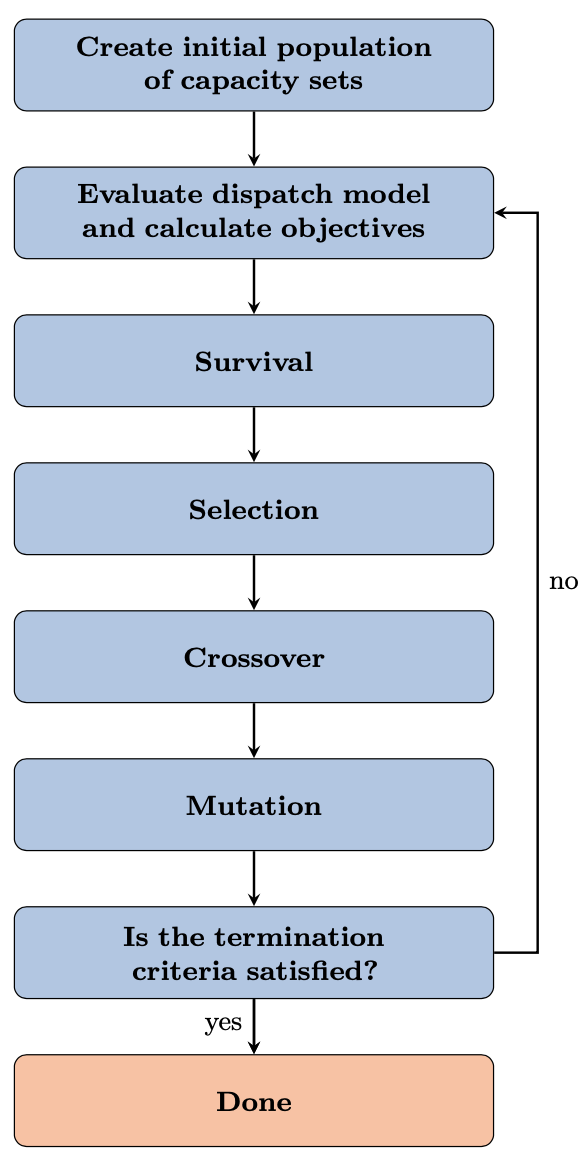
\includegraphics[width=0.75\linewidth]{images/ea-flow.png}  
            \end{figure}
        \end{columns}
    \end{block}
\end{frame}

\begin{frame}
    \frametitle{How \texttt{Osier} handles structural uncertainty}

        \begin{figure}
            \centering
            \resizebox{0.75\columnwidth}{!}{%% Creator: Matplotlib, PGF backend
%%
%% To include the figure in your LaTeX document, write
%%   \input{<filename>.pgf}
%%
%% Make sure the required packages are loaded in your preamble
%%   \usepackage{pgf}
%%
%% Also ensure that all the required font packages are loaded; for instance,
%% the lmodern package is sometimes necessary when using math font.
%%   \usepackage{lmodern}
%%
%% Figures using additional raster images can only be included by \input if
%% they are in the same directory as the main LaTeX file. For loading figures
%% from other directories you can use the `import` package
%%   \usepackage{import}
%%
%% and then include the figures with
%%   \import{<path to file>}{<filename>.pgf}
%%
%% Matplotlib used the following preamble
%%   
%%   \makeatletter\@ifpackageloaded{underscore}{}{\usepackage[strings]{underscore}}\makeatother
%%
\begingroup%
\makeatletter%
\begin{pgfpicture}%
\pgfpathrectangle{\pgfpointorigin}{\pgfqpoint{7.900000in}{5.930000in}}%
\pgfusepath{use as bounding box, clip}%
\begin{pgfscope}%
\pgfsetbuttcap%
\pgfsetmiterjoin%
\definecolor{currentfill}{rgb}{0.827451,0.827451,0.827451}%
\pgfsetfillcolor{currentfill}%
\pgfsetlinewidth{0.000000pt}%
\definecolor{currentstroke}{rgb}{0.000000,0.000000,0.000000}%
\pgfsetstrokecolor{currentstroke}%
\pgfsetdash{}{0pt}%
\pgfpathmoveto{\pgfqpoint{0.000000in}{0.000000in}}%
\pgfpathlineto{\pgfqpoint{7.900000in}{0.000000in}}%
\pgfpathlineto{\pgfqpoint{7.900000in}{5.930000in}}%
\pgfpathlineto{\pgfqpoint{0.000000in}{5.930000in}}%
\pgfpathlineto{\pgfqpoint{0.000000in}{0.000000in}}%
\pgfpathclose%
\pgfusepath{fill}%
\end{pgfscope}%
\begin{pgfscope}%
\pgfsetbuttcap%
\pgfsetmiterjoin%
\definecolor{currentfill}{rgb}{1.000000,1.000000,1.000000}%
\pgfsetfillcolor{currentfill}%
\pgfsetlinewidth{0.000000pt}%
\definecolor{currentstroke}{rgb}{0.000000,0.000000,0.000000}%
\pgfsetstrokecolor{currentstroke}%
\pgfsetstrokeopacity{0.000000}%
\pgfsetdash{}{0pt}%
\pgfpathmoveto{\pgfqpoint{0.882794in}{0.589583in}}%
\pgfpathlineto{\pgfqpoint{7.800000in}{0.589583in}}%
\pgfpathlineto{\pgfqpoint{7.800000in}{5.059445in}}%
\pgfpathlineto{\pgfqpoint{0.882794in}{5.059445in}}%
\pgfpathlineto{\pgfqpoint{0.882794in}{0.589583in}}%
\pgfpathclose%
\pgfusepath{fill}%
\end{pgfscope}%
\begin{pgfscope}%
\pgfpathrectangle{\pgfqpoint{0.882794in}{0.589583in}}{\pgfqpoint{6.917206in}{4.469862in}}%
\pgfusepath{clip}%
\pgfsetbuttcap%
\pgfsetmiterjoin%
\definecolor{currentfill}{rgb}{0.827451,0.827451,0.827451}%
\pgfsetfillcolor{currentfill}%
\pgfsetfillopacity{0.500000}%
\pgfsetlinewidth{0.000000pt}%
\definecolor{currentstroke}{rgb}{0.000000,0.000000,0.000000}%
\pgfsetstrokecolor{currentstroke}%
\pgfsetstrokeopacity{0.500000}%
\pgfsetdash{}{0pt}%
\pgfpathmoveto{\pgfqpoint{0.882794in}{4.258160in}}%
\pgfpathlineto{\pgfqpoint{0.887684in}{4.217744in}}%
\pgfpathlineto{\pgfqpoint{0.892574in}{4.178135in}}%
\pgfpathlineto{\pgfqpoint{0.897463in}{4.139310in}}%
\pgfpathlineto{\pgfqpoint{0.902353in}{4.101245in}}%
\pgfpathlineto{\pgfqpoint{0.907243in}{4.063919in}}%
\pgfpathlineto{\pgfqpoint{0.912132in}{4.027309in}}%
\pgfpathlineto{\pgfqpoint{0.917022in}{3.991396in}}%
\pgfpathlineto{\pgfqpoint{0.921912in}{3.956159in}}%
\pgfpathlineto{\pgfqpoint{0.926801in}{3.921580in}}%
\pgfpathlineto{\pgfqpoint{0.931691in}{3.887641in}}%
\pgfpathlineto{\pgfqpoint{0.936581in}{3.854324in}}%
\pgfpathlineto{\pgfqpoint{0.941470in}{3.821612in}}%
\pgfpathlineto{\pgfqpoint{0.946360in}{3.789489in}}%
\pgfpathlineto{\pgfqpoint{0.951250in}{3.757938in}}%
\pgfpathlineto{\pgfqpoint{0.956139in}{3.726946in}}%
\pgfpathlineto{\pgfqpoint{0.961029in}{3.696496in}}%
\pgfpathlineto{\pgfqpoint{0.965919in}{3.666575in}}%
\pgfpathlineto{\pgfqpoint{0.970808in}{3.637170in}}%
\pgfpathlineto{\pgfqpoint{0.975698in}{3.608267in}}%
\pgfpathlineto{\pgfqpoint{0.980588in}{3.579853in}}%
\pgfpathlineto{\pgfqpoint{0.985477in}{3.551916in}}%
\pgfpathlineto{\pgfqpoint{0.990367in}{3.524445in}}%
\pgfpathlineto{\pgfqpoint{0.995257in}{3.497427in}}%
\pgfpathlineto{\pgfqpoint{1.000146in}{3.470851in}}%
\pgfpathlineto{\pgfqpoint{1.005036in}{3.444707in}}%
\pgfpathlineto{\pgfqpoint{1.009926in}{3.418984in}}%
\pgfpathlineto{\pgfqpoint{1.014815in}{3.393672in}}%
\pgfpathlineto{\pgfqpoint{1.019705in}{3.368762in}}%
\pgfpathlineto{\pgfqpoint{1.024595in}{3.344244in}}%
\pgfpathlineto{\pgfqpoint{1.029484in}{3.320108in}}%
\pgfpathlineto{\pgfqpoint{1.034374in}{3.296346in}}%
\pgfpathlineto{\pgfqpoint{1.039264in}{3.272950in}}%
\pgfpathlineto{\pgfqpoint{1.044153in}{3.249910in}}%
\pgfpathlineto{\pgfqpoint{1.049043in}{3.227219in}}%
\pgfpathlineto{\pgfqpoint{1.053933in}{3.204869in}}%
\pgfpathlineto{\pgfqpoint{1.058822in}{3.182852in}}%
\pgfpathlineto{\pgfqpoint{1.063712in}{3.161161in}}%
\pgfpathlineto{\pgfqpoint{1.068602in}{3.139788in}}%
\pgfpathlineto{\pgfqpoint{1.073491in}{3.118727in}}%
\pgfpathlineto{\pgfqpoint{1.078381in}{3.097972in}}%
\pgfpathlineto{\pgfqpoint{1.083271in}{3.077514in}}%
\pgfpathlineto{\pgfqpoint{1.088160in}{3.057349in}}%
\pgfpathlineto{\pgfqpoint{1.093050in}{3.037469in}}%
\pgfpathlineto{\pgfqpoint{1.097940in}{3.017869in}}%
\pgfpathlineto{\pgfqpoint{1.102829in}{2.998543in}}%
\pgfpathlineto{\pgfqpoint{1.107719in}{2.979486in}}%
\pgfpathlineto{\pgfqpoint{1.112609in}{2.960690in}}%
\pgfpathlineto{\pgfqpoint{1.117498in}{2.942152in}}%
\pgfpathlineto{\pgfqpoint{1.122388in}{2.923866in}}%
\pgfpathlineto{\pgfqpoint{1.127278in}{2.905827in}}%
\pgfpathlineto{\pgfqpoint{1.132167in}{2.888030in}}%
\pgfpathlineto{\pgfqpoint{1.137057in}{2.870470in}}%
\pgfpathlineto{\pgfqpoint{1.141947in}{2.853142in}}%
\pgfpathlineto{\pgfqpoint{1.146837in}{2.836043in}}%
\pgfpathlineto{\pgfqpoint{1.151726in}{2.819166in}}%
\pgfpathlineto{\pgfqpoint{1.156616in}{2.802508in}}%
\pgfpathlineto{\pgfqpoint{1.161506in}{2.786066in}}%
\pgfpathlineto{\pgfqpoint{1.166395in}{2.769834in}}%
\pgfpathlineto{\pgfqpoint{1.171285in}{2.753808in}}%
\pgfpathlineto{\pgfqpoint{1.176175in}{2.737985in}}%
\pgfpathlineto{\pgfqpoint{1.181064in}{2.722361in}}%
\pgfpathlineto{\pgfqpoint{1.185954in}{2.706932in}}%
\pgfpathlineto{\pgfqpoint{1.190844in}{2.691695in}}%
\pgfpathlineto{\pgfqpoint{1.195733in}{2.676645in}}%
\pgfpathlineto{\pgfqpoint{1.200623in}{2.661781in}}%
\pgfpathlineto{\pgfqpoint{1.205513in}{2.647097in}}%
\pgfpathlineto{\pgfqpoint{1.210402in}{2.632591in}}%
\pgfpathlineto{\pgfqpoint{1.215292in}{2.618260in}}%
\pgfpathlineto{\pgfqpoint{1.220182in}{2.604100in}}%
\pgfpathlineto{\pgfqpoint{1.225071in}{2.590108in}}%
\pgfpathlineto{\pgfqpoint{1.229961in}{2.576283in}}%
\pgfpathlineto{\pgfqpoint{1.234851in}{2.562619in}}%
\pgfpathlineto{\pgfqpoint{1.239740in}{2.549116in}}%
\pgfpathlineto{\pgfqpoint{1.244630in}{2.535769in}}%
\pgfpathlineto{\pgfqpoint{1.249520in}{2.522576in}}%
\pgfpathlineto{\pgfqpoint{1.254409in}{2.509535in}}%
\pgfpathlineto{\pgfqpoint{1.259299in}{2.496643in}}%
\pgfpathlineto{\pgfqpoint{1.264189in}{2.483897in}}%
\pgfpathlineto{\pgfqpoint{1.269078in}{2.471295in}}%
\pgfpathlineto{\pgfqpoint{1.273968in}{2.458835in}}%
\pgfpathlineto{\pgfqpoint{1.278858in}{2.446514in}}%
\pgfpathlineto{\pgfqpoint{1.283747in}{2.434329in}}%
\pgfpathlineto{\pgfqpoint{1.288637in}{2.422280in}}%
\pgfpathlineto{\pgfqpoint{1.293527in}{2.410362in}}%
\pgfpathlineto{\pgfqpoint{1.298416in}{2.398575in}}%
\pgfpathlineto{\pgfqpoint{1.303306in}{2.386915in}}%
\pgfpathlineto{\pgfqpoint{1.308196in}{2.375382in}}%
\pgfpathlineto{\pgfqpoint{1.313085in}{2.363972in}}%
\pgfpathlineto{\pgfqpoint{1.317975in}{2.352685in}}%
\pgfpathlineto{\pgfqpoint{1.322865in}{2.341517in}}%
\pgfpathlineto{\pgfqpoint{1.327754in}{2.330468in}}%
\pgfpathlineto{\pgfqpoint{1.332644in}{2.319535in}}%
\pgfpathlineto{\pgfqpoint{1.337534in}{2.308716in}}%
\pgfpathlineto{\pgfqpoint{1.342423in}{2.298010in}}%
\pgfpathlineto{\pgfqpoint{1.347313in}{2.287414in}}%
\pgfpathlineto{\pgfqpoint{1.352203in}{2.276928in}}%
\pgfpathlineto{\pgfqpoint{1.357092in}{2.266549in}}%
\pgfpathlineto{\pgfqpoint{1.361982in}{2.256277in}}%
\pgfpathlineto{\pgfqpoint{1.366872in}{2.246108in}}%
\pgfpathlineto{\pgfqpoint{1.371761in}{2.236042in}}%
\pgfpathlineto{\pgfqpoint{1.376651in}{2.226077in}}%
\pgfpathlineto{\pgfqpoint{1.381541in}{2.216212in}}%
\pgfpathlineto{\pgfqpoint{1.386430in}{2.206445in}}%
\pgfpathlineto{\pgfqpoint{1.391320in}{2.196774in}}%
\pgfpathlineto{\pgfqpoint{1.396210in}{2.187199in}}%
\pgfpathlineto{\pgfqpoint{1.401099in}{2.177717in}}%
\pgfpathlineto{\pgfqpoint{1.405989in}{2.168328in}}%
\pgfpathlineto{\pgfqpoint{1.410879in}{2.159030in}}%
\pgfpathlineto{\pgfqpoint{1.415768in}{2.149822in}}%
\pgfpathlineto{\pgfqpoint{1.420658in}{2.140702in}}%
\pgfpathlineto{\pgfqpoint{1.425548in}{2.131670in}}%
\pgfpathlineto{\pgfqpoint{1.430437in}{2.122723in}}%
\pgfpathlineto{\pgfqpoint{1.435327in}{2.113861in}}%
\pgfpathlineto{\pgfqpoint{1.440217in}{2.105083in}}%
\pgfpathlineto{\pgfqpoint{1.445106in}{2.096387in}}%
\pgfpathlineto{\pgfqpoint{1.449996in}{2.087773in}}%
\pgfpathlineto{\pgfqpoint{1.454886in}{2.079238in}}%
\pgfpathlineto{\pgfqpoint{1.459775in}{2.070782in}}%
\pgfpathlineto{\pgfqpoint{1.464665in}{2.062405in}}%
\pgfpathlineto{\pgfqpoint{1.469555in}{2.054104in}}%
\pgfpathlineto{\pgfqpoint{1.474444in}{2.045879in}}%
\pgfpathlineto{\pgfqpoint{1.479334in}{2.037728in}}%
\pgfpathlineto{\pgfqpoint{1.484224in}{2.029652in}}%
\pgfpathlineto{\pgfqpoint{1.489113in}{2.021648in}}%
\pgfpathlineto{\pgfqpoint{1.494003in}{2.013716in}}%
\pgfpathlineto{\pgfqpoint{1.498893in}{2.005854in}}%
\pgfpathlineto{\pgfqpoint{1.503782in}{1.998063in}}%
\pgfpathlineto{\pgfqpoint{1.508672in}{1.990340in}}%
\pgfpathlineto{\pgfqpoint{1.513562in}{1.982685in}}%
\pgfpathlineto{\pgfqpoint{1.518451in}{1.975098in}}%
\pgfpathlineto{\pgfqpoint{1.523341in}{1.967576in}}%
\pgfpathlineto{\pgfqpoint{1.528231in}{1.960120in}}%
\pgfpathlineto{\pgfqpoint{1.533120in}{1.952729in}}%
\pgfpathlineto{\pgfqpoint{1.538010in}{1.945401in}}%
\pgfpathlineto{\pgfqpoint{1.542900in}{1.938136in}}%
\pgfpathlineto{\pgfqpoint{1.547789in}{1.930933in}}%
\pgfpathlineto{\pgfqpoint{1.552679in}{1.923792in}}%
\pgfpathlineto{\pgfqpoint{1.557569in}{1.916711in}}%
\pgfpathlineto{\pgfqpoint{1.562458in}{1.909689in}}%
\pgfpathlineto{\pgfqpoint{1.567348in}{1.902727in}}%
\pgfpathlineto{\pgfqpoint{1.572238in}{1.895823in}}%
\pgfpathlineto{\pgfqpoint{1.577128in}{1.888976in}}%
\pgfpathlineto{\pgfqpoint{1.582017in}{1.882186in}}%
\pgfpathlineto{\pgfqpoint{1.586907in}{1.875452in}}%
\pgfpathlineto{\pgfqpoint{1.591797in}{1.868774in}}%
\pgfpathlineto{\pgfqpoint{1.596686in}{1.862150in}}%
\pgfpathlineto{\pgfqpoint{1.601576in}{1.855581in}}%
\pgfpathlineto{\pgfqpoint{1.606466in}{1.849064in}}%
\pgfpathlineto{\pgfqpoint{1.611355in}{1.842601in}}%
\pgfpathlineto{\pgfqpoint{1.616245in}{1.836189in}}%
\pgfpathlineto{\pgfqpoint{1.621135in}{1.829830in}}%
\pgfpathlineto{\pgfqpoint{1.626024in}{1.823520in}}%
\pgfpathlineto{\pgfqpoint{1.630914in}{1.817262in}}%
\pgfpathlineto{\pgfqpoint{1.635804in}{1.811052in}}%
\pgfpathlineto{\pgfqpoint{1.640693in}{1.804892in}}%
\pgfpathlineto{\pgfqpoint{1.645583in}{1.798781in}}%
\pgfpathlineto{\pgfqpoint{1.650473in}{1.792717in}}%
\pgfpathlineto{\pgfqpoint{1.655362in}{1.786700in}}%
\pgfpathlineto{\pgfqpoint{1.660252in}{1.780731in}}%
\pgfpathlineto{\pgfqpoint{1.665142in}{1.774807in}}%
\pgfpathlineto{\pgfqpoint{1.670031in}{1.768930in}}%
\pgfpathlineto{\pgfqpoint{1.674921in}{1.763097in}}%
\pgfpathlineto{\pgfqpoint{1.679811in}{1.757309in}}%
\pgfpathlineto{\pgfqpoint{1.684700in}{1.751566in}}%
\pgfpathlineto{\pgfqpoint{1.689590in}{1.745866in}}%
\pgfpathlineto{\pgfqpoint{1.694480in}{1.740209in}}%
\pgfpathlineto{\pgfqpoint{1.699369in}{1.734595in}}%
\pgfpathlineto{\pgfqpoint{1.704259in}{1.729023in}}%
\pgfpathlineto{\pgfqpoint{1.709149in}{1.723493in}}%
\pgfpathlineto{\pgfqpoint{1.714038in}{1.718004in}}%
\pgfpathlineto{\pgfqpoint{1.718928in}{1.712556in}}%
\pgfpathlineto{\pgfqpoint{1.723818in}{1.707148in}}%
\pgfpathlineto{\pgfqpoint{1.728707in}{1.701780in}}%
\pgfpathlineto{\pgfqpoint{1.733597in}{1.696451in}}%
\pgfpathlineto{\pgfqpoint{1.738487in}{1.691162in}}%
\pgfpathlineto{\pgfqpoint{1.743376in}{1.685911in}}%
\pgfpathlineto{\pgfqpoint{1.748266in}{1.680698in}}%
\pgfpathlineto{\pgfqpoint{1.753156in}{1.675523in}}%
\pgfpathlineto{\pgfqpoint{1.758045in}{1.670386in}}%
\pgfpathlineto{\pgfqpoint{1.762935in}{1.665285in}}%
\pgfpathlineto{\pgfqpoint{1.767825in}{1.660221in}}%
\pgfpathlineto{\pgfqpoint{1.772714in}{1.655193in}}%
\pgfpathlineto{\pgfqpoint{1.777604in}{1.650201in}}%
\pgfpathlineto{\pgfqpoint{1.782494in}{1.645244in}}%
\pgfpathlineto{\pgfqpoint{1.787383in}{1.640322in}}%
\pgfpathlineto{\pgfqpoint{1.792273in}{1.635435in}}%
\pgfpathlineto{\pgfqpoint{1.797163in}{1.630582in}}%
\pgfpathlineto{\pgfqpoint{1.802052in}{1.625763in}}%
\pgfpathlineto{\pgfqpoint{1.806942in}{1.620978in}}%
\pgfpathlineto{\pgfqpoint{1.811832in}{1.616225in}}%
\pgfpathlineto{\pgfqpoint{1.816721in}{1.611506in}}%
\pgfpathlineto{\pgfqpoint{1.821611in}{1.606819in}}%
\pgfpathlineto{\pgfqpoint{1.826501in}{1.602165in}}%
\pgfpathlineto{\pgfqpoint{1.831390in}{1.597542in}}%
\pgfpathlineto{\pgfqpoint{1.836280in}{1.592951in}}%
\pgfpathlineto{\pgfqpoint{1.841170in}{1.588391in}}%
\pgfpathlineto{\pgfqpoint{1.846059in}{1.583862in}}%
\pgfpathlineto{\pgfqpoint{1.850949in}{1.579363in}}%
\pgfpathlineto{\pgfqpoint{1.855839in}{1.574895in}}%
\pgfpathlineto{\pgfqpoint{1.860728in}{1.570457in}}%
\pgfpathlineto{\pgfqpoint{1.865618in}{1.566048in}}%
\pgfpathlineto{\pgfqpoint{1.870508in}{1.561669in}}%
\pgfpathlineto{\pgfqpoint{1.875397in}{1.557319in}}%
\pgfpathlineto{\pgfqpoint{1.880287in}{1.552998in}}%
\pgfpathlineto{\pgfqpoint{1.885177in}{1.548705in}}%
\pgfpathlineto{\pgfqpoint{1.890066in}{1.544441in}}%
\pgfpathlineto{\pgfqpoint{1.894956in}{1.540204in}}%
\pgfpathlineto{\pgfqpoint{1.899846in}{1.535995in}}%
\pgfpathlineto{\pgfqpoint{1.904735in}{1.531814in}}%
\pgfpathlineto{\pgfqpoint{1.909625in}{1.527659in}}%
\pgfpathlineto{\pgfqpoint{1.914515in}{1.523532in}}%
\pgfpathlineto{\pgfqpoint{1.919404in}{1.519431in}}%
\pgfpathlineto{\pgfqpoint{1.924294in}{1.515356in}}%
\pgfpathlineto{\pgfqpoint{1.929184in}{1.511308in}}%
\pgfpathlineto{\pgfqpoint{1.934073in}{1.507286in}}%
\pgfpathlineto{\pgfqpoint{1.938963in}{1.503289in}}%
\pgfpathlineto{\pgfqpoint{1.943853in}{1.499317in}}%
\pgfpathlineto{\pgfqpoint{1.948742in}{1.495371in}}%
\pgfpathlineto{\pgfqpoint{1.953632in}{1.491449in}}%
\pgfpathlineto{\pgfqpoint{1.958522in}{1.487552in}}%
\pgfpathlineto{\pgfqpoint{1.963411in}{1.483680in}}%
\pgfpathlineto{\pgfqpoint{1.968301in}{1.479832in}}%
\pgfpathlineto{\pgfqpoint{1.973191in}{1.476007in}}%
\pgfpathlineto{\pgfqpoint{1.978080in}{1.472207in}}%
\pgfpathlineto{\pgfqpoint{1.982970in}{1.468430in}}%
\pgfpathlineto{\pgfqpoint{1.987860in}{1.464676in}}%
\pgfpathlineto{\pgfqpoint{1.992749in}{1.460945in}}%
\pgfpathlineto{\pgfqpoint{1.997639in}{1.457237in}}%
\pgfpathlineto{\pgfqpoint{2.002529in}{1.453552in}}%
\pgfpathlineto{\pgfqpoint{2.007418in}{1.449890in}}%
\pgfpathlineto{\pgfqpoint{2.012308in}{1.446249in}}%
\pgfpathlineto{\pgfqpoint{2.017198in}{1.442631in}}%
\pgfpathlineto{\pgfqpoint{2.022088in}{1.439035in}}%
\pgfpathlineto{\pgfqpoint{2.026977in}{1.435460in}}%
\pgfpathlineto{\pgfqpoint{2.031867in}{1.431906in}}%
\pgfpathlineto{\pgfqpoint{2.036757in}{1.428374in}}%
\pgfpathlineto{\pgfqpoint{2.041646in}{1.424863in}}%
\pgfpathlineto{\pgfqpoint{2.046536in}{1.421373in}}%
\pgfpathlineto{\pgfqpoint{2.051426in}{1.417904in}}%
\pgfpathlineto{\pgfqpoint{2.056315in}{1.414455in}}%
\pgfpathlineto{\pgfqpoint{2.061205in}{1.411026in}}%
\pgfpathlineto{\pgfqpoint{2.066095in}{1.407618in}}%
\pgfpathlineto{\pgfqpoint{2.070984in}{1.404230in}}%
\pgfpathlineto{\pgfqpoint{2.075874in}{1.400861in}}%
\pgfpathlineto{\pgfqpoint{2.080764in}{1.397512in}}%
\pgfpathlineto{\pgfqpoint{2.085653in}{1.394183in}}%
\pgfpathlineto{\pgfqpoint{2.090543in}{1.390872in}}%
\pgfpathlineto{\pgfqpoint{2.095433in}{1.387581in}}%
\pgfpathlineto{\pgfqpoint{2.100322in}{1.384309in}}%
\pgfpathlineto{\pgfqpoint{2.105212in}{1.381056in}}%
\pgfpathlineto{\pgfqpoint{2.110102in}{1.377821in}}%
\pgfpathlineto{\pgfqpoint{2.114991in}{1.374605in}}%
\pgfpathlineto{\pgfqpoint{2.119881in}{1.371407in}}%
\pgfpathlineto{\pgfqpoint{2.124771in}{1.368227in}}%
\pgfpathlineto{\pgfqpoint{2.129660in}{1.365066in}}%
\pgfpathlineto{\pgfqpoint{2.134550in}{1.361922in}}%
\pgfpathlineto{\pgfqpoint{2.139440in}{1.358796in}}%
\pgfpathlineto{\pgfqpoint{2.144329in}{1.355687in}}%
\pgfpathlineto{\pgfqpoint{2.149219in}{1.352596in}}%
\pgfpathlineto{\pgfqpoint{2.154109in}{1.349522in}}%
\pgfpathlineto{\pgfqpoint{2.158998in}{1.346465in}}%
\pgfpathlineto{\pgfqpoint{2.163888in}{1.343425in}}%
\pgfpathlineto{\pgfqpoint{2.168778in}{1.340402in}}%
\pgfpathlineto{\pgfqpoint{2.173667in}{1.337396in}}%
\pgfpathlineto{\pgfqpoint{2.178557in}{1.334406in}}%
\pgfpathlineto{\pgfqpoint{2.183447in}{1.331433in}}%
\pgfpathlineto{\pgfqpoint{2.188336in}{1.328476in}}%
\pgfpathlineto{\pgfqpoint{2.193226in}{1.325535in}}%
\pgfpathlineto{\pgfqpoint{2.198116in}{1.322610in}}%
\pgfpathlineto{\pgfqpoint{2.203005in}{1.319701in}}%
\pgfpathlineto{\pgfqpoint{2.207895in}{1.316808in}}%
\pgfpathlineto{\pgfqpoint{2.212785in}{1.313930in}}%
\pgfpathlineto{\pgfqpoint{2.217674in}{1.311068in}}%
\pgfpathlineto{\pgfqpoint{2.222564in}{1.308222in}}%
\pgfpathlineto{\pgfqpoint{2.227454in}{1.305390in}}%
\pgfpathlineto{\pgfqpoint{2.232343in}{1.302574in}}%
\pgfpathlineto{\pgfqpoint{2.237233in}{1.299773in}}%
\pgfpathlineto{\pgfqpoint{2.242123in}{1.296986in}}%
\pgfpathlineto{\pgfqpoint{2.247012in}{1.294215in}}%
\pgfpathlineto{\pgfqpoint{2.251902in}{1.291458in}}%
\pgfpathlineto{\pgfqpoint{2.256792in}{1.288715in}}%
\pgfpathlineto{\pgfqpoint{2.261681in}{1.285987in}}%
\pgfpathlineto{\pgfqpoint{2.266571in}{1.283274in}}%
\pgfpathlineto{\pgfqpoint{2.271461in}{1.280574in}}%
\pgfpathlineto{\pgfqpoint{2.276350in}{1.277889in}}%
\pgfpathlineto{\pgfqpoint{2.281240in}{1.275218in}}%
\pgfpathlineto{\pgfqpoint{2.286130in}{1.272560in}}%
\pgfpathlineto{\pgfqpoint{2.291019in}{1.269916in}}%
\pgfpathlineto{\pgfqpoint{2.295909in}{1.267286in}}%
\pgfpathlineto{\pgfqpoint{2.300799in}{1.264670in}}%
\pgfpathlineto{\pgfqpoint{2.305688in}{1.262067in}}%
\pgfpathlineto{\pgfqpoint{2.310578in}{1.259477in}}%
\pgfpathlineto{\pgfqpoint{2.315468in}{1.256900in}}%
\pgfpathlineto{\pgfqpoint{2.320357in}{1.254337in}}%
\pgfpathlineto{\pgfqpoint{2.325247in}{1.251787in}}%
\pgfpathlineto{\pgfqpoint{2.330137in}{1.249249in}}%
\pgfpathlineto{\pgfqpoint{2.335026in}{1.246725in}}%
\pgfpathlineto{\pgfqpoint{2.339916in}{1.244213in}}%
\pgfpathlineto{\pgfqpoint{2.344806in}{1.241714in}}%
\pgfpathlineto{\pgfqpoint{2.349695in}{1.239227in}}%
\pgfpathlineto{\pgfqpoint{2.354585in}{1.236753in}}%
\pgfpathlineto{\pgfqpoint{2.359475in}{1.234291in}}%
\pgfpathlineto{\pgfqpoint{2.364364in}{1.231842in}}%
\pgfpathlineto{\pgfqpoint{2.369254in}{1.229405in}}%
\pgfpathlineto{\pgfqpoint{2.374144in}{1.226979in}}%
\pgfpathlineto{\pgfqpoint{2.379033in}{1.224566in}}%
\pgfpathlineto{\pgfqpoint{2.383923in}{1.222165in}}%
\pgfpathlineto{\pgfqpoint{2.388813in}{1.219776in}}%
\pgfpathlineto{\pgfqpoint{2.393702in}{1.217398in}}%
\pgfpathlineto{\pgfqpoint{2.398592in}{1.215032in}}%
\pgfpathlineto{\pgfqpoint{2.403482in}{1.212677in}}%
\pgfpathlineto{\pgfqpoint{2.408371in}{1.210334in}}%
\pgfpathlineto{\pgfqpoint{2.413261in}{1.208003in}}%
\pgfpathlineto{\pgfqpoint{2.418151in}{1.205682in}}%
\pgfpathlineto{\pgfqpoint{2.423040in}{1.203373in}}%
\pgfpathlineto{\pgfqpoint{2.427930in}{1.201075in}}%
\pgfpathlineto{\pgfqpoint{2.432820in}{1.198788in}}%
\pgfpathlineto{\pgfqpoint{2.437709in}{1.196513in}}%
\pgfpathlineto{\pgfqpoint{2.442599in}{1.194248in}}%
\pgfpathlineto{\pgfqpoint{2.447489in}{1.191993in}}%
\pgfpathlineto{\pgfqpoint{2.452379in}{1.189750in}}%
\pgfpathlineto{\pgfqpoint{2.457268in}{1.187517in}}%
\pgfpathlineto{\pgfqpoint{2.462158in}{1.185295in}}%
\pgfpathlineto{\pgfqpoint{2.467048in}{1.183084in}}%
\pgfpathlineto{\pgfqpoint{2.471937in}{1.180883in}}%
\pgfpathlineto{\pgfqpoint{2.476827in}{1.178692in}}%
\pgfpathlineto{\pgfqpoint{2.481717in}{1.176512in}}%
\pgfpathlineto{\pgfqpoint{2.486606in}{1.174341in}}%
\pgfpathlineto{\pgfqpoint{2.491496in}{1.172181in}}%
\pgfpathlineto{\pgfqpoint{2.496386in}{1.170031in}}%
\pgfpathlineto{\pgfqpoint{2.501275in}{1.167891in}}%
\pgfpathlineto{\pgfqpoint{2.506165in}{1.165762in}}%
\pgfpathlineto{\pgfqpoint{2.511055in}{1.163641in}}%
\pgfpathlineto{\pgfqpoint{2.515944in}{1.161531in}}%
\pgfpathlineto{\pgfqpoint{2.520834in}{1.159431in}}%
\pgfpathlineto{\pgfqpoint{2.525724in}{1.157340in}}%
\pgfpathlineto{\pgfqpoint{2.530613in}{1.155259in}}%
\pgfpathlineto{\pgfqpoint{2.535503in}{1.153187in}}%
\pgfpathlineto{\pgfqpoint{2.540393in}{1.151125in}}%
\pgfpathlineto{\pgfqpoint{2.545282in}{1.149072in}}%
\pgfpathlineto{\pgfqpoint{2.550172in}{1.147028in}}%
\pgfpathlineto{\pgfqpoint{2.555062in}{1.144994in}}%
\pgfpathlineto{\pgfqpoint{2.559951in}{1.142969in}}%
\pgfpathlineto{\pgfqpoint{2.564841in}{1.140954in}}%
\pgfpathlineto{\pgfqpoint{2.569731in}{1.138947in}}%
\pgfpathlineto{\pgfqpoint{2.574620in}{1.136949in}}%
\pgfpathlineto{\pgfqpoint{2.579510in}{1.134961in}}%
\pgfpathlineto{\pgfqpoint{2.584400in}{1.132981in}}%
\pgfpathlineto{\pgfqpoint{2.589289in}{1.131010in}}%
\pgfpathlineto{\pgfqpoint{2.594179in}{1.129048in}}%
\pgfpathlineto{\pgfqpoint{2.599069in}{1.127094in}}%
\pgfpathlineto{\pgfqpoint{2.603958in}{1.125150in}}%
\pgfpathlineto{\pgfqpoint{2.608848in}{1.123214in}}%
\pgfpathlineto{\pgfqpoint{2.613738in}{1.121286in}}%
\pgfpathlineto{\pgfqpoint{2.618627in}{1.119367in}}%
\pgfpathlineto{\pgfqpoint{2.623517in}{1.117457in}}%
\pgfpathlineto{\pgfqpoint{2.628407in}{1.115554in}}%
\pgfpathlineto{\pgfqpoint{2.633296in}{1.113661in}}%
\pgfpathlineto{\pgfqpoint{2.638186in}{1.111775in}}%
\pgfpathlineto{\pgfqpoint{2.643076in}{1.109898in}}%
\pgfpathlineto{\pgfqpoint{2.647965in}{1.108029in}}%
\pgfpathlineto{\pgfqpoint{2.652855in}{1.106168in}}%
\pgfpathlineto{\pgfqpoint{2.657745in}{1.104315in}}%
\pgfpathlineto{\pgfqpoint{2.662634in}{1.102470in}}%
\pgfpathlineto{\pgfqpoint{2.667524in}{1.100633in}}%
\pgfpathlineto{\pgfqpoint{2.672414in}{1.098804in}}%
\pgfpathlineto{\pgfqpoint{2.677303in}{1.096983in}}%
\pgfpathlineto{\pgfqpoint{2.682193in}{1.095170in}}%
\pgfpathlineto{\pgfqpoint{2.687083in}{1.093364in}}%
\pgfpathlineto{\pgfqpoint{2.691972in}{1.091566in}}%
\pgfpathlineto{\pgfqpoint{2.696862in}{1.089776in}}%
\pgfpathlineto{\pgfqpoint{2.701752in}{1.087993in}}%
\pgfpathlineto{\pgfqpoint{2.706641in}{1.086218in}}%
\pgfpathlineto{\pgfqpoint{2.711531in}{1.084451in}}%
\pgfpathlineto{\pgfqpoint{2.716421in}{1.082691in}}%
\pgfpathlineto{\pgfqpoint{2.721310in}{1.080938in}}%
\pgfpathlineto{\pgfqpoint{2.726200in}{1.079193in}}%
\pgfpathlineto{\pgfqpoint{2.731090in}{1.077455in}}%
\pgfpathlineto{\pgfqpoint{2.735979in}{1.075724in}}%
\pgfpathlineto{\pgfqpoint{2.740869in}{1.074001in}}%
\pgfpathlineto{\pgfqpoint{2.745759in}{1.072285in}}%
\pgfpathlineto{\pgfqpoint{2.750648in}{1.070576in}}%
\pgfpathlineto{\pgfqpoint{2.755538in}{1.068874in}}%
\pgfpathlineto{\pgfqpoint{2.760428in}{1.067179in}}%
\pgfpathlineto{\pgfqpoint{2.765317in}{1.065491in}}%
\pgfpathlineto{\pgfqpoint{2.770207in}{1.063810in}}%
\pgfpathlineto{\pgfqpoint{2.775097in}{1.062136in}}%
\pgfpathlineto{\pgfqpoint{2.779986in}{1.060469in}}%
\pgfpathlineto{\pgfqpoint{2.784876in}{1.058809in}}%
\pgfpathlineto{\pgfqpoint{2.789766in}{1.057156in}}%
\pgfpathlineto{\pgfqpoint{2.794655in}{1.055509in}}%
\pgfpathlineto{\pgfqpoint{2.799545in}{1.053869in}}%
\pgfpathlineto{\pgfqpoint{2.804435in}{1.052236in}}%
\pgfpathlineto{\pgfqpoint{2.809324in}{1.050609in}}%
\pgfpathlineto{\pgfqpoint{2.814214in}{1.048989in}}%
\pgfpathlineto{\pgfqpoint{2.819104in}{1.047376in}}%
\pgfpathlineto{\pgfqpoint{2.823993in}{1.045769in}}%
\pgfpathlineto{\pgfqpoint{2.828883in}{1.044168in}}%
\pgfpathlineto{\pgfqpoint{2.833773in}{1.042574in}}%
\pgfpathlineto{\pgfqpoint{2.838662in}{1.040987in}}%
\pgfpathlineto{\pgfqpoint{2.843552in}{1.039406in}}%
\pgfpathlineto{\pgfqpoint{2.848442in}{1.037831in}}%
\pgfpathlineto{\pgfqpoint{2.853331in}{1.036262in}}%
\pgfpathlineto{\pgfqpoint{2.858221in}{1.034700in}}%
\pgfpathlineto{\pgfqpoint{2.863111in}{1.033143in}}%
\pgfpathlineto{\pgfqpoint{2.868000in}{1.031593in}}%
\pgfpathlineto{\pgfqpoint{2.872890in}{1.030049in}}%
\pgfpathlineto{\pgfqpoint{2.877780in}{1.028512in}}%
\pgfpathlineto{\pgfqpoint{2.882669in}{1.026980in}}%
\pgfpathlineto{\pgfqpoint{2.887559in}{1.025454in}}%
\pgfpathlineto{\pgfqpoint{2.892449in}{1.023935in}}%
\pgfpathlineto{\pgfqpoint{2.897339in}{1.022421in}}%
\pgfpathlineto{\pgfqpoint{2.902228in}{1.020913in}}%
\pgfpathlineto{\pgfqpoint{2.907118in}{1.019411in}}%
\pgfpathlineto{\pgfqpoint{2.912008in}{1.017915in}}%
\pgfpathlineto{\pgfqpoint{2.916897in}{1.016425in}}%
\pgfpathlineto{\pgfqpoint{2.921787in}{1.014940in}}%
\pgfpathlineto{\pgfqpoint{2.926677in}{1.013462in}}%
\pgfpathlineto{\pgfqpoint{2.931566in}{1.011989in}}%
\pgfpathlineto{\pgfqpoint{2.936456in}{1.010521in}}%
\pgfpathlineto{\pgfqpoint{2.941346in}{1.009060in}}%
\pgfpathlineto{\pgfqpoint{2.946235in}{1.007604in}}%
\pgfpathlineto{\pgfqpoint{2.951125in}{1.006153in}}%
\pgfpathlineto{\pgfqpoint{2.956015in}{1.004708in}}%
\pgfpathlineto{\pgfqpoint{2.960904in}{1.003269in}}%
\pgfpathlineto{\pgfqpoint{2.965794in}{1.001835in}}%
\pgfpathlineto{\pgfqpoint{2.970684in}{1.000407in}}%
\pgfpathlineto{\pgfqpoint{2.975573in}{0.998984in}}%
\pgfpathlineto{\pgfqpoint{2.980463in}{0.997566in}}%
\pgfpathlineto{\pgfqpoint{2.985353in}{0.996154in}}%
\pgfpathlineto{\pgfqpoint{2.990242in}{0.994747in}}%
\pgfpathlineto{\pgfqpoint{2.995132in}{0.993345in}}%
\pgfpathlineto{\pgfqpoint{3.000022in}{0.991949in}}%
\pgfpathlineto{\pgfqpoint{3.004911in}{0.990558in}}%
\pgfpathlineto{\pgfqpoint{3.009801in}{0.989172in}}%
\pgfpathlineto{\pgfqpoint{3.014691in}{0.987792in}}%
\pgfpathlineto{\pgfqpoint{3.019580in}{0.986416in}}%
\pgfpathlineto{\pgfqpoint{3.024470in}{0.985046in}}%
\pgfpathlineto{\pgfqpoint{3.029360in}{0.983681in}}%
\pgfpathlineto{\pgfqpoint{3.034249in}{0.982320in}}%
\pgfpathlineto{\pgfqpoint{3.039139in}{0.980965in}}%
\pgfpathlineto{\pgfqpoint{3.044029in}{0.979615in}}%
\pgfpathlineto{\pgfqpoint{3.048918in}{0.978270in}}%
\pgfpathlineto{\pgfqpoint{3.053808in}{0.976930in}}%
\pgfpathlineto{\pgfqpoint{3.058698in}{0.975595in}}%
\pgfpathlineto{\pgfqpoint{3.063587in}{0.974264in}}%
\pgfpathlineto{\pgfqpoint{3.068477in}{0.972939in}}%
\pgfpathlineto{\pgfqpoint{3.073367in}{0.971618in}}%
\pgfpathlineto{\pgfqpoint{3.078256in}{0.970303in}}%
\pgfpathlineto{\pgfqpoint{3.083146in}{0.968992in}}%
\pgfpathlineto{\pgfqpoint{3.088036in}{0.967685in}}%
\pgfpathlineto{\pgfqpoint{3.092925in}{0.966384in}}%
\pgfpathlineto{\pgfqpoint{3.097815in}{0.965087in}}%
\pgfpathlineto{\pgfqpoint{3.102705in}{0.963795in}}%
\pgfpathlineto{\pgfqpoint{3.107594in}{0.962508in}}%
\pgfpathlineto{\pgfqpoint{3.112484in}{0.961225in}}%
\pgfpathlineto{\pgfqpoint{3.117374in}{0.959947in}}%
\pgfpathlineto{\pgfqpoint{3.122263in}{0.958674in}}%
\pgfpathlineto{\pgfqpoint{3.127153in}{0.957405in}}%
\pgfpathlineto{\pgfqpoint{3.132043in}{0.956140in}}%
\pgfpathlineto{\pgfqpoint{3.136932in}{0.954881in}}%
\pgfpathlineto{\pgfqpoint{3.141822in}{0.953625in}}%
\pgfpathlineto{\pgfqpoint{3.146712in}{0.952374in}}%
\pgfpathlineto{\pgfqpoint{3.151601in}{0.951128in}}%
\pgfpathlineto{\pgfqpoint{3.156491in}{0.949886in}}%
\pgfpathlineto{\pgfqpoint{3.161381in}{0.948649in}}%
\pgfpathlineto{\pgfqpoint{3.166270in}{0.947415in}}%
\pgfpathlineto{\pgfqpoint{3.171160in}{0.946186in}}%
\pgfpathlineto{\pgfqpoint{3.176050in}{0.944962in}}%
\pgfpathlineto{\pgfqpoint{3.180939in}{0.943742in}}%
\pgfpathlineto{\pgfqpoint{3.185829in}{0.942526in}}%
\pgfpathlineto{\pgfqpoint{3.190719in}{0.941314in}}%
\pgfpathlineto{\pgfqpoint{3.195608in}{0.940107in}}%
\pgfpathlineto{\pgfqpoint{3.200498in}{0.938904in}}%
\pgfpathlineto{\pgfqpoint{3.205388in}{0.937705in}}%
\pgfpathlineto{\pgfqpoint{3.210277in}{0.936510in}}%
\pgfpathlineto{\pgfqpoint{3.215167in}{0.935319in}}%
\pgfpathlineto{\pgfqpoint{3.220057in}{0.934133in}}%
\pgfpathlineto{\pgfqpoint{3.224946in}{0.932950in}}%
\pgfpathlineto{\pgfqpoint{3.229836in}{0.931772in}}%
\pgfpathlineto{\pgfqpoint{3.234726in}{0.930598in}}%
\pgfpathlineto{\pgfqpoint{3.239615in}{0.929428in}}%
\pgfpathlineto{\pgfqpoint{3.244505in}{0.928261in}}%
\pgfpathlineto{\pgfqpoint{3.249395in}{0.927099in}}%
\pgfpathlineto{\pgfqpoint{3.254284in}{0.925941in}}%
\pgfpathlineto{\pgfqpoint{3.259174in}{0.924787in}}%
\pgfpathlineto{\pgfqpoint{3.264064in}{0.923637in}}%
\pgfpathlineto{\pgfqpoint{3.268953in}{0.922490in}}%
\pgfpathlineto{\pgfqpoint{3.273843in}{0.921348in}}%
\pgfpathlineto{\pgfqpoint{3.278733in}{0.920209in}}%
\pgfpathlineto{\pgfqpoint{3.283622in}{0.919075in}}%
\pgfpathlineto{\pgfqpoint{3.288512in}{0.917944in}}%
\pgfpathlineto{\pgfqpoint{3.293402in}{0.916817in}}%
\pgfpathlineto{\pgfqpoint{3.298291in}{0.915693in}}%
\pgfpathlineto{\pgfqpoint{3.303181in}{0.914574in}}%
\pgfpathlineto{\pgfqpoint{3.308071in}{0.913458in}}%
\pgfpathlineto{\pgfqpoint{3.312960in}{0.912346in}}%
\pgfpathlineto{\pgfqpoint{3.317850in}{0.911238in}}%
\pgfpathlineto{\pgfqpoint{3.322740in}{0.910134in}}%
\pgfpathlineto{\pgfqpoint{3.327630in}{0.909033in}}%
\pgfpathlineto{\pgfqpoint{3.332519in}{0.907936in}}%
\pgfpathlineto{\pgfqpoint{3.337409in}{0.906843in}}%
\pgfpathlineto{\pgfqpoint{3.342299in}{0.905753in}}%
\pgfpathlineto{\pgfqpoint{3.347188in}{0.904667in}}%
\pgfpathlineto{\pgfqpoint{3.352078in}{0.903584in}}%
\pgfpathlineto{\pgfqpoint{3.356968in}{0.902505in}}%
\pgfpathlineto{\pgfqpoint{3.361857in}{0.901430in}}%
\pgfpathlineto{\pgfqpoint{3.366747in}{0.900358in}}%
\pgfpathlineto{\pgfqpoint{3.371637in}{0.899289in}}%
\pgfpathlineto{\pgfqpoint{3.376526in}{0.898225in}}%
\pgfpathlineto{\pgfqpoint{3.381416in}{0.897163in}}%
\pgfpathlineto{\pgfqpoint{3.386306in}{0.896105in}}%
\pgfpathlineto{\pgfqpoint{3.391195in}{0.895051in}}%
\pgfpathlineto{\pgfqpoint{3.396085in}{0.894000in}}%
\pgfpathlineto{\pgfqpoint{3.400975in}{0.892952in}}%
\pgfpathlineto{\pgfqpoint{3.405864in}{0.891908in}}%
\pgfpathlineto{\pgfqpoint{3.410754in}{0.890868in}}%
\pgfpathlineto{\pgfqpoint{3.415644in}{0.889830in}}%
\pgfpathlineto{\pgfqpoint{3.420533in}{0.888796in}}%
\pgfpathlineto{\pgfqpoint{3.425423in}{0.887766in}}%
\pgfpathlineto{\pgfqpoint{3.430313in}{0.886738in}}%
\pgfpathlineto{\pgfqpoint{3.435202in}{0.885714in}}%
\pgfpathlineto{\pgfqpoint{3.440092in}{0.884694in}}%
\pgfpathlineto{\pgfqpoint{3.444982in}{0.883676in}}%
\pgfpathlineto{\pgfqpoint{3.449871in}{0.882662in}}%
\pgfpathlineto{\pgfqpoint{3.454761in}{0.881651in}}%
\pgfpathlineto{\pgfqpoint{3.459651in}{0.880644in}}%
\pgfpathlineto{\pgfqpoint{3.464540in}{0.879639in}}%
\pgfpathlineto{\pgfqpoint{3.469430in}{0.878638in}}%
\pgfpathlineto{\pgfqpoint{3.474320in}{0.877640in}}%
\pgfpathlineto{\pgfqpoint{3.479209in}{0.876645in}}%
\pgfpathlineto{\pgfqpoint{3.484099in}{0.875653in}}%
\pgfpathlineto{\pgfqpoint{3.488989in}{0.874665in}}%
\pgfpathlineto{\pgfqpoint{3.493878in}{0.873679in}}%
\pgfpathlineto{\pgfqpoint{3.498768in}{0.872697in}}%
\pgfpathlineto{\pgfqpoint{3.503658in}{0.871718in}}%
\pgfpathlineto{\pgfqpoint{3.508547in}{0.870741in}}%
\pgfpathlineto{\pgfqpoint{3.513437in}{0.869768in}}%
\pgfpathlineto{\pgfqpoint{3.518327in}{0.868798in}}%
\pgfpathlineto{\pgfqpoint{3.523216in}{0.867831in}}%
\pgfpathlineto{\pgfqpoint{3.528106in}{0.866867in}}%
\pgfpathlineto{\pgfqpoint{3.532996in}{0.865906in}}%
\pgfpathlineto{\pgfqpoint{3.537885in}{0.864948in}}%
\pgfpathlineto{\pgfqpoint{3.542775in}{0.863994in}}%
\pgfpathlineto{\pgfqpoint{3.547665in}{0.863042in}}%
\pgfpathlineto{\pgfqpoint{3.552554in}{0.862092in}}%
\pgfpathlineto{\pgfqpoint{3.557444in}{0.861146in}}%
\pgfpathlineto{\pgfqpoint{3.562334in}{0.860203in}}%
\pgfpathlineto{\pgfqpoint{3.567223in}{0.859263in}}%
\pgfpathlineto{\pgfqpoint{3.572113in}{0.858326in}}%
\pgfpathlineto{\pgfqpoint{3.577003in}{0.857391in}}%
\pgfpathlineto{\pgfqpoint{3.581892in}{0.856459in}}%
\pgfpathlineto{\pgfqpoint{3.586782in}{0.855531in}}%
\pgfpathlineto{\pgfqpoint{3.591672in}{0.854605in}}%
\pgfpathlineto{\pgfqpoint{3.596561in}{0.853682in}}%
\pgfpathlineto{\pgfqpoint{3.601451in}{0.852762in}}%
\pgfpathlineto{\pgfqpoint{3.606341in}{0.851844in}}%
\pgfpathlineto{\pgfqpoint{3.611230in}{0.850930in}}%
\pgfpathlineto{\pgfqpoint{3.616120in}{0.850018in}}%
\pgfpathlineto{\pgfqpoint{3.621010in}{0.849109in}}%
\pgfpathlineto{\pgfqpoint{3.625899in}{0.848202in}}%
\pgfpathlineto{\pgfqpoint{3.630789in}{0.847299in}}%
\pgfpathlineto{\pgfqpoint{3.635679in}{0.846398in}}%
\pgfpathlineto{\pgfqpoint{3.640568in}{0.845500in}}%
\pgfpathlineto{\pgfqpoint{3.645458in}{0.844604in}}%
\pgfpathlineto{\pgfqpoint{3.650348in}{0.843712in}}%
\pgfpathlineto{\pgfqpoint{3.655237in}{0.842822in}}%
\pgfpathlineto{\pgfqpoint{3.660127in}{0.841934in}}%
\pgfpathlineto{\pgfqpoint{3.665017in}{0.841050in}}%
\pgfpathlineto{\pgfqpoint{3.669906in}{0.840168in}}%
\pgfpathlineto{\pgfqpoint{3.674796in}{0.839288in}}%
\pgfpathlineto{\pgfqpoint{3.679686in}{0.838411in}}%
\pgfpathlineto{\pgfqpoint{3.684575in}{0.837537in}}%
\pgfpathlineto{\pgfqpoint{3.689465in}{0.836666in}}%
\pgfpathlineto{\pgfqpoint{3.694355in}{0.835797in}}%
\pgfpathlineto{\pgfqpoint{3.699244in}{0.834930in}}%
\pgfpathlineto{\pgfqpoint{3.704134in}{0.834066in}}%
\pgfpathlineto{\pgfqpoint{3.709024in}{0.833205in}}%
\pgfpathlineto{\pgfqpoint{3.713913in}{0.832346in}}%
\pgfpathlineto{\pgfqpoint{3.718803in}{0.831490in}}%
\pgfpathlineto{\pgfqpoint{3.723693in}{0.830637in}}%
\pgfpathlineto{\pgfqpoint{3.728582in}{0.829785in}}%
\pgfpathlineto{\pgfqpoint{3.733472in}{0.828937in}}%
\pgfpathlineto{\pgfqpoint{3.738362in}{0.828091in}}%
\pgfpathlineto{\pgfqpoint{3.743251in}{0.827247in}}%
\pgfpathlineto{\pgfqpoint{3.748141in}{0.826406in}}%
\pgfpathlineto{\pgfqpoint{3.753031in}{0.825567in}}%
\pgfpathlineto{\pgfqpoint{3.757921in}{0.824731in}}%
\pgfpathlineto{\pgfqpoint{3.762810in}{0.823897in}}%
\pgfpathlineto{\pgfqpoint{3.767700in}{0.823065in}}%
\pgfpathlineto{\pgfqpoint{3.772590in}{0.822236in}}%
\pgfpathlineto{\pgfqpoint{3.777479in}{0.821409in}}%
\pgfpathlineto{\pgfqpoint{3.782369in}{0.820585in}}%
\pgfpathlineto{\pgfqpoint{3.787259in}{0.819763in}}%
\pgfpathlineto{\pgfqpoint{3.792148in}{0.818944in}}%
\pgfpathlineto{\pgfqpoint{3.797038in}{0.818127in}}%
\pgfpathlineto{\pgfqpoint{3.801928in}{0.817312in}}%
\pgfpathlineto{\pgfqpoint{3.806817in}{0.816499in}}%
\pgfpathlineto{\pgfqpoint{3.811707in}{0.815689in}}%
\pgfpathlineto{\pgfqpoint{3.816597in}{0.814881in}}%
\pgfpathlineto{\pgfqpoint{3.821486in}{0.814076in}}%
\pgfpathlineto{\pgfqpoint{3.826376in}{0.813273in}}%
\pgfpathlineto{\pgfqpoint{3.831266in}{0.812472in}}%
\pgfpathlineto{\pgfqpoint{3.836155in}{0.811673in}}%
\pgfpathlineto{\pgfqpoint{3.841045in}{0.810877in}}%
\pgfpathlineto{\pgfqpoint{3.845935in}{0.810083in}}%
\pgfpathlineto{\pgfqpoint{3.850824in}{0.809291in}}%
\pgfpathlineto{\pgfqpoint{3.855714in}{0.808501in}}%
\pgfpathlineto{\pgfqpoint{3.860604in}{0.807714in}}%
\pgfpathlineto{\pgfqpoint{3.865493in}{0.806929in}}%
\pgfpathlineto{\pgfqpoint{3.870383in}{0.806146in}}%
\pgfpathlineto{\pgfqpoint{3.875273in}{0.805365in}}%
\pgfpathlineto{\pgfqpoint{3.880162in}{0.804587in}}%
\pgfpathlineto{\pgfqpoint{3.885052in}{0.803810in}}%
\pgfpathlineto{\pgfqpoint{3.889942in}{0.803036in}}%
\pgfpathlineto{\pgfqpoint{3.894831in}{0.802264in}}%
\pgfpathlineto{\pgfqpoint{3.899721in}{0.801494in}}%
\pgfpathlineto{\pgfqpoint{3.904611in}{0.800727in}}%
\pgfpathlineto{\pgfqpoint{3.909500in}{0.799961in}}%
\pgfpathlineto{\pgfqpoint{3.914390in}{0.799198in}}%
\pgfpathlineto{\pgfqpoint{3.919280in}{0.798436in}}%
\pgfpathlineto{\pgfqpoint{3.924169in}{0.797677in}}%
\pgfpathlineto{\pgfqpoint{3.929059in}{0.796920in}}%
\pgfpathlineto{\pgfqpoint{3.933949in}{0.796165in}}%
\pgfpathlineto{\pgfqpoint{3.938838in}{0.795412in}}%
\pgfpathlineto{\pgfqpoint{3.943728in}{0.794661in}}%
\pgfpathlineto{\pgfqpoint{3.948618in}{0.793913in}}%
\pgfpathlineto{\pgfqpoint{3.953507in}{0.793166in}}%
\pgfpathlineto{\pgfqpoint{3.958397in}{0.792421in}}%
\pgfpathlineto{\pgfqpoint{3.963287in}{0.791679in}}%
\pgfpathlineto{\pgfqpoint{3.968176in}{0.790938in}}%
\pgfpathlineto{\pgfqpoint{3.973066in}{0.790200in}}%
\pgfpathlineto{\pgfqpoint{3.977956in}{0.789463in}}%
\pgfpathlineto{\pgfqpoint{3.982845in}{0.788729in}}%
\pgfpathlineto{\pgfqpoint{3.987735in}{0.787996in}}%
\pgfpathlineto{\pgfqpoint{3.992625in}{0.787266in}}%
\pgfpathlineto{\pgfqpoint{3.997514in}{0.786537in}}%
\pgfpathlineto{\pgfqpoint{4.002404in}{0.785811in}}%
\pgfpathlineto{\pgfqpoint{4.007294in}{0.785086in}}%
\pgfpathlineto{\pgfqpoint{4.012183in}{0.784364in}}%
\pgfpathlineto{\pgfqpoint{4.017073in}{0.783643in}}%
\pgfpathlineto{\pgfqpoint{4.021963in}{0.782924in}}%
\pgfpathlineto{\pgfqpoint{4.026852in}{0.782208in}}%
\pgfpathlineto{\pgfqpoint{4.031742in}{0.781493in}}%
\pgfpathlineto{\pgfqpoint{4.036632in}{0.780780in}}%
\pgfpathlineto{\pgfqpoint{4.041521in}{0.780069in}}%
\pgfpathlineto{\pgfqpoint{4.046411in}{0.779360in}}%
\pgfpathlineto{\pgfqpoint{4.051301in}{0.778653in}}%
\pgfpathlineto{\pgfqpoint{4.056190in}{0.777948in}}%
\pgfpathlineto{\pgfqpoint{4.061080in}{0.777244in}}%
\pgfpathlineto{\pgfqpoint{4.065970in}{0.776543in}}%
\pgfpathlineto{\pgfqpoint{4.070859in}{0.775843in}}%
\pgfpathlineto{\pgfqpoint{4.075749in}{0.775145in}}%
\pgfpathlineto{\pgfqpoint{4.080639in}{0.774449in}}%
\pgfpathlineto{\pgfqpoint{4.085528in}{0.773755in}}%
\pgfpathlineto{\pgfqpoint{4.090418in}{0.773063in}}%
\pgfpathlineto{\pgfqpoint{4.095308in}{0.772373in}}%
\pgfpathlineto{\pgfqpoint{4.100197in}{0.771684in}}%
\pgfpathlineto{\pgfqpoint{4.105087in}{0.770997in}}%
\pgfpathlineto{\pgfqpoint{4.109977in}{0.770313in}}%
\pgfpathlineto{\pgfqpoint{4.114866in}{0.769629in}}%
\pgfpathlineto{\pgfqpoint{4.119756in}{0.768948in}}%
\pgfpathlineto{\pgfqpoint{4.124646in}{0.768269in}}%
\pgfpathlineto{\pgfqpoint{4.129535in}{0.767591in}}%
\pgfpathlineto{\pgfqpoint{4.134425in}{0.766915in}}%
\pgfpathlineto{\pgfqpoint{4.139315in}{0.766241in}}%
\pgfpathlineto{\pgfqpoint{4.144204in}{0.765568in}}%
\pgfpathlineto{\pgfqpoint{4.149094in}{0.764897in}}%
\pgfpathlineto{\pgfqpoint{4.153984in}{0.764228in}}%
\pgfpathlineto{\pgfqpoint{4.158873in}{0.763561in}}%
\pgfpathlineto{\pgfqpoint{4.163763in}{0.762896in}}%
\pgfpathlineto{\pgfqpoint{4.168653in}{0.762232in}}%
\pgfpathlineto{\pgfqpoint{4.173542in}{0.761570in}}%
\pgfpathlineto{\pgfqpoint{4.178432in}{0.760910in}}%
\pgfpathlineto{\pgfqpoint{4.183322in}{0.760251in}}%
\pgfpathlineto{\pgfqpoint{4.188211in}{0.759594in}}%
\pgfpathlineto{\pgfqpoint{4.193101in}{0.758939in}}%
\pgfpathlineto{\pgfqpoint{4.197991in}{0.758286in}}%
\pgfpathlineto{\pgfqpoint{4.202881in}{0.757634in}}%
\pgfpathlineto{\pgfqpoint{4.207770in}{0.756984in}}%
\pgfpathlineto{\pgfqpoint{4.212660in}{0.756335in}}%
\pgfpathlineto{\pgfqpoint{4.217550in}{0.755688in}}%
\pgfpathlineto{\pgfqpoint{4.222439in}{0.755043in}}%
\pgfpathlineto{\pgfqpoint{4.227329in}{0.754400in}}%
\pgfpathlineto{\pgfqpoint{4.232219in}{0.753758in}}%
\pgfpathlineto{\pgfqpoint{4.237108in}{0.753118in}}%
\pgfpathlineto{\pgfqpoint{4.241998in}{0.752479in}}%
\pgfpathlineto{\pgfqpoint{4.246888in}{0.751842in}}%
\pgfpathlineto{\pgfqpoint{4.251777in}{0.751207in}}%
\pgfpathlineto{\pgfqpoint{4.256667in}{0.750573in}}%
\pgfpathlineto{\pgfqpoint{4.261557in}{0.749941in}}%
\pgfpathlineto{\pgfqpoint{4.266446in}{0.749310in}}%
\pgfpathlineto{\pgfqpoint{4.271336in}{0.748681in}}%
\pgfpathlineto{\pgfqpoint{4.276226in}{0.748054in}}%
\pgfpathlineto{\pgfqpoint{4.281115in}{0.747428in}}%
\pgfpathlineto{\pgfqpoint{4.286005in}{0.746804in}}%
\pgfpathlineto{\pgfqpoint{4.290895in}{0.746181in}}%
\pgfpathlineto{\pgfqpoint{4.295784in}{0.745560in}}%
\pgfpathlineto{\pgfqpoint{4.300674in}{0.744941in}}%
\pgfpathlineto{\pgfqpoint{4.305564in}{0.744323in}}%
\pgfpathlineto{\pgfqpoint{4.310453in}{0.743706in}}%
\pgfpathlineto{\pgfqpoint{4.315343in}{0.743091in}}%
\pgfpathlineto{\pgfqpoint{4.320233in}{0.742478in}}%
\pgfpathlineto{\pgfqpoint{4.325122in}{0.741866in}}%
\pgfpathlineto{\pgfqpoint{4.330012in}{0.741256in}}%
\pgfpathlineto{\pgfqpoint{4.334902in}{0.740647in}}%
\pgfpathlineto{\pgfqpoint{4.339791in}{0.740040in}}%
\pgfpathlineto{\pgfqpoint{4.344681in}{0.739434in}}%
\pgfpathlineto{\pgfqpoint{4.349571in}{0.738830in}}%
\pgfpathlineto{\pgfqpoint{4.354460in}{0.738227in}}%
\pgfpathlineto{\pgfqpoint{4.359350in}{0.737626in}}%
\pgfpathlineto{\pgfqpoint{4.364240in}{0.737026in}}%
\pgfpathlineto{\pgfqpoint{4.369129in}{0.736428in}}%
\pgfpathlineto{\pgfqpoint{4.374019in}{0.735831in}}%
\pgfpathlineto{\pgfqpoint{4.378909in}{0.735236in}}%
\pgfpathlineto{\pgfqpoint{4.383798in}{0.734642in}}%
\pgfpathlineto{\pgfqpoint{4.388688in}{0.734049in}}%
\pgfpathlineto{\pgfqpoint{4.393578in}{0.733458in}}%
\pgfpathlineto{\pgfqpoint{4.398467in}{0.732869in}}%
\pgfpathlineto{\pgfqpoint{4.403357in}{0.732281in}}%
\pgfpathlineto{\pgfqpoint{4.408247in}{0.731694in}}%
\pgfpathlineto{\pgfqpoint{4.413136in}{0.731109in}}%
\pgfpathlineto{\pgfqpoint{4.418026in}{0.730525in}}%
\pgfpathlineto{\pgfqpoint{4.422916in}{0.729943in}}%
\pgfpathlineto{\pgfqpoint{4.427805in}{0.729362in}}%
\pgfpathlineto{\pgfqpoint{4.432695in}{0.728782in}}%
\pgfpathlineto{\pgfqpoint{4.437585in}{0.728204in}}%
\pgfpathlineto{\pgfqpoint{4.442474in}{0.727627in}}%
\pgfpathlineto{\pgfqpoint{4.447364in}{0.727052in}}%
\pgfpathlineto{\pgfqpoint{4.452254in}{0.726478in}}%
\pgfpathlineto{\pgfqpoint{4.457143in}{0.725905in}}%
\pgfpathlineto{\pgfqpoint{4.462033in}{0.725334in}}%
\pgfpathlineto{\pgfqpoint{4.466923in}{0.724764in}}%
\pgfpathlineto{\pgfqpoint{4.471812in}{0.724196in}}%
\pgfpathlineto{\pgfqpoint{4.476702in}{0.723629in}}%
\pgfpathlineto{\pgfqpoint{4.481592in}{0.723063in}}%
\pgfpathlineto{\pgfqpoint{4.486481in}{0.722499in}}%
\pgfpathlineto{\pgfqpoint{4.491371in}{0.721936in}}%
\pgfpathlineto{\pgfqpoint{4.496261in}{0.721374in}}%
\pgfpathlineto{\pgfqpoint{4.501150in}{0.720814in}}%
\pgfpathlineto{\pgfqpoint{4.506040in}{0.720255in}}%
\pgfpathlineto{\pgfqpoint{4.510930in}{0.719697in}}%
\pgfpathlineto{\pgfqpoint{4.515819in}{0.719141in}}%
\pgfpathlineto{\pgfqpoint{4.520709in}{0.718586in}}%
\pgfpathlineto{\pgfqpoint{4.525599in}{0.718032in}}%
\pgfpathlineto{\pgfqpoint{4.530488in}{0.717479in}}%
\pgfpathlineto{\pgfqpoint{4.535378in}{0.716928in}}%
\pgfpathlineto{\pgfqpoint{4.540268in}{0.716379in}}%
\pgfpathlineto{\pgfqpoint{4.545157in}{0.715830in}}%
\pgfpathlineto{\pgfqpoint{4.550047in}{0.715283in}}%
\pgfpathlineto{\pgfqpoint{4.554937in}{0.714737in}}%
\pgfpathlineto{\pgfqpoint{4.559826in}{0.714192in}}%
\pgfpathlineto{\pgfqpoint{4.564716in}{0.713649in}}%
\pgfpathlineto{\pgfqpoint{4.569606in}{0.713107in}}%
\pgfpathlineto{\pgfqpoint{4.574495in}{0.712566in}}%
\pgfpathlineto{\pgfqpoint{4.579385in}{0.712027in}}%
\pgfpathlineto{\pgfqpoint{4.584275in}{0.711488in}}%
\pgfpathlineto{\pgfqpoint{4.589164in}{0.710951in}}%
\pgfpathlineto{\pgfqpoint{4.594054in}{0.710416in}}%
\pgfpathlineto{\pgfqpoint{4.598944in}{0.709881in}}%
\pgfpathlineto{\pgfqpoint{4.603833in}{0.709348in}}%
\pgfpathlineto{\pgfqpoint{4.608723in}{0.708816in}}%
\pgfpathlineto{\pgfqpoint{4.613613in}{0.708285in}}%
\pgfpathlineto{\pgfqpoint{4.618502in}{0.707755in}}%
\pgfpathlineto{\pgfqpoint{4.623392in}{0.707227in}}%
\pgfpathlineto{\pgfqpoint{4.628282in}{0.706700in}}%
\pgfpathlineto{\pgfqpoint{4.633172in}{0.706174in}}%
\pgfpathlineto{\pgfqpoint{4.638061in}{0.705649in}}%
\pgfpathlineto{\pgfqpoint{4.642951in}{0.705126in}}%
\pgfpathlineto{\pgfqpoint{4.647841in}{0.704604in}}%
\pgfpathlineto{\pgfqpoint{4.652730in}{0.704082in}}%
\pgfpathlineto{\pgfqpoint{4.657620in}{0.703563in}}%
\pgfpathlineto{\pgfqpoint{4.662510in}{0.703044in}}%
\pgfpathlineto{\pgfqpoint{4.667399in}{0.702526in}}%
\pgfpathlineto{\pgfqpoint{4.672289in}{0.702010in}}%
\pgfpathlineto{\pgfqpoint{4.677179in}{0.701495in}}%
\pgfpathlineto{\pgfqpoint{4.682068in}{0.700981in}}%
\pgfpathlineto{\pgfqpoint{4.686958in}{0.700468in}}%
\pgfpathlineto{\pgfqpoint{4.691848in}{0.699957in}}%
\pgfpathlineto{\pgfqpoint{4.696737in}{0.699446in}}%
\pgfpathlineto{\pgfqpoint{4.701627in}{0.698937in}}%
\pgfpathlineto{\pgfqpoint{4.706517in}{0.698429in}}%
\pgfpathlineto{\pgfqpoint{4.711406in}{0.697922in}}%
\pgfpathlineto{\pgfqpoint{4.716296in}{0.697416in}}%
\pgfpathlineto{\pgfqpoint{4.721186in}{0.696912in}}%
\pgfpathlineto{\pgfqpoint{4.726075in}{0.696408in}}%
\pgfpathlineto{\pgfqpoint{4.730965in}{0.695906in}}%
\pgfpathlineto{\pgfqpoint{4.735855in}{0.695404in}}%
\pgfpathlineto{\pgfqpoint{4.740744in}{0.694904in}}%
\pgfpathlineto{\pgfqpoint{4.745634in}{0.694405in}}%
\pgfpathlineto{\pgfqpoint{4.750524in}{0.693907in}}%
\pgfpathlineto{\pgfqpoint{4.755413in}{0.693411in}}%
\pgfpathlineto{\pgfqpoint{4.760303in}{0.692915in}}%
\pgfpathlineto{\pgfqpoint{4.765193in}{0.692420in}}%
\pgfpathlineto{\pgfqpoint{4.770082in}{0.691927in}}%
\pgfpathlineto{\pgfqpoint{4.774972in}{0.691435in}}%
\pgfpathlineto{\pgfqpoint{4.779862in}{0.690943in}}%
\pgfpathlineto{\pgfqpoint{4.784751in}{0.690453in}}%
\pgfpathlineto{\pgfqpoint{4.789641in}{0.689964in}}%
\pgfpathlineto{\pgfqpoint{4.794531in}{0.689476in}}%
\pgfpathlineto{\pgfqpoint{4.799420in}{0.688990in}}%
\pgfpathlineto{\pgfqpoint{4.804310in}{0.688504in}}%
\pgfpathlineto{\pgfqpoint{4.809200in}{0.688019in}}%
\pgfpathlineto{\pgfqpoint{4.814089in}{0.687535in}}%
\pgfpathlineto{\pgfqpoint{4.818979in}{0.687053in}}%
\pgfpathlineto{\pgfqpoint{4.823869in}{0.686571in}}%
\pgfpathlineto{\pgfqpoint{4.828758in}{0.686091in}}%
\pgfpathlineto{\pgfqpoint{4.833648in}{0.685612in}}%
\pgfpathlineto{\pgfqpoint{4.838538in}{0.685133in}}%
\pgfpathlineto{\pgfqpoint{4.843427in}{0.684656in}}%
\pgfpathlineto{\pgfqpoint{4.848317in}{0.684180in}}%
\pgfpathlineto{\pgfqpoint{4.853207in}{0.683705in}}%
\pgfpathlineto{\pgfqpoint{4.858096in}{0.683231in}}%
\pgfpathlineto{\pgfqpoint{4.862986in}{0.682758in}}%
\pgfpathlineto{\pgfqpoint{4.867876in}{0.682286in}}%
\pgfpathlineto{\pgfqpoint{4.872765in}{0.681815in}}%
\pgfpathlineto{\pgfqpoint{4.877655in}{0.681345in}}%
\pgfpathlineto{\pgfqpoint{4.882545in}{0.680876in}}%
\pgfpathlineto{\pgfqpoint{4.887434in}{0.680408in}}%
\pgfpathlineto{\pgfqpoint{4.892324in}{0.679941in}}%
\pgfpathlineto{\pgfqpoint{4.897214in}{0.679475in}}%
\pgfpathlineto{\pgfqpoint{4.902103in}{0.679010in}}%
\pgfpathlineto{\pgfqpoint{4.906993in}{0.678546in}}%
\pgfpathlineto{\pgfqpoint{4.911883in}{0.678083in}}%
\pgfpathlineto{\pgfqpoint{4.916772in}{0.677621in}}%
\pgfpathlineto{\pgfqpoint{4.921662in}{0.677161in}}%
\pgfpathlineto{\pgfqpoint{4.926552in}{0.676701in}}%
\pgfpathlineto{\pgfqpoint{4.931441in}{0.676242in}}%
\pgfpathlineto{\pgfqpoint{4.936331in}{0.675784in}}%
\pgfpathlineto{\pgfqpoint{4.941221in}{0.675327in}}%
\pgfpathlineto{\pgfqpoint{4.946110in}{0.674871in}}%
\pgfpathlineto{\pgfqpoint{4.951000in}{0.674416in}}%
\pgfpathlineto{\pgfqpoint{4.955890in}{0.673962in}}%
\pgfpathlineto{\pgfqpoint{4.960779in}{0.673509in}}%
\pgfpathlineto{\pgfqpoint{4.965669in}{0.673057in}}%
\pgfpathlineto{\pgfqpoint{4.970559in}{0.672606in}}%
\pgfpathlineto{\pgfqpoint{4.975448in}{0.672156in}}%
\pgfpathlineto{\pgfqpoint{4.980338in}{0.671707in}}%
\pgfpathlineto{\pgfqpoint{4.985228in}{0.671259in}}%
\pgfpathlineto{\pgfqpoint{4.990117in}{0.670812in}}%
\pgfpathlineto{\pgfqpoint{4.995007in}{0.670366in}}%
\pgfpathlineto{\pgfqpoint{4.999897in}{0.669920in}}%
\pgfpathlineto{\pgfqpoint{5.004786in}{0.669476in}}%
\pgfpathlineto{\pgfqpoint{5.009676in}{0.669033in}}%
\pgfpathlineto{\pgfqpoint{5.014566in}{0.668590in}}%
\pgfpathlineto{\pgfqpoint{5.019455in}{0.668149in}}%
\pgfpathlineto{\pgfqpoint{5.024345in}{0.667708in}}%
\pgfpathlineto{\pgfqpoint{5.029235in}{0.667268in}}%
\pgfpathlineto{\pgfqpoint{5.034124in}{0.666830in}}%
\pgfpathlineto{\pgfqpoint{5.039014in}{0.666392in}}%
\pgfpathlineto{\pgfqpoint{5.043904in}{0.665955in}}%
\pgfpathlineto{\pgfqpoint{5.048793in}{0.665519in}}%
\pgfpathlineto{\pgfqpoint{5.053683in}{0.665084in}}%
\pgfpathlineto{\pgfqpoint{5.058573in}{0.664650in}}%
\pgfpathlineto{\pgfqpoint{5.063462in}{0.664216in}}%
\pgfpathlineto{\pgfqpoint{5.068352in}{0.663784in}}%
\pgfpathlineto{\pgfqpoint{5.073242in}{0.663353in}}%
\pgfpathlineto{\pgfqpoint{5.078132in}{0.662922in}}%
\pgfpathlineto{\pgfqpoint{5.083021in}{0.662493in}}%
\pgfpathlineto{\pgfqpoint{5.087911in}{0.662064in}}%
\pgfpathlineto{\pgfqpoint{5.092801in}{0.661636in}}%
\pgfpathlineto{\pgfqpoint{5.097690in}{0.661209in}}%
\pgfpathlineto{\pgfqpoint{5.102580in}{0.660783in}}%
\pgfpathlineto{\pgfqpoint{5.107470in}{0.660358in}}%
\pgfpathlineto{\pgfqpoint{5.112359in}{0.659934in}}%
\pgfpathlineto{\pgfqpoint{5.117249in}{0.659510in}}%
\pgfpathlineto{\pgfqpoint{5.122139in}{0.659088in}}%
\pgfpathlineto{\pgfqpoint{5.127028in}{0.658666in}}%
\pgfpathlineto{\pgfqpoint{5.131918in}{0.658245in}}%
\pgfpathlineto{\pgfqpoint{5.136808in}{0.657826in}}%
\pgfpathlineto{\pgfqpoint{5.141697in}{0.657407in}}%
\pgfpathlineto{\pgfqpoint{5.146587in}{0.656988in}}%
\pgfpathlineto{\pgfqpoint{5.151477in}{0.656571in}}%
\pgfpathlineto{\pgfqpoint{5.156366in}{0.656155in}}%
\pgfpathlineto{\pgfqpoint{5.161256in}{0.655739in}}%
\pgfpathlineto{\pgfqpoint{5.166146in}{0.655324in}}%
\pgfpathlineto{\pgfqpoint{5.171035in}{0.654910in}}%
\pgfpathlineto{\pgfqpoint{5.175925in}{0.654497in}}%
\pgfpathlineto{\pgfqpoint{5.180815in}{0.654085in}}%
\pgfpathlineto{\pgfqpoint{5.185704in}{0.653674in}}%
\pgfpathlineto{\pgfqpoint{5.190594in}{0.653263in}}%
\pgfpathlineto{\pgfqpoint{5.195484in}{0.652854in}}%
\pgfpathlineto{\pgfqpoint{5.200373in}{0.652445in}}%
\pgfpathlineto{\pgfqpoint{5.205263in}{0.652037in}}%
\pgfpathlineto{\pgfqpoint{5.210153in}{0.651630in}}%
\pgfpathlineto{\pgfqpoint{5.215042in}{0.651223in}}%
\pgfpathlineto{\pgfqpoint{5.219932in}{0.650818in}}%
\pgfpathlineto{\pgfqpoint{5.224822in}{0.650413in}}%
\pgfpathlineto{\pgfqpoint{5.229711in}{0.650009in}}%
\pgfpathlineto{\pgfqpoint{5.234601in}{0.649606in}}%
\pgfpathlineto{\pgfqpoint{5.239491in}{0.649204in}}%
\pgfpathlineto{\pgfqpoint{5.244380in}{0.648802in}}%
\pgfpathlineto{\pgfqpoint{5.249270in}{0.648402in}}%
\pgfpathlineto{\pgfqpoint{5.254160in}{0.648002in}}%
\pgfpathlineto{\pgfqpoint{5.259049in}{0.647603in}}%
\pgfpathlineto{\pgfqpoint{5.263939in}{0.647205in}}%
\pgfpathlineto{\pgfqpoint{5.268829in}{0.646807in}}%
\pgfpathlineto{\pgfqpoint{5.273718in}{0.646411in}}%
\pgfpathlineto{\pgfqpoint{5.278608in}{0.646015in}}%
\pgfpathlineto{\pgfqpoint{5.283498in}{0.645620in}}%
\pgfpathlineto{\pgfqpoint{5.288387in}{0.645226in}}%
\pgfpathlineto{\pgfqpoint{5.293277in}{0.644832in}}%
\pgfpathlineto{\pgfqpoint{5.298167in}{0.644440in}}%
\pgfpathlineto{\pgfqpoint{5.303056in}{0.644048in}}%
\pgfpathlineto{\pgfqpoint{5.307946in}{0.643657in}}%
\pgfpathlineto{\pgfqpoint{5.312836in}{0.643266in}}%
\pgfpathlineto{\pgfqpoint{5.317725in}{0.642877in}}%
\pgfpathlineto{\pgfqpoint{5.322615in}{0.642488in}}%
\pgfpathlineto{\pgfqpoint{5.327505in}{0.642100in}}%
\pgfpathlineto{\pgfqpoint{5.332394in}{0.641713in}}%
\pgfpathlineto{\pgfqpoint{5.337284in}{0.641326in}}%
\pgfpathlineto{\pgfqpoint{5.342174in}{0.640941in}}%
\pgfpathlineto{\pgfqpoint{5.347063in}{0.640556in}}%
\pgfpathlineto{\pgfqpoint{5.351953in}{0.640172in}}%
\pgfpathlineto{\pgfqpoint{5.356843in}{0.639788in}}%
\pgfpathlineto{\pgfqpoint{5.361732in}{0.639405in}}%
\pgfpathlineto{\pgfqpoint{5.366622in}{0.639024in}}%
\pgfpathlineto{\pgfqpoint{5.371512in}{0.638642in}}%
\pgfpathlineto{\pgfqpoint{5.376401in}{0.638262in}}%
\pgfpathlineto{\pgfqpoint{5.381291in}{0.637882in}}%
\pgfpathlineto{\pgfqpoint{5.386181in}{0.637504in}}%
\pgfpathlineto{\pgfqpoint{5.391070in}{0.637125in}}%
\pgfpathlineto{\pgfqpoint{5.395960in}{0.636748in}}%
\pgfpathlineto{\pgfqpoint{5.400850in}{0.636371in}}%
\pgfpathlineto{\pgfqpoint{5.405739in}{0.635995in}}%
\pgfpathlineto{\pgfqpoint{5.410629in}{0.635620in}}%
\pgfpathlineto{\pgfqpoint{5.415519in}{0.635246in}}%
\pgfpathlineto{\pgfqpoint{5.420408in}{0.634872in}}%
\pgfpathlineto{\pgfqpoint{5.425298in}{0.634499in}}%
\pgfpathlineto{\pgfqpoint{5.430188in}{0.634127in}}%
\pgfpathlineto{\pgfqpoint{5.435077in}{0.633755in}}%
\pgfpathlineto{\pgfqpoint{5.439967in}{0.633384in}}%
\pgfpathlineto{\pgfqpoint{5.444857in}{0.633014in}}%
\pgfpathlineto{\pgfqpoint{5.449746in}{0.632645in}}%
\pgfpathlineto{\pgfqpoint{5.454636in}{0.632276in}}%
\pgfpathlineto{\pgfqpoint{5.459526in}{0.631908in}}%
\pgfpathlineto{\pgfqpoint{5.464415in}{0.631541in}}%
\pgfpathlineto{\pgfqpoint{5.469305in}{0.631174in}}%
\pgfpathlineto{\pgfqpoint{5.474195in}{0.630808in}}%
\pgfpathlineto{\pgfqpoint{5.479084in}{0.630443in}}%
\pgfpathlineto{\pgfqpoint{5.483974in}{0.630079in}}%
\pgfpathlineto{\pgfqpoint{5.488864in}{0.629715in}}%
\pgfpathlineto{\pgfqpoint{5.493753in}{0.629352in}}%
\pgfpathlineto{\pgfqpoint{5.498643in}{0.628989in}}%
\pgfpathlineto{\pgfqpoint{5.503533in}{0.628628in}}%
\pgfpathlineto{\pgfqpoint{5.508423in}{0.628267in}}%
\pgfpathlineto{\pgfqpoint{5.513312in}{0.627907in}}%
\pgfpathlineto{\pgfqpoint{5.518202in}{0.627547in}}%
\pgfpathlineto{\pgfqpoint{5.523092in}{0.627188in}}%
\pgfpathlineto{\pgfqpoint{5.527981in}{0.626830in}}%
\pgfpathlineto{\pgfqpoint{5.532871in}{0.626472in}}%
\pgfpathlineto{\pgfqpoint{5.537761in}{0.626115in}}%
\pgfpathlineto{\pgfqpoint{5.542650in}{0.625759in}}%
\pgfpathlineto{\pgfqpoint{5.547540in}{0.625404in}}%
\pgfpathlineto{\pgfqpoint{5.552430in}{0.625049in}}%
\pgfpathlineto{\pgfqpoint{5.557319in}{0.624695in}}%
\pgfpathlineto{\pgfqpoint{5.562209in}{0.624341in}}%
\pgfpathlineto{\pgfqpoint{5.567099in}{0.623989in}}%
\pgfpathlineto{\pgfqpoint{5.571988in}{0.623636in}}%
\pgfpathlineto{\pgfqpoint{5.576878in}{0.623285in}}%
\pgfpathlineto{\pgfqpoint{5.581768in}{0.622934in}}%
\pgfpathlineto{\pgfqpoint{5.586657in}{0.622584in}}%
\pgfpathlineto{\pgfqpoint{5.591547in}{0.622234in}}%
\pgfpathlineto{\pgfqpoint{5.596437in}{0.621886in}}%
\pgfpathlineto{\pgfqpoint{5.601326in}{0.621537in}}%
\pgfpathlineto{\pgfqpoint{5.606216in}{0.621190in}}%
\pgfpathlineto{\pgfqpoint{5.611106in}{0.620843in}}%
\pgfpathlineto{\pgfqpoint{5.615995in}{0.620497in}}%
\pgfpathlineto{\pgfqpoint{5.620885in}{0.620151in}}%
\pgfpathlineto{\pgfqpoint{5.625775in}{0.619806in}}%
\pgfpathlineto{\pgfqpoint{5.630664in}{0.619462in}}%
\pgfpathlineto{\pgfqpoint{5.635554in}{0.619118in}}%
\pgfpathlineto{\pgfqpoint{5.640444in}{0.618775in}}%
\pgfpathlineto{\pgfqpoint{5.645333in}{0.618433in}}%
\pgfpathlineto{\pgfqpoint{5.650223in}{0.618091in}}%
\pgfpathlineto{\pgfqpoint{5.655113in}{0.617750in}}%
\pgfpathlineto{\pgfqpoint{5.660002in}{0.617410in}}%
\pgfpathlineto{\pgfqpoint{5.664892in}{0.617070in}}%
\pgfpathlineto{\pgfqpoint{5.669782in}{0.616731in}}%
\pgfpathlineto{\pgfqpoint{5.674671in}{0.616392in}}%
\pgfpathlineto{\pgfqpoint{5.679561in}{0.616054in}}%
\pgfpathlineto{\pgfqpoint{5.684451in}{0.615717in}}%
\pgfpathlineto{\pgfqpoint{5.689340in}{0.615380in}}%
\pgfpathlineto{\pgfqpoint{5.694230in}{0.615044in}}%
\pgfpathlineto{\pgfqpoint{5.699120in}{0.614709in}}%
\pgfpathlineto{\pgfqpoint{5.704009in}{0.614374in}}%
\pgfpathlineto{\pgfqpoint{5.708899in}{0.614040in}}%
\pgfpathlineto{\pgfqpoint{5.713789in}{0.613706in}}%
\pgfpathlineto{\pgfqpoint{5.718678in}{0.613373in}}%
\pgfpathlineto{\pgfqpoint{5.723568in}{0.613041in}}%
\pgfpathlineto{\pgfqpoint{5.728458in}{0.612709in}}%
\pgfpathlineto{\pgfqpoint{5.733347in}{0.612378in}}%
\pgfpathlineto{\pgfqpoint{5.738237in}{0.612048in}}%
\pgfpathlineto{\pgfqpoint{5.743127in}{0.611718in}}%
\pgfpathlineto{\pgfqpoint{5.748016in}{0.611388in}}%
\pgfpathlineto{\pgfqpoint{5.752906in}{0.611060in}}%
\pgfpathlineto{\pgfqpoint{5.757796in}{0.610732in}}%
\pgfpathlineto{\pgfqpoint{5.762685in}{0.610404in}}%
\pgfpathlineto{\pgfqpoint{5.767575in}{0.610077in}}%
\pgfpathlineto{\pgfqpoint{5.767575in}{0.610077in}}%
\pgfpathlineto{\pgfqpoint{5.775652in}{0.609548in}}%
\pgfpathlineto{\pgfqpoint{5.783728in}{0.609040in}}%
\pgfpathlineto{\pgfqpoint{5.791805in}{0.608550in}}%
\pgfpathlineto{\pgfqpoint{5.799882in}{0.608078in}}%
\pgfpathlineto{\pgfqpoint{5.807958in}{0.607622in}}%
\pgfpathlineto{\pgfqpoint{5.816035in}{0.607182in}}%
\pgfpathlineto{\pgfqpoint{5.824111in}{0.606756in}}%
\pgfpathlineto{\pgfqpoint{5.832188in}{0.606343in}}%
\pgfpathlineto{\pgfqpoint{5.840265in}{0.605943in}}%
\pgfpathlineto{\pgfqpoint{5.848341in}{0.605555in}}%
\pgfpathlineto{\pgfqpoint{5.856418in}{0.605178in}}%
\pgfpathlineto{\pgfqpoint{5.864495in}{0.604812in}}%
\pgfpathlineto{\pgfqpoint{5.872571in}{0.604456in}}%
\pgfpathlineto{\pgfqpoint{5.880648in}{0.604110in}}%
\pgfpathlineto{\pgfqpoint{5.888725in}{0.603773in}}%
\pgfpathlineto{\pgfqpoint{5.896801in}{0.603445in}}%
\pgfpathlineto{\pgfqpoint{5.904878in}{0.603125in}}%
\pgfpathlineto{\pgfqpoint{5.912954in}{0.602813in}}%
\pgfpathlineto{\pgfqpoint{5.921031in}{0.602508in}}%
\pgfpathlineto{\pgfqpoint{5.929108in}{0.602211in}}%
\pgfpathlineto{\pgfqpoint{5.937184in}{0.601921in}}%
\pgfpathlineto{\pgfqpoint{5.945261in}{0.601637in}}%
\pgfpathlineto{\pgfqpoint{5.953338in}{0.601360in}}%
\pgfpathlineto{\pgfqpoint{5.961414in}{0.601088in}}%
\pgfpathlineto{\pgfqpoint{5.969491in}{0.600823in}}%
\pgfpathlineto{\pgfqpoint{5.977567in}{0.600564in}}%
\pgfpathlineto{\pgfqpoint{5.985644in}{0.600309in}}%
\pgfpathlineto{\pgfqpoint{5.993721in}{0.600060in}}%
\pgfpathlineto{\pgfqpoint{6.001797in}{0.599817in}}%
\pgfpathlineto{\pgfqpoint{6.009874in}{0.599578in}}%
\pgfpathlineto{\pgfqpoint{6.017951in}{0.599343in}}%
\pgfpathlineto{\pgfqpoint{6.026027in}{0.599113in}}%
\pgfpathlineto{\pgfqpoint{6.034104in}{0.598888in}}%
\pgfpathlineto{\pgfqpoint{6.042181in}{0.598667in}}%
\pgfpathlineto{\pgfqpoint{6.050257in}{0.598450in}}%
\pgfpathlineto{\pgfqpoint{6.058334in}{0.598237in}}%
\pgfpathlineto{\pgfqpoint{6.066410in}{0.598028in}}%
\pgfpathlineto{\pgfqpoint{6.074487in}{0.597822in}}%
\pgfpathlineto{\pgfqpoint{6.082564in}{0.597620in}}%
\pgfpathlineto{\pgfqpoint{6.090640in}{0.597422in}}%
\pgfpathlineto{\pgfqpoint{6.098717in}{0.597227in}}%
\pgfpathlineto{\pgfqpoint{6.106794in}{0.597035in}}%
\pgfpathlineto{\pgfqpoint{6.114870in}{0.596846in}}%
\pgfpathlineto{\pgfqpoint{6.122947in}{0.596661in}}%
\pgfpathlineto{\pgfqpoint{6.131023in}{0.596478in}}%
\pgfpathlineto{\pgfqpoint{6.139100in}{0.596299in}}%
\pgfpathlineto{\pgfqpoint{6.147177in}{0.596122in}}%
\pgfpathlineto{\pgfqpoint{6.155253in}{0.595948in}}%
\pgfpathlineto{\pgfqpoint{6.163330in}{0.595777in}}%
\pgfpathlineto{\pgfqpoint{6.171407in}{0.595609in}}%
\pgfpathlineto{\pgfqpoint{6.179483in}{0.595443in}}%
\pgfpathlineto{\pgfqpoint{6.187560in}{0.595279in}}%
\pgfpathlineto{\pgfqpoint{6.195637in}{0.595118in}}%
\pgfpathlineto{\pgfqpoint{6.203713in}{0.594959in}}%
\pgfpathlineto{\pgfqpoint{6.211790in}{0.594803in}}%
\pgfpathlineto{\pgfqpoint{6.219866in}{0.594649in}}%
\pgfpathlineto{\pgfqpoint{6.227943in}{0.594497in}}%
\pgfpathlineto{\pgfqpoint{6.236020in}{0.594347in}}%
\pgfpathlineto{\pgfqpoint{6.244096in}{0.594199in}}%
\pgfpathlineto{\pgfqpoint{6.252173in}{0.594054in}}%
\pgfpathlineto{\pgfqpoint{6.260250in}{0.593910in}}%
\pgfpathlineto{\pgfqpoint{6.268326in}{0.593768in}}%
\pgfpathlineto{\pgfqpoint{6.276403in}{0.593628in}}%
\pgfpathlineto{\pgfqpoint{6.284479in}{0.593490in}}%
\pgfpathlineto{\pgfqpoint{6.292556in}{0.593354in}}%
\pgfpathlineto{\pgfqpoint{6.300633in}{0.593220in}}%
\pgfpathlineto{\pgfqpoint{6.308709in}{0.593087in}}%
\pgfpathlineto{\pgfqpoint{6.316786in}{0.592957in}}%
\pgfpathlineto{\pgfqpoint{6.324863in}{0.592827in}}%
\pgfpathlineto{\pgfqpoint{6.332939in}{0.592700in}}%
\pgfpathlineto{\pgfqpoint{6.341016in}{0.592574in}}%
\pgfpathlineto{\pgfqpoint{6.349093in}{0.592449in}}%
\pgfpathlineto{\pgfqpoint{6.357169in}{0.592326in}}%
\pgfpathlineto{\pgfqpoint{6.365246in}{0.592205in}}%
\pgfpathlineto{\pgfqpoint{6.373322in}{0.592085in}}%
\pgfpathlineto{\pgfqpoint{6.381399in}{0.591967in}}%
\pgfpathlineto{\pgfqpoint{6.389476in}{0.591850in}}%
\pgfpathlineto{\pgfqpoint{6.397552in}{0.591734in}}%
\pgfpathlineto{\pgfqpoint{6.405629in}{0.591620in}}%
\pgfpathlineto{\pgfqpoint{6.413706in}{0.591507in}}%
\pgfpathlineto{\pgfqpoint{6.421782in}{0.591395in}}%
\pgfpathlineto{\pgfqpoint{6.429859in}{0.591285in}}%
\pgfpathlineto{\pgfqpoint{6.437935in}{0.591175in}}%
\pgfpathlineto{\pgfqpoint{6.446012in}{0.591068in}}%
\pgfpathlineto{\pgfqpoint{6.454089in}{0.590961in}}%
\pgfpathlineto{\pgfqpoint{6.462165in}{0.590855in}}%
\pgfpathlineto{\pgfqpoint{6.470242in}{0.590751in}}%
\pgfpathlineto{\pgfqpoint{6.478319in}{0.590648in}}%
\pgfpathlineto{\pgfqpoint{6.486395in}{0.590546in}}%
\pgfpathlineto{\pgfqpoint{6.494472in}{0.590445in}}%
\pgfpathlineto{\pgfqpoint{6.502549in}{0.590345in}}%
\pgfpathlineto{\pgfqpoint{6.510625in}{0.590246in}}%
\pgfpathlineto{\pgfqpoint{6.518702in}{0.590148in}}%
\pgfpathlineto{\pgfqpoint{6.526778in}{0.590052in}}%
\pgfpathlineto{\pgfqpoint{6.534855in}{0.589956in}}%
\pgfpathlineto{\pgfqpoint{6.542932in}{0.589861in}}%
\pgfpathlineto{\pgfqpoint{6.551008in}{0.589768in}}%
\pgfpathlineto{\pgfqpoint{6.559085in}{0.589675in}}%
\pgfpathlineto{\pgfqpoint{6.567162in}{0.589583in}}%
\pgfpathlineto{\pgfqpoint{7.800000in}{0.657153in}}%
\pgfpathlineto{\pgfqpoint{7.790308in}{0.657264in}}%
\pgfpathlineto{\pgfqpoint{7.780616in}{0.657375in}}%
\pgfpathlineto{\pgfqpoint{7.770924in}{0.657487in}}%
\pgfpathlineto{\pgfqpoint{7.761232in}{0.657601in}}%
\pgfpathlineto{\pgfqpoint{7.751540in}{0.657716in}}%
\pgfpathlineto{\pgfqpoint{7.741848in}{0.657832in}}%
\pgfpathlineto{\pgfqpoint{7.732156in}{0.657949in}}%
\pgfpathlineto{\pgfqpoint{7.722464in}{0.658068in}}%
\pgfpathlineto{\pgfqpoint{7.712772in}{0.658188in}}%
\pgfpathlineto{\pgfqpoint{7.703080in}{0.658309in}}%
\pgfpathlineto{\pgfqpoint{7.693388in}{0.658431in}}%
\pgfpathlineto{\pgfqpoint{7.683697in}{0.658555in}}%
\pgfpathlineto{\pgfqpoint{7.674005in}{0.658680in}}%
\pgfpathlineto{\pgfqpoint{7.664313in}{0.658807in}}%
\pgfpathlineto{\pgfqpoint{7.654621in}{0.658935in}}%
\pgfpathlineto{\pgfqpoint{7.644929in}{0.659064in}}%
\pgfpathlineto{\pgfqpoint{7.635237in}{0.659195in}}%
\pgfpathlineto{\pgfqpoint{7.625545in}{0.659328in}}%
\pgfpathlineto{\pgfqpoint{7.615853in}{0.659462in}}%
\pgfpathlineto{\pgfqpoint{7.606161in}{0.659597in}}%
\pgfpathlineto{\pgfqpoint{7.596469in}{0.659734in}}%
\pgfpathlineto{\pgfqpoint{7.586777in}{0.659873in}}%
\pgfpathlineto{\pgfqpoint{7.577085in}{0.660014in}}%
\pgfpathlineto{\pgfqpoint{7.567393in}{0.660156in}}%
\pgfpathlineto{\pgfqpoint{7.557701in}{0.660300in}}%
\pgfpathlineto{\pgfqpoint{7.548009in}{0.660445in}}%
\pgfpathlineto{\pgfqpoint{7.538317in}{0.660593in}}%
\pgfpathlineto{\pgfqpoint{7.528625in}{0.660742in}}%
\pgfpathlineto{\pgfqpoint{7.518933in}{0.660893in}}%
\pgfpathlineto{\pgfqpoint{7.509241in}{0.661047in}}%
\pgfpathlineto{\pgfqpoint{7.499549in}{0.661202in}}%
\pgfpathlineto{\pgfqpoint{7.489857in}{0.661359in}}%
\pgfpathlineto{\pgfqpoint{7.480165in}{0.661518in}}%
\pgfpathlineto{\pgfqpoint{7.470473in}{0.661679in}}%
\pgfpathlineto{\pgfqpoint{7.460781in}{0.661842in}}%
\pgfpathlineto{\pgfqpoint{7.451090in}{0.662008in}}%
\pgfpathlineto{\pgfqpoint{7.441398in}{0.662176in}}%
\pgfpathlineto{\pgfqpoint{7.431706in}{0.662346in}}%
\pgfpathlineto{\pgfqpoint{7.422014in}{0.662518in}}%
\pgfpathlineto{\pgfqpoint{7.412322in}{0.662693in}}%
\pgfpathlineto{\pgfqpoint{7.402630in}{0.662870in}}%
\pgfpathlineto{\pgfqpoint{7.392938in}{0.663050in}}%
\pgfpathlineto{\pgfqpoint{7.383246in}{0.663232in}}%
\pgfpathlineto{\pgfqpoint{7.373554in}{0.663417in}}%
\pgfpathlineto{\pgfqpoint{7.363862in}{0.663605in}}%
\pgfpathlineto{\pgfqpoint{7.354170in}{0.663795in}}%
\pgfpathlineto{\pgfqpoint{7.344478in}{0.663989in}}%
\pgfpathlineto{\pgfqpoint{7.334786in}{0.664185in}}%
\pgfpathlineto{\pgfqpoint{7.325094in}{0.664384in}}%
\pgfpathlineto{\pgfqpoint{7.315402in}{0.664586in}}%
\pgfpathlineto{\pgfqpoint{7.305710in}{0.664792in}}%
\pgfpathlineto{\pgfqpoint{7.296018in}{0.665000in}}%
\pgfpathlineto{\pgfqpoint{7.286326in}{0.665212in}}%
\pgfpathlineto{\pgfqpoint{7.276634in}{0.665428in}}%
\pgfpathlineto{\pgfqpoint{7.266942in}{0.665647in}}%
\pgfpathlineto{\pgfqpoint{7.257250in}{0.665869in}}%
\pgfpathlineto{\pgfqpoint{7.247558in}{0.666095in}}%
\pgfpathlineto{\pgfqpoint{7.237866in}{0.666326in}}%
\pgfpathlineto{\pgfqpoint{7.228174in}{0.666560in}}%
\pgfpathlineto{\pgfqpoint{7.218483in}{0.666798in}}%
\pgfpathlineto{\pgfqpoint{7.208791in}{0.667040in}}%
\pgfpathlineto{\pgfqpoint{7.199099in}{0.667287in}}%
\pgfpathlineto{\pgfqpoint{7.189407in}{0.667538in}}%
\pgfpathlineto{\pgfqpoint{7.179715in}{0.667794in}}%
\pgfpathlineto{\pgfqpoint{7.170023in}{0.668054in}}%
\pgfpathlineto{\pgfqpoint{7.160331in}{0.668319in}}%
\pgfpathlineto{\pgfqpoint{7.150639in}{0.668590in}}%
\pgfpathlineto{\pgfqpoint{7.140947in}{0.668866in}}%
\pgfpathlineto{\pgfqpoint{7.131255in}{0.669147in}}%
\pgfpathlineto{\pgfqpoint{7.121563in}{0.669434in}}%
\pgfpathlineto{\pgfqpoint{7.111871in}{0.669726in}}%
\pgfpathlineto{\pgfqpoint{7.102179in}{0.670025in}}%
\pgfpathlineto{\pgfqpoint{7.092487in}{0.670330in}}%
\pgfpathlineto{\pgfqpoint{7.082795in}{0.670642in}}%
\pgfpathlineto{\pgfqpoint{7.073103in}{0.670960in}}%
\pgfpathlineto{\pgfqpoint{7.063411in}{0.671285in}}%
\pgfpathlineto{\pgfqpoint{7.053719in}{0.671618in}}%
\pgfpathlineto{\pgfqpoint{7.044027in}{0.671958in}}%
\pgfpathlineto{\pgfqpoint{7.034335in}{0.672307in}}%
\pgfpathlineto{\pgfqpoint{7.024643in}{0.672663in}}%
\pgfpathlineto{\pgfqpoint{7.014951in}{0.673029in}}%
\pgfpathlineto{\pgfqpoint{7.005259in}{0.673403in}}%
\pgfpathlineto{\pgfqpoint{6.995567in}{0.673787in}}%
\pgfpathlineto{\pgfqpoint{6.985876in}{0.674181in}}%
\pgfpathlineto{\pgfqpoint{6.976184in}{0.674586in}}%
\pgfpathlineto{\pgfqpoint{6.966492in}{0.675001in}}%
\pgfpathlineto{\pgfqpoint{6.956800in}{0.675428in}}%
\pgfpathlineto{\pgfqpoint{6.947108in}{0.675867in}}%
\pgfpathlineto{\pgfqpoint{6.937416in}{0.676319in}}%
\pgfpathlineto{\pgfqpoint{6.927724in}{0.676785in}}%
\pgfpathlineto{\pgfqpoint{6.918032in}{0.677265in}}%
\pgfpathlineto{\pgfqpoint{6.908340in}{0.677760in}}%
\pgfpathlineto{\pgfqpoint{6.898648in}{0.678272in}}%
\pgfpathlineto{\pgfqpoint{6.888956in}{0.678800in}}%
\pgfpathlineto{\pgfqpoint{6.879264in}{0.679347in}}%
\pgfpathlineto{\pgfqpoint{6.869572in}{0.679914in}}%
\pgfpathlineto{\pgfqpoint{6.859880in}{0.680502in}}%
\pgfpathlineto{\pgfqpoint{6.850188in}{0.681112in}}%
\pgfpathlineto{\pgfqpoint{6.840496in}{0.681746in}}%
\pgfpathlineto{\pgfqpoint{6.840496in}{0.681746in}}%
\pgfpathlineto{\pgfqpoint{6.834629in}{0.682139in}}%
\pgfpathlineto{\pgfqpoint{6.828761in}{0.682532in}}%
\pgfpathlineto{\pgfqpoint{6.822893in}{0.682925in}}%
\pgfpathlineto{\pgfqpoint{6.817026in}{0.683320in}}%
\pgfpathlineto{\pgfqpoint{6.811158in}{0.683715in}}%
\pgfpathlineto{\pgfqpoint{6.805291in}{0.684111in}}%
\pgfpathlineto{\pgfqpoint{6.799423in}{0.684508in}}%
\pgfpathlineto{\pgfqpoint{6.793555in}{0.684905in}}%
\pgfpathlineto{\pgfqpoint{6.787688in}{0.685303in}}%
\pgfpathlineto{\pgfqpoint{6.781820in}{0.685702in}}%
\pgfpathlineto{\pgfqpoint{6.775953in}{0.686101in}}%
\pgfpathlineto{\pgfqpoint{6.770085in}{0.686502in}}%
\pgfpathlineto{\pgfqpoint{6.764217in}{0.686903in}}%
\pgfpathlineto{\pgfqpoint{6.758350in}{0.687305in}}%
\pgfpathlineto{\pgfqpoint{6.752482in}{0.687707in}}%
\pgfpathlineto{\pgfqpoint{6.746614in}{0.688110in}}%
\pgfpathlineto{\pgfqpoint{6.740747in}{0.688514in}}%
\pgfpathlineto{\pgfqpoint{6.734879in}{0.688919in}}%
\pgfpathlineto{\pgfqpoint{6.729012in}{0.689325in}}%
\pgfpathlineto{\pgfqpoint{6.723144in}{0.689731in}}%
\pgfpathlineto{\pgfqpoint{6.717276in}{0.690138in}}%
\pgfpathlineto{\pgfqpoint{6.711409in}{0.690546in}}%
\pgfpathlineto{\pgfqpoint{6.705541in}{0.690954in}}%
\pgfpathlineto{\pgfqpoint{6.699674in}{0.691363in}}%
\pgfpathlineto{\pgfqpoint{6.693806in}{0.691773in}}%
\pgfpathlineto{\pgfqpoint{6.687938in}{0.692184in}}%
\pgfpathlineto{\pgfqpoint{6.682071in}{0.692596in}}%
\pgfpathlineto{\pgfqpoint{6.676203in}{0.693008in}}%
\pgfpathlineto{\pgfqpoint{6.670336in}{0.693421in}}%
\pgfpathlineto{\pgfqpoint{6.664468in}{0.693835in}}%
\pgfpathlineto{\pgfqpoint{6.658600in}{0.694250in}}%
\pgfpathlineto{\pgfqpoint{6.652733in}{0.694665in}}%
\pgfpathlineto{\pgfqpoint{6.646865in}{0.695082in}}%
\pgfpathlineto{\pgfqpoint{6.640998in}{0.695499in}}%
\pgfpathlineto{\pgfqpoint{6.635130in}{0.695916in}}%
\pgfpathlineto{\pgfqpoint{6.629262in}{0.696335in}}%
\pgfpathlineto{\pgfqpoint{6.623395in}{0.696754in}}%
\pgfpathlineto{\pgfqpoint{6.617527in}{0.697175in}}%
\pgfpathlineto{\pgfqpoint{6.611660in}{0.697596in}}%
\pgfpathlineto{\pgfqpoint{6.605792in}{0.698017in}}%
\pgfpathlineto{\pgfqpoint{6.599924in}{0.698440in}}%
\pgfpathlineto{\pgfqpoint{6.594057in}{0.698863in}}%
\pgfpathlineto{\pgfqpoint{6.588189in}{0.699288in}}%
\pgfpathlineto{\pgfqpoint{6.582322in}{0.699712in}}%
\pgfpathlineto{\pgfqpoint{6.576454in}{0.700138in}}%
\pgfpathlineto{\pgfqpoint{6.570586in}{0.700565in}}%
\pgfpathlineto{\pgfqpoint{6.564719in}{0.700992in}}%
\pgfpathlineto{\pgfqpoint{6.558851in}{0.701420in}}%
\pgfpathlineto{\pgfqpoint{6.552984in}{0.701850in}}%
\pgfpathlineto{\pgfqpoint{6.547116in}{0.702279in}}%
\pgfpathlineto{\pgfqpoint{6.541248in}{0.702710in}}%
\pgfpathlineto{\pgfqpoint{6.535381in}{0.703142in}}%
\pgfpathlineto{\pgfqpoint{6.529513in}{0.703574in}}%
\pgfpathlineto{\pgfqpoint{6.523646in}{0.704007in}}%
\pgfpathlineto{\pgfqpoint{6.517778in}{0.704441in}}%
\pgfpathlineto{\pgfqpoint{6.511910in}{0.704876in}}%
\pgfpathlineto{\pgfqpoint{6.506043in}{0.705312in}}%
\pgfpathlineto{\pgfqpoint{6.500175in}{0.705748in}}%
\pgfpathlineto{\pgfqpoint{6.494308in}{0.706185in}}%
\pgfpathlineto{\pgfqpoint{6.488440in}{0.706624in}}%
\pgfpathlineto{\pgfqpoint{6.482572in}{0.707063in}}%
\pgfpathlineto{\pgfqpoint{6.476705in}{0.707502in}}%
\pgfpathlineto{\pgfqpoint{6.470837in}{0.707943in}}%
\pgfpathlineto{\pgfqpoint{6.464969in}{0.708385in}}%
\pgfpathlineto{\pgfqpoint{6.459102in}{0.708827in}}%
\pgfpathlineto{\pgfqpoint{6.453234in}{0.709271in}}%
\pgfpathlineto{\pgfqpoint{6.447367in}{0.709715in}}%
\pgfpathlineto{\pgfqpoint{6.441499in}{0.710160in}}%
\pgfpathlineto{\pgfqpoint{6.435631in}{0.710606in}}%
\pgfpathlineto{\pgfqpoint{6.429764in}{0.711052in}}%
\pgfpathlineto{\pgfqpoint{6.423896in}{0.711500in}}%
\pgfpathlineto{\pgfqpoint{6.418029in}{0.711948in}}%
\pgfpathlineto{\pgfqpoint{6.412161in}{0.712398in}}%
\pgfpathlineto{\pgfqpoint{6.406293in}{0.712848in}}%
\pgfpathlineto{\pgfqpoint{6.400426in}{0.713299in}}%
\pgfpathlineto{\pgfqpoint{6.394558in}{0.713751in}}%
\pgfpathlineto{\pgfqpoint{6.388691in}{0.714204in}}%
\pgfpathlineto{\pgfqpoint{6.382823in}{0.714658in}}%
\pgfpathlineto{\pgfqpoint{6.376955in}{0.715113in}}%
\pgfpathlineto{\pgfqpoint{6.371088in}{0.715568in}}%
\pgfpathlineto{\pgfqpoint{6.365220in}{0.716025in}}%
\pgfpathlineto{\pgfqpoint{6.359353in}{0.716482in}}%
\pgfpathlineto{\pgfqpoint{6.353485in}{0.716940in}}%
\pgfpathlineto{\pgfqpoint{6.347617in}{0.717399in}}%
\pgfpathlineto{\pgfqpoint{6.341750in}{0.717860in}}%
\pgfpathlineto{\pgfqpoint{6.335882in}{0.718321in}}%
\pgfpathlineto{\pgfqpoint{6.330015in}{0.718782in}}%
\pgfpathlineto{\pgfqpoint{6.324147in}{0.719245in}}%
\pgfpathlineto{\pgfqpoint{6.318279in}{0.719709in}}%
\pgfpathlineto{\pgfqpoint{6.312412in}{0.720174in}}%
\pgfpathlineto{\pgfqpoint{6.306544in}{0.720639in}}%
\pgfpathlineto{\pgfqpoint{6.300677in}{0.721106in}}%
\pgfpathlineto{\pgfqpoint{6.294809in}{0.721573in}}%
\pgfpathlineto{\pgfqpoint{6.288941in}{0.722042in}}%
\pgfpathlineto{\pgfqpoint{6.283074in}{0.722511in}}%
\pgfpathlineto{\pgfqpoint{6.277206in}{0.722981in}}%
\pgfpathlineto{\pgfqpoint{6.271339in}{0.723452in}}%
\pgfpathlineto{\pgfqpoint{6.265471in}{0.723925in}}%
\pgfpathlineto{\pgfqpoint{6.259603in}{0.724398in}}%
\pgfpathlineto{\pgfqpoint{6.253736in}{0.724872in}}%
\pgfpathlineto{\pgfqpoint{6.247868in}{0.725347in}}%
\pgfpathlineto{\pgfqpoint{6.242001in}{0.725823in}}%
\pgfpathlineto{\pgfqpoint{6.236133in}{0.726299in}}%
\pgfpathlineto{\pgfqpoint{6.230265in}{0.726777in}}%
\pgfpathlineto{\pgfqpoint{6.224398in}{0.727256in}}%
\pgfpathlineto{\pgfqpoint{6.218530in}{0.727736in}}%
\pgfpathlineto{\pgfqpoint{6.212662in}{0.728217in}}%
\pgfpathlineto{\pgfqpoint{6.206795in}{0.728698in}}%
\pgfpathlineto{\pgfqpoint{6.200927in}{0.729181in}}%
\pgfpathlineto{\pgfqpoint{6.195060in}{0.729665in}}%
\pgfpathlineto{\pgfqpoint{6.189192in}{0.730149in}}%
\pgfpathlineto{\pgfqpoint{6.183324in}{0.730635in}}%
\pgfpathlineto{\pgfqpoint{6.177457in}{0.731122in}}%
\pgfpathlineto{\pgfqpoint{6.171589in}{0.731609in}}%
\pgfpathlineto{\pgfqpoint{6.165722in}{0.732098in}}%
\pgfpathlineto{\pgfqpoint{6.159854in}{0.732587in}}%
\pgfpathlineto{\pgfqpoint{6.153986in}{0.733078in}}%
\pgfpathlineto{\pgfqpoint{6.148119in}{0.733570in}}%
\pgfpathlineto{\pgfqpoint{6.142251in}{0.734062in}}%
\pgfpathlineto{\pgfqpoint{6.136384in}{0.734556in}}%
\pgfpathlineto{\pgfqpoint{6.130516in}{0.735051in}}%
\pgfpathlineto{\pgfqpoint{6.124648in}{0.735546in}}%
\pgfpathlineto{\pgfqpoint{6.118781in}{0.736043in}}%
\pgfpathlineto{\pgfqpoint{6.112913in}{0.736541in}}%
\pgfpathlineto{\pgfqpoint{6.107046in}{0.737039in}}%
\pgfpathlineto{\pgfqpoint{6.101178in}{0.737539in}}%
\pgfpathlineto{\pgfqpoint{6.095310in}{0.738040in}}%
\pgfpathlineto{\pgfqpoint{6.089443in}{0.738542in}}%
\pgfpathlineto{\pgfqpoint{6.083575in}{0.739044in}}%
\pgfpathlineto{\pgfqpoint{6.077708in}{0.739548in}}%
\pgfpathlineto{\pgfqpoint{6.071840in}{0.740053in}}%
\pgfpathlineto{\pgfqpoint{6.065972in}{0.740559in}}%
\pgfpathlineto{\pgfqpoint{6.060105in}{0.741066in}}%
\pgfpathlineto{\pgfqpoint{6.054237in}{0.741574in}}%
\pgfpathlineto{\pgfqpoint{6.048370in}{0.742083in}}%
\pgfpathlineto{\pgfqpoint{6.042502in}{0.742594in}}%
\pgfpathlineto{\pgfqpoint{6.036634in}{0.743105in}}%
\pgfpathlineto{\pgfqpoint{6.030767in}{0.743617in}}%
\pgfpathlineto{\pgfqpoint{6.024899in}{0.744130in}}%
\pgfpathlineto{\pgfqpoint{6.019032in}{0.744645in}}%
\pgfpathlineto{\pgfqpoint{6.013164in}{0.745160in}}%
\pgfpathlineto{\pgfqpoint{6.007296in}{0.745677in}}%
\pgfpathlineto{\pgfqpoint{6.001429in}{0.746195in}}%
\pgfpathlineto{\pgfqpoint{5.995561in}{0.746714in}}%
\pgfpathlineto{\pgfqpoint{5.989694in}{0.747233in}}%
\pgfpathlineto{\pgfqpoint{5.983826in}{0.747754in}}%
\pgfpathlineto{\pgfqpoint{5.977958in}{0.748276in}}%
\pgfpathlineto{\pgfqpoint{5.972091in}{0.748800in}}%
\pgfpathlineto{\pgfqpoint{5.966223in}{0.749324in}}%
\pgfpathlineto{\pgfqpoint{5.960355in}{0.749849in}}%
\pgfpathlineto{\pgfqpoint{5.954488in}{0.750376in}}%
\pgfpathlineto{\pgfqpoint{5.948620in}{0.750903in}}%
\pgfpathlineto{\pgfqpoint{5.942753in}{0.751432in}}%
\pgfpathlineto{\pgfqpoint{5.936885in}{0.751962in}}%
\pgfpathlineto{\pgfqpoint{5.931017in}{0.752493in}}%
\pgfpathlineto{\pgfqpoint{5.925150in}{0.753025in}}%
\pgfpathlineto{\pgfqpoint{5.919282in}{0.753558in}}%
\pgfpathlineto{\pgfqpoint{5.913415in}{0.754092in}}%
\pgfpathlineto{\pgfqpoint{5.907547in}{0.754628in}}%
\pgfpathlineto{\pgfqpoint{5.901679in}{0.755165in}}%
\pgfpathlineto{\pgfqpoint{5.895812in}{0.755702in}}%
\pgfpathlineto{\pgfqpoint{5.889944in}{0.756241in}}%
\pgfpathlineto{\pgfqpoint{5.884077in}{0.756781in}}%
\pgfpathlineto{\pgfqpoint{5.878209in}{0.757323in}}%
\pgfpathlineto{\pgfqpoint{5.872341in}{0.757865in}}%
\pgfpathlineto{\pgfqpoint{5.866474in}{0.758409in}}%
\pgfpathlineto{\pgfqpoint{5.860606in}{0.758953in}}%
\pgfpathlineto{\pgfqpoint{5.854739in}{0.759499in}}%
\pgfpathlineto{\pgfqpoint{5.848871in}{0.760046in}}%
\pgfpathlineto{\pgfqpoint{5.843003in}{0.760595in}}%
\pgfpathlineto{\pgfqpoint{5.837136in}{0.761144in}}%
\pgfpathlineto{\pgfqpoint{5.831268in}{0.761695in}}%
\pgfpathlineto{\pgfqpoint{5.825401in}{0.762246in}}%
\pgfpathlineto{\pgfqpoint{5.819533in}{0.762800in}}%
\pgfpathlineto{\pgfqpoint{5.813665in}{0.763354in}}%
\pgfpathlineto{\pgfqpoint{5.807798in}{0.763909in}}%
\pgfpathlineto{\pgfqpoint{5.801930in}{0.764466in}}%
\pgfpathlineto{\pgfqpoint{5.796063in}{0.765024in}}%
\pgfpathlineto{\pgfqpoint{5.790195in}{0.765583in}}%
\pgfpathlineto{\pgfqpoint{5.784327in}{0.766143in}}%
\pgfpathlineto{\pgfqpoint{5.778460in}{0.766704in}}%
\pgfpathlineto{\pgfqpoint{5.772592in}{0.767267in}}%
\pgfpathlineto{\pgfqpoint{5.766725in}{0.767831in}}%
\pgfpathlineto{\pgfqpoint{5.760857in}{0.768396in}}%
\pgfpathlineto{\pgfqpoint{5.754989in}{0.768963in}}%
\pgfpathlineto{\pgfqpoint{5.749122in}{0.769531in}}%
\pgfpathlineto{\pgfqpoint{5.743254in}{0.770099in}}%
\pgfpathlineto{\pgfqpoint{5.737387in}{0.770670in}}%
\pgfpathlineto{\pgfqpoint{5.731519in}{0.771241in}}%
\pgfpathlineto{\pgfqpoint{5.725651in}{0.771814in}}%
\pgfpathlineto{\pgfqpoint{5.719784in}{0.772388in}}%
\pgfpathlineto{\pgfqpoint{5.713916in}{0.772963in}}%
\pgfpathlineto{\pgfqpoint{5.708049in}{0.773539in}}%
\pgfpathlineto{\pgfqpoint{5.702181in}{0.774117in}}%
\pgfpathlineto{\pgfqpoint{5.696313in}{0.774696in}}%
\pgfpathlineto{\pgfqpoint{5.690446in}{0.775277in}}%
\pgfpathlineto{\pgfqpoint{5.684578in}{0.775858in}}%
\pgfpathlineto{\pgfqpoint{5.678710in}{0.776441in}}%
\pgfpathlineto{\pgfqpoint{5.672843in}{0.777025in}}%
\pgfpathlineto{\pgfqpoint{5.666975in}{0.777611in}}%
\pgfpathlineto{\pgfqpoint{5.661108in}{0.778198in}}%
\pgfpathlineto{\pgfqpoint{5.655240in}{0.778786in}}%
\pgfpathlineto{\pgfqpoint{5.649372in}{0.779375in}}%
\pgfpathlineto{\pgfqpoint{5.643505in}{0.779966in}}%
\pgfpathlineto{\pgfqpoint{5.637637in}{0.780558in}}%
\pgfpathlineto{\pgfqpoint{5.631770in}{0.781152in}}%
\pgfpathlineto{\pgfqpoint{5.625902in}{0.781746in}}%
\pgfpathlineto{\pgfqpoint{5.620034in}{0.782343in}}%
\pgfpathlineto{\pgfqpoint{5.614167in}{0.782940in}}%
\pgfpathlineto{\pgfqpoint{5.608299in}{0.783539in}}%
\pgfpathlineto{\pgfqpoint{5.602432in}{0.784139in}}%
\pgfpathlineto{\pgfqpoint{5.596564in}{0.784740in}}%
\pgfpathlineto{\pgfqpoint{5.590696in}{0.785343in}}%
\pgfpathlineto{\pgfqpoint{5.584829in}{0.785948in}}%
\pgfpathlineto{\pgfqpoint{5.578961in}{0.786553in}}%
\pgfpathlineto{\pgfqpoint{5.573094in}{0.787160in}}%
\pgfpathlineto{\pgfqpoint{5.567226in}{0.787768in}}%
\pgfpathlineto{\pgfqpoint{5.561358in}{0.788378in}}%
\pgfpathlineto{\pgfqpoint{5.555491in}{0.788989in}}%
\pgfpathlineto{\pgfqpoint{5.549623in}{0.789602in}}%
\pgfpathlineto{\pgfqpoint{5.543756in}{0.790216in}}%
\pgfpathlineto{\pgfqpoint{5.537888in}{0.790831in}}%
\pgfpathlineto{\pgfqpoint{5.532020in}{0.791448in}}%
\pgfpathlineto{\pgfqpoint{5.526153in}{0.792066in}}%
\pgfpathlineto{\pgfqpoint{5.520285in}{0.792685in}}%
\pgfpathlineto{\pgfqpoint{5.514418in}{0.793306in}}%
\pgfpathlineto{\pgfqpoint{5.508550in}{0.793929in}}%
\pgfpathlineto{\pgfqpoint{5.502682in}{0.794553in}}%
\pgfpathlineto{\pgfqpoint{5.496815in}{0.795178in}}%
\pgfpathlineto{\pgfqpoint{5.490947in}{0.795805in}}%
\pgfpathlineto{\pgfqpoint{5.485080in}{0.796433in}}%
\pgfpathlineto{\pgfqpoint{5.479212in}{0.797063in}}%
\pgfpathlineto{\pgfqpoint{5.473344in}{0.797694in}}%
\pgfpathlineto{\pgfqpoint{5.467477in}{0.798326in}}%
\pgfpathlineto{\pgfqpoint{5.461609in}{0.798960in}}%
\pgfpathlineto{\pgfqpoint{5.455742in}{0.799596in}}%
\pgfpathlineto{\pgfqpoint{5.449874in}{0.800233in}}%
\pgfpathlineto{\pgfqpoint{5.444006in}{0.800871in}}%
\pgfpathlineto{\pgfqpoint{5.438139in}{0.801511in}}%
\pgfpathlineto{\pgfqpoint{5.432271in}{0.802152in}}%
\pgfpathlineto{\pgfqpoint{5.426403in}{0.802795in}}%
\pgfpathlineto{\pgfqpoint{5.420536in}{0.803440in}}%
\pgfpathlineto{\pgfqpoint{5.414668in}{0.804086in}}%
\pgfpathlineto{\pgfqpoint{5.408801in}{0.804733in}}%
\pgfpathlineto{\pgfqpoint{5.402933in}{0.805382in}}%
\pgfpathlineto{\pgfqpoint{5.397065in}{0.806032in}}%
\pgfpathlineto{\pgfqpoint{5.391198in}{0.806685in}}%
\pgfpathlineto{\pgfqpoint{5.385330in}{0.807338in}}%
\pgfpathlineto{\pgfqpoint{5.379463in}{0.807993in}}%
\pgfpathlineto{\pgfqpoint{5.373595in}{0.808650in}}%
\pgfpathlineto{\pgfqpoint{5.367727in}{0.809308in}}%
\pgfpathlineto{\pgfqpoint{5.361860in}{0.809968in}}%
\pgfpathlineto{\pgfqpoint{5.355992in}{0.810629in}}%
\pgfpathlineto{\pgfqpoint{5.350125in}{0.811292in}}%
\pgfpathlineto{\pgfqpoint{5.344257in}{0.811956in}}%
\pgfpathlineto{\pgfqpoint{5.338389in}{0.812622in}}%
\pgfpathlineto{\pgfqpoint{5.332522in}{0.813290in}}%
\pgfpathlineto{\pgfqpoint{5.326654in}{0.813959in}}%
\pgfpathlineto{\pgfqpoint{5.320787in}{0.814630in}}%
\pgfpathlineto{\pgfqpoint{5.314919in}{0.815303in}}%
\pgfpathlineto{\pgfqpoint{5.309051in}{0.815977in}}%
\pgfpathlineto{\pgfqpoint{5.303184in}{0.816652in}}%
\pgfpathlineto{\pgfqpoint{5.297316in}{0.817329in}}%
\pgfpathlineto{\pgfqpoint{5.291449in}{0.818008in}}%
\pgfpathlineto{\pgfqpoint{5.285581in}{0.818689in}}%
\pgfpathlineto{\pgfqpoint{5.279713in}{0.819371in}}%
\pgfpathlineto{\pgfqpoint{5.273846in}{0.820055in}}%
\pgfpathlineto{\pgfqpoint{5.267978in}{0.820740in}}%
\pgfpathlineto{\pgfqpoint{5.262111in}{0.821427in}}%
\pgfpathlineto{\pgfqpoint{5.256243in}{0.822116in}}%
\pgfpathlineto{\pgfqpoint{5.250375in}{0.822807in}}%
\pgfpathlineto{\pgfqpoint{5.244508in}{0.823499in}}%
\pgfpathlineto{\pgfqpoint{5.238640in}{0.824192in}}%
\pgfpathlineto{\pgfqpoint{5.232773in}{0.824888in}}%
\pgfpathlineto{\pgfqpoint{5.226905in}{0.825585in}}%
\pgfpathlineto{\pgfqpoint{5.221037in}{0.826284in}}%
\pgfpathlineto{\pgfqpoint{5.215170in}{0.826984in}}%
\pgfpathlineto{\pgfqpoint{5.209302in}{0.827687in}}%
\pgfpathlineto{\pgfqpoint{5.203435in}{0.828391in}}%
\pgfpathlineto{\pgfqpoint{5.197567in}{0.829096in}}%
\pgfpathlineto{\pgfqpoint{5.191699in}{0.829804in}}%
\pgfpathlineto{\pgfqpoint{5.185832in}{0.830513in}}%
\pgfpathlineto{\pgfqpoint{5.179964in}{0.831224in}}%
\pgfpathlineto{\pgfqpoint{5.174096in}{0.831937in}}%
\pgfpathlineto{\pgfqpoint{5.168229in}{0.832651in}}%
\pgfpathlineto{\pgfqpoint{5.162361in}{0.833367in}}%
\pgfpathlineto{\pgfqpoint{5.156494in}{0.834085in}}%
\pgfpathlineto{\pgfqpoint{5.150626in}{0.834805in}}%
\pgfpathlineto{\pgfqpoint{5.144758in}{0.835526in}}%
\pgfpathlineto{\pgfqpoint{5.138891in}{0.836250in}}%
\pgfpathlineto{\pgfqpoint{5.133023in}{0.836975in}}%
\pgfpathlineto{\pgfqpoint{5.127156in}{0.837702in}}%
\pgfpathlineto{\pgfqpoint{5.121288in}{0.838430in}}%
\pgfpathlineto{\pgfqpoint{5.115420in}{0.839161in}}%
\pgfpathlineto{\pgfqpoint{5.109553in}{0.839893in}}%
\pgfpathlineto{\pgfqpoint{5.103685in}{0.840627in}}%
\pgfpathlineto{\pgfqpoint{5.097818in}{0.841363in}}%
\pgfpathlineto{\pgfqpoint{5.091950in}{0.842101in}}%
\pgfpathlineto{\pgfqpoint{5.086082in}{0.842841in}}%
\pgfpathlineto{\pgfqpoint{5.080215in}{0.843583in}}%
\pgfpathlineto{\pgfqpoint{5.074347in}{0.844326in}}%
\pgfpathlineto{\pgfqpoint{5.068480in}{0.845071in}}%
\pgfpathlineto{\pgfqpoint{5.062612in}{0.845818in}}%
\pgfpathlineto{\pgfqpoint{5.056744in}{0.846567in}}%
\pgfpathlineto{\pgfqpoint{5.050877in}{0.847318in}}%
\pgfpathlineto{\pgfqpoint{5.045009in}{0.848071in}}%
\pgfpathlineto{\pgfqpoint{5.039142in}{0.848826in}}%
\pgfpathlineto{\pgfqpoint{5.033274in}{0.849583in}}%
\pgfpathlineto{\pgfqpoint{5.027406in}{0.850341in}}%
\pgfpathlineto{\pgfqpoint{5.021539in}{0.851102in}}%
\pgfpathlineto{\pgfqpoint{5.015671in}{0.851864in}}%
\pgfpathlineto{\pgfqpoint{5.009804in}{0.852628in}}%
\pgfpathlineto{\pgfqpoint{5.003936in}{0.853395in}}%
\pgfpathlineto{\pgfqpoint{4.998068in}{0.854163in}}%
\pgfpathlineto{\pgfqpoint{4.992201in}{0.854933in}}%
\pgfpathlineto{\pgfqpoint{4.986333in}{0.855705in}}%
\pgfpathlineto{\pgfqpoint{4.980466in}{0.856480in}}%
\pgfpathlineto{\pgfqpoint{4.974598in}{0.857256in}}%
\pgfpathlineto{\pgfqpoint{4.968730in}{0.858034in}}%
\pgfpathlineto{\pgfqpoint{4.962863in}{0.858814in}}%
\pgfpathlineto{\pgfqpoint{4.956995in}{0.859596in}}%
\pgfpathlineto{\pgfqpoint{4.951128in}{0.860381in}}%
\pgfpathlineto{\pgfqpoint{4.945260in}{0.861167in}}%
\pgfpathlineto{\pgfqpoint{4.939392in}{0.861955in}}%
\pgfpathlineto{\pgfqpoint{4.933525in}{0.862745in}}%
\pgfpathlineto{\pgfqpoint{4.927657in}{0.863538in}}%
\pgfpathlineto{\pgfqpoint{4.921790in}{0.864332in}}%
\pgfpathlineto{\pgfqpoint{4.915922in}{0.865129in}}%
\pgfpathlineto{\pgfqpoint{4.910054in}{0.865927in}}%
\pgfpathlineto{\pgfqpoint{4.904187in}{0.866728in}}%
\pgfpathlineto{\pgfqpoint{4.898319in}{0.867531in}}%
\pgfpathlineto{\pgfqpoint{4.892451in}{0.868335in}}%
\pgfpathlineto{\pgfqpoint{4.886584in}{0.869142in}}%
\pgfpathlineto{\pgfqpoint{4.880716in}{0.869951in}}%
\pgfpathlineto{\pgfqpoint{4.874849in}{0.870763in}}%
\pgfpathlineto{\pgfqpoint{4.868981in}{0.871576in}}%
\pgfpathlineto{\pgfqpoint{4.863113in}{0.872391in}}%
\pgfpathlineto{\pgfqpoint{4.857246in}{0.873209in}}%
\pgfpathlineto{\pgfqpoint{4.851378in}{0.874029in}}%
\pgfpathlineto{\pgfqpoint{4.845511in}{0.874851in}}%
\pgfpathlineto{\pgfqpoint{4.839643in}{0.875675in}}%
\pgfpathlineto{\pgfqpoint{4.833775in}{0.876501in}}%
\pgfpathlineto{\pgfqpoint{4.827908in}{0.877329in}}%
\pgfpathlineto{\pgfqpoint{4.822040in}{0.878160in}}%
\pgfpathlineto{\pgfqpoint{4.816173in}{0.878993in}}%
\pgfpathlineto{\pgfqpoint{4.810305in}{0.879828in}}%
\pgfpathlineto{\pgfqpoint{4.804437in}{0.880665in}}%
\pgfpathlineto{\pgfqpoint{4.798570in}{0.881505in}}%
\pgfpathlineto{\pgfqpoint{4.792702in}{0.882347in}}%
\pgfpathlineto{\pgfqpoint{4.786835in}{0.883191in}}%
\pgfpathlineto{\pgfqpoint{4.780967in}{0.884037in}}%
\pgfpathlineto{\pgfqpoint{4.775099in}{0.884886in}}%
\pgfpathlineto{\pgfqpoint{4.769232in}{0.885737in}}%
\pgfpathlineto{\pgfqpoint{4.763364in}{0.886590in}}%
\pgfpathlineto{\pgfqpoint{4.757497in}{0.887445in}}%
\pgfpathlineto{\pgfqpoint{4.751629in}{0.888303in}}%
\pgfpathlineto{\pgfqpoint{4.745761in}{0.889163in}}%
\pgfpathlineto{\pgfqpoint{4.739894in}{0.890025in}}%
\pgfpathlineto{\pgfqpoint{4.734026in}{0.890890in}}%
\pgfpathlineto{\pgfqpoint{4.728159in}{0.891757in}}%
\pgfpathlineto{\pgfqpoint{4.722291in}{0.892627in}}%
\pgfpathlineto{\pgfqpoint{4.716423in}{0.893499in}}%
\pgfpathlineto{\pgfqpoint{4.710556in}{0.894373in}}%
\pgfpathlineto{\pgfqpoint{4.704688in}{0.895249in}}%
\pgfpathlineto{\pgfqpoint{4.698821in}{0.896128in}}%
\pgfpathlineto{\pgfqpoint{4.692953in}{0.897010in}}%
\pgfpathlineto{\pgfqpoint{4.687085in}{0.897893in}}%
\pgfpathlineto{\pgfqpoint{4.681218in}{0.898780in}}%
\pgfpathlineto{\pgfqpoint{4.675350in}{0.899668in}}%
\pgfpathlineto{\pgfqpoint{4.669483in}{0.900559in}}%
\pgfpathlineto{\pgfqpoint{4.663615in}{0.901453in}}%
\pgfpathlineto{\pgfqpoint{4.657747in}{0.902349in}}%
\pgfpathlineto{\pgfqpoint{4.651880in}{0.903247in}}%
\pgfpathlineto{\pgfqpoint{4.646012in}{0.904148in}}%
\pgfpathlineto{\pgfqpoint{4.640144in}{0.905052in}}%
\pgfpathlineto{\pgfqpoint{4.634277in}{0.905958in}}%
\pgfpathlineto{\pgfqpoint{4.628409in}{0.906866in}}%
\pgfpathlineto{\pgfqpoint{4.622542in}{0.907777in}}%
\pgfpathlineto{\pgfqpoint{4.616674in}{0.908691in}}%
\pgfpathlineto{\pgfqpoint{4.610806in}{0.909607in}}%
\pgfpathlineto{\pgfqpoint{4.604939in}{0.910526in}}%
\pgfpathlineto{\pgfqpoint{4.599071in}{0.911447in}}%
\pgfpathlineto{\pgfqpoint{4.593204in}{0.912371in}}%
\pgfpathlineto{\pgfqpoint{4.587336in}{0.913297in}}%
\pgfpathlineto{\pgfqpoint{4.581468in}{0.914226in}}%
\pgfpathlineto{\pgfqpoint{4.575601in}{0.915158in}}%
\pgfpathlineto{\pgfqpoint{4.569733in}{0.916092in}}%
\pgfpathlineto{\pgfqpoint{4.563866in}{0.917029in}}%
\pgfpathlineto{\pgfqpoint{4.557998in}{0.917968in}}%
\pgfpathlineto{\pgfqpoint{4.552130in}{0.918910in}}%
\pgfpathlineto{\pgfqpoint{4.546263in}{0.919855in}}%
\pgfpathlineto{\pgfqpoint{4.540395in}{0.920803in}}%
\pgfpathlineto{\pgfqpoint{4.534528in}{0.921753in}}%
\pgfpathlineto{\pgfqpoint{4.528660in}{0.922706in}}%
\pgfpathlineto{\pgfqpoint{4.522792in}{0.923661in}}%
\pgfpathlineto{\pgfqpoint{4.516925in}{0.924620in}}%
\pgfpathlineto{\pgfqpoint{4.511057in}{0.925581in}}%
\pgfpathlineto{\pgfqpoint{4.505190in}{0.926545in}}%
\pgfpathlineto{\pgfqpoint{4.499322in}{0.927511in}}%
\pgfpathlineto{\pgfqpoint{4.493454in}{0.928481in}}%
\pgfpathlineto{\pgfqpoint{4.487587in}{0.929453in}}%
\pgfpathlineto{\pgfqpoint{4.481719in}{0.930428in}}%
\pgfpathlineto{\pgfqpoint{4.475852in}{0.931406in}}%
\pgfpathlineto{\pgfqpoint{4.469984in}{0.932386in}}%
\pgfpathlineto{\pgfqpoint{4.464116in}{0.933370in}}%
\pgfpathlineto{\pgfqpoint{4.458249in}{0.934356in}}%
\pgfpathlineto{\pgfqpoint{4.452381in}{0.935345in}}%
\pgfpathlineto{\pgfqpoint{4.446514in}{0.936337in}}%
\pgfpathlineto{\pgfqpoint{4.440646in}{0.937332in}}%
\pgfpathlineto{\pgfqpoint{4.434778in}{0.938330in}}%
\pgfpathlineto{\pgfqpoint{4.428911in}{0.939330in}}%
\pgfpathlineto{\pgfqpoint{4.423043in}{0.940334in}}%
\pgfpathlineto{\pgfqpoint{4.417176in}{0.941340in}}%
\pgfpathlineto{\pgfqpoint{4.411308in}{0.942350in}}%
\pgfpathlineto{\pgfqpoint{4.405440in}{0.943362in}}%
\pgfpathlineto{\pgfqpoint{4.399573in}{0.944378in}}%
\pgfpathlineto{\pgfqpoint{4.393705in}{0.945396in}}%
\pgfpathlineto{\pgfqpoint{4.387837in}{0.946418in}}%
\pgfpathlineto{\pgfqpoint{4.381970in}{0.947442in}}%
\pgfpathlineto{\pgfqpoint{4.376102in}{0.948469in}}%
\pgfpathlineto{\pgfqpoint{4.370235in}{0.949500in}}%
\pgfpathlineto{\pgfqpoint{4.364367in}{0.950533in}}%
\pgfpathlineto{\pgfqpoint{4.358499in}{0.951570in}}%
\pgfpathlineto{\pgfqpoint{4.352632in}{0.952610in}}%
\pgfpathlineto{\pgfqpoint{4.346764in}{0.953653in}}%
\pgfpathlineto{\pgfqpoint{4.340897in}{0.954698in}}%
\pgfpathlineto{\pgfqpoint{4.335029in}{0.955747in}}%
\pgfpathlineto{\pgfqpoint{4.329161in}{0.956800in}}%
\pgfpathlineto{\pgfqpoint{4.323294in}{0.957855in}}%
\pgfpathlineto{\pgfqpoint{4.317426in}{0.958913in}}%
\pgfpathlineto{\pgfqpoint{4.311559in}{0.959975in}}%
\pgfpathlineto{\pgfqpoint{4.305691in}{0.961040in}}%
\pgfpathlineto{\pgfqpoint{4.299823in}{0.962108in}}%
\pgfpathlineto{\pgfqpoint{4.293956in}{0.963179in}}%
\pgfpathlineto{\pgfqpoint{4.288088in}{0.964253in}}%
\pgfpathlineto{\pgfqpoint{4.282221in}{0.965331in}}%
\pgfpathlineto{\pgfqpoint{4.276353in}{0.966412in}}%
\pgfpathlineto{\pgfqpoint{4.270485in}{0.967497in}}%
\pgfpathlineto{\pgfqpoint{4.264618in}{0.968584in}}%
\pgfpathlineto{\pgfqpoint{4.258750in}{0.969675in}}%
\pgfpathlineto{\pgfqpoint{4.252883in}{0.970769in}}%
\pgfpathlineto{\pgfqpoint{4.247015in}{0.971867in}}%
\pgfpathlineto{\pgfqpoint{4.241147in}{0.972968in}}%
\pgfpathlineto{\pgfqpoint{4.235280in}{0.974072in}}%
\pgfpathlineto{\pgfqpoint{4.229412in}{0.975180in}}%
\pgfpathlineto{\pgfqpoint{4.223545in}{0.976291in}}%
\pgfpathlineto{\pgfqpoint{4.217677in}{0.977405in}}%
\pgfpathlineto{\pgfqpoint{4.211809in}{0.978523in}}%
\pgfpathlineto{\pgfqpoint{4.205942in}{0.979644in}}%
\pgfpathlineto{\pgfqpoint{4.200074in}{0.980769in}}%
\pgfpathlineto{\pgfqpoint{4.194207in}{0.981898in}}%
\pgfpathlineto{\pgfqpoint{4.188339in}{0.983029in}}%
\pgfpathlineto{\pgfqpoint{4.182471in}{0.984165in}}%
\pgfpathlineto{\pgfqpoint{4.176604in}{0.985304in}}%
\pgfpathlineto{\pgfqpoint{4.170736in}{0.986446in}}%
\pgfpathlineto{\pgfqpoint{4.164869in}{0.987592in}}%
\pgfpathlineto{\pgfqpoint{4.159001in}{0.988741in}}%
\pgfpathlineto{\pgfqpoint{4.153133in}{0.989895in}}%
\pgfpathlineto{\pgfqpoint{4.147266in}{0.991051in}}%
\pgfpathlineto{\pgfqpoint{4.141398in}{0.992212in}}%
\pgfpathlineto{\pgfqpoint{4.135530in}{0.993376in}}%
\pgfpathlineto{\pgfqpoint{4.129663in}{0.994543in}}%
\pgfpathlineto{\pgfqpoint{4.123795in}{0.995715in}}%
\pgfpathlineto{\pgfqpoint{4.117928in}{0.996890in}}%
\pgfpathlineto{\pgfqpoint{4.112060in}{0.998069in}}%
\pgfpathlineto{\pgfqpoint{4.106192in}{0.999251in}}%
\pgfpathlineto{\pgfqpoint{4.100325in}{1.000438in}}%
\pgfpathlineto{\pgfqpoint{4.094457in}{1.001628in}}%
\pgfpathlineto{\pgfqpoint{4.088590in}{1.002822in}}%
\pgfpathlineto{\pgfqpoint{4.082722in}{1.004019in}}%
\pgfpathlineto{\pgfqpoint{4.076854in}{1.005221in}}%
\pgfpathlineto{\pgfqpoint{4.070987in}{1.006426in}}%
\pgfpathlineto{\pgfqpoint{4.065119in}{1.007635in}}%
\pgfpathlineto{\pgfqpoint{4.059252in}{1.008848in}}%
\pgfpathlineto{\pgfqpoint{4.053384in}{1.010065in}}%
\pgfpathlineto{\pgfqpoint{4.047516in}{1.011286in}}%
\pgfpathlineto{\pgfqpoint{4.041649in}{1.012511in}}%
\pgfpathlineto{\pgfqpoint{4.035781in}{1.013740in}}%
\pgfpathlineto{\pgfqpoint{4.029914in}{1.014973in}}%
\pgfpathlineto{\pgfqpoint{4.024046in}{1.016209in}}%
\pgfpathlineto{\pgfqpoint{4.018178in}{1.017450in}}%
\pgfpathlineto{\pgfqpoint{4.012311in}{1.018695in}}%
\pgfpathlineto{\pgfqpoint{4.006443in}{1.019944in}}%
\pgfpathlineto{\pgfqpoint{4.000576in}{1.021197in}}%
\pgfpathlineto{\pgfqpoint{3.994708in}{1.022454in}}%
\pgfpathlineto{\pgfqpoint{3.988840in}{1.023715in}}%
\pgfpathlineto{\pgfqpoint{3.982973in}{1.024980in}}%
\pgfpathlineto{\pgfqpoint{3.977105in}{1.026250in}}%
\pgfpathlineto{\pgfqpoint{3.971238in}{1.027523in}}%
\pgfpathlineto{\pgfqpoint{3.965370in}{1.028801in}}%
\pgfpathlineto{\pgfqpoint{3.959502in}{1.030083in}}%
\pgfpathlineto{\pgfqpoint{3.953635in}{1.031369in}}%
\pgfpathlineto{\pgfqpoint{3.947767in}{1.032660in}}%
\pgfpathlineto{\pgfqpoint{3.941900in}{1.033955in}}%
\pgfpathlineto{\pgfqpoint{3.936032in}{1.035254in}}%
\pgfpathlineto{\pgfqpoint{3.930164in}{1.036557in}}%
\pgfpathlineto{\pgfqpoint{3.924297in}{1.037865in}}%
\pgfpathlineto{\pgfqpoint{3.918429in}{1.039177in}}%
\pgfpathlineto{\pgfqpoint{3.912562in}{1.040493in}}%
\pgfpathlineto{\pgfqpoint{3.906694in}{1.041814in}}%
\pgfpathlineto{\pgfqpoint{3.900826in}{1.043140in}}%
\pgfpathlineto{\pgfqpoint{3.894959in}{1.044470in}}%
\pgfpathlineto{\pgfqpoint{3.889091in}{1.045804in}}%
\pgfpathlineto{\pgfqpoint{3.883224in}{1.047143in}}%
\pgfpathlineto{\pgfqpoint{3.877356in}{1.048486in}}%
\pgfpathlineto{\pgfqpoint{3.871488in}{1.049834in}}%
\pgfpathlineto{\pgfqpoint{3.865621in}{1.051186in}}%
\pgfpathlineto{\pgfqpoint{3.859753in}{1.052543in}}%
\pgfpathlineto{\pgfqpoint{3.853885in}{1.053905in}}%
\pgfpathlineto{\pgfqpoint{3.848018in}{1.055271in}}%
\pgfpathlineto{\pgfqpoint{3.842150in}{1.056642in}}%
\pgfpathlineto{\pgfqpoint{3.836283in}{1.058018in}}%
\pgfpathlineto{\pgfqpoint{3.830415in}{1.059398in}}%
\pgfpathlineto{\pgfqpoint{3.824547in}{1.060783in}}%
\pgfpathlineto{\pgfqpoint{3.818680in}{1.062173in}}%
\pgfpathlineto{\pgfqpoint{3.812812in}{1.063567in}}%
\pgfpathlineto{\pgfqpoint{3.806945in}{1.064967in}}%
\pgfpathlineto{\pgfqpoint{3.801077in}{1.066371in}}%
\pgfpathlineto{\pgfqpoint{3.795209in}{1.067780in}}%
\pgfpathlineto{\pgfqpoint{3.789342in}{1.069194in}}%
\pgfpathlineto{\pgfqpoint{3.783474in}{1.070613in}}%
\pgfpathlineto{\pgfqpoint{3.777607in}{1.072037in}}%
\pgfpathlineto{\pgfqpoint{3.771739in}{1.073466in}}%
\pgfpathlineto{\pgfqpoint{3.765871in}{1.074899in}}%
\pgfpathlineto{\pgfqpoint{3.760004in}{1.076338in}}%
\pgfpathlineto{\pgfqpoint{3.754136in}{1.077782in}}%
\pgfpathlineto{\pgfqpoint{3.748269in}{1.079231in}}%
\pgfpathlineto{\pgfqpoint{3.742401in}{1.080685in}}%
\pgfpathlineto{\pgfqpoint{3.736533in}{1.082144in}}%
\pgfpathlineto{\pgfqpoint{3.730666in}{1.083608in}}%
\pgfpathlineto{\pgfqpoint{3.724798in}{1.085077in}}%
\pgfpathlineto{\pgfqpoint{3.718931in}{1.086552in}}%
\pgfpathlineto{\pgfqpoint{3.713063in}{1.088032in}}%
\pgfpathlineto{\pgfqpoint{3.707195in}{1.089517in}}%
\pgfpathlineto{\pgfqpoint{3.701328in}{1.091007in}}%
\pgfpathlineto{\pgfqpoint{3.695460in}{1.092503in}}%
\pgfpathlineto{\pgfqpoint{3.689593in}{1.094004in}}%
\pgfpathlineto{\pgfqpoint{3.683725in}{1.095511in}}%
\pgfpathlineto{\pgfqpoint{3.677857in}{1.097022in}}%
\pgfpathlineto{\pgfqpoint{3.671990in}{1.098540in}}%
\pgfpathlineto{\pgfqpoint{3.666122in}{1.100062in}}%
\pgfpathlineto{\pgfqpoint{3.660255in}{1.101590in}}%
\pgfpathlineto{\pgfqpoint{3.654387in}{1.103124in}}%
\pgfpathlineto{\pgfqpoint{3.648519in}{1.104663in}}%
\pgfpathlineto{\pgfqpoint{3.642652in}{1.106208in}}%
\pgfpathlineto{\pgfqpoint{3.636784in}{1.107758in}}%
\pgfpathlineto{\pgfqpoint{3.630917in}{1.109315in}}%
\pgfpathlineto{\pgfqpoint{3.625049in}{1.110876in}}%
\pgfpathlineto{\pgfqpoint{3.619181in}{1.112444in}}%
\pgfpathlineto{\pgfqpoint{3.613314in}{1.114017in}}%
\pgfpathlineto{\pgfqpoint{3.607446in}{1.115596in}}%
\pgfpathlineto{\pgfqpoint{3.601578in}{1.117180in}}%
\pgfpathlineto{\pgfqpoint{3.595711in}{1.118771in}}%
\pgfpathlineto{\pgfqpoint{3.589843in}{1.120367in}}%
\pgfpathlineto{\pgfqpoint{3.583976in}{1.121970in}}%
\pgfpathlineto{\pgfqpoint{3.578108in}{1.123578in}}%
\pgfpathlineto{\pgfqpoint{3.572240in}{1.125192in}}%
\pgfpathlineto{\pgfqpoint{3.566373in}{1.126812in}}%
\pgfpathlineto{\pgfqpoint{3.560505in}{1.128438in}}%
\pgfpathlineto{\pgfqpoint{3.554638in}{1.130070in}}%
\pgfpathlineto{\pgfqpoint{3.548770in}{1.131709in}}%
\pgfpathlineto{\pgfqpoint{3.542902in}{1.133353in}}%
\pgfpathlineto{\pgfqpoint{3.537035in}{1.135004in}}%
\pgfpathlineto{\pgfqpoint{3.531167in}{1.136660in}}%
\pgfpathlineto{\pgfqpoint{3.525300in}{1.138323in}}%
\pgfpathlineto{\pgfqpoint{3.519432in}{1.139993in}}%
\pgfpathlineto{\pgfqpoint{3.513564in}{1.141668in}}%
\pgfpathlineto{\pgfqpoint{3.507697in}{1.143350in}}%
\pgfpathlineto{\pgfqpoint{3.501829in}{1.145038in}}%
\pgfpathlineto{\pgfqpoint{3.495962in}{1.146733in}}%
\pgfpathlineto{\pgfqpoint{3.490094in}{1.148434in}}%
\pgfpathlineto{\pgfqpoint{3.484226in}{1.150142in}}%
\pgfpathlineto{\pgfqpoint{3.478359in}{1.151856in}}%
\pgfpathlineto{\pgfqpoint{3.472491in}{1.153576in}}%
\pgfpathlineto{\pgfqpoint{3.466624in}{1.155304in}}%
\pgfpathlineto{\pgfqpoint{3.460756in}{1.157038in}}%
\pgfpathlineto{\pgfqpoint{3.454888in}{1.158778in}}%
\pgfpathlineto{\pgfqpoint{3.449021in}{1.160525in}}%
\pgfpathlineto{\pgfqpoint{3.443153in}{1.162279in}}%
\pgfpathlineto{\pgfqpoint{3.437286in}{1.164040in}}%
\pgfpathlineto{\pgfqpoint{3.431418in}{1.165808in}}%
\pgfpathlineto{\pgfqpoint{3.425550in}{1.167582in}}%
\pgfpathlineto{\pgfqpoint{3.419683in}{1.169364in}}%
\pgfpathlineto{\pgfqpoint{3.413815in}{1.171152in}}%
\pgfpathlineto{\pgfqpoint{3.407948in}{1.172947in}}%
\pgfpathlineto{\pgfqpoint{3.402080in}{1.174749in}}%
\pgfpathlineto{\pgfqpoint{3.396212in}{1.176559in}}%
\pgfpathlineto{\pgfqpoint{3.390345in}{1.178375in}}%
\pgfpathlineto{\pgfqpoint{3.384477in}{1.180199in}}%
\pgfpathlineto{\pgfqpoint{3.378610in}{1.182030in}}%
\pgfpathlineto{\pgfqpoint{3.372742in}{1.183868in}}%
\pgfpathlineto{\pgfqpoint{3.366874in}{1.185713in}}%
\pgfpathlineto{\pgfqpoint{3.361007in}{1.187566in}}%
\pgfpathlineto{\pgfqpoint{3.355139in}{1.189426in}}%
\pgfpathlineto{\pgfqpoint{3.349271in}{1.191293in}}%
\pgfpathlineto{\pgfqpoint{3.343404in}{1.193168in}}%
\pgfpathlineto{\pgfqpoint{3.337536in}{1.195051in}}%
\pgfpathlineto{\pgfqpoint{3.331669in}{1.196940in}}%
\pgfpathlineto{\pgfqpoint{3.325801in}{1.198838in}}%
\pgfpathlineto{\pgfqpoint{3.319933in}{1.200743in}}%
\pgfpathlineto{\pgfqpoint{3.314066in}{1.202656in}}%
\pgfpathlineto{\pgfqpoint{3.308198in}{1.204576in}}%
\pgfpathlineto{\pgfqpoint{3.302331in}{1.206505in}}%
\pgfpathlineto{\pgfqpoint{3.296463in}{1.208441in}}%
\pgfpathlineto{\pgfqpoint{3.290595in}{1.210385in}}%
\pgfpathlineto{\pgfqpoint{3.284728in}{1.212337in}}%
\pgfpathlineto{\pgfqpoint{3.278860in}{1.214297in}}%
\pgfpathlineto{\pgfqpoint{3.272993in}{1.216265in}}%
\pgfpathlineto{\pgfqpoint{3.267125in}{1.218241in}}%
\pgfpathlineto{\pgfqpoint{3.261257in}{1.220225in}}%
\pgfpathlineto{\pgfqpoint{3.255390in}{1.222217in}}%
\pgfpathlineto{\pgfqpoint{3.249522in}{1.224217in}}%
\pgfpathlineto{\pgfqpoint{3.243655in}{1.226226in}}%
\pgfpathlineto{\pgfqpoint{3.237787in}{1.228243in}}%
\pgfpathlineto{\pgfqpoint{3.231919in}{1.230269in}}%
\pgfpathlineto{\pgfqpoint{3.226052in}{1.232303in}}%
\pgfpathlineto{\pgfqpoint{3.220184in}{1.234345in}}%
\pgfpathlineto{\pgfqpoint{3.214317in}{1.236396in}}%
\pgfpathlineto{\pgfqpoint{3.208449in}{1.238455in}}%
\pgfpathlineto{\pgfqpoint{3.202581in}{1.240523in}}%
\pgfpathlineto{\pgfqpoint{3.196714in}{1.242600in}}%
\pgfpathlineto{\pgfqpoint{3.190846in}{1.244685in}}%
\pgfpathlineto{\pgfqpoint{3.184979in}{1.246780in}}%
\pgfpathlineto{\pgfqpoint{3.179111in}{1.248883in}}%
\pgfpathlineto{\pgfqpoint{3.173243in}{1.250995in}}%
\pgfpathlineto{\pgfqpoint{3.167376in}{1.253116in}}%
\pgfpathlineto{\pgfqpoint{3.161508in}{1.255246in}}%
\pgfpathlineto{\pgfqpoint{3.155641in}{1.257385in}}%
\pgfpathlineto{\pgfqpoint{3.149773in}{1.259533in}}%
\pgfpathlineto{\pgfqpoint{3.143905in}{1.261690in}}%
\pgfpathlineto{\pgfqpoint{3.138038in}{1.263857in}}%
\pgfpathlineto{\pgfqpoint{3.132170in}{1.266033in}}%
\pgfpathlineto{\pgfqpoint{3.126303in}{1.268219in}}%
\pgfpathlineto{\pgfqpoint{3.120435in}{1.270413in}}%
\pgfpathlineto{\pgfqpoint{3.114567in}{1.272618in}}%
\pgfpathlineto{\pgfqpoint{3.108700in}{1.274832in}}%
\pgfpathlineto{\pgfqpoint{3.102832in}{1.277055in}}%
\pgfpathlineto{\pgfqpoint{3.096965in}{1.279288in}}%
\pgfpathlineto{\pgfqpoint{3.091097in}{1.281531in}}%
\pgfpathlineto{\pgfqpoint{3.085229in}{1.283784in}}%
\pgfpathlineto{\pgfqpoint{3.079362in}{1.286047in}}%
\pgfpathlineto{\pgfqpoint{3.073494in}{1.288319in}}%
\pgfpathlineto{\pgfqpoint{3.067626in}{1.290602in}}%
\pgfpathlineto{\pgfqpoint{3.061759in}{1.292894in}}%
\pgfpathlineto{\pgfqpoint{3.055891in}{1.295197in}}%
\pgfpathlineto{\pgfqpoint{3.050024in}{1.297510in}}%
\pgfpathlineto{\pgfqpoint{3.044156in}{1.299833in}}%
\pgfpathlineto{\pgfqpoint{3.038288in}{1.302167in}}%
\pgfpathlineto{\pgfqpoint{3.032421in}{1.304511in}}%
\pgfpathlineto{\pgfqpoint{3.026553in}{1.306866in}}%
\pgfpathlineto{\pgfqpoint{3.020686in}{1.309231in}}%
\pgfpathlineto{\pgfqpoint{3.014818in}{1.311606in}}%
\pgfpathlineto{\pgfqpoint{3.008950in}{1.313993in}}%
\pgfpathlineto{\pgfqpoint{3.003083in}{1.316390in}}%
\pgfpathlineto{\pgfqpoint{2.997215in}{1.318798in}}%
\pgfpathlineto{\pgfqpoint{2.991348in}{1.321217in}}%
\pgfpathlineto{\pgfqpoint{2.985480in}{1.323647in}}%
\pgfpathlineto{\pgfqpoint{2.979612in}{1.326088in}}%
\pgfpathlineto{\pgfqpoint{2.973745in}{1.328540in}}%
\pgfpathlineto{\pgfqpoint{2.967877in}{1.331003in}}%
\pgfpathlineto{\pgfqpoint{2.962010in}{1.333478in}}%
\pgfpathlineto{\pgfqpoint{2.956142in}{1.335964in}}%
\pgfpathlineto{\pgfqpoint{2.950274in}{1.338462in}}%
\pgfpathlineto{\pgfqpoint{2.944407in}{1.340971in}}%
\pgfpathlineto{\pgfqpoint{2.938539in}{1.343491in}}%
\pgfpathlineto{\pgfqpoint{2.932672in}{1.346023in}}%
\pgfpathlineto{\pgfqpoint{2.926804in}{1.348568in}}%
\pgfpathlineto{\pgfqpoint{2.920936in}{1.351124in}}%
\pgfpathlineto{\pgfqpoint{2.915069in}{1.353691in}}%
\pgfpathlineto{\pgfqpoint{2.909201in}{1.356271in}}%
\pgfpathlineto{\pgfqpoint{2.903334in}{1.358863in}}%
\pgfpathlineto{\pgfqpoint{2.897466in}{1.361468in}}%
\pgfpathlineto{\pgfqpoint{2.891598in}{1.364084in}}%
\pgfpathlineto{\pgfqpoint{2.885731in}{1.366713in}}%
\pgfpathlineto{\pgfqpoint{2.879863in}{1.369354in}}%
\pgfpathlineto{\pgfqpoint{2.873996in}{1.372008in}}%
\pgfpathlineto{\pgfqpoint{2.868128in}{1.374675in}}%
\pgfpathlineto{\pgfqpoint{2.862260in}{1.377354in}}%
\pgfpathlineto{\pgfqpoint{2.856393in}{1.380046in}}%
\pgfpathlineto{\pgfqpoint{2.850525in}{1.382751in}}%
\pgfpathlineto{\pgfqpoint{2.844658in}{1.385469in}}%
\pgfpathlineto{\pgfqpoint{2.838790in}{1.388200in}}%
\pgfpathlineto{\pgfqpoint{2.832922in}{1.390944in}}%
\pgfpathlineto{\pgfqpoint{2.827055in}{1.393702in}}%
\pgfpathlineto{\pgfqpoint{2.821187in}{1.396472in}}%
\pgfpathlineto{\pgfqpoint{2.815319in}{1.399257in}}%
\pgfpathlineto{\pgfqpoint{2.809452in}{1.402055in}}%
\pgfpathlineto{\pgfqpoint{2.803584in}{1.404866in}}%
\pgfpathlineto{\pgfqpoint{2.797717in}{1.407692in}}%
\pgfpathlineto{\pgfqpoint{2.791849in}{1.410531in}}%
\pgfpathlineto{\pgfqpoint{2.785981in}{1.413384in}}%
\pgfpathlineto{\pgfqpoint{2.780114in}{1.416252in}}%
\pgfpathlineto{\pgfqpoint{2.774246in}{1.419133in}}%
\pgfpathlineto{\pgfqpoint{2.768379in}{1.422029in}}%
\pgfpathlineto{\pgfqpoint{2.762511in}{1.424939in}}%
\pgfpathlineto{\pgfqpoint{2.756643in}{1.427864in}}%
\pgfpathlineto{\pgfqpoint{2.750776in}{1.430803in}}%
\pgfpathlineto{\pgfqpoint{2.744908in}{1.433758in}}%
\pgfpathlineto{\pgfqpoint{2.739041in}{1.436727in}}%
\pgfpathlineto{\pgfqpoint{2.733173in}{1.439710in}}%
\pgfpathlineto{\pgfqpoint{2.727305in}{1.442709in}}%
\pgfpathlineto{\pgfqpoint{2.721438in}{1.445724in}}%
\pgfpathlineto{\pgfqpoint{2.715570in}{1.448753in}}%
\pgfpathlineto{\pgfqpoint{2.709703in}{1.451798in}}%
\pgfpathlineto{\pgfqpoint{2.703835in}{1.454858in}}%
\pgfpathlineto{\pgfqpoint{2.697967in}{1.457934in}}%
\pgfpathlineto{\pgfqpoint{2.692100in}{1.461026in}}%
\pgfpathlineto{\pgfqpoint{2.686232in}{1.464134in}}%
\pgfpathlineto{\pgfqpoint{2.680365in}{1.467257in}}%
\pgfpathlineto{\pgfqpoint{2.674497in}{1.470397in}}%
\pgfpathlineto{\pgfqpoint{2.668629in}{1.473553in}}%
\pgfpathlineto{\pgfqpoint{2.662762in}{1.476726in}}%
\pgfpathlineto{\pgfqpoint{2.656894in}{1.479915in}}%
\pgfpathlineto{\pgfqpoint{2.651027in}{1.483120in}}%
\pgfpathlineto{\pgfqpoint{2.645159in}{1.486343in}}%
\pgfpathlineto{\pgfqpoint{2.639291in}{1.489582in}}%
\pgfpathlineto{\pgfqpoint{2.633424in}{1.492839in}}%
\pgfpathlineto{\pgfqpoint{2.627556in}{1.496112in}}%
\pgfpathlineto{\pgfqpoint{2.621689in}{1.499403in}}%
\pgfpathlineto{\pgfqpoint{2.615821in}{1.502711in}}%
\pgfpathlineto{\pgfqpoint{2.609953in}{1.506037in}}%
\pgfpathlineto{\pgfqpoint{2.604086in}{1.509381in}}%
\pgfpathlineto{\pgfqpoint{2.598218in}{1.512743in}}%
\pgfpathlineto{\pgfqpoint{2.592351in}{1.516122in}}%
\pgfpathlineto{\pgfqpoint{2.586483in}{1.519520in}}%
\pgfpathlineto{\pgfqpoint{2.580615in}{1.522936in}}%
\pgfpathlineto{\pgfqpoint{2.574748in}{1.526370in}}%
\pgfpathlineto{\pgfqpoint{2.568880in}{1.529823in}}%
\pgfpathlineto{\pgfqpoint{2.563012in}{1.533295in}}%
\pgfpathlineto{\pgfqpoint{2.557145in}{1.536786in}}%
\pgfpathlineto{\pgfqpoint{2.551277in}{1.540296in}}%
\pgfpathlineto{\pgfqpoint{2.545410in}{1.543825in}}%
\pgfpathlineto{\pgfqpoint{2.539542in}{1.547373in}}%
\pgfpathlineto{\pgfqpoint{2.533674in}{1.550941in}}%
\pgfpathlineto{\pgfqpoint{2.527807in}{1.554529in}}%
\pgfpathlineto{\pgfqpoint{2.521939in}{1.558137in}}%
\pgfpathlineto{\pgfqpoint{2.516072in}{1.561764in}}%
\pgfpathlineto{\pgfqpoint{2.510204in}{1.565412in}}%
\pgfpathlineto{\pgfqpoint{2.504336in}{1.569080in}}%
\pgfpathlineto{\pgfqpoint{2.498469in}{1.572769in}}%
\pgfpathlineto{\pgfqpoint{2.492601in}{1.576478in}}%
\pgfpathlineto{\pgfqpoint{2.486734in}{1.580209in}}%
\pgfpathlineto{\pgfqpoint{2.480866in}{1.583960in}}%
\pgfpathlineto{\pgfqpoint{2.474998in}{1.587733in}}%
\pgfpathlineto{\pgfqpoint{2.469131in}{1.591527in}}%
\pgfpathlineto{\pgfqpoint{2.463263in}{1.595342in}}%
\pgfpathlineto{\pgfqpoint{2.457396in}{1.599180in}}%
\pgfpathlineto{\pgfqpoint{2.451528in}{1.603039in}}%
\pgfpathlineto{\pgfqpoint{2.445660in}{1.606921in}}%
\pgfpathlineto{\pgfqpoint{2.439793in}{1.610825in}}%
\pgfpathlineto{\pgfqpoint{2.433925in}{1.614751in}}%
\pgfpathlineto{\pgfqpoint{2.428058in}{1.618701in}}%
\pgfpathlineto{\pgfqpoint{2.422190in}{1.622673in}}%
\pgfpathlineto{\pgfqpoint{2.416322in}{1.626668in}}%
\pgfpathlineto{\pgfqpoint{2.410455in}{1.630687in}}%
\pgfpathlineto{\pgfqpoint{2.404587in}{1.634729in}}%
\pgfpathlineto{\pgfqpoint{2.398720in}{1.638795in}}%
\pgfpathlineto{\pgfqpoint{2.392852in}{1.642885in}}%
\pgfpathlineto{\pgfqpoint{2.386984in}{1.647000in}}%
\pgfpathlineto{\pgfqpoint{2.381117in}{1.651138in}}%
\pgfpathlineto{\pgfqpoint{2.375249in}{1.655302in}}%
\pgfpathlineto{\pgfqpoint{2.369382in}{1.659490in}}%
\pgfpathlineto{\pgfqpoint{2.363514in}{1.663703in}}%
\pgfpathlineto{\pgfqpoint{2.357646in}{1.667941in}}%
\pgfpathlineto{\pgfqpoint{2.351779in}{1.672205in}}%
\pgfpathlineto{\pgfqpoint{2.345911in}{1.676495in}}%
\pgfpathlineto{\pgfqpoint{2.340044in}{1.680811in}}%
\pgfpathlineto{\pgfqpoint{2.334176in}{1.685153in}}%
\pgfpathlineto{\pgfqpoint{2.328308in}{1.689521in}}%
\pgfpathlineto{\pgfqpoint{2.322441in}{1.693917in}}%
\pgfpathlineto{\pgfqpoint{2.316573in}{1.698339in}}%
\pgfpathlineto{\pgfqpoint{2.310706in}{1.702788in}}%
\pgfpathlineto{\pgfqpoint{2.304838in}{1.707265in}}%
\pgfpathlineto{\pgfqpoint{2.298970in}{1.711769in}}%
\pgfpathlineto{\pgfqpoint{2.293103in}{1.716302in}}%
\pgfpathlineto{\pgfqpoint{2.287235in}{1.720862in}}%
\pgfpathlineto{\pgfqpoint{2.281367in}{1.725452in}}%
\pgfpathlineto{\pgfqpoint{2.275500in}{1.730069in}}%
\pgfpathlineto{\pgfqpoint{2.269632in}{1.734716in}}%
\pgfpathlineto{\pgfqpoint{2.263765in}{1.739393in}}%
\pgfpathlineto{\pgfqpoint{2.257897in}{1.744099in}}%
\pgfpathlineto{\pgfqpoint{2.252029in}{1.748834in}}%
\pgfpathlineto{\pgfqpoint{2.246162in}{1.753600in}}%
\pgfpathlineto{\pgfqpoint{2.240294in}{1.758396in}}%
\pgfpathlineto{\pgfqpoint{2.234427in}{1.763223in}}%
\pgfpathlineto{\pgfqpoint{2.228559in}{1.768082in}}%
\pgfpathlineto{\pgfqpoint{2.222691in}{1.772971in}}%
\pgfpathlineto{\pgfqpoint{2.216824in}{1.777892in}}%
\pgfpathlineto{\pgfqpoint{2.210956in}{1.782845in}}%
\pgfpathlineto{\pgfqpoint{2.205089in}{1.787830in}}%
\pgfpathlineto{\pgfqpoint{2.199221in}{1.792848in}}%
\pgfpathlineto{\pgfqpoint{2.193353in}{1.797899in}}%
\pgfpathlineto{\pgfqpoint{2.187486in}{1.802983in}}%
\pgfpathlineto{\pgfqpoint{2.181618in}{1.808100in}}%
\pgfpathlineto{\pgfqpoint{2.175751in}{1.813251in}}%
\pgfpathlineto{\pgfqpoint{2.169883in}{1.818437in}}%
\pgfpathlineto{\pgfqpoint{2.164015in}{1.823657in}}%
\pgfpathlineto{\pgfqpoint{2.158148in}{1.828912in}}%
\pgfpathlineto{\pgfqpoint{2.152280in}{1.834202in}}%
\pgfpathlineto{\pgfqpoint{2.146413in}{1.839528in}}%
\pgfpathlineto{\pgfqpoint{2.140545in}{1.844890in}}%
\pgfpathlineto{\pgfqpoint{2.134677in}{1.850288in}}%
\pgfpathlineto{\pgfqpoint{2.128810in}{1.855723in}}%
\pgfpathlineto{\pgfqpoint{2.122942in}{1.861195in}}%
\pgfpathlineto{\pgfqpoint{2.117075in}{1.866704in}}%
\pgfpathlineto{\pgfqpoint{2.111207in}{1.872251in}}%
\pgfpathlineto{\pgfqpoint{2.105339in}{1.877837in}}%
\pgfpathlineto{\pgfqpoint{2.099472in}{1.883461in}}%
\pgfpathlineto{\pgfqpoint{2.093604in}{1.889124in}}%
\pgfpathlineto{\pgfqpoint{2.087737in}{1.894827in}}%
\pgfpathlineto{\pgfqpoint{2.081869in}{1.900569in}}%
\pgfpathlineto{\pgfqpoint{2.076001in}{1.906352in}}%
\pgfpathlineto{\pgfqpoint{2.070134in}{1.912175in}}%
\pgfpathlineto{\pgfqpoint{2.064266in}{1.918040in}}%
\pgfpathlineto{\pgfqpoint{2.058399in}{1.923946in}}%
\pgfpathlineto{\pgfqpoint{2.052531in}{1.929894in}}%
\pgfpathlineto{\pgfqpoint{2.046663in}{1.935885in}}%
\pgfpathlineto{\pgfqpoint{2.040796in}{1.941919in}}%
\pgfpathlineto{\pgfqpoint{2.034928in}{1.947996in}}%
\pgfpathlineto{\pgfqpoint{2.029060in}{1.954116in}}%
\pgfpathlineto{\pgfqpoint{2.023193in}{1.960282in}}%
\pgfpathlineto{\pgfqpoint{2.017325in}{1.966492in}}%
\pgfpathlineto{\pgfqpoint{2.011458in}{1.972747in}}%
\pgfpathlineto{\pgfqpoint{2.005590in}{1.979048in}}%
\pgfpathlineto{\pgfqpoint{1.999722in}{1.985395in}}%
\pgfpathlineto{\pgfqpoint{1.993855in}{1.991789in}}%
\pgfpathlineto{\pgfqpoint{1.987987in}{1.998231in}}%
\pgfpathlineto{\pgfqpoint{1.982120in}{2.004720in}}%
\pgfpathlineto{\pgfqpoint{1.976252in}{2.011258in}}%
\pgfpathlineto{\pgfqpoint{1.970384in}{2.017845in}}%
\pgfpathlineto{\pgfqpoint{1.964517in}{2.024481in}}%
\pgfpathlineto{\pgfqpoint{1.958649in}{2.031168in}}%
\pgfpathlineto{\pgfqpoint{1.952782in}{2.037905in}}%
\pgfpathlineto{\pgfqpoint{1.946914in}{2.044693in}}%
\pgfpathlineto{\pgfqpoint{1.941046in}{2.051533in}}%
\pgfpathlineto{\pgfqpoint{1.935179in}{2.058425in}}%
\pgfpathlineto{\pgfqpoint{1.929311in}{2.065370in}}%
\pgfpathlineto{\pgfqpoint{1.923444in}{2.072369in}}%
\pgfpathlineto{\pgfqpoint{1.917576in}{2.079423in}}%
\pgfpathlineto{\pgfqpoint{1.911708in}{2.086531in}}%
\pgfpathlineto{\pgfqpoint{1.905841in}{2.093694in}}%
\pgfpathlineto{\pgfqpoint{1.899973in}{2.100914in}}%
\pgfpathlineto{\pgfqpoint{1.894106in}{2.108190in}}%
\pgfpathlineto{\pgfqpoint{1.888238in}{2.115524in}}%
\pgfpathlineto{\pgfqpoint{1.882370in}{2.122917in}}%
\pgfpathlineto{\pgfqpoint{1.876503in}{2.130368in}}%
\pgfpathlineto{\pgfqpoint{1.870635in}{2.137878in}}%
\pgfpathlineto{\pgfqpoint{1.864768in}{2.145449in}}%
\pgfpathlineto{\pgfqpoint{1.858900in}{2.153081in}}%
\pgfpathlineto{\pgfqpoint{1.853032in}{2.160775in}}%
\pgfpathlineto{\pgfqpoint{1.847165in}{2.168531in}}%
\pgfpathlineto{\pgfqpoint{1.841297in}{2.176351in}}%
\pgfpathlineto{\pgfqpoint{1.835430in}{2.184234in}}%
\pgfpathlineto{\pgfqpoint{1.829562in}{2.192183in}}%
\pgfpathlineto{\pgfqpoint{1.823694in}{2.200197in}}%
\pgfpathlineto{\pgfqpoint{1.817827in}{2.208277in}}%
\pgfpathlineto{\pgfqpoint{1.811959in}{2.216425in}}%
\pgfpathlineto{\pgfqpoint{1.806092in}{2.224641in}}%
\pgfpathlineto{\pgfqpoint{1.800224in}{2.232926in}}%
\pgfpathlineto{\pgfqpoint{1.794356in}{2.241281in}}%
\pgfpathlineto{\pgfqpoint{1.788489in}{2.249707in}}%
\pgfpathlineto{\pgfqpoint{1.782621in}{2.258204in}}%
\pgfpathlineto{\pgfqpoint{1.776753in}{2.266774in}}%
\pgfpathlineto{\pgfqpoint{1.770886in}{2.275417in}}%
\pgfpathlineto{\pgfqpoint{1.765018in}{2.284135in}}%
\pgfpathlineto{\pgfqpoint{1.759151in}{2.292928in}}%
\pgfpathlineto{\pgfqpoint{1.753283in}{2.301798in}}%
\pgfpathlineto{\pgfqpoint{1.747415in}{2.310745in}}%
\pgfpathlineto{\pgfqpoint{1.741548in}{2.319771in}}%
\pgfpathlineto{\pgfqpoint{1.735680in}{2.328876in}}%
\pgfpathlineto{\pgfqpoint{1.729813in}{2.338062in}}%
\pgfpathlineto{\pgfqpoint{1.723945in}{2.347329in}}%
\pgfpathlineto{\pgfqpoint{1.718077in}{2.356679in}}%
\pgfpathlineto{\pgfqpoint{1.712210in}{2.366112in}}%
\pgfpathlineto{\pgfqpoint{1.706342in}{2.375631in}}%
\pgfpathlineto{\pgfqpoint{1.700475in}{2.385236in}}%
\pgfpathlineto{\pgfqpoint{1.694607in}{2.394928in}}%
\pgfpathlineto{\pgfqpoint{1.688739in}{2.404708in}}%
\pgfpathlineto{\pgfqpoint{1.682872in}{2.414578in}}%
\pgfpathlineto{\pgfqpoint{1.677004in}{2.424539in}}%
\pgfpathlineto{\pgfqpoint{1.671137in}{2.434593in}}%
\pgfpathlineto{\pgfqpoint{1.665269in}{2.444739in}}%
\pgfpathlineto{\pgfqpoint{1.659401in}{2.454981in}}%
\pgfpathlineto{\pgfqpoint{1.653534in}{2.465318in}}%
\pgfpathlineto{\pgfqpoint{1.647666in}{2.475753in}}%
\pgfpathlineto{\pgfqpoint{1.641799in}{2.486287in}}%
\pgfpathlineto{\pgfqpoint{1.635931in}{2.496921in}}%
\pgfpathlineto{\pgfqpoint{1.630063in}{2.507657in}}%
\pgfpathlineto{\pgfqpoint{1.624196in}{2.518496in}}%
\pgfpathlineto{\pgfqpoint{1.618328in}{2.529440in}}%
\pgfpathlineto{\pgfqpoint{1.612461in}{2.540490in}}%
\pgfpathlineto{\pgfqpoint{1.606593in}{2.551647in}}%
\pgfpathlineto{\pgfqpoint{1.600725in}{2.562914in}}%
\pgfpathlineto{\pgfqpoint{1.594858in}{2.574292in}}%
\pgfpathlineto{\pgfqpoint{1.588990in}{2.585783in}}%
\pgfpathlineto{\pgfqpoint{1.583123in}{2.597387in}}%
\pgfpathlineto{\pgfqpoint{1.577255in}{2.609108in}}%
\pgfpathlineto{\pgfqpoint{1.571387in}{2.620946in}}%
\pgfpathlineto{\pgfqpoint{1.565520in}{2.632904in}}%
\pgfpathlineto{\pgfqpoint{1.559652in}{2.644983in}}%
\pgfpathlineto{\pgfqpoint{1.553785in}{2.657186in}}%
\pgfpathlineto{\pgfqpoint{1.547917in}{2.669513in}}%
\pgfpathlineto{\pgfqpoint{1.542049in}{2.681967in}}%
\pgfpathlineto{\pgfqpoint{1.536182in}{2.694551in}}%
\pgfpathlineto{\pgfqpoint{1.530314in}{2.707265in}}%
\pgfpathlineto{\pgfqpoint{1.524447in}{2.720113in}}%
\pgfpathlineto{\pgfqpoint{1.518579in}{2.733095in}}%
\pgfpathlineto{\pgfqpoint{1.512711in}{2.746215in}}%
\pgfpathlineto{\pgfqpoint{1.506844in}{2.759474in}}%
\pgfpathlineto{\pgfqpoint{1.500976in}{2.772876in}}%
\pgfpathlineto{\pgfqpoint{1.495108in}{2.786421in}}%
\pgfpathlineto{\pgfqpoint{1.489241in}{2.800112in}}%
\pgfpathlineto{\pgfqpoint{1.483373in}{2.813952in}}%
\pgfpathlineto{\pgfqpoint{1.477506in}{2.827943in}}%
\pgfpathlineto{\pgfqpoint{1.471638in}{2.842088in}}%
\pgfpathlineto{\pgfqpoint{1.465770in}{2.856389in}}%
\pgfpathlineto{\pgfqpoint{1.459903in}{2.870849in}}%
\pgfpathlineto{\pgfqpoint{1.454035in}{2.885470in}}%
\pgfpathlineto{\pgfqpoint{1.448168in}{2.900256in}}%
\pgfpathlineto{\pgfqpoint{1.442300in}{2.915208in}}%
\pgfpathlineto{\pgfqpoint{1.436432in}{2.930330in}}%
\pgfpathlineto{\pgfqpoint{1.430565in}{2.945625in}}%
\pgfpathlineto{\pgfqpoint{1.424697in}{2.961096in}}%
\pgfpathlineto{\pgfqpoint{1.418830in}{2.976745in}}%
\pgfpathlineto{\pgfqpoint{1.412962in}{2.992576in}}%
\pgfpathlineto{\pgfqpoint{1.407094in}{3.008592in}}%
\pgfpathlineto{\pgfqpoint{1.401227in}{3.024797in}}%
\pgfpathlineto{\pgfqpoint{1.395359in}{3.041193in}}%
\pgfpathlineto{\pgfqpoint{1.389492in}{3.057784in}}%
\pgfpathlineto{\pgfqpoint{1.383624in}{3.074574in}}%
\pgfpathlineto{\pgfqpoint{1.377756in}{3.091565in}}%
\pgfpathlineto{\pgfqpoint{1.371889in}{3.108763in}}%
\pgfpathlineto{\pgfqpoint{1.366021in}{3.126170in}}%
\pgfpathlineto{\pgfqpoint{1.360154in}{3.143790in}}%
\pgfpathlineto{\pgfqpoint{1.354286in}{3.161628in}}%
\pgfpathlineto{\pgfqpoint{1.348418in}{3.179688in}}%
\pgfpathlineto{\pgfqpoint{1.342551in}{3.197972in}}%
\pgfpathlineto{\pgfqpoint{1.336683in}{3.216487in}}%
\pgfpathlineto{\pgfqpoint{1.330816in}{3.235236in}}%
\pgfpathlineto{\pgfqpoint{1.324948in}{3.254223in}}%
\pgfpathlineto{\pgfqpoint{1.319080in}{3.273454in}}%
\pgfpathlineto{\pgfqpoint{1.313213in}{3.292933in}}%
\pgfpathlineto{\pgfqpoint{1.307345in}{3.312664in}}%
\pgfpathlineto{\pgfqpoint{1.301478in}{3.332653in}}%
\pgfpathlineto{\pgfqpoint{1.295610in}{3.352905in}}%
\pgfpathlineto{\pgfqpoint{1.289742in}{3.373425in}}%
\pgfpathlineto{\pgfqpoint{1.283875in}{3.394218in}}%
\pgfpathlineto{\pgfqpoint{1.278007in}{3.415290in}}%
\pgfpathlineto{\pgfqpoint{1.272140in}{3.436647in}}%
\pgfpathlineto{\pgfqpoint{1.266272in}{3.458294in}}%
\pgfpathlineto{\pgfqpoint{1.260404in}{3.480237in}}%
\pgfpathlineto{\pgfqpoint{1.254537in}{3.502482in}}%
\pgfpathlineto{\pgfqpoint{1.248669in}{3.525036in}}%
\pgfpathlineto{\pgfqpoint{1.242801in}{3.547906in}}%
\pgfpathlineto{\pgfqpoint{1.236934in}{3.571097in}}%
\pgfpathlineto{\pgfqpoint{1.231066in}{3.594617in}}%
\pgfpathlineto{\pgfqpoint{1.225199in}{3.618473in}}%
\pgfpathlineto{\pgfqpoint{1.219331in}{3.642671in}}%
\pgfpathlineto{\pgfqpoint{1.213463in}{3.667220in}}%
\pgfpathlineto{\pgfqpoint{1.207596in}{3.692127in}}%
\pgfpathlineto{\pgfqpoint{1.201728in}{3.717400in}}%
\pgfpathlineto{\pgfqpoint{1.195861in}{3.743046in}}%
\pgfpathlineto{\pgfqpoint{1.189993in}{3.769076in}}%
\pgfpathlineto{\pgfqpoint{1.184125in}{3.795496in}}%
\pgfpathlineto{\pgfqpoint{1.178258in}{3.822316in}}%
\pgfpathlineto{\pgfqpoint{1.172390in}{3.849545in}}%
\pgfpathlineto{\pgfqpoint{1.166523in}{3.877193in}}%
\pgfpathlineto{\pgfqpoint{1.160655in}{3.905269in}}%
\pgfpathlineto{\pgfqpoint{1.154787in}{3.933783in}}%
\pgfpathlineto{\pgfqpoint{1.148920in}{3.962746in}}%
\pgfpathlineto{\pgfqpoint{1.143052in}{3.992168in}}%
\pgfpathlineto{\pgfqpoint{1.137185in}{4.022061in}}%
\pgfpathlineto{\pgfqpoint{1.131317in}{4.052435in}}%
\pgfpathlineto{\pgfqpoint{1.125449in}{4.083302in}}%
\pgfpathlineto{\pgfqpoint{1.119582in}{4.114675in}}%
\pgfpathlineto{\pgfqpoint{1.113714in}{4.146566in}}%
\pgfpathlineto{\pgfqpoint{1.107847in}{4.178987in}}%
\pgfpathlineto{\pgfqpoint{1.101979in}{4.211953in}}%
\pgfpathlineto{\pgfqpoint{1.096111in}{4.245478in}}%
\pgfpathlineto{\pgfqpoint{1.090244in}{4.279574in}}%
\pgfpathlineto{\pgfqpoint{1.084376in}{4.314258in}}%
\pgfpathlineto{\pgfqpoint{1.078509in}{4.349544in}}%
\pgfpathlineto{\pgfqpoint{1.072641in}{4.385449in}}%
\pgfpathlineto{\pgfqpoint{1.066773in}{4.421988in}}%
\pgfpathlineto{\pgfqpoint{1.060906in}{4.459180in}}%
\pgfpathlineto{\pgfqpoint{1.055038in}{4.497040in}}%
\pgfpathlineto{\pgfqpoint{1.049171in}{4.535588in}}%
\pgfpathlineto{\pgfqpoint{1.043303in}{4.574843in}}%
\pgfpathlineto{\pgfqpoint{1.037435in}{4.614823in}}%
\pgfpathlineto{\pgfqpoint{1.031568in}{4.655550in}}%
\pgfpathlineto{\pgfqpoint{1.025700in}{4.697045in}}%
\pgfpathlineto{\pgfqpoint{1.019833in}{4.739328in}}%
\pgfpathlineto{\pgfqpoint{1.013965in}{4.782424in}}%
\pgfpathlineto{\pgfqpoint{1.008097in}{4.826356in}}%
\pgfpathlineto{\pgfqpoint{1.002230in}{4.871148in}}%
\pgfpathlineto{\pgfqpoint{0.996362in}{4.916826in}}%
\pgfpathlineto{\pgfqpoint{0.990494in}{4.963416in}}%
\pgfpathlineto{\pgfqpoint{0.984627in}{5.010946in}}%
\pgfpathlineto{\pgfqpoint{0.978759in}{5.059445in}}%
\pgfpathlineto{\pgfqpoint{0.882794in}{4.258160in}}%
\pgfpathclose%
\pgfusepath{fill}%
\end{pgfscope}%
\begin{pgfscope}%
\pgfpathrectangle{\pgfqpoint{0.882794in}{0.589583in}}{\pgfqpoint{6.917206in}{4.469862in}}%
\pgfusepath{clip}%
\pgfsetrectcap%
\pgfsetroundjoin%
\pgfsetlinewidth{0.803000pt}%
\definecolor{currentstroke}{rgb}{0.690196,0.690196,0.690196}%
\pgfsetstrokecolor{currentstroke}%
\pgfsetstrokeopacity{0.300000}%
\pgfsetdash{}{0pt}%
\pgfpathmoveto{\pgfqpoint{1.602532in}{0.589583in}}%
\pgfpathlineto{\pgfqpoint{1.602532in}{5.059445in}}%
\pgfusepath{stroke}%
\end{pgfscope}%
\begin{pgfscope}%
\pgfsetbuttcap%
\pgfsetroundjoin%
\definecolor{currentfill}{rgb}{0.000000,0.000000,0.000000}%
\pgfsetfillcolor{currentfill}%
\pgfsetlinewidth{0.803000pt}%
\definecolor{currentstroke}{rgb}{0.000000,0.000000,0.000000}%
\pgfsetstrokecolor{currentstroke}%
\pgfsetdash{}{0pt}%
\pgfsys@defobject{currentmarker}{\pgfqpoint{0.000000in}{-0.048611in}}{\pgfqpoint{0.000000in}{0.000000in}}{%
\pgfpathmoveto{\pgfqpoint{0.000000in}{0.000000in}}%
\pgfpathlineto{\pgfqpoint{0.000000in}{-0.048611in}}%
\pgfusepath{stroke,fill}%
}%
\begin{pgfscope}%
\pgfsys@transformshift{1.602532in}{0.589583in}%
\pgfsys@useobject{currentmarker}{}%
\end{pgfscope}%
\end{pgfscope}%
\begin{pgfscope}%
\definecolor{textcolor}{rgb}{0.000000,0.000000,0.000000}%
\pgfsetstrokecolor{textcolor}%
\pgfsetfillcolor{textcolor}%
\pgftext[x=1.602532in,y=0.492361in,,top]{\color{textcolor}\rmfamily\fontsize{10.000000}{12.000000}\selectfont \(\displaystyle {0.01}\)}%
\end{pgfscope}%
\begin{pgfscope}%
\pgfpathrectangle{\pgfqpoint{0.882794in}{0.589583in}}{\pgfqpoint{6.917206in}{4.469862in}}%
\pgfusepath{clip}%
\pgfsetrectcap%
\pgfsetroundjoin%
\pgfsetlinewidth{0.803000pt}%
\definecolor{currentstroke}{rgb}{0.690196,0.690196,0.690196}%
\pgfsetstrokecolor{currentstroke}%
\pgfsetstrokeopacity{0.300000}%
\pgfsetdash{}{0pt}%
\pgfpathmoveto{\pgfqpoint{2.802094in}{0.589583in}}%
\pgfpathlineto{\pgfqpoint{2.802094in}{5.059445in}}%
\pgfusepath{stroke}%
\end{pgfscope}%
\begin{pgfscope}%
\pgfsetbuttcap%
\pgfsetroundjoin%
\definecolor{currentfill}{rgb}{0.000000,0.000000,0.000000}%
\pgfsetfillcolor{currentfill}%
\pgfsetlinewidth{0.803000pt}%
\definecolor{currentstroke}{rgb}{0.000000,0.000000,0.000000}%
\pgfsetstrokecolor{currentstroke}%
\pgfsetdash{}{0pt}%
\pgfsys@defobject{currentmarker}{\pgfqpoint{0.000000in}{-0.048611in}}{\pgfqpoint{0.000000in}{0.000000in}}{%
\pgfpathmoveto{\pgfqpoint{0.000000in}{0.000000in}}%
\pgfpathlineto{\pgfqpoint{0.000000in}{-0.048611in}}%
\pgfusepath{stroke,fill}%
}%
\begin{pgfscope}%
\pgfsys@transformshift{2.802094in}{0.589583in}%
\pgfsys@useobject{currentmarker}{}%
\end{pgfscope}%
\end{pgfscope}%
\begin{pgfscope}%
\definecolor{textcolor}{rgb}{0.000000,0.000000,0.000000}%
\pgfsetstrokecolor{textcolor}%
\pgfsetfillcolor{textcolor}%
\pgftext[x=2.802094in,y=0.492361in,,top]{\color{textcolor}\rmfamily\fontsize{10.000000}{12.000000}\selectfont \(\displaystyle {0.02}\)}%
\end{pgfscope}%
\begin{pgfscope}%
\pgfpathrectangle{\pgfqpoint{0.882794in}{0.589583in}}{\pgfqpoint{6.917206in}{4.469862in}}%
\pgfusepath{clip}%
\pgfsetrectcap%
\pgfsetroundjoin%
\pgfsetlinewidth{0.803000pt}%
\definecolor{currentstroke}{rgb}{0.690196,0.690196,0.690196}%
\pgfsetstrokecolor{currentstroke}%
\pgfsetstrokeopacity{0.300000}%
\pgfsetdash{}{0pt}%
\pgfpathmoveto{\pgfqpoint{4.001656in}{0.589583in}}%
\pgfpathlineto{\pgfqpoint{4.001656in}{5.059445in}}%
\pgfusepath{stroke}%
\end{pgfscope}%
\begin{pgfscope}%
\pgfsetbuttcap%
\pgfsetroundjoin%
\definecolor{currentfill}{rgb}{0.000000,0.000000,0.000000}%
\pgfsetfillcolor{currentfill}%
\pgfsetlinewidth{0.803000pt}%
\definecolor{currentstroke}{rgb}{0.000000,0.000000,0.000000}%
\pgfsetstrokecolor{currentstroke}%
\pgfsetdash{}{0pt}%
\pgfsys@defobject{currentmarker}{\pgfqpoint{0.000000in}{-0.048611in}}{\pgfqpoint{0.000000in}{0.000000in}}{%
\pgfpathmoveto{\pgfqpoint{0.000000in}{0.000000in}}%
\pgfpathlineto{\pgfqpoint{0.000000in}{-0.048611in}}%
\pgfusepath{stroke,fill}%
}%
\begin{pgfscope}%
\pgfsys@transformshift{4.001656in}{0.589583in}%
\pgfsys@useobject{currentmarker}{}%
\end{pgfscope}%
\end{pgfscope}%
\begin{pgfscope}%
\definecolor{textcolor}{rgb}{0.000000,0.000000,0.000000}%
\pgfsetstrokecolor{textcolor}%
\pgfsetfillcolor{textcolor}%
\pgftext[x=4.001656in,y=0.492361in,,top]{\color{textcolor}\rmfamily\fontsize{10.000000}{12.000000}\selectfont \(\displaystyle {0.03}\)}%
\end{pgfscope}%
\begin{pgfscope}%
\pgfpathrectangle{\pgfqpoint{0.882794in}{0.589583in}}{\pgfqpoint{6.917206in}{4.469862in}}%
\pgfusepath{clip}%
\pgfsetrectcap%
\pgfsetroundjoin%
\pgfsetlinewidth{0.803000pt}%
\definecolor{currentstroke}{rgb}{0.690196,0.690196,0.690196}%
\pgfsetstrokecolor{currentstroke}%
\pgfsetstrokeopacity{0.300000}%
\pgfsetdash{}{0pt}%
\pgfpathmoveto{\pgfqpoint{5.201219in}{0.589583in}}%
\pgfpathlineto{\pgfqpoint{5.201219in}{5.059445in}}%
\pgfusepath{stroke}%
\end{pgfscope}%
\begin{pgfscope}%
\pgfsetbuttcap%
\pgfsetroundjoin%
\definecolor{currentfill}{rgb}{0.000000,0.000000,0.000000}%
\pgfsetfillcolor{currentfill}%
\pgfsetlinewidth{0.803000pt}%
\definecolor{currentstroke}{rgb}{0.000000,0.000000,0.000000}%
\pgfsetstrokecolor{currentstroke}%
\pgfsetdash{}{0pt}%
\pgfsys@defobject{currentmarker}{\pgfqpoint{0.000000in}{-0.048611in}}{\pgfqpoint{0.000000in}{0.000000in}}{%
\pgfpathmoveto{\pgfqpoint{0.000000in}{0.000000in}}%
\pgfpathlineto{\pgfqpoint{0.000000in}{-0.048611in}}%
\pgfusepath{stroke,fill}%
}%
\begin{pgfscope}%
\pgfsys@transformshift{5.201219in}{0.589583in}%
\pgfsys@useobject{currentmarker}{}%
\end{pgfscope}%
\end{pgfscope}%
\begin{pgfscope}%
\definecolor{textcolor}{rgb}{0.000000,0.000000,0.000000}%
\pgfsetstrokecolor{textcolor}%
\pgfsetfillcolor{textcolor}%
\pgftext[x=5.201219in,y=0.492361in,,top]{\color{textcolor}\rmfamily\fontsize{10.000000}{12.000000}\selectfont \(\displaystyle {0.04}\)}%
\end{pgfscope}%
\begin{pgfscope}%
\pgfpathrectangle{\pgfqpoint{0.882794in}{0.589583in}}{\pgfqpoint{6.917206in}{4.469862in}}%
\pgfusepath{clip}%
\pgfsetrectcap%
\pgfsetroundjoin%
\pgfsetlinewidth{0.803000pt}%
\definecolor{currentstroke}{rgb}{0.690196,0.690196,0.690196}%
\pgfsetstrokecolor{currentstroke}%
\pgfsetstrokeopacity{0.300000}%
\pgfsetdash{}{0pt}%
\pgfpathmoveto{\pgfqpoint{6.400781in}{0.589583in}}%
\pgfpathlineto{\pgfqpoint{6.400781in}{5.059445in}}%
\pgfusepath{stroke}%
\end{pgfscope}%
\begin{pgfscope}%
\pgfsetbuttcap%
\pgfsetroundjoin%
\definecolor{currentfill}{rgb}{0.000000,0.000000,0.000000}%
\pgfsetfillcolor{currentfill}%
\pgfsetlinewidth{0.803000pt}%
\definecolor{currentstroke}{rgb}{0.000000,0.000000,0.000000}%
\pgfsetstrokecolor{currentstroke}%
\pgfsetdash{}{0pt}%
\pgfsys@defobject{currentmarker}{\pgfqpoint{0.000000in}{-0.048611in}}{\pgfqpoint{0.000000in}{0.000000in}}{%
\pgfpathmoveto{\pgfqpoint{0.000000in}{0.000000in}}%
\pgfpathlineto{\pgfqpoint{0.000000in}{-0.048611in}}%
\pgfusepath{stroke,fill}%
}%
\begin{pgfscope}%
\pgfsys@transformshift{6.400781in}{0.589583in}%
\pgfsys@useobject{currentmarker}{}%
\end{pgfscope}%
\end{pgfscope}%
\begin{pgfscope}%
\definecolor{textcolor}{rgb}{0.000000,0.000000,0.000000}%
\pgfsetstrokecolor{textcolor}%
\pgfsetfillcolor{textcolor}%
\pgftext[x=6.400781in,y=0.492361in,,top]{\color{textcolor}\rmfamily\fontsize{10.000000}{12.000000}\selectfont \(\displaystyle {0.05}\)}%
\end{pgfscope}%
\begin{pgfscope}%
\pgfpathrectangle{\pgfqpoint{0.882794in}{0.589583in}}{\pgfqpoint{6.917206in}{4.469862in}}%
\pgfusepath{clip}%
\pgfsetrectcap%
\pgfsetroundjoin%
\pgfsetlinewidth{0.803000pt}%
\definecolor{currentstroke}{rgb}{0.690196,0.690196,0.690196}%
\pgfsetstrokecolor{currentstroke}%
\pgfsetstrokeopacity{0.300000}%
\pgfsetdash{}{0pt}%
\pgfpathmoveto{\pgfqpoint{7.600343in}{0.589583in}}%
\pgfpathlineto{\pgfqpoint{7.600343in}{5.059445in}}%
\pgfusepath{stroke}%
\end{pgfscope}%
\begin{pgfscope}%
\pgfsetbuttcap%
\pgfsetroundjoin%
\definecolor{currentfill}{rgb}{0.000000,0.000000,0.000000}%
\pgfsetfillcolor{currentfill}%
\pgfsetlinewidth{0.803000pt}%
\definecolor{currentstroke}{rgb}{0.000000,0.000000,0.000000}%
\pgfsetstrokecolor{currentstroke}%
\pgfsetdash{}{0pt}%
\pgfsys@defobject{currentmarker}{\pgfqpoint{0.000000in}{-0.048611in}}{\pgfqpoint{0.000000in}{0.000000in}}{%
\pgfpathmoveto{\pgfqpoint{0.000000in}{0.000000in}}%
\pgfpathlineto{\pgfqpoint{0.000000in}{-0.048611in}}%
\pgfusepath{stroke,fill}%
}%
\begin{pgfscope}%
\pgfsys@transformshift{7.600343in}{0.589583in}%
\pgfsys@useobject{currentmarker}{}%
\end{pgfscope}%
\end{pgfscope}%
\begin{pgfscope}%
\definecolor{textcolor}{rgb}{0.000000,0.000000,0.000000}%
\pgfsetstrokecolor{textcolor}%
\pgfsetfillcolor{textcolor}%
\pgftext[x=7.600343in,y=0.492361in,,top]{\color{textcolor}\rmfamily\fontsize{10.000000}{12.000000}\selectfont \(\displaystyle {0.06}\)}%
\end{pgfscope}%
\begin{pgfscope}%
\definecolor{textcolor}{rgb}{0.000000,0.000000,0.000000}%
\pgfsetstrokecolor{textcolor}%
\pgfsetfillcolor{textcolor}%
\pgftext[x=4.341397in,y=0.313349in,,top]{\color{textcolor}\rmfamily\fontsize{16.000000}{19.200000}\selectfont f1}%
\end{pgfscope}%
\begin{pgfscope}%
\pgfpathrectangle{\pgfqpoint{0.882794in}{0.589583in}}{\pgfqpoint{6.917206in}{4.469862in}}%
\pgfusepath{clip}%
\pgfsetrectcap%
\pgfsetroundjoin%
\pgfsetlinewidth{0.803000pt}%
\definecolor{currentstroke}{rgb}{0.690196,0.690196,0.690196}%
\pgfsetstrokecolor{currentstroke}%
\pgfsetstrokeopacity{0.300000}%
\pgfsetdash{}{0pt}%
\pgfpathmoveto{\pgfqpoint{0.882794in}{1.053017in}}%
\pgfpathlineto{\pgfqpoint{7.800000in}{1.053017in}}%
\pgfusepath{stroke}%
\end{pgfscope}%
\begin{pgfscope}%
\pgfsetbuttcap%
\pgfsetroundjoin%
\definecolor{currentfill}{rgb}{0.000000,0.000000,0.000000}%
\pgfsetfillcolor{currentfill}%
\pgfsetlinewidth{0.803000pt}%
\definecolor{currentstroke}{rgb}{0.000000,0.000000,0.000000}%
\pgfsetstrokecolor{currentstroke}%
\pgfsetdash{}{0pt}%
\pgfsys@defobject{currentmarker}{\pgfqpoint{-0.048611in}{0.000000in}}{\pgfqpoint{-0.000000in}{0.000000in}}{%
\pgfpathmoveto{\pgfqpoint{-0.000000in}{0.000000in}}%
\pgfpathlineto{\pgfqpoint{-0.048611in}{0.000000in}}%
\pgfusepath{stroke,fill}%
}%
\begin{pgfscope}%
\pgfsys@transformshift{0.882794in}{1.053017in}%
\pgfsys@useobject{currentmarker}{}%
\end{pgfscope}%
\end{pgfscope}%
\begin{pgfscope}%
\definecolor{textcolor}{rgb}{0.000000,0.000000,0.000000}%
\pgfsetstrokecolor{textcolor}%
\pgfsetfillcolor{textcolor}%
\pgftext[x=0.438349in, y=1.004792in, left, base]{\color{textcolor}\rmfamily\fontsize{10.000000}{12.000000}\selectfont \(\displaystyle {20000}\)}%
\end{pgfscope}%
\begin{pgfscope}%
\pgfpathrectangle{\pgfqpoint{0.882794in}{0.589583in}}{\pgfqpoint{6.917206in}{4.469862in}}%
\pgfusepath{clip}%
\pgfsetrectcap%
\pgfsetroundjoin%
\pgfsetlinewidth{0.803000pt}%
\definecolor{currentstroke}{rgb}{0.690196,0.690196,0.690196}%
\pgfsetstrokecolor{currentstroke}%
\pgfsetstrokeopacity{0.300000}%
\pgfsetdash{}{0pt}%
\pgfpathmoveto{\pgfqpoint{0.882794in}{1.854303in}}%
\pgfpathlineto{\pgfqpoint{7.800000in}{1.854303in}}%
\pgfusepath{stroke}%
\end{pgfscope}%
\begin{pgfscope}%
\pgfsetbuttcap%
\pgfsetroundjoin%
\definecolor{currentfill}{rgb}{0.000000,0.000000,0.000000}%
\pgfsetfillcolor{currentfill}%
\pgfsetlinewidth{0.803000pt}%
\definecolor{currentstroke}{rgb}{0.000000,0.000000,0.000000}%
\pgfsetstrokecolor{currentstroke}%
\pgfsetdash{}{0pt}%
\pgfsys@defobject{currentmarker}{\pgfqpoint{-0.048611in}{0.000000in}}{\pgfqpoint{-0.000000in}{0.000000in}}{%
\pgfpathmoveto{\pgfqpoint{-0.000000in}{0.000000in}}%
\pgfpathlineto{\pgfqpoint{-0.048611in}{0.000000in}}%
\pgfusepath{stroke,fill}%
}%
\begin{pgfscope}%
\pgfsys@transformshift{0.882794in}{1.854303in}%
\pgfsys@useobject{currentmarker}{}%
\end{pgfscope}%
\end{pgfscope}%
\begin{pgfscope}%
\definecolor{textcolor}{rgb}{0.000000,0.000000,0.000000}%
\pgfsetstrokecolor{textcolor}%
\pgfsetfillcolor{textcolor}%
\pgftext[x=0.438349in, y=1.806077in, left, base]{\color{textcolor}\rmfamily\fontsize{10.000000}{12.000000}\selectfont \(\displaystyle {40000}\)}%
\end{pgfscope}%
\begin{pgfscope}%
\pgfpathrectangle{\pgfqpoint{0.882794in}{0.589583in}}{\pgfqpoint{6.917206in}{4.469862in}}%
\pgfusepath{clip}%
\pgfsetrectcap%
\pgfsetroundjoin%
\pgfsetlinewidth{0.803000pt}%
\definecolor{currentstroke}{rgb}{0.690196,0.690196,0.690196}%
\pgfsetstrokecolor{currentstroke}%
\pgfsetstrokeopacity{0.300000}%
\pgfsetdash{}{0pt}%
\pgfpathmoveto{\pgfqpoint{0.882794in}{2.655588in}}%
\pgfpathlineto{\pgfqpoint{7.800000in}{2.655588in}}%
\pgfusepath{stroke}%
\end{pgfscope}%
\begin{pgfscope}%
\pgfsetbuttcap%
\pgfsetroundjoin%
\definecolor{currentfill}{rgb}{0.000000,0.000000,0.000000}%
\pgfsetfillcolor{currentfill}%
\pgfsetlinewidth{0.803000pt}%
\definecolor{currentstroke}{rgb}{0.000000,0.000000,0.000000}%
\pgfsetstrokecolor{currentstroke}%
\pgfsetdash{}{0pt}%
\pgfsys@defobject{currentmarker}{\pgfqpoint{-0.048611in}{0.000000in}}{\pgfqpoint{-0.000000in}{0.000000in}}{%
\pgfpathmoveto{\pgfqpoint{-0.000000in}{0.000000in}}%
\pgfpathlineto{\pgfqpoint{-0.048611in}{0.000000in}}%
\pgfusepath{stroke,fill}%
}%
\begin{pgfscope}%
\pgfsys@transformshift{0.882794in}{2.655588in}%
\pgfsys@useobject{currentmarker}{}%
\end{pgfscope}%
\end{pgfscope}%
\begin{pgfscope}%
\definecolor{textcolor}{rgb}{0.000000,0.000000,0.000000}%
\pgfsetstrokecolor{textcolor}%
\pgfsetfillcolor{textcolor}%
\pgftext[x=0.438349in, y=2.607363in, left, base]{\color{textcolor}\rmfamily\fontsize{10.000000}{12.000000}\selectfont \(\displaystyle {60000}\)}%
\end{pgfscope}%
\begin{pgfscope}%
\pgfpathrectangle{\pgfqpoint{0.882794in}{0.589583in}}{\pgfqpoint{6.917206in}{4.469862in}}%
\pgfusepath{clip}%
\pgfsetrectcap%
\pgfsetroundjoin%
\pgfsetlinewidth{0.803000pt}%
\definecolor{currentstroke}{rgb}{0.690196,0.690196,0.690196}%
\pgfsetstrokecolor{currentstroke}%
\pgfsetstrokeopacity{0.300000}%
\pgfsetdash{}{0pt}%
\pgfpathmoveto{\pgfqpoint{0.882794in}{3.456874in}}%
\pgfpathlineto{\pgfqpoint{7.800000in}{3.456874in}}%
\pgfusepath{stroke}%
\end{pgfscope}%
\begin{pgfscope}%
\pgfsetbuttcap%
\pgfsetroundjoin%
\definecolor{currentfill}{rgb}{0.000000,0.000000,0.000000}%
\pgfsetfillcolor{currentfill}%
\pgfsetlinewidth{0.803000pt}%
\definecolor{currentstroke}{rgb}{0.000000,0.000000,0.000000}%
\pgfsetstrokecolor{currentstroke}%
\pgfsetdash{}{0pt}%
\pgfsys@defobject{currentmarker}{\pgfqpoint{-0.048611in}{0.000000in}}{\pgfqpoint{-0.000000in}{0.000000in}}{%
\pgfpathmoveto{\pgfqpoint{-0.000000in}{0.000000in}}%
\pgfpathlineto{\pgfqpoint{-0.048611in}{0.000000in}}%
\pgfusepath{stroke,fill}%
}%
\begin{pgfscope}%
\pgfsys@transformshift{0.882794in}{3.456874in}%
\pgfsys@useobject{currentmarker}{}%
\end{pgfscope}%
\end{pgfscope}%
\begin{pgfscope}%
\definecolor{textcolor}{rgb}{0.000000,0.000000,0.000000}%
\pgfsetstrokecolor{textcolor}%
\pgfsetfillcolor{textcolor}%
\pgftext[x=0.438349in, y=3.408649in, left, base]{\color{textcolor}\rmfamily\fontsize{10.000000}{12.000000}\selectfont \(\displaystyle {80000}\)}%
\end{pgfscope}%
\begin{pgfscope}%
\pgfpathrectangle{\pgfqpoint{0.882794in}{0.589583in}}{\pgfqpoint{6.917206in}{4.469862in}}%
\pgfusepath{clip}%
\pgfsetrectcap%
\pgfsetroundjoin%
\pgfsetlinewidth{0.803000pt}%
\definecolor{currentstroke}{rgb}{0.690196,0.690196,0.690196}%
\pgfsetstrokecolor{currentstroke}%
\pgfsetstrokeopacity{0.300000}%
\pgfsetdash{}{0pt}%
\pgfpathmoveto{\pgfqpoint{0.882794in}{4.258160in}}%
\pgfpathlineto{\pgfqpoint{7.800000in}{4.258160in}}%
\pgfusepath{stroke}%
\end{pgfscope}%
\begin{pgfscope}%
\pgfsetbuttcap%
\pgfsetroundjoin%
\definecolor{currentfill}{rgb}{0.000000,0.000000,0.000000}%
\pgfsetfillcolor{currentfill}%
\pgfsetlinewidth{0.803000pt}%
\definecolor{currentstroke}{rgb}{0.000000,0.000000,0.000000}%
\pgfsetstrokecolor{currentstroke}%
\pgfsetdash{}{0pt}%
\pgfsys@defobject{currentmarker}{\pgfqpoint{-0.048611in}{0.000000in}}{\pgfqpoint{-0.000000in}{0.000000in}}{%
\pgfpathmoveto{\pgfqpoint{-0.000000in}{0.000000in}}%
\pgfpathlineto{\pgfqpoint{-0.048611in}{0.000000in}}%
\pgfusepath{stroke,fill}%
}%
\begin{pgfscope}%
\pgfsys@transformshift{0.882794in}{4.258160in}%
\pgfsys@useobject{currentmarker}{}%
\end{pgfscope}%
\end{pgfscope}%
\begin{pgfscope}%
\definecolor{textcolor}{rgb}{0.000000,0.000000,0.000000}%
\pgfsetstrokecolor{textcolor}%
\pgfsetfillcolor{textcolor}%
\pgftext[x=0.368904in, y=4.209934in, left, base]{\color{textcolor}\rmfamily\fontsize{10.000000}{12.000000}\selectfont \(\displaystyle {100000}\)}%
\end{pgfscope}%
\begin{pgfscope}%
\pgfpathrectangle{\pgfqpoint{0.882794in}{0.589583in}}{\pgfqpoint{6.917206in}{4.469862in}}%
\pgfusepath{clip}%
\pgfsetrectcap%
\pgfsetroundjoin%
\pgfsetlinewidth{0.803000pt}%
\definecolor{currentstroke}{rgb}{0.690196,0.690196,0.690196}%
\pgfsetstrokecolor{currentstroke}%
\pgfsetstrokeopacity{0.300000}%
\pgfsetdash{}{0pt}%
\pgfpathmoveto{\pgfqpoint{0.882794in}{5.059445in}}%
\pgfpathlineto{\pgfqpoint{7.800000in}{5.059445in}}%
\pgfusepath{stroke}%
\end{pgfscope}%
\begin{pgfscope}%
\pgfsetbuttcap%
\pgfsetroundjoin%
\definecolor{currentfill}{rgb}{0.000000,0.000000,0.000000}%
\pgfsetfillcolor{currentfill}%
\pgfsetlinewidth{0.803000pt}%
\definecolor{currentstroke}{rgb}{0.000000,0.000000,0.000000}%
\pgfsetstrokecolor{currentstroke}%
\pgfsetdash{}{0pt}%
\pgfsys@defobject{currentmarker}{\pgfqpoint{-0.048611in}{0.000000in}}{\pgfqpoint{-0.000000in}{0.000000in}}{%
\pgfpathmoveto{\pgfqpoint{-0.000000in}{0.000000in}}%
\pgfpathlineto{\pgfqpoint{-0.048611in}{0.000000in}}%
\pgfusepath{stroke,fill}%
}%
\begin{pgfscope}%
\pgfsys@transformshift{0.882794in}{5.059445in}%
\pgfsys@useobject{currentmarker}{}%
\end{pgfscope}%
\end{pgfscope}%
\begin{pgfscope}%
\definecolor{textcolor}{rgb}{0.000000,0.000000,0.000000}%
\pgfsetstrokecolor{textcolor}%
\pgfsetfillcolor{textcolor}%
\pgftext[x=0.368904in, y=5.011220in, left, base]{\color{textcolor}\rmfamily\fontsize{10.000000}{12.000000}\selectfont \(\displaystyle {120000}\)}%
\end{pgfscope}%
\begin{pgfscope}%
\definecolor{textcolor}{rgb}{0.000000,0.000000,0.000000}%
\pgfsetstrokecolor{textcolor}%
\pgfsetfillcolor{textcolor}%
\pgftext[x=0.313349in,y=2.824514in,,bottom,rotate=90.000000]{\color{textcolor}\rmfamily\fontsize{16.000000}{19.200000}\selectfont f2}%
\end{pgfscope}%
\begin{pgfscope}%
\pgfpathrectangle{\pgfqpoint{0.882794in}{0.589583in}}{\pgfqpoint{6.917206in}{4.469862in}}%
\pgfusepath{clip}%
\pgfsetrectcap%
\pgfsetroundjoin%
\pgfsetlinewidth{1.505625pt}%
\definecolor{currentstroke}{rgb}{0.827451,0.827451,0.827451}%
\pgfsetstrokecolor{currentstroke}%
\pgfsetstrokeopacity{0.500000}%
\pgfsetdash{}{0pt}%
\pgfpathmoveto{\pgfqpoint{0.978759in}{5.059445in}}%
\pgfpathlineto{\pgfqpoint{0.990494in}{4.963416in}}%
\pgfpathlineto{\pgfqpoint{1.002230in}{4.871148in}}%
\pgfpathlineto{\pgfqpoint{1.013965in}{4.782424in}}%
\pgfpathlineto{\pgfqpoint{1.025700in}{4.697045in}}%
\pgfpathlineto{\pgfqpoint{1.037435in}{4.614823in}}%
\pgfpathlineto{\pgfqpoint{1.049171in}{4.535588in}}%
\pgfpathlineto{\pgfqpoint{1.060906in}{4.459180in}}%
\pgfpathlineto{\pgfqpoint{1.072641in}{4.385449in}}%
\pgfpathlineto{\pgfqpoint{1.084376in}{4.314258in}}%
\pgfpathlineto{\pgfqpoint{1.096111in}{4.245478in}}%
\pgfpathlineto{\pgfqpoint{1.107847in}{4.178987in}}%
\pgfpathlineto{\pgfqpoint{1.119582in}{4.114675in}}%
\pgfpathlineto{\pgfqpoint{1.131317in}{4.052435in}}%
\pgfpathlineto{\pgfqpoint{1.143052in}{3.992168in}}%
\pgfpathlineto{\pgfqpoint{1.154787in}{3.933783in}}%
\pgfpathlineto{\pgfqpoint{1.166523in}{3.877193in}}%
\pgfpathlineto{\pgfqpoint{1.178258in}{3.822316in}}%
\pgfpathlineto{\pgfqpoint{1.189993in}{3.769076in}}%
\pgfpathlineto{\pgfqpoint{1.201728in}{3.717400in}}%
\pgfpathlineto{\pgfqpoint{1.213463in}{3.667220in}}%
\pgfpathlineto{\pgfqpoint{1.225199in}{3.618473in}}%
\pgfpathlineto{\pgfqpoint{1.236934in}{3.571097in}}%
\pgfpathlineto{\pgfqpoint{1.248669in}{3.525036in}}%
\pgfpathlineto{\pgfqpoint{1.260404in}{3.480237in}}%
\pgfpathlineto{\pgfqpoint{1.272140in}{3.436647in}}%
\pgfpathlineto{\pgfqpoint{1.283875in}{3.394218in}}%
\pgfpathlineto{\pgfqpoint{1.295610in}{3.352905in}}%
\pgfpathlineto{\pgfqpoint{1.307345in}{3.312664in}}%
\pgfpathlineto{\pgfqpoint{1.319080in}{3.273454in}}%
\pgfpathlineto{\pgfqpoint{1.330816in}{3.235236in}}%
\pgfpathlineto{\pgfqpoint{1.342551in}{3.197972in}}%
\pgfpathlineto{\pgfqpoint{1.354286in}{3.161628in}}%
\pgfpathlineto{\pgfqpoint{1.366021in}{3.126170in}}%
\pgfpathlineto{\pgfqpoint{1.377756in}{3.091565in}}%
\pgfpathlineto{\pgfqpoint{1.389492in}{3.057784in}}%
\pgfpathlineto{\pgfqpoint{1.401227in}{3.024797in}}%
\pgfpathlineto{\pgfqpoint{1.412962in}{2.992576in}}%
\pgfpathlineto{\pgfqpoint{1.424697in}{2.961096in}}%
\pgfpathlineto{\pgfqpoint{1.436432in}{2.930330in}}%
\pgfpathlineto{\pgfqpoint{1.454035in}{2.885470in}}%
\pgfpathlineto{\pgfqpoint{1.471638in}{2.842088in}}%
\pgfpathlineto{\pgfqpoint{1.489241in}{2.800112in}}%
\pgfpathlineto{\pgfqpoint{1.506844in}{2.759474in}}%
\pgfpathlineto{\pgfqpoint{1.524447in}{2.720113in}}%
\pgfpathlineto{\pgfqpoint{1.542049in}{2.681967in}}%
\pgfpathlineto{\pgfqpoint{1.559652in}{2.644983in}}%
\pgfpathlineto{\pgfqpoint{1.577255in}{2.609108in}}%
\pgfpathlineto{\pgfqpoint{1.594858in}{2.574292in}}%
\pgfpathlineto{\pgfqpoint{1.612461in}{2.540490in}}%
\pgfpathlineto{\pgfqpoint{1.630063in}{2.507657in}}%
\pgfpathlineto{\pgfqpoint{1.647666in}{2.475753in}}%
\pgfpathlineto{\pgfqpoint{1.665269in}{2.444739in}}%
\pgfpathlineto{\pgfqpoint{1.682872in}{2.414578in}}%
\pgfpathlineto{\pgfqpoint{1.700475in}{2.385236in}}%
\pgfpathlineto{\pgfqpoint{1.718077in}{2.356679in}}%
\pgfpathlineto{\pgfqpoint{1.735680in}{2.328876in}}%
\pgfpathlineto{\pgfqpoint{1.753283in}{2.301798in}}%
\pgfpathlineto{\pgfqpoint{1.770886in}{2.275417in}}%
\pgfpathlineto{\pgfqpoint{1.788489in}{2.249707in}}%
\pgfpathlineto{\pgfqpoint{1.806092in}{2.224641in}}%
\pgfpathlineto{\pgfqpoint{1.823694in}{2.200197in}}%
\pgfpathlineto{\pgfqpoint{1.841297in}{2.176351in}}%
\pgfpathlineto{\pgfqpoint{1.858900in}{2.153081in}}%
\pgfpathlineto{\pgfqpoint{1.876503in}{2.130368in}}%
\pgfpathlineto{\pgfqpoint{1.894106in}{2.108190in}}%
\pgfpathlineto{\pgfqpoint{1.911708in}{2.086531in}}%
\pgfpathlineto{\pgfqpoint{1.929311in}{2.065370in}}%
\pgfpathlineto{\pgfqpoint{1.946914in}{2.044693in}}%
\pgfpathlineto{\pgfqpoint{1.964517in}{2.024481in}}%
\pgfpathlineto{\pgfqpoint{1.982120in}{2.004720in}}%
\pgfpathlineto{\pgfqpoint{1.999722in}{1.985395in}}%
\pgfpathlineto{\pgfqpoint{2.017325in}{1.966492in}}%
\pgfpathlineto{\pgfqpoint{2.040796in}{1.941919in}}%
\pgfpathlineto{\pgfqpoint{2.064266in}{1.918040in}}%
\pgfpathlineto{\pgfqpoint{2.087737in}{1.894827in}}%
\pgfpathlineto{\pgfqpoint{2.111207in}{1.872251in}}%
\pgfpathlineto{\pgfqpoint{2.134677in}{1.850288in}}%
\pgfpathlineto{\pgfqpoint{2.158148in}{1.828912in}}%
\pgfpathlineto{\pgfqpoint{2.181618in}{1.808100in}}%
\pgfpathlineto{\pgfqpoint{2.205089in}{1.787830in}}%
\pgfpathlineto{\pgfqpoint{2.228559in}{1.768082in}}%
\pgfpathlineto{\pgfqpoint{2.252029in}{1.748834in}}%
\pgfpathlineto{\pgfqpoint{2.275500in}{1.730069in}}%
\pgfpathlineto{\pgfqpoint{2.298970in}{1.711769in}}%
\pgfpathlineto{\pgfqpoint{2.322441in}{1.693917in}}%
\pgfpathlineto{\pgfqpoint{2.345911in}{1.676495in}}%
\pgfpathlineto{\pgfqpoint{2.369382in}{1.659490in}}%
\pgfpathlineto{\pgfqpoint{2.392852in}{1.642885in}}%
\pgfpathlineto{\pgfqpoint{2.416322in}{1.626668in}}%
\pgfpathlineto{\pgfqpoint{2.439793in}{1.610825in}}%
\pgfpathlineto{\pgfqpoint{2.469131in}{1.591527in}}%
\pgfpathlineto{\pgfqpoint{2.498469in}{1.572769in}}%
\pgfpathlineto{\pgfqpoint{2.527807in}{1.554529in}}%
\pgfpathlineto{\pgfqpoint{2.557145in}{1.536786in}}%
\pgfpathlineto{\pgfqpoint{2.586483in}{1.519520in}}%
\pgfpathlineto{\pgfqpoint{2.615821in}{1.502711in}}%
\pgfpathlineto{\pgfqpoint{2.645159in}{1.486343in}}%
\pgfpathlineto{\pgfqpoint{2.674497in}{1.470397in}}%
\pgfpathlineto{\pgfqpoint{2.703835in}{1.454858in}}%
\pgfpathlineto{\pgfqpoint{2.733173in}{1.439710in}}%
\pgfpathlineto{\pgfqpoint{2.762511in}{1.424939in}}%
\pgfpathlineto{\pgfqpoint{2.791849in}{1.410531in}}%
\pgfpathlineto{\pgfqpoint{2.821187in}{1.396472in}}%
\pgfpathlineto{\pgfqpoint{2.856393in}{1.380046in}}%
\pgfpathlineto{\pgfqpoint{2.891598in}{1.364084in}}%
\pgfpathlineto{\pgfqpoint{2.926804in}{1.348568in}}%
\pgfpathlineto{\pgfqpoint{2.962010in}{1.333478in}}%
\pgfpathlineto{\pgfqpoint{2.997215in}{1.318798in}}%
\pgfpathlineto{\pgfqpoint{3.032421in}{1.304511in}}%
\pgfpathlineto{\pgfqpoint{3.067626in}{1.290602in}}%
\pgfpathlineto{\pgfqpoint{3.102832in}{1.277055in}}%
\pgfpathlineto{\pgfqpoint{3.138038in}{1.263857in}}%
\pgfpathlineto{\pgfqpoint{3.179111in}{1.248883in}}%
\pgfpathlineto{\pgfqpoint{3.220184in}{1.234345in}}%
\pgfpathlineto{\pgfqpoint{3.261257in}{1.220225in}}%
\pgfpathlineto{\pgfqpoint{3.302331in}{1.206505in}}%
\pgfpathlineto{\pgfqpoint{3.343404in}{1.193168in}}%
\pgfpathlineto{\pgfqpoint{3.384477in}{1.180199in}}%
\pgfpathlineto{\pgfqpoint{3.425550in}{1.167582in}}%
\pgfpathlineto{\pgfqpoint{3.472491in}{1.153576in}}%
\pgfpathlineto{\pgfqpoint{3.519432in}{1.139993in}}%
\pgfpathlineto{\pgfqpoint{3.566373in}{1.126812in}}%
\pgfpathlineto{\pgfqpoint{3.613314in}{1.114017in}}%
\pgfpathlineto{\pgfqpoint{3.660255in}{1.101590in}}%
\pgfpathlineto{\pgfqpoint{3.707195in}{1.089517in}}%
\pgfpathlineto{\pgfqpoint{3.760004in}{1.076338in}}%
\pgfpathlineto{\pgfqpoint{3.812812in}{1.063567in}}%
\pgfpathlineto{\pgfqpoint{3.865621in}{1.051186in}}%
\pgfpathlineto{\pgfqpoint{3.918429in}{1.039177in}}%
\pgfpathlineto{\pgfqpoint{3.971238in}{1.027523in}}%
\pgfpathlineto{\pgfqpoint{4.029914in}{1.014973in}}%
\pgfpathlineto{\pgfqpoint{4.088590in}{1.002822in}}%
\pgfpathlineto{\pgfqpoint{4.147266in}{0.991051in}}%
\pgfpathlineto{\pgfqpoint{4.205942in}{0.979644in}}%
\pgfpathlineto{\pgfqpoint{4.270485in}{0.967497in}}%
\pgfpathlineto{\pgfqpoint{4.335029in}{0.955747in}}%
\pgfpathlineto{\pgfqpoint{4.399573in}{0.944378in}}%
\pgfpathlineto{\pgfqpoint{4.464116in}{0.933370in}}%
\pgfpathlineto{\pgfqpoint{4.534528in}{0.921753in}}%
\pgfpathlineto{\pgfqpoint{4.604939in}{0.910526in}}%
\pgfpathlineto{\pgfqpoint{4.675350in}{0.899668in}}%
\pgfpathlineto{\pgfqpoint{4.751629in}{0.888303in}}%
\pgfpathlineto{\pgfqpoint{4.827908in}{0.877329in}}%
\pgfpathlineto{\pgfqpoint{4.904187in}{0.866728in}}%
\pgfpathlineto{\pgfqpoint{4.986333in}{0.855705in}}%
\pgfpathlineto{\pgfqpoint{5.068480in}{0.845071in}}%
\pgfpathlineto{\pgfqpoint{5.150626in}{0.834805in}}%
\pgfpathlineto{\pgfqpoint{5.238640in}{0.824192in}}%
\pgfpathlineto{\pgfqpoint{5.326654in}{0.813959in}}%
\pgfpathlineto{\pgfqpoint{5.414668in}{0.804086in}}%
\pgfpathlineto{\pgfqpoint{5.508550in}{0.793929in}}%
\pgfpathlineto{\pgfqpoint{5.602432in}{0.784139in}}%
\pgfpathlineto{\pgfqpoint{5.702181in}{0.774117in}}%
\pgfpathlineto{\pgfqpoint{5.801930in}{0.764466in}}%
\pgfpathlineto{\pgfqpoint{5.907547in}{0.754628in}}%
\pgfpathlineto{\pgfqpoint{6.013164in}{0.745160in}}%
\pgfpathlineto{\pgfqpoint{6.124648in}{0.735546in}}%
\pgfpathlineto{\pgfqpoint{6.236133in}{0.726299in}}%
\pgfpathlineto{\pgfqpoint{6.353485in}{0.716940in}}%
\pgfpathlineto{\pgfqpoint{6.470837in}{0.707943in}}%
\pgfpathlineto{\pgfqpoint{6.594057in}{0.698863in}}%
\pgfpathlineto{\pgfqpoint{6.723144in}{0.689731in}}%
\pgfpathlineto{\pgfqpoint{6.850188in}{0.681112in}}%
\pgfpathlineto{\pgfqpoint{6.888956in}{0.678800in}}%
\pgfpathlineto{\pgfqpoint{6.937416in}{0.676319in}}%
\pgfpathlineto{\pgfqpoint{6.995567in}{0.673787in}}%
\pgfpathlineto{\pgfqpoint{7.053719in}{0.671618in}}%
\pgfpathlineto{\pgfqpoint{7.121563in}{0.669434in}}%
\pgfpathlineto{\pgfqpoint{7.199099in}{0.667287in}}%
\pgfpathlineto{\pgfqpoint{7.296018in}{0.665000in}}%
\pgfpathlineto{\pgfqpoint{7.402630in}{0.662870in}}%
\pgfpathlineto{\pgfqpoint{7.528625in}{0.660742in}}%
\pgfpathlineto{\pgfqpoint{7.674005in}{0.658680in}}%
\pgfpathlineto{\pgfqpoint{7.800000in}{0.657153in}}%
\pgfpathlineto{\pgfqpoint{7.800000in}{0.657153in}}%
\pgfusepath{stroke}%
\end{pgfscope}%
\begin{pgfscope}%
\pgfpathrectangle{\pgfqpoint{0.882794in}{0.589583in}}{\pgfqpoint{6.917206in}{4.469862in}}%
\pgfusepath{clip}%
\pgfsetrectcap%
\pgfsetroundjoin%
\pgfsetlinewidth{3.011250pt}%
\definecolor{currentstroke}{rgb}{0.000000,0.000000,0.000000}%
\pgfsetstrokecolor{currentstroke}%
\pgfsetdash{}{0pt}%
\pgfpathmoveto{\pgfqpoint{0.882794in}{4.258160in}}%
\pgfpathlineto{\pgfqpoint{0.892574in}{4.178135in}}%
\pgfpathlineto{\pgfqpoint{0.902353in}{4.101245in}}%
\pgfpathlineto{\pgfqpoint{0.912132in}{4.027309in}}%
\pgfpathlineto{\pgfqpoint{0.921912in}{3.956159in}}%
\pgfpathlineto{\pgfqpoint{0.931691in}{3.887641in}}%
\pgfpathlineto{\pgfqpoint{0.941470in}{3.821612in}}%
\pgfpathlineto{\pgfqpoint{0.951250in}{3.757938in}}%
\pgfpathlineto{\pgfqpoint{0.961029in}{3.696496in}}%
\pgfpathlineto{\pgfqpoint{0.970808in}{3.637170in}}%
\pgfpathlineto{\pgfqpoint{0.980588in}{3.579853in}}%
\pgfpathlineto{\pgfqpoint{0.990367in}{3.524445in}}%
\pgfpathlineto{\pgfqpoint{1.000146in}{3.470851in}}%
\pgfpathlineto{\pgfqpoint{1.009926in}{3.418984in}}%
\pgfpathlineto{\pgfqpoint{1.019705in}{3.368762in}}%
\pgfpathlineto{\pgfqpoint{1.029484in}{3.320108in}}%
\pgfpathlineto{\pgfqpoint{1.039264in}{3.272950in}}%
\pgfpathlineto{\pgfqpoint{1.049043in}{3.227219in}}%
\pgfpathlineto{\pgfqpoint{1.058822in}{3.182852in}}%
\pgfpathlineto{\pgfqpoint{1.068602in}{3.139788in}}%
\pgfpathlineto{\pgfqpoint{1.078381in}{3.097972in}}%
\pgfpathlineto{\pgfqpoint{1.088160in}{3.057349in}}%
\pgfpathlineto{\pgfqpoint{1.097940in}{3.017869in}}%
\pgfpathlineto{\pgfqpoint{1.107719in}{2.979486in}}%
\pgfpathlineto{\pgfqpoint{1.117498in}{2.942152in}}%
\pgfpathlineto{\pgfqpoint{1.127278in}{2.905827in}}%
\pgfpathlineto{\pgfqpoint{1.137057in}{2.870470in}}%
\pgfpathlineto{\pgfqpoint{1.151726in}{2.819166in}}%
\pgfpathlineto{\pgfqpoint{1.166395in}{2.769834in}}%
\pgfpathlineto{\pgfqpoint{1.181064in}{2.722361in}}%
\pgfpathlineto{\pgfqpoint{1.195733in}{2.676645in}}%
\pgfpathlineto{\pgfqpoint{1.210402in}{2.632591in}}%
\pgfpathlineto{\pgfqpoint{1.225071in}{2.590108in}}%
\pgfpathlineto{\pgfqpoint{1.239740in}{2.549116in}}%
\pgfpathlineto{\pgfqpoint{1.254409in}{2.509535in}}%
\pgfpathlineto{\pgfqpoint{1.269078in}{2.471295in}}%
\pgfpathlineto{\pgfqpoint{1.283747in}{2.434329in}}%
\pgfpathlineto{\pgfqpoint{1.298416in}{2.398575in}}%
\pgfpathlineto{\pgfqpoint{1.313085in}{2.363972in}}%
\pgfpathlineto{\pgfqpoint{1.327754in}{2.330468in}}%
\pgfpathlineto{\pgfqpoint{1.342423in}{2.298010in}}%
\pgfpathlineto{\pgfqpoint{1.357092in}{2.266549in}}%
\pgfpathlineto{\pgfqpoint{1.371761in}{2.236042in}}%
\pgfpathlineto{\pgfqpoint{1.386430in}{2.206445in}}%
\pgfpathlineto{\pgfqpoint{1.401099in}{2.177717in}}%
\pgfpathlineto{\pgfqpoint{1.415768in}{2.149822in}}%
\pgfpathlineto{\pgfqpoint{1.430437in}{2.122723in}}%
\pgfpathlineto{\pgfqpoint{1.445106in}{2.096387in}}%
\pgfpathlineto{\pgfqpoint{1.459775in}{2.070782in}}%
\pgfpathlineto{\pgfqpoint{1.474444in}{2.045879in}}%
\pgfpathlineto{\pgfqpoint{1.489113in}{2.021648in}}%
\pgfpathlineto{\pgfqpoint{1.503782in}{1.998063in}}%
\pgfpathlineto{\pgfqpoint{1.518451in}{1.975098in}}%
\pgfpathlineto{\pgfqpoint{1.533120in}{1.952729in}}%
\pgfpathlineto{\pgfqpoint{1.547789in}{1.930933in}}%
\pgfpathlineto{\pgfqpoint{1.562458in}{1.909689in}}%
\pgfpathlineto{\pgfqpoint{1.577128in}{1.888976in}}%
\pgfpathlineto{\pgfqpoint{1.591797in}{1.868774in}}%
\pgfpathlineto{\pgfqpoint{1.606466in}{1.849064in}}%
\pgfpathlineto{\pgfqpoint{1.621135in}{1.829830in}}%
\pgfpathlineto{\pgfqpoint{1.640693in}{1.804892in}}%
\pgfpathlineto{\pgfqpoint{1.660252in}{1.780731in}}%
\pgfpathlineto{\pgfqpoint{1.679811in}{1.757309in}}%
\pgfpathlineto{\pgfqpoint{1.699369in}{1.734595in}}%
\pgfpathlineto{\pgfqpoint{1.718928in}{1.712556in}}%
\pgfpathlineto{\pgfqpoint{1.738487in}{1.691162in}}%
\pgfpathlineto{\pgfqpoint{1.758045in}{1.670386in}}%
\pgfpathlineto{\pgfqpoint{1.777604in}{1.650201in}}%
\pgfpathlineto{\pgfqpoint{1.797163in}{1.630582in}}%
\pgfpathlineto{\pgfqpoint{1.816721in}{1.611506in}}%
\pgfpathlineto{\pgfqpoint{1.836280in}{1.592951in}}%
\pgfpathlineto{\pgfqpoint{1.855839in}{1.574895in}}%
\pgfpathlineto{\pgfqpoint{1.875397in}{1.557319in}}%
\pgfpathlineto{\pgfqpoint{1.894956in}{1.540204in}}%
\pgfpathlineto{\pgfqpoint{1.914515in}{1.523532in}}%
\pgfpathlineto{\pgfqpoint{1.934073in}{1.507286in}}%
\pgfpathlineto{\pgfqpoint{1.953632in}{1.491449in}}%
\pgfpathlineto{\pgfqpoint{1.973191in}{1.476007in}}%
\pgfpathlineto{\pgfqpoint{1.997639in}{1.457237in}}%
\pgfpathlineto{\pgfqpoint{2.022088in}{1.439035in}}%
\pgfpathlineto{\pgfqpoint{2.046536in}{1.421373in}}%
\pgfpathlineto{\pgfqpoint{2.070984in}{1.404230in}}%
\pgfpathlineto{\pgfqpoint{2.095433in}{1.387581in}}%
\pgfpathlineto{\pgfqpoint{2.119881in}{1.371407in}}%
\pgfpathlineto{\pgfqpoint{2.144329in}{1.355687in}}%
\pgfpathlineto{\pgfqpoint{2.168778in}{1.340402in}}%
\pgfpathlineto{\pgfqpoint{2.193226in}{1.325535in}}%
\pgfpathlineto{\pgfqpoint{2.217674in}{1.311068in}}%
\pgfpathlineto{\pgfqpoint{2.242123in}{1.296986in}}%
\pgfpathlineto{\pgfqpoint{2.266571in}{1.283274in}}%
\pgfpathlineto{\pgfqpoint{2.295909in}{1.267286in}}%
\pgfpathlineto{\pgfqpoint{2.325247in}{1.251787in}}%
\pgfpathlineto{\pgfqpoint{2.354585in}{1.236753in}}%
\pgfpathlineto{\pgfqpoint{2.383923in}{1.222165in}}%
\pgfpathlineto{\pgfqpoint{2.413261in}{1.208003in}}%
\pgfpathlineto{\pgfqpoint{2.442599in}{1.194248in}}%
\pgfpathlineto{\pgfqpoint{2.471937in}{1.180883in}}%
\pgfpathlineto{\pgfqpoint{2.501275in}{1.167891in}}%
\pgfpathlineto{\pgfqpoint{2.530613in}{1.155259in}}%
\pgfpathlineto{\pgfqpoint{2.564841in}{1.140954in}}%
\pgfpathlineto{\pgfqpoint{2.599069in}{1.127094in}}%
\pgfpathlineto{\pgfqpoint{2.633296in}{1.113661in}}%
\pgfpathlineto{\pgfqpoint{2.667524in}{1.100633in}}%
\pgfpathlineto{\pgfqpoint{2.701752in}{1.087993in}}%
\pgfpathlineto{\pgfqpoint{2.735979in}{1.075724in}}%
\pgfpathlineto{\pgfqpoint{2.770207in}{1.063810in}}%
\pgfpathlineto{\pgfqpoint{2.809324in}{1.050609in}}%
\pgfpathlineto{\pgfqpoint{2.848442in}{1.037831in}}%
\pgfpathlineto{\pgfqpoint{2.887559in}{1.025454in}}%
\pgfpathlineto{\pgfqpoint{2.926677in}{1.013462in}}%
\pgfpathlineto{\pgfqpoint{2.965794in}{1.001835in}}%
\pgfpathlineto{\pgfqpoint{3.009801in}{0.989172in}}%
\pgfpathlineto{\pgfqpoint{3.053808in}{0.976930in}}%
\pgfpathlineto{\pgfqpoint{3.097815in}{0.965087in}}%
\pgfpathlineto{\pgfqpoint{3.141822in}{0.953625in}}%
\pgfpathlineto{\pgfqpoint{3.185829in}{0.942526in}}%
\pgfpathlineto{\pgfqpoint{3.234726in}{0.930598in}}%
\pgfpathlineto{\pgfqpoint{3.283622in}{0.919075in}}%
\pgfpathlineto{\pgfqpoint{3.332519in}{0.907936in}}%
\pgfpathlineto{\pgfqpoint{3.381416in}{0.897163in}}%
\pgfpathlineto{\pgfqpoint{3.435202in}{0.885714in}}%
\pgfpathlineto{\pgfqpoint{3.488989in}{0.874665in}}%
\pgfpathlineto{\pgfqpoint{3.542775in}{0.863994in}}%
\pgfpathlineto{\pgfqpoint{3.596561in}{0.853682in}}%
\pgfpathlineto{\pgfqpoint{3.655237in}{0.842822in}}%
\pgfpathlineto{\pgfqpoint{3.713913in}{0.832346in}}%
\pgfpathlineto{\pgfqpoint{3.772590in}{0.822236in}}%
\pgfpathlineto{\pgfqpoint{3.836155in}{0.811673in}}%
\pgfpathlineto{\pgfqpoint{3.899721in}{0.801494in}}%
\pgfpathlineto{\pgfqpoint{3.963287in}{0.791679in}}%
\pgfpathlineto{\pgfqpoint{4.031742in}{0.781493in}}%
\pgfpathlineto{\pgfqpoint{4.100197in}{0.771684in}}%
\pgfpathlineto{\pgfqpoint{4.168653in}{0.762232in}}%
\pgfpathlineto{\pgfqpoint{4.241998in}{0.752479in}}%
\pgfpathlineto{\pgfqpoint{4.315343in}{0.743091in}}%
\pgfpathlineto{\pgfqpoint{4.393578in}{0.733458in}}%
\pgfpathlineto{\pgfqpoint{4.471812in}{0.724196in}}%
\pgfpathlineto{\pgfqpoint{4.554937in}{0.714737in}}%
\pgfpathlineto{\pgfqpoint{4.638061in}{0.705649in}}%
\pgfpathlineto{\pgfqpoint{4.726075in}{0.696408in}}%
\pgfpathlineto{\pgfqpoint{4.814089in}{0.687535in}}%
\pgfpathlineto{\pgfqpoint{4.906993in}{0.678546in}}%
\pgfpathlineto{\pgfqpoint{4.999897in}{0.669920in}}%
\pgfpathlineto{\pgfqpoint{5.097690in}{0.661209in}}%
\pgfpathlineto{\pgfqpoint{5.200373in}{0.652445in}}%
\pgfpathlineto{\pgfqpoint{5.303056in}{0.644048in}}%
\pgfpathlineto{\pgfqpoint{5.410629in}{0.635620in}}%
\pgfpathlineto{\pgfqpoint{5.523092in}{0.627188in}}%
\pgfpathlineto{\pgfqpoint{5.640444in}{0.618775in}}%
\pgfpathlineto{\pgfqpoint{5.757796in}{0.610732in}}%
\pgfpathlineto{\pgfqpoint{5.799882in}{0.608078in}}%
\pgfpathlineto{\pgfqpoint{5.840265in}{0.605943in}}%
\pgfpathlineto{\pgfqpoint{5.888725in}{0.603773in}}%
\pgfpathlineto{\pgfqpoint{5.945261in}{0.601637in}}%
\pgfpathlineto{\pgfqpoint{6.009874in}{0.599578in}}%
\pgfpathlineto{\pgfqpoint{6.082564in}{0.597620in}}%
\pgfpathlineto{\pgfqpoint{6.171407in}{0.595609in}}%
\pgfpathlineto{\pgfqpoint{6.276403in}{0.593628in}}%
\pgfpathlineto{\pgfqpoint{6.397552in}{0.591734in}}%
\pgfpathlineto{\pgfqpoint{6.542932in}{0.589861in}}%
\pgfpathlineto{\pgfqpoint{6.567162in}{0.589583in}}%
\pgfpathlineto{\pgfqpoint{6.567162in}{0.589583in}}%
\pgfusepath{stroke}%
\end{pgfscope}%
\begin{pgfscope}%
\pgfsetrectcap%
\pgfsetmiterjoin%
\pgfsetlinewidth{0.803000pt}%
\definecolor{currentstroke}{rgb}{0.000000,0.000000,0.000000}%
\pgfsetstrokecolor{currentstroke}%
\pgfsetdash{}{0pt}%
\pgfpathmoveto{\pgfqpoint{0.882794in}{0.589583in}}%
\pgfpathlineto{\pgfqpoint{0.882794in}{5.059445in}}%
\pgfusepath{stroke}%
\end{pgfscope}%
\begin{pgfscope}%
\pgfsetrectcap%
\pgfsetmiterjoin%
\pgfsetlinewidth{0.803000pt}%
\definecolor{currentstroke}{rgb}{0.000000,0.000000,0.000000}%
\pgfsetstrokecolor{currentstroke}%
\pgfsetdash{}{0pt}%
\pgfpathmoveto{\pgfqpoint{7.800000in}{0.589583in}}%
\pgfpathlineto{\pgfqpoint{7.800000in}{5.059445in}}%
\pgfusepath{stroke}%
\end{pgfscope}%
\begin{pgfscope}%
\pgfsetrectcap%
\pgfsetmiterjoin%
\pgfsetlinewidth{0.803000pt}%
\definecolor{currentstroke}{rgb}{0.000000,0.000000,0.000000}%
\pgfsetstrokecolor{currentstroke}%
\pgfsetdash{}{0pt}%
\pgfpathmoveto{\pgfqpoint{0.882794in}{0.589583in}}%
\pgfpathlineto{\pgfqpoint{7.800000in}{0.589583in}}%
\pgfusepath{stroke}%
\end{pgfscope}%
\begin{pgfscope}%
\pgfsetrectcap%
\pgfsetmiterjoin%
\pgfsetlinewidth{0.803000pt}%
\definecolor{currentstroke}{rgb}{0.000000,0.000000,0.000000}%
\pgfsetstrokecolor{currentstroke}%
\pgfsetdash{}{0pt}%
\pgfpathmoveto{\pgfqpoint{0.882794in}{5.059445in}}%
\pgfpathlineto{\pgfqpoint{7.800000in}{5.059445in}}%
\pgfusepath{stroke}%
\end{pgfscope}%
\begin{pgfscope}%
\definecolor{textcolor}{rgb}{0.000000,0.000000,0.000000}%
\pgfsetstrokecolor{textcolor}%
\pgfsetfillcolor{textcolor}%
\pgftext[x=4.341397in,y=5.142779in,,base]{\color{textcolor}\rmfamily\fontsize{20.000000}{24.000000}\selectfont Objective Space}%
\end{pgfscope}%
\begin{pgfscope}%
\pgfsetbuttcap%
\pgfsetmiterjoin%
\definecolor{currentfill}{rgb}{1.000000,1.000000,1.000000}%
\pgfsetfillcolor{currentfill}%
\pgfsetfillopacity{0.800000}%
\pgfsetlinewidth{1.003750pt}%
\definecolor{currentstroke}{rgb}{0.800000,0.800000,0.800000}%
\pgfsetstrokecolor{currentstroke}%
\pgfsetstrokeopacity{0.800000}%
\pgfsetdash{}{0pt}%
\pgfpathmoveto{\pgfqpoint{4.495358in}{4.047310in}}%
\pgfpathlineto{\pgfqpoint{7.605556in}{4.047310in}}%
\pgfpathquadraticcurveto{\pgfqpoint{7.661111in}{4.047310in}}{\pgfqpoint{7.661111in}{4.102866in}}%
\pgfpathlineto{\pgfqpoint{7.661111in}{4.865001in}}%
\pgfpathquadraticcurveto{\pgfqpoint{7.661111in}{4.920557in}}{\pgfqpoint{7.605556in}{4.920557in}}%
\pgfpathlineto{\pgfqpoint{4.495358in}{4.920557in}}%
\pgfpathquadraticcurveto{\pgfqpoint{4.439802in}{4.920557in}}{\pgfqpoint{4.439802in}{4.865001in}}%
\pgfpathlineto{\pgfqpoint{4.439802in}{4.102866in}}%
\pgfpathquadraticcurveto{\pgfqpoint{4.439802in}{4.047310in}}{\pgfqpoint{4.495358in}{4.047310in}}%
\pgfpathlineto{\pgfqpoint{4.495358in}{4.047310in}}%
\pgfpathclose%
\pgfusepath{stroke,fill}%
\end{pgfscope}%
\begin{pgfscope}%
\pgfsetrectcap%
\pgfsetroundjoin%
\pgfsetlinewidth{3.011250pt}%
\definecolor{currentstroke}{rgb}{0.000000,0.000000,0.000000}%
\pgfsetstrokecolor{currentstroke}%
\pgfsetdash{}{0pt}%
\pgfpathmoveto{\pgfqpoint{4.550914in}{4.706629in}}%
\pgfpathlineto{\pgfqpoint{4.828691in}{4.706629in}}%
\pgfpathlineto{\pgfqpoint{5.106469in}{4.706629in}}%
\pgfusepath{stroke}%
\end{pgfscope}%
\begin{pgfscope}%
\definecolor{textcolor}{rgb}{0.000000,0.000000,0.000000}%
\pgfsetstrokecolor{textcolor}%
\pgfsetfillcolor{textcolor}%
\pgftext[x=5.328691in,y=4.609407in,left,base]{\color{textcolor}\rmfamily\fontsize{20.000000}{24.000000}\selectfont Pareto-front}%
\end{pgfscope}%
\begin{pgfscope}%
\pgfsetbuttcap%
\pgfsetmiterjoin%
\definecolor{currentfill}{rgb}{0.827451,0.827451,0.827451}%
\pgfsetfillcolor{currentfill}%
\pgfsetfillopacity{0.500000}%
\pgfsetlinewidth{0.000000pt}%
\definecolor{currentstroke}{rgb}{0.000000,0.000000,0.000000}%
\pgfsetstrokecolor{currentstroke}%
\pgfsetstrokeopacity{0.500000}%
\pgfsetdash{}{0pt}%
\pgfpathmoveto{\pgfqpoint{4.550914in}{4.214450in}}%
\pgfpathlineto{\pgfqpoint{5.106469in}{4.214450in}}%
\pgfpathlineto{\pgfqpoint{5.106469in}{4.408895in}}%
\pgfpathlineto{\pgfqpoint{4.550914in}{4.408895in}}%
\pgfpathlineto{\pgfqpoint{4.550914in}{4.214450in}}%
\pgfpathclose%
\pgfusepath{fill}%
\end{pgfscope}%
\begin{pgfscope}%
\definecolor{textcolor}{rgb}{0.000000,0.000000,0.000000}%
\pgfsetstrokecolor{textcolor}%
\pgfsetfillcolor{textcolor}%
\pgftext[x=5.328691in,y=4.214450in,left,base]{\color{textcolor}\rmfamily\fontsize{20.000000}{24.000000}\selectfont Near-optimal space}%
\end{pgfscope}%
\begin{pgfscope}%
\definecolor{textcolor}{rgb}{0.000000,0.000000,0.000000}%
\pgfsetstrokecolor{textcolor}%
\pgfsetfillcolor{textcolor}%
\pgftext[x=3.950000in,y=5.830000in,,top]{\color{textcolor}\rmfamily\fontsize{24.000000}{28.800000}\selectfont Multi-objective MGA}%
\end{pgfscope}%
\end{pgfpicture}%
\makeatother%
\endgroup%
}
            \caption{Near optimal space for a multi-objective problem.}
            \label{fig:near-opt}
        \end{figure}
    % \end{columns}
\end{frame}

\begin{frame}<0>
    \frametitle{How \texttt{Osier} handles structural uncertainty}
        \begin{figure}
            \centering
            \resizebox{0.75\columnwidth}{!}{%% Creator: Matplotlib, PGF backend
%%
%% To include the figure in your LaTeX document, write
%%   \input{<filename>.pgf}
%%
%% Make sure the required packages are loaded in your preamble
%%   \usepackage{pgf}
%%
%% Also ensure that all the required font packages are loaded; for instance,
%% the lmodern package is sometimes necessary when using math font.
%%   \usepackage{lmodern}
%%
%% Figures using additional raster images can only be included by \input if
%% they are in the same directory as the main LaTeX file. For loading figures
%% from other directories you can use the `import` package
%%   \usepackage{import}
%%
%% and then include the figures with
%%   \import{<path to file>}{<filename>.pgf}
%%
%% Matplotlib used the following preamble
%%   
%%   \makeatletter\@ifpackageloaded{underscore}{}{\usepackage[strings]{underscore}}\makeatother
%%
\begingroup%
\makeatletter%
\begin{pgfpicture}%
\pgfpathrectangle{\pgfpointorigin}{\pgfqpoint{7.900000in}{5.930000in}}%
\pgfusepath{use as bounding box, clip}%
\begin{pgfscope}%
\pgfsetbuttcap%
\pgfsetmiterjoin%
\definecolor{currentfill}{rgb}{0.827451,0.827451,0.827451}%
\pgfsetfillcolor{currentfill}%
\pgfsetlinewidth{0.000000pt}%
\definecolor{currentstroke}{rgb}{0.000000,0.000000,0.000000}%
\pgfsetstrokecolor{currentstroke}%
\pgfsetdash{}{0pt}%
\pgfpathmoveto{\pgfqpoint{0.000000in}{0.000000in}}%
\pgfpathlineto{\pgfqpoint{7.900000in}{0.000000in}}%
\pgfpathlineto{\pgfqpoint{7.900000in}{5.930000in}}%
\pgfpathlineto{\pgfqpoint{0.000000in}{5.930000in}}%
\pgfpathlineto{\pgfqpoint{0.000000in}{0.000000in}}%
\pgfpathclose%
\pgfusepath{fill}%
\end{pgfscope}%
\begin{pgfscope}%
\pgfsetbuttcap%
\pgfsetmiterjoin%
\definecolor{currentfill}{rgb}{1.000000,1.000000,1.000000}%
\pgfsetfillcolor{currentfill}%
\pgfsetlinewidth{0.000000pt}%
\definecolor{currentstroke}{rgb}{0.000000,0.000000,0.000000}%
\pgfsetstrokecolor{currentstroke}%
\pgfsetstrokeopacity{0.000000}%
\pgfsetdash{}{0pt}%
\pgfpathmoveto{\pgfqpoint{0.882794in}{0.589583in}}%
\pgfpathlineto{\pgfqpoint{7.800000in}{0.589583in}}%
\pgfpathlineto{\pgfqpoint{7.800000in}{5.059445in}}%
\pgfpathlineto{\pgfqpoint{0.882794in}{5.059445in}}%
\pgfpathlineto{\pgfqpoint{0.882794in}{0.589583in}}%
\pgfpathclose%
\pgfusepath{fill}%
\end{pgfscope}%
\begin{pgfscope}%
\pgfpathrectangle{\pgfqpoint{0.882794in}{0.589583in}}{\pgfqpoint{6.917206in}{4.469862in}}%
\pgfusepath{clip}%
\pgfsetbuttcap%
\pgfsetmiterjoin%
\definecolor{currentfill}{rgb}{0.827451,0.827451,0.827451}%
\pgfsetfillcolor{currentfill}%
\pgfsetfillopacity{0.500000}%
\pgfsetlinewidth{0.000000pt}%
\definecolor{currentstroke}{rgb}{0.000000,0.000000,0.000000}%
\pgfsetstrokecolor{currentstroke}%
\pgfsetstrokeopacity{0.500000}%
\pgfsetdash{}{0pt}%
\pgfpathmoveto{\pgfqpoint{0.882794in}{3.480739in}}%
\pgfpathlineto{\pgfqpoint{0.887684in}{3.448888in}}%
\pgfpathlineto{\pgfqpoint{0.892574in}{3.417673in}}%
\pgfpathlineto{\pgfqpoint{0.897463in}{3.387075in}}%
\pgfpathlineto{\pgfqpoint{0.902353in}{3.357077in}}%
\pgfpathlineto{\pgfqpoint{0.907243in}{3.327660in}}%
\pgfpathlineto{\pgfqpoint{0.912132in}{3.298809in}}%
\pgfpathlineto{\pgfqpoint{0.917022in}{3.270506in}}%
\pgfpathlineto{\pgfqpoint{0.921912in}{3.242736in}}%
\pgfpathlineto{\pgfqpoint{0.926801in}{3.215485in}}%
\pgfpathlineto{\pgfqpoint{0.931691in}{3.188738in}}%
\pgfpathlineto{\pgfqpoint{0.936581in}{3.162482in}}%
\pgfpathlineto{\pgfqpoint{0.941470in}{3.136702in}}%
\pgfpathlineto{\pgfqpoint{0.946360in}{3.111386in}}%
\pgfpathlineto{\pgfqpoint{0.951250in}{3.086521in}}%
\pgfpathlineto{\pgfqpoint{0.956139in}{3.062096in}}%
\pgfpathlineto{\pgfqpoint{0.961029in}{3.038100in}}%
\pgfpathlineto{\pgfqpoint{0.965919in}{3.014520in}}%
\pgfpathlineto{\pgfqpoint{0.970808in}{2.991346in}}%
\pgfpathlineto{\pgfqpoint{0.975698in}{2.968567in}}%
\pgfpathlineto{\pgfqpoint{0.980588in}{2.946175in}}%
\pgfpathlineto{\pgfqpoint{0.985477in}{2.924158in}}%
\pgfpathlineto{\pgfqpoint{0.990367in}{2.902508in}}%
\pgfpathlineto{\pgfqpoint{0.995257in}{2.881216in}}%
\pgfpathlineto{\pgfqpoint{1.000146in}{2.860272in}}%
\pgfpathlineto{\pgfqpoint{1.005036in}{2.839668in}}%
\pgfpathlineto{\pgfqpoint{1.009926in}{2.819396in}}%
\pgfpathlineto{\pgfqpoint{1.014815in}{2.799448in}}%
\pgfpathlineto{\pgfqpoint{1.019705in}{2.779817in}}%
\pgfpathlineto{\pgfqpoint{1.024595in}{2.760494in}}%
\pgfpathlineto{\pgfqpoint{1.029484in}{2.741473in}}%
\pgfpathlineto{\pgfqpoint{1.034374in}{2.722747in}}%
\pgfpathlineto{\pgfqpoint{1.039264in}{2.704308in}}%
\pgfpathlineto{\pgfqpoint{1.044153in}{2.686151in}}%
\pgfpathlineto{\pgfqpoint{1.049043in}{2.668268in}}%
\pgfpathlineto{\pgfqpoint{1.053933in}{2.650654in}}%
\pgfpathlineto{\pgfqpoint{1.058822in}{2.633303in}}%
\pgfpathlineto{\pgfqpoint{1.063712in}{2.616209in}}%
\pgfpathlineto{\pgfqpoint{1.068602in}{2.599366in}}%
\pgfpathlineto{\pgfqpoint{1.073491in}{2.582768in}}%
\pgfpathlineto{\pgfqpoint{1.078381in}{2.566411in}}%
\pgfpathlineto{\pgfqpoint{1.083271in}{2.550288in}}%
\pgfpathlineto{\pgfqpoint{1.088160in}{2.534396in}}%
\pgfpathlineto{\pgfqpoint{1.093050in}{2.518729in}}%
\pgfpathlineto{\pgfqpoint{1.097940in}{2.503283in}}%
\pgfpathlineto{\pgfqpoint{1.102829in}{2.488052in}}%
\pgfpathlineto{\pgfqpoint{1.107719in}{2.473033in}}%
\pgfpathlineto{\pgfqpoint{1.112609in}{2.458221in}}%
\pgfpathlineto{\pgfqpoint{1.117498in}{2.443611in}}%
\pgfpathlineto{\pgfqpoint{1.122388in}{2.429201in}}%
\pgfpathlineto{\pgfqpoint{1.127278in}{2.414984in}}%
\pgfpathlineto{\pgfqpoint{1.132167in}{2.400958in}}%
\pgfpathlineto{\pgfqpoint{1.137057in}{2.387120in}}%
\pgfpathlineto{\pgfqpoint{1.141947in}{2.373464in}}%
\pgfpathlineto{\pgfqpoint{1.146837in}{2.359988in}}%
\pgfpathlineto{\pgfqpoint{1.151726in}{2.346688in}}%
\pgfpathlineto{\pgfqpoint{1.156616in}{2.333560in}}%
\pgfpathlineto{\pgfqpoint{1.161506in}{2.320602in}}%
\pgfpathlineto{\pgfqpoint{1.166395in}{2.307809in}}%
\pgfpathlineto{\pgfqpoint{1.171285in}{2.295180in}}%
\pgfpathlineto{\pgfqpoint{1.176175in}{2.282710in}}%
\pgfpathlineto{\pgfqpoint{1.181064in}{2.270397in}}%
\pgfpathlineto{\pgfqpoint{1.185954in}{2.258238in}}%
\pgfpathlineto{\pgfqpoint{1.190844in}{2.246229in}}%
\pgfpathlineto{\pgfqpoint{1.195733in}{2.234369in}}%
\pgfpathlineto{\pgfqpoint{1.200623in}{2.222654in}}%
\pgfpathlineto{\pgfqpoint{1.205513in}{2.211082in}}%
\pgfpathlineto{\pgfqpoint{1.210402in}{2.199650in}}%
\pgfpathlineto{\pgfqpoint{1.215292in}{2.188356in}}%
\pgfpathlineto{\pgfqpoint{1.220182in}{2.177197in}}%
\pgfpathlineto{\pgfqpoint{1.225071in}{2.166170in}}%
\pgfpathlineto{\pgfqpoint{1.229961in}{2.155274in}}%
\pgfpathlineto{\pgfqpoint{1.234851in}{2.144506in}}%
\pgfpathlineto{\pgfqpoint{1.239740in}{2.133864in}}%
\pgfpathlineto{\pgfqpoint{1.244630in}{2.123346in}}%
\pgfpathlineto{\pgfqpoint{1.249520in}{2.112949in}}%
\pgfpathlineto{\pgfqpoint{1.254409in}{2.102672in}}%
\pgfpathlineto{\pgfqpoint{1.259299in}{2.092511in}}%
\pgfpathlineto{\pgfqpoint{1.264189in}{2.082467in}}%
\pgfpathlineto{\pgfqpoint{1.269078in}{2.072535in}}%
\pgfpathlineto{\pgfqpoint{1.273968in}{2.062716in}}%
\pgfpathlineto{\pgfqpoint{1.278858in}{2.053005in}}%
\pgfpathlineto{\pgfqpoint{1.283747in}{2.043403in}}%
\pgfpathlineto{\pgfqpoint{1.288637in}{2.033907in}}%
\pgfpathlineto{\pgfqpoint{1.293527in}{2.024515in}}%
\pgfpathlineto{\pgfqpoint{1.298416in}{2.015225in}}%
\pgfpathlineto{\pgfqpoint{1.303306in}{2.006036in}}%
\pgfpathlineto{\pgfqpoint{1.308196in}{1.996947in}}%
\pgfpathlineto{\pgfqpoint{1.313085in}{1.987955in}}%
\pgfpathlineto{\pgfqpoint{1.317975in}{1.979060in}}%
\pgfpathlineto{\pgfqpoint{1.322865in}{1.970259in}}%
\pgfpathlineto{\pgfqpoint{1.327754in}{1.961551in}}%
\pgfpathlineto{\pgfqpoint{1.332644in}{1.952935in}}%
\pgfpathlineto{\pgfqpoint{1.337534in}{1.944409in}}%
\pgfpathlineto{\pgfqpoint{1.342423in}{1.935971in}}%
\pgfpathlineto{\pgfqpoint{1.347313in}{1.927621in}}%
\pgfpathlineto{\pgfqpoint{1.352203in}{1.919357in}}%
\pgfpathlineto{\pgfqpoint{1.357092in}{1.911178in}}%
\pgfpathlineto{\pgfqpoint{1.361982in}{1.903082in}}%
\pgfpathlineto{\pgfqpoint{1.366872in}{1.895068in}}%
\pgfpathlineto{\pgfqpoint{1.371761in}{1.887135in}}%
\pgfpathlineto{\pgfqpoint{1.376651in}{1.879282in}}%
\pgfpathlineto{\pgfqpoint{1.381541in}{1.871507in}}%
\pgfpathlineto{\pgfqpoint{1.386430in}{1.863810in}}%
\pgfpathlineto{\pgfqpoint{1.391320in}{1.856189in}}%
\pgfpathlineto{\pgfqpoint{1.396210in}{1.848643in}}%
\pgfpathlineto{\pgfqpoint{1.401099in}{1.841170in}}%
\pgfpathlineto{\pgfqpoint{1.405989in}{1.833771in}}%
\pgfpathlineto{\pgfqpoint{1.410879in}{1.826443in}}%
\pgfpathlineto{\pgfqpoint{1.415768in}{1.819186in}}%
\pgfpathlineto{\pgfqpoint{1.420658in}{1.811999in}}%
\pgfpathlineto{\pgfqpoint{1.425548in}{1.804881in}}%
\pgfpathlineto{\pgfqpoint{1.430437in}{1.797830in}}%
\pgfpathlineto{\pgfqpoint{1.435327in}{1.790846in}}%
\pgfpathlineto{\pgfqpoint{1.440217in}{1.783928in}}%
\pgfpathlineto{\pgfqpoint{1.445106in}{1.777075in}}%
\pgfpathlineto{\pgfqpoint{1.449996in}{1.770286in}}%
\pgfpathlineto{\pgfqpoint{1.454886in}{1.763560in}}%
\pgfpathlineto{\pgfqpoint{1.459775in}{1.756896in}}%
\pgfpathlineto{\pgfqpoint{1.464665in}{1.750294in}}%
\pgfpathlineto{\pgfqpoint{1.469555in}{1.743752in}}%
\pgfpathlineto{\pgfqpoint{1.474444in}{1.737270in}}%
\pgfpathlineto{\pgfqpoint{1.479334in}{1.730847in}}%
\pgfpathlineto{\pgfqpoint{1.484224in}{1.724482in}}%
\pgfpathlineto{\pgfqpoint{1.489113in}{1.718174in}}%
\pgfpathlineto{\pgfqpoint{1.494003in}{1.711923in}}%
\pgfpathlineto{\pgfqpoint{1.498893in}{1.705727in}}%
\pgfpathlineto{\pgfqpoint{1.503782in}{1.699587in}}%
\pgfpathlineto{\pgfqpoint{1.508672in}{1.693501in}}%
\pgfpathlineto{\pgfqpoint{1.513562in}{1.687468in}}%
\pgfpathlineto{\pgfqpoint{1.518451in}{1.681489in}}%
\pgfpathlineto{\pgfqpoint{1.523341in}{1.675561in}}%
\pgfpathlineto{\pgfqpoint{1.528231in}{1.669685in}}%
\pgfpathlineto{\pgfqpoint{1.533120in}{1.663860in}}%
\pgfpathlineto{\pgfqpoint{1.538010in}{1.658085in}}%
\pgfpathlineto{\pgfqpoint{1.542900in}{1.652360in}}%
\pgfpathlineto{\pgfqpoint{1.547789in}{1.646683in}}%
\pgfpathlineto{\pgfqpoint{1.552679in}{1.641055in}}%
\pgfpathlineto{\pgfqpoint{1.557569in}{1.635475in}}%
\pgfpathlineto{\pgfqpoint{1.562458in}{1.629941in}}%
\pgfpathlineto{\pgfqpoint{1.567348in}{1.624454in}}%
\pgfpathlineto{\pgfqpoint{1.572238in}{1.619013in}}%
\pgfpathlineto{\pgfqpoint{1.577128in}{1.613617in}}%
\pgfpathlineto{\pgfqpoint{1.582017in}{1.608266in}}%
\pgfpathlineto{\pgfqpoint{1.586907in}{1.602959in}}%
\pgfpathlineto{\pgfqpoint{1.591797in}{1.597696in}}%
\pgfpathlineto{\pgfqpoint{1.596686in}{1.592476in}}%
\pgfpathlineto{\pgfqpoint{1.601576in}{1.587299in}}%
\pgfpathlineto{\pgfqpoint{1.606466in}{1.582163in}}%
\pgfpathlineto{\pgfqpoint{1.611355in}{1.577070in}}%
\pgfpathlineto{\pgfqpoint{1.616245in}{1.572017in}}%
\pgfpathlineto{\pgfqpoint{1.621135in}{1.567005in}}%
\pgfpathlineto{\pgfqpoint{1.626024in}{1.562033in}}%
\pgfpathlineto{\pgfqpoint{1.630914in}{1.557100in}}%
\pgfpathlineto{\pgfqpoint{1.635804in}{1.552207in}}%
\pgfpathlineto{\pgfqpoint{1.640693in}{1.547352in}}%
\pgfpathlineto{\pgfqpoint{1.645583in}{1.542535in}}%
\pgfpathlineto{\pgfqpoint{1.650473in}{1.537757in}}%
\pgfpathlineto{\pgfqpoint{1.655362in}{1.533015in}}%
\pgfpathlineto{\pgfqpoint{1.660252in}{1.528311in}}%
\pgfpathlineto{\pgfqpoint{1.665142in}{1.523642in}}%
\pgfpathlineto{\pgfqpoint{1.670031in}{1.519010in}}%
\pgfpathlineto{\pgfqpoint{1.674921in}{1.514414in}}%
\pgfpathlineto{\pgfqpoint{1.679811in}{1.509853in}}%
\pgfpathlineto{\pgfqpoint{1.684700in}{1.505326in}}%
\pgfpathlineto{\pgfqpoint{1.689590in}{1.500834in}}%
\pgfpathlineto{\pgfqpoint{1.694480in}{1.496376in}}%
\pgfpathlineto{\pgfqpoint{1.699369in}{1.491952in}}%
\pgfpathlineto{\pgfqpoint{1.704259in}{1.487560in}}%
\pgfpathlineto{\pgfqpoint{1.709149in}{1.483202in}}%
\pgfpathlineto{\pgfqpoint{1.714038in}{1.478876in}}%
\pgfpathlineto{\pgfqpoint{1.718928in}{1.474583in}}%
\pgfpathlineto{\pgfqpoint{1.723818in}{1.470321in}}%
\pgfpathlineto{\pgfqpoint{1.728707in}{1.466090in}}%
\pgfpathlineto{\pgfqpoint{1.733597in}{1.461891in}}%
\pgfpathlineto{\pgfqpoint{1.738487in}{1.457722in}}%
\pgfpathlineto{\pgfqpoint{1.743376in}{1.453584in}}%
\pgfpathlineto{\pgfqpoint{1.748266in}{1.449476in}}%
\pgfpathlineto{\pgfqpoint{1.753156in}{1.445398in}}%
\pgfpathlineto{\pgfqpoint{1.758045in}{1.441349in}}%
\pgfpathlineto{\pgfqpoint{1.762935in}{1.437329in}}%
\pgfpathlineto{\pgfqpoint{1.767825in}{1.433338in}}%
\pgfpathlineto{\pgfqpoint{1.772714in}{1.429376in}}%
\pgfpathlineto{\pgfqpoint{1.777604in}{1.425441in}}%
\pgfpathlineto{\pgfqpoint{1.782494in}{1.421535in}}%
\pgfpathlineto{\pgfqpoint{1.787383in}{1.417656in}}%
\pgfpathlineto{\pgfqpoint{1.792273in}{1.413805in}}%
\pgfpathlineto{\pgfqpoint{1.797163in}{1.409980in}}%
\pgfpathlineto{\pgfqpoint{1.802052in}{1.406183in}}%
\pgfpathlineto{\pgfqpoint{1.806942in}{1.402411in}}%
\pgfpathlineto{\pgfqpoint{1.811832in}{1.398666in}}%
\pgfpathlineto{\pgfqpoint{1.816721in}{1.394947in}}%
\pgfpathlineto{\pgfqpoint{1.821611in}{1.391253in}}%
\pgfpathlineto{\pgfqpoint{1.826501in}{1.387585in}}%
\pgfpathlineto{\pgfqpoint{1.831390in}{1.383942in}}%
\pgfpathlineto{\pgfqpoint{1.836280in}{1.380324in}}%
\pgfpathlineto{\pgfqpoint{1.841170in}{1.376730in}}%
\pgfpathlineto{\pgfqpoint{1.846059in}{1.373161in}}%
\pgfpathlineto{\pgfqpoint{1.850949in}{1.369616in}}%
\pgfpathlineto{\pgfqpoint{1.855839in}{1.366094in}}%
\pgfpathlineto{\pgfqpoint{1.860728in}{1.362597in}}%
\pgfpathlineto{\pgfqpoint{1.865618in}{1.359122in}}%
\pgfpathlineto{\pgfqpoint{1.870508in}{1.355671in}}%
\pgfpathlineto{\pgfqpoint{1.875397in}{1.352243in}}%
\pgfpathlineto{\pgfqpoint{1.880287in}{1.348837in}}%
\pgfpathlineto{\pgfqpoint{1.885177in}{1.345454in}}%
\pgfpathlineto{\pgfqpoint{1.890066in}{1.342094in}}%
\pgfpathlineto{\pgfqpoint{1.894956in}{1.338755in}}%
\pgfpathlineto{\pgfqpoint{1.899846in}{1.335438in}}%
\pgfpathlineto{\pgfqpoint{1.904735in}{1.332142in}}%
\pgfpathlineto{\pgfqpoint{1.909625in}{1.328868in}}%
\pgfpathlineto{\pgfqpoint{1.914515in}{1.325616in}}%
\pgfpathlineto{\pgfqpoint{1.919404in}{1.322384in}}%
\pgfpathlineto{\pgfqpoint{1.924294in}{1.319173in}}%
\pgfpathlineto{\pgfqpoint{1.929184in}{1.315982in}}%
\pgfpathlineto{\pgfqpoint{1.934073in}{1.312812in}}%
\pgfpathlineto{\pgfqpoint{1.938963in}{1.309662in}}%
\pgfpathlineto{\pgfqpoint{1.943853in}{1.306532in}}%
\pgfpathlineto{\pgfqpoint{1.948742in}{1.303422in}}%
\pgfpathlineto{\pgfqpoint{1.953632in}{1.300332in}}%
\pgfpathlineto{\pgfqpoint{1.958522in}{1.297261in}}%
\pgfpathlineto{\pgfqpoint{1.963411in}{1.294209in}}%
\pgfpathlineto{\pgfqpoint{1.968301in}{1.291176in}}%
\pgfpathlineto{\pgfqpoint{1.973191in}{1.288162in}}%
\pgfpathlineto{\pgfqpoint{1.978080in}{1.285167in}}%
\pgfpathlineto{\pgfqpoint{1.982970in}{1.282190in}}%
\pgfpathlineto{\pgfqpoint{1.987860in}{1.279232in}}%
\pgfpathlineto{\pgfqpoint{1.992749in}{1.276292in}}%
\pgfpathlineto{\pgfqpoint{1.997639in}{1.273370in}}%
\pgfpathlineto{\pgfqpoint{2.002529in}{1.270466in}}%
\pgfpathlineto{\pgfqpoint{2.007418in}{1.267579in}}%
\pgfpathlineto{\pgfqpoint{2.012308in}{1.264710in}}%
\pgfpathlineto{\pgfqpoint{2.017198in}{1.261859in}}%
\pgfpathlineto{\pgfqpoint{2.022088in}{1.259024in}}%
\pgfpathlineto{\pgfqpoint{2.026977in}{1.256207in}}%
\pgfpathlineto{\pgfqpoint{2.031867in}{1.253407in}}%
\pgfpathlineto{\pgfqpoint{2.036757in}{1.250623in}}%
\pgfpathlineto{\pgfqpoint{2.041646in}{1.247856in}}%
\pgfpathlineto{\pgfqpoint{2.046536in}{1.245106in}}%
\pgfpathlineto{\pgfqpoint{2.051426in}{1.242372in}}%
\pgfpathlineto{\pgfqpoint{2.056315in}{1.239654in}}%
\pgfpathlineto{\pgfqpoint{2.061205in}{1.236952in}}%
\pgfpathlineto{\pgfqpoint{2.066095in}{1.234265in}}%
\pgfpathlineto{\pgfqpoint{2.070984in}{1.231595in}}%
\pgfpathlineto{\pgfqpoint{2.075874in}{1.228940in}}%
\pgfpathlineto{\pgfqpoint{2.080764in}{1.226301in}}%
\pgfpathlineto{\pgfqpoint{2.085653in}{1.223677in}}%
\pgfpathlineto{\pgfqpoint{2.090543in}{1.221068in}}%
\pgfpathlineto{\pgfqpoint{2.095433in}{1.218475in}}%
\pgfpathlineto{\pgfqpoint{2.100322in}{1.215896in}}%
\pgfpathlineto{\pgfqpoint{2.105212in}{1.213332in}}%
\pgfpathlineto{\pgfqpoint{2.110102in}{1.210783in}}%
\pgfpathlineto{\pgfqpoint{2.114991in}{1.208248in}}%
\pgfpathlineto{\pgfqpoint{2.119881in}{1.205728in}}%
\pgfpathlineto{\pgfqpoint{2.124771in}{1.203222in}}%
\pgfpathlineto{\pgfqpoint{2.129660in}{1.200730in}}%
\pgfpathlineto{\pgfqpoint{2.134550in}{1.198253in}}%
\pgfpathlineto{\pgfqpoint{2.139440in}{1.195789in}}%
\pgfpathlineto{\pgfqpoint{2.144329in}{1.193339in}}%
\pgfpathlineto{\pgfqpoint{2.149219in}{1.190903in}}%
\pgfpathlineto{\pgfqpoint{2.154109in}{1.188481in}}%
\pgfpathlineto{\pgfqpoint{2.158998in}{1.186072in}}%
\pgfpathlineto{\pgfqpoint{2.163888in}{1.183676in}}%
\pgfpathlineto{\pgfqpoint{2.168778in}{1.181294in}}%
\pgfpathlineto{\pgfqpoint{2.173667in}{1.178924in}}%
\pgfpathlineto{\pgfqpoint{2.178557in}{1.176568in}}%
\pgfpathlineto{\pgfqpoint{2.183447in}{1.174225in}}%
\pgfpathlineto{\pgfqpoint{2.188336in}{1.171895in}}%
\pgfpathlineto{\pgfqpoint{2.193226in}{1.169577in}}%
\pgfpathlineto{\pgfqpoint{2.198116in}{1.167272in}}%
\pgfpathlineto{\pgfqpoint{2.203005in}{1.164979in}}%
\pgfpathlineto{\pgfqpoint{2.207895in}{1.162699in}}%
\pgfpathlineto{\pgfqpoint{2.212785in}{1.160432in}}%
\pgfpathlineto{\pgfqpoint{2.217674in}{1.158176in}}%
\pgfpathlineto{\pgfqpoint{2.222564in}{1.155933in}}%
\pgfpathlineto{\pgfqpoint{2.227454in}{1.153701in}}%
\pgfpathlineto{\pgfqpoint{2.232343in}{1.151482in}}%
\pgfpathlineto{\pgfqpoint{2.237233in}{1.149274in}}%
\pgfpathlineto{\pgfqpoint{2.242123in}{1.147078in}}%
\pgfpathlineto{\pgfqpoint{2.247012in}{1.144894in}}%
\pgfpathlineto{\pgfqpoint{2.251902in}{1.142721in}}%
\pgfpathlineto{\pgfqpoint{2.256792in}{1.140560in}}%
\pgfpathlineto{\pgfqpoint{2.261681in}{1.138410in}}%
\pgfpathlineto{\pgfqpoint{2.266571in}{1.136271in}}%
\pgfpathlineto{\pgfqpoint{2.271461in}{1.134144in}}%
\pgfpathlineto{\pgfqpoint{2.276350in}{1.132028in}}%
\pgfpathlineto{\pgfqpoint{2.281240in}{1.129922in}}%
\pgfpathlineto{\pgfqpoint{2.286130in}{1.127828in}}%
\pgfpathlineto{\pgfqpoint{2.291019in}{1.125745in}}%
\pgfpathlineto{\pgfqpoint{2.295909in}{1.123672in}}%
\pgfpathlineto{\pgfqpoint{2.300799in}{1.121610in}}%
\pgfpathlineto{\pgfqpoint{2.305688in}{1.119558in}}%
\pgfpathlineto{\pgfqpoint{2.310578in}{1.117517in}}%
\pgfpathlineto{\pgfqpoint{2.315468in}{1.115487in}}%
\pgfpathlineto{\pgfqpoint{2.320357in}{1.113467in}}%
\pgfpathlineto{\pgfqpoint{2.325247in}{1.111457in}}%
\pgfpathlineto{\pgfqpoint{2.330137in}{1.109457in}}%
\pgfpathlineto{\pgfqpoint{2.335026in}{1.107468in}}%
\pgfpathlineto{\pgfqpoint{2.339916in}{1.105488in}}%
\pgfpathlineto{\pgfqpoint{2.344806in}{1.103519in}}%
\pgfpathlineto{\pgfqpoint{2.349695in}{1.101559in}}%
\pgfpathlineto{\pgfqpoint{2.354585in}{1.099609in}}%
\pgfpathlineto{\pgfqpoint{2.359475in}{1.097669in}}%
\pgfpathlineto{\pgfqpoint{2.364364in}{1.095739in}}%
\pgfpathlineto{\pgfqpoint{2.369254in}{1.093818in}}%
\pgfpathlineto{\pgfqpoint{2.374144in}{1.091907in}}%
\pgfpathlineto{\pgfqpoint{2.379033in}{1.090005in}}%
\pgfpathlineto{\pgfqpoint{2.383923in}{1.088112in}}%
\pgfpathlineto{\pgfqpoint{2.388813in}{1.086229in}}%
\pgfpathlineto{\pgfqpoint{2.393702in}{1.084355in}}%
\pgfpathlineto{\pgfqpoint{2.398592in}{1.082491in}}%
\pgfpathlineto{\pgfqpoint{2.403482in}{1.080635in}}%
\pgfpathlineto{\pgfqpoint{2.408371in}{1.078789in}}%
\pgfpathlineto{\pgfqpoint{2.413261in}{1.076951in}}%
\pgfpathlineto{\pgfqpoint{2.418151in}{1.075123in}}%
\pgfpathlineto{\pgfqpoint{2.423040in}{1.073303in}}%
\pgfpathlineto{\pgfqpoint{2.427930in}{1.071492in}}%
\pgfpathlineto{\pgfqpoint{2.432820in}{1.069690in}}%
\pgfpathlineto{\pgfqpoint{2.437709in}{1.067896in}}%
\pgfpathlineto{\pgfqpoint{2.442599in}{1.066111in}}%
\pgfpathlineto{\pgfqpoint{2.447489in}{1.064335in}}%
\pgfpathlineto{\pgfqpoint{2.452379in}{1.062567in}}%
\pgfpathlineto{\pgfqpoint{2.457268in}{1.060807in}}%
\pgfpathlineto{\pgfqpoint{2.462158in}{1.059056in}}%
\pgfpathlineto{\pgfqpoint{2.467048in}{1.057313in}}%
\pgfpathlineto{\pgfqpoint{2.471937in}{1.055578in}}%
\pgfpathlineto{\pgfqpoint{2.476827in}{1.053852in}}%
\pgfpathlineto{\pgfqpoint{2.481717in}{1.052134in}}%
\pgfpathlineto{\pgfqpoint{2.486606in}{1.050423in}}%
\pgfpathlineto{\pgfqpoint{2.491496in}{1.048721in}}%
\pgfpathlineto{\pgfqpoint{2.496386in}{1.047027in}}%
\pgfpathlineto{\pgfqpoint{2.501275in}{1.045340in}}%
\pgfpathlineto{\pgfqpoint{2.506165in}{1.043662in}}%
\pgfpathlineto{\pgfqpoint{2.511055in}{1.041991in}}%
\pgfpathlineto{\pgfqpoint{2.515944in}{1.040328in}}%
\pgfpathlineto{\pgfqpoint{2.520834in}{1.038672in}}%
\pgfpathlineto{\pgfqpoint{2.525724in}{1.037025in}}%
\pgfpathlineto{\pgfqpoint{2.530613in}{1.035384in}}%
\pgfpathlineto{\pgfqpoint{2.535503in}{1.033752in}}%
\pgfpathlineto{\pgfqpoint{2.540393in}{1.032126in}}%
\pgfpathlineto{\pgfqpoint{2.545282in}{1.030509in}}%
\pgfpathlineto{\pgfqpoint{2.550172in}{1.028898in}}%
\pgfpathlineto{\pgfqpoint{2.555062in}{1.027295in}}%
\pgfpathlineto{\pgfqpoint{2.559951in}{1.025699in}}%
\pgfpathlineto{\pgfqpoint{2.564841in}{1.024111in}}%
\pgfpathlineto{\pgfqpoint{2.569731in}{1.022529in}}%
\pgfpathlineto{\pgfqpoint{2.574620in}{1.020955in}}%
\pgfpathlineto{\pgfqpoint{2.579510in}{1.019388in}}%
\pgfpathlineto{\pgfqpoint{2.584400in}{1.017828in}}%
\pgfpathlineto{\pgfqpoint{2.589289in}{1.016274in}}%
\pgfpathlineto{\pgfqpoint{2.594179in}{1.014728in}}%
\pgfpathlineto{\pgfqpoint{2.599069in}{1.013189in}}%
\pgfpathlineto{\pgfqpoint{2.603958in}{1.011656in}}%
\pgfpathlineto{\pgfqpoint{2.608848in}{1.010130in}}%
\pgfpathlineto{\pgfqpoint{2.613738in}{1.008611in}}%
\pgfpathlineto{\pgfqpoint{2.618627in}{1.007099in}}%
\pgfpathlineto{\pgfqpoint{2.623517in}{1.005593in}}%
\pgfpathlineto{\pgfqpoint{2.628407in}{1.004094in}}%
\pgfpathlineto{\pgfqpoint{2.633296in}{1.002602in}}%
\pgfpathlineto{\pgfqpoint{2.638186in}{1.001116in}}%
\pgfpathlineto{\pgfqpoint{2.643076in}{0.999636in}}%
\pgfpathlineto{\pgfqpoint{2.647965in}{0.998163in}}%
\pgfpathlineto{\pgfqpoint{2.652855in}{0.996697in}}%
\pgfpathlineto{\pgfqpoint{2.657745in}{0.995236in}}%
\pgfpathlineto{\pgfqpoint{2.662634in}{0.993782in}}%
\pgfpathlineto{\pgfqpoint{2.667524in}{0.992335in}}%
\pgfpathlineto{\pgfqpoint{2.672414in}{0.990893in}}%
\pgfpathlineto{\pgfqpoint{2.677303in}{0.989458in}}%
\pgfpathlineto{\pgfqpoint{2.682193in}{0.988029in}}%
\pgfpathlineto{\pgfqpoint{2.687083in}{0.986606in}}%
\pgfpathlineto{\pgfqpoint{2.691972in}{0.985189in}}%
\pgfpathlineto{\pgfqpoint{2.696862in}{0.983778in}}%
\pgfpathlineto{\pgfqpoint{2.701752in}{0.982373in}}%
\pgfpathlineto{\pgfqpoint{2.706641in}{0.980975in}}%
\pgfpathlineto{\pgfqpoint{2.711531in}{0.979582in}}%
\pgfpathlineto{\pgfqpoint{2.716421in}{0.978195in}}%
\pgfpathlineto{\pgfqpoint{2.721310in}{0.976813in}}%
\pgfpathlineto{\pgfqpoint{2.726200in}{0.975438in}}%
\pgfpathlineto{\pgfqpoint{2.731090in}{0.974068in}}%
\pgfpathlineto{\pgfqpoint{2.735979in}{0.972705in}}%
\pgfpathlineto{\pgfqpoint{2.740869in}{0.971346in}}%
\pgfpathlineto{\pgfqpoint{2.745759in}{0.969994in}}%
\pgfpathlineto{\pgfqpoint{2.750648in}{0.968647in}}%
\pgfpathlineto{\pgfqpoint{2.755538in}{0.967306in}}%
\pgfpathlineto{\pgfqpoint{2.760428in}{0.965970in}}%
\pgfpathlineto{\pgfqpoint{2.765317in}{0.964640in}}%
\pgfpathlineto{\pgfqpoint{2.770207in}{0.963315in}}%
\pgfpathlineto{\pgfqpoint{2.775097in}{0.961996in}}%
\pgfpathlineto{\pgfqpoint{2.779986in}{0.960682in}}%
\pgfpathlineto{\pgfqpoint{2.784876in}{0.959374in}}%
\pgfpathlineto{\pgfqpoint{2.789766in}{0.958071in}}%
\pgfpathlineto{\pgfqpoint{2.794655in}{0.956773in}}%
\pgfpathlineto{\pgfqpoint{2.799545in}{0.955481in}}%
\pgfpathlineto{\pgfqpoint{2.804435in}{0.954194in}}%
\pgfpathlineto{\pgfqpoint{2.809324in}{0.952912in}}%
\pgfpathlineto{\pgfqpoint{2.814214in}{0.951635in}}%
\pgfpathlineto{\pgfqpoint{2.819104in}{0.950363in}}%
\pgfpathlineto{\pgfqpoint{2.823993in}{0.949097in}}%
\pgfpathlineto{\pgfqpoint{2.828883in}{0.947836in}}%
\pgfpathlineto{\pgfqpoint{2.833773in}{0.946580in}}%
\pgfpathlineto{\pgfqpoint{2.838662in}{0.945328in}}%
\pgfpathlineto{\pgfqpoint{2.843552in}{0.944082in}}%
\pgfpathlineto{\pgfqpoint{2.848442in}{0.942841in}}%
\pgfpathlineto{\pgfqpoint{2.853331in}{0.941605in}}%
\pgfpathlineto{\pgfqpoint{2.858221in}{0.940373in}}%
\pgfpathlineto{\pgfqpoint{2.863111in}{0.939147in}}%
\pgfpathlineto{\pgfqpoint{2.868000in}{0.937925in}}%
\pgfpathlineto{\pgfqpoint{2.872890in}{0.936709in}}%
\pgfpathlineto{\pgfqpoint{2.877780in}{0.935497in}}%
\pgfpathlineto{\pgfqpoint{2.882669in}{0.934290in}}%
\pgfpathlineto{\pgfqpoint{2.887559in}{0.933087in}}%
\pgfpathlineto{\pgfqpoint{2.892449in}{0.931890in}}%
\pgfpathlineto{\pgfqpoint{2.897339in}{0.930697in}}%
\pgfpathlineto{\pgfqpoint{2.902228in}{0.929508in}}%
\pgfpathlineto{\pgfqpoint{2.907118in}{0.928325in}}%
\pgfpathlineto{\pgfqpoint{2.912008in}{0.927146in}}%
\pgfpathlineto{\pgfqpoint{2.916897in}{0.925971in}}%
\pgfpathlineto{\pgfqpoint{2.921787in}{0.924801in}}%
\pgfpathlineto{\pgfqpoint{2.926677in}{0.923636in}}%
\pgfpathlineto{\pgfqpoint{2.931566in}{0.922475in}}%
\pgfpathlineto{\pgfqpoint{2.936456in}{0.921319in}}%
\pgfpathlineto{\pgfqpoint{2.941346in}{0.920167in}}%
\pgfpathlineto{\pgfqpoint{2.946235in}{0.919019in}}%
\pgfpathlineto{\pgfqpoint{2.951125in}{0.917876in}}%
\pgfpathlineto{\pgfqpoint{2.956015in}{0.916738in}}%
\pgfpathlineto{\pgfqpoint{2.960904in}{0.915603in}}%
\pgfpathlineto{\pgfqpoint{2.965794in}{0.914473in}}%
\pgfpathlineto{\pgfqpoint{2.970684in}{0.913348in}}%
\pgfpathlineto{\pgfqpoint{2.975573in}{0.912226in}}%
\pgfpathlineto{\pgfqpoint{2.980463in}{0.911109in}}%
\pgfpathlineto{\pgfqpoint{2.985353in}{0.909996in}}%
\pgfpathlineto{\pgfqpoint{2.990242in}{0.908887in}}%
\pgfpathlineto{\pgfqpoint{2.995132in}{0.907783in}}%
\pgfpathlineto{\pgfqpoint{3.000022in}{0.906682in}}%
\pgfpathlineto{\pgfqpoint{3.004911in}{0.905586in}}%
\pgfpathlineto{\pgfqpoint{3.009801in}{0.904494in}}%
\pgfpathlineto{\pgfqpoint{3.014691in}{0.903406in}}%
\pgfpathlineto{\pgfqpoint{3.019580in}{0.902322in}}%
\pgfpathlineto{\pgfqpoint{3.024470in}{0.901242in}}%
\pgfpathlineto{\pgfqpoint{3.029360in}{0.900166in}}%
\pgfpathlineto{\pgfqpoint{3.034249in}{0.899094in}}%
\pgfpathlineto{\pgfqpoint{3.039139in}{0.898026in}}%
\pgfpathlineto{\pgfqpoint{3.044029in}{0.896962in}}%
\pgfpathlineto{\pgfqpoint{3.048918in}{0.895902in}}%
\pgfpathlineto{\pgfqpoint{3.053808in}{0.894846in}}%
\pgfpathlineto{\pgfqpoint{3.058698in}{0.893794in}}%
\pgfpathlineto{\pgfqpoint{3.063587in}{0.892745in}}%
\pgfpathlineto{\pgfqpoint{3.068477in}{0.891701in}}%
\pgfpathlineto{\pgfqpoint{3.073367in}{0.890660in}}%
\pgfpathlineto{\pgfqpoint{3.078256in}{0.889623in}}%
\pgfpathlineto{\pgfqpoint{3.083146in}{0.888590in}}%
\pgfpathlineto{\pgfqpoint{3.088036in}{0.887560in}}%
\pgfpathlineto{\pgfqpoint{3.092925in}{0.886535in}}%
\pgfpathlineto{\pgfqpoint{3.097815in}{0.885513in}}%
\pgfpathlineto{\pgfqpoint{3.102705in}{0.884495in}}%
\pgfpathlineto{\pgfqpoint{3.107594in}{0.883480in}}%
\pgfpathlineto{\pgfqpoint{3.112484in}{0.882469in}}%
\pgfpathlineto{\pgfqpoint{3.117374in}{0.881462in}}%
\pgfpathlineto{\pgfqpoint{3.122263in}{0.880458in}}%
\pgfpathlineto{\pgfqpoint{3.127153in}{0.879458in}}%
\pgfpathlineto{\pgfqpoint{3.132043in}{0.878462in}}%
\pgfpathlineto{\pgfqpoint{3.136932in}{0.877469in}}%
\pgfpathlineto{\pgfqpoint{3.141822in}{0.876480in}}%
\pgfpathlineto{\pgfqpoint{3.146712in}{0.875494in}}%
\pgfpathlineto{\pgfqpoint{3.151601in}{0.874512in}}%
\pgfpathlineto{\pgfqpoint{3.156491in}{0.873533in}}%
\pgfpathlineto{\pgfqpoint{3.161381in}{0.872558in}}%
\pgfpathlineto{\pgfqpoint{3.166270in}{0.871586in}}%
\pgfpathlineto{\pgfqpoint{3.171160in}{0.870617in}}%
\pgfpathlineto{\pgfqpoint{3.176050in}{0.869652in}}%
\pgfpathlineto{\pgfqpoint{3.180939in}{0.868691in}}%
\pgfpathlineto{\pgfqpoint{3.185829in}{0.867733in}}%
\pgfpathlineto{\pgfqpoint{3.190719in}{0.866778in}}%
\pgfpathlineto{\pgfqpoint{3.195608in}{0.865826in}}%
\pgfpathlineto{\pgfqpoint{3.200498in}{0.864878in}}%
\pgfpathlineto{\pgfqpoint{3.205388in}{0.863933in}}%
\pgfpathlineto{\pgfqpoint{3.210277in}{0.862991in}}%
\pgfpathlineto{\pgfqpoint{3.215167in}{0.862053in}}%
\pgfpathlineto{\pgfqpoint{3.220057in}{0.861118in}}%
\pgfpathlineto{\pgfqpoint{3.224946in}{0.860186in}}%
\pgfpathlineto{\pgfqpoint{3.229836in}{0.859258in}}%
\pgfpathlineto{\pgfqpoint{3.234726in}{0.858332in}}%
\pgfpathlineto{\pgfqpoint{3.239615in}{0.857410in}}%
\pgfpathlineto{\pgfqpoint{3.244505in}{0.856491in}}%
\pgfpathlineto{\pgfqpoint{3.249395in}{0.855575in}}%
\pgfpathlineto{\pgfqpoint{3.254284in}{0.854662in}}%
\pgfpathlineto{\pgfqpoint{3.259174in}{0.853753in}}%
\pgfpathlineto{\pgfqpoint{3.264064in}{0.852846in}}%
\pgfpathlineto{\pgfqpoint{3.268953in}{0.851943in}}%
\pgfpathlineto{\pgfqpoint{3.273843in}{0.851042in}}%
\pgfpathlineto{\pgfqpoint{3.278733in}{0.850145in}}%
\pgfpathlineto{\pgfqpoint{3.283622in}{0.849251in}}%
\pgfpathlineto{\pgfqpoint{3.288512in}{0.848360in}}%
\pgfpathlineto{\pgfqpoint{3.293402in}{0.847471in}}%
\pgfpathlineto{\pgfqpoint{3.298291in}{0.846586in}}%
\pgfpathlineto{\pgfqpoint{3.303181in}{0.845704in}}%
\pgfpathlineto{\pgfqpoint{3.308071in}{0.844825in}}%
\pgfpathlineto{\pgfqpoint{3.312960in}{0.843949in}}%
\pgfpathlineto{\pgfqpoint{3.317850in}{0.843075in}}%
\pgfpathlineto{\pgfqpoint{3.322740in}{0.842205in}}%
\pgfpathlineto{\pgfqpoint{3.327630in}{0.841337in}}%
\pgfpathlineto{\pgfqpoint{3.332519in}{0.840473in}}%
\pgfpathlineto{\pgfqpoint{3.337409in}{0.839611in}}%
\pgfpathlineto{\pgfqpoint{3.342299in}{0.838752in}}%
\pgfpathlineto{\pgfqpoint{3.347188in}{0.837896in}}%
\pgfpathlineto{\pgfqpoint{3.352078in}{0.837043in}}%
\pgfpathlineto{\pgfqpoint{3.356968in}{0.836193in}}%
\pgfpathlineto{\pgfqpoint{3.361857in}{0.835345in}}%
\pgfpathlineto{\pgfqpoint{3.366747in}{0.834500in}}%
\pgfpathlineto{\pgfqpoint{3.371637in}{0.833658in}}%
\pgfpathlineto{\pgfqpoint{3.376526in}{0.832819in}}%
\pgfpathlineto{\pgfqpoint{3.381416in}{0.831983in}}%
\pgfpathlineto{\pgfqpoint{3.386306in}{0.831149in}}%
\pgfpathlineto{\pgfqpoint{3.391195in}{0.830318in}}%
\pgfpathlineto{\pgfqpoint{3.396085in}{0.829490in}}%
\pgfpathlineto{\pgfqpoint{3.400975in}{0.828664in}}%
\pgfpathlineto{\pgfqpoint{3.405864in}{0.827842in}}%
\pgfpathlineto{\pgfqpoint{3.410754in}{0.827021in}}%
\pgfpathlineto{\pgfqpoint{3.415644in}{0.826204in}}%
\pgfpathlineto{\pgfqpoint{3.420533in}{0.825389in}}%
\pgfpathlineto{\pgfqpoint{3.425423in}{0.824577in}}%
\pgfpathlineto{\pgfqpoint{3.430313in}{0.823767in}}%
\pgfpathlineto{\pgfqpoint{3.435202in}{0.822960in}}%
\pgfpathlineto{\pgfqpoint{3.440092in}{0.822156in}}%
\pgfpathlineto{\pgfqpoint{3.444982in}{0.821354in}}%
\pgfpathlineto{\pgfqpoint{3.449871in}{0.820555in}}%
\pgfpathlineto{\pgfqpoint{3.454761in}{0.819758in}}%
\pgfpathlineto{\pgfqpoint{3.459651in}{0.818964in}}%
\pgfpathlineto{\pgfqpoint{3.464540in}{0.818172in}}%
\pgfpathlineto{\pgfqpoint{3.469430in}{0.817383in}}%
\pgfpathlineto{\pgfqpoint{3.474320in}{0.816597in}}%
\pgfpathlineto{\pgfqpoint{3.479209in}{0.815813in}}%
\pgfpathlineto{\pgfqpoint{3.484099in}{0.815031in}}%
\pgfpathlineto{\pgfqpoint{3.488989in}{0.814252in}}%
\pgfpathlineto{\pgfqpoint{3.493878in}{0.813475in}}%
\pgfpathlineto{\pgfqpoint{3.498768in}{0.812701in}}%
\pgfpathlineto{\pgfqpoint{3.503658in}{0.811930in}}%
\pgfpathlineto{\pgfqpoint{3.508547in}{0.811160in}}%
\pgfpathlineto{\pgfqpoint{3.513437in}{0.810393in}}%
\pgfpathlineto{\pgfqpoint{3.518327in}{0.809629in}}%
\pgfpathlineto{\pgfqpoint{3.523216in}{0.808867in}}%
\pgfpathlineto{\pgfqpoint{3.528106in}{0.808107in}}%
\pgfpathlineto{\pgfqpoint{3.532996in}{0.807350in}}%
\pgfpathlineto{\pgfqpoint{3.537885in}{0.806595in}}%
\pgfpathlineto{\pgfqpoint{3.542775in}{0.805842in}}%
\pgfpathlineto{\pgfqpoint{3.547665in}{0.805092in}}%
\pgfpathlineto{\pgfqpoint{3.552554in}{0.804344in}}%
\pgfpathlineto{\pgfqpoint{3.557444in}{0.803598in}}%
\pgfpathlineto{\pgfqpoint{3.562334in}{0.802855in}}%
\pgfpathlineto{\pgfqpoint{3.567223in}{0.802114in}}%
\pgfpathlineto{\pgfqpoint{3.572113in}{0.801375in}}%
\pgfpathlineto{\pgfqpoint{3.577003in}{0.800639in}}%
\pgfpathlineto{\pgfqpoint{3.581892in}{0.799905in}}%
\pgfpathlineto{\pgfqpoint{3.586782in}{0.799173in}}%
\pgfpathlineto{\pgfqpoint{3.591672in}{0.798443in}}%
\pgfpathlineto{\pgfqpoint{3.596561in}{0.797716in}}%
\pgfpathlineto{\pgfqpoint{3.601451in}{0.796991in}}%
\pgfpathlineto{\pgfqpoint{3.606341in}{0.796268in}}%
\pgfpathlineto{\pgfqpoint{3.611230in}{0.795547in}}%
\pgfpathlineto{\pgfqpoint{3.616120in}{0.794828in}}%
\pgfpathlineto{\pgfqpoint{3.621010in}{0.794112in}}%
\pgfpathlineto{\pgfqpoint{3.625899in}{0.793397in}}%
\pgfpathlineto{\pgfqpoint{3.630789in}{0.792685in}}%
\pgfpathlineto{\pgfqpoint{3.635679in}{0.791975in}}%
\pgfpathlineto{\pgfqpoint{3.640568in}{0.791268in}}%
\pgfpathlineto{\pgfqpoint{3.645458in}{0.790562in}}%
\pgfpathlineto{\pgfqpoint{3.650348in}{0.789858in}}%
\pgfpathlineto{\pgfqpoint{3.655237in}{0.789157in}}%
\pgfpathlineto{\pgfqpoint{3.660127in}{0.788458in}}%
\pgfpathlineto{\pgfqpoint{3.665017in}{0.787760in}}%
\pgfpathlineto{\pgfqpoint{3.669906in}{0.787065in}}%
\pgfpathlineto{\pgfqpoint{3.674796in}{0.786372in}}%
\pgfpathlineto{\pgfqpoint{3.679686in}{0.785681in}}%
\pgfpathlineto{\pgfqpoint{3.684575in}{0.784992in}}%
\pgfpathlineto{\pgfqpoint{3.689465in}{0.784306in}}%
\pgfpathlineto{\pgfqpoint{3.694355in}{0.783621in}}%
\pgfpathlineto{\pgfqpoint{3.699244in}{0.782938in}}%
\pgfpathlineto{\pgfqpoint{3.704134in}{0.782257in}}%
\pgfpathlineto{\pgfqpoint{3.709024in}{0.781578in}}%
\pgfpathlineto{\pgfqpoint{3.713913in}{0.780902in}}%
\pgfpathlineto{\pgfqpoint{3.718803in}{0.780227in}}%
\pgfpathlineto{\pgfqpoint{3.723693in}{0.779554in}}%
\pgfpathlineto{\pgfqpoint{3.728582in}{0.778883in}}%
\pgfpathlineto{\pgfqpoint{3.733472in}{0.778214in}}%
\pgfpathlineto{\pgfqpoint{3.738362in}{0.777548in}}%
\pgfpathlineto{\pgfqpoint{3.743251in}{0.776883in}}%
\pgfpathlineto{\pgfqpoint{3.748141in}{0.776220in}}%
\pgfpathlineto{\pgfqpoint{3.753031in}{0.775559in}}%
\pgfpathlineto{\pgfqpoint{3.757921in}{0.774900in}}%
\pgfpathlineto{\pgfqpoint{3.762810in}{0.774242in}}%
\pgfpathlineto{\pgfqpoint{3.767700in}{0.773587in}}%
\pgfpathlineto{\pgfqpoint{3.772590in}{0.772934in}}%
\pgfpathlineto{\pgfqpoint{3.777479in}{0.772282in}}%
\pgfpathlineto{\pgfqpoint{3.782369in}{0.771633in}}%
\pgfpathlineto{\pgfqpoint{3.787259in}{0.770985in}}%
\pgfpathlineto{\pgfqpoint{3.792148in}{0.770339in}}%
\pgfpathlineto{\pgfqpoint{3.797038in}{0.769695in}}%
\pgfpathlineto{\pgfqpoint{3.801928in}{0.769053in}}%
\pgfpathlineto{\pgfqpoint{3.806817in}{0.768413in}}%
\pgfpathlineto{\pgfqpoint{3.811707in}{0.767774in}}%
\pgfpathlineto{\pgfqpoint{3.816597in}{0.767138in}}%
\pgfpathlineto{\pgfqpoint{3.821486in}{0.766503in}}%
\pgfpathlineto{\pgfqpoint{3.826376in}{0.765870in}}%
\pgfpathlineto{\pgfqpoint{3.831266in}{0.765239in}}%
\pgfpathlineto{\pgfqpoint{3.836155in}{0.764609in}}%
\pgfpathlineto{\pgfqpoint{3.841045in}{0.763982in}}%
\pgfpathlineto{\pgfqpoint{3.845935in}{0.763356in}}%
\pgfpathlineto{\pgfqpoint{3.850824in}{0.762732in}}%
\pgfpathlineto{\pgfqpoint{3.855714in}{0.762110in}}%
\pgfpathlineto{\pgfqpoint{3.860604in}{0.761489in}}%
\pgfpathlineto{\pgfqpoint{3.865493in}{0.760870in}}%
\pgfpathlineto{\pgfqpoint{3.870383in}{0.760253in}}%
\pgfpathlineto{\pgfqpoint{3.875273in}{0.759638in}}%
\pgfpathlineto{\pgfqpoint{3.880162in}{0.759024in}}%
\pgfpathlineto{\pgfqpoint{3.885052in}{0.758413in}}%
\pgfpathlineto{\pgfqpoint{3.889942in}{0.757802in}}%
\pgfpathlineto{\pgfqpoint{3.894831in}{0.757194in}}%
\pgfpathlineto{\pgfqpoint{3.899721in}{0.756587in}}%
\pgfpathlineto{\pgfqpoint{3.904611in}{0.755982in}}%
\pgfpathlineto{\pgfqpoint{3.909500in}{0.755379in}}%
\pgfpathlineto{\pgfqpoint{3.914390in}{0.754777in}}%
\pgfpathlineto{\pgfqpoint{3.919280in}{0.754177in}}%
\pgfpathlineto{\pgfqpoint{3.924169in}{0.753579in}}%
\pgfpathlineto{\pgfqpoint{3.929059in}{0.752983in}}%
\pgfpathlineto{\pgfqpoint{3.933949in}{0.752388in}}%
\pgfpathlineto{\pgfqpoint{3.938838in}{0.751794in}}%
\pgfpathlineto{\pgfqpoint{3.943728in}{0.751203in}}%
\pgfpathlineto{\pgfqpoint{3.948618in}{0.750612in}}%
\pgfpathlineto{\pgfqpoint{3.953507in}{0.750024in}}%
\pgfpathlineto{\pgfqpoint{3.958397in}{0.749437in}}%
\pgfpathlineto{\pgfqpoint{3.963287in}{0.748852in}}%
\pgfpathlineto{\pgfqpoint{3.968176in}{0.748268in}}%
\pgfpathlineto{\pgfqpoint{3.973066in}{0.747686in}}%
\pgfpathlineto{\pgfqpoint{3.977956in}{0.747106in}}%
\pgfpathlineto{\pgfqpoint{3.982845in}{0.746527in}}%
\pgfpathlineto{\pgfqpoint{3.987735in}{0.745950in}}%
\pgfpathlineto{\pgfqpoint{3.992625in}{0.745374in}}%
\pgfpathlineto{\pgfqpoint{3.997514in}{0.744800in}}%
\pgfpathlineto{\pgfqpoint{4.002404in}{0.744228in}}%
\pgfpathlineto{\pgfqpoint{4.007294in}{0.743657in}}%
\pgfpathlineto{\pgfqpoint{4.012183in}{0.743087in}}%
\pgfpathlineto{\pgfqpoint{4.017073in}{0.742519in}}%
\pgfpathlineto{\pgfqpoint{4.021963in}{0.741953in}}%
\pgfpathlineto{\pgfqpoint{4.026852in}{0.741388in}}%
\pgfpathlineto{\pgfqpoint{4.031742in}{0.740825in}}%
\pgfpathlineto{\pgfqpoint{4.036632in}{0.740263in}}%
\pgfpathlineto{\pgfqpoint{4.041521in}{0.739703in}}%
\pgfpathlineto{\pgfqpoint{4.046411in}{0.739144in}}%
\pgfpathlineto{\pgfqpoint{4.051301in}{0.738586in}}%
\pgfpathlineto{\pgfqpoint{4.056190in}{0.738031in}}%
\pgfpathlineto{\pgfqpoint{4.061080in}{0.737476in}}%
\pgfpathlineto{\pgfqpoint{4.065970in}{0.736923in}}%
\pgfpathlineto{\pgfqpoint{4.070859in}{0.736372in}}%
\pgfpathlineto{\pgfqpoint{4.075749in}{0.735822in}}%
\pgfpathlineto{\pgfqpoint{4.080639in}{0.735274in}}%
\pgfpathlineto{\pgfqpoint{4.085528in}{0.734727in}}%
\pgfpathlineto{\pgfqpoint{4.090418in}{0.734181in}}%
\pgfpathlineto{\pgfqpoint{4.095308in}{0.733637in}}%
\pgfpathlineto{\pgfqpoint{4.100197in}{0.733095in}}%
\pgfpathlineto{\pgfqpoint{4.105087in}{0.732553in}}%
\pgfpathlineto{\pgfqpoint{4.109977in}{0.732014in}}%
\pgfpathlineto{\pgfqpoint{4.114866in}{0.731475in}}%
\pgfpathlineto{\pgfqpoint{4.119756in}{0.730938in}}%
\pgfpathlineto{\pgfqpoint{4.124646in}{0.730403in}}%
\pgfpathlineto{\pgfqpoint{4.129535in}{0.729869in}}%
\pgfpathlineto{\pgfqpoint{4.134425in}{0.729336in}}%
\pgfpathlineto{\pgfqpoint{4.139315in}{0.728804in}}%
\pgfpathlineto{\pgfqpoint{4.144204in}{0.728275in}}%
\pgfpathlineto{\pgfqpoint{4.149094in}{0.727746in}}%
\pgfpathlineto{\pgfqpoint{4.153984in}{0.727219in}}%
\pgfpathlineto{\pgfqpoint{4.158873in}{0.726693in}}%
\pgfpathlineto{\pgfqpoint{4.163763in}{0.726169in}}%
\pgfpathlineto{\pgfqpoint{4.168653in}{0.725645in}}%
\pgfpathlineto{\pgfqpoint{4.173542in}{0.725124in}}%
\pgfpathlineto{\pgfqpoint{4.178432in}{0.724603in}}%
\pgfpathlineto{\pgfqpoint{4.183322in}{0.724084in}}%
\pgfpathlineto{\pgfqpoint{4.188211in}{0.723567in}}%
\pgfpathlineto{\pgfqpoint{4.193101in}{0.723050in}}%
\pgfpathlineto{\pgfqpoint{4.197991in}{0.722535in}}%
\pgfpathlineto{\pgfqpoint{4.202881in}{0.722022in}}%
\pgfpathlineto{\pgfqpoint{4.207770in}{0.721509in}}%
\pgfpathlineto{\pgfqpoint{4.212660in}{0.720998in}}%
\pgfpathlineto{\pgfqpoint{4.217550in}{0.720488in}}%
\pgfpathlineto{\pgfqpoint{4.222439in}{0.719980in}}%
\pgfpathlineto{\pgfqpoint{4.227329in}{0.719473in}}%
\pgfpathlineto{\pgfqpoint{4.232219in}{0.718967in}}%
\pgfpathlineto{\pgfqpoint{4.237108in}{0.718462in}}%
\pgfpathlineto{\pgfqpoint{4.241998in}{0.717959in}}%
\pgfpathlineto{\pgfqpoint{4.246888in}{0.717457in}}%
\pgfpathlineto{\pgfqpoint{4.251777in}{0.716956in}}%
\pgfpathlineto{\pgfqpoint{4.256667in}{0.716457in}}%
\pgfpathlineto{\pgfqpoint{4.261557in}{0.715959in}}%
\pgfpathlineto{\pgfqpoint{4.266446in}{0.715462in}}%
\pgfpathlineto{\pgfqpoint{4.271336in}{0.714966in}}%
\pgfpathlineto{\pgfqpoint{4.276226in}{0.714472in}}%
\pgfpathlineto{\pgfqpoint{4.281115in}{0.713979in}}%
\pgfpathlineto{\pgfqpoint{4.286005in}{0.713487in}}%
\pgfpathlineto{\pgfqpoint{4.290895in}{0.712996in}}%
\pgfpathlineto{\pgfqpoint{4.295784in}{0.712507in}}%
\pgfpathlineto{\pgfqpoint{4.300674in}{0.712018in}}%
\pgfpathlineto{\pgfqpoint{4.305564in}{0.711531in}}%
\pgfpathlineto{\pgfqpoint{4.310453in}{0.711046in}}%
\pgfpathlineto{\pgfqpoint{4.315343in}{0.710561in}}%
\pgfpathlineto{\pgfqpoint{4.320233in}{0.710078in}}%
\pgfpathlineto{\pgfqpoint{4.325122in}{0.709595in}}%
\pgfpathlineto{\pgfqpoint{4.330012in}{0.709114in}}%
\pgfpathlineto{\pgfqpoint{4.334902in}{0.708635in}}%
\pgfpathlineto{\pgfqpoint{4.339791in}{0.708156in}}%
\pgfpathlineto{\pgfqpoint{4.344681in}{0.707679in}}%
\pgfpathlineto{\pgfqpoint{4.349571in}{0.707203in}}%
\pgfpathlineto{\pgfqpoint{4.354460in}{0.706728in}}%
\pgfpathlineto{\pgfqpoint{4.359350in}{0.706254in}}%
\pgfpathlineto{\pgfqpoint{4.364240in}{0.705781in}}%
\pgfpathlineto{\pgfqpoint{4.369129in}{0.705310in}}%
\pgfpathlineto{\pgfqpoint{4.374019in}{0.704839in}}%
\pgfpathlineto{\pgfqpoint{4.378909in}{0.704370in}}%
\pgfpathlineto{\pgfqpoint{4.383798in}{0.703902in}}%
\pgfpathlineto{\pgfqpoint{4.388688in}{0.703435in}}%
\pgfpathlineto{\pgfqpoint{4.393578in}{0.702969in}}%
\pgfpathlineto{\pgfqpoint{4.398467in}{0.702505in}}%
\pgfpathlineto{\pgfqpoint{4.403357in}{0.702041in}}%
\pgfpathlineto{\pgfqpoint{4.408247in}{0.701579in}}%
\pgfpathlineto{\pgfqpoint{4.413136in}{0.701118in}}%
\pgfpathlineto{\pgfqpoint{4.418026in}{0.700658in}}%
\pgfpathlineto{\pgfqpoint{4.422916in}{0.700199in}}%
\pgfpathlineto{\pgfqpoint{4.427805in}{0.699741in}}%
\pgfpathlineto{\pgfqpoint{4.432695in}{0.699284in}}%
\pgfpathlineto{\pgfqpoint{4.437585in}{0.698828in}}%
\pgfpathlineto{\pgfqpoint{4.442474in}{0.698374in}}%
\pgfpathlineto{\pgfqpoint{4.447364in}{0.697920in}}%
\pgfpathlineto{\pgfqpoint{4.452254in}{0.697468in}}%
\pgfpathlineto{\pgfqpoint{4.457143in}{0.697017in}}%
\pgfpathlineto{\pgfqpoint{4.462033in}{0.696567in}}%
\pgfpathlineto{\pgfqpoint{4.466923in}{0.696118in}}%
\pgfpathlineto{\pgfqpoint{4.471812in}{0.695670in}}%
\pgfpathlineto{\pgfqpoint{4.476702in}{0.695223in}}%
\pgfpathlineto{\pgfqpoint{4.481592in}{0.694777in}}%
\pgfpathlineto{\pgfqpoint{4.486481in}{0.694332in}}%
\pgfpathlineto{\pgfqpoint{4.491371in}{0.693888in}}%
\pgfpathlineto{\pgfqpoint{4.496261in}{0.693446in}}%
\pgfpathlineto{\pgfqpoint{4.501150in}{0.693004in}}%
\pgfpathlineto{\pgfqpoint{4.506040in}{0.692564in}}%
\pgfpathlineto{\pgfqpoint{4.510930in}{0.692124in}}%
\pgfpathlineto{\pgfqpoint{4.515819in}{0.691686in}}%
\pgfpathlineto{\pgfqpoint{4.520709in}{0.691248in}}%
\pgfpathlineto{\pgfqpoint{4.525599in}{0.690812in}}%
\pgfpathlineto{\pgfqpoint{4.530488in}{0.690376in}}%
\pgfpathlineto{\pgfqpoint{4.535378in}{0.689942in}}%
\pgfpathlineto{\pgfqpoint{4.540268in}{0.689509in}}%
\pgfpathlineto{\pgfqpoint{4.545157in}{0.689077in}}%
\pgfpathlineto{\pgfqpoint{4.550047in}{0.688645in}}%
\pgfpathlineto{\pgfqpoint{4.554937in}{0.688215in}}%
\pgfpathlineto{\pgfqpoint{4.559826in}{0.687786in}}%
\pgfpathlineto{\pgfqpoint{4.564716in}{0.687358in}}%
\pgfpathlineto{\pgfqpoint{4.569606in}{0.686931in}}%
\pgfpathlineto{\pgfqpoint{4.574495in}{0.686504in}}%
\pgfpathlineto{\pgfqpoint{4.579385in}{0.686079in}}%
\pgfpathlineto{\pgfqpoint{4.584275in}{0.685655in}}%
\pgfpathlineto{\pgfqpoint{4.589164in}{0.685232in}}%
\pgfpathlineto{\pgfqpoint{4.594054in}{0.684809in}}%
\pgfpathlineto{\pgfqpoint{4.598944in}{0.684388in}}%
\pgfpathlineto{\pgfqpoint{4.603833in}{0.683968in}}%
\pgfpathlineto{\pgfqpoint{4.608723in}{0.683549in}}%
\pgfpathlineto{\pgfqpoint{4.613613in}{0.683130in}}%
\pgfpathlineto{\pgfqpoint{4.618502in}{0.682713in}}%
\pgfpathlineto{\pgfqpoint{4.623392in}{0.682297in}}%
\pgfpathlineto{\pgfqpoint{4.628282in}{0.681881in}}%
\pgfpathlineto{\pgfqpoint{4.633172in}{0.681467in}}%
\pgfpathlineto{\pgfqpoint{4.638061in}{0.681053in}}%
\pgfpathlineto{\pgfqpoint{4.642951in}{0.680641in}}%
\pgfpathlineto{\pgfqpoint{4.647841in}{0.680229in}}%
\pgfpathlineto{\pgfqpoint{4.652730in}{0.679819in}}%
\pgfpathlineto{\pgfqpoint{4.657620in}{0.679409in}}%
\pgfpathlineto{\pgfqpoint{4.662510in}{0.679000in}}%
\pgfpathlineto{\pgfqpoint{4.667399in}{0.678592in}}%
\pgfpathlineto{\pgfqpoint{4.672289in}{0.678185in}}%
\pgfpathlineto{\pgfqpoint{4.677179in}{0.677779in}}%
\pgfpathlineto{\pgfqpoint{4.682068in}{0.677374in}}%
\pgfpathlineto{\pgfqpoint{4.686958in}{0.676970in}}%
\pgfpathlineto{\pgfqpoint{4.691848in}{0.676567in}}%
\pgfpathlineto{\pgfqpoint{4.696737in}{0.676165in}}%
\pgfpathlineto{\pgfqpoint{4.701627in}{0.675763in}}%
\pgfpathlineto{\pgfqpoint{4.706517in}{0.675363in}}%
\pgfpathlineto{\pgfqpoint{4.711406in}{0.674964in}}%
\pgfpathlineto{\pgfqpoint{4.716296in}{0.674565in}}%
\pgfpathlineto{\pgfqpoint{4.721186in}{0.674167in}}%
\pgfpathlineto{\pgfqpoint{4.726075in}{0.673770in}}%
\pgfpathlineto{\pgfqpoint{4.730965in}{0.673374in}}%
\pgfpathlineto{\pgfqpoint{4.735855in}{0.672979in}}%
\pgfpathlineto{\pgfqpoint{4.740744in}{0.672585in}}%
\pgfpathlineto{\pgfqpoint{4.745634in}{0.672192in}}%
\pgfpathlineto{\pgfqpoint{4.750524in}{0.671800in}}%
\pgfpathlineto{\pgfqpoint{4.755413in}{0.671408in}}%
\pgfpathlineto{\pgfqpoint{4.760303in}{0.671018in}}%
\pgfpathlineto{\pgfqpoint{4.765193in}{0.670628in}}%
\pgfpathlineto{\pgfqpoint{4.770082in}{0.670239in}}%
\pgfpathlineto{\pgfqpoint{4.774972in}{0.669851in}}%
\pgfpathlineto{\pgfqpoint{4.779862in}{0.669464in}}%
\pgfpathlineto{\pgfqpoint{4.784751in}{0.669078in}}%
\pgfpathlineto{\pgfqpoint{4.789641in}{0.668692in}}%
\pgfpathlineto{\pgfqpoint{4.794531in}{0.668308in}}%
\pgfpathlineto{\pgfqpoint{4.799420in}{0.667924in}}%
\pgfpathlineto{\pgfqpoint{4.804310in}{0.667541in}}%
\pgfpathlineto{\pgfqpoint{4.809200in}{0.667159in}}%
\pgfpathlineto{\pgfqpoint{4.814089in}{0.666778in}}%
\pgfpathlineto{\pgfqpoint{4.818979in}{0.666398in}}%
\pgfpathlineto{\pgfqpoint{4.823869in}{0.666018in}}%
\pgfpathlineto{\pgfqpoint{4.828758in}{0.665640in}}%
\pgfpathlineto{\pgfqpoint{4.833648in}{0.665262in}}%
\pgfpathlineto{\pgfqpoint{4.838538in}{0.664885in}}%
\pgfpathlineto{\pgfqpoint{4.843427in}{0.664509in}}%
\pgfpathlineto{\pgfqpoint{4.848317in}{0.664134in}}%
\pgfpathlineto{\pgfqpoint{4.853207in}{0.663759in}}%
\pgfpathlineto{\pgfqpoint{4.858096in}{0.663385in}}%
\pgfpathlineto{\pgfqpoint{4.862986in}{0.663013in}}%
\pgfpathlineto{\pgfqpoint{4.867876in}{0.662641in}}%
\pgfpathlineto{\pgfqpoint{4.872765in}{0.662269in}}%
\pgfpathlineto{\pgfqpoint{4.877655in}{0.661899in}}%
\pgfpathlineto{\pgfqpoint{4.882545in}{0.661530in}}%
\pgfpathlineto{\pgfqpoint{4.887434in}{0.661161in}}%
\pgfpathlineto{\pgfqpoint{4.892324in}{0.660793in}}%
\pgfpathlineto{\pgfqpoint{4.897214in}{0.660426in}}%
\pgfpathlineto{\pgfqpoint{4.902103in}{0.660059in}}%
\pgfpathlineto{\pgfqpoint{4.906993in}{0.659694in}}%
\pgfpathlineto{\pgfqpoint{4.911883in}{0.659329in}}%
\pgfpathlineto{\pgfqpoint{4.916772in}{0.658965in}}%
\pgfpathlineto{\pgfqpoint{4.921662in}{0.658602in}}%
\pgfpathlineto{\pgfqpoint{4.926552in}{0.658239in}}%
\pgfpathlineto{\pgfqpoint{4.931441in}{0.657878in}}%
\pgfpathlineto{\pgfqpoint{4.936331in}{0.657517in}}%
\pgfpathlineto{\pgfqpoint{4.941221in}{0.657157in}}%
\pgfpathlineto{\pgfqpoint{4.946110in}{0.656798in}}%
\pgfpathlineto{\pgfqpoint{4.951000in}{0.656439in}}%
\pgfpathlineto{\pgfqpoint{4.955890in}{0.656081in}}%
\pgfpathlineto{\pgfqpoint{4.960779in}{0.655724in}}%
\pgfpathlineto{\pgfqpoint{4.965669in}{0.655368in}}%
\pgfpathlineto{\pgfqpoint{4.970559in}{0.655013in}}%
\pgfpathlineto{\pgfqpoint{4.975448in}{0.654658in}}%
\pgfpathlineto{\pgfqpoint{4.980338in}{0.654304in}}%
\pgfpathlineto{\pgfqpoint{4.985228in}{0.653951in}}%
\pgfpathlineto{\pgfqpoint{4.990117in}{0.653598in}}%
\pgfpathlineto{\pgfqpoint{4.995007in}{0.653247in}}%
\pgfpathlineto{\pgfqpoint{4.999897in}{0.652896in}}%
\pgfpathlineto{\pgfqpoint{5.004786in}{0.652546in}}%
\pgfpathlineto{\pgfqpoint{5.009676in}{0.652196in}}%
\pgfpathlineto{\pgfqpoint{5.014566in}{0.651847in}}%
\pgfpathlineto{\pgfqpoint{5.019455in}{0.651499in}}%
\pgfpathlineto{\pgfqpoint{5.024345in}{0.651152in}}%
\pgfpathlineto{\pgfqpoint{5.029235in}{0.650806in}}%
\pgfpathlineto{\pgfqpoint{5.034124in}{0.650460in}}%
\pgfpathlineto{\pgfqpoint{5.039014in}{0.650115in}}%
\pgfpathlineto{\pgfqpoint{5.043904in}{0.649771in}}%
\pgfpathlineto{\pgfqpoint{5.048793in}{0.649427in}}%
\pgfpathlineto{\pgfqpoint{5.053683in}{0.649084in}}%
\pgfpathlineto{\pgfqpoint{5.058573in}{0.648742in}}%
\pgfpathlineto{\pgfqpoint{5.063462in}{0.648401in}}%
\pgfpathlineto{\pgfqpoint{5.068352in}{0.648060in}}%
\pgfpathlineto{\pgfqpoint{5.073242in}{0.647720in}}%
\pgfpathlineto{\pgfqpoint{5.078132in}{0.647381in}}%
\pgfpathlineto{\pgfqpoint{5.083021in}{0.647042in}}%
\pgfpathlineto{\pgfqpoint{5.087911in}{0.646704in}}%
\pgfpathlineto{\pgfqpoint{5.092801in}{0.646367in}}%
\pgfpathlineto{\pgfqpoint{5.097690in}{0.646031in}}%
\pgfpathlineto{\pgfqpoint{5.102580in}{0.645695in}}%
\pgfpathlineto{\pgfqpoint{5.107470in}{0.645360in}}%
\pgfpathlineto{\pgfqpoint{5.112359in}{0.645025in}}%
\pgfpathlineto{\pgfqpoint{5.117249in}{0.644692in}}%
\pgfpathlineto{\pgfqpoint{5.122139in}{0.644359in}}%
\pgfpathlineto{\pgfqpoint{5.127028in}{0.644027in}}%
\pgfpathlineto{\pgfqpoint{5.131918in}{0.643695in}}%
\pgfpathlineto{\pgfqpoint{5.136808in}{0.643364in}}%
\pgfpathlineto{\pgfqpoint{5.141697in}{0.643034in}}%
\pgfpathlineto{\pgfqpoint{5.146587in}{0.642704in}}%
\pgfpathlineto{\pgfqpoint{5.151477in}{0.642375in}}%
\pgfpathlineto{\pgfqpoint{5.156366in}{0.642047in}}%
\pgfpathlineto{\pgfqpoint{5.161256in}{0.641720in}}%
\pgfpathlineto{\pgfqpoint{5.166146in}{0.641393in}}%
\pgfpathlineto{\pgfqpoint{5.171035in}{0.641067in}}%
\pgfpathlineto{\pgfqpoint{5.175925in}{0.640741in}}%
\pgfpathlineto{\pgfqpoint{5.180815in}{0.640416in}}%
\pgfpathlineto{\pgfqpoint{5.185704in}{0.640092in}}%
\pgfpathlineto{\pgfqpoint{5.190594in}{0.639769in}}%
\pgfpathlineto{\pgfqpoint{5.195484in}{0.639446in}}%
\pgfpathlineto{\pgfqpoint{5.200373in}{0.639124in}}%
\pgfpathlineto{\pgfqpoint{5.205263in}{0.638802in}}%
\pgfpathlineto{\pgfqpoint{5.210153in}{0.638481in}}%
\pgfpathlineto{\pgfqpoint{5.215042in}{0.638161in}}%
\pgfpathlineto{\pgfqpoint{5.219932in}{0.637841in}}%
\pgfpathlineto{\pgfqpoint{5.224822in}{0.637522in}}%
\pgfpathlineto{\pgfqpoint{5.229711in}{0.637204in}}%
\pgfpathlineto{\pgfqpoint{5.234601in}{0.636886in}}%
\pgfpathlineto{\pgfqpoint{5.239491in}{0.636569in}}%
\pgfpathlineto{\pgfqpoint{5.244380in}{0.636253in}}%
\pgfpathlineto{\pgfqpoint{5.249270in}{0.635937in}}%
\pgfpathlineto{\pgfqpoint{5.254160in}{0.635622in}}%
\pgfpathlineto{\pgfqpoint{5.259049in}{0.635308in}}%
\pgfpathlineto{\pgfqpoint{5.263939in}{0.634994in}}%
\pgfpathlineto{\pgfqpoint{5.268829in}{0.634681in}}%
\pgfpathlineto{\pgfqpoint{5.273718in}{0.634368in}}%
\pgfpathlineto{\pgfqpoint{5.278608in}{0.634056in}}%
\pgfpathlineto{\pgfqpoint{5.283498in}{0.633745in}}%
\pgfpathlineto{\pgfqpoint{5.288387in}{0.633434in}}%
\pgfpathlineto{\pgfqpoint{5.293277in}{0.633124in}}%
\pgfpathlineto{\pgfqpoint{5.298167in}{0.632815in}}%
\pgfpathlineto{\pgfqpoint{5.303056in}{0.632506in}}%
\pgfpathlineto{\pgfqpoint{5.307946in}{0.632198in}}%
\pgfpathlineto{\pgfqpoint{5.312836in}{0.631890in}}%
\pgfpathlineto{\pgfqpoint{5.317725in}{0.631583in}}%
\pgfpathlineto{\pgfqpoint{5.322615in}{0.631277in}}%
\pgfpathlineto{\pgfqpoint{5.327505in}{0.630971in}}%
\pgfpathlineto{\pgfqpoint{5.332394in}{0.630666in}}%
\pgfpathlineto{\pgfqpoint{5.337284in}{0.630361in}}%
\pgfpathlineto{\pgfqpoint{5.342174in}{0.630057in}}%
\pgfpathlineto{\pgfqpoint{5.347063in}{0.629754in}}%
\pgfpathlineto{\pgfqpoint{5.351953in}{0.629451in}}%
\pgfpathlineto{\pgfqpoint{5.356843in}{0.629149in}}%
\pgfpathlineto{\pgfqpoint{5.361732in}{0.628847in}}%
\pgfpathlineto{\pgfqpoint{5.366622in}{0.628546in}}%
\pgfpathlineto{\pgfqpoint{5.371512in}{0.628246in}}%
\pgfpathlineto{\pgfqpoint{5.376401in}{0.627946in}}%
\pgfpathlineto{\pgfqpoint{5.381291in}{0.627647in}}%
\pgfpathlineto{\pgfqpoint{5.386181in}{0.627349in}}%
\pgfpathlineto{\pgfqpoint{5.391070in}{0.627050in}}%
\pgfpathlineto{\pgfqpoint{5.395960in}{0.626753in}}%
\pgfpathlineto{\pgfqpoint{5.400850in}{0.626456in}}%
\pgfpathlineto{\pgfqpoint{5.405739in}{0.626160in}}%
\pgfpathlineto{\pgfqpoint{5.410629in}{0.625864in}}%
\pgfpathlineto{\pgfqpoint{5.415519in}{0.625569in}}%
\pgfpathlineto{\pgfqpoint{5.420408in}{0.625275in}}%
\pgfpathlineto{\pgfqpoint{5.425298in}{0.624981in}}%
\pgfpathlineto{\pgfqpoint{5.430188in}{0.624687in}}%
\pgfpathlineto{\pgfqpoint{5.435077in}{0.624394in}}%
\pgfpathlineto{\pgfqpoint{5.439967in}{0.624102in}}%
\pgfpathlineto{\pgfqpoint{5.444857in}{0.623810in}}%
\pgfpathlineto{\pgfqpoint{5.449746in}{0.623519in}}%
\pgfpathlineto{\pgfqpoint{5.454636in}{0.623229in}}%
\pgfpathlineto{\pgfqpoint{5.459526in}{0.622939in}}%
\pgfpathlineto{\pgfqpoint{5.464415in}{0.622649in}}%
\pgfpathlineto{\pgfqpoint{5.469305in}{0.622360in}}%
\pgfpathlineto{\pgfqpoint{5.474195in}{0.622072in}}%
\pgfpathlineto{\pgfqpoint{5.479084in}{0.621784in}}%
\pgfpathlineto{\pgfqpoint{5.483974in}{0.621497in}}%
\pgfpathlineto{\pgfqpoint{5.488864in}{0.621210in}}%
\pgfpathlineto{\pgfqpoint{5.493753in}{0.620924in}}%
\pgfpathlineto{\pgfqpoint{5.498643in}{0.620639in}}%
\pgfpathlineto{\pgfqpoint{5.503533in}{0.620354in}}%
\pgfpathlineto{\pgfqpoint{5.508423in}{0.620069in}}%
\pgfpathlineto{\pgfqpoint{5.513312in}{0.619785in}}%
\pgfpathlineto{\pgfqpoint{5.518202in}{0.619502in}}%
\pgfpathlineto{\pgfqpoint{5.523092in}{0.619219in}}%
\pgfpathlineto{\pgfqpoint{5.527981in}{0.618937in}}%
\pgfpathlineto{\pgfqpoint{5.532871in}{0.618655in}}%
\pgfpathlineto{\pgfqpoint{5.537761in}{0.618374in}}%
\pgfpathlineto{\pgfqpoint{5.542650in}{0.618093in}}%
\pgfpathlineto{\pgfqpoint{5.547540in}{0.617813in}}%
\pgfpathlineto{\pgfqpoint{5.552430in}{0.617533in}}%
\pgfpathlineto{\pgfqpoint{5.557319in}{0.617254in}}%
\pgfpathlineto{\pgfqpoint{5.562209in}{0.616976in}}%
\pgfpathlineto{\pgfqpoint{5.567099in}{0.616698in}}%
\pgfpathlineto{\pgfqpoint{5.571988in}{0.616420in}}%
\pgfpathlineto{\pgfqpoint{5.576878in}{0.616143in}}%
\pgfpathlineto{\pgfqpoint{5.581768in}{0.615867in}}%
\pgfpathlineto{\pgfqpoint{5.586657in}{0.615591in}}%
\pgfpathlineto{\pgfqpoint{5.591547in}{0.615315in}}%
\pgfpathlineto{\pgfqpoint{5.596437in}{0.615040in}}%
\pgfpathlineto{\pgfqpoint{5.601326in}{0.614766in}}%
\pgfpathlineto{\pgfqpoint{5.606216in}{0.614492in}}%
\pgfpathlineto{\pgfqpoint{5.611106in}{0.614219in}}%
\pgfpathlineto{\pgfqpoint{5.615995in}{0.613946in}}%
\pgfpathlineto{\pgfqpoint{5.620885in}{0.613673in}}%
\pgfpathlineto{\pgfqpoint{5.625775in}{0.613402in}}%
\pgfpathlineto{\pgfqpoint{5.630664in}{0.613130in}}%
\pgfpathlineto{\pgfqpoint{5.635554in}{0.612860in}}%
\pgfpathlineto{\pgfqpoint{5.640444in}{0.612589in}}%
\pgfpathlineto{\pgfqpoint{5.645333in}{0.612319in}}%
\pgfpathlineto{\pgfqpoint{5.650223in}{0.612050in}}%
\pgfpathlineto{\pgfqpoint{5.655113in}{0.611781in}}%
\pgfpathlineto{\pgfqpoint{5.660002in}{0.611513in}}%
\pgfpathlineto{\pgfqpoint{5.664892in}{0.611245in}}%
\pgfpathlineto{\pgfqpoint{5.669782in}{0.610978in}}%
\pgfpathlineto{\pgfqpoint{5.674671in}{0.610711in}}%
\pgfpathlineto{\pgfqpoint{5.679561in}{0.610445in}}%
\pgfpathlineto{\pgfqpoint{5.684451in}{0.610179in}}%
\pgfpathlineto{\pgfqpoint{5.689340in}{0.609914in}}%
\pgfpathlineto{\pgfqpoint{5.694230in}{0.609649in}}%
\pgfpathlineto{\pgfqpoint{5.699120in}{0.609384in}}%
\pgfpathlineto{\pgfqpoint{5.704009in}{0.609121in}}%
\pgfpathlineto{\pgfqpoint{5.708899in}{0.608857in}}%
\pgfpathlineto{\pgfqpoint{5.713789in}{0.608594in}}%
\pgfpathlineto{\pgfqpoint{5.718678in}{0.608332in}}%
\pgfpathlineto{\pgfqpoint{5.723568in}{0.608070in}}%
\pgfpathlineto{\pgfqpoint{5.728458in}{0.607809in}}%
\pgfpathlineto{\pgfqpoint{5.733347in}{0.607548in}}%
\pgfpathlineto{\pgfqpoint{5.738237in}{0.607287in}}%
\pgfpathlineto{\pgfqpoint{5.743127in}{0.607027in}}%
\pgfpathlineto{\pgfqpoint{5.748016in}{0.606768in}}%
\pgfpathlineto{\pgfqpoint{5.752906in}{0.606509in}}%
\pgfpathlineto{\pgfqpoint{5.757796in}{0.606250in}}%
\pgfpathlineto{\pgfqpoint{5.762685in}{0.605992in}}%
\pgfpathlineto{\pgfqpoint{5.767575in}{0.605734in}}%
\pgfpathlineto{\pgfqpoint{5.767575in}{0.605734in}}%
\pgfpathlineto{\pgfqpoint{5.775652in}{0.605317in}}%
\pgfpathlineto{\pgfqpoint{5.783728in}{0.604917in}}%
\pgfpathlineto{\pgfqpoint{5.791805in}{0.604531in}}%
\pgfpathlineto{\pgfqpoint{5.799882in}{0.604159in}}%
\pgfpathlineto{\pgfqpoint{5.807958in}{0.603799in}}%
\pgfpathlineto{\pgfqpoint{5.816035in}{0.603452in}}%
\pgfpathlineto{\pgfqpoint{5.824111in}{0.603116in}}%
\pgfpathlineto{\pgfqpoint{5.832188in}{0.602791in}}%
\pgfpathlineto{\pgfqpoint{5.840265in}{0.602476in}}%
\pgfpathlineto{\pgfqpoint{5.848341in}{0.602170in}}%
\pgfpathlineto{\pgfqpoint{5.856418in}{0.601873in}}%
\pgfpathlineto{\pgfqpoint{5.864495in}{0.601585in}}%
\pgfpathlineto{\pgfqpoint{5.872571in}{0.601304in}}%
\pgfpathlineto{\pgfqpoint{5.880648in}{0.601032in}}%
\pgfpathlineto{\pgfqpoint{5.888725in}{0.600766in}}%
\pgfpathlineto{\pgfqpoint{5.896801in}{0.600507in}}%
\pgfpathlineto{\pgfqpoint{5.904878in}{0.600255in}}%
\pgfpathlineto{\pgfqpoint{5.912954in}{0.600009in}}%
\pgfpathlineto{\pgfqpoint{5.921031in}{0.599769in}}%
\pgfpathlineto{\pgfqpoint{5.929108in}{0.599535in}}%
\pgfpathlineto{\pgfqpoint{5.937184in}{0.599306in}}%
\pgfpathlineto{\pgfqpoint{5.945261in}{0.599083in}}%
\pgfpathlineto{\pgfqpoint{5.953338in}{0.598864in}}%
\pgfpathlineto{\pgfqpoint{5.961414in}{0.598650in}}%
\pgfpathlineto{\pgfqpoint{5.969491in}{0.598441in}}%
\pgfpathlineto{\pgfqpoint{5.977567in}{0.598237in}}%
\pgfpathlineto{\pgfqpoint{5.985644in}{0.598036in}}%
\pgfpathlineto{\pgfqpoint{5.993721in}{0.597840in}}%
\pgfpathlineto{\pgfqpoint{6.001797in}{0.597648in}}%
\pgfpathlineto{\pgfqpoint{6.009874in}{0.597460in}}%
\pgfpathlineto{\pgfqpoint{6.017951in}{0.597275in}}%
\pgfpathlineto{\pgfqpoint{6.026027in}{0.597094in}}%
\pgfpathlineto{\pgfqpoint{6.034104in}{0.596916in}}%
\pgfpathlineto{\pgfqpoint{6.042181in}{0.596742in}}%
\pgfpathlineto{\pgfqpoint{6.050257in}{0.596571in}}%
\pgfpathlineto{\pgfqpoint{6.058334in}{0.596403in}}%
\pgfpathlineto{\pgfqpoint{6.066410in}{0.596238in}}%
\pgfpathlineto{\pgfqpoint{6.074487in}{0.596076in}}%
\pgfpathlineto{\pgfqpoint{6.082564in}{0.595917in}}%
\pgfpathlineto{\pgfqpoint{6.090640in}{0.595761in}}%
\pgfpathlineto{\pgfqpoint{6.098717in}{0.595607in}}%
\pgfpathlineto{\pgfqpoint{6.106794in}{0.595456in}}%
\pgfpathlineto{\pgfqpoint{6.114870in}{0.595307in}}%
\pgfpathlineto{\pgfqpoint{6.122947in}{0.595161in}}%
\pgfpathlineto{\pgfqpoint{6.131023in}{0.595017in}}%
\pgfpathlineto{\pgfqpoint{6.139100in}{0.594876in}}%
\pgfpathlineto{\pgfqpoint{6.147177in}{0.594736in}}%
\pgfpathlineto{\pgfqpoint{6.155253in}{0.594599in}}%
\pgfpathlineto{\pgfqpoint{6.163330in}{0.594465in}}%
\pgfpathlineto{\pgfqpoint{6.171407in}{0.594332in}}%
\pgfpathlineto{\pgfqpoint{6.179483in}{0.594201in}}%
\pgfpathlineto{\pgfqpoint{6.187560in}{0.594072in}}%
\pgfpathlineto{\pgfqpoint{6.195637in}{0.593945in}}%
\pgfpathlineto{\pgfqpoint{6.203713in}{0.593820in}}%
\pgfpathlineto{\pgfqpoint{6.211790in}{0.593697in}}%
\pgfpathlineto{\pgfqpoint{6.219866in}{0.593575in}}%
\pgfpathlineto{\pgfqpoint{6.227943in}{0.593456in}}%
\pgfpathlineto{\pgfqpoint{6.236020in}{0.593337in}}%
\pgfpathlineto{\pgfqpoint{6.244096in}{0.593221in}}%
\pgfpathlineto{\pgfqpoint{6.252173in}{0.593106in}}%
\pgfpathlineto{\pgfqpoint{6.260250in}{0.592993in}}%
\pgfpathlineto{\pgfqpoint{6.268326in}{0.592881in}}%
\pgfpathlineto{\pgfqpoint{6.276403in}{0.592771in}}%
\pgfpathlineto{\pgfqpoint{6.284479in}{0.592662in}}%
\pgfpathlineto{\pgfqpoint{6.292556in}{0.592555in}}%
\pgfpathlineto{\pgfqpoint{6.300633in}{0.592449in}}%
\pgfpathlineto{\pgfqpoint{6.308709in}{0.592345in}}%
\pgfpathlineto{\pgfqpoint{6.316786in}{0.592242in}}%
\pgfpathlineto{\pgfqpoint{6.324863in}{0.592140in}}%
\pgfpathlineto{\pgfqpoint{6.332939in}{0.592039in}}%
\pgfpathlineto{\pgfqpoint{6.341016in}{0.591940in}}%
\pgfpathlineto{\pgfqpoint{6.349093in}{0.591842in}}%
\pgfpathlineto{\pgfqpoint{6.357169in}{0.591745in}}%
\pgfpathlineto{\pgfqpoint{6.365246in}{0.591649in}}%
\pgfpathlineto{\pgfqpoint{6.373322in}{0.591555in}}%
\pgfpathlineto{\pgfqpoint{6.381399in}{0.591462in}}%
\pgfpathlineto{\pgfqpoint{6.389476in}{0.591369in}}%
\pgfpathlineto{\pgfqpoint{6.397552in}{0.591278in}}%
\pgfpathlineto{\pgfqpoint{6.405629in}{0.591188in}}%
\pgfpathlineto{\pgfqpoint{6.413706in}{0.591099in}}%
\pgfpathlineto{\pgfqpoint{6.421782in}{0.591011in}}%
\pgfpathlineto{\pgfqpoint{6.429859in}{0.590924in}}%
\pgfpathlineto{\pgfqpoint{6.437935in}{0.590838in}}%
\pgfpathlineto{\pgfqpoint{6.446012in}{0.590753in}}%
\pgfpathlineto{\pgfqpoint{6.454089in}{0.590669in}}%
\pgfpathlineto{\pgfqpoint{6.462165in}{0.590586in}}%
\pgfpathlineto{\pgfqpoint{6.470242in}{0.590504in}}%
\pgfpathlineto{\pgfqpoint{6.478319in}{0.590422in}}%
\pgfpathlineto{\pgfqpoint{6.486395in}{0.590342in}}%
\pgfpathlineto{\pgfqpoint{6.494472in}{0.590262in}}%
\pgfpathlineto{\pgfqpoint{6.502549in}{0.590184in}}%
\pgfpathlineto{\pgfqpoint{6.510625in}{0.590106in}}%
\pgfpathlineto{\pgfqpoint{6.518702in}{0.590029in}}%
\pgfpathlineto{\pgfqpoint{6.526778in}{0.589952in}}%
\pgfpathlineto{\pgfqpoint{6.534855in}{0.589877in}}%
\pgfpathlineto{\pgfqpoint{6.542932in}{0.589802in}}%
\pgfpathlineto{\pgfqpoint{6.551008in}{0.589729in}}%
\pgfpathlineto{\pgfqpoint{6.559085in}{0.589655in}}%
\pgfpathlineto{\pgfqpoint{6.567162in}{0.589583in}}%
\pgfpathlineto{\pgfqpoint{7.800000in}{0.642834in}}%
\pgfpathlineto{\pgfqpoint{7.790308in}{0.642921in}}%
\pgfpathlineto{\pgfqpoint{7.780616in}{0.643009in}}%
\pgfpathlineto{\pgfqpoint{7.770924in}{0.643098in}}%
\pgfpathlineto{\pgfqpoint{7.761232in}{0.643187in}}%
\pgfpathlineto{\pgfqpoint{7.751540in}{0.643278in}}%
\pgfpathlineto{\pgfqpoint{7.741848in}{0.643369in}}%
\pgfpathlineto{\pgfqpoint{7.732156in}{0.643461in}}%
\pgfpathlineto{\pgfqpoint{7.722464in}{0.643555in}}%
\pgfpathlineto{\pgfqpoint{7.712772in}{0.643649in}}%
\pgfpathlineto{\pgfqpoint{7.703080in}{0.643745in}}%
\pgfpathlineto{\pgfqpoint{7.693388in}{0.643841in}}%
\pgfpathlineto{\pgfqpoint{7.683697in}{0.643939in}}%
\pgfpathlineto{\pgfqpoint{7.674005in}{0.644038in}}%
\pgfpathlineto{\pgfqpoint{7.664313in}{0.644137in}}%
\pgfpathlineto{\pgfqpoint{7.654621in}{0.644238in}}%
\pgfpathlineto{\pgfqpoint{7.644929in}{0.644340in}}%
\pgfpathlineto{\pgfqpoint{7.635237in}{0.644443in}}%
\pgfpathlineto{\pgfqpoint{7.625545in}{0.644548in}}%
\pgfpathlineto{\pgfqpoint{7.615853in}{0.644653in}}%
\pgfpathlineto{\pgfqpoint{7.606161in}{0.644760in}}%
\pgfpathlineto{\pgfqpoint{7.596469in}{0.644868in}}%
\pgfpathlineto{\pgfqpoint{7.586777in}{0.644978in}}%
\pgfpathlineto{\pgfqpoint{7.577085in}{0.645089in}}%
\pgfpathlineto{\pgfqpoint{7.567393in}{0.645201in}}%
\pgfpathlineto{\pgfqpoint{7.557701in}{0.645314in}}%
\pgfpathlineto{\pgfqpoint{7.548009in}{0.645429in}}%
\pgfpathlineto{\pgfqpoint{7.538317in}{0.645545in}}%
\pgfpathlineto{\pgfqpoint{7.528625in}{0.645663in}}%
\pgfpathlineto{\pgfqpoint{7.518933in}{0.645782in}}%
\pgfpathlineto{\pgfqpoint{7.509241in}{0.645902in}}%
\pgfpathlineto{\pgfqpoint{7.499549in}{0.646025in}}%
\pgfpathlineto{\pgfqpoint{7.489857in}{0.646148in}}%
\pgfpathlineto{\pgfqpoint{7.480165in}{0.646274in}}%
\pgfpathlineto{\pgfqpoint{7.470473in}{0.646401in}}%
\pgfpathlineto{\pgfqpoint{7.460781in}{0.646530in}}%
\pgfpathlineto{\pgfqpoint{7.451090in}{0.646660in}}%
\pgfpathlineto{\pgfqpoint{7.441398in}{0.646792in}}%
\pgfpathlineto{\pgfqpoint{7.431706in}{0.646926in}}%
\pgfpathlineto{\pgfqpoint{7.422014in}{0.647062in}}%
\pgfpathlineto{\pgfqpoint{7.412322in}{0.647200in}}%
\pgfpathlineto{\pgfqpoint{7.402630in}{0.647340in}}%
\pgfpathlineto{\pgfqpoint{7.392938in}{0.647481in}}%
\pgfpathlineto{\pgfqpoint{7.383246in}{0.647625in}}%
\pgfpathlineto{\pgfqpoint{7.373554in}{0.647771in}}%
\pgfpathlineto{\pgfqpoint{7.363862in}{0.647919in}}%
\pgfpathlineto{\pgfqpoint{7.354170in}{0.648069in}}%
\pgfpathlineto{\pgfqpoint{7.344478in}{0.648221in}}%
\pgfpathlineto{\pgfqpoint{7.334786in}{0.648376in}}%
\pgfpathlineto{\pgfqpoint{7.325094in}{0.648533in}}%
\pgfpathlineto{\pgfqpoint{7.315402in}{0.648692in}}%
\pgfpathlineto{\pgfqpoint{7.305710in}{0.648854in}}%
\pgfpathlineto{\pgfqpoint{7.296018in}{0.649018in}}%
\pgfpathlineto{\pgfqpoint{7.286326in}{0.649185in}}%
\pgfpathlineto{\pgfqpoint{7.276634in}{0.649355in}}%
\pgfpathlineto{\pgfqpoint{7.266942in}{0.649528in}}%
\pgfpathlineto{\pgfqpoint{7.257250in}{0.649703in}}%
\pgfpathlineto{\pgfqpoint{7.247558in}{0.649881in}}%
\pgfpathlineto{\pgfqpoint{7.237866in}{0.650063in}}%
\pgfpathlineto{\pgfqpoint{7.228174in}{0.650247in}}%
\pgfpathlineto{\pgfqpoint{7.218483in}{0.650435in}}%
\pgfpathlineto{\pgfqpoint{7.208791in}{0.650626in}}%
\pgfpathlineto{\pgfqpoint{7.199099in}{0.650820in}}%
\pgfpathlineto{\pgfqpoint{7.189407in}{0.651018in}}%
\pgfpathlineto{\pgfqpoint{7.179715in}{0.651220in}}%
\pgfpathlineto{\pgfqpoint{7.170023in}{0.651425in}}%
\pgfpathlineto{\pgfqpoint{7.160331in}{0.651634in}}%
\pgfpathlineto{\pgfqpoint{7.150639in}{0.651847in}}%
\pgfpathlineto{\pgfqpoint{7.140947in}{0.652065in}}%
\pgfpathlineto{\pgfqpoint{7.131255in}{0.652286in}}%
\pgfpathlineto{\pgfqpoint{7.121563in}{0.652512in}}%
\pgfpathlineto{\pgfqpoint{7.111871in}{0.652743in}}%
\pgfpathlineto{\pgfqpoint{7.102179in}{0.652978in}}%
\pgfpathlineto{\pgfqpoint{7.092487in}{0.653219in}}%
\pgfpathlineto{\pgfqpoint{7.082795in}{0.653464in}}%
\pgfpathlineto{\pgfqpoint{7.073103in}{0.653715in}}%
\pgfpathlineto{\pgfqpoint{7.063411in}{0.653971in}}%
\pgfpathlineto{\pgfqpoint{7.053719in}{0.654234in}}%
\pgfpathlineto{\pgfqpoint{7.044027in}{0.654502in}}%
\pgfpathlineto{\pgfqpoint{7.034335in}{0.654776in}}%
\pgfpathlineto{\pgfqpoint{7.024643in}{0.655058in}}%
\pgfpathlineto{\pgfqpoint{7.014951in}{0.655346in}}%
\pgfpathlineto{\pgfqpoint{7.005259in}{0.655641in}}%
\pgfpathlineto{\pgfqpoint{6.995567in}{0.655943in}}%
\pgfpathlineto{\pgfqpoint{6.985876in}{0.656254in}}%
\pgfpathlineto{\pgfqpoint{6.976184in}{0.656573in}}%
\pgfpathlineto{\pgfqpoint{6.966492in}{0.656900in}}%
\pgfpathlineto{\pgfqpoint{6.956800in}{0.657236in}}%
\pgfpathlineto{\pgfqpoint{6.947108in}{0.657583in}}%
\pgfpathlineto{\pgfqpoint{6.937416in}{0.657939in}}%
\pgfpathlineto{\pgfqpoint{6.927724in}{0.658306in}}%
\pgfpathlineto{\pgfqpoint{6.918032in}{0.658684in}}%
\pgfpathlineto{\pgfqpoint{6.908340in}{0.659074in}}%
\pgfpathlineto{\pgfqpoint{6.898648in}{0.659477in}}%
\pgfpathlineto{\pgfqpoint{6.888956in}{0.659894in}}%
\pgfpathlineto{\pgfqpoint{6.879264in}{0.660325in}}%
\pgfpathlineto{\pgfqpoint{6.869572in}{0.660772in}}%
\pgfpathlineto{\pgfqpoint{6.859880in}{0.661235in}}%
\pgfpathlineto{\pgfqpoint{6.850188in}{0.661716in}}%
\pgfpathlineto{\pgfqpoint{6.840496in}{0.662216in}}%
\pgfpathlineto{\pgfqpoint{6.840496in}{0.662216in}}%
\pgfpathlineto{\pgfqpoint{6.834629in}{0.662525in}}%
\pgfpathlineto{\pgfqpoint{6.828761in}{0.662835in}}%
\pgfpathlineto{\pgfqpoint{6.822893in}{0.663145in}}%
\pgfpathlineto{\pgfqpoint{6.817026in}{0.663456in}}%
\pgfpathlineto{\pgfqpoint{6.811158in}{0.663767in}}%
\pgfpathlineto{\pgfqpoint{6.805291in}{0.664079in}}%
\pgfpathlineto{\pgfqpoint{6.799423in}{0.664392in}}%
\pgfpathlineto{\pgfqpoint{6.793555in}{0.664705in}}%
\pgfpathlineto{\pgfqpoint{6.787688in}{0.665019in}}%
\pgfpathlineto{\pgfqpoint{6.781820in}{0.665333in}}%
\pgfpathlineto{\pgfqpoint{6.775953in}{0.665648in}}%
\pgfpathlineto{\pgfqpoint{6.770085in}{0.665963in}}%
\pgfpathlineto{\pgfqpoint{6.764217in}{0.666279in}}%
\pgfpathlineto{\pgfqpoint{6.758350in}{0.666596in}}%
\pgfpathlineto{\pgfqpoint{6.752482in}{0.666913in}}%
\pgfpathlineto{\pgfqpoint{6.746614in}{0.667231in}}%
\pgfpathlineto{\pgfqpoint{6.740747in}{0.667549in}}%
\pgfpathlineto{\pgfqpoint{6.734879in}{0.667868in}}%
\pgfpathlineto{\pgfqpoint{6.729012in}{0.668188in}}%
\pgfpathlineto{\pgfqpoint{6.723144in}{0.668508in}}%
\pgfpathlineto{\pgfqpoint{6.717276in}{0.668829in}}%
\pgfpathlineto{\pgfqpoint{6.711409in}{0.669150in}}%
\pgfpathlineto{\pgfqpoint{6.705541in}{0.669472in}}%
\pgfpathlineto{\pgfqpoint{6.699674in}{0.669795in}}%
\pgfpathlineto{\pgfqpoint{6.693806in}{0.670118in}}%
\pgfpathlineto{\pgfqpoint{6.687938in}{0.670442in}}%
\pgfpathlineto{\pgfqpoint{6.682071in}{0.670766in}}%
\pgfpathlineto{\pgfqpoint{6.676203in}{0.671091in}}%
\pgfpathlineto{\pgfqpoint{6.670336in}{0.671417in}}%
\pgfpathlineto{\pgfqpoint{6.664468in}{0.671743in}}%
\pgfpathlineto{\pgfqpoint{6.658600in}{0.672070in}}%
\pgfpathlineto{\pgfqpoint{6.652733in}{0.672397in}}%
\pgfpathlineto{\pgfqpoint{6.646865in}{0.672725in}}%
\pgfpathlineto{\pgfqpoint{6.640998in}{0.673054in}}%
\pgfpathlineto{\pgfqpoint{6.635130in}{0.673383in}}%
\pgfpathlineto{\pgfqpoint{6.629262in}{0.673713in}}%
\pgfpathlineto{\pgfqpoint{6.623395in}{0.674043in}}%
\pgfpathlineto{\pgfqpoint{6.617527in}{0.674375in}}%
\pgfpathlineto{\pgfqpoint{6.611660in}{0.674706in}}%
\pgfpathlineto{\pgfqpoint{6.605792in}{0.675039in}}%
\pgfpathlineto{\pgfqpoint{6.599924in}{0.675372in}}%
\pgfpathlineto{\pgfqpoint{6.594057in}{0.675705in}}%
\pgfpathlineto{\pgfqpoint{6.588189in}{0.676040in}}%
\pgfpathlineto{\pgfqpoint{6.582322in}{0.676375in}}%
\pgfpathlineto{\pgfqpoint{6.576454in}{0.676710in}}%
\pgfpathlineto{\pgfqpoint{6.570586in}{0.677046in}}%
\pgfpathlineto{\pgfqpoint{6.564719in}{0.677383in}}%
\pgfpathlineto{\pgfqpoint{6.558851in}{0.677721in}}%
\pgfpathlineto{\pgfqpoint{6.552984in}{0.678059in}}%
\pgfpathlineto{\pgfqpoint{6.547116in}{0.678398in}}%
\pgfpathlineto{\pgfqpoint{6.541248in}{0.678737in}}%
\pgfpathlineto{\pgfqpoint{6.535381in}{0.679077in}}%
\pgfpathlineto{\pgfqpoint{6.529513in}{0.679418in}}%
\pgfpathlineto{\pgfqpoint{6.523646in}{0.679759in}}%
\pgfpathlineto{\pgfqpoint{6.517778in}{0.680101in}}%
\pgfpathlineto{\pgfqpoint{6.511910in}{0.680444in}}%
\pgfpathlineto{\pgfqpoint{6.506043in}{0.680787in}}%
\pgfpathlineto{\pgfqpoint{6.500175in}{0.681131in}}%
\pgfpathlineto{\pgfqpoint{6.494308in}{0.681476in}}%
\pgfpathlineto{\pgfqpoint{6.488440in}{0.681821in}}%
\pgfpathlineto{\pgfqpoint{6.482572in}{0.682167in}}%
\pgfpathlineto{\pgfqpoint{6.476705in}{0.682514in}}%
\pgfpathlineto{\pgfqpoint{6.470837in}{0.682861in}}%
\pgfpathlineto{\pgfqpoint{6.464969in}{0.683209in}}%
\pgfpathlineto{\pgfqpoint{6.459102in}{0.683558in}}%
\pgfpathlineto{\pgfqpoint{6.453234in}{0.683907in}}%
\pgfpathlineto{\pgfqpoint{6.447367in}{0.684257in}}%
\pgfpathlineto{\pgfqpoint{6.441499in}{0.684608in}}%
\pgfpathlineto{\pgfqpoint{6.435631in}{0.684959in}}%
\pgfpathlineto{\pgfqpoint{6.429764in}{0.685311in}}%
\pgfpathlineto{\pgfqpoint{6.423896in}{0.685664in}}%
\pgfpathlineto{\pgfqpoint{6.418029in}{0.686018in}}%
\pgfpathlineto{\pgfqpoint{6.412161in}{0.686372in}}%
\pgfpathlineto{\pgfqpoint{6.406293in}{0.686727in}}%
\pgfpathlineto{\pgfqpoint{6.400426in}{0.687082in}}%
\pgfpathlineto{\pgfqpoint{6.394558in}{0.687438in}}%
\pgfpathlineto{\pgfqpoint{6.388691in}{0.687795in}}%
\pgfpathlineto{\pgfqpoint{6.382823in}{0.688153in}}%
\pgfpathlineto{\pgfqpoint{6.376955in}{0.688511in}}%
\pgfpathlineto{\pgfqpoint{6.371088in}{0.688870in}}%
\pgfpathlineto{\pgfqpoint{6.365220in}{0.689230in}}%
\pgfpathlineto{\pgfqpoint{6.359353in}{0.689590in}}%
\pgfpathlineto{\pgfqpoint{6.353485in}{0.689952in}}%
\pgfpathlineto{\pgfqpoint{6.347617in}{0.690313in}}%
\pgfpathlineto{\pgfqpoint{6.341750in}{0.690676in}}%
\pgfpathlineto{\pgfqpoint{6.335882in}{0.691039in}}%
\pgfpathlineto{\pgfqpoint{6.330015in}{0.691403in}}%
\pgfpathlineto{\pgfqpoint{6.324147in}{0.691768in}}%
\pgfpathlineto{\pgfqpoint{6.318279in}{0.692134in}}%
\pgfpathlineto{\pgfqpoint{6.312412in}{0.692500in}}%
\pgfpathlineto{\pgfqpoint{6.306544in}{0.692867in}}%
\pgfpathlineto{\pgfqpoint{6.300677in}{0.693234in}}%
\pgfpathlineto{\pgfqpoint{6.294809in}{0.693603in}}%
\pgfpathlineto{\pgfqpoint{6.288941in}{0.693972in}}%
\pgfpathlineto{\pgfqpoint{6.283074in}{0.694342in}}%
\pgfpathlineto{\pgfqpoint{6.277206in}{0.694712in}}%
\pgfpathlineto{\pgfqpoint{6.271339in}{0.695084in}}%
\pgfpathlineto{\pgfqpoint{6.265471in}{0.695456in}}%
\pgfpathlineto{\pgfqpoint{6.259603in}{0.695829in}}%
\pgfpathlineto{\pgfqpoint{6.253736in}{0.696202in}}%
\pgfpathlineto{\pgfqpoint{6.247868in}{0.696576in}}%
\pgfpathlineto{\pgfqpoint{6.242001in}{0.696952in}}%
\pgfpathlineto{\pgfqpoint{6.236133in}{0.697327in}}%
\pgfpathlineto{\pgfqpoint{6.230265in}{0.697704in}}%
\pgfpathlineto{\pgfqpoint{6.224398in}{0.698081in}}%
\pgfpathlineto{\pgfqpoint{6.218530in}{0.698459in}}%
\pgfpathlineto{\pgfqpoint{6.212662in}{0.698838in}}%
\pgfpathlineto{\pgfqpoint{6.206795in}{0.699218in}}%
\pgfpathlineto{\pgfqpoint{6.200927in}{0.699598in}}%
\pgfpathlineto{\pgfqpoint{6.195060in}{0.699980in}}%
\pgfpathlineto{\pgfqpoint{6.189192in}{0.700361in}}%
\pgfpathlineto{\pgfqpoint{6.183324in}{0.700744in}}%
\pgfpathlineto{\pgfqpoint{6.177457in}{0.701128in}}%
\pgfpathlineto{\pgfqpoint{6.171589in}{0.701512in}}%
\pgfpathlineto{\pgfqpoint{6.165722in}{0.701897in}}%
\pgfpathlineto{\pgfqpoint{6.159854in}{0.702283in}}%
\pgfpathlineto{\pgfqpoint{6.153986in}{0.702670in}}%
\pgfpathlineto{\pgfqpoint{6.148119in}{0.703057in}}%
\pgfpathlineto{\pgfqpoint{6.142251in}{0.703445in}}%
\pgfpathlineto{\pgfqpoint{6.136384in}{0.703834in}}%
\pgfpathlineto{\pgfqpoint{6.130516in}{0.704224in}}%
\pgfpathlineto{\pgfqpoint{6.124648in}{0.704615in}}%
\pgfpathlineto{\pgfqpoint{6.118781in}{0.705006in}}%
\pgfpathlineto{\pgfqpoint{6.112913in}{0.705398in}}%
\pgfpathlineto{\pgfqpoint{6.107046in}{0.705791in}}%
\pgfpathlineto{\pgfqpoint{6.101178in}{0.706185in}}%
\pgfpathlineto{\pgfqpoint{6.095310in}{0.706580in}}%
\pgfpathlineto{\pgfqpoint{6.089443in}{0.706975in}}%
\pgfpathlineto{\pgfqpoint{6.083575in}{0.707372in}}%
\pgfpathlineto{\pgfqpoint{6.077708in}{0.707769in}}%
\pgfpathlineto{\pgfqpoint{6.071840in}{0.708167in}}%
\pgfpathlineto{\pgfqpoint{6.065972in}{0.708565in}}%
\pgfpathlineto{\pgfqpoint{6.060105in}{0.708965in}}%
\pgfpathlineto{\pgfqpoint{6.054237in}{0.709365in}}%
\pgfpathlineto{\pgfqpoint{6.048370in}{0.709766in}}%
\pgfpathlineto{\pgfqpoint{6.042502in}{0.710169in}}%
\pgfpathlineto{\pgfqpoint{6.036634in}{0.710571in}}%
\pgfpathlineto{\pgfqpoint{6.030767in}{0.710975in}}%
\pgfpathlineto{\pgfqpoint{6.024899in}{0.711380in}}%
\pgfpathlineto{\pgfqpoint{6.019032in}{0.711785in}}%
\pgfpathlineto{\pgfqpoint{6.013164in}{0.712192in}}%
\pgfpathlineto{\pgfqpoint{6.007296in}{0.712599in}}%
\pgfpathlineto{\pgfqpoint{6.001429in}{0.713007in}}%
\pgfpathlineto{\pgfqpoint{5.995561in}{0.713415in}}%
\pgfpathlineto{\pgfqpoint{5.989694in}{0.713825in}}%
\pgfpathlineto{\pgfqpoint{5.983826in}{0.714236in}}%
\pgfpathlineto{\pgfqpoint{5.977958in}{0.714647in}}%
\pgfpathlineto{\pgfqpoint{5.972091in}{0.715059in}}%
\pgfpathlineto{\pgfqpoint{5.966223in}{0.715473in}}%
\pgfpathlineto{\pgfqpoint{5.960355in}{0.715887in}}%
\pgfpathlineto{\pgfqpoint{5.954488in}{0.716302in}}%
\pgfpathlineto{\pgfqpoint{5.948620in}{0.716717in}}%
\pgfpathlineto{\pgfqpoint{5.942753in}{0.717134in}}%
\pgfpathlineto{\pgfqpoint{5.936885in}{0.717552in}}%
\pgfpathlineto{\pgfqpoint{5.931017in}{0.717970in}}%
\pgfpathlineto{\pgfqpoint{5.925150in}{0.718389in}}%
\pgfpathlineto{\pgfqpoint{5.919282in}{0.718810in}}%
\pgfpathlineto{\pgfqpoint{5.913415in}{0.719231in}}%
\pgfpathlineto{\pgfqpoint{5.907547in}{0.719653in}}%
\pgfpathlineto{\pgfqpoint{5.901679in}{0.720076in}}%
\pgfpathlineto{\pgfqpoint{5.895812in}{0.720499in}}%
\pgfpathlineto{\pgfqpoint{5.889944in}{0.720924in}}%
\pgfpathlineto{\pgfqpoint{5.884077in}{0.721350in}}%
\pgfpathlineto{\pgfqpoint{5.878209in}{0.721776in}}%
\pgfpathlineto{\pgfqpoint{5.872341in}{0.722204in}}%
\pgfpathlineto{\pgfqpoint{5.866474in}{0.722632in}}%
\pgfpathlineto{\pgfqpoint{5.860606in}{0.723061in}}%
\pgfpathlineto{\pgfqpoint{5.854739in}{0.723492in}}%
\pgfpathlineto{\pgfqpoint{5.848871in}{0.723923in}}%
\pgfpathlineto{\pgfqpoint{5.843003in}{0.724355in}}%
\pgfpathlineto{\pgfqpoint{5.837136in}{0.724788in}}%
\pgfpathlineto{\pgfqpoint{5.831268in}{0.725222in}}%
\pgfpathlineto{\pgfqpoint{5.825401in}{0.725657in}}%
\pgfpathlineto{\pgfqpoint{5.819533in}{0.726093in}}%
\pgfpathlineto{\pgfqpoint{5.813665in}{0.726529in}}%
\pgfpathlineto{\pgfqpoint{5.807798in}{0.726967in}}%
\pgfpathlineto{\pgfqpoint{5.801930in}{0.727406in}}%
\pgfpathlineto{\pgfqpoint{5.796063in}{0.727845in}}%
\pgfpathlineto{\pgfqpoint{5.790195in}{0.728286in}}%
\pgfpathlineto{\pgfqpoint{5.784327in}{0.728728in}}%
\pgfpathlineto{\pgfqpoint{5.778460in}{0.729170in}}%
\pgfpathlineto{\pgfqpoint{5.772592in}{0.729614in}}%
\pgfpathlineto{\pgfqpoint{5.766725in}{0.730058in}}%
\pgfpathlineto{\pgfqpoint{5.760857in}{0.730503in}}%
\pgfpathlineto{\pgfqpoint{5.754989in}{0.730950in}}%
\pgfpathlineto{\pgfqpoint{5.749122in}{0.731397in}}%
\pgfpathlineto{\pgfqpoint{5.743254in}{0.731846in}}%
\pgfpathlineto{\pgfqpoint{5.737387in}{0.732295in}}%
\pgfpathlineto{\pgfqpoint{5.731519in}{0.732745in}}%
\pgfpathlineto{\pgfqpoint{5.725651in}{0.733197in}}%
\pgfpathlineto{\pgfqpoint{5.719784in}{0.733649in}}%
\pgfpathlineto{\pgfqpoint{5.713916in}{0.734102in}}%
\pgfpathlineto{\pgfqpoint{5.708049in}{0.734557in}}%
\pgfpathlineto{\pgfqpoint{5.702181in}{0.735012in}}%
\pgfpathlineto{\pgfqpoint{5.696313in}{0.735468in}}%
\pgfpathlineto{\pgfqpoint{5.690446in}{0.735926in}}%
\pgfpathlineto{\pgfqpoint{5.684578in}{0.736384in}}%
\pgfpathlineto{\pgfqpoint{5.678710in}{0.736843in}}%
\pgfpathlineto{\pgfqpoint{5.672843in}{0.737304in}}%
\pgfpathlineto{\pgfqpoint{5.666975in}{0.737765in}}%
\pgfpathlineto{\pgfqpoint{5.661108in}{0.738228in}}%
\pgfpathlineto{\pgfqpoint{5.655240in}{0.738691in}}%
\pgfpathlineto{\pgfqpoint{5.649372in}{0.739156in}}%
\pgfpathlineto{\pgfqpoint{5.643505in}{0.739621in}}%
\pgfpathlineto{\pgfqpoint{5.637637in}{0.740088in}}%
\pgfpathlineto{\pgfqpoint{5.631770in}{0.740556in}}%
\pgfpathlineto{\pgfqpoint{5.625902in}{0.741024in}}%
\pgfpathlineto{\pgfqpoint{5.620034in}{0.741494in}}%
\pgfpathlineto{\pgfqpoint{5.614167in}{0.741965in}}%
\pgfpathlineto{\pgfqpoint{5.608299in}{0.742437in}}%
\pgfpathlineto{\pgfqpoint{5.602432in}{0.742910in}}%
\pgfpathlineto{\pgfqpoint{5.596564in}{0.743384in}}%
\pgfpathlineto{\pgfqpoint{5.590696in}{0.743859in}}%
\pgfpathlineto{\pgfqpoint{5.584829in}{0.744335in}}%
\pgfpathlineto{\pgfqpoint{5.578961in}{0.744813in}}%
\pgfpathlineto{\pgfqpoint{5.573094in}{0.745291in}}%
\pgfpathlineto{\pgfqpoint{5.567226in}{0.745770in}}%
\pgfpathlineto{\pgfqpoint{5.561358in}{0.746251in}}%
\pgfpathlineto{\pgfqpoint{5.555491in}{0.746732in}}%
\pgfpathlineto{\pgfqpoint{5.549623in}{0.747215in}}%
\pgfpathlineto{\pgfqpoint{5.543756in}{0.747699in}}%
\pgfpathlineto{\pgfqpoint{5.537888in}{0.748184in}}%
\pgfpathlineto{\pgfqpoint{5.532020in}{0.748670in}}%
\pgfpathlineto{\pgfqpoint{5.526153in}{0.749157in}}%
\pgfpathlineto{\pgfqpoint{5.520285in}{0.749645in}}%
\pgfpathlineto{\pgfqpoint{5.514418in}{0.750135in}}%
\pgfpathlineto{\pgfqpoint{5.508550in}{0.750625in}}%
\pgfpathlineto{\pgfqpoint{5.502682in}{0.751117in}}%
\pgfpathlineto{\pgfqpoint{5.496815in}{0.751610in}}%
\pgfpathlineto{\pgfqpoint{5.490947in}{0.752104in}}%
\pgfpathlineto{\pgfqpoint{5.485080in}{0.752599in}}%
\pgfpathlineto{\pgfqpoint{5.479212in}{0.753095in}}%
\pgfpathlineto{\pgfqpoint{5.473344in}{0.753592in}}%
\pgfpathlineto{\pgfqpoint{5.467477in}{0.754091in}}%
\pgfpathlineto{\pgfqpoint{5.461609in}{0.754590in}}%
\pgfpathlineto{\pgfqpoint{5.455742in}{0.755091in}}%
\pgfpathlineto{\pgfqpoint{5.449874in}{0.755593in}}%
\pgfpathlineto{\pgfqpoint{5.444006in}{0.756096in}}%
\pgfpathlineto{\pgfqpoint{5.438139in}{0.756601in}}%
\pgfpathlineto{\pgfqpoint{5.432271in}{0.757106in}}%
\pgfpathlineto{\pgfqpoint{5.426403in}{0.757613in}}%
\pgfpathlineto{\pgfqpoint{5.420536in}{0.758121in}}%
\pgfpathlineto{\pgfqpoint{5.414668in}{0.758630in}}%
\pgfpathlineto{\pgfqpoint{5.408801in}{0.759140in}}%
\pgfpathlineto{\pgfqpoint{5.402933in}{0.759651in}}%
\pgfpathlineto{\pgfqpoint{5.397065in}{0.760164in}}%
\pgfpathlineto{\pgfqpoint{5.391198in}{0.760678in}}%
\pgfpathlineto{\pgfqpoint{5.385330in}{0.761193in}}%
\pgfpathlineto{\pgfqpoint{5.379463in}{0.761709in}}%
\pgfpathlineto{\pgfqpoint{5.373595in}{0.762227in}}%
\pgfpathlineto{\pgfqpoint{5.367727in}{0.762745in}}%
\pgfpathlineto{\pgfqpoint{5.361860in}{0.763265in}}%
\pgfpathlineto{\pgfqpoint{5.355992in}{0.763786in}}%
\pgfpathlineto{\pgfqpoint{5.350125in}{0.764309in}}%
\pgfpathlineto{\pgfqpoint{5.344257in}{0.764833in}}%
\pgfpathlineto{\pgfqpoint{5.338389in}{0.765357in}}%
\pgfpathlineto{\pgfqpoint{5.332522in}{0.765884in}}%
\pgfpathlineto{\pgfqpoint{5.326654in}{0.766411in}}%
\pgfpathlineto{\pgfqpoint{5.320787in}{0.766940in}}%
\pgfpathlineto{\pgfqpoint{5.314919in}{0.767470in}}%
\pgfpathlineto{\pgfqpoint{5.309051in}{0.768001in}}%
\pgfpathlineto{\pgfqpoint{5.303184in}{0.768533in}}%
\pgfpathlineto{\pgfqpoint{5.297316in}{0.769067in}}%
\pgfpathlineto{\pgfqpoint{5.291449in}{0.769602in}}%
\pgfpathlineto{\pgfqpoint{5.285581in}{0.770138in}}%
\pgfpathlineto{\pgfqpoint{5.279713in}{0.770676in}}%
\pgfpathlineto{\pgfqpoint{5.273846in}{0.771215in}}%
\pgfpathlineto{\pgfqpoint{5.267978in}{0.771755in}}%
\pgfpathlineto{\pgfqpoint{5.262111in}{0.772296in}}%
\pgfpathlineto{\pgfqpoint{5.256243in}{0.772839in}}%
\pgfpathlineto{\pgfqpoint{5.250375in}{0.773383in}}%
\pgfpathlineto{\pgfqpoint{5.244508in}{0.773929in}}%
\pgfpathlineto{\pgfqpoint{5.238640in}{0.774476in}}%
\pgfpathlineto{\pgfqpoint{5.232773in}{0.775024in}}%
\pgfpathlineto{\pgfqpoint{5.226905in}{0.775573in}}%
\pgfpathlineto{\pgfqpoint{5.221037in}{0.776124in}}%
\pgfpathlineto{\pgfqpoint{5.215170in}{0.776676in}}%
\pgfpathlineto{\pgfqpoint{5.209302in}{0.777229in}}%
\pgfpathlineto{\pgfqpoint{5.203435in}{0.777784in}}%
\pgfpathlineto{\pgfqpoint{5.197567in}{0.778340in}}%
\pgfpathlineto{\pgfqpoint{5.191699in}{0.778898in}}%
\pgfpathlineto{\pgfqpoint{5.185832in}{0.779457in}}%
\pgfpathlineto{\pgfqpoint{5.179964in}{0.780017in}}%
\pgfpathlineto{\pgfqpoint{5.174096in}{0.780579in}}%
\pgfpathlineto{\pgfqpoint{5.168229in}{0.781142in}}%
\pgfpathlineto{\pgfqpoint{5.162361in}{0.781706in}}%
\pgfpathlineto{\pgfqpoint{5.156494in}{0.782272in}}%
\pgfpathlineto{\pgfqpoint{5.150626in}{0.782839in}}%
\pgfpathlineto{\pgfqpoint{5.144758in}{0.783408in}}%
\pgfpathlineto{\pgfqpoint{5.138891in}{0.783978in}}%
\pgfpathlineto{\pgfqpoint{5.133023in}{0.784549in}}%
\pgfpathlineto{\pgfqpoint{5.127156in}{0.785122in}}%
\pgfpathlineto{\pgfqpoint{5.121288in}{0.785696in}}%
\pgfpathlineto{\pgfqpoint{5.115420in}{0.786272in}}%
\pgfpathlineto{\pgfqpoint{5.109553in}{0.786849in}}%
\pgfpathlineto{\pgfqpoint{5.103685in}{0.787428in}}%
\pgfpathlineto{\pgfqpoint{5.097818in}{0.788008in}}%
\pgfpathlineto{\pgfqpoint{5.091950in}{0.788589in}}%
\pgfpathlineto{\pgfqpoint{5.086082in}{0.789172in}}%
\pgfpathlineto{\pgfqpoint{5.080215in}{0.789757in}}%
\pgfpathlineto{\pgfqpoint{5.074347in}{0.790343in}}%
\pgfpathlineto{\pgfqpoint{5.068480in}{0.790930in}}%
\pgfpathlineto{\pgfqpoint{5.062612in}{0.791519in}}%
\pgfpathlineto{\pgfqpoint{5.056744in}{0.792109in}}%
\pgfpathlineto{\pgfqpoint{5.050877in}{0.792701in}}%
\pgfpathlineto{\pgfqpoint{5.045009in}{0.793294in}}%
\pgfpathlineto{\pgfqpoint{5.039142in}{0.793889in}}%
\pgfpathlineto{\pgfqpoint{5.033274in}{0.794485in}}%
\pgfpathlineto{\pgfqpoint{5.027406in}{0.795083in}}%
\pgfpathlineto{\pgfqpoint{5.021539in}{0.795682in}}%
\pgfpathlineto{\pgfqpoint{5.015671in}{0.796283in}}%
\pgfpathlineto{\pgfqpoint{5.009804in}{0.796886in}}%
\pgfpathlineto{\pgfqpoint{5.003936in}{0.797490in}}%
\pgfpathlineto{\pgfqpoint{4.998068in}{0.798095in}}%
\pgfpathlineto{\pgfqpoint{4.992201in}{0.798702in}}%
\pgfpathlineto{\pgfqpoint{4.986333in}{0.799311in}}%
\pgfpathlineto{\pgfqpoint{4.980466in}{0.799921in}}%
\pgfpathlineto{\pgfqpoint{4.974598in}{0.800532in}}%
\pgfpathlineto{\pgfqpoint{4.968730in}{0.801146in}}%
\pgfpathlineto{\pgfqpoint{4.962863in}{0.801761in}}%
\pgfpathlineto{\pgfqpoint{4.956995in}{0.802377in}}%
\pgfpathlineto{\pgfqpoint{4.951128in}{0.802995in}}%
\pgfpathlineto{\pgfqpoint{4.945260in}{0.803615in}}%
\pgfpathlineto{\pgfqpoint{4.939392in}{0.804236in}}%
\pgfpathlineto{\pgfqpoint{4.933525in}{0.804859in}}%
\pgfpathlineto{\pgfqpoint{4.927657in}{0.805483in}}%
\pgfpathlineto{\pgfqpoint{4.921790in}{0.806109in}}%
\pgfpathlineto{\pgfqpoint{4.915922in}{0.806737in}}%
\pgfpathlineto{\pgfqpoint{4.910054in}{0.807366in}}%
\pgfpathlineto{\pgfqpoint{4.904187in}{0.807997in}}%
\pgfpathlineto{\pgfqpoint{4.898319in}{0.808630in}}%
\pgfpathlineto{\pgfqpoint{4.892451in}{0.809264in}}%
\pgfpathlineto{\pgfqpoint{4.886584in}{0.809900in}}%
\pgfpathlineto{\pgfqpoint{4.880716in}{0.810538in}}%
\pgfpathlineto{\pgfqpoint{4.874849in}{0.811177in}}%
\pgfpathlineto{\pgfqpoint{4.868981in}{0.811818in}}%
\pgfpathlineto{\pgfqpoint{4.863113in}{0.812461in}}%
\pgfpathlineto{\pgfqpoint{4.857246in}{0.813105in}}%
\pgfpathlineto{\pgfqpoint{4.851378in}{0.813751in}}%
\pgfpathlineto{\pgfqpoint{4.845511in}{0.814399in}}%
\pgfpathlineto{\pgfqpoint{4.839643in}{0.815048in}}%
\pgfpathlineto{\pgfqpoint{4.833775in}{0.815699in}}%
\pgfpathlineto{\pgfqpoint{4.827908in}{0.816352in}}%
\pgfpathlineto{\pgfqpoint{4.822040in}{0.817007in}}%
\pgfpathlineto{\pgfqpoint{4.816173in}{0.817663in}}%
\pgfpathlineto{\pgfqpoint{4.810305in}{0.818321in}}%
\pgfpathlineto{\pgfqpoint{4.804437in}{0.818981in}}%
\pgfpathlineto{\pgfqpoint{4.798570in}{0.819643in}}%
\pgfpathlineto{\pgfqpoint{4.792702in}{0.820306in}}%
\pgfpathlineto{\pgfqpoint{4.786835in}{0.820971in}}%
\pgfpathlineto{\pgfqpoint{4.780967in}{0.821638in}}%
\pgfpathlineto{\pgfqpoint{4.775099in}{0.822307in}}%
\pgfpathlineto{\pgfqpoint{4.769232in}{0.822978in}}%
\pgfpathlineto{\pgfqpoint{4.763364in}{0.823650in}}%
\pgfpathlineto{\pgfqpoint{4.757497in}{0.824324in}}%
\pgfpathlineto{\pgfqpoint{4.751629in}{0.825000in}}%
\pgfpathlineto{\pgfqpoint{4.745761in}{0.825678in}}%
\pgfpathlineto{\pgfqpoint{4.739894in}{0.826358in}}%
\pgfpathlineto{\pgfqpoint{4.734026in}{0.827039in}}%
\pgfpathlineto{\pgfqpoint{4.728159in}{0.827723in}}%
\pgfpathlineto{\pgfqpoint{4.722291in}{0.828408in}}%
\pgfpathlineto{\pgfqpoint{4.716423in}{0.829095in}}%
\pgfpathlineto{\pgfqpoint{4.710556in}{0.829784in}}%
\pgfpathlineto{\pgfqpoint{4.704688in}{0.830475in}}%
\pgfpathlineto{\pgfqpoint{4.698821in}{0.831167in}}%
\pgfpathlineto{\pgfqpoint{4.692953in}{0.831862in}}%
\pgfpathlineto{\pgfqpoint{4.687085in}{0.832558in}}%
\pgfpathlineto{\pgfqpoint{4.681218in}{0.833257in}}%
\pgfpathlineto{\pgfqpoint{4.675350in}{0.833957in}}%
\pgfpathlineto{\pgfqpoint{4.669483in}{0.834659in}}%
\pgfpathlineto{\pgfqpoint{4.663615in}{0.835363in}}%
\pgfpathlineto{\pgfqpoint{4.657747in}{0.836070in}}%
\pgfpathlineto{\pgfqpoint{4.651880in}{0.836778in}}%
\pgfpathlineto{\pgfqpoint{4.646012in}{0.837488in}}%
\pgfpathlineto{\pgfqpoint{4.640144in}{0.838200in}}%
\pgfpathlineto{\pgfqpoint{4.634277in}{0.838914in}}%
\pgfpathlineto{\pgfqpoint{4.628409in}{0.839630in}}%
\pgfpathlineto{\pgfqpoint{4.622542in}{0.840348in}}%
\pgfpathlineto{\pgfqpoint{4.616674in}{0.841068in}}%
\pgfpathlineto{\pgfqpoint{4.610806in}{0.841790in}}%
\pgfpathlineto{\pgfqpoint{4.604939in}{0.842514in}}%
\pgfpathlineto{\pgfqpoint{4.599071in}{0.843240in}}%
\pgfpathlineto{\pgfqpoint{4.593204in}{0.843968in}}%
\pgfpathlineto{\pgfqpoint{4.587336in}{0.844698in}}%
\pgfpathlineto{\pgfqpoint{4.581468in}{0.845430in}}%
\pgfpathlineto{\pgfqpoint{4.575601in}{0.846164in}}%
\pgfpathlineto{\pgfqpoint{4.569733in}{0.846900in}}%
\pgfpathlineto{\pgfqpoint{4.563866in}{0.847639in}}%
\pgfpathlineto{\pgfqpoint{4.557998in}{0.848379in}}%
\pgfpathlineto{\pgfqpoint{4.552130in}{0.849121in}}%
\pgfpathlineto{\pgfqpoint{4.546263in}{0.849866in}}%
\pgfpathlineto{\pgfqpoint{4.540395in}{0.850613in}}%
\pgfpathlineto{\pgfqpoint{4.534528in}{0.851362in}}%
\pgfpathlineto{\pgfqpoint{4.528660in}{0.852113in}}%
\pgfpathlineto{\pgfqpoint{4.522792in}{0.852866in}}%
\pgfpathlineto{\pgfqpoint{4.516925in}{0.853621in}}%
\pgfpathlineto{\pgfqpoint{4.511057in}{0.854378in}}%
\pgfpathlineto{\pgfqpoint{4.505190in}{0.855138in}}%
\pgfpathlineto{\pgfqpoint{4.499322in}{0.855900in}}%
\pgfpathlineto{\pgfqpoint{4.493454in}{0.856664in}}%
\pgfpathlineto{\pgfqpoint{4.487587in}{0.857430in}}%
\pgfpathlineto{\pgfqpoint{4.481719in}{0.858198in}}%
\pgfpathlineto{\pgfqpoint{4.475852in}{0.858969in}}%
\pgfpathlineto{\pgfqpoint{4.469984in}{0.859742in}}%
\pgfpathlineto{\pgfqpoint{4.464116in}{0.860517in}}%
\pgfpathlineto{\pgfqpoint{4.458249in}{0.861294in}}%
\pgfpathlineto{\pgfqpoint{4.452381in}{0.862073in}}%
\pgfpathlineto{\pgfqpoint{4.446514in}{0.862855in}}%
\pgfpathlineto{\pgfqpoint{4.440646in}{0.863639in}}%
\pgfpathlineto{\pgfqpoint{4.434778in}{0.864426in}}%
\pgfpathlineto{\pgfqpoint{4.428911in}{0.865214in}}%
\pgfpathlineto{\pgfqpoint{4.423043in}{0.866005in}}%
\pgfpathlineto{\pgfqpoint{4.417176in}{0.866798in}}%
\pgfpathlineto{\pgfqpoint{4.411308in}{0.867594in}}%
\pgfpathlineto{\pgfqpoint{4.405440in}{0.868392in}}%
\pgfpathlineto{\pgfqpoint{4.399573in}{0.869192in}}%
\pgfpathlineto{\pgfqpoint{4.393705in}{0.869995in}}%
\pgfpathlineto{\pgfqpoint{4.387837in}{0.870800in}}%
\pgfpathlineto{\pgfqpoint{4.381970in}{0.871607in}}%
\pgfpathlineto{\pgfqpoint{4.376102in}{0.872417in}}%
\pgfpathlineto{\pgfqpoint{4.370235in}{0.873229in}}%
\pgfpathlineto{\pgfqpoint{4.364367in}{0.874043in}}%
\pgfpathlineto{\pgfqpoint{4.358499in}{0.874860in}}%
\pgfpathlineto{\pgfqpoint{4.352632in}{0.875680in}}%
\pgfpathlineto{\pgfqpoint{4.346764in}{0.876501in}}%
\pgfpathlineto{\pgfqpoint{4.340897in}{0.877326in}}%
\pgfpathlineto{\pgfqpoint{4.335029in}{0.878152in}}%
\pgfpathlineto{\pgfqpoint{4.329161in}{0.878981in}}%
\pgfpathlineto{\pgfqpoint{4.323294in}{0.879813in}}%
\pgfpathlineto{\pgfqpoint{4.317426in}{0.880647in}}%
\pgfpathlineto{\pgfqpoint{4.311559in}{0.881484in}}%
\pgfpathlineto{\pgfqpoint{4.305691in}{0.882323in}}%
\pgfpathlineto{\pgfqpoint{4.299823in}{0.883165in}}%
\pgfpathlineto{\pgfqpoint{4.293956in}{0.884009in}}%
\pgfpathlineto{\pgfqpoint{4.288088in}{0.884856in}}%
\pgfpathlineto{\pgfqpoint{4.282221in}{0.885705in}}%
\pgfpathlineto{\pgfqpoint{4.276353in}{0.886557in}}%
\pgfpathlineto{\pgfqpoint{4.270485in}{0.887412in}}%
\pgfpathlineto{\pgfqpoint{4.264618in}{0.888269in}}%
\pgfpathlineto{\pgfqpoint{4.258750in}{0.889128in}}%
\pgfpathlineto{\pgfqpoint{4.252883in}{0.889991in}}%
\pgfpathlineto{\pgfqpoint{4.247015in}{0.890856in}}%
\pgfpathlineto{\pgfqpoint{4.241147in}{0.891723in}}%
\pgfpathlineto{\pgfqpoint{4.235280in}{0.892594in}}%
\pgfpathlineto{\pgfqpoint{4.229412in}{0.893466in}}%
\pgfpathlineto{\pgfqpoint{4.223545in}{0.894342in}}%
\pgfpathlineto{\pgfqpoint{4.217677in}{0.895220in}}%
\pgfpathlineto{\pgfqpoint{4.211809in}{0.896101in}}%
\pgfpathlineto{\pgfqpoint{4.205942in}{0.896985in}}%
\pgfpathlineto{\pgfqpoint{4.200074in}{0.897872in}}%
\pgfpathlineto{\pgfqpoint{4.194207in}{0.898761in}}%
\pgfpathlineto{\pgfqpoint{4.188339in}{0.899653in}}%
\pgfpathlineto{\pgfqpoint{4.182471in}{0.900548in}}%
\pgfpathlineto{\pgfqpoint{4.176604in}{0.901445in}}%
\pgfpathlineto{\pgfqpoint{4.170736in}{0.902345in}}%
\pgfpathlineto{\pgfqpoint{4.164869in}{0.903248in}}%
\pgfpathlineto{\pgfqpoint{4.159001in}{0.904154in}}%
\pgfpathlineto{\pgfqpoint{4.153133in}{0.905063in}}%
\pgfpathlineto{\pgfqpoint{4.147266in}{0.905975in}}%
\pgfpathlineto{\pgfqpoint{4.141398in}{0.906889in}}%
\pgfpathlineto{\pgfqpoint{4.135530in}{0.907807in}}%
\pgfpathlineto{\pgfqpoint{4.129663in}{0.908727in}}%
\pgfpathlineto{\pgfqpoint{4.123795in}{0.909650in}}%
\pgfpathlineto{\pgfqpoint{4.117928in}{0.910576in}}%
\pgfpathlineto{\pgfqpoint{4.112060in}{0.911505in}}%
\pgfpathlineto{\pgfqpoint{4.106192in}{0.912437in}}%
\pgfpathlineto{\pgfqpoint{4.100325in}{0.913372in}}%
\pgfpathlineto{\pgfqpoint{4.094457in}{0.914310in}}%
\pgfpathlineto{\pgfqpoint{4.088590in}{0.915251in}}%
\pgfpathlineto{\pgfqpoint{4.082722in}{0.916195in}}%
\pgfpathlineto{\pgfqpoint{4.076854in}{0.917141in}}%
\pgfpathlineto{\pgfqpoint{4.070987in}{0.918091in}}%
\pgfpathlineto{\pgfqpoint{4.065119in}{0.919044in}}%
\pgfpathlineto{\pgfqpoint{4.059252in}{0.920000in}}%
\pgfpathlineto{\pgfqpoint{4.053384in}{0.920959in}}%
\pgfpathlineto{\pgfqpoint{4.047516in}{0.921922in}}%
\pgfpathlineto{\pgfqpoint{4.041649in}{0.922887in}}%
\pgfpathlineto{\pgfqpoint{4.035781in}{0.923855in}}%
\pgfpathlineto{\pgfqpoint{4.029914in}{0.924827in}}%
\pgfpathlineto{\pgfqpoint{4.024046in}{0.925801in}}%
\pgfpathlineto{\pgfqpoint{4.018178in}{0.926779in}}%
\pgfpathlineto{\pgfqpoint{4.012311in}{0.927760in}}%
\pgfpathlineto{\pgfqpoint{4.006443in}{0.928745in}}%
\pgfpathlineto{\pgfqpoint{4.000576in}{0.929732in}}%
\pgfpathlineto{\pgfqpoint{3.994708in}{0.930723in}}%
\pgfpathlineto{\pgfqpoint{3.988840in}{0.931716in}}%
\pgfpathlineto{\pgfqpoint{3.982973in}{0.932714in}}%
\pgfpathlineto{\pgfqpoint{3.977105in}{0.933714in}}%
\pgfpathlineto{\pgfqpoint{3.971238in}{0.934718in}}%
\pgfpathlineto{\pgfqpoint{3.965370in}{0.935725in}}%
\pgfpathlineto{\pgfqpoint{3.959502in}{0.936735in}}%
\pgfpathlineto{\pgfqpoint{3.953635in}{0.937749in}}%
\pgfpathlineto{\pgfqpoint{3.947767in}{0.938766in}}%
\pgfpathlineto{\pgfqpoint{3.941900in}{0.939786in}}%
\pgfpathlineto{\pgfqpoint{3.936032in}{0.940810in}}%
\pgfpathlineto{\pgfqpoint{3.930164in}{0.941837in}}%
\pgfpathlineto{\pgfqpoint{3.924297in}{0.942868in}}%
\pgfpathlineto{\pgfqpoint{3.918429in}{0.943902in}}%
\pgfpathlineto{\pgfqpoint{3.912562in}{0.944939in}}%
\pgfpathlineto{\pgfqpoint{3.906694in}{0.945980in}}%
\pgfpathlineto{\pgfqpoint{3.900826in}{0.947025in}}%
\pgfpathlineto{\pgfqpoint{3.894959in}{0.948073in}}%
\pgfpathlineto{\pgfqpoint{3.889091in}{0.949125in}}%
\pgfpathlineto{\pgfqpoint{3.883224in}{0.950180in}}%
\pgfpathlineto{\pgfqpoint{3.877356in}{0.951238in}}%
\pgfpathlineto{\pgfqpoint{3.871488in}{0.952300in}}%
\pgfpathlineto{\pgfqpoint{3.865621in}{0.953366in}}%
\pgfpathlineto{\pgfqpoint{3.859753in}{0.954436in}}%
\pgfpathlineto{\pgfqpoint{3.853885in}{0.955509in}}%
\pgfpathlineto{\pgfqpoint{3.848018in}{0.956586in}}%
\pgfpathlineto{\pgfqpoint{3.842150in}{0.957666in}}%
\pgfpathlineto{\pgfqpoint{3.836283in}{0.958750in}}%
\pgfpathlineto{\pgfqpoint{3.830415in}{0.959838in}}%
\pgfpathlineto{\pgfqpoint{3.824547in}{0.960929in}}%
\pgfpathlineto{\pgfqpoint{3.818680in}{0.962025in}}%
\pgfpathlineto{\pgfqpoint{3.812812in}{0.963124in}}%
\pgfpathlineto{\pgfqpoint{3.806945in}{0.964227in}}%
\pgfpathlineto{\pgfqpoint{3.801077in}{0.965333in}}%
\pgfpathlineto{\pgfqpoint{3.795209in}{0.966444in}}%
\pgfpathlineto{\pgfqpoint{3.789342in}{0.967558in}}%
\pgfpathlineto{\pgfqpoint{3.783474in}{0.968676in}}%
\pgfpathlineto{\pgfqpoint{3.777607in}{0.969798in}}%
\pgfpathlineto{\pgfqpoint{3.771739in}{0.970924in}}%
\pgfpathlineto{\pgfqpoint{3.765871in}{0.972054in}}%
\pgfpathlineto{\pgfqpoint{3.760004in}{0.973188in}}%
\pgfpathlineto{\pgfqpoint{3.754136in}{0.974326in}}%
\pgfpathlineto{\pgfqpoint{3.748269in}{0.975468in}}%
\pgfpathlineto{\pgfqpoint{3.742401in}{0.976614in}}%
\pgfpathlineto{\pgfqpoint{3.736533in}{0.977764in}}%
\pgfpathlineto{\pgfqpoint{3.730666in}{0.978918in}}%
\pgfpathlineto{\pgfqpoint{3.724798in}{0.980076in}}%
\pgfpathlineto{\pgfqpoint{3.718931in}{0.981238in}}%
\pgfpathlineto{\pgfqpoint{3.713063in}{0.982404in}}%
\pgfpathlineto{\pgfqpoint{3.707195in}{0.983574in}}%
\pgfpathlineto{\pgfqpoint{3.701328in}{0.984749in}}%
\pgfpathlineto{\pgfqpoint{3.695460in}{0.985928in}}%
\pgfpathlineto{\pgfqpoint{3.689593in}{0.987111in}}%
\pgfpathlineto{\pgfqpoint{3.683725in}{0.988298in}}%
\pgfpathlineto{\pgfqpoint{3.677857in}{0.989489in}}%
\pgfpathlineto{\pgfqpoint{3.671990in}{0.990685in}}%
\pgfpathlineto{\pgfqpoint{3.666122in}{0.991885in}}%
\pgfpathlineto{\pgfqpoint{3.660255in}{0.993089in}}%
\pgfpathlineto{\pgfqpoint{3.654387in}{0.994298in}}%
\pgfpathlineto{\pgfqpoint{3.648519in}{0.995511in}}%
\pgfpathlineto{\pgfqpoint{3.642652in}{0.996728in}}%
\pgfpathlineto{\pgfqpoint{3.636784in}{0.997950in}}%
\pgfpathlineto{\pgfqpoint{3.630917in}{0.999176in}}%
\pgfpathlineto{\pgfqpoint{3.625049in}{1.000407in}}%
\pgfpathlineto{\pgfqpoint{3.619181in}{1.001642in}}%
\pgfpathlineto{\pgfqpoint{3.613314in}{1.002882in}}%
\pgfpathlineto{\pgfqpoint{3.607446in}{1.004127in}}%
\pgfpathlineto{\pgfqpoint{3.601578in}{1.005375in}}%
\pgfpathlineto{\pgfqpoint{3.595711in}{1.006629in}}%
\pgfpathlineto{\pgfqpoint{3.589843in}{1.007887in}}%
\pgfpathlineto{\pgfqpoint{3.583976in}{1.009150in}}%
\pgfpathlineto{\pgfqpoint{3.578108in}{1.010417in}}%
\pgfpathlineto{\pgfqpoint{3.572240in}{1.011689in}}%
\pgfpathlineto{\pgfqpoint{3.566373in}{1.012966in}}%
\pgfpathlineto{\pgfqpoint{3.560505in}{1.014248in}}%
\pgfpathlineto{\pgfqpoint{3.554638in}{1.015534in}}%
\pgfpathlineto{\pgfqpoint{3.548770in}{1.016825in}}%
\pgfpathlineto{\pgfqpoint{3.542902in}{1.018121in}}%
\pgfpathlineto{\pgfqpoint{3.537035in}{1.019422in}}%
\pgfpathlineto{\pgfqpoint{3.531167in}{1.020727in}}%
\pgfpathlineto{\pgfqpoint{3.525300in}{1.022038in}}%
\pgfpathlineto{\pgfqpoint{3.519432in}{1.023353in}}%
\pgfpathlineto{\pgfqpoint{3.513564in}{1.024674in}}%
\pgfpathlineto{\pgfqpoint{3.507697in}{1.025999in}}%
\pgfpathlineto{\pgfqpoint{3.501829in}{1.027330in}}%
\pgfpathlineto{\pgfqpoint{3.495962in}{1.028665in}}%
\pgfpathlineto{\pgfqpoint{3.490094in}{1.030006in}}%
\pgfpathlineto{\pgfqpoint{3.484226in}{1.031352in}}%
\pgfpathlineto{\pgfqpoint{3.478359in}{1.032703in}}%
\pgfpathlineto{\pgfqpoint{3.472491in}{1.034059in}}%
\pgfpathlineto{\pgfqpoint{3.466624in}{1.035420in}}%
\pgfpathlineto{\pgfqpoint{3.460756in}{1.036786in}}%
\pgfpathlineto{\pgfqpoint{3.454888in}{1.038158in}}%
\pgfpathlineto{\pgfqpoint{3.449021in}{1.039535in}}%
\pgfpathlineto{\pgfqpoint{3.443153in}{1.040917in}}%
\pgfpathlineto{\pgfqpoint{3.437286in}{1.042305in}}%
\pgfpathlineto{\pgfqpoint{3.431418in}{1.043698in}}%
\pgfpathlineto{\pgfqpoint{3.425550in}{1.045096in}}%
\pgfpathlineto{\pgfqpoint{3.419683in}{1.046500in}}%
\pgfpathlineto{\pgfqpoint{3.413815in}{1.047910in}}%
\pgfpathlineto{\pgfqpoint{3.407948in}{1.049324in}}%
\pgfpathlineto{\pgfqpoint{3.402080in}{1.050745in}}%
\pgfpathlineto{\pgfqpoint{3.396212in}{1.052171in}}%
\pgfpathlineto{\pgfqpoint{3.390345in}{1.053602in}}%
\pgfpathlineto{\pgfqpoint{3.384477in}{1.055039in}}%
\pgfpathlineto{\pgfqpoint{3.378610in}{1.056482in}}%
\pgfpathlineto{\pgfqpoint{3.372742in}{1.057931in}}%
\pgfpathlineto{\pgfqpoint{3.366874in}{1.059385in}}%
\pgfpathlineto{\pgfqpoint{3.361007in}{1.060845in}}%
\pgfpathlineto{\pgfqpoint{3.355139in}{1.062311in}}%
\pgfpathlineto{\pgfqpoint{3.349271in}{1.063783in}}%
\pgfpathlineto{\pgfqpoint{3.343404in}{1.065260in}}%
\pgfpathlineto{\pgfqpoint{3.337536in}{1.066744in}}%
\pgfpathlineto{\pgfqpoint{3.331669in}{1.068233in}}%
\pgfpathlineto{\pgfqpoint{3.325801in}{1.069729in}}%
\pgfpathlineto{\pgfqpoint{3.319933in}{1.071230in}}%
\pgfpathlineto{\pgfqpoint{3.314066in}{1.072738in}}%
\pgfpathlineto{\pgfqpoint{3.308198in}{1.074251in}}%
\pgfpathlineto{\pgfqpoint{3.302331in}{1.075771in}}%
\pgfpathlineto{\pgfqpoint{3.296463in}{1.077297in}}%
\pgfpathlineto{\pgfqpoint{3.290595in}{1.078829in}}%
\pgfpathlineto{\pgfqpoint{3.284728in}{1.080367in}}%
\pgfpathlineto{\pgfqpoint{3.278860in}{1.081912in}}%
\pgfpathlineto{\pgfqpoint{3.272993in}{1.083462in}}%
\pgfpathlineto{\pgfqpoint{3.267125in}{1.085020in}}%
\pgfpathlineto{\pgfqpoint{3.261257in}{1.086583in}}%
\pgfpathlineto{\pgfqpoint{3.255390in}{1.088153in}}%
\pgfpathlineto{\pgfqpoint{3.249522in}{1.089730in}}%
\pgfpathlineto{\pgfqpoint{3.243655in}{1.091313in}}%
\pgfpathlineto{\pgfqpoint{3.237787in}{1.092903in}}%
\pgfpathlineto{\pgfqpoint{3.231919in}{1.094499in}}%
\pgfpathlineto{\pgfqpoint{3.226052in}{1.096102in}}%
\pgfpathlineto{\pgfqpoint{3.220184in}{1.097711in}}%
\pgfpathlineto{\pgfqpoint{3.214317in}{1.099327in}}%
\pgfpathlineto{\pgfqpoint{3.208449in}{1.100950in}}%
\pgfpathlineto{\pgfqpoint{3.202581in}{1.102580in}}%
\pgfpathlineto{\pgfqpoint{3.196714in}{1.104217in}}%
\pgfpathlineto{\pgfqpoint{3.190846in}{1.105860in}}%
\pgfpathlineto{\pgfqpoint{3.184979in}{1.107511in}}%
\pgfpathlineto{\pgfqpoint{3.179111in}{1.109168in}}%
\pgfpathlineto{\pgfqpoint{3.173243in}{1.110833in}}%
\pgfpathlineto{\pgfqpoint{3.167376in}{1.112504in}}%
\pgfpathlineto{\pgfqpoint{3.161508in}{1.114183in}}%
\pgfpathlineto{\pgfqpoint{3.155641in}{1.115869in}}%
\pgfpathlineto{\pgfqpoint{3.149773in}{1.117562in}}%
\pgfpathlineto{\pgfqpoint{3.143905in}{1.119262in}}%
\pgfpathlineto{\pgfqpoint{3.138038in}{1.120969in}}%
\pgfpathlineto{\pgfqpoint{3.132170in}{1.122684in}}%
\pgfpathlineto{\pgfqpoint{3.126303in}{1.124407in}}%
\pgfpathlineto{\pgfqpoint{3.120435in}{1.126136in}}%
\pgfpathlineto{\pgfqpoint{3.114567in}{1.127873in}}%
\pgfpathlineto{\pgfqpoint{3.108700in}{1.129618in}}%
\pgfpathlineto{\pgfqpoint{3.102832in}{1.131371in}}%
\pgfpathlineto{\pgfqpoint{3.096965in}{1.133130in}}%
\pgfpathlineto{\pgfqpoint{3.091097in}{1.134898in}}%
\pgfpathlineto{\pgfqpoint{3.085229in}{1.136673in}}%
\pgfpathlineto{\pgfqpoint{3.079362in}{1.138457in}}%
\pgfpathlineto{\pgfqpoint{3.073494in}{1.140248in}}%
\pgfpathlineto{\pgfqpoint{3.067626in}{1.142046in}}%
\pgfpathlineto{\pgfqpoint{3.061759in}{1.143853in}}%
\pgfpathlineto{\pgfqpoint{3.055891in}{1.145668in}}%
\pgfpathlineto{\pgfqpoint{3.050024in}{1.147491in}}%
\pgfpathlineto{\pgfqpoint{3.044156in}{1.149322in}}%
\pgfpathlineto{\pgfqpoint{3.038288in}{1.151161in}}%
\pgfpathlineto{\pgfqpoint{3.032421in}{1.153008in}}%
\pgfpathlineto{\pgfqpoint{3.026553in}{1.154864in}}%
\pgfpathlineto{\pgfqpoint{3.020686in}{1.156728in}}%
\pgfpathlineto{\pgfqpoint{3.014818in}{1.158600in}}%
\pgfpathlineto{\pgfqpoint{3.008950in}{1.160481in}}%
\pgfpathlineto{\pgfqpoint{3.003083in}{1.162370in}}%
\pgfpathlineto{\pgfqpoint{2.997215in}{1.164268in}}%
\pgfpathlineto{\pgfqpoint{2.991348in}{1.166174in}}%
\pgfpathlineto{\pgfqpoint{2.985480in}{1.168089in}}%
\pgfpathlineto{\pgfqpoint{2.979612in}{1.170013in}}%
\pgfpathlineto{\pgfqpoint{2.973745in}{1.171945in}}%
\pgfpathlineto{\pgfqpoint{2.967877in}{1.173886in}}%
\pgfpathlineto{\pgfqpoint{2.962010in}{1.175837in}}%
\pgfpathlineto{\pgfqpoint{2.956142in}{1.177796in}}%
\pgfpathlineto{\pgfqpoint{2.950274in}{1.179764in}}%
\pgfpathlineto{\pgfqpoint{2.944407in}{1.181741in}}%
\pgfpathlineto{\pgfqpoint{2.938539in}{1.183728in}}%
\pgfpathlineto{\pgfqpoint{2.932672in}{1.185724in}}%
\pgfpathlineto{\pgfqpoint{2.926804in}{1.187729in}}%
\pgfpathlineto{\pgfqpoint{2.920936in}{1.189743in}}%
\pgfpathlineto{\pgfqpoint{2.915069in}{1.191767in}}%
\pgfpathlineto{\pgfqpoint{2.909201in}{1.193800in}}%
\pgfpathlineto{\pgfqpoint{2.903334in}{1.195843in}}%
\pgfpathlineto{\pgfqpoint{2.897466in}{1.197895in}}%
\pgfpathlineto{\pgfqpoint{2.891598in}{1.199957in}}%
\pgfpathlineto{\pgfqpoint{2.885731in}{1.202029in}}%
\pgfpathlineto{\pgfqpoint{2.879863in}{1.204110in}}%
\pgfpathlineto{\pgfqpoint{2.873996in}{1.206202in}}%
\pgfpathlineto{\pgfqpoint{2.868128in}{1.208303in}}%
\pgfpathlineto{\pgfqpoint{2.862260in}{1.210415in}}%
\pgfpathlineto{\pgfqpoint{2.856393in}{1.212536in}}%
\pgfpathlineto{\pgfqpoint{2.850525in}{1.214668in}}%
\pgfpathlineto{\pgfqpoint{2.844658in}{1.216810in}}%
\pgfpathlineto{\pgfqpoint{2.838790in}{1.218962in}}%
\pgfpathlineto{\pgfqpoint{2.832922in}{1.221125in}}%
\pgfpathlineto{\pgfqpoint{2.827055in}{1.223298in}}%
\pgfpathlineto{\pgfqpoint{2.821187in}{1.225482in}}%
\pgfpathlineto{\pgfqpoint{2.815319in}{1.227676in}}%
\pgfpathlineto{\pgfqpoint{2.809452in}{1.229881in}}%
\pgfpathlineto{\pgfqpoint{2.803584in}{1.232097in}}%
\pgfpathlineto{\pgfqpoint{2.797717in}{1.234324in}}%
\pgfpathlineto{\pgfqpoint{2.791849in}{1.236561in}}%
\pgfpathlineto{\pgfqpoint{2.785981in}{1.238810in}}%
\pgfpathlineto{\pgfqpoint{2.780114in}{1.241070in}}%
\pgfpathlineto{\pgfqpoint{2.774246in}{1.243340in}}%
\pgfpathlineto{\pgfqpoint{2.768379in}{1.245623in}}%
\pgfpathlineto{\pgfqpoint{2.762511in}{1.247916in}}%
\pgfpathlineto{\pgfqpoint{2.756643in}{1.250221in}}%
\pgfpathlineto{\pgfqpoint{2.750776in}{1.252538in}}%
\pgfpathlineto{\pgfqpoint{2.744908in}{1.254866in}}%
\pgfpathlineto{\pgfqpoint{2.739041in}{1.257205in}}%
\pgfpathlineto{\pgfqpoint{2.733173in}{1.259557in}}%
\pgfpathlineto{\pgfqpoint{2.727305in}{1.261920in}}%
\pgfpathlineto{\pgfqpoint{2.721438in}{1.264296in}}%
\pgfpathlineto{\pgfqpoint{2.715570in}{1.266683in}}%
\pgfpathlineto{\pgfqpoint{2.709703in}{1.269083in}}%
\pgfpathlineto{\pgfqpoint{2.703835in}{1.271495in}}%
\pgfpathlineto{\pgfqpoint{2.697967in}{1.273919in}}%
\pgfpathlineto{\pgfqpoint{2.692100in}{1.276356in}}%
\pgfpathlineto{\pgfqpoint{2.686232in}{1.278805in}}%
\pgfpathlineto{\pgfqpoint{2.680365in}{1.281266in}}%
\pgfpathlineto{\pgfqpoint{2.674497in}{1.283741in}}%
\pgfpathlineto{\pgfqpoint{2.668629in}{1.286228in}}%
\pgfpathlineto{\pgfqpoint{2.662762in}{1.288728in}}%
\pgfpathlineto{\pgfqpoint{2.656894in}{1.291242in}}%
\pgfpathlineto{\pgfqpoint{2.651027in}{1.293768in}}%
\pgfpathlineto{\pgfqpoint{2.645159in}{1.296307in}}%
\pgfpathlineto{\pgfqpoint{2.639291in}{1.298860in}}%
\pgfpathlineto{\pgfqpoint{2.633424in}{1.301427in}}%
\pgfpathlineto{\pgfqpoint{2.627556in}{1.304007in}}%
\pgfpathlineto{\pgfqpoint{2.621689in}{1.306600in}}%
\pgfpathlineto{\pgfqpoint{2.615821in}{1.309207in}}%
\pgfpathlineto{\pgfqpoint{2.609953in}{1.311828in}}%
\pgfpathlineto{\pgfqpoint{2.604086in}{1.314463in}}%
\pgfpathlineto{\pgfqpoint{2.598218in}{1.317113in}}%
\pgfpathlineto{\pgfqpoint{2.592351in}{1.319776in}}%
\pgfpathlineto{\pgfqpoint{2.586483in}{1.322454in}}%
\pgfpathlineto{\pgfqpoint{2.580615in}{1.325146in}}%
\pgfpathlineto{\pgfqpoint{2.574748in}{1.327853in}}%
\pgfpathlineto{\pgfqpoint{2.568880in}{1.330574in}}%
\pgfpathlineto{\pgfqpoint{2.563012in}{1.333310in}}%
\pgfpathlineto{\pgfqpoint{2.557145in}{1.336061in}}%
\pgfpathlineto{\pgfqpoint{2.551277in}{1.338827in}}%
\pgfpathlineto{\pgfqpoint{2.545410in}{1.341608in}}%
\pgfpathlineto{\pgfqpoint{2.539542in}{1.344405in}}%
\pgfpathlineto{\pgfqpoint{2.533674in}{1.347217in}}%
\pgfpathlineto{\pgfqpoint{2.527807in}{1.350044in}}%
\pgfpathlineto{\pgfqpoint{2.521939in}{1.352887in}}%
\pgfpathlineto{\pgfqpoint{2.516072in}{1.355746in}}%
\pgfpathlineto{\pgfqpoint{2.510204in}{1.358621in}}%
\pgfpathlineto{\pgfqpoint{2.504336in}{1.361512in}}%
\pgfpathlineto{\pgfqpoint{2.498469in}{1.364419in}}%
\pgfpathlineto{\pgfqpoint{2.492601in}{1.367342in}}%
\pgfpathlineto{\pgfqpoint{2.486734in}{1.370282in}}%
\pgfpathlineto{\pgfqpoint{2.480866in}{1.373238in}}%
\pgfpathlineto{\pgfqpoint{2.474998in}{1.376211in}}%
\pgfpathlineto{\pgfqpoint{2.469131in}{1.379201in}}%
\pgfpathlineto{\pgfqpoint{2.463263in}{1.382208in}}%
\pgfpathlineto{\pgfqpoint{2.457396in}{1.385233in}}%
\pgfpathlineto{\pgfqpoint{2.451528in}{1.388274in}}%
\pgfpathlineto{\pgfqpoint{2.445660in}{1.391333in}}%
\pgfpathlineto{\pgfqpoint{2.439793in}{1.394410in}}%
\pgfpathlineto{\pgfqpoint{2.433925in}{1.397504in}}%
\pgfpathlineto{\pgfqpoint{2.428058in}{1.400617in}}%
\pgfpathlineto{\pgfqpoint{2.422190in}{1.403747in}}%
\pgfpathlineto{\pgfqpoint{2.416322in}{1.406896in}}%
\pgfpathlineto{\pgfqpoint{2.410455in}{1.410063in}}%
\pgfpathlineto{\pgfqpoint{2.404587in}{1.413249in}}%
\pgfpathlineto{\pgfqpoint{2.398720in}{1.416453in}}%
\pgfpathlineto{\pgfqpoint{2.392852in}{1.419677in}}%
\pgfpathlineto{\pgfqpoint{2.386984in}{1.422919in}}%
\pgfpathlineto{\pgfqpoint{2.381117in}{1.426181in}}%
\pgfpathlineto{\pgfqpoint{2.375249in}{1.429462in}}%
\pgfpathlineto{\pgfqpoint{2.369382in}{1.432762in}}%
\pgfpathlineto{\pgfqpoint{2.363514in}{1.436083in}}%
\pgfpathlineto{\pgfqpoint{2.357646in}{1.439423in}}%
\pgfpathlineto{\pgfqpoint{2.351779in}{1.442783in}}%
\pgfpathlineto{\pgfqpoint{2.345911in}{1.446164in}}%
\pgfpathlineto{\pgfqpoint{2.340044in}{1.449565in}}%
\pgfpathlineto{\pgfqpoint{2.334176in}{1.452987in}}%
\pgfpathlineto{\pgfqpoint{2.328308in}{1.456430in}}%
\pgfpathlineto{\pgfqpoint{2.322441in}{1.459894in}}%
\pgfpathlineto{\pgfqpoint{2.316573in}{1.463379in}}%
\pgfpathlineto{\pgfqpoint{2.310706in}{1.466885in}}%
\pgfpathlineto{\pgfqpoint{2.304838in}{1.470413in}}%
\pgfpathlineto{\pgfqpoint{2.298970in}{1.473963in}}%
\pgfpathlineto{\pgfqpoint{2.293103in}{1.477535in}}%
\pgfpathlineto{\pgfqpoint{2.287235in}{1.481129in}}%
\pgfpathlineto{\pgfqpoint{2.281367in}{1.484746in}}%
\pgfpathlineto{\pgfqpoint{2.275500in}{1.488385in}}%
\pgfpathlineto{\pgfqpoint{2.269632in}{1.492047in}}%
\pgfpathlineto{\pgfqpoint{2.263765in}{1.495733in}}%
\pgfpathlineto{\pgfqpoint{2.257897in}{1.499441in}}%
\pgfpathlineto{\pgfqpoint{2.252029in}{1.503173in}}%
\pgfpathlineto{\pgfqpoint{2.246162in}{1.506929in}}%
\pgfpathlineto{\pgfqpoint{2.240294in}{1.510709in}}%
\pgfpathlineto{\pgfqpoint{2.234427in}{1.514513in}}%
\pgfpathlineto{\pgfqpoint{2.228559in}{1.518342in}}%
\pgfpathlineto{\pgfqpoint{2.222691in}{1.522195in}}%
\pgfpathlineto{\pgfqpoint{2.216824in}{1.526073in}}%
\pgfpathlineto{\pgfqpoint{2.210956in}{1.529977in}}%
\pgfpathlineto{\pgfqpoint{2.205089in}{1.533906in}}%
\pgfpathlineto{\pgfqpoint{2.199221in}{1.537860in}}%
\pgfpathlineto{\pgfqpoint{2.193353in}{1.541840in}}%
\pgfpathlineto{\pgfqpoint{2.187486in}{1.545847in}}%
\pgfpathlineto{\pgfqpoint{2.181618in}{1.549880in}}%
\pgfpathlineto{\pgfqpoint{2.175751in}{1.553940in}}%
\pgfpathlineto{\pgfqpoint{2.169883in}{1.558026in}}%
\pgfpathlineto{\pgfqpoint{2.164015in}{1.562140in}}%
\pgfpathlineto{\pgfqpoint{2.158148in}{1.566281in}}%
\pgfpathlineto{\pgfqpoint{2.152280in}{1.570451in}}%
\pgfpathlineto{\pgfqpoint{2.146413in}{1.574648in}}%
\pgfpathlineto{\pgfqpoint{2.140545in}{1.578873in}}%
\pgfpathlineto{\pgfqpoint{2.134677in}{1.583128in}}%
\pgfpathlineto{\pgfqpoint{2.128810in}{1.587411in}}%
\pgfpathlineto{\pgfqpoint{2.122942in}{1.591723in}}%
\pgfpathlineto{\pgfqpoint{2.117075in}{1.596065in}}%
\pgfpathlineto{\pgfqpoint{2.111207in}{1.600437in}}%
\pgfpathlineto{\pgfqpoint{2.105339in}{1.604839in}}%
\pgfpathlineto{\pgfqpoint{2.099472in}{1.609271in}}%
\pgfpathlineto{\pgfqpoint{2.093604in}{1.613734in}}%
\pgfpathlineto{\pgfqpoint{2.087737in}{1.618228in}}%
\pgfpathlineto{\pgfqpoint{2.081869in}{1.622754in}}%
\pgfpathlineto{\pgfqpoint{2.076001in}{1.627311in}}%
\pgfpathlineto{\pgfqpoint{2.070134in}{1.631900in}}%
\pgfpathlineto{\pgfqpoint{2.064266in}{1.636522in}}%
\pgfpathlineto{\pgfqpoint{2.058399in}{1.641177in}}%
\pgfpathlineto{\pgfqpoint{2.052531in}{1.645864in}}%
\pgfpathlineto{\pgfqpoint{2.046663in}{1.650586in}}%
\pgfpathlineto{\pgfqpoint{2.040796in}{1.655341in}}%
\pgfpathlineto{\pgfqpoint{2.034928in}{1.660130in}}%
\pgfpathlineto{\pgfqpoint{2.029060in}{1.664954in}}%
\pgfpathlineto{\pgfqpoint{2.023193in}{1.669812in}}%
\pgfpathlineto{\pgfqpoint{2.017325in}{1.674706in}}%
\pgfpathlineto{\pgfqpoint{2.011458in}{1.679636in}}%
\pgfpathlineto{\pgfqpoint{2.005590in}{1.684602in}}%
\pgfpathlineto{\pgfqpoint{1.999722in}{1.689604in}}%
\pgfpathlineto{\pgfqpoint{1.993855in}{1.694643in}}%
\pgfpathlineto{\pgfqpoint{1.987987in}{1.699720in}}%
\pgfpathlineto{\pgfqpoint{1.982120in}{1.704834in}}%
\pgfpathlineto{\pgfqpoint{1.976252in}{1.709986in}}%
\pgfpathlineto{\pgfqpoint{1.970384in}{1.715177in}}%
\pgfpathlineto{\pgfqpoint{1.964517in}{1.720407in}}%
\pgfpathlineto{\pgfqpoint{1.958649in}{1.725677in}}%
\pgfpathlineto{\pgfqpoint{1.952782in}{1.730986in}}%
\pgfpathlineto{\pgfqpoint{1.946914in}{1.736336in}}%
\pgfpathlineto{\pgfqpoint{1.941046in}{1.741726in}}%
\pgfpathlineto{\pgfqpoint{1.935179in}{1.747158in}}%
\pgfpathlineto{\pgfqpoint{1.929311in}{1.752631in}}%
\pgfpathlineto{\pgfqpoint{1.923444in}{1.758147in}}%
\pgfpathlineto{\pgfqpoint{1.917576in}{1.763706in}}%
\pgfpathlineto{\pgfqpoint{1.911708in}{1.769307in}}%
\pgfpathlineto{\pgfqpoint{1.905841in}{1.774953in}}%
\pgfpathlineto{\pgfqpoint{1.899973in}{1.780643in}}%
\pgfpathlineto{\pgfqpoint{1.894106in}{1.786377in}}%
\pgfpathlineto{\pgfqpoint{1.888238in}{1.792157in}}%
\pgfpathlineto{\pgfqpoint{1.882370in}{1.797983in}}%
\pgfpathlineto{\pgfqpoint{1.876503in}{1.803855in}}%
\pgfpathlineto{\pgfqpoint{1.870635in}{1.809774in}}%
\pgfpathlineto{\pgfqpoint{1.864768in}{1.815740in}}%
\pgfpathlineto{\pgfqpoint{1.858900in}{1.821755in}}%
\pgfpathlineto{\pgfqpoint{1.853032in}{1.827818in}}%
\pgfpathlineto{\pgfqpoint{1.847165in}{1.833931in}}%
\pgfpathlineto{\pgfqpoint{1.841297in}{1.840093in}}%
\pgfpathlineto{\pgfqpoint{1.835430in}{1.846306in}}%
\pgfpathlineto{\pgfqpoint{1.829562in}{1.852570in}}%
\pgfpathlineto{\pgfqpoint{1.823694in}{1.858886in}}%
\pgfpathlineto{\pgfqpoint{1.817827in}{1.865254in}}%
\pgfpathlineto{\pgfqpoint{1.811959in}{1.871675in}}%
\pgfpathlineto{\pgfqpoint{1.806092in}{1.878150in}}%
\pgfpathlineto{\pgfqpoint{1.800224in}{1.884680in}}%
\pgfpathlineto{\pgfqpoint{1.794356in}{1.891264in}}%
\pgfpathlineto{\pgfqpoint{1.788489in}{1.897904in}}%
\pgfpathlineto{\pgfqpoint{1.782621in}{1.904601in}}%
\pgfpathlineto{\pgfqpoint{1.776753in}{1.911355in}}%
\pgfpathlineto{\pgfqpoint{1.770886in}{1.918166in}}%
\pgfpathlineto{\pgfqpoint{1.765018in}{1.925037in}}%
\pgfpathlineto{\pgfqpoint{1.759151in}{1.931967in}}%
\pgfpathlineto{\pgfqpoint{1.753283in}{1.938957in}}%
\pgfpathlineto{\pgfqpoint{1.747415in}{1.946008in}}%
\pgfpathlineto{\pgfqpoint{1.741548in}{1.953121in}}%
\pgfpathlineto{\pgfqpoint{1.735680in}{1.960296in}}%
\pgfpathlineto{\pgfqpoint{1.729813in}{1.967536in}}%
\pgfpathlineto{\pgfqpoint{1.723945in}{1.974839in}}%
\pgfpathlineto{\pgfqpoint{1.718077in}{1.982207in}}%
\pgfpathlineto{\pgfqpoint{1.712210in}{1.989642in}}%
\pgfpathlineto{\pgfqpoint{1.706342in}{1.997144in}}%
\pgfpathlineto{\pgfqpoint{1.700475in}{2.004713in}}%
\pgfpathlineto{\pgfqpoint{1.694607in}{2.012351in}}%
\pgfpathlineto{\pgfqpoint{1.688739in}{2.020059in}}%
\pgfpathlineto{\pgfqpoint{1.682872in}{2.027837in}}%
\pgfpathlineto{\pgfqpoint{1.677004in}{2.035688in}}%
\pgfpathlineto{\pgfqpoint{1.671137in}{2.043610in}}%
\pgfpathlineto{\pgfqpoint{1.665269in}{2.051607in}}%
\pgfpathlineto{\pgfqpoint{1.659401in}{2.059678in}}%
\pgfpathlineto{\pgfqpoint{1.653534in}{2.067825in}}%
\pgfpathlineto{\pgfqpoint{1.647666in}{2.076049in}}%
\pgfpathlineto{\pgfqpoint{1.641799in}{2.084350in}}%
\pgfpathlineto{\pgfqpoint{1.635931in}{2.092731in}}%
\pgfpathlineto{\pgfqpoint{1.630063in}{2.101192in}}%
\pgfpathlineto{\pgfqpoint{1.624196in}{2.109734in}}%
\pgfpathlineto{\pgfqpoint{1.618328in}{2.118358in}}%
\pgfpathlineto{\pgfqpoint{1.612461in}{2.127067in}}%
\pgfpathlineto{\pgfqpoint{1.606593in}{2.135860in}}%
\pgfpathlineto{\pgfqpoint{1.600725in}{2.144739in}}%
\pgfpathlineto{\pgfqpoint{1.594858in}{2.153706in}}%
\pgfpathlineto{\pgfqpoint{1.588990in}{2.162761in}}%
\pgfpathlineto{\pgfqpoint{1.583123in}{2.171907in}}%
\pgfpathlineto{\pgfqpoint{1.577255in}{2.181143in}}%
\pgfpathlineto{\pgfqpoint{1.571387in}{2.190473in}}%
\pgfpathlineto{\pgfqpoint{1.565520in}{2.199897in}}%
\pgfpathlineto{\pgfqpoint{1.559652in}{2.209416in}}%
\pgfpathlineto{\pgfqpoint{1.553785in}{2.219033in}}%
\pgfpathlineto{\pgfqpoint{1.547917in}{2.228748in}}%
\pgfpathlineto{\pgfqpoint{1.542049in}{2.238563in}}%
\pgfpathlineto{\pgfqpoint{1.536182in}{2.248480in}}%
\pgfpathlineto{\pgfqpoint{1.530314in}{2.258500in}}%
\pgfpathlineto{\pgfqpoint{1.524447in}{2.268625in}}%
\pgfpathlineto{\pgfqpoint{1.518579in}{2.278856in}}%
\pgfpathlineto{\pgfqpoint{1.512711in}{2.289196in}}%
\pgfpathlineto{\pgfqpoint{1.506844in}{2.299645in}}%
\pgfpathlineto{\pgfqpoint{1.500976in}{2.310207in}}%
\pgfpathlineto{\pgfqpoint{1.495108in}{2.320881in}}%
\pgfpathlineto{\pgfqpoint{1.489241in}{2.331671in}}%
\pgfpathlineto{\pgfqpoint{1.483373in}{2.342578in}}%
\pgfpathlineto{\pgfqpoint{1.477506in}{2.353605in}}%
\pgfpathlineto{\pgfqpoint{1.471638in}{2.364752in}}%
\pgfpathlineto{\pgfqpoint{1.465770in}{2.376023in}}%
\pgfpathlineto{\pgfqpoint{1.459903in}{2.387418in}}%
\pgfpathlineto{\pgfqpoint{1.454035in}{2.398941in}}%
\pgfpathlineto{\pgfqpoint{1.448168in}{2.410593in}}%
\pgfpathlineto{\pgfqpoint{1.442300in}{2.422377in}}%
\pgfpathlineto{\pgfqpoint{1.436432in}{2.434295in}}%
\pgfpathlineto{\pgfqpoint{1.430565in}{2.446348in}}%
\pgfpathlineto{\pgfqpoint{1.424697in}{2.458541in}}%
\pgfpathlineto{\pgfqpoint{1.418830in}{2.470874in}}%
\pgfpathlineto{\pgfqpoint{1.412962in}{2.483350in}}%
\pgfpathlineto{\pgfqpoint{1.407094in}{2.495972in}}%
\pgfpathlineto{\pgfqpoint{1.401227in}{2.508742in}}%
\pgfpathlineto{\pgfqpoint{1.395359in}{2.521664in}}%
\pgfpathlineto{\pgfqpoint{1.389492in}{2.534739in}}%
\pgfpathlineto{\pgfqpoint{1.383624in}{2.547971in}}%
\pgfpathlineto{\pgfqpoint{1.377756in}{2.561362in}}%
\pgfpathlineto{\pgfqpoint{1.371889in}{2.574915in}}%
\pgfpathlineto{\pgfqpoint{1.366021in}{2.588633in}}%
\pgfpathlineto{\pgfqpoint{1.360154in}{2.602520in}}%
\pgfpathlineto{\pgfqpoint{1.354286in}{2.616577in}}%
\pgfpathlineto{\pgfqpoint{1.348418in}{2.630810in}}%
\pgfpathlineto{\pgfqpoint{1.342551in}{2.645220in}}%
\pgfpathlineto{\pgfqpoint{1.336683in}{2.659811in}}%
\pgfpathlineto{\pgfqpoint{1.330816in}{2.674587in}}%
\pgfpathlineto{\pgfqpoint{1.324948in}{2.689550in}}%
\pgfpathlineto{\pgfqpoint{1.319080in}{2.704706in}}%
\pgfpathlineto{\pgfqpoint{1.313213in}{2.720057in}}%
\pgfpathlineto{\pgfqpoint{1.307345in}{2.735607in}}%
\pgfpathlineto{\pgfqpoint{1.301478in}{2.751360in}}%
\pgfpathlineto{\pgfqpoint{1.295610in}{2.767320in}}%
\pgfpathlineto{\pgfqpoint{1.289742in}{2.783491in}}%
\pgfpathlineto{\pgfqpoint{1.283875in}{2.799878in}}%
\pgfpathlineto{\pgfqpoint{1.278007in}{2.816485in}}%
\pgfpathlineto{\pgfqpoint{1.272140in}{2.833316in}}%
\pgfpathlineto{\pgfqpoint{1.266272in}{2.850375in}}%
\pgfpathlineto{\pgfqpoint{1.260404in}{2.867668in}}%
\pgfpathlineto{\pgfqpoint{1.254537in}{2.885200in}}%
\pgfpathlineto{\pgfqpoint{1.248669in}{2.902975in}}%
\pgfpathlineto{\pgfqpoint{1.242801in}{2.920998in}}%
\pgfpathlineto{\pgfqpoint{1.236934in}{2.939274in}}%
\pgfpathlineto{\pgfqpoint{1.231066in}{2.957810in}}%
\pgfpathlineto{\pgfqpoint{1.225199in}{2.976610in}}%
\pgfpathlineto{\pgfqpoint{1.219331in}{2.995681in}}%
\pgfpathlineto{\pgfqpoint{1.213463in}{3.015027in}}%
\pgfpathlineto{\pgfqpoint{1.207596in}{3.034656in}}%
\pgfpathlineto{\pgfqpoint{1.201728in}{3.054573in}}%
\pgfpathlineto{\pgfqpoint{1.195861in}{3.074785in}}%
\pgfpathlineto{\pgfqpoint{1.189993in}{3.095299in}}%
\pgfpathlineto{\pgfqpoint{1.184125in}{3.116120in}}%
\pgfpathlineto{\pgfqpoint{1.178258in}{3.137257in}}%
\pgfpathlineto{\pgfqpoint{1.172390in}{3.158716in}}%
\pgfpathlineto{\pgfqpoint{1.166523in}{3.180505in}}%
\pgfpathlineto{\pgfqpoint{1.160655in}{3.202631in}}%
\pgfpathlineto{\pgfqpoint{1.154787in}{3.225103in}}%
\pgfpathlineto{\pgfqpoint{1.148920in}{3.247928in}}%
\pgfpathlineto{\pgfqpoint{1.143052in}{3.271115in}}%
\pgfpathlineto{\pgfqpoint{1.137185in}{3.294673in}}%
\pgfpathlineto{\pgfqpoint{1.131317in}{3.318610in}}%
\pgfpathlineto{\pgfqpoint{1.125449in}{3.342936in}}%
\pgfpathlineto{\pgfqpoint{1.119582in}{3.367661in}}%
\pgfpathlineto{\pgfqpoint{1.113714in}{3.392793in}}%
\pgfpathlineto{\pgfqpoint{1.107847in}{3.418344in}}%
\pgfpathlineto{\pgfqpoint{1.101979in}{3.444325in}}%
\pgfpathlineto{\pgfqpoint{1.096111in}{3.470745in}}%
\pgfpathlineto{\pgfqpoint{1.090244in}{3.497616in}}%
\pgfpathlineto{\pgfqpoint{1.084376in}{3.524949in}}%
\pgfpathlineto{\pgfqpoint{1.078509in}{3.552758in}}%
\pgfpathlineto{\pgfqpoint{1.072641in}{3.581054in}}%
\pgfpathlineto{\pgfqpoint{1.066773in}{3.609850in}}%
\pgfpathlineto{\pgfqpoint{1.060906in}{3.639160in}}%
\pgfpathlineto{\pgfqpoint{1.055038in}{3.668998in}}%
\pgfpathlineto{\pgfqpoint{1.049171in}{3.699377in}}%
\pgfpathlineto{\pgfqpoint{1.043303in}{3.730313in}}%
\pgfpathlineto{\pgfqpoint{1.037435in}{3.761821in}}%
\pgfpathlineto{\pgfqpoint{1.031568in}{3.793917in}}%
\pgfpathlineto{\pgfqpoint{1.025700in}{3.826618in}}%
\pgfpathlineto{\pgfqpoint{1.019833in}{3.859942in}}%
\pgfpathlineto{\pgfqpoint{1.013965in}{3.893905in}}%
\pgfpathlineto{\pgfqpoint{1.008097in}{3.928527in}}%
\pgfpathlineto{\pgfqpoint{1.002230in}{3.963827in}}%
\pgfpathlineto{\pgfqpoint{0.996362in}{3.999825in}}%
\pgfpathlineto{\pgfqpoint{0.990494in}{4.036542in}}%
\pgfpathlineto{\pgfqpoint{0.984627in}{4.074000in}}%
\pgfpathlineto{\pgfqpoint{0.978759in}{4.112222in}}%
\pgfpathlineto{\pgfqpoint{0.882794in}{3.480739in}}%
\pgfpathclose%
\pgfusepath{fill}%
\end{pgfscope}%
\begin{pgfscope}%
\pgfpathrectangle{\pgfqpoint{0.882794in}{0.589583in}}{\pgfqpoint{6.917206in}{4.469862in}}%
\pgfusepath{clip}%
\pgfsetbuttcap%
\pgfsetmiterjoin%
\definecolor{currentfill}{rgb}{0.121569,0.466667,0.705882}%
\pgfsetfillcolor{currentfill}%
\pgfsetfillopacity{0.200000}%
\pgfsetlinewidth{0.000000pt}%
\definecolor{currentstroke}{rgb}{0.000000,0.000000,0.000000}%
\pgfsetstrokecolor{currentstroke}%
\pgfsetstrokeopacity{0.200000}%
\pgfsetdash{}{0pt}%
\pgfpathmoveto{\pgfqpoint{0.882794in}{3.405596in}}%
\pgfpathlineto{\pgfqpoint{0.882794in}{5.059445in}}%
\pgfpathlineto{\pgfqpoint{0.978759in}{5.059445in}}%
\pgfpathlineto{\pgfqpoint{0.978759in}{3.405596in}}%
\pgfpathlineto{\pgfqpoint{0.882794in}{3.405596in}}%
\pgfpathclose%
\pgfusepath{fill}%
\end{pgfscope}%
\begin{pgfscope}%
\pgfsetbuttcap%
\pgfsetmiterjoin%
\definecolor{currentfill}{rgb}{0.121569,0.466667,0.705882}%
\pgfsetfillcolor{currentfill}%
\pgfsetfillopacity{0.200000}%
\pgfsetlinewidth{0.000000pt}%
\definecolor{currentstroke}{rgb}{0.000000,0.000000,0.000000}%
\pgfsetstrokecolor{currentstroke}%
\pgfsetstrokeopacity{0.200000}%
\pgfsetdash{}{0pt}%
\pgfpathrectangle{\pgfqpoint{0.882794in}{0.589583in}}{\pgfqpoint{6.917206in}{4.469862in}}%
\pgfusepath{clip}%
\pgfpathmoveto{\pgfqpoint{0.882794in}{3.405596in}}%
\pgfpathlineto{\pgfqpoint{0.882794in}{5.059445in}}%
\pgfpathlineto{\pgfqpoint{0.978759in}{5.059445in}}%
\pgfpathlineto{\pgfqpoint{0.978759in}{3.405596in}}%
\pgfpathlineto{\pgfqpoint{0.882794in}{3.405596in}}%
\pgfpathclose%
\pgfusepath{clip}%
\pgfsys@defobject{currentpattern}{\pgfqpoint{0in}{0in}}{\pgfqpoint{1in}{1in}}{%
\begin{pgfscope}%
\pgfpathrectangle{\pgfqpoint{0in}{0in}}{\pgfqpoint{1in}{1in}}%
\pgfusepath{clip}%
\pgfpathmoveto{\pgfqpoint{-0.500000in}{0.500000in}}%
\pgfpathlineto{\pgfqpoint{0.500000in}{1.500000in}}%
\pgfpathmoveto{\pgfqpoint{-0.416667in}{0.416667in}}%
\pgfpathlineto{\pgfqpoint{0.583333in}{1.416667in}}%
\pgfpathmoveto{\pgfqpoint{-0.333333in}{0.333333in}}%
\pgfpathlineto{\pgfqpoint{0.666667in}{1.333333in}}%
\pgfpathmoveto{\pgfqpoint{-0.250000in}{0.250000in}}%
\pgfpathlineto{\pgfqpoint{0.750000in}{1.250000in}}%
\pgfpathmoveto{\pgfqpoint{-0.166667in}{0.166667in}}%
\pgfpathlineto{\pgfqpoint{0.833333in}{1.166667in}}%
\pgfpathmoveto{\pgfqpoint{-0.083333in}{0.083333in}}%
\pgfpathlineto{\pgfqpoint{0.916667in}{1.083333in}}%
\pgfpathmoveto{\pgfqpoint{0.000000in}{0.000000in}}%
\pgfpathlineto{\pgfqpoint{1.000000in}{1.000000in}}%
\pgfpathmoveto{\pgfqpoint{0.083333in}{-0.083333in}}%
\pgfpathlineto{\pgfqpoint{1.083333in}{0.916667in}}%
\pgfpathmoveto{\pgfqpoint{0.166667in}{-0.166667in}}%
\pgfpathlineto{\pgfqpoint{1.166667in}{0.833333in}}%
\pgfpathmoveto{\pgfqpoint{0.250000in}{-0.250000in}}%
\pgfpathlineto{\pgfqpoint{1.250000in}{0.750000in}}%
\pgfpathmoveto{\pgfqpoint{0.333333in}{-0.333333in}}%
\pgfpathlineto{\pgfqpoint{1.333333in}{0.666667in}}%
\pgfpathmoveto{\pgfqpoint{0.416667in}{-0.416667in}}%
\pgfpathlineto{\pgfqpoint{1.416667in}{0.583333in}}%
\pgfpathmoveto{\pgfqpoint{0.500000in}{-0.500000in}}%
\pgfpathlineto{\pgfqpoint{1.500000in}{0.500000in}}%
\pgfusepath{stroke}%
\end{pgfscope}%
}%
\pgfsys@transformshift{0.882794in}{3.405596in}%
\pgfsys@useobject{currentpattern}{}%
\pgfsys@transformshift{1in}{0in}%
\pgfsys@transformshift{-1in}{0in}%
\pgfsys@transformshift{0in}{1in}%
\pgfsys@useobject{currentpattern}{}%
\pgfsys@transformshift{1in}{0in}%
\pgfsys@transformshift{-1in}{0in}%
\pgfsys@transformshift{0in}{1in}%
\end{pgfscope}%
\begin{pgfscope}%
\pgfpathrectangle{\pgfqpoint{0.882794in}{0.589583in}}{\pgfqpoint{6.917206in}{4.469862in}}%
\pgfusepath{clip}%
\pgfsetrectcap%
\pgfsetroundjoin%
\pgfsetlinewidth{0.803000pt}%
\definecolor{currentstroke}{rgb}{0.690196,0.690196,0.690196}%
\pgfsetstrokecolor{currentstroke}%
\pgfsetstrokeopacity{0.300000}%
\pgfsetdash{}{0pt}%
\pgfpathmoveto{\pgfqpoint{1.602532in}{0.589583in}}%
\pgfpathlineto{\pgfqpoint{1.602532in}{5.059445in}}%
\pgfusepath{stroke}%
\end{pgfscope}%
\begin{pgfscope}%
\pgfsetbuttcap%
\pgfsetroundjoin%
\definecolor{currentfill}{rgb}{0.000000,0.000000,0.000000}%
\pgfsetfillcolor{currentfill}%
\pgfsetlinewidth{0.803000pt}%
\definecolor{currentstroke}{rgb}{0.000000,0.000000,0.000000}%
\pgfsetstrokecolor{currentstroke}%
\pgfsetdash{}{0pt}%
\pgfsys@defobject{currentmarker}{\pgfqpoint{0.000000in}{-0.048611in}}{\pgfqpoint{0.000000in}{0.000000in}}{%
\pgfpathmoveto{\pgfqpoint{0.000000in}{0.000000in}}%
\pgfpathlineto{\pgfqpoint{0.000000in}{-0.048611in}}%
\pgfusepath{stroke,fill}%
}%
\begin{pgfscope}%
\pgfsys@transformshift{1.602532in}{0.589583in}%
\pgfsys@useobject{currentmarker}{}%
\end{pgfscope}%
\end{pgfscope}%
\begin{pgfscope}%
\definecolor{textcolor}{rgb}{0.000000,0.000000,0.000000}%
\pgfsetstrokecolor{textcolor}%
\pgfsetfillcolor{textcolor}%
\pgftext[x=1.602532in,y=0.492361in,,top]{\color{textcolor}\rmfamily\fontsize{10.000000}{12.000000}\selectfont \(\displaystyle {0.01}\)}%
\end{pgfscope}%
\begin{pgfscope}%
\pgfpathrectangle{\pgfqpoint{0.882794in}{0.589583in}}{\pgfqpoint{6.917206in}{4.469862in}}%
\pgfusepath{clip}%
\pgfsetrectcap%
\pgfsetroundjoin%
\pgfsetlinewidth{0.803000pt}%
\definecolor{currentstroke}{rgb}{0.690196,0.690196,0.690196}%
\pgfsetstrokecolor{currentstroke}%
\pgfsetstrokeopacity{0.300000}%
\pgfsetdash{}{0pt}%
\pgfpathmoveto{\pgfqpoint{2.802094in}{0.589583in}}%
\pgfpathlineto{\pgfqpoint{2.802094in}{5.059445in}}%
\pgfusepath{stroke}%
\end{pgfscope}%
\begin{pgfscope}%
\pgfsetbuttcap%
\pgfsetroundjoin%
\definecolor{currentfill}{rgb}{0.000000,0.000000,0.000000}%
\pgfsetfillcolor{currentfill}%
\pgfsetlinewidth{0.803000pt}%
\definecolor{currentstroke}{rgb}{0.000000,0.000000,0.000000}%
\pgfsetstrokecolor{currentstroke}%
\pgfsetdash{}{0pt}%
\pgfsys@defobject{currentmarker}{\pgfqpoint{0.000000in}{-0.048611in}}{\pgfqpoint{0.000000in}{0.000000in}}{%
\pgfpathmoveto{\pgfqpoint{0.000000in}{0.000000in}}%
\pgfpathlineto{\pgfqpoint{0.000000in}{-0.048611in}}%
\pgfusepath{stroke,fill}%
}%
\begin{pgfscope}%
\pgfsys@transformshift{2.802094in}{0.589583in}%
\pgfsys@useobject{currentmarker}{}%
\end{pgfscope}%
\end{pgfscope}%
\begin{pgfscope}%
\definecolor{textcolor}{rgb}{0.000000,0.000000,0.000000}%
\pgfsetstrokecolor{textcolor}%
\pgfsetfillcolor{textcolor}%
\pgftext[x=2.802094in,y=0.492361in,,top]{\color{textcolor}\rmfamily\fontsize{10.000000}{12.000000}\selectfont \(\displaystyle {0.02}\)}%
\end{pgfscope}%
\begin{pgfscope}%
\pgfpathrectangle{\pgfqpoint{0.882794in}{0.589583in}}{\pgfqpoint{6.917206in}{4.469862in}}%
\pgfusepath{clip}%
\pgfsetrectcap%
\pgfsetroundjoin%
\pgfsetlinewidth{0.803000pt}%
\definecolor{currentstroke}{rgb}{0.690196,0.690196,0.690196}%
\pgfsetstrokecolor{currentstroke}%
\pgfsetstrokeopacity{0.300000}%
\pgfsetdash{}{0pt}%
\pgfpathmoveto{\pgfqpoint{4.001656in}{0.589583in}}%
\pgfpathlineto{\pgfqpoint{4.001656in}{5.059445in}}%
\pgfusepath{stroke}%
\end{pgfscope}%
\begin{pgfscope}%
\pgfsetbuttcap%
\pgfsetroundjoin%
\definecolor{currentfill}{rgb}{0.000000,0.000000,0.000000}%
\pgfsetfillcolor{currentfill}%
\pgfsetlinewidth{0.803000pt}%
\definecolor{currentstroke}{rgb}{0.000000,0.000000,0.000000}%
\pgfsetstrokecolor{currentstroke}%
\pgfsetdash{}{0pt}%
\pgfsys@defobject{currentmarker}{\pgfqpoint{0.000000in}{-0.048611in}}{\pgfqpoint{0.000000in}{0.000000in}}{%
\pgfpathmoveto{\pgfqpoint{0.000000in}{0.000000in}}%
\pgfpathlineto{\pgfqpoint{0.000000in}{-0.048611in}}%
\pgfusepath{stroke,fill}%
}%
\begin{pgfscope}%
\pgfsys@transformshift{4.001656in}{0.589583in}%
\pgfsys@useobject{currentmarker}{}%
\end{pgfscope}%
\end{pgfscope}%
\begin{pgfscope}%
\definecolor{textcolor}{rgb}{0.000000,0.000000,0.000000}%
\pgfsetstrokecolor{textcolor}%
\pgfsetfillcolor{textcolor}%
\pgftext[x=4.001656in,y=0.492361in,,top]{\color{textcolor}\rmfamily\fontsize{10.000000}{12.000000}\selectfont \(\displaystyle {0.03}\)}%
\end{pgfscope}%
\begin{pgfscope}%
\pgfpathrectangle{\pgfqpoint{0.882794in}{0.589583in}}{\pgfqpoint{6.917206in}{4.469862in}}%
\pgfusepath{clip}%
\pgfsetrectcap%
\pgfsetroundjoin%
\pgfsetlinewidth{0.803000pt}%
\definecolor{currentstroke}{rgb}{0.690196,0.690196,0.690196}%
\pgfsetstrokecolor{currentstroke}%
\pgfsetstrokeopacity{0.300000}%
\pgfsetdash{}{0pt}%
\pgfpathmoveto{\pgfqpoint{5.201219in}{0.589583in}}%
\pgfpathlineto{\pgfqpoint{5.201219in}{5.059445in}}%
\pgfusepath{stroke}%
\end{pgfscope}%
\begin{pgfscope}%
\pgfsetbuttcap%
\pgfsetroundjoin%
\definecolor{currentfill}{rgb}{0.000000,0.000000,0.000000}%
\pgfsetfillcolor{currentfill}%
\pgfsetlinewidth{0.803000pt}%
\definecolor{currentstroke}{rgb}{0.000000,0.000000,0.000000}%
\pgfsetstrokecolor{currentstroke}%
\pgfsetdash{}{0pt}%
\pgfsys@defobject{currentmarker}{\pgfqpoint{0.000000in}{-0.048611in}}{\pgfqpoint{0.000000in}{0.000000in}}{%
\pgfpathmoveto{\pgfqpoint{0.000000in}{0.000000in}}%
\pgfpathlineto{\pgfqpoint{0.000000in}{-0.048611in}}%
\pgfusepath{stroke,fill}%
}%
\begin{pgfscope}%
\pgfsys@transformshift{5.201219in}{0.589583in}%
\pgfsys@useobject{currentmarker}{}%
\end{pgfscope}%
\end{pgfscope}%
\begin{pgfscope}%
\definecolor{textcolor}{rgb}{0.000000,0.000000,0.000000}%
\pgfsetstrokecolor{textcolor}%
\pgfsetfillcolor{textcolor}%
\pgftext[x=5.201219in,y=0.492361in,,top]{\color{textcolor}\rmfamily\fontsize{10.000000}{12.000000}\selectfont \(\displaystyle {0.04}\)}%
\end{pgfscope}%
\begin{pgfscope}%
\pgfpathrectangle{\pgfqpoint{0.882794in}{0.589583in}}{\pgfqpoint{6.917206in}{4.469862in}}%
\pgfusepath{clip}%
\pgfsetrectcap%
\pgfsetroundjoin%
\pgfsetlinewidth{0.803000pt}%
\definecolor{currentstroke}{rgb}{0.690196,0.690196,0.690196}%
\pgfsetstrokecolor{currentstroke}%
\pgfsetstrokeopacity{0.300000}%
\pgfsetdash{}{0pt}%
\pgfpathmoveto{\pgfqpoint{6.400781in}{0.589583in}}%
\pgfpathlineto{\pgfqpoint{6.400781in}{5.059445in}}%
\pgfusepath{stroke}%
\end{pgfscope}%
\begin{pgfscope}%
\pgfsetbuttcap%
\pgfsetroundjoin%
\definecolor{currentfill}{rgb}{0.000000,0.000000,0.000000}%
\pgfsetfillcolor{currentfill}%
\pgfsetlinewidth{0.803000pt}%
\definecolor{currentstroke}{rgb}{0.000000,0.000000,0.000000}%
\pgfsetstrokecolor{currentstroke}%
\pgfsetdash{}{0pt}%
\pgfsys@defobject{currentmarker}{\pgfqpoint{0.000000in}{-0.048611in}}{\pgfqpoint{0.000000in}{0.000000in}}{%
\pgfpathmoveto{\pgfqpoint{0.000000in}{0.000000in}}%
\pgfpathlineto{\pgfqpoint{0.000000in}{-0.048611in}}%
\pgfusepath{stroke,fill}%
}%
\begin{pgfscope}%
\pgfsys@transformshift{6.400781in}{0.589583in}%
\pgfsys@useobject{currentmarker}{}%
\end{pgfscope}%
\end{pgfscope}%
\begin{pgfscope}%
\definecolor{textcolor}{rgb}{0.000000,0.000000,0.000000}%
\pgfsetstrokecolor{textcolor}%
\pgfsetfillcolor{textcolor}%
\pgftext[x=6.400781in,y=0.492361in,,top]{\color{textcolor}\rmfamily\fontsize{10.000000}{12.000000}\selectfont \(\displaystyle {0.05}\)}%
\end{pgfscope}%
\begin{pgfscope}%
\pgfpathrectangle{\pgfqpoint{0.882794in}{0.589583in}}{\pgfqpoint{6.917206in}{4.469862in}}%
\pgfusepath{clip}%
\pgfsetrectcap%
\pgfsetroundjoin%
\pgfsetlinewidth{0.803000pt}%
\definecolor{currentstroke}{rgb}{0.690196,0.690196,0.690196}%
\pgfsetstrokecolor{currentstroke}%
\pgfsetstrokeopacity{0.300000}%
\pgfsetdash{}{0pt}%
\pgfpathmoveto{\pgfqpoint{7.600343in}{0.589583in}}%
\pgfpathlineto{\pgfqpoint{7.600343in}{5.059445in}}%
\pgfusepath{stroke}%
\end{pgfscope}%
\begin{pgfscope}%
\pgfsetbuttcap%
\pgfsetroundjoin%
\definecolor{currentfill}{rgb}{0.000000,0.000000,0.000000}%
\pgfsetfillcolor{currentfill}%
\pgfsetlinewidth{0.803000pt}%
\definecolor{currentstroke}{rgb}{0.000000,0.000000,0.000000}%
\pgfsetstrokecolor{currentstroke}%
\pgfsetdash{}{0pt}%
\pgfsys@defobject{currentmarker}{\pgfqpoint{0.000000in}{-0.048611in}}{\pgfqpoint{0.000000in}{0.000000in}}{%
\pgfpathmoveto{\pgfqpoint{0.000000in}{0.000000in}}%
\pgfpathlineto{\pgfqpoint{0.000000in}{-0.048611in}}%
\pgfusepath{stroke,fill}%
}%
\begin{pgfscope}%
\pgfsys@transformshift{7.600343in}{0.589583in}%
\pgfsys@useobject{currentmarker}{}%
\end{pgfscope}%
\end{pgfscope}%
\begin{pgfscope}%
\definecolor{textcolor}{rgb}{0.000000,0.000000,0.000000}%
\pgfsetstrokecolor{textcolor}%
\pgfsetfillcolor{textcolor}%
\pgftext[x=7.600343in,y=0.492361in,,top]{\color{textcolor}\rmfamily\fontsize{10.000000}{12.000000}\selectfont \(\displaystyle {0.06}\)}%
\end{pgfscope}%
\begin{pgfscope}%
\definecolor{textcolor}{rgb}{0.000000,0.000000,0.000000}%
\pgfsetstrokecolor{textcolor}%
\pgfsetfillcolor{textcolor}%
\pgftext[x=4.341397in,y=0.313349in,,top]{\color{textcolor}\rmfamily\fontsize{16.000000}{19.200000}\selectfont f1}%
\end{pgfscope}%
\begin{pgfscope}%
\pgfpathrectangle{\pgfqpoint{0.882794in}{0.589583in}}{\pgfqpoint{6.917206in}{4.469862in}}%
\pgfusepath{clip}%
\pgfsetrectcap%
\pgfsetroundjoin%
\pgfsetlinewidth{0.803000pt}%
\definecolor{currentstroke}{rgb}{0.690196,0.690196,0.690196}%
\pgfsetstrokecolor{currentstroke}%
\pgfsetstrokeopacity{0.300000}%
\pgfsetdash{}{0pt}%
\pgfpathmoveto{\pgfqpoint{0.882794in}{0.954809in}}%
\pgfpathlineto{\pgfqpoint{7.800000in}{0.954809in}}%
\pgfusepath{stroke}%
\end{pgfscope}%
\begin{pgfscope}%
\pgfsetbuttcap%
\pgfsetroundjoin%
\definecolor{currentfill}{rgb}{0.000000,0.000000,0.000000}%
\pgfsetfillcolor{currentfill}%
\pgfsetlinewidth{0.803000pt}%
\definecolor{currentstroke}{rgb}{0.000000,0.000000,0.000000}%
\pgfsetstrokecolor{currentstroke}%
\pgfsetdash{}{0pt}%
\pgfsys@defobject{currentmarker}{\pgfqpoint{-0.048611in}{0.000000in}}{\pgfqpoint{-0.000000in}{0.000000in}}{%
\pgfpathmoveto{\pgfqpoint{-0.000000in}{0.000000in}}%
\pgfpathlineto{\pgfqpoint{-0.048611in}{0.000000in}}%
\pgfusepath{stroke,fill}%
}%
\begin{pgfscope}%
\pgfsys@transformshift{0.882794in}{0.954809in}%
\pgfsys@useobject{currentmarker}{}%
\end{pgfscope}%
\end{pgfscope}%
\begin{pgfscope}%
\definecolor{textcolor}{rgb}{0.000000,0.000000,0.000000}%
\pgfsetstrokecolor{textcolor}%
\pgfsetfillcolor{textcolor}%
\pgftext[x=0.438349in, y=0.906584in, left, base]{\color{textcolor}\rmfamily\fontsize{10.000000}{12.000000}\selectfont \(\displaystyle {20000}\)}%
\end{pgfscope}%
\begin{pgfscope}%
\pgfpathrectangle{\pgfqpoint{0.882794in}{0.589583in}}{\pgfqpoint{6.917206in}{4.469862in}}%
\pgfusepath{clip}%
\pgfsetrectcap%
\pgfsetroundjoin%
\pgfsetlinewidth{0.803000pt}%
\definecolor{currentstroke}{rgb}{0.690196,0.690196,0.690196}%
\pgfsetstrokecolor{currentstroke}%
\pgfsetstrokeopacity{0.300000}%
\pgfsetdash{}{0pt}%
\pgfpathmoveto{\pgfqpoint{0.882794in}{1.586292in}}%
\pgfpathlineto{\pgfqpoint{7.800000in}{1.586292in}}%
\pgfusepath{stroke}%
\end{pgfscope}%
\begin{pgfscope}%
\pgfsetbuttcap%
\pgfsetroundjoin%
\definecolor{currentfill}{rgb}{0.000000,0.000000,0.000000}%
\pgfsetfillcolor{currentfill}%
\pgfsetlinewidth{0.803000pt}%
\definecolor{currentstroke}{rgb}{0.000000,0.000000,0.000000}%
\pgfsetstrokecolor{currentstroke}%
\pgfsetdash{}{0pt}%
\pgfsys@defobject{currentmarker}{\pgfqpoint{-0.048611in}{0.000000in}}{\pgfqpoint{-0.000000in}{0.000000in}}{%
\pgfpathmoveto{\pgfqpoint{-0.000000in}{0.000000in}}%
\pgfpathlineto{\pgfqpoint{-0.048611in}{0.000000in}}%
\pgfusepath{stroke,fill}%
}%
\begin{pgfscope}%
\pgfsys@transformshift{0.882794in}{1.586292in}%
\pgfsys@useobject{currentmarker}{}%
\end{pgfscope}%
\end{pgfscope}%
\begin{pgfscope}%
\definecolor{textcolor}{rgb}{0.000000,0.000000,0.000000}%
\pgfsetstrokecolor{textcolor}%
\pgfsetfillcolor{textcolor}%
\pgftext[x=0.438349in, y=1.538066in, left, base]{\color{textcolor}\rmfamily\fontsize{10.000000}{12.000000}\selectfont \(\displaystyle {40000}\)}%
\end{pgfscope}%
\begin{pgfscope}%
\pgfpathrectangle{\pgfqpoint{0.882794in}{0.589583in}}{\pgfqpoint{6.917206in}{4.469862in}}%
\pgfusepath{clip}%
\pgfsetrectcap%
\pgfsetroundjoin%
\pgfsetlinewidth{0.803000pt}%
\definecolor{currentstroke}{rgb}{0.690196,0.690196,0.690196}%
\pgfsetstrokecolor{currentstroke}%
\pgfsetstrokeopacity{0.300000}%
\pgfsetdash{}{0pt}%
\pgfpathmoveto{\pgfqpoint{0.882794in}{2.217774in}}%
\pgfpathlineto{\pgfqpoint{7.800000in}{2.217774in}}%
\pgfusepath{stroke}%
\end{pgfscope}%
\begin{pgfscope}%
\pgfsetbuttcap%
\pgfsetroundjoin%
\definecolor{currentfill}{rgb}{0.000000,0.000000,0.000000}%
\pgfsetfillcolor{currentfill}%
\pgfsetlinewidth{0.803000pt}%
\definecolor{currentstroke}{rgb}{0.000000,0.000000,0.000000}%
\pgfsetstrokecolor{currentstroke}%
\pgfsetdash{}{0pt}%
\pgfsys@defobject{currentmarker}{\pgfqpoint{-0.048611in}{0.000000in}}{\pgfqpoint{-0.000000in}{0.000000in}}{%
\pgfpathmoveto{\pgfqpoint{-0.000000in}{0.000000in}}%
\pgfpathlineto{\pgfqpoint{-0.048611in}{0.000000in}}%
\pgfusepath{stroke,fill}%
}%
\begin{pgfscope}%
\pgfsys@transformshift{0.882794in}{2.217774in}%
\pgfsys@useobject{currentmarker}{}%
\end{pgfscope}%
\end{pgfscope}%
\begin{pgfscope}%
\definecolor{textcolor}{rgb}{0.000000,0.000000,0.000000}%
\pgfsetstrokecolor{textcolor}%
\pgfsetfillcolor{textcolor}%
\pgftext[x=0.438349in, y=2.169549in, left, base]{\color{textcolor}\rmfamily\fontsize{10.000000}{12.000000}\selectfont \(\displaystyle {60000}\)}%
\end{pgfscope}%
\begin{pgfscope}%
\pgfpathrectangle{\pgfqpoint{0.882794in}{0.589583in}}{\pgfqpoint{6.917206in}{4.469862in}}%
\pgfusepath{clip}%
\pgfsetrectcap%
\pgfsetroundjoin%
\pgfsetlinewidth{0.803000pt}%
\definecolor{currentstroke}{rgb}{0.690196,0.690196,0.690196}%
\pgfsetstrokecolor{currentstroke}%
\pgfsetstrokeopacity{0.300000}%
\pgfsetdash{}{0pt}%
\pgfpathmoveto{\pgfqpoint{0.882794in}{2.849257in}}%
\pgfpathlineto{\pgfqpoint{7.800000in}{2.849257in}}%
\pgfusepath{stroke}%
\end{pgfscope}%
\begin{pgfscope}%
\pgfsetbuttcap%
\pgfsetroundjoin%
\definecolor{currentfill}{rgb}{0.000000,0.000000,0.000000}%
\pgfsetfillcolor{currentfill}%
\pgfsetlinewidth{0.803000pt}%
\definecolor{currentstroke}{rgb}{0.000000,0.000000,0.000000}%
\pgfsetstrokecolor{currentstroke}%
\pgfsetdash{}{0pt}%
\pgfsys@defobject{currentmarker}{\pgfqpoint{-0.048611in}{0.000000in}}{\pgfqpoint{-0.000000in}{0.000000in}}{%
\pgfpathmoveto{\pgfqpoint{-0.000000in}{0.000000in}}%
\pgfpathlineto{\pgfqpoint{-0.048611in}{0.000000in}}%
\pgfusepath{stroke,fill}%
}%
\begin{pgfscope}%
\pgfsys@transformshift{0.882794in}{2.849257in}%
\pgfsys@useobject{currentmarker}{}%
\end{pgfscope}%
\end{pgfscope}%
\begin{pgfscope}%
\definecolor{textcolor}{rgb}{0.000000,0.000000,0.000000}%
\pgfsetstrokecolor{textcolor}%
\pgfsetfillcolor{textcolor}%
\pgftext[x=0.438349in, y=2.801031in, left, base]{\color{textcolor}\rmfamily\fontsize{10.000000}{12.000000}\selectfont \(\displaystyle {80000}\)}%
\end{pgfscope}%
\begin{pgfscope}%
\pgfpathrectangle{\pgfqpoint{0.882794in}{0.589583in}}{\pgfqpoint{6.917206in}{4.469862in}}%
\pgfusepath{clip}%
\pgfsetrectcap%
\pgfsetroundjoin%
\pgfsetlinewidth{0.803000pt}%
\definecolor{currentstroke}{rgb}{0.690196,0.690196,0.690196}%
\pgfsetstrokecolor{currentstroke}%
\pgfsetstrokeopacity{0.300000}%
\pgfsetdash{}{0pt}%
\pgfpathmoveto{\pgfqpoint{0.882794in}{3.480739in}}%
\pgfpathlineto{\pgfqpoint{7.800000in}{3.480739in}}%
\pgfusepath{stroke}%
\end{pgfscope}%
\begin{pgfscope}%
\pgfsetbuttcap%
\pgfsetroundjoin%
\definecolor{currentfill}{rgb}{0.000000,0.000000,0.000000}%
\pgfsetfillcolor{currentfill}%
\pgfsetlinewidth{0.803000pt}%
\definecolor{currentstroke}{rgb}{0.000000,0.000000,0.000000}%
\pgfsetstrokecolor{currentstroke}%
\pgfsetdash{}{0pt}%
\pgfsys@defobject{currentmarker}{\pgfqpoint{-0.048611in}{0.000000in}}{\pgfqpoint{-0.000000in}{0.000000in}}{%
\pgfpathmoveto{\pgfqpoint{-0.000000in}{0.000000in}}%
\pgfpathlineto{\pgfqpoint{-0.048611in}{0.000000in}}%
\pgfusepath{stroke,fill}%
}%
\begin{pgfscope}%
\pgfsys@transformshift{0.882794in}{3.480739in}%
\pgfsys@useobject{currentmarker}{}%
\end{pgfscope}%
\end{pgfscope}%
\begin{pgfscope}%
\definecolor{textcolor}{rgb}{0.000000,0.000000,0.000000}%
\pgfsetstrokecolor{textcolor}%
\pgfsetfillcolor{textcolor}%
\pgftext[x=0.368904in, y=3.432514in, left, base]{\color{textcolor}\rmfamily\fontsize{10.000000}{12.000000}\selectfont \(\displaystyle {100000}\)}%
\end{pgfscope}%
\begin{pgfscope}%
\pgfpathrectangle{\pgfqpoint{0.882794in}{0.589583in}}{\pgfqpoint{6.917206in}{4.469862in}}%
\pgfusepath{clip}%
\pgfsetrectcap%
\pgfsetroundjoin%
\pgfsetlinewidth{0.803000pt}%
\definecolor{currentstroke}{rgb}{0.690196,0.690196,0.690196}%
\pgfsetstrokecolor{currentstroke}%
\pgfsetstrokeopacity{0.300000}%
\pgfsetdash{}{0pt}%
\pgfpathmoveto{\pgfqpoint{0.882794in}{4.112222in}}%
\pgfpathlineto{\pgfqpoint{7.800000in}{4.112222in}}%
\pgfusepath{stroke}%
\end{pgfscope}%
\begin{pgfscope}%
\pgfsetbuttcap%
\pgfsetroundjoin%
\definecolor{currentfill}{rgb}{0.000000,0.000000,0.000000}%
\pgfsetfillcolor{currentfill}%
\pgfsetlinewidth{0.803000pt}%
\definecolor{currentstroke}{rgb}{0.000000,0.000000,0.000000}%
\pgfsetstrokecolor{currentstroke}%
\pgfsetdash{}{0pt}%
\pgfsys@defobject{currentmarker}{\pgfqpoint{-0.048611in}{0.000000in}}{\pgfqpoint{-0.000000in}{0.000000in}}{%
\pgfpathmoveto{\pgfqpoint{-0.000000in}{0.000000in}}%
\pgfpathlineto{\pgfqpoint{-0.048611in}{0.000000in}}%
\pgfusepath{stroke,fill}%
}%
\begin{pgfscope}%
\pgfsys@transformshift{0.882794in}{4.112222in}%
\pgfsys@useobject{currentmarker}{}%
\end{pgfscope}%
\end{pgfscope}%
\begin{pgfscope}%
\definecolor{textcolor}{rgb}{0.000000,0.000000,0.000000}%
\pgfsetstrokecolor{textcolor}%
\pgfsetfillcolor{textcolor}%
\pgftext[x=0.368904in, y=4.063996in, left, base]{\color{textcolor}\rmfamily\fontsize{10.000000}{12.000000}\selectfont \(\displaystyle {120000}\)}%
\end{pgfscope}%
\begin{pgfscope}%
\pgfpathrectangle{\pgfqpoint{0.882794in}{0.589583in}}{\pgfqpoint{6.917206in}{4.469862in}}%
\pgfusepath{clip}%
\pgfsetrectcap%
\pgfsetroundjoin%
\pgfsetlinewidth{0.803000pt}%
\definecolor{currentstroke}{rgb}{0.690196,0.690196,0.690196}%
\pgfsetstrokecolor{currentstroke}%
\pgfsetstrokeopacity{0.300000}%
\pgfsetdash{}{0pt}%
\pgfpathmoveto{\pgfqpoint{0.882794in}{4.743704in}}%
\pgfpathlineto{\pgfqpoint{7.800000in}{4.743704in}}%
\pgfusepath{stroke}%
\end{pgfscope}%
\begin{pgfscope}%
\pgfsetbuttcap%
\pgfsetroundjoin%
\definecolor{currentfill}{rgb}{0.000000,0.000000,0.000000}%
\pgfsetfillcolor{currentfill}%
\pgfsetlinewidth{0.803000pt}%
\definecolor{currentstroke}{rgb}{0.000000,0.000000,0.000000}%
\pgfsetstrokecolor{currentstroke}%
\pgfsetdash{}{0pt}%
\pgfsys@defobject{currentmarker}{\pgfqpoint{-0.048611in}{0.000000in}}{\pgfqpoint{-0.000000in}{0.000000in}}{%
\pgfpathmoveto{\pgfqpoint{-0.000000in}{0.000000in}}%
\pgfpathlineto{\pgfqpoint{-0.048611in}{0.000000in}}%
\pgfusepath{stroke,fill}%
}%
\begin{pgfscope}%
\pgfsys@transformshift{0.882794in}{4.743704in}%
\pgfsys@useobject{currentmarker}{}%
\end{pgfscope}%
\end{pgfscope}%
\begin{pgfscope}%
\definecolor{textcolor}{rgb}{0.000000,0.000000,0.000000}%
\pgfsetstrokecolor{textcolor}%
\pgfsetfillcolor{textcolor}%
\pgftext[x=0.368904in, y=4.695479in, left, base]{\color{textcolor}\rmfamily\fontsize{10.000000}{12.000000}\selectfont \(\displaystyle {140000}\)}%
\end{pgfscope}%
\begin{pgfscope}%
\definecolor{textcolor}{rgb}{0.000000,0.000000,0.000000}%
\pgfsetstrokecolor{textcolor}%
\pgfsetfillcolor{textcolor}%
\pgftext[x=0.313349in,y=2.824514in,,bottom,rotate=90.000000]{\color{textcolor}\rmfamily\fontsize{16.000000}{19.200000}\selectfont f2}%
\end{pgfscope}%
\begin{pgfscope}%
\pgfpathrectangle{\pgfqpoint{0.882794in}{0.589583in}}{\pgfqpoint{6.917206in}{4.469862in}}%
\pgfusepath{clip}%
\pgfsetrectcap%
\pgfsetroundjoin%
\pgfsetlinewidth{1.505625pt}%
\definecolor{currentstroke}{rgb}{0.827451,0.827451,0.827451}%
\pgfsetstrokecolor{currentstroke}%
\pgfsetstrokeopacity{0.500000}%
\pgfsetdash{}{0pt}%
\pgfpathmoveto{\pgfqpoint{0.978759in}{4.112222in}}%
\pgfpathlineto{\pgfqpoint{0.990494in}{4.036542in}}%
\pgfpathlineto{\pgfqpoint{1.002230in}{3.963827in}}%
\pgfpathlineto{\pgfqpoint{1.013965in}{3.893905in}}%
\pgfpathlineto{\pgfqpoint{1.025700in}{3.826618in}}%
\pgfpathlineto{\pgfqpoint{1.037435in}{3.761821in}}%
\pgfpathlineto{\pgfqpoint{1.049171in}{3.699377in}}%
\pgfpathlineto{\pgfqpoint{1.060906in}{3.639160in}}%
\pgfpathlineto{\pgfqpoint{1.072641in}{3.581054in}}%
\pgfpathlineto{\pgfqpoint{1.084376in}{3.524949in}}%
\pgfpathlineto{\pgfqpoint{1.096111in}{3.470745in}}%
\pgfpathlineto{\pgfqpoint{1.107847in}{3.418344in}}%
\pgfpathlineto{\pgfqpoint{1.119582in}{3.367661in}}%
\pgfpathlineto{\pgfqpoint{1.131317in}{3.318610in}}%
\pgfpathlineto{\pgfqpoint{1.143052in}{3.271115in}}%
\pgfpathlineto{\pgfqpoint{1.154787in}{3.225103in}}%
\pgfpathlineto{\pgfqpoint{1.166523in}{3.180505in}}%
\pgfpathlineto{\pgfqpoint{1.178258in}{3.137257in}}%
\pgfpathlineto{\pgfqpoint{1.189993in}{3.095299in}}%
\pgfpathlineto{\pgfqpoint{1.201728in}{3.054573in}}%
\pgfpathlineto{\pgfqpoint{1.213463in}{3.015027in}}%
\pgfpathlineto{\pgfqpoint{1.225199in}{2.976610in}}%
\pgfpathlineto{\pgfqpoint{1.236934in}{2.939274in}}%
\pgfpathlineto{\pgfqpoint{1.248669in}{2.902975in}}%
\pgfpathlineto{\pgfqpoint{1.260404in}{2.867668in}}%
\pgfpathlineto{\pgfqpoint{1.272140in}{2.833316in}}%
\pgfpathlineto{\pgfqpoint{1.283875in}{2.799878in}}%
\pgfpathlineto{\pgfqpoint{1.295610in}{2.767320in}}%
\pgfpathlineto{\pgfqpoint{1.307345in}{2.735607in}}%
\pgfpathlineto{\pgfqpoint{1.319080in}{2.704706in}}%
\pgfpathlineto{\pgfqpoint{1.330816in}{2.674587in}}%
\pgfpathlineto{\pgfqpoint{1.342551in}{2.645220in}}%
\pgfpathlineto{\pgfqpoint{1.354286in}{2.616577in}}%
\pgfpathlineto{\pgfqpoint{1.366021in}{2.588633in}}%
\pgfpathlineto{\pgfqpoint{1.377756in}{2.561362in}}%
\pgfpathlineto{\pgfqpoint{1.389492in}{2.534739in}}%
\pgfpathlineto{\pgfqpoint{1.401227in}{2.508742in}}%
\pgfpathlineto{\pgfqpoint{1.418830in}{2.470874in}}%
\pgfpathlineto{\pgfqpoint{1.436432in}{2.434295in}}%
\pgfpathlineto{\pgfqpoint{1.454035in}{2.398941in}}%
\pgfpathlineto{\pgfqpoint{1.471638in}{2.364752in}}%
\pgfpathlineto{\pgfqpoint{1.489241in}{2.331671in}}%
\pgfpathlineto{\pgfqpoint{1.506844in}{2.299645in}}%
\pgfpathlineto{\pgfqpoint{1.524447in}{2.268625in}}%
\pgfpathlineto{\pgfqpoint{1.542049in}{2.238563in}}%
\pgfpathlineto{\pgfqpoint{1.559652in}{2.209416in}}%
\pgfpathlineto{\pgfqpoint{1.577255in}{2.181143in}}%
\pgfpathlineto{\pgfqpoint{1.594858in}{2.153706in}}%
\pgfpathlineto{\pgfqpoint{1.612461in}{2.127067in}}%
\pgfpathlineto{\pgfqpoint{1.630063in}{2.101192in}}%
\pgfpathlineto{\pgfqpoint{1.647666in}{2.076049in}}%
\pgfpathlineto{\pgfqpoint{1.665269in}{2.051607in}}%
\pgfpathlineto{\pgfqpoint{1.682872in}{2.027837in}}%
\pgfpathlineto{\pgfqpoint{1.700475in}{2.004713in}}%
\pgfpathlineto{\pgfqpoint{1.718077in}{1.982207in}}%
\pgfpathlineto{\pgfqpoint{1.735680in}{1.960296in}}%
\pgfpathlineto{\pgfqpoint{1.753283in}{1.938957in}}%
\pgfpathlineto{\pgfqpoint{1.770886in}{1.918166in}}%
\pgfpathlineto{\pgfqpoint{1.788489in}{1.897904in}}%
\pgfpathlineto{\pgfqpoint{1.806092in}{1.878150in}}%
\pgfpathlineto{\pgfqpoint{1.823694in}{1.858886in}}%
\pgfpathlineto{\pgfqpoint{1.841297in}{1.840093in}}%
\pgfpathlineto{\pgfqpoint{1.858900in}{1.821755in}}%
\pgfpathlineto{\pgfqpoint{1.876503in}{1.803855in}}%
\pgfpathlineto{\pgfqpoint{1.894106in}{1.786377in}}%
\pgfpathlineto{\pgfqpoint{1.911708in}{1.769307in}}%
\pgfpathlineto{\pgfqpoint{1.929311in}{1.752631in}}%
\pgfpathlineto{\pgfqpoint{1.952782in}{1.730986in}}%
\pgfpathlineto{\pgfqpoint{1.976252in}{1.709986in}}%
\pgfpathlineto{\pgfqpoint{1.999722in}{1.689604in}}%
\pgfpathlineto{\pgfqpoint{2.023193in}{1.669812in}}%
\pgfpathlineto{\pgfqpoint{2.046663in}{1.650586in}}%
\pgfpathlineto{\pgfqpoint{2.070134in}{1.631900in}}%
\pgfpathlineto{\pgfqpoint{2.093604in}{1.613734in}}%
\pgfpathlineto{\pgfqpoint{2.117075in}{1.596065in}}%
\pgfpathlineto{\pgfqpoint{2.140545in}{1.578873in}}%
\pgfpathlineto{\pgfqpoint{2.164015in}{1.562140in}}%
\pgfpathlineto{\pgfqpoint{2.187486in}{1.545847in}}%
\pgfpathlineto{\pgfqpoint{2.210956in}{1.529977in}}%
\pgfpathlineto{\pgfqpoint{2.234427in}{1.514513in}}%
\pgfpathlineto{\pgfqpoint{2.257897in}{1.499441in}}%
\pgfpathlineto{\pgfqpoint{2.281367in}{1.484746in}}%
\pgfpathlineto{\pgfqpoint{2.304838in}{1.470413in}}%
\pgfpathlineto{\pgfqpoint{2.334176in}{1.452987in}}%
\pgfpathlineto{\pgfqpoint{2.363514in}{1.436083in}}%
\pgfpathlineto{\pgfqpoint{2.392852in}{1.419677in}}%
\pgfpathlineto{\pgfqpoint{2.422190in}{1.403747in}}%
\pgfpathlineto{\pgfqpoint{2.451528in}{1.388274in}}%
\pgfpathlineto{\pgfqpoint{2.480866in}{1.373238in}}%
\pgfpathlineto{\pgfqpoint{2.510204in}{1.358621in}}%
\pgfpathlineto{\pgfqpoint{2.539542in}{1.344405in}}%
\pgfpathlineto{\pgfqpoint{2.568880in}{1.330574in}}%
\pgfpathlineto{\pgfqpoint{2.598218in}{1.317113in}}%
\pgfpathlineto{\pgfqpoint{2.627556in}{1.304007in}}%
\pgfpathlineto{\pgfqpoint{2.662762in}{1.288728in}}%
\pgfpathlineto{\pgfqpoint{2.697967in}{1.273919in}}%
\pgfpathlineto{\pgfqpoint{2.733173in}{1.259557in}}%
\pgfpathlineto{\pgfqpoint{2.768379in}{1.245623in}}%
\pgfpathlineto{\pgfqpoint{2.803584in}{1.232097in}}%
\pgfpathlineto{\pgfqpoint{2.838790in}{1.218962in}}%
\pgfpathlineto{\pgfqpoint{2.873996in}{1.206202in}}%
\pgfpathlineto{\pgfqpoint{2.909201in}{1.193800in}}%
\pgfpathlineto{\pgfqpoint{2.944407in}{1.181741in}}%
\pgfpathlineto{\pgfqpoint{2.985480in}{1.168089in}}%
\pgfpathlineto{\pgfqpoint{3.026553in}{1.154864in}}%
\pgfpathlineto{\pgfqpoint{3.067626in}{1.142046in}}%
\pgfpathlineto{\pgfqpoint{3.108700in}{1.129618in}}%
\pgfpathlineto{\pgfqpoint{3.149773in}{1.117562in}}%
\pgfpathlineto{\pgfqpoint{3.190846in}{1.105860in}}%
\pgfpathlineto{\pgfqpoint{3.237787in}{1.092903in}}%
\pgfpathlineto{\pgfqpoint{3.284728in}{1.080367in}}%
\pgfpathlineto{\pgfqpoint{3.331669in}{1.068233in}}%
\pgfpathlineto{\pgfqpoint{3.378610in}{1.056482in}}%
\pgfpathlineto{\pgfqpoint{3.425550in}{1.045096in}}%
\pgfpathlineto{\pgfqpoint{3.472491in}{1.034059in}}%
\pgfpathlineto{\pgfqpoint{3.525300in}{1.022038in}}%
\pgfpathlineto{\pgfqpoint{3.578108in}{1.010417in}}%
\pgfpathlineto{\pgfqpoint{3.630917in}{0.999176in}}%
\pgfpathlineto{\pgfqpoint{3.683725in}{0.988298in}}%
\pgfpathlineto{\pgfqpoint{3.742401in}{0.976614in}}%
\pgfpathlineto{\pgfqpoint{3.801077in}{0.965333in}}%
\pgfpathlineto{\pgfqpoint{3.859753in}{0.954436in}}%
\pgfpathlineto{\pgfqpoint{3.918429in}{0.943902in}}%
\pgfpathlineto{\pgfqpoint{3.982973in}{0.932714in}}%
\pgfpathlineto{\pgfqpoint{4.047516in}{0.921922in}}%
\pgfpathlineto{\pgfqpoint{4.112060in}{0.911505in}}%
\pgfpathlineto{\pgfqpoint{4.176604in}{0.901445in}}%
\pgfpathlineto{\pgfqpoint{4.247015in}{0.890856in}}%
\pgfpathlineto{\pgfqpoint{4.317426in}{0.880647in}}%
\pgfpathlineto{\pgfqpoint{4.387837in}{0.870800in}}%
\pgfpathlineto{\pgfqpoint{4.464116in}{0.860517in}}%
\pgfpathlineto{\pgfqpoint{4.540395in}{0.850613in}}%
\pgfpathlineto{\pgfqpoint{4.616674in}{0.841068in}}%
\pgfpathlineto{\pgfqpoint{4.698821in}{0.831167in}}%
\pgfpathlineto{\pgfqpoint{4.780967in}{0.821638in}}%
\pgfpathlineto{\pgfqpoint{4.868981in}{0.811818in}}%
\pgfpathlineto{\pgfqpoint{4.956995in}{0.802377in}}%
\pgfpathlineto{\pgfqpoint{5.045009in}{0.793294in}}%
\pgfpathlineto{\pgfqpoint{5.138891in}{0.783978in}}%
\pgfpathlineto{\pgfqpoint{5.232773in}{0.775024in}}%
\pgfpathlineto{\pgfqpoint{5.332522in}{0.765884in}}%
\pgfpathlineto{\pgfqpoint{5.432271in}{0.757106in}}%
\pgfpathlineto{\pgfqpoint{5.537888in}{0.748184in}}%
\pgfpathlineto{\pgfqpoint{5.649372in}{0.739156in}}%
\pgfpathlineto{\pgfqpoint{5.760857in}{0.730503in}}%
\pgfpathlineto{\pgfqpoint{5.878209in}{0.721776in}}%
\pgfpathlineto{\pgfqpoint{5.995561in}{0.713415in}}%
\pgfpathlineto{\pgfqpoint{6.118781in}{0.705006in}}%
\pgfpathlineto{\pgfqpoint{6.247868in}{0.696576in}}%
\pgfpathlineto{\pgfqpoint{6.376955in}{0.688511in}}%
\pgfpathlineto{\pgfqpoint{6.511910in}{0.680444in}}%
\pgfpathlineto{\pgfqpoint{6.652733in}{0.672397in}}%
\pgfpathlineto{\pgfqpoint{6.799423in}{0.664392in}}%
\pgfpathlineto{\pgfqpoint{6.869572in}{0.660772in}}%
\pgfpathlineto{\pgfqpoint{6.918032in}{0.658684in}}%
\pgfpathlineto{\pgfqpoint{6.976184in}{0.656573in}}%
\pgfpathlineto{\pgfqpoint{7.044027in}{0.654502in}}%
\pgfpathlineto{\pgfqpoint{7.121563in}{0.652512in}}%
\pgfpathlineto{\pgfqpoint{7.218483in}{0.650435in}}%
\pgfpathlineto{\pgfqpoint{7.325094in}{0.648533in}}%
\pgfpathlineto{\pgfqpoint{7.451090in}{0.646660in}}%
\pgfpathlineto{\pgfqpoint{7.596469in}{0.644868in}}%
\pgfpathlineto{\pgfqpoint{7.770924in}{0.643098in}}%
\pgfpathlineto{\pgfqpoint{7.800000in}{0.642834in}}%
\pgfpathlineto{\pgfqpoint{7.800000in}{0.642834in}}%
\pgfusepath{stroke}%
\end{pgfscope}%
\begin{pgfscope}%
\pgfpathrectangle{\pgfqpoint{0.882794in}{0.589583in}}{\pgfqpoint{6.917206in}{4.469862in}}%
\pgfusepath{clip}%
\pgfsetrectcap%
\pgfsetroundjoin%
\pgfsetlinewidth{3.011250pt}%
\definecolor{currentstroke}{rgb}{0.000000,0.000000,0.000000}%
\pgfsetstrokecolor{currentstroke}%
\pgfsetdash{}{0pt}%
\pgfpathmoveto{\pgfqpoint{0.882794in}{3.480739in}}%
\pgfpathlineto{\pgfqpoint{0.892574in}{3.417673in}}%
\pgfpathlineto{\pgfqpoint{0.902353in}{3.357077in}}%
\pgfpathlineto{\pgfqpoint{0.912132in}{3.298809in}}%
\pgfpathlineto{\pgfqpoint{0.921912in}{3.242736in}}%
\pgfpathlineto{\pgfqpoint{0.931691in}{3.188738in}}%
\pgfpathlineto{\pgfqpoint{0.941470in}{3.136702in}}%
\pgfpathlineto{\pgfqpoint{0.951250in}{3.086521in}}%
\pgfpathlineto{\pgfqpoint{0.961029in}{3.038100in}}%
\pgfpathlineto{\pgfqpoint{0.970808in}{2.991346in}}%
\pgfpathlineto{\pgfqpoint{0.980588in}{2.946175in}}%
\pgfpathlineto{\pgfqpoint{0.990367in}{2.902508in}}%
\pgfpathlineto{\pgfqpoint{1.000146in}{2.860272in}}%
\pgfpathlineto{\pgfqpoint{1.009926in}{2.819396in}}%
\pgfpathlineto{\pgfqpoint{1.019705in}{2.779817in}}%
\pgfpathlineto{\pgfqpoint{1.029484in}{2.741473in}}%
\pgfpathlineto{\pgfqpoint{1.039264in}{2.704308in}}%
\pgfpathlineto{\pgfqpoint{1.049043in}{2.668268in}}%
\pgfpathlineto{\pgfqpoint{1.058822in}{2.633303in}}%
\pgfpathlineto{\pgfqpoint{1.068602in}{2.599366in}}%
\pgfpathlineto{\pgfqpoint{1.078381in}{2.566411in}}%
\pgfpathlineto{\pgfqpoint{1.088160in}{2.534396in}}%
\pgfpathlineto{\pgfqpoint{1.097940in}{2.503283in}}%
\pgfpathlineto{\pgfqpoint{1.107719in}{2.473033in}}%
\pgfpathlineto{\pgfqpoint{1.117498in}{2.443611in}}%
\pgfpathlineto{\pgfqpoint{1.127278in}{2.414984in}}%
\pgfpathlineto{\pgfqpoint{1.141947in}{2.373464in}}%
\pgfpathlineto{\pgfqpoint{1.156616in}{2.333560in}}%
\pgfpathlineto{\pgfqpoint{1.171285in}{2.295180in}}%
\pgfpathlineto{\pgfqpoint{1.185954in}{2.258238in}}%
\pgfpathlineto{\pgfqpoint{1.200623in}{2.222654in}}%
\pgfpathlineto{\pgfqpoint{1.215292in}{2.188356in}}%
\pgfpathlineto{\pgfqpoint{1.229961in}{2.155274in}}%
\pgfpathlineto{\pgfqpoint{1.244630in}{2.123346in}}%
\pgfpathlineto{\pgfqpoint{1.259299in}{2.092511in}}%
\pgfpathlineto{\pgfqpoint{1.273968in}{2.062716in}}%
\pgfpathlineto{\pgfqpoint{1.288637in}{2.033907in}}%
\pgfpathlineto{\pgfqpoint{1.303306in}{2.006036in}}%
\pgfpathlineto{\pgfqpoint{1.317975in}{1.979060in}}%
\pgfpathlineto{\pgfqpoint{1.332644in}{1.952935in}}%
\pgfpathlineto{\pgfqpoint{1.347313in}{1.927621in}}%
\pgfpathlineto{\pgfqpoint{1.361982in}{1.903082in}}%
\pgfpathlineto{\pgfqpoint{1.376651in}{1.879282in}}%
\pgfpathlineto{\pgfqpoint{1.391320in}{1.856189in}}%
\pgfpathlineto{\pgfqpoint{1.405989in}{1.833771in}}%
\pgfpathlineto{\pgfqpoint{1.420658in}{1.811999in}}%
\pgfpathlineto{\pgfqpoint{1.435327in}{1.790846in}}%
\pgfpathlineto{\pgfqpoint{1.449996in}{1.770286in}}%
\pgfpathlineto{\pgfqpoint{1.464665in}{1.750294in}}%
\pgfpathlineto{\pgfqpoint{1.479334in}{1.730847in}}%
\pgfpathlineto{\pgfqpoint{1.494003in}{1.711923in}}%
\pgfpathlineto{\pgfqpoint{1.508672in}{1.693501in}}%
\pgfpathlineto{\pgfqpoint{1.523341in}{1.675561in}}%
\pgfpathlineto{\pgfqpoint{1.538010in}{1.658085in}}%
\pgfpathlineto{\pgfqpoint{1.552679in}{1.641055in}}%
\pgfpathlineto{\pgfqpoint{1.572238in}{1.619013in}}%
\pgfpathlineto{\pgfqpoint{1.591797in}{1.597696in}}%
\pgfpathlineto{\pgfqpoint{1.611355in}{1.577070in}}%
\pgfpathlineto{\pgfqpoint{1.630914in}{1.557100in}}%
\pgfpathlineto{\pgfqpoint{1.650473in}{1.537757in}}%
\pgfpathlineto{\pgfqpoint{1.670031in}{1.519010in}}%
\pgfpathlineto{\pgfqpoint{1.689590in}{1.500834in}}%
\pgfpathlineto{\pgfqpoint{1.709149in}{1.483202in}}%
\pgfpathlineto{\pgfqpoint{1.728707in}{1.466090in}}%
\pgfpathlineto{\pgfqpoint{1.748266in}{1.449476in}}%
\pgfpathlineto{\pgfqpoint{1.767825in}{1.433338in}}%
\pgfpathlineto{\pgfqpoint{1.787383in}{1.417656in}}%
\pgfpathlineto{\pgfqpoint{1.806942in}{1.402411in}}%
\pgfpathlineto{\pgfqpoint{1.826501in}{1.387585in}}%
\pgfpathlineto{\pgfqpoint{1.846059in}{1.373161in}}%
\pgfpathlineto{\pgfqpoint{1.865618in}{1.359122in}}%
\pgfpathlineto{\pgfqpoint{1.885177in}{1.345454in}}%
\pgfpathlineto{\pgfqpoint{1.909625in}{1.328868in}}%
\pgfpathlineto{\pgfqpoint{1.934073in}{1.312812in}}%
\pgfpathlineto{\pgfqpoint{1.958522in}{1.297261in}}%
\pgfpathlineto{\pgfqpoint{1.982970in}{1.282190in}}%
\pgfpathlineto{\pgfqpoint{2.007418in}{1.267579in}}%
\pgfpathlineto{\pgfqpoint{2.031867in}{1.253407in}}%
\pgfpathlineto{\pgfqpoint{2.056315in}{1.239654in}}%
\pgfpathlineto{\pgfqpoint{2.080764in}{1.226301in}}%
\pgfpathlineto{\pgfqpoint{2.105212in}{1.213332in}}%
\pgfpathlineto{\pgfqpoint{2.129660in}{1.200730in}}%
\pgfpathlineto{\pgfqpoint{2.158998in}{1.186072in}}%
\pgfpathlineto{\pgfqpoint{2.188336in}{1.171895in}}%
\pgfpathlineto{\pgfqpoint{2.217674in}{1.158176in}}%
\pgfpathlineto{\pgfqpoint{2.247012in}{1.144894in}}%
\pgfpathlineto{\pgfqpoint{2.276350in}{1.132028in}}%
\pgfpathlineto{\pgfqpoint{2.305688in}{1.119558in}}%
\pgfpathlineto{\pgfqpoint{2.335026in}{1.107468in}}%
\pgfpathlineto{\pgfqpoint{2.364364in}{1.095739in}}%
\pgfpathlineto{\pgfqpoint{2.398592in}{1.082491in}}%
\pgfpathlineto{\pgfqpoint{2.432820in}{1.069690in}}%
\pgfpathlineto{\pgfqpoint{2.467048in}{1.057313in}}%
\pgfpathlineto{\pgfqpoint{2.501275in}{1.045340in}}%
\pgfpathlineto{\pgfqpoint{2.535503in}{1.033752in}}%
\pgfpathlineto{\pgfqpoint{2.569731in}{1.022529in}}%
\pgfpathlineto{\pgfqpoint{2.603958in}{1.011656in}}%
\pgfpathlineto{\pgfqpoint{2.643076in}{0.999636in}}%
\pgfpathlineto{\pgfqpoint{2.682193in}{0.988029in}}%
\pgfpathlineto{\pgfqpoint{2.721310in}{0.976813in}}%
\pgfpathlineto{\pgfqpoint{2.760428in}{0.965970in}}%
\pgfpathlineto{\pgfqpoint{2.799545in}{0.955481in}}%
\pgfpathlineto{\pgfqpoint{2.843552in}{0.944082in}}%
\pgfpathlineto{\pgfqpoint{2.887559in}{0.933087in}}%
\pgfpathlineto{\pgfqpoint{2.931566in}{0.922475in}}%
\pgfpathlineto{\pgfqpoint{2.975573in}{0.912226in}}%
\pgfpathlineto{\pgfqpoint{3.024470in}{0.901242in}}%
\pgfpathlineto{\pgfqpoint{3.073367in}{0.890660in}}%
\pgfpathlineto{\pgfqpoint{3.122263in}{0.880458in}}%
\pgfpathlineto{\pgfqpoint{3.171160in}{0.870617in}}%
\pgfpathlineto{\pgfqpoint{3.224946in}{0.860186in}}%
\pgfpathlineto{\pgfqpoint{3.278733in}{0.850145in}}%
\pgfpathlineto{\pgfqpoint{3.332519in}{0.840473in}}%
\pgfpathlineto{\pgfqpoint{3.391195in}{0.830318in}}%
\pgfpathlineto{\pgfqpoint{3.449871in}{0.820555in}}%
\pgfpathlineto{\pgfqpoint{3.508547in}{0.811160in}}%
\pgfpathlineto{\pgfqpoint{3.572113in}{0.801375in}}%
\pgfpathlineto{\pgfqpoint{3.635679in}{0.791975in}}%
\pgfpathlineto{\pgfqpoint{3.699244in}{0.782938in}}%
\pgfpathlineto{\pgfqpoint{3.767700in}{0.773587in}}%
\pgfpathlineto{\pgfqpoint{3.836155in}{0.764609in}}%
\pgfpathlineto{\pgfqpoint{3.909500in}{0.755379in}}%
\pgfpathlineto{\pgfqpoint{3.982845in}{0.746527in}}%
\pgfpathlineto{\pgfqpoint{4.061080in}{0.737476in}}%
\pgfpathlineto{\pgfqpoint{4.139315in}{0.728804in}}%
\pgfpathlineto{\pgfqpoint{4.222439in}{0.719980in}}%
\pgfpathlineto{\pgfqpoint{4.305564in}{0.711531in}}%
\pgfpathlineto{\pgfqpoint{4.393578in}{0.702969in}}%
\pgfpathlineto{\pgfqpoint{4.481592in}{0.694777in}}%
\pgfpathlineto{\pgfqpoint{4.574495in}{0.686504in}}%
\pgfpathlineto{\pgfqpoint{4.672289in}{0.678185in}}%
\pgfpathlineto{\pgfqpoint{4.770082in}{0.670239in}}%
\pgfpathlineto{\pgfqpoint{4.872765in}{0.662269in}}%
\pgfpathlineto{\pgfqpoint{4.980338in}{0.654304in}}%
\pgfpathlineto{\pgfqpoint{5.087911in}{0.646704in}}%
\pgfpathlineto{\pgfqpoint{5.200373in}{0.639124in}}%
\pgfpathlineto{\pgfqpoint{5.317725in}{0.631583in}}%
\pgfpathlineto{\pgfqpoint{5.439967in}{0.624102in}}%
\pgfpathlineto{\pgfqpoint{5.567099in}{0.616698in}}%
\pgfpathlineto{\pgfqpoint{5.699120in}{0.609384in}}%
\pgfpathlineto{\pgfqpoint{5.791805in}{0.604531in}}%
\pgfpathlineto{\pgfqpoint{5.840265in}{0.602476in}}%
\pgfpathlineto{\pgfqpoint{5.896801in}{0.600507in}}%
\pgfpathlineto{\pgfqpoint{5.961414in}{0.598650in}}%
\pgfpathlineto{\pgfqpoint{6.042181in}{0.596742in}}%
\pgfpathlineto{\pgfqpoint{6.131023in}{0.595017in}}%
\pgfpathlineto{\pgfqpoint{6.244096in}{0.593221in}}%
\pgfpathlineto{\pgfqpoint{6.373322in}{0.591555in}}%
\pgfpathlineto{\pgfqpoint{6.526778in}{0.589952in}}%
\pgfpathlineto{\pgfqpoint{6.567162in}{0.589583in}}%
\pgfpathlineto{\pgfqpoint{6.567162in}{0.589583in}}%
\pgfusepath{stroke}%
\end{pgfscope}%
\begin{pgfscope}%
\pgfsetrectcap%
\pgfsetmiterjoin%
\pgfsetlinewidth{0.803000pt}%
\definecolor{currentstroke}{rgb}{0.000000,0.000000,0.000000}%
\pgfsetstrokecolor{currentstroke}%
\pgfsetdash{}{0pt}%
\pgfpathmoveto{\pgfqpoint{0.882794in}{0.589583in}}%
\pgfpathlineto{\pgfqpoint{0.882794in}{5.059445in}}%
\pgfusepath{stroke}%
\end{pgfscope}%
\begin{pgfscope}%
\pgfsetrectcap%
\pgfsetmiterjoin%
\pgfsetlinewidth{0.803000pt}%
\definecolor{currentstroke}{rgb}{0.000000,0.000000,0.000000}%
\pgfsetstrokecolor{currentstroke}%
\pgfsetdash{}{0pt}%
\pgfpathmoveto{\pgfqpoint{7.800000in}{0.589583in}}%
\pgfpathlineto{\pgfqpoint{7.800000in}{5.059445in}}%
\pgfusepath{stroke}%
\end{pgfscope}%
\begin{pgfscope}%
\pgfsetrectcap%
\pgfsetmiterjoin%
\pgfsetlinewidth{0.803000pt}%
\definecolor{currentstroke}{rgb}{0.000000,0.000000,0.000000}%
\pgfsetstrokecolor{currentstroke}%
\pgfsetdash{}{0pt}%
\pgfpathmoveto{\pgfqpoint{0.882794in}{0.589583in}}%
\pgfpathlineto{\pgfqpoint{7.800000in}{0.589583in}}%
\pgfusepath{stroke}%
\end{pgfscope}%
\begin{pgfscope}%
\pgfsetrectcap%
\pgfsetmiterjoin%
\pgfsetlinewidth{0.803000pt}%
\definecolor{currentstroke}{rgb}{0.000000,0.000000,0.000000}%
\pgfsetstrokecolor{currentstroke}%
\pgfsetdash{}{0pt}%
\pgfpathmoveto{\pgfqpoint{0.882794in}{5.059445in}}%
\pgfpathlineto{\pgfqpoint{7.800000in}{5.059445in}}%
\pgfusepath{stroke}%
\end{pgfscope}%
\begin{pgfscope}%
\definecolor{textcolor}{rgb}{0.000000,0.000000,0.000000}%
\pgfsetstrokecolor{textcolor}%
\pgfsetfillcolor{textcolor}%
\pgftext[x=4.341397in,y=5.142779in,,base]{\color{textcolor}\rmfamily\fontsize{20.000000}{24.000000}\selectfont Objective Space}%
\end{pgfscope}%
\begin{pgfscope}%
\pgfsetbuttcap%
\pgfsetmiterjoin%
\definecolor{currentfill}{rgb}{1.000000,1.000000,1.000000}%
\pgfsetfillcolor{currentfill}%
\pgfsetfillopacity{0.800000}%
\pgfsetlinewidth{1.003750pt}%
\definecolor{currentstroke}{rgb}{0.800000,0.800000,0.800000}%
\pgfsetstrokecolor{currentstroke}%
\pgfsetstrokeopacity{0.800000}%
\pgfsetdash{}{0pt}%
\pgfpathmoveto{\pgfqpoint{3.876887in}{3.620866in}}%
\pgfpathlineto{\pgfqpoint{7.605556in}{3.620866in}}%
\pgfpathquadraticcurveto{\pgfqpoint{7.661111in}{3.620866in}}{\pgfqpoint{7.661111in}{3.676422in}}%
\pgfpathlineto{\pgfqpoint{7.661111in}{4.865001in}}%
\pgfpathquadraticcurveto{\pgfqpoint{7.661111in}{4.920557in}}{\pgfqpoint{7.605556in}{4.920557in}}%
\pgfpathlineto{\pgfqpoint{3.876887in}{4.920557in}}%
\pgfpathquadraticcurveto{\pgfqpoint{3.821332in}{4.920557in}}{\pgfqpoint{3.821332in}{4.865001in}}%
\pgfpathlineto{\pgfqpoint{3.821332in}{3.676422in}}%
\pgfpathquadraticcurveto{\pgfqpoint{3.821332in}{3.620866in}}{\pgfqpoint{3.876887in}{3.620866in}}%
\pgfpathlineto{\pgfqpoint{3.876887in}{3.620866in}}%
\pgfpathclose%
\pgfusepath{stroke,fill}%
\end{pgfscope}%
\begin{pgfscope}%
\pgfsetrectcap%
\pgfsetroundjoin%
\pgfsetlinewidth{3.011250pt}%
\definecolor{currentstroke}{rgb}{0.000000,0.000000,0.000000}%
\pgfsetstrokecolor{currentstroke}%
\pgfsetdash{}{0pt}%
\pgfpathmoveto{\pgfqpoint{3.932443in}{4.706629in}}%
\pgfpathlineto{\pgfqpoint{4.210221in}{4.706629in}}%
\pgfpathlineto{\pgfqpoint{4.487998in}{4.706629in}}%
\pgfusepath{stroke}%
\end{pgfscope}%
\begin{pgfscope}%
\definecolor{textcolor}{rgb}{0.000000,0.000000,0.000000}%
\pgfsetstrokecolor{textcolor}%
\pgfsetfillcolor{textcolor}%
\pgftext[x=4.710221in,y=4.609407in,left,base]{\color{textcolor}\rmfamily\fontsize{20.000000}{24.000000}\selectfont Pareto-front}%
\end{pgfscope}%
\begin{pgfscope}%
\pgfsetbuttcap%
\pgfsetmiterjoin%
\definecolor{currentfill}{rgb}{0.827451,0.827451,0.827451}%
\pgfsetfillcolor{currentfill}%
\pgfsetfillopacity{0.500000}%
\pgfsetlinewidth{0.000000pt}%
\definecolor{currentstroke}{rgb}{0.000000,0.000000,0.000000}%
\pgfsetstrokecolor{currentstroke}%
\pgfsetstrokeopacity{0.500000}%
\pgfsetdash{}{0pt}%
\pgfpathmoveto{\pgfqpoint{3.932443in}{4.214450in}}%
\pgfpathlineto{\pgfqpoint{4.487998in}{4.214450in}}%
\pgfpathlineto{\pgfqpoint{4.487998in}{4.408895in}}%
\pgfpathlineto{\pgfqpoint{3.932443in}{4.408895in}}%
\pgfpathlineto{\pgfqpoint{3.932443in}{4.214450in}}%
\pgfpathclose%
\pgfusepath{fill}%
\end{pgfscope}%
\begin{pgfscope}%
\definecolor{textcolor}{rgb}{0.000000,0.000000,0.000000}%
\pgfsetstrokecolor{textcolor}%
\pgfsetfillcolor{textcolor}%
\pgftext[x=4.710221in,y=4.214450in,left,base]{\color{textcolor}\rmfamily\fontsize{20.000000}{24.000000}\selectfont Near-optimal space}%
\end{pgfscope}%
\begin{pgfscope}%
\pgfsetbuttcap%
\pgfsetmiterjoin%
\definecolor{currentfill}{rgb}{0.121569,0.466667,0.705882}%
\pgfsetfillcolor{currentfill}%
\pgfsetfillopacity{0.200000}%
\pgfsetlinewidth{0.000000pt}%
\definecolor{currentstroke}{rgb}{0.000000,0.000000,0.000000}%
\pgfsetstrokecolor{currentstroke}%
\pgfsetstrokeopacity{0.200000}%
\pgfsetdash{}{0pt}%
\pgfpathmoveto{\pgfqpoint{3.932443in}{3.803750in}}%
\pgfpathlineto{\pgfqpoint{4.487998in}{3.803750in}}%
\pgfpathlineto{\pgfqpoint{4.487998in}{3.998194in}}%
\pgfpathlineto{\pgfqpoint{3.932443in}{3.998194in}}%
\pgfpathlineto{\pgfqpoint{3.932443in}{3.803750in}}%
\pgfpathclose%
\pgfusepath{fill}%
\end{pgfscope}%
\begin{pgfscope}%
\pgfsetbuttcap%
\pgfsetmiterjoin%
\definecolor{currentfill}{rgb}{0.121569,0.466667,0.705882}%
\pgfsetfillcolor{currentfill}%
\pgfsetfillopacity{0.200000}%
\pgfsetlinewidth{0.000000pt}%
\definecolor{currentstroke}{rgb}{0.000000,0.000000,0.000000}%
\pgfsetstrokecolor{currentstroke}%
\pgfsetstrokeopacity{0.200000}%
\pgfsetdash{}{0pt}%
\pgfpathmoveto{\pgfqpoint{3.932443in}{3.803750in}}%
\pgfpathlineto{\pgfqpoint{4.487998in}{3.803750in}}%
\pgfpathlineto{\pgfqpoint{4.487998in}{3.998194in}}%
\pgfpathlineto{\pgfqpoint{3.932443in}{3.998194in}}%
\pgfpathlineto{\pgfqpoint{3.932443in}{3.803750in}}%
\pgfpathclose%
\pgfusepath{clip}%
\pgfsys@defobject{currentpattern}{\pgfqpoint{0in}{0in}}{\pgfqpoint{1in}{1in}}{%
\begin{pgfscope}%
\pgfpathrectangle{\pgfqpoint{0in}{0in}}{\pgfqpoint{1in}{1in}}%
\pgfusepath{clip}%
\pgfpathmoveto{\pgfqpoint{-0.500000in}{0.500000in}}%
\pgfpathlineto{\pgfqpoint{0.500000in}{1.500000in}}%
\pgfpathmoveto{\pgfqpoint{-0.416667in}{0.416667in}}%
\pgfpathlineto{\pgfqpoint{0.583333in}{1.416667in}}%
\pgfpathmoveto{\pgfqpoint{-0.333333in}{0.333333in}}%
\pgfpathlineto{\pgfqpoint{0.666667in}{1.333333in}}%
\pgfpathmoveto{\pgfqpoint{-0.250000in}{0.250000in}}%
\pgfpathlineto{\pgfqpoint{0.750000in}{1.250000in}}%
\pgfpathmoveto{\pgfqpoint{-0.166667in}{0.166667in}}%
\pgfpathlineto{\pgfqpoint{0.833333in}{1.166667in}}%
\pgfpathmoveto{\pgfqpoint{-0.083333in}{0.083333in}}%
\pgfpathlineto{\pgfqpoint{0.916667in}{1.083333in}}%
\pgfpathmoveto{\pgfqpoint{0.000000in}{0.000000in}}%
\pgfpathlineto{\pgfqpoint{1.000000in}{1.000000in}}%
\pgfpathmoveto{\pgfqpoint{0.083333in}{-0.083333in}}%
\pgfpathlineto{\pgfqpoint{1.083333in}{0.916667in}}%
\pgfpathmoveto{\pgfqpoint{0.166667in}{-0.166667in}}%
\pgfpathlineto{\pgfqpoint{1.166667in}{0.833333in}}%
\pgfpathmoveto{\pgfqpoint{0.250000in}{-0.250000in}}%
\pgfpathlineto{\pgfqpoint{1.250000in}{0.750000in}}%
\pgfpathmoveto{\pgfqpoint{0.333333in}{-0.333333in}}%
\pgfpathlineto{\pgfqpoint{1.333333in}{0.666667in}}%
\pgfpathmoveto{\pgfqpoint{0.416667in}{-0.416667in}}%
\pgfpathlineto{\pgfqpoint{1.416667in}{0.583333in}}%
\pgfpathmoveto{\pgfqpoint{0.500000in}{-0.500000in}}%
\pgfpathlineto{\pgfqpoint{1.500000in}{0.500000in}}%
\pgfusepath{stroke}%
\end{pgfscope}%
}%
\pgfsys@transformshift{3.932443in}{3.803750in}%
\pgfsys@useobject{currentpattern}{}%
\pgfsys@transformshift{1in}{0in}%
\pgfsys@transformshift{-1in}{0in}%
\pgfsys@transformshift{0in}{1in}%
\end{pgfscope}%
\begin{pgfscope}%
\definecolor{textcolor}{rgb}{0.000000,0.000000,0.000000}%
\pgfsetstrokecolor{textcolor}%
\pgfsetfillcolor{textcolor}%
\pgftext[x=4.710221in,y=3.803750in,left,base]{\color{textcolor}\rmfamily\fontsize{20.000000}{24.000000}\selectfont MGA Search Space (F1)}%
\end{pgfscope}%
\begin{pgfscope}%
\definecolor{textcolor}{rgb}{0.000000,0.000000,0.000000}%
\pgfsetstrokecolor{textcolor}%
\pgfsetfillcolor{textcolor}%
\pgftext[x=3.950000in,y=5.830000in,,top]{\color{textcolor}\rmfamily\fontsize{24.000000}{28.800000}\selectfont Multi-objective MGA}%
\end{pgfscope}%
\end{pgfpicture}%
\makeatother%
\endgroup%
}
            \caption{Near optimal space for mono- and multi-objective problems. The light blue area shows
            a vertically truncated near-optimal space around the f1 objective.}
            \label{fig:near-opt-mga}
        \end{figure}
    % \end{columns}

\end{frame}

\begin{frame}<0>
    \frametitle{How \texttt{Osier} handles structural uncertainty}
        \begin{figure}
            \centering
            \resizebox{0.75\columnwidth}{!}{%% Creator: Matplotlib, PGF backend
%%
%% To include the figure in your LaTeX document, write
%%   \input{<filename>.pgf}
%%
%% Make sure the required packages are loaded in your preamble
%%   \usepackage{pgf}
%%
%% Also ensure that all the required font packages are loaded; for instance,
%% the lmodern package is sometimes necessary when using math font.
%%   \usepackage{lmodern}
%%
%% Figures using additional raster images can only be included by \input if
%% they are in the same directory as the main LaTeX file. For loading figures
%% from other directories you can use the `import` package
%%   \usepackage{import}
%%
%% and then include the figures with
%%   \import{<path to file>}{<filename>.pgf}
%%
%% Matplotlib used the following preamble
%%   
%%   \makeatletter\@ifpackageloaded{underscore}{}{\usepackage[strings]{underscore}}\makeatother
%%
\begingroup%
\makeatletter%
\begin{pgfpicture}%
\pgfpathrectangle{\pgfpointorigin}{\pgfqpoint{7.182794in}{5.909583in}}%
\pgfusepath{use as bounding box, clip}%
\begin{pgfscope}%
\pgfsetbuttcap%
\pgfsetmiterjoin%
\definecolor{currentfill}{rgb}{0.827451,0.827451,0.827451}%
\pgfsetfillcolor{currentfill}%
\pgfsetlinewidth{0.000000pt}%
\definecolor{currentstroke}{rgb}{0.000000,0.000000,0.000000}%
\pgfsetstrokecolor{currentstroke}%
\pgfsetdash{}{0pt}%
\pgfpathmoveto{\pgfqpoint{0.000000in}{0.000000in}}%
\pgfpathlineto{\pgfqpoint{7.182794in}{0.000000in}}%
\pgfpathlineto{\pgfqpoint{7.182794in}{5.909583in}}%
\pgfpathlineto{\pgfqpoint{0.000000in}{5.909583in}}%
\pgfpathlineto{\pgfqpoint{0.000000in}{0.000000in}}%
\pgfpathclose%
\pgfusepath{fill}%
\end{pgfscope}%
\begin{pgfscope}%
\pgfsetbuttcap%
\pgfsetmiterjoin%
\definecolor{currentfill}{rgb}{1.000000,1.000000,1.000000}%
\pgfsetfillcolor{currentfill}%
\pgfsetlinewidth{0.000000pt}%
\definecolor{currentstroke}{rgb}{0.000000,0.000000,0.000000}%
\pgfsetstrokecolor{currentstroke}%
\pgfsetstrokeopacity{0.000000}%
\pgfsetdash{}{0pt}%
\pgfpathmoveto{\pgfqpoint{0.882794in}{0.589583in}}%
\pgfpathlineto{\pgfqpoint{7.082794in}{0.589583in}}%
\pgfpathlineto{\pgfqpoint{7.082794in}{5.209583in}}%
\pgfpathlineto{\pgfqpoint{0.882794in}{5.209583in}}%
\pgfpathlineto{\pgfqpoint{0.882794in}{0.589583in}}%
\pgfpathclose%
\pgfusepath{fill}%
\end{pgfscope}%
\begin{pgfscope}%
\pgfpathrectangle{\pgfqpoint{0.882794in}{0.589583in}}{\pgfqpoint{6.200000in}{4.620000in}}%
\pgfusepath{clip}%
\pgfsetbuttcap%
\pgfsetroundjoin%
\definecolor{currentfill}{rgb}{0.121569,0.466667,0.705882}%
\pgfsetfillcolor{currentfill}%
\pgfsetlinewidth{1.003750pt}%
\definecolor{currentstroke}{rgb}{0.121569,0.466667,0.705882}%
\pgfsetstrokecolor{currentstroke}%
\pgfsetdash{}{0pt}%
\pgfsys@defobject{currentmarker}{\pgfqpoint{-0.012028in}{-0.012028in}}{\pgfqpoint{0.012028in}{0.012028in}}{%
\pgfpathmoveto{\pgfqpoint{0.000000in}{-0.012028in}}%
\pgfpathcurveto{\pgfqpoint{0.003190in}{-0.012028in}}{\pgfqpoint{0.006250in}{-0.010761in}}{\pgfqpoint{0.008505in}{-0.008505in}}%
\pgfpathcurveto{\pgfqpoint{0.010761in}{-0.006250in}}{\pgfqpoint{0.012028in}{-0.003190in}}{\pgfqpoint{0.012028in}{0.000000in}}%
\pgfpathcurveto{\pgfqpoint{0.012028in}{0.003190in}}{\pgfqpoint{0.010761in}{0.006250in}}{\pgfqpoint{0.008505in}{0.008505in}}%
\pgfpathcurveto{\pgfqpoint{0.006250in}{0.010761in}}{\pgfqpoint{0.003190in}{0.012028in}}{\pgfqpoint{0.000000in}{0.012028in}}%
\pgfpathcurveto{\pgfqpoint{-0.003190in}{0.012028in}}{\pgfqpoint{-0.006250in}{0.010761in}}{\pgfqpoint{-0.008505in}{0.008505in}}%
\pgfpathcurveto{\pgfqpoint{-0.010761in}{0.006250in}}{\pgfqpoint{-0.012028in}{0.003190in}}{\pgfqpoint{-0.012028in}{0.000000in}}%
\pgfpathcurveto{\pgfqpoint{-0.012028in}{-0.003190in}}{\pgfqpoint{-0.010761in}{-0.006250in}}{\pgfqpoint{-0.008505in}{-0.008505in}}%
\pgfpathcurveto{\pgfqpoint{-0.006250in}{-0.010761in}}{\pgfqpoint{-0.003190in}{-0.012028in}}{\pgfqpoint{0.000000in}{-0.012028in}}%
\pgfpathlineto{\pgfqpoint{0.000000in}{-0.012028in}}%
\pgfpathclose%
\pgfusepath{stroke,fill}%
}%
\begin{pgfscope}%
\pgfsys@transformshift{2.100073in}{3.359730in}%
\pgfsys@useobject{currentmarker}{}%
\end{pgfscope}%
\begin{pgfscope}%
\pgfsys@transformshift{4.217831in}{4.158870in}%
\pgfsys@useobject{currentmarker}{}%
\end{pgfscope}%
\begin{pgfscope}%
\pgfsys@transformshift{3.530482in}{2.766855in}%
\pgfsys@useobject{currentmarker}{}%
\end{pgfscope}%
\begin{pgfscope}%
\pgfsys@transformshift{3.637429in}{3.061551in}%
\pgfsys@useobject{currentmarker}{}%
\end{pgfscope}%
\begin{pgfscope}%
\pgfsys@transformshift{4.779986in}{0.381783in}%
\pgfsys@useobject{currentmarker}{}%
\end{pgfscope}%
\begin{pgfscope}%
\pgfsys@transformshift{3.591284in}{3.326871in}%
\pgfsys@useobject{currentmarker}{}%
\end{pgfscope}%
\begin{pgfscope}%
\pgfsys@transformshift{1.101111in}{2.119851in}%
\pgfsys@useobject{currentmarker}{}%
\end{pgfscope}%
\begin{pgfscope}%
\pgfsys@transformshift{3.869255in}{4.175375in}%
\pgfsys@useobject{currentmarker}{}%
\end{pgfscope}%
\begin{pgfscope}%
\pgfsys@transformshift{3.177983in}{3.095340in}%
\pgfsys@useobject{currentmarker}{}%
\end{pgfscope}%
\begin{pgfscope}%
\pgfsys@transformshift{0.967168in}{1.216505in}%
\pgfsys@useobject{currentmarker}{}%
\end{pgfscope}%
\begin{pgfscope}%
\pgfsys@transformshift{0.860046in}{3.618060in}%
\pgfsys@useobject{currentmarker}{}%
\end{pgfscope}%
\begin{pgfscope}%
\pgfsys@transformshift{5.567380in}{2.925043in}%
\pgfsys@useobject{currentmarker}{}%
\end{pgfscope}%
\begin{pgfscope}%
\pgfsys@transformshift{0.825371in}{3.062710in}%
\pgfsys@useobject{currentmarker}{}%
\end{pgfscope}%
\begin{pgfscope}%
\pgfsys@transformshift{3.288360in}{2.776506in}%
\pgfsys@useobject{currentmarker}{}%
\end{pgfscope}%
\begin{pgfscope}%
\pgfsys@transformshift{1.415178in}{3.286718in}%
\pgfsys@useobject{currentmarker}{}%
\end{pgfscope}%
\begin{pgfscope}%
\pgfsys@transformshift{5.320688in}{0.347495in}%
\pgfsys@useobject{currentmarker}{}%
\end{pgfscope}%
\begin{pgfscope}%
\pgfsys@transformshift{2.906304in}{3.373475in}%
\pgfsys@useobject{currentmarker}{}%
\end{pgfscope}%
\begin{pgfscope}%
\pgfsys@transformshift{4.565040in}{1.272252in}%
\pgfsys@useobject{currentmarker}{}%
\end{pgfscope}%
\begin{pgfscope}%
\pgfsys@transformshift{3.741220in}{0.578106in}%
\pgfsys@useobject{currentmarker}{}%
\end{pgfscope}%
\begin{pgfscope}%
\pgfsys@transformshift{1.518812in}{0.898777in}%
\pgfsys@useobject{currentmarker}{}%
\end{pgfscope}%
\begin{pgfscope}%
\pgfsys@transformshift{4.509463in}{0.838791in}%
\pgfsys@useobject{currentmarker}{}%
\end{pgfscope}%
\begin{pgfscope}%
\pgfsys@transformshift{4.037422in}{2.937484in}%
\pgfsys@useobject{currentmarker}{}%
\end{pgfscope}%
\begin{pgfscope}%
\pgfsys@transformshift{0.506122in}{1.786085in}%
\pgfsys@useobject{currentmarker}{}%
\end{pgfscope}%
\begin{pgfscope}%
\pgfsys@transformshift{4.210653in}{3.310975in}%
\pgfsys@useobject{currentmarker}{}%
\end{pgfscope}%
\begin{pgfscope}%
\pgfsys@transformshift{1.765073in}{3.096862in}%
\pgfsys@useobject{currentmarker}{}%
\end{pgfscope}%
\begin{pgfscope}%
\pgfsys@transformshift{4.584525in}{2.774513in}%
\pgfsys@useobject{currentmarker}{}%
\end{pgfscope}%
\begin{pgfscope}%
\pgfsys@transformshift{0.943999in}{3.591336in}%
\pgfsys@useobject{currentmarker}{}%
\end{pgfscope}%
\begin{pgfscope}%
\pgfsys@transformshift{0.707728in}{3.221611in}%
\pgfsys@useobject{currentmarker}{}%
\end{pgfscope}%
\begin{pgfscope}%
\pgfsys@transformshift{3.254289in}{1.262186in}%
\pgfsys@useobject{currentmarker}{}%
\end{pgfscope}%
\begin{pgfscope}%
\pgfsys@transformshift{3.446115in}{1.208192in}%
\pgfsys@useobject{currentmarker}{}%
\end{pgfscope}%
\begin{pgfscope}%
\pgfsys@transformshift{2.956831in}{1.055493in}%
\pgfsys@useobject{currentmarker}{}%
\end{pgfscope}%
\begin{pgfscope}%
\pgfsys@transformshift{3.335722in}{3.533231in}%
\pgfsys@useobject{currentmarker}{}%
\end{pgfscope}%
\begin{pgfscope}%
\pgfsys@transformshift{1.083575in}{0.583651in}%
\pgfsys@useobject{currentmarker}{}%
\end{pgfscope}%
\begin{pgfscope}%
\pgfsys@transformshift{3.232677in}{3.204910in}%
\pgfsys@useobject{currentmarker}{}%
\end{pgfscope}%
\begin{pgfscope}%
\pgfsys@transformshift{1.941356in}{0.970444in}%
\pgfsys@useobject{currentmarker}{}%
\end{pgfscope}%
\begin{pgfscope}%
\pgfsys@transformshift{3.184096in}{3.096283in}%
\pgfsys@useobject{currentmarker}{}%
\end{pgfscope}%
\begin{pgfscope}%
\pgfsys@transformshift{1.181901in}{1.944497in}%
\pgfsys@useobject{currentmarker}{}%
\end{pgfscope}%
\begin{pgfscope}%
\pgfsys@transformshift{5.204777in}{1.650985in}%
\pgfsys@useobject{currentmarker}{}%
\end{pgfscope}%
\begin{pgfscope}%
\pgfsys@transformshift{2.651719in}{0.844590in}%
\pgfsys@useobject{currentmarker}{}%
\end{pgfscope}%
\begin{pgfscope}%
\pgfsys@transformshift{2.188120in}{3.732684in}%
\pgfsys@useobject{currentmarker}{}%
\end{pgfscope}%
\begin{pgfscope}%
\pgfsys@transformshift{5.141584in}{2.523362in}%
\pgfsys@useobject{currentmarker}{}%
\end{pgfscope}%
\begin{pgfscope}%
\pgfsys@transformshift{5.556943in}{2.106391in}%
\pgfsys@useobject{currentmarker}{}%
\end{pgfscope}%
\begin{pgfscope}%
\pgfsys@transformshift{2.307494in}{3.912087in}%
\pgfsys@useobject{currentmarker}{}%
\end{pgfscope}%
\begin{pgfscope}%
\pgfsys@transformshift{5.809528in}{2.731059in}%
\pgfsys@useobject{currentmarker}{}%
\end{pgfscope}%
\begin{pgfscope}%
\pgfsys@transformshift{4.270999in}{0.466305in}%
\pgfsys@useobject{currentmarker}{}%
\end{pgfscope}%
\begin{pgfscope}%
\pgfsys@transformshift{3.577124in}{3.891412in}%
\pgfsys@useobject{currentmarker}{}%
\end{pgfscope}%
\begin{pgfscope}%
\pgfsys@transformshift{4.543302in}{2.000373in}%
\pgfsys@useobject{currentmarker}{}%
\end{pgfscope}%
\begin{pgfscope}%
\pgfsys@transformshift{1.927577in}{3.922569in}%
\pgfsys@useobject{currentmarker}{}%
\end{pgfscope}%
\begin{pgfscope}%
\pgfsys@transformshift{1.545362in}{2.123893in}%
\pgfsys@useobject{currentmarker}{}%
\end{pgfscope}%
\begin{pgfscope}%
\pgfsys@transformshift{5.650894in}{0.819100in}%
\pgfsys@useobject{currentmarker}{}%
\end{pgfscope}%
\begin{pgfscope}%
\pgfsys@transformshift{0.806057in}{2.465734in}%
\pgfsys@useobject{currentmarker}{}%
\end{pgfscope}%
\begin{pgfscope}%
\pgfsys@transformshift{2.878941in}{1.954256in}%
\pgfsys@useobject{currentmarker}{}%
\end{pgfscope}%
\begin{pgfscope}%
\pgfsys@transformshift{1.171177in}{4.038892in}%
\pgfsys@useobject{currentmarker}{}%
\end{pgfscope}%
\begin{pgfscope}%
\pgfsys@transformshift{4.833223in}{3.550342in}%
\pgfsys@useobject{currentmarker}{}%
\end{pgfscope}%
\begin{pgfscope}%
\pgfsys@transformshift{4.295352in}{2.346421in}%
\pgfsys@useobject{currentmarker}{}%
\end{pgfscope}%
\begin{pgfscope}%
\pgfsys@transformshift{3.664721in}{0.375118in}%
\pgfsys@useobject{currentmarker}{}%
\end{pgfscope}%
\begin{pgfscope}%
\pgfsys@transformshift{3.478267in}{3.399011in}%
\pgfsys@useobject{currentmarker}{}%
\end{pgfscope}%
\begin{pgfscope}%
\pgfsys@transformshift{3.530565in}{1.356179in}%
\pgfsys@useobject{currentmarker}{}%
\end{pgfscope}%
\begin{pgfscope}%
\pgfsys@transformshift{2.373598in}{2.368232in}%
\pgfsys@useobject{currentmarker}{}%
\end{pgfscope}%
\begin{pgfscope}%
\pgfsys@transformshift{1.079856in}{3.500371in}%
\pgfsys@useobject{currentmarker}{}%
\end{pgfscope}%
\begin{pgfscope}%
\pgfsys@transformshift{3.690357in}{1.767902in}%
\pgfsys@useobject{currentmarker}{}%
\end{pgfscope}%
\begin{pgfscope}%
\pgfsys@transformshift{0.471552in}{0.519812in}%
\pgfsys@useobject{currentmarker}{}%
\end{pgfscope}%
\begin{pgfscope}%
\pgfsys@transformshift{1.672303in}{3.242874in}%
\pgfsys@useobject{currentmarker}{}%
\end{pgfscope}%
\begin{pgfscope}%
\pgfsys@transformshift{1.368439in}{1.769036in}%
\pgfsys@useobject{currentmarker}{}%
\end{pgfscope}%
\begin{pgfscope}%
\pgfsys@transformshift{0.954978in}{3.355893in}%
\pgfsys@useobject{currentmarker}{}%
\end{pgfscope}%
\begin{pgfscope}%
\pgfsys@transformshift{3.087677in}{4.028780in}%
\pgfsys@useobject{currentmarker}{}%
\end{pgfscope}%
\begin{pgfscope}%
\pgfsys@transformshift{5.297726in}{0.501205in}%
\pgfsys@useobject{currentmarker}{}%
\end{pgfscope}%
\begin{pgfscope}%
\pgfsys@transformshift{5.317007in}{3.539701in}%
\pgfsys@useobject{currentmarker}{}%
\end{pgfscope}%
\begin{pgfscope}%
\pgfsys@transformshift{2.029084in}{4.217871in}%
\pgfsys@useobject{currentmarker}{}%
\end{pgfscope}%
\begin{pgfscope}%
\pgfsys@transformshift{5.719993in}{3.034418in}%
\pgfsys@useobject{currentmarker}{}%
\end{pgfscope}%
\begin{pgfscope}%
\pgfsys@transformshift{2.520368in}{4.171447in}%
\pgfsys@useobject{currentmarker}{}%
\end{pgfscope}%
\begin{pgfscope}%
\pgfsys@transformshift{3.320250in}{2.850809in}%
\pgfsys@useobject{currentmarker}{}%
\end{pgfscope}%
\begin{pgfscope}%
\pgfsys@transformshift{3.847630in}{0.466377in}%
\pgfsys@useobject{currentmarker}{}%
\end{pgfscope}%
\begin{pgfscope}%
\pgfsys@transformshift{1.107831in}{2.321797in}%
\pgfsys@useobject{currentmarker}{}%
\end{pgfscope}%
\begin{pgfscope}%
\pgfsys@transformshift{0.813134in}{1.167063in}%
\pgfsys@useobject{currentmarker}{}%
\end{pgfscope}%
\begin{pgfscope}%
\pgfsys@transformshift{5.316021in}{1.160720in}%
\pgfsys@useobject{currentmarker}{}%
\end{pgfscope}%
\begin{pgfscope}%
\pgfsys@transformshift{5.326415in}{2.830537in}%
\pgfsys@useobject{currentmarker}{}%
\end{pgfscope}%
\begin{pgfscope}%
\pgfsys@transformshift{2.660425in}{3.739571in}%
\pgfsys@useobject{currentmarker}{}%
\end{pgfscope}%
\begin{pgfscope}%
\pgfsys@transformshift{4.166851in}{3.125376in}%
\pgfsys@useobject{currentmarker}{}%
\end{pgfscope}%
\begin{pgfscope}%
\pgfsys@transformshift{4.987788in}{1.281935in}%
\pgfsys@useobject{currentmarker}{}%
\end{pgfscope}%
\begin{pgfscope}%
\pgfsys@transformshift{1.878059in}{2.766832in}%
\pgfsys@useobject{currentmarker}{}%
\end{pgfscope}%
\begin{pgfscope}%
\pgfsys@transformshift{1.060812in}{1.085980in}%
\pgfsys@useobject{currentmarker}{}%
\end{pgfscope}%
\begin{pgfscope}%
\pgfsys@transformshift{1.842360in}{1.702844in}%
\pgfsys@useobject{currentmarker}{}%
\end{pgfscope}%
\begin{pgfscope}%
\pgfsys@transformshift{5.069192in}{4.099541in}%
\pgfsys@useobject{currentmarker}{}%
\end{pgfscope}%
\begin{pgfscope}%
\pgfsys@transformshift{0.957614in}{0.603174in}%
\pgfsys@useobject{currentmarker}{}%
\end{pgfscope}%
\begin{pgfscope}%
\pgfsys@transformshift{0.899750in}{2.840238in}%
\pgfsys@useobject{currentmarker}{}%
\end{pgfscope}%
\begin{pgfscope}%
\pgfsys@transformshift{1.386584in}{1.916995in}%
\pgfsys@useobject{currentmarker}{}%
\end{pgfscope}%
\begin{pgfscope}%
\pgfsys@transformshift{2.380757in}{0.993148in}%
\pgfsys@useobject{currentmarker}{}%
\end{pgfscope}%
\begin{pgfscope}%
\pgfsys@transformshift{5.058663in}{2.491758in}%
\pgfsys@useobject{currentmarker}{}%
\end{pgfscope}%
\begin{pgfscope}%
\pgfsys@transformshift{0.642909in}{3.280817in}%
\pgfsys@useobject{currentmarker}{}%
\end{pgfscope}%
\begin{pgfscope}%
\pgfsys@transformshift{5.811124in}{2.335918in}%
\pgfsys@useobject{currentmarker}{}%
\end{pgfscope}%
\begin{pgfscope}%
\pgfsys@transformshift{3.575588in}{0.493562in}%
\pgfsys@useobject{currentmarker}{}%
\end{pgfscope}%
\begin{pgfscope}%
\pgfsys@transformshift{0.635014in}{2.436559in}%
\pgfsys@useobject{currentmarker}{}%
\end{pgfscope}%
\begin{pgfscope}%
\pgfsys@transformshift{4.291678in}{1.483455in}%
\pgfsys@useobject{currentmarker}{}%
\end{pgfscope}%
\begin{pgfscope}%
\pgfsys@transformshift{5.497314in}{2.727070in}%
\pgfsys@useobject{currentmarker}{}%
\end{pgfscope}%
\begin{pgfscope}%
\pgfsys@transformshift{4.644707in}{1.620132in}%
\pgfsys@useobject{currentmarker}{}%
\end{pgfscope}%
\begin{pgfscope}%
\pgfsys@transformshift{5.656718in}{4.003130in}%
\pgfsys@useobject{currentmarker}{}%
\end{pgfscope}%
\begin{pgfscope}%
\pgfsys@transformshift{2.780148in}{2.871162in}%
\pgfsys@useobject{currentmarker}{}%
\end{pgfscope}%
\begin{pgfscope}%
\pgfsys@transformshift{1.298492in}{3.807777in}%
\pgfsys@useobject{currentmarker}{}%
\end{pgfscope}%
\begin{pgfscope}%
\pgfsys@transformshift{0.557659in}{2.551482in}%
\pgfsys@useobject{currentmarker}{}%
\end{pgfscope}%
\begin{pgfscope}%
\pgfsys@transformshift{2.396618in}{1.803277in}%
\pgfsys@useobject{currentmarker}{}%
\end{pgfscope}%
\begin{pgfscope}%
\pgfsys@transformshift{0.613365in}{1.713496in}%
\pgfsys@useobject{currentmarker}{}%
\end{pgfscope}%
\begin{pgfscope}%
\pgfsys@transformshift{3.368599in}{0.902214in}%
\pgfsys@useobject{currentmarker}{}%
\end{pgfscope}%
\begin{pgfscope}%
\pgfsys@transformshift{4.893435in}{3.737142in}%
\pgfsys@useobject{currentmarker}{}%
\end{pgfscope}%
\begin{pgfscope}%
\pgfsys@transformshift{4.607695in}{0.927907in}%
\pgfsys@useobject{currentmarker}{}%
\end{pgfscope}%
\begin{pgfscope}%
\pgfsys@transformshift{1.788642in}{3.494098in}%
\pgfsys@useobject{currentmarker}{}%
\end{pgfscope}%
\begin{pgfscope}%
\pgfsys@transformshift{1.647411in}{1.372659in}%
\pgfsys@useobject{currentmarker}{}%
\end{pgfscope}%
\begin{pgfscope}%
\pgfsys@transformshift{4.668509in}{1.198898in}%
\pgfsys@useobject{currentmarker}{}%
\end{pgfscope}%
\begin{pgfscope}%
\pgfsys@transformshift{5.031794in}{3.045731in}%
\pgfsys@useobject{currentmarker}{}%
\end{pgfscope}%
\begin{pgfscope}%
\pgfsys@transformshift{3.229043in}{1.972049in}%
\pgfsys@useobject{currentmarker}{}%
\end{pgfscope}%
\begin{pgfscope}%
\pgfsys@transformshift{2.200674in}{3.579609in}%
\pgfsys@useobject{currentmarker}{}%
\end{pgfscope}%
\begin{pgfscope}%
\pgfsys@transformshift{5.396722in}{0.568813in}%
\pgfsys@useobject{currentmarker}{}%
\end{pgfscope}%
\begin{pgfscope}%
\pgfsys@transformshift{5.121937in}{1.332336in}%
\pgfsys@useobject{currentmarker}{}%
\end{pgfscope}%
\begin{pgfscope}%
\pgfsys@transformshift{3.269707in}{2.322776in}%
\pgfsys@useobject{currentmarker}{}%
\end{pgfscope}%
\begin{pgfscope}%
\pgfsys@transformshift{1.618602in}{0.936398in}%
\pgfsys@useobject{currentmarker}{}%
\end{pgfscope}%
\begin{pgfscope}%
\pgfsys@transformshift{4.013600in}{3.336894in}%
\pgfsys@useobject{currentmarker}{}%
\end{pgfscope}%
\begin{pgfscope}%
\pgfsys@transformshift{2.006451in}{4.036448in}%
\pgfsys@useobject{currentmarker}{}%
\end{pgfscope}%
\begin{pgfscope}%
\pgfsys@transformshift{4.600031in}{4.074283in}%
\pgfsys@useobject{currentmarker}{}%
\end{pgfscope}%
\begin{pgfscope}%
\pgfsys@transformshift{3.058098in}{0.388669in}%
\pgfsys@useobject{currentmarker}{}%
\end{pgfscope}%
\begin{pgfscope}%
\pgfsys@transformshift{4.438382in}{3.757359in}%
\pgfsys@useobject{currentmarker}{}%
\end{pgfscope}%
\begin{pgfscope}%
\pgfsys@transformshift{1.020770in}{3.589328in}%
\pgfsys@useobject{currentmarker}{}%
\end{pgfscope}%
\begin{pgfscope}%
\pgfsys@transformshift{3.424355in}{3.210978in}%
\pgfsys@useobject{currentmarker}{}%
\end{pgfscope}%
\begin{pgfscope}%
\pgfsys@transformshift{2.422921in}{1.624184in}%
\pgfsys@useobject{currentmarker}{}%
\end{pgfscope}%
\begin{pgfscope}%
\pgfsys@transformshift{1.703748in}{3.481595in}%
\pgfsys@useobject{currentmarker}{}%
\end{pgfscope}%
\begin{pgfscope}%
\pgfsys@transformshift{4.888602in}{0.976468in}%
\pgfsys@useobject{currentmarker}{}%
\end{pgfscope}%
\begin{pgfscope}%
\pgfsys@transformshift{1.459592in}{2.875074in}%
\pgfsys@useobject{currentmarker}{}%
\end{pgfscope}%
\begin{pgfscope}%
\pgfsys@transformshift{1.908647in}{0.623622in}%
\pgfsys@useobject{currentmarker}{}%
\end{pgfscope}%
\begin{pgfscope}%
\pgfsys@transformshift{0.729895in}{1.501131in}%
\pgfsys@useobject{currentmarker}{}%
\end{pgfscope}%
\begin{pgfscope}%
\pgfsys@transformshift{1.422167in}{2.296890in}%
\pgfsys@useobject{currentmarker}{}%
\end{pgfscope}%
\begin{pgfscope}%
\pgfsys@transformshift{2.072751in}{3.189423in}%
\pgfsys@useobject{currentmarker}{}%
\end{pgfscope}%
\begin{pgfscope}%
\pgfsys@transformshift{1.033658in}{1.869031in}%
\pgfsys@useobject{currentmarker}{}%
\end{pgfscope}%
\begin{pgfscope}%
\pgfsys@transformshift{1.895144in}{4.057693in}%
\pgfsys@useobject{currentmarker}{}%
\end{pgfscope}%
\begin{pgfscope}%
\pgfsys@transformshift{3.543365in}{0.745184in}%
\pgfsys@useobject{currentmarker}{}%
\end{pgfscope}%
\begin{pgfscope}%
\pgfsys@transformshift{0.807651in}{1.170396in}%
\pgfsys@useobject{currentmarker}{}%
\end{pgfscope}%
\begin{pgfscope}%
\pgfsys@transformshift{4.066184in}{1.981721in}%
\pgfsys@useobject{currentmarker}{}%
\end{pgfscope}%
\begin{pgfscope}%
\pgfsys@transformshift{0.837799in}{0.867009in}%
\pgfsys@useobject{currentmarker}{}%
\end{pgfscope}%
\begin{pgfscope}%
\pgfsys@transformshift{4.220530in}{0.662301in}%
\pgfsys@useobject{currentmarker}{}%
\end{pgfscope}%
\begin{pgfscope}%
\pgfsys@transformshift{1.580546in}{1.260231in}%
\pgfsys@useobject{currentmarker}{}%
\end{pgfscope}%
\begin{pgfscope}%
\pgfsys@transformshift{3.830798in}{1.002505in}%
\pgfsys@useobject{currentmarker}{}%
\end{pgfscope}%
\begin{pgfscope}%
\pgfsys@transformshift{0.901170in}{0.768312in}%
\pgfsys@useobject{currentmarker}{}%
\end{pgfscope}%
\begin{pgfscope}%
\pgfsys@transformshift{3.574086in}{3.517224in}%
\pgfsys@useobject{currentmarker}{}%
\end{pgfscope}%
\begin{pgfscope}%
\pgfsys@transformshift{5.655091in}{2.247952in}%
\pgfsys@useobject{currentmarker}{}%
\end{pgfscope}%
\begin{pgfscope}%
\pgfsys@transformshift{3.674885in}{0.623137in}%
\pgfsys@useobject{currentmarker}{}%
\end{pgfscope}%
\begin{pgfscope}%
\pgfsys@transformshift{4.142407in}{3.837561in}%
\pgfsys@useobject{currentmarker}{}%
\end{pgfscope}%
\begin{pgfscope}%
\pgfsys@transformshift{1.558736in}{1.870449in}%
\pgfsys@useobject{currentmarker}{}%
\end{pgfscope}%
\begin{pgfscope}%
\pgfsys@transformshift{3.425837in}{1.489090in}%
\pgfsys@useobject{currentmarker}{}%
\end{pgfscope}%
\begin{pgfscope}%
\pgfsys@transformshift{5.061292in}{1.643268in}%
\pgfsys@useobject{currentmarker}{}%
\end{pgfscope}%
\begin{pgfscope}%
\pgfsys@transformshift{0.748877in}{3.384093in}%
\pgfsys@useobject{currentmarker}{}%
\end{pgfscope}%
\begin{pgfscope}%
\pgfsys@transformshift{4.927220in}{0.519765in}%
\pgfsys@useobject{currentmarker}{}%
\end{pgfscope}%
\begin{pgfscope}%
\pgfsys@transformshift{3.337585in}{2.035396in}%
\pgfsys@useobject{currentmarker}{}%
\end{pgfscope}%
\begin{pgfscope}%
\pgfsys@transformshift{4.262713in}{3.151119in}%
\pgfsys@useobject{currentmarker}{}%
\end{pgfscope}%
\begin{pgfscope}%
\pgfsys@transformshift{5.764665in}{1.181409in}%
\pgfsys@useobject{currentmarker}{}%
\end{pgfscope}%
\begin{pgfscope}%
\pgfsys@transformshift{0.623516in}{3.455553in}%
\pgfsys@useobject{currentmarker}{}%
\end{pgfscope}%
\begin{pgfscope}%
\pgfsys@transformshift{1.849037in}{1.575144in}%
\pgfsys@useobject{currentmarker}{}%
\end{pgfscope}%
\begin{pgfscope}%
\pgfsys@transformshift{3.399646in}{0.344460in}%
\pgfsys@useobject{currentmarker}{}%
\end{pgfscope}%
\begin{pgfscope}%
\pgfsys@transformshift{4.224913in}{4.216073in}%
\pgfsys@useobject{currentmarker}{}%
\end{pgfscope}%
\begin{pgfscope}%
\pgfsys@transformshift{5.305914in}{0.382839in}%
\pgfsys@useobject{currentmarker}{}%
\end{pgfscope}%
\begin{pgfscope}%
\pgfsys@transformshift{2.380374in}{3.188931in}%
\pgfsys@useobject{currentmarker}{}%
\end{pgfscope}%
\begin{pgfscope}%
\pgfsys@transformshift{3.284572in}{2.062961in}%
\pgfsys@useobject{currentmarker}{}%
\end{pgfscope}%
\begin{pgfscope}%
\pgfsys@transformshift{2.272251in}{1.067829in}%
\pgfsys@useobject{currentmarker}{}%
\end{pgfscope}%
\begin{pgfscope}%
\pgfsys@transformshift{4.718164in}{1.593474in}%
\pgfsys@useobject{currentmarker}{}%
\end{pgfscope}%
\begin{pgfscope}%
\pgfsys@transformshift{5.232452in}{0.671322in}%
\pgfsys@useobject{currentmarker}{}%
\end{pgfscope}%
\begin{pgfscope}%
\pgfsys@transformshift{3.708529in}{2.571506in}%
\pgfsys@useobject{currentmarker}{}%
\end{pgfscope}%
\begin{pgfscope}%
\pgfsys@transformshift{2.441423in}{0.434533in}%
\pgfsys@useobject{currentmarker}{}%
\end{pgfscope}%
\begin{pgfscope}%
\pgfsys@transformshift{2.666442in}{2.321983in}%
\pgfsys@useobject{currentmarker}{}%
\end{pgfscope}%
\begin{pgfscope}%
\pgfsys@transformshift{0.524964in}{2.622710in}%
\pgfsys@useobject{currentmarker}{}%
\end{pgfscope}%
\begin{pgfscope}%
\pgfsys@transformshift{0.504311in}{1.955502in}%
\pgfsys@useobject{currentmarker}{}%
\end{pgfscope}%
\begin{pgfscope}%
\pgfsys@transformshift{4.257437in}{2.177836in}%
\pgfsys@useobject{currentmarker}{}%
\end{pgfscope}%
\begin{pgfscope}%
\pgfsys@transformshift{3.506256in}{0.434983in}%
\pgfsys@useobject{currentmarker}{}%
\end{pgfscope}%
\begin{pgfscope}%
\pgfsys@transformshift{4.393451in}{0.399120in}%
\pgfsys@useobject{currentmarker}{}%
\end{pgfscope}%
\begin{pgfscope}%
\pgfsys@transformshift{1.043252in}{1.883824in}%
\pgfsys@useobject{currentmarker}{}%
\end{pgfscope}%
\begin{pgfscope}%
\pgfsys@transformshift{5.547400in}{3.300712in}%
\pgfsys@useobject{currentmarker}{}%
\end{pgfscope}%
\begin{pgfscope}%
\pgfsys@transformshift{4.860361in}{1.022995in}%
\pgfsys@useobject{currentmarker}{}%
\end{pgfscope}%
\begin{pgfscope}%
\pgfsys@transformshift{1.228914in}{0.627692in}%
\pgfsys@useobject{currentmarker}{}%
\end{pgfscope}%
\begin{pgfscope}%
\pgfsys@transformshift{1.734014in}{3.102096in}%
\pgfsys@useobject{currentmarker}{}%
\end{pgfscope}%
\begin{pgfscope}%
\pgfsys@transformshift{0.966647in}{1.143033in}%
\pgfsys@useobject{currentmarker}{}%
\end{pgfscope}%
\begin{pgfscope}%
\pgfsys@transformshift{4.301114in}{0.835160in}%
\pgfsys@useobject{currentmarker}{}%
\end{pgfscope}%
\begin{pgfscope}%
\pgfsys@transformshift{3.972505in}{3.878057in}%
\pgfsys@useobject{currentmarker}{}%
\end{pgfscope}%
\begin{pgfscope}%
\pgfsys@transformshift{1.932954in}{2.196396in}%
\pgfsys@useobject{currentmarker}{}%
\end{pgfscope}%
\begin{pgfscope}%
\pgfsys@transformshift{2.749328in}{1.823186in}%
\pgfsys@useobject{currentmarker}{}%
\end{pgfscope}%
\begin{pgfscope}%
\pgfsys@transformshift{1.977788in}{2.676603in}%
\pgfsys@useobject{currentmarker}{}%
\end{pgfscope}%
\begin{pgfscope}%
\pgfsys@transformshift{2.146244in}{1.681164in}%
\pgfsys@useobject{currentmarker}{}%
\end{pgfscope}%
\begin{pgfscope}%
\pgfsys@transformshift{4.110883in}{3.764361in}%
\pgfsys@useobject{currentmarker}{}%
\end{pgfscope}%
\begin{pgfscope}%
\pgfsys@transformshift{1.821021in}{2.465353in}%
\pgfsys@useobject{currentmarker}{}%
\end{pgfscope}%
\begin{pgfscope}%
\pgfsys@transformshift{2.569110in}{0.522829in}%
\pgfsys@useobject{currentmarker}{}%
\end{pgfscope}%
\begin{pgfscope}%
\pgfsys@transformshift{2.584146in}{0.534749in}%
\pgfsys@useobject{currentmarker}{}%
\end{pgfscope}%
\begin{pgfscope}%
\pgfsys@transformshift{4.859776in}{1.601725in}%
\pgfsys@useobject{currentmarker}{}%
\end{pgfscope}%
\begin{pgfscope}%
\pgfsys@transformshift{1.303379in}{4.224896in}%
\pgfsys@useobject{currentmarker}{}%
\end{pgfscope}%
\begin{pgfscope}%
\pgfsys@transformshift{2.176232in}{3.464792in}%
\pgfsys@useobject{currentmarker}{}%
\end{pgfscope}%
\begin{pgfscope}%
\pgfsys@transformshift{3.892157in}{3.321169in}%
\pgfsys@useobject{currentmarker}{}%
\end{pgfscope}%
\begin{pgfscope}%
\pgfsys@transformshift{4.214250in}{3.217745in}%
\pgfsys@useobject{currentmarker}{}%
\end{pgfscope}%
\begin{pgfscope}%
\pgfsys@transformshift{0.465998in}{3.314330in}%
\pgfsys@useobject{currentmarker}{}%
\end{pgfscope}%
\begin{pgfscope}%
\pgfsys@transformshift{5.112173in}{4.135726in}%
\pgfsys@useobject{currentmarker}{}%
\end{pgfscope}%
\begin{pgfscope}%
\pgfsys@transformshift{5.699252in}{1.734392in}%
\pgfsys@useobject{currentmarker}{}%
\end{pgfscope}%
\begin{pgfscope}%
\pgfsys@transformshift{5.692551in}{3.349513in}%
\pgfsys@useobject{currentmarker}{}%
\end{pgfscope}%
\begin{pgfscope}%
\pgfsys@transformshift{4.250278in}{1.287412in}%
\pgfsys@useobject{currentmarker}{}%
\end{pgfscope}%
\begin{pgfscope}%
\pgfsys@transformshift{5.378444in}{0.905049in}%
\pgfsys@useobject{currentmarker}{}%
\end{pgfscope}%
\begin{pgfscope}%
\pgfsys@transformshift{2.558871in}{3.564858in}%
\pgfsys@useobject{currentmarker}{}%
\end{pgfscope}%
\begin{pgfscope}%
\pgfsys@transformshift{4.591936in}{0.485439in}%
\pgfsys@useobject{currentmarker}{}%
\end{pgfscope}%
\begin{pgfscope}%
\pgfsys@transformshift{3.096833in}{1.775207in}%
\pgfsys@useobject{currentmarker}{}%
\end{pgfscope}%
\begin{pgfscope}%
\pgfsys@transformshift{3.280505in}{2.984124in}%
\pgfsys@useobject{currentmarker}{}%
\end{pgfscope}%
\begin{pgfscope}%
\pgfsys@transformshift{1.972894in}{2.128720in}%
\pgfsys@useobject{currentmarker}{}%
\end{pgfscope}%
\begin{pgfscope}%
\pgfsys@transformshift{5.752437in}{1.387857in}%
\pgfsys@useobject{currentmarker}{}%
\end{pgfscope}%
\begin{pgfscope}%
\pgfsys@transformshift{4.521251in}{1.460792in}%
\pgfsys@useobject{currentmarker}{}%
\end{pgfscope}%
\begin{pgfscope}%
\pgfsys@transformshift{2.216257in}{1.463436in}%
\pgfsys@useobject{currentmarker}{}%
\end{pgfscope}%
\begin{pgfscope}%
\pgfsys@transformshift{5.587585in}{3.390857in}%
\pgfsys@useobject{currentmarker}{}%
\end{pgfscope}%
\begin{pgfscope}%
\pgfsys@transformshift{1.572276in}{1.650022in}%
\pgfsys@useobject{currentmarker}{}%
\end{pgfscope}%
\begin{pgfscope}%
\pgfsys@transformshift{1.247688in}{3.170362in}%
\pgfsys@useobject{currentmarker}{}%
\end{pgfscope}%
\begin{pgfscope}%
\pgfsys@transformshift{1.181984in}{1.201082in}%
\pgfsys@useobject{currentmarker}{}%
\end{pgfscope}%
\begin{pgfscope}%
\pgfsys@transformshift{0.888518in}{1.789203in}%
\pgfsys@useobject{currentmarker}{}%
\end{pgfscope}%
\begin{pgfscope}%
\pgfsys@transformshift{2.088585in}{0.356508in}%
\pgfsys@useobject{currentmarker}{}%
\end{pgfscope}%
\begin{pgfscope}%
\pgfsys@transformshift{1.549607in}{0.866879in}%
\pgfsys@useobject{currentmarker}{}%
\end{pgfscope}%
\begin{pgfscope}%
\pgfsys@transformshift{3.707994in}{2.969004in}%
\pgfsys@useobject{currentmarker}{}%
\end{pgfscope}%
\begin{pgfscope}%
\pgfsys@transformshift{4.889318in}{2.340027in}%
\pgfsys@useobject{currentmarker}{}%
\end{pgfscope}%
\begin{pgfscope}%
\pgfsys@transformshift{3.797553in}{1.980371in}%
\pgfsys@useobject{currentmarker}{}%
\end{pgfscope}%
\begin{pgfscope}%
\pgfsys@transformshift{3.912538in}{2.552028in}%
\pgfsys@useobject{currentmarker}{}%
\end{pgfscope}%
\begin{pgfscope}%
\pgfsys@transformshift{3.747014in}{3.535864in}%
\pgfsys@useobject{currentmarker}{}%
\end{pgfscope}%
\begin{pgfscope}%
\pgfsys@transformshift{4.134506in}{1.579195in}%
\pgfsys@useobject{currentmarker}{}%
\end{pgfscope}%
\begin{pgfscope}%
\pgfsys@transformshift{5.441179in}{3.875041in}%
\pgfsys@useobject{currentmarker}{}%
\end{pgfscope}%
\begin{pgfscope}%
\pgfsys@transformshift{1.467072in}{4.052332in}%
\pgfsys@useobject{currentmarker}{}%
\end{pgfscope}%
\begin{pgfscope}%
\pgfsys@transformshift{5.043001in}{3.848888in}%
\pgfsys@useobject{currentmarker}{}%
\end{pgfscope}%
\begin{pgfscope}%
\pgfsys@transformshift{5.593249in}{2.384397in}%
\pgfsys@useobject{currentmarker}{}%
\end{pgfscope}%
\begin{pgfscope}%
\pgfsys@transformshift{5.164951in}{3.889027in}%
\pgfsys@useobject{currentmarker}{}%
\end{pgfscope}%
\begin{pgfscope}%
\pgfsys@transformshift{4.246950in}{2.895155in}%
\pgfsys@useobject{currentmarker}{}%
\end{pgfscope}%
\begin{pgfscope}%
\pgfsys@transformshift{1.639579in}{2.286216in}%
\pgfsys@useobject{currentmarker}{}%
\end{pgfscope}%
\begin{pgfscope}%
\pgfsys@transformshift{4.058722in}{3.098120in}%
\pgfsys@useobject{currentmarker}{}%
\end{pgfscope}%
\begin{pgfscope}%
\pgfsys@transformshift{5.777080in}{4.130026in}%
\pgfsys@useobject{currentmarker}{}%
\end{pgfscope}%
\begin{pgfscope}%
\pgfsys@transformshift{5.658795in}{0.346429in}%
\pgfsys@useobject{currentmarker}{}%
\end{pgfscope}%
\begin{pgfscope}%
\pgfsys@transformshift{4.740507in}{3.244823in}%
\pgfsys@useobject{currentmarker}{}%
\end{pgfscope}%
\begin{pgfscope}%
\pgfsys@transformshift{3.034436in}{2.574779in}%
\pgfsys@useobject{currentmarker}{}%
\end{pgfscope}%
\begin{pgfscope}%
\pgfsys@transformshift{4.715617in}{3.181302in}%
\pgfsys@useobject{currentmarker}{}%
\end{pgfscope}%
\begin{pgfscope}%
\pgfsys@transformshift{5.729322in}{3.908780in}%
\pgfsys@useobject{currentmarker}{}%
\end{pgfscope}%
\begin{pgfscope}%
\pgfsys@transformshift{5.324339in}{4.109192in}%
\pgfsys@useobject{currentmarker}{}%
\end{pgfscope}%
\begin{pgfscope}%
\pgfsys@transformshift{5.736926in}{1.089218in}%
\pgfsys@useobject{currentmarker}{}%
\end{pgfscope}%
\begin{pgfscope}%
\pgfsys@transformshift{4.550353in}{1.702903in}%
\pgfsys@useobject{currentmarker}{}%
\end{pgfscope}%
\begin{pgfscope}%
\pgfsys@transformshift{1.775735in}{4.119033in}%
\pgfsys@useobject{currentmarker}{}%
\end{pgfscope}%
\begin{pgfscope}%
\pgfsys@transformshift{0.959891in}{0.701704in}%
\pgfsys@useobject{currentmarker}{}%
\end{pgfscope}%
\begin{pgfscope}%
\pgfsys@transformshift{4.292485in}{1.816380in}%
\pgfsys@useobject{currentmarker}{}%
\end{pgfscope}%
\begin{pgfscope}%
\pgfsys@transformshift{0.601398in}{1.751256in}%
\pgfsys@useobject{currentmarker}{}%
\end{pgfscope}%
\begin{pgfscope}%
\pgfsys@transformshift{2.756147in}{0.494163in}%
\pgfsys@useobject{currentmarker}{}%
\end{pgfscope}%
\begin{pgfscope}%
\pgfsys@transformshift{5.537625in}{1.839254in}%
\pgfsys@useobject{currentmarker}{}%
\end{pgfscope}%
\begin{pgfscope}%
\pgfsys@transformshift{2.394444in}{2.089902in}%
\pgfsys@useobject{currentmarker}{}%
\end{pgfscope}%
\begin{pgfscope}%
\pgfsys@transformshift{5.436274in}{1.228612in}%
\pgfsys@useobject{currentmarker}{}%
\end{pgfscope}%
\begin{pgfscope}%
\pgfsys@transformshift{2.321712in}{4.101235in}%
\pgfsys@useobject{currentmarker}{}%
\end{pgfscope}%
\begin{pgfscope}%
\pgfsys@transformshift{3.975888in}{0.404004in}%
\pgfsys@useobject{currentmarker}{}%
\end{pgfscope}%
\begin{pgfscope}%
\pgfsys@transformshift{4.063438in}{1.974921in}%
\pgfsys@useobject{currentmarker}{}%
\end{pgfscope}%
\begin{pgfscope}%
\pgfsys@transformshift{3.008617in}{3.829068in}%
\pgfsys@useobject{currentmarker}{}%
\end{pgfscope}%
\begin{pgfscope}%
\pgfsys@transformshift{2.474442in}{3.074055in}%
\pgfsys@useobject{currentmarker}{}%
\end{pgfscope}%
\begin{pgfscope}%
\pgfsys@transformshift{0.681177in}{2.174811in}%
\pgfsys@useobject{currentmarker}{}%
\end{pgfscope}%
\begin{pgfscope}%
\pgfsys@transformshift{3.565041in}{0.761039in}%
\pgfsys@useobject{currentmarker}{}%
\end{pgfscope}%
\begin{pgfscope}%
\pgfsys@transformshift{0.841968in}{1.990752in}%
\pgfsys@useobject{currentmarker}{}%
\end{pgfscope}%
\begin{pgfscope}%
\pgfsys@transformshift{4.911347in}{2.650595in}%
\pgfsys@useobject{currentmarker}{}%
\end{pgfscope}%
\begin{pgfscope}%
\pgfsys@transformshift{4.447431in}{0.676235in}%
\pgfsys@useobject{currentmarker}{}%
\end{pgfscope}%
\begin{pgfscope}%
\pgfsys@transformshift{4.499716in}{1.296223in}%
\pgfsys@useobject{currentmarker}{}%
\end{pgfscope}%
\begin{pgfscope}%
\pgfsys@transformshift{2.246709in}{1.183475in}%
\pgfsys@useobject{currentmarker}{}%
\end{pgfscope}%
\begin{pgfscope}%
\pgfsys@transformshift{4.181646in}{1.187177in}%
\pgfsys@useobject{currentmarker}{}%
\end{pgfscope}%
\begin{pgfscope}%
\pgfsys@transformshift{1.163792in}{0.503257in}%
\pgfsys@useobject{currentmarker}{}%
\end{pgfscope}%
\begin{pgfscope}%
\pgfsys@transformshift{4.454810in}{3.270245in}%
\pgfsys@useobject{currentmarker}{}%
\end{pgfscope}%
\begin{pgfscope}%
\pgfsys@transformshift{2.016379in}{2.855137in}%
\pgfsys@useobject{currentmarker}{}%
\end{pgfscope}%
\begin{pgfscope}%
\pgfsys@transformshift{5.159910in}{0.345899in}%
\pgfsys@useobject{currentmarker}{}%
\end{pgfscope}%
\begin{pgfscope}%
\pgfsys@transformshift{4.519305in}{2.870109in}%
\pgfsys@useobject{currentmarker}{}%
\end{pgfscope}%
\begin{pgfscope}%
\pgfsys@transformshift{1.761943in}{3.516990in}%
\pgfsys@useobject{currentmarker}{}%
\end{pgfscope}%
\begin{pgfscope}%
\pgfsys@transformshift{1.574730in}{2.537533in}%
\pgfsys@useobject{currentmarker}{}%
\end{pgfscope}%
\begin{pgfscope}%
\pgfsys@transformshift{0.971208in}{0.646632in}%
\pgfsys@useobject{currentmarker}{}%
\end{pgfscope}%
\begin{pgfscope}%
\pgfsys@transformshift{4.658214in}{3.671527in}%
\pgfsys@useobject{currentmarker}{}%
\end{pgfscope}%
\begin{pgfscope}%
\pgfsys@transformshift{2.874870in}{3.626965in}%
\pgfsys@useobject{currentmarker}{}%
\end{pgfscope}%
\begin{pgfscope}%
\pgfsys@transformshift{4.716752in}{4.187181in}%
\pgfsys@useobject{currentmarker}{}%
\end{pgfscope}%
\begin{pgfscope}%
\pgfsys@transformshift{2.335015in}{3.967161in}%
\pgfsys@useobject{currentmarker}{}%
\end{pgfscope}%
\begin{pgfscope}%
\pgfsys@transformshift{4.358752in}{2.312909in}%
\pgfsys@useobject{currentmarker}{}%
\end{pgfscope}%
\begin{pgfscope}%
\pgfsys@transformshift{1.579368in}{2.183812in}%
\pgfsys@useobject{currentmarker}{}%
\end{pgfscope}%
\begin{pgfscope}%
\pgfsys@transformshift{3.233227in}{0.791381in}%
\pgfsys@useobject{currentmarker}{}%
\end{pgfscope}%
\begin{pgfscope}%
\pgfsys@transformshift{0.676676in}{0.891497in}%
\pgfsys@useobject{currentmarker}{}%
\end{pgfscope}%
\begin{pgfscope}%
\pgfsys@transformshift{5.351021in}{2.653189in}%
\pgfsys@useobject{currentmarker}{}%
\end{pgfscope}%
\begin{pgfscope}%
\pgfsys@transformshift{3.090681in}{0.591486in}%
\pgfsys@useobject{currentmarker}{}%
\end{pgfscope}%
\begin{pgfscope}%
\pgfsys@transformshift{3.260604in}{0.881507in}%
\pgfsys@useobject{currentmarker}{}%
\end{pgfscope}%
\begin{pgfscope}%
\pgfsys@transformshift{2.065067in}{1.366338in}%
\pgfsys@useobject{currentmarker}{}%
\end{pgfscope}%
\begin{pgfscope}%
\pgfsys@transformshift{4.766803in}{3.555415in}%
\pgfsys@useobject{currentmarker}{}%
\end{pgfscope}%
\begin{pgfscope}%
\pgfsys@transformshift{3.440914in}{0.943759in}%
\pgfsys@useobject{currentmarker}{}%
\end{pgfscope}%
\begin{pgfscope}%
\pgfsys@transformshift{0.678117in}{2.764919in}%
\pgfsys@useobject{currentmarker}{}%
\end{pgfscope}%
\begin{pgfscope}%
\pgfsys@transformshift{4.995401in}{1.407325in}%
\pgfsys@useobject{currentmarker}{}%
\end{pgfscope}%
\begin{pgfscope}%
\pgfsys@transformshift{0.467253in}{2.500401in}%
\pgfsys@useobject{currentmarker}{}%
\end{pgfscope}%
\begin{pgfscope}%
\pgfsys@transformshift{4.799276in}{0.710987in}%
\pgfsys@useobject{currentmarker}{}%
\end{pgfscope}%
\begin{pgfscope}%
\pgfsys@transformshift{0.536071in}{1.416008in}%
\pgfsys@useobject{currentmarker}{}%
\end{pgfscope}%
\begin{pgfscope}%
\pgfsys@transformshift{1.001812in}{2.403430in}%
\pgfsys@useobject{currentmarker}{}%
\end{pgfscope}%
\begin{pgfscope}%
\pgfsys@transformshift{2.116544in}{3.937067in}%
\pgfsys@useobject{currentmarker}{}%
\end{pgfscope}%
\begin{pgfscope}%
\pgfsys@transformshift{4.151750in}{0.427153in}%
\pgfsys@useobject{currentmarker}{}%
\end{pgfscope}%
\begin{pgfscope}%
\pgfsys@transformshift{4.816480in}{3.675243in}%
\pgfsys@useobject{currentmarker}{}%
\end{pgfscope}%
\begin{pgfscope}%
\pgfsys@transformshift{1.641233in}{3.606028in}%
\pgfsys@useobject{currentmarker}{}%
\end{pgfscope}%
\begin{pgfscope}%
\pgfsys@transformshift{0.790857in}{2.428016in}%
\pgfsys@useobject{currentmarker}{}%
\end{pgfscope}%
\begin{pgfscope}%
\pgfsys@transformshift{1.213514in}{0.591917in}%
\pgfsys@useobject{currentmarker}{}%
\end{pgfscope}%
\begin{pgfscope}%
\pgfsys@transformshift{1.341020in}{2.690101in}%
\pgfsys@useobject{currentmarker}{}%
\end{pgfscope}%
\begin{pgfscope}%
\pgfsys@transformshift{0.978816in}{1.892683in}%
\pgfsys@useobject{currentmarker}{}%
\end{pgfscope}%
\begin{pgfscope}%
\pgfsys@transformshift{3.696684in}{2.773071in}%
\pgfsys@useobject{currentmarker}{}%
\end{pgfscope}%
\begin{pgfscope}%
\pgfsys@transformshift{4.323093in}{2.602214in}%
\pgfsys@useobject{currentmarker}{}%
\end{pgfscope}%
\begin{pgfscope}%
\pgfsys@transformshift{1.353420in}{2.143968in}%
\pgfsys@useobject{currentmarker}{}%
\end{pgfscope}%
\begin{pgfscope}%
\pgfsys@transformshift{0.639994in}{2.509086in}%
\pgfsys@useobject{currentmarker}{}%
\end{pgfscope}%
\begin{pgfscope}%
\pgfsys@transformshift{2.595879in}{3.895440in}%
\pgfsys@useobject{currentmarker}{}%
\end{pgfscope}%
\begin{pgfscope}%
\pgfsys@transformshift{3.163376in}{2.743041in}%
\pgfsys@useobject{currentmarker}{}%
\end{pgfscope}%
\begin{pgfscope}%
\pgfsys@transformshift{0.886457in}{3.165935in}%
\pgfsys@useobject{currentmarker}{}%
\end{pgfscope}%
\begin{pgfscope}%
\pgfsys@transformshift{2.883450in}{1.750322in}%
\pgfsys@useobject{currentmarker}{}%
\end{pgfscope}%
\begin{pgfscope}%
\pgfsys@transformshift{4.334342in}{3.500529in}%
\pgfsys@useobject{currentmarker}{}%
\end{pgfscope}%
\begin{pgfscope}%
\pgfsys@transformshift{2.804211in}{2.202644in}%
\pgfsys@useobject{currentmarker}{}%
\end{pgfscope}%
\begin{pgfscope}%
\pgfsys@transformshift{0.703792in}{0.839140in}%
\pgfsys@useobject{currentmarker}{}%
\end{pgfscope}%
\begin{pgfscope}%
\pgfsys@transformshift{2.140841in}{1.480598in}%
\pgfsys@useobject{currentmarker}{}%
\end{pgfscope}%
\begin{pgfscope}%
\pgfsys@transformshift{0.692591in}{3.120808in}%
\pgfsys@useobject{currentmarker}{}%
\end{pgfscope}%
\begin{pgfscope}%
\pgfsys@transformshift{4.970798in}{1.715109in}%
\pgfsys@useobject{currentmarker}{}%
\end{pgfscope}%
\begin{pgfscope}%
\pgfsys@transformshift{2.100909in}{3.439004in}%
\pgfsys@useobject{currentmarker}{}%
\end{pgfscope}%
\begin{pgfscope}%
\pgfsys@transformshift{5.444622in}{0.847484in}%
\pgfsys@useobject{currentmarker}{}%
\end{pgfscope}%
\begin{pgfscope}%
\pgfsys@transformshift{4.452265in}{2.596600in}%
\pgfsys@useobject{currentmarker}{}%
\end{pgfscope}%
\begin{pgfscope}%
\pgfsys@transformshift{2.138652in}{0.503969in}%
\pgfsys@useobject{currentmarker}{}%
\end{pgfscope}%
\begin{pgfscope}%
\pgfsys@transformshift{5.750050in}{3.078366in}%
\pgfsys@useobject{currentmarker}{}%
\end{pgfscope}%
\begin{pgfscope}%
\pgfsys@transformshift{1.383666in}{3.944826in}%
\pgfsys@useobject{currentmarker}{}%
\end{pgfscope}%
\begin{pgfscope}%
\pgfsys@transformshift{2.030939in}{2.021051in}%
\pgfsys@useobject{currentmarker}{}%
\end{pgfscope}%
\begin{pgfscope}%
\pgfsys@transformshift{4.585577in}{3.466532in}%
\pgfsys@useobject{currentmarker}{}%
\end{pgfscope}%
\begin{pgfscope}%
\pgfsys@transformshift{5.799634in}{4.040575in}%
\pgfsys@useobject{currentmarker}{}%
\end{pgfscope}%
\begin{pgfscope}%
\pgfsys@transformshift{2.918346in}{2.724707in}%
\pgfsys@useobject{currentmarker}{}%
\end{pgfscope}%
\begin{pgfscope}%
\pgfsys@transformshift{5.156710in}{1.511969in}%
\pgfsys@useobject{currentmarker}{}%
\end{pgfscope}%
\begin{pgfscope}%
\pgfsys@transformshift{1.346130in}{1.440205in}%
\pgfsys@useobject{currentmarker}{}%
\end{pgfscope}%
\begin{pgfscope}%
\pgfsys@transformshift{5.198910in}{0.767366in}%
\pgfsys@useobject{currentmarker}{}%
\end{pgfscope}%
\begin{pgfscope}%
\pgfsys@transformshift{3.992025in}{1.357829in}%
\pgfsys@useobject{currentmarker}{}%
\end{pgfscope}%
\begin{pgfscope}%
\pgfsys@transformshift{2.985341in}{3.363757in}%
\pgfsys@useobject{currentmarker}{}%
\end{pgfscope}%
\begin{pgfscope}%
\pgfsys@transformshift{2.587757in}{4.228981in}%
\pgfsys@useobject{currentmarker}{}%
\end{pgfscope}%
\begin{pgfscope}%
\pgfsys@transformshift{0.615135in}{2.665799in}%
\pgfsys@useobject{currentmarker}{}%
\end{pgfscope}%
\begin{pgfscope}%
\pgfsys@transformshift{4.076382in}{3.707752in}%
\pgfsys@useobject{currentmarker}{}%
\end{pgfscope}%
\begin{pgfscope}%
\pgfsys@transformshift{3.611168in}{1.452230in}%
\pgfsys@useobject{currentmarker}{}%
\end{pgfscope}%
\begin{pgfscope}%
\pgfsys@transformshift{2.512250in}{2.130784in}%
\pgfsys@useobject{currentmarker}{}%
\end{pgfscope}%
\begin{pgfscope}%
\pgfsys@transformshift{5.457745in}{0.745106in}%
\pgfsys@useobject{currentmarker}{}%
\end{pgfscope}%
\begin{pgfscope}%
\pgfsys@transformshift{2.985372in}{4.135669in}%
\pgfsys@useobject{currentmarker}{}%
\end{pgfscope}%
\begin{pgfscope}%
\pgfsys@transformshift{2.386217in}{1.733253in}%
\pgfsys@useobject{currentmarker}{}%
\end{pgfscope}%
\begin{pgfscope}%
\pgfsys@transformshift{3.310593in}{3.091598in}%
\pgfsys@useobject{currentmarker}{}%
\end{pgfscope}%
\begin{pgfscope}%
\pgfsys@transformshift{2.408424in}{3.994899in}%
\pgfsys@useobject{currentmarker}{}%
\end{pgfscope}%
\begin{pgfscope}%
\pgfsys@transformshift{3.899756in}{2.287518in}%
\pgfsys@useobject{currentmarker}{}%
\end{pgfscope}%
\begin{pgfscope}%
\pgfsys@transformshift{2.631366in}{2.795459in}%
\pgfsys@useobject{currentmarker}{}%
\end{pgfscope}%
\begin{pgfscope}%
\pgfsys@transformshift{2.040212in}{0.593821in}%
\pgfsys@useobject{currentmarker}{}%
\end{pgfscope}%
\begin{pgfscope}%
\pgfsys@transformshift{3.608835in}{3.838131in}%
\pgfsys@useobject{currentmarker}{}%
\end{pgfscope}%
\begin{pgfscope}%
\pgfsys@transformshift{1.916025in}{3.831006in}%
\pgfsys@useobject{currentmarker}{}%
\end{pgfscope}%
\begin{pgfscope}%
\pgfsys@transformshift{2.815839in}{0.567582in}%
\pgfsys@useobject{currentmarker}{}%
\end{pgfscope}%
\begin{pgfscope}%
\pgfsys@transformshift{1.725253in}{0.395118in}%
\pgfsys@useobject{currentmarker}{}%
\end{pgfscope}%
\begin{pgfscope}%
\pgfsys@transformshift{1.125341in}{4.178363in}%
\pgfsys@useobject{currentmarker}{}%
\end{pgfscope}%
\begin{pgfscope}%
\pgfsys@transformshift{3.639040in}{0.857567in}%
\pgfsys@useobject{currentmarker}{}%
\end{pgfscope}%
\begin{pgfscope}%
\pgfsys@transformshift{3.938182in}{3.502621in}%
\pgfsys@useobject{currentmarker}{}%
\end{pgfscope}%
\begin{pgfscope}%
\pgfsys@transformshift{4.205449in}{1.305540in}%
\pgfsys@useobject{currentmarker}{}%
\end{pgfscope}%
\begin{pgfscope}%
\pgfsys@transformshift{4.270832in}{3.947347in}%
\pgfsys@useobject{currentmarker}{}%
\end{pgfscope}%
\begin{pgfscope}%
\pgfsys@transformshift{1.278593in}{2.819361in}%
\pgfsys@useobject{currentmarker}{}%
\end{pgfscope}%
\begin{pgfscope}%
\pgfsys@transformshift{1.536695in}{0.379762in}%
\pgfsys@useobject{currentmarker}{}%
\end{pgfscope}%
\begin{pgfscope}%
\pgfsys@transformshift{3.361363in}{2.685227in}%
\pgfsys@useobject{currentmarker}{}%
\end{pgfscope}%
\begin{pgfscope}%
\pgfsys@transformshift{5.150778in}{0.490803in}%
\pgfsys@useobject{currentmarker}{}%
\end{pgfscope}%
\begin{pgfscope}%
\pgfsys@transformshift{0.979341in}{0.427760in}%
\pgfsys@useobject{currentmarker}{}%
\end{pgfscope}%
\begin{pgfscope}%
\pgfsys@transformshift{4.817026in}{1.619400in}%
\pgfsys@useobject{currentmarker}{}%
\end{pgfscope}%
\begin{pgfscope}%
\pgfsys@transformshift{5.233312in}{1.281616in}%
\pgfsys@useobject{currentmarker}{}%
\end{pgfscope}%
\begin{pgfscope}%
\pgfsys@transformshift{4.188024in}{2.408851in}%
\pgfsys@useobject{currentmarker}{}%
\end{pgfscope}%
\begin{pgfscope}%
\pgfsys@transformshift{0.542636in}{1.163869in}%
\pgfsys@useobject{currentmarker}{}%
\end{pgfscope}%
\begin{pgfscope}%
\pgfsys@transformshift{5.203559in}{1.223569in}%
\pgfsys@useobject{currentmarker}{}%
\end{pgfscope}%
\begin{pgfscope}%
\pgfsys@transformshift{2.953687in}{1.431423in}%
\pgfsys@useobject{currentmarker}{}%
\end{pgfscope}%
\begin{pgfscope}%
\pgfsys@transformshift{4.149409in}{2.352528in}%
\pgfsys@useobject{currentmarker}{}%
\end{pgfscope}%
\begin{pgfscope}%
\pgfsys@transformshift{1.049859in}{3.008717in}%
\pgfsys@useobject{currentmarker}{}%
\end{pgfscope}%
\begin{pgfscope}%
\pgfsys@transformshift{1.782561in}{3.831882in}%
\pgfsys@useobject{currentmarker}{}%
\end{pgfscope}%
\begin{pgfscope}%
\pgfsys@transformshift{1.617421in}{0.336639in}%
\pgfsys@useobject{currentmarker}{}%
\end{pgfscope}%
\begin{pgfscope}%
\pgfsys@transformshift{5.076161in}{0.395608in}%
\pgfsys@useobject{currentmarker}{}%
\end{pgfscope}%
\begin{pgfscope}%
\pgfsys@transformshift{5.058944in}{0.538055in}%
\pgfsys@useobject{currentmarker}{}%
\end{pgfscope}%
\begin{pgfscope}%
\pgfsys@transformshift{3.880357in}{2.513768in}%
\pgfsys@useobject{currentmarker}{}%
\end{pgfscope}%
\begin{pgfscope}%
\pgfsys@transformshift{0.629353in}{3.337434in}%
\pgfsys@useobject{currentmarker}{}%
\end{pgfscope}%
\begin{pgfscope}%
\pgfsys@transformshift{3.894421in}{2.729255in}%
\pgfsys@useobject{currentmarker}{}%
\end{pgfscope}%
\begin{pgfscope}%
\pgfsys@transformshift{4.769646in}{1.946875in}%
\pgfsys@useobject{currentmarker}{}%
\end{pgfscope}%
\begin{pgfscope}%
\pgfsys@transformshift{1.359491in}{3.451266in}%
\pgfsys@useobject{currentmarker}{}%
\end{pgfscope}%
\begin{pgfscope}%
\pgfsys@transformshift{1.755580in}{1.269812in}%
\pgfsys@useobject{currentmarker}{}%
\end{pgfscope}%
\begin{pgfscope}%
\pgfsys@transformshift{1.556303in}{0.868117in}%
\pgfsys@useobject{currentmarker}{}%
\end{pgfscope}%
\begin{pgfscope}%
\pgfsys@transformshift{4.331322in}{3.727364in}%
\pgfsys@useobject{currentmarker}{}%
\end{pgfscope}%
\begin{pgfscope}%
\pgfsys@transformshift{3.809797in}{3.362251in}%
\pgfsys@useobject{currentmarker}{}%
\end{pgfscope}%
\begin{pgfscope}%
\pgfsys@transformshift{5.269070in}{2.976650in}%
\pgfsys@useobject{currentmarker}{}%
\end{pgfscope}%
\begin{pgfscope}%
\pgfsys@transformshift{5.510156in}{0.437519in}%
\pgfsys@useobject{currentmarker}{}%
\end{pgfscope}%
\begin{pgfscope}%
\pgfsys@transformshift{1.768917in}{2.072943in}%
\pgfsys@useobject{currentmarker}{}%
\end{pgfscope}%
\begin{pgfscope}%
\pgfsys@transformshift{2.632875in}{1.385279in}%
\pgfsys@useobject{currentmarker}{}%
\end{pgfscope}%
\begin{pgfscope}%
\pgfsys@transformshift{5.298658in}{2.664385in}%
\pgfsys@useobject{currentmarker}{}%
\end{pgfscope}%
\begin{pgfscope}%
\pgfsys@transformshift{1.253062in}{2.830059in}%
\pgfsys@useobject{currentmarker}{}%
\end{pgfscope}%
\begin{pgfscope}%
\pgfsys@transformshift{2.150807in}{2.665403in}%
\pgfsys@useobject{currentmarker}{}%
\end{pgfscope}%
\begin{pgfscope}%
\pgfsys@transformshift{2.835507in}{0.365703in}%
\pgfsys@useobject{currentmarker}{}%
\end{pgfscope}%
\begin{pgfscope}%
\pgfsys@transformshift{4.456205in}{3.083337in}%
\pgfsys@useobject{currentmarker}{}%
\end{pgfscope}%
\begin{pgfscope}%
\pgfsys@transformshift{0.698361in}{1.001330in}%
\pgfsys@useobject{currentmarker}{}%
\end{pgfscope}%
\begin{pgfscope}%
\pgfsys@transformshift{4.369765in}{3.709612in}%
\pgfsys@useobject{currentmarker}{}%
\end{pgfscope}%
\begin{pgfscope}%
\pgfsys@transformshift{3.039149in}{3.718855in}%
\pgfsys@useobject{currentmarker}{}%
\end{pgfscope}%
\begin{pgfscope}%
\pgfsys@transformshift{1.234487in}{2.877743in}%
\pgfsys@useobject{currentmarker}{}%
\end{pgfscope}%
\begin{pgfscope}%
\pgfsys@transformshift{3.416861in}{1.547241in}%
\pgfsys@useobject{currentmarker}{}%
\end{pgfscope}%
\begin{pgfscope}%
\pgfsys@transformshift{4.503306in}{0.423507in}%
\pgfsys@useobject{currentmarker}{}%
\end{pgfscope}%
\begin{pgfscope}%
\pgfsys@transformshift{1.253209in}{1.304136in}%
\pgfsys@useobject{currentmarker}{}%
\end{pgfscope}%
\begin{pgfscope}%
\pgfsys@transformshift{3.655962in}{1.164463in}%
\pgfsys@useobject{currentmarker}{}%
\end{pgfscope}%
\begin{pgfscope}%
\pgfsys@transformshift{3.422245in}{3.093577in}%
\pgfsys@useobject{currentmarker}{}%
\end{pgfscope}%
\begin{pgfscope}%
\pgfsys@transformshift{1.802741in}{4.111788in}%
\pgfsys@useobject{currentmarker}{}%
\end{pgfscope}%
\begin{pgfscope}%
\pgfsys@transformshift{0.742259in}{0.368028in}%
\pgfsys@useobject{currentmarker}{}%
\end{pgfscope}%
\begin{pgfscope}%
\pgfsys@transformshift{3.206258in}{2.892818in}%
\pgfsys@useobject{currentmarker}{}%
\end{pgfscope}%
\begin{pgfscope}%
\pgfsys@transformshift{4.818618in}{0.922323in}%
\pgfsys@useobject{currentmarker}{}%
\end{pgfscope}%
\begin{pgfscope}%
\pgfsys@transformshift{5.688669in}{3.708288in}%
\pgfsys@useobject{currentmarker}{}%
\end{pgfscope}%
\begin{pgfscope}%
\pgfsys@transformshift{1.121797in}{2.292443in}%
\pgfsys@useobject{currentmarker}{}%
\end{pgfscope}%
\begin{pgfscope}%
\pgfsys@transformshift{1.303978in}{2.627521in}%
\pgfsys@useobject{currentmarker}{}%
\end{pgfscope}%
\begin{pgfscope}%
\pgfsys@transformshift{5.332706in}{2.938131in}%
\pgfsys@useobject{currentmarker}{}%
\end{pgfscope}%
\begin{pgfscope}%
\pgfsys@transformshift{2.037655in}{3.186804in}%
\pgfsys@useobject{currentmarker}{}%
\end{pgfscope}%
\begin{pgfscope}%
\pgfsys@transformshift{0.906273in}{0.523305in}%
\pgfsys@useobject{currentmarker}{}%
\end{pgfscope}%
\begin{pgfscope}%
\pgfsys@transformshift{5.002346in}{3.268046in}%
\pgfsys@useobject{currentmarker}{}%
\end{pgfscope}%
\begin{pgfscope}%
\pgfsys@transformshift{1.160222in}{3.789073in}%
\pgfsys@useobject{currentmarker}{}%
\end{pgfscope}%
\begin{pgfscope}%
\pgfsys@transformshift{1.451683in}{1.280218in}%
\pgfsys@useobject{currentmarker}{}%
\end{pgfscope}%
\begin{pgfscope}%
\pgfsys@transformshift{3.109287in}{2.114230in}%
\pgfsys@useobject{currentmarker}{}%
\end{pgfscope}%
\begin{pgfscope}%
\pgfsys@transformshift{1.637514in}{2.766197in}%
\pgfsys@useobject{currentmarker}{}%
\end{pgfscope}%
\begin{pgfscope}%
\pgfsys@transformshift{0.580904in}{2.014458in}%
\pgfsys@useobject{currentmarker}{}%
\end{pgfscope}%
\begin{pgfscope}%
\pgfsys@transformshift{3.357764in}{2.784654in}%
\pgfsys@useobject{currentmarker}{}%
\end{pgfscope}%
\begin{pgfscope}%
\pgfsys@transformshift{4.687915in}{2.029150in}%
\pgfsys@useobject{currentmarker}{}%
\end{pgfscope}%
\begin{pgfscope}%
\pgfsys@transformshift{2.193576in}{1.097342in}%
\pgfsys@useobject{currentmarker}{}%
\end{pgfscope}%
\begin{pgfscope}%
\pgfsys@transformshift{5.278299in}{2.498502in}%
\pgfsys@useobject{currentmarker}{}%
\end{pgfscope}%
\begin{pgfscope}%
\pgfsys@transformshift{2.192899in}{3.870138in}%
\pgfsys@useobject{currentmarker}{}%
\end{pgfscope}%
\begin{pgfscope}%
\pgfsys@transformshift{5.366907in}{3.172824in}%
\pgfsys@useobject{currentmarker}{}%
\end{pgfscope}%
\begin{pgfscope}%
\pgfsys@transformshift{4.381209in}{3.163932in}%
\pgfsys@useobject{currentmarker}{}%
\end{pgfscope}%
\begin{pgfscope}%
\pgfsys@transformshift{1.035456in}{0.343512in}%
\pgfsys@useobject{currentmarker}{}%
\end{pgfscope}%
\begin{pgfscope}%
\pgfsys@transformshift{4.478319in}{4.182706in}%
\pgfsys@useobject{currentmarker}{}%
\end{pgfscope}%
\begin{pgfscope}%
\pgfsys@transformshift{1.535914in}{3.834485in}%
\pgfsys@useobject{currentmarker}{}%
\end{pgfscope}%
\begin{pgfscope}%
\pgfsys@transformshift{5.746889in}{2.207447in}%
\pgfsys@useobject{currentmarker}{}%
\end{pgfscope}%
\begin{pgfscope}%
\pgfsys@transformshift{3.918587in}{3.948563in}%
\pgfsys@useobject{currentmarker}{}%
\end{pgfscope}%
\begin{pgfscope}%
\pgfsys@transformshift{4.411328in}{0.655212in}%
\pgfsys@useobject{currentmarker}{}%
\end{pgfscope}%
\begin{pgfscope}%
\pgfsys@transformshift{3.549292in}{1.101880in}%
\pgfsys@useobject{currentmarker}{}%
\end{pgfscope}%
\begin{pgfscope}%
\pgfsys@transformshift{4.518741in}{3.085773in}%
\pgfsys@useobject{currentmarker}{}%
\end{pgfscope}%
\begin{pgfscope}%
\pgfsys@transformshift{1.714424in}{0.802652in}%
\pgfsys@useobject{currentmarker}{}%
\end{pgfscope}%
\begin{pgfscope}%
\pgfsys@transformshift{1.196896in}{4.000536in}%
\pgfsys@useobject{currentmarker}{}%
\end{pgfscope}%
\begin{pgfscope}%
\pgfsys@transformshift{2.826327in}{3.168567in}%
\pgfsys@useobject{currentmarker}{}%
\end{pgfscope}%
\begin{pgfscope}%
\pgfsys@transformshift{4.234848in}{2.108576in}%
\pgfsys@useobject{currentmarker}{}%
\end{pgfscope}%
\begin{pgfscope}%
\pgfsys@transformshift{1.018515in}{4.170865in}%
\pgfsys@useobject{currentmarker}{}%
\end{pgfscope}%
\begin{pgfscope}%
\pgfsys@transformshift{4.860022in}{1.180043in}%
\pgfsys@useobject{currentmarker}{}%
\end{pgfscope}%
\begin{pgfscope}%
\pgfsys@transformshift{4.932645in}{3.207491in}%
\pgfsys@useobject{currentmarker}{}%
\end{pgfscope}%
\begin{pgfscope}%
\pgfsys@transformshift{4.276415in}{1.014436in}%
\pgfsys@useobject{currentmarker}{}%
\end{pgfscope}%
\begin{pgfscope}%
\pgfsys@transformshift{1.571130in}{3.501124in}%
\pgfsys@useobject{currentmarker}{}%
\end{pgfscope}%
\begin{pgfscope}%
\pgfsys@transformshift{5.509583in}{1.561374in}%
\pgfsys@useobject{currentmarker}{}%
\end{pgfscope}%
\begin{pgfscope}%
\pgfsys@transformshift{0.936189in}{1.676187in}%
\pgfsys@useobject{currentmarker}{}%
\end{pgfscope}%
\begin{pgfscope}%
\pgfsys@transformshift{3.754551in}{2.164481in}%
\pgfsys@useobject{currentmarker}{}%
\end{pgfscope}%
\begin{pgfscope}%
\pgfsys@transformshift{4.116647in}{3.774789in}%
\pgfsys@useobject{currentmarker}{}%
\end{pgfscope}%
\begin{pgfscope}%
\pgfsys@transformshift{2.552951in}{1.184659in}%
\pgfsys@useobject{currentmarker}{}%
\end{pgfscope}%
\begin{pgfscope}%
\pgfsys@transformshift{2.314646in}{3.860419in}%
\pgfsys@useobject{currentmarker}{}%
\end{pgfscope}%
\begin{pgfscope}%
\pgfsys@transformshift{1.205248in}{1.571260in}%
\pgfsys@useobject{currentmarker}{}%
\end{pgfscope}%
\begin{pgfscope}%
\pgfsys@transformshift{1.763458in}{0.896839in}%
\pgfsys@useobject{currentmarker}{}%
\end{pgfscope}%
\begin{pgfscope}%
\pgfsys@transformshift{0.539196in}{1.684254in}%
\pgfsys@useobject{currentmarker}{}%
\end{pgfscope}%
\begin{pgfscope}%
\pgfsys@transformshift{1.510033in}{2.554603in}%
\pgfsys@useobject{currentmarker}{}%
\end{pgfscope}%
\begin{pgfscope}%
\pgfsys@transformshift{2.073254in}{0.351643in}%
\pgfsys@useobject{currentmarker}{}%
\end{pgfscope}%
\begin{pgfscope}%
\pgfsys@transformshift{5.057300in}{3.300458in}%
\pgfsys@useobject{currentmarker}{}%
\end{pgfscope}%
\begin{pgfscope}%
\pgfsys@transformshift{2.701124in}{4.009236in}%
\pgfsys@useobject{currentmarker}{}%
\end{pgfscope}%
\begin{pgfscope}%
\pgfsys@transformshift{4.049373in}{2.309350in}%
\pgfsys@useobject{currentmarker}{}%
\end{pgfscope}%
\begin{pgfscope}%
\pgfsys@transformshift{4.502526in}{3.177584in}%
\pgfsys@useobject{currentmarker}{}%
\end{pgfscope}%
\begin{pgfscope}%
\pgfsys@transformshift{1.878142in}{2.992832in}%
\pgfsys@useobject{currentmarker}{}%
\end{pgfscope}%
\begin{pgfscope}%
\pgfsys@transformshift{5.087363in}{2.799333in}%
\pgfsys@useobject{currentmarker}{}%
\end{pgfscope}%
\begin{pgfscope}%
\pgfsys@transformshift{3.190183in}{4.172737in}%
\pgfsys@useobject{currentmarker}{}%
\end{pgfscope}%
\begin{pgfscope}%
\pgfsys@transformshift{5.307620in}{2.348725in}%
\pgfsys@useobject{currentmarker}{}%
\end{pgfscope}%
\begin{pgfscope}%
\pgfsys@transformshift{1.253366in}{0.970778in}%
\pgfsys@useobject{currentmarker}{}%
\end{pgfscope}%
\begin{pgfscope}%
\pgfsys@transformshift{5.463458in}{3.030739in}%
\pgfsys@useobject{currentmarker}{}%
\end{pgfscope}%
\begin{pgfscope}%
\pgfsys@transformshift{2.175948in}{3.530922in}%
\pgfsys@useobject{currentmarker}{}%
\end{pgfscope}%
\begin{pgfscope}%
\pgfsys@transformshift{0.726258in}{2.632393in}%
\pgfsys@useobject{currentmarker}{}%
\end{pgfscope}%
\begin{pgfscope}%
\pgfsys@transformshift{1.032956in}{2.758331in}%
\pgfsys@useobject{currentmarker}{}%
\end{pgfscope}%
\begin{pgfscope}%
\pgfsys@transformshift{2.429601in}{2.749098in}%
\pgfsys@useobject{currentmarker}{}%
\end{pgfscope}%
\begin{pgfscope}%
\pgfsys@transformshift{5.121530in}{2.737189in}%
\pgfsys@useobject{currentmarker}{}%
\end{pgfscope}%
\begin{pgfscope}%
\pgfsys@transformshift{1.433460in}{3.057071in}%
\pgfsys@useobject{currentmarker}{}%
\end{pgfscope}%
\begin{pgfscope}%
\pgfsys@transformshift{1.171236in}{3.244620in}%
\pgfsys@useobject{currentmarker}{}%
\end{pgfscope}%
\begin{pgfscope}%
\pgfsys@transformshift{1.543594in}{0.334328in}%
\pgfsys@useobject{currentmarker}{}%
\end{pgfscope}%
\begin{pgfscope}%
\pgfsys@transformshift{5.015652in}{0.590004in}%
\pgfsys@useobject{currentmarker}{}%
\end{pgfscope}%
\begin{pgfscope}%
\pgfsys@transformshift{1.633984in}{1.009443in}%
\pgfsys@useobject{currentmarker}{}%
\end{pgfscope}%
\begin{pgfscope}%
\pgfsys@transformshift{5.621842in}{0.483159in}%
\pgfsys@useobject{currentmarker}{}%
\end{pgfscope}%
\begin{pgfscope}%
\pgfsys@transformshift{2.972869in}{0.521455in}%
\pgfsys@useobject{currentmarker}{}%
\end{pgfscope}%
\begin{pgfscope}%
\pgfsys@transformshift{1.289367in}{1.787430in}%
\pgfsys@useobject{currentmarker}{}%
\end{pgfscope}%
\begin{pgfscope}%
\pgfsys@transformshift{0.971103in}{3.169156in}%
\pgfsys@useobject{currentmarker}{}%
\end{pgfscope}%
\begin{pgfscope}%
\pgfsys@transformshift{2.920999in}{1.597634in}%
\pgfsys@useobject{currentmarker}{}%
\end{pgfscope}%
\begin{pgfscope}%
\pgfsys@transformshift{1.022380in}{0.325040in}%
\pgfsys@useobject{currentmarker}{}%
\end{pgfscope}%
\begin{pgfscope}%
\pgfsys@transformshift{2.769483in}{0.479894in}%
\pgfsys@useobject{currentmarker}{}%
\end{pgfscope}%
\begin{pgfscope}%
\pgfsys@transformshift{4.477035in}{2.961837in}%
\pgfsys@useobject{currentmarker}{}%
\end{pgfscope}%
\begin{pgfscope}%
\pgfsys@transformshift{2.214094in}{1.434397in}%
\pgfsys@useobject{currentmarker}{}%
\end{pgfscope}%
\begin{pgfscope}%
\pgfsys@transformshift{3.028145in}{2.666114in}%
\pgfsys@useobject{currentmarker}{}%
\end{pgfscope}%
\begin{pgfscope}%
\pgfsys@transformshift{3.287433in}{2.158792in}%
\pgfsys@useobject{currentmarker}{}%
\end{pgfscope}%
\begin{pgfscope}%
\pgfsys@transformshift{1.406165in}{1.625087in}%
\pgfsys@useobject{currentmarker}{}%
\end{pgfscope}%
\begin{pgfscope}%
\pgfsys@transformshift{0.715347in}{2.277329in}%
\pgfsys@useobject{currentmarker}{}%
\end{pgfscope}%
\begin{pgfscope}%
\pgfsys@transformshift{0.505380in}{3.588644in}%
\pgfsys@useobject{currentmarker}{}%
\end{pgfscope}%
\begin{pgfscope}%
\pgfsys@transformshift{2.870689in}{0.810515in}%
\pgfsys@useobject{currentmarker}{}%
\end{pgfscope}%
\begin{pgfscope}%
\pgfsys@transformshift{2.342608in}{3.903892in}%
\pgfsys@useobject{currentmarker}{}%
\end{pgfscope}%
\begin{pgfscope}%
\pgfsys@transformshift{1.027327in}{2.630033in}%
\pgfsys@useobject{currentmarker}{}%
\end{pgfscope}%
\begin{pgfscope}%
\pgfsys@transformshift{2.221339in}{1.417976in}%
\pgfsys@useobject{currentmarker}{}%
\end{pgfscope}%
\begin{pgfscope}%
\pgfsys@transformshift{4.189023in}{1.454524in}%
\pgfsys@useobject{currentmarker}{}%
\end{pgfscope}%
\begin{pgfscope}%
\pgfsys@transformshift{2.719049in}{1.280831in}%
\pgfsys@useobject{currentmarker}{}%
\end{pgfscope}%
\begin{pgfscope}%
\pgfsys@transformshift{1.705006in}{1.633896in}%
\pgfsys@useobject{currentmarker}{}%
\end{pgfscope}%
\begin{pgfscope}%
\pgfsys@transformshift{1.174429in}{1.272588in}%
\pgfsys@useobject{currentmarker}{}%
\end{pgfscope}%
\begin{pgfscope}%
\pgfsys@transformshift{0.486237in}{1.216534in}%
\pgfsys@useobject{currentmarker}{}%
\end{pgfscope}%
\begin{pgfscope}%
\pgfsys@transformshift{1.146775in}{3.121838in}%
\pgfsys@useobject{currentmarker}{}%
\end{pgfscope}%
\begin{pgfscope}%
\pgfsys@transformshift{2.119785in}{1.748366in}%
\pgfsys@useobject{currentmarker}{}%
\end{pgfscope}%
\begin{pgfscope}%
\pgfsys@transformshift{4.722670in}{3.514630in}%
\pgfsys@useobject{currentmarker}{}%
\end{pgfscope}%
\begin{pgfscope}%
\pgfsys@transformshift{5.670493in}{3.779569in}%
\pgfsys@useobject{currentmarker}{}%
\end{pgfscope}%
\begin{pgfscope}%
\pgfsys@transformshift{3.155316in}{2.496925in}%
\pgfsys@useobject{currentmarker}{}%
\end{pgfscope}%
\begin{pgfscope}%
\pgfsys@transformshift{3.042541in}{2.454975in}%
\pgfsys@useobject{currentmarker}{}%
\end{pgfscope}%
\begin{pgfscope}%
\pgfsys@transformshift{1.991470in}{0.690103in}%
\pgfsys@useobject{currentmarker}{}%
\end{pgfscope}%
\begin{pgfscope}%
\pgfsys@transformshift{0.737460in}{3.102185in}%
\pgfsys@useobject{currentmarker}{}%
\end{pgfscope}%
\begin{pgfscope}%
\pgfsys@transformshift{1.721569in}{3.153864in}%
\pgfsys@useobject{currentmarker}{}%
\end{pgfscope}%
\begin{pgfscope}%
\pgfsys@transformshift{1.170863in}{2.543106in}%
\pgfsys@useobject{currentmarker}{}%
\end{pgfscope}%
\begin{pgfscope}%
\pgfsys@transformshift{5.528655in}{3.411819in}%
\pgfsys@useobject{currentmarker}{}%
\end{pgfscope}%
\begin{pgfscope}%
\pgfsys@transformshift{3.314048in}{1.103392in}%
\pgfsys@useobject{currentmarker}{}%
\end{pgfscope}%
\begin{pgfscope}%
\pgfsys@transformshift{1.135437in}{0.521558in}%
\pgfsys@useobject{currentmarker}{}%
\end{pgfscope}%
\begin{pgfscope}%
\pgfsys@transformshift{1.339342in}{0.834982in}%
\pgfsys@useobject{currentmarker}{}%
\end{pgfscope}%
\begin{pgfscope}%
\pgfsys@transformshift{2.975121in}{2.909411in}%
\pgfsys@useobject{currentmarker}{}%
\end{pgfscope}%
\begin{pgfscope}%
\pgfsys@transformshift{3.519180in}{0.794737in}%
\pgfsys@useobject{currentmarker}{}%
\end{pgfscope}%
\begin{pgfscope}%
\pgfsys@transformshift{0.810499in}{1.836044in}%
\pgfsys@useobject{currentmarker}{}%
\end{pgfscope}%
\begin{pgfscope}%
\pgfsys@transformshift{5.533007in}{0.995345in}%
\pgfsys@useobject{currentmarker}{}%
\end{pgfscope}%
\begin{pgfscope}%
\pgfsys@transformshift{0.751395in}{1.074410in}%
\pgfsys@useobject{currentmarker}{}%
\end{pgfscope}%
\begin{pgfscope}%
\pgfsys@transformshift{2.885328in}{1.498036in}%
\pgfsys@useobject{currentmarker}{}%
\end{pgfscope}%
\begin{pgfscope}%
\pgfsys@transformshift{4.153670in}{2.291416in}%
\pgfsys@useobject{currentmarker}{}%
\end{pgfscope}%
\begin{pgfscope}%
\pgfsys@transformshift{5.623129in}{3.490808in}%
\pgfsys@useobject{currentmarker}{}%
\end{pgfscope}%
\begin{pgfscope}%
\pgfsys@transformshift{1.433974in}{3.767218in}%
\pgfsys@useobject{currentmarker}{}%
\end{pgfscope}%
\begin{pgfscope}%
\pgfsys@transformshift{3.546926in}{2.384692in}%
\pgfsys@useobject{currentmarker}{}%
\end{pgfscope}%
\begin{pgfscope}%
\pgfsys@transformshift{3.149650in}{3.096355in}%
\pgfsys@useobject{currentmarker}{}%
\end{pgfscope}%
\begin{pgfscope}%
\pgfsys@transformshift{3.633475in}{3.145151in}%
\pgfsys@useobject{currentmarker}{}%
\end{pgfscope}%
\begin{pgfscope}%
\pgfsys@transformshift{1.173602in}{3.223026in}%
\pgfsys@useobject{currentmarker}{}%
\end{pgfscope}%
\begin{pgfscope}%
\pgfsys@transformshift{1.974954in}{2.374613in}%
\pgfsys@useobject{currentmarker}{}%
\end{pgfscope}%
\begin{pgfscope}%
\pgfsys@transformshift{2.515995in}{0.938660in}%
\pgfsys@useobject{currentmarker}{}%
\end{pgfscope}%
\begin{pgfscope}%
\pgfsys@transformshift{4.452879in}{4.017088in}%
\pgfsys@useobject{currentmarker}{}%
\end{pgfscope}%
\begin{pgfscope}%
\pgfsys@transformshift{1.150830in}{2.064666in}%
\pgfsys@useobject{currentmarker}{}%
\end{pgfscope}%
\begin{pgfscope}%
\pgfsys@transformshift{0.647393in}{1.356189in}%
\pgfsys@useobject{currentmarker}{}%
\end{pgfscope}%
\begin{pgfscope}%
\pgfsys@transformshift{0.782986in}{2.070229in}%
\pgfsys@useobject{currentmarker}{}%
\end{pgfscope}%
\end{pgfscope}%
\begin{pgfscope}%
\pgfpathrectangle{\pgfqpoint{0.882794in}{0.589583in}}{\pgfqpoint{6.200000in}{4.620000in}}%
\pgfusepath{clip}%
\pgfsetbuttcap%
\pgfsetroundjoin%
\definecolor{currentfill}{rgb}{0.839216,0.152941,0.156863}%
\pgfsetfillcolor{currentfill}%
\pgfsetlinewidth{1.003750pt}%
\definecolor{currentstroke}{rgb}{0.839216,0.152941,0.156863}%
\pgfsetstrokecolor{currentstroke}%
\pgfsetdash{}{0pt}%
\pgfsys@defobject{currentmarker}{\pgfqpoint{-0.031056in}{-0.031056in}}{\pgfqpoint{0.031056in}{0.031056in}}{%
\pgfpathmoveto{\pgfqpoint{0.000000in}{-0.031056in}}%
\pgfpathcurveto{\pgfqpoint{0.008236in}{-0.031056in}}{\pgfqpoint{0.016136in}{-0.027784in}}{\pgfqpoint{0.021960in}{-0.021960in}}%
\pgfpathcurveto{\pgfqpoint{0.027784in}{-0.016136in}}{\pgfqpoint{0.031056in}{-0.008236in}}{\pgfqpoint{0.031056in}{0.000000in}}%
\pgfpathcurveto{\pgfqpoint{0.031056in}{0.008236in}}{\pgfqpoint{0.027784in}{0.016136in}}{\pgfqpoint{0.021960in}{0.021960in}}%
\pgfpathcurveto{\pgfqpoint{0.016136in}{0.027784in}}{\pgfqpoint{0.008236in}{0.031056in}}{\pgfqpoint{0.000000in}{0.031056in}}%
\pgfpathcurveto{\pgfqpoint{-0.008236in}{0.031056in}}{\pgfqpoint{-0.016136in}{0.027784in}}{\pgfqpoint{-0.021960in}{0.021960in}}%
\pgfpathcurveto{\pgfqpoint{-0.027784in}{0.016136in}}{\pgfqpoint{-0.031056in}{0.008236in}}{\pgfqpoint{-0.031056in}{0.000000in}}%
\pgfpathcurveto{\pgfqpoint{-0.031056in}{-0.008236in}}{\pgfqpoint{-0.027784in}{-0.016136in}}{\pgfqpoint{-0.021960in}{-0.021960in}}%
\pgfpathcurveto{\pgfqpoint{-0.016136in}{-0.027784in}}{\pgfqpoint{-0.008236in}{-0.031056in}}{\pgfqpoint{0.000000in}{-0.031056in}}%
\pgfpathlineto{\pgfqpoint{0.000000in}{-0.031056in}}%
\pgfpathclose%
\pgfusepath{stroke,fill}%
}%
\begin{pgfscope}%
\pgfsys@transformshift{0.943999in}{3.591336in}%
\pgfsys@useobject{currentmarker}{}%
\end{pgfscope}%
\begin{pgfscope}%
\pgfsys@transformshift{2.956831in}{1.055493in}%
\pgfsys@useobject{currentmarker}{}%
\end{pgfscope}%
\begin{pgfscope}%
\pgfsys@transformshift{1.545362in}{2.123893in}%
\pgfsys@useobject{currentmarker}{}%
\end{pgfscope}%
\begin{pgfscope}%
\pgfsys@transformshift{1.079856in}{3.500371in}%
\pgfsys@useobject{currentmarker}{}%
\end{pgfscope}%
\begin{pgfscope}%
\pgfsys@transformshift{0.954978in}{3.355893in}%
\pgfsys@useobject{currentmarker}{}%
\end{pgfscope}%
\begin{pgfscope}%
\pgfsys@transformshift{1.842360in}{1.702844in}%
\pgfsys@useobject{currentmarker}{}%
\end{pgfscope}%
\begin{pgfscope}%
\pgfsys@transformshift{1.386584in}{1.916995in}%
\pgfsys@useobject{currentmarker}{}%
\end{pgfscope}%
\begin{pgfscope}%
\pgfsys@transformshift{3.368599in}{0.902214in}%
\pgfsys@useobject{currentmarker}{}%
\end{pgfscope}%
\begin{pgfscope}%
\pgfsys@transformshift{1.020770in}{3.589328in}%
\pgfsys@useobject{currentmarker}{}%
\end{pgfscope}%
\begin{pgfscope}%
\pgfsys@transformshift{1.422167in}{2.296890in}%
\pgfsys@useobject{currentmarker}{}%
\end{pgfscope}%
\begin{pgfscope}%
\pgfsys@transformshift{1.558736in}{1.870449in}%
\pgfsys@useobject{currentmarker}{}%
\end{pgfscope}%
\begin{pgfscope}%
\pgfsys@transformshift{1.849037in}{1.575144in}%
\pgfsys@useobject{currentmarker}{}%
\end{pgfscope}%
\begin{pgfscope}%
\pgfsys@transformshift{5.232452in}{0.671322in}%
\pgfsys@useobject{currentmarker}{}%
\end{pgfscope}%
\begin{pgfscope}%
\pgfsys@transformshift{4.301114in}{0.835160in}%
\pgfsys@useobject{currentmarker}{}%
\end{pgfscope}%
\begin{pgfscope}%
\pgfsys@transformshift{1.572276in}{1.650022in}%
\pgfsys@useobject{currentmarker}{}%
\end{pgfscope}%
\begin{pgfscope}%
\pgfsys@transformshift{4.447431in}{0.676235in}%
\pgfsys@useobject{currentmarker}{}%
\end{pgfscope}%
\begin{pgfscope}%
\pgfsys@transformshift{2.246709in}{1.183475in}%
\pgfsys@useobject{currentmarker}{}%
\end{pgfscope}%
\begin{pgfscope}%
\pgfsys@transformshift{3.260604in}{0.881507in}%
\pgfsys@useobject{currentmarker}{}%
\end{pgfscope}%
\begin{pgfscope}%
\pgfsys@transformshift{2.065067in}{1.366338in}%
\pgfsys@useobject{currentmarker}{}%
\end{pgfscope}%
\begin{pgfscope}%
\pgfsys@transformshift{3.440914in}{0.943759in}%
\pgfsys@useobject{currentmarker}{}%
\end{pgfscope}%
\begin{pgfscope}%
\pgfsys@transformshift{4.799276in}{0.710987in}%
\pgfsys@useobject{currentmarker}{}%
\end{pgfscope}%
\begin{pgfscope}%
\pgfsys@transformshift{1.353420in}{2.143968in}%
\pgfsys@useobject{currentmarker}{}%
\end{pgfscope}%
\begin{pgfscope}%
\pgfsys@transformshift{2.140841in}{1.480598in}%
\pgfsys@useobject{currentmarker}{}%
\end{pgfscope}%
\begin{pgfscope}%
\pgfsys@transformshift{3.639040in}{0.857567in}%
\pgfsys@useobject{currentmarker}{}%
\end{pgfscope}%
\begin{pgfscope}%
\pgfsys@transformshift{1.049859in}{3.008717in}%
\pgfsys@useobject{currentmarker}{}%
\end{pgfscope}%
\begin{pgfscope}%
\pgfsys@transformshift{1.234487in}{2.877743in}%
\pgfsys@useobject{currentmarker}{}%
\end{pgfscope}%
\begin{pgfscope}%
\pgfsys@transformshift{1.303978in}{2.627521in}%
\pgfsys@useobject{currentmarker}{}%
\end{pgfscope}%
\begin{pgfscope}%
\pgfsys@transformshift{2.552951in}{1.184659in}%
\pgfsys@useobject{currentmarker}{}%
\end{pgfscope}%
\begin{pgfscope}%
\pgfsys@transformshift{1.032956in}{2.758331in}%
\pgfsys@useobject{currentmarker}{}%
\end{pgfscope}%
\begin{pgfscope}%
\pgfsys@transformshift{0.971103in}{3.169156in}%
\pgfsys@useobject{currentmarker}{}%
\end{pgfscope}%
\begin{pgfscope}%
\pgfsys@transformshift{2.214094in}{1.434397in}%
\pgfsys@useobject{currentmarker}{}%
\end{pgfscope}%
\begin{pgfscope}%
\pgfsys@transformshift{2.221339in}{1.417976in}%
\pgfsys@useobject{currentmarker}{}%
\end{pgfscope}%
\begin{pgfscope}%
\pgfsys@transformshift{1.705006in}{1.633896in}%
\pgfsys@useobject{currentmarker}{}%
\end{pgfscope}%
\begin{pgfscope}%
\pgfsys@transformshift{1.146775in}{3.121838in}%
\pgfsys@useobject{currentmarker}{}%
\end{pgfscope}%
\begin{pgfscope}%
\pgfsys@transformshift{1.170863in}{2.543106in}%
\pgfsys@useobject{currentmarker}{}%
\end{pgfscope}%
\begin{pgfscope}%
\pgfsys@transformshift{3.519180in}{0.794737in}%
\pgfsys@useobject{currentmarker}{}%
\end{pgfscope}%
\end{pgfscope}%
\begin{pgfscope}%
\pgfpathrectangle{\pgfqpoint{0.882794in}{0.589583in}}{\pgfqpoint{6.200000in}{4.620000in}}%
\pgfusepath{clip}%
\pgfsetbuttcap%
\pgfsetmiterjoin%
\definecolor{currentfill}{rgb}{0.501961,0.501961,0.501961}%
\pgfsetfillcolor{currentfill}%
\pgfsetfillopacity{0.200000}%
\pgfsetlinewidth{1.003750pt}%
\definecolor{currentstroke}{rgb}{0.501961,0.501961,0.501961}%
\pgfsetstrokecolor{currentstroke}%
\pgfsetstrokeopacity{0.200000}%
\pgfsetdash{}{0pt}%
\pgfpathmoveto{\pgfqpoint{0.882794in}{3.577850in}}%
\pgfpathlineto{\pgfqpoint{0.887177in}{3.544929in}}%
\pgfpathlineto{\pgfqpoint{0.891560in}{3.512665in}}%
\pgfpathlineto{\pgfqpoint{0.895942in}{3.481040in}}%
\pgfpathlineto{\pgfqpoint{0.900325in}{3.450034in}}%
\pgfpathlineto{\pgfqpoint{0.904708in}{3.419629in}}%
\pgfpathlineto{\pgfqpoint{0.909090in}{3.389809in}}%
\pgfpathlineto{\pgfqpoint{0.913473in}{3.360555in}}%
\pgfpathlineto{\pgfqpoint{0.917856in}{3.331853in}}%
\pgfpathlineto{\pgfqpoint{0.922239in}{3.303687in}}%
\pgfpathlineto{\pgfqpoint{0.926621in}{3.276041in}}%
\pgfpathlineto{\pgfqpoint{0.931004in}{3.248902in}}%
\pgfpathlineto{\pgfqpoint{0.935387in}{3.222257in}}%
\pgfpathlineto{\pgfqpoint{0.939769in}{3.196090in}}%
\pgfpathlineto{\pgfqpoint{0.944152in}{3.170391in}}%
\pgfpathlineto{\pgfqpoint{0.948535in}{3.145145in}}%
\pgfpathlineto{\pgfqpoint{0.952917in}{3.120342in}}%
\pgfpathlineto{\pgfqpoint{0.957300in}{3.095970in}}%
\pgfpathlineto{\pgfqpoint{0.961683in}{3.072018in}}%
\pgfpathlineto{\pgfqpoint{0.966065in}{3.048475in}}%
\pgfpathlineto{\pgfqpoint{0.970448in}{3.025330in}}%
\pgfpathlineto{\pgfqpoint{0.974831in}{3.002574in}}%
\pgfpathlineto{\pgfqpoint{0.979213in}{2.980197in}}%
\pgfpathlineto{\pgfqpoint{0.983596in}{2.958189in}}%
\pgfpathlineto{\pgfqpoint{0.987979in}{2.936541in}}%
\pgfpathlineto{\pgfqpoint{0.992362in}{2.915246in}}%
\pgfpathlineto{\pgfqpoint{0.996744in}{2.894293in}}%
\pgfpathlineto{\pgfqpoint{1.001127in}{2.873675in}}%
\pgfpathlineto{\pgfqpoint{1.005510in}{2.853384in}}%
\pgfpathlineto{\pgfqpoint{1.009892in}{2.833413in}}%
\pgfpathlineto{\pgfqpoint{1.014275in}{2.813753in}}%
\pgfpathlineto{\pgfqpoint{1.018658in}{2.794397in}}%
\pgfpathlineto{\pgfqpoint{1.023040in}{2.775340in}}%
\pgfpathlineto{\pgfqpoint{1.027423in}{2.756572in}}%
\pgfpathlineto{\pgfqpoint{1.031806in}{2.738089in}}%
\pgfpathlineto{\pgfqpoint{1.036188in}{2.719884in}}%
\pgfpathlineto{\pgfqpoint{1.040571in}{2.701949in}}%
\pgfpathlineto{\pgfqpoint{1.044954in}{2.684281in}}%
\pgfpathlineto{\pgfqpoint{1.049336in}{2.666872in}}%
\pgfpathlineto{\pgfqpoint{1.053719in}{2.649717in}}%
\pgfpathlineto{\pgfqpoint{1.058102in}{2.632810in}}%
\pgfpathlineto{\pgfqpoint{1.062485in}{2.616146in}}%
\pgfpathlineto{\pgfqpoint{1.066867in}{2.599720in}}%
\pgfpathlineto{\pgfqpoint{1.071250in}{2.583527in}}%
\pgfpathlineto{\pgfqpoint{1.075633in}{2.567562in}}%
\pgfpathlineto{\pgfqpoint{1.080015in}{2.551820in}}%
\pgfpathlineto{\pgfqpoint{1.084398in}{2.536296in}}%
\pgfpathlineto{\pgfqpoint{1.088781in}{2.520986in}}%
\pgfpathlineto{\pgfqpoint{1.093163in}{2.505886in}}%
\pgfpathlineto{\pgfqpoint{1.097546in}{2.490991in}}%
\pgfpathlineto{\pgfqpoint{1.101929in}{2.476297in}}%
\pgfpathlineto{\pgfqpoint{1.106311in}{2.461801in}}%
\pgfpathlineto{\pgfqpoint{1.110694in}{2.447497in}}%
\pgfpathlineto{\pgfqpoint{1.115077in}{2.433382in}}%
\pgfpathlineto{\pgfqpoint{1.119459in}{2.419454in}}%
\pgfpathlineto{\pgfqpoint{1.123842in}{2.405707in}}%
\pgfpathlineto{\pgfqpoint{1.128225in}{2.392138in}}%
\pgfpathlineto{\pgfqpoint{1.132608in}{2.378745in}}%
\pgfpathlineto{\pgfqpoint{1.136990in}{2.365523in}}%
\pgfpathlineto{\pgfqpoint{1.141373in}{2.352469in}}%
\pgfpathlineto{\pgfqpoint{1.145756in}{2.339580in}}%
\pgfpathlineto{\pgfqpoint{1.150138in}{2.326853in}}%
\pgfpathlineto{\pgfqpoint{1.154521in}{2.314286in}}%
\pgfpathlineto{\pgfqpoint{1.158904in}{2.301874in}}%
\pgfpathlineto{\pgfqpoint{1.163286in}{2.289615in}}%
\pgfpathlineto{\pgfqpoint{1.167669in}{2.277507in}}%
\pgfpathlineto{\pgfqpoint{1.172052in}{2.265546in}}%
\pgfpathlineto{\pgfqpoint{1.176434in}{2.253730in}}%
\pgfpathlineto{\pgfqpoint{1.180817in}{2.242057in}}%
\pgfpathlineto{\pgfqpoint{1.185200in}{2.230523in}}%
\pgfpathlineto{\pgfqpoint{1.189582in}{2.219126in}}%
\pgfpathlineto{\pgfqpoint{1.193965in}{2.207864in}}%
\pgfpathlineto{\pgfqpoint{1.198348in}{2.196735in}}%
\pgfpathlineto{\pgfqpoint{1.202731in}{2.185735in}}%
\pgfpathlineto{\pgfqpoint{1.207113in}{2.174863in}}%
\pgfpathlineto{\pgfqpoint{1.211496in}{2.164117in}}%
\pgfpathlineto{\pgfqpoint{1.215879in}{2.153495in}}%
\pgfpathlineto{\pgfqpoint{1.220261in}{2.142993in}}%
\pgfpathlineto{\pgfqpoint{1.224644in}{2.132611in}}%
\pgfpathlineto{\pgfqpoint{1.229027in}{2.122346in}}%
\pgfpathlineto{\pgfqpoint{1.233409in}{2.112196in}}%
\pgfpathlineto{\pgfqpoint{1.237792in}{2.102160in}}%
\pgfpathlineto{\pgfqpoint{1.242175in}{2.092235in}}%
\pgfpathlineto{\pgfqpoint{1.246557in}{2.082420in}}%
\pgfpathlineto{\pgfqpoint{1.250940in}{2.072712in}}%
\pgfpathlineto{\pgfqpoint{1.255323in}{2.063111in}}%
\pgfpathlineto{\pgfqpoint{1.259705in}{2.053614in}}%
\pgfpathlineto{\pgfqpoint{1.264088in}{2.044219in}}%
\pgfpathlineto{\pgfqpoint{1.268471in}{2.034925in}}%
\pgfpathlineto{\pgfqpoint{1.272854in}{2.025731in}}%
\pgfpathlineto{\pgfqpoint{1.277236in}{2.016634in}}%
\pgfpathlineto{\pgfqpoint{1.281619in}{2.007634in}}%
\pgfpathlineto{\pgfqpoint{1.286002in}{1.998728in}}%
\pgfpathlineto{\pgfqpoint{1.290384in}{1.989916in}}%
\pgfpathlineto{\pgfqpoint{1.294767in}{1.981195in}}%
\pgfpathlineto{\pgfqpoint{1.299150in}{1.972564in}}%
\pgfpathlineto{\pgfqpoint{1.303532in}{1.964023in}}%
\pgfpathlineto{\pgfqpoint{1.307915in}{1.955569in}}%
\pgfpathlineto{\pgfqpoint{1.312298in}{1.947201in}}%
\pgfpathlineto{\pgfqpoint{1.316680in}{1.938918in}}%
\pgfpathlineto{\pgfqpoint{1.321063in}{1.930719in}}%
\pgfpathlineto{\pgfqpoint{1.325446in}{1.922602in}}%
\pgfpathlineto{\pgfqpoint{1.329829in}{1.914566in}}%
\pgfpathlineto{\pgfqpoint{1.334211in}{1.906610in}}%
\pgfpathlineto{\pgfqpoint{1.338594in}{1.898733in}}%
\pgfpathlineto{\pgfqpoint{1.342977in}{1.890933in}}%
\pgfpathlineto{\pgfqpoint{1.347359in}{1.883210in}}%
\pgfpathlineto{\pgfqpoint{1.351742in}{1.875562in}}%
\pgfpathlineto{\pgfqpoint{1.356125in}{1.867988in}}%
\pgfpathlineto{\pgfqpoint{1.360507in}{1.860487in}}%
\pgfpathlineto{\pgfqpoint{1.364890in}{1.853059in}}%
\pgfpathlineto{\pgfqpoint{1.369273in}{1.845701in}}%
\pgfpathlineto{\pgfqpoint{1.373655in}{1.838414in}}%
\pgfpathlineto{\pgfqpoint{1.378038in}{1.831195in}}%
\pgfpathlineto{\pgfqpoint{1.382421in}{1.824045in}}%
\pgfpathlineto{\pgfqpoint{1.386803in}{1.816962in}}%
\pgfpathlineto{\pgfqpoint{1.391186in}{1.809945in}}%
\pgfpathlineto{\pgfqpoint{1.395569in}{1.802993in}}%
\pgfpathlineto{\pgfqpoint{1.399952in}{1.796105in}}%
\pgfpathlineto{\pgfqpoint{1.404334in}{1.789281in}}%
\pgfpathlineto{\pgfqpoint{1.408717in}{1.782520in}}%
\pgfpathlineto{\pgfqpoint{1.413100in}{1.775820in}}%
\pgfpathlineto{\pgfqpoint{1.417482in}{1.769181in}}%
\pgfpathlineto{\pgfqpoint{1.421865in}{1.762602in}}%
\pgfpathlineto{\pgfqpoint{1.426248in}{1.756082in}}%
\pgfpathlineto{\pgfqpoint{1.430630in}{1.749621in}}%
\pgfpathlineto{\pgfqpoint{1.435013in}{1.743217in}}%
\pgfpathlineto{\pgfqpoint{1.439396in}{1.736871in}}%
\pgfpathlineto{\pgfqpoint{1.443778in}{1.730580in}}%
\pgfpathlineto{\pgfqpoint{1.448161in}{1.724345in}}%
\pgfpathlineto{\pgfqpoint{1.452544in}{1.718164in}}%
\pgfpathlineto{\pgfqpoint{1.456926in}{1.712038in}}%
\pgfpathlineto{\pgfqpoint{1.461309in}{1.705965in}}%
\pgfpathlineto{\pgfqpoint{1.465692in}{1.699944in}}%
\pgfpathlineto{\pgfqpoint{1.470075in}{1.693975in}}%
\pgfpathlineto{\pgfqpoint{1.474457in}{1.688057in}}%
\pgfpathlineto{\pgfqpoint{1.478840in}{1.682190in}}%
\pgfpathlineto{\pgfqpoint{1.483223in}{1.676373in}}%
\pgfpathlineto{\pgfqpoint{1.487605in}{1.670605in}}%
\pgfpathlineto{\pgfqpoint{1.491988in}{1.664886in}}%
\pgfpathlineto{\pgfqpoint{1.496371in}{1.659214in}}%
\pgfpathlineto{\pgfqpoint{1.500753in}{1.653590in}}%
\pgfpathlineto{\pgfqpoint{1.505136in}{1.648013in}}%
\pgfpathlineto{\pgfqpoint{1.509519in}{1.642483in}}%
\pgfpathlineto{\pgfqpoint{1.513901in}{1.636998in}}%
\pgfpathlineto{\pgfqpoint{1.518284in}{1.631558in}}%
\pgfpathlineto{\pgfqpoint{1.522667in}{1.626162in}}%
\pgfpathlineto{\pgfqpoint{1.527049in}{1.620811in}}%
\pgfpathlineto{\pgfqpoint{1.531432in}{1.615503in}}%
\pgfpathlineto{\pgfqpoint{1.535815in}{1.610238in}}%
\pgfpathlineto{\pgfqpoint{1.540198in}{1.605016in}}%
\pgfpathlineto{\pgfqpoint{1.544580in}{1.599835in}}%
\pgfpathlineto{\pgfqpoint{1.548963in}{1.594696in}}%
\pgfpathlineto{\pgfqpoint{1.553346in}{1.589598in}}%
\pgfpathlineto{\pgfqpoint{1.557728in}{1.584540in}}%
\pgfpathlineto{\pgfqpoint{1.562111in}{1.579522in}}%
\pgfpathlineto{\pgfqpoint{1.566494in}{1.574544in}}%
\pgfpathlineto{\pgfqpoint{1.570876in}{1.569605in}}%
\pgfpathlineto{\pgfqpoint{1.575259in}{1.564704in}}%
\pgfpathlineto{\pgfqpoint{1.579642in}{1.559841in}}%
\pgfpathlineto{\pgfqpoint{1.584024in}{1.555016in}}%
\pgfpathlineto{\pgfqpoint{1.588407in}{1.550229in}}%
\pgfpathlineto{\pgfqpoint{1.592790in}{1.545478in}}%
\pgfpathlineto{\pgfqpoint{1.597172in}{1.540763in}}%
\pgfpathlineto{\pgfqpoint{1.601555in}{1.536085in}}%
\pgfpathlineto{\pgfqpoint{1.605938in}{1.531442in}}%
\pgfpathlineto{\pgfqpoint{1.610321in}{1.526834in}}%
\pgfpathlineto{\pgfqpoint{1.614703in}{1.522261in}}%
\pgfpathlineto{\pgfqpoint{1.619086in}{1.517722in}}%
\pgfpathlineto{\pgfqpoint{1.623469in}{1.513218in}}%
\pgfpathlineto{\pgfqpoint{1.627851in}{1.508747in}}%
\pgfpathlineto{\pgfqpoint{1.632234in}{1.504309in}}%
\pgfpathlineto{\pgfqpoint{1.636617in}{1.499904in}}%
\pgfpathlineto{\pgfqpoint{1.640999in}{1.495531in}}%
\pgfpathlineto{\pgfqpoint{1.645382in}{1.491191in}}%
\pgfpathlineto{\pgfqpoint{1.649765in}{1.486882in}}%
\pgfpathlineto{\pgfqpoint{1.654147in}{1.482605in}}%
\pgfpathlineto{\pgfqpoint{1.658530in}{1.478359in}}%
\pgfpathlineto{\pgfqpoint{1.662913in}{1.474144in}}%
\pgfpathlineto{\pgfqpoint{1.667296in}{1.469959in}}%
\pgfpathlineto{\pgfqpoint{1.671678in}{1.465804in}}%
\pgfpathlineto{\pgfqpoint{1.676061in}{1.461679in}}%
\pgfpathlineto{\pgfqpoint{1.680444in}{1.457583in}}%
\pgfpathlineto{\pgfqpoint{1.684826in}{1.453517in}}%
\pgfpathlineto{\pgfqpoint{1.689209in}{1.449479in}}%
\pgfpathlineto{\pgfqpoint{1.693592in}{1.445470in}}%
\pgfpathlineto{\pgfqpoint{1.697974in}{1.441489in}}%
\pgfpathlineto{\pgfqpoint{1.702357in}{1.437537in}}%
\pgfpathlineto{\pgfqpoint{1.706740in}{1.433611in}}%
\pgfpathlineto{\pgfqpoint{1.711122in}{1.429713in}}%
\pgfpathlineto{\pgfqpoint{1.715505in}{1.425842in}}%
\pgfpathlineto{\pgfqpoint{1.719888in}{1.421998in}}%
\pgfpathlineto{\pgfqpoint{1.724270in}{1.418180in}}%
\pgfpathlineto{\pgfqpoint{1.728653in}{1.414389in}}%
\pgfpathlineto{\pgfqpoint{1.733036in}{1.410624in}}%
\pgfpathlineto{\pgfqpoint{1.737419in}{1.406884in}}%
\pgfpathlineto{\pgfqpoint{1.741801in}{1.403169in}}%
\pgfpathlineto{\pgfqpoint{1.746184in}{1.399480in}}%
\pgfpathlineto{\pgfqpoint{1.750567in}{1.395816in}}%
\pgfpathlineto{\pgfqpoint{1.754949in}{1.392176in}}%
\pgfpathlineto{\pgfqpoint{1.759332in}{1.388561in}}%
\pgfpathlineto{\pgfqpoint{1.763715in}{1.384970in}}%
\pgfpathlineto{\pgfqpoint{1.768097in}{1.381403in}}%
\pgfpathlineto{\pgfqpoint{1.772480in}{1.377860in}}%
\pgfpathlineto{\pgfqpoint{1.776863in}{1.374340in}}%
\pgfpathlineto{\pgfqpoint{1.781245in}{1.370843in}}%
\pgfpathlineto{\pgfqpoint{1.785628in}{1.367370in}}%
\pgfpathlineto{\pgfqpoint{1.790011in}{1.363919in}}%
\pgfpathlineto{\pgfqpoint{1.794393in}{1.360490in}}%
\pgfpathlineto{\pgfqpoint{1.798776in}{1.357084in}}%
\pgfpathlineto{\pgfqpoint{1.803159in}{1.353700in}}%
\pgfpathlineto{\pgfqpoint{1.807542in}{1.350338in}}%
\pgfpathlineto{\pgfqpoint{1.811924in}{1.346998in}}%
\pgfpathlineto{\pgfqpoint{1.816307in}{1.343679in}}%
\pgfpathlineto{\pgfqpoint{1.820690in}{1.340381in}}%
\pgfpathlineto{\pgfqpoint{1.825072in}{1.337105in}}%
\pgfpathlineto{\pgfqpoint{1.829455in}{1.333849in}}%
\pgfpathlineto{\pgfqpoint{1.833838in}{1.330614in}}%
\pgfpathlineto{\pgfqpoint{1.838220in}{1.327399in}}%
\pgfpathlineto{\pgfqpoint{1.842603in}{1.324205in}}%
\pgfpathlineto{\pgfqpoint{1.846986in}{1.321031in}}%
\pgfpathlineto{\pgfqpoint{1.851368in}{1.317876in}}%
\pgfpathlineto{\pgfqpoint{1.855751in}{1.314742in}}%
\pgfpathlineto{\pgfqpoint{1.860134in}{1.311627in}}%
\pgfpathlineto{\pgfqpoint{1.864516in}{1.308531in}}%
\pgfpathlineto{\pgfqpoint{1.868899in}{1.305454in}}%
\pgfpathlineto{\pgfqpoint{1.873282in}{1.302397in}}%
\pgfpathlineto{\pgfqpoint{1.877665in}{1.299358in}}%
\pgfpathlineto{\pgfqpoint{1.882047in}{1.296337in}}%
\pgfpathlineto{\pgfqpoint{1.886430in}{1.293336in}}%
\pgfpathlineto{\pgfqpoint{1.890813in}{1.290352in}}%
\pgfpathlineto{\pgfqpoint{1.895195in}{1.287387in}}%
\pgfpathlineto{\pgfqpoint{1.899578in}{1.284440in}}%
\pgfpathlineto{\pgfqpoint{1.903961in}{1.281510in}}%
\pgfpathlineto{\pgfqpoint{1.908343in}{1.278598in}}%
\pgfpathlineto{\pgfqpoint{1.912726in}{1.275704in}}%
\pgfpathlineto{\pgfqpoint{1.917109in}{1.272827in}}%
\pgfpathlineto{\pgfqpoint{1.921491in}{1.269967in}}%
\pgfpathlineto{\pgfqpoint{1.925874in}{1.267124in}}%
\pgfpathlineto{\pgfqpoint{1.930257in}{1.264298in}}%
\pgfpathlineto{\pgfqpoint{1.934639in}{1.261489in}}%
\pgfpathlineto{\pgfqpoint{1.939022in}{1.258696in}}%
\pgfpathlineto{\pgfqpoint{1.943405in}{1.255920in}}%
\pgfpathlineto{\pgfqpoint{1.947788in}{1.253160in}}%
\pgfpathlineto{\pgfqpoint{1.952170in}{1.250416in}}%
\pgfpathlineto{\pgfqpoint{1.956553in}{1.247688in}}%
\pgfpathlineto{\pgfqpoint{1.960936in}{1.244976in}}%
\pgfpathlineto{\pgfqpoint{1.965318in}{1.242279in}}%
\pgfpathlineto{\pgfqpoint{1.969701in}{1.239599in}}%
\pgfpathlineto{\pgfqpoint{1.974084in}{1.236933in}}%
\pgfpathlineto{\pgfqpoint{1.978466in}{1.234283in}}%
\pgfpathlineto{\pgfqpoint{1.982849in}{1.231648in}}%
\pgfpathlineto{\pgfqpoint{1.987232in}{1.229029in}}%
\pgfpathlineto{\pgfqpoint{1.991614in}{1.226424in}}%
\pgfpathlineto{\pgfqpoint{1.995997in}{1.223834in}}%
\pgfpathlineto{\pgfqpoint{2.000380in}{1.221258in}}%
\pgfpathlineto{\pgfqpoint{2.004763in}{1.218697in}}%
\pgfpathlineto{\pgfqpoint{2.009145in}{1.216151in}}%
\pgfpathlineto{\pgfqpoint{2.013528in}{1.213619in}}%
\pgfpathlineto{\pgfqpoint{2.017911in}{1.211101in}}%
\pgfpathlineto{\pgfqpoint{2.022293in}{1.208597in}}%
\pgfpathlineto{\pgfqpoint{2.026676in}{1.206107in}}%
\pgfpathlineto{\pgfqpoint{2.031059in}{1.203631in}}%
\pgfpathlineto{\pgfqpoint{2.035441in}{1.201169in}}%
\pgfpathlineto{\pgfqpoint{2.039824in}{1.198720in}}%
\pgfpathlineto{\pgfqpoint{2.044207in}{1.196284in}}%
\pgfpathlineto{\pgfqpoint{2.048589in}{1.193862in}}%
\pgfpathlineto{\pgfqpoint{2.052972in}{1.191454in}}%
\pgfpathlineto{\pgfqpoint{2.057355in}{1.189058in}}%
\pgfpathlineto{\pgfqpoint{2.061737in}{1.186676in}}%
\pgfpathlineto{\pgfqpoint{2.066120in}{1.184306in}}%
\pgfpathlineto{\pgfqpoint{2.070503in}{1.181950in}}%
\pgfpathlineto{\pgfqpoint{2.074886in}{1.179606in}}%
\pgfpathlineto{\pgfqpoint{2.079268in}{1.177274in}}%
\pgfpathlineto{\pgfqpoint{2.083651in}{1.174956in}}%
\pgfpathlineto{\pgfqpoint{2.088034in}{1.172649in}}%
\pgfpathlineto{\pgfqpoint{2.092416in}{1.170355in}}%
\pgfpathlineto{\pgfqpoint{2.096799in}{1.168073in}}%
\pgfpathlineto{\pgfqpoint{2.101182in}{1.165804in}}%
\pgfpathlineto{\pgfqpoint{2.105564in}{1.163546in}}%
\pgfpathlineto{\pgfqpoint{2.109947in}{1.161300in}}%
\pgfpathlineto{\pgfqpoint{2.114330in}{1.159067in}}%
\pgfpathlineto{\pgfqpoint{2.118712in}{1.156844in}}%
\pgfpathlineto{\pgfqpoint{2.123095in}{1.154634in}}%
\pgfpathlineto{\pgfqpoint{2.127478in}{1.152435in}}%
\pgfpathlineto{\pgfqpoint{2.131860in}{1.150248in}}%
\pgfpathlineto{\pgfqpoint{2.136243in}{1.148072in}}%
\pgfpathlineto{\pgfqpoint{2.140626in}{1.145907in}}%
\pgfpathlineto{\pgfqpoint{2.145009in}{1.143754in}}%
\pgfpathlineto{\pgfqpoint{2.149391in}{1.141611in}}%
\pgfpathlineto{\pgfqpoint{2.153774in}{1.139480in}}%
\pgfpathlineto{\pgfqpoint{2.158157in}{1.137360in}}%
\pgfpathlineto{\pgfqpoint{2.162539in}{1.135250in}}%
\pgfpathlineto{\pgfqpoint{2.166922in}{1.133151in}}%
\pgfpathlineto{\pgfqpoint{2.171305in}{1.131063in}}%
\pgfpathlineto{\pgfqpoint{2.175687in}{1.128986in}}%
\pgfpathlineto{\pgfqpoint{2.180070in}{1.126919in}}%
\pgfpathlineto{\pgfqpoint{2.184453in}{1.124863in}}%
\pgfpathlineto{\pgfqpoint{2.188835in}{1.122817in}}%
\pgfpathlineto{\pgfqpoint{2.193218in}{1.120781in}}%
\pgfpathlineto{\pgfqpoint{2.197601in}{1.118756in}}%
\pgfpathlineto{\pgfqpoint{2.201983in}{1.116740in}}%
\pgfpathlineto{\pgfqpoint{2.206366in}{1.114735in}}%
\pgfpathlineto{\pgfqpoint{2.210749in}{1.112740in}}%
\pgfpathlineto{\pgfqpoint{2.215132in}{1.110755in}}%
\pgfpathlineto{\pgfqpoint{2.219514in}{1.108779in}}%
\pgfpathlineto{\pgfqpoint{2.223897in}{1.106813in}}%
\pgfpathlineto{\pgfqpoint{2.228280in}{1.104857in}}%
\pgfpathlineto{\pgfqpoint{2.232662in}{1.102911in}}%
\pgfpathlineto{\pgfqpoint{2.237045in}{1.100974in}}%
\pgfpathlineto{\pgfqpoint{2.241428in}{1.099047in}}%
\pgfpathlineto{\pgfqpoint{2.245810in}{1.097129in}}%
\pgfpathlineto{\pgfqpoint{2.250193in}{1.095221in}}%
\pgfpathlineto{\pgfqpoint{2.254576in}{1.093321in}}%
\pgfpathlineto{\pgfqpoint{2.258958in}{1.091431in}}%
\pgfpathlineto{\pgfqpoint{2.263341in}{1.089550in}}%
\pgfpathlineto{\pgfqpoint{2.267724in}{1.087679in}}%
\pgfpathlineto{\pgfqpoint{2.272106in}{1.085816in}}%
\pgfpathlineto{\pgfqpoint{2.276489in}{1.083962in}}%
\pgfpathlineto{\pgfqpoint{2.280872in}{1.082117in}}%
\pgfpathlineto{\pgfqpoint{2.285255in}{1.080281in}}%
\pgfpathlineto{\pgfqpoint{2.289637in}{1.078454in}}%
\pgfpathlineto{\pgfqpoint{2.294020in}{1.076635in}}%
\pgfpathlineto{\pgfqpoint{2.298403in}{1.074825in}}%
\pgfpathlineto{\pgfqpoint{2.302785in}{1.073024in}}%
\pgfpathlineto{\pgfqpoint{2.307168in}{1.071231in}}%
\pgfpathlineto{\pgfqpoint{2.311551in}{1.069446in}}%
\pgfpathlineto{\pgfqpoint{2.315933in}{1.067670in}}%
\pgfpathlineto{\pgfqpoint{2.320316in}{1.065902in}}%
\pgfpathlineto{\pgfqpoint{2.324699in}{1.064143in}}%
\pgfpathlineto{\pgfqpoint{2.329081in}{1.062392in}}%
\pgfpathlineto{\pgfqpoint{2.333464in}{1.060649in}}%
\pgfpathlineto{\pgfqpoint{2.337847in}{1.058914in}}%
\pgfpathlineto{\pgfqpoint{2.342230in}{1.057187in}}%
\pgfpathlineto{\pgfqpoint{2.346612in}{1.055468in}}%
\pgfpathlineto{\pgfqpoint{2.350995in}{1.053757in}}%
\pgfpathlineto{\pgfqpoint{2.355378in}{1.052054in}}%
\pgfpathlineto{\pgfqpoint{2.359760in}{1.050358in}}%
\pgfpathlineto{\pgfqpoint{2.364143in}{1.048671in}}%
\pgfpathlineto{\pgfqpoint{2.368526in}{1.046991in}}%
\pgfpathlineto{\pgfqpoint{2.372908in}{1.045319in}}%
\pgfpathlineto{\pgfqpoint{2.377291in}{1.043654in}}%
\pgfpathlineto{\pgfqpoint{2.381674in}{1.041997in}}%
\pgfpathlineto{\pgfqpoint{2.386056in}{1.040348in}}%
\pgfpathlineto{\pgfqpoint{2.390439in}{1.038706in}}%
\pgfpathlineto{\pgfqpoint{2.394822in}{1.037071in}}%
\pgfpathlineto{\pgfqpoint{2.399204in}{1.035444in}}%
\pgfpathlineto{\pgfqpoint{2.403587in}{1.033824in}}%
\pgfpathlineto{\pgfqpoint{2.407970in}{1.032212in}}%
\pgfpathlineto{\pgfqpoint{2.412353in}{1.030606in}}%
\pgfpathlineto{\pgfqpoint{2.416735in}{1.029008in}}%
\pgfpathlineto{\pgfqpoint{2.421118in}{1.027417in}}%
\pgfpathlineto{\pgfqpoint{2.425501in}{1.025833in}}%
\pgfpathlineto{\pgfqpoint{2.429883in}{1.024256in}}%
\pgfpathlineto{\pgfqpoint{2.434266in}{1.022686in}}%
\pgfpathlineto{\pgfqpoint{2.438649in}{1.021123in}}%
\pgfpathlineto{\pgfqpoint{2.443031in}{1.019566in}}%
\pgfpathlineto{\pgfqpoint{2.447414in}{1.018017in}}%
\pgfpathlineto{\pgfqpoint{2.451797in}{1.016474in}}%
\pgfpathlineto{\pgfqpoint{2.456179in}{1.014939in}}%
\pgfpathlineto{\pgfqpoint{2.460562in}{1.013409in}}%
\pgfpathlineto{\pgfqpoint{2.464945in}{1.011887in}}%
\pgfpathlineto{\pgfqpoint{2.469327in}{1.010371in}}%
\pgfpathlineto{\pgfqpoint{2.473710in}{1.008862in}}%
\pgfpathlineto{\pgfqpoint{2.478093in}{1.007359in}}%
\pgfpathlineto{\pgfqpoint{2.482476in}{1.005863in}}%
\pgfpathlineto{\pgfqpoint{2.486858in}{1.004373in}}%
\pgfpathlineto{\pgfqpoint{2.491241in}{1.002889in}}%
\pgfpathlineto{\pgfqpoint{2.495624in}{1.001412in}}%
\pgfpathlineto{\pgfqpoint{2.500006in}{0.999942in}}%
\pgfpathlineto{\pgfqpoint{2.504389in}{0.998477in}}%
\pgfpathlineto{\pgfqpoint{2.508772in}{0.997019in}}%
\pgfpathlineto{\pgfqpoint{2.513154in}{0.995567in}}%
\pgfpathlineto{\pgfqpoint{2.517537in}{0.994121in}}%
\pgfpathlineto{\pgfqpoint{2.521920in}{0.992681in}}%
\pgfpathlineto{\pgfqpoint{2.526302in}{0.991248in}}%
\pgfpathlineto{\pgfqpoint{2.530685in}{0.989820in}}%
\pgfpathlineto{\pgfqpoint{2.535068in}{0.988398in}}%
\pgfpathlineto{\pgfqpoint{2.539450in}{0.986983in}}%
\pgfpathlineto{\pgfqpoint{2.543833in}{0.985573in}}%
\pgfpathlineto{\pgfqpoint{2.548216in}{0.984169in}}%
\pgfpathlineto{\pgfqpoint{2.552599in}{0.982771in}}%
\pgfpathlineto{\pgfqpoint{2.556981in}{0.981379in}}%
\pgfpathlineto{\pgfqpoint{2.561364in}{0.979993in}}%
\pgfpathlineto{\pgfqpoint{2.565747in}{0.978613in}}%
\pgfpathlineto{\pgfqpoint{2.570129in}{0.977238in}}%
\pgfpathlineto{\pgfqpoint{2.574512in}{0.975869in}}%
\pgfpathlineto{\pgfqpoint{2.578895in}{0.974505in}}%
\pgfpathlineto{\pgfqpoint{2.583277in}{0.973147in}}%
\pgfpathlineto{\pgfqpoint{2.587660in}{0.971795in}}%
\pgfpathlineto{\pgfqpoint{2.592043in}{0.970448in}}%
\pgfpathlineto{\pgfqpoint{2.596425in}{0.969107in}}%
\pgfpathlineto{\pgfqpoint{2.600808in}{0.967771in}}%
\pgfpathlineto{\pgfqpoint{2.605191in}{0.966440in}}%
\pgfpathlineto{\pgfqpoint{2.609573in}{0.965116in}}%
\pgfpathlineto{\pgfqpoint{2.613956in}{0.963796in}}%
\pgfpathlineto{\pgfqpoint{2.618339in}{0.962482in}}%
\pgfpathlineto{\pgfqpoint{2.622722in}{0.961173in}}%
\pgfpathlineto{\pgfqpoint{2.627104in}{0.959869in}}%
\pgfpathlineto{\pgfqpoint{2.631487in}{0.958571in}}%
\pgfpathlineto{\pgfqpoint{2.635870in}{0.957277in}}%
\pgfpathlineto{\pgfqpoint{2.640252in}{0.955989in}}%
\pgfpathlineto{\pgfqpoint{2.644635in}{0.954707in}}%
\pgfpathlineto{\pgfqpoint{2.649018in}{0.953429in}}%
\pgfpathlineto{\pgfqpoint{2.653400in}{0.952156in}}%
\pgfpathlineto{\pgfqpoint{2.657783in}{0.950888in}}%
\pgfpathlineto{\pgfqpoint{2.662166in}{0.949626in}}%
\pgfpathlineto{\pgfqpoint{2.666548in}{0.948368in}}%
\pgfpathlineto{\pgfqpoint{2.670931in}{0.947116in}}%
\pgfpathlineto{\pgfqpoint{2.675314in}{0.945868in}}%
\pgfpathlineto{\pgfqpoint{2.679697in}{0.944625in}}%
\pgfpathlineto{\pgfqpoint{2.684079in}{0.943387in}}%
\pgfpathlineto{\pgfqpoint{2.688462in}{0.942154in}}%
\pgfpathlineto{\pgfqpoint{2.692845in}{0.940926in}}%
\pgfpathlineto{\pgfqpoint{2.697227in}{0.939703in}}%
\pgfpathlineto{\pgfqpoint{2.701610in}{0.938484in}}%
\pgfpathlineto{\pgfqpoint{2.705993in}{0.937270in}}%
\pgfpathlineto{\pgfqpoint{2.710375in}{0.936061in}}%
\pgfpathlineto{\pgfqpoint{2.714758in}{0.934857in}}%
\pgfpathlineto{\pgfqpoint{2.719141in}{0.933657in}}%
\pgfpathlineto{\pgfqpoint{2.723523in}{0.932462in}}%
\pgfpathlineto{\pgfqpoint{2.727906in}{0.931271in}}%
\pgfpathlineto{\pgfqpoint{2.732289in}{0.930085in}}%
\pgfpathlineto{\pgfqpoint{2.736671in}{0.928903in}}%
\pgfpathlineto{\pgfqpoint{2.741054in}{0.927726in}}%
\pgfpathlineto{\pgfqpoint{2.745437in}{0.926554in}}%
\pgfpathlineto{\pgfqpoint{2.749820in}{0.925386in}}%
\pgfpathlineto{\pgfqpoint{2.754202in}{0.924223in}}%
\pgfpathlineto{\pgfqpoint{2.758585in}{0.923063in}}%
\pgfpathlineto{\pgfqpoint{2.762968in}{0.921909in}}%
\pgfpathlineto{\pgfqpoint{2.767350in}{0.920758in}}%
\pgfpathlineto{\pgfqpoint{2.771733in}{0.919612in}}%
\pgfpathlineto{\pgfqpoint{2.776116in}{0.918471in}}%
\pgfpathlineto{\pgfqpoint{2.780498in}{0.917333in}}%
\pgfpathlineto{\pgfqpoint{2.784881in}{0.916200in}}%
\pgfpathlineto{\pgfqpoint{2.789264in}{0.915071in}}%
\pgfpathlineto{\pgfqpoint{2.793646in}{0.913947in}}%
\pgfpathlineto{\pgfqpoint{2.798029in}{0.912826in}}%
\pgfpathlineto{\pgfqpoint{2.802412in}{0.911710in}}%
\pgfpathlineto{\pgfqpoint{2.806794in}{0.910598in}}%
\pgfpathlineto{\pgfqpoint{2.811177in}{0.909490in}}%
\pgfpathlineto{\pgfqpoint{2.815560in}{0.908386in}}%
\pgfpathlineto{\pgfqpoint{2.819943in}{0.907287in}}%
\pgfpathlineto{\pgfqpoint{2.824325in}{0.906191in}}%
\pgfpathlineto{\pgfqpoint{2.828708in}{0.905099in}}%
\pgfpathlineto{\pgfqpoint{2.833091in}{0.904012in}}%
\pgfpathlineto{\pgfqpoint{2.837473in}{0.902928in}}%
\pgfpathlineto{\pgfqpoint{2.841856in}{0.901848in}}%
\pgfpathlineto{\pgfqpoint{2.846239in}{0.900773in}}%
\pgfpathlineto{\pgfqpoint{2.850621in}{0.899701in}}%
\pgfpathlineto{\pgfqpoint{2.855004in}{0.898633in}}%
\pgfpathlineto{\pgfqpoint{2.859387in}{0.897569in}}%
\pgfpathlineto{\pgfqpoint{2.863769in}{0.896509in}}%
\pgfpathlineto{\pgfqpoint{2.868152in}{0.895453in}}%
\pgfpathlineto{\pgfqpoint{2.872535in}{0.894400in}}%
\pgfpathlineto{\pgfqpoint{2.876917in}{0.893352in}}%
\pgfpathlineto{\pgfqpoint{2.881300in}{0.892307in}}%
\pgfpathlineto{\pgfqpoint{2.885683in}{0.891266in}}%
\pgfpathlineto{\pgfqpoint{2.890066in}{0.890229in}}%
\pgfpathlineto{\pgfqpoint{2.894448in}{0.889195in}}%
\pgfpathlineto{\pgfqpoint{2.898831in}{0.888165in}}%
\pgfpathlineto{\pgfqpoint{2.903214in}{0.887139in}}%
\pgfpathlineto{\pgfqpoint{2.907596in}{0.886116in}}%
\pgfpathlineto{\pgfqpoint{2.911979in}{0.885098in}}%
\pgfpathlineto{\pgfqpoint{2.916362in}{0.884082in}}%
\pgfpathlineto{\pgfqpoint{2.920744in}{0.883071in}}%
\pgfpathlineto{\pgfqpoint{2.925127in}{0.882063in}}%
\pgfpathlineto{\pgfqpoint{2.929510in}{0.881058in}}%
\pgfpathlineto{\pgfqpoint{2.933892in}{0.880057in}}%
\pgfpathlineto{\pgfqpoint{2.938275in}{0.879060in}}%
\pgfpathlineto{\pgfqpoint{2.942658in}{0.878066in}}%
\pgfpathlineto{\pgfqpoint{2.947040in}{0.877075in}}%
\pgfpathlineto{\pgfqpoint{2.951423in}{0.876088in}}%
\pgfpathlineto{\pgfqpoint{2.955806in}{0.875105in}}%
\pgfpathlineto{\pgfqpoint{2.960189in}{0.874125in}}%
\pgfpathlineto{\pgfqpoint{2.964571in}{0.873148in}}%
\pgfpathlineto{\pgfqpoint{2.968954in}{0.872175in}}%
\pgfpathlineto{\pgfqpoint{2.973337in}{0.871205in}}%
\pgfpathlineto{\pgfqpoint{2.977719in}{0.870239in}}%
\pgfpathlineto{\pgfqpoint{2.982102in}{0.869275in}}%
\pgfpathlineto{\pgfqpoint{2.986485in}{0.868316in}}%
\pgfpathlineto{\pgfqpoint{2.990867in}{0.867359in}}%
\pgfpathlineto{\pgfqpoint{2.995250in}{0.866406in}}%
\pgfpathlineto{\pgfqpoint{2.999633in}{0.865456in}}%
\pgfpathlineto{\pgfqpoint{3.004015in}{0.864509in}}%
\pgfpathlineto{\pgfqpoint{3.008398in}{0.863566in}}%
\pgfpathlineto{\pgfqpoint{3.012781in}{0.862626in}}%
\pgfpathlineto{\pgfqpoint{3.017164in}{0.861689in}}%
\pgfpathlineto{\pgfqpoint{3.021546in}{0.860755in}}%
\pgfpathlineto{\pgfqpoint{3.025929in}{0.859824in}}%
\pgfpathlineto{\pgfqpoint{3.030312in}{0.858897in}}%
\pgfpathlineto{\pgfqpoint{3.034694in}{0.857973in}}%
\pgfpathlineto{\pgfqpoint{3.039077in}{0.857052in}}%
\pgfpathlineto{\pgfqpoint{3.043460in}{0.856134in}}%
\pgfpathlineto{\pgfqpoint{3.047842in}{0.855219in}}%
\pgfpathlineto{\pgfqpoint{3.052225in}{0.854307in}}%
\pgfpathlineto{\pgfqpoint{3.056608in}{0.853398in}}%
\pgfpathlineto{\pgfqpoint{3.060990in}{0.852492in}}%
\pgfpathlineto{\pgfqpoint{3.065373in}{0.851590in}}%
\pgfpathlineto{\pgfqpoint{3.069756in}{0.850690in}}%
\pgfpathlineto{\pgfqpoint{3.074138in}{0.849793in}}%
\pgfpathlineto{\pgfqpoint{3.078521in}{0.848900in}}%
\pgfpathlineto{\pgfqpoint{3.082904in}{0.848009in}}%
\pgfpathlineto{\pgfqpoint{3.087287in}{0.847121in}}%
\pgfpathlineto{\pgfqpoint{3.091669in}{0.846237in}}%
\pgfpathlineto{\pgfqpoint{3.096052in}{0.845355in}}%
\pgfpathlineto{\pgfqpoint{3.100435in}{0.844476in}}%
\pgfpathlineto{\pgfqpoint{3.104817in}{0.843600in}}%
\pgfpathlineto{\pgfqpoint{3.109200in}{0.842727in}}%
\pgfpathlineto{\pgfqpoint{3.113583in}{0.841857in}}%
\pgfpathlineto{\pgfqpoint{3.117965in}{0.840989in}}%
\pgfpathlineto{\pgfqpoint{3.122348in}{0.840125in}}%
\pgfpathlineto{\pgfqpoint{3.126731in}{0.839263in}}%
\pgfpathlineto{\pgfqpoint{3.131113in}{0.838404in}}%
\pgfpathlineto{\pgfqpoint{3.135496in}{0.837548in}}%
\pgfpathlineto{\pgfqpoint{3.139879in}{0.836695in}}%
\pgfpathlineto{\pgfqpoint{3.144261in}{0.835844in}}%
\pgfpathlineto{\pgfqpoint{3.148644in}{0.834997in}}%
\pgfpathlineto{\pgfqpoint{3.153027in}{0.834152in}}%
\pgfpathlineto{\pgfqpoint{3.157410in}{0.833309in}}%
\pgfpathlineto{\pgfqpoint{3.161792in}{0.832470in}}%
\pgfpathlineto{\pgfqpoint{3.166175in}{0.831633in}}%
\pgfpathlineto{\pgfqpoint{3.170558in}{0.830799in}}%
\pgfpathlineto{\pgfqpoint{3.174940in}{0.829968in}}%
\pgfpathlineto{\pgfqpoint{3.179323in}{0.829139in}}%
\pgfpathlineto{\pgfqpoint{3.183706in}{0.828313in}}%
\pgfpathlineto{\pgfqpoint{3.188088in}{0.827489in}}%
\pgfpathlineto{\pgfqpoint{3.192471in}{0.826669in}}%
\pgfpathlineto{\pgfqpoint{3.196854in}{0.825850in}}%
\pgfpathlineto{\pgfqpoint{3.201236in}{0.825035in}}%
\pgfpathlineto{\pgfqpoint{3.205619in}{0.824222in}}%
\pgfpathlineto{\pgfqpoint{3.210002in}{0.823411in}}%
\pgfpathlineto{\pgfqpoint{3.214384in}{0.822604in}}%
\pgfpathlineto{\pgfqpoint{3.218767in}{0.821798in}}%
\pgfpathlineto{\pgfqpoint{3.223150in}{0.820996in}}%
\pgfpathlineto{\pgfqpoint{3.227533in}{0.820196in}}%
\pgfpathlineto{\pgfqpoint{3.231915in}{0.819398in}}%
\pgfpathlineto{\pgfqpoint{3.236298in}{0.818603in}}%
\pgfpathlineto{\pgfqpoint{3.240681in}{0.817810in}}%
\pgfpathlineto{\pgfqpoint{3.245063in}{0.817020in}}%
\pgfpathlineto{\pgfqpoint{3.249446in}{0.816232in}}%
\pgfpathlineto{\pgfqpoint{3.253829in}{0.815447in}}%
\pgfpathlineto{\pgfqpoint{3.258211in}{0.814664in}}%
\pgfpathlineto{\pgfqpoint{3.262594in}{0.813884in}}%
\pgfpathlineto{\pgfqpoint{3.266977in}{0.813106in}}%
\pgfpathlineto{\pgfqpoint{3.271359in}{0.812331in}}%
\pgfpathlineto{\pgfqpoint{3.275742in}{0.811558in}}%
\pgfpathlineto{\pgfqpoint{3.280125in}{0.810787in}}%
\pgfpathlineto{\pgfqpoint{3.284507in}{0.810019in}}%
\pgfpathlineto{\pgfqpoint{3.288890in}{0.809253in}}%
\pgfpathlineto{\pgfqpoint{3.293273in}{0.808489in}}%
\pgfpathlineto{\pgfqpoint{3.297656in}{0.807728in}}%
\pgfpathlineto{\pgfqpoint{3.302038in}{0.806969in}}%
\pgfpathlineto{\pgfqpoint{3.306421in}{0.806213in}}%
\pgfpathlineto{\pgfqpoint{3.310804in}{0.805459in}}%
\pgfpathlineto{\pgfqpoint{3.315186in}{0.804707in}}%
\pgfpathlineto{\pgfqpoint{3.319569in}{0.803957in}}%
\pgfpathlineto{\pgfqpoint{3.323952in}{0.803210in}}%
\pgfpathlineto{\pgfqpoint{3.328334in}{0.802465in}}%
\pgfpathlineto{\pgfqpoint{3.332717in}{0.801722in}}%
\pgfpathlineto{\pgfqpoint{3.337100in}{0.800982in}}%
\pgfpathlineto{\pgfqpoint{3.341482in}{0.800243in}}%
\pgfpathlineto{\pgfqpoint{3.345865in}{0.799507in}}%
\pgfpathlineto{\pgfqpoint{3.350248in}{0.798774in}}%
\pgfpathlineto{\pgfqpoint{3.354631in}{0.798042in}}%
\pgfpathlineto{\pgfqpoint{3.359013in}{0.797313in}}%
\pgfpathlineto{\pgfqpoint{3.363396in}{0.796585in}}%
\pgfpathlineto{\pgfqpoint{3.367779in}{0.795860in}}%
\pgfpathlineto{\pgfqpoint{3.372161in}{0.795138in}}%
\pgfpathlineto{\pgfqpoint{3.376544in}{0.794417in}}%
\pgfpathlineto{\pgfqpoint{3.380927in}{0.793699in}}%
\pgfpathlineto{\pgfqpoint{3.385309in}{0.792982in}}%
\pgfpathlineto{\pgfqpoint{3.389692in}{0.792268in}}%
\pgfpathlineto{\pgfqpoint{3.394075in}{0.791556in}}%
\pgfpathlineto{\pgfqpoint{3.398457in}{0.790846in}}%
\pgfpathlineto{\pgfqpoint{3.402840in}{0.790138in}}%
\pgfpathlineto{\pgfqpoint{3.407223in}{0.789433in}}%
\pgfpathlineto{\pgfqpoint{3.411605in}{0.788729in}}%
\pgfpathlineto{\pgfqpoint{3.415988in}{0.788027in}}%
\pgfpathlineto{\pgfqpoint{3.420371in}{0.787328in}}%
\pgfpathlineto{\pgfqpoint{3.424754in}{0.786630in}}%
\pgfpathlineto{\pgfqpoint{3.429136in}{0.785935in}}%
\pgfpathlineto{\pgfqpoint{3.433519in}{0.785242in}}%
\pgfpathlineto{\pgfqpoint{3.437902in}{0.784550in}}%
\pgfpathlineto{\pgfqpoint{3.442284in}{0.783861in}}%
\pgfpathlineto{\pgfqpoint{3.446667in}{0.783174in}}%
\pgfpathlineto{\pgfqpoint{3.451050in}{0.782489in}}%
\pgfpathlineto{\pgfqpoint{3.455432in}{0.781805in}}%
\pgfpathlineto{\pgfqpoint{3.459815in}{0.781124in}}%
\pgfpathlineto{\pgfqpoint{3.464198in}{0.780445in}}%
\pgfpathlineto{\pgfqpoint{3.468580in}{0.779768in}}%
\pgfpathlineto{\pgfqpoint{3.472963in}{0.779092in}}%
\pgfpathlineto{\pgfqpoint{3.477346in}{0.778419in}}%
\pgfpathlineto{\pgfqpoint{3.481728in}{0.777748in}}%
\pgfpathlineto{\pgfqpoint{3.486111in}{0.777078in}}%
\pgfpathlineto{\pgfqpoint{3.490494in}{0.776411in}}%
\pgfpathlineto{\pgfqpoint{3.494877in}{0.775745in}}%
\pgfpathlineto{\pgfqpoint{3.499259in}{0.775081in}}%
\pgfpathlineto{\pgfqpoint{3.503642in}{0.774419in}}%
\pgfpathlineto{\pgfqpoint{3.508025in}{0.773759in}}%
\pgfpathlineto{\pgfqpoint{3.512407in}{0.773101in}}%
\pgfpathlineto{\pgfqpoint{3.516790in}{0.772445in}}%
\pgfpathlineto{\pgfqpoint{3.521173in}{0.771791in}}%
\pgfpathlineto{\pgfqpoint{3.525555in}{0.771139in}}%
\pgfpathlineto{\pgfqpoint{3.529938in}{0.770488in}}%
\pgfpathlineto{\pgfqpoint{3.534321in}{0.769840in}}%
\pgfpathlineto{\pgfqpoint{3.538703in}{0.769193in}}%
\pgfpathlineto{\pgfqpoint{3.543086in}{0.768548in}}%
\pgfpathlineto{\pgfqpoint{3.547469in}{0.767905in}}%
\pgfpathlineto{\pgfqpoint{3.551851in}{0.767263in}}%
\pgfpathlineto{\pgfqpoint{3.556234in}{0.766624in}}%
\pgfpathlineto{\pgfqpoint{3.560617in}{0.765986in}}%
\pgfpathlineto{\pgfqpoint{3.565000in}{0.765350in}}%
\pgfpathlineto{\pgfqpoint{3.569382in}{0.764716in}}%
\pgfpathlineto{\pgfqpoint{3.573765in}{0.764083in}}%
\pgfpathlineto{\pgfqpoint{3.578148in}{0.763453in}}%
\pgfpathlineto{\pgfqpoint{3.582530in}{0.762824in}}%
\pgfpathlineto{\pgfqpoint{3.586913in}{0.762197in}}%
\pgfpathlineto{\pgfqpoint{3.591296in}{0.761572in}}%
\pgfpathlineto{\pgfqpoint{3.595678in}{0.760948in}}%
\pgfpathlineto{\pgfqpoint{3.600061in}{0.760326in}}%
\pgfpathlineto{\pgfqpoint{3.604444in}{0.759706in}}%
\pgfpathlineto{\pgfqpoint{3.608826in}{0.759088in}}%
\pgfpathlineto{\pgfqpoint{3.613209in}{0.758471in}}%
\pgfpathlineto{\pgfqpoint{3.617592in}{0.757856in}}%
\pgfpathlineto{\pgfqpoint{3.621974in}{0.757243in}}%
\pgfpathlineto{\pgfqpoint{3.626357in}{0.756631in}}%
\pgfpathlineto{\pgfqpoint{3.630740in}{0.756021in}}%
\pgfpathlineto{\pgfqpoint{3.635123in}{0.755413in}}%
\pgfpathlineto{\pgfqpoint{3.639505in}{0.754807in}}%
\pgfpathlineto{\pgfqpoint{3.643888in}{0.754202in}}%
\pgfpathlineto{\pgfqpoint{3.648271in}{0.753598in}}%
\pgfpathlineto{\pgfqpoint{3.652653in}{0.752997in}}%
\pgfpathlineto{\pgfqpoint{3.657036in}{0.752397in}}%
\pgfpathlineto{\pgfqpoint{3.661419in}{0.751799in}}%
\pgfpathlineto{\pgfqpoint{3.665801in}{0.751202in}}%
\pgfpathlineto{\pgfqpoint{3.670184in}{0.750607in}}%
\pgfpathlineto{\pgfqpoint{3.674567in}{0.750014in}}%
\pgfpathlineto{\pgfqpoint{3.678949in}{0.749422in}}%
\pgfpathlineto{\pgfqpoint{3.683332in}{0.748832in}}%
\pgfpathlineto{\pgfqpoint{3.687715in}{0.748243in}}%
\pgfpathlineto{\pgfqpoint{3.692098in}{0.747656in}}%
\pgfpathlineto{\pgfqpoint{3.696480in}{0.747071in}}%
\pgfpathlineto{\pgfqpoint{3.700863in}{0.746487in}}%
\pgfpathlineto{\pgfqpoint{3.705246in}{0.745905in}}%
\pgfpathlineto{\pgfqpoint{3.709628in}{0.745324in}}%
\pgfpathlineto{\pgfqpoint{3.714011in}{0.744745in}}%
\pgfpathlineto{\pgfqpoint{3.718394in}{0.744167in}}%
\pgfpathlineto{\pgfqpoint{3.722776in}{0.743591in}}%
\pgfpathlineto{\pgfqpoint{3.727159in}{0.743017in}}%
\pgfpathlineto{\pgfqpoint{3.731542in}{0.742444in}}%
\pgfpathlineto{\pgfqpoint{3.735924in}{0.741872in}}%
\pgfpathlineto{\pgfqpoint{3.740307in}{0.741303in}}%
\pgfpathlineto{\pgfqpoint{3.744690in}{0.740734in}}%
\pgfpathlineto{\pgfqpoint{3.749072in}{0.740167in}}%
\pgfpathlineto{\pgfqpoint{3.753455in}{0.739602in}}%
\pgfpathlineto{\pgfqpoint{3.757838in}{0.739038in}}%
\pgfpathlineto{\pgfqpoint{3.762221in}{0.738476in}}%
\pgfpathlineto{\pgfqpoint{3.766603in}{0.737915in}}%
\pgfpathlineto{\pgfqpoint{3.770986in}{0.737356in}}%
\pgfpathlineto{\pgfqpoint{3.775369in}{0.736798in}}%
\pgfpathlineto{\pgfqpoint{3.779751in}{0.736241in}}%
\pgfpathlineto{\pgfqpoint{3.784134in}{0.735686in}}%
\pgfpathlineto{\pgfqpoint{3.788517in}{0.735133in}}%
\pgfpathlineto{\pgfqpoint{3.792899in}{0.734581in}}%
\pgfpathlineto{\pgfqpoint{3.797282in}{0.734030in}}%
\pgfpathlineto{\pgfqpoint{3.801665in}{0.733481in}}%
\pgfpathlineto{\pgfqpoint{3.806047in}{0.732933in}}%
\pgfpathlineto{\pgfqpoint{3.810430in}{0.732387in}}%
\pgfpathlineto{\pgfqpoint{3.814813in}{0.731842in}}%
\pgfpathlineto{\pgfqpoint{3.819195in}{0.731298in}}%
\pgfpathlineto{\pgfqpoint{3.823578in}{0.730756in}}%
\pgfpathlineto{\pgfqpoint{3.827961in}{0.730216in}}%
\pgfpathlineto{\pgfqpoint{3.832344in}{0.729676in}}%
\pgfpathlineto{\pgfqpoint{3.836726in}{0.729139in}}%
\pgfpathlineto{\pgfqpoint{3.841109in}{0.728602in}}%
\pgfpathlineto{\pgfqpoint{3.845492in}{0.728067in}}%
\pgfpathlineto{\pgfqpoint{3.849874in}{0.727533in}}%
\pgfpathlineto{\pgfqpoint{3.854257in}{0.727001in}}%
\pgfpathlineto{\pgfqpoint{3.858640in}{0.726470in}}%
\pgfpathlineto{\pgfqpoint{3.863022in}{0.725940in}}%
\pgfpathlineto{\pgfqpoint{3.867405in}{0.725412in}}%
\pgfpathlineto{\pgfqpoint{3.871788in}{0.724885in}}%
\pgfpathlineto{\pgfqpoint{3.876170in}{0.724360in}}%
\pgfpathlineto{\pgfqpoint{3.880553in}{0.723836in}}%
\pgfpathlineto{\pgfqpoint{3.884936in}{0.723313in}}%
\pgfpathlineto{\pgfqpoint{3.889318in}{0.722791in}}%
\pgfpathlineto{\pgfqpoint{3.893701in}{0.722271in}}%
\pgfpathlineto{\pgfqpoint{3.898084in}{0.721752in}}%
\pgfpathlineto{\pgfqpoint{3.902467in}{0.721235in}}%
\pgfpathlineto{\pgfqpoint{3.906849in}{0.720718in}}%
\pgfpathlineto{\pgfqpoint{3.911232in}{0.720204in}}%
\pgfpathlineto{\pgfqpoint{3.915615in}{0.719690in}}%
\pgfpathlineto{\pgfqpoint{3.919997in}{0.719178in}}%
\pgfpathlineto{\pgfqpoint{3.924380in}{0.718667in}}%
\pgfpathlineto{\pgfqpoint{3.928763in}{0.718157in}}%
\pgfpathlineto{\pgfqpoint{3.933145in}{0.717648in}}%
\pgfpathlineto{\pgfqpoint{3.937528in}{0.717141in}}%
\pgfpathlineto{\pgfqpoint{3.941911in}{0.716635in}}%
\pgfpathlineto{\pgfqpoint{3.946293in}{0.716131in}}%
\pgfpathlineto{\pgfqpoint{3.950676in}{0.715627in}}%
\pgfpathlineto{\pgfqpoint{3.955059in}{0.715125in}}%
\pgfpathlineto{\pgfqpoint{3.959441in}{0.714624in}}%
\pgfpathlineto{\pgfqpoint{3.963824in}{0.714125in}}%
\pgfpathlineto{\pgfqpoint{3.968207in}{0.713627in}}%
\pgfpathlineto{\pgfqpoint{3.972590in}{0.713129in}}%
\pgfpathlineto{\pgfqpoint{3.976972in}{0.712634in}}%
\pgfpathlineto{\pgfqpoint{3.981355in}{0.712139in}}%
\pgfpathlineto{\pgfqpoint{3.985738in}{0.711645in}}%
\pgfpathlineto{\pgfqpoint{3.990120in}{0.711153in}}%
\pgfpathlineto{\pgfqpoint{3.994503in}{0.710662in}}%
\pgfpathlineto{\pgfqpoint{3.998886in}{0.710173in}}%
\pgfpathlineto{\pgfqpoint{4.003268in}{0.709684in}}%
\pgfpathlineto{\pgfqpoint{4.007651in}{0.709197in}}%
\pgfpathlineto{\pgfqpoint{4.012034in}{0.708711in}}%
\pgfpathlineto{\pgfqpoint{4.016416in}{0.708226in}}%
\pgfpathlineto{\pgfqpoint{4.020799in}{0.707742in}}%
\pgfpathlineto{\pgfqpoint{4.025182in}{0.707259in}}%
\pgfpathlineto{\pgfqpoint{4.029565in}{0.706778in}}%
\pgfpathlineto{\pgfqpoint{4.033947in}{0.706298in}}%
\pgfpathlineto{\pgfqpoint{4.038330in}{0.705819in}}%
\pgfpathlineto{\pgfqpoint{4.042713in}{0.705341in}}%
\pgfpathlineto{\pgfqpoint{4.047095in}{0.704864in}}%
\pgfpathlineto{\pgfqpoint{4.051478in}{0.704388in}}%
\pgfpathlineto{\pgfqpoint{4.055861in}{0.703914in}}%
\pgfpathlineto{\pgfqpoint{4.060243in}{0.703441in}}%
\pgfpathlineto{\pgfqpoint{4.064626in}{0.702969in}}%
\pgfpathlineto{\pgfqpoint{4.069009in}{0.702498in}}%
\pgfpathlineto{\pgfqpoint{4.073391in}{0.702028in}}%
\pgfpathlineto{\pgfqpoint{4.077774in}{0.701559in}}%
\pgfpathlineto{\pgfqpoint{4.082157in}{0.701092in}}%
\pgfpathlineto{\pgfqpoint{4.086539in}{0.700625in}}%
\pgfpathlineto{\pgfqpoint{4.090922in}{0.700160in}}%
\pgfpathlineto{\pgfqpoint{4.095305in}{0.699696in}}%
\pgfpathlineto{\pgfqpoint{4.099688in}{0.699233in}}%
\pgfpathlineto{\pgfqpoint{4.104070in}{0.698771in}}%
\pgfpathlineto{\pgfqpoint{4.108453in}{0.698310in}}%
\pgfpathlineto{\pgfqpoint{4.112836in}{0.697851in}}%
\pgfpathlineto{\pgfqpoint{4.117218in}{0.697392in}}%
\pgfpathlineto{\pgfqpoint{4.121601in}{0.696934in}}%
\pgfpathlineto{\pgfqpoint{4.125984in}{0.696478in}}%
\pgfpathlineto{\pgfqpoint{4.130366in}{0.696023in}}%
\pgfpathlineto{\pgfqpoint{4.134749in}{0.695568in}}%
\pgfpathlineto{\pgfqpoint{4.139132in}{0.695115in}}%
\pgfpathlineto{\pgfqpoint{4.143514in}{0.694663in}}%
\pgfpathlineto{\pgfqpoint{4.147897in}{0.694212in}}%
\pgfpathlineto{\pgfqpoint{4.152280in}{0.693762in}}%
\pgfpathlineto{\pgfqpoint{4.156662in}{0.693313in}}%
\pgfpathlineto{\pgfqpoint{4.161045in}{0.692865in}}%
\pgfpathlineto{\pgfqpoint{4.165428in}{0.692419in}}%
\pgfpathlineto{\pgfqpoint{4.169811in}{0.691973in}}%
\pgfpathlineto{\pgfqpoint{4.174193in}{0.691528in}}%
\pgfpathlineto{\pgfqpoint{4.178576in}{0.691084in}}%
\pgfpathlineto{\pgfqpoint{4.182959in}{0.690642in}}%
\pgfpathlineto{\pgfqpoint{4.187341in}{0.690200in}}%
\pgfpathlineto{\pgfqpoint{4.191724in}{0.689760in}}%
\pgfpathlineto{\pgfqpoint{4.196107in}{0.689320in}}%
\pgfpathlineto{\pgfqpoint{4.200489in}{0.688882in}}%
\pgfpathlineto{\pgfqpoint{4.204872in}{0.688444in}}%
\pgfpathlineto{\pgfqpoint{4.209255in}{0.688008in}}%
\pgfpathlineto{\pgfqpoint{4.213637in}{0.687573in}}%
\pgfpathlineto{\pgfqpoint{4.218020in}{0.687138in}}%
\pgfpathlineto{\pgfqpoint{4.222403in}{0.686705in}}%
\pgfpathlineto{\pgfqpoint{4.226785in}{0.686273in}}%
\pgfpathlineto{\pgfqpoint{4.231168in}{0.685841in}}%
\pgfpathlineto{\pgfqpoint{4.235551in}{0.685411in}}%
\pgfpathlineto{\pgfqpoint{4.239934in}{0.684981in}}%
\pgfpathlineto{\pgfqpoint{4.244316in}{0.684553in}}%
\pgfpathlineto{\pgfqpoint{4.248699in}{0.684126in}}%
\pgfpathlineto{\pgfqpoint{4.253082in}{0.683699in}}%
\pgfpathlineto{\pgfqpoint{4.257464in}{0.683274in}}%
\pgfpathlineto{\pgfqpoint{4.261847in}{0.682849in}}%
\pgfpathlineto{\pgfqpoint{4.266230in}{0.682426in}}%
\pgfpathlineto{\pgfqpoint{4.270612in}{0.682003in}}%
\pgfpathlineto{\pgfqpoint{4.274995in}{0.681582in}}%
\pgfpathlineto{\pgfqpoint{4.279378in}{0.681161in}}%
\pgfpathlineto{\pgfqpoint{4.283760in}{0.680742in}}%
\pgfpathlineto{\pgfqpoint{4.288143in}{0.680323in}}%
\pgfpathlineto{\pgfqpoint{4.292526in}{0.679906in}}%
\pgfpathlineto{\pgfqpoint{4.296908in}{0.679489in}}%
\pgfpathlineto{\pgfqpoint{4.301291in}{0.679073in}}%
\pgfpathlineto{\pgfqpoint{4.305674in}{0.678658in}}%
\pgfpathlineto{\pgfqpoint{4.310057in}{0.678244in}}%
\pgfpathlineto{\pgfqpoint{4.314439in}{0.677831in}}%
\pgfpathlineto{\pgfqpoint{4.318822in}{0.677419in}}%
\pgfpathlineto{\pgfqpoint{4.323205in}{0.677008in}}%
\pgfpathlineto{\pgfqpoint{4.327587in}{0.676598in}}%
\pgfpathlineto{\pgfqpoint{4.331970in}{0.676189in}}%
\pgfpathlineto{\pgfqpoint{4.336353in}{0.675781in}}%
\pgfpathlineto{\pgfqpoint{4.340735in}{0.675373in}}%
\pgfpathlineto{\pgfqpoint{4.345118in}{0.674967in}}%
\pgfpathlineto{\pgfqpoint{4.349501in}{0.674561in}}%
\pgfpathlineto{\pgfqpoint{4.353883in}{0.674157in}}%
\pgfpathlineto{\pgfqpoint{4.358266in}{0.673753in}}%
\pgfpathlineto{\pgfqpoint{4.362649in}{0.673350in}}%
\pgfpathlineto{\pgfqpoint{4.367032in}{0.672948in}}%
\pgfpathlineto{\pgfqpoint{4.371414in}{0.672547in}}%
\pgfpathlineto{\pgfqpoint{4.375797in}{0.672147in}}%
\pgfpathlineto{\pgfqpoint{4.380180in}{0.671748in}}%
\pgfpathlineto{\pgfqpoint{4.384562in}{0.671349in}}%
\pgfpathlineto{\pgfqpoint{4.388945in}{0.670952in}}%
\pgfpathlineto{\pgfqpoint{4.393328in}{0.670555in}}%
\pgfpathlineto{\pgfqpoint{4.397710in}{0.670160in}}%
\pgfpathlineto{\pgfqpoint{4.402093in}{0.669765in}}%
\pgfpathlineto{\pgfqpoint{4.406476in}{0.669371in}}%
\pgfpathlineto{\pgfqpoint{4.410858in}{0.668978in}}%
\pgfpathlineto{\pgfqpoint{4.415241in}{0.668586in}}%
\pgfpathlineto{\pgfqpoint{4.419624in}{0.668194in}}%
\pgfpathlineto{\pgfqpoint{4.424006in}{0.667804in}}%
\pgfpathlineto{\pgfqpoint{4.428389in}{0.667414in}}%
\pgfpathlineto{\pgfqpoint{4.432772in}{0.667026in}}%
\pgfpathlineto{\pgfqpoint{4.437155in}{0.666638in}}%
\pgfpathlineto{\pgfqpoint{4.441537in}{0.666251in}}%
\pgfpathlineto{\pgfqpoint{4.445920in}{0.665864in}}%
\pgfpathlineto{\pgfqpoint{4.450303in}{0.665479in}}%
\pgfpathlineto{\pgfqpoint{4.454685in}{0.665095in}}%
\pgfpathlineto{\pgfqpoint{4.459068in}{0.664711in}}%
\pgfpathlineto{\pgfqpoint{4.463451in}{0.664328in}}%
\pgfpathlineto{\pgfqpoint{4.467833in}{0.663946in}}%
\pgfpathlineto{\pgfqpoint{4.472216in}{0.663565in}}%
\pgfpathlineto{\pgfqpoint{4.476599in}{0.663185in}}%
\pgfpathlineto{\pgfqpoint{4.480981in}{0.662805in}}%
\pgfpathlineto{\pgfqpoint{4.485364in}{0.662426in}}%
\pgfpathlineto{\pgfqpoint{4.489747in}{0.662049in}}%
\pgfpathlineto{\pgfqpoint{4.494129in}{0.661672in}}%
\pgfpathlineto{\pgfqpoint{4.498512in}{0.661295in}}%
\pgfpathlineto{\pgfqpoint{4.502895in}{0.660920in}}%
\pgfpathlineto{\pgfqpoint{4.507278in}{0.660545in}}%
\pgfpathlineto{\pgfqpoint{4.511660in}{0.660172in}}%
\pgfpathlineto{\pgfqpoint{4.516043in}{0.659799in}}%
\pgfpathlineto{\pgfqpoint{4.520426in}{0.659427in}}%
\pgfpathlineto{\pgfqpoint{4.524808in}{0.659055in}}%
\pgfpathlineto{\pgfqpoint{4.529191in}{0.658685in}}%
\pgfpathlineto{\pgfqpoint{4.533574in}{0.658315in}}%
\pgfpathlineto{\pgfqpoint{4.537956in}{0.657946in}}%
\pgfpathlineto{\pgfqpoint{4.542339in}{0.657578in}}%
\pgfpathlineto{\pgfqpoint{4.546722in}{0.657210in}}%
\pgfpathlineto{\pgfqpoint{4.551104in}{0.656844in}}%
\pgfpathlineto{\pgfqpoint{4.555487in}{0.656478in}}%
\pgfpathlineto{\pgfqpoint{4.559870in}{0.656113in}}%
\pgfpathlineto{\pgfqpoint{4.564252in}{0.655749in}}%
\pgfpathlineto{\pgfqpoint{4.568635in}{0.655385in}}%
\pgfpathlineto{\pgfqpoint{4.573018in}{0.655022in}}%
\pgfpathlineto{\pgfqpoint{4.577401in}{0.654660in}}%
\pgfpathlineto{\pgfqpoint{4.581783in}{0.654299in}}%
\pgfpathlineto{\pgfqpoint{4.586166in}{0.653939in}}%
\pgfpathlineto{\pgfqpoint{4.590549in}{0.653579in}}%
\pgfpathlineto{\pgfqpoint{4.594931in}{0.653220in}}%
\pgfpathlineto{\pgfqpoint{4.599314in}{0.652862in}}%
\pgfpathlineto{\pgfqpoint{4.603697in}{0.652505in}}%
\pgfpathlineto{\pgfqpoint{4.608079in}{0.652148in}}%
\pgfpathlineto{\pgfqpoint{4.612462in}{0.651792in}}%
\pgfpathlineto{\pgfqpoint{4.616845in}{0.651437in}}%
\pgfpathlineto{\pgfqpoint{4.621227in}{0.651083in}}%
\pgfpathlineto{\pgfqpoint{4.625610in}{0.650729in}}%
\pgfpathlineto{\pgfqpoint{4.629993in}{0.650376in}}%
\pgfpathlineto{\pgfqpoint{4.634375in}{0.650024in}}%
\pgfpathlineto{\pgfqpoint{4.638758in}{0.649673in}}%
\pgfpathlineto{\pgfqpoint{4.643141in}{0.649322in}}%
\pgfpathlineto{\pgfqpoint{4.647524in}{0.648972in}}%
\pgfpathlineto{\pgfqpoint{4.651906in}{0.648623in}}%
\pgfpathlineto{\pgfqpoint{4.656289in}{0.648274in}}%
\pgfpathlineto{\pgfqpoint{4.660672in}{0.647927in}}%
\pgfpathlineto{\pgfqpoint{4.665054in}{0.647580in}}%
\pgfpathlineto{\pgfqpoint{4.669437in}{0.647233in}}%
\pgfpathlineto{\pgfqpoint{4.673820in}{0.646888in}}%
\pgfpathlineto{\pgfqpoint{4.678202in}{0.646543in}}%
\pgfpathlineto{\pgfqpoint{4.682585in}{0.646199in}}%
\pgfpathlineto{\pgfqpoint{4.686968in}{0.645855in}}%
\pgfpathlineto{\pgfqpoint{4.691350in}{0.645513in}}%
\pgfpathlineto{\pgfqpoint{4.695733in}{0.645170in}}%
\pgfpathlineto{\pgfqpoint{4.700116in}{0.644829in}}%
\pgfpathlineto{\pgfqpoint{4.704499in}{0.644489in}}%
\pgfpathlineto{\pgfqpoint{4.708881in}{0.644149in}}%
\pgfpathlineto{\pgfqpoint{4.713264in}{0.643809in}}%
\pgfpathlineto{\pgfqpoint{4.717647in}{0.643471in}}%
\pgfpathlineto{\pgfqpoint{4.722029in}{0.643133in}}%
\pgfpathlineto{\pgfqpoint{4.726412in}{0.642796in}}%
\pgfpathlineto{\pgfqpoint{4.730795in}{0.642459in}}%
\pgfpathlineto{\pgfqpoint{4.735177in}{0.642124in}}%
\pgfpathlineto{\pgfqpoint{4.739560in}{0.641789in}}%
\pgfpathlineto{\pgfqpoint{4.743943in}{0.641454in}}%
\pgfpathlineto{\pgfqpoint{4.748325in}{0.641121in}}%
\pgfpathlineto{\pgfqpoint{4.752708in}{0.640788in}}%
\pgfpathlineto{\pgfqpoint{4.757091in}{0.640455in}}%
\pgfpathlineto{\pgfqpoint{4.761473in}{0.640124in}}%
\pgfpathlineto{\pgfqpoint{4.765856in}{0.639793in}}%
\pgfpathlineto{\pgfqpoint{4.770239in}{0.639462in}}%
\pgfpathlineto{\pgfqpoint{4.774622in}{0.639133in}}%
\pgfpathlineto{\pgfqpoint{4.779004in}{0.638804in}}%
\pgfpathlineto{\pgfqpoint{4.783387in}{0.638475in}}%
\pgfpathlineto{\pgfqpoint{4.787770in}{0.638148in}}%
\pgfpathlineto{\pgfqpoint{4.792152in}{0.637821in}}%
\pgfpathlineto{\pgfqpoint{4.796535in}{0.637494in}}%
\pgfpathlineto{\pgfqpoint{4.800918in}{0.637169in}}%
\pgfpathlineto{\pgfqpoint{4.805300in}{0.636844in}}%
\pgfpathlineto{\pgfqpoint{4.809683in}{0.636519in}}%
\pgfpathlineto{\pgfqpoint{4.814066in}{0.636196in}}%
\pgfpathlineto{\pgfqpoint{4.818448in}{0.635872in}}%
\pgfpathlineto{\pgfqpoint{4.822831in}{0.635550in}}%
\pgfpathlineto{\pgfqpoint{4.827214in}{0.635228in}}%
\pgfpathlineto{\pgfqpoint{4.831596in}{0.634907in}}%
\pgfpathlineto{\pgfqpoint{4.835979in}{0.634587in}}%
\pgfpathlineto{\pgfqpoint{4.840362in}{0.634267in}}%
\pgfpathlineto{\pgfqpoint{4.844745in}{0.633948in}}%
\pgfpathlineto{\pgfqpoint{4.849127in}{0.633629in}}%
\pgfpathlineto{\pgfqpoint{4.853510in}{0.633311in}}%
\pgfpathlineto{\pgfqpoint{4.857893in}{0.632994in}}%
\pgfpathlineto{\pgfqpoint{4.862275in}{0.632677in}}%
\pgfpathlineto{\pgfqpoint{4.866658in}{0.632361in}}%
\pgfpathlineto{\pgfqpoint{4.871041in}{0.632046in}}%
\pgfpathlineto{\pgfqpoint{4.875423in}{0.631731in}}%
\pgfpathlineto{\pgfqpoint{4.879806in}{0.631417in}}%
\pgfpathlineto{\pgfqpoint{4.884189in}{0.631103in}}%
\pgfpathlineto{\pgfqpoint{4.888571in}{0.630790in}}%
\pgfpathlineto{\pgfqpoint{4.892954in}{0.630478in}}%
\pgfpathlineto{\pgfqpoint{4.897337in}{0.630166in}}%
\pgfpathlineto{\pgfqpoint{4.901719in}{0.629855in}}%
\pgfpathlineto{\pgfqpoint{4.906102in}{0.629545in}}%
\pgfpathlineto{\pgfqpoint{4.910485in}{0.629235in}}%
\pgfpathlineto{\pgfqpoint{4.914868in}{0.628926in}}%
\pgfpathlineto{\pgfqpoint{4.919250in}{0.628617in}}%
\pgfpathlineto{\pgfqpoint{4.923633in}{0.628309in}}%
\pgfpathlineto{\pgfqpoint{4.928016in}{0.628002in}}%
\pgfpathlineto{\pgfqpoint{4.932398in}{0.627695in}}%
\pgfpathlineto{\pgfqpoint{4.936781in}{0.627388in}}%
\pgfpathlineto{\pgfqpoint{4.941164in}{0.627083in}}%
\pgfpathlineto{\pgfqpoint{4.945546in}{0.626778in}}%
\pgfpathlineto{\pgfqpoint{4.949929in}{0.626473in}}%
\pgfpathlineto{\pgfqpoint{4.954312in}{0.626170in}}%
\pgfpathlineto{\pgfqpoint{4.958694in}{0.625866in}}%
\pgfpathlineto{\pgfqpoint{4.963077in}{0.625564in}}%
\pgfpathlineto{\pgfqpoint{4.967460in}{0.625262in}}%
\pgfpathlineto{\pgfqpoint{4.971842in}{0.624960in}}%
\pgfpathlineto{\pgfqpoint{4.976225in}{0.624659in}}%
\pgfpathlineto{\pgfqpoint{4.980608in}{0.624359in}}%
\pgfpathlineto{\pgfqpoint{4.984991in}{0.624059in}}%
\pgfpathlineto{\pgfqpoint{4.989373in}{0.623760in}}%
\pgfpathlineto{\pgfqpoint{4.993756in}{0.623461in}}%
\pgfpathlineto{\pgfqpoint{4.998139in}{0.623163in}}%
\pgfpathlineto{\pgfqpoint{5.002521in}{0.622866in}}%
\pgfpathlineto{\pgfqpoint{5.006904in}{0.622569in}}%
\pgfpathlineto{\pgfqpoint{5.011287in}{0.622273in}}%
\pgfpathlineto{\pgfqpoint{5.015669in}{0.621977in}}%
\pgfpathlineto{\pgfqpoint{5.020052in}{0.621682in}}%
\pgfpathlineto{\pgfqpoint{5.024435in}{0.621387in}}%
\pgfpathlineto{\pgfqpoint{5.028817in}{0.621093in}}%
\pgfpathlineto{\pgfqpoint{5.033200in}{0.620800in}}%
\pgfpathlineto{\pgfqpoint{5.037583in}{0.620507in}}%
\pgfpathlineto{\pgfqpoint{5.041966in}{0.620214in}}%
\pgfpathlineto{\pgfqpoint{5.046348in}{0.619923in}}%
\pgfpathlineto{\pgfqpoint{5.050731in}{0.619631in}}%
\pgfpathlineto{\pgfqpoint{5.055114in}{0.619341in}}%
\pgfpathlineto{\pgfqpoint{5.059496in}{0.619051in}}%
\pgfpathlineto{\pgfqpoint{5.063879in}{0.618761in}}%
\pgfpathlineto{\pgfqpoint{5.068262in}{0.618472in}}%
\pgfpathlineto{\pgfqpoint{5.072644in}{0.618184in}}%
\pgfpathlineto{\pgfqpoint{5.077027in}{0.617896in}}%
\pgfpathlineto{\pgfqpoint{5.081410in}{0.617608in}}%
\pgfpathlineto{\pgfqpoint{5.085792in}{0.617321in}}%
\pgfpathlineto{\pgfqpoint{5.090175in}{0.617035in}}%
\pgfpathlineto{\pgfqpoint{5.094558in}{0.616749in}}%
\pgfpathlineto{\pgfqpoint{5.098940in}{0.616464in}}%
\pgfpathlineto{\pgfqpoint{5.103323in}{0.616180in}}%
\pgfpathlineto{\pgfqpoint{5.107706in}{0.615895in}}%
\pgfpathlineto{\pgfqpoint{5.112089in}{0.615612in}}%
\pgfpathlineto{\pgfqpoint{5.116471in}{0.615329in}}%
\pgfpathlineto{\pgfqpoint{5.120854in}{0.615046in}}%
\pgfpathlineto{\pgfqpoint{5.125237in}{0.614764in}}%
\pgfpathlineto{\pgfqpoint{5.129619in}{0.614483in}}%
\pgfpathlineto{\pgfqpoint{5.134002in}{0.614202in}}%
\pgfpathlineto{\pgfqpoint{5.138385in}{0.613921in}}%
\pgfpathlineto{\pgfqpoint{5.142767in}{0.613641in}}%
\pgfpathlineto{\pgfqpoint{5.147150in}{0.613362in}}%
\pgfpathlineto{\pgfqpoint{5.151533in}{0.613083in}}%
\pgfpathlineto{\pgfqpoint{5.155915in}{0.612805in}}%
\pgfpathlineto{\pgfqpoint{5.160298in}{0.612527in}}%
\pgfpathlineto{\pgfqpoint{5.164681in}{0.612250in}}%
\pgfpathlineto{\pgfqpoint{5.169063in}{0.611973in}}%
\pgfpathlineto{\pgfqpoint{5.173446in}{0.611697in}}%
\pgfpathlineto{\pgfqpoint{5.177829in}{0.611421in}}%
\pgfpathlineto{\pgfqpoint{5.182212in}{0.611146in}}%
\pgfpathlineto{\pgfqpoint{5.186594in}{0.610871in}}%
\pgfpathlineto{\pgfqpoint{5.190977in}{0.610597in}}%
\pgfpathlineto{\pgfqpoint{5.195360in}{0.610323in}}%
\pgfpathlineto{\pgfqpoint{5.199742in}{0.610050in}}%
\pgfpathlineto{\pgfqpoint{5.204125in}{0.609777in}}%
\pgfpathlineto{\pgfqpoint{5.208508in}{0.609505in}}%
\pgfpathlineto{\pgfqpoint{5.212890in}{0.609233in}}%
\pgfpathlineto{\pgfqpoint{5.217273in}{0.608962in}}%
\pgfpathlineto{\pgfqpoint{5.221656in}{0.608691in}}%
\pgfpathlineto{\pgfqpoint{5.226038in}{0.608421in}}%
\pgfpathlineto{\pgfqpoint{5.230421in}{0.608151in}}%
\pgfpathlineto{\pgfqpoint{5.234804in}{0.607882in}}%
\pgfpathlineto{\pgfqpoint{5.239186in}{0.607613in}}%
\pgfpathlineto{\pgfqpoint{5.243569in}{0.607345in}}%
\pgfpathlineto{\pgfqpoint{5.247952in}{0.607077in}}%
\pgfpathlineto{\pgfqpoint{5.252335in}{0.606810in}}%
\pgfpathlineto{\pgfqpoint{5.256717in}{0.606543in}}%
\pgfpathlineto{\pgfqpoint{5.261100in}{0.606277in}}%
\pgfpathlineto{\pgfqpoint{5.261100in}{0.606277in}}%
\pgfpathlineto{\pgfqpoint{5.268339in}{0.605846in}}%
\pgfpathlineto{\pgfqpoint{5.275578in}{0.605432in}}%
\pgfpathlineto{\pgfqpoint{5.282818in}{0.605033in}}%
\pgfpathlineto{\pgfqpoint{5.290057in}{0.604648in}}%
\pgfpathlineto{\pgfqpoint{5.297296in}{0.604277in}}%
\pgfpathlineto{\pgfqpoint{5.304535in}{0.603918in}}%
\pgfpathlineto{\pgfqpoint{5.311774in}{0.603571in}}%
\pgfpathlineto{\pgfqpoint{5.319014in}{0.603235in}}%
\pgfpathlineto{\pgfqpoint{5.326253in}{0.602909in}}%
\pgfpathlineto{\pgfqpoint{5.333492in}{0.602593in}}%
\pgfpathlineto{\pgfqpoint{5.340731in}{0.602286in}}%
\pgfpathlineto{\pgfqpoint{5.347970in}{0.601988in}}%
\pgfpathlineto{\pgfqpoint{5.355210in}{0.601698in}}%
\pgfpathlineto{\pgfqpoint{5.362449in}{0.601416in}}%
\pgfpathlineto{\pgfqpoint{5.369688in}{0.601142in}}%
\pgfpathlineto{\pgfqpoint{5.376927in}{0.600874in}}%
\pgfpathlineto{\pgfqpoint{5.384167in}{0.600613in}}%
\pgfpathlineto{\pgfqpoint{5.391406in}{0.600359in}}%
\pgfpathlineto{\pgfqpoint{5.398645in}{0.600111in}}%
\pgfpathlineto{\pgfqpoint{5.405884in}{0.599869in}}%
\pgfpathlineto{\pgfqpoint{5.413123in}{0.599633in}}%
\pgfpathlineto{\pgfqpoint{5.420363in}{0.599402in}}%
\pgfpathlineto{\pgfqpoint{5.427602in}{0.599176in}}%
\pgfpathlineto{\pgfqpoint{5.434841in}{0.598955in}}%
\pgfpathlineto{\pgfqpoint{5.442080in}{0.598739in}}%
\pgfpathlineto{\pgfqpoint{5.449319in}{0.598527in}}%
\pgfpathlineto{\pgfqpoint{5.456559in}{0.598320in}}%
\pgfpathlineto{\pgfqpoint{5.463798in}{0.598118in}}%
\pgfpathlineto{\pgfqpoint{5.471037in}{0.597919in}}%
\pgfpathlineto{\pgfqpoint{5.478276in}{0.597724in}}%
\pgfpathlineto{\pgfqpoint{5.485515in}{0.597533in}}%
\pgfpathlineto{\pgfqpoint{5.492755in}{0.597346in}}%
\pgfpathlineto{\pgfqpoint{5.499994in}{0.597163in}}%
\pgfpathlineto{\pgfqpoint{5.507233in}{0.596982in}}%
\pgfpathlineto{\pgfqpoint{5.514472in}{0.596806in}}%
\pgfpathlineto{\pgfqpoint{5.521712in}{0.596632in}}%
\pgfpathlineto{\pgfqpoint{5.528951in}{0.596462in}}%
\pgfpathlineto{\pgfqpoint{5.536190in}{0.596294in}}%
\pgfpathlineto{\pgfqpoint{5.543429in}{0.596130in}}%
\pgfpathlineto{\pgfqpoint{5.550668in}{0.595968in}}%
\pgfpathlineto{\pgfqpoint{5.557908in}{0.595809in}}%
\pgfpathlineto{\pgfqpoint{5.565147in}{0.595653in}}%
\pgfpathlineto{\pgfqpoint{5.572386in}{0.595499in}}%
\pgfpathlineto{\pgfqpoint{5.579625in}{0.595348in}}%
\pgfpathlineto{\pgfqpoint{5.586864in}{0.595200in}}%
\pgfpathlineto{\pgfqpoint{5.594104in}{0.595053in}}%
\pgfpathlineto{\pgfqpoint{5.601343in}{0.594910in}}%
\pgfpathlineto{\pgfqpoint{5.608582in}{0.594768in}}%
\pgfpathlineto{\pgfqpoint{5.615821in}{0.594628in}}%
\pgfpathlineto{\pgfqpoint{5.623061in}{0.594491in}}%
\pgfpathlineto{\pgfqpoint{5.630300in}{0.594356in}}%
\pgfpathlineto{\pgfqpoint{5.637539in}{0.594223in}}%
\pgfpathlineto{\pgfqpoint{5.644778in}{0.594092in}}%
\pgfpathlineto{\pgfqpoint{5.652017in}{0.593962in}}%
\pgfpathlineto{\pgfqpoint{5.659257in}{0.593835in}}%
\pgfpathlineto{\pgfqpoint{5.666496in}{0.593709in}}%
\pgfpathlineto{\pgfqpoint{5.673735in}{0.593586in}}%
\pgfpathlineto{\pgfqpoint{5.680974in}{0.593464in}}%
\pgfpathlineto{\pgfqpoint{5.688213in}{0.593343in}}%
\pgfpathlineto{\pgfqpoint{5.695453in}{0.593225in}}%
\pgfpathlineto{\pgfqpoint{5.702692in}{0.593108in}}%
\pgfpathlineto{\pgfqpoint{5.709931in}{0.592992in}}%
\pgfpathlineto{\pgfqpoint{5.717170in}{0.592878in}}%
\pgfpathlineto{\pgfqpoint{5.724409in}{0.592766in}}%
\pgfpathlineto{\pgfqpoint{5.731649in}{0.592655in}}%
\pgfpathlineto{\pgfqpoint{5.738888in}{0.592546in}}%
\pgfpathlineto{\pgfqpoint{5.746127in}{0.592438in}}%
\pgfpathlineto{\pgfqpoint{5.753366in}{0.592331in}}%
\pgfpathlineto{\pgfqpoint{5.760606in}{0.592226in}}%
\pgfpathlineto{\pgfqpoint{5.767845in}{0.592122in}}%
\pgfpathlineto{\pgfqpoint{5.775084in}{0.592019in}}%
\pgfpathlineto{\pgfqpoint{5.782323in}{0.591918in}}%
\pgfpathlineto{\pgfqpoint{5.789562in}{0.591818in}}%
\pgfpathlineto{\pgfqpoint{5.796802in}{0.591719in}}%
\pgfpathlineto{\pgfqpoint{5.804041in}{0.591621in}}%
\pgfpathlineto{\pgfqpoint{5.811280in}{0.591525in}}%
\pgfpathlineto{\pgfqpoint{5.818519in}{0.591429in}}%
\pgfpathlineto{\pgfqpoint{5.825758in}{0.591335in}}%
\pgfpathlineto{\pgfqpoint{5.832998in}{0.591242in}}%
\pgfpathlineto{\pgfqpoint{5.840237in}{0.591150in}}%
\pgfpathlineto{\pgfqpoint{5.847476in}{0.591059in}}%
\pgfpathlineto{\pgfqpoint{5.854715in}{0.590969in}}%
\pgfpathlineto{\pgfqpoint{5.861954in}{0.590880in}}%
\pgfpathlineto{\pgfqpoint{5.869194in}{0.590792in}}%
\pgfpathlineto{\pgfqpoint{5.876433in}{0.590705in}}%
\pgfpathlineto{\pgfqpoint{5.883672in}{0.590619in}}%
\pgfpathlineto{\pgfqpoint{5.890911in}{0.590534in}}%
\pgfpathlineto{\pgfqpoint{5.898151in}{0.590450in}}%
\pgfpathlineto{\pgfqpoint{5.905390in}{0.590367in}}%
\pgfpathlineto{\pgfqpoint{5.912629in}{0.590285in}}%
\pgfpathlineto{\pgfqpoint{5.919868in}{0.590204in}}%
\pgfpathlineto{\pgfqpoint{5.927107in}{0.590123in}}%
\pgfpathlineto{\pgfqpoint{5.934347in}{0.590044in}}%
\pgfpathlineto{\pgfqpoint{5.941586in}{0.589965in}}%
\pgfpathlineto{\pgfqpoint{5.948825in}{0.589887in}}%
\pgfpathlineto{\pgfqpoint{5.956064in}{0.589810in}}%
\pgfpathlineto{\pgfqpoint{5.963303in}{0.589733in}}%
\pgfpathlineto{\pgfqpoint{5.970543in}{0.589658in}}%
\pgfpathlineto{\pgfqpoint{5.977782in}{0.589583in}}%
\pgfpathlineto{\pgfqpoint{7.082794in}{0.644623in}}%
\pgfpathlineto{\pgfqpoint{7.074107in}{0.644713in}}%
\pgfpathlineto{\pgfqpoint{7.065420in}{0.644803in}}%
\pgfpathlineto{\pgfqpoint{7.056733in}{0.644895in}}%
\pgfpathlineto{\pgfqpoint{7.048046in}{0.644988in}}%
\pgfpathlineto{\pgfqpoint{7.039359in}{0.645081in}}%
\pgfpathlineto{\pgfqpoint{7.030672in}{0.645176in}}%
\pgfpathlineto{\pgfqpoint{7.021985in}{0.645271in}}%
\pgfpathlineto{\pgfqpoint{7.013298in}{0.645368in}}%
\pgfpathlineto{\pgfqpoint{7.004611in}{0.645465in}}%
\pgfpathlineto{\pgfqpoint{6.995924in}{0.645564in}}%
\pgfpathlineto{\pgfqpoint{6.987237in}{0.645664in}}%
\pgfpathlineto{\pgfqpoint{6.978550in}{0.645765in}}%
\pgfpathlineto{\pgfqpoint{6.969863in}{0.645867in}}%
\pgfpathlineto{\pgfqpoint{6.961176in}{0.645970in}}%
\pgfpathlineto{\pgfqpoint{6.952488in}{0.646074in}}%
\pgfpathlineto{\pgfqpoint{6.943801in}{0.646179in}}%
\pgfpathlineto{\pgfqpoint{6.935114in}{0.646286in}}%
\pgfpathlineto{\pgfqpoint{6.926427in}{0.646394in}}%
\pgfpathlineto{\pgfqpoint{6.917740in}{0.646503in}}%
\pgfpathlineto{\pgfqpoint{6.909053in}{0.646614in}}%
\pgfpathlineto{\pgfqpoint{6.900366in}{0.646725in}}%
\pgfpathlineto{\pgfqpoint{6.891679in}{0.646838in}}%
\pgfpathlineto{\pgfqpoint{6.882992in}{0.646953in}}%
\pgfpathlineto{\pgfqpoint{6.874305in}{0.647069in}}%
\pgfpathlineto{\pgfqpoint{6.865618in}{0.647186in}}%
\pgfpathlineto{\pgfqpoint{6.856931in}{0.647305in}}%
\pgfpathlineto{\pgfqpoint{6.848244in}{0.647425in}}%
\pgfpathlineto{\pgfqpoint{6.839557in}{0.647546in}}%
\pgfpathlineto{\pgfqpoint{6.830870in}{0.647669in}}%
\pgfpathlineto{\pgfqpoint{6.822183in}{0.647794in}}%
\pgfpathlineto{\pgfqpoint{6.813496in}{0.647920in}}%
\pgfpathlineto{\pgfqpoint{6.804809in}{0.648048in}}%
\pgfpathlineto{\pgfqpoint{6.796122in}{0.648178in}}%
\pgfpathlineto{\pgfqpoint{6.787434in}{0.648309in}}%
\pgfpathlineto{\pgfqpoint{6.778747in}{0.648442in}}%
\pgfpathlineto{\pgfqpoint{6.770060in}{0.648577in}}%
\pgfpathlineto{\pgfqpoint{6.761373in}{0.648714in}}%
\pgfpathlineto{\pgfqpoint{6.752686in}{0.648852in}}%
\pgfpathlineto{\pgfqpoint{6.743999in}{0.648993in}}%
\pgfpathlineto{\pgfqpoint{6.735312in}{0.649135in}}%
\pgfpathlineto{\pgfqpoint{6.726625in}{0.649280in}}%
\pgfpathlineto{\pgfqpoint{6.717938in}{0.649426in}}%
\pgfpathlineto{\pgfqpoint{6.709251in}{0.649575in}}%
\pgfpathlineto{\pgfqpoint{6.700564in}{0.649725in}}%
\pgfpathlineto{\pgfqpoint{6.691877in}{0.649878in}}%
\pgfpathlineto{\pgfqpoint{6.683190in}{0.650033in}}%
\pgfpathlineto{\pgfqpoint{6.674503in}{0.650191in}}%
\pgfpathlineto{\pgfqpoint{6.665816in}{0.650350in}}%
\pgfpathlineto{\pgfqpoint{6.657129in}{0.650513in}}%
\pgfpathlineto{\pgfqpoint{6.648442in}{0.650677in}}%
\pgfpathlineto{\pgfqpoint{6.639755in}{0.650845in}}%
\pgfpathlineto{\pgfqpoint{6.631067in}{0.651015in}}%
\pgfpathlineto{\pgfqpoint{6.622380in}{0.651187in}}%
\pgfpathlineto{\pgfqpoint{6.613693in}{0.651363in}}%
\pgfpathlineto{\pgfqpoint{6.605006in}{0.651541in}}%
\pgfpathlineto{\pgfqpoint{6.596319in}{0.651723in}}%
\pgfpathlineto{\pgfqpoint{6.587632in}{0.651907in}}%
\pgfpathlineto{\pgfqpoint{6.578945in}{0.652094in}}%
\pgfpathlineto{\pgfqpoint{6.570258in}{0.652285in}}%
\pgfpathlineto{\pgfqpoint{6.561571in}{0.652479in}}%
\pgfpathlineto{\pgfqpoint{6.552884in}{0.652676in}}%
\pgfpathlineto{\pgfqpoint{6.544197in}{0.652877in}}%
\pgfpathlineto{\pgfqpoint{6.535510in}{0.653082in}}%
\pgfpathlineto{\pgfqpoint{6.526823in}{0.653290in}}%
\pgfpathlineto{\pgfqpoint{6.518136in}{0.653502in}}%
\pgfpathlineto{\pgfqpoint{6.509449in}{0.653718in}}%
\pgfpathlineto{\pgfqpoint{6.500762in}{0.653939in}}%
\pgfpathlineto{\pgfqpoint{6.492075in}{0.654163in}}%
\pgfpathlineto{\pgfqpoint{6.483388in}{0.654392in}}%
\pgfpathlineto{\pgfqpoint{6.474701in}{0.654626in}}%
\pgfpathlineto{\pgfqpoint{6.466013in}{0.654864in}}%
\pgfpathlineto{\pgfqpoint{6.457326in}{0.655108in}}%
\pgfpathlineto{\pgfqpoint{6.448639in}{0.655356in}}%
\pgfpathlineto{\pgfqpoint{6.439952in}{0.655610in}}%
\pgfpathlineto{\pgfqpoint{6.431265in}{0.655869in}}%
\pgfpathlineto{\pgfqpoint{6.422578in}{0.656134in}}%
\pgfpathlineto{\pgfqpoint{6.413891in}{0.656405in}}%
\pgfpathlineto{\pgfqpoint{6.405204in}{0.656682in}}%
\pgfpathlineto{\pgfqpoint{6.396517in}{0.656966in}}%
\pgfpathlineto{\pgfqpoint{6.387830in}{0.657257in}}%
\pgfpathlineto{\pgfqpoint{6.379143in}{0.657554in}}%
\pgfpathlineto{\pgfqpoint{6.370456in}{0.657859in}}%
\pgfpathlineto{\pgfqpoint{6.361769in}{0.658172in}}%
\pgfpathlineto{\pgfqpoint{6.353082in}{0.658493in}}%
\pgfpathlineto{\pgfqpoint{6.344395in}{0.658823in}}%
\pgfpathlineto{\pgfqpoint{6.335708in}{0.659161in}}%
\pgfpathlineto{\pgfqpoint{6.327021in}{0.659509in}}%
\pgfpathlineto{\pgfqpoint{6.318334in}{0.659867in}}%
\pgfpathlineto{\pgfqpoint{6.309647in}{0.660235in}}%
\pgfpathlineto{\pgfqpoint{6.300959in}{0.660614in}}%
\pgfpathlineto{\pgfqpoint{6.292272in}{0.661005in}}%
\pgfpathlineto{\pgfqpoint{6.283585in}{0.661409in}}%
\pgfpathlineto{\pgfqpoint{6.274898in}{0.661825in}}%
\pgfpathlineto{\pgfqpoint{6.266211in}{0.662256in}}%
\pgfpathlineto{\pgfqpoint{6.257524in}{0.662701in}}%
\pgfpathlineto{\pgfqpoint{6.248837in}{0.663163in}}%
\pgfpathlineto{\pgfqpoint{6.240150in}{0.663641in}}%
\pgfpathlineto{\pgfqpoint{6.231463in}{0.664138in}}%
\pgfpathlineto{\pgfqpoint{6.222776in}{0.664655in}}%
\pgfpathlineto{\pgfqpoint{6.222776in}{0.664655in}}%
\pgfpathlineto{\pgfqpoint{6.217517in}{0.664975in}}%
\pgfpathlineto{\pgfqpoint{6.212258in}{0.665295in}}%
\pgfpathlineto{\pgfqpoint{6.206998in}{0.665616in}}%
\pgfpathlineto{\pgfqpoint{6.201739in}{0.665937in}}%
\pgfpathlineto{\pgfqpoint{6.196480in}{0.666259in}}%
\pgfpathlineto{\pgfqpoint{6.191221in}{0.666581in}}%
\pgfpathlineto{\pgfqpoint{6.185961in}{0.666905in}}%
\pgfpathlineto{\pgfqpoint{6.180702in}{0.667228in}}%
\pgfpathlineto{\pgfqpoint{6.175443in}{0.667552in}}%
\pgfpathlineto{\pgfqpoint{6.170184in}{0.667877in}}%
\pgfpathlineto{\pgfqpoint{6.164924in}{0.668203in}}%
\pgfpathlineto{\pgfqpoint{6.159665in}{0.668529in}}%
\pgfpathlineto{\pgfqpoint{6.154406in}{0.668856in}}%
\pgfpathlineto{\pgfqpoint{6.149147in}{0.669183in}}%
\pgfpathlineto{\pgfqpoint{6.143888in}{0.669511in}}%
\pgfpathlineto{\pgfqpoint{6.138628in}{0.669839in}}%
\pgfpathlineto{\pgfqpoint{6.133369in}{0.670168in}}%
\pgfpathlineto{\pgfqpoint{6.128110in}{0.670498in}}%
\pgfpathlineto{\pgfqpoint{6.122851in}{0.670828in}}%
\pgfpathlineto{\pgfqpoint{6.117591in}{0.671159in}}%
\pgfpathlineto{\pgfqpoint{6.112332in}{0.671491in}}%
\pgfpathlineto{\pgfqpoint{6.107073in}{0.671823in}}%
\pgfpathlineto{\pgfqpoint{6.101814in}{0.672156in}}%
\pgfpathlineto{\pgfqpoint{6.096555in}{0.672489in}}%
\pgfpathlineto{\pgfqpoint{6.091295in}{0.672823in}}%
\pgfpathlineto{\pgfqpoint{6.086036in}{0.673158in}}%
\pgfpathlineto{\pgfqpoint{6.080777in}{0.673493in}}%
\pgfpathlineto{\pgfqpoint{6.075518in}{0.673829in}}%
\pgfpathlineto{\pgfqpoint{6.070258in}{0.674165in}}%
\pgfpathlineto{\pgfqpoint{6.064999in}{0.674502in}}%
\pgfpathlineto{\pgfqpoint{6.059740in}{0.674840in}}%
\pgfpathlineto{\pgfqpoint{6.054481in}{0.675179in}}%
\pgfpathlineto{\pgfqpoint{6.049222in}{0.675518in}}%
\pgfpathlineto{\pgfqpoint{6.043962in}{0.675857in}}%
\pgfpathlineto{\pgfqpoint{6.038703in}{0.676198in}}%
\pgfpathlineto{\pgfqpoint{6.033444in}{0.676539in}}%
\pgfpathlineto{\pgfqpoint{6.028185in}{0.676880in}}%
\pgfpathlineto{\pgfqpoint{6.022925in}{0.677223in}}%
\pgfpathlineto{\pgfqpoint{6.017666in}{0.677566in}}%
\pgfpathlineto{\pgfqpoint{6.012407in}{0.677909in}}%
\pgfpathlineto{\pgfqpoint{6.007148in}{0.678253in}}%
\pgfpathlineto{\pgfqpoint{6.001888in}{0.678598in}}%
\pgfpathlineto{\pgfqpoint{5.996629in}{0.678944in}}%
\pgfpathlineto{\pgfqpoint{5.991370in}{0.679290in}}%
\pgfpathlineto{\pgfqpoint{5.986111in}{0.679637in}}%
\pgfpathlineto{\pgfqpoint{5.980852in}{0.679984in}}%
\pgfpathlineto{\pgfqpoint{5.975592in}{0.680332in}}%
\pgfpathlineto{\pgfqpoint{5.970333in}{0.680681in}}%
\pgfpathlineto{\pgfqpoint{5.965074in}{0.681031in}}%
\pgfpathlineto{\pgfqpoint{5.959815in}{0.681381in}}%
\pgfpathlineto{\pgfqpoint{5.954555in}{0.681732in}}%
\pgfpathlineto{\pgfqpoint{5.949296in}{0.682083in}}%
\pgfpathlineto{\pgfqpoint{5.944037in}{0.682435in}}%
\pgfpathlineto{\pgfqpoint{5.938778in}{0.682788in}}%
\pgfpathlineto{\pgfqpoint{5.933519in}{0.683142in}}%
\pgfpathlineto{\pgfqpoint{5.928259in}{0.683496in}}%
\pgfpathlineto{\pgfqpoint{5.923000in}{0.683851in}}%
\pgfpathlineto{\pgfqpoint{5.917741in}{0.684206in}}%
\pgfpathlineto{\pgfqpoint{5.912482in}{0.684562in}}%
\pgfpathlineto{\pgfqpoint{5.907222in}{0.684919in}}%
\pgfpathlineto{\pgfqpoint{5.901963in}{0.685277in}}%
\pgfpathlineto{\pgfqpoint{5.896704in}{0.685635in}}%
\pgfpathlineto{\pgfqpoint{5.891445in}{0.685994in}}%
\pgfpathlineto{\pgfqpoint{5.886186in}{0.686354in}}%
\pgfpathlineto{\pgfqpoint{5.880926in}{0.686714in}}%
\pgfpathlineto{\pgfqpoint{5.875667in}{0.687075in}}%
\pgfpathlineto{\pgfqpoint{5.870408in}{0.687437in}}%
\pgfpathlineto{\pgfqpoint{5.865149in}{0.687800in}}%
\pgfpathlineto{\pgfqpoint{5.859889in}{0.688163in}}%
\pgfpathlineto{\pgfqpoint{5.854630in}{0.688527in}}%
\pgfpathlineto{\pgfqpoint{5.849371in}{0.688891in}}%
\pgfpathlineto{\pgfqpoint{5.844112in}{0.689257in}}%
\pgfpathlineto{\pgfqpoint{5.838852in}{0.689623in}}%
\pgfpathlineto{\pgfqpoint{5.833593in}{0.689990in}}%
\pgfpathlineto{\pgfqpoint{5.828334in}{0.690357in}}%
\pgfpathlineto{\pgfqpoint{5.823075in}{0.690725in}}%
\pgfpathlineto{\pgfqpoint{5.817816in}{0.691094in}}%
\pgfpathlineto{\pgfqpoint{5.812556in}{0.691464in}}%
\pgfpathlineto{\pgfqpoint{5.807297in}{0.691834in}}%
\pgfpathlineto{\pgfqpoint{5.802038in}{0.692205in}}%
\pgfpathlineto{\pgfqpoint{5.796779in}{0.692577in}}%
\pgfpathlineto{\pgfqpoint{5.791519in}{0.692950in}}%
\pgfpathlineto{\pgfqpoint{5.786260in}{0.693323in}}%
\pgfpathlineto{\pgfqpoint{5.781001in}{0.693697in}}%
\pgfpathlineto{\pgfqpoint{5.775742in}{0.694072in}}%
\pgfpathlineto{\pgfqpoint{5.770483in}{0.694447in}}%
\pgfpathlineto{\pgfqpoint{5.765223in}{0.694823in}}%
\pgfpathlineto{\pgfqpoint{5.759964in}{0.695200in}}%
\pgfpathlineto{\pgfqpoint{5.754705in}{0.695578in}}%
\pgfpathlineto{\pgfqpoint{5.749446in}{0.695957in}}%
\pgfpathlineto{\pgfqpoint{5.744186in}{0.696336in}}%
\pgfpathlineto{\pgfqpoint{5.738927in}{0.696716in}}%
\pgfpathlineto{\pgfqpoint{5.733668in}{0.697097in}}%
\pgfpathlineto{\pgfqpoint{5.728409in}{0.697478in}}%
\pgfpathlineto{\pgfqpoint{5.723149in}{0.697860in}}%
\pgfpathlineto{\pgfqpoint{5.717890in}{0.698244in}}%
\pgfpathlineto{\pgfqpoint{5.712631in}{0.698627in}}%
\pgfpathlineto{\pgfqpoint{5.707372in}{0.699012in}}%
\pgfpathlineto{\pgfqpoint{5.702113in}{0.699397in}}%
\pgfpathlineto{\pgfqpoint{5.696853in}{0.699783in}}%
\pgfpathlineto{\pgfqpoint{5.691594in}{0.700170in}}%
\pgfpathlineto{\pgfqpoint{5.686335in}{0.700558in}}%
\pgfpathlineto{\pgfqpoint{5.681076in}{0.700946in}}%
\pgfpathlineto{\pgfqpoint{5.675816in}{0.701336in}}%
\pgfpathlineto{\pgfqpoint{5.670557in}{0.701726in}}%
\pgfpathlineto{\pgfqpoint{5.665298in}{0.702116in}}%
\pgfpathlineto{\pgfqpoint{5.660039in}{0.702508in}}%
\pgfpathlineto{\pgfqpoint{5.654780in}{0.702900in}}%
\pgfpathlineto{\pgfqpoint{5.649520in}{0.703294in}}%
\pgfpathlineto{\pgfqpoint{5.644261in}{0.703688in}}%
\pgfpathlineto{\pgfqpoint{5.639002in}{0.704082in}}%
\pgfpathlineto{\pgfqpoint{5.633743in}{0.704478in}}%
\pgfpathlineto{\pgfqpoint{5.628483in}{0.704874in}}%
\pgfpathlineto{\pgfqpoint{5.623224in}{0.705272in}}%
\pgfpathlineto{\pgfqpoint{5.617965in}{0.705670in}}%
\pgfpathlineto{\pgfqpoint{5.612706in}{0.706068in}}%
\pgfpathlineto{\pgfqpoint{5.607447in}{0.706468in}}%
\pgfpathlineto{\pgfqpoint{5.602187in}{0.706868in}}%
\pgfpathlineto{\pgfqpoint{5.596928in}{0.707270in}}%
\pgfpathlineto{\pgfqpoint{5.591669in}{0.707672in}}%
\pgfpathlineto{\pgfqpoint{5.586410in}{0.708075in}}%
\pgfpathlineto{\pgfqpoint{5.581150in}{0.708478in}}%
\pgfpathlineto{\pgfqpoint{5.575891in}{0.708883in}}%
\pgfpathlineto{\pgfqpoint{5.570632in}{0.709288in}}%
\pgfpathlineto{\pgfqpoint{5.565373in}{0.709695in}}%
\pgfpathlineto{\pgfqpoint{5.560113in}{0.710102in}}%
\pgfpathlineto{\pgfqpoint{5.554854in}{0.710510in}}%
\pgfpathlineto{\pgfqpoint{5.549595in}{0.710918in}}%
\pgfpathlineto{\pgfqpoint{5.544336in}{0.711328in}}%
\pgfpathlineto{\pgfqpoint{5.539077in}{0.711738in}}%
\pgfpathlineto{\pgfqpoint{5.533817in}{0.712150in}}%
\pgfpathlineto{\pgfqpoint{5.528558in}{0.712562in}}%
\pgfpathlineto{\pgfqpoint{5.523299in}{0.712975in}}%
\pgfpathlineto{\pgfqpoint{5.518040in}{0.713389in}}%
\pgfpathlineto{\pgfqpoint{5.512780in}{0.713803in}}%
\pgfpathlineto{\pgfqpoint{5.507521in}{0.714219in}}%
\pgfpathlineto{\pgfqpoint{5.502262in}{0.714635in}}%
\pgfpathlineto{\pgfqpoint{5.497003in}{0.715053in}}%
\pgfpathlineto{\pgfqpoint{5.491744in}{0.715471in}}%
\pgfpathlineto{\pgfqpoint{5.486484in}{0.715890in}}%
\pgfpathlineto{\pgfqpoint{5.481225in}{0.716310in}}%
\pgfpathlineto{\pgfqpoint{5.475966in}{0.716731in}}%
\pgfpathlineto{\pgfqpoint{5.470707in}{0.717152in}}%
\pgfpathlineto{\pgfqpoint{5.465447in}{0.717575in}}%
\pgfpathlineto{\pgfqpoint{5.460188in}{0.717998in}}%
\pgfpathlineto{\pgfqpoint{5.454929in}{0.718423in}}%
\pgfpathlineto{\pgfqpoint{5.449670in}{0.718848in}}%
\pgfpathlineto{\pgfqpoint{5.444411in}{0.719274in}}%
\pgfpathlineto{\pgfqpoint{5.439151in}{0.719701in}}%
\pgfpathlineto{\pgfqpoint{5.433892in}{0.720129in}}%
\pgfpathlineto{\pgfqpoint{5.428633in}{0.720558in}}%
\pgfpathlineto{\pgfqpoint{5.423374in}{0.720988in}}%
\pgfpathlineto{\pgfqpoint{5.418114in}{0.721418in}}%
\pgfpathlineto{\pgfqpoint{5.412855in}{0.721850in}}%
\pgfpathlineto{\pgfqpoint{5.407596in}{0.722282in}}%
\pgfpathlineto{\pgfqpoint{5.402337in}{0.722716in}}%
\pgfpathlineto{\pgfqpoint{5.397077in}{0.723150in}}%
\pgfpathlineto{\pgfqpoint{5.391818in}{0.723585in}}%
\pgfpathlineto{\pgfqpoint{5.386559in}{0.724022in}}%
\pgfpathlineto{\pgfqpoint{5.381300in}{0.724459in}}%
\pgfpathlineto{\pgfqpoint{5.376041in}{0.724897in}}%
\pgfpathlineto{\pgfqpoint{5.370781in}{0.725336in}}%
\pgfpathlineto{\pgfqpoint{5.365522in}{0.725776in}}%
\pgfpathlineto{\pgfqpoint{5.360263in}{0.726217in}}%
\pgfpathlineto{\pgfqpoint{5.355004in}{0.726658in}}%
\pgfpathlineto{\pgfqpoint{5.349744in}{0.727101in}}%
\pgfpathlineto{\pgfqpoint{5.344485in}{0.727545in}}%
\pgfpathlineto{\pgfqpoint{5.339226in}{0.727990in}}%
\pgfpathlineto{\pgfqpoint{5.333967in}{0.728435in}}%
\pgfpathlineto{\pgfqpoint{5.328708in}{0.728882in}}%
\pgfpathlineto{\pgfqpoint{5.323448in}{0.729329in}}%
\pgfpathlineto{\pgfqpoint{5.318189in}{0.729778in}}%
\pgfpathlineto{\pgfqpoint{5.312930in}{0.730227in}}%
\pgfpathlineto{\pgfqpoint{5.307671in}{0.730678in}}%
\pgfpathlineto{\pgfqpoint{5.302411in}{0.731129in}}%
\pgfpathlineto{\pgfqpoint{5.297152in}{0.731582in}}%
\pgfpathlineto{\pgfqpoint{5.291893in}{0.732035in}}%
\pgfpathlineto{\pgfqpoint{5.286634in}{0.732490in}}%
\pgfpathlineto{\pgfqpoint{5.281375in}{0.732945in}}%
\pgfpathlineto{\pgfqpoint{5.276115in}{0.733401in}}%
\pgfpathlineto{\pgfqpoint{5.270856in}{0.733859in}}%
\pgfpathlineto{\pgfqpoint{5.265597in}{0.734317in}}%
\pgfpathlineto{\pgfqpoint{5.260338in}{0.734776in}}%
\pgfpathlineto{\pgfqpoint{5.255078in}{0.735237in}}%
\pgfpathlineto{\pgfqpoint{5.249819in}{0.735698in}}%
\pgfpathlineto{\pgfqpoint{5.244560in}{0.736161in}}%
\pgfpathlineto{\pgfqpoint{5.239301in}{0.736624in}}%
\pgfpathlineto{\pgfqpoint{5.234041in}{0.737088in}}%
\pgfpathlineto{\pgfqpoint{5.228782in}{0.737554in}}%
\pgfpathlineto{\pgfqpoint{5.223523in}{0.738020in}}%
\pgfpathlineto{\pgfqpoint{5.218264in}{0.738488in}}%
\pgfpathlineto{\pgfqpoint{5.213005in}{0.738957in}}%
\pgfpathlineto{\pgfqpoint{5.207745in}{0.739426in}}%
\pgfpathlineto{\pgfqpoint{5.202486in}{0.739897in}}%
\pgfpathlineto{\pgfqpoint{5.197227in}{0.740368in}}%
\pgfpathlineto{\pgfqpoint{5.191968in}{0.740841in}}%
\pgfpathlineto{\pgfqpoint{5.186708in}{0.741315in}}%
\pgfpathlineto{\pgfqpoint{5.181449in}{0.741790in}}%
\pgfpathlineto{\pgfqpoint{5.176190in}{0.742266in}}%
\pgfpathlineto{\pgfqpoint{5.170931in}{0.742743in}}%
\pgfpathlineto{\pgfqpoint{5.165672in}{0.743221in}}%
\pgfpathlineto{\pgfqpoint{5.160412in}{0.743700in}}%
\pgfpathlineto{\pgfqpoint{5.155153in}{0.744180in}}%
\pgfpathlineto{\pgfqpoint{5.149894in}{0.744661in}}%
\pgfpathlineto{\pgfqpoint{5.144635in}{0.745143in}}%
\pgfpathlineto{\pgfqpoint{5.139375in}{0.745627in}}%
\pgfpathlineto{\pgfqpoint{5.134116in}{0.746111in}}%
\pgfpathlineto{\pgfqpoint{5.128857in}{0.746597in}}%
\pgfpathlineto{\pgfqpoint{5.123598in}{0.747083in}}%
\pgfpathlineto{\pgfqpoint{5.118339in}{0.747571in}}%
\pgfpathlineto{\pgfqpoint{5.113079in}{0.748060in}}%
\pgfpathlineto{\pgfqpoint{5.107820in}{0.748550in}}%
\pgfpathlineto{\pgfqpoint{5.102561in}{0.749041in}}%
\pgfpathlineto{\pgfqpoint{5.097302in}{0.749533in}}%
\pgfpathlineto{\pgfqpoint{5.092042in}{0.750027in}}%
\pgfpathlineto{\pgfqpoint{5.086783in}{0.750521in}}%
\pgfpathlineto{\pgfqpoint{5.081524in}{0.751016in}}%
\pgfpathlineto{\pgfqpoint{5.076265in}{0.751513in}}%
\pgfpathlineto{\pgfqpoint{5.071005in}{0.752011in}}%
\pgfpathlineto{\pgfqpoint{5.065746in}{0.752510in}}%
\pgfpathlineto{\pgfqpoint{5.060487in}{0.753010in}}%
\pgfpathlineto{\pgfqpoint{5.055228in}{0.753511in}}%
\pgfpathlineto{\pgfqpoint{5.049969in}{0.754014in}}%
\pgfpathlineto{\pgfqpoint{5.044709in}{0.754517in}}%
\pgfpathlineto{\pgfqpoint{5.039450in}{0.755022in}}%
\pgfpathlineto{\pgfqpoint{5.034191in}{0.755528in}}%
\pgfpathlineto{\pgfqpoint{5.028932in}{0.756034in}}%
\pgfpathlineto{\pgfqpoint{5.023672in}{0.756543in}}%
\pgfpathlineto{\pgfqpoint{5.018413in}{0.757052in}}%
\pgfpathlineto{\pgfqpoint{5.013154in}{0.757562in}}%
\pgfpathlineto{\pgfqpoint{5.007895in}{0.758074in}}%
\pgfpathlineto{\pgfqpoint{5.002636in}{0.758587in}}%
\pgfpathlineto{\pgfqpoint{4.997376in}{0.759101in}}%
\pgfpathlineto{\pgfqpoint{4.992117in}{0.759616in}}%
\pgfpathlineto{\pgfqpoint{4.986858in}{0.760133in}}%
\pgfpathlineto{\pgfqpoint{4.981599in}{0.760650in}}%
\pgfpathlineto{\pgfqpoint{4.976339in}{0.761169in}}%
\pgfpathlineto{\pgfqpoint{4.971080in}{0.761689in}}%
\pgfpathlineto{\pgfqpoint{4.965821in}{0.762210in}}%
\pgfpathlineto{\pgfqpoint{4.960562in}{0.762733in}}%
\pgfpathlineto{\pgfqpoint{4.955303in}{0.763257in}}%
\pgfpathlineto{\pgfqpoint{4.950043in}{0.763782in}}%
\pgfpathlineto{\pgfqpoint{4.944784in}{0.764308in}}%
\pgfpathlineto{\pgfqpoint{4.939525in}{0.764835in}}%
\pgfpathlineto{\pgfqpoint{4.934266in}{0.765364in}}%
\pgfpathlineto{\pgfqpoint{4.929006in}{0.765894in}}%
\pgfpathlineto{\pgfqpoint{4.923747in}{0.766425in}}%
\pgfpathlineto{\pgfqpoint{4.918488in}{0.766957in}}%
\pgfpathlineto{\pgfqpoint{4.913229in}{0.767491in}}%
\pgfpathlineto{\pgfqpoint{4.907969in}{0.768026in}}%
\pgfpathlineto{\pgfqpoint{4.902710in}{0.768562in}}%
\pgfpathlineto{\pgfqpoint{4.897451in}{0.769099in}}%
\pgfpathlineto{\pgfqpoint{4.892192in}{0.769638in}}%
\pgfpathlineto{\pgfqpoint{4.886933in}{0.770178in}}%
\pgfpathlineto{\pgfqpoint{4.881673in}{0.770719in}}%
\pgfpathlineto{\pgfqpoint{4.876414in}{0.771261in}}%
\pgfpathlineto{\pgfqpoint{4.871155in}{0.771805in}}%
\pgfpathlineto{\pgfqpoint{4.865896in}{0.772350in}}%
\pgfpathlineto{\pgfqpoint{4.860636in}{0.772897in}}%
\pgfpathlineto{\pgfqpoint{4.855377in}{0.773445in}}%
\pgfpathlineto{\pgfqpoint{4.850118in}{0.773994in}}%
\pgfpathlineto{\pgfqpoint{4.844859in}{0.774544in}}%
\pgfpathlineto{\pgfqpoint{4.839600in}{0.775096in}}%
\pgfpathlineto{\pgfqpoint{4.834340in}{0.775649in}}%
\pgfpathlineto{\pgfqpoint{4.829081in}{0.776203in}}%
\pgfpathlineto{\pgfqpoint{4.823822in}{0.776759in}}%
\pgfpathlineto{\pgfqpoint{4.818563in}{0.777316in}}%
\pgfpathlineto{\pgfqpoint{4.813303in}{0.777874in}}%
\pgfpathlineto{\pgfqpoint{4.808044in}{0.778434in}}%
\pgfpathlineto{\pgfqpoint{4.802785in}{0.778995in}}%
\pgfpathlineto{\pgfqpoint{4.797526in}{0.779557in}}%
\pgfpathlineto{\pgfqpoint{4.792267in}{0.780121in}}%
\pgfpathlineto{\pgfqpoint{4.787007in}{0.780686in}}%
\pgfpathlineto{\pgfqpoint{4.781748in}{0.781252in}}%
\pgfpathlineto{\pgfqpoint{4.776489in}{0.781820in}}%
\pgfpathlineto{\pgfqpoint{4.771230in}{0.782390in}}%
\pgfpathlineto{\pgfqpoint{4.765970in}{0.782960in}}%
\pgfpathlineto{\pgfqpoint{4.760711in}{0.783532in}}%
\pgfpathlineto{\pgfqpoint{4.755452in}{0.784106in}}%
\pgfpathlineto{\pgfqpoint{4.750193in}{0.784680in}}%
\pgfpathlineto{\pgfqpoint{4.744933in}{0.785257in}}%
\pgfpathlineto{\pgfqpoint{4.739674in}{0.785834in}}%
\pgfpathlineto{\pgfqpoint{4.734415in}{0.786413in}}%
\pgfpathlineto{\pgfqpoint{4.729156in}{0.786994in}}%
\pgfpathlineto{\pgfqpoint{4.723897in}{0.787576in}}%
\pgfpathlineto{\pgfqpoint{4.718637in}{0.788159in}}%
\pgfpathlineto{\pgfqpoint{4.713378in}{0.788744in}}%
\pgfpathlineto{\pgfqpoint{4.708119in}{0.789330in}}%
\pgfpathlineto{\pgfqpoint{4.702860in}{0.789918in}}%
\pgfpathlineto{\pgfqpoint{4.697600in}{0.790507in}}%
\pgfpathlineto{\pgfqpoint{4.692341in}{0.791098in}}%
\pgfpathlineto{\pgfqpoint{4.687082in}{0.791690in}}%
\pgfpathlineto{\pgfqpoint{4.681823in}{0.792284in}}%
\pgfpathlineto{\pgfqpoint{4.676564in}{0.792879in}}%
\pgfpathlineto{\pgfqpoint{4.671304in}{0.793475in}}%
\pgfpathlineto{\pgfqpoint{4.666045in}{0.794073in}}%
\pgfpathlineto{\pgfqpoint{4.660786in}{0.794673in}}%
\pgfpathlineto{\pgfqpoint{4.655527in}{0.795274in}}%
\pgfpathlineto{\pgfqpoint{4.650267in}{0.795876in}}%
\pgfpathlineto{\pgfqpoint{4.645008in}{0.796480in}}%
\pgfpathlineto{\pgfqpoint{4.639749in}{0.797086in}}%
\pgfpathlineto{\pgfqpoint{4.634490in}{0.797693in}}%
\pgfpathlineto{\pgfqpoint{4.629230in}{0.798301in}}%
\pgfpathlineto{\pgfqpoint{4.623971in}{0.798912in}}%
\pgfpathlineto{\pgfqpoint{4.618712in}{0.799523in}}%
\pgfpathlineto{\pgfqpoint{4.613453in}{0.800136in}}%
\pgfpathlineto{\pgfqpoint{4.608194in}{0.800751in}}%
\pgfpathlineto{\pgfqpoint{4.602934in}{0.801368in}}%
\pgfpathlineto{\pgfqpoint{4.597675in}{0.801986in}}%
\pgfpathlineto{\pgfqpoint{4.592416in}{0.802605in}}%
\pgfpathlineto{\pgfqpoint{4.587157in}{0.803226in}}%
\pgfpathlineto{\pgfqpoint{4.581897in}{0.803849in}}%
\pgfpathlineto{\pgfqpoint{4.576638in}{0.804473in}}%
\pgfpathlineto{\pgfqpoint{4.571379in}{0.805099in}}%
\pgfpathlineto{\pgfqpoint{4.566120in}{0.805726in}}%
\pgfpathlineto{\pgfqpoint{4.560861in}{0.806355in}}%
\pgfpathlineto{\pgfqpoint{4.555601in}{0.806986in}}%
\pgfpathlineto{\pgfqpoint{4.550342in}{0.807618in}}%
\pgfpathlineto{\pgfqpoint{4.545083in}{0.808252in}}%
\pgfpathlineto{\pgfqpoint{4.539824in}{0.808887in}}%
\pgfpathlineto{\pgfqpoint{4.534564in}{0.809524in}}%
\pgfpathlineto{\pgfqpoint{4.529305in}{0.810163in}}%
\pgfpathlineto{\pgfqpoint{4.524046in}{0.810804in}}%
\pgfpathlineto{\pgfqpoint{4.518787in}{0.811446in}}%
\pgfpathlineto{\pgfqpoint{4.513528in}{0.812090in}}%
\pgfpathlineto{\pgfqpoint{4.508268in}{0.812735in}}%
\pgfpathlineto{\pgfqpoint{4.503009in}{0.813382in}}%
\pgfpathlineto{\pgfqpoint{4.497750in}{0.814031in}}%
\pgfpathlineto{\pgfqpoint{4.492491in}{0.814681in}}%
\pgfpathlineto{\pgfqpoint{4.487231in}{0.815333in}}%
\pgfpathlineto{\pgfqpoint{4.481972in}{0.815987in}}%
\pgfpathlineto{\pgfqpoint{4.476713in}{0.816643in}}%
\pgfpathlineto{\pgfqpoint{4.471454in}{0.817300in}}%
\pgfpathlineto{\pgfqpoint{4.466194in}{0.817959in}}%
\pgfpathlineto{\pgfqpoint{4.460935in}{0.818620in}}%
\pgfpathlineto{\pgfqpoint{4.455676in}{0.819282in}}%
\pgfpathlineto{\pgfqpoint{4.450417in}{0.819947in}}%
\pgfpathlineto{\pgfqpoint{4.445158in}{0.820613in}}%
\pgfpathlineto{\pgfqpoint{4.439898in}{0.821280in}}%
\pgfpathlineto{\pgfqpoint{4.434639in}{0.821950in}}%
\pgfpathlineto{\pgfqpoint{4.429380in}{0.822621in}}%
\pgfpathlineto{\pgfqpoint{4.424121in}{0.823294in}}%
\pgfpathlineto{\pgfqpoint{4.418861in}{0.823969in}}%
\pgfpathlineto{\pgfqpoint{4.413602in}{0.824646in}}%
\pgfpathlineto{\pgfqpoint{4.408343in}{0.825324in}}%
\pgfpathlineto{\pgfqpoint{4.403084in}{0.826004in}}%
\pgfpathlineto{\pgfqpoint{4.397825in}{0.826686in}}%
\pgfpathlineto{\pgfqpoint{4.392565in}{0.827370in}}%
\pgfpathlineto{\pgfqpoint{4.387306in}{0.828056in}}%
\pgfpathlineto{\pgfqpoint{4.382047in}{0.828743in}}%
\pgfpathlineto{\pgfqpoint{4.376788in}{0.829433in}}%
\pgfpathlineto{\pgfqpoint{4.371528in}{0.830124in}}%
\pgfpathlineto{\pgfqpoint{4.366269in}{0.830817in}}%
\pgfpathlineto{\pgfqpoint{4.361010in}{0.831512in}}%
\pgfpathlineto{\pgfqpoint{4.355751in}{0.832209in}}%
\pgfpathlineto{\pgfqpoint{4.350492in}{0.832908in}}%
\pgfpathlineto{\pgfqpoint{4.345232in}{0.833608in}}%
\pgfpathlineto{\pgfqpoint{4.339973in}{0.834311in}}%
\pgfpathlineto{\pgfqpoint{4.334714in}{0.835015in}}%
\pgfpathlineto{\pgfqpoint{4.329455in}{0.835721in}}%
\pgfpathlineto{\pgfqpoint{4.324195in}{0.836430in}}%
\pgfpathlineto{\pgfqpoint{4.318936in}{0.837140in}}%
\pgfpathlineto{\pgfqpoint{4.313677in}{0.837852in}}%
\pgfpathlineto{\pgfqpoint{4.308418in}{0.838566in}}%
\pgfpathlineto{\pgfqpoint{4.303158in}{0.839282in}}%
\pgfpathlineto{\pgfqpoint{4.297899in}{0.840000in}}%
\pgfpathlineto{\pgfqpoint{4.292640in}{0.840720in}}%
\pgfpathlineto{\pgfqpoint{4.287381in}{0.841441in}}%
\pgfpathlineto{\pgfqpoint{4.282122in}{0.842165in}}%
\pgfpathlineto{\pgfqpoint{4.276862in}{0.842891in}}%
\pgfpathlineto{\pgfqpoint{4.271603in}{0.843619in}}%
\pgfpathlineto{\pgfqpoint{4.266344in}{0.844349in}}%
\pgfpathlineto{\pgfqpoint{4.261085in}{0.845081in}}%
\pgfpathlineto{\pgfqpoint{4.255825in}{0.845815in}}%
\pgfpathlineto{\pgfqpoint{4.250566in}{0.846551in}}%
\pgfpathlineto{\pgfqpoint{4.245307in}{0.847288in}}%
\pgfpathlineto{\pgfqpoint{4.240048in}{0.848028in}}%
\pgfpathlineto{\pgfqpoint{4.234789in}{0.848771in}}%
\pgfpathlineto{\pgfqpoint{4.229529in}{0.849515in}}%
\pgfpathlineto{\pgfqpoint{4.224270in}{0.850261in}}%
\pgfpathlineto{\pgfqpoint{4.219011in}{0.851009in}}%
\pgfpathlineto{\pgfqpoint{4.213752in}{0.851760in}}%
\pgfpathlineto{\pgfqpoint{4.208492in}{0.852512in}}%
\pgfpathlineto{\pgfqpoint{4.203233in}{0.853267in}}%
\pgfpathlineto{\pgfqpoint{4.197974in}{0.854023in}}%
\pgfpathlineto{\pgfqpoint{4.192715in}{0.854782in}}%
\pgfpathlineto{\pgfqpoint{4.187456in}{0.855543in}}%
\pgfpathlineto{\pgfqpoint{4.182196in}{0.856306in}}%
\pgfpathlineto{\pgfqpoint{4.176937in}{0.857072in}}%
\pgfpathlineto{\pgfqpoint{4.171678in}{0.857839in}}%
\pgfpathlineto{\pgfqpoint{4.166419in}{0.858609in}}%
\pgfpathlineto{\pgfqpoint{4.161159in}{0.859381in}}%
\pgfpathlineto{\pgfqpoint{4.155900in}{0.860155in}}%
\pgfpathlineto{\pgfqpoint{4.150641in}{0.860931in}}%
\pgfpathlineto{\pgfqpoint{4.145382in}{0.861709in}}%
\pgfpathlineto{\pgfqpoint{4.140122in}{0.862490in}}%
\pgfpathlineto{\pgfqpoint{4.134863in}{0.863273in}}%
\pgfpathlineto{\pgfqpoint{4.129604in}{0.864058in}}%
\pgfpathlineto{\pgfqpoint{4.124345in}{0.864845in}}%
\pgfpathlineto{\pgfqpoint{4.119086in}{0.865635in}}%
\pgfpathlineto{\pgfqpoint{4.113826in}{0.866427in}}%
\pgfpathlineto{\pgfqpoint{4.108567in}{0.867221in}}%
\pgfpathlineto{\pgfqpoint{4.103308in}{0.868017in}}%
\pgfpathlineto{\pgfqpoint{4.098049in}{0.868816in}}%
\pgfpathlineto{\pgfqpoint{4.092789in}{0.869617in}}%
\pgfpathlineto{\pgfqpoint{4.087530in}{0.870420in}}%
\pgfpathlineto{\pgfqpoint{4.082271in}{0.871226in}}%
\pgfpathlineto{\pgfqpoint{4.077012in}{0.872034in}}%
\pgfpathlineto{\pgfqpoint{4.071753in}{0.872844in}}%
\pgfpathlineto{\pgfqpoint{4.066493in}{0.873657in}}%
\pgfpathlineto{\pgfqpoint{4.061234in}{0.874472in}}%
\pgfpathlineto{\pgfqpoint{4.055975in}{0.875290in}}%
\pgfpathlineto{\pgfqpoint{4.050716in}{0.876110in}}%
\pgfpathlineto{\pgfqpoint{4.045456in}{0.876932in}}%
\pgfpathlineto{\pgfqpoint{4.040197in}{0.877757in}}%
\pgfpathlineto{\pgfqpoint{4.034938in}{0.878584in}}%
\pgfpathlineto{\pgfqpoint{4.029679in}{0.879413in}}%
\pgfpathlineto{\pgfqpoint{4.024420in}{0.880245in}}%
\pgfpathlineto{\pgfqpoint{4.019160in}{0.881080in}}%
\pgfpathlineto{\pgfqpoint{4.013901in}{0.881917in}}%
\pgfpathlineto{\pgfqpoint{4.008642in}{0.882756in}}%
\pgfpathlineto{\pgfqpoint{4.003383in}{0.883598in}}%
\pgfpathlineto{\pgfqpoint{3.998123in}{0.884442in}}%
\pgfpathlineto{\pgfqpoint{3.992864in}{0.885289in}}%
\pgfpathlineto{\pgfqpoint{3.987605in}{0.886139in}}%
\pgfpathlineto{\pgfqpoint{3.982346in}{0.886991in}}%
\pgfpathlineto{\pgfqpoint{3.977086in}{0.887845in}}%
\pgfpathlineto{\pgfqpoint{3.971827in}{0.888702in}}%
\pgfpathlineto{\pgfqpoint{3.966568in}{0.889562in}}%
\pgfpathlineto{\pgfqpoint{3.961309in}{0.890424in}}%
\pgfpathlineto{\pgfqpoint{3.956050in}{0.891289in}}%
\pgfpathlineto{\pgfqpoint{3.950790in}{0.892156in}}%
\pgfpathlineto{\pgfqpoint{3.945531in}{0.893026in}}%
\pgfpathlineto{\pgfqpoint{3.940272in}{0.893898in}}%
\pgfpathlineto{\pgfqpoint{3.935013in}{0.894774in}}%
\pgfpathlineto{\pgfqpoint{3.929753in}{0.895652in}}%
\pgfpathlineto{\pgfqpoint{3.924494in}{0.896532in}}%
\pgfpathlineto{\pgfqpoint{3.919235in}{0.897415in}}%
\pgfpathlineto{\pgfqpoint{3.913976in}{0.898301in}}%
\pgfpathlineto{\pgfqpoint{3.908717in}{0.899190in}}%
\pgfpathlineto{\pgfqpoint{3.903457in}{0.900081in}}%
\pgfpathlineto{\pgfqpoint{3.898198in}{0.900975in}}%
\pgfpathlineto{\pgfqpoint{3.892939in}{0.901872in}}%
\pgfpathlineto{\pgfqpoint{3.887680in}{0.902771in}}%
\pgfpathlineto{\pgfqpoint{3.882420in}{0.903674in}}%
\pgfpathlineto{\pgfqpoint{3.877161in}{0.904579in}}%
\pgfpathlineto{\pgfqpoint{3.871902in}{0.905486in}}%
\pgfpathlineto{\pgfqpoint{3.866643in}{0.906397in}}%
\pgfpathlineto{\pgfqpoint{3.861384in}{0.907310in}}%
\pgfpathlineto{\pgfqpoint{3.856124in}{0.908227in}}%
\pgfpathlineto{\pgfqpoint{3.850865in}{0.909146in}}%
\pgfpathlineto{\pgfqpoint{3.845606in}{0.910068in}}%
\pgfpathlineto{\pgfqpoint{3.840347in}{0.910992in}}%
\pgfpathlineto{\pgfqpoint{3.835087in}{0.911920in}}%
\pgfpathlineto{\pgfqpoint{3.829828in}{0.912851in}}%
\pgfpathlineto{\pgfqpoint{3.824569in}{0.913784in}}%
\pgfpathlineto{\pgfqpoint{3.819310in}{0.914721in}}%
\pgfpathlineto{\pgfqpoint{3.814050in}{0.915660in}}%
\pgfpathlineto{\pgfqpoint{3.808791in}{0.916602in}}%
\pgfpathlineto{\pgfqpoint{3.803532in}{0.917547in}}%
\pgfpathlineto{\pgfqpoint{3.798273in}{0.918495in}}%
\pgfpathlineto{\pgfqpoint{3.793014in}{0.919447in}}%
\pgfpathlineto{\pgfqpoint{3.787754in}{0.920401in}}%
\pgfpathlineto{\pgfqpoint{3.782495in}{0.921358in}}%
\pgfpathlineto{\pgfqpoint{3.777236in}{0.922318in}}%
\pgfpathlineto{\pgfqpoint{3.771977in}{0.923281in}}%
\pgfpathlineto{\pgfqpoint{3.766717in}{0.924248in}}%
\pgfpathlineto{\pgfqpoint{3.761458in}{0.925217in}}%
\pgfpathlineto{\pgfqpoint{3.756199in}{0.926190in}}%
\pgfpathlineto{\pgfqpoint{3.750940in}{0.927165in}}%
\pgfpathlineto{\pgfqpoint{3.745681in}{0.928144in}}%
\pgfpathlineto{\pgfqpoint{3.740421in}{0.929126in}}%
\pgfpathlineto{\pgfqpoint{3.735162in}{0.930111in}}%
\pgfpathlineto{\pgfqpoint{3.729903in}{0.931099in}}%
\pgfpathlineto{\pgfqpoint{3.724644in}{0.932090in}}%
\pgfpathlineto{\pgfqpoint{3.719384in}{0.933084in}}%
\pgfpathlineto{\pgfqpoint{3.714125in}{0.934082in}}%
\pgfpathlineto{\pgfqpoint{3.708866in}{0.935083in}}%
\pgfpathlineto{\pgfqpoint{3.703607in}{0.936087in}}%
\pgfpathlineto{\pgfqpoint{3.698348in}{0.937095in}}%
\pgfpathlineto{\pgfqpoint{3.693088in}{0.938105in}}%
\pgfpathlineto{\pgfqpoint{3.687829in}{0.939119in}}%
\pgfpathlineto{\pgfqpoint{3.682570in}{0.940137in}}%
\pgfpathlineto{\pgfqpoint{3.677311in}{0.941157in}}%
\pgfpathlineto{\pgfqpoint{3.672051in}{0.942181in}}%
\pgfpathlineto{\pgfqpoint{3.666792in}{0.943208in}}%
\pgfpathlineto{\pgfqpoint{3.661533in}{0.944239in}}%
\pgfpathlineto{\pgfqpoint{3.656274in}{0.945273in}}%
\pgfpathlineto{\pgfqpoint{3.651014in}{0.946310in}}%
\pgfpathlineto{\pgfqpoint{3.645755in}{0.947351in}}%
\pgfpathlineto{\pgfqpoint{3.640496in}{0.948396in}}%
\pgfpathlineto{\pgfqpoint{3.635237in}{0.949443in}}%
\pgfpathlineto{\pgfqpoint{3.629978in}{0.950495in}}%
\pgfpathlineto{\pgfqpoint{3.624718in}{0.951549in}}%
\pgfpathlineto{\pgfqpoint{3.619459in}{0.952607in}}%
\pgfpathlineto{\pgfqpoint{3.614200in}{0.953669in}}%
\pgfpathlineto{\pgfqpoint{3.608941in}{0.954734in}}%
\pgfpathlineto{\pgfqpoint{3.603681in}{0.955803in}}%
\pgfpathlineto{\pgfqpoint{3.598422in}{0.956875in}}%
\pgfpathlineto{\pgfqpoint{3.593163in}{0.957951in}}%
\pgfpathlineto{\pgfqpoint{3.587904in}{0.959031in}}%
\pgfpathlineto{\pgfqpoint{3.582645in}{0.960114in}}%
\pgfpathlineto{\pgfqpoint{3.577385in}{0.961201in}}%
\pgfpathlineto{\pgfqpoint{3.572126in}{0.962292in}}%
\pgfpathlineto{\pgfqpoint{3.566867in}{0.963386in}}%
\pgfpathlineto{\pgfqpoint{3.561608in}{0.964484in}}%
\pgfpathlineto{\pgfqpoint{3.556348in}{0.965585in}}%
\pgfpathlineto{\pgfqpoint{3.551089in}{0.966691in}}%
\pgfpathlineto{\pgfqpoint{3.545830in}{0.967800in}}%
\pgfpathlineto{\pgfqpoint{3.540571in}{0.968913in}}%
\pgfpathlineto{\pgfqpoint{3.535311in}{0.970029in}}%
\pgfpathlineto{\pgfqpoint{3.530052in}{0.971150in}}%
\pgfpathlineto{\pgfqpoint{3.524793in}{0.972274in}}%
\pgfpathlineto{\pgfqpoint{3.519534in}{0.973402in}}%
\pgfpathlineto{\pgfqpoint{3.514275in}{0.974535in}}%
\pgfpathlineto{\pgfqpoint{3.509015in}{0.975671in}}%
\pgfpathlineto{\pgfqpoint{3.503756in}{0.976810in}}%
\pgfpathlineto{\pgfqpoint{3.498497in}{0.977954in}}%
\pgfpathlineto{\pgfqpoint{3.493238in}{0.979102in}}%
\pgfpathlineto{\pgfqpoint{3.487978in}{0.980254in}}%
\pgfpathlineto{\pgfqpoint{3.482719in}{0.981410in}}%
\pgfpathlineto{\pgfqpoint{3.477460in}{0.982569in}}%
\pgfpathlineto{\pgfqpoint{3.472201in}{0.983733in}}%
\pgfpathlineto{\pgfqpoint{3.466942in}{0.984901in}}%
\pgfpathlineto{\pgfqpoint{3.461682in}{0.986073in}}%
\pgfpathlineto{\pgfqpoint{3.456423in}{0.987249in}}%
\pgfpathlineto{\pgfqpoint{3.451164in}{0.988429in}}%
\pgfpathlineto{\pgfqpoint{3.445905in}{0.989614in}}%
\pgfpathlineto{\pgfqpoint{3.440645in}{0.990802in}}%
\pgfpathlineto{\pgfqpoint{3.435386in}{0.991995in}}%
\pgfpathlineto{\pgfqpoint{3.430127in}{0.993192in}}%
\pgfpathlineto{\pgfqpoint{3.424868in}{0.994393in}}%
\pgfpathlineto{\pgfqpoint{3.419609in}{0.995598in}}%
\pgfpathlineto{\pgfqpoint{3.414349in}{0.996808in}}%
\pgfpathlineto{\pgfqpoint{3.409090in}{0.998022in}}%
\pgfpathlineto{\pgfqpoint{3.403831in}{0.999240in}}%
\pgfpathlineto{\pgfqpoint{3.398572in}{1.000463in}}%
\pgfpathlineto{\pgfqpoint{3.393312in}{1.001690in}}%
\pgfpathlineto{\pgfqpoint{3.388053in}{1.002922in}}%
\pgfpathlineto{\pgfqpoint{3.382794in}{1.004157in}}%
\pgfpathlineto{\pgfqpoint{3.377535in}{1.005398in}}%
\pgfpathlineto{\pgfqpoint{3.372275in}{1.006642in}}%
\pgfpathlineto{\pgfqpoint{3.367016in}{1.007892in}}%
\pgfpathlineto{\pgfqpoint{3.361757in}{1.009146in}}%
\pgfpathlineto{\pgfqpoint{3.356498in}{1.010404in}}%
\pgfpathlineto{\pgfqpoint{3.351239in}{1.011667in}}%
\pgfpathlineto{\pgfqpoint{3.345979in}{1.012934in}}%
\pgfpathlineto{\pgfqpoint{3.340720in}{1.014206in}}%
\pgfpathlineto{\pgfqpoint{3.335461in}{1.015483in}}%
\pgfpathlineto{\pgfqpoint{3.330202in}{1.016765in}}%
\pgfpathlineto{\pgfqpoint{3.324942in}{1.018051in}}%
\pgfpathlineto{\pgfqpoint{3.319683in}{1.019341in}}%
\pgfpathlineto{\pgfqpoint{3.314424in}{1.020637in}}%
\pgfpathlineto{\pgfqpoint{3.309165in}{1.021937in}}%
\pgfpathlineto{\pgfqpoint{3.303906in}{1.023242in}}%
\pgfpathlineto{\pgfqpoint{3.298646in}{1.024552in}}%
\pgfpathlineto{\pgfqpoint{3.293387in}{1.025867in}}%
\pgfpathlineto{\pgfqpoint{3.288128in}{1.027187in}}%
\pgfpathlineto{\pgfqpoint{3.282869in}{1.028512in}}%
\pgfpathlineto{\pgfqpoint{3.277609in}{1.029841in}}%
\pgfpathlineto{\pgfqpoint{3.272350in}{1.031176in}}%
\pgfpathlineto{\pgfqpoint{3.267091in}{1.032515in}}%
\pgfpathlineto{\pgfqpoint{3.261832in}{1.033860in}}%
\pgfpathlineto{\pgfqpoint{3.256573in}{1.035209in}}%
\pgfpathlineto{\pgfqpoint{3.251313in}{1.036564in}}%
\pgfpathlineto{\pgfqpoint{3.246054in}{1.037923in}}%
\pgfpathlineto{\pgfqpoint{3.240795in}{1.039288in}}%
\pgfpathlineto{\pgfqpoint{3.235536in}{1.040658in}}%
\pgfpathlineto{\pgfqpoint{3.230276in}{1.042033in}}%
\pgfpathlineto{\pgfqpoint{3.225017in}{1.043414in}}%
\pgfpathlineto{\pgfqpoint{3.219758in}{1.044799in}}%
\pgfpathlineto{\pgfqpoint{3.214499in}{1.046190in}}%
\pgfpathlineto{\pgfqpoint{3.209239in}{1.047587in}}%
\pgfpathlineto{\pgfqpoint{3.203980in}{1.048988in}}%
\pgfpathlineto{\pgfqpoint{3.198721in}{1.050395in}}%
\pgfpathlineto{\pgfqpoint{3.193462in}{1.051807in}}%
\pgfpathlineto{\pgfqpoint{3.188203in}{1.053225in}}%
\pgfpathlineto{\pgfqpoint{3.182943in}{1.054648in}}%
\pgfpathlineto{\pgfqpoint{3.177684in}{1.056077in}}%
\pgfpathlineto{\pgfqpoint{3.172425in}{1.057511in}}%
\pgfpathlineto{\pgfqpoint{3.167166in}{1.058951in}}%
\pgfpathlineto{\pgfqpoint{3.161906in}{1.060397in}}%
\pgfpathlineto{\pgfqpoint{3.156647in}{1.061848in}}%
\pgfpathlineto{\pgfqpoint{3.151388in}{1.063304in}}%
\pgfpathlineto{\pgfqpoint{3.146129in}{1.064767in}}%
\pgfpathlineto{\pgfqpoint{3.140870in}{1.066235in}}%
\pgfpathlineto{\pgfqpoint{3.135610in}{1.067709in}}%
\pgfpathlineto{\pgfqpoint{3.130351in}{1.069188in}}%
\pgfpathlineto{\pgfqpoint{3.125092in}{1.070674in}}%
\pgfpathlineto{\pgfqpoint{3.119833in}{1.072165in}}%
\pgfpathlineto{\pgfqpoint{3.114573in}{1.073662in}}%
\pgfpathlineto{\pgfqpoint{3.109314in}{1.075165in}}%
\pgfpathlineto{\pgfqpoint{3.104055in}{1.076674in}}%
\pgfpathlineto{\pgfqpoint{3.098796in}{1.078189in}}%
\pgfpathlineto{\pgfqpoint{3.093537in}{1.079711in}}%
\pgfpathlineto{\pgfqpoint{3.088277in}{1.081238in}}%
\pgfpathlineto{\pgfqpoint{3.083018in}{1.082771in}}%
\pgfpathlineto{\pgfqpoint{3.077759in}{1.084311in}}%
\pgfpathlineto{\pgfqpoint{3.072500in}{1.085856in}}%
\pgfpathlineto{\pgfqpoint{3.067240in}{1.087408in}}%
\pgfpathlineto{\pgfqpoint{3.061981in}{1.088966in}}%
\pgfpathlineto{\pgfqpoint{3.056722in}{1.090531in}}%
\pgfpathlineto{\pgfqpoint{3.051463in}{1.092101in}}%
\pgfpathlineto{\pgfqpoint{3.046203in}{1.093678in}}%
\pgfpathlineto{\pgfqpoint{3.040944in}{1.095262in}}%
\pgfpathlineto{\pgfqpoint{3.035685in}{1.096852in}}%
\pgfpathlineto{\pgfqpoint{3.030426in}{1.098448in}}%
\pgfpathlineto{\pgfqpoint{3.025167in}{1.100051in}}%
\pgfpathlineto{\pgfqpoint{3.019907in}{1.101661in}}%
\pgfpathlineto{\pgfqpoint{3.014648in}{1.103277in}}%
\pgfpathlineto{\pgfqpoint{3.009389in}{1.104900in}}%
\pgfpathlineto{\pgfqpoint{3.004130in}{1.106529in}}%
\pgfpathlineto{\pgfqpoint{2.998870in}{1.108166in}}%
\pgfpathlineto{\pgfqpoint{2.993611in}{1.109809in}}%
\pgfpathlineto{\pgfqpoint{2.988352in}{1.111458in}}%
\pgfpathlineto{\pgfqpoint{2.983093in}{1.113115in}}%
\pgfpathlineto{\pgfqpoint{2.977834in}{1.114779in}}%
\pgfpathlineto{\pgfqpoint{2.972574in}{1.116449in}}%
\pgfpathlineto{\pgfqpoint{2.967315in}{1.118127in}}%
\pgfpathlineto{\pgfqpoint{2.962056in}{1.119811in}}%
\pgfpathlineto{\pgfqpoint{2.956797in}{1.121503in}}%
\pgfpathlineto{\pgfqpoint{2.951537in}{1.123202in}}%
\pgfpathlineto{\pgfqpoint{2.946278in}{1.124907in}}%
\pgfpathlineto{\pgfqpoint{2.941019in}{1.126621in}}%
\pgfpathlineto{\pgfqpoint{2.935760in}{1.128341in}}%
\pgfpathlineto{\pgfqpoint{2.930501in}{1.130069in}}%
\pgfpathlineto{\pgfqpoint{2.925241in}{1.131804in}}%
\pgfpathlineto{\pgfqpoint{2.919982in}{1.133546in}}%
\pgfpathlineto{\pgfqpoint{2.914723in}{1.135296in}}%
\pgfpathlineto{\pgfqpoint{2.909464in}{1.137053in}}%
\pgfpathlineto{\pgfqpoint{2.904204in}{1.138818in}}%
\pgfpathlineto{\pgfqpoint{2.898945in}{1.140591in}}%
\pgfpathlineto{\pgfqpoint{2.893686in}{1.142371in}}%
\pgfpathlineto{\pgfqpoint{2.888427in}{1.144158in}}%
\pgfpathlineto{\pgfqpoint{2.883167in}{1.145954in}}%
\pgfpathlineto{\pgfqpoint{2.877908in}{1.147757in}}%
\pgfpathlineto{\pgfqpoint{2.872649in}{1.149569in}}%
\pgfpathlineto{\pgfqpoint{2.867390in}{1.151388in}}%
\pgfpathlineto{\pgfqpoint{2.862131in}{1.153215in}}%
\pgfpathlineto{\pgfqpoint{2.856871in}{1.155050in}}%
\pgfpathlineto{\pgfqpoint{2.851612in}{1.156893in}}%
\pgfpathlineto{\pgfqpoint{2.846353in}{1.158744in}}%
\pgfpathlineto{\pgfqpoint{2.841094in}{1.160603in}}%
\pgfpathlineto{\pgfqpoint{2.835834in}{1.162471in}}%
\pgfpathlineto{\pgfqpoint{2.830575in}{1.164346in}}%
\pgfpathlineto{\pgfqpoint{2.825316in}{1.166230in}}%
\pgfpathlineto{\pgfqpoint{2.820057in}{1.168123in}}%
\pgfpathlineto{\pgfqpoint{2.814798in}{1.170024in}}%
\pgfpathlineto{\pgfqpoint{2.809538in}{1.171933in}}%
\pgfpathlineto{\pgfqpoint{2.804279in}{1.173851in}}%
\pgfpathlineto{\pgfqpoint{2.799020in}{1.175777in}}%
\pgfpathlineto{\pgfqpoint{2.793761in}{1.177713in}}%
\pgfpathlineto{\pgfqpoint{2.788501in}{1.179656in}}%
\pgfpathlineto{\pgfqpoint{2.783242in}{1.181609in}}%
\pgfpathlineto{\pgfqpoint{2.777983in}{1.183571in}}%
\pgfpathlineto{\pgfqpoint{2.772724in}{1.185541in}}%
\pgfpathlineto{\pgfqpoint{2.767465in}{1.187520in}}%
\pgfpathlineto{\pgfqpoint{2.762205in}{1.189509in}}%
\pgfpathlineto{\pgfqpoint{2.756946in}{1.191506in}}%
\pgfpathlineto{\pgfqpoint{2.751687in}{1.193513in}}%
\pgfpathlineto{\pgfqpoint{2.746428in}{1.195528in}}%
\pgfpathlineto{\pgfqpoint{2.741168in}{1.197553in}}%
\pgfpathlineto{\pgfqpoint{2.735909in}{1.199588in}}%
\pgfpathlineto{\pgfqpoint{2.730650in}{1.201631in}}%
\pgfpathlineto{\pgfqpoint{2.725391in}{1.203685in}}%
\pgfpathlineto{\pgfqpoint{2.720131in}{1.205747in}}%
\pgfpathlineto{\pgfqpoint{2.714872in}{1.207820in}}%
\pgfpathlineto{\pgfqpoint{2.709613in}{1.209902in}}%
\pgfpathlineto{\pgfqpoint{2.704354in}{1.211993in}}%
\pgfpathlineto{\pgfqpoint{2.699095in}{1.214095in}}%
\pgfpathlineto{\pgfqpoint{2.693835in}{1.216206in}}%
\pgfpathlineto{\pgfqpoint{2.688576in}{1.218327in}}%
\pgfpathlineto{\pgfqpoint{2.683317in}{1.220459in}}%
\pgfpathlineto{\pgfqpoint{2.678058in}{1.222600in}}%
\pgfpathlineto{\pgfqpoint{2.672798in}{1.224752in}}%
\pgfpathlineto{\pgfqpoint{2.667539in}{1.226913in}}%
\pgfpathlineto{\pgfqpoint{2.662280in}{1.229085in}}%
\pgfpathlineto{\pgfqpoint{2.657021in}{1.231268in}}%
\pgfpathlineto{\pgfqpoint{2.651762in}{1.233461in}}%
\pgfpathlineto{\pgfqpoint{2.646502in}{1.235664in}}%
\pgfpathlineto{\pgfqpoint{2.641243in}{1.237878in}}%
\pgfpathlineto{\pgfqpoint{2.635984in}{1.240102in}}%
\pgfpathlineto{\pgfqpoint{2.630725in}{1.242338in}}%
\pgfpathlineto{\pgfqpoint{2.625465in}{1.244584in}}%
\pgfpathlineto{\pgfqpoint{2.620206in}{1.246841in}}%
\pgfpathlineto{\pgfqpoint{2.614947in}{1.249109in}}%
\pgfpathlineto{\pgfqpoint{2.609688in}{1.251388in}}%
\pgfpathlineto{\pgfqpoint{2.604429in}{1.253678in}}%
\pgfpathlineto{\pgfqpoint{2.599169in}{1.255980in}}%
\pgfpathlineto{\pgfqpoint{2.593910in}{1.258292in}}%
\pgfpathlineto{\pgfqpoint{2.588651in}{1.260617in}}%
\pgfpathlineto{\pgfqpoint{2.583392in}{1.262952in}}%
\pgfpathlineto{\pgfqpoint{2.578132in}{1.265299in}}%
\pgfpathlineto{\pgfqpoint{2.572873in}{1.267658in}}%
\pgfpathlineto{\pgfqpoint{2.567614in}{1.270029in}}%
\pgfpathlineto{\pgfqpoint{2.562355in}{1.272411in}}%
\pgfpathlineto{\pgfqpoint{2.557095in}{1.274806in}}%
\pgfpathlineto{\pgfqpoint{2.551836in}{1.277212in}}%
\pgfpathlineto{\pgfqpoint{2.546577in}{1.279630in}}%
\pgfpathlineto{\pgfqpoint{2.541318in}{1.282061in}}%
\pgfpathlineto{\pgfqpoint{2.536059in}{1.284504in}}%
\pgfpathlineto{\pgfqpoint{2.530799in}{1.286959in}}%
\pgfpathlineto{\pgfqpoint{2.525540in}{1.289426in}}%
\pgfpathlineto{\pgfqpoint{2.520281in}{1.291907in}}%
\pgfpathlineto{\pgfqpoint{2.515022in}{1.294399in}}%
\pgfpathlineto{\pgfqpoint{2.509762in}{1.296905in}}%
\pgfpathlineto{\pgfqpoint{2.504503in}{1.299423in}}%
\pgfpathlineto{\pgfqpoint{2.499244in}{1.301955in}}%
\pgfpathlineto{\pgfqpoint{2.493985in}{1.304499in}}%
\pgfpathlineto{\pgfqpoint{2.488726in}{1.307057in}}%
\pgfpathlineto{\pgfqpoint{2.483466in}{1.309628in}}%
\pgfpathlineto{\pgfqpoint{2.478207in}{1.312212in}}%
\pgfpathlineto{\pgfqpoint{2.472948in}{1.314810in}}%
\pgfpathlineto{\pgfqpoint{2.467689in}{1.317421in}}%
\pgfpathlineto{\pgfqpoint{2.462429in}{1.320046in}}%
\pgfpathlineto{\pgfqpoint{2.457170in}{1.322684in}}%
\pgfpathlineto{\pgfqpoint{2.451911in}{1.325337in}}%
\pgfpathlineto{\pgfqpoint{2.446652in}{1.328003in}}%
\pgfpathlineto{\pgfqpoint{2.441392in}{1.330684in}}%
\pgfpathlineto{\pgfqpoint{2.436133in}{1.333379in}}%
\pgfpathlineto{\pgfqpoint{2.430874in}{1.336088in}}%
\pgfpathlineto{\pgfqpoint{2.425615in}{1.338811in}}%
\pgfpathlineto{\pgfqpoint{2.420356in}{1.341550in}}%
\pgfpathlineto{\pgfqpoint{2.415096in}{1.344302in}}%
\pgfpathlineto{\pgfqpoint{2.409837in}{1.347070in}}%
\pgfpathlineto{\pgfqpoint{2.404578in}{1.349853in}}%
\pgfpathlineto{\pgfqpoint{2.399319in}{1.352650in}}%
\pgfpathlineto{\pgfqpoint{2.394059in}{1.355463in}}%
\pgfpathlineto{\pgfqpoint{2.388800in}{1.358291in}}%
\pgfpathlineto{\pgfqpoint{2.383541in}{1.361134in}}%
\pgfpathlineto{\pgfqpoint{2.378282in}{1.363993in}}%
\pgfpathlineto{\pgfqpoint{2.373023in}{1.366868in}}%
\pgfpathlineto{\pgfqpoint{2.367763in}{1.369758in}}%
\pgfpathlineto{\pgfqpoint{2.362504in}{1.372665in}}%
\pgfpathlineto{\pgfqpoint{2.357245in}{1.375587in}}%
\pgfpathlineto{\pgfqpoint{2.351986in}{1.378526in}}%
\pgfpathlineto{\pgfqpoint{2.346726in}{1.381480in}}%
\pgfpathlineto{\pgfqpoint{2.341467in}{1.384452in}}%
\pgfpathlineto{\pgfqpoint{2.336208in}{1.387440in}}%
\pgfpathlineto{\pgfqpoint{2.330949in}{1.390444in}}%
\pgfpathlineto{\pgfqpoint{2.325690in}{1.393466in}}%
\pgfpathlineto{\pgfqpoint{2.320430in}{1.396504in}}%
\pgfpathlineto{\pgfqpoint{2.315171in}{1.399560in}}%
\pgfpathlineto{\pgfqpoint{2.309912in}{1.402633in}}%
\pgfpathlineto{\pgfqpoint{2.304653in}{1.405724in}}%
\pgfpathlineto{\pgfqpoint{2.299393in}{1.408832in}}%
\pgfpathlineto{\pgfqpoint{2.294134in}{1.411958in}}%
\pgfpathlineto{\pgfqpoint{2.288875in}{1.415101in}}%
\pgfpathlineto{\pgfqpoint{2.283616in}{1.418263in}}%
\pgfpathlineto{\pgfqpoint{2.278356in}{1.421443in}}%
\pgfpathlineto{\pgfqpoint{2.273097in}{1.424642in}}%
\pgfpathlineto{\pgfqpoint{2.267838in}{1.427858in}}%
\pgfpathlineto{\pgfqpoint{2.262579in}{1.431094in}}%
\pgfpathlineto{\pgfqpoint{2.257320in}{1.434349in}}%
\pgfpathlineto{\pgfqpoint{2.252060in}{1.437622in}}%
\pgfpathlineto{\pgfqpoint{2.246801in}{1.440915in}}%
\pgfpathlineto{\pgfqpoint{2.241542in}{1.444227in}}%
\pgfpathlineto{\pgfqpoint{2.236283in}{1.447558in}}%
\pgfpathlineto{\pgfqpoint{2.231023in}{1.450910in}}%
\pgfpathlineto{\pgfqpoint{2.225764in}{1.454281in}}%
\pgfpathlineto{\pgfqpoint{2.220505in}{1.457672in}}%
\pgfpathlineto{\pgfqpoint{2.215246in}{1.461084in}}%
\pgfpathlineto{\pgfqpoint{2.209987in}{1.464515in}}%
\pgfpathlineto{\pgfqpoint{2.204727in}{1.467968in}}%
\pgfpathlineto{\pgfqpoint{2.199468in}{1.471441in}}%
\pgfpathlineto{\pgfqpoint{2.194209in}{1.474936in}}%
\pgfpathlineto{\pgfqpoint{2.188950in}{1.478451in}}%
\pgfpathlineto{\pgfqpoint{2.183690in}{1.481988in}}%
\pgfpathlineto{\pgfqpoint{2.178431in}{1.485546in}}%
\pgfpathlineto{\pgfqpoint{2.173172in}{1.489126in}}%
\pgfpathlineto{\pgfqpoint{2.167913in}{1.492728in}}%
\pgfpathlineto{\pgfqpoint{2.162654in}{1.496353in}}%
\pgfpathlineto{\pgfqpoint{2.157394in}{1.499999in}}%
\pgfpathlineto{\pgfqpoint{2.152135in}{1.503668in}}%
\pgfpathlineto{\pgfqpoint{2.146876in}{1.507360in}}%
\pgfpathlineto{\pgfqpoint{2.141617in}{1.511075in}}%
\pgfpathlineto{\pgfqpoint{2.136357in}{1.514813in}}%
\pgfpathlineto{\pgfqpoint{2.131098in}{1.518575in}}%
\pgfpathlineto{\pgfqpoint{2.125839in}{1.522360in}}%
\pgfpathlineto{\pgfqpoint{2.120580in}{1.526169in}}%
\pgfpathlineto{\pgfqpoint{2.115320in}{1.530002in}}%
\pgfpathlineto{\pgfqpoint{2.110061in}{1.533860in}}%
\pgfpathlineto{\pgfqpoint{2.104802in}{1.537742in}}%
\pgfpathlineto{\pgfqpoint{2.099543in}{1.541649in}}%
\pgfpathlineto{\pgfqpoint{2.094284in}{1.545581in}}%
\pgfpathlineto{\pgfqpoint{2.089024in}{1.549538in}}%
\pgfpathlineto{\pgfqpoint{2.083765in}{1.553521in}}%
\pgfpathlineto{\pgfqpoint{2.078506in}{1.557529in}}%
\pgfpathlineto{\pgfqpoint{2.073247in}{1.561564in}}%
\pgfpathlineto{\pgfqpoint{2.067987in}{1.565624in}}%
\pgfpathlineto{\pgfqpoint{2.062728in}{1.569712in}}%
\pgfpathlineto{\pgfqpoint{2.057469in}{1.573826in}}%
\pgfpathlineto{\pgfqpoint{2.052210in}{1.577967in}}%
\pgfpathlineto{\pgfqpoint{2.046951in}{1.582135in}}%
\pgfpathlineto{\pgfqpoint{2.041691in}{1.586331in}}%
\pgfpathlineto{\pgfqpoint{2.036432in}{1.590555in}}%
\pgfpathlineto{\pgfqpoint{2.031173in}{1.594807in}}%
\pgfpathlineto{\pgfqpoint{2.025914in}{1.599088in}}%
\pgfpathlineto{\pgfqpoint{2.020654in}{1.603397in}}%
\pgfpathlineto{\pgfqpoint{2.015395in}{1.607735in}}%
\pgfpathlineto{\pgfqpoint{2.010136in}{1.612103in}}%
\pgfpathlineto{\pgfqpoint{2.004877in}{1.616500in}}%
\pgfpathlineto{\pgfqpoint{1.999618in}{1.620927in}}%
\pgfpathlineto{\pgfqpoint{1.994358in}{1.625384in}}%
\pgfpathlineto{\pgfqpoint{1.989099in}{1.629872in}}%
\pgfpathlineto{\pgfqpoint{1.983840in}{1.634390in}}%
\pgfpathlineto{\pgfqpoint{1.978581in}{1.638940in}}%
\pgfpathlineto{\pgfqpoint{1.973321in}{1.643521in}}%
\pgfpathlineto{\pgfqpoint{1.968062in}{1.648134in}}%
\pgfpathlineto{\pgfqpoint{1.962803in}{1.652779in}}%
\pgfpathlineto{\pgfqpoint{1.957544in}{1.657457in}}%
\pgfpathlineto{\pgfqpoint{1.952284in}{1.662167in}}%
\pgfpathlineto{\pgfqpoint{1.947025in}{1.666911in}}%
\pgfpathlineto{\pgfqpoint{1.941766in}{1.671688in}}%
\pgfpathlineto{\pgfqpoint{1.936507in}{1.676499in}}%
\pgfpathlineto{\pgfqpoint{1.931248in}{1.681344in}}%
\pgfpathlineto{\pgfqpoint{1.925988in}{1.686223in}}%
\pgfpathlineto{\pgfqpoint{1.920729in}{1.691138in}}%
\pgfpathlineto{\pgfqpoint{1.915470in}{1.696088in}}%
\pgfpathlineto{\pgfqpoint{1.910211in}{1.701074in}}%
\pgfpathlineto{\pgfqpoint{1.904951in}{1.706096in}}%
\pgfpathlineto{\pgfqpoint{1.899692in}{1.711154in}}%
\pgfpathlineto{\pgfqpoint{1.894433in}{1.716250in}}%
\pgfpathlineto{\pgfqpoint{1.889174in}{1.721382in}}%
\pgfpathlineto{\pgfqpoint{1.883915in}{1.726552in}}%
\pgfpathlineto{\pgfqpoint{1.878655in}{1.731761in}}%
\pgfpathlineto{\pgfqpoint{1.873396in}{1.737008in}}%
\pgfpathlineto{\pgfqpoint{1.868137in}{1.742294in}}%
\pgfpathlineto{\pgfqpoint{1.862878in}{1.747619in}}%
\pgfpathlineto{\pgfqpoint{1.857618in}{1.752985in}}%
\pgfpathlineto{\pgfqpoint{1.852359in}{1.758390in}}%
\pgfpathlineto{\pgfqpoint{1.847100in}{1.763837in}}%
\pgfpathlineto{\pgfqpoint{1.841841in}{1.769324in}}%
\pgfpathlineto{\pgfqpoint{1.836582in}{1.774854in}}%
\pgfpathlineto{\pgfqpoint{1.831322in}{1.780425in}}%
\pgfpathlineto{\pgfqpoint{1.826063in}{1.786039in}}%
\pgfpathlineto{\pgfqpoint{1.820804in}{1.791697in}}%
\pgfpathlineto{\pgfqpoint{1.815545in}{1.797398in}}%
\pgfpathlineto{\pgfqpoint{1.810285in}{1.803143in}}%
\pgfpathlineto{\pgfqpoint{1.805026in}{1.808933in}}%
\pgfpathlineto{\pgfqpoint{1.799767in}{1.814768in}}%
\pgfpathlineto{\pgfqpoint{1.794508in}{1.820649in}}%
\pgfpathlineto{\pgfqpoint{1.789248in}{1.826576in}}%
\pgfpathlineto{\pgfqpoint{1.783989in}{1.832550in}}%
\pgfpathlineto{\pgfqpoint{1.778730in}{1.838571in}}%
\pgfpathlineto{\pgfqpoint{1.773471in}{1.844641in}}%
\pgfpathlineto{\pgfqpoint{1.768212in}{1.850759in}}%
\pgfpathlineto{\pgfqpoint{1.762952in}{1.856925in}}%
\pgfpathlineto{\pgfqpoint{1.757693in}{1.863142in}}%
\pgfpathlineto{\pgfqpoint{1.752434in}{1.869409in}}%
\pgfpathlineto{\pgfqpoint{1.747175in}{1.875727in}}%
\pgfpathlineto{\pgfqpoint{1.741915in}{1.882096in}}%
\pgfpathlineto{\pgfqpoint{1.736656in}{1.888518in}}%
\pgfpathlineto{\pgfqpoint{1.731397in}{1.894993in}}%
\pgfpathlineto{\pgfqpoint{1.726138in}{1.901520in}}%
\pgfpathlineto{\pgfqpoint{1.720879in}{1.908103in}}%
\pgfpathlineto{\pgfqpoint{1.715619in}{1.914739in}}%
\pgfpathlineto{\pgfqpoint{1.710360in}{1.921432in}}%
\pgfpathlineto{\pgfqpoint{1.705101in}{1.928180in}}%
\pgfpathlineto{\pgfqpoint{1.699842in}{1.934986in}}%
\pgfpathlineto{\pgfqpoint{1.694582in}{1.941849in}}%
\pgfpathlineto{\pgfqpoint{1.689323in}{1.948771in}}%
\pgfpathlineto{\pgfqpoint{1.684064in}{1.955751in}}%
\pgfpathlineto{\pgfqpoint{1.678805in}{1.962792in}}%
\pgfpathlineto{\pgfqpoint{1.673546in}{1.969893in}}%
\pgfpathlineto{\pgfqpoint{1.668286in}{1.977056in}}%
\pgfpathlineto{\pgfqpoint{1.663027in}{1.984281in}}%
\pgfpathlineto{\pgfqpoint{1.657768in}{1.991569in}}%
\pgfpathlineto{\pgfqpoint{1.652509in}{1.998921in}}%
\pgfpathlineto{\pgfqpoint{1.647249in}{2.006337in}}%
\pgfpathlineto{\pgfqpoint{1.641990in}{2.013819in}}%
\pgfpathlineto{\pgfqpoint{1.636731in}{2.021368in}}%
\pgfpathlineto{\pgfqpoint{1.631472in}{2.028984in}}%
\pgfpathlineto{\pgfqpoint{1.626212in}{2.036668in}}%
\pgfpathlineto{\pgfqpoint{1.620953in}{2.044422in}}%
\pgfpathlineto{\pgfqpoint{1.615694in}{2.052246in}}%
\pgfpathlineto{\pgfqpoint{1.610435in}{2.060140in}}%
\pgfpathlineto{\pgfqpoint{1.605176in}{2.068107in}}%
\pgfpathlineto{\pgfqpoint{1.599916in}{2.076147in}}%
\pgfpathlineto{\pgfqpoint{1.594657in}{2.084261in}}%
\pgfpathlineto{\pgfqpoint{1.589398in}{2.092450in}}%
\pgfpathlineto{\pgfqpoint{1.584139in}{2.100715in}}%
\pgfpathlineto{\pgfqpoint{1.578879in}{2.109057in}}%
\pgfpathlineto{\pgfqpoint{1.573620in}{2.117477in}}%
\pgfpathlineto{\pgfqpoint{1.568361in}{2.125977in}}%
\pgfpathlineto{\pgfqpoint{1.563102in}{2.134558in}}%
\pgfpathlineto{\pgfqpoint{1.557843in}{2.143220in}}%
\pgfpathlineto{\pgfqpoint{1.552583in}{2.151965in}}%
\pgfpathlineto{\pgfqpoint{1.547324in}{2.160794in}}%
\pgfpathlineto{\pgfqpoint{1.542065in}{2.169708in}}%
\pgfpathlineto{\pgfqpoint{1.536806in}{2.178709in}}%
\pgfpathlineto{\pgfqpoint{1.531546in}{2.187797in}}%
\pgfpathlineto{\pgfqpoint{1.526287in}{2.196975in}}%
\pgfpathlineto{\pgfqpoint{1.521028in}{2.206243in}}%
\pgfpathlineto{\pgfqpoint{1.515769in}{2.215602in}}%
\pgfpathlineto{\pgfqpoint{1.510509in}{2.225055in}}%
\pgfpathlineto{\pgfqpoint{1.505250in}{2.234602in}}%
\pgfpathlineto{\pgfqpoint{1.499991in}{2.244245in}}%
\pgfpathlineto{\pgfqpoint{1.494732in}{2.253986in}}%
\pgfpathlineto{\pgfqpoint{1.489473in}{2.263825in}}%
\pgfpathlineto{\pgfqpoint{1.484213in}{2.273764in}}%
\pgfpathlineto{\pgfqpoint{1.478954in}{2.283806in}}%
\pgfpathlineto{\pgfqpoint{1.473695in}{2.293951in}}%
\pgfpathlineto{\pgfqpoint{1.468436in}{2.304200in}}%
\pgfpathlineto{\pgfqpoint{1.463176in}{2.314557in}}%
\pgfpathlineto{\pgfqpoint{1.457917in}{2.325022in}}%
\pgfpathlineto{\pgfqpoint{1.452658in}{2.335597in}}%
\pgfpathlineto{\pgfqpoint{1.447399in}{2.346284in}}%
\pgfpathlineto{\pgfqpoint{1.442140in}{2.357084in}}%
\pgfpathlineto{\pgfqpoint{1.436880in}{2.368000in}}%
\pgfpathlineto{\pgfqpoint{1.431621in}{2.379034in}}%
\pgfpathlineto{\pgfqpoint{1.426362in}{2.390186in}}%
\pgfpathlineto{\pgfqpoint{1.421103in}{2.401460in}}%
\pgfpathlineto{\pgfqpoint{1.415843in}{2.412856in}}%
\pgfpathlineto{\pgfqpoint{1.410584in}{2.424378in}}%
\pgfpathlineto{\pgfqpoint{1.405325in}{2.436027in}}%
\pgfpathlineto{\pgfqpoint{1.400066in}{2.447805in}}%
\pgfpathlineto{\pgfqpoint{1.394807in}{2.459715in}}%
\pgfpathlineto{\pgfqpoint{1.389547in}{2.471759in}}%
\pgfpathlineto{\pgfqpoint{1.384288in}{2.483939in}}%
\pgfpathlineto{\pgfqpoint{1.379029in}{2.496256in}}%
\pgfpathlineto{\pgfqpoint{1.373770in}{2.508715in}}%
\pgfpathlineto{\pgfqpoint{1.368510in}{2.521317in}}%
\pgfpathlineto{\pgfqpoint{1.363251in}{2.534064in}}%
\pgfpathlineto{\pgfqpoint{1.357992in}{2.546959in}}%
\pgfpathlineto{\pgfqpoint{1.352733in}{2.560005in}}%
\pgfpathlineto{\pgfqpoint{1.347473in}{2.573205in}}%
\pgfpathlineto{\pgfqpoint{1.342214in}{2.586560in}}%
\pgfpathlineto{\pgfqpoint{1.336955in}{2.600075in}}%
\pgfpathlineto{\pgfqpoint{1.331696in}{2.613751in}}%
\pgfpathlineto{\pgfqpoint{1.326437in}{2.627592in}}%
\pgfpathlineto{\pgfqpoint{1.321177in}{2.641600in}}%
\pgfpathlineto{\pgfqpoint{1.315918in}{2.655779in}}%
\pgfpathlineto{\pgfqpoint{1.310659in}{2.670132in}}%
\pgfpathlineto{\pgfqpoint{1.305400in}{2.684662in}}%
\pgfpathlineto{\pgfqpoint{1.300140in}{2.699372in}}%
\pgfpathlineto{\pgfqpoint{1.294881in}{2.714266in}}%
\pgfpathlineto{\pgfqpoint{1.289622in}{2.729347in}}%
\pgfpathlineto{\pgfqpoint{1.284363in}{2.744619in}}%
\pgfpathlineto{\pgfqpoint{1.279104in}{2.760086in}}%
\pgfpathlineto{\pgfqpoint{1.273844in}{2.775750in}}%
\pgfpathlineto{\pgfqpoint{1.268585in}{2.791617in}}%
\pgfpathlineto{\pgfqpoint{1.263326in}{2.807689in}}%
\pgfpathlineto{\pgfqpoint{1.258067in}{2.823971in}}%
\pgfpathlineto{\pgfqpoint{1.252807in}{2.840468in}}%
\pgfpathlineto{\pgfqpoint{1.247548in}{2.857182in}}%
\pgfpathlineto{\pgfqpoint{1.242289in}{2.874120in}}%
\pgfpathlineto{\pgfqpoint{1.237030in}{2.891284in}}%
\pgfpathlineto{\pgfqpoint{1.231771in}{2.908680in}}%
\pgfpathlineto{\pgfqpoint{1.226511in}{2.926313in}}%
\pgfpathlineto{\pgfqpoint{1.221252in}{2.944187in}}%
\pgfpathlineto{\pgfqpoint{1.215993in}{2.962307in}}%
\pgfpathlineto{\pgfqpoint{1.210734in}{2.980679in}}%
\pgfpathlineto{\pgfqpoint{1.205474in}{2.999307in}}%
\pgfpathlineto{\pgfqpoint{1.200215in}{3.018198in}}%
\pgfpathlineto{\pgfqpoint{1.194956in}{3.037356in}}%
\pgfpathlineto{\pgfqpoint{1.189697in}{3.056788in}}%
\pgfpathlineto{\pgfqpoint{1.184437in}{3.076499in}}%
\pgfpathlineto{\pgfqpoint{1.179178in}{3.096495in}}%
\pgfpathlineto{\pgfqpoint{1.173919in}{3.116783in}}%
\pgfpathlineto{\pgfqpoint{1.168660in}{3.137370in}}%
\pgfpathlineto{\pgfqpoint{1.163401in}{3.158260in}}%
\pgfpathlineto{\pgfqpoint{1.158141in}{3.179463in}}%
\pgfpathlineto{\pgfqpoint{1.152882in}{3.200984in}}%
\pgfpathlineto{\pgfqpoint{1.147623in}{3.222830in}}%
\pgfpathlineto{\pgfqpoint{1.142364in}{3.245010in}}%
\pgfpathlineto{\pgfqpoint{1.137104in}{3.267531in}}%
\pgfpathlineto{\pgfqpoint{1.131845in}{3.290400in}}%
\pgfpathlineto{\pgfqpoint{1.126586in}{3.313627in}}%
\pgfpathlineto{\pgfqpoint{1.121327in}{3.337219in}}%
\pgfpathlineto{\pgfqpoint{1.116068in}{3.361185in}}%
\pgfpathlineto{\pgfqpoint{1.110808in}{3.385534in}}%
\pgfpathlineto{\pgfqpoint{1.105549in}{3.410275in}}%
\pgfpathlineto{\pgfqpoint{1.100290in}{3.435418in}}%
\pgfpathlineto{\pgfqpoint{1.095031in}{3.460973in}}%
\pgfpathlineto{\pgfqpoint{1.089771in}{3.486950in}}%
\pgfpathlineto{\pgfqpoint{1.084512in}{3.513359in}}%
\pgfpathlineto{\pgfqpoint{1.079253in}{3.540212in}}%
\pgfpathlineto{\pgfqpoint{1.073994in}{3.567519in}}%
\pgfpathlineto{\pgfqpoint{1.068735in}{3.595293in}}%
\pgfpathlineto{\pgfqpoint{1.063475in}{3.623545in}}%
\pgfpathlineto{\pgfqpoint{1.058216in}{3.652288in}}%
\pgfpathlineto{\pgfqpoint{1.052957in}{3.681534in}}%
\pgfpathlineto{\pgfqpoint{1.047698in}{3.711298in}}%
\pgfpathlineto{\pgfqpoint{1.042438in}{3.741592in}}%
\pgfpathlineto{\pgfqpoint{1.037179in}{3.772432in}}%
\pgfpathlineto{\pgfqpoint{1.031920in}{3.803831in}}%
\pgfpathlineto{\pgfqpoint{1.026661in}{3.835806in}}%
\pgfpathlineto{\pgfqpoint{1.021401in}{3.868373in}}%
\pgfpathlineto{\pgfqpoint{1.016142in}{3.901547in}}%
\pgfpathlineto{\pgfqpoint{1.010883in}{3.935347in}}%
\pgfpathlineto{\pgfqpoint{1.005624in}{3.969789in}}%
\pgfpathlineto{\pgfqpoint{1.000365in}{4.004894in}}%
\pgfpathlineto{\pgfqpoint{0.995105in}{4.040679in}}%
\pgfpathlineto{\pgfqpoint{0.989846in}{4.077164in}}%
\pgfpathlineto{\pgfqpoint{0.984587in}{4.114371in}}%
\pgfpathlineto{\pgfqpoint{0.979328in}{4.152322in}}%
\pgfpathlineto{\pgfqpoint{0.974068in}{4.191038in}}%
\pgfpathlineto{\pgfqpoint{0.968809in}{4.230543in}}%
\pgfpathlineto{\pgfqpoint{0.882794in}{3.577850in}}%
\pgfpathclose%
\pgfusepath{stroke,fill}%
\end{pgfscope}%
\begin{pgfscope}%
\pgfpathrectangle{\pgfqpoint{0.882794in}{0.589583in}}{\pgfqpoint{6.200000in}{4.620000in}}%
\pgfusepath{clip}%
\pgfsetbuttcap%
\pgfsetroundjoin%
\definecolor{currentfill}{rgb}{1.000000,1.000000,1.000000}%
\pgfsetfillcolor{currentfill}%
\pgfsetlinewidth{1.003750pt}%
\definecolor{currentstroke}{rgb}{1.000000,1.000000,1.000000}%
\pgfsetstrokecolor{currentstroke}%
\pgfsetdash{}{0pt}%
\pgfsys@defobject{currentmarker}{\pgfqpoint{0.874193in}{0.314383in}}{\pgfqpoint{5.867281in}{3.512581in}}{%
\pgfpathmoveto{\pgfqpoint{0.874193in}{0.314383in}}%
\pgfpathlineto{\pgfqpoint{0.874193in}{3.512581in}}%
\pgfpathlineto{\pgfqpoint{0.878488in}{3.480318in}}%
\pgfpathlineto{\pgfqpoint{0.882783in}{3.448700in}}%
\pgfpathlineto{\pgfqpoint{0.887078in}{3.417707in}}%
\pgfpathlineto{\pgfqpoint{0.891373in}{3.387321in}}%
\pgfpathlineto{\pgfqpoint{0.895668in}{3.357524in}}%
\pgfpathlineto{\pgfqpoint{0.899963in}{3.328300in}}%
\pgfpathlineto{\pgfqpoint{0.904258in}{3.299632in}}%
\pgfpathlineto{\pgfqpoint{0.908553in}{3.271504in}}%
\pgfpathlineto{\pgfqpoint{0.912848in}{3.243901in}}%
\pgfpathlineto{\pgfqpoint{0.917143in}{3.216808in}}%
\pgfpathlineto{\pgfqpoint{0.921438in}{3.190212in}}%
\pgfpathlineto{\pgfqpoint{0.925733in}{3.164099in}}%
\pgfpathlineto{\pgfqpoint{0.930028in}{3.138456in}}%
\pgfpathlineto{\pgfqpoint{0.934323in}{3.113270in}}%
\pgfpathlineto{\pgfqpoint{0.938618in}{3.088530in}}%
\pgfpathlineto{\pgfqpoint{0.942913in}{3.064223in}}%
\pgfpathlineto{\pgfqpoint{0.947208in}{3.040339in}}%
\pgfpathlineto{\pgfqpoint{0.951503in}{3.016865in}}%
\pgfpathlineto{\pgfqpoint{0.955798in}{2.993793in}}%
\pgfpathlineto{\pgfqpoint{0.960094in}{2.971111in}}%
\pgfpathlineto{\pgfqpoint{0.964389in}{2.948810in}}%
\pgfpathlineto{\pgfqpoint{0.968684in}{2.926880in}}%
\pgfpathlineto{\pgfqpoint{0.972979in}{2.905313in}}%
\pgfpathlineto{\pgfqpoint{0.977274in}{2.884098in}}%
\pgfpathlineto{\pgfqpoint{0.981569in}{2.863228in}}%
\pgfpathlineto{\pgfqpoint{0.985864in}{2.842695in}}%
\pgfpathlineto{\pgfqpoint{0.990159in}{2.822489in}}%
\pgfpathlineto{\pgfqpoint{0.994454in}{2.802604in}}%
\pgfpathlineto{\pgfqpoint{0.998749in}{2.783032in}}%
\pgfpathlineto{\pgfqpoint{1.003044in}{2.763765in}}%
\pgfpathlineto{\pgfqpoint{1.007339in}{2.744797in}}%
\pgfpathlineto{\pgfqpoint{1.011634in}{2.726120in}}%
\pgfpathlineto{\pgfqpoint{1.015929in}{2.707728in}}%
\pgfpathlineto{\pgfqpoint{1.020224in}{2.689615in}}%
\pgfpathlineto{\pgfqpoint{1.024519in}{2.671774in}}%
\pgfpathlineto{\pgfqpoint{1.028814in}{2.654198in}}%
\pgfpathlineto{\pgfqpoint{1.033109in}{2.636883in}}%
\pgfpathlineto{\pgfqpoint{1.037404in}{2.619822in}}%
\pgfpathlineto{\pgfqpoint{1.041699in}{2.603010in}}%
\pgfpathlineto{\pgfqpoint{1.045994in}{2.586441in}}%
\pgfpathlineto{\pgfqpoint{1.050289in}{2.570111in}}%
\pgfpathlineto{\pgfqpoint{1.054584in}{2.554014in}}%
\pgfpathlineto{\pgfqpoint{1.058879in}{2.538144in}}%
\pgfpathlineto{\pgfqpoint{1.063174in}{2.522498in}}%
\pgfpathlineto{\pgfqpoint{1.067469in}{2.507071in}}%
\pgfpathlineto{\pgfqpoint{1.071764in}{2.491858in}}%
\pgfpathlineto{\pgfqpoint{1.076059in}{2.476854in}}%
\pgfpathlineto{\pgfqpoint{1.080354in}{2.462056in}}%
\pgfpathlineto{\pgfqpoint{1.084650in}{2.447459in}}%
\pgfpathlineto{\pgfqpoint{1.088945in}{2.433059in}}%
\pgfpathlineto{\pgfqpoint{1.093240in}{2.418852in}}%
\pgfpathlineto{\pgfqpoint{1.097535in}{2.404835in}}%
\pgfpathlineto{\pgfqpoint{1.101830in}{2.391002in}}%
\pgfpathlineto{\pgfqpoint{1.106125in}{2.377352in}}%
\pgfpathlineto{\pgfqpoint{1.110420in}{2.363880in}}%
\pgfpathlineto{\pgfqpoint{1.114715in}{2.350583in}}%
\pgfpathlineto{\pgfqpoint{1.119010in}{2.337457in}}%
\pgfpathlineto{\pgfqpoint{1.123305in}{2.324500in}}%
\pgfpathlineto{\pgfqpoint{1.127600in}{2.311707in}}%
\pgfpathlineto{\pgfqpoint{1.131895in}{2.299076in}}%
\pgfpathlineto{\pgfqpoint{1.136190in}{2.286604in}}%
\pgfpathlineto{\pgfqpoint{1.140485in}{2.274288in}}%
\pgfpathlineto{\pgfqpoint{1.144780in}{2.262124in}}%
\pgfpathlineto{\pgfqpoint{1.149075in}{2.250111in}}%
\pgfpathlineto{\pgfqpoint{1.153370in}{2.238245in}}%
\pgfpathlineto{\pgfqpoint{1.157665in}{2.226523in}}%
\pgfpathlineto{\pgfqpoint{1.161960in}{2.214944in}}%
\pgfpathlineto{\pgfqpoint{1.166255in}{2.203503in}}%
\pgfpathlineto{\pgfqpoint{1.170550in}{2.192200in}}%
\pgfpathlineto{\pgfqpoint{1.174845in}{2.181031in}}%
\pgfpathlineto{\pgfqpoint{1.179140in}{2.169995in}}%
\pgfpathlineto{\pgfqpoint{1.183435in}{2.159088in}}%
\pgfpathlineto{\pgfqpoint{1.187730in}{2.148308in}}%
\pgfpathlineto{\pgfqpoint{1.192025in}{2.137654in}}%
\pgfpathlineto{\pgfqpoint{1.196320in}{2.127123in}}%
\pgfpathlineto{\pgfqpoint{1.200615in}{2.116712in}}%
\pgfpathlineto{\pgfqpoint{1.204910in}{2.106421in}}%
\pgfpathlineto{\pgfqpoint{1.209206in}{2.096246in}}%
\pgfpathlineto{\pgfqpoint{1.213501in}{2.086187in}}%
\pgfpathlineto{\pgfqpoint{1.217796in}{2.076240in}}%
\pgfpathlineto{\pgfqpoint{1.222091in}{2.066405in}}%
\pgfpathlineto{\pgfqpoint{1.226386in}{2.056678in}}%
\pgfpathlineto{\pgfqpoint{1.230681in}{2.047059in}}%
\pgfpathlineto{\pgfqpoint{1.234976in}{2.037546in}}%
\pgfpathlineto{\pgfqpoint{1.239271in}{2.028136in}}%
\pgfpathlineto{\pgfqpoint{1.243566in}{2.018829in}}%
\pgfpathlineto{\pgfqpoint{1.247861in}{2.009622in}}%
\pgfpathlineto{\pgfqpoint{1.252156in}{2.000514in}}%
\pgfpathlineto{\pgfqpoint{1.256451in}{1.991504in}}%
\pgfpathlineto{\pgfqpoint{1.260746in}{1.982589in}}%
\pgfpathlineto{\pgfqpoint{1.265041in}{1.973769in}}%
\pgfpathlineto{\pgfqpoint{1.269336in}{1.965041in}}%
\pgfpathlineto{\pgfqpoint{1.273631in}{1.956405in}}%
\pgfpathlineto{\pgfqpoint{1.277926in}{1.947859in}}%
\pgfpathlineto{\pgfqpoint{1.282221in}{1.939401in}}%
\pgfpathlineto{\pgfqpoint{1.286516in}{1.931030in}}%
\pgfpathlineto{\pgfqpoint{1.290811in}{1.922745in}}%
\pgfpathlineto{\pgfqpoint{1.295106in}{1.914544in}}%
\pgfpathlineto{\pgfqpoint{1.299401in}{1.906427in}}%
\pgfpathlineto{\pgfqpoint{1.303696in}{1.898392in}}%
\pgfpathlineto{\pgfqpoint{1.307991in}{1.890437in}}%
\pgfpathlineto{\pgfqpoint{1.312286in}{1.882562in}}%
\pgfpathlineto{\pgfqpoint{1.316581in}{1.874765in}}%
\pgfpathlineto{\pgfqpoint{1.320876in}{1.867046in}}%
\pgfpathlineto{\pgfqpoint{1.325171in}{1.859402in}}%
\pgfpathlineto{\pgfqpoint{1.329466in}{1.851833in}}%
\pgfpathlineto{\pgfqpoint{1.333762in}{1.844338in}}%
\pgfpathlineto{\pgfqpoint{1.338057in}{1.836916in}}%
\pgfpathlineto{\pgfqpoint{1.342352in}{1.829565in}}%
\pgfpathlineto{\pgfqpoint{1.346647in}{1.822285in}}%
\pgfpathlineto{\pgfqpoint{1.350942in}{1.815075in}}%
\pgfpathlineto{\pgfqpoint{1.355237in}{1.807933in}}%
\pgfpathlineto{\pgfqpoint{1.359532in}{1.800859in}}%
\pgfpathlineto{\pgfqpoint{1.363827in}{1.793852in}}%
\pgfpathlineto{\pgfqpoint{1.368122in}{1.786910in}}%
\pgfpathlineto{\pgfqpoint{1.372417in}{1.780033in}}%
\pgfpathlineto{\pgfqpoint{1.376712in}{1.773221in}}%
\pgfpathlineto{\pgfqpoint{1.381007in}{1.766471in}}%
\pgfpathlineto{\pgfqpoint{1.385302in}{1.759783in}}%
\pgfpathlineto{\pgfqpoint{1.389597in}{1.753157in}}%
\pgfpathlineto{\pgfqpoint{1.393892in}{1.746591in}}%
\pgfpathlineto{\pgfqpoint{1.398187in}{1.740085in}}%
\pgfpathlineto{\pgfqpoint{1.402482in}{1.733637in}}%
\pgfpathlineto{\pgfqpoint{1.406777in}{1.727248in}}%
\pgfpathlineto{\pgfqpoint{1.411072in}{1.720916in}}%
\pgfpathlineto{\pgfqpoint{1.415367in}{1.714641in}}%
\pgfpathlineto{\pgfqpoint{1.419662in}{1.708421in}}%
\pgfpathlineto{\pgfqpoint{1.423957in}{1.702256in}}%
\pgfpathlineto{\pgfqpoint{1.428252in}{1.696146in}}%
\pgfpathlineto{\pgfqpoint{1.432547in}{1.690089in}}%
\pgfpathlineto{\pgfqpoint{1.436842in}{1.684085in}}%
\pgfpathlineto{\pgfqpoint{1.441137in}{1.678133in}}%
\pgfpathlineto{\pgfqpoint{1.445432in}{1.672233in}}%
\pgfpathlineto{\pgfqpoint{1.449727in}{1.666383in}}%
\pgfpathlineto{\pgfqpoint{1.454022in}{1.660584in}}%
\pgfpathlineto{\pgfqpoint{1.458318in}{1.654834in}}%
\pgfpathlineto{\pgfqpoint{1.462613in}{1.649133in}}%
\pgfpathlineto{\pgfqpoint{1.466908in}{1.643480in}}%
\pgfpathlineto{\pgfqpoint{1.471203in}{1.637875in}}%
\pgfpathlineto{\pgfqpoint{1.475498in}{1.632318in}}%
\pgfpathlineto{\pgfqpoint{1.479793in}{1.626806in}}%
\pgfpathlineto{\pgfqpoint{1.484088in}{1.621341in}}%
\pgfpathlineto{\pgfqpoint{1.488383in}{1.615921in}}%
\pgfpathlineto{\pgfqpoint{1.492678in}{1.610545in}}%
\pgfpathlineto{\pgfqpoint{1.496973in}{1.605214in}}%
\pgfpathlineto{\pgfqpoint{1.501268in}{1.599927in}}%
\pgfpathlineto{\pgfqpoint{1.505563in}{1.594682in}}%
\pgfpathlineto{\pgfqpoint{1.509858in}{1.589481in}}%
\pgfpathlineto{\pgfqpoint{1.514153in}{1.584321in}}%
\pgfpathlineto{\pgfqpoint{1.518448in}{1.579203in}}%
\pgfpathlineto{\pgfqpoint{1.522743in}{1.574126in}}%
\pgfpathlineto{\pgfqpoint{1.527038in}{1.569090in}}%
\pgfpathlineto{\pgfqpoint{1.531333in}{1.564094in}}%
\pgfpathlineto{\pgfqpoint{1.535628in}{1.559137in}}%
\pgfpathlineto{\pgfqpoint{1.539923in}{1.554219in}}%
\pgfpathlineto{\pgfqpoint{1.544218in}{1.549341in}}%
\pgfpathlineto{\pgfqpoint{1.548513in}{1.544500in}}%
\pgfpathlineto{\pgfqpoint{1.552808in}{1.539698in}}%
\pgfpathlineto{\pgfqpoint{1.557103in}{1.534932in}}%
\pgfpathlineto{\pgfqpoint{1.561398in}{1.530204in}}%
\pgfpathlineto{\pgfqpoint{1.565693in}{1.525512in}}%
\pgfpathlineto{\pgfqpoint{1.569988in}{1.520856in}}%
\pgfpathlineto{\pgfqpoint{1.574283in}{1.516236in}}%
\pgfpathlineto{\pgfqpoint{1.578578in}{1.511651in}}%
\pgfpathlineto{\pgfqpoint{1.582874in}{1.507101in}}%
\pgfpathlineto{\pgfqpoint{1.587169in}{1.502585in}}%
\pgfpathlineto{\pgfqpoint{1.591464in}{1.498104in}}%
\pgfpathlineto{\pgfqpoint{1.595759in}{1.493656in}}%
\pgfpathlineto{\pgfqpoint{1.600054in}{1.489241in}}%
\pgfpathlineto{\pgfqpoint{1.604349in}{1.484859in}}%
\pgfpathlineto{\pgfqpoint{1.608644in}{1.480510in}}%
\pgfpathlineto{\pgfqpoint{1.612939in}{1.476193in}}%
\pgfpathlineto{\pgfqpoint{1.617234in}{1.471908in}}%
\pgfpathlineto{\pgfqpoint{1.621529in}{1.467655in}}%
\pgfpathlineto{\pgfqpoint{1.625824in}{1.463432in}}%
\pgfpathlineto{\pgfqpoint{1.630119in}{1.459241in}}%
\pgfpathlineto{\pgfqpoint{1.634414in}{1.455080in}}%
\pgfpathlineto{\pgfqpoint{1.638709in}{1.450949in}}%
\pgfpathlineto{\pgfqpoint{1.643004in}{1.446847in}}%
\pgfpathlineto{\pgfqpoint{1.647299in}{1.442776in}}%
\pgfpathlineto{\pgfqpoint{1.651594in}{1.438733in}}%
\pgfpathlineto{\pgfqpoint{1.655889in}{1.434719in}}%
\pgfpathlineto{\pgfqpoint{1.660184in}{1.430734in}}%
\pgfpathlineto{\pgfqpoint{1.664479in}{1.426778in}}%
\pgfpathlineto{\pgfqpoint{1.668774in}{1.422849in}}%
\pgfpathlineto{\pgfqpoint{1.673069in}{1.418947in}}%
\pgfpathlineto{\pgfqpoint{1.677364in}{1.415073in}}%
\pgfpathlineto{\pgfqpoint{1.681659in}{1.411227in}}%
\pgfpathlineto{\pgfqpoint{1.685954in}{1.407407in}}%
\pgfpathlineto{\pgfqpoint{1.690249in}{1.403613in}}%
\pgfpathlineto{\pgfqpoint{1.694544in}{1.399846in}}%
\pgfpathlineto{\pgfqpoint{1.698839in}{1.396105in}}%
\pgfpathlineto{\pgfqpoint{1.703134in}{1.392389in}}%
\pgfpathlineto{\pgfqpoint{1.707430in}{1.388699in}}%
\pgfpathlineto{\pgfqpoint{1.711725in}{1.385034in}}%
\pgfpathlineto{\pgfqpoint{1.716020in}{1.381394in}}%
\pgfpathlineto{\pgfqpoint{1.720315in}{1.377778in}}%
\pgfpathlineto{\pgfqpoint{1.724610in}{1.374187in}}%
\pgfpathlineto{\pgfqpoint{1.728905in}{1.370621in}}%
\pgfpathlineto{\pgfqpoint{1.733200in}{1.367078in}}%
\pgfpathlineto{\pgfqpoint{1.737495in}{1.363559in}}%
\pgfpathlineto{\pgfqpoint{1.741790in}{1.360063in}}%
\pgfpathlineto{\pgfqpoint{1.746085in}{1.356590in}}%
\pgfpathlineto{\pgfqpoint{1.750380in}{1.353141in}}%
\pgfpathlineto{\pgfqpoint{1.754675in}{1.349714in}}%
\pgfpathlineto{\pgfqpoint{1.758970in}{1.346310in}}%
\pgfpathlineto{\pgfqpoint{1.763265in}{1.342928in}}%
\pgfpathlineto{\pgfqpoint{1.767560in}{1.339568in}}%
\pgfpathlineto{\pgfqpoint{1.771855in}{1.336230in}}%
\pgfpathlineto{\pgfqpoint{1.776150in}{1.332914in}}%
\pgfpathlineto{\pgfqpoint{1.780445in}{1.329619in}}%
\pgfpathlineto{\pgfqpoint{1.784740in}{1.326345in}}%
\pgfpathlineto{\pgfqpoint{1.789035in}{1.323093in}}%
\pgfpathlineto{\pgfqpoint{1.793330in}{1.319861in}}%
\pgfpathlineto{\pgfqpoint{1.797625in}{1.316650in}}%
\pgfpathlineto{\pgfqpoint{1.801920in}{1.313460in}}%
\pgfpathlineto{\pgfqpoint{1.806215in}{1.310289in}}%
\pgfpathlineto{\pgfqpoint{1.810510in}{1.307139in}}%
\pgfpathlineto{\pgfqpoint{1.814805in}{1.304008in}}%
\pgfpathlineto{\pgfqpoint{1.819100in}{1.300898in}}%
\pgfpathlineto{\pgfqpoint{1.823395in}{1.297806in}}%
\pgfpathlineto{\pgfqpoint{1.827690in}{1.294734in}}%
\pgfpathlineto{\pgfqpoint{1.831986in}{1.291682in}}%
\pgfpathlineto{\pgfqpoint{1.836281in}{1.288648in}}%
\pgfpathlineto{\pgfqpoint{1.840576in}{1.285633in}}%
\pgfpathlineto{\pgfqpoint{1.844871in}{1.282636in}}%
\pgfpathlineto{\pgfqpoint{1.849166in}{1.279658in}}%
\pgfpathlineto{\pgfqpoint{1.853461in}{1.276698in}}%
\pgfpathlineto{\pgfqpoint{1.857756in}{1.273757in}}%
\pgfpathlineto{\pgfqpoint{1.862051in}{1.270833in}}%
\pgfpathlineto{\pgfqpoint{1.866346in}{1.267927in}}%
\pgfpathlineto{\pgfqpoint{1.870641in}{1.265039in}}%
\pgfpathlineto{\pgfqpoint{1.874936in}{1.262168in}}%
\pgfpathlineto{\pgfqpoint{1.879231in}{1.259314in}}%
\pgfpathlineto{\pgfqpoint{1.883526in}{1.256477in}}%
\pgfpathlineto{\pgfqpoint{1.887821in}{1.253658in}}%
\pgfpathlineto{\pgfqpoint{1.892116in}{1.250855in}}%
\pgfpathlineto{\pgfqpoint{1.896411in}{1.248069in}}%
\pgfpathlineto{\pgfqpoint{1.900706in}{1.245300in}}%
\pgfpathlineto{\pgfqpoint{1.905001in}{1.242547in}}%
\pgfpathlineto{\pgfqpoint{1.909296in}{1.239810in}}%
\pgfpathlineto{\pgfqpoint{1.913591in}{1.237089in}}%
\pgfpathlineto{\pgfqpoint{1.917886in}{1.234384in}}%
\pgfpathlineto{\pgfqpoint{1.922181in}{1.231695in}}%
\pgfpathlineto{\pgfqpoint{1.926476in}{1.229022in}}%
\pgfpathlineto{\pgfqpoint{1.930771in}{1.226364in}}%
\pgfpathlineto{\pgfqpoint{1.935066in}{1.223721in}}%
\pgfpathlineto{\pgfqpoint{1.939361in}{1.221094in}}%
\pgfpathlineto{\pgfqpoint{1.943656in}{1.218482in}}%
\pgfpathlineto{\pgfqpoint{1.947951in}{1.215885in}}%
\pgfpathlineto{\pgfqpoint{1.952246in}{1.213303in}}%
\pgfpathlineto{\pgfqpoint{1.956542in}{1.210736in}}%
\pgfpathlineto{\pgfqpoint{1.960837in}{1.208183in}}%
\pgfpathlineto{\pgfqpoint{1.965132in}{1.205645in}}%
\pgfpathlineto{\pgfqpoint{1.969427in}{1.203121in}}%
\pgfpathlineto{\pgfqpoint{1.973722in}{1.200611in}}%
\pgfpathlineto{\pgfqpoint{1.978017in}{1.198116in}}%
\pgfpathlineto{\pgfqpoint{1.982312in}{1.195634in}}%
\pgfpathlineto{\pgfqpoint{1.986607in}{1.193167in}}%
\pgfpathlineto{\pgfqpoint{1.990902in}{1.190713in}}%
\pgfpathlineto{\pgfqpoint{1.995197in}{1.188273in}}%
\pgfpathlineto{\pgfqpoint{1.999492in}{1.185846in}}%
\pgfpathlineto{\pgfqpoint{2.003787in}{1.183433in}}%
\pgfpathlineto{\pgfqpoint{2.008082in}{1.181033in}}%
\pgfpathlineto{\pgfqpoint{2.012377in}{1.178646in}}%
\pgfpathlineto{\pgfqpoint{2.016672in}{1.176273in}}%
\pgfpathlineto{\pgfqpoint{2.020967in}{1.173912in}}%
\pgfpathlineto{\pgfqpoint{2.025262in}{1.171565in}}%
\pgfpathlineto{\pgfqpoint{2.029557in}{1.169230in}}%
\pgfpathlineto{\pgfqpoint{2.033852in}{1.166908in}}%
\pgfpathlineto{\pgfqpoint{2.038147in}{1.164598in}}%
\pgfpathlineto{\pgfqpoint{2.042442in}{1.162301in}}%
\pgfpathlineto{\pgfqpoint{2.046737in}{1.160017in}}%
\pgfpathlineto{\pgfqpoint{2.051032in}{1.157744in}}%
\pgfpathlineto{\pgfqpoint{2.055327in}{1.155484in}}%
\pgfpathlineto{\pgfqpoint{2.059622in}{1.153236in}}%
\pgfpathlineto{\pgfqpoint{2.063917in}{1.151000in}}%
\pgfpathlineto{\pgfqpoint{2.068212in}{1.148775in}}%
\pgfpathlineto{\pgfqpoint{2.072507in}{1.146563in}}%
\pgfpathlineto{\pgfqpoint{2.076802in}{1.144362in}}%
\pgfpathlineto{\pgfqpoint{2.081098in}{1.142173in}}%
\pgfpathlineto{\pgfqpoint{2.085393in}{1.139995in}}%
\pgfpathlineto{\pgfqpoint{2.089688in}{1.137829in}}%
\pgfpathlineto{\pgfqpoint{2.093983in}{1.135674in}}%
\pgfpathlineto{\pgfqpoint{2.098278in}{1.133531in}}%
\pgfpathlineto{\pgfqpoint{2.102573in}{1.131398in}}%
\pgfpathlineto{\pgfqpoint{2.106868in}{1.129277in}}%
\pgfpathlineto{\pgfqpoint{2.111163in}{1.127166in}}%
\pgfpathlineto{\pgfqpoint{2.115458in}{1.125067in}}%
\pgfpathlineto{\pgfqpoint{2.119753in}{1.122978in}}%
\pgfpathlineto{\pgfqpoint{2.124048in}{1.120900in}}%
\pgfpathlineto{\pgfqpoint{2.128343in}{1.118833in}}%
\pgfpathlineto{\pgfqpoint{2.132638in}{1.116776in}}%
\pgfpathlineto{\pgfqpoint{2.136933in}{1.114730in}}%
\pgfpathlineto{\pgfqpoint{2.141228in}{1.112694in}}%
\pgfpathlineto{\pgfqpoint{2.145523in}{1.110669in}}%
\pgfpathlineto{\pgfqpoint{2.149818in}{1.108653in}}%
\pgfpathlineto{\pgfqpoint{2.154113in}{1.106648in}}%
\pgfpathlineto{\pgfqpoint{2.158408in}{1.104653in}}%
\pgfpathlineto{\pgfqpoint{2.162703in}{1.102668in}}%
\pgfpathlineto{\pgfqpoint{2.166998in}{1.100693in}}%
\pgfpathlineto{\pgfqpoint{2.171293in}{1.098728in}}%
\pgfpathlineto{\pgfqpoint{2.175588in}{1.096773in}}%
\pgfpathlineto{\pgfqpoint{2.179883in}{1.094827in}}%
\pgfpathlineto{\pgfqpoint{2.184178in}{1.092891in}}%
\pgfpathlineto{\pgfqpoint{2.188473in}{1.090965in}}%
\pgfpathlineto{\pgfqpoint{2.192768in}{1.089048in}}%
\pgfpathlineto{\pgfqpoint{2.197063in}{1.087141in}}%
\pgfpathlineto{\pgfqpoint{2.201358in}{1.085242in}}%
\pgfpathlineto{\pgfqpoint{2.205654in}{1.083354in}}%
\pgfpathlineto{\pgfqpoint{2.209949in}{1.081474in}}%
\pgfpathlineto{\pgfqpoint{2.214244in}{1.079604in}}%
\pgfpathlineto{\pgfqpoint{2.218539in}{1.077743in}}%
\pgfpathlineto{\pgfqpoint{2.222834in}{1.075890in}}%
\pgfpathlineto{\pgfqpoint{2.227129in}{1.074047in}}%
\pgfpathlineto{\pgfqpoint{2.231424in}{1.072213in}}%
\pgfpathlineto{\pgfqpoint{2.235719in}{1.070387in}}%
\pgfpathlineto{\pgfqpoint{2.240014in}{1.068570in}}%
\pgfpathlineto{\pgfqpoint{2.244309in}{1.066762in}}%
\pgfpathlineto{\pgfqpoint{2.248604in}{1.064963in}}%
\pgfpathlineto{\pgfqpoint{2.252899in}{1.063172in}}%
\pgfpathlineto{\pgfqpoint{2.257194in}{1.061390in}}%
\pgfpathlineto{\pgfqpoint{2.261489in}{1.059616in}}%
\pgfpathlineto{\pgfqpoint{2.265784in}{1.057851in}}%
\pgfpathlineto{\pgfqpoint{2.270079in}{1.056094in}}%
\pgfpathlineto{\pgfqpoint{2.274374in}{1.054345in}}%
\pgfpathlineto{\pgfqpoint{2.278669in}{1.052604in}}%
\pgfpathlineto{\pgfqpoint{2.282964in}{1.050872in}}%
\pgfpathlineto{\pgfqpoint{2.287259in}{1.049148in}}%
\pgfpathlineto{\pgfqpoint{2.291554in}{1.047431in}}%
\pgfpathlineto{\pgfqpoint{2.295849in}{1.045723in}}%
\pgfpathlineto{\pgfqpoint{2.300144in}{1.044023in}}%
\pgfpathlineto{\pgfqpoint{2.304439in}{1.042331in}}%
\pgfpathlineto{\pgfqpoint{2.308734in}{1.040646in}}%
\pgfpathlineto{\pgfqpoint{2.313029in}{1.038969in}}%
\pgfpathlineto{\pgfqpoint{2.317324in}{1.037300in}}%
\pgfpathlineto{\pgfqpoint{2.321619in}{1.035639in}}%
\pgfpathlineto{\pgfqpoint{2.325914in}{1.033985in}}%
\pgfpathlineto{\pgfqpoint{2.330210in}{1.032339in}}%
\pgfpathlineto{\pgfqpoint{2.334505in}{1.030700in}}%
\pgfpathlineto{\pgfqpoint{2.338800in}{1.029069in}}%
\pgfpathlineto{\pgfqpoint{2.343095in}{1.027445in}}%
\pgfpathlineto{\pgfqpoint{2.347390in}{1.025829in}}%
\pgfpathlineto{\pgfqpoint{2.351685in}{1.024220in}}%
\pgfpathlineto{\pgfqpoint{2.355980in}{1.022618in}}%
\pgfpathlineto{\pgfqpoint{2.360275in}{1.021023in}}%
\pgfpathlineto{\pgfqpoint{2.364570in}{1.019436in}}%
\pgfpathlineto{\pgfqpoint{2.368865in}{1.017855in}}%
\pgfpathlineto{\pgfqpoint{2.373160in}{1.016282in}}%
\pgfpathlineto{\pgfqpoint{2.377455in}{1.014716in}}%
\pgfpathlineto{\pgfqpoint{2.381750in}{1.013156in}}%
\pgfpathlineto{\pgfqpoint{2.386045in}{1.011604in}}%
\pgfpathlineto{\pgfqpoint{2.390340in}{1.010058in}}%
\pgfpathlineto{\pgfqpoint{2.394635in}{1.008520in}}%
\pgfpathlineto{\pgfqpoint{2.398930in}{1.006988in}}%
\pgfpathlineto{\pgfqpoint{2.403225in}{1.005463in}}%
\pgfpathlineto{\pgfqpoint{2.407520in}{1.003944in}}%
\pgfpathlineto{\pgfqpoint{2.411815in}{1.002433in}}%
\pgfpathlineto{\pgfqpoint{2.416110in}{1.000927in}}%
\pgfpathlineto{\pgfqpoint{2.420405in}{0.999429in}}%
\pgfpathlineto{\pgfqpoint{2.424700in}{0.997937in}}%
\pgfpathlineto{\pgfqpoint{2.428995in}{0.996451in}}%
\pgfpathlineto{\pgfqpoint{2.433290in}{0.994972in}}%
\pgfpathlineto{\pgfqpoint{2.437585in}{0.993499in}}%
\pgfpathlineto{\pgfqpoint{2.441880in}{0.992033in}}%
\pgfpathlineto{\pgfqpoint{2.446175in}{0.990573in}}%
\pgfpathlineto{\pgfqpoint{2.450470in}{0.989119in}}%
\pgfpathlineto{\pgfqpoint{2.454766in}{0.987672in}}%
\pgfpathlineto{\pgfqpoint{2.459061in}{0.986230in}}%
\pgfpathlineto{\pgfqpoint{2.463356in}{0.984795in}}%
\pgfpathlineto{\pgfqpoint{2.467651in}{0.983366in}}%
\pgfpathlineto{\pgfqpoint{2.471946in}{0.981943in}}%
\pgfpathlineto{\pgfqpoint{2.476241in}{0.980526in}}%
\pgfpathlineto{\pgfqpoint{2.480536in}{0.979115in}}%
\pgfpathlineto{\pgfqpoint{2.484831in}{0.977710in}}%
\pgfpathlineto{\pgfqpoint{2.489126in}{0.976311in}}%
\pgfpathlineto{\pgfqpoint{2.493421in}{0.974918in}}%
\pgfpathlineto{\pgfqpoint{2.497716in}{0.973531in}}%
\pgfpathlineto{\pgfqpoint{2.502011in}{0.972149in}}%
\pgfpathlineto{\pgfqpoint{2.506306in}{0.970774in}}%
\pgfpathlineto{\pgfqpoint{2.510601in}{0.969404in}}%
\pgfpathlineto{\pgfqpoint{2.514896in}{0.968039in}}%
\pgfpathlineto{\pgfqpoint{2.519191in}{0.966681in}}%
\pgfpathlineto{\pgfqpoint{2.523486in}{0.965328in}}%
\pgfpathlineto{\pgfqpoint{2.527781in}{0.963981in}}%
\pgfpathlineto{\pgfqpoint{2.532076in}{0.962639in}}%
\pgfpathlineto{\pgfqpoint{2.536371in}{0.961303in}}%
\pgfpathlineto{\pgfqpoint{2.540666in}{0.959972in}}%
\pgfpathlineto{\pgfqpoint{2.544961in}{0.958647in}}%
\pgfpathlineto{\pgfqpoint{2.549256in}{0.957327in}}%
\pgfpathlineto{\pgfqpoint{2.553551in}{0.956012in}}%
\pgfpathlineto{\pgfqpoint{2.557846in}{0.954703in}}%
\pgfpathlineto{\pgfqpoint{2.562141in}{0.953399in}}%
\pgfpathlineto{\pgfqpoint{2.566436in}{0.952101in}}%
\pgfpathlineto{\pgfqpoint{2.570731in}{0.950808in}}%
\pgfpathlineto{\pgfqpoint{2.575026in}{0.949520in}}%
\pgfpathlineto{\pgfqpoint{2.579322in}{0.948237in}}%
\pgfpathlineto{\pgfqpoint{2.583617in}{0.946959in}}%
\pgfpathlineto{\pgfqpoint{2.587912in}{0.945687in}}%
\pgfpathlineto{\pgfqpoint{2.592207in}{0.944420in}}%
\pgfpathlineto{\pgfqpoint{2.596502in}{0.943157in}}%
\pgfpathlineto{\pgfqpoint{2.600797in}{0.941900in}}%
\pgfpathlineto{\pgfqpoint{2.605092in}{0.940648in}}%
\pgfpathlineto{\pgfqpoint{2.609387in}{0.939401in}}%
\pgfpathlineto{\pgfqpoint{2.613682in}{0.938158in}}%
\pgfpathlineto{\pgfqpoint{2.617977in}{0.936921in}}%
\pgfpathlineto{\pgfqpoint{2.622272in}{0.935689in}}%
\pgfpathlineto{\pgfqpoint{2.626567in}{0.934461in}}%
\pgfpathlineto{\pgfqpoint{2.630862in}{0.933238in}}%
\pgfpathlineto{\pgfqpoint{2.635157in}{0.932020in}}%
\pgfpathlineto{\pgfqpoint{2.639452in}{0.930807in}}%
\pgfpathlineto{\pgfqpoint{2.643747in}{0.929599in}}%
\pgfpathlineto{\pgfqpoint{2.648042in}{0.928395in}}%
\pgfpathlineto{\pgfqpoint{2.652337in}{0.927196in}}%
\pgfpathlineto{\pgfqpoint{2.656632in}{0.926002in}}%
\pgfpathlineto{\pgfqpoint{2.660927in}{0.924812in}}%
\pgfpathlineto{\pgfqpoint{2.665222in}{0.923627in}}%
\pgfpathlineto{\pgfqpoint{2.669517in}{0.922447in}}%
\pgfpathlineto{\pgfqpoint{2.673812in}{0.921271in}}%
\pgfpathlineto{\pgfqpoint{2.678107in}{0.920100in}}%
\pgfpathlineto{\pgfqpoint{2.682402in}{0.918933in}}%
\pgfpathlineto{\pgfqpoint{2.686697in}{0.917771in}}%
\pgfpathlineto{\pgfqpoint{2.690992in}{0.916613in}}%
\pgfpathlineto{\pgfqpoint{2.695287in}{0.915460in}}%
\pgfpathlineto{\pgfqpoint{2.699582in}{0.914311in}}%
\pgfpathlineto{\pgfqpoint{2.703878in}{0.913166in}}%
\pgfpathlineto{\pgfqpoint{2.708173in}{0.912026in}}%
\pgfpathlineto{\pgfqpoint{2.712468in}{0.910890in}}%
\pgfpathlineto{\pgfqpoint{2.716763in}{0.909758in}}%
\pgfpathlineto{\pgfqpoint{2.721058in}{0.908631in}}%
\pgfpathlineto{\pgfqpoint{2.725353in}{0.907508in}}%
\pgfpathlineto{\pgfqpoint{2.729648in}{0.906389in}}%
\pgfpathlineto{\pgfqpoint{2.733943in}{0.905274in}}%
\pgfpathlineto{\pgfqpoint{2.738238in}{0.904164in}}%
\pgfpathlineto{\pgfqpoint{2.742533in}{0.903058in}}%
\pgfpathlineto{\pgfqpoint{2.746828in}{0.901956in}}%
\pgfpathlineto{\pgfqpoint{2.751123in}{0.900858in}}%
\pgfpathlineto{\pgfqpoint{2.755418in}{0.899764in}}%
\pgfpathlineto{\pgfqpoint{2.759713in}{0.898674in}}%
\pgfpathlineto{\pgfqpoint{2.764008in}{0.897588in}}%
\pgfpathlineto{\pgfqpoint{2.768303in}{0.896506in}}%
\pgfpathlineto{\pgfqpoint{2.772598in}{0.895429in}}%
\pgfpathlineto{\pgfqpoint{2.776893in}{0.894355in}}%
\pgfpathlineto{\pgfqpoint{2.781188in}{0.893285in}}%
\pgfpathlineto{\pgfqpoint{2.785483in}{0.892219in}}%
\pgfpathlineto{\pgfqpoint{2.789778in}{0.891157in}}%
\pgfpathlineto{\pgfqpoint{2.794073in}{0.890099in}}%
\pgfpathlineto{\pgfqpoint{2.798368in}{0.889045in}}%
\pgfpathlineto{\pgfqpoint{2.802663in}{0.887995in}}%
\pgfpathlineto{\pgfqpoint{2.806958in}{0.886948in}}%
\pgfpathlineto{\pgfqpoint{2.811253in}{0.885905in}}%
\pgfpathlineto{\pgfqpoint{2.815548in}{0.884867in}}%
\pgfpathlineto{\pgfqpoint{2.819843in}{0.883831in}}%
\pgfpathlineto{\pgfqpoint{2.824138in}{0.882800in}}%
\pgfpathlineto{\pgfqpoint{2.828434in}{0.881772in}}%
\pgfpathlineto{\pgfqpoint{2.832729in}{0.880749in}}%
\pgfpathlineto{\pgfqpoint{2.837024in}{0.879728in}}%
\pgfpathlineto{\pgfqpoint{2.841319in}{0.878712in}}%
\pgfpathlineto{\pgfqpoint{2.845614in}{0.877699in}}%
\pgfpathlineto{\pgfqpoint{2.849909in}{0.876690in}}%
\pgfpathlineto{\pgfqpoint{2.854204in}{0.875684in}}%
\pgfpathlineto{\pgfqpoint{2.858499in}{0.874682in}}%
\pgfpathlineto{\pgfqpoint{2.862794in}{0.873683in}}%
\pgfpathlineto{\pgfqpoint{2.867089in}{0.872688in}}%
\pgfpathlineto{\pgfqpoint{2.871384in}{0.871697in}}%
\pgfpathlineto{\pgfqpoint{2.875679in}{0.870709in}}%
\pgfpathlineto{\pgfqpoint{2.879974in}{0.869725in}}%
\pgfpathlineto{\pgfqpoint{2.884269in}{0.868744in}}%
\pgfpathlineto{\pgfqpoint{2.888564in}{0.867766in}}%
\pgfpathlineto{\pgfqpoint{2.892859in}{0.866792in}}%
\pgfpathlineto{\pgfqpoint{2.897154in}{0.865821in}}%
\pgfpathlineto{\pgfqpoint{2.901449in}{0.864854in}}%
\pgfpathlineto{\pgfqpoint{2.905744in}{0.863890in}}%
\pgfpathlineto{\pgfqpoint{2.910039in}{0.862930in}}%
\pgfpathlineto{\pgfqpoint{2.914334in}{0.861973in}}%
\pgfpathlineto{\pgfqpoint{2.918629in}{0.861019in}}%
\pgfpathlineto{\pgfqpoint{2.922924in}{0.860069in}}%
\pgfpathlineto{\pgfqpoint{2.927219in}{0.859121in}}%
\pgfpathlineto{\pgfqpoint{2.931514in}{0.858178in}}%
\pgfpathlineto{\pgfqpoint{2.935809in}{0.857237in}}%
\pgfpathlineto{\pgfqpoint{2.940104in}{0.856300in}}%
\pgfpathlineto{\pgfqpoint{2.944399in}{0.855365in}}%
\pgfpathlineto{\pgfqpoint{2.948694in}{0.854435in}}%
\pgfpathlineto{\pgfqpoint{2.952990in}{0.853507in}}%
\pgfpathlineto{\pgfqpoint{2.957285in}{0.852582in}}%
\pgfpathlineto{\pgfqpoint{2.961580in}{0.851661in}}%
\pgfpathlineto{\pgfqpoint{2.965875in}{0.850743in}}%
\pgfpathlineto{\pgfqpoint{2.970170in}{0.849828in}}%
\pgfpathlineto{\pgfqpoint{2.974465in}{0.848916in}}%
\pgfpathlineto{\pgfqpoint{2.978760in}{0.848007in}}%
\pgfpathlineto{\pgfqpoint{2.983055in}{0.847101in}}%
\pgfpathlineto{\pgfqpoint{2.987350in}{0.846198in}}%
\pgfpathlineto{\pgfqpoint{2.991645in}{0.845299in}}%
\pgfpathlineto{\pgfqpoint{2.995940in}{0.844402in}}%
\pgfpathlineto{\pgfqpoint{3.000235in}{0.843508in}}%
\pgfpathlineto{\pgfqpoint{3.004530in}{0.842618in}}%
\pgfpathlineto{\pgfqpoint{3.008825in}{0.841730in}}%
\pgfpathlineto{\pgfqpoint{3.013120in}{0.840846in}}%
\pgfpathlineto{\pgfqpoint{3.017415in}{0.839964in}}%
\pgfpathlineto{\pgfqpoint{3.021710in}{0.839085in}}%
\pgfpathlineto{\pgfqpoint{3.026005in}{0.838210in}}%
\pgfpathlineto{\pgfqpoint{3.030300in}{0.837337in}}%
\pgfpathlineto{\pgfqpoint{3.034595in}{0.836467in}}%
\pgfpathlineto{\pgfqpoint{3.038890in}{0.835600in}}%
\pgfpathlineto{\pgfqpoint{3.043185in}{0.834735in}}%
\pgfpathlineto{\pgfqpoint{3.047480in}{0.833874in}}%
\pgfpathlineto{\pgfqpoint{3.051775in}{0.833016in}}%
\pgfpathlineto{\pgfqpoint{3.056070in}{0.832160in}}%
\pgfpathlineto{\pgfqpoint{3.060365in}{0.831307in}}%
\pgfpathlineto{\pgfqpoint{3.064660in}{0.830457in}}%
\pgfpathlineto{\pgfqpoint{3.068955in}{0.829610in}}%
\pgfpathlineto{\pgfqpoint{3.073250in}{0.828765in}}%
\pgfpathlineto{\pgfqpoint{3.077546in}{0.827924in}}%
\pgfpathlineto{\pgfqpoint{3.081841in}{0.827085in}}%
\pgfpathlineto{\pgfqpoint{3.086136in}{0.826249in}}%
\pgfpathlineto{\pgfqpoint{3.090431in}{0.825415in}}%
\pgfpathlineto{\pgfqpoint{3.094726in}{0.824584in}}%
\pgfpathlineto{\pgfqpoint{3.099021in}{0.823756in}}%
\pgfpathlineto{\pgfqpoint{3.103316in}{0.822931in}}%
\pgfpathlineto{\pgfqpoint{3.107611in}{0.822108in}}%
\pgfpathlineto{\pgfqpoint{3.111906in}{0.821288in}}%
\pgfpathlineto{\pgfqpoint{3.116201in}{0.820471in}}%
\pgfpathlineto{\pgfqpoint{3.120496in}{0.819656in}}%
\pgfpathlineto{\pgfqpoint{3.124791in}{0.818844in}}%
\pgfpathlineto{\pgfqpoint{3.129086in}{0.818034in}}%
\pgfpathlineto{\pgfqpoint{3.133381in}{0.817227in}}%
\pgfpathlineto{\pgfqpoint{3.137676in}{0.816423in}}%
\pgfpathlineto{\pgfqpoint{3.141971in}{0.815621in}}%
\pgfpathlineto{\pgfqpoint{3.146266in}{0.814822in}}%
\pgfpathlineto{\pgfqpoint{3.150561in}{0.814025in}}%
\pgfpathlineto{\pgfqpoint{3.154856in}{0.813231in}}%
\pgfpathlineto{\pgfqpoint{3.159151in}{0.812439in}}%
\pgfpathlineto{\pgfqpoint{3.163446in}{0.811650in}}%
\pgfpathlineto{\pgfqpoint{3.167741in}{0.810863in}}%
\pgfpathlineto{\pgfqpoint{3.172036in}{0.810079in}}%
\pgfpathlineto{\pgfqpoint{3.176331in}{0.809298in}}%
\pgfpathlineto{\pgfqpoint{3.180626in}{0.808518in}}%
\pgfpathlineto{\pgfqpoint{3.184921in}{0.807742in}}%
\pgfpathlineto{\pgfqpoint{3.189216in}{0.806967in}}%
\pgfpathlineto{\pgfqpoint{3.193511in}{0.806195in}}%
\pgfpathlineto{\pgfqpoint{3.197806in}{0.805426in}}%
\pgfpathlineto{\pgfqpoint{3.202102in}{0.804659in}}%
\pgfpathlineto{\pgfqpoint{3.206397in}{0.803894in}}%
\pgfpathlineto{\pgfqpoint{3.210692in}{0.803132in}}%
\pgfpathlineto{\pgfqpoint{3.214987in}{0.802372in}}%
\pgfpathlineto{\pgfqpoint{3.219282in}{0.801614in}}%
\pgfpathlineto{\pgfqpoint{3.223577in}{0.800859in}}%
\pgfpathlineto{\pgfqpoint{3.227872in}{0.800106in}}%
\pgfpathlineto{\pgfqpoint{3.232167in}{0.799355in}}%
\pgfpathlineto{\pgfqpoint{3.236462in}{0.798607in}}%
\pgfpathlineto{\pgfqpoint{3.240757in}{0.797861in}}%
\pgfpathlineto{\pgfqpoint{3.245052in}{0.797118in}}%
\pgfpathlineto{\pgfqpoint{3.249347in}{0.796376in}}%
\pgfpathlineto{\pgfqpoint{3.253642in}{0.795637in}}%
\pgfpathlineto{\pgfqpoint{3.257937in}{0.794900in}}%
\pgfpathlineto{\pgfqpoint{3.262232in}{0.794166in}}%
\pgfpathlineto{\pgfqpoint{3.266527in}{0.793433in}}%
\pgfpathlineto{\pgfqpoint{3.270822in}{0.792703in}}%
\pgfpathlineto{\pgfqpoint{3.275117in}{0.791975in}}%
\pgfpathlineto{\pgfqpoint{3.279412in}{0.791250in}}%
\pgfpathlineto{\pgfqpoint{3.283707in}{0.790526in}}%
\pgfpathlineto{\pgfqpoint{3.288002in}{0.789805in}}%
\pgfpathlineto{\pgfqpoint{3.292297in}{0.789086in}}%
\pgfpathlineto{\pgfqpoint{3.296592in}{0.788369in}}%
\pgfpathlineto{\pgfqpoint{3.300887in}{0.787654in}}%
\pgfpathlineto{\pgfqpoint{3.305182in}{0.786941in}}%
\pgfpathlineto{\pgfqpoint{3.309477in}{0.786231in}}%
\pgfpathlineto{\pgfqpoint{3.313772in}{0.785523in}}%
\pgfpathlineto{\pgfqpoint{3.318067in}{0.784816in}}%
\pgfpathlineto{\pgfqpoint{3.322362in}{0.784112in}}%
\pgfpathlineto{\pgfqpoint{3.326658in}{0.783410in}}%
\pgfpathlineto{\pgfqpoint{3.330953in}{0.782710in}}%
\pgfpathlineto{\pgfqpoint{3.335248in}{0.782013in}}%
\pgfpathlineto{\pgfqpoint{3.339543in}{0.781317in}}%
\pgfpathlineto{\pgfqpoint{3.343838in}{0.780623in}}%
\pgfpathlineto{\pgfqpoint{3.348133in}{0.779932in}}%
\pgfpathlineto{\pgfqpoint{3.352428in}{0.779242in}}%
\pgfpathlineto{\pgfqpoint{3.356723in}{0.778554in}}%
\pgfpathlineto{\pgfqpoint{3.361018in}{0.777869in}}%
\pgfpathlineto{\pgfqpoint{3.365313in}{0.777185in}}%
\pgfpathlineto{\pgfqpoint{3.369608in}{0.776504in}}%
\pgfpathlineto{\pgfqpoint{3.373903in}{0.775825in}}%
\pgfpathlineto{\pgfqpoint{3.378198in}{0.775147in}}%
\pgfpathlineto{\pgfqpoint{3.382493in}{0.774472in}}%
\pgfpathlineto{\pgfqpoint{3.386788in}{0.773798in}}%
\pgfpathlineto{\pgfqpoint{3.391083in}{0.773127in}}%
\pgfpathlineto{\pgfqpoint{3.395378in}{0.772457in}}%
\pgfpathlineto{\pgfqpoint{3.399673in}{0.771789in}}%
\pgfpathlineto{\pgfqpoint{3.403968in}{0.771124in}}%
\pgfpathlineto{\pgfqpoint{3.408263in}{0.770460in}}%
\pgfpathlineto{\pgfqpoint{3.412558in}{0.769798in}}%
\pgfpathlineto{\pgfqpoint{3.416853in}{0.769138in}}%
\pgfpathlineto{\pgfqpoint{3.421148in}{0.768480in}}%
\pgfpathlineto{\pgfqpoint{3.425443in}{0.767824in}}%
\pgfpathlineto{\pgfqpoint{3.429738in}{0.767170in}}%
\pgfpathlineto{\pgfqpoint{3.434033in}{0.766518in}}%
\pgfpathlineto{\pgfqpoint{3.438328in}{0.765867in}}%
\pgfpathlineto{\pgfqpoint{3.442623in}{0.765219in}}%
\pgfpathlineto{\pgfqpoint{3.446919in}{0.764572in}}%
\pgfpathlineto{\pgfqpoint{3.451214in}{0.763927in}}%
\pgfpathlineto{\pgfqpoint{3.455509in}{0.763284in}}%
\pgfpathlineto{\pgfqpoint{3.459804in}{0.762643in}}%
\pgfpathlineto{\pgfqpoint{3.464099in}{0.762004in}}%
\pgfpathlineto{\pgfqpoint{3.468394in}{0.761366in}}%
\pgfpathlineto{\pgfqpoint{3.472689in}{0.760730in}}%
\pgfpathlineto{\pgfqpoint{3.476984in}{0.760096in}}%
\pgfpathlineto{\pgfqpoint{3.481279in}{0.759464in}}%
\pgfpathlineto{\pgfqpoint{3.485574in}{0.758834in}}%
\pgfpathlineto{\pgfqpoint{3.489869in}{0.758206in}}%
\pgfpathlineto{\pgfqpoint{3.494164in}{0.757579in}}%
\pgfpathlineto{\pgfqpoint{3.498459in}{0.756954in}}%
\pgfpathlineto{\pgfqpoint{3.502754in}{0.756331in}}%
\pgfpathlineto{\pgfqpoint{3.507049in}{0.755709in}}%
\pgfpathlineto{\pgfqpoint{3.511344in}{0.755089in}}%
\pgfpathlineto{\pgfqpoint{3.515639in}{0.754471in}}%
\pgfpathlineto{\pgfqpoint{3.519934in}{0.753855in}}%
\pgfpathlineto{\pgfqpoint{3.524229in}{0.753241in}}%
\pgfpathlineto{\pgfqpoint{3.528524in}{0.752628in}}%
\pgfpathlineto{\pgfqpoint{3.532819in}{0.752017in}}%
\pgfpathlineto{\pgfqpoint{3.537114in}{0.751407in}}%
\pgfpathlineto{\pgfqpoint{3.541409in}{0.750800in}}%
\pgfpathlineto{\pgfqpoint{3.545704in}{0.750194in}}%
\pgfpathlineto{\pgfqpoint{3.549999in}{0.749589in}}%
\pgfpathlineto{\pgfqpoint{3.554294in}{0.748987in}}%
\pgfpathlineto{\pgfqpoint{3.558589in}{0.748386in}}%
\pgfpathlineto{\pgfqpoint{3.562884in}{0.747786in}}%
\pgfpathlineto{\pgfqpoint{3.567179in}{0.747189in}}%
\pgfpathlineto{\pgfqpoint{3.571475in}{0.746592in}}%
\pgfpathlineto{\pgfqpoint{3.575770in}{0.745998in}}%
\pgfpathlineto{\pgfqpoint{3.580065in}{0.745405in}}%
\pgfpathlineto{\pgfqpoint{3.584360in}{0.744814in}}%
\pgfpathlineto{\pgfqpoint{3.588655in}{0.744225in}}%
\pgfpathlineto{\pgfqpoint{3.592950in}{0.743637in}}%
\pgfpathlineto{\pgfqpoint{3.597245in}{0.743050in}}%
\pgfpathlineto{\pgfqpoint{3.601540in}{0.742466in}}%
\pgfpathlineto{\pgfqpoint{3.605835in}{0.741883in}}%
\pgfpathlineto{\pgfqpoint{3.610130in}{0.741301in}}%
\pgfpathlineto{\pgfqpoint{3.614425in}{0.740721in}}%
\pgfpathlineto{\pgfqpoint{3.618720in}{0.740143in}}%
\pgfpathlineto{\pgfqpoint{3.623015in}{0.739566in}}%
\pgfpathlineto{\pgfqpoint{3.627310in}{0.738991in}}%
\pgfpathlineto{\pgfqpoint{3.631605in}{0.738417in}}%
\pgfpathlineto{\pgfqpoint{3.635900in}{0.737845in}}%
\pgfpathlineto{\pgfqpoint{3.640195in}{0.737274in}}%
\pgfpathlineto{\pgfqpoint{3.644490in}{0.736705in}}%
\pgfpathlineto{\pgfqpoint{3.648785in}{0.736138in}}%
\pgfpathlineto{\pgfqpoint{3.653080in}{0.735572in}}%
\pgfpathlineto{\pgfqpoint{3.657375in}{0.735007in}}%
\pgfpathlineto{\pgfqpoint{3.661670in}{0.734444in}}%
\pgfpathlineto{\pgfqpoint{3.665965in}{0.733883in}}%
\pgfpathlineto{\pgfqpoint{3.670260in}{0.733323in}}%
\pgfpathlineto{\pgfqpoint{3.674555in}{0.732764in}}%
\pgfpathlineto{\pgfqpoint{3.678850in}{0.732207in}}%
\pgfpathlineto{\pgfqpoint{3.683145in}{0.731652in}}%
\pgfpathlineto{\pgfqpoint{3.687440in}{0.731098in}}%
\pgfpathlineto{\pgfqpoint{3.691735in}{0.730545in}}%
\pgfpathlineto{\pgfqpoint{3.696031in}{0.729994in}}%
\pgfpathlineto{\pgfqpoint{3.700326in}{0.729444in}}%
\pgfpathlineto{\pgfqpoint{3.704621in}{0.728896in}}%
\pgfpathlineto{\pgfqpoint{3.708916in}{0.728349in}}%
\pgfpathlineto{\pgfqpoint{3.713211in}{0.727804in}}%
\pgfpathlineto{\pgfqpoint{3.717506in}{0.727260in}}%
\pgfpathlineto{\pgfqpoint{3.721801in}{0.726718in}}%
\pgfpathlineto{\pgfqpoint{3.726096in}{0.726177in}}%
\pgfpathlineto{\pgfqpoint{3.730391in}{0.725637in}}%
\pgfpathlineto{\pgfqpoint{3.734686in}{0.725099in}}%
\pgfpathlineto{\pgfqpoint{3.738981in}{0.724562in}}%
\pgfpathlineto{\pgfqpoint{3.743276in}{0.724027in}}%
\pgfpathlineto{\pgfqpoint{3.747571in}{0.723493in}}%
\pgfpathlineto{\pgfqpoint{3.751866in}{0.722960in}}%
\pgfpathlineto{\pgfqpoint{3.756161in}{0.722429in}}%
\pgfpathlineto{\pgfqpoint{3.760456in}{0.721899in}}%
\pgfpathlineto{\pgfqpoint{3.764751in}{0.721371in}}%
\pgfpathlineto{\pgfqpoint{3.769046in}{0.720843in}}%
\pgfpathlineto{\pgfqpoint{3.773341in}{0.720318in}}%
\pgfpathlineto{\pgfqpoint{3.777636in}{0.719793in}}%
\pgfpathlineto{\pgfqpoint{3.781931in}{0.719270in}}%
\pgfpathlineto{\pgfqpoint{3.786226in}{0.718749in}}%
\pgfpathlineto{\pgfqpoint{3.790521in}{0.718228in}}%
\pgfpathlineto{\pgfqpoint{3.794816in}{0.717709in}}%
\pgfpathlineto{\pgfqpoint{3.799111in}{0.717192in}}%
\pgfpathlineto{\pgfqpoint{3.803406in}{0.716675in}}%
\pgfpathlineto{\pgfqpoint{3.807701in}{0.716160in}}%
\pgfpathlineto{\pgfqpoint{3.811996in}{0.715647in}}%
\pgfpathlineto{\pgfqpoint{3.816291in}{0.715134in}}%
\pgfpathlineto{\pgfqpoint{3.820587in}{0.714623in}}%
\pgfpathlineto{\pgfqpoint{3.824882in}{0.714113in}}%
\pgfpathlineto{\pgfqpoint{3.829177in}{0.713605in}}%
\pgfpathlineto{\pgfqpoint{3.833472in}{0.713098in}}%
\pgfpathlineto{\pgfqpoint{3.837767in}{0.712592in}}%
\pgfpathlineto{\pgfqpoint{3.842062in}{0.712087in}}%
\pgfpathlineto{\pgfqpoint{3.846357in}{0.711584in}}%
\pgfpathlineto{\pgfqpoint{3.850652in}{0.711082in}}%
\pgfpathlineto{\pgfqpoint{3.854947in}{0.710581in}}%
\pgfpathlineto{\pgfqpoint{3.859242in}{0.710081in}}%
\pgfpathlineto{\pgfqpoint{3.863537in}{0.709583in}}%
\pgfpathlineto{\pgfqpoint{3.867832in}{0.709086in}}%
\pgfpathlineto{\pgfqpoint{3.872127in}{0.708590in}}%
\pgfpathlineto{\pgfqpoint{3.876422in}{0.708096in}}%
\pgfpathlineto{\pgfqpoint{3.880717in}{0.707603in}}%
\pgfpathlineto{\pgfqpoint{3.885012in}{0.707110in}}%
\pgfpathlineto{\pgfqpoint{3.889307in}{0.706620in}}%
\pgfpathlineto{\pgfqpoint{3.893602in}{0.706130in}}%
\pgfpathlineto{\pgfqpoint{3.897897in}{0.705642in}}%
\pgfpathlineto{\pgfqpoint{3.902192in}{0.705154in}}%
\pgfpathlineto{\pgfqpoint{3.906487in}{0.704669in}}%
\pgfpathlineto{\pgfqpoint{3.910782in}{0.704184in}}%
\pgfpathlineto{\pgfqpoint{3.915077in}{0.703700in}}%
\pgfpathlineto{\pgfqpoint{3.919372in}{0.703218in}}%
\pgfpathlineto{\pgfqpoint{3.923667in}{0.702737in}}%
\pgfpathlineto{\pgfqpoint{3.927962in}{0.702257in}}%
\pgfpathlineto{\pgfqpoint{3.932257in}{0.701778in}}%
\pgfpathlineto{\pgfqpoint{3.936552in}{0.701300in}}%
\pgfpathlineto{\pgfqpoint{3.940847in}{0.700824in}}%
\pgfpathlineto{\pgfqpoint{3.945143in}{0.700349in}}%
\pgfpathlineto{\pgfqpoint{3.949438in}{0.699875in}}%
\pgfpathlineto{\pgfqpoint{3.953733in}{0.699402in}}%
\pgfpathlineto{\pgfqpoint{3.958028in}{0.698930in}}%
\pgfpathlineto{\pgfqpoint{3.962323in}{0.698459in}}%
\pgfpathlineto{\pgfqpoint{3.966618in}{0.697990in}}%
\pgfpathlineto{\pgfqpoint{3.970913in}{0.697522in}}%
\pgfpathlineto{\pgfqpoint{3.975208in}{0.697054in}}%
\pgfpathlineto{\pgfqpoint{3.979503in}{0.696588in}}%
\pgfpathlineto{\pgfqpoint{3.983798in}{0.696123in}}%
\pgfpathlineto{\pgfqpoint{3.988093in}{0.695660in}}%
\pgfpathlineto{\pgfqpoint{3.992388in}{0.695197in}}%
\pgfpathlineto{\pgfqpoint{3.996683in}{0.694736in}}%
\pgfpathlineto{\pgfqpoint{4.000978in}{0.694275in}}%
\pgfpathlineto{\pgfqpoint{4.005273in}{0.693816in}}%
\pgfpathlineto{\pgfqpoint{4.009568in}{0.693358in}}%
\pgfpathlineto{\pgfqpoint{4.013863in}{0.692901in}}%
\pgfpathlineto{\pgfqpoint{4.018158in}{0.692445in}}%
\pgfpathlineto{\pgfqpoint{4.022453in}{0.691990in}}%
\pgfpathlineto{\pgfqpoint{4.026748in}{0.691536in}}%
\pgfpathlineto{\pgfqpoint{4.031043in}{0.691083in}}%
\pgfpathlineto{\pgfqpoint{4.035338in}{0.690632in}}%
\pgfpathlineto{\pgfqpoint{4.039633in}{0.690181in}}%
\pgfpathlineto{\pgfqpoint{4.043928in}{0.689732in}}%
\pgfpathlineto{\pgfqpoint{4.048223in}{0.689283in}}%
\pgfpathlineto{\pgfqpoint{4.052518in}{0.688836in}}%
\pgfpathlineto{\pgfqpoint{4.056813in}{0.688390in}}%
\pgfpathlineto{\pgfqpoint{4.061108in}{0.687945in}}%
\pgfpathlineto{\pgfqpoint{4.065403in}{0.687500in}}%
\pgfpathlineto{\pgfqpoint{4.069699in}{0.687057in}}%
\pgfpathlineto{\pgfqpoint{4.073994in}{0.686615in}}%
\pgfpathlineto{\pgfqpoint{4.078289in}{0.686174in}}%
\pgfpathlineto{\pgfqpoint{4.082584in}{0.685735in}}%
\pgfpathlineto{\pgfqpoint{4.086879in}{0.685296in}}%
\pgfpathlineto{\pgfqpoint{4.091174in}{0.684858in}}%
\pgfpathlineto{\pgfqpoint{4.095469in}{0.684421in}}%
\pgfpathlineto{\pgfqpoint{4.099764in}{0.683985in}}%
\pgfpathlineto{\pgfqpoint{4.104059in}{0.683550in}}%
\pgfpathlineto{\pgfqpoint{4.108354in}{0.683117in}}%
\pgfpathlineto{\pgfqpoint{4.112649in}{0.682684in}}%
\pgfpathlineto{\pgfqpoint{4.116944in}{0.682252in}}%
\pgfpathlineto{\pgfqpoint{4.121239in}{0.681822in}}%
\pgfpathlineto{\pgfqpoint{4.125534in}{0.681392in}}%
\pgfpathlineto{\pgfqpoint{4.129829in}{0.680963in}}%
\pgfpathlineto{\pgfqpoint{4.134124in}{0.680536in}}%
\pgfpathlineto{\pgfqpoint{4.138419in}{0.680109in}}%
\pgfpathlineto{\pgfqpoint{4.142714in}{0.679683in}}%
\pgfpathlineto{\pgfqpoint{4.147009in}{0.679258in}}%
\pgfpathlineto{\pgfqpoint{4.151304in}{0.678835in}}%
\pgfpathlineto{\pgfqpoint{4.155599in}{0.678412in}}%
\pgfpathlineto{\pgfqpoint{4.159894in}{0.677990in}}%
\pgfpathlineto{\pgfqpoint{4.164189in}{0.677569in}}%
\pgfpathlineto{\pgfqpoint{4.168484in}{0.677150in}}%
\pgfpathlineto{\pgfqpoint{4.172779in}{0.676731in}}%
\pgfpathlineto{\pgfqpoint{4.177074in}{0.676313in}}%
\pgfpathlineto{\pgfqpoint{4.181369in}{0.675896in}}%
\pgfpathlineto{\pgfqpoint{4.185664in}{0.675480in}}%
\pgfpathlineto{\pgfqpoint{4.189959in}{0.675065in}}%
\pgfpathlineto{\pgfqpoint{4.194255in}{0.674651in}}%
\pgfpathlineto{\pgfqpoint{4.198550in}{0.674238in}}%
\pgfpathlineto{\pgfqpoint{4.202845in}{0.673826in}}%
\pgfpathlineto{\pgfqpoint{4.207140in}{0.673415in}}%
\pgfpathlineto{\pgfqpoint{4.211435in}{0.673004in}}%
\pgfpathlineto{\pgfqpoint{4.215730in}{0.672595in}}%
\pgfpathlineto{\pgfqpoint{4.220025in}{0.672187in}}%
\pgfpathlineto{\pgfqpoint{4.224320in}{0.671779in}}%
\pgfpathlineto{\pgfqpoint{4.228615in}{0.671373in}}%
\pgfpathlineto{\pgfqpoint{4.232910in}{0.670967in}}%
\pgfpathlineto{\pgfqpoint{4.237205in}{0.670562in}}%
\pgfpathlineto{\pgfqpoint{4.241500in}{0.670159in}}%
\pgfpathlineto{\pgfqpoint{4.245795in}{0.669756in}}%
\pgfpathlineto{\pgfqpoint{4.250090in}{0.669354in}}%
\pgfpathlineto{\pgfqpoint{4.254385in}{0.668953in}}%
\pgfpathlineto{\pgfqpoint{4.258680in}{0.668553in}}%
\pgfpathlineto{\pgfqpoint{4.262975in}{0.668153in}}%
\pgfpathlineto{\pgfqpoint{4.267270in}{0.667755in}}%
\pgfpathlineto{\pgfqpoint{4.271565in}{0.667358in}}%
\pgfpathlineto{\pgfqpoint{4.275860in}{0.666961in}}%
\pgfpathlineto{\pgfqpoint{4.280155in}{0.666565in}}%
\pgfpathlineto{\pgfqpoint{4.284450in}{0.666171in}}%
\pgfpathlineto{\pgfqpoint{4.288745in}{0.665777in}}%
\pgfpathlineto{\pgfqpoint{4.293040in}{0.665384in}}%
\pgfpathlineto{\pgfqpoint{4.297335in}{0.664992in}}%
\pgfpathlineto{\pgfqpoint{4.301630in}{0.664600in}}%
\pgfpathlineto{\pgfqpoint{4.305925in}{0.664210in}}%
\pgfpathlineto{\pgfqpoint{4.310220in}{0.663821in}}%
\pgfpathlineto{\pgfqpoint{4.314515in}{0.663432in}}%
\pgfpathlineto{\pgfqpoint{4.318811in}{0.663044in}}%
\pgfpathlineto{\pgfqpoint{4.323106in}{0.662657in}}%
\pgfpathlineto{\pgfqpoint{4.327401in}{0.662271in}}%
\pgfpathlineto{\pgfqpoint{4.331696in}{0.661886in}}%
\pgfpathlineto{\pgfqpoint{4.335991in}{0.661502in}}%
\pgfpathlineto{\pgfqpoint{4.340286in}{0.661118in}}%
\pgfpathlineto{\pgfqpoint{4.344581in}{0.660735in}}%
\pgfpathlineto{\pgfqpoint{4.348876in}{0.660354in}}%
\pgfpathlineto{\pgfqpoint{4.353171in}{0.659973in}}%
\pgfpathlineto{\pgfqpoint{4.357466in}{0.659593in}}%
\pgfpathlineto{\pgfqpoint{4.361761in}{0.659213in}}%
\pgfpathlineto{\pgfqpoint{4.366056in}{0.658835in}}%
\pgfpathlineto{\pgfqpoint{4.370351in}{0.658457in}}%
\pgfpathlineto{\pgfqpoint{4.374646in}{0.658080in}}%
\pgfpathlineto{\pgfqpoint{4.378941in}{0.657704in}}%
\pgfpathlineto{\pgfqpoint{4.383236in}{0.657329in}}%
\pgfpathlineto{\pgfqpoint{4.387531in}{0.656955in}}%
\pgfpathlineto{\pgfqpoint{4.391826in}{0.656581in}}%
\pgfpathlineto{\pgfqpoint{4.396121in}{0.656209in}}%
\pgfpathlineto{\pgfqpoint{4.400416in}{0.655837in}}%
\pgfpathlineto{\pgfqpoint{4.404711in}{0.655466in}}%
\pgfpathlineto{\pgfqpoint{4.409006in}{0.655095in}}%
\pgfpathlineto{\pgfqpoint{4.413301in}{0.654726in}}%
\pgfpathlineto{\pgfqpoint{4.417596in}{0.654357in}}%
\pgfpathlineto{\pgfqpoint{4.421891in}{0.653989in}}%
\pgfpathlineto{\pgfqpoint{4.426186in}{0.653622in}}%
\pgfpathlineto{\pgfqpoint{4.430481in}{0.653256in}}%
\pgfpathlineto{\pgfqpoint{4.434776in}{0.652890in}}%
\pgfpathlineto{\pgfqpoint{4.439071in}{0.652526in}}%
\pgfpathlineto{\pgfqpoint{4.443367in}{0.652162in}}%
\pgfpathlineto{\pgfqpoint{4.447662in}{0.651799in}}%
\pgfpathlineto{\pgfqpoint{4.451957in}{0.651436in}}%
\pgfpathlineto{\pgfqpoint{4.456252in}{0.651075in}}%
\pgfpathlineto{\pgfqpoint{4.460547in}{0.650714in}}%
\pgfpathlineto{\pgfqpoint{4.464842in}{0.650354in}}%
\pgfpathlineto{\pgfqpoint{4.469137in}{0.649994in}}%
\pgfpathlineto{\pgfqpoint{4.473432in}{0.649636in}}%
\pgfpathlineto{\pgfqpoint{4.477727in}{0.649278in}}%
\pgfpathlineto{\pgfqpoint{4.482022in}{0.648921in}}%
\pgfpathlineto{\pgfqpoint{4.486317in}{0.648565in}}%
\pgfpathlineto{\pgfqpoint{4.490612in}{0.648210in}}%
\pgfpathlineto{\pgfqpoint{4.494907in}{0.647855in}}%
\pgfpathlineto{\pgfqpoint{4.499202in}{0.647501in}}%
\pgfpathlineto{\pgfqpoint{4.503497in}{0.647148in}}%
\pgfpathlineto{\pgfqpoint{4.507792in}{0.646795in}}%
\pgfpathlineto{\pgfqpoint{4.512087in}{0.646444in}}%
\pgfpathlineto{\pgfqpoint{4.516382in}{0.646093in}}%
\pgfpathlineto{\pgfqpoint{4.520677in}{0.645742in}}%
\pgfpathlineto{\pgfqpoint{4.524972in}{0.645393in}}%
\pgfpathlineto{\pgfqpoint{4.529267in}{0.645044in}}%
\pgfpathlineto{\pgfqpoint{4.533562in}{0.644696in}}%
\pgfpathlineto{\pgfqpoint{4.537857in}{0.644349in}}%
\pgfpathlineto{\pgfqpoint{4.542152in}{0.644002in}}%
\pgfpathlineto{\pgfqpoint{4.546447in}{0.643656in}}%
\pgfpathlineto{\pgfqpoint{4.550742in}{0.643311in}}%
\pgfpathlineto{\pgfqpoint{4.555037in}{0.642967in}}%
\pgfpathlineto{\pgfqpoint{4.559332in}{0.642623in}}%
\pgfpathlineto{\pgfqpoint{4.563627in}{0.642280in}}%
\pgfpathlineto{\pgfqpoint{4.567923in}{0.641938in}}%
\pgfpathlineto{\pgfqpoint{4.572218in}{0.641597in}}%
\pgfpathlineto{\pgfqpoint{4.576513in}{0.641256in}}%
\pgfpathlineto{\pgfqpoint{4.580808in}{0.640916in}}%
\pgfpathlineto{\pgfqpoint{4.585103in}{0.640576in}}%
\pgfpathlineto{\pgfqpoint{4.589398in}{0.640238in}}%
\pgfpathlineto{\pgfqpoint{4.593693in}{0.639900in}}%
\pgfpathlineto{\pgfqpoint{4.597988in}{0.639562in}}%
\pgfpathlineto{\pgfqpoint{4.602283in}{0.639226in}}%
\pgfpathlineto{\pgfqpoint{4.606578in}{0.638890in}}%
\pgfpathlineto{\pgfqpoint{4.610873in}{0.638555in}}%
\pgfpathlineto{\pgfqpoint{4.615168in}{0.638220in}}%
\pgfpathlineto{\pgfqpoint{4.619463in}{0.637886in}}%
\pgfpathlineto{\pgfqpoint{4.623758in}{0.637553in}}%
\pgfpathlineto{\pgfqpoint{4.628053in}{0.637221in}}%
\pgfpathlineto{\pgfqpoint{4.632348in}{0.636889in}}%
\pgfpathlineto{\pgfqpoint{4.636643in}{0.636558in}}%
\pgfpathlineto{\pgfqpoint{4.640938in}{0.636228in}}%
\pgfpathlineto{\pgfqpoint{4.645233in}{0.635898in}}%
\pgfpathlineto{\pgfqpoint{4.649528in}{0.635569in}}%
\pgfpathlineto{\pgfqpoint{4.653823in}{0.635241in}}%
\pgfpathlineto{\pgfqpoint{4.658118in}{0.634913in}}%
\pgfpathlineto{\pgfqpoint{4.662413in}{0.634586in}}%
\pgfpathlineto{\pgfqpoint{4.666708in}{0.634259in}}%
\pgfpathlineto{\pgfqpoint{4.671003in}{0.633934in}}%
\pgfpathlineto{\pgfqpoint{4.675298in}{0.633609in}}%
\pgfpathlineto{\pgfqpoint{4.679593in}{0.633284in}}%
\pgfpathlineto{\pgfqpoint{4.683888in}{0.632961in}}%
\pgfpathlineto{\pgfqpoint{4.688183in}{0.632638in}}%
\pgfpathlineto{\pgfqpoint{4.692479in}{0.632315in}}%
\pgfpathlineto{\pgfqpoint{4.696774in}{0.631993in}}%
\pgfpathlineto{\pgfqpoint{4.701069in}{0.631672in}}%
\pgfpathlineto{\pgfqpoint{4.705364in}{0.631352in}}%
\pgfpathlineto{\pgfqpoint{4.709659in}{0.631032in}}%
\pgfpathlineto{\pgfqpoint{4.713954in}{0.630713in}}%
\pgfpathlineto{\pgfqpoint{4.718249in}{0.630394in}}%
\pgfpathlineto{\pgfqpoint{4.722544in}{0.630077in}}%
\pgfpathlineto{\pgfqpoint{4.726839in}{0.629759in}}%
\pgfpathlineto{\pgfqpoint{4.731134in}{0.629443in}}%
\pgfpathlineto{\pgfqpoint{4.735429in}{0.629127in}}%
\pgfpathlineto{\pgfqpoint{4.739724in}{0.628811in}}%
\pgfpathlineto{\pgfqpoint{4.744019in}{0.628497in}}%
\pgfpathlineto{\pgfqpoint{4.748314in}{0.628183in}}%
\pgfpathlineto{\pgfqpoint{4.752609in}{0.627869in}}%
\pgfpathlineto{\pgfqpoint{4.756904in}{0.627556in}}%
\pgfpathlineto{\pgfqpoint{4.761199in}{0.627244in}}%
\pgfpathlineto{\pgfqpoint{4.765494in}{0.626933in}}%
\pgfpathlineto{\pgfqpoint{4.769789in}{0.626622in}}%
\pgfpathlineto{\pgfqpoint{4.774084in}{0.626311in}}%
\pgfpathlineto{\pgfqpoint{4.778379in}{0.626002in}}%
\pgfpathlineto{\pgfqpoint{4.782674in}{0.625692in}}%
\pgfpathlineto{\pgfqpoint{4.786969in}{0.625384in}}%
\pgfpathlineto{\pgfqpoint{4.791264in}{0.625076in}}%
\pgfpathlineto{\pgfqpoint{4.795559in}{0.624769in}}%
\pgfpathlineto{\pgfqpoint{4.799854in}{0.624462in}}%
\pgfpathlineto{\pgfqpoint{4.804149in}{0.624156in}}%
\pgfpathlineto{\pgfqpoint{4.808444in}{0.623851in}}%
\pgfpathlineto{\pgfqpoint{4.812739in}{0.623546in}}%
\pgfpathlineto{\pgfqpoint{4.817035in}{0.623242in}}%
\pgfpathlineto{\pgfqpoint{4.821330in}{0.622938in}}%
\pgfpathlineto{\pgfqpoint{4.825625in}{0.622635in}}%
\pgfpathlineto{\pgfqpoint{4.829920in}{0.622332in}}%
\pgfpathlineto{\pgfqpoint{4.834215in}{0.622030in}}%
\pgfpathlineto{\pgfqpoint{4.838510in}{0.621729in}}%
\pgfpathlineto{\pgfqpoint{4.842805in}{0.621428in}}%
\pgfpathlineto{\pgfqpoint{4.847100in}{0.621128in}}%
\pgfpathlineto{\pgfqpoint{4.851395in}{0.620829in}}%
\pgfpathlineto{\pgfqpoint{4.855690in}{0.620530in}}%
\pgfpathlineto{\pgfqpoint{4.859985in}{0.620232in}}%
\pgfpathlineto{\pgfqpoint{4.864280in}{0.619934in}}%
\pgfpathlineto{\pgfqpoint{4.868575in}{0.619637in}}%
\pgfpathlineto{\pgfqpoint{4.872870in}{0.619340in}}%
\pgfpathlineto{\pgfqpoint{4.877165in}{0.619044in}}%
\pgfpathlineto{\pgfqpoint{4.881460in}{0.618749in}}%
\pgfpathlineto{\pgfqpoint{4.885755in}{0.618454in}}%
\pgfpathlineto{\pgfqpoint{4.890050in}{0.618159in}}%
\pgfpathlineto{\pgfqpoint{4.894345in}{0.617866in}}%
\pgfpathlineto{\pgfqpoint{4.898640in}{0.617572in}}%
\pgfpathlineto{\pgfqpoint{4.902935in}{0.617280in}}%
\pgfpathlineto{\pgfqpoint{4.907230in}{0.616988in}}%
\pgfpathlineto{\pgfqpoint{4.911525in}{0.616696in}}%
\pgfpathlineto{\pgfqpoint{4.915820in}{0.616405in}}%
\pgfpathlineto{\pgfqpoint{4.920115in}{0.616115in}}%
\pgfpathlineto{\pgfqpoint{4.924410in}{0.615825in}}%
\pgfpathlineto{\pgfqpoint{4.928705in}{0.615536in}}%
\pgfpathlineto{\pgfqpoint{4.933000in}{0.615247in}}%
\pgfpathlineto{\pgfqpoint{4.937295in}{0.614959in}}%
\pgfpathlineto{\pgfqpoint{4.941591in}{0.614671in}}%
\pgfpathlineto{\pgfqpoint{4.945886in}{0.614384in}}%
\pgfpathlineto{\pgfqpoint{4.950181in}{0.614098in}}%
\pgfpathlineto{\pgfqpoint{4.954476in}{0.613812in}}%
\pgfpathlineto{\pgfqpoint{4.958771in}{0.613527in}}%
\pgfpathlineto{\pgfqpoint{4.963066in}{0.613242in}}%
\pgfpathlineto{\pgfqpoint{4.967361in}{0.612957in}}%
\pgfpathlineto{\pgfqpoint{4.971656in}{0.612674in}}%
\pgfpathlineto{\pgfqpoint{4.975951in}{0.612390in}}%
\pgfpathlineto{\pgfqpoint{4.980246in}{0.612108in}}%
\pgfpathlineto{\pgfqpoint{4.984541in}{0.611825in}}%
\pgfpathlineto{\pgfqpoint{4.988836in}{0.611544in}}%
\pgfpathlineto{\pgfqpoint{4.993131in}{0.611263in}}%
\pgfpathlineto{\pgfqpoint{4.997426in}{0.610982in}}%
\pgfpathlineto{\pgfqpoint{5.001721in}{0.610702in}}%
\pgfpathlineto{\pgfqpoint{5.006016in}{0.610423in}}%
\pgfpathlineto{\pgfqpoint{5.010311in}{0.610144in}}%
\pgfpathlineto{\pgfqpoint{5.014606in}{0.609865in}}%
\pgfpathlineto{\pgfqpoint{5.018901in}{0.609587in}}%
\pgfpathlineto{\pgfqpoint{5.023196in}{0.609310in}}%
\pgfpathlineto{\pgfqpoint{5.027491in}{0.609033in}}%
\pgfpathlineto{\pgfqpoint{5.031786in}{0.608757in}}%
\pgfpathlineto{\pgfqpoint{5.036081in}{0.608481in}}%
\pgfpathlineto{\pgfqpoint{5.040376in}{0.608205in}}%
\pgfpathlineto{\pgfqpoint{5.044671in}{0.607930in}}%
\pgfpathlineto{\pgfqpoint{5.048966in}{0.607656in}}%
\pgfpathlineto{\pgfqpoint{5.053261in}{0.607382in}}%
\pgfpathlineto{\pgfqpoint{5.057556in}{0.607109in}}%
\pgfpathlineto{\pgfqpoint{5.061851in}{0.606836in}}%
\pgfpathlineto{\pgfqpoint{5.066147in}{0.606564in}}%
\pgfpathlineto{\pgfqpoint{5.070442in}{0.606292in}}%
\pgfpathlineto{\pgfqpoint{5.074737in}{0.606021in}}%
\pgfpathlineto{\pgfqpoint{5.079032in}{0.605750in}}%
\pgfpathlineto{\pgfqpoint{5.083327in}{0.605480in}}%
\pgfpathlineto{\pgfqpoint{5.087622in}{0.605210in}}%
\pgfpathlineto{\pgfqpoint{5.091917in}{0.604941in}}%
\pgfpathlineto{\pgfqpoint{5.096212in}{0.604672in}}%
\pgfpathlineto{\pgfqpoint{5.100507in}{0.604404in}}%
\pgfpathlineto{\pgfqpoint{5.104802in}{0.604136in}}%
\pgfpathlineto{\pgfqpoint{5.109097in}{0.603869in}}%
\pgfpathlineto{\pgfqpoint{5.113392in}{0.603602in}}%
\pgfpathlineto{\pgfqpoint{5.117687in}{0.603336in}}%
\pgfpathlineto{\pgfqpoint{5.121982in}{0.603070in}}%
\pgfpathlineto{\pgfqpoint{5.126277in}{0.602805in}}%
\pgfpathlineto{\pgfqpoint{5.130572in}{0.602540in}}%
\pgfpathlineto{\pgfqpoint{5.134867in}{0.602276in}}%
\pgfpathlineto{\pgfqpoint{5.139162in}{0.602012in}}%
\pgfpathlineto{\pgfqpoint{5.143457in}{0.601748in}}%
\pgfpathlineto{\pgfqpoint{5.147752in}{0.601486in}}%
\pgfpathlineto{\pgfqpoint{5.152047in}{0.601223in}}%
\pgfpathlineto{\pgfqpoint{5.156342in}{0.600961in}}%
\pgfpathlineto{\pgfqpoint{5.160637in}{0.600700in}}%
\pgfpathlineto{\pgfqpoint{5.164932in}{0.600439in}}%
\pgfpathlineto{\pgfqpoint{5.164932in}{0.600439in}}%
\pgfpathlineto{\pgfqpoint{5.172027in}{0.600017in}}%
\pgfpathlineto{\pgfqpoint{5.179121in}{0.599611in}}%
\pgfpathlineto{\pgfqpoint{5.186216in}{0.599220in}}%
\pgfpathlineto{\pgfqpoint{5.193310in}{0.598843in}}%
\pgfpathlineto{\pgfqpoint{5.200404in}{0.598479in}}%
\pgfpathlineto{\pgfqpoint{5.207499in}{0.598127in}}%
\pgfpathlineto{\pgfqpoint{5.214593in}{0.597787in}}%
\pgfpathlineto{\pgfqpoint{5.221688in}{0.597458in}}%
\pgfpathlineto{\pgfqpoint{5.228782in}{0.597139in}}%
\pgfpathlineto{\pgfqpoint{5.235877in}{0.596829in}}%
\pgfpathlineto{\pgfqpoint{5.242971in}{0.596528in}}%
\pgfpathlineto{\pgfqpoint{5.250065in}{0.596236in}}%
\pgfpathlineto{\pgfqpoint{5.257160in}{0.595952in}}%
\pgfpathlineto{\pgfqpoint{5.264254in}{0.595675in}}%
\pgfpathlineto{\pgfqpoint{5.271349in}{0.595406in}}%
\pgfpathlineto{\pgfqpoint{5.278443in}{0.595144in}}%
\pgfpathlineto{\pgfqpoint{5.285538in}{0.594889in}}%
\pgfpathlineto{\pgfqpoint{5.292632in}{0.594640in}}%
\pgfpathlineto{\pgfqpoint{5.299726in}{0.594397in}}%
\pgfpathlineto{\pgfqpoint{5.306821in}{0.594159in}}%
\pgfpathlineto{\pgfqpoint{5.313915in}{0.593928in}}%
\pgfpathlineto{\pgfqpoint{5.321010in}{0.593701in}}%
\pgfpathlineto{\pgfqpoint{5.328104in}{0.593480in}}%
\pgfpathlineto{\pgfqpoint{5.335199in}{0.593263in}}%
\pgfpathlineto{\pgfqpoint{5.342293in}{0.593052in}}%
\pgfpathlineto{\pgfqpoint{5.349387in}{0.592844in}}%
\pgfpathlineto{\pgfqpoint{5.356482in}{0.592642in}}%
\pgfpathlineto{\pgfqpoint{5.363576in}{0.592443in}}%
\pgfpathlineto{\pgfqpoint{5.370671in}{0.592248in}}%
\pgfpathlineto{\pgfqpoint{5.377765in}{0.592057in}}%
\pgfpathlineto{\pgfqpoint{5.384860in}{0.591870in}}%
\pgfpathlineto{\pgfqpoint{5.391954in}{0.591687in}}%
\pgfpathlineto{\pgfqpoint{5.399048in}{0.591507in}}%
\pgfpathlineto{\pgfqpoint{5.406143in}{0.591330in}}%
\pgfpathlineto{\pgfqpoint{5.413237in}{0.591157in}}%
\pgfpathlineto{\pgfqpoint{5.420332in}{0.590987in}}%
\pgfpathlineto{\pgfqpoint{5.427426in}{0.590820in}}%
\pgfpathlineto{\pgfqpoint{5.434521in}{0.590656in}}%
\pgfpathlineto{\pgfqpoint{5.441615in}{0.590495in}}%
\pgfpathlineto{\pgfqpoint{5.448709in}{0.590336in}}%
\pgfpathlineto{\pgfqpoint{5.455804in}{0.590181in}}%
\pgfpathlineto{\pgfqpoint{5.462898in}{0.590028in}}%
\pgfpathlineto{\pgfqpoint{5.469993in}{0.589877in}}%
\pgfpathlineto{\pgfqpoint{5.477087in}{0.589729in}}%
\pgfpathlineto{\pgfqpoint{5.484182in}{0.589583in}}%
\pgfpathlineto{\pgfqpoint{5.491276in}{0.589440in}}%
\pgfpathlineto{\pgfqpoint{5.498370in}{0.589299in}}%
\pgfpathlineto{\pgfqpoint{5.505465in}{0.589160in}}%
\pgfpathlineto{\pgfqpoint{5.512559in}{0.589024in}}%
\pgfpathlineto{\pgfqpoint{5.519654in}{0.588889in}}%
\pgfpathlineto{\pgfqpoint{5.526748in}{0.588757in}}%
\pgfpathlineto{\pgfqpoint{5.533843in}{0.588626in}}%
\pgfpathlineto{\pgfqpoint{5.540937in}{0.588497in}}%
\pgfpathlineto{\pgfqpoint{5.548031in}{0.588371in}}%
\pgfpathlineto{\pgfqpoint{5.555126in}{0.588246in}}%
\pgfpathlineto{\pgfqpoint{5.562220in}{0.588123in}}%
\pgfpathlineto{\pgfqpoint{5.569315in}{0.588002in}}%
\pgfpathlineto{\pgfqpoint{5.576409in}{0.587882in}}%
\pgfpathlineto{\pgfqpoint{5.583504in}{0.587764in}}%
\pgfpathlineto{\pgfqpoint{5.590598in}{0.587648in}}%
\pgfpathlineto{\pgfqpoint{5.597692in}{0.587533in}}%
\pgfpathlineto{\pgfqpoint{5.604787in}{0.587420in}}%
\pgfpathlineto{\pgfqpoint{5.611881in}{0.587308in}}%
\pgfpathlineto{\pgfqpoint{5.618976in}{0.587198in}}%
\pgfpathlineto{\pgfqpoint{5.626070in}{0.587090in}}%
\pgfpathlineto{\pgfqpoint{5.633165in}{0.586982in}}%
\pgfpathlineto{\pgfqpoint{5.640259in}{0.586876in}}%
\pgfpathlineto{\pgfqpoint{5.647353in}{0.586772in}}%
\pgfpathlineto{\pgfqpoint{5.654448in}{0.586669in}}%
\pgfpathlineto{\pgfqpoint{5.661542in}{0.586567in}}%
\pgfpathlineto{\pgfqpoint{5.668637in}{0.586466in}}%
\pgfpathlineto{\pgfqpoint{5.675731in}{0.586367in}}%
\pgfpathlineto{\pgfqpoint{5.682826in}{0.586269in}}%
\pgfpathlineto{\pgfqpoint{5.689920in}{0.586172in}}%
\pgfpathlineto{\pgfqpoint{5.697014in}{0.586076in}}%
\pgfpathlineto{\pgfqpoint{5.704109in}{0.585982in}}%
\pgfpathlineto{\pgfqpoint{5.711203in}{0.585888in}}%
\pgfpathlineto{\pgfqpoint{5.718298in}{0.585796in}}%
\pgfpathlineto{\pgfqpoint{5.725392in}{0.585705in}}%
\pgfpathlineto{\pgfqpoint{5.732487in}{0.585615in}}%
\pgfpathlineto{\pgfqpoint{5.739581in}{0.585525in}}%
\pgfpathlineto{\pgfqpoint{5.746675in}{0.585437in}}%
\pgfpathlineto{\pgfqpoint{5.753770in}{0.585350in}}%
\pgfpathlineto{\pgfqpoint{5.760864in}{0.585264in}}%
\pgfpathlineto{\pgfqpoint{5.767959in}{0.585179in}}%
\pgfpathlineto{\pgfqpoint{5.775053in}{0.585095in}}%
\pgfpathlineto{\pgfqpoint{5.782147in}{0.585011in}}%
\pgfpathlineto{\pgfqpoint{5.789242in}{0.584929in}}%
\pgfpathlineto{\pgfqpoint{5.796336in}{0.584848in}}%
\pgfpathlineto{\pgfqpoint{5.803431in}{0.584767in}}%
\pgfpathlineto{\pgfqpoint{5.810525in}{0.584687in}}%
\pgfpathlineto{\pgfqpoint{5.817620in}{0.584608in}}%
\pgfpathlineto{\pgfqpoint{5.824714in}{0.584530in}}%
\pgfpathlineto{\pgfqpoint{5.831808in}{0.584453in}}%
\pgfpathlineto{\pgfqpoint{5.838903in}{0.584377in}}%
\pgfpathlineto{\pgfqpoint{5.845997in}{0.584301in}}%
\pgfpathlineto{\pgfqpoint{5.853092in}{0.584226in}}%
\pgfpathlineto{\pgfqpoint{5.860186in}{0.584152in}}%
\pgfpathlineto{\pgfqpoint{5.867281in}{0.584079in}}%
\pgfpathlineto{\pgfqpoint{5.867281in}{0.314383in}}%
\pgfpathlineto{\pgfqpoint{5.867281in}{0.314383in}}%
\pgfpathlineto{\pgfqpoint{5.860186in}{0.314383in}}%
\pgfpathlineto{\pgfqpoint{5.853092in}{0.314383in}}%
\pgfpathlineto{\pgfqpoint{5.845997in}{0.314383in}}%
\pgfpathlineto{\pgfqpoint{5.838903in}{0.314383in}}%
\pgfpathlineto{\pgfqpoint{5.831808in}{0.314383in}}%
\pgfpathlineto{\pgfqpoint{5.824714in}{0.314383in}}%
\pgfpathlineto{\pgfqpoint{5.817620in}{0.314383in}}%
\pgfpathlineto{\pgfqpoint{5.810525in}{0.314383in}}%
\pgfpathlineto{\pgfqpoint{5.803431in}{0.314383in}}%
\pgfpathlineto{\pgfqpoint{5.796336in}{0.314383in}}%
\pgfpathlineto{\pgfqpoint{5.789242in}{0.314383in}}%
\pgfpathlineto{\pgfqpoint{5.782147in}{0.314383in}}%
\pgfpathlineto{\pgfqpoint{5.775053in}{0.314383in}}%
\pgfpathlineto{\pgfqpoint{5.767959in}{0.314383in}}%
\pgfpathlineto{\pgfqpoint{5.760864in}{0.314383in}}%
\pgfpathlineto{\pgfqpoint{5.753770in}{0.314383in}}%
\pgfpathlineto{\pgfqpoint{5.746675in}{0.314383in}}%
\pgfpathlineto{\pgfqpoint{5.739581in}{0.314383in}}%
\pgfpathlineto{\pgfqpoint{5.732487in}{0.314383in}}%
\pgfpathlineto{\pgfqpoint{5.725392in}{0.314383in}}%
\pgfpathlineto{\pgfqpoint{5.718298in}{0.314383in}}%
\pgfpathlineto{\pgfqpoint{5.711203in}{0.314383in}}%
\pgfpathlineto{\pgfqpoint{5.704109in}{0.314383in}}%
\pgfpathlineto{\pgfqpoint{5.697014in}{0.314383in}}%
\pgfpathlineto{\pgfqpoint{5.689920in}{0.314383in}}%
\pgfpathlineto{\pgfqpoint{5.682826in}{0.314383in}}%
\pgfpathlineto{\pgfqpoint{5.675731in}{0.314383in}}%
\pgfpathlineto{\pgfqpoint{5.668637in}{0.314383in}}%
\pgfpathlineto{\pgfqpoint{5.661542in}{0.314383in}}%
\pgfpathlineto{\pgfqpoint{5.654448in}{0.314383in}}%
\pgfpathlineto{\pgfqpoint{5.647353in}{0.314383in}}%
\pgfpathlineto{\pgfqpoint{5.640259in}{0.314383in}}%
\pgfpathlineto{\pgfqpoint{5.633165in}{0.314383in}}%
\pgfpathlineto{\pgfqpoint{5.626070in}{0.314383in}}%
\pgfpathlineto{\pgfqpoint{5.618976in}{0.314383in}}%
\pgfpathlineto{\pgfqpoint{5.611881in}{0.314383in}}%
\pgfpathlineto{\pgfqpoint{5.604787in}{0.314383in}}%
\pgfpathlineto{\pgfqpoint{5.597692in}{0.314383in}}%
\pgfpathlineto{\pgfqpoint{5.590598in}{0.314383in}}%
\pgfpathlineto{\pgfqpoint{5.583504in}{0.314383in}}%
\pgfpathlineto{\pgfqpoint{5.576409in}{0.314383in}}%
\pgfpathlineto{\pgfqpoint{5.569315in}{0.314383in}}%
\pgfpathlineto{\pgfqpoint{5.562220in}{0.314383in}}%
\pgfpathlineto{\pgfqpoint{5.555126in}{0.314383in}}%
\pgfpathlineto{\pgfqpoint{5.548031in}{0.314383in}}%
\pgfpathlineto{\pgfqpoint{5.540937in}{0.314383in}}%
\pgfpathlineto{\pgfqpoint{5.533843in}{0.314383in}}%
\pgfpathlineto{\pgfqpoint{5.526748in}{0.314383in}}%
\pgfpathlineto{\pgfqpoint{5.519654in}{0.314383in}}%
\pgfpathlineto{\pgfqpoint{5.512559in}{0.314383in}}%
\pgfpathlineto{\pgfqpoint{5.505465in}{0.314383in}}%
\pgfpathlineto{\pgfqpoint{5.498370in}{0.314383in}}%
\pgfpathlineto{\pgfqpoint{5.491276in}{0.314383in}}%
\pgfpathlineto{\pgfqpoint{5.484182in}{0.314383in}}%
\pgfpathlineto{\pgfqpoint{5.477087in}{0.314383in}}%
\pgfpathlineto{\pgfqpoint{5.469993in}{0.314383in}}%
\pgfpathlineto{\pgfqpoint{5.462898in}{0.314383in}}%
\pgfpathlineto{\pgfqpoint{5.455804in}{0.314383in}}%
\pgfpathlineto{\pgfqpoint{5.448709in}{0.314383in}}%
\pgfpathlineto{\pgfqpoint{5.441615in}{0.314383in}}%
\pgfpathlineto{\pgfqpoint{5.434521in}{0.314383in}}%
\pgfpathlineto{\pgfqpoint{5.427426in}{0.314383in}}%
\pgfpathlineto{\pgfqpoint{5.420332in}{0.314383in}}%
\pgfpathlineto{\pgfqpoint{5.413237in}{0.314383in}}%
\pgfpathlineto{\pgfqpoint{5.406143in}{0.314383in}}%
\pgfpathlineto{\pgfqpoint{5.399048in}{0.314383in}}%
\pgfpathlineto{\pgfqpoint{5.391954in}{0.314383in}}%
\pgfpathlineto{\pgfqpoint{5.384860in}{0.314383in}}%
\pgfpathlineto{\pgfqpoint{5.377765in}{0.314383in}}%
\pgfpathlineto{\pgfqpoint{5.370671in}{0.314383in}}%
\pgfpathlineto{\pgfqpoint{5.363576in}{0.314383in}}%
\pgfpathlineto{\pgfqpoint{5.356482in}{0.314383in}}%
\pgfpathlineto{\pgfqpoint{5.349387in}{0.314383in}}%
\pgfpathlineto{\pgfqpoint{5.342293in}{0.314383in}}%
\pgfpathlineto{\pgfqpoint{5.335199in}{0.314383in}}%
\pgfpathlineto{\pgfqpoint{5.328104in}{0.314383in}}%
\pgfpathlineto{\pgfqpoint{5.321010in}{0.314383in}}%
\pgfpathlineto{\pgfqpoint{5.313915in}{0.314383in}}%
\pgfpathlineto{\pgfqpoint{5.306821in}{0.314383in}}%
\pgfpathlineto{\pgfqpoint{5.299726in}{0.314383in}}%
\pgfpathlineto{\pgfqpoint{5.292632in}{0.314383in}}%
\pgfpathlineto{\pgfqpoint{5.285538in}{0.314383in}}%
\pgfpathlineto{\pgfqpoint{5.278443in}{0.314383in}}%
\pgfpathlineto{\pgfqpoint{5.271349in}{0.314383in}}%
\pgfpathlineto{\pgfqpoint{5.264254in}{0.314383in}}%
\pgfpathlineto{\pgfqpoint{5.257160in}{0.314383in}}%
\pgfpathlineto{\pgfqpoint{5.250065in}{0.314383in}}%
\pgfpathlineto{\pgfqpoint{5.242971in}{0.314383in}}%
\pgfpathlineto{\pgfqpoint{5.235877in}{0.314383in}}%
\pgfpathlineto{\pgfqpoint{5.228782in}{0.314383in}}%
\pgfpathlineto{\pgfqpoint{5.221688in}{0.314383in}}%
\pgfpathlineto{\pgfqpoint{5.214593in}{0.314383in}}%
\pgfpathlineto{\pgfqpoint{5.207499in}{0.314383in}}%
\pgfpathlineto{\pgfqpoint{5.200404in}{0.314383in}}%
\pgfpathlineto{\pgfqpoint{5.193310in}{0.314383in}}%
\pgfpathlineto{\pgfqpoint{5.186216in}{0.314383in}}%
\pgfpathlineto{\pgfqpoint{5.179121in}{0.314383in}}%
\pgfpathlineto{\pgfqpoint{5.172027in}{0.314383in}}%
\pgfpathlineto{\pgfqpoint{5.164932in}{0.314383in}}%
\pgfpathlineto{\pgfqpoint{5.164932in}{0.314383in}}%
\pgfpathlineto{\pgfqpoint{5.160637in}{0.314383in}}%
\pgfpathlineto{\pgfqpoint{5.156342in}{0.314383in}}%
\pgfpathlineto{\pgfqpoint{5.152047in}{0.314383in}}%
\pgfpathlineto{\pgfqpoint{5.147752in}{0.314383in}}%
\pgfpathlineto{\pgfqpoint{5.143457in}{0.314383in}}%
\pgfpathlineto{\pgfqpoint{5.139162in}{0.314383in}}%
\pgfpathlineto{\pgfqpoint{5.134867in}{0.314383in}}%
\pgfpathlineto{\pgfqpoint{5.130572in}{0.314383in}}%
\pgfpathlineto{\pgfqpoint{5.126277in}{0.314383in}}%
\pgfpathlineto{\pgfqpoint{5.121982in}{0.314383in}}%
\pgfpathlineto{\pgfqpoint{5.117687in}{0.314383in}}%
\pgfpathlineto{\pgfqpoint{5.113392in}{0.314383in}}%
\pgfpathlineto{\pgfqpoint{5.109097in}{0.314383in}}%
\pgfpathlineto{\pgfqpoint{5.104802in}{0.314383in}}%
\pgfpathlineto{\pgfqpoint{5.100507in}{0.314383in}}%
\pgfpathlineto{\pgfqpoint{5.096212in}{0.314383in}}%
\pgfpathlineto{\pgfqpoint{5.091917in}{0.314383in}}%
\pgfpathlineto{\pgfqpoint{5.087622in}{0.314383in}}%
\pgfpathlineto{\pgfqpoint{5.083327in}{0.314383in}}%
\pgfpathlineto{\pgfqpoint{5.079032in}{0.314383in}}%
\pgfpathlineto{\pgfqpoint{5.074737in}{0.314383in}}%
\pgfpathlineto{\pgfqpoint{5.070442in}{0.314383in}}%
\pgfpathlineto{\pgfqpoint{5.066147in}{0.314383in}}%
\pgfpathlineto{\pgfqpoint{5.061851in}{0.314383in}}%
\pgfpathlineto{\pgfqpoint{5.057556in}{0.314383in}}%
\pgfpathlineto{\pgfqpoint{5.053261in}{0.314383in}}%
\pgfpathlineto{\pgfqpoint{5.048966in}{0.314383in}}%
\pgfpathlineto{\pgfqpoint{5.044671in}{0.314383in}}%
\pgfpathlineto{\pgfqpoint{5.040376in}{0.314383in}}%
\pgfpathlineto{\pgfqpoint{5.036081in}{0.314383in}}%
\pgfpathlineto{\pgfqpoint{5.031786in}{0.314383in}}%
\pgfpathlineto{\pgfqpoint{5.027491in}{0.314383in}}%
\pgfpathlineto{\pgfqpoint{5.023196in}{0.314383in}}%
\pgfpathlineto{\pgfqpoint{5.018901in}{0.314383in}}%
\pgfpathlineto{\pgfqpoint{5.014606in}{0.314383in}}%
\pgfpathlineto{\pgfqpoint{5.010311in}{0.314383in}}%
\pgfpathlineto{\pgfqpoint{5.006016in}{0.314383in}}%
\pgfpathlineto{\pgfqpoint{5.001721in}{0.314383in}}%
\pgfpathlineto{\pgfqpoint{4.997426in}{0.314383in}}%
\pgfpathlineto{\pgfqpoint{4.993131in}{0.314383in}}%
\pgfpathlineto{\pgfqpoint{4.988836in}{0.314383in}}%
\pgfpathlineto{\pgfqpoint{4.984541in}{0.314383in}}%
\pgfpathlineto{\pgfqpoint{4.980246in}{0.314383in}}%
\pgfpathlineto{\pgfqpoint{4.975951in}{0.314383in}}%
\pgfpathlineto{\pgfqpoint{4.971656in}{0.314383in}}%
\pgfpathlineto{\pgfqpoint{4.967361in}{0.314383in}}%
\pgfpathlineto{\pgfqpoint{4.963066in}{0.314383in}}%
\pgfpathlineto{\pgfqpoint{4.958771in}{0.314383in}}%
\pgfpathlineto{\pgfqpoint{4.954476in}{0.314383in}}%
\pgfpathlineto{\pgfqpoint{4.950181in}{0.314383in}}%
\pgfpathlineto{\pgfqpoint{4.945886in}{0.314383in}}%
\pgfpathlineto{\pgfqpoint{4.941591in}{0.314383in}}%
\pgfpathlineto{\pgfqpoint{4.937295in}{0.314383in}}%
\pgfpathlineto{\pgfqpoint{4.933000in}{0.314383in}}%
\pgfpathlineto{\pgfqpoint{4.928705in}{0.314383in}}%
\pgfpathlineto{\pgfqpoint{4.924410in}{0.314383in}}%
\pgfpathlineto{\pgfqpoint{4.920115in}{0.314383in}}%
\pgfpathlineto{\pgfqpoint{4.915820in}{0.314383in}}%
\pgfpathlineto{\pgfqpoint{4.911525in}{0.314383in}}%
\pgfpathlineto{\pgfqpoint{4.907230in}{0.314383in}}%
\pgfpathlineto{\pgfqpoint{4.902935in}{0.314383in}}%
\pgfpathlineto{\pgfqpoint{4.898640in}{0.314383in}}%
\pgfpathlineto{\pgfqpoint{4.894345in}{0.314383in}}%
\pgfpathlineto{\pgfqpoint{4.890050in}{0.314383in}}%
\pgfpathlineto{\pgfqpoint{4.885755in}{0.314383in}}%
\pgfpathlineto{\pgfqpoint{4.881460in}{0.314383in}}%
\pgfpathlineto{\pgfqpoint{4.877165in}{0.314383in}}%
\pgfpathlineto{\pgfqpoint{4.872870in}{0.314383in}}%
\pgfpathlineto{\pgfqpoint{4.868575in}{0.314383in}}%
\pgfpathlineto{\pgfqpoint{4.864280in}{0.314383in}}%
\pgfpathlineto{\pgfqpoint{4.859985in}{0.314383in}}%
\pgfpathlineto{\pgfqpoint{4.855690in}{0.314383in}}%
\pgfpathlineto{\pgfqpoint{4.851395in}{0.314383in}}%
\pgfpathlineto{\pgfqpoint{4.847100in}{0.314383in}}%
\pgfpathlineto{\pgfqpoint{4.842805in}{0.314383in}}%
\pgfpathlineto{\pgfqpoint{4.838510in}{0.314383in}}%
\pgfpathlineto{\pgfqpoint{4.834215in}{0.314383in}}%
\pgfpathlineto{\pgfqpoint{4.829920in}{0.314383in}}%
\pgfpathlineto{\pgfqpoint{4.825625in}{0.314383in}}%
\pgfpathlineto{\pgfqpoint{4.821330in}{0.314383in}}%
\pgfpathlineto{\pgfqpoint{4.817035in}{0.314383in}}%
\pgfpathlineto{\pgfqpoint{4.812739in}{0.314383in}}%
\pgfpathlineto{\pgfqpoint{4.808444in}{0.314383in}}%
\pgfpathlineto{\pgfqpoint{4.804149in}{0.314383in}}%
\pgfpathlineto{\pgfqpoint{4.799854in}{0.314383in}}%
\pgfpathlineto{\pgfqpoint{4.795559in}{0.314383in}}%
\pgfpathlineto{\pgfqpoint{4.791264in}{0.314383in}}%
\pgfpathlineto{\pgfqpoint{4.786969in}{0.314383in}}%
\pgfpathlineto{\pgfqpoint{4.782674in}{0.314383in}}%
\pgfpathlineto{\pgfqpoint{4.778379in}{0.314383in}}%
\pgfpathlineto{\pgfqpoint{4.774084in}{0.314383in}}%
\pgfpathlineto{\pgfqpoint{4.769789in}{0.314383in}}%
\pgfpathlineto{\pgfqpoint{4.765494in}{0.314383in}}%
\pgfpathlineto{\pgfqpoint{4.761199in}{0.314383in}}%
\pgfpathlineto{\pgfqpoint{4.756904in}{0.314383in}}%
\pgfpathlineto{\pgfqpoint{4.752609in}{0.314383in}}%
\pgfpathlineto{\pgfqpoint{4.748314in}{0.314383in}}%
\pgfpathlineto{\pgfqpoint{4.744019in}{0.314383in}}%
\pgfpathlineto{\pgfqpoint{4.739724in}{0.314383in}}%
\pgfpathlineto{\pgfqpoint{4.735429in}{0.314383in}}%
\pgfpathlineto{\pgfqpoint{4.731134in}{0.314383in}}%
\pgfpathlineto{\pgfqpoint{4.726839in}{0.314383in}}%
\pgfpathlineto{\pgfqpoint{4.722544in}{0.314383in}}%
\pgfpathlineto{\pgfqpoint{4.718249in}{0.314383in}}%
\pgfpathlineto{\pgfqpoint{4.713954in}{0.314383in}}%
\pgfpathlineto{\pgfqpoint{4.709659in}{0.314383in}}%
\pgfpathlineto{\pgfqpoint{4.705364in}{0.314383in}}%
\pgfpathlineto{\pgfqpoint{4.701069in}{0.314383in}}%
\pgfpathlineto{\pgfqpoint{4.696774in}{0.314383in}}%
\pgfpathlineto{\pgfqpoint{4.692479in}{0.314383in}}%
\pgfpathlineto{\pgfqpoint{4.688183in}{0.314383in}}%
\pgfpathlineto{\pgfqpoint{4.683888in}{0.314383in}}%
\pgfpathlineto{\pgfqpoint{4.679593in}{0.314383in}}%
\pgfpathlineto{\pgfqpoint{4.675298in}{0.314383in}}%
\pgfpathlineto{\pgfqpoint{4.671003in}{0.314383in}}%
\pgfpathlineto{\pgfqpoint{4.666708in}{0.314383in}}%
\pgfpathlineto{\pgfqpoint{4.662413in}{0.314383in}}%
\pgfpathlineto{\pgfqpoint{4.658118in}{0.314383in}}%
\pgfpathlineto{\pgfqpoint{4.653823in}{0.314383in}}%
\pgfpathlineto{\pgfqpoint{4.649528in}{0.314383in}}%
\pgfpathlineto{\pgfqpoint{4.645233in}{0.314383in}}%
\pgfpathlineto{\pgfqpoint{4.640938in}{0.314383in}}%
\pgfpathlineto{\pgfqpoint{4.636643in}{0.314383in}}%
\pgfpathlineto{\pgfqpoint{4.632348in}{0.314383in}}%
\pgfpathlineto{\pgfqpoint{4.628053in}{0.314383in}}%
\pgfpathlineto{\pgfqpoint{4.623758in}{0.314383in}}%
\pgfpathlineto{\pgfqpoint{4.619463in}{0.314383in}}%
\pgfpathlineto{\pgfqpoint{4.615168in}{0.314383in}}%
\pgfpathlineto{\pgfqpoint{4.610873in}{0.314383in}}%
\pgfpathlineto{\pgfqpoint{4.606578in}{0.314383in}}%
\pgfpathlineto{\pgfqpoint{4.602283in}{0.314383in}}%
\pgfpathlineto{\pgfqpoint{4.597988in}{0.314383in}}%
\pgfpathlineto{\pgfqpoint{4.593693in}{0.314383in}}%
\pgfpathlineto{\pgfqpoint{4.589398in}{0.314383in}}%
\pgfpathlineto{\pgfqpoint{4.585103in}{0.314383in}}%
\pgfpathlineto{\pgfqpoint{4.580808in}{0.314383in}}%
\pgfpathlineto{\pgfqpoint{4.576513in}{0.314383in}}%
\pgfpathlineto{\pgfqpoint{4.572218in}{0.314383in}}%
\pgfpathlineto{\pgfqpoint{4.567923in}{0.314383in}}%
\pgfpathlineto{\pgfqpoint{4.563627in}{0.314383in}}%
\pgfpathlineto{\pgfqpoint{4.559332in}{0.314383in}}%
\pgfpathlineto{\pgfqpoint{4.555037in}{0.314383in}}%
\pgfpathlineto{\pgfqpoint{4.550742in}{0.314383in}}%
\pgfpathlineto{\pgfqpoint{4.546447in}{0.314383in}}%
\pgfpathlineto{\pgfqpoint{4.542152in}{0.314383in}}%
\pgfpathlineto{\pgfqpoint{4.537857in}{0.314383in}}%
\pgfpathlineto{\pgfqpoint{4.533562in}{0.314383in}}%
\pgfpathlineto{\pgfqpoint{4.529267in}{0.314383in}}%
\pgfpathlineto{\pgfqpoint{4.524972in}{0.314383in}}%
\pgfpathlineto{\pgfqpoint{4.520677in}{0.314383in}}%
\pgfpathlineto{\pgfqpoint{4.516382in}{0.314383in}}%
\pgfpathlineto{\pgfqpoint{4.512087in}{0.314383in}}%
\pgfpathlineto{\pgfqpoint{4.507792in}{0.314383in}}%
\pgfpathlineto{\pgfqpoint{4.503497in}{0.314383in}}%
\pgfpathlineto{\pgfqpoint{4.499202in}{0.314383in}}%
\pgfpathlineto{\pgfqpoint{4.494907in}{0.314383in}}%
\pgfpathlineto{\pgfqpoint{4.490612in}{0.314383in}}%
\pgfpathlineto{\pgfqpoint{4.486317in}{0.314383in}}%
\pgfpathlineto{\pgfqpoint{4.482022in}{0.314383in}}%
\pgfpathlineto{\pgfqpoint{4.477727in}{0.314383in}}%
\pgfpathlineto{\pgfqpoint{4.473432in}{0.314383in}}%
\pgfpathlineto{\pgfqpoint{4.469137in}{0.314383in}}%
\pgfpathlineto{\pgfqpoint{4.464842in}{0.314383in}}%
\pgfpathlineto{\pgfqpoint{4.460547in}{0.314383in}}%
\pgfpathlineto{\pgfqpoint{4.456252in}{0.314383in}}%
\pgfpathlineto{\pgfqpoint{4.451957in}{0.314383in}}%
\pgfpathlineto{\pgfqpoint{4.447662in}{0.314383in}}%
\pgfpathlineto{\pgfqpoint{4.443367in}{0.314383in}}%
\pgfpathlineto{\pgfqpoint{4.439071in}{0.314383in}}%
\pgfpathlineto{\pgfqpoint{4.434776in}{0.314383in}}%
\pgfpathlineto{\pgfqpoint{4.430481in}{0.314383in}}%
\pgfpathlineto{\pgfqpoint{4.426186in}{0.314383in}}%
\pgfpathlineto{\pgfqpoint{4.421891in}{0.314383in}}%
\pgfpathlineto{\pgfqpoint{4.417596in}{0.314383in}}%
\pgfpathlineto{\pgfqpoint{4.413301in}{0.314383in}}%
\pgfpathlineto{\pgfqpoint{4.409006in}{0.314383in}}%
\pgfpathlineto{\pgfqpoint{4.404711in}{0.314383in}}%
\pgfpathlineto{\pgfqpoint{4.400416in}{0.314383in}}%
\pgfpathlineto{\pgfqpoint{4.396121in}{0.314383in}}%
\pgfpathlineto{\pgfqpoint{4.391826in}{0.314383in}}%
\pgfpathlineto{\pgfqpoint{4.387531in}{0.314383in}}%
\pgfpathlineto{\pgfqpoint{4.383236in}{0.314383in}}%
\pgfpathlineto{\pgfqpoint{4.378941in}{0.314383in}}%
\pgfpathlineto{\pgfqpoint{4.374646in}{0.314383in}}%
\pgfpathlineto{\pgfqpoint{4.370351in}{0.314383in}}%
\pgfpathlineto{\pgfqpoint{4.366056in}{0.314383in}}%
\pgfpathlineto{\pgfqpoint{4.361761in}{0.314383in}}%
\pgfpathlineto{\pgfqpoint{4.357466in}{0.314383in}}%
\pgfpathlineto{\pgfqpoint{4.353171in}{0.314383in}}%
\pgfpathlineto{\pgfqpoint{4.348876in}{0.314383in}}%
\pgfpathlineto{\pgfqpoint{4.344581in}{0.314383in}}%
\pgfpathlineto{\pgfqpoint{4.340286in}{0.314383in}}%
\pgfpathlineto{\pgfqpoint{4.335991in}{0.314383in}}%
\pgfpathlineto{\pgfqpoint{4.331696in}{0.314383in}}%
\pgfpathlineto{\pgfqpoint{4.327401in}{0.314383in}}%
\pgfpathlineto{\pgfqpoint{4.323106in}{0.314383in}}%
\pgfpathlineto{\pgfqpoint{4.318811in}{0.314383in}}%
\pgfpathlineto{\pgfqpoint{4.314515in}{0.314383in}}%
\pgfpathlineto{\pgfqpoint{4.310220in}{0.314383in}}%
\pgfpathlineto{\pgfqpoint{4.305925in}{0.314383in}}%
\pgfpathlineto{\pgfqpoint{4.301630in}{0.314383in}}%
\pgfpathlineto{\pgfqpoint{4.297335in}{0.314383in}}%
\pgfpathlineto{\pgfqpoint{4.293040in}{0.314383in}}%
\pgfpathlineto{\pgfqpoint{4.288745in}{0.314383in}}%
\pgfpathlineto{\pgfqpoint{4.284450in}{0.314383in}}%
\pgfpathlineto{\pgfqpoint{4.280155in}{0.314383in}}%
\pgfpathlineto{\pgfqpoint{4.275860in}{0.314383in}}%
\pgfpathlineto{\pgfqpoint{4.271565in}{0.314383in}}%
\pgfpathlineto{\pgfqpoint{4.267270in}{0.314383in}}%
\pgfpathlineto{\pgfqpoint{4.262975in}{0.314383in}}%
\pgfpathlineto{\pgfqpoint{4.258680in}{0.314383in}}%
\pgfpathlineto{\pgfqpoint{4.254385in}{0.314383in}}%
\pgfpathlineto{\pgfqpoint{4.250090in}{0.314383in}}%
\pgfpathlineto{\pgfqpoint{4.245795in}{0.314383in}}%
\pgfpathlineto{\pgfqpoint{4.241500in}{0.314383in}}%
\pgfpathlineto{\pgfqpoint{4.237205in}{0.314383in}}%
\pgfpathlineto{\pgfqpoint{4.232910in}{0.314383in}}%
\pgfpathlineto{\pgfqpoint{4.228615in}{0.314383in}}%
\pgfpathlineto{\pgfqpoint{4.224320in}{0.314383in}}%
\pgfpathlineto{\pgfqpoint{4.220025in}{0.314383in}}%
\pgfpathlineto{\pgfqpoint{4.215730in}{0.314383in}}%
\pgfpathlineto{\pgfqpoint{4.211435in}{0.314383in}}%
\pgfpathlineto{\pgfqpoint{4.207140in}{0.314383in}}%
\pgfpathlineto{\pgfqpoint{4.202845in}{0.314383in}}%
\pgfpathlineto{\pgfqpoint{4.198550in}{0.314383in}}%
\pgfpathlineto{\pgfqpoint{4.194255in}{0.314383in}}%
\pgfpathlineto{\pgfqpoint{4.189959in}{0.314383in}}%
\pgfpathlineto{\pgfqpoint{4.185664in}{0.314383in}}%
\pgfpathlineto{\pgfqpoint{4.181369in}{0.314383in}}%
\pgfpathlineto{\pgfqpoint{4.177074in}{0.314383in}}%
\pgfpathlineto{\pgfqpoint{4.172779in}{0.314383in}}%
\pgfpathlineto{\pgfqpoint{4.168484in}{0.314383in}}%
\pgfpathlineto{\pgfqpoint{4.164189in}{0.314383in}}%
\pgfpathlineto{\pgfqpoint{4.159894in}{0.314383in}}%
\pgfpathlineto{\pgfqpoint{4.155599in}{0.314383in}}%
\pgfpathlineto{\pgfqpoint{4.151304in}{0.314383in}}%
\pgfpathlineto{\pgfqpoint{4.147009in}{0.314383in}}%
\pgfpathlineto{\pgfqpoint{4.142714in}{0.314383in}}%
\pgfpathlineto{\pgfqpoint{4.138419in}{0.314383in}}%
\pgfpathlineto{\pgfqpoint{4.134124in}{0.314383in}}%
\pgfpathlineto{\pgfqpoint{4.129829in}{0.314383in}}%
\pgfpathlineto{\pgfqpoint{4.125534in}{0.314383in}}%
\pgfpathlineto{\pgfqpoint{4.121239in}{0.314383in}}%
\pgfpathlineto{\pgfqpoint{4.116944in}{0.314383in}}%
\pgfpathlineto{\pgfqpoint{4.112649in}{0.314383in}}%
\pgfpathlineto{\pgfqpoint{4.108354in}{0.314383in}}%
\pgfpathlineto{\pgfqpoint{4.104059in}{0.314383in}}%
\pgfpathlineto{\pgfqpoint{4.099764in}{0.314383in}}%
\pgfpathlineto{\pgfqpoint{4.095469in}{0.314383in}}%
\pgfpathlineto{\pgfqpoint{4.091174in}{0.314383in}}%
\pgfpathlineto{\pgfqpoint{4.086879in}{0.314383in}}%
\pgfpathlineto{\pgfqpoint{4.082584in}{0.314383in}}%
\pgfpathlineto{\pgfqpoint{4.078289in}{0.314383in}}%
\pgfpathlineto{\pgfqpoint{4.073994in}{0.314383in}}%
\pgfpathlineto{\pgfqpoint{4.069699in}{0.314383in}}%
\pgfpathlineto{\pgfqpoint{4.065403in}{0.314383in}}%
\pgfpathlineto{\pgfqpoint{4.061108in}{0.314383in}}%
\pgfpathlineto{\pgfqpoint{4.056813in}{0.314383in}}%
\pgfpathlineto{\pgfqpoint{4.052518in}{0.314383in}}%
\pgfpathlineto{\pgfqpoint{4.048223in}{0.314383in}}%
\pgfpathlineto{\pgfqpoint{4.043928in}{0.314383in}}%
\pgfpathlineto{\pgfqpoint{4.039633in}{0.314383in}}%
\pgfpathlineto{\pgfqpoint{4.035338in}{0.314383in}}%
\pgfpathlineto{\pgfqpoint{4.031043in}{0.314383in}}%
\pgfpathlineto{\pgfqpoint{4.026748in}{0.314383in}}%
\pgfpathlineto{\pgfqpoint{4.022453in}{0.314383in}}%
\pgfpathlineto{\pgfqpoint{4.018158in}{0.314383in}}%
\pgfpathlineto{\pgfqpoint{4.013863in}{0.314383in}}%
\pgfpathlineto{\pgfqpoint{4.009568in}{0.314383in}}%
\pgfpathlineto{\pgfqpoint{4.005273in}{0.314383in}}%
\pgfpathlineto{\pgfqpoint{4.000978in}{0.314383in}}%
\pgfpathlineto{\pgfqpoint{3.996683in}{0.314383in}}%
\pgfpathlineto{\pgfqpoint{3.992388in}{0.314383in}}%
\pgfpathlineto{\pgfqpoint{3.988093in}{0.314383in}}%
\pgfpathlineto{\pgfqpoint{3.983798in}{0.314383in}}%
\pgfpathlineto{\pgfqpoint{3.979503in}{0.314383in}}%
\pgfpathlineto{\pgfqpoint{3.975208in}{0.314383in}}%
\pgfpathlineto{\pgfqpoint{3.970913in}{0.314383in}}%
\pgfpathlineto{\pgfqpoint{3.966618in}{0.314383in}}%
\pgfpathlineto{\pgfqpoint{3.962323in}{0.314383in}}%
\pgfpathlineto{\pgfqpoint{3.958028in}{0.314383in}}%
\pgfpathlineto{\pgfqpoint{3.953733in}{0.314383in}}%
\pgfpathlineto{\pgfqpoint{3.949438in}{0.314383in}}%
\pgfpathlineto{\pgfqpoint{3.945143in}{0.314383in}}%
\pgfpathlineto{\pgfqpoint{3.940847in}{0.314383in}}%
\pgfpathlineto{\pgfqpoint{3.936552in}{0.314383in}}%
\pgfpathlineto{\pgfqpoint{3.932257in}{0.314383in}}%
\pgfpathlineto{\pgfqpoint{3.927962in}{0.314383in}}%
\pgfpathlineto{\pgfqpoint{3.923667in}{0.314383in}}%
\pgfpathlineto{\pgfqpoint{3.919372in}{0.314383in}}%
\pgfpathlineto{\pgfqpoint{3.915077in}{0.314383in}}%
\pgfpathlineto{\pgfqpoint{3.910782in}{0.314383in}}%
\pgfpathlineto{\pgfqpoint{3.906487in}{0.314383in}}%
\pgfpathlineto{\pgfqpoint{3.902192in}{0.314383in}}%
\pgfpathlineto{\pgfqpoint{3.897897in}{0.314383in}}%
\pgfpathlineto{\pgfqpoint{3.893602in}{0.314383in}}%
\pgfpathlineto{\pgfqpoint{3.889307in}{0.314383in}}%
\pgfpathlineto{\pgfqpoint{3.885012in}{0.314383in}}%
\pgfpathlineto{\pgfqpoint{3.880717in}{0.314383in}}%
\pgfpathlineto{\pgfqpoint{3.876422in}{0.314383in}}%
\pgfpathlineto{\pgfqpoint{3.872127in}{0.314383in}}%
\pgfpathlineto{\pgfqpoint{3.867832in}{0.314383in}}%
\pgfpathlineto{\pgfqpoint{3.863537in}{0.314383in}}%
\pgfpathlineto{\pgfqpoint{3.859242in}{0.314383in}}%
\pgfpathlineto{\pgfqpoint{3.854947in}{0.314383in}}%
\pgfpathlineto{\pgfqpoint{3.850652in}{0.314383in}}%
\pgfpathlineto{\pgfqpoint{3.846357in}{0.314383in}}%
\pgfpathlineto{\pgfqpoint{3.842062in}{0.314383in}}%
\pgfpathlineto{\pgfqpoint{3.837767in}{0.314383in}}%
\pgfpathlineto{\pgfqpoint{3.833472in}{0.314383in}}%
\pgfpathlineto{\pgfqpoint{3.829177in}{0.314383in}}%
\pgfpathlineto{\pgfqpoint{3.824882in}{0.314383in}}%
\pgfpathlineto{\pgfqpoint{3.820587in}{0.314383in}}%
\pgfpathlineto{\pgfqpoint{3.816291in}{0.314383in}}%
\pgfpathlineto{\pgfqpoint{3.811996in}{0.314383in}}%
\pgfpathlineto{\pgfqpoint{3.807701in}{0.314383in}}%
\pgfpathlineto{\pgfqpoint{3.803406in}{0.314383in}}%
\pgfpathlineto{\pgfqpoint{3.799111in}{0.314383in}}%
\pgfpathlineto{\pgfqpoint{3.794816in}{0.314383in}}%
\pgfpathlineto{\pgfqpoint{3.790521in}{0.314383in}}%
\pgfpathlineto{\pgfqpoint{3.786226in}{0.314383in}}%
\pgfpathlineto{\pgfqpoint{3.781931in}{0.314383in}}%
\pgfpathlineto{\pgfqpoint{3.777636in}{0.314383in}}%
\pgfpathlineto{\pgfqpoint{3.773341in}{0.314383in}}%
\pgfpathlineto{\pgfqpoint{3.769046in}{0.314383in}}%
\pgfpathlineto{\pgfqpoint{3.764751in}{0.314383in}}%
\pgfpathlineto{\pgfqpoint{3.760456in}{0.314383in}}%
\pgfpathlineto{\pgfqpoint{3.756161in}{0.314383in}}%
\pgfpathlineto{\pgfqpoint{3.751866in}{0.314383in}}%
\pgfpathlineto{\pgfqpoint{3.747571in}{0.314383in}}%
\pgfpathlineto{\pgfqpoint{3.743276in}{0.314383in}}%
\pgfpathlineto{\pgfqpoint{3.738981in}{0.314383in}}%
\pgfpathlineto{\pgfqpoint{3.734686in}{0.314383in}}%
\pgfpathlineto{\pgfqpoint{3.730391in}{0.314383in}}%
\pgfpathlineto{\pgfqpoint{3.726096in}{0.314383in}}%
\pgfpathlineto{\pgfqpoint{3.721801in}{0.314383in}}%
\pgfpathlineto{\pgfqpoint{3.717506in}{0.314383in}}%
\pgfpathlineto{\pgfqpoint{3.713211in}{0.314383in}}%
\pgfpathlineto{\pgfqpoint{3.708916in}{0.314383in}}%
\pgfpathlineto{\pgfqpoint{3.704621in}{0.314383in}}%
\pgfpathlineto{\pgfqpoint{3.700326in}{0.314383in}}%
\pgfpathlineto{\pgfqpoint{3.696031in}{0.314383in}}%
\pgfpathlineto{\pgfqpoint{3.691735in}{0.314383in}}%
\pgfpathlineto{\pgfqpoint{3.687440in}{0.314383in}}%
\pgfpathlineto{\pgfqpoint{3.683145in}{0.314383in}}%
\pgfpathlineto{\pgfqpoint{3.678850in}{0.314383in}}%
\pgfpathlineto{\pgfqpoint{3.674555in}{0.314383in}}%
\pgfpathlineto{\pgfqpoint{3.670260in}{0.314383in}}%
\pgfpathlineto{\pgfqpoint{3.665965in}{0.314383in}}%
\pgfpathlineto{\pgfqpoint{3.661670in}{0.314383in}}%
\pgfpathlineto{\pgfqpoint{3.657375in}{0.314383in}}%
\pgfpathlineto{\pgfqpoint{3.653080in}{0.314383in}}%
\pgfpathlineto{\pgfqpoint{3.648785in}{0.314383in}}%
\pgfpathlineto{\pgfqpoint{3.644490in}{0.314383in}}%
\pgfpathlineto{\pgfqpoint{3.640195in}{0.314383in}}%
\pgfpathlineto{\pgfqpoint{3.635900in}{0.314383in}}%
\pgfpathlineto{\pgfqpoint{3.631605in}{0.314383in}}%
\pgfpathlineto{\pgfqpoint{3.627310in}{0.314383in}}%
\pgfpathlineto{\pgfqpoint{3.623015in}{0.314383in}}%
\pgfpathlineto{\pgfqpoint{3.618720in}{0.314383in}}%
\pgfpathlineto{\pgfqpoint{3.614425in}{0.314383in}}%
\pgfpathlineto{\pgfqpoint{3.610130in}{0.314383in}}%
\pgfpathlineto{\pgfqpoint{3.605835in}{0.314383in}}%
\pgfpathlineto{\pgfqpoint{3.601540in}{0.314383in}}%
\pgfpathlineto{\pgfqpoint{3.597245in}{0.314383in}}%
\pgfpathlineto{\pgfqpoint{3.592950in}{0.314383in}}%
\pgfpathlineto{\pgfqpoint{3.588655in}{0.314383in}}%
\pgfpathlineto{\pgfqpoint{3.584360in}{0.314383in}}%
\pgfpathlineto{\pgfqpoint{3.580065in}{0.314383in}}%
\pgfpathlineto{\pgfqpoint{3.575770in}{0.314383in}}%
\pgfpathlineto{\pgfqpoint{3.571475in}{0.314383in}}%
\pgfpathlineto{\pgfqpoint{3.567179in}{0.314383in}}%
\pgfpathlineto{\pgfqpoint{3.562884in}{0.314383in}}%
\pgfpathlineto{\pgfqpoint{3.558589in}{0.314383in}}%
\pgfpathlineto{\pgfqpoint{3.554294in}{0.314383in}}%
\pgfpathlineto{\pgfqpoint{3.549999in}{0.314383in}}%
\pgfpathlineto{\pgfqpoint{3.545704in}{0.314383in}}%
\pgfpathlineto{\pgfqpoint{3.541409in}{0.314383in}}%
\pgfpathlineto{\pgfqpoint{3.537114in}{0.314383in}}%
\pgfpathlineto{\pgfqpoint{3.532819in}{0.314383in}}%
\pgfpathlineto{\pgfqpoint{3.528524in}{0.314383in}}%
\pgfpathlineto{\pgfqpoint{3.524229in}{0.314383in}}%
\pgfpathlineto{\pgfqpoint{3.519934in}{0.314383in}}%
\pgfpathlineto{\pgfqpoint{3.515639in}{0.314383in}}%
\pgfpathlineto{\pgfqpoint{3.511344in}{0.314383in}}%
\pgfpathlineto{\pgfqpoint{3.507049in}{0.314383in}}%
\pgfpathlineto{\pgfqpoint{3.502754in}{0.314383in}}%
\pgfpathlineto{\pgfqpoint{3.498459in}{0.314383in}}%
\pgfpathlineto{\pgfqpoint{3.494164in}{0.314383in}}%
\pgfpathlineto{\pgfqpoint{3.489869in}{0.314383in}}%
\pgfpathlineto{\pgfqpoint{3.485574in}{0.314383in}}%
\pgfpathlineto{\pgfqpoint{3.481279in}{0.314383in}}%
\pgfpathlineto{\pgfqpoint{3.476984in}{0.314383in}}%
\pgfpathlineto{\pgfqpoint{3.472689in}{0.314383in}}%
\pgfpathlineto{\pgfqpoint{3.468394in}{0.314383in}}%
\pgfpathlineto{\pgfqpoint{3.464099in}{0.314383in}}%
\pgfpathlineto{\pgfqpoint{3.459804in}{0.314383in}}%
\pgfpathlineto{\pgfqpoint{3.455509in}{0.314383in}}%
\pgfpathlineto{\pgfqpoint{3.451214in}{0.314383in}}%
\pgfpathlineto{\pgfqpoint{3.446919in}{0.314383in}}%
\pgfpathlineto{\pgfqpoint{3.442623in}{0.314383in}}%
\pgfpathlineto{\pgfqpoint{3.438328in}{0.314383in}}%
\pgfpathlineto{\pgfqpoint{3.434033in}{0.314383in}}%
\pgfpathlineto{\pgfqpoint{3.429738in}{0.314383in}}%
\pgfpathlineto{\pgfqpoint{3.425443in}{0.314383in}}%
\pgfpathlineto{\pgfqpoint{3.421148in}{0.314383in}}%
\pgfpathlineto{\pgfqpoint{3.416853in}{0.314383in}}%
\pgfpathlineto{\pgfqpoint{3.412558in}{0.314383in}}%
\pgfpathlineto{\pgfqpoint{3.408263in}{0.314383in}}%
\pgfpathlineto{\pgfqpoint{3.403968in}{0.314383in}}%
\pgfpathlineto{\pgfqpoint{3.399673in}{0.314383in}}%
\pgfpathlineto{\pgfqpoint{3.395378in}{0.314383in}}%
\pgfpathlineto{\pgfqpoint{3.391083in}{0.314383in}}%
\pgfpathlineto{\pgfqpoint{3.386788in}{0.314383in}}%
\pgfpathlineto{\pgfqpoint{3.382493in}{0.314383in}}%
\pgfpathlineto{\pgfqpoint{3.378198in}{0.314383in}}%
\pgfpathlineto{\pgfqpoint{3.373903in}{0.314383in}}%
\pgfpathlineto{\pgfqpoint{3.369608in}{0.314383in}}%
\pgfpathlineto{\pgfqpoint{3.365313in}{0.314383in}}%
\pgfpathlineto{\pgfqpoint{3.361018in}{0.314383in}}%
\pgfpathlineto{\pgfqpoint{3.356723in}{0.314383in}}%
\pgfpathlineto{\pgfqpoint{3.352428in}{0.314383in}}%
\pgfpathlineto{\pgfqpoint{3.348133in}{0.314383in}}%
\pgfpathlineto{\pgfqpoint{3.343838in}{0.314383in}}%
\pgfpathlineto{\pgfqpoint{3.339543in}{0.314383in}}%
\pgfpathlineto{\pgfqpoint{3.335248in}{0.314383in}}%
\pgfpathlineto{\pgfqpoint{3.330953in}{0.314383in}}%
\pgfpathlineto{\pgfqpoint{3.326658in}{0.314383in}}%
\pgfpathlineto{\pgfqpoint{3.322362in}{0.314383in}}%
\pgfpathlineto{\pgfqpoint{3.318067in}{0.314383in}}%
\pgfpathlineto{\pgfqpoint{3.313772in}{0.314383in}}%
\pgfpathlineto{\pgfqpoint{3.309477in}{0.314383in}}%
\pgfpathlineto{\pgfqpoint{3.305182in}{0.314383in}}%
\pgfpathlineto{\pgfqpoint{3.300887in}{0.314383in}}%
\pgfpathlineto{\pgfqpoint{3.296592in}{0.314383in}}%
\pgfpathlineto{\pgfqpoint{3.292297in}{0.314383in}}%
\pgfpathlineto{\pgfqpoint{3.288002in}{0.314383in}}%
\pgfpathlineto{\pgfqpoint{3.283707in}{0.314383in}}%
\pgfpathlineto{\pgfqpoint{3.279412in}{0.314383in}}%
\pgfpathlineto{\pgfqpoint{3.275117in}{0.314383in}}%
\pgfpathlineto{\pgfqpoint{3.270822in}{0.314383in}}%
\pgfpathlineto{\pgfqpoint{3.266527in}{0.314383in}}%
\pgfpathlineto{\pgfqpoint{3.262232in}{0.314383in}}%
\pgfpathlineto{\pgfqpoint{3.257937in}{0.314383in}}%
\pgfpathlineto{\pgfqpoint{3.253642in}{0.314383in}}%
\pgfpathlineto{\pgfqpoint{3.249347in}{0.314383in}}%
\pgfpathlineto{\pgfqpoint{3.245052in}{0.314383in}}%
\pgfpathlineto{\pgfqpoint{3.240757in}{0.314383in}}%
\pgfpathlineto{\pgfqpoint{3.236462in}{0.314383in}}%
\pgfpathlineto{\pgfqpoint{3.232167in}{0.314383in}}%
\pgfpathlineto{\pgfqpoint{3.227872in}{0.314383in}}%
\pgfpathlineto{\pgfqpoint{3.223577in}{0.314383in}}%
\pgfpathlineto{\pgfqpoint{3.219282in}{0.314383in}}%
\pgfpathlineto{\pgfqpoint{3.214987in}{0.314383in}}%
\pgfpathlineto{\pgfqpoint{3.210692in}{0.314383in}}%
\pgfpathlineto{\pgfqpoint{3.206397in}{0.314383in}}%
\pgfpathlineto{\pgfqpoint{3.202102in}{0.314383in}}%
\pgfpathlineto{\pgfqpoint{3.197806in}{0.314383in}}%
\pgfpathlineto{\pgfqpoint{3.193511in}{0.314383in}}%
\pgfpathlineto{\pgfqpoint{3.189216in}{0.314383in}}%
\pgfpathlineto{\pgfqpoint{3.184921in}{0.314383in}}%
\pgfpathlineto{\pgfqpoint{3.180626in}{0.314383in}}%
\pgfpathlineto{\pgfqpoint{3.176331in}{0.314383in}}%
\pgfpathlineto{\pgfqpoint{3.172036in}{0.314383in}}%
\pgfpathlineto{\pgfqpoint{3.167741in}{0.314383in}}%
\pgfpathlineto{\pgfqpoint{3.163446in}{0.314383in}}%
\pgfpathlineto{\pgfqpoint{3.159151in}{0.314383in}}%
\pgfpathlineto{\pgfqpoint{3.154856in}{0.314383in}}%
\pgfpathlineto{\pgfqpoint{3.150561in}{0.314383in}}%
\pgfpathlineto{\pgfqpoint{3.146266in}{0.314383in}}%
\pgfpathlineto{\pgfqpoint{3.141971in}{0.314383in}}%
\pgfpathlineto{\pgfqpoint{3.137676in}{0.314383in}}%
\pgfpathlineto{\pgfqpoint{3.133381in}{0.314383in}}%
\pgfpathlineto{\pgfqpoint{3.129086in}{0.314383in}}%
\pgfpathlineto{\pgfqpoint{3.124791in}{0.314383in}}%
\pgfpathlineto{\pgfqpoint{3.120496in}{0.314383in}}%
\pgfpathlineto{\pgfqpoint{3.116201in}{0.314383in}}%
\pgfpathlineto{\pgfqpoint{3.111906in}{0.314383in}}%
\pgfpathlineto{\pgfqpoint{3.107611in}{0.314383in}}%
\pgfpathlineto{\pgfqpoint{3.103316in}{0.314383in}}%
\pgfpathlineto{\pgfqpoint{3.099021in}{0.314383in}}%
\pgfpathlineto{\pgfqpoint{3.094726in}{0.314383in}}%
\pgfpathlineto{\pgfqpoint{3.090431in}{0.314383in}}%
\pgfpathlineto{\pgfqpoint{3.086136in}{0.314383in}}%
\pgfpathlineto{\pgfqpoint{3.081841in}{0.314383in}}%
\pgfpathlineto{\pgfqpoint{3.077546in}{0.314383in}}%
\pgfpathlineto{\pgfqpoint{3.073250in}{0.314383in}}%
\pgfpathlineto{\pgfqpoint{3.068955in}{0.314383in}}%
\pgfpathlineto{\pgfqpoint{3.064660in}{0.314383in}}%
\pgfpathlineto{\pgfqpoint{3.060365in}{0.314383in}}%
\pgfpathlineto{\pgfqpoint{3.056070in}{0.314383in}}%
\pgfpathlineto{\pgfqpoint{3.051775in}{0.314383in}}%
\pgfpathlineto{\pgfqpoint{3.047480in}{0.314383in}}%
\pgfpathlineto{\pgfqpoint{3.043185in}{0.314383in}}%
\pgfpathlineto{\pgfqpoint{3.038890in}{0.314383in}}%
\pgfpathlineto{\pgfqpoint{3.034595in}{0.314383in}}%
\pgfpathlineto{\pgfqpoint{3.030300in}{0.314383in}}%
\pgfpathlineto{\pgfqpoint{3.026005in}{0.314383in}}%
\pgfpathlineto{\pgfqpoint{3.021710in}{0.314383in}}%
\pgfpathlineto{\pgfqpoint{3.017415in}{0.314383in}}%
\pgfpathlineto{\pgfqpoint{3.013120in}{0.314383in}}%
\pgfpathlineto{\pgfqpoint{3.008825in}{0.314383in}}%
\pgfpathlineto{\pgfqpoint{3.004530in}{0.314383in}}%
\pgfpathlineto{\pgfqpoint{3.000235in}{0.314383in}}%
\pgfpathlineto{\pgfqpoint{2.995940in}{0.314383in}}%
\pgfpathlineto{\pgfqpoint{2.991645in}{0.314383in}}%
\pgfpathlineto{\pgfqpoint{2.987350in}{0.314383in}}%
\pgfpathlineto{\pgfqpoint{2.983055in}{0.314383in}}%
\pgfpathlineto{\pgfqpoint{2.978760in}{0.314383in}}%
\pgfpathlineto{\pgfqpoint{2.974465in}{0.314383in}}%
\pgfpathlineto{\pgfqpoint{2.970170in}{0.314383in}}%
\pgfpathlineto{\pgfqpoint{2.965875in}{0.314383in}}%
\pgfpathlineto{\pgfqpoint{2.961580in}{0.314383in}}%
\pgfpathlineto{\pgfqpoint{2.957285in}{0.314383in}}%
\pgfpathlineto{\pgfqpoint{2.952990in}{0.314383in}}%
\pgfpathlineto{\pgfqpoint{2.948694in}{0.314383in}}%
\pgfpathlineto{\pgfqpoint{2.944399in}{0.314383in}}%
\pgfpathlineto{\pgfqpoint{2.940104in}{0.314383in}}%
\pgfpathlineto{\pgfqpoint{2.935809in}{0.314383in}}%
\pgfpathlineto{\pgfqpoint{2.931514in}{0.314383in}}%
\pgfpathlineto{\pgfqpoint{2.927219in}{0.314383in}}%
\pgfpathlineto{\pgfqpoint{2.922924in}{0.314383in}}%
\pgfpathlineto{\pgfqpoint{2.918629in}{0.314383in}}%
\pgfpathlineto{\pgfqpoint{2.914334in}{0.314383in}}%
\pgfpathlineto{\pgfqpoint{2.910039in}{0.314383in}}%
\pgfpathlineto{\pgfqpoint{2.905744in}{0.314383in}}%
\pgfpathlineto{\pgfqpoint{2.901449in}{0.314383in}}%
\pgfpathlineto{\pgfqpoint{2.897154in}{0.314383in}}%
\pgfpathlineto{\pgfqpoint{2.892859in}{0.314383in}}%
\pgfpathlineto{\pgfqpoint{2.888564in}{0.314383in}}%
\pgfpathlineto{\pgfqpoint{2.884269in}{0.314383in}}%
\pgfpathlineto{\pgfqpoint{2.879974in}{0.314383in}}%
\pgfpathlineto{\pgfqpoint{2.875679in}{0.314383in}}%
\pgfpathlineto{\pgfqpoint{2.871384in}{0.314383in}}%
\pgfpathlineto{\pgfqpoint{2.867089in}{0.314383in}}%
\pgfpathlineto{\pgfqpoint{2.862794in}{0.314383in}}%
\pgfpathlineto{\pgfqpoint{2.858499in}{0.314383in}}%
\pgfpathlineto{\pgfqpoint{2.854204in}{0.314383in}}%
\pgfpathlineto{\pgfqpoint{2.849909in}{0.314383in}}%
\pgfpathlineto{\pgfqpoint{2.845614in}{0.314383in}}%
\pgfpathlineto{\pgfqpoint{2.841319in}{0.314383in}}%
\pgfpathlineto{\pgfqpoint{2.837024in}{0.314383in}}%
\pgfpathlineto{\pgfqpoint{2.832729in}{0.314383in}}%
\pgfpathlineto{\pgfqpoint{2.828434in}{0.314383in}}%
\pgfpathlineto{\pgfqpoint{2.824138in}{0.314383in}}%
\pgfpathlineto{\pgfqpoint{2.819843in}{0.314383in}}%
\pgfpathlineto{\pgfqpoint{2.815548in}{0.314383in}}%
\pgfpathlineto{\pgfqpoint{2.811253in}{0.314383in}}%
\pgfpathlineto{\pgfqpoint{2.806958in}{0.314383in}}%
\pgfpathlineto{\pgfqpoint{2.802663in}{0.314383in}}%
\pgfpathlineto{\pgfqpoint{2.798368in}{0.314383in}}%
\pgfpathlineto{\pgfqpoint{2.794073in}{0.314383in}}%
\pgfpathlineto{\pgfqpoint{2.789778in}{0.314383in}}%
\pgfpathlineto{\pgfqpoint{2.785483in}{0.314383in}}%
\pgfpathlineto{\pgfqpoint{2.781188in}{0.314383in}}%
\pgfpathlineto{\pgfqpoint{2.776893in}{0.314383in}}%
\pgfpathlineto{\pgfqpoint{2.772598in}{0.314383in}}%
\pgfpathlineto{\pgfqpoint{2.768303in}{0.314383in}}%
\pgfpathlineto{\pgfqpoint{2.764008in}{0.314383in}}%
\pgfpathlineto{\pgfqpoint{2.759713in}{0.314383in}}%
\pgfpathlineto{\pgfqpoint{2.755418in}{0.314383in}}%
\pgfpathlineto{\pgfqpoint{2.751123in}{0.314383in}}%
\pgfpathlineto{\pgfqpoint{2.746828in}{0.314383in}}%
\pgfpathlineto{\pgfqpoint{2.742533in}{0.314383in}}%
\pgfpathlineto{\pgfqpoint{2.738238in}{0.314383in}}%
\pgfpathlineto{\pgfqpoint{2.733943in}{0.314383in}}%
\pgfpathlineto{\pgfqpoint{2.729648in}{0.314383in}}%
\pgfpathlineto{\pgfqpoint{2.725353in}{0.314383in}}%
\pgfpathlineto{\pgfqpoint{2.721058in}{0.314383in}}%
\pgfpathlineto{\pgfqpoint{2.716763in}{0.314383in}}%
\pgfpathlineto{\pgfqpoint{2.712468in}{0.314383in}}%
\pgfpathlineto{\pgfqpoint{2.708173in}{0.314383in}}%
\pgfpathlineto{\pgfqpoint{2.703878in}{0.314383in}}%
\pgfpathlineto{\pgfqpoint{2.699582in}{0.314383in}}%
\pgfpathlineto{\pgfqpoint{2.695287in}{0.314383in}}%
\pgfpathlineto{\pgfqpoint{2.690992in}{0.314383in}}%
\pgfpathlineto{\pgfqpoint{2.686697in}{0.314383in}}%
\pgfpathlineto{\pgfqpoint{2.682402in}{0.314383in}}%
\pgfpathlineto{\pgfqpoint{2.678107in}{0.314383in}}%
\pgfpathlineto{\pgfqpoint{2.673812in}{0.314383in}}%
\pgfpathlineto{\pgfqpoint{2.669517in}{0.314383in}}%
\pgfpathlineto{\pgfqpoint{2.665222in}{0.314383in}}%
\pgfpathlineto{\pgfqpoint{2.660927in}{0.314383in}}%
\pgfpathlineto{\pgfqpoint{2.656632in}{0.314383in}}%
\pgfpathlineto{\pgfqpoint{2.652337in}{0.314383in}}%
\pgfpathlineto{\pgfqpoint{2.648042in}{0.314383in}}%
\pgfpathlineto{\pgfqpoint{2.643747in}{0.314383in}}%
\pgfpathlineto{\pgfqpoint{2.639452in}{0.314383in}}%
\pgfpathlineto{\pgfqpoint{2.635157in}{0.314383in}}%
\pgfpathlineto{\pgfqpoint{2.630862in}{0.314383in}}%
\pgfpathlineto{\pgfqpoint{2.626567in}{0.314383in}}%
\pgfpathlineto{\pgfqpoint{2.622272in}{0.314383in}}%
\pgfpathlineto{\pgfqpoint{2.617977in}{0.314383in}}%
\pgfpathlineto{\pgfqpoint{2.613682in}{0.314383in}}%
\pgfpathlineto{\pgfqpoint{2.609387in}{0.314383in}}%
\pgfpathlineto{\pgfqpoint{2.605092in}{0.314383in}}%
\pgfpathlineto{\pgfqpoint{2.600797in}{0.314383in}}%
\pgfpathlineto{\pgfqpoint{2.596502in}{0.314383in}}%
\pgfpathlineto{\pgfqpoint{2.592207in}{0.314383in}}%
\pgfpathlineto{\pgfqpoint{2.587912in}{0.314383in}}%
\pgfpathlineto{\pgfqpoint{2.583617in}{0.314383in}}%
\pgfpathlineto{\pgfqpoint{2.579322in}{0.314383in}}%
\pgfpathlineto{\pgfqpoint{2.575026in}{0.314383in}}%
\pgfpathlineto{\pgfqpoint{2.570731in}{0.314383in}}%
\pgfpathlineto{\pgfqpoint{2.566436in}{0.314383in}}%
\pgfpathlineto{\pgfqpoint{2.562141in}{0.314383in}}%
\pgfpathlineto{\pgfqpoint{2.557846in}{0.314383in}}%
\pgfpathlineto{\pgfqpoint{2.553551in}{0.314383in}}%
\pgfpathlineto{\pgfqpoint{2.549256in}{0.314383in}}%
\pgfpathlineto{\pgfqpoint{2.544961in}{0.314383in}}%
\pgfpathlineto{\pgfqpoint{2.540666in}{0.314383in}}%
\pgfpathlineto{\pgfqpoint{2.536371in}{0.314383in}}%
\pgfpathlineto{\pgfqpoint{2.532076in}{0.314383in}}%
\pgfpathlineto{\pgfqpoint{2.527781in}{0.314383in}}%
\pgfpathlineto{\pgfqpoint{2.523486in}{0.314383in}}%
\pgfpathlineto{\pgfqpoint{2.519191in}{0.314383in}}%
\pgfpathlineto{\pgfqpoint{2.514896in}{0.314383in}}%
\pgfpathlineto{\pgfqpoint{2.510601in}{0.314383in}}%
\pgfpathlineto{\pgfqpoint{2.506306in}{0.314383in}}%
\pgfpathlineto{\pgfqpoint{2.502011in}{0.314383in}}%
\pgfpathlineto{\pgfqpoint{2.497716in}{0.314383in}}%
\pgfpathlineto{\pgfqpoint{2.493421in}{0.314383in}}%
\pgfpathlineto{\pgfqpoint{2.489126in}{0.314383in}}%
\pgfpathlineto{\pgfqpoint{2.484831in}{0.314383in}}%
\pgfpathlineto{\pgfqpoint{2.480536in}{0.314383in}}%
\pgfpathlineto{\pgfqpoint{2.476241in}{0.314383in}}%
\pgfpathlineto{\pgfqpoint{2.471946in}{0.314383in}}%
\pgfpathlineto{\pgfqpoint{2.467651in}{0.314383in}}%
\pgfpathlineto{\pgfqpoint{2.463356in}{0.314383in}}%
\pgfpathlineto{\pgfqpoint{2.459061in}{0.314383in}}%
\pgfpathlineto{\pgfqpoint{2.454766in}{0.314383in}}%
\pgfpathlineto{\pgfqpoint{2.450470in}{0.314383in}}%
\pgfpathlineto{\pgfqpoint{2.446175in}{0.314383in}}%
\pgfpathlineto{\pgfqpoint{2.441880in}{0.314383in}}%
\pgfpathlineto{\pgfqpoint{2.437585in}{0.314383in}}%
\pgfpathlineto{\pgfqpoint{2.433290in}{0.314383in}}%
\pgfpathlineto{\pgfqpoint{2.428995in}{0.314383in}}%
\pgfpathlineto{\pgfqpoint{2.424700in}{0.314383in}}%
\pgfpathlineto{\pgfqpoint{2.420405in}{0.314383in}}%
\pgfpathlineto{\pgfqpoint{2.416110in}{0.314383in}}%
\pgfpathlineto{\pgfqpoint{2.411815in}{0.314383in}}%
\pgfpathlineto{\pgfqpoint{2.407520in}{0.314383in}}%
\pgfpathlineto{\pgfqpoint{2.403225in}{0.314383in}}%
\pgfpathlineto{\pgfqpoint{2.398930in}{0.314383in}}%
\pgfpathlineto{\pgfqpoint{2.394635in}{0.314383in}}%
\pgfpathlineto{\pgfqpoint{2.390340in}{0.314383in}}%
\pgfpathlineto{\pgfqpoint{2.386045in}{0.314383in}}%
\pgfpathlineto{\pgfqpoint{2.381750in}{0.314383in}}%
\pgfpathlineto{\pgfqpoint{2.377455in}{0.314383in}}%
\pgfpathlineto{\pgfqpoint{2.373160in}{0.314383in}}%
\pgfpathlineto{\pgfqpoint{2.368865in}{0.314383in}}%
\pgfpathlineto{\pgfqpoint{2.364570in}{0.314383in}}%
\pgfpathlineto{\pgfqpoint{2.360275in}{0.314383in}}%
\pgfpathlineto{\pgfqpoint{2.355980in}{0.314383in}}%
\pgfpathlineto{\pgfqpoint{2.351685in}{0.314383in}}%
\pgfpathlineto{\pgfqpoint{2.347390in}{0.314383in}}%
\pgfpathlineto{\pgfqpoint{2.343095in}{0.314383in}}%
\pgfpathlineto{\pgfqpoint{2.338800in}{0.314383in}}%
\pgfpathlineto{\pgfqpoint{2.334505in}{0.314383in}}%
\pgfpathlineto{\pgfqpoint{2.330210in}{0.314383in}}%
\pgfpathlineto{\pgfqpoint{2.325914in}{0.314383in}}%
\pgfpathlineto{\pgfqpoint{2.321619in}{0.314383in}}%
\pgfpathlineto{\pgfqpoint{2.317324in}{0.314383in}}%
\pgfpathlineto{\pgfqpoint{2.313029in}{0.314383in}}%
\pgfpathlineto{\pgfqpoint{2.308734in}{0.314383in}}%
\pgfpathlineto{\pgfqpoint{2.304439in}{0.314383in}}%
\pgfpathlineto{\pgfqpoint{2.300144in}{0.314383in}}%
\pgfpathlineto{\pgfqpoint{2.295849in}{0.314383in}}%
\pgfpathlineto{\pgfqpoint{2.291554in}{0.314383in}}%
\pgfpathlineto{\pgfqpoint{2.287259in}{0.314383in}}%
\pgfpathlineto{\pgfqpoint{2.282964in}{0.314383in}}%
\pgfpathlineto{\pgfqpoint{2.278669in}{0.314383in}}%
\pgfpathlineto{\pgfqpoint{2.274374in}{0.314383in}}%
\pgfpathlineto{\pgfqpoint{2.270079in}{0.314383in}}%
\pgfpathlineto{\pgfqpoint{2.265784in}{0.314383in}}%
\pgfpathlineto{\pgfqpoint{2.261489in}{0.314383in}}%
\pgfpathlineto{\pgfqpoint{2.257194in}{0.314383in}}%
\pgfpathlineto{\pgfqpoint{2.252899in}{0.314383in}}%
\pgfpathlineto{\pgfqpoint{2.248604in}{0.314383in}}%
\pgfpathlineto{\pgfqpoint{2.244309in}{0.314383in}}%
\pgfpathlineto{\pgfqpoint{2.240014in}{0.314383in}}%
\pgfpathlineto{\pgfqpoint{2.235719in}{0.314383in}}%
\pgfpathlineto{\pgfqpoint{2.231424in}{0.314383in}}%
\pgfpathlineto{\pgfqpoint{2.227129in}{0.314383in}}%
\pgfpathlineto{\pgfqpoint{2.222834in}{0.314383in}}%
\pgfpathlineto{\pgfqpoint{2.218539in}{0.314383in}}%
\pgfpathlineto{\pgfqpoint{2.214244in}{0.314383in}}%
\pgfpathlineto{\pgfqpoint{2.209949in}{0.314383in}}%
\pgfpathlineto{\pgfqpoint{2.205654in}{0.314383in}}%
\pgfpathlineto{\pgfqpoint{2.201358in}{0.314383in}}%
\pgfpathlineto{\pgfqpoint{2.197063in}{0.314383in}}%
\pgfpathlineto{\pgfqpoint{2.192768in}{0.314383in}}%
\pgfpathlineto{\pgfqpoint{2.188473in}{0.314383in}}%
\pgfpathlineto{\pgfqpoint{2.184178in}{0.314383in}}%
\pgfpathlineto{\pgfqpoint{2.179883in}{0.314383in}}%
\pgfpathlineto{\pgfqpoint{2.175588in}{0.314383in}}%
\pgfpathlineto{\pgfqpoint{2.171293in}{0.314383in}}%
\pgfpathlineto{\pgfqpoint{2.166998in}{0.314383in}}%
\pgfpathlineto{\pgfqpoint{2.162703in}{0.314383in}}%
\pgfpathlineto{\pgfqpoint{2.158408in}{0.314383in}}%
\pgfpathlineto{\pgfqpoint{2.154113in}{0.314383in}}%
\pgfpathlineto{\pgfqpoint{2.149818in}{0.314383in}}%
\pgfpathlineto{\pgfqpoint{2.145523in}{0.314383in}}%
\pgfpathlineto{\pgfqpoint{2.141228in}{0.314383in}}%
\pgfpathlineto{\pgfqpoint{2.136933in}{0.314383in}}%
\pgfpathlineto{\pgfqpoint{2.132638in}{0.314383in}}%
\pgfpathlineto{\pgfqpoint{2.128343in}{0.314383in}}%
\pgfpathlineto{\pgfqpoint{2.124048in}{0.314383in}}%
\pgfpathlineto{\pgfqpoint{2.119753in}{0.314383in}}%
\pgfpathlineto{\pgfqpoint{2.115458in}{0.314383in}}%
\pgfpathlineto{\pgfqpoint{2.111163in}{0.314383in}}%
\pgfpathlineto{\pgfqpoint{2.106868in}{0.314383in}}%
\pgfpathlineto{\pgfqpoint{2.102573in}{0.314383in}}%
\pgfpathlineto{\pgfqpoint{2.098278in}{0.314383in}}%
\pgfpathlineto{\pgfqpoint{2.093983in}{0.314383in}}%
\pgfpathlineto{\pgfqpoint{2.089688in}{0.314383in}}%
\pgfpathlineto{\pgfqpoint{2.085393in}{0.314383in}}%
\pgfpathlineto{\pgfqpoint{2.081098in}{0.314383in}}%
\pgfpathlineto{\pgfqpoint{2.076802in}{0.314383in}}%
\pgfpathlineto{\pgfqpoint{2.072507in}{0.314383in}}%
\pgfpathlineto{\pgfqpoint{2.068212in}{0.314383in}}%
\pgfpathlineto{\pgfqpoint{2.063917in}{0.314383in}}%
\pgfpathlineto{\pgfqpoint{2.059622in}{0.314383in}}%
\pgfpathlineto{\pgfqpoint{2.055327in}{0.314383in}}%
\pgfpathlineto{\pgfqpoint{2.051032in}{0.314383in}}%
\pgfpathlineto{\pgfqpoint{2.046737in}{0.314383in}}%
\pgfpathlineto{\pgfqpoint{2.042442in}{0.314383in}}%
\pgfpathlineto{\pgfqpoint{2.038147in}{0.314383in}}%
\pgfpathlineto{\pgfqpoint{2.033852in}{0.314383in}}%
\pgfpathlineto{\pgfqpoint{2.029557in}{0.314383in}}%
\pgfpathlineto{\pgfqpoint{2.025262in}{0.314383in}}%
\pgfpathlineto{\pgfqpoint{2.020967in}{0.314383in}}%
\pgfpathlineto{\pgfqpoint{2.016672in}{0.314383in}}%
\pgfpathlineto{\pgfqpoint{2.012377in}{0.314383in}}%
\pgfpathlineto{\pgfqpoint{2.008082in}{0.314383in}}%
\pgfpathlineto{\pgfqpoint{2.003787in}{0.314383in}}%
\pgfpathlineto{\pgfqpoint{1.999492in}{0.314383in}}%
\pgfpathlineto{\pgfqpoint{1.995197in}{0.314383in}}%
\pgfpathlineto{\pgfqpoint{1.990902in}{0.314383in}}%
\pgfpathlineto{\pgfqpoint{1.986607in}{0.314383in}}%
\pgfpathlineto{\pgfqpoint{1.982312in}{0.314383in}}%
\pgfpathlineto{\pgfqpoint{1.978017in}{0.314383in}}%
\pgfpathlineto{\pgfqpoint{1.973722in}{0.314383in}}%
\pgfpathlineto{\pgfqpoint{1.969427in}{0.314383in}}%
\pgfpathlineto{\pgfqpoint{1.965132in}{0.314383in}}%
\pgfpathlineto{\pgfqpoint{1.960837in}{0.314383in}}%
\pgfpathlineto{\pgfqpoint{1.956542in}{0.314383in}}%
\pgfpathlineto{\pgfqpoint{1.952246in}{0.314383in}}%
\pgfpathlineto{\pgfqpoint{1.947951in}{0.314383in}}%
\pgfpathlineto{\pgfqpoint{1.943656in}{0.314383in}}%
\pgfpathlineto{\pgfqpoint{1.939361in}{0.314383in}}%
\pgfpathlineto{\pgfqpoint{1.935066in}{0.314383in}}%
\pgfpathlineto{\pgfqpoint{1.930771in}{0.314383in}}%
\pgfpathlineto{\pgfqpoint{1.926476in}{0.314383in}}%
\pgfpathlineto{\pgfqpoint{1.922181in}{0.314383in}}%
\pgfpathlineto{\pgfqpoint{1.917886in}{0.314383in}}%
\pgfpathlineto{\pgfqpoint{1.913591in}{0.314383in}}%
\pgfpathlineto{\pgfqpoint{1.909296in}{0.314383in}}%
\pgfpathlineto{\pgfqpoint{1.905001in}{0.314383in}}%
\pgfpathlineto{\pgfqpoint{1.900706in}{0.314383in}}%
\pgfpathlineto{\pgfqpoint{1.896411in}{0.314383in}}%
\pgfpathlineto{\pgfqpoint{1.892116in}{0.314383in}}%
\pgfpathlineto{\pgfqpoint{1.887821in}{0.314383in}}%
\pgfpathlineto{\pgfqpoint{1.883526in}{0.314383in}}%
\pgfpathlineto{\pgfqpoint{1.879231in}{0.314383in}}%
\pgfpathlineto{\pgfqpoint{1.874936in}{0.314383in}}%
\pgfpathlineto{\pgfqpoint{1.870641in}{0.314383in}}%
\pgfpathlineto{\pgfqpoint{1.866346in}{0.314383in}}%
\pgfpathlineto{\pgfqpoint{1.862051in}{0.314383in}}%
\pgfpathlineto{\pgfqpoint{1.857756in}{0.314383in}}%
\pgfpathlineto{\pgfqpoint{1.853461in}{0.314383in}}%
\pgfpathlineto{\pgfqpoint{1.849166in}{0.314383in}}%
\pgfpathlineto{\pgfqpoint{1.844871in}{0.314383in}}%
\pgfpathlineto{\pgfqpoint{1.840576in}{0.314383in}}%
\pgfpathlineto{\pgfqpoint{1.836281in}{0.314383in}}%
\pgfpathlineto{\pgfqpoint{1.831986in}{0.314383in}}%
\pgfpathlineto{\pgfqpoint{1.827690in}{0.314383in}}%
\pgfpathlineto{\pgfqpoint{1.823395in}{0.314383in}}%
\pgfpathlineto{\pgfqpoint{1.819100in}{0.314383in}}%
\pgfpathlineto{\pgfqpoint{1.814805in}{0.314383in}}%
\pgfpathlineto{\pgfqpoint{1.810510in}{0.314383in}}%
\pgfpathlineto{\pgfqpoint{1.806215in}{0.314383in}}%
\pgfpathlineto{\pgfqpoint{1.801920in}{0.314383in}}%
\pgfpathlineto{\pgfqpoint{1.797625in}{0.314383in}}%
\pgfpathlineto{\pgfqpoint{1.793330in}{0.314383in}}%
\pgfpathlineto{\pgfqpoint{1.789035in}{0.314383in}}%
\pgfpathlineto{\pgfqpoint{1.784740in}{0.314383in}}%
\pgfpathlineto{\pgfqpoint{1.780445in}{0.314383in}}%
\pgfpathlineto{\pgfqpoint{1.776150in}{0.314383in}}%
\pgfpathlineto{\pgfqpoint{1.771855in}{0.314383in}}%
\pgfpathlineto{\pgfqpoint{1.767560in}{0.314383in}}%
\pgfpathlineto{\pgfqpoint{1.763265in}{0.314383in}}%
\pgfpathlineto{\pgfqpoint{1.758970in}{0.314383in}}%
\pgfpathlineto{\pgfqpoint{1.754675in}{0.314383in}}%
\pgfpathlineto{\pgfqpoint{1.750380in}{0.314383in}}%
\pgfpathlineto{\pgfqpoint{1.746085in}{0.314383in}}%
\pgfpathlineto{\pgfqpoint{1.741790in}{0.314383in}}%
\pgfpathlineto{\pgfqpoint{1.737495in}{0.314383in}}%
\pgfpathlineto{\pgfqpoint{1.733200in}{0.314383in}}%
\pgfpathlineto{\pgfqpoint{1.728905in}{0.314383in}}%
\pgfpathlineto{\pgfqpoint{1.724610in}{0.314383in}}%
\pgfpathlineto{\pgfqpoint{1.720315in}{0.314383in}}%
\pgfpathlineto{\pgfqpoint{1.716020in}{0.314383in}}%
\pgfpathlineto{\pgfqpoint{1.711725in}{0.314383in}}%
\pgfpathlineto{\pgfqpoint{1.707430in}{0.314383in}}%
\pgfpathlineto{\pgfqpoint{1.703134in}{0.314383in}}%
\pgfpathlineto{\pgfqpoint{1.698839in}{0.314383in}}%
\pgfpathlineto{\pgfqpoint{1.694544in}{0.314383in}}%
\pgfpathlineto{\pgfqpoint{1.690249in}{0.314383in}}%
\pgfpathlineto{\pgfqpoint{1.685954in}{0.314383in}}%
\pgfpathlineto{\pgfqpoint{1.681659in}{0.314383in}}%
\pgfpathlineto{\pgfqpoint{1.677364in}{0.314383in}}%
\pgfpathlineto{\pgfqpoint{1.673069in}{0.314383in}}%
\pgfpathlineto{\pgfqpoint{1.668774in}{0.314383in}}%
\pgfpathlineto{\pgfqpoint{1.664479in}{0.314383in}}%
\pgfpathlineto{\pgfqpoint{1.660184in}{0.314383in}}%
\pgfpathlineto{\pgfqpoint{1.655889in}{0.314383in}}%
\pgfpathlineto{\pgfqpoint{1.651594in}{0.314383in}}%
\pgfpathlineto{\pgfqpoint{1.647299in}{0.314383in}}%
\pgfpathlineto{\pgfqpoint{1.643004in}{0.314383in}}%
\pgfpathlineto{\pgfqpoint{1.638709in}{0.314383in}}%
\pgfpathlineto{\pgfqpoint{1.634414in}{0.314383in}}%
\pgfpathlineto{\pgfqpoint{1.630119in}{0.314383in}}%
\pgfpathlineto{\pgfqpoint{1.625824in}{0.314383in}}%
\pgfpathlineto{\pgfqpoint{1.621529in}{0.314383in}}%
\pgfpathlineto{\pgfqpoint{1.617234in}{0.314383in}}%
\pgfpathlineto{\pgfqpoint{1.612939in}{0.314383in}}%
\pgfpathlineto{\pgfqpoint{1.608644in}{0.314383in}}%
\pgfpathlineto{\pgfqpoint{1.604349in}{0.314383in}}%
\pgfpathlineto{\pgfqpoint{1.600054in}{0.314383in}}%
\pgfpathlineto{\pgfqpoint{1.595759in}{0.314383in}}%
\pgfpathlineto{\pgfqpoint{1.591464in}{0.314383in}}%
\pgfpathlineto{\pgfqpoint{1.587169in}{0.314383in}}%
\pgfpathlineto{\pgfqpoint{1.582874in}{0.314383in}}%
\pgfpathlineto{\pgfqpoint{1.578578in}{0.314383in}}%
\pgfpathlineto{\pgfqpoint{1.574283in}{0.314383in}}%
\pgfpathlineto{\pgfqpoint{1.569988in}{0.314383in}}%
\pgfpathlineto{\pgfqpoint{1.565693in}{0.314383in}}%
\pgfpathlineto{\pgfqpoint{1.561398in}{0.314383in}}%
\pgfpathlineto{\pgfqpoint{1.557103in}{0.314383in}}%
\pgfpathlineto{\pgfqpoint{1.552808in}{0.314383in}}%
\pgfpathlineto{\pgfqpoint{1.548513in}{0.314383in}}%
\pgfpathlineto{\pgfqpoint{1.544218in}{0.314383in}}%
\pgfpathlineto{\pgfqpoint{1.539923in}{0.314383in}}%
\pgfpathlineto{\pgfqpoint{1.535628in}{0.314383in}}%
\pgfpathlineto{\pgfqpoint{1.531333in}{0.314383in}}%
\pgfpathlineto{\pgfqpoint{1.527038in}{0.314383in}}%
\pgfpathlineto{\pgfqpoint{1.522743in}{0.314383in}}%
\pgfpathlineto{\pgfqpoint{1.518448in}{0.314383in}}%
\pgfpathlineto{\pgfqpoint{1.514153in}{0.314383in}}%
\pgfpathlineto{\pgfqpoint{1.509858in}{0.314383in}}%
\pgfpathlineto{\pgfqpoint{1.505563in}{0.314383in}}%
\pgfpathlineto{\pgfqpoint{1.501268in}{0.314383in}}%
\pgfpathlineto{\pgfqpoint{1.496973in}{0.314383in}}%
\pgfpathlineto{\pgfqpoint{1.492678in}{0.314383in}}%
\pgfpathlineto{\pgfqpoint{1.488383in}{0.314383in}}%
\pgfpathlineto{\pgfqpoint{1.484088in}{0.314383in}}%
\pgfpathlineto{\pgfqpoint{1.479793in}{0.314383in}}%
\pgfpathlineto{\pgfqpoint{1.475498in}{0.314383in}}%
\pgfpathlineto{\pgfqpoint{1.471203in}{0.314383in}}%
\pgfpathlineto{\pgfqpoint{1.466908in}{0.314383in}}%
\pgfpathlineto{\pgfqpoint{1.462613in}{0.314383in}}%
\pgfpathlineto{\pgfqpoint{1.458318in}{0.314383in}}%
\pgfpathlineto{\pgfqpoint{1.454022in}{0.314383in}}%
\pgfpathlineto{\pgfqpoint{1.449727in}{0.314383in}}%
\pgfpathlineto{\pgfqpoint{1.445432in}{0.314383in}}%
\pgfpathlineto{\pgfqpoint{1.441137in}{0.314383in}}%
\pgfpathlineto{\pgfqpoint{1.436842in}{0.314383in}}%
\pgfpathlineto{\pgfqpoint{1.432547in}{0.314383in}}%
\pgfpathlineto{\pgfqpoint{1.428252in}{0.314383in}}%
\pgfpathlineto{\pgfqpoint{1.423957in}{0.314383in}}%
\pgfpathlineto{\pgfqpoint{1.419662in}{0.314383in}}%
\pgfpathlineto{\pgfqpoint{1.415367in}{0.314383in}}%
\pgfpathlineto{\pgfqpoint{1.411072in}{0.314383in}}%
\pgfpathlineto{\pgfqpoint{1.406777in}{0.314383in}}%
\pgfpathlineto{\pgfqpoint{1.402482in}{0.314383in}}%
\pgfpathlineto{\pgfqpoint{1.398187in}{0.314383in}}%
\pgfpathlineto{\pgfqpoint{1.393892in}{0.314383in}}%
\pgfpathlineto{\pgfqpoint{1.389597in}{0.314383in}}%
\pgfpathlineto{\pgfqpoint{1.385302in}{0.314383in}}%
\pgfpathlineto{\pgfqpoint{1.381007in}{0.314383in}}%
\pgfpathlineto{\pgfqpoint{1.376712in}{0.314383in}}%
\pgfpathlineto{\pgfqpoint{1.372417in}{0.314383in}}%
\pgfpathlineto{\pgfqpoint{1.368122in}{0.314383in}}%
\pgfpathlineto{\pgfqpoint{1.363827in}{0.314383in}}%
\pgfpathlineto{\pgfqpoint{1.359532in}{0.314383in}}%
\pgfpathlineto{\pgfqpoint{1.355237in}{0.314383in}}%
\pgfpathlineto{\pgfqpoint{1.350942in}{0.314383in}}%
\pgfpathlineto{\pgfqpoint{1.346647in}{0.314383in}}%
\pgfpathlineto{\pgfqpoint{1.342352in}{0.314383in}}%
\pgfpathlineto{\pgfqpoint{1.338057in}{0.314383in}}%
\pgfpathlineto{\pgfqpoint{1.333762in}{0.314383in}}%
\pgfpathlineto{\pgfqpoint{1.329466in}{0.314383in}}%
\pgfpathlineto{\pgfqpoint{1.325171in}{0.314383in}}%
\pgfpathlineto{\pgfqpoint{1.320876in}{0.314383in}}%
\pgfpathlineto{\pgfqpoint{1.316581in}{0.314383in}}%
\pgfpathlineto{\pgfqpoint{1.312286in}{0.314383in}}%
\pgfpathlineto{\pgfqpoint{1.307991in}{0.314383in}}%
\pgfpathlineto{\pgfqpoint{1.303696in}{0.314383in}}%
\pgfpathlineto{\pgfqpoint{1.299401in}{0.314383in}}%
\pgfpathlineto{\pgfqpoint{1.295106in}{0.314383in}}%
\pgfpathlineto{\pgfqpoint{1.290811in}{0.314383in}}%
\pgfpathlineto{\pgfqpoint{1.286516in}{0.314383in}}%
\pgfpathlineto{\pgfqpoint{1.282221in}{0.314383in}}%
\pgfpathlineto{\pgfqpoint{1.277926in}{0.314383in}}%
\pgfpathlineto{\pgfqpoint{1.273631in}{0.314383in}}%
\pgfpathlineto{\pgfqpoint{1.269336in}{0.314383in}}%
\pgfpathlineto{\pgfqpoint{1.265041in}{0.314383in}}%
\pgfpathlineto{\pgfqpoint{1.260746in}{0.314383in}}%
\pgfpathlineto{\pgfqpoint{1.256451in}{0.314383in}}%
\pgfpathlineto{\pgfqpoint{1.252156in}{0.314383in}}%
\pgfpathlineto{\pgfqpoint{1.247861in}{0.314383in}}%
\pgfpathlineto{\pgfqpoint{1.243566in}{0.314383in}}%
\pgfpathlineto{\pgfqpoint{1.239271in}{0.314383in}}%
\pgfpathlineto{\pgfqpoint{1.234976in}{0.314383in}}%
\pgfpathlineto{\pgfqpoint{1.230681in}{0.314383in}}%
\pgfpathlineto{\pgfqpoint{1.226386in}{0.314383in}}%
\pgfpathlineto{\pgfqpoint{1.222091in}{0.314383in}}%
\pgfpathlineto{\pgfqpoint{1.217796in}{0.314383in}}%
\pgfpathlineto{\pgfqpoint{1.213501in}{0.314383in}}%
\pgfpathlineto{\pgfqpoint{1.209206in}{0.314383in}}%
\pgfpathlineto{\pgfqpoint{1.204910in}{0.314383in}}%
\pgfpathlineto{\pgfqpoint{1.200615in}{0.314383in}}%
\pgfpathlineto{\pgfqpoint{1.196320in}{0.314383in}}%
\pgfpathlineto{\pgfqpoint{1.192025in}{0.314383in}}%
\pgfpathlineto{\pgfqpoint{1.187730in}{0.314383in}}%
\pgfpathlineto{\pgfqpoint{1.183435in}{0.314383in}}%
\pgfpathlineto{\pgfqpoint{1.179140in}{0.314383in}}%
\pgfpathlineto{\pgfqpoint{1.174845in}{0.314383in}}%
\pgfpathlineto{\pgfqpoint{1.170550in}{0.314383in}}%
\pgfpathlineto{\pgfqpoint{1.166255in}{0.314383in}}%
\pgfpathlineto{\pgfqpoint{1.161960in}{0.314383in}}%
\pgfpathlineto{\pgfqpoint{1.157665in}{0.314383in}}%
\pgfpathlineto{\pgfqpoint{1.153370in}{0.314383in}}%
\pgfpathlineto{\pgfqpoint{1.149075in}{0.314383in}}%
\pgfpathlineto{\pgfqpoint{1.144780in}{0.314383in}}%
\pgfpathlineto{\pgfqpoint{1.140485in}{0.314383in}}%
\pgfpathlineto{\pgfqpoint{1.136190in}{0.314383in}}%
\pgfpathlineto{\pgfqpoint{1.131895in}{0.314383in}}%
\pgfpathlineto{\pgfqpoint{1.127600in}{0.314383in}}%
\pgfpathlineto{\pgfqpoint{1.123305in}{0.314383in}}%
\pgfpathlineto{\pgfqpoint{1.119010in}{0.314383in}}%
\pgfpathlineto{\pgfqpoint{1.114715in}{0.314383in}}%
\pgfpathlineto{\pgfqpoint{1.110420in}{0.314383in}}%
\pgfpathlineto{\pgfqpoint{1.106125in}{0.314383in}}%
\pgfpathlineto{\pgfqpoint{1.101830in}{0.314383in}}%
\pgfpathlineto{\pgfqpoint{1.097535in}{0.314383in}}%
\pgfpathlineto{\pgfqpoint{1.093240in}{0.314383in}}%
\pgfpathlineto{\pgfqpoint{1.088945in}{0.314383in}}%
\pgfpathlineto{\pgfqpoint{1.084650in}{0.314383in}}%
\pgfpathlineto{\pgfqpoint{1.080354in}{0.314383in}}%
\pgfpathlineto{\pgfqpoint{1.076059in}{0.314383in}}%
\pgfpathlineto{\pgfqpoint{1.071764in}{0.314383in}}%
\pgfpathlineto{\pgfqpoint{1.067469in}{0.314383in}}%
\pgfpathlineto{\pgfqpoint{1.063174in}{0.314383in}}%
\pgfpathlineto{\pgfqpoint{1.058879in}{0.314383in}}%
\pgfpathlineto{\pgfqpoint{1.054584in}{0.314383in}}%
\pgfpathlineto{\pgfqpoint{1.050289in}{0.314383in}}%
\pgfpathlineto{\pgfqpoint{1.045994in}{0.314383in}}%
\pgfpathlineto{\pgfqpoint{1.041699in}{0.314383in}}%
\pgfpathlineto{\pgfqpoint{1.037404in}{0.314383in}}%
\pgfpathlineto{\pgfqpoint{1.033109in}{0.314383in}}%
\pgfpathlineto{\pgfqpoint{1.028814in}{0.314383in}}%
\pgfpathlineto{\pgfqpoint{1.024519in}{0.314383in}}%
\pgfpathlineto{\pgfqpoint{1.020224in}{0.314383in}}%
\pgfpathlineto{\pgfqpoint{1.015929in}{0.314383in}}%
\pgfpathlineto{\pgfqpoint{1.011634in}{0.314383in}}%
\pgfpathlineto{\pgfqpoint{1.007339in}{0.314383in}}%
\pgfpathlineto{\pgfqpoint{1.003044in}{0.314383in}}%
\pgfpathlineto{\pgfqpoint{0.998749in}{0.314383in}}%
\pgfpathlineto{\pgfqpoint{0.994454in}{0.314383in}}%
\pgfpathlineto{\pgfqpoint{0.990159in}{0.314383in}}%
\pgfpathlineto{\pgfqpoint{0.985864in}{0.314383in}}%
\pgfpathlineto{\pgfqpoint{0.981569in}{0.314383in}}%
\pgfpathlineto{\pgfqpoint{0.977274in}{0.314383in}}%
\pgfpathlineto{\pgfqpoint{0.972979in}{0.314383in}}%
\pgfpathlineto{\pgfqpoint{0.968684in}{0.314383in}}%
\pgfpathlineto{\pgfqpoint{0.964389in}{0.314383in}}%
\pgfpathlineto{\pgfqpoint{0.960094in}{0.314383in}}%
\pgfpathlineto{\pgfqpoint{0.955798in}{0.314383in}}%
\pgfpathlineto{\pgfqpoint{0.951503in}{0.314383in}}%
\pgfpathlineto{\pgfqpoint{0.947208in}{0.314383in}}%
\pgfpathlineto{\pgfqpoint{0.942913in}{0.314383in}}%
\pgfpathlineto{\pgfqpoint{0.938618in}{0.314383in}}%
\pgfpathlineto{\pgfqpoint{0.934323in}{0.314383in}}%
\pgfpathlineto{\pgfqpoint{0.930028in}{0.314383in}}%
\pgfpathlineto{\pgfqpoint{0.925733in}{0.314383in}}%
\pgfpathlineto{\pgfqpoint{0.921438in}{0.314383in}}%
\pgfpathlineto{\pgfqpoint{0.917143in}{0.314383in}}%
\pgfpathlineto{\pgfqpoint{0.912848in}{0.314383in}}%
\pgfpathlineto{\pgfqpoint{0.908553in}{0.314383in}}%
\pgfpathlineto{\pgfqpoint{0.904258in}{0.314383in}}%
\pgfpathlineto{\pgfqpoint{0.899963in}{0.314383in}}%
\pgfpathlineto{\pgfqpoint{0.895668in}{0.314383in}}%
\pgfpathlineto{\pgfqpoint{0.891373in}{0.314383in}}%
\pgfpathlineto{\pgfqpoint{0.887078in}{0.314383in}}%
\pgfpathlineto{\pgfqpoint{0.882783in}{0.314383in}}%
\pgfpathlineto{\pgfqpoint{0.878488in}{0.314383in}}%
\pgfpathlineto{\pgfqpoint{0.874193in}{0.314383in}}%
\pgfpathlineto{\pgfqpoint{0.874193in}{0.314383in}}%
\pgfpathclose%
\pgfusepath{stroke,fill}%
}%
\begin{pgfscope}%
\pgfsys@transformshift{0.000000in}{0.000000in}%
\pgfsys@useobject{currentmarker}{}%
\end{pgfscope}%
\end{pgfscope}%
\begin{pgfscope}%
\pgfpathrectangle{\pgfqpoint{0.882794in}{0.589583in}}{\pgfqpoint{6.200000in}{4.620000in}}%
\pgfusepath{clip}%
\pgfsetbuttcap%
\pgfsetmiterjoin%
\definecolor{currentfill}{rgb}{0.121569,0.466667,0.705882}%
\pgfsetfillcolor{currentfill}%
\pgfsetfillopacity{0.200000}%
\pgfsetlinewidth{0.000000pt}%
\definecolor{currentstroke}{rgb}{0.000000,0.000000,0.000000}%
\pgfsetstrokecolor{currentstroke}%
\pgfsetstrokeopacity{0.200000}%
\pgfsetdash{}{0pt}%
\pgfpathmoveto{\pgfqpoint{0.882794in}{3.500183in}}%
\pgfpathlineto{\pgfqpoint{0.882794in}{5.209583in}}%
\pgfpathlineto{\pgfqpoint{0.968809in}{5.209583in}}%
\pgfpathlineto{\pgfqpoint{0.968809in}{3.500183in}}%
\pgfpathlineto{\pgfqpoint{0.882794in}{3.500183in}}%
\pgfpathclose%
\pgfusepath{fill}%
\end{pgfscope}%
\begin{pgfscope}%
\pgfsetbuttcap%
\pgfsetmiterjoin%
\definecolor{currentfill}{rgb}{0.121569,0.466667,0.705882}%
\pgfsetfillcolor{currentfill}%
\pgfsetfillopacity{0.200000}%
\pgfsetlinewidth{0.000000pt}%
\definecolor{currentstroke}{rgb}{0.000000,0.000000,0.000000}%
\pgfsetstrokecolor{currentstroke}%
\pgfsetstrokeopacity{0.200000}%
\pgfsetdash{}{0pt}%
\pgfpathrectangle{\pgfqpoint{0.882794in}{0.589583in}}{\pgfqpoint{6.200000in}{4.620000in}}%
\pgfusepath{clip}%
\pgfpathmoveto{\pgfqpoint{0.882794in}{3.500183in}}%
\pgfpathlineto{\pgfqpoint{0.882794in}{5.209583in}}%
\pgfpathlineto{\pgfqpoint{0.968809in}{5.209583in}}%
\pgfpathlineto{\pgfqpoint{0.968809in}{3.500183in}}%
\pgfpathlineto{\pgfqpoint{0.882794in}{3.500183in}}%
\pgfpathclose%
\pgfusepath{clip}%
\pgfsys@defobject{currentpattern}{\pgfqpoint{0in}{0in}}{\pgfqpoint{1in}{1in}}{%
\begin{pgfscope}%
\pgfpathrectangle{\pgfqpoint{0in}{0in}}{\pgfqpoint{1in}{1in}}%
\pgfusepath{clip}%
\pgfpathmoveto{\pgfqpoint{-0.500000in}{0.500000in}}%
\pgfpathlineto{\pgfqpoint{0.500000in}{1.500000in}}%
\pgfpathmoveto{\pgfqpoint{-0.416667in}{0.416667in}}%
\pgfpathlineto{\pgfqpoint{0.583333in}{1.416667in}}%
\pgfpathmoveto{\pgfqpoint{-0.333333in}{0.333333in}}%
\pgfpathlineto{\pgfqpoint{0.666667in}{1.333333in}}%
\pgfpathmoveto{\pgfqpoint{-0.250000in}{0.250000in}}%
\pgfpathlineto{\pgfqpoint{0.750000in}{1.250000in}}%
\pgfpathmoveto{\pgfqpoint{-0.166667in}{0.166667in}}%
\pgfpathlineto{\pgfqpoint{0.833333in}{1.166667in}}%
\pgfpathmoveto{\pgfqpoint{-0.083333in}{0.083333in}}%
\pgfpathlineto{\pgfqpoint{0.916667in}{1.083333in}}%
\pgfpathmoveto{\pgfqpoint{0.000000in}{0.000000in}}%
\pgfpathlineto{\pgfqpoint{1.000000in}{1.000000in}}%
\pgfpathmoveto{\pgfqpoint{0.083333in}{-0.083333in}}%
\pgfpathlineto{\pgfqpoint{1.083333in}{0.916667in}}%
\pgfpathmoveto{\pgfqpoint{0.166667in}{-0.166667in}}%
\pgfpathlineto{\pgfqpoint{1.166667in}{0.833333in}}%
\pgfpathmoveto{\pgfqpoint{0.250000in}{-0.250000in}}%
\pgfpathlineto{\pgfqpoint{1.250000in}{0.750000in}}%
\pgfpathmoveto{\pgfqpoint{0.333333in}{-0.333333in}}%
\pgfpathlineto{\pgfqpoint{1.333333in}{0.666667in}}%
\pgfpathmoveto{\pgfqpoint{0.416667in}{-0.416667in}}%
\pgfpathlineto{\pgfqpoint{1.416667in}{0.583333in}}%
\pgfpathmoveto{\pgfqpoint{0.500000in}{-0.500000in}}%
\pgfpathlineto{\pgfqpoint{1.500000in}{0.500000in}}%
\pgfusepath{stroke}%
\end{pgfscope}%
}%
\pgfsys@transformshift{0.882794in}{3.500183in}%
\pgfsys@useobject{currentpattern}{}%
\pgfsys@transformshift{1in}{0in}%
\pgfsys@transformshift{-1in}{0in}%
\pgfsys@transformshift{0in}{1in}%
\pgfsys@useobject{currentpattern}{}%
\pgfsys@transformshift{1in}{0in}%
\pgfsys@transformshift{-1in}{0in}%
\pgfsys@transformshift{0in}{1in}%
\end{pgfscope}%
\begin{pgfscope}%
\pgfpathrectangle{\pgfqpoint{0.882794in}{0.589583in}}{\pgfqpoint{6.200000in}{4.620000in}}%
\pgfusepath{clip}%
\pgfsetbuttcap%
\pgfsetroundjoin%
\definecolor{currentfill}{rgb}{0.750000,0.750000,0.000000}%
\pgfsetfillcolor{currentfill}%
\pgfsetlinewidth{1.003750pt}%
\definecolor{currentstroke}{rgb}{0.750000,0.750000,0.000000}%
\pgfsetstrokecolor{currentstroke}%
\pgfsetdash{}{0pt}%
\pgfsys@defobject{currentmarker}{\pgfqpoint{-0.093403in}{-0.079453in}}{\pgfqpoint{0.093403in}{0.098209in}}{%
\pgfpathmoveto{\pgfqpoint{0.000000in}{0.098209in}}%
\pgfpathlineto{\pgfqpoint{-0.022049in}{0.030348in}}%
\pgfpathlineto{\pgfqpoint{-0.093403in}{0.030348in}}%
\pgfpathlineto{\pgfqpoint{-0.035677in}{-0.011592in}}%
\pgfpathlineto{\pgfqpoint{-0.057726in}{-0.079453in}}%
\pgfpathlineto{\pgfqpoint{-0.000000in}{-0.037513in}}%
\pgfpathlineto{\pgfqpoint{0.057726in}{-0.079453in}}%
\pgfpathlineto{\pgfqpoint{0.035677in}{-0.011592in}}%
\pgfpathlineto{\pgfqpoint{0.093403in}{0.030348in}}%
\pgfpathlineto{\pgfqpoint{0.022049in}{0.030348in}}%
\pgfpathlineto{\pgfqpoint{0.000000in}{0.098209in}}%
\pgfpathclose%
\pgfusepath{stroke,fill}%
}%
\begin{pgfscope}%
\pgfsys@transformshift{0.943999in}{3.591336in}%
\pgfsys@useobject{currentmarker}{}%
\end{pgfscope}%
\end{pgfscope}%
\begin{pgfscope}%
\pgfpathrectangle{\pgfqpoint{0.882794in}{0.589583in}}{\pgfqpoint{6.200000in}{4.620000in}}%
\pgfusepath{clip}%
\pgfsetrectcap%
\pgfsetroundjoin%
\pgfsetlinewidth{0.803000pt}%
\definecolor{currentstroke}{rgb}{0.690196,0.690196,0.690196}%
\pgfsetstrokecolor{currentstroke}%
\pgfsetstrokeopacity{0.300000}%
\pgfsetdash{}{0pt}%
\pgfpathmoveto{\pgfqpoint{1.527906in}{0.589583in}}%
\pgfpathlineto{\pgfqpoint{1.527906in}{5.209583in}}%
\pgfusepath{stroke}%
\end{pgfscope}%
\begin{pgfscope}%
\pgfsetbuttcap%
\pgfsetroundjoin%
\definecolor{currentfill}{rgb}{0.000000,0.000000,0.000000}%
\pgfsetfillcolor{currentfill}%
\pgfsetlinewidth{0.803000pt}%
\definecolor{currentstroke}{rgb}{0.000000,0.000000,0.000000}%
\pgfsetstrokecolor{currentstroke}%
\pgfsetdash{}{0pt}%
\pgfsys@defobject{currentmarker}{\pgfqpoint{0.000000in}{-0.048611in}}{\pgfqpoint{0.000000in}{0.000000in}}{%
\pgfpathmoveto{\pgfqpoint{0.000000in}{0.000000in}}%
\pgfpathlineto{\pgfqpoint{0.000000in}{-0.048611in}}%
\pgfusepath{stroke,fill}%
}%
\begin{pgfscope}%
\pgfsys@transformshift{1.527906in}{0.589583in}%
\pgfsys@useobject{currentmarker}{}%
\end{pgfscope}%
\end{pgfscope}%
\begin{pgfscope}%
\definecolor{textcolor}{rgb}{0.000000,0.000000,0.000000}%
\pgfsetstrokecolor{textcolor}%
\pgfsetfillcolor{textcolor}%
\pgftext[x=1.527906in,y=0.492361in,,top]{\color{textcolor}\rmfamily\fontsize{10.000000}{12.000000}\selectfont \(\displaystyle {0.01}\)}%
\end{pgfscope}%
\begin{pgfscope}%
\pgfpathrectangle{\pgfqpoint{0.882794in}{0.589583in}}{\pgfqpoint{6.200000in}{4.620000in}}%
\pgfusepath{clip}%
\pgfsetrectcap%
\pgfsetroundjoin%
\pgfsetlinewidth{0.803000pt}%
\definecolor{currentstroke}{rgb}{0.690196,0.690196,0.690196}%
\pgfsetstrokecolor{currentstroke}%
\pgfsetstrokeopacity{0.300000}%
\pgfsetdash{}{0pt}%
\pgfpathmoveto{\pgfqpoint{2.603093in}{0.589583in}}%
\pgfpathlineto{\pgfqpoint{2.603093in}{5.209583in}}%
\pgfusepath{stroke}%
\end{pgfscope}%
\begin{pgfscope}%
\pgfsetbuttcap%
\pgfsetroundjoin%
\definecolor{currentfill}{rgb}{0.000000,0.000000,0.000000}%
\pgfsetfillcolor{currentfill}%
\pgfsetlinewidth{0.803000pt}%
\definecolor{currentstroke}{rgb}{0.000000,0.000000,0.000000}%
\pgfsetstrokecolor{currentstroke}%
\pgfsetdash{}{0pt}%
\pgfsys@defobject{currentmarker}{\pgfqpoint{0.000000in}{-0.048611in}}{\pgfqpoint{0.000000in}{0.000000in}}{%
\pgfpathmoveto{\pgfqpoint{0.000000in}{0.000000in}}%
\pgfpathlineto{\pgfqpoint{0.000000in}{-0.048611in}}%
\pgfusepath{stroke,fill}%
}%
\begin{pgfscope}%
\pgfsys@transformshift{2.603093in}{0.589583in}%
\pgfsys@useobject{currentmarker}{}%
\end{pgfscope}%
\end{pgfscope}%
\begin{pgfscope}%
\definecolor{textcolor}{rgb}{0.000000,0.000000,0.000000}%
\pgfsetstrokecolor{textcolor}%
\pgfsetfillcolor{textcolor}%
\pgftext[x=2.603093in,y=0.492361in,,top]{\color{textcolor}\rmfamily\fontsize{10.000000}{12.000000}\selectfont \(\displaystyle {0.02}\)}%
\end{pgfscope}%
\begin{pgfscope}%
\pgfpathrectangle{\pgfqpoint{0.882794in}{0.589583in}}{\pgfqpoint{6.200000in}{4.620000in}}%
\pgfusepath{clip}%
\pgfsetrectcap%
\pgfsetroundjoin%
\pgfsetlinewidth{0.803000pt}%
\definecolor{currentstroke}{rgb}{0.690196,0.690196,0.690196}%
\pgfsetstrokecolor{currentstroke}%
\pgfsetstrokeopacity{0.300000}%
\pgfsetdash{}{0pt}%
\pgfpathmoveto{\pgfqpoint{3.678279in}{0.589583in}}%
\pgfpathlineto{\pgfqpoint{3.678279in}{5.209583in}}%
\pgfusepath{stroke}%
\end{pgfscope}%
\begin{pgfscope}%
\pgfsetbuttcap%
\pgfsetroundjoin%
\definecolor{currentfill}{rgb}{0.000000,0.000000,0.000000}%
\pgfsetfillcolor{currentfill}%
\pgfsetlinewidth{0.803000pt}%
\definecolor{currentstroke}{rgb}{0.000000,0.000000,0.000000}%
\pgfsetstrokecolor{currentstroke}%
\pgfsetdash{}{0pt}%
\pgfsys@defobject{currentmarker}{\pgfqpoint{0.000000in}{-0.048611in}}{\pgfqpoint{0.000000in}{0.000000in}}{%
\pgfpathmoveto{\pgfqpoint{0.000000in}{0.000000in}}%
\pgfpathlineto{\pgfqpoint{0.000000in}{-0.048611in}}%
\pgfusepath{stroke,fill}%
}%
\begin{pgfscope}%
\pgfsys@transformshift{3.678279in}{0.589583in}%
\pgfsys@useobject{currentmarker}{}%
\end{pgfscope}%
\end{pgfscope}%
\begin{pgfscope}%
\definecolor{textcolor}{rgb}{0.000000,0.000000,0.000000}%
\pgfsetstrokecolor{textcolor}%
\pgfsetfillcolor{textcolor}%
\pgftext[x=3.678279in,y=0.492361in,,top]{\color{textcolor}\rmfamily\fontsize{10.000000}{12.000000}\selectfont \(\displaystyle {0.03}\)}%
\end{pgfscope}%
\begin{pgfscope}%
\pgfpathrectangle{\pgfqpoint{0.882794in}{0.589583in}}{\pgfqpoint{6.200000in}{4.620000in}}%
\pgfusepath{clip}%
\pgfsetrectcap%
\pgfsetroundjoin%
\pgfsetlinewidth{0.803000pt}%
\definecolor{currentstroke}{rgb}{0.690196,0.690196,0.690196}%
\pgfsetstrokecolor{currentstroke}%
\pgfsetstrokeopacity{0.300000}%
\pgfsetdash{}{0pt}%
\pgfpathmoveto{\pgfqpoint{4.753466in}{0.589583in}}%
\pgfpathlineto{\pgfqpoint{4.753466in}{5.209583in}}%
\pgfusepath{stroke}%
\end{pgfscope}%
\begin{pgfscope}%
\pgfsetbuttcap%
\pgfsetroundjoin%
\definecolor{currentfill}{rgb}{0.000000,0.000000,0.000000}%
\pgfsetfillcolor{currentfill}%
\pgfsetlinewidth{0.803000pt}%
\definecolor{currentstroke}{rgb}{0.000000,0.000000,0.000000}%
\pgfsetstrokecolor{currentstroke}%
\pgfsetdash{}{0pt}%
\pgfsys@defobject{currentmarker}{\pgfqpoint{0.000000in}{-0.048611in}}{\pgfqpoint{0.000000in}{0.000000in}}{%
\pgfpathmoveto{\pgfqpoint{0.000000in}{0.000000in}}%
\pgfpathlineto{\pgfqpoint{0.000000in}{-0.048611in}}%
\pgfusepath{stroke,fill}%
}%
\begin{pgfscope}%
\pgfsys@transformshift{4.753466in}{0.589583in}%
\pgfsys@useobject{currentmarker}{}%
\end{pgfscope}%
\end{pgfscope}%
\begin{pgfscope}%
\definecolor{textcolor}{rgb}{0.000000,0.000000,0.000000}%
\pgfsetstrokecolor{textcolor}%
\pgfsetfillcolor{textcolor}%
\pgftext[x=4.753466in,y=0.492361in,,top]{\color{textcolor}\rmfamily\fontsize{10.000000}{12.000000}\selectfont \(\displaystyle {0.04}\)}%
\end{pgfscope}%
\begin{pgfscope}%
\pgfpathrectangle{\pgfqpoint{0.882794in}{0.589583in}}{\pgfqpoint{6.200000in}{4.620000in}}%
\pgfusepath{clip}%
\pgfsetrectcap%
\pgfsetroundjoin%
\pgfsetlinewidth{0.803000pt}%
\definecolor{currentstroke}{rgb}{0.690196,0.690196,0.690196}%
\pgfsetstrokecolor{currentstroke}%
\pgfsetstrokeopacity{0.300000}%
\pgfsetdash{}{0pt}%
\pgfpathmoveto{\pgfqpoint{5.828652in}{0.589583in}}%
\pgfpathlineto{\pgfqpoint{5.828652in}{5.209583in}}%
\pgfusepath{stroke}%
\end{pgfscope}%
\begin{pgfscope}%
\pgfsetbuttcap%
\pgfsetroundjoin%
\definecolor{currentfill}{rgb}{0.000000,0.000000,0.000000}%
\pgfsetfillcolor{currentfill}%
\pgfsetlinewidth{0.803000pt}%
\definecolor{currentstroke}{rgb}{0.000000,0.000000,0.000000}%
\pgfsetstrokecolor{currentstroke}%
\pgfsetdash{}{0pt}%
\pgfsys@defobject{currentmarker}{\pgfqpoint{0.000000in}{-0.048611in}}{\pgfqpoint{0.000000in}{0.000000in}}{%
\pgfpathmoveto{\pgfqpoint{0.000000in}{0.000000in}}%
\pgfpathlineto{\pgfqpoint{0.000000in}{-0.048611in}}%
\pgfusepath{stroke,fill}%
}%
\begin{pgfscope}%
\pgfsys@transformshift{5.828652in}{0.589583in}%
\pgfsys@useobject{currentmarker}{}%
\end{pgfscope}%
\end{pgfscope}%
\begin{pgfscope}%
\definecolor{textcolor}{rgb}{0.000000,0.000000,0.000000}%
\pgfsetstrokecolor{textcolor}%
\pgfsetfillcolor{textcolor}%
\pgftext[x=5.828652in,y=0.492361in,,top]{\color{textcolor}\rmfamily\fontsize{10.000000}{12.000000}\selectfont \(\displaystyle {0.05}\)}%
\end{pgfscope}%
\begin{pgfscope}%
\pgfpathrectangle{\pgfqpoint{0.882794in}{0.589583in}}{\pgfqpoint{6.200000in}{4.620000in}}%
\pgfusepath{clip}%
\pgfsetrectcap%
\pgfsetroundjoin%
\pgfsetlinewidth{0.803000pt}%
\definecolor{currentstroke}{rgb}{0.690196,0.690196,0.690196}%
\pgfsetstrokecolor{currentstroke}%
\pgfsetstrokeopacity{0.300000}%
\pgfsetdash{}{0pt}%
\pgfpathmoveto{\pgfqpoint{6.903839in}{0.589583in}}%
\pgfpathlineto{\pgfqpoint{6.903839in}{5.209583in}}%
\pgfusepath{stroke}%
\end{pgfscope}%
\begin{pgfscope}%
\pgfsetbuttcap%
\pgfsetroundjoin%
\definecolor{currentfill}{rgb}{0.000000,0.000000,0.000000}%
\pgfsetfillcolor{currentfill}%
\pgfsetlinewidth{0.803000pt}%
\definecolor{currentstroke}{rgb}{0.000000,0.000000,0.000000}%
\pgfsetstrokecolor{currentstroke}%
\pgfsetdash{}{0pt}%
\pgfsys@defobject{currentmarker}{\pgfqpoint{0.000000in}{-0.048611in}}{\pgfqpoint{0.000000in}{0.000000in}}{%
\pgfpathmoveto{\pgfqpoint{0.000000in}{0.000000in}}%
\pgfpathlineto{\pgfqpoint{0.000000in}{-0.048611in}}%
\pgfusepath{stroke,fill}%
}%
\begin{pgfscope}%
\pgfsys@transformshift{6.903839in}{0.589583in}%
\pgfsys@useobject{currentmarker}{}%
\end{pgfscope}%
\end{pgfscope}%
\begin{pgfscope}%
\definecolor{textcolor}{rgb}{0.000000,0.000000,0.000000}%
\pgfsetstrokecolor{textcolor}%
\pgfsetfillcolor{textcolor}%
\pgftext[x=6.903839in,y=0.492361in,,top]{\color{textcolor}\rmfamily\fontsize{10.000000}{12.000000}\selectfont \(\displaystyle {0.06}\)}%
\end{pgfscope}%
\begin{pgfscope}%
\definecolor{textcolor}{rgb}{0.000000,0.000000,0.000000}%
\pgfsetstrokecolor{textcolor}%
\pgfsetfillcolor{textcolor}%
\pgftext[x=3.982794in,y=0.313349in,,top]{\color{textcolor}\rmfamily\fontsize{16.000000}{19.200000}\selectfont f1}%
\end{pgfscope}%
\begin{pgfscope}%
\pgfpathrectangle{\pgfqpoint{0.882794in}{0.589583in}}{\pgfqpoint{6.200000in}{4.620000in}}%
\pgfusepath{clip}%
\pgfsetrectcap%
\pgfsetroundjoin%
\pgfsetlinewidth{0.803000pt}%
\definecolor{currentstroke}{rgb}{0.690196,0.690196,0.690196}%
\pgfsetstrokecolor{currentstroke}%
\pgfsetstrokeopacity{0.300000}%
\pgfsetdash{}{0pt}%
\pgfpathmoveto{\pgfqpoint{0.882794in}{0.967077in}}%
\pgfpathlineto{\pgfqpoint{7.082794in}{0.967077in}}%
\pgfusepath{stroke}%
\end{pgfscope}%
\begin{pgfscope}%
\pgfsetbuttcap%
\pgfsetroundjoin%
\definecolor{currentfill}{rgb}{0.000000,0.000000,0.000000}%
\pgfsetfillcolor{currentfill}%
\pgfsetlinewidth{0.803000pt}%
\definecolor{currentstroke}{rgb}{0.000000,0.000000,0.000000}%
\pgfsetstrokecolor{currentstroke}%
\pgfsetdash{}{0pt}%
\pgfsys@defobject{currentmarker}{\pgfqpoint{-0.048611in}{0.000000in}}{\pgfqpoint{-0.000000in}{0.000000in}}{%
\pgfpathmoveto{\pgfqpoint{-0.000000in}{0.000000in}}%
\pgfpathlineto{\pgfqpoint{-0.048611in}{0.000000in}}%
\pgfusepath{stroke,fill}%
}%
\begin{pgfscope}%
\pgfsys@transformshift{0.882794in}{0.967077in}%
\pgfsys@useobject{currentmarker}{}%
\end{pgfscope}%
\end{pgfscope}%
\begin{pgfscope}%
\definecolor{textcolor}{rgb}{0.000000,0.000000,0.000000}%
\pgfsetstrokecolor{textcolor}%
\pgfsetfillcolor{textcolor}%
\pgftext[x=0.438349in, y=0.918851in, left, base]{\color{textcolor}\rmfamily\fontsize{10.000000}{12.000000}\selectfont \(\displaystyle {20000}\)}%
\end{pgfscope}%
\begin{pgfscope}%
\pgfpathrectangle{\pgfqpoint{0.882794in}{0.589583in}}{\pgfqpoint{6.200000in}{4.620000in}}%
\pgfusepath{clip}%
\pgfsetrectcap%
\pgfsetroundjoin%
\pgfsetlinewidth{0.803000pt}%
\definecolor{currentstroke}{rgb}{0.690196,0.690196,0.690196}%
\pgfsetstrokecolor{currentstroke}%
\pgfsetstrokeopacity{0.300000}%
\pgfsetdash{}{0pt}%
\pgfpathmoveto{\pgfqpoint{0.882794in}{1.619770in}}%
\pgfpathlineto{\pgfqpoint{7.082794in}{1.619770in}}%
\pgfusepath{stroke}%
\end{pgfscope}%
\begin{pgfscope}%
\pgfsetbuttcap%
\pgfsetroundjoin%
\definecolor{currentfill}{rgb}{0.000000,0.000000,0.000000}%
\pgfsetfillcolor{currentfill}%
\pgfsetlinewidth{0.803000pt}%
\definecolor{currentstroke}{rgb}{0.000000,0.000000,0.000000}%
\pgfsetstrokecolor{currentstroke}%
\pgfsetdash{}{0pt}%
\pgfsys@defobject{currentmarker}{\pgfqpoint{-0.048611in}{0.000000in}}{\pgfqpoint{-0.000000in}{0.000000in}}{%
\pgfpathmoveto{\pgfqpoint{-0.000000in}{0.000000in}}%
\pgfpathlineto{\pgfqpoint{-0.048611in}{0.000000in}}%
\pgfusepath{stroke,fill}%
}%
\begin{pgfscope}%
\pgfsys@transformshift{0.882794in}{1.619770in}%
\pgfsys@useobject{currentmarker}{}%
\end{pgfscope}%
\end{pgfscope}%
\begin{pgfscope}%
\definecolor{textcolor}{rgb}{0.000000,0.000000,0.000000}%
\pgfsetstrokecolor{textcolor}%
\pgfsetfillcolor{textcolor}%
\pgftext[x=0.438349in, y=1.571545in, left, base]{\color{textcolor}\rmfamily\fontsize{10.000000}{12.000000}\selectfont \(\displaystyle {40000}\)}%
\end{pgfscope}%
\begin{pgfscope}%
\pgfpathrectangle{\pgfqpoint{0.882794in}{0.589583in}}{\pgfqpoint{6.200000in}{4.620000in}}%
\pgfusepath{clip}%
\pgfsetrectcap%
\pgfsetroundjoin%
\pgfsetlinewidth{0.803000pt}%
\definecolor{currentstroke}{rgb}{0.690196,0.690196,0.690196}%
\pgfsetstrokecolor{currentstroke}%
\pgfsetstrokeopacity{0.300000}%
\pgfsetdash{}{0pt}%
\pgfpathmoveto{\pgfqpoint{0.882794in}{2.272463in}}%
\pgfpathlineto{\pgfqpoint{7.082794in}{2.272463in}}%
\pgfusepath{stroke}%
\end{pgfscope}%
\begin{pgfscope}%
\pgfsetbuttcap%
\pgfsetroundjoin%
\definecolor{currentfill}{rgb}{0.000000,0.000000,0.000000}%
\pgfsetfillcolor{currentfill}%
\pgfsetlinewidth{0.803000pt}%
\definecolor{currentstroke}{rgb}{0.000000,0.000000,0.000000}%
\pgfsetstrokecolor{currentstroke}%
\pgfsetdash{}{0pt}%
\pgfsys@defobject{currentmarker}{\pgfqpoint{-0.048611in}{0.000000in}}{\pgfqpoint{-0.000000in}{0.000000in}}{%
\pgfpathmoveto{\pgfqpoint{-0.000000in}{0.000000in}}%
\pgfpathlineto{\pgfqpoint{-0.048611in}{0.000000in}}%
\pgfusepath{stroke,fill}%
}%
\begin{pgfscope}%
\pgfsys@transformshift{0.882794in}{2.272463in}%
\pgfsys@useobject{currentmarker}{}%
\end{pgfscope}%
\end{pgfscope}%
\begin{pgfscope}%
\definecolor{textcolor}{rgb}{0.000000,0.000000,0.000000}%
\pgfsetstrokecolor{textcolor}%
\pgfsetfillcolor{textcolor}%
\pgftext[x=0.438349in, y=2.224238in, left, base]{\color{textcolor}\rmfamily\fontsize{10.000000}{12.000000}\selectfont \(\displaystyle {60000}\)}%
\end{pgfscope}%
\begin{pgfscope}%
\pgfpathrectangle{\pgfqpoint{0.882794in}{0.589583in}}{\pgfqpoint{6.200000in}{4.620000in}}%
\pgfusepath{clip}%
\pgfsetrectcap%
\pgfsetroundjoin%
\pgfsetlinewidth{0.803000pt}%
\definecolor{currentstroke}{rgb}{0.690196,0.690196,0.690196}%
\pgfsetstrokecolor{currentstroke}%
\pgfsetstrokeopacity{0.300000}%
\pgfsetdash{}{0pt}%
\pgfpathmoveto{\pgfqpoint{0.882794in}{2.925157in}}%
\pgfpathlineto{\pgfqpoint{7.082794in}{2.925157in}}%
\pgfusepath{stroke}%
\end{pgfscope}%
\begin{pgfscope}%
\pgfsetbuttcap%
\pgfsetroundjoin%
\definecolor{currentfill}{rgb}{0.000000,0.000000,0.000000}%
\pgfsetfillcolor{currentfill}%
\pgfsetlinewidth{0.803000pt}%
\definecolor{currentstroke}{rgb}{0.000000,0.000000,0.000000}%
\pgfsetstrokecolor{currentstroke}%
\pgfsetdash{}{0pt}%
\pgfsys@defobject{currentmarker}{\pgfqpoint{-0.048611in}{0.000000in}}{\pgfqpoint{-0.000000in}{0.000000in}}{%
\pgfpathmoveto{\pgfqpoint{-0.000000in}{0.000000in}}%
\pgfpathlineto{\pgfqpoint{-0.048611in}{0.000000in}}%
\pgfusepath{stroke,fill}%
}%
\begin{pgfscope}%
\pgfsys@transformshift{0.882794in}{2.925157in}%
\pgfsys@useobject{currentmarker}{}%
\end{pgfscope}%
\end{pgfscope}%
\begin{pgfscope}%
\definecolor{textcolor}{rgb}{0.000000,0.000000,0.000000}%
\pgfsetstrokecolor{textcolor}%
\pgfsetfillcolor{textcolor}%
\pgftext[x=0.438349in, y=2.876931in, left, base]{\color{textcolor}\rmfamily\fontsize{10.000000}{12.000000}\selectfont \(\displaystyle {80000}\)}%
\end{pgfscope}%
\begin{pgfscope}%
\pgfpathrectangle{\pgfqpoint{0.882794in}{0.589583in}}{\pgfqpoint{6.200000in}{4.620000in}}%
\pgfusepath{clip}%
\pgfsetrectcap%
\pgfsetroundjoin%
\pgfsetlinewidth{0.803000pt}%
\definecolor{currentstroke}{rgb}{0.690196,0.690196,0.690196}%
\pgfsetstrokecolor{currentstroke}%
\pgfsetstrokeopacity{0.300000}%
\pgfsetdash{}{0pt}%
\pgfpathmoveto{\pgfqpoint{0.882794in}{3.577850in}}%
\pgfpathlineto{\pgfqpoint{7.082794in}{3.577850in}}%
\pgfusepath{stroke}%
\end{pgfscope}%
\begin{pgfscope}%
\pgfsetbuttcap%
\pgfsetroundjoin%
\definecolor{currentfill}{rgb}{0.000000,0.000000,0.000000}%
\pgfsetfillcolor{currentfill}%
\pgfsetlinewidth{0.803000pt}%
\definecolor{currentstroke}{rgb}{0.000000,0.000000,0.000000}%
\pgfsetstrokecolor{currentstroke}%
\pgfsetdash{}{0pt}%
\pgfsys@defobject{currentmarker}{\pgfqpoint{-0.048611in}{0.000000in}}{\pgfqpoint{-0.000000in}{0.000000in}}{%
\pgfpathmoveto{\pgfqpoint{-0.000000in}{0.000000in}}%
\pgfpathlineto{\pgfqpoint{-0.048611in}{0.000000in}}%
\pgfusepath{stroke,fill}%
}%
\begin{pgfscope}%
\pgfsys@transformshift{0.882794in}{3.577850in}%
\pgfsys@useobject{currentmarker}{}%
\end{pgfscope}%
\end{pgfscope}%
\begin{pgfscope}%
\definecolor{textcolor}{rgb}{0.000000,0.000000,0.000000}%
\pgfsetstrokecolor{textcolor}%
\pgfsetfillcolor{textcolor}%
\pgftext[x=0.368904in, y=3.529625in, left, base]{\color{textcolor}\rmfamily\fontsize{10.000000}{12.000000}\selectfont \(\displaystyle {100000}\)}%
\end{pgfscope}%
\begin{pgfscope}%
\pgfpathrectangle{\pgfqpoint{0.882794in}{0.589583in}}{\pgfqpoint{6.200000in}{4.620000in}}%
\pgfusepath{clip}%
\pgfsetrectcap%
\pgfsetroundjoin%
\pgfsetlinewidth{0.803000pt}%
\definecolor{currentstroke}{rgb}{0.690196,0.690196,0.690196}%
\pgfsetstrokecolor{currentstroke}%
\pgfsetstrokeopacity{0.300000}%
\pgfsetdash{}{0pt}%
\pgfpathmoveto{\pgfqpoint{0.882794in}{4.230543in}}%
\pgfpathlineto{\pgfqpoint{7.082794in}{4.230543in}}%
\pgfusepath{stroke}%
\end{pgfscope}%
\begin{pgfscope}%
\pgfsetbuttcap%
\pgfsetroundjoin%
\definecolor{currentfill}{rgb}{0.000000,0.000000,0.000000}%
\pgfsetfillcolor{currentfill}%
\pgfsetlinewidth{0.803000pt}%
\definecolor{currentstroke}{rgb}{0.000000,0.000000,0.000000}%
\pgfsetstrokecolor{currentstroke}%
\pgfsetdash{}{0pt}%
\pgfsys@defobject{currentmarker}{\pgfqpoint{-0.048611in}{0.000000in}}{\pgfqpoint{-0.000000in}{0.000000in}}{%
\pgfpathmoveto{\pgfqpoint{-0.000000in}{0.000000in}}%
\pgfpathlineto{\pgfqpoint{-0.048611in}{0.000000in}}%
\pgfusepath{stroke,fill}%
}%
\begin{pgfscope}%
\pgfsys@transformshift{0.882794in}{4.230543in}%
\pgfsys@useobject{currentmarker}{}%
\end{pgfscope}%
\end{pgfscope}%
\begin{pgfscope}%
\definecolor{textcolor}{rgb}{0.000000,0.000000,0.000000}%
\pgfsetstrokecolor{textcolor}%
\pgfsetfillcolor{textcolor}%
\pgftext[x=0.368904in, y=4.182318in, left, base]{\color{textcolor}\rmfamily\fontsize{10.000000}{12.000000}\selectfont \(\displaystyle {120000}\)}%
\end{pgfscope}%
\begin{pgfscope}%
\pgfpathrectangle{\pgfqpoint{0.882794in}{0.589583in}}{\pgfqpoint{6.200000in}{4.620000in}}%
\pgfusepath{clip}%
\pgfsetrectcap%
\pgfsetroundjoin%
\pgfsetlinewidth{0.803000pt}%
\definecolor{currentstroke}{rgb}{0.690196,0.690196,0.690196}%
\pgfsetstrokecolor{currentstroke}%
\pgfsetstrokeopacity{0.300000}%
\pgfsetdash{}{0pt}%
\pgfpathmoveto{\pgfqpoint{0.882794in}{4.883236in}}%
\pgfpathlineto{\pgfqpoint{7.082794in}{4.883236in}}%
\pgfusepath{stroke}%
\end{pgfscope}%
\begin{pgfscope}%
\pgfsetbuttcap%
\pgfsetroundjoin%
\definecolor{currentfill}{rgb}{0.000000,0.000000,0.000000}%
\pgfsetfillcolor{currentfill}%
\pgfsetlinewidth{0.803000pt}%
\definecolor{currentstroke}{rgb}{0.000000,0.000000,0.000000}%
\pgfsetstrokecolor{currentstroke}%
\pgfsetdash{}{0pt}%
\pgfsys@defobject{currentmarker}{\pgfqpoint{-0.048611in}{0.000000in}}{\pgfqpoint{-0.000000in}{0.000000in}}{%
\pgfpathmoveto{\pgfqpoint{-0.000000in}{0.000000in}}%
\pgfpathlineto{\pgfqpoint{-0.048611in}{0.000000in}}%
\pgfusepath{stroke,fill}%
}%
\begin{pgfscope}%
\pgfsys@transformshift{0.882794in}{4.883236in}%
\pgfsys@useobject{currentmarker}{}%
\end{pgfscope}%
\end{pgfscope}%
\begin{pgfscope}%
\definecolor{textcolor}{rgb}{0.000000,0.000000,0.000000}%
\pgfsetstrokecolor{textcolor}%
\pgfsetfillcolor{textcolor}%
\pgftext[x=0.368904in, y=4.835011in, left, base]{\color{textcolor}\rmfamily\fontsize{10.000000}{12.000000}\selectfont \(\displaystyle {140000}\)}%
\end{pgfscope}%
\begin{pgfscope}%
\definecolor{textcolor}{rgb}{0.000000,0.000000,0.000000}%
\pgfsetstrokecolor{textcolor}%
\pgfsetfillcolor{textcolor}%
\pgftext[x=0.313349in,y=2.899583in,,bottom,rotate=90.000000]{\color{textcolor}\rmfamily\fontsize{16.000000}{19.200000}\selectfont f2}%
\end{pgfscope}%
\begin{pgfscope}%
\pgfpathrectangle{\pgfqpoint{0.882794in}{0.589583in}}{\pgfqpoint{6.200000in}{4.620000in}}%
\pgfusepath{clip}%
\pgfsetrectcap%
\pgfsetroundjoin%
\pgfsetlinewidth{3.011250pt}%
\definecolor{currentstroke}{rgb}{0.000000,0.000000,0.000000}%
\pgfsetstrokecolor{currentstroke}%
\pgfsetdash{}{0pt}%
\pgfpathmoveto{\pgfqpoint{0.882794in}{3.577850in}}%
\pgfpathlineto{\pgfqpoint{0.891560in}{3.512665in}}%
\pgfpathlineto{\pgfqpoint{0.900325in}{3.450034in}}%
\pgfpathlineto{\pgfqpoint{0.909090in}{3.389809in}}%
\pgfpathlineto{\pgfqpoint{0.917856in}{3.331853in}}%
\pgfpathlineto{\pgfqpoint{0.926621in}{3.276041in}}%
\pgfpathlineto{\pgfqpoint{0.935387in}{3.222257in}}%
\pgfpathlineto{\pgfqpoint{0.944152in}{3.170391in}}%
\pgfpathlineto{\pgfqpoint{0.952917in}{3.120342in}}%
\pgfpathlineto{\pgfqpoint{0.961683in}{3.072018in}}%
\pgfpathlineto{\pgfqpoint{0.970448in}{3.025330in}}%
\pgfpathlineto{\pgfqpoint{0.979213in}{2.980197in}}%
\pgfpathlineto{\pgfqpoint{0.987979in}{2.936541in}}%
\pgfpathlineto{\pgfqpoint{0.996744in}{2.894293in}}%
\pgfpathlineto{\pgfqpoint{1.005510in}{2.853384in}}%
\pgfpathlineto{\pgfqpoint{1.014275in}{2.813753in}}%
\pgfpathlineto{\pgfqpoint{1.023040in}{2.775340in}}%
\pgfpathlineto{\pgfqpoint{1.031806in}{2.738089in}}%
\pgfpathlineto{\pgfqpoint{1.040571in}{2.701949in}}%
\pgfpathlineto{\pgfqpoint{1.049336in}{2.666872in}}%
\pgfpathlineto{\pgfqpoint{1.062485in}{2.616146in}}%
\pgfpathlineto{\pgfqpoint{1.075633in}{2.567562in}}%
\pgfpathlineto{\pgfqpoint{1.088781in}{2.520986in}}%
\pgfpathlineto{\pgfqpoint{1.101929in}{2.476297in}}%
\pgfpathlineto{\pgfqpoint{1.115077in}{2.433382in}}%
\pgfpathlineto{\pgfqpoint{1.128225in}{2.392138in}}%
\pgfpathlineto{\pgfqpoint{1.141373in}{2.352469in}}%
\pgfpathlineto{\pgfqpoint{1.154521in}{2.314286in}}%
\pgfpathlineto{\pgfqpoint{1.167669in}{2.277507in}}%
\pgfpathlineto{\pgfqpoint{1.180817in}{2.242057in}}%
\pgfpathlineto{\pgfqpoint{1.193965in}{2.207864in}}%
\pgfpathlineto{\pgfqpoint{1.207113in}{2.174863in}}%
\pgfpathlineto{\pgfqpoint{1.220261in}{2.142993in}}%
\pgfpathlineto{\pgfqpoint{1.233409in}{2.112196in}}%
\pgfpathlineto{\pgfqpoint{1.246557in}{2.082420in}}%
\pgfpathlineto{\pgfqpoint{1.259705in}{2.053614in}}%
\pgfpathlineto{\pgfqpoint{1.272854in}{2.025731in}}%
\pgfpathlineto{\pgfqpoint{1.286002in}{1.998728in}}%
\pgfpathlineto{\pgfqpoint{1.299150in}{1.972564in}}%
\pgfpathlineto{\pgfqpoint{1.312298in}{1.947201in}}%
\pgfpathlineto{\pgfqpoint{1.325446in}{1.922602in}}%
\pgfpathlineto{\pgfqpoint{1.338594in}{1.898733in}}%
\pgfpathlineto{\pgfqpoint{1.351742in}{1.875562in}}%
\pgfpathlineto{\pgfqpoint{1.364890in}{1.853059in}}%
\pgfpathlineto{\pgfqpoint{1.378038in}{1.831195in}}%
\pgfpathlineto{\pgfqpoint{1.391186in}{1.809945in}}%
\pgfpathlineto{\pgfqpoint{1.404334in}{1.789281in}}%
\pgfpathlineto{\pgfqpoint{1.417482in}{1.769181in}}%
\pgfpathlineto{\pgfqpoint{1.430630in}{1.749621in}}%
\pgfpathlineto{\pgfqpoint{1.443778in}{1.730580in}}%
\pgfpathlineto{\pgfqpoint{1.456926in}{1.712038in}}%
\pgfpathlineto{\pgfqpoint{1.474457in}{1.688057in}}%
\pgfpathlineto{\pgfqpoint{1.491988in}{1.664886in}}%
\pgfpathlineto{\pgfqpoint{1.509519in}{1.642483in}}%
\pgfpathlineto{\pgfqpoint{1.527049in}{1.620811in}}%
\pgfpathlineto{\pgfqpoint{1.544580in}{1.599835in}}%
\pgfpathlineto{\pgfqpoint{1.562111in}{1.579522in}}%
\pgfpathlineto{\pgfqpoint{1.579642in}{1.559841in}}%
\pgfpathlineto{\pgfqpoint{1.597172in}{1.540763in}}%
\pgfpathlineto{\pgfqpoint{1.614703in}{1.522261in}}%
\pgfpathlineto{\pgfqpoint{1.632234in}{1.504309in}}%
\pgfpathlineto{\pgfqpoint{1.649765in}{1.486882in}}%
\pgfpathlineto{\pgfqpoint{1.667296in}{1.469959in}}%
\pgfpathlineto{\pgfqpoint{1.684826in}{1.453517in}}%
\pgfpathlineto{\pgfqpoint{1.702357in}{1.437537in}}%
\pgfpathlineto{\pgfqpoint{1.719888in}{1.421998in}}%
\pgfpathlineto{\pgfqpoint{1.737419in}{1.406884in}}%
\pgfpathlineto{\pgfqpoint{1.754949in}{1.392176in}}%
\pgfpathlineto{\pgfqpoint{1.776863in}{1.374340in}}%
\pgfpathlineto{\pgfqpoint{1.798776in}{1.357084in}}%
\pgfpathlineto{\pgfqpoint{1.820690in}{1.340381in}}%
\pgfpathlineto{\pgfqpoint{1.842603in}{1.324205in}}%
\pgfpathlineto{\pgfqpoint{1.864516in}{1.308531in}}%
\pgfpathlineto{\pgfqpoint{1.886430in}{1.293336in}}%
\pgfpathlineto{\pgfqpoint{1.908343in}{1.278598in}}%
\pgfpathlineto{\pgfqpoint{1.930257in}{1.264298in}}%
\pgfpathlineto{\pgfqpoint{1.952170in}{1.250416in}}%
\pgfpathlineto{\pgfqpoint{1.974084in}{1.236933in}}%
\pgfpathlineto{\pgfqpoint{1.995997in}{1.223834in}}%
\pgfpathlineto{\pgfqpoint{2.017911in}{1.211101in}}%
\pgfpathlineto{\pgfqpoint{2.044207in}{1.196284in}}%
\pgfpathlineto{\pgfqpoint{2.070503in}{1.181950in}}%
\pgfpathlineto{\pgfqpoint{2.096799in}{1.168073in}}%
\pgfpathlineto{\pgfqpoint{2.123095in}{1.154634in}}%
\pgfpathlineto{\pgfqpoint{2.149391in}{1.141611in}}%
\pgfpathlineto{\pgfqpoint{2.175687in}{1.128986in}}%
\pgfpathlineto{\pgfqpoint{2.201983in}{1.116740in}}%
\pgfpathlineto{\pgfqpoint{2.228280in}{1.104857in}}%
\pgfpathlineto{\pgfqpoint{2.258958in}{1.091431in}}%
\pgfpathlineto{\pgfqpoint{2.289637in}{1.078454in}}%
\pgfpathlineto{\pgfqpoint{2.320316in}{1.065902in}}%
\pgfpathlineto{\pgfqpoint{2.350995in}{1.053757in}}%
\pgfpathlineto{\pgfqpoint{2.381674in}{1.041997in}}%
\pgfpathlineto{\pgfqpoint{2.412353in}{1.030606in}}%
\pgfpathlineto{\pgfqpoint{2.447414in}{1.018017in}}%
\pgfpathlineto{\pgfqpoint{2.482476in}{1.005863in}}%
\pgfpathlineto{\pgfqpoint{2.517537in}{0.994121in}}%
\pgfpathlineto{\pgfqpoint{2.552599in}{0.982771in}}%
\pgfpathlineto{\pgfqpoint{2.587660in}{0.971795in}}%
\pgfpathlineto{\pgfqpoint{2.622722in}{0.961173in}}%
\pgfpathlineto{\pgfqpoint{2.662166in}{0.949626in}}%
\pgfpathlineto{\pgfqpoint{2.701610in}{0.938484in}}%
\pgfpathlineto{\pgfqpoint{2.741054in}{0.927726in}}%
\pgfpathlineto{\pgfqpoint{2.780498in}{0.917333in}}%
\pgfpathlineto{\pgfqpoint{2.824325in}{0.906191in}}%
\pgfpathlineto{\pgfqpoint{2.868152in}{0.895453in}}%
\pgfpathlineto{\pgfqpoint{2.911979in}{0.885098in}}%
\pgfpathlineto{\pgfqpoint{2.955806in}{0.875105in}}%
\pgfpathlineto{\pgfqpoint{3.004015in}{0.864509in}}%
\pgfpathlineto{\pgfqpoint{3.052225in}{0.854307in}}%
\pgfpathlineto{\pgfqpoint{3.100435in}{0.844476in}}%
\pgfpathlineto{\pgfqpoint{3.153027in}{0.834152in}}%
\pgfpathlineto{\pgfqpoint{3.205619in}{0.824222in}}%
\pgfpathlineto{\pgfqpoint{3.258211in}{0.814664in}}%
\pgfpathlineto{\pgfqpoint{3.315186in}{0.804707in}}%
\pgfpathlineto{\pgfqpoint{3.372161in}{0.795138in}}%
\pgfpathlineto{\pgfqpoint{3.429136in}{0.785935in}}%
\pgfpathlineto{\pgfqpoint{3.490494in}{0.776411in}}%
\pgfpathlineto{\pgfqpoint{3.551851in}{0.767263in}}%
\pgfpathlineto{\pgfqpoint{3.617592in}{0.757856in}}%
\pgfpathlineto{\pgfqpoint{3.683332in}{0.748832in}}%
\pgfpathlineto{\pgfqpoint{3.749072in}{0.740167in}}%
\pgfpathlineto{\pgfqpoint{3.819195in}{0.731298in}}%
\pgfpathlineto{\pgfqpoint{3.889318in}{0.722791in}}%
\pgfpathlineto{\pgfqpoint{3.963824in}{0.714125in}}%
\pgfpathlineto{\pgfqpoint{4.042713in}{0.705341in}}%
\pgfpathlineto{\pgfqpoint{4.121601in}{0.696934in}}%
\pgfpathlineto{\pgfqpoint{4.204872in}{0.688444in}}%
\pgfpathlineto{\pgfqpoint{4.288143in}{0.680323in}}%
\pgfpathlineto{\pgfqpoint{4.375797in}{0.672147in}}%
\pgfpathlineto{\pgfqpoint{4.467833in}{0.663946in}}%
\pgfpathlineto{\pgfqpoint{4.559870in}{0.656113in}}%
\pgfpathlineto{\pgfqpoint{4.656289in}{0.648274in}}%
\pgfpathlineto{\pgfqpoint{4.757091in}{0.640455in}}%
\pgfpathlineto{\pgfqpoint{4.862275in}{0.632677in}}%
\pgfpathlineto{\pgfqpoint{4.971842in}{0.624960in}}%
\pgfpathlineto{\pgfqpoint{5.085792in}{0.617321in}}%
\pgfpathlineto{\pgfqpoint{5.204125in}{0.609777in}}%
\pgfpathlineto{\pgfqpoint{5.282818in}{0.605033in}}%
\pgfpathlineto{\pgfqpoint{5.326253in}{0.602909in}}%
\pgfpathlineto{\pgfqpoint{5.376927in}{0.600874in}}%
\pgfpathlineto{\pgfqpoint{5.434841in}{0.598955in}}%
\pgfpathlineto{\pgfqpoint{5.499994in}{0.597163in}}%
\pgfpathlineto{\pgfqpoint{5.579625in}{0.595348in}}%
\pgfpathlineto{\pgfqpoint{5.673735in}{0.593586in}}%
\pgfpathlineto{\pgfqpoint{5.789562in}{0.591818in}}%
\pgfpathlineto{\pgfqpoint{5.927107in}{0.590123in}}%
\pgfpathlineto{\pgfqpoint{5.977782in}{0.589583in}}%
\pgfpathlineto{\pgfqpoint{5.977782in}{0.589583in}}%
\pgfusepath{stroke}%
\end{pgfscope}%
\begin{pgfscope}%
\pgfpathrectangle{\pgfqpoint{0.882794in}{0.589583in}}{\pgfqpoint{6.200000in}{4.620000in}}%
\pgfusepath{clip}%
\pgfsetrectcap%
\pgfsetroundjoin%
\pgfsetlinewidth{1.003750pt}%
\definecolor{currentstroke}{rgb}{0.000000,0.000000,0.000000}%
\pgfsetstrokecolor{currentstroke}%
\pgfsetstrokeopacity{0.100000}%
\pgfsetdash{}{0pt}%
\pgfpathmoveto{\pgfqpoint{0.968809in}{4.230543in}}%
\pgfpathlineto{\pgfqpoint{0.979328in}{4.152322in}}%
\pgfpathlineto{\pgfqpoint{0.989846in}{4.077164in}}%
\pgfpathlineto{\pgfqpoint{1.000365in}{4.004894in}}%
\pgfpathlineto{\pgfqpoint{1.010883in}{3.935347in}}%
\pgfpathlineto{\pgfqpoint{1.021401in}{3.868373in}}%
\pgfpathlineto{\pgfqpoint{1.031920in}{3.803831in}}%
\pgfpathlineto{\pgfqpoint{1.042438in}{3.741592in}}%
\pgfpathlineto{\pgfqpoint{1.052957in}{3.681534in}}%
\pgfpathlineto{\pgfqpoint{1.063475in}{3.623545in}}%
\pgfpathlineto{\pgfqpoint{1.073994in}{3.567519in}}%
\pgfpathlineto{\pgfqpoint{1.084512in}{3.513359in}}%
\pgfpathlineto{\pgfqpoint{1.095031in}{3.460973in}}%
\pgfpathlineto{\pgfqpoint{1.105549in}{3.410275in}}%
\pgfpathlineto{\pgfqpoint{1.116068in}{3.361185in}}%
\pgfpathlineto{\pgfqpoint{1.126586in}{3.313627in}}%
\pgfpathlineto{\pgfqpoint{1.137104in}{3.267531in}}%
\pgfpathlineto{\pgfqpoint{1.147623in}{3.222830in}}%
\pgfpathlineto{\pgfqpoint{1.158141in}{3.179463in}}%
\pgfpathlineto{\pgfqpoint{1.168660in}{3.137370in}}%
\pgfpathlineto{\pgfqpoint{1.179178in}{3.096495in}}%
\pgfpathlineto{\pgfqpoint{1.189697in}{3.056788in}}%
\pgfpathlineto{\pgfqpoint{1.200215in}{3.018198in}}%
\pgfpathlineto{\pgfqpoint{1.210734in}{2.980679in}}%
\pgfpathlineto{\pgfqpoint{1.221252in}{2.944187in}}%
\pgfpathlineto{\pgfqpoint{1.231771in}{2.908680in}}%
\pgfpathlineto{\pgfqpoint{1.242289in}{2.874120in}}%
\pgfpathlineto{\pgfqpoint{1.252807in}{2.840468in}}%
\pgfpathlineto{\pgfqpoint{1.263326in}{2.807689in}}%
\pgfpathlineto{\pgfqpoint{1.273844in}{2.775750in}}%
\pgfpathlineto{\pgfqpoint{1.284363in}{2.744619in}}%
\pgfpathlineto{\pgfqpoint{1.300140in}{2.699372in}}%
\pgfpathlineto{\pgfqpoint{1.315918in}{2.655779in}}%
\pgfpathlineto{\pgfqpoint{1.331696in}{2.613751in}}%
\pgfpathlineto{\pgfqpoint{1.347473in}{2.573205in}}%
\pgfpathlineto{\pgfqpoint{1.363251in}{2.534064in}}%
\pgfpathlineto{\pgfqpoint{1.379029in}{2.496256in}}%
\pgfpathlineto{\pgfqpoint{1.394807in}{2.459715in}}%
\pgfpathlineto{\pgfqpoint{1.410584in}{2.424378in}}%
\pgfpathlineto{\pgfqpoint{1.426362in}{2.390186in}}%
\pgfpathlineto{\pgfqpoint{1.442140in}{2.357084in}}%
\pgfpathlineto{\pgfqpoint{1.457917in}{2.325022in}}%
\pgfpathlineto{\pgfqpoint{1.473695in}{2.293951in}}%
\pgfpathlineto{\pgfqpoint{1.489473in}{2.263825in}}%
\pgfpathlineto{\pgfqpoint{1.505250in}{2.234602in}}%
\pgfpathlineto{\pgfqpoint{1.521028in}{2.206243in}}%
\pgfpathlineto{\pgfqpoint{1.536806in}{2.178709in}}%
\pgfpathlineto{\pgfqpoint{1.552583in}{2.151965in}}%
\pgfpathlineto{\pgfqpoint{1.568361in}{2.125977in}}%
\pgfpathlineto{\pgfqpoint{1.584139in}{2.100715in}}%
\pgfpathlineto{\pgfqpoint{1.599916in}{2.076147in}}%
\pgfpathlineto{\pgfqpoint{1.615694in}{2.052246in}}%
\pgfpathlineto{\pgfqpoint{1.631472in}{2.028984in}}%
\pgfpathlineto{\pgfqpoint{1.647249in}{2.006337in}}%
\pgfpathlineto{\pgfqpoint{1.663027in}{1.984281in}}%
\pgfpathlineto{\pgfqpoint{1.678805in}{1.962792in}}%
\pgfpathlineto{\pgfqpoint{1.694582in}{1.941849in}}%
\pgfpathlineto{\pgfqpoint{1.710360in}{1.921432in}}%
\pgfpathlineto{\pgfqpoint{1.726138in}{1.901520in}}%
\pgfpathlineto{\pgfqpoint{1.741915in}{1.882096in}}%
\pgfpathlineto{\pgfqpoint{1.757693in}{1.863142in}}%
\pgfpathlineto{\pgfqpoint{1.773471in}{1.844641in}}%
\pgfpathlineto{\pgfqpoint{1.789248in}{1.826576in}}%
\pgfpathlineto{\pgfqpoint{1.810285in}{1.803143in}}%
\pgfpathlineto{\pgfqpoint{1.831322in}{1.780425in}}%
\pgfpathlineto{\pgfqpoint{1.852359in}{1.758390in}}%
\pgfpathlineto{\pgfqpoint{1.873396in}{1.737008in}}%
\pgfpathlineto{\pgfqpoint{1.894433in}{1.716250in}}%
\pgfpathlineto{\pgfqpoint{1.915470in}{1.696088in}}%
\pgfpathlineto{\pgfqpoint{1.936507in}{1.676499in}}%
\pgfpathlineto{\pgfqpoint{1.957544in}{1.657457in}}%
\pgfpathlineto{\pgfqpoint{1.978581in}{1.638940in}}%
\pgfpathlineto{\pgfqpoint{1.999618in}{1.620927in}}%
\pgfpathlineto{\pgfqpoint{2.020654in}{1.603397in}}%
\pgfpathlineto{\pgfqpoint{2.041691in}{1.586331in}}%
\pgfpathlineto{\pgfqpoint{2.062728in}{1.569712in}}%
\pgfpathlineto{\pgfqpoint{2.083765in}{1.553521in}}%
\pgfpathlineto{\pgfqpoint{2.104802in}{1.537742in}}%
\pgfpathlineto{\pgfqpoint{2.125839in}{1.522360in}}%
\pgfpathlineto{\pgfqpoint{2.146876in}{1.507360in}}%
\pgfpathlineto{\pgfqpoint{2.173172in}{1.489126in}}%
\pgfpathlineto{\pgfqpoint{2.199468in}{1.471441in}}%
\pgfpathlineto{\pgfqpoint{2.225764in}{1.454281in}}%
\pgfpathlineto{\pgfqpoint{2.252060in}{1.437622in}}%
\pgfpathlineto{\pgfqpoint{2.278356in}{1.421443in}}%
\pgfpathlineto{\pgfqpoint{2.304653in}{1.405724in}}%
\pgfpathlineto{\pgfqpoint{2.330949in}{1.390444in}}%
\pgfpathlineto{\pgfqpoint{2.357245in}{1.375587in}}%
\pgfpathlineto{\pgfqpoint{2.383541in}{1.361134in}}%
\pgfpathlineto{\pgfqpoint{2.409837in}{1.347070in}}%
\pgfpathlineto{\pgfqpoint{2.436133in}{1.333379in}}%
\pgfpathlineto{\pgfqpoint{2.462429in}{1.320046in}}%
\pgfpathlineto{\pgfqpoint{2.493985in}{1.304499in}}%
\pgfpathlineto{\pgfqpoint{2.525540in}{1.289426in}}%
\pgfpathlineto{\pgfqpoint{2.557095in}{1.274806in}}%
\pgfpathlineto{\pgfqpoint{2.588651in}{1.260617in}}%
\pgfpathlineto{\pgfqpoint{2.620206in}{1.246841in}}%
\pgfpathlineto{\pgfqpoint{2.651762in}{1.233461in}}%
\pgfpathlineto{\pgfqpoint{2.683317in}{1.220459in}}%
\pgfpathlineto{\pgfqpoint{2.714872in}{1.207820in}}%
\pgfpathlineto{\pgfqpoint{2.746428in}{1.195528in}}%
\pgfpathlineto{\pgfqpoint{2.783242in}{1.181609in}}%
\pgfpathlineto{\pgfqpoint{2.820057in}{1.168123in}}%
\pgfpathlineto{\pgfqpoint{2.856871in}{1.155050in}}%
\pgfpathlineto{\pgfqpoint{2.893686in}{1.142371in}}%
\pgfpathlineto{\pgfqpoint{2.930501in}{1.130069in}}%
\pgfpathlineto{\pgfqpoint{2.967315in}{1.118127in}}%
\pgfpathlineto{\pgfqpoint{3.009389in}{1.104900in}}%
\pgfpathlineto{\pgfqpoint{3.051463in}{1.092101in}}%
\pgfpathlineto{\pgfqpoint{3.093537in}{1.079711in}}%
\pgfpathlineto{\pgfqpoint{3.135610in}{1.067709in}}%
\pgfpathlineto{\pgfqpoint{3.177684in}{1.056077in}}%
\pgfpathlineto{\pgfqpoint{3.219758in}{1.044799in}}%
\pgfpathlineto{\pgfqpoint{3.267091in}{1.032515in}}%
\pgfpathlineto{\pgfqpoint{3.314424in}{1.020637in}}%
\pgfpathlineto{\pgfqpoint{3.361757in}{1.009146in}}%
\pgfpathlineto{\pgfqpoint{3.409090in}{0.998022in}}%
\pgfpathlineto{\pgfqpoint{3.456423in}{0.987249in}}%
\pgfpathlineto{\pgfqpoint{3.509015in}{0.975671in}}%
\pgfpathlineto{\pgfqpoint{3.561608in}{0.964484in}}%
\pgfpathlineto{\pgfqpoint{3.614200in}{0.953669in}}%
\pgfpathlineto{\pgfqpoint{3.666792in}{0.943208in}}%
\pgfpathlineto{\pgfqpoint{3.724644in}{0.932090in}}%
\pgfpathlineto{\pgfqpoint{3.782495in}{0.921358in}}%
\pgfpathlineto{\pgfqpoint{3.840347in}{0.910992in}}%
\pgfpathlineto{\pgfqpoint{3.903457in}{0.900081in}}%
\pgfpathlineto{\pgfqpoint{3.966568in}{0.889562in}}%
\pgfpathlineto{\pgfqpoint{4.029679in}{0.879413in}}%
\pgfpathlineto{\pgfqpoint{4.098049in}{0.868816in}}%
\pgfpathlineto{\pgfqpoint{4.166419in}{0.858609in}}%
\pgfpathlineto{\pgfqpoint{4.234789in}{0.848771in}}%
\pgfpathlineto{\pgfqpoint{4.308418in}{0.838566in}}%
\pgfpathlineto{\pgfqpoint{4.382047in}{0.828743in}}%
\pgfpathlineto{\pgfqpoint{4.455676in}{0.819282in}}%
\pgfpathlineto{\pgfqpoint{4.534564in}{0.809524in}}%
\pgfpathlineto{\pgfqpoint{4.613453in}{0.800136in}}%
\pgfpathlineto{\pgfqpoint{4.697600in}{0.790507in}}%
\pgfpathlineto{\pgfqpoint{4.781748in}{0.781252in}}%
\pgfpathlineto{\pgfqpoint{4.871155in}{0.771805in}}%
\pgfpathlineto{\pgfqpoint{4.960562in}{0.762733in}}%
\pgfpathlineto{\pgfqpoint{5.055228in}{0.753511in}}%
\pgfpathlineto{\pgfqpoint{5.149894in}{0.744661in}}%
\pgfpathlineto{\pgfqpoint{5.249819in}{0.735698in}}%
\pgfpathlineto{\pgfqpoint{5.349744in}{0.727101in}}%
\pgfpathlineto{\pgfqpoint{5.454929in}{0.718423in}}%
\pgfpathlineto{\pgfqpoint{5.565373in}{0.709695in}}%
\pgfpathlineto{\pgfqpoint{5.675816in}{0.701336in}}%
\pgfpathlineto{\pgfqpoint{5.791519in}{0.692950in}}%
\pgfpathlineto{\pgfqpoint{5.912482in}{0.684562in}}%
\pgfpathlineto{\pgfqpoint{6.038703in}{0.676198in}}%
\pgfpathlineto{\pgfqpoint{6.164924in}{0.668203in}}%
\pgfpathlineto{\pgfqpoint{6.248837in}{0.663163in}}%
\pgfpathlineto{\pgfqpoint{6.292272in}{0.661005in}}%
\pgfpathlineto{\pgfqpoint{6.344395in}{0.658823in}}%
\pgfpathlineto{\pgfqpoint{6.405204in}{0.656682in}}%
\pgfpathlineto{\pgfqpoint{6.474701in}{0.654626in}}%
\pgfpathlineto{\pgfqpoint{6.552884in}{0.652676in}}%
\pgfpathlineto{\pgfqpoint{6.648442in}{0.650677in}}%
\pgfpathlineto{\pgfqpoint{6.761373in}{0.648714in}}%
\pgfpathlineto{\pgfqpoint{6.891679in}{0.646838in}}%
\pgfpathlineto{\pgfqpoint{7.048046in}{0.644988in}}%
\pgfpathlineto{\pgfqpoint{7.082794in}{0.644623in}}%
\pgfpathlineto{\pgfqpoint{7.082794in}{0.644623in}}%
\pgfusepath{stroke}%
\end{pgfscope}%
\begin{pgfscope}%
\pgfsetrectcap%
\pgfsetmiterjoin%
\pgfsetlinewidth{0.803000pt}%
\definecolor{currentstroke}{rgb}{0.000000,0.000000,0.000000}%
\pgfsetstrokecolor{currentstroke}%
\pgfsetdash{}{0pt}%
\pgfpathmoveto{\pgfqpoint{0.882794in}{0.589583in}}%
\pgfpathlineto{\pgfqpoint{0.882794in}{5.209583in}}%
\pgfusepath{stroke}%
\end{pgfscope}%
\begin{pgfscope}%
\pgfsetrectcap%
\pgfsetmiterjoin%
\pgfsetlinewidth{0.803000pt}%
\definecolor{currentstroke}{rgb}{0.000000,0.000000,0.000000}%
\pgfsetstrokecolor{currentstroke}%
\pgfsetdash{}{0pt}%
\pgfpathmoveto{\pgfqpoint{7.082794in}{0.589583in}}%
\pgfpathlineto{\pgfqpoint{7.082794in}{5.209583in}}%
\pgfusepath{stroke}%
\end{pgfscope}%
\begin{pgfscope}%
\pgfsetrectcap%
\pgfsetmiterjoin%
\pgfsetlinewidth{0.803000pt}%
\definecolor{currentstroke}{rgb}{0.000000,0.000000,0.000000}%
\pgfsetstrokecolor{currentstroke}%
\pgfsetdash{}{0pt}%
\pgfpathmoveto{\pgfqpoint{0.882794in}{0.589583in}}%
\pgfpathlineto{\pgfqpoint{7.082794in}{0.589583in}}%
\pgfusepath{stroke}%
\end{pgfscope}%
\begin{pgfscope}%
\pgfsetrectcap%
\pgfsetmiterjoin%
\pgfsetlinewidth{0.803000pt}%
\definecolor{currentstroke}{rgb}{0.000000,0.000000,0.000000}%
\pgfsetstrokecolor{currentstroke}%
\pgfsetdash{}{0pt}%
\pgfpathmoveto{\pgfqpoint{0.882794in}{5.209583in}}%
\pgfpathlineto{\pgfqpoint{7.082794in}{5.209583in}}%
\pgfusepath{stroke}%
\end{pgfscope}%
\begin{pgfscope}%
\definecolor{textcolor}{rgb}{0.000000,0.000000,0.000000}%
\pgfsetstrokecolor{textcolor}%
\pgfsetfillcolor{textcolor}%
\pgftext[x=3.982794in,y=5.292916in,,base]{\color{textcolor}\rmfamily\fontsize{20.000000}{24.000000}\selectfont Objective Space}%
\end{pgfscope}%
\begin{pgfscope}%
\pgfsetbuttcap%
\pgfsetmiterjoin%
\definecolor{currentfill}{rgb}{0.300000,0.300000,0.300000}%
\pgfsetfillcolor{currentfill}%
\pgfsetfillopacity{0.500000}%
\pgfsetlinewidth{1.003750pt}%
\definecolor{currentstroke}{rgb}{0.300000,0.300000,0.300000}%
\pgfsetstrokecolor{currentstroke}%
\pgfsetstrokeopacity{0.500000}%
\pgfsetdash{}{0pt}%
\pgfpathmoveto{\pgfqpoint{3.187459in}{2.953313in}}%
\pgfpathlineto{\pgfqpoint{6.916128in}{2.953313in}}%
\pgfpathquadraticcurveto{\pgfqpoint{6.971683in}{2.953313in}}{\pgfqpoint{6.971683in}{3.008868in}}%
\pgfpathlineto{\pgfqpoint{6.971683in}{4.987361in}}%
\pgfpathquadraticcurveto{\pgfqpoint{6.971683in}{5.042916in}}{\pgfqpoint{6.916128in}{5.042916in}}%
\pgfpathlineto{\pgfqpoint{3.187459in}{5.042916in}}%
\pgfpathquadraticcurveto{\pgfqpoint{3.131904in}{5.042916in}}{\pgfqpoint{3.131904in}{4.987361in}}%
\pgfpathlineto{\pgfqpoint{3.131904in}{3.008868in}}%
\pgfpathquadraticcurveto{\pgfqpoint{3.131904in}{2.953313in}}{\pgfqpoint{3.187459in}{2.953313in}}%
\pgfpathlineto{\pgfqpoint{3.187459in}{2.953313in}}%
\pgfpathclose%
\pgfusepath{stroke,fill}%
\end{pgfscope}%
\begin{pgfscope}%
\pgfsetbuttcap%
\pgfsetmiterjoin%
\definecolor{currentfill}{rgb}{1.000000,1.000000,1.000000}%
\pgfsetfillcolor{currentfill}%
\pgfsetlinewidth{1.003750pt}%
\definecolor{currentstroke}{rgb}{0.800000,0.800000,0.800000}%
\pgfsetstrokecolor{currentstroke}%
\pgfsetdash{}{0pt}%
\pgfpathmoveto{\pgfqpoint{3.159682in}{2.981091in}}%
\pgfpathlineto{\pgfqpoint{6.888350in}{2.981091in}}%
\pgfpathquadraticcurveto{\pgfqpoint{6.943905in}{2.981091in}}{\pgfqpoint{6.943905in}{3.036646in}}%
\pgfpathlineto{\pgfqpoint{6.943905in}{5.015139in}}%
\pgfpathquadraticcurveto{\pgfqpoint{6.943905in}{5.070694in}}{\pgfqpoint{6.888350in}{5.070694in}}%
\pgfpathlineto{\pgfqpoint{3.159682in}{5.070694in}}%
\pgfpathquadraticcurveto{\pgfqpoint{3.104126in}{5.070694in}}{\pgfqpoint{3.104126in}{5.015139in}}%
\pgfpathlineto{\pgfqpoint{3.104126in}{3.036646in}}%
\pgfpathquadraticcurveto{\pgfqpoint{3.104126in}{2.981091in}}{\pgfqpoint{3.159682in}{2.981091in}}%
\pgfpathlineto{\pgfqpoint{3.159682in}{2.981091in}}%
\pgfpathclose%
\pgfusepath{stroke,fill}%
\end{pgfscope}%
\begin{pgfscope}%
\pgfsetrectcap%
\pgfsetroundjoin%
\pgfsetlinewidth{3.011250pt}%
\definecolor{currentstroke}{rgb}{0.000000,0.000000,0.000000}%
\pgfsetstrokecolor{currentstroke}%
\pgfsetdash{}{0pt}%
\pgfpathmoveto{\pgfqpoint{3.215237in}{4.856767in}}%
\pgfpathlineto{\pgfqpoint{3.493015in}{4.856767in}}%
\pgfpathlineto{\pgfqpoint{3.770793in}{4.856767in}}%
\pgfusepath{stroke}%
\end{pgfscope}%
\begin{pgfscope}%
\definecolor{textcolor}{rgb}{0.000000,0.000000,0.000000}%
\pgfsetstrokecolor{textcolor}%
\pgfsetfillcolor{textcolor}%
\pgftext[x=3.993015in,y=4.759545in,left,base]{\color{textcolor}\rmfamily\fontsize{20.000000}{24.000000}\selectfont Pareto Front}%
\end{pgfscope}%
\begin{pgfscope}%
\pgfsetbuttcap%
\pgfsetroundjoin%
\definecolor{currentfill}{rgb}{0.121569,0.466667,0.705882}%
\pgfsetfillcolor{currentfill}%
\pgfsetlinewidth{1.003750pt}%
\definecolor{currentstroke}{rgb}{0.121569,0.466667,0.705882}%
\pgfsetstrokecolor{currentstroke}%
\pgfsetdash{}{0pt}%
\pgfsys@defobject{currentmarker}{\pgfqpoint{-0.012028in}{-0.012028in}}{\pgfqpoint{0.012028in}{0.012028in}}{%
\pgfpathmoveto{\pgfqpoint{0.000000in}{-0.012028in}}%
\pgfpathcurveto{\pgfqpoint{0.003190in}{-0.012028in}}{\pgfqpoint{0.006250in}{-0.010761in}}{\pgfqpoint{0.008505in}{-0.008505in}}%
\pgfpathcurveto{\pgfqpoint{0.010761in}{-0.006250in}}{\pgfqpoint{0.012028in}{-0.003190in}}{\pgfqpoint{0.012028in}{0.000000in}}%
\pgfpathcurveto{\pgfqpoint{0.012028in}{0.003190in}}{\pgfqpoint{0.010761in}{0.006250in}}{\pgfqpoint{0.008505in}{0.008505in}}%
\pgfpathcurveto{\pgfqpoint{0.006250in}{0.010761in}}{\pgfqpoint{0.003190in}{0.012028in}}{\pgfqpoint{0.000000in}{0.012028in}}%
\pgfpathcurveto{\pgfqpoint{-0.003190in}{0.012028in}}{\pgfqpoint{-0.006250in}{0.010761in}}{\pgfqpoint{-0.008505in}{0.008505in}}%
\pgfpathcurveto{\pgfqpoint{-0.010761in}{0.006250in}}{\pgfqpoint{-0.012028in}{0.003190in}}{\pgfqpoint{-0.012028in}{0.000000in}}%
\pgfpathcurveto{\pgfqpoint{-0.012028in}{-0.003190in}}{\pgfqpoint{-0.010761in}{-0.006250in}}{\pgfqpoint{-0.008505in}{-0.008505in}}%
\pgfpathcurveto{\pgfqpoint{-0.006250in}{-0.010761in}}{\pgfqpoint{-0.003190in}{-0.012028in}}{\pgfqpoint{0.000000in}{-0.012028in}}%
\pgfpathlineto{\pgfqpoint{0.000000in}{-0.012028in}}%
\pgfpathclose%
\pgfusepath{stroke,fill}%
}%
\begin{pgfscope}%
\pgfsys@transformshift{3.493015in}{4.437505in}%
\pgfsys@useobject{currentmarker}{}%
\end{pgfscope}%
\end{pgfscope}%
\begin{pgfscope}%
\definecolor{textcolor}{rgb}{0.000000,0.000000,0.000000}%
\pgfsetstrokecolor{textcolor}%
\pgfsetfillcolor{textcolor}%
\pgftext[x=3.993015in,y=4.364588in,left,base]{\color{textcolor}\rmfamily\fontsize{20.000000}{24.000000}\selectfont Tested points}%
\end{pgfscope}%
\begin{pgfscope}%
\pgfsetbuttcap%
\pgfsetroundjoin%
\definecolor{currentfill}{rgb}{0.839216,0.152941,0.156863}%
\pgfsetfillcolor{currentfill}%
\pgfsetlinewidth{1.003750pt}%
\definecolor{currentstroke}{rgb}{0.839216,0.152941,0.156863}%
\pgfsetstrokecolor{currentstroke}%
\pgfsetdash{}{0pt}%
\pgfsys@defobject{currentmarker}{\pgfqpoint{-0.031056in}{-0.031056in}}{\pgfqpoint{0.031056in}{0.031056in}}{%
\pgfpathmoveto{\pgfqpoint{0.000000in}{-0.031056in}}%
\pgfpathcurveto{\pgfqpoint{0.008236in}{-0.031056in}}{\pgfqpoint{0.016136in}{-0.027784in}}{\pgfqpoint{0.021960in}{-0.021960in}}%
\pgfpathcurveto{\pgfqpoint{0.027784in}{-0.016136in}}{\pgfqpoint{0.031056in}{-0.008236in}}{\pgfqpoint{0.031056in}{0.000000in}}%
\pgfpathcurveto{\pgfqpoint{0.031056in}{0.008236in}}{\pgfqpoint{0.027784in}{0.016136in}}{\pgfqpoint{0.021960in}{0.021960in}}%
\pgfpathcurveto{\pgfqpoint{0.016136in}{0.027784in}}{\pgfqpoint{0.008236in}{0.031056in}}{\pgfqpoint{0.000000in}{0.031056in}}%
\pgfpathcurveto{\pgfqpoint{-0.008236in}{0.031056in}}{\pgfqpoint{-0.016136in}{0.027784in}}{\pgfqpoint{-0.021960in}{0.021960in}}%
\pgfpathcurveto{\pgfqpoint{-0.027784in}{0.016136in}}{\pgfqpoint{-0.031056in}{0.008236in}}{\pgfqpoint{-0.031056in}{0.000000in}}%
\pgfpathcurveto{\pgfqpoint{-0.031056in}{-0.008236in}}{\pgfqpoint{-0.027784in}{-0.016136in}}{\pgfqpoint{-0.021960in}{-0.021960in}}%
\pgfpathcurveto{\pgfqpoint{-0.016136in}{-0.027784in}}{\pgfqpoint{-0.008236in}{-0.031056in}}{\pgfqpoint{0.000000in}{-0.031056in}}%
\pgfpathlineto{\pgfqpoint{0.000000in}{-0.031056in}}%
\pgfpathclose%
\pgfusepath{stroke,fill}%
}%
\begin{pgfscope}%
\pgfsys@transformshift{3.493015in}{4.042548in}%
\pgfsys@useobject{currentmarker}{}%
\end{pgfscope}%
\end{pgfscope}%
\begin{pgfscope}%
\definecolor{textcolor}{rgb}{0.000000,0.000000,0.000000}%
\pgfsetstrokecolor{textcolor}%
\pgfsetfillcolor{textcolor}%
\pgftext[x=3.993015in,y=3.969632in,left,base]{\color{textcolor}\rmfamily\fontsize{20.000000}{24.000000}\selectfont Alternative solutions}%
\end{pgfscope}%
\begin{pgfscope}%
\pgfsetbuttcap%
\pgfsetmiterjoin%
\definecolor{currentfill}{rgb}{0.121569,0.466667,0.705882}%
\pgfsetfillcolor{currentfill}%
\pgfsetfillopacity{0.200000}%
\pgfsetlinewidth{0.000000pt}%
\definecolor{currentstroke}{rgb}{0.000000,0.000000,0.000000}%
\pgfsetstrokecolor{currentstroke}%
\pgfsetstrokeopacity{0.200000}%
\pgfsetdash{}{0pt}%
\pgfpathmoveto{\pgfqpoint{3.215237in}{3.558931in}}%
\pgfpathlineto{\pgfqpoint{3.770793in}{3.558931in}}%
\pgfpathlineto{\pgfqpoint{3.770793in}{3.753376in}}%
\pgfpathlineto{\pgfqpoint{3.215237in}{3.753376in}}%
\pgfpathlineto{\pgfqpoint{3.215237in}{3.558931in}}%
\pgfpathclose%
\pgfusepath{fill}%
\end{pgfscope}%
\begin{pgfscope}%
\pgfsetbuttcap%
\pgfsetmiterjoin%
\definecolor{currentfill}{rgb}{0.121569,0.466667,0.705882}%
\pgfsetfillcolor{currentfill}%
\pgfsetfillopacity{0.200000}%
\pgfsetlinewidth{0.000000pt}%
\definecolor{currentstroke}{rgb}{0.000000,0.000000,0.000000}%
\pgfsetstrokecolor{currentstroke}%
\pgfsetstrokeopacity{0.200000}%
\pgfsetdash{}{0pt}%
\pgfpathmoveto{\pgfqpoint{3.215237in}{3.558931in}}%
\pgfpathlineto{\pgfqpoint{3.770793in}{3.558931in}}%
\pgfpathlineto{\pgfqpoint{3.770793in}{3.753376in}}%
\pgfpathlineto{\pgfqpoint{3.215237in}{3.753376in}}%
\pgfpathlineto{\pgfqpoint{3.215237in}{3.558931in}}%
\pgfpathclose%
\pgfusepath{clip}%
\pgfsys@defobject{currentpattern}{\pgfqpoint{0in}{0in}}{\pgfqpoint{1in}{1in}}{%
\begin{pgfscope}%
\pgfpathrectangle{\pgfqpoint{0in}{0in}}{\pgfqpoint{1in}{1in}}%
\pgfusepath{clip}%
\pgfpathmoveto{\pgfqpoint{-0.500000in}{0.500000in}}%
\pgfpathlineto{\pgfqpoint{0.500000in}{1.500000in}}%
\pgfpathmoveto{\pgfqpoint{-0.416667in}{0.416667in}}%
\pgfpathlineto{\pgfqpoint{0.583333in}{1.416667in}}%
\pgfpathmoveto{\pgfqpoint{-0.333333in}{0.333333in}}%
\pgfpathlineto{\pgfqpoint{0.666667in}{1.333333in}}%
\pgfpathmoveto{\pgfqpoint{-0.250000in}{0.250000in}}%
\pgfpathlineto{\pgfqpoint{0.750000in}{1.250000in}}%
\pgfpathmoveto{\pgfqpoint{-0.166667in}{0.166667in}}%
\pgfpathlineto{\pgfqpoint{0.833333in}{1.166667in}}%
\pgfpathmoveto{\pgfqpoint{-0.083333in}{0.083333in}}%
\pgfpathlineto{\pgfqpoint{0.916667in}{1.083333in}}%
\pgfpathmoveto{\pgfqpoint{0.000000in}{0.000000in}}%
\pgfpathlineto{\pgfqpoint{1.000000in}{1.000000in}}%
\pgfpathmoveto{\pgfqpoint{0.083333in}{-0.083333in}}%
\pgfpathlineto{\pgfqpoint{1.083333in}{0.916667in}}%
\pgfpathmoveto{\pgfqpoint{0.166667in}{-0.166667in}}%
\pgfpathlineto{\pgfqpoint{1.166667in}{0.833333in}}%
\pgfpathmoveto{\pgfqpoint{0.250000in}{-0.250000in}}%
\pgfpathlineto{\pgfqpoint{1.250000in}{0.750000in}}%
\pgfpathmoveto{\pgfqpoint{0.333333in}{-0.333333in}}%
\pgfpathlineto{\pgfqpoint{1.333333in}{0.666667in}}%
\pgfpathmoveto{\pgfqpoint{0.416667in}{-0.416667in}}%
\pgfpathlineto{\pgfqpoint{1.416667in}{0.583333in}}%
\pgfpathmoveto{\pgfqpoint{0.500000in}{-0.500000in}}%
\pgfpathlineto{\pgfqpoint{1.500000in}{0.500000in}}%
\pgfusepath{stroke}%
\end{pgfscope}%
}%
\pgfsys@transformshift{3.215237in}{3.558931in}%
\pgfsys@useobject{currentpattern}{}%
\pgfsys@transformshift{1in}{0in}%
\pgfsys@transformshift{-1in}{0in}%
\pgfsys@transformshift{0in}{1in}%
\end{pgfscope}%
\begin{pgfscope}%
\definecolor{textcolor}{rgb}{0.000000,0.000000,0.000000}%
\pgfsetstrokecolor{textcolor}%
\pgfsetfillcolor{textcolor}%
\pgftext[x=3.993015in,y=3.558931in,left,base]{\color{textcolor}\rmfamily\fontsize{20.000000}{24.000000}\selectfont MGA Search Space (F1)}%
\end{pgfscope}%
\begin{pgfscope}%
\pgfsetbuttcap%
\pgfsetroundjoin%
\definecolor{currentfill}{rgb}{0.750000,0.750000,0.000000}%
\pgfsetfillcolor{currentfill}%
\pgfsetlinewidth{1.003750pt}%
\definecolor{currentstroke}{rgb}{0.750000,0.750000,0.000000}%
\pgfsetstrokecolor{currentstroke}%
\pgfsetdash{}{0pt}%
\pgfsys@defobject{currentmarker}{\pgfqpoint{-0.093403in}{-0.079453in}}{\pgfqpoint{0.093403in}{0.098209in}}{%
\pgfpathmoveto{\pgfqpoint{0.000000in}{0.098209in}}%
\pgfpathlineto{\pgfqpoint{-0.022049in}{0.030348in}}%
\pgfpathlineto{\pgfqpoint{-0.093403in}{0.030348in}}%
\pgfpathlineto{\pgfqpoint{-0.035677in}{-0.011592in}}%
\pgfpathlineto{\pgfqpoint{-0.057726in}{-0.079453in}}%
\pgfpathlineto{\pgfqpoint{-0.000000in}{-0.037513in}}%
\pgfpathlineto{\pgfqpoint{0.057726in}{-0.079453in}}%
\pgfpathlineto{\pgfqpoint{0.035677in}{-0.011592in}}%
\pgfpathlineto{\pgfqpoint{0.093403in}{0.030348in}}%
\pgfpathlineto{\pgfqpoint{0.022049in}{0.030348in}}%
\pgfpathlineto{\pgfqpoint{0.000000in}{0.098209in}}%
\pgfpathclose%
\pgfusepath{stroke,fill}%
}%
\begin{pgfscope}%
\pgfsys@transformshift{3.493015in}{3.221148in}%
\pgfsys@useobject{currentmarker}{}%
\end{pgfscope}%
\end{pgfscope}%
\begin{pgfscope}%
\definecolor{textcolor}{rgb}{0.000000,0.000000,0.000000}%
\pgfsetstrokecolor{textcolor}%
\pgfsetfillcolor{textcolor}%
\pgftext[x=3.993015in,y=3.148231in,left,base]{\color{textcolor}\rmfamily\fontsize{20.000000}{24.000000}\selectfont Intersecting Point}%
\end{pgfscope}%
\begin{pgfscope}%
\definecolor{textcolor}{rgb}{0.000000,0.000000,0.000000}%
\pgfsetstrokecolor{textcolor}%
\pgfsetfillcolor{textcolor}%
\pgftext[x=3.882794in,y=5.809583in,,top]{\color{textcolor}\rmfamily\fontsize{24.000000}{28.800000}\selectfont Multi-objective MGA}%
\end{pgfscope}%
\end{pgfpicture}%
\makeatother%
\endgroup%
}
            \caption{Alternative solutions identified in the near optimal space.}
            \label{fig:nd-alt-points}
        \end{figure}
    % \end{columns}

\end{frame}


\subsection{Preliminary Results}
\begin{frame}
    \frametitle{Validating \texttt{Osier}}

    \begin{figure}
        \centering 
        % \resizebox{0.75\columnwidth}{!}{%% Creator: Matplotlib, PGF backend
%%
%% To include the figure in your LaTeX document, write
%%   \input{<filename>.pgf}
%%
%% Make sure the required packages are loaded in your preamble
%%   \usepackage{pgf}
%%
%% and, on pdftex
%%   \usepackage[utf8]{inputenc}\DeclareUnicodeCharacter{2212}{-}
%%
%% or, on luatex and xetex
%%   \usepackage{unicode-math}
%%
%% Figures using additional raster images can only be included by \input if
%% they are in the same directory as the main LaTeX file. For loading figures
%% from other directories you can use the `import` package
%%   \usepackage{import}
%%
%% and then include the figures with
%%   \import{<path to file>}{<filename>.pgf}
%%
%% Matplotlib used the following preamble
%%
\begingroup%
\makeatletter%
\begin{pgfpicture}%
\pgfpathrectangle{\pgfpointorigin}{\pgfqpoint{6.055556in}{4.437439in}}%
\pgfusepath{use as bounding box, clip}%
\begin{pgfscope}%
\pgfsetbuttcap%
\pgfsetmiterjoin%
\definecolor{currentfill}{rgb}{1.000000,1.000000,1.000000}%
\pgfsetfillcolor{currentfill}%
\pgfsetlinewidth{0.000000pt}%
\definecolor{currentstroke}{rgb}{1.000000,1.000000,1.000000}%
\pgfsetstrokecolor{currentstroke}%
\pgfsetdash{}{0pt}%
\pgfpathmoveto{\pgfqpoint{0.000000in}{0.000000in}}%
\pgfpathlineto{\pgfqpoint{6.055556in}{0.000000in}}%
\pgfpathlineto{\pgfqpoint{6.055556in}{4.437439in}}%
\pgfpathlineto{\pgfqpoint{0.000000in}{4.437439in}}%
\pgfpathclose%
\pgfusepath{fill}%
\end{pgfscope}%
\begin{pgfscope}%
\pgfsetbuttcap%
\pgfsetmiterjoin%
\definecolor{currentfill}{rgb}{1.000000,1.000000,1.000000}%
\pgfsetfillcolor{currentfill}%
\pgfsetlinewidth{0.000000pt}%
\definecolor{currentstroke}{rgb}{0.000000,0.000000,0.000000}%
\pgfsetstrokecolor{currentstroke}%
\pgfsetstrokeopacity{0.000000}%
\pgfsetdash{}{0pt}%
\pgfpathmoveto{\pgfqpoint{0.530556in}{0.515123in}}%
\pgfpathlineto{\pgfqpoint{5.955556in}{0.515123in}}%
\pgfpathlineto{\pgfqpoint{5.955556in}{4.290123in}}%
\pgfpathlineto{\pgfqpoint{0.530556in}{4.290123in}}%
\pgfpathclose%
\pgfusepath{fill}%
\end{pgfscope}%
\begin{pgfscope}%
\pgfpathrectangle{\pgfqpoint{0.530556in}{0.515123in}}{\pgfqpoint{5.425000in}{3.775000in}}%
\pgfusepath{clip}%
\pgfsetbuttcap%
\pgfsetroundjoin%
\pgfsetlinewidth{1.003750pt}%
\definecolor{currentstroke}{rgb}{1.000000,0.000000,0.000000}%
\pgfsetstrokecolor{currentstroke}%
\pgfsetdash{}{0pt}%
\pgfpathmoveto{\pgfqpoint{1.136162in}{3.905981in}}%
\pgfpathcurveto{\pgfqpoint{1.144398in}{3.905981in}}{\pgfqpoint{1.152298in}{3.909253in}}{\pgfqpoint{1.158122in}{3.915077in}}%
\pgfpathcurveto{\pgfqpoint{1.163946in}{3.920901in}}{\pgfqpoint{1.167218in}{3.928801in}}{\pgfqpoint{1.167218in}{3.937037in}}%
\pgfpathcurveto{\pgfqpoint{1.167218in}{3.945274in}}{\pgfqpoint{1.163946in}{3.953174in}}{\pgfqpoint{1.158122in}{3.958998in}}%
\pgfpathcurveto{\pgfqpoint{1.152298in}{3.964822in}}{\pgfqpoint{1.144398in}{3.968094in}}{\pgfqpoint{1.136162in}{3.968094in}}%
\pgfpathcurveto{\pgfqpoint{1.127925in}{3.968094in}}{\pgfqpoint{1.120025in}{3.964822in}}{\pgfqpoint{1.114201in}{3.958998in}}%
\pgfpathcurveto{\pgfqpoint{1.108377in}{3.953174in}}{\pgfqpoint{1.105105in}{3.945274in}}{\pgfqpoint{1.105105in}{3.937037in}}%
\pgfpathcurveto{\pgfqpoint{1.105105in}{3.928801in}}{\pgfqpoint{1.108377in}{3.920901in}}{\pgfqpoint{1.114201in}{3.915077in}}%
\pgfpathcurveto{\pgfqpoint{1.120025in}{3.909253in}}{\pgfqpoint{1.127925in}{3.905981in}}{\pgfqpoint{1.136162in}{3.905981in}}%
\pgfpathclose%
\pgfusepath{stroke}%
\end{pgfscope}%
\begin{pgfscope}%
\pgfpathrectangle{\pgfqpoint{0.530556in}{0.515123in}}{\pgfqpoint{5.425000in}{3.775000in}}%
\pgfusepath{clip}%
\pgfsetbuttcap%
\pgfsetroundjoin%
\pgfsetlinewidth{1.003750pt}%
\definecolor{currentstroke}{rgb}{1.000000,0.000000,0.000000}%
\pgfsetstrokecolor{currentstroke}%
\pgfsetdash{}{0pt}%
\pgfpathmoveto{\pgfqpoint{0.894193in}{1.791746in}}%
\pgfpathcurveto{\pgfqpoint{0.902429in}{1.791746in}}{\pgfqpoint{0.910329in}{1.795018in}}{\pgfqpoint{0.916153in}{1.800842in}}%
\pgfpathcurveto{\pgfqpoint{0.921977in}{1.806666in}}{\pgfqpoint{0.925249in}{1.814566in}}{\pgfqpoint{0.925249in}{1.822802in}}%
\pgfpathcurveto{\pgfqpoint{0.925249in}{1.831038in}}{\pgfqpoint{0.921977in}{1.838938in}}{\pgfqpoint{0.916153in}{1.844762in}}%
\pgfpathcurveto{\pgfqpoint{0.910329in}{1.850586in}}{\pgfqpoint{0.902429in}{1.853859in}}{\pgfqpoint{0.894193in}{1.853859in}}%
\pgfpathcurveto{\pgfqpoint{0.885956in}{1.853859in}}{\pgfqpoint{0.878056in}{1.850586in}}{\pgfqpoint{0.872232in}{1.844762in}}%
\pgfpathcurveto{\pgfqpoint{0.866408in}{1.838938in}}{\pgfqpoint{0.863136in}{1.831038in}}{\pgfqpoint{0.863136in}{1.822802in}}%
\pgfpathcurveto{\pgfqpoint{0.863136in}{1.814566in}}{\pgfqpoint{0.866408in}{1.806666in}}{\pgfqpoint{0.872232in}{1.800842in}}%
\pgfpathcurveto{\pgfqpoint{0.878056in}{1.795018in}}{\pgfqpoint{0.885956in}{1.791746in}}{\pgfqpoint{0.894193in}{1.791746in}}%
\pgfpathclose%
\pgfusepath{stroke}%
\end{pgfscope}%
\begin{pgfscope}%
\pgfpathrectangle{\pgfqpoint{0.530556in}{0.515123in}}{\pgfqpoint{5.425000in}{3.775000in}}%
\pgfusepath{clip}%
\pgfsetbuttcap%
\pgfsetroundjoin%
\pgfsetlinewidth{1.003750pt}%
\definecolor{currentstroke}{rgb}{1.000000,0.000000,0.000000}%
\pgfsetstrokecolor{currentstroke}%
\pgfsetdash{}{0pt}%
\pgfpathmoveto{\pgfqpoint{0.931397in}{1.849095in}}%
\pgfpathcurveto{\pgfqpoint{0.939633in}{1.849095in}}{\pgfqpoint{0.947533in}{1.852367in}}{\pgfqpoint{0.953357in}{1.858191in}}%
\pgfpathcurveto{\pgfqpoint{0.959181in}{1.864015in}}{\pgfqpoint{0.962453in}{1.871915in}}{\pgfqpoint{0.962453in}{1.880152in}}%
\pgfpathcurveto{\pgfqpoint{0.962453in}{1.888388in}}{\pgfqpoint{0.959181in}{1.896288in}}{\pgfqpoint{0.953357in}{1.902112in}}%
\pgfpathcurveto{\pgfqpoint{0.947533in}{1.907936in}}{\pgfqpoint{0.939633in}{1.911208in}}{\pgfqpoint{0.931397in}{1.911208in}}%
\pgfpathcurveto{\pgfqpoint{0.923160in}{1.911208in}}{\pgfqpoint{0.915260in}{1.907936in}}{\pgfqpoint{0.909436in}{1.902112in}}%
\pgfpathcurveto{\pgfqpoint{0.903612in}{1.896288in}}{\pgfqpoint{0.900340in}{1.888388in}}{\pgfqpoint{0.900340in}{1.880152in}}%
\pgfpathcurveto{\pgfqpoint{0.900340in}{1.871915in}}{\pgfqpoint{0.903612in}{1.864015in}}{\pgfqpoint{0.909436in}{1.858191in}}%
\pgfpathcurveto{\pgfqpoint{0.915260in}{1.852367in}}{\pgfqpoint{0.923160in}{1.849095in}}{\pgfqpoint{0.931397in}{1.849095in}}%
\pgfpathclose%
\pgfusepath{stroke}%
\end{pgfscope}%
\begin{pgfscope}%
\pgfpathrectangle{\pgfqpoint{0.530556in}{0.515123in}}{\pgfqpoint{5.425000in}{3.775000in}}%
\pgfusepath{clip}%
\pgfsetbuttcap%
\pgfsetroundjoin%
\pgfsetlinewidth{1.003750pt}%
\definecolor{currentstroke}{rgb}{1.000000,0.000000,0.000000}%
\pgfsetstrokecolor{currentstroke}%
\pgfsetdash{}{0pt}%
\pgfpathmoveto{\pgfqpoint{1.051864in}{1.871669in}}%
\pgfpathcurveto{\pgfqpoint{1.060100in}{1.871669in}}{\pgfqpoint{1.068000in}{1.874941in}}{\pgfqpoint{1.073824in}{1.880765in}}%
\pgfpathcurveto{\pgfqpoint{1.079648in}{1.886589in}}{\pgfqpoint{1.082920in}{1.894489in}}{\pgfqpoint{1.082920in}{1.902726in}}%
\pgfpathcurveto{\pgfqpoint{1.082920in}{1.910962in}}{\pgfqpoint{1.079648in}{1.918862in}}{\pgfqpoint{1.073824in}{1.924686in}}%
\pgfpathcurveto{\pgfqpoint{1.068000in}{1.930510in}}{\pgfqpoint{1.060100in}{1.933782in}}{\pgfqpoint{1.051864in}{1.933782in}}%
\pgfpathcurveto{\pgfqpoint{1.043627in}{1.933782in}}{\pgfqpoint{1.035727in}{1.930510in}}{\pgfqpoint{1.029903in}{1.924686in}}%
\pgfpathcurveto{\pgfqpoint{1.024079in}{1.918862in}}{\pgfqpoint{1.020807in}{1.910962in}}{\pgfqpoint{1.020807in}{1.902726in}}%
\pgfpathcurveto{\pgfqpoint{1.020807in}{1.894489in}}{\pgfqpoint{1.024079in}{1.886589in}}{\pgfqpoint{1.029903in}{1.880765in}}%
\pgfpathcurveto{\pgfqpoint{1.035727in}{1.874941in}}{\pgfqpoint{1.043627in}{1.871669in}}{\pgfqpoint{1.051864in}{1.871669in}}%
\pgfpathclose%
\pgfusepath{stroke}%
\end{pgfscope}%
\begin{pgfscope}%
\pgfpathrectangle{\pgfqpoint{0.530556in}{0.515123in}}{\pgfqpoint{5.425000in}{3.775000in}}%
\pgfusepath{clip}%
\pgfsetbuttcap%
\pgfsetroundjoin%
\pgfsetlinewidth{1.003750pt}%
\definecolor{currentstroke}{rgb}{1.000000,0.000000,0.000000}%
\pgfsetstrokecolor{currentstroke}%
\pgfsetdash{}{0pt}%
\pgfpathmoveto{\pgfqpoint{0.973177in}{1.971224in}}%
\pgfpathcurveto{\pgfqpoint{0.981413in}{1.971224in}}{\pgfqpoint{0.989313in}{1.974497in}}{\pgfqpoint{0.995137in}{1.980321in}}%
\pgfpathcurveto{\pgfqpoint{1.000961in}{1.986144in}}{\pgfqpoint{1.004234in}{1.994045in}}{\pgfqpoint{1.004234in}{2.002281in}}%
\pgfpathcurveto{\pgfqpoint{1.004234in}{2.010517in}}{\pgfqpoint{1.000961in}{2.018417in}}{\pgfqpoint{0.995137in}{2.024241in}}%
\pgfpathcurveto{\pgfqpoint{0.989313in}{2.030065in}}{\pgfqpoint{0.981413in}{2.033337in}}{\pgfqpoint{0.973177in}{2.033337in}}%
\pgfpathcurveto{\pgfqpoint{0.964941in}{2.033337in}}{\pgfqpoint{0.957041in}{2.030065in}}{\pgfqpoint{0.951217in}{2.024241in}}%
\pgfpathcurveto{\pgfqpoint{0.945393in}{2.018417in}}{\pgfqpoint{0.942121in}{2.010517in}}{\pgfqpoint{0.942121in}{2.002281in}}%
\pgfpathcurveto{\pgfqpoint{0.942121in}{1.994045in}}{\pgfqpoint{0.945393in}{1.986144in}}{\pgfqpoint{0.951217in}{1.980321in}}%
\pgfpathcurveto{\pgfqpoint{0.957041in}{1.974497in}}{\pgfqpoint{0.964941in}{1.971224in}}{\pgfqpoint{0.973177in}{1.971224in}}%
\pgfpathclose%
\pgfusepath{stroke}%
\end{pgfscope}%
\begin{pgfscope}%
\pgfpathrectangle{\pgfqpoint{0.530556in}{0.515123in}}{\pgfqpoint{5.425000in}{3.775000in}}%
\pgfusepath{clip}%
\pgfsetbuttcap%
\pgfsetroundjoin%
\pgfsetlinewidth{1.003750pt}%
\definecolor{currentstroke}{rgb}{1.000000,0.000000,0.000000}%
\pgfsetstrokecolor{currentstroke}%
\pgfsetdash{}{0pt}%
\pgfpathmoveto{\pgfqpoint{0.913775in}{1.628439in}}%
\pgfpathcurveto{\pgfqpoint{0.922011in}{1.628439in}}{\pgfqpoint{0.929911in}{1.631711in}}{\pgfqpoint{0.935735in}{1.637535in}}%
\pgfpathcurveto{\pgfqpoint{0.941559in}{1.643359in}}{\pgfqpoint{0.944831in}{1.651259in}}{\pgfqpoint{0.944831in}{1.659496in}}%
\pgfpathcurveto{\pgfqpoint{0.944831in}{1.667732in}}{\pgfqpoint{0.941559in}{1.675632in}}{\pgfqpoint{0.935735in}{1.681456in}}%
\pgfpathcurveto{\pgfqpoint{0.929911in}{1.687280in}}{\pgfqpoint{0.922011in}{1.690552in}}{\pgfqpoint{0.913775in}{1.690552in}}%
\pgfpathcurveto{\pgfqpoint{0.905539in}{1.690552in}}{\pgfqpoint{0.897639in}{1.687280in}}{\pgfqpoint{0.891815in}{1.681456in}}%
\pgfpathcurveto{\pgfqpoint{0.885991in}{1.675632in}}{\pgfqpoint{0.882718in}{1.667732in}}{\pgfqpoint{0.882718in}{1.659496in}}%
\pgfpathcurveto{\pgfqpoint{0.882718in}{1.651259in}}{\pgfqpoint{0.885991in}{1.643359in}}{\pgfqpoint{0.891815in}{1.637535in}}%
\pgfpathcurveto{\pgfqpoint{0.897639in}{1.631711in}}{\pgfqpoint{0.905539in}{1.628439in}}{\pgfqpoint{0.913775in}{1.628439in}}%
\pgfpathclose%
\pgfusepath{stroke}%
\end{pgfscope}%
\begin{pgfscope}%
\pgfpathrectangle{\pgfqpoint{0.530556in}{0.515123in}}{\pgfqpoint{5.425000in}{3.775000in}}%
\pgfusepath{clip}%
\pgfsetbuttcap%
\pgfsetroundjoin%
\pgfsetlinewidth{1.003750pt}%
\definecolor{currentstroke}{rgb}{1.000000,0.000000,0.000000}%
\pgfsetstrokecolor{currentstroke}%
\pgfsetdash{}{0pt}%
\pgfpathmoveto{\pgfqpoint{0.867949in}{1.380729in}}%
\pgfpathcurveto{\pgfqpoint{0.876185in}{1.380729in}}{\pgfqpoint{0.884085in}{1.384001in}}{\pgfqpoint{0.889909in}{1.389825in}}%
\pgfpathcurveto{\pgfqpoint{0.895733in}{1.395649in}}{\pgfqpoint{0.899005in}{1.403549in}}{\pgfqpoint{0.899005in}{1.411785in}}%
\pgfpathcurveto{\pgfqpoint{0.899005in}{1.420021in}}{\pgfqpoint{0.895733in}{1.427921in}}{\pgfqpoint{0.889909in}{1.433745in}}%
\pgfpathcurveto{\pgfqpoint{0.884085in}{1.439569in}}{\pgfqpoint{0.876185in}{1.442842in}}{\pgfqpoint{0.867949in}{1.442842in}}%
\pgfpathcurveto{\pgfqpoint{0.859713in}{1.442842in}}{\pgfqpoint{0.851813in}{1.439569in}}{\pgfqpoint{0.845989in}{1.433745in}}%
\pgfpathcurveto{\pgfqpoint{0.840165in}{1.427921in}}{\pgfqpoint{0.836892in}{1.420021in}}{\pgfqpoint{0.836892in}{1.411785in}}%
\pgfpathcurveto{\pgfqpoint{0.836892in}{1.403549in}}{\pgfqpoint{0.840165in}{1.395649in}}{\pgfqpoint{0.845989in}{1.389825in}}%
\pgfpathcurveto{\pgfqpoint{0.851813in}{1.384001in}}{\pgfqpoint{0.859713in}{1.380729in}}{\pgfqpoint{0.867949in}{1.380729in}}%
\pgfpathclose%
\pgfusepath{stroke}%
\end{pgfscope}%
\begin{pgfscope}%
\pgfpathrectangle{\pgfqpoint{0.530556in}{0.515123in}}{\pgfqpoint{5.425000in}{3.775000in}}%
\pgfusepath{clip}%
\pgfsetbuttcap%
\pgfsetroundjoin%
\pgfsetlinewidth{1.003750pt}%
\definecolor{currentstroke}{rgb}{1.000000,0.000000,0.000000}%
\pgfsetstrokecolor{currentstroke}%
\pgfsetdash{}{0pt}%
\pgfpathmoveto{\pgfqpoint{0.865820in}{1.370196in}}%
\pgfpathcurveto{\pgfqpoint{0.874056in}{1.370196in}}{\pgfqpoint{0.881956in}{1.373469in}}{\pgfqpoint{0.887780in}{1.379293in}}%
\pgfpathcurveto{\pgfqpoint{0.893604in}{1.385116in}}{\pgfqpoint{0.896876in}{1.393017in}}{\pgfqpoint{0.896876in}{1.401253in}}%
\pgfpathcurveto{\pgfqpoint{0.896876in}{1.409489in}}{\pgfqpoint{0.893604in}{1.417389in}}{\pgfqpoint{0.887780in}{1.423213in}}%
\pgfpathcurveto{\pgfqpoint{0.881956in}{1.429037in}}{\pgfqpoint{0.874056in}{1.432309in}}{\pgfqpoint{0.865820in}{1.432309in}}%
\pgfpathcurveto{\pgfqpoint{0.857583in}{1.432309in}}{\pgfqpoint{0.849683in}{1.429037in}}{\pgfqpoint{0.843859in}{1.423213in}}%
\pgfpathcurveto{\pgfqpoint{0.838035in}{1.417389in}}{\pgfqpoint{0.834763in}{1.409489in}}{\pgfqpoint{0.834763in}{1.401253in}}%
\pgfpathcurveto{\pgfqpoint{0.834763in}{1.393017in}}{\pgfqpoint{0.838035in}{1.385116in}}{\pgfqpoint{0.843859in}{1.379293in}}%
\pgfpathcurveto{\pgfqpoint{0.849683in}{1.373469in}}{\pgfqpoint{0.857583in}{1.370196in}}{\pgfqpoint{0.865820in}{1.370196in}}%
\pgfpathclose%
\pgfusepath{stroke}%
\end{pgfscope}%
\begin{pgfscope}%
\pgfpathrectangle{\pgfqpoint{0.530556in}{0.515123in}}{\pgfqpoint{5.425000in}{3.775000in}}%
\pgfusepath{clip}%
\pgfsetbuttcap%
\pgfsetroundjoin%
\pgfsetlinewidth{1.003750pt}%
\definecolor{currentstroke}{rgb}{1.000000,0.000000,0.000000}%
\pgfsetstrokecolor{currentstroke}%
\pgfsetdash{}{0pt}%
\pgfpathmoveto{\pgfqpoint{0.957946in}{1.749675in}}%
\pgfpathcurveto{\pgfqpoint{0.966183in}{1.749675in}}{\pgfqpoint{0.974083in}{1.752947in}}{\pgfqpoint{0.979907in}{1.758771in}}%
\pgfpathcurveto{\pgfqpoint{0.985730in}{1.764595in}}{\pgfqpoint{0.989003in}{1.772495in}}{\pgfqpoint{0.989003in}{1.780731in}}%
\pgfpathcurveto{\pgfqpoint{0.989003in}{1.788968in}}{\pgfqpoint{0.985730in}{1.796868in}}{\pgfqpoint{0.979907in}{1.802692in}}%
\pgfpathcurveto{\pgfqpoint{0.974083in}{1.808516in}}{\pgfqpoint{0.966183in}{1.811788in}}{\pgfqpoint{0.957946in}{1.811788in}}%
\pgfpathcurveto{\pgfqpoint{0.949710in}{1.811788in}}{\pgfqpoint{0.941810in}{1.808516in}}{\pgfqpoint{0.935986in}{1.802692in}}%
\pgfpathcurveto{\pgfqpoint{0.930162in}{1.796868in}}{\pgfqpoint{0.926890in}{1.788968in}}{\pgfqpoint{0.926890in}{1.780731in}}%
\pgfpathcurveto{\pgfqpoint{0.926890in}{1.772495in}}{\pgfqpoint{0.930162in}{1.764595in}}{\pgfqpoint{0.935986in}{1.758771in}}%
\pgfpathcurveto{\pgfqpoint{0.941810in}{1.752947in}}{\pgfqpoint{0.949710in}{1.749675in}}{\pgfqpoint{0.957946in}{1.749675in}}%
\pgfpathclose%
\pgfusepath{stroke}%
\end{pgfscope}%
\begin{pgfscope}%
\pgfpathrectangle{\pgfqpoint{0.530556in}{0.515123in}}{\pgfqpoint{5.425000in}{3.775000in}}%
\pgfusepath{clip}%
\pgfsetbuttcap%
\pgfsetroundjoin%
\pgfsetlinewidth{1.003750pt}%
\definecolor{currentstroke}{rgb}{1.000000,0.000000,0.000000}%
\pgfsetstrokecolor{currentstroke}%
\pgfsetdash{}{0pt}%
\pgfpathmoveto{\pgfqpoint{0.943620in}{1.546531in}}%
\pgfpathcurveto{\pgfqpoint{0.951856in}{1.546531in}}{\pgfqpoint{0.959756in}{1.549804in}}{\pgfqpoint{0.965580in}{1.555627in}}%
\pgfpathcurveto{\pgfqpoint{0.971404in}{1.561451in}}{\pgfqpoint{0.974677in}{1.569351in}}{\pgfqpoint{0.974677in}{1.577588in}}%
\pgfpathcurveto{\pgfqpoint{0.974677in}{1.585824in}}{\pgfqpoint{0.971404in}{1.593724in}}{\pgfqpoint{0.965580in}{1.599548in}}%
\pgfpathcurveto{\pgfqpoint{0.959756in}{1.605372in}}{\pgfqpoint{0.951856in}{1.608644in}}{\pgfqpoint{0.943620in}{1.608644in}}%
\pgfpathcurveto{\pgfqpoint{0.935384in}{1.608644in}}{\pgfqpoint{0.927484in}{1.605372in}}{\pgfqpoint{0.921660in}{1.599548in}}%
\pgfpathcurveto{\pgfqpoint{0.915836in}{1.593724in}}{\pgfqpoint{0.912564in}{1.585824in}}{\pgfqpoint{0.912564in}{1.577588in}}%
\pgfpathcurveto{\pgfqpoint{0.912564in}{1.569351in}}{\pgfqpoint{0.915836in}{1.561451in}}{\pgfqpoint{0.921660in}{1.555627in}}%
\pgfpathcurveto{\pgfqpoint{0.927484in}{1.549804in}}{\pgfqpoint{0.935384in}{1.546531in}}{\pgfqpoint{0.943620in}{1.546531in}}%
\pgfpathclose%
\pgfusepath{stroke}%
\end{pgfscope}%
\begin{pgfscope}%
\pgfpathrectangle{\pgfqpoint{0.530556in}{0.515123in}}{\pgfqpoint{5.425000in}{3.775000in}}%
\pgfusepath{clip}%
\pgfsetbuttcap%
\pgfsetroundjoin%
\pgfsetlinewidth{1.003750pt}%
\definecolor{currentstroke}{rgb}{1.000000,0.000000,0.000000}%
\pgfsetstrokecolor{currentstroke}%
\pgfsetdash{}{0pt}%
\pgfpathmoveto{\pgfqpoint{0.943435in}{1.543698in}}%
\pgfpathcurveto{\pgfqpoint{0.951671in}{1.543698in}}{\pgfqpoint{0.959571in}{1.546971in}}{\pgfqpoint{0.965395in}{1.552795in}}%
\pgfpathcurveto{\pgfqpoint{0.971219in}{1.558619in}}{\pgfqpoint{0.974491in}{1.566519in}}{\pgfqpoint{0.974491in}{1.574755in}}%
\pgfpathcurveto{\pgfqpoint{0.974491in}{1.582991in}}{\pgfqpoint{0.971219in}{1.590891in}}{\pgfqpoint{0.965395in}{1.596715in}}%
\pgfpathcurveto{\pgfqpoint{0.959571in}{1.602539in}}{\pgfqpoint{0.951671in}{1.605811in}}{\pgfqpoint{0.943435in}{1.605811in}}%
\pgfpathcurveto{\pgfqpoint{0.935198in}{1.605811in}}{\pgfqpoint{0.927298in}{1.602539in}}{\pgfqpoint{0.921474in}{1.596715in}}%
\pgfpathcurveto{\pgfqpoint{0.915650in}{1.590891in}}{\pgfqpoint{0.912378in}{1.582991in}}{\pgfqpoint{0.912378in}{1.574755in}}%
\pgfpathcurveto{\pgfqpoint{0.912378in}{1.566519in}}{\pgfqpoint{0.915650in}{1.558619in}}{\pgfqpoint{0.921474in}{1.552795in}}%
\pgfpathcurveto{\pgfqpoint{0.927298in}{1.546971in}}{\pgfqpoint{0.935198in}{1.543698in}}{\pgfqpoint{0.943435in}{1.543698in}}%
\pgfpathclose%
\pgfusepath{stroke}%
\end{pgfscope}%
\begin{pgfscope}%
\pgfpathrectangle{\pgfqpoint{0.530556in}{0.515123in}}{\pgfqpoint{5.425000in}{3.775000in}}%
\pgfusepath{clip}%
\pgfsetbuttcap%
\pgfsetroundjoin%
\pgfsetlinewidth{1.003750pt}%
\definecolor{currentstroke}{rgb}{1.000000,0.000000,0.000000}%
\pgfsetstrokecolor{currentstroke}%
\pgfsetdash{}{0pt}%
\pgfpathmoveto{\pgfqpoint{0.941627in}{1.277565in}}%
\pgfpathcurveto{\pgfqpoint{0.949863in}{1.277565in}}{\pgfqpoint{0.957763in}{1.280838in}}{\pgfqpoint{0.963587in}{1.286662in}}%
\pgfpathcurveto{\pgfqpoint{0.969411in}{1.292486in}}{\pgfqpoint{0.972683in}{1.300386in}}{\pgfqpoint{0.972683in}{1.308622in}}%
\pgfpathcurveto{\pgfqpoint{0.972683in}{1.316858in}}{\pgfqpoint{0.969411in}{1.324758in}}{\pgfqpoint{0.963587in}{1.330582in}}%
\pgfpathcurveto{\pgfqpoint{0.957763in}{1.336406in}}{\pgfqpoint{0.949863in}{1.339678in}}{\pgfqpoint{0.941627in}{1.339678in}}%
\pgfpathcurveto{\pgfqpoint{0.933390in}{1.339678in}}{\pgfqpoint{0.925490in}{1.336406in}}{\pgfqpoint{0.919666in}{1.330582in}}%
\pgfpathcurveto{\pgfqpoint{0.913842in}{1.324758in}}{\pgfqpoint{0.910570in}{1.316858in}}{\pgfqpoint{0.910570in}{1.308622in}}%
\pgfpathcurveto{\pgfqpoint{0.910570in}{1.300386in}}{\pgfqpoint{0.913842in}{1.292486in}}{\pgfqpoint{0.919666in}{1.286662in}}%
\pgfpathcurveto{\pgfqpoint{0.925490in}{1.280838in}}{\pgfqpoint{0.933390in}{1.277565in}}{\pgfqpoint{0.941627in}{1.277565in}}%
\pgfpathclose%
\pgfusepath{stroke}%
\end{pgfscope}%
\begin{pgfscope}%
\pgfpathrectangle{\pgfqpoint{0.530556in}{0.515123in}}{\pgfqpoint{5.425000in}{3.775000in}}%
\pgfusepath{clip}%
\pgfsetbuttcap%
\pgfsetroundjoin%
\pgfsetlinewidth{1.003750pt}%
\definecolor{currentstroke}{rgb}{1.000000,0.000000,0.000000}%
\pgfsetstrokecolor{currentstroke}%
\pgfsetdash{}{0pt}%
\pgfpathmoveto{\pgfqpoint{0.939712in}{1.279652in}}%
\pgfpathcurveto{\pgfqpoint{0.947948in}{1.279652in}}{\pgfqpoint{0.955848in}{1.282925in}}{\pgfqpoint{0.961672in}{1.288749in}}%
\pgfpathcurveto{\pgfqpoint{0.967496in}{1.294572in}}{\pgfqpoint{0.970768in}{1.302473in}}{\pgfqpoint{0.970768in}{1.310709in}}%
\pgfpathcurveto{\pgfqpoint{0.970768in}{1.318945in}}{\pgfqpoint{0.967496in}{1.326845in}}{\pgfqpoint{0.961672in}{1.332669in}}%
\pgfpathcurveto{\pgfqpoint{0.955848in}{1.338493in}}{\pgfqpoint{0.947948in}{1.341765in}}{\pgfqpoint{0.939712in}{1.341765in}}%
\pgfpathcurveto{\pgfqpoint{0.931476in}{1.341765in}}{\pgfqpoint{0.923576in}{1.338493in}}{\pgfqpoint{0.917752in}{1.332669in}}%
\pgfpathcurveto{\pgfqpoint{0.911928in}{1.326845in}}{\pgfqpoint{0.908655in}{1.318945in}}{\pgfqpoint{0.908655in}{1.310709in}}%
\pgfpathcurveto{\pgfqpoint{0.908655in}{1.302473in}}{\pgfqpoint{0.911928in}{1.294572in}}{\pgfqpoint{0.917752in}{1.288749in}}%
\pgfpathcurveto{\pgfqpoint{0.923576in}{1.282925in}}{\pgfqpoint{0.931476in}{1.279652in}}{\pgfqpoint{0.939712in}{1.279652in}}%
\pgfpathclose%
\pgfusepath{stroke}%
\end{pgfscope}%
\begin{pgfscope}%
\pgfpathrectangle{\pgfqpoint{0.530556in}{0.515123in}}{\pgfqpoint{5.425000in}{3.775000in}}%
\pgfusepath{clip}%
\pgfsetbuttcap%
\pgfsetroundjoin%
\pgfsetlinewidth{1.003750pt}%
\definecolor{currentstroke}{rgb}{1.000000,0.000000,0.000000}%
\pgfsetstrokecolor{currentstroke}%
\pgfsetdash{}{0pt}%
\pgfpathmoveto{\pgfqpoint{1.061817in}{1.510422in}}%
\pgfpathcurveto{\pgfqpoint{1.070053in}{1.510422in}}{\pgfqpoint{1.077953in}{1.513694in}}{\pgfqpoint{1.083777in}{1.519518in}}%
\pgfpathcurveto{\pgfqpoint{1.089601in}{1.525342in}}{\pgfqpoint{1.092873in}{1.533242in}}{\pgfqpoint{1.092873in}{1.541478in}}%
\pgfpathcurveto{\pgfqpoint{1.092873in}{1.549714in}}{\pgfqpoint{1.089601in}{1.557614in}}{\pgfqpoint{1.083777in}{1.563438in}}%
\pgfpathcurveto{\pgfqpoint{1.077953in}{1.569262in}}{\pgfqpoint{1.070053in}{1.572535in}}{\pgfqpoint{1.061817in}{1.572535in}}%
\pgfpathcurveto{\pgfqpoint{1.053581in}{1.572535in}}{\pgfqpoint{1.045681in}{1.569262in}}{\pgfqpoint{1.039857in}{1.563438in}}%
\pgfpathcurveto{\pgfqpoint{1.034033in}{1.557614in}}{\pgfqpoint{1.030760in}{1.549714in}}{\pgfqpoint{1.030760in}{1.541478in}}%
\pgfpathcurveto{\pgfqpoint{1.030760in}{1.533242in}}{\pgfqpoint{1.034033in}{1.525342in}}{\pgfqpoint{1.039857in}{1.519518in}}%
\pgfpathcurveto{\pgfqpoint{1.045681in}{1.513694in}}{\pgfqpoint{1.053581in}{1.510422in}}{\pgfqpoint{1.061817in}{1.510422in}}%
\pgfpathclose%
\pgfusepath{stroke}%
\end{pgfscope}%
\begin{pgfscope}%
\pgfpathrectangle{\pgfqpoint{0.530556in}{0.515123in}}{\pgfqpoint{5.425000in}{3.775000in}}%
\pgfusepath{clip}%
\pgfsetbuttcap%
\pgfsetroundjoin%
\pgfsetlinewidth{1.003750pt}%
\definecolor{currentstroke}{rgb}{1.000000,0.000000,0.000000}%
\pgfsetstrokecolor{currentstroke}%
\pgfsetdash{}{0pt}%
\pgfpathmoveto{\pgfqpoint{0.943857in}{1.265482in}}%
\pgfpathcurveto{\pgfqpoint{0.952093in}{1.265482in}}{\pgfqpoint{0.959993in}{1.268754in}}{\pgfqpoint{0.965817in}{1.274578in}}%
\pgfpathcurveto{\pgfqpoint{0.971641in}{1.280402in}}{\pgfqpoint{0.974913in}{1.288302in}}{\pgfqpoint{0.974913in}{1.296538in}}%
\pgfpathcurveto{\pgfqpoint{0.974913in}{1.304775in}}{\pgfqpoint{0.971641in}{1.312675in}}{\pgfqpoint{0.965817in}{1.318499in}}%
\pgfpathcurveto{\pgfqpoint{0.959993in}{1.324323in}}{\pgfqpoint{0.952093in}{1.327595in}}{\pgfqpoint{0.943857in}{1.327595in}}%
\pgfpathcurveto{\pgfqpoint{0.935621in}{1.327595in}}{\pgfqpoint{0.927721in}{1.324323in}}{\pgfqpoint{0.921897in}{1.318499in}}%
\pgfpathcurveto{\pgfqpoint{0.916073in}{1.312675in}}{\pgfqpoint{0.912800in}{1.304775in}}{\pgfqpoint{0.912800in}{1.296538in}}%
\pgfpathcurveto{\pgfqpoint{0.912800in}{1.288302in}}{\pgfqpoint{0.916073in}{1.280402in}}{\pgfqpoint{0.921897in}{1.274578in}}%
\pgfpathcurveto{\pgfqpoint{0.927721in}{1.268754in}}{\pgfqpoint{0.935621in}{1.265482in}}{\pgfqpoint{0.943857in}{1.265482in}}%
\pgfpathclose%
\pgfusepath{stroke}%
\end{pgfscope}%
\begin{pgfscope}%
\pgfpathrectangle{\pgfqpoint{0.530556in}{0.515123in}}{\pgfqpoint{5.425000in}{3.775000in}}%
\pgfusepath{clip}%
\pgfsetbuttcap%
\pgfsetroundjoin%
\pgfsetlinewidth{1.003750pt}%
\definecolor{currentstroke}{rgb}{1.000000,0.000000,0.000000}%
\pgfsetstrokecolor{currentstroke}%
\pgfsetdash{}{0pt}%
\pgfpathmoveto{\pgfqpoint{1.035763in}{1.343834in}}%
\pgfpathcurveto{\pgfqpoint{1.043999in}{1.343834in}}{\pgfqpoint{1.051899in}{1.347106in}}{\pgfqpoint{1.057723in}{1.352930in}}%
\pgfpathcurveto{\pgfqpoint{1.063547in}{1.358754in}}{\pgfqpoint{1.066819in}{1.366654in}}{\pgfqpoint{1.066819in}{1.374890in}}%
\pgfpathcurveto{\pgfqpoint{1.066819in}{1.383126in}}{\pgfqpoint{1.063547in}{1.391026in}}{\pgfqpoint{1.057723in}{1.396850in}}%
\pgfpathcurveto{\pgfqpoint{1.051899in}{1.402674in}}{\pgfqpoint{1.043999in}{1.405947in}}{\pgfqpoint{1.035763in}{1.405947in}}%
\pgfpathcurveto{\pgfqpoint{1.027527in}{1.405947in}}{\pgfqpoint{1.019627in}{1.402674in}}{\pgfqpoint{1.013803in}{1.396850in}}%
\pgfpathcurveto{\pgfqpoint{1.007979in}{1.391026in}}{\pgfqpoint{1.004706in}{1.383126in}}{\pgfqpoint{1.004706in}{1.374890in}}%
\pgfpathcurveto{\pgfqpoint{1.004706in}{1.366654in}}{\pgfqpoint{1.007979in}{1.358754in}}{\pgfqpoint{1.013803in}{1.352930in}}%
\pgfpathcurveto{\pgfqpoint{1.019627in}{1.347106in}}{\pgfqpoint{1.027527in}{1.343834in}}{\pgfqpoint{1.035763in}{1.343834in}}%
\pgfpathclose%
\pgfusepath{stroke}%
\end{pgfscope}%
\begin{pgfscope}%
\pgfpathrectangle{\pgfqpoint{0.530556in}{0.515123in}}{\pgfqpoint{5.425000in}{3.775000in}}%
\pgfusepath{clip}%
\pgfsetbuttcap%
\pgfsetroundjoin%
\pgfsetlinewidth{1.003750pt}%
\definecolor{currentstroke}{rgb}{1.000000,0.000000,0.000000}%
\pgfsetstrokecolor{currentstroke}%
\pgfsetdash{}{0pt}%
\pgfpathmoveto{\pgfqpoint{1.063900in}{1.299424in}}%
\pgfpathcurveto{\pgfqpoint{1.072136in}{1.299424in}}{\pgfqpoint{1.080036in}{1.302696in}}{\pgfqpoint{1.085860in}{1.308520in}}%
\pgfpathcurveto{\pgfqpoint{1.091684in}{1.314344in}}{\pgfqpoint{1.094957in}{1.322244in}}{\pgfqpoint{1.094957in}{1.330481in}}%
\pgfpathcurveto{\pgfqpoint{1.094957in}{1.338717in}}{\pgfqpoint{1.091684in}{1.346617in}}{\pgfqpoint{1.085860in}{1.352441in}}%
\pgfpathcurveto{\pgfqpoint{1.080036in}{1.358265in}}{\pgfqpoint{1.072136in}{1.361537in}}{\pgfqpoint{1.063900in}{1.361537in}}%
\pgfpathcurveto{\pgfqpoint{1.055664in}{1.361537in}}{\pgfqpoint{1.047764in}{1.358265in}}{\pgfqpoint{1.041940in}{1.352441in}}%
\pgfpathcurveto{\pgfqpoint{1.036116in}{1.346617in}}{\pgfqpoint{1.032844in}{1.338717in}}{\pgfqpoint{1.032844in}{1.330481in}}%
\pgfpathcurveto{\pgfqpoint{1.032844in}{1.322244in}}{\pgfqpoint{1.036116in}{1.314344in}}{\pgfqpoint{1.041940in}{1.308520in}}%
\pgfpathcurveto{\pgfqpoint{1.047764in}{1.302696in}}{\pgfqpoint{1.055664in}{1.299424in}}{\pgfqpoint{1.063900in}{1.299424in}}%
\pgfpathclose%
\pgfusepath{stroke}%
\end{pgfscope}%
\begin{pgfscope}%
\pgfpathrectangle{\pgfqpoint{0.530556in}{0.515123in}}{\pgfqpoint{5.425000in}{3.775000in}}%
\pgfusepath{clip}%
\pgfsetbuttcap%
\pgfsetroundjoin%
\pgfsetlinewidth{1.003750pt}%
\definecolor{currentstroke}{rgb}{1.000000,0.000000,0.000000}%
\pgfsetstrokecolor{currentstroke}%
\pgfsetdash{}{0pt}%
\pgfpathmoveto{\pgfqpoint{0.932169in}{1.379178in}}%
\pgfpathcurveto{\pgfqpoint{0.940406in}{1.379178in}}{\pgfqpoint{0.948306in}{1.382451in}}{\pgfqpoint{0.954130in}{1.388275in}}%
\pgfpathcurveto{\pgfqpoint{0.959954in}{1.394098in}}{\pgfqpoint{0.963226in}{1.401999in}}{\pgfqpoint{0.963226in}{1.410235in}}%
\pgfpathcurveto{\pgfqpoint{0.963226in}{1.418471in}}{\pgfqpoint{0.959954in}{1.426371in}}{\pgfqpoint{0.954130in}{1.432195in}}%
\pgfpathcurveto{\pgfqpoint{0.948306in}{1.438019in}}{\pgfqpoint{0.940406in}{1.441291in}}{\pgfqpoint{0.932169in}{1.441291in}}%
\pgfpathcurveto{\pgfqpoint{0.923933in}{1.441291in}}{\pgfqpoint{0.916033in}{1.438019in}}{\pgfqpoint{0.910209in}{1.432195in}}%
\pgfpathcurveto{\pgfqpoint{0.904385in}{1.426371in}}{\pgfqpoint{0.901113in}{1.418471in}}{\pgfqpoint{0.901113in}{1.410235in}}%
\pgfpathcurveto{\pgfqpoint{0.901113in}{1.401999in}}{\pgfqpoint{0.904385in}{1.394098in}}{\pgfqpoint{0.910209in}{1.388275in}}%
\pgfpathcurveto{\pgfqpoint{0.916033in}{1.382451in}}{\pgfqpoint{0.923933in}{1.379178in}}{\pgfqpoint{0.932169in}{1.379178in}}%
\pgfpathclose%
\pgfusepath{stroke}%
\end{pgfscope}%
\begin{pgfscope}%
\pgfpathrectangle{\pgfqpoint{0.530556in}{0.515123in}}{\pgfqpoint{5.425000in}{3.775000in}}%
\pgfusepath{clip}%
\pgfsetbuttcap%
\pgfsetroundjoin%
\pgfsetlinewidth{1.003750pt}%
\definecolor{currentstroke}{rgb}{1.000000,0.000000,0.000000}%
\pgfsetstrokecolor{currentstroke}%
\pgfsetdash{}{0pt}%
\pgfpathmoveto{\pgfqpoint{1.013474in}{1.228039in}}%
\pgfpathcurveto{\pgfqpoint{1.021710in}{1.228039in}}{\pgfqpoint{1.029610in}{1.231311in}}{\pgfqpoint{1.035434in}{1.237135in}}%
\pgfpathcurveto{\pgfqpoint{1.041258in}{1.242959in}}{\pgfqpoint{1.044530in}{1.250859in}}{\pgfqpoint{1.044530in}{1.259095in}}%
\pgfpathcurveto{\pgfqpoint{1.044530in}{1.267332in}}{\pgfqpoint{1.041258in}{1.275232in}}{\pgfqpoint{1.035434in}{1.281056in}}%
\pgfpathcurveto{\pgfqpoint{1.029610in}{1.286880in}}{\pgfqpoint{1.021710in}{1.290152in}}{\pgfqpoint{1.013474in}{1.290152in}}%
\pgfpathcurveto{\pgfqpoint{1.005237in}{1.290152in}}{\pgfqpoint{0.997337in}{1.286880in}}{\pgfqpoint{0.991513in}{1.281056in}}%
\pgfpathcurveto{\pgfqpoint{0.985689in}{1.275232in}}{\pgfqpoint{0.982417in}{1.267332in}}{\pgfqpoint{0.982417in}{1.259095in}}%
\pgfpathcurveto{\pgfqpoint{0.982417in}{1.250859in}}{\pgfqpoint{0.985689in}{1.242959in}}{\pgfqpoint{0.991513in}{1.237135in}}%
\pgfpathcurveto{\pgfqpoint{0.997337in}{1.231311in}}{\pgfqpoint{1.005237in}{1.228039in}}{\pgfqpoint{1.013474in}{1.228039in}}%
\pgfpathclose%
\pgfusepath{stroke}%
\end{pgfscope}%
\begin{pgfscope}%
\pgfpathrectangle{\pgfqpoint{0.530556in}{0.515123in}}{\pgfqpoint{5.425000in}{3.775000in}}%
\pgfusepath{clip}%
\pgfsetbuttcap%
\pgfsetroundjoin%
\pgfsetlinewidth{1.003750pt}%
\definecolor{currentstroke}{rgb}{1.000000,0.000000,0.000000}%
\pgfsetstrokecolor{currentstroke}%
\pgfsetdash{}{0pt}%
\pgfpathmoveto{\pgfqpoint{1.044028in}{1.166578in}}%
\pgfpathcurveto{\pgfqpoint{1.052264in}{1.166578in}}{\pgfqpoint{1.060164in}{1.169850in}}{\pgfqpoint{1.065988in}{1.175674in}}%
\pgfpathcurveto{\pgfqpoint{1.071812in}{1.181498in}}{\pgfqpoint{1.075084in}{1.189398in}}{\pgfqpoint{1.075084in}{1.197635in}}%
\pgfpathcurveto{\pgfqpoint{1.075084in}{1.205871in}}{\pgfqpoint{1.071812in}{1.213771in}}{\pgfqpoint{1.065988in}{1.219595in}}%
\pgfpathcurveto{\pgfqpoint{1.060164in}{1.225419in}}{\pgfqpoint{1.052264in}{1.228691in}}{\pgfqpoint{1.044028in}{1.228691in}}%
\pgfpathcurveto{\pgfqpoint{1.035792in}{1.228691in}}{\pgfqpoint{1.027892in}{1.225419in}}{\pgfqpoint{1.022068in}{1.219595in}}%
\pgfpathcurveto{\pgfqpoint{1.016244in}{1.213771in}}{\pgfqpoint{1.012971in}{1.205871in}}{\pgfqpoint{1.012971in}{1.197635in}}%
\pgfpathcurveto{\pgfqpoint{1.012971in}{1.189398in}}{\pgfqpoint{1.016244in}{1.181498in}}{\pgfqpoint{1.022068in}{1.175674in}}%
\pgfpathcurveto{\pgfqpoint{1.027892in}{1.169850in}}{\pgfqpoint{1.035792in}{1.166578in}}{\pgfqpoint{1.044028in}{1.166578in}}%
\pgfpathclose%
\pgfusepath{stroke}%
\end{pgfscope}%
\begin{pgfscope}%
\pgfpathrectangle{\pgfqpoint{0.530556in}{0.515123in}}{\pgfqpoint{5.425000in}{3.775000in}}%
\pgfusepath{clip}%
\pgfsetbuttcap%
\pgfsetroundjoin%
\pgfsetlinewidth{1.003750pt}%
\definecolor{currentstroke}{rgb}{1.000000,0.000000,0.000000}%
\pgfsetstrokecolor{currentstroke}%
\pgfsetdash{}{0pt}%
\pgfpathmoveto{\pgfqpoint{1.043199in}{1.192860in}}%
\pgfpathcurveto{\pgfqpoint{1.051436in}{1.192860in}}{\pgfqpoint{1.059336in}{1.196133in}}{\pgfqpoint{1.065160in}{1.201957in}}%
\pgfpathcurveto{\pgfqpoint{1.070983in}{1.207780in}}{\pgfqpoint{1.074256in}{1.215680in}}{\pgfqpoint{1.074256in}{1.223917in}}%
\pgfpathcurveto{\pgfqpoint{1.074256in}{1.232153in}}{\pgfqpoint{1.070983in}{1.240053in}}{\pgfqpoint{1.065160in}{1.245877in}}%
\pgfpathcurveto{\pgfqpoint{1.059336in}{1.251701in}}{\pgfqpoint{1.051436in}{1.254973in}}{\pgfqpoint{1.043199in}{1.254973in}}%
\pgfpathcurveto{\pgfqpoint{1.034963in}{1.254973in}}{\pgfqpoint{1.027063in}{1.251701in}}{\pgfqpoint{1.021239in}{1.245877in}}%
\pgfpathcurveto{\pgfqpoint{1.015415in}{1.240053in}}{\pgfqpoint{1.012143in}{1.232153in}}{\pgfqpoint{1.012143in}{1.223917in}}%
\pgfpathcurveto{\pgfqpoint{1.012143in}{1.215680in}}{\pgfqpoint{1.015415in}{1.207780in}}{\pgfqpoint{1.021239in}{1.201957in}}%
\pgfpathcurveto{\pgfqpoint{1.027063in}{1.196133in}}{\pgfqpoint{1.034963in}{1.192860in}}{\pgfqpoint{1.043199in}{1.192860in}}%
\pgfpathclose%
\pgfusepath{stroke}%
\end{pgfscope}%
\begin{pgfscope}%
\pgfpathrectangle{\pgfqpoint{0.530556in}{0.515123in}}{\pgfqpoint{5.425000in}{3.775000in}}%
\pgfusepath{clip}%
\pgfsetbuttcap%
\pgfsetroundjoin%
\pgfsetlinewidth{1.003750pt}%
\definecolor{currentstroke}{rgb}{1.000000,0.000000,0.000000}%
\pgfsetstrokecolor{currentstroke}%
\pgfsetdash{}{0pt}%
\pgfpathmoveto{\pgfqpoint{0.932485in}{1.369711in}}%
\pgfpathcurveto{\pgfqpoint{0.940721in}{1.369711in}}{\pgfqpoint{0.948621in}{1.372983in}}{\pgfqpoint{0.954445in}{1.378807in}}%
\pgfpathcurveto{\pgfqpoint{0.960269in}{1.384631in}}{\pgfqpoint{0.963541in}{1.392531in}}{\pgfqpoint{0.963541in}{1.400768in}}%
\pgfpathcurveto{\pgfqpoint{0.963541in}{1.409004in}}{\pgfqpoint{0.960269in}{1.416904in}}{\pgfqpoint{0.954445in}{1.422728in}}%
\pgfpathcurveto{\pgfqpoint{0.948621in}{1.428552in}}{\pgfqpoint{0.940721in}{1.431824in}}{\pgfqpoint{0.932485in}{1.431824in}}%
\pgfpathcurveto{\pgfqpoint{0.924248in}{1.431824in}}{\pgfqpoint{0.916348in}{1.428552in}}{\pgfqpoint{0.910524in}{1.422728in}}%
\pgfpathcurveto{\pgfqpoint{0.904700in}{1.416904in}}{\pgfqpoint{0.901428in}{1.409004in}}{\pgfqpoint{0.901428in}{1.400768in}}%
\pgfpathcurveto{\pgfqpoint{0.901428in}{1.392531in}}{\pgfqpoint{0.904700in}{1.384631in}}{\pgfqpoint{0.910524in}{1.378807in}}%
\pgfpathcurveto{\pgfqpoint{0.916348in}{1.372983in}}{\pgfqpoint{0.924248in}{1.369711in}}{\pgfqpoint{0.932485in}{1.369711in}}%
\pgfpathclose%
\pgfusepath{stroke}%
\end{pgfscope}%
\begin{pgfscope}%
\pgfpathrectangle{\pgfqpoint{0.530556in}{0.515123in}}{\pgfqpoint{5.425000in}{3.775000in}}%
\pgfusepath{clip}%
\pgfsetbuttcap%
\pgfsetroundjoin%
\pgfsetlinewidth{1.003750pt}%
\definecolor{currentstroke}{rgb}{1.000000,0.000000,0.000000}%
\pgfsetstrokecolor{currentstroke}%
\pgfsetdash{}{0pt}%
\pgfpathmoveto{\pgfqpoint{0.973979in}{1.510324in}}%
\pgfpathcurveto{\pgfqpoint{0.982215in}{1.510324in}}{\pgfqpoint{0.990115in}{1.513597in}}{\pgfqpoint{0.995939in}{1.519421in}}%
\pgfpathcurveto{\pgfqpoint{1.001763in}{1.525245in}}{\pgfqpoint{1.005035in}{1.533145in}}{\pgfqpoint{1.005035in}{1.541381in}}%
\pgfpathcurveto{\pgfqpoint{1.005035in}{1.549617in}}{\pgfqpoint{1.001763in}{1.557517in}}{\pgfqpoint{0.995939in}{1.563341in}}%
\pgfpathcurveto{\pgfqpoint{0.990115in}{1.569165in}}{\pgfqpoint{0.982215in}{1.572437in}}{\pgfqpoint{0.973979in}{1.572437in}}%
\pgfpathcurveto{\pgfqpoint{0.965742in}{1.572437in}}{\pgfqpoint{0.957842in}{1.569165in}}{\pgfqpoint{0.952018in}{1.563341in}}%
\pgfpathcurveto{\pgfqpoint{0.946194in}{1.557517in}}{\pgfqpoint{0.942922in}{1.549617in}}{\pgfqpoint{0.942922in}{1.541381in}}%
\pgfpathcurveto{\pgfqpoint{0.942922in}{1.533145in}}{\pgfqpoint{0.946194in}{1.525245in}}{\pgfqpoint{0.952018in}{1.519421in}}%
\pgfpathcurveto{\pgfqpoint{0.957842in}{1.513597in}}{\pgfqpoint{0.965742in}{1.510324in}}{\pgfqpoint{0.973979in}{1.510324in}}%
\pgfpathclose%
\pgfusepath{stroke}%
\end{pgfscope}%
\begin{pgfscope}%
\pgfpathrectangle{\pgfqpoint{0.530556in}{0.515123in}}{\pgfqpoint{5.425000in}{3.775000in}}%
\pgfusepath{clip}%
\pgfsetbuttcap%
\pgfsetroundjoin%
\pgfsetlinewidth{1.003750pt}%
\definecolor{currentstroke}{rgb}{1.000000,0.000000,0.000000}%
\pgfsetstrokecolor{currentstroke}%
\pgfsetdash{}{0pt}%
\pgfpathmoveto{\pgfqpoint{0.947569in}{1.519245in}}%
\pgfpathcurveto{\pgfqpoint{0.955806in}{1.519245in}}{\pgfqpoint{0.963706in}{1.522518in}}{\pgfqpoint{0.969530in}{1.528341in}}%
\pgfpathcurveto{\pgfqpoint{0.975354in}{1.534165in}}{\pgfqpoint{0.978626in}{1.542065in}}{\pgfqpoint{0.978626in}{1.550302in}}%
\pgfpathcurveto{\pgfqpoint{0.978626in}{1.558538in}}{\pgfqpoint{0.975354in}{1.566438in}}{\pgfqpoint{0.969530in}{1.572262in}}%
\pgfpathcurveto{\pgfqpoint{0.963706in}{1.578086in}}{\pgfqpoint{0.955806in}{1.581358in}}{\pgfqpoint{0.947569in}{1.581358in}}%
\pgfpathcurveto{\pgfqpoint{0.939333in}{1.581358in}}{\pgfqpoint{0.931433in}{1.578086in}}{\pgfqpoint{0.925609in}{1.572262in}}%
\pgfpathcurveto{\pgfqpoint{0.919785in}{1.566438in}}{\pgfqpoint{0.916513in}{1.558538in}}{\pgfqpoint{0.916513in}{1.550302in}}%
\pgfpathcurveto{\pgfqpoint{0.916513in}{1.542065in}}{\pgfqpoint{0.919785in}{1.534165in}}{\pgfqpoint{0.925609in}{1.528341in}}%
\pgfpathcurveto{\pgfqpoint{0.931433in}{1.522518in}}{\pgfqpoint{0.939333in}{1.519245in}}{\pgfqpoint{0.947569in}{1.519245in}}%
\pgfpathclose%
\pgfusepath{stroke}%
\end{pgfscope}%
\begin{pgfscope}%
\pgfpathrectangle{\pgfqpoint{0.530556in}{0.515123in}}{\pgfqpoint{5.425000in}{3.775000in}}%
\pgfusepath{clip}%
\pgfsetbuttcap%
\pgfsetroundjoin%
\pgfsetlinewidth{1.003750pt}%
\definecolor{currentstroke}{rgb}{1.000000,0.000000,0.000000}%
\pgfsetstrokecolor{currentstroke}%
\pgfsetdash{}{0pt}%
\pgfpathmoveto{\pgfqpoint{0.929300in}{1.376922in}}%
\pgfpathcurveto{\pgfqpoint{0.937536in}{1.376922in}}{\pgfqpoint{0.945436in}{1.380194in}}{\pgfqpoint{0.951260in}{1.386018in}}%
\pgfpathcurveto{\pgfqpoint{0.957084in}{1.391842in}}{\pgfqpoint{0.960357in}{1.399742in}}{\pgfqpoint{0.960357in}{1.407978in}}%
\pgfpathcurveto{\pgfqpoint{0.960357in}{1.416215in}}{\pgfqpoint{0.957084in}{1.424115in}}{\pgfqpoint{0.951260in}{1.429939in}}%
\pgfpathcurveto{\pgfqpoint{0.945436in}{1.435763in}}{\pgfqpoint{0.937536in}{1.439035in}}{\pgfqpoint{0.929300in}{1.439035in}}%
\pgfpathcurveto{\pgfqpoint{0.921064in}{1.439035in}}{\pgfqpoint{0.913164in}{1.435763in}}{\pgfqpoint{0.907340in}{1.429939in}}%
\pgfpathcurveto{\pgfqpoint{0.901516in}{1.424115in}}{\pgfqpoint{0.898244in}{1.416215in}}{\pgfqpoint{0.898244in}{1.407978in}}%
\pgfpathcurveto{\pgfqpoint{0.898244in}{1.399742in}}{\pgfqpoint{0.901516in}{1.391842in}}{\pgfqpoint{0.907340in}{1.386018in}}%
\pgfpathcurveto{\pgfqpoint{0.913164in}{1.380194in}}{\pgfqpoint{0.921064in}{1.376922in}}{\pgfqpoint{0.929300in}{1.376922in}}%
\pgfpathclose%
\pgfusepath{stroke}%
\end{pgfscope}%
\begin{pgfscope}%
\pgfpathrectangle{\pgfqpoint{0.530556in}{0.515123in}}{\pgfqpoint{5.425000in}{3.775000in}}%
\pgfusepath{clip}%
\pgfsetbuttcap%
\pgfsetroundjoin%
\pgfsetlinewidth{1.003750pt}%
\definecolor{currentstroke}{rgb}{1.000000,0.000000,0.000000}%
\pgfsetstrokecolor{currentstroke}%
\pgfsetdash{}{0pt}%
\pgfpathmoveto{\pgfqpoint{0.530556in}{0.963397in}}%
\pgfpathcurveto{\pgfqpoint{0.538792in}{0.963397in}}{\pgfqpoint{0.546692in}{0.966669in}}{\pgfqpoint{0.552516in}{0.972493in}}%
\pgfpathcurveto{\pgfqpoint{0.558340in}{0.978317in}}{\pgfqpoint{0.561612in}{0.986217in}}{\pgfqpoint{0.561612in}{0.994454in}}%
\pgfpathcurveto{\pgfqpoint{0.561612in}{1.002690in}}{\pgfqpoint{0.558340in}{1.010590in}}{\pgfqpoint{0.552516in}{1.016414in}}%
\pgfpathcurveto{\pgfqpoint{0.546692in}{1.022238in}}{\pgfqpoint{0.538792in}{1.025510in}}{\pgfqpoint{0.530556in}{1.025510in}}%
\pgfpathcurveto{\pgfqpoint{0.522320in}{1.025510in}}{\pgfqpoint{0.514420in}{1.022238in}}{\pgfqpoint{0.508596in}{1.016414in}}%
\pgfpathcurveto{\pgfqpoint{0.502772in}{1.010590in}}{\pgfqpoint{0.499499in}{1.002690in}}{\pgfqpoint{0.499499in}{0.994454in}}%
\pgfpathcurveto{\pgfqpoint{0.499499in}{0.986217in}}{\pgfqpoint{0.502772in}{0.978317in}}{\pgfqpoint{0.508596in}{0.972493in}}%
\pgfpathcurveto{\pgfqpoint{0.514420in}{0.966669in}}{\pgfqpoint{0.522320in}{0.963397in}}{\pgfqpoint{0.530556in}{0.963397in}}%
\pgfpathclose%
\pgfusepath{stroke}%
\end{pgfscope}%
\begin{pgfscope}%
\pgfpathrectangle{\pgfqpoint{0.530556in}{0.515123in}}{\pgfqpoint{5.425000in}{3.775000in}}%
\pgfusepath{clip}%
\pgfsetbuttcap%
\pgfsetmiterjoin%
\definecolor{currentfill}{rgb}{0.121569,0.466667,0.705882}%
\pgfsetfillcolor{currentfill}%
\pgfsetfillopacity{0.500000}%
\pgfsetlinewidth{1.003750pt}%
\definecolor{currentstroke}{rgb}{0.121569,0.466667,0.705882}%
\pgfsetstrokecolor{currentstroke}%
\pgfsetstrokeopacity{0.500000}%
\pgfsetdash{}{0pt}%
\pgfpathmoveto{\pgfqpoint{0.577135in}{1.093144in}}%
\pgfpathlineto{\pgfqpoint{0.592254in}{0.747910in}}%
\pgfpathlineto{\pgfqpoint{0.600561in}{0.682543in}}%
\pgfpathlineto{\pgfqpoint{0.606291in}{0.644750in}}%
\pgfpathlineto{\pgfqpoint{0.609351in}{0.639614in}}%
\pgfpathlineto{\pgfqpoint{0.612777in}{0.612745in}}%
\pgfpathlineto{\pgfqpoint{0.616590in}{0.604794in}}%
\pgfpathlineto{\pgfqpoint{0.621859in}{0.604193in}}%
\pgfpathlineto{\pgfqpoint{0.623723in}{0.586961in}}%
\pgfpathlineto{\pgfqpoint{0.628246in}{0.582773in}}%
\pgfpathlineto{\pgfqpoint{0.636587in}{0.581995in}}%
\pgfpathlineto{\pgfqpoint{0.639439in}{0.575455in}}%
\pgfpathlineto{\pgfqpoint{0.642364in}{0.574311in}}%
\pgfpathlineto{\pgfqpoint{0.648502in}{0.570963in}}%
\pgfpathlineto{\pgfqpoint{0.653610in}{0.568071in}}%
\pgfpathlineto{\pgfqpoint{0.653951in}{0.566749in}}%
\pgfpathlineto{\pgfqpoint{0.657302in}{0.564738in}}%
\pgfpathlineto{\pgfqpoint{0.670790in}{0.561037in}}%
\pgfpathlineto{\pgfqpoint{0.685135in}{0.555881in}}%
\pgfpathlineto{\pgfqpoint{0.704605in}{0.552202in}}%
\pgfpathlineto{\pgfqpoint{0.722433in}{0.550967in}}%
\pgfpathlineto{\pgfqpoint{0.723160in}{0.549335in}}%
\pgfpathlineto{\pgfqpoint{0.724212in}{0.546489in}}%
\pgfpathlineto{\pgfqpoint{0.727036in}{0.545475in}}%
\pgfpathlineto{\pgfqpoint{0.733774in}{0.545017in}}%
\pgfpathlineto{\pgfqpoint{0.738350in}{0.543803in}}%
\pgfpathlineto{\pgfqpoint{0.758678in}{0.541918in}}%
\pgfpathlineto{\pgfqpoint{0.761341in}{0.540918in}}%
\pgfpathlineto{\pgfqpoint{0.761419in}{0.539843in}}%
\pgfpathlineto{\pgfqpoint{0.765788in}{0.539665in}}%
\pgfpathlineto{\pgfqpoint{0.776113in}{0.537859in}}%
\pgfpathlineto{\pgfqpoint{0.780999in}{0.537675in}}%
\pgfpathlineto{\pgfqpoint{0.781754in}{0.537002in}}%
\pgfpathlineto{\pgfqpoint{0.822435in}{0.535270in}}%
\pgfpathlineto{\pgfqpoint{0.825620in}{0.531890in}}%
\pgfpathlineto{\pgfqpoint{0.827429in}{0.531629in}}%
\pgfpathlineto{\pgfqpoint{0.833871in}{0.531176in}}%
\pgfpathlineto{\pgfqpoint{0.846619in}{0.529453in}}%
\pgfpathlineto{\pgfqpoint{0.851263in}{0.529014in}}%
\pgfpathlineto{\pgfqpoint{0.855554in}{0.528466in}}%
\pgfpathlineto{\pgfqpoint{0.866512in}{0.527331in}}%
\pgfpathlineto{\pgfqpoint{0.884071in}{0.526788in}}%
\pgfpathlineto{\pgfqpoint{0.904196in}{0.526541in}}%
\pgfpathlineto{\pgfqpoint{0.918743in}{0.526508in}}%
\pgfpathlineto{\pgfqpoint{0.936938in}{0.526498in}}%
\pgfpathlineto{\pgfqpoint{1.023286in}{0.525848in}}%
\pgfpathlineto{\pgfqpoint{1.046180in}{0.525763in}}%
\pgfpathlineto{\pgfqpoint{1.078899in}{0.525514in}}%
\pgfpathlineto{\pgfqpoint{1.126485in}{0.525433in}}%
\pgfpathlineto{\pgfqpoint{1.152240in}{0.525051in}}%
\pgfpathlineto{\pgfqpoint{1.212759in}{0.524925in}}%
\pgfpathlineto{\pgfqpoint{1.290786in}{0.524555in}}%
\pgfpathlineto{\pgfqpoint{1.352225in}{0.523928in}}%
\pgfpathlineto{\pgfqpoint{1.448900in}{0.523572in}}%
\pgfpathlineto{\pgfqpoint{1.579545in}{0.522863in}}%
\pgfpathlineto{\pgfqpoint{1.711185in}{0.522222in}}%
\pgfpathlineto{\pgfqpoint{1.904443in}{0.521336in}}%
\pgfpathlineto{\pgfqpoint{2.226434in}{0.520208in}}%
\pgfpathlineto{\pgfqpoint{2.784200in}{0.518567in}}%
\pgfpathlineto{\pgfqpoint{4.585839in}{0.515123in}}%
\pgfpathlineto{\pgfqpoint{5.955556in}{0.526018in}}%
\pgfpathlineto{\pgfqpoint{3.973753in}{0.529806in}}%
\pgfpathlineto{\pgfqpoint{3.360211in}{0.531611in}}%
\pgfpathlineto{\pgfqpoint{3.006021in}{0.532852in}}%
\pgfpathlineto{\pgfqpoint{2.793436in}{0.533827in}}%
\pgfpathlineto{\pgfqpoint{2.648633in}{0.534532in}}%
\pgfpathlineto{\pgfqpoint{2.504924in}{0.535311in}}%
\pgfpathlineto{\pgfqpoint{2.398581in}{0.535703in}}%
\pgfpathlineto{\pgfqpoint{2.330998in}{0.536392in}}%
\pgfpathlineto{\pgfqpoint{2.245168in}{0.536800in}}%
\pgfpathlineto{\pgfqpoint{2.178597in}{0.536938in}}%
\pgfpathlineto{\pgfqpoint{2.150267in}{0.537359in}}%
\pgfpathlineto{\pgfqpoint{2.097923in}{0.537448in}}%
\pgfpathlineto{\pgfqpoint{2.061931in}{0.537721in}}%
\pgfpathlineto{\pgfqpoint{2.036748in}{0.537815in}}%
\pgfpathlineto{\pgfqpoint{1.941766in}{0.538530in}}%
\pgfpathlineto{\pgfqpoint{1.921751in}{0.538541in}}%
\pgfpathlineto{\pgfqpoint{1.905750in}{0.538577in}}%
\pgfpathlineto{\pgfqpoint{1.883611in}{0.538849in}}%
\pgfpathlineto{\pgfqpoint{1.864297in}{0.539446in}}%
\pgfpathlineto{\pgfqpoint{1.852242in}{0.540695in}}%
\pgfpathlineto{\pgfqpoint{1.847523in}{0.541298in}}%
\pgfpathlineto{\pgfqpoint{1.842414in}{0.541781in}}%
\pgfpathlineto{\pgfqpoint{1.828391in}{0.543676in}}%
\pgfpathlineto{\pgfqpoint{1.821305in}{0.544174in}}%
\pgfpathlineto{\pgfqpoint{1.819315in}{0.544461in}}%
\pgfpathlineto{\pgfqpoint{1.815812in}{0.548180in}}%
\pgfpathlineto{\pgfqpoint{1.771063in}{0.550084in}}%
\pgfpathlineto{\pgfqpoint{1.770232in}{0.550825in}}%
\pgfpathlineto{\pgfqpoint{1.764858in}{0.551027in}}%
\pgfpathlineto{\pgfqpoint{1.753501in}{0.553014in}}%
\pgfpathlineto{\pgfqpoint{1.748694in}{0.553209in}}%
\pgfpathlineto{\pgfqpoint{1.748608in}{0.554392in}}%
\pgfpathlineto{\pgfqpoint{1.745679in}{0.555493in}}%
\pgfpathlineto{\pgfqpoint{1.723318in}{0.557566in}}%
\pgfpathlineto{\pgfqpoint{1.718284in}{0.558901in}}%
\pgfpathlineto{\pgfqpoint{1.710873in}{0.559405in}}%
\pgfpathlineto{\pgfqpoint{1.707767in}{0.560521in}}%
\pgfpathlineto{\pgfqpoint{1.706609in}{0.563651in}}%
\pgfpathlineto{\pgfqpoint{1.705809in}{0.565445in}}%
\pgfpathlineto{\pgfqpoint{1.686198in}{0.566805in}}%
\pgfpathlineto{\pgfqpoint{1.664782in}{0.570851in}}%
\pgfpathlineto{\pgfqpoint{1.649003in}{0.576523in}}%
\pgfpathlineto{\pgfqpoint{1.634165in}{0.580594in}}%
\pgfpathlineto{\pgfqpoint{1.630479in}{0.582806in}}%
\pgfpathlineto{\pgfqpoint{1.630105in}{0.584260in}}%
\pgfpathlineto{\pgfqpoint{1.624486in}{0.587442in}}%
\pgfpathlineto{\pgfqpoint{1.617734in}{0.591125in}}%
\pgfpathlineto{\pgfqpoint{1.614516in}{0.592383in}}%
\pgfpathlineto{\pgfqpoint{1.611379in}{0.599577in}}%
\pgfpathlineto{\pgfqpoint{1.602204in}{0.600432in}}%
\pgfpathlineto{\pgfqpoint{1.597229in}{0.605040in}}%
\pgfpathlineto{\pgfqpoint{1.595178in}{0.623995in}}%
\pgfpathlineto{\pgfqpoint{1.589382in}{0.624656in}}%
\pgfpathlineto{\pgfqpoint{1.585189in}{0.633401in}}%
\pgfpathlineto{\pgfqpoint{1.581419in}{0.662957in}}%
\pgfpathlineto{\pgfqpoint{1.578053in}{0.668607in}}%
\pgfpathlineto{\pgfqpoint{1.571751in}{0.710179in}}%
\pgfpathlineto{\pgfqpoint{1.562612in}{0.782083in}}%
\pgfpathlineto{\pgfqpoint{1.545982in}{1.161840in}}%
\pgfpathclose%
\pgfusepath{stroke,fill}%
\end{pgfscope}%
\begin{pgfscope}%
\pgfpathrectangle{\pgfqpoint{0.530556in}{0.515123in}}{\pgfqpoint{5.425000in}{3.775000in}}%
\pgfusepath{clip}%
\pgfsetbuttcap%
\pgfsetmiterjoin%
\definecolor{currentfill}{rgb}{0.839216,0.152941,0.156863}%
\pgfsetfillcolor{currentfill}%
\pgfsetfillopacity{0.200000}%
\pgfsetlinewidth{1.003750pt}%
\definecolor{currentstroke}{rgb}{0.839216,0.152941,0.156863}%
\pgfsetstrokecolor{currentstroke}%
\pgfsetstrokeopacity{0.200000}%
\pgfsetdash{}{0pt}%
\pgfpathmoveto{\pgfqpoint{0.530556in}{0.515123in}}%
\pgfpathlineto{\pgfqpoint{0.530556in}{4.290123in}}%
\pgfpathlineto{\pgfqpoint{1.494745in}{4.290123in}}%
\pgfpathlineto{\pgfqpoint{1.494745in}{0.515123in}}%
\pgfpathclose%
\pgfusepath{stroke,fill}%
\end{pgfscope}%
\begin{pgfscope}%
\pgfsetbuttcap%
\pgfsetmiterjoin%
\definecolor{currentfill}{rgb}{0.839216,0.152941,0.156863}%
\pgfsetfillcolor{currentfill}%
\pgfsetfillopacity{0.200000}%
\pgfsetlinewidth{1.003750pt}%
\definecolor{currentstroke}{rgb}{0.839216,0.152941,0.156863}%
\pgfsetstrokecolor{currentstroke}%
\pgfsetstrokeopacity{0.200000}%
\pgfsetdash{}{0pt}%
\pgfpathrectangle{\pgfqpoint{0.530556in}{0.515123in}}{\pgfqpoint{5.425000in}{3.775000in}}%
\pgfusepath{clip}%
\pgfpathmoveto{\pgfqpoint{0.530556in}{0.515123in}}%
\pgfpathlineto{\pgfqpoint{0.530556in}{4.290123in}}%
\pgfpathlineto{\pgfqpoint{1.494745in}{4.290123in}}%
\pgfpathlineto{\pgfqpoint{1.494745in}{0.515123in}}%
\pgfpathclose%
\pgfusepath{clip}%
\pgfsys@defobject{currentpattern}{\pgfqpoint{0in}{0in}}{\pgfqpoint{1in}{1in}}{%
\begin{pgfscope}%
\pgfpathrectangle{\pgfqpoint{0in}{0in}}{\pgfqpoint{1in}{1in}}%
\pgfusepath{clip}%
\pgfpathmoveto{\pgfqpoint{-0.500000in}{0.500000in}}%
\pgfpathlineto{\pgfqpoint{0.500000in}{1.500000in}}%
\pgfpathmoveto{\pgfqpoint{-0.333333in}{0.333333in}}%
\pgfpathlineto{\pgfqpoint{0.666667in}{1.333333in}}%
\pgfpathmoveto{\pgfqpoint{-0.166667in}{0.166667in}}%
\pgfpathlineto{\pgfqpoint{0.833333in}{1.166667in}}%
\pgfpathmoveto{\pgfqpoint{0.000000in}{0.000000in}}%
\pgfpathlineto{\pgfqpoint{1.000000in}{1.000000in}}%
\pgfpathmoveto{\pgfqpoint{0.166667in}{-0.166667in}}%
\pgfpathlineto{\pgfqpoint{1.166667in}{0.833333in}}%
\pgfpathmoveto{\pgfqpoint{0.333333in}{-0.333333in}}%
\pgfpathlineto{\pgfqpoint{1.333333in}{0.666667in}}%
\pgfpathmoveto{\pgfqpoint{0.500000in}{-0.500000in}}%
\pgfpathlineto{\pgfqpoint{1.500000in}{0.500000in}}%
\pgfusepath{stroke}%
\end{pgfscope}%
}%
\pgfsys@transformshift{0.530556in}{0.515123in}%
\pgfsys@useobject{currentpattern}{}%
\pgfsys@transformshift{1in}{0in}%
\pgfsys@transformshift{-1in}{0in}%
\pgfsys@transformshift{0in}{1in}%
\pgfsys@useobject{currentpattern}{}%
\pgfsys@transformshift{1in}{0in}%
\pgfsys@transformshift{-1in}{0in}%
\pgfsys@transformshift{0in}{1in}%
\pgfsys@useobject{currentpattern}{}%
\pgfsys@transformshift{1in}{0in}%
\pgfsys@transformshift{-1in}{0in}%
\pgfsys@transformshift{0in}{1in}%
\pgfsys@useobject{currentpattern}{}%
\pgfsys@transformshift{1in}{0in}%
\pgfsys@transformshift{-1in}{0in}%
\pgfsys@transformshift{0in}{1in}%
\end{pgfscope}%
\begin{pgfscope}%
\pgfsetbuttcap%
\pgfsetroundjoin%
\definecolor{currentfill}{rgb}{0.000000,0.000000,0.000000}%
\pgfsetfillcolor{currentfill}%
\pgfsetlinewidth{0.803000pt}%
\definecolor{currentstroke}{rgb}{0.000000,0.000000,0.000000}%
\pgfsetstrokecolor{currentstroke}%
\pgfsetdash{}{0pt}%
\pgfsys@defobject{currentmarker}{\pgfqpoint{0.000000in}{-0.048611in}}{\pgfqpoint{0.000000in}{0.000000in}}{%
\pgfpathmoveto{\pgfqpoint{0.000000in}{0.000000in}}%
\pgfpathlineto{\pgfqpoint{0.000000in}{-0.048611in}}%
\pgfusepath{stroke,fill}%
}%
\begin{pgfscope}%
\pgfsys@transformshift{0.910553in}{0.515123in}%
\pgfsys@useobject{currentmarker}{}%
\end{pgfscope}%
\end{pgfscope}%
\begin{pgfscope}%
\definecolor{textcolor}{rgb}{0.000000,0.000000,0.000000}%
\pgfsetstrokecolor{textcolor}%
\pgfsetfillcolor{textcolor}%
\pgftext[x=0.910553in,y=0.417901in,,top]{\color{textcolor}\rmfamily\fontsize{10.000000}{12.000000}\selectfont \(\displaystyle {5500}\)}%
\end{pgfscope}%
\begin{pgfscope}%
\pgfsetbuttcap%
\pgfsetroundjoin%
\definecolor{currentfill}{rgb}{0.000000,0.000000,0.000000}%
\pgfsetfillcolor{currentfill}%
\pgfsetlinewidth{0.803000pt}%
\definecolor{currentstroke}{rgb}{0.000000,0.000000,0.000000}%
\pgfsetstrokecolor{currentstroke}%
\pgfsetdash{}{0pt}%
\pgfsys@defobject{currentmarker}{\pgfqpoint{0.000000in}{-0.048611in}}{\pgfqpoint{0.000000in}{0.000000in}}{%
\pgfpathmoveto{\pgfqpoint{0.000000in}{0.000000in}}%
\pgfpathlineto{\pgfqpoint{0.000000in}{-0.048611in}}%
\pgfusepath{stroke,fill}%
}%
\begin{pgfscope}%
\pgfsys@transformshift{1.821634in}{0.515123in}%
\pgfsys@useobject{currentmarker}{}%
\end{pgfscope}%
\end{pgfscope}%
\begin{pgfscope}%
\definecolor{textcolor}{rgb}{0.000000,0.000000,0.000000}%
\pgfsetstrokecolor{textcolor}%
\pgfsetfillcolor{textcolor}%
\pgftext[x=1.821634in,y=0.417901in,,top]{\color{textcolor}\rmfamily\fontsize{10.000000}{12.000000}\selectfont \(\displaystyle {6000}\)}%
\end{pgfscope}%
\begin{pgfscope}%
\pgfsetbuttcap%
\pgfsetroundjoin%
\definecolor{currentfill}{rgb}{0.000000,0.000000,0.000000}%
\pgfsetfillcolor{currentfill}%
\pgfsetlinewidth{0.803000pt}%
\definecolor{currentstroke}{rgb}{0.000000,0.000000,0.000000}%
\pgfsetstrokecolor{currentstroke}%
\pgfsetdash{}{0pt}%
\pgfsys@defobject{currentmarker}{\pgfqpoint{0.000000in}{-0.048611in}}{\pgfqpoint{0.000000in}{0.000000in}}{%
\pgfpathmoveto{\pgfqpoint{0.000000in}{0.000000in}}%
\pgfpathlineto{\pgfqpoint{0.000000in}{-0.048611in}}%
\pgfusepath{stroke,fill}%
}%
\begin{pgfscope}%
\pgfsys@transformshift{2.732714in}{0.515123in}%
\pgfsys@useobject{currentmarker}{}%
\end{pgfscope}%
\end{pgfscope}%
\begin{pgfscope}%
\definecolor{textcolor}{rgb}{0.000000,0.000000,0.000000}%
\pgfsetstrokecolor{textcolor}%
\pgfsetfillcolor{textcolor}%
\pgftext[x=2.732714in,y=0.417901in,,top]{\color{textcolor}\rmfamily\fontsize{10.000000}{12.000000}\selectfont \(\displaystyle {6500}\)}%
\end{pgfscope}%
\begin{pgfscope}%
\pgfsetbuttcap%
\pgfsetroundjoin%
\definecolor{currentfill}{rgb}{0.000000,0.000000,0.000000}%
\pgfsetfillcolor{currentfill}%
\pgfsetlinewidth{0.803000pt}%
\definecolor{currentstroke}{rgb}{0.000000,0.000000,0.000000}%
\pgfsetstrokecolor{currentstroke}%
\pgfsetdash{}{0pt}%
\pgfsys@defobject{currentmarker}{\pgfqpoint{0.000000in}{-0.048611in}}{\pgfqpoint{0.000000in}{0.000000in}}{%
\pgfpathmoveto{\pgfqpoint{0.000000in}{0.000000in}}%
\pgfpathlineto{\pgfqpoint{0.000000in}{-0.048611in}}%
\pgfusepath{stroke,fill}%
}%
\begin{pgfscope}%
\pgfsys@transformshift{3.643795in}{0.515123in}%
\pgfsys@useobject{currentmarker}{}%
\end{pgfscope}%
\end{pgfscope}%
\begin{pgfscope}%
\definecolor{textcolor}{rgb}{0.000000,0.000000,0.000000}%
\pgfsetstrokecolor{textcolor}%
\pgfsetfillcolor{textcolor}%
\pgftext[x=3.643795in,y=0.417901in,,top]{\color{textcolor}\rmfamily\fontsize{10.000000}{12.000000}\selectfont \(\displaystyle {7000}\)}%
\end{pgfscope}%
\begin{pgfscope}%
\pgfsetbuttcap%
\pgfsetroundjoin%
\definecolor{currentfill}{rgb}{0.000000,0.000000,0.000000}%
\pgfsetfillcolor{currentfill}%
\pgfsetlinewidth{0.803000pt}%
\definecolor{currentstroke}{rgb}{0.000000,0.000000,0.000000}%
\pgfsetstrokecolor{currentstroke}%
\pgfsetdash{}{0pt}%
\pgfsys@defobject{currentmarker}{\pgfqpoint{0.000000in}{-0.048611in}}{\pgfqpoint{0.000000in}{0.000000in}}{%
\pgfpathmoveto{\pgfqpoint{0.000000in}{0.000000in}}%
\pgfpathlineto{\pgfqpoint{0.000000in}{-0.048611in}}%
\pgfusepath{stroke,fill}%
}%
\begin{pgfscope}%
\pgfsys@transformshift{4.554876in}{0.515123in}%
\pgfsys@useobject{currentmarker}{}%
\end{pgfscope}%
\end{pgfscope}%
\begin{pgfscope}%
\definecolor{textcolor}{rgb}{0.000000,0.000000,0.000000}%
\pgfsetstrokecolor{textcolor}%
\pgfsetfillcolor{textcolor}%
\pgftext[x=4.554876in,y=0.417901in,,top]{\color{textcolor}\rmfamily\fontsize{10.000000}{12.000000}\selectfont \(\displaystyle {7500}\)}%
\end{pgfscope}%
\begin{pgfscope}%
\pgfsetbuttcap%
\pgfsetroundjoin%
\definecolor{currentfill}{rgb}{0.000000,0.000000,0.000000}%
\pgfsetfillcolor{currentfill}%
\pgfsetlinewidth{0.803000pt}%
\definecolor{currentstroke}{rgb}{0.000000,0.000000,0.000000}%
\pgfsetstrokecolor{currentstroke}%
\pgfsetdash{}{0pt}%
\pgfsys@defobject{currentmarker}{\pgfqpoint{0.000000in}{-0.048611in}}{\pgfqpoint{0.000000in}{0.000000in}}{%
\pgfpathmoveto{\pgfqpoint{0.000000in}{0.000000in}}%
\pgfpathlineto{\pgfqpoint{0.000000in}{-0.048611in}}%
\pgfusepath{stroke,fill}%
}%
\begin{pgfscope}%
\pgfsys@transformshift{5.465956in}{0.515123in}%
\pgfsys@useobject{currentmarker}{}%
\end{pgfscope}%
\end{pgfscope}%
\begin{pgfscope}%
\definecolor{textcolor}{rgb}{0.000000,0.000000,0.000000}%
\pgfsetstrokecolor{textcolor}%
\pgfsetfillcolor{textcolor}%
\pgftext[x=5.465956in,y=0.417901in,,top]{\color{textcolor}\rmfamily\fontsize{10.000000}{12.000000}\selectfont \(\displaystyle {8000}\)}%
\end{pgfscope}%
\begin{pgfscope}%
\definecolor{textcolor}{rgb}{0.000000,0.000000,0.000000}%
\pgfsetstrokecolor{textcolor}%
\pgfsetfillcolor{textcolor}%
\pgftext[x=3.243056in,y=0.238889in,,top]{\color{textcolor}\rmfamily\fontsize{10.000000}{12.000000}\selectfont Total Cost (M\$)}%
\end{pgfscope}%
\begin{pgfscope}%
\pgfsetbuttcap%
\pgfsetroundjoin%
\definecolor{currentfill}{rgb}{0.000000,0.000000,0.000000}%
\pgfsetfillcolor{currentfill}%
\pgfsetlinewidth{0.803000pt}%
\definecolor{currentstroke}{rgb}{0.000000,0.000000,0.000000}%
\pgfsetstrokecolor{currentstroke}%
\pgfsetdash{}{0pt}%
\pgfsys@defobject{currentmarker}{\pgfqpoint{-0.048611in}{0.000000in}}{\pgfqpoint{0.000000in}{0.000000in}}{%
\pgfpathmoveto{\pgfqpoint{0.000000in}{0.000000in}}%
\pgfpathlineto{\pgfqpoint{-0.048611in}{0.000000in}}%
\pgfusepath{stroke,fill}%
}%
\begin{pgfscope}%
\pgfsys@transformshift{0.530556in}{0.891557in}%
\pgfsys@useobject{currentmarker}{}%
\end{pgfscope}%
\end{pgfscope}%
\begin{pgfscope}%
\definecolor{textcolor}{rgb}{0.000000,0.000000,0.000000}%
\pgfsetstrokecolor{textcolor}%
\pgfsetfillcolor{textcolor}%
\pgftext[x=0.294444in, y=0.843332in, left, base]{\color{textcolor}\rmfamily\fontsize{10.000000}{12.000000}\selectfont \(\displaystyle {10}\)}%
\end{pgfscope}%
\begin{pgfscope}%
\pgfsetbuttcap%
\pgfsetroundjoin%
\definecolor{currentfill}{rgb}{0.000000,0.000000,0.000000}%
\pgfsetfillcolor{currentfill}%
\pgfsetlinewidth{0.803000pt}%
\definecolor{currentstroke}{rgb}{0.000000,0.000000,0.000000}%
\pgfsetstrokecolor{currentstroke}%
\pgfsetdash{}{0pt}%
\pgfsys@defobject{currentmarker}{\pgfqpoint{-0.048611in}{0.000000in}}{\pgfqpoint{0.000000in}{0.000000in}}{%
\pgfpathmoveto{\pgfqpoint{0.000000in}{0.000000in}}%
\pgfpathlineto{\pgfqpoint{-0.048611in}{0.000000in}}%
\pgfusepath{stroke,fill}%
}%
\begin{pgfscope}%
\pgfsys@transformshift{0.530556in}{1.376937in}%
\pgfsys@useobject{currentmarker}{}%
\end{pgfscope}%
\end{pgfscope}%
\begin{pgfscope}%
\definecolor{textcolor}{rgb}{0.000000,0.000000,0.000000}%
\pgfsetstrokecolor{textcolor}%
\pgfsetfillcolor{textcolor}%
\pgftext[x=0.294444in, y=1.328711in, left, base]{\color{textcolor}\rmfamily\fontsize{10.000000}{12.000000}\selectfont \(\displaystyle {20}\)}%
\end{pgfscope}%
\begin{pgfscope}%
\pgfsetbuttcap%
\pgfsetroundjoin%
\definecolor{currentfill}{rgb}{0.000000,0.000000,0.000000}%
\pgfsetfillcolor{currentfill}%
\pgfsetlinewidth{0.803000pt}%
\definecolor{currentstroke}{rgb}{0.000000,0.000000,0.000000}%
\pgfsetstrokecolor{currentstroke}%
\pgfsetdash{}{0pt}%
\pgfsys@defobject{currentmarker}{\pgfqpoint{-0.048611in}{0.000000in}}{\pgfqpoint{0.000000in}{0.000000in}}{%
\pgfpathmoveto{\pgfqpoint{0.000000in}{0.000000in}}%
\pgfpathlineto{\pgfqpoint{-0.048611in}{0.000000in}}%
\pgfusepath{stroke,fill}%
}%
\begin{pgfscope}%
\pgfsys@transformshift{0.530556in}{1.862316in}%
\pgfsys@useobject{currentmarker}{}%
\end{pgfscope}%
\end{pgfscope}%
\begin{pgfscope}%
\definecolor{textcolor}{rgb}{0.000000,0.000000,0.000000}%
\pgfsetstrokecolor{textcolor}%
\pgfsetfillcolor{textcolor}%
\pgftext[x=0.294444in, y=1.814091in, left, base]{\color{textcolor}\rmfamily\fontsize{10.000000}{12.000000}\selectfont \(\displaystyle {30}\)}%
\end{pgfscope}%
\begin{pgfscope}%
\pgfsetbuttcap%
\pgfsetroundjoin%
\definecolor{currentfill}{rgb}{0.000000,0.000000,0.000000}%
\pgfsetfillcolor{currentfill}%
\pgfsetlinewidth{0.803000pt}%
\definecolor{currentstroke}{rgb}{0.000000,0.000000,0.000000}%
\pgfsetstrokecolor{currentstroke}%
\pgfsetdash{}{0pt}%
\pgfsys@defobject{currentmarker}{\pgfqpoint{-0.048611in}{0.000000in}}{\pgfqpoint{0.000000in}{0.000000in}}{%
\pgfpathmoveto{\pgfqpoint{0.000000in}{0.000000in}}%
\pgfpathlineto{\pgfqpoint{-0.048611in}{0.000000in}}%
\pgfusepath{stroke,fill}%
}%
\begin{pgfscope}%
\pgfsys@transformshift{0.530556in}{2.347696in}%
\pgfsys@useobject{currentmarker}{}%
\end{pgfscope}%
\end{pgfscope}%
\begin{pgfscope}%
\definecolor{textcolor}{rgb}{0.000000,0.000000,0.000000}%
\pgfsetstrokecolor{textcolor}%
\pgfsetfillcolor{textcolor}%
\pgftext[x=0.294444in, y=2.299470in, left, base]{\color{textcolor}\rmfamily\fontsize{10.000000}{12.000000}\selectfont \(\displaystyle {40}\)}%
\end{pgfscope}%
\begin{pgfscope}%
\pgfsetbuttcap%
\pgfsetroundjoin%
\definecolor{currentfill}{rgb}{0.000000,0.000000,0.000000}%
\pgfsetfillcolor{currentfill}%
\pgfsetlinewidth{0.803000pt}%
\definecolor{currentstroke}{rgb}{0.000000,0.000000,0.000000}%
\pgfsetstrokecolor{currentstroke}%
\pgfsetdash{}{0pt}%
\pgfsys@defobject{currentmarker}{\pgfqpoint{-0.048611in}{0.000000in}}{\pgfqpoint{0.000000in}{0.000000in}}{%
\pgfpathmoveto{\pgfqpoint{0.000000in}{0.000000in}}%
\pgfpathlineto{\pgfqpoint{-0.048611in}{0.000000in}}%
\pgfusepath{stroke,fill}%
}%
\begin{pgfscope}%
\pgfsys@transformshift{0.530556in}{2.833075in}%
\pgfsys@useobject{currentmarker}{}%
\end{pgfscope}%
\end{pgfscope}%
\begin{pgfscope}%
\definecolor{textcolor}{rgb}{0.000000,0.000000,0.000000}%
\pgfsetstrokecolor{textcolor}%
\pgfsetfillcolor{textcolor}%
\pgftext[x=0.294444in, y=2.784850in, left, base]{\color{textcolor}\rmfamily\fontsize{10.000000}{12.000000}\selectfont \(\displaystyle {50}\)}%
\end{pgfscope}%
\begin{pgfscope}%
\pgfsetbuttcap%
\pgfsetroundjoin%
\definecolor{currentfill}{rgb}{0.000000,0.000000,0.000000}%
\pgfsetfillcolor{currentfill}%
\pgfsetlinewidth{0.803000pt}%
\definecolor{currentstroke}{rgb}{0.000000,0.000000,0.000000}%
\pgfsetstrokecolor{currentstroke}%
\pgfsetdash{}{0pt}%
\pgfsys@defobject{currentmarker}{\pgfqpoint{-0.048611in}{0.000000in}}{\pgfqpoint{0.000000in}{0.000000in}}{%
\pgfpathmoveto{\pgfqpoint{0.000000in}{0.000000in}}%
\pgfpathlineto{\pgfqpoint{-0.048611in}{0.000000in}}%
\pgfusepath{stroke,fill}%
}%
\begin{pgfscope}%
\pgfsys@transformshift{0.530556in}{3.318455in}%
\pgfsys@useobject{currentmarker}{}%
\end{pgfscope}%
\end{pgfscope}%
\begin{pgfscope}%
\definecolor{textcolor}{rgb}{0.000000,0.000000,0.000000}%
\pgfsetstrokecolor{textcolor}%
\pgfsetfillcolor{textcolor}%
\pgftext[x=0.294444in, y=3.270230in, left, base]{\color{textcolor}\rmfamily\fontsize{10.000000}{12.000000}\selectfont \(\displaystyle {60}\)}%
\end{pgfscope}%
\begin{pgfscope}%
\pgfsetbuttcap%
\pgfsetroundjoin%
\definecolor{currentfill}{rgb}{0.000000,0.000000,0.000000}%
\pgfsetfillcolor{currentfill}%
\pgfsetlinewidth{0.803000pt}%
\definecolor{currentstroke}{rgb}{0.000000,0.000000,0.000000}%
\pgfsetstrokecolor{currentstroke}%
\pgfsetdash{}{0pt}%
\pgfsys@defobject{currentmarker}{\pgfqpoint{-0.048611in}{0.000000in}}{\pgfqpoint{0.000000in}{0.000000in}}{%
\pgfpathmoveto{\pgfqpoint{0.000000in}{0.000000in}}%
\pgfpathlineto{\pgfqpoint{-0.048611in}{0.000000in}}%
\pgfusepath{stroke,fill}%
}%
\begin{pgfscope}%
\pgfsys@transformshift{0.530556in}{3.803834in}%
\pgfsys@useobject{currentmarker}{}%
\end{pgfscope}%
\end{pgfscope}%
\begin{pgfscope}%
\definecolor{textcolor}{rgb}{0.000000,0.000000,0.000000}%
\pgfsetstrokecolor{textcolor}%
\pgfsetfillcolor{textcolor}%
\pgftext[x=0.294444in, y=3.755609in, left, base]{\color{textcolor}\rmfamily\fontsize{10.000000}{12.000000}\selectfont \(\displaystyle {70}\)}%
\end{pgfscope}%
\begin{pgfscope}%
\pgfsetbuttcap%
\pgfsetroundjoin%
\definecolor{currentfill}{rgb}{0.000000,0.000000,0.000000}%
\pgfsetfillcolor{currentfill}%
\pgfsetlinewidth{0.803000pt}%
\definecolor{currentstroke}{rgb}{0.000000,0.000000,0.000000}%
\pgfsetstrokecolor{currentstroke}%
\pgfsetdash{}{0pt}%
\pgfsys@defobject{currentmarker}{\pgfqpoint{-0.048611in}{0.000000in}}{\pgfqpoint{0.000000in}{0.000000in}}{%
\pgfpathmoveto{\pgfqpoint{0.000000in}{0.000000in}}%
\pgfpathlineto{\pgfqpoint{-0.048611in}{0.000000in}}%
\pgfusepath{stroke,fill}%
}%
\begin{pgfscope}%
\pgfsys@transformshift{0.530556in}{4.289214in}%
\pgfsys@useobject{currentmarker}{}%
\end{pgfscope}%
\end{pgfscope}%
\begin{pgfscope}%
\definecolor{textcolor}{rgb}{0.000000,0.000000,0.000000}%
\pgfsetstrokecolor{textcolor}%
\pgfsetfillcolor{textcolor}%
\pgftext[x=0.294444in, y=4.240989in, left, base]{\color{textcolor}\rmfamily\fontsize{10.000000}{12.000000}\selectfont \(\displaystyle {80}\)}%
\end{pgfscope}%
\begin{pgfscope}%
\definecolor{textcolor}{rgb}{0.000000,0.000000,0.000000}%
\pgfsetstrokecolor{textcolor}%
\pgfsetfillcolor{textcolor}%
\pgftext[x=0.238889in,y=2.402623in,,bottom,rotate=90.000000]{\color{textcolor}\rmfamily\fontsize{10.000000}{12.000000}\selectfont CO2 emissions (MT CO2)}%
\end{pgfscope}%
\begin{pgfscope}%
\pgfpathrectangle{\pgfqpoint{0.530556in}{0.515123in}}{\pgfqpoint{5.425000in}{3.775000in}}%
\pgfusepath{clip}%
\pgfsetrectcap%
\pgfsetroundjoin%
\pgfsetlinewidth{1.505625pt}%
\definecolor{currentstroke}{rgb}{0.000000,0.000000,1.000000}%
\pgfsetstrokecolor{currentstroke}%
\pgfsetdash{}{0pt}%
\pgfpathmoveto{\pgfqpoint{0.577135in}{1.093144in}}%
\pgfpathlineto{\pgfqpoint{0.592254in}{0.747910in}}%
\pgfpathlineto{\pgfqpoint{0.600561in}{0.682543in}}%
\pgfpathlineto{\pgfqpoint{0.606291in}{0.644750in}}%
\pgfpathlineto{\pgfqpoint{0.609351in}{0.639614in}}%
\pgfpathlineto{\pgfqpoint{0.612777in}{0.612745in}}%
\pgfpathlineto{\pgfqpoint{0.616590in}{0.604794in}}%
\pgfpathlineto{\pgfqpoint{0.621859in}{0.604193in}}%
\pgfpathlineto{\pgfqpoint{0.623723in}{0.586961in}}%
\pgfpathlineto{\pgfqpoint{0.628246in}{0.582773in}}%
\pgfpathlineto{\pgfqpoint{0.636587in}{0.581995in}}%
\pgfpathlineto{\pgfqpoint{0.639439in}{0.575455in}}%
\pgfpathlineto{\pgfqpoint{0.642364in}{0.574311in}}%
\pgfpathlineto{\pgfqpoint{0.648502in}{0.570963in}}%
\pgfpathlineto{\pgfqpoint{0.653610in}{0.568071in}}%
\pgfpathlineto{\pgfqpoint{0.653951in}{0.566749in}}%
\pgfpathlineto{\pgfqpoint{0.657302in}{0.564738in}}%
\pgfpathlineto{\pgfqpoint{0.670790in}{0.561037in}}%
\pgfpathlineto{\pgfqpoint{0.685135in}{0.555881in}}%
\pgfpathlineto{\pgfqpoint{0.704605in}{0.552202in}}%
\pgfpathlineto{\pgfqpoint{0.722433in}{0.550967in}}%
\pgfpathlineto{\pgfqpoint{0.723160in}{0.549335in}}%
\pgfpathlineto{\pgfqpoint{0.724212in}{0.546489in}}%
\pgfpathlineto{\pgfqpoint{0.727036in}{0.545475in}}%
\pgfpathlineto{\pgfqpoint{0.733774in}{0.545017in}}%
\pgfpathlineto{\pgfqpoint{0.738350in}{0.543803in}}%
\pgfpathlineto{\pgfqpoint{0.758678in}{0.541918in}}%
\pgfpathlineto{\pgfqpoint{0.761341in}{0.540918in}}%
\pgfpathlineto{\pgfqpoint{0.761419in}{0.539843in}}%
\pgfpathlineto{\pgfqpoint{0.765788in}{0.539665in}}%
\pgfpathlineto{\pgfqpoint{0.776113in}{0.537859in}}%
\pgfpathlineto{\pgfqpoint{0.780999in}{0.537675in}}%
\pgfpathlineto{\pgfqpoint{0.781754in}{0.537002in}}%
\pgfpathlineto{\pgfqpoint{0.822435in}{0.535270in}}%
\pgfpathlineto{\pgfqpoint{0.825620in}{0.531890in}}%
\pgfpathlineto{\pgfqpoint{0.827429in}{0.531629in}}%
\pgfpathlineto{\pgfqpoint{0.833871in}{0.531176in}}%
\pgfpathlineto{\pgfqpoint{0.846619in}{0.529453in}}%
\pgfpathlineto{\pgfqpoint{0.851263in}{0.529014in}}%
\pgfpathlineto{\pgfqpoint{0.855554in}{0.528466in}}%
\pgfpathlineto{\pgfqpoint{0.866512in}{0.527331in}}%
\pgfpathlineto{\pgfqpoint{0.884071in}{0.526788in}}%
\pgfpathlineto{\pgfqpoint{0.904196in}{0.526541in}}%
\pgfpathlineto{\pgfqpoint{0.918743in}{0.526508in}}%
\pgfpathlineto{\pgfqpoint{0.936938in}{0.526498in}}%
\pgfpathlineto{\pgfqpoint{1.023286in}{0.525848in}}%
\pgfpathlineto{\pgfqpoint{1.046180in}{0.525763in}}%
\pgfpathlineto{\pgfqpoint{1.078899in}{0.525514in}}%
\pgfpathlineto{\pgfqpoint{1.126485in}{0.525433in}}%
\pgfpathlineto{\pgfqpoint{1.152240in}{0.525051in}}%
\pgfpathlineto{\pgfqpoint{1.212759in}{0.524925in}}%
\pgfpathlineto{\pgfqpoint{1.290786in}{0.524555in}}%
\pgfpathlineto{\pgfqpoint{1.352225in}{0.523928in}}%
\pgfpathlineto{\pgfqpoint{1.448900in}{0.523572in}}%
\pgfpathlineto{\pgfqpoint{1.579545in}{0.522863in}}%
\pgfpathlineto{\pgfqpoint{1.711185in}{0.522222in}}%
\pgfpathlineto{\pgfqpoint{1.904443in}{0.521336in}}%
\pgfpathlineto{\pgfqpoint{2.226434in}{0.520208in}}%
\pgfpathlineto{\pgfqpoint{2.784200in}{0.518567in}}%
\pgfpathlineto{\pgfqpoint{4.585839in}{0.515123in}}%
\pgfusepath{stroke}%
\end{pgfscope}%
\begin{pgfscope}%
\pgfpathrectangle{\pgfqpoint{0.530556in}{0.515123in}}{\pgfqpoint{5.425000in}{3.775000in}}%
\pgfusepath{clip}%
\pgfsetbuttcap%
\pgfsetroundjoin%
\definecolor{currentfill}{rgb}{0.000000,0.000000,1.000000}%
\pgfsetfillcolor{currentfill}%
\pgfsetlinewidth{1.003750pt}%
\definecolor{currentstroke}{rgb}{0.000000,0.000000,1.000000}%
\pgfsetstrokecolor{currentstroke}%
\pgfsetdash{}{0pt}%
\pgfsys@defobject{currentmarker}{\pgfqpoint{-0.006944in}{-0.006944in}}{\pgfqpoint{0.006944in}{0.006944in}}{%
\pgfpathmoveto{\pgfqpoint{0.000000in}{-0.006944in}}%
\pgfpathcurveto{\pgfqpoint{0.001842in}{-0.006944in}}{\pgfqpoint{0.003608in}{-0.006213in}}{\pgfqpoint{0.004910in}{-0.004910in}}%
\pgfpathcurveto{\pgfqpoint{0.006213in}{-0.003608in}}{\pgfqpoint{0.006944in}{-0.001842in}}{\pgfqpoint{0.006944in}{0.000000in}}%
\pgfpathcurveto{\pgfqpoint{0.006944in}{0.001842in}}{\pgfqpoint{0.006213in}{0.003608in}}{\pgfqpoint{0.004910in}{0.004910in}}%
\pgfpathcurveto{\pgfqpoint{0.003608in}{0.006213in}}{\pgfqpoint{0.001842in}{0.006944in}}{\pgfqpoint{0.000000in}{0.006944in}}%
\pgfpathcurveto{\pgfqpoint{-0.001842in}{0.006944in}}{\pgfqpoint{-0.003608in}{0.006213in}}{\pgfqpoint{-0.004910in}{0.004910in}}%
\pgfpathcurveto{\pgfqpoint{-0.006213in}{0.003608in}}{\pgfqpoint{-0.006944in}{0.001842in}}{\pgfqpoint{-0.006944in}{0.000000in}}%
\pgfpathcurveto{\pgfqpoint{-0.006944in}{-0.001842in}}{\pgfqpoint{-0.006213in}{-0.003608in}}{\pgfqpoint{-0.004910in}{-0.004910in}}%
\pgfpathcurveto{\pgfqpoint{-0.003608in}{-0.006213in}}{\pgfqpoint{-0.001842in}{-0.006944in}}{\pgfqpoint{0.000000in}{-0.006944in}}%
\pgfpathclose%
\pgfusepath{stroke,fill}%
}%
\begin{pgfscope}%
\pgfsys@transformshift{0.577135in}{1.093144in}%
\pgfsys@useobject{currentmarker}{}%
\end{pgfscope}%
\begin{pgfscope}%
\pgfsys@transformshift{0.592254in}{0.747910in}%
\pgfsys@useobject{currentmarker}{}%
\end{pgfscope}%
\begin{pgfscope}%
\pgfsys@transformshift{0.600561in}{0.682543in}%
\pgfsys@useobject{currentmarker}{}%
\end{pgfscope}%
\begin{pgfscope}%
\pgfsys@transformshift{0.606291in}{0.644750in}%
\pgfsys@useobject{currentmarker}{}%
\end{pgfscope}%
\begin{pgfscope}%
\pgfsys@transformshift{0.609351in}{0.639614in}%
\pgfsys@useobject{currentmarker}{}%
\end{pgfscope}%
\begin{pgfscope}%
\pgfsys@transformshift{0.612777in}{0.612745in}%
\pgfsys@useobject{currentmarker}{}%
\end{pgfscope}%
\begin{pgfscope}%
\pgfsys@transformshift{0.616590in}{0.604794in}%
\pgfsys@useobject{currentmarker}{}%
\end{pgfscope}%
\begin{pgfscope}%
\pgfsys@transformshift{0.621859in}{0.604193in}%
\pgfsys@useobject{currentmarker}{}%
\end{pgfscope}%
\begin{pgfscope}%
\pgfsys@transformshift{0.623723in}{0.586961in}%
\pgfsys@useobject{currentmarker}{}%
\end{pgfscope}%
\begin{pgfscope}%
\pgfsys@transformshift{0.628246in}{0.582773in}%
\pgfsys@useobject{currentmarker}{}%
\end{pgfscope}%
\begin{pgfscope}%
\pgfsys@transformshift{0.636587in}{0.581995in}%
\pgfsys@useobject{currentmarker}{}%
\end{pgfscope}%
\begin{pgfscope}%
\pgfsys@transformshift{0.639439in}{0.575455in}%
\pgfsys@useobject{currentmarker}{}%
\end{pgfscope}%
\begin{pgfscope}%
\pgfsys@transformshift{0.642364in}{0.574311in}%
\pgfsys@useobject{currentmarker}{}%
\end{pgfscope}%
\begin{pgfscope}%
\pgfsys@transformshift{0.648502in}{0.570963in}%
\pgfsys@useobject{currentmarker}{}%
\end{pgfscope}%
\begin{pgfscope}%
\pgfsys@transformshift{0.653610in}{0.568071in}%
\pgfsys@useobject{currentmarker}{}%
\end{pgfscope}%
\begin{pgfscope}%
\pgfsys@transformshift{0.653951in}{0.566749in}%
\pgfsys@useobject{currentmarker}{}%
\end{pgfscope}%
\begin{pgfscope}%
\pgfsys@transformshift{0.657302in}{0.564738in}%
\pgfsys@useobject{currentmarker}{}%
\end{pgfscope}%
\begin{pgfscope}%
\pgfsys@transformshift{0.670790in}{0.561037in}%
\pgfsys@useobject{currentmarker}{}%
\end{pgfscope}%
\begin{pgfscope}%
\pgfsys@transformshift{0.685135in}{0.555881in}%
\pgfsys@useobject{currentmarker}{}%
\end{pgfscope}%
\begin{pgfscope}%
\pgfsys@transformshift{0.704605in}{0.552202in}%
\pgfsys@useobject{currentmarker}{}%
\end{pgfscope}%
\begin{pgfscope}%
\pgfsys@transformshift{0.722433in}{0.550967in}%
\pgfsys@useobject{currentmarker}{}%
\end{pgfscope}%
\begin{pgfscope}%
\pgfsys@transformshift{0.723160in}{0.549335in}%
\pgfsys@useobject{currentmarker}{}%
\end{pgfscope}%
\begin{pgfscope}%
\pgfsys@transformshift{0.724212in}{0.546489in}%
\pgfsys@useobject{currentmarker}{}%
\end{pgfscope}%
\begin{pgfscope}%
\pgfsys@transformshift{0.727036in}{0.545475in}%
\pgfsys@useobject{currentmarker}{}%
\end{pgfscope}%
\begin{pgfscope}%
\pgfsys@transformshift{0.733774in}{0.545017in}%
\pgfsys@useobject{currentmarker}{}%
\end{pgfscope}%
\begin{pgfscope}%
\pgfsys@transformshift{0.738350in}{0.543803in}%
\pgfsys@useobject{currentmarker}{}%
\end{pgfscope}%
\begin{pgfscope}%
\pgfsys@transformshift{0.758678in}{0.541918in}%
\pgfsys@useobject{currentmarker}{}%
\end{pgfscope}%
\begin{pgfscope}%
\pgfsys@transformshift{0.761341in}{0.540918in}%
\pgfsys@useobject{currentmarker}{}%
\end{pgfscope}%
\begin{pgfscope}%
\pgfsys@transformshift{0.761419in}{0.539843in}%
\pgfsys@useobject{currentmarker}{}%
\end{pgfscope}%
\begin{pgfscope}%
\pgfsys@transformshift{0.765788in}{0.539665in}%
\pgfsys@useobject{currentmarker}{}%
\end{pgfscope}%
\begin{pgfscope}%
\pgfsys@transformshift{0.776113in}{0.537859in}%
\pgfsys@useobject{currentmarker}{}%
\end{pgfscope}%
\begin{pgfscope}%
\pgfsys@transformshift{0.780999in}{0.537675in}%
\pgfsys@useobject{currentmarker}{}%
\end{pgfscope}%
\begin{pgfscope}%
\pgfsys@transformshift{0.781754in}{0.537002in}%
\pgfsys@useobject{currentmarker}{}%
\end{pgfscope}%
\begin{pgfscope}%
\pgfsys@transformshift{0.822435in}{0.535270in}%
\pgfsys@useobject{currentmarker}{}%
\end{pgfscope}%
\begin{pgfscope}%
\pgfsys@transformshift{0.825620in}{0.531890in}%
\pgfsys@useobject{currentmarker}{}%
\end{pgfscope}%
\begin{pgfscope}%
\pgfsys@transformshift{0.827429in}{0.531629in}%
\pgfsys@useobject{currentmarker}{}%
\end{pgfscope}%
\begin{pgfscope}%
\pgfsys@transformshift{0.833871in}{0.531176in}%
\pgfsys@useobject{currentmarker}{}%
\end{pgfscope}%
\begin{pgfscope}%
\pgfsys@transformshift{0.846619in}{0.529453in}%
\pgfsys@useobject{currentmarker}{}%
\end{pgfscope}%
\begin{pgfscope}%
\pgfsys@transformshift{0.851263in}{0.529014in}%
\pgfsys@useobject{currentmarker}{}%
\end{pgfscope}%
\begin{pgfscope}%
\pgfsys@transformshift{0.855554in}{0.528466in}%
\pgfsys@useobject{currentmarker}{}%
\end{pgfscope}%
\begin{pgfscope}%
\pgfsys@transformshift{0.866512in}{0.527331in}%
\pgfsys@useobject{currentmarker}{}%
\end{pgfscope}%
\begin{pgfscope}%
\pgfsys@transformshift{0.884071in}{0.526788in}%
\pgfsys@useobject{currentmarker}{}%
\end{pgfscope}%
\begin{pgfscope}%
\pgfsys@transformshift{0.904196in}{0.526541in}%
\pgfsys@useobject{currentmarker}{}%
\end{pgfscope}%
\begin{pgfscope}%
\pgfsys@transformshift{0.918743in}{0.526508in}%
\pgfsys@useobject{currentmarker}{}%
\end{pgfscope}%
\begin{pgfscope}%
\pgfsys@transformshift{0.936938in}{0.526498in}%
\pgfsys@useobject{currentmarker}{}%
\end{pgfscope}%
\begin{pgfscope}%
\pgfsys@transformshift{1.023286in}{0.525848in}%
\pgfsys@useobject{currentmarker}{}%
\end{pgfscope}%
\begin{pgfscope}%
\pgfsys@transformshift{1.046180in}{0.525763in}%
\pgfsys@useobject{currentmarker}{}%
\end{pgfscope}%
\begin{pgfscope}%
\pgfsys@transformshift{1.078899in}{0.525514in}%
\pgfsys@useobject{currentmarker}{}%
\end{pgfscope}%
\begin{pgfscope}%
\pgfsys@transformshift{1.126485in}{0.525433in}%
\pgfsys@useobject{currentmarker}{}%
\end{pgfscope}%
\begin{pgfscope}%
\pgfsys@transformshift{1.152240in}{0.525051in}%
\pgfsys@useobject{currentmarker}{}%
\end{pgfscope}%
\begin{pgfscope}%
\pgfsys@transformshift{1.212759in}{0.524925in}%
\pgfsys@useobject{currentmarker}{}%
\end{pgfscope}%
\begin{pgfscope}%
\pgfsys@transformshift{1.290786in}{0.524555in}%
\pgfsys@useobject{currentmarker}{}%
\end{pgfscope}%
\begin{pgfscope}%
\pgfsys@transformshift{1.352225in}{0.523928in}%
\pgfsys@useobject{currentmarker}{}%
\end{pgfscope}%
\begin{pgfscope}%
\pgfsys@transformshift{1.448900in}{0.523572in}%
\pgfsys@useobject{currentmarker}{}%
\end{pgfscope}%
\begin{pgfscope}%
\pgfsys@transformshift{1.579545in}{0.522863in}%
\pgfsys@useobject{currentmarker}{}%
\end{pgfscope}%
\begin{pgfscope}%
\pgfsys@transformshift{1.711185in}{0.522222in}%
\pgfsys@useobject{currentmarker}{}%
\end{pgfscope}%
\begin{pgfscope}%
\pgfsys@transformshift{1.904443in}{0.521336in}%
\pgfsys@useobject{currentmarker}{}%
\end{pgfscope}%
\begin{pgfscope}%
\pgfsys@transformshift{2.226434in}{0.520208in}%
\pgfsys@useobject{currentmarker}{}%
\end{pgfscope}%
\begin{pgfscope}%
\pgfsys@transformshift{2.784200in}{0.518567in}%
\pgfsys@useobject{currentmarker}{}%
\end{pgfscope}%
\begin{pgfscope}%
\pgfsys@transformshift{4.585839in}{0.515123in}%
\pgfsys@useobject{currentmarker}{}%
\end{pgfscope}%
\end{pgfscope}%
\begin{pgfscope}%
\pgfpathrectangle{\pgfqpoint{0.530556in}{0.515123in}}{\pgfqpoint{5.425000in}{3.775000in}}%
\pgfusepath{clip}%
\pgfsetrectcap%
\pgfsetroundjoin%
\pgfsetlinewidth{1.505625pt}%
\definecolor{currentstroke}{rgb}{0.121569,0.466667,0.705882}%
\pgfsetstrokecolor{currentstroke}%
\pgfsetstrokeopacity{0.500000}%
\pgfsetdash{}{0pt}%
\pgfpathmoveto{\pgfqpoint{1.545982in}{1.161840in}}%
\pgfpathlineto{\pgfqpoint{1.562612in}{0.782083in}}%
\pgfpathlineto{\pgfqpoint{1.571751in}{0.710179in}}%
\pgfpathlineto{\pgfqpoint{1.578053in}{0.668607in}}%
\pgfpathlineto{\pgfqpoint{1.581419in}{0.662957in}}%
\pgfpathlineto{\pgfqpoint{1.585189in}{0.633401in}}%
\pgfpathlineto{\pgfqpoint{1.589382in}{0.624656in}}%
\pgfpathlineto{\pgfqpoint{1.595178in}{0.623995in}}%
\pgfpathlineto{\pgfqpoint{1.597229in}{0.605040in}}%
\pgfpathlineto{\pgfqpoint{1.602204in}{0.600432in}}%
\pgfpathlineto{\pgfqpoint{1.611379in}{0.599577in}}%
\pgfpathlineto{\pgfqpoint{1.614516in}{0.592383in}}%
\pgfpathlineto{\pgfqpoint{1.617734in}{0.591125in}}%
\pgfpathlineto{\pgfqpoint{1.624486in}{0.587442in}}%
\pgfpathlineto{\pgfqpoint{1.630105in}{0.584260in}}%
\pgfpathlineto{\pgfqpoint{1.630479in}{0.582806in}}%
\pgfpathlineto{\pgfqpoint{1.634165in}{0.580594in}}%
\pgfpathlineto{\pgfqpoint{1.649003in}{0.576523in}}%
\pgfpathlineto{\pgfqpoint{1.664782in}{0.570851in}}%
\pgfpathlineto{\pgfqpoint{1.686198in}{0.566805in}}%
\pgfpathlineto{\pgfqpoint{1.705809in}{0.565445in}}%
\pgfpathlineto{\pgfqpoint{1.706609in}{0.563651in}}%
\pgfpathlineto{\pgfqpoint{1.707767in}{0.560521in}}%
\pgfpathlineto{\pgfqpoint{1.710873in}{0.559405in}}%
\pgfpathlineto{\pgfqpoint{1.718284in}{0.558901in}}%
\pgfpathlineto{\pgfqpoint{1.723318in}{0.557566in}}%
\pgfpathlineto{\pgfqpoint{1.745679in}{0.555493in}}%
\pgfpathlineto{\pgfqpoint{1.748608in}{0.554392in}}%
\pgfpathlineto{\pgfqpoint{1.748694in}{0.553209in}}%
\pgfpathlineto{\pgfqpoint{1.753501in}{0.553014in}}%
\pgfpathlineto{\pgfqpoint{1.764858in}{0.551027in}}%
\pgfpathlineto{\pgfqpoint{1.770232in}{0.550825in}}%
\pgfpathlineto{\pgfqpoint{1.771063in}{0.550084in}}%
\pgfpathlineto{\pgfqpoint{1.815812in}{0.548180in}}%
\pgfpathlineto{\pgfqpoint{1.819315in}{0.544461in}}%
\pgfpathlineto{\pgfqpoint{1.821305in}{0.544174in}}%
\pgfpathlineto{\pgfqpoint{1.828391in}{0.543676in}}%
\pgfpathlineto{\pgfqpoint{1.842414in}{0.541781in}}%
\pgfpathlineto{\pgfqpoint{1.847523in}{0.541298in}}%
\pgfpathlineto{\pgfqpoint{1.852242in}{0.540695in}}%
\pgfpathlineto{\pgfqpoint{1.864297in}{0.539446in}}%
\pgfpathlineto{\pgfqpoint{1.883611in}{0.538849in}}%
\pgfpathlineto{\pgfqpoint{1.905750in}{0.538577in}}%
\pgfpathlineto{\pgfqpoint{1.921751in}{0.538541in}}%
\pgfpathlineto{\pgfqpoint{1.941766in}{0.538530in}}%
\pgfpathlineto{\pgfqpoint{2.036748in}{0.537815in}}%
\pgfpathlineto{\pgfqpoint{2.061931in}{0.537721in}}%
\pgfpathlineto{\pgfqpoint{2.097923in}{0.537448in}}%
\pgfpathlineto{\pgfqpoint{2.150267in}{0.537359in}}%
\pgfpathlineto{\pgfqpoint{2.178597in}{0.536938in}}%
\pgfpathlineto{\pgfqpoint{2.245168in}{0.536800in}}%
\pgfpathlineto{\pgfqpoint{2.330998in}{0.536392in}}%
\pgfpathlineto{\pgfqpoint{2.398581in}{0.535703in}}%
\pgfpathlineto{\pgfqpoint{2.504924in}{0.535311in}}%
\pgfpathlineto{\pgfqpoint{2.648633in}{0.534532in}}%
\pgfpathlineto{\pgfqpoint{2.793436in}{0.533827in}}%
\pgfpathlineto{\pgfqpoint{3.006021in}{0.532852in}}%
\pgfpathlineto{\pgfqpoint{3.360211in}{0.531611in}}%
\pgfpathlineto{\pgfqpoint{3.973753in}{0.529806in}}%
\pgfpathlineto{\pgfqpoint{5.955556in}{0.526018in}}%
\pgfusepath{stroke}%
\end{pgfscope}%
\begin{pgfscope}%
\pgfsetrectcap%
\pgfsetmiterjoin%
\pgfsetlinewidth{0.803000pt}%
\definecolor{currentstroke}{rgb}{0.000000,0.000000,0.000000}%
\pgfsetstrokecolor{currentstroke}%
\pgfsetdash{}{0pt}%
\pgfpathmoveto{\pgfqpoint{0.530556in}{0.515123in}}%
\pgfpathlineto{\pgfqpoint{0.530556in}{4.290123in}}%
\pgfusepath{stroke}%
\end{pgfscope}%
\begin{pgfscope}%
\pgfsetrectcap%
\pgfsetmiterjoin%
\pgfsetlinewidth{0.803000pt}%
\definecolor{currentstroke}{rgb}{0.000000,0.000000,0.000000}%
\pgfsetstrokecolor{currentstroke}%
\pgfsetdash{}{0pt}%
\pgfpathmoveto{\pgfqpoint{5.955556in}{0.515123in}}%
\pgfpathlineto{\pgfqpoint{5.955556in}{4.290123in}}%
\pgfusepath{stroke}%
\end{pgfscope}%
\begin{pgfscope}%
\pgfsetrectcap%
\pgfsetmiterjoin%
\pgfsetlinewidth{0.803000pt}%
\definecolor{currentstroke}{rgb}{0.000000,0.000000,0.000000}%
\pgfsetstrokecolor{currentstroke}%
\pgfsetdash{}{0pt}%
\pgfpathmoveto{\pgfqpoint{0.530556in}{0.515123in}}%
\pgfpathlineto{\pgfqpoint{5.955556in}{0.515123in}}%
\pgfusepath{stroke}%
\end{pgfscope}%
\begin{pgfscope}%
\pgfsetrectcap%
\pgfsetmiterjoin%
\pgfsetlinewidth{0.803000pt}%
\definecolor{currentstroke}{rgb}{0.000000,0.000000,0.000000}%
\pgfsetstrokecolor{currentstroke}%
\pgfsetdash{}{0pt}%
\pgfpathmoveto{\pgfqpoint{0.530556in}{4.290123in}}%
\pgfpathlineto{\pgfqpoint{5.955556in}{4.290123in}}%
\pgfusepath{stroke}%
\end{pgfscope}%
\begin{pgfscope}%
\pgfpathrectangle{\pgfqpoint{0.530556in}{0.515123in}}{\pgfqpoint{5.425000in}{3.775000in}}%
\pgfusepath{clip}%
\pgfsetbuttcap%
\pgfsetmiterjoin%
\pgfsetlinewidth{1.003750pt}%
\definecolor{currentstroke}{rgb}{0.000000,0.000000,0.000000}%
\pgfsetstrokecolor{currentstroke}%
\pgfsetstrokeopacity{0.500000}%
\pgfsetdash{}{0pt}%
\pgfpathmoveto{\pgfqpoint{0.494113in}{0.843019in}}%
\pgfpathlineto{\pgfqpoint{0.637229in}{0.843019in}}%
\pgfpathlineto{\pgfqpoint{0.637229in}{1.140067in}}%
\pgfpathlineto{\pgfqpoint{0.494113in}{1.140067in}}%
\pgfpathclose%
\pgfusepath{stroke}%
\end{pgfscope}%
\begin{pgfscope}%
\pgfsetroundcap%
\pgfsetroundjoin%
\pgfsetlinewidth{1.003750pt}%
\definecolor{currentstroke}{rgb}{0.000000,0.000000,0.000000}%
\pgfsetstrokecolor{currentstroke}%
\pgfsetstrokeopacity{0.500000}%
\pgfsetdash{}{0pt}%
\pgfpathmoveto{\pgfqpoint{3.243056in}{4.176873in}}%
\pgfpathquadraticcurveto{\pgfqpoint{1.868584in}{2.658470in}}{\pgfqpoint{0.494113in}{1.140067in}}%
\pgfusepath{stroke}%
\end{pgfscope}%
\begin{pgfscope}%
\pgfsetroundcap%
\pgfsetroundjoin%
\pgfsetlinewidth{1.003750pt}%
\definecolor{currentstroke}{rgb}{0.000000,0.000000,0.000000}%
\pgfsetstrokecolor{currentstroke}%
\pgfsetstrokeopacity{0.500000}%
\pgfsetdash{}{0pt}%
\pgfpathmoveto{\pgfqpoint{5.792806in}{2.402623in}}%
\pgfpathquadraticcurveto{\pgfqpoint{3.215017in}{1.622821in}}{\pgfqpoint{0.637229in}{0.843019in}}%
\pgfusepath{stroke}%
\end{pgfscope}%
\begin{pgfscope}%
\pgfsetbuttcap%
\pgfsetmiterjoin%
\definecolor{currentfill}{rgb}{1.000000,1.000000,1.000000}%
\pgfsetfillcolor{currentfill}%
\pgfsetlinewidth{0.000000pt}%
\definecolor{currentstroke}{rgb}{0.000000,0.000000,0.000000}%
\pgfsetstrokecolor{currentstroke}%
\pgfsetstrokeopacity{0.000000}%
\pgfsetdash{}{0pt}%
\pgfpathmoveto{\pgfqpoint{3.243056in}{2.402623in}}%
\pgfpathlineto{\pgfqpoint{5.792806in}{2.402623in}}%
\pgfpathlineto{\pgfqpoint{5.792806in}{4.176873in}}%
\pgfpathlineto{\pgfqpoint{3.243056in}{4.176873in}}%
\pgfpathclose%
\pgfusepath{fill}%
\end{pgfscope}%
\begin{pgfscope}%
\pgfpathrectangle{\pgfqpoint{3.243056in}{2.402623in}}{\pgfqpoint{2.549750in}{1.774250in}}%
\pgfusepath{clip}%
\pgfsetbuttcap%
\pgfsetroundjoin%
\pgfsetlinewidth{1.003750pt}%
\definecolor{currentstroke}{rgb}{1.000000,0.000000,0.000000}%
\pgfsetstrokecolor{currentstroke}%
\pgfsetdash{}{0pt}%
\pgfpathmoveto{\pgfqpoint{14.681766in}{20.851927in}}%
\pgfpathcurveto{\pgfqpoint{14.690003in}{20.851927in}}{\pgfqpoint{14.697903in}{20.855199in}}{\pgfqpoint{14.703727in}{20.861023in}}%
\pgfpathcurveto{\pgfqpoint{14.709551in}{20.866847in}}{\pgfqpoint{14.712823in}{20.874747in}}{\pgfqpoint{14.712823in}{20.882983in}}%
\pgfpathcurveto{\pgfqpoint{14.712823in}{20.891219in}}{\pgfqpoint{14.709551in}{20.899119in}}{\pgfqpoint{14.703727in}{20.904943in}}%
\pgfpathcurveto{\pgfqpoint{14.697903in}{20.910767in}}{\pgfqpoint{14.690003in}{20.914040in}}{\pgfqpoint{14.681766in}{20.914040in}}%
\pgfpathcurveto{\pgfqpoint{14.673530in}{20.914040in}}{\pgfqpoint{14.665630in}{20.910767in}}{\pgfqpoint{14.659806in}{20.904943in}}%
\pgfpathcurveto{\pgfqpoint{14.653982in}{20.899119in}}{\pgfqpoint{14.650710in}{20.891219in}}{\pgfqpoint{14.650710in}{20.882983in}}%
\pgfpathcurveto{\pgfqpoint{14.650710in}{20.874747in}}{\pgfqpoint{14.653982in}{20.866847in}}{\pgfqpoint{14.659806in}{20.861023in}}%
\pgfpathcurveto{\pgfqpoint{14.665630in}{20.855199in}}{\pgfqpoint{14.673530in}{20.851927in}}{\pgfqpoint{14.681766in}{20.851927in}}%
\pgfpathclose%
\pgfusepath{stroke}%
\end{pgfscope}%
\begin{pgfscope}%
\pgfpathrectangle{\pgfqpoint{3.243056in}{2.402623in}}{\pgfqpoint{2.549750in}{1.774250in}}%
\pgfusepath{clip}%
\pgfsetbuttcap%
\pgfsetroundjoin%
\pgfsetlinewidth{1.003750pt}%
\definecolor{currentstroke}{rgb}{1.000000,0.000000,0.000000}%
\pgfsetstrokecolor{currentstroke}%
\pgfsetdash{}{0pt}%
\pgfpathmoveto{\pgfqpoint{10.370860in}{8.223745in}}%
\pgfpathcurveto{\pgfqpoint{10.379096in}{8.223745in}}{\pgfqpoint{10.386996in}{8.227017in}}{\pgfqpoint{10.392820in}{8.232841in}}%
\pgfpathcurveto{\pgfqpoint{10.398644in}{8.238665in}}{\pgfqpoint{10.401916in}{8.246565in}}{\pgfqpoint{10.401916in}{8.254801in}}%
\pgfpathcurveto{\pgfqpoint{10.401916in}{8.263037in}}{\pgfqpoint{10.398644in}{8.270938in}}{\pgfqpoint{10.392820in}{8.276761in}}%
\pgfpathcurveto{\pgfqpoint{10.386996in}{8.282585in}}{\pgfqpoint{10.379096in}{8.285858in}}{\pgfqpoint{10.370860in}{8.285858in}}%
\pgfpathcurveto{\pgfqpoint{10.362623in}{8.285858in}}{\pgfqpoint{10.354723in}{8.282585in}}{\pgfqpoint{10.348899in}{8.276761in}}%
\pgfpathcurveto{\pgfqpoint{10.343075in}{8.270938in}}{\pgfqpoint{10.339803in}{8.263037in}}{\pgfqpoint{10.339803in}{8.254801in}}%
\pgfpathcurveto{\pgfqpoint{10.339803in}{8.246565in}}{\pgfqpoint{10.343075in}{8.238665in}}{\pgfqpoint{10.348899in}{8.232841in}}%
\pgfpathcurveto{\pgfqpoint{10.354723in}{8.227017in}}{\pgfqpoint{10.362623in}{8.223745in}}{\pgfqpoint{10.370860in}{8.223745in}}%
\pgfpathclose%
\pgfusepath{stroke}%
\end{pgfscope}%
\begin{pgfscope}%
\pgfpathrectangle{\pgfqpoint{3.243056in}{2.402623in}}{\pgfqpoint{2.549750in}{1.774250in}}%
\pgfusepath{clip}%
\pgfsetbuttcap%
\pgfsetroundjoin%
\pgfsetlinewidth{1.003750pt}%
\definecolor{currentstroke}{rgb}{1.000000,0.000000,0.000000}%
\pgfsetstrokecolor{currentstroke}%
\pgfsetdash{}{0pt}%
\pgfpathmoveto{\pgfqpoint{11.033684in}{8.566290in}}%
\pgfpathcurveto{\pgfqpoint{11.041921in}{8.566290in}}{\pgfqpoint{11.049821in}{8.569562in}}{\pgfqpoint{11.055645in}{8.575386in}}%
\pgfpathcurveto{\pgfqpoint{11.061468in}{8.581210in}}{\pgfqpoint{11.064741in}{8.589110in}}{\pgfqpoint{11.064741in}{8.597346in}}%
\pgfpathcurveto{\pgfqpoint{11.064741in}{8.605582in}}{\pgfqpoint{11.061468in}{8.613482in}}{\pgfqpoint{11.055645in}{8.619306in}}%
\pgfpathcurveto{\pgfqpoint{11.049821in}{8.625130in}}{\pgfqpoint{11.041921in}{8.628403in}}{\pgfqpoint{11.033684in}{8.628403in}}%
\pgfpathcurveto{\pgfqpoint{11.025448in}{8.628403in}}{\pgfqpoint{11.017548in}{8.625130in}}{\pgfqpoint{11.011724in}{8.619306in}}%
\pgfpathcurveto{\pgfqpoint{11.005900in}{8.613482in}}{\pgfqpoint{11.002628in}{8.605582in}}{\pgfqpoint{11.002628in}{8.597346in}}%
\pgfpathcurveto{\pgfqpoint{11.002628in}{8.589110in}}{\pgfqpoint{11.005900in}{8.581210in}}{\pgfqpoint{11.011724in}{8.575386in}}%
\pgfpathcurveto{\pgfqpoint{11.017548in}{8.569562in}}{\pgfqpoint{11.025448in}{8.566290in}}{\pgfqpoint{11.033684in}{8.566290in}}%
\pgfpathclose%
\pgfusepath{stroke}%
\end{pgfscope}%
\begin{pgfscope}%
\pgfpathrectangle{\pgfqpoint{3.243056in}{2.402623in}}{\pgfqpoint{2.549750in}{1.774250in}}%
\pgfusepath{clip}%
\pgfsetbuttcap%
\pgfsetroundjoin%
\pgfsetlinewidth{1.003750pt}%
\definecolor{currentstroke}{rgb}{1.000000,0.000000,0.000000}%
\pgfsetstrokecolor{currentstroke}%
\pgfsetdash{}{0pt}%
\pgfpathmoveto{\pgfqpoint{13.179917in}{8.701122in}}%
\pgfpathcurveto{\pgfqpoint{13.188153in}{8.701122in}}{\pgfqpoint{13.196054in}{8.704394in}}{\pgfqpoint{13.201877in}{8.710218in}}%
\pgfpathcurveto{\pgfqpoint{13.207701in}{8.716042in}}{\pgfqpoint{13.210974in}{8.723942in}}{\pgfqpoint{13.210974in}{8.732178in}}%
\pgfpathcurveto{\pgfqpoint{13.210974in}{8.740414in}}{\pgfqpoint{13.207701in}{8.748314in}}{\pgfqpoint{13.201877in}{8.754138in}}%
\pgfpathcurveto{\pgfqpoint{13.196054in}{8.759962in}}{\pgfqpoint{13.188153in}{8.763235in}}{\pgfqpoint{13.179917in}{8.763235in}}%
\pgfpathcurveto{\pgfqpoint{13.171681in}{8.763235in}}{\pgfqpoint{13.163781in}{8.759962in}}{\pgfqpoint{13.157957in}{8.754138in}}%
\pgfpathcurveto{\pgfqpoint{13.152133in}{8.748314in}}{\pgfqpoint{13.148861in}{8.740414in}}{\pgfqpoint{13.148861in}{8.732178in}}%
\pgfpathcurveto{\pgfqpoint{13.148861in}{8.723942in}}{\pgfqpoint{13.152133in}{8.716042in}}{\pgfqpoint{13.157957in}{8.710218in}}%
\pgfpathcurveto{\pgfqpoint{13.163781in}{8.704394in}}{\pgfqpoint{13.171681in}{8.701122in}}{\pgfqpoint{13.179917in}{8.701122in}}%
\pgfpathclose%
\pgfusepath{stroke}%
\end{pgfscope}%
\begin{pgfscope}%
\pgfpathrectangle{\pgfqpoint{3.243056in}{2.402623in}}{\pgfqpoint{2.549750in}{1.774250in}}%
\pgfusepath{clip}%
\pgfsetbuttcap%
\pgfsetroundjoin%
\pgfsetlinewidth{1.003750pt}%
\definecolor{currentstroke}{rgb}{1.000000,0.000000,0.000000}%
\pgfsetstrokecolor{currentstroke}%
\pgfsetdash{}{0pt}%
\pgfpathmoveto{\pgfqpoint{11.778043in}{9.295758in}}%
\pgfpathcurveto{\pgfqpoint{11.786280in}{9.295758in}}{\pgfqpoint{11.794180in}{9.299031in}}{\pgfqpoint{11.800004in}{9.304855in}}%
\pgfpathcurveto{\pgfqpoint{11.805828in}{9.310678in}}{\pgfqpoint{11.809100in}{9.318579in}}{\pgfqpoint{11.809100in}{9.326815in}}%
\pgfpathcurveto{\pgfqpoint{11.809100in}{9.335051in}}{\pgfqpoint{11.805828in}{9.342951in}}{\pgfqpoint{11.800004in}{9.348775in}}%
\pgfpathcurveto{\pgfqpoint{11.794180in}{9.354599in}}{\pgfqpoint{11.786280in}{9.357871in}}{\pgfqpoint{11.778043in}{9.357871in}}%
\pgfpathcurveto{\pgfqpoint{11.769807in}{9.357871in}}{\pgfqpoint{11.761907in}{9.354599in}}{\pgfqpoint{11.756083in}{9.348775in}}%
\pgfpathcurveto{\pgfqpoint{11.750259in}{9.342951in}}{\pgfqpoint{11.746987in}{9.335051in}}{\pgfqpoint{11.746987in}{9.326815in}}%
\pgfpathcurveto{\pgfqpoint{11.746987in}{9.318579in}}{\pgfqpoint{11.750259in}{9.310678in}}{\pgfqpoint{11.756083in}{9.304855in}}%
\pgfpathcurveto{\pgfqpoint{11.761907in}{9.299031in}}{\pgfqpoint{11.769807in}{9.295758in}}{\pgfqpoint{11.778043in}{9.295758in}}%
\pgfpathclose%
\pgfusepath{stroke}%
\end{pgfscope}%
\begin{pgfscope}%
\pgfpathrectangle{\pgfqpoint{3.243056in}{2.402623in}}{\pgfqpoint{2.549750in}{1.774250in}}%
\pgfusepath{clip}%
\pgfsetbuttcap%
\pgfsetroundjoin%
\pgfsetlinewidth{1.003750pt}%
\definecolor{currentstroke}{rgb}{1.000000,0.000000,0.000000}%
\pgfsetstrokecolor{currentstroke}%
\pgfsetdash{}{0pt}%
\pgfpathmoveto{\pgfqpoint{10.719735in}{7.248326in}}%
\pgfpathcurveto{\pgfqpoint{10.727972in}{7.248326in}}{\pgfqpoint{10.735872in}{7.251599in}}{\pgfqpoint{10.741696in}{7.257423in}}%
\pgfpathcurveto{\pgfqpoint{10.747520in}{7.263246in}}{\pgfqpoint{10.750792in}{7.271147in}}{\pgfqpoint{10.750792in}{7.279383in}}%
\pgfpathcurveto{\pgfqpoint{10.750792in}{7.287619in}}{\pgfqpoint{10.747520in}{7.295519in}}{\pgfqpoint{10.741696in}{7.301343in}}%
\pgfpathcurveto{\pgfqpoint{10.735872in}{7.307167in}}{\pgfqpoint{10.727972in}{7.310439in}}{\pgfqpoint{10.719735in}{7.310439in}}%
\pgfpathcurveto{\pgfqpoint{10.711499in}{7.310439in}}{\pgfqpoint{10.703599in}{7.307167in}}{\pgfqpoint{10.697775in}{7.301343in}}%
\pgfpathcurveto{\pgfqpoint{10.691951in}{7.295519in}}{\pgfqpoint{10.688679in}{7.287619in}}{\pgfqpoint{10.688679in}{7.279383in}}%
\pgfpathcurveto{\pgfqpoint{10.688679in}{7.271147in}}{\pgfqpoint{10.691951in}{7.263246in}}{\pgfqpoint{10.697775in}{7.257423in}}%
\pgfpathcurveto{\pgfqpoint{10.703599in}{7.251599in}}{\pgfqpoint{10.711499in}{7.248326in}}{\pgfqpoint{10.719735in}{7.248326in}}%
\pgfpathclose%
\pgfusepath{stroke}%
\end{pgfscope}%
\begin{pgfscope}%
\pgfpathrectangle{\pgfqpoint{3.243056in}{2.402623in}}{\pgfqpoint{2.549750in}{1.774250in}}%
\pgfusepath{clip}%
\pgfsetbuttcap%
\pgfsetroundjoin%
\pgfsetlinewidth{1.003750pt}%
\definecolor{currentstroke}{rgb}{1.000000,0.000000,0.000000}%
\pgfsetstrokecolor{currentstroke}%
\pgfsetdash{}{0pt}%
\pgfpathmoveto{\pgfqpoint{9.903303in}{5.768768in}}%
\pgfpathcurveto{\pgfqpoint{9.911539in}{5.768768in}}{\pgfqpoint{9.919439in}{5.772041in}}{\pgfqpoint{9.925263in}{5.777864in}}%
\pgfpathcurveto{\pgfqpoint{9.931087in}{5.783688in}}{\pgfqpoint{9.934359in}{5.791588in}}{\pgfqpoint{9.934359in}{5.799825in}}%
\pgfpathcurveto{\pgfqpoint{9.934359in}{5.808061in}}{\pgfqpoint{9.931087in}{5.815961in}}{\pgfqpoint{9.925263in}{5.821785in}}%
\pgfpathcurveto{\pgfqpoint{9.919439in}{5.827609in}}{\pgfqpoint{9.911539in}{5.830881in}}{\pgfqpoint{9.903303in}{5.830881in}}%
\pgfpathcurveto{\pgfqpoint{9.895067in}{5.830881in}}{\pgfqpoint{9.887167in}{5.827609in}}{\pgfqpoint{9.881343in}{5.821785in}}%
\pgfpathcurveto{\pgfqpoint{9.875519in}{5.815961in}}{\pgfqpoint{9.872246in}{5.808061in}}{\pgfqpoint{9.872246in}{5.799825in}}%
\pgfpathcurveto{\pgfqpoint{9.872246in}{5.791588in}}{\pgfqpoint{9.875519in}{5.783688in}}{\pgfqpoint{9.881343in}{5.777864in}}%
\pgfpathcurveto{\pgfqpoint{9.887167in}{5.772041in}}{\pgfqpoint{9.895067in}{5.768768in}}{\pgfqpoint{9.903303in}{5.768768in}}%
\pgfpathclose%
\pgfusepath{stroke}%
\end{pgfscope}%
\begin{pgfscope}%
\pgfpathrectangle{\pgfqpoint{3.243056in}{2.402623in}}{\pgfqpoint{2.549750in}{1.774250in}}%
\pgfusepath{clip}%
\pgfsetbuttcap%
\pgfsetroundjoin%
\pgfsetlinewidth{1.003750pt}%
\definecolor{currentstroke}{rgb}{1.000000,0.000000,0.000000}%
\pgfsetstrokecolor{currentstroke}%
\pgfsetdash{}{0pt}%
\pgfpathmoveto{\pgfqpoint{9.865369in}{5.705859in}}%
\pgfpathcurveto{\pgfqpoint{9.873605in}{5.705859in}}{\pgfqpoint{9.881505in}{5.709132in}}{\pgfqpoint{9.887329in}{5.714956in}}%
\pgfpathcurveto{\pgfqpoint{9.893153in}{5.720779in}}{\pgfqpoint{9.896425in}{5.728680in}}{\pgfqpoint{9.896425in}{5.736916in}}%
\pgfpathcurveto{\pgfqpoint{9.896425in}{5.745152in}}{\pgfqpoint{9.893153in}{5.753052in}}{\pgfqpoint{9.887329in}{5.758876in}}%
\pgfpathcurveto{\pgfqpoint{9.881505in}{5.764700in}}{\pgfqpoint{9.873605in}{5.767972in}}{\pgfqpoint{9.865369in}{5.767972in}}%
\pgfpathcurveto{\pgfqpoint{9.857132in}{5.767972in}}{\pgfqpoint{9.849232in}{5.764700in}}{\pgfqpoint{9.843408in}{5.758876in}}%
\pgfpathcurveto{\pgfqpoint{9.837584in}{5.753052in}}{\pgfqpoint{9.834312in}{5.745152in}}{\pgfqpoint{9.834312in}{5.736916in}}%
\pgfpathcurveto{\pgfqpoint{9.834312in}{5.728680in}}{\pgfqpoint{9.837584in}{5.720779in}}{\pgfqpoint{9.843408in}{5.714956in}}%
\pgfpathcurveto{\pgfqpoint{9.849232in}{5.709132in}}{\pgfqpoint{9.857132in}{5.705859in}}{\pgfqpoint{9.865369in}{5.705859in}}%
\pgfpathclose%
\pgfusepath{stroke}%
\end{pgfscope}%
\begin{pgfscope}%
\pgfpathrectangle{\pgfqpoint{3.243056in}{2.402623in}}{\pgfqpoint{2.549750in}{1.774250in}}%
\pgfusepath{clip}%
\pgfsetbuttcap%
\pgfsetroundjoin%
\pgfsetlinewidth{1.003750pt}%
\definecolor{currentstroke}{rgb}{1.000000,0.000000,0.000000}%
\pgfsetstrokecolor{currentstroke}%
\pgfsetdash{}{0pt}%
\pgfpathmoveto{\pgfqpoint{11.506691in}{7.972459in}}%
\pgfpathcurveto{\pgfqpoint{11.514927in}{7.972459in}}{\pgfqpoint{11.522827in}{7.975731in}}{\pgfqpoint{11.528651in}{7.981555in}}%
\pgfpathcurveto{\pgfqpoint{11.534475in}{7.987379in}}{\pgfqpoint{11.537748in}{7.995279in}}{\pgfqpoint{11.537748in}{8.003516in}}%
\pgfpathcurveto{\pgfqpoint{11.537748in}{8.011752in}}{\pgfqpoint{11.534475in}{8.019652in}}{\pgfqpoint{11.528651in}{8.025476in}}%
\pgfpathcurveto{\pgfqpoint{11.522827in}{8.031300in}}{\pgfqpoint{11.514927in}{8.034572in}}{\pgfqpoint{11.506691in}{8.034572in}}%
\pgfpathcurveto{\pgfqpoint{11.498455in}{8.034572in}}{\pgfqpoint{11.490555in}{8.031300in}}{\pgfqpoint{11.484731in}{8.025476in}}%
\pgfpathcurveto{\pgfqpoint{11.478907in}{8.019652in}}{\pgfqpoint{11.475635in}{8.011752in}}{\pgfqpoint{11.475635in}{8.003516in}}%
\pgfpathcurveto{\pgfqpoint{11.475635in}{7.995279in}}{\pgfqpoint{11.478907in}{7.987379in}}{\pgfqpoint{11.484731in}{7.981555in}}%
\pgfpathcurveto{\pgfqpoint{11.490555in}{7.975731in}}{\pgfqpoint{11.498455in}{7.972459in}}{\pgfqpoint{11.506691in}{7.972459in}}%
\pgfpathclose%
\pgfusepath{stroke}%
\end{pgfscope}%
\begin{pgfscope}%
\pgfpathrectangle{\pgfqpoint{3.243056in}{2.402623in}}{\pgfqpoint{2.549750in}{1.774250in}}%
\pgfusepath{clip}%
\pgfsetbuttcap%
\pgfsetroundjoin%
\pgfsetlinewidth{1.003750pt}%
\definecolor{currentstroke}{rgb}{1.000000,0.000000,0.000000}%
\pgfsetstrokecolor{currentstroke}%
\pgfsetdash{}{0pt}%
\pgfpathmoveto{\pgfqpoint{11.251458in}{6.759096in}}%
\pgfpathcurveto{\pgfqpoint{11.259695in}{6.759096in}}{\pgfqpoint{11.267595in}{6.762368in}}{\pgfqpoint{11.273419in}{6.768192in}}%
\pgfpathcurveto{\pgfqpoint{11.279243in}{6.774016in}}{\pgfqpoint{11.282515in}{6.781916in}}{\pgfqpoint{11.282515in}{6.790152in}}%
\pgfpathcurveto{\pgfqpoint{11.282515in}{6.798388in}}{\pgfqpoint{11.279243in}{6.806288in}}{\pgfqpoint{11.273419in}{6.812112in}}%
\pgfpathcurveto{\pgfqpoint{11.267595in}{6.817936in}}{\pgfqpoint{11.259695in}{6.821209in}}{\pgfqpoint{11.251458in}{6.821209in}}%
\pgfpathcurveto{\pgfqpoint{11.243222in}{6.821209in}}{\pgfqpoint{11.235322in}{6.817936in}}{\pgfqpoint{11.229498in}{6.812112in}}%
\pgfpathcurveto{\pgfqpoint{11.223674in}{6.806288in}}{\pgfqpoint{11.220402in}{6.798388in}}{\pgfqpoint{11.220402in}{6.790152in}}%
\pgfpathcurveto{\pgfqpoint{11.220402in}{6.781916in}}{\pgfqpoint{11.223674in}{6.774016in}}{\pgfqpoint{11.229498in}{6.768192in}}%
\pgfpathcurveto{\pgfqpoint{11.235322in}{6.762368in}}{\pgfqpoint{11.243222in}{6.759096in}}{\pgfqpoint{11.251458in}{6.759096in}}%
\pgfpathclose%
\pgfusepath{stroke}%
\end{pgfscope}%
\begin{pgfscope}%
\pgfpathrectangle{\pgfqpoint{3.243056in}{2.402623in}}{\pgfqpoint{2.549750in}{1.774250in}}%
\pgfusepath{clip}%
\pgfsetbuttcap%
\pgfsetroundjoin%
\pgfsetlinewidth{1.003750pt}%
\definecolor{currentstroke}{rgb}{1.000000,0.000000,0.000000}%
\pgfsetstrokecolor{currentstroke}%
\pgfsetdash{}{0pt}%
\pgfpathmoveto{\pgfqpoint{11.248152in}{6.742175in}}%
\pgfpathcurveto{\pgfqpoint{11.256389in}{6.742175in}}{\pgfqpoint{11.264289in}{6.745448in}}{\pgfqpoint{11.270113in}{6.751272in}}%
\pgfpathcurveto{\pgfqpoint{11.275936in}{6.757096in}}{\pgfqpoint{11.279209in}{6.764996in}}{\pgfqpoint{11.279209in}{6.773232in}}%
\pgfpathcurveto{\pgfqpoint{11.279209in}{6.781468in}}{\pgfqpoint{11.275936in}{6.789368in}}{\pgfqpoint{11.270113in}{6.795192in}}%
\pgfpathcurveto{\pgfqpoint{11.264289in}{6.801016in}}{\pgfqpoint{11.256389in}{6.804288in}}{\pgfqpoint{11.248152in}{6.804288in}}%
\pgfpathcurveto{\pgfqpoint{11.239916in}{6.804288in}}{\pgfqpoint{11.232016in}{6.801016in}}{\pgfqpoint{11.226192in}{6.795192in}}%
\pgfpathcurveto{\pgfqpoint{11.220368in}{6.789368in}}{\pgfqpoint{11.217096in}{6.781468in}}{\pgfqpoint{11.217096in}{6.773232in}}%
\pgfpathcurveto{\pgfqpoint{11.217096in}{6.764996in}}{\pgfqpoint{11.220368in}{6.757096in}}{\pgfqpoint{11.226192in}{6.751272in}}%
\pgfpathcurveto{\pgfqpoint{11.232016in}{6.745448in}}{\pgfqpoint{11.239916in}{6.742175in}}{\pgfqpoint{11.248152in}{6.742175in}}%
\pgfpathclose%
\pgfusepath{stroke}%
\end{pgfscope}%
\begin{pgfscope}%
\pgfpathrectangle{\pgfqpoint{3.243056in}{2.402623in}}{\pgfqpoint{2.549750in}{1.774250in}}%
\pgfusepath{clip}%
\pgfsetbuttcap%
\pgfsetroundjoin%
\pgfsetlinewidth{1.003750pt}%
\definecolor{currentstroke}{rgb}{1.000000,0.000000,0.000000}%
\pgfsetstrokecolor{currentstroke}%
\pgfsetdash{}{0pt}%
\pgfpathmoveto{\pgfqpoint{11.215941in}{5.152582in}}%
\pgfpathcurveto{\pgfqpoint{11.224177in}{5.152582in}}{\pgfqpoint{11.232077in}{5.155854in}}{\pgfqpoint{11.237901in}{5.161678in}}%
\pgfpathcurveto{\pgfqpoint{11.243725in}{5.167502in}}{\pgfqpoint{11.246997in}{5.175402in}}{\pgfqpoint{11.246997in}{5.183638in}}%
\pgfpathcurveto{\pgfqpoint{11.246997in}{5.191874in}}{\pgfqpoint{11.243725in}{5.199774in}}{\pgfqpoint{11.237901in}{5.205598in}}%
\pgfpathcurveto{\pgfqpoint{11.232077in}{5.211422in}}{\pgfqpoint{11.224177in}{5.214695in}}{\pgfqpoint{11.215941in}{5.214695in}}%
\pgfpathcurveto{\pgfqpoint{11.207704in}{5.214695in}}{\pgfqpoint{11.199804in}{5.211422in}}{\pgfqpoint{11.193980in}{5.205598in}}%
\pgfpathcurveto{\pgfqpoint{11.188156in}{5.199774in}}{\pgfqpoint{11.184884in}{5.191874in}}{\pgfqpoint{11.184884in}{5.183638in}}%
\pgfpathcurveto{\pgfqpoint{11.184884in}{5.175402in}}{\pgfqpoint{11.188156in}{5.167502in}}{\pgfqpoint{11.193980in}{5.161678in}}%
\pgfpathcurveto{\pgfqpoint{11.199804in}{5.155854in}}{\pgfqpoint{11.207704in}{5.152582in}}{\pgfqpoint{11.215941in}{5.152582in}}%
\pgfpathclose%
\pgfusepath{stroke}%
\end{pgfscope}%
\begin{pgfscope}%
\pgfpathrectangle{\pgfqpoint{3.243056in}{2.402623in}}{\pgfqpoint{2.549750in}{1.774250in}}%
\pgfusepath{clip}%
\pgfsetbuttcap%
\pgfsetroundjoin%
\pgfsetlinewidth{1.003750pt}%
\definecolor{currentstroke}{rgb}{1.000000,0.000000,0.000000}%
\pgfsetstrokecolor{currentstroke}%
\pgfsetdash{}{0pt}%
\pgfpathmoveto{\pgfqpoint{11.181829in}{5.165046in}}%
\pgfpathcurveto{\pgfqpoint{11.190065in}{5.165046in}}{\pgfqpoint{11.197965in}{5.168318in}}{\pgfqpoint{11.203789in}{5.174142in}}%
\pgfpathcurveto{\pgfqpoint{11.209613in}{5.179966in}}{\pgfqpoint{11.212885in}{5.187866in}}{\pgfqpoint{11.212885in}{5.196103in}}%
\pgfpathcurveto{\pgfqpoint{11.212885in}{5.204339in}}{\pgfqpoint{11.209613in}{5.212239in}}{\pgfqpoint{11.203789in}{5.218063in}}%
\pgfpathcurveto{\pgfqpoint{11.197965in}{5.223887in}}{\pgfqpoint{11.190065in}{5.227159in}}{\pgfqpoint{11.181829in}{5.227159in}}%
\pgfpathcurveto{\pgfqpoint{11.173592in}{5.227159in}}{\pgfqpoint{11.165692in}{5.223887in}}{\pgfqpoint{11.159868in}{5.218063in}}%
\pgfpathcurveto{\pgfqpoint{11.154045in}{5.212239in}}{\pgfqpoint{11.150772in}{5.204339in}}{\pgfqpoint{11.150772in}{5.196103in}}%
\pgfpathcurveto{\pgfqpoint{11.150772in}{5.187866in}}{\pgfqpoint{11.154045in}{5.179966in}}{\pgfqpoint{11.159868in}{5.174142in}}%
\pgfpathcurveto{\pgfqpoint{11.165692in}{5.168318in}}{\pgfqpoint{11.173592in}{5.165046in}}{\pgfqpoint{11.181829in}{5.165046in}}%
\pgfpathclose%
\pgfusepath{stroke}%
\end{pgfscope}%
\begin{pgfscope}%
\pgfpathrectangle{\pgfqpoint{3.243056in}{2.402623in}}{\pgfqpoint{2.549750in}{1.774250in}}%
\pgfusepath{clip}%
\pgfsetbuttcap%
\pgfsetroundjoin%
\pgfsetlinewidth{1.003750pt}%
\definecolor{currentstroke}{rgb}{1.000000,0.000000,0.000000}%
\pgfsetstrokecolor{currentstroke}%
\pgfsetdash{}{0pt}%
\pgfpathmoveto{\pgfqpoint{13.357246in}{6.543416in}}%
\pgfpathcurveto{\pgfqpoint{13.365483in}{6.543416in}}{\pgfqpoint{13.373383in}{6.546688in}}{\pgfqpoint{13.379207in}{6.552512in}}%
\pgfpathcurveto{\pgfqpoint{13.385030in}{6.558336in}}{\pgfqpoint{13.388303in}{6.566236in}}{\pgfqpoint{13.388303in}{6.574472in}}%
\pgfpathcurveto{\pgfqpoint{13.388303in}{6.582709in}}{\pgfqpoint{13.385030in}{6.590609in}}{\pgfqpoint{13.379207in}{6.596432in}}%
\pgfpathcurveto{\pgfqpoint{13.373383in}{6.602256in}}{\pgfqpoint{13.365483in}{6.605529in}}{\pgfqpoint{13.357246in}{6.605529in}}%
\pgfpathcurveto{\pgfqpoint{13.349010in}{6.605529in}}{\pgfqpoint{13.341110in}{6.602256in}}{\pgfqpoint{13.335286in}{6.596432in}}%
\pgfpathcurveto{\pgfqpoint{13.329462in}{6.590609in}}{\pgfqpoint{13.326190in}{6.582709in}}{\pgfqpoint{13.326190in}{6.574472in}}%
\pgfpathcurveto{\pgfqpoint{13.326190in}{6.566236in}}{\pgfqpoint{13.329462in}{6.558336in}}{\pgfqpoint{13.335286in}{6.552512in}}%
\pgfpathcurveto{\pgfqpoint{13.341110in}{6.546688in}}{\pgfqpoint{13.349010in}{6.543416in}}{\pgfqpoint{13.357246in}{6.543416in}}%
\pgfpathclose%
\pgfusepath{stroke}%
\end{pgfscope}%
\begin{pgfscope}%
\pgfpathrectangle{\pgfqpoint{3.243056in}{2.402623in}}{\pgfqpoint{2.549750in}{1.774250in}}%
\pgfusepath{clip}%
\pgfsetbuttcap%
\pgfsetroundjoin%
\pgfsetlinewidth{1.003750pt}%
\definecolor{currentstroke}{rgb}{1.000000,0.000000,0.000000}%
\pgfsetstrokecolor{currentstroke}%
\pgfsetdash{}{0pt}%
\pgfpathmoveto{\pgfqpoint{11.255676in}{5.080408in}}%
\pgfpathcurveto{\pgfqpoint{11.263913in}{5.080408in}}{\pgfqpoint{11.271813in}{5.083680in}}{\pgfqpoint{11.277637in}{5.089504in}}%
\pgfpathcurveto{\pgfqpoint{11.283461in}{5.095328in}}{\pgfqpoint{11.286733in}{5.103228in}}{\pgfqpoint{11.286733in}{5.111464in}}%
\pgfpathcurveto{\pgfqpoint{11.286733in}{5.119701in}}{\pgfqpoint{11.283461in}{5.127601in}}{\pgfqpoint{11.277637in}{5.133425in}}%
\pgfpathcurveto{\pgfqpoint{11.271813in}{5.139249in}}{\pgfqpoint{11.263913in}{5.142521in}}{\pgfqpoint{11.255676in}{5.142521in}}%
\pgfpathcurveto{\pgfqpoint{11.247440in}{5.142521in}}{\pgfqpoint{11.239540in}{5.139249in}}{\pgfqpoint{11.233716in}{5.133425in}}%
\pgfpathcurveto{\pgfqpoint{11.227892in}{5.127601in}}{\pgfqpoint{11.224620in}{5.119701in}}{\pgfqpoint{11.224620in}{5.111464in}}%
\pgfpathcurveto{\pgfqpoint{11.224620in}{5.103228in}}{\pgfqpoint{11.227892in}{5.095328in}}{\pgfqpoint{11.233716in}{5.089504in}}%
\pgfpathcurveto{\pgfqpoint{11.239540in}{5.083680in}}{\pgfqpoint{11.247440in}{5.080408in}}{\pgfqpoint{11.255676in}{5.080408in}}%
\pgfpathclose%
\pgfusepath{stroke}%
\end{pgfscope}%
\begin{pgfscope}%
\pgfpathrectangle{\pgfqpoint{3.243056in}{2.402623in}}{\pgfqpoint{2.549750in}{1.774250in}}%
\pgfusepath{clip}%
\pgfsetbuttcap%
\pgfsetroundjoin%
\pgfsetlinewidth{1.003750pt}%
\definecolor{currentstroke}{rgb}{1.000000,0.000000,0.000000}%
\pgfsetstrokecolor{currentstroke}%
\pgfsetdash{}{0pt}%
\pgfpathmoveto{\pgfqpoint{12.893070in}{5.548396in}}%
\pgfpathcurveto{\pgfqpoint{12.901307in}{5.548396in}}{\pgfqpoint{12.909207in}{5.551669in}}{\pgfqpoint{12.915031in}{5.557493in}}%
\pgfpathcurveto{\pgfqpoint{12.920855in}{5.563317in}}{\pgfqpoint{12.924127in}{5.571217in}}{\pgfqpoint{12.924127in}{5.579453in}}%
\pgfpathcurveto{\pgfqpoint{12.924127in}{5.587689in}}{\pgfqpoint{12.920855in}{5.595589in}}{\pgfqpoint{12.915031in}{5.601413in}}%
\pgfpathcurveto{\pgfqpoint{12.909207in}{5.607237in}}{\pgfqpoint{12.901307in}{5.610509in}}{\pgfqpoint{12.893070in}{5.610509in}}%
\pgfpathcurveto{\pgfqpoint{12.884834in}{5.610509in}}{\pgfqpoint{12.876934in}{5.607237in}}{\pgfqpoint{12.871110in}{5.601413in}}%
\pgfpathcurveto{\pgfqpoint{12.865286in}{5.595589in}}{\pgfqpoint{12.862014in}{5.587689in}}{\pgfqpoint{12.862014in}{5.579453in}}%
\pgfpathcurveto{\pgfqpoint{12.862014in}{5.571217in}}{\pgfqpoint{12.865286in}{5.563317in}}{\pgfqpoint{12.871110in}{5.557493in}}%
\pgfpathcurveto{\pgfqpoint{12.876934in}{5.551669in}}{\pgfqpoint{12.884834in}{5.548396in}}{\pgfqpoint{12.893070in}{5.548396in}}%
\pgfpathclose%
\pgfusepath{stroke}%
\end{pgfscope}%
\begin{pgfscope}%
\pgfpathrectangle{\pgfqpoint{3.243056in}{2.402623in}}{\pgfqpoint{2.549750in}{1.774250in}}%
\pgfusepath{clip}%
\pgfsetbuttcap%
\pgfsetroundjoin%
\pgfsetlinewidth{1.003750pt}%
\definecolor{currentstroke}{rgb}{1.000000,0.000000,0.000000}%
\pgfsetstrokecolor{currentstroke}%
\pgfsetdash{}{0pt}%
\pgfpathmoveto{\pgfqpoint{13.394359in}{5.283142in}}%
\pgfpathcurveto{\pgfqpoint{13.402596in}{5.283142in}}{\pgfqpoint{13.410496in}{5.286414in}}{\pgfqpoint{13.416320in}{5.292238in}}%
\pgfpathcurveto{\pgfqpoint{13.422143in}{5.298062in}}{\pgfqpoint{13.425416in}{5.305962in}}{\pgfqpoint{13.425416in}{5.314198in}}%
\pgfpathcurveto{\pgfqpoint{13.425416in}{5.322435in}}{\pgfqpoint{13.422143in}{5.330335in}}{\pgfqpoint{13.416320in}{5.336159in}}%
\pgfpathcurveto{\pgfqpoint{13.410496in}{5.341982in}}{\pgfqpoint{13.402596in}{5.345255in}}{\pgfqpoint{13.394359in}{5.345255in}}%
\pgfpathcurveto{\pgfqpoint{13.386123in}{5.345255in}}{\pgfqpoint{13.378223in}{5.341982in}}{\pgfqpoint{13.372399in}{5.336159in}}%
\pgfpathcurveto{\pgfqpoint{13.366575in}{5.330335in}}{\pgfqpoint{13.363303in}{5.322435in}}{\pgfqpoint{13.363303in}{5.314198in}}%
\pgfpathcurveto{\pgfqpoint{13.363303in}{5.305962in}}{\pgfqpoint{13.366575in}{5.298062in}}{\pgfqpoint{13.372399in}{5.292238in}}%
\pgfpathcurveto{\pgfqpoint{13.378223in}{5.286414in}}{\pgfqpoint{13.386123in}{5.283142in}}{\pgfqpoint{13.394359in}{5.283142in}}%
\pgfpathclose%
\pgfusepath{stroke}%
\end{pgfscope}%
\begin{pgfscope}%
\pgfpathrectangle{\pgfqpoint{3.243056in}{2.402623in}}{\pgfqpoint{2.549750in}{1.774250in}}%
\pgfusepath{clip}%
\pgfsetbuttcap%
\pgfsetroundjoin%
\pgfsetlinewidth{1.003750pt}%
\definecolor{currentstroke}{rgb}{1.000000,0.000000,0.000000}%
\pgfsetstrokecolor{currentstroke}%
\pgfsetdash{}{0pt}%
\pgfpathmoveto{\pgfqpoint{11.047452in}{5.759508in}}%
\pgfpathcurveto{\pgfqpoint{11.055688in}{5.759508in}}{\pgfqpoint{11.063588in}{5.762780in}}{\pgfqpoint{11.069412in}{5.768604in}}%
\pgfpathcurveto{\pgfqpoint{11.075236in}{5.774428in}}{\pgfqpoint{11.078508in}{5.782328in}}{\pgfqpoint{11.078508in}{5.790565in}}%
\pgfpathcurveto{\pgfqpoint{11.078508in}{5.798801in}}{\pgfqpoint{11.075236in}{5.806701in}}{\pgfqpoint{11.069412in}{5.812525in}}%
\pgfpathcurveto{\pgfqpoint{11.063588in}{5.818349in}}{\pgfqpoint{11.055688in}{5.821621in}}{\pgfqpoint{11.047452in}{5.821621in}}%
\pgfpathcurveto{\pgfqpoint{11.039215in}{5.821621in}}{\pgfqpoint{11.031315in}{5.818349in}}{\pgfqpoint{11.025491in}{5.812525in}}%
\pgfpathcurveto{\pgfqpoint{11.019668in}{5.806701in}}{\pgfqpoint{11.016395in}{5.798801in}}{\pgfqpoint{11.016395in}{5.790565in}}%
\pgfpathcurveto{\pgfqpoint{11.016395in}{5.782328in}}{\pgfqpoint{11.019668in}{5.774428in}}{\pgfqpoint{11.025491in}{5.768604in}}%
\pgfpathcurveto{\pgfqpoint{11.031315in}{5.762780in}}{\pgfqpoint{11.039215in}{5.759508in}}{\pgfqpoint{11.047452in}{5.759508in}}%
\pgfpathclose%
\pgfusepath{stroke}%
\end{pgfscope}%
\begin{pgfscope}%
\pgfpathrectangle{\pgfqpoint{3.243056in}{2.402623in}}{\pgfqpoint{2.549750in}{1.774250in}}%
\pgfusepath{clip}%
\pgfsetbuttcap%
\pgfsetroundjoin%
\pgfsetlinewidth{1.003750pt}%
\definecolor{currentstroke}{rgb}{1.000000,0.000000,0.000000}%
\pgfsetstrokecolor{currentstroke}%
\pgfsetdash{}{0pt}%
\pgfpathmoveto{\pgfqpoint{12.495962in}{4.856762in}}%
\pgfpathcurveto{\pgfqpoint{12.504199in}{4.856762in}}{\pgfqpoint{12.512099in}{4.860035in}}{\pgfqpoint{12.517923in}{4.865859in}}%
\pgfpathcurveto{\pgfqpoint{12.523747in}{4.871683in}}{\pgfqpoint{12.527019in}{4.879583in}}{\pgfqpoint{12.527019in}{4.887819in}}%
\pgfpathcurveto{\pgfqpoint{12.527019in}{4.896055in}}{\pgfqpoint{12.523747in}{4.903955in}}{\pgfqpoint{12.517923in}{4.909779in}}%
\pgfpathcurveto{\pgfqpoint{12.512099in}{4.915603in}}{\pgfqpoint{12.504199in}{4.918875in}}{\pgfqpoint{12.495962in}{4.918875in}}%
\pgfpathcurveto{\pgfqpoint{12.487726in}{4.918875in}}{\pgfqpoint{12.479826in}{4.915603in}}{\pgfqpoint{12.474002in}{4.909779in}}%
\pgfpathcurveto{\pgfqpoint{12.468178in}{4.903955in}}{\pgfqpoint{12.464906in}{4.896055in}}{\pgfqpoint{12.464906in}{4.887819in}}%
\pgfpathcurveto{\pgfqpoint{12.464906in}{4.879583in}}{\pgfqpoint{12.468178in}{4.871683in}}{\pgfqpoint{12.474002in}{4.865859in}}%
\pgfpathcurveto{\pgfqpoint{12.479826in}{4.860035in}}{\pgfqpoint{12.487726in}{4.856762in}}{\pgfqpoint{12.495962in}{4.856762in}}%
\pgfpathclose%
\pgfusepath{stroke}%
\end{pgfscope}%
\begin{pgfscope}%
\pgfpathrectangle{\pgfqpoint{3.243056in}{2.402623in}}{\pgfqpoint{2.549750in}{1.774250in}}%
\pgfusepath{clip}%
\pgfsetbuttcap%
\pgfsetroundjoin%
\pgfsetlinewidth{1.003750pt}%
\definecolor{currentstroke}{rgb}{1.000000,0.000000,0.000000}%
\pgfsetstrokecolor{currentstroke}%
\pgfsetdash{}{0pt}%
\pgfpathmoveto{\pgfqpoint{13.040317in}{4.489662in}}%
\pgfpathcurveto{\pgfqpoint{13.048553in}{4.489662in}}{\pgfqpoint{13.056453in}{4.492934in}}{\pgfqpoint{13.062277in}{4.498758in}}%
\pgfpathcurveto{\pgfqpoint{13.068101in}{4.504582in}}{\pgfqpoint{13.071373in}{4.512482in}}{\pgfqpoint{13.071373in}{4.520718in}}%
\pgfpathcurveto{\pgfqpoint{13.071373in}{4.528955in}}{\pgfqpoint{13.068101in}{4.536855in}}{\pgfqpoint{13.062277in}{4.542679in}}%
\pgfpathcurveto{\pgfqpoint{13.056453in}{4.548503in}}{\pgfqpoint{13.048553in}{4.551775in}}{\pgfqpoint{13.040317in}{4.551775in}}%
\pgfpathcurveto{\pgfqpoint{13.032081in}{4.551775in}}{\pgfqpoint{13.024181in}{4.548503in}}{\pgfqpoint{13.018357in}{4.542679in}}%
\pgfpathcurveto{\pgfqpoint{13.012533in}{4.536855in}}{\pgfqpoint{13.009260in}{4.528955in}}{\pgfqpoint{13.009260in}{4.520718in}}%
\pgfpathcurveto{\pgfqpoint{13.009260in}{4.512482in}}{\pgfqpoint{13.012533in}{4.504582in}}{\pgfqpoint{13.018357in}{4.498758in}}%
\pgfpathcurveto{\pgfqpoint{13.024181in}{4.492934in}}{\pgfqpoint{13.032081in}{4.489662in}}{\pgfqpoint{13.040317in}{4.489662in}}%
\pgfpathclose%
\pgfusepath{stroke}%
\end{pgfscope}%
\begin{pgfscope}%
\pgfpathrectangle{\pgfqpoint{3.243056in}{2.402623in}}{\pgfqpoint{2.549750in}{1.774250in}}%
\pgfusepath{clip}%
\pgfsetbuttcap%
\pgfsetroundjoin%
\pgfsetlinewidth{1.003750pt}%
\definecolor{currentstroke}{rgb}{1.000000,0.000000,0.000000}%
\pgfsetstrokecolor{currentstroke}%
\pgfsetdash{}{0pt}%
\pgfpathmoveto{\pgfqpoint{13.025554in}{4.646643in}}%
\pgfpathcurveto{\pgfqpoint{13.033791in}{4.646643in}}{\pgfqpoint{13.041691in}{4.649916in}}{\pgfqpoint{13.047515in}{4.655740in}}%
\pgfpathcurveto{\pgfqpoint{13.053339in}{4.661563in}}{\pgfqpoint{13.056611in}{4.669464in}}{\pgfqpoint{13.056611in}{4.677700in}}%
\pgfpathcurveto{\pgfqpoint{13.056611in}{4.685936in}}{\pgfqpoint{13.053339in}{4.693836in}}{\pgfqpoint{13.047515in}{4.699660in}}%
\pgfpathcurveto{\pgfqpoint{13.041691in}{4.705484in}}{\pgfqpoint{13.033791in}{4.708756in}}{\pgfqpoint{13.025554in}{4.708756in}}%
\pgfpathcurveto{\pgfqpoint{13.017318in}{4.708756in}}{\pgfqpoint{13.009418in}{4.705484in}}{\pgfqpoint{13.003594in}{4.699660in}}%
\pgfpathcurveto{\pgfqpoint{12.997770in}{4.693836in}}{\pgfqpoint{12.994498in}{4.685936in}}{\pgfqpoint{12.994498in}{4.677700in}}%
\pgfpathcurveto{\pgfqpoint{12.994498in}{4.669464in}}{\pgfqpoint{12.997770in}{4.661563in}}{\pgfqpoint{13.003594in}{4.655740in}}%
\pgfpathcurveto{\pgfqpoint{13.009418in}{4.649916in}}{\pgfqpoint{13.017318in}{4.646643in}}{\pgfqpoint{13.025554in}{4.646643in}}%
\pgfpathclose%
\pgfusepath{stroke}%
\end{pgfscope}%
\begin{pgfscope}%
\pgfpathrectangle{\pgfqpoint{3.243056in}{2.402623in}}{\pgfqpoint{2.549750in}{1.774250in}}%
\pgfusepath{clip}%
\pgfsetbuttcap%
\pgfsetroundjoin%
\pgfsetlinewidth{1.003750pt}%
\definecolor{currentstroke}{rgb}{1.000000,0.000000,0.000000}%
\pgfsetstrokecolor{currentstroke}%
\pgfsetdash{}{0pt}%
\pgfpathmoveto{\pgfqpoint{11.053066in}{5.702961in}}%
\pgfpathcurveto{\pgfqpoint{11.061302in}{5.702961in}}{\pgfqpoint{11.069202in}{5.706234in}}{\pgfqpoint{11.075026in}{5.712057in}}%
\pgfpathcurveto{\pgfqpoint{11.080850in}{5.717881in}}{\pgfqpoint{11.084122in}{5.725781in}}{\pgfqpoint{11.084122in}{5.734018in}}%
\pgfpathcurveto{\pgfqpoint{11.084122in}{5.742254in}}{\pgfqpoint{11.080850in}{5.750154in}}{\pgfqpoint{11.075026in}{5.755978in}}%
\pgfpathcurveto{\pgfqpoint{11.069202in}{5.761802in}}{\pgfqpoint{11.061302in}{5.765074in}}{\pgfqpoint{11.053066in}{5.765074in}}%
\pgfpathcurveto{\pgfqpoint{11.044830in}{5.765074in}}{\pgfqpoint{11.036930in}{5.761802in}}{\pgfqpoint{11.031106in}{5.755978in}}%
\pgfpathcurveto{\pgfqpoint{11.025282in}{5.750154in}}{\pgfqpoint{11.022009in}{5.742254in}}{\pgfqpoint{11.022009in}{5.734018in}}%
\pgfpathcurveto{\pgfqpoint{11.022009in}{5.725781in}}{\pgfqpoint{11.025282in}{5.717881in}}{\pgfqpoint{11.031106in}{5.712057in}}%
\pgfpathcurveto{\pgfqpoint{11.036930in}{5.706234in}}{\pgfqpoint{11.044830in}{5.702961in}}{\pgfqpoint{11.053066in}{5.702961in}}%
\pgfpathclose%
\pgfusepath{stroke}%
\end{pgfscope}%
\begin{pgfscope}%
\pgfpathrectangle{\pgfqpoint{3.243056in}{2.402623in}}{\pgfqpoint{2.549750in}{1.774250in}}%
\pgfusepath{clip}%
\pgfsetbuttcap%
\pgfsetroundjoin%
\pgfsetlinewidth{1.003750pt}%
\definecolor{currentstroke}{rgb}{1.000000,0.000000,0.000000}%
\pgfsetstrokecolor{currentstroke}%
\pgfsetdash{}{0pt}%
\pgfpathmoveto{\pgfqpoint{11.792324in}{6.542835in}}%
\pgfpathcurveto{\pgfqpoint{11.800561in}{6.542835in}}{\pgfqpoint{11.808461in}{6.546108in}}{\pgfqpoint{11.814285in}{6.551932in}}%
\pgfpathcurveto{\pgfqpoint{11.820109in}{6.557755in}}{\pgfqpoint{11.823381in}{6.565656in}}{\pgfqpoint{11.823381in}{6.573892in}}%
\pgfpathcurveto{\pgfqpoint{11.823381in}{6.582128in}}{\pgfqpoint{11.820109in}{6.590028in}}{\pgfqpoint{11.814285in}{6.595852in}}%
\pgfpathcurveto{\pgfqpoint{11.808461in}{6.601676in}}{\pgfqpoint{11.800561in}{6.604948in}}{\pgfqpoint{11.792324in}{6.604948in}}%
\pgfpathcurveto{\pgfqpoint{11.784088in}{6.604948in}}{\pgfqpoint{11.776188in}{6.601676in}}{\pgfqpoint{11.770364in}{6.595852in}}%
\pgfpathcurveto{\pgfqpoint{11.764540in}{6.590028in}}{\pgfqpoint{11.761268in}{6.582128in}}{\pgfqpoint{11.761268in}{6.573892in}}%
\pgfpathcurveto{\pgfqpoint{11.761268in}{6.565656in}}{\pgfqpoint{11.764540in}{6.557755in}}{\pgfqpoint{11.770364in}{6.551932in}}%
\pgfpathcurveto{\pgfqpoint{11.776188in}{6.546108in}}{\pgfqpoint{11.784088in}{6.542835in}}{\pgfqpoint{11.792324in}{6.542835in}}%
\pgfpathclose%
\pgfusepath{stroke}%
\end{pgfscope}%
\begin{pgfscope}%
\pgfpathrectangle{\pgfqpoint{3.243056in}{2.402623in}}{\pgfqpoint{2.549750in}{1.774250in}}%
\pgfusepath{clip}%
\pgfsetbuttcap%
\pgfsetroundjoin%
\pgfsetlinewidth{1.003750pt}%
\definecolor{currentstroke}{rgb}{1.000000,0.000000,0.000000}%
\pgfsetstrokecolor{currentstroke}%
\pgfsetdash{}{0pt}%
\pgfpathmoveto{\pgfqpoint{11.321817in}{6.596118in}}%
\pgfpathcurveto{\pgfqpoint{11.330053in}{6.596118in}}{\pgfqpoint{11.337953in}{6.599390in}}{\pgfqpoint{11.343777in}{6.605214in}}%
\pgfpathcurveto{\pgfqpoint{11.349601in}{6.611038in}}{\pgfqpoint{11.352873in}{6.618938in}}{\pgfqpoint{11.352873in}{6.627175in}}%
\pgfpathcurveto{\pgfqpoint{11.352873in}{6.635411in}}{\pgfqpoint{11.349601in}{6.643311in}}{\pgfqpoint{11.343777in}{6.649135in}}%
\pgfpathcurveto{\pgfqpoint{11.337953in}{6.654959in}}{\pgfqpoint{11.330053in}{6.658231in}}{\pgfqpoint{11.321817in}{6.658231in}}%
\pgfpathcurveto{\pgfqpoint{11.313580in}{6.658231in}}{\pgfqpoint{11.305680in}{6.654959in}}{\pgfqpoint{11.299856in}{6.649135in}}%
\pgfpathcurveto{\pgfqpoint{11.294033in}{6.643311in}}{\pgfqpoint{11.290760in}{6.635411in}}{\pgfqpoint{11.290760in}{6.627175in}}%
\pgfpathcurveto{\pgfqpoint{11.290760in}{6.618938in}}{\pgfqpoint{11.294033in}{6.611038in}}{\pgfqpoint{11.299856in}{6.605214in}}%
\pgfpathcurveto{\pgfqpoint{11.305680in}{6.599390in}}{\pgfqpoint{11.313580in}{6.596118in}}{\pgfqpoint{11.321817in}{6.596118in}}%
\pgfpathclose%
\pgfusepath{stroke}%
\end{pgfscope}%
\begin{pgfscope}%
\pgfpathrectangle{\pgfqpoint{3.243056in}{2.402623in}}{\pgfqpoint{2.549750in}{1.774250in}}%
\pgfusepath{clip}%
\pgfsetbuttcap%
\pgfsetroundjoin%
\pgfsetlinewidth{1.003750pt}%
\definecolor{currentstroke}{rgb}{1.000000,0.000000,0.000000}%
\pgfsetstrokecolor{currentstroke}%
\pgfsetdash{}{0pt}%
\pgfpathmoveto{\pgfqpoint{10.996333in}{5.746031in}}%
\pgfpathcurveto{\pgfqpoint{11.004569in}{5.746031in}}{\pgfqpoint{11.012469in}{5.749303in}}{\pgfqpoint{11.018293in}{5.755127in}}%
\pgfpathcurveto{\pgfqpoint{11.024117in}{5.760951in}}{\pgfqpoint{11.027389in}{5.768851in}}{\pgfqpoint{11.027389in}{5.777087in}}%
\pgfpathcurveto{\pgfqpoint{11.027389in}{5.785324in}}{\pgfqpoint{11.024117in}{5.793224in}}{\pgfqpoint{11.018293in}{5.799048in}}%
\pgfpathcurveto{\pgfqpoint{11.012469in}{5.804872in}}{\pgfqpoint{11.004569in}{5.808144in}}{\pgfqpoint{10.996333in}{5.808144in}}%
\pgfpathcurveto{\pgfqpoint{10.988097in}{5.808144in}}{\pgfqpoint{10.980197in}{5.804872in}}{\pgfqpoint{10.974373in}{5.799048in}}%
\pgfpathcurveto{\pgfqpoint{10.968549in}{5.793224in}}{\pgfqpoint{10.965276in}{5.785324in}}{\pgfqpoint{10.965276in}{5.777087in}}%
\pgfpathcurveto{\pgfqpoint{10.965276in}{5.768851in}}{\pgfqpoint{10.968549in}{5.760951in}}{\pgfqpoint{10.974373in}{5.755127in}}%
\pgfpathcurveto{\pgfqpoint{10.980197in}{5.749303in}}{\pgfqpoint{10.988097in}{5.746031in}}{\pgfqpoint{10.996333in}{5.746031in}}%
\pgfpathclose%
\pgfusepath{stroke}%
\end{pgfscope}%
\begin{pgfscope}%
\pgfpathrectangle{\pgfqpoint{3.243056in}{2.402623in}}{\pgfqpoint{2.549750in}{1.774250in}}%
\pgfusepath{clip}%
\pgfsetbuttcap%
\pgfsetroundjoin%
\pgfsetlinewidth{1.003750pt}%
\definecolor{currentstroke}{rgb}{1.000000,0.000000,0.000000}%
\pgfsetstrokecolor{currentstroke}%
\pgfsetdash{}{0pt}%
\pgfpathmoveto{\pgfqpoint{3.892327in}{3.276075in}}%
\pgfpathcurveto{\pgfqpoint{3.900563in}{3.276075in}}{\pgfqpoint{3.908463in}{3.279347in}}{\pgfqpoint{3.914287in}{3.285171in}}%
\pgfpathcurveto{\pgfqpoint{3.920111in}{3.290995in}}{\pgfqpoint{3.923383in}{3.298895in}}{\pgfqpoint{3.923383in}{3.307132in}}%
\pgfpathcurveto{\pgfqpoint{3.923383in}{3.315368in}}{\pgfqpoint{3.920111in}{3.323268in}}{\pgfqpoint{3.914287in}{3.329092in}}%
\pgfpathcurveto{\pgfqpoint{3.908463in}{3.334916in}}{\pgfqpoint{3.900563in}{3.338188in}}{\pgfqpoint{3.892327in}{3.338188in}}%
\pgfpathcurveto{\pgfqpoint{3.884090in}{3.338188in}}{\pgfqpoint{3.876190in}{3.334916in}}{\pgfqpoint{3.870366in}{3.329092in}}%
\pgfpathcurveto{\pgfqpoint{3.864543in}{3.323268in}}{\pgfqpoint{3.861270in}{3.315368in}}{\pgfqpoint{3.861270in}{3.307132in}}%
\pgfpathcurveto{\pgfqpoint{3.861270in}{3.298895in}}{\pgfqpoint{3.864543in}{3.290995in}}{\pgfqpoint{3.870366in}{3.285171in}}%
\pgfpathcurveto{\pgfqpoint{3.876190in}{3.279347in}}{\pgfqpoint{3.884090in}{3.276075in}}{\pgfqpoint{3.892327in}{3.276075in}}%
\pgfpathclose%
\pgfusepath{stroke}%
\end{pgfscope}%
\begin{pgfscope}%
\pgfpathrectangle{\pgfqpoint{3.243056in}{2.402623in}}{\pgfqpoint{2.549750in}{1.774250in}}%
\pgfusepath{clip}%
\pgfsetbuttcap%
\pgfsetmiterjoin%
\definecolor{currentfill}{rgb}{0.121569,0.466667,0.705882}%
\pgfsetfillcolor{currentfill}%
\pgfsetfillopacity{0.500000}%
\pgfsetlinewidth{1.003750pt}%
\definecolor{currentstroke}{rgb}{0.121569,0.466667,0.705882}%
\pgfsetstrokecolor{currentstroke}%
\pgfsetstrokeopacity{0.500000}%
\pgfsetdash{}{0pt}%
\pgfpathmoveto{\pgfqpoint{4.722183in}{3.896601in}}%
\pgfpathlineto{\pgfqpoint{4.991527in}{1.834542in}}%
\pgfpathlineto{\pgfqpoint{5.139540in}{1.444110in}}%
\pgfpathlineto{\pgfqpoint{5.241614in}{1.218377in}}%
\pgfpathlineto{\pgfqpoint{5.296129in}{1.187698in}}%
\pgfpathlineto{\pgfqpoint{5.357181in}{1.027211in}}%
\pgfpathlineto{\pgfqpoint{5.425101in}{0.979723in}}%
\pgfpathlineto{\pgfqpoint{5.518973in}{0.976134in}}%
\pgfpathlineto{\pgfqpoint{5.552189in}{0.873208in}}%
\pgfpathlineto{\pgfqpoint{5.632762in}{0.848191in}}%
\pgfpathlineto{\pgfqpoint{5.781372in}{0.843544in}}%
\pgfpathlineto{\pgfqpoint{5.832180in}{0.804484in}}%
\pgfpathlineto{\pgfqpoint{5.884295in}{0.797651in}}%
\pgfpathlineto{\pgfqpoint{5.993652in}{0.777652in}}%
\pgfpathlineto{\pgfqpoint{6.084655in}{0.760376in}}%
\pgfpathlineto{\pgfqpoint{6.090718in}{0.752479in}}%
\pgfpathlineto{\pgfqpoint{6.150423in}{0.740469in}}%
\pgfpathlineto{\pgfqpoint{6.390736in}{0.718366in}}%
\pgfpathlineto{\pgfqpoint{6.646308in}{0.687568in}}%
\pgfpathlineto{\pgfqpoint{6.993167in}{0.665594in}}%
\pgfpathlineto{\pgfqpoint{7.310795in}{0.658214in}}%
\pgfpathlineto{\pgfqpoint{7.323742in}{0.648470in}}%
\pgfpathlineto{\pgfqpoint{7.342500in}{0.631473in}}%
\pgfpathlineto{\pgfqpoint{7.392802in}{0.625415in}}%
\pgfpathlineto{\pgfqpoint{7.512841in}{0.622677in}}%
\pgfpathlineto{\pgfqpoint{7.594376in}{0.615429in}}%
\pgfpathlineto{\pgfqpoint{7.956542in}{0.604171in}}%
\pgfpathlineto{\pgfqpoint{8.003975in}{0.598196in}}%
\pgfpathlineto{\pgfqpoint{8.005369in}{0.591773in}}%
\pgfpathlineto{\pgfqpoint{8.083216in}{0.590712in}}%
\pgfpathlineto{\pgfqpoint{8.267163in}{0.579924in}}%
\pgfpathlineto{\pgfqpoint{8.354203in}{0.578827in}}%
\pgfpathlineto{\pgfqpoint{8.367665in}{0.574803in}}%
\pgfpathlineto{\pgfqpoint{9.092424in}{0.564462in}}%
\pgfpathlineto{\pgfqpoint{9.149168in}{0.544270in}}%
\pgfpathlineto{\pgfqpoint{9.181405in}{0.542713in}}%
\pgfpathlineto{\pgfqpoint{9.296165in}{0.540008in}}%
\pgfpathlineto{\pgfqpoint{9.523290in}{0.529717in}}%
\pgfpathlineto{\pgfqpoint{9.606036in}{0.527095in}}%
\pgfpathlineto{\pgfqpoint{9.682467in}{0.523820in}}%
\pgfpathlineto{\pgfqpoint{9.877703in}{0.517040in}}%
\pgfpathlineto{\pgfqpoint{10.190527in}{0.513796in}}%
\pgfpathlineto{\pgfqpoint{10.549088in}{0.512322in}}%
\pgfpathlineto{\pgfqpoint{10.808252in}{0.512125in}}%
\pgfpathlineto{\pgfqpoint{11.132415in}{0.512066in}}%
\pgfpathlineto{\pgfqpoint{12.670785in}{0.508182in}}%
\pgfpathlineto{\pgfqpoint{13.078652in}{0.507675in}}%
\pgfpathlineto{\pgfqpoint{13.661586in}{0.506189in}}%
\pgfpathlineto{\pgfqpoint{14.509368in}{0.505706in}}%
\pgfpathlineto{\pgfqpoint{14.968215in}{0.503422in}}%
\pgfpathlineto{\pgfqpoint{16.046418in}{0.502671in}}%
\pgfpathlineto{\pgfqpoint{17.436553in}{0.500457in}}%
\pgfpathlineto{\pgfqpoint{18.531151in}{0.496714in}}%
\pgfpathlineto{\pgfqpoint{20.253502in}{0.494588in}}%
\pgfpathlineto{\pgfqpoint{22.581062in}{0.490354in}}%
\pgfpathlineto{\pgfqpoint{24.926349in}{0.486527in}}%
\pgfpathlineto{\pgfqpoint{28.369433in}{0.481233in}}%
\pgfpathlineto{\pgfqpoint{34.106007in}{0.474495in}}%
\pgfpathlineto{\pgfqpoint{44.043135in}{0.464692in}}%
\pgfpathlineto{\pgfqpoint{76.141048in}{0.444125in}}%
\pgfpathlineto{\pgfqpoint{100.543865in}{0.509198in}}%
\pgfpathlineto{\pgfqpoint{65.236160in}{0.531822in}}%
\pgfpathlineto{\pgfqpoint{54.305319in}{0.542604in}}%
\pgfpathlineto{\pgfqpoint{47.995088in}{0.550017in}}%
\pgfpathlineto{\pgfqpoint{44.207695in}{0.555840in}}%
\pgfpathlineto{\pgfqpoint{41.627880in}{0.560050in}}%
\pgfpathlineto{\pgfqpoint{39.067564in}{0.564707in}}%
\pgfpathlineto{\pgfqpoint{37.172978in}{0.567045in}}%
\pgfpathlineto{\pgfqpoint{35.968921in}{0.571163in}}%
\pgfpathlineto{\pgfqpoint{34.439772in}{0.573598in}}%
\pgfpathlineto{\pgfqpoint{33.253748in}{0.574425in}}%
\pgfpathlineto{\pgfqpoint{32.749017in}{0.576936in}}%
\pgfpathlineto{\pgfqpoint{31.816457in}{0.577468in}}%
\pgfpathlineto{\pgfqpoint{31.175229in}{0.579102in}}%
\pgfpathlineto{\pgfqpoint{30.726576in}{0.579660in}}%
\pgfpathlineto{\pgfqpoint{29.034368in}{0.583933in}}%
\pgfpathlineto{\pgfqpoint{28.677789in}{0.583997in}}%
\pgfpathlineto{\pgfqpoint{28.392709in}{0.584214in}}%
\pgfpathlineto{\pgfqpoint{27.998292in}{0.585836in}}%
\pgfpathlineto{\pgfqpoint{27.654185in}{0.589404in}}%
\pgfpathlineto{\pgfqpoint{27.439426in}{0.596862in}}%
\pgfpathlineto{\pgfqpoint{27.355352in}{0.600465in}}%
\pgfpathlineto{\pgfqpoint{27.264331in}{0.603349in}}%
\pgfpathlineto{\pgfqpoint{27.014493in}{0.614669in}}%
\pgfpathlineto{\pgfqpoint{26.888257in}{0.617644in}}%
\pgfpathlineto{\pgfqpoint{26.852796in}{0.619357in}}%
\pgfpathlineto{\pgfqpoint{26.790379in}{0.641568in}}%
\pgfpathlineto{\pgfqpoint{25.993144in}{0.652943in}}%
\pgfpathlineto{\pgfqpoint{25.978335in}{0.657370in}}%
\pgfpathlineto{\pgfqpoint{25.882591in}{0.658577in}}%
\pgfpathlineto{\pgfqpoint{25.680250in}{0.670443in}}%
\pgfpathlineto{\pgfqpoint{25.594618in}{0.671611in}}%
\pgfpathlineto{\pgfqpoint{25.593084in}{0.678676in}}%
\pgfpathlineto{\pgfqpoint{25.540908in}{0.685248in}}%
\pgfpathlineto{\pgfqpoint{25.142526in}{0.697632in}}%
\pgfpathlineto{\pgfqpoint{25.052837in}{0.705605in}}%
\pgfpathlineto{\pgfqpoint{24.920794in}{0.708617in}}%
\pgfpathlineto{\pgfqpoint{24.865462in}{0.715280in}}%
\pgfpathlineto{\pgfqpoint{24.844828in}{0.733977in}}%
\pgfpathlineto{\pgfqpoint{24.830587in}{0.744696in}}%
\pgfpathlineto{\pgfqpoint{24.481196in}{0.752814in}}%
\pgfpathlineto{\pgfqpoint{24.099650in}{0.776984in}}%
\pgfpathlineto{\pgfqpoint{23.818522in}{0.810862in}}%
\pgfpathlineto{\pgfqpoint{23.554177in}{0.835176in}}%
\pgfpathlineto{\pgfqpoint{23.488502in}{0.848387in}}%
\pgfpathlineto{\pgfqpoint{23.481833in}{0.857073in}}%
\pgfpathlineto{\pgfqpoint{23.381730in}{0.876077in}}%
\pgfpathlineto{\pgfqpoint{23.261436in}{0.898076in}}%
\pgfpathlineto{\pgfqpoint{23.204109in}{0.905593in}}%
\pgfpathlineto{\pgfqpoint{23.148221in}{0.948559in}}%
\pgfpathlineto{\pgfqpoint{22.984751in}{0.953670in}}%
\pgfpathlineto{\pgfqpoint{22.896120in}{0.981189in}}%
\pgfpathlineto{\pgfqpoint{22.859582in}{1.094407in}}%
\pgfpathlineto{\pgfqpoint{22.756323in}{1.098355in}}%
\pgfpathlineto{\pgfqpoint{22.681611in}{1.150592in}}%
\pgfpathlineto{\pgfqpoint{22.614454in}{1.327128in}}%
\pgfpathlineto{\pgfqpoint{22.554487in}{1.360875in}}%
\pgfpathlineto{\pgfqpoint{22.442206in}{1.609181in}}%
\pgfpathlineto{\pgfqpoint{22.279392in}{2.038657in}}%
\pgfpathlineto{\pgfqpoint{21.983113in}{4.306921in}}%
\pgfpathclose%
\pgfusepath{stroke,fill}%
\end{pgfscope}%
\begin{pgfscope}%
\pgfpathrectangle{\pgfqpoint{3.243056in}{2.402623in}}{\pgfqpoint{2.549750in}{1.774250in}}%
\pgfusepath{clip}%
\pgfsetbuttcap%
\pgfsetmiterjoin%
\definecolor{currentfill}{rgb}{0.839216,0.152941,0.156863}%
\pgfsetfillcolor{currentfill}%
\pgfsetfillopacity{0.200000}%
\pgfsetlinewidth{1.003750pt}%
\definecolor{currentstroke}{rgb}{0.839216,0.152941,0.156863}%
\pgfsetstrokecolor{currentstroke}%
\pgfsetstrokeopacity{0.200000}%
\pgfsetdash{}{0pt}%
\pgfpathmoveto{\pgfqpoint{3.892327in}{2.402623in}}%
\pgfpathlineto{\pgfqpoint{3.892327in}{4.176873in}}%
\pgfpathlineto{\pgfqpoint{21.070271in}{4.176873in}}%
\pgfpathlineto{\pgfqpoint{21.070271in}{2.402623in}}%
\pgfpathclose%
\pgfusepath{stroke,fill}%
\end{pgfscope}%
\begin{pgfscope}%
\pgfsetbuttcap%
\pgfsetmiterjoin%
\definecolor{currentfill}{rgb}{0.839216,0.152941,0.156863}%
\pgfsetfillcolor{currentfill}%
\pgfsetfillopacity{0.200000}%
\pgfsetlinewidth{1.003750pt}%
\definecolor{currentstroke}{rgb}{0.839216,0.152941,0.156863}%
\pgfsetstrokecolor{currentstroke}%
\pgfsetstrokeopacity{0.200000}%
\pgfsetdash{}{0pt}%
\pgfpathrectangle{\pgfqpoint{3.243056in}{2.402623in}}{\pgfqpoint{2.549750in}{1.774250in}}%
\pgfusepath{clip}%
\pgfpathmoveto{\pgfqpoint{3.892327in}{2.402623in}}%
\pgfpathlineto{\pgfqpoint{3.892327in}{4.176873in}}%
\pgfpathlineto{\pgfqpoint{21.070271in}{4.176873in}}%
\pgfpathlineto{\pgfqpoint{21.070271in}{2.402623in}}%
\pgfpathclose%
\pgfusepath{clip}%
\pgfsys@defobject{currentpattern}{\pgfqpoint{0in}{0in}}{\pgfqpoint{1in}{1in}}{%
\begin{pgfscope}%
\pgfpathrectangle{\pgfqpoint{0in}{0in}}{\pgfqpoint{1in}{1in}}%
\pgfusepath{clip}%
\pgfpathmoveto{\pgfqpoint{-0.500000in}{0.500000in}}%
\pgfpathlineto{\pgfqpoint{0.500000in}{1.500000in}}%
\pgfpathmoveto{\pgfqpoint{-0.333333in}{0.333333in}}%
\pgfpathlineto{\pgfqpoint{0.666667in}{1.333333in}}%
\pgfpathmoveto{\pgfqpoint{-0.166667in}{0.166667in}}%
\pgfpathlineto{\pgfqpoint{0.833333in}{1.166667in}}%
\pgfpathmoveto{\pgfqpoint{0.000000in}{0.000000in}}%
\pgfpathlineto{\pgfqpoint{1.000000in}{1.000000in}}%
\pgfpathmoveto{\pgfqpoint{0.166667in}{-0.166667in}}%
\pgfpathlineto{\pgfqpoint{1.166667in}{0.833333in}}%
\pgfpathmoveto{\pgfqpoint{0.333333in}{-0.333333in}}%
\pgfpathlineto{\pgfqpoint{1.333333in}{0.666667in}}%
\pgfpathmoveto{\pgfqpoint{0.500000in}{-0.500000in}}%
\pgfpathlineto{\pgfqpoint{1.500000in}{0.500000in}}%
\pgfusepath{stroke}%
\end{pgfscope}%
}%
\pgfsys@transformshift{3.892327in}{2.402623in}%
\pgfsys@useobject{currentpattern}{}%
\pgfsys@transformshift{1in}{0in}%
\pgfsys@useobject{currentpattern}{}%
\pgfsys@transformshift{1in}{0in}%
\pgfsys@useobject{currentpattern}{}%
\pgfsys@transformshift{1in}{0in}%
\pgfsys@useobject{currentpattern}{}%
\pgfsys@transformshift{1in}{0in}%
\pgfsys@useobject{currentpattern}{}%
\pgfsys@transformshift{1in}{0in}%
\pgfsys@useobject{currentpattern}{}%
\pgfsys@transformshift{1in}{0in}%
\pgfsys@useobject{currentpattern}{}%
\pgfsys@transformshift{1in}{0in}%
\pgfsys@useobject{currentpattern}{}%
\pgfsys@transformshift{1in}{0in}%
\pgfsys@useobject{currentpattern}{}%
\pgfsys@transformshift{1in}{0in}%
\pgfsys@useobject{currentpattern}{}%
\pgfsys@transformshift{1in}{0in}%
\pgfsys@useobject{currentpattern}{}%
\pgfsys@transformshift{1in}{0in}%
\pgfsys@useobject{currentpattern}{}%
\pgfsys@transformshift{1in}{0in}%
\pgfsys@useobject{currentpattern}{}%
\pgfsys@transformshift{1in}{0in}%
\pgfsys@useobject{currentpattern}{}%
\pgfsys@transformshift{1in}{0in}%
\pgfsys@useobject{currentpattern}{}%
\pgfsys@transformshift{1in}{0in}%
\pgfsys@useobject{currentpattern}{}%
\pgfsys@transformshift{1in}{0in}%
\pgfsys@useobject{currentpattern}{}%
\pgfsys@transformshift{1in}{0in}%
\pgfsys@useobject{currentpattern}{}%
\pgfsys@transformshift{1in}{0in}%
\pgfsys@transformshift{-18in}{0in}%
\pgfsys@transformshift{0in}{1in}%
\pgfsys@useobject{currentpattern}{}%
\pgfsys@transformshift{1in}{0in}%
\pgfsys@useobject{currentpattern}{}%
\pgfsys@transformshift{1in}{0in}%
\pgfsys@useobject{currentpattern}{}%
\pgfsys@transformshift{1in}{0in}%
\pgfsys@useobject{currentpattern}{}%
\pgfsys@transformshift{1in}{0in}%
\pgfsys@useobject{currentpattern}{}%
\pgfsys@transformshift{1in}{0in}%
\pgfsys@useobject{currentpattern}{}%
\pgfsys@transformshift{1in}{0in}%
\pgfsys@useobject{currentpattern}{}%
\pgfsys@transformshift{1in}{0in}%
\pgfsys@useobject{currentpattern}{}%
\pgfsys@transformshift{1in}{0in}%
\pgfsys@useobject{currentpattern}{}%
\pgfsys@transformshift{1in}{0in}%
\pgfsys@useobject{currentpattern}{}%
\pgfsys@transformshift{1in}{0in}%
\pgfsys@useobject{currentpattern}{}%
\pgfsys@transformshift{1in}{0in}%
\pgfsys@useobject{currentpattern}{}%
\pgfsys@transformshift{1in}{0in}%
\pgfsys@useobject{currentpattern}{}%
\pgfsys@transformshift{1in}{0in}%
\pgfsys@useobject{currentpattern}{}%
\pgfsys@transformshift{1in}{0in}%
\pgfsys@useobject{currentpattern}{}%
\pgfsys@transformshift{1in}{0in}%
\pgfsys@useobject{currentpattern}{}%
\pgfsys@transformshift{1in}{0in}%
\pgfsys@useobject{currentpattern}{}%
\pgfsys@transformshift{1in}{0in}%
\pgfsys@useobject{currentpattern}{}%
\pgfsys@transformshift{1in}{0in}%
\pgfsys@transformshift{-18in}{0in}%
\pgfsys@transformshift{0in}{1in}%
\end{pgfscope}%
\begin{pgfscope}%
\pgfsetbuttcap%
\pgfsetroundjoin%
\definecolor{currentfill}{rgb}{0.000000,0.000000,0.000000}%
\pgfsetfillcolor{currentfill}%
\pgfsetlinewidth{0.803000pt}%
\definecolor{currentstroke}{rgb}{0.000000,0.000000,0.000000}%
\pgfsetstrokecolor{currentstroke}%
\pgfsetdash{}{0pt}%
\pgfsys@defobject{currentmarker}{\pgfqpoint{0.000000in}{-0.048611in}}{\pgfqpoint{0.000000in}{0.000000in}}{%
\pgfpathmoveto{\pgfqpoint{0.000000in}{0.000000in}}%
\pgfpathlineto{\pgfqpoint{0.000000in}{-0.048611in}}%
\pgfusepath{stroke,fill}%
}%
\begin{pgfscope}%
\pgfsys@transformshift{3.520358in}{2.402623in}%
\pgfsys@useobject{currentmarker}{}%
\end{pgfscope}%
\end{pgfscope}%
\begin{pgfscope}%
\definecolor{textcolor}{rgb}{0.000000,0.000000,0.000000}%
\pgfsetstrokecolor{textcolor}%
\pgfsetfillcolor{textcolor}%
\pgftext[x=3.520358in,y=2.305401in,,top]{\color{textcolor}\rmfamily\fontsize{10.000000}{12.000000}\selectfont \(\displaystyle {5280}\)}%
\end{pgfscope}%
\begin{pgfscope}%
\pgfsetbuttcap%
\pgfsetroundjoin%
\definecolor{currentfill}{rgb}{0.000000,0.000000,0.000000}%
\pgfsetfillcolor{currentfill}%
\pgfsetlinewidth{0.803000pt}%
\definecolor{currentstroke}{rgb}{0.000000,0.000000,0.000000}%
\pgfsetstrokecolor{currentstroke}%
\pgfsetdash{}{0pt}%
\pgfsys@defobject{currentmarker}{\pgfqpoint{0.000000in}{-0.048611in}}{\pgfqpoint{0.000000in}{0.000000in}}{%
\pgfpathmoveto{\pgfqpoint{0.000000in}{0.000000in}}%
\pgfpathlineto{\pgfqpoint{0.000000in}{-0.048611in}}%
\pgfusepath{stroke,fill}%
}%
\begin{pgfscope}%
\pgfsys@transformshift{4.169629in}{2.402623in}%
\pgfsys@useobject{currentmarker}{}%
\end{pgfscope}%
\end{pgfscope}%
\begin{pgfscope}%
\definecolor{textcolor}{rgb}{0.000000,0.000000,0.000000}%
\pgfsetstrokecolor{textcolor}%
\pgfsetfillcolor{textcolor}%
\pgftext[x=4.169629in,y=2.305401in,,top]{\color{textcolor}\rmfamily\fontsize{10.000000}{12.000000}\selectfont \(\displaystyle {5300}\)}%
\end{pgfscope}%
\begin{pgfscope}%
\pgfsetbuttcap%
\pgfsetroundjoin%
\definecolor{currentfill}{rgb}{0.000000,0.000000,0.000000}%
\pgfsetfillcolor{currentfill}%
\pgfsetlinewidth{0.803000pt}%
\definecolor{currentstroke}{rgb}{0.000000,0.000000,0.000000}%
\pgfsetstrokecolor{currentstroke}%
\pgfsetdash{}{0pt}%
\pgfsys@defobject{currentmarker}{\pgfqpoint{0.000000in}{-0.048611in}}{\pgfqpoint{0.000000in}{0.000000in}}{%
\pgfpathmoveto{\pgfqpoint{0.000000in}{0.000000in}}%
\pgfpathlineto{\pgfqpoint{0.000000in}{-0.048611in}}%
\pgfusepath{stroke,fill}%
}%
\begin{pgfscope}%
\pgfsys@transformshift{4.818900in}{2.402623in}%
\pgfsys@useobject{currentmarker}{}%
\end{pgfscope}%
\end{pgfscope}%
\begin{pgfscope}%
\definecolor{textcolor}{rgb}{0.000000,0.000000,0.000000}%
\pgfsetstrokecolor{textcolor}%
\pgfsetfillcolor{textcolor}%
\pgftext[x=4.818900in,y=2.305401in,,top]{\color{textcolor}\rmfamily\fontsize{10.000000}{12.000000}\selectfont \(\displaystyle {5320}\)}%
\end{pgfscope}%
\begin{pgfscope}%
\pgfsetbuttcap%
\pgfsetroundjoin%
\definecolor{currentfill}{rgb}{0.000000,0.000000,0.000000}%
\pgfsetfillcolor{currentfill}%
\pgfsetlinewidth{0.803000pt}%
\definecolor{currentstroke}{rgb}{0.000000,0.000000,0.000000}%
\pgfsetstrokecolor{currentstroke}%
\pgfsetdash{}{0pt}%
\pgfsys@defobject{currentmarker}{\pgfqpoint{0.000000in}{-0.048611in}}{\pgfqpoint{0.000000in}{0.000000in}}{%
\pgfpathmoveto{\pgfqpoint{0.000000in}{0.000000in}}%
\pgfpathlineto{\pgfqpoint{0.000000in}{-0.048611in}}%
\pgfusepath{stroke,fill}%
}%
\begin{pgfscope}%
\pgfsys@transformshift{5.468171in}{2.402623in}%
\pgfsys@useobject{currentmarker}{}%
\end{pgfscope}%
\end{pgfscope}%
\begin{pgfscope}%
\definecolor{textcolor}{rgb}{0.000000,0.000000,0.000000}%
\pgfsetstrokecolor{textcolor}%
\pgfsetfillcolor{textcolor}%
\pgftext[x=5.468171in,y=2.305401in,,top]{\color{textcolor}\rmfamily\fontsize{10.000000}{12.000000}\selectfont \(\displaystyle {5340}\)}%
\end{pgfscope}%
\begin{pgfscope}%
\pgfsetbuttcap%
\pgfsetroundjoin%
\definecolor{currentfill}{rgb}{0.000000,0.000000,0.000000}%
\pgfsetfillcolor{currentfill}%
\pgfsetlinewidth{0.803000pt}%
\definecolor{currentstroke}{rgb}{0.000000,0.000000,0.000000}%
\pgfsetstrokecolor{currentstroke}%
\pgfsetdash{}{0pt}%
\pgfsys@defobject{currentmarker}{\pgfqpoint{-0.048611in}{0.000000in}}{\pgfqpoint{0.000000in}{0.000000in}}{%
\pgfpathmoveto{\pgfqpoint{0.000000in}{0.000000in}}%
\pgfpathlineto{\pgfqpoint{-0.048611in}{0.000000in}}%
\pgfusepath{stroke,fill}%
}%
\begin{pgfscope}%
\pgfsys@transformshift{3.243056in}{2.692537in}%
\pgfsys@useobject{currentmarker}{}%
\end{pgfscope}%
\end{pgfscope}%
\begin{pgfscope}%
\definecolor{textcolor}{rgb}{0.000000,0.000000,0.000000}%
\pgfsetstrokecolor{textcolor}%
\pgfsetfillcolor{textcolor}%
\pgftext[x=3.006944in, y=2.644312in, left, base]{\color{textcolor}\rmfamily\fontsize{10.000000}{12.000000}\selectfont \(\displaystyle {10}\)}%
\end{pgfscope}%
\begin{pgfscope}%
\pgfsetbuttcap%
\pgfsetroundjoin%
\definecolor{currentfill}{rgb}{0.000000,0.000000,0.000000}%
\pgfsetfillcolor{currentfill}%
\pgfsetlinewidth{0.803000pt}%
\definecolor{currentstroke}{rgb}{0.000000,0.000000,0.000000}%
\pgfsetstrokecolor{currentstroke}%
\pgfsetdash{}{0pt}%
\pgfsys@defobject{currentmarker}{\pgfqpoint{-0.048611in}{0.000000in}}{\pgfqpoint{0.000000in}{0.000000in}}{%
\pgfpathmoveto{\pgfqpoint{0.000000in}{0.000000in}}%
\pgfpathlineto{\pgfqpoint{-0.048611in}{0.000000in}}%
\pgfusepath{stroke,fill}%
}%
\begin{pgfscope}%
\pgfsys@transformshift{3.243056in}{3.272365in}%
\pgfsys@useobject{currentmarker}{}%
\end{pgfscope}%
\end{pgfscope}%
\begin{pgfscope}%
\definecolor{textcolor}{rgb}{0.000000,0.000000,0.000000}%
\pgfsetstrokecolor{textcolor}%
\pgfsetfillcolor{textcolor}%
\pgftext[x=3.006944in, y=3.224140in, left, base]{\color{textcolor}\rmfamily\fontsize{10.000000}{12.000000}\selectfont \(\displaystyle {12}\)}%
\end{pgfscope}%
\begin{pgfscope}%
\pgfsetbuttcap%
\pgfsetroundjoin%
\definecolor{currentfill}{rgb}{0.000000,0.000000,0.000000}%
\pgfsetfillcolor{currentfill}%
\pgfsetlinewidth{0.803000pt}%
\definecolor{currentstroke}{rgb}{0.000000,0.000000,0.000000}%
\pgfsetstrokecolor{currentstroke}%
\pgfsetdash{}{0pt}%
\pgfsys@defobject{currentmarker}{\pgfqpoint{-0.048611in}{0.000000in}}{\pgfqpoint{0.000000in}{0.000000in}}{%
\pgfpathmoveto{\pgfqpoint{0.000000in}{0.000000in}}%
\pgfpathlineto{\pgfqpoint{-0.048611in}{0.000000in}}%
\pgfusepath{stroke,fill}%
}%
\begin{pgfscope}%
\pgfsys@transformshift{3.243056in}{3.852193in}%
\pgfsys@useobject{currentmarker}{}%
\end{pgfscope}%
\end{pgfscope}%
\begin{pgfscope}%
\definecolor{textcolor}{rgb}{0.000000,0.000000,0.000000}%
\pgfsetstrokecolor{textcolor}%
\pgfsetfillcolor{textcolor}%
\pgftext[x=3.006944in, y=3.803968in, left, base]{\color{textcolor}\rmfamily\fontsize{10.000000}{12.000000}\selectfont \(\displaystyle {14}\)}%
\end{pgfscope}%
\begin{pgfscope}%
\pgfpathrectangle{\pgfqpoint{3.243056in}{2.402623in}}{\pgfqpoint{2.549750in}{1.774250in}}%
\pgfusepath{clip}%
\pgfsetrectcap%
\pgfsetroundjoin%
\pgfsetlinewidth{1.505625pt}%
\definecolor{currentstroke}{rgb}{0.000000,0.000000,1.000000}%
\pgfsetstrokecolor{currentstroke}%
\pgfsetdash{}{0pt}%
\pgfpathmoveto{\pgfqpoint{4.722183in}{3.896601in}}%
\pgfpathlineto{\pgfqpoint{4.917651in}{2.400123in}}%
\pgfusepath{stroke}%
\end{pgfscope}%
\begin{pgfscope}%
\pgfpathrectangle{\pgfqpoint{3.243056in}{2.402623in}}{\pgfqpoint{2.549750in}{1.774250in}}%
\pgfusepath{clip}%
\pgfsetbuttcap%
\pgfsetroundjoin%
\definecolor{currentfill}{rgb}{0.000000,0.000000,1.000000}%
\pgfsetfillcolor{currentfill}%
\pgfsetlinewidth{1.003750pt}%
\definecolor{currentstroke}{rgb}{0.000000,0.000000,1.000000}%
\pgfsetstrokecolor{currentstroke}%
\pgfsetdash{}{0pt}%
\pgfsys@defobject{currentmarker}{\pgfqpoint{-0.041667in}{-0.041667in}}{\pgfqpoint{0.041667in}{0.041667in}}{%
\pgfpathmoveto{\pgfqpoint{0.000000in}{-0.041667in}}%
\pgfpathcurveto{\pgfqpoint{0.011050in}{-0.041667in}}{\pgfqpoint{0.021649in}{-0.037276in}}{\pgfqpoint{0.029463in}{-0.029463in}}%
\pgfpathcurveto{\pgfqpoint{0.037276in}{-0.021649in}}{\pgfqpoint{0.041667in}{-0.011050in}}{\pgfqpoint{0.041667in}{0.000000in}}%
\pgfpathcurveto{\pgfqpoint{0.041667in}{0.011050in}}{\pgfqpoint{0.037276in}{0.021649in}}{\pgfqpoint{0.029463in}{0.029463in}}%
\pgfpathcurveto{\pgfqpoint{0.021649in}{0.037276in}}{\pgfqpoint{0.011050in}{0.041667in}}{\pgfqpoint{0.000000in}{0.041667in}}%
\pgfpathcurveto{\pgfqpoint{-0.011050in}{0.041667in}}{\pgfqpoint{-0.021649in}{0.037276in}}{\pgfqpoint{-0.029463in}{0.029463in}}%
\pgfpathcurveto{\pgfqpoint{-0.037276in}{0.021649in}}{\pgfqpoint{-0.041667in}{0.011050in}}{\pgfqpoint{-0.041667in}{0.000000in}}%
\pgfpathcurveto{\pgfqpoint{-0.041667in}{-0.011050in}}{\pgfqpoint{-0.037276in}{-0.021649in}}{\pgfqpoint{-0.029463in}{-0.029463in}}%
\pgfpathcurveto{\pgfqpoint{-0.021649in}{-0.037276in}}{\pgfqpoint{-0.011050in}{-0.041667in}}{\pgfqpoint{0.000000in}{-0.041667in}}%
\pgfpathclose%
\pgfusepath{stroke,fill}%
}%
\begin{pgfscope}%
\pgfsys@transformshift{4.722183in}{3.896601in}%
\pgfsys@useobject{currentmarker}{}%
\end{pgfscope}%
\begin{pgfscope}%
\pgfsys@transformshift{4.991527in}{1.834542in}%
\pgfsys@useobject{currentmarker}{}%
\end{pgfscope}%
\begin{pgfscope}%
\pgfsys@transformshift{5.139540in}{1.444110in}%
\pgfsys@useobject{currentmarker}{}%
\end{pgfscope}%
\begin{pgfscope}%
\pgfsys@transformshift{5.241614in}{1.218377in}%
\pgfsys@useobject{currentmarker}{}%
\end{pgfscope}%
\begin{pgfscope}%
\pgfsys@transformshift{5.296129in}{1.187698in}%
\pgfsys@useobject{currentmarker}{}%
\end{pgfscope}%
\begin{pgfscope}%
\pgfsys@transformshift{5.357181in}{1.027211in}%
\pgfsys@useobject{currentmarker}{}%
\end{pgfscope}%
\begin{pgfscope}%
\pgfsys@transformshift{5.425101in}{0.979723in}%
\pgfsys@useobject{currentmarker}{}%
\end{pgfscope}%
\begin{pgfscope}%
\pgfsys@transformshift{5.518973in}{0.976134in}%
\pgfsys@useobject{currentmarker}{}%
\end{pgfscope}%
\begin{pgfscope}%
\pgfsys@transformshift{5.552189in}{0.873208in}%
\pgfsys@useobject{currentmarker}{}%
\end{pgfscope}%
\begin{pgfscope}%
\pgfsys@transformshift{5.632762in}{0.848191in}%
\pgfsys@useobject{currentmarker}{}%
\end{pgfscope}%
\begin{pgfscope}%
\pgfsys@transformshift{5.781372in}{0.843544in}%
\pgfsys@useobject{currentmarker}{}%
\end{pgfscope}%
\begin{pgfscope}%
\pgfsys@transformshift{5.832180in}{0.804484in}%
\pgfsys@useobject{currentmarker}{}%
\end{pgfscope}%
\begin{pgfscope}%
\pgfsys@transformshift{5.884295in}{0.797651in}%
\pgfsys@useobject{currentmarker}{}%
\end{pgfscope}%
\begin{pgfscope}%
\pgfsys@transformshift{5.993652in}{0.777652in}%
\pgfsys@useobject{currentmarker}{}%
\end{pgfscope}%
\begin{pgfscope}%
\pgfsys@transformshift{6.084655in}{0.760376in}%
\pgfsys@useobject{currentmarker}{}%
\end{pgfscope}%
\begin{pgfscope}%
\pgfsys@transformshift{6.090718in}{0.752479in}%
\pgfsys@useobject{currentmarker}{}%
\end{pgfscope}%
\begin{pgfscope}%
\pgfsys@transformshift{6.150423in}{0.740469in}%
\pgfsys@useobject{currentmarker}{}%
\end{pgfscope}%
\begin{pgfscope}%
\pgfsys@transformshift{6.390736in}{0.718366in}%
\pgfsys@useobject{currentmarker}{}%
\end{pgfscope}%
\begin{pgfscope}%
\pgfsys@transformshift{6.646308in}{0.687568in}%
\pgfsys@useobject{currentmarker}{}%
\end{pgfscope}%
\begin{pgfscope}%
\pgfsys@transformshift{6.993167in}{0.665594in}%
\pgfsys@useobject{currentmarker}{}%
\end{pgfscope}%
\begin{pgfscope}%
\pgfsys@transformshift{7.310795in}{0.658214in}%
\pgfsys@useobject{currentmarker}{}%
\end{pgfscope}%
\begin{pgfscope}%
\pgfsys@transformshift{7.323742in}{0.648470in}%
\pgfsys@useobject{currentmarker}{}%
\end{pgfscope}%
\begin{pgfscope}%
\pgfsys@transformshift{7.342500in}{0.631473in}%
\pgfsys@useobject{currentmarker}{}%
\end{pgfscope}%
\begin{pgfscope}%
\pgfsys@transformshift{7.392802in}{0.625415in}%
\pgfsys@useobject{currentmarker}{}%
\end{pgfscope}%
\begin{pgfscope}%
\pgfsys@transformshift{7.512841in}{0.622677in}%
\pgfsys@useobject{currentmarker}{}%
\end{pgfscope}%
\begin{pgfscope}%
\pgfsys@transformshift{7.594376in}{0.615429in}%
\pgfsys@useobject{currentmarker}{}%
\end{pgfscope}%
\begin{pgfscope}%
\pgfsys@transformshift{7.956542in}{0.604171in}%
\pgfsys@useobject{currentmarker}{}%
\end{pgfscope}%
\begin{pgfscope}%
\pgfsys@transformshift{8.003975in}{0.598196in}%
\pgfsys@useobject{currentmarker}{}%
\end{pgfscope}%
\begin{pgfscope}%
\pgfsys@transformshift{8.005369in}{0.591773in}%
\pgfsys@useobject{currentmarker}{}%
\end{pgfscope}%
\begin{pgfscope}%
\pgfsys@transformshift{8.083216in}{0.590712in}%
\pgfsys@useobject{currentmarker}{}%
\end{pgfscope}%
\begin{pgfscope}%
\pgfsys@transformshift{8.267163in}{0.579924in}%
\pgfsys@useobject{currentmarker}{}%
\end{pgfscope}%
\begin{pgfscope}%
\pgfsys@transformshift{8.354203in}{0.578827in}%
\pgfsys@useobject{currentmarker}{}%
\end{pgfscope}%
\begin{pgfscope}%
\pgfsys@transformshift{8.367665in}{0.574803in}%
\pgfsys@useobject{currentmarker}{}%
\end{pgfscope}%
\begin{pgfscope}%
\pgfsys@transformshift{9.092424in}{0.564462in}%
\pgfsys@useobject{currentmarker}{}%
\end{pgfscope}%
\begin{pgfscope}%
\pgfsys@transformshift{9.149168in}{0.544270in}%
\pgfsys@useobject{currentmarker}{}%
\end{pgfscope}%
\begin{pgfscope}%
\pgfsys@transformshift{9.181405in}{0.542713in}%
\pgfsys@useobject{currentmarker}{}%
\end{pgfscope}%
\begin{pgfscope}%
\pgfsys@transformshift{9.296165in}{0.540008in}%
\pgfsys@useobject{currentmarker}{}%
\end{pgfscope}%
\begin{pgfscope}%
\pgfsys@transformshift{9.523290in}{0.529717in}%
\pgfsys@useobject{currentmarker}{}%
\end{pgfscope}%
\begin{pgfscope}%
\pgfsys@transformshift{9.606036in}{0.527095in}%
\pgfsys@useobject{currentmarker}{}%
\end{pgfscope}%
\begin{pgfscope}%
\pgfsys@transformshift{9.682467in}{0.523820in}%
\pgfsys@useobject{currentmarker}{}%
\end{pgfscope}%
\begin{pgfscope}%
\pgfsys@transformshift{9.877703in}{0.517040in}%
\pgfsys@useobject{currentmarker}{}%
\end{pgfscope}%
\begin{pgfscope}%
\pgfsys@transformshift{10.190527in}{0.513796in}%
\pgfsys@useobject{currentmarker}{}%
\end{pgfscope}%
\begin{pgfscope}%
\pgfsys@transformshift{10.549088in}{0.512322in}%
\pgfsys@useobject{currentmarker}{}%
\end{pgfscope}%
\begin{pgfscope}%
\pgfsys@transformshift{10.808252in}{0.512125in}%
\pgfsys@useobject{currentmarker}{}%
\end{pgfscope}%
\begin{pgfscope}%
\pgfsys@transformshift{11.132415in}{0.512066in}%
\pgfsys@useobject{currentmarker}{}%
\end{pgfscope}%
\begin{pgfscope}%
\pgfsys@transformshift{12.670785in}{0.508182in}%
\pgfsys@useobject{currentmarker}{}%
\end{pgfscope}%
\begin{pgfscope}%
\pgfsys@transformshift{13.078652in}{0.507675in}%
\pgfsys@useobject{currentmarker}{}%
\end{pgfscope}%
\begin{pgfscope}%
\pgfsys@transformshift{13.661586in}{0.506189in}%
\pgfsys@useobject{currentmarker}{}%
\end{pgfscope}%
\begin{pgfscope}%
\pgfsys@transformshift{14.509368in}{0.505706in}%
\pgfsys@useobject{currentmarker}{}%
\end{pgfscope}%
\begin{pgfscope}%
\pgfsys@transformshift{14.968215in}{0.503422in}%
\pgfsys@useobject{currentmarker}{}%
\end{pgfscope}%
\begin{pgfscope}%
\pgfsys@transformshift{16.046418in}{0.502671in}%
\pgfsys@useobject{currentmarker}{}%
\end{pgfscope}%
\begin{pgfscope}%
\pgfsys@transformshift{17.436553in}{0.500457in}%
\pgfsys@useobject{currentmarker}{}%
\end{pgfscope}%
\begin{pgfscope}%
\pgfsys@transformshift{18.531151in}{0.496714in}%
\pgfsys@useobject{currentmarker}{}%
\end{pgfscope}%
\begin{pgfscope}%
\pgfsys@transformshift{20.253502in}{0.494588in}%
\pgfsys@useobject{currentmarker}{}%
\end{pgfscope}%
\begin{pgfscope}%
\pgfsys@transformshift{22.581062in}{0.490354in}%
\pgfsys@useobject{currentmarker}{}%
\end{pgfscope}%
\begin{pgfscope}%
\pgfsys@transformshift{24.926349in}{0.486527in}%
\pgfsys@useobject{currentmarker}{}%
\end{pgfscope}%
\begin{pgfscope}%
\pgfsys@transformshift{28.369433in}{0.481233in}%
\pgfsys@useobject{currentmarker}{}%
\end{pgfscope}%
\begin{pgfscope}%
\pgfsys@transformshift{34.106007in}{0.474495in}%
\pgfsys@useobject{currentmarker}{}%
\end{pgfscope}%
\begin{pgfscope}%
\pgfsys@transformshift{44.043135in}{0.464692in}%
\pgfsys@useobject{currentmarker}{}%
\end{pgfscope}%
\begin{pgfscope}%
\pgfsys@transformshift{76.141048in}{0.444125in}%
\pgfsys@useobject{currentmarker}{}%
\end{pgfscope}%
\end{pgfscope}%
\begin{pgfscope}%
\pgfpathrectangle{\pgfqpoint{3.243056in}{2.402623in}}{\pgfqpoint{2.549750in}{1.774250in}}%
\pgfusepath{clip}%
\pgfsetrectcap%
\pgfsetroundjoin%
\pgfsetlinewidth{1.505625pt}%
\definecolor{currentstroke}{rgb}{0.121569,0.466667,0.705882}%
\pgfsetstrokecolor{currentstroke}%
\pgfsetstrokeopacity{0.500000}%
\pgfsetdash{}{0pt}%
\pgfusepath{stroke}%
\end{pgfscope}%
\begin{pgfscope}%
\pgfsetrectcap%
\pgfsetmiterjoin%
\pgfsetlinewidth{0.803000pt}%
\definecolor{currentstroke}{rgb}{0.000000,0.000000,0.000000}%
\pgfsetstrokecolor{currentstroke}%
\pgfsetdash{}{0pt}%
\pgfpathmoveto{\pgfqpoint{3.243056in}{2.402623in}}%
\pgfpathlineto{\pgfqpoint{3.243056in}{4.176873in}}%
\pgfusepath{stroke}%
\end{pgfscope}%
\begin{pgfscope}%
\pgfsetrectcap%
\pgfsetmiterjoin%
\pgfsetlinewidth{0.803000pt}%
\definecolor{currentstroke}{rgb}{0.000000,0.000000,0.000000}%
\pgfsetstrokecolor{currentstroke}%
\pgfsetdash{}{0pt}%
\pgfpathmoveto{\pgfqpoint{5.792806in}{2.402623in}}%
\pgfpathlineto{\pgfqpoint{5.792806in}{4.176873in}}%
\pgfusepath{stroke}%
\end{pgfscope}%
\begin{pgfscope}%
\pgfsetrectcap%
\pgfsetmiterjoin%
\pgfsetlinewidth{0.803000pt}%
\definecolor{currentstroke}{rgb}{0.000000,0.000000,0.000000}%
\pgfsetstrokecolor{currentstroke}%
\pgfsetdash{}{0pt}%
\pgfpathmoveto{\pgfqpoint{3.243056in}{2.402623in}}%
\pgfpathlineto{\pgfqpoint{5.792806in}{2.402623in}}%
\pgfusepath{stroke}%
\end{pgfscope}%
\begin{pgfscope}%
\pgfsetrectcap%
\pgfsetmiterjoin%
\pgfsetlinewidth{0.803000pt}%
\definecolor{currentstroke}{rgb}{0.000000,0.000000,0.000000}%
\pgfsetstrokecolor{currentstroke}%
\pgfsetdash{}{0pt}%
\pgfpathmoveto{\pgfqpoint{3.243056in}{4.176873in}}%
\pgfpathlineto{\pgfqpoint{5.792806in}{4.176873in}}%
\pgfusepath{stroke}%
\end{pgfscope}%
\begin{pgfscope}%
\pgfsetbuttcap%
\pgfsetmiterjoin%
\definecolor{currentfill}{rgb}{1.000000,1.000000,1.000000}%
\pgfsetfillcolor{currentfill}%
\pgfsetfillopacity{0.800000}%
\pgfsetlinewidth{1.003750pt}%
\definecolor{currentstroke}{rgb}{0.800000,0.800000,0.800000}%
\pgfsetstrokecolor{currentstroke}%
\pgfsetstrokeopacity{0.800000}%
\pgfsetdash{}{0pt}%
\pgfpathmoveto{\pgfqpoint{3.711340in}{0.584568in}}%
\pgfpathlineto{\pgfqpoint{5.858334in}{0.584568in}}%
\pgfpathquadraticcurveto{\pgfqpoint{5.886112in}{0.584568in}}{\pgfqpoint{5.886112in}{0.612346in}}%
\pgfpathlineto{\pgfqpoint{5.886112in}{1.402469in}}%
\pgfpathquadraticcurveto{\pgfqpoint{5.886112in}{1.430247in}}{\pgfqpoint{5.858334in}{1.430247in}}%
\pgfpathlineto{\pgfqpoint{3.711340in}{1.430247in}}%
\pgfpathquadraticcurveto{\pgfqpoint{3.683562in}{1.430247in}}{\pgfqpoint{3.683562in}{1.402469in}}%
\pgfpathlineto{\pgfqpoint{3.683562in}{0.612346in}}%
\pgfpathquadraticcurveto{\pgfqpoint{3.683562in}{0.584568in}}{\pgfqpoint{3.711340in}{0.584568in}}%
\pgfpathclose%
\pgfusepath{stroke,fill}%
\end{pgfscope}%
\begin{pgfscope}%
\pgfsetrectcap%
\pgfsetroundjoin%
\pgfsetlinewidth{1.505625pt}%
\definecolor{currentstroke}{rgb}{0.000000,0.000000,1.000000}%
\pgfsetstrokecolor{currentstroke}%
\pgfsetdash{}{0pt}%
\pgfpathmoveto{\pgfqpoint{3.739118in}{1.326080in}}%
\pgfpathlineto{\pgfqpoint{4.016895in}{1.326080in}}%
\pgfusepath{stroke}%
\end{pgfscope}%
\begin{pgfscope}%
\pgfsetbuttcap%
\pgfsetroundjoin%
\definecolor{currentfill}{rgb}{0.000000,0.000000,1.000000}%
\pgfsetfillcolor{currentfill}%
\pgfsetlinewidth{1.003750pt}%
\definecolor{currentstroke}{rgb}{0.000000,0.000000,1.000000}%
\pgfsetstrokecolor{currentstroke}%
\pgfsetdash{}{0pt}%
\pgfsys@defobject{currentmarker}{\pgfqpoint{-0.006944in}{-0.006944in}}{\pgfqpoint{0.006944in}{0.006944in}}{%
\pgfpathmoveto{\pgfqpoint{0.000000in}{-0.006944in}}%
\pgfpathcurveto{\pgfqpoint{0.001842in}{-0.006944in}}{\pgfqpoint{0.003608in}{-0.006213in}}{\pgfqpoint{0.004910in}{-0.004910in}}%
\pgfpathcurveto{\pgfqpoint{0.006213in}{-0.003608in}}{\pgfqpoint{0.006944in}{-0.001842in}}{\pgfqpoint{0.006944in}{0.000000in}}%
\pgfpathcurveto{\pgfqpoint{0.006944in}{0.001842in}}{\pgfqpoint{0.006213in}{0.003608in}}{\pgfqpoint{0.004910in}{0.004910in}}%
\pgfpathcurveto{\pgfqpoint{0.003608in}{0.006213in}}{\pgfqpoint{0.001842in}{0.006944in}}{\pgfqpoint{0.000000in}{0.006944in}}%
\pgfpathcurveto{\pgfqpoint{-0.001842in}{0.006944in}}{\pgfqpoint{-0.003608in}{0.006213in}}{\pgfqpoint{-0.004910in}{0.004910in}}%
\pgfpathcurveto{\pgfqpoint{-0.006213in}{0.003608in}}{\pgfqpoint{-0.006944in}{0.001842in}}{\pgfqpoint{-0.006944in}{0.000000in}}%
\pgfpathcurveto{\pgfqpoint{-0.006944in}{-0.001842in}}{\pgfqpoint{-0.006213in}{-0.003608in}}{\pgfqpoint{-0.004910in}{-0.004910in}}%
\pgfpathcurveto{\pgfqpoint{-0.003608in}{-0.006213in}}{\pgfqpoint{-0.001842in}{-0.006944in}}{\pgfqpoint{0.000000in}{-0.006944in}}%
\pgfpathclose%
\pgfusepath{stroke,fill}%
}%
\begin{pgfscope}%
\pgfsys@transformshift{3.878007in}{1.326080in}%
\pgfsys@useobject{currentmarker}{}%
\end{pgfscope}%
\end{pgfscope}%
\begin{pgfscope}%
\definecolor{textcolor}{rgb}{0.000000,0.000000,0.000000}%
\pgfsetstrokecolor{textcolor}%
\pgfsetfillcolor{textcolor}%
\pgftext[x=4.128007in,y=1.277469in,left,base]{\color{textcolor}\rmfamily\fontsize{10.000000}{12.000000}\selectfont osier}%
\end{pgfscope}%
\begin{pgfscope}%
\pgfsetrectcap%
\pgfsetroundjoin%
\pgfsetlinewidth{1.505625pt}%
\definecolor{currentstroke}{rgb}{0.121569,0.466667,0.705882}%
\pgfsetstrokecolor{currentstroke}%
\pgfsetstrokeopacity{0.500000}%
\pgfsetdash{}{0pt}%
\pgfpathmoveto{\pgfqpoint{3.739118in}{1.125463in}}%
\pgfpathlineto{\pgfqpoint{4.016895in}{1.125463in}}%
\pgfusepath{stroke}%
\end{pgfscope}%
\begin{pgfscope}%
\definecolor{textcolor}{rgb}{0.000000,0.000000,0.000000}%
\pgfsetstrokecolor{textcolor}%
\pgfsetfillcolor{textcolor}%
\pgftext[x=4.128007in,y=1.076852in,left,base]{\color{textcolor}\rmfamily\fontsize{10.000000}{12.000000}\selectfont near-optimal space (osier)}%
\end{pgfscope}%
\begin{pgfscope}%
\pgfsetbuttcap%
\pgfsetmiterjoin%
\definecolor{currentfill}{rgb}{0.839216,0.152941,0.156863}%
\pgfsetfillcolor{currentfill}%
\pgfsetfillopacity{0.200000}%
\pgfsetlinewidth{1.003750pt}%
\definecolor{currentstroke}{rgb}{0.839216,0.152941,0.156863}%
\pgfsetstrokecolor{currentstroke}%
\pgfsetstrokeopacity{0.200000}%
\pgfsetdash{}{0pt}%
\pgfpathmoveto{\pgfqpoint{3.739118in}{0.868518in}}%
\pgfpathlineto{\pgfqpoint{4.016895in}{0.868518in}}%
\pgfpathlineto{\pgfqpoint{4.016895in}{0.965741in}}%
\pgfpathlineto{\pgfqpoint{3.739118in}{0.965741in}}%
\pgfpathclose%
\pgfusepath{stroke,fill}%
\end{pgfscope}%
\begin{pgfscope}%
\pgfsetbuttcap%
\pgfsetmiterjoin%
\definecolor{currentfill}{rgb}{0.839216,0.152941,0.156863}%
\pgfsetfillcolor{currentfill}%
\pgfsetfillopacity{0.200000}%
\pgfsetlinewidth{1.003750pt}%
\definecolor{currentstroke}{rgb}{0.839216,0.152941,0.156863}%
\pgfsetstrokecolor{currentstroke}%
\pgfsetstrokeopacity{0.200000}%
\pgfsetdash{}{0pt}%
\pgfpathmoveto{\pgfqpoint{3.739118in}{0.868518in}}%
\pgfpathlineto{\pgfqpoint{4.016895in}{0.868518in}}%
\pgfpathlineto{\pgfqpoint{4.016895in}{0.965741in}}%
\pgfpathlineto{\pgfqpoint{3.739118in}{0.965741in}}%
\pgfpathclose%
\pgfusepath{clip}%
\pgfsys@defobject{currentpattern}{\pgfqpoint{0in}{0in}}{\pgfqpoint{1in}{1in}}{%
\begin{pgfscope}%
\pgfpathrectangle{\pgfqpoint{0in}{0in}}{\pgfqpoint{1in}{1in}}%
\pgfusepath{clip}%
\pgfpathmoveto{\pgfqpoint{-0.500000in}{0.500000in}}%
\pgfpathlineto{\pgfqpoint{0.500000in}{1.500000in}}%
\pgfpathmoveto{\pgfqpoint{-0.333333in}{0.333333in}}%
\pgfpathlineto{\pgfqpoint{0.666667in}{1.333333in}}%
\pgfpathmoveto{\pgfqpoint{-0.166667in}{0.166667in}}%
\pgfpathlineto{\pgfqpoint{0.833333in}{1.166667in}}%
\pgfpathmoveto{\pgfqpoint{0.000000in}{0.000000in}}%
\pgfpathlineto{\pgfqpoint{1.000000in}{1.000000in}}%
\pgfpathmoveto{\pgfqpoint{0.166667in}{-0.166667in}}%
\pgfpathlineto{\pgfqpoint{1.166667in}{0.833333in}}%
\pgfpathmoveto{\pgfqpoint{0.333333in}{-0.333333in}}%
\pgfpathlineto{\pgfqpoint{1.333333in}{0.666667in}}%
\pgfpathmoveto{\pgfqpoint{0.500000in}{-0.500000in}}%
\pgfpathlineto{\pgfqpoint{1.500000in}{0.500000in}}%
\pgfusepath{stroke}%
\end{pgfscope}%
}%
\pgfsys@transformshift{3.739118in}{0.868518in}%
\pgfsys@useobject{currentpattern}{}%
\pgfsys@transformshift{1in}{0in}%
\pgfsys@transformshift{-1in}{0in}%
\pgfsys@transformshift{0in}{1in}%
\end{pgfscope}%
\begin{pgfscope}%
\definecolor{textcolor}{rgb}{0.000000,0.000000,0.000000}%
\pgfsetstrokecolor{textcolor}%
\pgfsetfillcolor{textcolor}%
\pgftext[x=4.128007in,y=0.868518in,left,base]{\color{textcolor}\rmfamily\fontsize{10.000000}{12.000000}\selectfont near-optimal space (Temoa)}%
\end{pgfscope}%
\begin{pgfscope}%
\pgfsetbuttcap%
\pgfsetroundjoin%
\pgfsetlinewidth{1.003750pt}%
\definecolor{currentstroke}{rgb}{1.000000,0.000000,0.000000}%
\pgfsetstrokecolor{currentstroke}%
\pgfsetdash{}{0pt}%
\pgfpathmoveto{\pgfqpoint{3.878007in}{0.672531in}}%
\pgfpathcurveto{\pgfqpoint{3.886243in}{0.672531in}}{\pgfqpoint{3.894143in}{0.675804in}}{\pgfqpoint{3.899967in}{0.681628in}}%
\pgfpathcurveto{\pgfqpoint{3.905791in}{0.687451in}}{\pgfqpoint{3.909063in}{0.695351in}}{\pgfqpoint{3.909063in}{0.703588in}}%
\pgfpathcurveto{\pgfqpoint{3.909063in}{0.711824in}}{\pgfqpoint{3.905791in}{0.719724in}}{\pgfqpoint{3.899967in}{0.725548in}}%
\pgfpathcurveto{\pgfqpoint{3.894143in}{0.731372in}}{\pgfqpoint{3.886243in}{0.734644in}}{\pgfqpoint{3.878007in}{0.734644in}}%
\pgfpathcurveto{\pgfqpoint{3.869770in}{0.734644in}}{\pgfqpoint{3.861870in}{0.731372in}}{\pgfqpoint{3.856046in}{0.725548in}}%
\pgfpathcurveto{\pgfqpoint{3.850222in}{0.719724in}}{\pgfqpoint{3.846950in}{0.711824in}}{\pgfqpoint{3.846950in}{0.703588in}}%
\pgfpathcurveto{\pgfqpoint{3.846950in}{0.695351in}}{\pgfqpoint{3.850222in}{0.687451in}}{\pgfqpoint{3.856046in}{0.681628in}}%
\pgfpathcurveto{\pgfqpoint{3.861870in}{0.675804in}}{\pgfqpoint{3.869770in}{0.672531in}}{\pgfqpoint{3.878007in}{0.672531in}}%
\pgfpathclose%
\pgfusepath{stroke}%
\end{pgfscope}%
\begin{pgfscope}%
\definecolor{textcolor}{rgb}{0.000000,0.000000,0.000000}%
\pgfsetstrokecolor{textcolor}%
\pgfsetfillcolor{textcolor}%
\pgftext[x=4.128007in,y=0.667129in,left,base]{\color{textcolor}\rmfamily\fontsize{10.000000}{12.000000}\selectfont temoa+mga}%
\end{pgfscope}%
\end{pgfpicture}%
\makeatother%
\endgroup%
}
        \resizebox{0.75\columnwidth}{!}{%% Creator: Matplotlib, PGF backend
%%
%% To include the figure in your LaTeX document, write
%%   \input{<filename>.pgf}
%%
%% Make sure the required packages are loaded in your preamble
%%   \usepackage{pgf}
%%
%% and, on pdftex
%%   \usepackage[utf8]{inputenc}\DeclareUnicodeCharacter{2212}{-}
%%
%% or, on luatex and xetex
%%   \usepackage{unicode-math}
%%
%% Figures using additional raster images can only be included by \input if
%% they are in the same directory as the main LaTeX file. For loading figures
%% from other directories you can use the `import` package
%%   \usepackage{import}
%%
%% and then include the figures with
%%   \import{<path to file>}{<filename>.pgf}
%%
%% Matplotlib used the following preamble
%%
\begingroup%
\makeatletter%
\begin{pgfpicture}%
\pgfpathrectangle{\pgfpointorigin}{\pgfqpoint{6.055556in}{4.437439in}}%
\pgfusepath{use as bounding box, clip}%
\begin{pgfscope}%
\pgfsetbuttcap%
\pgfsetmiterjoin%
\definecolor{currentfill}{rgb}{1.000000,1.000000,1.000000}%
\pgfsetfillcolor{currentfill}%
\pgfsetlinewidth{0.000000pt}%
\definecolor{currentstroke}{rgb}{1.000000,1.000000,1.000000}%
\pgfsetstrokecolor{currentstroke}%
\pgfsetdash{}{0pt}%
\pgfpathmoveto{\pgfqpoint{0.000000in}{0.000000in}}%
\pgfpathlineto{\pgfqpoint{6.055556in}{0.000000in}}%
\pgfpathlineto{\pgfqpoint{6.055556in}{4.437439in}}%
\pgfpathlineto{\pgfqpoint{0.000000in}{4.437439in}}%
\pgfpathclose%
\pgfusepath{fill}%
\end{pgfscope}%
\begin{pgfscope}%
\pgfsetbuttcap%
\pgfsetmiterjoin%
\definecolor{currentfill}{rgb}{1.000000,1.000000,1.000000}%
\pgfsetfillcolor{currentfill}%
\pgfsetlinewidth{0.000000pt}%
\definecolor{currentstroke}{rgb}{0.000000,0.000000,0.000000}%
\pgfsetstrokecolor{currentstroke}%
\pgfsetstrokeopacity{0.000000}%
\pgfsetdash{}{0pt}%
\pgfpathmoveto{\pgfqpoint{0.530556in}{0.515123in}}%
\pgfpathlineto{\pgfqpoint{5.955556in}{0.515123in}}%
\pgfpathlineto{\pgfqpoint{5.955556in}{4.290123in}}%
\pgfpathlineto{\pgfqpoint{0.530556in}{4.290123in}}%
\pgfpathclose%
\pgfusepath{fill}%
\end{pgfscope}%
\begin{pgfscope}%
\pgfpathrectangle{\pgfqpoint{0.530556in}{0.515123in}}{\pgfqpoint{5.425000in}{3.775000in}}%
\pgfusepath{clip}%
\pgfsetbuttcap%
\pgfsetroundjoin%
\pgfsetlinewidth{1.003750pt}%
\definecolor{currentstroke}{rgb}{1.000000,0.000000,0.000000}%
\pgfsetstrokecolor{currentstroke}%
\pgfsetdash{}{0pt}%
\pgfpathmoveto{\pgfqpoint{1.136162in}{3.905981in}}%
\pgfpathcurveto{\pgfqpoint{1.144398in}{3.905981in}}{\pgfqpoint{1.152298in}{3.909253in}}{\pgfqpoint{1.158122in}{3.915077in}}%
\pgfpathcurveto{\pgfqpoint{1.163946in}{3.920901in}}{\pgfqpoint{1.167218in}{3.928801in}}{\pgfqpoint{1.167218in}{3.937037in}}%
\pgfpathcurveto{\pgfqpoint{1.167218in}{3.945274in}}{\pgfqpoint{1.163946in}{3.953174in}}{\pgfqpoint{1.158122in}{3.958998in}}%
\pgfpathcurveto{\pgfqpoint{1.152298in}{3.964822in}}{\pgfqpoint{1.144398in}{3.968094in}}{\pgfqpoint{1.136162in}{3.968094in}}%
\pgfpathcurveto{\pgfqpoint{1.127925in}{3.968094in}}{\pgfqpoint{1.120025in}{3.964822in}}{\pgfqpoint{1.114201in}{3.958998in}}%
\pgfpathcurveto{\pgfqpoint{1.108377in}{3.953174in}}{\pgfqpoint{1.105105in}{3.945274in}}{\pgfqpoint{1.105105in}{3.937037in}}%
\pgfpathcurveto{\pgfqpoint{1.105105in}{3.928801in}}{\pgfqpoint{1.108377in}{3.920901in}}{\pgfqpoint{1.114201in}{3.915077in}}%
\pgfpathcurveto{\pgfqpoint{1.120025in}{3.909253in}}{\pgfqpoint{1.127925in}{3.905981in}}{\pgfqpoint{1.136162in}{3.905981in}}%
\pgfpathclose%
\pgfusepath{stroke}%
\end{pgfscope}%
\begin{pgfscope}%
\pgfpathrectangle{\pgfqpoint{0.530556in}{0.515123in}}{\pgfqpoint{5.425000in}{3.775000in}}%
\pgfusepath{clip}%
\pgfsetbuttcap%
\pgfsetroundjoin%
\pgfsetlinewidth{1.003750pt}%
\definecolor{currentstroke}{rgb}{1.000000,0.000000,0.000000}%
\pgfsetstrokecolor{currentstroke}%
\pgfsetdash{}{0pt}%
\pgfpathmoveto{\pgfqpoint{0.894193in}{1.791746in}}%
\pgfpathcurveto{\pgfqpoint{0.902429in}{1.791746in}}{\pgfqpoint{0.910329in}{1.795018in}}{\pgfqpoint{0.916153in}{1.800842in}}%
\pgfpathcurveto{\pgfqpoint{0.921977in}{1.806666in}}{\pgfqpoint{0.925249in}{1.814566in}}{\pgfqpoint{0.925249in}{1.822802in}}%
\pgfpathcurveto{\pgfqpoint{0.925249in}{1.831038in}}{\pgfqpoint{0.921977in}{1.838938in}}{\pgfqpoint{0.916153in}{1.844762in}}%
\pgfpathcurveto{\pgfqpoint{0.910329in}{1.850586in}}{\pgfqpoint{0.902429in}{1.853859in}}{\pgfqpoint{0.894193in}{1.853859in}}%
\pgfpathcurveto{\pgfqpoint{0.885956in}{1.853859in}}{\pgfqpoint{0.878056in}{1.850586in}}{\pgfqpoint{0.872232in}{1.844762in}}%
\pgfpathcurveto{\pgfqpoint{0.866408in}{1.838938in}}{\pgfqpoint{0.863136in}{1.831038in}}{\pgfqpoint{0.863136in}{1.822802in}}%
\pgfpathcurveto{\pgfqpoint{0.863136in}{1.814566in}}{\pgfqpoint{0.866408in}{1.806666in}}{\pgfqpoint{0.872232in}{1.800842in}}%
\pgfpathcurveto{\pgfqpoint{0.878056in}{1.795018in}}{\pgfqpoint{0.885956in}{1.791746in}}{\pgfqpoint{0.894193in}{1.791746in}}%
\pgfpathclose%
\pgfusepath{stroke}%
\end{pgfscope}%
\begin{pgfscope}%
\pgfpathrectangle{\pgfqpoint{0.530556in}{0.515123in}}{\pgfqpoint{5.425000in}{3.775000in}}%
\pgfusepath{clip}%
\pgfsetbuttcap%
\pgfsetroundjoin%
\pgfsetlinewidth{1.003750pt}%
\definecolor{currentstroke}{rgb}{1.000000,0.000000,0.000000}%
\pgfsetstrokecolor{currentstroke}%
\pgfsetdash{}{0pt}%
\pgfpathmoveto{\pgfqpoint{0.931397in}{1.849095in}}%
\pgfpathcurveto{\pgfqpoint{0.939633in}{1.849095in}}{\pgfqpoint{0.947533in}{1.852367in}}{\pgfqpoint{0.953357in}{1.858191in}}%
\pgfpathcurveto{\pgfqpoint{0.959181in}{1.864015in}}{\pgfqpoint{0.962453in}{1.871915in}}{\pgfqpoint{0.962453in}{1.880152in}}%
\pgfpathcurveto{\pgfqpoint{0.962453in}{1.888388in}}{\pgfqpoint{0.959181in}{1.896288in}}{\pgfqpoint{0.953357in}{1.902112in}}%
\pgfpathcurveto{\pgfqpoint{0.947533in}{1.907936in}}{\pgfqpoint{0.939633in}{1.911208in}}{\pgfqpoint{0.931397in}{1.911208in}}%
\pgfpathcurveto{\pgfqpoint{0.923160in}{1.911208in}}{\pgfqpoint{0.915260in}{1.907936in}}{\pgfqpoint{0.909436in}{1.902112in}}%
\pgfpathcurveto{\pgfqpoint{0.903612in}{1.896288in}}{\pgfqpoint{0.900340in}{1.888388in}}{\pgfqpoint{0.900340in}{1.880152in}}%
\pgfpathcurveto{\pgfqpoint{0.900340in}{1.871915in}}{\pgfqpoint{0.903612in}{1.864015in}}{\pgfqpoint{0.909436in}{1.858191in}}%
\pgfpathcurveto{\pgfqpoint{0.915260in}{1.852367in}}{\pgfqpoint{0.923160in}{1.849095in}}{\pgfqpoint{0.931397in}{1.849095in}}%
\pgfpathclose%
\pgfusepath{stroke}%
\end{pgfscope}%
\begin{pgfscope}%
\pgfpathrectangle{\pgfqpoint{0.530556in}{0.515123in}}{\pgfqpoint{5.425000in}{3.775000in}}%
\pgfusepath{clip}%
\pgfsetbuttcap%
\pgfsetroundjoin%
\pgfsetlinewidth{1.003750pt}%
\definecolor{currentstroke}{rgb}{1.000000,0.000000,0.000000}%
\pgfsetstrokecolor{currentstroke}%
\pgfsetdash{}{0pt}%
\pgfpathmoveto{\pgfqpoint{1.051864in}{1.871669in}}%
\pgfpathcurveto{\pgfqpoint{1.060100in}{1.871669in}}{\pgfqpoint{1.068000in}{1.874941in}}{\pgfqpoint{1.073824in}{1.880765in}}%
\pgfpathcurveto{\pgfqpoint{1.079648in}{1.886589in}}{\pgfqpoint{1.082920in}{1.894489in}}{\pgfqpoint{1.082920in}{1.902726in}}%
\pgfpathcurveto{\pgfqpoint{1.082920in}{1.910962in}}{\pgfqpoint{1.079648in}{1.918862in}}{\pgfqpoint{1.073824in}{1.924686in}}%
\pgfpathcurveto{\pgfqpoint{1.068000in}{1.930510in}}{\pgfqpoint{1.060100in}{1.933782in}}{\pgfqpoint{1.051864in}{1.933782in}}%
\pgfpathcurveto{\pgfqpoint{1.043627in}{1.933782in}}{\pgfqpoint{1.035727in}{1.930510in}}{\pgfqpoint{1.029903in}{1.924686in}}%
\pgfpathcurveto{\pgfqpoint{1.024079in}{1.918862in}}{\pgfqpoint{1.020807in}{1.910962in}}{\pgfqpoint{1.020807in}{1.902726in}}%
\pgfpathcurveto{\pgfqpoint{1.020807in}{1.894489in}}{\pgfqpoint{1.024079in}{1.886589in}}{\pgfqpoint{1.029903in}{1.880765in}}%
\pgfpathcurveto{\pgfqpoint{1.035727in}{1.874941in}}{\pgfqpoint{1.043627in}{1.871669in}}{\pgfqpoint{1.051864in}{1.871669in}}%
\pgfpathclose%
\pgfusepath{stroke}%
\end{pgfscope}%
\begin{pgfscope}%
\pgfpathrectangle{\pgfqpoint{0.530556in}{0.515123in}}{\pgfqpoint{5.425000in}{3.775000in}}%
\pgfusepath{clip}%
\pgfsetbuttcap%
\pgfsetroundjoin%
\pgfsetlinewidth{1.003750pt}%
\definecolor{currentstroke}{rgb}{1.000000,0.000000,0.000000}%
\pgfsetstrokecolor{currentstroke}%
\pgfsetdash{}{0pt}%
\pgfpathmoveto{\pgfqpoint{0.973177in}{1.971224in}}%
\pgfpathcurveto{\pgfqpoint{0.981413in}{1.971224in}}{\pgfqpoint{0.989313in}{1.974497in}}{\pgfqpoint{0.995137in}{1.980321in}}%
\pgfpathcurveto{\pgfqpoint{1.000961in}{1.986144in}}{\pgfqpoint{1.004234in}{1.994045in}}{\pgfqpoint{1.004234in}{2.002281in}}%
\pgfpathcurveto{\pgfqpoint{1.004234in}{2.010517in}}{\pgfqpoint{1.000961in}{2.018417in}}{\pgfqpoint{0.995137in}{2.024241in}}%
\pgfpathcurveto{\pgfqpoint{0.989313in}{2.030065in}}{\pgfqpoint{0.981413in}{2.033337in}}{\pgfqpoint{0.973177in}{2.033337in}}%
\pgfpathcurveto{\pgfqpoint{0.964941in}{2.033337in}}{\pgfqpoint{0.957041in}{2.030065in}}{\pgfqpoint{0.951217in}{2.024241in}}%
\pgfpathcurveto{\pgfqpoint{0.945393in}{2.018417in}}{\pgfqpoint{0.942121in}{2.010517in}}{\pgfqpoint{0.942121in}{2.002281in}}%
\pgfpathcurveto{\pgfqpoint{0.942121in}{1.994045in}}{\pgfqpoint{0.945393in}{1.986144in}}{\pgfqpoint{0.951217in}{1.980321in}}%
\pgfpathcurveto{\pgfqpoint{0.957041in}{1.974497in}}{\pgfqpoint{0.964941in}{1.971224in}}{\pgfqpoint{0.973177in}{1.971224in}}%
\pgfpathclose%
\pgfusepath{stroke}%
\end{pgfscope}%
\begin{pgfscope}%
\pgfpathrectangle{\pgfqpoint{0.530556in}{0.515123in}}{\pgfqpoint{5.425000in}{3.775000in}}%
\pgfusepath{clip}%
\pgfsetbuttcap%
\pgfsetroundjoin%
\pgfsetlinewidth{1.003750pt}%
\definecolor{currentstroke}{rgb}{1.000000,0.000000,0.000000}%
\pgfsetstrokecolor{currentstroke}%
\pgfsetdash{}{0pt}%
\pgfpathmoveto{\pgfqpoint{0.913775in}{1.628439in}}%
\pgfpathcurveto{\pgfqpoint{0.922011in}{1.628439in}}{\pgfqpoint{0.929911in}{1.631711in}}{\pgfqpoint{0.935735in}{1.637535in}}%
\pgfpathcurveto{\pgfqpoint{0.941559in}{1.643359in}}{\pgfqpoint{0.944831in}{1.651259in}}{\pgfqpoint{0.944831in}{1.659496in}}%
\pgfpathcurveto{\pgfqpoint{0.944831in}{1.667732in}}{\pgfqpoint{0.941559in}{1.675632in}}{\pgfqpoint{0.935735in}{1.681456in}}%
\pgfpathcurveto{\pgfqpoint{0.929911in}{1.687280in}}{\pgfqpoint{0.922011in}{1.690552in}}{\pgfqpoint{0.913775in}{1.690552in}}%
\pgfpathcurveto{\pgfqpoint{0.905539in}{1.690552in}}{\pgfqpoint{0.897639in}{1.687280in}}{\pgfqpoint{0.891815in}{1.681456in}}%
\pgfpathcurveto{\pgfqpoint{0.885991in}{1.675632in}}{\pgfqpoint{0.882718in}{1.667732in}}{\pgfqpoint{0.882718in}{1.659496in}}%
\pgfpathcurveto{\pgfqpoint{0.882718in}{1.651259in}}{\pgfqpoint{0.885991in}{1.643359in}}{\pgfqpoint{0.891815in}{1.637535in}}%
\pgfpathcurveto{\pgfqpoint{0.897639in}{1.631711in}}{\pgfqpoint{0.905539in}{1.628439in}}{\pgfqpoint{0.913775in}{1.628439in}}%
\pgfpathclose%
\pgfusepath{stroke}%
\end{pgfscope}%
\begin{pgfscope}%
\pgfpathrectangle{\pgfqpoint{0.530556in}{0.515123in}}{\pgfqpoint{5.425000in}{3.775000in}}%
\pgfusepath{clip}%
\pgfsetbuttcap%
\pgfsetroundjoin%
\pgfsetlinewidth{1.003750pt}%
\definecolor{currentstroke}{rgb}{1.000000,0.000000,0.000000}%
\pgfsetstrokecolor{currentstroke}%
\pgfsetdash{}{0pt}%
\pgfpathmoveto{\pgfqpoint{0.867949in}{1.380729in}}%
\pgfpathcurveto{\pgfqpoint{0.876185in}{1.380729in}}{\pgfqpoint{0.884085in}{1.384001in}}{\pgfqpoint{0.889909in}{1.389825in}}%
\pgfpathcurveto{\pgfqpoint{0.895733in}{1.395649in}}{\pgfqpoint{0.899005in}{1.403549in}}{\pgfqpoint{0.899005in}{1.411785in}}%
\pgfpathcurveto{\pgfqpoint{0.899005in}{1.420021in}}{\pgfqpoint{0.895733in}{1.427921in}}{\pgfqpoint{0.889909in}{1.433745in}}%
\pgfpathcurveto{\pgfqpoint{0.884085in}{1.439569in}}{\pgfqpoint{0.876185in}{1.442842in}}{\pgfqpoint{0.867949in}{1.442842in}}%
\pgfpathcurveto{\pgfqpoint{0.859713in}{1.442842in}}{\pgfqpoint{0.851813in}{1.439569in}}{\pgfqpoint{0.845989in}{1.433745in}}%
\pgfpathcurveto{\pgfqpoint{0.840165in}{1.427921in}}{\pgfqpoint{0.836892in}{1.420021in}}{\pgfqpoint{0.836892in}{1.411785in}}%
\pgfpathcurveto{\pgfqpoint{0.836892in}{1.403549in}}{\pgfqpoint{0.840165in}{1.395649in}}{\pgfqpoint{0.845989in}{1.389825in}}%
\pgfpathcurveto{\pgfqpoint{0.851813in}{1.384001in}}{\pgfqpoint{0.859713in}{1.380729in}}{\pgfqpoint{0.867949in}{1.380729in}}%
\pgfpathclose%
\pgfusepath{stroke}%
\end{pgfscope}%
\begin{pgfscope}%
\pgfpathrectangle{\pgfqpoint{0.530556in}{0.515123in}}{\pgfqpoint{5.425000in}{3.775000in}}%
\pgfusepath{clip}%
\pgfsetbuttcap%
\pgfsetroundjoin%
\pgfsetlinewidth{1.003750pt}%
\definecolor{currentstroke}{rgb}{1.000000,0.000000,0.000000}%
\pgfsetstrokecolor{currentstroke}%
\pgfsetdash{}{0pt}%
\pgfpathmoveto{\pgfqpoint{0.865820in}{1.370196in}}%
\pgfpathcurveto{\pgfqpoint{0.874056in}{1.370196in}}{\pgfqpoint{0.881956in}{1.373469in}}{\pgfqpoint{0.887780in}{1.379293in}}%
\pgfpathcurveto{\pgfqpoint{0.893604in}{1.385116in}}{\pgfqpoint{0.896876in}{1.393017in}}{\pgfqpoint{0.896876in}{1.401253in}}%
\pgfpathcurveto{\pgfqpoint{0.896876in}{1.409489in}}{\pgfqpoint{0.893604in}{1.417389in}}{\pgfqpoint{0.887780in}{1.423213in}}%
\pgfpathcurveto{\pgfqpoint{0.881956in}{1.429037in}}{\pgfqpoint{0.874056in}{1.432309in}}{\pgfqpoint{0.865820in}{1.432309in}}%
\pgfpathcurveto{\pgfqpoint{0.857583in}{1.432309in}}{\pgfqpoint{0.849683in}{1.429037in}}{\pgfqpoint{0.843859in}{1.423213in}}%
\pgfpathcurveto{\pgfqpoint{0.838035in}{1.417389in}}{\pgfqpoint{0.834763in}{1.409489in}}{\pgfqpoint{0.834763in}{1.401253in}}%
\pgfpathcurveto{\pgfqpoint{0.834763in}{1.393017in}}{\pgfqpoint{0.838035in}{1.385116in}}{\pgfqpoint{0.843859in}{1.379293in}}%
\pgfpathcurveto{\pgfqpoint{0.849683in}{1.373469in}}{\pgfqpoint{0.857583in}{1.370196in}}{\pgfqpoint{0.865820in}{1.370196in}}%
\pgfpathclose%
\pgfusepath{stroke}%
\end{pgfscope}%
\begin{pgfscope}%
\pgfpathrectangle{\pgfqpoint{0.530556in}{0.515123in}}{\pgfqpoint{5.425000in}{3.775000in}}%
\pgfusepath{clip}%
\pgfsetbuttcap%
\pgfsetroundjoin%
\pgfsetlinewidth{1.003750pt}%
\definecolor{currentstroke}{rgb}{1.000000,0.000000,0.000000}%
\pgfsetstrokecolor{currentstroke}%
\pgfsetdash{}{0pt}%
\pgfpathmoveto{\pgfqpoint{0.957946in}{1.749675in}}%
\pgfpathcurveto{\pgfqpoint{0.966183in}{1.749675in}}{\pgfqpoint{0.974083in}{1.752947in}}{\pgfqpoint{0.979907in}{1.758771in}}%
\pgfpathcurveto{\pgfqpoint{0.985730in}{1.764595in}}{\pgfqpoint{0.989003in}{1.772495in}}{\pgfqpoint{0.989003in}{1.780731in}}%
\pgfpathcurveto{\pgfqpoint{0.989003in}{1.788968in}}{\pgfqpoint{0.985730in}{1.796868in}}{\pgfqpoint{0.979907in}{1.802692in}}%
\pgfpathcurveto{\pgfqpoint{0.974083in}{1.808516in}}{\pgfqpoint{0.966183in}{1.811788in}}{\pgfqpoint{0.957946in}{1.811788in}}%
\pgfpathcurveto{\pgfqpoint{0.949710in}{1.811788in}}{\pgfqpoint{0.941810in}{1.808516in}}{\pgfqpoint{0.935986in}{1.802692in}}%
\pgfpathcurveto{\pgfqpoint{0.930162in}{1.796868in}}{\pgfqpoint{0.926890in}{1.788968in}}{\pgfqpoint{0.926890in}{1.780731in}}%
\pgfpathcurveto{\pgfqpoint{0.926890in}{1.772495in}}{\pgfqpoint{0.930162in}{1.764595in}}{\pgfqpoint{0.935986in}{1.758771in}}%
\pgfpathcurveto{\pgfqpoint{0.941810in}{1.752947in}}{\pgfqpoint{0.949710in}{1.749675in}}{\pgfqpoint{0.957946in}{1.749675in}}%
\pgfpathclose%
\pgfusepath{stroke}%
\end{pgfscope}%
\begin{pgfscope}%
\pgfpathrectangle{\pgfqpoint{0.530556in}{0.515123in}}{\pgfqpoint{5.425000in}{3.775000in}}%
\pgfusepath{clip}%
\pgfsetbuttcap%
\pgfsetroundjoin%
\pgfsetlinewidth{1.003750pt}%
\definecolor{currentstroke}{rgb}{1.000000,0.000000,0.000000}%
\pgfsetstrokecolor{currentstroke}%
\pgfsetdash{}{0pt}%
\pgfpathmoveto{\pgfqpoint{0.943620in}{1.546531in}}%
\pgfpathcurveto{\pgfqpoint{0.951856in}{1.546531in}}{\pgfqpoint{0.959756in}{1.549804in}}{\pgfqpoint{0.965580in}{1.555627in}}%
\pgfpathcurveto{\pgfqpoint{0.971404in}{1.561451in}}{\pgfqpoint{0.974677in}{1.569351in}}{\pgfqpoint{0.974677in}{1.577588in}}%
\pgfpathcurveto{\pgfqpoint{0.974677in}{1.585824in}}{\pgfqpoint{0.971404in}{1.593724in}}{\pgfqpoint{0.965580in}{1.599548in}}%
\pgfpathcurveto{\pgfqpoint{0.959756in}{1.605372in}}{\pgfqpoint{0.951856in}{1.608644in}}{\pgfqpoint{0.943620in}{1.608644in}}%
\pgfpathcurveto{\pgfqpoint{0.935384in}{1.608644in}}{\pgfqpoint{0.927484in}{1.605372in}}{\pgfqpoint{0.921660in}{1.599548in}}%
\pgfpathcurveto{\pgfqpoint{0.915836in}{1.593724in}}{\pgfqpoint{0.912564in}{1.585824in}}{\pgfqpoint{0.912564in}{1.577588in}}%
\pgfpathcurveto{\pgfqpoint{0.912564in}{1.569351in}}{\pgfqpoint{0.915836in}{1.561451in}}{\pgfqpoint{0.921660in}{1.555627in}}%
\pgfpathcurveto{\pgfqpoint{0.927484in}{1.549804in}}{\pgfqpoint{0.935384in}{1.546531in}}{\pgfqpoint{0.943620in}{1.546531in}}%
\pgfpathclose%
\pgfusepath{stroke}%
\end{pgfscope}%
\begin{pgfscope}%
\pgfpathrectangle{\pgfqpoint{0.530556in}{0.515123in}}{\pgfqpoint{5.425000in}{3.775000in}}%
\pgfusepath{clip}%
\pgfsetbuttcap%
\pgfsetroundjoin%
\pgfsetlinewidth{1.003750pt}%
\definecolor{currentstroke}{rgb}{1.000000,0.000000,0.000000}%
\pgfsetstrokecolor{currentstroke}%
\pgfsetdash{}{0pt}%
\pgfpathmoveto{\pgfqpoint{0.943435in}{1.543698in}}%
\pgfpathcurveto{\pgfqpoint{0.951671in}{1.543698in}}{\pgfqpoint{0.959571in}{1.546971in}}{\pgfqpoint{0.965395in}{1.552795in}}%
\pgfpathcurveto{\pgfqpoint{0.971219in}{1.558619in}}{\pgfqpoint{0.974491in}{1.566519in}}{\pgfqpoint{0.974491in}{1.574755in}}%
\pgfpathcurveto{\pgfqpoint{0.974491in}{1.582991in}}{\pgfqpoint{0.971219in}{1.590891in}}{\pgfqpoint{0.965395in}{1.596715in}}%
\pgfpathcurveto{\pgfqpoint{0.959571in}{1.602539in}}{\pgfqpoint{0.951671in}{1.605811in}}{\pgfqpoint{0.943435in}{1.605811in}}%
\pgfpathcurveto{\pgfqpoint{0.935198in}{1.605811in}}{\pgfqpoint{0.927298in}{1.602539in}}{\pgfqpoint{0.921474in}{1.596715in}}%
\pgfpathcurveto{\pgfqpoint{0.915650in}{1.590891in}}{\pgfqpoint{0.912378in}{1.582991in}}{\pgfqpoint{0.912378in}{1.574755in}}%
\pgfpathcurveto{\pgfqpoint{0.912378in}{1.566519in}}{\pgfqpoint{0.915650in}{1.558619in}}{\pgfqpoint{0.921474in}{1.552795in}}%
\pgfpathcurveto{\pgfqpoint{0.927298in}{1.546971in}}{\pgfqpoint{0.935198in}{1.543698in}}{\pgfqpoint{0.943435in}{1.543698in}}%
\pgfpathclose%
\pgfusepath{stroke}%
\end{pgfscope}%
\begin{pgfscope}%
\pgfpathrectangle{\pgfqpoint{0.530556in}{0.515123in}}{\pgfqpoint{5.425000in}{3.775000in}}%
\pgfusepath{clip}%
\pgfsetbuttcap%
\pgfsetroundjoin%
\pgfsetlinewidth{1.003750pt}%
\definecolor{currentstroke}{rgb}{1.000000,0.000000,0.000000}%
\pgfsetstrokecolor{currentstroke}%
\pgfsetdash{}{0pt}%
\pgfpathmoveto{\pgfqpoint{0.941627in}{1.277565in}}%
\pgfpathcurveto{\pgfqpoint{0.949863in}{1.277565in}}{\pgfqpoint{0.957763in}{1.280838in}}{\pgfqpoint{0.963587in}{1.286662in}}%
\pgfpathcurveto{\pgfqpoint{0.969411in}{1.292486in}}{\pgfqpoint{0.972683in}{1.300386in}}{\pgfqpoint{0.972683in}{1.308622in}}%
\pgfpathcurveto{\pgfqpoint{0.972683in}{1.316858in}}{\pgfqpoint{0.969411in}{1.324758in}}{\pgfqpoint{0.963587in}{1.330582in}}%
\pgfpathcurveto{\pgfqpoint{0.957763in}{1.336406in}}{\pgfqpoint{0.949863in}{1.339678in}}{\pgfqpoint{0.941627in}{1.339678in}}%
\pgfpathcurveto{\pgfqpoint{0.933390in}{1.339678in}}{\pgfqpoint{0.925490in}{1.336406in}}{\pgfqpoint{0.919666in}{1.330582in}}%
\pgfpathcurveto{\pgfqpoint{0.913842in}{1.324758in}}{\pgfqpoint{0.910570in}{1.316858in}}{\pgfqpoint{0.910570in}{1.308622in}}%
\pgfpathcurveto{\pgfqpoint{0.910570in}{1.300386in}}{\pgfqpoint{0.913842in}{1.292486in}}{\pgfqpoint{0.919666in}{1.286662in}}%
\pgfpathcurveto{\pgfqpoint{0.925490in}{1.280838in}}{\pgfqpoint{0.933390in}{1.277565in}}{\pgfqpoint{0.941627in}{1.277565in}}%
\pgfpathclose%
\pgfusepath{stroke}%
\end{pgfscope}%
\begin{pgfscope}%
\pgfpathrectangle{\pgfqpoint{0.530556in}{0.515123in}}{\pgfqpoint{5.425000in}{3.775000in}}%
\pgfusepath{clip}%
\pgfsetbuttcap%
\pgfsetroundjoin%
\pgfsetlinewidth{1.003750pt}%
\definecolor{currentstroke}{rgb}{1.000000,0.000000,0.000000}%
\pgfsetstrokecolor{currentstroke}%
\pgfsetdash{}{0pt}%
\pgfpathmoveto{\pgfqpoint{0.939712in}{1.279652in}}%
\pgfpathcurveto{\pgfqpoint{0.947948in}{1.279652in}}{\pgfqpoint{0.955848in}{1.282925in}}{\pgfqpoint{0.961672in}{1.288749in}}%
\pgfpathcurveto{\pgfqpoint{0.967496in}{1.294572in}}{\pgfqpoint{0.970768in}{1.302473in}}{\pgfqpoint{0.970768in}{1.310709in}}%
\pgfpathcurveto{\pgfqpoint{0.970768in}{1.318945in}}{\pgfqpoint{0.967496in}{1.326845in}}{\pgfqpoint{0.961672in}{1.332669in}}%
\pgfpathcurveto{\pgfqpoint{0.955848in}{1.338493in}}{\pgfqpoint{0.947948in}{1.341765in}}{\pgfqpoint{0.939712in}{1.341765in}}%
\pgfpathcurveto{\pgfqpoint{0.931476in}{1.341765in}}{\pgfqpoint{0.923576in}{1.338493in}}{\pgfqpoint{0.917752in}{1.332669in}}%
\pgfpathcurveto{\pgfqpoint{0.911928in}{1.326845in}}{\pgfqpoint{0.908655in}{1.318945in}}{\pgfqpoint{0.908655in}{1.310709in}}%
\pgfpathcurveto{\pgfqpoint{0.908655in}{1.302473in}}{\pgfqpoint{0.911928in}{1.294572in}}{\pgfqpoint{0.917752in}{1.288749in}}%
\pgfpathcurveto{\pgfqpoint{0.923576in}{1.282925in}}{\pgfqpoint{0.931476in}{1.279652in}}{\pgfqpoint{0.939712in}{1.279652in}}%
\pgfpathclose%
\pgfusepath{stroke}%
\end{pgfscope}%
\begin{pgfscope}%
\pgfpathrectangle{\pgfqpoint{0.530556in}{0.515123in}}{\pgfqpoint{5.425000in}{3.775000in}}%
\pgfusepath{clip}%
\pgfsetbuttcap%
\pgfsetroundjoin%
\pgfsetlinewidth{1.003750pt}%
\definecolor{currentstroke}{rgb}{1.000000,0.000000,0.000000}%
\pgfsetstrokecolor{currentstroke}%
\pgfsetdash{}{0pt}%
\pgfpathmoveto{\pgfqpoint{1.061817in}{1.510422in}}%
\pgfpathcurveto{\pgfqpoint{1.070053in}{1.510422in}}{\pgfqpoint{1.077953in}{1.513694in}}{\pgfqpoint{1.083777in}{1.519518in}}%
\pgfpathcurveto{\pgfqpoint{1.089601in}{1.525342in}}{\pgfqpoint{1.092873in}{1.533242in}}{\pgfqpoint{1.092873in}{1.541478in}}%
\pgfpathcurveto{\pgfqpoint{1.092873in}{1.549714in}}{\pgfqpoint{1.089601in}{1.557614in}}{\pgfqpoint{1.083777in}{1.563438in}}%
\pgfpathcurveto{\pgfqpoint{1.077953in}{1.569262in}}{\pgfqpoint{1.070053in}{1.572535in}}{\pgfqpoint{1.061817in}{1.572535in}}%
\pgfpathcurveto{\pgfqpoint{1.053581in}{1.572535in}}{\pgfqpoint{1.045681in}{1.569262in}}{\pgfqpoint{1.039857in}{1.563438in}}%
\pgfpathcurveto{\pgfqpoint{1.034033in}{1.557614in}}{\pgfqpoint{1.030760in}{1.549714in}}{\pgfqpoint{1.030760in}{1.541478in}}%
\pgfpathcurveto{\pgfqpoint{1.030760in}{1.533242in}}{\pgfqpoint{1.034033in}{1.525342in}}{\pgfqpoint{1.039857in}{1.519518in}}%
\pgfpathcurveto{\pgfqpoint{1.045681in}{1.513694in}}{\pgfqpoint{1.053581in}{1.510422in}}{\pgfqpoint{1.061817in}{1.510422in}}%
\pgfpathclose%
\pgfusepath{stroke}%
\end{pgfscope}%
\begin{pgfscope}%
\pgfpathrectangle{\pgfqpoint{0.530556in}{0.515123in}}{\pgfqpoint{5.425000in}{3.775000in}}%
\pgfusepath{clip}%
\pgfsetbuttcap%
\pgfsetroundjoin%
\pgfsetlinewidth{1.003750pt}%
\definecolor{currentstroke}{rgb}{1.000000,0.000000,0.000000}%
\pgfsetstrokecolor{currentstroke}%
\pgfsetdash{}{0pt}%
\pgfpathmoveto{\pgfqpoint{0.943857in}{1.265482in}}%
\pgfpathcurveto{\pgfqpoint{0.952093in}{1.265482in}}{\pgfqpoint{0.959993in}{1.268754in}}{\pgfqpoint{0.965817in}{1.274578in}}%
\pgfpathcurveto{\pgfqpoint{0.971641in}{1.280402in}}{\pgfqpoint{0.974913in}{1.288302in}}{\pgfqpoint{0.974913in}{1.296538in}}%
\pgfpathcurveto{\pgfqpoint{0.974913in}{1.304775in}}{\pgfqpoint{0.971641in}{1.312675in}}{\pgfqpoint{0.965817in}{1.318499in}}%
\pgfpathcurveto{\pgfqpoint{0.959993in}{1.324323in}}{\pgfqpoint{0.952093in}{1.327595in}}{\pgfqpoint{0.943857in}{1.327595in}}%
\pgfpathcurveto{\pgfqpoint{0.935621in}{1.327595in}}{\pgfqpoint{0.927721in}{1.324323in}}{\pgfqpoint{0.921897in}{1.318499in}}%
\pgfpathcurveto{\pgfqpoint{0.916073in}{1.312675in}}{\pgfqpoint{0.912800in}{1.304775in}}{\pgfqpoint{0.912800in}{1.296538in}}%
\pgfpathcurveto{\pgfqpoint{0.912800in}{1.288302in}}{\pgfqpoint{0.916073in}{1.280402in}}{\pgfqpoint{0.921897in}{1.274578in}}%
\pgfpathcurveto{\pgfqpoint{0.927721in}{1.268754in}}{\pgfqpoint{0.935621in}{1.265482in}}{\pgfqpoint{0.943857in}{1.265482in}}%
\pgfpathclose%
\pgfusepath{stroke}%
\end{pgfscope}%
\begin{pgfscope}%
\pgfpathrectangle{\pgfqpoint{0.530556in}{0.515123in}}{\pgfqpoint{5.425000in}{3.775000in}}%
\pgfusepath{clip}%
\pgfsetbuttcap%
\pgfsetroundjoin%
\pgfsetlinewidth{1.003750pt}%
\definecolor{currentstroke}{rgb}{1.000000,0.000000,0.000000}%
\pgfsetstrokecolor{currentstroke}%
\pgfsetdash{}{0pt}%
\pgfpathmoveto{\pgfqpoint{1.035763in}{1.343834in}}%
\pgfpathcurveto{\pgfqpoint{1.043999in}{1.343834in}}{\pgfqpoint{1.051899in}{1.347106in}}{\pgfqpoint{1.057723in}{1.352930in}}%
\pgfpathcurveto{\pgfqpoint{1.063547in}{1.358754in}}{\pgfqpoint{1.066819in}{1.366654in}}{\pgfqpoint{1.066819in}{1.374890in}}%
\pgfpathcurveto{\pgfqpoint{1.066819in}{1.383126in}}{\pgfqpoint{1.063547in}{1.391026in}}{\pgfqpoint{1.057723in}{1.396850in}}%
\pgfpathcurveto{\pgfqpoint{1.051899in}{1.402674in}}{\pgfqpoint{1.043999in}{1.405947in}}{\pgfqpoint{1.035763in}{1.405947in}}%
\pgfpathcurveto{\pgfqpoint{1.027527in}{1.405947in}}{\pgfqpoint{1.019627in}{1.402674in}}{\pgfqpoint{1.013803in}{1.396850in}}%
\pgfpathcurveto{\pgfqpoint{1.007979in}{1.391026in}}{\pgfqpoint{1.004706in}{1.383126in}}{\pgfqpoint{1.004706in}{1.374890in}}%
\pgfpathcurveto{\pgfqpoint{1.004706in}{1.366654in}}{\pgfqpoint{1.007979in}{1.358754in}}{\pgfqpoint{1.013803in}{1.352930in}}%
\pgfpathcurveto{\pgfqpoint{1.019627in}{1.347106in}}{\pgfqpoint{1.027527in}{1.343834in}}{\pgfqpoint{1.035763in}{1.343834in}}%
\pgfpathclose%
\pgfusepath{stroke}%
\end{pgfscope}%
\begin{pgfscope}%
\pgfpathrectangle{\pgfqpoint{0.530556in}{0.515123in}}{\pgfqpoint{5.425000in}{3.775000in}}%
\pgfusepath{clip}%
\pgfsetbuttcap%
\pgfsetroundjoin%
\pgfsetlinewidth{1.003750pt}%
\definecolor{currentstroke}{rgb}{1.000000,0.000000,0.000000}%
\pgfsetstrokecolor{currentstroke}%
\pgfsetdash{}{0pt}%
\pgfpathmoveto{\pgfqpoint{1.063900in}{1.299424in}}%
\pgfpathcurveto{\pgfqpoint{1.072136in}{1.299424in}}{\pgfqpoint{1.080036in}{1.302696in}}{\pgfqpoint{1.085860in}{1.308520in}}%
\pgfpathcurveto{\pgfqpoint{1.091684in}{1.314344in}}{\pgfqpoint{1.094957in}{1.322244in}}{\pgfqpoint{1.094957in}{1.330481in}}%
\pgfpathcurveto{\pgfqpoint{1.094957in}{1.338717in}}{\pgfqpoint{1.091684in}{1.346617in}}{\pgfqpoint{1.085860in}{1.352441in}}%
\pgfpathcurveto{\pgfqpoint{1.080036in}{1.358265in}}{\pgfqpoint{1.072136in}{1.361537in}}{\pgfqpoint{1.063900in}{1.361537in}}%
\pgfpathcurveto{\pgfqpoint{1.055664in}{1.361537in}}{\pgfqpoint{1.047764in}{1.358265in}}{\pgfqpoint{1.041940in}{1.352441in}}%
\pgfpathcurveto{\pgfqpoint{1.036116in}{1.346617in}}{\pgfqpoint{1.032844in}{1.338717in}}{\pgfqpoint{1.032844in}{1.330481in}}%
\pgfpathcurveto{\pgfqpoint{1.032844in}{1.322244in}}{\pgfqpoint{1.036116in}{1.314344in}}{\pgfqpoint{1.041940in}{1.308520in}}%
\pgfpathcurveto{\pgfqpoint{1.047764in}{1.302696in}}{\pgfqpoint{1.055664in}{1.299424in}}{\pgfqpoint{1.063900in}{1.299424in}}%
\pgfpathclose%
\pgfusepath{stroke}%
\end{pgfscope}%
\begin{pgfscope}%
\pgfpathrectangle{\pgfqpoint{0.530556in}{0.515123in}}{\pgfqpoint{5.425000in}{3.775000in}}%
\pgfusepath{clip}%
\pgfsetbuttcap%
\pgfsetroundjoin%
\pgfsetlinewidth{1.003750pt}%
\definecolor{currentstroke}{rgb}{1.000000,0.000000,0.000000}%
\pgfsetstrokecolor{currentstroke}%
\pgfsetdash{}{0pt}%
\pgfpathmoveto{\pgfqpoint{0.932169in}{1.379178in}}%
\pgfpathcurveto{\pgfqpoint{0.940406in}{1.379178in}}{\pgfqpoint{0.948306in}{1.382451in}}{\pgfqpoint{0.954130in}{1.388275in}}%
\pgfpathcurveto{\pgfqpoint{0.959954in}{1.394098in}}{\pgfqpoint{0.963226in}{1.401999in}}{\pgfqpoint{0.963226in}{1.410235in}}%
\pgfpathcurveto{\pgfqpoint{0.963226in}{1.418471in}}{\pgfqpoint{0.959954in}{1.426371in}}{\pgfqpoint{0.954130in}{1.432195in}}%
\pgfpathcurveto{\pgfqpoint{0.948306in}{1.438019in}}{\pgfqpoint{0.940406in}{1.441291in}}{\pgfqpoint{0.932169in}{1.441291in}}%
\pgfpathcurveto{\pgfqpoint{0.923933in}{1.441291in}}{\pgfqpoint{0.916033in}{1.438019in}}{\pgfqpoint{0.910209in}{1.432195in}}%
\pgfpathcurveto{\pgfqpoint{0.904385in}{1.426371in}}{\pgfqpoint{0.901113in}{1.418471in}}{\pgfqpoint{0.901113in}{1.410235in}}%
\pgfpathcurveto{\pgfqpoint{0.901113in}{1.401999in}}{\pgfqpoint{0.904385in}{1.394098in}}{\pgfqpoint{0.910209in}{1.388275in}}%
\pgfpathcurveto{\pgfqpoint{0.916033in}{1.382451in}}{\pgfqpoint{0.923933in}{1.379178in}}{\pgfqpoint{0.932169in}{1.379178in}}%
\pgfpathclose%
\pgfusepath{stroke}%
\end{pgfscope}%
\begin{pgfscope}%
\pgfpathrectangle{\pgfqpoint{0.530556in}{0.515123in}}{\pgfqpoint{5.425000in}{3.775000in}}%
\pgfusepath{clip}%
\pgfsetbuttcap%
\pgfsetroundjoin%
\pgfsetlinewidth{1.003750pt}%
\definecolor{currentstroke}{rgb}{1.000000,0.000000,0.000000}%
\pgfsetstrokecolor{currentstroke}%
\pgfsetdash{}{0pt}%
\pgfpathmoveto{\pgfqpoint{1.013474in}{1.228039in}}%
\pgfpathcurveto{\pgfqpoint{1.021710in}{1.228039in}}{\pgfqpoint{1.029610in}{1.231311in}}{\pgfqpoint{1.035434in}{1.237135in}}%
\pgfpathcurveto{\pgfqpoint{1.041258in}{1.242959in}}{\pgfqpoint{1.044530in}{1.250859in}}{\pgfqpoint{1.044530in}{1.259095in}}%
\pgfpathcurveto{\pgfqpoint{1.044530in}{1.267332in}}{\pgfqpoint{1.041258in}{1.275232in}}{\pgfqpoint{1.035434in}{1.281056in}}%
\pgfpathcurveto{\pgfqpoint{1.029610in}{1.286880in}}{\pgfqpoint{1.021710in}{1.290152in}}{\pgfqpoint{1.013474in}{1.290152in}}%
\pgfpathcurveto{\pgfqpoint{1.005237in}{1.290152in}}{\pgfqpoint{0.997337in}{1.286880in}}{\pgfqpoint{0.991513in}{1.281056in}}%
\pgfpathcurveto{\pgfqpoint{0.985689in}{1.275232in}}{\pgfqpoint{0.982417in}{1.267332in}}{\pgfqpoint{0.982417in}{1.259095in}}%
\pgfpathcurveto{\pgfqpoint{0.982417in}{1.250859in}}{\pgfqpoint{0.985689in}{1.242959in}}{\pgfqpoint{0.991513in}{1.237135in}}%
\pgfpathcurveto{\pgfqpoint{0.997337in}{1.231311in}}{\pgfqpoint{1.005237in}{1.228039in}}{\pgfqpoint{1.013474in}{1.228039in}}%
\pgfpathclose%
\pgfusepath{stroke}%
\end{pgfscope}%
\begin{pgfscope}%
\pgfpathrectangle{\pgfqpoint{0.530556in}{0.515123in}}{\pgfqpoint{5.425000in}{3.775000in}}%
\pgfusepath{clip}%
\pgfsetbuttcap%
\pgfsetroundjoin%
\pgfsetlinewidth{1.003750pt}%
\definecolor{currentstroke}{rgb}{1.000000,0.000000,0.000000}%
\pgfsetstrokecolor{currentstroke}%
\pgfsetdash{}{0pt}%
\pgfpathmoveto{\pgfqpoint{1.044028in}{1.166578in}}%
\pgfpathcurveto{\pgfqpoint{1.052264in}{1.166578in}}{\pgfqpoint{1.060164in}{1.169850in}}{\pgfqpoint{1.065988in}{1.175674in}}%
\pgfpathcurveto{\pgfqpoint{1.071812in}{1.181498in}}{\pgfqpoint{1.075084in}{1.189398in}}{\pgfqpoint{1.075084in}{1.197635in}}%
\pgfpathcurveto{\pgfqpoint{1.075084in}{1.205871in}}{\pgfqpoint{1.071812in}{1.213771in}}{\pgfqpoint{1.065988in}{1.219595in}}%
\pgfpathcurveto{\pgfqpoint{1.060164in}{1.225419in}}{\pgfqpoint{1.052264in}{1.228691in}}{\pgfqpoint{1.044028in}{1.228691in}}%
\pgfpathcurveto{\pgfqpoint{1.035792in}{1.228691in}}{\pgfqpoint{1.027892in}{1.225419in}}{\pgfqpoint{1.022068in}{1.219595in}}%
\pgfpathcurveto{\pgfqpoint{1.016244in}{1.213771in}}{\pgfqpoint{1.012971in}{1.205871in}}{\pgfqpoint{1.012971in}{1.197635in}}%
\pgfpathcurveto{\pgfqpoint{1.012971in}{1.189398in}}{\pgfqpoint{1.016244in}{1.181498in}}{\pgfqpoint{1.022068in}{1.175674in}}%
\pgfpathcurveto{\pgfqpoint{1.027892in}{1.169850in}}{\pgfqpoint{1.035792in}{1.166578in}}{\pgfqpoint{1.044028in}{1.166578in}}%
\pgfpathclose%
\pgfusepath{stroke}%
\end{pgfscope}%
\begin{pgfscope}%
\pgfpathrectangle{\pgfqpoint{0.530556in}{0.515123in}}{\pgfqpoint{5.425000in}{3.775000in}}%
\pgfusepath{clip}%
\pgfsetbuttcap%
\pgfsetroundjoin%
\pgfsetlinewidth{1.003750pt}%
\definecolor{currentstroke}{rgb}{1.000000,0.000000,0.000000}%
\pgfsetstrokecolor{currentstroke}%
\pgfsetdash{}{0pt}%
\pgfpathmoveto{\pgfqpoint{1.043199in}{1.192860in}}%
\pgfpathcurveto{\pgfqpoint{1.051436in}{1.192860in}}{\pgfqpoint{1.059336in}{1.196133in}}{\pgfqpoint{1.065160in}{1.201957in}}%
\pgfpathcurveto{\pgfqpoint{1.070983in}{1.207780in}}{\pgfqpoint{1.074256in}{1.215680in}}{\pgfqpoint{1.074256in}{1.223917in}}%
\pgfpathcurveto{\pgfqpoint{1.074256in}{1.232153in}}{\pgfqpoint{1.070983in}{1.240053in}}{\pgfqpoint{1.065160in}{1.245877in}}%
\pgfpathcurveto{\pgfqpoint{1.059336in}{1.251701in}}{\pgfqpoint{1.051436in}{1.254973in}}{\pgfqpoint{1.043199in}{1.254973in}}%
\pgfpathcurveto{\pgfqpoint{1.034963in}{1.254973in}}{\pgfqpoint{1.027063in}{1.251701in}}{\pgfqpoint{1.021239in}{1.245877in}}%
\pgfpathcurveto{\pgfqpoint{1.015415in}{1.240053in}}{\pgfqpoint{1.012143in}{1.232153in}}{\pgfqpoint{1.012143in}{1.223917in}}%
\pgfpathcurveto{\pgfqpoint{1.012143in}{1.215680in}}{\pgfqpoint{1.015415in}{1.207780in}}{\pgfqpoint{1.021239in}{1.201957in}}%
\pgfpathcurveto{\pgfqpoint{1.027063in}{1.196133in}}{\pgfqpoint{1.034963in}{1.192860in}}{\pgfqpoint{1.043199in}{1.192860in}}%
\pgfpathclose%
\pgfusepath{stroke}%
\end{pgfscope}%
\begin{pgfscope}%
\pgfpathrectangle{\pgfqpoint{0.530556in}{0.515123in}}{\pgfqpoint{5.425000in}{3.775000in}}%
\pgfusepath{clip}%
\pgfsetbuttcap%
\pgfsetroundjoin%
\pgfsetlinewidth{1.003750pt}%
\definecolor{currentstroke}{rgb}{1.000000,0.000000,0.000000}%
\pgfsetstrokecolor{currentstroke}%
\pgfsetdash{}{0pt}%
\pgfpathmoveto{\pgfqpoint{0.932485in}{1.369711in}}%
\pgfpathcurveto{\pgfqpoint{0.940721in}{1.369711in}}{\pgfqpoint{0.948621in}{1.372983in}}{\pgfqpoint{0.954445in}{1.378807in}}%
\pgfpathcurveto{\pgfqpoint{0.960269in}{1.384631in}}{\pgfqpoint{0.963541in}{1.392531in}}{\pgfqpoint{0.963541in}{1.400768in}}%
\pgfpathcurveto{\pgfqpoint{0.963541in}{1.409004in}}{\pgfqpoint{0.960269in}{1.416904in}}{\pgfqpoint{0.954445in}{1.422728in}}%
\pgfpathcurveto{\pgfqpoint{0.948621in}{1.428552in}}{\pgfqpoint{0.940721in}{1.431824in}}{\pgfqpoint{0.932485in}{1.431824in}}%
\pgfpathcurveto{\pgfqpoint{0.924248in}{1.431824in}}{\pgfqpoint{0.916348in}{1.428552in}}{\pgfqpoint{0.910524in}{1.422728in}}%
\pgfpathcurveto{\pgfqpoint{0.904700in}{1.416904in}}{\pgfqpoint{0.901428in}{1.409004in}}{\pgfqpoint{0.901428in}{1.400768in}}%
\pgfpathcurveto{\pgfqpoint{0.901428in}{1.392531in}}{\pgfqpoint{0.904700in}{1.384631in}}{\pgfqpoint{0.910524in}{1.378807in}}%
\pgfpathcurveto{\pgfqpoint{0.916348in}{1.372983in}}{\pgfqpoint{0.924248in}{1.369711in}}{\pgfqpoint{0.932485in}{1.369711in}}%
\pgfpathclose%
\pgfusepath{stroke}%
\end{pgfscope}%
\begin{pgfscope}%
\pgfpathrectangle{\pgfqpoint{0.530556in}{0.515123in}}{\pgfqpoint{5.425000in}{3.775000in}}%
\pgfusepath{clip}%
\pgfsetbuttcap%
\pgfsetroundjoin%
\pgfsetlinewidth{1.003750pt}%
\definecolor{currentstroke}{rgb}{1.000000,0.000000,0.000000}%
\pgfsetstrokecolor{currentstroke}%
\pgfsetdash{}{0pt}%
\pgfpathmoveto{\pgfqpoint{0.973979in}{1.510324in}}%
\pgfpathcurveto{\pgfqpoint{0.982215in}{1.510324in}}{\pgfqpoint{0.990115in}{1.513597in}}{\pgfqpoint{0.995939in}{1.519421in}}%
\pgfpathcurveto{\pgfqpoint{1.001763in}{1.525245in}}{\pgfqpoint{1.005035in}{1.533145in}}{\pgfqpoint{1.005035in}{1.541381in}}%
\pgfpathcurveto{\pgfqpoint{1.005035in}{1.549617in}}{\pgfqpoint{1.001763in}{1.557517in}}{\pgfqpoint{0.995939in}{1.563341in}}%
\pgfpathcurveto{\pgfqpoint{0.990115in}{1.569165in}}{\pgfqpoint{0.982215in}{1.572437in}}{\pgfqpoint{0.973979in}{1.572437in}}%
\pgfpathcurveto{\pgfqpoint{0.965742in}{1.572437in}}{\pgfqpoint{0.957842in}{1.569165in}}{\pgfqpoint{0.952018in}{1.563341in}}%
\pgfpathcurveto{\pgfqpoint{0.946194in}{1.557517in}}{\pgfqpoint{0.942922in}{1.549617in}}{\pgfqpoint{0.942922in}{1.541381in}}%
\pgfpathcurveto{\pgfqpoint{0.942922in}{1.533145in}}{\pgfqpoint{0.946194in}{1.525245in}}{\pgfqpoint{0.952018in}{1.519421in}}%
\pgfpathcurveto{\pgfqpoint{0.957842in}{1.513597in}}{\pgfqpoint{0.965742in}{1.510324in}}{\pgfqpoint{0.973979in}{1.510324in}}%
\pgfpathclose%
\pgfusepath{stroke}%
\end{pgfscope}%
\begin{pgfscope}%
\pgfpathrectangle{\pgfqpoint{0.530556in}{0.515123in}}{\pgfqpoint{5.425000in}{3.775000in}}%
\pgfusepath{clip}%
\pgfsetbuttcap%
\pgfsetroundjoin%
\pgfsetlinewidth{1.003750pt}%
\definecolor{currentstroke}{rgb}{1.000000,0.000000,0.000000}%
\pgfsetstrokecolor{currentstroke}%
\pgfsetdash{}{0pt}%
\pgfpathmoveto{\pgfqpoint{0.947569in}{1.519245in}}%
\pgfpathcurveto{\pgfqpoint{0.955806in}{1.519245in}}{\pgfqpoint{0.963706in}{1.522518in}}{\pgfqpoint{0.969530in}{1.528341in}}%
\pgfpathcurveto{\pgfqpoint{0.975354in}{1.534165in}}{\pgfqpoint{0.978626in}{1.542065in}}{\pgfqpoint{0.978626in}{1.550302in}}%
\pgfpathcurveto{\pgfqpoint{0.978626in}{1.558538in}}{\pgfqpoint{0.975354in}{1.566438in}}{\pgfqpoint{0.969530in}{1.572262in}}%
\pgfpathcurveto{\pgfqpoint{0.963706in}{1.578086in}}{\pgfqpoint{0.955806in}{1.581358in}}{\pgfqpoint{0.947569in}{1.581358in}}%
\pgfpathcurveto{\pgfqpoint{0.939333in}{1.581358in}}{\pgfqpoint{0.931433in}{1.578086in}}{\pgfqpoint{0.925609in}{1.572262in}}%
\pgfpathcurveto{\pgfqpoint{0.919785in}{1.566438in}}{\pgfqpoint{0.916513in}{1.558538in}}{\pgfqpoint{0.916513in}{1.550302in}}%
\pgfpathcurveto{\pgfqpoint{0.916513in}{1.542065in}}{\pgfqpoint{0.919785in}{1.534165in}}{\pgfqpoint{0.925609in}{1.528341in}}%
\pgfpathcurveto{\pgfqpoint{0.931433in}{1.522518in}}{\pgfqpoint{0.939333in}{1.519245in}}{\pgfqpoint{0.947569in}{1.519245in}}%
\pgfpathclose%
\pgfusepath{stroke}%
\end{pgfscope}%
\begin{pgfscope}%
\pgfpathrectangle{\pgfqpoint{0.530556in}{0.515123in}}{\pgfqpoint{5.425000in}{3.775000in}}%
\pgfusepath{clip}%
\pgfsetbuttcap%
\pgfsetroundjoin%
\pgfsetlinewidth{1.003750pt}%
\definecolor{currentstroke}{rgb}{1.000000,0.000000,0.000000}%
\pgfsetstrokecolor{currentstroke}%
\pgfsetdash{}{0pt}%
\pgfpathmoveto{\pgfqpoint{0.929300in}{1.376922in}}%
\pgfpathcurveto{\pgfqpoint{0.937536in}{1.376922in}}{\pgfqpoint{0.945436in}{1.380194in}}{\pgfqpoint{0.951260in}{1.386018in}}%
\pgfpathcurveto{\pgfqpoint{0.957084in}{1.391842in}}{\pgfqpoint{0.960357in}{1.399742in}}{\pgfqpoint{0.960357in}{1.407978in}}%
\pgfpathcurveto{\pgfqpoint{0.960357in}{1.416215in}}{\pgfqpoint{0.957084in}{1.424115in}}{\pgfqpoint{0.951260in}{1.429939in}}%
\pgfpathcurveto{\pgfqpoint{0.945436in}{1.435763in}}{\pgfqpoint{0.937536in}{1.439035in}}{\pgfqpoint{0.929300in}{1.439035in}}%
\pgfpathcurveto{\pgfqpoint{0.921064in}{1.439035in}}{\pgfqpoint{0.913164in}{1.435763in}}{\pgfqpoint{0.907340in}{1.429939in}}%
\pgfpathcurveto{\pgfqpoint{0.901516in}{1.424115in}}{\pgfqpoint{0.898244in}{1.416215in}}{\pgfqpoint{0.898244in}{1.407978in}}%
\pgfpathcurveto{\pgfqpoint{0.898244in}{1.399742in}}{\pgfqpoint{0.901516in}{1.391842in}}{\pgfqpoint{0.907340in}{1.386018in}}%
\pgfpathcurveto{\pgfqpoint{0.913164in}{1.380194in}}{\pgfqpoint{0.921064in}{1.376922in}}{\pgfqpoint{0.929300in}{1.376922in}}%
\pgfpathclose%
\pgfusepath{stroke}%
\end{pgfscope}%
\begin{pgfscope}%
\pgfpathrectangle{\pgfqpoint{0.530556in}{0.515123in}}{\pgfqpoint{5.425000in}{3.775000in}}%
\pgfusepath{clip}%
\pgfsetbuttcap%
\pgfsetroundjoin%
\pgfsetlinewidth{1.003750pt}%
\definecolor{currentstroke}{rgb}{1.000000,0.000000,0.000000}%
\pgfsetstrokecolor{currentstroke}%
\pgfsetdash{}{0pt}%
\pgfpathmoveto{\pgfqpoint{0.530556in}{0.963397in}}%
\pgfpathcurveto{\pgfqpoint{0.538792in}{0.963397in}}{\pgfqpoint{0.546692in}{0.966669in}}{\pgfqpoint{0.552516in}{0.972493in}}%
\pgfpathcurveto{\pgfqpoint{0.558340in}{0.978317in}}{\pgfqpoint{0.561612in}{0.986217in}}{\pgfqpoint{0.561612in}{0.994454in}}%
\pgfpathcurveto{\pgfqpoint{0.561612in}{1.002690in}}{\pgfqpoint{0.558340in}{1.010590in}}{\pgfqpoint{0.552516in}{1.016414in}}%
\pgfpathcurveto{\pgfqpoint{0.546692in}{1.022238in}}{\pgfqpoint{0.538792in}{1.025510in}}{\pgfqpoint{0.530556in}{1.025510in}}%
\pgfpathcurveto{\pgfqpoint{0.522320in}{1.025510in}}{\pgfqpoint{0.514420in}{1.022238in}}{\pgfqpoint{0.508596in}{1.016414in}}%
\pgfpathcurveto{\pgfqpoint{0.502772in}{1.010590in}}{\pgfqpoint{0.499499in}{1.002690in}}{\pgfqpoint{0.499499in}{0.994454in}}%
\pgfpathcurveto{\pgfqpoint{0.499499in}{0.986217in}}{\pgfqpoint{0.502772in}{0.978317in}}{\pgfqpoint{0.508596in}{0.972493in}}%
\pgfpathcurveto{\pgfqpoint{0.514420in}{0.966669in}}{\pgfqpoint{0.522320in}{0.963397in}}{\pgfqpoint{0.530556in}{0.963397in}}%
\pgfpathclose%
\pgfusepath{stroke}%
\end{pgfscope}%
\begin{pgfscope}%
\pgfpathrectangle{\pgfqpoint{0.530556in}{0.515123in}}{\pgfqpoint{5.425000in}{3.775000in}}%
\pgfusepath{clip}%
\pgfsetbuttcap%
\pgfsetmiterjoin%
\definecolor{currentfill}{rgb}{0.121569,0.466667,0.705882}%
\pgfsetfillcolor{currentfill}%
\pgfsetfillopacity{0.500000}%
\pgfsetlinewidth{1.003750pt}%
\definecolor{currentstroke}{rgb}{0.121569,0.466667,0.705882}%
\pgfsetstrokecolor{currentstroke}%
\pgfsetstrokeopacity{0.500000}%
\pgfsetdash{}{0pt}%
\pgfpathmoveto{\pgfqpoint{0.577135in}{1.093144in}}%
\pgfpathlineto{\pgfqpoint{0.592254in}{0.747910in}}%
\pgfpathlineto{\pgfqpoint{0.600561in}{0.682543in}}%
\pgfpathlineto{\pgfqpoint{0.606291in}{0.644750in}}%
\pgfpathlineto{\pgfqpoint{0.609351in}{0.639614in}}%
\pgfpathlineto{\pgfqpoint{0.612777in}{0.612745in}}%
\pgfpathlineto{\pgfqpoint{0.616590in}{0.604794in}}%
\pgfpathlineto{\pgfqpoint{0.621859in}{0.604193in}}%
\pgfpathlineto{\pgfqpoint{0.623723in}{0.586961in}}%
\pgfpathlineto{\pgfqpoint{0.628246in}{0.582773in}}%
\pgfpathlineto{\pgfqpoint{0.636587in}{0.581995in}}%
\pgfpathlineto{\pgfqpoint{0.639439in}{0.575455in}}%
\pgfpathlineto{\pgfqpoint{0.642364in}{0.574311in}}%
\pgfpathlineto{\pgfqpoint{0.648502in}{0.570963in}}%
\pgfpathlineto{\pgfqpoint{0.653610in}{0.568071in}}%
\pgfpathlineto{\pgfqpoint{0.653951in}{0.566749in}}%
\pgfpathlineto{\pgfqpoint{0.657302in}{0.564738in}}%
\pgfpathlineto{\pgfqpoint{0.670790in}{0.561037in}}%
\pgfpathlineto{\pgfqpoint{0.685135in}{0.555881in}}%
\pgfpathlineto{\pgfqpoint{0.704605in}{0.552202in}}%
\pgfpathlineto{\pgfqpoint{0.722433in}{0.550967in}}%
\pgfpathlineto{\pgfqpoint{0.723160in}{0.549335in}}%
\pgfpathlineto{\pgfqpoint{0.724212in}{0.546489in}}%
\pgfpathlineto{\pgfqpoint{0.727036in}{0.545475in}}%
\pgfpathlineto{\pgfqpoint{0.733774in}{0.545017in}}%
\pgfpathlineto{\pgfqpoint{0.738350in}{0.543803in}}%
\pgfpathlineto{\pgfqpoint{0.758678in}{0.541918in}}%
\pgfpathlineto{\pgfqpoint{0.761341in}{0.540918in}}%
\pgfpathlineto{\pgfqpoint{0.761419in}{0.539843in}}%
\pgfpathlineto{\pgfqpoint{0.765788in}{0.539665in}}%
\pgfpathlineto{\pgfqpoint{0.776113in}{0.537859in}}%
\pgfpathlineto{\pgfqpoint{0.780999in}{0.537675in}}%
\pgfpathlineto{\pgfqpoint{0.781754in}{0.537002in}}%
\pgfpathlineto{\pgfqpoint{0.822435in}{0.535270in}}%
\pgfpathlineto{\pgfqpoint{0.825620in}{0.531890in}}%
\pgfpathlineto{\pgfqpoint{0.827429in}{0.531629in}}%
\pgfpathlineto{\pgfqpoint{0.833871in}{0.531176in}}%
\pgfpathlineto{\pgfqpoint{0.846619in}{0.529453in}}%
\pgfpathlineto{\pgfqpoint{0.851263in}{0.529014in}}%
\pgfpathlineto{\pgfqpoint{0.855554in}{0.528466in}}%
\pgfpathlineto{\pgfqpoint{0.866512in}{0.527331in}}%
\pgfpathlineto{\pgfqpoint{0.884071in}{0.526788in}}%
\pgfpathlineto{\pgfqpoint{0.904196in}{0.526541in}}%
\pgfpathlineto{\pgfqpoint{0.918743in}{0.526508in}}%
\pgfpathlineto{\pgfqpoint{0.936938in}{0.526498in}}%
\pgfpathlineto{\pgfqpoint{1.023286in}{0.525848in}}%
\pgfpathlineto{\pgfqpoint{1.046180in}{0.525763in}}%
\pgfpathlineto{\pgfqpoint{1.078899in}{0.525514in}}%
\pgfpathlineto{\pgfqpoint{1.126485in}{0.525433in}}%
\pgfpathlineto{\pgfqpoint{1.152240in}{0.525051in}}%
\pgfpathlineto{\pgfqpoint{1.212759in}{0.524925in}}%
\pgfpathlineto{\pgfqpoint{1.290786in}{0.524555in}}%
\pgfpathlineto{\pgfqpoint{1.352225in}{0.523928in}}%
\pgfpathlineto{\pgfqpoint{1.448900in}{0.523572in}}%
\pgfpathlineto{\pgfqpoint{1.579545in}{0.522863in}}%
\pgfpathlineto{\pgfqpoint{1.711185in}{0.522222in}}%
\pgfpathlineto{\pgfqpoint{1.904443in}{0.521336in}}%
\pgfpathlineto{\pgfqpoint{2.226434in}{0.520208in}}%
\pgfpathlineto{\pgfqpoint{2.784200in}{0.518567in}}%
\pgfpathlineto{\pgfqpoint{4.585839in}{0.515123in}}%
\pgfpathlineto{\pgfqpoint{5.955556in}{0.526018in}}%
\pgfpathlineto{\pgfqpoint{3.973753in}{0.529806in}}%
\pgfpathlineto{\pgfqpoint{3.360211in}{0.531611in}}%
\pgfpathlineto{\pgfqpoint{3.006021in}{0.532852in}}%
\pgfpathlineto{\pgfqpoint{2.793436in}{0.533827in}}%
\pgfpathlineto{\pgfqpoint{2.648633in}{0.534532in}}%
\pgfpathlineto{\pgfqpoint{2.504924in}{0.535311in}}%
\pgfpathlineto{\pgfqpoint{2.398581in}{0.535703in}}%
\pgfpathlineto{\pgfqpoint{2.330998in}{0.536392in}}%
\pgfpathlineto{\pgfqpoint{2.245168in}{0.536800in}}%
\pgfpathlineto{\pgfqpoint{2.178597in}{0.536938in}}%
\pgfpathlineto{\pgfqpoint{2.150267in}{0.537359in}}%
\pgfpathlineto{\pgfqpoint{2.097923in}{0.537448in}}%
\pgfpathlineto{\pgfqpoint{2.061931in}{0.537721in}}%
\pgfpathlineto{\pgfqpoint{2.036748in}{0.537815in}}%
\pgfpathlineto{\pgfqpoint{1.941766in}{0.538530in}}%
\pgfpathlineto{\pgfqpoint{1.921751in}{0.538541in}}%
\pgfpathlineto{\pgfqpoint{1.905750in}{0.538577in}}%
\pgfpathlineto{\pgfqpoint{1.883611in}{0.538849in}}%
\pgfpathlineto{\pgfqpoint{1.864297in}{0.539446in}}%
\pgfpathlineto{\pgfqpoint{1.852242in}{0.540695in}}%
\pgfpathlineto{\pgfqpoint{1.847523in}{0.541298in}}%
\pgfpathlineto{\pgfqpoint{1.842414in}{0.541781in}}%
\pgfpathlineto{\pgfqpoint{1.828391in}{0.543676in}}%
\pgfpathlineto{\pgfqpoint{1.821305in}{0.544174in}}%
\pgfpathlineto{\pgfqpoint{1.819315in}{0.544461in}}%
\pgfpathlineto{\pgfqpoint{1.815812in}{0.548180in}}%
\pgfpathlineto{\pgfqpoint{1.771063in}{0.550084in}}%
\pgfpathlineto{\pgfqpoint{1.770232in}{0.550825in}}%
\pgfpathlineto{\pgfqpoint{1.764858in}{0.551027in}}%
\pgfpathlineto{\pgfqpoint{1.753501in}{0.553014in}}%
\pgfpathlineto{\pgfqpoint{1.748694in}{0.553209in}}%
\pgfpathlineto{\pgfqpoint{1.748608in}{0.554392in}}%
\pgfpathlineto{\pgfqpoint{1.745679in}{0.555493in}}%
\pgfpathlineto{\pgfqpoint{1.723318in}{0.557566in}}%
\pgfpathlineto{\pgfqpoint{1.718284in}{0.558901in}}%
\pgfpathlineto{\pgfqpoint{1.710873in}{0.559405in}}%
\pgfpathlineto{\pgfqpoint{1.707767in}{0.560521in}}%
\pgfpathlineto{\pgfqpoint{1.706609in}{0.563651in}}%
\pgfpathlineto{\pgfqpoint{1.705809in}{0.565445in}}%
\pgfpathlineto{\pgfqpoint{1.686198in}{0.566805in}}%
\pgfpathlineto{\pgfqpoint{1.664782in}{0.570851in}}%
\pgfpathlineto{\pgfqpoint{1.649003in}{0.576523in}}%
\pgfpathlineto{\pgfqpoint{1.634165in}{0.580594in}}%
\pgfpathlineto{\pgfqpoint{1.630479in}{0.582806in}}%
\pgfpathlineto{\pgfqpoint{1.630105in}{0.584260in}}%
\pgfpathlineto{\pgfqpoint{1.624486in}{0.587442in}}%
\pgfpathlineto{\pgfqpoint{1.617734in}{0.591125in}}%
\pgfpathlineto{\pgfqpoint{1.614516in}{0.592383in}}%
\pgfpathlineto{\pgfqpoint{1.611379in}{0.599577in}}%
\pgfpathlineto{\pgfqpoint{1.602204in}{0.600432in}}%
\pgfpathlineto{\pgfqpoint{1.597229in}{0.605040in}}%
\pgfpathlineto{\pgfqpoint{1.595178in}{0.623995in}}%
\pgfpathlineto{\pgfqpoint{1.589382in}{0.624656in}}%
\pgfpathlineto{\pgfqpoint{1.585189in}{0.633401in}}%
\pgfpathlineto{\pgfqpoint{1.581419in}{0.662957in}}%
\pgfpathlineto{\pgfqpoint{1.578053in}{0.668607in}}%
\pgfpathlineto{\pgfqpoint{1.571751in}{0.710179in}}%
\pgfpathlineto{\pgfqpoint{1.562612in}{0.782083in}}%
\pgfpathlineto{\pgfqpoint{1.545982in}{1.161840in}}%
\pgfpathclose%
\pgfusepath{stroke,fill}%
\end{pgfscope}%
\begin{pgfscope}%
\pgfpathrectangle{\pgfqpoint{0.530556in}{0.515123in}}{\pgfqpoint{5.425000in}{3.775000in}}%
\pgfusepath{clip}%
\pgfsetbuttcap%
\pgfsetmiterjoin%
\definecolor{currentfill}{rgb}{0.839216,0.152941,0.156863}%
\pgfsetfillcolor{currentfill}%
\pgfsetfillopacity{0.200000}%
\pgfsetlinewidth{1.003750pt}%
\definecolor{currentstroke}{rgb}{0.839216,0.152941,0.156863}%
\pgfsetstrokecolor{currentstroke}%
\pgfsetstrokeopacity{0.200000}%
\pgfsetdash{}{0pt}%
\pgfpathmoveto{\pgfqpoint{0.530556in}{0.515123in}}%
\pgfpathlineto{\pgfqpoint{0.530556in}{4.290123in}}%
\pgfpathlineto{\pgfqpoint{1.494745in}{4.290123in}}%
\pgfpathlineto{\pgfqpoint{1.494745in}{0.515123in}}%
\pgfpathclose%
\pgfusepath{stroke,fill}%
\end{pgfscope}%
\begin{pgfscope}%
\pgfsetbuttcap%
\pgfsetmiterjoin%
\definecolor{currentfill}{rgb}{0.839216,0.152941,0.156863}%
\pgfsetfillcolor{currentfill}%
\pgfsetfillopacity{0.200000}%
\pgfsetlinewidth{1.003750pt}%
\definecolor{currentstroke}{rgb}{0.839216,0.152941,0.156863}%
\pgfsetstrokecolor{currentstroke}%
\pgfsetstrokeopacity{0.200000}%
\pgfsetdash{}{0pt}%
\pgfpathrectangle{\pgfqpoint{0.530556in}{0.515123in}}{\pgfqpoint{5.425000in}{3.775000in}}%
\pgfusepath{clip}%
\pgfpathmoveto{\pgfqpoint{0.530556in}{0.515123in}}%
\pgfpathlineto{\pgfqpoint{0.530556in}{4.290123in}}%
\pgfpathlineto{\pgfqpoint{1.494745in}{4.290123in}}%
\pgfpathlineto{\pgfqpoint{1.494745in}{0.515123in}}%
\pgfpathclose%
\pgfusepath{clip}%
\pgfsys@defobject{currentpattern}{\pgfqpoint{0in}{0in}}{\pgfqpoint{1in}{1in}}{%
\begin{pgfscope}%
\pgfpathrectangle{\pgfqpoint{0in}{0in}}{\pgfqpoint{1in}{1in}}%
\pgfusepath{clip}%
\pgfpathmoveto{\pgfqpoint{-0.500000in}{0.500000in}}%
\pgfpathlineto{\pgfqpoint{0.500000in}{1.500000in}}%
\pgfpathmoveto{\pgfqpoint{-0.333333in}{0.333333in}}%
\pgfpathlineto{\pgfqpoint{0.666667in}{1.333333in}}%
\pgfpathmoveto{\pgfqpoint{-0.166667in}{0.166667in}}%
\pgfpathlineto{\pgfqpoint{0.833333in}{1.166667in}}%
\pgfpathmoveto{\pgfqpoint{0.000000in}{0.000000in}}%
\pgfpathlineto{\pgfqpoint{1.000000in}{1.000000in}}%
\pgfpathmoveto{\pgfqpoint{0.166667in}{-0.166667in}}%
\pgfpathlineto{\pgfqpoint{1.166667in}{0.833333in}}%
\pgfpathmoveto{\pgfqpoint{0.333333in}{-0.333333in}}%
\pgfpathlineto{\pgfqpoint{1.333333in}{0.666667in}}%
\pgfpathmoveto{\pgfqpoint{0.500000in}{-0.500000in}}%
\pgfpathlineto{\pgfqpoint{1.500000in}{0.500000in}}%
\pgfusepath{stroke}%
\end{pgfscope}%
}%
\pgfsys@transformshift{0.530556in}{0.515123in}%
\pgfsys@useobject{currentpattern}{}%
\pgfsys@transformshift{1in}{0in}%
\pgfsys@transformshift{-1in}{0in}%
\pgfsys@transformshift{0in}{1in}%
\pgfsys@useobject{currentpattern}{}%
\pgfsys@transformshift{1in}{0in}%
\pgfsys@transformshift{-1in}{0in}%
\pgfsys@transformshift{0in}{1in}%
\pgfsys@useobject{currentpattern}{}%
\pgfsys@transformshift{1in}{0in}%
\pgfsys@transformshift{-1in}{0in}%
\pgfsys@transformshift{0in}{1in}%
\pgfsys@useobject{currentpattern}{}%
\pgfsys@transformshift{1in}{0in}%
\pgfsys@transformshift{-1in}{0in}%
\pgfsys@transformshift{0in}{1in}%
\end{pgfscope}%
\begin{pgfscope}%
\pgfsetbuttcap%
\pgfsetroundjoin%
\definecolor{currentfill}{rgb}{0.000000,0.000000,0.000000}%
\pgfsetfillcolor{currentfill}%
\pgfsetlinewidth{0.803000pt}%
\definecolor{currentstroke}{rgb}{0.000000,0.000000,0.000000}%
\pgfsetstrokecolor{currentstroke}%
\pgfsetdash{}{0pt}%
\pgfsys@defobject{currentmarker}{\pgfqpoint{0.000000in}{-0.048611in}}{\pgfqpoint{0.000000in}{0.000000in}}{%
\pgfpathmoveto{\pgfqpoint{0.000000in}{0.000000in}}%
\pgfpathlineto{\pgfqpoint{0.000000in}{-0.048611in}}%
\pgfusepath{stroke,fill}%
}%
\begin{pgfscope}%
\pgfsys@transformshift{0.910553in}{0.515123in}%
\pgfsys@useobject{currentmarker}{}%
\end{pgfscope}%
\end{pgfscope}%
\begin{pgfscope}%
\definecolor{textcolor}{rgb}{0.000000,0.000000,0.000000}%
\pgfsetstrokecolor{textcolor}%
\pgfsetfillcolor{textcolor}%
\pgftext[x=0.910553in,y=0.417901in,,top]{\color{textcolor}\rmfamily\fontsize{10.000000}{12.000000}\selectfont \(\displaystyle {5500}\)}%
\end{pgfscope}%
\begin{pgfscope}%
\pgfsetbuttcap%
\pgfsetroundjoin%
\definecolor{currentfill}{rgb}{0.000000,0.000000,0.000000}%
\pgfsetfillcolor{currentfill}%
\pgfsetlinewidth{0.803000pt}%
\definecolor{currentstroke}{rgb}{0.000000,0.000000,0.000000}%
\pgfsetstrokecolor{currentstroke}%
\pgfsetdash{}{0pt}%
\pgfsys@defobject{currentmarker}{\pgfqpoint{0.000000in}{-0.048611in}}{\pgfqpoint{0.000000in}{0.000000in}}{%
\pgfpathmoveto{\pgfqpoint{0.000000in}{0.000000in}}%
\pgfpathlineto{\pgfqpoint{0.000000in}{-0.048611in}}%
\pgfusepath{stroke,fill}%
}%
\begin{pgfscope}%
\pgfsys@transformshift{1.821634in}{0.515123in}%
\pgfsys@useobject{currentmarker}{}%
\end{pgfscope}%
\end{pgfscope}%
\begin{pgfscope}%
\definecolor{textcolor}{rgb}{0.000000,0.000000,0.000000}%
\pgfsetstrokecolor{textcolor}%
\pgfsetfillcolor{textcolor}%
\pgftext[x=1.821634in,y=0.417901in,,top]{\color{textcolor}\rmfamily\fontsize{10.000000}{12.000000}\selectfont \(\displaystyle {6000}\)}%
\end{pgfscope}%
\begin{pgfscope}%
\pgfsetbuttcap%
\pgfsetroundjoin%
\definecolor{currentfill}{rgb}{0.000000,0.000000,0.000000}%
\pgfsetfillcolor{currentfill}%
\pgfsetlinewidth{0.803000pt}%
\definecolor{currentstroke}{rgb}{0.000000,0.000000,0.000000}%
\pgfsetstrokecolor{currentstroke}%
\pgfsetdash{}{0pt}%
\pgfsys@defobject{currentmarker}{\pgfqpoint{0.000000in}{-0.048611in}}{\pgfqpoint{0.000000in}{0.000000in}}{%
\pgfpathmoveto{\pgfqpoint{0.000000in}{0.000000in}}%
\pgfpathlineto{\pgfqpoint{0.000000in}{-0.048611in}}%
\pgfusepath{stroke,fill}%
}%
\begin{pgfscope}%
\pgfsys@transformshift{2.732714in}{0.515123in}%
\pgfsys@useobject{currentmarker}{}%
\end{pgfscope}%
\end{pgfscope}%
\begin{pgfscope}%
\definecolor{textcolor}{rgb}{0.000000,0.000000,0.000000}%
\pgfsetstrokecolor{textcolor}%
\pgfsetfillcolor{textcolor}%
\pgftext[x=2.732714in,y=0.417901in,,top]{\color{textcolor}\rmfamily\fontsize{10.000000}{12.000000}\selectfont \(\displaystyle {6500}\)}%
\end{pgfscope}%
\begin{pgfscope}%
\pgfsetbuttcap%
\pgfsetroundjoin%
\definecolor{currentfill}{rgb}{0.000000,0.000000,0.000000}%
\pgfsetfillcolor{currentfill}%
\pgfsetlinewidth{0.803000pt}%
\definecolor{currentstroke}{rgb}{0.000000,0.000000,0.000000}%
\pgfsetstrokecolor{currentstroke}%
\pgfsetdash{}{0pt}%
\pgfsys@defobject{currentmarker}{\pgfqpoint{0.000000in}{-0.048611in}}{\pgfqpoint{0.000000in}{0.000000in}}{%
\pgfpathmoveto{\pgfqpoint{0.000000in}{0.000000in}}%
\pgfpathlineto{\pgfqpoint{0.000000in}{-0.048611in}}%
\pgfusepath{stroke,fill}%
}%
\begin{pgfscope}%
\pgfsys@transformshift{3.643795in}{0.515123in}%
\pgfsys@useobject{currentmarker}{}%
\end{pgfscope}%
\end{pgfscope}%
\begin{pgfscope}%
\definecolor{textcolor}{rgb}{0.000000,0.000000,0.000000}%
\pgfsetstrokecolor{textcolor}%
\pgfsetfillcolor{textcolor}%
\pgftext[x=3.643795in,y=0.417901in,,top]{\color{textcolor}\rmfamily\fontsize{10.000000}{12.000000}\selectfont \(\displaystyle {7000}\)}%
\end{pgfscope}%
\begin{pgfscope}%
\pgfsetbuttcap%
\pgfsetroundjoin%
\definecolor{currentfill}{rgb}{0.000000,0.000000,0.000000}%
\pgfsetfillcolor{currentfill}%
\pgfsetlinewidth{0.803000pt}%
\definecolor{currentstroke}{rgb}{0.000000,0.000000,0.000000}%
\pgfsetstrokecolor{currentstroke}%
\pgfsetdash{}{0pt}%
\pgfsys@defobject{currentmarker}{\pgfqpoint{0.000000in}{-0.048611in}}{\pgfqpoint{0.000000in}{0.000000in}}{%
\pgfpathmoveto{\pgfqpoint{0.000000in}{0.000000in}}%
\pgfpathlineto{\pgfqpoint{0.000000in}{-0.048611in}}%
\pgfusepath{stroke,fill}%
}%
\begin{pgfscope}%
\pgfsys@transformshift{4.554876in}{0.515123in}%
\pgfsys@useobject{currentmarker}{}%
\end{pgfscope}%
\end{pgfscope}%
\begin{pgfscope}%
\definecolor{textcolor}{rgb}{0.000000,0.000000,0.000000}%
\pgfsetstrokecolor{textcolor}%
\pgfsetfillcolor{textcolor}%
\pgftext[x=4.554876in,y=0.417901in,,top]{\color{textcolor}\rmfamily\fontsize{10.000000}{12.000000}\selectfont \(\displaystyle {7500}\)}%
\end{pgfscope}%
\begin{pgfscope}%
\pgfsetbuttcap%
\pgfsetroundjoin%
\definecolor{currentfill}{rgb}{0.000000,0.000000,0.000000}%
\pgfsetfillcolor{currentfill}%
\pgfsetlinewidth{0.803000pt}%
\definecolor{currentstroke}{rgb}{0.000000,0.000000,0.000000}%
\pgfsetstrokecolor{currentstroke}%
\pgfsetdash{}{0pt}%
\pgfsys@defobject{currentmarker}{\pgfqpoint{0.000000in}{-0.048611in}}{\pgfqpoint{0.000000in}{0.000000in}}{%
\pgfpathmoveto{\pgfqpoint{0.000000in}{0.000000in}}%
\pgfpathlineto{\pgfqpoint{0.000000in}{-0.048611in}}%
\pgfusepath{stroke,fill}%
}%
\begin{pgfscope}%
\pgfsys@transformshift{5.465956in}{0.515123in}%
\pgfsys@useobject{currentmarker}{}%
\end{pgfscope}%
\end{pgfscope}%
\begin{pgfscope}%
\definecolor{textcolor}{rgb}{0.000000,0.000000,0.000000}%
\pgfsetstrokecolor{textcolor}%
\pgfsetfillcolor{textcolor}%
\pgftext[x=5.465956in,y=0.417901in,,top]{\color{textcolor}\rmfamily\fontsize{10.000000}{12.000000}\selectfont \(\displaystyle {8000}\)}%
\end{pgfscope}%
\begin{pgfscope}%
\definecolor{textcolor}{rgb}{0.000000,0.000000,0.000000}%
\pgfsetstrokecolor{textcolor}%
\pgfsetfillcolor{textcolor}%
\pgftext[x=3.243056in,y=0.238889in,,top]{\color{textcolor}\rmfamily\fontsize{10.000000}{12.000000}\selectfont Total Cost (M\$)}%
\end{pgfscope}%
\begin{pgfscope}%
\pgfsetbuttcap%
\pgfsetroundjoin%
\definecolor{currentfill}{rgb}{0.000000,0.000000,0.000000}%
\pgfsetfillcolor{currentfill}%
\pgfsetlinewidth{0.803000pt}%
\definecolor{currentstroke}{rgb}{0.000000,0.000000,0.000000}%
\pgfsetstrokecolor{currentstroke}%
\pgfsetdash{}{0pt}%
\pgfsys@defobject{currentmarker}{\pgfqpoint{-0.048611in}{0.000000in}}{\pgfqpoint{0.000000in}{0.000000in}}{%
\pgfpathmoveto{\pgfqpoint{0.000000in}{0.000000in}}%
\pgfpathlineto{\pgfqpoint{-0.048611in}{0.000000in}}%
\pgfusepath{stroke,fill}%
}%
\begin{pgfscope}%
\pgfsys@transformshift{0.530556in}{0.891557in}%
\pgfsys@useobject{currentmarker}{}%
\end{pgfscope}%
\end{pgfscope}%
\begin{pgfscope}%
\definecolor{textcolor}{rgb}{0.000000,0.000000,0.000000}%
\pgfsetstrokecolor{textcolor}%
\pgfsetfillcolor{textcolor}%
\pgftext[x=0.294444in, y=0.843332in, left, base]{\color{textcolor}\rmfamily\fontsize{10.000000}{12.000000}\selectfont \(\displaystyle {10}\)}%
\end{pgfscope}%
\begin{pgfscope}%
\pgfsetbuttcap%
\pgfsetroundjoin%
\definecolor{currentfill}{rgb}{0.000000,0.000000,0.000000}%
\pgfsetfillcolor{currentfill}%
\pgfsetlinewidth{0.803000pt}%
\definecolor{currentstroke}{rgb}{0.000000,0.000000,0.000000}%
\pgfsetstrokecolor{currentstroke}%
\pgfsetdash{}{0pt}%
\pgfsys@defobject{currentmarker}{\pgfqpoint{-0.048611in}{0.000000in}}{\pgfqpoint{0.000000in}{0.000000in}}{%
\pgfpathmoveto{\pgfqpoint{0.000000in}{0.000000in}}%
\pgfpathlineto{\pgfqpoint{-0.048611in}{0.000000in}}%
\pgfusepath{stroke,fill}%
}%
\begin{pgfscope}%
\pgfsys@transformshift{0.530556in}{1.376937in}%
\pgfsys@useobject{currentmarker}{}%
\end{pgfscope}%
\end{pgfscope}%
\begin{pgfscope}%
\definecolor{textcolor}{rgb}{0.000000,0.000000,0.000000}%
\pgfsetstrokecolor{textcolor}%
\pgfsetfillcolor{textcolor}%
\pgftext[x=0.294444in, y=1.328711in, left, base]{\color{textcolor}\rmfamily\fontsize{10.000000}{12.000000}\selectfont \(\displaystyle {20}\)}%
\end{pgfscope}%
\begin{pgfscope}%
\pgfsetbuttcap%
\pgfsetroundjoin%
\definecolor{currentfill}{rgb}{0.000000,0.000000,0.000000}%
\pgfsetfillcolor{currentfill}%
\pgfsetlinewidth{0.803000pt}%
\definecolor{currentstroke}{rgb}{0.000000,0.000000,0.000000}%
\pgfsetstrokecolor{currentstroke}%
\pgfsetdash{}{0pt}%
\pgfsys@defobject{currentmarker}{\pgfqpoint{-0.048611in}{0.000000in}}{\pgfqpoint{0.000000in}{0.000000in}}{%
\pgfpathmoveto{\pgfqpoint{0.000000in}{0.000000in}}%
\pgfpathlineto{\pgfqpoint{-0.048611in}{0.000000in}}%
\pgfusepath{stroke,fill}%
}%
\begin{pgfscope}%
\pgfsys@transformshift{0.530556in}{1.862316in}%
\pgfsys@useobject{currentmarker}{}%
\end{pgfscope}%
\end{pgfscope}%
\begin{pgfscope}%
\definecolor{textcolor}{rgb}{0.000000,0.000000,0.000000}%
\pgfsetstrokecolor{textcolor}%
\pgfsetfillcolor{textcolor}%
\pgftext[x=0.294444in, y=1.814091in, left, base]{\color{textcolor}\rmfamily\fontsize{10.000000}{12.000000}\selectfont \(\displaystyle {30}\)}%
\end{pgfscope}%
\begin{pgfscope}%
\pgfsetbuttcap%
\pgfsetroundjoin%
\definecolor{currentfill}{rgb}{0.000000,0.000000,0.000000}%
\pgfsetfillcolor{currentfill}%
\pgfsetlinewidth{0.803000pt}%
\definecolor{currentstroke}{rgb}{0.000000,0.000000,0.000000}%
\pgfsetstrokecolor{currentstroke}%
\pgfsetdash{}{0pt}%
\pgfsys@defobject{currentmarker}{\pgfqpoint{-0.048611in}{0.000000in}}{\pgfqpoint{0.000000in}{0.000000in}}{%
\pgfpathmoveto{\pgfqpoint{0.000000in}{0.000000in}}%
\pgfpathlineto{\pgfqpoint{-0.048611in}{0.000000in}}%
\pgfusepath{stroke,fill}%
}%
\begin{pgfscope}%
\pgfsys@transformshift{0.530556in}{2.347696in}%
\pgfsys@useobject{currentmarker}{}%
\end{pgfscope}%
\end{pgfscope}%
\begin{pgfscope}%
\definecolor{textcolor}{rgb}{0.000000,0.000000,0.000000}%
\pgfsetstrokecolor{textcolor}%
\pgfsetfillcolor{textcolor}%
\pgftext[x=0.294444in, y=2.299470in, left, base]{\color{textcolor}\rmfamily\fontsize{10.000000}{12.000000}\selectfont \(\displaystyle {40}\)}%
\end{pgfscope}%
\begin{pgfscope}%
\pgfsetbuttcap%
\pgfsetroundjoin%
\definecolor{currentfill}{rgb}{0.000000,0.000000,0.000000}%
\pgfsetfillcolor{currentfill}%
\pgfsetlinewidth{0.803000pt}%
\definecolor{currentstroke}{rgb}{0.000000,0.000000,0.000000}%
\pgfsetstrokecolor{currentstroke}%
\pgfsetdash{}{0pt}%
\pgfsys@defobject{currentmarker}{\pgfqpoint{-0.048611in}{0.000000in}}{\pgfqpoint{0.000000in}{0.000000in}}{%
\pgfpathmoveto{\pgfqpoint{0.000000in}{0.000000in}}%
\pgfpathlineto{\pgfqpoint{-0.048611in}{0.000000in}}%
\pgfusepath{stroke,fill}%
}%
\begin{pgfscope}%
\pgfsys@transformshift{0.530556in}{2.833075in}%
\pgfsys@useobject{currentmarker}{}%
\end{pgfscope}%
\end{pgfscope}%
\begin{pgfscope}%
\definecolor{textcolor}{rgb}{0.000000,0.000000,0.000000}%
\pgfsetstrokecolor{textcolor}%
\pgfsetfillcolor{textcolor}%
\pgftext[x=0.294444in, y=2.784850in, left, base]{\color{textcolor}\rmfamily\fontsize{10.000000}{12.000000}\selectfont \(\displaystyle {50}\)}%
\end{pgfscope}%
\begin{pgfscope}%
\pgfsetbuttcap%
\pgfsetroundjoin%
\definecolor{currentfill}{rgb}{0.000000,0.000000,0.000000}%
\pgfsetfillcolor{currentfill}%
\pgfsetlinewidth{0.803000pt}%
\definecolor{currentstroke}{rgb}{0.000000,0.000000,0.000000}%
\pgfsetstrokecolor{currentstroke}%
\pgfsetdash{}{0pt}%
\pgfsys@defobject{currentmarker}{\pgfqpoint{-0.048611in}{0.000000in}}{\pgfqpoint{0.000000in}{0.000000in}}{%
\pgfpathmoveto{\pgfqpoint{0.000000in}{0.000000in}}%
\pgfpathlineto{\pgfqpoint{-0.048611in}{0.000000in}}%
\pgfusepath{stroke,fill}%
}%
\begin{pgfscope}%
\pgfsys@transformshift{0.530556in}{3.318455in}%
\pgfsys@useobject{currentmarker}{}%
\end{pgfscope}%
\end{pgfscope}%
\begin{pgfscope}%
\definecolor{textcolor}{rgb}{0.000000,0.000000,0.000000}%
\pgfsetstrokecolor{textcolor}%
\pgfsetfillcolor{textcolor}%
\pgftext[x=0.294444in, y=3.270230in, left, base]{\color{textcolor}\rmfamily\fontsize{10.000000}{12.000000}\selectfont \(\displaystyle {60}\)}%
\end{pgfscope}%
\begin{pgfscope}%
\pgfsetbuttcap%
\pgfsetroundjoin%
\definecolor{currentfill}{rgb}{0.000000,0.000000,0.000000}%
\pgfsetfillcolor{currentfill}%
\pgfsetlinewidth{0.803000pt}%
\definecolor{currentstroke}{rgb}{0.000000,0.000000,0.000000}%
\pgfsetstrokecolor{currentstroke}%
\pgfsetdash{}{0pt}%
\pgfsys@defobject{currentmarker}{\pgfqpoint{-0.048611in}{0.000000in}}{\pgfqpoint{0.000000in}{0.000000in}}{%
\pgfpathmoveto{\pgfqpoint{0.000000in}{0.000000in}}%
\pgfpathlineto{\pgfqpoint{-0.048611in}{0.000000in}}%
\pgfusepath{stroke,fill}%
}%
\begin{pgfscope}%
\pgfsys@transformshift{0.530556in}{3.803834in}%
\pgfsys@useobject{currentmarker}{}%
\end{pgfscope}%
\end{pgfscope}%
\begin{pgfscope}%
\definecolor{textcolor}{rgb}{0.000000,0.000000,0.000000}%
\pgfsetstrokecolor{textcolor}%
\pgfsetfillcolor{textcolor}%
\pgftext[x=0.294444in, y=3.755609in, left, base]{\color{textcolor}\rmfamily\fontsize{10.000000}{12.000000}\selectfont \(\displaystyle {70}\)}%
\end{pgfscope}%
\begin{pgfscope}%
\pgfsetbuttcap%
\pgfsetroundjoin%
\definecolor{currentfill}{rgb}{0.000000,0.000000,0.000000}%
\pgfsetfillcolor{currentfill}%
\pgfsetlinewidth{0.803000pt}%
\definecolor{currentstroke}{rgb}{0.000000,0.000000,0.000000}%
\pgfsetstrokecolor{currentstroke}%
\pgfsetdash{}{0pt}%
\pgfsys@defobject{currentmarker}{\pgfqpoint{-0.048611in}{0.000000in}}{\pgfqpoint{0.000000in}{0.000000in}}{%
\pgfpathmoveto{\pgfqpoint{0.000000in}{0.000000in}}%
\pgfpathlineto{\pgfqpoint{-0.048611in}{0.000000in}}%
\pgfusepath{stroke,fill}%
}%
\begin{pgfscope}%
\pgfsys@transformshift{0.530556in}{4.289214in}%
\pgfsys@useobject{currentmarker}{}%
\end{pgfscope}%
\end{pgfscope}%
\begin{pgfscope}%
\definecolor{textcolor}{rgb}{0.000000,0.000000,0.000000}%
\pgfsetstrokecolor{textcolor}%
\pgfsetfillcolor{textcolor}%
\pgftext[x=0.294444in, y=4.240989in, left, base]{\color{textcolor}\rmfamily\fontsize{10.000000}{12.000000}\selectfont \(\displaystyle {80}\)}%
\end{pgfscope}%
\begin{pgfscope}%
\definecolor{textcolor}{rgb}{0.000000,0.000000,0.000000}%
\pgfsetstrokecolor{textcolor}%
\pgfsetfillcolor{textcolor}%
\pgftext[x=0.238889in,y=2.402623in,,bottom,rotate=90.000000]{\color{textcolor}\rmfamily\fontsize{10.000000}{12.000000}\selectfont CO2 emissions (MT CO2)}%
\end{pgfscope}%
\begin{pgfscope}%
\pgfpathrectangle{\pgfqpoint{0.530556in}{0.515123in}}{\pgfqpoint{5.425000in}{3.775000in}}%
\pgfusepath{clip}%
\pgfsetrectcap%
\pgfsetroundjoin%
\pgfsetlinewidth{1.505625pt}%
\definecolor{currentstroke}{rgb}{0.000000,0.000000,1.000000}%
\pgfsetstrokecolor{currentstroke}%
\pgfsetdash{}{0pt}%
\pgfpathmoveto{\pgfqpoint{0.577135in}{1.093144in}}%
\pgfpathlineto{\pgfqpoint{0.592254in}{0.747910in}}%
\pgfpathlineto{\pgfqpoint{0.600561in}{0.682543in}}%
\pgfpathlineto{\pgfqpoint{0.606291in}{0.644750in}}%
\pgfpathlineto{\pgfqpoint{0.609351in}{0.639614in}}%
\pgfpathlineto{\pgfqpoint{0.612777in}{0.612745in}}%
\pgfpathlineto{\pgfqpoint{0.616590in}{0.604794in}}%
\pgfpathlineto{\pgfqpoint{0.621859in}{0.604193in}}%
\pgfpathlineto{\pgfqpoint{0.623723in}{0.586961in}}%
\pgfpathlineto{\pgfqpoint{0.628246in}{0.582773in}}%
\pgfpathlineto{\pgfqpoint{0.636587in}{0.581995in}}%
\pgfpathlineto{\pgfqpoint{0.639439in}{0.575455in}}%
\pgfpathlineto{\pgfqpoint{0.642364in}{0.574311in}}%
\pgfpathlineto{\pgfqpoint{0.648502in}{0.570963in}}%
\pgfpathlineto{\pgfqpoint{0.653610in}{0.568071in}}%
\pgfpathlineto{\pgfqpoint{0.653951in}{0.566749in}}%
\pgfpathlineto{\pgfqpoint{0.657302in}{0.564738in}}%
\pgfpathlineto{\pgfqpoint{0.670790in}{0.561037in}}%
\pgfpathlineto{\pgfqpoint{0.685135in}{0.555881in}}%
\pgfpathlineto{\pgfqpoint{0.704605in}{0.552202in}}%
\pgfpathlineto{\pgfqpoint{0.722433in}{0.550967in}}%
\pgfpathlineto{\pgfqpoint{0.723160in}{0.549335in}}%
\pgfpathlineto{\pgfqpoint{0.724212in}{0.546489in}}%
\pgfpathlineto{\pgfqpoint{0.727036in}{0.545475in}}%
\pgfpathlineto{\pgfqpoint{0.733774in}{0.545017in}}%
\pgfpathlineto{\pgfqpoint{0.738350in}{0.543803in}}%
\pgfpathlineto{\pgfqpoint{0.758678in}{0.541918in}}%
\pgfpathlineto{\pgfqpoint{0.761341in}{0.540918in}}%
\pgfpathlineto{\pgfqpoint{0.761419in}{0.539843in}}%
\pgfpathlineto{\pgfqpoint{0.765788in}{0.539665in}}%
\pgfpathlineto{\pgfqpoint{0.776113in}{0.537859in}}%
\pgfpathlineto{\pgfqpoint{0.780999in}{0.537675in}}%
\pgfpathlineto{\pgfqpoint{0.781754in}{0.537002in}}%
\pgfpathlineto{\pgfqpoint{0.822435in}{0.535270in}}%
\pgfpathlineto{\pgfqpoint{0.825620in}{0.531890in}}%
\pgfpathlineto{\pgfqpoint{0.827429in}{0.531629in}}%
\pgfpathlineto{\pgfqpoint{0.833871in}{0.531176in}}%
\pgfpathlineto{\pgfqpoint{0.846619in}{0.529453in}}%
\pgfpathlineto{\pgfqpoint{0.851263in}{0.529014in}}%
\pgfpathlineto{\pgfqpoint{0.855554in}{0.528466in}}%
\pgfpathlineto{\pgfqpoint{0.866512in}{0.527331in}}%
\pgfpathlineto{\pgfqpoint{0.884071in}{0.526788in}}%
\pgfpathlineto{\pgfqpoint{0.904196in}{0.526541in}}%
\pgfpathlineto{\pgfqpoint{0.918743in}{0.526508in}}%
\pgfpathlineto{\pgfqpoint{0.936938in}{0.526498in}}%
\pgfpathlineto{\pgfqpoint{1.023286in}{0.525848in}}%
\pgfpathlineto{\pgfqpoint{1.046180in}{0.525763in}}%
\pgfpathlineto{\pgfqpoint{1.078899in}{0.525514in}}%
\pgfpathlineto{\pgfqpoint{1.126485in}{0.525433in}}%
\pgfpathlineto{\pgfqpoint{1.152240in}{0.525051in}}%
\pgfpathlineto{\pgfqpoint{1.212759in}{0.524925in}}%
\pgfpathlineto{\pgfqpoint{1.290786in}{0.524555in}}%
\pgfpathlineto{\pgfqpoint{1.352225in}{0.523928in}}%
\pgfpathlineto{\pgfqpoint{1.448900in}{0.523572in}}%
\pgfpathlineto{\pgfqpoint{1.579545in}{0.522863in}}%
\pgfpathlineto{\pgfqpoint{1.711185in}{0.522222in}}%
\pgfpathlineto{\pgfqpoint{1.904443in}{0.521336in}}%
\pgfpathlineto{\pgfqpoint{2.226434in}{0.520208in}}%
\pgfpathlineto{\pgfqpoint{2.784200in}{0.518567in}}%
\pgfpathlineto{\pgfqpoint{4.585839in}{0.515123in}}%
\pgfusepath{stroke}%
\end{pgfscope}%
\begin{pgfscope}%
\pgfpathrectangle{\pgfqpoint{0.530556in}{0.515123in}}{\pgfqpoint{5.425000in}{3.775000in}}%
\pgfusepath{clip}%
\pgfsetbuttcap%
\pgfsetroundjoin%
\definecolor{currentfill}{rgb}{0.000000,0.000000,1.000000}%
\pgfsetfillcolor{currentfill}%
\pgfsetlinewidth{1.003750pt}%
\definecolor{currentstroke}{rgb}{0.000000,0.000000,1.000000}%
\pgfsetstrokecolor{currentstroke}%
\pgfsetdash{}{0pt}%
\pgfsys@defobject{currentmarker}{\pgfqpoint{-0.006944in}{-0.006944in}}{\pgfqpoint{0.006944in}{0.006944in}}{%
\pgfpathmoveto{\pgfqpoint{0.000000in}{-0.006944in}}%
\pgfpathcurveto{\pgfqpoint{0.001842in}{-0.006944in}}{\pgfqpoint{0.003608in}{-0.006213in}}{\pgfqpoint{0.004910in}{-0.004910in}}%
\pgfpathcurveto{\pgfqpoint{0.006213in}{-0.003608in}}{\pgfqpoint{0.006944in}{-0.001842in}}{\pgfqpoint{0.006944in}{0.000000in}}%
\pgfpathcurveto{\pgfqpoint{0.006944in}{0.001842in}}{\pgfqpoint{0.006213in}{0.003608in}}{\pgfqpoint{0.004910in}{0.004910in}}%
\pgfpathcurveto{\pgfqpoint{0.003608in}{0.006213in}}{\pgfqpoint{0.001842in}{0.006944in}}{\pgfqpoint{0.000000in}{0.006944in}}%
\pgfpathcurveto{\pgfqpoint{-0.001842in}{0.006944in}}{\pgfqpoint{-0.003608in}{0.006213in}}{\pgfqpoint{-0.004910in}{0.004910in}}%
\pgfpathcurveto{\pgfqpoint{-0.006213in}{0.003608in}}{\pgfqpoint{-0.006944in}{0.001842in}}{\pgfqpoint{-0.006944in}{0.000000in}}%
\pgfpathcurveto{\pgfqpoint{-0.006944in}{-0.001842in}}{\pgfqpoint{-0.006213in}{-0.003608in}}{\pgfqpoint{-0.004910in}{-0.004910in}}%
\pgfpathcurveto{\pgfqpoint{-0.003608in}{-0.006213in}}{\pgfqpoint{-0.001842in}{-0.006944in}}{\pgfqpoint{0.000000in}{-0.006944in}}%
\pgfpathclose%
\pgfusepath{stroke,fill}%
}%
\begin{pgfscope}%
\pgfsys@transformshift{0.577135in}{1.093144in}%
\pgfsys@useobject{currentmarker}{}%
\end{pgfscope}%
\begin{pgfscope}%
\pgfsys@transformshift{0.592254in}{0.747910in}%
\pgfsys@useobject{currentmarker}{}%
\end{pgfscope}%
\begin{pgfscope}%
\pgfsys@transformshift{0.600561in}{0.682543in}%
\pgfsys@useobject{currentmarker}{}%
\end{pgfscope}%
\begin{pgfscope}%
\pgfsys@transformshift{0.606291in}{0.644750in}%
\pgfsys@useobject{currentmarker}{}%
\end{pgfscope}%
\begin{pgfscope}%
\pgfsys@transformshift{0.609351in}{0.639614in}%
\pgfsys@useobject{currentmarker}{}%
\end{pgfscope}%
\begin{pgfscope}%
\pgfsys@transformshift{0.612777in}{0.612745in}%
\pgfsys@useobject{currentmarker}{}%
\end{pgfscope}%
\begin{pgfscope}%
\pgfsys@transformshift{0.616590in}{0.604794in}%
\pgfsys@useobject{currentmarker}{}%
\end{pgfscope}%
\begin{pgfscope}%
\pgfsys@transformshift{0.621859in}{0.604193in}%
\pgfsys@useobject{currentmarker}{}%
\end{pgfscope}%
\begin{pgfscope}%
\pgfsys@transformshift{0.623723in}{0.586961in}%
\pgfsys@useobject{currentmarker}{}%
\end{pgfscope}%
\begin{pgfscope}%
\pgfsys@transformshift{0.628246in}{0.582773in}%
\pgfsys@useobject{currentmarker}{}%
\end{pgfscope}%
\begin{pgfscope}%
\pgfsys@transformshift{0.636587in}{0.581995in}%
\pgfsys@useobject{currentmarker}{}%
\end{pgfscope}%
\begin{pgfscope}%
\pgfsys@transformshift{0.639439in}{0.575455in}%
\pgfsys@useobject{currentmarker}{}%
\end{pgfscope}%
\begin{pgfscope}%
\pgfsys@transformshift{0.642364in}{0.574311in}%
\pgfsys@useobject{currentmarker}{}%
\end{pgfscope}%
\begin{pgfscope}%
\pgfsys@transformshift{0.648502in}{0.570963in}%
\pgfsys@useobject{currentmarker}{}%
\end{pgfscope}%
\begin{pgfscope}%
\pgfsys@transformshift{0.653610in}{0.568071in}%
\pgfsys@useobject{currentmarker}{}%
\end{pgfscope}%
\begin{pgfscope}%
\pgfsys@transformshift{0.653951in}{0.566749in}%
\pgfsys@useobject{currentmarker}{}%
\end{pgfscope}%
\begin{pgfscope}%
\pgfsys@transformshift{0.657302in}{0.564738in}%
\pgfsys@useobject{currentmarker}{}%
\end{pgfscope}%
\begin{pgfscope}%
\pgfsys@transformshift{0.670790in}{0.561037in}%
\pgfsys@useobject{currentmarker}{}%
\end{pgfscope}%
\begin{pgfscope}%
\pgfsys@transformshift{0.685135in}{0.555881in}%
\pgfsys@useobject{currentmarker}{}%
\end{pgfscope}%
\begin{pgfscope}%
\pgfsys@transformshift{0.704605in}{0.552202in}%
\pgfsys@useobject{currentmarker}{}%
\end{pgfscope}%
\begin{pgfscope}%
\pgfsys@transformshift{0.722433in}{0.550967in}%
\pgfsys@useobject{currentmarker}{}%
\end{pgfscope}%
\begin{pgfscope}%
\pgfsys@transformshift{0.723160in}{0.549335in}%
\pgfsys@useobject{currentmarker}{}%
\end{pgfscope}%
\begin{pgfscope}%
\pgfsys@transformshift{0.724212in}{0.546489in}%
\pgfsys@useobject{currentmarker}{}%
\end{pgfscope}%
\begin{pgfscope}%
\pgfsys@transformshift{0.727036in}{0.545475in}%
\pgfsys@useobject{currentmarker}{}%
\end{pgfscope}%
\begin{pgfscope}%
\pgfsys@transformshift{0.733774in}{0.545017in}%
\pgfsys@useobject{currentmarker}{}%
\end{pgfscope}%
\begin{pgfscope}%
\pgfsys@transformshift{0.738350in}{0.543803in}%
\pgfsys@useobject{currentmarker}{}%
\end{pgfscope}%
\begin{pgfscope}%
\pgfsys@transformshift{0.758678in}{0.541918in}%
\pgfsys@useobject{currentmarker}{}%
\end{pgfscope}%
\begin{pgfscope}%
\pgfsys@transformshift{0.761341in}{0.540918in}%
\pgfsys@useobject{currentmarker}{}%
\end{pgfscope}%
\begin{pgfscope}%
\pgfsys@transformshift{0.761419in}{0.539843in}%
\pgfsys@useobject{currentmarker}{}%
\end{pgfscope}%
\begin{pgfscope}%
\pgfsys@transformshift{0.765788in}{0.539665in}%
\pgfsys@useobject{currentmarker}{}%
\end{pgfscope}%
\begin{pgfscope}%
\pgfsys@transformshift{0.776113in}{0.537859in}%
\pgfsys@useobject{currentmarker}{}%
\end{pgfscope}%
\begin{pgfscope}%
\pgfsys@transformshift{0.780999in}{0.537675in}%
\pgfsys@useobject{currentmarker}{}%
\end{pgfscope}%
\begin{pgfscope}%
\pgfsys@transformshift{0.781754in}{0.537002in}%
\pgfsys@useobject{currentmarker}{}%
\end{pgfscope}%
\begin{pgfscope}%
\pgfsys@transformshift{0.822435in}{0.535270in}%
\pgfsys@useobject{currentmarker}{}%
\end{pgfscope}%
\begin{pgfscope}%
\pgfsys@transformshift{0.825620in}{0.531890in}%
\pgfsys@useobject{currentmarker}{}%
\end{pgfscope}%
\begin{pgfscope}%
\pgfsys@transformshift{0.827429in}{0.531629in}%
\pgfsys@useobject{currentmarker}{}%
\end{pgfscope}%
\begin{pgfscope}%
\pgfsys@transformshift{0.833871in}{0.531176in}%
\pgfsys@useobject{currentmarker}{}%
\end{pgfscope}%
\begin{pgfscope}%
\pgfsys@transformshift{0.846619in}{0.529453in}%
\pgfsys@useobject{currentmarker}{}%
\end{pgfscope}%
\begin{pgfscope}%
\pgfsys@transformshift{0.851263in}{0.529014in}%
\pgfsys@useobject{currentmarker}{}%
\end{pgfscope}%
\begin{pgfscope}%
\pgfsys@transformshift{0.855554in}{0.528466in}%
\pgfsys@useobject{currentmarker}{}%
\end{pgfscope}%
\begin{pgfscope}%
\pgfsys@transformshift{0.866512in}{0.527331in}%
\pgfsys@useobject{currentmarker}{}%
\end{pgfscope}%
\begin{pgfscope}%
\pgfsys@transformshift{0.884071in}{0.526788in}%
\pgfsys@useobject{currentmarker}{}%
\end{pgfscope}%
\begin{pgfscope}%
\pgfsys@transformshift{0.904196in}{0.526541in}%
\pgfsys@useobject{currentmarker}{}%
\end{pgfscope}%
\begin{pgfscope}%
\pgfsys@transformshift{0.918743in}{0.526508in}%
\pgfsys@useobject{currentmarker}{}%
\end{pgfscope}%
\begin{pgfscope}%
\pgfsys@transformshift{0.936938in}{0.526498in}%
\pgfsys@useobject{currentmarker}{}%
\end{pgfscope}%
\begin{pgfscope}%
\pgfsys@transformshift{1.023286in}{0.525848in}%
\pgfsys@useobject{currentmarker}{}%
\end{pgfscope}%
\begin{pgfscope}%
\pgfsys@transformshift{1.046180in}{0.525763in}%
\pgfsys@useobject{currentmarker}{}%
\end{pgfscope}%
\begin{pgfscope}%
\pgfsys@transformshift{1.078899in}{0.525514in}%
\pgfsys@useobject{currentmarker}{}%
\end{pgfscope}%
\begin{pgfscope}%
\pgfsys@transformshift{1.126485in}{0.525433in}%
\pgfsys@useobject{currentmarker}{}%
\end{pgfscope}%
\begin{pgfscope}%
\pgfsys@transformshift{1.152240in}{0.525051in}%
\pgfsys@useobject{currentmarker}{}%
\end{pgfscope}%
\begin{pgfscope}%
\pgfsys@transformshift{1.212759in}{0.524925in}%
\pgfsys@useobject{currentmarker}{}%
\end{pgfscope}%
\begin{pgfscope}%
\pgfsys@transformshift{1.290786in}{0.524555in}%
\pgfsys@useobject{currentmarker}{}%
\end{pgfscope}%
\begin{pgfscope}%
\pgfsys@transformshift{1.352225in}{0.523928in}%
\pgfsys@useobject{currentmarker}{}%
\end{pgfscope}%
\begin{pgfscope}%
\pgfsys@transformshift{1.448900in}{0.523572in}%
\pgfsys@useobject{currentmarker}{}%
\end{pgfscope}%
\begin{pgfscope}%
\pgfsys@transformshift{1.579545in}{0.522863in}%
\pgfsys@useobject{currentmarker}{}%
\end{pgfscope}%
\begin{pgfscope}%
\pgfsys@transformshift{1.711185in}{0.522222in}%
\pgfsys@useobject{currentmarker}{}%
\end{pgfscope}%
\begin{pgfscope}%
\pgfsys@transformshift{1.904443in}{0.521336in}%
\pgfsys@useobject{currentmarker}{}%
\end{pgfscope}%
\begin{pgfscope}%
\pgfsys@transformshift{2.226434in}{0.520208in}%
\pgfsys@useobject{currentmarker}{}%
\end{pgfscope}%
\begin{pgfscope}%
\pgfsys@transformshift{2.784200in}{0.518567in}%
\pgfsys@useobject{currentmarker}{}%
\end{pgfscope}%
\begin{pgfscope}%
\pgfsys@transformshift{4.585839in}{0.515123in}%
\pgfsys@useobject{currentmarker}{}%
\end{pgfscope}%
\end{pgfscope}%
\begin{pgfscope}%
\pgfpathrectangle{\pgfqpoint{0.530556in}{0.515123in}}{\pgfqpoint{5.425000in}{3.775000in}}%
\pgfusepath{clip}%
\pgfsetrectcap%
\pgfsetroundjoin%
\pgfsetlinewidth{1.505625pt}%
\definecolor{currentstroke}{rgb}{0.121569,0.466667,0.705882}%
\pgfsetstrokecolor{currentstroke}%
\pgfsetstrokeopacity{0.500000}%
\pgfsetdash{}{0pt}%
\pgfpathmoveto{\pgfqpoint{1.545982in}{1.161840in}}%
\pgfpathlineto{\pgfqpoint{1.562612in}{0.782083in}}%
\pgfpathlineto{\pgfqpoint{1.571751in}{0.710179in}}%
\pgfpathlineto{\pgfqpoint{1.578053in}{0.668607in}}%
\pgfpathlineto{\pgfqpoint{1.581419in}{0.662957in}}%
\pgfpathlineto{\pgfqpoint{1.585189in}{0.633401in}}%
\pgfpathlineto{\pgfqpoint{1.589382in}{0.624656in}}%
\pgfpathlineto{\pgfqpoint{1.595178in}{0.623995in}}%
\pgfpathlineto{\pgfqpoint{1.597229in}{0.605040in}}%
\pgfpathlineto{\pgfqpoint{1.602204in}{0.600432in}}%
\pgfpathlineto{\pgfqpoint{1.611379in}{0.599577in}}%
\pgfpathlineto{\pgfqpoint{1.614516in}{0.592383in}}%
\pgfpathlineto{\pgfqpoint{1.617734in}{0.591125in}}%
\pgfpathlineto{\pgfqpoint{1.624486in}{0.587442in}}%
\pgfpathlineto{\pgfqpoint{1.630105in}{0.584260in}}%
\pgfpathlineto{\pgfqpoint{1.630479in}{0.582806in}}%
\pgfpathlineto{\pgfqpoint{1.634165in}{0.580594in}}%
\pgfpathlineto{\pgfqpoint{1.649003in}{0.576523in}}%
\pgfpathlineto{\pgfqpoint{1.664782in}{0.570851in}}%
\pgfpathlineto{\pgfqpoint{1.686198in}{0.566805in}}%
\pgfpathlineto{\pgfqpoint{1.705809in}{0.565445in}}%
\pgfpathlineto{\pgfqpoint{1.706609in}{0.563651in}}%
\pgfpathlineto{\pgfqpoint{1.707767in}{0.560521in}}%
\pgfpathlineto{\pgfqpoint{1.710873in}{0.559405in}}%
\pgfpathlineto{\pgfqpoint{1.718284in}{0.558901in}}%
\pgfpathlineto{\pgfqpoint{1.723318in}{0.557566in}}%
\pgfpathlineto{\pgfqpoint{1.745679in}{0.555493in}}%
\pgfpathlineto{\pgfqpoint{1.748608in}{0.554392in}}%
\pgfpathlineto{\pgfqpoint{1.748694in}{0.553209in}}%
\pgfpathlineto{\pgfqpoint{1.753501in}{0.553014in}}%
\pgfpathlineto{\pgfqpoint{1.764858in}{0.551027in}}%
\pgfpathlineto{\pgfqpoint{1.770232in}{0.550825in}}%
\pgfpathlineto{\pgfqpoint{1.771063in}{0.550084in}}%
\pgfpathlineto{\pgfqpoint{1.815812in}{0.548180in}}%
\pgfpathlineto{\pgfqpoint{1.819315in}{0.544461in}}%
\pgfpathlineto{\pgfqpoint{1.821305in}{0.544174in}}%
\pgfpathlineto{\pgfqpoint{1.828391in}{0.543676in}}%
\pgfpathlineto{\pgfqpoint{1.842414in}{0.541781in}}%
\pgfpathlineto{\pgfqpoint{1.847523in}{0.541298in}}%
\pgfpathlineto{\pgfqpoint{1.852242in}{0.540695in}}%
\pgfpathlineto{\pgfqpoint{1.864297in}{0.539446in}}%
\pgfpathlineto{\pgfqpoint{1.883611in}{0.538849in}}%
\pgfpathlineto{\pgfqpoint{1.905750in}{0.538577in}}%
\pgfpathlineto{\pgfqpoint{1.921751in}{0.538541in}}%
\pgfpathlineto{\pgfqpoint{1.941766in}{0.538530in}}%
\pgfpathlineto{\pgfqpoint{2.036748in}{0.537815in}}%
\pgfpathlineto{\pgfqpoint{2.061931in}{0.537721in}}%
\pgfpathlineto{\pgfqpoint{2.097923in}{0.537448in}}%
\pgfpathlineto{\pgfqpoint{2.150267in}{0.537359in}}%
\pgfpathlineto{\pgfqpoint{2.178597in}{0.536938in}}%
\pgfpathlineto{\pgfqpoint{2.245168in}{0.536800in}}%
\pgfpathlineto{\pgfqpoint{2.330998in}{0.536392in}}%
\pgfpathlineto{\pgfqpoint{2.398581in}{0.535703in}}%
\pgfpathlineto{\pgfqpoint{2.504924in}{0.535311in}}%
\pgfpathlineto{\pgfqpoint{2.648633in}{0.534532in}}%
\pgfpathlineto{\pgfqpoint{2.793436in}{0.533827in}}%
\pgfpathlineto{\pgfqpoint{3.006021in}{0.532852in}}%
\pgfpathlineto{\pgfqpoint{3.360211in}{0.531611in}}%
\pgfpathlineto{\pgfqpoint{3.973753in}{0.529806in}}%
\pgfpathlineto{\pgfqpoint{5.955556in}{0.526018in}}%
\pgfusepath{stroke}%
\end{pgfscope}%
\begin{pgfscope}%
\pgfsetrectcap%
\pgfsetmiterjoin%
\pgfsetlinewidth{0.803000pt}%
\definecolor{currentstroke}{rgb}{0.000000,0.000000,0.000000}%
\pgfsetstrokecolor{currentstroke}%
\pgfsetdash{}{0pt}%
\pgfpathmoveto{\pgfqpoint{0.530556in}{0.515123in}}%
\pgfpathlineto{\pgfqpoint{0.530556in}{4.290123in}}%
\pgfusepath{stroke}%
\end{pgfscope}%
\begin{pgfscope}%
\pgfsetrectcap%
\pgfsetmiterjoin%
\pgfsetlinewidth{0.803000pt}%
\definecolor{currentstroke}{rgb}{0.000000,0.000000,0.000000}%
\pgfsetstrokecolor{currentstroke}%
\pgfsetdash{}{0pt}%
\pgfpathmoveto{\pgfqpoint{5.955556in}{0.515123in}}%
\pgfpathlineto{\pgfqpoint{5.955556in}{4.290123in}}%
\pgfusepath{stroke}%
\end{pgfscope}%
\begin{pgfscope}%
\pgfsetrectcap%
\pgfsetmiterjoin%
\pgfsetlinewidth{0.803000pt}%
\definecolor{currentstroke}{rgb}{0.000000,0.000000,0.000000}%
\pgfsetstrokecolor{currentstroke}%
\pgfsetdash{}{0pt}%
\pgfpathmoveto{\pgfqpoint{0.530556in}{0.515123in}}%
\pgfpathlineto{\pgfqpoint{5.955556in}{0.515123in}}%
\pgfusepath{stroke}%
\end{pgfscope}%
\begin{pgfscope}%
\pgfsetrectcap%
\pgfsetmiterjoin%
\pgfsetlinewidth{0.803000pt}%
\definecolor{currentstroke}{rgb}{0.000000,0.000000,0.000000}%
\pgfsetstrokecolor{currentstroke}%
\pgfsetdash{}{0pt}%
\pgfpathmoveto{\pgfqpoint{0.530556in}{4.290123in}}%
\pgfpathlineto{\pgfqpoint{5.955556in}{4.290123in}}%
\pgfusepath{stroke}%
\end{pgfscope}%
\begin{pgfscope}%
\pgfpathrectangle{\pgfqpoint{0.530556in}{0.515123in}}{\pgfqpoint{5.425000in}{3.775000in}}%
\pgfusepath{clip}%
\pgfsetbuttcap%
\pgfsetmiterjoin%
\pgfsetlinewidth{1.003750pt}%
\definecolor{currentstroke}{rgb}{0.000000,0.000000,0.000000}%
\pgfsetstrokecolor{currentstroke}%
\pgfsetstrokeopacity{0.500000}%
\pgfsetdash{}{0pt}%
\pgfpathmoveto{\pgfqpoint{0.494113in}{0.843019in}}%
\pgfpathlineto{\pgfqpoint{0.637229in}{0.843019in}}%
\pgfpathlineto{\pgfqpoint{0.637229in}{1.140067in}}%
\pgfpathlineto{\pgfqpoint{0.494113in}{1.140067in}}%
\pgfpathclose%
\pgfusepath{stroke}%
\end{pgfscope}%
\begin{pgfscope}%
\pgfsetroundcap%
\pgfsetroundjoin%
\pgfsetlinewidth{1.003750pt}%
\definecolor{currentstroke}{rgb}{0.000000,0.000000,0.000000}%
\pgfsetstrokecolor{currentstroke}%
\pgfsetstrokeopacity{0.500000}%
\pgfsetdash{}{0pt}%
\pgfpathmoveto{\pgfqpoint{3.243056in}{4.176873in}}%
\pgfpathquadraticcurveto{\pgfqpoint{1.868584in}{2.658470in}}{\pgfqpoint{0.494113in}{1.140067in}}%
\pgfusepath{stroke}%
\end{pgfscope}%
\begin{pgfscope}%
\pgfsetroundcap%
\pgfsetroundjoin%
\pgfsetlinewidth{1.003750pt}%
\definecolor{currentstroke}{rgb}{0.000000,0.000000,0.000000}%
\pgfsetstrokecolor{currentstroke}%
\pgfsetstrokeopacity{0.500000}%
\pgfsetdash{}{0pt}%
\pgfpathmoveto{\pgfqpoint{5.792806in}{2.402623in}}%
\pgfpathquadraticcurveto{\pgfqpoint{3.215017in}{1.622821in}}{\pgfqpoint{0.637229in}{0.843019in}}%
\pgfusepath{stroke}%
\end{pgfscope}%
\begin{pgfscope}%
\pgfsetbuttcap%
\pgfsetmiterjoin%
\definecolor{currentfill}{rgb}{1.000000,1.000000,1.000000}%
\pgfsetfillcolor{currentfill}%
\pgfsetlinewidth{0.000000pt}%
\definecolor{currentstroke}{rgb}{0.000000,0.000000,0.000000}%
\pgfsetstrokecolor{currentstroke}%
\pgfsetstrokeopacity{0.000000}%
\pgfsetdash{}{0pt}%
\pgfpathmoveto{\pgfqpoint{3.243056in}{2.402623in}}%
\pgfpathlineto{\pgfqpoint{5.792806in}{2.402623in}}%
\pgfpathlineto{\pgfqpoint{5.792806in}{4.176873in}}%
\pgfpathlineto{\pgfqpoint{3.243056in}{4.176873in}}%
\pgfpathclose%
\pgfusepath{fill}%
\end{pgfscope}%
\begin{pgfscope}%
\pgfpathrectangle{\pgfqpoint{3.243056in}{2.402623in}}{\pgfqpoint{2.549750in}{1.774250in}}%
\pgfusepath{clip}%
\pgfsetbuttcap%
\pgfsetroundjoin%
\pgfsetlinewidth{1.003750pt}%
\definecolor{currentstroke}{rgb}{1.000000,0.000000,0.000000}%
\pgfsetstrokecolor{currentstroke}%
\pgfsetdash{}{0pt}%
\pgfpathmoveto{\pgfqpoint{14.681766in}{20.851927in}}%
\pgfpathcurveto{\pgfqpoint{14.690003in}{20.851927in}}{\pgfqpoint{14.697903in}{20.855199in}}{\pgfqpoint{14.703727in}{20.861023in}}%
\pgfpathcurveto{\pgfqpoint{14.709551in}{20.866847in}}{\pgfqpoint{14.712823in}{20.874747in}}{\pgfqpoint{14.712823in}{20.882983in}}%
\pgfpathcurveto{\pgfqpoint{14.712823in}{20.891219in}}{\pgfqpoint{14.709551in}{20.899119in}}{\pgfqpoint{14.703727in}{20.904943in}}%
\pgfpathcurveto{\pgfqpoint{14.697903in}{20.910767in}}{\pgfqpoint{14.690003in}{20.914040in}}{\pgfqpoint{14.681766in}{20.914040in}}%
\pgfpathcurveto{\pgfqpoint{14.673530in}{20.914040in}}{\pgfqpoint{14.665630in}{20.910767in}}{\pgfqpoint{14.659806in}{20.904943in}}%
\pgfpathcurveto{\pgfqpoint{14.653982in}{20.899119in}}{\pgfqpoint{14.650710in}{20.891219in}}{\pgfqpoint{14.650710in}{20.882983in}}%
\pgfpathcurveto{\pgfqpoint{14.650710in}{20.874747in}}{\pgfqpoint{14.653982in}{20.866847in}}{\pgfqpoint{14.659806in}{20.861023in}}%
\pgfpathcurveto{\pgfqpoint{14.665630in}{20.855199in}}{\pgfqpoint{14.673530in}{20.851927in}}{\pgfqpoint{14.681766in}{20.851927in}}%
\pgfpathclose%
\pgfusepath{stroke}%
\end{pgfscope}%
\begin{pgfscope}%
\pgfpathrectangle{\pgfqpoint{3.243056in}{2.402623in}}{\pgfqpoint{2.549750in}{1.774250in}}%
\pgfusepath{clip}%
\pgfsetbuttcap%
\pgfsetroundjoin%
\pgfsetlinewidth{1.003750pt}%
\definecolor{currentstroke}{rgb}{1.000000,0.000000,0.000000}%
\pgfsetstrokecolor{currentstroke}%
\pgfsetdash{}{0pt}%
\pgfpathmoveto{\pgfqpoint{10.370860in}{8.223745in}}%
\pgfpathcurveto{\pgfqpoint{10.379096in}{8.223745in}}{\pgfqpoint{10.386996in}{8.227017in}}{\pgfqpoint{10.392820in}{8.232841in}}%
\pgfpathcurveto{\pgfqpoint{10.398644in}{8.238665in}}{\pgfqpoint{10.401916in}{8.246565in}}{\pgfqpoint{10.401916in}{8.254801in}}%
\pgfpathcurveto{\pgfqpoint{10.401916in}{8.263037in}}{\pgfqpoint{10.398644in}{8.270938in}}{\pgfqpoint{10.392820in}{8.276761in}}%
\pgfpathcurveto{\pgfqpoint{10.386996in}{8.282585in}}{\pgfqpoint{10.379096in}{8.285858in}}{\pgfqpoint{10.370860in}{8.285858in}}%
\pgfpathcurveto{\pgfqpoint{10.362623in}{8.285858in}}{\pgfqpoint{10.354723in}{8.282585in}}{\pgfqpoint{10.348899in}{8.276761in}}%
\pgfpathcurveto{\pgfqpoint{10.343075in}{8.270938in}}{\pgfqpoint{10.339803in}{8.263037in}}{\pgfqpoint{10.339803in}{8.254801in}}%
\pgfpathcurveto{\pgfqpoint{10.339803in}{8.246565in}}{\pgfqpoint{10.343075in}{8.238665in}}{\pgfqpoint{10.348899in}{8.232841in}}%
\pgfpathcurveto{\pgfqpoint{10.354723in}{8.227017in}}{\pgfqpoint{10.362623in}{8.223745in}}{\pgfqpoint{10.370860in}{8.223745in}}%
\pgfpathclose%
\pgfusepath{stroke}%
\end{pgfscope}%
\begin{pgfscope}%
\pgfpathrectangle{\pgfqpoint{3.243056in}{2.402623in}}{\pgfqpoint{2.549750in}{1.774250in}}%
\pgfusepath{clip}%
\pgfsetbuttcap%
\pgfsetroundjoin%
\pgfsetlinewidth{1.003750pt}%
\definecolor{currentstroke}{rgb}{1.000000,0.000000,0.000000}%
\pgfsetstrokecolor{currentstroke}%
\pgfsetdash{}{0pt}%
\pgfpathmoveto{\pgfqpoint{11.033684in}{8.566290in}}%
\pgfpathcurveto{\pgfqpoint{11.041921in}{8.566290in}}{\pgfqpoint{11.049821in}{8.569562in}}{\pgfqpoint{11.055645in}{8.575386in}}%
\pgfpathcurveto{\pgfqpoint{11.061468in}{8.581210in}}{\pgfqpoint{11.064741in}{8.589110in}}{\pgfqpoint{11.064741in}{8.597346in}}%
\pgfpathcurveto{\pgfqpoint{11.064741in}{8.605582in}}{\pgfqpoint{11.061468in}{8.613482in}}{\pgfqpoint{11.055645in}{8.619306in}}%
\pgfpathcurveto{\pgfqpoint{11.049821in}{8.625130in}}{\pgfqpoint{11.041921in}{8.628403in}}{\pgfqpoint{11.033684in}{8.628403in}}%
\pgfpathcurveto{\pgfqpoint{11.025448in}{8.628403in}}{\pgfqpoint{11.017548in}{8.625130in}}{\pgfqpoint{11.011724in}{8.619306in}}%
\pgfpathcurveto{\pgfqpoint{11.005900in}{8.613482in}}{\pgfqpoint{11.002628in}{8.605582in}}{\pgfqpoint{11.002628in}{8.597346in}}%
\pgfpathcurveto{\pgfqpoint{11.002628in}{8.589110in}}{\pgfqpoint{11.005900in}{8.581210in}}{\pgfqpoint{11.011724in}{8.575386in}}%
\pgfpathcurveto{\pgfqpoint{11.017548in}{8.569562in}}{\pgfqpoint{11.025448in}{8.566290in}}{\pgfqpoint{11.033684in}{8.566290in}}%
\pgfpathclose%
\pgfusepath{stroke}%
\end{pgfscope}%
\begin{pgfscope}%
\pgfpathrectangle{\pgfqpoint{3.243056in}{2.402623in}}{\pgfqpoint{2.549750in}{1.774250in}}%
\pgfusepath{clip}%
\pgfsetbuttcap%
\pgfsetroundjoin%
\pgfsetlinewidth{1.003750pt}%
\definecolor{currentstroke}{rgb}{1.000000,0.000000,0.000000}%
\pgfsetstrokecolor{currentstroke}%
\pgfsetdash{}{0pt}%
\pgfpathmoveto{\pgfqpoint{13.179917in}{8.701122in}}%
\pgfpathcurveto{\pgfqpoint{13.188153in}{8.701122in}}{\pgfqpoint{13.196054in}{8.704394in}}{\pgfqpoint{13.201877in}{8.710218in}}%
\pgfpathcurveto{\pgfqpoint{13.207701in}{8.716042in}}{\pgfqpoint{13.210974in}{8.723942in}}{\pgfqpoint{13.210974in}{8.732178in}}%
\pgfpathcurveto{\pgfqpoint{13.210974in}{8.740414in}}{\pgfqpoint{13.207701in}{8.748314in}}{\pgfqpoint{13.201877in}{8.754138in}}%
\pgfpathcurveto{\pgfqpoint{13.196054in}{8.759962in}}{\pgfqpoint{13.188153in}{8.763235in}}{\pgfqpoint{13.179917in}{8.763235in}}%
\pgfpathcurveto{\pgfqpoint{13.171681in}{8.763235in}}{\pgfqpoint{13.163781in}{8.759962in}}{\pgfqpoint{13.157957in}{8.754138in}}%
\pgfpathcurveto{\pgfqpoint{13.152133in}{8.748314in}}{\pgfqpoint{13.148861in}{8.740414in}}{\pgfqpoint{13.148861in}{8.732178in}}%
\pgfpathcurveto{\pgfqpoint{13.148861in}{8.723942in}}{\pgfqpoint{13.152133in}{8.716042in}}{\pgfqpoint{13.157957in}{8.710218in}}%
\pgfpathcurveto{\pgfqpoint{13.163781in}{8.704394in}}{\pgfqpoint{13.171681in}{8.701122in}}{\pgfqpoint{13.179917in}{8.701122in}}%
\pgfpathclose%
\pgfusepath{stroke}%
\end{pgfscope}%
\begin{pgfscope}%
\pgfpathrectangle{\pgfqpoint{3.243056in}{2.402623in}}{\pgfqpoint{2.549750in}{1.774250in}}%
\pgfusepath{clip}%
\pgfsetbuttcap%
\pgfsetroundjoin%
\pgfsetlinewidth{1.003750pt}%
\definecolor{currentstroke}{rgb}{1.000000,0.000000,0.000000}%
\pgfsetstrokecolor{currentstroke}%
\pgfsetdash{}{0pt}%
\pgfpathmoveto{\pgfqpoint{11.778043in}{9.295758in}}%
\pgfpathcurveto{\pgfqpoint{11.786280in}{9.295758in}}{\pgfqpoint{11.794180in}{9.299031in}}{\pgfqpoint{11.800004in}{9.304855in}}%
\pgfpathcurveto{\pgfqpoint{11.805828in}{9.310678in}}{\pgfqpoint{11.809100in}{9.318579in}}{\pgfqpoint{11.809100in}{9.326815in}}%
\pgfpathcurveto{\pgfqpoint{11.809100in}{9.335051in}}{\pgfqpoint{11.805828in}{9.342951in}}{\pgfqpoint{11.800004in}{9.348775in}}%
\pgfpathcurveto{\pgfqpoint{11.794180in}{9.354599in}}{\pgfqpoint{11.786280in}{9.357871in}}{\pgfqpoint{11.778043in}{9.357871in}}%
\pgfpathcurveto{\pgfqpoint{11.769807in}{9.357871in}}{\pgfqpoint{11.761907in}{9.354599in}}{\pgfqpoint{11.756083in}{9.348775in}}%
\pgfpathcurveto{\pgfqpoint{11.750259in}{9.342951in}}{\pgfqpoint{11.746987in}{9.335051in}}{\pgfqpoint{11.746987in}{9.326815in}}%
\pgfpathcurveto{\pgfqpoint{11.746987in}{9.318579in}}{\pgfqpoint{11.750259in}{9.310678in}}{\pgfqpoint{11.756083in}{9.304855in}}%
\pgfpathcurveto{\pgfqpoint{11.761907in}{9.299031in}}{\pgfqpoint{11.769807in}{9.295758in}}{\pgfqpoint{11.778043in}{9.295758in}}%
\pgfpathclose%
\pgfusepath{stroke}%
\end{pgfscope}%
\begin{pgfscope}%
\pgfpathrectangle{\pgfqpoint{3.243056in}{2.402623in}}{\pgfqpoint{2.549750in}{1.774250in}}%
\pgfusepath{clip}%
\pgfsetbuttcap%
\pgfsetroundjoin%
\pgfsetlinewidth{1.003750pt}%
\definecolor{currentstroke}{rgb}{1.000000,0.000000,0.000000}%
\pgfsetstrokecolor{currentstroke}%
\pgfsetdash{}{0pt}%
\pgfpathmoveto{\pgfqpoint{10.719735in}{7.248326in}}%
\pgfpathcurveto{\pgfqpoint{10.727972in}{7.248326in}}{\pgfqpoint{10.735872in}{7.251599in}}{\pgfqpoint{10.741696in}{7.257423in}}%
\pgfpathcurveto{\pgfqpoint{10.747520in}{7.263246in}}{\pgfqpoint{10.750792in}{7.271147in}}{\pgfqpoint{10.750792in}{7.279383in}}%
\pgfpathcurveto{\pgfqpoint{10.750792in}{7.287619in}}{\pgfqpoint{10.747520in}{7.295519in}}{\pgfqpoint{10.741696in}{7.301343in}}%
\pgfpathcurveto{\pgfqpoint{10.735872in}{7.307167in}}{\pgfqpoint{10.727972in}{7.310439in}}{\pgfqpoint{10.719735in}{7.310439in}}%
\pgfpathcurveto{\pgfqpoint{10.711499in}{7.310439in}}{\pgfqpoint{10.703599in}{7.307167in}}{\pgfqpoint{10.697775in}{7.301343in}}%
\pgfpathcurveto{\pgfqpoint{10.691951in}{7.295519in}}{\pgfqpoint{10.688679in}{7.287619in}}{\pgfqpoint{10.688679in}{7.279383in}}%
\pgfpathcurveto{\pgfqpoint{10.688679in}{7.271147in}}{\pgfqpoint{10.691951in}{7.263246in}}{\pgfqpoint{10.697775in}{7.257423in}}%
\pgfpathcurveto{\pgfqpoint{10.703599in}{7.251599in}}{\pgfqpoint{10.711499in}{7.248326in}}{\pgfqpoint{10.719735in}{7.248326in}}%
\pgfpathclose%
\pgfusepath{stroke}%
\end{pgfscope}%
\begin{pgfscope}%
\pgfpathrectangle{\pgfqpoint{3.243056in}{2.402623in}}{\pgfqpoint{2.549750in}{1.774250in}}%
\pgfusepath{clip}%
\pgfsetbuttcap%
\pgfsetroundjoin%
\pgfsetlinewidth{1.003750pt}%
\definecolor{currentstroke}{rgb}{1.000000,0.000000,0.000000}%
\pgfsetstrokecolor{currentstroke}%
\pgfsetdash{}{0pt}%
\pgfpathmoveto{\pgfqpoint{9.903303in}{5.768768in}}%
\pgfpathcurveto{\pgfqpoint{9.911539in}{5.768768in}}{\pgfqpoint{9.919439in}{5.772041in}}{\pgfqpoint{9.925263in}{5.777864in}}%
\pgfpathcurveto{\pgfqpoint{9.931087in}{5.783688in}}{\pgfqpoint{9.934359in}{5.791588in}}{\pgfqpoint{9.934359in}{5.799825in}}%
\pgfpathcurveto{\pgfqpoint{9.934359in}{5.808061in}}{\pgfqpoint{9.931087in}{5.815961in}}{\pgfqpoint{9.925263in}{5.821785in}}%
\pgfpathcurveto{\pgfqpoint{9.919439in}{5.827609in}}{\pgfqpoint{9.911539in}{5.830881in}}{\pgfqpoint{9.903303in}{5.830881in}}%
\pgfpathcurveto{\pgfqpoint{9.895067in}{5.830881in}}{\pgfqpoint{9.887167in}{5.827609in}}{\pgfqpoint{9.881343in}{5.821785in}}%
\pgfpathcurveto{\pgfqpoint{9.875519in}{5.815961in}}{\pgfqpoint{9.872246in}{5.808061in}}{\pgfqpoint{9.872246in}{5.799825in}}%
\pgfpathcurveto{\pgfqpoint{9.872246in}{5.791588in}}{\pgfqpoint{9.875519in}{5.783688in}}{\pgfqpoint{9.881343in}{5.777864in}}%
\pgfpathcurveto{\pgfqpoint{9.887167in}{5.772041in}}{\pgfqpoint{9.895067in}{5.768768in}}{\pgfqpoint{9.903303in}{5.768768in}}%
\pgfpathclose%
\pgfusepath{stroke}%
\end{pgfscope}%
\begin{pgfscope}%
\pgfpathrectangle{\pgfqpoint{3.243056in}{2.402623in}}{\pgfqpoint{2.549750in}{1.774250in}}%
\pgfusepath{clip}%
\pgfsetbuttcap%
\pgfsetroundjoin%
\pgfsetlinewidth{1.003750pt}%
\definecolor{currentstroke}{rgb}{1.000000,0.000000,0.000000}%
\pgfsetstrokecolor{currentstroke}%
\pgfsetdash{}{0pt}%
\pgfpathmoveto{\pgfqpoint{9.865369in}{5.705859in}}%
\pgfpathcurveto{\pgfqpoint{9.873605in}{5.705859in}}{\pgfqpoint{9.881505in}{5.709132in}}{\pgfqpoint{9.887329in}{5.714956in}}%
\pgfpathcurveto{\pgfqpoint{9.893153in}{5.720779in}}{\pgfqpoint{9.896425in}{5.728680in}}{\pgfqpoint{9.896425in}{5.736916in}}%
\pgfpathcurveto{\pgfqpoint{9.896425in}{5.745152in}}{\pgfqpoint{9.893153in}{5.753052in}}{\pgfqpoint{9.887329in}{5.758876in}}%
\pgfpathcurveto{\pgfqpoint{9.881505in}{5.764700in}}{\pgfqpoint{9.873605in}{5.767972in}}{\pgfqpoint{9.865369in}{5.767972in}}%
\pgfpathcurveto{\pgfqpoint{9.857132in}{5.767972in}}{\pgfqpoint{9.849232in}{5.764700in}}{\pgfqpoint{9.843408in}{5.758876in}}%
\pgfpathcurveto{\pgfqpoint{9.837584in}{5.753052in}}{\pgfqpoint{9.834312in}{5.745152in}}{\pgfqpoint{9.834312in}{5.736916in}}%
\pgfpathcurveto{\pgfqpoint{9.834312in}{5.728680in}}{\pgfqpoint{9.837584in}{5.720779in}}{\pgfqpoint{9.843408in}{5.714956in}}%
\pgfpathcurveto{\pgfqpoint{9.849232in}{5.709132in}}{\pgfqpoint{9.857132in}{5.705859in}}{\pgfqpoint{9.865369in}{5.705859in}}%
\pgfpathclose%
\pgfusepath{stroke}%
\end{pgfscope}%
\begin{pgfscope}%
\pgfpathrectangle{\pgfqpoint{3.243056in}{2.402623in}}{\pgfqpoint{2.549750in}{1.774250in}}%
\pgfusepath{clip}%
\pgfsetbuttcap%
\pgfsetroundjoin%
\pgfsetlinewidth{1.003750pt}%
\definecolor{currentstroke}{rgb}{1.000000,0.000000,0.000000}%
\pgfsetstrokecolor{currentstroke}%
\pgfsetdash{}{0pt}%
\pgfpathmoveto{\pgfqpoint{11.506691in}{7.972459in}}%
\pgfpathcurveto{\pgfqpoint{11.514927in}{7.972459in}}{\pgfqpoint{11.522827in}{7.975731in}}{\pgfqpoint{11.528651in}{7.981555in}}%
\pgfpathcurveto{\pgfqpoint{11.534475in}{7.987379in}}{\pgfqpoint{11.537748in}{7.995279in}}{\pgfqpoint{11.537748in}{8.003516in}}%
\pgfpathcurveto{\pgfqpoint{11.537748in}{8.011752in}}{\pgfqpoint{11.534475in}{8.019652in}}{\pgfqpoint{11.528651in}{8.025476in}}%
\pgfpathcurveto{\pgfqpoint{11.522827in}{8.031300in}}{\pgfqpoint{11.514927in}{8.034572in}}{\pgfqpoint{11.506691in}{8.034572in}}%
\pgfpathcurveto{\pgfqpoint{11.498455in}{8.034572in}}{\pgfqpoint{11.490555in}{8.031300in}}{\pgfqpoint{11.484731in}{8.025476in}}%
\pgfpathcurveto{\pgfqpoint{11.478907in}{8.019652in}}{\pgfqpoint{11.475635in}{8.011752in}}{\pgfqpoint{11.475635in}{8.003516in}}%
\pgfpathcurveto{\pgfqpoint{11.475635in}{7.995279in}}{\pgfqpoint{11.478907in}{7.987379in}}{\pgfqpoint{11.484731in}{7.981555in}}%
\pgfpathcurveto{\pgfqpoint{11.490555in}{7.975731in}}{\pgfqpoint{11.498455in}{7.972459in}}{\pgfqpoint{11.506691in}{7.972459in}}%
\pgfpathclose%
\pgfusepath{stroke}%
\end{pgfscope}%
\begin{pgfscope}%
\pgfpathrectangle{\pgfqpoint{3.243056in}{2.402623in}}{\pgfqpoint{2.549750in}{1.774250in}}%
\pgfusepath{clip}%
\pgfsetbuttcap%
\pgfsetroundjoin%
\pgfsetlinewidth{1.003750pt}%
\definecolor{currentstroke}{rgb}{1.000000,0.000000,0.000000}%
\pgfsetstrokecolor{currentstroke}%
\pgfsetdash{}{0pt}%
\pgfpathmoveto{\pgfqpoint{11.251458in}{6.759096in}}%
\pgfpathcurveto{\pgfqpoint{11.259695in}{6.759096in}}{\pgfqpoint{11.267595in}{6.762368in}}{\pgfqpoint{11.273419in}{6.768192in}}%
\pgfpathcurveto{\pgfqpoint{11.279243in}{6.774016in}}{\pgfqpoint{11.282515in}{6.781916in}}{\pgfqpoint{11.282515in}{6.790152in}}%
\pgfpathcurveto{\pgfqpoint{11.282515in}{6.798388in}}{\pgfqpoint{11.279243in}{6.806288in}}{\pgfqpoint{11.273419in}{6.812112in}}%
\pgfpathcurveto{\pgfqpoint{11.267595in}{6.817936in}}{\pgfqpoint{11.259695in}{6.821209in}}{\pgfqpoint{11.251458in}{6.821209in}}%
\pgfpathcurveto{\pgfqpoint{11.243222in}{6.821209in}}{\pgfqpoint{11.235322in}{6.817936in}}{\pgfqpoint{11.229498in}{6.812112in}}%
\pgfpathcurveto{\pgfqpoint{11.223674in}{6.806288in}}{\pgfqpoint{11.220402in}{6.798388in}}{\pgfqpoint{11.220402in}{6.790152in}}%
\pgfpathcurveto{\pgfqpoint{11.220402in}{6.781916in}}{\pgfqpoint{11.223674in}{6.774016in}}{\pgfqpoint{11.229498in}{6.768192in}}%
\pgfpathcurveto{\pgfqpoint{11.235322in}{6.762368in}}{\pgfqpoint{11.243222in}{6.759096in}}{\pgfqpoint{11.251458in}{6.759096in}}%
\pgfpathclose%
\pgfusepath{stroke}%
\end{pgfscope}%
\begin{pgfscope}%
\pgfpathrectangle{\pgfqpoint{3.243056in}{2.402623in}}{\pgfqpoint{2.549750in}{1.774250in}}%
\pgfusepath{clip}%
\pgfsetbuttcap%
\pgfsetroundjoin%
\pgfsetlinewidth{1.003750pt}%
\definecolor{currentstroke}{rgb}{1.000000,0.000000,0.000000}%
\pgfsetstrokecolor{currentstroke}%
\pgfsetdash{}{0pt}%
\pgfpathmoveto{\pgfqpoint{11.248152in}{6.742175in}}%
\pgfpathcurveto{\pgfqpoint{11.256389in}{6.742175in}}{\pgfqpoint{11.264289in}{6.745448in}}{\pgfqpoint{11.270113in}{6.751272in}}%
\pgfpathcurveto{\pgfqpoint{11.275936in}{6.757096in}}{\pgfqpoint{11.279209in}{6.764996in}}{\pgfqpoint{11.279209in}{6.773232in}}%
\pgfpathcurveto{\pgfqpoint{11.279209in}{6.781468in}}{\pgfqpoint{11.275936in}{6.789368in}}{\pgfqpoint{11.270113in}{6.795192in}}%
\pgfpathcurveto{\pgfqpoint{11.264289in}{6.801016in}}{\pgfqpoint{11.256389in}{6.804288in}}{\pgfqpoint{11.248152in}{6.804288in}}%
\pgfpathcurveto{\pgfqpoint{11.239916in}{6.804288in}}{\pgfqpoint{11.232016in}{6.801016in}}{\pgfqpoint{11.226192in}{6.795192in}}%
\pgfpathcurveto{\pgfqpoint{11.220368in}{6.789368in}}{\pgfqpoint{11.217096in}{6.781468in}}{\pgfqpoint{11.217096in}{6.773232in}}%
\pgfpathcurveto{\pgfqpoint{11.217096in}{6.764996in}}{\pgfqpoint{11.220368in}{6.757096in}}{\pgfqpoint{11.226192in}{6.751272in}}%
\pgfpathcurveto{\pgfqpoint{11.232016in}{6.745448in}}{\pgfqpoint{11.239916in}{6.742175in}}{\pgfqpoint{11.248152in}{6.742175in}}%
\pgfpathclose%
\pgfusepath{stroke}%
\end{pgfscope}%
\begin{pgfscope}%
\pgfpathrectangle{\pgfqpoint{3.243056in}{2.402623in}}{\pgfqpoint{2.549750in}{1.774250in}}%
\pgfusepath{clip}%
\pgfsetbuttcap%
\pgfsetroundjoin%
\pgfsetlinewidth{1.003750pt}%
\definecolor{currentstroke}{rgb}{1.000000,0.000000,0.000000}%
\pgfsetstrokecolor{currentstroke}%
\pgfsetdash{}{0pt}%
\pgfpathmoveto{\pgfqpoint{11.215941in}{5.152582in}}%
\pgfpathcurveto{\pgfqpoint{11.224177in}{5.152582in}}{\pgfqpoint{11.232077in}{5.155854in}}{\pgfqpoint{11.237901in}{5.161678in}}%
\pgfpathcurveto{\pgfqpoint{11.243725in}{5.167502in}}{\pgfqpoint{11.246997in}{5.175402in}}{\pgfqpoint{11.246997in}{5.183638in}}%
\pgfpathcurveto{\pgfqpoint{11.246997in}{5.191874in}}{\pgfqpoint{11.243725in}{5.199774in}}{\pgfqpoint{11.237901in}{5.205598in}}%
\pgfpathcurveto{\pgfqpoint{11.232077in}{5.211422in}}{\pgfqpoint{11.224177in}{5.214695in}}{\pgfqpoint{11.215941in}{5.214695in}}%
\pgfpathcurveto{\pgfqpoint{11.207704in}{5.214695in}}{\pgfqpoint{11.199804in}{5.211422in}}{\pgfqpoint{11.193980in}{5.205598in}}%
\pgfpathcurveto{\pgfqpoint{11.188156in}{5.199774in}}{\pgfqpoint{11.184884in}{5.191874in}}{\pgfqpoint{11.184884in}{5.183638in}}%
\pgfpathcurveto{\pgfqpoint{11.184884in}{5.175402in}}{\pgfqpoint{11.188156in}{5.167502in}}{\pgfqpoint{11.193980in}{5.161678in}}%
\pgfpathcurveto{\pgfqpoint{11.199804in}{5.155854in}}{\pgfqpoint{11.207704in}{5.152582in}}{\pgfqpoint{11.215941in}{5.152582in}}%
\pgfpathclose%
\pgfusepath{stroke}%
\end{pgfscope}%
\begin{pgfscope}%
\pgfpathrectangle{\pgfqpoint{3.243056in}{2.402623in}}{\pgfqpoint{2.549750in}{1.774250in}}%
\pgfusepath{clip}%
\pgfsetbuttcap%
\pgfsetroundjoin%
\pgfsetlinewidth{1.003750pt}%
\definecolor{currentstroke}{rgb}{1.000000,0.000000,0.000000}%
\pgfsetstrokecolor{currentstroke}%
\pgfsetdash{}{0pt}%
\pgfpathmoveto{\pgfqpoint{11.181829in}{5.165046in}}%
\pgfpathcurveto{\pgfqpoint{11.190065in}{5.165046in}}{\pgfqpoint{11.197965in}{5.168318in}}{\pgfqpoint{11.203789in}{5.174142in}}%
\pgfpathcurveto{\pgfqpoint{11.209613in}{5.179966in}}{\pgfqpoint{11.212885in}{5.187866in}}{\pgfqpoint{11.212885in}{5.196103in}}%
\pgfpathcurveto{\pgfqpoint{11.212885in}{5.204339in}}{\pgfqpoint{11.209613in}{5.212239in}}{\pgfqpoint{11.203789in}{5.218063in}}%
\pgfpathcurveto{\pgfqpoint{11.197965in}{5.223887in}}{\pgfqpoint{11.190065in}{5.227159in}}{\pgfqpoint{11.181829in}{5.227159in}}%
\pgfpathcurveto{\pgfqpoint{11.173592in}{5.227159in}}{\pgfqpoint{11.165692in}{5.223887in}}{\pgfqpoint{11.159868in}{5.218063in}}%
\pgfpathcurveto{\pgfqpoint{11.154045in}{5.212239in}}{\pgfqpoint{11.150772in}{5.204339in}}{\pgfqpoint{11.150772in}{5.196103in}}%
\pgfpathcurveto{\pgfqpoint{11.150772in}{5.187866in}}{\pgfqpoint{11.154045in}{5.179966in}}{\pgfqpoint{11.159868in}{5.174142in}}%
\pgfpathcurveto{\pgfqpoint{11.165692in}{5.168318in}}{\pgfqpoint{11.173592in}{5.165046in}}{\pgfqpoint{11.181829in}{5.165046in}}%
\pgfpathclose%
\pgfusepath{stroke}%
\end{pgfscope}%
\begin{pgfscope}%
\pgfpathrectangle{\pgfqpoint{3.243056in}{2.402623in}}{\pgfqpoint{2.549750in}{1.774250in}}%
\pgfusepath{clip}%
\pgfsetbuttcap%
\pgfsetroundjoin%
\pgfsetlinewidth{1.003750pt}%
\definecolor{currentstroke}{rgb}{1.000000,0.000000,0.000000}%
\pgfsetstrokecolor{currentstroke}%
\pgfsetdash{}{0pt}%
\pgfpathmoveto{\pgfqpoint{13.357246in}{6.543416in}}%
\pgfpathcurveto{\pgfqpoint{13.365483in}{6.543416in}}{\pgfqpoint{13.373383in}{6.546688in}}{\pgfqpoint{13.379207in}{6.552512in}}%
\pgfpathcurveto{\pgfqpoint{13.385030in}{6.558336in}}{\pgfqpoint{13.388303in}{6.566236in}}{\pgfqpoint{13.388303in}{6.574472in}}%
\pgfpathcurveto{\pgfqpoint{13.388303in}{6.582709in}}{\pgfqpoint{13.385030in}{6.590609in}}{\pgfqpoint{13.379207in}{6.596432in}}%
\pgfpathcurveto{\pgfqpoint{13.373383in}{6.602256in}}{\pgfqpoint{13.365483in}{6.605529in}}{\pgfqpoint{13.357246in}{6.605529in}}%
\pgfpathcurveto{\pgfqpoint{13.349010in}{6.605529in}}{\pgfqpoint{13.341110in}{6.602256in}}{\pgfqpoint{13.335286in}{6.596432in}}%
\pgfpathcurveto{\pgfqpoint{13.329462in}{6.590609in}}{\pgfqpoint{13.326190in}{6.582709in}}{\pgfqpoint{13.326190in}{6.574472in}}%
\pgfpathcurveto{\pgfqpoint{13.326190in}{6.566236in}}{\pgfqpoint{13.329462in}{6.558336in}}{\pgfqpoint{13.335286in}{6.552512in}}%
\pgfpathcurveto{\pgfqpoint{13.341110in}{6.546688in}}{\pgfqpoint{13.349010in}{6.543416in}}{\pgfqpoint{13.357246in}{6.543416in}}%
\pgfpathclose%
\pgfusepath{stroke}%
\end{pgfscope}%
\begin{pgfscope}%
\pgfpathrectangle{\pgfqpoint{3.243056in}{2.402623in}}{\pgfqpoint{2.549750in}{1.774250in}}%
\pgfusepath{clip}%
\pgfsetbuttcap%
\pgfsetroundjoin%
\pgfsetlinewidth{1.003750pt}%
\definecolor{currentstroke}{rgb}{1.000000,0.000000,0.000000}%
\pgfsetstrokecolor{currentstroke}%
\pgfsetdash{}{0pt}%
\pgfpathmoveto{\pgfqpoint{11.255676in}{5.080408in}}%
\pgfpathcurveto{\pgfqpoint{11.263913in}{5.080408in}}{\pgfqpoint{11.271813in}{5.083680in}}{\pgfqpoint{11.277637in}{5.089504in}}%
\pgfpathcurveto{\pgfqpoint{11.283461in}{5.095328in}}{\pgfqpoint{11.286733in}{5.103228in}}{\pgfqpoint{11.286733in}{5.111464in}}%
\pgfpathcurveto{\pgfqpoint{11.286733in}{5.119701in}}{\pgfqpoint{11.283461in}{5.127601in}}{\pgfqpoint{11.277637in}{5.133425in}}%
\pgfpathcurveto{\pgfqpoint{11.271813in}{5.139249in}}{\pgfqpoint{11.263913in}{5.142521in}}{\pgfqpoint{11.255676in}{5.142521in}}%
\pgfpathcurveto{\pgfqpoint{11.247440in}{5.142521in}}{\pgfqpoint{11.239540in}{5.139249in}}{\pgfqpoint{11.233716in}{5.133425in}}%
\pgfpathcurveto{\pgfqpoint{11.227892in}{5.127601in}}{\pgfqpoint{11.224620in}{5.119701in}}{\pgfqpoint{11.224620in}{5.111464in}}%
\pgfpathcurveto{\pgfqpoint{11.224620in}{5.103228in}}{\pgfqpoint{11.227892in}{5.095328in}}{\pgfqpoint{11.233716in}{5.089504in}}%
\pgfpathcurveto{\pgfqpoint{11.239540in}{5.083680in}}{\pgfqpoint{11.247440in}{5.080408in}}{\pgfqpoint{11.255676in}{5.080408in}}%
\pgfpathclose%
\pgfusepath{stroke}%
\end{pgfscope}%
\begin{pgfscope}%
\pgfpathrectangle{\pgfqpoint{3.243056in}{2.402623in}}{\pgfqpoint{2.549750in}{1.774250in}}%
\pgfusepath{clip}%
\pgfsetbuttcap%
\pgfsetroundjoin%
\pgfsetlinewidth{1.003750pt}%
\definecolor{currentstroke}{rgb}{1.000000,0.000000,0.000000}%
\pgfsetstrokecolor{currentstroke}%
\pgfsetdash{}{0pt}%
\pgfpathmoveto{\pgfqpoint{12.893070in}{5.548396in}}%
\pgfpathcurveto{\pgfqpoint{12.901307in}{5.548396in}}{\pgfqpoint{12.909207in}{5.551669in}}{\pgfqpoint{12.915031in}{5.557493in}}%
\pgfpathcurveto{\pgfqpoint{12.920855in}{5.563317in}}{\pgfqpoint{12.924127in}{5.571217in}}{\pgfqpoint{12.924127in}{5.579453in}}%
\pgfpathcurveto{\pgfqpoint{12.924127in}{5.587689in}}{\pgfqpoint{12.920855in}{5.595589in}}{\pgfqpoint{12.915031in}{5.601413in}}%
\pgfpathcurveto{\pgfqpoint{12.909207in}{5.607237in}}{\pgfqpoint{12.901307in}{5.610509in}}{\pgfqpoint{12.893070in}{5.610509in}}%
\pgfpathcurveto{\pgfqpoint{12.884834in}{5.610509in}}{\pgfqpoint{12.876934in}{5.607237in}}{\pgfqpoint{12.871110in}{5.601413in}}%
\pgfpathcurveto{\pgfqpoint{12.865286in}{5.595589in}}{\pgfqpoint{12.862014in}{5.587689in}}{\pgfqpoint{12.862014in}{5.579453in}}%
\pgfpathcurveto{\pgfqpoint{12.862014in}{5.571217in}}{\pgfqpoint{12.865286in}{5.563317in}}{\pgfqpoint{12.871110in}{5.557493in}}%
\pgfpathcurveto{\pgfqpoint{12.876934in}{5.551669in}}{\pgfqpoint{12.884834in}{5.548396in}}{\pgfqpoint{12.893070in}{5.548396in}}%
\pgfpathclose%
\pgfusepath{stroke}%
\end{pgfscope}%
\begin{pgfscope}%
\pgfpathrectangle{\pgfqpoint{3.243056in}{2.402623in}}{\pgfqpoint{2.549750in}{1.774250in}}%
\pgfusepath{clip}%
\pgfsetbuttcap%
\pgfsetroundjoin%
\pgfsetlinewidth{1.003750pt}%
\definecolor{currentstroke}{rgb}{1.000000,0.000000,0.000000}%
\pgfsetstrokecolor{currentstroke}%
\pgfsetdash{}{0pt}%
\pgfpathmoveto{\pgfqpoint{13.394359in}{5.283142in}}%
\pgfpathcurveto{\pgfqpoint{13.402596in}{5.283142in}}{\pgfqpoint{13.410496in}{5.286414in}}{\pgfqpoint{13.416320in}{5.292238in}}%
\pgfpathcurveto{\pgfqpoint{13.422143in}{5.298062in}}{\pgfqpoint{13.425416in}{5.305962in}}{\pgfqpoint{13.425416in}{5.314198in}}%
\pgfpathcurveto{\pgfqpoint{13.425416in}{5.322435in}}{\pgfqpoint{13.422143in}{5.330335in}}{\pgfqpoint{13.416320in}{5.336159in}}%
\pgfpathcurveto{\pgfqpoint{13.410496in}{5.341982in}}{\pgfqpoint{13.402596in}{5.345255in}}{\pgfqpoint{13.394359in}{5.345255in}}%
\pgfpathcurveto{\pgfqpoint{13.386123in}{5.345255in}}{\pgfqpoint{13.378223in}{5.341982in}}{\pgfqpoint{13.372399in}{5.336159in}}%
\pgfpathcurveto{\pgfqpoint{13.366575in}{5.330335in}}{\pgfqpoint{13.363303in}{5.322435in}}{\pgfqpoint{13.363303in}{5.314198in}}%
\pgfpathcurveto{\pgfqpoint{13.363303in}{5.305962in}}{\pgfqpoint{13.366575in}{5.298062in}}{\pgfqpoint{13.372399in}{5.292238in}}%
\pgfpathcurveto{\pgfqpoint{13.378223in}{5.286414in}}{\pgfqpoint{13.386123in}{5.283142in}}{\pgfqpoint{13.394359in}{5.283142in}}%
\pgfpathclose%
\pgfusepath{stroke}%
\end{pgfscope}%
\begin{pgfscope}%
\pgfpathrectangle{\pgfqpoint{3.243056in}{2.402623in}}{\pgfqpoint{2.549750in}{1.774250in}}%
\pgfusepath{clip}%
\pgfsetbuttcap%
\pgfsetroundjoin%
\pgfsetlinewidth{1.003750pt}%
\definecolor{currentstroke}{rgb}{1.000000,0.000000,0.000000}%
\pgfsetstrokecolor{currentstroke}%
\pgfsetdash{}{0pt}%
\pgfpathmoveto{\pgfqpoint{11.047452in}{5.759508in}}%
\pgfpathcurveto{\pgfqpoint{11.055688in}{5.759508in}}{\pgfqpoint{11.063588in}{5.762780in}}{\pgfqpoint{11.069412in}{5.768604in}}%
\pgfpathcurveto{\pgfqpoint{11.075236in}{5.774428in}}{\pgfqpoint{11.078508in}{5.782328in}}{\pgfqpoint{11.078508in}{5.790565in}}%
\pgfpathcurveto{\pgfqpoint{11.078508in}{5.798801in}}{\pgfqpoint{11.075236in}{5.806701in}}{\pgfqpoint{11.069412in}{5.812525in}}%
\pgfpathcurveto{\pgfqpoint{11.063588in}{5.818349in}}{\pgfqpoint{11.055688in}{5.821621in}}{\pgfqpoint{11.047452in}{5.821621in}}%
\pgfpathcurveto{\pgfqpoint{11.039215in}{5.821621in}}{\pgfqpoint{11.031315in}{5.818349in}}{\pgfqpoint{11.025491in}{5.812525in}}%
\pgfpathcurveto{\pgfqpoint{11.019668in}{5.806701in}}{\pgfqpoint{11.016395in}{5.798801in}}{\pgfqpoint{11.016395in}{5.790565in}}%
\pgfpathcurveto{\pgfqpoint{11.016395in}{5.782328in}}{\pgfqpoint{11.019668in}{5.774428in}}{\pgfqpoint{11.025491in}{5.768604in}}%
\pgfpathcurveto{\pgfqpoint{11.031315in}{5.762780in}}{\pgfqpoint{11.039215in}{5.759508in}}{\pgfqpoint{11.047452in}{5.759508in}}%
\pgfpathclose%
\pgfusepath{stroke}%
\end{pgfscope}%
\begin{pgfscope}%
\pgfpathrectangle{\pgfqpoint{3.243056in}{2.402623in}}{\pgfqpoint{2.549750in}{1.774250in}}%
\pgfusepath{clip}%
\pgfsetbuttcap%
\pgfsetroundjoin%
\pgfsetlinewidth{1.003750pt}%
\definecolor{currentstroke}{rgb}{1.000000,0.000000,0.000000}%
\pgfsetstrokecolor{currentstroke}%
\pgfsetdash{}{0pt}%
\pgfpathmoveto{\pgfqpoint{12.495962in}{4.856762in}}%
\pgfpathcurveto{\pgfqpoint{12.504199in}{4.856762in}}{\pgfqpoint{12.512099in}{4.860035in}}{\pgfqpoint{12.517923in}{4.865859in}}%
\pgfpathcurveto{\pgfqpoint{12.523747in}{4.871683in}}{\pgfqpoint{12.527019in}{4.879583in}}{\pgfqpoint{12.527019in}{4.887819in}}%
\pgfpathcurveto{\pgfqpoint{12.527019in}{4.896055in}}{\pgfqpoint{12.523747in}{4.903955in}}{\pgfqpoint{12.517923in}{4.909779in}}%
\pgfpathcurveto{\pgfqpoint{12.512099in}{4.915603in}}{\pgfqpoint{12.504199in}{4.918875in}}{\pgfqpoint{12.495962in}{4.918875in}}%
\pgfpathcurveto{\pgfqpoint{12.487726in}{4.918875in}}{\pgfqpoint{12.479826in}{4.915603in}}{\pgfqpoint{12.474002in}{4.909779in}}%
\pgfpathcurveto{\pgfqpoint{12.468178in}{4.903955in}}{\pgfqpoint{12.464906in}{4.896055in}}{\pgfqpoint{12.464906in}{4.887819in}}%
\pgfpathcurveto{\pgfqpoint{12.464906in}{4.879583in}}{\pgfqpoint{12.468178in}{4.871683in}}{\pgfqpoint{12.474002in}{4.865859in}}%
\pgfpathcurveto{\pgfqpoint{12.479826in}{4.860035in}}{\pgfqpoint{12.487726in}{4.856762in}}{\pgfqpoint{12.495962in}{4.856762in}}%
\pgfpathclose%
\pgfusepath{stroke}%
\end{pgfscope}%
\begin{pgfscope}%
\pgfpathrectangle{\pgfqpoint{3.243056in}{2.402623in}}{\pgfqpoint{2.549750in}{1.774250in}}%
\pgfusepath{clip}%
\pgfsetbuttcap%
\pgfsetroundjoin%
\pgfsetlinewidth{1.003750pt}%
\definecolor{currentstroke}{rgb}{1.000000,0.000000,0.000000}%
\pgfsetstrokecolor{currentstroke}%
\pgfsetdash{}{0pt}%
\pgfpathmoveto{\pgfqpoint{13.040317in}{4.489662in}}%
\pgfpathcurveto{\pgfqpoint{13.048553in}{4.489662in}}{\pgfqpoint{13.056453in}{4.492934in}}{\pgfqpoint{13.062277in}{4.498758in}}%
\pgfpathcurveto{\pgfqpoint{13.068101in}{4.504582in}}{\pgfqpoint{13.071373in}{4.512482in}}{\pgfqpoint{13.071373in}{4.520718in}}%
\pgfpathcurveto{\pgfqpoint{13.071373in}{4.528955in}}{\pgfqpoint{13.068101in}{4.536855in}}{\pgfqpoint{13.062277in}{4.542679in}}%
\pgfpathcurveto{\pgfqpoint{13.056453in}{4.548503in}}{\pgfqpoint{13.048553in}{4.551775in}}{\pgfqpoint{13.040317in}{4.551775in}}%
\pgfpathcurveto{\pgfqpoint{13.032081in}{4.551775in}}{\pgfqpoint{13.024181in}{4.548503in}}{\pgfqpoint{13.018357in}{4.542679in}}%
\pgfpathcurveto{\pgfqpoint{13.012533in}{4.536855in}}{\pgfqpoint{13.009260in}{4.528955in}}{\pgfqpoint{13.009260in}{4.520718in}}%
\pgfpathcurveto{\pgfqpoint{13.009260in}{4.512482in}}{\pgfqpoint{13.012533in}{4.504582in}}{\pgfqpoint{13.018357in}{4.498758in}}%
\pgfpathcurveto{\pgfqpoint{13.024181in}{4.492934in}}{\pgfqpoint{13.032081in}{4.489662in}}{\pgfqpoint{13.040317in}{4.489662in}}%
\pgfpathclose%
\pgfusepath{stroke}%
\end{pgfscope}%
\begin{pgfscope}%
\pgfpathrectangle{\pgfqpoint{3.243056in}{2.402623in}}{\pgfqpoint{2.549750in}{1.774250in}}%
\pgfusepath{clip}%
\pgfsetbuttcap%
\pgfsetroundjoin%
\pgfsetlinewidth{1.003750pt}%
\definecolor{currentstroke}{rgb}{1.000000,0.000000,0.000000}%
\pgfsetstrokecolor{currentstroke}%
\pgfsetdash{}{0pt}%
\pgfpathmoveto{\pgfqpoint{13.025554in}{4.646643in}}%
\pgfpathcurveto{\pgfqpoint{13.033791in}{4.646643in}}{\pgfqpoint{13.041691in}{4.649916in}}{\pgfqpoint{13.047515in}{4.655740in}}%
\pgfpathcurveto{\pgfqpoint{13.053339in}{4.661563in}}{\pgfqpoint{13.056611in}{4.669464in}}{\pgfqpoint{13.056611in}{4.677700in}}%
\pgfpathcurveto{\pgfqpoint{13.056611in}{4.685936in}}{\pgfqpoint{13.053339in}{4.693836in}}{\pgfqpoint{13.047515in}{4.699660in}}%
\pgfpathcurveto{\pgfqpoint{13.041691in}{4.705484in}}{\pgfqpoint{13.033791in}{4.708756in}}{\pgfqpoint{13.025554in}{4.708756in}}%
\pgfpathcurveto{\pgfqpoint{13.017318in}{4.708756in}}{\pgfqpoint{13.009418in}{4.705484in}}{\pgfqpoint{13.003594in}{4.699660in}}%
\pgfpathcurveto{\pgfqpoint{12.997770in}{4.693836in}}{\pgfqpoint{12.994498in}{4.685936in}}{\pgfqpoint{12.994498in}{4.677700in}}%
\pgfpathcurveto{\pgfqpoint{12.994498in}{4.669464in}}{\pgfqpoint{12.997770in}{4.661563in}}{\pgfqpoint{13.003594in}{4.655740in}}%
\pgfpathcurveto{\pgfqpoint{13.009418in}{4.649916in}}{\pgfqpoint{13.017318in}{4.646643in}}{\pgfqpoint{13.025554in}{4.646643in}}%
\pgfpathclose%
\pgfusepath{stroke}%
\end{pgfscope}%
\begin{pgfscope}%
\pgfpathrectangle{\pgfqpoint{3.243056in}{2.402623in}}{\pgfqpoint{2.549750in}{1.774250in}}%
\pgfusepath{clip}%
\pgfsetbuttcap%
\pgfsetroundjoin%
\pgfsetlinewidth{1.003750pt}%
\definecolor{currentstroke}{rgb}{1.000000,0.000000,0.000000}%
\pgfsetstrokecolor{currentstroke}%
\pgfsetdash{}{0pt}%
\pgfpathmoveto{\pgfqpoint{11.053066in}{5.702961in}}%
\pgfpathcurveto{\pgfqpoint{11.061302in}{5.702961in}}{\pgfqpoint{11.069202in}{5.706234in}}{\pgfqpoint{11.075026in}{5.712057in}}%
\pgfpathcurveto{\pgfqpoint{11.080850in}{5.717881in}}{\pgfqpoint{11.084122in}{5.725781in}}{\pgfqpoint{11.084122in}{5.734018in}}%
\pgfpathcurveto{\pgfqpoint{11.084122in}{5.742254in}}{\pgfqpoint{11.080850in}{5.750154in}}{\pgfqpoint{11.075026in}{5.755978in}}%
\pgfpathcurveto{\pgfqpoint{11.069202in}{5.761802in}}{\pgfqpoint{11.061302in}{5.765074in}}{\pgfqpoint{11.053066in}{5.765074in}}%
\pgfpathcurveto{\pgfqpoint{11.044830in}{5.765074in}}{\pgfqpoint{11.036930in}{5.761802in}}{\pgfqpoint{11.031106in}{5.755978in}}%
\pgfpathcurveto{\pgfqpoint{11.025282in}{5.750154in}}{\pgfqpoint{11.022009in}{5.742254in}}{\pgfqpoint{11.022009in}{5.734018in}}%
\pgfpathcurveto{\pgfqpoint{11.022009in}{5.725781in}}{\pgfqpoint{11.025282in}{5.717881in}}{\pgfqpoint{11.031106in}{5.712057in}}%
\pgfpathcurveto{\pgfqpoint{11.036930in}{5.706234in}}{\pgfqpoint{11.044830in}{5.702961in}}{\pgfqpoint{11.053066in}{5.702961in}}%
\pgfpathclose%
\pgfusepath{stroke}%
\end{pgfscope}%
\begin{pgfscope}%
\pgfpathrectangle{\pgfqpoint{3.243056in}{2.402623in}}{\pgfqpoint{2.549750in}{1.774250in}}%
\pgfusepath{clip}%
\pgfsetbuttcap%
\pgfsetroundjoin%
\pgfsetlinewidth{1.003750pt}%
\definecolor{currentstroke}{rgb}{1.000000,0.000000,0.000000}%
\pgfsetstrokecolor{currentstroke}%
\pgfsetdash{}{0pt}%
\pgfpathmoveto{\pgfqpoint{11.792324in}{6.542835in}}%
\pgfpathcurveto{\pgfqpoint{11.800561in}{6.542835in}}{\pgfqpoint{11.808461in}{6.546108in}}{\pgfqpoint{11.814285in}{6.551932in}}%
\pgfpathcurveto{\pgfqpoint{11.820109in}{6.557755in}}{\pgfqpoint{11.823381in}{6.565656in}}{\pgfqpoint{11.823381in}{6.573892in}}%
\pgfpathcurveto{\pgfqpoint{11.823381in}{6.582128in}}{\pgfqpoint{11.820109in}{6.590028in}}{\pgfqpoint{11.814285in}{6.595852in}}%
\pgfpathcurveto{\pgfqpoint{11.808461in}{6.601676in}}{\pgfqpoint{11.800561in}{6.604948in}}{\pgfqpoint{11.792324in}{6.604948in}}%
\pgfpathcurveto{\pgfqpoint{11.784088in}{6.604948in}}{\pgfqpoint{11.776188in}{6.601676in}}{\pgfqpoint{11.770364in}{6.595852in}}%
\pgfpathcurveto{\pgfqpoint{11.764540in}{6.590028in}}{\pgfqpoint{11.761268in}{6.582128in}}{\pgfqpoint{11.761268in}{6.573892in}}%
\pgfpathcurveto{\pgfqpoint{11.761268in}{6.565656in}}{\pgfqpoint{11.764540in}{6.557755in}}{\pgfqpoint{11.770364in}{6.551932in}}%
\pgfpathcurveto{\pgfqpoint{11.776188in}{6.546108in}}{\pgfqpoint{11.784088in}{6.542835in}}{\pgfqpoint{11.792324in}{6.542835in}}%
\pgfpathclose%
\pgfusepath{stroke}%
\end{pgfscope}%
\begin{pgfscope}%
\pgfpathrectangle{\pgfqpoint{3.243056in}{2.402623in}}{\pgfqpoint{2.549750in}{1.774250in}}%
\pgfusepath{clip}%
\pgfsetbuttcap%
\pgfsetroundjoin%
\pgfsetlinewidth{1.003750pt}%
\definecolor{currentstroke}{rgb}{1.000000,0.000000,0.000000}%
\pgfsetstrokecolor{currentstroke}%
\pgfsetdash{}{0pt}%
\pgfpathmoveto{\pgfqpoint{11.321817in}{6.596118in}}%
\pgfpathcurveto{\pgfqpoint{11.330053in}{6.596118in}}{\pgfqpoint{11.337953in}{6.599390in}}{\pgfqpoint{11.343777in}{6.605214in}}%
\pgfpathcurveto{\pgfqpoint{11.349601in}{6.611038in}}{\pgfqpoint{11.352873in}{6.618938in}}{\pgfqpoint{11.352873in}{6.627175in}}%
\pgfpathcurveto{\pgfqpoint{11.352873in}{6.635411in}}{\pgfqpoint{11.349601in}{6.643311in}}{\pgfqpoint{11.343777in}{6.649135in}}%
\pgfpathcurveto{\pgfqpoint{11.337953in}{6.654959in}}{\pgfqpoint{11.330053in}{6.658231in}}{\pgfqpoint{11.321817in}{6.658231in}}%
\pgfpathcurveto{\pgfqpoint{11.313580in}{6.658231in}}{\pgfqpoint{11.305680in}{6.654959in}}{\pgfqpoint{11.299856in}{6.649135in}}%
\pgfpathcurveto{\pgfqpoint{11.294033in}{6.643311in}}{\pgfqpoint{11.290760in}{6.635411in}}{\pgfqpoint{11.290760in}{6.627175in}}%
\pgfpathcurveto{\pgfqpoint{11.290760in}{6.618938in}}{\pgfqpoint{11.294033in}{6.611038in}}{\pgfqpoint{11.299856in}{6.605214in}}%
\pgfpathcurveto{\pgfqpoint{11.305680in}{6.599390in}}{\pgfqpoint{11.313580in}{6.596118in}}{\pgfqpoint{11.321817in}{6.596118in}}%
\pgfpathclose%
\pgfusepath{stroke}%
\end{pgfscope}%
\begin{pgfscope}%
\pgfpathrectangle{\pgfqpoint{3.243056in}{2.402623in}}{\pgfqpoint{2.549750in}{1.774250in}}%
\pgfusepath{clip}%
\pgfsetbuttcap%
\pgfsetroundjoin%
\pgfsetlinewidth{1.003750pt}%
\definecolor{currentstroke}{rgb}{1.000000,0.000000,0.000000}%
\pgfsetstrokecolor{currentstroke}%
\pgfsetdash{}{0pt}%
\pgfpathmoveto{\pgfqpoint{10.996333in}{5.746031in}}%
\pgfpathcurveto{\pgfqpoint{11.004569in}{5.746031in}}{\pgfqpoint{11.012469in}{5.749303in}}{\pgfqpoint{11.018293in}{5.755127in}}%
\pgfpathcurveto{\pgfqpoint{11.024117in}{5.760951in}}{\pgfqpoint{11.027389in}{5.768851in}}{\pgfqpoint{11.027389in}{5.777087in}}%
\pgfpathcurveto{\pgfqpoint{11.027389in}{5.785324in}}{\pgfqpoint{11.024117in}{5.793224in}}{\pgfqpoint{11.018293in}{5.799048in}}%
\pgfpathcurveto{\pgfqpoint{11.012469in}{5.804872in}}{\pgfqpoint{11.004569in}{5.808144in}}{\pgfqpoint{10.996333in}{5.808144in}}%
\pgfpathcurveto{\pgfqpoint{10.988097in}{5.808144in}}{\pgfqpoint{10.980197in}{5.804872in}}{\pgfqpoint{10.974373in}{5.799048in}}%
\pgfpathcurveto{\pgfqpoint{10.968549in}{5.793224in}}{\pgfqpoint{10.965276in}{5.785324in}}{\pgfqpoint{10.965276in}{5.777087in}}%
\pgfpathcurveto{\pgfqpoint{10.965276in}{5.768851in}}{\pgfqpoint{10.968549in}{5.760951in}}{\pgfqpoint{10.974373in}{5.755127in}}%
\pgfpathcurveto{\pgfqpoint{10.980197in}{5.749303in}}{\pgfqpoint{10.988097in}{5.746031in}}{\pgfqpoint{10.996333in}{5.746031in}}%
\pgfpathclose%
\pgfusepath{stroke}%
\end{pgfscope}%
\begin{pgfscope}%
\pgfpathrectangle{\pgfqpoint{3.243056in}{2.402623in}}{\pgfqpoint{2.549750in}{1.774250in}}%
\pgfusepath{clip}%
\pgfsetbuttcap%
\pgfsetroundjoin%
\pgfsetlinewidth{1.003750pt}%
\definecolor{currentstroke}{rgb}{1.000000,0.000000,0.000000}%
\pgfsetstrokecolor{currentstroke}%
\pgfsetdash{}{0pt}%
\pgfpathmoveto{\pgfqpoint{3.892327in}{3.276075in}}%
\pgfpathcurveto{\pgfqpoint{3.900563in}{3.276075in}}{\pgfqpoint{3.908463in}{3.279347in}}{\pgfqpoint{3.914287in}{3.285171in}}%
\pgfpathcurveto{\pgfqpoint{3.920111in}{3.290995in}}{\pgfqpoint{3.923383in}{3.298895in}}{\pgfqpoint{3.923383in}{3.307132in}}%
\pgfpathcurveto{\pgfqpoint{3.923383in}{3.315368in}}{\pgfqpoint{3.920111in}{3.323268in}}{\pgfqpoint{3.914287in}{3.329092in}}%
\pgfpathcurveto{\pgfqpoint{3.908463in}{3.334916in}}{\pgfqpoint{3.900563in}{3.338188in}}{\pgfqpoint{3.892327in}{3.338188in}}%
\pgfpathcurveto{\pgfqpoint{3.884090in}{3.338188in}}{\pgfqpoint{3.876190in}{3.334916in}}{\pgfqpoint{3.870366in}{3.329092in}}%
\pgfpathcurveto{\pgfqpoint{3.864543in}{3.323268in}}{\pgfqpoint{3.861270in}{3.315368in}}{\pgfqpoint{3.861270in}{3.307132in}}%
\pgfpathcurveto{\pgfqpoint{3.861270in}{3.298895in}}{\pgfqpoint{3.864543in}{3.290995in}}{\pgfqpoint{3.870366in}{3.285171in}}%
\pgfpathcurveto{\pgfqpoint{3.876190in}{3.279347in}}{\pgfqpoint{3.884090in}{3.276075in}}{\pgfqpoint{3.892327in}{3.276075in}}%
\pgfpathclose%
\pgfusepath{stroke}%
\end{pgfscope}%
\begin{pgfscope}%
\pgfpathrectangle{\pgfqpoint{3.243056in}{2.402623in}}{\pgfqpoint{2.549750in}{1.774250in}}%
\pgfusepath{clip}%
\pgfsetbuttcap%
\pgfsetmiterjoin%
\definecolor{currentfill}{rgb}{0.121569,0.466667,0.705882}%
\pgfsetfillcolor{currentfill}%
\pgfsetfillopacity{0.500000}%
\pgfsetlinewidth{1.003750pt}%
\definecolor{currentstroke}{rgb}{0.121569,0.466667,0.705882}%
\pgfsetstrokecolor{currentstroke}%
\pgfsetstrokeopacity{0.500000}%
\pgfsetdash{}{0pt}%
\pgfpathmoveto{\pgfqpoint{4.722183in}{3.896601in}}%
\pgfpathlineto{\pgfqpoint{4.991527in}{1.834542in}}%
\pgfpathlineto{\pgfqpoint{5.139540in}{1.444110in}}%
\pgfpathlineto{\pgfqpoint{5.241614in}{1.218377in}}%
\pgfpathlineto{\pgfqpoint{5.296129in}{1.187698in}}%
\pgfpathlineto{\pgfqpoint{5.357181in}{1.027211in}}%
\pgfpathlineto{\pgfqpoint{5.425101in}{0.979723in}}%
\pgfpathlineto{\pgfqpoint{5.518973in}{0.976134in}}%
\pgfpathlineto{\pgfqpoint{5.552189in}{0.873208in}}%
\pgfpathlineto{\pgfqpoint{5.632762in}{0.848191in}}%
\pgfpathlineto{\pgfqpoint{5.781372in}{0.843544in}}%
\pgfpathlineto{\pgfqpoint{5.832180in}{0.804484in}}%
\pgfpathlineto{\pgfqpoint{5.884295in}{0.797651in}}%
\pgfpathlineto{\pgfqpoint{5.993652in}{0.777652in}}%
\pgfpathlineto{\pgfqpoint{6.084655in}{0.760376in}}%
\pgfpathlineto{\pgfqpoint{6.090718in}{0.752479in}}%
\pgfpathlineto{\pgfqpoint{6.150423in}{0.740469in}}%
\pgfpathlineto{\pgfqpoint{6.390736in}{0.718366in}}%
\pgfpathlineto{\pgfqpoint{6.646308in}{0.687568in}}%
\pgfpathlineto{\pgfqpoint{6.993167in}{0.665594in}}%
\pgfpathlineto{\pgfqpoint{7.310795in}{0.658214in}}%
\pgfpathlineto{\pgfqpoint{7.323742in}{0.648470in}}%
\pgfpathlineto{\pgfqpoint{7.342500in}{0.631473in}}%
\pgfpathlineto{\pgfqpoint{7.392802in}{0.625415in}}%
\pgfpathlineto{\pgfqpoint{7.512841in}{0.622677in}}%
\pgfpathlineto{\pgfqpoint{7.594376in}{0.615429in}}%
\pgfpathlineto{\pgfqpoint{7.956542in}{0.604171in}}%
\pgfpathlineto{\pgfqpoint{8.003975in}{0.598196in}}%
\pgfpathlineto{\pgfqpoint{8.005369in}{0.591773in}}%
\pgfpathlineto{\pgfqpoint{8.083216in}{0.590712in}}%
\pgfpathlineto{\pgfqpoint{8.267163in}{0.579924in}}%
\pgfpathlineto{\pgfqpoint{8.354203in}{0.578827in}}%
\pgfpathlineto{\pgfqpoint{8.367665in}{0.574803in}}%
\pgfpathlineto{\pgfqpoint{9.092424in}{0.564462in}}%
\pgfpathlineto{\pgfqpoint{9.149168in}{0.544270in}}%
\pgfpathlineto{\pgfqpoint{9.181405in}{0.542713in}}%
\pgfpathlineto{\pgfqpoint{9.296165in}{0.540008in}}%
\pgfpathlineto{\pgfqpoint{9.523290in}{0.529717in}}%
\pgfpathlineto{\pgfqpoint{9.606036in}{0.527095in}}%
\pgfpathlineto{\pgfqpoint{9.682467in}{0.523820in}}%
\pgfpathlineto{\pgfqpoint{9.877703in}{0.517040in}}%
\pgfpathlineto{\pgfqpoint{10.190527in}{0.513796in}}%
\pgfpathlineto{\pgfqpoint{10.549088in}{0.512322in}}%
\pgfpathlineto{\pgfqpoint{10.808252in}{0.512125in}}%
\pgfpathlineto{\pgfqpoint{11.132415in}{0.512066in}}%
\pgfpathlineto{\pgfqpoint{12.670785in}{0.508182in}}%
\pgfpathlineto{\pgfqpoint{13.078652in}{0.507675in}}%
\pgfpathlineto{\pgfqpoint{13.661586in}{0.506189in}}%
\pgfpathlineto{\pgfqpoint{14.509368in}{0.505706in}}%
\pgfpathlineto{\pgfqpoint{14.968215in}{0.503422in}}%
\pgfpathlineto{\pgfqpoint{16.046418in}{0.502671in}}%
\pgfpathlineto{\pgfqpoint{17.436553in}{0.500457in}}%
\pgfpathlineto{\pgfqpoint{18.531151in}{0.496714in}}%
\pgfpathlineto{\pgfqpoint{20.253502in}{0.494588in}}%
\pgfpathlineto{\pgfqpoint{22.581062in}{0.490354in}}%
\pgfpathlineto{\pgfqpoint{24.926349in}{0.486527in}}%
\pgfpathlineto{\pgfqpoint{28.369433in}{0.481233in}}%
\pgfpathlineto{\pgfqpoint{34.106007in}{0.474495in}}%
\pgfpathlineto{\pgfqpoint{44.043135in}{0.464692in}}%
\pgfpathlineto{\pgfqpoint{76.141048in}{0.444125in}}%
\pgfpathlineto{\pgfqpoint{100.543865in}{0.509198in}}%
\pgfpathlineto{\pgfqpoint{65.236160in}{0.531822in}}%
\pgfpathlineto{\pgfqpoint{54.305319in}{0.542604in}}%
\pgfpathlineto{\pgfqpoint{47.995088in}{0.550017in}}%
\pgfpathlineto{\pgfqpoint{44.207695in}{0.555840in}}%
\pgfpathlineto{\pgfqpoint{41.627880in}{0.560050in}}%
\pgfpathlineto{\pgfqpoint{39.067564in}{0.564707in}}%
\pgfpathlineto{\pgfqpoint{37.172978in}{0.567045in}}%
\pgfpathlineto{\pgfqpoint{35.968921in}{0.571163in}}%
\pgfpathlineto{\pgfqpoint{34.439772in}{0.573598in}}%
\pgfpathlineto{\pgfqpoint{33.253748in}{0.574425in}}%
\pgfpathlineto{\pgfqpoint{32.749017in}{0.576936in}}%
\pgfpathlineto{\pgfqpoint{31.816457in}{0.577468in}}%
\pgfpathlineto{\pgfqpoint{31.175229in}{0.579102in}}%
\pgfpathlineto{\pgfqpoint{30.726576in}{0.579660in}}%
\pgfpathlineto{\pgfqpoint{29.034368in}{0.583933in}}%
\pgfpathlineto{\pgfqpoint{28.677789in}{0.583997in}}%
\pgfpathlineto{\pgfqpoint{28.392709in}{0.584214in}}%
\pgfpathlineto{\pgfqpoint{27.998292in}{0.585836in}}%
\pgfpathlineto{\pgfqpoint{27.654185in}{0.589404in}}%
\pgfpathlineto{\pgfqpoint{27.439426in}{0.596862in}}%
\pgfpathlineto{\pgfqpoint{27.355352in}{0.600465in}}%
\pgfpathlineto{\pgfqpoint{27.264331in}{0.603349in}}%
\pgfpathlineto{\pgfqpoint{27.014493in}{0.614669in}}%
\pgfpathlineto{\pgfqpoint{26.888257in}{0.617644in}}%
\pgfpathlineto{\pgfqpoint{26.852796in}{0.619357in}}%
\pgfpathlineto{\pgfqpoint{26.790379in}{0.641568in}}%
\pgfpathlineto{\pgfqpoint{25.993144in}{0.652943in}}%
\pgfpathlineto{\pgfqpoint{25.978335in}{0.657370in}}%
\pgfpathlineto{\pgfqpoint{25.882591in}{0.658577in}}%
\pgfpathlineto{\pgfqpoint{25.680250in}{0.670443in}}%
\pgfpathlineto{\pgfqpoint{25.594618in}{0.671611in}}%
\pgfpathlineto{\pgfqpoint{25.593084in}{0.678676in}}%
\pgfpathlineto{\pgfqpoint{25.540908in}{0.685248in}}%
\pgfpathlineto{\pgfqpoint{25.142526in}{0.697632in}}%
\pgfpathlineto{\pgfqpoint{25.052837in}{0.705605in}}%
\pgfpathlineto{\pgfqpoint{24.920794in}{0.708617in}}%
\pgfpathlineto{\pgfqpoint{24.865462in}{0.715280in}}%
\pgfpathlineto{\pgfqpoint{24.844828in}{0.733977in}}%
\pgfpathlineto{\pgfqpoint{24.830587in}{0.744696in}}%
\pgfpathlineto{\pgfqpoint{24.481196in}{0.752814in}}%
\pgfpathlineto{\pgfqpoint{24.099650in}{0.776984in}}%
\pgfpathlineto{\pgfqpoint{23.818522in}{0.810862in}}%
\pgfpathlineto{\pgfqpoint{23.554177in}{0.835176in}}%
\pgfpathlineto{\pgfqpoint{23.488502in}{0.848387in}}%
\pgfpathlineto{\pgfqpoint{23.481833in}{0.857073in}}%
\pgfpathlineto{\pgfqpoint{23.381730in}{0.876077in}}%
\pgfpathlineto{\pgfqpoint{23.261436in}{0.898076in}}%
\pgfpathlineto{\pgfqpoint{23.204109in}{0.905593in}}%
\pgfpathlineto{\pgfqpoint{23.148221in}{0.948559in}}%
\pgfpathlineto{\pgfqpoint{22.984751in}{0.953670in}}%
\pgfpathlineto{\pgfqpoint{22.896120in}{0.981189in}}%
\pgfpathlineto{\pgfqpoint{22.859582in}{1.094407in}}%
\pgfpathlineto{\pgfqpoint{22.756323in}{1.098355in}}%
\pgfpathlineto{\pgfqpoint{22.681611in}{1.150592in}}%
\pgfpathlineto{\pgfqpoint{22.614454in}{1.327128in}}%
\pgfpathlineto{\pgfqpoint{22.554487in}{1.360875in}}%
\pgfpathlineto{\pgfqpoint{22.442206in}{1.609181in}}%
\pgfpathlineto{\pgfqpoint{22.279392in}{2.038657in}}%
\pgfpathlineto{\pgfqpoint{21.983113in}{4.306921in}}%
\pgfpathclose%
\pgfusepath{stroke,fill}%
\end{pgfscope}%
\begin{pgfscope}%
\pgfpathrectangle{\pgfqpoint{3.243056in}{2.402623in}}{\pgfqpoint{2.549750in}{1.774250in}}%
\pgfusepath{clip}%
\pgfsetbuttcap%
\pgfsetmiterjoin%
\definecolor{currentfill}{rgb}{0.839216,0.152941,0.156863}%
\pgfsetfillcolor{currentfill}%
\pgfsetfillopacity{0.200000}%
\pgfsetlinewidth{1.003750pt}%
\definecolor{currentstroke}{rgb}{0.839216,0.152941,0.156863}%
\pgfsetstrokecolor{currentstroke}%
\pgfsetstrokeopacity{0.200000}%
\pgfsetdash{}{0pt}%
\pgfpathmoveto{\pgfqpoint{3.892327in}{2.402623in}}%
\pgfpathlineto{\pgfqpoint{3.892327in}{4.176873in}}%
\pgfpathlineto{\pgfqpoint{21.070271in}{4.176873in}}%
\pgfpathlineto{\pgfqpoint{21.070271in}{2.402623in}}%
\pgfpathclose%
\pgfusepath{stroke,fill}%
\end{pgfscope}%
\begin{pgfscope}%
\pgfsetbuttcap%
\pgfsetmiterjoin%
\definecolor{currentfill}{rgb}{0.839216,0.152941,0.156863}%
\pgfsetfillcolor{currentfill}%
\pgfsetfillopacity{0.200000}%
\pgfsetlinewidth{1.003750pt}%
\definecolor{currentstroke}{rgb}{0.839216,0.152941,0.156863}%
\pgfsetstrokecolor{currentstroke}%
\pgfsetstrokeopacity{0.200000}%
\pgfsetdash{}{0pt}%
\pgfpathrectangle{\pgfqpoint{3.243056in}{2.402623in}}{\pgfqpoint{2.549750in}{1.774250in}}%
\pgfusepath{clip}%
\pgfpathmoveto{\pgfqpoint{3.892327in}{2.402623in}}%
\pgfpathlineto{\pgfqpoint{3.892327in}{4.176873in}}%
\pgfpathlineto{\pgfqpoint{21.070271in}{4.176873in}}%
\pgfpathlineto{\pgfqpoint{21.070271in}{2.402623in}}%
\pgfpathclose%
\pgfusepath{clip}%
\pgfsys@defobject{currentpattern}{\pgfqpoint{0in}{0in}}{\pgfqpoint{1in}{1in}}{%
\begin{pgfscope}%
\pgfpathrectangle{\pgfqpoint{0in}{0in}}{\pgfqpoint{1in}{1in}}%
\pgfusepath{clip}%
\pgfpathmoveto{\pgfqpoint{-0.500000in}{0.500000in}}%
\pgfpathlineto{\pgfqpoint{0.500000in}{1.500000in}}%
\pgfpathmoveto{\pgfqpoint{-0.333333in}{0.333333in}}%
\pgfpathlineto{\pgfqpoint{0.666667in}{1.333333in}}%
\pgfpathmoveto{\pgfqpoint{-0.166667in}{0.166667in}}%
\pgfpathlineto{\pgfqpoint{0.833333in}{1.166667in}}%
\pgfpathmoveto{\pgfqpoint{0.000000in}{0.000000in}}%
\pgfpathlineto{\pgfqpoint{1.000000in}{1.000000in}}%
\pgfpathmoveto{\pgfqpoint{0.166667in}{-0.166667in}}%
\pgfpathlineto{\pgfqpoint{1.166667in}{0.833333in}}%
\pgfpathmoveto{\pgfqpoint{0.333333in}{-0.333333in}}%
\pgfpathlineto{\pgfqpoint{1.333333in}{0.666667in}}%
\pgfpathmoveto{\pgfqpoint{0.500000in}{-0.500000in}}%
\pgfpathlineto{\pgfqpoint{1.500000in}{0.500000in}}%
\pgfusepath{stroke}%
\end{pgfscope}%
}%
\pgfsys@transformshift{3.892327in}{2.402623in}%
\pgfsys@useobject{currentpattern}{}%
\pgfsys@transformshift{1in}{0in}%
\pgfsys@useobject{currentpattern}{}%
\pgfsys@transformshift{1in}{0in}%
\pgfsys@useobject{currentpattern}{}%
\pgfsys@transformshift{1in}{0in}%
\pgfsys@useobject{currentpattern}{}%
\pgfsys@transformshift{1in}{0in}%
\pgfsys@useobject{currentpattern}{}%
\pgfsys@transformshift{1in}{0in}%
\pgfsys@useobject{currentpattern}{}%
\pgfsys@transformshift{1in}{0in}%
\pgfsys@useobject{currentpattern}{}%
\pgfsys@transformshift{1in}{0in}%
\pgfsys@useobject{currentpattern}{}%
\pgfsys@transformshift{1in}{0in}%
\pgfsys@useobject{currentpattern}{}%
\pgfsys@transformshift{1in}{0in}%
\pgfsys@useobject{currentpattern}{}%
\pgfsys@transformshift{1in}{0in}%
\pgfsys@useobject{currentpattern}{}%
\pgfsys@transformshift{1in}{0in}%
\pgfsys@useobject{currentpattern}{}%
\pgfsys@transformshift{1in}{0in}%
\pgfsys@useobject{currentpattern}{}%
\pgfsys@transformshift{1in}{0in}%
\pgfsys@useobject{currentpattern}{}%
\pgfsys@transformshift{1in}{0in}%
\pgfsys@useobject{currentpattern}{}%
\pgfsys@transformshift{1in}{0in}%
\pgfsys@useobject{currentpattern}{}%
\pgfsys@transformshift{1in}{0in}%
\pgfsys@useobject{currentpattern}{}%
\pgfsys@transformshift{1in}{0in}%
\pgfsys@useobject{currentpattern}{}%
\pgfsys@transformshift{1in}{0in}%
\pgfsys@transformshift{-18in}{0in}%
\pgfsys@transformshift{0in}{1in}%
\pgfsys@useobject{currentpattern}{}%
\pgfsys@transformshift{1in}{0in}%
\pgfsys@useobject{currentpattern}{}%
\pgfsys@transformshift{1in}{0in}%
\pgfsys@useobject{currentpattern}{}%
\pgfsys@transformshift{1in}{0in}%
\pgfsys@useobject{currentpattern}{}%
\pgfsys@transformshift{1in}{0in}%
\pgfsys@useobject{currentpattern}{}%
\pgfsys@transformshift{1in}{0in}%
\pgfsys@useobject{currentpattern}{}%
\pgfsys@transformshift{1in}{0in}%
\pgfsys@useobject{currentpattern}{}%
\pgfsys@transformshift{1in}{0in}%
\pgfsys@useobject{currentpattern}{}%
\pgfsys@transformshift{1in}{0in}%
\pgfsys@useobject{currentpattern}{}%
\pgfsys@transformshift{1in}{0in}%
\pgfsys@useobject{currentpattern}{}%
\pgfsys@transformshift{1in}{0in}%
\pgfsys@useobject{currentpattern}{}%
\pgfsys@transformshift{1in}{0in}%
\pgfsys@useobject{currentpattern}{}%
\pgfsys@transformshift{1in}{0in}%
\pgfsys@useobject{currentpattern}{}%
\pgfsys@transformshift{1in}{0in}%
\pgfsys@useobject{currentpattern}{}%
\pgfsys@transformshift{1in}{0in}%
\pgfsys@useobject{currentpattern}{}%
\pgfsys@transformshift{1in}{0in}%
\pgfsys@useobject{currentpattern}{}%
\pgfsys@transformshift{1in}{0in}%
\pgfsys@useobject{currentpattern}{}%
\pgfsys@transformshift{1in}{0in}%
\pgfsys@useobject{currentpattern}{}%
\pgfsys@transformshift{1in}{0in}%
\pgfsys@transformshift{-18in}{0in}%
\pgfsys@transformshift{0in}{1in}%
\end{pgfscope}%
\begin{pgfscope}%
\pgfsetbuttcap%
\pgfsetroundjoin%
\definecolor{currentfill}{rgb}{0.000000,0.000000,0.000000}%
\pgfsetfillcolor{currentfill}%
\pgfsetlinewidth{0.803000pt}%
\definecolor{currentstroke}{rgb}{0.000000,0.000000,0.000000}%
\pgfsetstrokecolor{currentstroke}%
\pgfsetdash{}{0pt}%
\pgfsys@defobject{currentmarker}{\pgfqpoint{0.000000in}{-0.048611in}}{\pgfqpoint{0.000000in}{0.000000in}}{%
\pgfpathmoveto{\pgfqpoint{0.000000in}{0.000000in}}%
\pgfpathlineto{\pgfqpoint{0.000000in}{-0.048611in}}%
\pgfusepath{stroke,fill}%
}%
\begin{pgfscope}%
\pgfsys@transformshift{3.520358in}{2.402623in}%
\pgfsys@useobject{currentmarker}{}%
\end{pgfscope}%
\end{pgfscope}%
\begin{pgfscope}%
\definecolor{textcolor}{rgb}{0.000000,0.000000,0.000000}%
\pgfsetstrokecolor{textcolor}%
\pgfsetfillcolor{textcolor}%
\pgftext[x=3.520358in,y=2.305401in,,top]{\color{textcolor}\rmfamily\fontsize{10.000000}{12.000000}\selectfont \(\displaystyle {5280}\)}%
\end{pgfscope}%
\begin{pgfscope}%
\pgfsetbuttcap%
\pgfsetroundjoin%
\definecolor{currentfill}{rgb}{0.000000,0.000000,0.000000}%
\pgfsetfillcolor{currentfill}%
\pgfsetlinewidth{0.803000pt}%
\definecolor{currentstroke}{rgb}{0.000000,0.000000,0.000000}%
\pgfsetstrokecolor{currentstroke}%
\pgfsetdash{}{0pt}%
\pgfsys@defobject{currentmarker}{\pgfqpoint{0.000000in}{-0.048611in}}{\pgfqpoint{0.000000in}{0.000000in}}{%
\pgfpathmoveto{\pgfqpoint{0.000000in}{0.000000in}}%
\pgfpathlineto{\pgfqpoint{0.000000in}{-0.048611in}}%
\pgfusepath{stroke,fill}%
}%
\begin{pgfscope}%
\pgfsys@transformshift{4.169629in}{2.402623in}%
\pgfsys@useobject{currentmarker}{}%
\end{pgfscope}%
\end{pgfscope}%
\begin{pgfscope}%
\definecolor{textcolor}{rgb}{0.000000,0.000000,0.000000}%
\pgfsetstrokecolor{textcolor}%
\pgfsetfillcolor{textcolor}%
\pgftext[x=4.169629in,y=2.305401in,,top]{\color{textcolor}\rmfamily\fontsize{10.000000}{12.000000}\selectfont \(\displaystyle {5300}\)}%
\end{pgfscope}%
\begin{pgfscope}%
\pgfsetbuttcap%
\pgfsetroundjoin%
\definecolor{currentfill}{rgb}{0.000000,0.000000,0.000000}%
\pgfsetfillcolor{currentfill}%
\pgfsetlinewidth{0.803000pt}%
\definecolor{currentstroke}{rgb}{0.000000,0.000000,0.000000}%
\pgfsetstrokecolor{currentstroke}%
\pgfsetdash{}{0pt}%
\pgfsys@defobject{currentmarker}{\pgfqpoint{0.000000in}{-0.048611in}}{\pgfqpoint{0.000000in}{0.000000in}}{%
\pgfpathmoveto{\pgfqpoint{0.000000in}{0.000000in}}%
\pgfpathlineto{\pgfqpoint{0.000000in}{-0.048611in}}%
\pgfusepath{stroke,fill}%
}%
\begin{pgfscope}%
\pgfsys@transformshift{4.818900in}{2.402623in}%
\pgfsys@useobject{currentmarker}{}%
\end{pgfscope}%
\end{pgfscope}%
\begin{pgfscope}%
\definecolor{textcolor}{rgb}{0.000000,0.000000,0.000000}%
\pgfsetstrokecolor{textcolor}%
\pgfsetfillcolor{textcolor}%
\pgftext[x=4.818900in,y=2.305401in,,top]{\color{textcolor}\rmfamily\fontsize{10.000000}{12.000000}\selectfont \(\displaystyle {5320}\)}%
\end{pgfscope}%
\begin{pgfscope}%
\pgfsetbuttcap%
\pgfsetroundjoin%
\definecolor{currentfill}{rgb}{0.000000,0.000000,0.000000}%
\pgfsetfillcolor{currentfill}%
\pgfsetlinewidth{0.803000pt}%
\definecolor{currentstroke}{rgb}{0.000000,0.000000,0.000000}%
\pgfsetstrokecolor{currentstroke}%
\pgfsetdash{}{0pt}%
\pgfsys@defobject{currentmarker}{\pgfqpoint{0.000000in}{-0.048611in}}{\pgfqpoint{0.000000in}{0.000000in}}{%
\pgfpathmoveto{\pgfqpoint{0.000000in}{0.000000in}}%
\pgfpathlineto{\pgfqpoint{0.000000in}{-0.048611in}}%
\pgfusepath{stroke,fill}%
}%
\begin{pgfscope}%
\pgfsys@transformshift{5.468171in}{2.402623in}%
\pgfsys@useobject{currentmarker}{}%
\end{pgfscope}%
\end{pgfscope}%
\begin{pgfscope}%
\definecolor{textcolor}{rgb}{0.000000,0.000000,0.000000}%
\pgfsetstrokecolor{textcolor}%
\pgfsetfillcolor{textcolor}%
\pgftext[x=5.468171in,y=2.305401in,,top]{\color{textcolor}\rmfamily\fontsize{10.000000}{12.000000}\selectfont \(\displaystyle {5340}\)}%
\end{pgfscope}%
\begin{pgfscope}%
\pgfsetbuttcap%
\pgfsetroundjoin%
\definecolor{currentfill}{rgb}{0.000000,0.000000,0.000000}%
\pgfsetfillcolor{currentfill}%
\pgfsetlinewidth{0.803000pt}%
\definecolor{currentstroke}{rgb}{0.000000,0.000000,0.000000}%
\pgfsetstrokecolor{currentstroke}%
\pgfsetdash{}{0pt}%
\pgfsys@defobject{currentmarker}{\pgfqpoint{-0.048611in}{0.000000in}}{\pgfqpoint{0.000000in}{0.000000in}}{%
\pgfpathmoveto{\pgfqpoint{0.000000in}{0.000000in}}%
\pgfpathlineto{\pgfqpoint{-0.048611in}{0.000000in}}%
\pgfusepath{stroke,fill}%
}%
\begin{pgfscope}%
\pgfsys@transformshift{3.243056in}{2.692537in}%
\pgfsys@useobject{currentmarker}{}%
\end{pgfscope}%
\end{pgfscope}%
\begin{pgfscope}%
\definecolor{textcolor}{rgb}{0.000000,0.000000,0.000000}%
\pgfsetstrokecolor{textcolor}%
\pgfsetfillcolor{textcolor}%
\pgftext[x=3.006944in, y=2.644312in, left, base]{\color{textcolor}\rmfamily\fontsize{10.000000}{12.000000}\selectfont \(\displaystyle {10}\)}%
\end{pgfscope}%
\begin{pgfscope}%
\pgfsetbuttcap%
\pgfsetroundjoin%
\definecolor{currentfill}{rgb}{0.000000,0.000000,0.000000}%
\pgfsetfillcolor{currentfill}%
\pgfsetlinewidth{0.803000pt}%
\definecolor{currentstroke}{rgb}{0.000000,0.000000,0.000000}%
\pgfsetstrokecolor{currentstroke}%
\pgfsetdash{}{0pt}%
\pgfsys@defobject{currentmarker}{\pgfqpoint{-0.048611in}{0.000000in}}{\pgfqpoint{0.000000in}{0.000000in}}{%
\pgfpathmoveto{\pgfqpoint{0.000000in}{0.000000in}}%
\pgfpathlineto{\pgfqpoint{-0.048611in}{0.000000in}}%
\pgfusepath{stroke,fill}%
}%
\begin{pgfscope}%
\pgfsys@transformshift{3.243056in}{3.272365in}%
\pgfsys@useobject{currentmarker}{}%
\end{pgfscope}%
\end{pgfscope}%
\begin{pgfscope}%
\definecolor{textcolor}{rgb}{0.000000,0.000000,0.000000}%
\pgfsetstrokecolor{textcolor}%
\pgfsetfillcolor{textcolor}%
\pgftext[x=3.006944in, y=3.224140in, left, base]{\color{textcolor}\rmfamily\fontsize{10.000000}{12.000000}\selectfont \(\displaystyle {12}\)}%
\end{pgfscope}%
\begin{pgfscope}%
\pgfsetbuttcap%
\pgfsetroundjoin%
\definecolor{currentfill}{rgb}{0.000000,0.000000,0.000000}%
\pgfsetfillcolor{currentfill}%
\pgfsetlinewidth{0.803000pt}%
\definecolor{currentstroke}{rgb}{0.000000,0.000000,0.000000}%
\pgfsetstrokecolor{currentstroke}%
\pgfsetdash{}{0pt}%
\pgfsys@defobject{currentmarker}{\pgfqpoint{-0.048611in}{0.000000in}}{\pgfqpoint{0.000000in}{0.000000in}}{%
\pgfpathmoveto{\pgfqpoint{0.000000in}{0.000000in}}%
\pgfpathlineto{\pgfqpoint{-0.048611in}{0.000000in}}%
\pgfusepath{stroke,fill}%
}%
\begin{pgfscope}%
\pgfsys@transformshift{3.243056in}{3.852193in}%
\pgfsys@useobject{currentmarker}{}%
\end{pgfscope}%
\end{pgfscope}%
\begin{pgfscope}%
\definecolor{textcolor}{rgb}{0.000000,0.000000,0.000000}%
\pgfsetstrokecolor{textcolor}%
\pgfsetfillcolor{textcolor}%
\pgftext[x=3.006944in, y=3.803968in, left, base]{\color{textcolor}\rmfamily\fontsize{10.000000}{12.000000}\selectfont \(\displaystyle {14}\)}%
\end{pgfscope}%
\begin{pgfscope}%
\pgfpathrectangle{\pgfqpoint{3.243056in}{2.402623in}}{\pgfqpoint{2.549750in}{1.774250in}}%
\pgfusepath{clip}%
\pgfsetrectcap%
\pgfsetroundjoin%
\pgfsetlinewidth{1.505625pt}%
\definecolor{currentstroke}{rgb}{0.000000,0.000000,1.000000}%
\pgfsetstrokecolor{currentstroke}%
\pgfsetdash{}{0pt}%
\pgfpathmoveto{\pgfqpoint{4.722183in}{3.896601in}}%
\pgfpathlineto{\pgfqpoint{4.917651in}{2.400123in}}%
\pgfusepath{stroke}%
\end{pgfscope}%
\begin{pgfscope}%
\pgfpathrectangle{\pgfqpoint{3.243056in}{2.402623in}}{\pgfqpoint{2.549750in}{1.774250in}}%
\pgfusepath{clip}%
\pgfsetbuttcap%
\pgfsetroundjoin%
\definecolor{currentfill}{rgb}{0.000000,0.000000,1.000000}%
\pgfsetfillcolor{currentfill}%
\pgfsetlinewidth{1.003750pt}%
\definecolor{currentstroke}{rgb}{0.000000,0.000000,1.000000}%
\pgfsetstrokecolor{currentstroke}%
\pgfsetdash{}{0pt}%
\pgfsys@defobject{currentmarker}{\pgfqpoint{-0.041667in}{-0.041667in}}{\pgfqpoint{0.041667in}{0.041667in}}{%
\pgfpathmoveto{\pgfqpoint{0.000000in}{-0.041667in}}%
\pgfpathcurveto{\pgfqpoint{0.011050in}{-0.041667in}}{\pgfqpoint{0.021649in}{-0.037276in}}{\pgfqpoint{0.029463in}{-0.029463in}}%
\pgfpathcurveto{\pgfqpoint{0.037276in}{-0.021649in}}{\pgfqpoint{0.041667in}{-0.011050in}}{\pgfqpoint{0.041667in}{0.000000in}}%
\pgfpathcurveto{\pgfqpoint{0.041667in}{0.011050in}}{\pgfqpoint{0.037276in}{0.021649in}}{\pgfqpoint{0.029463in}{0.029463in}}%
\pgfpathcurveto{\pgfqpoint{0.021649in}{0.037276in}}{\pgfqpoint{0.011050in}{0.041667in}}{\pgfqpoint{0.000000in}{0.041667in}}%
\pgfpathcurveto{\pgfqpoint{-0.011050in}{0.041667in}}{\pgfqpoint{-0.021649in}{0.037276in}}{\pgfqpoint{-0.029463in}{0.029463in}}%
\pgfpathcurveto{\pgfqpoint{-0.037276in}{0.021649in}}{\pgfqpoint{-0.041667in}{0.011050in}}{\pgfqpoint{-0.041667in}{0.000000in}}%
\pgfpathcurveto{\pgfqpoint{-0.041667in}{-0.011050in}}{\pgfqpoint{-0.037276in}{-0.021649in}}{\pgfqpoint{-0.029463in}{-0.029463in}}%
\pgfpathcurveto{\pgfqpoint{-0.021649in}{-0.037276in}}{\pgfqpoint{-0.011050in}{-0.041667in}}{\pgfqpoint{0.000000in}{-0.041667in}}%
\pgfpathclose%
\pgfusepath{stroke,fill}%
}%
\begin{pgfscope}%
\pgfsys@transformshift{4.722183in}{3.896601in}%
\pgfsys@useobject{currentmarker}{}%
\end{pgfscope}%
\begin{pgfscope}%
\pgfsys@transformshift{4.991527in}{1.834542in}%
\pgfsys@useobject{currentmarker}{}%
\end{pgfscope}%
\begin{pgfscope}%
\pgfsys@transformshift{5.139540in}{1.444110in}%
\pgfsys@useobject{currentmarker}{}%
\end{pgfscope}%
\begin{pgfscope}%
\pgfsys@transformshift{5.241614in}{1.218377in}%
\pgfsys@useobject{currentmarker}{}%
\end{pgfscope}%
\begin{pgfscope}%
\pgfsys@transformshift{5.296129in}{1.187698in}%
\pgfsys@useobject{currentmarker}{}%
\end{pgfscope}%
\begin{pgfscope}%
\pgfsys@transformshift{5.357181in}{1.027211in}%
\pgfsys@useobject{currentmarker}{}%
\end{pgfscope}%
\begin{pgfscope}%
\pgfsys@transformshift{5.425101in}{0.979723in}%
\pgfsys@useobject{currentmarker}{}%
\end{pgfscope}%
\begin{pgfscope}%
\pgfsys@transformshift{5.518973in}{0.976134in}%
\pgfsys@useobject{currentmarker}{}%
\end{pgfscope}%
\begin{pgfscope}%
\pgfsys@transformshift{5.552189in}{0.873208in}%
\pgfsys@useobject{currentmarker}{}%
\end{pgfscope}%
\begin{pgfscope}%
\pgfsys@transformshift{5.632762in}{0.848191in}%
\pgfsys@useobject{currentmarker}{}%
\end{pgfscope}%
\begin{pgfscope}%
\pgfsys@transformshift{5.781372in}{0.843544in}%
\pgfsys@useobject{currentmarker}{}%
\end{pgfscope}%
\begin{pgfscope}%
\pgfsys@transformshift{5.832180in}{0.804484in}%
\pgfsys@useobject{currentmarker}{}%
\end{pgfscope}%
\begin{pgfscope}%
\pgfsys@transformshift{5.884295in}{0.797651in}%
\pgfsys@useobject{currentmarker}{}%
\end{pgfscope}%
\begin{pgfscope}%
\pgfsys@transformshift{5.993652in}{0.777652in}%
\pgfsys@useobject{currentmarker}{}%
\end{pgfscope}%
\begin{pgfscope}%
\pgfsys@transformshift{6.084655in}{0.760376in}%
\pgfsys@useobject{currentmarker}{}%
\end{pgfscope}%
\begin{pgfscope}%
\pgfsys@transformshift{6.090718in}{0.752479in}%
\pgfsys@useobject{currentmarker}{}%
\end{pgfscope}%
\begin{pgfscope}%
\pgfsys@transformshift{6.150423in}{0.740469in}%
\pgfsys@useobject{currentmarker}{}%
\end{pgfscope}%
\begin{pgfscope}%
\pgfsys@transformshift{6.390736in}{0.718366in}%
\pgfsys@useobject{currentmarker}{}%
\end{pgfscope}%
\begin{pgfscope}%
\pgfsys@transformshift{6.646308in}{0.687568in}%
\pgfsys@useobject{currentmarker}{}%
\end{pgfscope}%
\begin{pgfscope}%
\pgfsys@transformshift{6.993167in}{0.665594in}%
\pgfsys@useobject{currentmarker}{}%
\end{pgfscope}%
\begin{pgfscope}%
\pgfsys@transformshift{7.310795in}{0.658214in}%
\pgfsys@useobject{currentmarker}{}%
\end{pgfscope}%
\begin{pgfscope}%
\pgfsys@transformshift{7.323742in}{0.648470in}%
\pgfsys@useobject{currentmarker}{}%
\end{pgfscope}%
\begin{pgfscope}%
\pgfsys@transformshift{7.342500in}{0.631473in}%
\pgfsys@useobject{currentmarker}{}%
\end{pgfscope}%
\begin{pgfscope}%
\pgfsys@transformshift{7.392802in}{0.625415in}%
\pgfsys@useobject{currentmarker}{}%
\end{pgfscope}%
\begin{pgfscope}%
\pgfsys@transformshift{7.512841in}{0.622677in}%
\pgfsys@useobject{currentmarker}{}%
\end{pgfscope}%
\begin{pgfscope}%
\pgfsys@transformshift{7.594376in}{0.615429in}%
\pgfsys@useobject{currentmarker}{}%
\end{pgfscope}%
\begin{pgfscope}%
\pgfsys@transformshift{7.956542in}{0.604171in}%
\pgfsys@useobject{currentmarker}{}%
\end{pgfscope}%
\begin{pgfscope}%
\pgfsys@transformshift{8.003975in}{0.598196in}%
\pgfsys@useobject{currentmarker}{}%
\end{pgfscope}%
\begin{pgfscope}%
\pgfsys@transformshift{8.005369in}{0.591773in}%
\pgfsys@useobject{currentmarker}{}%
\end{pgfscope}%
\begin{pgfscope}%
\pgfsys@transformshift{8.083216in}{0.590712in}%
\pgfsys@useobject{currentmarker}{}%
\end{pgfscope}%
\begin{pgfscope}%
\pgfsys@transformshift{8.267163in}{0.579924in}%
\pgfsys@useobject{currentmarker}{}%
\end{pgfscope}%
\begin{pgfscope}%
\pgfsys@transformshift{8.354203in}{0.578827in}%
\pgfsys@useobject{currentmarker}{}%
\end{pgfscope}%
\begin{pgfscope}%
\pgfsys@transformshift{8.367665in}{0.574803in}%
\pgfsys@useobject{currentmarker}{}%
\end{pgfscope}%
\begin{pgfscope}%
\pgfsys@transformshift{9.092424in}{0.564462in}%
\pgfsys@useobject{currentmarker}{}%
\end{pgfscope}%
\begin{pgfscope}%
\pgfsys@transformshift{9.149168in}{0.544270in}%
\pgfsys@useobject{currentmarker}{}%
\end{pgfscope}%
\begin{pgfscope}%
\pgfsys@transformshift{9.181405in}{0.542713in}%
\pgfsys@useobject{currentmarker}{}%
\end{pgfscope}%
\begin{pgfscope}%
\pgfsys@transformshift{9.296165in}{0.540008in}%
\pgfsys@useobject{currentmarker}{}%
\end{pgfscope}%
\begin{pgfscope}%
\pgfsys@transformshift{9.523290in}{0.529717in}%
\pgfsys@useobject{currentmarker}{}%
\end{pgfscope}%
\begin{pgfscope}%
\pgfsys@transformshift{9.606036in}{0.527095in}%
\pgfsys@useobject{currentmarker}{}%
\end{pgfscope}%
\begin{pgfscope}%
\pgfsys@transformshift{9.682467in}{0.523820in}%
\pgfsys@useobject{currentmarker}{}%
\end{pgfscope}%
\begin{pgfscope}%
\pgfsys@transformshift{9.877703in}{0.517040in}%
\pgfsys@useobject{currentmarker}{}%
\end{pgfscope}%
\begin{pgfscope}%
\pgfsys@transformshift{10.190527in}{0.513796in}%
\pgfsys@useobject{currentmarker}{}%
\end{pgfscope}%
\begin{pgfscope}%
\pgfsys@transformshift{10.549088in}{0.512322in}%
\pgfsys@useobject{currentmarker}{}%
\end{pgfscope}%
\begin{pgfscope}%
\pgfsys@transformshift{10.808252in}{0.512125in}%
\pgfsys@useobject{currentmarker}{}%
\end{pgfscope}%
\begin{pgfscope}%
\pgfsys@transformshift{11.132415in}{0.512066in}%
\pgfsys@useobject{currentmarker}{}%
\end{pgfscope}%
\begin{pgfscope}%
\pgfsys@transformshift{12.670785in}{0.508182in}%
\pgfsys@useobject{currentmarker}{}%
\end{pgfscope}%
\begin{pgfscope}%
\pgfsys@transformshift{13.078652in}{0.507675in}%
\pgfsys@useobject{currentmarker}{}%
\end{pgfscope}%
\begin{pgfscope}%
\pgfsys@transformshift{13.661586in}{0.506189in}%
\pgfsys@useobject{currentmarker}{}%
\end{pgfscope}%
\begin{pgfscope}%
\pgfsys@transformshift{14.509368in}{0.505706in}%
\pgfsys@useobject{currentmarker}{}%
\end{pgfscope}%
\begin{pgfscope}%
\pgfsys@transformshift{14.968215in}{0.503422in}%
\pgfsys@useobject{currentmarker}{}%
\end{pgfscope}%
\begin{pgfscope}%
\pgfsys@transformshift{16.046418in}{0.502671in}%
\pgfsys@useobject{currentmarker}{}%
\end{pgfscope}%
\begin{pgfscope}%
\pgfsys@transformshift{17.436553in}{0.500457in}%
\pgfsys@useobject{currentmarker}{}%
\end{pgfscope}%
\begin{pgfscope}%
\pgfsys@transformshift{18.531151in}{0.496714in}%
\pgfsys@useobject{currentmarker}{}%
\end{pgfscope}%
\begin{pgfscope}%
\pgfsys@transformshift{20.253502in}{0.494588in}%
\pgfsys@useobject{currentmarker}{}%
\end{pgfscope}%
\begin{pgfscope}%
\pgfsys@transformshift{22.581062in}{0.490354in}%
\pgfsys@useobject{currentmarker}{}%
\end{pgfscope}%
\begin{pgfscope}%
\pgfsys@transformshift{24.926349in}{0.486527in}%
\pgfsys@useobject{currentmarker}{}%
\end{pgfscope}%
\begin{pgfscope}%
\pgfsys@transformshift{28.369433in}{0.481233in}%
\pgfsys@useobject{currentmarker}{}%
\end{pgfscope}%
\begin{pgfscope}%
\pgfsys@transformshift{34.106007in}{0.474495in}%
\pgfsys@useobject{currentmarker}{}%
\end{pgfscope}%
\begin{pgfscope}%
\pgfsys@transformshift{44.043135in}{0.464692in}%
\pgfsys@useobject{currentmarker}{}%
\end{pgfscope}%
\begin{pgfscope}%
\pgfsys@transformshift{76.141048in}{0.444125in}%
\pgfsys@useobject{currentmarker}{}%
\end{pgfscope}%
\end{pgfscope}%
\begin{pgfscope}%
\pgfpathrectangle{\pgfqpoint{3.243056in}{2.402623in}}{\pgfqpoint{2.549750in}{1.774250in}}%
\pgfusepath{clip}%
\pgfsetrectcap%
\pgfsetroundjoin%
\pgfsetlinewidth{1.505625pt}%
\definecolor{currentstroke}{rgb}{0.121569,0.466667,0.705882}%
\pgfsetstrokecolor{currentstroke}%
\pgfsetstrokeopacity{0.500000}%
\pgfsetdash{}{0pt}%
\pgfusepath{stroke}%
\end{pgfscope}%
\begin{pgfscope}%
\pgfsetrectcap%
\pgfsetmiterjoin%
\pgfsetlinewidth{0.803000pt}%
\definecolor{currentstroke}{rgb}{0.000000,0.000000,0.000000}%
\pgfsetstrokecolor{currentstroke}%
\pgfsetdash{}{0pt}%
\pgfpathmoveto{\pgfqpoint{3.243056in}{2.402623in}}%
\pgfpathlineto{\pgfqpoint{3.243056in}{4.176873in}}%
\pgfusepath{stroke}%
\end{pgfscope}%
\begin{pgfscope}%
\pgfsetrectcap%
\pgfsetmiterjoin%
\pgfsetlinewidth{0.803000pt}%
\definecolor{currentstroke}{rgb}{0.000000,0.000000,0.000000}%
\pgfsetstrokecolor{currentstroke}%
\pgfsetdash{}{0pt}%
\pgfpathmoveto{\pgfqpoint{5.792806in}{2.402623in}}%
\pgfpathlineto{\pgfqpoint{5.792806in}{4.176873in}}%
\pgfusepath{stroke}%
\end{pgfscope}%
\begin{pgfscope}%
\pgfsetrectcap%
\pgfsetmiterjoin%
\pgfsetlinewidth{0.803000pt}%
\definecolor{currentstroke}{rgb}{0.000000,0.000000,0.000000}%
\pgfsetstrokecolor{currentstroke}%
\pgfsetdash{}{0pt}%
\pgfpathmoveto{\pgfqpoint{3.243056in}{2.402623in}}%
\pgfpathlineto{\pgfqpoint{5.792806in}{2.402623in}}%
\pgfusepath{stroke}%
\end{pgfscope}%
\begin{pgfscope}%
\pgfsetrectcap%
\pgfsetmiterjoin%
\pgfsetlinewidth{0.803000pt}%
\definecolor{currentstroke}{rgb}{0.000000,0.000000,0.000000}%
\pgfsetstrokecolor{currentstroke}%
\pgfsetdash{}{0pt}%
\pgfpathmoveto{\pgfqpoint{3.243056in}{4.176873in}}%
\pgfpathlineto{\pgfqpoint{5.792806in}{4.176873in}}%
\pgfusepath{stroke}%
\end{pgfscope}%
\begin{pgfscope}%
\pgfsetbuttcap%
\pgfsetmiterjoin%
\definecolor{currentfill}{rgb}{1.000000,1.000000,1.000000}%
\pgfsetfillcolor{currentfill}%
\pgfsetfillopacity{0.800000}%
\pgfsetlinewidth{1.003750pt}%
\definecolor{currentstroke}{rgb}{0.800000,0.800000,0.800000}%
\pgfsetstrokecolor{currentstroke}%
\pgfsetstrokeopacity{0.800000}%
\pgfsetdash{}{0pt}%
\pgfpathmoveto{\pgfqpoint{3.711340in}{0.584568in}}%
\pgfpathlineto{\pgfqpoint{5.858334in}{0.584568in}}%
\pgfpathquadraticcurveto{\pgfqpoint{5.886112in}{0.584568in}}{\pgfqpoint{5.886112in}{0.612346in}}%
\pgfpathlineto{\pgfqpoint{5.886112in}{1.402469in}}%
\pgfpathquadraticcurveto{\pgfqpoint{5.886112in}{1.430247in}}{\pgfqpoint{5.858334in}{1.430247in}}%
\pgfpathlineto{\pgfqpoint{3.711340in}{1.430247in}}%
\pgfpathquadraticcurveto{\pgfqpoint{3.683562in}{1.430247in}}{\pgfqpoint{3.683562in}{1.402469in}}%
\pgfpathlineto{\pgfqpoint{3.683562in}{0.612346in}}%
\pgfpathquadraticcurveto{\pgfqpoint{3.683562in}{0.584568in}}{\pgfqpoint{3.711340in}{0.584568in}}%
\pgfpathclose%
\pgfusepath{stroke,fill}%
\end{pgfscope}%
\begin{pgfscope}%
\pgfsetrectcap%
\pgfsetroundjoin%
\pgfsetlinewidth{1.505625pt}%
\definecolor{currentstroke}{rgb}{0.000000,0.000000,1.000000}%
\pgfsetstrokecolor{currentstroke}%
\pgfsetdash{}{0pt}%
\pgfpathmoveto{\pgfqpoint{3.739118in}{1.326080in}}%
\pgfpathlineto{\pgfqpoint{4.016895in}{1.326080in}}%
\pgfusepath{stroke}%
\end{pgfscope}%
\begin{pgfscope}%
\pgfsetbuttcap%
\pgfsetroundjoin%
\definecolor{currentfill}{rgb}{0.000000,0.000000,1.000000}%
\pgfsetfillcolor{currentfill}%
\pgfsetlinewidth{1.003750pt}%
\definecolor{currentstroke}{rgb}{0.000000,0.000000,1.000000}%
\pgfsetstrokecolor{currentstroke}%
\pgfsetdash{}{0pt}%
\pgfsys@defobject{currentmarker}{\pgfqpoint{-0.006944in}{-0.006944in}}{\pgfqpoint{0.006944in}{0.006944in}}{%
\pgfpathmoveto{\pgfqpoint{0.000000in}{-0.006944in}}%
\pgfpathcurveto{\pgfqpoint{0.001842in}{-0.006944in}}{\pgfqpoint{0.003608in}{-0.006213in}}{\pgfqpoint{0.004910in}{-0.004910in}}%
\pgfpathcurveto{\pgfqpoint{0.006213in}{-0.003608in}}{\pgfqpoint{0.006944in}{-0.001842in}}{\pgfqpoint{0.006944in}{0.000000in}}%
\pgfpathcurveto{\pgfqpoint{0.006944in}{0.001842in}}{\pgfqpoint{0.006213in}{0.003608in}}{\pgfqpoint{0.004910in}{0.004910in}}%
\pgfpathcurveto{\pgfqpoint{0.003608in}{0.006213in}}{\pgfqpoint{0.001842in}{0.006944in}}{\pgfqpoint{0.000000in}{0.006944in}}%
\pgfpathcurveto{\pgfqpoint{-0.001842in}{0.006944in}}{\pgfqpoint{-0.003608in}{0.006213in}}{\pgfqpoint{-0.004910in}{0.004910in}}%
\pgfpathcurveto{\pgfqpoint{-0.006213in}{0.003608in}}{\pgfqpoint{-0.006944in}{0.001842in}}{\pgfqpoint{-0.006944in}{0.000000in}}%
\pgfpathcurveto{\pgfqpoint{-0.006944in}{-0.001842in}}{\pgfqpoint{-0.006213in}{-0.003608in}}{\pgfqpoint{-0.004910in}{-0.004910in}}%
\pgfpathcurveto{\pgfqpoint{-0.003608in}{-0.006213in}}{\pgfqpoint{-0.001842in}{-0.006944in}}{\pgfqpoint{0.000000in}{-0.006944in}}%
\pgfpathclose%
\pgfusepath{stroke,fill}%
}%
\begin{pgfscope}%
\pgfsys@transformshift{3.878007in}{1.326080in}%
\pgfsys@useobject{currentmarker}{}%
\end{pgfscope}%
\end{pgfscope}%
\begin{pgfscope}%
\definecolor{textcolor}{rgb}{0.000000,0.000000,0.000000}%
\pgfsetstrokecolor{textcolor}%
\pgfsetfillcolor{textcolor}%
\pgftext[x=4.128007in,y=1.277469in,left,base]{\color{textcolor}\rmfamily\fontsize{10.000000}{12.000000}\selectfont osier}%
\end{pgfscope}%
\begin{pgfscope}%
\pgfsetrectcap%
\pgfsetroundjoin%
\pgfsetlinewidth{1.505625pt}%
\definecolor{currentstroke}{rgb}{0.121569,0.466667,0.705882}%
\pgfsetstrokecolor{currentstroke}%
\pgfsetstrokeopacity{0.500000}%
\pgfsetdash{}{0pt}%
\pgfpathmoveto{\pgfqpoint{3.739118in}{1.125463in}}%
\pgfpathlineto{\pgfqpoint{4.016895in}{1.125463in}}%
\pgfusepath{stroke}%
\end{pgfscope}%
\begin{pgfscope}%
\definecolor{textcolor}{rgb}{0.000000,0.000000,0.000000}%
\pgfsetstrokecolor{textcolor}%
\pgfsetfillcolor{textcolor}%
\pgftext[x=4.128007in,y=1.076852in,left,base]{\color{textcolor}\rmfamily\fontsize{10.000000}{12.000000}\selectfont near-optimal space (osier)}%
\end{pgfscope}%
\begin{pgfscope}%
\pgfsetbuttcap%
\pgfsetmiterjoin%
\definecolor{currentfill}{rgb}{0.839216,0.152941,0.156863}%
\pgfsetfillcolor{currentfill}%
\pgfsetfillopacity{0.200000}%
\pgfsetlinewidth{1.003750pt}%
\definecolor{currentstroke}{rgb}{0.839216,0.152941,0.156863}%
\pgfsetstrokecolor{currentstroke}%
\pgfsetstrokeopacity{0.200000}%
\pgfsetdash{}{0pt}%
\pgfpathmoveto{\pgfqpoint{3.739118in}{0.868518in}}%
\pgfpathlineto{\pgfqpoint{4.016895in}{0.868518in}}%
\pgfpathlineto{\pgfqpoint{4.016895in}{0.965741in}}%
\pgfpathlineto{\pgfqpoint{3.739118in}{0.965741in}}%
\pgfpathclose%
\pgfusepath{stroke,fill}%
\end{pgfscope}%
\begin{pgfscope}%
\pgfsetbuttcap%
\pgfsetmiterjoin%
\definecolor{currentfill}{rgb}{0.839216,0.152941,0.156863}%
\pgfsetfillcolor{currentfill}%
\pgfsetfillopacity{0.200000}%
\pgfsetlinewidth{1.003750pt}%
\definecolor{currentstroke}{rgb}{0.839216,0.152941,0.156863}%
\pgfsetstrokecolor{currentstroke}%
\pgfsetstrokeopacity{0.200000}%
\pgfsetdash{}{0pt}%
\pgfpathmoveto{\pgfqpoint{3.739118in}{0.868518in}}%
\pgfpathlineto{\pgfqpoint{4.016895in}{0.868518in}}%
\pgfpathlineto{\pgfqpoint{4.016895in}{0.965741in}}%
\pgfpathlineto{\pgfqpoint{3.739118in}{0.965741in}}%
\pgfpathclose%
\pgfusepath{clip}%
\pgfsys@defobject{currentpattern}{\pgfqpoint{0in}{0in}}{\pgfqpoint{1in}{1in}}{%
\begin{pgfscope}%
\pgfpathrectangle{\pgfqpoint{0in}{0in}}{\pgfqpoint{1in}{1in}}%
\pgfusepath{clip}%
\pgfpathmoveto{\pgfqpoint{-0.500000in}{0.500000in}}%
\pgfpathlineto{\pgfqpoint{0.500000in}{1.500000in}}%
\pgfpathmoveto{\pgfqpoint{-0.333333in}{0.333333in}}%
\pgfpathlineto{\pgfqpoint{0.666667in}{1.333333in}}%
\pgfpathmoveto{\pgfqpoint{-0.166667in}{0.166667in}}%
\pgfpathlineto{\pgfqpoint{0.833333in}{1.166667in}}%
\pgfpathmoveto{\pgfqpoint{0.000000in}{0.000000in}}%
\pgfpathlineto{\pgfqpoint{1.000000in}{1.000000in}}%
\pgfpathmoveto{\pgfqpoint{0.166667in}{-0.166667in}}%
\pgfpathlineto{\pgfqpoint{1.166667in}{0.833333in}}%
\pgfpathmoveto{\pgfqpoint{0.333333in}{-0.333333in}}%
\pgfpathlineto{\pgfqpoint{1.333333in}{0.666667in}}%
\pgfpathmoveto{\pgfqpoint{0.500000in}{-0.500000in}}%
\pgfpathlineto{\pgfqpoint{1.500000in}{0.500000in}}%
\pgfusepath{stroke}%
\end{pgfscope}%
}%
\pgfsys@transformshift{3.739118in}{0.868518in}%
\pgfsys@useobject{currentpattern}{}%
\pgfsys@transformshift{1in}{0in}%
\pgfsys@transformshift{-1in}{0in}%
\pgfsys@transformshift{0in}{1in}%
\end{pgfscope}%
\begin{pgfscope}%
\definecolor{textcolor}{rgb}{0.000000,0.000000,0.000000}%
\pgfsetstrokecolor{textcolor}%
\pgfsetfillcolor{textcolor}%
\pgftext[x=4.128007in,y=0.868518in,left,base]{\color{textcolor}\rmfamily\fontsize{10.000000}{12.000000}\selectfont near-optimal space (Temoa)}%
\end{pgfscope}%
\begin{pgfscope}%
\pgfsetbuttcap%
\pgfsetroundjoin%
\pgfsetlinewidth{1.003750pt}%
\definecolor{currentstroke}{rgb}{1.000000,0.000000,0.000000}%
\pgfsetstrokecolor{currentstroke}%
\pgfsetdash{}{0pt}%
\pgfpathmoveto{\pgfqpoint{3.878007in}{0.672531in}}%
\pgfpathcurveto{\pgfqpoint{3.886243in}{0.672531in}}{\pgfqpoint{3.894143in}{0.675804in}}{\pgfqpoint{3.899967in}{0.681628in}}%
\pgfpathcurveto{\pgfqpoint{3.905791in}{0.687451in}}{\pgfqpoint{3.909063in}{0.695351in}}{\pgfqpoint{3.909063in}{0.703588in}}%
\pgfpathcurveto{\pgfqpoint{3.909063in}{0.711824in}}{\pgfqpoint{3.905791in}{0.719724in}}{\pgfqpoint{3.899967in}{0.725548in}}%
\pgfpathcurveto{\pgfqpoint{3.894143in}{0.731372in}}{\pgfqpoint{3.886243in}{0.734644in}}{\pgfqpoint{3.878007in}{0.734644in}}%
\pgfpathcurveto{\pgfqpoint{3.869770in}{0.734644in}}{\pgfqpoint{3.861870in}{0.731372in}}{\pgfqpoint{3.856046in}{0.725548in}}%
\pgfpathcurveto{\pgfqpoint{3.850222in}{0.719724in}}{\pgfqpoint{3.846950in}{0.711824in}}{\pgfqpoint{3.846950in}{0.703588in}}%
\pgfpathcurveto{\pgfqpoint{3.846950in}{0.695351in}}{\pgfqpoint{3.850222in}{0.687451in}}{\pgfqpoint{3.856046in}{0.681628in}}%
\pgfpathcurveto{\pgfqpoint{3.861870in}{0.675804in}}{\pgfqpoint{3.869770in}{0.672531in}}{\pgfqpoint{3.878007in}{0.672531in}}%
\pgfpathclose%
\pgfusepath{stroke}%
\end{pgfscope}%
\begin{pgfscope}%
\definecolor{textcolor}{rgb}{0.000000,0.000000,0.000000}%
\pgfsetstrokecolor{textcolor}%
\pgfsetfillcolor{textcolor}%
\pgftext[x=4.128007in,y=0.667129in,left,base]{\color{textcolor}\rmfamily\fontsize{10.000000}{12.000000}\selectfont temoa+mga}%
\end{pgfscope}%
\end{pgfpicture}%
\makeatother%
\endgroup%
}
        \caption{Comparing the results from \texttt{Osier} with another ESOM, \texttt{Temoa}.}
        \label{fig:osier-temoa-benchmark-2}
    \end{figure}

\end{frame}



\begin{frame}
    \frametitle{Optimizing four objectives}

    \begin{figure}
        \centering 
        % \resizebox{0.75\columnwidth}{!}{%% Creator: Matplotlib, PGF backend
%%
%% To include the figure in your LaTeX document, write
%%   \input{<filename>.pgf}
%%
%% Make sure the required packages are loaded in your preamble
%%   \usepackage{pgf}
%%
%% and, on pdftex
%%   \usepackage[utf8]{inputenc}\DeclareUnicodeCharacter{2212}{-}
%%
%% or, on luatex and xetex
%%   \usepackage{unicode-math}
%%
%% Figures using additional raster images can only be included by \input if
%% they are in the same directory as the main LaTeX file. For loading figures
%% from other directories you can use the `import` package
%%   \usepackage{import}
%%
%% and then include the figures with
%%   \import{<path to file>}{<filename>.pgf}
%%
%% Matplotlib used the following preamble
%%
\begingroup%
\makeatletter%
\begin{pgfpicture}%
\pgfpathrectangle{\pgfpointorigin}{\pgfqpoint{6.055556in}{4.437439in}}%
\pgfusepath{use as bounding box, clip}%
\begin{pgfscope}%
\pgfsetbuttcap%
\pgfsetmiterjoin%
\definecolor{currentfill}{rgb}{1.000000,1.000000,1.000000}%
\pgfsetfillcolor{currentfill}%
\pgfsetlinewidth{0.000000pt}%
\definecolor{currentstroke}{rgb}{1.000000,1.000000,1.000000}%
\pgfsetstrokecolor{currentstroke}%
\pgfsetdash{}{0pt}%
\pgfpathmoveto{\pgfqpoint{0.000000in}{0.000000in}}%
\pgfpathlineto{\pgfqpoint{6.055556in}{0.000000in}}%
\pgfpathlineto{\pgfqpoint{6.055556in}{4.437439in}}%
\pgfpathlineto{\pgfqpoint{0.000000in}{4.437439in}}%
\pgfpathclose%
\pgfusepath{fill}%
\end{pgfscope}%
\begin{pgfscope}%
\pgfsetbuttcap%
\pgfsetmiterjoin%
\definecolor{currentfill}{rgb}{1.000000,1.000000,1.000000}%
\pgfsetfillcolor{currentfill}%
\pgfsetlinewidth{0.000000pt}%
\definecolor{currentstroke}{rgb}{0.000000,0.000000,0.000000}%
\pgfsetstrokecolor{currentstroke}%
\pgfsetstrokeopacity{0.000000}%
\pgfsetdash{}{0pt}%
\pgfpathmoveto{\pgfqpoint{0.530556in}{0.515123in}}%
\pgfpathlineto{\pgfqpoint{5.955556in}{0.515123in}}%
\pgfpathlineto{\pgfqpoint{5.955556in}{4.290123in}}%
\pgfpathlineto{\pgfqpoint{0.530556in}{4.290123in}}%
\pgfpathclose%
\pgfusepath{fill}%
\end{pgfscope}%
\begin{pgfscope}%
\pgfpathrectangle{\pgfqpoint{0.530556in}{0.515123in}}{\pgfqpoint{5.425000in}{3.775000in}}%
\pgfusepath{clip}%
\pgfsetbuttcap%
\pgfsetroundjoin%
\pgfsetlinewidth{1.003750pt}%
\definecolor{currentstroke}{rgb}{1.000000,0.000000,0.000000}%
\pgfsetstrokecolor{currentstroke}%
\pgfsetdash{}{0pt}%
\pgfpathmoveto{\pgfqpoint{1.136162in}{3.905981in}}%
\pgfpathcurveto{\pgfqpoint{1.144398in}{3.905981in}}{\pgfqpoint{1.152298in}{3.909253in}}{\pgfqpoint{1.158122in}{3.915077in}}%
\pgfpathcurveto{\pgfqpoint{1.163946in}{3.920901in}}{\pgfqpoint{1.167218in}{3.928801in}}{\pgfqpoint{1.167218in}{3.937037in}}%
\pgfpathcurveto{\pgfqpoint{1.167218in}{3.945274in}}{\pgfqpoint{1.163946in}{3.953174in}}{\pgfqpoint{1.158122in}{3.958998in}}%
\pgfpathcurveto{\pgfqpoint{1.152298in}{3.964822in}}{\pgfqpoint{1.144398in}{3.968094in}}{\pgfqpoint{1.136162in}{3.968094in}}%
\pgfpathcurveto{\pgfqpoint{1.127925in}{3.968094in}}{\pgfqpoint{1.120025in}{3.964822in}}{\pgfqpoint{1.114201in}{3.958998in}}%
\pgfpathcurveto{\pgfqpoint{1.108377in}{3.953174in}}{\pgfqpoint{1.105105in}{3.945274in}}{\pgfqpoint{1.105105in}{3.937037in}}%
\pgfpathcurveto{\pgfqpoint{1.105105in}{3.928801in}}{\pgfqpoint{1.108377in}{3.920901in}}{\pgfqpoint{1.114201in}{3.915077in}}%
\pgfpathcurveto{\pgfqpoint{1.120025in}{3.909253in}}{\pgfqpoint{1.127925in}{3.905981in}}{\pgfqpoint{1.136162in}{3.905981in}}%
\pgfpathclose%
\pgfusepath{stroke}%
\end{pgfscope}%
\begin{pgfscope}%
\pgfpathrectangle{\pgfqpoint{0.530556in}{0.515123in}}{\pgfqpoint{5.425000in}{3.775000in}}%
\pgfusepath{clip}%
\pgfsetbuttcap%
\pgfsetroundjoin%
\pgfsetlinewidth{1.003750pt}%
\definecolor{currentstroke}{rgb}{1.000000,0.000000,0.000000}%
\pgfsetstrokecolor{currentstroke}%
\pgfsetdash{}{0pt}%
\pgfpathmoveto{\pgfqpoint{0.894193in}{1.791746in}}%
\pgfpathcurveto{\pgfqpoint{0.902429in}{1.791746in}}{\pgfqpoint{0.910329in}{1.795018in}}{\pgfqpoint{0.916153in}{1.800842in}}%
\pgfpathcurveto{\pgfqpoint{0.921977in}{1.806666in}}{\pgfqpoint{0.925249in}{1.814566in}}{\pgfqpoint{0.925249in}{1.822802in}}%
\pgfpathcurveto{\pgfqpoint{0.925249in}{1.831038in}}{\pgfqpoint{0.921977in}{1.838938in}}{\pgfqpoint{0.916153in}{1.844762in}}%
\pgfpathcurveto{\pgfqpoint{0.910329in}{1.850586in}}{\pgfqpoint{0.902429in}{1.853859in}}{\pgfqpoint{0.894193in}{1.853859in}}%
\pgfpathcurveto{\pgfqpoint{0.885956in}{1.853859in}}{\pgfqpoint{0.878056in}{1.850586in}}{\pgfqpoint{0.872232in}{1.844762in}}%
\pgfpathcurveto{\pgfqpoint{0.866408in}{1.838938in}}{\pgfqpoint{0.863136in}{1.831038in}}{\pgfqpoint{0.863136in}{1.822802in}}%
\pgfpathcurveto{\pgfqpoint{0.863136in}{1.814566in}}{\pgfqpoint{0.866408in}{1.806666in}}{\pgfqpoint{0.872232in}{1.800842in}}%
\pgfpathcurveto{\pgfqpoint{0.878056in}{1.795018in}}{\pgfqpoint{0.885956in}{1.791746in}}{\pgfqpoint{0.894193in}{1.791746in}}%
\pgfpathclose%
\pgfusepath{stroke}%
\end{pgfscope}%
\begin{pgfscope}%
\pgfpathrectangle{\pgfqpoint{0.530556in}{0.515123in}}{\pgfqpoint{5.425000in}{3.775000in}}%
\pgfusepath{clip}%
\pgfsetbuttcap%
\pgfsetroundjoin%
\pgfsetlinewidth{1.003750pt}%
\definecolor{currentstroke}{rgb}{1.000000,0.000000,0.000000}%
\pgfsetstrokecolor{currentstroke}%
\pgfsetdash{}{0pt}%
\pgfpathmoveto{\pgfqpoint{0.931397in}{1.849095in}}%
\pgfpathcurveto{\pgfqpoint{0.939633in}{1.849095in}}{\pgfqpoint{0.947533in}{1.852367in}}{\pgfqpoint{0.953357in}{1.858191in}}%
\pgfpathcurveto{\pgfqpoint{0.959181in}{1.864015in}}{\pgfqpoint{0.962453in}{1.871915in}}{\pgfqpoint{0.962453in}{1.880152in}}%
\pgfpathcurveto{\pgfqpoint{0.962453in}{1.888388in}}{\pgfqpoint{0.959181in}{1.896288in}}{\pgfqpoint{0.953357in}{1.902112in}}%
\pgfpathcurveto{\pgfqpoint{0.947533in}{1.907936in}}{\pgfqpoint{0.939633in}{1.911208in}}{\pgfqpoint{0.931397in}{1.911208in}}%
\pgfpathcurveto{\pgfqpoint{0.923160in}{1.911208in}}{\pgfqpoint{0.915260in}{1.907936in}}{\pgfqpoint{0.909436in}{1.902112in}}%
\pgfpathcurveto{\pgfqpoint{0.903612in}{1.896288in}}{\pgfqpoint{0.900340in}{1.888388in}}{\pgfqpoint{0.900340in}{1.880152in}}%
\pgfpathcurveto{\pgfqpoint{0.900340in}{1.871915in}}{\pgfqpoint{0.903612in}{1.864015in}}{\pgfqpoint{0.909436in}{1.858191in}}%
\pgfpathcurveto{\pgfqpoint{0.915260in}{1.852367in}}{\pgfqpoint{0.923160in}{1.849095in}}{\pgfqpoint{0.931397in}{1.849095in}}%
\pgfpathclose%
\pgfusepath{stroke}%
\end{pgfscope}%
\begin{pgfscope}%
\pgfpathrectangle{\pgfqpoint{0.530556in}{0.515123in}}{\pgfqpoint{5.425000in}{3.775000in}}%
\pgfusepath{clip}%
\pgfsetbuttcap%
\pgfsetroundjoin%
\pgfsetlinewidth{1.003750pt}%
\definecolor{currentstroke}{rgb}{1.000000,0.000000,0.000000}%
\pgfsetstrokecolor{currentstroke}%
\pgfsetdash{}{0pt}%
\pgfpathmoveto{\pgfqpoint{1.051864in}{1.871669in}}%
\pgfpathcurveto{\pgfqpoint{1.060100in}{1.871669in}}{\pgfqpoint{1.068000in}{1.874941in}}{\pgfqpoint{1.073824in}{1.880765in}}%
\pgfpathcurveto{\pgfqpoint{1.079648in}{1.886589in}}{\pgfqpoint{1.082920in}{1.894489in}}{\pgfqpoint{1.082920in}{1.902726in}}%
\pgfpathcurveto{\pgfqpoint{1.082920in}{1.910962in}}{\pgfqpoint{1.079648in}{1.918862in}}{\pgfqpoint{1.073824in}{1.924686in}}%
\pgfpathcurveto{\pgfqpoint{1.068000in}{1.930510in}}{\pgfqpoint{1.060100in}{1.933782in}}{\pgfqpoint{1.051864in}{1.933782in}}%
\pgfpathcurveto{\pgfqpoint{1.043627in}{1.933782in}}{\pgfqpoint{1.035727in}{1.930510in}}{\pgfqpoint{1.029903in}{1.924686in}}%
\pgfpathcurveto{\pgfqpoint{1.024079in}{1.918862in}}{\pgfqpoint{1.020807in}{1.910962in}}{\pgfqpoint{1.020807in}{1.902726in}}%
\pgfpathcurveto{\pgfqpoint{1.020807in}{1.894489in}}{\pgfqpoint{1.024079in}{1.886589in}}{\pgfqpoint{1.029903in}{1.880765in}}%
\pgfpathcurveto{\pgfqpoint{1.035727in}{1.874941in}}{\pgfqpoint{1.043627in}{1.871669in}}{\pgfqpoint{1.051864in}{1.871669in}}%
\pgfpathclose%
\pgfusepath{stroke}%
\end{pgfscope}%
\begin{pgfscope}%
\pgfpathrectangle{\pgfqpoint{0.530556in}{0.515123in}}{\pgfqpoint{5.425000in}{3.775000in}}%
\pgfusepath{clip}%
\pgfsetbuttcap%
\pgfsetroundjoin%
\pgfsetlinewidth{1.003750pt}%
\definecolor{currentstroke}{rgb}{1.000000,0.000000,0.000000}%
\pgfsetstrokecolor{currentstroke}%
\pgfsetdash{}{0pt}%
\pgfpathmoveto{\pgfqpoint{0.973177in}{1.971224in}}%
\pgfpathcurveto{\pgfqpoint{0.981413in}{1.971224in}}{\pgfqpoint{0.989313in}{1.974497in}}{\pgfqpoint{0.995137in}{1.980321in}}%
\pgfpathcurveto{\pgfqpoint{1.000961in}{1.986144in}}{\pgfqpoint{1.004234in}{1.994045in}}{\pgfqpoint{1.004234in}{2.002281in}}%
\pgfpathcurveto{\pgfqpoint{1.004234in}{2.010517in}}{\pgfqpoint{1.000961in}{2.018417in}}{\pgfqpoint{0.995137in}{2.024241in}}%
\pgfpathcurveto{\pgfqpoint{0.989313in}{2.030065in}}{\pgfqpoint{0.981413in}{2.033337in}}{\pgfqpoint{0.973177in}{2.033337in}}%
\pgfpathcurveto{\pgfqpoint{0.964941in}{2.033337in}}{\pgfqpoint{0.957041in}{2.030065in}}{\pgfqpoint{0.951217in}{2.024241in}}%
\pgfpathcurveto{\pgfqpoint{0.945393in}{2.018417in}}{\pgfqpoint{0.942121in}{2.010517in}}{\pgfqpoint{0.942121in}{2.002281in}}%
\pgfpathcurveto{\pgfqpoint{0.942121in}{1.994045in}}{\pgfqpoint{0.945393in}{1.986144in}}{\pgfqpoint{0.951217in}{1.980321in}}%
\pgfpathcurveto{\pgfqpoint{0.957041in}{1.974497in}}{\pgfqpoint{0.964941in}{1.971224in}}{\pgfqpoint{0.973177in}{1.971224in}}%
\pgfpathclose%
\pgfusepath{stroke}%
\end{pgfscope}%
\begin{pgfscope}%
\pgfpathrectangle{\pgfqpoint{0.530556in}{0.515123in}}{\pgfqpoint{5.425000in}{3.775000in}}%
\pgfusepath{clip}%
\pgfsetbuttcap%
\pgfsetroundjoin%
\pgfsetlinewidth{1.003750pt}%
\definecolor{currentstroke}{rgb}{1.000000,0.000000,0.000000}%
\pgfsetstrokecolor{currentstroke}%
\pgfsetdash{}{0pt}%
\pgfpathmoveto{\pgfqpoint{0.913775in}{1.628439in}}%
\pgfpathcurveto{\pgfqpoint{0.922011in}{1.628439in}}{\pgfqpoint{0.929911in}{1.631711in}}{\pgfqpoint{0.935735in}{1.637535in}}%
\pgfpathcurveto{\pgfqpoint{0.941559in}{1.643359in}}{\pgfqpoint{0.944831in}{1.651259in}}{\pgfqpoint{0.944831in}{1.659496in}}%
\pgfpathcurveto{\pgfqpoint{0.944831in}{1.667732in}}{\pgfqpoint{0.941559in}{1.675632in}}{\pgfqpoint{0.935735in}{1.681456in}}%
\pgfpathcurveto{\pgfqpoint{0.929911in}{1.687280in}}{\pgfqpoint{0.922011in}{1.690552in}}{\pgfqpoint{0.913775in}{1.690552in}}%
\pgfpathcurveto{\pgfqpoint{0.905539in}{1.690552in}}{\pgfqpoint{0.897639in}{1.687280in}}{\pgfqpoint{0.891815in}{1.681456in}}%
\pgfpathcurveto{\pgfqpoint{0.885991in}{1.675632in}}{\pgfqpoint{0.882718in}{1.667732in}}{\pgfqpoint{0.882718in}{1.659496in}}%
\pgfpathcurveto{\pgfqpoint{0.882718in}{1.651259in}}{\pgfqpoint{0.885991in}{1.643359in}}{\pgfqpoint{0.891815in}{1.637535in}}%
\pgfpathcurveto{\pgfqpoint{0.897639in}{1.631711in}}{\pgfqpoint{0.905539in}{1.628439in}}{\pgfqpoint{0.913775in}{1.628439in}}%
\pgfpathclose%
\pgfusepath{stroke}%
\end{pgfscope}%
\begin{pgfscope}%
\pgfpathrectangle{\pgfqpoint{0.530556in}{0.515123in}}{\pgfqpoint{5.425000in}{3.775000in}}%
\pgfusepath{clip}%
\pgfsetbuttcap%
\pgfsetroundjoin%
\pgfsetlinewidth{1.003750pt}%
\definecolor{currentstroke}{rgb}{1.000000,0.000000,0.000000}%
\pgfsetstrokecolor{currentstroke}%
\pgfsetdash{}{0pt}%
\pgfpathmoveto{\pgfqpoint{0.867949in}{1.380729in}}%
\pgfpathcurveto{\pgfqpoint{0.876185in}{1.380729in}}{\pgfqpoint{0.884085in}{1.384001in}}{\pgfqpoint{0.889909in}{1.389825in}}%
\pgfpathcurveto{\pgfqpoint{0.895733in}{1.395649in}}{\pgfqpoint{0.899005in}{1.403549in}}{\pgfqpoint{0.899005in}{1.411785in}}%
\pgfpathcurveto{\pgfqpoint{0.899005in}{1.420021in}}{\pgfqpoint{0.895733in}{1.427921in}}{\pgfqpoint{0.889909in}{1.433745in}}%
\pgfpathcurveto{\pgfqpoint{0.884085in}{1.439569in}}{\pgfqpoint{0.876185in}{1.442842in}}{\pgfqpoint{0.867949in}{1.442842in}}%
\pgfpathcurveto{\pgfqpoint{0.859713in}{1.442842in}}{\pgfqpoint{0.851813in}{1.439569in}}{\pgfqpoint{0.845989in}{1.433745in}}%
\pgfpathcurveto{\pgfqpoint{0.840165in}{1.427921in}}{\pgfqpoint{0.836892in}{1.420021in}}{\pgfqpoint{0.836892in}{1.411785in}}%
\pgfpathcurveto{\pgfqpoint{0.836892in}{1.403549in}}{\pgfqpoint{0.840165in}{1.395649in}}{\pgfqpoint{0.845989in}{1.389825in}}%
\pgfpathcurveto{\pgfqpoint{0.851813in}{1.384001in}}{\pgfqpoint{0.859713in}{1.380729in}}{\pgfqpoint{0.867949in}{1.380729in}}%
\pgfpathclose%
\pgfusepath{stroke}%
\end{pgfscope}%
\begin{pgfscope}%
\pgfpathrectangle{\pgfqpoint{0.530556in}{0.515123in}}{\pgfqpoint{5.425000in}{3.775000in}}%
\pgfusepath{clip}%
\pgfsetbuttcap%
\pgfsetroundjoin%
\pgfsetlinewidth{1.003750pt}%
\definecolor{currentstroke}{rgb}{1.000000,0.000000,0.000000}%
\pgfsetstrokecolor{currentstroke}%
\pgfsetdash{}{0pt}%
\pgfpathmoveto{\pgfqpoint{0.865820in}{1.370196in}}%
\pgfpathcurveto{\pgfqpoint{0.874056in}{1.370196in}}{\pgfqpoint{0.881956in}{1.373469in}}{\pgfqpoint{0.887780in}{1.379293in}}%
\pgfpathcurveto{\pgfqpoint{0.893604in}{1.385116in}}{\pgfqpoint{0.896876in}{1.393017in}}{\pgfqpoint{0.896876in}{1.401253in}}%
\pgfpathcurveto{\pgfqpoint{0.896876in}{1.409489in}}{\pgfqpoint{0.893604in}{1.417389in}}{\pgfqpoint{0.887780in}{1.423213in}}%
\pgfpathcurveto{\pgfqpoint{0.881956in}{1.429037in}}{\pgfqpoint{0.874056in}{1.432309in}}{\pgfqpoint{0.865820in}{1.432309in}}%
\pgfpathcurveto{\pgfqpoint{0.857583in}{1.432309in}}{\pgfqpoint{0.849683in}{1.429037in}}{\pgfqpoint{0.843859in}{1.423213in}}%
\pgfpathcurveto{\pgfqpoint{0.838035in}{1.417389in}}{\pgfqpoint{0.834763in}{1.409489in}}{\pgfqpoint{0.834763in}{1.401253in}}%
\pgfpathcurveto{\pgfqpoint{0.834763in}{1.393017in}}{\pgfqpoint{0.838035in}{1.385116in}}{\pgfqpoint{0.843859in}{1.379293in}}%
\pgfpathcurveto{\pgfqpoint{0.849683in}{1.373469in}}{\pgfqpoint{0.857583in}{1.370196in}}{\pgfqpoint{0.865820in}{1.370196in}}%
\pgfpathclose%
\pgfusepath{stroke}%
\end{pgfscope}%
\begin{pgfscope}%
\pgfpathrectangle{\pgfqpoint{0.530556in}{0.515123in}}{\pgfqpoint{5.425000in}{3.775000in}}%
\pgfusepath{clip}%
\pgfsetbuttcap%
\pgfsetroundjoin%
\pgfsetlinewidth{1.003750pt}%
\definecolor{currentstroke}{rgb}{1.000000,0.000000,0.000000}%
\pgfsetstrokecolor{currentstroke}%
\pgfsetdash{}{0pt}%
\pgfpathmoveto{\pgfqpoint{0.957946in}{1.749675in}}%
\pgfpathcurveto{\pgfqpoint{0.966183in}{1.749675in}}{\pgfqpoint{0.974083in}{1.752947in}}{\pgfqpoint{0.979907in}{1.758771in}}%
\pgfpathcurveto{\pgfqpoint{0.985730in}{1.764595in}}{\pgfqpoint{0.989003in}{1.772495in}}{\pgfqpoint{0.989003in}{1.780731in}}%
\pgfpathcurveto{\pgfqpoint{0.989003in}{1.788968in}}{\pgfqpoint{0.985730in}{1.796868in}}{\pgfqpoint{0.979907in}{1.802692in}}%
\pgfpathcurveto{\pgfqpoint{0.974083in}{1.808516in}}{\pgfqpoint{0.966183in}{1.811788in}}{\pgfqpoint{0.957946in}{1.811788in}}%
\pgfpathcurveto{\pgfqpoint{0.949710in}{1.811788in}}{\pgfqpoint{0.941810in}{1.808516in}}{\pgfqpoint{0.935986in}{1.802692in}}%
\pgfpathcurveto{\pgfqpoint{0.930162in}{1.796868in}}{\pgfqpoint{0.926890in}{1.788968in}}{\pgfqpoint{0.926890in}{1.780731in}}%
\pgfpathcurveto{\pgfqpoint{0.926890in}{1.772495in}}{\pgfqpoint{0.930162in}{1.764595in}}{\pgfqpoint{0.935986in}{1.758771in}}%
\pgfpathcurveto{\pgfqpoint{0.941810in}{1.752947in}}{\pgfqpoint{0.949710in}{1.749675in}}{\pgfqpoint{0.957946in}{1.749675in}}%
\pgfpathclose%
\pgfusepath{stroke}%
\end{pgfscope}%
\begin{pgfscope}%
\pgfpathrectangle{\pgfqpoint{0.530556in}{0.515123in}}{\pgfqpoint{5.425000in}{3.775000in}}%
\pgfusepath{clip}%
\pgfsetbuttcap%
\pgfsetroundjoin%
\pgfsetlinewidth{1.003750pt}%
\definecolor{currentstroke}{rgb}{1.000000,0.000000,0.000000}%
\pgfsetstrokecolor{currentstroke}%
\pgfsetdash{}{0pt}%
\pgfpathmoveto{\pgfqpoint{0.943620in}{1.546531in}}%
\pgfpathcurveto{\pgfqpoint{0.951856in}{1.546531in}}{\pgfqpoint{0.959756in}{1.549804in}}{\pgfqpoint{0.965580in}{1.555627in}}%
\pgfpathcurveto{\pgfqpoint{0.971404in}{1.561451in}}{\pgfqpoint{0.974677in}{1.569351in}}{\pgfqpoint{0.974677in}{1.577588in}}%
\pgfpathcurveto{\pgfqpoint{0.974677in}{1.585824in}}{\pgfqpoint{0.971404in}{1.593724in}}{\pgfqpoint{0.965580in}{1.599548in}}%
\pgfpathcurveto{\pgfqpoint{0.959756in}{1.605372in}}{\pgfqpoint{0.951856in}{1.608644in}}{\pgfqpoint{0.943620in}{1.608644in}}%
\pgfpathcurveto{\pgfqpoint{0.935384in}{1.608644in}}{\pgfqpoint{0.927484in}{1.605372in}}{\pgfqpoint{0.921660in}{1.599548in}}%
\pgfpathcurveto{\pgfqpoint{0.915836in}{1.593724in}}{\pgfqpoint{0.912564in}{1.585824in}}{\pgfqpoint{0.912564in}{1.577588in}}%
\pgfpathcurveto{\pgfqpoint{0.912564in}{1.569351in}}{\pgfqpoint{0.915836in}{1.561451in}}{\pgfqpoint{0.921660in}{1.555627in}}%
\pgfpathcurveto{\pgfqpoint{0.927484in}{1.549804in}}{\pgfqpoint{0.935384in}{1.546531in}}{\pgfqpoint{0.943620in}{1.546531in}}%
\pgfpathclose%
\pgfusepath{stroke}%
\end{pgfscope}%
\begin{pgfscope}%
\pgfpathrectangle{\pgfqpoint{0.530556in}{0.515123in}}{\pgfqpoint{5.425000in}{3.775000in}}%
\pgfusepath{clip}%
\pgfsetbuttcap%
\pgfsetroundjoin%
\pgfsetlinewidth{1.003750pt}%
\definecolor{currentstroke}{rgb}{1.000000,0.000000,0.000000}%
\pgfsetstrokecolor{currentstroke}%
\pgfsetdash{}{0pt}%
\pgfpathmoveto{\pgfqpoint{0.943435in}{1.543698in}}%
\pgfpathcurveto{\pgfqpoint{0.951671in}{1.543698in}}{\pgfqpoint{0.959571in}{1.546971in}}{\pgfqpoint{0.965395in}{1.552795in}}%
\pgfpathcurveto{\pgfqpoint{0.971219in}{1.558619in}}{\pgfqpoint{0.974491in}{1.566519in}}{\pgfqpoint{0.974491in}{1.574755in}}%
\pgfpathcurveto{\pgfqpoint{0.974491in}{1.582991in}}{\pgfqpoint{0.971219in}{1.590891in}}{\pgfqpoint{0.965395in}{1.596715in}}%
\pgfpathcurveto{\pgfqpoint{0.959571in}{1.602539in}}{\pgfqpoint{0.951671in}{1.605811in}}{\pgfqpoint{0.943435in}{1.605811in}}%
\pgfpathcurveto{\pgfqpoint{0.935198in}{1.605811in}}{\pgfqpoint{0.927298in}{1.602539in}}{\pgfqpoint{0.921474in}{1.596715in}}%
\pgfpathcurveto{\pgfqpoint{0.915650in}{1.590891in}}{\pgfqpoint{0.912378in}{1.582991in}}{\pgfqpoint{0.912378in}{1.574755in}}%
\pgfpathcurveto{\pgfqpoint{0.912378in}{1.566519in}}{\pgfqpoint{0.915650in}{1.558619in}}{\pgfqpoint{0.921474in}{1.552795in}}%
\pgfpathcurveto{\pgfqpoint{0.927298in}{1.546971in}}{\pgfqpoint{0.935198in}{1.543698in}}{\pgfqpoint{0.943435in}{1.543698in}}%
\pgfpathclose%
\pgfusepath{stroke}%
\end{pgfscope}%
\begin{pgfscope}%
\pgfpathrectangle{\pgfqpoint{0.530556in}{0.515123in}}{\pgfqpoint{5.425000in}{3.775000in}}%
\pgfusepath{clip}%
\pgfsetbuttcap%
\pgfsetroundjoin%
\pgfsetlinewidth{1.003750pt}%
\definecolor{currentstroke}{rgb}{1.000000,0.000000,0.000000}%
\pgfsetstrokecolor{currentstroke}%
\pgfsetdash{}{0pt}%
\pgfpathmoveto{\pgfqpoint{0.941627in}{1.277565in}}%
\pgfpathcurveto{\pgfqpoint{0.949863in}{1.277565in}}{\pgfqpoint{0.957763in}{1.280838in}}{\pgfqpoint{0.963587in}{1.286662in}}%
\pgfpathcurveto{\pgfqpoint{0.969411in}{1.292486in}}{\pgfqpoint{0.972683in}{1.300386in}}{\pgfqpoint{0.972683in}{1.308622in}}%
\pgfpathcurveto{\pgfqpoint{0.972683in}{1.316858in}}{\pgfqpoint{0.969411in}{1.324758in}}{\pgfqpoint{0.963587in}{1.330582in}}%
\pgfpathcurveto{\pgfqpoint{0.957763in}{1.336406in}}{\pgfqpoint{0.949863in}{1.339678in}}{\pgfqpoint{0.941627in}{1.339678in}}%
\pgfpathcurveto{\pgfqpoint{0.933390in}{1.339678in}}{\pgfqpoint{0.925490in}{1.336406in}}{\pgfqpoint{0.919666in}{1.330582in}}%
\pgfpathcurveto{\pgfqpoint{0.913842in}{1.324758in}}{\pgfqpoint{0.910570in}{1.316858in}}{\pgfqpoint{0.910570in}{1.308622in}}%
\pgfpathcurveto{\pgfqpoint{0.910570in}{1.300386in}}{\pgfqpoint{0.913842in}{1.292486in}}{\pgfqpoint{0.919666in}{1.286662in}}%
\pgfpathcurveto{\pgfqpoint{0.925490in}{1.280838in}}{\pgfqpoint{0.933390in}{1.277565in}}{\pgfqpoint{0.941627in}{1.277565in}}%
\pgfpathclose%
\pgfusepath{stroke}%
\end{pgfscope}%
\begin{pgfscope}%
\pgfpathrectangle{\pgfqpoint{0.530556in}{0.515123in}}{\pgfqpoint{5.425000in}{3.775000in}}%
\pgfusepath{clip}%
\pgfsetbuttcap%
\pgfsetroundjoin%
\pgfsetlinewidth{1.003750pt}%
\definecolor{currentstroke}{rgb}{1.000000,0.000000,0.000000}%
\pgfsetstrokecolor{currentstroke}%
\pgfsetdash{}{0pt}%
\pgfpathmoveto{\pgfqpoint{0.939712in}{1.279652in}}%
\pgfpathcurveto{\pgfqpoint{0.947948in}{1.279652in}}{\pgfqpoint{0.955848in}{1.282925in}}{\pgfqpoint{0.961672in}{1.288749in}}%
\pgfpathcurveto{\pgfqpoint{0.967496in}{1.294572in}}{\pgfqpoint{0.970768in}{1.302473in}}{\pgfqpoint{0.970768in}{1.310709in}}%
\pgfpathcurveto{\pgfqpoint{0.970768in}{1.318945in}}{\pgfqpoint{0.967496in}{1.326845in}}{\pgfqpoint{0.961672in}{1.332669in}}%
\pgfpathcurveto{\pgfqpoint{0.955848in}{1.338493in}}{\pgfqpoint{0.947948in}{1.341765in}}{\pgfqpoint{0.939712in}{1.341765in}}%
\pgfpathcurveto{\pgfqpoint{0.931476in}{1.341765in}}{\pgfqpoint{0.923576in}{1.338493in}}{\pgfqpoint{0.917752in}{1.332669in}}%
\pgfpathcurveto{\pgfqpoint{0.911928in}{1.326845in}}{\pgfqpoint{0.908655in}{1.318945in}}{\pgfqpoint{0.908655in}{1.310709in}}%
\pgfpathcurveto{\pgfqpoint{0.908655in}{1.302473in}}{\pgfqpoint{0.911928in}{1.294572in}}{\pgfqpoint{0.917752in}{1.288749in}}%
\pgfpathcurveto{\pgfqpoint{0.923576in}{1.282925in}}{\pgfqpoint{0.931476in}{1.279652in}}{\pgfqpoint{0.939712in}{1.279652in}}%
\pgfpathclose%
\pgfusepath{stroke}%
\end{pgfscope}%
\begin{pgfscope}%
\pgfpathrectangle{\pgfqpoint{0.530556in}{0.515123in}}{\pgfqpoint{5.425000in}{3.775000in}}%
\pgfusepath{clip}%
\pgfsetbuttcap%
\pgfsetroundjoin%
\pgfsetlinewidth{1.003750pt}%
\definecolor{currentstroke}{rgb}{1.000000,0.000000,0.000000}%
\pgfsetstrokecolor{currentstroke}%
\pgfsetdash{}{0pt}%
\pgfpathmoveto{\pgfqpoint{1.061817in}{1.510422in}}%
\pgfpathcurveto{\pgfqpoint{1.070053in}{1.510422in}}{\pgfqpoint{1.077953in}{1.513694in}}{\pgfqpoint{1.083777in}{1.519518in}}%
\pgfpathcurveto{\pgfqpoint{1.089601in}{1.525342in}}{\pgfqpoint{1.092873in}{1.533242in}}{\pgfqpoint{1.092873in}{1.541478in}}%
\pgfpathcurveto{\pgfqpoint{1.092873in}{1.549714in}}{\pgfqpoint{1.089601in}{1.557614in}}{\pgfqpoint{1.083777in}{1.563438in}}%
\pgfpathcurveto{\pgfqpoint{1.077953in}{1.569262in}}{\pgfqpoint{1.070053in}{1.572535in}}{\pgfqpoint{1.061817in}{1.572535in}}%
\pgfpathcurveto{\pgfqpoint{1.053581in}{1.572535in}}{\pgfqpoint{1.045681in}{1.569262in}}{\pgfqpoint{1.039857in}{1.563438in}}%
\pgfpathcurveto{\pgfqpoint{1.034033in}{1.557614in}}{\pgfqpoint{1.030760in}{1.549714in}}{\pgfqpoint{1.030760in}{1.541478in}}%
\pgfpathcurveto{\pgfqpoint{1.030760in}{1.533242in}}{\pgfqpoint{1.034033in}{1.525342in}}{\pgfqpoint{1.039857in}{1.519518in}}%
\pgfpathcurveto{\pgfqpoint{1.045681in}{1.513694in}}{\pgfqpoint{1.053581in}{1.510422in}}{\pgfqpoint{1.061817in}{1.510422in}}%
\pgfpathclose%
\pgfusepath{stroke}%
\end{pgfscope}%
\begin{pgfscope}%
\pgfpathrectangle{\pgfqpoint{0.530556in}{0.515123in}}{\pgfqpoint{5.425000in}{3.775000in}}%
\pgfusepath{clip}%
\pgfsetbuttcap%
\pgfsetroundjoin%
\pgfsetlinewidth{1.003750pt}%
\definecolor{currentstroke}{rgb}{1.000000,0.000000,0.000000}%
\pgfsetstrokecolor{currentstroke}%
\pgfsetdash{}{0pt}%
\pgfpathmoveto{\pgfqpoint{0.943857in}{1.265482in}}%
\pgfpathcurveto{\pgfqpoint{0.952093in}{1.265482in}}{\pgfqpoint{0.959993in}{1.268754in}}{\pgfqpoint{0.965817in}{1.274578in}}%
\pgfpathcurveto{\pgfqpoint{0.971641in}{1.280402in}}{\pgfqpoint{0.974913in}{1.288302in}}{\pgfqpoint{0.974913in}{1.296538in}}%
\pgfpathcurveto{\pgfqpoint{0.974913in}{1.304775in}}{\pgfqpoint{0.971641in}{1.312675in}}{\pgfqpoint{0.965817in}{1.318499in}}%
\pgfpathcurveto{\pgfqpoint{0.959993in}{1.324323in}}{\pgfqpoint{0.952093in}{1.327595in}}{\pgfqpoint{0.943857in}{1.327595in}}%
\pgfpathcurveto{\pgfqpoint{0.935621in}{1.327595in}}{\pgfqpoint{0.927721in}{1.324323in}}{\pgfqpoint{0.921897in}{1.318499in}}%
\pgfpathcurveto{\pgfqpoint{0.916073in}{1.312675in}}{\pgfqpoint{0.912800in}{1.304775in}}{\pgfqpoint{0.912800in}{1.296538in}}%
\pgfpathcurveto{\pgfqpoint{0.912800in}{1.288302in}}{\pgfqpoint{0.916073in}{1.280402in}}{\pgfqpoint{0.921897in}{1.274578in}}%
\pgfpathcurveto{\pgfqpoint{0.927721in}{1.268754in}}{\pgfqpoint{0.935621in}{1.265482in}}{\pgfqpoint{0.943857in}{1.265482in}}%
\pgfpathclose%
\pgfusepath{stroke}%
\end{pgfscope}%
\begin{pgfscope}%
\pgfpathrectangle{\pgfqpoint{0.530556in}{0.515123in}}{\pgfqpoint{5.425000in}{3.775000in}}%
\pgfusepath{clip}%
\pgfsetbuttcap%
\pgfsetroundjoin%
\pgfsetlinewidth{1.003750pt}%
\definecolor{currentstroke}{rgb}{1.000000,0.000000,0.000000}%
\pgfsetstrokecolor{currentstroke}%
\pgfsetdash{}{0pt}%
\pgfpathmoveto{\pgfqpoint{1.035763in}{1.343834in}}%
\pgfpathcurveto{\pgfqpoint{1.043999in}{1.343834in}}{\pgfqpoint{1.051899in}{1.347106in}}{\pgfqpoint{1.057723in}{1.352930in}}%
\pgfpathcurveto{\pgfqpoint{1.063547in}{1.358754in}}{\pgfqpoint{1.066819in}{1.366654in}}{\pgfqpoint{1.066819in}{1.374890in}}%
\pgfpathcurveto{\pgfqpoint{1.066819in}{1.383126in}}{\pgfqpoint{1.063547in}{1.391026in}}{\pgfqpoint{1.057723in}{1.396850in}}%
\pgfpathcurveto{\pgfqpoint{1.051899in}{1.402674in}}{\pgfqpoint{1.043999in}{1.405947in}}{\pgfqpoint{1.035763in}{1.405947in}}%
\pgfpathcurveto{\pgfqpoint{1.027527in}{1.405947in}}{\pgfqpoint{1.019627in}{1.402674in}}{\pgfqpoint{1.013803in}{1.396850in}}%
\pgfpathcurveto{\pgfqpoint{1.007979in}{1.391026in}}{\pgfqpoint{1.004706in}{1.383126in}}{\pgfqpoint{1.004706in}{1.374890in}}%
\pgfpathcurveto{\pgfqpoint{1.004706in}{1.366654in}}{\pgfqpoint{1.007979in}{1.358754in}}{\pgfqpoint{1.013803in}{1.352930in}}%
\pgfpathcurveto{\pgfqpoint{1.019627in}{1.347106in}}{\pgfqpoint{1.027527in}{1.343834in}}{\pgfqpoint{1.035763in}{1.343834in}}%
\pgfpathclose%
\pgfusepath{stroke}%
\end{pgfscope}%
\begin{pgfscope}%
\pgfpathrectangle{\pgfqpoint{0.530556in}{0.515123in}}{\pgfqpoint{5.425000in}{3.775000in}}%
\pgfusepath{clip}%
\pgfsetbuttcap%
\pgfsetroundjoin%
\pgfsetlinewidth{1.003750pt}%
\definecolor{currentstroke}{rgb}{1.000000,0.000000,0.000000}%
\pgfsetstrokecolor{currentstroke}%
\pgfsetdash{}{0pt}%
\pgfpathmoveto{\pgfqpoint{1.063900in}{1.299424in}}%
\pgfpathcurveto{\pgfqpoint{1.072136in}{1.299424in}}{\pgfqpoint{1.080036in}{1.302696in}}{\pgfqpoint{1.085860in}{1.308520in}}%
\pgfpathcurveto{\pgfqpoint{1.091684in}{1.314344in}}{\pgfqpoint{1.094957in}{1.322244in}}{\pgfqpoint{1.094957in}{1.330481in}}%
\pgfpathcurveto{\pgfqpoint{1.094957in}{1.338717in}}{\pgfqpoint{1.091684in}{1.346617in}}{\pgfqpoint{1.085860in}{1.352441in}}%
\pgfpathcurveto{\pgfqpoint{1.080036in}{1.358265in}}{\pgfqpoint{1.072136in}{1.361537in}}{\pgfqpoint{1.063900in}{1.361537in}}%
\pgfpathcurveto{\pgfqpoint{1.055664in}{1.361537in}}{\pgfqpoint{1.047764in}{1.358265in}}{\pgfqpoint{1.041940in}{1.352441in}}%
\pgfpathcurveto{\pgfqpoint{1.036116in}{1.346617in}}{\pgfqpoint{1.032844in}{1.338717in}}{\pgfqpoint{1.032844in}{1.330481in}}%
\pgfpathcurveto{\pgfqpoint{1.032844in}{1.322244in}}{\pgfqpoint{1.036116in}{1.314344in}}{\pgfqpoint{1.041940in}{1.308520in}}%
\pgfpathcurveto{\pgfqpoint{1.047764in}{1.302696in}}{\pgfqpoint{1.055664in}{1.299424in}}{\pgfqpoint{1.063900in}{1.299424in}}%
\pgfpathclose%
\pgfusepath{stroke}%
\end{pgfscope}%
\begin{pgfscope}%
\pgfpathrectangle{\pgfqpoint{0.530556in}{0.515123in}}{\pgfqpoint{5.425000in}{3.775000in}}%
\pgfusepath{clip}%
\pgfsetbuttcap%
\pgfsetroundjoin%
\pgfsetlinewidth{1.003750pt}%
\definecolor{currentstroke}{rgb}{1.000000,0.000000,0.000000}%
\pgfsetstrokecolor{currentstroke}%
\pgfsetdash{}{0pt}%
\pgfpathmoveto{\pgfqpoint{0.932169in}{1.379178in}}%
\pgfpathcurveto{\pgfqpoint{0.940406in}{1.379178in}}{\pgfqpoint{0.948306in}{1.382451in}}{\pgfqpoint{0.954130in}{1.388275in}}%
\pgfpathcurveto{\pgfqpoint{0.959954in}{1.394098in}}{\pgfqpoint{0.963226in}{1.401999in}}{\pgfqpoint{0.963226in}{1.410235in}}%
\pgfpathcurveto{\pgfqpoint{0.963226in}{1.418471in}}{\pgfqpoint{0.959954in}{1.426371in}}{\pgfqpoint{0.954130in}{1.432195in}}%
\pgfpathcurveto{\pgfqpoint{0.948306in}{1.438019in}}{\pgfqpoint{0.940406in}{1.441291in}}{\pgfqpoint{0.932169in}{1.441291in}}%
\pgfpathcurveto{\pgfqpoint{0.923933in}{1.441291in}}{\pgfqpoint{0.916033in}{1.438019in}}{\pgfqpoint{0.910209in}{1.432195in}}%
\pgfpathcurveto{\pgfqpoint{0.904385in}{1.426371in}}{\pgfqpoint{0.901113in}{1.418471in}}{\pgfqpoint{0.901113in}{1.410235in}}%
\pgfpathcurveto{\pgfqpoint{0.901113in}{1.401999in}}{\pgfqpoint{0.904385in}{1.394098in}}{\pgfqpoint{0.910209in}{1.388275in}}%
\pgfpathcurveto{\pgfqpoint{0.916033in}{1.382451in}}{\pgfqpoint{0.923933in}{1.379178in}}{\pgfqpoint{0.932169in}{1.379178in}}%
\pgfpathclose%
\pgfusepath{stroke}%
\end{pgfscope}%
\begin{pgfscope}%
\pgfpathrectangle{\pgfqpoint{0.530556in}{0.515123in}}{\pgfqpoint{5.425000in}{3.775000in}}%
\pgfusepath{clip}%
\pgfsetbuttcap%
\pgfsetroundjoin%
\pgfsetlinewidth{1.003750pt}%
\definecolor{currentstroke}{rgb}{1.000000,0.000000,0.000000}%
\pgfsetstrokecolor{currentstroke}%
\pgfsetdash{}{0pt}%
\pgfpathmoveto{\pgfqpoint{1.013474in}{1.228039in}}%
\pgfpathcurveto{\pgfqpoint{1.021710in}{1.228039in}}{\pgfqpoint{1.029610in}{1.231311in}}{\pgfqpoint{1.035434in}{1.237135in}}%
\pgfpathcurveto{\pgfqpoint{1.041258in}{1.242959in}}{\pgfqpoint{1.044530in}{1.250859in}}{\pgfqpoint{1.044530in}{1.259095in}}%
\pgfpathcurveto{\pgfqpoint{1.044530in}{1.267332in}}{\pgfqpoint{1.041258in}{1.275232in}}{\pgfqpoint{1.035434in}{1.281056in}}%
\pgfpathcurveto{\pgfqpoint{1.029610in}{1.286880in}}{\pgfqpoint{1.021710in}{1.290152in}}{\pgfqpoint{1.013474in}{1.290152in}}%
\pgfpathcurveto{\pgfqpoint{1.005237in}{1.290152in}}{\pgfqpoint{0.997337in}{1.286880in}}{\pgfqpoint{0.991513in}{1.281056in}}%
\pgfpathcurveto{\pgfqpoint{0.985689in}{1.275232in}}{\pgfqpoint{0.982417in}{1.267332in}}{\pgfqpoint{0.982417in}{1.259095in}}%
\pgfpathcurveto{\pgfqpoint{0.982417in}{1.250859in}}{\pgfqpoint{0.985689in}{1.242959in}}{\pgfqpoint{0.991513in}{1.237135in}}%
\pgfpathcurveto{\pgfqpoint{0.997337in}{1.231311in}}{\pgfqpoint{1.005237in}{1.228039in}}{\pgfqpoint{1.013474in}{1.228039in}}%
\pgfpathclose%
\pgfusepath{stroke}%
\end{pgfscope}%
\begin{pgfscope}%
\pgfpathrectangle{\pgfqpoint{0.530556in}{0.515123in}}{\pgfqpoint{5.425000in}{3.775000in}}%
\pgfusepath{clip}%
\pgfsetbuttcap%
\pgfsetroundjoin%
\pgfsetlinewidth{1.003750pt}%
\definecolor{currentstroke}{rgb}{1.000000,0.000000,0.000000}%
\pgfsetstrokecolor{currentstroke}%
\pgfsetdash{}{0pt}%
\pgfpathmoveto{\pgfqpoint{1.044028in}{1.166578in}}%
\pgfpathcurveto{\pgfqpoint{1.052264in}{1.166578in}}{\pgfqpoint{1.060164in}{1.169850in}}{\pgfqpoint{1.065988in}{1.175674in}}%
\pgfpathcurveto{\pgfqpoint{1.071812in}{1.181498in}}{\pgfqpoint{1.075084in}{1.189398in}}{\pgfqpoint{1.075084in}{1.197635in}}%
\pgfpathcurveto{\pgfqpoint{1.075084in}{1.205871in}}{\pgfqpoint{1.071812in}{1.213771in}}{\pgfqpoint{1.065988in}{1.219595in}}%
\pgfpathcurveto{\pgfqpoint{1.060164in}{1.225419in}}{\pgfqpoint{1.052264in}{1.228691in}}{\pgfqpoint{1.044028in}{1.228691in}}%
\pgfpathcurveto{\pgfqpoint{1.035792in}{1.228691in}}{\pgfqpoint{1.027892in}{1.225419in}}{\pgfqpoint{1.022068in}{1.219595in}}%
\pgfpathcurveto{\pgfqpoint{1.016244in}{1.213771in}}{\pgfqpoint{1.012971in}{1.205871in}}{\pgfqpoint{1.012971in}{1.197635in}}%
\pgfpathcurveto{\pgfqpoint{1.012971in}{1.189398in}}{\pgfqpoint{1.016244in}{1.181498in}}{\pgfqpoint{1.022068in}{1.175674in}}%
\pgfpathcurveto{\pgfqpoint{1.027892in}{1.169850in}}{\pgfqpoint{1.035792in}{1.166578in}}{\pgfqpoint{1.044028in}{1.166578in}}%
\pgfpathclose%
\pgfusepath{stroke}%
\end{pgfscope}%
\begin{pgfscope}%
\pgfpathrectangle{\pgfqpoint{0.530556in}{0.515123in}}{\pgfqpoint{5.425000in}{3.775000in}}%
\pgfusepath{clip}%
\pgfsetbuttcap%
\pgfsetroundjoin%
\pgfsetlinewidth{1.003750pt}%
\definecolor{currentstroke}{rgb}{1.000000,0.000000,0.000000}%
\pgfsetstrokecolor{currentstroke}%
\pgfsetdash{}{0pt}%
\pgfpathmoveto{\pgfqpoint{1.043199in}{1.192860in}}%
\pgfpathcurveto{\pgfqpoint{1.051436in}{1.192860in}}{\pgfqpoint{1.059336in}{1.196133in}}{\pgfqpoint{1.065160in}{1.201957in}}%
\pgfpathcurveto{\pgfqpoint{1.070983in}{1.207780in}}{\pgfqpoint{1.074256in}{1.215680in}}{\pgfqpoint{1.074256in}{1.223917in}}%
\pgfpathcurveto{\pgfqpoint{1.074256in}{1.232153in}}{\pgfqpoint{1.070983in}{1.240053in}}{\pgfqpoint{1.065160in}{1.245877in}}%
\pgfpathcurveto{\pgfqpoint{1.059336in}{1.251701in}}{\pgfqpoint{1.051436in}{1.254973in}}{\pgfqpoint{1.043199in}{1.254973in}}%
\pgfpathcurveto{\pgfqpoint{1.034963in}{1.254973in}}{\pgfqpoint{1.027063in}{1.251701in}}{\pgfqpoint{1.021239in}{1.245877in}}%
\pgfpathcurveto{\pgfqpoint{1.015415in}{1.240053in}}{\pgfqpoint{1.012143in}{1.232153in}}{\pgfqpoint{1.012143in}{1.223917in}}%
\pgfpathcurveto{\pgfqpoint{1.012143in}{1.215680in}}{\pgfqpoint{1.015415in}{1.207780in}}{\pgfqpoint{1.021239in}{1.201957in}}%
\pgfpathcurveto{\pgfqpoint{1.027063in}{1.196133in}}{\pgfqpoint{1.034963in}{1.192860in}}{\pgfqpoint{1.043199in}{1.192860in}}%
\pgfpathclose%
\pgfusepath{stroke}%
\end{pgfscope}%
\begin{pgfscope}%
\pgfpathrectangle{\pgfqpoint{0.530556in}{0.515123in}}{\pgfqpoint{5.425000in}{3.775000in}}%
\pgfusepath{clip}%
\pgfsetbuttcap%
\pgfsetroundjoin%
\pgfsetlinewidth{1.003750pt}%
\definecolor{currentstroke}{rgb}{1.000000,0.000000,0.000000}%
\pgfsetstrokecolor{currentstroke}%
\pgfsetdash{}{0pt}%
\pgfpathmoveto{\pgfqpoint{0.932485in}{1.369711in}}%
\pgfpathcurveto{\pgfqpoint{0.940721in}{1.369711in}}{\pgfqpoint{0.948621in}{1.372983in}}{\pgfqpoint{0.954445in}{1.378807in}}%
\pgfpathcurveto{\pgfqpoint{0.960269in}{1.384631in}}{\pgfqpoint{0.963541in}{1.392531in}}{\pgfqpoint{0.963541in}{1.400768in}}%
\pgfpathcurveto{\pgfqpoint{0.963541in}{1.409004in}}{\pgfqpoint{0.960269in}{1.416904in}}{\pgfqpoint{0.954445in}{1.422728in}}%
\pgfpathcurveto{\pgfqpoint{0.948621in}{1.428552in}}{\pgfqpoint{0.940721in}{1.431824in}}{\pgfqpoint{0.932485in}{1.431824in}}%
\pgfpathcurveto{\pgfqpoint{0.924248in}{1.431824in}}{\pgfqpoint{0.916348in}{1.428552in}}{\pgfqpoint{0.910524in}{1.422728in}}%
\pgfpathcurveto{\pgfqpoint{0.904700in}{1.416904in}}{\pgfqpoint{0.901428in}{1.409004in}}{\pgfqpoint{0.901428in}{1.400768in}}%
\pgfpathcurveto{\pgfqpoint{0.901428in}{1.392531in}}{\pgfqpoint{0.904700in}{1.384631in}}{\pgfqpoint{0.910524in}{1.378807in}}%
\pgfpathcurveto{\pgfqpoint{0.916348in}{1.372983in}}{\pgfqpoint{0.924248in}{1.369711in}}{\pgfqpoint{0.932485in}{1.369711in}}%
\pgfpathclose%
\pgfusepath{stroke}%
\end{pgfscope}%
\begin{pgfscope}%
\pgfpathrectangle{\pgfqpoint{0.530556in}{0.515123in}}{\pgfqpoint{5.425000in}{3.775000in}}%
\pgfusepath{clip}%
\pgfsetbuttcap%
\pgfsetroundjoin%
\pgfsetlinewidth{1.003750pt}%
\definecolor{currentstroke}{rgb}{1.000000,0.000000,0.000000}%
\pgfsetstrokecolor{currentstroke}%
\pgfsetdash{}{0pt}%
\pgfpathmoveto{\pgfqpoint{0.973979in}{1.510324in}}%
\pgfpathcurveto{\pgfqpoint{0.982215in}{1.510324in}}{\pgfqpoint{0.990115in}{1.513597in}}{\pgfqpoint{0.995939in}{1.519421in}}%
\pgfpathcurveto{\pgfqpoint{1.001763in}{1.525245in}}{\pgfqpoint{1.005035in}{1.533145in}}{\pgfqpoint{1.005035in}{1.541381in}}%
\pgfpathcurveto{\pgfqpoint{1.005035in}{1.549617in}}{\pgfqpoint{1.001763in}{1.557517in}}{\pgfqpoint{0.995939in}{1.563341in}}%
\pgfpathcurveto{\pgfqpoint{0.990115in}{1.569165in}}{\pgfqpoint{0.982215in}{1.572437in}}{\pgfqpoint{0.973979in}{1.572437in}}%
\pgfpathcurveto{\pgfqpoint{0.965742in}{1.572437in}}{\pgfqpoint{0.957842in}{1.569165in}}{\pgfqpoint{0.952018in}{1.563341in}}%
\pgfpathcurveto{\pgfqpoint{0.946194in}{1.557517in}}{\pgfqpoint{0.942922in}{1.549617in}}{\pgfqpoint{0.942922in}{1.541381in}}%
\pgfpathcurveto{\pgfqpoint{0.942922in}{1.533145in}}{\pgfqpoint{0.946194in}{1.525245in}}{\pgfqpoint{0.952018in}{1.519421in}}%
\pgfpathcurveto{\pgfqpoint{0.957842in}{1.513597in}}{\pgfqpoint{0.965742in}{1.510324in}}{\pgfqpoint{0.973979in}{1.510324in}}%
\pgfpathclose%
\pgfusepath{stroke}%
\end{pgfscope}%
\begin{pgfscope}%
\pgfpathrectangle{\pgfqpoint{0.530556in}{0.515123in}}{\pgfqpoint{5.425000in}{3.775000in}}%
\pgfusepath{clip}%
\pgfsetbuttcap%
\pgfsetroundjoin%
\pgfsetlinewidth{1.003750pt}%
\definecolor{currentstroke}{rgb}{1.000000,0.000000,0.000000}%
\pgfsetstrokecolor{currentstroke}%
\pgfsetdash{}{0pt}%
\pgfpathmoveto{\pgfqpoint{0.947569in}{1.519245in}}%
\pgfpathcurveto{\pgfqpoint{0.955806in}{1.519245in}}{\pgfqpoint{0.963706in}{1.522518in}}{\pgfqpoint{0.969530in}{1.528341in}}%
\pgfpathcurveto{\pgfqpoint{0.975354in}{1.534165in}}{\pgfqpoint{0.978626in}{1.542065in}}{\pgfqpoint{0.978626in}{1.550302in}}%
\pgfpathcurveto{\pgfqpoint{0.978626in}{1.558538in}}{\pgfqpoint{0.975354in}{1.566438in}}{\pgfqpoint{0.969530in}{1.572262in}}%
\pgfpathcurveto{\pgfqpoint{0.963706in}{1.578086in}}{\pgfqpoint{0.955806in}{1.581358in}}{\pgfqpoint{0.947569in}{1.581358in}}%
\pgfpathcurveto{\pgfqpoint{0.939333in}{1.581358in}}{\pgfqpoint{0.931433in}{1.578086in}}{\pgfqpoint{0.925609in}{1.572262in}}%
\pgfpathcurveto{\pgfqpoint{0.919785in}{1.566438in}}{\pgfqpoint{0.916513in}{1.558538in}}{\pgfqpoint{0.916513in}{1.550302in}}%
\pgfpathcurveto{\pgfqpoint{0.916513in}{1.542065in}}{\pgfqpoint{0.919785in}{1.534165in}}{\pgfqpoint{0.925609in}{1.528341in}}%
\pgfpathcurveto{\pgfqpoint{0.931433in}{1.522518in}}{\pgfqpoint{0.939333in}{1.519245in}}{\pgfqpoint{0.947569in}{1.519245in}}%
\pgfpathclose%
\pgfusepath{stroke}%
\end{pgfscope}%
\begin{pgfscope}%
\pgfpathrectangle{\pgfqpoint{0.530556in}{0.515123in}}{\pgfqpoint{5.425000in}{3.775000in}}%
\pgfusepath{clip}%
\pgfsetbuttcap%
\pgfsetroundjoin%
\pgfsetlinewidth{1.003750pt}%
\definecolor{currentstroke}{rgb}{1.000000,0.000000,0.000000}%
\pgfsetstrokecolor{currentstroke}%
\pgfsetdash{}{0pt}%
\pgfpathmoveto{\pgfqpoint{0.929300in}{1.376922in}}%
\pgfpathcurveto{\pgfqpoint{0.937536in}{1.376922in}}{\pgfqpoint{0.945436in}{1.380194in}}{\pgfqpoint{0.951260in}{1.386018in}}%
\pgfpathcurveto{\pgfqpoint{0.957084in}{1.391842in}}{\pgfqpoint{0.960357in}{1.399742in}}{\pgfqpoint{0.960357in}{1.407978in}}%
\pgfpathcurveto{\pgfqpoint{0.960357in}{1.416215in}}{\pgfqpoint{0.957084in}{1.424115in}}{\pgfqpoint{0.951260in}{1.429939in}}%
\pgfpathcurveto{\pgfqpoint{0.945436in}{1.435763in}}{\pgfqpoint{0.937536in}{1.439035in}}{\pgfqpoint{0.929300in}{1.439035in}}%
\pgfpathcurveto{\pgfqpoint{0.921064in}{1.439035in}}{\pgfqpoint{0.913164in}{1.435763in}}{\pgfqpoint{0.907340in}{1.429939in}}%
\pgfpathcurveto{\pgfqpoint{0.901516in}{1.424115in}}{\pgfqpoint{0.898244in}{1.416215in}}{\pgfqpoint{0.898244in}{1.407978in}}%
\pgfpathcurveto{\pgfqpoint{0.898244in}{1.399742in}}{\pgfqpoint{0.901516in}{1.391842in}}{\pgfqpoint{0.907340in}{1.386018in}}%
\pgfpathcurveto{\pgfqpoint{0.913164in}{1.380194in}}{\pgfqpoint{0.921064in}{1.376922in}}{\pgfqpoint{0.929300in}{1.376922in}}%
\pgfpathclose%
\pgfusepath{stroke}%
\end{pgfscope}%
\begin{pgfscope}%
\pgfpathrectangle{\pgfqpoint{0.530556in}{0.515123in}}{\pgfqpoint{5.425000in}{3.775000in}}%
\pgfusepath{clip}%
\pgfsetbuttcap%
\pgfsetroundjoin%
\pgfsetlinewidth{1.003750pt}%
\definecolor{currentstroke}{rgb}{1.000000,0.000000,0.000000}%
\pgfsetstrokecolor{currentstroke}%
\pgfsetdash{}{0pt}%
\pgfpathmoveto{\pgfqpoint{0.530556in}{0.963397in}}%
\pgfpathcurveto{\pgfqpoint{0.538792in}{0.963397in}}{\pgfqpoint{0.546692in}{0.966669in}}{\pgfqpoint{0.552516in}{0.972493in}}%
\pgfpathcurveto{\pgfqpoint{0.558340in}{0.978317in}}{\pgfqpoint{0.561612in}{0.986217in}}{\pgfqpoint{0.561612in}{0.994454in}}%
\pgfpathcurveto{\pgfqpoint{0.561612in}{1.002690in}}{\pgfqpoint{0.558340in}{1.010590in}}{\pgfqpoint{0.552516in}{1.016414in}}%
\pgfpathcurveto{\pgfqpoint{0.546692in}{1.022238in}}{\pgfqpoint{0.538792in}{1.025510in}}{\pgfqpoint{0.530556in}{1.025510in}}%
\pgfpathcurveto{\pgfqpoint{0.522320in}{1.025510in}}{\pgfqpoint{0.514420in}{1.022238in}}{\pgfqpoint{0.508596in}{1.016414in}}%
\pgfpathcurveto{\pgfqpoint{0.502772in}{1.010590in}}{\pgfqpoint{0.499499in}{1.002690in}}{\pgfqpoint{0.499499in}{0.994454in}}%
\pgfpathcurveto{\pgfqpoint{0.499499in}{0.986217in}}{\pgfqpoint{0.502772in}{0.978317in}}{\pgfqpoint{0.508596in}{0.972493in}}%
\pgfpathcurveto{\pgfqpoint{0.514420in}{0.966669in}}{\pgfqpoint{0.522320in}{0.963397in}}{\pgfqpoint{0.530556in}{0.963397in}}%
\pgfpathclose%
\pgfusepath{stroke}%
\end{pgfscope}%
\begin{pgfscope}%
\pgfpathrectangle{\pgfqpoint{0.530556in}{0.515123in}}{\pgfqpoint{5.425000in}{3.775000in}}%
\pgfusepath{clip}%
\pgfsetbuttcap%
\pgfsetmiterjoin%
\definecolor{currentfill}{rgb}{0.121569,0.466667,0.705882}%
\pgfsetfillcolor{currentfill}%
\pgfsetfillopacity{0.500000}%
\pgfsetlinewidth{1.003750pt}%
\definecolor{currentstroke}{rgb}{0.121569,0.466667,0.705882}%
\pgfsetstrokecolor{currentstroke}%
\pgfsetstrokeopacity{0.500000}%
\pgfsetdash{}{0pt}%
\pgfpathmoveto{\pgfqpoint{0.577135in}{1.093144in}}%
\pgfpathlineto{\pgfqpoint{0.592254in}{0.747910in}}%
\pgfpathlineto{\pgfqpoint{0.600561in}{0.682543in}}%
\pgfpathlineto{\pgfqpoint{0.606291in}{0.644750in}}%
\pgfpathlineto{\pgfqpoint{0.609351in}{0.639614in}}%
\pgfpathlineto{\pgfqpoint{0.612777in}{0.612745in}}%
\pgfpathlineto{\pgfqpoint{0.616590in}{0.604794in}}%
\pgfpathlineto{\pgfqpoint{0.621859in}{0.604193in}}%
\pgfpathlineto{\pgfqpoint{0.623723in}{0.586961in}}%
\pgfpathlineto{\pgfqpoint{0.628246in}{0.582773in}}%
\pgfpathlineto{\pgfqpoint{0.636587in}{0.581995in}}%
\pgfpathlineto{\pgfqpoint{0.639439in}{0.575455in}}%
\pgfpathlineto{\pgfqpoint{0.642364in}{0.574311in}}%
\pgfpathlineto{\pgfqpoint{0.648502in}{0.570963in}}%
\pgfpathlineto{\pgfqpoint{0.653610in}{0.568071in}}%
\pgfpathlineto{\pgfqpoint{0.653951in}{0.566749in}}%
\pgfpathlineto{\pgfqpoint{0.657302in}{0.564738in}}%
\pgfpathlineto{\pgfqpoint{0.670790in}{0.561037in}}%
\pgfpathlineto{\pgfqpoint{0.685135in}{0.555881in}}%
\pgfpathlineto{\pgfqpoint{0.704605in}{0.552202in}}%
\pgfpathlineto{\pgfqpoint{0.722433in}{0.550967in}}%
\pgfpathlineto{\pgfqpoint{0.723160in}{0.549335in}}%
\pgfpathlineto{\pgfqpoint{0.724212in}{0.546489in}}%
\pgfpathlineto{\pgfqpoint{0.727036in}{0.545475in}}%
\pgfpathlineto{\pgfqpoint{0.733774in}{0.545017in}}%
\pgfpathlineto{\pgfqpoint{0.738350in}{0.543803in}}%
\pgfpathlineto{\pgfqpoint{0.758678in}{0.541918in}}%
\pgfpathlineto{\pgfqpoint{0.761341in}{0.540918in}}%
\pgfpathlineto{\pgfqpoint{0.761419in}{0.539843in}}%
\pgfpathlineto{\pgfqpoint{0.765788in}{0.539665in}}%
\pgfpathlineto{\pgfqpoint{0.776113in}{0.537859in}}%
\pgfpathlineto{\pgfqpoint{0.780999in}{0.537675in}}%
\pgfpathlineto{\pgfqpoint{0.781754in}{0.537002in}}%
\pgfpathlineto{\pgfqpoint{0.822435in}{0.535270in}}%
\pgfpathlineto{\pgfqpoint{0.825620in}{0.531890in}}%
\pgfpathlineto{\pgfqpoint{0.827429in}{0.531629in}}%
\pgfpathlineto{\pgfqpoint{0.833871in}{0.531176in}}%
\pgfpathlineto{\pgfqpoint{0.846619in}{0.529453in}}%
\pgfpathlineto{\pgfqpoint{0.851263in}{0.529014in}}%
\pgfpathlineto{\pgfqpoint{0.855554in}{0.528466in}}%
\pgfpathlineto{\pgfqpoint{0.866512in}{0.527331in}}%
\pgfpathlineto{\pgfqpoint{0.884071in}{0.526788in}}%
\pgfpathlineto{\pgfqpoint{0.904196in}{0.526541in}}%
\pgfpathlineto{\pgfqpoint{0.918743in}{0.526508in}}%
\pgfpathlineto{\pgfqpoint{0.936938in}{0.526498in}}%
\pgfpathlineto{\pgfqpoint{1.023286in}{0.525848in}}%
\pgfpathlineto{\pgfqpoint{1.046180in}{0.525763in}}%
\pgfpathlineto{\pgfqpoint{1.078899in}{0.525514in}}%
\pgfpathlineto{\pgfqpoint{1.126485in}{0.525433in}}%
\pgfpathlineto{\pgfqpoint{1.152240in}{0.525051in}}%
\pgfpathlineto{\pgfqpoint{1.212759in}{0.524925in}}%
\pgfpathlineto{\pgfqpoint{1.290786in}{0.524555in}}%
\pgfpathlineto{\pgfqpoint{1.352225in}{0.523928in}}%
\pgfpathlineto{\pgfqpoint{1.448900in}{0.523572in}}%
\pgfpathlineto{\pgfqpoint{1.579545in}{0.522863in}}%
\pgfpathlineto{\pgfqpoint{1.711185in}{0.522222in}}%
\pgfpathlineto{\pgfqpoint{1.904443in}{0.521336in}}%
\pgfpathlineto{\pgfqpoint{2.226434in}{0.520208in}}%
\pgfpathlineto{\pgfqpoint{2.784200in}{0.518567in}}%
\pgfpathlineto{\pgfqpoint{4.585839in}{0.515123in}}%
\pgfpathlineto{\pgfqpoint{5.955556in}{0.526018in}}%
\pgfpathlineto{\pgfqpoint{3.973753in}{0.529806in}}%
\pgfpathlineto{\pgfqpoint{3.360211in}{0.531611in}}%
\pgfpathlineto{\pgfqpoint{3.006021in}{0.532852in}}%
\pgfpathlineto{\pgfqpoint{2.793436in}{0.533827in}}%
\pgfpathlineto{\pgfqpoint{2.648633in}{0.534532in}}%
\pgfpathlineto{\pgfqpoint{2.504924in}{0.535311in}}%
\pgfpathlineto{\pgfqpoint{2.398581in}{0.535703in}}%
\pgfpathlineto{\pgfqpoint{2.330998in}{0.536392in}}%
\pgfpathlineto{\pgfqpoint{2.245168in}{0.536800in}}%
\pgfpathlineto{\pgfqpoint{2.178597in}{0.536938in}}%
\pgfpathlineto{\pgfqpoint{2.150267in}{0.537359in}}%
\pgfpathlineto{\pgfqpoint{2.097923in}{0.537448in}}%
\pgfpathlineto{\pgfqpoint{2.061931in}{0.537721in}}%
\pgfpathlineto{\pgfqpoint{2.036748in}{0.537815in}}%
\pgfpathlineto{\pgfqpoint{1.941766in}{0.538530in}}%
\pgfpathlineto{\pgfqpoint{1.921751in}{0.538541in}}%
\pgfpathlineto{\pgfqpoint{1.905750in}{0.538577in}}%
\pgfpathlineto{\pgfqpoint{1.883611in}{0.538849in}}%
\pgfpathlineto{\pgfqpoint{1.864297in}{0.539446in}}%
\pgfpathlineto{\pgfqpoint{1.852242in}{0.540695in}}%
\pgfpathlineto{\pgfqpoint{1.847523in}{0.541298in}}%
\pgfpathlineto{\pgfqpoint{1.842414in}{0.541781in}}%
\pgfpathlineto{\pgfqpoint{1.828391in}{0.543676in}}%
\pgfpathlineto{\pgfqpoint{1.821305in}{0.544174in}}%
\pgfpathlineto{\pgfqpoint{1.819315in}{0.544461in}}%
\pgfpathlineto{\pgfqpoint{1.815812in}{0.548180in}}%
\pgfpathlineto{\pgfqpoint{1.771063in}{0.550084in}}%
\pgfpathlineto{\pgfqpoint{1.770232in}{0.550825in}}%
\pgfpathlineto{\pgfqpoint{1.764858in}{0.551027in}}%
\pgfpathlineto{\pgfqpoint{1.753501in}{0.553014in}}%
\pgfpathlineto{\pgfqpoint{1.748694in}{0.553209in}}%
\pgfpathlineto{\pgfqpoint{1.748608in}{0.554392in}}%
\pgfpathlineto{\pgfqpoint{1.745679in}{0.555493in}}%
\pgfpathlineto{\pgfqpoint{1.723318in}{0.557566in}}%
\pgfpathlineto{\pgfqpoint{1.718284in}{0.558901in}}%
\pgfpathlineto{\pgfqpoint{1.710873in}{0.559405in}}%
\pgfpathlineto{\pgfqpoint{1.707767in}{0.560521in}}%
\pgfpathlineto{\pgfqpoint{1.706609in}{0.563651in}}%
\pgfpathlineto{\pgfqpoint{1.705809in}{0.565445in}}%
\pgfpathlineto{\pgfqpoint{1.686198in}{0.566805in}}%
\pgfpathlineto{\pgfqpoint{1.664782in}{0.570851in}}%
\pgfpathlineto{\pgfqpoint{1.649003in}{0.576523in}}%
\pgfpathlineto{\pgfqpoint{1.634165in}{0.580594in}}%
\pgfpathlineto{\pgfqpoint{1.630479in}{0.582806in}}%
\pgfpathlineto{\pgfqpoint{1.630105in}{0.584260in}}%
\pgfpathlineto{\pgfqpoint{1.624486in}{0.587442in}}%
\pgfpathlineto{\pgfqpoint{1.617734in}{0.591125in}}%
\pgfpathlineto{\pgfqpoint{1.614516in}{0.592383in}}%
\pgfpathlineto{\pgfqpoint{1.611379in}{0.599577in}}%
\pgfpathlineto{\pgfqpoint{1.602204in}{0.600432in}}%
\pgfpathlineto{\pgfqpoint{1.597229in}{0.605040in}}%
\pgfpathlineto{\pgfqpoint{1.595178in}{0.623995in}}%
\pgfpathlineto{\pgfqpoint{1.589382in}{0.624656in}}%
\pgfpathlineto{\pgfqpoint{1.585189in}{0.633401in}}%
\pgfpathlineto{\pgfqpoint{1.581419in}{0.662957in}}%
\pgfpathlineto{\pgfqpoint{1.578053in}{0.668607in}}%
\pgfpathlineto{\pgfqpoint{1.571751in}{0.710179in}}%
\pgfpathlineto{\pgfqpoint{1.562612in}{0.782083in}}%
\pgfpathlineto{\pgfqpoint{1.545982in}{1.161840in}}%
\pgfpathclose%
\pgfusepath{stroke,fill}%
\end{pgfscope}%
\begin{pgfscope}%
\pgfpathrectangle{\pgfqpoint{0.530556in}{0.515123in}}{\pgfqpoint{5.425000in}{3.775000in}}%
\pgfusepath{clip}%
\pgfsetbuttcap%
\pgfsetmiterjoin%
\definecolor{currentfill}{rgb}{0.839216,0.152941,0.156863}%
\pgfsetfillcolor{currentfill}%
\pgfsetfillopacity{0.200000}%
\pgfsetlinewidth{1.003750pt}%
\definecolor{currentstroke}{rgb}{0.839216,0.152941,0.156863}%
\pgfsetstrokecolor{currentstroke}%
\pgfsetstrokeopacity{0.200000}%
\pgfsetdash{}{0pt}%
\pgfpathmoveto{\pgfqpoint{0.530556in}{0.515123in}}%
\pgfpathlineto{\pgfqpoint{0.530556in}{4.290123in}}%
\pgfpathlineto{\pgfqpoint{1.494745in}{4.290123in}}%
\pgfpathlineto{\pgfqpoint{1.494745in}{0.515123in}}%
\pgfpathclose%
\pgfusepath{stroke,fill}%
\end{pgfscope}%
\begin{pgfscope}%
\pgfsetbuttcap%
\pgfsetmiterjoin%
\definecolor{currentfill}{rgb}{0.839216,0.152941,0.156863}%
\pgfsetfillcolor{currentfill}%
\pgfsetfillopacity{0.200000}%
\pgfsetlinewidth{1.003750pt}%
\definecolor{currentstroke}{rgb}{0.839216,0.152941,0.156863}%
\pgfsetstrokecolor{currentstroke}%
\pgfsetstrokeopacity{0.200000}%
\pgfsetdash{}{0pt}%
\pgfpathrectangle{\pgfqpoint{0.530556in}{0.515123in}}{\pgfqpoint{5.425000in}{3.775000in}}%
\pgfusepath{clip}%
\pgfpathmoveto{\pgfqpoint{0.530556in}{0.515123in}}%
\pgfpathlineto{\pgfqpoint{0.530556in}{4.290123in}}%
\pgfpathlineto{\pgfqpoint{1.494745in}{4.290123in}}%
\pgfpathlineto{\pgfqpoint{1.494745in}{0.515123in}}%
\pgfpathclose%
\pgfusepath{clip}%
\pgfsys@defobject{currentpattern}{\pgfqpoint{0in}{0in}}{\pgfqpoint{1in}{1in}}{%
\begin{pgfscope}%
\pgfpathrectangle{\pgfqpoint{0in}{0in}}{\pgfqpoint{1in}{1in}}%
\pgfusepath{clip}%
\pgfpathmoveto{\pgfqpoint{-0.500000in}{0.500000in}}%
\pgfpathlineto{\pgfqpoint{0.500000in}{1.500000in}}%
\pgfpathmoveto{\pgfqpoint{-0.333333in}{0.333333in}}%
\pgfpathlineto{\pgfqpoint{0.666667in}{1.333333in}}%
\pgfpathmoveto{\pgfqpoint{-0.166667in}{0.166667in}}%
\pgfpathlineto{\pgfqpoint{0.833333in}{1.166667in}}%
\pgfpathmoveto{\pgfqpoint{0.000000in}{0.000000in}}%
\pgfpathlineto{\pgfqpoint{1.000000in}{1.000000in}}%
\pgfpathmoveto{\pgfqpoint{0.166667in}{-0.166667in}}%
\pgfpathlineto{\pgfqpoint{1.166667in}{0.833333in}}%
\pgfpathmoveto{\pgfqpoint{0.333333in}{-0.333333in}}%
\pgfpathlineto{\pgfqpoint{1.333333in}{0.666667in}}%
\pgfpathmoveto{\pgfqpoint{0.500000in}{-0.500000in}}%
\pgfpathlineto{\pgfqpoint{1.500000in}{0.500000in}}%
\pgfusepath{stroke}%
\end{pgfscope}%
}%
\pgfsys@transformshift{0.530556in}{0.515123in}%
\pgfsys@useobject{currentpattern}{}%
\pgfsys@transformshift{1in}{0in}%
\pgfsys@transformshift{-1in}{0in}%
\pgfsys@transformshift{0in}{1in}%
\pgfsys@useobject{currentpattern}{}%
\pgfsys@transformshift{1in}{0in}%
\pgfsys@transformshift{-1in}{0in}%
\pgfsys@transformshift{0in}{1in}%
\pgfsys@useobject{currentpattern}{}%
\pgfsys@transformshift{1in}{0in}%
\pgfsys@transformshift{-1in}{0in}%
\pgfsys@transformshift{0in}{1in}%
\pgfsys@useobject{currentpattern}{}%
\pgfsys@transformshift{1in}{0in}%
\pgfsys@transformshift{-1in}{0in}%
\pgfsys@transformshift{0in}{1in}%
\end{pgfscope}%
\begin{pgfscope}%
\pgfsetbuttcap%
\pgfsetroundjoin%
\definecolor{currentfill}{rgb}{0.000000,0.000000,0.000000}%
\pgfsetfillcolor{currentfill}%
\pgfsetlinewidth{0.803000pt}%
\definecolor{currentstroke}{rgb}{0.000000,0.000000,0.000000}%
\pgfsetstrokecolor{currentstroke}%
\pgfsetdash{}{0pt}%
\pgfsys@defobject{currentmarker}{\pgfqpoint{0.000000in}{-0.048611in}}{\pgfqpoint{0.000000in}{0.000000in}}{%
\pgfpathmoveto{\pgfqpoint{0.000000in}{0.000000in}}%
\pgfpathlineto{\pgfqpoint{0.000000in}{-0.048611in}}%
\pgfusepath{stroke,fill}%
}%
\begin{pgfscope}%
\pgfsys@transformshift{0.910553in}{0.515123in}%
\pgfsys@useobject{currentmarker}{}%
\end{pgfscope}%
\end{pgfscope}%
\begin{pgfscope}%
\definecolor{textcolor}{rgb}{0.000000,0.000000,0.000000}%
\pgfsetstrokecolor{textcolor}%
\pgfsetfillcolor{textcolor}%
\pgftext[x=0.910553in,y=0.417901in,,top]{\color{textcolor}\rmfamily\fontsize{10.000000}{12.000000}\selectfont \(\displaystyle {5500}\)}%
\end{pgfscope}%
\begin{pgfscope}%
\pgfsetbuttcap%
\pgfsetroundjoin%
\definecolor{currentfill}{rgb}{0.000000,0.000000,0.000000}%
\pgfsetfillcolor{currentfill}%
\pgfsetlinewidth{0.803000pt}%
\definecolor{currentstroke}{rgb}{0.000000,0.000000,0.000000}%
\pgfsetstrokecolor{currentstroke}%
\pgfsetdash{}{0pt}%
\pgfsys@defobject{currentmarker}{\pgfqpoint{0.000000in}{-0.048611in}}{\pgfqpoint{0.000000in}{0.000000in}}{%
\pgfpathmoveto{\pgfqpoint{0.000000in}{0.000000in}}%
\pgfpathlineto{\pgfqpoint{0.000000in}{-0.048611in}}%
\pgfusepath{stroke,fill}%
}%
\begin{pgfscope}%
\pgfsys@transformshift{1.821634in}{0.515123in}%
\pgfsys@useobject{currentmarker}{}%
\end{pgfscope}%
\end{pgfscope}%
\begin{pgfscope}%
\definecolor{textcolor}{rgb}{0.000000,0.000000,0.000000}%
\pgfsetstrokecolor{textcolor}%
\pgfsetfillcolor{textcolor}%
\pgftext[x=1.821634in,y=0.417901in,,top]{\color{textcolor}\rmfamily\fontsize{10.000000}{12.000000}\selectfont \(\displaystyle {6000}\)}%
\end{pgfscope}%
\begin{pgfscope}%
\pgfsetbuttcap%
\pgfsetroundjoin%
\definecolor{currentfill}{rgb}{0.000000,0.000000,0.000000}%
\pgfsetfillcolor{currentfill}%
\pgfsetlinewidth{0.803000pt}%
\definecolor{currentstroke}{rgb}{0.000000,0.000000,0.000000}%
\pgfsetstrokecolor{currentstroke}%
\pgfsetdash{}{0pt}%
\pgfsys@defobject{currentmarker}{\pgfqpoint{0.000000in}{-0.048611in}}{\pgfqpoint{0.000000in}{0.000000in}}{%
\pgfpathmoveto{\pgfqpoint{0.000000in}{0.000000in}}%
\pgfpathlineto{\pgfqpoint{0.000000in}{-0.048611in}}%
\pgfusepath{stroke,fill}%
}%
\begin{pgfscope}%
\pgfsys@transformshift{2.732714in}{0.515123in}%
\pgfsys@useobject{currentmarker}{}%
\end{pgfscope}%
\end{pgfscope}%
\begin{pgfscope}%
\definecolor{textcolor}{rgb}{0.000000,0.000000,0.000000}%
\pgfsetstrokecolor{textcolor}%
\pgfsetfillcolor{textcolor}%
\pgftext[x=2.732714in,y=0.417901in,,top]{\color{textcolor}\rmfamily\fontsize{10.000000}{12.000000}\selectfont \(\displaystyle {6500}\)}%
\end{pgfscope}%
\begin{pgfscope}%
\pgfsetbuttcap%
\pgfsetroundjoin%
\definecolor{currentfill}{rgb}{0.000000,0.000000,0.000000}%
\pgfsetfillcolor{currentfill}%
\pgfsetlinewidth{0.803000pt}%
\definecolor{currentstroke}{rgb}{0.000000,0.000000,0.000000}%
\pgfsetstrokecolor{currentstroke}%
\pgfsetdash{}{0pt}%
\pgfsys@defobject{currentmarker}{\pgfqpoint{0.000000in}{-0.048611in}}{\pgfqpoint{0.000000in}{0.000000in}}{%
\pgfpathmoveto{\pgfqpoint{0.000000in}{0.000000in}}%
\pgfpathlineto{\pgfqpoint{0.000000in}{-0.048611in}}%
\pgfusepath{stroke,fill}%
}%
\begin{pgfscope}%
\pgfsys@transformshift{3.643795in}{0.515123in}%
\pgfsys@useobject{currentmarker}{}%
\end{pgfscope}%
\end{pgfscope}%
\begin{pgfscope}%
\definecolor{textcolor}{rgb}{0.000000,0.000000,0.000000}%
\pgfsetstrokecolor{textcolor}%
\pgfsetfillcolor{textcolor}%
\pgftext[x=3.643795in,y=0.417901in,,top]{\color{textcolor}\rmfamily\fontsize{10.000000}{12.000000}\selectfont \(\displaystyle {7000}\)}%
\end{pgfscope}%
\begin{pgfscope}%
\pgfsetbuttcap%
\pgfsetroundjoin%
\definecolor{currentfill}{rgb}{0.000000,0.000000,0.000000}%
\pgfsetfillcolor{currentfill}%
\pgfsetlinewidth{0.803000pt}%
\definecolor{currentstroke}{rgb}{0.000000,0.000000,0.000000}%
\pgfsetstrokecolor{currentstroke}%
\pgfsetdash{}{0pt}%
\pgfsys@defobject{currentmarker}{\pgfqpoint{0.000000in}{-0.048611in}}{\pgfqpoint{0.000000in}{0.000000in}}{%
\pgfpathmoveto{\pgfqpoint{0.000000in}{0.000000in}}%
\pgfpathlineto{\pgfqpoint{0.000000in}{-0.048611in}}%
\pgfusepath{stroke,fill}%
}%
\begin{pgfscope}%
\pgfsys@transformshift{4.554876in}{0.515123in}%
\pgfsys@useobject{currentmarker}{}%
\end{pgfscope}%
\end{pgfscope}%
\begin{pgfscope}%
\definecolor{textcolor}{rgb}{0.000000,0.000000,0.000000}%
\pgfsetstrokecolor{textcolor}%
\pgfsetfillcolor{textcolor}%
\pgftext[x=4.554876in,y=0.417901in,,top]{\color{textcolor}\rmfamily\fontsize{10.000000}{12.000000}\selectfont \(\displaystyle {7500}\)}%
\end{pgfscope}%
\begin{pgfscope}%
\pgfsetbuttcap%
\pgfsetroundjoin%
\definecolor{currentfill}{rgb}{0.000000,0.000000,0.000000}%
\pgfsetfillcolor{currentfill}%
\pgfsetlinewidth{0.803000pt}%
\definecolor{currentstroke}{rgb}{0.000000,0.000000,0.000000}%
\pgfsetstrokecolor{currentstroke}%
\pgfsetdash{}{0pt}%
\pgfsys@defobject{currentmarker}{\pgfqpoint{0.000000in}{-0.048611in}}{\pgfqpoint{0.000000in}{0.000000in}}{%
\pgfpathmoveto{\pgfqpoint{0.000000in}{0.000000in}}%
\pgfpathlineto{\pgfqpoint{0.000000in}{-0.048611in}}%
\pgfusepath{stroke,fill}%
}%
\begin{pgfscope}%
\pgfsys@transformshift{5.465956in}{0.515123in}%
\pgfsys@useobject{currentmarker}{}%
\end{pgfscope}%
\end{pgfscope}%
\begin{pgfscope}%
\definecolor{textcolor}{rgb}{0.000000,0.000000,0.000000}%
\pgfsetstrokecolor{textcolor}%
\pgfsetfillcolor{textcolor}%
\pgftext[x=5.465956in,y=0.417901in,,top]{\color{textcolor}\rmfamily\fontsize{10.000000}{12.000000}\selectfont \(\displaystyle {8000}\)}%
\end{pgfscope}%
\begin{pgfscope}%
\definecolor{textcolor}{rgb}{0.000000,0.000000,0.000000}%
\pgfsetstrokecolor{textcolor}%
\pgfsetfillcolor{textcolor}%
\pgftext[x=3.243056in,y=0.238889in,,top]{\color{textcolor}\rmfamily\fontsize{10.000000}{12.000000}\selectfont Total Cost (M\$)}%
\end{pgfscope}%
\begin{pgfscope}%
\pgfsetbuttcap%
\pgfsetroundjoin%
\definecolor{currentfill}{rgb}{0.000000,0.000000,0.000000}%
\pgfsetfillcolor{currentfill}%
\pgfsetlinewidth{0.803000pt}%
\definecolor{currentstroke}{rgb}{0.000000,0.000000,0.000000}%
\pgfsetstrokecolor{currentstroke}%
\pgfsetdash{}{0pt}%
\pgfsys@defobject{currentmarker}{\pgfqpoint{-0.048611in}{0.000000in}}{\pgfqpoint{0.000000in}{0.000000in}}{%
\pgfpathmoveto{\pgfqpoint{0.000000in}{0.000000in}}%
\pgfpathlineto{\pgfqpoint{-0.048611in}{0.000000in}}%
\pgfusepath{stroke,fill}%
}%
\begin{pgfscope}%
\pgfsys@transformshift{0.530556in}{0.891557in}%
\pgfsys@useobject{currentmarker}{}%
\end{pgfscope}%
\end{pgfscope}%
\begin{pgfscope}%
\definecolor{textcolor}{rgb}{0.000000,0.000000,0.000000}%
\pgfsetstrokecolor{textcolor}%
\pgfsetfillcolor{textcolor}%
\pgftext[x=0.294444in, y=0.843332in, left, base]{\color{textcolor}\rmfamily\fontsize{10.000000}{12.000000}\selectfont \(\displaystyle {10}\)}%
\end{pgfscope}%
\begin{pgfscope}%
\pgfsetbuttcap%
\pgfsetroundjoin%
\definecolor{currentfill}{rgb}{0.000000,0.000000,0.000000}%
\pgfsetfillcolor{currentfill}%
\pgfsetlinewidth{0.803000pt}%
\definecolor{currentstroke}{rgb}{0.000000,0.000000,0.000000}%
\pgfsetstrokecolor{currentstroke}%
\pgfsetdash{}{0pt}%
\pgfsys@defobject{currentmarker}{\pgfqpoint{-0.048611in}{0.000000in}}{\pgfqpoint{0.000000in}{0.000000in}}{%
\pgfpathmoveto{\pgfqpoint{0.000000in}{0.000000in}}%
\pgfpathlineto{\pgfqpoint{-0.048611in}{0.000000in}}%
\pgfusepath{stroke,fill}%
}%
\begin{pgfscope}%
\pgfsys@transformshift{0.530556in}{1.376937in}%
\pgfsys@useobject{currentmarker}{}%
\end{pgfscope}%
\end{pgfscope}%
\begin{pgfscope}%
\definecolor{textcolor}{rgb}{0.000000,0.000000,0.000000}%
\pgfsetstrokecolor{textcolor}%
\pgfsetfillcolor{textcolor}%
\pgftext[x=0.294444in, y=1.328711in, left, base]{\color{textcolor}\rmfamily\fontsize{10.000000}{12.000000}\selectfont \(\displaystyle {20}\)}%
\end{pgfscope}%
\begin{pgfscope}%
\pgfsetbuttcap%
\pgfsetroundjoin%
\definecolor{currentfill}{rgb}{0.000000,0.000000,0.000000}%
\pgfsetfillcolor{currentfill}%
\pgfsetlinewidth{0.803000pt}%
\definecolor{currentstroke}{rgb}{0.000000,0.000000,0.000000}%
\pgfsetstrokecolor{currentstroke}%
\pgfsetdash{}{0pt}%
\pgfsys@defobject{currentmarker}{\pgfqpoint{-0.048611in}{0.000000in}}{\pgfqpoint{0.000000in}{0.000000in}}{%
\pgfpathmoveto{\pgfqpoint{0.000000in}{0.000000in}}%
\pgfpathlineto{\pgfqpoint{-0.048611in}{0.000000in}}%
\pgfusepath{stroke,fill}%
}%
\begin{pgfscope}%
\pgfsys@transformshift{0.530556in}{1.862316in}%
\pgfsys@useobject{currentmarker}{}%
\end{pgfscope}%
\end{pgfscope}%
\begin{pgfscope}%
\definecolor{textcolor}{rgb}{0.000000,0.000000,0.000000}%
\pgfsetstrokecolor{textcolor}%
\pgfsetfillcolor{textcolor}%
\pgftext[x=0.294444in, y=1.814091in, left, base]{\color{textcolor}\rmfamily\fontsize{10.000000}{12.000000}\selectfont \(\displaystyle {30}\)}%
\end{pgfscope}%
\begin{pgfscope}%
\pgfsetbuttcap%
\pgfsetroundjoin%
\definecolor{currentfill}{rgb}{0.000000,0.000000,0.000000}%
\pgfsetfillcolor{currentfill}%
\pgfsetlinewidth{0.803000pt}%
\definecolor{currentstroke}{rgb}{0.000000,0.000000,0.000000}%
\pgfsetstrokecolor{currentstroke}%
\pgfsetdash{}{0pt}%
\pgfsys@defobject{currentmarker}{\pgfqpoint{-0.048611in}{0.000000in}}{\pgfqpoint{0.000000in}{0.000000in}}{%
\pgfpathmoveto{\pgfqpoint{0.000000in}{0.000000in}}%
\pgfpathlineto{\pgfqpoint{-0.048611in}{0.000000in}}%
\pgfusepath{stroke,fill}%
}%
\begin{pgfscope}%
\pgfsys@transformshift{0.530556in}{2.347696in}%
\pgfsys@useobject{currentmarker}{}%
\end{pgfscope}%
\end{pgfscope}%
\begin{pgfscope}%
\definecolor{textcolor}{rgb}{0.000000,0.000000,0.000000}%
\pgfsetstrokecolor{textcolor}%
\pgfsetfillcolor{textcolor}%
\pgftext[x=0.294444in, y=2.299470in, left, base]{\color{textcolor}\rmfamily\fontsize{10.000000}{12.000000}\selectfont \(\displaystyle {40}\)}%
\end{pgfscope}%
\begin{pgfscope}%
\pgfsetbuttcap%
\pgfsetroundjoin%
\definecolor{currentfill}{rgb}{0.000000,0.000000,0.000000}%
\pgfsetfillcolor{currentfill}%
\pgfsetlinewidth{0.803000pt}%
\definecolor{currentstroke}{rgb}{0.000000,0.000000,0.000000}%
\pgfsetstrokecolor{currentstroke}%
\pgfsetdash{}{0pt}%
\pgfsys@defobject{currentmarker}{\pgfqpoint{-0.048611in}{0.000000in}}{\pgfqpoint{0.000000in}{0.000000in}}{%
\pgfpathmoveto{\pgfqpoint{0.000000in}{0.000000in}}%
\pgfpathlineto{\pgfqpoint{-0.048611in}{0.000000in}}%
\pgfusepath{stroke,fill}%
}%
\begin{pgfscope}%
\pgfsys@transformshift{0.530556in}{2.833075in}%
\pgfsys@useobject{currentmarker}{}%
\end{pgfscope}%
\end{pgfscope}%
\begin{pgfscope}%
\definecolor{textcolor}{rgb}{0.000000,0.000000,0.000000}%
\pgfsetstrokecolor{textcolor}%
\pgfsetfillcolor{textcolor}%
\pgftext[x=0.294444in, y=2.784850in, left, base]{\color{textcolor}\rmfamily\fontsize{10.000000}{12.000000}\selectfont \(\displaystyle {50}\)}%
\end{pgfscope}%
\begin{pgfscope}%
\pgfsetbuttcap%
\pgfsetroundjoin%
\definecolor{currentfill}{rgb}{0.000000,0.000000,0.000000}%
\pgfsetfillcolor{currentfill}%
\pgfsetlinewidth{0.803000pt}%
\definecolor{currentstroke}{rgb}{0.000000,0.000000,0.000000}%
\pgfsetstrokecolor{currentstroke}%
\pgfsetdash{}{0pt}%
\pgfsys@defobject{currentmarker}{\pgfqpoint{-0.048611in}{0.000000in}}{\pgfqpoint{0.000000in}{0.000000in}}{%
\pgfpathmoveto{\pgfqpoint{0.000000in}{0.000000in}}%
\pgfpathlineto{\pgfqpoint{-0.048611in}{0.000000in}}%
\pgfusepath{stroke,fill}%
}%
\begin{pgfscope}%
\pgfsys@transformshift{0.530556in}{3.318455in}%
\pgfsys@useobject{currentmarker}{}%
\end{pgfscope}%
\end{pgfscope}%
\begin{pgfscope}%
\definecolor{textcolor}{rgb}{0.000000,0.000000,0.000000}%
\pgfsetstrokecolor{textcolor}%
\pgfsetfillcolor{textcolor}%
\pgftext[x=0.294444in, y=3.270230in, left, base]{\color{textcolor}\rmfamily\fontsize{10.000000}{12.000000}\selectfont \(\displaystyle {60}\)}%
\end{pgfscope}%
\begin{pgfscope}%
\pgfsetbuttcap%
\pgfsetroundjoin%
\definecolor{currentfill}{rgb}{0.000000,0.000000,0.000000}%
\pgfsetfillcolor{currentfill}%
\pgfsetlinewidth{0.803000pt}%
\definecolor{currentstroke}{rgb}{0.000000,0.000000,0.000000}%
\pgfsetstrokecolor{currentstroke}%
\pgfsetdash{}{0pt}%
\pgfsys@defobject{currentmarker}{\pgfqpoint{-0.048611in}{0.000000in}}{\pgfqpoint{0.000000in}{0.000000in}}{%
\pgfpathmoveto{\pgfqpoint{0.000000in}{0.000000in}}%
\pgfpathlineto{\pgfqpoint{-0.048611in}{0.000000in}}%
\pgfusepath{stroke,fill}%
}%
\begin{pgfscope}%
\pgfsys@transformshift{0.530556in}{3.803834in}%
\pgfsys@useobject{currentmarker}{}%
\end{pgfscope}%
\end{pgfscope}%
\begin{pgfscope}%
\definecolor{textcolor}{rgb}{0.000000,0.000000,0.000000}%
\pgfsetstrokecolor{textcolor}%
\pgfsetfillcolor{textcolor}%
\pgftext[x=0.294444in, y=3.755609in, left, base]{\color{textcolor}\rmfamily\fontsize{10.000000}{12.000000}\selectfont \(\displaystyle {70}\)}%
\end{pgfscope}%
\begin{pgfscope}%
\pgfsetbuttcap%
\pgfsetroundjoin%
\definecolor{currentfill}{rgb}{0.000000,0.000000,0.000000}%
\pgfsetfillcolor{currentfill}%
\pgfsetlinewidth{0.803000pt}%
\definecolor{currentstroke}{rgb}{0.000000,0.000000,0.000000}%
\pgfsetstrokecolor{currentstroke}%
\pgfsetdash{}{0pt}%
\pgfsys@defobject{currentmarker}{\pgfqpoint{-0.048611in}{0.000000in}}{\pgfqpoint{0.000000in}{0.000000in}}{%
\pgfpathmoveto{\pgfqpoint{0.000000in}{0.000000in}}%
\pgfpathlineto{\pgfqpoint{-0.048611in}{0.000000in}}%
\pgfusepath{stroke,fill}%
}%
\begin{pgfscope}%
\pgfsys@transformshift{0.530556in}{4.289214in}%
\pgfsys@useobject{currentmarker}{}%
\end{pgfscope}%
\end{pgfscope}%
\begin{pgfscope}%
\definecolor{textcolor}{rgb}{0.000000,0.000000,0.000000}%
\pgfsetstrokecolor{textcolor}%
\pgfsetfillcolor{textcolor}%
\pgftext[x=0.294444in, y=4.240989in, left, base]{\color{textcolor}\rmfamily\fontsize{10.000000}{12.000000}\selectfont \(\displaystyle {80}\)}%
\end{pgfscope}%
\begin{pgfscope}%
\definecolor{textcolor}{rgb}{0.000000,0.000000,0.000000}%
\pgfsetstrokecolor{textcolor}%
\pgfsetfillcolor{textcolor}%
\pgftext[x=0.238889in,y=2.402623in,,bottom,rotate=90.000000]{\color{textcolor}\rmfamily\fontsize{10.000000}{12.000000}\selectfont CO2 emissions (MT CO2)}%
\end{pgfscope}%
\begin{pgfscope}%
\pgfpathrectangle{\pgfqpoint{0.530556in}{0.515123in}}{\pgfqpoint{5.425000in}{3.775000in}}%
\pgfusepath{clip}%
\pgfsetrectcap%
\pgfsetroundjoin%
\pgfsetlinewidth{1.505625pt}%
\definecolor{currentstroke}{rgb}{0.000000,0.000000,1.000000}%
\pgfsetstrokecolor{currentstroke}%
\pgfsetdash{}{0pt}%
\pgfpathmoveto{\pgfqpoint{0.577135in}{1.093144in}}%
\pgfpathlineto{\pgfqpoint{0.592254in}{0.747910in}}%
\pgfpathlineto{\pgfqpoint{0.600561in}{0.682543in}}%
\pgfpathlineto{\pgfqpoint{0.606291in}{0.644750in}}%
\pgfpathlineto{\pgfqpoint{0.609351in}{0.639614in}}%
\pgfpathlineto{\pgfqpoint{0.612777in}{0.612745in}}%
\pgfpathlineto{\pgfqpoint{0.616590in}{0.604794in}}%
\pgfpathlineto{\pgfqpoint{0.621859in}{0.604193in}}%
\pgfpathlineto{\pgfqpoint{0.623723in}{0.586961in}}%
\pgfpathlineto{\pgfqpoint{0.628246in}{0.582773in}}%
\pgfpathlineto{\pgfqpoint{0.636587in}{0.581995in}}%
\pgfpathlineto{\pgfqpoint{0.639439in}{0.575455in}}%
\pgfpathlineto{\pgfqpoint{0.642364in}{0.574311in}}%
\pgfpathlineto{\pgfqpoint{0.648502in}{0.570963in}}%
\pgfpathlineto{\pgfqpoint{0.653610in}{0.568071in}}%
\pgfpathlineto{\pgfqpoint{0.653951in}{0.566749in}}%
\pgfpathlineto{\pgfqpoint{0.657302in}{0.564738in}}%
\pgfpathlineto{\pgfqpoint{0.670790in}{0.561037in}}%
\pgfpathlineto{\pgfqpoint{0.685135in}{0.555881in}}%
\pgfpathlineto{\pgfqpoint{0.704605in}{0.552202in}}%
\pgfpathlineto{\pgfqpoint{0.722433in}{0.550967in}}%
\pgfpathlineto{\pgfqpoint{0.723160in}{0.549335in}}%
\pgfpathlineto{\pgfqpoint{0.724212in}{0.546489in}}%
\pgfpathlineto{\pgfqpoint{0.727036in}{0.545475in}}%
\pgfpathlineto{\pgfqpoint{0.733774in}{0.545017in}}%
\pgfpathlineto{\pgfqpoint{0.738350in}{0.543803in}}%
\pgfpathlineto{\pgfqpoint{0.758678in}{0.541918in}}%
\pgfpathlineto{\pgfqpoint{0.761341in}{0.540918in}}%
\pgfpathlineto{\pgfqpoint{0.761419in}{0.539843in}}%
\pgfpathlineto{\pgfqpoint{0.765788in}{0.539665in}}%
\pgfpathlineto{\pgfqpoint{0.776113in}{0.537859in}}%
\pgfpathlineto{\pgfqpoint{0.780999in}{0.537675in}}%
\pgfpathlineto{\pgfqpoint{0.781754in}{0.537002in}}%
\pgfpathlineto{\pgfqpoint{0.822435in}{0.535270in}}%
\pgfpathlineto{\pgfqpoint{0.825620in}{0.531890in}}%
\pgfpathlineto{\pgfqpoint{0.827429in}{0.531629in}}%
\pgfpathlineto{\pgfqpoint{0.833871in}{0.531176in}}%
\pgfpathlineto{\pgfqpoint{0.846619in}{0.529453in}}%
\pgfpathlineto{\pgfqpoint{0.851263in}{0.529014in}}%
\pgfpathlineto{\pgfqpoint{0.855554in}{0.528466in}}%
\pgfpathlineto{\pgfqpoint{0.866512in}{0.527331in}}%
\pgfpathlineto{\pgfqpoint{0.884071in}{0.526788in}}%
\pgfpathlineto{\pgfqpoint{0.904196in}{0.526541in}}%
\pgfpathlineto{\pgfqpoint{0.918743in}{0.526508in}}%
\pgfpathlineto{\pgfqpoint{0.936938in}{0.526498in}}%
\pgfpathlineto{\pgfqpoint{1.023286in}{0.525848in}}%
\pgfpathlineto{\pgfqpoint{1.046180in}{0.525763in}}%
\pgfpathlineto{\pgfqpoint{1.078899in}{0.525514in}}%
\pgfpathlineto{\pgfqpoint{1.126485in}{0.525433in}}%
\pgfpathlineto{\pgfqpoint{1.152240in}{0.525051in}}%
\pgfpathlineto{\pgfqpoint{1.212759in}{0.524925in}}%
\pgfpathlineto{\pgfqpoint{1.290786in}{0.524555in}}%
\pgfpathlineto{\pgfqpoint{1.352225in}{0.523928in}}%
\pgfpathlineto{\pgfqpoint{1.448900in}{0.523572in}}%
\pgfpathlineto{\pgfqpoint{1.579545in}{0.522863in}}%
\pgfpathlineto{\pgfqpoint{1.711185in}{0.522222in}}%
\pgfpathlineto{\pgfqpoint{1.904443in}{0.521336in}}%
\pgfpathlineto{\pgfqpoint{2.226434in}{0.520208in}}%
\pgfpathlineto{\pgfqpoint{2.784200in}{0.518567in}}%
\pgfpathlineto{\pgfqpoint{4.585839in}{0.515123in}}%
\pgfusepath{stroke}%
\end{pgfscope}%
\begin{pgfscope}%
\pgfpathrectangle{\pgfqpoint{0.530556in}{0.515123in}}{\pgfqpoint{5.425000in}{3.775000in}}%
\pgfusepath{clip}%
\pgfsetbuttcap%
\pgfsetroundjoin%
\definecolor{currentfill}{rgb}{0.000000,0.000000,1.000000}%
\pgfsetfillcolor{currentfill}%
\pgfsetlinewidth{1.003750pt}%
\definecolor{currentstroke}{rgb}{0.000000,0.000000,1.000000}%
\pgfsetstrokecolor{currentstroke}%
\pgfsetdash{}{0pt}%
\pgfsys@defobject{currentmarker}{\pgfqpoint{-0.006944in}{-0.006944in}}{\pgfqpoint{0.006944in}{0.006944in}}{%
\pgfpathmoveto{\pgfqpoint{0.000000in}{-0.006944in}}%
\pgfpathcurveto{\pgfqpoint{0.001842in}{-0.006944in}}{\pgfqpoint{0.003608in}{-0.006213in}}{\pgfqpoint{0.004910in}{-0.004910in}}%
\pgfpathcurveto{\pgfqpoint{0.006213in}{-0.003608in}}{\pgfqpoint{0.006944in}{-0.001842in}}{\pgfqpoint{0.006944in}{0.000000in}}%
\pgfpathcurveto{\pgfqpoint{0.006944in}{0.001842in}}{\pgfqpoint{0.006213in}{0.003608in}}{\pgfqpoint{0.004910in}{0.004910in}}%
\pgfpathcurveto{\pgfqpoint{0.003608in}{0.006213in}}{\pgfqpoint{0.001842in}{0.006944in}}{\pgfqpoint{0.000000in}{0.006944in}}%
\pgfpathcurveto{\pgfqpoint{-0.001842in}{0.006944in}}{\pgfqpoint{-0.003608in}{0.006213in}}{\pgfqpoint{-0.004910in}{0.004910in}}%
\pgfpathcurveto{\pgfqpoint{-0.006213in}{0.003608in}}{\pgfqpoint{-0.006944in}{0.001842in}}{\pgfqpoint{-0.006944in}{0.000000in}}%
\pgfpathcurveto{\pgfqpoint{-0.006944in}{-0.001842in}}{\pgfqpoint{-0.006213in}{-0.003608in}}{\pgfqpoint{-0.004910in}{-0.004910in}}%
\pgfpathcurveto{\pgfqpoint{-0.003608in}{-0.006213in}}{\pgfqpoint{-0.001842in}{-0.006944in}}{\pgfqpoint{0.000000in}{-0.006944in}}%
\pgfpathclose%
\pgfusepath{stroke,fill}%
}%
\begin{pgfscope}%
\pgfsys@transformshift{0.577135in}{1.093144in}%
\pgfsys@useobject{currentmarker}{}%
\end{pgfscope}%
\begin{pgfscope}%
\pgfsys@transformshift{0.592254in}{0.747910in}%
\pgfsys@useobject{currentmarker}{}%
\end{pgfscope}%
\begin{pgfscope}%
\pgfsys@transformshift{0.600561in}{0.682543in}%
\pgfsys@useobject{currentmarker}{}%
\end{pgfscope}%
\begin{pgfscope}%
\pgfsys@transformshift{0.606291in}{0.644750in}%
\pgfsys@useobject{currentmarker}{}%
\end{pgfscope}%
\begin{pgfscope}%
\pgfsys@transformshift{0.609351in}{0.639614in}%
\pgfsys@useobject{currentmarker}{}%
\end{pgfscope}%
\begin{pgfscope}%
\pgfsys@transformshift{0.612777in}{0.612745in}%
\pgfsys@useobject{currentmarker}{}%
\end{pgfscope}%
\begin{pgfscope}%
\pgfsys@transformshift{0.616590in}{0.604794in}%
\pgfsys@useobject{currentmarker}{}%
\end{pgfscope}%
\begin{pgfscope}%
\pgfsys@transformshift{0.621859in}{0.604193in}%
\pgfsys@useobject{currentmarker}{}%
\end{pgfscope}%
\begin{pgfscope}%
\pgfsys@transformshift{0.623723in}{0.586961in}%
\pgfsys@useobject{currentmarker}{}%
\end{pgfscope}%
\begin{pgfscope}%
\pgfsys@transformshift{0.628246in}{0.582773in}%
\pgfsys@useobject{currentmarker}{}%
\end{pgfscope}%
\begin{pgfscope}%
\pgfsys@transformshift{0.636587in}{0.581995in}%
\pgfsys@useobject{currentmarker}{}%
\end{pgfscope}%
\begin{pgfscope}%
\pgfsys@transformshift{0.639439in}{0.575455in}%
\pgfsys@useobject{currentmarker}{}%
\end{pgfscope}%
\begin{pgfscope}%
\pgfsys@transformshift{0.642364in}{0.574311in}%
\pgfsys@useobject{currentmarker}{}%
\end{pgfscope}%
\begin{pgfscope}%
\pgfsys@transformshift{0.648502in}{0.570963in}%
\pgfsys@useobject{currentmarker}{}%
\end{pgfscope}%
\begin{pgfscope}%
\pgfsys@transformshift{0.653610in}{0.568071in}%
\pgfsys@useobject{currentmarker}{}%
\end{pgfscope}%
\begin{pgfscope}%
\pgfsys@transformshift{0.653951in}{0.566749in}%
\pgfsys@useobject{currentmarker}{}%
\end{pgfscope}%
\begin{pgfscope}%
\pgfsys@transformshift{0.657302in}{0.564738in}%
\pgfsys@useobject{currentmarker}{}%
\end{pgfscope}%
\begin{pgfscope}%
\pgfsys@transformshift{0.670790in}{0.561037in}%
\pgfsys@useobject{currentmarker}{}%
\end{pgfscope}%
\begin{pgfscope}%
\pgfsys@transformshift{0.685135in}{0.555881in}%
\pgfsys@useobject{currentmarker}{}%
\end{pgfscope}%
\begin{pgfscope}%
\pgfsys@transformshift{0.704605in}{0.552202in}%
\pgfsys@useobject{currentmarker}{}%
\end{pgfscope}%
\begin{pgfscope}%
\pgfsys@transformshift{0.722433in}{0.550967in}%
\pgfsys@useobject{currentmarker}{}%
\end{pgfscope}%
\begin{pgfscope}%
\pgfsys@transformshift{0.723160in}{0.549335in}%
\pgfsys@useobject{currentmarker}{}%
\end{pgfscope}%
\begin{pgfscope}%
\pgfsys@transformshift{0.724212in}{0.546489in}%
\pgfsys@useobject{currentmarker}{}%
\end{pgfscope}%
\begin{pgfscope}%
\pgfsys@transformshift{0.727036in}{0.545475in}%
\pgfsys@useobject{currentmarker}{}%
\end{pgfscope}%
\begin{pgfscope}%
\pgfsys@transformshift{0.733774in}{0.545017in}%
\pgfsys@useobject{currentmarker}{}%
\end{pgfscope}%
\begin{pgfscope}%
\pgfsys@transformshift{0.738350in}{0.543803in}%
\pgfsys@useobject{currentmarker}{}%
\end{pgfscope}%
\begin{pgfscope}%
\pgfsys@transformshift{0.758678in}{0.541918in}%
\pgfsys@useobject{currentmarker}{}%
\end{pgfscope}%
\begin{pgfscope}%
\pgfsys@transformshift{0.761341in}{0.540918in}%
\pgfsys@useobject{currentmarker}{}%
\end{pgfscope}%
\begin{pgfscope}%
\pgfsys@transformshift{0.761419in}{0.539843in}%
\pgfsys@useobject{currentmarker}{}%
\end{pgfscope}%
\begin{pgfscope}%
\pgfsys@transformshift{0.765788in}{0.539665in}%
\pgfsys@useobject{currentmarker}{}%
\end{pgfscope}%
\begin{pgfscope}%
\pgfsys@transformshift{0.776113in}{0.537859in}%
\pgfsys@useobject{currentmarker}{}%
\end{pgfscope}%
\begin{pgfscope}%
\pgfsys@transformshift{0.780999in}{0.537675in}%
\pgfsys@useobject{currentmarker}{}%
\end{pgfscope}%
\begin{pgfscope}%
\pgfsys@transformshift{0.781754in}{0.537002in}%
\pgfsys@useobject{currentmarker}{}%
\end{pgfscope}%
\begin{pgfscope}%
\pgfsys@transformshift{0.822435in}{0.535270in}%
\pgfsys@useobject{currentmarker}{}%
\end{pgfscope}%
\begin{pgfscope}%
\pgfsys@transformshift{0.825620in}{0.531890in}%
\pgfsys@useobject{currentmarker}{}%
\end{pgfscope}%
\begin{pgfscope}%
\pgfsys@transformshift{0.827429in}{0.531629in}%
\pgfsys@useobject{currentmarker}{}%
\end{pgfscope}%
\begin{pgfscope}%
\pgfsys@transformshift{0.833871in}{0.531176in}%
\pgfsys@useobject{currentmarker}{}%
\end{pgfscope}%
\begin{pgfscope}%
\pgfsys@transformshift{0.846619in}{0.529453in}%
\pgfsys@useobject{currentmarker}{}%
\end{pgfscope}%
\begin{pgfscope}%
\pgfsys@transformshift{0.851263in}{0.529014in}%
\pgfsys@useobject{currentmarker}{}%
\end{pgfscope}%
\begin{pgfscope}%
\pgfsys@transformshift{0.855554in}{0.528466in}%
\pgfsys@useobject{currentmarker}{}%
\end{pgfscope}%
\begin{pgfscope}%
\pgfsys@transformshift{0.866512in}{0.527331in}%
\pgfsys@useobject{currentmarker}{}%
\end{pgfscope}%
\begin{pgfscope}%
\pgfsys@transformshift{0.884071in}{0.526788in}%
\pgfsys@useobject{currentmarker}{}%
\end{pgfscope}%
\begin{pgfscope}%
\pgfsys@transformshift{0.904196in}{0.526541in}%
\pgfsys@useobject{currentmarker}{}%
\end{pgfscope}%
\begin{pgfscope}%
\pgfsys@transformshift{0.918743in}{0.526508in}%
\pgfsys@useobject{currentmarker}{}%
\end{pgfscope}%
\begin{pgfscope}%
\pgfsys@transformshift{0.936938in}{0.526498in}%
\pgfsys@useobject{currentmarker}{}%
\end{pgfscope}%
\begin{pgfscope}%
\pgfsys@transformshift{1.023286in}{0.525848in}%
\pgfsys@useobject{currentmarker}{}%
\end{pgfscope}%
\begin{pgfscope}%
\pgfsys@transformshift{1.046180in}{0.525763in}%
\pgfsys@useobject{currentmarker}{}%
\end{pgfscope}%
\begin{pgfscope}%
\pgfsys@transformshift{1.078899in}{0.525514in}%
\pgfsys@useobject{currentmarker}{}%
\end{pgfscope}%
\begin{pgfscope}%
\pgfsys@transformshift{1.126485in}{0.525433in}%
\pgfsys@useobject{currentmarker}{}%
\end{pgfscope}%
\begin{pgfscope}%
\pgfsys@transformshift{1.152240in}{0.525051in}%
\pgfsys@useobject{currentmarker}{}%
\end{pgfscope}%
\begin{pgfscope}%
\pgfsys@transformshift{1.212759in}{0.524925in}%
\pgfsys@useobject{currentmarker}{}%
\end{pgfscope}%
\begin{pgfscope}%
\pgfsys@transformshift{1.290786in}{0.524555in}%
\pgfsys@useobject{currentmarker}{}%
\end{pgfscope}%
\begin{pgfscope}%
\pgfsys@transformshift{1.352225in}{0.523928in}%
\pgfsys@useobject{currentmarker}{}%
\end{pgfscope}%
\begin{pgfscope}%
\pgfsys@transformshift{1.448900in}{0.523572in}%
\pgfsys@useobject{currentmarker}{}%
\end{pgfscope}%
\begin{pgfscope}%
\pgfsys@transformshift{1.579545in}{0.522863in}%
\pgfsys@useobject{currentmarker}{}%
\end{pgfscope}%
\begin{pgfscope}%
\pgfsys@transformshift{1.711185in}{0.522222in}%
\pgfsys@useobject{currentmarker}{}%
\end{pgfscope}%
\begin{pgfscope}%
\pgfsys@transformshift{1.904443in}{0.521336in}%
\pgfsys@useobject{currentmarker}{}%
\end{pgfscope}%
\begin{pgfscope}%
\pgfsys@transformshift{2.226434in}{0.520208in}%
\pgfsys@useobject{currentmarker}{}%
\end{pgfscope}%
\begin{pgfscope}%
\pgfsys@transformshift{2.784200in}{0.518567in}%
\pgfsys@useobject{currentmarker}{}%
\end{pgfscope}%
\begin{pgfscope}%
\pgfsys@transformshift{4.585839in}{0.515123in}%
\pgfsys@useobject{currentmarker}{}%
\end{pgfscope}%
\end{pgfscope}%
\begin{pgfscope}%
\pgfpathrectangle{\pgfqpoint{0.530556in}{0.515123in}}{\pgfqpoint{5.425000in}{3.775000in}}%
\pgfusepath{clip}%
\pgfsetrectcap%
\pgfsetroundjoin%
\pgfsetlinewidth{1.505625pt}%
\definecolor{currentstroke}{rgb}{0.121569,0.466667,0.705882}%
\pgfsetstrokecolor{currentstroke}%
\pgfsetstrokeopacity{0.500000}%
\pgfsetdash{}{0pt}%
\pgfpathmoveto{\pgfqpoint{1.545982in}{1.161840in}}%
\pgfpathlineto{\pgfqpoint{1.562612in}{0.782083in}}%
\pgfpathlineto{\pgfqpoint{1.571751in}{0.710179in}}%
\pgfpathlineto{\pgfqpoint{1.578053in}{0.668607in}}%
\pgfpathlineto{\pgfqpoint{1.581419in}{0.662957in}}%
\pgfpathlineto{\pgfqpoint{1.585189in}{0.633401in}}%
\pgfpathlineto{\pgfqpoint{1.589382in}{0.624656in}}%
\pgfpathlineto{\pgfqpoint{1.595178in}{0.623995in}}%
\pgfpathlineto{\pgfqpoint{1.597229in}{0.605040in}}%
\pgfpathlineto{\pgfqpoint{1.602204in}{0.600432in}}%
\pgfpathlineto{\pgfqpoint{1.611379in}{0.599577in}}%
\pgfpathlineto{\pgfqpoint{1.614516in}{0.592383in}}%
\pgfpathlineto{\pgfqpoint{1.617734in}{0.591125in}}%
\pgfpathlineto{\pgfqpoint{1.624486in}{0.587442in}}%
\pgfpathlineto{\pgfqpoint{1.630105in}{0.584260in}}%
\pgfpathlineto{\pgfqpoint{1.630479in}{0.582806in}}%
\pgfpathlineto{\pgfqpoint{1.634165in}{0.580594in}}%
\pgfpathlineto{\pgfqpoint{1.649003in}{0.576523in}}%
\pgfpathlineto{\pgfqpoint{1.664782in}{0.570851in}}%
\pgfpathlineto{\pgfqpoint{1.686198in}{0.566805in}}%
\pgfpathlineto{\pgfqpoint{1.705809in}{0.565445in}}%
\pgfpathlineto{\pgfqpoint{1.706609in}{0.563651in}}%
\pgfpathlineto{\pgfqpoint{1.707767in}{0.560521in}}%
\pgfpathlineto{\pgfqpoint{1.710873in}{0.559405in}}%
\pgfpathlineto{\pgfqpoint{1.718284in}{0.558901in}}%
\pgfpathlineto{\pgfqpoint{1.723318in}{0.557566in}}%
\pgfpathlineto{\pgfqpoint{1.745679in}{0.555493in}}%
\pgfpathlineto{\pgfqpoint{1.748608in}{0.554392in}}%
\pgfpathlineto{\pgfqpoint{1.748694in}{0.553209in}}%
\pgfpathlineto{\pgfqpoint{1.753501in}{0.553014in}}%
\pgfpathlineto{\pgfqpoint{1.764858in}{0.551027in}}%
\pgfpathlineto{\pgfqpoint{1.770232in}{0.550825in}}%
\pgfpathlineto{\pgfqpoint{1.771063in}{0.550084in}}%
\pgfpathlineto{\pgfqpoint{1.815812in}{0.548180in}}%
\pgfpathlineto{\pgfqpoint{1.819315in}{0.544461in}}%
\pgfpathlineto{\pgfqpoint{1.821305in}{0.544174in}}%
\pgfpathlineto{\pgfqpoint{1.828391in}{0.543676in}}%
\pgfpathlineto{\pgfqpoint{1.842414in}{0.541781in}}%
\pgfpathlineto{\pgfqpoint{1.847523in}{0.541298in}}%
\pgfpathlineto{\pgfqpoint{1.852242in}{0.540695in}}%
\pgfpathlineto{\pgfqpoint{1.864297in}{0.539446in}}%
\pgfpathlineto{\pgfqpoint{1.883611in}{0.538849in}}%
\pgfpathlineto{\pgfqpoint{1.905750in}{0.538577in}}%
\pgfpathlineto{\pgfqpoint{1.921751in}{0.538541in}}%
\pgfpathlineto{\pgfqpoint{1.941766in}{0.538530in}}%
\pgfpathlineto{\pgfqpoint{2.036748in}{0.537815in}}%
\pgfpathlineto{\pgfqpoint{2.061931in}{0.537721in}}%
\pgfpathlineto{\pgfqpoint{2.097923in}{0.537448in}}%
\pgfpathlineto{\pgfqpoint{2.150267in}{0.537359in}}%
\pgfpathlineto{\pgfqpoint{2.178597in}{0.536938in}}%
\pgfpathlineto{\pgfqpoint{2.245168in}{0.536800in}}%
\pgfpathlineto{\pgfqpoint{2.330998in}{0.536392in}}%
\pgfpathlineto{\pgfqpoint{2.398581in}{0.535703in}}%
\pgfpathlineto{\pgfqpoint{2.504924in}{0.535311in}}%
\pgfpathlineto{\pgfqpoint{2.648633in}{0.534532in}}%
\pgfpathlineto{\pgfqpoint{2.793436in}{0.533827in}}%
\pgfpathlineto{\pgfqpoint{3.006021in}{0.532852in}}%
\pgfpathlineto{\pgfqpoint{3.360211in}{0.531611in}}%
\pgfpathlineto{\pgfqpoint{3.973753in}{0.529806in}}%
\pgfpathlineto{\pgfqpoint{5.955556in}{0.526018in}}%
\pgfusepath{stroke}%
\end{pgfscope}%
\begin{pgfscope}%
\pgfsetrectcap%
\pgfsetmiterjoin%
\pgfsetlinewidth{0.803000pt}%
\definecolor{currentstroke}{rgb}{0.000000,0.000000,0.000000}%
\pgfsetstrokecolor{currentstroke}%
\pgfsetdash{}{0pt}%
\pgfpathmoveto{\pgfqpoint{0.530556in}{0.515123in}}%
\pgfpathlineto{\pgfqpoint{0.530556in}{4.290123in}}%
\pgfusepath{stroke}%
\end{pgfscope}%
\begin{pgfscope}%
\pgfsetrectcap%
\pgfsetmiterjoin%
\pgfsetlinewidth{0.803000pt}%
\definecolor{currentstroke}{rgb}{0.000000,0.000000,0.000000}%
\pgfsetstrokecolor{currentstroke}%
\pgfsetdash{}{0pt}%
\pgfpathmoveto{\pgfqpoint{5.955556in}{0.515123in}}%
\pgfpathlineto{\pgfqpoint{5.955556in}{4.290123in}}%
\pgfusepath{stroke}%
\end{pgfscope}%
\begin{pgfscope}%
\pgfsetrectcap%
\pgfsetmiterjoin%
\pgfsetlinewidth{0.803000pt}%
\definecolor{currentstroke}{rgb}{0.000000,0.000000,0.000000}%
\pgfsetstrokecolor{currentstroke}%
\pgfsetdash{}{0pt}%
\pgfpathmoveto{\pgfqpoint{0.530556in}{0.515123in}}%
\pgfpathlineto{\pgfqpoint{5.955556in}{0.515123in}}%
\pgfusepath{stroke}%
\end{pgfscope}%
\begin{pgfscope}%
\pgfsetrectcap%
\pgfsetmiterjoin%
\pgfsetlinewidth{0.803000pt}%
\definecolor{currentstroke}{rgb}{0.000000,0.000000,0.000000}%
\pgfsetstrokecolor{currentstroke}%
\pgfsetdash{}{0pt}%
\pgfpathmoveto{\pgfqpoint{0.530556in}{4.290123in}}%
\pgfpathlineto{\pgfqpoint{5.955556in}{4.290123in}}%
\pgfusepath{stroke}%
\end{pgfscope}%
\begin{pgfscope}%
\pgfpathrectangle{\pgfqpoint{0.530556in}{0.515123in}}{\pgfqpoint{5.425000in}{3.775000in}}%
\pgfusepath{clip}%
\pgfsetbuttcap%
\pgfsetmiterjoin%
\pgfsetlinewidth{1.003750pt}%
\definecolor{currentstroke}{rgb}{0.000000,0.000000,0.000000}%
\pgfsetstrokecolor{currentstroke}%
\pgfsetstrokeopacity{0.500000}%
\pgfsetdash{}{0pt}%
\pgfpathmoveto{\pgfqpoint{0.494113in}{0.843019in}}%
\pgfpathlineto{\pgfqpoint{0.637229in}{0.843019in}}%
\pgfpathlineto{\pgfqpoint{0.637229in}{1.140067in}}%
\pgfpathlineto{\pgfqpoint{0.494113in}{1.140067in}}%
\pgfpathclose%
\pgfusepath{stroke}%
\end{pgfscope}%
\begin{pgfscope}%
\pgfsetroundcap%
\pgfsetroundjoin%
\pgfsetlinewidth{1.003750pt}%
\definecolor{currentstroke}{rgb}{0.000000,0.000000,0.000000}%
\pgfsetstrokecolor{currentstroke}%
\pgfsetstrokeopacity{0.500000}%
\pgfsetdash{}{0pt}%
\pgfpathmoveto{\pgfqpoint{3.243056in}{4.176873in}}%
\pgfpathquadraticcurveto{\pgfqpoint{1.868584in}{2.658470in}}{\pgfqpoint{0.494113in}{1.140067in}}%
\pgfusepath{stroke}%
\end{pgfscope}%
\begin{pgfscope}%
\pgfsetroundcap%
\pgfsetroundjoin%
\pgfsetlinewidth{1.003750pt}%
\definecolor{currentstroke}{rgb}{0.000000,0.000000,0.000000}%
\pgfsetstrokecolor{currentstroke}%
\pgfsetstrokeopacity{0.500000}%
\pgfsetdash{}{0pt}%
\pgfpathmoveto{\pgfqpoint{5.792806in}{2.402623in}}%
\pgfpathquadraticcurveto{\pgfqpoint{3.215017in}{1.622821in}}{\pgfqpoint{0.637229in}{0.843019in}}%
\pgfusepath{stroke}%
\end{pgfscope}%
\begin{pgfscope}%
\pgfsetbuttcap%
\pgfsetmiterjoin%
\definecolor{currentfill}{rgb}{1.000000,1.000000,1.000000}%
\pgfsetfillcolor{currentfill}%
\pgfsetlinewidth{0.000000pt}%
\definecolor{currentstroke}{rgb}{0.000000,0.000000,0.000000}%
\pgfsetstrokecolor{currentstroke}%
\pgfsetstrokeopacity{0.000000}%
\pgfsetdash{}{0pt}%
\pgfpathmoveto{\pgfqpoint{3.243056in}{2.402623in}}%
\pgfpathlineto{\pgfqpoint{5.792806in}{2.402623in}}%
\pgfpathlineto{\pgfqpoint{5.792806in}{4.176873in}}%
\pgfpathlineto{\pgfqpoint{3.243056in}{4.176873in}}%
\pgfpathclose%
\pgfusepath{fill}%
\end{pgfscope}%
\begin{pgfscope}%
\pgfpathrectangle{\pgfqpoint{3.243056in}{2.402623in}}{\pgfqpoint{2.549750in}{1.774250in}}%
\pgfusepath{clip}%
\pgfsetbuttcap%
\pgfsetroundjoin%
\pgfsetlinewidth{1.003750pt}%
\definecolor{currentstroke}{rgb}{1.000000,0.000000,0.000000}%
\pgfsetstrokecolor{currentstroke}%
\pgfsetdash{}{0pt}%
\pgfpathmoveto{\pgfqpoint{14.681766in}{20.851927in}}%
\pgfpathcurveto{\pgfqpoint{14.690003in}{20.851927in}}{\pgfqpoint{14.697903in}{20.855199in}}{\pgfqpoint{14.703727in}{20.861023in}}%
\pgfpathcurveto{\pgfqpoint{14.709551in}{20.866847in}}{\pgfqpoint{14.712823in}{20.874747in}}{\pgfqpoint{14.712823in}{20.882983in}}%
\pgfpathcurveto{\pgfqpoint{14.712823in}{20.891219in}}{\pgfqpoint{14.709551in}{20.899119in}}{\pgfqpoint{14.703727in}{20.904943in}}%
\pgfpathcurveto{\pgfqpoint{14.697903in}{20.910767in}}{\pgfqpoint{14.690003in}{20.914040in}}{\pgfqpoint{14.681766in}{20.914040in}}%
\pgfpathcurveto{\pgfqpoint{14.673530in}{20.914040in}}{\pgfqpoint{14.665630in}{20.910767in}}{\pgfqpoint{14.659806in}{20.904943in}}%
\pgfpathcurveto{\pgfqpoint{14.653982in}{20.899119in}}{\pgfqpoint{14.650710in}{20.891219in}}{\pgfqpoint{14.650710in}{20.882983in}}%
\pgfpathcurveto{\pgfqpoint{14.650710in}{20.874747in}}{\pgfqpoint{14.653982in}{20.866847in}}{\pgfqpoint{14.659806in}{20.861023in}}%
\pgfpathcurveto{\pgfqpoint{14.665630in}{20.855199in}}{\pgfqpoint{14.673530in}{20.851927in}}{\pgfqpoint{14.681766in}{20.851927in}}%
\pgfpathclose%
\pgfusepath{stroke}%
\end{pgfscope}%
\begin{pgfscope}%
\pgfpathrectangle{\pgfqpoint{3.243056in}{2.402623in}}{\pgfqpoint{2.549750in}{1.774250in}}%
\pgfusepath{clip}%
\pgfsetbuttcap%
\pgfsetroundjoin%
\pgfsetlinewidth{1.003750pt}%
\definecolor{currentstroke}{rgb}{1.000000,0.000000,0.000000}%
\pgfsetstrokecolor{currentstroke}%
\pgfsetdash{}{0pt}%
\pgfpathmoveto{\pgfqpoint{10.370860in}{8.223745in}}%
\pgfpathcurveto{\pgfqpoint{10.379096in}{8.223745in}}{\pgfqpoint{10.386996in}{8.227017in}}{\pgfqpoint{10.392820in}{8.232841in}}%
\pgfpathcurveto{\pgfqpoint{10.398644in}{8.238665in}}{\pgfqpoint{10.401916in}{8.246565in}}{\pgfqpoint{10.401916in}{8.254801in}}%
\pgfpathcurveto{\pgfqpoint{10.401916in}{8.263037in}}{\pgfqpoint{10.398644in}{8.270938in}}{\pgfqpoint{10.392820in}{8.276761in}}%
\pgfpathcurveto{\pgfqpoint{10.386996in}{8.282585in}}{\pgfqpoint{10.379096in}{8.285858in}}{\pgfqpoint{10.370860in}{8.285858in}}%
\pgfpathcurveto{\pgfqpoint{10.362623in}{8.285858in}}{\pgfqpoint{10.354723in}{8.282585in}}{\pgfqpoint{10.348899in}{8.276761in}}%
\pgfpathcurveto{\pgfqpoint{10.343075in}{8.270938in}}{\pgfqpoint{10.339803in}{8.263037in}}{\pgfqpoint{10.339803in}{8.254801in}}%
\pgfpathcurveto{\pgfqpoint{10.339803in}{8.246565in}}{\pgfqpoint{10.343075in}{8.238665in}}{\pgfqpoint{10.348899in}{8.232841in}}%
\pgfpathcurveto{\pgfqpoint{10.354723in}{8.227017in}}{\pgfqpoint{10.362623in}{8.223745in}}{\pgfqpoint{10.370860in}{8.223745in}}%
\pgfpathclose%
\pgfusepath{stroke}%
\end{pgfscope}%
\begin{pgfscope}%
\pgfpathrectangle{\pgfqpoint{3.243056in}{2.402623in}}{\pgfqpoint{2.549750in}{1.774250in}}%
\pgfusepath{clip}%
\pgfsetbuttcap%
\pgfsetroundjoin%
\pgfsetlinewidth{1.003750pt}%
\definecolor{currentstroke}{rgb}{1.000000,0.000000,0.000000}%
\pgfsetstrokecolor{currentstroke}%
\pgfsetdash{}{0pt}%
\pgfpathmoveto{\pgfqpoint{11.033684in}{8.566290in}}%
\pgfpathcurveto{\pgfqpoint{11.041921in}{8.566290in}}{\pgfqpoint{11.049821in}{8.569562in}}{\pgfqpoint{11.055645in}{8.575386in}}%
\pgfpathcurveto{\pgfqpoint{11.061468in}{8.581210in}}{\pgfqpoint{11.064741in}{8.589110in}}{\pgfqpoint{11.064741in}{8.597346in}}%
\pgfpathcurveto{\pgfqpoint{11.064741in}{8.605582in}}{\pgfqpoint{11.061468in}{8.613482in}}{\pgfqpoint{11.055645in}{8.619306in}}%
\pgfpathcurveto{\pgfqpoint{11.049821in}{8.625130in}}{\pgfqpoint{11.041921in}{8.628403in}}{\pgfqpoint{11.033684in}{8.628403in}}%
\pgfpathcurveto{\pgfqpoint{11.025448in}{8.628403in}}{\pgfqpoint{11.017548in}{8.625130in}}{\pgfqpoint{11.011724in}{8.619306in}}%
\pgfpathcurveto{\pgfqpoint{11.005900in}{8.613482in}}{\pgfqpoint{11.002628in}{8.605582in}}{\pgfqpoint{11.002628in}{8.597346in}}%
\pgfpathcurveto{\pgfqpoint{11.002628in}{8.589110in}}{\pgfqpoint{11.005900in}{8.581210in}}{\pgfqpoint{11.011724in}{8.575386in}}%
\pgfpathcurveto{\pgfqpoint{11.017548in}{8.569562in}}{\pgfqpoint{11.025448in}{8.566290in}}{\pgfqpoint{11.033684in}{8.566290in}}%
\pgfpathclose%
\pgfusepath{stroke}%
\end{pgfscope}%
\begin{pgfscope}%
\pgfpathrectangle{\pgfqpoint{3.243056in}{2.402623in}}{\pgfqpoint{2.549750in}{1.774250in}}%
\pgfusepath{clip}%
\pgfsetbuttcap%
\pgfsetroundjoin%
\pgfsetlinewidth{1.003750pt}%
\definecolor{currentstroke}{rgb}{1.000000,0.000000,0.000000}%
\pgfsetstrokecolor{currentstroke}%
\pgfsetdash{}{0pt}%
\pgfpathmoveto{\pgfqpoint{13.179917in}{8.701122in}}%
\pgfpathcurveto{\pgfqpoint{13.188153in}{8.701122in}}{\pgfqpoint{13.196054in}{8.704394in}}{\pgfqpoint{13.201877in}{8.710218in}}%
\pgfpathcurveto{\pgfqpoint{13.207701in}{8.716042in}}{\pgfqpoint{13.210974in}{8.723942in}}{\pgfqpoint{13.210974in}{8.732178in}}%
\pgfpathcurveto{\pgfqpoint{13.210974in}{8.740414in}}{\pgfqpoint{13.207701in}{8.748314in}}{\pgfqpoint{13.201877in}{8.754138in}}%
\pgfpathcurveto{\pgfqpoint{13.196054in}{8.759962in}}{\pgfqpoint{13.188153in}{8.763235in}}{\pgfqpoint{13.179917in}{8.763235in}}%
\pgfpathcurveto{\pgfqpoint{13.171681in}{8.763235in}}{\pgfqpoint{13.163781in}{8.759962in}}{\pgfqpoint{13.157957in}{8.754138in}}%
\pgfpathcurveto{\pgfqpoint{13.152133in}{8.748314in}}{\pgfqpoint{13.148861in}{8.740414in}}{\pgfqpoint{13.148861in}{8.732178in}}%
\pgfpathcurveto{\pgfqpoint{13.148861in}{8.723942in}}{\pgfqpoint{13.152133in}{8.716042in}}{\pgfqpoint{13.157957in}{8.710218in}}%
\pgfpathcurveto{\pgfqpoint{13.163781in}{8.704394in}}{\pgfqpoint{13.171681in}{8.701122in}}{\pgfqpoint{13.179917in}{8.701122in}}%
\pgfpathclose%
\pgfusepath{stroke}%
\end{pgfscope}%
\begin{pgfscope}%
\pgfpathrectangle{\pgfqpoint{3.243056in}{2.402623in}}{\pgfqpoint{2.549750in}{1.774250in}}%
\pgfusepath{clip}%
\pgfsetbuttcap%
\pgfsetroundjoin%
\pgfsetlinewidth{1.003750pt}%
\definecolor{currentstroke}{rgb}{1.000000,0.000000,0.000000}%
\pgfsetstrokecolor{currentstroke}%
\pgfsetdash{}{0pt}%
\pgfpathmoveto{\pgfqpoint{11.778043in}{9.295758in}}%
\pgfpathcurveto{\pgfqpoint{11.786280in}{9.295758in}}{\pgfqpoint{11.794180in}{9.299031in}}{\pgfqpoint{11.800004in}{9.304855in}}%
\pgfpathcurveto{\pgfqpoint{11.805828in}{9.310678in}}{\pgfqpoint{11.809100in}{9.318579in}}{\pgfqpoint{11.809100in}{9.326815in}}%
\pgfpathcurveto{\pgfqpoint{11.809100in}{9.335051in}}{\pgfqpoint{11.805828in}{9.342951in}}{\pgfqpoint{11.800004in}{9.348775in}}%
\pgfpathcurveto{\pgfqpoint{11.794180in}{9.354599in}}{\pgfqpoint{11.786280in}{9.357871in}}{\pgfqpoint{11.778043in}{9.357871in}}%
\pgfpathcurveto{\pgfqpoint{11.769807in}{9.357871in}}{\pgfqpoint{11.761907in}{9.354599in}}{\pgfqpoint{11.756083in}{9.348775in}}%
\pgfpathcurveto{\pgfqpoint{11.750259in}{9.342951in}}{\pgfqpoint{11.746987in}{9.335051in}}{\pgfqpoint{11.746987in}{9.326815in}}%
\pgfpathcurveto{\pgfqpoint{11.746987in}{9.318579in}}{\pgfqpoint{11.750259in}{9.310678in}}{\pgfqpoint{11.756083in}{9.304855in}}%
\pgfpathcurveto{\pgfqpoint{11.761907in}{9.299031in}}{\pgfqpoint{11.769807in}{9.295758in}}{\pgfqpoint{11.778043in}{9.295758in}}%
\pgfpathclose%
\pgfusepath{stroke}%
\end{pgfscope}%
\begin{pgfscope}%
\pgfpathrectangle{\pgfqpoint{3.243056in}{2.402623in}}{\pgfqpoint{2.549750in}{1.774250in}}%
\pgfusepath{clip}%
\pgfsetbuttcap%
\pgfsetroundjoin%
\pgfsetlinewidth{1.003750pt}%
\definecolor{currentstroke}{rgb}{1.000000,0.000000,0.000000}%
\pgfsetstrokecolor{currentstroke}%
\pgfsetdash{}{0pt}%
\pgfpathmoveto{\pgfqpoint{10.719735in}{7.248326in}}%
\pgfpathcurveto{\pgfqpoint{10.727972in}{7.248326in}}{\pgfqpoint{10.735872in}{7.251599in}}{\pgfqpoint{10.741696in}{7.257423in}}%
\pgfpathcurveto{\pgfqpoint{10.747520in}{7.263246in}}{\pgfqpoint{10.750792in}{7.271147in}}{\pgfqpoint{10.750792in}{7.279383in}}%
\pgfpathcurveto{\pgfqpoint{10.750792in}{7.287619in}}{\pgfqpoint{10.747520in}{7.295519in}}{\pgfqpoint{10.741696in}{7.301343in}}%
\pgfpathcurveto{\pgfqpoint{10.735872in}{7.307167in}}{\pgfqpoint{10.727972in}{7.310439in}}{\pgfqpoint{10.719735in}{7.310439in}}%
\pgfpathcurveto{\pgfqpoint{10.711499in}{7.310439in}}{\pgfqpoint{10.703599in}{7.307167in}}{\pgfqpoint{10.697775in}{7.301343in}}%
\pgfpathcurveto{\pgfqpoint{10.691951in}{7.295519in}}{\pgfqpoint{10.688679in}{7.287619in}}{\pgfqpoint{10.688679in}{7.279383in}}%
\pgfpathcurveto{\pgfqpoint{10.688679in}{7.271147in}}{\pgfqpoint{10.691951in}{7.263246in}}{\pgfqpoint{10.697775in}{7.257423in}}%
\pgfpathcurveto{\pgfqpoint{10.703599in}{7.251599in}}{\pgfqpoint{10.711499in}{7.248326in}}{\pgfqpoint{10.719735in}{7.248326in}}%
\pgfpathclose%
\pgfusepath{stroke}%
\end{pgfscope}%
\begin{pgfscope}%
\pgfpathrectangle{\pgfqpoint{3.243056in}{2.402623in}}{\pgfqpoint{2.549750in}{1.774250in}}%
\pgfusepath{clip}%
\pgfsetbuttcap%
\pgfsetroundjoin%
\pgfsetlinewidth{1.003750pt}%
\definecolor{currentstroke}{rgb}{1.000000,0.000000,0.000000}%
\pgfsetstrokecolor{currentstroke}%
\pgfsetdash{}{0pt}%
\pgfpathmoveto{\pgfqpoint{9.903303in}{5.768768in}}%
\pgfpathcurveto{\pgfqpoint{9.911539in}{5.768768in}}{\pgfqpoint{9.919439in}{5.772041in}}{\pgfqpoint{9.925263in}{5.777864in}}%
\pgfpathcurveto{\pgfqpoint{9.931087in}{5.783688in}}{\pgfqpoint{9.934359in}{5.791588in}}{\pgfqpoint{9.934359in}{5.799825in}}%
\pgfpathcurveto{\pgfqpoint{9.934359in}{5.808061in}}{\pgfqpoint{9.931087in}{5.815961in}}{\pgfqpoint{9.925263in}{5.821785in}}%
\pgfpathcurveto{\pgfqpoint{9.919439in}{5.827609in}}{\pgfqpoint{9.911539in}{5.830881in}}{\pgfqpoint{9.903303in}{5.830881in}}%
\pgfpathcurveto{\pgfqpoint{9.895067in}{5.830881in}}{\pgfqpoint{9.887167in}{5.827609in}}{\pgfqpoint{9.881343in}{5.821785in}}%
\pgfpathcurveto{\pgfqpoint{9.875519in}{5.815961in}}{\pgfqpoint{9.872246in}{5.808061in}}{\pgfqpoint{9.872246in}{5.799825in}}%
\pgfpathcurveto{\pgfqpoint{9.872246in}{5.791588in}}{\pgfqpoint{9.875519in}{5.783688in}}{\pgfqpoint{9.881343in}{5.777864in}}%
\pgfpathcurveto{\pgfqpoint{9.887167in}{5.772041in}}{\pgfqpoint{9.895067in}{5.768768in}}{\pgfqpoint{9.903303in}{5.768768in}}%
\pgfpathclose%
\pgfusepath{stroke}%
\end{pgfscope}%
\begin{pgfscope}%
\pgfpathrectangle{\pgfqpoint{3.243056in}{2.402623in}}{\pgfqpoint{2.549750in}{1.774250in}}%
\pgfusepath{clip}%
\pgfsetbuttcap%
\pgfsetroundjoin%
\pgfsetlinewidth{1.003750pt}%
\definecolor{currentstroke}{rgb}{1.000000,0.000000,0.000000}%
\pgfsetstrokecolor{currentstroke}%
\pgfsetdash{}{0pt}%
\pgfpathmoveto{\pgfqpoint{9.865369in}{5.705859in}}%
\pgfpathcurveto{\pgfqpoint{9.873605in}{5.705859in}}{\pgfqpoint{9.881505in}{5.709132in}}{\pgfqpoint{9.887329in}{5.714956in}}%
\pgfpathcurveto{\pgfqpoint{9.893153in}{5.720779in}}{\pgfqpoint{9.896425in}{5.728680in}}{\pgfqpoint{9.896425in}{5.736916in}}%
\pgfpathcurveto{\pgfqpoint{9.896425in}{5.745152in}}{\pgfqpoint{9.893153in}{5.753052in}}{\pgfqpoint{9.887329in}{5.758876in}}%
\pgfpathcurveto{\pgfqpoint{9.881505in}{5.764700in}}{\pgfqpoint{9.873605in}{5.767972in}}{\pgfqpoint{9.865369in}{5.767972in}}%
\pgfpathcurveto{\pgfqpoint{9.857132in}{5.767972in}}{\pgfqpoint{9.849232in}{5.764700in}}{\pgfqpoint{9.843408in}{5.758876in}}%
\pgfpathcurveto{\pgfqpoint{9.837584in}{5.753052in}}{\pgfqpoint{9.834312in}{5.745152in}}{\pgfqpoint{9.834312in}{5.736916in}}%
\pgfpathcurveto{\pgfqpoint{9.834312in}{5.728680in}}{\pgfqpoint{9.837584in}{5.720779in}}{\pgfqpoint{9.843408in}{5.714956in}}%
\pgfpathcurveto{\pgfqpoint{9.849232in}{5.709132in}}{\pgfqpoint{9.857132in}{5.705859in}}{\pgfqpoint{9.865369in}{5.705859in}}%
\pgfpathclose%
\pgfusepath{stroke}%
\end{pgfscope}%
\begin{pgfscope}%
\pgfpathrectangle{\pgfqpoint{3.243056in}{2.402623in}}{\pgfqpoint{2.549750in}{1.774250in}}%
\pgfusepath{clip}%
\pgfsetbuttcap%
\pgfsetroundjoin%
\pgfsetlinewidth{1.003750pt}%
\definecolor{currentstroke}{rgb}{1.000000,0.000000,0.000000}%
\pgfsetstrokecolor{currentstroke}%
\pgfsetdash{}{0pt}%
\pgfpathmoveto{\pgfqpoint{11.506691in}{7.972459in}}%
\pgfpathcurveto{\pgfqpoint{11.514927in}{7.972459in}}{\pgfqpoint{11.522827in}{7.975731in}}{\pgfqpoint{11.528651in}{7.981555in}}%
\pgfpathcurveto{\pgfqpoint{11.534475in}{7.987379in}}{\pgfqpoint{11.537748in}{7.995279in}}{\pgfqpoint{11.537748in}{8.003516in}}%
\pgfpathcurveto{\pgfqpoint{11.537748in}{8.011752in}}{\pgfqpoint{11.534475in}{8.019652in}}{\pgfqpoint{11.528651in}{8.025476in}}%
\pgfpathcurveto{\pgfqpoint{11.522827in}{8.031300in}}{\pgfqpoint{11.514927in}{8.034572in}}{\pgfqpoint{11.506691in}{8.034572in}}%
\pgfpathcurveto{\pgfqpoint{11.498455in}{8.034572in}}{\pgfqpoint{11.490555in}{8.031300in}}{\pgfqpoint{11.484731in}{8.025476in}}%
\pgfpathcurveto{\pgfqpoint{11.478907in}{8.019652in}}{\pgfqpoint{11.475635in}{8.011752in}}{\pgfqpoint{11.475635in}{8.003516in}}%
\pgfpathcurveto{\pgfqpoint{11.475635in}{7.995279in}}{\pgfqpoint{11.478907in}{7.987379in}}{\pgfqpoint{11.484731in}{7.981555in}}%
\pgfpathcurveto{\pgfqpoint{11.490555in}{7.975731in}}{\pgfqpoint{11.498455in}{7.972459in}}{\pgfqpoint{11.506691in}{7.972459in}}%
\pgfpathclose%
\pgfusepath{stroke}%
\end{pgfscope}%
\begin{pgfscope}%
\pgfpathrectangle{\pgfqpoint{3.243056in}{2.402623in}}{\pgfqpoint{2.549750in}{1.774250in}}%
\pgfusepath{clip}%
\pgfsetbuttcap%
\pgfsetroundjoin%
\pgfsetlinewidth{1.003750pt}%
\definecolor{currentstroke}{rgb}{1.000000,0.000000,0.000000}%
\pgfsetstrokecolor{currentstroke}%
\pgfsetdash{}{0pt}%
\pgfpathmoveto{\pgfqpoint{11.251458in}{6.759096in}}%
\pgfpathcurveto{\pgfqpoint{11.259695in}{6.759096in}}{\pgfqpoint{11.267595in}{6.762368in}}{\pgfqpoint{11.273419in}{6.768192in}}%
\pgfpathcurveto{\pgfqpoint{11.279243in}{6.774016in}}{\pgfqpoint{11.282515in}{6.781916in}}{\pgfqpoint{11.282515in}{6.790152in}}%
\pgfpathcurveto{\pgfqpoint{11.282515in}{6.798388in}}{\pgfqpoint{11.279243in}{6.806288in}}{\pgfqpoint{11.273419in}{6.812112in}}%
\pgfpathcurveto{\pgfqpoint{11.267595in}{6.817936in}}{\pgfqpoint{11.259695in}{6.821209in}}{\pgfqpoint{11.251458in}{6.821209in}}%
\pgfpathcurveto{\pgfqpoint{11.243222in}{6.821209in}}{\pgfqpoint{11.235322in}{6.817936in}}{\pgfqpoint{11.229498in}{6.812112in}}%
\pgfpathcurveto{\pgfqpoint{11.223674in}{6.806288in}}{\pgfqpoint{11.220402in}{6.798388in}}{\pgfqpoint{11.220402in}{6.790152in}}%
\pgfpathcurveto{\pgfqpoint{11.220402in}{6.781916in}}{\pgfqpoint{11.223674in}{6.774016in}}{\pgfqpoint{11.229498in}{6.768192in}}%
\pgfpathcurveto{\pgfqpoint{11.235322in}{6.762368in}}{\pgfqpoint{11.243222in}{6.759096in}}{\pgfqpoint{11.251458in}{6.759096in}}%
\pgfpathclose%
\pgfusepath{stroke}%
\end{pgfscope}%
\begin{pgfscope}%
\pgfpathrectangle{\pgfqpoint{3.243056in}{2.402623in}}{\pgfqpoint{2.549750in}{1.774250in}}%
\pgfusepath{clip}%
\pgfsetbuttcap%
\pgfsetroundjoin%
\pgfsetlinewidth{1.003750pt}%
\definecolor{currentstroke}{rgb}{1.000000,0.000000,0.000000}%
\pgfsetstrokecolor{currentstroke}%
\pgfsetdash{}{0pt}%
\pgfpathmoveto{\pgfqpoint{11.248152in}{6.742175in}}%
\pgfpathcurveto{\pgfqpoint{11.256389in}{6.742175in}}{\pgfqpoint{11.264289in}{6.745448in}}{\pgfqpoint{11.270113in}{6.751272in}}%
\pgfpathcurveto{\pgfqpoint{11.275936in}{6.757096in}}{\pgfqpoint{11.279209in}{6.764996in}}{\pgfqpoint{11.279209in}{6.773232in}}%
\pgfpathcurveto{\pgfqpoint{11.279209in}{6.781468in}}{\pgfqpoint{11.275936in}{6.789368in}}{\pgfqpoint{11.270113in}{6.795192in}}%
\pgfpathcurveto{\pgfqpoint{11.264289in}{6.801016in}}{\pgfqpoint{11.256389in}{6.804288in}}{\pgfqpoint{11.248152in}{6.804288in}}%
\pgfpathcurveto{\pgfqpoint{11.239916in}{6.804288in}}{\pgfqpoint{11.232016in}{6.801016in}}{\pgfqpoint{11.226192in}{6.795192in}}%
\pgfpathcurveto{\pgfqpoint{11.220368in}{6.789368in}}{\pgfqpoint{11.217096in}{6.781468in}}{\pgfqpoint{11.217096in}{6.773232in}}%
\pgfpathcurveto{\pgfqpoint{11.217096in}{6.764996in}}{\pgfqpoint{11.220368in}{6.757096in}}{\pgfqpoint{11.226192in}{6.751272in}}%
\pgfpathcurveto{\pgfqpoint{11.232016in}{6.745448in}}{\pgfqpoint{11.239916in}{6.742175in}}{\pgfqpoint{11.248152in}{6.742175in}}%
\pgfpathclose%
\pgfusepath{stroke}%
\end{pgfscope}%
\begin{pgfscope}%
\pgfpathrectangle{\pgfqpoint{3.243056in}{2.402623in}}{\pgfqpoint{2.549750in}{1.774250in}}%
\pgfusepath{clip}%
\pgfsetbuttcap%
\pgfsetroundjoin%
\pgfsetlinewidth{1.003750pt}%
\definecolor{currentstroke}{rgb}{1.000000,0.000000,0.000000}%
\pgfsetstrokecolor{currentstroke}%
\pgfsetdash{}{0pt}%
\pgfpathmoveto{\pgfqpoint{11.215941in}{5.152582in}}%
\pgfpathcurveto{\pgfqpoint{11.224177in}{5.152582in}}{\pgfqpoint{11.232077in}{5.155854in}}{\pgfqpoint{11.237901in}{5.161678in}}%
\pgfpathcurveto{\pgfqpoint{11.243725in}{5.167502in}}{\pgfqpoint{11.246997in}{5.175402in}}{\pgfqpoint{11.246997in}{5.183638in}}%
\pgfpathcurveto{\pgfqpoint{11.246997in}{5.191874in}}{\pgfqpoint{11.243725in}{5.199774in}}{\pgfqpoint{11.237901in}{5.205598in}}%
\pgfpathcurveto{\pgfqpoint{11.232077in}{5.211422in}}{\pgfqpoint{11.224177in}{5.214695in}}{\pgfqpoint{11.215941in}{5.214695in}}%
\pgfpathcurveto{\pgfqpoint{11.207704in}{5.214695in}}{\pgfqpoint{11.199804in}{5.211422in}}{\pgfqpoint{11.193980in}{5.205598in}}%
\pgfpathcurveto{\pgfqpoint{11.188156in}{5.199774in}}{\pgfqpoint{11.184884in}{5.191874in}}{\pgfqpoint{11.184884in}{5.183638in}}%
\pgfpathcurveto{\pgfqpoint{11.184884in}{5.175402in}}{\pgfqpoint{11.188156in}{5.167502in}}{\pgfqpoint{11.193980in}{5.161678in}}%
\pgfpathcurveto{\pgfqpoint{11.199804in}{5.155854in}}{\pgfqpoint{11.207704in}{5.152582in}}{\pgfqpoint{11.215941in}{5.152582in}}%
\pgfpathclose%
\pgfusepath{stroke}%
\end{pgfscope}%
\begin{pgfscope}%
\pgfpathrectangle{\pgfqpoint{3.243056in}{2.402623in}}{\pgfqpoint{2.549750in}{1.774250in}}%
\pgfusepath{clip}%
\pgfsetbuttcap%
\pgfsetroundjoin%
\pgfsetlinewidth{1.003750pt}%
\definecolor{currentstroke}{rgb}{1.000000,0.000000,0.000000}%
\pgfsetstrokecolor{currentstroke}%
\pgfsetdash{}{0pt}%
\pgfpathmoveto{\pgfqpoint{11.181829in}{5.165046in}}%
\pgfpathcurveto{\pgfqpoint{11.190065in}{5.165046in}}{\pgfqpoint{11.197965in}{5.168318in}}{\pgfqpoint{11.203789in}{5.174142in}}%
\pgfpathcurveto{\pgfqpoint{11.209613in}{5.179966in}}{\pgfqpoint{11.212885in}{5.187866in}}{\pgfqpoint{11.212885in}{5.196103in}}%
\pgfpathcurveto{\pgfqpoint{11.212885in}{5.204339in}}{\pgfqpoint{11.209613in}{5.212239in}}{\pgfqpoint{11.203789in}{5.218063in}}%
\pgfpathcurveto{\pgfqpoint{11.197965in}{5.223887in}}{\pgfqpoint{11.190065in}{5.227159in}}{\pgfqpoint{11.181829in}{5.227159in}}%
\pgfpathcurveto{\pgfqpoint{11.173592in}{5.227159in}}{\pgfqpoint{11.165692in}{5.223887in}}{\pgfqpoint{11.159868in}{5.218063in}}%
\pgfpathcurveto{\pgfqpoint{11.154045in}{5.212239in}}{\pgfqpoint{11.150772in}{5.204339in}}{\pgfqpoint{11.150772in}{5.196103in}}%
\pgfpathcurveto{\pgfqpoint{11.150772in}{5.187866in}}{\pgfqpoint{11.154045in}{5.179966in}}{\pgfqpoint{11.159868in}{5.174142in}}%
\pgfpathcurveto{\pgfqpoint{11.165692in}{5.168318in}}{\pgfqpoint{11.173592in}{5.165046in}}{\pgfqpoint{11.181829in}{5.165046in}}%
\pgfpathclose%
\pgfusepath{stroke}%
\end{pgfscope}%
\begin{pgfscope}%
\pgfpathrectangle{\pgfqpoint{3.243056in}{2.402623in}}{\pgfqpoint{2.549750in}{1.774250in}}%
\pgfusepath{clip}%
\pgfsetbuttcap%
\pgfsetroundjoin%
\pgfsetlinewidth{1.003750pt}%
\definecolor{currentstroke}{rgb}{1.000000,0.000000,0.000000}%
\pgfsetstrokecolor{currentstroke}%
\pgfsetdash{}{0pt}%
\pgfpathmoveto{\pgfqpoint{13.357246in}{6.543416in}}%
\pgfpathcurveto{\pgfqpoint{13.365483in}{6.543416in}}{\pgfqpoint{13.373383in}{6.546688in}}{\pgfqpoint{13.379207in}{6.552512in}}%
\pgfpathcurveto{\pgfqpoint{13.385030in}{6.558336in}}{\pgfqpoint{13.388303in}{6.566236in}}{\pgfqpoint{13.388303in}{6.574472in}}%
\pgfpathcurveto{\pgfqpoint{13.388303in}{6.582709in}}{\pgfqpoint{13.385030in}{6.590609in}}{\pgfqpoint{13.379207in}{6.596432in}}%
\pgfpathcurveto{\pgfqpoint{13.373383in}{6.602256in}}{\pgfqpoint{13.365483in}{6.605529in}}{\pgfqpoint{13.357246in}{6.605529in}}%
\pgfpathcurveto{\pgfqpoint{13.349010in}{6.605529in}}{\pgfqpoint{13.341110in}{6.602256in}}{\pgfqpoint{13.335286in}{6.596432in}}%
\pgfpathcurveto{\pgfqpoint{13.329462in}{6.590609in}}{\pgfqpoint{13.326190in}{6.582709in}}{\pgfqpoint{13.326190in}{6.574472in}}%
\pgfpathcurveto{\pgfqpoint{13.326190in}{6.566236in}}{\pgfqpoint{13.329462in}{6.558336in}}{\pgfqpoint{13.335286in}{6.552512in}}%
\pgfpathcurveto{\pgfqpoint{13.341110in}{6.546688in}}{\pgfqpoint{13.349010in}{6.543416in}}{\pgfqpoint{13.357246in}{6.543416in}}%
\pgfpathclose%
\pgfusepath{stroke}%
\end{pgfscope}%
\begin{pgfscope}%
\pgfpathrectangle{\pgfqpoint{3.243056in}{2.402623in}}{\pgfqpoint{2.549750in}{1.774250in}}%
\pgfusepath{clip}%
\pgfsetbuttcap%
\pgfsetroundjoin%
\pgfsetlinewidth{1.003750pt}%
\definecolor{currentstroke}{rgb}{1.000000,0.000000,0.000000}%
\pgfsetstrokecolor{currentstroke}%
\pgfsetdash{}{0pt}%
\pgfpathmoveto{\pgfqpoint{11.255676in}{5.080408in}}%
\pgfpathcurveto{\pgfqpoint{11.263913in}{5.080408in}}{\pgfqpoint{11.271813in}{5.083680in}}{\pgfqpoint{11.277637in}{5.089504in}}%
\pgfpathcurveto{\pgfqpoint{11.283461in}{5.095328in}}{\pgfqpoint{11.286733in}{5.103228in}}{\pgfqpoint{11.286733in}{5.111464in}}%
\pgfpathcurveto{\pgfqpoint{11.286733in}{5.119701in}}{\pgfqpoint{11.283461in}{5.127601in}}{\pgfqpoint{11.277637in}{5.133425in}}%
\pgfpathcurveto{\pgfqpoint{11.271813in}{5.139249in}}{\pgfqpoint{11.263913in}{5.142521in}}{\pgfqpoint{11.255676in}{5.142521in}}%
\pgfpathcurveto{\pgfqpoint{11.247440in}{5.142521in}}{\pgfqpoint{11.239540in}{5.139249in}}{\pgfqpoint{11.233716in}{5.133425in}}%
\pgfpathcurveto{\pgfqpoint{11.227892in}{5.127601in}}{\pgfqpoint{11.224620in}{5.119701in}}{\pgfqpoint{11.224620in}{5.111464in}}%
\pgfpathcurveto{\pgfqpoint{11.224620in}{5.103228in}}{\pgfqpoint{11.227892in}{5.095328in}}{\pgfqpoint{11.233716in}{5.089504in}}%
\pgfpathcurveto{\pgfqpoint{11.239540in}{5.083680in}}{\pgfqpoint{11.247440in}{5.080408in}}{\pgfqpoint{11.255676in}{5.080408in}}%
\pgfpathclose%
\pgfusepath{stroke}%
\end{pgfscope}%
\begin{pgfscope}%
\pgfpathrectangle{\pgfqpoint{3.243056in}{2.402623in}}{\pgfqpoint{2.549750in}{1.774250in}}%
\pgfusepath{clip}%
\pgfsetbuttcap%
\pgfsetroundjoin%
\pgfsetlinewidth{1.003750pt}%
\definecolor{currentstroke}{rgb}{1.000000,0.000000,0.000000}%
\pgfsetstrokecolor{currentstroke}%
\pgfsetdash{}{0pt}%
\pgfpathmoveto{\pgfqpoint{12.893070in}{5.548396in}}%
\pgfpathcurveto{\pgfqpoint{12.901307in}{5.548396in}}{\pgfqpoint{12.909207in}{5.551669in}}{\pgfqpoint{12.915031in}{5.557493in}}%
\pgfpathcurveto{\pgfqpoint{12.920855in}{5.563317in}}{\pgfqpoint{12.924127in}{5.571217in}}{\pgfqpoint{12.924127in}{5.579453in}}%
\pgfpathcurveto{\pgfqpoint{12.924127in}{5.587689in}}{\pgfqpoint{12.920855in}{5.595589in}}{\pgfqpoint{12.915031in}{5.601413in}}%
\pgfpathcurveto{\pgfqpoint{12.909207in}{5.607237in}}{\pgfqpoint{12.901307in}{5.610509in}}{\pgfqpoint{12.893070in}{5.610509in}}%
\pgfpathcurveto{\pgfqpoint{12.884834in}{5.610509in}}{\pgfqpoint{12.876934in}{5.607237in}}{\pgfqpoint{12.871110in}{5.601413in}}%
\pgfpathcurveto{\pgfqpoint{12.865286in}{5.595589in}}{\pgfqpoint{12.862014in}{5.587689in}}{\pgfqpoint{12.862014in}{5.579453in}}%
\pgfpathcurveto{\pgfqpoint{12.862014in}{5.571217in}}{\pgfqpoint{12.865286in}{5.563317in}}{\pgfqpoint{12.871110in}{5.557493in}}%
\pgfpathcurveto{\pgfqpoint{12.876934in}{5.551669in}}{\pgfqpoint{12.884834in}{5.548396in}}{\pgfqpoint{12.893070in}{5.548396in}}%
\pgfpathclose%
\pgfusepath{stroke}%
\end{pgfscope}%
\begin{pgfscope}%
\pgfpathrectangle{\pgfqpoint{3.243056in}{2.402623in}}{\pgfqpoint{2.549750in}{1.774250in}}%
\pgfusepath{clip}%
\pgfsetbuttcap%
\pgfsetroundjoin%
\pgfsetlinewidth{1.003750pt}%
\definecolor{currentstroke}{rgb}{1.000000,0.000000,0.000000}%
\pgfsetstrokecolor{currentstroke}%
\pgfsetdash{}{0pt}%
\pgfpathmoveto{\pgfqpoint{13.394359in}{5.283142in}}%
\pgfpathcurveto{\pgfqpoint{13.402596in}{5.283142in}}{\pgfqpoint{13.410496in}{5.286414in}}{\pgfqpoint{13.416320in}{5.292238in}}%
\pgfpathcurveto{\pgfqpoint{13.422143in}{5.298062in}}{\pgfqpoint{13.425416in}{5.305962in}}{\pgfqpoint{13.425416in}{5.314198in}}%
\pgfpathcurveto{\pgfqpoint{13.425416in}{5.322435in}}{\pgfqpoint{13.422143in}{5.330335in}}{\pgfqpoint{13.416320in}{5.336159in}}%
\pgfpathcurveto{\pgfqpoint{13.410496in}{5.341982in}}{\pgfqpoint{13.402596in}{5.345255in}}{\pgfqpoint{13.394359in}{5.345255in}}%
\pgfpathcurveto{\pgfqpoint{13.386123in}{5.345255in}}{\pgfqpoint{13.378223in}{5.341982in}}{\pgfqpoint{13.372399in}{5.336159in}}%
\pgfpathcurveto{\pgfqpoint{13.366575in}{5.330335in}}{\pgfqpoint{13.363303in}{5.322435in}}{\pgfqpoint{13.363303in}{5.314198in}}%
\pgfpathcurveto{\pgfqpoint{13.363303in}{5.305962in}}{\pgfqpoint{13.366575in}{5.298062in}}{\pgfqpoint{13.372399in}{5.292238in}}%
\pgfpathcurveto{\pgfqpoint{13.378223in}{5.286414in}}{\pgfqpoint{13.386123in}{5.283142in}}{\pgfqpoint{13.394359in}{5.283142in}}%
\pgfpathclose%
\pgfusepath{stroke}%
\end{pgfscope}%
\begin{pgfscope}%
\pgfpathrectangle{\pgfqpoint{3.243056in}{2.402623in}}{\pgfqpoint{2.549750in}{1.774250in}}%
\pgfusepath{clip}%
\pgfsetbuttcap%
\pgfsetroundjoin%
\pgfsetlinewidth{1.003750pt}%
\definecolor{currentstroke}{rgb}{1.000000,0.000000,0.000000}%
\pgfsetstrokecolor{currentstroke}%
\pgfsetdash{}{0pt}%
\pgfpathmoveto{\pgfqpoint{11.047452in}{5.759508in}}%
\pgfpathcurveto{\pgfqpoint{11.055688in}{5.759508in}}{\pgfqpoint{11.063588in}{5.762780in}}{\pgfqpoint{11.069412in}{5.768604in}}%
\pgfpathcurveto{\pgfqpoint{11.075236in}{5.774428in}}{\pgfqpoint{11.078508in}{5.782328in}}{\pgfqpoint{11.078508in}{5.790565in}}%
\pgfpathcurveto{\pgfqpoint{11.078508in}{5.798801in}}{\pgfqpoint{11.075236in}{5.806701in}}{\pgfqpoint{11.069412in}{5.812525in}}%
\pgfpathcurveto{\pgfqpoint{11.063588in}{5.818349in}}{\pgfqpoint{11.055688in}{5.821621in}}{\pgfqpoint{11.047452in}{5.821621in}}%
\pgfpathcurveto{\pgfqpoint{11.039215in}{5.821621in}}{\pgfqpoint{11.031315in}{5.818349in}}{\pgfqpoint{11.025491in}{5.812525in}}%
\pgfpathcurveto{\pgfqpoint{11.019668in}{5.806701in}}{\pgfqpoint{11.016395in}{5.798801in}}{\pgfqpoint{11.016395in}{5.790565in}}%
\pgfpathcurveto{\pgfqpoint{11.016395in}{5.782328in}}{\pgfqpoint{11.019668in}{5.774428in}}{\pgfqpoint{11.025491in}{5.768604in}}%
\pgfpathcurveto{\pgfqpoint{11.031315in}{5.762780in}}{\pgfqpoint{11.039215in}{5.759508in}}{\pgfqpoint{11.047452in}{5.759508in}}%
\pgfpathclose%
\pgfusepath{stroke}%
\end{pgfscope}%
\begin{pgfscope}%
\pgfpathrectangle{\pgfqpoint{3.243056in}{2.402623in}}{\pgfqpoint{2.549750in}{1.774250in}}%
\pgfusepath{clip}%
\pgfsetbuttcap%
\pgfsetroundjoin%
\pgfsetlinewidth{1.003750pt}%
\definecolor{currentstroke}{rgb}{1.000000,0.000000,0.000000}%
\pgfsetstrokecolor{currentstroke}%
\pgfsetdash{}{0pt}%
\pgfpathmoveto{\pgfqpoint{12.495962in}{4.856762in}}%
\pgfpathcurveto{\pgfqpoint{12.504199in}{4.856762in}}{\pgfqpoint{12.512099in}{4.860035in}}{\pgfqpoint{12.517923in}{4.865859in}}%
\pgfpathcurveto{\pgfqpoint{12.523747in}{4.871683in}}{\pgfqpoint{12.527019in}{4.879583in}}{\pgfqpoint{12.527019in}{4.887819in}}%
\pgfpathcurveto{\pgfqpoint{12.527019in}{4.896055in}}{\pgfqpoint{12.523747in}{4.903955in}}{\pgfqpoint{12.517923in}{4.909779in}}%
\pgfpathcurveto{\pgfqpoint{12.512099in}{4.915603in}}{\pgfqpoint{12.504199in}{4.918875in}}{\pgfqpoint{12.495962in}{4.918875in}}%
\pgfpathcurveto{\pgfqpoint{12.487726in}{4.918875in}}{\pgfqpoint{12.479826in}{4.915603in}}{\pgfqpoint{12.474002in}{4.909779in}}%
\pgfpathcurveto{\pgfqpoint{12.468178in}{4.903955in}}{\pgfqpoint{12.464906in}{4.896055in}}{\pgfqpoint{12.464906in}{4.887819in}}%
\pgfpathcurveto{\pgfqpoint{12.464906in}{4.879583in}}{\pgfqpoint{12.468178in}{4.871683in}}{\pgfqpoint{12.474002in}{4.865859in}}%
\pgfpathcurveto{\pgfqpoint{12.479826in}{4.860035in}}{\pgfqpoint{12.487726in}{4.856762in}}{\pgfqpoint{12.495962in}{4.856762in}}%
\pgfpathclose%
\pgfusepath{stroke}%
\end{pgfscope}%
\begin{pgfscope}%
\pgfpathrectangle{\pgfqpoint{3.243056in}{2.402623in}}{\pgfqpoint{2.549750in}{1.774250in}}%
\pgfusepath{clip}%
\pgfsetbuttcap%
\pgfsetroundjoin%
\pgfsetlinewidth{1.003750pt}%
\definecolor{currentstroke}{rgb}{1.000000,0.000000,0.000000}%
\pgfsetstrokecolor{currentstroke}%
\pgfsetdash{}{0pt}%
\pgfpathmoveto{\pgfqpoint{13.040317in}{4.489662in}}%
\pgfpathcurveto{\pgfqpoint{13.048553in}{4.489662in}}{\pgfqpoint{13.056453in}{4.492934in}}{\pgfqpoint{13.062277in}{4.498758in}}%
\pgfpathcurveto{\pgfqpoint{13.068101in}{4.504582in}}{\pgfqpoint{13.071373in}{4.512482in}}{\pgfqpoint{13.071373in}{4.520718in}}%
\pgfpathcurveto{\pgfqpoint{13.071373in}{4.528955in}}{\pgfqpoint{13.068101in}{4.536855in}}{\pgfqpoint{13.062277in}{4.542679in}}%
\pgfpathcurveto{\pgfqpoint{13.056453in}{4.548503in}}{\pgfqpoint{13.048553in}{4.551775in}}{\pgfqpoint{13.040317in}{4.551775in}}%
\pgfpathcurveto{\pgfqpoint{13.032081in}{4.551775in}}{\pgfqpoint{13.024181in}{4.548503in}}{\pgfqpoint{13.018357in}{4.542679in}}%
\pgfpathcurveto{\pgfqpoint{13.012533in}{4.536855in}}{\pgfqpoint{13.009260in}{4.528955in}}{\pgfqpoint{13.009260in}{4.520718in}}%
\pgfpathcurveto{\pgfqpoint{13.009260in}{4.512482in}}{\pgfqpoint{13.012533in}{4.504582in}}{\pgfqpoint{13.018357in}{4.498758in}}%
\pgfpathcurveto{\pgfqpoint{13.024181in}{4.492934in}}{\pgfqpoint{13.032081in}{4.489662in}}{\pgfqpoint{13.040317in}{4.489662in}}%
\pgfpathclose%
\pgfusepath{stroke}%
\end{pgfscope}%
\begin{pgfscope}%
\pgfpathrectangle{\pgfqpoint{3.243056in}{2.402623in}}{\pgfqpoint{2.549750in}{1.774250in}}%
\pgfusepath{clip}%
\pgfsetbuttcap%
\pgfsetroundjoin%
\pgfsetlinewidth{1.003750pt}%
\definecolor{currentstroke}{rgb}{1.000000,0.000000,0.000000}%
\pgfsetstrokecolor{currentstroke}%
\pgfsetdash{}{0pt}%
\pgfpathmoveto{\pgfqpoint{13.025554in}{4.646643in}}%
\pgfpathcurveto{\pgfqpoint{13.033791in}{4.646643in}}{\pgfqpoint{13.041691in}{4.649916in}}{\pgfqpoint{13.047515in}{4.655740in}}%
\pgfpathcurveto{\pgfqpoint{13.053339in}{4.661563in}}{\pgfqpoint{13.056611in}{4.669464in}}{\pgfqpoint{13.056611in}{4.677700in}}%
\pgfpathcurveto{\pgfqpoint{13.056611in}{4.685936in}}{\pgfqpoint{13.053339in}{4.693836in}}{\pgfqpoint{13.047515in}{4.699660in}}%
\pgfpathcurveto{\pgfqpoint{13.041691in}{4.705484in}}{\pgfqpoint{13.033791in}{4.708756in}}{\pgfqpoint{13.025554in}{4.708756in}}%
\pgfpathcurveto{\pgfqpoint{13.017318in}{4.708756in}}{\pgfqpoint{13.009418in}{4.705484in}}{\pgfqpoint{13.003594in}{4.699660in}}%
\pgfpathcurveto{\pgfqpoint{12.997770in}{4.693836in}}{\pgfqpoint{12.994498in}{4.685936in}}{\pgfqpoint{12.994498in}{4.677700in}}%
\pgfpathcurveto{\pgfqpoint{12.994498in}{4.669464in}}{\pgfqpoint{12.997770in}{4.661563in}}{\pgfqpoint{13.003594in}{4.655740in}}%
\pgfpathcurveto{\pgfqpoint{13.009418in}{4.649916in}}{\pgfqpoint{13.017318in}{4.646643in}}{\pgfqpoint{13.025554in}{4.646643in}}%
\pgfpathclose%
\pgfusepath{stroke}%
\end{pgfscope}%
\begin{pgfscope}%
\pgfpathrectangle{\pgfqpoint{3.243056in}{2.402623in}}{\pgfqpoint{2.549750in}{1.774250in}}%
\pgfusepath{clip}%
\pgfsetbuttcap%
\pgfsetroundjoin%
\pgfsetlinewidth{1.003750pt}%
\definecolor{currentstroke}{rgb}{1.000000,0.000000,0.000000}%
\pgfsetstrokecolor{currentstroke}%
\pgfsetdash{}{0pt}%
\pgfpathmoveto{\pgfqpoint{11.053066in}{5.702961in}}%
\pgfpathcurveto{\pgfqpoint{11.061302in}{5.702961in}}{\pgfqpoint{11.069202in}{5.706234in}}{\pgfqpoint{11.075026in}{5.712057in}}%
\pgfpathcurveto{\pgfqpoint{11.080850in}{5.717881in}}{\pgfqpoint{11.084122in}{5.725781in}}{\pgfqpoint{11.084122in}{5.734018in}}%
\pgfpathcurveto{\pgfqpoint{11.084122in}{5.742254in}}{\pgfqpoint{11.080850in}{5.750154in}}{\pgfqpoint{11.075026in}{5.755978in}}%
\pgfpathcurveto{\pgfqpoint{11.069202in}{5.761802in}}{\pgfqpoint{11.061302in}{5.765074in}}{\pgfqpoint{11.053066in}{5.765074in}}%
\pgfpathcurveto{\pgfqpoint{11.044830in}{5.765074in}}{\pgfqpoint{11.036930in}{5.761802in}}{\pgfqpoint{11.031106in}{5.755978in}}%
\pgfpathcurveto{\pgfqpoint{11.025282in}{5.750154in}}{\pgfqpoint{11.022009in}{5.742254in}}{\pgfqpoint{11.022009in}{5.734018in}}%
\pgfpathcurveto{\pgfqpoint{11.022009in}{5.725781in}}{\pgfqpoint{11.025282in}{5.717881in}}{\pgfqpoint{11.031106in}{5.712057in}}%
\pgfpathcurveto{\pgfqpoint{11.036930in}{5.706234in}}{\pgfqpoint{11.044830in}{5.702961in}}{\pgfqpoint{11.053066in}{5.702961in}}%
\pgfpathclose%
\pgfusepath{stroke}%
\end{pgfscope}%
\begin{pgfscope}%
\pgfpathrectangle{\pgfqpoint{3.243056in}{2.402623in}}{\pgfqpoint{2.549750in}{1.774250in}}%
\pgfusepath{clip}%
\pgfsetbuttcap%
\pgfsetroundjoin%
\pgfsetlinewidth{1.003750pt}%
\definecolor{currentstroke}{rgb}{1.000000,0.000000,0.000000}%
\pgfsetstrokecolor{currentstroke}%
\pgfsetdash{}{0pt}%
\pgfpathmoveto{\pgfqpoint{11.792324in}{6.542835in}}%
\pgfpathcurveto{\pgfqpoint{11.800561in}{6.542835in}}{\pgfqpoint{11.808461in}{6.546108in}}{\pgfqpoint{11.814285in}{6.551932in}}%
\pgfpathcurveto{\pgfqpoint{11.820109in}{6.557755in}}{\pgfqpoint{11.823381in}{6.565656in}}{\pgfqpoint{11.823381in}{6.573892in}}%
\pgfpathcurveto{\pgfqpoint{11.823381in}{6.582128in}}{\pgfqpoint{11.820109in}{6.590028in}}{\pgfqpoint{11.814285in}{6.595852in}}%
\pgfpathcurveto{\pgfqpoint{11.808461in}{6.601676in}}{\pgfqpoint{11.800561in}{6.604948in}}{\pgfqpoint{11.792324in}{6.604948in}}%
\pgfpathcurveto{\pgfqpoint{11.784088in}{6.604948in}}{\pgfqpoint{11.776188in}{6.601676in}}{\pgfqpoint{11.770364in}{6.595852in}}%
\pgfpathcurveto{\pgfqpoint{11.764540in}{6.590028in}}{\pgfqpoint{11.761268in}{6.582128in}}{\pgfqpoint{11.761268in}{6.573892in}}%
\pgfpathcurveto{\pgfqpoint{11.761268in}{6.565656in}}{\pgfqpoint{11.764540in}{6.557755in}}{\pgfqpoint{11.770364in}{6.551932in}}%
\pgfpathcurveto{\pgfqpoint{11.776188in}{6.546108in}}{\pgfqpoint{11.784088in}{6.542835in}}{\pgfqpoint{11.792324in}{6.542835in}}%
\pgfpathclose%
\pgfusepath{stroke}%
\end{pgfscope}%
\begin{pgfscope}%
\pgfpathrectangle{\pgfqpoint{3.243056in}{2.402623in}}{\pgfqpoint{2.549750in}{1.774250in}}%
\pgfusepath{clip}%
\pgfsetbuttcap%
\pgfsetroundjoin%
\pgfsetlinewidth{1.003750pt}%
\definecolor{currentstroke}{rgb}{1.000000,0.000000,0.000000}%
\pgfsetstrokecolor{currentstroke}%
\pgfsetdash{}{0pt}%
\pgfpathmoveto{\pgfqpoint{11.321817in}{6.596118in}}%
\pgfpathcurveto{\pgfqpoint{11.330053in}{6.596118in}}{\pgfqpoint{11.337953in}{6.599390in}}{\pgfqpoint{11.343777in}{6.605214in}}%
\pgfpathcurveto{\pgfqpoint{11.349601in}{6.611038in}}{\pgfqpoint{11.352873in}{6.618938in}}{\pgfqpoint{11.352873in}{6.627175in}}%
\pgfpathcurveto{\pgfqpoint{11.352873in}{6.635411in}}{\pgfqpoint{11.349601in}{6.643311in}}{\pgfqpoint{11.343777in}{6.649135in}}%
\pgfpathcurveto{\pgfqpoint{11.337953in}{6.654959in}}{\pgfqpoint{11.330053in}{6.658231in}}{\pgfqpoint{11.321817in}{6.658231in}}%
\pgfpathcurveto{\pgfqpoint{11.313580in}{6.658231in}}{\pgfqpoint{11.305680in}{6.654959in}}{\pgfqpoint{11.299856in}{6.649135in}}%
\pgfpathcurveto{\pgfqpoint{11.294033in}{6.643311in}}{\pgfqpoint{11.290760in}{6.635411in}}{\pgfqpoint{11.290760in}{6.627175in}}%
\pgfpathcurveto{\pgfqpoint{11.290760in}{6.618938in}}{\pgfqpoint{11.294033in}{6.611038in}}{\pgfqpoint{11.299856in}{6.605214in}}%
\pgfpathcurveto{\pgfqpoint{11.305680in}{6.599390in}}{\pgfqpoint{11.313580in}{6.596118in}}{\pgfqpoint{11.321817in}{6.596118in}}%
\pgfpathclose%
\pgfusepath{stroke}%
\end{pgfscope}%
\begin{pgfscope}%
\pgfpathrectangle{\pgfqpoint{3.243056in}{2.402623in}}{\pgfqpoint{2.549750in}{1.774250in}}%
\pgfusepath{clip}%
\pgfsetbuttcap%
\pgfsetroundjoin%
\pgfsetlinewidth{1.003750pt}%
\definecolor{currentstroke}{rgb}{1.000000,0.000000,0.000000}%
\pgfsetstrokecolor{currentstroke}%
\pgfsetdash{}{0pt}%
\pgfpathmoveto{\pgfqpoint{10.996333in}{5.746031in}}%
\pgfpathcurveto{\pgfqpoint{11.004569in}{5.746031in}}{\pgfqpoint{11.012469in}{5.749303in}}{\pgfqpoint{11.018293in}{5.755127in}}%
\pgfpathcurveto{\pgfqpoint{11.024117in}{5.760951in}}{\pgfqpoint{11.027389in}{5.768851in}}{\pgfqpoint{11.027389in}{5.777087in}}%
\pgfpathcurveto{\pgfqpoint{11.027389in}{5.785324in}}{\pgfqpoint{11.024117in}{5.793224in}}{\pgfqpoint{11.018293in}{5.799048in}}%
\pgfpathcurveto{\pgfqpoint{11.012469in}{5.804872in}}{\pgfqpoint{11.004569in}{5.808144in}}{\pgfqpoint{10.996333in}{5.808144in}}%
\pgfpathcurveto{\pgfqpoint{10.988097in}{5.808144in}}{\pgfqpoint{10.980197in}{5.804872in}}{\pgfqpoint{10.974373in}{5.799048in}}%
\pgfpathcurveto{\pgfqpoint{10.968549in}{5.793224in}}{\pgfqpoint{10.965276in}{5.785324in}}{\pgfqpoint{10.965276in}{5.777087in}}%
\pgfpathcurveto{\pgfqpoint{10.965276in}{5.768851in}}{\pgfqpoint{10.968549in}{5.760951in}}{\pgfqpoint{10.974373in}{5.755127in}}%
\pgfpathcurveto{\pgfqpoint{10.980197in}{5.749303in}}{\pgfqpoint{10.988097in}{5.746031in}}{\pgfqpoint{10.996333in}{5.746031in}}%
\pgfpathclose%
\pgfusepath{stroke}%
\end{pgfscope}%
\begin{pgfscope}%
\pgfpathrectangle{\pgfqpoint{3.243056in}{2.402623in}}{\pgfqpoint{2.549750in}{1.774250in}}%
\pgfusepath{clip}%
\pgfsetbuttcap%
\pgfsetroundjoin%
\pgfsetlinewidth{1.003750pt}%
\definecolor{currentstroke}{rgb}{1.000000,0.000000,0.000000}%
\pgfsetstrokecolor{currentstroke}%
\pgfsetdash{}{0pt}%
\pgfpathmoveto{\pgfqpoint{3.892327in}{3.276075in}}%
\pgfpathcurveto{\pgfqpoint{3.900563in}{3.276075in}}{\pgfqpoint{3.908463in}{3.279347in}}{\pgfqpoint{3.914287in}{3.285171in}}%
\pgfpathcurveto{\pgfqpoint{3.920111in}{3.290995in}}{\pgfqpoint{3.923383in}{3.298895in}}{\pgfqpoint{3.923383in}{3.307132in}}%
\pgfpathcurveto{\pgfqpoint{3.923383in}{3.315368in}}{\pgfqpoint{3.920111in}{3.323268in}}{\pgfqpoint{3.914287in}{3.329092in}}%
\pgfpathcurveto{\pgfqpoint{3.908463in}{3.334916in}}{\pgfqpoint{3.900563in}{3.338188in}}{\pgfqpoint{3.892327in}{3.338188in}}%
\pgfpathcurveto{\pgfqpoint{3.884090in}{3.338188in}}{\pgfqpoint{3.876190in}{3.334916in}}{\pgfqpoint{3.870366in}{3.329092in}}%
\pgfpathcurveto{\pgfqpoint{3.864543in}{3.323268in}}{\pgfqpoint{3.861270in}{3.315368in}}{\pgfqpoint{3.861270in}{3.307132in}}%
\pgfpathcurveto{\pgfqpoint{3.861270in}{3.298895in}}{\pgfqpoint{3.864543in}{3.290995in}}{\pgfqpoint{3.870366in}{3.285171in}}%
\pgfpathcurveto{\pgfqpoint{3.876190in}{3.279347in}}{\pgfqpoint{3.884090in}{3.276075in}}{\pgfqpoint{3.892327in}{3.276075in}}%
\pgfpathclose%
\pgfusepath{stroke}%
\end{pgfscope}%
\begin{pgfscope}%
\pgfpathrectangle{\pgfqpoint{3.243056in}{2.402623in}}{\pgfqpoint{2.549750in}{1.774250in}}%
\pgfusepath{clip}%
\pgfsetbuttcap%
\pgfsetmiterjoin%
\definecolor{currentfill}{rgb}{0.121569,0.466667,0.705882}%
\pgfsetfillcolor{currentfill}%
\pgfsetfillopacity{0.500000}%
\pgfsetlinewidth{1.003750pt}%
\definecolor{currentstroke}{rgb}{0.121569,0.466667,0.705882}%
\pgfsetstrokecolor{currentstroke}%
\pgfsetstrokeopacity{0.500000}%
\pgfsetdash{}{0pt}%
\pgfpathmoveto{\pgfqpoint{4.722183in}{3.896601in}}%
\pgfpathlineto{\pgfqpoint{4.991527in}{1.834542in}}%
\pgfpathlineto{\pgfqpoint{5.139540in}{1.444110in}}%
\pgfpathlineto{\pgfqpoint{5.241614in}{1.218377in}}%
\pgfpathlineto{\pgfqpoint{5.296129in}{1.187698in}}%
\pgfpathlineto{\pgfqpoint{5.357181in}{1.027211in}}%
\pgfpathlineto{\pgfqpoint{5.425101in}{0.979723in}}%
\pgfpathlineto{\pgfqpoint{5.518973in}{0.976134in}}%
\pgfpathlineto{\pgfqpoint{5.552189in}{0.873208in}}%
\pgfpathlineto{\pgfqpoint{5.632762in}{0.848191in}}%
\pgfpathlineto{\pgfqpoint{5.781372in}{0.843544in}}%
\pgfpathlineto{\pgfqpoint{5.832180in}{0.804484in}}%
\pgfpathlineto{\pgfqpoint{5.884295in}{0.797651in}}%
\pgfpathlineto{\pgfqpoint{5.993652in}{0.777652in}}%
\pgfpathlineto{\pgfqpoint{6.084655in}{0.760376in}}%
\pgfpathlineto{\pgfqpoint{6.090718in}{0.752479in}}%
\pgfpathlineto{\pgfqpoint{6.150423in}{0.740469in}}%
\pgfpathlineto{\pgfqpoint{6.390736in}{0.718366in}}%
\pgfpathlineto{\pgfqpoint{6.646308in}{0.687568in}}%
\pgfpathlineto{\pgfqpoint{6.993167in}{0.665594in}}%
\pgfpathlineto{\pgfqpoint{7.310795in}{0.658214in}}%
\pgfpathlineto{\pgfqpoint{7.323742in}{0.648470in}}%
\pgfpathlineto{\pgfqpoint{7.342500in}{0.631473in}}%
\pgfpathlineto{\pgfqpoint{7.392802in}{0.625415in}}%
\pgfpathlineto{\pgfqpoint{7.512841in}{0.622677in}}%
\pgfpathlineto{\pgfqpoint{7.594376in}{0.615429in}}%
\pgfpathlineto{\pgfqpoint{7.956542in}{0.604171in}}%
\pgfpathlineto{\pgfqpoint{8.003975in}{0.598196in}}%
\pgfpathlineto{\pgfqpoint{8.005369in}{0.591773in}}%
\pgfpathlineto{\pgfqpoint{8.083216in}{0.590712in}}%
\pgfpathlineto{\pgfqpoint{8.267163in}{0.579924in}}%
\pgfpathlineto{\pgfqpoint{8.354203in}{0.578827in}}%
\pgfpathlineto{\pgfqpoint{8.367665in}{0.574803in}}%
\pgfpathlineto{\pgfqpoint{9.092424in}{0.564462in}}%
\pgfpathlineto{\pgfqpoint{9.149168in}{0.544270in}}%
\pgfpathlineto{\pgfqpoint{9.181405in}{0.542713in}}%
\pgfpathlineto{\pgfqpoint{9.296165in}{0.540008in}}%
\pgfpathlineto{\pgfqpoint{9.523290in}{0.529717in}}%
\pgfpathlineto{\pgfqpoint{9.606036in}{0.527095in}}%
\pgfpathlineto{\pgfqpoint{9.682467in}{0.523820in}}%
\pgfpathlineto{\pgfqpoint{9.877703in}{0.517040in}}%
\pgfpathlineto{\pgfqpoint{10.190527in}{0.513796in}}%
\pgfpathlineto{\pgfqpoint{10.549088in}{0.512322in}}%
\pgfpathlineto{\pgfqpoint{10.808252in}{0.512125in}}%
\pgfpathlineto{\pgfqpoint{11.132415in}{0.512066in}}%
\pgfpathlineto{\pgfqpoint{12.670785in}{0.508182in}}%
\pgfpathlineto{\pgfqpoint{13.078652in}{0.507675in}}%
\pgfpathlineto{\pgfqpoint{13.661586in}{0.506189in}}%
\pgfpathlineto{\pgfqpoint{14.509368in}{0.505706in}}%
\pgfpathlineto{\pgfqpoint{14.968215in}{0.503422in}}%
\pgfpathlineto{\pgfqpoint{16.046418in}{0.502671in}}%
\pgfpathlineto{\pgfqpoint{17.436553in}{0.500457in}}%
\pgfpathlineto{\pgfqpoint{18.531151in}{0.496714in}}%
\pgfpathlineto{\pgfqpoint{20.253502in}{0.494588in}}%
\pgfpathlineto{\pgfqpoint{22.581062in}{0.490354in}}%
\pgfpathlineto{\pgfqpoint{24.926349in}{0.486527in}}%
\pgfpathlineto{\pgfqpoint{28.369433in}{0.481233in}}%
\pgfpathlineto{\pgfqpoint{34.106007in}{0.474495in}}%
\pgfpathlineto{\pgfqpoint{44.043135in}{0.464692in}}%
\pgfpathlineto{\pgfqpoint{76.141048in}{0.444125in}}%
\pgfpathlineto{\pgfqpoint{100.543865in}{0.509198in}}%
\pgfpathlineto{\pgfqpoint{65.236160in}{0.531822in}}%
\pgfpathlineto{\pgfqpoint{54.305319in}{0.542604in}}%
\pgfpathlineto{\pgfqpoint{47.995088in}{0.550017in}}%
\pgfpathlineto{\pgfqpoint{44.207695in}{0.555840in}}%
\pgfpathlineto{\pgfqpoint{41.627880in}{0.560050in}}%
\pgfpathlineto{\pgfqpoint{39.067564in}{0.564707in}}%
\pgfpathlineto{\pgfqpoint{37.172978in}{0.567045in}}%
\pgfpathlineto{\pgfqpoint{35.968921in}{0.571163in}}%
\pgfpathlineto{\pgfqpoint{34.439772in}{0.573598in}}%
\pgfpathlineto{\pgfqpoint{33.253748in}{0.574425in}}%
\pgfpathlineto{\pgfqpoint{32.749017in}{0.576936in}}%
\pgfpathlineto{\pgfqpoint{31.816457in}{0.577468in}}%
\pgfpathlineto{\pgfqpoint{31.175229in}{0.579102in}}%
\pgfpathlineto{\pgfqpoint{30.726576in}{0.579660in}}%
\pgfpathlineto{\pgfqpoint{29.034368in}{0.583933in}}%
\pgfpathlineto{\pgfqpoint{28.677789in}{0.583997in}}%
\pgfpathlineto{\pgfqpoint{28.392709in}{0.584214in}}%
\pgfpathlineto{\pgfqpoint{27.998292in}{0.585836in}}%
\pgfpathlineto{\pgfqpoint{27.654185in}{0.589404in}}%
\pgfpathlineto{\pgfqpoint{27.439426in}{0.596862in}}%
\pgfpathlineto{\pgfqpoint{27.355352in}{0.600465in}}%
\pgfpathlineto{\pgfqpoint{27.264331in}{0.603349in}}%
\pgfpathlineto{\pgfqpoint{27.014493in}{0.614669in}}%
\pgfpathlineto{\pgfqpoint{26.888257in}{0.617644in}}%
\pgfpathlineto{\pgfqpoint{26.852796in}{0.619357in}}%
\pgfpathlineto{\pgfqpoint{26.790379in}{0.641568in}}%
\pgfpathlineto{\pgfqpoint{25.993144in}{0.652943in}}%
\pgfpathlineto{\pgfqpoint{25.978335in}{0.657370in}}%
\pgfpathlineto{\pgfqpoint{25.882591in}{0.658577in}}%
\pgfpathlineto{\pgfqpoint{25.680250in}{0.670443in}}%
\pgfpathlineto{\pgfqpoint{25.594618in}{0.671611in}}%
\pgfpathlineto{\pgfqpoint{25.593084in}{0.678676in}}%
\pgfpathlineto{\pgfqpoint{25.540908in}{0.685248in}}%
\pgfpathlineto{\pgfqpoint{25.142526in}{0.697632in}}%
\pgfpathlineto{\pgfqpoint{25.052837in}{0.705605in}}%
\pgfpathlineto{\pgfqpoint{24.920794in}{0.708617in}}%
\pgfpathlineto{\pgfqpoint{24.865462in}{0.715280in}}%
\pgfpathlineto{\pgfqpoint{24.844828in}{0.733977in}}%
\pgfpathlineto{\pgfqpoint{24.830587in}{0.744696in}}%
\pgfpathlineto{\pgfqpoint{24.481196in}{0.752814in}}%
\pgfpathlineto{\pgfqpoint{24.099650in}{0.776984in}}%
\pgfpathlineto{\pgfqpoint{23.818522in}{0.810862in}}%
\pgfpathlineto{\pgfqpoint{23.554177in}{0.835176in}}%
\pgfpathlineto{\pgfqpoint{23.488502in}{0.848387in}}%
\pgfpathlineto{\pgfqpoint{23.481833in}{0.857073in}}%
\pgfpathlineto{\pgfqpoint{23.381730in}{0.876077in}}%
\pgfpathlineto{\pgfqpoint{23.261436in}{0.898076in}}%
\pgfpathlineto{\pgfqpoint{23.204109in}{0.905593in}}%
\pgfpathlineto{\pgfqpoint{23.148221in}{0.948559in}}%
\pgfpathlineto{\pgfqpoint{22.984751in}{0.953670in}}%
\pgfpathlineto{\pgfqpoint{22.896120in}{0.981189in}}%
\pgfpathlineto{\pgfqpoint{22.859582in}{1.094407in}}%
\pgfpathlineto{\pgfqpoint{22.756323in}{1.098355in}}%
\pgfpathlineto{\pgfqpoint{22.681611in}{1.150592in}}%
\pgfpathlineto{\pgfqpoint{22.614454in}{1.327128in}}%
\pgfpathlineto{\pgfqpoint{22.554487in}{1.360875in}}%
\pgfpathlineto{\pgfqpoint{22.442206in}{1.609181in}}%
\pgfpathlineto{\pgfqpoint{22.279392in}{2.038657in}}%
\pgfpathlineto{\pgfqpoint{21.983113in}{4.306921in}}%
\pgfpathclose%
\pgfusepath{stroke,fill}%
\end{pgfscope}%
\begin{pgfscope}%
\pgfpathrectangle{\pgfqpoint{3.243056in}{2.402623in}}{\pgfqpoint{2.549750in}{1.774250in}}%
\pgfusepath{clip}%
\pgfsetbuttcap%
\pgfsetmiterjoin%
\definecolor{currentfill}{rgb}{0.839216,0.152941,0.156863}%
\pgfsetfillcolor{currentfill}%
\pgfsetfillopacity{0.200000}%
\pgfsetlinewidth{1.003750pt}%
\definecolor{currentstroke}{rgb}{0.839216,0.152941,0.156863}%
\pgfsetstrokecolor{currentstroke}%
\pgfsetstrokeopacity{0.200000}%
\pgfsetdash{}{0pt}%
\pgfpathmoveto{\pgfqpoint{3.892327in}{2.402623in}}%
\pgfpathlineto{\pgfqpoint{3.892327in}{4.176873in}}%
\pgfpathlineto{\pgfqpoint{21.070271in}{4.176873in}}%
\pgfpathlineto{\pgfqpoint{21.070271in}{2.402623in}}%
\pgfpathclose%
\pgfusepath{stroke,fill}%
\end{pgfscope}%
\begin{pgfscope}%
\pgfsetbuttcap%
\pgfsetmiterjoin%
\definecolor{currentfill}{rgb}{0.839216,0.152941,0.156863}%
\pgfsetfillcolor{currentfill}%
\pgfsetfillopacity{0.200000}%
\pgfsetlinewidth{1.003750pt}%
\definecolor{currentstroke}{rgb}{0.839216,0.152941,0.156863}%
\pgfsetstrokecolor{currentstroke}%
\pgfsetstrokeopacity{0.200000}%
\pgfsetdash{}{0pt}%
\pgfpathrectangle{\pgfqpoint{3.243056in}{2.402623in}}{\pgfqpoint{2.549750in}{1.774250in}}%
\pgfusepath{clip}%
\pgfpathmoveto{\pgfqpoint{3.892327in}{2.402623in}}%
\pgfpathlineto{\pgfqpoint{3.892327in}{4.176873in}}%
\pgfpathlineto{\pgfqpoint{21.070271in}{4.176873in}}%
\pgfpathlineto{\pgfqpoint{21.070271in}{2.402623in}}%
\pgfpathclose%
\pgfusepath{clip}%
\pgfsys@defobject{currentpattern}{\pgfqpoint{0in}{0in}}{\pgfqpoint{1in}{1in}}{%
\begin{pgfscope}%
\pgfpathrectangle{\pgfqpoint{0in}{0in}}{\pgfqpoint{1in}{1in}}%
\pgfusepath{clip}%
\pgfpathmoveto{\pgfqpoint{-0.500000in}{0.500000in}}%
\pgfpathlineto{\pgfqpoint{0.500000in}{1.500000in}}%
\pgfpathmoveto{\pgfqpoint{-0.333333in}{0.333333in}}%
\pgfpathlineto{\pgfqpoint{0.666667in}{1.333333in}}%
\pgfpathmoveto{\pgfqpoint{-0.166667in}{0.166667in}}%
\pgfpathlineto{\pgfqpoint{0.833333in}{1.166667in}}%
\pgfpathmoveto{\pgfqpoint{0.000000in}{0.000000in}}%
\pgfpathlineto{\pgfqpoint{1.000000in}{1.000000in}}%
\pgfpathmoveto{\pgfqpoint{0.166667in}{-0.166667in}}%
\pgfpathlineto{\pgfqpoint{1.166667in}{0.833333in}}%
\pgfpathmoveto{\pgfqpoint{0.333333in}{-0.333333in}}%
\pgfpathlineto{\pgfqpoint{1.333333in}{0.666667in}}%
\pgfpathmoveto{\pgfqpoint{0.500000in}{-0.500000in}}%
\pgfpathlineto{\pgfqpoint{1.500000in}{0.500000in}}%
\pgfusepath{stroke}%
\end{pgfscope}%
}%
\pgfsys@transformshift{3.892327in}{2.402623in}%
\pgfsys@useobject{currentpattern}{}%
\pgfsys@transformshift{1in}{0in}%
\pgfsys@useobject{currentpattern}{}%
\pgfsys@transformshift{1in}{0in}%
\pgfsys@useobject{currentpattern}{}%
\pgfsys@transformshift{1in}{0in}%
\pgfsys@useobject{currentpattern}{}%
\pgfsys@transformshift{1in}{0in}%
\pgfsys@useobject{currentpattern}{}%
\pgfsys@transformshift{1in}{0in}%
\pgfsys@useobject{currentpattern}{}%
\pgfsys@transformshift{1in}{0in}%
\pgfsys@useobject{currentpattern}{}%
\pgfsys@transformshift{1in}{0in}%
\pgfsys@useobject{currentpattern}{}%
\pgfsys@transformshift{1in}{0in}%
\pgfsys@useobject{currentpattern}{}%
\pgfsys@transformshift{1in}{0in}%
\pgfsys@useobject{currentpattern}{}%
\pgfsys@transformshift{1in}{0in}%
\pgfsys@useobject{currentpattern}{}%
\pgfsys@transformshift{1in}{0in}%
\pgfsys@useobject{currentpattern}{}%
\pgfsys@transformshift{1in}{0in}%
\pgfsys@useobject{currentpattern}{}%
\pgfsys@transformshift{1in}{0in}%
\pgfsys@useobject{currentpattern}{}%
\pgfsys@transformshift{1in}{0in}%
\pgfsys@useobject{currentpattern}{}%
\pgfsys@transformshift{1in}{0in}%
\pgfsys@useobject{currentpattern}{}%
\pgfsys@transformshift{1in}{0in}%
\pgfsys@useobject{currentpattern}{}%
\pgfsys@transformshift{1in}{0in}%
\pgfsys@useobject{currentpattern}{}%
\pgfsys@transformshift{1in}{0in}%
\pgfsys@transformshift{-18in}{0in}%
\pgfsys@transformshift{0in}{1in}%
\pgfsys@useobject{currentpattern}{}%
\pgfsys@transformshift{1in}{0in}%
\pgfsys@useobject{currentpattern}{}%
\pgfsys@transformshift{1in}{0in}%
\pgfsys@useobject{currentpattern}{}%
\pgfsys@transformshift{1in}{0in}%
\pgfsys@useobject{currentpattern}{}%
\pgfsys@transformshift{1in}{0in}%
\pgfsys@useobject{currentpattern}{}%
\pgfsys@transformshift{1in}{0in}%
\pgfsys@useobject{currentpattern}{}%
\pgfsys@transformshift{1in}{0in}%
\pgfsys@useobject{currentpattern}{}%
\pgfsys@transformshift{1in}{0in}%
\pgfsys@useobject{currentpattern}{}%
\pgfsys@transformshift{1in}{0in}%
\pgfsys@useobject{currentpattern}{}%
\pgfsys@transformshift{1in}{0in}%
\pgfsys@useobject{currentpattern}{}%
\pgfsys@transformshift{1in}{0in}%
\pgfsys@useobject{currentpattern}{}%
\pgfsys@transformshift{1in}{0in}%
\pgfsys@useobject{currentpattern}{}%
\pgfsys@transformshift{1in}{0in}%
\pgfsys@useobject{currentpattern}{}%
\pgfsys@transformshift{1in}{0in}%
\pgfsys@useobject{currentpattern}{}%
\pgfsys@transformshift{1in}{0in}%
\pgfsys@useobject{currentpattern}{}%
\pgfsys@transformshift{1in}{0in}%
\pgfsys@useobject{currentpattern}{}%
\pgfsys@transformshift{1in}{0in}%
\pgfsys@useobject{currentpattern}{}%
\pgfsys@transformshift{1in}{0in}%
\pgfsys@useobject{currentpattern}{}%
\pgfsys@transformshift{1in}{0in}%
\pgfsys@transformshift{-18in}{0in}%
\pgfsys@transformshift{0in}{1in}%
\end{pgfscope}%
\begin{pgfscope}%
\pgfsetbuttcap%
\pgfsetroundjoin%
\definecolor{currentfill}{rgb}{0.000000,0.000000,0.000000}%
\pgfsetfillcolor{currentfill}%
\pgfsetlinewidth{0.803000pt}%
\definecolor{currentstroke}{rgb}{0.000000,0.000000,0.000000}%
\pgfsetstrokecolor{currentstroke}%
\pgfsetdash{}{0pt}%
\pgfsys@defobject{currentmarker}{\pgfqpoint{0.000000in}{-0.048611in}}{\pgfqpoint{0.000000in}{0.000000in}}{%
\pgfpathmoveto{\pgfqpoint{0.000000in}{0.000000in}}%
\pgfpathlineto{\pgfqpoint{0.000000in}{-0.048611in}}%
\pgfusepath{stroke,fill}%
}%
\begin{pgfscope}%
\pgfsys@transformshift{3.520358in}{2.402623in}%
\pgfsys@useobject{currentmarker}{}%
\end{pgfscope}%
\end{pgfscope}%
\begin{pgfscope}%
\definecolor{textcolor}{rgb}{0.000000,0.000000,0.000000}%
\pgfsetstrokecolor{textcolor}%
\pgfsetfillcolor{textcolor}%
\pgftext[x=3.520358in,y=2.305401in,,top]{\color{textcolor}\rmfamily\fontsize{10.000000}{12.000000}\selectfont \(\displaystyle {5280}\)}%
\end{pgfscope}%
\begin{pgfscope}%
\pgfsetbuttcap%
\pgfsetroundjoin%
\definecolor{currentfill}{rgb}{0.000000,0.000000,0.000000}%
\pgfsetfillcolor{currentfill}%
\pgfsetlinewidth{0.803000pt}%
\definecolor{currentstroke}{rgb}{0.000000,0.000000,0.000000}%
\pgfsetstrokecolor{currentstroke}%
\pgfsetdash{}{0pt}%
\pgfsys@defobject{currentmarker}{\pgfqpoint{0.000000in}{-0.048611in}}{\pgfqpoint{0.000000in}{0.000000in}}{%
\pgfpathmoveto{\pgfqpoint{0.000000in}{0.000000in}}%
\pgfpathlineto{\pgfqpoint{0.000000in}{-0.048611in}}%
\pgfusepath{stroke,fill}%
}%
\begin{pgfscope}%
\pgfsys@transformshift{4.169629in}{2.402623in}%
\pgfsys@useobject{currentmarker}{}%
\end{pgfscope}%
\end{pgfscope}%
\begin{pgfscope}%
\definecolor{textcolor}{rgb}{0.000000,0.000000,0.000000}%
\pgfsetstrokecolor{textcolor}%
\pgfsetfillcolor{textcolor}%
\pgftext[x=4.169629in,y=2.305401in,,top]{\color{textcolor}\rmfamily\fontsize{10.000000}{12.000000}\selectfont \(\displaystyle {5300}\)}%
\end{pgfscope}%
\begin{pgfscope}%
\pgfsetbuttcap%
\pgfsetroundjoin%
\definecolor{currentfill}{rgb}{0.000000,0.000000,0.000000}%
\pgfsetfillcolor{currentfill}%
\pgfsetlinewidth{0.803000pt}%
\definecolor{currentstroke}{rgb}{0.000000,0.000000,0.000000}%
\pgfsetstrokecolor{currentstroke}%
\pgfsetdash{}{0pt}%
\pgfsys@defobject{currentmarker}{\pgfqpoint{0.000000in}{-0.048611in}}{\pgfqpoint{0.000000in}{0.000000in}}{%
\pgfpathmoveto{\pgfqpoint{0.000000in}{0.000000in}}%
\pgfpathlineto{\pgfqpoint{0.000000in}{-0.048611in}}%
\pgfusepath{stroke,fill}%
}%
\begin{pgfscope}%
\pgfsys@transformshift{4.818900in}{2.402623in}%
\pgfsys@useobject{currentmarker}{}%
\end{pgfscope}%
\end{pgfscope}%
\begin{pgfscope}%
\definecolor{textcolor}{rgb}{0.000000,0.000000,0.000000}%
\pgfsetstrokecolor{textcolor}%
\pgfsetfillcolor{textcolor}%
\pgftext[x=4.818900in,y=2.305401in,,top]{\color{textcolor}\rmfamily\fontsize{10.000000}{12.000000}\selectfont \(\displaystyle {5320}\)}%
\end{pgfscope}%
\begin{pgfscope}%
\pgfsetbuttcap%
\pgfsetroundjoin%
\definecolor{currentfill}{rgb}{0.000000,0.000000,0.000000}%
\pgfsetfillcolor{currentfill}%
\pgfsetlinewidth{0.803000pt}%
\definecolor{currentstroke}{rgb}{0.000000,0.000000,0.000000}%
\pgfsetstrokecolor{currentstroke}%
\pgfsetdash{}{0pt}%
\pgfsys@defobject{currentmarker}{\pgfqpoint{0.000000in}{-0.048611in}}{\pgfqpoint{0.000000in}{0.000000in}}{%
\pgfpathmoveto{\pgfqpoint{0.000000in}{0.000000in}}%
\pgfpathlineto{\pgfqpoint{0.000000in}{-0.048611in}}%
\pgfusepath{stroke,fill}%
}%
\begin{pgfscope}%
\pgfsys@transformshift{5.468171in}{2.402623in}%
\pgfsys@useobject{currentmarker}{}%
\end{pgfscope}%
\end{pgfscope}%
\begin{pgfscope}%
\definecolor{textcolor}{rgb}{0.000000,0.000000,0.000000}%
\pgfsetstrokecolor{textcolor}%
\pgfsetfillcolor{textcolor}%
\pgftext[x=5.468171in,y=2.305401in,,top]{\color{textcolor}\rmfamily\fontsize{10.000000}{12.000000}\selectfont \(\displaystyle {5340}\)}%
\end{pgfscope}%
\begin{pgfscope}%
\pgfsetbuttcap%
\pgfsetroundjoin%
\definecolor{currentfill}{rgb}{0.000000,0.000000,0.000000}%
\pgfsetfillcolor{currentfill}%
\pgfsetlinewidth{0.803000pt}%
\definecolor{currentstroke}{rgb}{0.000000,0.000000,0.000000}%
\pgfsetstrokecolor{currentstroke}%
\pgfsetdash{}{0pt}%
\pgfsys@defobject{currentmarker}{\pgfqpoint{-0.048611in}{0.000000in}}{\pgfqpoint{0.000000in}{0.000000in}}{%
\pgfpathmoveto{\pgfqpoint{0.000000in}{0.000000in}}%
\pgfpathlineto{\pgfqpoint{-0.048611in}{0.000000in}}%
\pgfusepath{stroke,fill}%
}%
\begin{pgfscope}%
\pgfsys@transformshift{3.243056in}{2.692537in}%
\pgfsys@useobject{currentmarker}{}%
\end{pgfscope}%
\end{pgfscope}%
\begin{pgfscope}%
\definecolor{textcolor}{rgb}{0.000000,0.000000,0.000000}%
\pgfsetstrokecolor{textcolor}%
\pgfsetfillcolor{textcolor}%
\pgftext[x=3.006944in, y=2.644312in, left, base]{\color{textcolor}\rmfamily\fontsize{10.000000}{12.000000}\selectfont \(\displaystyle {10}\)}%
\end{pgfscope}%
\begin{pgfscope}%
\pgfsetbuttcap%
\pgfsetroundjoin%
\definecolor{currentfill}{rgb}{0.000000,0.000000,0.000000}%
\pgfsetfillcolor{currentfill}%
\pgfsetlinewidth{0.803000pt}%
\definecolor{currentstroke}{rgb}{0.000000,0.000000,0.000000}%
\pgfsetstrokecolor{currentstroke}%
\pgfsetdash{}{0pt}%
\pgfsys@defobject{currentmarker}{\pgfqpoint{-0.048611in}{0.000000in}}{\pgfqpoint{0.000000in}{0.000000in}}{%
\pgfpathmoveto{\pgfqpoint{0.000000in}{0.000000in}}%
\pgfpathlineto{\pgfqpoint{-0.048611in}{0.000000in}}%
\pgfusepath{stroke,fill}%
}%
\begin{pgfscope}%
\pgfsys@transformshift{3.243056in}{3.272365in}%
\pgfsys@useobject{currentmarker}{}%
\end{pgfscope}%
\end{pgfscope}%
\begin{pgfscope}%
\definecolor{textcolor}{rgb}{0.000000,0.000000,0.000000}%
\pgfsetstrokecolor{textcolor}%
\pgfsetfillcolor{textcolor}%
\pgftext[x=3.006944in, y=3.224140in, left, base]{\color{textcolor}\rmfamily\fontsize{10.000000}{12.000000}\selectfont \(\displaystyle {12}\)}%
\end{pgfscope}%
\begin{pgfscope}%
\pgfsetbuttcap%
\pgfsetroundjoin%
\definecolor{currentfill}{rgb}{0.000000,0.000000,0.000000}%
\pgfsetfillcolor{currentfill}%
\pgfsetlinewidth{0.803000pt}%
\definecolor{currentstroke}{rgb}{0.000000,0.000000,0.000000}%
\pgfsetstrokecolor{currentstroke}%
\pgfsetdash{}{0pt}%
\pgfsys@defobject{currentmarker}{\pgfqpoint{-0.048611in}{0.000000in}}{\pgfqpoint{0.000000in}{0.000000in}}{%
\pgfpathmoveto{\pgfqpoint{0.000000in}{0.000000in}}%
\pgfpathlineto{\pgfqpoint{-0.048611in}{0.000000in}}%
\pgfusepath{stroke,fill}%
}%
\begin{pgfscope}%
\pgfsys@transformshift{3.243056in}{3.852193in}%
\pgfsys@useobject{currentmarker}{}%
\end{pgfscope}%
\end{pgfscope}%
\begin{pgfscope}%
\definecolor{textcolor}{rgb}{0.000000,0.000000,0.000000}%
\pgfsetstrokecolor{textcolor}%
\pgfsetfillcolor{textcolor}%
\pgftext[x=3.006944in, y=3.803968in, left, base]{\color{textcolor}\rmfamily\fontsize{10.000000}{12.000000}\selectfont \(\displaystyle {14}\)}%
\end{pgfscope}%
\begin{pgfscope}%
\pgfpathrectangle{\pgfqpoint{3.243056in}{2.402623in}}{\pgfqpoint{2.549750in}{1.774250in}}%
\pgfusepath{clip}%
\pgfsetrectcap%
\pgfsetroundjoin%
\pgfsetlinewidth{1.505625pt}%
\definecolor{currentstroke}{rgb}{0.000000,0.000000,1.000000}%
\pgfsetstrokecolor{currentstroke}%
\pgfsetdash{}{0pt}%
\pgfpathmoveto{\pgfqpoint{4.722183in}{3.896601in}}%
\pgfpathlineto{\pgfqpoint{4.917651in}{2.400123in}}%
\pgfusepath{stroke}%
\end{pgfscope}%
\begin{pgfscope}%
\pgfpathrectangle{\pgfqpoint{3.243056in}{2.402623in}}{\pgfqpoint{2.549750in}{1.774250in}}%
\pgfusepath{clip}%
\pgfsetbuttcap%
\pgfsetroundjoin%
\definecolor{currentfill}{rgb}{0.000000,0.000000,1.000000}%
\pgfsetfillcolor{currentfill}%
\pgfsetlinewidth{1.003750pt}%
\definecolor{currentstroke}{rgb}{0.000000,0.000000,1.000000}%
\pgfsetstrokecolor{currentstroke}%
\pgfsetdash{}{0pt}%
\pgfsys@defobject{currentmarker}{\pgfqpoint{-0.041667in}{-0.041667in}}{\pgfqpoint{0.041667in}{0.041667in}}{%
\pgfpathmoveto{\pgfqpoint{0.000000in}{-0.041667in}}%
\pgfpathcurveto{\pgfqpoint{0.011050in}{-0.041667in}}{\pgfqpoint{0.021649in}{-0.037276in}}{\pgfqpoint{0.029463in}{-0.029463in}}%
\pgfpathcurveto{\pgfqpoint{0.037276in}{-0.021649in}}{\pgfqpoint{0.041667in}{-0.011050in}}{\pgfqpoint{0.041667in}{0.000000in}}%
\pgfpathcurveto{\pgfqpoint{0.041667in}{0.011050in}}{\pgfqpoint{0.037276in}{0.021649in}}{\pgfqpoint{0.029463in}{0.029463in}}%
\pgfpathcurveto{\pgfqpoint{0.021649in}{0.037276in}}{\pgfqpoint{0.011050in}{0.041667in}}{\pgfqpoint{0.000000in}{0.041667in}}%
\pgfpathcurveto{\pgfqpoint{-0.011050in}{0.041667in}}{\pgfqpoint{-0.021649in}{0.037276in}}{\pgfqpoint{-0.029463in}{0.029463in}}%
\pgfpathcurveto{\pgfqpoint{-0.037276in}{0.021649in}}{\pgfqpoint{-0.041667in}{0.011050in}}{\pgfqpoint{-0.041667in}{0.000000in}}%
\pgfpathcurveto{\pgfqpoint{-0.041667in}{-0.011050in}}{\pgfqpoint{-0.037276in}{-0.021649in}}{\pgfqpoint{-0.029463in}{-0.029463in}}%
\pgfpathcurveto{\pgfqpoint{-0.021649in}{-0.037276in}}{\pgfqpoint{-0.011050in}{-0.041667in}}{\pgfqpoint{0.000000in}{-0.041667in}}%
\pgfpathclose%
\pgfusepath{stroke,fill}%
}%
\begin{pgfscope}%
\pgfsys@transformshift{4.722183in}{3.896601in}%
\pgfsys@useobject{currentmarker}{}%
\end{pgfscope}%
\begin{pgfscope}%
\pgfsys@transformshift{4.991527in}{1.834542in}%
\pgfsys@useobject{currentmarker}{}%
\end{pgfscope}%
\begin{pgfscope}%
\pgfsys@transformshift{5.139540in}{1.444110in}%
\pgfsys@useobject{currentmarker}{}%
\end{pgfscope}%
\begin{pgfscope}%
\pgfsys@transformshift{5.241614in}{1.218377in}%
\pgfsys@useobject{currentmarker}{}%
\end{pgfscope}%
\begin{pgfscope}%
\pgfsys@transformshift{5.296129in}{1.187698in}%
\pgfsys@useobject{currentmarker}{}%
\end{pgfscope}%
\begin{pgfscope}%
\pgfsys@transformshift{5.357181in}{1.027211in}%
\pgfsys@useobject{currentmarker}{}%
\end{pgfscope}%
\begin{pgfscope}%
\pgfsys@transformshift{5.425101in}{0.979723in}%
\pgfsys@useobject{currentmarker}{}%
\end{pgfscope}%
\begin{pgfscope}%
\pgfsys@transformshift{5.518973in}{0.976134in}%
\pgfsys@useobject{currentmarker}{}%
\end{pgfscope}%
\begin{pgfscope}%
\pgfsys@transformshift{5.552189in}{0.873208in}%
\pgfsys@useobject{currentmarker}{}%
\end{pgfscope}%
\begin{pgfscope}%
\pgfsys@transformshift{5.632762in}{0.848191in}%
\pgfsys@useobject{currentmarker}{}%
\end{pgfscope}%
\begin{pgfscope}%
\pgfsys@transformshift{5.781372in}{0.843544in}%
\pgfsys@useobject{currentmarker}{}%
\end{pgfscope}%
\begin{pgfscope}%
\pgfsys@transformshift{5.832180in}{0.804484in}%
\pgfsys@useobject{currentmarker}{}%
\end{pgfscope}%
\begin{pgfscope}%
\pgfsys@transformshift{5.884295in}{0.797651in}%
\pgfsys@useobject{currentmarker}{}%
\end{pgfscope}%
\begin{pgfscope}%
\pgfsys@transformshift{5.993652in}{0.777652in}%
\pgfsys@useobject{currentmarker}{}%
\end{pgfscope}%
\begin{pgfscope}%
\pgfsys@transformshift{6.084655in}{0.760376in}%
\pgfsys@useobject{currentmarker}{}%
\end{pgfscope}%
\begin{pgfscope}%
\pgfsys@transformshift{6.090718in}{0.752479in}%
\pgfsys@useobject{currentmarker}{}%
\end{pgfscope}%
\begin{pgfscope}%
\pgfsys@transformshift{6.150423in}{0.740469in}%
\pgfsys@useobject{currentmarker}{}%
\end{pgfscope}%
\begin{pgfscope}%
\pgfsys@transformshift{6.390736in}{0.718366in}%
\pgfsys@useobject{currentmarker}{}%
\end{pgfscope}%
\begin{pgfscope}%
\pgfsys@transformshift{6.646308in}{0.687568in}%
\pgfsys@useobject{currentmarker}{}%
\end{pgfscope}%
\begin{pgfscope}%
\pgfsys@transformshift{6.993167in}{0.665594in}%
\pgfsys@useobject{currentmarker}{}%
\end{pgfscope}%
\begin{pgfscope}%
\pgfsys@transformshift{7.310795in}{0.658214in}%
\pgfsys@useobject{currentmarker}{}%
\end{pgfscope}%
\begin{pgfscope}%
\pgfsys@transformshift{7.323742in}{0.648470in}%
\pgfsys@useobject{currentmarker}{}%
\end{pgfscope}%
\begin{pgfscope}%
\pgfsys@transformshift{7.342500in}{0.631473in}%
\pgfsys@useobject{currentmarker}{}%
\end{pgfscope}%
\begin{pgfscope}%
\pgfsys@transformshift{7.392802in}{0.625415in}%
\pgfsys@useobject{currentmarker}{}%
\end{pgfscope}%
\begin{pgfscope}%
\pgfsys@transformshift{7.512841in}{0.622677in}%
\pgfsys@useobject{currentmarker}{}%
\end{pgfscope}%
\begin{pgfscope}%
\pgfsys@transformshift{7.594376in}{0.615429in}%
\pgfsys@useobject{currentmarker}{}%
\end{pgfscope}%
\begin{pgfscope}%
\pgfsys@transformshift{7.956542in}{0.604171in}%
\pgfsys@useobject{currentmarker}{}%
\end{pgfscope}%
\begin{pgfscope}%
\pgfsys@transformshift{8.003975in}{0.598196in}%
\pgfsys@useobject{currentmarker}{}%
\end{pgfscope}%
\begin{pgfscope}%
\pgfsys@transformshift{8.005369in}{0.591773in}%
\pgfsys@useobject{currentmarker}{}%
\end{pgfscope}%
\begin{pgfscope}%
\pgfsys@transformshift{8.083216in}{0.590712in}%
\pgfsys@useobject{currentmarker}{}%
\end{pgfscope}%
\begin{pgfscope}%
\pgfsys@transformshift{8.267163in}{0.579924in}%
\pgfsys@useobject{currentmarker}{}%
\end{pgfscope}%
\begin{pgfscope}%
\pgfsys@transformshift{8.354203in}{0.578827in}%
\pgfsys@useobject{currentmarker}{}%
\end{pgfscope}%
\begin{pgfscope}%
\pgfsys@transformshift{8.367665in}{0.574803in}%
\pgfsys@useobject{currentmarker}{}%
\end{pgfscope}%
\begin{pgfscope}%
\pgfsys@transformshift{9.092424in}{0.564462in}%
\pgfsys@useobject{currentmarker}{}%
\end{pgfscope}%
\begin{pgfscope}%
\pgfsys@transformshift{9.149168in}{0.544270in}%
\pgfsys@useobject{currentmarker}{}%
\end{pgfscope}%
\begin{pgfscope}%
\pgfsys@transformshift{9.181405in}{0.542713in}%
\pgfsys@useobject{currentmarker}{}%
\end{pgfscope}%
\begin{pgfscope}%
\pgfsys@transformshift{9.296165in}{0.540008in}%
\pgfsys@useobject{currentmarker}{}%
\end{pgfscope}%
\begin{pgfscope}%
\pgfsys@transformshift{9.523290in}{0.529717in}%
\pgfsys@useobject{currentmarker}{}%
\end{pgfscope}%
\begin{pgfscope}%
\pgfsys@transformshift{9.606036in}{0.527095in}%
\pgfsys@useobject{currentmarker}{}%
\end{pgfscope}%
\begin{pgfscope}%
\pgfsys@transformshift{9.682467in}{0.523820in}%
\pgfsys@useobject{currentmarker}{}%
\end{pgfscope}%
\begin{pgfscope}%
\pgfsys@transformshift{9.877703in}{0.517040in}%
\pgfsys@useobject{currentmarker}{}%
\end{pgfscope}%
\begin{pgfscope}%
\pgfsys@transformshift{10.190527in}{0.513796in}%
\pgfsys@useobject{currentmarker}{}%
\end{pgfscope}%
\begin{pgfscope}%
\pgfsys@transformshift{10.549088in}{0.512322in}%
\pgfsys@useobject{currentmarker}{}%
\end{pgfscope}%
\begin{pgfscope}%
\pgfsys@transformshift{10.808252in}{0.512125in}%
\pgfsys@useobject{currentmarker}{}%
\end{pgfscope}%
\begin{pgfscope}%
\pgfsys@transformshift{11.132415in}{0.512066in}%
\pgfsys@useobject{currentmarker}{}%
\end{pgfscope}%
\begin{pgfscope}%
\pgfsys@transformshift{12.670785in}{0.508182in}%
\pgfsys@useobject{currentmarker}{}%
\end{pgfscope}%
\begin{pgfscope}%
\pgfsys@transformshift{13.078652in}{0.507675in}%
\pgfsys@useobject{currentmarker}{}%
\end{pgfscope}%
\begin{pgfscope}%
\pgfsys@transformshift{13.661586in}{0.506189in}%
\pgfsys@useobject{currentmarker}{}%
\end{pgfscope}%
\begin{pgfscope}%
\pgfsys@transformshift{14.509368in}{0.505706in}%
\pgfsys@useobject{currentmarker}{}%
\end{pgfscope}%
\begin{pgfscope}%
\pgfsys@transformshift{14.968215in}{0.503422in}%
\pgfsys@useobject{currentmarker}{}%
\end{pgfscope}%
\begin{pgfscope}%
\pgfsys@transformshift{16.046418in}{0.502671in}%
\pgfsys@useobject{currentmarker}{}%
\end{pgfscope}%
\begin{pgfscope}%
\pgfsys@transformshift{17.436553in}{0.500457in}%
\pgfsys@useobject{currentmarker}{}%
\end{pgfscope}%
\begin{pgfscope}%
\pgfsys@transformshift{18.531151in}{0.496714in}%
\pgfsys@useobject{currentmarker}{}%
\end{pgfscope}%
\begin{pgfscope}%
\pgfsys@transformshift{20.253502in}{0.494588in}%
\pgfsys@useobject{currentmarker}{}%
\end{pgfscope}%
\begin{pgfscope}%
\pgfsys@transformshift{22.581062in}{0.490354in}%
\pgfsys@useobject{currentmarker}{}%
\end{pgfscope}%
\begin{pgfscope}%
\pgfsys@transformshift{24.926349in}{0.486527in}%
\pgfsys@useobject{currentmarker}{}%
\end{pgfscope}%
\begin{pgfscope}%
\pgfsys@transformshift{28.369433in}{0.481233in}%
\pgfsys@useobject{currentmarker}{}%
\end{pgfscope}%
\begin{pgfscope}%
\pgfsys@transformshift{34.106007in}{0.474495in}%
\pgfsys@useobject{currentmarker}{}%
\end{pgfscope}%
\begin{pgfscope}%
\pgfsys@transformshift{44.043135in}{0.464692in}%
\pgfsys@useobject{currentmarker}{}%
\end{pgfscope}%
\begin{pgfscope}%
\pgfsys@transformshift{76.141048in}{0.444125in}%
\pgfsys@useobject{currentmarker}{}%
\end{pgfscope}%
\end{pgfscope}%
\begin{pgfscope}%
\pgfpathrectangle{\pgfqpoint{3.243056in}{2.402623in}}{\pgfqpoint{2.549750in}{1.774250in}}%
\pgfusepath{clip}%
\pgfsetrectcap%
\pgfsetroundjoin%
\pgfsetlinewidth{1.505625pt}%
\definecolor{currentstroke}{rgb}{0.121569,0.466667,0.705882}%
\pgfsetstrokecolor{currentstroke}%
\pgfsetstrokeopacity{0.500000}%
\pgfsetdash{}{0pt}%
\pgfusepath{stroke}%
\end{pgfscope}%
\begin{pgfscope}%
\pgfsetrectcap%
\pgfsetmiterjoin%
\pgfsetlinewidth{0.803000pt}%
\definecolor{currentstroke}{rgb}{0.000000,0.000000,0.000000}%
\pgfsetstrokecolor{currentstroke}%
\pgfsetdash{}{0pt}%
\pgfpathmoveto{\pgfqpoint{3.243056in}{2.402623in}}%
\pgfpathlineto{\pgfqpoint{3.243056in}{4.176873in}}%
\pgfusepath{stroke}%
\end{pgfscope}%
\begin{pgfscope}%
\pgfsetrectcap%
\pgfsetmiterjoin%
\pgfsetlinewidth{0.803000pt}%
\definecolor{currentstroke}{rgb}{0.000000,0.000000,0.000000}%
\pgfsetstrokecolor{currentstroke}%
\pgfsetdash{}{0pt}%
\pgfpathmoveto{\pgfqpoint{5.792806in}{2.402623in}}%
\pgfpathlineto{\pgfqpoint{5.792806in}{4.176873in}}%
\pgfusepath{stroke}%
\end{pgfscope}%
\begin{pgfscope}%
\pgfsetrectcap%
\pgfsetmiterjoin%
\pgfsetlinewidth{0.803000pt}%
\definecolor{currentstroke}{rgb}{0.000000,0.000000,0.000000}%
\pgfsetstrokecolor{currentstroke}%
\pgfsetdash{}{0pt}%
\pgfpathmoveto{\pgfqpoint{3.243056in}{2.402623in}}%
\pgfpathlineto{\pgfqpoint{5.792806in}{2.402623in}}%
\pgfusepath{stroke}%
\end{pgfscope}%
\begin{pgfscope}%
\pgfsetrectcap%
\pgfsetmiterjoin%
\pgfsetlinewidth{0.803000pt}%
\definecolor{currentstroke}{rgb}{0.000000,0.000000,0.000000}%
\pgfsetstrokecolor{currentstroke}%
\pgfsetdash{}{0pt}%
\pgfpathmoveto{\pgfqpoint{3.243056in}{4.176873in}}%
\pgfpathlineto{\pgfqpoint{5.792806in}{4.176873in}}%
\pgfusepath{stroke}%
\end{pgfscope}%
\begin{pgfscope}%
\pgfsetbuttcap%
\pgfsetmiterjoin%
\definecolor{currentfill}{rgb}{1.000000,1.000000,1.000000}%
\pgfsetfillcolor{currentfill}%
\pgfsetfillopacity{0.800000}%
\pgfsetlinewidth{1.003750pt}%
\definecolor{currentstroke}{rgb}{0.800000,0.800000,0.800000}%
\pgfsetstrokecolor{currentstroke}%
\pgfsetstrokeopacity{0.800000}%
\pgfsetdash{}{0pt}%
\pgfpathmoveto{\pgfqpoint{3.711340in}{0.584568in}}%
\pgfpathlineto{\pgfqpoint{5.858334in}{0.584568in}}%
\pgfpathquadraticcurveto{\pgfqpoint{5.886112in}{0.584568in}}{\pgfqpoint{5.886112in}{0.612346in}}%
\pgfpathlineto{\pgfqpoint{5.886112in}{1.402469in}}%
\pgfpathquadraticcurveto{\pgfqpoint{5.886112in}{1.430247in}}{\pgfqpoint{5.858334in}{1.430247in}}%
\pgfpathlineto{\pgfqpoint{3.711340in}{1.430247in}}%
\pgfpathquadraticcurveto{\pgfqpoint{3.683562in}{1.430247in}}{\pgfqpoint{3.683562in}{1.402469in}}%
\pgfpathlineto{\pgfqpoint{3.683562in}{0.612346in}}%
\pgfpathquadraticcurveto{\pgfqpoint{3.683562in}{0.584568in}}{\pgfqpoint{3.711340in}{0.584568in}}%
\pgfpathclose%
\pgfusepath{stroke,fill}%
\end{pgfscope}%
\begin{pgfscope}%
\pgfsetrectcap%
\pgfsetroundjoin%
\pgfsetlinewidth{1.505625pt}%
\definecolor{currentstroke}{rgb}{0.000000,0.000000,1.000000}%
\pgfsetstrokecolor{currentstroke}%
\pgfsetdash{}{0pt}%
\pgfpathmoveto{\pgfqpoint{3.739118in}{1.326080in}}%
\pgfpathlineto{\pgfqpoint{4.016895in}{1.326080in}}%
\pgfusepath{stroke}%
\end{pgfscope}%
\begin{pgfscope}%
\pgfsetbuttcap%
\pgfsetroundjoin%
\definecolor{currentfill}{rgb}{0.000000,0.000000,1.000000}%
\pgfsetfillcolor{currentfill}%
\pgfsetlinewidth{1.003750pt}%
\definecolor{currentstroke}{rgb}{0.000000,0.000000,1.000000}%
\pgfsetstrokecolor{currentstroke}%
\pgfsetdash{}{0pt}%
\pgfsys@defobject{currentmarker}{\pgfqpoint{-0.006944in}{-0.006944in}}{\pgfqpoint{0.006944in}{0.006944in}}{%
\pgfpathmoveto{\pgfqpoint{0.000000in}{-0.006944in}}%
\pgfpathcurveto{\pgfqpoint{0.001842in}{-0.006944in}}{\pgfqpoint{0.003608in}{-0.006213in}}{\pgfqpoint{0.004910in}{-0.004910in}}%
\pgfpathcurveto{\pgfqpoint{0.006213in}{-0.003608in}}{\pgfqpoint{0.006944in}{-0.001842in}}{\pgfqpoint{0.006944in}{0.000000in}}%
\pgfpathcurveto{\pgfqpoint{0.006944in}{0.001842in}}{\pgfqpoint{0.006213in}{0.003608in}}{\pgfqpoint{0.004910in}{0.004910in}}%
\pgfpathcurveto{\pgfqpoint{0.003608in}{0.006213in}}{\pgfqpoint{0.001842in}{0.006944in}}{\pgfqpoint{0.000000in}{0.006944in}}%
\pgfpathcurveto{\pgfqpoint{-0.001842in}{0.006944in}}{\pgfqpoint{-0.003608in}{0.006213in}}{\pgfqpoint{-0.004910in}{0.004910in}}%
\pgfpathcurveto{\pgfqpoint{-0.006213in}{0.003608in}}{\pgfqpoint{-0.006944in}{0.001842in}}{\pgfqpoint{-0.006944in}{0.000000in}}%
\pgfpathcurveto{\pgfqpoint{-0.006944in}{-0.001842in}}{\pgfqpoint{-0.006213in}{-0.003608in}}{\pgfqpoint{-0.004910in}{-0.004910in}}%
\pgfpathcurveto{\pgfqpoint{-0.003608in}{-0.006213in}}{\pgfqpoint{-0.001842in}{-0.006944in}}{\pgfqpoint{0.000000in}{-0.006944in}}%
\pgfpathclose%
\pgfusepath{stroke,fill}%
}%
\begin{pgfscope}%
\pgfsys@transformshift{3.878007in}{1.326080in}%
\pgfsys@useobject{currentmarker}{}%
\end{pgfscope}%
\end{pgfscope}%
\begin{pgfscope}%
\definecolor{textcolor}{rgb}{0.000000,0.000000,0.000000}%
\pgfsetstrokecolor{textcolor}%
\pgfsetfillcolor{textcolor}%
\pgftext[x=4.128007in,y=1.277469in,left,base]{\color{textcolor}\rmfamily\fontsize{10.000000}{12.000000}\selectfont osier}%
\end{pgfscope}%
\begin{pgfscope}%
\pgfsetrectcap%
\pgfsetroundjoin%
\pgfsetlinewidth{1.505625pt}%
\definecolor{currentstroke}{rgb}{0.121569,0.466667,0.705882}%
\pgfsetstrokecolor{currentstroke}%
\pgfsetstrokeopacity{0.500000}%
\pgfsetdash{}{0pt}%
\pgfpathmoveto{\pgfqpoint{3.739118in}{1.125463in}}%
\pgfpathlineto{\pgfqpoint{4.016895in}{1.125463in}}%
\pgfusepath{stroke}%
\end{pgfscope}%
\begin{pgfscope}%
\definecolor{textcolor}{rgb}{0.000000,0.000000,0.000000}%
\pgfsetstrokecolor{textcolor}%
\pgfsetfillcolor{textcolor}%
\pgftext[x=4.128007in,y=1.076852in,left,base]{\color{textcolor}\rmfamily\fontsize{10.000000}{12.000000}\selectfont near-optimal space (osier)}%
\end{pgfscope}%
\begin{pgfscope}%
\pgfsetbuttcap%
\pgfsetmiterjoin%
\definecolor{currentfill}{rgb}{0.839216,0.152941,0.156863}%
\pgfsetfillcolor{currentfill}%
\pgfsetfillopacity{0.200000}%
\pgfsetlinewidth{1.003750pt}%
\definecolor{currentstroke}{rgb}{0.839216,0.152941,0.156863}%
\pgfsetstrokecolor{currentstroke}%
\pgfsetstrokeopacity{0.200000}%
\pgfsetdash{}{0pt}%
\pgfpathmoveto{\pgfqpoint{3.739118in}{0.868518in}}%
\pgfpathlineto{\pgfqpoint{4.016895in}{0.868518in}}%
\pgfpathlineto{\pgfqpoint{4.016895in}{0.965741in}}%
\pgfpathlineto{\pgfqpoint{3.739118in}{0.965741in}}%
\pgfpathclose%
\pgfusepath{stroke,fill}%
\end{pgfscope}%
\begin{pgfscope}%
\pgfsetbuttcap%
\pgfsetmiterjoin%
\definecolor{currentfill}{rgb}{0.839216,0.152941,0.156863}%
\pgfsetfillcolor{currentfill}%
\pgfsetfillopacity{0.200000}%
\pgfsetlinewidth{1.003750pt}%
\definecolor{currentstroke}{rgb}{0.839216,0.152941,0.156863}%
\pgfsetstrokecolor{currentstroke}%
\pgfsetstrokeopacity{0.200000}%
\pgfsetdash{}{0pt}%
\pgfpathmoveto{\pgfqpoint{3.739118in}{0.868518in}}%
\pgfpathlineto{\pgfqpoint{4.016895in}{0.868518in}}%
\pgfpathlineto{\pgfqpoint{4.016895in}{0.965741in}}%
\pgfpathlineto{\pgfqpoint{3.739118in}{0.965741in}}%
\pgfpathclose%
\pgfusepath{clip}%
\pgfsys@defobject{currentpattern}{\pgfqpoint{0in}{0in}}{\pgfqpoint{1in}{1in}}{%
\begin{pgfscope}%
\pgfpathrectangle{\pgfqpoint{0in}{0in}}{\pgfqpoint{1in}{1in}}%
\pgfusepath{clip}%
\pgfpathmoveto{\pgfqpoint{-0.500000in}{0.500000in}}%
\pgfpathlineto{\pgfqpoint{0.500000in}{1.500000in}}%
\pgfpathmoveto{\pgfqpoint{-0.333333in}{0.333333in}}%
\pgfpathlineto{\pgfqpoint{0.666667in}{1.333333in}}%
\pgfpathmoveto{\pgfqpoint{-0.166667in}{0.166667in}}%
\pgfpathlineto{\pgfqpoint{0.833333in}{1.166667in}}%
\pgfpathmoveto{\pgfqpoint{0.000000in}{0.000000in}}%
\pgfpathlineto{\pgfqpoint{1.000000in}{1.000000in}}%
\pgfpathmoveto{\pgfqpoint{0.166667in}{-0.166667in}}%
\pgfpathlineto{\pgfqpoint{1.166667in}{0.833333in}}%
\pgfpathmoveto{\pgfqpoint{0.333333in}{-0.333333in}}%
\pgfpathlineto{\pgfqpoint{1.333333in}{0.666667in}}%
\pgfpathmoveto{\pgfqpoint{0.500000in}{-0.500000in}}%
\pgfpathlineto{\pgfqpoint{1.500000in}{0.500000in}}%
\pgfusepath{stroke}%
\end{pgfscope}%
}%
\pgfsys@transformshift{3.739118in}{0.868518in}%
\pgfsys@useobject{currentpattern}{}%
\pgfsys@transformshift{1in}{0in}%
\pgfsys@transformshift{-1in}{0in}%
\pgfsys@transformshift{0in}{1in}%
\end{pgfscope}%
\begin{pgfscope}%
\definecolor{textcolor}{rgb}{0.000000,0.000000,0.000000}%
\pgfsetstrokecolor{textcolor}%
\pgfsetfillcolor{textcolor}%
\pgftext[x=4.128007in,y=0.868518in,left,base]{\color{textcolor}\rmfamily\fontsize{10.000000}{12.000000}\selectfont near-optimal space (Temoa)}%
\end{pgfscope}%
\begin{pgfscope}%
\pgfsetbuttcap%
\pgfsetroundjoin%
\pgfsetlinewidth{1.003750pt}%
\definecolor{currentstroke}{rgb}{1.000000,0.000000,0.000000}%
\pgfsetstrokecolor{currentstroke}%
\pgfsetdash{}{0pt}%
\pgfpathmoveto{\pgfqpoint{3.878007in}{0.672531in}}%
\pgfpathcurveto{\pgfqpoint{3.886243in}{0.672531in}}{\pgfqpoint{3.894143in}{0.675804in}}{\pgfqpoint{3.899967in}{0.681628in}}%
\pgfpathcurveto{\pgfqpoint{3.905791in}{0.687451in}}{\pgfqpoint{3.909063in}{0.695351in}}{\pgfqpoint{3.909063in}{0.703588in}}%
\pgfpathcurveto{\pgfqpoint{3.909063in}{0.711824in}}{\pgfqpoint{3.905791in}{0.719724in}}{\pgfqpoint{3.899967in}{0.725548in}}%
\pgfpathcurveto{\pgfqpoint{3.894143in}{0.731372in}}{\pgfqpoint{3.886243in}{0.734644in}}{\pgfqpoint{3.878007in}{0.734644in}}%
\pgfpathcurveto{\pgfqpoint{3.869770in}{0.734644in}}{\pgfqpoint{3.861870in}{0.731372in}}{\pgfqpoint{3.856046in}{0.725548in}}%
\pgfpathcurveto{\pgfqpoint{3.850222in}{0.719724in}}{\pgfqpoint{3.846950in}{0.711824in}}{\pgfqpoint{3.846950in}{0.703588in}}%
\pgfpathcurveto{\pgfqpoint{3.846950in}{0.695351in}}{\pgfqpoint{3.850222in}{0.687451in}}{\pgfqpoint{3.856046in}{0.681628in}}%
\pgfpathcurveto{\pgfqpoint{3.861870in}{0.675804in}}{\pgfqpoint{3.869770in}{0.672531in}}{\pgfqpoint{3.878007in}{0.672531in}}%
\pgfpathclose%
\pgfusepath{stroke}%
\end{pgfscope}%
\begin{pgfscope}%
\definecolor{textcolor}{rgb}{0.000000,0.000000,0.000000}%
\pgfsetstrokecolor{textcolor}%
\pgfsetfillcolor{textcolor}%
\pgftext[x=4.128007in,y=0.667129in,left,base]{\color{textcolor}\rmfamily\fontsize{10.000000}{12.000000}\selectfont temoa+mga}%
\end{pgfscope}%
\end{pgfpicture}%
\makeatother%
\endgroup%
}
        \resizebox{0.9\columnwidth}{!}{%% Creator: Matplotlib, PGF backend
%%
%% To include the figure in your LaTeX document, write
%%   \input{<filename>.pgf}
%%
%% Make sure the required packages are loaded in your preamble
%%   \usepackage{pgf}
%%
%% Also ensure that all the required font packages are loaded; for instance,
%% the lmodern package is sometimes necessary when using math font.
%%   \usepackage{lmodern}
%%
%% Figures using additional raster images can only be included by \input if
%% they are in the same directory as the main LaTeX file. For loading figures
%% from other directories you can use the `import` package
%%   \usepackage{import}
%%
%% and then include the figures with
%%   \import{<path to file>}{<filename>.pgf}
%%
%% Matplotlib used the following preamble
%%   \def\mathdefault#1{#1}
%%   \everymath=\expandafter{\the\everymath\displaystyle}
%%   
%%   \makeatletter\@ifpackageloaded{underscore}{}{\usepackage[strings]{underscore}}\makeatother
%%
\begingroup%
\makeatletter%
\begin{pgfpicture}%
\pgfpathrectangle{\pgfpointorigin}{\pgfqpoint{11.807277in}{5.900000in}}%
\pgfusepath{use as bounding box, clip}%
\begin{pgfscope}%
\pgfsetbuttcap%
\pgfsetmiterjoin%
\definecolor{currentfill}{rgb}{0.827451,0.827451,0.827451}%
\pgfsetfillcolor{currentfill}%
\pgfsetlinewidth{0.000000pt}%
\definecolor{currentstroke}{rgb}{0.000000,0.000000,0.000000}%
\pgfsetstrokecolor{currentstroke}%
\pgfsetdash{}{0pt}%
\pgfpathmoveto{\pgfqpoint{0.000000in}{0.000000in}}%
\pgfpathlineto{\pgfqpoint{11.807277in}{0.000000in}}%
\pgfpathlineto{\pgfqpoint{11.807277in}{5.900000in}}%
\pgfpathlineto{\pgfqpoint{0.000000in}{5.900000in}}%
\pgfpathlineto{\pgfqpoint{0.000000in}{0.000000in}}%
\pgfpathclose%
\pgfusepath{fill}%
\end{pgfscope}%
\begin{pgfscope}%
\pgfsetbuttcap%
\pgfsetmiterjoin%
\definecolor{currentfill}{rgb}{1.000000,1.000000,1.000000}%
\pgfsetfillcolor{currentfill}%
\pgfsetlinewidth{0.000000pt}%
\definecolor{currentstroke}{rgb}{0.000000,0.000000,0.000000}%
\pgfsetstrokecolor{currentstroke}%
\pgfsetstrokeopacity{0.000000}%
\pgfsetdash{}{0pt}%
\pgfpathmoveto{\pgfqpoint{0.100000in}{0.879166in}}%
\pgfpathlineto{\pgfqpoint{11.707277in}{0.879166in}}%
\pgfpathlineto{\pgfqpoint{11.707277in}{5.167551in}}%
\pgfpathlineto{\pgfqpoint{0.100000in}{5.167551in}}%
\pgfpathlineto{\pgfqpoint{0.100000in}{0.879166in}}%
\pgfpathclose%
\pgfusepath{fill}%
\end{pgfscope}%
\begin{pgfscope}%
\pgfsetbuttcap%
\pgfsetroundjoin%
\definecolor{currentfill}{rgb}{0.000000,0.000000,0.000000}%
\pgfsetfillcolor{currentfill}%
\pgfsetlinewidth{0.803000pt}%
\definecolor{currentstroke}{rgb}{0.000000,0.000000,0.000000}%
\pgfsetstrokecolor{currentstroke}%
\pgfsetdash{}{0pt}%
\pgfsys@defobject{currentmarker}{\pgfqpoint{0.000000in}{-0.048611in}}{\pgfqpoint{0.000000in}{0.000000in}}{%
\pgfpathmoveto{\pgfqpoint{0.000000in}{0.000000in}}%
\pgfpathlineto{\pgfqpoint{0.000000in}{-0.048611in}}%
\pgfusepath{stroke,fill}%
}%
\begin{pgfscope}%
\pgfsys@transformshift{0.731055in}{0.879166in}%
\pgfsys@useobject{currentmarker}{}%
\end{pgfscope}%
\end{pgfscope}%
\begin{pgfscope}%
\definecolor{textcolor}{rgb}{0.000000,0.000000,0.000000}%
\pgfsetstrokecolor{textcolor}%
\pgfsetfillcolor{textcolor}%
\pgftext[x=0.731055in,y=0.483332in,,top]{\color{textcolor}{\rmfamily\fontsize{14.000000}{16.800000}\selectfont\catcode`\^=\active\def^{\ifmmode\sp\else\^{}\fi}\catcode`\%=\active\def%{\%}Total Cost}}%
\end{pgfscope}%
\begin{pgfscope}%
\pgfsetbuttcap%
\pgfsetroundjoin%
\definecolor{currentfill}{rgb}{0.000000,0.000000,0.000000}%
\pgfsetfillcolor{currentfill}%
\pgfsetlinewidth{0.803000pt}%
\definecolor{currentstroke}{rgb}{0.000000,0.000000,0.000000}%
\pgfsetstrokecolor{currentstroke}%
\pgfsetdash{}{0pt}%
\pgfsys@defobject{currentmarker}{\pgfqpoint{0.000000in}{-0.048611in}}{\pgfqpoint{0.000000in}{0.000000in}}{%
\pgfpathmoveto{\pgfqpoint{0.000000in}{0.000000in}}%
\pgfpathlineto{\pgfqpoint{0.000000in}{-0.048611in}}%
\pgfusepath{stroke,fill}%
}%
\begin{pgfscope}%
\pgfsys@transformshift{4.179444in}{0.879166in}%
\pgfsys@useobject{currentmarker}{}%
\end{pgfscope}%
\end{pgfscope}%
\begin{pgfscope}%
\definecolor{textcolor}{rgb}{0.000000,0.000000,0.000000}%
\pgfsetstrokecolor{textcolor}%
\pgfsetfillcolor{textcolor}%
\pgftext[x=4.179444in,y=0.483332in,,top]{\color{textcolor}{\rmfamily\fontsize{14.000000}{16.800000}\selectfont\catcode`\^=\active\def^{\ifmmode\sp\else\^{}\fi}\catcode`\%=\active\def%{\%}CO2eq}}%
\end{pgfscope}%
\begin{pgfscope}%
\pgfsetbuttcap%
\pgfsetroundjoin%
\definecolor{currentfill}{rgb}{0.000000,0.000000,0.000000}%
\pgfsetfillcolor{currentfill}%
\pgfsetlinewidth{0.803000pt}%
\definecolor{currentstroke}{rgb}{0.000000,0.000000,0.000000}%
\pgfsetstrokecolor{currentstroke}%
\pgfsetdash{}{0pt}%
\pgfsys@defobject{currentmarker}{\pgfqpoint{0.000000in}{-0.048611in}}{\pgfqpoint{0.000000in}{0.000000in}}{%
\pgfpathmoveto{\pgfqpoint{0.000000in}{0.000000in}}%
\pgfpathlineto{\pgfqpoint{0.000000in}{-0.048611in}}%
\pgfusepath{stroke,fill}%
}%
\begin{pgfscope}%
\pgfsys@transformshift{7.627833in}{0.879166in}%
\pgfsys@useobject{currentmarker}{}%
\end{pgfscope}%
\end{pgfscope}%
\begin{pgfscope}%
\definecolor{textcolor}{rgb}{0.000000,0.000000,0.000000}%
\pgfsetstrokecolor{textcolor}%
\pgfsetfillcolor{textcolor}%
\pgftext[x=7.627833in,y=0.483332in,,top]{\color{textcolor}{\rmfamily\fontsize{14.000000}{16.800000}\selectfont\catcode`\^=\active\def^{\ifmmode\sp\else\^{}\fi}\catcode`\%=\active\def%{\%}Land Use}}%
\end{pgfscope}%
\begin{pgfscope}%
\pgfsetbuttcap%
\pgfsetroundjoin%
\definecolor{currentfill}{rgb}{0.000000,0.000000,0.000000}%
\pgfsetfillcolor{currentfill}%
\pgfsetlinewidth{0.803000pt}%
\definecolor{currentstroke}{rgb}{0.000000,0.000000,0.000000}%
\pgfsetstrokecolor{currentstroke}%
\pgfsetdash{}{0pt}%
\pgfsys@defobject{currentmarker}{\pgfqpoint{0.000000in}{-0.048611in}}{\pgfqpoint{0.000000in}{0.000000in}}{%
\pgfpathmoveto{\pgfqpoint{0.000000in}{0.000000in}}%
\pgfpathlineto{\pgfqpoint{0.000000in}{-0.048611in}}%
\pgfusepath{stroke,fill}%
}%
\begin{pgfscope}%
\pgfsys@transformshift{11.076222in}{0.879166in}%
\pgfsys@useobject{currentmarker}{}%
\end{pgfscope}%
\end{pgfscope}%
\begin{pgfscope}%
\definecolor{textcolor}{rgb}{0.000000,0.000000,0.000000}%
\pgfsetstrokecolor{textcolor}%
\pgfsetfillcolor{textcolor}%
\pgftext[x=10.721296in, y=0.344444in, left, base]{\color{textcolor}{\rmfamily\fontsize{14.000000}{16.800000}\selectfont\catcode`\^=\active\def^{\ifmmode\sp\else\^{}\fi}\catcode`\%=\active\def%{\%}Percent }}%
\end{pgfscope}%
\begin{pgfscope}%
\definecolor{textcolor}{rgb}{0.000000,0.000000,0.000000}%
\pgfsetstrokecolor{textcolor}%
\pgfsetfillcolor{textcolor}%
\pgftext[x=10.477885in, y=0.138889in, left, base]{\color{textcolor}{\rmfamily\fontsize{14.000000}{16.800000}\selectfont\catcode`\^=\active\def^{\ifmmode\sp\else\^{}\fi}\catcode`\%=\active\def%{\%}Nonrenewable}}%
\end{pgfscope}%
\begin{pgfscope}%
\pgfpathrectangle{\pgfqpoint{0.100000in}{0.879166in}}{\pgfqpoint{11.607277in}{4.288385in}}%
\pgfusepath{clip}%
\pgfsetrectcap%
\pgfsetroundjoin%
\pgfsetlinewidth{1.505625pt}%
\definecolor{currentstroke}{rgb}{0.501961,0.501961,0.501961}%
\pgfsetstrokecolor{currentstroke}%
\pgfsetstrokeopacity{0.300000}%
\pgfsetdash{}{0pt}%
\pgfpathmoveto{\pgfqpoint{0.731055in}{2.417170in}}%
\pgfpathlineto{\pgfqpoint{4.179444in}{1.074092in}}%
\pgfpathlineto{\pgfqpoint{7.627833in}{1.100633in}}%
\pgfpathlineto{\pgfqpoint{11.076222in}{4.926558in}}%
\pgfusepath{stroke}%
\end{pgfscope}%
\begin{pgfscope}%
\pgfpathrectangle{\pgfqpoint{0.100000in}{0.879166in}}{\pgfqpoint{11.607277in}{4.288385in}}%
\pgfusepath{clip}%
\pgfsetrectcap%
\pgfsetroundjoin%
\pgfsetlinewidth{1.505625pt}%
\definecolor{currentstroke}{rgb}{0.501961,0.501961,0.501961}%
\pgfsetstrokecolor{currentstroke}%
\pgfsetstrokeopacity{0.300000}%
\pgfsetdash{}{0pt}%
\pgfpathmoveto{\pgfqpoint{0.731055in}{1.302214in}}%
\pgfpathlineto{\pgfqpoint{4.179444in}{2.146323in}}%
\pgfpathlineto{\pgfqpoint{7.627833in}{1.084623in}}%
\pgfpathlineto{\pgfqpoint{11.076222in}{4.823958in}}%
\pgfusepath{stroke}%
\end{pgfscope}%
\begin{pgfscope}%
\pgfpathrectangle{\pgfqpoint{0.100000in}{0.879166in}}{\pgfqpoint{11.607277in}{4.288385in}}%
\pgfusepath{clip}%
\pgfsetrectcap%
\pgfsetroundjoin%
\pgfsetlinewidth{1.505625pt}%
\definecolor{currentstroke}{rgb}{0.501961,0.501961,0.501961}%
\pgfsetstrokecolor{currentstroke}%
\pgfsetstrokeopacity{0.300000}%
\pgfsetdash{}{0pt}%
\pgfpathmoveto{\pgfqpoint{0.731055in}{1.254514in}}%
\pgfpathlineto{\pgfqpoint{4.179444in}{3.333460in}}%
\pgfpathlineto{\pgfqpoint{7.627833in}{1.369817in}}%
\pgfpathlineto{\pgfqpoint{11.076222in}{4.460934in}}%
\pgfusepath{stroke}%
\end{pgfscope}%
\begin{pgfscope}%
\pgfpathrectangle{\pgfqpoint{0.100000in}{0.879166in}}{\pgfqpoint{11.607277in}{4.288385in}}%
\pgfusepath{clip}%
\pgfsetrectcap%
\pgfsetroundjoin%
\pgfsetlinewidth{1.505625pt}%
\definecolor{currentstroke}{rgb}{0.501961,0.501961,0.501961}%
\pgfsetstrokecolor{currentstroke}%
\pgfsetstrokeopacity{0.300000}%
\pgfsetdash{}{0pt}%
\pgfpathmoveto{\pgfqpoint{0.731055in}{1.074092in}}%
\pgfpathlineto{\pgfqpoint{4.179444in}{3.674015in}}%
\pgfpathlineto{\pgfqpoint{7.627833in}{1.204337in}}%
\pgfpathlineto{\pgfqpoint{11.076222in}{4.722544in}}%
\pgfusepath{stroke}%
\end{pgfscope}%
\begin{pgfscope}%
\pgfpathrectangle{\pgfqpoint{0.100000in}{0.879166in}}{\pgfqpoint{11.607277in}{4.288385in}}%
\pgfusepath{clip}%
\pgfsetrectcap%
\pgfsetroundjoin%
\pgfsetlinewidth{1.505625pt}%
\definecolor{currentstroke}{rgb}{0.501961,0.501961,0.501961}%
\pgfsetstrokecolor{currentstroke}%
\pgfsetstrokeopacity{0.300000}%
\pgfsetdash{}{0pt}%
\pgfpathmoveto{\pgfqpoint{0.731055in}{4.972624in}}%
\pgfpathlineto{\pgfqpoint{4.179444in}{4.972624in}}%
\pgfpathlineto{\pgfqpoint{7.627833in}{1.088725in}}%
\pgfpathlineto{\pgfqpoint{11.076222in}{2.308547in}}%
\pgfusepath{stroke}%
\end{pgfscope}%
\begin{pgfscope}%
\pgfpathrectangle{\pgfqpoint{0.100000in}{0.879166in}}{\pgfqpoint{11.607277in}{4.288385in}}%
\pgfusepath{clip}%
\pgfsetrectcap%
\pgfsetroundjoin%
\pgfsetlinewidth{1.505625pt}%
\definecolor{currentstroke}{rgb}{0.501961,0.501961,0.501961}%
\pgfsetstrokecolor{currentstroke}%
\pgfsetstrokeopacity{0.300000}%
\pgfsetdash{}{0pt}%
\pgfpathmoveto{\pgfqpoint{0.731055in}{1.651961in}}%
\pgfpathlineto{\pgfqpoint{4.179444in}{2.315381in}}%
\pgfpathlineto{\pgfqpoint{7.627833in}{1.074092in}}%
\pgfpathlineto{\pgfqpoint{11.076222in}{4.972624in}}%
\pgfusepath{stroke}%
\end{pgfscope}%
\begin{pgfscope}%
\pgfpathrectangle{\pgfqpoint{0.100000in}{0.879166in}}{\pgfqpoint{11.607277in}{4.288385in}}%
\pgfusepath{clip}%
\pgfsetrectcap%
\pgfsetroundjoin%
\pgfsetlinewidth{1.505625pt}%
\definecolor{currentstroke}{rgb}{0.501961,0.501961,0.501961}%
\pgfsetstrokecolor{currentstroke}%
\pgfsetstrokeopacity{0.300000}%
\pgfsetdash{}{0pt}%
\pgfpathmoveto{\pgfqpoint{0.731055in}{1.348290in}}%
\pgfpathlineto{\pgfqpoint{4.179444in}{2.173385in}}%
\pgfpathlineto{\pgfqpoint{7.627833in}{1.141064in}}%
\pgfpathlineto{\pgfqpoint{11.076222in}{4.723693in}}%
\pgfusepath{stroke}%
\end{pgfscope}%
\begin{pgfscope}%
\pgfpathrectangle{\pgfqpoint{0.100000in}{0.879166in}}{\pgfqpoint{11.607277in}{4.288385in}}%
\pgfusepath{clip}%
\pgfsetrectcap%
\pgfsetroundjoin%
\pgfsetlinewidth{1.505625pt}%
\definecolor{currentstroke}{rgb}{0.501961,0.501961,0.501961}%
\pgfsetstrokecolor{currentstroke}%
\pgfsetstrokeopacity{0.300000}%
\pgfsetdash{}{0pt}%
\pgfpathmoveto{\pgfqpoint{0.731055in}{2.114514in}}%
\pgfpathlineto{\pgfqpoint{4.179444in}{1.193030in}}%
\pgfpathlineto{\pgfqpoint{7.627833in}{4.972624in}}%
\pgfpathlineto{\pgfqpoint{11.076222in}{1.074092in}}%
\pgfusepath{stroke}%
\end{pgfscope}%
\begin{pgfscope}%
\pgfpathrectangle{\pgfqpoint{0.100000in}{0.879166in}}{\pgfqpoint{11.607277in}{4.288385in}}%
\pgfusepath{clip}%
\pgfsetrectcap%
\pgfsetroundjoin%
\pgfsetlinewidth{1.505625pt}%
\definecolor{currentstroke}{rgb}{0.501961,0.501961,0.501961}%
\pgfsetstrokecolor{currentstroke}%
\pgfsetstrokeopacity{0.300000}%
\pgfsetdash{}{0pt}%
\pgfpathmoveto{\pgfqpoint{0.731055in}{1.505522in}}%
\pgfpathlineto{\pgfqpoint{4.179444in}{3.045312in}}%
\pgfpathlineto{\pgfqpoint{7.627833in}{1.169543in}}%
\pgfpathlineto{\pgfqpoint{11.076222in}{4.784599in}}%
\pgfusepath{stroke}%
\end{pgfscope}%
\begin{pgfscope}%
\pgfpathrectangle{\pgfqpoint{0.100000in}{0.879166in}}{\pgfqpoint{11.607277in}{4.288385in}}%
\pgfusepath{clip}%
\pgfsetrectcap%
\pgfsetroundjoin%
\pgfsetlinewidth{1.505625pt}%
\definecolor{currentstroke}{rgb}{0.501961,0.501961,0.501961}%
\pgfsetstrokecolor{currentstroke}%
\pgfsetstrokeopacity{0.300000}%
\pgfsetdash{}{0pt}%
\pgfpathmoveto{\pgfqpoint{0.731055in}{1.502898in}}%
\pgfpathlineto{\pgfqpoint{4.179444in}{3.043892in}}%
\pgfpathlineto{\pgfqpoint{7.627833in}{1.169542in}}%
\pgfpathlineto{\pgfqpoint{11.076222in}{4.786359in}}%
\pgfusepath{stroke}%
\end{pgfscope}%
\begin{pgfscope}%
\pgfpathrectangle{\pgfqpoint{0.100000in}{0.879166in}}{\pgfqpoint{11.607277in}{4.288385in}}%
\pgfusepath{clip}%
\pgfsetrectcap%
\pgfsetroundjoin%
\pgfsetlinewidth{1.505625pt}%
\definecolor{currentstroke}{rgb}{0.501961,0.501961,0.501961}%
\pgfsetstrokecolor{currentstroke}%
\pgfsetstrokeopacity{0.300000}%
\pgfsetdash{}{0pt}%
\pgfpathmoveto{\pgfqpoint{0.731055in}{1.317563in}}%
\pgfpathlineto{\pgfqpoint{4.179444in}{2.875592in}}%
\pgfpathlineto{\pgfqpoint{7.627833in}{1.142329in}}%
\pgfpathlineto{\pgfqpoint{11.076222in}{4.893017in}}%
\pgfusepath{stroke}%
\end{pgfscope}%
\begin{pgfscope}%
\pgfpathrectangle{\pgfqpoint{0.100000in}{0.879166in}}{\pgfqpoint{11.607277in}{4.288385in}}%
\pgfusepath{clip}%
\pgfsetrectcap%
\pgfsetroundjoin%
\pgfsetlinewidth{1.505625pt}%
\definecolor{currentstroke}{rgb}{0.501961,0.501961,0.501961}%
\pgfsetstrokecolor{currentstroke}%
\pgfsetstrokeopacity{0.300000}%
\pgfsetdash{}{0pt}%
\pgfpathmoveto{\pgfqpoint{0.731055in}{2.425678in}}%
\pgfpathlineto{\pgfqpoint{4.179444in}{1.079303in}}%
\pgfpathlineto{\pgfqpoint{7.627833in}{1.101405in}}%
\pgfpathlineto{\pgfqpoint{11.076222in}{4.941974in}}%
\pgfusepath{stroke}%
\end{pgfscope}%
\begin{pgfscope}%
\pgfpathrectangle{\pgfqpoint{0.100000in}{0.879166in}}{\pgfqpoint{11.607277in}{4.288385in}}%
\pgfusepath{clip}%
\pgfsetrectcap%
\pgfsetroundjoin%
\pgfsetlinewidth{1.505625pt}%
\definecolor{currentstroke}{rgb}{0.501961,0.501961,0.501961}%
\pgfsetstrokecolor{currentstroke}%
\pgfsetstrokeopacity{0.300000}%
\pgfsetdash{}{0pt}%
\pgfpathmoveto{\pgfqpoint{0.731055in}{2.564851in}}%
\pgfpathlineto{\pgfqpoint{4.179444in}{1.094408in}}%
\pgfpathlineto{\pgfqpoint{7.627833in}{1.101468in}}%
\pgfpathlineto{\pgfqpoint{11.076222in}{4.926974in}}%
\pgfusepath{stroke}%
\end{pgfscope}%
\begin{pgfscope}%
\pgfpathrectangle{\pgfqpoint{0.100000in}{0.879166in}}{\pgfqpoint{11.607277in}{4.288385in}}%
\pgfusepath{clip}%
\pgfsetrectcap%
\pgfsetroundjoin%
\pgfsetlinewidth{1.505625pt}%
\definecolor{currentstroke}{rgb}{0.501961,0.501961,0.501961}%
\pgfsetstrokecolor{currentstroke}%
\pgfsetstrokeopacity{0.300000}%
\pgfsetdash{}{0pt}%
\pgfpathmoveto{\pgfqpoint{0.731055in}{2.440675in}}%
\pgfpathlineto{\pgfqpoint{4.179444in}{1.079536in}}%
\pgfpathlineto{\pgfqpoint{7.627833in}{1.102886in}}%
\pgfpathlineto{\pgfqpoint{11.076222in}{4.928337in}}%
\pgfusepath{stroke}%
\end{pgfscope}%
\begin{pgfscope}%
\pgfpathrectangle{\pgfqpoint{0.100000in}{0.879166in}}{\pgfqpoint{11.607277in}{4.288385in}}%
\pgfusepath{clip}%
\pgfsetrectcap%
\pgfsetroundjoin%
\pgfsetlinewidth{1.505625pt}%
\definecolor{currentstroke}{rgb}{0.501961,0.501961,0.501961}%
\pgfsetstrokecolor{currentstroke}%
\pgfsetstrokeopacity{0.300000}%
\pgfsetdash{}{0pt}%
\pgfpathmoveto{\pgfqpoint{0.731055in}{1.105162in}}%
\pgfpathlineto{\pgfqpoint{4.179444in}{3.684284in}}%
\pgfpathlineto{\pgfqpoint{7.627833in}{1.204339in}}%
\pgfpathlineto{\pgfqpoint{11.076222in}{4.722886in}}%
\pgfusepath{stroke}%
\end{pgfscope}%
\begin{pgfscope}%
\pgfpathrectangle{\pgfqpoint{0.100000in}{0.879166in}}{\pgfqpoint{11.607277in}{4.288385in}}%
\pgfusepath{clip}%
\pgfsetrectcap%
\pgfsetroundjoin%
\pgfsetlinewidth{1.505625pt}%
\definecolor{currentstroke}{rgb}{0.501961,0.501961,0.501961}%
\pgfsetstrokecolor{currentstroke}%
\pgfsetstrokeopacity{0.300000}%
\pgfsetdash{}{0pt}%
\pgfpathmoveto{\pgfqpoint{0.731055in}{1.116303in}}%
\pgfpathlineto{\pgfqpoint{4.179444in}{3.737731in}}%
\pgfpathlineto{\pgfqpoint{7.627833in}{1.204341in}}%
\pgfpathlineto{\pgfqpoint{11.076222in}{4.722640in}}%
\pgfusepath{stroke}%
\end{pgfscope}%
\begin{pgfscope}%
\pgfpathrectangle{\pgfqpoint{0.100000in}{0.879166in}}{\pgfqpoint{11.607277in}{4.288385in}}%
\pgfusepath{clip}%
\pgfsetrectcap%
\pgfsetroundjoin%
\pgfsetlinewidth{1.505625pt}%
\definecolor{currentstroke}{rgb}{0.501961,0.501961,0.501961}%
\pgfsetstrokecolor{currentstroke}%
\pgfsetstrokeopacity{0.300000}%
\pgfsetdash{}{0pt}%
\pgfpathmoveto{\pgfqpoint{0.731055in}{1.425070in}}%
\pgfpathlineto{\pgfqpoint{4.179444in}{2.223007in}}%
\pgfpathlineto{\pgfqpoint{7.627833in}{1.098045in}}%
\pgfpathlineto{\pgfqpoint{11.076222in}{4.941916in}}%
\pgfusepath{stroke}%
\end{pgfscope}%
\begin{pgfscope}%
\pgfpathrectangle{\pgfqpoint{0.100000in}{0.879166in}}{\pgfqpoint{11.607277in}{4.288385in}}%
\pgfusepath{clip}%
\pgfsetrectcap%
\pgfsetroundjoin%
\pgfsetlinewidth{1.505625pt}%
\definecolor{currentstroke}{rgb}{0.501961,0.501961,0.501961}%
\pgfsetstrokecolor{currentstroke}%
\pgfsetstrokeopacity{0.300000}%
\pgfsetdash{}{0pt}%
\pgfpathmoveto{\pgfqpoint{0.731055in}{1.469506in}}%
\pgfpathlineto{\pgfqpoint{4.179444in}{2.161909in}}%
\pgfpathlineto{\pgfqpoint{7.627833in}{1.096856in}}%
\pgfpathlineto{\pgfqpoint{11.076222in}{4.874905in}}%
\pgfusepath{stroke}%
\end{pgfscope}%
\begin{pgfscope}%
\pgfpathrectangle{\pgfqpoint{0.100000in}{0.879166in}}{\pgfqpoint{11.607277in}{4.288385in}}%
\pgfusepath{clip}%
\pgfsetrectcap%
\pgfsetroundjoin%
\pgfsetlinewidth{1.505625pt}%
\definecolor{currentstroke}{rgb}{0.501961,0.501961,0.501961}%
\pgfsetstrokecolor{currentstroke}%
\pgfsetstrokeopacity{0.300000}%
\pgfsetdash{}{0pt}%
\pgfpathmoveto{\pgfqpoint{0.731055in}{1.467686in}}%
\pgfpathlineto{\pgfqpoint{4.179444in}{2.159922in}}%
\pgfpathlineto{\pgfqpoint{7.627833in}{1.096853in}}%
\pgfpathlineto{\pgfqpoint{11.076222in}{4.874416in}}%
\pgfusepath{stroke}%
\end{pgfscope}%
\begin{pgfscope}%
\pgfpathrectangle{\pgfqpoint{0.100000in}{0.879166in}}{\pgfqpoint{11.607277in}{4.288385in}}%
\pgfusepath{clip}%
\pgfsetrectcap%
\pgfsetroundjoin%
\pgfsetlinewidth{1.505625pt}%
\definecolor{currentstroke}{rgb}{0.501961,0.501961,0.501961}%
\pgfsetstrokecolor{currentstroke}%
\pgfsetstrokeopacity{0.300000}%
\pgfsetdash{}{0pt}%
\pgfpathmoveto{\pgfqpoint{0.731055in}{1.356244in}}%
\pgfpathlineto{\pgfqpoint{4.179444in}{3.562894in}}%
\pgfpathlineto{\pgfqpoint{7.627833in}{1.203640in}}%
\pgfpathlineto{\pgfqpoint{11.076222in}{4.752273in}}%
\pgfusepath{stroke}%
\end{pgfscope}%
\begin{pgfscope}%
\pgfpathrectangle{\pgfqpoint{0.100000in}{0.879166in}}{\pgfqpoint{11.607277in}{4.288385in}}%
\pgfusepath{clip}%
\pgfsetrectcap%
\pgfsetroundjoin%
\pgfsetlinewidth{1.505625pt}%
\definecolor{currentstroke}{rgb}{0.501961,0.501961,0.501961}%
\pgfsetstrokecolor{currentstroke}%
\pgfsetstrokeopacity{0.300000}%
\pgfsetdash{}{0pt}%
\pgfpathmoveto{\pgfqpoint{0.731055in}{1.357258in}}%
\pgfpathlineto{\pgfqpoint{4.179444in}{3.562581in}}%
\pgfpathlineto{\pgfqpoint{7.627833in}{1.203641in}}%
\pgfpathlineto{\pgfqpoint{11.076222in}{4.752273in}}%
\pgfusepath{stroke}%
\end{pgfscope}%
\begin{pgfscope}%
\pgfpathrectangle{\pgfqpoint{0.100000in}{0.879166in}}{\pgfqpoint{11.607277in}{4.288385in}}%
\pgfusepath{clip}%
\pgfsetrectcap%
\pgfsetroundjoin%
\pgfsetlinewidth{1.505625pt}%
\definecolor{currentstroke}{rgb}{0.501961,0.501961,0.501961}%
\pgfsetstrokecolor{currentstroke}%
\pgfsetstrokeopacity{0.300000}%
\pgfsetdash{}{0pt}%
\pgfpathmoveto{\pgfqpoint{0.731055in}{1.362955in}}%
\pgfpathlineto{\pgfqpoint{4.179444in}{3.549078in}}%
\pgfpathlineto{\pgfqpoint{7.627833in}{1.204292in}}%
\pgfpathlineto{\pgfqpoint{11.076222in}{4.751150in}}%
\pgfusepath{stroke}%
\end{pgfscope}%
\begin{pgfscope}%
\pgfpathrectangle{\pgfqpoint{0.100000in}{0.879166in}}{\pgfqpoint{11.607277in}{4.288385in}}%
\pgfusepath{clip}%
\pgfsetrectcap%
\pgfsetroundjoin%
\pgfsetlinewidth{1.505625pt}%
\definecolor{currentstroke}{rgb}{0.501961,0.501961,0.501961}%
\pgfsetstrokecolor{currentstroke}%
\pgfsetstrokeopacity{0.300000}%
\pgfsetdash{}{0pt}%
\pgfpathmoveto{\pgfqpoint{0.731055in}{1.362655in}}%
\pgfpathlineto{\pgfqpoint{4.179444in}{3.524368in}}%
\pgfpathlineto{\pgfqpoint{7.627833in}{1.210657in}}%
\pgfpathlineto{\pgfqpoint{11.076222in}{4.740004in}}%
\pgfusepath{stroke}%
\end{pgfscope}%
\begin{pgfscope}%
\pgfpathrectangle{\pgfqpoint{0.100000in}{0.879166in}}{\pgfqpoint{11.607277in}{4.288385in}}%
\pgfusepath{clip}%
\pgfsetrectcap%
\pgfsetroundjoin%
\pgfsetlinewidth{1.505625pt}%
\definecolor{currentstroke}{rgb}{0.501961,0.501961,0.501961}%
\pgfsetstrokecolor{currentstroke}%
\pgfsetstrokeopacity{0.300000}%
\pgfsetdash{}{0pt}%
\pgfpathmoveto{\pgfqpoint{0.731055in}{1.606208in}}%
\pgfpathlineto{\pgfqpoint{4.179444in}{2.251550in}}%
\pgfpathlineto{\pgfqpoint{7.627833in}{1.084855in}}%
\pgfpathlineto{\pgfqpoint{11.076222in}{4.828522in}}%
\pgfusepath{stroke}%
\end{pgfscope}%
\begin{pgfscope}%
\pgfpathrectangle{\pgfqpoint{0.100000in}{0.879166in}}{\pgfqpoint{11.607277in}{4.288385in}}%
\pgfusepath{clip}%
\pgfsetrectcap%
\pgfsetroundjoin%
\pgfsetlinewidth{1.505625pt}%
\definecolor{currentstroke}{rgb}{0.501961,0.501961,0.501961}%
\pgfsetstrokecolor{currentstroke}%
\pgfsetstrokeopacity{0.300000}%
\pgfsetdash{}{0pt}%
\pgfpathmoveto{\pgfqpoint{0.731055in}{1.402690in}}%
\pgfpathlineto{\pgfqpoint{4.179444in}{3.494653in}}%
\pgfpathlineto{\pgfqpoint{7.627833in}{1.204434in}}%
\pgfpathlineto{\pgfqpoint{11.076222in}{4.750700in}}%
\pgfusepath{stroke}%
\end{pgfscope}%
\begin{pgfscope}%
\pgfpathrectangle{\pgfqpoint{0.100000in}{0.879166in}}{\pgfqpoint{11.607277in}{4.288385in}}%
\pgfusepath{clip}%
\pgfsetrectcap%
\pgfsetroundjoin%
\pgfsetlinewidth{1.505625pt}%
\definecolor{currentstroke}{rgb}{0.501961,0.501961,0.501961}%
\pgfsetstrokecolor{currentstroke}%
\pgfsetstrokeopacity{0.300000}%
\pgfsetdash{}{0pt}%
\pgfpathmoveto{\pgfqpoint{0.731055in}{1.368371in}}%
\pgfpathlineto{\pgfqpoint{4.179444in}{2.166623in}}%
\pgfpathlineto{\pgfqpoint{7.627833in}{1.084629in}}%
\pgfpathlineto{\pgfqpoint{11.076222in}{4.826717in}}%
\pgfusepath{stroke}%
\end{pgfscope}%
\begin{pgfscope}%
\pgfpathrectangle{\pgfqpoint{0.100000in}{0.879166in}}{\pgfqpoint{11.607277in}{4.288385in}}%
\pgfusepath{clip}%
\pgfsetrectcap%
\pgfsetroundjoin%
\pgfsetlinewidth{5.018750pt}%
\definecolor{currentstroke}{rgb}{0.172549,0.627451,0.172549}%
\pgfsetstrokecolor{currentstroke}%
\pgfsetdash{}{0pt}%
\pgfpathmoveto{\pgfqpoint{0.731055in}{2.417170in}}%
\pgfpathlineto{\pgfqpoint{4.179444in}{1.074092in}}%
\pgfpathlineto{\pgfqpoint{7.627833in}{1.100633in}}%
\pgfpathlineto{\pgfqpoint{11.076222in}{4.926558in}}%
\pgfusepath{stroke}%
\end{pgfscope}%
\begin{pgfscope}%
\pgfpathrectangle{\pgfqpoint{0.100000in}{0.879166in}}{\pgfqpoint{11.607277in}{4.288385in}}%
\pgfusepath{clip}%
\pgfsetrectcap%
\pgfsetroundjoin%
\pgfsetlinewidth{5.018750pt}%
\definecolor{currentstroke}{rgb}{0.839216,0.152941,0.156863}%
\pgfsetstrokecolor{currentstroke}%
\pgfsetdash{}{0pt}%
\pgfpathmoveto{\pgfqpoint{0.731055in}{1.074092in}}%
\pgfpathlineto{\pgfqpoint{4.179444in}{3.674015in}}%
\pgfpathlineto{\pgfqpoint{7.627833in}{1.204337in}}%
\pgfpathlineto{\pgfqpoint{11.076222in}{4.722544in}}%
\pgfusepath{stroke}%
\end{pgfscope}%
\begin{pgfscope}%
\pgfpathrectangle{\pgfqpoint{0.100000in}{0.879166in}}{\pgfqpoint{11.607277in}{4.288385in}}%
\pgfusepath{clip}%
\pgfsetrectcap%
\pgfsetroundjoin%
\pgfsetlinewidth{5.018750pt}%
\definecolor{currentstroke}{rgb}{1.000000,0.498039,0.054902}%
\pgfsetstrokecolor{currentstroke}%
\pgfsetdash{}{0pt}%
\pgfpathmoveto{\pgfqpoint{0.731055in}{1.651961in}}%
\pgfpathlineto{\pgfqpoint{4.179444in}{2.315381in}}%
\pgfpathlineto{\pgfqpoint{7.627833in}{1.074092in}}%
\pgfpathlineto{\pgfqpoint{11.076222in}{4.972624in}}%
\pgfusepath{stroke}%
\end{pgfscope}%
\begin{pgfscope}%
\pgfpathrectangle{\pgfqpoint{0.100000in}{0.879166in}}{\pgfqpoint{11.607277in}{4.288385in}}%
\pgfusepath{clip}%
\pgfsetrectcap%
\pgfsetroundjoin%
\pgfsetlinewidth{5.018750pt}%
\definecolor{currentstroke}{rgb}{0.121569,0.466667,0.705882}%
\pgfsetstrokecolor{currentstroke}%
\pgfsetdash{}{0pt}%
\pgfpathmoveto{\pgfqpoint{0.731055in}{2.114514in}}%
\pgfpathlineto{\pgfqpoint{4.179444in}{1.193030in}}%
\pgfpathlineto{\pgfqpoint{7.627833in}{4.972624in}}%
\pgfpathlineto{\pgfqpoint{11.076222in}{1.074092in}}%
\pgfusepath{stroke}%
\end{pgfscope}%
\begin{pgfscope}%
\pgfpathrectangle{\pgfqpoint{0.100000in}{0.879166in}}{\pgfqpoint{11.607277in}{4.288385in}}%
\pgfusepath{clip}%
\pgfsetrectcap%
\pgfsetroundjoin%
\pgfsetlinewidth{2.007500pt}%
\definecolor{currentstroke}{rgb}{0.501961,0.501961,0.501961}%
\pgfsetstrokecolor{currentstroke}%
\pgfsetstrokeopacity{0.500000}%
\pgfsetdash{}{0pt}%
\pgfpathmoveto{\pgfqpoint{0.731055in}{0.879166in}}%
\pgfpathlineto{\pgfqpoint{0.731055in}{5.167551in}}%
\pgfusepath{stroke}%
\end{pgfscope}%
\begin{pgfscope}%
\pgfpathrectangle{\pgfqpoint{0.100000in}{0.879166in}}{\pgfqpoint{11.607277in}{4.288385in}}%
\pgfusepath{clip}%
\pgfsetbuttcap%
\pgfsetroundjoin%
\pgfsetlinewidth{2.007500pt}%
\definecolor{currentstroke}{rgb}{0.501961,0.501961,0.501961}%
\pgfsetstrokecolor{currentstroke}%
\pgfsetstrokeopacity{0.500000}%
\pgfsetdash{}{0pt}%
\pgfpathmoveto{\pgfqpoint{0.627604in}{1.074092in}}%
\pgfpathlineto{\pgfqpoint{0.834507in}{1.074092in}}%
\pgfusepath{stroke}%
\end{pgfscope}%
\begin{pgfscope}%
\pgfpathrectangle{\pgfqpoint{0.100000in}{0.879166in}}{\pgfqpoint{11.607277in}{4.288385in}}%
\pgfusepath{clip}%
\pgfsetbuttcap%
\pgfsetroundjoin%
\pgfsetlinewidth{2.007500pt}%
\definecolor{currentstroke}{rgb}{0.501961,0.501961,0.501961}%
\pgfsetstrokecolor{currentstroke}%
\pgfsetstrokeopacity{0.500000}%
\pgfsetdash{}{0pt}%
\pgfpathmoveto{\pgfqpoint{0.627604in}{1.507263in}}%
\pgfpathlineto{\pgfqpoint{0.834507in}{1.507263in}}%
\pgfusepath{stroke}%
\end{pgfscope}%
\begin{pgfscope}%
\pgfpathrectangle{\pgfqpoint{0.100000in}{0.879166in}}{\pgfqpoint{11.607277in}{4.288385in}}%
\pgfusepath{clip}%
\pgfsetbuttcap%
\pgfsetroundjoin%
\pgfsetlinewidth{2.007500pt}%
\definecolor{currentstroke}{rgb}{0.501961,0.501961,0.501961}%
\pgfsetstrokecolor{currentstroke}%
\pgfsetstrokeopacity{0.500000}%
\pgfsetdash{}{0pt}%
\pgfpathmoveto{\pgfqpoint{0.627604in}{1.940433in}}%
\pgfpathlineto{\pgfqpoint{0.834507in}{1.940433in}}%
\pgfusepath{stroke}%
\end{pgfscope}%
\begin{pgfscope}%
\pgfpathrectangle{\pgfqpoint{0.100000in}{0.879166in}}{\pgfqpoint{11.607277in}{4.288385in}}%
\pgfusepath{clip}%
\pgfsetbuttcap%
\pgfsetroundjoin%
\pgfsetlinewidth{2.007500pt}%
\definecolor{currentstroke}{rgb}{0.501961,0.501961,0.501961}%
\pgfsetstrokecolor{currentstroke}%
\pgfsetstrokeopacity{0.500000}%
\pgfsetdash{}{0pt}%
\pgfpathmoveto{\pgfqpoint{0.627604in}{2.373603in}}%
\pgfpathlineto{\pgfqpoint{0.834507in}{2.373603in}}%
\pgfusepath{stroke}%
\end{pgfscope}%
\begin{pgfscope}%
\pgfpathrectangle{\pgfqpoint{0.100000in}{0.879166in}}{\pgfqpoint{11.607277in}{4.288385in}}%
\pgfusepath{clip}%
\pgfsetbuttcap%
\pgfsetroundjoin%
\pgfsetlinewidth{2.007500pt}%
\definecolor{currentstroke}{rgb}{0.501961,0.501961,0.501961}%
\pgfsetstrokecolor{currentstroke}%
\pgfsetstrokeopacity{0.500000}%
\pgfsetdash{}{0pt}%
\pgfpathmoveto{\pgfqpoint{0.627604in}{2.806773in}}%
\pgfpathlineto{\pgfqpoint{0.834507in}{2.806773in}}%
\pgfusepath{stroke}%
\end{pgfscope}%
\begin{pgfscope}%
\pgfpathrectangle{\pgfqpoint{0.100000in}{0.879166in}}{\pgfqpoint{11.607277in}{4.288385in}}%
\pgfusepath{clip}%
\pgfsetbuttcap%
\pgfsetroundjoin%
\pgfsetlinewidth{2.007500pt}%
\definecolor{currentstroke}{rgb}{0.501961,0.501961,0.501961}%
\pgfsetstrokecolor{currentstroke}%
\pgfsetstrokeopacity{0.500000}%
\pgfsetdash{}{0pt}%
\pgfpathmoveto{\pgfqpoint{0.627604in}{3.239943in}}%
\pgfpathlineto{\pgfqpoint{0.834507in}{3.239943in}}%
\pgfusepath{stroke}%
\end{pgfscope}%
\begin{pgfscope}%
\pgfpathrectangle{\pgfqpoint{0.100000in}{0.879166in}}{\pgfqpoint{11.607277in}{4.288385in}}%
\pgfusepath{clip}%
\pgfsetbuttcap%
\pgfsetroundjoin%
\pgfsetlinewidth{2.007500pt}%
\definecolor{currentstroke}{rgb}{0.501961,0.501961,0.501961}%
\pgfsetstrokecolor{currentstroke}%
\pgfsetstrokeopacity{0.500000}%
\pgfsetdash{}{0pt}%
\pgfpathmoveto{\pgfqpoint{0.627604in}{3.673114in}}%
\pgfpathlineto{\pgfqpoint{0.834507in}{3.673114in}}%
\pgfusepath{stroke}%
\end{pgfscope}%
\begin{pgfscope}%
\pgfpathrectangle{\pgfqpoint{0.100000in}{0.879166in}}{\pgfqpoint{11.607277in}{4.288385in}}%
\pgfusepath{clip}%
\pgfsetbuttcap%
\pgfsetroundjoin%
\pgfsetlinewidth{2.007500pt}%
\definecolor{currentstroke}{rgb}{0.501961,0.501961,0.501961}%
\pgfsetstrokecolor{currentstroke}%
\pgfsetstrokeopacity{0.500000}%
\pgfsetdash{}{0pt}%
\pgfpathmoveto{\pgfqpoint{0.627604in}{4.106284in}}%
\pgfpathlineto{\pgfqpoint{0.834507in}{4.106284in}}%
\pgfusepath{stroke}%
\end{pgfscope}%
\begin{pgfscope}%
\pgfpathrectangle{\pgfqpoint{0.100000in}{0.879166in}}{\pgfqpoint{11.607277in}{4.288385in}}%
\pgfusepath{clip}%
\pgfsetbuttcap%
\pgfsetroundjoin%
\pgfsetlinewidth{2.007500pt}%
\definecolor{currentstroke}{rgb}{0.501961,0.501961,0.501961}%
\pgfsetstrokecolor{currentstroke}%
\pgfsetstrokeopacity{0.500000}%
\pgfsetdash{}{0pt}%
\pgfpathmoveto{\pgfqpoint{0.627604in}{4.539454in}}%
\pgfpathlineto{\pgfqpoint{0.834507in}{4.539454in}}%
\pgfusepath{stroke}%
\end{pgfscope}%
\begin{pgfscope}%
\pgfpathrectangle{\pgfqpoint{0.100000in}{0.879166in}}{\pgfqpoint{11.607277in}{4.288385in}}%
\pgfusepath{clip}%
\pgfsetbuttcap%
\pgfsetroundjoin%
\pgfsetlinewidth{2.007500pt}%
\definecolor{currentstroke}{rgb}{0.501961,0.501961,0.501961}%
\pgfsetstrokecolor{currentstroke}%
\pgfsetstrokeopacity{0.500000}%
\pgfsetdash{}{0pt}%
\pgfpathmoveto{\pgfqpoint{0.627604in}{4.972624in}}%
\pgfpathlineto{\pgfqpoint{0.834507in}{4.972624in}}%
\pgfusepath{stroke}%
\end{pgfscope}%
\begin{pgfscope}%
\pgfpathrectangle{\pgfqpoint{0.100000in}{0.879166in}}{\pgfqpoint{11.607277in}{4.288385in}}%
\pgfusepath{clip}%
\pgfsetrectcap%
\pgfsetroundjoin%
\pgfsetlinewidth{2.007500pt}%
\definecolor{currentstroke}{rgb}{0.501961,0.501961,0.501961}%
\pgfsetstrokecolor{currentstroke}%
\pgfsetstrokeopacity{0.500000}%
\pgfsetdash{}{0pt}%
\pgfpathmoveto{\pgfqpoint{4.179444in}{0.879166in}}%
\pgfpathlineto{\pgfqpoint{4.179444in}{5.167551in}}%
\pgfusepath{stroke}%
\end{pgfscope}%
\begin{pgfscope}%
\pgfpathrectangle{\pgfqpoint{0.100000in}{0.879166in}}{\pgfqpoint{11.607277in}{4.288385in}}%
\pgfusepath{clip}%
\pgfsetbuttcap%
\pgfsetroundjoin%
\pgfsetlinewidth{2.007500pt}%
\definecolor{currentstroke}{rgb}{0.501961,0.501961,0.501961}%
\pgfsetstrokecolor{currentstroke}%
\pgfsetstrokeopacity{0.500000}%
\pgfsetdash{}{0pt}%
\pgfpathmoveto{\pgfqpoint{4.075993in}{1.074092in}}%
\pgfpathlineto{\pgfqpoint{4.282896in}{1.074092in}}%
\pgfusepath{stroke}%
\end{pgfscope}%
\begin{pgfscope}%
\pgfpathrectangle{\pgfqpoint{0.100000in}{0.879166in}}{\pgfqpoint{11.607277in}{4.288385in}}%
\pgfusepath{clip}%
\pgfsetbuttcap%
\pgfsetroundjoin%
\pgfsetlinewidth{2.007500pt}%
\definecolor{currentstroke}{rgb}{0.501961,0.501961,0.501961}%
\pgfsetstrokecolor{currentstroke}%
\pgfsetstrokeopacity{0.500000}%
\pgfsetdash{}{0pt}%
\pgfpathmoveto{\pgfqpoint{4.075993in}{1.507263in}}%
\pgfpathlineto{\pgfqpoint{4.282896in}{1.507263in}}%
\pgfusepath{stroke}%
\end{pgfscope}%
\begin{pgfscope}%
\pgfpathrectangle{\pgfqpoint{0.100000in}{0.879166in}}{\pgfqpoint{11.607277in}{4.288385in}}%
\pgfusepath{clip}%
\pgfsetbuttcap%
\pgfsetroundjoin%
\pgfsetlinewidth{2.007500pt}%
\definecolor{currentstroke}{rgb}{0.501961,0.501961,0.501961}%
\pgfsetstrokecolor{currentstroke}%
\pgfsetstrokeopacity{0.500000}%
\pgfsetdash{}{0pt}%
\pgfpathmoveto{\pgfqpoint{4.075993in}{1.940433in}}%
\pgfpathlineto{\pgfqpoint{4.282896in}{1.940433in}}%
\pgfusepath{stroke}%
\end{pgfscope}%
\begin{pgfscope}%
\pgfpathrectangle{\pgfqpoint{0.100000in}{0.879166in}}{\pgfqpoint{11.607277in}{4.288385in}}%
\pgfusepath{clip}%
\pgfsetbuttcap%
\pgfsetroundjoin%
\pgfsetlinewidth{2.007500pt}%
\definecolor{currentstroke}{rgb}{0.501961,0.501961,0.501961}%
\pgfsetstrokecolor{currentstroke}%
\pgfsetstrokeopacity{0.500000}%
\pgfsetdash{}{0pt}%
\pgfpathmoveto{\pgfqpoint{4.075993in}{2.373603in}}%
\pgfpathlineto{\pgfqpoint{4.282896in}{2.373603in}}%
\pgfusepath{stroke}%
\end{pgfscope}%
\begin{pgfscope}%
\pgfpathrectangle{\pgfqpoint{0.100000in}{0.879166in}}{\pgfqpoint{11.607277in}{4.288385in}}%
\pgfusepath{clip}%
\pgfsetbuttcap%
\pgfsetroundjoin%
\pgfsetlinewidth{2.007500pt}%
\definecolor{currentstroke}{rgb}{0.501961,0.501961,0.501961}%
\pgfsetstrokecolor{currentstroke}%
\pgfsetstrokeopacity{0.500000}%
\pgfsetdash{}{0pt}%
\pgfpathmoveto{\pgfqpoint{4.075993in}{2.806773in}}%
\pgfpathlineto{\pgfqpoint{4.282896in}{2.806773in}}%
\pgfusepath{stroke}%
\end{pgfscope}%
\begin{pgfscope}%
\pgfpathrectangle{\pgfqpoint{0.100000in}{0.879166in}}{\pgfqpoint{11.607277in}{4.288385in}}%
\pgfusepath{clip}%
\pgfsetbuttcap%
\pgfsetroundjoin%
\pgfsetlinewidth{2.007500pt}%
\definecolor{currentstroke}{rgb}{0.501961,0.501961,0.501961}%
\pgfsetstrokecolor{currentstroke}%
\pgfsetstrokeopacity{0.500000}%
\pgfsetdash{}{0pt}%
\pgfpathmoveto{\pgfqpoint{4.075993in}{3.239943in}}%
\pgfpathlineto{\pgfqpoint{4.282896in}{3.239943in}}%
\pgfusepath{stroke}%
\end{pgfscope}%
\begin{pgfscope}%
\pgfpathrectangle{\pgfqpoint{0.100000in}{0.879166in}}{\pgfqpoint{11.607277in}{4.288385in}}%
\pgfusepath{clip}%
\pgfsetbuttcap%
\pgfsetroundjoin%
\pgfsetlinewidth{2.007500pt}%
\definecolor{currentstroke}{rgb}{0.501961,0.501961,0.501961}%
\pgfsetstrokecolor{currentstroke}%
\pgfsetstrokeopacity{0.500000}%
\pgfsetdash{}{0pt}%
\pgfpathmoveto{\pgfqpoint{4.075993in}{3.673114in}}%
\pgfpathlineto{\pgfqpoint{4.282896in}{3.673114in}}%
\pgfusepath{stroke}%
\end{pgfscope}%
\begin{pgfscope}%
\pgfpathrectangle{\pgfqpoint{0.100000in}{0.879166in}}{\pgfqpoint{11.607277in}{4.288385in}}%
\pgfusepath{clip}%
\pgfsetbuttcap%
\pgfsetroundjoin%
\pgfsetlinewidth{2.007500pt}%
\definecolor{currentstroke}{rgb}{0.501961,0.501961,0.501961}%
\pgfsetstrokecolor{currentstroke}%
\pgfsetstrokeopacity{0.500000}%
\pgfsetdash{}{0pt}%
\pgfpathmoveto{\pgfqpoint{4.075993in}{4.106284in}}%
\pgfpathlineto{\pgfqpoint{4.282896in}{4.106284in}}%
\pgfusepath{stroke}%
\end{pgfscope}%
\begin{pgfscope}%
\pgfpathrectangle{\pgfqpoint{0.100000in}{0.879166in}}{\pgfqpoint{11.607277in}{4.288385in}}%
\pgfusepath{clip}%
\pgfsetbuttcap%
\pgfsetroundjoin%
\pgfsetlinewidth{2.007500pt}%
\definecolor{currentstroke}{rgb}{0.501961,0.501961,0.501961}%
\pgfsetstrokecolor{currentstroke}%
\pgfsetstrokeopacity{0.500000}%
\pgfsetdash{}{0pt}%
\pgfpathmoveto{\pgfqpoint{4.075993in}{4.539454in}}%
\pgfpathlineto{\pgfqpoint{4.282896in}{4.539454in}}%
\pgfusepath{stroke}%
\end{pgfscope}%
\begin{pgfscope}%
\pgfpathrectangle{\pgfqpoint{0.100000in}{0.879166in}}{\pgfqpoint{11.607277in}{4.288385in}}%
\pgfusepath{clip}%
\pgfsetbuttcap%
\pgfsetroundjoin%
\pgfsetlinewidth{2.007500pt}%
\definecolor{currentstroke}{rgb}{0.501961,0.501961,0.501961}%
\pgfsetstrokecolor{currentstroke}%
\pgfsetstrokeopacity{0.500000}%
\pgfsetdash{}{0pt}%
\pgfpathmoveto{\pgfqpoint{4.075993in}{4.972624in}}%
\pgfpathlineto{\pgfqpoint{4.282896in}{4.972624in}}%
\pgfusepath{stroke}%
\end{pgfscope}%
\begin{pgfscope}%
\pgfpathrectangle{\pgfqpoint{0.100000in}{0.879166in}}{\pgfqpoint{11.607277in}{4.288385in}}%
\pgfusepath{clip}%
\pgfsetrectcap%
\pgfsetroundjoin%
\pgfsetlinewidth{2.007500pt}%
\definecolor{currentstroke}{rgb}{0.501961,0.501961,0.501961}%
\pgfsetstrokecolor{currentstroke}%
\pgfsetstrokeopacity{0.500000}%
\pgfsetdash{}{0pt}%
\pgfpathmoveto{\pgfqpoint{7.627833in}{0.879166in}}%
\pgfpathlineto{\pgfqpoint{7.627833in}{5.167551in}}%
\pgfusepath{stroke}%
\end{pgfscope}%
\begin{pgfscope}%
\pgfpathrectangle{\pgfqpoint{0.100000in}{0.879166in}}{\pgfqpoint{11.607277in}{4.288385in}}%
\pgfusepath{clip}%
\pgfsetbuttcap%
\pgfsetroundjoin%
\pgfsetlinewidth{2.007500pt}%
\definecolor{currentstroke}{rgb}{0.501961,0.501961,0.501961}%
\pgfsetstrokecolor{currentstroke}%
\pgfsetstrokeopacity{0.500000}%
\pgfsetdash{}{0pt}%
\pgfpathmoveto{\pgfqpoint{7.524382in}{1.074092in}}%
\pgfpathlineto{\pgfqpoint{7.731285in}{1.074092in}}%
\pgfusepath{stroke}%
\end{pgfscope}%
\begin{pgfscope}%
\pgfpathrectangle{\pgfqpoint{0.100000in}{0.879166in}}{\pgfqpoint{11.607277in}{4.288385in}}%
\pgfusepath{clip}%
\pgfsetbuttcap%
\pgfsetroundjoin%
\pgfsetlinewidth{2.007500pt}%
\definecolor{currentstroke}{rgb}{0.501961,0.501961,0.501961}%
\pgfsetstrokecolor{currentstroke}%
\pgfsetstrokeopacity{0.500000}%
\pgfsetdash{}{0pt}%
\pgfpathmoveto{\pgfqpoint{7.524382in}{1.507263in}}%
\pgfpathlineto{\pgfqpoint{7.731285in}{1.507263in}}%
\pgfusepath{stroke}%
\end{pgfscope}%
\begin{pgfscope}%
\pgfpathrectangle{\pgfqpoint{0.100000in}{0.879166in}}{\pgfqpoint{11.607277in}{4.288385in}}%
\pgfusepath{clip}%
\pgfsetbuttcap%
\pgfsetroundjoin%
\pgfsetlinewidth{2.007500pt}%
\definecolor{currentstroke}{rgb}{0.501961,0.501961,0.501961}%
\pgfsetstrokecolor{currentstroke}%
\pgfsetstrokeopacity{0.500000}%
\pgfsetdash{}{0pt}%
\pgfpathmoveto{\pgfqpoint{7.524382in}{1.940433in}}%
\pgfpathlineto{\pgfqpoint{7.731285in}{1.940433in}}%
\pgfusepath{stroke}%
\end{pgfscope}%
\begin{pgfscope}%
\pgfpathrectangle{\pgfqpoint{0.100000in}{0.879166in}}{\pgfqpoint{11.607277in}{4.288385in}}%
\pgfusepath{clip}%
\pgfsetbuttcap%
\pgfsetroundjoin%
\pgfsetlinewidth{2.007500pt}%
\definecolor{currentstroke}{rgb}{0.501961,0.501961,0.501961}%
\pgfsetstrokecolor{currentstroke}%
\pgfsetstrokeopacity{0.500000}%
\pgfsetdash{}{0pt}%
\pgfpathmoveto{\pgfqpoint{7.524382in}{2.373603in}}%
\pgfpathlineto{\pgfqpoint{7.731285in}{2.373603in}}%
\pgfusepath{stroke}%
\end{pgfscope}%
\begin{pgfscope}%
\pgfpathrectangle{\pgfqpoint{0.100000in}{0.879166in}}{\pgfqpoint{11.607277in}{4.288385in}}%
\pgfusepath{clip}%
\pgfsetbuttcap%
\pgfsetroundjoin%
\pgfsetlinewidth{2.007500pt}%
\definecolor{currentstroke}{rgb}{0.501961,0.501961,0.501961}%
\pgfsetstrokecolor{currentstroke}%
\pgfsetstrokeopacity{0.500000}%
\pgfsetdash{}{0pt}%
\pgfpathmoveto{\pgfqpoint{7.524382in}{2.806773in}}%
\pgfpathlineto{\pgfqpoint{7.731285in}{2.806773in}}%
\pgfusepath{stroke}%
\end{pgfscope}%
\begin{pgfscope}%
\pgfpathrectangle{\pgfqpoint{0.100000in}{0.879166in}}{\pgfqpoint{11.607277in}{4.288385in}}%
\pgfusepath{clip}%
\pgfsetbuttcap%
\pgfsetroundjoin%
\pgfsetlinewidth{2.007500pt}%
\definecolor{currentstroke}{rgb}{0.501961,0.501961,0.501961}%
\pgfsetstrokecolor{currentstroke}%
\pgfsetstrokeopacity{0.500000}%
\pgfsetdash{}{0pt}%
\pgfpathmoveto{\pgfqpoint{7.524382in}{3.239943in}}%
\pgfpathlineto{\pgfqpoint{7.731285in}{3.239943in}}%
\pgfusepath{stroke}%
\end{pgfscope}%
\begin{pgfscope}%
\pgfpathrectangle{\pgfqpoint{0.100000in}{0.879166in}}{\pgfqpoint{11.607277in}{4.288385in}}%
\pgfusepath{clip}%
\pgfsetbuttcap%
\pgfsetroundjoin%
\pgfsetlinewidth{2.007500pt}%
\definecolor{currentstroke}{rgb}{0.501961,0.501961,0.501961}%
\pgfsetstrokecolor{currentstroke}%
\pgfsetstrokeopacity{0.500000}%
\pgfsetdash{}{0pt}%
\pgfpathmoveto{\pgfqpoint{7.524382in}{3.673114in}}%
\pgfpathlineto{\pgfqpoint{7.731285in}{3.673114in}}%
\pgfusepath{stroke}%
\end{pgfscope}%
\begin{pgfscope}%
\pgfpathrectangle{\pgfqpoint{0.100000in}{0.879166in}}{\pgfqpoint{11.607277in}{4.288385in}}%
\pgfusepath{clip}%
\pgfsetbuttcap%
\pgfsetroundjoin%
\pgfsetlinewidth{2.007500pt}%
\definecolor{currentstroke}{rgb}{0.501961,0.501961,0.501961}%
\pgfsetstrokecolor{currentstroke}%
\pgfsetstrokeopacity{0.500000}%
\pgfsetdash{}{0pt}%
\pgfpathmoveto{\pgfqpoint{7.524382in}{4.106284in}}%
\pgfpathlineto{\pgfqpoint{7.731285in}{4.106284in}}%
\pgfusepath{stroke}%
\end{pgfscope}%
\begin{pgfscope}%
\pgfpathrectangle{\pgfqpoint{0.100000in}{0.879166in}}{\pgfqpoint{11.607277in}{4.288385in}}%
\pgfusepath{clip}%
\pgfsetbuttcap%
\pgfsetroundjoin%
\pgfsetlinewidth{2.007500pt}%
\definecolor{currentstroke}{rgb}{0.501961,0.501961,0.501961}%
\pgfsetstrokecolor{currentstroke}%
\pgfsetstrokeopacity{0.500000}%
\pgfsetdash{}{0pt}%
\pgfpathmoveto{\pgfqpoint{7.524382in}{4.539454in}}%
\pgfpathlineto{\pgfqpoint{7.731285in}{4.539454in}}%
\pgfusepath{stroke}%
\end{pgfscope}%
\begin{pgfscope}%
\pgfpathrectangle{\pgfqpoint{0.100000in}{0.879166in}}{\pgfqpoint{11.607277in}{4.288385in}}%
\pgfusepath{clip}%
\pgfsetbuttcap%
\pgfsetroundjoin%
\pgfsetlinewidth{2.007500pt}%
\definecolor{currentstroke}{rgb}{0.501961,0.501961,0.501961}%
\pgfsetstrokecolor{currentstroke}%
\pgfsetstrokeopacity{0.500000}%
\pgfsetdash{}{0pt}%
\pgfpathmoveto{\pgfqpoint{7.524382in}{4.972624in}}%
\pgfpathlineto{\pgfqpoint{7.731285in}{4.972624in}}%
\pgfusepath{stroke}%
\end{pgfscope}%
\begin{pgfscope}%
\pgfpathrectangle{\pgfqpoint{0.100000in}{0.879166in}}{\pgfqpoint{11.607277in}{4.288385in}}%
\pgfusepath{clip}%
\pgfsetrectcap%
\pgfsetroundjoin%
\pgfsetlinewidth{2.007500pt}%
\definecolor{currentstroke}{rgb}{0.501961,0.501961,0.501961}%
\pgfsetstrokecolor{currentstroke}%
\pgfsetstrokeopacity{0.500000}%
\pgfsetdash{}{0pt}%
\pgfpathmoveto{\pgfqpoint{11.076222in}{0.879166in}}%
\pgfpathlineto{\pgfqpoint{11.076222in}{5.167551in}}%
\pgfusepath{stroke}%
\end{pgfscope}%
\begin{pgfscope}%
\pgfpathrectangle{\pgfqpoint{0.100000in}{0.879166in}}{\pgfqpoint{11.607277in}{4.288385in}}%
\pgfusepath{clip}%
\pgfsetbuttcap%
\pgfsetroundjoin%
\pgfsetlinewidth{2.007500pt}%
\definecolor{currentstroke}{rgb}{0.501961,0.501961,0.501961}%
\pgfsetstrokecolor{currentstroke}%
\pgfsetstrokeopacity{0.500000}%
\pgfsetdash{}{0pt}%
\pgfpathmoveto{\pgfqpoint{10.972771in}{1.074092in}}%
\pgfpathlineto{\pgfqpoint{11.179674in}{1.074092in}}%
\pgfusepath{stroke}%
\end{pgfscope}%
\begin{pgfscope}%
\pgfpathrectangle{\pgfqpoint{0.100000in}{0.879166in}}{\pgfqpoint{11.607277in}{4.288385in}}%
\pgfusepath{clip}%
\pgfsetbuttcap%
\pgfsetroundjoin%
\pgfsetlinewidth{2.007500pt}%
\definecolor{currentstroke}{rgb}{0.501961,0.501961,0.501961}%
\pgfsetstrokecolor{currentstroke}%
\pgfsetstrokeopacity{0.500000}%
\pgfsetdash{}{0pt}%
\pgfpathmoveto{\pgfqpoint{10.972771in}{1.507263in}}%
\pgfpathlineto{\pgfqpoint{11.179674in}{1.507263in}}%
\pgfusepath{stroke}%
\end{pgfscope}%
\begin{pgfscope}%
\pgfpathrectangle{\pgfqpoint{0.100000in}{0.879166in}}{\pgfqpoint{11.607277in}{4.288385in}}%
\pgfusepath{clip}%
\pgfsetbuttcap%
\pgfsetroundjoin%
\pgfsetlinewidth{2.007500pt}%
\definecolor{currentstroke}{rgb}{0.501961,0.501961,0.501961}%
\pgfsetstrokecolor{currentstroke}%
\pgfsetstrokeopacity{0.500000}%
\pgfsetdash{}{0pt}%
\pgfpathmoveto{\pgfqpoint{10.972771in}{1.940433in}}%
\pgfpathlineto{\pgfqpoint{11.179674in}{1.940433in}}%
\pgfusepath{stroke}%
\end{pgfscope}%
\begin{pgfscope}%
\pgfpathrectangle{\pgfqpoint{0.100000in}{0.879166in}}{\pgfqpoint{11.607277in}{4.288385in}}%
\pgfusepath{clip}%
\pgfsetbuttcap%
\pgfsetroundjoin%
\pgfsetlinewidth{2.007500pt}%
\definecolor{currentstroke}{rgb}{0.501961,0.501961,0.501961}%
\pgfsetstrokecolor{currentstroke}%
\pgfsetstrokeopacity{0.500000}%
\pgfsetdash{}{0pt}%
\pgfpathmoveto{\pgfqpoint{10.972771in}{2.373603in}}%
\pgfpathlineto{\pgfqpoint{11.179674in}{2.373603in}}%
\pgfusepath{stroke}%
\end{pgfscope}%
\begin{pgfscope}%
\pgfpathrectangle{\pgfqpoint{0.100000in}{0.879166in}}{\pgfqpoint{11.607277in}{4.288385in}}%
\pgfusepath{clip}%
\pgfsetbuttcap%
\pgfsetroundjoin%
\pgfsetlinewidth{2.007500pt}%
\definecolor{currentstroke}{rgb}{0.501961,0.501961,0.501961}%
\pgfsetstrokecolor{currentstroke}%
\pgfsetstrokeopacity{0.500000}%
\pgfsetdash{}{0pt}%
\pgfpathmoveto{\pgfqpoint{10.972771in}{2.806773in}}%
\pgfpathlineto{\pgfqpoint{11.179674in}{2.806773in}}%
\pgfusepath{stroke}%
\end{pgfscope}%
\begin{pgfscope}%
\pgfpathrectangle{\pgfqpoint{0.100000in}{0.879166in}}{\pgfqpoint{11.607277in}{4.288385in}}%
\pgfusepath{clip}%
\pgfsetbuttcap%
\pgfsetroundjoin%
\pgfsetlinewidth{2.007500pt}%
\definecolor{currentstroke}{rgb}{0.501961,0.501961,0.501961}%
\pgfsetstrokecolor{currentstroke}%
\pgfsetstrokeopacity{0.500000}%
\pgfsetdash{}{0pt}%
\pgfpathmoveto{\pgfqpoint{10.972771in}{3.239943in}}%
\pgfpathlineto{\pgfqpoint{11.179674in}{3.239943in}}%
\pgfusepath{stroke}%
\end{pgfscope}%
\begin{pgfscope}%
\pgfpathrectangle{\pgfqpoint{0.100000in}{0.879166in}}{\pgfqpoint{11.607277in}{4.288385in}}%
\pgfusepath{clip}%
\pgfsetbuttcap%
\pgfsetroundjoin%
\pgfsetlinewidth{2.007500pt}%
\definecolor{currentstroke}{rgb}{0.501961,0.501961,0.501961}%
\pgfsetstrokecolor{currentstroke}%
\pgfsetstrokeopacity{0.500000}%
\pgfsetdash{}{0pt}%
\pgfpathmoveto{\pgfqpoint{10.972771in}{3.673114in}}%
\pgfpathlineto{\pgfqpoint{11.179674in}{3.673114in}}%
\pgfusepath{stroke}%
\end{pgfscope}%
\begin{pgfscope}%
\pgfpathrectangle{\pgfqpoint{0.100000in}{0.879166in}}{\pgfqpoint{11.607277in}{4.288385in}}%
\pgfusepath{clip}%
\pgfsetbuttcap%
\pgfsetroundjoin%
\pgfsetlinewidth{2.007500pt}%
\definecolor{currentstroke}{rgb}{0.501961,0.501961,0.501961}%
\pgfsetstrokecolor{currentstroke}%
\pgfsetstrokeopacity{0.500000}%
\pgfsetdash{}{0pt}%
\pgfpathmoveto{\pgfqpoint{10.972771in}{4.106284in}}%
\pgfpathlineto{\pgfqpoint{11.179674in}{4.106284in}}%
\pgfusepath{stroke}%
\end{pgfscope}%
\begin{pgfscope}%
\pgfpathrectangle{\pgfqpoint{0.100000in}{0.879166in}}{\pgfqpoint{11.607277in}{4.288385in}}%
\pgfusepath{clip}%
\pgfsetbuttcap%
\pgfsetroundjoin%
\pgfsetlinewidth{2.007500pt}%
\definecolor{currentstroke}{rgb}{0.501961,0.501961,0.501961}%
\pgfsetstrokecolor{currentstroke}%
\pgfsetstrokeopacity{0.500000}%
\pgfsetdash{}{0pt}%
\pgfpathmoveto{\pgfqpoint{10.972771in}{4.539454in}}%
\pgfpathlineto{\pgfqpoint{11.179674in}{4.539454in}}%
\pgfusepath{stroke}%
\end{pgfscope}%
\begin{pgfscope}%
\pgfpathrectangle{\pgfqpoint{0.100000in}{0.879166in}}{\pgfqpoint{11.607277in}{4.288385in}}%
\pgfusepath{clip}%
\pgfsetbuttcap%
\pgfsetroundjoin%
\pgfsetlinewidth{2.007500pt}%
\definecolor{currentstroke}{rgb}{0.501961,0.501961,0.501961}%
\pgfsetstrokecolor{currentstroke}%
\pgfsetstrokeopacity{0.500000}%
\pgfsetdash{}{0pt}%
\pgfpathmoveto{\pgfqpoint{10.972771in}{4.972624in}}%
\pgfpathlineto{\pgfqpoint{11.179674in}{4.972624in}}%
\pgfusepath{stroke}%
\end{pgfscope}%
\begin{pgfscope}%
\pgfsetrectcap%
\pgfsetmiterjoin%
\pgfsetlinewidth{0.803000pt}%
\definecolor{currentstroke}{rgb}{0.000000,0.000000,0.000000}%
\pgfsetstrokecolor{currentstroke}%
\pgfsetdash{}{0pt}%
\pgfpathmoveto{\pgfqpoint{0.100000in}{0.879166in}}%
\pgfpathlineto{\pgfqpoint{11.707277in}{0.879166in}}%
\pgfusepath{stroke}%
\end{pgfscope}%
\begin{pgfscope}%
\pgfsetrectcap%
\pgfsetmiterjoin%
\pgfsetlinewidth{0.803000pt}%
\definecolor{currentstroke}{rgb}{0.000000,0.000000,0.000000}%
\pgfsetstrokecolor{currentstroke}%
\pgfsetdash{}{0pt}%
\pgfpathmoveto{\pgfqpoint{0.100000in}{5.167551in}}%
\pgfpathlineto{\pgfqpoint{11.707277in}{5.167551in}}%
\pgfusepath{stroke}%
\end{pgfscope}%
\begin{pgfscope}%
\definecolor{textcolor}{rgb}{0.000000,0.000000,0.000000}%
\pgfsetstrokecolor{textcolor}%
\pgfsetfillcolor{textcolor}%
\pgftext[x=0.455184in,y=0.684239in,left,base]{\color{textcolor}{\rmfamily\fontsize{10.000000}{12.000000}\selectfont\catcode`\^=\active\def^{\ifmmode\sp\else\^{}\fi}\catcode`\%=\active\def%{\%}5.43e+03}}%
\end{pgfscope}%
\begin{pgfscope}%
\definecolor{textcolor}{rgb}{0.000000,0.000000,0.000000}%
\pgfsetstrokecolor{textcolor}%
\pgfsetfillcolor{textcolor}%
\pgftext[x=0.455184in,y=5.265014in,left,base]{\color{textcolor}{\rmfamily\fontsize{10.000000}{12.000000}\selectfont\catcode`\^=\active\def^{\ifmmode\sp\else\^{}\fi}\catcode`\%=\active\def%{\%}1.37e+04}}%
\end{pgfscope}%
\begin{pgfscope}%
\definecolor{textcolor}{rgb}{0.000000,0.000000,0.000000}%
\pgfsetstrokecolor{textcolor}%
\pgfsetfillcolor{textcolor}%
\pgftext[x=3.903573in,y=0.684239in,left,base]{\color{textcolor}{\rmfamily\fontsize{10.000000}{12.000000}\selectfont\catcode`\^=\active\def^{\ifmmode\sp\else\^{}\fi}\catcode`\%=\active\def%{\%}2.35}}%
\end{pgfscope}%
\begin{pgfscope}%
\definecolor{textcolor}{rgb}{0.000000,0.000000,0.000000}%
\pgfsetstrokecolor{textcolor}%
\pgfsetfillcolor{textcolor}%
\pgftext[x=3.903573in,y=5.265014in,left,base]{\color{textcolor}{\rmfamily\fontsize{10.000000}{12.000000}\selectfont\catcode`\^=\active\def^{\ifmmode\sp\else\^{}\fi}\catcode`\%=\active\def%{\%}40.56}}%
\end{pgfscope}%
\begin{pgfscope}%
\definecolor{textcolor}{rgb}{0.000000,0.000000,0.000000}%
\pgfsetstrokecolor{textcolor}%
\pgfsetfillcolor{textcolor}%
\pgftext[x=7.351962in,y=0.684239in,left,base]{\color{textcolor}{\rmfamily\fontsize{10.000000}{12.000000}\selectfont\catcode`\^=\active\def^{\ifmmode\sp\else\^{}\fi}\catcode`\%=\active\def%{\%}143.98}}%
\end{pgfscope}%
\begin{pgfscope}%
\definecolor{textcolor}{rgb}{0.000000,0.000000,0.000000}%
\pgfsetstrokecolor{textcolor}%
\pgfsetfillcolor{textcolor}%
\pgftext[x=7.351962in,y=5.265014in,left,base]{\color{textcolor}{\rmfamily\fontsize{10.000000}{12.000000}\selectfont\catcode`\^=\active\def^{\ifmmode\sp\else\^{}\fi}\catcode`\%=\active\def%{\%}8.73e+05}}%
\end{pgfscope}%
\begin{pgfscope}%
\definecolor{textcolor}{rgb}{0.000000,0.000000,0.000000}%
\pgfsetstrokecolor{textcolor}%
\pgfsetfillcolor{textcolor}%
\pgftext[x=10.800351in,y=0.684239in,left,base]{\color{textcolor}{\rmfamily\fontsize{10.000000}{12.000000}\selectfont\catcode`\^=\active\def^{\ifmmode\sp\else\^{}\fi}\catcode`\%=\active\def%{\%}0.00}}%
\end{pgfscope}%
\begin{pgfscope}%
\definecolor{textcolor}{rgb}{0.000000,0.000000,0.000000}%
\pgfsetstrokecolor{textcolor}%
\pgfsetfillcolor{textcolor}%
\pgftext[x=10.800351in,y=5.265014in,left,base]{\color{textcolor}{\rmfamily\fontsize{10.000000}{12.000000}\selectfont\catcode`\^=\active\def^{\ifmmode\sp\else\^{}\fi}\catcode`\%=\active\def%{\%}1.00}}%
\end{pgfscope}%
\begin{pgfscope}%
\definecolor{textcolor}{rgb}{0.000000,0.000000,0.000000}%
\pgfsetstrokecolor{textcolor}%
\pgfsetfillcolor{textcolor}%
\pgftext[x=5.903639in,y=5.584218in,,base]{\color{textcolor}{\rmfamily\fontsize{20.000000}{24.000000}\selectfont\catcode`\^=\active\def^{\ifmmode\sp\else\^{}\fi}\catcode`\%=\active\def%{\%}Objective Space (with MGA Solutions)}}%
\end{pgfscope}%
\begin{pgfscope}%
\pgfsetbuttcap%
\pgfsetmiterjoin%
\definecolor{currentfill}{rgb}{0.300000,0.300000,0.300000}%
\pgfsetfillcolor{currentfill}%
\pgfsetfillopacity{0.500000}%
\pgfsetlinewidth{1.003750pt}%
\definecolor{currentstroke}{rgb}{0.300000,0.300000,0.300000}%
\pgfsetstrokecolor{currentstroke}%
\pgfsetstrokeopacity{0.500000}%
\pgfsetdash{}{0pt}%
\pgfpathmoveto{\pgfqpoint{0.283333in}{3.664157in}}%
\pgfpathlineto{\pgfqpoint{2.819696in}{3.664157in}}%
\pgfpathquadraticcurveto{\pgfqpoint{2.864141in}{3.664157in}}{\pgfqpoint{2.864141in}{3.708601in}}%
\pgfpathlineto{\pgfqpoint{2.864141in}{4.984218in}}%
\pgfpathquadraticcurveto{\pgfqpoint{2.864141in}{5.028662in}}{\pgfqpoint{2.819696in}{5.028662in}}%
\pgfpathlineto{\pgfqpoint{0.283333in}{5.028662in}}%
\pgfpathquadraticcurveto{\pgfqpoint{0.238889in}{5.028662in}}{\pgfqpoint{0.238889in}{4.984218in}}%
\pgfpathlineto{\pgfqpoint{0.238889in}{3.708601in}}%
\pgfpathquadraticcurveto{\pgfqpoint{0.238889in}{3.664157in}}{\pgfqpoint{0.283333in}{3.664157in}}%
\pgfpathlineto{\pgfqpoint{0.283333in}{3.664157in}}%
\pgfpathclose%
\pgfusepath{stroke,fill}%
\end{pgfscope}%
\begin{pgfscope}%
\pgfsetbuttcap%
\pgfsetmiterjoin%
\definecolor{currentfill}{rgb}{1.000000,1.000000,1.000000}%
\pgfsetfillcolor{currentfill}%
\pgfsetfillopacity{0.800000}%
\pgfsetlinewidth{1.003750pt}%
\definecolor{currentstroke}{rgb}{0.800000,0.800000,0.800000}%
\pgfsetstrokecolor{currentstroke}%
\pgfsetstrokeopacity{0.800000}%
\pgfsetdash{}{0pt}%
\pgfpathmoveto{\pgfqpoint{0.255556in}{3.691934in}}%
\pgfpathlineto{\pgfqpoint{2.791918in}{3.691934in}}%
\pgfpathquadraticcurveto{\pgfqpoint{2.836363in}{3.691934in}}{\pgfqpoint{2.836363in}{3.736379in}}%
\pgfpathlineto{\pgfqpoint{2.836363in}{5.011995in}}%
\pgfpathquadraticcurveto{\pgfqpoint{2.836363in}{5.056440in}}{\pgfqpoint{2.791918in}{5.056440in}}%
\pgfpathlineto{\pgfqpoint{0.255556in}{5.056440in}}%
\pgfpathquadraticcurveto{\pgfqpoint{0.211111in}{5.056440in}}{\pgfqpoint{0.211111in}{5.011995in}}%
\pgfpathlineto{\pgfqpoint{0.211111in}{3.736379in}}%
\pgfpathquadraticcurveto{\pgfqpoint{0.211111in}{3.691934in}}{\pgfqpoint{0.255556in}{3.691934in}}%
\pgfpathlineto{\pgfqpoint{0.255556in}{3.691934in}}%
\pgfpathclose%
\pgfusepath{stroke,fill}%
\end{pgfscope}%
\begin{pgfscope}%
\pgfsetrectcap%
\pgfsetroundjoin%
\pgfsetlinewidth{5.018750pt}%
\definecolor{currentstroke}{rgb}{0.172549,0.627451,0.172549}%
\pgfsetstrokecolor{currentstroke}%
\pgfsetdash{}{0pt}%
\pgfpathmoveto{\pgfqpoint{0.300000in}{4.878662in}}%
\pgfpathlineto{\pgfqpoint{0.522222in}{4.878662in}}%
\pgfpathlineto{\pgfqpoint{0.744444in}{4.878662in}}%
\pgfusepath{stroke}%
\end{pgfscope}%
\begin{pgfscope}%
\definecolor{textcolor}{rgb}{0.000000,0.000000,0.000000}%
\pgfsetstrokecolor{textcolor}%
\pgfsetfillcolor{textcolor}%
\pgftext[x=0.922222in,y=4.800884in,left,base]{\color{textcolor}{\rmfamily\fontsize{16.000000}{19.200000}\selectfont\catcode`\^=\active\def^{\ifmmode\sp\else\^{}\fi}\catcode`\%=\active\def%{\%}Least CO$_2$}}%
\end{pgfscope}%
\begin{pgfscope}%
\pgfsetrectcap%
\pgfsetroundjoin%
\pgfsetlinewidth{5.018750pt}%
\definecolor{currentstroke}{rgb}{0.839216,0.152941,0.156863}%
\pgfsetstrokecolor{currentstroke}%
\pgfsetdash{}{0pt}%
\pgfpathmoveto{\pgfqpoint{0.300000in}{4.554202in}}%
\pgfpathlineto{\pgfqpoint{0.522222in}{4.554202in}}%
\pgfpathlineto{\pgfqpoint{0.744444in}{4.554202in}}%
\pgfusepath{stroke}%
\end{pgfscope}%
\begin{pgfscope}%
\definecolor{textcolor}{rgb}{0.000000,0.000000,0.000000}%
\pgfsetstrokecolor{textcolor}%
\pgfsetfillcolor{textcolor}%
\pgftext[x=0.922222in,y=4.476425in,left,base]{\color{textcolor}{\rmfamily\fontsize{16.000000}{19.200000}\selectfont\catcode`\^=\active\def^{\ifmmode\sp\else\^{}\fi}\catcode`\%=\active\def%{\%}Least Cost}}%
\end{pgfscope}%
\begin{pgfscope}%
\pgfsetrectcap%
\pgfsetroundjoin%
\pgfsetlinewidth{5.018750pt}%
\definecolor{currentstroke}{rgb}{1.000000,0.498039,0.054902}%
\pgfsetstrokecolor{currentstroke}%
\pgfsetdash{}{0pt}%
\pgfpathmoveto{\pgfqpoint{0.300000in}{4.229743in}}%
\pgfpathlineto{\pgfqpoint{0.522222in}{4.229743in}}%
\pgfpathlineto{\pgfqpoint{0.744444in}{4.229743in}}%
\pgfusepath{stroke}%
\end{pgfscope}%
\begin{pgfscope}%
\definecolor{textcolor}{rgb}{0.000000,0.000000,0.000000}%
\pgfsetstrokecolor{textcolor}%
\pgfsetfillcolor{textcolor}%
\pgftext[x=0.922222in,y=4.151965in,left,base]{\color{textcolor}{\rmfamily\fontsize{16.000000}{19.200000}\selectfont\catcode`\^=\active\def^{\ifmmode\sp\else\^{}\fi}\catcode`\%=\active\def%{\%}Least Land Use}}%
\end{pgfscope}%
\begin{pgfscope}%
\pgfsetrectcap%
\pgfsetroundjoin%
\pgfsetlinewidth{5.018750pt}%
\definecolor{currentstroke}{rgb}{0.121569,0.466667,0.705882}%
\pgfsetstrokecolor{currentstroke}%
\pgfsetdash{}{0pt}%
\pgfpathmoveto{\pgfqpoint{0.300000in}{3.905283in}}%
\pgfpathlineto{\pgfqpoint{0.522222in}{3.905283in}}%
\pgfpathlineto{\pgfqpoint{0.744444in}{3.905283in}}%
\pgfusepath{stroke}%
\end{pgfscope}%
\begin{pgfscope}%
\definecolor{textcolor}{rgb}{0.000000,0.000000,0.000000}%
\pgfsetstrokecolor{textcolor}%
\pgfsetfillcolor{textcolor}%
\pgftext[x=0.922222in,y=3.827505in,left,base]{\color{textcolor}{\rmfamily\fontsize{16.000000}{19.200000}\selectfont\catcode`\^=\active\def^{\ifmmode\sp\else\^{}\fi}\catcode`\%=\active\def%{\%}Highest Renewable}}%
\end{pgfscope}%
\end{pgfpicture}%
\makeatother%
\endgroup%
}
        \caption{Pareto front and near-optimal solutions for the same problem with 4 objectives.}
        \label{fig:4-obj-objective-space}
    \end{figure}

\end{frame}

\begin{frame}
    \frametitle{Optimizing four objectives}

    \begin{figure}
        \centering 
        % \resizebox{0.75\columnwidth}{!}{%% Creator: Matplotlib, PGF backend
%%
%% To include the figure in your LaTeX document, write
%%   \input{<filename>.pgf}
%%
%% Make sure the required packages are loaded in your preamble
%%   \usepackage{pgf}
%%
%% and, on pdftex
%%   \usepackage[utf8]{inputenc}\DeclareUnicodeCharacter{2212}{-}
%%
%% or, on luatex and xetex
%%   \usepackage{unicode-math}
%%
%% Figures using additional raster images can only be included by \input if
%% they are in the same directory as the main LaTeX file. For loading figures
%% from other directories you can use the `import` package
%%   \usepackage{import}
%%
%% and then include the figures with
%%   \import{<path to file>}{<filename>.pgf}
%%
%% Matplotlib used the following preamble
%%
\begingroup%
\makeatletter%
\begin{pgfpicture}%
\pgfpathrectangle{\pgfpointorigin}{\pgfqpoint{6.055556in}{4.437439in}}%
\pgfusepath{use as bounding box, clip}%
\begin{pgfscope}%
\pgfsetbuttcap%
\pgfsetmiterjoin%
\definecolor{currentfill}{rgb}{1.000000,1.000000,1.000000}%
\pgfsetfillcolor{currentfill}%
\pgfsetlinewidth{0.000000pt}%
\definecolor{currentstroke}{rgb}{1.000000,1.000000,1.000000}%
\pgfsetstrokecolor{currentstroke}%
\pgfsetdash{}{0pt}%
\pgfpathmoveto{\pgfqpoint{0.000000in}{0.000000in}}%
\pgfpathlineto{\pgfqpoint{6.055556in}{0.000000in}}%
\pgfpathlineto{\pgfqpoint{6.055556in}{4.437439in}}%
\pgfpathlineto{\pgfqpoint{0.000000in}{4.437439in}}%
\pgfpathclose%
\pgfusepath{fill}%
\end{pgfscope}%
\begin{pgfscope}%
\pgfsetbuttcap%
\pgfsetmiterjoin%
\definecolor{currentfill}{rgb}{1.000000,1.000000,1.000000}%
\pgfsetfillcolor{currentfill}%
\pgfsetlinewidth{0.000000pt}%
\definecolor{currentstroke}{rgb}{0.000000,0.000000,0.000000}%
\pgfsetstrokecolor{currentstroke}%
\pgfsetstrokeopacity{0.000000}%
\pgfsetdash{}{0pt}%
\pgfpathmoveto{\pgfqpoint{0.530556in}{0.515123in}}%
\pgfpathlineto{\pgfqpoint{5.955556in}{0.515123in}}%
\pgfpathlineto{\pgfqpoint{5.955556in}{4.290123in}}%
\pgfpathlineto{\pgfqpoint{0.530556in}{4.290123in}}%
\pgfpathclose%
\pgfusepath{fill}%
\end{pgfscope}%
\begin{pgfscope}%
\pgfpathrectangle{\pgfqpoint{0.530556in}{0.515123in}}{\pgfqpoint{5.425000in}{3.775000in}}%
\pgfusepath{clip}%
\pgfsetbuttcap%
\pgfsetroundjoin%
\pgfsetlinewidth{1.003750pt}%
\definecolor{currentstroke}{rgb}{1.000000,0.000000,0.000000}%
\pgfsetstrokecolor{currentstroke}%
\pgfsetdash{}{0pt}%
\pgfpathmoveto{\pgfqpoint{1.136162in}{3.905981in}}%
\pgfpathcurveto{\pgfqpoint{1.144398in}{3.905981in}}{\pgfqpoint{1.152298in}{3.909253in}}{\pgfqpoint{1.158122in}{3.915077in}}%
\pgfpathcurveto{\pgfqpoint{1.163946in}{3.920901in}}{\pgfqpoint{1.167218in}{3.928801in}}{\pgfqpoint{1.167218in}{3.937037in}}%
\pgfpathcurveto{\pgfqpoint{1.167218in}{3.945274in}}{\pgfqpoint{1.163946in}{3.953174in}}{\pgfqpoint{1.158122in}{3.958998in}}%
\pgfpathcurveto{\pgfqpoint{1.152298in}{3.964822in}}{\pgfqpoint{1.144398in}{3.968094in}}{\pgfqpoint{1.136162in}{3.968094in}}%
\pgfpathcurveto{\pgfqpoint{1.127925in}{3.968094in}}{\pgfqpoint{1.120025in}{3.964822in}}{\pgfqpoint{1.114201in}{3.958998in}}%
\pgfpathcurveto{\pgfqpoint{1.108377in}{3.953174in}}{\pgfqpoint{1.105105in}{3.945274in}}{\pgfqpoint{1.105105in}{3.937037in}}%
\pgfpathcurveto{\pgfqpoint{1.105105in}{3.928801in}}{\pgfqpoint{1.108377in}{3.920901in}}{\pgfqpoint{1.114201in}{3.915077in}}%
\pgfpathcurveto{\pgfqpoint{1.120025in}{3.909253in}}{\pgfqpoint{1.127925in}{3.905981in}}{\pgfqpoint{1.136162in}{3.905981in}}%
\pgfpathclose%
\pgfusepath{stroke}%
\end{pgfscope}%
\begin{pgfscope}%
\pgfpathrectangle{\pgfqpoint{0.530556in}{0.515123in}}{\pgfqpoint{5.425000in}{3.775000in}}%
\pgfusepath{clip}%
\pgfsetbuttcap%
\pgfsetroundjoin%
\pgfsetlinewidth{1.003750pt}%
\definecolor{currentstroke}{rgb}{1.000000,0.000000,0.000000}%
\pgfsetstrokecolor{currentstroke}%
\pgfsetdash{}{0pt}%
\pgfpathmoveto{\pgfqpoint{0.894193in}{1.791746in}}%
\pgfpathcurveto{\pgfqpoint{0.902429in}{1.791746in}}{\pgfqpoint{0.910329in}{1.795018in}}{\pgfqpoint{0.916153in}{1.800842in}}%
\pgfpathcurveto{\pgfqpoint{0.921977in}{1.806666in}}{\pgfqpoint{0.925249in}{1.814566in}}{\pgfqpoint{0.925249in}{1.822802in}}%
\pgfpathcurveto{\pgfqpoint{0.925249in}{1.831038in}}{\pgfqpoint{0.921977in}{1.838938in}}{\pgfqpoint{0.916153in}{1.844762in}}%
\pgfpathcurveto{\pgfqpoint{0.910329in}{1.850586in}}{\pgfqpoint{0.902429in}{1.853859in}}{\pgfqpoint{0.894193in}{1.853859in}}%
\pgfpathcurveto{\pgfqpoint{0.885956in}{1.853859in}}{\pgfqpoint{0.878056in}{1.850586in}}{\pgfqpoint{0.872232in}{1.844762in}}%
\pgfpathcurveto{\pgfqpoint{0.866408in}{1.838938in}}{\pgfqpoint{0.863136in}{1.831038in}}{\pgfqpoint{0.863136in}{1.822802in}}%
\pgfpathcurveto{\pgfqpoint{0.863136in}{1.814566in}}{\pgfqpoint{0.866408in}{1.806666in}}{\pgfqpoint{0.872232in}{1.800842in}}%
\pgfpathcurveto{\pgfqpoint{0.878056in}{1.795018in}}{\pgfqpoint{0.885956in}{1.791746in}}{\pgfqpoint{0.894193in}{1.791746in}}%
\pgfpathclose%
\pgfusepath{stroke}%
\end{pgfscope}%
\begin{pgfscope}%
\pgfpathrectangle{\pgfqpoint{0.530556in}{0.515123in}}{\pgfqpoint{5.425000in}{3.775000in}}%
\pgfusepath{clip}%
\pgfsetbuttcap%
\pgfsetroundjoin%
\pgfsetlinewidth{1.003750pt}%
\definecolor{currentstroke}{rgb}{1.000000,0.000000,0.000000}%
\pgfsetstrokecolor{currentstroke}%
\pgfsetdash{}{0pt}%
\pgfpathmoveto{\pgfqpoint{0.931397in}{1.849095in}}%
\pgfpathcurveto{\pgfqpoint{0.939633in}{1.849095in}}{\pgfqpoint{0.947533in}{1.852367in}}{\pgfqpoint{0.953357in}{1.858191in}}%
\pgfpathcurveto{\pgfqpoint{0.959181in}{1.864015in}}{\pgfqpoint{0.962453in}{1.871915in}}{\pgfqpoint{0.962453in}{1.880152in}}%
\pgfpathcurveto{\pgfqpoint{0.962453in}{1.888388in}}{\pgfqpoint{0.959181in}{1.896288in}}{\pgfqpoint{0.953357in}{1.902112in}}%
\pgfpathcurveto{\pgfqpoint{0.947533in}{1.907936in}}{\pgfqpoint{0.939633in}{1.911208in}}{\pgfqpoint{0.931397in}{1.911208in}}%
\pgfpathcurveto{\pgfqpoint{0.923160in}{1.911208in}}{\pgfqpoint{0.915260in}{1.907936in}}{\pgfqpoint{0.909436in}{1.902112in}}%
\pgfpathcurveto{\pgfqpoint{0.903612in}{1.896288in}}{\pgfqpoint{0.900340in}{1.888388in}}{\pgfqpoint{0.900340in}{1.880152in}}%
\pgfpathcurveto{\pgfqpoint{0.900340in}{1.871915in}}{\pgfqpoint{0.903612in}{1.864015in}}{\pgfqpoint{0.909436in}{1.858191in}}%
\pgfpathcurveto{\pgfqpoint{0.915260in}{1.852367in}}{\pgfqpoint{0.923160in}{1.849095in}}{\pgfqpoint{0.931397in}{1.849095in}}%
\pgfpathclose%
\pgfusepath{stroke}%
\end{pgfscope}%
\begin{pgfscope}%
\pgfpathrectangle{\pgfqpoint{0.530556in}{0.515123in}}{\pgfqpoint{5.425000in}{3.775000in}}%
\pgfusepath{clip}%
\pgfsetbuttcap%
\pgfsetroundjoin%
\pgfsetlinewidth{1.003750pt}%
\definecolor{currentstroke}{rgb}{1.000000,0.000000,0.000000}%
\pgfsetstrokecolor{currentstroke}%
\pgfsetdash{}{0pt}%
\pgfpathmoveto{\pgfqpoint{1.051864in}{1.871669in}}%
\pgfpathcurveto{\pgfqpoint{1.060100in}{1.871669in}}{\pgfqpoint{1.068000in}{1.874941in}}{\pgfqpoint{1.073824in}{1.880765in}}%
\pgfpathcurveto{\pgfqpoint{1.079648in}{1.886589in}}{\pgfqpoint{1.082920in}{1.894489in}}{\pgfqpoint{1.082920in}{1.902726in}}%
\pgfpathcurveto{\pgfqpoint{1.082920in}{1.910962in}}{\pgfqpoint{1.079648in}{1.918862in}}{\pgfqpoint{1.073824in}{1.924686in}}%
\pgfpathcurveto{\pgfqpoint{1.068000in}{1.930510in}}{\pgfqpoint{1.060100in}{1.933782in}}{\pgfqpoint{1.051864in}{1.933782in}}%
\pgfpathcurveto{\pgfqpoint{1.043627in}{1.933782in}}{\pgfqpoint{1.035727in}{1.930510in}}{\pgfqpoint{1.029903in}{1.924686in}}%
\pgfpathcurveto{\pgfqpoint{1.024079in}{1.918862in}}{\pgfqpoint{1.020807in}{1.910962in}}{\pgfqpoint{1.020807in}{1.902726in}}%
\pgfpathcurveto{\pgfqpoint{1.020807in}{1.894489in}}{\pgfqpoint{1.024079in}{1.886589in}}{\pgfqpoint{1.029903in}{1.880765in}}%
\pgfpathcurveto{\pgfqpoint{1.035727in}{1.874941in}}{\pgfqpoint{1.043627in}{1.871669in}}{\pgfqpoint{1.051864in}{1.871669in}}%
\pgfpathclose%
\pgfusepath{stroke}%
\end{pgfscope}%
\begin{pgfscope}%
\pgfpathrectangle{\pgfqpoint{0.530556in}{0.515123in}}{\pgfqpoint{5.425000in}{3.775000in}}%
\pgfusepath{clip}%
\pgfsetbuttcap%
\pgfsetroundjoin%
\pgfsetlinewidth{1.003750pt}%
\definecolor{currentstroke}{rgb}{1.000000,0.000000,0.000000}%
\pgfsetstrokecolor{currentstroke}%
\pgfsetdash{}{0pt}%
\pgfpathmoveto{\pgfqpoint{0.973177in}{1.971224in}}%
\pgfpathcurveto{\pgfqpoint{0.981413in}{1.971224in}}{\pgfqpoint{0.989313in}{1.974497in}}{\pgfqpoint{0.995137in}{1.980321in}}%
\pgfpathcurveto{\pgfqpoint{1.000961in}{1.986144in}}{\pgfqpoint{1.004234in}{1.994045in}}{\pgfqpoint{1.004234in}{2.002281in}}%
\pgfpathcurveto{\pgfqpoint{1.004234in}{2.010517in}}{\pgfqpoint{1.000961in}{2.018417in}}{\pgfqpoint{0.995137in}{2.024241in}}%
\pgfpathcurveto{\pgfqpoint{0.989313in}{2.030065in}}{\pgfqpoint{0.981413in}{2.033337in}}{\pgfqpoint{0.973177in}{2.033337in}}%
\pgfpathcurveto{\pgfqpoint{0.964941in}{2.033337in}}{\pgfqpoint{0.957041in}{2.030065in}}{\pgfqpoint{0.951217in}{2.024241in}}%
\pgfpathcurveto{\pgfqpoint{0.945393in}{2.018417in}}{\pgfqpoint{0.942121in}{2.010517in}}{\pgfqpoint{0.942121in}{2.002281in}}%
\pgfpathcurveto{\pgfqpoint{0.942121in}{1.994045in}}{\pgfqpoint{0.945393in}{1.986144in}}{\pgfqpoint{0.951217in}{1.980321in}}%
\pgfpathcurveto{\pgfqpoint{0.957041in}{1.974497in}}{\pgfqpoint{0.964941in}{1.971224in}}{\pgfqpoint{0.973177in}{1.971224in}}%
\pgfpathclose%
\pgfusepath{stroke}%
\end{pgfscope}%
\begin{pgfscope}%
\pgfpathrectangle{\pgfqpoint{0.530556in}{0.515123in}}{\pgfqpoint{5.425000in}{3.775000in}}%
\pgfusepath{clip}%
\pgfsetbuttcap%
\pgfsetroundjoin%
\pgfsetlinewidth{1.003750pt}%
\definecolor{currentstroke}{rgb}{1.000000,0.000000,0.000000}%
\pgfsetstrokecolor{currentstroke}%
\pgfsetdash{}{0pt}%
\pgfpathmoveto{\pgfqpoint{0.913775in}{1.628439in}}%
\pgfpathcurveto{\pgfqpoint{0.922011in}{1.628439in}}{\pgfqpoint{0.929911in}{1.631711in}}{\pgfqpoint{0.935735in}{1.637535in}}%
\pgfpathcurveto{\pgfqpoint{0.941559in}{1.643359in}}{\pgfqpoint{0.944831in}{1.651259in}}{\pgfqpoint{0.944831in}{1.659496in}}%
\pgfpathcurveto{\pgfqpoint{0.944831in}{1.667732in}}{\pgfqpoint{0.941559in}{1.675632in}}{\pgfqpoint{0.935735in}{1.681456in}}%
\pgfpathcurveto{\pgfqpoint{0.929911in}{1.687280in}}{\pgfqpoint{0.922011in}{1.690552in}}{\pgfqpoint{0.913775in}{1.690552in}}%
\pgfpathcurveto{\pgfqpoint{0.905539in}{1.690552in}}{\pgfqpoint{0.897639in}{1.687280in}}{\pgfqpoint{0.891815in}{1.681456in}}%
\pgfpathcurveto{\pgfqpoint{0.885991in}{1.675632in}}{\pgfqpoint{0.882718in}{1.667732in}}{\pgfqpoint{0.882718in}{1.659496in}}%
\pgfpathcurveto{\pgfqpoint{0.882718in}{1.651259in}}{\pgfqpoint{0.885991in}{1.643359in}}{\pgfqpoint{0.891815in}{1.637535in}}%
\pgfpathcurveto{\pgfqpoint{0.897639in}{1.631711in}}{\pgfqpoint{0.905539in}{1.628439in}}{\pgfqpoint{0.913775in}{1.628439in}}%
\pgfpathclose%
\pgfusepath{stroke}%
\end{pgfscope}%
\begin{pgfscope}%
\pgfpathrectangle{\pgfqpoint{0.530556in}{0.515123in}}{\pgfqpoint{5.425000in}{3.775000in}}%
\pgfusepath{clip}%
\pgfsetbuttcap%
\pgfsetroundjoin%
\pgfsetlinewidth{1.003750pt}%
\definecolor{currentstroke}{rgb}{1.000000,0.000000,0.000000}%
\pgfsetstrokecolor{currentstroke}%
\pgfsetdash{}{0pt}%
\pgfpathmoveto{\pgfqpoint{0.867949in}{1.380729in}}%
\pgfpathcurveto{\pgfqpoint{0.876185in}{1.380729in}}{\pgfqpoint{0.884085in}{1.384001in}}{\pgfqpoint{0.889909in}{1.389825in}}%
\pgfpathcurveto{\pgfqpoint{0.895733in}{1.395649in}}{\pgfqpoint{0.899005in}{1.403549in}}{\pgfqpoint{0.899005in}{1.411785in}}%
\pgfpathcurveto{\pgfqpoint{0.899005in}{1.420021in}}{\pgfqpoint{0.895733in}{1.427921in}}{\pgfqpoint{0.889909in}{1.433745in}}%
\pgfpathcurveto{\pgfqpoint{0.884085in}{1.439569in}}{\pgfqpoint{0.876185in}{1.442842in}}{\pgfqpoint{0.867949in}{1.442842in}}%
\pgfpathcurveto{\pgfqpoint{0.859713in}{1.442842in}}{\pgfqpoint{0.851813in}{1.439569in}}{\pgfqpoint{0.845989in}{1.433745in}}%
\pgfpathcurveto{\pgfqpoint{0.840165in}{1.427921in}}{\pgfqpoint{0.836892in}{1.420021in}}{\pgfqpoint{0.836892in}{1.411785in}}%
\pgfpathcurveto{\pgfqpoint{0.836892in}{1.403549in}}{\pgfqpoint{0.840165in}{1.395649in}}{\pgfqpoint{0.845989in}{1.389825in}}%
\pgfpathcurveto{\pgfqpoint{0.851813in}{1.384001in}}{\pgfqpoint{0.859713in}{1.380729in}}{\pgfqpoint{0.867949in}{1.380729in}}%
\pgfpathclose%
\pgfusepath{stroke}%
\end{pgfscope}%
\begin{pgfscope}%
\pgfpathrectangle{\pgfqpoint{0.530556in}{0.515123in}}{\pgfqpoint{5.425000in}{3.775000in}}%
\pgfusepath{clip}%
\pgfsetbuttcap%
\pgfsetroundjoin%
\pgfsetlinewidth{1.003750pt}%
\definecolor{currentstroke}{rgb}{1.000000,0.000000,0.000000}%
\pgfsetstrokecolor{currentstroke}%
\pgfsetdash{}{0pt}%
\pgfpathmoveto{\pgfqpoint{0.865820in}{1.370196in}}%
\pgfpathcurveto{\pgfqpoint{0.874056in}{1.370196in}}{\pgfqpoint{0.881956in}{1.373469in}}{\pgfqpoint{0.887780in}{1.379293in}}%
\pgfpathcurveto{\pgfqpoint{0.893604in}{1.385116in}}{\pgfqpoint{0.896876in}{1.393017in}}{\pgfqpoint{0.896876in}{1.401253in}}%
\pgfpathcurveto{\pgfqpoint{0.896876in}{1.409489in}}{\pgfqpoint{0.893604in}{1.417389in}}{\pgfqpoint{0.887780in}{1.423213in}}%
\pgfpathcurveto{\pgfqpoint{0.881956in}{1.429037in}}{\pgfqpoint{0.874056in}{1.432309in}}{\pgfqpoint{0.865820in}{1.432309in}}%
\pgfpathcurveto{\pgfqpoint{0.857583in}{1.432309in}}{\pgfqpoint{0.849683in}{1.429037in}}{\pgfqpoint{0.843859in}{1.423213in}}%
\pgfpathcurveto{\pgfqpoint{0.838035in}{1.417389in}}{\pgfqpoint{0.834763in}{1.409489in}}{\pgfqpoint{0.834763in}{1.401253in}}%
\pgfpathcurveto{\pgfqpoint{0.834763in}{1.393017in}}{\pgfqpoint{0.838035in}{1.385116in}}{\pgfqpoint{0.843859in}{1.379293in}}%
\pgfpathcurveto{\pgfqpoint{0.849683in}{1.373469in}}{\pgfqpoint{0.857583in}{1.370196in}}{\pgfqpoint{0.865820in}{1.370196in}}%
\pgfpathclose%
\pgfusepath{stroke}%
\end{pgfscope}%
\begin{pgfscope}%
\pgfpathrectangle{\pgfqpoint{0.530556in}{0.515123in}}{\pgfqpoint{5.425000in}{3.775000in}}%
\pgfusepath{clip}%
\pgfsetbuttcap%
\pgfsetroundjoin%
\pgfsetlinewidth{1.003750pt}%
\definecolor{currentstroke}{rgb}{1.000000,0.000000,0.000000}%
\pgfsetstrokecolor{currentstroke}%
\pgfsetdash{}{0pt}%
\pgfpathmoveto{\pgfqpoint{0.957946in}{1.749675in}}%
\pgfpathcurveto{\pgfqpoint{0.966183in}{1.749675in}}{\pgfqpoint{0.974083in}{1.752947in}}{\pgfqpoint{0.979907in}{1.758771in}}%
\pgfpathcurveto{\pgfqpoint{0.985730in}{1.764595in}}{\pgfqpoint{0.989003in}{1.772495in}}{\pgfqpoint{0.989003in}{1.780731in}}%
\pgfpathcurveto{\pgfqpoint{0.989003in}{1.788968in}}{\pgfqpoint{0.985730in}{1.796868in}}{\pgfqpoint{0.979907in}{1.802692in}}%
\pgfpathcurveto{\pgfqpoint{0.974083in}{1.808516in}}{\pgfqpoint{0.966183in}{1.811788in}}{\pgfqpoint{0.957946in}{1.811788in}}%
\pgfpathcurveto{\pgfqpoint{0.949710in}{1.811788in}}{\pgfqpoint{0.941810in}{1.808516in}}{\pgfqpoint{0.935986in}{1.802692in}}%
\pgfpathcurveto{\pgfqpoint{0.930162in}{1.796868in}}{\pgfqpoint{0.926890in}{1.788968in}}{\pgfqpoint{0.926890in}{1.780731in}}%
\pgfpathcurveto{\pgfqpoint{0.926890in}{1.772495in}}{\pgfqpoint{0.930162in}{1.764595in}}{\pgfqpoint{0.935986in}{1.758771in}}%
\pgfpathcurveto{\pgfqpoint{0.941810in}{1.752947in}}{\pgfqpoint{0.949710in}{1.749675in}}{\pgfqpoint{0.957946in}{1.749675in}}%
\pgfpathclose%
\pgfusepath{stroke}%
\end{pgfscope}%
\begin{pgfscope}%
\pgfpathrectangle{\pgfqpoint{0.530556in}{0.515123in}}{\pgfqpoint{5.425000in}{3.775000in}}%
\pgfusepath{clip}%
\pgfsetbuttcap%
\pgfsetroundjoin%
\pgfsetlinewidth{1.003750pt}%
\definecolor{currentstroke}{rgb}{1.000000,0.000000,0.000000}%
\pgfsetstrokecolor{currentstroke}%
\pgfsetdash{}{0pt}%
\pgfpathmoveto{\pgfqpoint{0.943620in}{1.546531in}}%
\pgfpathcurveto{\pgfqpoint{0.951856in}{1.546531in}}{\pgfqpoint{0.959756in}{1.549804in}}{\pgfqpoint{0.965580in}{1.555627in}}%
\pgfpathcurveto{\pgfqpoint{0.971404in}{1.561451in}}{\pgfqpoint{0.974677in}{1.569351in}}{\pgfqpoint{0.974677in}{1.577588in}}%
\pgfpathcurveto{\pgfqpoint{0.974677in}{1.585824in}}{\pgfqpoint{0.971404in}{1.593724in}}{\pgfqpoint{0.965580in}{1.599548in}}%
\pgfpathcurveto{\pgfqpoint{0.959756in}{1.605372in}}{\pgfqpoint{0.951856in}{1.608644in}}{\pgfqpoint{0.943620in}{1.608644in}}%
\pgfpathcurveto{\pgfqpoint{0.935384in}{1.608644in}}{\pgfqpoint{0.927484in}{1.605372in}}{\pgfqpoint{0.921660in}{1.599548in}}%
\pgfpathcurveto{\pgfqpoint{0.915836in}{1.593724in}}{\pgfqpoint{0.912564in}{1.585824in}}{\pgfqpoint{0.912564in}{1.577588in}}%
\pgfpathcurveto{\pgfqpoint{0.912564in}{1.569351in}}{\pgfqpoint{0.915836in}{1.561451in}}{\pgfqpoint{0.921660in}{1.555627in}}%
\pgfpathcurveto{\pgfqpoint{0.927484in}{1.549804in}}{\pgfqpoint{0.935384in}{1.546531in}}{\pgfqpoint{0.943620in}{1.546531in}}%
\pgfpathclose%
\pgfusepath{stroke}%
\end{pgfscope}%
\begin{pgfscope}%
\pgfpathrectangle{\pgfqpoint{0.530556in}{0.515123in}}{\pgfqpoint{5.425000in}{3.775000in}}%
\pgfusepath{clip}%
\pgfsetbuttcap%
\pgfsetroundjoin%
\pgfsetlinewidth{1.003750pt}%
\definecolor{currentstroke}{rgb}{1.000000,0.000000,0.000000}%
\pgfsetstrokecolor{currentstroke}%
\pgfsetdash{}{0pt}%
\pgfpathmoveto{\pgfqpoint{0.943435in}{1.543698in}}%
\pgfpathcurveto{\pgfqpoint{0.951671in}{1.543698in}}{\pgfqpoint{0.959571in}{1.546971in}}{\pgfqpoint{0.965395in}{1.552795in}}%
\pgfpathcurveto{\pgfqpoint{0.971219in}{1.558619in}}{\pgfqpoint{0.974491in}{1.566519in}}{\pgfqpoint{0.974491in}{1.574755in}}%
\pgfpathcurveto{\pgfqpoint{0.974491in}{1.582991in}}{\pgfqpoint{0.971219in}{1.590891in}}{\pgfqpoint{0.965395in}{1.596715in}}%
\pgfpathcurveto{\pgfqpoint{0.959571in}{1.602539in}}{\pgfqpoint{0.951671in}{1.605811in}}{\pgfqpoint{0.943435in}{1.605811in}}%
\pgfpathcurveto{\pgfqpoint{0.935198in}{1.605811in}}{\pgfqpoint{0.927298in}{1.602539in}}{\pgfqpoint{0.921474in}{1.596715in}}%
\pgfpathcurveto{\pgfqpoint{0.915650in}{1.590891in}}{\pgfqpoint{0.912378in}{1.582991in}}{\pgfqpoint{0.912378in}{1.574755in}}%
\pgfpathcurveto{\pgfqpoint{0.912378in}{1.566519in}}{\pgfqpoint{0.915650in}{1.558619in}}{\pgfqpoint{0.921474in}{1.552795in}}%
\pgfpathcurveto{\pgfqpoint{0.927298in}{1.546971in}}{\pgfqpoint{0.935198in}{1.543698in}}{\pgfqpoint{0.943435in}{1.543698in}}%
\pgfpathclose%
\pgfusepath{stroke}%
\end{pgfscope}%
\begin{pgfscope}%
\pgfpathrectangle{\pgfqpoint{0.530556in}{0.515123in}}{\pgfqpoint{5.425000in}{3.775000in}}%
\pgfusepath{clip}%
\pgfsetbuttcap%
\pgfsetroundjoin%
\pgfsetlinewidth{1.003750pt}%
\definecolor{currentstroke}{rgb}{1.000000,0.000000,0.000000}%
\pgfsetstrokecolor{currentstroke}%
\pgfsetdash{}{0pt}%
\pgfpathmoveto{\pgfqpoint{0.941627in}{1.277565in}}%
\pgfpathcurveto{\pgfqpoint{0.949863in}{1.277565in}}{\pgfqpoint{0.957763in}{1.280838in}}{\pgfqpoint{0.963587in}{1.286662in}}%
\pgfpathcurveto{\pgfqpoint{0.969411in}{1.292486in}}{\pgfqpoint{0.972683in}{1.300386in}}{\pgfqpoint{0.972683in}{1.308622in}}%
\pgfpathcurveto{\pgfqpoint{0.972683in}{1.316858in}}{\pgfqpoint{0.969411in}{1.324758in}}{\pgfqpoint{0.963587in}{1.330582in}}%
\pgfpathcurveto{\pgfqpoint{0.957763in}{1.336406in}}{\pgfqpoint{0.949863in}{1.339678in}}{\pgfqpoint{0.941627in}{1.339678in}}%
\pgfpathcurveto{\pgfqpoint{0.933390in}{1.339678in}}{\pgfqpoint{0.925490in}{1.336406in}}{\pgfqpoint{0.919666in}{1.330582in}}%
\pgfpathcurveto{\pgfqpoint{0.913842in}{1.324758in}}{\pgfqpoint{0.910570in}{1.316858in}}{\pgfqpoint{0.910570in}{1.308622in}}%
\pgfpathcurveto{\pgfqpoint{0.910570in}{1.300386in}}{\pgfqpoint{0.913842in}{1.292486in}}{\pgfqpoint{0.919666in}{1.286662in}}%
\pgfpathcurveto{\pgfqpoint{0.925490in}{1.280838in}}{\pgfqpoint{0.933390in}{1.277565in}}{\pgfqpoint{0.941627in}{1.277565in}}%
\pgfpathclose%
\pgfusepath{stroke}%
\end{pgfscope}%
\begin{pgfscope}%
\pgfpathrectangle{\pgfqpoint{0.530556in}{0.515123in}}{\pgfqpoint{5.425000in}{3.775000in}}%
\pgfusepath{clip}%
\pgfsetbuttcap%
\pgfsetroundjoin%
\pgfsetlinewidth{1.003750pt}%
\definecolor{currentstroke}{rgb}{1.000000,0.000000,0.000000}%
\pgfsetstrokecolor{currentstroke}%
\pgfsetdash{}{0pt}%
\pgfpathmoveto{\pgfqpoint{0.939712in}{1.279652in}}%
\pgfpathcurveto{\pgfqpoint{0.947948in}{1.279652in}}{\pgfqpoint{0.955848in}{1.282925in}}{\pgfqpoint{0.961672in}{1.288749in}}%
\pgfpathcurveto{\pgfqpoint{0.967496in}{1.294572in}}{\pgfqpoint{0.970768in}{1.302473in}}{\pgfqpoint{0.970768in}{1.310709in}}%
\pgfpathcurveto{\pgfqpoint{0.970768in}{1.318945in}}{\pgfqpoint{0.967496in}{1.326845in}}{\pgfqpoint{0.961672in}{1.332669in}}%
\pgfpathcurveto{\pgfqpoint{0.955848in}{1.338493in}}{\pgfqpoint{0.947948in}{1.341765in}}{\pgfqpoint{0.939712in}{1.341765in}}%
\pgfpathcurveto{\pgfqpoint{0.931476in}{1.341765in}}{\pgfqpoint{0.923576in}{1.338493in}}{\pgfqpoint{0.917752in}{1.332669in}}%
\pgfpathcurveto{\pgfqpoint{0.911928in}{1.326845in}}{\pgfqpoint{0.908655in}{1.318945in}}{\pgfqpoint{0.908655in}{1.310709in}}%
\pgfpathcurveto{\pgfqpoint{0.908655in}{1.302473in}}{\pgfqpoint{0.911928in}{1.294572in}}{\pgfqpoint{0.917752in}{1.288749in}}%
\pgfpathcurveto{\pgfqpoint{0.923576in}{1.282925in}}{\pgfqpoint{0.931476in}{1.279652in}}{\pgfqpoint{0.939712in}{1.279652in}}%
\pgfpathclose%
\pgfusepath{stroke}%
\end{pgfscope}%
\begin{pgfscope}%
\pgfpathrectangle{\pgfqpoint{0.530556in}{0.515123in}}{\pgfqpoint{5.425000in}{3.775000in}}%
\pgfusepath{clip}%
\pgfsetbuttcap%
\pgfsetroundjoin%
\pgfsetlinewidth{1.003750pt}%
\definecolor{currentstroke}{rgb}{1.000000,0.000000,0.000000}%
\pgfsetstrokecolor{currentstroke}%
\pgfsetdash{}{0pt}%
\pgfpathmoveto{\pgfqpoint{1.061817in}{1.510422in}}%
\pgfpathcurveto{\pgfqpoint{1.070053in}{1.510422in}}{\pgfqpoint{1.077953in}{1.513694in}}{\pgfqpoint{1.083777in}{1.519518in}}%
\pgfpathcurveto{\pgfqpoint{1.089601in}{1.525342in}}{\pgfqpoint{1.092873in}{1.533242in}}{\pgfqpoint{1.092873in}{1.541478in}}%
\pgfpathcurveto{\pgfqpoint{1.092873in}{1.549714in}}{\pgfqpoint{1.089601in}{1.557614in}}{\pgfqpoint{1.083777in}{1.563438in}}%
\pgfpathcurveto{\pgfqpoint{1.077953in}{1.569262in}}{\pgfqpoint{1.070053in}{1.572535in}}{\pgfqpoint{1.061817in}{1.572535in}}%
\pgfpathcurveto{\pgfqpoint{1.053581in}{1.572535in}}{\pgfqpoint{1.045681in}{1.569262in}}{\pgfqpoint{1.039857in}{1.563438in}}%
\pgfpathcurveto{\pgfqpoint{1.034033in}{1.557614in}}{\pgfqpoint{1.030760in}{1.549714in}}{\pgfqpoint{1.030760in}{1.541478in}}%
\pgfpathcurveto{\pgfqpoint{1.030760in}{1.533242in}}{\pgfqpoint{1.034033in}{1.525342in}}{\pgfqpoint{1.039857in}{1.519518in}}%
\pgfpathcurveto{\pgfqpoint{1.045681in}{1.513694in}}{\pgfqpoint{1.053581in}{1.510422in}}{\pgfqpoint{1.061817in}{1.510422in}}%
\pgfpathclose%
\pgfusepath{stroke}%
\end{pgfscope}%
\begin{pgfscope}%
\pgfpathrectangle{\pgfqpoint{0.530556in}{0.515123in}}{\pgfqpoint{5.425000in}{3.775000in}}%
\pgfusepath{clip}%
\pgfsetbuttcap%
\pgfsetroundjoin%
\pgfsetlinewidth{1.003750pt}%
\definecolor{currentstroke}{rgb}{1.000000,0.000000,0.000000}%
\pgfsetstrokecolor{currentstroke}%
\pgfsetdash{}{0pt}%
\pgfpathmoveto{\pgfqpoint{0.943857in}{1.265482in}}%
\pgfpathcurveto{\pgfqpoint{0.952093in}{1.265482in}}{\pgfqpoint{0.959993in}{1.268754in}}{\pgfqpoint{0.965817in}{1.274578in}}%
\pgfpathcurveto{\pgfqpoint{0.971641in}{1.280402in}}{\pgfqpoint{0.974913in}{1.288302in}}{\pgfqpoint{0.974913in}{1.296538in}}%
\pgfpathcurveto{\pgfqpoint{0.974913in}{1.304775in}}{\pgfqpoint{0.971641in}{1.312675in}}{\pgfqpoint{0.965817in}{1.318499in}}%
\pgfpathcurveto{\pgfqpoint{0.959993in}{1.324323in}}{\pgfqpoint{0.952093in}{1.327595in}}{\pgfqpoint{0.943857in}{1.327595in}}%
\pgfpathcurveto{\pgfqpoint{0.935621in}{1.327595in}}{\pgfqpoint{0.927721in}{1.324323in}}{\pgfqpoint{0.921897in}{1.318499in}}%
\pgfpathcurveto{\pgfqpoint{0.916073in}{1.312675in}}{\pgfqpoint{0.912800in}{1.304775in}}{\pgfqpoint{0.912800in}{1.296538in}}%
\pgfpathcurveto{\pgfqpoint{0.912800in}{1.288302in}}{\pgfqpoint{0.916073in}{1.280402in}}{\pgfqpoint{0.921897in}{1.274578in}}%
\pgfpathcurveto{\pgfqpoint{0.927721in}{1.268754in}}{\pgfqpoint{0.935621in}{1.265482in}}{\pgfqpoint{0.943857in}{1.265482in}}%
\pgfpathclose%
\pgfusepath{stroke}%
\end{pgfscope}%
\begin{pgfscope}%
\pgfpathrectangle{\pgfqpoint{0.530556in}{0.515123in}}{\pgfqpoint{5.425000in}{3.775000in}}%
\pgfusepath{clip}%
\pgfsetbuttcap%
\pgfsetroundjoin%
\pgfsetlinewidth{1.003750pt}%
\definecolor{currentstroke}{rgb}{1.000000,0.000000,0.000000}%
\pgfsetstrokecolor{currentstroke}%
\pgfsetdash{}{0pt}%
\pgfpathmoveto{\pgfqpoint{1.035763in}{1.343834in}}%
\pgfpathcurveto{\pgfqpoint{1.043999in}{1.343834in}}{\pgfqpoint{1.051899in}{1.347106in}}{\pgfqpoint{1.057723in}{1.352930in}}%
\pgfpathcurveto{\pgfqpoint{1.063547in}{1.358754in}}{\pgfqpoint{1.066819in}{1.366654in}}{\pgfqpoint{1.066819in}{1.374890in}}%
\pgfpathcurveto{\pgfqpoint{1.066819in}{1.383126in}}{\pgfqpoint{1.063547in}{1.391026in}}{\pgfqpoint{1.057723in}{1.396850in}}%
\pgfpathcurveto{\pgfqpoint{1.051899in}{1.402674in}}{\pgfqpoint{1.043999in}{1.405947in}}{\pgfqpoint{1.035763in}{1.405947in}}%
\pgfpathcurveto{\pgfqpoint{1.027527in}{1.405947in}}{\pgfqpoint{1.019627in}{1.402674in}}{\pgfqpoint{1.013803in}{1.396850in}}%
\pgfpathcurveto{\pgfqpoint{1.007979in}{1.391026in}}{\pgfqpoint{1.004706in}{1.383126in}}{\pgfqpoint{1.004706in}{1.374890in}}%
\pgfpathcurveto{\pgfqpoint{1.004706in}{1.366654in}}{\pgfqpoint{1.007979in}{1.358754in}}{\pgfqpoint{1.013803in}{1.352930in}}%
\pgfpathcurveto{\pgfqpoint{1.019627in}{1.347106in}}{\pgfqpoint{1.027527in}{1.343834in}}{\pgfqpoint{1.035763in}{1.343834in}}%
\pgfpathclose%
\pgfusepath{stroke}%
\end{pgfscope}%
\begin{pgfscope}%
\pgfpathrectangle{\pgfqpoint{0.530556in}{0.515123in}}{\pgfqpoint{5.425000in}{3.775000in}}%
\pgfusepath{clip}%
\pgfsetbuttcap%
\pgfsetroundjoin%
\pgfsetlinewidth{1.003750pt}%
\definecolor{currentstroke}{rgb}{1.000000,0.000000,0.000000}%
\pgfsetstrokecolor{currentstroke}%
\pgfsetdash{}{0pt}%
\pgfpathmoveto{\pgfqpoint{1.063900in}{1.299424in}}%
\pgfpathcurveto{\pgfqpoint{1.072136in}{1.299424in}}{\pgfqpoint{1.080036in}{1.302696in}}{\pgfqpoint{1.085860in}{1.308520in}}%
\pgfpathcurveto{\pgfqpoint{1.091684in}{1.314344in}}{\pgfqpoint{1.094957in}{1.322244in}}{\pgfqpoint{1.094957in}{1.330481in}}%
\pgfpathcurveto{\pgfqpoint{1.094957in}{1.338717in}}{\pgfqpoint{1.091684in}{1.346617in}}{\pgfqpoint{1.085860in}{1.352441in}}%
\pgfpathcurveto{\pgfqpoint{1.080036in}{1.358265in}}{\pgfqpoint{1.072136in}{1.361537in}}{\pgfqpoint{1.063900in}{1.361537in}}%
\pgfpathcurveto{\pgfqpoint{1.055664in}{1.361537in}}{\pgfqpoint{1.047764in}{1.358265in}}{\pgfqpoint{1.041940in}{1.352441in}}%
\pgfpathcurveto{\pgfqpoint{1.036116in}{1.346617in}}{\pgfqpoint{1.032844in}{1.338717in}}{\pgfqpoint{1.032844in}{1.330481in}}%
\pgfpathcurveto{\pgfqpoint{1.032844in}{1.322244in}}{\pgfqpoint{1.036116in}{1.314344in}}{\pgfqpoint{1.041940in}{1.308520in}}%
\pgfpathcurveto{\pgfqpoint{1.047764in}{1.302696in}}{\pgfqpoint{1.055664in}{1.299424in}}{\pgfqpoint{1.063900in}{1.299424in}}%
\pgfpathclose%
\pgfusepath{stroke}%
\end{pgfscope}%
\begin{pgfscope}%
\pgfpathrectangle{\pgfqpoint{0.530556in}{0.515123in}}{\pgfqpoint{5.425000in}{3.775000in}}%
\pgfusepath{clip}%
\pgfsetbuttcap%
\pgfsetroundjoin%
\pgfsetlinewidth{1.003750pt}%
\definecolor{currentstroke}{rgb}{1.000000,0.000000,0.000000}%
\pgfsetstrokecolor{currentstroke}%
\pgfsetdash{}{0pt}%
\pgfpathmoveto{\pgfqpoint{0.932169in}{1.379178in}}%
\pgfpathcurveto{\pgfqpoint{0.940406in}{1.379178in}}{\pgfqpoint{0.948306in}{1.382451in}}{\pgfqpoint{0.954130in}{1.388275in}}%
\pgfpathcurveto{\pgfqpoint{0.959954in}{1.394098in}}{\pgfqpoint{0.963226in}{1.401999in}}{\pgfqpoint{0.963226in}{1.410235in}}%
\pgfpathcurveto{\pgfqpoint{0.963226in}{1.418471in}}{\pgfqpoint{0.959954in}{1.426371in}}{\pgfqpoint{0.954130in}{1.432195in}}%
\pgfpathcurveto{\pgfqpoint{0.948306in}{1.438019in}}{\pgfqpoint{0.940406in}{1.441291in}}{\pgfqpoint{0.932169in}{1.441291in}}%
\pgfpathcurveto{\pgfqpoint{0.923933in}{1.441291in}}{\pgfqpoint{0.916033in}{1.438019in}}{\pgfqpoint{0.910209in}{1.432195in}}%
\pgfpathcurveto{\pgfqpoint{0.904385in}{1.426371in}}{\pgfqpoint{0.901113in}{1.418471in}}{\pgfqpoint{0.901113in}{1.410235in}}%
\pgfpathcurveto{\pgfqpoint{0.901113in}{1.401999in}}{\pgfqpoint{0.904385in}{1.394098in}}{\pgfqpoint{0.910209in}{1.388275in}}%
\pgfpathcurveto{\pgfqpoint{0.916033in}{1.382451in}}{\pgfqpoint{0.923933in}{1.379178in}}{\pgfqpoint{0.932169in}{1.379178in}}%
\pgfpathclose%
\pgfusepath{stroke}%
\end{pgfscope}%
\begin{pgfscope}%
\pgfpathrectangle{\pgfqpoint{0.530556in}{0.515123in}}{\pgfqpoint{5.425000in}{3.775000in}}%
\pgfusepath{clip}%
\pgfsetbuttcap%
\pgfsetroundjoin%
\pgfsetlinewidth{1.003750pt}%
\definecolor{currentstroke}{rgb}{1.000000,0.000000,0.000000}%
\pgfsetstrokecolor{currentstroke}%
\pgfsetdash{}{0pt}%
\pgfpathmoveto{\pgfqpoint{1.013474in}{1.228039in}}%
\pgfpathcurveto{\pgfqpoint{1.021710in}{1.228039in}}{\pgfqpoint{1.029610in}{1.231311in}}{\pgfqpoint{1.035434in}{1.237135in}}%
\pgfpathcurveto{\pgfqpoint{1.041258in}{1.242959in}}{\pgfqpoint{1.044530in}{1.250859in}}{\pgfqpoint{1.044530in}{1.259095in}}%
\pgfpathcurveto{\pgfqpoint{1.044530in}{1.267332in}}{\pgfqpoint{1.041258in}{1.275232in}}{\pgfqpoint{1.035434in}{1.281056in}}%
\pgfpathcurveto{\pgfqpoint{1.029610in}{1.286880in}}{\pgfqpoint{1.021710in}{1.290152in}}{\pgfqpoint{1.013474in}{1.290152in}}%
\pgfpathcurveto{\pgfqpoint{1.005237in}{1.290152in}}{\pgfqpoint{0.997337in}{1.286880in}}{\pgfqpoint{0.991513in}{1.281056in}}%
\pgfpathcurveto{\pgfqpoint{0.985689in}{1.275232in}}{\pgfqpoint{0.982417in}{1.267332in}}{\pgfqpoint{0.982417in}{1.259095in}}%
\pgfpathcurveto{\pgfqpoint{0.982417in}{1.250859in}}{\pgfqpoint{0.985689in}{1.242959in}}{\pgfqpoint{0.991513in}{1.237135in}}%
\pgfpathcurveto{\pgfqpoint{0.997337in}{1.231311in}}{\pgfqpoint{1.005237in}{1.228039in}}{\pgfqpoint{1.013474in}{1.228039in}}%
\pgfpathclose%
\pgfusepath{stroke}%
\end{pgfscope}%
\begin{pgfscope}%
\pgfpathrectangle{\pgfqpoint{0.530556in}{0.515123in}}{\pgfqpoint{5.425000in}{3.775000in}}%
\pgfusepath{clip}%
\pgfsetbuttcap%
\pgfsetroundjoin%
\pgfsetlinewidth{1.003750pt}%
\definecolor{currentstroke}{rgb}{1.000000,0.000000,0.000000}%
\pgfsetstrokecolor{currentstroke}%
\pgfsetdash{}{0pt}%
\pgfpathmoveto{\pgfqpoint{1.044028in}{1.166578in}}%
\pgfpathcurveto{\pgfqpoint{1.052264in}{1.166578in}}{\pgfqpoint{1.060164in}{1.169850in}}{\pgfqpoint{1.065988in}{1.175674in}}%
\pgfpathcurveto{\pgfqpoint{1.071812in}{1.181498in}}{\pgfqpoint{1.075084in}{1.189398in}}{\pgfqpoint{1.075084in}{1.197635in}}%
\pgfpathcurveto{\pgfqpoint{1.075084in}{1.205871in}}{\pgfqpoint{1.071812in}{1.213771in}}{\pgfqpoint{1.065988in}{1.219595in}}%
\pgfpathcurveto{\pgfqpoint{1.060164in}{1.225419in}}{\pgfqpoint{1.052264in}{1.228691in}}{\pgfqpoint{1.044028in}{1.228691in}}%
\pgfpathcurveto{\pgfqpoint{1.035792in}{1.228691in}}{\pgfqpoint{1.027892in}{1.225419in}}{\pgfqpoint{1.022068in}{1.219595in}}%
\pgfpathcurveto{\pgfqpoint{1.016244in}{1.213771in}}{\pgfqpoint{1.012971in}{1.205871in}}{\pgfqpoint{1.012971in}{1.197635in}}%
\pgfpathcurveto{\pgfqpoint{1.012971in}{1.189398in}}{\pgfqpoint{1.016244in}{1.181498in}}{\pgfqpoint{1.022068in}{1.175674in}}%
\pgfpathcurveto{\pgfqpoint{1.027892in}{1.169850in}}{\pgfqpoint{1.035792in}{1.166578in}}{\pgfqpoint{1.044028in}{1.166578in}}%
\pgfpathclose%
\pgfusepath{stroke}%
\end{pgfscope}%
\begin{pgfscope}%
\pgfpathrectangle{\pgfqpoint{0.530556in}{0.515123in}}{\pgfqpoint{5.425000in}{3.775000in}}%
\pgfusepath{clip}%
\pgfsetbuttcap%
\pgfsetroundjoin%
\pgfsetlinewidth{1.003750pt}%
\definecolor{currentstroke}{rgb}{1.000000,0.000000,0.000000}%
\pgfsetstrokecolor{currentstroke}%
\pgfsetdash{}{0pt}%
\pgfpathmoveto{\pgfqpoint{1.043199in}{1.192860in}}%
\pgfpathcurveto{\pgfqpoint{1.051436in}{1.192860in}}{\pgfqpoint{1.059336in}{1.196133in}}{\pgfqpoint{1.065160in}{1.201957in}}%
\pgfpathcurveto{\pgfqpoint{1.070983in}{1.207780in}}{\pgfqpoint{1.074256in}{1.215680in}}{\pgfqpoint{1.074256in}{1.223917in}}%
\pgfpathcurveto{\pgfqpoint{1.074256in}{1.232153in}}{\pgfqpoint{1.070983in}{1.240053in}}{\pgfqpoint{1.065160in}{1.245877in}}%
\pgfpathcurveto{\pgfqpoint{1.059336in}{1.251701in}}{\pgfqpoint{1.051436in}{1.254973in}}{\pgfqpoint{1.043199in}{1.254973in}}%
\pgfpathcurveto{\pgfqpoint{1.034963in}{1.254973in}}{\pgfqpoint{1.027063in}{1.251701in}}{\pgfqpoint{1.021239in}{1.245877in}}%
\pgfpathcurveto{\pgfqpoint{1.015415in}{1.240053in}}{\pgfqpoint{1.012143in}{1.232153in}}{\pgfqpoint{1.012143in}{1.223917in}}%
\pgfpathcurveto{\pgfqpoint{1.012143in}{1.215680in}}{\pgfqpoint{1.015415in}{1.207780in}}{\pgfqpoint{1.021239in}{1.201957in}}%
\pgfpathcurveto{\pgfqpoint{1.027063in}{1.196133in}}{\pgfqpoint{1.034963in}{1.192860in}}{\pgfqpoint{1.043199in}{1.192860in}}%
\pgfpathclose%
\pgfusepath{stroke}%
\end{pgfscope}%
\begin{pgfscope}%
\pgfpathrectangle{\pgfqpoint{0.530556in}{0.515123in}}{\pgfqpoint{5.425000in}{3.775000in}}%
\pgfusepath{clip}%
\pgfsetbuttcap%
\pgfsetroundjoin%
\pgfsetlinewidth{1.003750pt}%
\definecolor{currentstroke}{rgb}{1.000000,0.000000,0.000000}%
\pgfsetstrokecolor{currentstroke}%
\pgfsetdash{}{0pt}%
\pgfpathmoveto{\pgfqpoint{0.932485in}{1.369711in}}%
\pgfpathcurveto{\pgfqpoint{0.940721in}{1.369711in}}{\pgfqpoint{0.948621in}{1.372983in}}{\pgfqpoint{0.954445in}{1.378807in}}%
\pgfpathcurveto{\pgfqpoint{0.960269in}{1.384631in}}{\pgfqpoint{0.963541in}{1.392531in}}{\pgfqpoint{0.963541in}{1.400768in}}%
\pgfpathcurveto{\pgfqpoint{0.963541in}{1.409004in}}{\pgfqpoint{0.960269in}{1.416904in}}{\pgfqpoint{0.954445in}{1.422728in}}%
\pgfpathcurveto{\pgfqpoint{0.948621in}{1.428552in}}{\pgfqpoint{0.940721in}{1.431824in}}{\pgfqpoint{0.932485in}{1.431824in}}%
\pgfpathcurveto{\pgfqpoint{0.924248in}{1.431824in}}{\pgfqpoint{0.916348in}{1.428552in}}{\pgfqpoint{0.910524in}{1.422728in}}%
\pgfpathcurveto{\pgfqpoint{0.904700in}{1.416904in}}{\pgfqpoint{0.901428in}{1.409004in}}{\pgfqpoint{0.901428in}{1.400768in}}%
\pgfpathcurveto{\pgfqpoint{0.901428in}{1.392531in}}{\pgfqpoint{0.904700in}{1.384631in}}{\pgfqpoint{0.910524in}{1.378807in}}%
\pgfpathcurveto{\pgfqpoint{0.916348in}{1.372983in}}{\pgfqpoint{0.924248in}{1.369711in}}{\pgfqpoint{0.932485in}{1.369711in}}%
\pgfpathclose%
\pgfusepath{stroke}%
\end{pgfscope}%
\begin{pgfscope}%
\pgfpathrectangle{\pgfqpoint{0.530556in}{0.515123in}}{\pgfqpoint{5.425000in}{3.775000in}}%
\pgfusepath{clip}%
\pgfsetbuttcap%
\pgfsetroundjoin%
\pgfsetlinewidth{1.003750pt}%
\definecolor{currentstroke}{rgb}{1.000000,0.000000,0.000000}%
\pgfsetstrokecolor{currentstroke}%
\pgfsetdash{}{0pt}%
\pgfpathmoveto{\pgfqpoint{0.973979in}{1.510324in}}%
\pgfpathcurveto{\pgfqpoint{0.982215in}{1.510324in}}{\pgfqpoint{0.990115in}{1.513597in}}{\pgfqpoint{0.995939in}{1.519421in}}%
\pgfpathcurveto{\pgfqpoint{1.001763in}{1.525245in}}{\pgfqpoint{1.005035in}{1.533145in}}{\pgfqpoint{1.005035in}{1.541381in}}%
\pgfpathcurveto{\pgfqpoint{1.005035in}{1.549617in}}{\pgfqpoint{1.001763in}{1.557517in}}{\pgfqpoint{0.995939in}{1.563341in}}%
\pgfpathcurveto{\pgfqpoint{0.990115in}{1.569165in}}{\pgfqpoint{0.982215in}{1.572437in}}{\pgfqpoint{0.973979in}{1.572437in}}%
\pgfpathcurveto{\pgfqpoint{0.965742in}{1.572437in}}{\pgfqpoint{0.957842in}{1.569165in}}{\pgfqpoint{0.952018in}{1.563341in}}%
\pgfpathcurveto{\pgfqpoint{0.946194in}{1.557517in}}{\pgfqpoint{0.942922in}{1.549617in}}{\pgfqpoint{0.942922in}{1.541381in}}%
\pgfpathcurveto{\pgfqpoint{0.942922in}{1.533145in}}{\pgfqpoint{0.946194in}{1.525245in}}{\pgfqpoint{0.952018in}{1.519421in}}%
\pgfpathcurveto{\pgfqpoint{0.957842in}{1.513597in}}{\pgfqpoint{0.965742in}{1.510324in}}{\pgfqpoint{0.973979in}{1.510324in}}%
\pgfpathclose%
\pgfusepath{stroke}%
\end{pgfscope}%
\begin{pgfscope}%
\pgfpathrectangle{\pgfqpoint{0.530556in}{0.515123in}}{\pgfqpoint{5.425000in}{3.775000in}}%
\pgfusepath{clip}%
\pgfsetbuttcap%
\pgfsetroundjoin%
\pgfsetlinewidth{1.003750pt}%
\definecolor{currentstroke}{rgb}{1.000000,0.000000,0.000000}%
\pgfsetstrokecolor{currentstroke}%
\pgfsetdash{}{0pt}%
\pgfpathmoveto{\pgfqpoint{0.947569in}{1.519245in}}%
\pgfpathcurveto{\pgfqpoint{0.955806in}{1.519245in}}{\pgfqpoint{0.963706in}{1.522518in}}{\pgfqpoint{0.969530in}{1.528341in}}%
\pgfpathcurveto{\pgfqpoint{0.975354in}{1.534165in}}{\pgfqpoint{0.978626in}{1.542065in}}{\pgfqpoint{0.978626in}{1.550302in}}%
\pgfpathcurveto{\pgfqpoint{0.978626in}{1.558538in}}{\pgfqpoint{0.975354in}{1.566438in}}{\pgfqpoint{0.969530in}{1.572262in}}%
\pgfpathcurveto{\pgfqpoint{0.963706in}{1.578086in}}{\pgfqpoint{0.955806in}{1.581358in}}{\pgfqpoint{0.947569in}{1.581358in}}%
\pgfpathcurveto{\pgfqpoint{0.939333in}{1.581358in}}{\pgfqpoint{0.931433in}{1.578086in}}{\pgfqpoint{0.925609in}{1.572262in}}%
\pgfpathcurveto{\pgfqpoint{0.919785in}{1.566438in}}{\pgfqpoint{0.916513in}{1.558538in}}{\pgfqpoint{0.916513in}{1.550302in}}%
\pgfpathcurveto{\pgfqpoint{0.916513in}{1.542065in}}{\pgfqpoint{0.919785in}{1.534165in}}{\pgfqpoint{0.925609in}{1.528341in}}%
\pgfpathcurveto{\pgfqpoint{0.931433in}{1.522518in}}{\pgfqpoint{0.939333in}{1.519245in}}{\pgfqpoint{0.947569in}{1.519245in}}%
\pgfpathclose%
\pgfusepath{stroke}%
\end{pgfscope}%
\begin{pgfscope}%
\pgfpathrectangle{\pgfqpoint{0.530556in}{0.515123in}}{\pgfqpoint{5.425000in}{3.775000in}}%
\pgfusepath{clip}%
\pgfsetbuttcap%
\pgfsetroundjoin%
\pgfsetlinewidth{1.003750pt}%
\definecolor{currentstroke}{rgb}{1.000000,0.000000,0.000000}%
\pgfsetstrokecolor{currentstroke}%
\pgfsetdash{}{0pt}%
\pgfpathmoveto{\pgfqpoint{0.929300in}{1.376922in}}%
\pgfpathcurveto{\pgfqpoint{0.937536in}{1.376922in}}{\pgfqpoint{0.945436in}{1.380194in}}{\pgfqpoint{0.951260in}{1.386018in}}%
\pgfpathcurveto{\pgfqpoint{0.957084in}{1.391842in}}{\pgfqpoint{0.960357in}{1.399742in}}{\pgfqpoint{0.960357in}{1.407978in}}%
\pgfpathcurveto{\pgfqpoint{0.960357in}{1.416215in}}{\pgfqpoint{0.957084in}{1.424115in}}{\pgfqpoint{0.951260in}{1.429939in}}%
\pgfpathcurveto{\pgfqpoint{0.945436in}{1.435763in}}{\pgfqpoint{0.937536in}{1.439035in}}{\pgfqpoint{0.929300in}{1.439035in}}%
\pgfpathcurveto{\pgfqpoint{0.921064in}{1.439035in}}{\pgfqpoint{0.913164in}{1.435763in}}{\pgfqpoint{0.907340in}{1.429939in}}%
\pgfpathcurveto{\pgfqpoint{0.901516in}{1.424115in}}{\pgfqpoint{0.898244in}{1.416215in}}{\pgfqpoint{0.898244in}{1.407978in}}%
\pgfpathcurveto{\pgfqpoint{0.898244in}{1.399742in}}{\pgfqpoint{0.901516in}{1.391842in}}{\pgfqpoint{0.907340in}{1.386018in}}%
\pgfpathcurveto{\pgfqpoint{0.913164in}{1.380194in}}{\pgfqpoint{0.921064in}{1.376922in}}{\pgfqpoint{0.929300in}{1.376922in}}%
\pgfpathclose%
\pgfusepath{stroke}%
\end{pgfscope}%
\begin{pgfscope}%
\pgfpathrectangle{\pgfqpoint{0.530556in}{0.515123in}}{\pgfqpoint{5.425000in}{3.775000in}}%
\pgfusepath{clip}%
\pgfsetbuttcap%
\pgfsetroundjoin%
\pgfsetlinewidth{1.003750pt}%
\definecolor{currentstroke}{rgb}{1.000000,0.000000,0.000000}%
\pgfsetstrokecolor{currentstroke}%
\pgfsetdash{}{0pt}%
\pgfpathmoveto{\pgfqpoint{0.530556in}{0.963397in}}%
\pgfpathcurveto{\pgfqpoint{0.538792in}{0.963397in}}{\pgfqpoint{0.546692in}{0.966669in}}{\pgfqpoint{0.552516in}{0.972493in}}%
\pgfpathcurveto{\pgfqpoint{0.558340in}{0.978317in}}{\pgfqpoint{0.561612in}{0.986217in}}{\pgfqpoint{0.561612in}{0.994454in}}%
\pgfpathcurveto{\pgfqpoint{0.561612in}{1.002690in}}{\pgfqpoint{0.558340in}{1.010590in}}{\pgfqpoint{0.552516in}{1.016414in}}%
\pgfpathcurveto{\pgfqpoint{0.546692in}{1.022238in}}{\pgfqpoint{0.538792in}{1.025510in}}{\pgfqpoint{0.530556in}{1.025510in}}%
\pgfpathcurveto{\pgfqpoint{0.522320in}{1.025510in}}{\pgfqpoint{0.514420in}{1.022238in}}{\pgfqpoint{0.508596in}{1.016414in}}%
\pgfpathcurveto{\pgfqpoint{0.502772in}{1.010590in}}{\pgfqpoint{0.499499in}{1.002690in}}{\pgfqpoint{0.499499in}{0.994454in}}%
\pgfpathcurveto{\pgfqpoint{0.499499in}{0.986217in}}{\pgfqpoint{0.502772in}{0.978317in}}{\pgfqpoint{0.508596in}{0.972493in}}%
\pgfpathcurveto{\pgfqpoint{0.514420in}{0.966669in}}{\pgfqpoint{0.522320in}{0.963397in}}{\pgfqpoint{0.530556in}{0.963397in}}%
\pgfpathclose%
\pgfusepath{stroke}%
\end{pgfscope}%
\begin{pgfscope}%
\pgfpathrectangle{\pgfqpoint{0.530556in}{0.515123in}}{\pgfqpoint{5.425000in}{3.775000in}}%
\pgfusepath{clip}%
\pgfsetbuttcap%
\pgfsetmiterjoin%
\definecolor{currentfill}{rgb}{0.121569,0.466667,0.705882}%
\pgfsetfillcolor{currentfill}%
\pgfsetfillopacity{0.500000}%
\pgfsetlinewidth{1.003750pt}%
\definecolor{currentstroke}{rgb}{0.121569,0.466667,0.705882}%
\pgfsetstrokecolor{currentstroke}%
\pgfsetstrokeopacity{0.500000}%
\pgfsetdash{}{0pt}%
\pgfpathmoveto{\pgfqpoint{0.577135in}{1.093144in}}%
\pgfpathlineto{\pgfqpoint{0.592254in}{0.747910in}}%
\pgfpathlineto{\pgfqpoint{0.600561in}{0.682543in}}%
\pgfpathlineto{\pgfqpoint{0.606291in}{0.644750in}}%
\pgfpathlineto{\pgfqpoint{0.609351in}{0.639614in}}%
\pgfpathlineto{\pgfqpoint{0.612777in}{0.612745in}}%
\pgfpathlineto{\pgfqpoint{0.616590in}{0.604794in}}%
\pgfpathlineto{\pgfqpoint{0.621859in}{0.604193in}}%
\pgfpathlineto{\pgfqpoint{0.623723in}{0.586961in}}%
\pgfpathlineto{\pgfqpoint{0.628246in}{0.582773in}}%
\pgfpathlineto{\pgfqpoint{0.636587in}{0.581995in}}%
\pgfpathlineto{\pgfqpoint{0.639439in}{0.575455in}}%
\pgfpathlineto{\pgfqpoint{0.642364in}{0.574311in}}%
\pgfpathlineto{\pgfqpoint{0.648502in}{0.570963in}}%
\pgfpathlineto{\pgfqpoint{0.653610in}{0.568071in}}%
\pgfpathlineto{\pgfqpoint{0.653951in}{0.566749in}}%
\pgfpathlineto{\pgfqpoint{0.657302in}{0.564738in}}%
\pgfpathlineto{\pgfqpoint{0.670790in}{0.561037in}}%
\pgfpathlineto{\pgfqpoint{0.685135in}{0.555881in}}%
\pgfpathlineto{\pgfqpoint{0.704605in}{0.552202in}}%
\pgfpathlineto{\pgfqpoint{0.722433in}{0.550967in}}%
\pgfpathlineto{\pgfqpoint{0.723160in}{0.549335in}}%
\pgfpathlineto{\pgfqpoint{0.724212in}{0.546489in}}%
\pgfpathlineto{\pgfqpoint{0.727036in}{0.545475in}}%
\pgfpathlineto{\pgfqpoint{0.733774in}{0.545017in}}%
\pgfpathlineto{\pgfqpoint{0.738350in}{0.543803in}}%
\pgfpathlineto{\pgfqpoint{0.758678in}{0.541918in}}%
\pgfpathlineto{\pgfqpoint{0.761341in}{0.540918in}}%
\pgfpathlineto{\pgfqpoint{0.761419in}{0.539843in}}%
\pgfpathlineto{\pgfqpoint{0.765788in}{0.539665in}}%
\pgfpathlineto{\pgfqpoint{0.776113in}{0.537859in}}%
\pgfpathlineto{\pgfqpoint{0.780999in}{0.537675in}}%
\pgfpathlineto{\pgfqpoint{0.781754in}{0.537002in}}%
\pgfpathlineto{\pgfqpoint{0.822435in}{0.535270in}}%
\pgfpathlineto{\pgfqpoint{0.825620in}{0.531890in}}%
\pgfpathlineto{\pgfqpoint{0.827429in}{0.531629in}}%
\pgfpathlineto{\pgfqpoint{0.833871in}{0.531176in}}%
\pgfpathlineto{\pgfqpoint{0.846619in}{0.529453in}}%
\pgfpathlineto{\pgfqpoint{0.851263in}{0.529014in}}%
\pgfpathlineto{\pgfqpoint{0.855554in}{0.528466in}}%
\pgfpathlineto{\pgfqpoint{0.866512in}{0.527331in}}%
\pgfpathlineto{\pgfqpoint{0.884071in}{0.526788in}}%
\pgfpathlineto{\pgfqpoint{0.904196in}{0.526541in}}%
\pgfpathlineto{\pgfqpoint{0.918743in}{0.526508in}}%
\pgfpathlineto{\pgfqpoint{0.936938in}{0.526498in}}%
\pgfpathlineto{\pgfqpoint{1.023286in}{0.525848in}}%
\pgfpathlineto{\pgfqpoint{1.046180in}{0.525763in}}%
\pgfpathlineto{\pgfqpoint{1.078899in}{0.525514in}}%
\pgfpathlineto{\pgfqpoint{1.126485in}{0.525433in}}%
\pgfpathlineto{\pgfqpoint{1.152240in}{0.525051in}}%
\pgfpathlineto{\pgfqpoint{1.212759in}{0.524925in}}%
\pgfpathlineto{\pgfqpoint{1.290786in}{0.524555in}}%
\pgfpathlineto{\pgfqpoint{1.352225in}{0.523928in}}%
\pgfpathlineto{\pgfqpoint{1.448900in}{0.523572in}}%
\pgfpathlineto{\pgfqpoint{1.579545in}{0.522863in}}%
\pgfpathlineto{\pgfqpoint{1.711185in}{0.522222in}}%
\pgfpathlineto{\pgfqpoint{1.904443in}{0.521336in}}%
\pgfpathlineto{\pgfqpoint{2.226434in}{0.520208in}}%
\pgfpathlineto{\pgfqpoint{2.784200in}{0.518567in}}%
\pgfpathlineto{\pgfqpoint{4.585839in}{0.515123in}}%
\pgfpathlineto{\pgfqpoint{5.955556in}{0.526018in}}%
\pgfpathlineto{\pgfqpoint{3.973753in}{0.529806in}}%
\pgfpathlineto{\pgfqpoint{3.360211in}{0.531611in}}%
\pgfpathlineto{\pgfqpoint{3.006021in}{0.532852in}}%
\pgfpathlineto{\pgfqpoint{2.793436in}{0.533827in}}%
\pgfpathlineto{\pgfqpoint{2.648633in}{0.534532in}}%
\pgfpathlineto{\pgfqpoint{2.504924in}{0.535311in}}%
\pgfpathlineto{\pgfqpoint{2.398581in}{0.535703in}}%
\pgfpathlineto{\pgfqpoint{2.330998in}{0.536392in}}%
\pgfpathlineto{\pgfqpoint{2.245168in}{0.536800in}}%
\pgfpathlineto{\pgfqpoint{2.178597in}{0.536938in}}%
\pgfpathlineto{\pgfqpoint{2.150267in}{0.537359in}}%
\pgfpathlineto{\pgfqpoint{2.097923in}{0.537448in}}%
\pgfpathlineto{\pgfqpoint{2.061931in}{0.537721in}}%
\pgfpathlineto{\pgfqpoint{2.036748in}{0.537815in}}%
\pgfpathlineto{\pgfqpoint{1.941766in}{0.538530in}}%
\pgfpathlineto{\pgfqpoint{1.921751in}{0.538541in}}%
\pgfpathlineto{\pgfqpoint{1.905750in}{0.538577in}}%
\pgfpathlineto{\pgfqpoint{1.883611in}{0.538849in}}%
\pgfpathlineto{\pgfqpoint{1.864297in}{0.539446in}}%
\pgfpathlineto{\pgfqpoint{1.852242in}{0.540695in}}%
\pgfpathlineto{\pgfqpoint{1.847523in}{0.541298in}}%
\pgfpathlineto{\pgfqpoint{1.842414in}{0.541781in}}%
\pgfpathlineto{\pgfqpoint{1.828391in}{0.543676in}}%
\pgfpathlineto{\pgfqpoint{1.821305in}{0.544174in}}%
\pgfpathlineto{\pgfqpoint{1.819315in}{0.544461in}}%
\pgfpathlineto{\pgfqpoint{1.815812in}{0.548180in}}%
\pgfpathlineto{\pgfqpoint{1.771063in}{0.550084in}}%
\pgfpathlineto{\pgfqpoint{1.770232in}{0.550825in}}%
\pgfpathlineto{\pgfqpoint{1.764858in}{0.551027in}}%
\pgfpathlineto{\pgfqpoint{1.753501in}{0.553014in}}%
\pgfpathlineto{\pgfqpoint{1.748694in}{0.553209in}}%
\pgfpathlineto{\pgfqpoint{1.748608in}{0.554392in}}%
\pgfpathlineto{\pgfqpoint{1.745679in}{0.555493in}}%
\pgfpathlineto{\pgfqpoint{1.723318in}{0.557566in}}%
\pgfpathlineto{\pgfqpoint{1.718284in}{0.558901in}}%
\pgfpathlineto{\pgfqpoint{1.710873in}{0.559405in}}%
\pgfpathlineto{\pgfqpoint{1.707767in}{0.560521in}}%
\pgfpathlineto{\pgfqpoint{1.706609in}{0.563651in}}%
\pgfpathlineto{\pgfqpoint{1.705809in}{0.565445in}}%
\pgfpathlineto{\pgfqpoint{1.686198in}{0.566805in}}%
\pgfpathlineto{\pgfqpoint{1.664782in}{0.570851in}}%
\pgfpathlineto{\pgfqpoint{1.649003in}{0.576523in}}%
\pgfpathlineto{\pgfqpoint{1.634165in}{0.580594in}}%
\pgfpathlineto{\pgfqpoint{1.630479in}{0.582806in}}%
\pgfpathlineto{\pgfqpoint{1.630105in}{0.584260in}}%
\pgfpathlineto{\pgfqpoint{1.624486in}{0.587442in}}%
\pgfpathlineto{\pgfqpoint{1.617734in}{0.591125in}}%
\pgfpathlineto{\pgfqpoint{1.614516in}{0.592383in}}%
\pgfpathlineto{\pgfqpoint{1.611379in}{0.599577in}}%
\pgfpathlineto{\pgfqpoint{1.602204in}{0.600432in}}%
\pgfpathlineto{\pgfqpoint{1.597229in}{0.605040in}}%
\pgfpathlineto{\pgfqpoint{1.595178in}{0.623995in}}%
\pgfpathlineto{\pgfqpoint{1.589382in}{0.624656in}}%
\pgfpathlineto{\pgfqpoint{1.585189in}{0.633401in}}%
\pgfpathlineto{\pgfqpoint{1.581419in}{0.662957in}}%
\pgfpathlineto{\pgfqpoint{1.578053in}{0.668607in}}%
\pgfpathlineto{\pgfqpoint{1.571751in}{0.710179in}}%
\pgfpathlineto{\pgfqpoint{1.562612in}{0.782083in}}%
\pgfpathlineto{\pgfqpoint{1.545982in}{1.161840in}}%
\pgfpathclose%
\pgfusepath{stroke,fill}%
\end{pgfscope}%
\begin{pgfscope}%
\pgfpathrectangle{\pgfqpoint{0.530556in}{0.515123in}}{\pgfqpoint{5.425000in}{3.775000in}}%
\pgfusepath{clip}%
\pgfsetbuttcap%
\pgfsetmiterjoin%
\definecolor{currentfill}{rgb}{0.839216,0.152941,0.156863}%
\pgfsetfillcolor{currentfill}%
\pgfsetfillopacity{0.200000}%
\pgfsetlinewidth{1.003750pt}%
\definecolor{currentstroke}{rgb}{0.839216,0.152941,0.156863}%
\pgfsetstrokecolor{currentstroke}%
\pgfsetstrokeopacity{0.200000}%
\pgfsetdash{}{0pt}%
\pgfpathmoveto{\pgfqpoint{0.530556in}{0.515123in}}%
\pgfpathlineto{\pgfqpoint{0.530556in}{4.290123in}}%
\pgfpathlineto{\pgfqpoint{1.494745in}{4.290123in}}%
\pgfpathlineto{\pgfqpoint{1.494745in}{0.515123in}}%
\pgfpathclose%
\pgfusepath{stroke,fill}%
\end{pgfscope}%
\begin{pgfscope}%
\pgfsetbuttcap%
\pgfsetmiterjoin%
\definecolor{currentfill}{rgb}{0.839216,0.152941,0.156863}%
\pgfsetfillcolor{currentfill}%
\pgfsetfillopacity{0.200000}%
\pgfsetlinewidth{1.003750pt}%
\definecolor{currentstroke}{rgb}{0.839216,0.152941,0.156863}%
\pgfsetstrokecolor{currentstroke}%
\pgfsetstrokeopacity{0.200000}%
\pgfsetdash{}{0pt}%
\pgfpathrectangle{\pgfqpoint{0.530556in}{0.515123in}}{\pgfqpoint{5.425000in}{3.775000in}}%
\pgfusepath{clip}%
\pgfpathmoveto{\pgfqpoint{0.530556in}{0.515123in}}%
\pgfpathlineto{\pgfqpoint{0.530556in}{4.290123in}}%
\pgfpathlineto{\pgfqpoint{1.494745in}{4.290123in}}%
\pgfpathlineto{\pgfqpoint{1.494745in}{0.515123in}}%
\pgfpathclose%
\pgfusepath{clip}%
\pgfsys@defobject{currentpattern}{\pgfqpoint{0in}{0in}}{\pgfqpoint{1in}{1in}}{%
\begin{pgfscope}%
\pgfpathrectangle{\pgfqpoint{0in}{0in}}{\pgfqpoint{1in}{1in}}%
\pgfusepath{clip}%
\pgfpathmoveto{\pgfqpoint{-0.500000in}{0.500000in}}%
\pgfpathlineto{\pgfqpoint{0.500000in}{1.500000in}}%
\pgfpathmoveto{\pgfqpoint{-0.333333in}{0.333333in}}%
\pgfpathlineto{\pgfqpoint{0.666667in}{1.333333in}}%
\pgfpathmoveto{\pgfqpoint{-0.166667in}{0.166667in}}%
\pgfpathlineto{\pgfqpoint{0.833333in}{1.166667in}}%
\pgfpathmoveto{\pgfqpoint{0.000000in}{0.000000in}}%
\pgfpathlineto{\pgfqpoint{1.000000in}{1.000000in}}%
\pgfpathmoveto{\pgfqpoint{0.166667in}{-0.166667in}}%
\pgfpathlineto{\pgfqpoint{1.166667in}{0.833333in}}%
\pgfpathmoveto{\pgfqpoint{0.333333in}{-0.333333in}}%
\pgfpathlineto{\pgfqpoint{1.333333in}{0.666667in}}%
\pgfpathmoveto{\pgfqpoint{0.500000in}{-0.500000in}}%
\pgfpathlineto{\pgfqpoint{1.500000in}{0.500000in}}%
\pgfusepath{stroke}%
\end{pgfscope}%
}%
\pgfsys@transformshift{0.530556in}{0.515123in}%
\pgfsys@useobject{currentpattern}{}%
\pgfsys@transformshift{1in}{0in}%
\pgfsys@transformshift{-1in}{0in}%
\pgfsys@transformshift{0in}{1in}%
\pgfsys@useobject{currentpattern}{}%
\pgfsys@transformshift{1in}{0in}%
\pgfsys@transformshift{-1in}{0in}%
\pgfsys@transformshift{0in}{1in}%
\pgfsys@useobject{currentpattern}{}%
\pgfsys@transformshift{1in}{0in}%
\pgfsys@transformshift{-1in}{0in}%
\pgfsys@transformshift{0in}{1in}%
\pgfsys@useobject{currentpattern}{}%
\pgfsys@transformshift{1in}{0in}%
\pgfsys@transformshift{-1in}{0in}%
\pgfsys@transformshift{0in}{1in}%
\end{pgfscope}%
\begin{pgfscope}%
\pgfsetbuttcap%
\pgfsetroundjoin%
\definecolor{currentfill}{rgb}{0.000000,0.000000,0.000000}%
\pgfsetfillcolor{currentfill}%
\pgfsetlinewidth{0.803000pt}%
\definecolor{currentstroke}{rgb}{0.000000,0.000000,0.000000}%
\pgfsetstrokecolor{currentstroke}%
\pgfsetdash{}{0pt}%
\pgfsys@defobject{currentmarker}{\pgfqpoint{0.000000in}{-0.048611in}}{\pgfqpoint{0.000000in}{0.000000in}}{%
\pgfpathmoveto{\pgfqpoint{0.000000in}{0.000000in}}%
\pgfpathlineto{\pgfqpoint{0.000000in}{-0.048611in}}%
\pgfusepath{stroke,fill}%
}%
\begin{pgfscope}%
\pgfsys@transformshift{0.910553in}{0.515123in}%
\pgfsys@useobject{currentmarker}{}%
\end{pgfscope}%
\end{pgfscope}%
\begin{pgfscope}%
\definecolor{textcolor}{rgb}{0.000000,0.000000,0.000000}%
\pgfsetstrokecolor{textcolor}%
\pgfsetfillcolor{textcolor}%
\pgftext[x=0.910553in,y=0.417901in,,top]{\color{textcolor}\rmfamily\fontsize{10.000000}{12.000000}\selectfont \(\displaystyle {5500}\)}%
\end{pgfscope}%
\begin{pgfscope}%
\pgfsetbuttcap%
\pgfsetroundjoin%
\definecolor{currentfill}{rgb}{0.000000,0.000000,0.000000}%
\pgfsetfillcolor{currentfill}%
\pgfsetlinewidth{0.803000pt}%
\definecolor{currentstroke}{rgb}{0.000000,0.000000,0.000000}%
\pgfsetstrokecolor{currentstroke}%
\pgfsetdash{}{0pt}%
\pgfsys@defobject{currentmarker}{\pgfqpoint{0.000000in}{-0.048611in}}{\pgfqpoint{0.000000in}{0.000000in}}{%
\pgfpathmoveto{\pgfqpoint{0.000000in}{0.000000in}}%
\pgfpathlineto{\pgfqpoint{0.000000in}{-0.048611in}}%
\pgfusepath{stroke,fill}%
}%
\begin{pgfscope}%
\pgfsys@transformshift{1.821634in}{0.515123in}%
\pgfsys@useobject{currentmarker}{}%
\end{pgfscope}%
\end{pgfscope}%
\begin{pgfscope}%
\definecolor{textcolor}{rgb}{0.000000,0.000000,0.000000}%
\pgfsetstrokecolor{textcolor}%
\pgfsetfillcolor{textcolor}%
\pgftext[x=1.821634in,y=0.417901in,,top]{\color{textcolor}\rmfamily\fontsize{10.000000}{12.000000}\selectfont \(\displaystyle {6000}\)}%
\end{pgfscope}%
\begin{pgfscope}%
\pgfsetbuttcap%
\pgfsetroundjoin%
\definecolor{currentfill}{rgb}{0.000000,0.000000,0.000000}%
\pgfsetfillcolor{currentfill}%
\pgfsetlinewidth{0.803000pt}%
\definecolor{currentstroke}{rgb}{0.000000,0.000000,0.000000}%
\pgfsetstrokecolor{currentstroke}%
\pgfsetdash{}{0pt}%
\pgfsys@defobject{currentmarker}{\pgfqpoint{0.000000in}{-0.048611in}}{\pgfqpoint{0.000000in}{0.000000in}}{%
\pgfpathmoveto{\pgfqpoint{0.000000in}{0.000000in}}%
\pgfpathlineto{\pgfqpoint{0.000000in}{-0.048611in}}%
\pgfusepath{stroke,fill}%
}%
\begin{pgfscope}%
\pgfsys@transformshift{2.732714in}{0.515123in}%
\pgfsys@useobject{currentmarker}{}%
\end{pgfscope}%
\end{pgfscope}%
\begin{pgfscope}%
\definecolor{textcolor}{rgb}{0.000000,0.000000,0.000000}%
\pgfsetstrokecolor{textcolor}%
\pgfsetfillcolor{textcolor}%
\pgftext[x=2.732714in,y=0.417901in,,top]{\color{textcolor}\rmfamily\fontsize{10.000000}{12.000000}\selectfont \(\displaystyle {6500}\)}%
\end{pgfscope}%
\begin{pgfscope}%
\pgfsetbuttcap%
\pgfsetroundjoin%
\definecolor{currentfill}{rgb}{0.000000,0.000000,0.000000}%
\pgfsetfillcolor{currentfill}%
\pgfsetlinewidth{0.803000pt}%
\definecolor{currentstroke}{rgb}{0.000000,0.000000,0.000000}%
\pgfsetstrokecolor{currentstroke}%
\pgfsetdash{}{0pt}%
\pgfsys@defobject{currentmarker}{\pgfqpoint{0.000000in}{-0.048611in}}{\pgfqpoint{0.000000in}{0.000000in}}{%
\pgfpathmoveto{\pgfqpoint{0.000000in}{0.000000in}}%
\pgfpathlineto{\pgfqpoint{0.000000in}{-0.048611in}}%
\pgfusepath{stroke,fill}%
}%
\begin{pgfscope}%
\pgfsys@transformshift{3.643795in}{0.515123in}%
\pgfsys@useobject{currentmarker}{}%
\end{pgfscope}%
\end{pgfscope}%
\begin{pgfscope}%
\definecolor{textcolor}{rgb}{0.000000,0.000000,0.000000}%
\pgfsetstrokecolor{textcolor}%
\pgfsetfillcolor{textcolor}%
\pgftext[x=3.643795in,y=0.417901in,,top]{\color{textcolor}\rmfamily\fontsize{10.000000}{12.000000}\selectfont \(\displaystyle {7000}\)}%
\end{pgfscope}%
\begin{pgfscope}%
\pgfsetbuttcap%
\pgfsetroundjoin%
\definecolor{currentfill}{rgb}{0.000000,0.000000,0.000000}%
\pgfsetfillcolor{currentfill}%
\pgfsetlinewidth{0.803000pt}%
\definecolor{currentstroke}{rgb}{0.000000,0.000000,0.000000}%
\pgfsetstrokecolor{currentstroke}%
\pgfsetdash{}{0pt}%
\pgfsys@defobject{currentmarker}{\pgfqpoint{0.000000in}{-0.048611in}}{\pgfqpoint{0.000000in}{0.000000in}}{%
\pgfpathmoveto{\pgfqpoint{0.000000in}{0.000000in}}%
\pgfpathlineto{\pgfqpoint{0.000000in}{-0.048611in}}%
\pgfusepath{stroke,fill}%
}%
\begin{pgfscope}%
\pgfsys@transformshift{4.554876in}{0.515123in}%
\pgfsys@useobject{currentmarker}{}%
\end{pgfscope}%
\end{pgfscope}%
\begin{pgfscope}%
\definecolor{textcolor}{rgb}{0.000000,0.000000,0.000000}%
\pgfsetstrokecolor{textcolor}%
\pgfsetfillcolor{textcolor}%
\pgftext[x=4.554876in,y=0.417901in,,top]{\color{textcolor}\rmfamily\fontsize{10.000000}{12.000000}\selectfont \(\displaystyle {7500}\)}%
\end{pgfscope}%
\begin{pgfscope}%
\pgfsetbuttcap%
\pgfsetroundjoin%
\definecolor{currentfill}{rgb}{0.000000,0.000000,0.000000}%
\pgfsetfillcolor{currentfill}%
\pgfsetlinewidth{0.803000pt}%
\definecolor{currentstroke}{rgb}{0.000000,0.000000,0.000000}%
\pgfsetstrokecolor{currentstroke}%
\pgfsetdash{}{0pt}%
\pgfsys@defobject{currentmarker}{\pgfqpoint{0.000000in}{-0.048611in}}{\pgfqpoint{0.000000in}{0.000000in}}{%
\pgfpathmoveto{\pgfqpoint{0.000000in}{0.000000in}}%
\pgfpathlineto{\pgfqpoint{0.000000in}{-0.048611in}}%
\pgfusepath{stroke,fill}%
}%
\begin{pgfscope}%
\pgfsys@transformshift{5.465956in}{0.515123in}%
\pgfsys@useobject{currentmarker}{}%
\end{pgfscope}%
\end{pgfscope}%
\begin{pgfscope}%
\definecolor{textcolor}{rgb}{0.000000,0.000000,0.000000}%
\pgfsetstrokecolor{textcolor}%
\pgfsetfillcolor{textcolor}%
\pgftext[x=5.465956in,y=0.417901in,,top]{\color{textcolor}\rmfamily\fontsize{10.000000}{12.000000}\selectfont \(\displaystyle {8000}\)}%
\end{pgfscope}%
\begin{pgfscope}%
\definecolor{textcolor}{rgb}{0.000000,0.000000,0.000000}%
\pgfsetstrokecolor{textcolor}%
\pgfsetfillcolor{textcolor}%
\pgftext[x=3.243056in,y=0.238889in,,top]{\color{textcolor}\rmfamily\fontsize{10.000000}{12.000000}\selectfont Total Cost (M\$)}%
\end{pgfscope}%
\begin{pgfscope}%
\pgfsetbuttcap%
\pgfsetroundjoin%
\definecolor{currentfill}{rgb}{0.000000,0.000000,0.000000}%
\pgfsetfillcolor{currentfill}%
\pgfsetlinewidth{0.803000pt}%
\definecolor{currentstroke}{rgb}{0.000000,0.000000,0.000000}%
\pgfsetstrokecolor{currentstroke}%
\pgfsetdash{}{0pt}%
\pgfsys@defobject{currentmarker}{\pgfqpoint{-0.048611in}{0.000000in}}{\pgfqpoint{0.000000in}{0.000000in}}{%
\pgfpathmoveto{\pgfqpoint{0.000000in}{0.000000in}}%
\pgfpathlineto{\pgfqpoint{-0.048611in}{0.000000in}}%
\pgfusepath{stroke,fill}%
}%
\begin{pgfscope}%
\pgfsys@transformshift{0.530556in}{0.891557in}%
\pgfsys@useobject{currentmarker}{}%
\end{pgfscope}%
\end{pgfscope}%
\begin{pgfscope}%
\definecolor{textcolor}{rgb}{0.000000,0.000000,0.000000}%
\pgfsetstrokecolor{textcolor}%
\pgfsetfillcolor{textcolor}%
\pgftext[x=0.294444in, y=0.843332in, left, base]{\color{textcolor}\rmfamily\fontsize{10.000000}{12.000000}\selectfont \(\displaystyle {10}\)}%
\end{pgfscope}%
\begin{pgfscope}%
\pgfsetbuttcap%
\pgfsetroundjoin%
\definecolor{currentfill}{rgb}{0.000000,0.000000,0.000000}%
\pgfsetfillcolor{currentfill}%
\pgfsetlinewidth{0.803000pt}%
\definecolor{currentstroke}{rgb}{0.000000,0.000000,0.000000}%
\pgfsetstrokecolor{currentstroke}%
\pgfsetdash{}{0pt}%
\pgfsys@defobject{currentmarker}{\pgfqpoint{-0.048611in}{0.000000in}}{\pgfqpoint{0.000000in}{0.000000in}}{%
\pgfpathmoveto{\pgfqpoint{0.000000in}{0.000000in}}%
\pgfpathlineto{\pgfqpoint{-0.048611in}{0.000000in}}%
\pgfusepath{stroke,fill}%
}%
\begin{pgfscope}%
\pgfsys@transformshift{0.530556in}{1.376937in}%
\pgfsys@useobject{currentmarker}{}%
\end{pgfscope}%
\end{pgfscope}%
\begin{pgfscope}%
\definecolor{textcolor}{rgb}{0.000000,0.000000,0.000000}%
\pgfsetstrokecolor{textcolor}%
\pgfsetfillcolor{textcolor}%
\pgftext[x=0.294444in, y=1.328711in, left, base]{\color{textcolor}\rmfamily\fontsize{10.000000}{12.000000}\selectfont \(\displaystyle {20}\)}%
\end{pgfscope}%
\begin{pgfscope}%
\pgfsetbuttcap%
\pgfsetroundjoin%
\definecolor{currentfill}{rgb}{0.000000,0.000000,0.000000}%
\pgfsetfillcolor{currentfill}%
\pgfsetlinewidth{0.803000pt}%
\definecolor{currentstroke}{rgb}{0.000000,0.000000,0.000000}%
\pgfsetstrokecolor{currentstroke}%
\pgfsetdash{}{0pt}%
\pgfsys@defobject{currentmarker}{\pgfqpoint{-0.048611in}{0.000000in}}{\pgfqpoint{0.000000in}{0.000000in}}{%
\pgfpathmoveto{\pgfqpoint{0.000000in}{0.000000in}}%
\pgfpathlineto{\pgfqpoint{-0.048611in}{0.000000in}}%
\pgfusepath{stroke,fill}%
}%
\begin{pgfscope}%
\pgfsys@transformshift{0.530556in}{1.862316in}%
\pgfsys@useobject{currentmarker}{}%
\end{pgfscope}%
\end{pgfscope}%
\begin{pgfscope}%
\definecolor{textcolor}{rgb}{0.000000,0.000000,0.000000}%
\pgfsetstrokecolor{textcolor}%
\pgfsetfillcolor{textcolor}%
\pgftext[x=0.294444in, y=1.814091in, left, base]{\color{textcolor}\rmfamily\fontsize{10.000000}{12.000000}\selectfont \(\displaystyle {30}\)}%
\end{pgfscope}%
\begin{pgfscope}%
\pgfsetbuttcap%
\pgfsetroundjoin%
\definecolor{currentfill}{rgb}{0.000000,0.000000,0.000000}%
\pgfsetfillcolor{currentfill}%
\pgfsetlinewidth{0.803000pt}%
\definecolor{currentstroke}{rgb}{0.000000,0.000000,0.000000}%
\pgfsetstrokecolor{currentstroke}%
\pgfsetdash{}{0pt}%
\pgfsys@defobject{currentmarker}{\pgfqpoint{-0.048611in}{0.000000in}}{\pgfqpoint{0.000000in}{0.000000in}}{%
\pgfpathmoveto{\pgfqpoint{0.000000in}{0.000000in}}%
\pgfpathlineto{\pgfqpoint{-0.048611in}{0.000000in}}%
\pgfusepath{stroke,fill}%
}%
\begin{pgfscope}%
\pgfsys@transformshift{0.530556in}{2.347696in}%
\pgfsys@useobject{currentmarker}{}%
\end{pgfscope}%
\end{pgfscope}%
\begin{pgfscope}%
\definecolor{textcolor}{rgb}{0.000000,0.000000,0.000000}%
\pgfsetstrokecolor{textcolor}%
\pgfsetfillcolor{textcolor}%
\pgftext[x=0.294444in, y=2.299470in, left, base]{\color{textcolor}\rmfamily\fontsize{10.000000}{12.000000}\selectfont \(\displaystyle {40}\)}%
\end{pgfscope}%
\begin{pgfscope}%
\pgfsetbuttcap%
\pgfsetroundjoin%
\definecolor{currentfill}{rgb}{0.000000,0.000000,0.000000}%
\pgfsetfillcolor{currentfill}%
\pgfsetlinewidth{0.803000pt}%
\definecolor{currentstroke}{rgb}{0.000000,0.000000,0.000000}%
\pgfsetstrokecolor{currentstroke}%
\pgfsetdash{}{0pt}%
\pgfsys@defobject{currentmarker}{\pgfqpoint{-0.048611in}{0.000000in}}{\pgfqpoint{0.000000in}{0.000000in}}{%
\pgfpathmoveto{\pgfqpoint{0.000000in}{0.000000in}}%
\pgfpathlineto{\pgfqpoint{-0.048611in}{0.000000in}}%
\pgfusepath{stroke,fill}%
}%
\begin{pgfscope}%
\pgfsys@transformshift{0.530556in}{2.833075in}%
\pgfsys@useobject{currentmarker}{}%
\end{pgfscope}%
\end{pgfscope}%
\begin{pgfscope}%
\definecolor{textcolor}{rgb}{0.000000,0.000000,0.000000}%
\pgfsetstrokecolor{textcolor}%
\pgfsetfillcolor{textcolor}%
\pgftext[x=0.294444in, y=2.784850in, left, base]{\color{textcolor}\rmfamily\fontsize{10.000000}{12.000000}\selectfont \(\displaystyle {50}\)}%
\end{pgfscope}%
\begin{pgfscope}%
\pgfsetbuttcap%
\pgfsetroundjoin%
\definecolor{currentfill}{rgb}{0.000000,0.000000,0.000000}%
\pgfsetfillcolor{currentfill}%
\pgfsetlinewidth{0.803000pt}%
\definecolor{currentstroke}{rgb}{0.000000,0.000000,0.000000}%
\pgfsetstrokecolor{currentstroke}%
\pgfsetdash{}{0pt}%
\pgfsys@defobject{currentmarker}{\pgfqpoint{-0.048611in}{0.000000in}}{\pgfqpoint{0.000000in}{0.000000in}}{%
\pgfpathmoveto{\pgfqpoint{0.000000in}{0.000000in}}%
\pgfpathlineto{\pgfqpoint{-0.048611in}{0.000000in}}%
\pgfusepath{stroke,fill}%
}%
\begin{pgfscope}%
\pgfsys@transformshift{0.530556in}{3.318455in}%
\pgfsys@useobject{currentmarker}{}%
\end{pgfscope}%
\end{pgfscope}%
\begin{pgfscope}%
\definecolor{textcolor}{rgb}{0.000000,0.000000,0.000000}%
\pgfsetstrokecolor{textcolor}%
\pgfsetfillcolor{textcolor}%
\pgftext[x=0.294444in, y=3.270230in, left, base]{\color{textcolor}\rmfamily\fontsize{10.000000}{12.000000}\selectfont \(\displaystyle {60}\)}%
\end{pgfscope}%
\begin{pgfscope}%
\pgfsetbuttcap%
\pgfsetroundjoin%
\definecolor{currentfill}{rgb}{0.000000,0.000000,0.000000}%
\pgfsetfillcolor{currentfill}%
\pgfsetlinewidth{0.803000pt}%
\definecolor{currentstroke}{rgb}{0.000000,0.000000,0.000000}%
\pgfsetstrokecolor{currentstroke}%
\pgfsetdash{}{0pt}%
\pgfsys@defobject{currentmarker}{\pgfqpoint{-0.048611in}{0.000000in}}{\pgfqpoint{0.000000in}{0.000000in}}{%
\pgfpathmoveto{\pgfqpoint{0.000000in}{0.000000in}}%
\pgfpathlineto{\pgfqpoint{-0.048611in}{0.000000in}}%
\pgfusepath{stroke,fill}%
}%
\begin{pgfscope}%
\pgfsys@transformshift{0.530556in}{3.803834in}%
\pgfsys@useobject{currentmarker}{}%
\end{pgfscope}%
\end{pgfscope}%
\begin{pgfscope}%
\definecolor{textcolor}{rgb}{0.000000,0.000000,0.000000}%
\pgfsetstrokecolor{textcolor}%
\pgfsetfillcolor{textcolor}%
\pgftext[x=0.294444in, y=3.755609in, left, base]{\color{textcolor}\rmfamily\fontsize{10.000000}{12.000000}\selectfont \(\displaystyle {70}\)}%
\end{pgfscope}%
\begin{pgfscope}%
\pgfsetbuttcap%
\pgfsetroundjoin%
\definecolor{currentfill}{rgb}{0.000000,0.000000,0.000000}%
\pgfsetfillcolor{currentfill}%
\pgfsetlinewidth{0.803000pt}%
\definecolor{currentstroke}{rgb}{0.000000,0.000000,0.000000}%
\pgfsetstrokecolor{currentstroke}%
\pgfsetdash{}{0pt}%
\pgfsys@defobject{currentmarker}{\pgfqpoint{-0.048611in}{0.000000in}}{\pgfqpoint{0.000000in}{0.000000in}}{%
\pgfpathmoveto{\pgfqpoint{0.000000in}{0.000000in}}%
\pgfpathlineto{\pgfqpoint{-0.048611in}{0.000000in}}%
\pgfusepath{stroke,fill}%
}%
\begin{pgfscope}%
\pgfsys@transformshift{0.530556in}{4.289214in}%
\pgfsys@useobject{currentmarker}{}%
\end{pgfscope}%
\end{pgfscope}%
\begin{pgfscope}%
\definecolor{textcolor}{rgb}{0.000000,0.000000,0.000000}%
\pgfsetstrokecolor{textcolor}%
\pgfsetfillcolor{textcolor}%
\pgftext[x=0.294444in, y=4.240989in, left, base]{\color{textcolor}\rmfamily\fontsize{10.000000}{12.000000}\selectfont \(\displaystyle {80}\)}%
\end{pgfscope}%
\begin{pgfscope}%
\definecolor{textcolor}{rgb}{0.000000,0.000000,0.000000}%
\pgfsetstrokecolor{textcolor}%
\pgfsetfillcolor{textcolor}%
\pgftext[x=0.238889in,y=2.402623in,,bottom,rotate=90.000000]{\color{textcolor}\rmfamily\fontsize{10.000000}{12.000000}\selectfont CO2 emissions (MT CO2)}%
\end{pgfscope}%
\begin{pgfscope}%
\pgfpathrectangle{\pgfqpoint{0.530556in}{0.515123in}}{\pgfqpoint{5.425000in}{3.775000in}}%
\pgfusepath{clip}%
\pgfsetrectcap%
\pgfsetroundjoin%
\pgfsetlinewidth{1.505625pt}%
\definecolor{currentstroke}{rgb}{0.000000,0.000000,1.000000}%
\pgfsetstrokecolor{currentstroke}%
\pgfsetdash{}{0pt}%
\pgfpathmoveto{\pgfqpoint{0.577135in}{1.093144in}}%
\pgfpathlineto{\pgfqpoint{0.592254in}{0.747910in}}%
\pgfpathlineto{\pgfqpoint{0.600561in}{0.682543in}}%
\pgfpathlineto{\pgfqpoint{0.606291in}{0.644750in}}%
\pgfpathlineto{\pgfqpoint{0.609351in}{0.639614in}}%
\pgfpathlineto{\pgfqpoint{0.612777in}{0.612745in}}%
\pgfpathlineto{\pgfqpoint{0.616590in}{0.604794in}}%
\pgfpathlineto{\pgfqpoint{0.621859in}{0.604193in}}%
\pgfpathlineto{\pgfqpoint{0.623723in}{0.586961in}}%
\pgfpathlineto{\pgfqpoint{0.628246in}{0.582773in}}%
\pgfpathlineto{\pgfqpoint{0.636587in}{0.581995in}}%
\pgfpathlineto{\pgfqpoint{0.639439in}{0.575455in}}%
\pgfpathlineto{\pgfqpoint{0.642364in}{0.574311in}}%
\pgfpathlineto{\pgfqpoint{0.648502in}{0.570963in}}%
\pgfpathlineto{\pgfqpoint{0.653610in}{0.568071in}}%
\pgfpathlineto{\pgfqpoint{0.653951in}{0.566749in}}%
\pgfpathlineto{\pgfqpoint{0.657302in}{0.564738in}}%
\pgfpathlineto{\pgfqpoint{0.670790in}{0.561037in}}%
\pgfpathlineto{\pgfqpoint{0.685135in}{0.555881in}}%
\pgfpathlineto{\pgfqpoint{0.704605in}{0.552202in}}%
\pgfpathlineto{\pgfqpoint{0.722433in}{0.550967in}}%
\pgfpathlineto{\pgfqpoint{0.723160in}{0.549335in}}%
\pgfpathlineto{\pgfqpoint{0.724212in}{0.546489in}}%
\pgfpathlineto{\pgfqpoint{0.727036in}{0.545475in}}%
\pgfpathlineto{\pgfqpoint{0.733774in}{0.545017in}}%
\pgfpathlineto{\pgfqpoint{0.738350in}{0.543803in}}%
\pgfpathlineto{\pgfqpoint{0.758678in}{0.541918in}}%
\pgfpathlineto{\pgfqpoint{0.761341in}{0.540918in}}%
\pgfpathlineto{\pgfqpoint{0.761419in}{0.539843in}}%
\pgfpathlineto{\pgfqpoint{0.765788in}{0.539665in}}%
\pgfpathlineto{\pgfqpoint{0.776113in}{0.537859in}}%
\pgfpathlineto{\pgfqpoint{0.780999in}{0.537675in}}%
\pgfpathlineto{\pgfqpoint{0.781754in}{0.537002in}}%
\pgfpathlineto{\pgfqpoint{0.822435in}{0.535270in}}%
\pgfpathlineto{\pgfqpoint{0.825620in}{0.531890in}}%
\pgfpathlineto{\pgfqpoint{0.827429in}{0.531629in}}%
\pgfpathlineto{\pgfqpoint{0.833871in}{0.531176in}}%
\pgfpathlineto{\pgfqpoint{0.846619in}{0.529453in}}%
\pgfpathlineto{\pgfqpoint{0.851263in}{0.529014in}}%
\pgfpathlineto{\pgfqpoint{0.855554in}{0.528466in}}%
\pgfpathlineto{\pgfqpoint{0.866512in}{0.527331in}}%
\pgfpathlineto{\pgfqpoint{0.884071in}{0.526788in}}%
\pgfpathlineto{\pgfqpoint{0.904196in}{0.526541in}}%
\pgfpathlineto{\pgfqpoint{0.918743in}{0.526508in}}%
\pgfpathlineto{\pgfqpoint{0.936938in}{0.526498in}}%
\pgfpathlineto{\pgfqpoint{1.023286in}{0.525848in}}%
\pgfpathlineto{\pgfqpoint{1.046180in}{0.525763in}}%
\pgfpathlineto{\pgfqpoint{1.078899in}{0.525514in}}%
\pgfpathlineto{\pgfqpoint{1.126485in}{0.525433in}}%
\pgfpathlineto{\pgfqpoint{1.152240in}{0.525051in}}%
\pgfpathlineto{\pgfqpoint{1.212759in}{0.524925in}}%
\pgfpathlineto{\pgfqpoint{1.290786in}{0.524555in}}%
\pgfpathlineto{\pgfqpoint{1.352225in}{0.523928in}}%
\pgfpathlineto{\pgfqpoint{1.448900in}{0.523572in}}%
\pgfpathlineto{\pgfqpoint{1.579545in}{0.522863in}}%
\pgfpathlineto{\pgfqpoint{1.711185in}{0.522222in}}%
\pgfpathlineto{\pgfqpoint{1.904443in}{0.521336in}}%
\pgfpathlineto{\pgfqpoint{2.226434in}{0.520208in}}%
\pgfpathlineto{\pgfqpoint{2.784200in}{0.518567in}}%
\pgfpathlineto{\pgfqpoint{4.585839in}{0.515123in}}%
\pgfusepath{stroke}%
\end{pgfscope}%
\begin{pgfscope}%
\pgfpathrectangle{\pgfqpoint{0.530556in}{0.515123in}}{\pgfqpoint{5.425000in}{3.775000in}}%
\pgfusepath{clip}%
\pgfsetbuttcap%
\pgfsetroundjoin%
\definecolor{currentfill}{rgb}{0.000000,0.000000,1.000000}%
\pgfsetfillcolor{currentfill}%
\pgfsetlinewidth{1.003750pt}%
\definecolor{currentstroke}{rgb}{0.000000,0.000000,1.000000}%
\pgfsetstrokecolor{currentstroke}%
\pgfsetdash{}{0pt}%
\pgfsys@defobject{currentmarker}{\pgfqpoint{-0.006944in}{-0.006944in}}{\pgfqpoint{0.006944in}{0.006944in}}{%
\pgfpathmoveto{\pgfqpoint{0.000000in}{-0.006944in}}%
\pgfpathcurveto{\pgfqpoint{0.001842in}{-0.006944in}}{\pgfqpoint{0.003608in}{-0.006213in}}{\pgfqpoint{0.004910in}{-0.004910in}}%
\pgfpathcurveto{\pgfqpoint{0.006213in}{-0.003608in}}{\pgfqpoint{0.006944in}{-0.001842in}}{\pgfqpoint{0.006944in}{0.000000in}}%
\pgfpathcurveto{\pgfqpoint{0.006944in}{0.001842in}}{\pgfqpoint{0.006213in}{0.003608in}}{\pgfqpoint{0.004910in}{0.004910in}}%
\pgfpathcurveto{\pgfqpoint{0.003608in}{0.006213in}}{\pgfqpoint{0.001842in}{0.006944in}}{\pgfqpoint{0.000000in}{0.006944in}}%
\pgfpathcurveto{\pgfqpoint{-0.001842in}{0.006944in}}{\pgfqpoint{-0.003608in}{0.006213in}}{\pgfqpoint{-0.004910in}{0.004910in}}%
\pgfpathcurveto{\pgfqpoint{-0.006213in}{0.003608in}}{\pgfqpoint{-0.006944in}{0.001842in}}{\pgfqpoint{-0.006944in}{0.000000in}}%
\pgfpathcurveto{\pgfqpoint{-0.006944in}{-0.001842in}}{\pgfqpoint{-0.006213in}{-0.003608in}}{\pgfqpoint{-0.004910in}{-0.004910in}}%
\pgfpathcurveto{\pgfqpoint{-0.003608in}{-0.006213in}}{\pgfqpoint{-0.001842in}{-0.006944in}}{\pgfqpoint{0.000000in}{-0.006944in}}%
\pgfpathclose%
\pgfusepath{stroke,fill}%
}%
\begin{pgfscope}%
\pgfsys@transformshift{0.577135in}{1.093144in}%
\pgfsys@useobject{currentmarker}{}%
\end{pgfscope}%
\begin{pgfscope}%
\pgfsys@transformshift{0.592254in}{0.747910in}%
\pgfsys@useobject{currentmarker}{}%
\end{pgfscope}%
\begin{pgfscope}%
\pgfsys@transformshift{0.600561in}{0.682543in}%
\pgfsys@useobject{currentmarker}{}%
\end{pgfscope}%
\begin{pgfscope}%
\pgfsys@transformshift{0.606291in}{0.644750in}%
\pgfsys@useobject{currentmarker}{}%
\end{pgfscope}%
\begin{pgfscope}%
\pgfsys@transformshift{0.609351in}{0.639614in}%
\pgfsys@useobject{currentmarker}{}%
\end{pgfscope}%
\begin{pgfscope}%
\pgfsys@transformshift{0.612777in}{0.612745in}%
\pgfsys@useobject{currentmarker}{}%
\end{pgfscope}%
\begin{pgfscope}%
\pgfsys@transformshift{0.616590in}{0.604794in}%
\pgfsys@useobject{currentmarker}{}%
\end{pgfscope}%
\begin{pgfscope}%
\pgfsys@transformshift{0.621859in}{0.604193in}%
\pgfsys@useobject{currentmarker}{}%
\end{pgfscope}%
\begin{pgfscope}%
\pgfsys@transformshift{0.623723in}{0.586961in}%
\pgfsys@useobject{currentmarker}{}%
\end{pgfscope}%
\begin{pgfscope}%
\pgfsys@transformshift{0.628246in}{0.582773in}%
\pgfsys@useobject{currentmarker}{}%
\end{pgfscope}%
\begin{pgfscope}%
\pgfsys@transformshift{0.636587in}{0.581995in}%
\pgfsys@useobject{currentmarker}{}%
\end{pgfscope}%
\begin{pgfscope}%
\pgfsys@transformshift{0.639439in}{0.575455in}%
\pgfsys@useobject{currentmarker}{}%
\end{pgfscope}%
\begin{pgfscope}%
\pgfsys@transformshift{0.642364in}{0.574311in}%
\pgfsys@useobject{currentmarker}{}%
\end{pgfscope}%
\begin{pgfscope}%
\pgfsys@transformshift{0.648502in}{0.570963in}%
\pgfsys@useobject{currentmarker}{}%
\end{pgfscope}%
\begin{pgfscope}%
\pgfsys@transformshift{0.653610in}{0.568071in}%
\pgfsys@useobject{currentmarker}{}%
\end{pgfscope}%
\begin{pgfscope}%
\pgfsys@transformshift{0.653951in}{0.566749in}%
\pgfsys@useobject{currentmarker}{}%
\end{pgfscope}%
\begin{pgfscope}%
\pgfsys@transformshift{0.657302in}{0.564738in}%
\pgfsys@useobject{currentmarker}{}%
\end{pgfscope}%
\begin{pgfscope}%
\pgfsys@transformshift{0.670790in}{0.561037in}%
\pgfsys@useobject{currentmarker}{}%
\end{pgfscope}%
\begin{pgfscope}%
\pgfsys@transformshift{0.685135in}{0.555881in}%
\pgfsys@useobject{currentmarker}{}%
\end{pgfscope}%
\begin{pgfscope}%
\pgfsys@transformshift{0.704605in}{0.552202in}%
\pgfsys@useobject{currentmarker}{}%
\end{pgfscope}%
\begin{pgfscope}%
\pgfsys@transformshift{0.722433in}{0.550967in}%
\pgfsys@useobject{currentmarker}{}%
\end{pgfscope}%
\begin{pgfscope}%
\pgfsys@transformshift{0.723160in}{0.549335in}%
\pgfsys@useobject{currentmarker}{}%
\end{pgfscope}%
\begin{pgfscope}%
\pgfsys@transformshift{0.724212in}{0.546489in}%
\pgfsys@useobject{currentmarker}{}%
\end{pgfscope}%
\begin{pgfscope}%
\pgfsys@transformshift{0.727036in}{0.545475in}%
\pgfsys@useobject{currentmarker}{}%
\end{pgfscope}%
\begin{pgfscope}%
\pgfsys@transformshift{0.733774in}{0.545017in}%
\pgfsys@useobject{currentmarker}{}%
\end{pgfscope}%
\begin{pgfscope}%
\pgfsys@transformshift{0.738350in}{0.543803in}%
\pgfsys@useobject{currentmarker}{}%
\end{pgfscope}%
\begin{pgfscope}%
\pgfsys@transformshift{0.758678in}{0.541918in}%
\pgfsys@useobject{currentmarker}{}%
\end{pgfscope}%
\begin{pgfscope}%
\pgfsys@transformshift{0.761341in}{0.540918in}%
\pgfsys@useobject{currentmarker}{}%
\end{pgfscope}%
\begin{pgfscope}%
\pgfsys@transformshift{0.761419in}{0.539843in}%
\pgfsys@useobject{currentmarker}{}%
\end{pgfscope}%
\begin{pgfscope}%
\pgfsys@transformshift{0.765788in}{0.539665in}%
\pgfsys@useobject{currentmarker}{}%
\end{pgfscope}%
\begin{pgfscope}%
\pgfsys@transformshift{0.776113in}{0.537859in}%
\pgfsys@useobject{currentmarker}{}%
\end{pgfscope}%
\begin{pgfscope}%
\pgfsys@transformshift{0.780999in}{0.537675in}%
\pgfsys@useobject{currentmarker}{}%
\end{pgfscope}%
\begin{pgfscope}%
\pgfsys@transformshift{0.781754in}{0.537002in}%
\pgfsys@useobject{currentmarker}{}%
\end{pgfscope}%
\begin{pgfscope}%
\pgfsys@transformshift{0.822435in}{0.535270in}%
\pgfsys@useobject{currentmarker}{}%
\end{pgfscope}%
\begin{pgfscope}%
\pgfsys@transformshift{0.825620in}{0.531890in}%
\pgfsys@useobject{currentmarker}{}%
\end{pgfscope}%
\begin{pgfscope}%
\pgfsys@transformshift{0.827429in}{0.531629in}%
\pgfsys@useobject{currentmarker}{}%
\end{pgfscope}%
\begin{pgfscope}%
\pgfsys@transformshift{0.833871in}{0.531176in}%
\pgfsys@useobject{currentmarker}{}%
\end{pgfscope}%
\begin{pgfscope}%
\pgfsys@transformshift{0.846619in}{0.529453in}%
\pgfsys@useobject{currentmarker}{}%
\end{pgfscope}%
\begin{pgfscope}%
\pgfsys@transformshift{0.851263in}{0.529014in}%
\pgfsys@useobject{currentmarker}{}%
\end{pgfscope}%
\begin{pgfscope}%
\pgfsys@transformshift{0.855554in}{0.528466in}%
\pgfsys@useobject{currentmarker}{}%
\end{pgfscope}%
\begin{pgfscope}%
\pgfsys@transformshift{0.866512in}{0.527331in}%
\pgfsys@useobject{currentmarker}{}%
\end{pgfscope}%
\begin{pgfscope}%
\pgfsys@transformshift{0.884071in}{0.526788in}%
\pgfsys@useobject{currentmarker}{}%
\end{pgfscope}%
\begin{pgfscope}%
\pgfsys@transformshift{0.904196in}{0.526541in}%
\pgfsys@useobject{currentmarker}{}%
\end{pgfscope}%
\begin{pgfscope}%
\pgfsys@transformshift{0.918743in}{0.526508in}%
\pgfsys@useobject{currentmarker}{}%
\end{pgfscope}%
\begin{pgfscope}%
\pgfsys@transformshift{0.936938in}{0.526498in}%
\pgfsys@useobject{currentmarker}{}%
\end{pgfscope}%
\begin{pgfscope}%
\pgfsys@transformshift{1.023286in}{0.525848in}%
\pgfsys@useobject{currentmarker}{}%
\end{pgfscope}%
\begin{pgfscope}%
\pgfsys@transformshift{1.046180in}{0.525763in}%
\pgfsys@useobject{currentmarker}{}%
\end{pgfscope}%
\begin{pgfscope}%
\pgfsys@transformshift{1.078899in}{0.525514in}%
\pgfsys@useobject{currentmarker}{}%
\end{pgfscope}%
\begin{pgfscope}%
\pgfsys@transformshift{1.126485in}{0.525433in}%
\pgfsys@useobject{currentmarker}{}%
\end{pgfscope}%
\begin{pgfscope}%
\pgfsys@transformshift{1.152240in}{0.525051in}%
\pgfsys@useobject{currentmarker}{}%
\end{pgfscope}%
\begin{pgfscope}%
\pgfsys@transformshift{1.212759in}{0.524925in}%
\pgfsys@useobject{currentmarker}{}%
\end{pgfscope}%
\begin{pgfscope}%
\pgfsys@transformshift{1.290786in}{0.524555in}%
\pgfsys@useobject{currentmarker}{}%
\end{pgfscope}%
\begin{pgfscope}%
\pgfsys@transformshift{1.352225in}{0.523928in}%
\pgfsys@useobject{currentmarker}{}%
\end{pgfscope}%
\begin{pgfscope}%
\pgfsys@transformshift{1.448900in}{0.523572in}%
\pgfsys@useobject{currentmarker}{}%
\end{pgfscope}%
\begin{pgfscope}%
\pgfsys@transformshift{1.579545in}{0.522863in}%
\pgfsys@useobject{currentmarker}{}%
\end{pgfscope}%
\begin{pgfscope}%
\pgfsys@transformshift{1.711185in}{0.522222in}%
\pgfsys@useobject{currentmarker}{}%
\end{pgfscope}%
\begin{pgfscope}%
\pgfsys@transformshift{1.904443in}{0.521336in}%
\pgfsys@useobject{currentmarker}{}%
\end{pgfscope}%
\begin{pgfscope}%
\pgfsys@transformshift{2.226434in}{0.520208in}%
\pgfsys@useobject{currentmarker}{}%
\end{pgfscope}%
\begin{pgfscope}%
\pgfsys@transformshift{2.784200in}{0.518567in}%
\pgfsys@useobject{currentmarker}{}%
\end{pgfscope}%
\begin{pgfscope}%
\pgfsys@transformshift{4.585839in}{0.515123in}%
\pgfsys@useobject{currentmarker}{}%
\end{pgfscope}%
\end{pgfscope}%
\begin{pgfscope}%
\pgfpathrectangle{\pgfqpoint{0.530556in}{0.515123in}}{\pgfqpoint{5.425000in}{3.775000in}}%
\pgfusepath{clip}%
\pgfsetrectcap%
\pgfsetroundjoin%
\pgfsetlinewidth{1.505625pt}%
\definecolor{currentstroke}{rgb}{0.121569,0.466667,0.705882}%
\pgfsetstrokecolor{currentstroke}%
\pgfsetstrokeopacity{0.500000}%
\pgfsetdash{}{0pt}%
\pgfpathmoveto{\pgfqpoint{1.545982in}{1.161840in}}%
\pgfpathlineto{\pgfqpoint{1.562612in}{0.782083in}}%
\pgfpathlineto{\pgfqpoint{1.571751in}{0.710179in}}%
\pgfpathlineto{\pgfqpoint{1.578053in}{0.668607in}}%
\pgfpathlineto{\pgfqpoint{1.581419in}{0.662957in}}%
\pgfpathlineto{\pgfqpoint{1.585189in}{0.633401in}}%
\pgfpathlineto{\pgfqpoint{1.589382in}{0.624656in}}%
\pgfpathlineto{\pgfqpoint{1.595178in}{0.623995in}}%
\pgfpathlineto{\pgfqpoint{1.597229in}{0.605040in}}%
\pgfpathlineto{\pgfqpoint{1.602204in}{0.600432in}}%
\pgfpathlineto{\pgfqpoint{1.611379in}{0.599577in}}%
\pgfpathlineto{\pgfqpoint{1.614516in}{0.592383in}}%
\pgfpathlineto{\pgfqpoint{1.617734in}{0.591125in}}%
\pgfpathlineto{\pgfqpoint{1.624486in}{0.587442in}}%
\pgfpathlineto{\pgfqpoint{1.630105in}{0.584260in}}%
\pgfpathlineto{\pgfqpoint{1.630479in}{0.582806in}}%
\pgfpathlineto{\pgfqpoint{1.634165in}{0.580594in}}%
\pgfpathlineto{\pgfqpoint{1.649003in}{0.576523in}}%
\pgfpathlineto{\pgfqpoint{1.664782in}{0.570851in}}%
\pgfpathlineto{\pgfqpoint{1.686198in}{0.566805in}}%
\pgfpathlineto{\pgfqpoint{1.705809in}{0.565445in}}%
\pgfpathlineto{\pgfqpoint{1.706609in}{0.563651in}}%
\pgfpathlineto{\pgfqpoint{1.707767in}{0.560521in}}%
\pgfpathlineto{\pgfqpoint{1.710873in}{0.559405in}}%
\pgfpathlineto{\pgfqpoint{1.718284in}{0.558901in}}%
\pgfpathlineto{\pgfqpoint{1.723318in}{0.557566in}}%
\pgfpathlineto{\pgfqpoint{1.745679in}{0.555493in}}%
\pgfpathlineto{\pgfqpoint{1.748608in}{0.554392in}}%
\pgfpathlineto{\pgfqpoint{1.748694in}{0.553209in}}%
\pgfpathlineto{\pgfqpoint{1.753501in}{0.553014in}}%
\pgfpathlineto{\pgfqpoint{1.764858in}{0.551027in}}%
\pgfpathlineto{\pgfqpoint{1.770232in}{0.550825in}}%
\pgfpathlineto{\pgfqpoint{1.771063in}{0.550084in}}%
\pgfpathlineto{\pgfqpoint{1.815812in}{0.548180in}}%
\pgfpathlineto{\pgfqpoint{1.819315in}{0.544461in}}%
\pgfpathlineto{\pgfqpoint{1.821305in}{0.544174in}}%
\pgfpathlineto{\pgfqpoint{1.828391in}{0.543676in}}%
\pgfpathlineto{\pgfqpoint{1.842414in}{0.541781in}}%
\pgfpathlineto{\pgfqpoint{1.847523in}{0.541298in}}%
\pgfpathlineto{\pgfqpoint{1.852242in}{0.540695in}}%
\pgfpathlineto{\pgfqpoint{1.864297in}{0.539446in}}%
\pgfpathlineto{\pgfqpoint{1.883611in}{0.538849in}}%
\pgfpathlineto{\pgfqpoint{1.905750in}{0.538577in}}%
\pgfpathlineto{\pgfqpoint{1.921751in}{0.538541in}}%
\pgfpathlineto{\pgfqpoint{1.941766in}{0.538530in}}%
\pgfpathlineto{\pgfqpoint{2.036748in}{0.537815in}}%
\pgfpathlineto{\pgfqpoint{2.061931in}{0.537721in}}%
\pgfpathlineto{\pgfqpoint{2.097923in}{0.537448in}}%
\pgfpathlineto{\pgfqpoint{2.150267in}{0.537359in}}%
\pgfpathlineto{\pgfqpoint{2.178597in}{0.536938in}}%
\pgfpathlineto{\pgfqpoint{2.245168in}{0.536800in}}%
\pgfpathlineto{\pgfqpoint{2.330998in}{0.536392in}}%
\pgfpathlineto{\pgfqpoint{2.398581in}{0.535703in}}%
\pgfpathlineto{\pgfqpoint{2.504924in}{0.535311in}}%
\pgfpathlineto{\pgfqpoint{2.648633in}{0.534532in}}%
\pgfpathlineto{\pgfqpoint{2.793436in}{0.533827in}}%
\pgfpathlineto{\pgfqpoint{3.006021in}{0.532852in}}%
\pgfpathlineto{\pgfqpoint{3.360211in}{0.531611in}}%
\pgfpathlineto{\pgfqpoint{3.973753in}{0.529806in}}%
\pgfpathlineto{\pgfqpoint{5.955556in}{0.526018in}}%
\pgfusepath{stroke}%
\end{pgfscope}%
\begin{pgfscope}%
\pgfsetrectcap%
\pgfsetmiterjoin%
\pgfsetlinewidth{0.803000pt}%
\definecolor{currentstroke}{rgb}{0.000000,0.000000,0.000000}%
\pgfsetstrokecolor{currentstroke}%
\pgfsetdash{}{0pt}%
\pgfpathmoveto{\pgfqpoint{0.530556in}{0.515123in}}%
\pgfpathlineto{\pgfqpoint{0.530556in}{4.290123in}}%
\pgfusepath{stroke}%
\end{pgfscope}%
\begin{pgfscope}%
\pgfsetrectcap%
\pgfsetmiterjoin%
\pgfsetlinewidth{0.803000pt}%
\definecolor{currentstroke}{rgb}{0.000000,0.000000,0.000000}%
\pgfsetstrokecolor{currentstroke}%
\pgfsetdash{}{0pt}%
\pgfpathmoveto{\pgfqpoint{5.955556in}{0.515123in}}%
\pgfpathlineto{\pgfqpoint{5.955556in}{4.290123in}}%
\pgfusepath{stroke}%
\end{pgfscope}%
\begin{pgfscope}%
\pgfsetrectcap%
\pgfsetmiterjoin%
\pgfsetlinewidth{0.803000pt}%
\definecolor{currentstroke}{rgb}{0.000000,0.000000,0.000000}%
\pgfsetstrokecolor{currentstroke}%
\pgfsetdash{}{0pt}%
\pgfpathmoveto{\pgfqpoint{0.530556in}{0.515123in}}%
\pgfpathlineto{\pgfqpoint{5.955556in}{0.515123in}}%
\pgfusepath{stroke}%
\end{pgfscope}%
\begin{pgfscope}%
\pgfsetrectcap%
\pgfsetmiterjoin%
\pgfsetlinewidth{0.803000pt}%
\definecolor{currentstroke}{rgb}{0.000000,0.000000,0.000000}%
\pgfsetstrokecolor{currentstroke}%
\pgfsetdash{}{0pt}%
\pgfpathmoveto{\pgfqpoint{0.530556in}{4.290123in}}%
\pgfpathlineto{\pgfqpoint{5.955556in}{4.290123in}}%
\pgfusepath{stroke}%
\end{pgfscope}%
\begin{pgfscope}%
\pgfpathrectangle{\pgfqpoint{0.530556in}{0.515123in}}{\pgfqpoint{5.425000in}{3.775000in}}%
\pgfusepath{clip}%
\pgfsetbuttcap%
\pgfsetmiterjoin%
\pgfsetlinewidth{1.003750pt}%
\definecolor{currentstroke}{rgb}{0.000000,0.000000,0.000000}%
\pgfsetstrokecolor{currentstroke}%
\pgfsetstrokeopacity{0.500000}%
\pgfsetdash{}{0pt}%
\pgfpathmoveto{\pgfqpoint{0.494113in}{0.843019in}}%
\pgfpathlineto{\pgfqpoint{0.637229in}{0.843019in}}%
\pgfpathlineto{\pgfqpoint{0.637229in}{1.140067in}}%
\pgfpathlineto{\pgfqpoint{0.494113in}{1.140067in}}%
\pgfpathclose%
\pgfusepath{stroke}%
\end{pgfscope}%
\begin{pgfscope}%
\pgfsetroundcap%
\pgfsetroundjoin%
\pgfsetlinewidth{1.003750pt}%
\definecolor{currentstroke}{rgb}{0.000000,0.000000,0.000000}%
\pgfsetstrokecolor{currentstroke}%
\pgfsetstrokeopacity{0.500000}%
\pgfsetdash{}{0pt}%
\pgfpathmoveto{\pgfqpoint{3.243056in}{4.176873in}}%
\pgfpathquadraticcurveto{\pgfqpoint{1.868584in}{2.658470in}}{\pgfqpoint{0.494113in}{1.140067in}}%
\pgfusepath{stroke}%
\end{pgfscope}%
\begin{pgfscope}%
\pgfsetroundcap%
\pgfsetroundjoin%
\pgfsetlinewidth{1.003750pt}%
\definecolor{currentstroke}{rgb}{0.000000,0.000000,0.000000}%
\pgfsetstrokecolor{currentstroke}%
\pgfsetstrokeopacity{0.500000}%
\pgfsetdash{}{0pt}%
\pgfpathmoveto{\pgfqpoint{5.792806in}{2.402623in}}%
\pgfpathquadraticcurveto{\pgfqpoint{3.215017in}{1.622821in}}{\pgfqpoint{0.637229in}{0.843019in}}%
\pgfusepath{stroke}%
\end{pgfscope}%
\begin{pgfscope}%
\pgfsetbuttcap%
\pgfsetmiterjoin%
\definecolor{currentfill}{rgb}{1.000000,1.000000,1.000000}%
\pgfsetfillcolor{currentfill}%
\pgfsetlinewidth{0.000000pt}%
\definecolor{currentstroke}{rgb}{0.000000,0.000000,0.000000}%
\pgfsetstrokecolor{currentstroke}%
\pgfsetstrokeopacity{0.000000}%
\pgfsetdash{}{0pt}%
\pgfpathmoveto{\pgfqpoint{3.243056in}{2.402623in}}%
\pgfpathlineto{\pgfqpoint{5.792806in}{2.402623in}}%
\pgfpathlineto{\pgfqpoint{5.792806in}{4.176873in}}%
\pgfpathlineto{\pgfqpoint{3.243056in}{4.176873in}}%
\pgfpathclose%
\pgfusepath{fill}%
\end{pgfscope}%
\begin{pgfscope}%
\pgfpathrectangle{\pgfqpoint{3.243056in}{2.402623in}}{\pgfqpoint{2.549750in}{1.774250in}}%
\pgfusepath{clip}%
\pgfsetbuttcap%
\pgfsetroundjoin%
\pgfsetlinewidth{1.003750pt}%
\definecolor{currentstroke}{rgb}{1.000000,0.000000,0.000000}%
\pgfsetstrokecolor{currentstroke}%
\pgfsetdash{}{0pt}%
\pgfpathmoveto{\pgfqpoint{14.681766in}{20.851927in}}%
\pgfpathcurveto{\pgfqpoint{14.690003in}{20.851927in}}{\pgfqpoint{14.697903in}{20.855199in}}{\pgfqpoint{14.703727in}{20.861023in}}%
\pgfpathcurveto{\pgfqpoint{14.709551in}{20.866847in}}{\pgfqpoint{14.712823in}{20.874747in}}{\pgfqpoint{14.712823in}{20.882983in}}%
\pgfpathcurveto{\pgfqpoint{14.712823in}{20.891219in}}{\pgfqpoint{14.709551in}{20.899119in}}{\pgfqpoint{14.703727in}{20.904943in}}%
\pgfpathcurveto{\pgfqpoint{14.697903in}{20.910767in}}{\pgfqpoint{14.690003in}{20.914040in}}{\pgfqpoint{14.681766in}{20.914040in}}%
\pgfpathcurveto{\pgfqpoint{14.673530in}{20.914040in}}{\pgfqpoint{14.665630in}{20.910767in}}{\pgfqpoint{14.659806in}{20.904943in}}%
\pgfpathcurveto{\pgfqpoint{14.653982in}{20.899119in}}{\pgfqpoint{14.650710in}{20.891219in}}{\pgfqpoint{14.650710in}{20.882983in}}%
\pgfpathcurveto{\pgfqpoint{14.650710in}{20.874747in}}{\pgfqpoint{14.653982in}{20.866847in}}{\pgfqpoint{14.659806in}{20.861023in}}%
\pgfpathcurveto{\pgfqpoint{14.665630in}{20.855199in}}{\pgfqpoint{14.673530in}{20.851927in}}{\pgfqpoint{14.681766in}{20.851927in}}%
\pgfpathclose%
\pgfusepath{stroke}%
\end{pgfscope}%
\begin{pgfscope}%
\pgfpathrectangle{\pgfqpoint{3.243056in}{2.402623in}}{\pgfqpoint{2.549750in}{1.774250in}}%
\pgfusepath{clip}%
\pgfsetbuttcap%
\pgfsetroundjoin%
\pgfsetlinewidth{1.003750pt}%
\definecolor{currentstroke}{rgb}{1.000000,0.000000,0.000000}%
\pgfsetstrokecolor{currentstroke}%
\pgfsetdash{}{0pt}%
\pgfpathmoveto{\pgfqpoint{10.370860in}{8.223745in}}%
\pgfpathcurveto{\pgfqpoint{10.379096in}{8.223745in}}{\pgfqpoint{10.386996in}{8.227017in}}{\pgfqpoint{10.392820in}{8.232841in}}%
\pgfpathcurveto{\pgfqpoint{10.398644in}{8.238665in}}{\pgfqpoint{10.401916in}{8.246565in}}{\pgfqpoint{10.401916in}{8.254801in}}%
\pgfpathcurveto{\pgfqpoint{10.401916in}{8.263037in}}{\pgfqpoint{10.398644in}{8.270938in}}{\pgfqpoint{10.392820in}{8.276761in}}%
\pgfpathcurveto{\pgfqpoint{10.386996in}{8.282585in}}{\pgfqpoint{10.379096in}{8.285858in}}{\pgfqpoint{10.370860in}{8.285858in}}%
\pgfpathcurveto{\pgfqpoint{10.362623in}{8.285858in}}{\pgfqpoint{10.354723in}{8.282585in}}{\pgfqpoint{10.348899in}{8.276761in}}%
\pgfpathcurveto{\pgfqpoint{10.343075in}{8.270938in}}{\pgfqpoint{10.339803in}{8.263037in}}{\pgfqpoint{10.339803in}{8.254801in}}%
\pgfpathcurveto{\pgfqpoint{10.339803in}{8.246565in}}{\pgfqpoint{10.343075in}{8.238665in}}{\pgfqpoint{10.348899in}{8.232841in}}%
\pgfpathcurveto{\pgfqpoint{10.354723in}{8.227017in}}{\pgfqpoint{10.362623in}{8.223745in}}{\pgfqpoint{10.370860in}{8.223745in}}%
\pgfpathclose%
\pgfusepath{stroke}%
\end{pgfscope}%
\begin{pgfscope}%
\pgfpathrectangle{\pgfqpoint{3.243056in}{2.402623in}}{\pgfqpoint{2.549750in}{1.774250in}}%
\pgfusepath{clip}%
\pgfsetbuttcap%
\pgfsetroundjoin%
\pgfsetlinewidth{1.003750pt}%
\definecolor{currentstroke}{rgb}{1.000000,0.000000,0.000000}%
\pgfsetstrokecolor{currentstroke}%
\pgfsetdash{}{0pt}%
\pgfpathmoveto{\pgfqpoint{11.033684in}{8.566290in}}%
\pgfpathcurveto{\pgfqpoint{11.041921in}{8.566290in}}{\pgfqpoint{11.049821in}{8.569562in}}{\pgfqpoint{11.055645in}{8.575386in}}%
\pgfpathcurveto{\pgfqpoint{11.061468in}{8.581210in}}{\pgfqpoint{11.064741in}{8.589110in}}{\pgfqpoint{11.064741in}{8.597346in}}%
\pgfpathcurveto{\pgfqpoint{11.064741in}{8.605582in}}{\pgfqpoint{11.061468in}{8.613482in}}{\pgfqpoint{11.055645in}{8.619306in}}%
\pgfpathcurveto{\pgfqpoint{11.049821in}{8.625130in}}{\pgfqpoint{11.041921in}{8.628403in}}{\pgfqpoint{11.033684in}{8.628403in}}%
\pgfpathcurveto{\pgfqpoint{11.025448in}{8.628403in}}{\pgfqpoint{11.017548in}{8.625130in}}{\pgfqpoint{11.011724in}{8.619306in}}%
\pgfpathcurveto{\pgfqpoint{11.005900in}{8.613482in}}{\pgfqpoint{11.002628in}{8.605582in}}{\pgfqpoint{11.002628in}{8.597346in}}%
\pgfpathcurveto{\pgfqpoint{11.002628in}{8.589110in}}{\pgfqpoint{11.005900in}{8.581210in}}{\pgfqpoint{11.011724in}{8.575386in}}%
\pgfpathcurveto{\pgfqpoint{11.017548in}{8.569562in}}{\pgfqpoint{11.025448in}{8.566290in}}{\pgfqpoint{11.033684in}{8.566290in}}%
\pgfpathclose%
\pgfusepath{stroke}%
\end{pgfscope}%
\begin{pgfscope}%
\pgfpathrectangle{\pgfqpoint{3.243056in}{2.402623in}}{\pgfqpoint{2.549750in}{1.774250in}}%
\pgfusepath{clip}%
\pgfsetbuttcap%
\pgfsetroundjoin%
\pgfsetlinewidth{1.003750pt}%
\definecolor{currentstroke}{rgb}{1.000000,0.000000,0.000000}%
\pgfsetstrokecolor{currentstroke}%
\pgfsetdash{}{0pt}%
\pgfpathmoveto{\pgfqpoint{13.179917in}{8.701122in}}%
\pgfpathcurveto{\pgfqpoint{13.188153in}{8.701122in}}{\pgfqpoint{13.196054in}{8.704394in}}{\pgfqpoint{13.201877in}{8.710218in}}%
\pgfpathcurveto{\pgfqpoint{13.207701in}{8.716042in}}{\pgfqpoint{13.210974in}{8.723942in}}{\pgfqpoint{13.210974in}{8.732178in}}%
\pgfpathcurveto{\pgfqpoint{13.210974in}{8.740414in}}{\pgfqpoint{13.207701in}{8.748314in}}{\pgfqpoint{13.201877in}{8.754138in}}%
\pgfpathcurveto{\pgfqpoint{13.196054in}{8.759962in}}{\pgfqpoint{13.188153in}{8.763235in}}{\pgfqpoint{13.179917in}{8.763235in}}%
\pgfpathcurveto{\pgfqpoint{13.171681in}{8.763235in}}{\pgfqpoint{13.163781in}{8.759962in}}{\pgfqpoint{13.157957in}{8.754138in}}%
\pgfpathcurveto{\pgfqpoint{13.152133in}{8.748314in}}{\pgfqpoint{13.148861in}{8.740414in}}{\pgfqpoint{13.148861in}{8.732178in}}%
\pgfpathcurveto{\pgfqpoint{13.148861in}{8.723942in}}{\pgfqpoint{13.152133in}{8.716042in}}{\pgfqpoint{13.157957in}{8.710218in}}%
\pgfpathcurveto{\pgfqpoint{13.163781in}{8.704394in}}{\pgfqpoint{13.171681in}{8.701122in}}{\pgfqpoint{13.179917in}{8.701122in}}%
\pgfpathclose%
\pgfusepath{stroke}%
\end{pgfscope}%
\begin{pgfscope}%
\pgfpathrectangle{\pgfqpoint{3.243056in}{2.402623in}}{\pgfqpoint{2.549750in}{1.774250in}}%
\pgfusepath{clip}%
\pgfsetbuttcap%
\pgfsetroundjoin%
\pgfsetlinewidth{1.003750pt}%
\definecolor{currentstroke}{rgb}{1.000000,0.000000,0.000000}%
\pgfsetstrokecolor{currentstroke}%
\pgfsetdash{}{0pt}%
\pgfpathmoveto{\pgfqpoint{11.778043in}{9.295758in}}%
\pgfpathcurveto{\pgfqpoint{11.786280in}{9.295758in}}{\pgfqpoint{11.794180in}{9.299031in}}{\pgfqpoint{11.800004in}{9.304855in}}%
\pgfpathcurveto{\pgfqpoint{11.805828in}{9.310678in}}{\pgfqpoint{11.809100in}{9.318579in}}{\pgfqpoint{11.809100in}{9.326815in}}%
\pgfpathcurveto{\pgfqpoint{11.809100in}{9.335051in}}{\pgfqpoint{11.805828in}{9.342951in}}{\pgfqpoint{11.800004in}{9.348775in}}%
\pgfpathcurveto{\pgfqpoint{11.794180in}{9.354599in}}{\pgfqpoint{11.786280in}{9.357871in}}{\pgfqpoint{11.778043in}{9.357871in}}%
\pgfpathcurveto{\pgfqpoint{11.769807in}{9.357871in}}{\pgfqpoint{11.761907in}{9.354599in}}{\pgfqpoint{11.756083in}{9.348775in}}%
\pgfpathcurveto{\pgfqpoint{11.750259in}{9.342951in}}{\pgfqpoint{11.746987in}{9.335051in}}{\pgfqpoint{11.746987in}{9.326815in}}%
\pgfpathcurveto{\pgfqpoint{11.746987in}{9.318579in}}{\pgfqpoint{11.750259in}{9.310678in}}{\pgfqpoint{11.756083in}{9.304855in}}%
\pgfpathcurveto{\pgfqpoint{11.761907in}{9.299031in}}{\pgfqpoint{11.769807in}{9.295758in}}{\pgfqpoint{11.778043in}{9.295758in}}%
\pgfpathclose%
\pgfusepath{stroke}%
\end{pgfscope}%
\begin{pgfscope}%
\pgfpathrectangle{\pgfqpoint{3.243056in}{2.402623in}}{\pgfqpoint{2.549750in}{1.774250in}}%
\pgfusepath{clip}%
\pgfsetbuttcap%
\pgfsetroundjoin%
\pgfsetlinewidth{1.003750pt}%
\definecolor{currentstroke}{rgb}{1.000000,0.000000,0.000000}%
\pgfsetstrokecolor{currentstroke}%
\pgfsetdash{}{0pt}%
\pgfpathmoveto{\pgfqpoint{10.719735in}{7.248326in}}%
\pgfpathcurveto{\pgfqpoint{10.727972in}{7.248326in}}{\pgfqpoint{10.735872in}{7.251599in}}{\pgfqpoint{10.741696in}{7.257423in}}%
\pgfpathcurveto{\pgfqpoint{10.747520in}{7.263246in}}{\pgfqpoint{10.750792in}{7.271147in}}{\pgfqpoint{10.750792in}{7.279383in}}%
\pgfpathcurveto{\pgfqpoint{10.750792in}{7.287619in}}{\pgfqpoint{10.747520in}{7.295519in}}{\pgfqpoint{10.741696in}{7.301343in}}%
\pgfpathcurveto{\pgfqpoint{10.735872in}{7.307167in}}{\pgfqpoint{10.727972in}{7.310439in}}{\pgfqpoint{10.719735in}{7.310439in}}%
\pgfpathcurveto{\pgfqpoint{10.711499in}{7.310439in}}{\pgfqpoint{10.703599in}{7.307167in}}{\pgfqpoint{10.697775in}{7.301343in}}%
\pgfpathcurveto{\pgfqpoint{10.691951in}{7.295519in}}{\pgfqpoint{10.688679in}{7.287619in}}{\pgfqpoint{10.688679in}{7.279383in}}%
\pgfpathcurveto{\pgfqpoint{10.688679in}{7.271147in}}{\pgfqpoint{10.691951in}{7.263246in}}{\pgfqpoint{10.697775in}{7.257423in}}%
\pgfpathcurveto{\pgfqpoint{10.703599in}{7.251599in}}{\pgfqpoint{10.711499in}{7.248326in}}{\pgfqpoint{10.719735in}{7.248326in}}%
\pgfpathclose%
\pgfusepath{stroke}%
\end{pgfscope}%
\begin{pgfscope}%
\pgfpathrectangle{\pgfqpoint{3.243056in}{2.402623in}}{\pgfqpoint{2.549750in}{1.774250in}}%
\pgfusepath{clip}%
\pgfsetbuttcap%
\pgfsetroundjoin%
\pgfsetlinewidth{1.003750pt}%
\definecolor{currentstroke}{rgb}{1.000000,0.000000,0.000000}%
\pgfsetstrokecolor{currentstroke}%
\pgfsetdash{}{0pt}%
\pgfpathmoveto{\pgfqpoint{9.903303in}{5.768768in}}%
\pgfpathcurveto{\pgfqpoint{9.911539in}{5.768768in}}{\pgfqpoint{9.919439in}{5.772041in}}{\pgfqpoint{9.925263in}{5.777864in}}%
\pgfpathcurveto{\pgfqpoint{9.931087in}{5.783688in}}{\pgfqpoint{9.934359in}{5.791588in}}{\pgfqpoint{9.934359in}{5.799825in}}%
\pgfpathcurveto{\pgfqpoint{9.934359in}{5.808061in}}{\pgfqpoint{9.931087in}{5.815961in}}{\pgfqpoint{9.925263in}{5.821785in}}%
\pgfpathcurveto{\pgfqpoint{9.919439in}{5.827609in}}{\pgfqpoint{9.911539in}{5.830881in}}{\pgfqpoint{9.903303in}{5.830881in}}%
\pgfpathcurveto{\pgfqpoint{9.895067in}{5.830881in}}{\pgfqpoint{9.887167in}{5.827609in}}{\pgfqpoint{9.881343in}{5.821785in}}%
\pgfpathcurveto{\pgfqpoint{9.875519in}{5.815961in}}{\pgfqpoint{9.872246in}{5.808061in}}{\pgfqpoint{9.872246in}{5.799825in}}%
\pgfpathcurveto{\pgfqpoint{9.872246in}{5.791588in}}{\pgfqpoint{9.875519in}{5.783688in}}{\pgfqpoint{9.881343in}{5.777864in}}%
\pgfpathcurveto{\pgfqpoint{9.887167in}{5.772041in}}{\pgfqpoint{9.895067in}{5.768768in}}{\pgfqpoint{9.903303in}{5.768768in}}%
\pgfpathclose%
\pgfusepath{stroke}%
\end{pgfscope}%
\begin{pgfscope}%
\pgfpathrectangle{\pgfqpoint{3.243056in}{2.402623in}}{\pgfqpoint{2.549750in}{1.774250in}}%
\pgfusepath{clip}%
\pgfsetbuttcap%
\pgfsetroundjoin%
\pgfsetlinewidth{1.003750pt}%
\definecolor{currentstroke}{rgb}{1.000000,0.000000,0.000000}%
\pgfsetstrokecolor{currentstroke}%
\pgfsetdash{}{0pt}%
\pgfpathmoveto{\pgfqpoint{9.865369in}{5.705859in}}%
\pgfpathcurveto{\pgfqpoint{9.873605in}{5.705859in}}{\pgfqpoint{9.881505in}{5.709132in}}{\pgfqpoint{9.887329in}{5.714956in}}%
\pgfpathcurveto{\pgfqpoint{9.893153in}{5.720779in}}{\pgfqpoint{9.896425in}{5.728680in}}{\pgfqpoint{9.896425in}{5.736916in}}%
\pgfpathcurveto{\pgfqpoint{9.896425in}{5.745152in}}{\pgfqpoint{9.893153in}{5.753052in}}{\pgfqpoint{9.887329in}{5.758876in}}%
\pgfpathcurveto{\pgfqpoint{9.881505in}{5.764700in}}{\pgfqpoint{9.873605in}{5.767972in}}{\pgfqpoint{9.865369in}{5.767972in}}%
\pgfpathcurveto{\pgfqpoint{9.857132in}{5.767972in}}{\pgfqpoint{9.849232in}{5.764700in}}{\pgfqpoint{9.843408in}{5.758876in}}%
\pgfpathcurveto{\pgfqpoint{9.837584in}{5.753052in}}{\pgfqpoint{9.834312in}{5.745152in}}{\pgfqpoint{9.834312in}{5.736916in}}%
\pgfpathcurveto{\pgfqpoint{9.834312in}{5.728680in}}{\pgfqpoint{9.837584in}{5.720779in}}{\pgfqpoint{9.843408in}{5.714956in}}%
\pgfpathcurveto{\pgfqpoint{9.849232in}{5.709132in}}{\pgfqpoint{9.857132in}{5.705859in}}{\pgfqpoint{9.865369in}{5.705859in}}%
\pgfpathclose%
\pgfusepath{stroke}%
\end{pgfscope}%
\begin{pgfscope}%
\pgfpathrectangle{\pgfqpoint{3.243056in}{2.402623in}}{\pgfqpoint{2.549750in}{1.774250in}}%
\pgfusepath{clip}%
\pgfsetbuttcap%
\pgfsetroundjoin%
\pgfsetlinewidth{1.003750pt}%
\definecolor{currentstroke}{rgb}{1.000000,0.000000,0.000000}%
\pgfsetstrokecolor{currentstroke}%
\pgfsetdash{}{0pt}%
\pgfpathmoveto{\pgfqpoint{11.506691in}{7.972459in}}%
\pgfpathcurveto{\pgfqpoint{11.514927in}{7.972459in}}{\pgfqpoint{11.522827in}{7.975731in}}{\pgfqpoint{11.528651in}{7.981555in}}%
\pgfpathcurveto{\pgfqpoint{11.534475in}{7.987379in}}{\pgfqpoint{11.537748in}{7.995279in}}{\pgfqpoint{11.537748in}{8.003516in}}%
\pgfpathcurveto{\pgfqpoint{11.537748in}{8.011752in}}{\pgfqpoint{11.534475in}{8.019652in}}{\pgfqpoint{11.528651in}{8.025476in}}%
\pgfpathcurveto{\pgfqpoint{11.522827in}{8.031300in}}{\pgfqpoint{11.514927in}{8.034572in}}{\pgfqpoint{11.506691in}{8.034572in}}%
\pgfpathcurveto{\pgfqpoint{11.498455in}{8.034572in}}{\pgfqpoint{11.490555in}{8.031300in}}{\pgfqpoint{11.484731in}{8.025476in}}%
\pgfpathcurveto{\pgfqpoint{11.478907in}{8.019652in}}{\pgfqpoint{11.475635in}{8.011752in}}{\pgfqpoint{11.475635in}{8.003516in}}%
\pgfpathcurveto{\pgfqpoint{11.475635in}{7.995279in}}{\pgfqpoint{11.478907in}{7.987379in}}{\pgfqpoint{11.484731in}{7.981555in}}%
\pgfpathcurveto{\pgfqpoint{11.490555in}{7.975731in}}{\pgfqpoint{11.498455in}{7.972459in}}{\pgfqpoint{11.506691in}{7.972459in}}%
\pgfpathclose%
\pgfusepath{stroke}%
\end{pgfscope}%
\begin{pgfscope}%
\pgfpathrectangle{\pgfqpoint{3.243056in}{2.402623in}}{\pgfqpoint{2.549750in}{1.774250in}}%
\pgfusepath{clip}%
\pgfsetbuttcap%
\pgfsetroundjoin%
\pgfsetlinewidth{1.003750pt}%
\definecolor{currentstroke}{rgb}{1.000000,0.000000,0.000000}%
\pgfsetstrokecolor{currentstroke}%
\pgfsetdash{}{0pt}%
\pgfpathmoveto{\pgfqpoint{11.251458in}{6.759096in}}%
\pgfpathcurveto{\pgfqpoint{11.259695in}{6.759096in}}{\pgfqpoint{11.267595in}{6.762368in}}{\pgfqpoint{11.273419in}{6.768192in}}%
\pgfpathcurveto{\pgfqpoint{11.279243in}{6.774016in}}{\pgfqpoint{11.282515in}{6.781916in}}{\pgfqpoint{11.282515in}{6.790152in}}%
\pgfpathcurveto{\pgfqpoint{11.282515in}{6.798388in}}{\pgfqpoint{11.279243in}{6.806288in}}{\pgfqpoint{11.273419in}{6.812112in}}%
\pgfpathcurveto{\pgfqpoint{11.267595in}{6.817936in}}{\pgfqpoint{11.259695in}{6.821209in}}{\pgfqpoint{11.251458in}{6.821209in}}%
\pgfpathcurveto{\pgfqpoint{11.243222in}{6.821209in}}{\pgfqpoint{11.235322in}{6.817936in}}{\pgfqpoint{11.229498in}{6.812112in}}%
\pgfpathcurveto{\pgfqpoint{11.223674in}{6.806288in}}{\pgfqpoint{11.220402in}{6.798388in}}{\pgfqpoint{11.220402in}{6.790152in}}%
\pgfpathcurveto{\pgfqpoint{11.220402in}{6.781916in}}{\pgfqpoint{11.223674in}{6.774016in}}{\pgfqpoint{11.229498in}{6.768192in}}%
\pgfpathcurveto{\pgfqpoint{11.235322in}{6.762368in}}{\pgfqpoint{11.243222in}{6.759096in}}{\pgfqpoint{11.251458in}{6.759096in}}%
\pgfpathclose%
\pgfusepath{stroke}%
\end{pgfscope}%
\begin{pgfscope}%
\pgfpathrectangle{\pgfqpoint{3.243056in}{2.402623in}}{\pgfqpoint{2.549750in}{1.774250in}}%
\pgfusepath{clip}%
\pgfsetbuttcap%
\pgfsetroundjoin%
\pgfsetlinewidth{1.003750pt}%
\definecolor{currentstroke}{rgb}{1.000000,0.000000,0.000000}%
\pgfsetstrokecolor{currentstroke}%
\pgfsetdash{}{0pt}%
\pgfpathmoveto{\pgfqpoint{11.248152in}{6.742175in}}%
\pgfpathcurveto{\pgfqpoint{11.256389in}{6.742175in}}{\pgfqpoint{11.264289in}{6.745448in}}{\pgfqpoint{11.270113in}{6.751272in}}%
\pgfpathcurveto{\pgfqpoint{11.275936in}{6.757096in}}{\pgfqpoint{11.279209in}{6.764996in}}{\pgfqpoint{11.279209in}{6.773232in}}%
\pgfpathcurveto{\pgfqpoint{11.279209in}{6.781468in}}{\pgfqpoint{11.275936in}{6.789368in}}{\pgfqpoint{11.270113in}{6.795192in}}%
\pgfpathcurveto{\pgfqpoint{11.264289in}{6.801016in}}{\pgfqpoint{11.256389in}{6.804288in}}{\pgfqpoint{11.248152in}{6.804288in}}%
\pgfpathcurveto{\pgfqpoint{11.239916in}{6.804288in}}{\pgfqpoint{11.232016in}{6.801016in}}{\pgfqpoint{11.226192in}{6.795192in}}%
\pgfpathcurveto{\pgfqpoint{11.220368in}{6.789368in}}{\pgfqpoint{11.217096in}{6.781468in}}{\pgfqpoint{11.217096in}{6.773232in}}%
\pgfpathcurveto{\pgfqpoint{11.217096in}{6.764996in}}{\pgfqpoint{11.220368in}{6.757096in}}{\pgfqpoint{11.226192in}{6.751272in}}%
\pgfpathcurveto{\pgfqpoint{11.232016in}{6.745448in}}{\pgfqpoint{11.239916in}{6.742175in}}{\pgfqpoint{11.248152in}{6.742175in}}%
\pgfpathclose%
\pgfusepath{stroke}%
\end{pgfscope}%
\begin{pgfscope}%
\pgfpathrectangle{\pgfqpoint{3.243056in}{2.402623in}}{\pgfqpoint{2.549750in}{1.774250in}}%
\pgfusepath{clip}%
\pgfsetbuttcap%
\pgfsetroundjoin%
\pgfsetlinewidth{1.003750pt}%
\definecolor{currentstroke}{rgb}{1.000000,0.000000,0.000000}%
\pgfsetstrokecolor{currentstroke}%
\pgfsetdash{}{0pt}%
\pgfpathmoveto{\pgfqpoint{11.215941in}{5.152582in}}%
\pgfpathcurveto{\pgfqpoint{11.224177in}{5.152582in}}{\pgfqpoint{11.232077in}{5.155854in}}{\pgfqpoint{11.237901in}{5.161678in}}%
\pgfpathcurveto{\pgfqpoint{11.243725in}{5.167502in}}{\pgfqpoint{11.246997in}{5.175402in}}{\pgfqpoint{11.246997in}{5.183638in}}%
\pgfpathcurveto{\pgfqpoint{11.246997in}{5.191874in}}{\pgfqpoint{11.243725in}{5.199774in}}{\pgfqpoint{11.237901in}{5.205598in}}%
\pgfpathcurveto{\pgfqpoint{11.232077in}{5.211422in}}{\pgfqpoint{11.224177in}{5.214695in}}{\pgfqpoint{11.215941in}{5.214695in}}%
\pgfpathcurveto{\pgfqpoint{11.207704in}{5.214695in}}{\pgfqpoint{11.199804in}{5.211422in}}{\pgfqpoint{11.193980in}{5.205598in}}%
\pgfpathcurveto{\pgfqpoint{11.188156in}{5.199774in}}{\pgfqpoint{11.184884in}{5.191874in}}{\pgfqpoint{11.184884in}{5.183638in}}%
\pgfpathcurveto{\pgfqpoint{11.184884in}{5.175402in}}{\pgfqpoint{11.188156in}{5.167502in}}{\pgfqpoint{11.193980in}{5.161678in}}%
\pgfpathcurveto{\pgfqpoint{11.199804in}{5.155854in}}{\pgfqpoint{11.207704in}{5.152582in}}{\pgfqpoint{11.215941in}{5.152582in}}%
\pgfpathclose%
\pgfusepath{stroke}%
\end{pgfscope}%
\begin{pgfscope}%
\pgfpathrectangle{\pgfqpoint{3.243056in}{2.402623in}}{\pgfqpoint{2.549750in}{1.774250in}}%
\pgfusepath{clip}%
\pgfsetbuttcap%
\pgfsetroundjoin%
\pgfsetlinewidth{1.003750pt}%
\definecolor{currentstroke}{rgb}{1.000000,0.000000,0.000000}%
\pgfsetstrokecolor{currentstroke}%
\pgfsetdash{}{0pt}%
\pgfpathmoveto{\pgfqpoint{11.181829in}{5.165046in}}%
\pgfpathcurveto{\pgfqpoint{11.190065in}{5.165046in}}{\pgfqpoint{11.197965in}{5.168318in}}{\pgfqpoint{11.203789in}{5.174142in}}%
\pgfpathcurveto{\pgfqpoint{11.209613in}{5.179966in}}{\pgfqpoint{11.212885in}{5.187866in}}{\pgfqpoint{11.212885in}{5.196103in}}%
\pgfpathcurveto{\pgfqpoint{11.212885in}{5.204339in}}{\pgfqpoint{11.209613in}{5.212239in}}{\pgfqpoint{11.203789in}{5.218063in}}%
\pgfpathcurveto{\pgfqpoint{11.197965in}{5.223887in}}{\pgfqpoint{11.190065in}{5.227159in}}{\pgfqpoint{11.181829in}{5.227159in}}%
\pgfpathcurveto{\pgfqpoint{11.173592in}{5.227159in}}{\pgfqpoint{11.165692in}{5.223887in}}{\pgfqpoint{11.159868in}{5.218063in}}%
\pgfpathcurveto{\pgfqpoint{11.154045in}{5.212239in}}{\pgfqpoint{11.150772in}{5.204339in}}{\pgfqpoint{11.150772in}{5.196103in}}%
\pgfpathcurveto{\pgfqpoint{11.150772in}{5.187866in}}{\pgfqpoint{11.154045in}{5.179966in}}{\pgfqpoint{11.159868in}{5.174142in}}%
\pgfpathcurveto{\pgfqpoint{11.165692in}{5.168318in}}{\pgfqpoint{11.173592in}{5.165046in}}{\pgfqpoint{11.181829in}{5.165046in}}%
\pgfpathclose%
\pgfusepath{stroke}%
\end{pgfscope}%
\begin{pgfscope}%
\pgfpathrectangle{\pgfqpoint{3.243056in}{2.402623in}}{\pgfqpoint{2.549750in}{1.774250in}}%
\pgfusepath{clip}%
\pgfsetbuttcap%
\pgfsetroundjoin%
\pgfsetlinewidth{1.003750pt}%
\definecolor{currentstroke}{rgb}{1.000000,0.000000,0.000000}%
\pgfsetstrokecolor{currentstroke}%
\pgfsetdash{}{0pt}%
\pgfpathmoveto{\pgfqpoint{13.357246in}{6.543416in}}%
\pgfpathcurveto{\pgfqpoint{13.365483in}{6.543416in}}{\pgfqpoint{13.373383in}{6.546688in}}{\pgfqpoint{13.379207in}{6.552512in}}%
\pgfpathcurveto{\pgfqpoint{13.385030in}{6.558336in}}{\pgfqpoint{13.388303in}{6.566236in}}{\pgfqpoint{13.388303in}{6.574472in}}%
\pgfpathcurveto{\pgfqpoint{13.388303in}{6.582709in}}{\pgfqpoint{13.385030in}{6.590609in}}{\pgfqpoint{13.379207in}{6.596432in}}%
\pgfpathcurveto{\pgfqpoint{13.373383in}{6.602256in}}{\pgfqpoint{13.365483in}{6.605529in}}{\pgfqpoint{13.357246in}{6.605529in}}%
\pgfpathcurveto{\pgfqpoint{13.349010in}{6.605529in}}{\pgfqpoint{13.341110in}{6.602256in}}{\pgfqpoint{13.335286in}{6.596432in}}%
\pgfpathcurveto{\pgfqpoint{13.329462in}{6.590609in}}{\pgfqpoint{13.326190in}{6.582709in}}{\pgfqpoint{13.326190in}{6.574472in}}%
\pgfpathcurveto{\pgfqpoint{13.326190in}{6.566236in}}{\pgfqpoint{13.329462in}{6.558336in}}{\pgfqpoint{13.335286in}{6.552512in}}%
\pgfpathcurveto{\pgfqpoint{13.341110in}{6.546688in}}{\pgfqpoint{13.349010in}{6.543416in}}{\pgfqpoint{13.357246in}{6.543416in}}%
\pgfpathclose%
\pgfusepath{stroke}%
\end{pgfscope}%
\begin{pgfscope}%
\pgfpathrectangle{\pgfqpoint{3.243056in}{2.402623in}}{\pgfqpoint{2.549750in}{1.774250in}}%
\pgfusepath{clip}%
\pgfsetbuttcap%
\pgfsetroundjoin%
\pgfsetlinewidth{1.003750pt}%
\definecolor{currentstroke}{rgb}{1.000000,0.000000,0.000000}%
\pgfsetstrokecolor{currentstroke}%
\pgfsetdash{}{0pt}%
\pgfpathmoveto{\pgfqpoint{11.255676in}{5.080408in}}%
\pgfpathcurveto{\pgfqpoint{11.263913in}{5.080408in}}{\pgfqpoint{11.271813in}{5.083680in}}{\pgfqpoint{11.277637in}{5.089504in}}%
\pgfpathcurveto{\pgfqpoint{11.283461in}{5.095328in}}{\pgfqpoint{11.286733in}{5.103228in}}{\pgfqpoint{11.286733in}{5.111464in}}%
\pgfpathcurveto{\pgfqpoint{11.286733in}{5.119701in}}{\pgfqpoint{11.283461in}{5.127601in}}{\pgfqpoint{11.277637in}{5.133425in}}%
\pgfpathcurveto{\pgfqpoint{11.271813in}{5.139249in}}{\pgfqpoint{11.263913in}{5.142521in}}{\pgfqpoint{11.255676in}{5.142521in}}%
\pgfpathcurveto{\pgfqpoint{11.247440in}{5.142521in}}{\pgfqpoint{11.239540in}{5.139249in}}{\pgfqpoint{11.233716in}{5.133425in}}%
\pgfpathcurveto{\pgfqpoint{11.227892in}{5.127601in}}{\pgfqpoint{11.224620in}{5.119701in}}{\pgfqpoint{11.224620in}{5.111464in}}%
\pgfpathcurveto{\pgfqpoint{11.224620in}{5.103228in}}{\pgfqpoint{11.227892in}{5.095328in}}{\pgfqpoint{11.233716in}{5.089504in}}%
\pgfpathcurveto{\pgfqpoint{11.239540in}{5.083680in}}{\pgfqpoint{11.247440in}{5.080408in}}{\pgfqpoint{11.255676in}{5.080408in}}%
\pgfpathclose%
\pgfusepath{stroke}%
\end{pgfscope}%
\begin{pgfscope}%
\pgfpathrectangle{\pgfqpoint{3.243056in}{2.402623in}}{\pgfqpoint{2.549750in}{1.774250in}}%
\pgfusepath{clip}%
\pgfsetbuttcap%
\pgfsetroundjoin%
\pgfsetlinewidth{1.003750pt}%
\definecolor{currentstroke}{rgb}{1.000000,0.000000,0.000000}%
\pgfsetstrokecolor{currentstroke}%
\pgfsetdash{}{0pt}%
\pgfpathmoveto{\pgfqpoint{12.893070in}{5.548396in}}%
\pgfpathcurveto{\pgfqpoint{12.901307in}{5.548396in}}{\pgfqpoint{12.909207in}{5.551669in}}{\pgfqpoint{12.915031in}{5.557493in}}%
\pgfpathcurveto{\pgfqpoint{12.920855in}{5.563317in}}{\pgfqpoint{12.924127in}{5.571217in}}{\pgfqpoint{12.924127in}{5.579453in}}%
\pgfpathcurveto{\pgfqpoint{12.924127in}{5.587689in}}{\pgfqpoint{12.920855in}{5.595589in}}{\pgfqpoint{12.915031in}{5.601413in}}%
\pgfpathcurveto{\pgfqpoint{12.909207in}{5.607237in}}{\pgfqpoint{12.901307in}{5.610509in}}{\pgfqpoint{12.893070in}{5.610509in}}%
\pgfpathcurveto{\pgfqpoint{12.884834in}{5.610509in}}{\pgfqpoint{12.876934in}{5.607237in}}{\pgfqpoint{12.871110in}{5.601413in}}%
\pgfpathcurveto{\pgfqpoint{12.865286in}{5.595589in}}{\pgfqpoint{12.862014in}{5.587689in}}{\pgfqpoint{12.862014in}{5.579453in}}%
\pgfpathcurveto{\pgfqpoint{12.862014in}{5.571217in}}{\pgfqpoint{12.865286in}{5.563317in}}{\pgfqpoint{12.871110in}{5.557493in}}%
\pgfpathcurveto{\pgfqpoint{12.876934in}{5.551669in}}{\pgfqpoint{12.884834in}{5.548396in}}{\pgfqpoint{12.893070in}{5.548396in}}%
\pgfpathclose%
\pgfusepath{stroke}%
\end{pgfscope}%
\begin{pgfscope}%
\pgfpathrectangle{\pgfqpoint{3.243056in}{2.402623in}}{\pgfqpoint{2.549750in}{1.774250in}}%
\pgfusepath{clip}%
\pgfsetbuttcap%
\pgfsetroundjoin%
\pgfsetlinewidth{1.003750pt}%
\definecolor{currentstroke}{rgb}{1.000000,0.000000,0.000000}%
\pgfsetstrokecolor{currentstroke}%
\pgfsetdash{}{0pt}%
\pgfpathmoveto{\pgfqpoint{13.394359in}{5.283142in}}%
\pgfpathcurveto{\pgfqpoint{13.402596in}{5.283142in}}{\pgfqpoint{13.410496in}{5.286414in}}{\pgfqpoint{13.416320in}{5.292238in}}%
\pgfpathcurveto{\pgfqpoint{13.422143in}{5.298062in}}{\pgfqpoint{13.425416in}{5.305962in}}{\pgfqpoint{13.425416in}{5.314198in}}%
\pgfpathcurveto{\pgfqpoint{13.425416in}{5.322435in}}{\pgfqpoint{13.422143in}{5.330335in}}{\pgfqpoint{13.416320in}{5.336159in}}%
\pgfpathcurveto{\pgfqpoint{13.410496in}{5.341982in}}{\pgfqpoint{13.402596in}{5.345255in}}{\pgfqpoint{13.394359in}{5.345255in}}%
\pgfpathcurveto{\pgfqpoint{13.386123in}{5.345255in}}{\pgfqpoint{13.378223in}{5.341982in}}{\pgfqpoint{13.372399in}{5.336159in}}%
\pgfpathcurveto{\pgfqpoint{13.366575in}{5.330335in}}{\pgfqpoint{13.363303in}{5.322435in}}{\pgfqpoint{13.363303in}{5.314198in}}%
\pgfpathcurveto{\pgfqpoint{13.363303in}{5.305962in}}{\pgfqpoint{13.366575in}{5.298062in}}{\pgfqpoint{13.372399in}{5.292238in}}%
\pgfpathcurveto{\pgfqpoint{13.378223in}{5.286414in}}{\pgfqpoint{13.386123in}{5.283142in}}{\pgfqpoint{13.394359in}{5.283142in}}%
\pgfpathclose%
\pgfusepath{stroke}%
\end{pgfscope}%
\begin{pgfscope}%
\pgfpathrectangle{\pgfqpoint{3.243056in}{2.402623in}}{\pgfqpoint{2.549750in}{1.774250in}}%
\pgfusepath{clip}%
\pgfsetbuttcap%
\pgfsetroundjoin%
\pgfsetlinewidth{1.003750pt}%
\definecolor{currentstroke}{rgb}{1.000000,0.000000,0.000000}%
\pgfsetstrokecolor{currentstroke}%
\pgfsetdash{}{0pt}%
\pgfpathmoveto{\pgfqpoint{11.047452in}{5.759508in}}%
\pgfpathcurveto{\pgfqpoint{11.055688in}{5.759508in}}{\pgfqpoint{11.063588in}{5.762780in}}{\pgfqpoint{11.069412in}{5.768604in}}%
\pgfpathcurveto{\pgfqpoint{11.075236in}{5.774428in}}{\pgfqpoint{11.078508in}{5.782328in}}{\pgfqpoint{11.078508in}{5.790565in}}%
\pgfpathcurveto{\pgfqpoint{11.078508in}{5.798801in}}{\pgfqpoint{11.075236in}{5.806701in}}{\pgfqpoint{11.069412in}{5.812525in}}%
\pgfpathcurveto{\pgfqpoint{11.063588in}{5.818349in}}{\pgfqpoint{11.055688in}{5.821621in}}{\pgfqpoint{11.047452in}{5.821621in}}%
\pgfpathcurveto{\pgfqpoint{11.039215in}{5.821621in}}{\pgfqpoint{11.031315in}{5.818349in}}{\pgfqpoint{11.025491in}{5.812525in}}%
\pgfpathcurveto{\pgfqpoint{11.019668in}{5.806701in}}{\pgfqpoint{11.016395in}{5.798801in}}{\pgfqpoint{11.016395in}{5.790565in}}%
\pgfpathcurveto{\pgfqpoint{11.016395in}{5.782328in}}{\pgfqpoint{11.019668in}{5.774428in}}{\pgfqpoint{11.025491in}{5.768604in}}%
\pgfpathcurveto{\pgfqpoint{11.031315in}{5.762780in}}{\pgfqpoint{11.039215in}{5.759508in}}{\pgfqpoint{11.047452in}{5.759508in}}%
\pgfpathclose%
\pgfusepath{stroke}%
\end{pgfscope}%
\begin{pgfscope}%
\pgfpathrectangle{\pgfqpoint{3.243056in}{2.402623in}}{\pgfqpoint{2.549750in}{1.774250in}}%
\pgfusepath{clip}%
\pgfsetbuttcap%
\pgfsetroundjoin%
\pgfsetlinewidth{1.003750pt}%
\definecolor{currentstroke}{rgb}{1.000000,0.000000,0.000000}%
\pgfsetstrokecolor{currentstroke}%
\pgfsetdash{}{0pt}%
\pgfpathmoveto{\pgfqpoint{12.495962in}{4.856762in}}%
\pgfpathcurveto{\pgfqpoint{12.504199in}{4.856762in}}{\pgfqpoint{12.512099in}{4.860035in}}{\pgfqpoint{12.517923in}{4.865859in}}%
\pgfpathcurveto{\pgfqpoint{12.523747in}{4.871683in}}{\pgfqpoint{12.527019in}{4.879583in}}{\pgfqpoint{12.527019in}{4.887819in}}%
\pgfpathcurveto{\pgfqpoint{12.527019in}{4.896055in}}{\pgfqpoint{12.523747in}{4.903955in}}{\pgfqpoint{12.517923in}{4.909779in}}%
\pgfpathcurveto{\pgfqpoint{12.512099in}{4.915603in}}{\pgfqpoint{12.504199in}{4.918875in}}{\pgfqpoint{12.495962in}{4.918875in}}%
\pgfpathcurveto{\pgfqpoint{12.487726in}{4.918875in}}{\pgfqpoint{12.479826in}{4.915603in}}{\pgfqpoint{12.474002in}{4.909779in}}%
\pgfpathcurveto{\pgfqpoint{12.468178in}{4.903955in}}{\pgfqpoint{12.464906in}{4.896055in}}{\pgfqpoint{12.464906in}{4.887819in}}%
\pgfpathcurveto{\pgfqpoint{12.464906in}{4.879583in}}{\pgfqpoint{12.468178in}{4.871683in}}{\pgfqpoint{12.474002in}{4.865859in}}%
\pgfpathcurveto{\pgfqpoint{12.479826in}{4.860035in}}{\pgfqpoint{12.487726in}{4.856762in}}{\pgfqpoint{12.495962in}{4.856762in}}%
\pgfpathclose%
\pgfusepath{stroke}%
\end{pgfscope}%
\begin{pgfscope}%
\pgfpathrectangle{\pgfqpoint{3.243056in}{2.402623in}}{\pgfqpoint{2.549750in}{1.774250in}}%
\pgfusepath{clip}%
\pgfsetbuttcap%
\pgfsetroundjoin%
\pgfsetlinewidth{1.003750pt}%
\definecolor{currentstroke}{rgb}{1.000000,0.000000,0.000000}%
\pgfsetstrokecolor{currentstroke}%
\pgfsetdash{}{0pt}%
\pgfpathmoveto{\pgfqpoint{13.040317in}{4.489662in}}%
\pgfpathcurveto{\pgfqpoint{13.048553in}{4.489662in}}{\pgfqpoint{13.056453in}{4.492934in}}{\pgfqpoint{13.062277in}{4.498758in}}%
\pgfpathcurveto{\pgfqpoint{13.068101in}{4.504582in}}{\pgfqpoint{13.071373in}{4.512482in}}{\pgfqpoint{13.071373in}{4.520718in}}%
\pgfpathcurveto{\pgfqpoint{13.071373in}{4.528955in}}{\pgfqpoint{13.068101in}{4.536855in}}{\pgfqpoint{13.062277in}{4.542679in}}%
\pgfpathcurveto{\pgfqpoint{13.056453in}{4.548503in}}{\pgfqpoint{13.048553in}{4.551775in}}{\pgfqpoint{13.040317in}{4.551775in}}%
\pgfpathcurveto{\pgfqpoint{13.032081in}{4.551775in}}{\pgfqpoint{13.024181in}{4.548503in}}{\pgfqpoint{13.018357in}{4.542679in}}%
\pgfpathcurveto{\pgfqpoint{13.012533in}{4.536855in}}{\pgfqpoint{13.009260in}{4.528955in}}{\pgfqpoint{13.009260in}{4.520718in}}%
\pgfpathcurveto{\pgfqpoint{13.009260in}{4.512482in}}{\pgfqpoint{13.012533in}{4.504582in}}{\pgfqpoint{13.018357in}{4.498758in}}%
\pgfpathcurveto{\pgfqpoint{13.024181in}{4.492934in}}{\pgfqpoint{13.032081in}{4.489662in}}{\pgfqpoint{13.040317in}{4.489662in}}%
\pgfpathclose%
\pgfusepath{stroke}%
\end{pgfscope}%
\begin{pgfscope}%
\pgfpathrectangle{\pgfqpoint{3.243056in}{2.402623in}}{\pgfqpoint{2.549750in}{1.774250in}}%
\pgfusepath{clip}%
\pgfsetbuttcap%
\pgfsetroundjoin%
\pgfsetlinewidth{1.003750pt}%
\definecolor{currentstroke}{rgb}{1.000000,0.000000,0.000000}%
\pgfsetstrokecolor{currentstroke}%
\pgfsetdash{}{0pt}%
\pgfpathmoveto{\pgfqpoint{13.025554in}{4.646643in}}%
\pgfpathcurveto{\pgfqpoint{13.033791in}{4.646643in}}{\pgfqpoint{13.041691in}{4.649916in}}{\pgfqpoint{13.047515in}{4.655740in}}%
\pgfpathcurveto{\pgfqpoint{13.053339in}{4.661563in}}{\pgfqpoint{13.056611in}{4.669464in}}{\pgfqpoint{13.056611in}{4.677700in}}%
\pgfpathcurveto{\pgfqpoint{13.056611in}{4.685936in}}{\pgfqpoint{13.053339in}{4.693836in}}{\pgfqpoint{13.047515in}{4.699660in}}%
\pgfpathcurveto{\pgfqpoint{13.041691in}{4.705484in}}{\pgfqpoint{13.033791in}{4.708756in}}{\pgfqpoint{13.025554in}{4.708756in}}%
\pgfpathcurveto{\pgfqpoint{13.017318in}{4.708756in}}{\pgfqpoint{13.009418in}{4.705484in}}{\pgfqpoint{13.003594in}{4.699660in}}%
\pgfpathcurveto{\pgfqpoint{12.997770in}{4.693836in}}{\pgfqpoint{12.994498in}{4.685936in}}{\pgfqpoint{12.994498in}{4.677700in}}%
\pgfpathcurveto{\pgfqpoint{12.994498in}{4.669464in}}{\pgfqpoint{12.997770in}{4.661563in}}{\pgfqpoint{13.003594in}{4.655740in}}%
\pgfpathcurveto{\pgfqpoint{13.009418in}{4.649916in}}{\pgfqpoint{13.017318in}{4.646643in}}{\pgfqpoint{13.025554in}{4.646643in}}%
\pgfpathclose%
\pgfusepath{stroke}%
\end{pgfscope}%
\begin{pgfscope}%
\pgfpathrectangle{\pgfqpoint{3.243056in}{2.402623in}}{\pgfqpoint{2.549750in}{1.774250in}}%
\pgfusepath{clip}%
\pgfsetbuttcap%
\pgfsetroundjoin%
\pgfsetlinewidth{1.003750pt}%
\definecolor{currentstroke}{rgb}{1.000000,0.000000,0.000000}%
\pgfsetstrokecolor{currentstroke}%
\pgfsetdash{}{0pt}%
\pgfpathmoveto{\pgfqpoint{11.053066in}{5.702961in}}%
\pgfpathcurveto{\pgfqpoint{11.061302in}{5.702961in}}{\pgfqpoint{11.069202in}{5.706234in}}{\pgfqpoint{11.075026in}{5.712057in}}%
\pgfpathcurveto{\pgfqpoint{11.080850in}{5.717881in}}{\pgfqpoint{11.084122in}{5.725781in}}{\pgfqpoint{11.084122in}{5.734018in}}%
\pgfpathcurveto{\pgfqpoint{11.084122in}{5.742254in}}{\pgfqpoint{11.080850in}{5.750154in}}{\pgfqpoint{11.075026in}{5.755978in}}%
\pgfpathcurveto{\pgfqpoint{11.069202in}{5.761802in}}{\pgfqpoint{11.061302in}{5.765074in}}{\pgfqpoint{11.053066in}{5.765074in}}%
\pgfpathcurveto{\pgfqpoint{11.044830in}{5.765074in}}{\pgfqpoint{11.036930in}{5.761802in}}{\pgfqpoint{11.031106in}{5.755978in}}%
\pgfpathcurveto{\pgfqpoint{11.025282in}{5.750154in}}{\pgfqpoint{11.022009in}{5.742254in}}{\pgfqpoint{11.022009in}{5.734018in}}%
\pgfpathcurveto{\pgfqpoint{11.022009in}{5.725781in}}{\pgfqpoint{11.025282in}{5.717881in}}{\pgfqpoint{11.031106in}{5.712057in}}%
\pgfpathcurveto{\pgfqpoint{11.036930in}{5.706234in}}{\pgfqpoint{11.044830in}{5.702961in}}{\pgfqpoint{11.053066in}{5.702961in}}%
\pgfpathclose%
\pgfusepath{stroke}%
\end{pgfscope}%
\begin{pgfscope}%
\pgfpathrectangle{\pgfqpoint{3.243056in}{2.402623in}}{\pgfqpoint{2.549750in}{1.774250in}}%
\pgfusepath{clip}%
\pgfsetbuttcap%
\pgfsetroundjoin%
\pgfsetlinewidth{1.003750pt}%
\definecolor{currentstroke}{rgb}{1.000000,0.000000,0.000000}%
\pgfsetstrokecolor{currentstroke}%
\pgfsetdash{}{0pt}%
\pgfpathmoveto{\pgfqpoint{11.792324in}{6.542835in}}%
\pgfpathcurveto{\pgfqpoint{11.800561in}{6.542835in}}{\pgfqpoint{11.808461in}{6.546108in}}{\pgfqpoint{11.814285in}{6.551932in}}%
\pgfpathcurveto{\pgfqpoint{11.820109in}{6.557755in}}{\pgfqpoint{11.823381in}{6.565656in}}{\pgfqpoint{11.823381in}{6.573892in}}%
\pgfpathcurveto{\pgfqpoint{11.823381in}{6.582128in}}{\pgfqpoint{11.820109in}{6.590028in}}{\pgfqpoint{11.814285in}{6.595852in}}%
\pgfpathcurveto{\pgfqpoint{11.808461in}{6.601676in}}{\pgfqpoint{11.800561in}{6.604948in}}{\pgfqpoint{11.792324in}{6.604948in}}%
\pgfpathcurveto{\pgfqpoint{11.784088in}{6.604948in}}{\pgfqpoint{11.776188in}{6.601676in}}{\pgfqpoint{11.770364in}{6.595852in}}%
\pgfpathcurveto{\pgfqpoint{11.764540in}{6.590028in}}{\pgfqpoint{11.761268in}{6.582128in}}{\pgfqpoint{11.761268in}{6.573892in}}%
\pgfpathcurveto{\pgfqpoint{11.761268in}{6.565656in}}{\pgfqpoint{11.764540in}{6.557755in}}{\pgfqpoint{11.770364in}{6.551932in}}%
\pgfpathcurveto{\pgfqpoint{11.776188in}{6.546108in}}{\pgfqpoint{11.784088in}{6.542835in}}{\pgfqpoint{11.792324in}{6.542835in}}%
\pgfpathclose%
\pgfusepath{stroke}%
\end{pgfscope}%
\begin{pgfscope}%
\pgfpathrectangle{\pgfqpoint{3.243056in}{2.402623in}}{\pgfqpoint{2.549750in}{1.774250in}}%
\pgfusepath{clip}%
\pgfsetbuttcap%
\pgfsetroundjoin%
\pgfsetlinewidth{1.003750pt}%
\definecolor{currentstroke}{rgb}{1.000000,0.000000,0.000000}%
\pgfsetstrokecolor{currentstroke}%
\pgfsetdash{}{0pt}%
\pgfpathmoveto{\pgfqpoint{11.321817in}{6.596118in}}%
\pgfpathcurveto{\pgfqpoint{11.330053in}{6.596118in}}{\pgfqpoint{11.337953in}{6.599390in}}{\pgfqpoint{11.343777in}{6.605214in}}%
\pgfpathcurveto{\pgfqpoint{11.349601in}{6.611038in}}{\pgfqpoint{11.352873in}{6.618938in}}{\pgfqpoint{11.352873in}{6.627175in}}%
\pgfpathcurveto{\pgfqpoint{11.352873in}{6.635411in}}{\pgfqpoint{11.349601in}{6.643311in}}{\pgfqpoint{11.343777in}{6.649135in}}%
\pgfpathcurveto{\pgfqpoint{11.337953in}{6.654959in}}{\pgfqpoint{11.330053in}{6.658231in}}{\pgfqpoint{11.321817in}{6.658231in}}%
\pgfpathcurveto{\pgfqpoint{11.313580in}{6.658231in}}{\pgfqpoint{11.305680in}{6.654959in}}{\pgfqpoint{11.299856in}{6.649135in}}%
\pgfpathcurveto{\pgfqpoint{11.294033in}{6.643311in}}{\pgfqpoint{11.290760in}{6.635411in}}{\pgfqpoint{11.290760in}{6.627175in}}%
\pgfpathcurveto{\pgfqpoint{11.290760in}{6.618938in}}{\pgfqpoint{11.294033in}{6.611038in}}{\pgfqpoint{11.299856in}{6.605214in}}%
\pgfpathcurveto{\pgfqpoint{11.305680in}{6.599390in}}{\pgfqpoint{11.313580in}{6.596118in}}{\pgfqpoint{11.321817in}{6.596118in}}%
\pgfpathclose%
\pgfusepath{stroke}%
\end{pgfscope}%
\begin{pgfscope}%
\pgfpathrectangle{\pgfqpoint{3.243056in}{2.402623in}}{\pgfqpoint{2.549750in}{1.774250in}}%
\pgfusepath{clip}%
\pgfsetbuttcap%
\pgfsetroundjoin%
\pgfsetlinewidth{1.003750pt}%
\definecolor{currentstroke}{rgb}{1.000000,0.000000,0.000000}%
\pgfsetstrokecolor{currentstroke}%
\pgfsetdash{}{0pt}%
\pgfpathmoveto{\pgfqpoint{10.996333in}{5.746031in}}%
\pgfpathcurveto{\pgfqpoint{11.004569in}{5.746031in}}{\pgfqpoint{11.012469in}{5.749303in}}{\pgfqpoint{11.018293in}{5.755127in}}%
\pgfpathcurveto{\pgfqpoint{11.024117in}{5.760951in}}{\pgfqpoint{11.027389in}{5.768851in}}{\pgfqpoint{11.027389in}{5.777087in}}%
\pgfpathcurveto{\pgfqpoint{11.027389in}{5.785324in}}{\pgfqpoint{11.024117in}{5.793224in}}{\pgfqpoint{11.018293in}{5.799048in}}%
\pgfpathcurveto{\pgfqpoint{11.012469in}{5.804872in}}{\pgfqpoint{11.004569in}{5.808144in}}{\pgfqpoint{10.996333in}{5.808144in}}%
\pgfpathcurveto{\pgfqpoint{10.988097in}{5.808144in}}{\pgfqpoint{10.980197in}{5.804872in}}{\pgfqpoint{10.974373in}{5.799048in}}%
\pgfpathcurveto{\pgfqpoint{10.968549in}{5.793224in}}{\pgfqpoint{10.965276in}{5.785324in}}{\pgfqpoint{10.965276in}{5.777087in}}%
\pgfpathcurveto{\pgfqpoint{10.965276in}{5.768851in}}{\pgfqpoint{10.968549in}{5.760951in}}{\pgfqpoint{10.974373in}{5.755127in}}%
\pgfpathcurveto{\pgfqpoint{10.980197in}{5.749303in}}{\pgfqpoint{10.988097in}{5.746031in}}{\pgfqpoint{10.996333in}{5.746031in}}%
\pgfpathclose%
\pgfusepath{stroke}%
\end{pgfscope}%
\begin{pgfscope}%
\pgfpathrectangle{\pgfqpoint{3.243056in}{2.402623in}}{\pgfqpoint{2.549750in}{1.774250in}}%
\pgfusepath{clip}%
\pgfsetbuttcap%
\pgfsetroundjoin%
\pgfsetlinewidth{1.003750pt}%
\definecolor{currentstroke}{rgb}{1.000000,0.000000,0.000000}%
\pgfsetstrokecolor{currentstroke}%
\pgfsetdash{}{0pt}%
\pgfpathmoveto{\pgfqpoint{3.892327in}{3.276075in}}%
\pgfpathcurveto{\pgfqpoint{3.900563in}{3.276075in}}{\pgfqpoint{3.908463in}{3.279347in}}{\pgfqpoint{3.914287in}{3.285171in}}%
\pgfpathcurveto{\pgfqpoint{3.920111in}{3.290995in}}{\pgfqpoint{3.923383in}{3.298895in}}{\pgfqpoint{3.923383in}{3.307132in}}%
\pgfpathcurveto{\pgfqpoint{3.923383in}{3.315368in}}{\pgfqpoint{3.920111in}{3.323268in}}{\pgfqpoint{3.914287in}{3.329092in}}%
\pgfpathcurveto{\pgfqpoint{3.908463in}{3.334916in}}{\pgfqpoint{3.900563in}{3.338188in}}{\pgfqpoint{3.892327in}{3.338188in}}%
\pgfpathcurveto{\pgfqpoint{3.884090in}{3.338188in}}{\pgfqpoint{3.876190in}{3.334916in}}{\pgfqpoint{3.870366in}{3.329092in}}%
\pgfpathcurveto{\pgfqpoint{3.864543in}{3.323268in}}{\pgfqpoint{3.861270in}{3.315368in}}{\pgfqpoint{3.861270in}{3.307132in}}%
\pgfpathcurveto{\pgfqpoint{3.861270in}{3.298895in}}{\pgfqpoint{3.864543in}{3.290995in}}{\pgfqpoint{3.870366in}{3.285171in}}%
\pgfpathcurveto{\pgfqpoint{3.876190in}{3.279347in}}{\pgfqpoint{3.884090in}{3.276075in}}{\pgfqpoint{3.892327in}{3.276075in}}%
\pgfpathclose%
\pgfusepath{stroke}%
\end{pgfscope}%
\begin{pgfscope}%
\pgfpathrectangle{\pgfqpoint{3.243056in}{2.402623in}}{\pgfqpoint{2.549750in}{1.774250in}}%
\pgfusepath{clip}%
\pgfsetbuttcap%
\pgfsetmiterjoin%
\definecolor{currentfill}{rgb}{0.121569,0.466667,0.705882}%
\pgfsetfillcolor{currentfill}%
\pgfsetfillopacity{0.500000}%
\pgfsetlinewidth{1.003750pt}%
\definecolor{currentstroke}{rgb}{0.121569,0.466667,0.705882}%
\pgfsetstrokecolor{currentstroke}%
\pgfsetstrokeopacity{0.500000}%
\pgfsetdash{}{0pt}%
\pgfpathmoveto{\pgfqpoint{4.722183in}{3.896601in}}%
\pgfpathlineto{\pgfqpoint{4.991527in}{1.834542in}}%
\pgfpathlineto{\pgfqpoint{5.139540in}{1.444110in}}%
\pgfpathlineto{\pgfqpoint{5.241614in}{1.218377in}}%
\pgfpathlineto{\pgfqpoint{5.296129in}{1.187698in}}%
\pgfpathlineto{\pgfqpoint{5.357181in}{1.027211in}}%
\pgfpathlineto{\pgfqpoint{5.425101in}{0.979723in}}%
\pgfpathlineto{\pgfqpoint{5.518973in}{0.976134in}}%
\pgfpathlineto{\pgfqpoint{5.552189in}{0.873208in}}%
\pgfpathlineto{\pgfqpoint{5.632762in}{0.848191in}}%
\pgfpathlineto{\pgfqpoint{5.781372in}{0.843544in}}%
\pgfpathlineto{\pgfqpoint{5.832180in}{0.804484in}}%
\pgfpathlineto{\pgfqpoint{5.884295in}{0.797651in}}%
\pgfpathlineto{\pgfqpoint{5.993652in}{0.777652in}}%
\pgfpathlineto{\pgfqpoint{6.084655in}{0.760376in}}%
\pgfpathlineto{\pgfqpoint{6.090718in}{0.752479in}}%
\pgfpathlineto{\pgfqpoint{6.150423in}{0.740469in}}%
\pgfpathlineto{\pgfqpoint{6.390736in}{0.718366in}}%
\pgfpathlineto{\pgfqpoint{6.646308in}{0.687568in}}%
\pgfpathlineto{\pgfqpoint{6.993167in}{0.665594in}}%
\pgfpathlineto{\pgfqpoint{7.310795in}{0.658214in}}%
\pgfpathlineto{\pgfqpoint{7.323742in}{0.648470in}}%
\pgfpathlineto{\pgfqpoint{7.342500in}{0.631473in}}%
\pgfpathlineto{\pgfqpoint{7.392802in}{0.625415in}}%
\pgfpathlineto{\pgfqpoint{7.512841in}{0.622677in}}%
\pgfpathlineto{\pgfqpoint{7.594376in}{0.615429in}}%
\pgfpathlineto{\pgfqpoint{7.956542in}{0.604171in}}%
\pgfpathlineto{\pgfqpoint{8.003975in}{0.598196in}}%
\pgfpathlineto{\pgfqpoint{8.005369in}{0.591773in}}%
\pgfpathlineto{\pgfqpoint{8.083216in}{0.590712in}}%
\pgfpathlineto{\pgfqpoint{8.267163in}{0.579924in}}%
\pgfpathlineto{\pgfqpoint{8.354203in}{0.578827in}}%
\pgfpathlineto{\pgfqpoint{8.367665in}{0.574803in}}%
\pgfpathlineto{\pgfqpoint{9.092424in}{0.564462in}}%
\pgfpathlineto{\pgfqpoint{9.149168in}{0.544270in}}%
\pgfpathlineto{\pgfqpoint{9.181405in}{0.542713in}}%
\pgfpathlineto{\pgfqpoint{9.296165in}{0.540008in}}%
\pgfpathlineto{\pgfqpoint{9.523290in}{0.529717in}}%
\pgfpathlineto{\pgfqpoint{9.606036in}{0.527095in}}%
\pgfpathlineto{\pgfqpoint{9.682467in}{0.523820in}}%
\pgfpathlineto{\pgfqpoint{9.877703in}{0.517040in}}%
\pgfpathlineto{\pgfqpoint{10.190527in}{0.513796in}}%
\pgfpathlineto{\pgfqpoint{10.549088in}{0.512322in}}%
\pgfpathlineto{\pgfqpoint{10.808252in}{0.512125in}}%
\pgfpathlineto{\pgfqpoint{11.132415in}{0.512066in}}%
\pgfpathlineto{\pgfqpoint{12.670785in}{0.508182in}}%
\pgfpathlineto{\pgfqpoint{13.078652in}{0.507675in}}%
\pgfpathlineto{\pgfqpoint{13.661586in}{0.506189in}}%
\pgfpathlineto{\pgfqpoint{14.509368in}{0.505706in}}%
\pgfpathlineto{\pgfqpoint{14.968215in}{0.503422in}}%
\pgfpathlineto{\pgfqpoint{16.046418in}{0.502671in}}%
\pgfpathlineto{\pgfqpoint{17.436553in}{0.500457in}}%
\pgfpathlineto{\pgfqpoint{18.531151in}{0.496714in}}%
\pgfpathlineto{\pgfqpoint{20.253502in}{0.494588in}}%
\pgfpathlineto{\pgfqpoint{22.581062in}{0.490354in}}%
\pgfpathlineto{\pgfqpoint{24.926349in}{0.486527in}}%
\pgfpathlineto{\pgfqpoint{28.369433in}{0.481233in}}%
\pgfpathlineto{\pgfqpoint{34.106007in}{0.474495in}}%
\pgfpathlineto{\pgfqpoint{44.043135in}{0.464692in}}%
\pgfpathlineto{\pgfqpoint{76.141048in}{0.444125in}}%
\pgfpathlineto{\pgfqpoint{100.543865in}{0.509198in}}%
\pgfpathlineto{\pgfqpoint{65.236160in}{0.531822in}}%
\pgfpathlineto{\pgfqpoint{54.305319in}{0.542604in}}%
\pgfpathlineto{\pgfqpoint{47.995088in}{0.550017in}}%
\pgfpathlineto{\pgfqpoint{44.207695in}{0.555840in}}%
\pgfpathlineto{\pgfqpoint{41.627880in}{0.560050in}}%
\pgfpathlineto{\pgfqpoint{39.067564in}{0.564707in}}%
\pgfpathlineto{\pgfqpoint{37.172978in}{0.567045in}}%
\pgfpathlineto{\pgfqpoint{35.968921in}{0.571163in}}%
\pgfpathlineto{\pgfqpoint{34.439772in}{0.573598in}}%
\pgfpathlineto{\pgfqpoint{33.253748in}{0.574425in}}%
\pgfpathlineto{\pgfqpoint{32.749017in}{0.576936in}}%
\pgfpathlineto{\pgfqpoint{31.816457in}{0.577468in}}%
\pgfpathlineto{\pgfqpoint{31.175229in}{0.579102in}}%
\pgfpathlineto{\pgfqpoint{30.726576in}{0.579660in}}%
\pgfpathlineto{\pgfqpoint{29.034368in}{0.583933in}}%
\pgfpathlineto{\pgfqpoint{28.677789in}{0.583997in}}%
\pgfpathlineto{\pgfqpoint{28.392709in}{0.584214in}}%
\pgfpathlineto{\pgfqpoint{27.998292in}{0.585836in}}%
\pgfpathlineto{\pgfqpoint{27.654185in}{0.589404in}}%
\pgfpathlineto{\pgfqpoint{27.439426in}{0.596862in}}%
\pgfpathlineto{\pgfqpoint{27.355352in}{0.600465in}}%
\pgfpathlineto{\pgfqpoint{27.264331in}{0.603349in}}%
\pgfpathlineto{\pgfqpoint{27.014493in}{0.614669in}}%
\pgfpathlineto{\pgfqpoint{26.888257in}{0.617644in}}%
\pgfpathlineto{\pgfqpoint{26.852796in}{0.619357in}}%
\pgfpathlineto{\pgfqpoint{26.790379in}{0.641568in}}%
\pgfpathlineto{\pgfqpoint{25.993144in}{0.652943in}}%
\pgfpathlineto{\pgfqpoint{25.978335in}{0.657370in}}%
\pgfpathlineto{\pgfqpoint{25.882591in}{0.658577in}}%
\pgfpathlineto{\pgfqpoint{25.680250in}{0.670443in}}%
\pgfpathlineto{\pgfqpoint{25.594618in}{0.671611in}}%
\pgfpathlineto{\pgfqpoint{25.593084in}{0.678676in}}%
\pgfpathlineto{\pgfqpoint{25.540908in}{0.685248in}}%
\pgfpathlineto{\pgfqpoint{25.142526in}{0.697632in}}%
\pgfpathlineto{\pgfqpoint{25.052837in}{0.705605in}}%
\pgfpathlineto{\pgfqpoint{24.920794in}{0.708617in}}%
\pgfpathlineto{\pgfqpoint{24.865462in}{0.715280in}}%
\pgfpathlineto{\pgfqpoint{24.844828in}{0.733977in}}%
\pgfpathlineto{\pgfqpoint{24.830587in}{0.744696in}}%
\pgfpathlineto{\pgfqpoint{24.481196in}{0.752814in}}%
\pgfpathlineto{\pgfqpoint{24.099650in}{0.776984in}}%
\pgfpathlineto{\pgfqpoint{23.818522in}{0.810862in}}%
\pgfpathlineto{\pgfqpoint{23.554177in}{0.835176in}}%
\pgfpathlineto{\pgfqpoint{23.488502in}{0.848387in}}%
\pgfpathlineto{\pgfqpoint{23.481833in}{0.857073in}}%
\pgfpathlineto{\pgfqpoint{23.381730in}{0.876077in}}%
\pgfpathlineto{\pgfqpoint{23.261436in}{0.898076in}}%
\pgfpathlineto{\pgfqpoint{23.204109in}{0.905593in}}%
\pgfpathlineto{\pgfqpoint{23.148221in}{0.948559in}}%
\pgfpathlineto{\pgfqpoint{22.984751in}{0.953670in}}%
\pgfpathlineto{\pgfqpoint{22.896120in}{0.981189in}}%
\pgfpathlineto{\pgfqpoint{22.859582in}{1.094407in}}%
\pgfpathlineto{\pgfqpoint{22.756323in}{1.098355in}}%
\pgfpathlineto{\pgfqpoint{22.681611in}{1.150592in}}%
\pgfpathlineto{\pgfqpoint{22.614454in}{1.327128in}}%
\pgfpathlineto{\pgfqpoint{22.554487in}{1.360875in}}%
\pgfpathlineto{\pgfqpoint{22.442206in}{1.609181in}}%
\pgfpathlineto{\pgfqpoint{22.279392in}{2.038657in}}%
\pgfpathlineto{\pgfqpoint{21.983113in}{4.306921in}}%
\pgfpathclose%
\pgfusepath{stroke,fill}%
\end{pgfscope}%
\begin{pgfscope}%
\pgfpathrectangle{\pgfqpoint{3.243056in}{2.402623in}}{\pgfqpoint{2.549750in}{1.774250in}}%
\pgfusepath{clip}%
\pgfsetbuttcap%
\pgfsetmiterjoin%
\definecolor{currentfill}{rgb}{0.839216,0.152941,0.156863}%
\pgfsetfillcolor{currentfill}%
\pgfsetfillopacity{0.200000}%
\pgfsetlinewidth{1.003750pt}%
\definecolor{currentstroke}{rgb}{0.839216,0.152941,0.156863}%
\pgfsetstrokecolor{currentstroke}%
\pgfsetstrokeopacity{0.200000}%
\pgfsetdash{}{0pt}%
\pgfpathmoveto{\pgfqpoint{3.892327in}{2.402623in}}%
\pgfpathlineto{\pgfqpoint{3.892327in}{4.176873in}}%
\pgfpathlineto{\pgfqpoint{21.070271in}{4.176873in}}%
\pgfpathlineto{\pgfqpoint{21.070271in}{2.402623in}}%
\pgfpathclose%
\pgfusepath{stroke,fill}%
\end{pgfscope}%
\begin{pgfscope}%
\pgfsetbuttcap%
\pgfsetmiterjoin%
\definecolor{currentfill}{rgb}{0.839216,0.152941,0.156863}%
\pgfsetfillcolor{currentfill}%
\pgfsetfillopacity{0.200000}%
\pgfsetlinewidth{1.003750pt}%
\definecolor{currentstroke}{rgb}{0.839216,0.152941,0.156863}%
\pgfsetstrokecolor{currentstroke}%
\pgfsetstrokeopacity{0.200000}%
\pgfsetdash{}{0pt}%
\pgfpathrectangle{\pgfqpoint{3.243056in}{2.402623in}}{\pgfqpoint{2.549750in}{1.774250in}}%
\pgfusepath{clip}%
\pgfpathmoveto{\pgfqpoint{3.892327in}{2.402623in}}%
\pgfpathlineto{\pgfqpoint{3.892327in}{4.176873in}}%
\pgfpathlineto{\pgfqpoint{21.070271in}{4.176873in}}%
\pgfpathlineto{\pgfqpoint{21.070271in}{2.402623in}}%
\pgfpathclose%
\pgfusepath{clip}%
\pgfsys@defobject{currentpattern}{\pgfqpoint{0in}{0in}}{\pgfqpoint{1in}{1in}}{%
\begin{pgfscope}%
\pgfpathrectangle{\pgfqpoint{0in}{0in}}{\pgfqpoint{1in}{1in}}%
\pgfusepath{clip}%
\pgfpathmoveto{\pgfqpoint{-0.500000in}{0.500000in}}%
\pgfpathlineto{\pgfqpoint{0.500000in}{1.500000in}}%
\pgfpathmoveto{\pgfqpoint{-0.333333in}{0.333333in}}%
\pgfpathlineto{\pgfqpoint{0.666667in}{1.333333in}}%
\pgfpathmoveto{\pgfqpoint{-0.166667in}{0.166667in}}%
\pgfpathlineto{\pgfqpoint{0.833333in}{1.166667in}}%
\pgfpathmoveto{\pgfqpoint{0.000000in}{0.000000in}}%
\pgfpathlineto{\pgfqpoint{1.000000in}{1.000000in}}%
\pgfpathmoveto{\pgfqpoint{0.166667in}{-0.166667in}}%
\pgfpathlineto{\pgfqpoint{1.166667in}{0.833333in}}%
\pgfpathmoveto{\pgfqpoint{0.333333in}{-0.333333in}}%
\pgfpathlineto{\pgfqpoint{1.333333in}{0.666667in}}%
\pgfpathmoveto{\pgfqpoint{0.500000in}{-0.500000in}}%
\pgfpathlineto{\pgfqpoint{1.500000in}{0.500000in}}%
\pgfusepath{stroke}%
\end{pgfscope}%
}%
\pgfsys@transformshift{3.892327in}{2.402623in}%
\pgfsys@useobject{currentpattern}{}%
\pgfsys@transformshift{1in}{0in}%
\pgfsys@useobject{currentpattern}{}%
\pgfsys@transformshift{1in}{0in}%
\pgfsys@useobject{currentpattern}{}%
\pgfsys@transformshift{1in}{0in}%
\pgfsys@useobject{currentpattern}{}%
\pgfsys@transformshift{1in}{0in}%
\pgfsys@useobject{currentpattern}{}%
\pgfsys@transformshift{1in}{0in}%
\pgfsys@useobject{currentpattern}{}%
\pgfsys@transformshift{1in}{0in}%
\pgfsys@useobject{currentpattern}{}%
\pgfsys@transformshift{1in}{0in}%
\pgfsys@useobject{currentpattern}{}%
\pgfsys@transformshift{1in}{0in}%
\pgfsys@useobject{currentpattern}{}%
\pgfsys@transformshift{1in}{0in}%
\pgfsys@useobject{currentpattern}{}%
\pgfsys@transformshift{1in}{0in}%
\pgfsys@useobject{currentpattern}{}%
\pgfsys@transformshift{1in}{0in}%
\pgfsys@useobject{currentpattern}{}%
\pgfsys@transformshift{1in}{0in}%
\pgfsys@useobject{currentpattern}{}%
\pgfsys@transformshift{1in}{0in}%
\pgfsys@useobject{currentpattern}{}%
\pgfsys@transformshift{1in}{0in}%
\pgfsys@useobject{currentpattern}{}%
\pgfsys@transformshift{1in}{0in}%
\pgfsys@useobject{currentpattern}{}%
\pgfsys@transformshift{1in}{0in}%
\pgfsys@useobject{currentpattern}{}%
\pgfsys@transformshift{1in}{0in}%
\pgfsys@useobject{currentpattern}{}%
\pgfsys@transformshift{1in}{0in}%
\pgfsys@transformshift{-18in}{0in}%
\pgfsys@transformshift{0in}{1in}%
\pgfsys@useobject{currentpattern}{}%
\pgfsys@transformshift{1in}{0in}%
\pgfsys@useobject{currentpattern}{}%
\pgfsys@transformshift{1in}{0in}%
\pgfsys@useobject{currentpattern}{}%
\pgfsys@transformshift{1in}{0in}%
\pgfsys@useobject{currentpattern}{}%
\pgfsys@transformshift{1in}{0in}%
\pgfsys@useobject{currentpattern}{}%
\pgfsys@transformshift{1in}{0in}%
\pgfsys@useobject{currentpattern}{}%
\pgfsys@transformshift{1in}{0in}%
\pgfsys@useobject{currentpattern}{}%
\pgfsys@transformshift{1in}{0in}%
\pgfsys@useobject{currentpattern}{}%
\pgfsys@transformshift{1in}{0in}%
\pgfsys@useobject{currentpattern}{}%
\pgfsys@transformshift{1in}{0in}%
\pgfsys@useobject{currentpattern}{}%
\pgfsys@transformshift{1in}{0in}%
\pgfsys@useobject{currentpattern}{}%
\pgfsys@transformshift{1in}{0in}%
\pgfsys@useobject{currentpattern}{}%
\pgfsys@transformshift{1in}{0in}%
\pgfsys@useobject{currentpattern}{}%
\pgfsys@transformshift{1in}{0in}%
\pgfsys@useobject{currentpattern}{}%
\pgfsys@transformshift{1in}{0in}%
\pgfsys@useobject{currentpattern}{}%
\pgfsys@transformshift{1in}{0in}%
\pgfsys@useobject{currentpattern}{}%
\pgfsys@transformshift{1in}{0in}%
\pgfsys@useobject{currentpattern}{}%
\pgfsys@transformshift{1in}{0in}%
\pgfsys@useobject{currentpattern}{}%
\pgfsys@transformshift{1in}{0in}%
\pgfsys@transformshift{-18in}{0in}%
\pgfsys@transformshift{0in}{1in}%
\end{pgfscope}%
\begin{pgfscope}%
\pgfsetbuttcap%
\pgfsetroundjoin%
\definecolor{currentfill}{rgb}{0.000000,0.000000,0.000000}%
\pgfsetfillcolor{currentfill}%
\pgfsetlinewidth{0.803000pt}%
\definecolor{currentstroke}{rgb}{0.000000,0.000000,0.000000}%
\pgfsetstrokecolor{currentstroke}%
\pgfsetdash{}{0pt}%
\pgfsys@defobject{currentmarker}{\pgfqpoint{0.000000in}{-0.048611in}}{\pgfqpoint{0.000000in}{0.000000in}}{%
\pgfpathmoveto{\pgfqpoint{0.000000in}{0.000000in}}%
\pgfpathlineto{\pgfqpoint{0.000000in}{-0.048611in}}%
\pgfusepath{stroke,fill}%
}%
\begin{pgfscope}%
\pgfsys@transformshift{3.520358in}{2.402623in}%
\pgfsys@useobject{currentmarker}{}%
\end{pgfscope}%
\end{pgfscope}%
\begin{pgfscope}%
\definecolor{textcolor}{rgb}{0.000000,0.000000,0.000000}%
\pgfsetstrokecolor{textcolor}%
\pgfsetfillcolor{textcolor}%
\pgftext[x=3.520358in,y=2.305401in,,top]{\color{textcolor}\rmfamily\fontsize{10.000000}{12.000000}\selectfont \(\displaystyle {5280}\)}%
\end{pgfscope}%
\begin{pgfscope}%
\pgfsetbuttcap%
\pgfsetroundjoin%
\definecolor{currentfill}{rgb}{0.000000,0.000000,0.000000}%
\pgfsetfillcolor{currentfill}%
\pgfsetlinewidth{0.803000pt}%
\definecolor{currentstroke}{rgb}{0.000000,0.000000,0.000000}%
\pgfsetstrokecolor{currentstroke}%
\pgfsetdash{}{0pt}%
\pgfsys@defobject{currentmarker}{\pgfqpoint{0.000000in}{-0.048611in}}{\pgfqpoint{0.000000in}{0.000000in}}{%
\pgfpathmoveto{\pgfqpoint{0.000000in}{0.000000in}}%
\pgfpathlineto{\pgfqpoint{0.000000in}{-0.048611in}}%
\pgfusepath{stroke,fill}%
}%
\begin{pgfscope}%
\pgfsys@transformshift{4.169629in}{2.402623in}%
\pgfsys@useobject{currentmarker}{}%
\end{pgfscope}%
\end{pgfscope}%
\begin{pgfscope}%
\definecolor{textcolor}{rgb}{0.000000,0.000000,0.000000}%
\pgfsetstrokecolor{textcolor}%
\pgfsetfillcolor{textcolor}%
\pgftext[x=4.169629in,y=2.305401in,,top]{\color{textcolor}\rmfamily\fontsize{10.000000}{12.000000}\selectfont \(\displaystyle {5300}\)}%
\end{pgfscope}%
\begin{pgfscope}%
\pgfsetbuttcap%
\pgfsetroundjoin%
\definecolor{currentfill}{rgb}{0.000000,0.000000,0.000000}%
\pgfsetfillcolor{currentfill}%
\pgfsetlinewidth{0.803000pt}%
\definecolor{currentstroke}{rgb}{0.000000,0.000000,0.000000}%
\pgfsetstrokecolor{currentstroke}%
\pgfsetdash{}{0pt}%
\pgfsys@defobject{currentmarker}{\pgfqpoint{0.000000in}{-0.048611in}}{\pgfqpoint{0.000000in}{0.000000in}}{%
\pgfpathmoveto{\pgfqpoint{0.000000in}{0.000000in}}%
\pgfpathlineto{\pgfqpoint{0.000000in}{-0.048611in}}%
\pgfusepath{stroke,fill}%
}%
\begin{pgfscope}%
\pgfsys@transformshift{4.818900in}{2.402623in}%
\pgfsys@useobject{currentmarker}{}%
\end{pgfscope}%
\end{pgfscope}%
\begin{pgfscope}%
\definecolor{textcolor}{rgb}{0.000000,0.000000,0.000000}%
\pgfsetstrokecolor{textcolor}%
\pgfsetfillcolor{textcolor}%
\pgftext[x=4.818900in,y=2.305401in,,top]{\color{textcolor}\rmfamily\fontsize{10.000000}{12.000000}\selectfont \(\displaystyle {5320}\)}%
\end{pgfscope}%
\begin{pgfscope}%
\pgfsetbuttcap%
\pgfsetroundjoin%
\definecolor{currentfill}{rgb}{0.000000,0.000000,0.000000}%
\pgfsetfillcolor{currentfill}%
\pgfsetlinewidth{0.803000pt}%
\definecolor{currentstroke}{rgb}{0.000000,0.000000,0.000000}%
\pgfsetstrokecolor{currentstroke}%
\pgfsetdash{}{0pt}%
\pgfsys@defobject{currentmarker}{\pgfqpoint{0.000000in}{-0.048611in}}{\pgfqpoint{0.000000in}{0.000000in}}{%
\pgfpathmoveto{\pgfqpoint{0.000000in}{0.000000in}}%
\pgfpathlineto{\pgfqpoint{0.000000in}{-0.048611in}}%
\pgfusepath{stroke,fill}%
}%
\begin{pgfscope}%
\pgfsys@transformshift{5.468171in}{2.402623in}%
\pgfsys@useobject{currentmarker}{}%
\end{pgfscope}%
\end{pgfscope}%
\begin{pgfscope}%
\definecolor{textcolor}{rgb}{0.000000,0.000000,0.000000}%
\pgfsetstrokecolor{textcolor}%
\pgfsetfillcolor{textcolor}%
\pgftext[x=5.468171in,y=2.305401in,,top]{\color{textcolor}\rmfamily\fontsize{10.000000}{12.000000}\selectfont \(\displaystyle {5340}\)}%
\end{pgfscope}%
\begin{pgfscope}%
\pgfsetbuttcap%
\pgfsetroundjoin%
\definecolor{currentfill}{rgb}{0.000000,0.000000,0.000000}%
\pgfsetfillcolor{currentfill}%
\pgfsetlinewidth{0.803000pt}%
\definecolor{currentstroke}{rgb}{0.000000,0.000000,0.000000}%
\pgfsetstrokecolor{currentstroke}%
\pgfsetdash{}{0pt}%
\pgfsys@defobject{currentmarker}{\pgfqpoint{-0.048611in}{0.000000in}}{\pgfqpoint{0.000000in}{0.000000in}}{%
\pgfpathmoveto{\pgfqpoint{0.000000in}{0.000000in}}%
\pgfpathlineto{\pgfqpoint{-0.048611in}{0.000000in}}%
\pgfusepath{stroke,fill}%
}%
\begin{pgfscope}%
\pgfsys@transformshift{3.243056in}{2.692537in}%
\pgfsys@useobject{currentmarker}{}%
\end{pgfscope}%
\end{pgfscope}%
\begin{pgfscope}%
\definecolor{textcolor}{rgb}{0.000000,0.000000,0.000000}%
\pgfsetstrokecolor{textcolor}%
\pgfsetfillcolor{textcolor}%
\pgftext[x=3.006944in, y=2.644312in, left, base]{\color{textcolor}\rmfamily\fontsize{10.000000}{12.000000}\selectfont \(\displaystyle {10}\)}%
\end{pgfscope}%
\begin{pgfscope}%
\pgfsetbuttcap%
\pgfsetroundjoin%
\definecolor{currentfill}{rgb}{0.000000,0.000000,0.000000}%
\pgfsetfillcolor{currentfill}%
\pgfsetlinewidth{0.803000pt}%
\definecolor{currentstroke}{rgb}{0.000000,0.000000,0.000000}%
\pgfsetstrokecolor{currentstroke}%
\pgfsetdash{}{0pt}%
\pgfsys@defobject{currentmarker}{\pgfqpoint{-0.048611in}{0.000000in}}{\pgfqpoint{0.000000in}{0.000000in}}{%
\pgfpathmoveto{\pgfqpoint{0.000000in}{0.000000in}}%
\pgfpathlineto{\pgfqpoint{-0.048611in}{0.000000in}}%
\pgfusepath{stroke,fill}%
}%
\begin{pgfscope}%
\pgfsys@transformshift{3.243056in}{3.272365in}%
\pgfsys@useobject{currentmarker}{}%
\end{pgfscope}%
\end{pgfscope}%
\begin{pgfscope}%
\definecolor{textcolor}{rgb}{0.000000,0.000000,0.000000}%
\pgfsetstrokecolor{textcolor}%
\pgfsetfillcolor{textcolor}%
\pgftext[x=3.006944in, y=3.224140in, left, base]{\color{textcolor}\rmfamily\fontsize{10.000000}{12.000000}\selectfont \(\displaystyle {12}\)}%
\end{pgfscope}%
\begin{pgfscope}%
\pgfsetbuttcap%
\pgfsetroundjoin%
\definecolor{currentfill}{rgb}{0.000000,0.000000,0.000000}%
\pgfsetfillcolor{currentfill}%
\pgfsetlinewidth{0.803000pt}%
\definecolor{currentstroke}{rgb}{0.000000,0.000000,0.000000}%
\pgfsetstrokecolor{currentstroke}%
\pgfsetdash{}{0pt}%
\pgfsys@defobject{currentmarker}{\pgfqpoint{-0.048611in}{0.000000in}}{\pgfqpoint{0.000000in}{0.000000in}}{%
\pgfpathmoveto{\pgfqpoint{0.000000in}{0.000000in}}%
\pgfpathlineto{\pgfqpoint{-0.048611in}{0.000000in}}%
\pgfusepath{stroke,fill}%
}%
\begin{pgfscope}%
\pgfsys@transformshift{3.243056in}{3.852193in}%
\pgfsys@useobject{currentmarker}{}%
\end{pgfscope}%
\end{pgfscope}%
\begin{pgfscope}%
\definecolor{textcolor}{rgb}{0.000000,0.000000,0.000000}%
\pgfsetstrokecolor{textcolor}%
\pgfsetfillcolor{textcolor}%
\pgftext[x=3.006944in, y=3.803968in, left, base]{\color{textcolor}\rmfamily\fontsize{10.000000}{12.000000}\selectfont \(\displaystyle {14}\)}%
\end{pgfscope}%
\begin{pgfscope}%
\pgfpathrectangle{\pgfqpoint{3.243056in}{2.402623in}}{\pgfqpoint{2.549750in}{1.774250in}}%
\pgfusepath{clip}%
\pgfsetrectcap%
\pgfsetroundjoin%
\pgfsetlinewidth{1.505625pt}%
\definecolor{currentstroke}{rgb}{0.000000,0.000000,1.000000}%
\pgfsetstrokecolor{currentstroke}%
\pgfsetdash{}{0pt}%
\pgfpathmoveto{\pgfqpoint{4.722183in}{3.896601in}}%
\pgfpathlineto{\pgfqpoint{4.917651in}{2.400123in}}%
\pgfusepath{stroke}%
\end{pgfscope}%
\begin{pgfscope}%
\pgfpathrectangle{\pgfqpoint{3.243056in}{2.402623in}}{\pgfqpoint{2.549750in}{1.774250in}}%
\pgfusepath{clip}%
\pgfsetbuttcap%
\pgfsetroundjoin%
\definecolor{currentfill}{rgb}{0.000000,0.000000,1.000000}%
\pgfsetfillcolor{currentfill}%
\pgfsetlinewidth{1.003750pt}%
\definecolor{currentstroke}{rgb}{0.000000,0.000000,1.000000}%
\pgfsetstrokecolor{currentstroke}%
\pgfsetdash{}{0pt}%
\pgfsys@defobject{currentmarker}{\pgfqpoint{-0.041667in}{-0.041667in}}{\pgfqpoint{0.041667in}{0.041667in}}{%
\pgfpathmoveto{\pgfqpoint{0.000000in}{-0.041667in}}%
\pgfpathcurveto{\pgfqpoint{0.011050in}{-0.041667in}}{\pgfqpoint{0.021649in}{-0.037276in}}{\pgfqpoint{0.029463in}{-0.029463in}}%
\pgfpathcurveto{\pgfqpoint{0.037276in}{-0.021649in}}{\pgfqpoint{0.041667in}{-0.011050in}}{\pgfqpoint{0.041667in}{0.000000in}}%
\pgfpathcurveto{\pgfqpoint{0.041667in}{0.011050in}}{\pgfqpoint{0.037276in}{0.021649in}}{\pgfqpoint{0.029463in}{0.029463in}}%
\pgfpathcurveto{\pgfqpoint{0.021649in}{0.037276in}}{\pgfqpoint{0.011050in}{0.041667in}}{\pgfqpoint{0.000000in}{0.041667in}}%
\pgfpathcurveto{\pgfqpoint{-0.011050in}{0.041667in}}{\pgfqpoint{-0.021649in}{0.037276in}}{\pgfqpoint{-0.029463in}{0.029463in}}%
\pgfpathcurveto{\pgfqpoint{-0.037276in}{0.021649in}}{\pgfqpoint{-0.041667in}{0.011050in}}{\pgfqpoint{-0.041667in}{0.000000in}}%
\pgfpathcurveto{\pgfqpoint{-0.041667in}{-0.011050in}}{\pgfqpoint{-0.037276in}{-0.021649in}}{\pgfqpoint{-0.029463in}{-0.029463in}}%
\pgfpathcurveto{\pgfqpoint{-0.021649in}{-0.037276in}}{\pgfqpoint{-0.011050in}{-0.041667in}}{\pgfqpoint{0.000000in}{-0.041667in}}%
\pgfpathclose%
\pgfusepath{stroke,fill}%
}%
\begin{pgfscope}%
\pgfsys@transformshift{4.722183in}{3.896601in}%
\pgfsys@useobject{currentmarker}{}%
\end{pgfscope}%
\begin{pgfscope}%
\pgfsys@transformshift{4.991527in}{1.834542in}%
\pgfsys@useobject{currentmarker}{}%
\end{pgfscope}%
\begin{pgfscope}%
\pgfsys@transformshift{5.139540in}{1.444110in}%
\pgfsys@useobject{currentmarker}{}%
\end{pgfscope}%
\begin{pgfscope}%
\pgfsys@transformshift{5.241614in}{1.218377in}%
\pgfsys@useobject{currentmarker}{}%
\end{pgfscope}%
\begin{pgfscope}%
\pgfsys@transformshift{5.296129in}{1.187698in}%
\pgfsys@useobject{currentmarker}{}%
\end{pgfscope}%
\begin{pgfscope}%
\pgfsys@transformshift{5.357181in}{1.027211in}%
\pgfsys@useobject{currentmarker}{}%
\end{pgfscope}%
\begin{pgfscope}%
\pgfsys@transformshift{5.425101in}{0.979723in}%
\pgfsys@useobject{currentmarker}{}%
\end{pgfscope}%
\begin{pgfscope}%
\pgfsys@transformshift{5.518973in}{0.976134in}%
\pgfsys@useobject{currentmarker}{}%
\end{pgfscope}%
\begin{pgfscope}%
\pgfsys@transformshift{5.552189in}{0.873208in}%
\pgfsys@useobject{currentmarker}{}%
\end{pgfscope}%
\begin{pgfscope}%
\pgfsys@transformshift{5.632762in}{0.848191in}%
\pgfsys@useobject{currentmarker}{}%
\end{pgfscope}%
\begin{pgfscope}%
\pgfsys@transformshift{5.781372in}{0.843544in}%
\pgfsys@useobject{currentmarker}{}%
\end{pgfscope}%
\begin{pgfscope}%
\pgfsys@transformshift{5.832180in}{0.804484in}%
\pgfsys@useobject{currentmarker}{}%
\end{pgfscope}%
\begin{pgfscope}%
\pgfsys@transformshift{5.884295in}{0.797651in}%
\pgfsys@useobject{currentmarker}{}%
\end{pgfscope}%
\begin{pgfscope}%
\pgfsys@transformshift{5.993652in}{0.777652in}%
\pgfsys@useobject{currentmarker}{}%
\end{pgfscope}%
\begin{pgfscope}%
\pgfsys@transformshift{6.084655in}{0.760376in}%
\pgfsys@useobject{currentmarker}{}%
\end{pgfscope}%
\begin{pgfscope}%
\pgfsys@transformshift{6.090718in}{0.752479in}%
\pgfsys@useobject{currentmarker}{}%
\end{pgfscope}%
\begin{pgfscope}%
\pgfsys@transformshift{6.150423in}{0.740469in}%
\pgfsys@useobject{currentmarker}{}%
\end{pgfscope}%
\begin{pgfscope}%
\pgfsys@transformshift{6.390736in}{0.718366in}%
\pgfsys@useobject{currentmarker}{}%
\end{pgfscope}%
\begin{pgfscope}%
\pgfsys@transformshift{6.646308in}{0.687568in}%
\pgfsys@useobject{currentmarker}{}%
\end{pgfscope}%
\begin{pgfscope}%
\pgfsys@transformshift{6.993167in}{0.665594in}%
\pgfsys@useobject{currentmarker}{}%
\end{pgfscope}%
\begin{pgfscope}%
\pgfsys@transformshift{7.310795in}{0.658214in}%
\pgfsys@useobject{currentmarker}{}%
\end{pgfscope}%
\begin{pgfscope}%
\pgfsys@transformshift{7.323742in}{0.648470in}%
\pgfsys@useobject{currentmarker}{}%
\end{pgfscope}%
\begin{pgfscope}%
\pgfsys@transformshift{7.342500in}{0.631473in}%
\pgfsys@useobject{currentmarker}{}%
\end{pgfscope}%
\begin{pgfscope}%
\pgfsys@transformshift{7.392802in}{0.625415in}%
\pgfsys@useobject{currentmarker}{}%
\end{pgfscope}%
\begin{pgfscope}%
\pgfsys@transformshift{7.512841in}{0.622677in}%
\pgfsys@useobject{currentmarker}{}%
\end{pgfscope}%
\begin{pgfscope}%
\pgfsys@transformshift{7.594376in}{0.615429in}%
\pgfsys@useobject{currentmarker}{}%
\end{pgfscope}%
\begin{pgfscope}%
\pgfsys@transformshift{7.956542in}{0.604171in}%
\pgfsys@useobject{currentmarker}{}%
\end{pgfscope}%
\begin{pgfscope}%
\pgfsys@transformshift{8.003975in}{0.598196in}%
\pgfsys@useobject{currentmarker}{}%
\end{pgfscope}%
\begin{pgfscope}%
\pgfsys@transformshift{8.005369in}{0.591773in}%
\pgfsys@useobject{currentmarker}{}%
\end{pgfscope}%
\begin{pgfscope}%
\pgfsys@transformshift{8.083216in}{0.590712in}%
\pgfsys@useobject{currentmarker}{}%
\end{pgfscope}%
\begin{pgfscope}%
\pgfsys@transformshift{8.267163in}{0.579924in}%
\pgfsys@useobject{currentmarker}{}%
\end{pgfscope}%
\begin{pgfscope}%
\pgfsys@transformshift{8.354203in}{0.578827in}%
\pgfsys@useobject{currentmarker}{}%
\end{pgfscope}%
\begin{pgfscope}%
\pgfsys@transformshift{8.367665in}{0.574803in}%
\pgfsys@useobject{currentmarker}{}%
\end{pgfscope}%
\begin{pgfscope}%
\pgfsys@transformshift{9.092424in}{0.564462in}%
\pgfsys@useobject{currentmarker}{}%
\end{pgfscope}%
\begin{pgfscope}%
\pgfsys@transformshift{9.149168in}{0.544270in}%
\pgfsys@useobject{currentmarker}{}%
\end{pgfscope}%
\begin{pgfscope}%
\pgfsys@transformshift{9.181405in}{0.542713in}%
\pgfsys@useobject{currentmarker}{}%
\end{pgfscope}%
\begin{pgfscope}%
\pgfsys@transformshift{9.296165in}{0.540008in}%
\pgfsys@useobject{currentmarker}{}%
\end{pgfscope}%
\begin{pgfscope}%
\pgfsys@transformshift{9.523290in}{0.529717in}%
\pgfsys@useobject{currentmarker}{}%
\end{pgfscope}%
\begin{pgfscope}%
\pgfsys@transformshift{9.606036in}{0.527095in}%
\pgfsys@useobject{currentmarker}{}%
\end{pgfscope}%
\begin{pgfscope}%
\pgfsys@transformshift{9.682467in}{0.523820in}%
\pgfsys@useobject{currentmarker}{}%
\end{pgfscope}%
\begin{pgfscope}%
\pgfsys@transformshift{9.877703in}{0.517040in}%
\pgfsys@useobject{currentmarker}{}%
\end{pgfscope}%
\begin{pgfscope}%
\pgfsys@transformshift{10.190527in}{0.513796in}%
\pgfsys@useobject{currentmarker}{}%
\end{pgfscope}%
\begin{pgfscope}%
\pgfsys@transformshift{10.549088in}{0.512322in}%
\pgfsys@useobject{currentmarker}{}%
\end{pgfscope}%
\begin{pgfscope}%
\pgfsys@transformshift{10.808252in}{0.512125in}%
\pgfsys@useobject{currentmarker}{}%
\end{pgfscope}%
\begin{pgfscope}%
\pgfsys@transformshift{11.132415in}{0.512066in}%
\pgfsys@useobject{currentmarker}{}%
\end{pgfscope}%
\begin{pgfscope}%
\pgfsys@transformshift{12.670785in}{0.508182in}%
\pgfsys@useobject{currentmarker}{}%
\end{pgfscope}%
\begin{pgfscope}%
\pgfsys@transformshift{13.078652in}{0.507675in}%
\pgfsys@useobject{currentmarker}{}%
\end{pgfscope}%
\begin{pgfscope}%
\pgfsys@transformshift{13.661586in}{0.506189in}%
\pgfsys@useobject{currentmarker}{}%
\end{pgfscope}%
\begin{pgfscope}%
\pgfsys@transformshift{14.509368in}{0.505706in}%
\pgfsys@useobject{currentmarker}{}%
\end{pgfscope}%
\begin{pgfscope}%
\pgfsys@transformshift{14.968215in}{0.503422in}%
\pgfsys@useobject{currentmarker}{}%
\end{pgfscope}%
\begin{pgfscope}%
\pgfsys@transformshift{16.046418in}{0.502671in}%
\pgfsys@useobject{currentmarker}{}%
\end{pgfscope}%
\begin{pgfscope}%
\pgfsys@transformshift{17.436553in}{0.500457in}%
\pgfsys@useobject{currentmarker}{}%
\end{pgfscope}%
\begin{pgfscope}%
\pgfsys@transformshift{18.531151in}{0.496714in}%
\pgfsys@useobject{currentmarker}{}%
\end{pgfscope}%
\begin{pgfscope}%
\pgfsys@transformshift{20.253502in}{0.494588in}%
\pgfsys@useobject{currentmarker}{}%
\end{pgfscope}%
\begin{pgfscope}%
\pgfsys@transformshift{22.581062in}{0.490354in}%
\pgfsys@useobject{currentmarker}{}%
\end{pgfscope}%
\begin{pgfscope}%
\pgfsys@transformshift{24.926349in}{0.486527in}%
\pgfsys@useobject{currentmarker}{}%
\end{pgfscope}%
\begin{pgfscope}%
\pgfsys@transformshift{28.369433in}{0.481233in}%
\pgfsys@useobject{currentmarker}{}%
\end{pgfscope}%
\begin{pgfscope}%
\pgfsys@transformshift{34.106007in}{0.474495in}%
\pgfsys@useobject{currentmarker}{}%
\end{pgfscope}%
\begin{pgfscope}%
\pgfsys@transformshift{44.043135in}{0.464692in}%
\pgfsys@useobject{currentmarker}{}%
\end{pgfscope}%
\begin{pgfscope}%
\pgfsys@transformshift{76.141048in}{0.444125in}%
\pgfsys@useobject{currentmarker}{}%
\end{pgfscope}%
\end{pgfscope}%
\begin{pgfscope}%
\pgfpathrectangle{\pgfqpoint{3.243056in}{2.402623in}}{\pgfqpoint{2.549750in}{1.774250in}}%
\pgfusepath{clip}%
\pgfsetrectcap%
\pgfsetroundjoin%
\pgfsetlinewidth{1.505625pt}%
\definecolor{currentstroke}{rgb}{0.121569,0.466667,0.705882}%
\pgfsetstrokecolor{currentstroke}%
\pgfsetstrokeopacity{0.500000}%
\pgfsetdash{}{0pt}%
\pgfusepath{stroke}%
\end{pgfscope}%
\begin{pgfscope}%
\pgfsetrectcap%
\pgfsetmiterjoin%
\pgfsetlinewidth{0.803000pt}%
\definecolor{currentstroke}{rgb}{0.000000,0.000000,0.000000}%
\pgfsetstrokecolor{currentstroke}%
\pgfsetdash{}{0pt}%
\pgfpathmoveto{\pgfqpoint{3.243056in}{2.402623in}}%
\pgfpathlineto{\pgfqpoint{3.243056in}{4.176873in}}%
\pgfusepath{stroke}%
\end{pgfscope}%
\begin{pgfscope}%
\pgfsetrectcap%
\pgfsetmiterjoin%
\pgfsetlinewidth{0.803000pt}%
\definecolor{currentstroke}{rgb}{0.000000,0.000000,0.000000}%
\pgfsetstrokecolor{currentstroke}%
\pgfsetdash{}{0pt}%
\pgfpathmoveto{\pgfqpoint{5.792806in}{2.402623in}}%
\pgfpathlineto{\pgfqpoint{5.792806in}{4.176873in}}%
\pgfusepath{stroke}%
\end{pgfscope}%
\begin{pgfscope}%
\pgfsetrectcap%
\pgfsetmiterjoin%
\pgfsetlinewidth{0.803000pt}%
\definecolor{currentstroke}{rgb}{0.000000,0.000000,0.000000}%
\pgfsetstrokecolor{currentstroke}%
\pgfsetdash{}{0pt}%
\pgfpathmoveto{\pgfqpoint{3.243056in}{2.402623in}}%
\pgfpathlineto{\pgfqpoint{5.792806in}{2.402623in}}%
\pgfusepath{stroke}%
\end{pgfscope}%
\begin{pgfscope}%
\pgfsetrectcap%
\pgfsetmiterjoin%
\pgfsetlinewidth{0.803000pt}%
\definecolor{currentstroke}{rgb}{0.000000,0.000000,0.000000}%
\pgfsetstrokecolor{currentstroke}%
\pgfsetdash{}{0pt}%
\pgfpathmoveto{\pgfqpoint{3.243056in}{4.176873in}}%
\pgfpathlineto{\pgfqpoint{5.792806in}{4.176873in}}%
\pgfusepath{stroke}%
\end{pgfscope}%
\begin{pgfscope}%
\pgfsetbuttcap%
\pgfsetmiterjoin%
\definecolor{currentfill}{rgb}{1.000000,1.000000,1.000000}%
\pgfsetfillcolor{currentfill}%
\pgfsetfillopacity{0.800000}%
\pgfsetlinewidth{1.003750pt}%
\definecolor{currentstroke}{rgb}{0.800000,0.800000,0.800000}%
\pgfsetstrokecolor{currentstroke}%
\pgfsetstrokeopacity{0.800000}%
\pgfsetdash{}{0pt}%
\pgfpathmoveto{\pgfqpoint{3.711340in}{0.584568in}}%
\pgfpathlineto{\pgfqpoint{5.858334in}{0.584568in}}%
\pgfpathquadraticcurveto{\pgfqpoint{5.886112in}{0.584568in}}{\pgfqpoint{5.886112in}{0.612346in}}%
\pgfpathlineto{\pgfqpoint{5.886112in}{1.402469in}}%
\pgfpathquadraticcurveto{\pgfqpoint{5.886112in}{1.430247in}}{\pgfqpoint{5.858334in}{1.430247in}}%
\pgfpathlineto{\pgfqpoint{3.711340in}{1.430247in}}%
\pgfpathquadraticcurveto{\pgfqpoint{3.683562in}{1.430247in}}{\pgfqpoint{3.683562in}{1.402469in}}%
\pgfpathlineto{\pgfqpoint{3.683562in}{0.612346in}}%
\pgfpathquadraticcurveto{\pgfqpoint{3.683562in}{0.584568in}}{\pgfqpoint{3.711340in}{0.584568in}}%
\pgfpathclose%
\pgfusepath{stroke,fill}%
\end{pgfscope}%
\begin{pgfscope}%
\pgfsetrectcap%
\pgfsetroundjoin%
\pgfsetlinewidth{1.505625pt}%
\definecolor{currentstroke}{rgb}{0.000000,0.000000,1.000000}%
\pgfsetstrokecolor{currentstroke}%
\pgfsetdash{}{0pt}%
\pgfpathmoveto{\pgfqpoint{3.739118in}{1.326080in}}%
\pgfpathlineto{\pgfqpoint{4.016895in}{1.326080in}}%
\pgfusepath{stroke}%
\end{pgfscope}%
\begin{pgfscope}%
\pgfsetbuttcap%
\pgfsetroundjoin%
\definecolor{currentfill}{rgb}{0.000000,0.000000,1.000000}%
\pgfsetfillcolor{currentfill}%
\pgfsetlinewidth{1.003750pt}%
\definecolor{currentstroke}{rgb}{0.000000,0.000000,1.000000}%
\pgfsetstrokecolor{currentstroke}%
\pgfsetdash{}{0pt}%
\pgfsys@defobject{currentmarker}{\pgfqpoint{-0.006944in}{-0.006944in}}{\pgfqpoint{0.006944in}{0.006944in}}{%
\pgfpathmoveto{\pgfqpoint{0.000000in}{-0.006944in}}%
\pgfpathcurveto{\pgfqpoint{0.001842in}{-0.006944in}}{\pgfqpoint{0.003608in}{-0.006213in}}{\pgfqpoint{0.004910in}{-0.004910in}}%
\pgfpathcurveto{\pgfqpoint{0.006213in}{-0.003608in}}{\pgfqpoint{0.006944in}{-0.001842in}}{\pgfqpoint{0.006944in}{0.000000in}}%
\pgfpathcurveto{\pgfqpoint{0.006944in}{0.001842in}}{\pgfqpoint{0.006213in}{0.003608in}}{\pgfqpoint{0.004910in}{0.004910in}}%
\pgfpathcurveto{\pgfqpoint{0.003608in}{0.006213in}}{\pgfqpoint{0.001842in}{0.006944in}}{\pgfqpoint{0.000000in}{0.006944in}}%
\pgfpathcurveto{\pgfqpoint{-0.001842in}{0.006944in}}{\pgfqpoint{-0.003608in}{0.006213in}}{\pgfqpoint{-0.004910in}{0.004910in}}%
\pgfpathcurveto{\pgfqpoint{-0.006213in}{0.003608in}}{\pgfqpoint{-0.006944in}{0.001842in}}{\pgfqpoint{-0.006944in}{0.000000in}}%
\pgfpathcurveto{\pgfqpoint{-0.006944in}{-0.001842in}}{\pgfqpoint{-0.006213in}{-0.003608in}}{\pgfqpoint{-0.004910in}{-0.004910in}}%
\pgfpathcurveto{\pgfqpoint{-0.003608in}{-0.006213in}}{\pgfqpoint{-0.001842in}{-0.006944in}}{\pgfqpoint{0.000000in}{-0.006944in}}%
\pgfpathclose%
\pgfusepath{stroke,fill}%
}%
\begin{pgfscope}%
\pgfsys@transformshift{3.878007in}{1.326080in}%
\pgfsys@useobject{currentmarker}{}%
\end{pgfscope}%
\end{pgfscope}%
\begin{pgfscope}%
\definecolor{textcolor}{rgb}{0.000000,0.000000,0.000000}%
\pgfsetstrokecolor{textcolor}%
\pgfsetfillcolor{textcolor}%
\pgftext[x=4.128007in,y=1.277469in,left,base]{\color{textcolor}\rmfamily\fontsize{10.000000}{12.000000}\selectfont osier}%
\end{pgfscope}%
\begin{pgfscope}%
\pgfsetrectcap%
\pgfsetroundjoin%
\pgfsetlinewidth{1.505625pt}%
\definecolor{currentstroke}{rgb}{0.121569,0.466667,0.705882}%
\pgfsetstrokecolor{currentstroke}%
\pgfsetstrokeopacity{0.500000}%
\pgfsetdash{}{0pt}%
\pgfpathmoveto{\pgfqpoint{3.739118in}{1.125463in}}%
\pgfpathlineto{\pgfqpoint{4.016895in}{1.125463in}}%
\pgfusepath{stroke}%
\end{pgfscope}%
\begin{pgfscope}%
\definecolor{textcolor}{rgb}{0.000000,0.000000,0.000000}%
\pgfsetstrokecolor{textcolor}%
\pgfsetfillcolor{textcolor}%
\pgftext[x=4.128007in,y=1.076852in,left,base]{\color{textcolor}\rmfamily\fontsize{10.000000}{12.000000}\selectfont near-optimal space (osier)}%
\end{pgfscope}%
\begin{pgfscope}%
\pgfsetbuttcap%
\pgfsetmiterjoin%
\definecolor{currentfill}{rgb}{0.839216,0.152941,0.156863}%
\pgfsetfillcolor{currentfill}%
\pgfsetfillopacity{0.200000}%
\pgfsetlinewidth{1.003750pt}%
\definecolor{currentstroke}{rgb}{0.839216,0.152941,0.156863}%
\pgfsetstrokecolor{currentstroke}%
\pgfsetstrokeopacity{0.200000}%
\pgfsetdash{}{0pt}%
\pgfpathmoveto{\pgfqpoint{3.739118in}{0.868518in}}%
\pgfpathlineto{\pgfqpoint{4.016895in}{0.868518in}}%
\pgfpathlineto{\pgfqpoint{4.016895in}{0.965741in}}%
\pgfpathlineto{\pgfqpoint{3.739118in}{0.965741in}}%
\pgfpathclose%
\pgfusepath{stroke,fill}%
\end{pgfscope}%
\begin{pgfscope}%
\pgfsetbuttcap%
\pgfsetmiterjoin%
\definecolor{currentfill}{rgb}{0.839216,0.152941,0.156863}%
\pgfsetfillcolor{currentfill}%
\pgfsetfillopacity{0.200000}%
\pgfsetlinewidth{1.003750pt}%
\definecolor{currentstroke}{rgb}{0.839216,0.152941,0.156863}%
\pgfsetstrokecolor{currentstroke}%
\pgfsetstrokeopacity{0.200000}%
\pgfsetdash{}{0pt}%
\pgfpathmoveto{\pgfqpoint{3.739118in}{0.868518in}}%
\pgfpathlineto{\pgfqpoint{4.016895in}{0.868518in}}%
\pgfpathlineto{\pgfqpoint{4.016895in}{0.965741in}}%
\pgfpathlineto{\pgfqpoint{3.739118in}{0.965741in}}%
\pgfpathclose%
\pgfusepath{clip}%
\pgfsys@defobject{currentpattern}{\pgfqpoint{0in}{0in}}{\pgfqpoint{1in}{1in}}{%
\begin{pgfscope}%
\pgfpathrectangle{\pgfqpoint{0in}{0in}}{\pgfqpoint{1in}{1in}}%
\pgfusepath{clip}%
\pgfpathmoveto{\pgfqpoint{-0.500000in}{0.500000in}}%
\pgfpathlineto{\pgfqpoint{0.500000in}{1.500000in}}%
\pgfpathmoveto{\pgfqpoint{-0.333333in}{0.333333in}}%
\pgfpathlineto{\pgfqpoint{0.666667in}{1.333333in}}%
\pgfpathmoveto{\pgfqpoint{-0.166667in}{0.166667in}}%
\pgfpathlineto{\pgfqpoint{0.833333in}{1.166667in}}%
\pgfpathmoveto{\pgfqpoint{0.000000in}{0.000000in}}%
\pgfpathlineto{\pgfqpoint{1.000000in}{1.000000in}}%
\pgfpathmoveto{\pgfqpoint{0.166667in}{-0.166667in}}%
\pgfpathlineto{\pgfqpoint{1.166667in}{0.833333in}}%
\pgfpathmoveto{\pgfqpoint{0.333333in}{-0.333333in}}%
\pgfpathlineto{\pgfqpoint{1.333333in}{0.666667in}}%
\pgfpathmoveto{\pgfqpoint{0.500000in}{-0.500000in}}%
\pgfpathlineto{\pgfqpoint{1.500000in}{0.500000in}}%
\pgfusepath{stroke}%
\end{pgfscope}%
}%
\pgfsys@transformshift{3.739118in}{0.868518in}%
\pgfsys@useobject{currentpattern}{}%
\pgfsys@transformshift{1in}{0in}%
\pgfsys@transformshift{-1in}{0in}%
\pgfsys@transformshift{0in}{1in}%
\end{pgfscope}%
\begin{pgfscope}%
\definecolor{textcolor}{rgb}{0.000000,0.000000,0.000000}%
\pgfsetstrokecolor{textcolor}%
\pgfsetfillcolor{textcolor}%
\pgftext[x=4.128007in,y=0.868518in,left,base]{\color{textcolor}\rmfamily\fontsize{10.000000}{12.000000}\selectfont near-optimal space (Temoa)}%
\end{pgfscope}%
\begin{pgfscope}%
\pgfsetbuttcap%
\pgfsetroundjoin%
\pgfsetlinewidth{1.003750pt}%
\definecolor{currentstroke}{rgb}{1.000000,0.000000,0.000000}%
\pgfsetstrokecolor{currentstroke}%
\pgfsetdash{}{0pt}%
\pgfpathmoveto{\pgfqpoint{3.878007in}{0.672531in}}%
\pgfpathcurveto{\pgfqpoint{3.886243in}{0.672531in}}{\pgfqpoint{3.894143in}{0.675804in}}{\pgfqpoint{3.899967in}{0.681628in}}%
\pgfpathcurveto{\pgfqpoint{3.905791in}{0.687451in}}{\pgfqpoint{3.909063in}{0.695351in}}{\pgfqpoint{3.909063in}{0.703588in}}%
\pgfpathcurveto{\pgfqpoint{3.909063in}{0.711824in}}{\pgfqpoint{3.905791in}{0.719724in}}{\pgfqpoint{3.899967in}{0.725548in}}%
\pgfpathcurveto{\pgfqpoint{3.894143in}{0.731372in}}{\pgfqpoint{3.886243in}{0.734644in}}{\pgfqpoint{3.878007in}{0.734644in}}%
\pgfpathcurveto{\pgfqpoint{3.869770in}{0.734644in}}{\pgfqpoint{3.861870in}{0.731372in}}{\pgfqpoint{3.856046in}{0.725548in}}%
\pgfpathcurveto{\pgfqpoint{3.850222in}{0.719724in}}{\pgfqpoint{3.846950in}{0.711824in}}{\pgfqpoint{3.846950in}{0.703588in}}%
\pgfpathcurveto{\pgfqpoint{3.846950in}{0.695351in}}{\pgfqpoint{3.850222in}{0.687451in}}{\pgfqpoint{3.856046in}{0.681628in}}%
\pgfpathcurveto{\pgfqpoint{3.861870in}{0.675804in}}{\pgfqpoint{3.869770in}{0.672531in}}{\pgfqpoint{3.878007in}{0.672531in}}%
\pgfpathclose%
\pgfusepath{stroke}%
\end{pgfscope}%
\begin{pgfscope}%
\definecolor{textcolor}{rgb}{0.000000,0.000000,0.000000}%
\pgfsetstrokecolor{textcolor}%
\pgfsetfillcolor{textcolor}%
\pgftext[x=4.128007in,y=0.667129in,left,base]{\color{textcolor}\rmfamily\fontsize{10.000000}{12.000000}\selectfont temoa+mga}%
\end{pgfscope}%
\end{pgfpicture}%
\makeatother%
\endgroup%
}
        \resizebox{0.9\columnwidth}{!}{%% Creator: Matplotlib, PGF backend
%%
%% To include the figure in your LaTeX document, write
%%   \input{<filename>.pgf}
%%
%% Make sure the required packages are loaded in your preamble
%%   \usepackage{pgf}
%%
%% Also ensure that all the required font packages are loaded; for instance,
%% the lmodern package is sometimes necessary when using math font.
%%   \usepackage{lmodern}
%%
%% Figures using additional raster images can only be included by \input if
%% they are in the same directory as the main LaTeX file. For loading figures
%% from other directories you can use the `import` package
%%   \usepackage{import}
%%
%% and then include the figures with
%%   \import{<path to file>}{<filename>.pgf}
%%
%% Matplotlib used the following preamble
%%   \def\mathdefault#1{#1}
%%   \everymath=\expandafter{\the\everymath\displaystyle}
%%   
%%   \makeatletter\@ifpackageloaded{underscore}{}{\usepackage[strings]{underscore}}\makeatother
%%
\begingroup%
\makeatletter%
\begin{pgfpicture}%
\pgfpathrectangle{\pgfpointorigin}{\pgfqpoint{12.817144in}{5.900000in}}%
\pgfusepath{use as bounding box, clip}%
\begin{pgfscope}%
\pgfsetbuttcap%
\pgfsetmiterjoin%
\definecolor{currentfill}{rgb}{0.827451,0.827451,0.827451}%
\pgfsetfillcolor{currentfill}%
\pgfsetlinewidth{0.000000pt}%
\definecolor{currentstroke}{rgb}{0.000000,0.000000,0.000000}%
\pgfsetstrokecolor{currentstroke}%
\pgfsetdash{}{0pt}%
\pgfpathmoveto{\pgfqpoint{0.000000in}{0.000000in}}%
\pgfpathlineto{\pgfqpoint{12.817144in}{0.000000in}}%
\pgfpathlineto{\pgfqpoint{12.817144in}{5.900000in}}%
\pgfpathlineto{\pgfqpoint{0.000000in}{5.900000in}}%
\pgfpathlineto{\pgfqpoint{0.000000in}{0.000000in}}%
\pgfpathclose%
\pgfusepath{fill}%
\end{pgfscope}%
\begin{pgfscope}%
\pgfsetbuttcap%
\pgfsetmiterjoin%
\definecolor{currentfill}{rgb}{1.000000,1.000000,1.000000}%
\pgfsetfillcolor{currentfill}%
\pgfsetlinewidth{0.000000pt}%
\definecolor{currentstroke}{rgb}{0.000000,0.000000,0.000000}%
\pgfsetstrokecolor{currentstroke}%
\pgfsetstrokeopacity{0.000000}%
\pgfsetdash{}{0pt}%
\pgfpathmoveto{\pgfqpoint{0.100000in}{0.879166in}}%
\pgfpathlineto{\pgfqpoint{12.717144in}{0.879166in}}%
\pgfpathlineto{\pgfqpoint{12.717144in}{5.167551in}}%
\pgfpathlineto{\pgfqpoint{0.100000in}{5.167551in}}%
\pgfpathlineto{\pgfqpoint{0.100000in}{0.879166in}}%
\pgfpathclose%
\pgfusepath{fill}%
\end{pgfscope}%
\begin{pgfscope}%
\pgfsetbuttcap%
\pgfsetroundjoin%
\definecolor{currentfill}{rgb}{0.000000,0.000000,0.000000}%
\pgfsetfillcolor{currentfill}%
\pgfsetlinewidth{0.803000pt}%
\definecolor{currentstroke}{rgb}{0.000000,0.000000,0.000000}%
\pgfsetstrokecolor{currentstroke}%
\pgfsetdash{}{0pt}%
\pgfsys@defobject{currentmarker}{\pgfqpoint{0.000000in}{-0.048611in}}{\pgfqpoint{0.000000in}{0.000000in}}{%
\pgfpathmoveto{\pgfqpoint{0.000000in}{0.000000in}}%
\pgfpathlineto{\pgfqpoint{0.000000in}{-0.048611in}}%
\pgfusepath{stroke,fill}%
}%
\begin{pgfscope}%
\pgfsys@transformshift{0.711487in}{0.879166in}%
\pgfsys@useobject{currentmarker}{}%
\end{pgfscope}%
\end{pgfscope}%
\begin{pgfscope}%
\definecolor{textcolor}{rgb}{0.000000,0.000000,0.000000}%
\pgfsetstrokecolor{textcolor}%
\pgfsetfillcolor{textcolor}%
\pgftext[x=0.711487in,y=0.483332in,,top]{\color{textcolor}{\rmfamily\fontsize{14.000000}{16.800000}\selectfont\catcode`\^=\active\def^{\ifmmode\sp\else\^{}\fi}\catcode`\%=\active\def%{\%}Battery}}%
\end{pgfscope}%
\begin{pgfscope}%
\pgfsetbuttcap%
\pgfsetroundjoin%
\definecolor{currentfill}{rgb}{0.000000,0.000000,0.000000}%
\pgfsetfillcolor{currentfill}%
\pgfsetlinewidth{0.803000pt}%
\definecolor{currentstroke}{rgb}{0.000000,0.000000,0.000000}%
\pgfsetstrokecolor{currentstroke}%
\pgfsetdash{}{0pt}%
\pgfsys@defobject{currentmarker}{\pgfqpoint{0.000000in}{-0.048611in}}{\pgfqpoint{0.000000in}{0.000000in}}{%
\pgfpathmoveto{\pgfqpoint{0.000000in}{0.000000in}}%
\pgfpathlineto{\pgfqpoint{0.000000in}{-0.048611in}}%
\pgfusepath{stroke,fill}%
}%
\begin{pgfscope}%
\pgfsys@transformshift{1.977506in}{0.879166in}%
\pgfsys@useobject{currentmarker}{}%
\end{pgfscope}%
\end{pgfscope}%
\begin{pgfscope}%
\definecolor{textcolor}{rgb}{0.000000,0.000000,0.000000}%
\pgfsetstrokecolor{textcolor}%
\pgfsetfillcolor{textcolor}%
\pgftext[x=1.977506in,y=0.483332in,,top]{\color{textcolor}{\rmfamily\fontsize{14.000000}{16.800000}\selectfont\catcode`\^=\active\def^{\ifmmode\sp\else\^{}\fi}\catcode`\%=\active\def%{\%}Biomass}}%
\end{pgfscope}%
\begin{pgfscope}%
\pgfsetbuttcap%
\pgfsetroundjoin%
\definecolor{currentfill}{rgb}{0.000000,0.000000,0.000000}%
\pgfsetfillcolor{currentfill}%
\pgfsetlinewidth{0.803000pt}%
\definecolor{currentstroke}{rgb}{0.000000,0.000000,0.000000}%
\pgfsetstrokecolor{currentstroke}%
\pgfsetdash{}{0pt}%
\pgfsys@defobject{currentmarker}{\pgfqpoint{0.000000in}{-0.048611in}}{\pgfqpoint{0.000000in}{0.000000in}}{%
\pgfpathmoveto{\pgfqpoint{0.000000in}{0.000000in}}%
\pgfpathlineto{\pgfqpoint{0.000000in}{-0.048611in}}%
\pgfusepath{stroke,fill}%
}%
\begin{pgfscope}%
\pgfsys@transformshift{3.243525in}{0.879166in}%
\pgfsys@useobject{currentmarker}{}%
\end{pgfscope}%
\end{pgfscope}%
\begin{pgfscope}%
\definecolor{textcolor}{rgb}{0.000000,0.000000,0.000000}%
\pgfsetstrokecolor{textcolor}%
\pgfsetfillcolor{textcolor}%
\pgftext[x=3.047694in, y=0.344444in, left, base]{\color{textcolor}{\rmfamily\fontsize{14.000000}{16.800000}\selectfont\catcode`\^=\active\def^{\ifmmode\sp\else\^{}\fi}\catcode`\%=\active\def%{\%}Coal}}%
\end{pgfscope}%
\begin{pgfscope}%
\definecolor{textcolor}{rgb}{0.000000,0.000000,0.000000}%
\pgfsetstrokecolor{textcolor}%
\pgfsetfillcolor{textcolor}%
\pgftext[x=2.683231in, y=0.138889in, left, base]{\color{textcolor}{\rmfamily\fontsize{14.000000}{16.800000}\selectfont\catcode`\^=\active\def^{\ifmmode\sp\else\^{}\fi}\catcode`\%=\active\def%{\%}Conventional}}%
\end{pgfscope}%
\begin{pgfscope}%
\pgfsetbuttcap%
\pgfsetroundjoin%
\definecolor{currentfill}{rgb}{0.000000,0.000000,0.000000}%
\pgfsetfillcolor{currentfill}%
\pgfsetlinewidth{0.803000pt}%
\definecolor{currentstroke}{rgb}{0.000000,0.000000,0.000000}%
\pgfsetstrokecolor{currentstroke}%
\pgfsetdash{}{0pt}%
\pgfsys@defobject{currentmarker}{\pgfqpoint{0.000000in}{-0.048611in}}{\pgfqpoint{0.000000in}{0.000000in}}{%
\pgfpathmoveto{\pgfqpoint{0.000000in}{0.000000in}}%
\pgfpathlineto{\pgfqpoint{0.000000in}{-0.048611in}}%
\pgfusepath{stroke,fill}%
}%
\begin{pgfscope}%
\pgfsys@transformshift{4.509544in}{0.879166in}%
\pgfsys@useobject{currentmarker}{}%
\end{pgfscope}%
\end{pgfscope}%
\begin{pgfscope}%
\definecolor{textcolor}{rgb}{0.000000,0.000000,0.000000}%
\pgfsetstrokecolor{textcolor}%
\pgfsetfillcolor{textcolor}%
\pgftext[x=4.313713in, y=0.344444in, left, base]{\color{textcolor}{\rmfamily\fontsize{14.000000}{16.800000}\selectfont\catcode`\^=\active\def^{\ifmmode\sp\else\^{}\fi}\catcode`\%=\active\def%{\%}Coal}}%
\end{pgfscope}%
\begin{pgfscope}%
\definecolor{textcolor}{rgb}{0.000000,0.000000,0.000000}%
\pgfsetstrokecolor{textcolor}%
\pgfsetfillcolor{textcolor}%
\pgftext[x=4.090718in, y=0.138889in, left, base]{\color{textcolor}{\rmfamily\fontsize{14.000000}{16.800000}\selectfont\catcode`\^=\active\def^{\ifmmode\sp\else\^{}\fi}\catcode`\%=\active\def%{\%}Advanced}}%
\end{pgfscope}%
\begin{pgfscope}%
\pgfsetbuttcap%
\pgfsetroundjoin%
\definecolor{currentfill}{rgb}{0.000000,0.000000,0.000000}%
\pgfsetfillcolor{currentfill}%
\pgfsetlinewidth{0.803000pt}%
\definecolor{currentstroke}{rgb}{0.000000,0.000000,0.000000}%
\pgfsetstrokecolor{currentstroke}%
\pgfsetdash{}{0pt}%
\pgfsys@defobject{currentmarker}{\pgfqpoint{0.000000in}{-0.048611in}}{\pgfqpoint{0.000000in}{0.000000in}}{%
\pgfpathmoveto{\pgfqpoint{0.000000in}{0.000000in}}%
\pgfpathlineto{\pgfqpoint{0.000000in}{-0.048611in}}%
\pgfusepath{stroke,fill}%
}%
\begin{pgfscope}%
\pgfsys@transformshift{5.775562in}{0.879166in}%
\pgfsys@useobject{currentmarker}{}%
\end{pgfscope}%
\end{pgfscope}%
\begin{pgfscope}%
\definecolor{textcolor}{rgb}{0.000000,0.000000,0.000000}%
\pgfsetstrokecolor{textcolor}%
\pgfsetfillcolor{textcolor}%
\pgftext[x=5.216808in, y=0.344444in, left, base]{\color{textcolor}{\rmfamily\fontsize{14.000000}{16.800000}\selectfont\catcode`\^=\active\def^{\ifmmode\sp\else\^{}\fi}\catcode`\%=\active\def%{\%}Natural Gas }}%
\end{pgfscope}%
\begin{pgfscope}%
\definecolor{textcolor}{rgb}{0.000000,0.000000,0.000000}%
\pgfsetstrokecolor{textcolor}%
\pgfsetfillcolor{textcolor}%
\pgftext[x=5.215269in, y=0.138889in, left, base]{\color{textcolor}{\rmfamily\fontsize{14.000000}{16.800000}\selectfont\catcode`\^=\active\def^{\ifmmode\sp\else\^{}\fi}\catcode`\%=\active\def%{\%}Conventional}}%
\end{pgfscope}%
\begin{pgfscope}%
\pgfsetbuttcap%
\pgfsetroundjoin%
\definecolor{currentfill}{rgb}{0.000000,0.000000,0.000000}%
\pgfsetfillcolor{currentfill}%
\pgfsetlinewidth{0.803000pt}%
\definecolor{currentstroke}{rgb}{0.000000,0.000000,0.000000}%
\pgfsetstrokecolor{currentstroke}%
\pgfsetdash{}{0pt}%
\pgfsys@defobject{currentmarker}{\pgfqpoint{0.000000in}{-0.048611in}}{\pgfqpoint{0.000000in}{0.000000in}}{%
\pgfpathmoveto{\pgfqpoint{0.000000in}{0.000000in}}%
\pgfpathlineto{\pgfqpoint{0.000000in}{-0.048611in}}%
\pgfusepath{stroke,fill}%
}%
\begin{pgfscope}%
\pgfsys@transformshift{7.041581in}{0.879166in}%
\pgfsys@useobject{currentmarker}{}%
\end{pgfscope}%
\end{pgfscope}%
\begin{pgfscope}%
\definecolor{textcolor}{rgb}{0.000000,0.000000,0.000000}%
\pgfsetstrokecolor{textcolor}%
\pgfsetfillcolor{textcolor}%
\pgftext[x=6.482826in, y=0.344444in, left, base]{\color{textcolor}{\rmfamily\fontsize{14.000000}{16.800000}\selectfont\catcode`\^=\active\def^{\ifmmode\sp\else\^{}\fi}\catcode`\%=\active\def%{\%}Natural Gas }}%
\end{pgfscope}%
\begin{pgfscope}%
\definecolor{textcolor}{rgb}{0.000000,0.000000,0.000000}%
\pgfsetstrokecolor{textcolor}%
\pgfsetfillcolor{textcolor}%
\pgftext[x=6.622755in, y=0.138889in, left, base]{\color{textcolor}{\rmfamily\fontsize{14.000000}{16.800000}\selectfont\catcode`\^=\active\def^{\ifmmode\sp\else\^{}\fi}\catcode`\%=\active\def%{\%}Advanced}}%
\end{pgfscope}%
\begin{pgfscope}%
\pgfsetbuttcap%
\pgfsetroundjoin%
\definecolor{currentfill}{rgb}{0.000000,0.000000,0.000000}%
\pgfsetfillcolor{currentfill}%
\pgfsetlinewidth{0.803000pt}%
\definecolor{currentstroke}{rgb}{0.000000,0.000000,0.000000}%
\pgfsetstrokecolor{currentstroke}%
\pgfsetdash{}{0pt}%
\pgfsys@defobject{currentmarker}{\pgfqpoint{0.000000in}{-0.048611in}}{\pgfqpoint{0.000000in}{0.000000in}}{%
\pgfpathmoveto{\pgfqpoint{0.000000in}{0.000000in}}%
\pgfpathlineto{\pgfqpoint{0.000000in}{-0.048611in}}%
\pgfusepath{stroke,fill}%
}%
\begin{pgfscope}%
\pgfsys@transformshift{8.307600in}{0.879166in}%
\pgfsys@useobject{currentmarker}{}%
\end{pgfscope}%
\end{pgfscope}%
\begin{pgfscope}%
\definecolor{textcolor}{rgb}{0.000000,0.000000,0.000000}%
\pgfsetstrokecolor{textcolor}%
\pgfsetfillcolor{textcolor}%
\pgftext[x=8.307600in,y=0.483332in,,top]{\color{textcolor}{\rmfamily\fontsize{14.000000}{16.800000}\selectfont\catcode`\^=\active\def^{\ifmmode\sp\else\^{}\fi}\catcode`\%=\active\def%{\%}Nuclear}}%
\end{pgfscope}%
\begin{pgfscope}%
\pgfsetbuttcap%
\pgfsetroundjoin%
\definecolor{currentfill}{rgb}{0.000000,0.000000,0.000000}%
\pgfsetfillcolor{currentfill}%
\pgfsetlinewidth{0.803000pt}%
\definecolor{currentstroke}{rgb}{0.000000,0.000000,0.000000}%
\pgfsetstrokecolor{currentstroke}%
\pgfsetdash{}{0pt}%
\pgfsys@defobject{currentmarker}{\pgfqpoint{0.000000in}{-0.048611in}}{\pgfqpoint{0.000000in}{0.000000in}}{%
\pgfpathmoveto{\pgfqpoint{0.000000in}{0.000000in}}%
\pgfpathlineto{\pgfqpoint{0.000000in}{-0.048611in}}%
\pgfusepath{stroke,fill}%
}%
\begin{pgfscope}%
\pgfsys@transformshift{9.573619in}{0.879166in}%
\pgfsys@useobject{currentmarker}{}%
\end{pgfscope}%
\end{pgfscope}%
\begin{pgfscope}%
\definecolor{textcolor}{rgb}{0.000000,0.000000,0.000000}%
\pgfsetstrokecolor{textcolor}%
\pgfsetfillcolor{textcolor}%
\pgftext[x=9.244549in, y=0.344444in, left, base]{\color{textcolor}{\rmfamily\fontsize{14.000000}{16.800000}\selectfont\catcode`\^=\active\def^{\ifmmode\sp\else\^{}\fi}\catcode`\%=\active\def%{\%}Nuclear}}%
\end{pgfscope}%
\begin{pgfscope}%
\definecolor{textcolor}{rgb}{0.000000,0.000000,0.000000}%
\pgfsetstrokecolor{textcolor}%
\pgfsetfillcolor{textcolor}%
\pgftext[x=9.154793in, y=0.138889in, left, base]{\color{textcolor}{\rmfamily\fontsize{14.000000}{16.800000}\selectfont\catcode`\^=\active\def^{\ifmmode\sp\else\^{}\fi}\catcode`\%=\active\def%{\%}Advanced}}%
\end{pgfscope}%
\begin{pgfscope}%
\pgfsetbuttcap%
\pgfsetroundjoin%
\definecolor{currentfill}{rgb}{0.000000,0.000000,0.000000}%
\pgfsetfillcolor{currentfill}%
\pgfsetlinewidth{0.803000pt}%
\definecolor{currentstroke}{rgb}{0.000000,0.000000,0.000000}%
\pgfsetstrokecolor{currentstroke}%
\pgfsetdash{}{0pt}%
\pgfsys@defobject{currentmarker}{\pgfqpoint{0.000000in}{-0.048611in}}{\pgfqpoint{0.000000in}{0.000000in}}{%
\pgfpathmoveto{\pgfqpoint{0.000000in}{0.000000in}}%
\pgfpathlineto{\pgfqpoint{0.000000in}{-0.048611in}}%
\pgfusepath{stroke,fill}%
}%
\begin{pgfscope}%
\pgfsys@transformshift{10.839638in}{0.879166in}%
\pgfsys@useobject{currentmarker}{}%
\end{pgfscope}%
\end{pgfscope}%
\begin{pgfscope}%
\definecolor{textcolor}{rgb}{0.000000,0.000000,0.000000}%
\pgfsetstrokecolor{textcolor}%
\pgfsetfillcolor{textcolor}%
\pgftext[x=10.839638in,y=0.483332in,,top]{\color{textcolor}{\rmfamily\fontsize{14.000000}{16.800000}\selectfont\catcode`\^=\active\def^{\ifmmode\sp\else\^{}\fi}\catcode`\%=\active\def%{\%}SolarPanel}}%
\end{pgfscope}%
\begin{pgfscope}%
\pgfsetbuttcap%
\pgfsetroundjoin%
\definecolor{currentfill}{rgb}{0.000000,0.000000,0.000000}%
\pgfsetfillcolor{currentfill}%
\pgfsetlinewidth{0.803000pt}%
\definecolor{currentstroke}{rgb}{0.000000,0.000000,0.000000}%
\pgfsetstrokecolor{currentstroke}%
\pgfsetdash{}{0pt}%
\pgfsys@defobject{currentmarker}{\pgfqpoint{0.000000in}{-0.048611in}}{\pgfqpoint{0.000000in}{0.000000in}}{%
\pgfpathmoveto{\pgfqpoint{0.000000in}{0.000000in}}%
\pgfpathlineto{\pgfqpoint{0.000000in}{-0.048611in}}%
\pgfusepath{stroke,fill}%
}%
\begin{pgfscope}%
\pgfsys@transformshift{12.105657in}{0.879166in}%
\pgfsys@useobject{currentmarker}{}%
\end{pgfscope}%
\end{pgfscope}%
\begin{pgfscope}%
\definecolor{textcolor}{rgb}{0.000000,0.000000,0.000000}%
\pgfsetstrokecolor{textcolor}%
\pgfsetfillcolor{textcolor}%
\pgftext[x=12.105657in,y=0.483332in,,top]{\color{textcolor}{\rmfamily\fontsize{14.000000}{16.800000}\selectfont\catcode`\^=\active\def^{\ifmmode\sp\else\^{}\fi}\catcode`\%=\active\def%{\%}WindTurbine}}%
\end{pgfscope}%
\begin{pgfscope}%
\pgfpathrectangle{\pgfqpoint{0.100000in}{0.879166in}}{\pgfqpoint{12.617144in}{4.288385in}}%
\pgfusepath{clip}%
\pgfsetrectcap%
\pgfsetroundjoin%
\pgfsetlinewidth{1.505625pt}%
\definecolor{currentstroke}{rgb}{0.501961,0.501961,0.501961}%
\pgfsetstrokecolor{currentstroke}%
\pgfsetstrokeopacity{0.300000}%
\pgfsetdash{}{0pt}%
\pgfpathmoveto{\pgfqpoint{0.711487in}{1.243068in}}%
\pgfpathlineto{\pgfqpoint{1.977506in}{1.081017in}}%
\pgfpathlineto{\pgfqpoint{3.243525in}{1.253056in}}%
\pgfpathlineto{\pgfqpoint{4.509544in}{1.154936in}}%
\pgfpathlineto{\pgfqpoint{5.775562in}{1.535146in}}%
\pgfpathlineto{\pgfqpoint{7.041581in}{1.184152in}}%
\pgfpathlineto{\pgfqpoint{8.307600in}{2.897168in}}%
\pgfpathlineto{\pgfqpoint{9.573619in}{4.972624in}}%
\pgfpathlineto{\pgfqpoint{10.839638in}{1.429231in}}%
\pgfpathlineto{\pgfqpoint{12.105657in}{1.074439in}}%
\pgfusepath{stroke}%
\end{pgfscope}%
\begin{pgfscope}%
\pgfpathrectangle{\pgfqpoint{0.100000in}{0.879166in}}{\pgfqpoint{12.617144in}{4.288385in}}%
\pgfusepath{clip}%
\pgfsetrectcap%
\pgfsetroundjoin%
\pgfsetlinewidth{1.505625pt}%
\definecolor{currentstroke}{rgb}{0.501961,0.501961,0.501961}%
\pgfsetstrokecolor{currentstroke}%
\pgfsetstrokeopacity{0.300000}%
\pgfsetdash{}{0pt}%
\pgfpathmoveto{\pgfqpoint{0.711487in}{2.552310in}}%
\pgfpathlineto{\pgfqpoint{1.977506in}{1.188972in}}%
\pgfpathlineto{\pgfqpoint{3.243525in}{1.276025in}}%
\pgfpathlineto{\pgfqpoint{4.509544in}{1.380758in}}%
\pgfpathlineto{\pgfqpoint{5.775562in}{1.084407in}}%
\pgfpathlineto{\pgfqpoint{7.041581in}{1.074238in}}%
\pgfpathlineto{\pgfqpoint{8.307600in}{3.354430in}}%
\pgfpathlineto{\pgfqpoint{9.573619in}{1.957197in}}%
\pgfpathlineto{\pgfqpoint{10.839638in}{1.213412in}}%
\pgfpathlineto{\pgfqpoint{12.105657in}{1.074222in}}%
\pgfusepath{stroke}%
\end{pgfscope}%
\begin{pgfscope}%
\pgfpathrectangle{\pgfqpoint{0.100000in}{0.879166in}}{\pgfqpoint{12.617144in}{4.288385in}}%
\pgfusepath{clip}%
\pgfsetrectcap%
\pgfsetroundjoin%
\pgfsetlinewidth{1.505625pt}%
\definecolor{currentstroke}{rgb}{0.501961,0.501961,0.501961}%
\pgfsetstrokecolor{currentstroke}%
\pgfsetstrokeopacity{0.300000}%
\pgfsetdash{}{0pt}%
\pgfpathmoveto{\pgfqpoint{0.711487in}{2.087613in}}%
\pgfpathlineto{\pgfqpoint{1.977506in}{1.074842in}}%
\pgfpathlineto{\pgfqpoint{3.243525in}{1.372698in}}%
\pgfpathlineto{\pgfqpoint{4.509544in}{1.298218in}}%
\pgfpathlineto{\pgfqpoint{5.775562in}{2.102876in}}%
\pgfpathlineto{\pgfqpoint{7.041581in}{1.722219in}}%
\pgfpathlineto{\pgfqpoint{8.307600in}{3.172203in}}%
\pgfpathlineto{\pgfqpoint{9.573619in}{1.472765in}}%
\pgfpathlineto{\pgfqpoint{10.839638in}{4.972624in}}%
\pgfpathlineto{\pgfqpoint{12.105657in}{1.083308in}}%
\pgfusepath{stroke}%
\end{pgfscope}%
\begin{pgfscope}%
\pgfpathrectangle{\pgfqpoint{0.100000in}{0.879166in}}{\pgfqpoint{12.617144in}{4.288385in}}%
\pgfusepath{clip}%
\pgfsetrectcap%
\pgfsetroundjoin%
\pgfsetlinewidth{1.505625pt}%
\definecolor{currentstroke}{rgb}{0.501961,0.501961,0.501961}%
\pgfsetstrokecolor{currentstroke}%
\pgfsetstrokeopacity{0.300000}%
\pgfsetdash{}{0pt}%
\pgfpathmoveto{\pgfqpoint{0.711487in}{2.603495in}}%
\pgfpathlineto{\pgfqpoint{1.977506in}{1.074309in}}%
\pgfpathlineto{\pgfqpoint{3.243525in}{1.584690in}}%
\pgfpathlineto{\pgfqpoint{4.509544in}{1.166174in}}%
\pgfpathlineto{\pgfqpoint{5.775562in}{1.457644in}}%
\pgfpathlineto{\pgfqpoint{7.041581in}{1.728621in}}%
\pgfpathlineto{\pgfqpoint{8.307600in}{2.574219in}}%
\pgfpathlineto{\pgfqpoint{9.573619in}{1.478868in}}%
\pgfpathlineto{\pgfqpoint{10.839638in}{2.718338in}}%
\pgfpathlineto{\pgfqpoint{12.105657in}{1.083433in}}%
\pgfusepath{stroke}%
\end{pgfscope}%
\begin{pgfscope}%
\pgfpathrectangle{\pgfqpoint{0.100000in}{0.879166in}}{\pgfqpoint{12.617144in}{4.288385in}}%
\pgfusepath{clip}%
\pgfsetrectcap%
\pgfsetroundjoin%
\pgfsetlinewidth{1.505625pt}%
\definecolor{currentstroke}{rgb}{0.501961,0.501961,0.501961}%
\pgfsetstrokecolor{currentstroke}%
\pgfsetstrokeopacity{0.300000}%
\pgfsetdash{}{0pt}%
\pgfpathmoveto{\pgfqpoint{0.711487in}{1.074092in}}%
\pgfpathlineto{\pgfqpoint{1.977506in}{4.972624in}}%
\pgfpathlineto{\pgfqpoint{3.243525in}{1.266831in}}%
\pgfpathlineto{\pgfqpoint{4.509544in}{1.177587in}}%
\pgfpathlineto{\pgfqpoint{5.775562in}{1.181546in}}%
\pgfpathlineto{\pgfqpoint{7.041581in}{1.134812in}}%
\pgfpathlineto{\pgfqpoint{8.307600in}{1.487721in}}%
\pgfpathlineto{\pgfqpoint{9.573619in}{1.535737in}}%
\pgfpathlineto{\pgfqpoint{10.839638in}{1.172231in}}%
\pgfpathlineto{\pgfqpoint{12.105657in}{1.081286in}}%
\pgfusepath{stroke}%
\end{pgfscope}%
\begin{pgfscope}%
\pgfpathrectangle{\pgfqpoint{0.100000in}{0.879166in}}{\pgfqpoint{12.617144in}{4.288385in}}%
\pgfusepath{clip}%
\pgfsetrectcap%
\pgfsetroundjoin%
\pgfsetlinewidth{1.505625pt}%
\definecolor{currentstroke}{rgb}{0.501961,0.501961,0.501961}%
\pgfsetstrokecolor{currentstroke}%
\pgfsetstrokeopacity{0.300000}%
\pgfsetdash{}{0pt}%
\pgfpathmoveto{\pgfqpoint{0.711487in}{1.170554in}}%
\pgfpathlineto{\pgfqpoint{1.977506in}{1.093539in}}%
\pgfpathlineto{\pgfqpoint{3.243525in}{1.182222in}}%
\pgfpathlineto{\pgfqpoint{4.509544in}{1.074092in}}%
\pgfpathlineto{\pgfqpoint{5.775562in}{1.273003in}}%
\pgfpathlineto{\pgfqpoint{7.041581in}{4.972624in}}%
\pgfpathlineto{\pgfqpoint{8.307600in}{2.938199in}}%
\pgfpathlineto{\pgfqpoint{9.573619in}{1.074386in}}%
\pgfpathlineto{\pgfqpoint{10.839638in}{1.074092in}}%
\pgfpathlineto{\pgfqpoint{12.105657in}{1.074092in}}%
\pgfusepath{stroke}%
\end{pgfscope}%
\begin{pgfscope}%
\pgfpathrectangle{\pgfqpoint{0.100000in}{0.879166in}}{\pgfqpoint{12.617144in}{4.288385in}}%
\pgfusepath{clip}%
\pgfsetrectcap%
\pgfsetroundjoin%
\pgfsetlinewidth{1.505625pt}%
\definecolor{currentstroke}{rgb}{0.501961,0.501961,0.501961}%
\pgfsetstrokecolor{currentstroke}%
\pgfsetstrokeopacity{0.300000}%
\pgfsetdash{}{0pt}%
\pgfpathmoveto{\pgfqpoint{0.711487in}{2.552310in}}%
\pgfpathlineto{\pgfqpoint{1.977506in}{1.188972in}}%
\pgfpathlineto{\pgfqpoint{3.243525in}{1.276025in}}%
\pgfpathlineto{\pgfqpoint{4.509544in}{1.380758in}}%
\pgfpathlineto{\pgfqpoint{5.775562in}{1.084407in}}%
\pgfpathlineto{\pgfqpoint{7.041581in}{1.074238in}}%
\pgfpathlineto{\pgfqpoint{8.307600in}{3.354430in}}%
\pgfpathlineto{\pgfqpoint{9.573619in}{1.957197in}}%
\pgfpathlineto{\pgfqpoint{10.839638in}{1.981688in}}%
\pgfpathlineto{\pgfqpoint{12.105657in}{1.074222in}}%
\pgfusepath{stroke}%
\end{pgfscope}%
\begin{pgfscope}%
\pgfpathrectangle{\pgfqpoint{0.100000in}{0.879166in}}{\pgfqpoint{12.617144in}{4.288385in}}%
\pgfusepath{clip}%
\pgfsetrectcap%
\pgfsetroundjoin%
\pgfsetlinewidth{1.505625pt}%
\definecolor{currentstroke}{rgb}{0.501961,0.501961,0.501961}%
\pgfsetstrokecolor{currentstroke}%
\pgfsetstrokeopacity{0.300000}%
\pgfsetdash{}{0pt}%
\pgfpathmoveto{\pgfqpoint{0.711487in}{4.972624in}}%
\pgfpathlineto{\pgfqpoint{1.977506in}{1.074092in}}%
\pgfpathlineto{\pgfqpoint{3.243525in}{1.081787in}}%
\pgfpathlineto{\pgfqpoint{4.509544in}{4.972624in}}%
\pgfpathlineto{\pgfqpoint{5.775562in}{3.275986in}}%
\pgfpathlineto{\pgfqpoint{7.041581in}{1.074092in}}%
\pgfpathlineto{\pgfqpoint{8.307600in}{1.074092in}}%
\pgfpathlineto{\pgfqpoint{9.573619in}{1.074418in}}%
\pgfpathlineto{\pgfqpoint{10.839638in}{1.078526in}}%
\pgfpathlineto{\pgfqpoint{12.105657in}{4.972624in}}%
\pgfusepath{stroke}%
\end{pgfscope}%
\begin{pgfscope}%
\pgfpathrectangle{\pgfqpoint{0.100000in}{0.879166in}}{\pgfqpoint{12.617144in}{4.288385in}}%
\pgfusepath{clip}%
\pgfsetrectcap%
\pgfsetroundjoin%
\pgfsetlinewidth{1.505625pt}%
\definecolor{currentstroke}{rgb}{0.501961,0.501961,0.501961}%
\pgfsetstrokecolor{currentstroke}%
\pgfsetstrokeopacity{0.300000}%
\pgfsetdash{}{0pt}%
\pgfpathmoveto{\pgfqpoint{0.711487in}{4.275736in}}%
\pgfpathlineto{\pgfqpoint{1.977506in}{1.109863in}}%
\pgfpathlineto{\pgfqpoint{3.243525in}{1.273522in}}%
\pgfpathlineto{\pgfqpoint{4.509544in}{4.606817in}}%
\pgfpathlineto{\pgfqpoint{5.775562in}{1.445838in}}%
\pgfpathlineto{\pgfqpoint{7.041581in}{2.563971in}}%
\pgfpathlineto{\pgfqpoint{8.307600in}{2.114656in}}%
\pgfpathlineto{\pgfqpoint{9.573619in}{1.230233in}}%
\pgfpathlineto{\pgfqpoint{10.839638in}{1.398258in}}%
\pgfpathlineto{\pgfqpoint{12.105657in}{1.145348in}}%
\pgfusepath{stroke}%
\end{pgfscope}%
\begin{pgfscope}%
\pgfpathrectangle{\pgfqpoint{0.100000in}{0.879166in}}{\pgfqpoint{12.617144in}{4.288385in}}%
\pgfusepath{clip}%
\pgfsetrectcap%
\pgfsetroundjoin%
\pgfsetlinewidth{1.505625pt}%
\definecolor{currentstroke}{rgb}{0.501961,0.501961,0.501961}%
\pgfsetstrokecolor{currentstroke}%
\pgfsetstrokeopacity{0.300000}%
\pgfsetdash{}{0pt}%
\pgfpathmoveto{\pgfqpoint{0.711487in}{4.275736in}}%
\pgfpathlineto{\pgfqpoint{1.977506in}{1.108364in}}%
\pgfpathlineto{\pgfqpoint{3.243525in}{1.273522in}}%
\pgfpathlineto{\pgfqpoint{4.509544in}{4.606817in}}%
\pgfpathlineto{\pgfqpoint{5.775562in}{1.445838in}}%
\pgfpathlineto{\pgfqpoint{7.041581in}{2.563971in}}%
\pgfpathlineto{\pgfqpoint{8.307600in}{2.114656in}}%
\pgfpathlineto{\pgfqpoint{9.573619in}{1.230233in}}%
\pgfpathlineto{\pgfqpoint{10.839638in}{1.398258in}}%
\pgfpathlineto{\pgfqpoint{12.105657in}{1.145348in}}%
\pgfusepath{stroke}%
\end{pgfscope}%
\begin{pgfscope}%
\pgfpathrectangle{\pgfqpoint{0.100000in}{0.879166in}}{\pgfqpoint{12.617144in}{4.288385in}}%
\pgfusepath{clip}%
\pgfsetrectcap%
\pgfsetroundjoin%
\pgfsetlinewidth{1.505625pt}%
\definecolor{currentstroke}{rgb}{0.501961,0.501961,0.501961}%
\pgfsetstrokecolor{currentstroke}%
\pgfsetstrokeopacity{0.300000}%
\pgfsetdash{}{0pt}%
\pgfpathmoveto{\pgfqpoint{0.711487in}{1.132815in}}%
\pgfpathlineto{\pgfqpoint{1.977506in}{1.154840in}}%
\pgfpathlineto{\pgfqpoint{3.243525in}{1.140549in}}%
\pgfpathlineto{\pgfqpoint{4.509544in}{1.857182in}}%
\pgfpathlineto{\pgfqpoint{5.775562in}{4.972624in}}%
\pgfpathlineto{\pgfqpoint{7.041581in}{1.272472in}}%
\pgfpathlineto{\pgfqpoint{8.307600in}{3.840432in}}%
\pgfpathlineto{\pgfqpoint{9.573619in}{1.074092in}}%
\pgfpathlineto{\pgfqpoint{10.839638in}{1.151684in}}%
\pgfpathlineto{\pgfqpoint{12.105657in}{1.136515in}}%
\pgfusepath{stroke}%
\end{pgfscope}%
\begin{pgfscope}%
\pgfpathrectangle{\pgfqpoint{0.100000in}{0.879166in}}{\pgfqpoint{12.617144in}{4.288385in}}%
\pgfusepath{clip}%
\pgfsetrectcap%
\pgfsetroundjoin%
\pgfsetlinewidth{1.505625pt}%
\definecolor{currentstroke}{rgb}{0.501961,0.501961,0.501961}%
\pgfsetstrokecolor{currentstroke}%
\pgfsetstrokeopacity{0.300000}%
\pgfsetdash{}{0pt}%
\pgfpathmoveto{\pgfqpoint{0.711487in}{4.373014in}}%
\pgfpathlineto{\pgfqpoint{1.977506in}{1.075478in}}%
\pgfpathlineto{\pgfqpoint{3.243525in}{1.074092in}}%
\pgfpathlineto{\pgfqpoint{4.509544in}{4.394151in}}%
\pgfpathlineto{\pgfqpoint{5.775562in}{3.662434in}}%
\pgfpathlineto{\pgfqpoint{7.041581in}{1.578086in}}%
\pgfpathlineto{\pgfqpoint{8.307600in}{3.424744in}}%
\pgfpathlineto{\pgfqpoint{9.573619in}{3.166094in}}%
\pgfpathlineto{\pgfqpoint{10.839638in}{1.095843in}}%
\pgfpathlineto{\pgfqpoint{12.105657in}{1.099054in}}%
\pgfusepath{stroke}%
\end{pgfscope}%
\begin{pgfscope}%
\pgfpathrectangle{\pgfqpoint{0.100000in}{0.879166in}}{\pgfqpoint{12.617144in}{4.288385in}}%
\pgfusepath{clip}%
\pgfsetrectcap%
\pgfsetroundjoin%
\pgfsetlinewidth{1.505625pt}%
\definecolor{currentstroke}{rgb}{0.501961,0.501961,0.501961}%
\pgfsetstrokecolor{currentstroke}%
\pgfsetstrokeopacity{0.300000}%
\pgfsetdash{}{0pt}%
\pgfpathmoveto{\pgfqpoint{0.711487in}{2.354663in}}%
\pgfpathlineto{\pgfqpoint{1.977506in}{1.074426in}}%
\pgfpathlineto{\pgfqpoint{3.243525in}{4.972624in}}%
\pgfpathlineto{\pgfqpoint{4.509544in}{3.056427in}}%
\pgfpathlineto{\pgfqpoint{5.775562in}{1.097837in}}%
\pgfpathlineto{\pgfqpoint{7.041581in}{1.311338in}}%
\pgfpathlineto{\pgfqpoint{8.307600in}{4.972624in}}%
\pgfpathlineto{\pgfqpoint{9.573619in}{2.176382in}}%
\pgfpathlineto{\pgfqpoint{10.839638in}{1.431991in}}%
\pgfpathlineto{\pgfqpoint{12.105657in}{1.074500in}}%
\pgfusepath{stroke}%
\end{pgfscope}%
\begin{pgfscope}%
\pgfpathrectangle{\pgfqpoint{0.100000in}{0.879166in}}{\pgfqpoint{12.617144in}{4.288385in}}%
\pgfusepath{clip}%
\pgfsetrectcap%
\pgfsetroundjoin%
\pgfsetlinewidth{1.505625pt}%
\definecolor{currentstroke}{rgb}{0.501961,0.501961,0.501961}%
\pgfsetstrokecolor{currentstroke}%
\pgfsetstrokeopacity{0.300000}%
\pgfsetdash{}{0pt}%
\pgfpathmoveto{\pgfqpoint{0.711487in}{2.281411in}}%
\pgfpathlineto{\pgfqpoint{1.977506in}{1.100322in}}%
\pgfpathlineto{\pgfqpoint{3.243525in}{4.761146in}}%
\pgfpathlineto{\pgfqpoint{4.509544in}{1.173952in}}%
\pgfpathlineto{\pgfqpoint{5.775562in}{1.445403in}}%
\pgfpathlineto{\pgfqpoint{7.041581in}{2.233186in}}%
\pgfpathlineto{\pgfqpoint{8.307600in}{4.344573in}}%
\pgfpathlineto{\pgfqpoint{9.573619in}{2.323825in}}%
\pgfpathlineto{\pgfqpoint{10.839638in}{1.354627in}}%
\pgfpathlineto{\pgfqpoint{12.105657in}{1.081638in}}%
\pgfusepath{stroke}%
\end{pgfscope}%
\begin{pgfscope}%
\pgfpathrectangle{\pgfqpoint{0.100000in}{0.879166in}}{\pgfqpoint{12.617144in}{4.288385in}}%
\pgfusepath{clip}%
\pgfsetrectcap%
\pgfsetroundjoin%
\pgfsetlinewidth{1.505625pt}%
\definecolor{currentstroke}{rgb}{0.501961,0.501961,0.501961}%
\pgfsetstrokecolor{currentstroke}%
\pgfsetstrokeopacity{0.300000}%
\pgfsetdash{}{0pt}%
\pgfpathmoveto{\pgfqpoint{0.711487in}{2.603495in}}%
\pgfpathlineto{\pgfqpoint{1.977506in}{1.076027in}}%
\pgfpathlineto{\pgfqpoint{3.243525in}{1.584690in}}%
\pgfpathlineto{\pgfqpoint{4.509544in}{1.178155in}}%
\pgfpathlineto{\pgfqpoint{5.775562in}{1.457644in}}%
\pgfpathlineto{\pgfqpoint{7.041581in}{1.772593in}}%
\pgfpathlineto{\pgfqpoint{8.307600in}{2.574219in}}%
\pgfpathlineto{\pgfqpoint{9.573619in}{1.478868in}}%
\pgfpathlineto{\pgfqpoint{10.839638in}{2.718338in}}%
\pgfpathlineto{\pgfqpoint{12.105657in}{1.083433in}}%
\pgfusepath{stroke}%
\end{pgfscope}%
\begin{pgfscope}%
\pgfpathrectangle{\pgfqpoint{0.100000in}{0.879166in}}{\pgfqpoint{12.617144in}{4.288385in}}%
\pgfusepath{clip}%
\pgfsetrectcap%
\pgfsetroundjoin%
\pgfsetlinewidth{1.505625pt}%
\definecolor{currentstroke}{rgb}{0.501961,0.501961,0.501961}%
\pgfsetstrokecolor{currentstroke}%
\pgfsetstrokeopacity{0.300000}%
\pgfsetdash{}{0pt}%
\pgfpathmoveto{\pgfqpoint{0.711487in}{2.603495in}}%
\pgfpathlineto{\pgfqpoint{1.977506in}{1.077131in}}%
\pgfpathlineto{\pgfqpoint{3.243525in}{1.603183in}}%
\pgfpathlineto{\pgfqpoint{4.509544in}{1.178155in}}%
\pgfpathlineto{\pgfqpoint{5.775562in}{1.457644in}}%
\pgfpathlineto{\pgfqpoint{7.041581in}{1.772593in}}%
\pgfpathlineto{\pgfqpoint{8.307600in}{2.574219in}}%
\pgfpathlineto{\pgfqpoint{9.573619in}{1.478868in}}%
\pgfpathlineto{\pgfqpoint{10.839638in}{2.718338in}}%
\pgfpathlineto{\pgfqpoint{12.105657in}{1.083433in}}%
\pgfusepath{stroke}%
\end{pgfscope}%
\begin{pgfscope}%
\pgfpathrectangle{\pgfqpoint{0.100000in}{0.879166in}}{\pgfqpoint{12.617144in}{4.288385in}}%
\pgfusepath{clip}%
\pgfsetrectcap%
\pgfsetroundjoin%
\pgfsetlinewidth{1.505625pt}%
\definecolor{currentstroke}{rgb}{0.501961,0.501961,0.501961}%
\pgfsetstrokecolor{currentstroke}%
\pgfsetstrokeopacity{0.300000}%
\pgfsetdash{}{0pt}%
\pgfpathmoveto{\pgfqpoint{0.711487in}{2.360768in}}%
\pgfpathlineto{\pgfqpoint{1.977506in}{1.107290in}}%
\pgfpathlineto{\pgfqpoint{3.243525in}{1.239798in}}%
\pgfpathlineto{\pgfqpoint{4.509544in}{1.262852in}}%
\pgfpathlineto{\pgfqpoint{5.775562in}{1.301505in}}%
\pgfpathlineto{\pgfqpoint{7.041581in}{1.292166in}}%
\pgfpathlineto{\pgfqpoint{8.307600in}{3.434071in}}%
\pgfpathlineto{\pgfqpoint{9.573619in}{2.141226in}}%
\pgfpathlineto{\pgfqpoint{10.839638in}{1.163246in}}%
\pgfpathlineto{\pgfqpoint{12.105657in}{1.091336in}}%
\pgfusepath{stroke}%
\end{pgfscope}%
\begin{pgfscope}%
\pgfpathrectangle{\pgfqpoint{0.100000in}{0.879166in}}{\pgfqpoint{12.617144in}{4.288385in}}%
\pgfusepath{clip}%
\pgfsetrectcap%
\pgfsetroundjoin%
\pgfsetlinewidth{1.505625pt}%
\definecolor{currentstroke}{rgb}{0.501961,0.501961,0.501961}%
\pgfsetstrokecolor{currentstroke}%
\pgfsetstrokeopacity{0.300000}%
\pgfsetdash{}{0pt}%
\pgfpathmoveto{\pgfqpoint{0.711487in}{2.176889in}}%
\pgfpathlineto{\pgfqpoint{1.977506in}{1.255909in}}%
\pgfpathlineto{\pgfqpoint{3.243525in}{1.135526in}}%
\pgfpathlineto{\pgfqpoint{4.509544in}{1.389640in}}%
\pgfpathlineto{\pgfqpoint{5.775562in}{1.346754in}}%
\pgfpathlineto{\pgfqpoint{7.041581in}{1.416445in}}%
\pgfpathlineto{\pgfqpoint{8.307600in}{3.450428in}}%
\pgfpathlineto{\pgfqpoint{9.573619in}{1.847032in}}%
\pgfpathlineto{\pgfqpoint{10.839638in}{1.374675in}}%
\pgfpathlineto{\pgfqpoint{12.105657in}{1.074641in}}%
\pgfusepath{stroke}%
\end{pgfscope}%
\begin{pgfscope}%
\pgfpathrectangle{\pgfqpoint{0.100000in}{0.879166in}}{\pgfqpoint{12.617144in}{4.288385in}}%
\pgfusepath{clip}%
\pgfsetrectcap%
\pgfsetroundjoin%
\pgfsetlinewidth{1.505625pt}%
\definecolor{currentstroke}{rgb}{0.501961,0.501961,0.501961}%
\pgfsetstrokecolor{currentstroke}%
\pgfsetstrokeopacity{0.300000}%
\pgfsetdash{}{0pt}%
\pgfpathmoveto{\pgfqpoint{0.711487in}{2.158326in}}%
\pgfpathlineto{\pgfqpoint{1.977506in}{1.255909in}}%
\pgfpathlineto{\pgfqpoint{3.243525in}{1.135097in}}%
\pgfpathlineto{\pgfqpoint{4.509544in}{1.396691in}}%
\pgfpathlineto{\pgfqpoint{5.775562in}{1.345730in}}%
\pgfpathlineto{\pgfqpoint{7.041581in}{1.416459in}}%
\pgfpathlineto{\pgfqpoint{8.307600in}{3.450428in}}%
\pgfpathlineto{\pgfqpoint{9.573619in}{1.847032in}}%
\pgfpathlineto{\pgfqpoint{10.839638in}{1.374675in}}%
\pgfpathlineto{\pgfqpoint{12.105657in}{1.074641in}}%
\pgfusepath{stroke}%
\end{pgfscope}%
\begin{pgfscope}%
\pgfpathrectangle{\pgfqpoint{0.100000in}{0.879166in}}{\pgfqpoint{12.617144in}{4.288385in}}%
\pgfusepath{clip}%
\pgfsetrectcap%
\pgfsetroundjoin%
\pgfsetlinewidth{1.505625pt}%
\definecolor{currentstroke}{rgb}{0.501961,0.501961,0.501961}%
\pgfsetstrokecolor{currentstroke}%
\pgfsetstrokeopacity{0.300000}%
\pgfsetdash{}{0pt}%
\pgfpathmoveto{\pgfqpoint{0.711487in}{2.618195in}}%
\pgfpathlineto{\pgfqpoint{1.977506in}{1.253293in}}%
\pgfpathlineto{\pgfqpoint{3.243525in}{1.584690in}}%
\pgfpathlineto{\pgfqpoint{4.509544in}{1.178155in}}%
\pgfpathlineto{\pgfqpoint{5.775562in}{1.697935in}}%
\pgfpathlineto{\pgfqpoint{7.041581in}{1.135738in}}%
\pgfpathlineto{\pgfqpoint{8.307600in}{3.413379in}}%
\pgfpathlineto{\pgfqpoint{9.573619in}{1.478868in}}%
\pgfpathlineto{\pgfqpoint{10.839638in}{2.703942in}}%
\pgfpathlineto{\pgfqpoint{12.105657in}{1.083682in}}%
\pgfusepath{stroke}%
\end{pgfscope}%
\begin{pgfscope}%
\pgfpathrectangle{\pgfqpoint{0.100000in}{0.879166in}}{\pgfqpoint{12.617144in}{4.288385in}}%
\pgfusepath{clip}%
\pgfsetrectcap%
\pgfsetroundjoin%
\pgfsetlinewidth{1.505625pt}%
\definecolor{currentstroke}{rgb}{0.501961,0.501961,0.501961}%
\pgfsetstrokecolor{currentstroke}%
\pgfsetstrokeopacity{0.300000}%
\pgfsetdash{}{0pt}%
\pgfpathmoveto{\pgfqpoint{0.711487in}{2.618195in}}%
\pgfpathlineto{\pgfqpoint{1.977506in}{1.253293in}}%
\pgfpathlineto{\pgfqpoint{3.243525in}{1.584690in}}%
\pgfpathlineto{\pgfqpoint{4.509544in}{1.178155in}}%
\pgfpathlineto{\pgfqpoint{5.775562in}{1.708778in}}%
\pgfpathlineto{\pgfqpoint{7.041581in}{1.135738in}}%
\pgfpathlineto{\pgfqpoint{8.307600in}{3.413379in}}%
\pgfpathlineto{\pgfqpoint{9.573619in}{1.478868in}}%
\pgfpathlineto{\pgfqpoint{10.839638in}{2.703942in}}%
\pgfpathlineto{\pgfqpoint{12.105657in}{1.083682in}}%
\pgfusepath{stroke}%
\end{pgfscope}%
\begin{pgfscope}%
\pgfpathrectangle{\pgfqpoint{0.100000in}{0.879166in}}{\pgfqpoint{12.617144in}{4.288385in}}%
\pgfusepath{clip}%
\pgfsetrectcap%
\pgfsetroundjoin%
\pgfsetlinewidth{1.505625pt}%
\definecolor{currentstroke}{rgb}{0.501961,0.501961,0.501961}%
\pgfsetstrokecolor{currentstroke}%
\pgfsetstrokeopacity{0.300000}%
\pgfsetdash{}{0pt}%
\pgfpathmoveto{\pgfqpoint{0.711487in}{2.676782in}}%
\pgfpathlineto{\pgfqpoint{1.977506in}{1.253293in}}%
\pgfpathlineto{\pgfqpoint{3.243525in}{1.574379in}}%
\pgfpathlineto{\pgfqpoint{4.509544in}{1.178155in}}%
\pgfpathlineto{\pgfqpoint{5.775562in}{1.704012in}}%
\pgfpathlineto{\pgfqpoint{7.041581in}{1.136270in}}%
\pgfpathlineto{\pgfqpoint{8.307600in}{3.413379in}}%
\pgfpathlineto{\pgfqpoint{9.573619in}{1.478868in}}%
\pgfpathlineto{\pgfqpoint{10.839638in}{2.712677in}}%
\pgfpathlineto{\pgfqpoint{12.105657in}{1.083682in}}%
\pgfusepath{stroke}%
\end{pgfscope}%
\begin{pgfscope}%
\pgfpathrectangle{\pgfqpoint{0.100000in}{0.879166in}}{\pgfqpoint{12.617144in}{4.288385in}}%
\pgfusepath{clip}%
\pgfsetrectcap%
\pgfsetroundjoin%
\pgfsetlinewidth{1.505625pt}%
\definecolor{currentstroke}{rgb}{0.501961,0.501961,0.501961}%
\pgfsetstrokecolor{currentstroke}%
\pgfsetstrokeopacity{0.300000}%
\pgfsetdash{}{0pt}%
\pgfpathmoveto{\pgfqpoint{0.711487in}{2.676782in}}%
\pgfpathlineto{\pgfqpoint{1.977506in}{1.253293in}}%
\pgfpathlineto{\pgfqpoint{3.243525in}{1.574379in}}%
\pgfpathlineto{\pgfqpoint{4.509544in}{1.178155in}}%
\pgfpathlineto{\pgfqpoint{5.775562in}{1.704012in}}%
\pgfpathlineto{\pgfqpoint{7.041581in}{1.136270in}}%
\pgfpathlineto{\pgfqpoint{8.307600in}{3.413379in}}%
\pgfpathlineto{\pgfqpoint{9.573619in}{1.478868in}}%
\pgfpathlineto{\pgfqpoint{10.839638in}{2.799320in}}%
\pgfpathlineto{\pgfqpoint{12.105657in}{1.083682in}}%
\pgfusepath{stroke}%
\end{pgfscope}%
\begin{pgfscope}%
\pgfpathrectangle{\pgfqpoint{0.100000in}{0.879166in}}{\pgfqpoint{12.617144in}{4.288385in}}%
\pgfusepath{clip}%
\pgfsetrectcap%
\pgfsetroundjoin%
\pgfsetlinewidth{1.505625pt}%
\definecolor{currentstroke}{rgb}{0.501961,0.501961,0.501961}%
\pgfsetstrokecolor{currentstroke}%
\pgfsetstrokeopacity{0.300000}%
\pgfsetdash{}{0pt}%
\pgfpathmoveto{\pgfqpoint{0.711487in}{3.925817in}}%
\pgfpathlineto{\pgfqpoint{1.977506in}{1.188972in}}%
\pgfpathlineto{\pgfqpoint{3.243525in}{1.293346in}}%
\pgfpathlineto{\pgfqpoint{4.509544in}{2.043305in}}%
\pgfpathlineto{\pgfqpoint{5.775562in}{1.074092in}}%
\pgfpathlineto{\pgfqpoint{7.041581in}{1.180060in}}%
\pgfpathlineto{\pgfqpoint{8.307600in}{3.361989in}}%
\pgfpathlineto{\pgfqpoint{9.573619in}{1.957197in}}%
\pgfpathlineto{\pgfqpoint{10.839638in}{1.213412in}}%
\pgfpathlineto{\pgfqpoint{12.105657in}{1.074191in}}%
\pgfusepath{stroke}%
\end{pgfscope}%
\begin{pgfscope}%
\pgfpathrectangle{\pgfqpoint{0.100000in}{0.879166in}}{\pgfqpoint{12.617144in}{4.288385in}}%
\pgfusepath{clip}%
\pgfsetrectcap%
\pgfsetroundjoin%
\pgfsetlinewidth{1.505625pt}%
\definecolor{currentstroke}{rgb}{0.501961,0.501961,0.501961}%
\pgfsetstrokecolor{currentstroke}%
\pgfsetstrokeopacity{0.300000}%
\pgfsetdash{}{0pt}%
\pgfpathmoveto{\pgfqpoint{0.711487in}{2.603495in}}%
\pgfpathlineto{\pgfqpoint{1.977506in}{1.102132in}}%
\pgfpathlineto{\pgfqpoint{3.243525in}{1.573534in}}%
\pgfpathlineto{\pgfqpoint{4.509544in}{2.719069in}}%
\pgfpathlineto{\pgfqpoint{5.775562in}{1.444200in}}%
\pgfpathlineto{\pgfqpoint{7.041581in}{1.729554in}}%
\pgfpathlineto{\pgfqpoint{8.307600in}{3.270232in}}%
\pgfpathlineto{\pgfqpoint{9.573619in}{1.478868in}}%
\pgfpathlineto{\pgfqpoint{10.839638in}{2.718338in}}%
\pgfpathlineto{\pgfqpoint{12.105657in}{1.083433in}}%
\pgfusepath{stroke}%
\end{pgfscope}%
\begin{pgfscope}%
\pgfpathrectangle{\pgfqpoint{0.100000in}{0.879166in}}{\pgfqpoint{12.617144in}{4.288385in}}%
\pgfusepath{clip}%
\pgfsetrectcap%
\pgfsetroundjoin%
\pgfsetlinewidth{1.505625pt}%
\definecolor{currentstroke}{rgb}{0.501961,0.501961,0.501961}%
\pgfsetstrokecolor{currentstroke}%
\pgfsetstrokeopacity{0.300000}%
\pgfsetdash{}{0pt}%
\pgfpathmoveto{\pgfqpoint{0.711487in}{2.552310in}}%
\pgfpathlineto{\pgfqpoint{1.977506in}{1.188972in}}%
\pgfpathlineto{\pgfqpoint{3.243525in}{1.276025in}}%
\pgfpathlineto{\pgfqpoint{4.509544in}{1.380758in}}%
\pgfpathlineto{\pgfqpoint{5.775562in}{1.084407in}}%
\pgfpathlineto{\pgfqpoint{7.041581in}{1.184623in}}%
\pgfpathlineto{\pgfqpoint{8.307600in}{3.354430in}}%
\pgfpathlineto{\pgfqpoint{9.573619in}{1.957197in}}%
\pgfpathlineto{\pgfqpoint{10.839638in}{1.213412in}}%
\pgfpathlineto{\pgfqpoint{12.105657in}{1.074222in}}%
\pgfusepath{stroke}%
\end{pgfscope}%
\begin{pgfscope}%
\pgfpathrectangle{\pgfqpoint{0.100000in}{0.879166in}}{\pgfqpoint{12.617144in}{4.288385in}}%
\pgfusepath{clip}%
\pgfsetrectcap%
\pgfsetroundjoin%
\pgfsetlinewidth{5.018750pt}%
\definecolor{currentstroke}{rgb}{0.172549,0.627451,0.172549}%
\pgfsetstrokecolor{currentstroke}%
\pgfsetdash{}{0pt}%
\pgfpathmoveto{\pgfqpoint{0.711487in}{1.243068in}}%
\pgfpathlineto{\pgfqpoint{1.977506in}{1.081017in}}%
\pgfpathlineto{\pgfqpoint{3.243525in}{1.253056in}}%
\pgfpathlineto{\pgfqpoint{4.509544in}{1.154936in}}%
\pgfpathlineto{\pgfqpoint{5.775562in}{1.535146in}}%
\pgfpathlineto{\pgfqpoint{7.041581in}{1.184152in}}%
\pgfpathlineto{\pgfqpoint{8.307600in}{2.897168in}}%
\pgfpathlineto{\pgfqpoint{9.573619in}{4.972624in}}%
\pgfpathlineto{\pgfqpoint{10.839638in}{1.429231in}}%
\pgfpathlineto{\pgfqpoint{12.105657in}{1.074439in}}%
\pgfusepath{stroke}%
\end{pgfscope}%
\begin{pgfscope}%
\pgfpathrectangle{\pgfqpoint{0.100000in}{0.879166in}}{\pgfqpoint{12.617144in}{4.288385in}}%
\pgfusepath{clip}%
\pgfsetrectcap%
\pgfsetroundjoin%
\pgfsetlinewidth{5.018750pt}%
\definecolor{currentstroke}{rgb}{0.839216,0.152941,0.156863}%
\pgfsetstrokecolor{currentstroke}%
\pgfsetdash{}{0pt}%
\pgfpathmoveto{\pgfqpoint{0.711487in}{2.603495in}}%
\pgfpathlineto{\pgfqpoint{1.977506in}{1.074309in}}%
\pgfpathlineto{\pgfqpoint{3.243525in}{1.584690in}}%
\pgfpathlineto{\pgfqpoint{4.509544in}{1.166174in}}%
\pgfpathlineto{\pgfqpoint{5.775562in}{1.457644in}}%
\pgfpathlineto{\pgfqpoint{7.041581in}{1.728621in}}%
\pgfpathlineto{\pgfqpoint{8.307600in}{2.574219in}}%
\pgfpathlineto{\pgfqpoint{9.573619in}{1.478868in}}%
\pgfpathlineto{\pgfqpoint{10.839638in}{2.718338in}}%
\pgfpathlineto{\pgfqpoint{12.105657in}{1.083433in}}%
\pgfusepath{stroke}%
\end{pgfscope}%
\begin{pgfscope}%
\pgfpathrectangle{\pgfqpoint{0.100000in}{0.879166in}}{\pgfqpoint{12.617144in}{4.288385in}}%
\pgfusepath{clip}%
\pgfsetrectcap%
\pgfsetroundjoin%
\pgfsetlinewidth{5.018750pt}%
\definecolor{currentstroke}{rgb}{1.000000,0.498039,0.054902}%
\pgfsetstrokecolor{currentstroke}%
\pgfsetdash{}{0pt}%
\pgfpathmoveto{\pgfqpoint{0.711487in}{1.170554in}}%
\pgfpathlineto{\pgfqpoint{1.977506in}{1.093539in}}%
\pgfpathlineto{\pgfqpoint{3.243525in}{1.182222in}}%
\pgfpathlineto{\pgfqpoint{4.509544in}{1.074092in}}%
\pgfpathlineto{\pgfqpoint{5.775562in}{1.273003in}}%
\pgfpathlineto{\pgfqpoint{7.041581in}{4.972624in}}%
\pgfpathlineto{\pgfqpoint{8.307600in}{2.938199in}}%
\pgfpathlineto{\pgfqpoint{9.573619in}{1.074386in}}%
\pgfpathlineto{\pgfqpoint{10.839638in}{1.074092in}}%
\pgfpathlineto{\pgfqpoint{12.105657in}{1.074092in}}%
\pgfusepath{stroke}%
\end{pgfscope}%
\begin{pgfscope}%
\pgfpathrectangle{\pgfqpoint{0.100000in}{0.879166in}}{\pgfqpoint{12.617144in}{4.288385in}}%
\pgfusepath{clip}%
\pgfsetrectcap%
\pgfsetroundjoin%
\pgfsetlinewidth{5.018750pt}%
\definecolor{currentstroke}{rgb}{0.121569,0.466667,0.705882}%
\pgfsetstrokecolor{currentstroke}%
\pgfsetdash{}{0pt}%
\pgfpathmoveto{\pgfqpoint{0.711487in}{4.972624in}}%
\pgfpathlineto{\pgfqpoint{1.977506in}{1.074092in}}%
\pgfpathlineto{\pgfqpoint{3.243525in}{1.081787in}}%
\pgfpathlineto{\pgfqpoint{4.509544in}{4.972624in}}%
\pgfpathlineto{\pgfqpoint{5.775562in}{3.275986in}}%
\pgfpathlineto{\pgfqpoint{7.041581in}{1.074092in}}%
\pgfpathlineto{\pgfqpoint{8.307600in}{1.074092in}}%
\pgfpathlineto{\pgfqpoint{9.573619in}{1.074418in}}%
\pgfpathlineto{\pgfqpoint{10.839638in}{1.078526in}}%
\pgfpathlineto{\pgfqpoint{12.105657in}{4.972624in}}%
\pgfusepath{stroke}%
\end{pgfscope}%
\begin{pgfscope}%
\pgfpathrectangle{\pgfqpoint{0.100000in}{0.879166in}}{\pgfqpoint{12.617144in}{4.288385in}}%
\pgfusepath{clip}%
\pgfsetrectcap%
\pgfsetroundjoin%
\pgfsetlinewidth{2.007500pt}%
\definecolor{currentstroke}{rgb}{0.501961,0.501961,0.501961}%
\pgfsetstrokecolor{currentstroke}%
\pgfsetstrokeopacity{0.500000}%
\pgfsetdash{}{0pt}%
\pgfpathmoveto{\pgfqpoint{0.711487in}{0.879166in}}%
\pgfpathlineto{\pgfqpoint{0.711487in}{5.167551in}}%
\pgfusepath{stroke}%
\end{pgfscope}%
\begin{pgfscope}%
\pgfpathrectangle{\pgfqpoint{0.100000in}{0.879166in}}{\pgfqpoint{12.617144in}{4.288385in}}%
\pgfusepath{clip}%
\pgfsetbuttcap%
\pgfsetroundjoin%
\pgfsetlinewidth{2.007500pt}%
\definecolor{currentstroke}{rgb}{0.501961,0.501961,0.501961}%
\pgfsetstrokecolor{currentstroke}%
\pgfsetstrokeopacity{0.500000}%
\pgfsetdash{}{0pt}%
\pgfpathmoveto{\pgfqpoint{0.673507in}{1.074092in}}%
\pgfpathlineto{\pgfqpoint{0.749468in}{1.074092in}}%
\pgfusepath{stroke}%
\end{pgfscope}%
\begin{pgfscope}%
\pgfpathrectangle{\pgfqpoint{0.100000in}{0.879166in}}{\pgfqpoint{12.617144in}{4.288385in}}%
\pgfusepath{clip}%
\pgfsetbuttcap%
\pgfsetroundjoin%
\pgfsetlinewidth{2.007500pt}%
\definecolor{currentstroke}{rgb}{0.501961,0.501961,0.501961}%
\pgfsetstrokecolor{currentstroke}%
\pgfsetstrokeopacity{0.500000}%
\pgfsetdash{}{0pt}%
\pgfpathmoveto{\pgfqpoint{0.673507in}{1.507263in}}%
\pgfpathlineto{\pgfqpoint{0.749468in}{1.507263in}}%
\pgfusepath{stroke}%
\end{pgfscope}%
\begin{pgfscope}%
\pgfpathrectangle{\pgfqpoint{0.100000in}{0.879166in}}{\pgfqpoint{12.617144in}{4.288385in}}%
\pgfusepath{clip}%
\pgfsetbuttcap%
\pgfsetroundjoin%
\pgfsetlinewidth{2.007500pt}%
\definecolor{currentstroke}{rgb}{0.501961,0.501961,0.501961}%
\pgfsetstrokecolor{currentstroke}%
\pgfsetstrokeopacity{0.500000}%
\pgfsetdash{}{0pt}%
\pgfpathmoveto{\pgfqpoint{0.673507in}{1.940433in}}%
\pgfpathlineto{\pgfqpoint{0.749468in}{1.940433in}}%
\pgfusepath{stroke}%
\end{pgfscope}%
\begin{pgfscope}%
\pgfpathrectangle{\pgfqpoint{0.100000in}{0.879166in}}{\pgfqpoint{12.617144in}{4.288385in}}%
\pgfusepath{clip}%
\pgfsetbuttcap%
\pgfsetroundjoin%
\pgfsetlinewidth{2.007500pt}%
\definecolor{currentstroke}{rgb}{0.501961,0.501961,0.501961}%
\pgfsetstrokecolor{currentstroke}%
\pgfsetstrokeopacity{0.500000}%
\pgfsetdash{}{0pt}%
\pgfpathmoveto{\pgfqpoint{0.673507in}{2.373603in}}%
\pgfpathlineto{\pgfqpoint{0.749468in}{2.373603in}}%
\pgfusepath{stroke}%
\end{pgfscope}%
\begin{pgfscope}%
\pgfpathrectangle{\pgfqpoint{0.100000in}{0.879166in}}{\pgfqpoint{12.617144in}{4.288385in}}%
\pgfusepath{clip}%
\pgfsetbuttcap%
\pgfsetroundjoin%
\pgfsetlinewidth{2.007500pt}%
\definecolor{currentstroke}{rgb}{0.501961,0.501961,0.501961}%
\pgfsetstrokecolor{currentstroke}%
\pgfsetstrokeopacity{0.500000}%
\pgfsetdash{}{0pt}%
\pgfpathmoveto{\pgfqpoint{0.673507in}{2.806773in}}%
\pgfpathlineto{\pgfqpoint{0.749468in}{2.806773in}}%
\pgfusepath{stroke}%
\end{pgfscope}%
\begin{pgfscope}%
\pgfpathrectangle{\pgfqpoint{0.100000in}{0.879166in}}{\pgfqpoint{12.617144in}{4.288385in}}%
\pgfusepath{clip}%
\pgfsetbuttcap%
\pgfsetroundjoin%
\pgfsetlinewidth{2.007500pt}%
\definecolor{currentstroke}{rgb}{0.501961,0.501961,0.501961}%
\pgfsetstrokecolor{currentstroke}%
\pgfsetstrokeopacity{0.500000}%
\pgfsetdash{}{0pt}%
\pgfpathmoveto{\pgfqpoint{0.673507in}{3.239943in}}%
\pgfpathlineto{\pgfqpoint{0.749468in}{3.239943in}}%
\pgfusepath{stroke}%
\end{pgfscope}%
\begin{pgfscope}%
\pgfpathrectangle{\pgfqpoint{0.100000in}{0.879166in}}{\pgfqpoint{12.617144in}{4.288385in}}%
\pgfusepath{clip}%
\pgfsetbuttcap%
\pgfsetroundjoin%
\pgfsetlinewidth{2.007500pt}%
\definecolor{currentstroke}{rgb}{0.501961,0.501961,0.501961}%
\pgfsetstrokecolor{currentstroke}%
\pgfsetstrokeopacity{0.500000}%
\pgfsetdash{}{0pt}%
\pgfpathmoveto{\pgfqpoint{0.673507in}{3.673114in}}%
\pgfpathlineto{\pgfqpoint{0.749468in}{3.673114in}}%
\pgfusepath{stroke}%
\end{pgfscope}%
\begin{pgfscope}%
\pgfpathrectangle{\pgfqpoint{0.100000in}{0.879166in}}{\pgfqpoint{12.617144in}{4.288385in}}%
\pgfusepath{clip}%
\pgfsetbuttcap%
\pgfsetroundjoin%
\pgfsetlinewidth{2.007500pt}%
\definecolor{currentstroke}{rgb}{0.501961,0.501961,0.501961}%
\pgfsetstrokecolor{currentstroke}%
\pgfsetstrokeopacity{0.500000}%
\pgfsetdash{}{0pt}%
\pgfpathmoveto{\pgfqpoint{0.673507in}{4.106284in}}%
\pgfpathlineto{\pgfqpoint{0.749468in}{4.106284in}}%
\pgfusepath{stroke}%
\end{pgfscope}%
\begin{pgfscope}%
\pgfpathrectangle{\pgfqpoint{0.100000in}{0.879166in}}{\pgfqpoint{12.617144in}{4.288385in}}%
\pgfusepath{clip}%
\pgfsetbuttcap%
\pgfsetroundjoin%
\pgfsetlinewidth{2.007500pt}%
\definecolor{currentstroke}{rgb}{0.501961,0.501961,0.501961}%
\pgfsetstrokecolor{currentstroke}%
\pgfsetstrokeopacity{0.500000}%
\pgfsetdash{}{0pt}%
\pgfpathmoveto{\pgfqpoint{0.673507in}{4.539454in}}%
\pgfpathlineto{\pgfqpoint{0.749468in}{4.539454in}}%
\pgfusepath{stroke}%
\end{pgfscope}%
\begin{pgfscope}%
\pgfpathrectangle{\pgfqpoint{0.100000in}{0.879166in}}{\pgfqpoint{12.617144in}{4.288385in}}%
\pgfusepath{clip}%
\pgfsetbuttcap%
\pgfsetroundjoin%
\pgfsetlinewidth{2.007500pt}%
\definecolor{currentstroke}{rgb}{0.501961,0.501961,0.501961}%
\pgfsetstrokecolor{currentstroke}%
\pgfsetstrokeopacity{0.500000}%
\pgfsetdash{}{0pt}%
\pgfpathmoveto{\pgfqpoint{0.673507in}{4.972624in}}%
\pgfpathlineto{\pgfqpoint{0.749468in}{4.972624in}}%
\pgfusepath{stroke}%
\end{pgfscope}%
\begin{pgfscope}%
\pgfpathrectangle{\pgfqpoint{0.100000in}{0.879166in}}{\pgfqpoint{12.617144in}{4.288385in}}%
\pgfusepath{clip}%
\pgfsetrectcap%
\pgfsetroundjoin%
\pgfsetlinewidth{2.007500pt}%
\definecolor{currentstroke}{rgb}{0.501961,0.501961,0.501961}%
\pgfsetstrokecolor{currentstroke}%
\pgfsetstrokeopacity{0.500000}%
\pgfsetdash{}{0pt}%
\pgfpathmoveto{\pgfqpoint{1.977506in}{0.879166in}}%
\pgfpathlineto{\pgfqpoint{1.977506in}{5.167551in}}%
\pgfusepath{stroke}%
\end{pgfscope}%
\begin{pgfscope}%
\pgfpathrectangle{\pgfqpoint{0.100000in}{0.879166in}}{\pgfqpoint{12.617144in}{4.288385in}}%
\pgfusepath{clip}%
\pgfsetbuttcap%
\pgfsetroundjoin%
\pgfsetlinewidth{2.007500pt}%
\definecolor{currentstroke}{rgb}{0.501961,0.501961,0.501961}%
\pgfsetstrokecolor{currentstroke}%
\pgfsetstrokeopacity{0.500000}%
\pgfsetdash{}{0pt}%
\pgfpathmoveto{\pgfqpoint{1.939525in}{1.074092in}}%
\pgfpathlineto{\pgfqpoint{2.015487in}{1.074092in}}%
\pgfusepath{stroke}%
\end{pgfscope}%
\begin{pgfscope}%
\pgfpathrectangle{\pgfqpoint{0.100000in}{0.879166in}}{\pgfqpoint{12.617144in}{4.288385in}}%
\pgfusepath{clip}%
\pgfsetbuttcap%
\pgfsetroundjoin%
\pgfsetlinewidth{2.007500pt}%
\definecolor{currentstroke}{rgb}{0.501961,0.501961,0.501961}%
\pgfsetstrokecolor{currentstroke}%
\pgfsetstrokeopacity{0.500000}%
\pgfsetdash{}{0pt}%
\pgfpathmoveto{\pgfqpoint{1.939525in}{1.507263in}}%
\pgfpathlineto{\pgfqpoint{2.015487in}{1.507263in}}%
\pgfusepath{stroke}%
\end{pgfscope}%
\begin{pgfscope}%
\pgfpathrectangle{\pgfqpoint{0.100000in}{0.879166in}}{\pgfqpoint{12.617144in}{4.288385in}}%
\pgfusepath{clip}%
\pgfsetbuttcap%
\pgfsetroundjoin%
\pgfsetlinewidth{2.007500pt}%
\definecolor{currentstroke}{rgb}{0.501961,0.501961,0.501961}%
\pgfsetstrokecolor{currentstroke}%
\pgfsetstrokeopacity{0.500000}%
\pgfsetdash{}{0pt}%
\pgfpathmoveto{\pgfqpoint{1.939525in}{1.940433in}}%
\pgfpathlineto{\pgfqpoint{2.015487in}{1.940433in}}%
\pgfusepath{stroke}%
\end{pgfscope}%
\begin{pgfscope}%
\pgfpathrectangle{\pgfqpoint{0.100000in}{0.879166in}}{\pgfqpoint{12.617144in}{4.288385in}}%
\pgfusepath{clip}%
\pgfsetbuttcap%
\pgfsetroundjoin%
\pgfsetlinewidth{2.007500pt}%
\definecolor{currentstroke}{rgb}{0.501961,0.501961,0.501961}%
\pgfsetstrokecolor{currentstroke}%
\pgfsetstrokeopacity{0.500000}%
\pgfsetdash{}{0pt}%
\pgfpathmoveto{\pgfqpoint{1.939525in}{2.373603in}}%
\pgfpathlineto{\pgfqpoint{2.015487in}{2.373603in}}%
\pgfusepath{stroke}%
\end{pgfscope}%
\begin{pgfscope}%
\pgfpathrectangle{\pgfqpoint{0.100000in}{0.879166in}}{\pgfqpoint{12.617144in}{4.288385in}}%
\pgfusepath{clip}%
\pgfsetbuttcap%
\pgfsetroundjoin%
\pgfsetlinewidth{2.007500pt}%
\definecolor{currentstroke}{rgb}{0.501961,0.501961,0.501961}%
\pgfsetstrokecolor{currentstroke}%
\pgfsetstrokeopacity{0.500000}%
\pgfsetdash{}{0pt}%
\pgfpathmoveto{\pgfqpoint{1.939525in}{2.806773in}}%
\pgfpathlineto{\pgfqpoint{2.015487in}{2.806773in}}%
\pgfusepath{stroke}%
\end{pgfscope}%
\begin{pgfscope}%
\pgfpathrectangle{\pgfqpoint{0.100000in}{0.879166in}}{\pgfqpoint{12.617144in}{4.288385in}}%
\pgfusepath{clip}%
\pgfsetbuttcap%
\pgfsetroundjoin%
\pgfsetlinewidth{2.007500pt}%
\definecolor{currentstroke}{rgb}{0.501961,0.501961,0.501961}%
\pgfsetstrokecolor{currentstroke}%
\pgfsetstrokeopacity{0.500000}%
\pgfsetdash{}{0pt}%
\pgfpathmoveto{\pgfqpoint{1.939525in}{3.239943in}}%
\pgfpathlineto{\pgfqpoint{2.015487in}{3.239943in}}%
\pgfusepath{stroke}%
\end{pgfscope}%
\begin{pgfscope}%
\pgfpathrectangle{\pgfqpoint{0.100000in}{0.879166in}}{\pgfqpoint{12.617144in}{4.288385in}}%
\pgfusepath{clip}%
\pgfsetbuttcap%
\pgfsetroundjoin%
\pgfsetlinewidth{2.007500pt}%
\definecolor{currentstroke}{rgb}{0.501961,0.501961,0.501961}%
\pgfsetstrokecolor{currentstroke}%
\pgfsetstrokeopacity{0.500000}%
\pgfsetdash{}{0pt}%
\pgfpathmoveto{\pgfqpoint{1.939525in}{3.673114in}}%
\pgfpathlineto{\pgfqpoint{2.015487in}{3.673114in}}%
\pgfusepath{stroke}%
\end{pgfscope}%
\begin{pgfscope}%
\pgfpathrectangle{\pgfqpoint{0.100000in}{0.879166in}}{\pgfqpoint{12.617144in}{4.288385in}}%
\pgfusepath{clip}%
\pgfsetbuttcap%
\pgfsetroundjoin%
\pgfsetlinewidth{2.007500pt}%
\definecolor{currentstroke}{rgb}{0.501961,0.501961,0.501961}%
\pgfsetstrokecolor{currentstroke}%
\pgfsetstrokeopacity{0.500000}%
\pgfsetdash{}{0pt}%
\pgfpathmoveto{\pgfqpoint{1.939525in}{4.106284in}}%
\pgfpathlineto{\pgfqpoint{2.015487in}{4.106284in}}%
\pgfusepath{stroke}%
\end{pgfscope}%
\begin{pgfscope}%
\pgfpathrectangle{\pgfqpoint{0.100000in}{0.879166in}}{\pgfqpoint{12.617144in}{4.288385in}}%
\pgfusepath{clip}%
\pgfsetbuttcap%
\pgfsetroundjoin%
\pgfsetlinewidth{2.007500pt}%
\definecolor{currentstroke}{rgb}{0.501961,0.501961,0.501961}%
\pgfsetstrokecolor{currentstroke}%
\pgfsetstrokeopacity{0.500000}%
\pgfsetdash{}{0pt}%
\pgfpathmoveto{\pgfqpoint{1.939525in}{4.539454in}}%
\pgfpathlineto{\pgfqpoint{2.015487in}{4.539454in}}%
\pgfusepath{stroke}%
\end{pgfscope}%
\begin{pgfscope}%
\pgfpathrectangle{\pgfqpoint{0.100000in}{0.879166in}}{\pgfqpoint{12.617144in}{4.288385in}}%
\pgfusepath{clip}%
\pgfsetbuttcap%
\pgfsetroundjoin%
\pgfsetlinewidth{2.007500pt}%
\definecolor{currentstroke}{rgb}{0.501961,0.501961,0.501961}%
\pgfsetstrokecolor{currentstroke}%
\pgfsetstrokeopacity{0.500000}%
\pgfsetdash{}{0pt}%
\pgfpathmoveto{\pgfqpoint{1.939525in}{4.972624in}}%
\pgfpathlineto{\pgfqpoint{2.015487in}{4.972624in}}%
\pgfusepath{stroke}%
\end{pgfscope}%
\begin{pgfscope}%
\pgfpathrectangle{\pgfqpoint{0.100000in}{0.879166in}}{\pgfqpoint{12.617144in}{4.288385in}}%
\pgfusepath{clip}%
\pgfsetrectcap%
\pgfsetroundjoin%
\pgfsetlinewidth{2.007500pt}%
\definecolor{currentstroke}{rgb}{0.501961,0.501961,0.501961}%
\pgfsetstrokecolor{currentstroke}%
\pgfsetstrokeopacity{0.500000}%
\pgfsetdash{}{0pt}%
\pgfpathmoveto{\pgfqpoint{3.243525in}{0.879166in}}%
\pgfpathlineto{\pgfqpoint{3.243525in}{5.167551in}}%
\pgfusepath{stroke}%
\end{pgfscope}%
\begin{pgfscope}%
\pgfpathrectangle{\pgfqpoint{0.100000in}{0.879166in}}{\pgfqpoint{12.617144in}{4.288385in}}%
\pgfusepath{clip}%
\pgfsetbuttcap%
\pgfsetroundjoin%
\pgfsetlinewidth{2.007500pt}%
\definecolor{currentstroke}{rgb}{0.501961,0.501961,0.501961}%
\pgfsetstrokecolor{currentstroke}%
\pgfsetstrokeopacity{0.500000}%
\pgfsetdash{}{0pt}%
\pgfpathmoveto{\pgfqpoint{3.205544in}{1.074092in}}%
\pgfpathlineto{\pgfqpoint{3.281505in}{1.074092in}}%
\pgfusepath{stroke}%
\end{pgfscope}%
\begin{pgfscope}%
\pgfpathrectangle{\pgfqpoint{0.100000in}{0.879166in}}{\pgfqpoint{12.617144in}{4.288385in}}%
\pgfusepath{clip}%
\pgfsetbuttcap%
\pgfsetroundjoin%
\pgfsetlinewidth{2.007500pt}%
\definecolor{currentstroke}{rgb}{0.501961,0.501961,0.501961}%
\pgfsetstrokecolor{currentstroke}%
\pgfsetstrokeopacity{0.500000}%
\pgfsetdash{}{0pt}%
\pgfpathmoveto{\pgfqpoint{3.205544in}{1.507263in}}%
\pgfpathlineto{\pgfqpoint{3.281505in}{1.507263in}}%
\pgfusepath{stroke}%
\end{pgfscope}%
\begin{pgfscope}%
\pgfpathrectangle{\pgfqpoint{0.100000in}{0.879166in}}{\pgfqpoint{12.617144in}{4.288385in}}%
\pgfusepath{clip}%
\pgfsetbuttcap%
\pgfsetroundjoin%
\pgfsetlinewidth{2.007500pt}%
\definecolor{currentstroke}{rgb}{0.501961,0.501961,0.501961}%
\pgfsetstrokecolor{currentstroke}%
\pgfsetstrokeopacity{0.500000}%
\pgfsetdash{}{0pt}%
\pgfpathmoveto{\pgfqpoint{3.205544in}{1.940433in}}%
\pgfpathlineto{\pgfqpoint{3.281505in}{1.940433in}}%
\pgfusepath{stroke}%
\end{pgfscope}%
\begin{pgfscope}%
\pgfpathrectangle{\pgfqpoint{0.100000in}{0.879166in}}{\pgfqpoint{12.617144in}{4.288385in}}%
\pgfusepath{clip}%
\pgfsetbuttcap%
\pgfsetroundjoin%
\pgfsetlinewidth{2.007500pt}%
\definecolor{currentstroke}{rgb}{0.501961,0.501961,0.501961}%
\pgfsetstrokecolor{currentstroke}%
\pgfsetstrokeopacity{0.500000}%
\pgfsetdash{}{0pt}%
\pgfpathmoveto{\pgfqpoint{3.205544in}{2.373603in}}%
\pgfpathlineto{\pgfqpoint{3.281505in}{2.373603in}}%
\pgfusepath{stroke}%
\end{pgfscope}%
\begin{pgfscope}%
\pgfpathrectangle{\pgfqpoint{0.100000in}{0.879166in}}{\pgfqpoint{12.617144in}{4.288385in}}%
\pgfusepath{clip}%
\pgfsetbuttcap%
\pgfsetroundjoin%
\pgfsetlinewidth{2.007500pt}%
\definecolor{currentstroke}{rgb}{0.501961,0.501961,0.501961}%
\pgfsetstrokecolor{currentstroke}%
\pgfsetstrokeopacity{0.500000}%
\pgfsetdash{}{0pt}%
\pgfpathmoveto{\pgfqpoint{3.205544in}{2.806773in}}%
\pgfpathlineto{\pgfqpoint{3.281505in}{2.806773in}}%
\pgfusepath{stroke}%
\end{pgfscope}%
\begin{pgfscope}%
\pgfpathrectangle{\pgfqpoint{0.100000in}{0.879166in}}{\pgfqpoint{12.617144in}{4.288385in}}%
\pgfusepath{clip}%
\pgfsetbuttcap%
\pgfsetroundjoin%
\pgfsetlinewidth{2.007500pt}%
\definecolor{currentstroke}{rgb}{0.501961,0.501961,0.501961}%
\pgfsetstrokecolor{currentstroke}%
\pgfsetstrokeopacity{0.500000}%
\pgfsetdash{}{0pt}%
\pgfpathmoveto{\pgfqpoint{3.205544in}{3.239943in}}%
\pgfpathlineto{\pgfqpoint{3.281505in}{3.239943in}}%
\pgfusepath{stroke}%
\end{pgfscope}%
\begin{pgfscope}%
\pgfpathrectangle{\pgfqpoint{0.100000in}{0.879166in}}{\pgfqpoint{12.617144in}{4.288385in}}%
\pgfusepath{clip}%
\pgfsetbuttcap%
\pgfsetroundjoin%
\pgfsetlinewidth{2.007500pt}%
\definecolor{currentstroke}{rgb}{0.501961,0.501961,0.501961}%
\pgfsetstrokecolor{currentstroke}%
\pgfsetstrokeopacity{0.500000}%
\pgfsetdash{}{0pt}%
\pgfpathmoveto{\pgfqpoint{3.205544in}{3.673114in}}%
\pgfpathlineto{\pgfqpoint{3.281505in}{3.673114in}}%
\pgfusepath{stroke}%
\end{pgfscope}%
\begin{pgfscope}%
\pgfpathrectangle{\pgfqpoint{0.100000in}{0.879166in}}{\pgfqpoint{12.617144in}{4.288385in}}%
\pgfusepath{clip}%
\pgfsetbuttcap%
\pgfsetroundjoin%
\pgfsetlinewidth{2.007500pt}%
\definecolor{currentstroke}{rgb}{0.501961,0.501961,0.501961}%
\pgfsetstrokecolor{currentstroke}%
\pgfsetstrokeopacity{0.500000}%
\pgfsetdash{}{0pt}%
\pgfpathmoveto{\pgfqpoint{3.205544in}{4.106284in}}%
\pgfpathlineto{\pgfqpoint{3.281505in}{4.106284in}}%
\pgfusepath{stroke}%
\end{pgfscope}%
\begin{pgfscope}%
\pgfpathrectangle{\pgfqpoint{0.100000in}{0.879166in}}{\pgfqpoint{12.617144in}{4.288385in}}%
\pgfusepath{clip}%
\pgfsetbuttcap%
\pgfsetroundjoin%
\pgfsetlinewidth{2.007500pt}%
\definecolor{currentstroke}{rgb}{0.501961,0.501961,0.501961}%
\pgfsetstrokecolor{currentstroke}%
\pgfsetstrokeopacity{0.500000}%
\pgfsetdash{}{0pt}%
\pgfpathmoveto{\pgfqpoint{3.205544in}{4.539454in}}%
\pgfpathlineto{\pgfqpoint{3.281505in}{4.539454in}}%
\pgfusepath{stroke}%
\end{pgfscope}%
\begin{pgfscope}%
\pgfpathrectangle{\pgfqpoint{0.100000in}{0.879166in}}{\pgfqpoint{12.617144in}{4.288385in}}%
\pgfusepath{clip}%
\pgfsetbuttcap%
\pgfsetroundjoin%
\pgfsetlinewidth{2.007500pt}%
\definecolor{currentstroke}{rgb}{0.501961,0.501961,0.501961}%
\pgfsetstrokecolor{currentstroke}%
\pgfsetstrokeopacity{0.500000}%
\pgfsetdash{}{0pt}%
\pgfpathmoveto{\pgfqpoint{3.205544in}{4.972624in}}%
\pgfpathlineto{\pgfqpoint{3.281505in}{4.972624in}}%
\pgfusepath{stroke}%
\end{pgfscope}%
\begin{pgfscope}%
\pgfpathrectangle{\pgfqpoint{0.100000in}{0.879166in}}{\pgfqpoint{12.617144in}{4.288385in}}%
\pgfusepath{clip}%
\pgfsetrectcap%
\pgfsetroundjoin%
\pgfsetlinewidth{2.007500pt}%
\definecolor{currentstroke}{rgb}{0.501961,0.501961,0.501961}%
\pgfsetstrokecolor{currentstroke}%
\pgfsetstrokeopacity{0.500000}%
\pgfsetdash{}{0pt}%
\pgfpathmoveto{\pgfqpoint{4.509544in}{0.879166in}}%
\pgfpathlineto{\pgfqpoint{4.509544in}{5.167551in}}%
\pgfusepath{stroke}%
\end{pgfscope}%
\begin{pgfscope}%
\pgfpathrectangle{\pgfqpoint{0.100000in}{0.879166in}}{\pgfqpoint{12.617144in}{4.288385in}}%
\pgfusepath{clip}%
\pgfsetbuttcap%
\pgfsetroundjoin%
\pgfsetlinewidth{2.007500pt}%
\definecolor{currentstroke}{rgb}{0.501961,0.501961,0.501961}%
\pgfsetstrokecolor{currentstroke}%
\pgfsetstrokeopacity{0.500000}%
\pgfsetdash{}{0pt}%
\pgfpathmoveto{\pgfqpoint{4.471563in}{1.074092in}}%
\pgfpathlineto{\pgfqpoint{4.547524in}{1.074092in}}%
\pgfusepath{stroke}%
\end{pgfscope}%
\begin{pgfscope}%
\pgfpathrectangle{\pgfqpoint{0.100000in}{0.879166in}}{\pgfqpoint{12.617144in}{4.288385in}}%
\pgfusepath{clip}%
\pgfsetbuttcap%
\pgfsetroundjoin%
\pgfsetlinewidth{2.007500pt}%
\definecolor{currentstroke}{rgb}{0.501961,0.501961,0.501961}%
\pgfsetstrokecolor{currentstroke}%
\pgfsetstrokeopacity{0.500000}%
\pgfsetdash{}{0pt}%
\pgfpathmoveto{\pgfqpoint{4.471563in}{1.507263in}}%
\pgfpathlineto{\pgfqpoint{4.547524in}{1.507263in}}%
\pgfusepath{stroke}%
\end{pgfscope}%
\begin{pgfscope}%
\pgfpathrectangle{\pgfqpoint{0.100000in}{0.879166in}}{\pgfqpoint{12.617144in}{4.288385in}}%
\pgfusepath{clip}%
\pgfsetbuttcap%
\pgfsetroundjoin%
\pgfsetlinewidth{2.007500pt}%
\definecolor{currentstroke}{rgb}{0.501961,0.501961,0.501961}%
\pgfsetstrokecolor{currentstroke}%
\pgfsetstrokeopacity{0.500000}%
\pgfsetdash{}{0pt}%
\pgfpathmoveto{\pgfqpoint{4.471563in}{1.940433in}}%
\pgfpathlineto{\pgfqpoint{4.547524in}{1.940433in}}%
\pgfusepath{stroke}%
\end{pgfscope}%
\begin{pgfscope}%
\pgfpathrectangle{\pgfqpoint{0.100000in}{0.879166in}}{\pgfqpoint{12.617144in}{4.288385in}}%
\pgfusepath{clip}%
\pgfsetbuttcap%
\pgfsetroundjoin%
\pgfsetlinewidth{2.007500pt}%
\definecolor{currentstroke}{rgb}{0.501961,0.501961,0.501961}%
\pgfsetstrokecolor{currentstroke}%
\pgfsetstrokeopacity{0.500000}%
\pgfsetdash{}{0pt}%
\pgfpathmoveto{\pgfqpoint{4.471563in}{2.373603in}}%
\pgfpathlineto{\pgfqpoint{4.547524in}{2.373603in}}%
\pgfusepath{stroke}%
\end{pgfscope}%
\begin{pgfscope}%
\pgfpathrectangle{\pgfqpoint{0.100000in}{0.879166in}}{\pgfqpoint{12.617144in}{4.288385in}}%
\pgfusepath{clip}%
\pgfsetbuttcap%
\pgfsetroundjoin%
\pgfsetlinewidth{2.007500pt}%
\definecolor{currentstroke}{rgb}{0.501961,0.501961,0.501961}%
\pgfsetstrokecolor{currentstroke}%
\pgfsetstrokeopacity{0.500000}%
\pgfsetdash{}{0pt}%
\pgfpathmoveto{\pgfqpoint{4.471563in}{2.806773in}}%
\pgfpathlineto{\pgfqpoint{4.547524in}{2.806773in}}%
\pgfusepath{stroke}%
\end{pgfscope}%
\begin{pgfscope}%
\pgfpathrectangle{\pgfqpoint{0.100000in}{0.879166in}}{\pgfqpoint{12.617144in}{4.288385in}}%
\pgfusepath{clip}%
\pgfsetbuttcap%
\pgfsetroundjoin%
\pgfsetlinewidth{2.007500pt}%
\definecolor{currentstroke}{rgb}{0.501961,0.501961,0.501961}%
\pgfsetstrokecolor{currentstroke}%
\pgfsetstrokeopacity{0.500000}%
\pgfsetdash{}{0pt}%
\pgfpathmoveto{\pgfqpoint{4.471563in}{3.239943in}}%
\pgfpathlineto{\pgfqpoint{4.547524in}{3.239943in}}%
\pgfusepath{stroke}%
\end{pgfscope}%
\begin{pgfscope}%
\pgfpathrectangle{\pgfqpoint{0.100000in}{0.879166in}}{\pgfqpoint{12.617144in}{4.288385in}}%
\pgfusepath{clip}%
\pgfsetbuttcap%
\pgfsetroundjoin%
\pgfsetlinewidth{2.007500pt}%
\definecolor{currentstroke}{rgb}{0.501961,0.501961,0.501961}%
\pgfsetstrokecolor{currentstroke}%
\pgfsetstrokeopacity{0.500000}%
\pgfsetdash{}{0pt}%
\pgfpathmoveto{\pgfqpoint{4.471563in}{3.673114in}}%
\pgfpathlineto{\pgfqpoint{4.547524in}{3.673114in}}%
\pgfusepath{stroke}%
\end{pgfscope}%
\begin{pgfscope}%
\pgfpathrectangle{\pgfqpoint{0.100000in}{0.879166in}}{\pgfqpoint{12.617144in}{4.288385in}}%
\pgfusepath{clip}%
\pgfsetbuttcap%
\pgfsetroundjoin%
\pgfsetlinewidth{2.007500pt}%
\definecolor{currentstroke}{rgb}{0.501961,0.501961,0.501961}%
\pgfsetstrokecolor{currentstroke}%
\pgfsetstrokeopacity{0.500000}%
\pgfsetdash{}{0pt}%
\pgfpathmoveto{\pgfqpoint{4.471563in}{4.106284in}}%
\pgfpathlineto{\pgfqpoint{4.547524in}{4.106284in}}%
\pgfusepath{stroke}%
\end{pgfscope}%
\begin{pgfscope}%
\pgfpathrectangle{\pgfqpoint{0.100000in}{0.879166in}}{\pgfqpoint{12.617144in}{4.288385in}}%
\pgfusepath{clip}%
\pgfsetbuttcap%
\pgfsetroundjoin%
\pgfsetlinewidth{2.007500pt}%
\definecolor{currentstroke}{rgb}{0.501961,0.501961,0.501961}%
\pgfsetstrokecolor{currentstroke}%
\pgfsetstrokeopacity{0.500000}%
\pgfsetdash{}{0pt}%
\pgfpathmoveto{\pgfqpoint{4.471563in}{4.539454in}}%
\pgfpathlineto{\pgfqpoint{4.547524in}{4.539454in}}%
\pgfusepath{stroke}%
\end{pgfscope}%
\begin{pgfscope}%
\pgfpathrectangle{\pgfqpoint{0.100000in}{0.879166in}}{\pgfqpoint{12.617144in}{4.288385in}}%
\pgfusepath{clip}%
\pgfsetbuttcap%
\pgfsetroundjoin%
\pgfsetlinewidth{2.007500pt}%
\definecolor{currentstroke}{rgb}{0.501961,0.501961,0.501961}%
\pgfsetstrokecolor{currentstroke}%
\pgfsetstrokeopacity{0.500000}%
\pgfsetdash{}{0pt}%
\pgfpathmoveto{\pgfqpoint{4.471563in}{4.972624in}}%
\pgfpathlineto{\pgfqpoint{4.547524in}{4.972624in}}%
\pgfusepath{stroke}%
\end{pgfscope}%
\begin{pgfscope}%
\pgfpathrectangle{\pgfqpoint{0.100000in}{0.879166in}}{\pgfqpoint{12.617144in}{4.288385in}}%
\pgfusepath{clip}%
\pgfsetrectcap%
\pgfsetroundjoin%
\pgfsetlinewidth{2.007500pt}%
\definecolor{currentstroke}{rgb}{0.501961,0.501961,0.501961}%
\pgfsetstrokecolor{currentstroke}%
\pgfsetstrokeopacity{0.500000}%
\pgfsetdash{}{0pt}%
\pgfpathmoveto{\pgfqpoint{5.775562in}{0.879166in}}%
\pgfpathlineto{\pgfqpoint{5.775562in}{5.167551in}}%
\pgfusepath{stroke}%
\end{pgfscope}%
\begin{pgfscope}%
\pgfpathrectangle{\pgfqpoint{0.100000in}{0.879166in}}{\pgfqpoint{12.617144in}{4.288385in}}%
\pgfusepath{clip}%
\pgfsetbuttcap%
\pgfsetroundjoin%
\pgfsetlinewidth{2.007500pt}%
\definecolor{currentstroke}{rgb}{0.501961,0.501961,0.501961}%
\pgfsetstrokecolor{currentstroke}%
\pgfsetstrokeopacity{0.500000}%
\pgfsetdash{}{0pt}%
\pgfpathmoveto{\pgfqpoint{5.737582in}{1.074092in}}%
\pgfpathlineto{\pgfqpoint{5.813543in}{1.074092in}}%
\pgfusepath{stroke}%
\end{pgfscope}%
\begin{pgfscope}%
\pgfpathrectangle{\pgfqpoint{0.100000in}{0.879166in}}{\pgfqpoint{12.617144in}{4.288385in}}%
\pgfusepath{clip}%
\pgfsetbuttcap%
\pgfsetroundjoin%
\pgfsetlinewidth{2.007500pt}%
\definecolor{currentstroke}{rgb}{0.501961,0.501961,0.501961}%
\pgfsetstrokecolor{currentstroke}%
\pgfsetstrokeopacity{0.500000}%
\pgfsetdash{}{0pt}%
\pgfpathmoveto{\pgfqpoint{5.737582in}{1.507263in}}%
\pgfpathlineto{\pgfqpoint{5.813543in}{1.507263in}}%
\pgfusepath{stroke}%
\end{pgfscope}%
\begin{pgfscope}%
\pgfpathrectangle{\pgfqpoint{0.100000in}{0.879166in}}{\pgfqpoint{12.617144in}{4.288385in}}%
\pgfusepath{clip}%
\pgfsetbuttcap%
\pgfsetroundjoin%
\pgfsetlinewidth{2.007500pt}%
\definecolor{currentstroke}{rgb}{0.501961,0.501961,0.501961}%
\pgfsetstrokecolor{currentstroke}%
\pgfsetstrokeopacity{0.500000}%
\pgfsetdash{}{0pt}%
\pgfpathmoveto{\pgfqpoint{5.737582in}{1.940433in}}%
\pgfpathlineto{\pgfqpoint{5.813543in}{1.940433in}}%
\pgfusepath{stroke}%
\end{pgfscope}%
\begin{pgfscope}%
\pgfpathrectangle{\pgfqpoint{0.100000in}{0.879166in}}{\pgfqpoint{12.617144in}{4.288385in}}%
\pgfusepath{clip}%
\pgfsetbuttcap%
\pgfsetroundjoin%
\pgfsetlinewidth{2.007500pt}%
\definecolor{currentstroke}{rgb}{0.501961,0.501961,0.501961}%
\pgfsetstrokecolor{currentstroke}%
\pgfsetstrokeopacity{0.500000}%
\pgfsetdash{}{0pt}%
\pgfpathmoveto{\pgfqpoint{5.737582in}{2.373603in}}%
\pgfpathlineto{\pgfqpoint{5.813543in}{2.373603in}}%
\pgfusepath{stroke}%
\end{pgfscope}%
\begin{pgfscope}%
\pgfpathrectangle{\pgfqpoint{0.100000in}{0.879166in}}{\pgfqpoint{12.617144in}{4.288385in}}%
\pgfusepath{clip}%
\pgfsetbuttcap%
\pgfsetroundjoin%
\pgfsetlinewidth{2.007500pt}%
\definecolor{currentstroke}{rgb}{0.501961,0.501961,0.501961}%
\pgfsetstrokecolor{currentstroke}%
\pgfsetstrokeopacity{0.500000}%
\pgfsetdash{}{0pt}%
\pgfpathmoveto{\pgfqpoint{5.737582in}{2.806773in}}%
\pgfpathlineto{\pgfqpoint{5.813543in}{2.806773in}}%
\pgfusepath{stroke}%
\end{pgfscope}%
\begin{pgfscope}%
\pgfpathrectangle{\pgfqpoint{0.100000in}{0.879166in}}{\pgfqpoint{12.617144in}{4.288385in}}%
\pgfusepath{clip}%
\pgfsetbuttcap%
\pgfsetroundjoin%
\pgfsetlinewidth{2.007500pt}%
\definecolor{currentstroke}{rgb}{0.501961,0.501961,0.501961}%
\pgfsetstrokecolor{currentstroke}%
\pgfsetstrokeopacity{0.500000}%
\pgfsetdash{}{0pt}%
\pgfpathmoveto{\pgfqpoint{5.737582in}{3.239943in}}%
\pgfpathlineto{\pgfqpoint{5.813543in}{3.239943in}}%
\pgfusepath{stroke}%
\end{pgfscope}%
\begin{pgfscope}%
\pgfpathrectangle{\pgfqpoint{0.100000in}{0.879166in}}{\pgfqpoint{12.617144in}{4.288385in}}%
\pgfusepath{clip}%
\pgfsetbuttcap%
\pgfsetroundjoin%
\pgfsetlinewidth{2.007500pt}%
\definecolor{currentstroke}{rgb}{0.501961,0.501961,0.501961}%
\pgfsetstrokecolor{currentstroke}%
\pgfsetstrokeopacity{0.500000}%
\pgfsetdash{}{0pt}%
\pgfpathmoveto{\pgfqpoint{5.737582in}{3.673114in}}%
\pgfpathlineto{\pgfqpoint{5.813543in}{3.673114in}}%
\pgfusepath{stroke}%
\end{pgfscope}%
\begin{pgfscope}%
\pgfpathrectangle{\pgfqpoint{0.100000in}{0.879166in}}{\pgfqpoint{12.617144in}{4.288385in}}%
\pgfusepath{clip}%
\pgfsetbuttcap%
\pgfsetroundjoin%
\pgfsetlinewidth{2.007500pt}%
\definecolor{currentstroke}{rgb}{0.501961,0.501961,0.501961}%
\pgfsetstrokecolor{currentstroke}%
\pgfsetstrokeopacity{0.500000}%
\pgfsetdash{}{0pt}%
\pgfpathmoveto{\pgfqpoint{5.737582in}{4.106284in}}%
\pgfpathlineto{\pgfqpoint{5.813543in}{4.106284in}}%
\pgfusepath{stroke}%
\end{pgfscope}%
\begin{pgfscope}%
\pgfpathrectangle{\pgfqpoint{0.100000in}{0.879166in}}{\pgfqpoint{12.617144in}{4.288385in}}%
\pgfusepath{clip}%
\pgfsetbuttcap%
\pgfsetroundjoin%
\pgfsetlinewidth{2.007500pt}%
\definecolor{currentstroke}{rgb}{0.501961,0.501961,0.501961}%
\pgfsetstrokecolor{currentstroke}%
\pgfsetstrokeopacity{0.500000}%
\pgfsetdash{}{0pt}%
\pgfpathmoveto{\pgfqpoint{5.737582in}{4.539454in}}%
\pgfpathlineto{\pgfqpoint{5.813543in}{4.539454in}}%
\pgfusepath{stroke}%
\end{pgfscope}%
\begin{pgfscope}%
\pgfpathrectangle{\pgfqpoint{0.100000in}{0.879166in}}{\pgfqpoint{12.617144in}{4.288385in}}%
\pgfusepath{clip}%
\pgfsetbuttcap%
\pgfsetroundjoin%
\pgfsetlinewidth{2.007500pt}%
\definecolor{currentstroke}{rgb}{0.501961,0.501961,0.501961}%
\pgfsetstrokecolor{currentstroke}%
\pgfsetstrokeopacity{0.500000}%
\pgfsetdash{}{0pt}%
\pgfpathmoveto{\pgfqpoint{5.737582in}{4.972624in}}%
\pgfpathlineto{\pgfqpoint{5.813543in}{4.972624in}}%
\pgfusepath{stroke}%
\end{pgfscope}%
\begin{pgfscope}%
\pgfpathrectangle{\pgfqpoint{0.100000in}{0.879166in}}{\pgfqpoint{12.617144in}{4.288385in}}%
\pgfusepath{clip}%
\pgfsetrectcap%
\pgfsetroundjoin%
\pgfsetlinewidth{2.007500pt}%
\definecolor{currentstroke}{rgb}{0.501961,0.501961,0.501961}%
\pgfsetstrokecolor{currentstroke}%
\pgfsetstrokeopacity{0.500000}%
\pgfsetdash{}{0pt}%
\pgfpathmoveto{\pgfqpoint{7.041581in}{0.879166in}}%
\pgfpathlineto{\pgfqpoint{7.041581in}{5.167551in}}%
\pgfusepath{stroke}%
\end{pgfscope}%
\begin{pgfscope}%
\pgfpathrectangle{\pgfqpoint{0.100000in}{0.879166in}}{\pgfqpoint{12.617144in}{4.288385in}}%
\pgfusepath{clip}%
\pgfsetbuttcap%
\pgfsetroundjoin%
\pgfsetlinewidth{2.007500pt}%
\definecolor{currentstroke}{rgb}{0.501961,0.501961,0.501961}%
\pgfsetstrokecolor{currentstroke}%
\pgfsetstrokeopacity{0.500000}%
\pgfsetdash{}{0pt}%
\pgfpathmoveto{\pgfqpoint{7.003601in}{1.074092in}}%
\pgfpathlineto{\pgfqpoint{7.079562in}{1.074092in}}%
\pgfusepath{stroke}%
\end{pgfscope}%
\begin{pgfscope}%
\pgfpathrectangle{\pgfqpoint{0.100000in}{0.879166in}}{\pgfqpoint{12.617144in}{4.288385in}}%
\pgfusepath{clip}%
\pgfsetbuttcap%
\pgfsetroundjoin%
\pgfsetlinewidth{2.007500pt}%
\definecolor{currentstroke}{rgb}{0.501961,0.501961,0.501961}%
\pgfsetstrokecolor{currentstroke}%
\pgfsetstrokeopacity{0.500000}%
\pgfsetdash{}{0pt}%
\pgfpathmoveto{\pgfqpoint{7.003601in}{1.507263in}}%
\pgfpathlineto{\pgfqpoint{7.079562in}{1.507263in}}%
\pgfusepath{stroke}%
\end{pgfscope}%
\begin{pgfscope}%
\pgfpathrectangle{\pgfqpoint{0.100000in}{0.879166in}}{\pgfqpoint{12.617144in}{4.288385in}}%
\pgfusepath{clip}%
\pgfsetbuttcap%
\pgfsetroundjoin%
\pgfsetlinewidth{2.007500pt}%
\definecolor{currentstroke}{rgb}{0.501961,0.501961,0.501961}%
\pgfsetstrokecolor{currentstroke}%
\pgfsetstrokeopacity{0.500000}%
\pgfsetdash{}{0pt}%
\pgfpathmoveto{\pgfqpoint{7.003601in}{1.940433in}}%
\pgfpathlineto{\pgfqpoint{7.079562in}{1.940433in}}%
\pgfusepath{stroke}%
\end{pgfscope}%
\begin{pgfscope}%
\pgfpathrectangle{\pgfqpoint{0.100000in}{0.879166in}}{\pgfqpoint{12.617144in}{4.288385in}}%
\pgfusepath{clip}%
\pgfsetbuttcap%
\pgfsetroundjoin%
\pgfsetlinewidth{2.007500pt}%
\definecolor{currentstroke}{rgb}{0.501961,0.501961,0.501961}%
\pgfsetstrokecolor{currentstroke}%
\pgfsetstrokeopacity{0.500000}%
\pgfsetdash{}{0pt}%
\pgfpathmoveto{\pgfqpoint{7.003601in}{2.373603in}}%
\pgfpathlineto{\pgfqpoint{7.079562in}{2.373603in}}%
\pgfusepath{stroke}%
\end{pgfscope}%
\begin{pgfscope}%
\pgfpathrectangle{\pgfqpoint{0.100000in}{0.879166in}}{\pgfqpoint{12.617144in}{4.288385in}}%
\pgfusepath{clip}%
\pgfsetbuttcap%
\pgfsetroundjoin%
\pgfsetlinewidth{2.007500pt}%
\definecolor{currentstroke}{rgb}{0.501961,0.501961,0.501961}%
\pgfsetstrokecolor{currentstroke}%
\pgfsetstrokeopacity{0.500000}%
\pgfsetdash{}{0pt}%
\pgfpathmoveto{\pgfqpoint{7.003601in}{2.806773in}}%
\pgfpathlineto{\pgfqpoint{7.079562in}{2.806773in}}%
\pgfusepath{stroke}%
\end{pgfscope}%
\begin{pgfscope}%
\pgfpathrectangle{\pgfqpoint{0.100000in}{0.879166in}}{\pgfqpoint{12.617144in}{4.288385in}}%
\pgfusepath{clip}%
\pgfsetbuttcap%
\pgfsetroundjoin%
\pgfsetlinewidth{2.007500pt}%
\definecolor{currentstroke}{rgb}{0.501961,0.501961,0.501961}%
\pgfsetstrokecolor{currentstroke}%
\pgfsetstrokeopacity{0.500000}%
\pgfsetdash{}{0pt}%
\pgfpathmoveto{\pgfqpoint{7.003601in}{3.239943in}}%
\pgfpathlineto{\pgfqpoint{7.079562in}{3.239943in}}%
\pgfusepath{stroke}%
\end{pgfscope}%
\begin{pgfscope}%
\pgfpathrectangle{\pgfqpoint{0.100000in}{0.879166in}}{\pgfqpoint{12.617144in}{4.288385in}}%
\pgfusepath{clip}%
\pgfsetbuttcap%
\pgfsetroundjoin%
\pgfsetlinewidth{2.007500pt}%
\definecolor{currentstroke}{rgb}{0.501961,0.501961,0.501961}%
\pgfsetstrokecolor{currentstroke}%
\pgfsetstrokeopacity{0.500000}%
\pgfsetdash{}{0pt}%
\pgfpathmoveto{\pgfqpoint{7.003601in}{3.673114in}}%
\pgfpathlineto{\pgfqpoint{7.079562in}{3.673114in}}%
\pgfusepath{stroke}%
\end{pgfscope}%
\begin{pgfscope}%
\pgfpathrectangle{\pgfqpoint{0.100000in}{0.879166in}}{\pgfqpoint{12.617144in}{4.288385in}}%
\pgfusepath{clip}%
\pgfsetbuttcap%
\pgfsetroundjoin%
\pgfsetlinewidth{2.007500pt}%
\definecolor{currentstroke}{rgb}{0.501961,0.501961,0.501961}%
\pgfsetstrokecolor{currentstroke}%
\pgfsetstrokeopacity{0.500000}%
\pgfsetdash{}{0pt}%
\pgfpathmoveto{\pgfqpoint{7.003601in}{4.106284in}}%
\pgfpathlineto{\pgfqpoint{7.079562in}{4.106284in}}%
\pgfusepath{stroke}%
\end{pgfscope}%
\begin{pgfscope}%
\pgfpathrectangle{\pgfqpoint{0.100000in}{0.879166in}}{\pgfqpoint{12.617144in}{4.288385in}}%
\pgfusepath{clip}%
\pgfsetbuttcap%
\pgfsetroundjoin%
\pgfsetlinewidth{2.007500pt}%
\definecolor{currentstroke}{rgb}{0.501961,0.501961,0.501961}%
\pgfsetstrokecolor{currentstroke}%
\pgfsetstrokeopacity{0.500000}%
\pgfsetdash{}{0pt}%
\pgfpathmoveto{\pgfqpoint{7.003601in}{4.539454in}}%
\pgfpathlineto{\pgfqpoint{7.079562in}{4.539454in}}%
\pgfusepath{stroke}%
\end{pgfscope}%
\begin{pgfscope}%
\pgfpathrectangle{\pgfqpoint{0.100000in}{0.879166in}}{\pgfqpoint{12.617144in}{4.288385in}}%
\pgfusepath{clip}%
\pgfsetbuttcap%
\pgfsetroundjoin%
\pgfsetlinewidth{2.007500pt}%
\definecolor{currentstroke}{rgb}{0.501961,0.501961,0.501961}%
\pgfsetstrokecolor{currentstroke}%
\pgfsetstrokeopacity{0.500000}%
\pgfsetdash{}{0pt}%
\pgfpathmoveto{\pgfqpoint{7.003601in}{4.972624in}}%
\pgfpathlineto{\pgfqpoint{7.079562in}{4.972624in}}%
\pgfusepath{stroke}%
\end{pgfscope}%
\begin{pgfscope}%
\pgfpathrectangle{\pgfqpoint{0.100000in}{0.879166in}}{\pgfqpoint{12.617144in}{4.288385in}}%
\pgfusepath{clip}%
\pgfsetrectcap%
\pgfsetroundjoin%
\pgfsetlinewidth{2.007500pt}%
\definecolor{currentstroke}{rgb}{0.501961,0.501961,0.501961}%
\pgfsetstrokecolor{currentstroke}%
\pgfsetstrokeopacity{0.500000}%
\pgfsetdash{}{0pt}%
\pgfpathmoveto{\pgfqpoint{8.307600in}{0.879166in}}%
\pgfpathlineto{\pgfqpoint{8.307600in}{5.167551in}}%
\pgfusepath{stroke}%
\end{pgfscope}%
\begin{pgfscope}%
\pgfpathrectangle{\pgfqpoint{0.100000in}{0.879166in}}{\pgfqpoint{12.617144in}{4.288385in}}%
\pgfusepath{clip}%
\pgfsetbuttcap%
\pgfsetroundjoin%
\pgfsetlinewidth{2.007500pt}%
\definecolor{currentstroke}{rgb}{0.501961,0.501961,0.501961}%
\pgfsetstrokecolor{currentstroke}%
\pgfsetstrokeopacity{0.500000}%
\pgfsetdash{}{0pt}%
\pgfpathmoveto{\pgfqpoint{8.269620in}{1.074092in}}%
\pgfpathlineto{\pgfqpoint{8.345581in}{1.074092in}}%
\pgfusepath{stroke}%
\end{pgfscope}%
\begin{pgfscope}%
\pgfpathrectangle{\pgfqpoint{0.100000in}{0.879166in}}{\pgfqpoint{12.617144in}{4.288385in}}%
\pgfusepath{clip}%
\pgfsetbuttcap%
\pgfsetroundjoin%
\pgfsetlinewidth{2.007500pt}%
\definecolor{currentstroke}{rgb}{0.501961,0.501961,0.501961}%
\pgfsetstrokecolor{currentstroke}%
\pgfsetstrokeopacity{0.500000}%
\pgfsetdash{}{0pt}%
\pgfpathmoveto{\pgfqpoint{8.269620in}{1.507263in}}%
\pgfpathlineto{\pgfqpoint{8.345581in}{1.507263in}}%
\pgfusepath{stroke}%
\end{pgfscope}%
\begin{pgfscope}%
\pgfpathrectangle{\pgfqpoint{0.100000in}{0.879166in}}{\pgfqpoint{12.617144in}{4.288385in}}%
\pgfusepath{clip}%
\pgfsetbuttcap%
\pgfsetroundjoin%
\pgfsetlinewidth{2.007500pt}%
\definecolor{currentstroke}{rgb}{0.501961,0.501961,0.501961}%
\pgfsetstrokecolor{currentstroke}%
\pgfsetstrokeopacity{0.500000}%
\pgfsetdash{}{0pt}%
\pgfpathmoveto{\pgfqpoint{8.269620in}{1.940433in}}%
\pgfpathlineto{\pgfqpoint{8.345581in}{1.940433in}}%
\pgfusepath{stroke}%
\end{pgfscope}%
\begin{pgfscope}%
\pgfpathrectangle{\pgfqpoint{0.100000in}{0.879166in}}{\pgfqpoint{12.617144in}{4.288385in}}%
\pgfusepath{clip}%
\pgfsetbuttcap%
\pgfsetroundjoin%
\pgfsetlinewidth{2.007500pt}%
\definecolor{currentstroke}{rgb}{0.501961,0.501961,0.501961}%
\pgfsetstrokecolor{currentstroke}%
\pgfsetstrokeopacity{0.500000}%
\pgfsetdash{}{0pt}%
\pgfpathmoveto{\pgfqpoint{8.269620in}{2.373603in}}%
\pgfpathlineto{\pgfqpoint{8.345581in}{2.373603in}}%
\pgfusepath{stroke}%
\end{pgfscope}%
\begin{pgfscope}%
\pgfpathrectangle{\pgfqpoint{0.100000in}{0.879166in}}{\pgfqpoint{12.617144in}{4.288385in}}%
\pgfusepath{clip}%
\pgfsetbuttcap%
\pgfsetroundjoin%
\pgfsetlinewidth{2.007500pt}%
\definecolor{currentstroke}{rgb}{0.501961,0.501961,0.501961}%
\pgfsetstrokecolor{currentstroke}%
\pgfsetstrokeopacity{0.500000}%
\pgfsetdash{}{0pt}%
\pgfpathmoveto{\pgfqpoint{8.269620in}{2.806773in}}%
\pgfpathlineto{\pgfqpoint{8.345581in}{2.806773in}}%
\pgfusepath{stroke}%
\end{pgfscope}%
\begin{pgfscope}%
\pgfpathrectangle{\pgfqpoint{0.100000in}{0.879166in}}{\pgfqpoint{12.617144in}{4.288385in}}%
\pgfusepath{clip}%
\pgfsetbuttcap%
\pgfsetroundjoin%
\pgfsetlinewidth{2.007500pt}%
\definecolor{currentstroke}{rgb}{0.501961,0.501961,0.501961}%
\pgfsetstrokecolor{currentstroke}%
\pgfsetstrokeopacity{0.500000}%
\pgfsetdash{}{0pt}%
\pgfpathmoveto{\pgfqpoint{8.269620in}{3.239943in}}%
\pgfpathlineto{\pgfqpoint{8.345581in}{3.239943in}}%
\pgfusepath{stroke}%
\end{pgfscope}%
\begin{pgfscope}%
\pgfpathrectangle{\pgfqpoint{0.100000in}{0.879166in}}{\pgfqpoint{12.617144in}{4.288385in}}%
\pgfusepath{clip}%
\pgfsetbuttcap%
\pgfsetroundjoin%
\pgfsetlinewidth{2.007500pt}%
\definecolor{currentstroke}{rgb}{0.501961,0.501961,0.501961}%
\pgfsetstrokecolor{currentstroke}%
\pgfsetstrokeopacity{0.500000}%
\pgfsetdash{}{0pt}%
\pgfpathmoveto{\pgfqpoint{8.269620in}{3.673114in}}%
\pgfpathlineto{\pgfqpoint{8.345581in}{3.673114in}}%
\pgfusepath{stroke}%
\end{pgfscope}%
\begin{pgfscope}%
\pgfpathrectangle{\pgfqpoint{0.100000in}{0.879166in}}{\pgfqpoint{12.617144in}{4.288385in}}%
\pgfusepath{clip}%
\pgfsetbuttcap%
\pgfsetroundjoin%
\pgfsetlinewidth{2.007500pt}%
\definecolor{currentstroke}{rgb}{0.501961,0.501961,0.501961}%
\pgfsetstrokecolor{currentstroke}%
\pgfsetstrokeopacity{0.500000}%
\pgfsetdash{}{0pt}%
\pgfpathmoveto{\pgfqpoint{8.269620in}{4.106284in}}%
\pgfpathlineto{\pgfqpoint{8.345581in}{4.106284in}}%
\pgfusepath{stroke}%
\end{pgfscope}%
\begin{pgfscope}%
\pgfpathrectangle{\pgfqpoint{0.100000in}{0.879166in}}{\pgfqpoint{12.617144in}{4.288385in}}%
\pgfusepath{clip}%
\pgfsetbuttcap%
\pgfsetroundjoin%
\pgfsetlinewidth{2.007500pt}%
\definecolor{currentstroke}{rgb}{0.501961,0.501961,0.501961}%
\pgfsetstrokecolor{currentstroke}%
\pgfsetstrokeopacity{0.500000}%
\pgfsetdash{}{0pt}%
\pgfpathmoveto{\pgfqpoint{8.269620in}{4.539454in}}%
\pgfpathlineto{\pgfqpoint{8.345581in}{4.539454in}}%
\pgfusepath{stroke}%
\end{pgfscope}%
\begin{pgfscope}%
\pgfpathrectangle{\pgfqpoint{0.100000in}{0.879166in}}{\pgfqpoint{12.617144in}{4.288385in}}%
\pgfusepath{clip}%
\pgfsetbuttcap%
\pgfsetroundjoin%
\pgfsetlinewidth{2.007500pt}%
\definecolor{currentstroke}{rgb}{0.501961,0.501961,0.501961}%
\pgfsetstrokecolor{currentstroke}%
\pgfsetstrokeopacity{0.500000}%
\pgfsetdash{}{0pt}%
\pgfpathmoveto{\pgfqpoint{8.269620in}{4.972624in}}%
\pgfpathlineto{\pgfqpoint{8.345581in}{4.972624in}}%
\pgfusepath{stroke}%
\end{pgfscope}%
\begin{pgfscope}%
\pgfpathrectangle{\pgfqpoint{0.100000in}{0.879166in}}{\pgfqpoint{12.617144in}{4.288385in}}%
\pgfusepath{clip}%
\pgfsetrectcap%
\pgfsetroundjoin%
\pgfsetlinewidth{2.007500pt}%
\definecolor{currentstroke}{rgb}{0.501961,0.501961,0.501961}%
\pgfsetstrokecolor{currentstroke}%
\pgfsetstrokeopacity{0.500000}%
\pgfsetdash{}{0pt}%
\pgfpathmoveto{\pgfqpoint{9.573619in}{0.879166in}}%
\pgfpathlineto{\pgfqpoint{9.573619in}{5.167551in}}%
\pgfusepath{stroke}%
\end{pgfscope}%
\begin{pgfscope}%
\pgfpathrectangle{\pgfqpoint{0.100000in}{0.879166in}}{\pgfqpoint{12.617144in}{4.288385in}}%
\pgfusepath{clip}%
\pgfsetbuttcap%
\pgfsetroundjoin%
\pgfsetlinewidth{2.007500pt}%
\definecolor{currentstroke}{rgb}{0.501961,0.501961,0.501961}%
\pgfsetstrokecolor{currentstroke}%
\pgfsetstrokeopacity{0.500000}%
\pgfsetdash{}{0pt}%
\pgfpathmoveto{\pgfqpoint{9.535638in}{1.074092in}}%
\pgfpathlineto{\pgfqpoint{9.611600in}{1.074092in}}%
\pgfusepath{stroke}%
\end{pgfscope}%
\begin{pgfscope}%
\pgfpathrectangle{\pgfqpoint{0.100000in}{0.879166in}}{\pgfqpoint{12.617144in}{4.288385in}}%
\pgfusepath{clip}%
\pgfsetbuttcap%
\pgfsetroundjoin%
\pgfsetlinewidth{2.007500pt}%
\definecolor{currentstroke}{rgb}{0.501961,0.501961,0.501961}%
\pgfsetstrokecolor{currentstroke}%
\pgfsetstrokeopacity{0.500000}%
\pgfsetdash{}{0pt}%
\pgfpathmoveto{\pgfqpoint{9.535638in}{1.507263in}}%
\pgfpathlineto{\pgfqpoint{9.611600in}{1.507263in}}%
\pgfusepath{stroke}%
\end{pgfscope}%
\begin{pgfscope}%
\pgfpathrectangle{\pgfqpoint{0.100000in}{0.879166in}}{\pgfqpoint{12.617144in}{4.288385in}}%
\pgfusepath{clip}%
\pgfsetbuttcap%
\pgfsetroundjoin%
\pgfsetlinewidth{2.007500pt}%
\definecolor{currentstroke}{rgb}{0.501961,0.501961,0.501961}%
\pgfsetstrokecolor{currentstroke}%
\pgfsetstrokeopacity{0.500000}%
\pgfsetdash{}{0pt}%
\pgfpathmoveto{\pgfqpoint{9.535638in}{1.940433in}}%
\pgfpathlineto{\pgfqpoint{9.611600in}{1.940433in}}%
\pgfusepath{stroke}%
\end{pgfscope}%
\begin{pgfscope}%
\pgfpathrectangle{\pgfqpoint{0.100000in}{0.879166in}}{\pgfqpoint{12.617144in}{4.288385in}}%
\pgfusepath{clip}%
\pgfsetbuttcap%
\pgfsetroundjoin%
\pgfsetlinewidth{2.007500pt}%
\definecolor{currentstroke}{rgb}{0.501961,0.501961,0.501961}%
\pgfsetstrokecolor{currentstroke}%
\pgfsetstrokeopacity{0.500000}%
\pgfsetdash{}{0pt}%
\pgfpathmoveto{\pgfqpoint{9.535638in}{2.373603in}}%
\pgfpathlineto{\pgfqpoint{9.611600in}{2.373603in}}%
\pgfusepath{stroke}%
\end{pgfscope}%
\begin{pgfscope}%
\pgfpathrectangle{\pgfqpoint{0.100000in}{0.879166in}}{\pgfqpoint{12.617144in}{4.288385in}}%
\pgfusepath{clip}%
\pgfsetbuttcap%
\pgfsetroundjoin%
\pgfsetlinewidth{2.007500pt}%
\definecolor{currentstroke}{rgb}{0.501961,0.501961,0.501961}%
\pgfsetstrokecolor{currentstroke}%
\pgfsetstrokeopacity{0.500000}%
\pgfsetdash{}{0pt}%
\pgfpathmoveto{\pgfqpoint{9.535638in}{2.806773in}}%
\pgfpathlineto{\pgfqpoint{9.611600in}{2.806773in}}%
\pgfusepath{stroke}%
\end{pgfscope}%
\begin{pgfscope}%
\pgfpathrectangle{\pgfqpoint{0.100000in}{0.879166in}}{\pgfqpoint{12.617144in}{4.288385in}}%
\pgfusepath{clip}%
\pgfsetbuttcap%
\pgfsetroundjoin%
\pgfsetlinewidth{2.007500pt}%
\definecolor{currentstroke}{rgb}{0.501961,0.501961,0.501961}%
\pgfsetstrokecolor{currentstroke}%
\pgfsetstrokeopacity{0.500000}%
\pgfsetdash{}{0pt}%
\pgfpathmoveto{\pgfqpoint{9.535638in}{3.239943in}}%
\pgfpathlineto{\pgfqpoint{9.611600in}{3.239943in}}%
\pgfusepath{stroke}%
\end{pgfscope}%
\begin{pgfscope}%
\pgfpathrectangle{\pgfqpoint{0.100000in}{0.879166in}}{\pgfqpoint{12.617144in}{4.288385in}}%
\pgfusepath{clip}%
\pgfsetbuttcap%
\pgfsetroundjoin%
\pgfsetlinewidth{2.007500pt}%
\definecolor{currentstroke}{rgb}{0.501961,0.501961,0.501961}%
\pgfsetstrokecolor{currentstroke}%
\pgfsetstrokeopacity{0.500000}%
\pgfsetdash{}{0pt}%
\pgfpathmoveto{\pgfqpoint{9.535638in}{3.673114in}}%
\pgfpathlineto{\pgfqpoint{9.611600in}{3.673114in}}%
\pgfusepath{stroke}%
\end{pgfscope}%
\begin{pgfscope}%
\pgfpathrectangle{\pgfqpoint{0.100000in}{0.879166in}}{\pgfqpoint{12.617144in}{4.288385in}}%
\pgfusepath{clip}%
\pgfsetbuttcap%
\pgfsetroundjoin%
\pgfsetlinewidth{2.007500pt}%
\definecolor{currentstroke}{rgb}{0.501961,0.501961,0.501961}%
\pgfsetstrokecolor{currentstroke}%
\pgfsetstrokeopacity{0.500000}%
\pgfsetdash{}{0pt}%
\pgfpathmoveto{\pgfqpoint{9.535638in}{4.106284in}}%
\pgfpathlineto{\pgfqpoint{9.611600in}{4.106284in}}%
\pgfusepath{stroke}%
\end{pgfscope}%
\begin{pgfscope}%
\pgfpathrectangle{\pgfqpoint{0.100000in}{0.879166in}}{\pgfqpoint{12.617144in}{4.288385in}}%
\pgfusepath{clip}%
\pgfsetbuttcap%
\pgfsetroundjoin%
\pgfsetlinewidth{2.007500pt}%
\definecolor{currentstroke}{rgb}{0.501961,0.501961,0.501961}%
\pgfsetstrokecolor{currentstroke}%
\pgfsetstrokeopacity{0.500000}%
\pgfsetdash{}{0pt}%
\pgfpathmoveto{\pgfqpoint{9.535638in}{4.539454in}}%
\pgfpathlineto{\pgfqpoint{9.611600in}{4.539454in}}%
\pgfusepath{stroke}%
\end{pgfscope}%
\begin{pgfscope}%
\pgfpathrectangle{\pgfqpoint{0.100000in}{0.879166in}}{\pgfqpoint{12.617144in}{4.288385in}}%
\pgfusepath{clip}%
\pgfsetbuttcap%
\pgfsetroundjoin%
\pgfsetlinewidth{2.007500pt}%
\definecolor{currentstroke}{rgb}{0.501961,0.501961,0.501961}%
\pgfsetstrokecolor{currentstroke}%
\pgfsetstrokeopacity{0.500000}%
\pgfsetdash{}{0pt}%
\pgfpathmoveto{\pgfqpoint{9.535638in}{4.972624in}}%
\pgfpathlineto{\pgfqpoint{9.611600in}{4.972624in}}%
\pgfusepath{stroke}%
\end{pgfscope}%
\begin{pgfscope}%
\pgfpathrectangle{\pgfqpoint{0.100000in}{0.879166in}}{\pgfqpoint{12.617144in}{4.288385in}}%
\pgfusepath{clip}%
\pgfsetrectcap%
\pgfsetroundjoin%
\pgfsetlinewidth{2.007500pt}%
\definecolor{currentstroke}{rgb}{0.501961,0.501961,0.501961}%
\pgfsetstrokecolor{currentstroke}%
\pgfsetstrokeopacity{0.500000}%
\pgfsetdash{}{0pt}%
\pgfpathmoveto{\pgfqpoint{10.839638in}{0.879166in}}%
\pgfpathlineto{\pgfqpoint{10.839638in}{5.167551in}}%
\pgfusepath{stroke}%
\end{pgfscope}%
\begin{pgfscope}%
\pgfpathrectangle{\pgfqpoint{0.100000in}{0.879166in}}{\pgfqpoint{12.617144in}{4.288385in}}%
\pgfusepath{clip}%
\pgfsetbuttcap%
\pgfsetroundjoin%
\pgfsetlinewidth{2.007500pt}%
\definecolor{currentstroke}{rgb}{0.501961,0.501961,0.501961}%
\pgfsetstrokecolor{currentstroke}%
\pgfsetstrokeopacity{0.500000}%
\pgfsetdash{}{0pt}%
\pgfpathmoveto{\pgfqpoint{10.801657in}{1.074092in}}%
\pgfpathlineto{\pgfqpoint{10.877618in}{1.074092in}}%
\pgfusepath{stroke}%
\end{pgfscope}%
\begin{pgfscope}%
\pgfpathrectangle{\pgfqpoint{0.100000in}{0.879166in}}{\pgfqpoint{12.617144in}{4.288385in}}%
\pgfusepath{clip}%
\pgfsetbuttcap%
\pgfsetroundjoin%
\pgfsetlinewidth{2.007500pt}%
\definecolor{currentstroke}{rgb}{0.501961,0.501961,0.501961}%
\pgfsetstrokecolor{currentstroke}%
\pgfsetstrokeopacity{0.500000}%
\pgfsetdash{}{0pt}%
\pgfpathmoveto{\pgfqpoint{10.801657in}{1.507263in}}%
\pgfpathlineto{\pgfqpoint{10.877618in}{1.507263in}}%
\pgfusepath{stroke}%
\end{pgfscope}%
\begin{pgfscope}%
\pgfpathrectangle{\pgfqpoint{0.100000in}{0.879166in}}{\pgfqpoint{12.617144in}{4.288385in}}%
\pgfusepath{clip}%
\pgfsetbuttcap%
\pgfsetroundjoin%
\pgfsetlinewidth{2.007500pt}%
\definecolor{currentstroke}{rgb}{0.501961,0.501961,0.501961}%
\pgfsetstrokecolor{currentstroke}%
\pgfsetstrokeopacity{0.500000}%
\pgfsetdash{}{0pt}%
\pgfpathmoveto{\pgfqpoint{10.801657in}{1.940433in}}%
\pgfpathlineto{\pgfqpoint{10.877618in}{1.940433in}}%
\pgfusepath{stroke}%
\end{pgfscope}%
\begin{pgfscope}%
\pgfpathrectangle{\pgfqpoint{0.100000in}{0.879166in}}{\pgfqpoint{12.617144in}{4.288385in}}%
\pgfusepath{clip}%
\pgfsetbuttcap%
\pgfsetroundjoin%
\pgfsetlinewidth{2.007500pt}%
\definecolor{currentstroke}{rgb}{0.501961,0.501961,0.501961}%
\pgfsetstrokecolor{currentstroke}%
\pgfsetstrokeopacity{0.500000}%
\pgfsetdash{}{0pt}%
\pgfpathmoveto{\pgfqpoint{10.801657in}{2.373603in}}%
\pgfpathlineto{\pgfqpoint{10.877618in}{2.373603in}}%
\pgfusepath{stroke}%
\end{pgfscope}%
\begin{pgfscope}%
\pgfpathrectangle{\pgfqpoint{0.100000in}{0.879166in}}{\pgfqpoint{12.617144in}{4.288385in}}%
\pgfusepath{clip}%
\pgfsetbuttcap%
\pgfsetroundjoin%
\pgfsetlinewidth{2.007500pt}%
\definecolor{currentstroke}{rgb}{0.501961,0.501961,0.501961}%
\pgfsetstrokecolor{currentstroke}%
\pgfsetstrokeopacity{0.500000}%
\pgfsetdash{}{0pt}%
\pgfpathmoveto{\pgfqpoint{10.801657in}{2.806773in}}%
\pgfpathlineto{\pgfqpoint{10.877618in}{2.806773in}}%
\pgfusepath{stroke}%
\end{pgfscope}%
\begin{pgfscope}%
\pgfpathrectangle{\pgfqpoint{0.100000in}{0.879166in}}{\pgfqpoint{12.617144in}{4.288385in}}%
\pgfusepath{clip}%
\pgfsetbuttcap%
\pgfsetroundjoin%
\pgfsetlinewidth{2.007500pt}%
\definecolor{currentstroke}{rgb}{0.501961,0.501961,0.501961}%
\pgfsetstrokecolor{currentstroke}%
\pgfsetstrokeopacity{0.500000}%
\pgfsetdash{}{0pt}%
\pgfpathmoveto{\pgfqpoint{10.801657in}{3.239943in}}%
\pgfpathlineto{\pgfqpoint{10.877618in}{3.239943in}}%
\pgfusepath{stroke}%
\end{pgfscope}%
\begin{pgfscope}%
\pgfpathrectangle{\pgfqpoint{0.100000in}{0.879166in}}{\pgfqpoint{12.617144in}{4.288385in}}%
\pgfusepath{clip}%
\pgfsetbuttcap%
\pgfsetroundjoin%
\pgfsetlinewidth{2.007500pt}%
\definecolor{currentstroke}{rgb}{0.501961,0.501961,0.501961}%
\pgfsetstrokecolor{currentstroke}%
\pgfsetstrokeopacity{0.500000}%
\pgfsetdash{}{0pt}%
\pgfpathmoveto{\pgfqpoint{10.801657in}{3.673114in}}%
\pgfpathlineto{\pgfqpoint{10.877618in}{3.673114in}}%
\pgfusepath{stroke}%
\end{pgfscope}%
\begin{pgfscope}%
\pgfpathrectangle{\pgfqpoint{0.100000in}{0.879166in}}{\pgfqpoint{12.617144in}{4.288385in}}%
\pgfusepath{clip}%
\pgfsetbuttcap%
\pgfsetroundjoin%
\pgfsetlinewidth{2.007500pt}%
\definecolor{currentstroke}{rgb}{0.501961,0.501961,0.501961}%
\pgfsetstrokecolor{currentstroke}%
\pgfsetstrokeopacity{0.500000}%
\pgfsetdash{}{0pt}%
\pgfpathmoveto{\pgfqpoint{10.801657in}{4.106284in}}%
\pgfpathlineto{\pgfqpoint{10.877618in}{4.106284in}}%
\pgfusepath{stroke}%
\end{pgfscope}%
\begin{pgfscope}%
\pgfpathrectangle{\pgfqpoint{0.100000in}{0.879166in}}{\pgfqpoint{12.617144in}{4.288385in}}%
\pgfusepath{clip}%
\pgfsetbuttcap%
\pgfsetroundjoin%
\pgfsetlinewidth{2.007500pt}%
\definecolor{currentstroke}{rgb}{0.501961,0.501961,0.501961}%
\pgfsetstrokecolor{currentstroke}%
\pgfsetstrokeopacity{0.500000}%
\pgfsetdash{}{0pt}%
\pgfpathmoveto{\pgfqpoint{10.801657in}{4.539454in}}%
\pgfpathlineto{\pgfqpoint{10.877618in}{4.539454in}}%
\pgfusepath{stroke}%
\end{pgfscope}%
\begin{pgfscope}%
\pgfpathrectangle{\pgfqpoint{0.100000in}{0.879166in}}{\pgfqpoint{12.617144in}{4.288385in}}%
\pgfusepath{clip}%
\pgfsetbuttcap%
\pgfsetroundjoin%
\pgfsetlinewidth{2.007500pt}%
\definecolor{currentstroke}{rgb}{0.501961,0.501961,0.501961}%
\pgfsetstrokecolor{currentstroke}%
\pgfsetstrokeopacity{0.500000}%
\pgfsetdash{}{0pt}%
\pgfpathmoveto{\pgfqpoint{10.801657in}{4.972624in}}%
\pgfpathlineto{\pgfqpoint{10.877618in}{4.972624in}}%
\pgfusepath{stroke}%
\end{pgfscope}%
\begin{pgfscope}%
\pgfpathrectangle{\pgfqpoint{0.100000in}{0.879166in}}{\pgfqpoint{12.617144in}{4.288385in}}%
\pgfusepath{clip}%
\pgfsetrectcap%
\pgfsetroundjoin%
\pgfsetlinewidth{2.007500pt}%
\definecolor{currentstroke}{rgb}{0.501961,0.501961,0.501961}%
\pgfsetstrokecolor{currentstroke}%
\pgfsetstrokeopacity{0.500000}%
\pgfsetdash{}{0pt}%
\pgfpathmoveto{\pgfqpoint{12.105657in}{0.879166in}}%
\pgfpathlineto{\pgfqpoint{12.105657in}{5.167551in}}%
\pgfusepath{stroke}%
\end{pgfscope}%
\begin{pgfscope}%
\pgfpathrectangle{\pgfqpoint{0.100000in}{0.879166in}}{\pgfqpoint{12.617144in}{4.288385in}}%
\pgfusepath{clip}%
\pgfsetbuttcap%
\pgfsetroundjoin%
\pgfsetlinewidth{2.007500pt}%
\definecolor{currentstroke}{rgb}{0.501961,0.501961,0.501961}%
\pgfsetstrokecolor{currentstroke}%
\pgfsetstrokeopacity{0.500000}%
\pgfsetdash{}{0pt}%
\pgfpathmoveto{\pgfqpoint{12.067676in}{1.074092in}}%
\pgfpathlineto{\pgfqpoint{12.143637in}{1.074092in}}%
\pgfusepath{stroke}%
\end{pgfscope}%
\begin{pgfscope}%
\pgfpathrectangle{\pgfqpoint{0.100000in}{0.879166in}}{\pgfqpoint{12.617144in}{4.288385in}}%
\pgfusepath{clip}%
\pgfsetbuttcap%
\pgfsetroundjoin%
\pgfsetlinewidth{2.007500pt}%
\definecolor{currentstroke}{rgb}{0.501961,0.501961,0.501961}%
\pgfsetstrokecolor{currentstroke}%
\pgfsetstrokeopacity{0.500000}%
\pgfsetdash{}{0pt}%
\pgfpathmoveto{\pgfqpoint{12.067676in}{1.507263in}}%
\pgfpathlineto{\pgfqpoint{12.143637in}{1.507263in}}%
\pgfusepath{stroke}%
\end{pgfscope}%
\begin{pgfscope}%
\pgfpathrectangle{\pgfqpoint{0.100000in}{0.879166in}}{\pgfqpoint{12.617144in}{4.288385in}}%
\pgfusepath{clip}%
\pgfsetbuttcap%
\pgfsetroundjoin%
\pgfsetlinewidth{2.007500pt}%
\definecolor{currentstroke}{rgb}{0.501961,0.501961,0.501961}%
\pgfsetstrokecolor{currentstroke}%
\pgfsetstrokeopacity{0.500000}%
\pgfsetdash{}{0pt}%
\pgfpathmoveto{\pgfqpoint{12.067676in}{1.940433in}}%
\pgfpathlineto{\pgfqpoint{12.143637in}{1.940433in}}%
\pgfusepath{stroke}%
\end{pgfscope}%
\begin{pgfscope}%
\pgfpathrectangle{\pgfqpoint{0.100000in}{0.879166in}}{\pgfqpoint{12.617144in}{4.288385in}}%
\pgfusepath{clip}%
\pgfsetbuttcap%
\pgfsetroundjoin%
\pgfsetlinewidth{2.007500pt}%
\definecolor{currentstroke}{rgb}{0.501961,0.501961,0.501961}%
\pgfsetstrokecolor{currentstroke}%
\pgfsetstrokeopacity{0.500000}%
\pgfsetdash{}{0pt}%
\pgfpathmoveto{\pgfqpoint{12.067676in}{2.373603in}}%
\pgfpathlineto{\pgfqpoint{12.143637in}{2.373603in}}%
\pgfusepath{stroke}%
\end{pgfscope}%
\begin{pgfscope}%
\pgfpathrectangle{\pgfqpoint{0.100000in}{0.879166in}}{\pgfqpoint{12.617144in}{4.288385in}}%
\pgfusepath{clip}%
\pgfsetbuttcap%
\pgfsetroundjoin%
\pgfsetlinewidth{2.007500pt}%
\definecolor{currentstroke}{rgb}{0.501961,0.501961,0.501961}%
\pgfsetstrokecolor{currentstroke}%
\pgfsetstrokeopacity{0.500000}%
\pgfsetdash{}{0pt}%
\pgfpathmoveto{\pgfqpoint{12.067676in}{2.806773in}}%
\pgfpathlineto{\pgfqpoint{12.143637in}{2.806773in}}%
\pgfusepath{stroke}%
\end{pgfscope}%
\begin{pgfscope}%
\pgfpathrectangle{\pgfqpoint{0.100000in}{0.879166in}}{\pgfqpoint{12.617144in}{4.288385in}}%
\pgfusepath{clip}%
\pgfsetbuttcap%
\pgfsetroundjoin%
\pgfsetlinewidth{2.007500pt}%
\definecolor{currentstroke}{rgb}{0.501961,0.501961,0.501961}%
\pgfsetstrokecolor{currentstroke}%
\pgfsetstrokeopacity{0.500000}%
\pgfsetdash{}{0pt}%
\pgfpathmoveto{\pgfqpoint{12.067676in}{3.239943in}}%
\pgfpathlineto{\pgfqpoint{12.143637in}{3.239943in}}%
\pgfusepath{stroke}%
\end{pgfscope}%
\begin{pgfscope}%
\pgfpathrectangle{\pgfqpoint{0.100000in}{0.879166in}}{\pgfqpoint{12.617144in}{4.288385in}}%
\pgfusepath{clip}%
\pgfsetbuttcap%
\pgfsetroundjoin%
\pgfsetlinewidth{2.007500pt}%
\definecolor{currentstroke}{rgb}{0.501961,0.501961,0.501961}%
\pgfsetstrokecolor{currentstroke}%
\pgfsetstrokeopacity{0.500000}%
\pgfsetdash{}{0pt}%
\pgfpathmoveto{\pgfqpoint{12.067676in}{3.673114in}}%
\pgfpathlineto{\pgfqpoint{12.143637in}{3.673114in}}%
\pgfusepath{stroke}%
\end{pgfscope}%
\begin{pgfscope}%
\pgfpathrectangle{\pgfqpoint{0.100000in}{0.879166in}}{\pgfqpoint{12.617144in}{4.288385in}}%
\pgfusepath{clip}%
\pgfsetbuttcap%
\pgfsetroundjoin%
\pgfsetlinewidth{2.007500pt}%
\definecolor{currentstroke}{rgb}{0.501961,0.501961,0.501961}%
\pgfsetstrokecolor{currentstroke}%
\pgfsetstrokeopacity{0.500000}%
\pgfsetdash{}{0pt}%
\pgfpathmoveto{\pgfqpoint{12.067676in}{4.106284in}}%
\pgfpathlineto{\pgfqpoint{12.143637in}{4.106284in}}%
\pgfusepath{stroke}%
\end{pgfscope}%
\begin{pgfscope}%
\pgfpathrectangle{\pgfqpoint{0.100000in}{0.879166in}}{\pgfqpoint{12.617144in}{4.288385in}}%
\pgfusepath{clip}%
\pgfsetbuttcap%
\pgfsetroundjoin%
\pgfsetlinewidth{2.007500pt}%
\definecolor{currentstroke}{rgb}{0.501961,0.501961,0.501961}%
\pgfsetstrokecolor{currentstroke}%
\pgfsetstrokeopacity{0.500000}%
\pgfsetdash{}{0pt}%
\pgfpathmoveto{\pgfqpoint{12.067676in}{4.539454in}}%
\pgfpathlineto{\pgfqpoint{12.143637in}{4.539454in}}%
\pgfusepath{stroke}%
\end{pgfscope}%
\begin{pgfscope}%
\pgfpathrectangle{\pgfqpoint{0.100000in}{0.879166in}}{\pgfqpoint{12.617144in}{4.288385in}}%
\pgfusepath{clip}%
\pgfsetbuttcap%
\pgfsetroundjoin%
\pgfsetlinewidth{2.007500pt}%
\definecolor{currentstroke}{rgb}{0.501961,0.501961,0.501961}%
\pgfsetstrokecolor{currentstroke}%
\pgfsetstrokeopacity{0.500000}%
\pgfsetdash{}{0pt}%
\pgfpathmoveto{\pgfqpoint{12.067676in}{4.972624in}}%
\pgfpathlineto{\pgfqpoint{12.143637in}{4.972624in}}%
\pgfusepath{stroke}%
\end{pgfscope}%
\begin{pgfscope}%
\pgfsetrectcap%
\pgfsetmiterjoin%
\pgfsetlinewidth{0.803000pt}%
\definecolor{currentstroke}{rgb}{0.000000,0.000000,0.000000}%
\pgfsetstrokecolor{currentstroke}%
\pgfsetdash{}{0pt}%
\pgfpathmoveto{\pgfqpoint{0.100000in}{0.879166in}}%
\pgfpathlineto{\pgfqpoint{12.717144in}{0.879166in}}%
\pgfusepath{stroke}%
\end{pgfscope}%
\begin{pgfscope}%
\pgfsetrectcap%
\pgfsetmiterjoin%
\pgfsetlinewidth{0.803000pt}%
\definecolor{currentstroke}{rgb}{0.000000,0.000000,0.000000}%
\pgfsetstrokecolor{currentstroke}%
\pgfsetdash{}{0pt}%
\pgfpathmoveto{\pgfqpoint{0.100000in}{5.167551in}}%
\pgfpathlineto{\pgfqpoint{12.717144in}{5.167551in}}%
\pgfusepath{stroke}%
\end{pgfscope}%
\begin{pgfscope}%
\definecolor{textcolor}{rgb}{0.000000,0.000000,0.000000}%
\pgfsetstrokecolor{textcolor}%
\pgfsetfillcolor{textcolor}%
\pgftext[x=0.610206in,y=0.684239in,left,base]{\color{textcolor}{\rmfamily\fontsize{10.000000}{12.000000}\selectfont\catcode`\^=\active\def^{\ifmmode\sp\else\^{}\fi}\catcode`\%=\active\def%{\%}0.00}}%
\end{pgfscope}%
\begin{pgfscope}%
\definecolor{textcolor}{rgb}{0.000000,0.000000,0.000000}%
\pgfsetstrokecolor{textcolor}%
\pgfsetfillcolor{textcolor}%
\pgftext[x=0.610206in,y=5.265014in,left,base]{\color{textcolor}{\rmfamily\fontsize{10.000000}{12.000000}\selectfont\catcode`\^=\active\def^{\ifmmode\sp\else\^{}\fi}\catcode`\%=\active\def%{\%}0.90}}%
\end{pgfscope}%
\begin{pgfscope}%
\definecolor{textcolor}{rgb}{0.000000,0.000000,0.000000}%
\pgfsetstrokecolor{textcolor}%
\pgfsetfillcolor{textcolor}%
\pgftext[x=1.876224in,y=0.684239in,left,base]{\color{textcolor}{\rmfamily\fontsize{10.000000}{12.000000}\selectfont\catcode`\^=\active\def^{\ifmmode\sp\else\^{}\fi}\catcode`\%=\active\def%{\%}0.00}}%
\end{pgfscope}%
\begin{pgfscope}%
\definecolor{textcolor}{rgb}{0.000000,0.000000,0.000000}%
\pgfsetstrokecolor{textcolor}%
\pgfsetfillcolor{textcolor}%
\pgftext[x=1.876224in,y=5.265014in,left,base]{\color{textcolor}{\rmfamily\fontsize{10.000000}{12.000000}\selectfont\catcode`\^=\active\def^{\ifmmode\sp\else\^{}\fi}\catcode`\%=\active\def%{\%}0.76}}%
\end{pgfscope}%
\begin{pgfscope}%
\definecolor{textcolor}{rgb}{0.000000,0.000000,0.000000}%
\pgfsetstrokecolor{textcolor}%
\pgfsetfillcolor{textcolor}%
\pgftext[x=3.142243in,y=0.684239in,left,base]{\color{textcolor}{\rmfamily\fontsize{10.000000}{12.000000}\selectfont\catcode`\^=\active\def^{\ifmmode\sp\else\^{}\fi}\catcode`\%=\active\def%{\%}0.00}}%
\end{pgfscope}%
\begin{pgfscope}%
\definecolor{textcolor}{rgb}{0.000000,0.000000,0.000000}%
\pgfsetstrokecolor{textcolor}%
\pgfsetfillcolor{textcolor}%
\pgftext[x=3.142243in,y=5.265014in,left,base]{\color{textcolor}{\rmfamily\fontsize{10.000000}{12.000000}\selectfont\catcode`\^=\active\def^{\ifmmode\sp\else\^{}\fi}\catcode`\%=\active\def%{\%}0.52}}%
\end{pgfscope}%
\begin{pgfscope}%
\definecolor{textcolor}{rgb}{0.000000,0.000000,0.000000}%
\pgfsetstrokecolor{textcolor}%
\pgfsetfillcolor{textcolor}%
\pgftext[x=4.408262in,y=0.684239in,left,base]{\color{textcolor}{\rmfamily\fontsize{10.000000}{12.000000}\selectfont\catcode`\^=\active\def^{\ifmmode\sp\else\^{}\fi}\catcode`\%=\active\def%{\%}0.00}}%
\end{pgfscope}%
\begin{pgfscope}%
\definecolor{textcolor}{rgb}{0.000000,0.000000,0.000000}%
\pgfsetstrokecolor{textcolor}%
\pgfsetfillcolor{textcolor}%
\pgftext[x=4.408262in,y=5.265014in,left,base]{\color{textcolor}{\rmfamily\fontsize{10.000000}{12.000000}\selectfont\catcode`\^=\active\def^{\ifmmode\sp\else\^{}\fi}\catcode`\%=\active\def%{\%}0.04}}%
\end{pgfscope}%
\begin{pgfscope}%
\definecolor{textcolor}{rgb}{0.000000,0.000000,0.000000}%
\pgfsetstrokecolor{textcolor}%
\pgfsetfillcolor{textcolor}%
\pgftext[x=5.674281in,y=0.684239in,left,base]{\color{textcolor}{\rmfamily\fontsize{10.000000}{12.000000}\selectfont\catcode`\^=\active\def^{\ifmmode\sp\else\^{}\fi}\catcode`\%=\active\def%{\%}0.02}}%
\end{pgfscope}%
\begin{pgfscope}%
\definecolor{textcolor}{rgb}{0.000000,0.000000,0.000000}%
\pgfsetstrokecolor{textcolor}%
\pgfsetfillcolor{textcolor}%
\pgftext[x=5.674281in,y=5.265014in,left,base]{\color{textcolor}{\rmfamily\fontsize{10.000000}{12.000000}\selectfont\catcode`\^=\active\def^{\ifmmode\sp\else\^{}\fi}\catcode`\%=\active\def%{\%}0.57}}%
\end{pgfscope}%
\begin{pgfscope}%
\definecolor{textcolor}{rgb}{0.000000,0.000000,0.000000}%
\pgfsetstrokecolor{textcolor}%
\pgfsetfillcolor{textcolor}%
\pgftext[x=6.940300in,y=0.684239in,left,base]{\color{textcolor}{\rmfamily\fontsize{10.000000}{12.000000}\selectfont\catcode`\^=\active\def^{\ifmmode\sp\else\^{}\fi}\catcode`\%=\active\def%{\%}0.01}}%
\end{pgfscope}%
\begin{pgfscope}%
\definecolor{textcolor}{rgb}{0.000000,0.000000,0.000000}%
\pgfsetstrokecolor{textcolor}%
\pgfsetfillcolor{textcolor}%
\pgftext[x=6.940300in,y=5.265014in,left,base]{\color{textcolor}{\rmfamily\fontsize{10.000000}{12.000000}\selectfont\catcode`\^=\active\def^{\ifmmode\sp\else\^{}\fi}\catcode`\%=\active\def%{\%}0.52}}%
\end{pgfscope}%
\begin{pgfscope}%
\definecolor{textcolor}{rgb}{0.000000,0.000000,0.000000}%
\pgfsetstrokecolor{textcolor}%
\pgfsetfillcolor{textcolor}%
\pgftext[x=8.206319in,y=0.684239in,left,base]{\color{textcolor}{\rmfamily\fontsize{10.000000}{12.000000}\selectfont\catcode`\^=\active\def^{\ifmmode\sp\else\^{}\fi}\catcode`\%=\active\def%{\%}0.00}}%
\end{pgfscope}%
\begin{pgfscope}%
\definecolor{textcolor}{rgb}{0.000000,0.000000,0.000000}%
\pgfsetstrokecolor{textcolor}%
\pgfsetfillcolor{textcolor}%
\pgftext[x=8.206319in,y=5.265014in,left,base]{\color{textcolor}{\rmfamily\fontsize{10.000000}{12.000000}\selectfont\catcode`\^=\active\def^{\ifmmode\sp\else\^{}\fi}\catcode`\%=\active\def%{\%}0.81}}%
\end{pgfscope}%
\begin{pgfscope}%
\definecolor{textcolor}{rgb}{0.000000,0.000000,0.000000}%
\pgfsetstrokecolor{textcolor}%
\pgfsetfillcolor{textcolor}%
\pgftext[x=9.472338in,y=0.684239in,left,base]{\color{textcolor}{\rmfamily\fontsize{10.000000}{12.000000}\selectfont\catcode`\^=\active\def^{\ifmmode\sp\else\^{}\fi}\catcode`\%=\active\def%{\%}0.00}}%
\end{pgfscope}%
\begin{pgfscope}%
\definecolor{textcolor}{rgb}{0.000000,0.000000,0.000000}%
\pgfsetstrokecolor{textcolor}%
\pgfsetfillcolor{textcolor}%
\pgftext[x=9.472338in,y=5.265014in,left,base]{\color{textcolor}{\rmfamily\fontsize{10.000000}{12.000000}\selectfont\catcode`\^=\active\def^{\ifmmode\sp\else\^{}\fi}\catcode`\%=\active\def%{\%}0.49}}%
\end{pgfscope}%
\begin{pgfscope}%
\definecolor{textcolor}{rgb}{0.000000,0.000000,0.000000}%
\pgfsetstrokecolor{textcolor}%
\pgfsetfillcolor{textcolor}%
\pgftext[x=10.738356in,y=0.684239in,left,base]{\color{textcolor}{\rmfamily\fontsize{10.000000}{12.000000}\selectfont\catcode`\^=\active\def^{\ifmmode\sp\else\^{}\fi}\catcode`\%=\active\def%{\%}0.00}}%
\end{pgfscope}%
\begin{pgfscope}%
\definecolor{textcolor}{rgb}{0.000000,0.000000,0.000000}%
\pgfsetstrokecolor{textcolor}%
\pgfsetfillcolor{textcolor}%
\pgftext[x=10.738356in,y=5.265014in,left,base]{\color{textcolor}{\rmfamily\fontsize{10.000000}{12.000000}\selectfont\catcode`\^=\active\def^{\ifmmode\sp\else\^{}\fi}\catcode`\%=\active\def%{\%}0.50}}%
\end{pgfscope}%
\begin{pgfscope}%
\definecolor{textcolor}{rgb}{0.000000,0.000000,0.000000}%
\pgfsetstrokecolor{textcolor}%
\pgfsetfillcolor{textcolor}%
\pgftext[x=12.004375in,y=0.684239in,left,base]{\color{textcolor}{\rmfamily\fontsize{10.000000}{12.000000}\selectfont\catcode`\^=\active\def^{\ifmmode\sp\else\^{}\fi}\catcode`\%=\active\def%{\%}0.00}}%
\end{pgfscope}%
\begin{pgfscope}%
\definecolor{textcolor}{rgb}{0.000000,0.000000,0.000000}%
\pgfsetstrokecolor{textcolor}%
\pgfsetfillcolor{textcolor}%
\pgftext[x=12.004375in,y=5.265014in,left,base]{\color{textcolor}{\rmfamily\fontsize{10.000000}{12.000000}\selectfont\catcode`\^=\active\def^{\ifmmode\sp\else\^{}\fi}\catcode`\%=\active\def%{\%}2.42}}%
\end{pgfscope}%
\begin{pgfscope}%
\definecolor{textcolor}{rgb}{0.000000,0.000000,0.000000}%
\pgfsetstrokecolor{textcolor}%
\pgfsetfillcolor{textcolor}%
\pgftext[x=6.408572in,y=5.584218in,,base]{\color{textcolor}{\rmfamily\fontsize{20.000000}{24.000000}\selectfont\catcode`\^=\active\def^{\ifmmode\sp\else\^{}\fi}\catcode`\%=\active\def%{\%}Design Space (with MGA Solutions)}}%
\end{pgfscope}%
\begin{pgfscope}%
\pgfsetbuttcap%
\pgfsetmiterjoin%
\definecolor{currentfill}{rgb}{0.300000,0.300000,0.300000}%
\pgfsetfillcolor{currentfill}%
\pgfsetfillopacity{0.500000}%
\pgfsetlinewidth{1.003750pt}%
\definecolor{currentstroke}{rgb}{0.300000,0.300000,0.300000}%
\pgfsetstrokecolor{currentstroke}%
\pgfsetstrokeopacity{0.500000}%
\pgfsetdash{}{0pt}%
\pgfpathmoveto{\pgfqpoint{0.283333in}{3.664157in}}%
\pgfpathlineto{\pgfqpoint{2.819696in}{3.664157in}}%
\pgfpathquadraticcurveto{\pgfqpoint{2.864141in}{3.664157in}}{\pgfqpoint{2.864141in}{3.708601in}}%
\pgfpathlineto{\pgfqpoint{2.864141in}{4.984218in}}%
\pgfpathquadraticcurveto{\pgfqpoint{2.864141in}{5.028662in}}{\pgfqpoint{2.819696in}{5.028662in}}%
\pgfpathlineto{\pgfqpoint{0.283333in}{5.028662in}}%
\pgfpathquadraticcurveto{\pgfqpoint{0.238889in}{5.028662in}}{\pgfqpoint{0.238889in}{4.984218in}}%
\pgfpathlineto{\pgfqpoint{0.238889in}{3.708601in}}%
\pgfpathquadraticcurveto{\pgfqpoint{0.238889in}{3.664157in}}{\pgfqpoint{0.283333in}{3.664157in}}%
\pgfpathlineto{\pgfqpoint{0.283333in}{3.664157in}}%
\pgfpathclose%
\pgfusepath{stroke,fill}%
\end{pgfscope}%
\begin{pgfscope}%
\pgfsetbuttcap%
\pgfsetmiterjoin%
\definecolor{currentfill}{rgb}{1.000000,1.000000,1.000000}%
\pgfsetfillcolor{currentfill}%
\pgfsetfillopacity{0.800000}%
\pgfsetlinewidth{1.003750pt}%
\definecolor{currentstroke}{rgb}{0.800000,0.800000,0.800000}%
\pgfsetstrokecolor{currentstroke}%
\pgfsetstrokeopacity{0.800000}%
\pgfsetdash{}{0pt}%
\pgfpathmoveto{\pgfqpoint{0.255556in}{3.691934in}}%
\pgfpathlineto{\pgfqpoint{2.791918in}{3.691934in}}%
\pgfpathquadraticcurveto{\pgfqpoint{2.836363in}{3.691934in}}{\pgfqpoint{2.836363in}{3.736379in}}%
\pgfpathlineto{\pgfqpoint{2.836363in}{5.011995in}}%
\pgfpathquadraticcurveto{\pgfqpoint{2.836363in}{5.056440in}}{\pgfqpoint{2.791918in}{5.056440in}}%
\pgfpathlineto{\pgfqpoint{0.255556in}{5.056440in}}%
\pgfpathquadraticcurveto{\pgfqpoint{0.211111in}{5.056440in}}{\pgfqpoint{0.211111in}{5.011995in}}%
\pgfpathlineto{\pgfqpoint{0.211111in}{3.736379in}}%
\pgfpathquadraticcurveto{\pgfqpoint{0.211111in}{3.691934in}}{\pgfqpoint{0.255556in}{3.691934in}}%
\pgfpathlineto{\pgfqpoint{0.255556in}{3.691934in}}%
\pgfpathclose%
\pgfusepath{stroke,fill}%
\end{pgfscope}%
\begin{pgfscope}%
\pgfsetrectcap%
\pgfsetroundjoin%
\pgfsetlinewidth{5.018750pt}%
\definecolor{currentstroke}{rgb}{0.172549,0.627451,0.172549}%
\pgfsetstrokecolor{currentstroke}%
\pgfsetdash{}{0pt}%
\pgfpathmoveto{\pgfqpoint{0.300000in}{4.878662in}}%
\pgfpathlineto{\pgfqpoint{0.522222in}{4.878662in}}%
\pgfpathlineto{\pgfqpoint{0.744444in}{4.878662in}}%
\pgfusepath{stroke}%
\end{pgfscope}%
\begin{pgfscope}%
\definecolor{textcolor}{rgb}{0.000000,0.000000,0.000000}%
\pgfsetstrokecolor{textcolor}%
\pgfsetfillcolor{textcolor}%
\pgftext[x=0.922222in,y=4.800884in,left,base]{\color{textcolor}{\rmfamily\fontsize{16.000000}{19.200000}\selectfont\catcode`\^=\active\def^{\ifmmode\sp\else\^{}\fi}\catcode`\%=\active\def%{\%}Least CO$_2$}}%
\end{pgfscope}%
\begin{pgfscope}%
\pgfsetrectcap%
\pgfsetroundjoin%
\pgfsetlinewidth{5.018750pt}%
\definecolor{currentstroke}{rgb}{0.839216,0.152941,0.156863}%
\pgfsetstrokecolor{currentstroke}%
\pgfsetdash{}{0pt}%
\pgfpathmoveto{\pgfqpoint{0.300000in}{4.554202in}}%
\pgfpathlineto{\pgfqpoint{0.522222in}{4.554202in}}%
\pgfpathlineto{\pgfqpoint{0.744444in}{4.554202in}}%
\pgfusepath{stroke}%
\end{pgfscope}%
\begin{pgfscope}%
\definecolor{textcolor}{rgb}{0.000000,0.000000,0.000000}%
\pgfsetstrokecolor{textcolor}%
\pgfsetfillcolor{textcolor}%
\pgftext[x=0.922222in,y=4.476425in,left,base]{\color{textcolor}{\rmfamily\fontsize{16.000000}{19.200000}\selectfont\catcode`\^=\active\def^{\ifmmode\sp\else\^{}\fi}\catcode`\%=\active\def%{\%}Least Cost}}%
\end{pgfscope}%
\begin{pgfscope}%
\pgfsetrectcap%
\pgfsetroundjoin%
\pgfsetlinewidth{5.018750pt}%
\definecolor{currentstroke}{rgb}{1.000000,0.498039,0.054902}%
\pgfsetstrokecolor{currentstroke}%
\pgfsetdash{}{0pt}%
\pgfpathmoveto{\pgfqpoint{0.300000in}{4.229743in}}%
\pgfpathlineto{\pgfqpoint{0.522222in}{4.229743in}}%
\pgfpathlineto{\pgfqpoint{0.744444in}{4.229743in}}%
\pgfusepath{stroke}%
\end{pgfscope}%
\begin{pgfscope}%
\definecolor{textcolor}{rgb}{0.000000,0.000000,0.000000}%
\pgfsetstrokecolor{textcolor}%
\pgfsetfillcolor{textcolor}%
\pgftext[x=0.922222in,y=4.151965in,left,base]{\color{textcolor}{\rmfamily\fontsize{16.000000}{19.200000}\selectfont\catcode`\^=\active\def^{\ifmmode\sp\else\^{}\fi}\catcode`\%=\active\def%{\%}Least Land Use}}%
\end{pgfscope}%
\begin{pgfscope}%
\pgfsetrectcap%
\pgfsetroundjoin%
\pgfsetlinewidth{5.018750pt}%
\definecolor{currentstroke}{rgb}{0.121569,0.466667,0.705882}%
\pgfsetstrokecolor{currentstroke}%
\pgfsetdash{}{0pt}%
\pgfpathmoveto{\pgfqpoint{0.300000in}{3.905283in}}%
\pgfpathlineto{\pgfqpoint{0.522222in}{3.905283in}}%
\pgfpathlineto{\pgfqpoint{0.744444in}{3.905283in}}%
\pgfusepath{stroke}%
\end{pgfscope}%
\begin{pgfscope}%
\definecolor{textcolor}{rgb}{0.000000,0.000000,0.000000}%
\pgfsetstrokecolor{textcolor}%
\pgfsetfillcolor{textcolor}%
\pgftext[x=0.922222in,y=3.827505in,left,base]{\color{textcolor}{\rmfamily\fontsize{16.000000}{19.200000}\selectfont\catcode`\^=\active\def^{\ifmmode\sp\else\^{}\fi}\catcode`\%=\active\def%{\%}Highest Renewable}}%
\end{pgfscope}%
\end{pgfpicture}%
\makeatother%
\endgroup%
}
        \caption{Design space for the 4-objective problem with near-optimal solutions.}
        \label{fig:4-obj-design-space}
    \end{figure}

\end{frame}

\begin{frame}
    \frametitle{How \texttt{Osier} improves on ESOMs --- and its limits}

    \begin{figure}
        \centering
        \resizebox{0.8\columnwidth}{!}{
            \begin{tikzpicture}[nodes={text depth=0.25ex,text height=1.25ex distance=1.7cm}]
                \tikzstyle{every node}=[font=\small]
                \tikzstyle{vertex} = [circle, draw=black]
                \tikzstyle{hidden} = [draw=none]
                \tikzstyle{edge} = [<->, very thick]
                
                \node[vertex, fill=illiniblue](v1) at (0,5) {\textbf{Normative}};
                \node[vertex, fill=blue2](v2) at (4,0) {\textbf{Structural}};
                \node[vertex, fill=blue6](v3) at (-4,0) {\textbf{Parametric}};
    
                \draw[edge] (v1) -- (v2);
                \draw[edge] (v2) -- (v3);
                \draw[edge] (v1) -- (v3);
    
                % hidden nodes for v1
                \node[hidden](h1) at (-0.75, 5) {};
                \node[hidden](h2) at (0.75, 5) {};
    
                % hidden nodes for v2
                \node[hidden](h3) at (4, 0.75) {};
                \node[hidden](h4) at (4, -0.7) {};
    
                % hidden nodes for v3
                \node[hidden](h5) at (-4, -0.7) {};
                \node[hidden](h6) at (-4, 0.75) {};
    
                \draw[draw=none] (h4) -- (h5) node[anchor=mid, midway, sloped]{\textbf{Descriptive}};
                \draw[draw=none] (h6) -- (h1) node[anchor=mid, midway, sloped]{\textbf{Pre-descriptive}};
                \draw[draw=none] (h2) -- (h3) node[anchor=mid, midway, sloped]{\textbf{Prescriptive}};

                % objectivity scale
                \node[hidden](u1) at (-6,5) {\textbf{Epistemic}};
                \node[hidden](u2) at (-6,0) {\textbf{Aleatory}};
                \draw[edge] (u1) -- (u2);


                % objectivity scale
                \node[hidden](u1) at (6,5) {\textbf{Subjective}};
                \node[hidden](u2) at (6,0) {\textbf{Objective}}; \draw[edge]
                (u1) -- (u2);
    
    
        \end{tikzpicture}
        }
        \caption{A summary of three uncertainties and their interactions.}
        \label{fig:triarchic-uncertainty}
    \end{figure}

\end{frame}

\begin{frame}
    \frametitle{Future Work for \texttt{Osier}}

    \begin{block}{Improvement 1}
        Improve the MGA procedure to identify \textit{maximally different} solutions in the design space.
        I.e., more efficient search.
    \end{block}
    \begin{block}{Avenue 2}
        This improvement could be unlocked with a greedy, farthest-first-traversal algorithm.
    \end{block}
    \begin{block}{Improvement 2}
        Take advantage of evolutionary algorithms' parralelizability.
    \end{block}
    \begin{block}{Avenue 2}
        Consider a method besides linear programming for energy dispatch (e.g., hierarchical dispatch) \cite{prina_multi-objective_2020}.
    \end{block}

\end{frame}

\section{Theory of Model Development}
\subsection{Pre-Descriptive: Normative-Parametric}
\begin{frame}
    \frametitle{How normativity influences parametric uncertainty}
    \begin{columns}
        \column[t]{4cm}
        \begin{figure}
            \centering
            \resizebox{\columnwidth}{!}{
            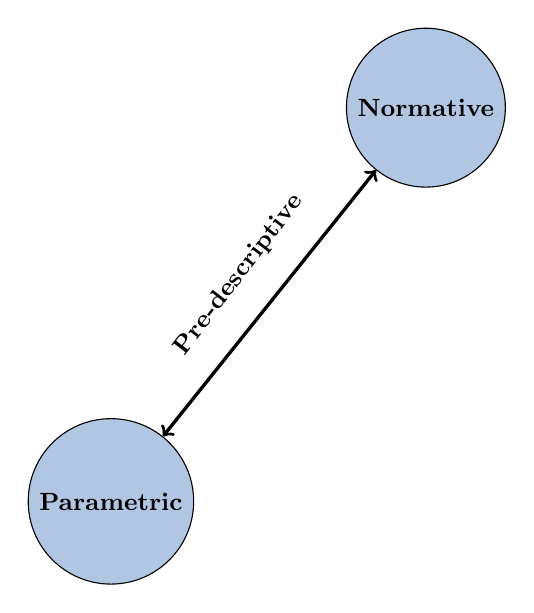
\begin{tikzpicture}[nodes={text depth=0.25ex,text height=1.25ex distance=1.7cm}]
                    \tikzstyle{every node}=[font=\small] \tikzstyle{vertex} =
                    [circle, draw=black, fill=illiniblue] \tikzstyle{hidden} =
                    [draw=none] \tikzstyle{edge} = [<->, very thick]
                    
                    \node[vertex](v1) at (0,5) {\textbf{Normative}};
                    % \node[vertex](v2) at (4,0) {\textbf{Structural}};
                    \node[vertex](v3) at (-4,0) {\textbf{Parametric}};

                    \draw[edge] (v1) -- (v3);

                    \node[hidden](h1) at (-0.75, 5) {};

                    \node[hidden](h6) at (-4, 0.75) {};

                    \draw[draw=none] (h6) -- (h1) node[anchor=mid, midway,
                    sloped]{\textbf{Pre-descriptive}};        
            \end{tikzpicture}
            }
            % \caption{Parametric Uncertainty} \label{fig:triarchic-uncertainty}
        \end{figure}

        \column[t]{6cm}

        \begin{definition}[Knightian/Deep/Epistemic Uncertainty]
            Unknowable unknowns --- uncertainties that cannot be quantified or measured due to a 
            lack of knowledge or understanding \cite{knight_risk_1921}. 
        \end{definition}

        \begin{definition}[Ambiguity Aversion / Ellsberg Paradox]
            A decision maker will choose a highly risky option with quantifiable uncertainties
            over an option with deep uncertainties \cite{ellsberg_risk_1961}.
        \end{definition}
    \end{columns}

\end{frame}


\begin{frame}
    \frametitle{How are representative probability distributions chosen?}

    \begin{columns}
        \column[t]{5cm}
        \begin{figure}
            \centering
            \resizebox{\columnwidth}{!}{
                %% Creator: Matplotlib, PGF backend
%%
%% To include the figure in your LaTeX document, write
%%   \input{<filename>.pgf}
%%
%% Make sure the required packages are loaded in your preamble
%%   \usepackage{pgf}
%%
%% Also ensure that all the required font packages are loaded; for instance,
%% the lmodern package is sometimes necessary when using math font.
%%   \usepackage{lmodern}
%%
%% Figures using additional raster images can only be included by \input if
%% they are in the same directory as the main LaTeX file. For loading figures
%% from other directories you can use the `import` package
%%   \usepackage{import}
%%
%% and then include the figures with
%%   \import{<path to file>}{<filename>.pgf}
%%
%% Matplotlib used the following preamble
%%   
%%   \makeatletter\@ifpackageloaded{underscore}{}{\usepackage[strings]{underscore}}\makeatother
%%
\begingroup%
\makeatletter%
\begin{pgfpicture}%
\pgfpathrectangle{\pgfpointorigin}{\pgfqpoint{8.900000in}{6.900000in}}%
\pgfusepath{use as bounding box, clip}%
\begin{pgfscope}%
\pgfsetbuttcap%
\pgfsetmiterjoin%
\definecolor{currentfill}{rgb}{0.827451,0.827451,0.827451}%
\pgfsetfillcolor{currentfill}%
\pgfsetlinewidth{0.000000pt}%
\definecolor{currentstroke}{rgb}{0.000000,0.000000,0.000000}%
\pgfsetstrokecolor{currentstroke}%
\pgfsetdash{}{0pt}%
\pgfpathmoveto{\pgfqpoint{0.000000in}{0.000000in}}%
\pgfpathlineto{\pgfqpoint{8.900000in}{0.000000in}}%
\pgfpathlineto{\pgfqpoint{8.900000in}{6.900000in}}%
\pgfpathlineto{\pgfqpoint{0.000000in}{6.900000in}}%
\pgfpathlineto{\pgfqpoint{0.000000in}{0.000000in}}%
\pgfpathclose%
\pgfusepath{fill}%
\end{pgfscope}%
\begin{pgfscope}%
\pgfsetbuttcap%
\pgfsetmiterjoin%
\definecolor{currentfill}{rgb}{1.000000,1.000000,1.000000}%
\pgfsetfillcolor{currentfill}%
\pgfsetlinewidth{0.000000pt}%
\definecolor{currentstroke}{rgb}{0.000000,0.000000,0.000000}%
\pgfsetstrokecolor{currentstroke}%
\pgfsetstrokeopacity{0.000000}%
\pgfsetdash{}{0pt}%
\pgfpathmoveto{\pgfqpoint{0.955442in}{0.230015in}}%
\pgfpathlineto{\pgfqpoint{8.800000in}{0.230015in}}%
\pgfpathlineto{\pgfqpoint{8.800000in}{6.800000in}}%
\pgfpathlineto{\pgfqpoint{0.955442in}{6.800000in}}%
\pgfpathlineto{\pgfqpoint{0.955442in}{0.230015in}}%
\pgfpathclose%
\pgfusepath{fill}%
\end{pgfscope}%
\begin{pgfscope}%
\pgfpathrectangle{\pgfqpoint{0.955442in}{0.230015in}}{\pgfqpoint{7.844558in}{6.569985in}}%
\pgfusepath{clip}%
\pgfsetbuttcap%
\pgfsetroundjoin%
\definecolor{currentfill}{rgb}{0.381176,0.251765,0.607843}%
\pgfsetfillcolor{currentfill}%
\pgfsetfillopacity{0.500000}%
\pgfsetlinewidth{1.003750pt}%
\definecolor{currentstroke}{rgb}{0.381176,0.251765,0.607843}%
\pgfsetstrokecolor{currentstroke}%
\pgfsetdash{}{0pt}%
\pgfsys@defobject{currentmarker}{\pgfqpoint{1.461125in}{0.230015in}}{\pgfqpoint{4.432890in}{3.311620in}}{%
\pgfpathmoveto{\pgfqpoint{1.461125in}{0.240185in}}%
\pgfpathlineto{\pgfqpoint{1.461125in}{0.230015in}}%
\pgfpathlineto{\pgfqpoint{1.476059in}{0.230015in}}%
\pgfpathlineto{\pgfqpoint{1.490992in}{0.230015in}}%
\pgfpathlineto{\pgfqpoint{1.505926in}{0.230015in}}%
\pgfpathlineto{\pgfqpoint{1.520859in}{0.230015in}}%
\pgfpathlineto{\pgfqpoint{1.535793in}{0.230015in}}%
\pgfpathlineto{\pgfqpoint{1.550726in}{0.230015in}}%
\pgfpathlineto{\pgfqpoint{1.565660in}{0.230015in}}%
\pgfpathlineto{\pgfqpoint{1.580593in}{0.230015in}}%
\pgfpathlineto{\pgfqpoint{1.595527in}{0.230015in}}%
\pgfpathlineto{\pgfqpoint{1.610460in}{0.230015in}}%
\pgfpathlineto{\pgfqpoint{1.625394in}{0.230015in}}%
\pgfpathlineto{\pgfqpoint{1.640327in}{0.230015in}}%
\pgfpathlineto{\pgfqpoint{1.655260in}{0.230015in}}%
\pgfpathlineto{\pgfqpoint{1.670194in}{0.230015in}}%
\pgfpathlineto{\pgfqpoint{1.685127in}{0.230015in}}%
\pgfpathlineto{\pgfqpoint{1.700061in}{0.230015in}}%
\pgfpathlineto{\pgfqpoint{1.714994in}{0.230015in}}%
\pgfpathlineto{\pgfqpoint{1.729928in}{0.230015in}}%
\pgfpathlineto{\pgfqpoint{1.744861in}{0.230015in}}%
\pgfpathlineto{\pgfqpoint{1.759795in}{0.230015in}}%
\pgfpathlineto{\pgfqpoint{1.774728in}{0.230015in}}%
\pgfpathlineto{\pgfqpoint{1.789662in}{0.230015in}}%
\pgfpathlineto{\pgfqpoint{1.804595in}{0.230015in}}%
\pgfpathlineto{\pgfqpoint{1.819529in}{0.230015in}}%
\pgfpathlineto{\pgfqpoint{1.834462in}{0.230015in}}%
\pgfpathlineto{\pgfqpoint{1.849396in}{0.230015in}}%
\pgfpathlineto{\pgfqpoint{1.864329in}{0.230015in}}%
\pgfpathlineto{\pgfqpoint{1.879263in}{0.230015in}}%
\pgfpathlineto{\pgfqpoint{1.894196in}{0.230015in}}%
\pgfpathlineto{\pgfqpoint{1.909130in}{0.230015in}}%
\pgfpathlineto{\pgfqpoint{1.924063in}{0.230015in}}%
\pgfpathlineto{\pgfqpoint{1.938997in}{0.230015in}}%
\pgfpathlineto{\pgfqpoint{1.953930in}{0.230015in}}%
\pgfpathlineto{\pgfqpoint{1.968864in}{0.230015in}}%
\pgfpathlineto{\pgfqpoint{1.983797in}{0.230015in}}%
\pgfpathlineto{\pgfqpoint{1.998731in}{0.230015in}}%
\pgfpathlineto{\pgfqpoint{2.013664in}{0.230015in}}%
\pgfpathlineto{\pgfqpoint{2.028598in}{0.230015in}}%
\pgfpathlineto{\pgfqpoint{2.043531in}{0.230015in}}%
\pgfpathlineto{\pgfqpoint{2.058465in}{0.230015in}}%
\pgfpathlineto{\pgfqpoint{2.073398in}{0.230015in}}%
\pgfpathlineto{\pgfqpoint{2.088332in}{0.230015in}}%
\pgfpathlineto{\pgfqpoint{2.103265in}{0.230015in}}%
\pgfpathlineto{\pgfqpoint{2.118199in}{0.230015in}}%
\pgfpathlineto{\pgfqpoint{2.133132in}{0.230015in}}%
\pgfpathlineto{\pgfqpoint{2.148066in}{0.230015in}}%
\pgfpathlineto{\pgfqpoint{2.162999in}{0.230015in}}%
\pgfpathlineto{\pgfqpoint{2.177933in}{0.230015in}}%
\pgfpathlineto{\pgfqpoint{2.192866in}{0.230015in}}%
\pgfpathlineto{\pgfqpoint{2.207800in}{0.230015in}}%
\pgfpathlineto{\pgfqpoint{2.222733in}{0.230015in}}%
\pgfpathlineto{\pgfqpoint{2.237667in}{0.230015in}}%
\pgfpathlineto{\pgfqpoint{2.252600in}{0.230015in}}%
\pgfpathlineto{\pgfqpoint{2.267534in}{0.230015in}}%
\pgfpathlineto{\pgfqpoint{2.282467in}{0.230015in}}%
\pgfpathlineto{\pgfqpoint{2.297401in}{0.230015in}}%
\pgfpathlineto{\pgfqpoint{2.312334in}{0.230015in}}%
\pgfpathlineto{\pgfqpoint{2.327268in}{0.230015in}}%
\pgfpathlineto{\pgfqpoint{2.342201in}{0.230015in}}%
\pgfpathlineto{\pgfqpoint{2.357135in}{0.230015in}}%
\pgfpathlineto{\pgfqpoint{2.372068in}{0.230015in}}%
\pgfpathlineto{\pgfqpoint{2.387002in}{0.230015in}}%
\pgfpathlineto{\pgfqpoint{2.401935in}{0.230015in}}%
\pgfpathlineto{\pgfqpoint{2.416869in}{0.230015in}}%
\pgfpathlineto{\pgfqpoint{2.431802in}{0.230015in}}%
\pgfpathlineto{\pgfqpoint{2.446736in}{0.230015in}}%
\pgfpathlineto{\pgfqpoint{2.461669in}{0.230015in}}%
\pgfpathlineto{\pgfqpoint{2.476603in}{0.230015in}}%
\pgfpathlineto{\pgfqpoint{2.491536in}{0.230015in}}%
\pgfpathlineto{\pgfqpoint{2.506470in}{0.230015in}}%
\pgfpathlineto{\pgfqpoint{2.521403in}{0.230015in}}%
\pgfpathlineto{\pgfqpoint{2.536336in}{0.230015in}}%
\pgfpathlineto{\pgfqpoint{2.551270in}{0.230015in}}%
\pgfpathlineto{\pgfqpoint{2.566203in}{0.230015in}}%
\pgfpathlineto{\pgfqpoint{2.581137in}{0.230015in}}%
\pgfpathlineto{\pgfqpoint{2.596070in}{0.230015in}}%
\pgfpathlineto{\pgfqpoint{2.611004in}{0.230015in}}%
\pgfpathlineto{\pgfqpoint{2.625937in}{0.230015in}}%
\pgfpathlineto{\pgfqpoint{2.640871in}{0.230015in}}%
\pgfpathlineto{\pgfqpoint{2.655804in}{0.230015in}}%
\pgfpathlineto{\pgfqpoint{2.670738in}{0.230015in}}%
\pgfpathlineto{\pgfqpoint{2.685671in}{0.230015in}}%
\pgfpathlineto{\pgfqpoint{2.700605in}{0.230015in}}%
\pgfpathlineto{\pgfqpoint{2.715538in}{0.230015in}}%
\pgfpathlineto{\pgfqpoint{2.730472in}{0.230015in}}%
\pgfpathlineto{\pgfqpoint{2.745405in}{0.230015in}}%
\pgfpathlineto{\pgfqpoint{2.760339in}{0.230015in}}%
\pgfpathlineto{\pgfqpoint{2.775272in}{0.230015in}}%
\pgfpathlineto{\pgfqpoint{2.790206in}{0.230015in}}%
\pgfpathlineto{\pgfqpoint{2.805139in}{0.230015in}}%
\pgfpathlineto{\pgfqpoint{2.820073in}{0.230015in}}%
\pgfpathlineto{\pgfqpoint{2.835006in}{0.230015in}}%
\pgfpathlineto{\pgfqpoint{2.849940in}{0.230015in}}%
\pgfpathlineto{\pgfqpoint{2.864873in}{0.230015in}}%
\pgfpathlineto{\pgfqpoint{2.879807in}{0.230015in}}%
\pgfpathlineto{\pgfqpoint{2.894740in}{0.230015in}}%
\pgfpathlineto{\pgfqpoint{2.909674in}{0.230015in}}%
\pgfpathlineto{\pgfqpoint{2.924607in}{0.230015in}}%
\pgfpathlineto{\pgfqpoint{2.939541in}{0.230015in}}%
\pgfpathlineto{\pgfqpoint{2.954474in}{0.230015in}}%
\pgfpathlineto{\pgfqpoint{2.969408in}{0.230015in}}%
\pgfpathlineto{\pgfqpoint{2.984341in}{0.230015in}}%
\pgfpathlineto{\pgfqpoint{2.999275in}{0.230015in}}%
\pgfpathlineto{\pgfqpoint{3.014208in}{0.230015in}}%
\pgfpathlineto{\pgfqpoint{3.029142in}{0.230015in}}%
\pgfpathlineto{\pgfqpoint{3.044075in}{0.230015in}}%
\pgfpathlineto{\pgfqpoint{3.059009in}{0.230015in}}%
\pgfpathlineto{\pgfqpoint{3.073942in}{0.230015in}}%
\pgfpathlineto{\pgfqpoint{3.088876in}{0.230015in}}%
\pgfpathlineto{\pgfqpoint{3.103809in}{0.230015in}}%
\pgfpathlineto{\pgfqpoint{3.118743in}{0.230015in}}%
\pgfpathlineto{\pgfqpoint{3.133676in}{0.230015in}}%
\pgfpathlineto{\pgfqpoint{3.148610in}{0.230015in}}%
\pgfpathlineto{\pgfqpoint{3.163543in}{0.230015in}}%
\pgfpathlineto{\pgfqpoint{3.178477in}{0.230015in}}%
\pgfpathlineto{\pgfqpoint{3.193410in}{0.230015in}}%
\pgfpathlineto{\pgfqpoint{3.208344in}{0.230015in}}%
\pgfpathlineto{\pgfqpoint{3.223277in}{0.230015in}}%
\pgfpathlineto{\pgfqpoint{3.238211in}{0.230015in}}%
\pgfpathlineto{\pgfqpoint{3.253144in}{0.230015in}}%
\pgfpathlineto{\pgfqpoint{3.268078in}{0.230015in}}%
\pgfpathlineto{\pgfqpoint{3.283011in}{0.230015in}}%
\pgfpathlineto{\pgfqpoint{3.297945in}{0.230015in}}%
\pgfpathlineto{\pgfqpoint{3.312878in}{0.230015in}}%
\pgfpathlineto{\pgfqpoint{3.327812in}{0.230015in}}%
\pgfpathlineto{\pgfqpoint{3.342745in}{0.230015in}}%
\pgfpathlineto{\pgfqpoint{3.357679in}{0.230015in}}%
\pgfpathlineto{\pgfqpoint{3.372612in}{0.230015in}}%
\pgfpathlineto{\pgfqpoint{3.387546in}{0.230015in}}%
\pgfpathlineto{\pgfqpoint{3.402479in}{0.230015in}}%
\pgfpathlineto{\pgfqpoint{3.417413in}{0.230015in}}%
\pgfpathlineto{\pgfqpoint{3.432346in}{0.230015in}}%
\pgfpathlineto{\pgfqpoint{3.447279in}{0.230015in}}%
\pgfpathlineto{\pgfqpoint{3.462213in}{0.230015in}}%
\pgfpathlineto{\pgfqpoint{3.477146in}{0.230015in}}%
\pgfpathlineto{\pgfqpoint{3.492080in}{0.230015in}}%
\pgfpathlineto{\pgfqpoint{3.507013in}{0.230015in}}%
\pgfpathlineto{\pgfqpoint{3.521947in}{0.230015in}}%
\pgfpathlineto{\pgfqpoint{3.536880in}{0.230015in}}%
\pgfpathlineto{\pgfqpoint{3.551814in}{0.230015in}}%
\pgfpathlineto{\pgfqpoint{3.566747in}{0.230015in}}%
\pgfpathlineto{\pgfqpoint{3.581681in}{0.230015in}}%
\pgfpathlineto{\pgfqpoint{3.596614in}{0.230015in}}%
\pgfpathlineto{\pgfqpoint{3.611548in}{0.230015in}}%
\pgfpathlineto{\pgfqpoint{3.626481in}{0.230015in}}%
\pgfpathlineto{\pgfqpoint{3.641415in}{0.230015in}}%
\pgfpathlineto{\pgfqpoint{3.656348in}{0.230015in}}%
\pgfpathlineto{\pgfqpoint{3.671282in}{0.230015in}}%
\pgfpathlineto{\pgfqpoint{3.686215in}{0.230015in}}%
\pgfpathlineto{\pgfqpoint{3.701149in}{0.230015in}}%
\pgfpathlineto{\pgfqpoint{3.716082in}{0.230015in}}%
\pgfpathlineto{\pgfqpoint{3.731016in}{0.230015in}}%
\pgfpathlineto{\pgfqpoint{3.745949in}{0.230015in}}%
\pgfpathlineto{\pgfqpoint{3.760883in}{0.230015in}}%
\pgfpathlineto{\pgfqpoint{3.775816in}{0.230015in}}%
\pgfpathlineto{\pgfqpoint{3.790750in}{0.230015in}}%
\pgfpathlineto{\pgfqpoint{3.805683in}{0.230015in}}%
\pgfpathlineto{\pgfqpoint{3.820617in}{0.230015in}}%
\pgfpathlineto{\pgfqpoint{3.835550in}{0.230015in}}%
\pgfpathlineto{\pgfqpoint{3.850484in}{0.230015in}}%
\pgfpathlineto{\pgfqpoint{3.865417in}{0.230015in}}%
\pgfpathlineto{\pgfqpoint{3.880351in}{0.230015in}}%
\pgfpathlineto{\pgfqpoint{3.895284in}{0.230015in}}%
\pgfpathlineto{\pgfqpoint{3.910218in}{0.230015in}}%
\pgfpathlineto{\pgfqpoint{3.925151in}{0.230015in}}%
\pgfpathlineto{\pgfqpoint{3.940085in}{0.230015in}}%
\pgfpathlineto{\pgfqpoint{3.955018in}{0.230015in}}%
\pgfpathlineto{\pgfqpoint{3.969952in}{0.230015in}}%
\pgfpathlineto{\pgfqpoint{3.984885in}{0.230015in}}%
\pgfpathlineto{\pgfqpoint{3.999819in}{0.230015in}}%
\pgfpathlineto{\pgfqpoint{4.014752in}{0.230015in}}%
\pgfpathlineto{\pgfqpoint{4.029686in}{0.230015in}}%
\pgfpathlineto{\pgfqpoint{4.044619in}{0.230015in}}%
\pgfpathlineto{\pgfqpoint{4.059553in}{0.230015in}}%
\pgfpathlineto{\pgfqpoint{4.074486in}{0.230015in}}%
\pgfpathlineto{\pgfqpoint{4.089420in}{0.230015in}}%
\pgfpathlineto{\pgfqpoint{4.104353in}{0.230015in}}%
\pgfpathlineto{\pgfqpoint{4.119287in}{0.230015in}}%
\pgfpathlineto{\pgfqpoint{4.134220in}{0.230015in}}%
\pgfpathlineto{\pgfqpoint{4.149154in}{0.230015in}}%
\pgfpathlineto{\pgfqpoint{4.164087in}{0.230015in}}%
\pgfpathlineto{\pgfqpoint{4.179021in}{0.230015in}}%
\pgfpathlineto{\pgfqpoint{4.193954in}{0.230015in}}%
\pgfpathlineto{\pgfqpoint{4.208888in}{0.230015in}}%
\pgfpathlineto{\pgfqpoint{4.223821in}{0.230015in}}%
\pgfpathlineto{\pgfqpoint{4.238755in}{0.230015in}}%
\pgfpathlineto{\pgfqpoint{4.253688in}{0.230015in}}%
\pgfpathlineto{\pgfqpoint{4.268622in}{0.230015in}}%
\pgfpathlineto{\pgfqpoint{4.283555in}{0.230015in}}%
\pgfpathlineto{\pgfqpoint{4.298489in}{0.230015in}}%
\pgfpathlineto{\pgfqpoint{4.313422in}{0.230015in}}%
\pgfpathlineto{\pgfqpoint{4.328355in}{0.230015in}}%
\pgfpathlineto{\pgfqpoint{4.343289in}{0.230015in}}%
\pgfpathlineto{\pgfqpoint{4.358222in}{0.230015in}}%
\pgfpathlineto{\pgfqpoint{4.373156in}{0.230015in}}%
\pgfpathlineto{\pgfqpoint{4.388089in}{0.230015in}}%
\pgfpathlineto{\pgfqpoint{4.403023in}{0.230015in}}%
\pgfpathlineto{\pgfqpoint{4.417956in}{0.230015in}}%
\pgfpathlineto{\pgfqpoint{4.432890in}{0.230015in}}%
\pgfpathlineto{\pgfqpoint{4.432890in}{0.233241in}}%
\pgfpathlineto{\pgfqpoint{4.432890in}{0.233241in}}%
\pgfpathlineto{\pgfqpoint{4.417956in}{0.234086in}}%
\pgfpathlineto{\pgfqpoint{4.403023in}{0.235126in}}%
\pgfpathlineto{\pgfqpoint{4.388089in}{0.236401in}}%
\pgfpathlineto{\pgfqpoint{4.373156in}{0.237957in}}%
\pgfpathlineto{\pgfqpoint{4.358222in}{0.239844in}}%
\pgfpathlineto{\pgfqpoint{4.343289in}{0.242122in}}%
\pgfpathlineto{\pgfqpoint{4.328355in}{0.244857in}}%
\pgfpathlineto{\pgfqpoint{4.313422in}{0.248124in}}%
\pgfpathlineto{\pgfqpoint{4.298489in}{0.252006in}}%
\pgfpathlineto{\pgfqpoint{4.283555in}{0.256595in}}%
\pgfpathlineto{\pgfqpoint{4.268622in}{0.261993in}}%
\pgfpathlineto{\pgfqpoint{4.253688in}{0.268309in}}%
\pgfpathlineto{\pgfqpoint{4.238755in}{0.275662in}}%
\pgfpathlineto{\pgfqpoint{4.223821in}{0.284177in}}%
\pgfpathlineto{\pgfqpoint{4.208888in}{0.293987in}}%
\pgfpathlineto{\pgfqpoint{4.193954in}{0.305232in}}%
\pgfpathlineto{\pgfqpoint{4.179021in}{0.318056in}}%
\pgfpathlineto{\pgfqpoint{4.164087in}{0.332607in}}%
\pgfpathlineto{\pgfqpoint{4.149154in}{0.349031in}}%
\pgfpathlineto{\pgfqpoint{4.134220in}{0.367477in}}%
\pgfpathlineto{\pgfqpoint{4.119287in}{0.388087in}}%
\pgfpathlineto{\pgfqpoint{4.104353in}{0.410999in}}%
\pgfpathlineto{\pgfqpoint{4.089420in}{0.436341in}}%
\pgfpathlineto{\pgfqpoint{4.074486in}{0.464230in}}%
\pgfpathlineto{\pgfqpoint{4.059553in}{0.494767in}}%
\pgfpathlineto{\pgfqpoint{4.044619in}{0.528035in}}%
\pgfpathlineto{\pgfqpoint{4.029686in}{0.564097in}}%
\pgfpathlineto{\pgfqpoint{4.014752in}{0.602993in}}%
\pgfpathlineto{\pgfqpoint{3.999819in}{0.644737in}}%
\pgfpathlineto{\pgfqpoint{3.984885in}{0.689317in}}%
\pgfpathlineto{\pgfqpoint{3.969952in}{0.736691in}}%
\pgfpathlineto{\pgfqpoint{3.955018in}{0.786788in}}%
\pgfpathlineto{\pgfqpoint{3.940085in}{0.839506in}}%
\pgfpathlineto{\pgfqpoint{3.925151in}{0.894717in}}%
\pgfpathlineto{\pgfqpoint{3.910218in}{0.952260in}}%
\pgfpathlineto{\pgfqpoint{3.895284in}{1.011953in}}%
\pgfpathlineto{\pgfqpoint{3.880351in}{1.073584in}}%
\pgfpathlineto{\pgfqpoint{3.865417in}{1.136923in}}%
\pgfpathlineto{\pgfqpoint{3.850484in}{1.201722in}}%
\pgfpathlineto{\pgfqpoint{3.835550in}{1.267716in}}%
\pgfpathlineto{\pgfqpoint{3.820617in}{1.334634in}}%
\pgfpathlineto{\pgfqpoint{3.805683in}{1.402195in}}%
\pgfpathlineto{\pgfqpoint{3.790750in}{1.470119in}}%
\pgfpathlineto{\pgfqpoint{3.775816in}{1.538130in}}%
\pgfpathlineto{\pgfqpoint{3.760883in}{1.605957in}}%
\pgfpathlineto{\pgfqpoint{3.745949in}{1.673341in}}%
\pgfpathlineto{\pgfqpoint{3.731016in}{1.740039in}}%
\pgfpathlineto{\pgfqpoint{3.716082in}{1.805825in}}%
\pgfpathlineto{\pgfqpoint{3.701149in}{1.870493in}}%
\pgfpathlineto{\pgfqpoint{3.686215in}{1.933860in}}%
\pgfpathlineto{\pgfqpoint{3.671282in}{1.995769in}}%
\pgfpathlineto{\pgfqpoint{3.656348in}{2.056085in}}%
\pgfpathlineto{\pgfqpoint{3.641415in}{2.114701in}}%
\pgfpathlineto{\pgfqpoint{3.626481in}{2.171532in}}%
\pgfpathlineto{\pgfqpoint{3.611548in}{2.226522in}}%
\pgfpathlineto{\pgfqpoint{3.596614in}{2.279635in}}%
\pgfpathlineto{\pgfqpoint{3.581681in}{2.330860in}}%
\pgfpathlineto{\pgfqpoint{3.566747in}{2.380204in}}%
\pgfpathlineto{\pgfqpoint{3.551814in}{2.427697in}}%
\pgfpathlineto{\pgfqpoint{3.536880in}{2.473384in}}%
\pgfpathlineto{\pgfqpoint{3.521947in}{2.517327in}}%
\pgfpathlineto{\pgfqpoint{3.507013in}{2.559602in}}%
\pgfpathlineto{\pgfqpoint{3.492080in}{2.600296in}}%
\pgfpathlineto{\pgfqpoint{3.477146in}{2.639508in}}%
\pgfpathlineto{\pgfqpoint{3.462213in}{2.677343in}}%
\pgfpathlineto{\pgfqpoint{3.447279in}{2.713913in}}%
\pgfpathlineto{\pgfqpoint{3.432346in}{2.749333in}}%
\pgfpathlineto{\pgfqpoint{3.417413in}{2.783720in}}%
\pgfpathlineto{\pgfqpoint{3.402479in}{2.817188in}}%
\pgfpathlineto{\pgfqpoint{3.387546in}{2.849846in}}%
\pgfpathlineto{\pgfqpoint{3.372612in}{2.881796in}}%
\pgfpathlineto{\pgfqpoint{3.357679in}{2.913126in}}%
\pgfpathlineto{\pgfqpoint{3.342745in}{2.943909in}}%
\pgfpathlineto{\pgfqpoint{3.327812in}{2.974199in}}%
\pgfpathlineto{\pgfqpoint{3.312878in}{3.004023in}}%
\pgfpathlineto{\pgfqpoint{3.297945in}{3.033382in}}%
\pgfpathlineto{\pgfqpoint{3.283011in}{3.062248in}}%
\pgfpathlineto{\pgfqpoint{3.268078in}{3.090553in}}%
\pgfpathlineto{\pgfqpoint{3.253144in}{3.118195in}}%
\pgfpathlineto{\pgfqpoint{3.238211in}{3.145031in}}%
\pgfpathlineto{\pgfqpoint{3.223277in}{3.170880in}}%
\pgfpathlineto{\pgfqpoint{3.208344in}{3.195520in}}%
\pgfpathlineto{\pgfqpoint{3.193410in}{3.218690in}}%
\pgfpathlineto{\pgfqpoint{3.178477in}{3.240093in}}%
\pgfpathlineto{\pgfqpoint{3.163543in}{3.259403in}}%
\pgfpathlineto{\pgfqpoint{3.148610in}{3.276264in}}%
\pgfpathlineto{\pgfqpoint{3.133676in}{3.290304in}}%
\pgfpathlineto{\pgfqpoint{3.118743in}{3.301136in}}%
\pgfpathlineto{\pgfqpoint{3.103809in}{3.308369in}}%
\pgfpathlineto{\pgfqpoint{3.088876in}{3.311620in}}%
\pgfpathlineto{\pgfqpoint{3.073942in}{3.310518in}}%
\pgfpathlineto{\pgfqpoint{3.059009in}{3.304716in}}%
\pgfpathlineto{\pgfqpoint{3.044075in}{3.293902in}}%
\pgfpathlineto{\pgfqpoint{3.029142in}{3.277806in}}%
\pgfpathlineto{\pgfqpoint{3.014208in}{3.256209in}}%
\pgfpathlineto{\pgfqpoint{2.999275in}{3.228951in}}%
\pgfpathlineto{\pgfqpoint{2.984341in}{3.195935in}}%
\pgfpathlineto{\pgfqpoint{2.969408in}{3.157136in}}%
\pgfpathlineto{\pgfqpoint{2.954474in}{3.112601in}}%
\pgfpathlineto{\pgfqpoint{2.939541in}{3.062454in}}%
\pgfpathlineto{\pgfqpoint{2.924607in}{3.006893in}}%
\pgfpathlineto{\pgfqpoint{2.909674in}{2.946196in}}%
\pgfpathlineto{\pgfqpoint{2.894740in}{2.880712in}}%
\pgfpathlineto{\pgfqpoint{2.879807in}{2.810862in}}%
\pgfpathlineto{\pgfqpoint{2.864873in}{2.737136in}}%
\pgfpathlineto{\pgfqpoint{2.849940in}{2.660083in}}%
\pgfpathlineto{\pgfqpoint{2.835006in}{2.580311in}}%
\pgfpathlineto{\pgfqpoint{2.820073in}{2.498476in}}%
\pgfpathlineto{\pgfqpoint{2.805139in}{2.415280in}}%
\pgfpathlineto{\pgfqpoint{2.790206in}{2.331457in}}%
\pgfpathlineto{\pgfqpoint{2.775272in}{2.247772in}}%
\pgfpathlineto{\pgfqpoint{2.760339in}{2.165010in}}%
\pgfpathlineto{\pgfqpoint{2.745405in}{2.083972in}}%
\pgfpathlineto{\pgfqpoint{2.730472in}{2.005460in}}%
\pgfpathlineto{\pgfqpoint{2.715538in}{1.930277in}}%
\pgfpathlineto{\pgfqpoint{2.700605in}{1.859216in}}%
\pgfpathlineto{\pgfqpoint{2.685671in}{1.793048in}}%
\pgfpathlineto{\pgfqpoint{2.670738in}{1.732522in}}%
\pgfpathlineto{\pgfqpoint{2.655804in}{1.678350in}}%
\pgfpathlineto{\pgfqpoint{2.640871in}{1.631201in}}%
\pgfpathlineto{\pgfqpoint{2.625937in}{1.591689in}}%
\pgfpathlineto{\pgfqpoint{2.611004in}{1.560371in}}%
\pgfpathlineto{\pgfqpoint{2.596070in}{1.537731in}}%
\pgfpathlineto{\pgfqpoint{2.581137in}{1.524172in}}%
\pgfpathlineto{\pgfqpoint{2.566203in}{1.520010in}}%
\pgfpathlineto{\pgfqpoint{2.551270in}{1.525461in}}%
\pgfpathlineto{\pgfqpoint{2.536336in}{1.540635in}}%
\pgfpathlineto{\pgfqpoint{2.521403in}{1.565528in}}%
\pgfpathlineto{\pgfqpoint{2.506470in}{1.600012in}}%
\pgfpathlineto{\pgfqpoint{2.491536in}{1.643833in}}%
\pgfpathlineto{\pgfqpoint{2.476603in}{1.696603in}}%
\pgfpathlineto{\pgfqpoint{2.461669in}{1.757801in}}%
\pgfpathlineto{\pgfqpoint{2.446736in}{1.826770in}}%
\pgfpathlineto{\pgfqpoint{2.431802in}{1.902720in}}%
\pgfpathlineto{\pgfqpoint{2.416869in}{1.984730in}}%
\pgfpathlineto{\pgfqpoint{2.401935in}{2.071762in}}%
\pgfpathlineto{\pgfqpoint{2.387002in}{2.162662in}}%
\pgfpathlineto{\pgfqpoint{2.372068in}{2.256183in}}%
\pgfpathlineto{\pgfqpoint{2.357135in}{2.350992in}}%
\pgfpathlineto{\pgfqpoint{2.342201in}{2.445697in}}%
\pgfpathlineto{\pgfqpoint{2.327268in}{2.538862in}}%
\pgfpathlineto{\pgfqpoint{2.312334in}{2.629035in}}%
\pgfpathlineto{\pgfqpoint{2.297401in}{2.714771in}}%
\pgfpathlineto{\pgfqpoint{2.282467in}{2.794658in}}%
\pgfpathlineto{\pgfqpoint{2.267534in}{2.867344in}}%
\pgfpathlineto{\pgfqpoint{2.252600in}{2.931565in}}%
\pgfpathlineto{\pgfqpoint{2.237667in}{2.986168in}}%
\pgfpathlineto{\pgfqpoint{2.222733in}{3.030134in}}%
\pgfpathlineto{\pgfqpoint{2.207800in}{3.062603in}}%
\pgfpathlineto{\pgfqpoint{2.192866in}{3.082889in}}%
\pgfpathlineto{\pgfqpoint{2.177933in}{3.090493in}}%
\pgfpathlineto{\pgfqpoint{2.162999in}{3.085117in}}%
\pgfpathlineto{\pgfqpoint{2.148066in}{3.066668in}}%
\pgfpathlineto{\pgfqpoint{2.133132in}{3.035257in}}%
\pgfpathlineto{\pgfqpoint{2.118199in}{2.991197in}}%
\pgfpathlineto{\pgfqpoint{2.103265in}{2.934994in}}%
\pgfpathlineto{\pgfqpoint{2.088332in}{2.867332in}}%
\pgfpathlineto{\pgfqpoint{2.073398in}{2.789058in}}%
\pgfpathlineto{\pgfqpoint{2.058465in}{2.701163in}}%
\pgfpathlineto{\pgfqpoint{2.043531in}{2.604751in}}%
\pgfpathlineto{\pgfqpoint{2.028598in}{2.501022in}}%
\pgfpathlineto{\pgfqpoint{2.013664in}{2.391241in}}%
\pgfpathlineto{\pgfqpoint{1.998731in}{2.276708in}}%
\pgfpathlineto{\pgfqpoint{1.983797in}{2.158736in}}%
\pgfpathlineto{\pgfqpoint{1.968864in}{2.038621in}}%
\pgfpathlineto{\pgfqpoint{1.953930in}{1.917620in}}%
\pgfpathlineto{\pgfqpoint{1.938997in}{1.796927in}}%
\pgfpathlineto{\pgfqpoint{1.924063in}{1.677654in}}%
\pgfpathlineto{\pgfqpoint{1.909130in}{1.560816in}}%
\pgfpathlineto{\pgfqpoint{1.894196in}{1.447319in}}%
\pgfpathlineto{\pgfqpoint{1.879263in}{1.337949in}}%
\pgfpathlineto{\pgfqpoint{1.864329in}{1.233368in}}%
\pgfpathlineto{\pgfqpoint{1.849396in}{1.134112in}}%
\pgfpathlineto{\pgfqpoint{1.834462in}{1.040593in}}%
\pgfpathlineto{\pgfqpoint{1.819529in}{0.953100in}}%
\pgfpathlineto{\pgfqpoint{1.804595in}{0.871810in}}%
\pgfpathlineto{\pgfqpoint{1.789662in}{0.796791in}}%
\pgfpathlineto{\pgfqpoint{1.774728in}{0.728020in}}%
\pgfpathlineto{\pgfqpoint{1.759795in}{0.665387in}}%
\pgfpathlineto{\pgfqpoint{1.744861in}{0.608709in}}%
\pgfpathlineto{\pgfqpoint{1.729928in}{0.557744in}}%
\pgfpathlineto{\pgfqpoint{1.714994in}{0.512204in}}%
\pgfpathlineto{\pgfqpoint{1.700061in}{0.471761in}}%
\pgfpathlineto{\pgfqpoint{1.685127in}{0.436065in}}%
\pgfpathlineto{\pgfqpoint{1.670194in}{0.404748in}}%
\pgfpathlineto{\pgfqpoint{1.655260in}{0.377440in}}%
\pgfpathlineto{\pgfqpoint{1.640327in}{0.353767in}}%
\pgfpathlineto{\pgfqpoint{1.625394in}{0.333367in}}%
\pgfpathlineto{\pgfqpoint{1.610460in}{0.315891in}}%
\pgfpathlineto{\pgfqpoint{1.595527in}{0.301007in}}%
\pgfpathlineto{\pgfqpoint{1.580593in}{0.288404in}}%
\pgfpathlineto{\pgfqpoint{1.565660in}{0.277793in}}%
\pgfpathlineto{\pgfqpoint{1.550726in}{0.268912in}}%
\pgfpathlineto{\pgfqpoint{1.535793in}{0.261519in}}%
\pgfpathlineto{\pgfqpoint{1.520859in}{0.255402in}}%
\pgfpathlineto{\pgfqpoint{1.505926in}{0.250368in}}%
\pgfpathlineto{\pgfqpoint{1.490992in}{0.246249in}}%
\pgfpathlineto{\pgfqpoint{1.476059in}{0.242897in}}%
\pgfpathlineto{\pgfqpoint{1.461125in}{0.240185in}}%
\pgfpathlineto{\pgfqpoint{1.461125in}{0.240185in}}%
\pgfpathclose%
\pgfusepath{stroke,fill}%
}%
\begin{pgfscope}%
\pgfsys@transformshift{0.000000in}{0.000000in}%
\pgfsys@useobject{currentmarker}{}%
\end{pgfscope}%
\end{pgfscope}%
\begin{pgfscope}%
\pgfpathrectangle{\pgfqpoint{0.955442in}{0.230015in}}{\pgfqpoint{7.844558in}{6.569985in}}%
\pgfusepath{clip}%
\pgfsetbuttcap%
\pgfsetroundjoin%
\definecolor{currentfill}{rgb}{0.525490,0.512941,0.740392}%
\pgfsetfillcolor{currentfill}%
\pgfsetfillopacity{0.500000}%
\pgfsetlinewidth{1.003750pt}%
\definecolor{currentstroke}{rgb}{0.525490,0.512941,0.740392}%
\pgfsetstrokecolor{currentstroke}%
\pgfsetdash{}{0pt}%
\pgfsys@defobject{currentmarker}{\pgfqpoint{1.312013in}{0.230015in}}{\pgfqpoint{8.443429in}{1.825903in}}{%
\pgfpathmoveto{\pgfqpoint{1.312013in}{0.232040in}}%
\pgfpathlineto{\pgfqpoint{1.312013in}{0.230015in}}%
\pgfpathlineto{\pgfqpoint{1.347849in}{0.230015in}}%
\pgfpathlineto{\pgfqpoint{1.383685in}{0.230015in}}%
\pgfpathlineto{\pgfqpoint{1.419522in}{0.230015in}}%
\pgfpathlineto{\pgfqpoint{1.455358in}{0.230015in}}%
\pgfpathlineto{\pgfqpoint{1.491194in}{0.230015in}}%
\pgfpathlineto{\pgfqpoint{1.527030in}{0.230015in}}%
\pgfpathlineto{\pgfqpoint{1.562867in}{0.230015in}}%
\pgfpathlineto{\pgfqpoint{1.598703in}{0.230015in}}%
\pgfpathlineto{\pgfqpoint{1.634539in}{0.230015in}}%
\pgfpathlineto{\pgfqpoint{1.670376in}{0.230015in}}%
\pgfpathlineto{\pgfqpoint{1.706212in}{0.230015in}}%
\pgfpathlineto{\pgfqpoint{1.742048in}{0.230015in}}%
\pgfpathlineto{\pgfqpoint{1.777884in}{0.230015in}}%
\pgfpathlineto{\pgfqpoint{1.813721in}{0.230015in}}%
\pgfpathlineto{\pgfqpoint{1.849557in}{0.230015in}}%
\pgfpathlineto{\pgfqpoint{1.885393in}{0.230015in}}%
\pgfpathlineto{\pgfqpoint{1.921229in}{0.230015in}}%
\pgfpathlineto{\pgfqpoint{1.957066in}{0.230015in}}%
\pgfpathlineto{\pgfqpoint{1.992902in}{0.230015in}}%
\pgfpathlineto{\pgfqpoint{2.028738in}{0.230015in}}%
\pgfpathlineto{\pgfqpoint{2.064574in}{0.230015in}}%
\pgfpathlineto{\pgfqpoint{2.100411in}{0.230015in}}%
\pgfpathlineto{\pgfqpoint{2.136247in}{0.230015in}}%
\pgfpathlineto{\pgfqpoint{2.172083in}{0.230015in}}%
\pgfpathlineto{\pgfqpoint{2.207919in}{0.230015in}}%
\pgfpathlineto{\pgfqpoint{2.243756in}{0.230015in}}%
\pgfpathlineto{\pgfqpoint{2.279592in}{0.230015in}}%
\pgfpathlineto{\pgfqpoint{2.315428in}{0.230015in}}%
\pgfpathlineto{\pgfqpoint{2.351265in}{0.230015in}}%
\pgfpathlineto{\pgfqpoint{2.387101in}{0.230015in}}%
\pgfpathlineto{\pgfqpoint{2.422937in}{0.230015in}}%
\pgfpathlineto{\pgfqpoint{2.458773in}{0.230015in}}%
\pgfpathlineto{\pgfqpoint{2.494610in}{0.230015in}}%
\pgfpathlineto{\pgfqpoint{2.530446in}{0.230015in}}%
\pgfpathlineto{\pgfqpoint{2.566282in}{0.230015in}}%
\pgfpathlineto{\pgfqpoint{2.602118in}{0.230015in}}%
\pgfpathlineto{\pgfqpoint{2.637955in}{0.230015in}}%
\pgfpathlineto{\pgfqpoint{2.673791in}{0.230015in}}%
\pgfpathlineto{\pgfqpoint{2.709627in}{0.230015in}}%
\pgfpathlineto{\pgfqpoint{2.745463in}{0.230015in}}%
\pgfpathlineto{\pgfqpoint{2.781300in}{0.230015in}}%
\pgfpathlineto{\pgfqpoint{2.817136in}{0.230015in}}%
\pgfpathlineto{\pgfqpoint{2.852972in}{0.230015in}}%
\pgfpathlineto{\pgfqpoint{2.888808in}{0.230015in}}%
\pgfpathlineto{\pgfqpoint{2.924645in}{0.230015in}}%
\pgfpathlineto{\pgfqpoint{2.960481in}{0.230015in}}%
\pgfpathlineto{\pgfqpoint{2.996317in}{0.230015in}}%
\pgfpathlineto{\pgfqpoint{3.032154in}{0.230015in}}%
\pgfpathlineto{\pgfqpoint{3.067990in}{0.230015in}}%
\pgfpathlineto{\pgfqpoint{3.103826in}{0.230015in}}%
\pgfpathlineto{\pgfqpoint{3.139662in}{0.230015in}}%
\pgfpathlineto{\pgfqpoint{3.175499in}{0.230015in}}%
\pgfpathlineto{\pgfqpoint{3.211335in}{0.230015in}}%
\pgfpathlineto{\pgfqpoint{3.247171in}{0.230015in}}%
\pgfpathlineto{\pgfqpoint{3.283007in}{0.230015in}}%
\pgfpathlineto{\pgfqpoint{3.318844in}{0.230015in}}%
\pgfpathlineto{\pgfqpoint{3.354680in}{0.230015in}}%
\pgfpathlineto{\pgfqpoint{3.390516in}{0.230015in}}%
\pgfpathlineto{\pgfqpoint{3.426352in}{0.230015in}}%
\pgfpathlineto{\pgfqpoint{3.462189in}{0.230015in}}%
\pgfpathlineto{\pgfqpoint{3.498025in}{0.230015in}}%
\pgfpathlineto{\pgfqpoint{3.533861in}{0.230015in}}%
\pgfpathlineto{\pgfqpoint{3.569697in}{0.230015in}}%
\pgfpathlineto{\pgfqpoint{3.605534in}{0.230015in}}%
\pgfpathlineto{\pgfqpoint{3.641370in}{0.230015in}}%
\pgfpathlineto{\pgfqpoint{3.677206in}{0.230015in}}%
\pgfpathlineto{\pgfqpoint{3.713043in}{0.230015in}}%
\pgfpathlineto{\pgfqpoint{3.748879in}{0.230015in}}%
\pgfpathlineto{\pgfqpoint{3.784715in}{0.230015in}}%
\pgfpathlineto{\pgfqpoint{3.820551in}{0.230015in}}%
\pgfpathlineto{\pgfqpoint{3.856388in}{0.230015in}}%
\pgfpathlineto{\pgfqpoint{3.892224in}{0.230015in}}%
\pgfpathlineto{\pgfqpoint{3.928060in}{0.230015in}}%
\pgfpathlineto{\pgfqpoint{3.963896in}{0.230015in}}%
\pgfpathlineto{\pgfqpoint{3.999733in}{0.230015in}}%
\pgfpathlineto{\pgfqpoint{4.035569in}{0.230015in}}%
\pgfpathlineto{\pgfqpoint{4.071405in}{0.230015in}}%
\pgfpathlineto{\pgfqpoint{4.107241in}{0.230015in}}%
\pgfpathlineto{\pgfqpoint{4.143078in}{0.230015in}}%
\pgfpathlineto{\pgfqpoint{4.178914in}{0.230015in}}%
\pgfpathlineto{\pgfqpoint{4.214750in}{0.230015in}}%
\pgfpathlineto{\pgfqpoint{4.250586in}{0.230015in}}%
\pgfpathlineto{\pgfqpoint{4.286423in}{0.230015in}}%
\pgfpathlineto{\pgfqpoint{4.322259in}{0.230015in}}%
\pgfpathlineto{\pgfqpoint{4.358095in}{0.230015in}}%
\pgfpathlineto{\pgfqpoint{4.393931in}{0.230015in}}%
\pgfpathlineto{\pgfqpoint{4.429768in}{0.230015in}}%
\pgfpathlineto{\pgfqpoint{4.465604in}{0.230015in}}%
\pgfpathlineto{\pgfqpoint{4.501440in}{0.230015in}}%
\pgfpathlineto{\pgfqpoint{4.537277in}{0.230015in}}%
\pgfpathlineto{\pgfqpoint{4.573113in}{0.230015in}}%
\pgfpathlineto{\pgfqpoint{4.608949in}{0.230015in}}%
\pgfpathlineto{\pgfqpoint{4.644785in}{0.230015in}}%
\pgfpathlineto{\pgfqpoint{4.680622in}{0.230015in}}%
\pgfpathlineto{\pgfqpoint{4.716458in}{0.230015in}}%
\pgfpathlineto{\pgfqpoint{4.752294in}{0.230015in}}%
\pgfpathlineto{\pgfqpoint{4.788130in}{0.230015in}}%
\pgfpathlineto{\pgfqpoint{4.823967in}{0.230015in}}%
\pgfpathlineto{\pgfqpoint{4.859803in}{0.230015in}}%
\pgfpathlineto{\pgfqpoint{4.895639in}{0.230015in}}%
\pgfpathlineto{\pgfqpoint{4.931475in}{0.230015in}}%
\pgfpathlineto{\pgfqpoint{4.967312in}{0.230015in}}%
\pgfpathlineto{\pgfqpoint{5.003148in}{0.230015in}}%
\pgfpathlineto{\pgfqpoint{5.038984in}{0.230015in}}%
\pgfpathlineto{\pgfqpoint{5.074820in}{0.230015in}}%
\pgfpathlineto{\pgfqpoint{5.110657in}{0.230015in}}%
\pgfpathlineto{\pgfqpoint{5.146493in}{0.230015in}}%
\pgfpathlineto{\pgfqpoint{5.182329in}{0.230015in}}%
\pgfpathlineto{\pgfqpoint{5.218166in}{0.230015in}}%
\pgfpathlineto{\pgfqpoint{5.254002in}{0.230015in}}%
\pgfpathlineto{\pgfqpoint{5.289838in}{0.230015in}}%
\pgfpathlineto{\pgfqpoint{5.325674in}{0.230015in}}%
\pgfpathlineto{\pgfqpoint{5.361511in}{0.230015in}}%
\pgfpathlineto{\pgfqpoint{5.397347in}{0.230015in}}%
\pgfpathlineto{\pgfqpoint{5.433183in}{0.230015in}}%
\pgfpathlineto{\pgfqpoint{5.469019in}{0.230015in}}%
\pgfpathlineto{\pgfqpoint{5.504856in}{0.230015in}}%
\pgfpathlineto{\pgfqpoint{5.540692in}{0.230015in}}%
\pgfpathlineto{\pgfqpoint{5.576528in}{0.230015in}}%
\pgfpathlineto{\pgfqpoint{5.612364in}{0.230015in}}%
\pgfpathlineto{\pgfqpoint{5.648201in}{0.230015in}}%
\pgfpathlineto{\pgfqpoint{5.684037in}{0.230015in}}%
\pgfpathlineto{\pgfqpoint{5.719873in}{0.230015in}}%
\pgfpathlineto{\pgfqpoint{5.755709in}{0.230015in}}%
\pgfpathlineto{\pgfqpoint{5.791546in}{0.230015in}}%
\pgfpathlineto{\pgfqpoint{5.827382in}{0.230015in}}%
\pgfpathlineto{\pgfqpoint{5.863218in}{0.230015in}}%
\pgfpathlineto{\pgfqpoint{5.899055in}{0.230015in}}%
\pgfpathlineto{\pgfqpoint{5.934891in}{0.230015in}}%
\pgfpathlineto{\pgfqpoint{5.970727in}{0.230015in}}%
\pgfpathlineto{\pgfqpoint{6.006563in}{0.230015in}}%
\pgfpathlineto{\pgfqpoint{6.042400in}{0.230015in}}%
\pgfpathlineto{\pgfqpoint{6.078236in}{0.230015in}}%
\pgfpathlineto{\pgfqpoint{6.114072in}{0.230015in}}%
\pgfpathlineto{\pgfqpoint{6.149908in}{0.230015in}}%
\pgfpathlineto{\pgfqpoint{6.185745in}{0.230015in}}%
\pgfpathlineto{\pgfqpoint{6.221581in}{0.230015in}}%
\pgfpathlineto{\pgfqpoint{6.257417in}{0.230015in}}%
\pgfpathlineto{\pgfqpoint{6.293253in}{0.230015in}}%
\pgfpathlineto{\pgfqpoint{6.329090in}{0.230015in}}%
\pgfpathlineto{\pgfqpoint{6.364926in}{0.230015in}}%
\pgfpathlineto{\pgfqpoint{6.400762in}{0.230015in}}%
\pgfpathlineto{\pgfqpoint{6.436598in}{0.230015in}}%
\pgfpathlineto{\pgfqpoint{6.472435in}{0.230015in}}%
\pgfpathlineto{\pgfqpoint{6.508271in}{0.230015in}}%
\pgfpathlineto{\pgfqpoint{6.544107in}{0.230015in}}%
\pgfpathlineto{\pgfqpoint{6.579944in}{0.230015in}}%
\pgfpathlineto{\pgfqpoint{6.615780in}{0.230015in}}%
\pgfpathlineto{\pgfqpoint{6.651616in}{0.230015in}}%
\pgfpathlineto{\pgfqpoint{6.687452in}{0.230015in}}%
\pgfpathlineto{\pgfqpoint{6.723289in}{0.230015in}}%
\pgfpathlineto{\pgfqpoint{6.759125in}{0.230015in}}%
\pgfpathlineto{\pgfqpoint{6.794961in}{0.230015in}}%
\pgfpathlineto{\pgfqpoint{6.830797in}{0.230015in}}%
\pgfpathlineto{\pgfqpoint{6.866634in}{0.230015in}}%
\pgfpathlineto{\pgfqpoint{6.902470in}{0.230015in}}%
\pgfpathlineto{\pgfqpoint{6.938306in}{0.230015in}}%
\pgfpathlineto{\pgfqpoint{6.974142in}{0.230015in}}%
\pgfpathlineto{\pgfqpoint{7.009979in}{0.230015in}}%
\pgfpathlineto{\pgfqpoint{7.045815in}{0.230015in}}%
\pgfpathlineto{\pgfqpoint{7.081651in}{0.230015in}}%
\pgfpathlineto{\pgfqpoint{7.117487in}{0.230015in}}%
\pgfpathlineto{\pgfqpoint{7.153324in}{0.230015in}}%
\pgfpathlineto{\pgfqpoint{7.189160in}{0.230015in}}%
\pgfpathlineto{\pgfqpoint{7.224996in}{0.230015in}}%
\pgfpathlineto{\pgfqpoint{7.260833in}{0.230015in}}%
\pgfpathlineto{\pgfqpoint{7.296669in}{0.230015in}}%
\pgfpathlineto{\pgfqpoint{7.332505in}{0.230015in}}%
\pgfpathlineto{\pgfqpoint{7.368341in}{0.230015in}}%
\pgfpathlineto{\pgfqpoint{7.404178in}{0.230015in}}%
\pgfpathlineto{\pgfqpoint{7.440014in}{0.230015in}}%
\pgfpathlineto{\pgfqpoint{7.475850in}{0.230015in}}%
\pgfpathlineto{\pgfqpoint{7.511686in}{0.230015in}}%
\pgfpathlineto{\pgfqpoint{7.547523in}{0.230015in}}%
\pgfpathlineto{\pgfqpoint{7.583359in}{0.230015in}}%
\pgfpathlineto{\pgfqpoint{7.619195in}{0.230015in}}%
\pgfpathlineto{\pgfqpoint{7.655031in}{0.230015in}}%
\pgfpathlineto{\pgfqpoint{7.690868in}{0.230015in}}%
\pgfpathlineto{\pgfqpoint{7.726704in}{0.230015in}}%
\pgfpathlineto{\pgfqpoint{7.762540in}{0.230015in}}%
\pgfpathlineto{\pgfqpoint{7.798376in}{0.230015in}}%
\pgfpathlineto{\pgfqpoint{7.834213in}{0.230015in}}%
\pgfpathlineto{\pgfqpoint{7.870049in}{0.230015in}}%
\pgfpathlineto{\pgfqpoint{7.905885in}{0.230015in}}%
\pgfpathlineto{\pgfqpoint{7.941722in}{0.230015in}}%
\pgfpathlineto{\pgfqpoint{7.977558in}{0.230015in}}%
\pgfpathlineto{\pgfqpoint{8.013394in}{0.230015in}}%
\pgfpathlineto{\pgfqpoint{8.049230in}{0.230015in}}%
\pgfpathlineto{\pgfqpoint{8.085067in}{0.230015in}}%
\pgfpathlineto{\pgfqpoint{8.120903in}{0.230015in}}%
\pgfpathlineto{\pgfqpoint{8.156739in}{0.230015in}}%
\pgfpathlineto{\pgfqpoint{8.192575in}{0.230015in}}%
\pgfpathlineto{\pgfqpoint{8.228412in}{0.230015in}}%
\pgfpathlineto{\pgfqpoint{8.264248in}{0.230015in}}%
\pgfpathlineto{\pgfqpoint{8.300084in}{0.230015in}}%
\pgfpathlineto{\pgfqpoint{8.335920in}{0.230015in}}%
\pgfpathlineto{\pgfqpoint{8.371757in}{0.230015in}}%
\pgfpathlineto{\pgfqpoint{8.407593in}{0.230015in}}%
\pgfpathlineto{\pgfqpoint{8.443429in}{0.230015in}}%
\pgfpathlineto{\pgfqpoint{8.443429in}{0.230641in}}%
\pgfpathlineto{\pgfqpoint{8.443429in}{0.230641in}}%
\pgfpathlineto{\pgfqpoint{8.407593in}{0.230814in}}%
\pgfpathlineto{\pgfqpoint{8.371757in}{0.231029in}}%
\pgfpathlineto{\pgfqpoint{8.335920in}{0.231294in}}%
\pgfpathlineto{\pgfqpoint{8.300084in}{0.231621in}}%
\pgfpathlineto{\pgfqpoint{8.264248in}{0.232022in}}%
\pgfpathlineto{\pgfqpoint{8.228412in}{0.232509in}}%
\pgfpathlineto{\pgfqpoint{8.192575in}{0.233099in}}%
\pgfpathlineto{\pgfqpoint{8.156739in}{0.233810in}}%
\pgfpathlineto{\pgfqpoint{8.120903in}{0.234661in}}%
\pgfpathlineto{\pgfqpoint{8.085067in}{0.235676in}}%
\pgfpathlineto{\pgfqpoint{8.049230in}{0.236878in}}%
\pgfpathlineto{\pgfqpoint{8.013394in}{0.238295in}}%
\pgfpathlineto{\pgfqpoint{7.977558in}{0.239957in}}%
\pgfpathlineto{\pgfqpoint{7.941722in}{0.241896in}}%
\pgfpathlineto{\pgfqpoint{7.905885in}{0.244146in}}%
\pgfpathlineto{\pgfqpoint{7.870049in}{0.246746in}}%
\pgfpathlineto{\pgfqpoint{7.834213in}{0.249733in}}%
\pgfpathlineto{\pgfqpoint{7.798376in}{0.253150in}}%
\pgfpathlineto{\pgfqpoint{7.762540in}{0.257038in}}%
\pgfpathlineto{\pgfqpoint{7.726704in}{0.261443in}}%
\pgfpathlineto{\pgfqpoint{7.690868in}{0.266411in}}%
\pgfpathlineto{\pgfqpoint{7.655031in}{0.271988in}}%
\pgfpathlineto{\pgfqpoint{7.619195in}{0.278221in}}%
\pgfpathlineto{\pgfqpoint{7.583359in}{0.285158in}}%
\pgfpathlineto{\pgfqpoint{7.547523in}{0.292846in}}%
\pgfpathlineto{\pgfqpoint{7.511686in}{0.301333in}}%
\pgfpathlineto{\pgfqpoint{7.475850in}{0.310666in}}%
\pgfpathlineto{\pgfqpoint{7.440014in}{0.320889in}}%
\pgfpathlineto{\pgfqpoint{7.404178in}{0.332047in}}%
\pgfpathlineto{\pgfqpoint{7.368341in}{0.344184in}}%
\pgfpathlineto{\pgfqpoint{7.332505in}{0.357340in}}%
\pgfpathlineto{\pgfqpoint{7.296669in}{0.371556in}}%
\pgfpathlineto{\pgfqpoint{7.260833in}{0.386870in}}%
\pgfpathlineto{\pgfqpoint{7.224996in}{0.403316in}}%
\pgfpathlineto{\pgfqpoint{7.189160in}{0.420929in}}%
\pgfpathlineto{\pgfqpoint{7.153324in}{0.439737in}}%
\pgfpathlineto{\pgfqpoint{7.117487in}{0.459770in}}%
\pgfpathlineto{\pgfqpoint{7.081651in}{0.481050in}}%
\pgfpathlineto{\pgfqpoint{7.045815in}{0.503599in}}%
\pgfpathlineto{\pgfqpoint{7.009979in}{0.527432in}}%
\pgfpathlineto{\pgfqpoint{6.974142in}{0.552561in}}%
\pgfpathlineto{\pgfqpoint{6.938306in}{0.578990in}}%
\pgfpathlineto{\pgfqpoint{6.902470in}{0.606722in}}%
\pgfpathlineto{\pgfqpoint{6.866634in}{0.635747in}}%
\pgfpathlineto{\pgfqpoint{6.830797in}{0.666054in}}%
\pgfpathlineto{\pgfqpoint{6.794961in}{0.697618in}}%
\pgfpathlineto{\pgfqpoint{6.759125in}{0.730409in}}%
\pgfpathlineto{\pgfqpoint{6.723289in}{0.764388in}}%
\pgfpathlineto{\pgfqpoint{6.687452in}{0.799506in}}%
\pgfpathlineto{\pgfqpoint{6.651616in}{0.835703in}}%
\pgfpathlineto{\pgfqpoint{6.615780in}{0.872909in}}%
\pgfpathlineto{\pgfqpoint{6.579944in}{0.911047in}}%
\pgfpathlineto{\pgfqpoint{6.544107in}{0.950027in}}%
\pgfpathlineto{\pgfqpoint{6.508271in}{0.989751in}}%
\pgfpathlineto{\pgfqpoint{6.472435in}{1.030112in}}%
\pgfpathlineto{\pgfqpoint{6.436598in}{1.070993in}}%
\pgfpathlineto{\pgfqpoint{6.400762in}{1.112270in}}%
\pgfpathlineto{\pgfqpoint{6.364926in}{1.153812in}}%
\pgfpathlineto{\pgfqpoint{6.329090in}{1.195482in}}%
\pgfpathlineto{\pgfqpoint{6.293253in}{1.237136in}}%
\pgfpathlineto{\pgfqpoint{6.257417in}{1.278625in}}%
\pgfpathlineto{\pgfqpoint{6.221581in}{1.319796in}}%
\pgfpathlineto{\pgfqpoint{6.185745in}{1.360493in}}%
\pgfpathlineto{\pgfqpoint{6.149908in}{1.400555in}}%
\pgfpathlineto{\pgfqpoint{6.114072in}{1.439820in}}%
\pgfpathlineto{\pgfqpoint{6.078236in}{1.478122in}}%
\pgfpathlineto{\pgfqpoint{6.042400in}{1.515295in}}%
\pgfpathlineto{\pgfqpoint{6.006563in}{1.551171in}}%
\pgfpathlineto{\pgfqpoint{5.970727in}{1.585580in}}%
\pgfpathlineto{\pgfqpoint{5.934891in}{1.618354in}}%
\pgfpathlineto{\pgfqpoint{5.899055in}{1.649322in}}%
\pgfpathlineto{\pgfqpoint{5.863218in}{1.678317in}}%
\pgfpathlineto{\pgfqpoint{5.827382in}{1.705172in}}%
\pgfpathlineto{\pgfqpoint{5.791546in}{1.729725in}}%
\pgfpathlineto{\pgfqpoint{5.755709in}{1.751817in}}%
\pgfpathlineto{\pgfqpoint{5.719873in}{1.771295in}}%
\pgfpathlineto{\pgfqpoint{5.684037in}{1.788013in}}%
\pgfpathlineto{\pgfqpoint{5.648201in}{1.801836in}}%
\pgfpathlineto{\pgfqpoint{5.612364in}{1.812640in}}%
\pgfpathlineto{\pgfqpoint{5.576528in}{1.820314in}}%
\pgfpathlineto{\pgfqpoint{5.540692in}{1.824760in}}%
\pgfpathlineto{\pgfqpoint{5.504856in}{1.825903in}}%
\pgfpathlineto{\pgfqpoint{5.469019in}{1.823681in}}%
\pgfpathlineto{\pgfqpoint{5.433183in}{1.818057in}}%
\pgfpathlineto{\pgfqpoint{5.397347in}{1.809015in}}%
\pgfpathlineto{\pgfqpoint{5.361511in}{1.796564in}}%
\pgfpathlineto{\pgfqpoint{5.325674in}{1.780735in}}%
\pgfpathlineto{\pgfqpoint{5.289838in}{1.761588in}}%
\pgfpathlineto{\pgfqpoint{5.254002in}{1.739206in}}%
\pgfpathlineto{\pgfqpoint{5.218166in}{1.713697in}}%
\pgfpathlineto{\pgfqpoint{5.182329in}{1.685195in}}%
\pgfpathlineto{\pgfqpoint{5.146493in}{1.653856in}}%
\pgfpathlineto{\pgfqpoint{5.110657in}{1.619860in}}%
\pgfpathlineto{\pgfqpoint{5.074820in}{1.583407in}}%
\pgfpathlineto{\pgfqpoint{5.038984in}{1.544716in}}%
\pgfpathlineto{\pgfqpoint{5.003148in}{1.504020in}}%
\pgfpathlineto{\pgfqpoint{4.967312in}{1.461570in}}%
\pgfpathlineto{\pgfqpoint{4.931475in}{1.417626in}}%
\pgfpathlineto{\pgfqpoint{4.895639in}{1.372458in}}%
\pgfpathlineto{\pgfqpoint{4.859803in}{1.326341in}}%
\pgfpathlineto{\pgfqpoint{4.823967in}{1.279557in}}%
\pgfpathlineto{\pgfqpoint{4.788130in}{1.232388in}}%
\pgfpathlineto{\pgfqpoint{4.752294in}{1.185115in}}%
\pgfpathlineto{\pgfqpoint{4.716458in}{1.138020in}}%
\pgfpathlineto{\pgfqpoint{4.680622in}{1.091380in}}%
\pgfpathlineto{\pgfqpoint{4.644785in}{1.045466in}}%
\pgfpathlineto{\pgfqpoint{4.608949in}{1.000545in}}%
\pgfpathlineto{\pgfqpoint{4.573113in}{0.956879in}}%
\pgfpathlineto{\pgfqpoint{4.537277in}{0.914721in}}%
\pgfpathlineto{\pgfqpoint{4.501440in}{0.874318in}}%
\pgfpathlineto{\pgfqpoint{4.465604in}{0.835913in}}%
\pgfpathlineto{\pgfqpoint{4.429768in}{0.799741in}}%
\pgfpathlineto{\pgfqpoint{4.393931in}{0.766031in}}%
\pgfpathlineto{\pgfqpoint{4.358095in}{0.735006in}}%
\pgfpathlineto{\pgfqpoint{4.322259in}{0.706884in}}%
\pgfpathlineto{\pgfqpoint{4.286423in}{0.681878in}}%
\pgfpathlineto{\pgfqpoint{4.250586in}{0.660192in}}%
\pgfpathlineto{\pgfqpoint{4.214750in}{0.642023in}}%
\pgfpathlineto{\pgfqpoint{4.178914in}{0.627561in}}%
\pgfpathlineto{\pgfqpoint{4.143078in}{0.616981in}}%
\pgfpathlineto{\pgfqpoint{4.107241in}{0.610444in}}%
\pgfpathlineto{\pgfqpoint{4.071405in}{0.608096in}}%
\pgfpathlineto{\pgfqpoint{4.035569in}{0.610056in}}%
\pgfpathlineto{\pgfqpoint{3.999733in}{0.616419in}}%
\pgfpathlineto{\pgfqpoint{3.963896in}{0.627247in}}%
\pgfpathlineto{\pgfqpoint{3.928060in}{0.642563in}}%
\pgfpathlineto{\pgfqpoint{3.892224in}{0.662349in}}%
\pgfpathlineto{\pgfqpoint{3.856388in}{0.686535in}}%
\pgfpathlineto{\pgfqpoint{3.820551in}{0.714998in}}%
\pgfpathlineto{\pgfqpoint{3.784715in}{0.747555in}}%
\pgfpathlineto{\pgfqpoint{3.748879in}{0.783961in}}%
\pgfpathlineto{\pgfqpoint{3.713043in}{0.823906in}}%
\pgfpathlineto{\pgfqpoint{3.677206in}{0.867010in}}%
\pgfpathlineto{\pgfqpoint{3.641370in}{0.912829in}}%
\pgfpathlineto{\pgfqpoint{3.605534in}{0.960855in}}%
\pgfpathlineto{\pgfqpoint{3.569697in}{1.010516in}}%
\pgfpathlineto{\pgfqpoint{3.533861in}{1.061189in}}%
\pgfpathlineto{\pgfqpoint{3.498025in}{1.112204in}}%
\pgfpathlineto{\pgfqpoint{3.462189in}{1.162854in}}%
\pgfpathlineto{\pgfqpoint{3.426352in}{1.212408in}}%
\pgfpathlineto{\pgfqpoint{3.390516in}{1.260124in}}%
\pgfpathlineto{\pgfqpoint{3.354680in}{1.305264in}}%
\pgfpathlineto{\pgfqpoint{3.318844in}{1.347108in}}%
\pgfpathlineto{\pgfqpoint{3.283007in}{1.384969in}}%
\pgfpathlineto{\pgfqpoint{3.247171in}{1.418213in}}%
\pgfpathlineto{\pgfqpoint{3.211335in}{1.446267in}}%
\pgfpathlineto{\pgfqpoint{3.175499in}{1.468636in}}%
\pgfpathlineto{\pgfqpoint{3.139662in}{1.484916in}}%
\pgfpathlineto{\pgfqpoint{3.103826in}{1.494801in}}%
\pgfpathlineto{\pgfqpoint{3.067990in}{1.498093in}}%
\pgfpathlineto{\pgfqpoint{3.032154in}{1.494702in}}%
\pgfpathlineto{\pgfqpoint{2.996317in}{1.484654in}}%
\pgfpathlineto{\pgfqpoint{2.960481in}{1.468083in}}%
\pgfpathlineto{\pgfqpoint{2.924645in}{1.445233in}}%
\pgfpathlineto{\pgfqpoint{2.888808in}{1.416446in}}%
\pgfpathlineto{\pgfqpoint{2.852972in}{1.382154in}}%
\pgfpathlineto{\pgfqpoint{2.817136in}{1.342870in}}%
\pgfpathlineto{\pgfqpoint{2.781300in}{1.299170in}}%
\pgfpathlineto{\pgfqpoint{2.745463in}{1.251681in}}%
\pgfpathlineto{\pgfqpoint{2.709627in}{1.201065in}}%
\pgfpathlineto{\pgfqpoint{2.673791in}{1.148005in}}%
\pgfpathlineto{\pgfqpoint{2.637955in}{1.093187in}}%
\pgfpathlineto{\pgfqpoint{2.602118in}{1.037284in}}%
\pgfpathlineto{\pgfqpoint{2.566282in}{0.980947in}}%
\pgfpathlineto{\pgfqpoint{2.530446in}{0.924790in}}%
\pgfpathlineto{\pgfqpoint{2.494610in}{0.869380in}}%
\pgfpathlineto{\pgfqpoint{2.458773in}{0.815230in}}%
\pgfpathlineto{\pgfqpoint{2.422937in}{0.762789in}}%
\pgfpathlineto{\pgfqpoint{2.387101in}{0.712443in}}%
\pgfpathlineto{\pgfqpoint{2.351265in}{0.664509in}}%
\pgfpathlineto{\pgfqpoint{2.315428in}{0.619238in}}%
\pgfpathlineto{\pgfqpoint{2.279592in}{0.576812in}}%
\pgfpathlineto{\pgfqpoint{2.243756in}{0.537353in}}%
\pgfpathlineto{\pgfqpoint{2.207919in}{0.500923in}}%
\pgfpathlineto{\pgfqpoint{2.172083in}{0.467531in}}%
\pgfpathlineto{\pgfqpoint{2.136247in}{0.437139in}}%
\pgfpathlineto{\pgfqpoint{2.100411in}{0.409667in}}%
\pgfpathlineto{\pgfqpoint{2.064574in}{0.385005in}}%
\pgfpathlineto{\pgfqpoint{2.028738in}{0.363013in}}%
\pgfpathlineto{\pgfqpoint{1.992902in}{0.343530in}}%
\pgfpathlineto{\pgfqpoint{1.957066in}{0.326383in}}%
\pgfpathlineto{\pgfqpoint{1.921229in}{0.311388in}}%
\pgfpathlineto{\pgfqpoint{1.885393in}{0.298360in}}%
\pgfpathlineto{\pgfqpoint{1.849557in}{0.287110in}}%
\pgfpathlineto{\pgfqpoint{1.813721in}{0.277458in}}%
\pgfpathlineto{\pgfqpoint{1.777884in}{0.269227in}}%
\pgfpathlineto{\pgfqpoint{1.742048in}{0.262251in}}%
\pgfpathlineto{\pgfqpoint{1.706212in}{0.256374in}}%
\pgfpathlineto{\pgfqpoint{1.670376in}{0.251454in}}%
\pgfpathlineto{\pgfqpoint{1.634539in}{0.247360in}}%
\pgfpathlineto{\pgfqpoint{1.598703in}{0.243972in}}%
\pgfpathlineto{\pgfqpoint{1.562867in}{0.241187in}}%
\pgfpathlineto{\pgfqpoint{1.527030in}{0.238909in}}%
\pgfpathlineto{\pgfqpoint{1.491194in}{0.237059in}}%
\pgfpathlineto{\pgfqpoint{1.455358in}{0.235563in}}%
\pgfpathlineto{\pgfqpoint{1.419522in}{0.234362in}}%
\pgfpathlineto{\pgfqpoint{1.383685in}{0.233403in}}%
\pgfpathlineto{\pgfqpoint{1.347849in}{0.232642in}}%
\pgfpathlineto{\pgfqpoint{1.312013in}{0.232040in}}%
\pgfpathlineto{\pgfqpoint{1.312013in}{0.232040in}}%
\pgfpathclose%
\pgfusepath{stroke,fill}%
}%
\begin{pgfscope}%
\pgfsys@transformshift{0.000000in}{0.000000in}%
\pgfsys@useobject{currentmarker}{}%
\end{pgfscope}%
\end{pgfscope}%
\begin{pgfscope}%
\pgfpathrectangle{\pgfqpoint{0.955442in}{0.230015in}}{\pgfqpoint{7.844558in}{6.569985in}}%
\pgfusepath{clip}%
\pgfsetbuttcap%
\pgfsetroundjoin%
\definecolor{currentfill}{rgb}{0.713725,0.713725,0.847059}%
\pgfsetfillcolor{currentfill}%
\pgfsetfillopacity{0.500000}%
\pgfsetlinewidth{1.003750pt}%
\definecolor{currentstroke}{rgb}{0.713725,0.713725,0.847059}%
\pgfsetstrokecolor{currentstroke}%
\pgfsetdash{}{0pt}%
\pgfsys@defobject{currentmarker}{\pgfqpoint{3.107281in}{0.230015in}}{\pgfqpoint{5.555304in}{6.487144in}}{%
\pgfpathmoveto{\pgfqpoint{3.107281in}{0.231233in}}%
\pgfpathlineto{\pgfqpoint{3.107281in}{0.230015in}}%
\pgfpathlineto{\pgfqpoint{3.119583in}{0.230015in}}%
\pgfpathlineto{\pgfqpoint{3.131884in}{0.230015in}}%
\pgfpathlineto{\pgfqpoint{3.144186in}{0.230015in}}%
\pgfpathlineto{\pgfqpoint{3.156488in}{0.230015in}}%
\pgfpathlineto{\pgfqpoint{3.168789in}{0.230015in}}%
\pgfpathlineto{\pgfqpoint{3.181091in}{0.230015in}}%
\pgfpathlineto{\pgfqpoint{3.193392in}{0.230015in}}%
\pgfpathlineto{\pgfqpoint{3.205694in}{0.230015in}}%
\pgfpathlineto{\pgfqpoint{3.217996in}{0.230015in}}%
\pgfpathlineto{\pgfqpoint{3.230297in}{0.230015in}}%
\pgfpathlineto{\pgfqpoint{3.242599in}{0.230015in}}%
\pgfpathlineto{\pgfqpoint{3.254901in}{0.230015in}}%
\pgfpathlineto{\pgfqpoint{3.267202in}{0.230015in}}%
\pgfpathlineto{\pgfqpoint{3.279504in}{0.230015in}}%
\pgfpathlineto{\pgfqpoint{3.291805in}{0.230015in}}%
\pgfpathlineto{\pgfqpoint{3.304107in}{0.230015in}}%
\pgfpathlineto{\pgfqpoint{3.316409in}{0.230015in}}%
\pgfpathlineto{\pgfqpoint{3.328710in}{0.230015in}}%
\pgfpathlineto{\pgfqpoint{3.341012in}{0.230015in}}%
\pgfpathlineto{\pgfqpoint{3.353314in}{0.230015in}}%
\pgfpathlineto{\pgfqpoint{3.365615in}{0.230015in}}%
\pgfpathlineto{\pgfqpoint{3.377917in}{0.230015in}}%
\pgfpathlineto{\pgfqpoint{3.390218in}{0.230015in}}%
\pgfpathlineto{\pgfqpoint{3.402520in}{0.230015in}}%
\pgfpathlineto{\pgfqpoint{3.414822in}{0.230015in}}%
\pgfpathlineto{\pgfqpoint{3.427123in}{0.230015in}}%
\pgfpathlineto{\pgfqpoint{3.439425in}{0.230015in}}%
\pgfpathlineto{\pgfqpoint{3.451727in}{0.230015in}}%
\pgfpathlineto{\pgfqpoint{3.464028in}{0.230015in}}%
\pgfpathlineto{\pgfqpoint{3.476330in}{0.230015in}}%
\pgfpathlineto{\pgfqpoint{3.488631in}{0.230015in}}%
\pgfpathlineto{\pgfqpoint{3.500933in}{0.230015in}}%
\pgfpathlineto{\pgfqpoint{3.513235in}{0.230015in}}%
\pgfpathlineto{\pgfqpoint{3.525536in}{0.230015in}}%
\pgfpathlineto{\pgfqpoint{3.537838in}{0.230015in}}%
\pgfpathlineto{\pgfqpoint{3.550140in}{0.230015in}}%
\pgfpathlineto{\pgfqpoint{3.562441in}{0.230015in}}%
\pgfpathlineto{\pgfqpoint{3.574743in}{0.230015in}}%
\pgfpathlineto{\pgfqpoint{3.587044in}{0.230015in}}%
\pgfpathlineto{\pgfqpoint{3.599346in}{0.230015in}}%
\pgfpathlineto{\pgfqpoint{3.611648in}{0.230015in}}%
\pgfpathlineto{\pgfqpoint{3.623949in}{0.230015in}}%
\pgfpathlineto{\pgfqpoint{3.636251in}{0.230015in}}%
\pgfpathlineto{\pgfqpoint{3.648553in}{0.230015in}}%
\pgfpathlineto{\pgfqpoint{3.660854in}{0.230015in}}%
\pgfpathlineto{\pgfqpoint{3.673156in}{0.230015in}}%
\pgfpathlineto{\pgfqpoint{3.685457in}{0.230015in}}%
\pgfpathlineto{\pgfqpoint{3.697759in}{0.230015in}}%
\pgfpathlineto{\pgfqpoint{3.710061in}{0.230015in}}%
\pgfpathlineto{\pgfqpoint{3.722362in}{0.230015in}}%
\pgfpathlineto{\pgfqpoint{3.734664in}{0.230015in}}%
\pgfpathlineto{\pgfqpoint{3.746966in}{0.230015in}}%
\pgfpathlineto{\pgfqpoint{3.759267in}{0.230015in}}%
\pgfpathlineto{\pgfqpoint{3.771569in}{0.230015in}}%
\pgfpathlineto{\pgfqpoint{3.783870in}{0.230015in}}%
\pgfpathlineto{\pgfqpoint{3.796172in}{0.230015in}}%
\pgfpathlineto{\pgfqpoint{3.808474in}{0.230015in}}%
\pgfpathlineto{\pgfqpoint{3.820775in}{0.230015in}}%
\pgfpathlineto{\pgfqpoint{3.833077in}{0.230015in}}%
\pgfpathlineto{\pgfqpoint{3.845379in}{0.230015in}}%
\pgfpathlineto{\pgfqpoint{3.857680in}{0.230015in}}%
\pgfpathlineto{\pgfqpoint{3.869982in}{0.230015in}}%
\pgfpathlineto{\pgfqpoint{3.882283in}{0.230015in}}%
\pgfpathlineto{\pgfqpoint{3.894585in}{0.230015in}}%
\pgfpathlineto{\pgfqpoint{3.906887in}{0.230015in}}%
\pgfpathlineto{\pgfqpoint{3.919188in}{0.230015in}}%
\pgfpathlineto{\pgfqpoint{3.931490in}{0.230015in}}%
\pgfpathlineto{\pgfqpoint{3.943792in}{0.230015in}}%
\pgfpathlineto{\pgfqpoint{3.956093in}{0.230015in}}%
\pgfpathlineto{\pgfqpoint{3.968395in}{0.230015in}}%
\pgfpathlineto{\pgfqpoint{3.980696in}{0.230015in}}%
\pgfpathlineto{\pgfqpoint{3.992998in}{0.230015in}}%
\pgfpathlineto{\pgfqpoint{4.005300in}{0.230015in}}%
\pgfpathlineto{\pgfqpoint{4.017601in}{0.230015in}}%
\pgfpathlineto{\pgfqpoint{4.029903in}{0.230015in}}%
\pgfpathlineto{\pgfqpoint{4.042205in}{0.230015in}}%
\pgfpathlineto{\pgfqpoint{4.054506in}{0.230015in}}%
\pgfpathlineto{\pgfqpoint{4.066808in}{0.230015in}}%
\pgfpathlineto{\pgfqpoint{4.079109in}{0.230015in}}%
\pgfpathlineto{\pgfqpoint{4.091411in}{0.230015in}}%
\pgfpathlineto{\pgfqpoint{4.103713in}{0.230015in}}%
\pgfpathlineto{\pgfqpoint{4.116014in}{0.230015in}}%
\pgfpathlineto{\pgfqpoint{4.128316in}{0.230015in}}%
\pgfpathlineto{\pgfqpoint{4.140618in}{0.230015in}}%
\pgfpathlineto{\pgfqpoint{4.152919in}{0.230015in}}%
\pgfpathlineto{\pgfqpoint{4.165221in}{0.230015in}}%
\pgfpathlineto{\pgfqpoint{4.177522in}{0.230015in}}%
\pgfpathlineto{\pgfqpoint{4.189824in}{0.230015in}}%
\pgfpathlineto{\pgfqpoint{4.202126in}{0.230015in}}%
\pgfpathlineto{\pgfqpoint{4.214427in}{0.230015in}}%
\pgfpathlineto{\pgfqpoint{4.226729in}{0.230015in}}%
\pgfpathlineto{\pgfqpoint{4.239031in}{0.230015in}}%
\pgfpathlineto{\pgfqpoint{4.251332in}{0.230015in}}%
\pgfpathlineto{\pgfqpoint{4.263634in}{0.230015in}}%
\pgfpathlineto{\pgfqpoint{4.275935in}{0.230015in}}%
\pgfpathlineto{\pgfqpoint{4.288237in}{0.230015in}}%
\pgfpathlineto{\pgfqpoint{4.300539in}{0.230015in}}%
\pgfpathlineto{\pgfqpoint{4.312840in}{0.230015in}}%
\pgfpathlineto{\pgfqpoint{4.325142in}{0.230015in}}%
\pgfpathlineto{\pgfqpoint{4.337443in}{0.230015in}}%
\pgfpathlineto{\pgfqpoint{4.349745in}{0.230015in}}%
\pgfpathlineto{\pgfqpoint{4.362047in}{0.230015in}}%
\pgfpathlineto{\pgfqpoint{4.374348in}{0.230015in}}%
\pgfpathlineto{\pgfqpoint{4.386650in}{0.230015in}}%
\pgfpathlineto{\pgfqpoint{4.398952in}{0.230015in}}%
\pgfpathlineto{\pgfqpoint{4.411253in}{0.230015in}}%
\pgfpathlineto{\pgfqpoint{4.423555in}{0.230015in}}%
\pgfpathlineto{\pgfqpoint{4.435856in}{0.230015in}}%
\pgfpathlineto{\pgfqpoint{4.448158in}{0.230015in}}%
\pgfpathlineto{\pgfqpoint{4.460460in}{0.230015in}}%
\pgfpathlineto{\pgfqpoint{4.472761in}{0.230015in}}%
\pgfpathlineto{\pgfqpoint{4.485063in}{0.230015in}}%
\pgfpathlineto{\pgfqpoint{4.497365in}{0.230015in}}%
\pgfpathlineto{\pgfqpoint{4.509666in}{0.230015in}}%
\pgfpathlineto{\pgfqpoint{4.521968in}{0.230015in}}%
\pgfpathlineto{\pgfqpoint{4.534269in}{0.230015in}}%
\pgfpathlineto{\pgfqpoint{4.546571in}{0.230015in}}%
\pgfpathlineto{\pgfqpoint{4.558873in}{0.230015in}}%
\pgfpathlineto{\pgfqpoint{4.571174in}{0.230015in}}%
\pgfpathlineto{\pgfqpoint{4.583476in}{0.230015in}}%
\pgfpathlineto{\pgfqpoint{4.595778in}{0.230015in}}%
\pgfpathlineto{\pgfqpoint{4.608079in}{0.230015in}}%
\pgfpathlineto{\pgfqpoint{4.620381in}{0.230015in}}%
\pgfpathlineto{\pgfqpoint{4.632682in}{0.230015in}}%
\pgfpathlineto{\pgfqpoint{4.644984in}{0.230015in}}%
\pgfpathlineto{\pgfqpoint{4.657286in}{0.230015in}}%
\pgfpathlineto{\pgfqpoint{4.669587in}{0.230015in}}%
\pgfpathlineto{\pgfqpoint{4.681889in}{0.230015in}}%
\pgfpathlineto{\pgfqpoint{4.694191in}{0.230015in}}%
\pgfpathlineto{\pgfqpoint{4.706492in}{0.230015in}}%
\pgfpathlineto{\pgfqpoint{4.718794in}{0.230015in}}%
\pgfpathlineto{\pgfqpoint{4.731095in}{0.230015in}}%
\pgfpathlineto{\pgfqpoint{4.743397in}{0.230015in}}%
\pgfpathlineto{\pgfqpoint{4.755699in}{0.230015in}}%
\pgfpathlineto{\pgfqpoint{4.768000in}{0.230015in}}%
\pgfpathlineto{\pgfqpoint{4.780302in}{0.230015in}}%
\pgfpathlineto{\pgfqpoint{4.792604in}{0.230015in}}%
\pgfpathlineto{\pgfqpoint{4.804905in}{0.230015in}}%
\pgfpathlineto{\pgfqpoint{4.817207in}{0.230015in}}%
\pgfpathlineto{\pgfqpoint{4.829508in}{0.230015in}}%
\pgfpathlineto{\pgfqpoint{4.841810in}{0.230015in}}%
\pgfpathlineto{\pgfqpoint{4.854112in}{0.230015in}}%
\pgfpathlineto{\pgfqpoint{4.866413in}{0.230015in}}%
\pgfpathlineto{\pgfqpoint{4.878715in}{0.230015in}}%
\pgfpathlineto{\pgfqpoint{4.891017in}{0.230015in}}%
\pgfpathlineto{\pgfqpoint{4.903318in}{0.230015in}}%
\pgfpathlineto{\pgfqpoint{4.915620in}{0.230015in}}%
\pgfpathlineto{\pgfqpoint{4.927921in}{0.230015in}}%
\pgfpathlineto{\pgfqpoint{4.940223in}{0.230015in}}%
\pgfpathlineto{\pgfqpoint{4.952525in}{0.230015in}}%
\pgfpathlineto{\pgfqpoint{4.964826in}{0.230015in}}%
\pgfpathlineto{\pgfqpoint{4.977128in}{0.230015in}}%
\pgfpathlineto{\pgfqpoint{4.989430in}{0.230015in}}%
\pgfpathlineto{\pgfqpoint{5.001731in}{0.230015in}}%
\pgfpathlineto{\pgfqpoint{5.014033in}{0.230015in}}%
\pgfpathlineto{\pgfqpoint{5.026334in}{0.230015in}}%
\pgfpathlineto{\pgfqpoint{5.038636in}{0.230015in}}%
\pgfpathlineto{\pgfqpoint{5.050938in}{0.230015in}}%
\pgfpathlineto{\pgfqpoint{5.063239in}{0.230015in}}%
\pgfpathlineto{\pgfqpoint{5.075541in}{0.230015in}}%
\pgfpathlineto{\pgfqpoint{5.087843in}{0.230015in}}%
\pgfpathlineto{\pgfqpoint{5.100144in}{0.230015in}}%
\pgfpathlineto{\pgfqpoint{5.112446in}{0.230015in}}%
\pgfpathlineto{\pgfqpoint{5.124747in}{0.230015in}}%
\pgfpathlineto{\pgfqpoint{5.137049in}{0.230015in}}%
\pgfpathlineto{\pgfqpoint{5.149351in}{0.230015in}}%
\pgfpathlineto{\pgfqpoint{5.161652in}{0.230015in}}%
\pgfpathlineto{\pgfqpoint{5.173954in}{0.230015in}}%
\pgfpathlineto{\pgfqpoint{5.186256in}{0.230015in}}%
\pgfpathlineto{\pgfqpoint{5.198557in}{0.230015in}}%
\pgfpathlineto{\pgfqpoint{5.210859in}{0.230015in}}%
\pgfpathlineto{\pgfqpoint{5.223160in}{0.230015in}}%
\pgfpathlineto{\pgfqpoint{5.235462in}{0.230015in}}%
\pgfpathlineto{\pgfqpoint{5.247764in}{0.230015in}}%
\pgfpathlineto{\pgfqpoint{5.260065in}{0.230015in}}%
\pgfpathlineto{\pgfqpoint{5.272367in}{0.230015in}}%
\pgfpathlineto{\pgfqpoint{5.284669in}{0.230015in}}%
\pgfpathlineto{\pgfqpoint{5.296970in}{0.230015in}}%
\pgfpathlineto{\pgfqpoint{5.309272in}{0.230015in}}%
\pgfpathlineto{\pgfqpoint{5.321573in}{0.230015in}}%
\pgfpathlineto{\pgfqpoint{5.333875in}{0.230015in}}%
\pgfpathlineto{\pgfqpoint{5.346177in}{0.230015in}}%
\pgfpathlineto{\pgfqpoint{5.358478in}{0.230015in}}%
\pgfpathlineto{\pgfqpoint{5.370780in}{0.230015in}}%
\pgfpathlineto{\pgfqpoint{5.383082in}{0.230015in}}%
\pgfpathlineto{\pgfqpoint{5.395383in}{0.230015in}}%
\pgfpathlineto{\pgfqpoint{5.407685in}{0.230015in}}%
\pgfpathlineto{\pgfqpoint{5.419986in}{0.230015in}}%
\pgfpathlineto{\pgfqpoint{5.432288in}{0.230015in}}%
\pgfpathlineto{\pgfqpoint{5.444590in}{0.230015in}}%
\pgfpathlineto{\pgfqpoint{5.456891in}{0.230015in}}%
\pgfpathlineto{\pgfqpoint{5.469193in}{0.230015in}}%
\pgfpathlineto{\pgfqpoint{5.481495in}{0.230015in}}%
\pgfpathlineto{\pgfqpoint{5.493796in}{0.230015in}}%
\pgfpathlineto{\pgfqpoint{5.506098in}{0.230015in}}%
\pgfpathlineto{\pgfqpoint{5.518399in}{0.230015in}}%
\pgfpathlineto{\pgfqpoint{5.530701in}{0.230015in}}%
\pgfpathlineto{\pgfqpoint{5.543003in}{0.230015in}}%
\pgfpathlineto{\pgfqpoint{5.555304in}{0.230015in}}%
\pgfpathlineto{\pgfqpoint{5.555304in}{0.231206in}}%
\pgfpathlineto{\pgfqpoint{5.555304in}{0.231206in}}%
\pgfpathlineto{\pgfqpoint{5.543003in}{0.231643in}}%
\pgfpathlineto{\pgfqpoint{5.530701in}{0.232216in}}%
\pgfpathlineto{\pgfqpoint{5.518399in}{0.232959in}}%
\pgfpathlineto{\pgfqpoint{5.506098in}{0.233910in}}%
\pgfpathlineto{\pgfqpoint{5.493796in}{0.235114in}}%
\pgfpathlineto{\pgfqpoint{5.481495in}{0.236618in}}%
\pgfpathlineto{\pgfqpoint{5.469193in}{0.238476in}}%
\pgfpathlineto{\pgfqpoint{5.456891in}{0.240743in}}%
\pgfpathlineto{\pgfqpoint{5.444590in}{0.243474in}}%
\pgfpathlineto{\pgfqpoint{5.432288in}{0.246726in}}%
\pgfpathlineto{\pgfqpoint{5.419986in}{0.250551in}}%
\pgfpathlineto{\pgfqpoint{5.407685in}{0.254996in}}%
\pgfpathlineto{\pgfqpoint{5.395383in}{0.260099in}}%
\pgfpathlineto{\pgfqpoint{5.383082in}{0.265889in}}%
\pgfpathlineto{\pgfqpoint{5.370780in}{0.272380in}}%
\pgfpathlineto{\pgfqpoint{5.358478in}{0.279572in}}%
\pgfpathlineto{\pgfqpoint{5.346177in}{0.287450in}}%
\pgfpathlineto{\pgfqpoint{5.333875in}{0.295984in}}%
\pgfpathlineto{\pgfqpoint{5.321573in}{0.305130in}}%
\pgfpathlineto{\pgfqpoint{5.309272in}{0.314828in}}%
\pgfpathlineto{\pgfqpoint{5.296970in}{0.325015in}}%
\pgfpathlineto{\pgfqpoint{5.284669in}{0.335617in}}%
\pgfpathlineto{\pgfqpoint{5.272367in}{0.346562in}}%
\pgfpathlineto{\pgfqpoint{5.260065in}{0.357783in}}%
\pgfpathlineto{\pgfqpoint{5.247764in}{0.369219in}}%
\pgfpathlineto{\pgfqpoint{5.235462in}{0.380824in}}%
\pgfpathlineto{\pgfqpoint{5.223160in}{0.392569in}}%
\pgfpathlineto{\pgfqpoint{5.210859in}{0.404444in}}%
\pgfpathlineto{\pgfqpoint{5.198557in}{0.416460in}}%
\pgfpathlineto{\pgfqpoint{5.186256in}{0.428652in}}%
\pgfpathlineto{\pgfqpoint{5.173954in}{0.441074in}}%
\pgfpathlineto{\pgfqpoint{5.161652in}{0.453802in}}%
\pgfpathlineto{\pgfqpoint{5.149351in}{0.466934in}}%
\pgfpathlineto{\pgfqpoint{5.137049in}{0.480582in}}%
\pgfpathlineto{\pgfqpoint{5.124747in}{0.494877in}}%
\pgfpathlineto{\pgfqpoint{5.112446in}{0.509963in}}%
\pgfpathlineto{\pgfqpoint{5.100144in}{0.526002in}}%
\pgfpathlineto{\pgfqpoint{5.087843in}{0.543168in}}%
\pgfpathlineto{\pgfqpoint{5.075541in}{0.561649in}}%
\pgfpathlineto{\pgfqpoint{5.063239in}{0.581647in}}%
\pgfpathlineto{\pgfqpoint{5.050938in}{0.603379in}}%
\pgfpathlineto{\pgfqpoint{5.038636in}{0.627068in}}%
\pgfpathlineto{\pgfqpoint{5.026334in}{0.652946in}}%
\pgfpathlineto{\pgfqpoint{5.014033in}{0.681245in}}%
\pgfpathlineto{\pgfqpoint{5.001731in}{0.712188in}}%
\pgfpathlineto{\pgfqpoint{4.989430in}{0.745981in}}%
\pgfpathlineto{\pgfqpoint{4.977128in}{0.782797in}}%
\pgfpathlineto{\pgfqpoint{4.964826in}{0.822768in}}%
\pgfpathlineto{\pgfqpoint{4.952525in}{0.865967in}}%
\pgfpathlineto{\pgfqpoint{4.940223in}{0.912397in}}%
\pgfpathlineto{\pgfqpoint{4.927921in}{0.961983in}}%
\pgfpathlineto{\pgfqpoint{4.915620in}{1.014560in}}%
\pgfpathlineto{\pgfqpoint{4.903318in}{1.069879in}}%
\pgfpathlineto{\pgfqpoint{4.891017in}{1.127605in}}%
\pgfpathlineto{\pgfqpoint{4.878715in}{1.187329in}}%
\pgfpathlineto{\pgfqpoint{4.866413in}{1.248587in}}%
\pgfpathlineto{\pgfqpoint{4.854112in}{1.310880in}}%
\pgfpathlineto{\pgfqpoint{4.841810in}{1.373705in}}%
\pgfpathlineto{\pgfqpoint{4.829508in}{1.436582in}}%
\pgfpathlineto{\pgfqpoint{4.817207in}{1.499091in}}%
\pgfpathlineto{\pgfqpoint{4.804905in}{1.560899in}}%
\pgfpathlineto{\pgfqpoint{4.792604in}{1.621790in}}%
\pgfpathlineto{\pgfqpoint{4.780302in}{1.681686in}}%
\pgfpathlineto{\pgfqpoint{4.768000in}{1.740661in}}%
\pgfpathlineto{\pgfqpoint{4.755699in}{1.798942in}}%
\pgfpathlineto{\pgfqpoint{4.743397in}{1.856909in}}%
\pgfpathlineto{\pgfqpoint{4.731095in}{1.915069in}}%
\pgfpathlineto{\pgfqpoint{4.718794in}{1.974037in}}%
\pgfpathlineto{\pgfqpoint{4.706492in}{2.034496in}}%
\pgfpathlineto{\pgfqpoint{4.694191in}{2.097155in}}%
\pgfpathlineto{\pgfqpoint{4.681889in}{2.162709in}}%
\pgfpathlineto{\pgfqpoint{4.669587in}{2.231789in}}%
\pgfpathlineto{\pgfqpoint{4.657286in}{2.304924in}}%
\pgfpathlineto{\pgfqpoint{4.644984in}{2.382505in}}%
\pgfpathlineto{\pgfqpoint{4.632682in}{2.464762in}}%
\pgfpathlineto{\pgfqpoint{4.620381in}{2.551747in}}%
\pgfpathlineto{\pgfqpoint{4.608079in}{2.643336in}}%
\pgfpathlineto{\pgfqpoint{4.595778in}{2.739242in}}%
\pgfpathlineto{\pgfqpoint{4.583476in}{2.839037in}}%
\pgfpathlineto{\pgfqpoint{4.571174in}{2.942189in}}%
\pgfpathlineto{\pgfqpoint{4.558873in}{3.048109in}}%
\pgfpathlineto{\pgfqpoint{4.546571in}{3.156195in}}%
\pgfpathlineto{\pgfqpoint{4.534269in}{3.265887in}}%
\pgfpathlineto{\pgfqpoint{4.521968in}{3.376713in}}%
\pgfpathlineto{\pgfqpoint{4.509666in}{3.488328in}}%
\pgfpathlineto{\pgfqpoint{4.497365in}{3.600544in}}%
\pgfpathlineto{\pgfqpoint{4.485063in}{3.713352in}}%
\pgfpathlineto{\pgfqpoint{4.472761in}{3.826917in}}%
\pgfpathlineto{\pgfqpoint{4.460460in}{3.941570in}}%
\pgfpathlineto{\pgfqpoint{4.448158in}{4.057774in}}%
\pgfpathlineto{\pgfqpoint{4.435856in}{4.176084in}}%
\pgfpathlineto{\pgfqpoint{4.423555in}{4.297086in}}%
\pgfpathlineto{\pgfqpoint{4.411253in}{4.421338in}}%
\pgfpathlineto{\pgfqpoint{4.398952in}{4.549298in}}%
\pgfpathlineto{\pgfqpoint{4.386650in}{4.681257in}}%
\pgfpathlineto{\pgfqpoint{4.374348in}{4.817273in}}%
\pgfpathlineto{\pgfqpoint{4.362047in}{4.957117in}}%
\pgfpathlineto{\pgfqpoint{4.349745in}{5.100232in}}%
\pgfpathlineto{\pgfqpoint{4.337443in}{5.245704in}}%
\pgfpathlineto{\pgfqpoint{4.325142in}{5.392262in}}%
\pgfpathlineto{\pgfqpoint{4.312840in}{5.538287in}}%
\pgfpathlineto{\pgfqpoint{4.300539in}{5.681851in}}%
\pgfpathlineto{\pgfqpoint{4.288237in}{5.820774in}}%
\pgfpathlineto{\pgfqpoint{4.275935in}{5.952693in}}%
\pgfpathlineto{\pgfqpoint{4.263634in}{6.075156in}}%
\pgfpathlineto{\pgfqpoint{4.251332in}{6.185714in}}%
\pgfpathlineto{\pgfqpoint{4.239031in}{6.282029in}}%
\pgfpathlineto{\pgfqpoint{4.226729in}{6.361964in}}%
\pgfpathlineto{\pgfqpoint{4.214427in}{6.423685in}}%
\pgfpathlineto{\pgfqpoint{4.202126in}{6.465729in}}%
\pgfpathlineto{\pgfqpoint{4.189824in}{6.487068in}}%
\pgfpathlineto{\pgfqpoint{4.177522in}{6.487144in}}%
\pgfpathlineto{\pgfqpoint{4.165221in}{6.465881in}}%
\pgfpathlineto{\pgfqpoint{4.152919in}{6.423679in}}%
\pgfpathlineto{\pgfqpoint{4.140618in}{6.361374in}}%
\pgfpathlineto{\pgfqpoint{4.128316in}{6.280192in}}%
\pgfpathlineto{\pgfqpoint{4.116014in}{6.181680in}}%
\pgfpathlineto{\pgfqpoint{4.103713in}{6.067635in}}%
\pgfpathlineto{\pgfqpoint{4.091411in}{5.940020in}}%
\pgfpathlineto{\pgfqpoint{4.079109in}{5.800896in}}%
\pgfpathlineto{\pgfqpoint{4.066808in}{5.652342in}}%
\pgfpathlineto{\pgfqpoint{4.054506in}{5.496401in}}%
\pgfpathlineto{\pgfqpoint{4.042205in}{5.335027in}}%
\pgfpathlineto{\pgfqpoint{4.029903in}{5.170049in}}%
\pgfpathlineto{\pgfqpoint{4.017601in}{5.003140in}}%
\pgfpathlineto{\pgfqpoint{4.005300in}{4.835805in}}%
\pgfpathlineto{\pgfqpoint{3.992998in}{4.669369in}}%
\pgfpathlineto{\pgfqpoint{3.980696in}{4.504976in}}%
\pgfpathlineto{\pgfqpoint{3.968395in}{4.343593in}}%
\pgfpathlineto{\pgfqpoint{3.956093in}{4.186009in}}%
\pgfpathlineto{\pgfqpoint{3.943792in}{4.032847in}}%
\pgfpathlineto{\pgfqpoint{3.931490in}{3.884569in}}%
\pgfpathlineto{\pgfqpoint{3.919188in}{3.741484in}}%
\pgfpathlineto{\pgfqpoint{3.906887in}{3.603763in}}%
\pgfpathlineto{\pgfqpoint{3.894585in}{3.471444in}}%
\pgfpathlineto{\pgfqpoint{3.882283in}{3.344453in}}%
\pgfpathlineto{\pgfqpoint{3.869982in}{3.222618in}}%
\pgfpathlineto{\pgfqpoint{3.857680in}{3.105686in}}%
\pgfpathlineto{\pgfqpoint{3.845379in}{2.993342in}}%
\pgfpathlineto{\pgfqpoint{3.833077in}{2.885232in}}%
\pgfpathlineto{\pgfqpoint{3.820775in}{2.780977in}}%
\pgfpathlineto{\pgfqpoint{3.808474in}{2.680194in}}%
\pgfpathlineto{\pgfqpoint{3.796172in}{2.582506in}}%
\pgfpathlineto{\pgfqpoint{3.783870in}{2.487557in}}%
\pgfpathlineto{\pgfqpoint{3.771569in}{2.395016in}}%
\pgfpathlineto{\pgfqpoint{3.759267in}{2.304585in}}%
\pgfpathlineto{\pgfqpoint{3.746966in}{2.216000in}}%
\pgfpathlineto{\pgfqpoint{3.734664in}{2.129029in}}%
\pgfpathlineto{\pgfqpoint{3.722362in}{2.043478in}}%
\pgfpathlineto{\pgfqpoint{3.710061in}{1.959183in}}%
\pgfpathlineto{\pgfqpoint{3.697759in}{1.876015in}}%
\pgfpathlineto{\pgfqpoint{3.685457in}{1.793881in}}%
\pgfpathlineto{\pgfqpoint{3.673156in}{1.712723in}}%
\pgfpathlineto{\pgfqpoint{3.660854in}{1.632525in}}%
\pgfpathlineto{\pgfqpoint{3.648553in}{1.553312in}}%
\pgfpathlineto{\pgfqpoint{3.636251in}{1.475152in}}%
\pgfpathlineto{\pgfqpoint{3.623949in}{1.398160in}}%
\pgfpathlineto{\pgfqpoint{3.611648in}{1.322492in}}%
\pgfpathlineto{\pgfqpoint{3.599346in}{1.248342in}}%
\pgfpathlineto{\pgfqpoint{3.587044in}{1.175939in}}%
\pgfpathlineto{\pgfqpoint{3.574743in}{1.105530in}}%
\pgfpathlineto{\pgfqpoint{3.562441in}{1.037374in}}%
\pgfpathlineto{\pgfqpoint{3.550140in}{0.971731in}}%
\pgfpathlineto{\pgfqpoint{3.537838in}{0.908844in}}%
\pgfpathlineto{\pgfqpoint{3.525536in}{0.848929in}}%
\pgfpathlineto{\pgfqpoint{3.513235in}{0.792169in}}%
\pgfpathlineto{\pgfqpoint{3.500933in}{0.738699in}}%
\pgfpathlineto{\pgfqpoint{3.488631in}{0.688610in}}%
\pgfpathlineto{\pgfqpoint{3.476330in}{0.641938in}}%
\pgfpathlineto{\pgfqpoint{3.464028in}{0.598674in}}%
\pgfpathlineto{\pgfqpoint{3.451727in}{0.558761in}}%
\pgfpathlineto{\pgfqpoint{3.439425in}{0.522106in}}%
\pgfpathlineto{\pgfqpoint{3.427123in}{0.488582in}}%
\pgfpathlineto{\pgfqpoint{3.414822in}{0.458041in}}%
\pgfpathlineto{\pgfqpoint{3.402520in}{0.430319in}}%
\pgfpathlineto{\pgfqpoint{3.390218in}{0.405243in}}%
\pgfpathlineto{\pgfqpoint{3.377917in}{0.382637in}}%
\pgfpathlineto{\pgfqpoint{3.365615in}{0.362330in}}%
\pgfpathlineto{\pgfqpoint{3.353314in}{0.344155in}}%
\pgfpathlineto{\pgfqpoint{3.341012in}{0.327952in}}%
\pgfpathlineto{\pgfqpoint{3.328710in}{0.313570in}}%
\pgfpathlineto{\pgfqpoint{3.316409in}{0.300866in}}%
\pgfpathlineto{\pgfqpoint{3.304107in}{0.289703in}}%
\pgfpathlineto{\pgfqpoint{3.291805in}{0.279954in}}%
\pgfpathlineto{\pgfqpoint{3.279504in}{0.271494in}}%
\pgfpathlineto{\pgfqpoint{3.267202in}{0.264205in}}%
\pgfpathlineto{\pgfqpoint{3.254901in}{0.257972in}}%
\pgfpathlineto{\pgfqpoint{3.242599in}{0.252686in}}%
\pgfpathlineto{\pgfqpoint{3.230297in}{0.248242in}}%
\pgfpathlineto{\pgfqpoint{3.217996in}{0.244539in}}%
\pgfpathlineto{\pgfqpoint{3.205694in}{0.241483in}}%
\pgfpathlineto{\pgfqpoint{3.193392in}{0.238986in}}%
\pgfpathlineto{\pgfqpoint{3.181091in}{0.236965in}}%
\pgfpathlineto{\pgfqpoint{3.168789in}{0.235347in}}%
\pgfpathlineto{\pgfqpoint{3.156488in}{0.234066in}}%
\pgfpathlineto{\pgfqpoint{3.144186in}{0.233061in}}%
\pgfpathlineto{\pgfqpoint{3.131884in}{0.232283in}}%
\pgfpathlineto{\pgfqpoint{3.119583in}{0.231686in}}%
\pgfpathlineto{\pgfqpoint{3.107281in}{0.231233in}}%
\pgfpathlineto{\pgfqpoint{3.107281in}{0.231233in}}%
\pgfpathclose%
\pgfusepath{stroke,fill}%
}%
\begin{pgfscope}%
\pgfsys@transformshift{0.000000in}{0.000000in}%
\pgfsys@useobject{currentmarker}{}%
\end{pgfscope}%
\end{pgfscope}%
\begin{pgfscope}%
\pgfpathrectangle{\pgfqpoint{0.955442in}{0.230015in}}{\pgfqpoint{7.844558in}{6.569985in}}%
\pgfusepath{clip}%
\pgfsetbuttcap%
\pgfsetroundjoin%
\definecolor{currentfill}{rgb}{0.887843,0.884706,0.937255}%
\pgfsetfillcolor{currentfill}%
\pgfsetfillopacity{0.500000}%
\pgfsetlinewidth{1.003750pt}%
\definecolor{currentstroke}{rgb}{0.887843,0.884706,0.937255}%
\pgfsetstrokecolor{currentstroke}%
\pgfsetdash{}{0pt}%
\pgfsys@defobject{currentmarker}{\pgfqpoint{4.468305in}{0.230015in}}{\pgfqpoint{8.419993in}{2.741803in}}{%
\pgfpathmoveto{\pgfqpoint{4.468305in}{0.231457in}}%
\pgfpathlineto{\pgfqpoint{4.468305in}{0.230015in}}%
\pgfpathlineto{\pgfqpoint{4.488163in}{0.230015in}}%
\pgfpathlineto{\pgfqpoint{4.508021in}{0.230015in}}%
\pgfpathlineto{\pgfqpoint{4.527878in}{0.230015in}}%
\pgfpathlineto{\pgfqpoint{4.547736in}{0.230015in}}%
\pgfpathlineto{\pgfqpoint{4.567594in}{0.230015in}}%
\pgfpathlineto{\pgfqpoint{4.587451in}{0.230015in}}%
\pgfpathlineto{\pgfqpoint{4.607309in}{0.230015in}}%
\pgfpathlineto{\pgfqpoint{4.627167in}{0.230015in}}%
\pgfpathlineto{\pgfqpoint{4.647025in}{0.230015in}}%
\pgfpathlineto{\pgfqpoint{4.666882in}{0.230015in}}%
\pgfpathlineto{\pgfqpoint{4.686740in}{0.230015in}}%
\pgfpathlineto{\pgfqpoint{4.706598in}{0.230015in}}%
\pgfpathlineto{\pgfqpoint{4.726456in}{0.230015in}}%
\pgfpathlineto{\pgfqpoint{4.746313in}{0.230015in}}%
\pgfpathlineto{\pgfqpoint{4.766171in}{0.230015in}}%
\pgfpathlineto{\pgfqpoint{4.786029in}{0.230015in}}%
\pgfpathlineto{\pgfqpoint{4.805886in}{0.230015in}}%
\pgfpathlineto{\pgfqpoint{4.825744in}{0.230015in}}%
\pgfpathlineto{\pgfqpoint{4.845602in}{0.230015in}}%
\pgfpathlineto{\pgfqpoint{4.865460in}{0.230015in}}%
\pgfpathlineto{\pgfqpoint{4.885317in}{0.230015in}}%
\pgfpathlineto{\pgfqpoint{4.905175in}{0.230015in}}%
\pgfpathlineto{\pgfqpoint{4.925033in}{0.230015in}}%
\pgfpathlineto{\pgfqpoint{4.944891in}{0.230015in}}%
\pgfpathlineto{\pgfqpoint{4.964748in}{0.230015in}}%
\pgfpathlineto{\pgfqpoint{4.984606in}{0.230015in}}%
\pgfpathlineto{\pgfqpoint{5.004464in}{0.230015in}}%
\pgfpathlineto{\pgfqpoint{5.024321in}{0.230015in}}%
\pgfpathlineto{\pgfqpoint{5.044179in}{0.230015in}}%
\pgfpathlineto{\pgfqpoint{5.064037in}{0.230015in}}%
\pgfpathlineto{\pgfqpoint{5.083895in}{0.230015in}}%
\pgfpathlineto{\pgfqpoint{5.103752in}{0.230015in}}%
\pgfpathlineto{\pgfqpoint{5.123610in}{0.230015in}}%
\pgfpathlineto{\pgfqpoint{5.143468in}{0.230015in}}%
\pgfpathlineto{\pgfqpoint{5.163326in}{0.230015in}}%
\pgfpathlineto{\pgfqpoint{5.183183in}{0.230015in}}%
\pgfpathlineto{\pgfqpoint{5.203041in}{0.230015in}}%
\pgfpathlineto{\pgfqpoint{5.222899in}{0.230015in}}%
\pgfpathlineto{\pgfqpoint{5.242756in}{0.230015in}}%
\pgfpathlineto{\pgfqpoint{5.262614in}{0.230015in}}%
\pgfpathlineto{\pgfqpoint{5.282472in}{0.230015in}}%
\pgfpathlineto{\pgfqpoint{5.302330in}{0.230015in}}%
\pgfpathlineto{\pgfqpoint{5.322187in}{0.230015in}}%
\pgfpathlineto{\pgfqpoint{5.342045in}{0.230015in}}%
\pgfpathlineto{\pgfqpoint{5.361903in}{0.230015in}}%
\pgfpathlineto{\pgfqpoint{5.381761in}{0.230015in}}%
\pgfpathlineto{\pgfqpoint{5.401618in}{0.230015in}}%
\pgfpathlineto{\pgfqpoint{5.421476in}{0.230015in}}%
\pgfpathlineto{\pgfqpoint{5.441334in}{0.230015in}}%
\pgfpathlineto{\pgfqpoint{5.461191in}{0.230015in}}%
\pgfpathlineto{\pgfqpoint{5.481049in}{0.230015in}}%
\pgfpathlineto{\pgfqpoint{5.500907in}{0.230015in}}%
\pgfpathlineto{\pgfqpoint{5.520765in}{0.230015in}}%
\pgfpathlineto{\pgfqpoint{5.540622in}{0.230015in}}%
\pgfpathlineto{\pgfqpoint{5.560480in}{0.230015in}}%
\pgfpathlineto{\pgfqpoint{5.580338in}{0.230015in}}%
\pgfpathlineto{\pgfqpoint{5.600196in}{0.230015in}}%
\pgfpathlineto{\pgfqpoint{5.620053in}{0.230015in}}%
\pgfpathlineto{\pgfqpoint{5.639911in}{0.230015in}}%
\pgfpathlineto{\pgfqpoint{5.659769in}{0.230015in}}%
\pgfpathlineto{\pgfqpoint{5.679626in}{0.230015in}}%
\pgfpathlineto{\pgfqpoint{5.699484in}{0.230015in}}%
\pgfpathlineto{\pgfqpoint{5.719342in}{0.230015in}}%
\pgfpathlineto{\pgfqpoint{5.739200in}{0.230015in}}%
\pgfpathlineto{\pgfqpoint{5.759057in}{0.230015in}}%
\pgfpathlineto{\pgfqpoint{5.778915in}{0.230015in}}%
\pgfpathlineto{\pgfqpoint{5.798773in}{0.230015in}}%
\pgfpathlineto{\pgfqpoint{5.818631in}{0.230015in}}%
\pgfpathlineto{\pgfqpoint{5.838488in}{0.230015in}}%
\pgfpathlineto{\pgfqpoint{5.858346in}{0.230015in}}%
\pgfpathlineto{\pgfqpoint{5.878204in}{0.230015in}}%
\pgfpathlineto{\pgfqpoint{5.898061in}{0.230015in}}%
\pgfpathlineto{\pgfqpoint{5.917919in}{0.230015in}}%
\pgfpathlineto{\pgfqpoint{5.937777in}{0.230015in}}%
\pgfpathlineto{\pgfqpoint{5.957635in}{0.230015in}}%
\pgfpathlineto{\pgfqpoint{5.977492in}{0.230015in}}%
\pgfpathlineto{\pgfqpoint{5.997350in}{0.230015in}}%
\pgfpathlineto{\pgfqpoint{6.017208in}{0.230015in}}%
\pgfpathlineto{\pgfqpoint{6.037066in}{0.230015in}}%
\pgfpathlineto{\pgfqpoint{6.056923in}{0.230015in}}%
\pgfpathlineto{\pgfqpoint{6.076781in}{0.230015in}}%
\pgfpathlineto{\pgfqpoint{6.096639in}{0.230015in}}%
\pgfpathlineto{\pgfqpoint{6.116496in}{0.230015in}}%
\pgfpathlineto{\pgfqpoint{6.136354in}{0.230015in}}%
\pgfpathlineto{\pgfqpoint{6.156212in}{0.230015in}}%
\pgfpathlineto{\pgfqpoint{6.176070in}{0.230015in}}%
\pgfpathlineto{\pgfqpoint{6.195927in}{0.230015in}}%
\pgfpathlineto{\pgfqpoint{6.215785in}{0.230015in}}%
\pgfpathlineto{\pgfqpoint{6.235643in}{0.230015in}}%
\pgfpathlineto{\pgfqpoint{6.255501in}{0.230015in}}%
\pgfpathlineto{\pgfqpoint{6.275358in}{0.230015in}}%
\pgfpathlineto{\pgfqpoint{6.295216in}{0.230015in}}%
\pgfpathlineto{\pgfqpoint{6.315074in}{0.230015in}}%
\pgfpathlineto{\pgfqpoint{6.334931in}{0.230015in}}%
\pgfpathlineto{\pgfqpoint{6.354789in}{0.230015in}}%
\pgfpathlineto{\pgfqpoint{6.374647in}{0.230015in}}%
\pgfpathlineto{\pgfqpoint{6.394505in}{0.230015in}}%
\pgfpathlineto{\pgfqpoint{6.414362in}{0.230015in}}%
\pgfpathlineto{\pgfqpoint{6.434220in}{0.230015in}}%
\pgfpathlineto{\pgfqpoint{6.454078in}{0.230015in}}%
\pgfpathlineto{\pgfqpoint{6.473936in}{0.230015in}}%
\pgfpathlineto{\pgfqpoint{6.493793in}{0.230015in}}%
\pgfpathlineto{\pgfqpoint{6.513651in}{0.230015in}}%
\pgfpathlineto{\pgfqpoint{6.533509in}{0.230015in}}%
\pgfpathlineto{\pgfqpoint{6.553366in}{0.230015in}}%
\pgfpathlineto{\pgfqpoint{6.573224in}{0.230015in}}%
\pgfpathlineto{\pgfqpoint{6.593082in}{0.230015in}}%
\pgfpathlineto{\pgfqpoint{6.612940in}{0.230015in}}%
\pgfpathlineto{\pgfqpoint{6.632797in}{0.230015in}}%
\pgfpathlineto{\pgfqpoint{6.652655in}{0.230015in}}%
\pgfpathlineto{\pgfqpoint{6.672513in}{0.230015in}}%
\pgfpathlineto{\pgfqpoint{6.692371in}{0.230015in}}%
\pgfpathlineto{\pgfqpoint{6.712228in}{0.230015in}}%
\pgfpathlineto{\pgfqpoint{6.732086in}{0.230015in}}%
\pgfpathlineto{\pgfqpoint{6.751944in}{0.230015in}}%
\pgfpathlineto{\pgfqpoint{6.771802in}{0.230015in}}%
\pgfpathlineto{\pgfqpoint{6.791659in}{0.230015in}}%
\pgfpathlineto{\pgfqpoint{6.811517in}{0.230015in}}%
\pgfpathlineto{\pgfqpoint{6.831375in}{0.230015in}}%
\pgfpathlineto{\pgfqpoint{6.851232in}{0.230015in}}%
\pgfpathlineto{\pgfqpoint{6.871090in}{0.230015in}}%
\pgfpathlineto{\pgfqpoint{6.890948in}{0.230015in}}%
\pgfpathlineto{\pgfqpoint{6.910806in}{0.230015in}}%
\pgfpathlineto{\pgfqpoint{6.930663in}{0.230015in}}%
\pgfpathlineto{\pgfqpoint{6.950521in}{0.230015in}}%
\pgfpathlineto{\pgfqpoint{6.970379in}{0.230015in}}%
\pgfpathlineto{\pgfqpoint{6.990237in}{0.230015in}}%
\pgfpathlineto{\pgfqpoint{7.010094in}{0.230015in}}%
\pgfpathlineto{\pgfqpoint{7.029952in}{0.230015in}}%
\pgfpathlineto{\pgfqpoint{7.049810in}{0.230015in}}%
\pgfpathlineto{\pgfqpoint{7.069667in}{0.230015in}}%
\pgfpathlineto{\pgfqpoint{7.089525in}{0.230015in}}%
\pgfpathlineto{\pgfqpoint{7.109383in}{0.230015in}}%
\pgfpathlineto{\pgfqpoint{7.129241in}{0.230015in}}%
\pgfpathlineto{\pgfqpoint{7.149098in}{0.230015in}}%
\pgfpathlineto{\pgfqpoint{7.168956in}{0.230015in}}%
\pgfpathlineto{\pgfqpoint{7.188814in}{0.230015in}}%
\pgfpathlineto{\pgfqpoint{7.208672in}{0.230015in}}%
\pgfpathlineto{\pgfqpoint{7.228529in}{0.230015in}}%
\pgfpathlineto{\pgfqpoint{7.248387in}{0.230015in}}%
\pgfpathlineto{\pgfqpoint{7.268245in}{0.230015in}}%
\pgfpathlineto{\pgfqpoint{7.288102in}{0.230015in}}%
\pgfpathlineto{\pgfqpoint{7.307960in}{0.230015in}}%
\pgfpathlineto{\pgfqpoint{7.327818in}{0.230015in}}%
\pgfpathlineto{\pgfqpoint{7.347676in}{0.230015in}}%
\pgfpathlineto{\pgfqpoint{7.367533in}{0.230015in}}%
\pgfpathlineto{\pgfqpoint{7.387391in}{0.230015in}}%
\pgfpathlineto{\pgfqpoint{7.407249in}{0.230015in}}%
\pgfpathlineto{\pgfqpoint{7.427107in}{0.230015in}}%
\pgfpathlineto{\pgfqpoint{7.446964in}{0.230015in}}%
\pgfpathlineto{\pgfqpoint{7.466822in}{0.230015in}}%
\pgfpathlineto{\pgfqpoint{7.486680in}{0.230015in}}%
\pgfpathlineto{\pgfqpoint{7.506537in}{0.230015in}}%
\pgfpathlineto{\pgfqpoint{7.526395in}{0.230015in}}%
\pgfpathlineto{\pgfqpoint{7.546253in}{0.230015in}}%
\pgfpathlineto{\pgfqpoint{7.566111in}{0.230015in}}%
\pgfpathlineto{\pgfqpoint{7.585968in}{0.230015in}}%
\pgfpathlineto{\pgfqpoint{7.605826in}{0.230015in}}%
\pgfpathlineto{\pgfqpoint{7.625684in}{0.230015in}}%
\pgfpathlineto{\pgfqpoint{7.645542in}{0.230015in}}%
\pgfpathlineto{\pgfqpoint{7.665399in}{0.230015in}}%
\pgfpathlineto{\pgfqpoint{7.685257in}{0.230015in}}%
\pgfpathlineto{\pgfqpoint{7.705115in}{0.230015in}}%
\pgfpathlineto{\pgfqpoint{7.724972in}{0.230015in}}%
\pgfpathlineto{\pgfqpoint{7.744830in}{0.230015in}}%
\pgfpathlineto{\pgfqpoint{7.764688in}{0.230015in}}%
\pgfpathlineto{\pgfqpoint{7.784546in}{0.230015in}}%
\pgfpathlineto{\pgfqpoint{7.804403in}{0.230015in}}%
\pgfpathlineto{\pgfqpoint{7.824261in}{0.230015in}}%
\pgfpathlineto{\pgfqpoint{7.844119in}{0.230015in}}%
\pgfpathlineto{\pgfqpoint{7.863977in}{0.230015in}}%
\pgfpathlineto{\pgfqpoint{7.883834in}{0.230015in}}%
\pgfpathlineto{\pgfqpoint{7.903692in}{0.230015in}}%
\pgfpathlineto{\pgfqpoint{7.923550in}{0.230015in}}%
\pgfpathlineto{\pgfqpoint{7.943407in}{0.230015in}}%
\pgfpathlineto{\pgfqpoint{7.963265in}{0.230015in}}%
\pgfpathlineto{\pgfqpoint{7.983123in}{0.230015in}}%
\pgfpathlineto{\pgfqpoint{8.002981in}{0.230015in}}%
\pgfpathlineto{\pgfqpoint{8.022838in}{0.230015in}}%
\pgfpathlineto{\pgfqpoint{8.042696in}{0.230015in}}%
\pgfpathlineto{\pgfqpoint{8.062554in}{0.230015in}}%
\pgfpathlineto{\pgfqpoint{8.082412in}{0.230015in}}%
\pgfpathlineto{\pgfqpoint{8.102269in}{0.230015in}}%
\pgfpathlineto{\pgfqpoint{8.122127in}{0.230015in}}%
\pgfpathlineto{\pgfqpoint{8.141985in}{0.230015in}}%
\pgfpathlineto{\pgfqpoint{8.161842in}{0.230015in}}%
\pgfpathlineto{\pgfqpoint{8.181700in}{0.230015in}}%
\pgfpathlineto{\pgfqpoint{8.201558in}{0.230015in}}%
\pgfpathlineto{\pgfqpoint{8.221416in}{0.230015in}}%
\pgfpathlineto{\pgfqpoint{8.241273in}{0.230015in}}%
\pgfpathlineto{\pgfqpoint{8.261131in}{0.230015in}}%
\pgfpathlineto{\pgfqpoint{8.280989in}{0.230015in}}%
\pgfpathlineto{\pgfqpoint{8.300847in}{0.230015in}}%
\pgfpathlineto{\pgfqpoint{8.320704in}{0.230015in}}%
\pgfpathlineto{\pgfqpoint{8.340562in}{0.230015in}}%
\pgfpathlineto{\pgfqpoint{8.360420in}{0.230015in}}%
\pgfpathlineto{\pgfqpoint{8.380277in}{0.230015in}}%
\pgfpathlineto{\pgfqpoint{8.400135in}{0.230015in}}%
\pgfpathlineto{\pgfqpoint{8.419993in}{0.230015in}}%
\pgfpathlineto{\pgfqpoint{8.419993in}{0.230933in}}%
\pgfpathlineto{\pgfqpoint{8.419993in}{0.230933in}}%
\pgfpathlineto{\pgfqpoint{8.400135in}{0.231236in}}%
\pgfpathlineto{\pgfqpoint{8.380277in}{0.231628in}}%
\pgfpathlineto{\pgfqpoint{8.360420in}{0.232130in}}%
\pgfpathlineto{\pgfqpoint{8.340562in}{0.232770in}}%
\pgfpathlineto{\pgfqpoint{8.320704in}{0.233576in}}%
\pgfpathlineto{\pgfqpoint{8.300847in}{0.234587in}}%
\pgfpathlineto{\pgfqpoint{8.280989in}{0.235844in}}%
\pgfpathlineto{\pgfqpoint{8.261131in}{0.237393in}}%
\pgfpathlineto{\pgfqpoint{8.241273in}{0.239290in}}%
\pgfpathlineto{\pgfqpoint{8.221416in}{0.241594in}}%
\pgfpathlineto{\pgfqpoint{8.201558in}{0.244369in}}%
\pgfpathlineto{\pgfqpoint{8.181700in}{0.247687in}}%
\pgfpathlineto{\pgfqpoint{8.161842in}{0.251622in}}%
\pgfpathlineto{\pgfqpoint{8.141985in}{0.256251in}}%
\pgfpathlineto{\pgfqpoint{8.122127in}{0.261655in}}%
\pgfpathlineto{\pgfqpoint{8.102269in}{0.267912in}}%
\pgfpathlineto{\pgfqpoint{8.082412in}{0.275099in}}%
\pgfpathlineto{\pgfqpoint{8.062554in}{0.283285in}}%
\pgfpathlineto{\pgfqpoint{8.042696in}{0.292535in}}%
\pgfpathlineto{\pgfqpoint{8.022838in}{0.302898in}}%
\pgfpathlineto{\pgfqpoint{8.002981in}{0.314415in}}%
\pgfpathlineto{\pgfqpoint{7.983123in}{0.327104in}}%
\pgfpathlineto{\pgfqpoint{7.963265in}{0.340967in}}%
\pgfpathlineto{\pgfqpoint{7.943407in}{0.355983in}}%
\pgfpathlineto{\pgfqpoint{7.923550in}{0.372108in}}%
\pgfpathlineto{\pgfqpoint{7.903692in}{0.389275in}}%
\pgfpathlineto{\pgfqpoint{7.883834in}{0.407389in}}%
\pgfpathlineto{\pgfqpoint{7.863977in}{0.426336in}}%
\pgfpathlineto{\pgfqpoint{7.844119in}{0.445979in}}%
\pgfpathlineto{\pgfqpoint{7.824261in}{0.466163in}}%
\pgfpathlineto{\pgfqpoint{7.804403in}{0.486723in}}%
\pgfpathlineto{\pgfqpoint{7.784546in}{0.507481in}}%
\pgfpathlineto{\pgfqpoint{7.764688in}{0.528260in}}%
\pgfpathlineto{\pgfqpoint{7.744830in}{0.548887in}}%
\pgfpathlineto{\pgfqpoint{7.724972in}{0.569199in}}%
\pgfpathlineto{\pgfqpoint{7.705115in}{0.589052in}}%
\pgfpathlineto{\pgfqpoint{7.685257in}{0.608325in}}%
\pgfpathlineto{\pgfqpoint{7.665399in}{0.626930in}}%
\pgfpathlineto{\pgfqpoint{7.645542in}{0.644809in}}%
\pgfpathlineto{\pgfqpoint{7.625684in}{0.661947in}}%
\pgfpathlineto{\pgfqpoint{7.605826in}{0.678366in}}%
\pgfpathlineto{\pgfqpoint{7.585968in}{0.694131in}}%
\pgfpathlineto{\pgfqpoint{7.566111in}{0.709348in}}%
\pgfpathlineto{\pgfqpoint{7.546253in}{0.724158in}}%
\pgfpathlineto{\pgfqpoint{7.526395in}{0.738739in}}%
\pgfpathlineto{\pgfqpoint{7.506537in}{0.753299in}}%
\pgfpathlineto{\pgfqpoint{7.486680in}{0.768069in}}%
\pgfpathlineto{\pgfqpoint{7.466822in}{0.783298in}}%
\pgfpathlineto{\pgfqpoint{7.446964in}{0.799246in}}%
\pgfpathlineto{\pgfqpoint{7.427107in}{0.816178in}}%
\pgfpathlineto{\pgfqpoint{7.407249in}{0.834357in}}%
\pgfpathlineto{\pgfqpoint{7.387391in}{0.854037in}}%
\pgfpathlineto{\pgfqpoint{7.367533in}{0.875459in}}%
\pgfpathlineto{\pgfqpoint{7.347676in}{0.898844in}}%
\pgfpathlineto{\pgfqpoint{7.327818in}{0.924390in}}%
\pgfpathlineto{\pgfqpoint{7.307960in}{0.952267in}}%
\pgfpathlineto{\pgfqpoint{7.288102in}{0.982614in}}%
\pgfpathlineto{\pgfqpoint{7.268245in}{1.015538in}}%
\pgfpathlineto{\pgfqpoint{7.248387in}{1.051112in}}%
\pgfpathlineto{\pgfqpoint{7.228529in}{1.089372in}}%
\pgfpathlineto{\pgfqpoint{7.208672in}{1.130315in}}%
\pgfpathlineto{\pgfqpoint{7.188814in}{1.173904in}}%
\pgfpathlineto{\pgfqpoint{7.168956in}{1.220063in}}%
\pgfpathlineto{\pgfqpoint{7.149098in}{1.268683in}}%
\pgfpathlineto{\pgfqpoint{7.129241in}{1.319619in}}%
\pgfpathlineto{\pgfqpoint{7.109383in}{1.372691in}}%
\pgfpathlineto{\pgfqpoint{7.089525in}{1.427694in}}%
\pgfpathlineto{\pgfqpoint{7.069667in}{1.484393in}}%
\pgfpathlineto{\pgfqpoint{7.049810in}{1.542530in}}%
\pgfpathlineto{\pgfqpoint{7.029952in}{1.601828in}}%
\pgfpathlineto{\pgfqpoint{7.010094in}{1.661993in}}%
\pgfpathlineto{\pgfqpoint{6.990237in}{1.722720in}}%
\pgfpathlineto{\pgfqpoint{6.970379in}{1.783695in}}%
\pgfpathlineto{\pgfqpoint{6.950521in}{1.844601in}}%
\pgfpathlineto{\pgfqpoint{6.930663in}{1.905118in}}%
\pgfpathlineto{\pgfqpoint{6.910806in}{1.964930in}}%
\pgfpathlineto{\pgfqpoint{6.890948in}{2.023728in}}%
\pgfpathlineto{\pgfqpoint{6.871090in}{2.081208in}}%
\pgfpathlineto{\pgfqpoint{6.851232in}{2.137081in}}%
\pgfpathlineto{\pgfqpoint{6.831375in}{2.191068in}}%
\pgfpathlineto{\pgfqpoint{6.811517in}{2.242911in}}%
\pgfpathlineto{\pgfqpoint{6.791659in}{2.292371in}}%
\pgfpathlineto{\pgfqpoint{6.771802in}{2.339231in}}%
\pgfpathlineto{\pgfqpoint{6.751944in}{2.383303in}}%
\pgfpathlineto{\pgfqpoint{6.732086in}{2.424430in}}%
\pgfpathlineto{\pgfqpoint{6.712228in}{2.462491in}}%
\pgfpathlineto{\pgfqpoint{6.692371in}{2.497402in}}%
\pgfpathlineto{\pgfqpoint{6.672513in}{2.529123in}}%
\pgfpathlineto{\pgfqpoint{6.652655in}{2.557660in}}%
\pgfpathlineto{\pgfqpoint{6.632797in}{2.583064in}}%
\pgfpathlineto{\pgfqpoint{6.612940in}{2.605434in}}%
\pgfpathlineto{\pgfqpoint{6.593082in}{2.624914in}}%
\pgfpathlineto{\pgfqpoint{6.573224in}{2.641693in}}%
\pgfpathlineto{\pgfqpoint{6.553366in}{2.655994in}}%
\pgfpathlineto{\pgfqpoint{6.533509in}{2.668074in}}%
\pgfpathlineto{\pgfqpoint{6.513651in}{2.678209in}}%
\pgfpathlineto{\pgfqpoint{6.493793in}{2.686688in}}%
\pgfpathlineto{\pgfqpoint{6.473936in}{2.693804in}}%
\pgfpathlineto{\pgfqpoint{6.454078in}{2.699835in}}%
\pgfpathlineto{\pgfqpoint{6.434220in}{2.705042in}}%
\pgfpathlineto{\pgfqpoint{6.414362in}{2.709653in}}%
\pgfpathlineto{\pgfqpoint{6.394505in}{2.713858in}}%
\pgfpathlineto{\pgfqpoint{6.374647in}{2.717798in}}%
\pgfpathlineto{\pgfqpoint{6.354789in}{2.721566in}}%
\pgfpathlineto{\pgfqpoint{6.334931in}{2.725203in}}%
\pgfpathlineto{\pgfqpoint{6.315074in}{2.728700in}}%
\pgfpathlineto{\pgfqpoint{6.295216in}{2.732003in}}%
\pgfpathlineto{\pgfqpoint{6.275358in}{2.735024in}}%
\pgfpathlineto{\pgfqpoint{6.255501in}{2.737644in}}%
\pgfpathlineto{\pgfqpoint{6.235643in}{2.739734in}}%
\pgfpathlineto{\pgfqpoint{6.215785in}{2.741161in}}%
\pgfpathlineto{\pgfqpoint{6.195927in}{2.741803in}}%
\pgfpathlineto{\pgfqpoint{6.176070in}{2.741564in}}%
\pgfpathlineto{\pgfqpoint{6.156212in}{2.740382in}}%
\pgfpathlineto{\pgfqpoint{6.136354in}{2.738240in}}%
\pgfpathlineto{\pgfqpoint{6.116496in}{2.735169in}}%
\pgfpathlineto{\pgfqpoint{6.096639in}{2.731252in}}%
\pgfpathlineto{\pgfqpoint{6.076781in}{2.726621in}}%
\pgfpathlineto{\pgfqpoint{6.056923in}{2.721451in}}%
\pgfpathlineto{\pgfqpoint{6.037066in}{2.715948in}}%
\pgfpathlineto{\pgfqpoint{6.017208in}{2.710339in}}%
\pgfpathlineto{\pgfqpoint{5.997350in}{2.704853in}}%
\pgfpathlineto{\pgfqpoint{5.977492in}{2.699704in}}%
\pgfpathlineto{\pgfqpoint{5.957635in}{2.695073in}}%
\pgfpathlineto{\pgfqpoint{5.937777in}{2.691090in}}%
\pgfpathlineto{\pgfqpoint{5.917919in}{2.687813in}}%
\pgfpathlineto{\pgfqpoint{5.898061in}{2.685224in}}%
\pgfpathlineto{\pgfqpoint{5.878204in}{2.683208in}}%
\pgfpathlineto{\pgfqpoint{5.858346in}{2.681557in}}%
\pgfpathlineto{\pgfqpoint{5.838488in}{2.679967in}}%
\pgfpathlineto{\pgfqpoint{5.818631in}{2.678040in}}%
\pgfpathlineto{\pgfqpoint{5.798773in}{2.675302in}}%
\pgfpathlineto{\pgfqpoint{5.778915in}{2.671212in}}%
\pgfpathlineto{\pgfqpoint{5.759057in}{2.665186in}}%
\pgfpathlineto{\pgfqpoint{5.739200in}{2.656618in}}%
\pgfpathlineto{\pgfqpoint{5.719342in}{2.644903in}}%
\pgfpathlineto{\pgfqpoint{5.699484in}{2.629468in}}%
\pgfpathlineto{\pgfqpoint{5.679626in}{2.609788in}}%
\pgfpathlineto{\pgfqpoint{5.659769in}{2.585416in}}%
\pgfpathlineto{\pgfqpoint{5.639911in}{2.555994in}}%
\pgfpathlineto{\pgfqpoint{5.620053in}{2.521275in}}%
\pgfpathlineto{\pgfqpoint{5.600196in}{2.481127in}}%
\pgfpathlineto{\pgfqpoint{5.580338in}{2.435542in}}%
\pgfpathlineto{\pgfqpoint{5.560480in}{2.384630in}}%
\pgfpathlineto{\pgfqpoint{5.540622in}{2.328617in}}%
\pgfpathlineto{\pgfqpoint{5.520765in}{2.267834in}}%
\pgfpathlineto{\pgfqpoint{5.500907in}{2.202701in}}%
\pgfpathlineto{\pgfqpoint{5.481049in}{2.133714in}}%
\pgfpathlineto{\pgfqpoint{5.461191in}{2.061423in}}%
\pgfpathlineto{\pgfqpoint{5.441334in}{1.986413in}}%
\pgfpathlineto{\pgfqpoint{5.421476in}{1.909290in}}%
\pgfpathlineto{\pgfqpoint{5.401618in}{1.830657in}}%
\pgfpathlineto{\pgfqpoint{5.381761in}{1.751102in}}%
\pgfpathlineto{\pgfqpoint{5.361903in}{1.671186in}}%
\pgfpathlineto{\pgfqpoint{5.342045in}{1.591431in}}%
\pgfpathlineto{\pgfqpoint{5.322187in}{1.512311in}}%
\pgfpathlineto{\pgfqpoint{5.302330in}{1.434254in}}%
\pgfpathlineto{\pgfqpoint{5.282472in}{1.357632in}}%
\pgfpathlineto{\pgfqpoint{5.262614in}{1.282769in}}%
\pgfpathlineto{\pgfqpoint{5.242756in}{1.209938in}}%
\pgfpathlineto{\pgfqpoint{5.222899in}{1.139370in}}%
\pgfpathlineto{\pgfqpoint{5.203041in}{1.071252in}}%
\pgfpathlineto{\pgfqpoint{5.183183in}{1.005739in}}%
\pgfpathlineto{\pgfqpoint{5.163326in}{0.942954in}}%
\pgfpathlineto{\pgfqpoint{5.143468in}{0.882994in}}%
\pgfpathlineto{\pgfqpoint{5.123610in}{0.825934in}}%
\pgfpathlineto{\pgfqpoint{5.103752in}{0.771829in}}%
\pgfpathlineto{\pgfqpoint{5.083895in}{0.720717in}}%
\pgfpathlineto{\pgfqpoint{5.064037in}{0.672620in}}%
\pgfpathlineto{\pgfqpoint{5.044179in}{0.627546in}}%
\pgfpathlineto{\pgfqpoint{5.024321in}{0.585486in}}%
\pgfpathlineto{\pgfqpoint{5.004464in}{0.546417in}}%
\pgfpathlineto{\pgfqpoint{4.984606in}{0.510300in}}%
\pgfpathlineto{\pgfqpoint{4.964748in}{0.477079in}}%
\pgfpathlineto{\pgfqpoint{4.944891in}{0.446682in}}%
\pgfpathlineto{\pgfqpoint{4.925033in}{0.419024in}}%
\pgfpathlineto{\pgfqpoint{4.905175in}{0.394001in}}%
\pgfpathlineto{\pgfqpoint{4.885317in}{0.371497in}}%
\pgfpathlineto{\pgfqpoint{4.865460in}{0.351382in}}%
\pgfpathlineto{\pgfqpoint{4.845602in}{0.333517in}}%
\pgfpathlineto{\pgfqpoint{4.825744in}{0.317753in}}%
\pgfpathlineto{\pgfqpoint{4.805886in}{0.303935in}}%
\pgfpathlineto{\pgfqpoint{4.786029in}{0.291906in}}%
\pgfpathlineto{\pgfqpoint{4.766171in}{0.281507in}}%
\pgfpathlineto{\pgfqpoint{4.746313in}{0.272579in}}%
\pgfpathlineto{\pgfqpoint{4.726456in}{0.264970in}}%
\pgfpathlineto{\pgfqpoint{4.706598in}{0.258531in}}%
\pgfpathlineto{\pgfqpoint{4.686740in}{0.253123in}}%
\pgfpathlineto{\pgfqpoint{4.666882in}{0.248614in}}%
\pgfpathlineto{\pgfqpoint{4.647025in}{0.244882in}}%
\pgfpathlineto{\pgfqpoint{4.627167in}{0.241818in}}%
\pgfpathlineto{\pgfqpoint{4.607309in}{0.239319in}}%
\pgfpathlineto{\pgfqpoint{4.587451in}{0.237298in}}%
\pgfpathlineto{\pgfqpoint{4.567594in}{0.235676in}}%
\pgfpathlineto{\pgfqpoint{4.547736in}{0.234384in}}%
\pgfpathlineto{\pgfqpoint{4.527878in}{0.233363in}}%
\pgfpathlineto{\pgfqpoint{4.508021in}{0.232562in}}%
\pgfpathlineto{\pgfqpoint{4.488163in}{0.231938in}}%
\pgfpathlineto{\pgfqpoint{4.468305in}{0.231457in}}%
\pgfpathlineto{\pgfqpoint{4.468305in}{0.231457in}}%
\pgfpathclose%
\pgfusepath{stroke,fill}%
}%
\begin{pgfscope}%
\pgfsys@transformshift{0.000000in}{0.000000in}%
\pgfsys@useobject{currentmarker}{}%
\end{pgfscope}%
\end{pgfscope}%
\begin{pgfscope}%
\pgfsetbuttcap%
\pgfsetroundjoin%
\definecolor{currentfill}{rgb}{0.000000,0.000000,0.000000}%
\pgfsetfillcolor{currentfill}%
\pgfsetlinewidth{0.803000pt}%
\definecolor{currentstroke}{rgb}{0.000000,0.000000,0.000000}%
\pgfsetstrokecolor{currentstroke}%
\pgfsetdash{}{0pt}%
\pgfsys@defobject{currentmarker}{\pgfqpoint{0.000000in}{-0.048611in}}{\pgfqpoint{0.000000in}{0.000000in}}{%
\pgfpathmoveto{\pgfqpoint{0.000000in}{0.000000in}}%
\pgfpathlineto{\pgfqpoint{0.000000in}{-0.048611in}}%
\pgfusepath{stroke,fill}%
}%
\begin{pgfscope}%
\pgfsys@transformshift{1.999865in}{0.230015in}%
\pgfsys@useobject{currentmarker}{}%
\end{pgfscope}%
\end{pgfscope}%
\begin{pgfscope}%
\pgfsetbuttcap%
\pgfsetroundjoin%
\definecolor{currentfill}{rgb}{0.000000,0.000000,0.000000}%
\pgfsetfillcolor{currentfill}%
\pgfsetlinewidth{0.803000pt}%
\definecolor{currentstroke}{rgb}{0.000000,0.000000,0.000000}%
\pgfsetstrokecolor{currentstroke}%
\pgfsetdash{}{0pt}%
\pgfsys@defobject{currentmarker}{\pgfqpoint{0.000000in}{-0.048611in}}{\pgfqpoint{0.000000in}{0.000000in}}{%
\pgfpathmoveto{\pgfqpoint{0.000000in}{0.000000in}}%
\pgfpathlineto{\pgfqpoint{0.000000in}{-0.048611in}}%
\pgfusepath{stroke,fill}%
}%
\begin{pgfscope}%
\pgfsys@transformshift{3.457007in}{0.230015in}%
\pgfsys@useobject{currentmarker}{}%
\end{pgfscope}%
\end{pgfscope}%
\begin{pgfscope}%
\pgfsetbuttcap%
\pgfsetroundjoin%
\definecolor{currentfill}{rgb}{0.000000,0.000000,0.000000}%
\pgfsetfillcolor{currentfill}%
\pgfsetlinewidth{0.803000pt}%
\definecolor{currentstroke}{rgb}{0.000000,0.000000,0.000000}%
\pgfsetstrokecolor{currentstroke}%
\pgfsetdash{}{0pt}%
\pgfsys@defobject{currentmarker}{\pgfqpoint{0.000000in}{-0.048611in}}{\pgfqpoint{0.000000in}{0.000000in}}{%
\pgfpathmoveto{\pgfqpoint{0.000000in}{0.000000in}}%
\pgfpathlineto{\pgfqpoint{0.000000in}{-0.048611in}}%
\pgfusepath{stroke,fill}%
}%
\begin{pgfscope}%
\pgfsys@transformshift{4.914150in}{0.230015in}%
\pgfsys@useobject{currentmarker}{}%
\end{pgfscope}%
\end{pgfscope}%
\begin{pgfscope}%
\pgfsetbuttcap%
\pgfsetroundjoin%
\definecolor{currentfill}{rgb}{0.000000,0.000000,0.000000}%
\pgfsetfillcolor{currentfill}%
\pgfsetlinewidth{0.803000pt}%
\definecolor{currentstroke}{rgb}{0.000000,0.000000,0.000000}%
\pgfsetstrokecolor{currentstroke}%
\pgfsetdash{}{0pt}%
\pgfsys@defobject{currentmarker}{\pgfqpoint{0.000000in}{-0.048611in}}{\pgfqpoint{0.000000in}{0.000000in}}{%
\pgfpathmoveto{\pgfqpoint{0.000000in}{0.000000in}}%
\pgfpathlineto{\pgfqpoint{0.000000in}{-0.048611in}}%
\pgfusepath{stroke,fill}%
}%
\begin{pgfscope}%
\pgfsys@transformshift{6.371292in}{0.230015in}%
\pgfsys@useobject{currentmarker}{}%
\end{pgfscope}%
\end{pgfscope}%
\begin{pgfscope}%
\pgfsetbuttcap%
\pgfsetroundjoin%
\definecolor{currentfill}{rgb}{0.000000,0.000000,0.000000}%
\pgfsetfillcolor{currentfill}%
\pgfsetlinewidth{0.803000pt}%
\definecolor{currentstroke}{rgb}{0.000000,0.000000,0.000000}%
\pgfsetstrokecolor{currentstroke}%
\pgfsetdash{}{0pt}%
\pgfsys@defobject{currentmarker}{\pgfqpoint{0.000000in}{-0.048611in}}{\pgfqpoint{0.000000in}{0.000000in}}{%
\pgfpathmoveto{\pgfqpoint{0.000000in}{0.000000in}}%
\pgfpathlineto{\pgfqpoint{0.000000in}{-0.048611in}}%
\pgfusepath{stroke,fill}%
}%
\begin{pgfscope}%
\pgfsys@transformshift{7.828434in}{0.230015in}%
\pgfsys@useobject{currentmarker}{}%
\end{pgfscope}%
\end{pgfscope}%
\begin{pgfscope}%
\pgfsetbuttcap%
\pgfsetroundjoin%
\definecolor{currentfill}{rgb}{0.000000,0.000000,0.000000}%
\pgfsetfillcolor{currentfill}%
\pgfsetlinewidth{0.803000pt}%
\definecolor{currentstroke}{rgb}{0.000000,0.000000,0.000000}%
\pgfsetstrokecolor{currentstroke}%
\pgfsetdash{}{0pt}%
\pgfsys@defobject{currentmarker}{\pgfqpoint{-0.048611in}{0.000000in}}{\pgfqpoint{-0.000000in}{0.000000in}}{%
\pgfpathmoveto{\pgfqpoint{-0.000000in}{0.000000in}}%
\pgfpathlineto{\pgfqpoint{-0.048611in}{0.000000in}}%
\pgfusepath{stroke,fill}%
}%
\begin{pgfscope}%
\pgfsys@transformshift{0.955442in}{0.230015in}%
\pgfsys@useobject{currentmarker}{}%
\end{pgfscope}%
\end{pgfscope}%
\begin{pgfscope}%
\definecolor{textcolor}{rgb}{0.000000,0.000000,0.000000}%
\pgfsetstrokecolor{textcolor}%
\pgfsetfillcolor{textcolor}%
\pgftext[x=0.462738in, y=0.146682in, left, base]{\color{textcolor}\rmfamily\fontsize{16.000000}{19.200000}\selectfont \(\displaystyle {0.00}\)}%
\end{pgfscope}%
\begin{pgfscope}%
\pgfsetbuttcap%
\pgfsetroundjoin%
\definecolor{currentfill}{rgb}{0.000000,0.000000,0.000000}%
\pgfsetfillcolor{currentfill}%
\pgfsetlinewidth{0.803000pt}%
\definecolor{currentstroke}{rgb}{0.000000,0.000000,0.000000}%
\pgfsetstrokecolor{currentstroke}%
\pgfsetdash{}{0pt}%
\pgfsys@defobject{currentmarker}{\pgfqpoint{-0.048611in}{0.000000in}}{\pgfqpoint{-0.000000in}{0.000000in}}{%
\pgfpathmoveto{\pgfqpoint{-0.000000in}{0.000000in}}%
\pgfpathlineto{\pgfqpoint{-0.048611in}{0.000000in}}%
\pgfusepath{stroke,fill}%
}%
\begin{pgfscope}%
\pgfsys@transformshift{0.955442in}{1.504758in}%
\pgfsys@useobject{currentmarker}{}%
\end{pgfscope}%
\end{pgfscope}%
\begin{pgfscope}%
\definecolor{textcolor}{rgb}{0.000000,0.000000,0.000000}%
\pgfsetstrokecolor{textcolor}%
\pgfsetfillcolor{textcolor}%
\pgftext[x=0.462738in, y=1.421425in, left, base]{\color{textcolor}\rmfamily\fontsize{16.000000}{19.200000}\selectfont \(\displaystyle {0.05}\)}%
\end{pgfscope}%
\begin{pgfscope}%
\pgfsetbuttcap%
\pgfsetroundjoin%
\definecolor{currentfill}{rgb}{0.000000,0.000000,0.000000}%
\pgfsetfillcolor{currentfill}%
\pgfsetlinewidth{0.803000pt}%
\definecolor{currentstroke}{rgb}{0.000000,0.000000,0.000000}%
\pgfsetstrokecolor{currentstroke}%
\pgfsetdash{}{0pt}%
\pgfsys@defobject{currentmarker}{\pgfqpoint{-0.048611in}{0.000000in}}{\pgfqpoint{-0.000000in}{0.000000in}}{%
\pgfpathmoveto{\pgfqpoint{-0.000000in}{0.000000in}}%
\pgfpathlineto{\pgfqpoint{-0.048611in}{0.000000in}}%
\pgfusepath{stroke,fill}%
}%
\begin{pgfscope}%
\pgfsys@transformshift{0.955442in}{2.779500in}%
\pgfsys@useobject{currentmarker}{}%
\end{pgfscope}%
\end{pgfscope}%
\begin{pgfscope}%
\definecolor{textcolor}{rgb}{0.000000,0.000000,0.000000}%
\pgfsetstrokecolor{textcolor}%
\pgfsetfillcolor{textcolor}%
\pgftext[x=0.462738in, y=2.696167in, left, base]{\color{textcolor}\rmfamily\fontsize{16.000000}{19.200000}\selectfont \(\displaystyle {0.10}\)}%
\end{pgfscope}%
\begin{pgfscope}%
\pgfsetbuttcap%
\pgfsetroundjoin%
\definecolor{currentfill}{rgb}{0.000000,0.000000,0.000000}%
\pgfsetfillcolor{currentfill}%
\pgfsetlinewidth{0.803000pt}%
\definecolor{currentstroke}{rgb}{0.000000,0.000000,0.000000}%
\pgfsetstrokecolor{currentstroke}%
\pgfsetdash{}{0pt}%
\pgfsys@defobject{currentmarker}{\pgfqpoint{-0.048611in}{0.000000in}}{\pgfqpoint{-0.000000in}{0.000000in}}{%
\pgfpathmoveto{\pgfqpoint{-0.000000in}{0.000000in}}%
\pgfpathlineto{\pgfqpoint{-0.048611in}{0.000000in}}%
\pgfusepath{stroke,fill}%
}%
\begin{pgfscope}%
\pgfsys@transformshift{0.955442in}{4.054243in}%
\pgfsys@useobject{currentmarker}{}%
\end{pgfscope}%
\end{pgfscope}%
\begin{pgfscope}%
\definecolor{textcolor}{rgb}{0.000000,0.000000,0.000000}%
\pgfsetstrokecolor{textcolor}%
\pgfsetfillcolor{textcolor}%
\pgftext[x=0.462738in, y=3.970910in, left, base]{\color{textcolor}\rmfamily\fontsize{16.000000}{19.200000}\selectfont \(\displaystyle {0.15}\)}%
\end{pgfscope}%
\begin{pgfscope}%
\pgfsetbuttcap%
\pgfsetroundjoin%
\definecolor{currentfill}{rgb}{0.000000,0.000000,0.000000}%
\pgfsetfillcolor{currentfill}%
\pgfsetlinewidth{0.803000pt}%
\definecolor{currentstroke}{rgb}{0.000000,0.000000,0.000000}%
\pgfsetstrokecolor{currentstroke}%
\pgfsetdash{}{0pt}%
\pgfsys@defobject{currentmarker}{\pgfqpoint{-0.048611in}{0.000000in}}{\pgfqpoint{-0.000000in}{0.000000in}}{%
\pgfpathmoveto{\pgfqpoint{-0.000000in}{0.000000in}}%
\pgfpathlineto{\pgfqpoint{-0.048611in}{0.000000in}}%
\pgfusepath{stroke,fill}%
}%
\begin{pgfscope}%
\pgfsys@transformshift{0.955442in}{5.328986in}%
\pgfsys@useobject{currentmarker}{}%
\end{pgfscope}%
\end{pgfscope}%
\begin{pgfscope}%
\definecolor{textcolor}{rgb}{0.000000,0.000000,0.000000}%
\pgfsetstrokecolor{textcolor}%
\pgfsetfillcolor{textcolor}%
\pgftext[x=0.462738in, y=5.245652in, left, base]{\color{textcolor}\rmfamily\fontsize{16.000000}{19.200000}\selectfont \(\displaystyle {0.20}\)}%
\end{pgfscope}%
\begin{pgfscope}%
\pgfsetbuttcap%
\pgfsetroundjoin%
\definecolor{currentfill}{rgb}{0.000000,0.000000,0.000000}%
\pgfsetfillcolor{currentfill}%
\pgfsetlinewidth{0.803000pt}%
\definecolor{currentstroke}{rgb}{0.000000,0.000000,0.000000}%
\pgfsetstrokecolor{currentstroke}%
\pgfsetdash{}{0pt}%
\pgfsys@defobject{currentmarker}{\pgfqpoint{-0.048611in}{0.000000in}}{\pgfqpoint{-0.000000in}{0.000000in}}{%
\pgfpathmoveto{\pgfqpoint{-0.000000in}{0.000000in}}%
\pgfpathlineto{\pgfqpoint{-0.048611in}{0.000000in}}%
\pgfusepath{stroke,fill}%
}%
\begin{pgfscope}%
\pgfsys@transformshift{0.955442in}{6.603728in}%
\pgfsys@useobject{currentmarker}{}%
\end{pgfscope}%
\end{pgfscope}%
\begin{pgfscope}%
\definecolor{textcolor}{rgb}{0.000000,0.000000,0.000000}%
\pgfsetstrokecolor{textcolor}%
\pgfsetfillcolor{textcolor}%
\pgftext[x=0.462738in, y=6.520395in, left, base]{\color{textcolor}\rmfamily\fontsize{16.000000}{19.200000}\selectfont \(\displaystyle {0.25}\)}%
\end{pgfscope}%
\begin{pgfscope}%
\definecolor{textcolor}{rgb}{0.000000,0.000000,0.000000}%
\pgfsetstrokecolor{textcolor}%
\pgfsetfillcolor{textcolor}%
\pgftext[x=0.407183in,y=3.515008in,,bottom,rotate=90.000000]{\color{textcolor}\rmfamily\fontsize{24.000000}{28.800000}\selectfont Density}%
\end{pgfscope}%
\begin{pgfscope}%
\pgfsetrectcap%
\pgfsetmiterjoin%
\pgfsetlinewidth{0.803000pt}%
\definecolor{currentstroke}{rgb}{0.000000,0.000000,0.000000}%
\pgfsetstrokecolor{currentstroke}%
\pgfsetdash{}{0pt}%
\pgfpathmoveto{\pgfqpoint{0.955442in}{0.230015in}}%
\pgfpathlineto{\pgfqpoint{0.955442in}{6.800000in}}%
\pgfusepath{stroke}%
\end{pgfscope}%
\begin{pgfscope}%
\pgfsetrectcap%
\pgfsetmiterjoin%
\pgfsetlinewidth{0.803000pt}%
\definecolor{currentstroke}{rgb}{0.000000,0.000000,0.000000}%
\pgfsetstrokecolor{currentstroke}%
\pgfsetdash{}{0pt}%
\pgfpathmoveto{\pgfqpoint{8.800000in}{0.230015in}}%
\pgfpathlineto{\pgfqpoint{8.800000in}{6.800000in}}%
\pgfusepath{stroke}%
\end{pgfscope}%
\begin{pgfscope}%
\pgfsetrectcap%
\pgfsetmiterjoin%
\pgfsetlinewidth{0.803000pt}%
\definecolor{currentstroke}{rgb}{0.000000,0.000000,0.000000}%
\pgfsetstrokecolor{currentstroke}%
\pgfsetdash{}{0pt}%
\pgfpathmoveto{\pgfqpoint{0.955442in}{0.230015in}}%
\pgfpathlineto{\pgfqpoint{8.800000in}{0.230015in}}%
\pgfusepath{stroke}%
\end{pgfscope}%
\begin{pgfscope}%
\pgfsetrectcap%
\pgfsetmiterjoin%
\pgfsetlinewidth{0.803000pt}%
\definecolor{currentstroke}{rgb}{0.000000,0.000000,0.000000}%
\pgfsetstrokecolor{currentstroke}%
\pgfsetdash{}{0pt}%
\pgfpathmoveto{\pgfqpoint{0.955442in}{6.800000in}}%
\pgfpathlineto{\pgfqpoint{8.800000in}{6.800000in}}%
\pgfusepath{stroke}%
\end{pgfscope}%
\end{pgfpicture}%
\makeatother%
\endgroup%

            }
            \caption{Possible distributions for a single parameter. Which is best?}
            \label{fig:many-distributions}
        \end{figure}
        \column[t]{5cm}
            \textit{The probability distributions are usually obtained through modelers'
            judgement or expert elicitations \cite{yue_review_2018}.}\\~\\

            \boldblue{Problem:} Without understanding how or why a modeler created or 
            chose a distribution, the twin goals of reproducibility and transparency are
            challenged.
    \end{columns}

\end{frame}

\begin{frame}
    \frametitle{How do modellers choose or create distributions?}
        \begin{definition}[Knightian/Deep/Epistemic Uncertainty]
            Unknowable unknowns --- uncertainties that cannot be quantified or measured due to a 
            lack of knowledge or understanding \cite{knight_risk_1921}. 
        \end{definition}

        \begin{definition}[Ambiguity Aversion / Ellsberg Paradox]
            A decision maker will choose a highly risky option with quantifiable uncertainties
            over an option with deep uncertainties \cite{ellsberg_risk_1961}.
        \end{definition}
\end{frame}


\begin{frame}
    \frametitle{Consequences of Ambiguity Aversion}

    \begin{enumerate}
        \item 
    \end{enumerate}

\end{frame}

\subsection{Descriptive: Parametric-Structural}
\begin{frame}
    \frametitle{Descriptive: Parametric-Structural}

    \begin{itemize}
        \item What is being modeled?
        \item How are time series represented? (e.g., weather / demand data)?
        \item Which technologies are included in the simulation?
        \item (maybe this axis runs between short run and long run uncertainties?)
    \end{itemize}


    \begin{figure}
        \centering
        \resizebox{0.60\columnwidth}{!}{
        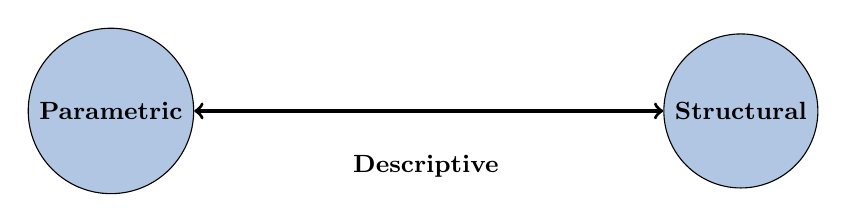
\begin{tikzpicture}[nodes={text depth=0.25ex,text height=1.25ex distance=1.7cm}]
                \tikzstyle{every node}=[font=\small]
                \tikzstyle{vertex} = [circle, draw=black, fill=illiniblue]
                \tikzstyle{hidden} = [draw=none]
                \tikzstyle{edge} = [<->, very thick]
                
                % \node[vertex](v1) at (0,5) {\textbf{Normative}};
                \node[vertex](v2) at (4,0) {\textbf{Structural}};
                \node[vertex](v3) at (-4,0) {\textbf{Parametric}};
    
                % \draw[edge] (v1) -- (v2);
                \draw[edge] (v2) -- (v3);

                \node[hidden](h4) at (4, -0.7) {};
    
                % % hidden nodes for v3
                \node[hidden](h5) at (-4, -0.7) {};
                % \node[hidden](h6) at (-4, 0.75) {};
    
                \draw[draw=none] (h4) -- (h5) node[anchor=mid, midway, sloped]{\textbf{Descriptive}};
    
    
        \end{tikzpicture}
        }
        % \caption{Parametric Uncertainty}
        % \label{fig:triarchic-uncertainty}
    \end{figure}

\end{frame}
\subsection{Prescriptive: Structural-Normative}
\begin{frame}
    \frametitle{Prescriptive: Structural-Normative}
    \begin{columns}
        \column[t]{6cm}
        
        Generating prescriptive conclusions is the primary reason to model energy systems.\\~\\

        If the solution to structural uncertainty was identifying alternative, ``sub-optimal'' 
        solutions, then the prescriptive stage means deciding among these diverse alternatives.

        \begin{theorem}[Arrow's Impossibility Theorem]
            It is impossible to construct a utility function that maps individual preferences 
            onto a global preference order without imposition or dictating \cite{kasprzyk_many_2013,
            franssen_arrows_2005,arrow_difficulty_1950}.
        \end{theorem}

        \column[t]{4cm}
        \begin{figure}
            \centering
            \resizebox{\columnwidth}{!}{
            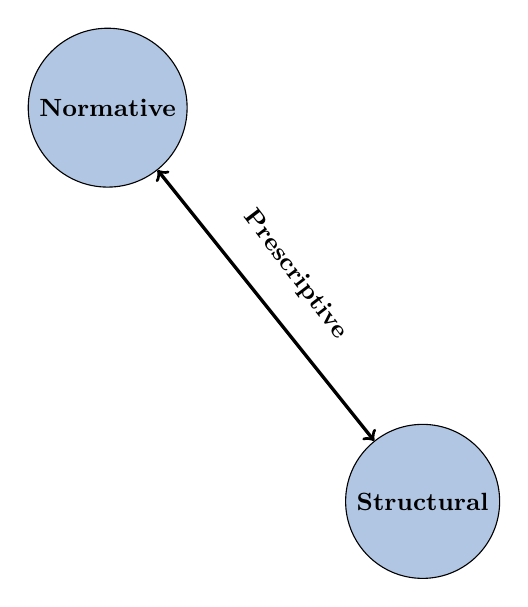
\begin{tikzpicture}[nodes={text depth=0.25ex,text height=1.25ex distance=1.7cm}]
                    \tikzstyle{every node}=[font=\small]
                    \tikzstyle{vertex} = [circle, draw=black, fill=illiniblue]
                    \tikzstyle{hidden} = [draw=none]
                    \tikzstyle{edge} = [<->, very thick]
                    
                    \node[vertex](v1) at (0,5) {\textbf{Normative}};
                    \node[vertex](v2) at (4,0) {\textbf{Structural}};

                    \draw[edge] (v1) -- (v2);

                    \node[hidden](h2) at (0.75, 5) {};
        
                    % % hidden nodes for v2
                    \node[hidden](h3) at (4, 0.75) {};

                    \draw[draw=none] (h2) -- (h3) node[anchor=mid, midway, sloped]{\textbf{Prescriptive}};
        
        
            \end{tikzpicture}
            }
            % \caption{Parametric Uncertainty}
            % \label{fig:triarchic-uncertainty}
        \end{figure}
        
    \end{columns}

\end{frame}


% \section{Technical Gap \#3}
% \begin{frame}
%     \frametitle{Gap \#3: Overcoming Arrow's Theorem}

%     \begin{enumerate}
%         \item Deciding among alternative solutions is challenging without a normative premise.
%         \item Without direct consultation of stakeholders, it's impossible know how they would understand tradeoffs.
%         \item Capturing the ``human dimension'' requires incorporating formal methods from social science: case studies,
%         interviews, focus groups, surveys, etc. The ESOM literature struggles to do this.
%     \end{enumerate}

% \end{frame}
\begin{frame}
    \frametitle{Gap 2: Normative Uncertainty \& Deliberative Processes}
    \begin{block}{Technical Gap}
        \begin{enumerate}
            \item Deciding among alternative solutions is challenging without a normative premise.
            \item Without direct consultation of stakeholders, it's impossible know how they would understand tradeoffs.
            \item Capturing the ``human dimension'' requires incorporating formal methods from social science: case studies,
            interviews, focus groups, surveys, etc. The ESOM literature struggles to do this \cite{pfenninger_energy_2014}.
        \end{enumerate}
    \end{block}
    \begin{block}{Proposed Work Component II: Integrative theory of uncertainties}
        Further develop the unifying theory of model development through the lens of 
        addressing triple uncertainties.
    \end{block}
    \begin{block}{Proposed Work Component III: Case study of Champaign-Urbana}
        Case study of energy planning processes in the Champaign-Urbana region to validate
        the usefulness of \texttt{Osier} and test the salience of various uncertainties in
        these planning processes.
    \end{block}
    
\end{frame}
\begin{frame}
    \frametitle{Proposal \#3: Finding a vision through interlocution}

    Overcoming Arrow's theorem through an iterative articulation of values and
    priorities involving the public as key deliberators.

    \begin{enumerate}
        \item Expand Osier to allow modelers to address normative uncertainty.
        \item Develop a deliberation procedure that incorporates osier.
        \item Case study in the Champaign-Urbana region to consider the
        normative uncertainties produced by having an unranked set of options.
    \end{enumerate}

\end{frame}

% \section{Conclusion}
% \begin{frame}
  \frametitle{Conclusion}
        We showed many things. This slide is an example of how 
        you can animate bulleted lists, for more information about
        using beamer animations, checkout the overleaf article on 
        overlay specifications in the group's guide.
        \begin{itemize}
                \item Cats are peculiar
                \pause
                \item Blue and Orange are fierce colors
                \pause
                \item Math can be rendered nicely
                \pause
                \item Cite your sources
        \end{itemize}

        % We also tested acronyms by writing \gls{esom}.
\end{frame}

\begin{frame}
  \frametitle{Acknowledgement}
        Acknowledgements should include both people who helped and funding 
        streams. If you are funded by an NEUP grant, that number usually goes 
        here. .
\end{frame}

%%--------------------------------%%
%%--------------------------------%%
\begin{frame}[allowframebreaks]
  \frametitle{References}
  \bibliographystyle{plain}
  {\footnotesize \bibliography{../docs/2023-dotson-prelim.bib} }

\end{frame}

%%--------------------------------%%


\end{document}



